%% 
%% Copyright 2019-2021 Elsevier Ltd
%% 
%% This file is part of the 'CAS Bundle'.
%% --------------------------------------
%% 
%% It may be distributed under the conditions of the LaTeX Project Public
%% License, either version 1.2 of this license or (at your option) any
%% later version.  The latest version of this license is in
%%    http://www.latex-project.org/lppl.txt
%% and version 1.2 or later is part of all distributions of LaTeX
%% version 1999/12/01 or later.
%% 
%% The list of all files belonging to the 'CAS Bundle' is
%% given in the file `manifest.txt'.
%% 
%% Template article for cas-dc documentclass for 
%% double column output.

\documentclass[fleqn]{cas-sc}

\usepackage{lipsum}
\usepackage{tikz}
\usetikzlibrary{shapes, snakes, calc}
\usepackage{longtable}

% If the frontmatter runs over more than one page
% use the longmktitle option.

%\documentclass[a4paper,fleqn,longmktitle]{cas-dc}

%\usepackage[numbers]{natbib}
%\usepackage[authoryear]{natbib}
\usepackage[authoryear,longnamesfirst]{natbib}

%%%Author macros
\def\tsc#1{\csdef{#1}{\textsc{\lowercase{#1}}\xspace}}
\tsc{WGM}
\tsc{QE}
%%%

% Uncomment and use as if needed
%\newtheorem{theorem}{Theorem}
%\newtheorem{lemma}[theorem]{Lemma}
%\newdefinition{rmk}{Remark}
%\newproof{pf}{Proof}
%\newproof{pot}{Proof of Theorem \ref{thm}}

\begin{document}
\let\WriteBookmarks\relax
\def\floatpagepagefraction{1}
\def\textpagefraction{.001}

% Short title
\shorttitle{Ambulance Dispatch}    

% Short author
%\shortauthors{Burkman, Jin, Abuhijleh, and Sun}  
\shortauthors{First, Second, Third, Fourth}  

% Main title of the paper
\title [mode = title]{Modeling the Need for an Ambulance based on Automated Crash Reports from Cell Phones}  

% Title footnote mark
% eg: \tnotemark[1]
%\tnotemark[<tnote number>] 
%\tnotemark[1] 

% Title footnote 1.
% eg: \tnotetext[1]{Title footnote text}
%\tnotetext[1]{Working Title} 

% First author
%
% Options: Use if required
% eg: \author[1,3]{Author Name}[type=editor,
%       style=chinese,
%       auid=000,
%       bioid=1,
%       prefix=Sir,
%       orcid=0000-0000-0000-0000,
%       facebook=<facebook id>,
%       twitter=<twitter id>,
%       linkedin=<linkedin id>,
%       gplus=<gplus id>]

%\author[<aff no>]{<author name>}[<options>]
%\author[1,2]{J. Bradford Burkman}[]
\author[1,2]{First Author}[]
% Footnote of the first author
%\fnmark[1]
% Corresponding author indication
%\cormark[1]
% Email id of the first author
%\ead{bradburkman@gmail.com}
\ead{FirstAuthor@gmail.com}
% URL of the first author
%\ead[url]{http://www.github.com/bburkman}

% Credit authorship
% eg: \credit{Conceptualization of this study, Methodology, Software}
% Options: conceptualization; data curation; formal analysis; funding acquisition; investigation; methodology; project administration; resources; software; supervision; validation; visualization; writing – original draft; and writing – review and editing.
\credit{Conceptualization, Investigation, Writing - original draft, Visualization}


%\author[1]{Miao Jin}[]
\author[1]{Second Author}[]
\credit{Supervision, Methodology, Writing - review and editing}

%\author[1,3]{Malek Abuhijleh}[]
\author[1,3]{Third Author}[]
\credit{Investigation, Methodology}

%\author[3]{Xiaoduan Sun}[]
\author[3]{Fourth Author}[]
\credit{Data curation, Writing - review and editing}






%\affiliation[1]{organization={School of Computing and Informatics, University of Louisiana at Lafayette},
\affiliation[1]{organization={School, University},
%            addressline={301 E. Lewis St}, 
%            city={Lafayette},
%          citysep={}, % Uncomment if no comma needed between city and postcode
%            state={LA},
%            postcode={70503}, 
%            country={USA}
            }

% Address/affiliation
%\affiliation[2]{organization={Louisiana School for Math, Science, and the Arts},
\affiliation[2]{organization={Other School},
%            addressline={715 University Pkwy}, 
%            city={Natchitoches},
%          citysep={}, % Uncomment if no comma needed between city and postcode
%            state={LA},
%            postcode={71457}, 
%            country={USA}
            }

%\affiliation[3]{organization={Department of Civil Engineering, University of Louisiana at Lafayette},
\affiliation[3]{organization={Other Department, University},
%            addressline={131 Rex St}, 
%            city={Lafayette},
%          citysep={}, % Uncomment if no comma needed between city and postcode
%            state={LA},
%            postcode={70504}, 
%            country={USA}
            }




% For a title note without a number/mark
%\nonumnote{}

% Here goes the abstract
\begin{abstract}
%%%%% Abstract
% I found an abstract in TRpC June 2022 with 365 words.
%Put abstract here.
%%%%% Abstract
% I found an abstract in TRpC June 2022 with 365 words.
New Google Pixel phones can automatically notify an emergency dispatcher if the phone detects the deceleration profile of a vehicular crash.  Most crash notifications come from an eyewitness who can say whether an ambulance is needed, but the automated notification from the cell phone cannot provide that information directly.  Should the dispatcher immediately send an ambulance before receiving an eyewitness report?  There are three options: Always, Wait, and Sometimes.  The ``Always'' option refers to sending an ambulance to every automatically reported crash, even though most of them will not be needed.  In the ``Wait'' option, the dispatcher sends police, but always waits for a call from an eyewitness (perhaps the police) before sending an ambulance.  In the ``Sometimes'' option, the dispatcher relies on a machine learning recommendation system to decide whether to immediately dispatch an ambulance, reserving the option to send one later based on an eyewitness report.

%This paper explores one option for building a machine learning (ML) model for making a recommendation in the ``Sometimes'' option.  The model gives the probability (based on the available information) that a crash requires an ambulance.  If the probability that an ambulance is needed is above some chosen threshold, the method will recommend dispatching an ambulance immediately; below that threshold, the dispatcher should wait to hear from an eyewitness. 


This paper explores one option for building a machine learning (ML) model for making a recommendation in the ``Sometimes'' option.    Our goal is to build a model that returns, for each feature vector (crash report, sample), a value $p \in [0,1]$ that increases with the probability that the person needs an ambulance.  Then we choose a threshold $\theta$ such that we immediately send ambulances to those automated crash reports with $p > \theta$, and wait for eyewitness confirmation for those reports with $p < \theta$. In an actual implementation, the choice of $\theta$ is political, not technical, so we consider and interpret several options.  

Once a threshold has been chosen, the costs of the false positives (FP) and false negatives (FN) in dispatching ambulances are very different.  The cost of sending an ambulance when one is not needed (FP) is measured in dollars, but the cost of not promptly sending an ambulance when one is needed (FN) is measured in lives.  Choosing the decision threshold $\theta$ is ethically problematic, but governments implicitly choose such a tradeoff when they set budgets for emergency services.  

We consider and interpret several options for the decision threshold $\theta$ based on the political consideration, ``How much will it cost?''  How many automated ambulance dispatches are we willing to fund (FP + TP) for each one of them that is actually needed (TP)?  We will explore two versions of that question, the total and the marginal.  


%some of which consider a relationship between the total number of FP and FN up to that value of $p$, and others consider the marginal relationship around that value of $p$.  Once the threshold criteria are chosen, the problem turns to choosing and tuning a model that best satisfies the tradeoff, saving both money and lives.  

%We consider the factors in determining the threshold.  The costs of the false positives (FP) and false negatives (FN) in dispatching ambulances are very different.  The cost of sending an ambulance when one is not needed (FP) is measured in dollars, but the cost of not promptly sending an ambulance when one is needed (FN) is measured in lives.  Choosing such a tradeoff threshold is ethically problematic, but governments implicitly make such a tradeoff when they set budgets for emergency and medical services.  To demonstrate the method in this paper, we have arbitrarily chosen a cutoff of 33\%, that there is a 1 in 3 chance that a dispatched ambulance would be needed (TP) and a 2 in 3 chance that it would not (FP).  We formulate our marginal ethical tradeoff rate as   $\omega = \Delta FP/\Delta TP = 2.0$.  We incorporated $\omega$ into the model in the class weight and in the decision threshold.  

We show that the quality of the model depends highly on the input data available, and we considered three levels of data availability.  The ``Easy'' level includes data the emergency dispatcher has before the notification, like time of day and weather.  The ``Medium'' level adds information about the location and information from the cell service provider about the user, like the age and sex.  The ``Hard'' level adds information that requires having access to records about the vehicle likely to be driven by the cell phone user and detailed and temporal information about the location, like lighting conditions and whether it is currently a work zone.  

We used the data of the Crash Report Sampling System (CRSS) to validate our approach.  We have applied new methods (for this dataset in the literature) to handle missing data, and we have investigated several methods for handling the data imbalance.  To promote discussion and future research, we have included all of the code we used in our analysis.  
%\vskip 1in

\end{abstract}

% Use if graphical abstract is present
%\begin{graphicalabstract}
%\includegraphics{}
%\end{graphicalabstract}

% Research highlights
\begin{highlights}
	\item  Supports transferability and benchmarking of different approaches on a public large-scale dataset.  We have attached the code we used to perform the analysis on data from the Crash Report Sampling System (CRSS).  
	\item Novel Application motivated by Emerging Technology:  Machine Learning Classification Models for Dispatching Ambulances based on Automated Crash Reports
	\item New Use of Dataset:  Used Crash Report Sampling System (CRSS), which has imputed missing values for some features, but not all of the ones we wanted to use.  For the first time we have seen, we used the software the CRSS authors use for multiple imputation (IVEware) to impute missing values in more features, then compared the results with other imputation methods.
	\item Explicit Incorporation of Imbalanced Costs
	\item Explicit Incorporation of Political Dimensions
	\item Consideration of Marginal Effects of Threshold Shifting
	\item Perennial Machine Learning Challenge:  Imbalanced Datasets
\end{highlights}

% Keywords
% Each keyword is seperated by \sep
\begin{keywords}
 \sep Automated crash notification 
 \sep Ambulance dispatch 
 \sep Emergency medical services  
 \sep Machine learning 
 \sep Imbalanced Cost 
 \sep Imbalanced Data 
 \sep Imputation
\end{keywords}

\maketitle

% Main text

%%%%%
%
% To Do
%
%
%%%%%

%%%%% Henry's Questions 23 May 2023
%\section{Henry's Questions 23 May 2023}
%\subsection{Abstract}

I made most of the changes you suggested for the abstract.  (Above)

I changed ``police'' to ``emergency dispatcher'' rather than ``911 dispatcher'' so as to not annoy the people (like the editor) in countries that use 119.  

I think the abstract is now too long, but that's a problem for later.  

\subsection{Threshold, Prior and Posterior Probabilities}

Thank you for your summary of the decision problem.  I will adapt the language here. I will try to answer your questions through an example.   Please let me know if I don't understand it well.  

\

I'm trying to understand the $\hat{p}$ you used.  I understand $p$ as the probability that a given sample is in Class 1.  Because you related $\hat{p}$ to $\pi_1$, I suspect what $\hat{p}$ means is the percentage of samples the model (with our choice of decision threshold) classifies as being in Class 1.  Is that correct?  In the big chart below, 

$$\hat{p} = \frac{FP + TP}{TN + FP + FN + TP}$$

\

Using the CRSS dataset, our problem has two outcomes.  

\begin{center}
\begin{tabular}{llll}
	Class 0 & ``No ambulance needed'' & $\pi_0 \approx 85\%$ \cr
	Class 1 & ``Ambulance needed'' & $\pi_1 \approx 15\%$ \cr
\end{tabular}
\end{center}

We will run several models, but a particular model gives, for each input vector (sample), a probability $p$ that the sample is in Class 1.  We want to pick a discrimination threshold (decision threshold) $\theta$ such that if for a particular crash notification $p > \theta$, then our recommendation system recommends that the emergency dispatcher send an ambulance.  

Below is the test results of one of our best models, the Balanced Random Forest Classifier with no class weights ($\alpha = 0.5$).  The histogram gives, for each range of $p$, the percent of the total dataset with Class 0 (Neg) and Class 1 in that range of $p$.  

Until we choose the discrimination threshold $\theta$, we can't have a confusion matrix.  Once we choose $\theta$, then all of the negative samples with $p< \theta$ are true negatives, and all of the negative samples with $p > \theta$ are false positives; conversely for the positive samples.  

\


\noindent\begin{tabular}{@{\hspace{-6pt}}p{4.5in} @{\hspace{-6pt}}p{2.0in}}
	\vskip 0pt
	\qquad \qquad Raw Model Output
	
	%% Creator: Matplotlib, PGF backend
%%
%% To include the figure in your LaTeX document, write
%%   \input{<filename>.pgf}
%%
%% Make sure the required packages are loaded in your preamble
%%   \usepackage{pgf}
%%
%% Also ensure that all the required font packages are loaded; for instance,
%% the lmodern package is sometimes necessary when using math font.
%%   \usepackage{lmodern}
%%
%% Figures using additional raster images can only be included by \input if
%% they are in the same directory as the main LaTeX file. For loading figures
%% from other directories you can use the `import` package
%%   \usepackage{import}
%%
%% and then include the figures with
%%   \import{<path to file>}{<filename>.pgf}
%%
%% Matplotlib used the following preamble
%%   
%%   \usepackage{fontspec}
%%   \makeatletter\@ifpackageloaded{underscore}{}{\usepackage[strings]{underscore}}\makeatother
%%
\begingroup%
\makeatletter%
\begin{pgfpicture}%
\pgfpathrectangle{\pgfpointorigin}{\pgfqpoint{4.509306in}{1.754444in}}%
\pgfusepath{use as bounding box, clip}%
\begin{pgfscope}%
\pgfsetbuttcap%
\pgfsetmiterjoin%
\definecolor{currentfill}{rgb}{1.000000,1.000000,1.000000}%
\pgfsetfillcolor{currentfill}%
\pgfsetlinewidth{0.000000pt}%
\definecolor{currentstroke}{rgb}{1.000000,1.000000,1.000000}%
\pgfsetstrokecolor{currentstroke}%
\pgfsetdash{}{0pt}%
\pgfpathmoveto{\pgfqpoint{0.000000in}{0.000000in}}%
\pgfpathlineto{\pgfqpoint{4.509306in}{0.000000in}}%
\pgfpathlineto{\pgfqpoint{4.509306in}{1.754444in}}%
\pgfpathlineto{\pgfqpoint{0.000000in}{1.754444in}}%
\pgfpathlineto{\pgfqpoint{0.000000in}{0.000000in}}%
\pgfpathclose%
\pgfusepath{fill}%
\end{pgfscope}%
\begin{pgfscope}%
\pgfsetbuttcap%
\pgfsetmiterjoin%
\definecolor{currentfill}{rgb}{1.000000,1.000000,1.000000}%
\pgfsetfillcolor{currentfill}%
\pgfsetlinewidth{0.000000pt}%
\definecolor{currentstroke}{rgb}{0.000000,0.000000,0.000000}%
\pgfsetstrokecolor{currentstroke}%
\pgfsetstrokeopacity{0.000000}%
\pgfsetdash{}{0pt}%
\pgfpathmoveto{\pgfqpoint{0.445556in}{0.499444in}}%
\pgfpathlineto{\pgfqpoint{4.320556in}{0.499444in}}%
\pgfpathlineto{\pgfqpoint{4.320556in}{1.654444in}}%
\pgfpathlineto{\pgfqpoint{0.445556in}{1.654444in}}%
\pgfpathlineto{\pgfqpoint{0.445556in}{0.499444in}}%
\pgfpathclose%
\pgfusepath{fill}%
\end{pgfscope}%
\begin{pgfscope}%
\pgfpathrectangle{\pgfqpoint{0.445556in}{0.499444in}}{\pgfqpoint{3.875000in}{1.155000in}}%
\pgfusepath{clip}%
\pgfsetbuttcap%
\pgfsetmiterjoin%
\pgfsetlinewidth{1.003750pt}%
\definecolor{currentstroke}{rgb}{0.000000,0.000000,0.000000}%
\pgfsetstrokecolor{currentstroke}%
\pgfsetdash{}{0pt}%
\pgfpathmoveto{\pgfqpoint{0.435556in}{0.499444in}}%
\pgfpathlineto{\pgfqpoint{0.483922in}{0.499444in}}%
\pgfpathlineto{\pgfqpoint{0.483922in}{0.618288in}}%
\pgfpathlineto{\pgfqpoint{0.435556in}{0.618288in}}%
\pgfusepath{stroke}%
\end{pgfscope}%
\begin{pgfscope}%
\pgfpathrectangle{\pgfqpoint{0.445556in}{0.499444in}}{\pgfqpoint{3.875000in}{1.155000in}}%
\pgfusepath{clip}%
\pgfsetbuttcap%
\pgfsetmiterjoin%
\pgfsetlinewidth{1.003750pt}%
\definecolor{currentstroke}{rgb}{0.000000,0.000000,0.000000}%
\pgfsetstrokecolor{currentstroke}%
\pgfsetdash{}{0pt}%
\pgfpathmoveto{\pgfqpoint{0.576001in}{0.499444in}}%
\pgfpathlineto{\pgfqpoint{0.637387in}{0.499444in}}%
\pgfpathlineto{\pgfqpoint{0.637387in}{0.801196in}}%
\pgfpathlineto{\pgfqpoint{0.576001in}{0.801196in}}%
\pgfpathlineto{\pgfqpoint{0.576001in}{0.499444in}}%
\pgfpathclose%
\pgfusepath{stroke}%
\end{pgfscope}%
\begin{pgfscope}%
\pgfpathrectangle{\pgfqpoint{0.445556in}{0.499444in}}{\pgfqpoint{3.875000in}{1.155000in}}%
\pgfusepath{clip}%
\pgfsetbuttcap%
\pgfsetmiterjoin%
\pgfsetlinewidth{1.003750pt}%
\definecolor{currentstroke}{rgb}{0.000000,0.000000,0.000000}%
\pgfsetstrokecolor{currentstroke}%
\pgfsetdash{}{0pt}%
\pgfpathmoveto{\pgfqpoint{0.729467in}{0.499444in}}%
\pgfpathlineto{\pgfqpoint{0.790853in}{0.499444in}}%
\pgfpathlineto{\pgfqpoint{0.790853in}{1.026194in}}%
\pgfpathlineto{\pgfqpoint{0.729467in}{1.026194in}}%
\pgfpathlineto{\pgfqpoint{0.729467in}{0.499444in}}%
\pgfpathclose%
\pgfusepath{stroke}%
\end{pgfscope}%
\begin{pgfscope}%
\pgfpathrectangle{\pgfqpoint{0.445556in}{0.499444in}}{\pgfqpoint{3.875000in}{1.155000in}}%
\pgfusepath{clip}%
\pgfsetbuttcap%
\pgfsetmiterjoin%
\pgfsetlinewidth{1.003750pt}%
\definecolor{currentstroke}{rgb}{0.000000,0.000000,0.000000}%
\pgfsetstrokecolor{currentstroke}%
\pgfsetdash{}{0pt}%
\pgfpathmoveto{\pgfqpoint{0.882932in}{0.499444in}}%
\pgfpathlineto{\pgfqpoint{0.944318in}{0.499444in}}%
\pgfpathlineto{\pgfqpoint{0.944318in}{1.203686in}}%
\pgfpathlineto{\pgfqpoint{0.882932in}{1.203686in}}%
\pgfpathlineto{\pgfqpoint{0.882932in}{0.499444in}}%
\pgfpathclose%
\pgfusepath{stroke}%
\end{pgfscope}%
\begin{pgfscope}%
\pgfpathrectangle{\pgfqpoint{0.445556in}{0.499444in}}{\pgfqpoint{3.875000in}{1.155000in}}%
\pgfusepath{clip}%
\pgfsetbuttcap%
\pgfsetmiterjoin%
\pgfsetlinewidth{1.003750pt}%
\definecolor{currentstroke}{rgb}{0.000000,0.000000,0.000000}%
\pgfsetstrokecolor{currentstroke}%
\pgfsetdash{}{0pt}%
\pgfpathmoveto{\pgfqpoint{1.036397in}{0.499444in}}%
\pgfpathlineto{\pgfqpoint{1.097783in}{0.499444in}}%
\pgfpathlineto{\pgfqpoint{1.097783in}{1.348758in}}%
\pgfpathlineto{\pgfqpoint{1.036397in}{1.348758in}}%
\pgfpathlineto{\pgfqpoint{1.036397in}{0.499444in}}%
\pgfpathclose%
\pgfusepath{stroke}%
\end{pgfscope}%
\begin{pgfscope}%
\pgfpathrectangle{\pgfqpoint{0.445556in}{0.499444in}}{\pgfqpoint{3.875000in}{1.155000in}}%
\pgfusepath{clip}%
\pgfsetbuttcap%
\pgfsetmiterjoin%
\pgfsetlinewidth{1.003750pt}%
\definecolor{currentstroke}{rgb}{0.000000,0.000000,0.000000}%
\pgfsetstrokecolor{currentstroke}%
\pgfsetdash{}{0pt}%
\pgfpathmoveto{\pgfqpoint{1.189863in}{0.499444in}}%
\pgfpathlineto{\pgfqpoint{1.251249in}{0.499444in}}%
\pgfpathlineto{\pgfqpoint{1.251249in}{1.455609in}}%
\pgfpathlineto{\pgfqpoint{1.189863in}{1.455609in}}%
\pgfpathlineto{\pgfqpoint{1.189863in}{0.499444in}}%
\pgfpathclose%
\pgfusepath{stroke}%
\end{pgfscope}%
\begin{pgfscope}%
\pgfpathrectangle{\pgfqpoint{0.445556in}{0.499444in}}{\pgfqpoint{3.875000in}{1.155000in}}%
\pgfusepath{clip}%
\pgfsetbuttcap%
\pgfsetmiterjoin%
\pgfsetlinewidth{1.003750pt}%
\definecolor{currentstroke}{rgb}{0.000000,0.000000,0.000000}%
\pgfsetstrokecolor{currentstroke}%
\pgfsetdash{}{0pt}%
\pgfpathmoveto{\pgfqpoint{1.343328in}{0.499444in}}%
\pgfpathlineto{\pgfqpoint{1.404714in}{0.499444in}}%
\pgfpathlineto{\pgfqpoint{1.404714in}{1.549075in}}%
\pgfpathlineto{\pgfqpoint{1.343328in}{1.549075in}}%
\pgfpathlineto{\pgfqpoint{1.343328in}{0.499444in}}%
\pgfpathclose%
\pgfusepath{stroke}%
\end{pgfscope}%
\begin{pgfscope}%
\pgfpathrectangle{\pgfqpoint{0.445556in}{0.499444in}}{\pgfqpoint{3.875000in}{1.155000in}}%
\pgfusepath{clip}%
\pgfsetbuttcap%
\pgfsetmiterjoin%
\pgfsetlinewidth{1.003750pt}%
\definecolor{currentstroke}{rgb}{0.000000,0.000000,0.000000}%
\pgfsetstrokecolor{currentstroke}%
\pgfsetdash{}{0pt}%
\pgfpathmoveto{\pgfqpoint{1.496793in}{0.499444in}}%
\pgfpathlineto{\pgfqpoint{1.558179in}{0.499444in}}%
\pgfpathlineto{\pgfqpoint{1.558179in}{1.599444in}}%
\pgfpathlineto{\pgfqpoint{1.496793in}{1.599444in}}%
\pgfpathlineto{\pgfqpoint{1.496793in}{0.499444in}}%
\pgfpathclose%
\pgfusepath{stroke}%
\end{pgfscope}%
\begin{pgfscope}%
\pgfpathrectangle{\pgfqpoint{0.445556in}{0.499444in}}{\pgfqpoint{3.875000in}{1.155000in}}%
\pgfusepath{clip}%
\pgfsetbuttcap%
\pgfsetmiterjoin%
\pgfsetlinewidth{1.003750pt}%
\definecolor{currentstroke}{rgb}{0.000000,0.000000,0.000000}%
\pgfsetstrokecolor{currentstroke}%
\pgfsetdash{}{0pt}%
\pgfpathmoveto{\pgfqpoint{1.650259in}{0.499444in}}%
\pgfpathlineto{\pgfqpoint{1.711645in}{0.499444in}}%
\pgfpathlineto{\pgfqpoint{1.711645in}{1.597742in}}%
\pgfpathlineto{\pgfqpoint{1.650259in}{1.597742in}}%
\pgfpathlineto{\pgfqpoint{1.650259in}{0.499444in}}%
\pgfpathclose%
\pgfusepath{stroke}%
\end{pgfscope}%
\begin{pgfscope}%
\pgfpathrectangle{\pgfqpoint{0.445556in}{0.499444in}}{\pgfqpoint{3.875000in}{1.155000in}}%
\pgfusepath{clip}%
\pgfsetbuttcap%
\pgfsetmiterjoin%
\pgfsetlinewidth{1.003750pt}%
\definecolor{currentstroke}{rgb}{0.000000,0.000000,0.000000}%
\pgfsetstrokecolor{currentstroke}%
\pgfsetdash{}{0pt}%
\pgfpathmoveto{\pgfqpoint{1.803724in}{0.499444in}}%
\pgfpathlineto{\pgfqpoint{1.865110in}{0.499444in}}%
\pgfpathlineto{\pgfqpoint{1.865110in}{1.571977in}}%
\pgfpathlineto{\pgfqpoint{1.803724in}{1.571977in}}%
\pgfpathlineto{\pgfqpoint{1.803724in}{0.499444in}}%
\pgfpathclose%
\pgfusepath{stroke}%
\end{pgfscope}%
\begin{pgfscope}%
\pgfpathrectangle{\pgfqpoint{0.445556in}{0.499444in}}{\pgfqpoint{3.875000in}{1.155000in}}%
\pgfusepath{clip}%
\pgfsetbuttcap%
\pgfsetmiterjoin%
\pgfsetlinewidth{1.003750pt}%
\definecolor{currentstroke}{rgb}{0.000000,0.000000,0.000000}%
\pgfsetstrokecolor{currentstroke}%
\pgfsetdash{}{0pt}%
\pgfpathmoveto{\pgfqpoint{1.957189in}{0.499444in}}%
\pgfpathlineto{\pgfqpoint{2.018575in}{0.499444in}}%
\pgfpathlineto{\pgfqpoint{2.018575in}{1.535535in}}%
\pgfpathlineto{\pgfqpoint{1.957189in}{1.535535in}}%
\pgfpathlineto{\pgfqpoint{1.957189in}{0.499444in}}%
\pgfpathclose%
\pgfusepath{stroke}%
\end{pgfscope}%
\begin{pgfscope}%
\pgfpathrectangle{\pgfqpoint{0.445556in}{0.499444in}}{\pgfqpoint{3.875000in}{1.155000in}}%
\pgfusepath{clip}%
\pgfsetbuttcap%
\pgfsetmiterjoin%
\pgfsetlinewidth{1.003750pt}%
\definecolor{currentstroke}{rgb}{0.000000,0.000000,0.000000}%
\pgfsetstrokecolor{currentstroke}%
\pgfsetdash{}{0pt}%
\pgfpathmoveto{\pgfqpoint{2.110655in}{0.499444in}}%
\pgfpathlineto{\pgfqpoint{2.172041in}{0.499444in}}%
\pgfpathlineto{\pgfqpoint{2.172041in}{1.450812in}}%
\pgfpathlineto{\pgfqpoint{2.110655in}{1.450812in}}%
\pgfpathlineto{\pgfqpoint{2.110655in}{0.499444in}}%
\pgfpathclose%
\pgfusepath{stroke}%
\end{pgfscope}%
\begin{pgfscope}%
\pgfpathrectangle{\pgfqpoint{0.445556in}{0.499444in}}{\pgfqpoint{3.875000in}{1.155000in}}%
\pgfusepath{clip}%
\pgfsetbuttcap%
\pgfsetmiterjoin%
\pgfsetlinewidth{1.003750pt}%
\definecolor{currentstroke}{rgb}{0.000000,0.000000,0.000000}%
\pgfsetstrokecolor{currentstroke}%
\pgfsetdash{}{0pt}%
\pgfpathmoveto{\pgfqpoint{2.264120in}{0.499444in}}%
\pgfpathlineto{\pgfqpoint{2.325506in}{0.499444in}}%
\pgfpathlineto{\pgfqpoint{2.325506in}{1.379398in}}%
\pgfpathlineto{\pgfqpoint{2.264120in}{1.379398in}}%
\pgfpathlineto{\pgfqpoint{2.264120in}{0.499444in}}%
\pgfpathclose%
\pgfusepath{stroke}%
\end{pgfscope}%
\begin{pgfscope}%
\pgfpathrectangle{\pgfqpoint{0.445556in}{0.499444in}}{\pgfqpoint{3.875000in}{1.155000in}}%
\pgfusepath{clip}%
\pgfsetbuttcap%
\pgfsetmiterjoin%
\pgfsetlinewidth{1.003750pt}%
\definecolor{currentstroke}{rgb}{0.000000,0.000000,0.000000}%
\pgfsetstrokecolor{currentstroke}%
\pgfsetdash{}{0pt}%
\pgfpathmoveto{\pgfqpoint{2.417585in}{0.499444in}}%
\pgfpathlineto{\pgfqpoint{2.478972in}{0.499444in}}%
\pgfpathlineto{\pgfqpoint{2.478972in}{1.248329in}}%
\pgfpathlineto{\pgfqpoint{2.417585in}{1.248329in}}%
\pgfpathlineto{\pgfqpoint{2.417585in}{0.499444in}}%
\pgfpathclose%
\pgfusepath{stroke}%
\end{pgfscope}%
\begin{pgfscope}%
\pgfpathrectangle{\pgfqpoint{0.445556in}{0.499444in}}{\pgfqpoint{3.875000in}{1.155000in}}%
\pgfusepath{clip}%
\pgfsetbuttcap%
\pgfsetmiterjoin%
\pgfsetlinewidth{1.003750pt}%
\definecolor{currentstroke}{rgb}{0.000000,0.000000,0.000000}%
\pgfsetstrokecolor{currentstroke}%
\pgfsetdash{}{0pt}%
\pgfpathmoveto{\pgfqpoint{2.571051in}{0.499444in}}%
\pgfpathlineto{\pgfqpoint{2.632437in}{0.499444in}}%
\pgfpathlineto{\pgfqpoint{2.632437in}{1.129640in}}%
\pgfpathlineto{\pgfqpoint{2.571051in}{1.129640in}}%
\pgfpathlineto{\pgfqpoint{2.571051in}{0.499444in}}%
\pgfpathclose%
\pgfusepath{stroke}%
\end{pgfscope}%
\begin{pgfscope}%
\pgfpathrectangle{\pgfqpoint{0.445556in}{0.499444in}}{\pgfqpoint{3.875000in}{1.155000in}}%
\pgfusepath{clip}%
\pgfsetbuttcap%
\pgfsetmiterjoin%
\pgfsetlinewidth{1.003750pt}%
\definecolor{currentstroke}{rgb}{0.000000,0.000000,0.000000}%
\pgfsetstrokecolor{currentstroke}%
\pgfsetdash{}{0pt}%
\pgfpathmoveto{\pgfqpoint{2.724516in}{0.499444in}}%
\pgfpathlineto{\pgfqpoint{2.785902in}{0.499444in}}%
\pgfpathlineto{\pgfqpoint{2.785902in}{1.011880in}}%
\pgfpathlineto{\pgfqpoint{2.724516in}{1.011880in}}%
\pgfpathlineto{\pgfqpoint{2.724516in}{0.499444in}}%
\pgfpathclose%
\pgfusepath{stroke}%
\end{pgfscope}%
\begin{pgfscope}%
\pgfpathrectangle{\pgfqpoint{0.445556in}{0.499444in}}{\pgfqpoint{3.875000in}{1.155000in}}%
\pgfusepath{clip}%
\pgfsetbuttcap%
\pgfsetmiterjoin%
\pgfsetlinewidth{1.003750pt}%
\definecolor{currentstroke}{rgb}{0.000000,0.000000,0.000000}%
\pgfsetstrokecolor{currentstroke}%
\pgfsetdash{}{0pt}%
\pgfpathmoveto{\pgfqpoint{2.877981in}{0.499444in}}%
\pgfpathlineto{\pgfqpoint{2.939368in}{0.499444in}}%
\pgfpathlineto{\pgfqpoint{2.939368in}{0.912921in}}%
\pgfpathlineto{\pgfqpoint{2.877981in}{0.912921in}}%
\pgfpathlineto{\pgfqpoint{2.877981in}{0.499444in}}%
\pgfpathclose%
\pgfusepath{stroke}%
\end{pgfscope}%
\begin{pgfscope}%
\pgfpathrectangle{\pgfqpoint{0.445556in}{0.499444in}}{\pgfqpoint{3.875000in}{1.155000in}}%
\pgfusepath{clip}%
\pgfsetbuttcap%
\pgfsetmiterjoin%
\pgfsetlinewidth{1.003750pt}%
\definecolor{currentstroke}{rgb}{0.000000,0.000000,0.000000}%
\pgfsetstrokecolor{currentstroke}%
\pgfsetdash{}{0pt}%
\pgfpathmoveto{\pgfqpoint{3.031447in}{0.499444in}}%
\pgfpathlineto{\pgfqpoint{3.092833in}{0.499444in}}%
\pgfpathlineto{\pgfqpoint{3.092833in}{0.805374in}}%
\pgfpathlineto{\pgfqpoint{3.031447in}{0.805374in}}%
\pgfpathlineto{\pgfqpoint{3.031447in}{0.499444in}}%
\pgfpathclose%
\pgfusepath{stroke}%
\end{pgfscope}%
\begin{pgfscope}%
\pgfpathrectangle{\pgfqpoint{0.445556in}{0.499444in}}{\pgfqpoint{3.875000in}{1.155000in}}%
\pgfusepath{clip}%
\pgfsetbuttcap%
\pgfsetmiterjoin%
\pgfsetlinewidth{1.003750pt}%
\definecolor{currentstroke}{rgb}{0.000000,0.000000,0.000000}%
\pgfsetstrokecolor{currentstroke}%
\pgfsetdash{}{0pt}%
\pgfpathmoveto{\pgfqpoint{3.184912in}{0.499444in}}%
\pgfpathlineto{\pgfqpoint{3.246298in}{0.499444in}}%
\pgfpathlineto{\pgfqpoint{3.246298in}{0.730710in}}%
\pgfpathlineto{\pgfqpoint{3.184912in}{0.730710in}}%
\pgfpathlineto{\pgfqpoint{3.184912in}{0.499444in}}%
\pgfpathclose%
\pgfusepath{stroke}%
\end{pgfscope}%
\begin{pgfscope}%
\pgfpathrectangle{\pgfqpoint{0.445556in}{0.499444in}}{\pgfqpoint{3.875000in}{1.155000in}}%
\pgfusepath{clip}%
\pgfsetbuttcap%
\pgfsetmiterjoin%
\pgfsetlinewidth{1.003750pt}%
\definecolor{currentstroke}{rgb}{0.000000,0.000000,0.000000}%
\pgfsetstrokecolor{currentstroke}%
\pgfsetdash{}{0pt}%
\pgfpathmoveto{\pgfqpoint{3.338377in}{0.499444in}}%
\pgfpathlineto{\pgfqpoint{3.399764in}{0.499444in}}%
\pgfpathlineto{\pgfqpoint{3.399764in}{0.672603in}}%
\pgfpathlineto{\pgfqpoint{3.338377in}{0.672603in}}%
\pgfpathlineto{\pgfqpoint{3.338377in}{0.499444in}}%
\pgfpathclose%
\pgfusepath{stroke}%
\end{pgfscope}%
\begin{pgfscope}%
\pgfpathrectangle{\pgfqpoint{0.445556in}{0.499444in}}{\pgfqpoint{3.875000in}{1.155000in}}%
\pgfusepath{clip}%
\pgfsetbuttcap%
\pgfsetmiterjoin%
\pgfsetlinewidth{1.003750pt}%
\definecolor{currentstroke}{rgb}{0.000000,0.000000,0.000000}%
\pgfsetstrokecolor{currentstroke}%
\pgfsetdash{}{0pt}%
\pgfpathmoveto{\pgfqpoint{3.491843in}{0.499444in}}%
\pgfpathlineto{\pgfqpoint{3.553229in}{0.499444in}}%
\pgfpathlineto{\pgfqpoint{3.553229in}{0.616663in}}%
\pgfpathlineto{\pgfqpoint{3.491843in}{0.616663in}}%
\pgfpathlineto{\pgfqpoint{3.491843in}{0.499444in}}%
\pgfpathclose%
\pgfusepath{stroke}%
\end{pgfscope}%
\begin{pgfscope}%
\pgfpathrectangle{\pgfqpoint{0.445556in}{0.499444in}}{\pgfqpoint{3.875000in}{1.155000in}}%
\pgfusepath{clip}%
\pgfsetbuttcap%
\pgfsetmiterjoin%
\pgfsetlinewidth{1.003750pt}%
\definecolor{currentstroke}{rgb}{0.000000,0.000000,0.000000}%
\pgfsetstrokecolor{currentstroke}%
\pgfsetdash{}{0pt}%
\pgfpathmoveto{\pgfqpoint{3.645308in}{0.499444in}}%
\pgfpathlineto{\pgfqpoint{3.706694in}{0.499444in}}%
\pgfpathlineto{\pgfqpoint{3.706694in}{0.574031in}}%
\pgfpathlineto{\pgfqpoint{3.645308in}{0.574031in}}%
\pgfpathlineto{\pgfqpoint{3.645308in}{0.499444in}}%
\pgfpathclose%
\pgfusepath{stroke}%
\end{pgfscope}%
\begin{pgfscope}%
\pgfpathrectangle{\pgfqpoint{0.445556in}{0.499444in}}{\pgfqpoint{3.875000in}{1.155000in}}%
\pgfusepath{clip}%
\pgfsetbuttcap%
\pgfsetmiterjoin%
\pgfsetlinewidth{1.003750pt}%
\definecolor{currentstroke}{rgb}{0.000000,0.000000,0.000000}%
\pgfsetstrokecolor{currentstroke}%
\pgfsetdash{}{0pt}%
\pgfpathmoveto{\pgfqpoint{3.798774in}{0.499444in}}%
\pgfpathlineto{\pgfqpoint{3.860160in}{0.499444in}}%
\pgfpathlineto{\pgfqpoint{3.860160in}{0.550587in}}%
\pgfpathlineto{\pgfqpoint{3.798774in}{0.550587in}}%
\pgfpathlineto{\pgfqpoint{3.798774in}{0.499444in}}%
\pgfpathclose%
\pgfusepath{stroke}%
\end{pgfscope}%
\begin{pgfscope}%
\pgfpathrectangle{\pgfqpoint{0.445556in}{0.499444in}}{\pgfqpoint{3.875000in}{1.155000in}}%
\pgfusepath{clip}%
\pgfsetbuttcap%
\pgfsetmiterjoin%
\pgfsetlinewidth{1.003750pt}%
\definecolor{currentstroke}{rgb}{0.000000,0.000000,0.000000}%
\pgfsetstrokecolor{currentstroke}%
\pgfsetdash{}{0pt}%
\pgfpathmoveto{\pgfqpoint{3.952239in}{0.499444in}}%
\pgfpathlineto{\pgfqpoint{4.013625in}{0.499444in}}%
\pgfpathlineto{\pgfqpoint{4.013625in}{0.526679in}}%
\pgfpathlineto{\pgfqpoint{3.952239in}{0.526679in}}%
\pgfpathlineto{\pgfqpoint{3.952239in}{0.499444in}}%
\pgfpathclose%
\pgfusepath{stroke}%
\end{pgfscope}%
\begin{pgfscope}%
\pgfpathrectangle{\pgfqpoint{0.445556in}{0.499444in}}{\pgfqpoint{3.875000in}{1.155000in}}%
\pgfusepath{clip}%
\pgfsetbuttcap%
\pgfsetmiterjoin%
\pgfsetlinewidth{1.003750pt}%
\definecolor{currentstroke}{rgb}{0.000000,0.000000,0.000000}%
\pgfsetstrokecolor{currentstroke}%
\pgfsetdash{}{0pt}%
\pgfpathmoveto{\pgfqpoint{4.105704in}{0.499444in}}%
\pgfpathlineto{\pgfqpoint{4.167090in}{0.499444in}}%
\pgfpathlineto{\pgfqpoint{4.167090in}{0.506640in}}%
\pgfpathlineto{\pgfqpoint{4.105704in}{0.506640in}}%
\pgfpathlineto{\pgfqpoint{4.105704in}{0.499444in}}%
\pgfpathclose%
\pgfusepath{stroke}%
\end{pgfscope}%
\begin{pgfscope}%
\pgfpathrectangle{\pgfqpoint{0.445556in}{0.499444in}}{\pgfqpoint{3.875000in}{1.155000in}}%
\pgfusepath{clip}%
\pgfsetbuttcap%
\pgfsetmiterjoin%
\definecolor{currentfill}{rgb}{0.000000,0.000000,0.000000}%
\pgfsetfillcolor{currentfill}%
\pgfsetlinewidth{0.000000pt}%
\definecolor{currentstroke}{rgb}{0.000000,0.000000,0.000000}%
\pgfsetstrokecolor{currentstroke}%
\pgfsetstrokeopacity{0.000000}%
\pgfsetdash{}{0pt}%
\pgfpathmoveto{\pgfqpoint{0.483922in}{0.499444in}}%
\pgfpathlineto{\pgfqpoint{0.545308in}{0.499444in}}%
\pgfpathlineto{\pgfqpoint{0.545308in}{0.500527in}}%
\pgfpathlineto{\pgfqpoint{0.483922in}{0.500527in}}%
\pgfpathlineto{\pgfqpoint{0.483922in}{0.499444in}}%
\pgfpathclose%
\pgfusepath{fill}%
\end{pgfscope}%
\begin{pgfscope}%
\pgfpathrectangle{\pgfqpoint{0.445556in}{0.499444in}}{\pgfqpoint{3.875000in}{1.155000in}}%
\pgfusepath{clip}%
\pgfsetbuttcap%
\pgfsetmiterjoin%
\definecolor{currentfill}{rgb}{0.000000,0.000000,0.000000}%
\pgfsetfillcolor{currentfill}%
\pgfsetlinewidth{0.000000pt}%
\definecolor{currentstroke}{rgb}{0.000000,0.000000,0.000000}%
\pgfsetstrokecolor{currentstroke}%
\pgfsetstrokeopacity{0.000000}%
\pgfsetdash{}{0pt}%
\pgfpathmoveto{\pgfqpoint{0.637387in}{0.499444in}}%
\pgfpathlineto{\pgfqpoint{0.698774in}{0.499444in}}%
\pgfpathlineto{\pgfqpoint{0.698774in}{0.502230in}}%
\pgfpathlineto{\pgfqpoint{0.637387in}{0.502230in}}%
\pgfpathlineto{\pgfqpoint{0.637387in}{0.499444in}}%
\pgfpathclose%
\pgfusepath{fill}%
\end{pgfscope}%
\begin{pgfscope}%
\pgfpathrectangle{\pgfqpoint{0.445556in}{0.499444in}}{\pgfqpoint{3.875000in}{1.155000in}}%
\pgfusepath{clip}%
\pgfsetbuttcap%
\pgfsetmiterjoin%
\definecolor{currentfill}{rgb}{0.000000,0.000000,0.000000}%
\pgfsetfillcolor{currentfill}%
\pgfsetlinewidth{0.000000pt}%
\definecolor{currentstroke}{rgb}{0.000000,0.000000,0.000000}%
\pgfsetstrokecolor{currentstroke}%
\pgfsetstrokeopacity{0.000000}%
\pgfsetdash{}{0pt}%
\pgfpathmoveto{\pgfqpoint{0.790853in}{0.499444in}}%
\pgfpathlineto{\pgfqpoint{0.852239in}{0.499444in}}%
\pgfpathlineto{\pgfqpoint{0.852239in}{0.506330in}}%
\pgfpathlineto{\pgfqpoint{0.790853in}{0.506330in}}%
\pgfpathlineto{\pgfqpoint{0.790853in}{0.499444in}}%
\pgfpathclose%
\pgfusepath{fill}%
\end{pgfscope}%
\begin{pgfscope}%
\pgfpathrectangle{\pgfqpoint{0.445556in}{0.499444in}}{\pgfqpoint{3.875000in}{1.155000in}}%
\pgfusepath{clip}%
\pgfsetbuttcap%
\pgfsetmiterjoin%
\definecolor{currentfill}{rgb}{0.000000,0.000000,0.000000}%
\pgfsetfillcolor{currentfill}%
\pgfsetlinewidth{0.000000pt}%
\definecolor{currentstroke}{rgb}{0.000000,0.000000,0.000000}%
\pgfsetstrokecolor{currentstroke}%
\pgfsetstrokeopacity{0.000000}%
\pgfsetdash{}{0pt}%
\pgfpathmoveto{\pgfqpoint{0.944318in}{0.499444in}}%
\pgfpathlineto{\pgfqpoint{1.005704in}{0.499444in}}%
\pgfpathlineto{\pgfqpoint{1.005704in}{0.514068in}}%
\pgfpathlineto{\pgfqpoint{0.944318in}{0.514068in}}%
\pgfpathlineto{\pgfqpoint{0.944318in}{0.499444in}}%
\pgfpathclose%
\pgfusepath{fill}%
\end{pgfscope}%
\begin{pgfscope}%
\pgfpathrectangle{\pgfqpoint{0.445556in}{0.499444in}}{\pgfqpoint{3.875000in}{1.155000in}}%
\pgfusepath{clip}%
\pgfsetbuttcap%
\pgfsetmiterjoin%
\definecolor{currentfill}{rgb}{0.000000,0.000000,0.000000}%
\pgfsetfillcolor{currentfill}%
\pgfsetlinewidth{0.000000pt}%
\definecolor{currentstroke}{rgb}{0.000000,0.000000,0.000000}%
\pgfsetstrokecolor{currentstroke}%
\pgfsetstrokeopacity{0.000000}%
\pgfsetdash{}{0pt}%
\pgfpathmoveto{\pgfqpoint{1.097783in}{0.499444in}}%
\pgfpathlineto{\pgfqpoint{1.159170in}{0.499444in}}%
\pgfpathlineto{\pgfqpoint{1.159170in}{0.524977in}}%
\pgfpathlineto{\pgfqpoint{1.097783in}{0.524977in}}%
\pgfpathlineto{\pgfqpoint{1.097783in}{0.499444in}}%
\pgfpathclose%
\pgfusepath{fill}%
\end{pgfscope}%
\begin{pgfscope}%
\pgfpathrectangle{\pgfqpoint{0.445556in}{0.499444in}}{\pgfqpoint{3.875000in}{1.155000in}}%
\pgfusepath{clip}%
\pgfsetbuttcap%
\pgfsetmiterjoin%
\definecolor{currentfill}{rgb}{0.000000,0.000000,0.000000}%
\pgfsetfillcolor{currentfill}%
\pgfsetlinewidth{0.000000pt}%
\definecolor{currentstroke}{rgb}{0.000000,0.000000,0.000000}%
\pgfsetstrokecolor{currentstroke}%
\pgfsetstrokeopacity{0.000000}%
\pgfsetdash{}{0pt}%
\pgfpathmoveto{\pgfqpoint{1.251249in}{0.499444in}}%
\pgfpathlineto{\pgfqpoint{1.312635in}{0.499444in}}%
\pgfpathlineto{\pgfqpoint{1.312635in}{0.535267in}}%
\pgfpathlineto{\pgfqpoint{1.251249in}{0.535267in}}%
\pgfpathlineto{\pgfqpoint{1.251249in}{0.499444in}}%
\pgfpathclose%
\pgfusepath{fill}%
\end{pgfscope}%
\begin{pgfscope}%
\pgfpathrectangle{\pgfqpoint{0.445556in}{0.499444in}}{\pgfqpoint{3.875000in}{1.155000in}}%
\pgfusepath{clip}%
\pgfsetbuttcap%
\pgfsetmiterjoin%
\definecolor{currentfill}{rgb}{0.000000,0.000000,0.000000}%
\pgfsetfillcolor{currentfill}%
\pgfsetlinewidth{0.000000pt}%
\definecolor{currentstroke}{rgb}{0.000000,0.000000,0.000000}%
\pgfsetstrokecolor{currentstroke}%
\pgfsetstrokeopacity{0.000000}%
\pgfsetdash{}{0pt}%
\pgfpathmoveto{\pgfqpoint{1.404714in}{0.499444in}}%
\pgfpathlineto{\pgfqpoint{1.466100in}{0.499444in}}%
\pgfpathlineto{\pgfqpoint{1.466100in}{0.549659in}}%
\pgfpathlineto{\pgfqpoint{1.404714in}{0.549659in}}%
\pgfpathlineto{\pgfqpoint{1.404714in}{0.499444in}}%
\pgfpathclose%
\pgfusepath{fill}%
\end{pgfscope}%
\begin{pgfscope}%
\pgfpathrectangle{\pgfqpoint{0.445556in}{0.499444in}}{\pgfqpoint{3.875000in}{1.155000in}}%
\pgfusepath{clip}%
\pgfsetbuttcap%
\pgfsetmiterjoin%
\definecolor{currentfill}{rgb}{0.000000,0.000000,0.000000}%
\pgfsetfillcolor{currentfill}%
\pgfsetlinewidth{0.000000pt}%
\definecolor{currentstroke}{rgb}{0.000000,0.000000,0.000000}%
\pgfsetstrokecolor{currentstroke}%
\pgfsetstrokeopacity{0.000000}%
\pgfsetdash{}{0pt}%
\pgfpathmoveto{\pgfqpoint{1.558179in}{0.499444in}}%
\pgfpathlineto{\pgfqpoint{1.619566in}{0.499444in}}%
\pgfpathlineto{\pgfqpoint{1.619566in}{0.568228in}}%
\pgfpathlineto{\pgfqpoint{1.558179in}{0.568228in}}%
\pgfpathlineto{\pgfqpoint{1.558179in}{0.499444in}}%
\pgfpathclose%
\pgfusepath{fill}%
\end{pgfscope}%
\begin{pgfscope}%
\pgfpathrectangle{\pgfqpoint{0.445556in}{0.499444in}}{\pgfqpoint{3.875000in}{1.155000in}}%
\pgfusepath{clip}%
\pgfsetbuttcap%
\pgfsetmiterjoin%
\definecolor{currentfill}{rgb}{0.000000,0.000000,0.000000}%
\pgfsetfillcolor{currentfill}%
\pgfsetlinewidth{0.000000pt}%
\definecolor{currentstroke}{rgb}{0.000000,0.000000,0.000000}%
\pgfsetstrokecolor{currentstroke}%
\pgfsetstrokeopacity{0.000000}%
\pgfsetdash{}{0pt}%
\pgfpathmoveto{\pgfqpoint{1.711645in}{0.499444in}}%
\pgfpathlineto{\pgfqpoint{1.773031in}{0.499444in}}%
\pgfpathlineto{\pgfqpoint{1.773031in}{0.590743in}}%
\pgfpathlineto{\pgfqpoint{1.711645in}{0.590743in}}%
\pgfpathlineto{\pgfqpoint{1.711645in}{0.499444in}}%
\pgfpathclose%
\pgfusepath{fill}%
\end{pgfscope}%
\begin{pgfscope}%
\pgfpathrectangle{\pgfqpoint{0.445556in}{0.499444in}}{\pgfqpoint{3.875000in}{1.155000in}}%
\pgfusepath{clip}%
\pgfsetbuttcap%
\pgfsetmiterjoin%
\definecolor{currentfill}{rgb}{0.000000,0.000000,0.000000}%
\pgfsetfillcolor{currentfill}%
\pgfsetlinewidth{0.000000pt}%
\definecolor{currentstroke}{rgb}{0.000000,0.000000,0.000000}%
\pgfsetstrokecolor{currentstroke}%
\pgfsetstrokeopacity{0.000000}%
\pgfsetdash{}{0pt}%
\pgfpathmoveto{\pgfqpoint{1.865110in}{0.499444in}}%
\pgfpathlineto{\pgfqpoint{1.926496in}{0.499444in}}%
\pgfpathlineto{\pgfqpoint{1.926496in}{0.605521in}}%
\pgfpathlineto{\pgfqpoint{1.865110in}{0.605521in}}%
\pgfpathlineto{\pgfqpoint{1.865110in}{0.499444in}}%
\pgfpathclose%
\pgfusepath{fill}%
\end{pgfscope}%
\begin{pgfscope}%
\pgfpathrectangle{\pgfqpoint{0.445556in}{0.499444in}}{\pgfqpoint{3.875000in}{1.155000in}}%
\pgfusepath{clip}%
\pgfsetbuttcap%
\pgfsetmiterjoin%
\definecolor{currentfill}{rgb}{0.000000,0.000000,0.000000}%
\pgfsetfillcolor{currentfill}%
\pgfsetlinewidth{0.000000pt}%
\definecolor{currentstroke}{rgb}{0.000000,0.000000,0.000000}%
\pgfsetstrokecolor{currentstroke}%
\pgfsetstrokeopacity{0.000000}%
\pgfsetdash{}{0pt}%
\pgfpathmoveto{\pgfqpoint{2.018575in}{0.499444in}}%
\pgfpathlineto{\pgfqpoint{2.079962in}{0.499444in}}%
\pgfpathlineto{\pgfqpoint{2.079962in}{0.624632in}}%
\pgfpathlineto{\pgfqpoint{2.018575in}{0.624632in}}%
\pgfpathlineto{\pgfqpoint{2.018575in}{0.499444in}}%
\pgfpathclose%
\pgfusepath{fill}%
\end{pgfscope}%
\begin{pgfscope}%
\pgfpathrectangle{\pgfqpoint{0.445556in}{0.499444in}}{\pgfqpoint{3.875000in}{1.155000in}}%
\pgfusepath{clip}%
\pgfsetbuttcap%
\pgfsetmiterjoin%
\definecolor{currentfill}{rgb}{0.000000,0.000000,0.000000}%
\pgfsetfillcolor{currentfill}%
\pgfsetlinewidth{0.000000pt}%
\definecolor{currentstroke}{rgb}{0.000000,0.000000,0.000000}%
\pgfsetstrokecolor{currentstroke}%
\pgfsetstrokeopacity{0.000000}%
\pgfsetdash{}{0pt}%
\pgfpathmoveto{\pgfqpoint{2.172041in}{0.499444in}}%
\pgfpathlineto{\pgfqpoint{2.233427in}{0.499444in}}%
\pgfpathlineto{\pgfqpoint{2.233427in}{0.643356in}}%
\pgfpathlineto{\pgfqpoint{2.172041in}{0.643356in}}%
\pgfpathlineto{\pgfqpoint{2.172041in}{0.499444in}}%
\pgfpathclose%
\pgfusepath{fill}%
\end{pgfscope}%
\begin{pgfscope}%
\pgfpathrectangle{\pgfqpoint{0.445556in}{0.499444in}}{\pgfqpoint{3.875000in}{1.155000in}}%
\pgfusepath{clip}%
\pgfsetbuttcap%
\pgfsetmiterjoin%
\definecolor{currentfill}{rgb}{0.000000,0.000000,0.000000}%
\pgfsetfillcolor{currentfill}%
\pgfsetlinewidth{0.000000pt}%
\definecolor{currentstroke}{rgb}{0.000000,0.000000,0.000000}%
\pgfsetstrokecolor{currentstroke}%
\pgfsetstrokeopacity{0.000000}%
\pgfsetdash{}{0pt}%
\pgfpathmoveto{\pgfqpoint{2.325506in}{0.499444in}}%
\pgfpathlineto{\pgfqpoint{2.386892in}{0.499444in}}%
\pgfpathlineto{\pgfqpoint{2.386892in}{0.662622in}}%
\pgfpathlineto{\pgfqpoint{2.325506in}{0.662622in}}%
\pgfpathlineto{\pgfqpoint{2.325506in}{0.499444in}}%
\pgfpathclose%
\pgfusepath{fill}%
\end{pgfscope}%
\begin{pgfscope}%
\pgfpathrectangle{\pgfqpoint{0.445556in}{0.499444in}}{\pgfqpoint{3.875000in}{1.155000in}}%
\pgfusepath{clip}%
\pgfsetbuttcap%
\pgfsetmiterjoin%
\definecolor{currentfill}{rgb}{0.000000,0.000000,0.000000}%
\pgfsetfillcolor{currentfill}%
\pgfsetlinewidth{0.000000pt}%
\definecolor{currentstroke}{rgb}{0.000000,0.000000,0.000000}%
\pgfsetstrokecolor{currentstroke}%
\pgfsetstrokeopacity{0.000000}%
\pgfsetdash{}{0pt}%
\pgfpathmoveto{\pgfqpoint{2.478972in}{0.499444in}}%
\pgfpathlineto{\pgfqpoint{2.540358in}{0.499444in}}%
\pgfpathlineto{\pgfqpoint{2.540358in}{0.672216in}}%
\pgfpathlineto{\pgfqpoint{2.478972in}{0.672216in}}%
\pgfpathlineto{\pgfqpoint{2.478972in}{0.499444in}}%
\pgfpathclose%
\pgfusepath{fill}%
\end{pgfscope}%
\begin{pgfscope}%
\pgfpathrectangle{\pgfqpoint{0.445556in}{0.499444in}}{\pgfqpoint{3.875000in}{1.155000in}}%
\pgfusepath{clip}%
\pgfsetbuttcap%
\pgfsetmiterjoin%
\definecolor{currentfill}{rgb}{0.000000,0.000000,0.000000}%
\pgfsetfillcolor{currentfill}%
\pgfsetlinewidth{0.000000pt}%
\definecolor{currentstroke}{rgb}{0.000000,0.000000,0.000000}%
\pgfsetstrokecolor{currentstroke}%
\pgfsetstrokeopacity{0.000000}%
\pgfsetdash{}{0pt}%
\pgfpathmoveto{\pgfqpoint{2.632437in}{0.499444in}}%
\pgfpathlineto{\pgfqpoint{2.693823in}{0.499444in}}%
\pgfpathlineto{\pgfqpoint{2.693823in}{0.684286in}}%
\pgfpathlineto{\pgfqpoint{2.632437in}{0.684286in}}%
\pgfpathlineto{\pgfqpoint{2.632437in}{0.499444in}}%
\pgfpathclose%
\pgfusepath{fill}%
\end{pgfscope}%
\begin{pgfscope}%
\pgfpathrectangle{\pgfqpoint{0.445556in}{0.499444in}}{\pgfqpoint{3.875000in}{1.155000in}}%
\pgfusepath{clip}%
\pgfsetbuttcap%
\pgfsetmiterjoin%
\definecolor{currentfill}{rgb}{0.000000,0.000000,0.000000}%
\pgfsetfillcolor{currentfill}%
\pgfsetlinewidth{0.000000pt}%
\definecolor{currentstroke}{rgb}{0.000000,0.000000,0.000000}%
\pgfsetstrokecolor{currentstroke}%
\pgfsetstrokeopacity{0.000000}%
\pgfsetdash{}{0pt}%
\pgfpathmoveto{\pgfqpoint{2.785902in}{0.499444in}}%
\pgfpathlineto{\pgfqpoint{2.847288in}{0.499444in}}%
\pgfpathlineto{\pgfqpoint{2.847288in}{0.686607in}}%
\pgfpathlineto{\pgfqpoint{2.785902in}{0.686607in}}%
\pgfpathlineto{\pgfqpoint{2.785902in}{0.499444in}}%
\pgfpathclose%
\pgfusepath{fill}%
\end{pgfscope}%
\begin{pgfscope}%
\pgfpathrectangle{\pgfqpoint{0.445556in}{0.499444in}}{\pgfqpoint{3.875000in}{1.155000in}}%
\pgfusepath{clip}%
\pgfsetbuttcap%
\pgfsetmiterjoin%
\definecolor{currentfill}{rgb}{0.000000,0.000000,0.000000}%
\pgfsetfillcolor{currentfill}%
\pgfsetlinewidth{0.000000pt}%
\definecolor{currentstroke}{rgb}{0.000000,0.000000,0.000000}%
\pgfsetstrokecolor{currentstroke}%
\pgfsetstrokeopacity{0.000000}%
\pgfsetdash{}{0pt}%
\pgfpathmoveto{\pgfqpoint{2.939368in}{0.499444in}}%
\pgfpathlineto{\pgfqpoint{3.000754in}{0.499444in}}%
\pgfpathlineto{\pgfqpoint{3.000754in}{0.682816in}}%
\pgfpathlineto{\pgfqpoint{2.939368in}{0.682816in}}%
\pgfpathlineto{\pgfqpoint{2.939368in}{0.499444in}}%
\pgfpathclose%
\pgfusepath{fill}%
\end{pgfscope}%
\begin{pgfscope}%
\pgfpathrectangle{\pgfqpoint{0.445556in}{0.499444in}}{\pgfqpoint{3.875000in}{1.155000in}}%
\pgfusepath{clip}%
\pgfsetbuttcap%
\pgfsetmiterjoin%
\definecolor{currentfill}{rgb}{0.000000,0.000000,0.000000}%
\pgfsetfillcolor{currentfill}%
\pgfsetlinewidth{0.000000pt}%
\definecolor{currentstroke}{rgb}{0.000000,0.000000,0.000000}%
\pgfsetstrokecolor{currentstroke}%
\pgfsetstrokeopacity{0.000000}%
\pgfsetdash{}{0pt}%
\pgfpathmoveto{\pgfqpoint{3.092833in}{0.499444in}}%
\pgfpathlineto{\pgfqpoint{3.154219in}{0.499444in}}%
\pgfpathlineto{\pgfqpoint{3.154219in}{0.681037in}}%
\pgfpathlineto{\pgfqpoint{3.092833in}{0.681037in}}%
\pgfpathlineto{\pgfqpoint{3.092833in}{0.499444in}}%
\pgfpathclose%
\pgfusepath{fill}%
\end{pgfscope}%
\begin{pgfscope}%
\pgfpathrectangle{\pgfqpoint{0.445556in}{0.499444in}}{\pgfqpoint{3.875000in}{1.155000in}}%
\pgfusepath{clip}%
\pgfsetbuttcap%
\pgfsetmiterjoin%
\definecolor{currentfill}{rgb}{0.000000,0.000000,0.000000}%
\pgfsetfillcolor{currentfill}%
\pgfsetlinewidth{0.000000pt}%
\definecolor{currentstroke}{rgb}{0.000000,0.000000,0.000000}%
\pgfsetstrokecolor{currentstroke}%
\pgfsetstrokeopacity{0.000000}%
\pgfsetdash{}{0pt}%
\pgfpathmoveto{\pgfqpoint{3.246298in}{0.499444in}}%
\pgfpathlineto{\pgfqpoint{3.307684in}{0.499444in}}%
\pgfpathlineto{\pgfqpoint{3.307684in}{0.677787in}}%
\pgfpathlineto{\pgfqpoint{3.246298in}{0.677787in}}%
\pgfpathlineto{\pgfqpoint{3.246298in}{0.499444in}}%
\pgfpathclose%
\pgfusepath{fill}%
\end{pgfscope}%
\begin{pgfscope}%
\pgfpathrectangle{\pgfqpoint{0.445556in}{0.499444in}}{\pgfqpoint{3.875000in}{1.155000in}}%
\pgfusepath{clip}%
\pgfsetbuttcap%
\pgfsetmiterjoin%
\definecolor{currentfill}{rgb}{0.000000,0.000000,0.000000}%
\pgfsetfillcolor{currentfill}%
\pgfsetlinewidth{0.000000pt}%
\definecolor{currentstroke}{rgb}{0.000000,0.000000,0.000000}%
\pgfsetstrokecolor{currentstroke}%
\pgfsetstrokeopacity{0.000000}%
\pgfsetdash{}{0pt}%
\pgfpathmoveto{\pgfqpoint{3.399764in}{0.499444in}}%
\pgfpathlineto{\pgfqpoint{3.461150in}{0.499444in}}%
\pgfpathlineto{\pgfqpoint{3.461150in}{0.659527in}}%
\pgfpathlineto{\pgfqpoint{3.399764in}{0.659527in}}%
\pgfpathlineto{\pgfqpoint{3.399764in}{0.499444in}}%
\pgfpathclose%
\pgfusepath{fill}%
\end{pgfscope}%
\begin{pgfscope}%
\pgfpathrectangle{\pgfqpoint{0.445556in}{0.499444in}}{\pgfqpoint{3.875000in}{1.155000in}}%
\pgfusepath{clip}%
\pgfsetbuttcap%
\pgfsetmiterjoin%
\definecolor{currentfill}{rgb}{0.000000,0.000000,0.000000}%
\pgfsetfillcolor{currentfill}%
\pgfsetlinewidth{0.000000pt}%
\definecolor{currentstroke}{rgb}{0.000000,0.000000,0.000000}%
\pgfsetstrokecolor{currentstroke}%
\pgfsetstrokeopacity{0.000000}%
\pgfsetdash{}{0pt}%
\pgfpathmoveto{\pgfqpoint{3.553229in}{0.499444in}}%
\pgfpathlineto{\pgfqpoint{3.614615in}{0.499444in}}%
\pgfpathlineto{\pgfqpoint{3.614615in}{0.657206in}}%
\pgfpathlineto{\pgfqpoint{3.553229in}{0.657206in}}%
\pgfpathlineto{\pgfqpoint{3.553229in}{0.499444in}}%
\pgfpathclose%
\pgfusepath{fill}%
\end{pgfscope}%
\begin{pgfscope}%
\pgfpathrectangle{\pgfqpoint{0.445556in}{0.499444in}}{\pgfqpoint{3.875000in}{1.155000in}}%
\pgfusepath{clip}%
\pgfsetbuttcap%
\pgfsetmiterjoin%
\definecolor{currentfill}{rgb}{0.000000,0.000000,0.000000}%
\pgfsetfillcolor{currentfill}%
\pgfsetlinewidth{0.000000pt}%
\definecolor{currentstroke}{rgb}{0.000000,0.000000,0.000000}%
\pgfsetstrokecolor{currentstroke}%
\pgfsetstrokeopacity{0.000000}%
\pgfsetdash{}{0pt}%
\pgfpathmoveto{\pgfqpoint{3.706694in}{0.499444in}}%
\pgfpathlineto{\pgfqpoint{3.768080in}{0.499444in}}%
\pgfpathlineto{\pgfqpoint{3.768080in}{0.639333in}}%
\pgfpathlineto{\pgfqpoint{3.706694in}{0.639333in}}%
\pgfpathlineto{\pgfqpoint{3.706694in}{0.499444in}}%
\pgfpathclose%
\pgfusepath{fill}%
\end{pgfscope}%
\begin{pgfscope}%
\pgfpathrectangle{\pgfqpoint{0.445556in}{0.499444in}}{\pgfqpoint{3.875000in}{1.155000in}}%
\pgfusepath{clip}%
\pgfsetbuttcap%
\pgfsetmiterjoin%
\definecolor{currentfill}{rgb}{0.000000,0.000000,0.000000}%
\pgfsetfillcolor{currentfill}%
\pgfsetlinewidth{0.000000pt}%
\definecolor{currentstroke}{rgb}{0.000000,0.000000,0.000000}%
\pgfsetstrokecolor{currentstroke}%
\pgfsetstrokeopacity{0.000000}%
\pgfsetdash{}{0pt}%
\pgfpathmoveto{\pgfqpoint{3.860160in}{0.499444in}}%
\pgfpathlineto{\pgfqpoint{3.921546in}{0.499444in}}%
\pgfpathlineto{\pgfqpoint{3.921546in}{0.623626in}}%
\pgfpathlineto{\pgfqpoint{3.860160in}{0.623626in}}%
\pgfpathlineto{\pgfqpoint{3.860160in}{0.499444in}}%
\pgfpathclose%
\pgfusepath{fill}%
\end{pgfscope}%
\begin{pgfscope}%
\pgfpathrectangle{\pgfqpoint{0.445556in}{0.499444in}}{\pgfqpoint{3.875000in}{1.155000in}}%
\pgfusepath{clip}%
\pgfsetbuttcap%
\pgfsetmiterjoin%
\definecolor{currentfill}{rgb}{0.000000,0.000000,0.000000}%
\pgfsetfillcolor{currentfill}%
\pgfsetlinewidth{0.000000pt}%
\definecolor{currentstroke}{rgb}{0.000000,0.000000,0.000000}%
\pgfsetstrokecolor{currentstroke}%
\pgfsetstrokeopacity{0.000000}%
\pgfsetdash{}{0pt}%
\pgfpathmoveto{\pgfqpoint{4.013625in}{0.499444in}}%
\pgfpathlineto{\pgfqpoint{4.075011in}{0.499444in}}%
\pgfpathlineto{\pgfqpoint{4.075011in}{0.580840in}}%
\pgfpathlineto{\pgfqpoint{4.013625in}{0.580840in}}%
\pgfpathlineto{\pgfqpoint{4.013625in}{0.499444in}}%
\pgfpathclose%
\pgfusepath{fill}%
\end{pgfscope}%
\begin{pgfscope}%
\pgfpathrectangle{\pgfqpoint{0.445556in}{0.499444in}}{\pgfqpoint{3.875000in}{1.155000in}}%
\pgfusepath{clip}%
\pgfsetbuttcap%
\pgfsetmiterjoin%
\definecolor{currentfill}{rgb}{0.000000,0.000000,0.000000}%
\pgfsetfillcolor{currentfill}%
\pgfsetlinewidth{0.000000pt}%
\definecolor{currentstroke}{rgb}{0.000000,0.000000,0.000000}%
\pgfsetstrokecolor{currentstroke}%
\pgfsetstrokeopacity{0.000000}%
\pgfsetdash{}{0pt}%
\pgfpathmoveto{\pgfqpoint{4.167090in}{0.499444in}}%
\pgfpathlineto{\pgfqpoint{4.228476in}{0.499444in}}%
\pgfpathlineto{\pgfqpoint{4.228476in}{0.529774in}}%
\pgfpathlineto{\pgfqpoint{4.167090in}{0.529774in}}%
\pgfpathlineto{\pgfqpoint{4.167090in}{0.499444in}}%
\pgfpathclose%
\pgfusepath{fill}%
\end{pgfscope}%
\begin{pgfscope}%
\pgfsetbuttcap%
\pgfsetroundjoin%
\definecolor{currentfill}{rgb}{0.000000,0.000000,0.000000}%
\pgfsetfillcolor{currentfill}%
\pgfsetlinewidth{0.803000pt}%
\definecolor{currentstroke}{rgb}{0.000000,0.000000,0.000000}%
\pgfsetstrokecolor{currentstroke}%
\pgfsetdash{}{0pt}%
\pgfsys@defobject{currentmarker}{\pgfqpoint{0.000000in}{-0.048611in}}{\pgfqpoint{0.000000in}{0.000000in}}{%
\pgfpathmoveto{\pgfqpoint{0.000000in}{0.000000in}}%
\pgfpathlineto{\pgfqpoint{0.000000in}{-0.048611in}}%
\pgfusepath{stroke,fill}%
}%
\begin{pgfscope}%
\pgfsys@transformshift{0.483922in}{0.499444in}%
\pgfsys@useobject{currentmarker}{}%
\end{pgfscope}%
\end{pgfscope}%
\begin{pgfscope}%
\definecolor{textcolor}{rgb}{0.000000,0.000000,0.000000}%
\pgfsetstrokecolor{textcolor}%
\pgfsetfillcolor{textcolor}%
\pgftext[x=0.483922in,y=0.402222in,,top]{\color{textcolor}\rmfamily\fontsize{10.000000}{12.000000}\selectfont 0.0}%
\end{pgfscope}%
\begin{pgfscope}%
\pgfsetbuttcap%
\pgfsetroundjoin%
\definecolor{currentfill}{rgb}{0.000000,0.000000,0.000000}%
\pgfsetfillcolor{currentfill}%
\pgfsetlinewidth{0.803000pt}%
\definecolor{currentstroke}{rgb}{0.000000,0.000000,0.000000}%
\pgfsetstrokecolor{currentstroke}%
\pgfsetdash{}{0pt}%
\pgfsys@defobject{currentmarker}{\pgfqpoint{0.000000in}{-0.048611in}}{\pgfqpoint{0.000000in}{0.000000in}}{%
\pgfpathmoveto{\pgfqpoint{0.000000in}{0.000000in}}%
\pgfpathlineto{\pgfqpoint{0.000000in}{-0.048611in}}%
\pgfusepath{stroke,fill}%
}%
\begin{pgfscope}%
\pgfsys@transformshift{0.867585in}{0.499444in}%
\pgfsys@useobject{currentmarker}{}%
\end{pgfscope}%
\end{pgfscope}%
\begin{pgfscope}%
\definecolor{textcolor}{rgb}{0.000000,0.000000,0.000000}%
\pgfsetstrokecolor{textcolor}%
\pgfsetfillcolor{textcolor}%
\pgftext[x=0.867585in,y=0.402222in,,top]{\color{textcolor}\rmfamily\fontsize{10.000000}{12.000000}\selectfont 0.1}%
\end{pgfscope}%
\begin{pgfscope}%
\pgfsetbuttcap%
\pgfsetroundjoin%
\definecolor{currentfill}{rgb}{0.000000,0.000000,0.000000}%
\pgfsetfillcolor{currentfill}%
\pgfsetlinewidth{0.803000pt}%
\definecolor{currentstroke}{rgb}{0.000000,0.000000,0.000000}%
\pgfsetstrokecolor{currentstroke}%
\pgfsetdash{}{0pt}%
\pgfsys@defobject{currentmarker}{\pgfqpoint{0.000000in}{-0.048611in}}{\pgfqpoint{0.000000in}{0.000000in}}{%
\pgfpathmoveto{\pgfqpoint{0.000000in}{0.000000in}}%
\pgfpathlineto{\pgfqpoint{0.000000in}{-0.048611in}}%
\pgfusepath{stroke,fill}%
}%
\begin{pgfscope}%
\pgfsys@transformshift{1.251249in}{0.499444in}%
\pgfsys@useobject{currentmarker}{}%
\end{pgfscope}%
\end{pgfscope}%
\begin{pgfscope}%
\definecolor{textcolor}{rgb}{0.000000,0.000000,0.000000}%
\pgfsetstrokecolor{textcolor}%
\pgfsetfillcolor{textcolor}%
\pgftext[x=1.251249in,y=0.402222in,,top]{\color{textcolor}\rmfamily\fontsize{10.000000}{12.000000}\selectfont 0.2}%
\end{pgfscope}%
\begin{pgfscope}%
\pgfsetbuttcap%
\pgfsetroundjoin%
\definecolor{currentfill}{rgb}{0.000000,0.000000,0.000000}%
\pgfsetfillcolor{currentfill}%
\pgfsetlinewidth{0.803000pt}%
\definecolor{currentstroke}{rgb}{0.000000,0.000000,0.000000}%
\pgfsetstrokecolor{currentstroke}%
\pgfsetdash{}{0pt}%
\pgfsys@defobject{currentmarker}{\pgfqpoint{0.000000in}{-0.048611in}}{\pgfqpoint{0.000000in}{0.000000in}}{%
\pgfpathmoveto{\pgfqpoint{0.000000in}{0.000000in}}%
\pgfpathlineto{\pgfqpoint{0.000000in}{-0.048611in}}%
\pgfusepath{stroke,fill}%
}%
\begin{pgfscope}%
\pgfsys@transformshift{1.634912in}{0.499444in}%
\pgfsys@useobject{currentmarker}{}%
\end{pgfscope}%
\end{pgfscope}%
\begin{pgfscope}%
\definecolor{textcolor}{rgb}{0.000000,0.000000,0.000000}%
\pgfsetstrokecolor{textcolor}%
\pgfsetfillcolor{textcolor}%
\pgftext[x=1.634912in,y=0.402222in,,top]{\color{textcolor}\rmfamily\fontsize{10.000000}{12.000000}\selectfont 0.3}%
\end{pgfscope}%
\begin{pgfscope}%
\pgfsetbuttcap%
\pgfsetroundjoin%
\definecolor{currentfill}{rgb}{0.000000,0.000000,0.000000}%
\pgfsetfillcolor{currentfill}%
\pgfsetlinewidth{0.803000pt}%
\definecolor{currentstroke}{rgb}{0.000000,0.000000,0.000000}%
\pgfsetstrokecolor{currentstroke}%
\pgfsetdash{}{0pt}%
\pgfsys@defobject{currentmarker}{\pgfqpoint{0.000000in}{-0.048611in}}{\pgfqpoint{0.000000in}{0.000000in}}{%
\pgfpathmoveto{\pgfqpoint{0.000000in}{0.000000in}}%
\pgfpathlineto{\pgfqpoint{0.000000in}{-0.048611in}}%
\pgfusepath{stroke,fill}%
}%
\begin{pgfscope}%
\pgfsys@transformshift{2.018575in}{0.499444in}%
\pgfsys@useobject{currentmarker}{}%
\end{pgfscope}%
\end{pgfscope}%
\begin{pgfscope}%
\definecolor{textcolor}{rgb}{0.000000,0.000000,0.000000}%
\pgfsetstrokecolor{textcolor}%
\pgfsetfillcolor{textcolor}%
\pgftext[x=2.018575in,y=0.402222in,,top]{\color{textcolor}\rmfamily\fontsize{10.000000}{12.000000}\selectfont 0.4}%
\end{pgfscope}%
\begin{pgfscope}%
\pgfsetbuttcap%
\pgfsetroundjoin%
\definecolor{currentfill}{rgb}{0.000000,0.000000,0.000000}%
\pgfsetfillcolor{currentfill}%
\pgfsetlinewidth{0.803000pt}%
\definecolor{currentstroke}{rgb}{0.000000,0.000000,0.000000}%
\pgfsetstrokecolor{currentstroke}%
\pgfsetdash{}{0pt}%
\pgfsys@defobject{currentmarker}{\pgfqpoint{0.000000in}{-0.048611in}}{\pgfqpoint{0.000000in}{0.000000in}}{%
\pgfpathmoveto{\pgfqpoint{0.000000in}{0.000000in}}%
\pgfpathlineto{\pgfqpoint{0.000000in}{-0.048611in}}%
\pgfusepath{stroke,fill}%
}%
\begin{pgfscope}%
\pgfsys@transformshift{2.402239in}{0.499444in}%
\pgfsys@useobject{currentmarker}{}%
\end{pgfscope}%
\end{pgfscope}%
\begin{pgfscope}%
\definecolor{textcolor}{rgb}{0.000000,0.000000,0.000000}%
\pgfsetstrokecolor{textcolor}%
\pgfsetfillcolor{textcolor}%
\pgftext[x=2.402239in,y=0.402222in,,top]{\color{textcolor}\rmfamily\fontsize{10.000000}{12.000000}\selectfont 0.5}%
\end{pgfscope}%
\begin{pgfscope}%
\pgfsetbuttcap%
\pgfsetroundjoin%
\definecolor{currentfill}{rgb}{0.000000,0.000000,0.000000}%
\pgfsetfillcolor{currentfill}%
\pgfsetlinewidth{0.803000pt}%
\definecolor{currentstroke}{rgb}{0.000000,0.000000,0.000000}%
\pgfsetstrokecolor{currentstroke}%
\pgfsetdash{}{0pt}%
\pgfsys@defobject{currentmarker}{\pgfqpoint{0.000000in}{-0.048611in}}{\pgfqpoint{0.000000in}{0.000000in}}{%
\pgfpathmoveto{\pgfqpoint{0.000000in}{0.000000in}}%
\pgfpathlineto{\pgfqpoint{0.000000in}{-0.048611in}}%
\pgfusepath{stroke,fill}%
}%
\begin{pgfscope}%
\pgfsys@transformshift{2.785902in}{0.499444in}%
\pgfsys@useobject{currentmarker}{}%
\end{pgfscope}%
\end{pgfscope}%
\begin{pgfscope}%
\definecolor{textcolor}{rgb}{0.000000,0.000000,0.000000}%
\pgfsetstrokecolor{textcolor}%
\pgfsetfillcolor{textcolor}%
\pgftext[x=2.785902in,y=0.402222in,,top]{\color{textcolor}\rmfamily\fontsize{10.000000}{12.000000}\selectfont 0.6}%
\end{pgfscope}%
\begin{pgfscope}%
\pgfsetbuttcap%
\pgfsetroundjoin%
\definecolor{currentfill}{rgb}{0.000000,0.000000,0.000000}%
\pgfsetfillcolor{currentfill}%
\pgfsetlinewidth{0.803000pt}%
\definecolor{currentstroke}{rgb}{0.000000,0.000000,0.000000}%
\pgfsetstrokecolor{currentstroke}%
\pgfsetdash{}{0pt}%
\pgfsys@defobject{currentmarker}{\pgfqpoint{0.000000in}{-0.048611in}}{\pgfqpoint{0.000000in}{0.000000in}}{%
\pgfpathmoveto{\pgfqpoint{0.000000in}{0.000000in}}%
\pgfpathlineto{\pgfqpoint{0.000000in}{-0.048611in}}%
\pgfusepath{stroke,fill}%
}%
\begin{pgfscope}%
\pgfsys@transformshift{3.169566in}{0.499444in}%
\pgfsys@useobject{currentmarker}{}%
\end{pgfscope}%
\end{pgfscope}%
\begin{pgfscope}%
\definecolor{textcolor}{rgb}{0.000000,0.000000,0.000000}%
\pgfsetstrokecolor{textcolor}%
\pgfsetfillcolor{textcolor}%
\pgftext[x=3.169566in,y=0.402222in,,top]{\color{textcolor}\rmfamily\fontsize{10.000000}{12.000000}\selectfont 0.7}%
\end{pgfscope}%
\begin{pgfscope}%
\pgfsetbuttcap%
\pgfsetroundjoin%
\definecolor{currentfill}{rgb}{0.000000,0.000000,0.000000}%
\pgfsetfillcolor{currentfill}%
\pgfsetlinewidth{0.803000pt}%
\definecolor{currentstroke}{rgb}{0.000000,0.000000,0.000000}%
\pgfsetstrokecolor{currentstroke}%
\pgfsetdash{}{0pt}%
\pgfsys@defobject{currentmarker}{\pgfqpoint{0.000000in}{-0.048611in}}{\pgfqpoint{0.000000in}{0.000000in}}{%
\pgfpathmoveto{\pgfqpoint{0.000000in}{0.000000in}}%
\pgfpathlineto{\pgfqpoint{0.000000in}{-0.048611in}}%
\pgfusepath{stroke,fill}%
}%
\begin{pgfscope}%
\pgfsys@transformshift{3.553229in}{0.499444in}%
\pgfsys@useobject{currentmarker}{}%
\end{pgfscope}%
\end{pgfscope}%
\begin{pgfscope}%
\definecolor{textcolor}{rgb}{0.000000,0.000000,0.000000}%
\pgfsetstrokecolor{textcolor}%
\pgfsetfillcolor{textcolor}%
\pgftext[x=3.553229in,y=0.402222in,,top]{\color{textcolor}\rmfamily\fontsize{10.000000}{12.000000}\selectfont 0.8}%
\end{pgfscope}%
\begin{pgfscope}%
\pgfsetbuttcap%
\pgfsetroundjoin%
\definecolor{currentfill}{rgb}{0.000000,0.000000,0.000000}%
\pgfsetfillcolor{currentfill}%
\pgfsetlinewidth{0.803000pt}%
\definecolor{currentstroke}{rgb}{0.000000,0.000000,0.000000}%
\pgfsetstrokecolor{currentstroke}%
\pgfsetdash{}{0pt}%
\pgfsys@defobject{currentmarker}{\pgfqpoint{0.000000in}{-0.048611in}}{\pgfqpoint{0.000000in}{0.000000in}}{%
\pgfpathmoveto{\pgfqpoint{0.000000in}{0.000000in}}%
\pgfpathlineto{\pgfqpoint{0.000000in}{-0.048611in}}%
\pgfusepath{stroke,fill}%
}%
\begin{pgfscope}%
\pgfsys@transformshift{3.936892in}{0.499444in}%
\pgfsys@useobject{currentmarker}{}%
\end{pgfscope}%
\end{pgfscope}%
\begin{pgfscope}%
\definecolor{textcolor}{rgb}{0.000000,0.000000,0.000000}%
\pgfsetstrokecolor{textcolor}%
\pgfsetfillcolor{textcolor}%
\pgftext[x=3.936892in,y=0.402222in,,top]{\color{textcolor}\rmfamily\fontsize{10.000000}{12.000000}\selectfont 0.9}%
\end{pgfscope}%
\begin{pgfscope}%
\pgfsetbuttcap%
\pgfsetroundjoin%
\definecolor{currentfill}{rgb}{0.000000,0.000000,0.000000}%
\pgfsetfillcolor{currentfill}%
\pgfsetlinewidth{0.803000pt}%
\definecolor{currentstroke}{rgb}{0.000000,0.000000,0.000000}%
\pgfsetstrokecolor{currentstroke}%
\pgfsetdash{}{0pt}%
\pgfsys@defobject{currentmarker}{\pgfqpoint{0.000000in}{-0.048611in}}{\pgfqpoint{0.000000in}{0.000000in}}{%
\pgfpathmoveto{\pgfqpoint{0.000000in}{0.000000in}}%
\pgfpathlineto{\pgfqpoint{0.000000in}{-0.048611in}}%
\pgfusepath{stroke,fill}%
}%
\begin{pgfscope}%
\pgfsys@transformshift{4.320556in}{0.499444in}%
\pgfsys@useobject{currentmarker}{}%
\end{pgfscope}%
\end{pgfscope}%
\begin{pgfscope}%
\definecolor{textcolor}{rgb}{0.000000,0.000000,0.000000}%
\pgfsetstrokecolor{textcolor}%
\pgfsetfillcolor{textcolor}%
\pgftext[x=4.320556in,y=0.402222in,,top]{\color{textcolor}\rmfamily\fontsize{10.000000}{12.000000}\selectfont 1.0}%
\end{pgfscope}%
\begin{pgfscope}%
\definecolor{textcolor}{rgb}{0.000000,0.000000,0.000000}%
\pgfsetstrokecolor{textcolor}%
\pgfsetfillcolor{textcolor}%
\pgftext[x=2.383056in,y=0.223333in,,top]{\color{textcolor}\rmfamily\fontsize{10.000000}{12.000000}\selectfont \(\displaystyle p\)}%
\end{pgfscope}%
\begin{pgfscope}%
\pgfsetbuttcap%
\pgfsetroundjoin%
\definecolor{currentfill}{rgb}{0.000000,0.000000,0.000000}%
\pgfsetfillcolor{currentfill}%
\pgfsetlinewidth{0.803000pt}%
\definecolor{currentstroke}{rgb}{0.000000,0.000000,0.000000}%
\pgfsetstrokecolor{currentstroke}%
\pgfsetdash{}{0pt}%
\pgfsys@defobject{currentmarker}{\pgfqpoint{-0.048611in}{0.000000in}}{\pgfqpoint{-0.000000in}{0.000000in}}{%
\pgfpathmoveto{\pgfqpoint{-0.000000in}{0.000000in}}%
\pgfpathlineto{\pgfqpoint{-0.048611in}{0.000000in}}%
\pgfusepath{stroke,fill}%
}%
\begin{pgfscope}%
\pgfsys@transformshift{0.445556in}{0.499444in}%
\pgfsys@useobject{currentmarker}{}%
\end{pgfscope}%
\end{pgfscope}%
\begin{pgfscope}%
\definecolor{textcolor}{rgb}{0.000000,0.000000,0.000000}%
\pgfsetstrokecolor{textcolor}%
\pgfsetfillcolor{textcolor}%
\pgftext[x=0.278889in, y=0.451250in, left, base]{\color{textcolor}\rmfamily\fontsize{10.000000}{12.000000}\selectfont \(\displaystyle {0}\)}%
\end{pgfscope}%
\begin{pgfscope}%
\pgfsetbuttcap%
\pgfsetroundjoin%
\definecolor{currentfill}{rgb}{0.000000,0.000000,0.000000}%
\pgfsetfillcolor{currentfill}%
\pgfsetlinewidth{0.803000pt}%
\definecolor{currentstroke}{rgb}{0.000000,0.000000,0.000000}%
\pgfsetstrokecolor{currentstroke}%
\pgfsetdash{}{0pt}%
\pgfsys@defobject{currentmarker}{\pgfqpoint{-0.048611in}{0.000000in}}{\pgfqpoint{-0.000000in}{0.000000in}}{%
\pgfpathmoveto{\pgfqpoint{-0.000000in}{0.000000in}}%
\pgfpathlineto{\pgfqpoint{-0.048611in}{0.000000in}}%
\pgfusepath{stroke,fill}%
}%
\begin{pgfscope}%
\pgfsys@transformshift{0.445556in}{0.830705in}%
\pgfsys@useobject{currentmarker}{}%
\end{pgfscope}%
\end{pgfscope}%
\begin{pgfscope}%
\definecolor{textcolor}{rgb}{0.000000,0.000000,0.000000}%
\pgfsetstrokecolor{textcolor}%
\pgfsetfillcolor{textcolor}%
\pgftext[x=0.278889in, y=0.782511in, left, base]{\color{textcolor}\rmfamily\fontsize{10.000000}{12.000000}\selectfont \(\displaystyle {2}\)}%
\end{pgfscope}%
\begin{pgfscope}%
\pgfsetbuttcap%
\pgfsetroundjoin%
\definecolor{currentfill}{rgb}{0.000000,0.000000,0.000000}%
\pgfsetfillcolor{currentfill}%
\pgfsetlinewidth{0.803000pt}%
\definecolor{currentstroke}{rgb}{0.000000,0.000000,0.000000}%
\pgfsetstrokecolor{currentstroke}%
\pgfsetdash{}{0pt}%
\pgfsys@defobject{currentmarker}{\pgfqpoint{-0.048611in}{0.000000in}}{\pgfqpoint{-0.000000in}{0.000000in}}{%
\pgfpathmoveto{\pgfqpoint{-0.000000in}{0.000000in}}%
\pgfpathlineto{\pgfqpoint{-0.048611in}{0.000000in}}%
\pgfusepath{stroke,fill}%
}%
\begin{pgfscope}%
\pgfsys@transformshift{0.445556in}{1.161966in}%
\pgfsys@useobject{currentmarker}{}%
\end{pgfscope}%
\end{pgfscope}%
\begin{pgfscope}%
\definecolor{textcolor}{rgb}{0.000000,0.000000,0.000000}%
\pgfsetstrokecolor{textcolor}%
\pgfsetfillcolor{textcolor}%
\pgftext[x=0.278889in, y=1.113772in, left, base]{\color{textcolor}\rmfamily\fontsize{10.000000}{12.000000}\selectfont \(\displaystyle {4}\)}%
\end{pgfscope}%
\begin{pgfscope}%
\pgfsetbuttcap%
\pgfsetroundjoin%
\definecolor{currentfill}{rgb}{0.000000,0.000000,0.000000}%
\pgfsetfillcolor{currentfill}%
\pgfsetlinewidth{0.803000pt}%
\definecolor{currentstroke}{rgb}{0.000000,0.000000,0.000000}%
\pgfsetstrokecolor{currentstroke}%
\pgfsetdash{}{0pt}%
\pgfsys@defobject{currentmarker}{\pgfqpoint{-0.048611in}{0.000000in}}{\pgfqpoint{-0.000000in}{0.000000in}}{%
\pgfpathmoveto{\pgfqpoint{-0.000000in}{0.000000in}}%
\pgfpathlineto{\pgfqpoint{-0.048611in}{0.000000in}}%
\pgfusepath{stroke,fill}%
}%
\begin{pgfscope}%
\pgfsys@transformshift{0.445556in}{1.493228in}%
\pgfsys@useobject{currentmarker}{}%
\end{pgfscope}%
\end{pgfscope}%
\begin{pgfscope}%
\definecolor{textcolor}{rgb}{0.000000,0.000000,0.000000}%
\pgfsetstrokecolor{textcolor}%
\pgfsetfillcolor{textcolor}%
\pgftext[x=0.278889in, y=1.445033in, left, base]{\color{textcolor}\rmfamily\fontsize{10.000000}{12.000000}\selectfont \(\displaystyle {6}\)}%
\end{pgfscope}%
\begin{pgfscope}%
\definecolor{textcolor}{rgb}{0.000000,0.000000,0.000000}%
\pgfsetstrokecolor{textcolor}%
\pgfsetfillcolor{textcolor}%
\pgftext[x=0.223333in,y=1.076944in,,bottom,rotate=90.000000]{\color{textcolor}\rmfamily\fontsize{10.000000}{12.000000}\selectfont Percent of Data Set}%
\end{pgfscope}%
\begin{pgfscope}%
\pgfsetrectcap%
\pgfsetmiterjoin%
\pgfsetlinewidth{0.803000pt}%
\definecolor{currentstroke}{rgb}{0.000000,0.000000,0.000000}%
\pgfsetstrokecolor{currentstroke}%
\pgfsetdash{}{0pt}%
\pgfpathmoveto{\pgfqpoint{0.445556in}{0.499444in}}%
\pgfpathlineto{\pgfqpoint{0.445556in}{1.654444in}}%
\pgfusepath{stroke}%
\end{pgfscope}%
\begin{pgfscope}%
\pgfsetrectcap%
\pgfsetmiterjoin%
\pgfsetlinewidth{0.803000pt}%
\definecolor{currentstroke}{rgb}{0.000000,0.000000,0.000000}%
\pgfsetstrokecolor{currentstroke}%
\pgfsetdash{}{0pt}%
\pgfpathmoveto{\pgfqpoint{4.320556in}{0.499444in}}%
\pgfpathlineto{\pgfqpoint{4.320556in}{1.654444in}}%
\pgfusepath{stroke}%
\end{pgfscope}%
\begin{pgfscope}%
\pgfsetrectcap%
\pgfsetmiterjoin%
\pgfsetlinewidth{0.803000pt}%
\definecolor{currentstroke}{rgb}{0.000000,0.000000,0.000000}%
\pgfsetstrokecolor{currentstroke}%
\pgfsetdash{}{0pt}%
\pgfpathmoveto{\pgfqpoint{0.445556in}{0.499444in}}%
\pgfpathlineto{\pgfqpoint{4.320556in}{0.499444in}}%
\pgfusepath{stroke}%
\end{pgfscope}%
\begin{pgfscope}%
\pgfsetrectcap%
\pgfsetmiterjoin%
\pgfsetlinewidth{0.803000pt}%
\definecolor{currentstroke}{rgb}{0.000000,0.000000,0.000000}%
\pgfsetstrokecolor{currentstroke}%
\pgfsetdash{}{0pt}%
\pgfpathmoveto{\pgfqpoint{0.445556in}{1.654444in}}%
\pgfpathlineto{\pgfqpoint{4.320556in}{1.654444in}}%
\pgfusepath{stroke}%
\end{pgfscope}%
\begin{pgfscope}%
\pgfsetbuttcap%
\pgfsetmiterjoin%
\definecolor{currentfill}{rgb}{1.000000,1.000000,1.000000}%
\pgfsetfillcolor{currentfill}%
\pgfsetfillopacity{0.800000}%
\pgfsetlinewidth{1.003750pt}%
\definecolor{currentstroke}{rgb}{0.800000,0.800000,0.800000}%
\pgfsetstrokecolor{currentstroke}%
\pgfsetstrokeopacity{0.800000}%
\pgfsetdash{}{0pt}%
\pgfpathmoveto{\pgfqpoint{3.543611in}{1.154445in}}%
\pgfpathlineto{\pgfqpoint{4.223333in}{1.154445in}}%
\pgfpathquadraticcurveto{\pgfqpoint{4.251111in}{1.154445in}}{\pgfqpoint{4.251111in}{1.182222in}}%
\pgfpathlineto{\pgfqpoint{4.251111in}{1.557222in}}%
\pgfpathquadraticcurveto{\pgfqpoint{4.251111in}{1.585000in}}{\pgfqpoint{4.223333in}{1.585000in}}%
\pgfpathlineto{\pgfqpoint{3.543611in}{1.585000in}}%
\pgfpathquadraticcurveto{\pgfqpoint{3.515833in}{1.585000in}}{\pgfqpoint{3.515833in}{1.557222in}}%
\pgfpathlineto{\pgfqpoint{3.515833in}{1.182222in}}%
\pgfpathquadraticcurveto{\pgfqpoint{3.515833in}{1.154445in}}{\pgfqpoint{3.543611in}{1.154445in}}%
\pgfpathlineto{\pgfqpoint{3.543611in}{1.154445in}}%
\pgfpathclose%
\pgfusepath{stroke,fill}%
\end{pgfscope}%
\begin{pgfscope}%
\pgfsetbuttcap%
\pgfsetmiterjoin%
\pgfsetlinewidth{1.003750pt}%
\definecolor{currentstroke}{rgb}{0.000000,0.000000,0.000000}%
\pgfsetstrokecolor{currentstroke}%
\pgfsetdash{}{0pt}%
\pgfpathmoveto{\pgfqpoint{3.571389in}{1.432222in}}%
\pgfpathlineto{\pgfqpoint{3.849167in}{1.432222in}}%
\pgfpathlineto{\pgfqpoint{3.849167in}{1.529444in}}%
\pgfpathlineto{\pgfqpoint{3.571389in}{1.529444in}}%
\pgfpathlineto{\pgfqpoint{3.571389in}{1.432222in}}%
\pgfpathclose%
\pgfusepath{stroke}%
\end{pgfscope}%
\begin{pgfscope}%
\definecolor{textcolor}{rgb}{0.000000,0.000000,0.000000}%
\pgfsetstrokecolor{textcolor}%
\pgfsetfillcolor{textcolor}%
\pgftext[x=3.960278in,y=1.432222in,left,base]{\color{textcolor}\rmfamily\fontsize{10.000000}{12.000000}\selectfont Neg}%
\end{pgfscope}%
\begin{pgfscope}%
\pgfsetbuttcap%
\pgfsetmiterjoin%
\definecolor{currentfill}{rgb}{0.000000,0.000000,0.000000}%
\pgfsetfillcolor{currentfill}%
\pgfsetlinewidth{0.000000pt}%
\definecolor{currentstroke}{rgb}{0.000000,0.000000,0.000000}%
\pgfsetstrokecolor{currentstroke}%
\pgfsetstrokeopacity{0.000000}%
\pgfsetdash{}{0pt}%
\pgfpathmoveto{\pgfqpoint{3.571389in}{1.236944in}}%
\pgfpathlineto{\pgfqpoint{3.849167in}{1.236944in}}%
\pgfpathlineto{\pgfqpoint{3.849167in}{1.334167in}}%
\pgfpathlineto{\pgfqpoint{3.571389in}{1.334167in}}%
\pgfpathlineto{\pgfqpoint{3.571389in}{1.236944in}}%
\pgfpathclose%
\pgfusepath{fill}%
\end{pgfscope}%
\begin{pgfscope}%
\definecolor{textcolor}{rgb}{0.000000,0.000000,0.000000}%
\pgfsetstrokecolor{textcolor}%
\pgfsetfillcolor{textcolor}%
\pgftext[x=3.960278in,y=1.236944in,left,base]{\color{textcolor}\rmfamily\fontsize{10.000000}{12.000000}\selectfont Pos}%
\end{pgfscope}%
\end{pgfpicture}%
\makeatother%
\endgroup%

&
	\vskip 0pt
	\qquad \qquad ROC Curve
	
	%% Creator: Matplotlib, PGF backend
%%
%% To include the figure in your LaTeX document, write
%%   \input{<filename>.pgf}
%%
%% Make sure the required packages are loaded in your preamble
%%   \usepackage{pgf}
%%
%% Also ensure that all the required font packages are loaded; for instance,
%% the lmodern package is sometimes necessary when using math font.
%%   \usepackage{lmodern}
%%
%% Figures using additional raster images can only be included by \input if
%% they are in the same directory as the main LaTeX file. For loading figures
%% from other directories you can use the `import` package
%%   \usepackage{import}
%%
%% and then include the figures with
%%   \import{<path to file>}{<filename>.pgf}
%%
%% Matplotlib used the following preamble
%%   
%%   \usepackage{fontspec}
%%   \makeatletter\@ifpackageloaded{underscore}{}{\usepackage[strings]{underscore}}\makeatother
%%
\begingroup%
\makeatletter%
\begin{pgfpicture}%
\pgfpathrectangle{\pgfpointorigin}{\pgfqpoint{2.221861in}{1.754444in}}%
\pgfusepath{use as bounding box, clip}%
\begin{pgfscope}%
\pgfsetbuttcap%
\pgfsetmiterjoin%
\definecolor{currentfill}{rgb}{1.000000,1.000000,1.000000}%
\pgfsetfillcolor{currentfill}%
\pgfsetlinewidth{0.000000pt}%
\definecolor{currentstroke}{rgb}{1.000000,1.000000,1.000000}%
\pgfsetstrokecolor{currentstroke}%
\pgfsetdash{}{0pt}%
\pgfpathmoveto{\pgfqpoint{0.000000in}{0.000000in}}%
\pgfpathlineto{\pgfqpoint{2.221861in}{0.000000in}}%
\pgfpathlineto{\pgfqpoint{2.221861in}{1.754444in}}%
\pgfpathlineto{\pgfqpoint{0.000000in}{1.754444in}}%
\pgfpathlineto{\pgfqpoint{0.000000in}{0.000000in}}%
\pgfpathclose%
\pgfusepath{fill}%
\end{pgfscope}%
\begin{pgfscope}%
\pgfsetbuttcap%
\pgfsetmiterjoin%
\definecolor{currentfill}{rgb}{1.000000,1.000000,1.000000}%
\pgfsetfillcolor{currentfill}%
\pgfsetlinewidth{0.000000pt}%
\definecolor{currentstroke}{rgb}{0.000000,0.000000,0.000000}%
\pgfsetstrokecolor{currentstroke}%
\pgfsetstrokeopacity{0.000000}%
\pgfsetdash{}{0pt}%
\pgfpathmoveto{\pgfqpoint{0.553581in}{0.499444in}}%
\pgfpathlineto{\pgfqpoint{2.103581in}{0.499444in}}%
\pgfpathlineto{\pgfqpoint{2.103581in}{1.654444in}}%
\pgfpathlineto{\pgfqpoint{0.553581in}{1.654444in}}%
\pgfpathlineto{\pgfqpoint{0.553581in}{0.499444in}}%
\pgfpathclose%
\pgfusepath{fill}%
\end{pgfscope}%
\begin{pgfscope}%
\pgfsetbuttcap%
\pgfsetroundjoin%
\definecolor{currentfill}{rgb}{0.000000,0.000000,0.000000}%
\pgfsetfillcolor{currentfill}%
\pgfsetlinewidth{0.803000pt}%
\definecolor{currentstroke}{rgb}{0.000000,0.000000,0.000000}%
\pgfsetstrokecolor{currentstroke}%
\pgfsetdash{}{0pt}%
\pgfsys@defobject{currentmarker}{\pgfqpoint{0.000000in}{-0.048611in}}{\pgfqpoint{0.000000in}{0.000000in}}{%
\pgfpathmoveto{\pgfqpoint{0.000000in}{0.000000in}}%
\pgfpathlineto{\pgfqpoint{0.000000in}{-0.048611in}}%
\pgfusepath{stroke,fill}%
}%
\begin{pgfscope}%
\pgfsys@transformshift{0.624035in}{0.499444in}%
\pgfsys@useobject{currentmarker}{}%
\end{pgfscope}%
\end{pgfscope}%
\begin{pgfscope}%
\definecolor{textcolor}{rgb}{0.000000,0.000000,0.000000}%
\pgfsetstrokecolor{textcolor}%
\pgfsetfillcolor{textcolor}%
\pgftext[x=0.624035in,y=0.402222in,,top]{\color{textcolor}\rmfamily\fontsize{10.000000}{12.000000}\selectfont \(\displaystyle {0.0}\)}%
\end{pgfscope}%
\begin{pgfscope}%
\pgfsetbuttcap%
\pgfsetroundjoin%
\definecolor{currentfill}{rgb}{0.000000,0.000000,0.000000}%
\pgfsetfillcolor{currentfill}%
\pgfsetlinewidth{0.803000pt}%
\definecolor{currentstroke}{rgb}{0.000000,0.000000,0.000000}%
\pgfsetstrokecolor{currentstroke}%
\pgfsetdash{}{0pt}%
\pgfsys@defobject{currentmarker}{\pgfqpoint{0.000000in}{-0.048611in}}{\pgfqpoint{0.000000in}{0.000000in}}{%
\pgfpathmoveto{\pgfqpoint{0.000000in}{0.000000in}}%
\pgfpathlineto{\pgfqpoint{0.000000in}{-0.048611in}}%
\pgfusepath{stroke,fill}%
}%
\begin{pgfscope}%
\pgfsys@transformshift{1.328581in}{0.499444in}%
\pgfsys@useobject{currentmarker}{}%
\end{pgfscope}%
\end{pgfscope}%
\begin{pgfscope}%
\definecolor{textcolor}{rgb}{0.000000,0.000000,0.000000}%
\pgfsetstrokecolor{textcolor}%
\pgfsetfillcolor{textcolor}%
\pgftext[x=1.328581in,y=0.402222in,,top]{\color{textcolor}\rmfamily\fontsize{10.000000}{12.000000}\selectfont \(\displaystyle {0.5}\)}%
\end{pgfscope}%
\begin{pgfscope}%
\pgfsetbuttcap%
\pgfsetroundjoin%
\definecolor{currentfill}{rgb}{0.000000,0.000000,0.000000}%
\pgfsetfillcolor{currentfill}%
\pgfsetlinewidth{0.803000pt}%
\definecolor{currentstroke}{rgb}{0.000000,0.000000,0.000000}%
\pgfsetstrokecolor{currentstroke}%
\pgfsetdash{}{0pt}%
\pgfsys@defobject{currentmarker}{\pgfqpoint{0.000000in}{-0.048611in}}{\pgfqpoint{0.000000in}{0.000000in}}{%
\pgfpathmoveto{\pgfqpoint{0.000000in}{0.000000in}}%
\pgfpathlineto{\pgfqpoint{0.000000in}{-0.048611in}}%
\pgfusepath{stroke,fill}%
}%
\begin{pgfscope}%
\pgfsys@transformshift{2.033126in}{0.499444in}%
\pgfsys@useobject{currentmarker}{}%
\end{pgfscope}%
\end{pgfscope}%
\begin{pgfscope}%
\definecolor{textcolor}{rgb}{0.000000,0.000000,0.000000}%
\pgfsetstrokecolor{textcolor}%
\pgfsetfillcolor{textcolor}%
\pgftext[x=2.033126in,y=0.402222in,,top]{\color{textcolor}\rmfamily\fontsize{10.000000}{12.000000}\selectfont \(\displaystyle {1.0}\)}%
\end{pgfscope}%
\begin{pgfscope}%
\definecolor{textcolor}{rgb}{0.000000,0.000000,0.000000}%
\pgfsetstrokecolor{textcolor}%
\pgfsetfillcolor{textcolor}%
\pgftext[x=1.328581in,y=0.223333in,,top]{\color{textcolor}\rmfamily\fontsize{10.000000}{12.000000}\selectfont False positive rate}%
\end{pgfscope}%
\begin{pgfscope}%
\pgfsetbuttcap%
\pgfsetroundjoin%
\definecolor{currentfill}{rgb}{0.000000,0.000000,0.000000}%
\pgfsetfillcolor{currentfill}%
\pgfsetlinewidth{0.803000pt}%
\definecolor{currentstroke}{rgb}{0.000000,0.000000,0.000000}%
\pgfsetstrokecolor{currentstroke}%
\pgfsetdash{}{0pt}%
\pgfsys@defobject{currentmarker}{\pgfqpoint{-0.048611in}{0.000000in}}{\pgfqpoint{-0.000000in}{0.000000in}}{%
\pgfpathmoveto{\pgfqpoint{-0.000000in}{0.000000in}}%
\pgfpathlineto{\pgfqpoint{-0.048611in}{0.000000in}}%
\pgfusepath{stroke,fill}%
}%
\begin{pgfscope}%
\pgfsys@transformshift{0.553581in}{0.551944in}%
\pgfsys@useobject{currentmarker}{}%
\end{pgfscope}%
\end{pgfscope}%
\begin{pgfscope}%
\definecolor{textcolor}{rgb}{0.000000,0.000000,0.000000}%
\pgfsetstrokecolor{textcolor}%
\pgfsetfillcolor{textcolor}%
\pgftext[x=0.278889in, y=0.503750in, left, base]{\color{textcolor}\rmfamily\fontsize{10.000000}{12.000000}\selectfont \(\displaystyle {0.0}\)}%
\end{pgfscope}%
\begin{pgfscope}%
\pgfsetbuttcap%
\pgfsetroundjoin%
\definecolor{currentfill}{rgb}{0.000000,0.000000,0.000000}%
\pgfsetfillcolor{currentfill}%
\pgfsetlinewidth{0.803000pt}%
\definecolor{currentstroke}{rgb}{0.000000,0.000000,0.000000}%
\pgfsetstrokecolor{currentstroke}%
\pgfsetdash{}{0pt}%
\pgfsys@defobject{currentmarker}{\pgfqpoint{-0.048611in}{0.000000in}}{\pgfqpoint{-0.000000in}{0.000000in}}{%
\pgfpathmoveto{\pgfqpoint{-0.000000in}{0.000000in}}%
\pgfpathlineto{\pgfqpoint{-0.048611in}{0.000000in}}%
\pgfusepath{stroke,fill}%
}%
\begin{pgfscope}%
\pgfsys@transformshift{0.553581in}{1.076944in}%
\pgfsys@useobject{currentmarker}{}%
\end{pgfscope}%
\end{pgfscope}%
\begin{pgfscope}%
\definecolor{textcolor}{rgb}{0.000000,0.000000,0.000000}%
\pgfsetstrokecolor{textcolor}%
\pgfsetfillcolor{textcolor}%
\pgftext[x=0.278889in, y=1.028750in, left, base]{\color{textcolor}\rmfamily\fontsize{10.000000}{12.000000}\selectfont \(\displaystyle {0.5}\)}%
\end{pgfscope}%
\begin{pgfscope}%
\pgfsetbuttcap%
\pgfsetroundjoin%
\definecolor{currentfill}{rgb}{0.000000,0.000000,0.000000}%
\pgfsetfillcolor{currentfill}%
\pgfsetlinewidth{0.803000pt}%
\definecolor{currentstroke}{rgb}{0.000000,0.000000,0.000000}%
\pgfsetstrokecolor{currentstroke}%
\pgfsetdash{}{0pt}%
\pgfsys@defobject{currentmarker}{\pgfqpoint{-0.048611in}{0.000000in}}{\pgfqpoint{-0.000000in}{0.000000in}}{%
\pgfpathmoveto{\pgfqpoint{-0.000000in}{0.000000in}}%
\pgfpathlineto{\pgfqpoint{-0.048611in}{0.000000in}}%
\pgfusepath{stroke,fill}%
}%
\begin{pgfscope}%
\pgfsys@transformshift{0.553581in}{1.601944in}%
\pgfsys@useobject{currentmarker}{}%
\end{pgfscope}%
\end{pgfscope}%
\begin{pgfscope}%
\definecolor{textcolor}{rgb}{0.000000,0.000000,0.000000}%
\pgfsetstrokecolor{textcolor}%
\pgfsetfillcolor{textcolor}%
\pgftext[x=0.278889in, y=1.553750in, left, base]{\color{textcolor}\rmfamily\fontsize{10.000000}{12.000000}\selectfont \(\displaystyle {1.0}\)}%
\end{pgfscope}%
\begin{pgfscope}%
\definecolor{textcolor}{rgb}{0.000000,0.000000,0.000000}%
\pgfsetstrokecolor{textcolor}%
\pgfsetfillcolor{textcolor}%
\pgftext[x=0.223333in,y=1.076944in,,bottom,rotate=90.000000]{\color{textcolor}\rmfamily\fontsize{10.000000}{12.000000}\selectfont True positive rate}%
\end{pgfscope}%
\begin{pgfscope}%
\pgfpathrectangle{\pgfqpoint{0.553581in}{0.499444in}}{\pgfqpoint{1.550000in}{1.155000in}}%
\pgfusepath{clip}%
\pgfsetbuttcap%
\pgfsetroundjoin%
\pgfsetlinewidth{1.505625pt}%
\definecolor{currentstroke}{rgb}{0.000000,0.000000,0.000000}%
\pgfsetstrokecolor{currentstroke}%
\pgfsetdash{{5.550000pt}{2.400000pt}}{0.000000pt}%
\pgfpathmoveto{\pgfqpoint{0.624035in}{0.551944in}}%
\pgfpathlineto{\pgfqpoint{2.033126in}{1.601944in}}%
\pgfusepath{stroke}%
\end{pgfscope}%
\begin{pgfscope}%
\pgfpathrectangle{\pgfqpoint{0.553581in}{0.499444in}}{\pgfqpoint{1.550000in}{1.155000in}}%
\pgfusepath{clip}%
\pgfsetrectcap%
\pgfsetroundjoin%
\pgfsetlinewidth{1.505625pt}%
\definecolor{currentstroke}{rgb}{0.000000,0.000000,0.000000}%
\pgfsetstrokecolor{currentstroke}%
\pgfsetdash{}{0pt}%
\pgfpathmoveto{\pgfqpoint{0.624035in}{0.551944in}}%
\pgfpathlineto{\pgfqpoint{0.625818in}{0.578454in}}%
\pgfpathlineto{\pgfqpoint{0.635863in}{0.672977in}}%
\pgfpathlineto{\pgfqpoint{0.642954in}{0.717523in}}%
\pgfpathlineto{\pgfqpoint{0.652061in}{0.766011in}}%
\pgfpathlineto{\pgfqpoint{0.660082in}{0.797456in}}%
\pgfpathlineto{\pgfqpoint{0.680307in}{0.866246in}}%
\pgfpathlineto{\pgfqpoint{0.692854in}{0.901510in}}%
\pgfpathlineto{\pgfqpoint{0.692924in}{0.901789in}}%
\pgfpathlineto{\pgfqpoint{0.715377in}{0.955057in}}%
\pgfpathlineto{\pgfqpoint{0.723835in}{0.974645in}}%
\pgfpathlineto{\pgfqpoint{0.765613in}{1.048215in}}%
\pgfpathlineto{\pgfqpoint{0.817389in}{1.123306in}}%
\pgfpathlineto{\pgfqpoint{0.847119in}{1.160680in}}%
\pgfpathlineto{\pgfqpoint{0.879485in}{1.196068in}}%
\pgfpathlineto{\pgfqpoint{0.880837in}{1.197248in}}%
\pgfpathlineto{\pgfqpoint{0.881064in}{1.197465in}}%
\pgfpathlineto{\pgfqpoint{0.936850in}{1.250454in}}%
\pgfpathlineto{\pgfqpoint{0.977643in}{1.283607in}}%
\pgfpathlineto{\pgfqpoint{0.999563in}{1.300153in}}%
\pgfpathlineto{\pgfqpoint{1.092633in}{1.363292in}}%
\pgfpathlineto{\pgfqpoint{1.116703in}{1.376827in}}%
\pgfpathlineto{\pgfqpoint{1.141766in}{1.389989in}}%
\pgfpathlineto{\pgfqpoint{1.167416in}{1.404609in}}%
\pgfpathlineto{\pgfqpoint{1.246452in}{1.440215in}}%
\pgfpathlineto{\pgfqpoint{1.273478in}{1.452507in}}%
\pgfpathlineto{\pgfqpoint{1.299753in}{1.462689in}}%
\pgfpathlineto{\pgfqpoint{1.438524in}{1.510618in}}%
\pgfpathlineto{\pgfqpoint{1.465792in}{1.519403in}}%
\pgfpathlineto{\pgfqpoint{1.521602in}{1.533651in}}%
\pgfpathlineto{\pgfqpoint{1.576935in}{1.547000in}}%
\pgfpathlineto{\pgfqpoint{1.707928in}{1.571678in}}%
\pgfpathlineto{\pgfqpoint{1.802459in}{1.584933in}}%
\pgfpathlineto{\pgfqpoint{1.865414in}{1.591762in}}%
\pgfpathlineto{\pgfqpoint{1.936570in}{1.597629in}}%
\pgfpathlineto{\pgfqpoint{1.989793in}{1.600392in}}%
\pgfpathlineto{\pgfqpoint{2.033126in}{1.601944in}}%
\pgfpathlineto{\pgfqpoint{2.033126in}{1.601944in}}%
\pgfusepath{stroke}%
\end{pgfscope}%
\begin{pgfscope}%
\pgfsetrectcap%
\pgfsetmiterjoin%
\pgfsetlinewidth{0.803000pt}%
\definecolor{currentstroke}{rgb}{0.000000,0.000000,0.000000}%
\pgfsetstrokecolor{currentstroke}%
\pgfsetdash{}{0pt}%
\pgfpathmoveto{\pgfqpoint{0.553581in}{0.499444in}}%
\pgfpathlineto{\pgfqpoint{0.553581in}{1.654444in}}%
\pgfusepath{stroke}%
\end{pgfscope}%
\begin{pgfscope}%
\pgfsetrectcap%
\pgfsetmiterjoin%
\pgfsetlinewidth{0.803000pt}%
\definecolor{currentstroke}{rgb}{0.000000,0.000000,0.000000}%
\pgfsetstrokecolor{currentstroke}%
\pgfsetdash{}{0pt}%
\pgfpathmoveto{\pgfqpoint{2.103581in}{0.499444in}}%
\pgfpathlineto{\pgfqpoint{2.103581in}{1.654444in}}%
\pgfusepath{stroke}%
\end{pgfscope}%
\begin{pgfscope}%
\pgfsetrectcap%
\pgfsetmiterjoin%
\pgfsetlinewidth{0.803000pt}%
\definecolor{currentstroke}{rgb}{0.000000,0.000000,0.000000}%
\pgfsetstrokecolor{currentstroke}%
\pgfsetdash{}{0pt}%
\pgfpathmoveto{\pgfqpoint{0.553581in}{0.499444in}}%
\pgfpathlineto{\pgfqpoint{2.103581in}{0.499444in}}%
\pgfusepath{stroke}%
\end{pgfscope}%
\begin{pgfscope}%
\pgfsetrectcap%
\pgfsetmiterjoin%
\pgfsetlinewidth{0.803000pt}%
\definecolor{currentstroke}{rgb}{0.000000,0.000000,0.000000}%
\pgfsetstrokecolor{currentstroke}%
\pgfsetdash{}{0pt}%
\pgfpathmoveto{\pgfqpoint{0.553581in}{1.654444in}}%
\pgfpathlineto{\pgfqpoint{2.103581in}{1.654444in}}%
\pgfusepath{stroke}%
\end{pgfscope}%
\begin{pgfscope}%
\pgfsetbuttcap%
\pgfsetmiterjoin%
\definecolor{currentfill}{rgb}{1.000000,1.000000,1.000000}%
\pgfsetfillcolor{currentfill}%
\pgfsetfillopacity{0.800000}%
\pgfsetlinewidth{1.003750pt}%
\definecolor{currentstroke}{rgb}{0.800000,0.800000,0.800000}%
\pgfsetstrokecolor{currentstroke}%
\pgfsetstrokeopacity{0.800000}%
\pgfsetdash{}{0pt}%
\pgfpathmoveto{\pgfqpoint{0.832747in}{0.568889in}}%
\pgfpathlineto{\pgfqpoint{2.006358in}{0.568889in}}%
\pgfpathquadraticcurveto{\pgfqpoint{2.034136in}{0.568889in}}{\pgfqpoint{2.034136in}{0.596666in}}%
\pgfpathlineto{\pgfqpoint{2.034136in}{0.776388in}}%
\pgfpathquadraticcurveto{\pgfqpoint{2.034136in}{0.804166in}}{\pgfqpoint{2.006358in}{0.804166in}}%
\pgfpathlineto{\pgfqpoint{0.832747in}{0.804166in}}%
\pgfpathquadraticcurveto{\pgfqpoint{0.804970in}{0.804166in}}{\pgfqpoint{0.804970in}{0.776388in}}%
\pgfpathlineto{\pgfqpoint{0.804970in}{0.596666in}}%
\pgfpathquadraticcurveto{\pgfqpoint{0.804970in}{0.568889in}}{\pgfqpoint{0.832747in}{0.568889in}}%
\pgfpathlineto{\pgfqpoint{0.832747in}{0.568889in}}%
\pgfpathclose%
\pgfusepath{stroke,fill}%
\end{pgfscope}%
\begin{pgfscope}%
\pgfsetrectcap%
\pgfsetroundjoin%
\pgfsetlinewidth{1.505625pt}%
\definecolor{currentstroke}{rgb}{0.000000,0.000000,0.000000}%
\pgfsetstrokecolor{currentstroke}%
\pgfsetdash{}{0pt}%
\pgfpathmoveto{\pgfqpoint{0.860525in}{0.700000in}}%
\pgfpathlineto{\pgfqpoint{0.999414in}{0.700000in}}%
\pgfpathlineto{\pgfqpoint{1.138303in}{0.700000in}}%
\pgfusepath{stroke}%
\end{pgfscope}%
\begin{pgfscope}%
\definecolor{textcolor}{rgb}{0.000000,0.000000,0.000000}%
\pgfsetstrokecolor{textcolor}%
\pgfsetfillcolor{textcolor}%
\pgftext[x=1.249414in,y=0.651388in,left,base]{\color{textcolor}\rmfamily\fontsize{10.000000}{12.000000}\selectfont AUC=0.799}%
\end{pgfscope}%
\end{pgfpicture}%
\makeatother%
\endgroup%

\end{tabular}

\
	
In the table below,

\begin{itemize}
	\item The first three columns are the same information as in the histogram.  ``Neg'' (``Pos'') is the number of negative (positive) samples whose probability of being in Class 1 is in that range of $p$.  
	\item The fourth column, ``Neg/Pos,'' is the number of unneeded ambulances sent for each needed ambulance sent, for samples with $p$ in that range.    This is the marginal cost of having $\theta$ below this value of $p$.  These values are given in this plot, emphasizing where Neg/Pos = $\Delta FP/\Delta TP = 2$. 
	
%% Creator: Matplotlib, PGF backend
%%
%% To include the figure in your LaTeX document, write
%%   \input{<filename>.pgf}
%%
%% Make sure the required packages are loaded in your preamble
%%   \usepackage{pgf}
%%
%% Also ensure that all the required font packages are loaded; for instance,
%% the lmodern package is sometimes necessary when using math font.
%%   \usepackage{lmodern}
%%
%% Figures using additional raster images can only be included by \input if
%% they are in the same directory as the main LaTeX file. For loading figures
%% from other directories you can use the `import` package
%%   \usepackage{import}
%%
%% and then include the figures with
%%   \import{<path to file>}{<filename>.pgf}
%%
%% Matplotlib used the following preamble
%%   
%%   \usepackage{fontspec}
%%   \makeatletter\@ifpackageloaded{underscore}{}{\usepackage[strings]{underscore}}\makeatother
%%
\begingroup%
\makeatletter%
\begin{pgfpicture}%
\pgfpathrectangle{\pgfpointorigin}{\pgfqpoint{2.317251in}{1.754444in}}%
\pgfusepath{use as bounding box, clip}%
\begin{pgfscope}%
\pgfsetbuttcap%
\pgfsetmiterjoin%
\definecolor{currentfill}{rgb}{1.000000,1.000000,1.000000}%
\pgfsetfillcolor{currentfill}%
\pgfsetlinewidth{0.000000pt}%
\definecolor{currentstroke}{rgb}{1.000000,1.000000,1.000000}%
\pgfsetstrokecolor{currentstroke}%
\pgfsetdash{}{0pt}%
\pgfpathmoveto{\pgfqpoint{0.000000in}{0.000000in}}%
\pgfpathlineto{\pgfqpoint{2.317251in}{0.000000in}}%
\pgfpathlineto{\pgfqpoint{2.317251in}{1.754444in}}%
\pgfpathlineto{\pgfqpoint{0.000000in}{1.754444in}}%
\pgfpathlineto{\pgfqpoint{0.000000in}{0.000000in}}%
\pgfpathclose%
\pgfusepath{fill}%
\end{pgfscope}%
\begin{pgfscope}%
\pgfsetbuttcap%
\pgfsetmiterjoin%
\definecolor{currentfill}{rgb}{1.000000,1.000000,1.000000}%
\pgfsetfillcolor{currentfill}%
\pgfsetlinewidth{0.000000pt}%
\definecolor{currentstroke}{rgb}{0.000000,0.000000,0.000000}%
\pgfsetstrokecolor{currentstroke}%
\pgfsetstrokeopacity{0.000000}%
\pgfsetdash{}{0pt}%
\pgfpathmoveto{\pgfqpoint{0.600000in}{0.499444in}}%
\pgfpathlineto{\pgfqpoint{2.150000in}{0.499444in}}%
\pgfpathlineto{\pgfqpoint{2.150000in}{1.654444in}}%
\pgfpathlineto{\pgfqpoint{0.600000in}{1.654444in}}%
\pgfpathlineto{\pgfqpoint{0.600000in}{0.499444in}}%
\pgfpathclose%
\pgfusepath{fill}%
\end{pgfscope}%
\begin{pgfscope}%
\pgfsetbuttcap%
\pgfsetroundjoin%
\definecolor{currentfill}{rgb}{0.000000,0.000000,0.000000}%
\pgfsetfillcolor{currentfill}%
\pgfsetlinewidth{0.803000pt}%
\definecolor{currentstroke}{rgb}{0.000000,0.000000,0.000000}%
\pgfsetstrokecolor{currentstroke}%
\pgfsetdash{}{0pt}%
\pgfsys@defobject{currentmarker}{\pgfqpoint{0.000000in}{-0.048611in}}{\pgfqpoint{0.000000in}{0.000000in}}{%
\pgfpathmoveto{\pgfqpoint{0.000000in}{0.000000in}}%
\pgfpathlineto{\pgfqpoint{0.000000in}{-0.048611in}}%
\pgfusepath{stroke,fill}%
}%
\begin{pgfscope}%
\pgfsys@transformshift{0.670455in}{0.499444in}%
\pgfsys@useobject{currentmarker}{}%
\end{pgfscope}%
\end{pgfscope}%
\begin{pgfscope}%
\definecolor{textcolor}{rgb}{0.000000,0.000000,0.000000}%
\pgfsetstrokecolor{textcolor}%
\pgfsetfillcolor{textcolor}%
\pgftext[x=0.670455in,y=0.402222in,,top]{\color{textcolor}\rmfamily\fontsize{10.000000}{12.000000}\selectfont 0.03}%
\end{pgfscope}%
\begin{pgfscope}%
\pgfsetbuttcap%
\pgfsetroundjoin%
\definecolor{currentfill}{rgb}{0.000000,0.000000,0.000000}%
\pgfsetfillcolor{currentfill}%
\pgfsetlinewidth{0.803000pt}%
\definecolor{currentstroke}{rgb}{0.000000,0.000000,0.000000}%
\pgfsetstrokecolor{currentstroke}%
\pgfsetdash{}{0pt}%
\pgfsys@defobject{currentmarker}{\pgfqpoint{0.000000in}{-0.048611in}}{\pgfqpoint{0.000000in}{0.000000in}}{%
\pgfpathmoveto{\pgfqpoint{0.000000in}{0.000000in}}%
\pgfpathlineto{\pgfqpoint{0.000000in}{-0.048611in}}%
\pgfusepath{stroke,fill}%
}%
\begin{pgfscope}%
\pgfsys@transformshift{2.093779in}{0.499444in}%
\pgfsys@useobject{currentmarker}{}%
\end{pgfscope}%
\end{pgfscope}%
\begin{pgfscope}%
\definecolor{textcolor}{rgb}{0.000000,0.000000,0.000000}%
\pgfsetstrokecolor{textcolor}%
\pgfsetfillcolor{textcolor}%
\pgftext[x=2.093779in,y=0.402222in,,top]{\color{textcolor}\rmfamily\fontsize{10.000000}{12.000000}\selectfont 0.98}%
\end{pgfscope}%
\begin{pgfscope}%
\definecolor{textcolor}{rgb}{0.000000,0.000000,0.000000}%
\pgfsetstrokecolor{textcolor}%
\pgfsetfillcolor{textcolor}%
\pgftext[x=1.375000in,y=0.223333in,,top]{\color{textcolor}\rmfamily\fontsize{10.000000}{12.000000}\selectfont \(\displaystyle p\)}%
\end{pgfscope}%
\begin{pgfscope}%
\pgfsetbuttcap%
\pgfsetroundjoin%
\definecolor{currentfill}{rgb}{0.000000,0.000000,0.000000}%
\pgfsetfillcolor{currentfill}%
\pgfsetlinewidth{0.803000pt}%
\definecolor{currentstroke}{rgb}{0.000000,0.000000,0.000000}%
\pgfsetstrokecolor{currentstroke}%
\pgfsetdash{}{0pt}%
\pgfsys@defobject{currentmarker}{\pgfqpoint{-0.048611in}{0.000000in}}{\pgfqpoint{-0.000000in}{0.000000in}}{%
\pgfpathmoveto{\pgfqpoint{-0.000000in}{0.000000in}}%
\pgfpathlineto{\pgfqpoint{-0.048611in}{0.000000in}}%
\pgfusepath{stroke,fill}%
}%
\begin{pgfscope}%
\pgfsys@transformshift{0.600000in}{0.548323in}%
\pgfsys@useobject{currentmarker}{}%
\end{pgfscope}%
\end{pgfscope}%
\begin{pgfscope}%
\definecolor{textcolor}{rgb}{0.000000,0.000000,0.000000}%
\pgfsetstrokecolor{textcolor}%
\pgfsetfillcolor{textcolor}%
\pgftext[x=0.433333in, y=0.500129in, left, base]{\color{textcolor}\rmfamily\fontsize{10.000000}{12.000000}\selectfont \(\displaystyle {0}\)}%
\end{pgfscope}%
\begin{pgfscope}%
\pgfsetbuttcap%
\pgfsetroundjoin%
\definecolor{currentfill}{rgb}{0.000000,0.000000,0.000000}%
\pgfsetfillcolor{currentfill}%
\pgfsetlinewidth{0.803000pt}%
\definecolor{currentstroke}{rgb}{0.000000,0.000000,0.000000}%
\pgfsetstrokecolor{currentstroke}%
\pgfsetdash{}{0pt}%
\pgfsys@defobject{currentmarker}{\pgfqpoint{-0.048611in}{0.000000in}}{\pgfqpoint{-0.000000in}{0.000000in}}{%
\pgfpathmoveto{\pgfqpoint{-0.000000in}{0.000000in}}%
\pgfpathlineto{\pgfqpoint{-0.048611in}{0.000000in}}%
\pgfusepath{stroke,fill}%
}%
\begin{pgfscope}%
\pgfsys@transformshift{0.600000in}{1.062723in}%
\pgfsys@useobject{currentmarker}{}%
\end{pgfscope}%
\end{pgfscope}%
\begin{pgfscope}%
\definecolor{textcolor}{rgb}{0.000000,0.000000,0.000000}%
\pgfsetstrokecolor{textcolor}%
\pgfsetfillcolor{textcolor}%
\pgftext[x=0.363889in, y=1.014528in, left, base]{\color{textcolor}\rmfamily\fontsize{10.000000}{12.000000}\selectfont \(\displaystyle {50}\)}%
\end{pgfscope}%
\begin{pgfscope}%
\pgfsetbuttcap%
\pgfsetroundjoin%
\definecolor{currentfill}{rgb}{0.000000,0.000000,0.000000}%
\pgfsetfillcolor{currentfill}%
\pgfsetlinewidth{0.803000pt}%
\definecolor{currentstroke}{rgb}{0.000000,0.000000,0.000000}%
\pgfsetstrokecolor{currentstroke}%
\pgfsetdash{}{0pt}%
\pgfsys@defobject{currentmarker}{\pgfqpoint{-0.048611in}{0.000000in}}{\pgfqpoint{-0.000000in}{0.000000in}}{%
\pgfpathmoveto{\pgfqpoint{-0.000000in}{0.000000in}}%
\pgfpathlineto{\pgfqpoint{-0.048611in}{0.000000in}}%
\pgfusepath{stroke,fill}%
}%
\begin{pgfscope}%
\pgfsys@transformshift{0.600000in}{1.577123in}%
\pgfsys@useobject{currentmarker}{}%
\end{pgfscope}%
\end{pgfscope}%
\begin{pgfscope}%
\definecolor{textcolor}{rgb}{0.000000,0.000000,0.000000}%
\pgfsetstrokecolor{textcolor}%
\pgfsetfillcolor{textcolor}%
\pgftext[x=0.294444in, y=1.528928in, left, base]{\color{textcolor}\rmfamily\fontsize{10.000000}{12.000000}\selectfont \(\displaystyle {100}\)}%
\end{pgfscope}%
\begin{pgfscope}%
\definecolor{textcolor}{rgb}{0.000000,0.000000,0.000000}%
\pgfsetstrokecolor{textcolor}%
\pgfsetfillcolor{textcolor}%
\pgftext[x=0.238889in,y=1.076944in,,bottom,rotate=90.000000]{\color{textcolor}\rmfamily\fontsize{10.000000}{12.000000}\selectfont \(\displaystyle \Delta\)FP/\(\displaystyle \Delta\)TP}%
\end{pgfscope}%
\begin{pgfscope}%
\pgfpathrectangle{\pgfqpoint{0.600000in}{0.499444in}}{\pgfqpoint{1.550000in}{1.155000in}}%
\pgfusepath{clip}%
\pgfsetrectcap%
\pgfsetroundjoin%
\pgfsetlinewidth{1.505625pt}%
\definecolor{currentstroke}{rgb}{0.000000,0.000000,0.000000}%
\pgfsetstrokecolor{currentstroke}%
\pgfsetdash{}{0pt}%
\pgfpathmoveto{\pgfqpoint{0.670455in}{1.601944in}}%
\pgfpathlineto{\pgfqpoint{0.684688in}{1.573841in}}%
\pgfpathlineto{\pgfqpoint{0.698921in}{1.537066in}}%
\pgfpathlineto{\pgfqpoint{0.713155in}{1.503260in}}%
\pgfpathlineto{\pgfqpoint{0.727388in}{1.472551in}}%
\pgfpathlineto{\pgfqpoint{0.741621in}{1.442546in}}%
\pgfpathlineto{\pgfqpoint{0.755854in}{1.385587in}}%
\pgfpathlineto{\pgfqpoint{0.770088in}{1.329631in}}%
\pgfpathlineto{\pgfqpoint{0.784321in}{1.276183in}}%
\pgfpathlineto{\pgfqpoint{0.798554in}{1.214555in}}%
\pgfpathlineto{\pgfqpoint{0.812787in}{1.156260in}}%
\pgfpathlineto{\pgfqpoint{0.827021in}{1.105196in}}%
\pgfpathlineto{\pgfqpoint{0.841254in}{1.065195in}}%
\pgfpathlineto{\pgfqpoint{0.855487in}{1.027947in}}%
\pgfpathlineto{\pgfqpoint{0.869720in}{0.991293in}}%
\pgfpathlineto{\pgfqpoint{0.883954in}{0.957959in}}%
\pgfpathlineto{\pgfqpoint{0.898187in}{0.928478in}}%
\pgfpathlineto{\pgfqpoint{0.912420in}{0.900936in}}%
\pgfpathlineto{\pgfqpoint{0.926653in}{0.877049in}}%
\pgfpathlineto{\pgfqpoint{0.940887in}{0.857451in}}%
\pgfpathlineto{\pgfqpoint{0.955120in}{0.838696in}}%
\pgfpathlineto{\pgfqpoint{0.969353in}{0.821290in}}%
\pgfpathlineto{\pgfqpoint{0.983586in}{0.803916in}}%
\pgfpathlineto{\pgfqpoint{0.997820in}{0.787307in}}%
\pgfpathlineto{\pgfqpoint{1.012053in}{0.773108in}}%
\pgfpathlineto{\pgfqpoint{1.026286in}{0.760037in}}%
\pgfpathlineto{\pgfqpoint{1.040519in}{0.747762in}}%
\pgfpathlineto{\pgfqpoint{1.054752in}{0.736533in}}%
\pgfpathlineto{\pgfqpoint{1.068986in}{0.725560in}}%
\pgfpathlineto{\pgfqpoint{1.083219in}{0.715394in}}%
\pgfpathlineto{\pgfqpoint{1.097452in}{0.706082in}}%
\pgfpathlineto{\pgfqpoint{1.111685in}{0.697385in}}%
\pgfpathlineto{\pgfqpoint{1.125919in}{0.688967in}}%
\pgfpathlineto{\pgfqpoint{1.140152in}{0.681563in}}%
\pgfpathlineto{\pgfqpoint{1.154385in}{0.674752in}}%
\pgfpathlineto{\pgfqpoint{1.168618in}{0.668287in}}%
\pgfpathlineto{\pgfqpoint{1.182852in}{0.662451in}}%
\pgfpathlineto{\pgfqpoint{1.197085in}{0.657085in}}%
\pgfpathlineto{\pgfqpoint{1.211318in}{0.651784in}}%
\pgfpathlineto{\pgfqpoint{1.225551in}{0.646742in}}%
\pgfpathlineto{\pgfqpoint{1.239785in}{0.642096in}}%
\pgfpathlineto{\pgfqpoint{1.254018in}{0.637795in}}%
\pgfpathlineto{\pgfqpoint{1.268251in}{0.633598in}}%
\pgfpathlineto{\pgfqpoint{1.282484in}{0.629491in}}%
\pgfpathlineto{\pgfqpoint{1.296718in}{0.625387in}}%
\pgfpathlineto{\pgfqpoint{1.310951in}{0.621674in}}%
\pgfpathlineto{\pgfqpoint{1.325184in}{0.617966in}}%
\pgfpathlineto{\pgfqpoint{1.339417in}{0.614407in}}%
\pgfpathlineto{\pgfqpoint{1.353651in}{0.611304in}}%
\pgfpathlineto{\pgfqpoint{1.367884in}{0.608276in}}%
\pgfpathlineto{\pgfqpoint{1.382117in}{0.605388in}}%
\pgfpathlineto{\pgfqpoint{1.396350in}{0.602558in}}%
\pgfpathlineto{\pgfqpoint{1.410584in}{0.599809in}}%
\pgfpathlineto{\pgfqpoint{1.424817in}{0.597192in}}%
\pgfpathlineto{\pgfqpoint{1.439050in}{0.594711in}}%
\pgfpathlineto{\pgfqpoint{1.453283in}{0.592287in}}%
\pgfpathlineto{\pgfqpoint{1.467516in}{0.590063in}}%
\pgfpathlineto{\pgfqpoint{1.481750in}{0.587929in}}%
\pgfpathlineto{\pgfqpoint{1.495983in}{0.585888in}}%
\pgfpathlineto{\pgfqpoint{1.510216in}{0.583922in}}%
\pgfpathlineto{\pgfqpoint{1.524449in}{0.582110in}}%
\pgfpathlineto{\pgfqpoint{1.538683in}{0.580377in}}%
\pgfpathlineto{\pgfqpoint{1.552916in}{0.578720in}}%
\pgfpathlineto{\pgfqpoint{1.567149in}{0.577155in}}%
\pgfpathlineto{\pgfqpoint{1.581382in}{0.575712in}}%
\pgfpathlineto{\pgfqpoint{1.595616in}{0.574331in}}%
\pgfpathlineto{\pgfqpoint{1.609849in}{0.572991in}}%
\pgfpathlineto{\pgfqpoint{1.624082in}{0.571708in}}%
\pgfpathlineto{\pgfqpoint{1.638315in}{0.570431in}}%
\pgfpathlineto{\pgfqpoint{1.652549in}{0.569263in}}%
\pgfpathlineto{\pgfqpoint{1.666782in}{0.568089in}}%
\pgfpathlineto{\pgfqpoint{1.681015in}{0.567022in}}%
\pgfpathlineto{\pgfqpoint{1.695248in}{0.565952in}}%
\pgfpathlineto{\pgfqpoint{1.709482in}{0.564947in}}%
\pgfpathlineto{\pgfqpoint{1.723715in}{0.563971in}}%
\pgfpathlineto{\pgfqpoint{1.737948in}{0.563060in}}%
\pgfpathlineto{\pgfqpoint{1.752181in}{0.562168in}}%
\pgfpathlineto{\pgfqpoint{1.766415in}{0.561351in}}%
\pgfpathlineto{\pgfqpoint{1.780648in}{0.560588in}}%
\pgfpathlineto{\pgfqpoint{1.794881in}{0.559844in}}%
\pgfpathlineto{\pgfqpoint{1.809114in}{0.559139in}}%
\pgfpathlineto{\pgfqpoint{1.823348in}{0.558432in}}%
\pgfpathlineto{\pgfqpoint{1.837581in}{0.557757in}}%
\pgfpathlineto{\pgfqpoint{1.851814in}{0.557106in}}%
\pgfpathlineto{\pgfqpoint{1.866047in}{0.556494in}}%
\pgfpathlineto{\pgfqpoint{1.880280in}{0.555914in}}%
\pgfpathlineto{\pgfqpoint{1.894514in}{0.555401in}}%
\pgfpathlineto{\pgfqpoint{1.908747in}{0.554906in}}%
\pgfpathlineto{\pgfqpoint{1.922980in}{0.554447in}}%
\pgfpathlineto{\pgfqpoint{1.937213in}{0.554030in}}%
\pgfpathlineto{\pgfqpoint{1.951447in}{0.553667in}}%
\pgfpathlineto{\pgfqpoint{1.965680in}{0.553351in}}%
\pgfpathlineto{\pgfqpoint{1.979913in}{0.553052in}}%
\pgfpathlineto{\pgfqpoint{1.994146in}{0.552784in}}%
\pgfpathlineto{\pgfqpoint{2.008380in}{0.552548in}}%
\pgfpathlineto{\pgfqpoint{2.022613in}{0.552337in}}%
\pgfpathlineto{\pgfqpoint{2.036846in}{0.552218in}}%
\pgfpathlineto{\pgfqpoint{2.051079in}{0.552112in}}%
\pgfpathlineto{\pgfqpoint{2.065313in}{0.552020in}}%
\pgfpathlineto{\pgfqpoint{2.079546in}{0.551944in}}%
\pgfusepath{stroke}%
\end{pgfscope}%
\begin{pgfscope}%
\pgfpathrectangle{\pgfqpoint{0.600000in}{0.499444in}}{\pgfqpoint{1.550000in}{1.155000in}}%
\pgfusepath{clip}%
\pgfsetbuttcap%
\pgfsetroundjoin%
\pgfsetlinewidth{1.505625pt}%
\definecolor{currentstroke}{rgb}{0.000000,0.000000,0.000000}%
\pgfsetstrokecolor{currentstroke}%
\pgfsetdash{{5.550000pt}{2.400000pt}}{0.000000pt}%
\pgfpathmoveto{\pgfqpoint{0.600000in}{0.568899in}}%
\pgfpathlineto{\pgfqpoint{2.150000in}{0.568899in}}%
\pgfusepath{stroke}%
\end{pgfscope}%
\begin{pgfscope}%
\pgfpathrectangle{\pgfqpoint{0.600000in}{0.499444in}}{\pgfqpoint{1.550000in}{1.155000in}}%
\pgfusepath{clip}%
\pgfsetrectcap%
\pgfsetroundjoin%
\pgfsetlinewidth{1.505625pt}%
\definecolor{currentstroke}{rgb}{0.121569,0.466667,0.705882}%
\pgfsetstrokecolor{currentstroke}%
\pgfsetdash{}{0pt}%
\pgfpathmoveto{\pgfqpoint{1.652549in}{0.568899in}}%
\pgfusepath{stroke}%
\end{pgfscope}%
\begin{pgfscope}%
\pgfpathrectangle{\pgfqpoint{0.600000in}{0.499444in}}{\pgfqpoint{1.550000in}{1.155000in}}%
\pgfusepath{clip}%
\pgfsetbuttcap%
\pgfsetroundjoin%
\definecolor{currentfill}{rgb}{0.000000,0.000000,0.000000}%
\pgfsetfillcolor{currentfill}%
\pgfsetlinewidth{1.003750pt}%
\definecolor{currentstroke}{rgb}{0.000000,0.000000,0.000000}%
\pgfsetstrokecolor{currentstroke}%
\pgfsetdash{}{0pt}%
\pgfsys@defobject{currentmarker}{\pgfqpoint{-0.041667in}{-0.041667in}}{\pgfqpoint{0.041667in}{0.041667in}}{%
\pgfpathmoveto{\pgfqpoint{0.000000in}{-0.041667in}}%
\pgfpathcurveto{\pgfqpoint{0.011050in}{-0.041667in}}{\pgfqpoint{0.021649in}{-0.037276in}}{\pgfqpoint{0.029463in}{-0.029463in}}%
\pgfpathcurveto{\pgfqpoint{0.037276in}{-0.021649in}}{\pgfqpoint{0.041667in}{-0.011050in}}{\pgfqpoint{0.041667in}{0.000000in}}%
\pgfpathcurveto{\pgfqpoint{0.041667in}{0.011050in}}{\pgfqpoint{0.037276in}{0.021649in}}{\pgfqpoint{0.029463in}{0.029463in}}%
\pgfpathcurveto{\pgfqpoint{0.021649in}{0.037276in}}{\pgfqpoint{0.011050in}{0.041667in}}{\pgfqpoint{0.000000in}{0.041667in}}%
\pgfpathcurveto{\pgfqpoint{-0.011050in}{0.041667in}}{\pgfqpoint{-0.021649in}{0.037276in}}{\pgfqpoint{-0.029463in}{0.029463in}}%
\pgfpathcurveto{\pgfqpoint{-0.037276in}{0.021649in}}{\pgfqpoint{-0.041667in}{0.011050in}}{\pgfqpoint{-0.041667in}{0.000000in}}%
\pgfpathcurveto{\pgfqpoint{-0.041667in}{-0.011050in}}{\pgfqpoint{-0.037276in}{-0.021649in}}{\pgfqpoint{-0.029463in}{-0.029463in}}%
\pgfpathcurveto{\pgfqpoint{-0.021649in}{-0.037276in}}{\pgfqpoint{-0.011050in}{-0.041667in}}{\pgfqpoint{0.000000in}{-0.041667in}}%
\pgfpathlineto{\pgfqpoint{0.000000in}{-0.041667in}}%
\pgfpathclose%
\pgfusepath{stroke,fill}%
}%
\begin{pgfscope}%
\pgfsys@transformshift{1.652549in}{0.568899in}%
\pgfsys@useobject{currentmarker}{}%
\end{pgfscope}%
\end{pgfscope}%
\begin{pgfscope}%
\pgfsetrectcap%
\pgfsetmiterjoin%
\pgfsetlinewidth{0.803000pt}%
\definecolor{currentstroke}{rgb}{0.000000,0.000000,0.000000}%
\pgfsetstrokecolor{currentstroke}%
\pgfsetdash{}{0pt}%
\pgfpathmoveto{\pgfqpoint{0.600000in}{0.499444in}}%
\pgfpathlineto{\pgfqpoint{0.600000in}{1.654444in}}%
\pgfusepath{stroke}%
\end{pgfscope}%
\begin{pgfscope}%
\pgfsetrectcap%
\pgfsetmiterjoin%
\pgfsetlinewidth{0.803000pt}%
\definecolor{currentstroke}{rgb}{0.000000,0.000000,0.000000}%
\pgfsetstrokecolor{currentstroke}%
\pgfsetdash{}{0pt}%
\pgfpathmoveto{\pgfqpoint{2.150000in}{0.499444in}}%
\pgfpathlineto{\pgfqpoint{2.150000in}{1.654444in}}%
\pgfusepath{stroke}%
\end{pgfscope}%
\begin{pgfscope}%
\pgfsetrectcap%
\pgfsetmiterjoin%
\pgfsetlinewidth{0.803000pt}%
\definecolor{currentstroke}{rgb}{0.000000,0.000000,0.000000}%
\pgfsetstrokecolor{currentstroke}%
\pgfsetdash{}{0pt}%
\pgfpathmoveto{\pgfqpoint{0.600000in}{0.499444in}}%
\pgfpathlineto{\pgfqpoint{2.150000in}{0.499444in}}%
\pgfusepath{stroke}%
\end{pgfscope}%
\begin{pgfscope}%
\pgfsetrectcap%
\pgfsetmiterjoin%
\pgfsetlinewidth{0.803000pt}%
\definecolor{currentstroke}{rgb}{0.000000,0.000000,0.000000}%
\pgfsetstrokecolor{currentstroke}%
\pgfsetdash{}{0pt}%
\pgfpathmoveto{\pgfqpoint{0.600000in}{1.654444in}}%
\pgfpathlineto{\pgfqpoint{2.150000in}{1.654444in}}%
\pgfusepath{stroke}%
\end{pgfscope}%
\begin{pgfscope}%
\pgfsetbuttcap%
\pgfsetmiterjoin%
\definecolor{currentfill}{rgb}{1.000000,1.000000,1.000000}%
\pgfsetfillcolor{currentfill}%
\pgfsetfillopacity{0.800000}%
\pgfsetlinewidth{1.003750pt}%
\definecolor{currentstroke}{rgb}{0.800000,0.800000,0.800000}%
\pgfsetstrokecolor{currentstroke}%
\pgfsetstrokeopacity{0.800000}%
\pgfsetdash{}{0pt}%
\pgfpathmoveto{\pgfqpoint{0.881432in}{1.126667in}}%
\pgfpathlineto{\pgfqpoint{2.052778in}{1.126667in}}%
\pgfpathquadraticcurveto{\pgfqpoint{2.080556in}{1.126667in}}{\pgfqpoint{2.080556in}{1.154444in}}%
\pgfpathlineto{\pgfqpoint{2.080556in}{1.557222in}}%
\pgfpathquadraticcurveto{\pgfqpoint{2.080556in}{1.585000in}}{\pgfqpoint{2.052778in}{1.585000in}}%
\pgfpathlineto{\pgfqpoint{0.881432in}{1.585000in}}%
\pgfpathquadraticcurveto{\pgfqpoint{0.853654in}{1.585000in}}{\pgfqpoint{0.853654in}{1.557222in}}%
\pgfpathlineto{\pgfqpoint{0.853654in}{1.154444in}}%
\pgfpathquadraticcurveto{\pgfqpoint{0.853654in}{1.126667in}}{\pgfqpoint{0.881432in}{1.126667in}}%
\pgfpathlineto{\pgfqpoint{0.881432in}{1.126667in}}%
\pgfpathclose%
\pgfusepath{stroke,fill}%
\end{pgfscope}%
\begin{pgfscope}%
\pgfsetrectcap%
\pgfsetroundjoin%
\pgfsetlinewidth{1.505625pt}%
\definecolor{currentstroke}{rgb}{0.000000,0.000000,0.000000}%
\pgfsetstrokecolor{currentstroke}%
\pgfsetdash{}{0pt}%
\pgfpathmoveto{\pgfqpoint{0.909210in}{1.473889in}}%
\pgfpathlineto{\pgfqpoint{1.048099in}{1.473889in}}%
\pgfpathlineto{\pgfqpoint{1.186988in}{1.473889in}}%
\pgfusepath{stroke}%
\end{pgfscope}%
\begin{pgfscope}%
\definecolor{textcolor}{rgb}{0.000000,0.000000,0.000000}%
\pgfsetstrokecolor{textcolor}%
\pgfsetfillcolor{textcolor}%
\pgftext[x=1.298099in,y=1.425277in,left,base]{\color{textcolor}\rmfamily\fontsize{10.000000}{12.000000}\selectfont \(\displaystyle \Delta FP/\Delta TP\)}%
\end{pgfscope}%
\begin{pgfscope}%
\pgfsetrectcap%
\pgfsetroundjoin%
\pgfsetlinewidth{1.505625pt}%
\definecolor{currentstroke}{rgb}{0.121569,0.466667,0.705882}%
\pgfsetstrokecolor{currentstroke}%
\pgfsetdash{}{0pt}%
\pgfpathmoveto{\pgfqpoint{0.909210in}{1.265555in}}%
\pgfpathlineto{\pgfqpoint{1.048099in}{1.265555in}}%
\pgfpathlineto{\pgfqpoint{1.186988in}{1.265555in}}%
\pgfusepath{stroke}%
\end{pgfscope}%
\begin{pgfscope}%
\pgfsetbuttcap%
\pgfsetroundjoin%
\definecolor{currentfill}{rgb}{0.000000,0.000000,0.000000}%
\pgfsetfillcolor{currentfill}%
\pgfsetlinewidth{1.003750pt}%
\definecolor{currentstroke}{rgb}{0.000000,0.000000,0.000000}%
\pgfsetstrokecolor{currentstroke}%
\pgfsetdash{}{0pt}%
\pgfsys@defobject{currentmarker}{\pgfqpoint{-0.041667in}{-0.041667in}}{\pgfqpoint{0.041667in}{0.041667in}}{%
\pgfpathmoveto{\pgfqpoint{0.000000in}{-0.041667in}}%
\pgfpathcurveto{\pgfqpoint{0.011050in}{-0.041667in}}{\pgfqpoint{0.021649in}{-0.037276in}}{\pgfqpoint{0.029463in}{-0.029463in}}%
\pgfpathcurveto{\pgfqpoint{0.037276in}{-0.021649in}}{\pgfqpoint{0.041667in}{-0.011050in}}{\pgfqpoint{0.041667in}{0.000000in}}%
\pgfpathcurveto{\pgfqpoint{0.041667in}{0.011050in}}{\pgfqpoint{0.037276in}{0.021649in}}{\pgfqpoint{0.029463in}{0.029463in}}%
\pgfpathcurveto{\pgfqpoint{0.021649in}{0.037276in}}{\pgfqpoint{0.011050in}{0.041667in}}{\pgfqpoint{0.000000in}{0.041667in}}%
\pgfpathcurveto{\pgfqpoint{-0.011050in}{0.041667in}}{\pgfqpoint{-0.021649in}{0.037276in}}{\pgfqpoint{-0.029463in}{0.029463in}}%
\pgfpathcurveto{\pgfqpoint{-0.037276in}{0.021649in}}{\pgfqpoint{-0.041667in}{0.011050in}}{\pgfqpoint{-0.041667in}{0.000000in}}%
\pgfpathcurveto{\pgfqpoint{-0.041667in}{-0.011050in}}{\pgfqpoint{-0.037276in}{-0.021649in}}{\pgfqpoint{-0.029463in}{-0.029463in}}%
\pgfpathcurveto{\pgfqpoint{-0.021649in}{-0.037276in}}{\pgfqpoint{-0.011050in}{-0.041667in}}{\pgfqpoint{0.000000in}{-0.041667in}}%
\pgfpathlineto{\pgfqpoint{0.000000in}{-0.041667in}}%
\pgfpathclose%
\pgfusepath{stroke,fill}%
}%
\begin{pgfscope}%
\pgfsys@transformshift{1.048099in}{1.265555in}%
\pgfsys@useobject{currentmarker}{}%
\end{pgfscope}%
\end{pgfscope}%
\begin{pgfscope}%
\definecolor{textcolor}{rgb}{0.000000,0.000000,0.000000}%
\pgfsetstrokecolor{textcolor}%
\pgfsetfillcolor{textcolor}%
\pgftext[x=1.298099in,y=1.216944in,left,base]{\color{textcolor}\rmfamily\fontsize{10.000000}{12.000000}\selectfont (0.685,2)}%
\end{pgfscope}%
\end{pgfpicture}%
\makeatother%
\endgroup%
	

The ``TN,'' ``FP,'' ``FN,'' and ``TP'' columns are the confusion matrix if we choose $\theta$ in that range of $p$.  

	\item The seventh column, ``FP/TP'' is related, but it's the total cost in terms of how many unneeded ambulances we'd send for each one we needed if $\theta$ were that value of $p$.  
	
	\item The last three columns are Precision, Recall, and $\hat{p}$ (If I understand $\hat{p}$ correctly).
\end{itemize}



\begin{center}
\input{{../Keras/Analyze_Proba/BRFC_Hard_Tomek_0_alpha_0_5_v1_Test_20.tex}}
\end{center}

Here I've zoomed in on three smaller ranges.  Interestingly, it's not useful to zoom in further, because most values of $p$ given by this implementation of the classifier are only given to two digits.  

\begin{center}
\begin{tabular}{rrrrrrrrrrrrrr}
\toprule
{} &    Neg &  Pos & Neg/Pos &       TN &       FP &      FN &      TP & FP/TP & Prec. &  Rec. & $\hat{p}$ \\
p    &        &      &         &          &          &         &         &       &       &       &           \\
\midrule
0.48 &  2,990 &  453 &    6.60 &  126,315 &   53,930 &   8,688 &  25,137 &  2.15 &  0.32 &  0.74 &      0.37 \\
0.49 &  3,020 &  533 &    5.67 &  129,335 &   50,910 &   9,221 &  24,604 &  2.07 &  0.33 &  0.73 &      0.35 \\
0.50 &  2,874 &  501 &    5.74 &  132,209 &   48,036 &   9,722 &  24,103 &  1.99 &  0.33 &  0.71 &      0.34 \\
0.51 &  2,804 &  533 &    5.26 &  135,013 &   45,232 &  10,255 &  23,570 &  1.92 &  0.34 &  0.70 &      0.32 \\
\hline
0.64 &  1,582 &  586 &    2.70 &  162,135 &   18,110 &  17,838 &  15,987 &  1.13 &  0.47 &  0.47 &      0.16 \\
0.65 &  1,439 &  618 &    2.33 &  163,574 &   16,671 &  18,456 &  15,369 &  1.08 &  0.48 &  0.45 &      0.15 \\
0.66 &  1,376 &  561 &    2.45 &  164,950 &   15,295 &  19,017 &  14,808 &  1.03 &  0.49 &  0.44 &      0.14 \\
0.67 &  1,288 &  637 &    2.02 &  166,238 &   14,007 &  19,654 &  14,171 &  0.99 &  0.50 &  0.42 &      0.13 \\
0.68 &  1,241 &  554 &    2.24 &  167,479 &   12,766 &  20,208 &  13,617 &  0.94 &  0.52 &  0.40 &      0.12 \\
0.69 &  1,082 &  631 &    1.71 &  168,561 &   11,684 &  20,839 &  12,986 &  0.90 &  0.53 &  0.38 &      0.12 \\
0.70 &  1,053 &  570 &    1.85 &  169,614 &   10,631 &  21,409 &  12,416 &  0.86 &  0.54 &  0.37 &      0.11 \\
0.71 &    922 &  587 &    1.57 &  170,536 &    9,709 &  21,996 &  11,829 &  0.82 &  0.55 &  0.35 &      0.10 \\
\hline
0.76 &    664 &  558 &    1.19 &  174,422 &    5,823 &  24,860 &   8,965 &  0.65 &  0.61 &  0.27 &      0.07 \\
0.77 &    627 &  524 &    1.20 &  175,049 &    5,196 &  25,384 &   8,441 &  0.62 &  0.62 &  0.25 &      0.06 \\
0.78 &    585 &  532 &    1.10 &  175,634 &    4,611 &  25,916 &   7,909 &  0.58 &  0.63 &  0.23 &      0.06 \\
0.79 &    568 &  529 &    1.07 &  176,202 &    4,043 &  26,445 &   7,380 &  0.55 &  0.65 &  0.22 &      0.05 \\
0.80 &    458 &  484 &    0.95 &  176,660 &    3,585 &  26,929 &   6,896 &  0.52 &  0.66 &  0.20 &      0.05 \\
0.81 &    429 &  514 &    0.83 &  177,089 &    3,156 &  27,443 &   6,382 &  0.49 &  0.67 &  0.19 &      0.04 \\
0.82 &    399 &  535 &    0.75 &  177,488 &    2,757 &  27,978 &   5,847 &  0.47 &  0.68 &  0.17 &      0.04 \\
\bottomrule
\end{tabular}
\end{center}

How shall we choose $\theta$, the discrimination threshold?  

For example, if we choose the default $\theta = 0.50$, we would send ambulances to 34\% of the automatically reported crashes.  The total cost is 1.99 unneeded ambulances per needed ambulance.  The marginal cost, the difference between making $\theta = 0.50$ and making $\theta = 0.51$, is over 5 (5.74) unneeded ambulances per needed ambulance.  We would be sending an ambulance to each crash with at least a $1/(5.74+1) \approx 15\%$ chance of needing an ambulance.  

One goal of my analysis is figuring out how to choose $\theta$ given some marginal probability that an ambulance is needed, given explicitly or implicitly by the people funding the emergency services.  I think this is actually how the decision is likely to be made by the politicians:  We're willing to send an ambulance early (before an eyewitness report) if there is some probability that it's needed.  

The option I'm exploring is sending an ambulance when there's at least a 33\% chance it will be needed, which happens when Neg/Pos = 2, at about $\theta = 0.68$.  The total cost would be 0.99 unneeded ambulance, and we would be sending an ambulance to 13.16\% of the crashes.  

If we wanted there to be at least a 50\% chance that an ambulance is needed, then we would choose $\theta = 0.80$, where Neg/Pos = 1.  

If we wanted $\hat{p} \approx \pi_1$, then we would choose $\theta = 0.65$.  

\

Does that decision-making method make sense?

\subsection{Other Questions:  Dataset}

The CRSS dataset intentionally over represents more serious crashes; in all police-reported crashes Class 1 is much smaller (2-3\%), but it is also true that very minor crashes (parking lot fender benders) have a similar deceleration profile to hard braking, so minor crashes are less likely to be detected by the phone.   Also, the automated report only goes to the emergency dispatcher if the phone's owner does not respond promptly to the phone.  So we are going to wave our hands and say that the CRSS data is the best approximation we have to the set of crashes reported by automated cell phone reports.  Does that approach seem reasonable?

%%%%%
\subsection{Other Questions:  Validation Set}

I've done my work so far with the data split 70/30 into training and test, and then I did that twice, splitting with a different random seed, to compare results and see whether the differences were within randomness.  Should I do a 60/20/20 training/validation/test set, or use 5-fold cross-validation on the training set?  Or does it matter?  

\newpage
\subsection{Other Questions:  Class Weights}

Below are the raw model outputs \verb|y_proba| for the (neural network) Keras Binary Crossentropy Classifier with three different class weights $\alpha$.  

I had thought the point of class weights was that class weights would put more weight on the misclassified elements of the positive class and make the algorithm would do a better job of separating the two classes.  Using the area under the ROC curve (AUC) as a measure of how well the model separates the classes, the difference between these three models with different class weights is within randomness.  It seems that raising the class weight just pushes both classes together to the right with no useful effect.  Do class weights basically have the same effect as shifting the decision threshold $\theta$?

On the next page I show that if you linearly transform the $p$ values so that $p=0.5$ where $\Delta FP/\Delta TP = 2.0$, then you get nearly the same confusion matrix.  The AUC is invariant under the transformation.  

\
	
Model 1:  $\alpha = 0.5$ for no class weights

\noindent\begin{tabular}{@{\hspace{-6pt}}p{4.5in} @{\hspace{-6pt}}p{2.0in}}
	\vskip 0pt
	\qquad \qquad Raw Model Output
	
	%% Creator: Matplotlib, PGF backend
%%
%% To include the figure in your LaTeX document, write
%%   \input{<filename>.pgf}
%%
%% Make sure the required packages are loaded in your preamble
%%   \usepackage{pgf}
%%
%% Also ensure that all the required font packages are loaded; for instance,
%% the lmodern package is sometimes necessary when using math font.
%%   \usepackage{lmodern}
%%
%% Figures using additional raster images can only be included by \input if
%% they are in the same directory as the main LaTeX file. For loading figures
%% from other directories you can use the `import` package
%%   \usepackage{import}
%%
%% and then include the figures with
%%   \import{<path to file>}{<filename>.pgf}
%%
%% Matplotlib used the following preamble
%%   
%%   \usepackage{fontspec}
%%   \makeatletter\@ifpackageloaded{underscore}{}{\usepackage[strings]{underscore}}\makeatother
%%
\begingroup%
\makeatletter%
\begin{pgfpicture}%
\pgfpathrectangle{\pgfpointorigin}{\pgfqpoint{4.578750in}{1.754444in}}%
\pgfusepath{use as bounding box, clip}%
\begin{pgfscope}%
\pgfsetbuttcap%
\pgfsetmiterjoin%
\definecolor{currentfill}{rgb}{1.000000,1.000000,1.000000}%
\pgfsetfillcolor{currentfill}%
\pgfsetlinewidth{0.000000pt}%
\definecolor{currentstroke}{rgb}{1.000000,1.000000,1.000000}%
\pgfsetstrokecolor{currentstroke}%
\pgfsetdash{}{0pt}%
\pgfpathmoveto{\pgfqpoint{0.000000in}{0.000000in}}%
\pgfpathlineto{\pgfqpoint{4.578750in}{0.000000in}}%
\pgfpathlineto{\pgfqpoint{4.578750in}{1.754444in}}%
\pgfpathlineto{\pgfqpoint{0.000000in}{1.754444in}}%
\pgfpathlineto{\pgfqpoint{0.000000in}{0.000000in}}%
\pgfpathclose%
\pgfusepath{fill}%
\end{pgfscope}%
\begin{pgfscope}%
\pgfsetbuttcap%
\pgfsetmiterjoin%
\definecolor{currentfill}{rgb}{1.000000,1.000000,1.000000}%
\pgfsetfillcolor{currentfill}%
\pgfsetlinewidth{0.000000pt}%
\definecolor{currentstroke}{rgb}{0.000000,0.000000,0.000000}%
\pgfsetstrokecolor{currentstroke}%
\pgfsetstrokeopacity{0.000000}%
\pgfsetdash{}{0pt}%
\pgfpathmoveto{\pgfqpoint{0.515000in}{0.499444in}}%
\pgfpathlineto{\pgfqpoint{4.390000in}{0.499444in}}%
\pgfpathlineto{\pgfqpoint{4.390000in}{1.654444in}}%
\pgfpathlineto{\pgfqpoint{0.515000in}{1.654444in}}%
\pgfpathlineto{\pgfqpoint{0.515000in}{0.499444in}}%
\pgfpathclose%
\pgfusepath{fill}%
\end{pgfscope}%
\begin{pgfscope}%
\pgfpathrectangle{\pgfqpoint{0.515000in}{0.499444in}}{\pgfqpoint{3.875000in}{1.155000in}}%
\pgfusepath{clip}%
\pgfsetbuttcap%
\pgfsetmiterjoin%
\pgfsetlinewidth{1.003750pt}%
\definecolor{currentstroke}{rgb}{0.000000,0.000000,0.000000}%
\pgfsetstrokecolor{currentstroke}%
\pgfsetdash{}{0pt}%
\pgfpathmoveto{\pgfqpoint{0.505000in}{0.499444in}}%
\pgfpathlineto{\pgfqpoint{0.553367in}{0.499444in}}%
\pgfpathlineto{\pgfqpoint{0.553367in}{1.364137in}}%
\pgfpathlineto{\pgfqpoint{0.505000in}{1.364137in}}%
\pgfusepath{stroke}%
\end{pgfscope}%
\begin{pgfscope}%
\pgfpathrectangle{\pgfqpoint{0.515000in}{0.499444in}}{\pgfqpoint{3.875000in}{1.155000in}}%
\pgfusepath{clip}%
\pgfsetbuttcap%
\pgfsetmiterjoin%
\pgfsetlinewidth{1.003750pt}%
\definecolor{currentstroke}{rgb}{0.000000,0.000000,0.000000}%
\pgfsetstrokecolor{currentstroke}%
\pgfsetdash{}{0pt}%
\pgfpathmoveto{\pgfqpoint{0.645446in}{0.499444in}}%
\pgfpathlineto{\pgfqpoint{0.706832in}{0.499444in}}%
\pgfpathlineto{\pgfqpoint{0.706832in}{1.599444in}}%
\pgfpathlineto{\pgfqpoint{0.645446in}{1.599444in}}%
\pgfpathlineto{\pgfqpoint{0.645446in}{0.499444in}}%
\pgfpathclose%
\pgfusepath{stroke}%
\end{pgfscope}%
\begin{pgfscope}%
\pgfpathrectangle{\pgfqpoint{0.515000in}{0.499444in}}{\pgfqpoint{3.875000in}{1.155000in}}%
\pgfusepath{clip}%
\pgfsetbuttcap%
\pgfsetmiterjoin%
\pgfsetlinewidth{1.003750pt}%
\definecolor{currentstroke}{rgb}{0.000000,0.000000,0.000000}%
\pgfsetstrokecolor{currentstroke}%
\pgfsetdash{}{0pt}%
\pgfpathmoveto{\pgfqpoint{0.798911in}{0.499444in}}%
\pgfpathlineto{\pgfqpoint{0.860297in}{0.499444in}}%
\pgfpathlineto{\pgfqpoint{0.860297in}{1.444405in}}%
\pgfpathlineto{\pgfqpoint{0.798911in}{1.444405in}}%
\pgfpathlineto{\pgfqpoint{0.798911in}{0.499444in}}%
\pgfpathclose%
\pgfusepath{stroke}%
\end{pgfscope}%
\begin{pgfscope}%
\pgfpathrectangle{\pgfqpoint{0.515000in}{0.499444in}}{\pgfqpoint{3.875000in}{1.155000in}}%
\pgfusepath{clip}%
\pgfsetbuttcap%
\pgfsetmiterjoin%
\pgfsetlinewidth{1.003750pt}%
\definecolor{currentstroke}{rgb}{0.000000,0.000000,0.000000}%
\pgfsetstrokecolor{currentstroke}%
\pgfsetdash{}{0pt}%
\pgfpathmoveto{\pgfqpoint{0.952377in}{0.499444in}}%
\pgfpathlineto{\pgfqpoint{1.013763in}{0.499444in}}%
\pgfpathlineto{\pgfqpoint{1.013763in}{1.297632in}}%
\pgfpathlineto{\pgfqpoint{0.952377in}{1.297632in}}%
\pgfpathlineto{\pgfqpoint{0.952377in}{0.499444in}}%
\pgfpathclose%
\pgfusepath{stroke}%
\end{pgfscope}%
\begin{pgfscope}%
\pgfpathrectangle{\pgfqpoint{0.515000in}{0.499444in}}{\pgfqpoint{3.875000in}{1.155000in}}%
\pgfusepath{clip}%
\pgfsetbuttcap%
\pgfsetmiterjoin%
\pgfsetlinewidth{1.003750pt}%
\definecolor{currentstroke}{rgb}{0.000000,0.000000,0.000000}%
\pgfsetstrokecolor{currentstroke}%
\pgfsetdash{}{0pt}%
\pgfpathmoveto{\pgfqpoint{1.105842in}{0.499444in}}%
\pgfpathlineto{\pgfqpoint{1.167228in}{0.499444in}}%
\pgfpathlineto{\pgfqpoint{1.167228in}{1.163531in}}%
\pgfpathlineto{\pgfqpoint{1.105842in}{1.163531in}}%
\pgfpathlineto{\pgfqpoint{1.105842in}{0.499444in}}%
\pgfpathclose%
\pgfusepath{stroke}%
\end{pgfscope}%
\begin{pgfscope}%
\pgfpathrectangle{\pgfqpoint{0.515000in}{0.499444in}}{\pgfqpoint{3.875000in}{1.155000in}}%
\pgfusepath{clip}%
\pgfsetbuttcap%
\pgfsetmiterjoin%
\pgfsetlinewidth{1.003750pt}%
\definecolor{currentstroke}{rgb}{0.000000,0.000000,0.000000}%
\pgfsetstrokecolor{currentstroke}%
\pgfsetdash{}{0pt}%
\pgfpathmoveto{\pgfqpoint{1.259307in}{0.499444in}}%
\pgfpathlineto{\pgfqpoint{1.320693in}{0.499444in}}%
\pgfpathlineto{\pgfqpoint{1.320693in}{1.056577in}}%
\pgfpathlineto{\pgfqpoint{1.259307in}{1.056577in}}%
\pgfpathlineto{\pgfqpoint{1.259307in}{0.499444in}}%
\pgfpathclose%
\pgfusepath{stroke}%
\end{pgfscope}%
\begin{pgfscope}%
\pgfpathrectangle{\pgfqpoint{0.515000in}{0.499444in}}{\pgfqpoint{3.875000in}{1.155000in}}%
\pgfusepath{clip}%
\pgfsetbuttcap%
\pgfsetmiterjoin%
\pgfsetlinewidth{1.003750pt}%
\definecolor{currentstroke}{rgb}{0.000000,0.000000,0.000000}%
\pgfsetstrokecolor{currentstroke}%
\pgfsetdash{}{0pt}%
\pgfpathmoveto{\pgfqpoint{1.412773in}{0.499444in}}%
\pgfpathlineto{\pgfqpoint{1.474159in}{0.499444in}}%
\pgfpathlineto{\pgfqpoint{1.474159in}{0.962841in}}%
\pgfpathlineto{\pgfqpoint{1.412773in}{0.962841in}}%
\pgfpathlineto{\pgfqpoint{1.412773in}{0.499444in}}%
\pgfpathclose%
\pgfusepath{stroke}%
\end{pgfscope}%
\begin{pgfscope}%
\pgfpathrectangle{\pgfqpoint{0.515000in}{0.499444in}}{\pgfqpoint{3.875000in}{1.155000in}}%
\pgfusepath{clip}%
\pgfsetbuttcap%
\pgfsetmiterjoin%
\pgfsetlinewidth{1.003750pt}%
\definecolor{currentstroke}{rgb}{0.000000,0.000000,0.000000}%
\pgfsetstrokecolor{currentstroke}%
\pgfsetdash{}{0pt}%
\pgfpathmoveto{\pgfqpoint{1.566238in}{0.499444in}}%
\pgfpathlineto{\pgfqpoint{1.627624in}{0.499444in}}%
\pgfpathlineto{\pgfqpoint{1.627624in}{0.885300in}}%
\pgfpathlineto{\pgfqpoint{1.566238in}{0.885300in}}%
\pgfpathlineto{\pgfqpoint{1.566238in}{0.499444in}}%
\pgfpathclose%
\pgfusepath{stroke}%
\end{pgfscope}%
\begin{pgfscope}%
\pgfpathrectangle{\pgfqpoint{0.515000in}{0.499444in}}{\pgfqpoint{3.875000in}{1.155000in}}%
\pgfusepath{clip}%
\pgfsetbuttcap%
\pgfsetmiterjoin%
\pgfsetlinewidth{1.003750pt}%
\definecolor{currentstroke}{rgb}{0.000000,0.000000,0.000000}%
\pgfsetstrokecolor{currentstroke}%
\pgfsetdash{}{0pt}%
\pgfpathmoveto{\pgfqpoint{1.719703in}{0.499444in}}%
\pgfpathlineto{\pgfqpoint{1.781089in}{0.499444in}}%
\pgfpathlineto{\pgfqpoint{1.781089in}{0.822571in}}%
\pgfpathlineto{\pgfqpoint{1.719703in}{0.822571in}}%
\pgfpathlineto{\pgfqpoint{1.719703in}{0.499444in}}%
\pgfpathclose%
\pgfusepath{stroke}%
\end{pgfscope}%
\begin{pgfscope}%
\pgfpathrectangle{\pgfqpoint{0.515000in}{0.499444in}}{\pgfqpoint{3.875000in}{1.155000in}}%
\pgfusepath{clip}%
\pgfsetbuttcap%
\pgfsetmiterjoin%
\pgfsetlinewidth{1.003750pt}%
\definecolor{currentstroke}{rgb}{0.000000,0.000000,0.000000}%
\pgfsetstrokecolor{currentstroke}%
\pgfsetdash{}{0pt}%
\pgfpathmoveto{\pgfqpoint{1.873169in}{0.499444in}}%
\pgfpathlineto{\pgfqpoint{1.934555in}{0.499444in}}%
\pgfpathlineto{\pgfqpoint{1.934555in}{0.777759in}}%
\pgfpathlineto{\pgfqpoint{1.873169in}{0.777759in}}%
\pgfpathlineto{\pgfqpoint{1.873169in}{0.499444in}}%
\pgfpathclose%
\pgfusepath{stroke}%
\end{pgfscope}%
\begin{pgfscope}%
\pgfpathrectangle{\pgfqpoint{0.515000in}{0.499444in}}{\pgfqpoint{3.875000in}{1.155000in}}%
\pgfusepath{clip}%
\pgfsetbuttcap%
\pgfsetmiterjoin%
\pgfsetlinewidth{1.003750pt}%
\definecolor{currentstroke}{rgb}{0.000000,0.000000,0.000000}%
\pgfsetstrokecolor{currentstroke}%
\pgfsetdash{}{0pt}%
\pgfpathmoveto{\pgfqpoint{2.026634in}{0.499444in}}%
\pgfpathlineto{\pgfqpoint{2.088020in}{0.499444in}}%
\pgfpathlineto{\pgfqpoint{2.088020in}{0.737017in}}%
\pgfpathlineto{\pgfqpoint{2.026634in}{0.737017in}}%
\pgfpathlineto{\pgfqpoint{2.026634in}{0.499444in}}%
\pgfpathclose%
\pgfusepath{stroke}%
\end{pgfscope}%
\begin{pgfscope}%
\pgfpathrectangle{\pgfqpoint{0.515000in}{0.499444in}}{\pgfqpoint{3.875000in}{1.155000in}}%
\pgfusepath{clip}%
\pgfsetbuttcap%
\pgfsetmiterjoin%
\pgfsetlinewidth{1.003750pt}%
\definecolor{currentstroke}{rgb}{0.000000,0.000000,0.000000}%
\pgfsetstrokecolor{currentstroke}%
\pgfsetdash{}{0pt}%
\pgfpathmoveto{\pgfqpoint{2.180099in}{0.499444in}}%
\pgfpathlineto{\pgfqpoint{2.241485in}{0.499444in}}%
\pgfpathlineto{\pgfqpoint{2.241485in}{0.699841in}}%
\pgfpathlineto{\pgfqpoint{2.180099in}{0.699841in}}%
\pgfpathlineto{\pgfqpoint{2.180099in}{0.499444in}}%
\pgfpathclose%
\pgfusepath{stroke}%
\end{pgfscope}%
\begin{pgfscope}%
\pgfpathrectangle{\pgfqpoint{0.515000in}{0.499444in}}{\pgfqpoint{3.875000in}{1.155000in}}%
\pgfusepath{clip}%
\pgfsetbuttcap%
\pgfsetmiterjoin%
\pgfsetlinewidth{1.003750pt}%
\definecolor{currentstroke}{rgb}{0.000000,0.000000,0.000000}%
\pgfsetstrokecolor{currentstroke}%
\pgfsetdash{}{0pt}%
\pgfpathmoveto{\pgfqpoint{2.333565in}{0.499444in}}%
\pgfpathlineto{\pgfqpoint{2.394951in}{0.499444in}}%
\pgfpathlineto{\pgfqpoint{2.394951in}{0.662329in}}%
\pgfpathlineto{\pgfqpoint{2.333565in}{0.662329in}}%
\pgfpathlineto{\pgfqpoint{2.333565in}{0.499444in}}%
\pgfpathclose%
\pgfusepath{stroke}%
\end{pgfscope}%
\begin{pgfscope}%
\pgfpathrectangle{\pgfqpoint{0.515000in}{0.499444in}}{\pgfqpoint{3.875000in}{1.155000in}}%
\pgfusepath{clip}%
\pgfsetbuttcap%
\pgfsetmiterjoin%
\pgfsetlinewidth{1.003750pt}%
\definecolor{currentstroke}{rgb}{0.000000,0.000000,0.000000}%
\pgfsetstrokecolor{currentstroke}%
\pgfsetdash{}{0pt}%
\pgfpathmoveto{\pgfqpoint{2.487030in}{0.499444in}}%
\pgfpathlineto{\pgfqpoint{2.548416in}{0.499444in}}%
\pgfpathlineto{\pgfqpoint{2.548416in}{0.633420in}}%
\pgfpathlineto{\pgfqpoint{2.487030in}{0.633420in}}%
\pgfpathlineto{\pgfqpoint{2.487030in}{0.499444in}}%
\pgfpathclose%
\pgfusepath{stroke}%
\end{pgfscope}%
\begin{pgfscope}%
\pgfpathrectangle{\pgfqpoint{0.515000in}{0.499444in}}{\pgfqpoint{3.875000in}{1.155000in}}%
\pgfusepath{clip}%
\pgfsetbuttcap%
\pgfsetmiterjoin%
\pgfsetlinewidth{1.003750pt}%
\definecolor{currentstroke}{rgb}{0.000000,0.000000,0.000000}%
\pgfsetstrokecolor{currentstroke}%
\pgfsetdash{}{0pt}%
\pgfpathmoveto{\pgfqpoint{2.640495in}{0.499444in}}%
\pgfpathlineto{\pgfqpoint{2.701881in}{0.499444in}}%
\pgfpathlineto{\pgfqpoint{2.701881in}{0.610510in}}%
\pgfpathlineto{\pgfqpoint{2.640495in}{0.610510in}}%
\pgfpathlineto{\pgfqpoint{2.640495in}{0.499444in}}%
\pgfpathclose%
\pgfusepath{stroke}%
\end{pgfscope}%
\begin{pgfscope}%
\pgfpathrectangle{\pgfqpoint{0.515000in}{0.499444in}}{\pgfqpoint{3.875000in}{1.155000in}}%
\pgfusepath{clip}%
\pgfsetbuttcap%
\pgfsetmiterjoin%
\pgfsetlinewidth{1.003750pt}%
\definecolor{currentstroke}{rgb}{0.000000,0.000000,0.000000}%
\pgfsetstrokecolor{currentstroke}%
\pgfsetdash{}{0pt}%
\pgfpathmoveto{\pgfqpoint{2.793961in}{0.499444in}}%
\pgfpathlineto{\pgfqpoint{2.855347in}{0.499444in}}%
\pgfpathlineto{\pgfqpoint{2.855347in}{0.586929in}}%
\pgfpathlineto{\pgfqpoint{2.793961in}{0.586929in}}%
\pgfpathlineto{\pgfqpoint{2.793961in}{0.499444in}}%
\pgfpathclose%
\pgfusepath{stroke}%
\end{pgfscope}%
\begin{pgfscope}%
\pgfpathrectangle{\pgfqpoint{0.515000in}{0.499444in}}{\pgfqpoint{3.875000in}{1.155000in}}%
\pgfusepath{clip}%
\pgfsetbuttcap%
\pgfsetmiterjoin%
\pgfsetlinewidth{1.003750pt}%
\definecolor{currentstroke}{rgb}{0.000000,0.000000,0.000000}%
\pgfsetstrokecolor{currentstroke}%
\pgfsetdash{}{0pt}%
\pgfpathmoveto{\pgfqpoint{2.947426in}{0.499444in}}%
\pgfpathlineto{\pgfqpoint{3.008812in}{0.499444in}}%
\pgfpathlineto{\pgfqpoint{3.008812in}{0.566453in}}%
\pgfpathlineto{\pgfqpoint{2.947426in}{0.566453in}}%
\pgfpathlineto{\pgfqpoint{2.947426in}{0.499444in}}%
\pgfpathclose%
\pgfusepath{stroke}%
\end{pgfscope}%
\begin{pgfscope}%
\pgfpathrectangle{\pgfqpoint{0.515000in}{0.499444in}}{\pgfqpoint{3.875000in}{1.155000in}}%
\pgfusepath{clip}%
\pgfsetbuttcap%
\pgfsetmiterjoin%
\pgfsetlinewidth{1.003750pt}%
\definecolor{currentstroke}{rgb}{0.000000,0.000000,0.000000}%
\pgfsetstrokecolor{currentstroke}%
\pgfsetdash{}{0pt}%
\pgfpathmoveto{\pgfqpoint{3.100891in}{0.499444in}}%
\pgfpathlineto{\pgfqpoint{3.162278in}{0.499444in}}%
\pgfpathlineto{\pgfqpoint{3.162278in}{0.551809in}}%
\pgfpathlineto{\pgfqpoint{3.100891in}{0.551809in}}%
\pgfpathlineto{\pgfqpoint{3.100891in}{0.499444in}}%
\pgfpathclose%
\pgfusepath{stroke}%
\end{pgfscope}%
\begin{pgfscope}%
\pgfpathrectangle{\pgfqpoint{0.515000in}{0.499444in}}{\pgfqpoint{3.875000in}{1.155000in}}%
\pgfusepath{clip}%
\pgfsetbuttcap%
\pgfsetmiterjoin%
\pgfsetlinewidth{1.003750pt}%
\definecolor{currentstroke}{rgb}{0.000000,0.000000,0.000000}%
\pgfsetstrokecolor{currentstroke}%
\pgfsetdash{}{0pt}%
\pgfpathmoveto{\pgfqpoint{3.254357in}{0.499444in}}%
\pgfpathlineto{\pgfqpoint{3.315743in}{0.499444in}}%
\pgfpathlineto{\pgfqpoint{3.315743in}{0.540019in}}%
\pgfpathlineto{\pgfqpoint{3.254357in}{0.540019in}}%
\pgfpathlineto{\pgfqpoint{3.254357in}{0.499444in}}%
\pgfpathclose%
\pgfusepath{stroke}%
\end{pgfscope}%
\begin{pgfscope}%
\pgfpathrectangle{\pgfqpoint{0.515000in}{0.499444in}}{\pgfqpoint{3.875000in}{1.155000in}}%
\pgfusepath{clip}%
\pgfsetbuttcap%
\pgfsetmiterjoin%
\pgfsetlinewidth{1.003750pt}%
\definecolor{currentstroke}{rgb}{0.000000,0.000000,0.000000}%
\pgfsetstrokecolor{currentstroke}%
\pgfsetdash{}{0pt}%
\pgfpathmoveto{\pgfqpoint{3.407822in}{0.499444in}}%
\pgfpathlineto{\pgfqpoint{3.469208in}{0.499444in}}%
\pgfpathlineto{\pgfqpoint{3.469208in}{0.528312in}}%
\pgfpathlineto{\pgfqpoint{3.407822in}{0.528312in}}%
\pgfpathlineto{\pgfqpoint{3.407822in}{0.499444in}}%
\pgfpathclose%
\pgfusepath{stroke}%
\end{pgfscope}%
\begin{pgfscope}%
\pgfpathrectangle{\pgfqpoint{0.515000in}{0.499444in}}{\pgfqpoint{3.875000in}{1.155000in}}%
\pgfusepath{clip}%
\pgfsetbuttcap%
\pgfsetmiterjoin%
\pgfsetlinewidth{1.003750pt}%
\definecolor{currentstroke}{rgb}{0.000000,0.000000,0.000000}%
\pgfsetstrokecolor{currentstroke}%
\pgfsetdash{}{0pt}%
\pgfpathmoveto{\pgfqpoint{3.561287in}{0.499444in}}%
\pgfpathlineto{\pgfqpoint{3.622674in}{0.499444in}}%
\pgfpathlineto{\pgfqpoint{3.622674in}{0.522522in}}%
\pgfpathlineto{\pgfqpoint{3.561287in}{0.522522in}}%
\pgfpathlineto{\pgfqpoint{3.561287in}{0.499444in}}%
\pgfpathclose%
\pgfusepath{stroke}%
\end{pgfscope}%
\begin{pgfscope}%
\pgfpathrectangle{\pgfqpoint{0.515000in}{0.499444in}}{\pgfqpoint{3.875000in}{1.155000in}}%
\pgfusepath{clip}%
\pgfsetbuttcap%
\pgfsetmiterjoin%
\pgfsetlinewidth{1.003750pt}%
\definecolor{currentstroke}{rgb}{0.000000,0.000000,0.000000}%
\pgfsetstrokecolor{currentstroke}%
\pgfsetdash{}{0pt}%
\pgfpathmoveto{\pgfqpoint{3.714753in}{0.499444in}}%
\pgfpathlineto{\pgfqpoint{3.776139in}{0.499444in}}%
\pgfpathlineto{\pgfqpoint{3.776139in}{0.517990in}}%
\pgfpathlineto{\pgfqpoint{3.714753in}{0.517990in}}%
\pgfpathlineto{\pgfqpoint{3.714753in}{0.499444in}}%
\pgfpathclose%
\pgfusepath{stroke}%
\end{pgfscope}%
\begin{pgfscope}%
\pgfpathrectangle{\pgfqpoint{0.515000in}{0.499444in}}{\pgfqpoint{3.875000in}{1.155000in}}%
\pgfusepath{clip}%
\pgfsetbuttcap%
\pgfsetmiterjoin%
\pgfsetlinewidth{1.003750pt}%
\definecolor{currentstroke}{rgb}{0.000000,0.000000,0.000000}%
\pgfsetstrokecolor{currentstroke}%
\pgfsetdash{}{0pt}%
\pgfpathmoveto{\pgfqpoint{3.868218in}{0.499444in}}%
\pgfpathlineto{\pgfqpoint{3.929604in}{0.499444in}}%
\pgfpathlineto{\pgfqpoint{3.929604in}{0.513542in}}%
\pgfpathlineto{\pgfqpoint{3.868218in}{0.513542in}}%
\pgfpathlineto{\pgfqpoint{3.868218in}{0.499444in}}%
\pgfpathclose%
\pgfusepath{stroke}%
\end{pgfscope}%
\begin{pgfscope}%
\pgfpathrectangle{\pgfqpoint{0.515000in}{0.499444in}}{\pgfqpoint{3.875000in}{1.155000in}}%
\pgfusepath{clip}%
\pgfsetbuttcap%
\pgfsetmiterjoin%
\pgfsetlinewidth{1.003750pt}%
\definecolor{currentstroke}{rgb}{0.000000,0.000000,0.000000}%
\pgfsetstrokecolor{currentstroke}%
\pgfsetdash{}{0pt}%
\pgfpathmoveto{\pgfqpoint{4.021683in}{0.499444in}}%
\pgfpathlineto{\pgfqpoint{4.083070in}{0.499444in}}%
\pgfpathlineto{\pgfqpoint{4.083070in}{0.504269in}}%
\pgfpathlineto{\pgfqpoint{4.021683in}{0.504269in}}%
\pgfpathlineto{\pgfqpoint{4.021683in}{0.499444in}}%
\pgfpathclose%
\pgfusepath{stroke}%
\end{pgfscope}%
\begin{pgfscope}%
\pgfpathrectangle{\pgfqpoint{0.515000in}{0.499444in}}{\pgfqpoint{3.875000in}{1.155000in}}%
\pgfusepath{clip}%
\pgfsetbuttcap%
\pgfsetmiterjoin%
\pgfsetlinewidth{1.003750pt}%
\definecolor{currentstroke}{rgb}{0.000000,0.000000,0.000000}%
\pgfsetstrokecolor{currentstroke}%
\pgfsetdash{}{0pt}%
\pgfpathmoveto{\pgfqpoint{4.175149in}{0.499444in}}%
\pgfpathlineto{\pgfqpoint{4.236535in}{0.499444in}}%
\pgfpathlineto{\pgfqpoint{4.236535in}{0.499864in}}%
\pgfpathlineto{\pgfqpoint{4.175149in}{0.499864in}}%
\pgfpathlineto{\pgfqpoint{4.175149in}{0.499444in}}%
\pgfpathclose%
\pgfusepath{stroke}%
\end{pgfscope}%
\begin{pgfscope}%
\pgfpathrectangle{\pgfqpoint{0.515000in}{0.499444in}}{\pgfqpoint{3.875000in}{1.155000in}}%
\pgfusepath{clip}%
\pgfsetbuttcap%
\pgfsetmiterjoin%
\definecolor{currentfill}{rgb}{0.000000,0.000000,0.000000}%
\pgfsetfillcolor{currentfill}%
\pgfsetlinewidth{0.000000pt}%
\definecolor{currentstroke}{rgb}{0.000000,0.000000,0.000000}%
\pgfsetstrokecolor{currentstroke}%
\pgfsetstrokeopacity{0.000000}%
\pgfsetdash{}{0pt}%
\pgfpathmoveto{\pgfqpoint{0.553367in}{0.499444in}}%
\pgfpathlineto{\pgfqpoint{0.614753in}{0.499444in}}%
\pgfpathlineto{\pgfqpoint{0.614753in}{0.511696in}}%
\pgfpathlineto{\pgfqpoint{0.553367in}{0.511696in}}%
\pgfpathlineto{\pgfqpoint{0.553367in}{0.499444in}}%
\pgfpathclose%
\pgfusepath{fill}%
\end{pgfscope}%
\begin{pgfscope}%
\pgfpathrectangle{\pgfqpoint{0.515000in}{0.499444in}}{\pgfqpoint{3.875000in}{1.155000in}}%
\pgfusepath{clip}%
\pgfsetbuttcap%
\pgfsetmiterjoin%
\definecolor{currentfill}{rgb}{0.000000,0.000000,0.000000}%
\pgfsetfillcolor{currentfill}%
\pgfsetlinewidth{0.000000pt}%
\definecolor{currentstroke}{rgb}{0.000000,0.000000,0.000000}%
\pgfsetstrokecolor{currentstroke}%
\pgfsetstrokeopacity{0.000000}%
\pgfsetdash{}{0pt}%
\pgfpathmoveto{\pgfqpoint{0.706832in}{0.499444in}}%
\pgfpathlineto{\pgfqpoint{0.768218in}{0.499444in}}%
\pgfpathlineto{\pgfqpoint{0.768218in}{0.543124in}}%
\pgfpathlineto{\pgfqpoint{0.706832in}{0.543124in}}%
\pgfpathlineto{\pgfqpoint{0.706832in}{0.499444in}}%
\pgfpathclose%
\pgfusepath{fill}%
\end{pgfscope}%
\begin{pgfscope}%
\pgfpathrectangle{\pgfqpoint{0.515000in}{0.499444in}}{\pgfqpoint{3.875000in}{1.155000in}}%
\pgfusepath{clip}%
\pgfsetbuttcap%
\pgfsetmiterjoin%
\definecolor{currentfill}{rgb}{0.000000,0.000000,0.000000}%
\pgfsetfillcolor{currentfill}%
\pgfsetlinewidth{0.000000pt}%
\definecolor{currentstroke}{rgb}{0.000000,0.000000,0.000000}%
\pgfsetstrokecolor{currentstroke}%
\pgfsetstrokeopacity{0.000000}%
\pgfsetdash{}{0pt}%
\pgfpathmoveto{\pgfqpoint{0.860297in}{0.499444in}}%
\pgfpathlineto{\pgfqpoint{0.921683in}{0.499444in}}%
\pgfpathlineto{\pgfqpoint{0.921683in}{0.562215in}}%
\pgfpathlineto{\pgfqpoint{0.860297in}{0.562215in}}%
\pgfpathlineto{\pgfqpoint{0.860297in}{0.499444in}}%
\pgfpathclose%
\pgfusepath{fill}%
\end{pgfscope}%
\begin{pgfscope}%
\pgfpathrectangle{\pgfqpoint{0.515000in}{0.499444in}}{\pgfqpoint{3.875000in}{1.155000in}}%
\pgfusepath{clip}%
\pgfsetbuttcap%
\pgfsetmiterjoin%
\definecolor{currentfill}{rgb}{0.000000,0.000000,0.000000}%
\pgfsetfillcolor{currentfill}%
\pgfsetlinewidth{0.000000pt}%
\definecolor{currentstroke}{rgb}{0.000000,0.000000,0.000000}%
\pgfsetstrokecolor{currentstroke}%
\pgfsetstrokeopacity{0.000000}%
\pgfsetdash{}{0pt}%
\pgfpathmoveto{\pgfqpoint{1.013763in}{0.499444in}}%
\pgfpathlineto{\pgfqpoint{1.075149in}{0.499444in}}%
\pgfpathlineto{\pgfqpoint{1.075149in}{0.570775in}}%
\pgfpathlineto{\pgfqpoint{1.013763in}{0.570775in}}%
\pgfpathlineto{\pgfqpoint{1.013763in}{0.499444in}}%
\pgfpathclose%
\pgfusepath{fill}%
\end{pgfscope}%
\begin{pgfscope}%
\pgfpathrectangle{\pgfqpoint{0.515000in}{0.499444in}}{\pgfqpoint{3.875000in}{1.155000in}}%
\pgfusepath{clip}%
\pgfsetbuttcap%
\pgfsetmiterjoin%
\definecolor{currentfill}{rgb}{0.000000,0.000000,0.000000}%
\pgfsetfillcolor{currentfill}%
\pgfsetlinewidth{0.000000pt}%
\definecolor{currentstroke}{rgb}{0.000000,0.000000,0.000000}%
\pgfsetstrokecolor{currentstroke}%
\pgfsetstrokeopacity{0.000000}%
\pgfsetdash{}{0pt}%
\pgfpathmoveto{\pgfqpoint{1.167228in}{0.499444in}}%
\pgfpathlineto{\pgfqpoint{1.228614in}{0.499444in}}%
\pgfpathlineto{\pgfqpoint{1.228614in}{0.578117in}}%
\pgfpathlineto{\pgfqpoint{1.167228in}{0.578117in}}%
\pgfpathlineto{\pgfqpoint{1.167228in}{0.499444in}}%
\pgfpathclose%
\pgfusepath{fill}%
\end{pgfscope}%
\begin{pgfscope}%
\pgfpathrectangle{\pgfqpoint{0.515000in}{0.499444in}}{\pgfqpoint{3.875000in}{1.155000in}}%
\pgfusepath{clip}%
\pgfsetbuttcap%
\pgfsetmiterjoin%
\definecolor{currentfill}{rgb}{0.000000,0.000000,0.000000}%
\pgfsetfillcolor{currentfill}%
\pgfsetlinewidth{0.000000pt}%
\definecolor{currentstroke}{rgb}{0.000000,0.000000,0.000000}%
\pgfsetstrokecolor{currentstroke}%
\pgfsetstrokeopacity{0.000000}%
\pgfsetdash{}{0pt}%
\pgfpathmoveto{\pgfqpoint{1.320693in}{0.499444in}}%
\pgfpathlineto{\pgfqpoint{1.382079in}{0.499444in}}%
\pgfpathlineto{\pgfqpoint{1.382079in}{0.578999in}}%
\pgfpathlineto{\pgfqpoint{1.320693in}{0.578999in}}%
\pgfpathlineto{\pgfqpoint{1.320693in}{0.499444in}}%
\pgfpathclose%
\pgfusepath{fill}%
\end{pgfscope}%
\begin{pgfscope}%
\pgfpathrectangle{\pgfqpoint{0.515000in}{0.499444in}}{\pgfqpoint{3.875000in}{1.155000in}}%
\pgfusepath{clip}%
\pgfsetbuttcap%
\pgfsetmiterjoin%
\definecolor{currentfill}{rgb}{0.000000,0.000000,0.000000}%
\pgfsetfillcolor{currentfill}%
\pgfsetlinewidth{0.000000pt}%
\definecolor{currentstroke}{rgb}{0.000000,0.000000,0.000000}%
\pgfsetstrokecolor{currentstroke}%
\pgfsetstrokeopacity{0.000000}%
\pgfsetdash{}{0pt}%
\pgfpathmoveto{\pgfqpoint{1.474159in}{0.499444in}}%
\pgfpathlineto{\pgfqpoint{1.535545in}{0.499444in}}%
\pgfpathlineto{\pgfqpoint{1.535545in}{0.585922in}}%
\pgfpathlineto{\pgfqpoint{1.474159in}{0.585922in}}%
\pgfpathlineto{\pgfqpoint{1.474159in}{0.499444in}}%
\pgfpathclose%
\pgfusepath{fill}%
\end{pgfscope}%
\begin{pgfscope}%
\pgfpathrectangle{\pgfqpoint{0.515000in}{0.499444in}}{\pgfqpoint{3.875000in}{1.155000in}}%
\pgfusepath{clip}%
\pgfsetbuttcap%
\pgfsetmiterjoin%
\definecolor{currentfill}{rgb}{0.000000,0.000000,0.000000}%
\pgfsetfillcolor{currentfill}%
\pgfsetlinewidth{0.000000pt}%
\definecolor{currentstroke}{rgb}{0.000000,0.000000,0.000000}%
\pgfsetstrokecolor{currentstroke}%
\pgfsetstrokeopacity{0.000000}%
\pgfsetdash{}{0pt}%
\pgfpathmoveto{\pgfqpoint{1.627624in}{0.499444in}}%
\pgfpathlineto{\pgfqpoint{1.689010in}{0.499444in}}%
\pgfpathlineto{\pgfqpoint{1.689010in}{0.580425in}}%
\pgfpathlineto{\pgfqpoint{1.627624in}{0.580425in}}%
\pgfpathlineto{\pgfqpoint{1.627624in}{0.499444in}}%
\pgfpathclose%
\pgfusepath{fill}%
\end{pgfscope}%
\begin{pgfscope}%
\pgfpathrectangle{\pgfqpoint{0.515000in}{0.499444in}}{\pgfqpoint{3.875000in}{1.155000in}}%
\pgfusepath{clip}%
\pgfsetbuttcap%
\pgfsetmiterjoin%
\definecolor{currentfill}{rgb}{0.000000,0.000000,0.000000}%
\pgfsetfillcolor{currentfill}%
\pgfsetlinewidth{0.000000pt}%
\definecolor{currentstroke}{rgb}{0.000000,0.000000,0.000000}%
\pgfsetstrokecolor{currentstroke}%
\pgfsetstrokeopacity{0.000000}%
\pgfsetdash{}{0pt}%
\pgfpathmoveto{\pgfqpoint{1.781089in}{0.499444in}}%
\pgfpathlineto{\pgfqpoint{1.842476in}{0.499444in}}%
\pgfpathlineto{\pgfqpoint{1.842476in}{0.580257in}}%
\pgfpathlineto{\pgfqpoint{1.781089in}{0.580257in}}%
\pgfpathlineto{\pgfqpoint{1.781089in}{0.499444in}}%
\pgfpathclose%
\pgfusepath{fill}%
\end{pgfscope}%
\begin{pgfscope}%
\pgfpathrectangle{\pgfqpoint{0.515000in}{0.499444in}}{\pgfqpoint{3.875000in}{1.155000in}}%
\pgfusepath{clip}%
\pgfsetbuttcap%
\pgfsetmiterjoin%
\definecolor{currentfill}{rgb}{0.000000,0.000000,0.000000}%
\pgfsetfillcolor{currentfill}%
\pgfsetlinewidth{0.000000pt}%
\definecolor{currentstroke}{rgb}{0.000000,0.000000,0.000000}%
\pgfsetstrokecolor{currentstroke}%
\pgfsetstrokeopacity{0.000000}%
\pgfsetdash{}{0pt}%
\pgfpathmoveto{\pgfqpoint{1.934555in}{0.499444in}}%
\pgfpathlineto{\pgfqpoint{1.995941in}{0.499444in}}%
\pgfpathlineto{\pgfqpoint{1.995941in}{0.579250in}}%
\pgfpathlineto{\pgfqpoint{1.934555in}{0.579250in}}%
\pgfpathlineto{\pgfqpoint{1.934555in}{0.499444in}}%
\pgfpathclose%
\pgfusepath{fill}%
\end{pgfscope}%
\begin{pgfscope}%
\pgfpathrectangle{\pgfqpoint{0.515000in}{0.499444in}}{\pgfqpoint{3.875000in}{1.155000in}}%
\pgfusepath{clip}%
\pgfsetbuttcap%
\pgfsetmiterjoin%
\definecolor{currentfill}{rgb}{0.000000,0.000000,0.000000}%
\pgfsetfillcolor{currentfill}%
\pgfsetlinewidth{0.000000pt}%
\definecolor{currentstroke}{rgb}{0.000000,0.000000,0.000000}%
\pgfsetstrokecolor{currentstroke}%
\pgfsetstrokeopacity{0.000000}%
\pgfsetdash{}{0pt}%
\pgfpathmoveto{\pgfqpoint{2.088020in}{0.499444in}}%
\pgfpathlineto{\pgfqpoint{2.149406in}{0.499444in}}%
\pgfpathlineto{\pgfqpoint{2.149406in}{0.576943in}}%
\pgfpathlineto{\pgfqpoint{2.088020in}{0.576943in}}%
\pgfpathlineto{\pgfqpoint{2.088020in}{0.499444in}}%
\pgfpathclose%
\pgfusepath{fill}%
\end{pgfscope}%
\begin{pgfscope}%
\pgfpathrectangle{\pgfqpoint{0.515000in}{0.499444in}}{\pgfqpoint{3.875000in}{1.155000in}}%
\pgfusepath{clip}%
\pgfsetbuttcap%
\pgfsetmiterjoin%
\definecolor{currentfill}{rgb}{0.000000,0.000000,0.000000}%
\pgfsetfillcolor{currentfill}%
\pgfsetlinewidth{0.000000pt}%
\definecolor{currentstroke}{rgb}{0.000000,0.000000,0.000000}%
\pgfsetstrokecolor{currentstroke}%
\pgfsetstrokeopacity{0.000000}%
\pgfsetdash{}{0pt}%
\pgfpathmoveto{\pgfqpoint{2.241485in}{0.499444in}}%
\pgfpathlineto{\pgfqpoint{2.302872in}{0.499444in}}%
\pgfpathlineto{\pgfqpoint{2.302872in}{0.574341in}}%
\pgfpathlineto{\pgfqpoint{2.241485in}{0.574341in}}%
\pgfpathlineto{\pgfqpoint{2.241485in}{0.499444in}}%
\pgfpathclose%
\pgfusepath{fill}%
\end{pgfscope}%
\begin{pgfscope}%
\pgfpathrectangle{\pgfqpoint{0.515000in}{0.499444in}}{\pgfqpoint{3.875000in}{1.155000in}}%
\pgfusepath{clip}%
\pgfsetbuttcap%
\pgfsetmiterjoin%
\definecolor{currentfill}{rgb}{0.000000,0.000000,0.000000}%
\pgfsetfillcolor{currentfill}%
\pgfsetlinewidth{0.000000pt}%
\definecolor{currentstroke}{rgb}{0.000000,0.000000,0.000000}%
\pgfsetstrokecolor{currentstroke}%
\pgfsetstrokeopacity{0.000000}%
\pgfsetdash{}{0pt}%
\pgfpathmoveto{\pgfqpoint{2.394951in}{0.499444in}}%
\pgfpathlineto{\pgfqpoint{2.456337in}{0.499444in}}%
\pgfpathlineto{\pgfqpoint{2.456337in}{0.569642in}}%
\pgfpathlineto{\pgfqpoint{2.394951in}{0.569642in}}%
\pgfpathlineto{\pgfqpoint{2.394951in}{0.499444in}}%
\pgfpathclose%
\pgfusepath{fill}%
\end{pgfscope}%
\begin{pgfscope}%
\pgfpathrectangle{\pgfqpoint{0.515000in}{0.499444in}}{\pgfqpoint{3.875000in}{1.155000in}}%
\pgfusepath{clip}%
\pgfsetbuttcap%
\pgfsetmiterjoin%
\definecolor{currentfill}{rgb}{0.000000,0.000000,0.000000}%
\pgfsetfillcolor{currentfill}%
\pgfsetlinewidth{0.000000pt}%
\definecolor{currentstroke}{rgb}{0.000000,0.000000,0.000000}%
\pgfsetstrokecolor{currentstroke}%
\pgfsetstrokeopacity{0.000000}%
\pgfsetdash{}{0pt}%
\pgfpathmoveto{\pgfqpoint{2.548416in}{0.499444in}}%
\pgfpathlineto{\pgfqpoint{2.609802in}{0.499444in}}%
\pgfpathlineto{\pgfqpoint{2.609802in}{0.567670in}}%
\pgfpathlineto{\pgfqpoint{2.548416in}{0.567670in}}%
\pgfpathlineto{\pgfqpoint{2.548416in}{0.499444in}}%
\pgfpathclose%
\pgfusepath{fill}%
\end{pgfscope}%
\begin{pgfscope}%
\pgfpathrectangle{\pgfqpoint{0.515000in}{0.499444in}}{\pgfqpoint{3.875000in}{1.155000in}}%
\pgfusepath{clip}%
\pgfsetbuttcap%
\pgfsetmiterjoin%
\definecolor{currentfill}{rgb}{0.000000,0.000000,0.000000}%
\pgfsetfillcolor{currentfill}%
\pgfsetlinewidth{0.000000pt}%
\definecolor{currentstroke}{rgb}{0.000000,0.000000,0.000000}%
\pgfsetstrokecolor{currentstroke}%
\pgfsetstrokeopacity{0.000000}%
\pgfsetdash{}{0pt}%
\pgfpathmoveto{\pgfqpoint{2.701881in}{0.499444in}}%
\pgfpathlineto{\pgfqpoint{2.763268in}{0.499444in}}%
\pgfpathlineto{\pgfqpoint{2.763268in}{0.561628in}}%
\pgfpathlineto{\pgfqpoint{2.701881in}{0.561628in}}%
\pgfpathlineto{\pgfqpoint{2.701881in}{0.499444in}}%
\pgfpathclose%
\pgfusepath{fill}%
\end{pgfscope}%
\begin{pgfscope}%
\pgfpathrectangle{\pgfqpoint{0.515000in}{0.499444in}}{\pgfqpoint{3.875000in}{1.155000in}}%
\pgfusepath{clip}%
\pgfsetbuttcap%
\pgfsetmiterjoin%
\definecolor{currentfill}{rgb}{0.000000,0.000000,0.000000}%
\pgfsetfillcolor{currentfill}%
\pgfsetlinewidth{0.000000pt}%
\definecolor{currentstroke}{rgb}{0.000000,0.000000,0.000000}%
\pgfsetstrokecolor{currentstroke}%
\pgfsetstrokeopacity{0.000000}%
\pgfsetdash{}{0pt}%
\pgfpathmoveto{\pgfqpoint{2.855347in}{0.499444in}}%
\pgfpathlineto{\pgfqpoint{2.916733in}{0.499444in}}%
\pgfpathlineto{\pgfqpoint{2.916733in}{0.561124in}}%
\pgfpathlineto{\pgfqpoint{2.855347in}{0.561124in}}%
\pgfpathlineto{\pgfqpoint{2.855347in}{0.499444in}}%
\pgfpathclose%
\pgfusepath{fill}%
\end{pgfscope}%
\begin{pgfscope}%
\pgfpathrectangle{\pgfqpoint{0.515000in}{0.499444in}}{\pgfqpoint{3.875000in}{1.155000in}}%
\pgfusepath{clip}%
\pgfsetbuttcap%
\pgfsetmiterjoin%
\definecolor{currentfill}{rgb}{0.000000,0.000000,0.000000}%
\pgfsetfillcolor{currentfill}%
\pgfsetlinewidth{0.000000pt}%
\definecolor{currentstroke}{rgb}{0.000000,0.000000,0.000000}%
\pgfsetstrokecolor{currentstroke}%
\pgfsetstrokeopacity{0.000000}%
\pgfsetdash{}{0pt}%
\pgfpathmoveto{\pgfqpoint{3.008812in}{0.499444in}}%
\pgfpathlineto{\pgfqpoint{3.070198in}{0.499444in}}%
\pgfpathlineto{\pgfqpoint{3.070198in}{0.554243in}}%
\pgfpathlineto{\pgfqpoint{3.008812in}{0.554243in}}%
\pgfpathlineto{\pgfqpoint{3.008812in}{0.499444in}}%
\pgfpathclose%
\pgfusepath{fill}%
\end{pgfscope}%
\begin{pgfscope}%
\pgfpathrectangle{\pgfqpoint{0.515000in}{0.499444in}}{\pgfqpoint{3.875000in}{1.155000in}}%
\pgfusepath{clip}%
\pgfsetbuttcap%
\pgfsetmiterjoin%
\definecolor{currentfill}{rgb}{0.000000,0.000000,0.000000}%
\pgfsetfillcolor{currentfill}%
\pgfsetlinewidth{0.000000pt}%
\definecolor{currentstroke}{rgb}{0.000000,0.000000,0.000000}%
\pgfsetstrokecolor{currentstroke}%
\pgfsetstrokeopacity{0.000000}%
\pgfsetdash{}{0pt}%
\pgfpathmoveto{\pgfqpoint{3.162278in}{0.499444in}}%
\pgfpathlineto{\pgfqpoint{3.223664in}{0.499444in}}%
\pgfpathlineto{\pgfqpoint{3.223664in}{0.550676in}}%
\pgfpathlineto{\pgfqpoint{3.162278in}{0.550676in}}%
\pgfpathlineto{\pgfqpoint{3.162278in}{0.499444in}}%
\pgfpathclose%
\pgfusepath{fill}%
\end{pgfscope}%
\begin{pgfscope}%
\pgfpathrectangle{\pgfqpoint{0.515000in}{0.499444in}}{\pgfqpoint{3.875000in}{1.155000in}}%
\pgfusepath{clip}%
\pgfsetbuttcap%
\pgfsetmiterjoin%
\definecolor{currentfill}{rgb}{0.000000,0.000000,0.000000}%
\pgfsetfillcolor{currentfill}%
\pgfsetlinewidth{0.000000pt}%
\definecolor{currentstroke}{rgb}{0.000000,0.000000,0.000000}%
\pgfsetstrokecolor{currentstroke}%
\pgfsetstrokeopacity{0.000000}%
\pgfsetdash{}{0pt}%
\pgfpathmoveto{\pgfqpoint{3.315743in}{0.499444in}}%
\pgfpathlineto{\pgfqpoint{3.377129in}{0.499444in}}%
\pgfpathlineto{\pgfqpoint{3.377129in}{0.545515in}}%
\pgfpathlineto{\pgfqpoint{3.315743in}{0.545515in}}%
\pgfpathlineto{\pgfqpoint{3.315743in}{0.499444in}}%
\pgfpathclose%
\pgfusepath{fill}%
\end{pgfscope}%
\begin{pgfscope}%
\pgfpathrectangle{\pgfqpoint{0.515000in}{0.499444in}}{\pgfqpoint{3.875000in}{1.155000in}}%
\pgfusepath{clip}%
\pgfsetbuttcap%
\pgfsetmiterjoin%
\definecolor{currentfill}{rgb}{0.000000,0.000000,0.000000}%
\pgfsetfillcolor{currentfill}%
\pgfsetlinewidth{0.000000pt}%
\definecolor{currentstroke}{rgb}{0.000000,0.000000,0.000000}%
\pgfsetstrokecolor{currentstroke}%
\pgfsetstrokeopacity{0.000000}%
\pgfsetdash{}{0pt}%
\pgfpathmoveto{\pgfqpoint{3.469208in}{0.499444in}}%
\pgfpathlineto{\pgfqpoint{3.530594in}{0.499444in}}%
\pgfpathlineto{\pgfqpoint{3.530594in}{0.539431in}}%
\pgfpathlineto{\pgfqpoint{3.469208in}{0.539431in}}%
\pgfpathlineto{\pgfqpoint{3.469208in}{0.499444in}}%
\pgfpathclose%
\pgfusepath{fill}%
\end{pgfscope}%
\begin{pgfscope}%
\pgfpathrectangle{\pgfqpoint{0.515000in}{0.499444in}}{\pgfqpoint{3.875000in}{1.155000in}}%
\pgfusepath{clip}%
\pgfsetbuttcap%
\pgfsetmiterjoin%
\definecolor{currentfill}{rgb}{0.000000,0.000000,0.000000}%
\pgfsetfillcolor{currentfill}%
\pgfsetlinewidth{0.000000pt}%
\definecolor{currentstroke}{rgb}{0.000000,0.000000,0.000000}%
\pgfsetstrokecolor{currentstroke}%
\pgfsetstrokeopacity{0.000000}%
\pgfsetdash{}{0pt}%
\pgfpathmoveto{\pgfqpoint{3.622674in}{0.499444in}}%
\pgfpathlineto{\pgfqpoint{3.684060in}{0.499444in}}%
\pgfpathlineto{\pgfqpoint{3.684060in}{0.536956in}}%
\pgfpathlineto{\pgfqpoint{3.622674in}{0.536956in}}%
\pgfpathlineto{\pgfqpoint{3.622674in}{0.499444in}}%
\pgfpathclose%
\pgfusepath{fill}%
\end{pgfscope}%
\begin{pgfscope}%
\pgfpathrectangle{\pgfqpoint{0.515000in}{0.499444in}}{\pgfqpoint{3.875000in}{1.155000in}}%
\pgfusepath{clip}%
\pgfsetbuttcap%
\pgfsetmiterjoin%
\definecolor{currentfill}{rgb}{0.000000,0.000000,0.000000}%
\pgfsetfillcolor{currentfill}%
\pgfsetlinewidth{0.000000pt}%
\definecolor{currentstroke}{rgb}{0.000000,0.000000,0.000000}%
\pgfsetstrokecolor{currentstroke}%
\pgfsetstrokeopacity{0.000000}%
\pgfsetdash{}{0pt}%
\pgfpathmoveto{\pgfqpoint{3.776139in}{0.499444in}}%
\pgfpathlineto{\pgfqpoint{3.837525in}{0.499444in}}%
\pgfpathlineto{\pgfqpoint{3.837525in}{0.538802in}}%
\pgfpathlineto{\pgfqpoint{3.776139in}{0.538802in}}%
\pgfpathlineto{\pgfqpoint{3.776139in}{0.499444in}}%
\pgfpathclose%
\pgfusepath{fill}%
\end{pgfscope}%
\begin{pgfscope}%
\pgfpathrectangle{\pgfqpoint{0.515000in}{0.499444in}}{\pgfqpoint{3.875000in}{1.155000in}}%
\pgfusepath{clip}%
\pgfsetbuttcap%
\pgfsetmiterjoin%
\definecolor{currentfill}{rgb}{0.000000,0.000000,0.000000}%
\pgfsetfillcolor{currentfill}%
\pgfsetlinewidth{0.000000pt}%
\definecolor{currentstroke}{rgb}{0.000000,0.000000,0.000000}%
\pgfsetstrokecolor{currentstroke}%
\pgfsetstrokeopacity{0.000000}%
\pgfsetdash{}{0pt}%
\pgfpathmoveto{\pgfqpoint{3.929604in}{0.499444in}}%
\pgfpathlineto{\pgfqpoint{3.990990in}{0.499444in}}%
\pgfpathlineto{\pgfqpoint{3.990990in}{0.537585in}}%
\pgfpathlineto{\pgfqpoint{3.929604in}{0.537585in}}%
\pgfpathlineto{\pgfqpoint{3.929604in}{0.499444in}}%
\pgfpathclose%
\pgfusepath{fill}%
\end{pgfscope}%
\begin{pgfscope}%
\pgfpathrectangle{\pgfqpoint{0.515000in}{0.499444in}}{\pgfqpoint{3.875000in}{1.155000in}}%
\pgfusepath{clip}%
\pgfsetbuttcap%
\pgfsetmiterjoin%
\definecolor{currentfill}{rgb}{0.000000,0.000000,0.000000}%
\pgfsetfillcolor{currentfill}%
\pgfsetlinewidth{0.000000pt}%
\definecolor{currentstroke}{rgb}{0.000000,0.000000,0.000000}%
\pgfsetstrokecolor{currentstroke}%
\pgfsetstrokeopacity{0.000000}%
\pgfsetdash{}{0pt}%
\pgfpathmoveto{\pgfqpoint{4.083070in}{0.499444in}}%
\pgfpathlineto{\pgfqpoint{4.144456in}{0.499444in}}%
\pgfpathlineto{\pgfqpoint{4.144456in}{0.518661in}}%
\pgfpathlineto{\pgfqpoint{4.083070in}{0.518661in}}%
\pgfpathlineto{\pgfqpoint{4.083070in}{0.499444in}}%
\pgfpathclose%
\pgfusepath{fill}%
\end{pgfscope}%
\begin{pgfscope}%
\pgfpathrectangle{\pgfqpoint{0.515000in}{0.499444in}}{\pgfqpoint{3.875000in}{1.155000in}}%
\pgfusepath{clip}%
\pgfsetbuttcap%
\pgfsetmiterjoin%
\definecolor{currentfill}{rgb}{0.000000,0.000000,0.000000}%
\pgfsetfillcolor{currentfill}%
\pgfsetlinewidth{0.000000pt}%
\definecolor{currentstroke}{rgb}{0.000000,0.000000,0.000000}%
\pgfsetstrokecolor{currentstroke}%
\pgfsetstrokeopacity{0.000000}%
\pgfsetdash{}{0pt}%
\pgfpathmoveto{\pgfqpoint{4.236535in}{0.499444in}}%
\pgfpathlineto{\pgfqpoint{4.297921in}{0.499444in}}%
\pgfpathlineto{\pgfqpoint{4.297921in}{0.501374in}}%
\pgfpathlineto{\pgfqpoint{4.236535in}{0.501374in}}%
\pgfpathlineto{\pgfqpoint{4.236535in}{0.499444in}}%
\pgfpathclose%
\pgfusepath{fill}%
\end{pgfscope}%
\begin{pgfscope}%
\pgfsetbuttcap%
\pgfsetroundjoin%
\definecolor{currentfill}{rgb}{0.000000,0.000000,0.000000}%
\pgfsetfillcolor{currentfill}%
\pgfsetlinewidth{0.803000pt}%
\definecolor{currentstroke}{rgb}{0.000000,0.000000,0.000000}%
\pgfsetstrokecolor{currentstroke}%
\pgfsetdash{}{0pt}%
\pgfsys@defobject{currentmarker}{\pgfqpoint{0.000000in}{-0.048611in}}{\pgfqpoint{0.000000in}{0.000000in}}{%
\pgfpathmoveto{\pgfqpoint{0.000000in}{0.000000in}}%
\pgfpathlineto{\pgfqpoint{0.000000in}{-0.048611in}}%
\pgfusepath{stroke,fill}%
}%
\begin{pgfscope}%
\pgfsys@transformshift{0.553367in}{0.499444in}%
\pgfsys@useobject{currentmarker}{}%
\end{pgfscope}%
\end{pgfscope}%
\begin{pgfscope}%
\definecolor{textcolor}{rgb}{0.000000,0.000000,0.000000}%
\pgfsetstrokecolor{textcolor}%
\pgfsetfillcolor{textcolor}%
\pgftext[x=0.553367in,y=0.402222in,,top]{\color{textcolor}\rmfamily\fontsize{10.000000}{12.000000}\selectfont 0.0}%
\end{pgfscope}%
\begin{pgfscope}%
\pgfsetbuttcap%
\pgfsetroundjoin%
\definecolor{currentfill}{rgb}{0.000000,0.000000,0.000000}%
\pgfsetfillcolor{currentfill}%
\pgfsetlinewidth{0.803000pt}%
\definecolor{currentstroke}{rgb}{0.000000,0.000000,0.000000}%
\pgfsetstrokecolor{currentstroke}%
\pgfsetdash{}{0pt}%
\pgfsys@defobject{currentmarker}{\pgfqpoint{0.000000in}{-0.048611in}}{\pgfqpoint{0.000000in}{0.000000in}}{%
\pgfpathmoveto{\pgfqpoint{0.000000in}{0.000000in}}%
\pgfpathlineto{\pgfqpoint{0.000000in}{-0.048611in}}%
\pgfusepath{stroke,fill}%
}%
\begin{pgfscope}%
\pgfsys@transformshift{0.937030in}{0.499444in}%
\pgfsys@useobject{currentmarker}{}%
\end{pgfscope}%
\end{pgfscope}%
\begin{pgfscope}%
\definecolor{textcolor}{rgb}{0.000000,0.000000,0.000000}%
\pgfsetstrokecolor{textcolor}%
\pgfsetfillcolor{textcolor}%
\pgftext[x=0.937030in,y=0.402222in,,top]{\color{textcolor}\rmfamily\fontsize{10.000000}{12.000000}\selectfont 0.1}%
\end{pgfscope}%
\begin{pgfscope}%
\pgfsetbuttcap%
\pgfsetroundjoin%
\definecolor{currentfill}{rgb}{0.000000,0.000000,0.000000}%
\pgfsetfillcolor{currentfill}%
\pgfsetlinewidth{0.803000pt}%
\definecolor{currentstroke}{rgb}{0.000000,0.000000,0.000000}%
\pgfsetstrokecolor{currentstroke}%
\pgfsetdash{}{0pt}%
\pgfsys@defobject{currentmarker}{\pgfqpoint{0.000000in}{-0.048611in}}{\pgfqpoint{0.000000in}{0.000000in}}{%
\pgfpathmoveto{\pgfqpoint{0.000000in}{0.000000in}}%
\pgfpathlineto{\pgfqpoint{0.000000in}{-0.048611in}}%
\pgfusepath{stroke,fill}%
}%
\begin{pgfscope}%
\pgfsys@transformshift{1.320693in}{0.499444in}%
\pgfsys@useobject{currentmarker}{}%
\end{pgfscope}%
\end{pgfscope}%
\begin{pgfscope}%
\definecolor{textcolor}{rgb}{0.000000,0.000000,0.000000}%
\pgfsetstrokecolor{textcolor}%
\pgfsetfillcolor{textcolor}%
\pgftext[x=1.320693in,y=0.402222in,,top]{\color{textcolor}\rmfamily\fontsize{10.000000}{12.000000}\selectfont 0.2}%
\end{pgfscope}%
\begin{pgfscope}%
\pgfsetbuttcap%
\pgfsetroundjoin%
\definecolor{currentfill}{rgb}{0.000000,0.000000,0.000000}%
\pgfsetfillcolor{currentfill}%
\pgfsetlinewidth{0.803000pt}%
\definecolor{currentstroke}{rgb}{0.000000,0.000000,0.000000}%
\pgfsetstrokecolor{currentstroke}%
\pgfsetdash{}{0pt}%
\pgfsys@defobject{currentmarker}{\pgfqpoint{0.000000in}{-0.048611in}}{\pgfqpoint{0.000000in}{0.000000in}}{%
\pgfpathmoveto{\pgfqpoint{0.000000in}{0.000000in}}%
\pgfpathlineto{\pgfqpoint{0.000000in}{-0.048611in}}%
\pgfusepath{stroke,fill}%
}%
\begin{pgfscope}%
\pgfsys@transformshift{1.704357in}{0.499444in}%
\pgfsys@useobject{currentmarker}{}%
\end{pgfscope}%
\end{pgfscope}%
\begin{pgfscope}%
\definecolor{textcolor}{rgb}{0.000000,0.000000,0.000000}%
\pgfsetstrokecolor{textcolor}%
\pgfsetfillcolor{textcolor}%
\pgftext[x=1.704357in,y=0.402222in,,top]{\color{textcolor}\rmfamily\fontsize{10.000000}{12.000000}\selectfont 0.3}%
\end{pgfscope}%
\begin{pgfscope}%
\pgfsetbuttcap%
\pgfsetroundjoin%
\definecolor{currentfill}{rgb}{0.000000,0.000000,0.000000}%
\pgfsetfillcolor{currentfill}%
\pgfsetlinewidth{0.803000pt}%
\definecolor{currentstroke}{rgb}{0.000000,0.000000,0.000000}%
\pgfsetstrokecolor{currentstroke}%
\pgfsetdash{}{0pt}%
\pgfsys@defobject{currentmarker}{\pgfqpoint{0.000000in}{-0.048611in}}{\pgfqpoint{0.000000in}{0.000000in}}{%
\pgfpathmoveto{\pgfqpoint{0.000000in}{0.000000in}}%
\pgfpathlineto{\pgfqpoint{0.000000in}{-0.048611in}}%
\pgfusepath{stroke,fill}%
}%
\begin{pgfscope}%
\pgfsys@transformshift{2.088020in}{0.499444in}%
\pgfsys@useobject{currentmarker}{}%
\end{pgfscope}%
\end{pgfscope}%
\begin{pgfscope}%
\definecolor{textcolor}{rgb}{0.000000,0.000000,0.000000}%
\pgfsetstrokecolor{textcolor}%
\pgfsetfillcolor{textcolor}%
\pgftext[x=2.088020in,y=0.402222in,,top]{\color{textcolor}\rmfamily\fontsize{10.000000}{12.000000}\selectfont 0.4}%
\end{pgfscope}%
\begin{pgfscope}%
\pgfsetbuttcap%
\pgfsetroundjoin%
\definecolor{currentfill}{rgb}{0.000000,0.000000,0.000000}%
\pgfsetfillcolor{currentfill}%
\pgfsetlinewidth{0.803000pt}%
\definecolor{currentstroke}{rgb}{0.000000,0.000000,0.000000}%
\pgfsetstrokecolor{currentstroke}%
\pgfsetdash{}{0pt}%
\pgfsys@defobject{currentmarker}{\pgfqpoint{0.000000in}{-0.048611in}}{\pgfqpoint{0.000000in}{0.000000in}}{%
\pgfpathmoveto{\pgfqpoint{0.000000in}{0.000000in}}%
\pgfpathlineto{\pgfqpoint{0.000000in}{-0.048611in}}%
\pgfusepath{stroke,fill}%
}%
\begin{pgfscope}%
\pgfsys@transformshift{2.471683in}{0.499444in}%
\pgfsys@useobject{currentmarker}{}%
\end{pgfscope}%
\end{pgfscope}%
\begin{pgfscope}%
\definecolor{textcolor}{rgb}{0.000000,0.000000,0.000000}%
\pgfsetstrokecolor{textcolor}%
\pgfsetfillcolor{textcolor}%
\pgftext[x=2.471683in,y=0.402222in,,top]{\color{textcolor}\rmfamily\fontsize{10.000000}{12.000000}\selectfont 0.5}%
\end{pgfscope}%
\begin{pgfscope}%
\pgfsetbuttcap%
\pgfsetroundjoin%
\definecolor{currentfill}{rgb}{0.000000,0.000000,0.000000}%
\pgfsetfillcolor{currentfill}%
\pgfsetlinewidth{0.803000pt}%
\definecolor{currentstroke}{rgb}{0.000000,0.000000,0.000000}%
\pgfsetstrokecolor{currentstroke}%
\pgfsetdash{}{0pt}%
\pgfsys@defobject{currentmarker}{\pgfqpoint{0.000000in}{-0.048611in}}{\pgfqpoint{0.000000in}{0.000000in}}{%
\pgfpathmoveto{\pgfqpoint{0.000000in}{0.000000in}}%
\pgfpathlineto{\pgfqpoint{0.000000in}{-0.048611in}}%
\pgfusepath{stroke,fill}%
}%
\begin{pgfscope}%
\pgfsys@transformshift{2.855347in}{0.499444in}%
\pgfsys@useobject{currentmarker}{}%
\end{pgfscope}%
\end{pgfscope}%
\begin{pgfscope}%
\definecolor{textcolor}{rgb}{0.000000,0.000000,0.000000}%
\pgfsetstrokecolor{textcolor}%
\pgfsetfillcolor{textcolor}%
\pgftext[x=2.855347in,y=0.402222in,,top]{\color{textcolor}\rmfamily\fontsize{10.000000}{12.000000}\selectfont 0.6}%
\end{pgfscope}%
\begin{pgfscope}%
\pgfsetbuttcap%
\pgfsetroundjoin%
\definecolor{currentfill}{rgb}{0.000000,0.000000,0.000000}%
\pgfsetfillcolor{currentfill}%
\pgfsetlinewidth{0.803000pt}%
\definecolor{currentstroke}{rgb}{0.000000,0.000000,0.000000}%
\pgfsetstrokecolor{currentstroke}%
\pgfsetdash{}{0pt}%
\pgfsys@defobject{currentmarker}{\pgfqpoint{0.000000in}{-0.048611in}}{\pgfqpoint{0.000000in}{0.000000in}}{%
\pgfpathmoveto{\pgfqpoint{0.000000in}{0.000000in}}%
\pgfpathlineto{\pgfqpoint{0.000000in}{-0.048611in}}%
\pgfusepath{stroke,fill}%
}%
\begin{pgfscope}%
\pgfsys@transformshift{3.239010in}{0.499444in}%
\pgfsys@useobject{currentmarker}{}%
\end{pgfscope}%
\end{pgfscope}%
\begin{pgfscope}%
\definecolor{textcolor}{rgb}{0.000000,0.000000,0.000000}%
\pgfsetstrokecolor{textcolor}%
\pgfsetfillcolor{textcolor}%
\pgftext[x=3.239010in,y=0.402222in,,top]{\color{textcolor}\rmfamily\fontsize{10.000000}{12.000000}\selectfont 0.7}%
\end{pgfscope}%
\begin{pgfscope}%
\pgfsetbuttcap%
\pgfsetroundjoin%
\definecolor{currentfill}{rgb}{0.000000,0.000000,0.000000}%
\pgfsetfillcolor{currentfill}%
\pgfsetlinewidth{0.803000pt}%
\definecolor{currentstroke}{rgb}{0.000000,0.000000,0.000000}%
\pgfsetstrokecolor{currentstroke}%
\pgfsetdash{}{0pt}%
\pgfsys@defobject{currentmarker}{\pgfqpoint{0.000000in}{-0.048611in}}{\pgfqpoint{0.000000in}{0.000000in}}{%
\pgfpathmoveto{\pgfqpoint{0.000000in}{0.000000in}}%
\pgfpathlineto{\pgfqpoint{0.000000in}{-0.048611in}}%
\pgfusepath{stroke,fill}%
}%
\begin{pgfscope}%
\pgfsys@transformshift{3.622674in}{0.499444in}%
\pgfsys@useobject{currentmarker}{}%
\end{pgfscope}%
\end{pgfscope}%
\begin{pgfscope}%
\definecolor{textcolor}{rgb}{0.000000,0.000000,0.000000}%
\pgfsetstrokecolor{textcolor}%
\pgfsetfillcolor{textcolor}%
\pgftext[x=3.622674in,y=0.402222in,,top]{\color{textcolor}\rmfamily\fontsize{10.000000}{12.000000}\selectfont 0.8}%
\end{pgfscope}%
\begin{pgfscope}%
\pgfsetbuttcap%
\pgfsetroundjoin%
\definecolor{currentfill}{rgb}{0.000000,0.000000,0.000000}%
\pgfsetfillcolor{currentfill}%
\pgfsetlinewidth{0.803000pt}%
\definecolor{currentstroke}{rgb}{0.000000,0.000000,0.000000}%
\pgfsetstrokecolor{currentstroke}%
\pgfsetdash{}{0pt}%
\pgfsys@defobject{currentmarker}{\pgfqpoint{0.000000in}{-0.048611in}}{\pgfqpoint{0.000000in}{0.000000in}}{%
\pgfpathmoveto{\pgfqpoint{0.000000in}{0.000000in}}%
\pgfpathlineto{\pgfqpoint{0.000000in}{-0.048611in}}%
\pgfusepath{stroke,fill}%
}%
\begin{pgfscope}%
\pgfsys@transformshift{4.006337in}{0.499444in}%
\pgfsys@useobject{currentmarker}{}%
\end{pgfscope}%
\end{pgfscope}%
\begin{pgfscope}%
\definecolor{textcolor}{rgb}{0.000000,0.000000,0.000000}%
\pgfsetstrokecolor{textcolor}%
\pgfsetfillcolor{textcolor}%
\pgftext[x=4.006337in,y=0.402222in,,top]{\color{textcolor}\rmfamily\fontsize{10.000000}{12.000000}\selectfont 0.9}%
\end{pgfscope}%
\begin{pgfscope}%
\pgfsetbuttcap%
\pgfsetroundjoin%
\definecolor{currentfill}{rgb}{0.000000,0.000000,0.000000}%
\pgfsetfillcolor{currentfill}%
\pgfsetlinewidth{0.803000pt}%
\definecolor{currentstroke}{rgb}{0.000000,0.000000,0.000000}%
\pgfsetstrokecolor{currentstroke}%
\pgfsetdash{}{0pt}%
\pgfsys@defobject{currentmarker}{\pgfqpoint{0.000000in}{-0.048611in}}{\pgfqpoint{0.000000in}{0.000000in}}{%
\pgfpathmoveto{\pgfqpoint{0.000000in}{0.000000in}}%
\pgfpathlineto{\pgfqpoint{0.000000in}{-0.048611in}}%
\pgfusepath{stroke,fill}%
}%
\begin{pgfscope}%
\pgfsys@transformshift{4.390000in}{0.499444in}%
\pgfsys@useobject{currentmarker}{}%
\end{pgfscope}%
\end{pgfscope}%
\begin{pgfscope}%
\definecolor{textcolor}{rgb}{0.000000,0.000000,0.000000}%
\pgfsetstrokecolor{textcolor}%
\pgfsetfillcolor{textcolor}%
\pgftext[x=4.390000in,y=0.402222in,,top]{\color{textcolor}\rmfamily\fontsize{10.000000}{12.000000}\selectfont 1.0}%
\end{pgfscope}%
\begin{pgfscope}%
\definecolor{textcolor}{rgb}{0.000000,0.000000,0.000000}%
\pgfsetstrokecolor{textcolor}%
\pgfsetfillcolor{textcolor}%
\pgftext[x=2.452500in,y=0.223333in,,top]{\color{textcolor}\rmfamily\fontsize{10.000000}{12.000000}\selectfont \(\displaystyle p\)}%
\end{pgfscope}%
\begin{pgfscope}%
\pgfsetbuttcap%
\pgfsetroundjoin%
\definecolor{currentfill}{rgb}{0.000000,0.000000,0.000000}%
\pgfsetfillcolor{currentfill}%
\pgfsetlinewidth{0.803000pt}%
\definecolor{currentstroke}{rgb}{0.000000,0.000000,0.000000}%
\pgfsetstrokecolor{currentstroke}%
\pgfsetdash{}{0pt}%
\pgfsys@defobject{currentmarker}{\pgfqpoint{-0.048611in}{0.000000in}}{\pgfqpoint{-0.000000in}{0.000000in}}{%
\pgfpathmoveto{\pgfqpoint{-0.000000in}{0.000000in}}%
\pgfpathlineto{\pgfqpoint{-0.048611in}{0.000000in}}%
\pgfusepath{stroke,fill}%
}%
\begin{pgfscope}%
\pgfsys@transformshift{0.515000in}{0.499444in}%
\pgfsys@useobject{currentmarker}{}%
\end{pgfscope}%
\end{pgfscope}%
\begin{pgfscope}%
\definecolor{textcolor}{rgb}{0.000000,0.000000,0.000000}%
\pgfsetstrokecolor{textcolor}%
\pgfsetfillcolor{textcolor}%
\pgftext[x=0.348333in, y=0.451250in, left, base]{\color{textcolor}\rmfamily\fontsize{10.000000}{12.000000}\selectfont \(\displaystyle {0}\)}%
\end{pgfscope}%
\begin{pgfscope}%
\pgfsetbuttcap%
\pgfsetroundjoin%
\definecolor{currentfill}{rgb}{0.000000,0.000000,0.000000}%
\pgfsetfillcolor{currentfill}%
\pgfsetlinewidth{0.803000pt}%
\definecolor{currentstroke}{rgb}{0.000000,0.000000,0.000000}%
\pgfsetstrokecolor{currentstroke}%
\pgfsetdash{}{0pt}%
\pgfsys@defobject{currentmarker}{\pgfqpoint{-0.048611in}{0.000000in}}{\pgfqpoint{-0.000000in}{0.000000in}}{%
\pgfpathmoveto{\pgfqpoint{-0.000000in}{0.000000in}}%
\pgfpathlineto{\pgfqpoint{-0.048611in}{0.000000in}}%
\pgfusepath{stroke,fill}%
}%
\begin{pgfscope}%
\pgfsys@transformshift{0.515000in}{0.948553in}%
\pgfsys@useobject{currentmarker}{}%
\end{pgfscope}%
\end{pgfscope}%
\begin{pgfscope}%
\definecolor{textcolor}{rgb}{0.000000,0.000000,0.000000}%
\pgfsetstrokecolor{textcolor}%
\pgfsetfillcolor{textcolor}%
\pgftext[x=0.348333in, y=0.900359in, left, base]{\color{textcolor}\rmfamily\fontsize{10.000000}{12.000000}\selectfont \(\displaystyle {5}\)}%
\end{pgfscope}%
\begin{pgfscope}%
\pgfsetbuttcap%
\pgfsetroundjoin%
\definecolor{currentfill}{rgb}{0.000000,0.000000,0.000000}%
\pgfsetfillcolor{currentfill}%
\pgfsetlinewidth{0.803000pt}%
\definecolor{currentstroke}{rgb}{0.000000,0.000000,0.000000}%
\pgfsetstrokecolor{currentstroke}%
\pgfsetdash{}{0pt}%
\pgfsys@defobject{currentmarker}{\pgfqpoint{-0.048611in}{0.000000in}}{\pgfqpoint{-0.000000in}{0.000000in}}{%
\pgfpathmoveto{\pgfqpoint{-0.000000in}{0.000000in}}%
\pgfpathlineto{\pgfqpoint{-0.048611in}{0.000000in}}%
\pgfusepath{stroke,fill}%
}%
\begin{pgfscope}%
\pgfsys@transformshift{0.515000in}{1.397663in}%
\pgfsys@useobject{currentmarker}{}%
\end{pgfscope}%
\end{pgfscope}%
\begin{pgfscope}%
\definecolor{textcolor}{rgb}{0.000000,0.000000,0.000000}%
\pgfsetstrokecolor{textcolor}%
\pgfsetfillcolor{textcolor}%
\pgftext[x=0.278889in, y=1.349468in, left, base]{\color{textcolor}\rmfamily\fontsize{10.000000}{12.000000}\selectfont \(\displaystyle {10}\)}%
\end{pgfscope}%
\begin{pgfscope}%
\definecolor{textcolor}{rgb}{0.000000,0.000000,0.000000}%
\pgfsetstrokecolor{textcolor}%
\pgfsetfillcolor{textcolor}%
\pgftext[x=0.223333in,y=1.076944in,,bottom,rotate=90.000000]{\color{textcolor}\rmfamily\fontsize{10.000000}{12.000000}\selectfont Percent of Data Set}%
\end{pgfscope}%
\begin{pgfscope}%
\pgfsetrectcap%
\pgfsetmiterjoin%
\pgfsetlinewidth{0.803000pt}%
\definecolor{currentstroke}{rgb}{0.000000,0.000000,0.000000}%
\pgfsetstrokecolor{currentstroke}%
\pgfsetdash{}{0pt}%
\pgfpathmoveto{\pgfqpoint{0.515000in}{0.499444in}}%
\pgfpathlineto{\pgfqpoint{0.515000in}{1.654444in}}%
\pgfusepath{stroke}%
\end{pgfscope}%
\begin{pgfscope}%
\pgfsetrectcap%
\pgfsetmiterjoin%
\pgfsetlinewidth{0.803000pt}%
\definecolor{currentstroke}{rgb}{0.000000,0.000000,0.000000}%
\pgfsetstrokecolor{currentstroke}%
\pgfsetdash{}{0pt}%
\pgfpathmoveto{\pgfqpoint{4.390000in}{0.499444in}}%
\pgfpathlineto{\pgfqpoint{4.390000in}{1.654444in}}%
\pgfusepath{stroke}%
\end{pgfscope}%
\begin{pgfscope}%
\pgfsetrectcap%
\pgfsetmiterjoin%
\pgfsetlinewidth{0.803000pt}%
\definecolor{currentstroke}{rgb}{0.000000,0.000000,0.000000}%
\pgfsetstrokecolor{currentstroke}%
\pgfsetdash{}{0pt}%
\pgfpathmoveto{\pgfqpoint{0.515000in}{0.499444in}}%
\pgfpathlineto{\pgfqpoint{4.390000in}{0.499444in}}%
\pgfusepath{stroke}%
\end{pgfscope}%
\begin{pgfscope}%
\pgfsetrectcap%
\pgfsetmiterjoin%
\pgfsetlinewidth{0.803000pt}%
\definecolor{currentstroke}{rgb}{0.000000,0.000000,0.000000}%
\pgfsetstrokecolor{currentstroke}%
\pgfsetdash{}{0pt}%
\pgfpathmoveto{\pgfqpoint{0.515000in}{1.654444in}}%
\pgfpathlineto{\pgfqpoint{4.390000in}{1.654444in}}%
\pgfusepath{stroke}%
\end{pgfscope}%
\begin{pgfscope}%
\pgfsetbuttcap%
\pgfsetmiterjoin%
\definecolor{currentfill}{rgb}{1.000000,1.000000,1.000000}%
\pgfsetfillcolor{currentfill}%
\pgfsetfillopacity{0.800000}%
\pgfsetlinewidth{1.003750pt}%
\definecolor{currentstroke}{rgb}{0.800000,0.800000,0.800000}%
\pgfsetstrokecolor{currentstroke}%
\pgfsetstrokeopacity{0.800000}%
\pgfsetdash{}{0pt}%
\pgfpathmoveto{\pgfqpoint{3.613056in}{1.154445in}}%
\pgfpathlineto{\pgfqpoint{4.292778in}{1.154445in}}%
\pgfpathquadraticcurveto{\pgfqpoint{4.320556in}{1.154445in}}{\pgfqpoint{4.320556in}{1.182222in}}%
\pgfpathlineto{\pgfqpoint{4.320556in}{1.557222in}}%
\pgfpathquadraticcurveto{\pgfqpoint{4.320556in}{1.585000in}}{\pgfqpoint{4.292778in}{1.585000in}}%
\pgfpathlineto{\pgfqpoint{3.613056in}{1.585000in}}%
\pgfpathquadraticcurveto{\pgfqpoint{3.585278in}{1.585000in}}{\pgfqpoint{3.585278in}{1.557222in}}%
\pgfpathlineto{\pgfqpoint{3.585278in}{1.182222in}}%
\pgfpathquadraticcurveto{\pgfqpoint{3.585278in}{1.154445in}}{\pgfqpoint{3.613056in}{1.154445in}}%
\pgfpathlineto{\pgfqpoint{3.613056in}{1.154445in}}%
\pgfpathclose%
\pgfusepath{stroke,fill}%
\end{pgfscope}%
\begin{pgfscope}%
\pgfsetbuttcap%
\pgfsetmiterjoin%
\pgfsetlinewidth{1.003750pt}%
\definecolor{currentstroke}{rgb}{0.000000,0.000000,0.000000}%
\pgfsetstrokecolor{currentstroke}%
\pgfsetdash{}{0pt}%
\pgfpathmoveto{\pgfqpoint{3.640834in}{1.432222in}}%
\pgfpathlineto{\pgfqpoint{3.918611in}{1.432222in}}%
\pgfpathlineto{\pgfqpoint{3.918611in}{1.529444in}}%
\pgfpathlineto{\pgfqpoint{3.640834in}{1.529444in}}%
\pgfpathlineto{\pgfqpoint{3.640834in}{1.432222in}}%
\pgfpathclose%
\pgfusepath{stroke}%
\end{pgfscope}%
\begin{pgfscope}%
\definecolor{textcolor}{rgb}{0.000000,0.000000,0.000000}%
\pgfsetstrokecolor{textcolor}%
\pgfsetfillcolor{textcolor}%
\pgftext[x=4.029723in,y=1.432222in,left,base]{\color{textcolor}\rmfamily\fontsize{10.000000}{12.000000}\selectfont Neg}%
\end{pgfscope}%
\begin{pgfscope}%
\pgfsetbuttcap%
\pgfsetmiterjoin%
\definecolor{currentfill}{rgb}{0.000000,0.000000,0.000000}%
\pgfsetfillcolor{currentfill}%
\pgfsetlinewidth{0.000000pt}%
\definecolor{currentstroke}{rgb}{0.000000,0.000000,0.000000}%
\pgfsetstrokecolor{currentstroke}%
\pgfsetstrokeopacity{0.000000}%
\pgfsetdash{}{0pt}%
\pgfpathmoveto{\pgfqpoint{3.640834in}{1.236944in}}%
\pgfpathlineto{\pgfqpoint{3.918611in}{1.236944in}}%
\pgfpathlineto{\pgfqpoint{3.918611in}{1.334167in}}%
\pgfpathlineto{\pgfqpoint{3.640834in}{1.334167in}}%
\pgfpathlineto{\pgfqpoint{3.640834in}{1.236944in}}%
\pgfpathclose%
\pgfusepath{fill}%
\end{pgfscope}%
\begin{pgfscope}%
\definecolor{textcolor}{rgb}{0.000000,0.000000,0.000000}%
\pgfsetstrokecolor{textcolor}%
\pgfsetfillcolor{textcolor}%
\pgftext[x=4.029723in,y=1.236944in,left,base]{\color{textcolor}\rmfamily\fontsize{10.000000}{12.000000}\selectfont Pos}%
\end{pgfscope}%
\end{pgfpicture}%
\makeatother%
\endgroup%

&
	\vskip 0pt
	\qquad \qquad ROC Curve
	
	%% Creator: Matplotlib, PGF backend
%%
%% To include the figure in your LaTeX document, write
%%   \input{<filename>.pgf}
%%
%% Make sure the required packages are loaded in your preamble
%%   \usepackage{pgf}
%%
%% Also ensure that all the required font packages are loaded; for instance,
%% the lmodern package is sometimes necessary when using math font.
%%   \usepackage{lmodern}
%%
%% Figures using additional raster images can only be included by \input if
%% they are in the same directory as the main LaTeX file. For loading figures
%% from other directories you can use the `import` package
%%   \usepackage{import}
%%
%% and then include the figures with
%%   \import{<path to file>}{<filename>.pgf}
%%
%% Matplotlib used the following preamble
%%   
%%   \usepackage{fontspec}
%%   \makeatletter\@ifpackageloaded{underscore}{}{\usepackage[strings]{underscore}}\makeatother
%%
\begingroup%
\makeatletter%
\begin{pgfpicture}%
\pgfpathrectangle{\pgfpointorigin}{\pgfqpoint{2.221861in}{1.754444in}}%
\pgfusepath{use as bounding box, clip}%
\begin{pgfscope}%
\pgfsetbuttcap%
\pgfsetmiterjoin%
\definecolor{currentfill}{rgb}{1.000000,1.000000,1.000000}%
\pgfsetfillcolor{currentfill}%
\pgfsetlinewidth{0.000000pt}%
\definecolor{currentstroke}{rgb}{1.000000,1.000000,1.000000}%
\pgfsetstrokecolor{currentstroke}%
\pgfsetdash{}{0pt}%
\pgfpathmoveto{\pgfqpoint{0.000000in}{0.000000in}}%
\pgfpathlineto{\pgfqpoint{2.221861in}{0.000000in}}%
\pgfpathlineto{\pgfqpoint{2.221861in}{1.754444in}}%
\pgfpathlineto{\pgfqpoint{0.000000in}{1.754444in}}%
\pgfpathlineto{\pgfqpoint{0.000000in}{0.000000in}}%
\pgfpathclose%
\pgfusepath{fill}%
\end{pgfscope}%
\begin{pgfscope}%
\pgfsetbuttcap%
\pgfsetmiterjoin%
\definecolor{currentfill}{rgb}{1.000000,1.000000,1.000000}%
\pgfsetfillcolor{currentfill}%
\pgfsetlinewidth{0.000000pt}%
\definecolor{currentstroke}{rgb}{0.000000,0.000000,0.000000}%
\pgfsetstrokecolor{currentstroke}%
\pgfsetstrokeopacity{0.000000}%
\pgfsetdash{}{0pt}%
\pgfpathmoveto{\pgfqpoint{0.553581in}{0.499444in}}%
\pgfpathlineto{\pgfqpoint{2.103581in}{0.499444in}}%
\pgfpathlineto{\pgfqpoint{2.103581in}{1.654444in}}%
\pgfpathlineto{\pgfqpoint{0.553581in}{1.654444in}}%
\pgfpathlineto{\pgfqpoint{0.553581in}{0.499444in}}%
\pgfpathclose%
\pgfusepath{fill}%
\end{pgfscope}%
\begin{pgfscope}%
\pgfsetbuttcap%
\pgfsetroundjoin%
\definecolor{currentfill}{rgb}{0.000000,0.000000,0.000000}%
\pgfsetfillcolor{currentfill}%
\pgfsetlinewidth{0.803000pt}%
\definecolor{currentstroke}{rgb}{0.000000,0.000000,0.000000}%
\pgfsetstrokecolor{currentstroke}%
\pgfsetdash{}{0pt}%
\pgfsys@defobject{currentmarker}{\pgfqpoint{0.000000in}{-0.048611in}}{\pgfqpoint{0.000000in}{0.000000in}}{%
\pgfpathmoveto{\pgfqpoint{0.000000in}{0.000000in}}%
\pgfpathlineto{\pgfqpoint{0.000000in}{-0.048611in}}%
\pgfusepath{stroke,fill}%
}%
\begin{pgfscope}%
\pgfsys@transformshift{0.624035in}{0.499444in}%
\pgfsys@useobject{currentmarker}{}%
\end{pgfscope}%
\end{pgfscope}%
\begin{pgfscope}%
\definecolor{textcolor}{rgb}{0.000000,0.000000,0.000000}%
\pgfsetstrokecolor{textcolor}%
\pgfsetfillcolor{textcolor}%
\pgftext[x=0.624035in,y=0.402222in,,top]{\color{textcolor}\rmfamily\fontsize{10.000000}{12.000000}\selectfont \(\displaystyle {0.0}\)}%
\end{pgfscope}%
\begin{pgfscope}%
\pgfsetbuttcap%
\pgfsetroundjoin%
\definecolor{currentfill}{rgb}{0.000000,0.000000,0.000000}%
\pgfsetfillcolor{currentfill}%
\pgfsetlinewidth{0.803000pt}%
\definecolor{currentstroke}{rgb}{0.000000,0.000000,0.000000}%
\pgfsetstrokecolor{currentstroke}%
\pgfsetdash{}{0pt}%
\pgfsys@defobject{currentmarker}{\pgfqpoint{0.000000in}{-0.048611in}}{\pgfqpoint{0.000000in}{0.000000in}}{%
\pgfpathmoveto{\pgfqpoint{0.000000in}{0.000000in}}%
\pgfpathlineto{\pgfqpoint{0.000000in}{-0.048611in}}%
\pgfusepath{stroke,fill}%
}%
\begin{pgfscope}%
\pgfsys@transformshift{1.328581in}{0.499444in}%
\pgfsys@useobject{currentmarker}{}%
\end{pgfscope}%
\end{pgfscope}%
\begin{pgfscope}%
\definecolor{textcolor}{rgb}{0.000000,0.000000,0.000000}%
\pgfsetstrokecolor{textcolor}%
\pgfsetfillcolor{textcolor}%
\pgftext[x=1.328581in,y=0.402222in,,top]{\color{textcolor}\rmfamily\fontsize{10.000000}{12.000000}\selectfont \(\displaystyle {0.5}\)}%
\end{pgfscope}%
\begin{pgfscope}%
\pgfsetbuttcap%
\pgfsetroundjoin%
\definecolor{currentfill}{rgb}{0.000000,0.000000,0.000000}%
\pgfsetfillcolor{currentfill}%
\pgfsetlinewidth{0.803000pt}%
\definecolor{currentstroke}{rgb}{0.000000,0.000000,0.000000}%
\pgfsetstrokecolor{currentstroke}%
\pgfsetdash{}{0pt}%
\pgfsys@defobject{currentmarker}{\pgfqpoint{0.000000in}{-0.048611in}}{\pgfqpoint{0.000000in}{0.000000in}}{%
\pgfpathmoveto{\pgfqpoint{0.000000in}{0.000000in}}%
\pgfpathlineto{\pgfqpoint{0.000000in}{-0.048611in}}%
\pgfusepath{stroke,fill}%
}%
\begin{pgfscope}%
\pgfsys@transformshift{2.033126in}{0.499444in}%
\pgfsys@useobject{currentmarker}{}%
\end{pgfscope}%
\end{pgfscope}%
\begin{pgfscope}%
\definecolor{textcolor}{rgb}{0.000000,0.000000,0.000000}%
\pgfsetstrokecolor{textcolor}%
\pgfsetfillcolor{textcolor}%
\pgftext[x=2.033126in,y=0.402222in,,top]{\color{textcolor}\rmfamily\fontsize{10.000000}{12.000000}\selectfont \(\displaystyle {1.0}\)}%
\end{pgfscope}%
\begin{pgfscope}%
\definecolor{textcolor}{rgb}{0.000000,0.000000,0.000000}%
\pgfsetstrokecolor{textcolor}%
\pgfsetfillcolor{textcolor}%
\pgftext[x=1.328581in,y=0.223333in,,top]{\color{textcolor}\rmfamily\fontsize{10.000000}{12.000000}\selectfont False positive rate}%
\end{pgfscope}%
\begin{pgfscope}%
\pgfsetbuttcap%
\pgfsetroundjoin%
\definecolor{currentfill}{rgb}{0.000000,0.000000,0.000000}%
\pgfsetfillcolor{currentfill}%
\pgfsetlinewidth{0.803000pt}%
\definecolor{currentstroke}{rgb}{0.000000,0.000000,0.000000}%
\pgfsetstrokecolor{currentstroke}%
\pgfsetdash{}{0pt}%
\pgfsys@defobject{currentmarker}{\pgfqpoint{-0.048611in}{0.000000in}}{\pgfqpoint{-0.000000in}{0.000000in}}{%
\pgfpathmoveto{\pgfqpoint{-0.000000in}{0.000000in}}%
\pgfpathlineto{\pgfqpoint{-0.048611in}{0.000000in}}%
\pgfusepath{stroke,fill}%
}%
\begin{pgfscope}%
\pgfsys@transformshift{0.553581in}{0.551944in}%
\pgfsys@useobject{currentmarker}{}%
\end{pgfscope}%
\end{pgfscope}%
\begin{pgfscope}%
\definecolor{textcolor}{rgb}{0.000000,0.000000,0.000000}%
\pgfsetstrokecolor{textcolor}%
\pgfsetfillcolor{textcolor}%
\pgftext[x=0.278889in, y=0.503750in, left, base]{\color{textcolor}\rmfamily\fontsize{10.000000}{12.000000}\selectfont \(\displaystyle {0.0}\)}%
\end{pgfscope}%
\begin{pgfscope}%
\pgfsetbuttcap%
\pgfsetroundjoin%
\definecolor{currentfill}{rgb}{0.000000,0.000000,0.000000}%
\pgfsetfillcolor{currentfill}%
\pgfsetlinewidth{0.803000pt}%
\definecolor{currentstroke}{rgb}{0.000000,0.000000,0.000000}%
\pgfsetstrokecolor{currentstroke}%
\pgfsetdash{}{0pt}%
\pgfsys@defobject{currentmarker}{\pgfqpoint{-0.048611in}{0.000000in}}{\pgfqpoint{-0.000000in}{0.000000in}}{%
\pgfpathmoveto{\pgfqpoint{-0.000000in}{0.000000in}}%
\pgfpathlineto{\pgfqpoint{-0.048611in}{0.000000in}}%
\pgfusepath{stroke,fill}%
}%
\begin{pgfscope}%
\pgfsys@transformshift{0.553581in}{1.076944in}%
\pgfsys@useobject{currentmarker}{}%
\end{pgfscope}%
\end{pgfscope}%
\begin{pgfscope}%
\definecolor{textcolor}{rgb}{0.000000,0.000000,0.000000}%
\pgfsetstrokecolor{textcolor}%
\pgfsetfillcolor{textcolor}%
\pgftext[x=0.278889in, y=1.028750in, left, base]{\color{textcolor}\rmfamily\fontsize{10.000000}{12.000000}\selectfont \(\displaystyle {0.5}\)}%
\end{pgfscope}%
\begin{pgfscope}%
\pgfsetbuttcap%
\pgfsetroundjoin%
\definecolor{currentfill}{rgb}{0.000000,0.000000,0.000000}%
\pgfsetfillcolor{currentfill}%
\pgfsetlinewidth{0.803000pt}%
\definecolor{currentstroke}{rgb}{0.000000,0.000000,0.000000}%
\pgfsetstrokecolor{currentstroke}%
\pgfsetdash{}{0pt}%
\pgfsys@defobject{currentmarker}{\pgfqpoint{-0.048611in}{0.000000in}}{\pgfqpoint{-0.000000in}{0.000000in}}{%
\pgfpathmoveto{\pgfqpoint{-0.000000in}{0.000000in}}%
\pgfpathlineto{\pgfqpoint{-0.048611in}{0.000000in}}%
\pgfusepath{stroke,fill}%
}%
\begin{pgfscope}%
\pgfsys@transformshift{0.553581in}{1.601944in}%
\pgfsys@useobject{currentmarker}{}%
\end{pgfscope}%
\end{pgfscope}%
\begin{pgfscope}%
\definecolor{textcolor}{rgb}{0.000000,0.000000,0.000000}%
\pgfsetstrokecolor{textcolor}%
\pgfsetfillcolor{textcolor}%
\pgftext[x=0.278889in, y=1.553750in, left, base]{\color{textcolor}\rmfamily\fontsize{10.000000}{12.000000}\selectfont \(\displaystyle {1.0}\)}%
\end{pgfscope}%
\begin{pgfscope}%
\definecolor{textcolor}{rgb}{0.000000,0.000000,0.000000}%
\pgfsetstrokecolor{textcolor}%
\pgfsetfillcolor{textcolor}%
\pgftext[x=0.223333in,y=1.076944in,,bottom,rotate=90.000000]{\color{textcolor}\rmfamily\fontsize{10.000000}{12.000000}\selectfont True positive rate}%
\end{pgfscope}%
\begin{pgfscope}%
\pgfpathrectangle{\pgfqpoint{0.553581in}{0.499444in}}{\pgfqpoint{1.550000in}{1.155000in}}%
\pgfusepath{clip}%
\pgfsetbuttcap%
\pgfsetroundjoin%
\pgfsetlinewidth{1.505625pt}%
\definecolor{currentstroke}{rgb}{0.000000,0.000000,0.000000}%
\pgfsetstrokecolor{currentstroke}%
\pgfsetdash{{5.550000pt}{2.400000pt}}{0.000000pt}%
\pgfpathmoveto{\pgfqpoint{0.624035in}{0.551944in}}%
\pgfpathlineto{\pgfqpoint{2.033126in}{1.601944in}}%
\pgfusepath{stroke}%
\end{pgfscope}%
\begin{pgfscope}%
\pgfpathrectangle{\pgfqpoint{0.553581in}{0.499444in}}{\pgfqpoint{1.550000in}{1.155000in}}%
\pgfusepath{clip}%
\pgfsetrectcap%
\pgfsetroundjoin%
\pgfsetlinewidth{1.505625pt}%
\definecolor{currentstroke}{rgb}{0.000000,0.000000,0.000000}%
\pgfsetstrokecolor{currentstroke}%
\pgfsetdash{}{0pt}%
\pgfpathmoveto{\pgfqpoint{0.624035in}{0.551944in}}%
\pgfpathlineto{\pgfqpoint{0.625138in}{0.569980in}}%
\pgfpathlineto{\pgfqpoint{0.625200in}{0.570694in}}%
\pgfpathlineto{\pgfqpoint{0.626310in}{0.584880in}}%
\pgfpathlineto{\pgfqpoint{0.626427in}{0.585656in}}%
\pgfpathlineto{\pgfqpoint{0.627538in}{0.595155in}}%
\pgfpathlineto{\pgfqpoint{0.627686in}{0.596117in}}%
\pgfpathlineto{\pgfqpoint{0.628796in}{0.606423in}}%
\pgfpathlineto{\pgfqpoint{0.628968in}{0.607479in}}%
\pgfpathlineto{\pgfqpoint{0.630070in}{0.616853in}}%
\pgfpathlineto{\pgfqpoint{0.630235in}{0.617940in}}%
\pgfpathlineto{\pgfqpoint{0.631345in}{0.626911in}}%
\pgfpathlineto{\pgfqpoint{0.631485in}{0.627935in}}%
\pgfpathlineto{\pgfqpoint{0.632572in}{0.635572in}}%
\pgfpathlineto{\pgfqpoint{0.632736in}{0.636658in}}%
\pgfpathlineto{\pgfqpoint{0.633846in}{0.644574in}}%
\pgfpathlineto{\pgfqpoint{0.634097in}{0.645660in}}%
\pgfpathlineto{\pgfqpoint{0.635191in}{0.651807in}}%
\pgfpathlineto{\pgfqpoint{0.635426in}{0.652831in}}%
\pgfpathlineto{\pgfqpoint{0.636536in}{0.660002in}}%
\pgfpathlineto{\pgfqpoint{0.636755in}{0.661088in}}%
\pgfpathlineto{\pgfqpoint{0.637857in}{0.667855in}}%
\pgfpathlineto{\pgfqpoint{0.638005in}{0.668911in}}%
\pgfpathlineto{\pgfqpoint{0.639115in}{0.674312in}}%
\pgfpathlineto{\pgfqpoint{0.639420in}{0.675275in}}%
\pgfpathlineto{\pgfqpoint{0.640523in}{0.680769in}}%
\pgfpathlineto{\pgfqpoint{0.640679in}{0.681855in}}%
\pgfpathlineto{\pgfqpoint{0.641781in}{0.687785in}}%
\pgfpathlineto{\pgfqpoint{0.642055in}{0.688871in}}%
\pgfpathlineto{\pgfqpoint{0.643165in}{0.694459in}}%
\pgfpathlineto{\pgfqpoint{0.643493in}{0.695514in}}%
\pgfpathlineto{\pgfqpoint{0.644588in}{0.700574in}}%
\pgfpathlineto{\pgfqpoint{0.644963in}{0.701598in}}%
\pgfpathlineto{\pgfqpoint{0.646073in}{0.707031in}}%
\pgfpathlineto{\pgfqpoint{0.646386in}{0.708086in}}%
\pgfpathlineto{\pgfqpoint{0.647496in}{0.713456in}}%
\pgfpathlineto{\pgfqpoint{0.647949in}{0.714543in}}%
\pgfpathlineto{\pgfqpoint{0.649060in}{0.719944in}}%
\pgfpathlineto{\pgfqpoint{0.649247in}{0.720813in}}%
\pgfpathlineto{\pgfqpoint{0.650357in}{0.725470in}}%
\pgfpathlineto{\pgfqpoint{0.650686in}{0.726556in}}%
\pgfpathlineto{\pgfqpoint{0.651780in}{0.730064in}}%
\pgfpathlineto{\pgfqpoint{0.652015in}{0.731150in}}%
\pgfpathlineto{\pgfqpoint{0.653086in}{0.735683in}}%
\pgfpathlineto{\pgfqpoint{0.653367in}{0.736676in}}%
\pgfpathlineto{\pgfqpoint{0.653367in}{0.736738in}}%
\pgfpathlineto{\pgfqpoint{0.654477in}{0.741022in}}%
\pgfpathlineto{\pgfqpoint{0.654727in}{0.742046in}}%
\pgfpathlineto{\pgfqpoint{0.655837in}{0.746051in}}%
\pgfpathlineto{\pgfqpoint{0.656048in}{0.747106in}}%
\pgfpathlineto{\pgfqpoint{0.657151in}{0.751079in}}%
\pgfpathlineto{\pgfqpoint{0.657518in}{0.752135in}}%
\pgfpathlineto{\pgfqpoint{0.658605in}{0.755922in}}%
\pgfpathlineto{\pgfqpoint{0.658910in}{0.757008in}}%
\pgfpathlineto{\pgfqpoint{0.660004in}{0.760734in}}%
\pgfpathlineto{\pgfqpoint{0.660223in}{0.761789in}}%
\pgfpathlineto{\pgfqpoint{0.661325in}{0.765918in}}%
\pgfpathlineto{\pgfqpoint{0.661716in}{0.767004in}}%
\pgfpathlineto{\pgfqpoint{0.662826in}{0.771133in}}%
\pgfpathlineto{\pgfqpoint{0.663233in}{0.772219in}}%
\pgfpathlineto{\pgfqpoint{0.664343in}{0.775603in}}%
\pgfpathlineto{\pgfqpoint{0.664765in}{0.776627in}}%
\pgfpathlineto{\pgfqpoint{0.665867in}{0.780321in}}%
\pgfpathlineto{\pgfqpoint{0.666219in}{0.781345in}}%
\pgfpathlineto{\pgfqpoint{0.667322in}{0.785195in}}%
\pgfpathlineto{\pgfqpoint{0.667666in}{0.786219in}}%
\pgfpathlineto{\pgfqpoint{0.668776in}{0.789199in}}%
\pgfpathlineto{\pgfqpoint{0.669065in}{0.790255in}}%
\pgfpathlineto{\pgfqpoint{0.670175in}{0.793576in}}%
\pgfpathlineto{\pgfqpoint{0.670558in}{0.794663in}}%
\pgfpathlineto{\pgfqpoint{0.671668in}{0.797922in}}%
\pgfpathlineto{\pgfqpoint{0.671942in}{0.798977in}}%
\pgfpathlineto{\pgfqpoint{0.673052in}{0.802423in}}%
\pgfpathlineto{\pgfqpoint{0.673357in}{0.803447in}}%
\pgfpathlineto{\pgfqpoint{0.674443in}{0.806055in}}%
\pgfpathlineto{\pgfqpoint{0.674780in}{0.807142in}}%
\pgfpathlineto{\pgfqpoint{0.675882in}{0.811084in}}%
\pgfpathlineto{\pgfqpoint{0.676359in}{0.812139in}}%
\pgfpathlineto{\pgfqpoint{0.677445in}{0.814995in}}%
\pgfpathlineto{\pgfqpoint{0.677961in}{0.816051in}}%
\pgfpathlineto{\pgfqpoint{0.679056in}{0.819527in}}%
\pgfpathlineto{\pgfqpoint{0.679486in}{0.820614in}}%
\pgfpathlineto{\pgfqpoint{0.680580in}{0.823904in}}%
\pgfpathlineto{\pgfqpoint{0.680987in}{0.824991in}}%
\pgfpathlineto{\pgfqpoint{0.682097in}{0.827722in}}%
\pgfpathlineto{\pgfqpoint{0.682417in}{0.828809in}}%
\pgfpathlineto{\pgfqpoint{0.683442in}{0.831572in}}%
\pgfpathlineto{\pgfqpoint{0.683825in}{0.832658in}}%
\pgfpathlineto{\pgfqpoint{0.684888in}{0.835980in}}%
\pgfpathlineto{\pgfqpoint{0.685435in}{0.837066in}}%
\pgfpathlineto{\pgfqpoint{0.686545in}{0.839829in}}%
\pgfpathlineto{\pgfqpoint{0.687053in}{0.840853in}}%
\pgfpathlineto{\pgfqpoint{0.688140in}{0.844516in}}%
\pgfpathlineto{\pgfqpoint{0.688617in}{0.845603in}}%
\pgfpathlineto{\pgfqpoint{0.689703in}{0.848490in}}%
\pgfpathlineto{\pgfqpoint{0.690227in}{0.849545in}}%
\pgfpathlineto{\pgfqpoint{0.691290in}{0.852215in}}%
\pgfpathlineto{\pgfqpoint{0.691814in}{0.853239in}}%
\pgfpathlineto{\pgfqpoint{0.692901in}{0.855071in}}%
\pgfpathlineto{\pgfqpoint{0.693229in}{0.856126in}}%
\pgfpathlineto{\pgfqpoint{0.694339in}{0.858827in}}%
\pgfpathlineto{\pgfqpoint{0.694722in}{0.859913in}}%
\pgfpathlineto{\pgfqpoint{0.695817in}{0.862365in}}%
\pgfpathlineto{\pgfqpoint{0.696442in}{0.863452in}}%
\pgfpathlineto{\pgfqpoint{0.697490in}{0.866867in}}%
\pgfpathlineto{\pgfqpoint{0.697951in}{0.867953in}}%
\pgfpathlineto{\pgfqpoint{0.699053in}{0.869909in}}%
\pgfpathlineto{\pgfqpoint{0.699499in}{0.870995in}}%
\pgfpathlineto{\pgfqpoint{0.700609in}{0.873510in}}%
\pgfpathlineto{\pgfqpoint{0.701039in}{0.874596in}}%
\pgfpathlineto{\pgfqpoint{0.702149in}{0.876459in}}%
\pgfpathlineto{\pgfqpoint{0.702556in}{0.877545in}}%
\pgfpathlineto{\pgfqpoint{0.703642in}{0.879842in}}%
\pgfpathlineto{\pgfqpoint{0.704448in}{0.880898in}}%
\pgfpathlineto{\pgfqpoint{0.705558in}{0.882915in}}%
\pgfpathlineto{\pgfqpoint{0.706136in}{0.884002in}}%
\pgfpathlineto{\pgfqpoint{0.707246in}{0.886020in}}%
\pgfpathlineto{\pgfqpoint{0.707919in}{0.887106in}}%
\pgfpathlineto{\pgfqpoint{0.709005in}{0.889062in}}%
\pgfpathlineto{\pgfqpoint{0.709623in}{0.890148in}}%
\pgfpathlineto{\pgfqpoint{0.710733in}{0.892787in}}%
\pgfpathlineto{\pgfqpoint{0.711452in}{0.893873in}}%
\pgfpathlineto{\pgfqpoint{0.712547in}{0.896077in}}%
\pgfpathlineto{\pgfqpoint{0.713141in}{0.897133in}}%
\pgfpathlineto{\pgfqpoint{0.714220in}{0.899181in}}%
\pgfpathlineto{\pgfqpoint{0.714845in}{0.900237in}}%
\pgfpathlineto{\pgfqpoint{0.715955in}{0.903000in}}%
\pgfpathlineto{\pgfqpoint{0.716338in}{0.904086in}}%
\pgfpathlineto{\pgfqpoint{0.717440in}{0.906476in}}%
\pgfpathlineto{\pgfqpoint{0.717949in}{0.907563in}}%
\pgfpathlineto{\pgfqpoint{0.719051in}{0.910046in}}%
\pgfpathlineto{\pgfqpoint{0.719731in}{0.911133in}}%
\pgfpathlineto{\pgfqpoint{0.720825in}{0.913430in}}%
\pgfpathlineto{\pgfqpoint{0.721357in}{0.914454in}}%
\pgfpathlineto{\pgfqpoint{0.722467in}{0.917248in}}%
\pgfpathlineto{\pgfqpoint{0.722968in}{0.918334in}}%
\pgfpathlineto{\pgfqpoint{0.724078in}{0.920507in}}%
\pgfpathlineto{\pgfqpoint{0.724836in}{0.921594in}}%
\pgfpathlineto{\pgfqpoint{0.725946in}{0.923953in}}%
\pgfpathlineto{\pgfqpoint{0.726439in}{0.925040in}}%
\pgfpathlineto{\pgfqpoint{0.727549in}{0.927585in}}%
\pgfpathlineto{\pgfqpoint{0.728002in}{0.928671in}}%
\pgfpathlineto{\pgfqpoint{0.729081in}{0.930534in}}%
\pgfpathlineto{\pgfqpoint{0.729761in}{0.931589in}}%
\pgfpathlineto{\pgfqpoint{0.730785in}{0.933514in}}%
\pgfpathlineto{\pgfqpoint{0.731403in}{0.934600in}}%
\pgfpathlineto{\pgfqpoint{0.732513in}{0.936867in}}%
\pgfpathlineto{\pgfqpoint{0.733013in}{0.937953in}}%
\pgfpathlineto{\pgfqpoint{0.734092in}{0.940498in}}%
\pgfpathlineto{\pgfqpoint{0.734968in}{0.941554in}}%
\pgfpathlineto{\pgfqpoint{0.736000in}{0.943199in}}%
\pgfpathlineto{\pgfqpoint{0.736820in}{0.944286in}}%
\pgfpathlineto{\pgfqpoint{0.737891in}{0.946303in}}%
\pgfpathlineto{\pgfqpoint{0.738587in}{0.947359in}}%
\pgfpathlineto{\pgfqpoint{0.739697in}{0.948973in}}%
\pgfpathlineto{\pgfqpoint{0.740268in}{0.950059in}}%
\pgfpathlineto{\pgfqpoint{0.741378in}{0.952512in}}%
\pgfpathlineto{\pgfqpoint{0.741949in}{0.953567in}}%
\pgfpathlineto{\pgfqpoint{0.743035in}{0.955088in}}%
\pgfpathlineto{\pgfqpoint{0.743669in}{0.956144in}}%
\pgfpathlineto{\pgfqpoint{0.744763in}{0.958565in}}%
\pgfpathlineto{\pgfqpoint{0.744779in}{0.958565in}}%
\pgfpathlineto{\pgfqpoint{0.745498in}{0.959651in}}%
\pgfpathlineto{\pgfqpoint{0.746553in}{0.962259in}}%
\pgfpathlineto{\pgfqpoint{0.746991in}{0.963221in}}%
\pgfpathlineto{\pgfqpoint{0.748101in}{0.965674in}}%
\pgfpathlineto{\pgfqpoint{0.748946in}{0.966760in}}%
\pgfpathlineto{\pgfqpoint{0.750056in}{0.968498in}}%
\pgfpathlineto{\pgfqpoint{0.750853in}{0.969585in}}%
\pgfpathlineto{\pgfqpoint{0.751916in}{0.971416in}}%
\pgfpathlineto{\pgfqpoint{0.752620in}{0.972503in}}%
\pgfpathlineto{\pgfqpoint{0.753722in}{0.974272in}}%
\pgfpathlineto{\pgfqpoint{0.754301in}{0.975359in}}%
\pgfpathlineto{\pgfqpoint{0.755364in}{0.977221in}}%
\pgfpathlineto{\pgfqpoint{0.755403in}{0.977221in}}%
\pgfpathlineto{\pgfqpoint{0.756192in}{0.978246in}}%
\pgfpathlineto{\pgfqpoint{0.757303in}{0.980263in}}%
\pgfpathlineto{\pgfqpoint{0.757881in}{0.981319in}}%
\pgfpathlineto{\pgfqpoint{0.758936in}{0.982964in}}%
\pgfpathlineto{\pgfqpoint{0.759601in}{0.984020in}}%
\pgfpathlineto{\pgfqpoint{0.760703in}{0.985727in}}%
\pgfpathlineto{\pgfqpoint{0.761657in}{0.986751in}}%
\pgfpathlineto{\pgfqpoint{0.762751in}{0.988676in}}%
\pgfpathlineto{\pgfqpoint{0.763369in}{0.989762in}}%
\pgfpathlineto{\pgfqpoint{0.764471in}{0.991594in}}%
\pgfpathlineto{\pgfqpoint{0.765073in}{0.992680in}}%
\pgfpathlineto{\pgfqpoint{0.766183in}{0.994232in}}%
\pgfpathlineto{\pgfqpoint{0.766973in}{0.995319in}}%
\pgfpathlineto{\pgfqpoint{0.768028in}{0.997057in}}%
\pgfpathlineto{\pgfqpoint{0.769013in}{0.998144in}}%
\pgfpathlineto{\pgfqpoint{0.770124in}{1.000006in}}%
\pgfpathlineto{\pgfqpoint{0.770538in}{1.001093in}}%
\pgfpathlineto{\pgfqpoint{0.771648in}{1.003576in}}%
\pgfpathlineto{\pgfqpoint{0.772211in}{1.004600in}}%
\pgfpathlineto{\pgfqpoint{0.773313in}{1.006370in}}%
\pgfpathlineto{\pgfqpoint{0.773923in}{1.007456in}}%
\pgfpathlineto{\pgfqpoint{0.775025in}{1.009288in}}%
\pgfpathlineto{\pgfqpoint{0.775807in}{1.010374in}}%
\pgfpathlineto{\pgfqpoint{0.776862in}{1.012268in}}%
\pgfpathlineto{\pgfqpoint{0.777808in}{1.013354in}}%
\pgfpathlineto{\pgfqpoint{0.778903in}{1.015124in}}%
\pgfpathlineto{\pgfqpoint{0.779786in}{1.016210in}}%
\pgfpathlineto{\pgfqpoint{0.780896in}{1.017887in}}%
\pgfpathlineto{\pgfqpoint{0.781701in}{1.018973in}}%
\pgfpathlineto{\pgfqpoint{0.782796in}{1.020525in}}%
\pgfpathlineto{\pgfqpoint{0.783875in}{1.021612in}}%
\pgfpathlineto{\pgfqpoint{0.784985in}{1.023226in}}%
\pgfpathlineto{\pgfqpoint{0.786572in}{1.024995in}}%
\pgfpathlineto{\pgfqpoint{0.787455in}{1.026082in}}%
\pgfpathlineto{\pgfqpoint{0.788565in}{1.027944in}}%
\pgfpathlineto{\pgfqpoint{0.789073in}{1.029031in}}%
\pgfpathlineto{\pgfqpoint{0.790176in}{1.030490in}}%
\pgfpathlineto{\pgfqpoint{0.791075in}{1.031576in}}%
\pgfpathlineto{\pgfqpoint{0.792146in}{1.032973in}}%
\pgfpathlineto{\pgfqpoint{0.792826in}{1.034059in}}%
\pgfpathlineto{\pgfqpoint{0.793920in}{1.035487in}}%
\pgfpathlineto{\pgfqpoint{0.794647in}{1.036574in}}%
\pgfpathlineto{\pgfqpoint{0.795750in}{1.038343in}}%
\pgfpathlineto{\pgfqpoint{0.796524in}{1.039368in}}%
\pgfpathlineto{\pgfqpoint{0.797618in}{1.041044in}}%
\pgfpathlineto{\pgfqpoint{0.798314in}{1.042099in}}%
\pgfpathlineto{\pgfqpoint{0.799424in}{1.043496in}}%
\pgfpathlineto{\pgfqpoint{0.800386in}{1.044552in}}%
\pgfpathlineto{\pgfqpoint{0.801488in}{1.046507in}}%
\pgfpathlineto{\pgfqpoint{0.802465in}{1.047594in}}%
\pgfpathlineto{\pgfqpoint{0.803560in}{1.049425in}}%
\pgfpathlineto{\pgfqpoint{0.804318in}{1.050450in}}%
\pgfpathlineto{\pgfqpoint{0.805397in}{1.051940in}}%
\pgfpathlineto{\pgfqpoint{0.806257in}{1.053026in}}%
\pgfpathlineto{\pgfqpoint{0.807312in}{1.054547in}}%
\pgfpathlineto{\pgfqpoint{0.808070in}{1.055634in}}%
\pgfpathlineto{\pgfqpoint{0.809673in}{1.057651in}}%
\pgfpathlineto{\pgfqpoint{0.810556in}{1.058614in}}%
\pgfpathlineto{\pgfqpoint{0.811659in}{1.059887in}}%
\pgfpathlineto{\pgfqpoint{0.812558in}{1.060973in}}%
\pgfpathlineto{\pgfqpoint{0.813652in}{1.063239in}}%
\pgfpathlineto{\pgfqpoint{0.814457in}{1.064326in}}%
\pgfpathlineto{\pgfqpoint{0.815528in}{1.065412in}}%
\pgfpathlineto{\pgfqpoint{0.816248in}{1.066498in}}%
\pgfpathlineto{\pgfqpoint{0.817326in}{1.068144in}}%
\pgfpathlineto{\pgfqpoint{0.818194in}{1.069199in}}%
\pgfpathlineto{\pgfqpoint{0.819281in}{1.070844in}}%
\pgfpathlineto{\pgfqpoint{0.820031in}{1.071900in}}%
\pgfpathlineto{\pgfqpoint{0.821095in}{1.073359in}}%
\pgfpathlineto{\pgfqpoint{0.822392in}{1.074445in}}%
\pgfpathlineto{\pgfqpoint{0.823487in}{1.076184in}}%
\pgfpathlineto{\pgfqpoint{0.824503in}{1.077270in}}%
\pgfpathlineto{\pgfqpoint{0.825590in}{1.078481in}}%
\pgfpathlineto{\pgfqpoint{0.826239in}{1.079567in}}%
\pgfpathlineto{\pgfqpoint{0.827341in}{1.080747in}}%
\pgfpathlineto{\pgfqpoint{0.827974in}{1.081833in}}%
\pgfpathlineto{\pgfqpoint{0.829084in}{1.083416in}}%
\pgfpathlineto{\pgfqpoint{0.830007in}{1.084503in}}%
\pgfpathlineto{\pgfqpoint{0.831109in}{1.086055in}}%
\pgfpathlineto{\pgfqpoint{0.832102in}{1.087142in}}%
\pgfpathlineto{\pgfqpoint{0.833173in}{1.088259in}}%
\pgfpathlineto{\pgfqpoint{0.834166in}{1.089345in}}%
\pgfpathlineto{\pgfqpoint{0.835260in}{1.090494in}}%
\pgfpathlineto{\pgfqpoint{0.836120in}{1.091581in}}%
\pgfpathlineto{\pgfqpoint{0.837222in}{1.093040in}}%
\pgfpathlineto{\pgfqpoint{0.838270in}{1.094126in}}%
\pgfpathlineto{\pgfqpoint{0.839364in}{1.095430in}}%
\pgfpathlineto{\pgfqpoint{0.840318in}{1.096516in}}%
\pgfpathlineto{\pgfqpoint{0.841405in}{1.098130in}}%
\pgfpathlineto{\pgfqpoint{0.842296in}{1.099217in}}%
\pgfpathlineto{\pgfqpoint{0.843398in}{1.100334in}}%
\pgfpathlineto{\pgfqpoint{0.844188in}{1.101421in}}%
\pgfpathlineto{\pgfqpoint{0.845267in}{1.102538in}}%
\pgfpathlineto{\pgfqpoint{0.846236in}{1.103594in}}%
\pgfpathlineto{\pgfqpoint{0.847338in}{1.105115in}}%
\pgfpathlineto{\pgfqpoint{0.848276in}{1.106201in}}%
\pgfpathlineto{\pgfqpoint{0.849379in}{1.107629in}}%
\pgfpathlineto{\pgfqpoint{0.850450in}{1.108685in}}%
\pgfpathlineto{\pgfqpoint{0.851505in}{1.109926in}}%
\pgfpathlineto{\pgfqpoint{0.852396in}{1.111013in}}%
\pgfpathlineto{\pgfqpoint{0.853475in}{1.112224in}}%
\pgfpathlineto{\pgfqpoint{0.854327in}{1.113310in}}%
\pgfpathlineto{\pgfqpoint{0.855430in}{1.114396in}}%
\pgfpathlineto{\pgfqpoint{0.856266in}{1.115483in}}%
\pgfpathlineto{\pgfqpoint{0.857368in}{1.116569in}}%
\pgfpathlineto{\pgfqpoint{0.858260in}{1.117656in}}%
\pgfpathlineto{\pgfqpoint{0.859346in}{1.119208in}}%
\pgfpathlineto{\pgfqpoint{0.859362in}{1.119208in}}%
\pgfpathlineto{\pgfqpoint{0.860183in}{1.120294in}}%
\pgfpathlineto{\pgfqpoint{0.861277in}{1.121598in}}%
\pgfpathlineto{\pgfqpoint{0.862497in}{1.122685in}}%
\pgfpathlineto{\pgfqpoint{0.863607in}{1.123740in}}%
\pgfpathlineto{\pgfqpoint{0.864475in}{1.124827in}}%
\pgfpathlineto{\pgfqpoint{0.865546in}{1.126130in}}%
\pgfpathlineto{\pgfqpoint{0.866507in}{1.127217in}}%
\pgfpathlineto{\pgfqpoint{0.867617in}{1.128272in}}%
\pgfpathlineto{\pgfqpoint{0.868704in}{1.129359in}}%
\pgfpathlineto{\pgfqpoint{0.869814in}{1.131004in}}%
\pgfpathlineto{\pgfqpoint{0.870572in}{1.132091in}}%
\pgfpathlineto{\pgfqpoint{0.872230in}{1.134170in}}%
\pgfpathlineto{\pgfqpoint{0.872988in}{1.135257in}}%
\pgfpathlineto{\pgfqpoint{0.874043in}{1.136654in}}%
\pgfpathlineto{\pgfqpoint{0.874083in}{1.136654in}}%
\pgfpathlineto{\pgfqpoint{0.875028in}{1.137740in}}%
\pgfpathlineto{\pgfqpoint{0.876084in}{1.139044in}}%
\pgfpathlineto{\pgfqpoint{0.877468in}{1.140130in}}%
\pgfpathlineto{\pgfqpoint{0.878578in}{1.141527in}}%
\pgfpathlineto{\pgfqpoint{0.879688in}{1.142614in}}%
\pgfpathlineto{\pgfqpoint{0.880798in}{1.144166in}}%
\pgfpathlineto{\pgfqpoint{0.881744in}{1.145252in}}%
\pgfpathlineto{\pgfqpoint{0.882768in}{1.146401in}}%
\pgfpathlineto{\pgfqpoint{0.884144in}{1.147456in}}%
\pgfpathlineto{\pgfqpoint{0.885176in}{1.148884in}}%
\pgfpathlineto{\pgfqpoint{0.886012in}{1.149940in}}%
\pgfpathlineto{\pgfqpoint{0.887068in}{1.151368in}}%
\pgfpathlineto{\pgfqpoint{0.887083in}{1.151368in}}%
\pgfpathlineto{\pgfqpoint{0.888131in}{1.152454in}}%
\pgfpathlineto{\pgfqpoint{0.889210in}{1.153727in}}%
\pgfpathlineto{\pgfqpoint{0.890195in}{1.154751in}}%
\pgfpathlineto{\pgfqpoint{0.891242in}{1.156148in}}%
\pgfpathlineto{\pgfqpoint{0.892368in}{1.157235in}}%
\pgfpathlineto{\pgfqpoint{0.893447in}{1.158445in}}%
\pgfpathlineto{\pgfqpoint{0.894924in}{1.159532in}}%
\pgfpathlineto{\pgfqpoint{0.895925in}{1.160246in}}%
\pgfpathlineto{\pgfqpoint{0.896910in}{1.161301in}}%
\pgfpathlineto{\pgfqpoint{0.897958in}{1.162201in}}%
\pgfpathlineto{\pgfqpoint{0.898794in}{1.163288in}}%
\pgfpathlineto{\pgfqpoint{0.899834in}{1.164623in}}%
\pgfpathlineto{\pgfqpoint{0.900850in}{1.165709in}}%
\pgfpathlineto{\pgfqpoint{0.902429in}{1.167541in}}%
\pgfpathlineto{\pgfqpoint{0.903203in}{1.168565in}}%
\pgfpathlineto{\pgfqpoint{0.904266in}{1.169745in}}%
\pgfpathlineto{\pgfqpoint{0.904923in}{1.170800in}}%
\pgfpathlineto{\pgfqpoint{0.906018in}{1.172197in}}%
\pgfpathlineto{\pgfqpoint{0.907253in}{1.173283in}}%
\pgfpathlineto{\pgfqpoint{0.908347in}{1.174184in}}%
\pgfpathlineto{\pgfqpoint{0.909301in}{1.175270in}}%
\pgfpathlineto{\pgfqpoint{0.910341in}{1.176108in}}%
\pgfpathlineto{\pgfqpoint{0.911850in}{1.177195in}}%
\pgfpathlineto{\pgfqpoint{0.912928in}{1.178467in}}%
\pgfpathlineto{\pgfqpoint{0.912944in}{1.178467in}}%
\pgfpathlineto{\pgfqpoint{0.913820in}{1.179523in}}%
\pgfpathlineto{\pgfqpoint{0.914930in}{1.180299in}}%
\pgfpathlineto{\pgfqpoint{0.916079in}{1.181385in}}%
\pgfpathlineto{\pgfqpoint{0.917142in}{1.182875in}}%
\pgfpathlineto{\pgfqpoint{0.918541in}{1.183931in}}%
\pgfpathlineto{\pgfqpoint{0.919620in}{1.185266in}}%
\pgfpathlineto{\pgfqpoint{0.919652in}{1.185266in}}%
\pgfpathlineto{\pgfqpoint{0.920519in}{1.186352in}}%
\pgfpathlineto{\pgfqpoint{0.921583in}{1.187532in}}%
\pgfpathlineto{\pgfqpoint{0.922630in}{1.188618in}}%
\pgfpathlineto{\pgfqpoint{0.923732in}{1.190046in}}%
\pgfpathlineto{\pgfqpoint{0.924655in}{1.191071in}}%
\pgfpathlineto{\pgfqpoint{0.925757in}{1.192157in}}%
\pgfpathlineto{\pgfqpoint{0.927266in}{1.193244in}}%
\pgfpathlineto{\pgfqpoint{0.928368in}{1.194299in}}%
\pgfpathlineto{\pgfqpoint{0.929322in}{1.195385in}}%
\pgfpathlineto{\pgfqpoint{0.930432in}{1.196441in}}%
\pgfpathlineto{\pgfqpoint{0.931206in}{1.197496in}}%
\pgfpathlineto{\pgfqpoint{0.932246in}{1.199017in}}%
\pgfpathlineto{\pgfqpoint{0.933418in}{1.200104in}}%
\pgfpathlineto{\pgfqpoint{0.934505in}{1.201408in}}%
\pgfpathlineto{\pgfqpoint{0.935709in}{1.202494in}}%
\pgfpathlineto{\pgfqpoint{0.936780in}{1.203425in}}%
\pgfpathlineto{\pgfqpoint{0.937640in}{1.204512in}}%
\pgfpathlineto{\pgfqpoint{0.938727in}{1.205629in}}%
\pgfpathlineto{\pgfqpoint{0.940001in}{1.206716in}}%
\pgfpathlineto{\pgfqpoint{0.941088in}{1.207864in}}%
\pgfpathlineto{\pgfqpoint{0.942190in}{1.208951in}}%
\pgfpathlineto{\pgfqpoint{0.943206in}{1.209634in}}%
\pgfpathlineto{\pgfqpoint{0.945239in}{1.210720in}}%
\pgfpathlineto{\pgfqpoint{0.946349in}{1.211931in}}%
\pgfpathlineto{\pgfqpoint{0.947873in}{1.212986in}}%
\pgfpathlineto{\pgfqpoint{0.948968in}{1.214197in}}%
\pgfpathlineto{\pgfqpoint{0.950187in}{1.215252in}}%
\pgfpathlineto{\pgfqpoint{0.951290in}{1.216370in}}%
\pgfpathlineto{\pgfqpoint{0.952736in}{1.217425in}}%
\pgfpathlineto{\pgfqpoint{0.953729in}{1.218263in}}%
\pgfpathlineto{\pgfqpoint{0.953838in}{1.218263in}}%
\pgfpathlineto{\pgfqpoint{0.954987in}{1.219350in}}%
\pgfpathlineto{\pgfqpoint{0.956074in}{1.220157in}}%
\pgfpathlineto{\pgfqpoint{0.956090in}{1.220157in}}%
\pgfpathlineto{\pgfqpoint{0.957137in}{1.221244in}}%
\pgfpathlineto{\pgfqpoint{0.958247in}{1.222268in}}%
\pgfpathlineto{\pgfqpoint{0.959506in}{1.223354in}}%
\pgfpathlineto{\pgfqpoint{0.960616in}{1.224224in}}%
\pgfpathlineto{\pgfqpoint{0.962187in}{1.225310in}}%
\pgfpathlineto{\pgfqpoint{0.963297in}{1.226428in}}%
\pgfpathlineto{\pgfqpoint{0.964869in}{1.227514in}}%
\pgfpathlineto{\pgfqpoint{0.965963in}{1.228787in}}%
\pgfpathlineto{\pgfqpoint{0.967253in}{1.229873in}}%
\pgfpathlineto{\pgfqpoint{0.968355in}{1.230742in}}%
\pgfpathlineto{\pgfqpoint{0.969559in}{1.231829in}}%
\pgfpathlineto{\pgfqpoint{0.970669in}{1.233133in}}%
\pgfpathlineto{\pgfqpoint{0.971975in}{1.234219in}}%
\pgfpathlineto{\pgfqpoint{0.972991in}{1.235244in}}%
\pgfpathlineto{\pgfqpoint{0.974485in}{1.236330in}}%
\pgfpathlineto{\pgfqpoint{0.975595in}{1.237479in}}%
\pgfpathlineto{\pgfqpoint{0.977322in}{1.238472in}}%
\pgfpathlineto{\pgfqpoint{0.978425in}{1.239589in}}%
\pgfpathlineto{\pgfqpoint{0.979894in}{1.240645in}}%
\pgfpathlineto{\pgfqpoint{0.980942in}{1.241545in}}%
\pgfpathlineto{\pgfqpoint{0.982287in}{1.242632in}}%
\pgfpathlineto{\pgfqpoint{0.983397in}{1.243687in}}%
\pgfpathlineto{\pgfqpoint{0.984874in}{1.244773in}}%
\pgfpathlineto{\pgfqpoint{0.985969in}{1.245767in}}%
\pgfpathlineto{\pgfqpoint{0.987415in}{1.246760in}}%
\pgfpathlineto{\pgfqpoint{0.987415in}{1.246822in}}%
\pgfpathlineto{\pgfqpoint{0.988502in}{1.247909in}}%
\pgfpathlineto{\pgfqpoint{0.989565in}{1.248995in}}%
\pgfpathlineto{\pgfqpoint{0.990636in}{1.250051in}}%
\pgfpathlineto{\pgfqpoint{0.992027in}{1.251137in}}%
\pgfpathlineto{\pgfqpoint{0.993098in}{1.252099in}}%
\pgfpathlineto{\pgfqpoint{0.994740in}{1.253186in}}%
\pgfpathlineto{\pgfqpoint{0.995795in}{1.254024in}}%
\pgfpathlineto{\pgfqpoint{0.997296in}{1.255110in}}%
\pgfpathlineto{\pgfqpoint{0.998790in}{1.256600in}}%
\pgfpathlineto{\pgfqpoint{0.999845in}{1.257687in}}%
\pgfpathlineto{\pgfqpoint{1.000939in}{1.258711in}}%
\pgfpathlineto{\pgfqpoint{1.002737in}{1.259798in}}%
\pgfpathlineto{\pgfqpoint{1.003816in}{1.260698in}}%
\pgfpathlineto{\pgfqpoint{1.005091in}{1.261785in}}%
\pgfpathlineto{\pgfqpoint{1.006177in}{1.262778in}}%
\pgfpathlineto{\pgfqpoint{1.007233in}{1.263833in}}%
\pgfpathlineto{\pgfqpoint{1.008343in}{1.264734in}}%
\pgfpathlineto{\pgfqpoint{1.009875in}{1.265820in}}%
\pgfpathlineto{\pgfqpoint{1.010923in}{1.266534in}}%
\pgfpathlineto{\pgfqpoint{1.012431in}{1.267620in}}%
\pgfpathlineto{\pgfqpoint{1.013534in}{1.268521in}}%
\pgfpathlineto{\pgfqpoint{1.014894in}{1.269607in}}%
\pgfpathlineto{\pgfqpoint{1.016004in}{1.270756in}}%
\pgfpathlineto{\pgfqpoint{1.017224in}{1.271842in}}%
\pgfpathlineto{\pgfqpoint{1.018334in}{1.272804in}}%
\pgfpathlineto{\pgfqpoint{1.019960in}{1.273891in}}%
\pgfpathlineto{\pgfqpoint{1.020898in}{1.274853in}}%
\pgfpathlineto{\pgfqpoint{1.022735in}{1.275940in}}%
\pgfpathlineto{\pgfqpoint{1.023790in}{1.276716in}}%
\pgfpathlineto{\pgfqpoint{1.023845in}{1.276716in}}%
\pgfpathlineto{\pgfqpoint{1.025674in}{1.277802in}}%
\pgfpathlineto{\pgfqpoint{1.026785in}{1.279168in}}%
\pgfpathlineto{\pgfqpoint{1.028387in}{1.280255in}}%
\pgfpathlineto{\pgfqpoint{1.029396in}{1.281248in}}%
\pgfpathlineto{\pgfqpoint{1.030709in}{1.282334in}}%
\pgfpathlineto{\pgfqpoint{1.031811in}{1.283576in}}%
\pgfpathlineto{\pgfqpoint{1.033328in}{1.284663in}}%
\pgfpathlineto{\pgfqpoint{1.034399in}{1.285532in}}%
\pgfpathlineto{\pgfqpoint{1.035884in}{1.286618in}}%
\pgfpathlineto{\pgfqpoint{1.036979in}{1.287394in}}%
\pgfpathlineto{\pgfqpoint{1.038824in}{1.288481in}}%
\pgfpathlineto{\pgfqpoint{1.039801in}{1.289443in}}%
\pgfpathlineto{\pgfqpoint{1.041060in}{1.290530in}}%
\pgfpathlineto{\pgfqpoint{1.042146in}{1.291926in}}%
\pgfpathlineto{\pgfqpoint{1.043178in}{1.293013in}}%
\pgfpathlineto{\pgfqpoint{1.044210in}{1.294130in}}%
\pgfpathlineto{\pgfqpoint{1.045398in}{1.295217in}}%
\pgfpathlineto{\pgfqpoint{1.046438in}{1.296024in}}%
\pgfpathlineto{\pgfqpoint{1.046501in}{1.296024in}}%
\pgfpathlineto{\pgfqpoint{1.048041in}{1.297110in}}%
\pgfpathlineto{\pgfqpoint{1.049143in}{1.297824in}}%
\pgfpathlineto{\pgfqpoint{1.050441in}{1.298849in}}%
\pgfpathlineto{\pgfqpoint{1.051473in}{1.299749in}}%
\pgfpathlineto{\pgfqpoint{1.053060in}{1.300836in}}%
\pgfpathlineto{\pgfqpoint{1.054037in}{1.301860in}}%
\pgfpathlineto{\pgfqpoint{1.056163in}{1.302946in}}%
\pgfpathlineto{\pgfqpoint{1.057226in}{1.303909in}}%
\pgfpathlineto{\pgfqpoint{1.058665in}{1.304995in}}%
\pgfpathlineto{\pgfqpoint{1.059736in}{1.305492in}}%
\pgfpathlineto{\pgfqpoint{1.061448in}{1.306578in}}%
\pgfpathlineto{\pgfqpoint{1.062496in}{1.307199in}}%
\pgfpathlineto{\pgfqpoint{1.063981in}{1.308286in}}%
\pgfpathlineto{\pgfqpoint{1.065052in}{1.308938in}}%
\pgfpathlineto{\pgfqpoint{1.066146in}{1.310024in}}%
\pgfpathlineto{\pgfqpoint{1.067233in}{1.310893in}}%
\pgfpathlineto{\pgfqpoint{1.069328in}{1.311980in}}%
\pgfpathlineto{\pgfqpoint{1.070360in}{1.312663in}}%
\pgfpathlineto{\pgfqpoint{1.070384in}{1.312663in}}%
\pgfpathlineto{\pgfqpoint{1.072385in}{1.313749in}}%
\pgfpathlineto{\pgfqpoint{1.073393in}{1.314649in}}%
\pgfpathlineto{\pgfqpoint{1.074988in}{1.315736in}}%
\pgfpathlineto{\pgfqpoint{1.076043in}{1.316357in}}%
\pgfpathlineto{\pgfqpoint{1.076067in}{1.316357in}}%
\pgfpathlineto{\pgfqpoint{1.077584in}{1.317443in}}%
\pgfpathlineto{\pgfqpoint{1.078694in}{1.318312in}}%
\pgfpathlineto{\pgfqpoint{1.080038in}{1.319399in}}%
\pgfpathlineto{\pgfqpoint{1.081133in}{1.320268in}}%
\pgfpathlineto{\pgfqpoint{1.082423in}{1.321354in}}%
\pgfpathlineto{\pgfqpoint{1.083517in}{1.322255in}}%
\pgfpathlineto{\pgfqpoint{1.084932in}{1.323279in}}%
\pgfpathlineto{\pgfqpoint{1.085980in}{1.323993in}}%
\pgfpathlineto{\pgfqpoint{1.086042in}{1.323993in}}%
\pgfpathlineto{\pgfqpoint{1.087637in}{1.325048in}}%
\pgfpathlineto{\pgfqpoint{1.088739in}{1.325855in}}%
\pgfpathlineto{\pgfqpoint{1.090592in}{1.326942in}}%
\pgfpathlineto{\pgfqpoint{1.091687in}{1.328122in}}%
\pgfpathlineto{\pgfqpoint{1.093281in}{1.329208in}}%
\pgfpathlineto{\pgfqpoint{1.094227in}{1.330108in}}%
\pgfpathlineto{\pgfqpoint{1.094282in}{1.330108in}}%
\pgfpathlineto{\pgfqpoint{1.096096in}{1.331164in}}%
\pgfpathlineto{\pgfqpoint{1.097112in}{1.331909in}}%
\pgfpathlineto{\pgfqpoint{1.097206in}{1.331909in}}%
\pgfpathlineto{\pgfqpoint{1.099442in}{1.332995in}}%
\pgfpathlineto{\pgfqpoint{1.100505in}{1.333864in}}%
\pgfpathlineto{\pgfqpoint{1.102076in}{1.334951in}}%
\pgfpathlineto{\pgfqpoint{1.103155in}{1.335665in}}%
\pgfpathlineto{\pgfqpoint{1.103179in}{1.335665in}}%
\pgfpathlineto{\pgfqpoint{1.104601in}{1.336751in}}%
\pgfpathlineto{\pgfqpoint{1.105704in}{1.337558in}}%
\pgfpathlineto{\pgfqpoint{1.107353in}{1.338645in}}%
\pgfpathlineto{\pgfqpoint{1.108455in}{1.339359in}}%
\pgfpathlineto{\pgfqpoint{1.109956in}{1.340414in}}%
\pgfpathlineto{\pgfqpoint{1.111059in}{1.341501in}}%
\pgfpathlineto{\pgfqpoint{1.112224in}{1.342587in}}%
\pgfpathlineto{\pgfqpoint{1.113310in}{1.343332in}}%
\pgfpathlineto{\pgfqpoint{1.115186in}{1.344419in}}%
\pgfpathlineto{\pgfqpoint{1.116164in}{1.345350in}}%
\pgfpathlineto{\pgfqpoint{1.116281in}{1.345350in}}%
\pgfpathlineto{\pgfqpoint{1.118001in}{1.346436in}}%
\pgfpathlineto{\pgfqpoint{1.119111in}{1.347181in}}%
\pgfpathlineto{\pgfqpoint{1.120323in}{1.348268in}}%
\pgfpathlineto{\pgfqpoint{1.121245in}{1.349013in}}%
\pgfpathlineto{\pgfqpoint{1.122637in}{1.350068in}}%
\pgfpathlineto{\pgfqpoint{1.123747in}{1.350503in}}%
\pgfpathlineto{\pgfqpoint{1.125302in}{1.351527in}}%
\pgfpathlineto{\pgfqpoint{1.126303in}{1.352428in}}%
\pgfpathlineto{\pgfqpoint{1.128093in}{1.353514in}}%
\pgfpathlineto{\pgfqpoint{1.129203in}{1.353855in}}%
\pgfpathlineto{\pgfqpoint{1.131017in}{1.354942in}}%
\pgfpathlineto{\pgfqpoint{1.132119in}{1.355625in}}%
\pgfpathlineto{\pgfqpoint{1.134441in}{1.356711in}}%
\pgfpathlineto{\pgfqpoint{1.135356in}{1.357363in}}%
\pgfpathlineto{\pgfqpoint{1.137514in}{1.358450in}}%
\pgfpathlineto{\pgfqpoint{1.138561in}{1.359195in}}%
\pgfpathlineto{\pgfqpoint{1.140062in}{1.360219in}}%
\pgfpathlineto{\pgfqpoint{1.141141in}{1.360871in}}%
\pgfpathlineto{\pgfqpoint{1.142751in}{1.361957in}}%
\pgfpathlineto{\pgfqpoint{1.143854in}{1.362609in}}%
\pgfpathlineto{\pgfqpoint{1.145441in}{1.363634in}}%
\pgfpathlineto{\pgfqpoint{1.146527in}{1.364627in}}%
\pgfpathlineto{\pgfqpoint{1.148779in}{1.365714in}}%
\pgfpathlineto{\pgfqpoint{1.149842in}{1.366334in}}%
\pgfpathlineto{\pgfqpoint{1.151648in}{1.367421in}}%
\pgfpathlineto{\pgfqpoint{1.152672in}{1.368042in}}%
\pgfpathlineto{\pgfqpoint{1.154759in}{1.369128in}}%
\pgfpathlineto{\pgfqpoint{1.155846in}{1.369935in}}%
\pgfpathlineto{\pgfqpoint{1.157222in}{1.370991in}}%
\pgfpathlineto{\pgfqpoint{1.158215in}{1.371705in}}%
\pgfpathlineto{\pgfqpoint{1.160247in}{1.372791in}}%
\pgfpathlineto{\pgfqpoint{1.161326in}{1.373226in}}%
\pgfpathlineto{\pgfqpoint{1.163312in}{1.374312in}}%
\pgfpathlineto{\pgfqpoint{1.164406in}{1.374933in}}%
\pgfpathlineto{\pgfqpoint{1.166720in}{1.376020in}}%
\pgfpathlineto{\pgfqpoint{1.167823in}{1.376796in}}%
\pgfpathlineto{\pgfqpoint{1.169926in}{1.377882in}}%
\pgfpathlineto{\pgfqpoint{1.170965in}{1.378441in}}%
\pgfpathlineto{\pgfqpoint{1.173545in}{1.379527in}}%
\pgfpathlineto{\pgfqpoint{1.174647in}{1.380117in}}%
\pgfpathlineto{\pgfqpoint{1.176328in}{1.381204in}}%
\pgfpathlineto{\pgfqpoint{1.177430in}{1.381793in}}%
\pgfpathlineto{\pgfqpoint{1.179275in}{1.382849in}}%
\pgfpathlineto{\pgfqpoint{1.180346in}{1.383594in}}%
\pgfpathlineto{\pgfqpoint{1.182660in}{1.384680in}}%
\pgfpathlineto{\pgfqpoint{1.183677in}{1.385301in}}%
\pgfpathlineto{\pgfqpoint{1.185717in}{1.386388in}}%
\pgfpathlineto{\pgfqpoint{1.186796in}{1.387102in}}%
\pgfpathlineto{\pgfqpoint{1.188977in}{1.388188in}}%
\pgfpathlineto{\pgfqpoint{1.190087in}{1.388809in}}%
\pgfpathlineto{\pgfqpoint{1.192268in}{1.389895in}}%
\pgfpathlineto{\pgfqpoint{1.193371in}{1.390858in}}%
\pgfpathlineto{\pgfqpoint{1.195216in}{1.391944in}}%
\pgfpathlineto{\pgfqpoint{1.196169in}{1.392410in}}%
\pgfpathlineto{\pgfqpoint{1.198319in}{1.393496in}}%
\pgfpathlineto{\pgfqpoint{1.199367in}{1.394055in}}%
\pgfpathlineto{\pgfqpoint{1.199382in}{1.394055in}}%
\pgfpathlineto{\pgfqpoint{1.202486in}{1.395142in}}%
\pgfpathlineto{\pgfqpoint{1.203526in}{1.395918in}}%
\pgfpathlineto{\pgfqpoint{1.205465in}{1.397004in}}%
\pgfpathlineto{\pgfqpoint{1.206504in}{1.397656in}}%
\pgfpathlineto{\pgfqpoint{1.206528in}{1.397656in}}%
\pgfpathlineto{\pgfqpoint{1.209545in}{1.398742in}}%
\pgfpathlineto{\pgfqpoint{1.210421in}{1.399208in}}%
\pgfpathlineto{\pgfqpoint{1.210616in}{1.399208in}}%
\pgfpathlineto{\pgfqpoint{1.212524in}{1.400294in}}%
\pgfpathlineto{\pgfqpoint{1.213493in}{1.400822in}}%
\pgfpathlineto{\pgfqpoint{1.215307in}{1.401909in}}%
\pgfpathlineto{\pgfqpoint{1.216378in}{1.402343in}}%
\pgfpathlineto{\pgfqpoint{1.219489in}{1.403430in}}%
\pgfpathlineto{\pgfqpoint{1.220600in}{1.404144in}}%
\pgfpathlineto{\pgfqpoint{1.222398in}{1.405230in}}%
\pgfpathlineto{\pgfqpoint{1.223508in}{1.405665in}}%
\pgfpathlineto{\pgfqpoint{1.225392in}{1.406751in}}%
\pgfpathlineto{\pgfqpoint{1.226463in}{1.407496in}}%
\pgfpathlineto{\pgfqpoint{1.226486in}{1.407496in}}%
\pgfpathlineto{\pgfqpoint{1.228706in}{1.408583in}}%
\pgfpathlineto{\pgfqpoint{1.229723in}{1.408924in}}%
\pgfpathlineto{\pgfqpoint{1.232256in}{1.410011in}}%
\pgfpathlineto{\pgfqpoint{1.233225in}{1.410538in}}%
\pgfpathlineto{\pgfqpoint{1.236000in}{1.411625in}}%
\pgfpathlineto{\pgfqpoint{1.237110in}{1.412184in}}%
\pgfpathlineto{\pgfqpoint{1.239596in}{1.413239in}}%
\pgfpathlineto{\pgfqpoint{1.240660in}{1.413922in}}%
\pgfpathlineto{\pgfqpoint{1.243615in}{1.415008in}}%
\pgfpathlineto{\pgfqpoint{1.244717in}{1.415536in}}%
\pgfpathlineto{\pgfqpoint{1.247226in}{1.416623in}}%
\pgfpathlineto{\pgfqpoint{1.248337in}{1.417492in}}%
\pgfpathlineto{\pgfqpoint{1.250283in}{1.418578in}}%
\pgfpathlineto{\pgfqpoint{1.251292in}{1.419013in}}%
\pgfpathlineto{\pgfqpoint{1.253785in}{1.420099in}}%
\pgfpathlineto{\pgfqpoint{1.254770in}{1.420472in}}%
\pgfpathlineto{\pgfqpoint{1.256928in}{1.421558in}}%
\pgfpathlineto{\pgfqpoint{1.257999in}{1.422365in}}%
\pgfpathlineto{\pgfqpoint{1.259500in}{1.423452in}}%
\pgfpathlineto{\pgfqpoint{1.260540in}{1.423949in}}%
\pgfpathlineto{\pgfqpoint{1.262526in}{1.425035in}}%
\pgfpathlineto{\pgfqpoint{1.263597in}{1.425501in}}%
\pgfpathlineto{\pgfqpoint{1.265668in}{1.426587in}}%
\pgfpathlineto{\pgfqpoint{1.266778in}{1.427208in}}%
\pgfpathlineto{\pgfqpoint{1.268787in}{1.428294in}}%
\pgfpathlineto{\pgfqpoint{1.269812in}{1.428915in}}%
\pgfpathlineto{\pgfqpoint{1.271664in}{1.430002in}}%
\pgfpathlineto{\pgfqpoint{1.272774in}{1.430530in}}%
\pgfpathlineto{\pgfqpoint{1.275026in}{1.431616in}}%
\pgfpathlineto{\pgfqpoint{1.275995in}{1.432175in}}%
\pgfpathlineto{\pgfqpoint{1.279177in}{1.433261in}}%
\pgfpathlineto{\pgfqpoint{1.280264in}{1.433727in}}%
\pgfpathlineto{\pgfqpoint{1.282625in}{1.434813in}}%
\pgfpathlineto{\pgfqpoint{1.283555in}{1.435341in}}%
\pgfpathlineto{\pgfqpoint{1.286526in}{1.436428in}}%
\pgfpathlineto{\pgfqpoint{1.287550in}{1.436986in}}%
\pgfpathlineto{\pgfqpoint{1.290231in}{1.438073in}}%
\pgfpathlineto{\pgfqpoint{1.291240in}{1.438632in}}%
\pgfpathlineto{\pgfqpoint{1.291255in}{1.438632in}}%
\pgfpathlineto{\pgfqpoint{1.293718in}{1.439718in}}%
\pgfpathlineto{\pgfqpoint{1.294805in}{1.440122in}}%
\pgfpathlineto{\pgfqpoint{1.294828in}{1.440122in}}%
\pgfpathlineto{\pgfqpoint{1.297244in}{1.441208in}}%
\pgfpathlineto{\pgfqpoint{1.298260in}{1.441643in}}%
\pgfpathlineto{\pgfqpoint{1.300840in}{1.442729in}}%
\pgfpathlineto{\pgfqpoint{1.301950in}{1.443319in}}%
\pgfpathlineto{\pgfqpoint{1.303818in}{1.444374in}}%
\pgfpathlineto{\pgfqpoint{1.304874in}{1.444840in}}%
\pgfpathlineto{\pgfqpoint{1.308415in}{1.445926in}}%
\pgfpathlineto{\pgfqpoint{1.309525in}{1.446392in}}%
\pgfpathlineto{\pgfqpoint{1.312269in}{1.447479in}}%
\pgfpathlineto{\pgfqpoint{1.313239in}{1.448068in}}%
\pgfpathlineto{\pgfqpoint{1.313301in}{1.448068in}}%
\pgfpathlineto{\pgfqpoint{1.315271in}{1.449124in}}%
\pgfpathlineto{\pgfqpoint{1.316217in}{1.449558in}}%
\pgfpathlineto{\pgfqpoint{1.316287in}{1.449558in}}%
\pgfpathlineto{\pgfqpoint{1.318211in}{1.450583in}}%
\pgfpathlineto{\pgfqpoint{1.319297in}{1.451328in}}%
\pgfpathlineto{\pgfqpoint{1.321017in}{1.452414in}}%
\pgfpathlineto{\pgfqpoint{1.322119in}{1.453159in}}%
\pgfpathlineto{\pgfqpoint{1.324629in}{1.454246in}}%
\pgfpathlineto{\pgfqpoint{1.325661in}{1.454463in}}%
\pgfpathlineto{\pgfqpoint{1.328076in}{1.455549in}}%
\pgfpathlineto{\pgfqpoint{1.329163in}{1.455984in}}%
\pgfpathlineto{\pgfqpoint{1.331876in}{1.457071in}}%
\pgfpathlineto{\pgfqpoint{1.332869in}{1.457722in}}%
\pgfpathlineto{\pgfqpoint{1.335331in}{1.458809in}}%
\pgfpathlineto{\pgfqpoint{1.336308in}{1.459057in}}%
\pgfpathlineto{\pgfqpoint{1.336434in}{1.459057in}}%
\pgfpathlineto{\pgfqpoint{1.339748in}{1.460144in}}%
\pgfpathlineto{\pgfqpoint{1.340999in}{1.460858in}}%
\pgfpathlineto{\pgfqpoint{1.343399in}{1.461944in}}%
\pgfpathlineto{\pgfqpoint{1.344611in}{1.462410in}}%
\pgfpathlineto{\pgfqpoint{1.347378in}{1.463496in}}%
\pgfpathlineto{\pgfqpoint{1.348387in}{1.463900in}}%
\pgfpathlineto{\pgfqpoint{1.348410in}{1.463900in}}%
\pgfpathlineto{\pgfqpoint{1.350920in}{1.464986in}}%
\pgfpathlineto{\pgfqpoint{1.351764in}{1.465514in}}%
\pgfpathlineto{\pgfqpoint{1.354148in}{1.466600in}}%
\pgfpathlineto{\pgfqpoint{1.355180in}{1.467097in}}%
\pgfpathlineto{\pgfqpoint{1.358292in}{1.468153in}}%
\pgfpathlineto{\pgfqpoint{1.359386in}{1.468836in}}%
\pgfpathlineto{\pgfqpoint{1.361927in}{1.469922in}}%
\pgfpathlineto{\pgfqpoint{1.362982in}{1.470357in}}%
\pgfpathlineto{\pgfqpoint{1.366680in}{1.471443in}}%
\pgfpathlineto{\pgfqpoint{1.367688in}{1.471753in}}%
\pgfpathlineto{\pgfqpoint{1.371472in}{1.472840in}}%
\pgfpathlineto{\pgfqpoint{1.372504in}{1.473026in}}%
\pgfpathlineto{\pgfqpoint{1.376171in}{1.474113in}}%
\pgfpathlineto{\pgfqpoint{1.377257in}{1.474702in}}%
\pgfpathlineto{\pgfqpoint{1.380306in}{1.475789in}}%
\pgfpathlineto{\pgfqpoint{1.381291in}{1.476317in}}%
\pgfpathlineto{\pgfqpoint{1.384965in}{1.477403in}}%
\pgfpathlineto{\pgfqpoint{1.385935in}{1.477807in}}%
\pgfpathlineto{\pgfqpoint{1.386076in}{1.477807in}}%
\pgfpathlineto{\pgfqpoint{1.388851in}{1.478893in}}%
\pgfpathlineto{\pgfqpoint{1.389734in}{1.479359in}}%
\pgfpathlineto{\pgfqpoint{1.393354in}{1.480445in}}%
\pgfpathlineto{\pgfqpoint{1.394323in}{1.480942in}}%
\pgfpathlineto{\pgfqpoint{1.396606in}{1.482028in}}%
\pgfpathlineto{\pgfqpoint{1.397638in}{1.482525in}}%
\pgfpathlineto{\pgfqpoint{1.401750in}{1.483612in}}%
\pgfpathlineto{\pgfqpoint{1.402837in}{1.484170in}}%
\pgfpathlineto{\pgfqpoint{1.406534in}{1.485257in}}%
\pgfpathlineto{\pgfqpoint{1.407582in}{1.485567in}}%
\pgfpathlineto{\pgfqpoint{1.410287in}{1.486654in}}%
\pgfpathlineto{\pgfqpoint{1.411256in}{1.487088in}}%
\pgfpathlineto{\pgfqpoint{1.413687in}{1.488175in}}%
\pgfpathlineto{\pgfqpoint{1.414758in}{1.488734in}}%
\pgfpathlineto{\pgfqpoint{1.419027in}{1.489820in}}%
\pgfpathlineto{\pgfqpoint{1.419957in}{1.490193in}}%
\pgfpathlineto{\pgfqpoint{1.420137in}{1.490193in}}%
\pgfpathlineto{\pgfqpoint{1.423358in}{1.491279in}}%
\pgfpathlineto{\pgfqpoint{1.424445in}{1.491683in}}%
\pgfpathlineto{\pgfqpoint{1.427728in}{1.492769in}}%
\pgfpathlineto{\pgfqpoint{1.428838in}{1.493266in}}%
\pgfpathlineto{\pgfqpoint{1.432247in}{1.494352in}}%
\pgfpathlineto{\pgfqpoint{1.433216in}{1.494818in}}%
\pgfpathlineto{\pgfqpoint{1.437039in}{1.495904in}}%
\pgfpathlineto{\pgfqpoint{1.437735in}{1.496091in}}%
\pgfpathlineto{\pgfqpoint{1.438047in}{1.496091in}}%
\pgfpathlineto{\pgfqpoint{1.441831in}{1.497177in}}%
\pgfpathlineto{\pgfqpoint{1.442941in}{1.497456in}}%
\pgfpathlineto{\pgfqpoint{1.444739in}{1.498543in}}%
\pgfpathlineto{\pgfqpoint{1.445763in}{1.499164in}}%
\pgfpathlineto{\pgfqpoint{1.449273in}{1.500250in}}%
\pgfpathlineto{\pgfqpoint{1.450313in}{1.500498in}}%
\pgfpathlineto{\pgfqpoint{1.454011in}{1.501585in}}%
\pgfpathlineto{\pgfqpoint{1.454824in}{1.502051in}}%
\pgfpathlineto{\pgfqpoint{1.455051in}{1.502051in}}%
\pgfpathlineto{\pgfqpoint{1.459108in}{1.503137in}}%
\pgfpathlineto{\pgfqpoint{1.460030in}{1.503634in}}%
\pgfpathlineto{\pgfqpoint{1.460109in}{1.503634in}}%
\pgfpathlineto{\pgfqpoint{1.461875in}{1.504720in}}%
\pgfpathlineto{\pgfqpoint{1.462688in}{1.504969in}}%
\pgfpathlineto{\pgfqpoint{1.462829in}{1.504969in}}%
\pgfpathlineto{\pgfqpoint{1.465831in}{1.506055in}}%
\pgfpathlineto{\pgfqpoint{1.466887in}{1.506365in}}%
\pgfpathlineto{\pgfqpoint{1.469756in}{1.507452in}}%
\pgfpathlineto{\pgfqpoint{1.470819in}{1.507700in}}%
\pgfpathlineto{\pgfqpoint{1.473680in}{1.508787in}}%
\pgfpathlineto{\pgfqpoint{1.474657in}{1.509128in}}%
\pgfpathlineto{\pgfqpoint{1.478754in}{1.510215in}}%
\pgfpathlineto{\pgfqpoint{1.479637in}{1.510525in}}%
\pgfpathlineto{\pgfqpoint{1.483233in}{1.511612in}}%
\pgfpathlineto{\pgfqpoint{1.484281in}{1.512046in}}%
\pgfpathlineto{\pgfqpoint{1.487431in}{1.513133in}}%
\pgfpathlineto{\pgfqpoint{1.488534in}{1.513691in}}%
\pgfpathlineto{\pgfqpoint{1.492732in}{1.514778in}}%
\pgfpathlineto{\pgfqpoint{1.493717in}{1.515306in}}%
\pgfpathlineto{\pgfqpoint{1.493779in}{1.515306in}}%
\pgfpathlineto{\pgfqpoint{1.497196in}{1.516392in}}%
\pgfpathlineto{\pgfqpoint{1.498243in}{1.516734in}}%
\pgfpathlineto{\pgfqpoint{1.503059in}{1.517820in}}%
\pgfpathlineto{\pgfqpoint{1.504036in}{1.518224in}}%
\pgfpathlineto{\pgfqpoint{1.504052in}{1.518224in}}%
\pgfpathlineto{\pgfqpoint{1.507788in}{1.519310in}}%
\pgfpathlineto{\pgfqpoint{1.508797in}{1.519745in}}%
\pgfpathlineto{\pgfqpoint{1.508813in}{1.519745in}}%
\pgfpathlineto{\pgfqpoint{1.513183in}{1.520800in}}%
\pgfpathlineto{\pgfqpoint{1.514160in}{1.521142in}}%
\pgfpathlineto{\pgfqpoint{1.517420in}{1.522228in}}%
\pgfpathlineto{\pgfqpoint{1.518491in}{1.522538in}}%
\pgfpathlineto{\pgfqpoint{1.521860in}{1.523625in}}%
\pgfpathlineto{\pgfqpoint{1.522845in}{1.523935in}}%
\pgfpathlineto{\pgfqpoint{1.526301in}{1.525022in}}%
\pgfpathlineto{\pgfqpoint{1.527333in}{1.525425in}}%
\pgfpathlineto{\pgfqpoint{1.527395in}{1.525425in}}%
\pgfpathlineto{\pgfqpoint{1.531656in}{1.526512in}}%
\pgfpathlineto{\pgfqpoint{1.532735in}{1.526946in}}%
\pgfpathlineto{\pgfqpoint{1.535650in}{1.528033in}}%
\pgfpathlineto{\pgfqpoint{1.536737in}{1.528592in}}%
\pgfpathlineto{\pgfqpoint{1.536753in}{1.528592in}}%
\pgfpathlineto{\pgfqpoint{1.540529in}{1.529647in}}%
\pgfpathlineto{\pgfqpoint{1.541592in}{1.530020in}}%
\pgfpathlineto{\pgfqpoint{1.546619in}{1.531106in}}%
\pgfpathlineto{\pgfqpoint{1.547674in}{1.531479in}}%
\pgfpathlineto{\pgfqpoint{1.551849in}{1.532565in}}%
\pgfpathlineto{\pgfqpoint{1.552951in}{1.533000in}}%
\pgfpathlineto{\pgfqpoint{1.556633in}{1.534086in}}%
\pgfpathlineto{\pgfqpoint{1.557696in}{1.534396in}}%
\pgfpathlineto{\pgfqpoint{1.561300in}{1.535483in}}%
\pgfpathlineto{\pgfqpoint{1.562090in}{1.535918in}}%
\pgfpathlineto{\pgfqpoint{1.562246in}{1.535918in}}%
\pgfpathlineto{\pgfqpoint{1.567195in}{1.537004in}}%
\pgfpathlineto{\pgfqpoint{1.568203in}{1.537439in}}%
\pgfpathlineto{\pgfqpoint{1.572128in}{1.538463in}}%
\pgfpathlineto{\pgfqpoint{1.573230in}{1.538804in}}%
\pgfpathlineto{\pgfqpoint{1.577514in}{1.539891in}}%
\pgfpathlineto{\pgfqpoint{1.578624in}{1.540232in}}%
\pgfpathlineto{\pgfqpoint{1.583424in}{1.541319in}}%
\pgfpathlineto{\pgfqpoint{1.584362in}{1.541722in}}%
\pgfpathlineto{\pgfqpoint{1.588693in}{1.542809in}}%
\pgfpathlineto{\pgfqpoint{1.589631in}{1.543306in}}%
\pgfpathlineto{\pgfqpoint{1.595080in}{1.544392in}}%
\pgfpathlineto{\pgfqpoint{1.596018in}{1.544702in}}%
\pgfpathlineto{\pgfqpoint{1.601014in}{1.545758in}}%
\pgfpathlineto{\pgfqpoint{1.602100in}{1.546130in}}%
\pgfpathlineto{\pgfqpoint{1.607448in}{1.547217in}}%
\pgfpathlineto{\pgfqpoint{1.608441in}{1.547558in}}%
\pgfpathlineto{\pgfqpoint{1.608487in}{1.547558in}}%
\pgfpathlineto{\pgfqpoint{1.612279in}{1.548645in}}%
\pgfpathlineto{\pgfqpoint{1.613045in}{1.548893in}}%
\pgfpathlineto{\pgfqpoint{1.613287in}{1.548893in}}%
\pgfpathlineto{\pgfqpoint{1.618150in}{1.549980in}}%
\pgfpathlineto{\pgfqpoint{1.619190in}{1.550507in}}%
\pgfpathlineto{\pgfqpoint{1.619252in}{1.550507in}}%
\pgfpathlineto{\pgfqpoint{1.627125in}{1.551594in}}%
\pgfpathlineto{\pgfqpoint{1.628227in}{1.551935in}}%
\pgfpathlineto{\pgfqpoint{1.633543in}{1.553022in}}%
\pgfpathlineto{\pgfqpoint{1.634387in}{1.553239in}}%
\pgfpathlineto{\pgfqpoint{1.639946in}{1.554326in}}%
\pgfpathlineto{\pgfqpoint{1.640970in}{1.554698in}}%
\pgfpathlineto{\pgfqpoint{1.647388in}{1.555785in}}%
\pgfpathlineto{\pgfqpoint{1.648264in}{1.556002in}}%
\pgfpathlineto{\pgfqpoint{1.652110in}{1.557088in}}%
\pgfpathlineto{\pgfqpoint{1.652931in}{1.557337in}}%
\pgfpathlineto{\pgfqpoint{1.653173in}{1.557337in}}%
\pgfpathlineto{\pgfqpoint{1.657660in}{1.558423in}}%
\pgfpathlineto{\pgfqpoint{1.658771in}{1.558951in}}%
\pgfpathlineto{\pgfqpoint{1.665423in}{1.560037in}}%
\pgfpathlineto{\pgfqpoint{1.666518in}{1.560410in}}%
\pgfpathlineto{\pgfqpoint{1.672217in}{1.561496in}}%
\pgfpathlineto{\pgfqpoint{1.673272in}{1.561745in}}%
\pgfpathlineto{\pgfqpoint{1.680449in}{1.562831in}}%
\pgfpathlineto{\pgfqpoint{1.681528in}{1.562986in}}%
\pgfpathlineto{\pgfqpoint{1.685601in}{1.564073in}}%
\pgfpathlineto{\pgfqpoint{1.686703in}{1.564445in}}%
\pgfpathlineto{\pgfqpoint{1.693027in}{1.565532in}}%
\pgfpathlineto{\pgfqpoint{1.694083in}{1.565842in}}%
\pgfpathlineto{\pgfqpoint{1.699313in}{1.566929in}}%
\pgfpathlineto{\pgfqpoint{1.700313in}{1.567208in}}%
\pgfpathlineto{\pgfqpoint{1.705848in}{1.568294in}}%
\pgfpathlineto{\pgfqpoint{1.706927in}{1.568512in}}%
\pgfpathlineto{\pgfqpoint{1.711907in}{1.569598in}}%
\pgfpathlineto{\pgfqpoint{1.712908in}{1.569909in}}%
\pgfpathlineto{\pgfqpoint{1.718349in}{1.570995in}}%
\pgfpathlineto{\pgfqpoint{1.719146in}{1.571337in}}%
\pgfpathlineto{\pgfqpoint{1.725580in}{1.572423in}}%
\pgfpathlineto{\pgfqpoint{1.726440in}{1.572609in}}%
\pgfpathlineto{\pgfqpoint{1.732514in}{1.573696in}}%
\pgfpathlineto{\pgfqpoint{1.733531in}{1.574006in}}%
\pgfpathlineto{\pgfqpoint{1.743217in}{1.575093in}}%
\pgfpathlineto{\pgfqpoint{1.744327in}{1.575310in}}%
\pgfpathlineto{\pgfqpoint{1.749666in}{1.576396in}}%
\pgfpathlineto{\pgfqpoint{1.750448in}{1.576645in}}%
\pgfpathlineto{\pgfqpoint{1.757718in}{1.577731in}}%
\pgfpathlineto{\pgfqpoint{1.758805in}{1.577980in}}%
\pgfpathlineto{\pgfqpoint{1.767334in}{1.579066in}}%
\pgfpathlineto{\pgfqpoint{1.768171in}{1.579377in}}%
\pgfpathlineto{\pgfqpoint{1.775738in}{1.580463in}}%
\pgfpathlineto{\pgfqpoint{1.776481in}{1.580618in}}%
\pgfpathlineto{\pgfqpoint{1.776637in}{1.580618in}}%
\pgfpathlineto{\pgfqpoint{1.784150in}{1.581705in}}%
\pgfpathlineto{\pgfqpoint{1.785197in}{1.581953in}}%
\pgfpathlineto{\pgfqpoint{1.794766in}{1.583040in}}%
\pgfpathlineto{\pgfqpoint{1.795853in}{1.583164in}}%
\pgfpathlineto{\pgfqpoint{1.805625in}{1.584250in}}%
\pgfpathlineto{\pgfqpoint{1.806657in}{1.584405in}}%
\pgfpathlineto{\pgfqpoint{1.813091in}{1.585492in}}%
\pgfpathlineto{\pgfqpoint{1.813654in}{1.585647in}}%
\pgfpathlineto{\pgfqpoint{1.813912in}{1.585647in}}%
\pgfpathlineto{\pgfqpoint{1.821034in}{1.586734in}}%
\pgfpathlineto{\pgfqpoint{1.822003in}{1.586889in}}%
\pgfpathlineto{\pgfqpoint{1.831142in}{1.587975in}}%
\pgfpathlineto{\pgfqpoint{1.831142in}{1.588006in}}%
\pgfpathlineto{\pgfqpoint{1.831423in}{1.588006in}}%
\pgfpathlineto{\pgfqpoint{1.839999in}{1.589093in}}%
\pgfpathlineto{\pgfqpoint{1.840859in}{1.589248in}}%
\pgfpathlineto{\pgfqpoint{1.850866in}{1.590334in}}%
\pgfpathlineto{\pgfqpoint{1.851561in}{1.590428in}}%
\pgfpathlineto{\pgfqpoint{1.851827in}{1.590428in}}%
\pgfpathlineto{\pgfqpoint{1.860591in}{1.591514in}}%
\pgfpathlineto{\pgfqpoint{1.861161in}{1.591638in}}%
\pgfpathlineto{\pgfqpoint{1.861662in}{1.591638in}}%
\pgfpathlineto{\pgfqpoint{1.871231in}{1.592725in}}%
\pgfpathlineto{\pgfqpoint{1.872333in}{1.592911in}}%
\pgfpathlineto{\pgfqpoint{1.884677in}{1.593997in}}%
\pgfpathlineto{\pgfqpoint{1.885498in}{1.594153in}}%
\pgfpathlineto{\pgfqpoint{1.903064in}{1.595239in}}%
\pgfpathlineto{\pgfqpoint{1.903822in}{1.595301in}}%
\pgfpathlineto{\pgfqpoint{1.904159in}{1.595301in}}%
\pgfpathlineto{\pgfqpoint{1.917167in}{1.596388in}}%
\pgfpathlineto{\pgfqpoint{1.917323in}{1.596450in}}%
\pgfpathlineto{\pgfqpoint{1.917996in}{1.596450in}}%
\pgfpathlineto{\pgfqpoint{1.939463in}{1.597536in}}%
\pgfpathlineto{\pgfqpoint{1.940151in}{1.597629in}}%
\pgfpathlineto{\pgfqpoint{1.940526in}{1.597629in}}%
\pgfpathlineto{\pgfqpoint{1.958241in}{1.598716in}}%
\pgfpathlineto{\pgfqpoint{1.958241in}{1.598747in}}%
\pgfpathlineto{\pgfqpoint{1.959093in}{1.598747in}}%
\pgfpathlineto{\pgfqpoint{1.977058in}{1.599833in}}%
\pgfpathlineto{\pgfqpoint{1.978059in}{1.599926in}}%
\pgfpathlineto{\pgfqpoint{2.002254in}{1.601013in}}%
\pgfpathlineto{\pgfqpoint{2.002332in}{1.601075in}}%
\pgfpathlineto{\pgfqpoint{2.003364in}{1.601075in}}%
\pgfpathlineto{\pgfqpoint{2.033126in}{1.601944in}}%
\pgfpathlineto{\pgfqpoint{2.033126in}{1.601944in}}%
\pgfusepath{stroke}%
\end{pgfscope}%
\begin{pgfscope}%
\pgfsetrectcap%
\pgfsetmiterjoin%
\pgfsetlinewidth{0.803000pt}%
\definecolor{currentstroke}{rgb}{0.000000,0.000000,0.000000}%
\pgfsetstrokecolor{currentstroke}%
\pgfsetdash{}{0pt}%
\pgfpathmoveto{\pgfqpoint{0.553581in}{0.499444in}}%
\pgfpathlineto{\pgfqpoint{0.553581in}{1.654444in}}%
\pgfusepath{stroke}%
\end{pgfscope}%
\begin{pgfscope}%
\pgfsetrectcap%
\pgfsetmiterjoin%
\pgfsetlinewidth{0.803000pt}%
\definecolor{currentstroke}{rgb}{0.000000,0.000000,0.000000}%
\pgfsetstrokecolor{currentstroke}%
\pgfsetdash{}{0pt}%
\pgfpathmoveto{\pgfqpoint{2.103581in}{0.499444in}}%
\pgfpathlineto{\pgfqpoint{2.103581in}{1.654444in}}%
\pgfusepath{stroke}%
\end{pgfscope}%
\begin{pgfscope}%
\pgfsetrectcap%
\pgfsetmiterjoin%
\pgfsetlinewidth{0.803000pt}%
\definecolor{currentstroke}{rgb}{0.000000,0.000000,0.000000}%
\pgfsetstrokecolor{currentstroke}%
\pgfsetdash{}{0pt}%
\pgfpathmoveto{\pgfqpoint{0.553581in}{0.499444in}}%
\pgfpathlineto{\pgfqpoint{2.103581in}{0.499444in}}%
\pgfusepath{stroke}%
\end{pgfscope}%
\begin{pgfscope}%
\pgfsetrectcap%
\pgfsetmiterjoin%
\pgfsetlinewidth{0.803000pt}%
\definecolor{currentstroke}{rgb}{0.000000,0.000000,0.000000}%
\pgfsetstrokecolor{currentstroke}%
\pgfsetdash{}{0pt}%
\pgfpathmoveto{\pgfqpoint{0.553581in}{1.654444in}}%
\pgfpathlineto{\pgfqpoint{2.103581in}{1.654444in}}%
\pgfusepath{stroke}%
\end{pgfscope}%
\begin{pgfscope}%
\pgfsetbuttcap%
\pgfsetmiterjoin%
\definecolor{currentfill}{rgb}{1.000000,1.000000,1.000000}%
\pgfsetfillcolor{currentfill}%
\pgfsetfillopacity{0.800000}%
\pgfsetlinewidth{1.003750pt}%
\definecolor{currentstroke}{rgb}{0.800000,0.800000,0.800000}%
\pgfsetstrokecolor{currentstroke}%
\pgfsetstrokeopacity{0.800000}%
\pgfsetdash{}{0pt}%
\pgfpathmoveto{\pgfqpoint{0.832747in}{0.568889in}}%
\pgfpathlineto{\pgfqpoint{2.006358in}{0.568889in}}%
\pgfpathquadraticcurveto{\pgfqpoint{2.034136in}{0.568889in}}{\pgfqpoint{2.034136in}{0.596666in}}%
\pgfpathlineto{\pgfqpoint{2.034136in}{0.776388in}}%
\pgfpathquadraticcurveto{\pgfqpoint{2.034136in}{0.804166in}}{\pgfqpoint{2.006358in}{0.804166in}}%
\pgfpathlineto{\pgfqpoint{0.832747in}{0.804166in}}%
\pgfpathquadraticcurveto{\pgfqpoint{0.804970in}{0.804166in}}{\pgfqpoint{0.804970in}{0.776388in}}%
\pgfpathlineto{\pgfqpoint{0.804970in}{0.596666in}}%
\pgfpathquadraticcurveto{\pgfqpoint{0.804970in}{0.568889in}}{\pgfqpoint{0.832747in}{0.568889in}}%
\pgfpathlineto{\pgfqpoint{0.832747in}{0.568889in}}%
\pgfpathclose%
\pgfusepath{stroke,fill}%
\end{pgfscope}%
\begin{pgfscope}%
\pgfsetrectcap%
\pgfsetroundjoin%
\pgfsetlinewidth{1.505625pt}%
\definecolor{currentstroke}{rgb}{0.000000,0.000000,0.000000}%
\pgfsetstrokecolor{currentstroke}%
\pgfsetdash{}{0pt}%
\pgfpathmoveto{\pgfqpoint{0.860525in}{0.700000in}}%
\pgfpathlineto{\pgfqpoint{0.999414in}{0.700000in}}%
\pgfpathlineto{\pgfqpoint{1.138303in}{0.700000in}}%
\pgfusepath{stroke}%
\end{pgfscope}%
\begin{pgfscope}%
\definecolor{textcolor}{rgb}{0.000000,0.000000,0.000000}%
\pgfsetstrokecolor{textcolor}%
\pgfsetfillcolor{textcolor}%
\pgftext[x=1.249414in,y=0.651388in,left,base]{\color{textcolor}\rmfamily\fontsize{10.000000}{12.000000}\selectfont AUC=0.778}%
\end{pgfscope}%
\end{pgfpicture}%
\makeatother%
\endgroup%

\end{tabular}

\

Model 2:  $\alpha = 0.67$ for 33\% chance the ambulance is needed

\noindent\begin{tabular}{@{\hspace{-6pt}}p{4.5in} @{\hspace{-6pt}}p{2.0in}}
	\vskip 0pt
	\qquad \qquad Raw Model Output
	
	%% Creator: Matplotlib, PGF backend
%%
%% To include the figure in your LaTeX document, write
%%   \input{<filename>.pgf}
%%
%% Make sure the required packages are loaded in your preamble
%%   \usepackage{pgf}
%%
%% Also ensure that all the required font packages are loaded; for instance,
%% the lmodern package is sometimes necessary when using math font.
%%   \usepackage{lmodern}
%%
%% Figures using additional raster images can only be included by \input if
%% they are in the same directory as the main LaTeX file. For loading figures
%% from other directories you can use the `import` package
%%   \usepackage{import}
%%
%% and then include the figures with
%%   \import{<path to file>}{<filename>.pgf}
%%
%% Matplotlib used the following preamble
%%   
%%   \usepackage{fontspec}
%%   \makeatletter\@ifpackageloaded{underscore}{}{\usepackage[strings]{underscore}}\makeatother
%%
\begingroup%
\makeatletter%
\begin{pgfpicture}%
\pgfpathrectangle{\pgfpointorigin}{\pgfqpoint{4.509306in}{1.754444in}}%
\pgfusepath{use as bounding box, clip}%
\begin{pgfscope}%
\pgfsetbuttcap%
\pgfsetmiterjoin%
\definecolor{currentfill}{rgb}{1.000000,1.000000,1.000000}%
\pgfsetfillcolor{currentfill}%
\pgfsetlinewidth{0.000000pt}%
\definecolor{currentstroke}{rgb}{1.000000,1.000000,1.000000}%
\pgfsetstrokecolor{currentstroke}%
\pgfsetdash{}{0pt}%
\pgfpathmoveto{\pgfqpoint{0.000000in}{0.000000in}}%
\pgfpathlineto{\pgfqpoint{4.509306in}{0.000000in}}%
\pgfpathlineto{\pgfqpoint{4.509306in}{1.754444in}}%
\pgfpathlineto{\pgfqpoint{0.000000in}{1.754444in}}%
\pgfpathlineto{\pgfqpoint{0.000000in}{0.000000in}}%
\pgfpathclose%
\pgfusepath{fill}%
\end{pgfscope}%
\begin{pgfscope}%
\pgfsetbuttcap%
\pgfsetmiterjoin%
\definecolor{currentfill}{rgb}{1.000000,1.000000,1.000000}%
\pgfsetfillcolor{currentfill}%
\pgfsetlinewidth{0.000000pt}%
\definecolor{currentstroke}{rgb}{0.000000,0.000000,0.000000}%
\pgfsetstrokecolor{currentstroke}%
\pgfsetstrokeopacity{0.000000}%
\pgfsetdash{}{0pt}%
\pgfpathmoveto{\pgfqpoint{0.445556in}{0.499444in}}%
\pgfpathlineto{\pgfqpoint{4.320556in}{0.499444in}}%
\pgfpathlineto{\pgfqpoint{4.320556in}{1.654444in}}%
\pgfpathlineto{\pgfqpoint{0.445556in}{1.654444in}}%
\pgfpathlineto{\pgfqpoint{0.445556in}{0.499444in}}%
\pgfpathclose%
\pgfusepath{fill}%
\end{pgfscope}%
\begin{pgfscope}%
\pgfpathrectangle{\pgfqpoint{0.445556in}{0.499444in}}{\pgfqpoint{3.875000in}{1.155000in}}%
\pgfusepath{clip}%
\pgfsetbuttcap%
\pgfsetmiterjoin%
\pgfsetlinewidth{1.003750pt}%
\definecolor{currentstroke}{rgb}{0.000000,0.000000,0.000000}%
\pgfsetstrokecolor{currentstroke}%
\pgfsetdash{}{0pt}%
\pgfpathmoveto{\pgfqpoint{0.435556in}{0.499444in}}%
\pgfpathlineto{\pgfqpoint{0.483922in}{0.499444in}}%
\pgfpathlineto{\pgfqpoint{0.483922in}{1.196060in}}%
\pgfpathlineto{\pgfqpoint{0.435556in}{1.196060in}}%
\pgfusepath{stroke}%
\end{pgfscope}%
\begin{pgfscope}%
\pgfpathrectangle{\pgfqpoint{0.445556in}{0.499444in}}{\pgfqpoint{3.875000in}{1.155000in}}%
\pgfusepath{clip}%
\pgfsetbuttcap%
\pgfsetmiterjoin%
\pgfsetlinewidth{1.003750pt}%
\definecolor{currentstroke}{rgb}{0.000000,0.000000,0.000000}%
\pgfsetstrokecolor{currentstroke}%
\pgfsetdash{}{0pt}%
\pgfpathmoveto{\pgfqpoint{0.576001in}{0.499444in}}%
\pgfpathlineto{\pgfqpoint{0.637387in}{0.499444in}}%
\pgfpathlineto{\pgfqpoint{0.637387in}{1.565132in}}%
\pgfpathlineto{\pgfqpoint{0.576001in}{1.565132in}}%
\pgfpathlineto{\pgfqpoint{0.576001in}{0.499444in}}%
\pgfpathclose%
\pgfusepath{stroke}%
\end{pgfscope}%
\begin{pgfscope}%
\pgfpathrectangle{\pgfqpoint{0.445556in}{0.499444in}}{\pgfqpoint{3.875000in}{1.155000in}}%
\pgfusepath{clip}%
\pgfsetbuttcap%
\pgfsetmiterjoin%
\pgfsetlinewidth{1.003750pt}%
\definecolor{currentstroke}{rgb}{0.000000,0.000000,0.000000}%
\pgfsetstrokecolor{currentstroke}%
\pgfsetdash{}{0pt}%
\pgfpathmoveto{\pgfqpoint{0.729467in}{0.499444in}}%
\pgfpathlineto{\pgfqpoint{0.790853in}{0.499444in}}%
\pgfpathlineto{\pgfqpoint{0.790853in}{1.599444in}}%
\pgfpathlineto{\pgfqpoint{0.729467in}{1.599444in}}%
\pgfpathlineto{\pgfqpoint{0.729467in}{0.499444in}}%
\pgfpathclose%
\pgfusepath{stroke}%
\end{pgfscope}%
\begin{pgfscope}%
\pgfpathrectangle{\pgfqpoint{0.445556in}{0.499444in}}{\pgfqpoint{3.875000in}{1.155000in}}%
\pgfusepath{clip}%
\pgfsetbuttcap%
\pgfsetmiterjoin%
\pgfsetlinewidth{1.003750pt}%
\definecolor{currentstroke}{rgb}{0.000000,0.000000,0.000000}%
\pgfsetstrokecolor{currentstroke}%
\pgfsetdash{}{0pt}%
\pgfpathmoveto{\pgfqpoint{0.882932in}{0.499444in}}%
\pgfpathlineto{\pgfqpoint{0.944318in}{0.499444in}}%
\pgfpathlineto{\pgfqpoint{0.944318in}{1.555920in}}%
\pgfpathlineto{\pgfqpoint{0.882932in}{1.555920in}}%
\pgfpathlineto{\pgfqpoint{0.882932in}{0.499444in}}%
\pgfpathclose%
\pgfusepath{stroke}%
\end{pgfscope}%
\begin{pgfscope}%
\pgfpathrectangle{\pgfqpoint{0.445556in}{0.499444in}}{\pgfqpoint{3.875000in}{1.155000in}}%
\pgfusepath{clip}%
\pgfsetbuttcap%
\pgfsetmiterjoin%
\pgfsetlinewidth{1.003750pt}%
\definecolor{currentstroke}{rgb}{0.000000,0.000000,0.000000}%
\pgfsetstrokecolor{currentstroke}%
\pgfsetdash{}{0pt}%
\pgfpathmoveto{\pgfqpoint{1.036397in}{0.499444in}}%
\pgfpathlineto{\pgfqpoint{1.097783in}{0.499444in}}%
\pgfpathlineto{\pgfqpoint{1.097783in}{1.498579in}}%
\pgfpathlineto{\pgfqpoint{1.036397in}{1.498579in}}%
\pgfpathlineto{\pgfqpoint{1.036397in}{0.499444in}}%
\pgfpathclose%
\pgfusepath{stroke}%
\end{pgfscope}%
\begin{pgfscope}%
\pgfpathrectangle{\pgfqpoint{0.445556in}{0.499444in}}{\pgfqpoint{3.875000in}{1.155000in}}%
\pgfusepath{clip}%
\pgfsetbuttcap%
\pgfsetmiterjoin%
\pgfsetlinewidth{1.003750pt}%
\definecolor{currentstroke}{rgb}{0.000000,0.000000,0.000000}%
\pgfsetstrokecolor{currentstroke}%
\pgfsetdash{}{0pt}%
\pgfpathmoveto{\pgfqpoint{1.189863in}{0.499444in}}%
\pgfpathlineto{\pgfqpoint{1.251249in}{0.499444in}}%
\pgfpathlineto{\pgfqpoint{1.251249in}{1.466723in}}%
\pgfpathlineto{\pgfqpoint{1.189863in}{1.466723in}}%
\pgfpathlineto{\pgfqpoint{1.189863in}{0.499444in}}%
\pgfpathclose%
\pgfusepath{stroke}%
\end{pgfscope}%
\begin{pgfscope}%
\pgfpathrectangle{\pgfqpoint{0.445556in}{0.499444in}}{\pgfqpoint{3.875000in}{1.155000in}}%
\pgfusepath{clip}%
\pgfsetbuttcap%
\pgfsetmiterjoin%
\pgfsetlinewidth{1.003750pt}%
\definecolor{currentstroke}{rgb}{0.000000,0.000000,0.000000}%
\pgfsetstrokecolor{currentstroke}%
\pgfsetdash{}{0pt}%
\pgfpathmoveto{\pgfqpoint{1.343328in}{0.499444in}}%
\pgfpathlineto{\pgfqpoint{1.404714in}{0.499444in}}%
\pgfpathlineto{\pgfqpoint{1.404714in}{1.406695in}}%
\pgfpathlineto{\pgfqpoint{1.343328in}{1.406695in}}%
\pgfpathlineto{\pgfqpoint{1.343328in}{0.499444in}}%
\pgfpathclose%
\pgfusepath{stroke}%
\end{pgfscope}%
\begin{pgfscope}%
\pgfpathrectangle{\pgfqpoint{0.445556in}{0.499444in}}{\pgfqpoint{3.875000in}{1.155000in}}%
\pgfusepath{clip}%
\pgfsetbuttcap%
\pgfsetmiterjoin%
\pgfsetlinewidth{1.003750pt}%
\definecolor{currentstroke}{rgb}{0.000000,0.000000,0.000000}%
\pgfsetstrokecolor{currentstroke}%
\pgfsetdash{}{0pt}%
\pgfpathmoveto{\pgfqpoint{1.496793in}{0.499444in}}%
\pgfpathlineto{\pgfqpoint{1.558179in}{0.499444in}}%
\pgfpathlineto{\pgfqpoint{1.558179in}{1.343289in}}%
\pgfpathlineto{\pgfqpoint{1.496793in}{1.343289in}}%
\pgfpathlineto{\pgfqpoint{1.496793in}{0.499444in}}%
\pgfpathclose%
\pgfusepath{stroke}%
\end{pgfscope}%
\begin{pgfscope}%
\pgfpathrectangle{\pgfqpoint{0.445556in}{0.499444in}}{\pgfqpoint{3.875000in}{1.155000in}}%
\pgfusepath{clip}%
\pgfsetbuttcap%
\pgfsetmiterjoin%
\pgfsetlinewidth{1.003750pt}%
\definecolor{currentstroke}{rgb}{0.000000,0.000000,0.000000}%
\pgfsetstrokecolor{currentstroke}%
\pgfsetdash{}{0pt}%
\pgfpathmoveto{\pgfqpoint{1.650259in}{0.499444in}}%
\pgfpathlineto{\pgfqpoint{1.711645in}{0.499444in}}%
\pgfpathlineto{\pgfqpoint{1.711645in}{1.288097in}}%
\pgfpathlineto{\pgfqpoint{1.650259in}{1.288097in}}%
\pgfpathlineto{\pgfqpoint{1.650259in}{0.499444in}}%
\pgfpathclose%
\pgfusepath{stroke}%
\end{pgfscope}%
\begin{pgfscope}%
\pgfpathrectangle{\pgfqpoint{0.445556in}{0.499444in}}{\pgfqpoint{3.875000in}{1.155000in}}%
\pgfusepath{clip}%
\pgfsetbuttcap%
\pgfsetmiterjoin%
\pgfsetlinewidth{1.003750pt}%
\definecolor{currentstroke}{rgb}{0.000000,0.000000,0.000000}%
\pgfsetstrokecolor{currentstroke}%
\pgfsetdash{}{0pt}%
\pgfpathmoveto{\pgfqpoint{1.803724in}{0.499444in}}%
\pgfpathlineto{\pgfqpoint{1.865110in}{0.499444in}}%
\pgfpathlineto{\pgfqpoint{1.865110in}{1.219549in}}%
\pgfpathlineto{\pgfqpoint{1.803724in}{1.219549in}}%
\pgfpathlineto{\pgfqpoint{1.803724in}{0.499444in}}%
\pgfpathclose%
\pgfusepath{stroke}%
\end{pgfscope}%
\begin{pgfscope}%
\pgfpathrectangle{\pgfqpoint{0.445556in}{0.499444in}}{\pgfqpoint{3.875000in}{1.155000in}}%
\pgfusepath{clip}%
\pgfsetbuttcap%
\pgfsetmiterjoin%
\pgfsetlinewidth{1.003750pt}%
\definecolor{currentstroke}{rgb}{0.000000,0.000000,0.000000}%
\pgfsetstrokecolor{currentstroke}%
\pgfsetdash{}{0pt}%
\pgfpathmoveto{\pgfqpoint{1.957189in}{0.499444in}}%
\pgfpathlineto{\pgfqpoint{2.018575in}{0.499444in}}%
\pgfpathlineto{\pgfqpoint{2.018575in}{1.159751in}}%
\pgfpathlineto{\pgfqpoint{1.957189in}{1.159751in}}%
\pgfpathlineto{\pgfqpoint{1.957189in}{0.499444in}}%
\pgfpathclose%
\pgfusepath{stroke}%
\end{pgfscope}%
\begin{pgfscope}%
\pgfpathrectangle{\pgfqpoint{0.445556in}{0.499444in}}{\pgfqpoint{3.875000in}{1.155000in}}%
\pgfusepath{clip}%
\pgfsetbuttcap%
\pgfsetmiterjoin%
\pgfsetlinewidth{1.003750pt}%
\definecolor{currentstroke}{rgb}{0.000000,0.000000,0.000000}%
\pgfsetstrokecolor{currentstroke}%
\pgfsetdash{}{0pt}%
\pgfpathmoveto{\pgfqpoint{2.110655in}{0.499444in}}%
\pgfpathlineto{\pgfqpoint{2.172041in}{0.499444in}}%
\pgfpathlineto{\pgfqpoint{2.172041in}{1.097420in}}%
\pgfpathlineto{\pgfqpoint{2.110655in}{1.097420in}}%
\pgfpathlineto{\pgfqpoint{2.110655in}{0.499444in}}%
\pgfpathclose%
\pgfusepath{stroke}%
\end{pgfscope}%
\begin{pgfscope}%
\pgfpathrectangle{\pgfqpoint{0.445556in}{0.499444in}}{\pgfqpoint{3.875000in}{1.155000in}}%
\pgfusepath{clip}%
\pgfsetbuttcap%
\pgfsetmiterjoin%
\pgfsetlinewidth{1.003750pt}%
\definecolor{currentstroke}{rgb}{0.000000,0.000000,0.000000}%
\pgfsetstrokecolor{currentstroke}%
\pgfsetdash{}{0pt}%
\pgfpathmoveto{\pgfqpoint{2.264120in}{0.499444in}}%
\pgfpathlineto{\pgfqpoint{2.325506in}{0.499444in}}%
\pgfpathlineto{\pgfqpoint{2.325506in}{1.048523in}}%
\pgfpathlineto{\pgfqpoint{2.264120in}{1.048523in}}%
\pgfpathlineto{\pgfqpoint{2.264120in}{0.499444in}}%
\pgfpathclose%
\pgfusepath{stroke}%
\end{pgfscope}%
\begin{pgfscope}%
\pgfpathrectangle{\pgfqpoint{0.445556in}{0.499444in}}{\pgfqpoint{3.875000in}{1.155000in}}%
\pgfusepath{clip}%
\pgfsetbuttcap%
\pgfsetmiterjoin%
\pgfsetlinewidth{1.003750pt}%
\definecolor{currentstroke}{rgb}{0.000000,0.000000,0.000000}%
\pgfsetstrokecolor{currentstroke}%
\pgfsetdash{}{0pt}%
\pgfpathmoveto{\pgfqpoint{2.417585in}{0.499444in}}%
\pgfpathlineto{\pgfqpoint{2.478972in}{0.499444in}}%
\pgfpathlineto{\pgfqpoint{2.478972in}{0.993178in}}%
\pgfpathlineto{\pgfqpoint{2.417585in}{0.993178in}}%
\pgfpathlineto{\pgfqpoint{2.417585in}{0.499444in}}%
\pgfpathclose%
\pgfusepath{stroke}%
\end{pgfscope}%
\begin{pgfscope}%
\pgfpathrectangle{\pgfqpoint{0.445556in}{0.499444in}}{\pgfqpoint{3.875000in}{1.155000in}}%
\pgfusepath{clip}%
\pgfsetbuttcap%
\pgfsetmiterjoin%
\pgfsetlinewidth{1.003750pt}%
\definecolor{currentstroke}{rgb}{0.000000,0.000000,0.000000}%
\pgfsetstrokecolor{currentstroke}%
\pgfsetdash{}{0pt}%
\pgfpathmoveto{\pgfqpoint{2.571051in}{0.499444in}}%
\pgfpathlineto{\pgfqpoint{2.632437in}{0.499444in}}%
\pgfpathlineto{\pgfqpoint{2.632437in}{0.958097in}}%
\pgfpathlineto{\pgfqpoint{2.571051in}{0.958097in}}%
\pgfpathlineto{\pgfqpoint{2.571051in}{0.499444in}}%
\pgfpathclose%
\pgfusepath{stroke}%
\end{pgfscope}%
\begin{pgfscope}%
\pgfpathrectangle{\pgfqpoint{0.445556in}{0.499444in}}{\pgfqpoint{3.875000in}{1.155000in}}%
\pgfusepath{clip}%
\pgfsetbuttcap%
\pgfsetmiterjoin%
\pgfsetlinewidth{1.003750pt}%
\definecolor{currentstroke}{rgb}{0.000000,0.000000,0.000000}%
\pgfsetstrokecolor{currentstroke}%
\pgfsetdash{}{0pt}%
\pgfpathmoveto{\pgfqpoint{2.724516in}{0.499444in}}%
\pgfpathlineto{\pgfqpoint{2.785902in}{0.499444in}}%
\pgfpathlineto{\pgfqpoint{2.785902in}{0.906513in}}%
\pgfpathlineto{\pgfqpoint{2.724516in}{0.906513in}}%
\pgfpathlineto{\pgfqpoint{2.724516in}{0.499444in}}%
\pgfpathclose%
\pgfusepath{stroke}%
\end{pgfscope}%
\begin{pgfscope}%
\pgfpathrectangle{\pgfqpoint{0.445556in}{0.499444in}}{\pgfqpoint{3.875000in}{1.155000in}}%
\pgfusepath{clip}%
\pgfsetbuttcap%
\pgfsetmiterjoin%
\pgfsetlinewidth{1.003750pt}%
\definecolor{currentstroke}{rgb}{0.000000,0.000000,0.000000}%
\pgfsetstrokecolor{currentstroke}%
\pgfsetdash{}{0pt}%
\pgfpathmoveto{\pgfqpoint{2.877981in}{0.499444in}}%
\pgfpathlineto{\pgfqpoint{2.939368in}{0.499444in}}%
\pgfpathlineto{\pgfqpoint{2.939368in}{0.860379in}}%
\pgfpathlineto{\pgfqpoint{2.877981in}{0.860379in}}%
\pgfpathlineto{\pgfqpoint{2.877981in}{0.499444in}}%
\pgfpathclose%
\pgfusepath{stroke}%
\end{pgfscope}%
\begin{pgfscope}%
\pgfpathrectangle{\pgfqpoint{0.445556in}{0.499444in}}{\pgfqpoint{3.875000in}{1.155000in}}%
\pgfusepath{clip}%
\pgfsetbuttcap%
\pgfsetmiterjoin%
\pgfsetlinewidth{1.003750pt}%
\definecolor{currentstroke}{rgb}{0.000000,0.000000,0.000000}%
\pgfsetstrokecolor{currentstroke}%
\pgfsetdash{}{0pt}%
\pgfpathmoveto{\pgfqpoint{3.031447in}{0.499444in}}%
\pgfpathlineto{\pgfqpoint{3.092833in}{0.499444in}}%
\pgfpathlineto{\pgfqpoint{3.092833in}{0.810791in}}%
\pgfpathlineto{\pgfqpoint{3.031447in}{0.810791in}}%
\pgfpathlineto{\pgfqpoint{3.031447in}{0.499444in}}%
\pgfpathclose%
\pgfusepath{stroke}%
\end{pgfscope}%
\begin{pgfscope}%
\pgfpathrectangle{\pgfqpoint{0.445556in}{0.499444in}}{\pgfqpoint{3.875000in}{1.155000in}}%
\pgfusepath{clip}%
\pgfsetbuttcap%
\pgfsetmiterjoin%
\pgfsetlinewidth{1.003750pt}%
\definecolor{currentstroke}{rgb}{0.000000,0.000000,0.000000}%
\pgfsetstrokecolor{currentstroke}%
\pgfsetdash{}{0pt}%
\pgfpathmoveto{\pgfqpoint{3.184912in}{0.499444in}}%
\pgfpathlineto{\pgfqpoint{3.246298in}{0.499444in}}%
\pgfpathlineto{\pgfqpoint{3.246298in}{0.746234in}}%
\pgfpathlineto{\pgfqpoint{3.184912in}{0.746234in}}%
\pgfpathlineto{\pgfqpoint{3.184912in}{0.499444in}}%
\pgfpathclose%
\pgfusepath{stroke}%
\end{pgfscope}%
\begin{pgfscope}%
\pgfpathrectangle{\pgfqpoint{0.445556in}{0.499444in}}{\pgfqpoint{3.875000in}{1.155000in}}%
\pgfusepath{clip}%
\pgfsetbuttcap%
\pgfsetmiterjoin%
\pgfsetlinewidth{1.003750pt}%
\definecolor{currentstroke}{rgb}{0.000000,0.000000,0.000000}%
\pgfsetstrokecolor{currentstroke}%
\pgfsetdash{}{0pt}%
\pgfpathmoveto{\pgfqpoint{3.338377in}{0.499444in}}%
\pgfpathlineto{\pgfqpoint{3.399764in}{0.499444in}}%
\pgfpathlineto{\pgfqpoint{3.399764in}{0.706318in}}%
\pgfpathlineto{\pgfqpoint{3.338377in}{0.706318in}}%
\pgfpathlineto{\pgfqpoint{3.338377in}{0.499444in}}%
\pgfpathclose%
\pgfusepath{stroke}%
\end{pgfscope}%
\begin{pgfscope}%
\pgfpathrectangle{\pgfqpoint{0.445556in}{0.499444in}}{\pgfqpoint{3.875000in}{1.155000in}}%
\pgfusepath{clip}%
\pgfsetbuttcap%
\pgfsetmiterjoin%
\pgfsetlinewidth{1.003750pt}%
\definecolor{currentstroke}{rgb}{0.000000,0.000000,0.000000}%
\pgfsetstrokecolor{currentstroke}%
\pgfsetdash{}{0pt}%
\pgfpathmoveto{\pgfqpoint{3.491843in}{0.499444in}}%
\pgfpathlineto{\pgfqpoint{3.553229in}{0.499444in}}%
\pgfpathlineto{\pgfqpoint{3.553229in}{0.652661in}}%
\pgfpathlineto{\pgfqpoint{3.491843in}{0.652661in}}%
\pgfpathlineto{\pgfqpoint{3.491843in}{0.499444in}}%
\pgfpathclose%
\pgfusepath{stroke}%
\end{pgfscope}%
\begin{pgfscope}%
\pgfpathrectangle{\pgfqpoint{0.445556in}{0.499444in}}{\pgfqpoint{3.875000in}{1.155000in}}%
\pgfusepath{clip}%
\pgfsetbuttcap%
\pgfsetmiterjoin%
\pgfsetlinewidth{1.003750pt}%
\definecolor{currentstroke}{rgb}{0.000000,0.000000,0.000000}%
\pgfsetstrokecolor{currentstroke}%
\pgfsetdash{}{0pt}%
\pgfpathmoveto{\pgfqpoint{3.645308in}{0.499444in}}%
\pgfpathlineto{\pgfqpoint{3.706694in}{0.499444in}}%
\pgfpathlineto{\pgfqpoint{3.706694in}{0.605222in}}%
\pgfpathlineto{\pgfqpoint{3.645308in}{0.605222in}}%
\pgfpathlineto{\pgfqpoint{3.645308in}{0.499444in}}%
\pgfpathclose%
\pgfusepath{stroke}%
\end{pgfscope}%
\begin{pgfscope}%
\pgfpathrectangle{\pgfqpoint{0.445556in}{0.499444in}}{\pgfqpoint{3.875000in}{1.155000in}}%
\pgfusepath{clip}%
\pgfsetbuttcap%
\pgfsetmiterjoin%
\pgfsetlinewidth{1.003750pt}%
\definecolor{currentstroke}{rgb}{0.000000,0.000000,0.000000}%
\pgfsetstrokecolor{currentstroke}%
\pgfsetdash{}{0pt}%
\pgfpathmoveto{\pgfqpoint{3.798774in}{0.499444in}}%
\pgfpathlineto{\pgfqpoint{3.860160in}{0.499444in}}%
\pgfpathlineto{\pgfqpoint{3.860160in}{0.570142in}}%
\pgfpathlineto{\pgfqpoint{3.798774in}{0.570142in}}%
\pgfpathlineto{\pgfqpoint{3.798774in}{0.499444in}}%
\pgfpathclose%
\pgfusepath{stroke}%
\end{pgfscope}%
\begin{pgfscope}%
\pgfpathrectangle{\pgfqpoint{0.445556in}{0.499444in}}{\pgfqpoint{3.875000in}{1.155000in}}%
\pgfusepath{clip}%
\pgfsetbuttcap%
\pgfsetmiterjoin%
\pgfsetlinewidth{1.003750pt}%
\definecolor{currentstroke}{rgb}{0.000000,0.000000,0.000000}%
\pgfsetstrokecolor{currentstroke}%
\pgfsetdash{}{0pt}%
\pgfpathmoveto{\pgfqpoint{3.952239in}{0.499444in}}%
\pgfpathlineto{\pgfqpoint{4.013625in}{0.499444in}}%
\pgfpathlineto{\pgfqpoint{4.013625in}{0.554943in}}%
\pgfpathlineto{\pgfqpoint{3.952239in}{0.554943in}}%
\pgfpathlineto{\pgfqpoint{3.952239in}{0.499444in}}%
\pgfpathclose%
\pgfusepath{stroke}%
\end{pgfscope}%
\begin{pgfscope}%
\pgfpathrectangle{\pgfqpoint{0.445556in}{0.499444in}}{\pgfqpoint{3.875000in}{1.155000in}}%
\pgfusepath{clip}%
\pgfsetbuttcap%
\pgfsetmiterjoin%
\pgfsetlinewidth{1.003750pt}%
\definecolor{currentstroke}{rgb}{0.000000,0.000000,0.000000}%
\pgfsetstrokecolor{currentstroke}%
\pgfsetdash{}{0pt}%
\pgfpathmoveto{\pgfqpoint{4.105704in}{0.499444in}}%
\pgfpathlineto{\pgfqpoint{4.167090in}{0.499444in}}%
\pgfpathlineto{\pgfqpoint{4.167090in}{0.512417in}}%
\pgfpathlineto{\pgfqpoint{4.105704in}{0.512417in}}%
\pgfpathlineto{\pgfqpoint{4.105704in}{0.499444in}}%
\pgfpathclose%
\pgfusepath{stroke}%
\end{pgfscope}%
\begin{pgfscope}%
\pgfpathrectangle{\pgfqpoint{0.445556in}{0.499444in}}{\pgfqpoint{3.875000in}{1.155000in}}%
\pgfusepath{clip}%
\pgfsetbuttcap%
\pgfsetmiterjoin%
\definecolor{currentfill}{rgb}{0.000000,0.000000,0.000000}%
\pgfsetfillcolor{currentfill}%
\pgfsetlinewidth{0.000000pt}%
\definecolor{currentstroke}{rgb}{0.000000,0.000000,0.000000}%
\pgfsetstrokecolor{currentstroke}%
\pgfsetstrokeopacity{0.000000}%
\pgfsetdash{}{0pt}%
\pgfpathmoveto{\pgfqpoint{0.483922in}{0.499444in}}%
\pgfpathlineto{\pgfqpoint{0.545308in}{0.499444in}}%
\pgfpathlineto{\pgfqpoint{0.545308in}{0.506506in}}%
\pgfpathlineto{\pgfqpoint{0.483922in}{0.506506in}}%
\pgfpathlineto{\pgfqpoint{0.483922in}{0.499444in}}%
\pgfpathclose%
\pgfusepath{fill}%
\end{pgfscope}%
\begin{pgfscope}%
\pgfpathrectangle{\pgfqpoint{0.445556in}{0.499444in}}{\pgfqpoint{3.875000in}{1.155000in}}%
\pgfusepath{clip}%
\pgfsetbuttcap%
\pgfsetmiterjoin%
\definecolor{currentfill}{rgb}{0.000000,0.000000,0.000000}%
\pgfsetfillcolor{currentfill}%
\pgfsetlinewidth{0.000000pt}%
\definecolor{currentstroke}{rgb}{0.000000,0.000000,0.000000}%
\pgfsetstrokecolor{currentstroke}%
\pgfsetstrokeopacity{0.000000}%
\pgfsetdash{}{0pt}%
\pgfpathmoveto{\pgfqpoint{0.637387in}{0.499444in}}%
\pgfpathlineto{\pgfqpoint{0.698774in}{0.499444in}}%
\pgfpathlineto{\pgfqpoint{0.698774in}{0.518865in}}%
\pgfpathlineto{\pgfqpoint{0.637387in}{0.518865in}}%
\pgfpathlineto{\pgfqpoint{0.637387in}{0.499444in}}%
\pgfpathclose%
\pgfusepath{fill}%
\end{pgfscope}%
\begin{pgfscope}%
\pgfpathrectangle{\pgfqpoint{0.445556in}{0.499444in}}{\pgfqpoint{3.875000in}{1.155000in}}%
\pgfusepath{clip}%
\pgfsetbuttcap%
\pgfsetmiterjoin%
\definecolor{currentfill}{rgb}{0.000000,0.000000,0.000000}%
\pgfsetfillcolor{currentfill}%
\pgfsetlinewidth{0.000000pt}%
\definecolor{currentstroke}{rgb}{0.000000,0.000000,0.000000}%
\pgfsetstrokecolor{currentstroke}%
\pgfsetstrokeopacity{0.000000}%
\pgfsetdash{}{0pt}%
\pgfpathmoveto{\pgfqpoint{0.790853in}{0.499444in}}%
\pgfpathlineto{\pgfqpoint{0.852239in}{0.499444in}}%
\pgfpathlineto{\pgfqpoint{0.852239in}{0.538593in}}%
\pgfpathlineto{\pgfqpoint{0.790853in}{0.538593in}}%
\pgfpathlineto{\pgfqpoint{0.790853in}{0.499444in}}%
\pgfpathclose%
\pgfusepath{fill}%
\end{pgfscope}%
\begin{pgfscope}%
\pgfpathrectangle{\pgfqpoint{0.445556in}{0.499444in}}{\pgfqpoint{3.875000in}{1.155000in}}%
\pgfusepath{clip}%
\pgfsetbuttcap%
\pgfsetmiterjoin%
\definecolor{currentfill}{rgb}{0.000000,0.000000,0.000000}%
\pgfsetfillcolor{currentfill}%
\pgfsetlinewidth{0.000000pt}%
\definecolor{currentstroke}{rgb}{0.000000,0.000000,0.000000}%
\pgfsetstrokecolor{currentstroke}%
\pgfsetstrokeopacity{0.000000}%
\pgfsetdash{}{0pt}%
\pgfpathmoveto{\pgfqpoint{0.944318in}{0.499444in}}%
\pgfpathlineto{\pgfqpoint{1.005704in}{0.499444in}}%
\pgfpathlineto{\pgfqpoint{1.005704in}{0.551105in}}%
\pgfpathlineto{\pgfqpoint{0.944318in}{0.551105in}}%
\pgfpathlineto{\pgfqpoint{0.944318in}{0.499444in}}%
\pgfpathclose%
\pgfusepath{fill}%
\end{pgfscope}%
\begin{pgfscope}%
\pgfpathrectangle{\pgfqpoint{0.445556in}{0.499444in}}{\pgfqpoint{3.875000in}{1.155000in}}%
\pgfusepath{clip}%
\pgfsetbuttcap%
\pgfsetmiterjoin%
\definecolor{currentfill}{rgb}{0.000000,0.000000,0.000000}%
\pgfsetfillcolor{currentfill}%
\pgfsetlinewidth{0.000000pt}%
\definecolor{currentstroke}{rgb}{0.000000,0.000000,0.000000}%
\pgfsetstrokecolor{currentstroke}%
\pgfsetstrokeopacity{0.000000}%
\pgfsetdash{}{0pt}%
\pgfpathmoveto{\pgfqpoint{1.097783in}{0.499444in}}%
\pgfpathlineto{\pgfqpoint{1.159170in}{0.499444in}}%
\pgfpathlineto{\pgfqpoint{1.159170in}{0.562082in}}%
\pgfpathlineto{\pgfqpoint{1.097783in}{0.562082in}}%
\pgfpathlineto{\pgfqpoint{1.097783in}{0.499444in}}%
\pgfpathclose%
\pgfusepath{fill}%
\end{pgfscope}%
\begin{pgfscope}%
\pgfpathrectangle{\pgfqpoint{0.445556in}{0.499444in}}{\pgfqpoint{3.875000in}{1.155000in}}%
\pgfusepath{clip}%
\pgfsetbuttcap%
\pgfsetmiterjoin%
\definecolor{currentfill}{rgb}{0.000000,0.000000,0.000000}%
\pgfsetfillcolor{currentfill}%
\pgfsetlinewidth{0.000000pt}%
\definecolor{currentstroke}{rgb}{0.000000,0.000000,0.000000}%
\pgfsetstrokecolor{currentstroke}%
\pgfsetstrokeopacity{0.000000}%
\pgfsetdash{}{0pt}%
\pgfpathmoveto{\pgfqpoint{1.251249in}{0.499444in}}%
\pgfpathlineto{\pgfqpoint{1.312635in}{0.499444in}}%
\pgfpathlineto{\pgfqpoint{1.312635in}{0.576590in}}%
\pgfpathlineto{\pgfqpoint{1.251249in}{0.576590in}}%
\pgfpathlineto{\pgfqpoint{1.251249in}{0.499444in}}%
\pgfpathclose%
\pgfusepath{fill}%
\end{pgfscope}%
\begin{pgfscope}%
\pgfpathrectangle{\pgfqpoint{0.445556in}{0.499444in}}{\pgfqpoint{3.875000in}{1.155000in}}%
\pgfusepath{clip}%
\pgfsetbuttcap%
\pgfsetmiterjoin%
\definecolor{currentfill}{rgb}{0.000000,0.000000,0.000000}%
\pgfsetfillcolor{currentfill}%
\pgfsetlinewidth{0.000000pt}%
\definecolor{currentstroke}{rgb}{0.000000,0.000000,0.000000}%
\pgfsetstrokecolor{currentstroke}%
\pgfsetstrokeopacity{0.000000}%
\pgfsetdash{}{0pt}%
\pgfpathmoveto{\pgfqpoint{1.404714in}{0.499444in}}%
\pgfpathlineto{\pgfqpoint{1.466100in}{0.499444in}}%
\pgfpathlineto{\pgfqpoint{1.466100in}{0.587874in}}%
\pgfpathlineto{\pgfqpoint{1.404714in}{0.587874in}}%
\pgfpathlineto{\pgfqpoint{1.404714in}{0.499444in}}%
\pgfpathclose%
\pgfusepath{fill}%
\end{pgfscope}%
\begin{pgfscope}%
\pgfpathrectangle{\pgfqpoint{0.445556in}{0.499444in}}{\pgfqpoint{3.875000in}{1.155000in}}%
\pgfusepath{clip}%
\pgfsetbuttcap%
\pgfsetmiterjoin%
\definecolor{currentfill}{rgb}{0.000000,0.000000,0.000000}%
\pgfsetfillcolor{currentfill}%
\pgfsetlinewidth{0.000000pt}%
\definecolor{currentstroke}{rgb}{0.000000,0.000000,0.000000}%
\pgfsetstrokecolor{currentstroke}%
\pgfsetstrokeopacity{0.000000}%
\pgfsetdash{}{0pt}%
\pgfpathmoveto{\pgfqpoint{1.558179in}{0.499444in}}%
\pgfpathlineto{\pgfqpoint{1.619566in}{0.499444in}}%
\pgfpathlineto{\pgfqpoint{1.619566in}{0.598621in}}%
\pgfpathlineto{\pgfqpoint{1.558179in}{0.598621in}}%
\pgfpathlineto{\pgfqpoint{1.558179in}{0.499444in}}%
\pgfpathclose%
\pgfusepath{fill}%
\end{pgfscope}%
\begin{pgfscope}%
\pgfpathrectangle{\pgfqpoint{0.445556in}{0.499444in}}{\pgfqpoint{3.875000in}{1.155000in}}%
\pgfusepath{clip}%
\pgfsetbuttcap%
\pgfsetmiterjoin%
\definecolor{currentfill}{rgb}{0.000000,0.000000,0.000000}%
\pgfsetfillcolor{currentfill}%
\pgfsetlinewidth{0.000000pt}%
\definecolor{currentstroke}{rgb}{0.000000,0.000000,0.000000}%
\pgfsetstrokecolor{currentstroke}%
\pgfsetstrokeopacity{0.000000}%
\pgfsetdash{}{0pt}%
\pgfpathmoveto{\pgfqpoint{1.711645in}{0.499444in}}%
\pgfpathlineto{\pgfqpoint{1.773031in}{0.499444in}}%
\pgfpathlineto{\pgfqpoint{1.773031in}{0.601307in}}%
\pgfpathlineto{\pgfqpoint{1.711645in}{0.601307in}}%
\pgfpathlineto{\pgfqpoint{1.711645in}{0.499444in}}%
\pgfpathclose%
\pgfusepath{fill}%
\end{pgfscope}%
\begin{pgfscope}%
\pgfpathrectangle{\pgfqpoint{0.445556in}{0.499444in}}{\pgfqpoint{3.875000in}{1.155000in}}%
\pgfusepath{clip}%
\pgfsetbuttcap%
\pgfsetmiterjoin%
\definecolor{currentfill}{rgb}{0.000000,0.000000,0.000000}%
\pgfsetfillcolor{currentfill}%
\pgfsetlinewidth{0.000000pt}%
\definecolor{currentstroke}{rgb}{0.000000,0.000000,0.000000}%
\pgfsetstrokecolor{currentstroke}%
\pgfsetstrokeopacity{0.000000}%
\pgfsetdash{}{0pt}%
\pgfpathmoveto{\pgfqpoint{1.865110in}{0.499444in}}%
\pgfpathlineto{\pgfqpoint{1.926496in}{0.499444in}}%
\pgfpathlineto{\pgfqpoint{1.926496in}{0.612668in}}%
\pgfpathlineto{\pgfqpoint{1.865110in}{0.612668in}}%
\pgfpathlineto{\pgfqpoint{1.865110in}{0.499444in}}%
\pgfpathclose%
\pgfusepath{fill}%
\end{pgfscope}%
\begin{pgfscope}%
\pgfpathrectangle{\pgfqpoint{0.445556in}{0.499444in}}{\pgfqpoint{3.875000in}{1.155000in}}%
\pgfusepath{clip}%
\pgfsetbuttcap%
\pgfsetmiterjoin%
\definecolor{currentfill}{rgb}{0.000000,0.000000,0.000000}%
\pgfsetfillcolor{currentfill}%
\pgfsetlinewidth{0.000000pt}%
\definecolor{currentstroke}{rgb}{0.000000,0.000000,0.000000}%
\pgfsetstrokecolor{currentstroke}%
\pgfsetstrokeopacity{0.000000}%
\pgfsetdash{}{0pt}%
\pgfpathmoveto{\pgfqpoint{2.018575in}{0.499444in}}%
\pgfpathlineto{\pgfqpoint{2.079962in}{0.499444in}}%
\pgfpathlineto{\pgfqpoint{2.079962in}{0.620037in}}%
\pgfpathlineto{\pgfqpoint{2.018575in}{0.620037in}}%
\pgfpathlineto{\pgfqpoint{2.018575in}{0.499444in}}%
\pgfpathclose%
\pgfusepath{fill}%
\end{pgfscope}%
\begin{pgfscope}%
\pgfpathrectangle{\pgfqpoint{0.445556in}{0.499444in}}{\pgfqpoint{3.875000in}{1.155000in}}%
\pgfusepath{clip}%
\pgfsetbuttcap%
\pgfsetmiterjoin%
\definecolor{currentfill}{rgb}{0.000000,0.000000,0.000000}%
\pgfsetfillcolor{currentfill}%
\pgfsetlinewidth{0.000000pt}%
\definecolor{currentstroke}{rgb}{0.000000,0.000000,0.000000}%
\pgfsetstrokecolor{currentstroke}%
\pgfsetstrokeopacity{0.000000}%
\pgfsetdash{}{0pt}%
\pgfpathmoveto{\pgfqpoint{2.172041in}{0.499444in}}%
\pgfpathlineto{\pgfqpoint{2.233427in}{0.499444in}}%
\pgfpathlineto{\pgfqpoint{2.233427in}{0.625180in}}%
\pgfpathlineto{\pgfqpoint{2.172041in}{0.625180in}}%
\pgfpathlineto{\pgfqpoint{2.172041in}{0.499444in}}%
\pgfpathclose%
\pgfusepath{fill}%
\end{pgfscope}%
\begin{pgfscope}%
\pgfpathrectangle{\pgfqpoint{0.445556in}{0.499444in}}{\pgfqpoint{3.875000in}{1.155000in}}%
\pgfusepath{clip}%
\pgfsetbuttcap%
\pgfsetmiterjoin%
\definecolor{currentfill}{rgb}{0.000000,0.000000,0.000000}%
\pgfsetfillcolor{currentfill}%
\pgfsetlinewidth{0.000000pt}%
\definecolor{currentstroke}{rgb}{0.000000,0.000000,0.000000}%
\pgfsetstrokecolor{currentstroke}%
\pgfsetstrokeopacity{0.000000}%
\pgfsetdash{}{0pt}%
\pgfpathmoveto{\pgfqpoint{2.325506in}{0.499444in}}%
\pgfpathlineto{\pgfqpoint{2.386892in}{0.499444in}}%
\pgfpathlineto{\pgfqpoint{2.386892in}{0.628251in}}%
\pgfpathlineto{\pgfqpoint{2.325506in}{0.628251in}}%
\pgfpathlineto{\pgfqpoint{2.325506in}{0.499444in}}%
\pgfpathclose%
\pgfusepath{fill}%
\end{pgfscope}%
\begin{pgfscope}%
\pgfpathrectangle{\pgfqpoint{0.445556in}{0.499444in}}{\pgfqpoint{3.875000in}{1.155000in}}%
\pgfusepath{clip}%
\pgfsetbuttcap%
\pgfsetmiterjoin%
\definecolor{currentfill}{rgb}{0.000000,0.000000,0.000000}%
\pgfsetfillcolor{currentfill}%
\pgfsetlinewidth{0.000000pt}%
\definecolor{currentstroke}{rgb}{0.000000,0.000000,0.000000}%
\pgfsetstrokecolor{currentstroke}%
\pgfsetstrokeopacity{0.000000}%
\pgfsetdash{}{0pt}%
\pgfpathmoveto{\pgfqpoint{2.478972in}{0.499444in}}%
\pgfpathlineto{\pgfqpoint{2.540358in}{0.499444in}}%
\pgfpathlineto{\pgfqpoint{2.540358in}{0.637616in}}%
\pgfpathlineto{\pgfqpoint{2.478972in}{0.637616in}}%
\pgfpathlineto{\pgfqpoint{2.478972in}{0.499444in}}%
\pgfpathclose%
\pgfusepath{fill}%
\end{pgfscope}%
\begin{pgfscope}%
\pgfpathrectangle{\pgfqpoint{0.445556in}{0.499444in}}{\pgfqpoint{3.875000in}{1.155000in}}%
\pgfusepath{clip}%
\pgfsetbuttcap%
\pgfsetmiterjoin%
\definecolor{currentfill}{rgb}{0.000000,0.000000,0.000000}%
\pgfsetfillcolor{currentfill}%
\pgfsetlinewidth{0.000000pt}%
\definecolor{currentstroke}{rgb}{0.000000,0.000000,0.000000}%
\pgfsetstrokecolor{currentstroke}%
\pgfsetstrokeopacity{0.000000}%
\pgfsetdash{}{0pt}%
\pgfpathmoveto{\pgfqpoint{2.632437in}{0.499444in}}%
\pgfpathlineto{\pgfqpoint{2.693823in}{0.499444in}}%
\pgfpathlineto{\pgfqpoint{2.693823in}{0.638537in}}%
\pgfpathlineto{\pgfqpoint{2.632437in}{0.638537in}}%
\pgfpathlineto{\pgfqpoint{2.632437in}{0.499444in}}%
\pgfpathclose%
\pgfusepath{fill}%
\end{pgfscope}%
\begin{pgfscope}%
\pgfpathrectangle{\pgfqpoint{0.445556in}{0.499444in}}{\pgfqpoint{3.875000in}{1.155000in}}%
\pgfusepath{clip}%
\pgfsetbuttcap%
\pgfsetmiterjoin%
\definecolor{currentfill}{rgb}{0.000000,0.000000,0.000000}%
\pgfsetfillcolor{currentfill}%
\pgfsetlinewidth{0.000000pt}%
\definecolor{currentstroke}{rgb}{0.000000,0.000000,0.000000}%
\pgfsetstrokecolor{currentstroke}%
\pgfsetstrokeopacity{0.000000}%
\pgfsetdash{}{0pt}%
\pgfpathmoveto{\pgfqpoint{2.785902in}{0.499444in}}%
\pgfpathlineto{\pgfqpoint{2.847288in}{0.499444in}}%
\pgfpathlineto{\pgfqpoint{2.847288in}{0.640840in}}%
\pgfpathlineto{\pgfqpoint{2.785902in}{0.640840in}}%
\pgfpathlineto{\pgfqpoint{2.785902in}{0.499444in}}%
\pgfpathclose%
\pgfusepath{fill}%
\end{pgfscope}%
\begin{pgfscope}%
\pgfpathrectangle{\pgfqpoint{0.445556in}{0.499444in}}{\pgfqpoint{3.875000in}{1.155000in}}%
\pgfusepath{clip}%
\pgfsetbuttcap%
\pgfsetmiterjoin%
\definecolor{currentfill}{rgb}{0.000000,0.000000,0.000000}%
\pgfsetfillcolor{currentfill}%
\pgfsetlinewidth{0.000000pt}%
\definecolor{currentstroke}{rgb}{0.000000,0.000000,0.000000}%
\pgfsetstrokecolor{currentstroke}%
\pgfsetstrokeopacity{0.000000}%
\pgfsetdash{}{0pt}%
\pgfpathmoveto{\pgfqpoint{2.939368in}{0.499444in}}%
\pgfpathlineto{\pgfqpoint{3.000754in}{0.499444in}}%
\pgfpathlineto{\pgfqpoint{3.000754in}{0.650589in}}%
\pgfpathlineto{\pgfqpoint{2.939368in}{0.650589in}}%
\pgfpathlineto{\pgfqpoint{2.939368in}{0.499444in}}%
\pgfpathclose%
\pgfusepath{fill}%
\end{pgfscope}%
\begin{pgfscope}%
\pgfpathrectangle{\pgfqpoint{0.445556in}{0.499444in}}{\pgfqpoint{3.875000in}{1.155000in}}%
\pgfusepath{clip}%
\pgfsetbuttcap%
\pgfsetmiterjoin%
\definecolor{currentfill}{rgb}{0.000000,0.000000,0.000000}%
\pgfsetfillcolor{currentfill}%
\pgfsetlinewidth{0.000000pt}%
\definecolor{currentstroke}{rgb}{0.000000,0.000000,0.000000}%
\pgfsetstrokecolor{currentstroke}%
\pgfsetstrokeopacity{0.000000}%
\pgfsetdash{}{0pt}%
\pgfpathmoveto{\pgfqpoint{3.092833in}{0.499444in}}%
\pgfpathlineto{\pgfqpoint{3.154219in}{0.499444in}}%
\pgfpathlineto{\pgfqpoint{3.154219in}{0.646367in}}%
\pgfpathlineto{\pgfqpoint{3.092833in}{0.646367in}}%
\pgfpathlineto{\pgfqpoint{3.092833in}{0.499444in}}%
\pgfpathclose%
\pgfusepath{fill}%
\end{pgfscope}%
\begin{pgfscope}%
\pgfpathrectangle{\pgfqpoint{0.445556in}{0.499444in}}{\pgfqpoint{3.875000in}{1.155000in}}%
\pgfusepath{clip}%
\pgfsetbuttcap%
\pgfsetmiterjoin%
\definecolor{currentfill}{rgb}{0.000000,0.000000,0.000000}%
\pgfsetfillcolor{currentfill}%
\pgfsetlinewidth{0.000000pt}%
\definecolor{currentstroke}{rgb}{0.000000,0.000000,0.000000}%
\pgfsetstrokecolor{currentstroke}%
\pgfsetstrokeopacity{0.000000}%
\pgfsetdash{}{0pt}%
\pgfpathmoveto{\pgfqpoint{3.246298in}{0.499444in}}%
\pgfpathlineto{\pgfqpoint{3.307684in}{0.499444in}}%
\pgfpathlineto{\pgfqpoint{3.307684in}{0.650051in}}%
\pgfpathlineto{\pgfqpoint{3.246298in}{0.650051in}}%
\pgfpathlineto{\pgfqpoint{3.246298in}{0.499444in}}%
\pgfpathclose%
\pgfusepath{fill}%
\end{pgfscope}%
\begin{pgfscope}%
\pgfpathrectangle{\pgfqpoint{0.445556in}{0.499444in}}{\pgfqpoint{3.875000in}{1.155000in}}%
\pgfusepath{clip}%
\pgfsetbuttcap%
\pgfsetmiterjoin%
\definecolor{currentfill}{rgb}{0.000000,0.000000,0.000000}%
\pgfsetfillcolor{currentfill}%
\pgfsetlinewidth{0.000000pt}%
\definecolor{currentstroke}{rgb}{0.000000,0.000000,0.000000}%
\pgfsetstrokecolor{currentstroke}%
\pgfsetstrokeopacity{0.000000}%
\pgfsetdash{}{0pt}%
\pgfpathmoveto{\pgfqpoint{3.399764in}{0.499444in}}%
\pgfpathlineto{\pgfqpoint{3.461150in}{0.499444in}}%
\pgfpathlineto{\pgfqpoint{3.461150in}{0.649975in}}%
\pgfpathlineto{\pgfqpoint{3.399764in}{0.649975in}}%
\pgfpathlineto{\pgfqpoint{3.399764in}{0.499444in}}%
\pgfpathclose%
\pgfusepath{fill}%
\end{pgfscope}%
\begin{pgfscope}%
\pgfpathrectangle{\pgfqpoint{0.445556in}{0.499444in}}{\pgfqpoint{3.875000in}{1.155000in}}%
\pgfusepath{clip}%
\pgfsetbuttcap%
\pgfsetmiterjoin%
\definecolor{currentfill}{rgb}{0.000000,0.000000,0.000000}%
\pgfsetfillcolor{currentfill}%
\pgfsetlinewidth{0.000000pt}%
\definecolor{currentstroke}{rgb}{0.000000,0.000000,0.000000}%
\pgfsetstrokecolor{currentstroke}%
\pgfsetstrokeopacity{0.000000}%
\pgfsetdash{}{0pt}%
\pgfpathmoveto{\pgfqpoint{3.553229in}{0.499444in}}%
\pgfpathlineto{\pgfqpoint{3.614615in}{0.499444in}}%
\pgfpathlineto{\pgfqpoint{3.614615in}{0.626409in}}%
\pgfpathlineto{\pgfqpoint{3.553229in}{0.626409in}}%
\pgfpathlineto{\pgfqpoint{3.553229in}{0.499444in}}%
\pgfpathclose%
\pgfusepath{fill}%
\end{pgfscope}%
\begin{pgfscope}%
\pgfpathrectangle{\pgfqpoint{0.445556in}{0.499444in}}{\pgfqpoint{3.875000in}{1.155000in}}%
\pgfusepath{clip}%
\pgfsetbuttcap%
\pgfsetmiterjoin%
\definecolor{currentfill}{rgb}{0.000000,0.000000,0.000000}%
\pgfsetfillcolor{currentfill}%
\pgfsetlinewidth{0.000000pt}%
\definecolor{currentstroke}{rgb}{0.000000,0.000000,0.000000}%
\pgfsetstrokecolor{currentstroke}%
\pgfsetstrokeopacity{0.000000}%
\pgfsetdash{}{0pt}%
\pgfpathmoveto{\pgfqpoint{3.706694in}{0.499444in}}%
\pgfpathlineto{\pgfqpoint{3.768080in}{0.499444in}}%
\pgfpathlineto{\pgfqpoint{3.768080in}{0.625718in}}%
\pgfpathlineto{\pgfqpoint{3.706694in}{0.625718in}}%
\pgfpathlineto{\pgfqpoint{3.706694in}{0.499444in}}%
\pgfpathclose%
\pgfusepath{fill}%
\end{pgfscope}%
\begin{pgfscope}%
\pgfpathrectangle{\pgfqpoint{0.445556in}{0.499444in}}{\pgfqpoint{3.875000in}{1.155000in}}%
\pgfusepath{clip}%
\pgfsetbuttcap%
\pgfsetmiterjoin%
\definecolor{currentfill}{rgb}{0.000000,0.000000,0.000000}%
\pgfsetfillcolor{currentfill}%
\pgfsetlinewidth{0.000000pt}%
\definecolor{currentstroke}{rgb}{0.000000,0.000000,0.000000}%
\pgfsetstrokecolor{currentstroke}%
\pgfsetstrokeopacity{0.000000}%
\pgfsetdash{}{0pt}%
\pgfpathmoveto{\pgfqpoint{3.860160in}{0.499444in}}%
\pgfpathlineto{\pgfqpoint{3.921546in}{0.499444in}}%
\pgfpathlineto{\pgfqpoint{3.921546in}{0.608984in}}%
\pgfpathlineto{\pgfqpoint{3.860160in}{0.608984in}}%
\pgfpathlineto{\pgfqpoint{3.860160in}{0.499444in}}%
\pgfpathclose%
\pgfusepath{fill}%
\end{pgfscope}%
\begin{pgfscope}%
\pgfpathrectangle{\pgfqpoint{0.445556in}{0.499444in}}{\pgfqpoint{3.875000in}{1.155000in}}%
\pgfusepath{clip}%
\pgfsetbuttcap%
\pgfsetmiterjoin%
\definecolor{currentfill}{rgb}{0.000000,0.000000,0.000000}%
\pgfsetfillcolor{currentfill}%
\pgfsetlinewidth{0.000000pt}%
\definecolor{currentstroke}{rgb}{0.000000,0.000000,0.000000}%
\pgfsetstrokecolor{currentstroke}%
\pgfsetstrokeopacity{0.000000}%
\pgfsetdash{}{0pt}%
\pgfpathmoveto{\pgfqpoint{4.013625in}{0.499444in}}%
\pgfpathlineto{\pgfqpoint{4.075011in}{0.499444in}}%
\pgfpathlineto{\pgfqpoint{4.075011in}{0.629402in}}%
\pgfpathlineto{\pgfqpoint{4.013625in}{0.629402in}}%
\pgfpathlineto{\pgfqpoint{4.013625in}{0.499444in}}%
\pgfpathclose%
\pgfusepath{fill}%
\end{pgfscope}%
\begin{pgfscope}%
\pgfpathrectangle{\pgfqpoint{0.445556in}{0.499444in}}{\pgfqpoint{3.875000in}{1.155000in}}%
\pgfusepath{clip}%
\pgfsetbuttcap%
\pgfsetmiterjoin%
\definecolor{currentfill}{rgb}{0.000000,0.000000,0.000000}%
\pgfsetfillcolor{currentfill}%
\pgfsetlinewidth{0.000000pt}%
\definecolor{currentstroke}{rgb}{0.000000,0.000000,0.000000}%
\pgfsetstrokecolor{currentstroke}%
\pgfsetstrokeopacity{0.000000}%
\pgfsetdash{}{0pt}%
\pgfpathmoveto{\pgfqpoint{4.167090in}{0.499444in}}%
\pgfpathlineto{\pgfqpoint{4.228476in}{0.499444in}}%
\pgfpathlineto{\pgfqpoint{4.228476in}{0.550414in}}%
\pgfpathlineto{\pgfqpoint{4.167090in}{0.550414in}}%
\pgfpathlineto{\pgfqpoint{4.167090in}{0.499444in}}%
\pgfpathclose%
\pgfusepath{fill}%
\end{pgfscope}%
\begin{pgfscope}%
\pgfsetbuttcap%
\pgfsetroundjoin%
\definecolor{currentfill}{rgb}{0.000000,0.000000,0.000000}%
\pgfsetfillcolor{currentfill}%
\pgfsetlinewidth{0.803000pt}%
\definecolor{currentstroke}{rgb}{0.000000,0.000000,0.000000}%
\pgfsetstrokecolor{currentstroke}%
\pgfsetdash{}{0pt}%
\pgfsys@defobject{currentmarker}{\pgfqpoint{0.000000in}{-0.048611in}}{\pgfqpoint{0.000000in}{0.000000in}}{%
\pgfpathmoveto{\pgfqpoint{0.000000in}{0.000000in}}%
\pgfpathlineto{\pgfqpoint{0.000000in}{-0.048611in}}%
\pgfusepath{stroke,fill}%
}%
\begin{pgfscope}%
\pgfsys@transformshift{0.483922in}{0.499444in}%
\pgfsys@useobject{currentmarker}{}%
\end{pgfscope}%
\end{pgfscope}%
\begin{pgfscope}%
\definecolor{textcolor}{rgb}{0.000000,0.000000,0.000000}%
\pgfsetstrokecolor{textcolor}%
\pgfsetfillcolor{textcolor}%
\pgftext[x=0.483922in,y=0.402222in,,top]{\color{textcolor}\rmfamily\fontsize{10.000000}{12.000000}\selectfont 0.0}%
\end{pgfscope}%
\begin{pgfscope}%
\pgfsetbuttcap%
\pgfsetroundjoin%
\definecolor{currentfill}{rgb}{0.000000,0.000000,0.000000}%
\pgfsetfillcolor{currentfill}%
\pgfsetlinewidth{0.803000pt}%
\definecolor{currentstroke}{rgb}{0.000000,0.000000,0.000000}%
\pgfsetstrokecolor{currentstroke}%
\pgfsetdash{}{0pt}%
\pgfsys@defobject{currentmarker}{\pgfqpoint{0.000000in}{-0.048611in}}{\pgfqpoint{0.000000in}{0.000000in}}{%
\pgfpathmoveto{\pgfqpoint{0.000000in}{0.000000in}}%
\pgfpathlineto{\pgfqpoint{0.000000in}{-0.048611in}}%
\pgfusepath{stroke,fill}%
}%
\begin{pgfscope}%
\pgfsys@transformshift{0.867585in}{0.499444in}%
\pgfsys@useobject{currentmarker}{}%
\end{pgfscope}%
\end{pgfscope}%
\begin{pgfscope}%
\definecolor{textcolor}{rgb}{0.000000,0.000000,0.000000}%
\pgfsetstrokecolor{textcolor}%
\pgfsetfillcolor{textcolor}%
\pgftext[x=0.867585in,y=0.402222in,,top]{\color{textcolor}\rmfamily\fontsize{10.000000}{12.000000}\selectfont 0.1}%
\end{pgfscope}%
\begin{pgfscope}%
\pgfsetbuttcap%
\pgfsetroundjoin%
\definecolor{currentfill}{rgb}{0.000000,0.000000,0.000000}%
\pgfsetfillcolor{currentfill}%
\pgfsetlinewidth{0.803000pt}%
\definecolor{currentstroke}{rgb}{0.000000,0.000000,0.000000}%
\pgfsetstrokecolor{currentstroke}%
\pgfsetdash{}{0pt}%
\pgfsys@defobject{currentmarker}{\pgfqpoint{0.000000in}{-0.048611in}}{\pgfqpoint{0.000000in}{0.000000in}}{%
\pgfpathmoveto{\pgfqpoint{0.000000in}{0.000000in}}%
\pgfpathlineto{\pgfqpoint{0.000000in}{-0.048611in}}%
\pgfusepath{stroke,fill}%
}%
\begin{pgfscope}%
\pgfsys@transformshift{1.251249in}{0.499444in}%
\pgfsys@useobject{currentmarker}{}%
\end{pgfscope}%
\end{pgfscope}%
\begin{pgfscope}%
\definecolor{textcolor}{rgb}{0.000000,0.000000,0.000000}%
\pgfsetstrokecolor{textcolor}%
\pgfsetfillcolor{textcolor}%
\pgftext[x=1.251249in,y=0.402222in,,top]{\color{textcolor}\rmfamily\fontsize{10.000000}{12.000000}\selectfont 0.2}%
\end{pgfscope}%
\begin{pgfscope}%
\pgfsetbuttcap%
\pgfsetroundjoin%
\definecolor{currentfill}{rgb}{0.000000,0.000000,0.000000}%
\pgfsetfillcolor{currentfill}%
\pgfsetlinewidth{0.803000pt}%
\definecolor{currentstroke}{rgb}{0.000000,0.000000,0.000000}%
\pgfsetstrokecolor{currentstroke}%
\pgfsetdash{}{0pt}%
\pgfsys@defobject{currentmarker}{\pgfqpoint{0.000000in}{-0.048611in}}{\pgfqpoint{0.000000in}{0.000000in}}{%
\pgfpathmoveto{\pgfqpoint{0.000000in}{0.000000in}}%
\pgfpathlineto{\pgfqpoint{0.000000in}{-0.048611in}}%
\pgfusepath{stroke,fill}%
}%
\begin{pgfscope}%
\pgfsys@transformshift{1.634912in}{0.499444in}%
\pgfsys@useobject{currentmarker}{}%
\end{pgfscope}%
\end{pgfscope}%
\begin{pgfscope}%
\definecolor{textcolor}{rgb}{0.000000,0.000000,0.000000}%
\pgfsetstrokecolor{textcolor}%
\pgfsetfillcolor{textcolor}%
\pgftext[x=1.634912in,y=0.402222in,,top]{\color{textcolor}\rmfamily\fontsize{10.000000}{12.000000}\selectfont 0.3}%
\end{pgfscope}%
\begin{pgfscope}%
\pgfsetbuttcap%
\pgfsetroundjoin%
\definecolor{currentfill}{rgb}{0.000000,0.000000,0.000000}%
\pgfsetfillcolor{currentfill}%
\pgfsetlinewidth{0.803000pt}%
\definecolor{currentstroke}{rgb}{0.000000,0.000000,0.000000}%
\pgfsetstrokecolor{currentstroke}%
\pgfsetdash{}{0pt}%
\pgfsys@defobject{currentmarker}{\pgfqpoint{0.000000in}{-0.048611in}}{\pgfqpoint{0.000000in}{0.000000in}}{%
\pgfpathmoveto{\pgfqpoint{0.000000in}{0.000000in}}%
\pgfpathlineto{\pgfqpoint{0.000000in}{-0.048611in}}%
\pgfusepath{stroke,fill}%
}%
\begin{pgfscope}%
\pgfsys@transformshift{2.018575in}{0.499444in}%
\pgfsys@useobject{currentmarker}{}%
\end{pgfscope}%
\end{pgfscope}%
\begin{pgfscope}%
\definecolor{textcolor}{rgb}{0.000000,0.000000,0.000000}%
\pgfsetstrokecolor{textcolor}%
\pgfsetfillcolor{textcolor}%
\pgftext[x=2.018575in,y=0.402222in,,top]{\color{textcolor}\rmfamily\fontsize{10.000000}{12.000000}\selectfont 0.4}%
\end{pgfscope}%
\begin{pgfscope}%
\pgfsetbuttcap%
\pgfsetroundjoin%
\definecolor{currentfill}{rgb}{0.000000,0.000000,0.000000}%
\pgfsetfillcolor{currentfill}%
\pgfsetlinewidth{0.803000pt}%
\definecolor{currentstroke}{rgb}{0.000000,0.000000,0.000000}%
\pgfsetstrokecolor{currentstroke}%
\pgfsetdash{}{0pt}%
\pgfsys@defobject{currentmarker}{\pgfqpoint{0.000000in}{-0.048611in}}{\pgfqpoint{0.000000in}{0.000000in}}{%
\pgfpathmoveto{\pgfqpoint{0.000000in}{0.000000in}}%
\pgfpathlineto{\pgfqpoint{0.000000in}{-0.048611in}}%
\pgfusepath{stroke,fill}%
}%
\begin{pgfscope}%
\pgfsys@transformshift{2.402239in}{0.499444in}%
\pgfsys@useobject{currentmarker}{}%
\end{pgfscope}%
\end{pgfscope}%
\begin{pgfscope}%
\definecolor{textcolor}{rgb}{0.000000,0.000000,0.000000}%
\pgfsetstrokecolor{textcolor}%
\pgfsetfillcolor{textcolor}%
\pgftext[x=2.402239in,y=0.402222in,,top]{\color{textcolor}\rmfamily\fontsize{10.000000}{12.000000}\selectfont 0.5}%
\end{pgfscope}%
\begin{pgfscope}%
\pgfsetbuttcap%
\pgfsetroundjoin%
\definecolor{currentfill}{rgb}{0.000000,0.000000,0.000000}%
\pgfsetfillcolor{currentfill}%
\pgfsetlinewidth{0.803000pt}%
\definecolor{currentstroke}{rgb}{0.000000,0.000000,0.000000}%
\pgfsetstrokecolor{currentstroke}%
\pgfsetdash{}{0pt}%
\pgfsys@defobject{currentmarker}{\pgfqpoint{0.000000in}{-0.048611in}}{\pgfqpoint{0.000000in}{0.000000in}}{%
\pgfpathmoveto{\pgfqpoint{0.000000in}{0.000000in}}%
\pgfpathlineto{\pgfqpoint{0.000000in}{-0.048611in}}%
\pgfusepath{stroke,fill}%
}%
\begin{pgfscope}%
\pgfsys@transformshift{2.785902in}{0.499444in}%
\pgfsys@useobject{currentmarker}{}%
\end{pgfscope}%
\end{pgfscope}%
\begin{pgfscope}%
\definecolor{textcolor}{rgb}{0.000000,0.000000,0.000000}%
\pgfsetstrokecolor{textcolor}%
\pgfsetfillcolor{textcolor}%
\pgftext[x=2.785902in,y=0.402222in,,top]{\color{textcolor}\rmfamily\fontsize{10.000000}{12.000000}\selectfont 0.6}%
\end{pgfscope}%
\begin{pgfscope}%
\pgfsetbuttcap%
\pgfsetroundjoin%
\definecolor{currentfill}{rgb}{0.000000,0.000000,0.000000}%
\pgfsetfillcolor{currentfill}%
\pgfsetlinewidth{0.803000pt}%
\definecolor{currentstroke}{rgb}{0.000000,0.000000,0.000000}%
\pgfsetstrokecolor{currentstroke}%
\pgfsetdash{}{0pt}%
\pgfsys@defobject{currentmarker}{\pgfqpoint{0.000000in}{-0.048611in}}{\pgfqpoint{0.000000in}{0.000000in}}{%
\pgfpathmoveto{\pgfqpoint{0.000000in}{0.000000in}}%
\pgfpathlineto{\pgfqpoint{0.000000in}{-0.048611in}}%
\pgfusepath{stroke,fill}%
}%
\begin{pgfscope}%
\pgfsys@transformshift{3.169566in}{0.499444in}%
\pgfsys@useobject{currentmarker}{}%
\end{pgfscope}%
\end{pgfscope}%
\begin{pgfscope}%
\definecolor{textcolor}{rgb}{0.000000,0.000000,0.000000}%
\pgfsetstrokecolor{textcolor}%
\pgfsetfillcolor{textcolor}%
\pgftext[x=3.169566in,y=0.402222in,,top]{\color{textcolor}\rmfamily\fontsize{10.000000}{12.000000}\selectfont 0.7}%
\end{pgfscope}%
\begin{pgfscope}%
\pgfsetbuttcap%
\pgfsetroundjoin%
\definecolor{currentfill}{rgb}{0.000000,0.000000,0.000000}%
\pgfsetfillcolor{currentfill}%
\pgfsetlinewidth{0.803000pt}%
\definecolor{currentstroke}{rgb}{0.000000,0.000000,0.000000}%
\pgfsetstrokecolor{currentstroke}%
\pgfsetdash{}{0pt}%
\pgfsys@defobject{currentmarker}{\pgfqpoint{0.000000in}{-0.048611in}}{\pgfqpoint{0.000000in}{0.000000in}}{%
\pgfpathmoveto{\pgfqpoint{0.000000in}{0.000000in}}%
\pgfpathlineto{\pgfqpoint{0.000000in}{-0.048611in}}%
\pgfusepath{stroke,fill}%
}%
\begin{pgfscope}%
\pgfsys@transformshift{3.553229in}{0.499444in}%
\pgfsys@useobject{currentmarker}{}%
\end{pgfscope}%
\end{pgfscope}%
\begin{pgfscope}%
\definecolor{textcolor}{rgb}{0.000000,0.000000,0.000000}%
\pgfsetstrokecolor{textcolor}%
\pgfsetfillcolor{textcolor}%
\pgftext[x=3.553229in,y=0.402222in,,top]{\color{textcolor}\rmfamily\fontsize{10.000000}{12.000000}\selectfont 0.8}%
\end{pgfscope}%
\begin{pgfscope}%
\pgfsetbuttcap%
\pgfsetroundjoin%
\definecolor{currentfill}{rgb}{0.000000,0.000000,0.000000}%
\pgfsetfillcolor{currentfill}%
\pgfsetlinewidth{0.803000pt}%
\definecolor{currentstroke}{rgb}{0.000000,0.000000,0.000000}%
\pgfsetstrokecolor{currentstroke}%
\pgfsetdash{}{0pt}%
\pgfsys@defobject{currentmarker}{\pgfqpoint{0.000000in}{-0.048611in}}{\pgfqpoint{0.000000in}{0.000000in}}{%
\pgfpathmoveto{\pgfqpoint{0.000000in}{0.000000in}}%
\pgfpathlineto{\pgfqpoint{0.000000in}{-0.048611in}}%
\pgfusepath{stroke,fill}%
}%
\begin{pgfscope}%
\pgfsys@transformshift{3.936892in}{0.499444in}%
\pgfsys@useobject{currentmarker}{}%
\end{pgfscope}%
\end{pgfscope}%
\begin{pgfscope}%
\definecolor{textcolor}{rgb}{0.000000,0.000000,0.000000}%
\pgfsetstrokecolor{textcolor}%
\pgfsetfillcolor{textcolor}%
\pgftext[x=3.936892in,y=0.402222in,,top]{\color{textcolor}\rmfamily\fontsize{10.000000}{12.000000}\selectfont 0.9}%
\end{pgfscope}%
\begin{pgfscope}%
\pgfsetbuttcap%
\pgfsetroundjoin%
\definecolor{currentfill}{rgb}{0.000000,0.000000,0.000000}%
\pgfsetfillcolor{currentfill}%
\pgfsetlinewidth{0.803000pt}%
\definecolor{currentstroke}{rgb}{0.000000,0.000000,0.000000}%
\pgfsetstrokecolor{currentstroke}%
\pgfsetdash{}{0pt}%
\pgfsys@defobject{currentmarker}{\pgfqpoint{0.000000in}{-0.048611in}}{\pgfqpoint{0.000000in}{0.000000in}}{%
\pgfpathmoveto{\pgfqpoint{0.000000in}{0.000000in}}%
\pgfpathlineto{\pgfqpoint{0.000000in}{-0.048611in}}%
\pgfusepath{stroke,fill}%
}%
\begin{pgfscope}%
\pgfsys@transformshift{4.320556in}{0.499444in}%
\pgfsys@useobject{currentmarker}{}%
\end{pgfscope}%
\end{pgfscope}%
\begin{pgfscope}%
\definecolor{textcolor}{rgb}{0.000000,0.000000,0.000000}%
\pgfsetstrokecolor{textcolor}%
\pgfsetfillcolor{textcolor}%
\pgftext[x=4.320556in,y=0.402222in,,top]{\color{textcolor}\rmfamily\fontsize{10.000000}{12.000000}\selectfont 1.0}%
\end{pgfscope}%
\begin{pgfscope}%
\definecolor{textcolor}{rgb}{0.000000,0.000000,0.000000}%
\pgfsetstrokecolor{textcolor}%
\pgfsetfillcolor{textcolor}%
\pgftext[x=2.383056in,y=0.223333in,,top]{\color{textcolor}\rmfamily\fontsize{10.000000}{12.000000}\selectfont \(\displaystyle p\)}%
\end{pgfscope}%
\begin{pgfscope}%
\pgfsetbuttcap%
\pgfsetroundjoin%
\definecolor{currentfill}{rgb}{0.000000,0.000000,0.000000}%
\pgfsetfillcolor{currentfill}%
\pgfsetlinewidth{0.803000pt}%
\definecolor{currentstroke}{rgb}{0.000000,0.000000,0.000000}%
\pgfsetstrokecolor{currentstroke}%
\pgfsetdash{}{0pt}%
\pgfsys@defobject{currentmarker}{\pgfqpoint{-0.048611in}{0.000000in}}{\pgfqpoint{-0.000000in}{0.000000in}}{%
\pgfpathmoveto{\pgfqpoint{-0.000000in}{0.000000in}}%
\pgfpathlineto{\pgfqpoint{-0.048611in}{0.000000in}}%
\pgfusepath{stroke,fill}%
}%
\begin{pgfscope}%
\pgfsys@transformshift{0.445556in}{0.499444in}%
\pgfsys@useobject{currentmarker}{}%
\end{pgfscope}%
\end{pgfscope}%
\begin{pgfscope}%
\definecolor{textcolor}{rgb}{0.000000,0.000000,0.000000}%
\pgfsetstrokecolor{textcolor}%
\pgfsetfillcolor{textcolor}%
\pgftext[x=0.278889in, y=0.451250in, left, base]{\color{textcolor}\rmfamily\fontsize{10.000000}{12.000000}\selectfont \(\displaystyle {0}\)}%
\end{pgfscope}%
\begin{pgfscope}%
\pgfsetbuttcap%
\pgfsetroundjoin%
\definecolor{currentfill}{rgb}{0.000000,0.000000,0.000000}%
\pgfsetfillcolor{currentfill}%
\pgfsetlinewidth{0.803000pt}%
\definecolor{currentstroke}{rgb}{0.000000,0.000000,0.000000}%
\pgfsetstrokecolor{currentstroke}%
\pgfsetdash{}{0pt}%
\pgfsys@defobject{currentmarker}{\pgfqpoint{-0.048611in}{0.000000in}}{\pgfqpoint{-0.000000in}{0.000000in}}{%
\pgfpathmoveto{\pgfqpoint{-0.000000in}{0.000000in}}%
\pgfpathlineto{\pgfqpoint{-0.048611in}{0.000000in}}%
\pgfusepath{stroke,fill}%
}%
\begin{pgfscope}%
\pgfsys@transformshift{0.445556in}{0.828093in}%
\pgfsys@useobject{currentmarker}{}%
\end{pgfscope}%
\end{pgfscope}%
\begin{pgfscope}%
\definecolor{textcolor}{rgb}{0.000000,0.000000,0.000000}%
\pgfsetstrokecolor{textcolor}%
\pgfsetfillcolor{textcolor}%
\pgftext[x=0.278889in, y=0.779899in, left, base]{\color{textcolor}\rmfamily\fontsize{10.000000}{12.000000}\selectfont \(\displaystyle {2}\)}%
\end{pgfscope}%
\begin{pgfscope}%
\pgfsetbuttcap%
\pgfsetroundjoin%
\definecolor{currentfill}{rgb}{0.000000,0.000000,0.000000}%
\pgfsetfillcolor{currentfill}%
\pgfsetlinewidth{0.803000pt}%
\definecolor{currentstroke}{rgb}{0.000000,0.000000,0.000000}%
\pgfsetstrokecolor{currentstroke}%
\pgfsetdash{}{0pt}%
\pgfsys@defobject{currentmarker}{\pgfqpoint{-0.048611in}{0.000000in}}{\pgfqpoint{-0.000000in}{0.000000in}}{%
\pgfpathmoveto{\pgfqpoint{-0.000000in}{0.000000in}}%
\pgfpathlineto{\pgfqpoint{-0.048611in}{0.000000in}}%
\pgfusepath{stroke,fill}%
}%
\begin{pgfscope}%
\pgfsys@transformshift{0.445556in}{1.156742in}%
\pgfsys@useobject{currentmarker}{}%
\end{pgfscope}%
\end{pgfscope}%
\begin{pgfscope}%
\definecolor{textcolor}{rgb}{0.000000,0.000000,0.000000}%
\pgfsetstrokecolor{textcolor}%
\pgfsetfillcolor{textcolor}%
\pgftext[x=0.278889in, y=1.108548in, left, base]{\color{textcolor}\rmfamily\fontsize{10.000000}{12.000000}\selectfont \(\displaystyle {4}\)}%
\end{pgfscope}%
\begin{pgfscope}%
\pgfsetbuttcap%
\pgfsetroundjoin%
\definecolor{currentfill}{rgb}{0.000000,0.000000,0.000000}%
\pgfsetfillcolor{currentfill}%
\pgfsetlinewidth{0.803000pt}%
\definecolor{currentstroke}{rgb}{0.000000,0.000000,0.000000}%
\pgfsetstrokecolor{currentstroke}%
\pgfsetdash{}{0pt}%
\pgfsys@defobject{currentmarker}{\pgfqpoint{-0.048611in}{0.000000in}}{\pgfqpoint{-0.000000in}{0.000000in}}{%
\pgfpathmoveto{\pgfqpoint{-0.000000in}{0.000000in}}%
\pgfpathlineto{\pgfqpoint{-0.048611in}{0.000000in}}%
\pgfusepath{stroke,fill}%
}%
\begin{pgfscope}%
\pgfsys@transformshift{0.445556in}{1.485391in}%
\pgfsys@useobject{currentmarker}{}%
\end{pgfscope}%
\end{pgfscope}%
\begin{pgfscope}%
\definecolor{textcolor}{rgb}{0.000000,0.000000,0.000000}%
\pgfsetstrokecolor{textcolor}%
\pgfsetfillcolor{textcolor}%
\pgftext[x=0.278889in, y=1.437197in, left, base]{\color{textcolor}\rmfamily\fontsize{10.000000}{12.000000}\selectfont \(\displaystyle {6}\)}%
\end{pgfscope}%
\begin{pgfscope}%
\definecolor{textcolor}{rgb}{0.000000,0.000000,0.000000}%
\pgfsetstrokecolor{textcolor}%
\pgfsetfillcolor{textcolor}%
\pgftext[x=0.223333in,y=1.076944in,,bottom,rotate=90.000000]{\color{textcolor}\rmfamily\fontsize{10.000000}{12.000000}\selectfont Percent of Data Set}%
\end{pgfscope}%
\begin{pgfscope}%
\pgfsetrectcap%
\pgfsetmiterjoin%
\pgfsetlinewidth{0.803000pt}%
\definecolor{currentstroke}{rgb}{0.000000,0.000000,0.000000}%
\pgfsetstrokecolor{currentstroke}%
\pgfsetdash{}{0pt}%
\pgfpathmoveto{\pgfqpoint{0.445556in}{0.499444in}}%
\pgfpathlineto{\pgfqpoint{0.445556in}{1.654444in}}%
\pgfusepath{stroke}%
\end{pgfscope}%
\begin{pgfscope}%
\pgfsetrectcap%
\pgfsetmiterjoin%
\pgfsetlinewidth{0.803000pt}%
\definecolor{currentstroke}{rgb}{0.000000,0.000000,0.000000}%
\pgfsetstrokecolor{currentstroke}%
\pgfsetdash{}{0pt}%
\pgfpathmoveto{\pgfqpoint{4.320556in}{0.499444in}}%
\pgfpathlineto{\pgfqpoint{4.320556in}{1.654444in}}%
\pgfusepath{stroke}%
\end{pgfscope}%
\begin{pgfscope}%
\pgfsetrectcap%
\pgfsetmiterjoin%
\pgfsetlinewidth{0.803000pt}%
\definecolor{currentstroke}{rgb}{0.000000,0.000000,0.000000}%
\pgfsetstrokecolor{currentstroke}%
\pgfsetdash{}{0pt}%
\pgfpathmoveto{\pgfqpoint{0.445556in}{0.499444in}}%
\pgfpathlineto{\pgfqpoint{4.320556in}{0.499444in}}%
\pgfusepath{stroke}%
\end{pgfscope}%
\begin{pgfscope}%
\pgfsetrectcap%
\pgfsetmiterjoin%
\pgfsetlinewidth{0.803000pt}%
\definecolor{currentstroke}{rgb}{0.000000,0.000000,0.000000}%
\pgfsetstrokecolor{currentstroke}%
\pgfsetdash{}{0pt}%
\pgfpathmoveto{\pgfqpoint{0.445556in}{1.654444in}}%
\pgfpathlineto{\pgfqpoint{4.320556in}{1.654444in}}%
\pgfusepath{stroke}%
\end{pgfscope}%
\begin{pgfscope}%
\pgfsetbuttcap%
\pgfsetmiterjoin%
\definecolor{currentfill}{rgb}{1.000000,1.000000,1.000000}%
\pgfsetfillcolor{currentfill}%
\pgfsetfillopacity{0.800000}%
\pgfsetlinewidth{1.003750pt}%
\definecolor{currentstroke}{rgb}{0.800000,0.800000,0.800000}%
\pgfsetstrokecolor{currentstroke}%
\pgfsetstrokeopacity{0.800000}%
\pgfsetdash{}{0pt}%
\pgfpathmoveto{\pgfqpoint{3.543611in}{1.154445in}}%
\pgfpathlineto{\pgfqpoint{4.223333in}{1.154445in}}%
\pgfpathquadraticcurveto{\pgfqpoint{4.251111in}{1.154445in}}{\pgfqpoint{4.251111in}{1.182222in}}%
\pgfpathlineto{\pgfqpoint{4.251111in}{1.557222in}}%
\pgfpathquadraticcurveto{\pgfqpoint{4.251111in}{1.585000in}}{\pgfqpoint{4.223333in}{1.585000in}}%
\pgfpathlineto{\pgfqpoint{3.543611in}{1.585000in}}%
\pgfpathquadraticcurveto{\pgfqpoint{3.515833in}{1.585000in}}{\pgfqpoint{3.515833in}{1.557222in}}%
\pgfpathlineto{\pgfqpoint{3.515833in}{1.182222in}}%
\pgfpathquadraticcurveto{\pgfqpoint{3.515833in}{1.154445in}}{\pgfqpoint{3.543611in}{1.154445in}}%
\pgfpathlineto{\pgfqpoint{3.543611in}{1.154445in}}%
\pgfpathclose%
\pgfusepath{stroke,fill}%
\end{pgfscope}%
\begin{pgfscope}%
\pgfsetbuttcap%
\pgfsetmiterjoin%
\pgfsetlinewidth{1.003750pt}%
\definecolor{currentstroke}{rgb}{0.000000,0.000000,0.000000}%
\pgfsetstrokecolor{currentstroke}%
\pgfsetdash{}{0pt}%
\pgfpathmoveto{\pgfqpoint{3.571389in}{1.432222in}}%
\pgfpathlineto{\pgfqpoint{3.849167in}{1.432222in}}%
\pgfpathlineto{\pgfqpoint{3.849167in}{1.529444in}}%
\pgfpathlineto{\pgfqpoint{3.571389in}{1.529444in}}%
\pgfpathlineto{\pgfqpoint{3.571389in}{1.432222in}}%
\pgfpathclose%
\pgfusepath{stroke}%
\end{pgfscope}%
\begin{pgfscope}%
\definecolor{textcolor}{rgb}{0.000000,0.000000,0.000000}%
\pgfsetstrokecolor{textcolor}%
\pgfsetfillcolor{textcolor}%
\pgftext[x=3.960278in,y=1.432222in,left,base]{\color{textcolor}\rmfamily\fontsize{10.000000}{12.000000}\selectfont Neg}%
\end{pgfscope}%
\begin{pgfscope}%
\pgfsetbuttcap%
\pgfsetmiterjoin%
\definecolor{currentfill}{rgb}{0.000000,0.000000,0.000000}%
\pgfsetfillcolor{currentfill}%
\pgfsetlinewidth{0.000000pt}%
\definecolor{currentstroke}{rgb}{0.000000,0.000000,0.000000}%
\pgfsetstrokecolor{currentstroke}%
\pgfsetstrokeopacity{0.000000}%
\pgfsetdash{}{0pt}%
\pgfpathmoveto{\pgfqpoint{3.571389in}{1.236944in}}%
\pgfpathlineto{\pgfqpoint{3.849167in}{1.236944in}}%
\pgfpathlineto{\pgfqpoint{3.849167in}{1.334167in}}%
\pgfpathlineto{\pgfqpoint{3.571389in}{1.334167in}}%
\pgfpathlineto{\pgfqpoint{3.571389in}{1.236944in}}%
\pgfpathclose%
\pgfusepath{fill}%
\end{pgfscope}%
\begin{pgfscope}%
\definecolor{textcolor}{rgb}{0.000000,0.000000,0.000000}%
\pgfsetstrokecolor{textcolor}%
\pgfsetfillcolor{textcolor}%
\pgftext[x=3.960278in,y=1.236944in,left,base]{\color{textcolor}\rmfamily\fontsize{10.000000}{12.000000}\selectfont Pos}%
\end{pgfscope}%
\end{pgfpicture}%
\makeatother%
\endgroup%

&
	\vskip 0pt
	\qquad \qquad ROC Curve
	
	%% Creator: Matplotlib, PGF backend
%%
%% To include the figure in your LaTeX document, write
%%   \input{<filename>.pgf}
%%
%% Make sure the required packages are loaded in your preamble
%%   \usepackage{pgf}
%%
%% Also ensure that all the required font packages are loaded; for instance,
%% the lmodern package is sometimes necessary when using math font.
%%   \usepackage{lmodern}
%%
%% Figures using additional raster images can only be included by \input if
%% they are in the same directory as the main LaTeX file. For loading figures
%% from other directories you can use the `import` package
%%   \usepackage{import}
%%
%% and then include the figures with
%%   \import{<path to file>}{<filename>.pgf}
%%
%% Matplotlib used the following preamble
%%   
%%   \usepackage{fontspec}
%%   \makeatletter\@ifpackageloaded{underscore}{}{\usepackage[strings]{underscore}}\makeatother
%%
\begingroup%
\makeatletter%
\begin{pgfpicture}%
\pgfpathrectangle{\pgfpointorigin}{\pgfqpoint{2.221861in}{1.754444in}}%
\pgfusepath{use as bounding box, clip}%
\begin{pgfscope}%
\pgfsetbuttcap%
\pgfsetmiterjoin%
\definecolor{currentfill}{rgb}{1.000000,1.000000,1.000000}%
\pgfsetfillcolor{currentfill}%
\pgfsetlinewidth{0.000000pt}%
\definecolor{currentstroke}{rgb}{1.000000,1.000000,1.000000}%
\pgfsetstrokecolor{currentstroke}%
\pgfsetdash{}{0pt}%
\pgfpathmoveto{\pgfqpoint{0.000000in}{0.000000in}}%
\pgfpathlineto{\pgfqpoint{2.221861in}{0.000000in}}%
\pgfpathlineto{\pgfqpoint{2.221861in}{1.754444in}}%
\pgfpathlineto{\pgfqpoint{0.000000in}{1.754444in}}%
\pgfpathlineto{\pgfqpoint{0.000000in}{0.000000in}}%
\pgfpathclose%
\pgfusepath{fill}%
\end{pgfscope}%
\begin{pgfscope}%
\pgfsetbuttcap%
\pgfsetmiterjoin%
\definecolor{currentfill}{rgb}{1.000000,1.000000,1.000000}%
\pgfsetfillcolor{currentfill}%
\pgfsetlinewidth{0.000000pt}%
\definecolor{currentstroke}{rgb}{0.000000,0.000000,0.000000}%
\pgfsetstrokecolor{currentstroke}%
\pgfsetstrokeopacity{0.000000}%
\pgfsetdash{}{0pt}%
\pgfpathmoveto{\pgfqpoint{0.553581in}{0.499444in}}%
\pgfpathlineto{\pgfqpoint{2.103581in}{0.499444in}}%
\pgfpathlineto{\pgfqpoint{2.103581in}{1.654444in}}%
\pgfpathlineto{\pgfqpoint{0.553581in}{1.654444in}}%
\pgfpathlineto{\pgfqpoint{0.553581in}{0.499444in}}%
\pgfpathclose%
\pgfusepath{fill}%
\end{pgfscope}%
\begin{pgfscope}%
\pgfsetbuttcap%
\pgfsetroundjoin%
\definecolor{currentfill}{rgb}{0.000000,0.000000,0.000000}%
\pgfsetfillcolor{currentfill}%
\pgfsetlinewidth{0.803000pt}%
\definecolor{currentstroke}{rgb}{0.000000,0.000000,0.000000}%
\pgfsetstrokecolor{currentstroke}%
\pgfsetdash{}{0pt}%
\pgfsys@defobject{currentmarker}{\pgfqpoint{0.000000in}{-0.048611in}}{\pgfqpoint{0.000000in}{0.000000in}}{%
\pgfpathmoveto{\pgfqpoint{0.000000in}{0.000000in}}%
\pgfpathlineto{\pgfqpoint{0.000000in}{-0.048611in}}%
\pgfusepath{stroke,fill}%
}%
\begin{pgfscope}%
\pgfsys@transformshift{0.624035in}{0.499444in}%
\pgfsys@useobject{currentmarker}{}%
\end{pgfscope}%
\end{pgfscope}%
\begin{pgfscope}%
\definecolor{textcolor}{rgb}{0.000000,0.000000,0.000000}%
\pgfsetstrokecolor{textcolor}%
\pgfsetfillcolor{textcolor}%
\pgftext[x=0.624035in,y=0.402222in,,top]{\color{textcolor}\rmfamily\fontsize{10.000000}{12.000000}\selectfont \(\displaystyle {0.0}\)}%
\end{pgfscope}%
\begin{pgfscope}%
\pgfsetbuttcap%
\pgfsetroundjoin%
\definecolor{currentfill}{rgb}{0.000000,0.000000,0.000000}%
\pgfsetfillcolor{currentfill}%
\pgfsetlinewidth{0.803000pt}%
\definecolor{currentstroke}{rgb}{0.000000,0.000000,0.000000}%
\pgfsetstrokecolor{currentstroke}%
\pgfsetdash{}{0pt}%
\pgfsys@defobject{currentmarker}{\pgfqpoint{0.000000in}{-0.048611in}}{\pgfqpoint{0.000000in}{0.000000in}}{%
\pgfpathmoveto{\pgfqpoint{0.000000in}{0.000000in}}%
\pgfpathlineto{\pgfqpoint{0.000000in}{-0.048611in}}%
\pgfusepath{stroke,fill}%
}%
\begin{pgfscope}%
\pgfsys@transformshift{1.328581in}{0.499444in}%
\pgfsys@useobject{currentmarker}{}%
\end{pgfscope}%
\end{pgfscope}%
\begin{pgfscope}%
\definecolor{textcolor}{rgb}{0.000000,0.000000,0.000000}%
\pgfsetstrokecolor{textcolor}%
\pgfsetfillcolor{textcolor}%
\pgftext[x=1.328581in,y=0.402222in,,top]{\color{textcolor}\rmfamily\fontsize{10.000000}{12.000000}\selectfont \(\displaystyle {0.5}\)}%
\end{pgfscope}%
\begin{pgfscope}%
\pgfsetbuttcap%
\pgfsetroundjoin%
\definecolor{currentfill}{rgb}{0.000000,0.000000,0.000000}%
\pgfsetfillcolor{currentfill}%
\pgfsetlinewidth{0.803000pt}%
\definecolor{currentstroke}{rgb}{0.000000,0.000000,0.000000}%
\pgfsetstrokecolor{currentstroke}%
\pgfsetdash{}{0pt}%
\pgfsys@defobject{currentmarker}{\pgfqpoint{0.000000in}{-0.048611in}}{\pgfqpoint{0.000000in}{0.000000in}}{%
\pgfpathmoveto{\pgfqpoint{0.000000in}{0.000000in}}%
\pgfpathlineto{\pgfqpoint{0.000000in}{-0.048611in}}%
\pgfusepath{stroke,fill}%
}%
\begin{pgfscope}%
\pgfsys@transformshift{2.033126in}{0.499444in}%
\pgfsys@useobject{currentmarker}{}%
\end{pgfscope}%
\end{pgfscope}%
\begin{pgfscope}%
\definecolor{textcolor}{rgb}{0.000000,0.000000,0.000000}%
\pgfsetstrokecolor{textcolor}%
\pgfsetfillcolor{textcolor}%
\pgftext[x=2.033126in,y=0.402222in,,top]{\color{textcolor}\rmfamily\fontsize{10.000000}{12.000000}\selectfont \(\displaystyle {1.0}\)}%
\end{pgfscope}%
\begin{pgfscope}%
\definecolor{textcolor}{rgb}{0.000000,0.000000,0.000000}%
\pgfsetstrokecolor{textcolor}%
\pgfsetfillcolor{textcolor}%
\pgftext[x=1.328581in,y=0.223333in,,top]{\color{textcolor}\rmfamily\fontsize{10.000000}{12.000000}\selectfont False positive rate}%
\end{pgfscope}%
\begin{pgfscope}%
\pgfsetbuttcap%
\pgfsetroundjoin%
\definecolor{currentfill}{rgb}{0.000000,0.000000,0.000000}%
\pgfsetfillcolor{currentfill}%
\pgfsetlinewidth{0.803000pt}%
\definecolor{currentstroke}{rgb}{0.000000,0.000000,0.000000}%
\pgfsetstrokecolor{currentstroke}%
\pgfsetdash{}{0pt}%
\pgfsys@defobject{currentmarker}{\pgfqpoint{-0.048611in}{0.000000in}}{\pgfqpoint{-0.000000in}{0.000000in}}{%
\pgfpathmoveto{\pgfqpoint{-0.000000in}{0.000000in}}%
\pgfpathlineto{\pgfqpoint{-0.048611in}{0.000000in}}%
\pgfusepath{stroke,fill}%
}%
\begin{pgfscope}%
\pgfsys@transformshift{0.553581in}{0.551944in}%
\pgfsys@useobject{currentmarker}{}%
\end{pgfscope}%
\end{pgfscope}%
\begin{pgfscope}%
\definecolor{textcolor}{rgb}{0.000000,0.000000,0.000000}%
\pgfsetstrokecolor{textcolor}%
\pgfsetfillcolor{textcolor}%
\pgftext[x=0.278889in, y=0.503750in, left, base]{\color{textcolor}\rmfamily\fontsize{10.000000}{12.000000}\selectfont \(\displaystyle {0.0}\)}%
\end{pgfscope}%
\begin{pgfscope}%
\pgfsetbuttcap%
\pgfsetroundjoin%
\definecolor{currentfill}{rgb}{0.000000,0.000000,0.000000}%
\pgfsetfillcolor{currentfill}%
\pgfsetlinewidth{0.803000pt}%
\definecolor{currentstroke}{rgb}{0.000000,0.000000,0.000000}%
\pgfsetstrokecolor{currentstroke}%
\pgfsetdash{}{0pt}%
\pgfsys@defobject{currentmarker}{\pgfqpoint{-0.048611in}{0.000000in}}{\pgfqpoint{-0.000000in}{0.000000in}}{%
\pgfpathmoveto{\pgfqpoint{-0.000000in}{0.000000in}}%
\pgfpathlineto{\pgfqpoint{-0.048611in}{0.000000in}}%
\pgfusepath{stroke,fill}%
}%
\begin{pgfscope}%
\pgfsys@transformshift{0.553581in}{1.076944in}%
\pgfsys@useobject{currentmarker}{}%
\end{pgfscope}%
\end{pgfscope}%
\begin{pgfscope}%
\definecolor{textcolor}{rgb}{0.000000,0.000000,0.000000}%
\pgfsetstrokecolor{textcolor}%
\pgfsetfillcolor{textcolor}%
\pgftext[x=0.278889in, y=1.028750in, left, base]{\color{textcolor}\rmfamily\fontsize{10.000000}{12.000000}\selectfont \(\displaystyle {0.5}\)}%
\end{pgfscope}%
\begin{pgfscope}%
\pgfsetbuttcap%
\pgfsetroundjoin%
\definecolor{currentfill}{rgb}{0.000000,0.000000,0.000000}%
\pgfsetfillcolor{currentfill}%
\pgfsetlinewidth{0.803000pt}%
\definecolor{currentstroke}{rgb}{0.000000,0.000000,0.000000}%
\pgfsetstrokecolor{currentstroke}%
\pgfsetdash{}{0pt}%
\pgfsys@defobject{currentmarker}{\pgfqpoint{-0.048611in}{0.000000in}}{\pgfqpoint{-0.000000in}{0.000000in}}{%
\pgfpathmoveto{\pgfqpoint{-0.000000in}{0.000000in}}%
\pgfpathlineto{\pgfqpoint{-0.048611in}{0.000000in}}%
\pgfusepath{stroke,fill}%
}%
\begin{pgfscope}%
\pgfsys@transformshift{0.553581in}{1.601944in}%
\pgfsys@useobject{currentmarker}{}%
\end{pgfscope}%
\end{pgfscope}%
\begin{pgfscope}%
\definecolor{textcolor}{rgb}{0.000000,0.000000,0.000000}%
\pgfsetstrokecolor{textcolor}%
\pgfsetfillcolor{textcolor}%
\pgftext[x=0.278889in, y=1.553750in, left, base]{\color{textcolor}\rmfamily\fontsize{10.000000}{12.000000}\selectfont \(\displaystyle {1.0}\)}%
\end{pgfscope}%
\begin{pgfscope}%
\definecolor{textcolor}{rgb}{0.000000,0.000000,0.000000}%
\pgfsetstrokecolor{textcolor}%
\pgfsetfillcolor{textcolor}%
\pgftext[x=0.223333in,y=1.076944in,,bottom,rotate=90.000000]{\color{textcolor}\rmfamily\fontsize{10.000000}{12.000000}\selectfont True positive rate}%
\end{pgfscope}%
\begin{pgfscope}%
\pgfpathrectangle{\pgfqpoint{0.553581in}{0.499444in}}{\pgfqpoint{1.550000in}{1.155000in}}%
\pgfusepath{clip}%
\pgfsetbuttcap%
\pgfsetroundjoin%
\pgfsetlinewidth{1.505625pt}%
\definecolor{currentstroke}{rgb}{0.000000,0.000000,0.000000}%
\pgfsetstrokecolor{currentstroke}%
\pgfsetdash{{5.550000pt}{2.400000pt}}{0.000000pt}%
\pgfpathmoveto{\pgfqpoint{0.624035in}{0.551944in}}%
\pgfpathlineto{\pgfqpoint{2.033126in}{1.601944in}}%
\pgfusepath{stroke}%
\end{pgfscope}%
\begin{pgfscope}%
\pgfpathrectangle{\pgfqpoint{0.553581in}{0.499444in}}{\pgfqpoint{1.550000in}{1.155000in}}%
\pgfusepath{clip}%
\pgfsetrectcap%
\pgfsetroundjoin%
\pgfsetlinewidth{1.505625pt}%
\definecolor{currentstroke}{rgb}{0.000000,0.000000,0.000000}%
\pgfsetstrokecolor{currentstroke}%
\pgfsetdash{}{0pt}%
\pgfpathmoveto{\pgfqpoint{0.624035in}{0.551944in}}%
\pgfpathlineto{\pgfqpoint{0.625145in}{0.569669in}}%
\pgfpathlineto{\pgfqpoint{0.625239in}{0.570663in}}%
\pgfpathlineto{\pgfqpoint{0.626334in}{0.584445in}}%
\pgfpathlineto{\pgfqpoint{0.626482in}{0.585470in}}%
\pgfpathlineto{\pgfqpoint{0.627592in}{0.597887in}}%
\pgfpathlineto{\pgfqpoint{0.627733in}{0.598911in}}%
\pgfpathlineto{\pgfqpoint{0.628843in}{0.608534in}}%
\pgfpathlineto{\pgfqpoint{0.629007in}{0.609558in}}%
\pgfpathlineto{\pgfqpoint{0.630110in}{0.618716in}}%
\pgfpathlineto{\pgfqpoint{0.630321in}{0.619740in}}%
\pgfpathlineto{\pgfqpoint{0.631431in}{0.628773in}}%
\pgfpathlineto{\pgfqpoint{0.631618in}{0.629829in}}%
\pgfpathlineto{\pgfqpoint{0.632728in}{0.635944in}}%
\pgfpathlineto{\pgfqpoint{0.632908in}{0.637031in}}%
\pgfpathlineto{\pgfqpoint{0.634018in}{0.645940in}}%
\pgfpathlineto{\pgfqpoint{0.634292in}{0.646964in}}%
\pgfpathlineto{\pgfqpoint{0.635363in}{0.654135in}}%
\pgfpathlineto{\pgfqpoint{0.635590in}{0.655190in}}%
\pgfpathlineto{\pgfqpoint{0.636700in}{0.660964in}}%
\pgfpathlineto{\pgfqpoint{0.636841in}{0.661989in}}%
\pgfpathlineto{\pgfqpoint{0.637943in}{0.667793in}}%
\pgfpathlineto{\pgfqpoint{0.638123in}{0.668694in}}%
\pgfpathlineto{\pgfqpoint{0.639233in}{0.675088in}}%
\pgfpathlineto{\pgfqpoint{0.639491in}{0.675989in}}%
\pgfpathlineto{\pgfqpoint{0.640593in}{0.681142in}}%
\pgfpathlineto{\pgfqpoint{0.640867in}{0.682166in}}%
\pgfpathlineto{\pgfqpoint{0.640867in}{0.682197in}}%
\pgfpathlineto{\pgfqpoint{0.641969in}{0.688064in}}%
\pgfpathlineto{\pgfqpoint{0.642297in}{0.689088in}}%
\pgfpathlineto{\pgfqpoint{0.643407in}{0.694614in}}%
\pgfpathlineto{\pgfqpoint{0.643626in}{0.695669in}}%
\pgfpathlineto{\pgfqpoint{0.644705in}{0.701412in}}%
\pgfpathlineto{\pgfqpoint{0.644721in}{0.701412in}}%
\pgfpathlineto{\pgfqpoint{0.644893in}{0.702436in}}%
\pgfpathlineto{\pgfqpoint{0.646003in}{0.707589in}}%
\pgfpathlineto{\pgfqpoint{0.646284in}{0.708645in}}%
\pgfpathlineto{\pgfqpoint{0.647394in}{0.713829in}}%
\pgfpathlineto{\pgfqpoint{0.647668in}{0.714853in}}%
\pgfpathlineto{\pgfqpoint{0.648778in}{0.719541in}}%
\pgfpathlineto{\pgfqpoint{0.648997in}{0.720565in}}%
\pgfpathlineto{\pgfqpoint{0.650107in}{0.724725in}}%
\pgfpathlineto{\pgfqpoint{0.650623in}{0.725811in}}%
\pgfpathlineto{\pgfqpoint{0.651718in}{0.730126in}}%
\pgfpathlineto{\pgfqpoint{0.652015in}{0.731212in}}%
\pgfpathlineto{\pgfqpoint{0.653109in}{0.736459in}}%
\pgfpathlineto{\pgfqpoint{0.653531in}{0.737545in}}%
\pgfpathlineto{\pgfqpoint{0.654633in}{0.741860in}}%
\pgfpathlineto{\pgfqpoint{0.654931in}{0.742729in}}%
\pgfpathlineto{\pgfqpoint{0.656009in}{0.746671in}}%
\pgfpathlineto{\pgfqpoint{0.656564in}{0.747758in}}%
\pgfpathlineto{\pgfqpoint{0.657659in}{0.750924in}}%
\pgfpathlineto{\pgfqpoint{0.658042in}{0.751949in}}%
\pgfpathlineto{\pgfqpoint{0.659136in}{0.755332in}}%
\pgfpathlineto{\pgfqpoint{0.659488in}{0.756419in}}%
\pgfpathlineto{\pgfqpoint{0.660583in}{0.759802in}}%
\pgfpathlineto{\pgfqpoint{0.660895in}{0.760827in}}%
\pgfpathlineto{\pgfqpoint{0.661990in}{0.764459in}}%
\pgfpathlineto{\pgfqpoint{0.662318in}{0.765483in}}%
\pgfpathlineto{\pgfqpoint{0.663428in}{0.768649in}}%
\pgfpathlineto{\pgfqpoint{0.663718in}{0.769612in}}%
\pgfpathlineto{\pgfqpoint{0.664828in}{0.772933in}}%
\pgfpathlineto{\pgfqpoint{0.665156in}{0.773989in}}%
\pgfpathlineto{\pgfqpoint{0.666266in}{0.777434in}}%
\pgfpathlineto{\pgfqpoint{0.666727in}{0.778459in}}%
\pgfpathlineto{\pgfqpoint{0.667837in}{0.782494in}}%
\pgfpathlineto{\pgfqpoint{0.668095in}{0.783549in}}%
\pgfpathlineto{\pgfqpoint{0.669206in}{0.786623in}}%
\pgfpathlineto{\pgfqpoint{0.669503in}{0.787647in}}%
\pgfpathlineto{\pgfqpoint{0.670589in}{0.790813in}}%
\pgfpathlineto{\pgfqpoint{0.671160in}{0.791900in}}%
\pgfpathlineto{\pgfqpoint{0.672262in}{0.795873in}}%
\pgfpathlineto{\pgfqpoint{0.672716in}{0.796960in}}%
\pgfpathlineto{\pgfqpoint{0.673787in}{0.800498in}}%
\pgfpathlineto{\pgfqpoint{0.673818in}{0.800498in}}%
\pgfpathlineto{\pgfqpoint{0.674045in}{0.801554in}}%
\pgfpathlineto{\pgfqpoint{0.675139in}{0.804627in}}%
\pgfpathlineto{\pgfqpoint{0.675765in}{0.805714in}}%
\pgfpathlineto{\pgfqpoint{0.676851in}{0.809066in}}%
\pgfpathlineto{\pgfqpoint{0.677289in}{0.810122in}}%
\pgfpathlineto{\pgfqpoint{0.678391in}{0.813722in}}%
\pgfpathlineto{\pgfqpoint{0.678939in}{0.814809in}}%
\pgfpathlineto{\pgfqpoint{0.680049in}{0.817696in}}%
\pgfpathlineto{\pgfqpoint{0.680338in}{0.818720in}}%
\pgfpathlineto{\pgfqpoint{0.681425in}{0.821669in}}%
\pgfpathlineto{\pgfqpoint{0.681706in}{0.822725in}}%
\pgfpathlineto{\pgfqpoint{0.682816in}{0.825518in}}%
\pgfpathlineto{\pgfqpoint{0.683520in}{0.826543in}}%
\pgfpathlineto{\pgfqpoint{0.684630in}{0.829057in}}%
\pgfpathlineto{\pgfqpoint{0.688640in}{0.840667in}}%
\pgfpathlineto{\pgfqpoint{0.689180in}{0.841753in}}%
\pgfpathlineto{\pgfqpoint{0.690282in}{0.844082in}}%
\pgfpathlineto{\pgfqpoint{0.690290in}{0.844082in}}%
\pgfpathlineto{\pgfqpoint{0.690939in}{0.845168in}}%
\pgfpathlineto{\pgfqpoint{0.692049in}{0.849110in}}%
\pgfpathlineto{\pgfqpoint{0.692729in}{0.850197in}}%
\pgfpathlineto{\pgfqpoint{0.693831in}{0.853053in}}%
\pgfpathlineto{\pgfqpoint{0.694355in}{0.854139in}}%
\pgfpathlineto{\pgfqpoint{0.695449in}{0.856250in}}%
\pgfpathlineto{\pgfqpoint{0.695879in}{0.857337in}}%
\pgfpathlineto{\pgfqpoint{0.696974in}{0.860161in}}%
\pgfpathlineto{\pgfqpoint{0.697427in}{0.861217in}}%
\pgfpathlineto{\pgfqpoint{0.698530in}{0.863514in}}%
\pgfpathlineto{\pgfqpoint{0.698920in}{0.864600in}}%
\pgfpathlineto{\pgfqpoint{0.700015in}{0.867270in}}%
\pgfpathlineto{\pgfqpoint{0.700468in}{0.868326in}}%
\pgfpathlineto{\pgfqpoint{0.701578in}{0.871275in}}%
\pgfpathlineto{\pgfqpoint{0.702024in}{0.872361in}}%
\pgfpathlineto{\pgfqpoint{0.703134in}{0.875434in}}%
\pgfpathlineto{\pgfqpoint{0.703548in}{0.876490in}}%
\pgfpathlineto{\pgfqpoint{0.704651in}{0.879439in}}%
\pgfpathlineto{\pgfqpoint{0.705042in}{0.880525in}}%
\pgfpathlineto{\pgfqpoint{0.706136in}{0.883412in}}%
\pgfpathlineto{\pgfqpoint{0.706629in}{0.884498in}}%
\pgfpathlineto{\pgfqpoint{0.707739in}{0.886671in}}%
\pgfpathlineto{\pgfqpoint{0.708106in}{0.887758in}}%
\pgfpathlineto{\pgfqpoint{0.709216in}{0.890490in}}%
\pgfpathlineto{\pgfqpoint{0.709857in}{0.891576in}}%
\pgfpathlineto{\pgfqpoint{0.710936in}{0.893811in}}%
\pgfpathlineto{\pgfqpoint{0.711311in}{0.894867in}}%
\pgfpathlineto{\pgfqpoint{0.712422in}{0.898002in}}%
\pgfpathlineto{\pgfqpoint{0.713078in}{0.899088in}}%
\pgfpathlineto{\pgfqpoint{0.714188in}{0.901168in}}%
\pgfpathlineto{\pgfqpoint{0.714681in}{0.902255in}}%
\pgfpathlineto{\pgfqpoint{0.715760in}{0.904800in}}%
\pgfpathlineto{\pgfqpoint{0.716315in}{0.905793in}}%
\pgfpathlineto{\pgfqpoint{0.717394in}{0.908463in}}%
\pgfpathlineto{\pgfqpoint{0.718105in}{0.909425in}}%
\pgfpathlineto{\pgfqpoint{0.719215in}{0.911567in}}%
\pgfpathlineto{\pgfqpoint{0.719770in}{0.912654in}}%
\pgfpathlineto{\pgfqpoint{0.720865in}{0.914765in}}%
\pgfpathlineto{\pgfqpoint{0.721451in}{0.915820in}}%
\pgfpathlineto{\pgfqpoint{0.722561in}{0.918024in}}%
\pgfpathlineto{\pgfqpoint{0.723218in}{0.919048in}}%
\pgfpathlineto{\pgfqpoint{0.724320in}{0.921345in}}%
\pgfpathlineto{\pgfqpoint{0.725125in}{0.922432in}}%
\pgfpathlineto{\pgfqpoint{0.726212in}{0.924481in}}%
\pgfpathlineto{\pgfqpoint{0.726806in}{0.925567in}}%
\pgfpathlineto{\pgfqpoint{0.727908in}{0.927647in}}%
\pgfpathlineto{\pgfqpoint{0.728885in}{0.928671in}}%
\pgfpathlineto{\pgfqpoint{0.729964in}{0.931031in}}%
\pgfpathlineto{\pgfqpoint{0.729996in}{0.931031in}}%
\pgfpathlineto{\pgfqpoint{0.730848in}{0.932086in}}%
\pgfpathlineto{\pgfqpoint{0.731841in}{0.933607in}}%
\pgfpathlineto{\pgfqpoint{0.732419in}{0.934632in}}%
\pgfpathlineto{\pgfqpoint{0.732419in}{0.934694in}}%
\pgfpathlineto{\pgfqpoint{0.733467in}{0.936556in}}%
\pgfpathlineto{\pgfqpoint{0.734186in}{0.937643in}}%
\pgfpathlineto{\pgfqpoint{0.735280in}{0.939722in}}%
\pgfpathlineto{\pgfqpoint{0.736109in}{0.940809in}}%
\pgfpathlineto{\pgfqpoint{0.737196in}{0.942951in}}%
\pgfpathlineto{\pgfqpoint{0.737672in}{0.944006in}}%
\pgfpathlineto{\pgfqpoint{0.738751in}{0.945962in}}%
\pgfpathlineto{\pgfqpoint{0.739322in}{0.947017in}}%
\pgfpathlineto{\pgfqpoint{0.740424in}{0.949159in}}%
\pgfpathlineto{\pgfqpoint{0.741018in}{0.950246in}}%
\pgfpathlineto{\pgfqpoint{0.742113in}{0.952077in}}%
\pgfpathlineto{\pgfqpoint{0.742613in}{0.953164in}}%
\pgfpathlineto{\pgfqpoint{0.743661in}{0.956175in}}%
\pgfpathlineto{\pgfqpoint{0.744661in}{0.957261in}}%
\pgfpathlineto{\pgfqpoint{0.745772in}{0.959310in}}%
\pgfpathlineto{\pgfqpoint{0.746272in}{0.960365in}}%
\pgfpathlineto{\pgfqpoint{0.747335in}{0.962073in}}%
\pgfpathlineto{\pgfqpoint{0.747921in}{0.963159in}}%
\pgfpathlineto{\pgfqpoint{0.749008in}{0.965239in}}%
\pgfpathlineto{\pgfqpoint{0.749571in}{0.966263in}}%
\pgfpathlineto{\pgfqpoint{0.750681in}{0.967971in}}%
\pgfpathlineto{\pgfqpoint{0.751447in}{0.969026in}}%
\pgfpathlineto{\pgfqpoint{0.752557in}{0.971541in}}%
\pgfpathlineto{\pgfqpoint{0.753245in}{0.972627in}}%
\pgfpathlineto{\pgfqpoint{0.754355in}{0.974428in}}%
\pgfpathlineto{\pgfqpoint{0.754926in}{0.975452in}}%
\pgfpathlineto{\pgfqpoint{0.754926in}{0.975514in}}%
\pgfpathlineto{\pgfqpoint{0.756841in}{0.978867in}}%
\pgfpathlineto{\pgfqpoint{0.757420in}{0.979922in}}%
\pgfpathlineto{\pgfqpoint{0.758514in}{0.981660in}}%
\pgfpathlineto{\pgfqpoint{0.759445in}{0.982716in}}%
\pgfpathlineto{\pgfqpoint{0.760531in}{0.984796in}}%
\pgfpathlineto{\pgfqpoint{0.760555in}{0.984796in}}%
\pgfpathlineto{\pgfqpoint{0.761071in}{0.985851in}}%
\pgfpathlineto{\pgfqpoint{0.762157in}{0.987434in}}%
\pgfpathlineto{\pgfqpoint{0.762923in}{0.988490in}}%
\pgfpathlineto{\pgfqpoint{0.764026in}{0.990104in}}%
\pgfpathlineto{\pgfqpoint{0.764886in}{0.991190in}}%
\pgfpathlineto{\pgfqpoint{0.765957in}{0.993425in}}%
\pgfpathlineto{\pgfqpoint{0.766535in}{0.994512in}}%
\pgfpathlineto{\pgfqpoint{0.767630in}{0.996343in}}%
\pgfpathlineto{\pgfqpoint{0.768591in}{0.997430in}}%
\pgfpathlineto{\pgfqpoint{0.769678in}{0.999727in}}%
\pgfpathlineto{\pgfqpoint{0.770561in}{1.000813in}}%
\pgfpathlineto{\pgfqpoint{0.771671in}{1.002583in}}%
\pgfpathlineto{\pgfqpoint{0.772477in}{1.003669in}}%
\pgfpathlineto{\pgfqpoint{0.773563in}{1.005035in}}%
\pgfpathlineto{\pgfqpoint{0.774118in}{1.006122in}}%
\pgfpathlineto{\pgfqpoint{0.775221in}{1.007674in}}%
\pgfpathlineto{\pgfqpoint{0.775901in}{1.008729in}}%
\pgfpathlineto{\pgfqpoint{0.777011in}{1.010778in}}%
\pgfpathlineto{\pgfqpoint{0.777730in}{1.011802in}}%
\pgfpathlineto{\pgfqpoint{0.778840in}{1.013820in}}%
\pgfpathlineto{\pgfqpoint{0.779942in}{1.014906in}}%
\pgfpathlineto{\pgfqpoint{0.781053in}{1.016334in}}%
\pgfpathlineto{\pgfqpoint{0.781952in}{1.017421in}}%
\pgfpathlineto{\pgfqpoint{0.783038in}{1.018973in}}%
\pgfpathlineto{\pgfqpoint{0.784000in}{1.020059in}}%
\pgfpathlineto{\pgfqpoint{0.785110in}{1.022232in}}%
\pgfpathlineto{\pgfqpoint{0.786064in}{1.023319in}}%
\pgfpathlineto{\pgfqpoint{0.787158in}{1.024902in}}%
\pgfpathlineto{\pgfqpoint{0.788057in}{1.025989in}}%
\pgfpathlineto{\pgfqpoint{0.789167in}{1.027913in}}%
\pgfpathlineto{\pgfqpoint{0.789832in}{1.029000in}}%
\pgfpathlineto{\pgfqpoint{0.790934in}{1.031173in}}%
\pgfpathlineto{\pgfqpoint{0.791692in}{1.032166in}}%
\pgfpathlineto{\pgfqpoint{0.792795in}{1.033873in}}%
\pgfpathlineto{\pgfqpoint{0.793874in}{1.034960in}}%
\pgfpathlineto{\pgfqpoint{0.794984in}{1.036388in}}%
\pgfpathlineto{\pgfqpoint{0.795969in}{1.037443in}}%
\pgfpathlineto{\pgfqpoint{0.797079in}{1.039275in}}%
\pgfpathlineto{\pgfqpoint{0.797868in}{1.040361in}}%
\pgfpathlineto{\pgfqpoint{0.798853in}{1.041541in}}%
\pgfpathlineto{\pgfqpoint{0.799807in}{1.042596in}}%
\pgfpathlineto{\pgfqpoint{0.800776in}{1.044117in}}%
\pgfpathlineto{\pgfqpoint{0.801668in}{1.045204in}}%
\pgfpathlineto{\pgfqpoint{0.802747in}{1.047283in}}%
\pgfpathlineto{\pgfqpoint{0.803606in}{1.048370in}}%
\pgfpathlineto{\pgfqpoint{0.804638in}{1.050108in}}%
\pgfpathlineto{\pgfqpoint{0.804701in}{1.050108in}}%
\pgfpathlineto{\pgfqpoint{0.805475in}{1.051164in}}%
\pgfpathlineto{\pgfqpoint{0.806522in}{1.052188in}}%
\pgfpathlineto{\pgfqpoint{0.807234in}{1.053244in}}%
\pgfpathlineto{\pgfqpoint{0.808266in}{1.054547in}}%
\pgfpathlineto{\pgfqpoint{0.809196in}{1.055634in}}%
\pgfpathlineto{\pgfqpoint{0.810306in}{1.057310in}}%
\pgfpathlineto{\pgfqpoint{0.811111in}{1.058396in}}%
\pgfpathlineto{\pgfqpoint{0.812214in}{1.059887in}}%
\pgfpathlineto{\pgfqpoint{0.813300in}{1.060942in}}%
\pgfpathlineto{\pgfqpoint{0.814410in}{1.062339in}}%
\pgfpathlineto{\pgfqpoint{0.815302in}{1.063394in}}%
\pgfpathlineto{\pgfqpoint{0.816388in}{1.065226in}}%
\pgfpathlineto{\pgfqpoint{0.817147in}{1.066312in}}%
\pgfpathlineto{\pgfqpoint{0.818233in}{1.067957in}}%
\pgfpathlineto{\pgfqpoint{0.819039in}{1.069013in}}%
\pgfpathlineto{\pgfqpoint{0.820117in}{1.070441in}}%
\pgfpathlineto{\pgfqpoint{0.820923in}{1.071496in}}%
\pgfpathlineto{\pgfqpoint{0.821978in}{1.073017in}}%
\pgfpathlineto{\pgfqpoint{0.823111in}{1.074011in}}%
\pgfpathlineto{\pgfqpoint{0.824198in}{1.075345in}}%
\pgfpathlineto{\pgfqpoint{0.825160in}{1.076401in}}%
\pgfpathlineto{\pgfqpoint{0.826207in}{1.077643in}}%
\pgfpathlineto{\pgfqpoint{0.826903in}{1.078729in}}%
\pgfpathlineto{\pgfqpoint{0.827998in}{1.079909in}}%
\pgfpathlineto{\pgfqpoint{0.828717in}{1.080995in}}%
\pgfpathlineto{\pgfqpoint{0.829819in}{1.082516in}}%
\pgfpathlineto{\pgfqpoint{0.830914in}{1.083603in}}%
\pgfpathlineto{\pgfqpoint{0.832016in}{1.084938in}}%
\pgfpathlineto{\pgfqpoint{0.832743in}{1.086024in}}%
\pgfpathlineto{\pgfqpoint{0.833822in}{1.087421in}}%
\pgfpathlineto{\pgfqpoint{0.834854in}{1.088507in}}%
\pgfpathlineto{\pgfqpoint{0.835932in}{1.089997in}}%
\pgfpathlineto{\pgfqpoint{0.836831in}{1.091084in}}%
\pgfpathlineto{\pgfqpoint{0.837942in}{1.092357in}}%
\pgfpathlineto{\pgfqpoint{0.838676in}{1.093443in}}%
\pgfpathlineto{\pgfqpoint{0.839755in}{1.095430in}}%
\pgfpathlineto{\pgfqpoint{0.839779in}{1.095430in}}%
\pgfpathlineto{\pgfqpoint{0.840365in}{1.096454in}}%
\pgfpathlineto{\pgfqpoint{0.840365in}{1.096485in}}%
\pgfpathlineto{\pgfqpoint{0.841475in}{1.098286in}}%
\pgfpathlineto{\pgfqpoint{0.842319in}{1.099341in}}%
\pgfpathlineto{\pgfqpoint{0.843406in}{1.100986in}}%
\pgfpathlineto{\pgfqpoint{0.844618in}{1.102073in}}%
\pgfpathlineto{\pgfqpoint{0.845728in}{1.103501in}}%
\pgfpathlineto{\pgfqpoint{0.846486in}{1.104587in}}%
\pgfpathlineto{\pgfqpoint{0.847589in}{1.105705in}}%
\pgfpathlineto{\pgfqpoint{0.848667in}{1.106791in}}%
\pgfpathlineto{\pgfqpoint{0.849770in}{1.108064in}}%
\pgfpathlineto{\pgfqpoint{0.850770in}{1.109150in}}%
\pgfpathlineto{\pgfqpoint{0.851880in}{1.110889in}}%
\pgfpathlineto{\pgfqpoint{0.853116in}{1.111975in}}%
\pgfpathlineto{\pgfqpoint{0.854148in}{1.112906in}}%
\pgfpathlineto{\pgfqpoint{0.854171in}{1.112906in}}%
\pgfpathlineto{\pgfqpoint{0.855508in}{1.113993in}}%
\pgfpathlineto{\pgfqpoint{0.856587in}{1.115545in}}%
\pgfpathlineto{\pgfqpoint{0.857650in}{1.116632in}}%
\pgfpathlineto{\pgfqpoint{0.858729in}{1.118028in}}%
\pgfpathlineto{\pgfqpoint{0.859894in}{1.119115in}}%
\pgfpathlineto{\pgfqpoint{0.860972in}{1.120543in}}%
\pgfpathlineto{\pgfqpoint{0.862278in}{1.121629in}}%
\pgfpathlineto{\pgfqpoint{0.863341in}{1.122654in}}%
\pgfpathlineto{\pgfqpoint{0.864545in}{1.123740in}}%
\pgfpathlineto{\pgfqpoint{0.865569in}{1.125230in}}%
\pgfpathlineto{\pgfqpoint{0.866523in}{1.126286in}}%
\pgfpathlineto{\pgfqpoint{0.867625in}{1.127900in}}%
\pgfpathlineto{\pgfqpoint{0.868430in}{1.128924in}}%
\pgfpathlineto{\pgfqpoint{0.869517in}{1.130073in}}%
\pgfpathlineto{\pgfqpoint{0.870408in}{1.131159in}}%
\pgfpathlineto{\pgfqpoint{0.871503in}{1.132649in}}%
\pgfpathlineto{\pgfqpoint{0.871511in}{1.132649in}}%
\pgfpathlineto{\pgfqpoint{0.872238in}{1.133705in}}%
\pgfpathlineto{\pgfqpoint{0.873340in}{1.135102in}}%
\pgfpathlineto{\pgfqpoint{0.874145in}{1.136188in}}%
\pgfpathlineto{\pgfqpoint{0.875177in}{1.137492in}}%
\pgfpathlineto{\pgfqpoint{0.876514in}{1.138578in}}%
\pgfpathlineto{\pgfqpoint{0.877546in}{1.140161in}}%
\pgfpathlineto{\pgfqpoint{0.878492in}{1.141248in}}%
\pgfpathlineto{\pgfqpoint{0.879594in}{1.142334in}}%
\pgfpathlineto{\pgfqpoint{0.880344in}{1.143390in}}%
\pgfpathlineto{\pgfqpoint{0.881415in}{1.144569in}}%
\pgfpathlineto{\pgfqpoint{0.882354in}{1.145656in}}%
\pgfpathlineto{\pgfqpoint{0.883464in}{1.147239in}}%
\pgfpathlineto{\pgfqpoint{0.884285in}{1.148326in}}%
\pgfpathlineto{\pgfqpoint{0.885379in}{1.149412in}}%
\pgfpathlineto{\pgfqpoint{0.886372in}{1.150467in}}%
\pgfpathlineto{\pgfqpoint{0.887466in}{1.151864in}}%
\pgfpathlineto{\pgfqpoint{0.888834in}{1.152951in}}%
\pgfpathlineto{\pgfqpoint{0.889898in}{1.154130in}}%
\pgfpathlineto{\pgfqpoint{0.891430in}{1.155217in}}%
\pgfpathlineto{\pgfqpoint{0.892532in}{1.156272in}}%
\pgfpathlineto{\pgfqpoint{0.893627in}{1.157359in}}%
\pgfpathlineto{\pgfqpoint{0.894729in}{1.158663in}}%
\pgfpathlineto{\pgfqpoint{0.895565in}{1.159749in}}%
\pgfpathlineto{\pgfqpoint{0.896652in}{1.160929in}}%
\pgfpathlineto{\pgfqpoint{0.897747in}{1.161984in}}%
\pgfpathlineto{\pgfqpoint{0.898833in}{1.163412in}}%
\pgfpathlineto{\pgfqpoint{0.900162in}{1.164467in}}%
\pgfpathlineto{\pgfqpoint{0.901272in}{1.165989in}}%
\pgfpathlineto{\pgfqpoint{0.902367in}{1.167075in}}%
\pgfpathlineto{\pgfqpoint{0.903477in}{1.168596in}}%
\pgfpathlineto{\pgfqpoint{0.904720in}{1.169651in}}%
\pgfpathlineto{\pgfqpoint{0.905611in}{1.170676in}}%
\pgfpathlineto{\pgfqpoint{0.905775in}{1.170676in}}%
\pgfpathlineto{\pgfqpoint{0.906956in}{1.171762in}}%
\pgfpathlineto{\pgfqpoint{0.908027in}{1.172818in}}%
\pgfpathlineto{\pgfqpoint{0.909137in}{1.173904in}}%
\pgfpathlineto{\pgfqpoint{0.910247in}{1.175425in}}%
\pgfpathlineto{\pgfqpoint{0.911107in}{1.176512in}}%
\pgfpathlineto{\pgfqpoint{0.912201in}{1.177598in}}%
\pgfpathlineto{\pgfqpoint{0.913319in}{1.178685in}}%
\pgfpathlineto{\pgfqpoint{0.914390in}{1.180020in}}%
\pgfpathlineto{\pgfqpoint{0.915250in}{1.181044in}}%
\pgfpathlineto{\pgfqpoint{0.916306in}{1.182037in}}%
\pgfpathlineto{\pgfqpoint{0.917416in}{1.183124in}}%
\pgfpathlineto{\pgfqpoint{0.918518in}{1.184428in}}%
\pgfpathlineto{\pgfqpoint{0.919964in}{1.185514in}}%
\pgfpathlineto{\pgfqpoint{0.921059in}{1.186538in}}%
\pgfpathlineto{\pgfqpoint{0.921872in}{1.187625in}}%
\pgfpathlineto{\pgfqpoint{0.922974in}{1.188742in}}%
\pgfpathlineto{\pgfqpoint{0.923811in}{1.189829in}}%
\pgfpathlineto{\pgfqpoint{0.924858in}{1.191102in}}%
\pgfpathlineto{\pgfqpoint{0.926078in}{1.192126in}}%
\pgfpathlineto{\pgfqpoint{0.927102in}{1.193244in}}%
\pgfpathlineto{\pgfqpoint{0.928579in}{1.194330in}}%
\pgfpathlineto{\pgfqpoint{0.929666in}{1.194982in}}%
\pgfpathlineto{\pgfqpoint{0.930886in}{1.196068in}}%
\pgfpathlineto{\pgfqpoint{0.931972in}{1.197465in}}%
\pgfpathlineto{\pgfqpoint{0.933153in}{1.198552in}}%
\pgfpathlineto{\pgfqpoint{0.934231in}{1.200166in}}%
\pgfpathlineto{\pgfqpoint{0.935451in}{1.201252in}}%
\pgfpathlineto{\pgfqpoint{0.936561in}{1.201997in}}%
\pgfpathlineto{\pgfqpoint{0.937734in}{1.203053in}}%
\pgfpathlineto{\pgfqpoint{0.938844in}{1.203922in}}%
\pgfpathlineto{\pgfqpoint{0.939985in}{1.205008in}}%
\pgfpathlineto{\pgfqpoint{0.941095in}{1.206126in}}%
\pgfpathlineto{\pgfqpoint{0.942557in}{1.207212in}}%
\pgfpathlineto{\pgfqpoint{0.943613in}{1.208268in}}%
\pgfpathlineto{\pgfqpoint{0.944871in}{1.209354in}}%
\pgfpathlineto{\pgfqpoint{0.945966in}{1.210472in}}%
\pgfpathlineto{\pgfqpoint{0.947326in}{1.211558in}}%
\pgfpathlineto{\pgfqpoint{0.948428in}{1.212521in}}%
\pgfpathlineto{\pgfqpoint{0.949757in}{1.213576in}}%
\pgfpathlineto{\pgfqpoint{0.950750in}{1.214600in}}%
\pgfpathlineto{\pgfqpoint{0.952056in}{1.215687in}}%
\pgfpathlineto{\pgfqpoint{0.953158in}{1.216370in}}%
\pgfpathlineto{\pgfqpoint{0.954362in}{1.217425in}}%
\pgfpathlineto{\pgfqpoint{0.955472in}{1.218450in}}%
\pgfpathlineto{\pgfqpoint{0.956746in}{1.219505in}}%
\pgfpathlineto{\pgfqpoint{0.957849in}{1.221057in}}%
\pgfpathlineto{\pgfqpoint{0.958865in}{1.222144in}}%
\pgfpathlineto{\pgfqpoint{0.959967in}{1.223230in}}%
\pgfpathlineto{\pgfqpoint{0.961304in}{1.224317in}}%
\pgfpathlineto{\pgfqpoint{0.962344in}{1.225714in}}%
\pgfpathlineto{\pgfqpoint{0.963681in}{1.226800in}}%
\pgfpathlineto{\pgfqpoint{0.964720in}{1.227669in}}%
\pgfpathlineto{\pgfqpoint{0.965916in}{1.228756in}}%
\pgfpathlineto{\pgfqpoint{0.966956in}{1.229997in}}%
\pgfpathlineto{\pgfqpoint{0.966987in}{1.229997in}}%
\pgfpathlineto{\pgfqpoint{0.968207in}{1.231084in}}%
\pgfpathlineto{\pgfqpoint{0.969317in}{1.231891in}}%
\pgfpathlineto{\pgfqpoint{0.970419in}{1.232977in}}%
\pgfpathlineto{\pgfqpoint{0.971397in}{1.233660in}}%
\pgfpathlineto{\pgfqpoint{0.972780in}{1.234747in}}%
\pgfpathlineto{\pgfqpoint{0.973890in}{1.235957in}}%
\pgfpathlineto{\pgfqpoint{0.975055in}{1.237044in}}%
\pgfpathlineto{\pgfqpoint{0.976087in}{1.238317in}}%
\pgfpathlineto{\pgfqpoint{0.976126in}{1.238317in}}%
\pgfpathlineto{\pgfqpoint{0.977823in}{1.239403in}}%
\pgfpathlineto{\pgfqpoint{0.978925in}{1.240272in}}%
\pgfpathlineto{\pgfqpoint{0.980262in}{1.241359in}}%
\pgfpathlineto{\pgfqpoint{0.981348in}{1.242663in}}%
\pgfpathlineto{\pgfqpoint{0.982607in}{1.243749in}}%
\pgfpathlineto{\pgfqpoint{0.983709in}{1.244649in}}%
\pgfpathlineto{\pgfqpoint{0.985578in}{1.245736in}}%
\pgfpathlineto{\pgfqpoint{0.986657in}{1.246729in}}%
\pgfpathlineto{\pgfqpoint{0.987978in}{1.247816in}}%
\pgfpathlineto{\pgfqpoint{0.989017in}{1.248840in}}%
\pgfpathlineto{\pgfqpoint{0.990112in}{1.249926in}}%
\pgfpathlineto{\pgfqpoint{0.991222in}{1.250889in}}%
\pgfpathlineto{\pgfqpoint{0.992715in}{1.251975in}}%
\pgfpathlineto{\pgfqpoint{0.993786in}{1.253310in}}%
\pgfpathlineto{\pgfqpoint{0.995139in}{1.254396in}}%
\pgfpathlineto{\pgfqpoint{0.996194in}{1.255514in}}%
\pgfpathlineto{\pgfqpoint{0.997578in}{1.256600in}}%
\pgfpathlineto{\pgfqpoint{0.998649in}{1.257470in}}%
\pgfpathlineto{\pgfqpoint{1.000181in}{1.258525in}}%
\pgfpathlineto{\pgfqpoint{1.001283in}{1.259456in}}%
\pgfpathlineto{\pgfqpoint{1.002737in}{1.260543in}}%
\pgfpathlineto{\pgfqpoint{1.003793in}{1.261505in}}%
\pgfpathlineto{\pgfqpoint{1.005184in}{1.262592in}}%
\pgfpathlineto{\pgfqpoint{1.006287in}{1.263492in}}%
\pgfpathlineto{\pgfqpoint{1.007983in}{1.264578in}}%
\pgfpathlineto{\pgfqpoint{1.009093in}{1.265354in}}%
\pgfpathlineto{\pgfqpoint{1.010266in}{1.266410in}}%
\pgfpathlineto{\pgfqpoint{1.011353in}{1.267558in}}%
\pgfpathlineto{\pgfqpoint{1.012682in}{1.268645in}}%
\pgfpathlineto{\pgfqpoint{1.013792in}{1.269700in}}%
\pgfpathlineto{\pgfqpoint{1.015003in}{1.270787in}}%
\pgfpathlineto{\pgfqpoint{1.016043in}{1.271966in}}%
\pgfpathlineto{\pgfqpoint{1.017255in}{1.273053in}}%
\pgfpathlineto{\pgfqpoint{1.018326in}{1.274201in}}%
\pgfpathlineto{\pgfqpoint{1.020038in}{1.275288in}}%
\pgfpathlineto{\pgfqpoint{1.021125in}{1.276095in}}%
\pgfpathlineto{\pgfqpoint{1.022563in}{1.277181in}}%
\pgfpathlineto{\pgfqpoint{1.023665in}{1.278268in}}%
\pgfpathlineto{\pgfqpoint{1.025002in}{1.279354in}}%
\pgfpathlineto{\pgfqpoint{1.026112in}{1.280130in}}%
\pgfpathlineto{\pgfqpoint{1.027902in}{1.281217in}}%
\pgfpathlineto{\pgfqpoint{1.028981in}{1.282210in}}%
\pgfpathlineto{\pgfqpoint{1.030435in}{1.283297in}}%
\pgfpathlineto{\pgfqpoint{1.031530in}{1.284166in}}%
\pgfpathlineto{\pgfqpoint{1.033344in}{1.285252in}}%
\pgfpathlineto{\pgfqpoint{1.034438in}{1.286277in}}%
\pgfpathlineto{\pgfqpoint{1.035939in}{1.287363in}}%
\pgfpathlineto{\pgfqpoint{1.036916in}{1.288263in}}%
\pgfpathlineto{\pgfqpoint{1.038378in}{1.289350in}}%
\pgfpathlineto{\pgfqpoint{1.039480in}{1.290095in}}%
\pgfpathlineto{\pgfqpoint{1.040755in}{1.291181in}}%
\pgfpathlineto{\pgfqpoint{1.041818in}{1.292237in}}%
\pgfpathlineto{\pgfqpoint{1.043788in}{1.293323in}}%
\pgfpathlineto{\pgfqpoint{1.044843in}{1.294441in}}%
\pgfpathlineto{\pgfqpoint{1.046845in}{1.295527in}}%
\pgfpathlineto{\pgfqpoint{1.047939in}{1.296365in}}%
\pgfpathlineto{\pgfqpoint{1.049401in}{1.297452in}}%
\pgfpathlineto{\pgfqpoint{1.050409in}{1.298414in}}%
\pgfpathlineto{\pgfqpoint{1.050464in}{1.298414in}}%
\pgfpathlineto{\pgfqpoint{1.051965in}{1.299501in}}%
\pgfpathlineto{\pgfqpoint{1.053067in}{1.300308in}}%
\pgfpathlineto{\pgfqpoint{1.054561in}{1.301394in}}%
\pgfpathlineto{\pgfqpoint{1.055608in}{1.302263in}}%
\pgfpathlineto{\pgfqpoint{1.057172in}{1.303350in}}%
\pgfpathlineto{\pgfqpoint{1.058196in}{1.304188in}}%
\pgfpathlineto{\pgfqpoint{1.058266in}{1.304188in}}%
\pgfpathlineto{\pgfqpoint{1.059705in}{1.305275in}}%
\pgfpathlineto{\pgfqpoint{1.060815in}{1.306051in}}%
\pgfpathlineto{\pgfqpoint{1.062535in}{1.307137in}}%
\pgfpathlineto{\pgfqpoint{1.063567in}{1.307944in}}%
\pgfpathlineto{\pgfqpoint{1.065419in}{1.309000in}}%
\pgfpathlineto{\pgfqpoint{1.066522in}{1.309683in}}%
\pgfpathlineto{\pgfqpoint{1.067796in}{1.310738in}}%
\pgfpathlineto{\pgfqpoint{1.068875in}{1.311669in}}%
\pgfpathlineto{\pgfqpoint{1.070305in}{1.312756in}}%
\pgfpathlineto{\pgfqpoint{1.071408in}{1.313532in}}%
\pgfpathlineto{\pgfqpoint{1.072901in}{1.314618in}}%
\pgfpathlineto{\pgfqpoint{1.073956in}{1.315425in}}%
\pgfpathlineto{\pgfqpoint{1.075457in}{1.316512in}}%
\pgfpathlineto{\pgfqpoint{1.076567in}{1.317536in}}%
\pgfpathlineto{\pgfqpoint{1.077967in}{1.318623in}}%
\pgfpathlineto{\pgfqpoint{1.079069in}{1.319492in}}%
\pgfpathlineto{\pgfqpoint{1.080726in}{1.320578in}}%
\pgfpathlineto{\pgfqpoint{1.081813in}{1.321541in}}%
\pgfpathlineto{\pgfqpoint{1.083158in}{1.322627in}}%
\pgfpathlineto{\pgfqpoint{1.084174in}{1.323403in}}%
\pgfpathlineto{\pgfqpoint{1.085909in}{1.324490in}}%
\pgfpathlineto{\pgfqpoint{1.087004in}{1.325359in}}%
\pgfpathlineto{\pgfqpoint{1.088356in}{1.326445in}}%
\pgfpathlineto{\pgfqpoint{1.089466in}{1.327345in}}%
\pgfpathlineto{\pgfqpoint{1.091358in}{1.328432in}}%
\pgfpathlineto{\pgfqpoint{1.092320in}{1.329332in}}%
\pgfpathlineto{\pgfqpoint{1.093922in}{1.330357in}}%
\pgfpathlineto{\pgfqpoint{1.095009in}{1.331412in}}%
\pgfpathlineto{\pgfqpoint{1.097393in}{1.332498in}}%
\pgfpathlineto{\pgfqpoint{1.098472in}{1.333244in}}%
\pgfpathlineto{\pgfqpoint{1.100216in}{1.334330in}}%
\pgfpathlineto{\pgfqpoint{1.101279in}{1.334951in}}%
\pgfpathlineto{\pgfqpoint{1.101294in}{1.334951in}}%
\pgfpathlineto{\pgfqpoint{1.103124in}{1.336037in}}%
\pgfpathlineto{\pgfqpoint{1.104234in}{1.336782in}}%
\pgfpathlineto{\pgfqpoint{1.105962in}{1.337869in}}%
\pgfpathlineto{\pgfqpoint{1.107064in}{1.338769in}}%
\pgfpathlineto{\pgfqpoint{1.108182in}{1.339855in}}%
\pgfpathlineto{\pgfqpoint{1.109206in}{1.340663in}}%
\pgfpathlineto{\pgfqpoint{1.110918in}{1.341749in}}%
\pgfpathlineto{\pgfqpoint{1.112020in}{1.342494in}}%
\pgfpathlineto{\pgfqpoint{1.113365in}{1.343581in}}%
\pgfpathlineto{\pgfqpoint{1.114428in}{1.344388in}}%
\pgfpathlineto{\pgfqpoint{1.115757in}{1.345443in}}%
\pgfpathlineto{\pgfqpoint{1.116867in}{1.346126in}}%
\pgfpathlineto{\pgfqpoint{1.118353in}{1.347212in}}%
\pgfpathlineto{\pgfqpoint{1.119455in}{1.348206in}}%
\pgfpathlineto{\pgfqpoint{1.120854in}{1.349292in}}%
\pgfpathlineto{\pgfqpoint{1.121933in}{1.349665in}}%
\pgfpathlineto{\pgfqpoint{1.123786in}{1.350751in}}%
\pgfpathlineto{\pgfqpoint{1.124826in}{1.351279in}}%
\pgfpathlineto{\pgfqpoint{1.126749in}{1.352334in}}%
\pgfpathlineto{\pgfqpoint{1.127859in}{1.352831in}}%
\pgfpathlineto{\pgfqpoint{1.129352in}{1.353918in}}%
\pgfpathlineto{\pgfqpoint{1.130400in}{1.354849in}}%
\pgfpathlineto{\pgfqpoint{1.130446in}{1.354849in}}%
\pgfpathlineto{\pgfqpoint{1.131979in}{1.355935in}}%
\pgfpathlineto{\pgfqpoint{1.133073in}{1.356711in}}%
\pgfpathlineto{\pgfqpoint{1.135731in}{1.357798in}}%
\pgfpathlineto{\pgfqpoint{1.136826in}{1.358357in}}%
\pgfpathlineto{\pgfqpoint{1.138139in}{1.359412in}}%
\pgfpathlineto{\pgfqpoint{1.139241in}{1.360126in}}%
\pgfpathlineto{\pgfqpoint{1.140992in}{1.361212in}}%
\pgfpathlineto{\pgfqpoint{1.142103in}{1.361926in}}%
\pgfpathlineto{\pgfqpoint{1.143432in}{1.363013in}}%
\pgfpathlineto{\pgfqpoint{1.144463in}{1.363758in}}%
\pgfpathlineto{\pgfqpoint{1.146621in}{1.364813in}}%
\pgfpathlineto{\pgfqpoint{1.147731in}{1.365838in}}%
\pgfpathlineto{\pgfqpoint{1.150022in}{1.366924in}}%
\pgfpathlineto{\pgfqpoint{1.151101in}{1.367700in}}%
\pgfpathlineto{\pgfqpoint{1.153290in}{1.368787in}}%
\pgfpathlineto{\pgfqpoint{1.154400in}{1.369563in}}%
\pgfpathlineto{\pgfqpoint{1.156151in}{1.370649in}}%
\pgfpathlineto{\pgfqpoint{1.157198in}{1.371146in}}%
\pgfpathlineto{\pgfqpoint{1.159419in}{1.372232in}}%
\pgfpathlineto{\pgfqpoint{1.160333in}{1.372853in}}%
\pgfpathlineto{\pgfqpoint{1.160380in}{1.372853in}}%
\pgfpathlineto{\pgfqpoint{1.162655in}{1.373940in}}%
\pgfpathlineto{\pgfqpoint{1.163703in}{1.374561in}}%
\pgfpathlineto{\pgfqpoint{1.163734in}{1.374561in}}%
\pgfpathlineto{\pgfqpoint{1.165344in}{1.375647in}}%
\pgfpathlineto{\pgfqpoint{1.166306in}{1.376206in}}%
\pgfpathlineto{\pgfqpoint{1.167737in}{1.377292in}}%
\pgfpathlineto{\pgfqpoint{1.168847in}{1.378224in}}%
\pgfpathlineto{\pgfqpoint{1.171341in}{1.379310in}}%
\pgfpathlineto{\pgfqpoint{1.172419in}{1.379776in}}%
\pgfpathlineto{\pgfqpoint{1.174960in}{1.380862in}}%
\pgfpathlineto{\pgfqpoint{1.176070in}{1.381297in}}%
\pgfpathlineto{\pgfqpoint{1.178118in}{1.382383in}}%
\pgfpathlineto{\pgfqpoint{1.179205in}{1.382849in}}%
\pgfpathlineto{\pgfqpoint{1.181175in}{1.383935in}}%
\pgfpathlineto{\pgfqpoint{1.182145in}{1.384556in}}%
\pgfpathlineto{\pgfqpoint{1.182199in}{1.384556in}}%
\pgfpathlineto{\pgfqpoint{1.184052in}{1.385643in}}%
\pgfpathlineto{\pgfqpoint{1.185139in}{1.386357in}}%
\pgfpathlineto{\pgfqpoint{1.186835in}{1.387412in}}%
\pgfpathlineto{\pgfqpoint{1.187922in}{1.388095in}}%
\pgfpathlineto{\pgfqpoint{1.189954in}{1.389181in}}%
\pgfpathlineto{\pgfqpoint{1.191064in}{1.389926in}}%
\pgfpathlineto{\pgfqpoint{1.193425in}{1.390982in}}%
\pgfpathlineto{\pgfqpoint{1.194426in}{1.391696in}}%
\pgfpathlineto{\pgfqpoint{1.196459in}{1.392782in}}%
\pgfpathlineto{\pgfqpoint{1.197420in}{1.393341in}}%
\pgfpathlineto{\pgfqpoint{1.200188in}{1.394428in}}%
\pgfpathlineto{\pgfqpoint{1.201259in}{1.395079in}}%
\pgfpathlineto{\pgfqpoint{1.201274in}{1.395079in}}%
\pgfpathlineto{\pgfqpoint{1.203323in}{1.396166in}}%
\pgfpathlineto{\pgfqpoint{1.204261in}{1.396694in}}%
\pgfpathlineto{\pgfqpoint{1.204417in}{1.396694in}}%
\pgfpathlineto{\pgfqpoint{1.205996in}{1.397780in}}%
\pgfpathlineto{\pgfqpoint{1.207106in}{1.398339in}}%
\pgfpathlineto{\pgfqpoint{1.208795in}{1.399425in}}%
\pgfpathlineto{\pgfqpoint{1.209882in}{1.399984in}}%
\pgfpathlineto{\pgfqpoint{1.211445in}{1.401071in}}%
\pgfpathlineto{\pgfqpoint{1.212516in}{1.402033in}}%
\pgfpathlineto{\pgfqpoint{1.214869in}{1.403119in}}%
\pgfpathlineto{\pgfqpoint{1.215799in}{1.403771in}}%
\pgfpathlineto{\pgfqpoint{1.215870in}{1.403771in}}%
\pgfpathlineto{\pgfqpoint{1.217910in}{1.404858in}}%
\pgfpathlineto{\pgfqpoint{1.219013in}{1.405354in}}%
\pgfpathlineto{\pgfqpoint{1.220779in}{1.406441in}}%
\pgfpathlineto{\pgfqpoint{1.221741in}{1.406906in}}%
\pgfpathlineto{\pgfqpoint{1.224321in}{1.407993in}}%
\pgfpathlineto{\pgfqpoint{1.225290in}{1.408459in}}%
\pgfpathlineto{\pgfqpoint{1.228214in}{1.409545in}}%
\pgfpathlineto{\pgfqpoint{1.229324in}{1.410259in}}%
\pgfpathlineto{\pgfqpoint{1.231669in}{1.411345in}}%
\pgfpathlineto{\pgfqpoint{1.232561in}{1.411811in}}%
\pgfpathlineto{\pgfqpoint{1.235297in}{1.412898in}}%
\pgfpathlineto{\pgfqpoint{1.236391in}{1.413643in}}%
\pgfpathlineto{\pgfqpoint{1.238885in}{1.414729in}}%
\pgfpathlineto{\pgfqpoint{1.239917in}{1.415102in}}%
\pgfpathlineto{\pgfqpoint{1.239987in}{1.415102in}}%
\pgfpathlineto{\pgfqpoint{1.242661in}{1.416188in}}%
\pgfpathlineto{\pgfqpoint{1.243701in}{1.416592in}}%
\pgfpathlineto{\pgfqpoint{1.246265in}{1.417678in}}%
\pgfpathlineto{\pgfqpoint{1.247305in}{1.418206in}}%
\pgfpathlineto{\pgfqpoint{1.249142in}{1.419292in}}%
\pgfpathlineto{\pgfqpoint{1.250205in}{1.419665in}}%
\pgfpathlineto{\pgfqpoint{1.252284in}{1.420751in}}%
\pgfpathlineto{\pgfqpoint{1.253254in}{1.421186in}}%
\pgfpathlineto{\pgfqpoint{1.255849in}{1.422272in}}%
\pgfpathlineto{\pgfqpoint{1.256866in}{1.423048in}}%
\pgfpathlineto{\pgfqpoint{1.259242in}{1.424135in}}%
\pgfpathlineto{\pgfqpoint{1.260282in}{1.424632in}}%
\pgfpathlineto{\pgfqpoint{1.262400in}{1.425687in}}%
\pgfpathlineto{\pgfqpoint{1.263479in}{1.426153in}}%
\pgfpathlineto{\pgfqpoint{1.265316in}{1.427239in}}%
\pgfpathlineto{\pgfqpoint{1.266403in}{1.427736in}}%
\pgfpathlineto{\pgfqpoint{1.268655in}{1.428822in}}%
\pgfpathlineto{\pgfqpoint{1.269749in}{1.429474in}}%
\pgfpathlineto{\pgfqpoint{1.271602in}{1.430561in}}%
\pgfpathlineto{\pgfqpoint{1.272595in}{1.431212in}}%
\pgfpathlineto{\pgfqpoint{1.275128in}{1.432299in}}%
\pgfpathlineto{\pgfqpoint{1.276089in}{1.432920in}}%
\pgfpathlineto{\pgfqpoint{1.278090in}{1.434006in}}%
\pgfpathlineto{\pgfqpoint{1.279201in}{1.434503in}}%
\pgfpathlineto{\pgfqpoint{1.281577in}{1.435589in}}%
\pgfpathlineto{\pgfqpoint{1.282679in}{1.436148in}}%
\pgfpathlineto{\pgfqpoint{1.284649in}{1.437235in}}%
\pgfpathlineto{\pgfqpoint{1.285728in}{1.437793in}}%
\pgfpathlineto{\pgfqpoint{1.288433in}{1.438880in}}%
\pgfpathlineto{\pgfqpoint{1.289473in}{1.439314in}}%
\pgfpathlineto{\pgfqpoint{1.292663in}{1.440401in}}%
\pgfpathlineto{\pgfqpoint{1.293749in}{1.441084in}}%
\pgfpathlineto{\pgfqpoint{1.295993in}{1.442170in}}%
\pgfpathlineto{\pgfqpoint{1.296994in}{1.442760in}}%
\pgfpathlineto{\pgfqpoint{1.297025in}{1.442760in}}%
\pgfpathlineto{\pgfqpoint{1.299229in}{1.443785in}}%
\pgfpathlineto{\pgfqpoint{1.300324in}{1.444561in}}%
\pgfpathlineto{\pgfqpoint{1.302661in}{1.445647in}}%
\pgfpathlineto{\pgfqpoint{1.303678in}{1.446144in}}%
\pgfpathlineto{\pgfqpoint{1.306805in}{1.447168in}}%
\pgfpathlineto{\pgfqpoint{1.307876in}{1.447665in}}%
\pgfpathlineto{\pgfqpoint{1.310346in}{1.448720in}}%
\pgfpathlineto{\pgfqpoint{1.311253in}{1.449124in}}%
\pgfpathlineto{\pgfqpoint{1.313356in}{1.450210in}}%
\pgfpathlineto{\pgfqpoint{1.314614in}{1.450707in}}%
\pgfpathlineto{\pgfqpoint{1.316991in}{1.451793in}}%
\pgfpathlineto{\pgfqpoint{1.317976in}{1.452507in}}%
\pgfpathlineto{\pgfqpoint{1.320681in}{1.453594in}}%
\pgfpathlineto{\pgfqpoint{1.321736in}{1.454028in}}%
\pgfpathlineto{\pgfqpoint{1.321791in}{1.454028in}}%
\pgfpathlineto{\pgfqpoint{1.322964in}{1.454494in}}%
\pgfpathlineto{\pgfqpoint{1.325106in}{1.455581in}}%
\pgfpathlineto{\pgfqpoint{1.326020in}{1.456108in}}%
\pgfpathlineto{\pgfqpoint{1.328952in}{1.457195in}}%
\pgfpathlineto{\pgfqpoint{1.330000in}{1.457691in}}%
\pgfpathlineto{\pgfqpoint{1.333392in}{1.458778in}}%
\pgfpathlineto{\pgfqpoint{1.334495in}{1.459337in}}%
\pgfpathlineto{\pgfqpoint{1.337035in}{1.460423in}}%
\pgfpathlineto{\pgfqpoint{1.337817in}{1.460951in}}%
\pgfpathlineto{\pgfqpoint{1.338028in}{1.460951in}}%
\pgfpathlineto{\pgfqpoint{1.340553in}{1.462037in}}%
\pgfpathlineto{\pgfqpoint{1.341585in}{1.462379in}}%
\pgfpathlineto{\pgfqpoint{1.341632in}{1.462379in}}%
\pgfpathlineto{\pgfqpoint{1.344322in}{1.463465in}}%
\pgfpathlineto{\pgfqpoint{1.345299in}{1.463900in}}%
\pgfpathlineto{\pgfqpoint{1.345432in}{1.463900in}}%
\pgfpathlineto{\pgfqpoint{1.348105in}{1.464955in}}%
\pgfpathlineto{\pgfqpoint{1.349059in}{1.465576in}}%
\pgfpathlineto{\pgfqpoint{1.352045in}{1.466663in}}%
\pgfpathlineto{\pgfqpoint{1.353124in}{1.467252in}}%
\pgfpathlineto{\pgfqpoint{1.355649in}{1.468339in}}%
\pgfpathlineto{\pgfqpoint{1.356752in}{1.468836in}}%
\pgfpathlineto{\pgfqpoint{1.359621in}{1.469922in}}%
\pgfpathlineto{\pgfqpoint{1.360684in}{1.470698in}}%
\pgfpathlineto{\pgfqpoint{1.363858in}{1.471785in}}%
\pgfpathlineto{\pgfqpoint{1.364898in}{1.472374in}}%
\pgfpathlineto{\pgfqpoint{1.367939in}{1.473430in}}%
\pgfpathlineto{\pgfqpoint{1.367939in}{1.473461in}}%
\pgfpathlineto{\pgfqpoint{1.368877in}{1.473802in}}%
\pgfpathlineto{\pgfqpoint{1.371668in}{1.474889in}}%
\pgfpathlineto{\pgfqpoint{1.372715in}{1.475354in}}%
\pgfpathlineto{\pgfqpoint{1.372770in}{1.475354in}}%
\pgfpathlineto{\pgfqpoint{1.375694in}{1.476441in}}%
\pgfpathlineto{\pgfqpoint{1.376475in}{1.476720in}}%
\pgfpathlineto{\pgfqpoint{1.379352in}{1.477807in}}%
\pgfpathlineto{\pgfqpoint{1.380439in}{1.478179in}}%
\pgfpathlineto{\pgfqpoint{1.383590in}{1.479266in}}%
\pgfpathlineto{\pgfqpoint{1.384645in}{1.479669in}}%
\pgfpathlineto{\pgfqpoint{1.384676in}{1.479669in}}%
\pgfpathlineto{\pgfqpoint{1.388569in}{1.480756in}}%
\pgfpathlineto{\pgfqpoint{1.389586in}{1.481159in}}%
\pgfpathlineto{\pgfqpoint{1.389625in}{1.481159in}}%
\pgfpathlineto{\pgfqpoint{1.391908in}{1.482246in}}%
\pgfpathlineto{\pgfqpoint{1.392846in}{1.482711in}}%
\pgfpathlineto{\pgfqpoint{1.395809in}{1.483798in}}%
\pgfpathlineto{\pgfqpoint{1.396911in}{1.484139in}}%
\pgfpathlineto{\pgfqpoint{1.399303in}{1.485195in}}%
\pgfpathlineto{\pgfqpoint{1.400296in}{1.485505in}}%
\pgfpathlineto{\pgfqpoint{1.400405in}{1.485505in}}%
\pgfpathlineto{\pgfqpoint{1.404095in}{1.486592in}}%
\pgfpathlineto{\pgfqpoint{1.405182in}{1.487337in}}%
\pgfpathlineto{\pgfqpoint{1.408575in}{1.488423in}}%
\pgfpathlineto{\pgfqpoint{1.409552in}{1.488827in}}%
\pgfpathlineto{\pgfqpoint{1.412226in}{1.489913in}}%
\pgfpathlineto{\pgfqpoint{1.413336in}{1.490286in}}%
\pgfpathlineto{\pgfqpoint{1.416471in}{1.491372in}}%
\pgfpathlineto{\pgfqpoint{1.417370in}{1.491776in}}%
\pgfpathlineto{\pgfqpoint{1.417456in}{1.491776in}}%
\pgfpathlineto{\pgfqpoint{1.420614in}{1.492862in}}%
\pgfpathlineto{\pgfqpoint{1.421701in}{1.493297in}}%
\pgfpathlineto{\pgfqpoint{1.421716in}{1.493297in}}%
\pgfpathlineto{\pgfqpoint{1.424570in}{1.494352in}}%
\pgfpathlineto{\pgfqpoint{1.424570in}{1.494383in}}%
\pgfpathlineto{\pgfqpoint{1.425844in}{1.495097in}}%
\pgfpathlineto{\pgfqpoint{1.429112in}{1.496184in}}%
\pgfpathlineto{\pgfqpoint{1.429964in}{1.496494in}}%
\pgfpathlineto{\pgfqpoint{1.429987in}{1.496494in}}%
\pgfpathlineto{\pgfqpoint{1.432426in}{1.497581in}}%
\pgfpathlineto{\pgfqpoint{1.433443in}{1.497984in}}%
\pgfpathlineto{\pgfqpoint{1.437813in}{1.499071in}}%
\pgfpathlineto{\pgfqpoint{1.438884in}{1.499536in}}%
\pgfpathlineto{\pgfqpoint{1.442910in}{1.500623in}}%
\pgfpathlineto{\pgfqpoint{1.443957in}{1.500995in}}%
\pgfpathlineto{\pgfqpoint{1.443973in}{1.500995in}}%
\pgfpathlineto{\pgfqpoint{1.448046in}{1.502051in}}%
\pgfpathlineto{\pgfqpoint{1.448929in}{1.502237in}}%
\pgfpathlineto{\pgfqpoint{1.453448in}{1.503323in}}%
\pgfpathlineto{\pgfqpoint{1.454542in}{1.503696in}}%
\pgfpathlineto{\pgfqpoint{1.457826in}{1.504782in}}%
\pgfpathlineto{\pgfqpoint{1.458827in}{1.505062in}}%
\pgfpathlineto{\pgfqpoint{1.461703in}{1.506148in}}%
\pgfpathlineto{\pgfqpoint{1.462751in}{1.506552in}}%
\pgfpathlineto{\pgfqpoint{1.466136in}{1.507638in}}%
\pgfpathlineto{\pgfqpoint{1.467230in}{1.508042in}}%
\pgfpathlineto{\pgfqpoint{1.470905in}{1.509128in}}%
\pgfpathlineto{\pgfqpoint{1.471929in}{1.509594in}}%
\pgfpathlineto{\pgfqpoint{1.475290in}{1.510680in}}%
\pgfpathlineto{\pgfqpoint{1.476401in}{1.511363in}}%
\pgfpathlineto{\pgfqpoint{1.479950in}{1.512419in}}%
\pgfpathlineto{\pgfqpoint{1.481013in}{1.512853in}}%
\pgfpathlineto{\pgfqpoint{1.485031in}{1.513940in}}%
\pgfpathlineto{\pgfqpoint{1.486040in}{1.514343in}}%
\pgfpathlineto{\pgfqpoint{1.488971in}{1.515430in}}%
\pgfpathlineto{\pgfqpoint{1.490058in}{1.515678in}}%
\pgfpathlineto{\pgfqpoint{1.492888in}{1.516734in}}%
\pgfpathlineto{\pgfqpoint{1.493896in}{1.517168in}}%
\pgfpathlineto{\pgfqpoint{1.496554in}{1.518255in}}%
\pgfpathlineto{\pgfqpoint{1.497633in}{1.518627in}}%
\pgfpathlineto{\pgfqpoint{1.501589in}{1.519714in}}%
\pgfpathlineto{\pgfqpoint{1.502613in}{1.520086in}}%
\pgfpathlineto{\pgfqpoint{1.502629in}{1.520086in}}%
\pgfpathlineto{\pgfqpoint{1.506155in}{1.521173in}}%
\pgfpathlineto{\pgfqpoint{1.507226in}{1.521421in}}%
\pgfpathlineto{\pgfqpoint{1.511603in}{1.522507in}}%
\pgfpathlineto{\pgfqpoint{1.512690in}{1.522880in}}%
\pgfpathlineto{\pgfqpoint{1.515731in}{1.523966in}}%
\pgfpathlineto{\pgfqpoint{1.516818in}{1.524432in}}%
\pgfpathlineto{\pgfqpoint{1.521094in}{1.525518in}}%
\pgfpathlineto{\pgfqpoint{1.522071in}{1.525953in}}%
\pgfpathlineto{\pgfqpoint{1.522095in}{1.525953in}}%
\pgfpathlineto{\pgfqpoint{1.524596in}{1.527040in}}%
\pgfpathlineto{\pgfqpoint{1.525691in}{1.527381in}}%
\pgfpathlineto{\pgfqpoint{1.529772in}{1.528467in}}%
\pgfpathlineto{\pgfqpoint{1.530647in}{1.528933in}}%
\pgfpathlineto{\pgfqpoint{1.530874in}{1.528933in}}%
\pgfpathlineto{\pgfqpoint{1.535752in}{1.530020in}}%
\pgfpathlineto{\pgfqpoint{1.536706in}{1.530175in}}%
\pgfpathlineto{\pgfqpoint{1.540505in}{1.531230in}}%
\pgfpathlineto{\pgfqpoint{1.541451in}{1.531541in}}%
\pgfpathlineto{\pgfqpoint{1.545759in}{1.532627in}}%
\pgfpathlineto{\pgfqpoint{1.546728in}{1.532875in}}%
\pgfpathlineto{\pgfqpoint{1.546869in}{1.532875in}}%
\pgfpathlineto{\pgfqpoint{1.549746in}{1.533962in}}%
\pgfpathlineto{\pgfqpoint{1.550488in}{1.534272in}}%
\pgfpathlineto{\pgfqpoint{1.556039in}{1.535359in}}%
\pgfpathlineto{\pgfqpoint{1.557149in}{1.535669in}}%
\pgfpathlineto{\pgfqpoint{1.561136in}{1.536756in}}%
\pgfpathlineto{\pgfqpoint{1.562043in}{1.537283in}}%
\pgfpathlineto{\pgfqpoint{1.566116in}{1.538370in}}%
\pgfpathlineto{\pgfqpoint{1.567226in}{1.538680in}}%
\pgfpathlineto{\pgfqpoint{1.572370in}{1.539767in}}%
\pgfpathlineto{\pgfqpoint{1.573433in}{1.540046in}}%
\pgfpathlineto{\pgfqpoint{1.577365in}{1.541133in}}%
\pgfpathlineto{\pgfqpoint{1.578319in}{1.541412in}}%
\pgfpathlineto{\pgfqpoint{1.578476in}{1.541412in}}%
\pgfpathlineto{\pgfqpoint{1.582463in}{1.542498in}}%
\pgfpathlineto{\pgfqpoint{1.583440in}{1.542809in}}%
\pgfpathlineto{\pgfqpoint{1.588693in}{1.543895in}}%
\pgfpathlineto{\pgfqpoint{1.589678in}{1.544206in}}%
\pgfpathlineto{\pgfqpoint{1.594502in}{1.545292in}}%
\pgfpathlineto{\pgfqpoint{1.595604in}{1.545634in}}%
\pgfpathlineto{\pgfqpoint{1.600506in}{1.546720in}}%
\pgfpathlineto{\pgfqpoint{1.601592in}{1.547062in}}%
\pgfpathlineto{\pgfqpoint{1.605548in}{1.548148in}}%
\pgfpathlineto{\pgfqpoint{1.606048in}{1.548396in}}%
\pgfpathlineto{\pgfqpoint{1.606635in}{1.548396in}}%
\pgfpathlineto{\pgfqpoint{1.611966in}{1.549483in}}%
\pgfpathlineto{\pgfqpoint{1.612623in}{1.549855in}}%
\pgfpathlineto{\pgfqpoint{1.612967in}{1.549855in}}%
\pgfpathlineto{\pgfqpoint{1.617618in}{1.550942in}}%
\pgfpathlineto{\pgfqpoint{1.618689in}{1.551252in}}%
\pgfpathlineto{\pgfqpoint{1.623841in}{1.552339in}}%
\pgfpathlineto{\pgfqpoint{1.624983in}{1.552556in}}%
\pgfpathlineto{\pgfqpoint{1.630103in}{1.553643in}}%
\pgfpathlineto{\pgfqpoint{1.631127in}{1.553984in}}%
\pgfpathlineto{\pgfqpoint{1.636084in}{1.555040in}}%
\pgfpathlineto{\pgfqpoint{1.636959in}{1.555350in}}%
\pgfpathlineto{\pgfqpoint{1.637045in}{1.555350in}}%
\pgfpathlineto{\pgfqpoint{1.642439in}{1.556405in}}%
\pgfpathlineto{\pgfqpoint{1.643487in}{1.556778in}}%
\pgfpathlineto{\pgfqpoint{1.643542in}{1.556778in}}%
\pgfpathlineto{\pgfqpoint{1.648615in}{1.557833in}}%
\pgfpathlineto{\pgfqpoint{1.649694in}{1.558175in}}%
\pgfpathlineto{\pgfqpoint{1.649726in}{1.558175in}}%
\pgfpathlineto{\pgfqpoint{1.655526in}{1.559261in}}%
\pgfpathlineto{\pgfqpoint{1.656550in}{1.559479in}}%
\pgfpathlineto{\pgfqpoint{1.661186in}{1.560565in}}%
\pgfpathlineto{\pgfqpoint{1.662242in}{1.560906in}}%
\pgfpathlineto{\pgfqpoint{1.667370in}{1.561993in}}%
\pgfpathlineto{\pgfqpoint{1.668050in}{1.562117in}}%
\pgfpathlineto{\pgfqpoint{1.668472in}{1.562117in}}%
\pgfpathlineto{\pgfqpoint{1.674828in}{1.563204in}}%
\pgfpathlineto{\pgfqpoint{1.675664in}{1.563390in}}%
\pgfpathlineto{\pgfqpoint{1.682083in}{1.564476in}}%
\pgfpathlineto{\pgfqpoint{1.682794in}{1.564694in}}%
\pgfpathlineto{\pgfqpoint{1.683013in}{1.564694in}}%
\pgfpathlineto{\pgfqpoint{1.688751in}{1.565780in}}%
\pgfpathlineto{\pgfqpoint{1.689721in}{1.566091in}}%
\pgfpathlineto{\pgfqpoint{1.698250in}{1.567177in}}%
\pgfpathlineto{\pgfqpoint{1.699352in}{1.567394in}}%
\pgfpathlineto{\pgfqpoint{1.705004in}{1.568450in}}%
\pgfpathlineto{\pgfqpoint{1.706091in}{1.568760in}}%
\pgfpathlineto{\pgfqpoint{1.711055in}{1.569847in}}%
\pgfpathlineto{\pgfqpoint{1.712087in}{1.570033in}}%
\pgfpathlineto{\pgfqpoint{1.712118in}{1.570033in}}%
\pgfpathlineto{\pgfqpoint{1.717293in}{1.571119in}}%
\pgfpathlineto{\pgfqpoint{1.718388in}{1.571368in}}%
\pgfpathlineto{\pgfqpoint{1.726112in}{1.572454in}}%
\pgfpathlineto{\pgfqpoint{1.727136in}{1.572796in}}%
\pgfpathlineto{\pgfqpoint{1.733992in}{1.573882in}}%
\pgfpathlineto{\pgfqpoint{1.735055in}{1.574193in}}%
\pgfpathlineto{\pgfqpoint{1.741043in}{1.575279in}}%
\pgfpathlineto{\pgfqpoint{1.742138in}{1.575527in}}%
\pgfpathlineto{\pgfqpoint{1.748408in}{1.576614in}}%
\pgfpathlineto{\pgfqpoint{1.749494in}{1.576831in}}%
\pgfpathlineto{\pgfqpoint{1.749510in}{1.576831in}}%
\pgfpathlineto{\pgfqpoint{1.756116in}{1.577918in}}%
\pgfpathlineto{\pgfqpoint{1.756991in}{1.578104in}}%
\pgfpathlineto{\pgfqpoint{1.764371in}{1.579190in}}%
\pgfpathlineto{\pgfqpoint{1.765411in}{1.579501in}}%
\pgfpathlineto{\pgfqpoint{1.772846in}{1.580587in}}%
\pgfpathlineto{\pgfqpoint{1.773604in}{1.580773in}}%
\pgfpathlineto{\pgfqpoint{1.780679in}{1.581860in}}%
\pgfpathlineto{\pgfqpoint{1.781726in}{1.582232in}}%
\pgfpathlineto{\pgfqpoint{1.781758in}{1.582232in}}%
\pgfpathlineto{\pgfqpoint{1.790412in}{1.583319in}}%
\pgfpathlineto{\pgfqpoint{1.791506in}{1.583474in}}%
\pgfpathlineto{\pgfqpoint{1.798847in}{1.584561in}}%
\pgfpathlineto{\pgfqpoint{1.799957in}{1.584747in}}%
\pgfpathlineto{\pgfqpoint{1.806704in}{1.585833in}}%
\pgfpathlineto{\pgfqpoint{1.807806in}{1.585989in}}%
\pgfpathlineto{\pgfqpoint{1.817789in}{1.587075in}}%
\pgfpathlineto{\pgfqpoint{1.818774in}{1.587292in}}%
\pgfpathlineto{\pgfqpoint{1.824747in}{1.588379in}}%
\pgfpathlineto{\pgfqpoint{1.825450in}{1.588441in}}%
\pgfpathlineto{\pgfqpoint{1.836223in}{1.589527in}}%
\pgfpathlineto{\pgfqpoint{1.837161in}{1.589651in}}%
\pgfpathlineto{\pgfqpoint{1.848669in}{1.590738in}}%
\pgfpathlineto{\pgfqpoint{1.849740in}{1.590986in}}%
\pgfpathlineto{\pgfqpoint{1.862170in}{1.592073in}}%
\pgfpathlineto{\pgfqpoint{1.862811in}{1.592135in}}%
\pgfpathlineto{\pgfqpoint{1.862850in}{1.592135in}}%
\pgfpathlineto{\pgfqpoint{1.879908in}{1.593221in}}%
\pgfpathlineto{\pgfqpoint{1.880643in}{1.593314in}}%
\pgfpathlineto{\pgfqpoint{1.895332in}{1.594401in}}%
\pgfpathlineto{\pgfqpoint{1.896435in}{1.594618in}}%
\pgfpathlineto{\pgfqpoint{1.911093in}{1.595705in}}%
\pgfpathlineto{\pgfqpoint{1.911390in}{1.595767in}}%
\pgfpathlineto{\pgfqpoint{1.912164in}{1.595767in}}%
\pgfpathlineto{\pgfqpoint{1.922084in}{1.596853in}}%
\pgfpathlineto{\pgfqpoint{1.922905in}{1.596977in}}%
\pgfpathlineto{\pgfqpoint{1.944896in}{1.598064in}}%
\pgfpathlineto{\pgfqpoint{1.945999in}{1.598188in}}%
\pgfpathlineto{\pgfqpoint{1.966661in}{1.599275in}}%
\pgfpathlineto{\pgfqpoint{1.966661in}{1.599306in}}%
\pgfpathlineto{\pgfqpoint{1.967505in}{1.599306in}}%
\pgfpathlineto{\pgfqpoint{1.986728in}{1.600392in}}%
\pgfpathlineto{\pgfqpoint{1.986728in}{1.600423in}}%
\pgfpathlineto{\pgfqpoint{1.987753in}{1.600423in}}%
\pgfpathlineto{\pgfqpoint{2.017139in}{1.601510in}}%
\pgfpathlineto{\pgfqpoint{2.017413in}{1.601572in}}%
\pgfpathlineto{\pgfqpoint{2.033126in}{1.601944in}}%
\pgfpathlineto{\pgfqpoint{2.033126in}{1.601944in}}%
\pgfusepath{stroke}%
\end{pgfscope}%
\begin{pgfscope}%
\pgfsetrectcap%
\pgfsetmiterjoin%
\pgfsetlinewidth{0.803000pt}%
\definecolor{currentstroke}{rgb}{0.000000,0.000000,0.000000}%
\pgfsetstrokecolor{currentstroke}%
\pgfsetdash{}{0pt}%
\pgfpathmoveto{\pgfqpoint{0.553581in}{0.499444in}}%
\pgfpathlineto{\pgfqpoint{0.553581in}{1.654444in}}%
\pgfusepath{stroke}%
\end{pgfscope}%
\begin{pgfscope}%
\pgfsetrectcap%
\pgfsetmiterjoin%
\pgfsetlinewidth{0.803000pt}%
\definecolor{currentstroke}{rgb}{0.000000,0.000000,0.000000}%
\pgfsetstrokecolor{currentstroke}%
\pgfsetdash{}{0pt}%
\pgfpathmoveto{\pgfqpoint{2.103581in}{0.499444in}}%
\pgfpathlineto{\pgfqpoint{2.103581in}{1.654444in}}%
\pgfusepath{stroke}%
\end{pgfscope}%
\begin{pgfscope}%
\pgfsetrectcap%
\pgfsetmiterjoin%
\pgfsetlinewidth{0.803000pt}%
\definecolor{currentstroke}{rgb}{0.000000,0.000000,0.000000}%
\pgfsetstrokecolor{currentstroke}%
\pgfsetdash{}{0pt}%
\pgfpathmoveto{\pgfqpoint{0.553581in}{0.499444in}}%
\pgfpathlineto{\pgfqpoint{2.103581in}{0.499444in}}%
\pgfusepath{stroke}%
\end{pgfscope}%
\begin{pgfscope}%
\pgfsetrectcap%
\pgfsetmiterjoin%
\pgfsetlinewidth{0.803000pt}%
\definecolor{currentstroke}{rgb}{0.000000,0.000000,0.000000}%
\pgfsetstrokecolor{currentstroke}%
\pgfsetdash{}{0pt}%
\pgfpathmoveto{\pgfqpoint{0.553581in}{1.654444in}}%
\pgfpathlineto{\pgfqpoint{2.103581in}{1.654444in}}%
\pgfusepath{stroke}%
\end{pgfscope}%
\begin{pgfscope}%
\pgfsetbuttcap%
\pgfsetmiterjoin%
\definecolor{currentfill}{rgb}{1.000000,1.000000,1.000000}%
\pgfsetfillcolor{currentfill}%
\pgfsetfillopacity{0.800000}%
\pgfsetlinewidth{1.003750pt}%
\definecolor{currentstroke}{rgb}{0.800000,0.800000,0.800000}%
\pgfsetstrokecolor{currentstroke}%
\pgfsetstrokeopacity{0.800000}%
\pgfsetdash{}{0pt}%
\pgfpathmoveto{\pgfqpoint{0.832747in}{0.568889in}}%
\pgfpathlineto{\pgfqpoint{2.006358in}{0.568889in}}%
\pgfpathquadraticcurveto{\pgfqpoint{2.034136in}{0.568889in}}{\pgfqpoint{2.034136in}{0.596666in}}%
\pgfpathlineto{\pgfqpoint{2.034136in}{0.776388in}}%
\pgfpathquadraticcurveto{\pgfqpoint{2.034136in}{0.804166in}}{\pgfqpoint{2.006358in}{0.804166in}}%
\pgfpathlineto{\pgfqpoint{0.832747in}{0.804166in}}%
\pgfpathquadraticcurveto{\pgfqpoint{0.804970in}{0.804166in}}{\pgfqpoint{0.804970in}{0.776388in}}%
\pgfpathlineto{\pgfqpoint{0.804970in}{0.596666in}}%
\pgfpathquadraticcurveto{\pgfqpoint{0.804970in}{0.568889in}}{\pgfqpoint{0.832747in}{0.568889in}}%
\pgfpathlineto{\pgfqpoint{0.832747in}{0.568889in}}%
\pgfpathclose%
\pgfusepath{stroke,fill}%
\end{pgfscope}%
\begin{pgfscope}%
\pgfsetrectcap%
\pgfsetroundjoin%
\pgfsetlinewidth{1.505625pt}%
\definecolor{currentstroke}{rgb}{0.000000,0.000000,0.000000}%
\pgfsetstrokecolor{currentstroke}%
\pgfsetdash{}{0pt}%
\pgfpathmoveto{\pgfqpoint{0.860525in}{0.700000in}}%
\pgfpathlineto{\pgfqpoint{0.999414in}{0.700000in}}%
\pgfpathlineto{\pgfqpoint{1.138303in}{0.700000in}}%
\pgfusepath{stroke}%
\end{pgfscope}%
\begin{pgfscope}%
\definecolor{textcolor}{rgb}{0.000000,0.000000,0.000000}%
\pgfsetstrokecolor{textcolor}%
\pgfsetfillcolor{textcolor}%
\pgftext[x=1.249414in,y=0.651388in,left,base]{\color{textcolor}\rmfamily\fontsize{10.000000}{12.000000}\selectfont AUC=0.778}%
\end{pgfscope}%
\end{pgfpicture}%
\makeatother%
\endgroup%

\end{tabular}

	

\

Model 3:  $\alpha = \pi_0 = 0.84$ for class balance

\noindent\begin{tabular}{@{\hspace{-6pt}}p{4.5in} @{\hspace{-6pt}}p{2.0in}}
	\vskip 0pt
	\qquad \qquad Raw Model Output
	
	%% Creator: Matplotlib, PGF backend
%%
%% To include the figure in your LaTeX document, write
%%   \input{<filename>.pgf}
%%
%% Make sure the required packages are loaded in your preamble
%%   \usepackage{pgf}
%%
%% Also ensure that all the required font packages are loaded; for instance,
%% the lmodern package is sometimes necessary when using math font.
%%   \usepackage{lmodern}
%%
%% Figures using additional raster images can only be included by \input if
%% they are in the same directory as the main LaTeX file. For loading figures
%% from other directories you can use the `import` package
%%   \usepackage{import}
%%
%% and then include the figures with
%%   \import{<path to file>}{<filename>.pgf}
%%
%% Matplotlib used the following preamble
%%   
%%   \usepackage{fontspec}
%%   \makeatletter\@ifpackageloaded{underscore}{}{\usepackage[strings]{underscore}}\makeatother
%%
\begingroup%
\makeatletter%
\begin{pgfpicture}%
\pgfpathrectangle{\pgfpointorigin}{\pgfqpoint{4.509306in}{1.754444in}}%
\pgfusepath{use as bounding box, clip}%
\begin{pgfscope}%
\pgfsetbuttcap%
\pgfsetmiterjoin%
\definecolor{currentfill}{rgb}{1.000000,1.000000,1.000000}%
\pgfsetfillcolor{currentfill}%
\pgfsetlinewidth{0.000000pt}%
\definecolor{currentstroke}{rgb}{1.000000,1.000000,1.000000}%
\pgfsetstrokecolor{currentstroke}%
\pgfsetdash{}{0pt}%
\pgfpathmoveto{\pgfqpoint{0.000000in}{0.000000in}}%
\pgfpathlineto{\pgfqpoint{4.509306in}{0.000000in}}%
\pgfpathlineto{\pgfqpoint{4.509306in}{1.754444in}}%
\pgfpathlineto{\pgfqpoint{0.000000in}{1.754444in}}%
\pgfpathlineto{\pgfqpoint{0.000000in}{0.000000in}}%
\pgfpathclose%
\pgfusepath{fill}%
\end{pgfscope}%
\begin{pgfscope}%
\pgfsetbuttcap%
\pgfsetmiterjoin%
\definecolor{currentfill}{rgb}{1.000000,1.000000,1.000000}%
\pgfsetfillcolor{currentfill}%
\pgfsetlinewidth{0.000000pt}%
\definecolor{currentstroke}{rgb}{0.000000,0.000000,0.000000}%
\pgfsetstrokecolor{currentstroke}%
\pgfsetstrokeopacity{0.000000}%
\pgfsetdash{}{0pt}%
\pgfpathmoveto{\pgfqpoint{0.445556in}{0.499444in}}%
\pgfpathlineto{\pgfqpoint{4.320556in}{0.499444in}}%
\pgfpathlineto{\pgfqpoint{4.320556in}{1.654444in}}%
\pgfpathlineto{\pgfqpoint{0.445556in}{1.654444in}}%
\pgfpathlineto{\pgfqpoint{0.445556in}{0.499444in}}%
\pgfpathclose%
\pgfusepath{fill}%
\end{pgfscope}%
\begin{pgfscope}%
\pgfpathrectangle{\pgfqpoint{0.445556in}{0.499444in}}{\pgfqpoint{3.875000in}{1.155000in}}%
\pgfusepath{clip}%
\pgfsetbuttcap%
\pgfsetmiterjoin%
\pgfsetlinewidth{1.003750pt}%
\definecolor{currentstroke}{rgb}{0.000000,0.000000,0.000000}%
\pgfsetstrokecolor{currentstroke}%
\pgfsetdash{}{0pt}%
\pgfpathmoveto{\pgfqpoint{0.435556in}{0.499444in}}%
\pgfpathlineto{\pgfqpoint{0.483922in}{0.499444in}}%
\pgfpathlineto{\pgfqpoint{0.483922in}{0.905316in}}%
\pgfpathlineto{\pgfqpoint{0.435556in}{0.905316in}}%
\pgfusepath{stroke}%
\end{pgfscope}%
\begin{pgfscope}%
\pgfpathrectangle{\pgfqpoint{0.445556in}{0.499444in}}{\pgfqpoint{3.875000in}{1.155000in}}%
\pgfusepath{clip}%
\pgfsetbuttcap%
\pgfsetmiterjoin%
\pgfsetlinewidth{1.003750pt}%
\definecolor{currentstroke}{rgb}{0.000000,0.000000,0.000000}%
\pgfsetstrokecolor{currentstroke}%
\pgfsetdash{}{0pt}%
\pgfpathmoveto{\pgfqpoint{0.576001in}{0.499444in}}%
\pgfpathlineto{\pgfqpoint{0.637387in}{0.499444in}}%
\pgfpathlineto{\pgfqpoint{0.637387in}{1.095204in}}%
\pgfpathlineto{\pgfqpoint{0.576001in}{1.095204in}}%
\pgfpathlineto{\pgfqpoint{0.576001in}{0.499444in}}%
\pgfpathclose%
\pgfusepath{stroke}%
\end{pgfscope}%
\begin{pgfscope}%
\pgfpathrectangle{\pgfqpoint{0.445556in}{0.499444in}}{\pgfqpoint{3.875000in}{1.155000in}}%
\pgfusepath{clip}%
\pgfsetbuttcap%
\pgfsetmiterjoin%
\pgfsetlinewidth{1.003750pt}%
\definecolor{currentstroke}{rgb}{0.000000,0.000000,0.000000}%
\pgfsetstrokecolor{currentstroke}%
\pgfsetdash{}{0pt}%
\pgfpathmoveto{\pgfqpoint{0.729467in}{0.499444in}}%
\pgfpathlineto{\pgfqpoint{0.790853in}{0.499444in}}%
\pgfpathlineto{\pgfqpoint{0.790853in}{1.209750in}}%
\pgfpathlineto{\pgfqpoint{0.729467in}{1.209750in}}%
\pgfpathlineto{\pgfqpoint{0.729467in}{0.499444in}}%
\pgfpathclose%
\pgfusepath{stroke}%
\end{pgfscope}%
\begin{pgfscope}%
\pgfpathrectangle{\pgfqpoint{0.445556in}{0.499444in}}{\pgfqpoint{3.875000in}{1.155000in}}%
\pgfusepath{clip}%
\pgfsetbuttcap%
\pgfsetmiterjoin%
\pgfsetlinewidth{1.003750pt}%
\definecolor{currentstroke}{rgb}{0.000000,0.000000,0.000000}%
\pgfsetstrokecolor{currentstroke}%
\pgfsetdash{}{0pt}%
\pgfpathmoveto{\pgfqpoint{0.882932in}{0.499444in}}%
\pgfpathlineto{\pgfqpoint{0.944318in}{0.499444in}}%
\pgfpathlineto{\pgfqpoint{0.944318in}{1.285327in}}%
\pgfpathlineto{\pgfqpoint{0.882932in}{1.285327in}}%
\pgfpathlineto{\pgfqpoint{0.882932in}{0.499444in}}%
\pgfpathclose%
\pgfusepath{stroke}%
\end{pgfscope}%
\begin{pgfscope}%
\pgfpathrectangle{\pgfqpoint{0.445556in}{0.499444in}}{\pgfqpoint{3.875000in}{1.155000in}}%
\pgfusepath{clip}%
\pgfsetbuttcap%
\pgfsetmiterjoin%
\pgfsetlinewidth{1.003750pt}%
\definecolor{currentstroke}{rgb}{0.000000,0.000000,0.000000}%
\pgfsetstrokecolor{currentstroke}%
\pgfsetdash{}{0pt}%
\pgfpathmoveto{\pgfqpoint{1.036397in}{0.499444in}}%
\pgfpathlineto{\pgfqpoint{1.097783in}{0.499444in}}%
\pgfpathlineto{\pgfqpoint{1.097783in}{1.316621in}}%
\pgfpathlineto{\pgfqpoint{1.036397in}{1.316621in}}%
\pgfpathlineto{\pgfqpoint{1.036397in}{0.499444in}}%
\pgfpathclose%
\pgfusepath{stroke}%
\end{pgfscope}%
\begin{pgfscope}%
\pgfpathrectangle{\pgfqpoint{0.445556in}{0.499444in}}{\pgfqpoint{3.875000in}{1.155000in}}%
\pgfusepath{clip}%
\pgfsetbuttcap%
\pgfsetmiterjoin%
\pgfsetlinewidth{1.003750pt}%
\definecolor{currentstroke}{rgb}{0.000000,0.000000,0.000000}%
\pgfsetstrokecolor{currentstroke}%
\pgfsetdash{}{0pt}%
\pgfpathmoveto{\pgfqpoint{1.189863in}{0.499444in}}%
\pgfpathlineto{\pgfqpoint{1.251249in}{0.499444in}}%
\pgfpathlineto{\pgfqpoint{1.251249in}{1.329256in}}%
\pgfpathlineto{\pgfqpoint{1.189863in}{1.329256in}}%
\pgfpathlineto{\pgfqpoint{1.189863in}{0.499444in}}%
\pgfpathclose%
\pgfusepath{stroke}%
\end{pgfscope}%
\begin{pgfscope}%
\pgfpathrectangle{\pgfqpoint{0.445556in}{0.499444in}}{\pgfqpoint{3.875000in}{1.155000in}}%
\pgfusepath{clip}%
\pgfsetbuttcap%
\pgfsetmiterjoin%
\pgfsetlinewidth{1.003750pt}%
\definecolor{currentstroke}{rgb}{0.000000,0.000000,0.000000}%
\pgfsetstrokecolor{currentstroke}%
\pgfsetdash{}{0pt}%
\pgfpathmoveto{\pgfqpoint{1.343328in}{0.499444in}}%
\pgfpathlineto{\pgfqpoint{1.404714in}{0.499444in}}%
\pgfpathlineto{\pgfqpoint{1.404714in}{1.369643in}}%
\pgfpathlineto{\pgfqpoint{1.343328in}{1.369643in}}%
\pgfpathlineto{\pgfqpoint{1.343328in}{0.499444in}}%
\pgfpathclose%
\pgfusepath{stroke}%
\end{pgfscope}%
\begin{pgfscope}%
\pgfpathrectangle{\pgfqpoint{0.445556in}{0.499444in}}{\pgfqpoint{3.875000in}{1.155000in}}%
\pgfusepath{clip}%
\pgfsetbuttcap%
\pgfsetmiterjoin%
\pgfsetlinewidth{1.003750pt}%
\definecolor{currentstroke}{rgb}{0.000000,0.000000,0.000000}%
\pgfsetstrokecolor{currentstroke}%
\pgfsetdash{}{0pt}%
\pgfpathmoveto{\pgfqpoint{1.496793in}{0.499444in}}%
\pgfpathlineto{\pgfqpoint{1.558179in}{0.499444in}}%
\pgfpathlineto{\pgfqpoint{1.558179in}{1.389836in}}%
\pgfpathlineto{\pgfqpoint{1.496793in}{1.389836in}}%
\pgfpathlineto{\pgfqpoint{1.496793in}{0.499444in}}%
\pgfpathclose%
\pgfusepath{stroke}%
\end{pgfscope}%
\begin{pgfscope}%
\pgfpathrectangle{\pgfqpoint{0.445556in}{0.499444in}}{\pgfqpoint{3.875000in}{1.155000in}}%
\pgfusepath{clip}%
\pgfsetbuttcap%
\pgfsetmiterjoin%
\pgfsetlinewidth{1.003750pt}%
\definecolor{currentstroke}{rgb}{0.000000,0.000000,0.000000}%
\pgfsetstrokecolor{currentstroke}%
\pgfsetdash{}{0pt}%
\pgfpathmoveto{\pgfqpoint{1.650259in}{0.499444in}}%
\pgfpathlineto{\pgfqpoint{1.711645in}{0.499444in}}%
\pgfpathlineto{\pgfqpoint{1.711645in}{1.423728in}}%
\pgfpathlineto{\pgfqpoint{1.650259in}{1.423728in}}%
\pgfpathlineto{\pgfqpoint{1.650259in}{0.499444in}}%
\pgfpathclose%
\pgfusepath{stroke}%
\end{pgfscope}%
\begin{pgfscope}%
\pgfpathrectangle{\pgfqpoint{0.445556in}{0.499444in}}{\pgfqpoint{3.875000in}{1.155000in}}%
\pgfusepath{clip}%
\pgfsetbuttcap%
\pgfsetmiterjoin%
\pgfsetlinewidth{1.003750pt}%
\definecolor{currentstroke}{rgb}{0.000000,0.000000,0.000000}%
\pgfsetstrokecolor{currentstroke}%
\pgfsetdash{}{0pt}%
\pgfpathmoveto{\pgfqpoint{1.803724in}{0.499444in}}%
\pgfpathlineto{\pgfqpoint{1.865110in}{0.499444in}}%
\pgfpathlineto{\pgfqpoint{1.865110in}{1.450534in}}%
\pgfpathlineto{\pgfqpoint{1.803724in}{1.450534in}}%
\pgfpathlineto{\pgfqpoint{1.803724in}{0.499444in}}%
\pgfpathclose%
\pgfusepath{stroke}%
\end{pgfscope}%
\begin{pgfscope}%
\pgfpathrectangle{\pgfqpoint{0.445556in}{0.499444in}}{\pgfqpoint{3.875000in}{1.155000in}}%
\pgfusepath{clip}%
\pgfsetbuttcap%
\pgfsetmiterjoin%
\pgfsetlinewidth{1.003750pt}%
\definecolor{currentstroke}{rgb}{0.000000,0.000000,0.000000}%
\pgfsetstrokecolor{currentstroke}%
\pgfsetdash{}{0pt}%
\pgfpathmoveto{\pgfqpoint{1.957189in}{0.499444in}}%
\pgfpathlineto{\pgfqpoint{2.018575in}{0.499444in}}%
\pgfpathlineto{\pgfqpoint{2.018575in}{1.477104in}}%
\pgfpathlineto{\pgfqpoint{1.957189in}{1.477104in}}%
\pgfpathlineto{\pgfqpoint{1.957189in}{0.499444in}}%
\pgfpathclose%
\pgfusepath{stroke}%
\end{pgfscope}%
\begin{pgfscope}%
\pgfpathrectangle{\pgfqpoint{0.445556in}{0.499444in}}{\pgfqpoint{3.875000in}{1.155000in}}%
\pgfusepath{clip}%
\pgfsetbuttcap%
\pgfsetmiterjoin%
\pgfsetlinewidth{1.003750pt}%
\definecolor{currentstroke}{rgb}{0.000000,0.000000,0.000000}%
\pgfsetstrokecolor{currentstroke}%
\pgfsetdash{}{0pt}%
\pgfpathmoveto{\pgfqpoint{2.110655in}{0.499444in}}%
\pgfpathlineto{\pgfqpoint{2.172041in}{0.499444in}}%
\pgfpathlineto{\pgfqpoint{2.172041in}{1.501312in}}%
\pgfpathlineto{\pgfqpoint{2.110655in}{1.501312in}}%
\pgfpathlineto{\pgfqpoint{2.110655in}{0.499444in}}%
\pgfpathclose%
\pgfusepath{stroke}%
\end{pgfscope}%
\begin{pgfscope}%
\pgfpathrectangle{\pgfqpoint{0.445556in}{0.499444in}}{\pgfqpoint{3.875000in}{1.155000in}}%
\pgfusepath{clip}%
\pgfsetbuttcap%
\pgfsetmiterjoin%
\pgfsetlinewidth{1.003750pt}%
\definecolor{currentstroke}{rgb}{0.000000,0.000000,0.000000}%
\pgfsetstrokecolor{currentstroke}%
\pgfsetdash{}{0pt}%
\pgfpathmoveto{\pgfqpoint{2.264120in}{0.499444in}}%
\pgfpathlineto{\pgfqpoint{2.325506in}{0.499444in}}%
\pgfpathlineto{\pgfqpoint{2.325506in}{1.532960in}}%
\pgfpathlineto{\pgfqpoint{2.264120in}{1.532960in}}%
\pgfpathlineto{\pgfqpoint{2.264120in}{0.499444in}}%
\pgfpathclose%
\pgfusepath{stroke}%
\end{pgfscope}%
\begin{pgfscope}%
\pgfpathrectangle{\pgfqpoint{0.445556in}{0.499444in}}{\pgfqpoint{3.875000in}{1.155000in}}%
\pgfusepath{clip}%
\pgfsetbuttcap%
\pgfsetmiterjoin%
\pgfsetlinewidth{1.003750pt}%
\definecolor{currentstroke}{rgb}{0.000000,0.000000,0.000000}%
\pgfsetstrokecolor{currentstroke}%
\pgfsetdash{}{0pt}%
\pgfpathmoveto{\pgfqpoint{2.417585in}{0.499444in}}%
\pgfpathlineto{\pgfqpoint{2.478972in}{0.499444in}}%
\pgfpathlineto{\pgfqpoint{2.478972in}{1.543352in}}%
\pgfpathlineto{\pgfqpoint{2.417585in}{1.543352in}}%
\pgfpathlineto{\pgfqpoint{2.417585in}{0.499444in}}%
\pgfpathclose%
\pgfusepath{stroke}%
\end{pgfscope}%
\begin{pgfscope}%
\pgfpathrectangle{\pgfqpoint{0.445556in}{0.499444in}}{\pgfqpoint{3.875000in}{1.155000in}}%
\pgfusepath{clip}%
\pgfsetbuttcap%
\pgfsetmiterjoin%
\pgfsetlinewidth{1.003750pt}%
\definecolor{currentstroke}{rgb}{0.000000,0.000000,0.000000}%
\pgfsetstrokecolor{currentstroke}%
\pgfsetdash{}{0pt}%
\pgfpathmoveto{\pgfqpoint{2.571051in}{0.499444in}}%
\pgfpathlineto{\pgfqpoint{2.632437in}{0.499444in}}%
\pgfpathlineto{\pgfqpoint{2.632437in}{1.562718in}}%
\pgfpathlineto{\pgfqpoint{2.571051in}{1.562718in}}%
\pgfpathlineto{\pgfqpoint{2.571051in}{0.499444in}}%
\pgfpathclose%
\pgfusepath{stroke}%
\end{pgfscope}%
\begin{pgfscope}%
\pgfpathrectangle{\pgfqpoint{0.445556in}{0.499444in}}{\pgfqpoint{3.875000in}{1.155000in}}%
\pgfusepath{clip}%
\pgfsetbuttcap%
\pgfsetmiterjoin%
\pgfsetlinewidth{1.003750pt}%
\definecolor{currentstroke}{rgb}{0.000000,0.000000,0.000000}%
\pgfsetstrokecolor{currentstroke}%
\pgfsetdash{}{0pt}%
\pgfpathmoveto{\pgfqpoint{2.724516in}{0.499444in}}%
\pgfpathlineto{\pgfqpoint{2.785902in}{0.499444in}}%
\pgfpathlineto{\pgfqpoint{2.785902in}{1.589052in}}%
\pgfpathlineto{\pgfqpoint{2.724516in}{1.589052in}}%
\pgfpathlineto{\pgfqpoint{2.724516in}{0.499444in}}%
\pgfpathclose%
\pgfusepath{stroke}%
\end{pgfscope}%
\begin{pgfscope}%
\pgfpathrectangle{\pgfqpoint{0.445556in}{0.499444in}}{\pgfqpoint{3.875000in}{1.155000in}}%
\pgfusepath{clip}%
\pgfsetbuttcap%
\pgfsetmiterjoin%
\pgfsetlinewidth{1.003750pt}%
\definecolor{currentstroke}{rgb}{0.000000,0.000000,0.000000}%
\pgfsetstrokecolor{currentstroke}%
\pgfsetdash{}{0pt}%
\pgfpathmoveto{\pgfqpoint{2.877981in}{0.499444in}}%
\pgfpathlineto{\pgfqpoint{2.939368in}{0.499444in}}%
\pgfpathlineto{\pgfqpoint{2.939368in}{1.599444in}}%
\pgfpathlineto{\pgfqpoint{2.877981in}{1.599444in}}%
\pgfpathlineto{\pgfqpoint{2.877981in}{0.499444in}}%
\pgfpathclose%
\pgfusepath{stroke}%
\end{pgfscope}%
\begin{pgfscope}%
\pgfpathrectangle{\pgfqpoint{0.445556in}{0.499444in}}{\pgfqpoint{3.875000in}{1.155000in}}%
\pgfusepath{clip}%
\pgfsetbuttcap%
\pgfsetmiterjoin%
\pgfsetlinewidth{1.003750pt}%
\definecolor{currentstroke}{rgb}{0.000000,0.000000,0.000000}%
\pgfsetstrokecolor{currentstroke}%
\pgfsetdash{}{0pt}%
\pgfpathmoveto{\pgfqpoint{3.031447in}{0.499444in}}%
\pgfpathlineto{\pgfqpoint{3.092833in}{0.499444in}}%
\pgfpathlineto{\pgfqpoint{3.092833in}{1.557759in}}%
\pgfpathlineto{\pgfqpoint{3.031447in}{1.557759in}}%
\pgfpathlineto{\pgfqpoint{3.031447in}{0.499444in}}%
\pgfpathclose%
\pgfusepath{stroke}%
\end{pgfscope}%
\begin{pgfscope}%
\pgfpathrectangle{\pgfqpoint{0.445556in}{0.499444in}}{\pgfqpoint{3.875000in}{1.155000in}}%
\pgfusepath{clip}%
\pgfsetbuttcap%
\pgfsetmiterjoin%
\pgfsetlinewidth{1.003750pt}%
\definecolor{currentstroke}{rgb}{0.000000,0.000000,0.000000}%
\pgfsetstrokecolor{currentstroke}%
\pgfsetdash{}{0pt}%
\pgfpathmoveto{\pgfqpoint{3.184912in}{0.499444in}}%
\pgfpathlineto{\pgfqpoint{3.246298in}{0.499444in}}%
\pgfpathlineto{\pgfqpoint{3.246298in}{1.555043in}}%
\pgfpathlineto{\pgfqpoint{3.184912in}{1.555043in}}%
\pgfpathlineto{\pgfqpoint{3.184912in}{0.499444in}}%
\pgfpathclose%
\pgfusepath{stroke}%
\end{pgfscope}%
\begin{pgfscope}%
\pgfpathrectangle{\pgfqpoint{0.445556in}{0.499444in}}{\pgfqpoint{3.875000in}{1.155000in}}%
\pgfusepath{clip}%
\pgfsetbuttcap%
\pgfsetmiterjoin%
\pgfsetlinewidth{1.003750pt}%
\definecolor{currentstroke}{rgb}{0.000000,0.000000,0.000000}%
\pgfsetstrokecolor{currentstroke}%
\pgfsetdash{}{0pt}%
\pgfpathmoveto{\pgfqpoint{3.338377in}{0.499444in}}%
\pgfpathlineto{\pgfqpoint{3.399764in}{0.499444in}}%
\pgfpathlineto{\pgfqpoint{3.399764in}{1.526111in}}%
\pgfpathlineto{\pgfqpoint{3.338377in}{1.526111in}}%
\pgfpathlineto{\pgfqpoint{3.338377in}{0.499444in}}%
\pgfpathclose%
\pgfusepath{stroke}%
\end{pgfscope}%
\begin{pgfscope}%
\pgfpathrectangle{\pgfqpoint{0.445556in}{0.499444in}}{\pgfqpoint{3.875000in}{1.155000in}}%
\pgfusepath{clip}%
\pgfsetbuttcap%
\pgfsetmiterjoin%
\pgfsetlinewidth{1.003750pt}%
\definecolor{currentstroke}{rgb}{0.000000,0.000000,0.000000}%
\pgfsetstrokecolor{currentstroke}%
\pgfsetdash{}{0pt}%
\pgfpathmoveto{\pgfqpoint{3.491843in}{0.499444in}}%
\pgfpathlineto{\pgfqpoint{3.553229in}{0.499444in}}%
\pgfpathlineto{\pgfqpoint{3.553229in}{1.448999in}}%
\pgfpathlineto{\pgfqpoint{3.491843in}{1.448999in}}%
\pgfpathlineto{\pgfqpoint{3.491843in}{0.499444in}}%
\pgfpathclose%
\pgfusepath{stroke}%
\end{pgfscope}%
\begin{pgfscope}%
\pgfpathrectangle{\pgfqpoint{0.445556in}{0.499444in}}{\pgfqpoint{3.875000in}{1.155000in}}%
\pgfusepath{clip}%
\pgfsetbuttcap%
\pgfsetmiterjoin%
\pgfsetlinewidth{1.003750pt}%
\definecolor{currentstroke}{rgb}{0.000000,0.000000,0.000000}%
\pgfsetstrokecolor{currentstroke}%
\pgfsetdash{}{0pt}%
\pgfpathmoveto{\pgfqpoint{3.645308in}{0.499444in}}%
\pgfpathlineto{\pgfqpoint{3.706694in}{0.499444in}}%
\pgfpathlineto{\pgfqpoint{3.706694in}{1.348032in}}%
\pgfpathlineto{\pgfqpoint{3.645308in}{1.348032in}}%
\pgfpathlineto{\pgfqpoint{3.645308in}{0.499444in}}%
\pgfpathclose%
\pgfusepath{stroke}%
\end{pgfscope}%
\begin{pgfscope}%
\pgfpathrectangle{\pgfqpoint{0.445556in}{0.499444in}}{\pgfqpoint{3.875000in}{1.155000in}}%
\pgfusepath{clip}%
\pgfsetbuttcap%
\pgfsetmiterjoin%
\pgfsetlinewidth{1.003750pt}%
\definecolor{currentstroke}{rgb}{0.000000,0.000000,0.000000}%
\pgfsetstrokecolor{currentstroke}%
\pgfsetdash{}{0pt}%
\pgfpathmoveto{\pgfqpoint{3.798774in}{0.499444in}}%
\pgfpathlineto{\pgfqpoint{3.860160in}{0.499444in}}%
\pgfpathlineto{\pgfqpoint{3.860160in}{1.173143in}}%
\pgfpathlineto{\pgfqpoint{3.798774in}{1.173143in}}%
\pgfpathlineto{\pgfqpoint{3.798774in}{0.499444in}}%
\pgfpathclose%
\pgfusepath{stroke}%
\end{pgfscope}%
\begin{pgfscope}%
\pgfpathrectangle{\pgfqpoint{0.445556in}{0.499444in}}{\pgfqpoint{3.875000in}{1.155000in}}%
\pgfusepath{clip}%
\pgfsetbuttcap%
\pgfsetmiterjoin%
\pgfsetlinewidth{1.003750pt}%
\definecolor{currentstroke}{rgb}{0.000000,0.000000,0.000000}%
\pgfsetstrokecolor{currentstroke}%
\pgfsetdash{}{0pt}%
\pgfpathmoveto{\pgfqpoint{3.952239in}{0.499444in}}%
\pgfpathlineto{\pgfqpoint{4.013625in}{0.499444in}}%
\pgfpathlineto{\pgfqpoint{4.013625in}{0.920432in}}%
\pgfpathlineto{\pgfqpoint{3.952239in}{0.920432in}}%
\pgfpathlineto{\pgfqpoint{3.952239in}{0.499444in}}%
\pgfpathclose%
\pgfusepath{stroke}%
\end{pgfscope}%
\begin{pgfscope}%
\pgfpathrectangle{\pgfqpoint{0.445556in}{0.499444in}}{\pgfqpoint{3.875000in}{1.155000in}}%
\pgfusepath{clip}%
\pgfsetbuttcap%
\pgfsetmiterjoin%
\pgfsetlinewidth{1.003750pt}%
\definecolor{currentstroke}{rgb}{0.000000,0.000000,0.000000}%
\pgfsetstrokecolor{currentstroke}%
\pgfsetdash{}{0pt}%
\pgfpathmoveto{\pgfqpoint{4.105704in}{0.499444in}}%
\pgfpathlineto{\pgfqpoint{4.167090in}{0.499444in}}%
\pgfpathlineto{\pgfqpoint{4.167090in}{0.660400in}}%
\pgfpathlineto{\pgfqpoint{4.105704in}{0.660400in}}%
\pgfpathlineto{\pgfqpoint{4.105704in}{0.499444in}}%
\pgfpathclose%
\pgfusepath{stroke}%
\end{pgfscope}%
\begin{pgfscope}%
\pgfpathrectangle{\pgfqpoint{0.445556in}{0.499444in}}{\pgfqpoint{3.875000in}{1.155000in}}%
\pgfusepath{clip}%
\pgfsetbuttcap%
\pgfsetmiterjoin%
\definecolor{currentfill}{rgb}{0.000000,0.000000,0.000000}%
\pgfsetfillcolor{currentfill}%
\pgfsetlinewidth{0.000000pt}%
\definecolor{currentstroke}{rgb}{0.000000,0.000000,0.000000}%
\pgfsetstrokecolor{currentstroke}%
\pgfsetstrokeopacity{0.000000}%
\pgfsetdash{}{0pt}%
\pgfpathmoveto{\pgfqpoint{0.483922in}{0.499444in}}%
\pgfpathlineto{\pgfqpoint{0.545308in}{0.499444in}}%
\pgfpathlineto{\pgfqpoint{0.545308in}{0.502514in}}%
\pgfpathlineto{\pgfqpoint{0.483922in}{0.502514in}}%
\pgfpathlineto{\pgfqpoint{0.483922in}{0.499444in}}%
\pgfpathclose%
\pgfusepath{fill}%
\end{pgfscope}%
\begin{pgfscope}%
\pgfpathrectangle{\pgfqpoint{0.445556in}{0.499444in}}{\pgfqpoint{3.875000in}{1.155000in}}%
\pgfusepath{clip}%
\pgfsetbuttcap%
\pgfsetmiterjoin%
\definecolor{currentfill}{rgb}{0.000000,0.000000,0.000000}%
\pgfsetfillcolor{currentfill}%
\pgfsetlinewidth{0.000000pt}%
\definecolor{currentstroke}{rgb}{0.000000,0.000000,0.000000}%
\pgfsetstrokecolor{currentstroke}%
\pgfsetstrokeopacity{0.000000}%
\pgfsetdash{}{0pt}%
\pgfpathmoveto{\pgfqpoint{0.637387in}{0.499444in}}%
\pgfpathlineto{\pgfqpoint{0.698774in}{0.499444in}}%
\pgfpathlineto{\pgfqpoint{0.698774in}{0.506411in}}%
\pgfpathlineto{\pgfqpoint{0.637387in}{0.506411in}}%
\pgfpathlineto{\pgfqpoint{0.637387in}{0.499444in}}%
\pgfpathclose%
\pgfusepath{fill}%
\end{pgfscope}%
\begin{pgfscope}%
\pgfpathrectangle{\pgfqpoint{0.445556in}{0.499444in}}{\pgfqpoint{3.875000in}{1.155000in}}%
\pgfusepath{clip}%
\pgfsetbuttcap%
\pgfsetmiterjoin%
\definecolor{currentfill}{rgb}{0.000000,0.000000,0.000000}%
\pgfsetfillcolor{currentfill}%
\pgfsetlinewidth{0.000000pt}%
\definecolor{currentstroke}{rgb}{0.000000,0.000000,0.000000}%
\pgfsetstrokecolor{currentstroke}%
\pgfsetstrokeopacity{0.000000}%
\pgfsetdash{}{0pt}%
\pgfpathmoveto{\pgfqpoint{0.790853in}{0.499444in}}%
\pgfpathlineto{\pgfqpoint{0.852239in}{0.499444in}}%
\pgfpathlineto{\pgfqpoint{0.852239in}{0.511489in}}%
\pgfpathlineto{\pgfqpoint{0.790853in}{0.511489in}}%
\pgfpathlineto{\pgfqpoint{0.790853in}{0.499444in}}%
\pgfpathclose%
\pgfusepath{fill}%
\end{pgfscope}%
\begin{pgfscope}%
\pgfpathrectangle{\pgfqpoint{0.445556in}{0.499444in}}{\pgfqpoint{3.875000in}{1.155000in}}%
\pgfusepath{clip}%
\pgfsetbuttcap%
\pgfsetmiterjoin%
\definecolor{currentfill}{rgb}{0.000000,0.000000,0.000000}%
\pgfsetfillcolor{currentfill}%
\pgfsetlinewidth{0.000000pt}%
\definecolor{currentstroke}{rgb}{0.000000,0.000000,0.000000}%
\pgfsetstrokecolor{currentstroke}%
\pgfsetstrokeopacity{0.000000}%
\pgfsetdash{}{0pt}%
\pgfpathmoveto{\pgfqpoint{0.944318in}{0.499444in}}%
\pgfpathlineto{\pgfqpoint{1.005704in}{0.499444in}}%
\pgfpathlineto{\pgfqpoint{1.005704in}{0.515268in}}%
\pgfpathlineto{\pgfqpoint{0.944318in}{0.515268in}}%
\pgfpathlineto{\pgfqpoint{0.944318in}{0.499444in}}%
\pgfpathclose%
\pgfusepath{fill}%
\end{pgfscope}%
\begin{pgfscope}%
\pgfpathrectangle{\pgfqpoint{0.445556in}{0.499444in}}{\pgfqpoint{3.875000in}{1.155000in}}%
\pgfusepath{clip}%
\pgfsetbuttcap%
\pgfsetmiterjoin%
\definecolor{currentfill}{rgb}{0.000000,0.000000,0.000000}%
\pgfsetfillcolor{currentfill}%
\pgfsetlinewidth{0.000000pt}%
\definecolor{currentstroke}{rgb}{0.000000,0.000000,0.000000}%
\pgfsetstrokecolor{currentstroke}%
\pgfsetstrokeopacity{0.000000}%
\pgfsetdash{}{0pt}%
\pgfpathmoveto{\pgfqpoint{1.097783in}{0.499444in}}%
\pgfpathlineto{\pgfqpoint{1.159170in}{0.499444in}}%
\pgfpathlineto{\pgfqpoint{1.159170in}{0.523416in}}%
\pgfpathlineto{\pgfqpoint{1.097783in}{0.523416in}}%
\pgfpathlineto{\pgfqpoint{1.097783in}{0.499444in}}%
\pgfpathclose%
\pgfusepath{fill}%
\end{pgfscope}%
\begin{pgfscope}%
\pgfpathrectangle{\pgfqpoint{0.445556in}{0.499444in}}{\pgfqpoint{3.875000in}{1.155000in}}%
\pgfusepath{clip}%
\pgfsetbuttcap%
\pgfsetmiterjoin%
\definecolor{currentfill}{rgb}{0.000000,0.000000,0.000000}%
\pgfsetfillcolor{currentfill}%
\pgfsetlinewidth{0.000000pt}%
\definecolor{currentstroke}{rgb}{0.000000,0.000000,0.000000}%
\pgfsetstrokecolor{currentstroke}%
\pgfsetstrokeopacity{0.000000}%
\pgfsetdash{}{0pt}%
\pgfpathmoveto{\pgfqpoint{1.251249in}{0.499444in}}%
\pgfpathlineto{\pgfqpoint{1.312635in}{0.499444in}}%
\pgfpathlineto{\pgfqpoint{1.312635in}{0.530029in}}%
\pgfpathlineto{\pgfqpoint{1.251249in}{0.530029in}}%
\pgfpathlineto{\pgfqpoint{1.251249in}{0.499444in}}%
\pgfpathclose%
\pgfusepath{fill}%
\end{pgfscope}%
\begin{pgfscope}%
\pgfpathrectangle{\pgfqpoint{0.445556in}{0.499444in}}{\pgfqpoint{3.875000in}{1.155000in}}%
\pgfusepath{clip}%
\pgfsetbuttcap%
\pgfsetmiterjoin%
\definecolor{currentfill}{rgb}{0.000000,0.000000,0.000000}%
\pgfsetfillcolor{currentfill}%
\pgfsetlinewidth{0.000000pt}%
\definecolor{currentstroke}{rgb}{0.000000,0.000000,0.000000}%
\pgfsetstrokecolor{currentstroke}%
\pgfsetstrokeopacity{0.000000}%
\pgfsetdash{}{0pt}%
\pgfpathmoveto{\pgfqpoint{1.404714in}{0.499444in}}%
\pgfpathlineto{\pgfqpoint{1.466100in}{0.499444in}}%
\pgfpathlineto{\pgfqpoint{1.466100in}{0.542547in}}%
\pgfpathlineto{\pgfqpoint{1.404714in}{0.542547in}}%
\pgfpathlineto{\pgfqpoint{1.404714in}{0.499444in}}%
\pgfpathclose%
\pgfusepath{fill}%
\end{pgfscope}%
\begin{pgfscope}%
\pgfpathrectangle{\pgfqpoint{0.445556in}{0.499444in}}{\pgfqpoint{3.875000in}{1.155000in}}%
\pgfusepath{clip}%
\pgfsetbuttcap%
\pgfsetmiterjoin%
\definecolor{currentfill}{rgb}{0.000000,0.000000,0.000000}%
\pgfsetfillcolor{currentfill}%
\pgfsetlinewidth{0.000000pt}%
\definecolor{currentstroke}{rgb}{0.000000,0.000000,0.000000}%
\pgfsetstrokecolor{currentstroke}%
\pgfsetstrokeopacity{0.000000}%
\pgfsetdash{}{0pt}%
\pgfpathmoveto{\pgfqpoint{1.558179in}{0.499444in}}%
\pgfpathlineto{\pgfqpoint{1.619566in}{0.499444in}}%
\pgfpathlineto{\pgfqpoint{1.619566in}{0.543019in}}%
\pgfpathlineto{\pgfqpoint{1.558179in}{0.543019in}}%
\pgfpathlineto{\pgfqpoint{1.558179in}{0.499444in}}%
\pgfpathclose%
\pgfusepath{fill}%
\end{pgfscope}%
\begin{pgfscope}%
\pgfpathrectangle{\pgfqpoint{0.445556in}{0.499444in}}{\pgfqpoint{3.875000in}{1.155000in}}%
\pgfusepath{clip}%
\pgfsetbuttcap%
\pgfsetmiterjoin%
\definecolor{currentfill}{rgb}{0.000000,0.000000,0.000000}%
\pgfsetfillcolor{currentfill}%
\pgfsetlinewidth{0.000000pt}%
\definecolor{currentstroke}{rgb}{0.000000,0.000000,0.000000}%
\pgfsetstrokecolor{currentstroke}%
\pgfsetstrokeopacity{0.000000}%
\pgfsetdash{}{0pt}%
\pgfpathmoveto{\pgfqpoint{1.711645in}{0.499444in}}%
\pgfpathlineto{\pgfqpoint{1.773031in}{0.499444in}}%
\pgfpathlineto{\pgfqpoint{1.773031in}{0.552230in}}%
\pgfpathlineto{\pgfqpoint{1.711645in}{0.552230in}}%
\pgfpathlineto{\pgfqpoint{1.711645in}{0.499444in}}%
\pgfpathclose%
\pgfusepath{fill}%
\end{pgfscope}%
\begin{pgfscope}%
\pgfpathrectangle{\pgfqpoint{0.445556in}{0.499444in}}{\pgfqpoint{3.875000in}{1.155000in}}%
\pgfusepath{clip}%
\pgfsetbuttcap%
\pgfsetmiterjoin%
\definecolor{currentfill}{rgb}{0.000000,0.000000,0.000000}%
\pgfsetfillcolor{currentfill}%
\pgfsetlinewidth{0.000000pt}%
\definecolor{currentstroke}{rgb}{0.000000,0.000000,0.000000}%
\pgfsetstrokecolor{currentstroke}%
\pgfsetstrokeopacity{0.000000}%
\pgfsetdash{}{0pt}%
\pgfpathmoveto{\pgfqpoint{1.865110in}{0.499444in}}%
\pgfpathlineto{\pgfqpoint{1.926496in}{0.499444in}}%
\pgfpathlineto{\pgfqpoint{1.926496in}{0.567463in}}%
\pgfpathlineto{\pgfqpoint{1.865110in}{0.567463in}}%
\pgfpathlineto{\pgfqpoint{1.865110in}{0.499444in}}%
\pgfpathclose%
\pgfusepath{fill}%
\end{pgfscope}%
\begin{pgfscope}%
\pgfpathrectangle{\pgfqpoint{0.445556in}{0.499444in}}{\pgfqpoint{3.875000in}{1.155000in}}%
\pgfusepath{clip}%
\pgfsetbuttcap%
\pgfsetmiterjoin%
\definecolor{currentfill}{rgb}{0.000000,0.000000,0.000000}%
\pgfsetfillcolor{currentfill}%
\pgfsetlinewidth{0.000000pt}%
\definecolor{currentstroke}{rgb}{0.000000,0.000000,0.000000}%
\pgfsetstrokecolor{currentstroke}%
\pgfsetstrokeopacity{0.000000}%
\pgfsetdash{}{0pt}%
\pgfpathmoveto{\pgfqpoint{2.018575in}{0.499444in}}%
\pgfpathlineto{\pgfqpoint{2.079962in}{0.499444in}}%
\pgfpathlineto{\pgfqpoint{2.079962in}{0.581162in}}%
\pgfpathlineto{\pgfqpoint{2.018575in}{0.581162in}}%
\pgfpathlineto{\pgfqpoint{2.018575in}{0.499444in}}%
\pgfpathclose%
\pgfusepath{fill}%
\end{pgfscope}%
\begin{pgfscope}%
\pgfpathrectangle{\pgfqpoint{0.445556in}{0.499444in}}{\pgfqpoint{3.875000in}{1.155000in}}%
\pgfusepath{clip}%
\pgfsetbuttcap%
\pgfsetmiterjoin%
\definecolor{currentfill}{rgb}{0.000000,0.000000,0.000000}%
\pgfsetfillcolor{currentfill}%
\pgfsetlinewidth{0.000000pt}%
\definecolor{currentstroke}{rgb}{0.000000,0.000000,0.000000}%
\pgfsetstrokecolor{currentstroke}%
\pgfsetstrokeopacity{0.000000}%
\pgfsetdash{}{0pt}%
\pgfpathmoveto{\pgfqpoint{2.172041in}{0.499444in}}%
\pgfpathlineto{\pgfqpoint{2.233427in}{0.499444in}}%
\pgfpathlineto{\pgfqpoint{2.233427in}{0.590255in}}%
\pgfpathlineto{\pgfqpoint{2.172041in}{0.590255in}}%
\pgfpathlineto{\pgfqpoint{2.172041in}{0.499444in}}%
\pgfpathclose%
\pgfusepath{fill}%
\end{pgfscope}%
\begin{pgfscope}%
\pgfpathrectangle{\pgfqpoint{0.445556in}{0.499444in}}{\pgfqpoint{3.875000in}{1.155000in}}%
\pgfusepath{clip}%
\pgfsetbuttcap%
\pgfsetmiterjoin%
\definecolor{currentfill}{rgb}{0.000000,0.000000,0.000000}%
\pgfsetfillcolor{currentfill}%
\pgfsetlinewidth{0.000000pt}%
\definecolor{currentstroke}{rgb}{0.000000,0.000000,0.000000}%
\pgfsetstrokecolor{currentstroke}%
\pgfsetstrokeopacity{0.000000}%
\pgfsetdash{}{0pt}%
\pgfpathmoveto{\pgfqpoint{2.325506in}{0.499444in}}%
\pgfpathlineto{\pgfqpoint{2.386892in}{0.499444in}}%
\pgfpathlineto{\pgfqpoint{2.386892in}{0.604189in}}%
\pgfpathlineto{\pgfqpoint{2.325506in}{0.604189in}}%
\pgfpathlineto{\pgfqpoint{2.325506in}{0.499444in}}%
\pgfpathclose%
\pgfusepath{fill}%
\end{pgfscope}%
\begin{pgfscope}%
\pgfpathrectangle{\pgfqpoint{0.445556in}{0.499444in}}{\pgfqpoint{3.875000in}{1.155000in}}%
\pgfusepath{clip}%
\pgfsetbuttcap%
\pgfsetmiterjoin%
\definecolor{currentfill}{rgb}{0.000000,0.000000,0.000000}%
\pgfsetfillcolor{currentfill}%
\pgfsetlinewidth{0.000000pt}%
\definecolor{currentstroke}{rgb}{0.000000,0.000000,0.000000}%
\pgfsetstrokecolor{currentstroke}%
\pgfsetstrokeopacity{0.000000}%
\pgfsetdash{}{0pt}%
\pgfpathmoveto{\pgfqpoint{2.478972in}{0.499444in}}%
\pgfpathlineto{\pgfqpoint{2.540358in}{0.499444in}}%
\pgfpathlineto{\pgfqpoint{2.540358in}{0.622965in}}%
\pgfpathlineto{\pgfqpoint{2.478972in}{0.622965in}}%
\pgfpathlineto{\pgfqpoint{2.478972in}{0.499444in}}%
\pgfpathclose%
\pgfusepath{fill}%
\end{pgfscope}%
\begin{pgfscope}%
\pgfpathrectangle{\pgfqpoint{0.445556in}{0.499444in}}{\pgfqpoint{3.875000in}{1.155000in}}%
\pgfusepath{clip}%
\pgfsetbuttcap%
\pgfsetmiterjoin%
\definecolor{currentfill}{rgb}{0.000000,0.000000,0.000000}%
\pgfsetfillcolor{currentfill}%
\pgfsetlinewidth{0.000000pt}%
\definecolor{currentstroke}{rgb}{0.000000,0.000000,0.000000}%
\pgfsetstrokecolor{currentstroke}%
\pgfsetstrokeopacity{0.000000}%
\pgfsetdash{}{0pt}%
\pgfpathmoveto{\pgfqpoint{2.632437in}{0.499444in}}%
\pgfpathlineto{\pgfqpoint{2.693823in}{0.499444in}}%
\pgfpathlineto{\pgfqpoint{2.693823in}{0.647292in}}%
\pgfpathlineto{\pgfqpoint{2.632437in}{0.647292in}}%
\pgfpathlineto{\pgfqpoint{2.632437in}{0.499444in}}%
\pgfpathclose%
\pgfusepath{fill}%
\end{pgfscope}%
\begin{pgfscope}%
\pgfpathrectangle{\pgfqpoint{0.445556in}{0.499444in}}{\pgfqpoint{3.875000in}{1.155000in}}%
\pgfusepath{clip}%
\pgfsetbuttcap%
\pgfsetmiterjoin%
\definecolor{currentfill}{rgb}{0.000000,0.000000,0.000000}%
\pgfsetfillcolor{currentfill}%
\pgfsetlinewidth{0.000000pt}%
\definecolor{currentstroke}{rgb}{0.000000,0.000000,0.000000}%
\pgfsetstrokecolor{currentstroke}%
\pgfsetstrokeopacity{0.000000}%
\pgfsetdash{}{0pt}%
\pgfpathmoveto{\pgfqpoint{2.785902in}{0.499444in}}%
\pgfpathlineto{\pgfqpoint{2.847288in}{0.499444in}}%
\pgfpathlineto{\pgfqpoint{2.847288in}{0.671264in}}%
\pgfpathlineto{\pgfqpoint{2.785902in}{0.671264in}}%
\pgfpathlineto{\pgfqpoint{2.785902in}{0.499444in}}%
\pgfpathclose%
\pgfusepath{fill}%
\end{pgfscope}%
\begin{pgfscope}%
\pgfpathrectangle{\pgfqpoint{0.445556in}{0.499444in}}{\pgfqpoint{3.875000in}{1.155000in}}%
\pgfusepath{clip}%
\pgfsetbuttcap%
\pgfsetmiterjoin%
\definecolor{currentfill}{rgb}{0.000000,0.000000,0.000000}%
\pgfsetfillcolor{currentfill}%
\pgfsetlinewidth{0.000000pt}%
\definecolor{currentstroke}{rgb}{0.000000,0.000000,0.000000}%
\pgfsetstrokecolor{currentstroke}%
\pgfsetstrokeopacity{0.000000}%
\pgfsetdash{}{0pt}%
\pgfpathmoveto{\pgfqpoint{2.939368in}{0.499444in}}%
\pgfpathlineto{\pgfqpoint{3.000754in}{0.499444in}}%
\pgfpathlineto{\pgfqpoint{3.000754in}{0.687442in}}%
\pgfpathlineto{\pgfqpoint{2.939368in}{0.687442in}}%
\pgfpathlineto{\pgfqpoint{2.939368in}{0.499444in}}%
\pgfpathclose%
\pgfusepath{fill}%
\end{pgfscope}%
\begin{pgfscope}%
\pgfpathrectangle{\pgfqpoint{0.445556in}{0.499444in}}{\pgfqpoint{3.875000in}{1.155000in}}%
\pgfusepath{clip}%
\pgfsetbuttcap%
\pgfsetmiterjoin%
\definecolor{currentfill}{rgb}{0.000000,0.000000,0.000000}%
\pgfsetfillcolor{currentfill}%
\pgfsetlinewidth{0.000000pt}%
\definecolor{currentstroke}{rgb}{0.000000,0.000000,0.000000}%
\pgfsetstrokecolor{currentstroke}%
\pgfsetstrokeopacity{0.000000}%
\pgfsetdash{}{0pt}%
\pgfpathmoveto{\pgfqpoint{3.092833in}{0.499444in}}%
\pgfpathlineto{\pgfqpoint{3.154219in}{0.499444in}}%
\pgfpathlineto{\pgfqpoint{3.154219in}{0.722869in}}%
\pgfpathlineto{\pgfqpoint{3.092833in}{0.722869in}}%
\pgfpathlineto{\pgfqpoint{3.092833in}{0.499444in}}%
\pgfpathclose%
\pgfusepath{fill}%
\end{pgfscope}%
\begin{pgfscope}%
\pgfpathrectangle{\pgfqpoint{0.445556in}{0.499444in}}{\pgfqpoint{3.875000in}{1.155000in}}%
\pgfusepath{clip}%
\pgfsetbuttcap%
\pgfsetmiterjoin%
\definecolor{currentfill}{rgb}{0.000000,0.000000,0.000000}%
\pgfsetfillcolor{currentfill}%
\pgfsetlinewidth{0.000000pt}%
\definecolor{currentstroke}{rgb}{0.000000,0.000000,0.000000}%
\pgfsetstrokecolor{currentstroke}%
\pgfsetstrokeopacity{0.000000}%
\pgfsetdash{}{0pt}%
\pgfpathmoveto{\pgfqpoint{3.246298in}{0.499444in}}%
\pgfpathlineto{\pgfqpoint{3.307684in}{0.499444in}}%
\pgfpathlineto{\pgfqpoint{3.307684in}{0.758059in}}%
\pgfpathlineto{\pgfqpoint{3.246298in}{0.758059in}}%
\pgfpathlineto{\pgfqpoint{3.246298in}{0.499444in}}%
\pgfpathclose%
\pgfusepath{fill}%
\end{pgfscope}%
\begin{pgfscope}%
\pgfpathrectangle{\pgfqpoint{0.445556in}{0.499444in}}{\pgfqpoint{3.875000in}{1.155000in}}%
\pgfusepath{clip}%
\pgfsetbuttcap%
\pgfsetmiterjoin%
\definecolor{currentfill}{rgb}{0.000000,0.000000,0.000000}%
\pgfsetfillcolor{currentfill}%
\pgfsetlinewidth{0.000000pt}%
\definecolor{currentstroke}{rgb}{0.000000,0.000000,0.000000}%
\pgfsetstrokecolor{currentstroke}%
\pgfsetstrokeopacity{0.000000}%
\pgfsetdash{}{0pt}%
\pgfpathmoveto{\pgfqpoint{3.399764in}{0.499444in}}%
\pgfpathlineto{\pgfqpoint{3.461150in}{0.499444in}}%
\pgfpathlineto{\pgfqpoint{3.461150in}{0.806476in}}%
\pgfpathlineto{\pgfqpoint{3.399764in}{0.806476in}}%
\pgfpathlineto{\pgfqpoint{3.399764in}{0.499444in}}%
\pgfpathclose%
\pgfusepath{fill}%
\end{pgfscope}%
\begin{pgfscope}%
\pgfpathrectangle{\pgfqpoint{0.445556in}{0.499444in}}{\pgfqpoint{3.875000in}{1.155000in}}%
\pgfusepath{clip}%
\pgfsetbuttcap%
\pgfsetmiterjoin%
\definecolor{currentfill}{rgb}{0.000000,0.000000,0.000000}%
\pgfsetfillcolor{currentfill}%
\pgfsetlinewidth{0.000000pt}%
\definecolor{currentstroke}{rgb}{0.000000,0.000000,0.000000}%
\pgfsetstrokecolor{currentstroke}%
\pgfsetstrokeopacity{0.000000}%
\pgfsetdash{}{0pt}%
\pgfpathmoveto{\pgfqpoint{3.553229in}{0.499444in}}%
\pgfpathlineto{\pgfqpoint{3.614615in}{0.499444in}}%
\pgfpathlineto{\pgfqpoint{3.614615in}{0.846862in}}%
\pgfpathlineto{\pgfqpoint{3.553229in}{0.846862in}}%
\pgfpathlineto{\pgfqpoint{3.553229in}{0.499444in}}%
\pgfpathclose%
\pgfusepath{fill}%
\end{pgfscope}%
\begin{pgfscope}%
\pgfpathrectangle{\pgfqpoint{0.445556in}{0.499444in}}{\pgfqpoint{3.875000in}{1.155000in}}%
\pgfusepath{clip}%
\pgfsetbuttcap%
\pgfsetmiterjoin%
\definecolor{currentfill}{rgb}{0.000000,0.000000,0.000000}%
\pgfsetfillcolor{currentfill}%
\pgfsetlinewidth{0.000000pt}%
\definecolor{currentstroke}{rgb}{0.000000,0.000000,0.000000}%
\pgfsetstrokecolor{currentstroke}%
\pgfsetstrokeopacity{0.000000}%
\pgfsetdash{}{0pt}%
\pgfpathmoveto{\pgfqpoint{3.706694in}{0.499444in}}%
\pgfpathlineto{\pgfqpoint{3.768080in}{0.499444in}}%
\pgfpathlineto{\pgfqpoint{3.768080in}{0.900947in}}%
\pgfpathlineto{\pgfqpoint{3.706694in}{0.900947in}}%
\pgfpathlineto{\pgfqpoint{3.706694in}{0.499444in}}%
\pgfpathclose%
\pgfusepath{fill}%
\end{pgfscope}%
\begin{pgfscope}%
\pgfpathrectangle{\pgfqpoint{0.445556in}{0.499444in}}{\pgfqpoint{3.875000in}{1.155000in}}%
\pgfusepath{clip}%
\pgfsetbuttcap%
\pgfsetmiterjoin%
\definecolor{currentfill}{rgb}{0.000000,0.000000,0.000000}%
\pgfsetfillcolor{currentfill}%
\pgfsetlinewidth{0.000000pt}%
\definecolor{currentstroke}{rgb}{0.000000,0.000000,0.000000}%
\pgfsetstrokecolor{currentstroke}%
\pgfsetstrokeopacity{0.000000}%
\pgfsetdash{}{0pt}%
\pgfpathmoveto{\pgfqpoint{3.860160in}{0.499444in}}%
\pgfpathlineto{\pgfqpoint{3.921546in}{0.499444in}}%
\pgfpathlineto{\pgfqpoint{3.921546in}{0.937200in}}%
\pgfpathlineto{\pgfqpoint{3.860160in}{0.937200in}}%
\pgfpathlineto{\pgfqpoint{3.860160in}{0.499444in}}%
\pgfpathclose%
\pgfusepath{fill}%
\end{pgfscope}%
\begin{pgfscope}%
\pgfpathrectangle{\pgfqpoint{0.445556in}{0.499444in}}{\pgfqpoint{3.875000in}{1.155000in}}%
\pgfusepath{clip}%
\pgfsetbuttcap%
\pgfsetmiterjoin%
\definecolor{currentfill}{rgb}{0.000000,0.000000,0.000000}%
\pgfsetfillcolor{currentfill}%
\pgfsetlinewidth{0.000000pt}%
\definecolor{currentstroke}{rgb}{0.000000,0.000000,0.000000}%
\pgfsetstrokecolor{currentstroke}%
\pgfsetstrokeopacity{0.000000}%
\pgfsetdash{}{0pt}%
\pgfpathmoveto{\pgfqpoint{4.013625in}{0.499444in}}%
\pgfpathlineto{\pgfqpoint{4.075011in}{0.499444in}}%
\pgfpathlineto{\pgfqpoint{4.075011in}{0.945112in}}%
\pgfpathlineto{\pgfqpoint{4.013625in}{0.945112in}}%
\pgfpathlineto{\pgfqpoint{4.013625in}{0.499444in}}%
\pgfpathclose%
\pgfusepath{fill}%
\end{pgfscope}%
\begin{pgfscope}%
\pgfpathrectangle{\pgfqpoint{0.445556in}{0.499444in}}{\pgfqpoint{3.875000in}{1.155000in}}%
\pgfusepath{clip}%
\pgfsetbuttcap%
\pgfsetmiterjoin%
\definecolor{currentfill}{rgb}{0.000000,0.000000,0.000000}%
\pgfsetfillcolor{currentfill}%
\pgfsetlinewidth{0.000000pt}%
\definecolor{currentstroke}{rgb}{0.000000,0.000000,0.000000}%
\pgfsetstrokecolor{currentstroke}%
\pgfsetstrokeopacity{0.000000}%
\pgfsetdash{}{0pt}%
\pgfpathmoveto{\pgfqpoint{4.167090in}{0.499444in}}%
\pgfpathlineto{\pgfqpoint{4.228476in}{0.499444in}}%
\pgfpathlineto{\pgfqpoint{4.228476in}{0.863985in}}%
\pgfpathlineto{\pgfqpoint{4.167090in}{0.863985in}}%
\pgfpathlineto{\pgfqpoint{4.167090in}{0.499444in}}%
\pgfpathclose%
\pgfusepath{fill}%
\end{pgfscope}%
\begin{pgfscope}%
\pgfsetbuttcap%
\pgfsetroundjoin%
\definecolor{currentfill}{rgb}{0.000000,0.000000,0.000000}%
\pgfsetfillcolor{currentfill}%
\pgfsetlinewidth{0.803000pt}%
\definecolor{currentstroke}{rgb}{0.000000,0.000000,0.000000}%
\pgfsetstrokecolor{currentstroke}%
\pgfsetdash{}{0pt}%
\pgfsys@defobject{currentmarker}{\pgfqpoint{0.000000in}{-0.048611in}}{\pgfqpoint{0.000000in}{0.000000in}}{%
\pgfpathmoveto{\pgfqpoint{0.000000in}{0.000000in}}%
\pgfpathlineto{\pgfqpoint{0.000000in}{-0.048611in}}%
\pgfusepath{stroke,fill}%
}%
\begin{pgfscope}%
\pgfsys@transformshift{0.483922in}{0.499444in}%
\pgfsys@useobject{currentmarker}{}%
\end{pgfscope}%
\end{pgfscope}%
\begin{pgfscope}%
\definecolor{textcolor}{rgb}{0.000000,0.000000,0.000000}%
\pgfsetstrokecolor{textcolor}%
\pgfsetfillcolor{textcolor}%
\pgftext[x=0.483922in,y=0.402222in,,top]{\color{textcolor}\rmfamily\fontsize{10.000000}{12.000000}\selectfont 0.0}%
\end{pgfscope}%
\begin{pgfscope}%
\pgfsetbuttcap%
\pgfsetroundjoin%
\definecolor{currentfill}{rgb}{0.000000,0.000000,0.000000}%
\pgfsetfillcolor{currentfill}%
\pgfsetlinewidth{0.803000pt}%
\definecolor{currentstroke}{rgb}{0.000000,0.000000,0.000000}%
\pgfsetstrokecolor{currentstroke}%
\pgfsetdash{}{0pt}%
\pgfsys@defobject{currentmarker}{\pgfqpoint{0.000000in}{-0.048611in}}{\pgfqpoint{0.000000in}{0.000000in}}{%
\pgfpathmoveto{\pgfqpoint{0.000000in}{0.000000in}}%
\pgfpathlineto{\pgfqpoint{0.000000in}{-0.048611in}}%
\pgfusepath{stroke,fill}%
}%
\begin{pgfscope}%
\pgfsys@transformshift{0.867585in}{0.499444in}%
\pgfsys@useobject{currentmarker}{}%
\end{pgfscope}%
\end{pgfscope}%
\begin{pgfscope}%
\definecolor{textcolor}{rgb}{0.000000,0.000000,0.000000}%
\pgfsetstrokecolor{textcolor}%
\pgfsetfillcolor{textcolor}%
\pgftext[x=0.867585in,y=0.402222in,,top]{\color{textcolor}\rmfamily\fontsize{10.000000}{12.000000}\selectfont 0.1}%
\end{pgfscope}%
\begin{pgfscope}%
\pgfsetbuttcap%
\pgfsetroundjoin%
\definecolor{currentfill}{rgb}{0.000000,0.000000,0.000000}%
\pgfsetfillcolor{currentfill}%
\pgfsetlinewidth{0.803000pt}%
\definecolor{currentstroke}{rgb}{0.000000,0.000000,0.000000}%
\pgfsetstrokecolor{currentstroke}%
\pgfsetdash{}{0pt}%
\pgfsys@defobject{currentmarker}{\pgfqpoint{0.000000in}{-0.048611in}}{\pgfqpoint{0.000000in}{0.000000in}}{%
\pgfpathmoveto{\pgfqpoint{0.000000in}{0.000000in}}%
\pgfpathlineto{\pgfqpoint{0.000000in}{-0.048611in}}%
\pgfusepath{stroke,fill}%
}%
\begin{pgfscope}%
\pgfsys@transformshift{1.251249in}{0.499444in}%
\pgfsys@useobject{currentmarker}{}%
\end{pgfscope}%
\end{pgfscope}%
\begin{pgfscope}%
\definecolor{textcolor}{rgb}{0.000000,0.000000,0.000000}%
\pgfsetstrokecolor{textcolor}%
\pgfsetfillcolor{textcolor}%
\pgftext[x=1.251249in,y=0.402222in,,top]{\color{textcolor}\rmfamily\fontsize{10.000000}{12.000000}\selectfont 0.2}%
\end{pgfscope}%
\begin{pgfscope}%
\pgfsetbuttcap%
\pgfsetroundjoin%
\definecolor{currentfill}{rgb}{0.000000,0.000000,0.000000}%
\pgfsetfillcolor{currentfill}%
\pgfsetlinewidth{0.803000pt}%
\definecolor{currentstroke}{rgb}{0.000000,0.000000,0.000000}%
\pgfsetstrokecolor{currentstroke}%
\pgfsetdash{}{0pt}%
\pgfsys@defobject{currentmarker}{\pgfqpoint{0.000000in}{-0.048611in}}{\pgfqpoint{0.000000in}{0.000000in}}{%
\pgfpathmoveto{\pgfqpoint{0.000000in}{0.000000in}}%
\pgfpathlineto{\pgfqpoint{0.000000in}{-0.048611in}}%
\pgfusepath{stroke,fill}%
}%
\begin{pgfscope}%
\pgfsys@transformshift{1.634912in}{0.499444in}%
\pgfsys@useobject{currentmarker}{}%
\end{pgfscope}%
\end{pgfscope}%
\begin{pgfscope}%
\definecolor{textcolor}{rgb}{0.000000,0.000000,0.000000}%
\pgfsetstrokecolor{textcolor}%
\pgfsetfillcolor{textcolor}%
\pgftext[x=1.634912in,y=0.402222in,,top]{\color{textcolor}\rmfamily\fontsize{10.000000}{12.000000}\selectfont 0.3}%
\end{pgfscope}%
\begin{pgfscope}%
\pgfsetbuttcap%
\pgfsetroundjoin%
\definecolor{currentfill}{rgb}{0.000000,0.000000,0.000000}%
\pgfsetfillcolor{currentfill}%
\pgfsetlinewidth{0.803000pt}%
\definecolor{currentstroke}{rgb}{0.000000,0.000000,0.000000}%
\pgfsetstrokecolor{currentstroke}%
\pgfsetdash{}{0pt}%
\pgfsys@defobject{currentmarker}{\pgfqpoint{0.000000in}{-0.048611in}}{\pgfqpoint{0.000000in}{0.000000in}}{%
\pgfpathmoveto{\pgfqpoint{0.000000in}{0.000000in}}%
\pgfpathlineto{\pgfqpoint{0.000000in}{-0.048611in}}%
\pgfusepath{stroke,fill}%
}%
\begin{pgfscope}%
\pgfsys@transformshift{2.018575in}{0.499444in}%
\pgfsys@useobject{currentmarker}{}%
\end{pgfscope}%
\end{pgfscope}%
\begin{pgfscope}%
\definecolor{textcolor}{rgb}{0.000000,0.000000,0.000000}%
\pgfsetstrokecolor{textcolor}%
\pgfsetfillcolor{textcolor}%
\pgftext[x=2.018575in,y=0.402222in,,top]{\color{textcolor}\rmfamily\fontsize{10.000000}{12.000000}\selectfont 0.4}%
\end{pgfscope}%
\begin{pgfscope}%
\pgfsetbuttcap%
\pgfsetroundjoin%
\definecolor{currentfill}{rgb}{0.000000,0.000000,0.000000}%
\pgfsetfillcolor{currentfill}%
\pgfsetlinewidth{0.803000pt}%
\definecolor{currentstroke}{rgb}{0.000000,0.000000,0.000000}%
\pgfsetstrokecolor{currentstroke}%
\pgfsetdash{}{0pt}%
\pgfsys@defobject{currentmarker}{\pgfqpoint{0.000000in}{-0.048611in}}{\pgfqpoint{0.000000in}{0.000000in}}{%
\pgfpathmoveto{\pgfqpoint{0.000000in}{0.000000in}}%
\pgfpathlineto{\pgfqpoint{0.000000in}{-0.048611in}}%
\pgfusepath{stroke,fill}%
}%
\begin{pgfscope}%
\pgfsys@transformshift{2.402239in}{0.499444in}%
\pgfsys@useobject{currentmarker}{}%
\end{pgfscope}%
\end{pgfscope}%
\begin{pgfscope}%
\definecolor{textcolor}{rgb}{0.000000,0.000000,0.000000}%
\pgfsetstrokecolor{textcolor}%
\pgfsetfillcolor{textcolor}%
\pgftext[x=2.402239in,y=0.402222in,,top]{\color{textcolor}\rmfamily\fontsize{10.000000}{12.000000}\selectfont 0.5}%
\end{pgfscope}%
\begin{pgfscope}%
\pgfsetbuttcap%
\pgfsetroundjoin%
\definecolor{currentfill}{rgb}{0.000000,0.000000,0.000000}%
\pgfsetfillcolor{currentfill}%
\pgfsetlinewidth{0.803000pt}%
\definecolor{currentstroke}{rgb}{0.000000,0.000000,0.000000}%
\pgfsetstrokecolor{currentstroke}%
\pgfsetdash{}{0pt}%
\pgfsys@defobject{currentmarker}{\pgfqpoint{0.000000in}{-0.048611in}}{\pgfqpoint{0.000000in}{0.000000in}}{%
\pgfpathmoveto{\pgfqpoint{0.000000in}{0.000000in}}%
\pgfpathlineto{\pgfqpoint{0.000000in}{-0.048611in}}%
\pgfusepath{stroke,fill}%
}%
\begin{pgfscope}%
\pgfsys@transformshift{2.785902in}{0.499444in}%
\pgfsys@useobject{currentmarker}{}%
\end{pgfscope}%
\end{pgfscope}%
\begin{pgfscope}%
\definecolor{textcolor}{rgb}{0.000000,0.000000,0.000000}%
\pgfsetstrokecolor{textcolor}%
\pgfsetfillcolor{textcolor}%
\pgftext[x=2.785902in,y=0.402222in,,top]{\color{textcolor}\rmfamily\fontsize{10.000000}{12.000000}\selectfont 0.6}%
\end{pgfscope}%
\begin{pgfscope}%
\pgfsetbuttcap%
\pgfsetroundjoin%
\definecolor{currentfill}{rgb}{0.000000,0.000000,0.000000}%
\pgfsetfillcolor{currentfill}%
\pgfsetlinewidth{0.803000pt}%
\definecolor{currentstroke}{rgb}{0.000000,0.000000,0.000000}%
\pgfsetstrokecolor{currentstroke}%
\pgfsetdash{}{0pt}%
\pgfsys@defobject{currentmarker}{\pgfqpoint{0.000000in}{-0.048611in}}{\pgfqpoint{0.000000in}{0.000000in}}{%
\pgfpathmoveto{\pgfqpoint{0.000000in}{0.000000in}}%
\pgfpathlineto{\pgfqpoint{0.000000in}{-0.048611in}}%
\pgfusepath{stroke,fill}%
}%
\begin{pgfscope}%
\pgfsys@transformshift{3.169566in}{0.499444in}%
\pgfsys@useobject{currentmarker}{}%
\end{pgfscope}%
\end{pgfscope}%
\begin{pgfscope}%
\definecolor{textcolor}{rgb}{0.000000,0.000000,0.000000}%
\pgfsetstrokecolor{textcolor}%
\pgfsetfillcolor{textcolor}%
\pgftext[x=3.169566in,y=0.402222in,,top]{\color{textcolor}\rmfamily\fontsize{10.000000}{12.000000}\selectfont 0.7}%
\end{pgfscope}%
\begin{pgfscope}%
\pgfsetbuttcap%
\pgfsetroundjoin%
\definecolor{currentfill}{rgb}{0.000000,0.000000,0.000000}%
\pgfsetfillcolor{currentfill}%
\pgfsetlinewidth{0.803000pt}%
\definecolor{currentstroke}{rgb}{0.000000,0.000000,0.000000}%
\pgfsetstrokecolor{currentstroke}%
\pgfsetdash{}{0pt}%
\pgfsys@defobject{currentmarker}{\pgfqpoint{0.000000in}{-0.048611in}}{\pgfqpoint{0.000000in}{0.000000in}}{%
\pgfpathmoveto{\pgfqpoint{0.000000in}{0.000000in}}%
\pgfpathlineto{\pgfqpoint{0.000000in}{-0.048611in}}%
\pgfusepath{stroke,fill}%
}%
\begin{pgfscope}%
\pgfsys@transformshift{3.553229in}{0.499444in}%
\pgfsys@useobject{currentmarker}{}%
\end{pgfscope}%
\end{pgfscope}%
\begin{pgfscope}%
\definecolor{textcolor}{rgb}{0.000000,0.000000,0.000000}%
\pgfsetstrokecolor{textcolor}%
\pgfsetfillcolor{textcolor}%
\pgftext[x=3.553229in,y=0.402222in,,top]{\color{textcolor}\rmfamily\fontsize{10.000000}{12.000000}\selectfont 0.8}%
\end{pgfscope}%
\begin{pgfscope}%
\pgfsetbuttcap%
\pgfsetroundjoin%
\definecolor{currentfill}{rgb}{0.000000,0.000000,0.000000}%
\pgfsetfillcolor{currentfill}%
\pgfsetlinewidth{0.803000pt}%
\definecolor{currentstroke}{rgb}{0.000000,0.000000,0.000000}%
\pgfsetstrokecolor{currentstroke}%
\pgfsetdash{}{0pt}%
\pgfsys@defobject{currentmarker}{\pgfqpoint{0.000000in}{-0.048611in}}{\pgfqpoint{0.000000in}{0.000000in}}{%
\pgfpathmoveto{\pgfqpoint{0.000000in}{0.000000in}}%
\pgfpathlineto{\pgfqpoint{0.000000in}{-0.048611in}}%
\pgfusepath{stroke,fill}%
}%
\begin{pgfscope}%
\pgfsys@transformshift{3.936892in}{0.499444in}%
\pgfsys@useobject{currentmarker}{}%
\end{pgfscope}%
\end{pgfscope}%
\begin{pgfscope}%
\definecolor{textcolor}{rgb}{0.000000,0.000000,0.000000}%
\pgfsetstrokecolor{textcolor}%
\pgfsetfillcolor{textcolor}%
\pgftext[x=3.936892in,y=0.402222in,,top]{\color{textcolor}\rmfamily\fontsize{10.000000}{12.000000}\selectfont 0.9}%
\end{pgfscope}%
\begin{pgfscope}%
\pgfsetbuttcap%
\pgfsetroundjoin%
\definecolor{currentfill}{rgb}{0.000000,0.000000,0.000000}%
\pgfsetfillcolor{currentfill}%
\pgfsetlinewidth{0.803000pt}%
\definecolor{currentstroke}{rgb}{0.000000,0.000000,0.000000}%
\pgfsetstrokecolor{currentstroke}%
\pgfsetdash{}{0pt}%
\pgfsys@defobject{currentmarker}{\pgfqpoint{0.000000in}{-0.048611in}}{\pgfqpoint{0.000000in}{0.000000in}}{%
\pgfpathmoveto{\pgfqpoint{0.000000in}{0.000000in}}%
\pgfpathlineto{\pgfqpoint{0.000000in}{-0.048611in}}%
\pgfusepath{stroke,fill}%
}%
\begin{pgfscope}%
\pgfsys@transformshift{4.320556in}{0.499444in}%
\pgfsys@useobject{currentmarker}{}%
\end{pgfscope}%
\end{pgfscope}%
\begin{pgfscope}%
\definecolor{textcolor}{rgb}{0.000000,0.000000,0.000000}%
\pgfsetstrokecolor{textcolor}%
\pgfsetfillcolor{textcolor}%
\pgftext[x=4.320556in,y=0.402222in,,top]{\color{textcolor}\rmfamily\fontsize{10.000000}{12.000000}\selectfont 1.0}%
\end{pgfscope}%
\begin{pgfscope}%
\definecolor{textcolor}{rgb}{0.000000,0.000000,0.000000}%
\pgfsetstrokecolor{textcolor}%
\pgfsetfillcolor{textcolor}%
\pgftext[x=2.383056in,y=0.223333in,,top]{\color{textcolor}\rmfamily\fontsize{10.000000}{12.000000}\selectfont \(\displaystyle p\)}%
\end{pgfscope}%
\begin{pgfscope}%
\pgfsetbuttcap%
\pgfsetroundjoin%
\definecolor{currentfill}{rgb}{0.000000,0.000000,0.000000}%
\pgfsetfillcolor{currentfill}%
\pgfsetlinewidth{0.803000pt}%
\definecolor{currentstroke}{rgb}{0.000000,0.000000,0.000000}%
\pgfsetstrokecolor{currentstroke}%
\pgfsetdash{}{0pt}%
\pgfsys@defobject{currentmarker}{\pgfqpoint{-0.048611in}{0.000000in}}{\pgfqpoint{-0.000000in}{0.000000in}}{%
\pgfpathmoveto{\pgfqpoint{-0.000000in}{0.000000in}}%
\pgfpathlineto{\pgfqpoint{-0.048611in}{0.000000in}}%
\pgfusepath{stroke,fill}%
}%
\begin{pgfscope}%
\pgfsys@transformshift{0.445556in}{0.499444in}%
\pgfsys@useobject{currentmarker}{}%
\end{pgfscope}%
\end{pgfscope}%
\begin{pgfscope}%
\definecolor{textcolor}{rgb}{0.000000,0.000000,0.000000}%
\pgfsetstrokecolor{textcolor}%
\pgfsetfillcolor{textcolor}%
\pgftext[x=0.278889in, y=0.451250in, left, base]{\color{textcolor}\rmfamily\fontsize{10.000000}{12.000000}\selectfont \(\displaystyle {0}\)}%
\end{pgfscope}%
\begin{pgfscope}%
\pgfsetbuttcap%
\pgfsetroundjoin%
\definecolor{currentfill}{rgb}{0.000000,0.000000,0.000000}%
\pgfsetfillcolor{currentfill}%
\pgfsetlinewidth{0.803000pt}%
\definecolor{currentstroke}{rgb}{0.000000,0.000000,0.000000}%
\pgfsetstrokecolor{currentstroke}%
\pgfsetdash{}{0pt}%
\pgfsys@defobject{currentmarker}{\pgfqpoint{-0.048611in}{0.000000in}}{\pgfqpoint{-0.000000in}{0.000000in}}{%
\pgfpathmoveto{\pgfqpoint{-0.000000in}{0.000000in}}%
\pgfpathlineto{\pgfqpoint{-0.048611in}{0.000000in}}%
\pgfusepath{stroke,fill}%
}%
\begin{pgfscope}%
\pgfsys@transformshift{0.445556in}{1.005031in}%
\pgfsys@useobject{currentmarker}{}%
\end{pgfscope}%
\end{pgfscope}%
\begin{pgfscope}%
\definecolor{textcolor}{rgb}{0.000000,0.000000,0.000000}%
\pgfsetstrokecolor{textcolor}%
\pgfsetfillcolor{textcolor}%
\pgftext[x=0.278889in, y=0.956836in, left, base]{\color{textcolor}\rmfamily\fontsize{10.000000}{12.000000}\selectfont \(\displaystyle {2}\)}%
\end{pgfscope}%
\begin{pgfscope}%
\pgfsetbuttcap%
\pgfsetroundjoin%
\definecolor{currentfill}{rgb}{0.000000,0.000000,0.000000}%
\pgfsetfillcolor{currentfill}%
\pgfsetlinewidth{0.803000pt}%
\definecolor{currentstroke}{rgb}{0.000000,0.000000,0.000000}%
\pgfsetstrokecolor{currentstroke}%
\pgfsetdash{}{0pt}%
\pgfsys@defobject{currentmarker}{\pgfqpoint{-0.048611in}{0.000000in}}{\pgfqpoint{-0.000000in}{0.000000in}}{%
\pgfpathmoveto{\pgfqpoint{-0.000000in}{0.000000in}}%
\pgfpathlineto{\pgfqpoint{-0.048611in}{0.000000in}}%
\pgfusepath{stroke,fill}%
}%
\begin{pgfscope}%
\pgfsys@transformshift{0.445556in}{1.510618in}%
\pgfsys@useobject{currentmarker}{}%
\end{pgfscope}%
\end{pgfscope}%
\begin{pgfscope}%
\definecolor{textcolor}{rgb}{0.000000,0.000000,0.000000}%
\pgfsetstrokecolor{textcolor}%
\pgfsetfillcolor{textcolor}%
\pgftext[x=0.278889in, y=1.462423in, left, base]{\color{textcolor}\rmfamily\fontsize{10.000000}{12.000000}\selectfont \(\displaystyle {4}\)}%
\end{pgfscope}%
\begin{pgfscope}%
\definecolor{textcolor}{rgb}{0.000000,0.000000,0.000000}%
\pgfsetstrokecolor{textcolor}%
\pgfsetfillcolor{textcolor}%
\pgftext[x=0.223333in,y=1.076944in,,bottom,rotate=90.000000]{\color{textcolor}\rmfamily\fontsize{10.000000}{12.000000}\selectfont Percent of Data Set}%
\end{pgfscope}%
\begin{pgfscope}%
\pgfsetrectcap%
\pgfsetmiterjoin%
\pgfsetlinewidth{0.803000pt}%
\definecolor{currentstroke}{rgb}{0.000000,0.000000,0.000000}%
\pgfsetstrokecolor{currentstroke}%
\pgfsetdash{}{0pt}%
\pgfpathmoveto{\pgfqpoint{0.445556in}{0.499444in}}%
\pgfpathlineto{\pgfqpoint{0.445556in}{1.654444in}}%
\pgfusepath{stroke}%
\end{pgfscope}%
\begin{pgfscope}%
\pgfsetrectcap%
\pgfsetmiterjoin%
\pgfsetlinewidth{0.803000pt}%
\definecolor{currentstroke}{rgb}{0.000000,0.000000,0.000000}%
\pgfsetstrokecolor{currentstroke}%
\pgfsetdash{}{0pt}%
\pgfpathmoveto{\pgfqpoint{4.320556in}{0.499444in}}%
\pgfpathlineto{\pgfqpoint{4.320556in}{1.654444in}}%
\pgfusepath{stroke}%
\end{pgfscope}%
\begin{pgfscope}%
\pgfsetrectcap%
\pgfsetmiterjoin%
\pgfsetlinewidth{0.803000pt}%
\definecolor{currentstroke}{rgb}{0.000000,0.000000,0.000000}%
\pgfsetstrokecolor{currentstroke}%
\pgfsetdash{}{0pt}%
\pgfpathmoveto{\pgfqpoint{0.445556in}{0.499444in}}%
\pgfpathlineto{\pgfqpoint{4.320556in}{0.499444in}}%
\pgfusepath{stroke}%
\end{pgfscope}%
\begin{pgfscope}%
\pgfsetrectcap%
\pgfsetmiterjoin%
\pgfsetlinewidth{0.803000pt}%
\definecolor{currentstroke}{rgb}{0.000000,0.000000,0.000000}%
\pgfsetstrokecolor{currentstroke}%
\pgfsetdash{}{0pt}%
\pgfpathmoveto{\pgfqpoint{0.445556in}{1.654444in}}%
\pgfpathlineto{\pgfqpoint{4.320556in}{1.654444in}}%
\pgfusepath{stroke}%
\end{pgfscope}%
\begin{pgfscope}%
\pgfsetbuttcap%
\pgfsetmiterjoin%
\definecolor{currentfill}{rgb}{1.000000,1.000000,1.000000}%
\pgfsetfillcolor{currentfill}%
\pgfsetfillopacity{0.800000}%
\pgfsetlinewidth{1.003750pt}%
\definecolor{currentstroke}{rgb}{0.800000,0.800000,0.800000}%
\pgfsetstrokecolor{currentstroke}%
\pgfsetstrokeopacity{0.800000}%
\pgfsetdash{}{0pt}%
\pgfpathmoveto{\pgfqpoint{3.543611in}{1.154445in}}%
\pgfpathlineto{\pgfqpoint{4.223333in}{1.154445in}}%
\pgfpathquadraticcurveto{\pgfqpoint{4.251111in}{1.154445in}}{\pgfqpoint{4.251111in}{1.182222in}}%
\pgfpathlineto{\pgfqpoint{4.251111in}{1.557222in}}%
\pgfpathquadraticcurveto{\pgfqpoint{4.251111in}{1.585000in}}{\pgfqpoint{4.223333in}{1.585000in}}%
\pgfpathlineto{\pgfqpoint{3.543611in}{1.585000in}}%
\pgfpathquadraticcurveto{\pgfqpoint{3.515833in}{1.585000in}}{\pgfqpoint{3.515833in}{1.557222in}}%
\pgfpathlineto{\pgfqpoint{3.515833in}{1.182222in}}%
\pgfpathquadraticcurveto{\pgfqpoint{3.515833in}{1.154445in}}{\pgfqpoint{3.543611in}{1.154445in}}%
\pgfpathlineto{\pgfqpoint{3.543611in}{1.154445in}}%
\pgfpathclose%
\pgfusepath{stroke,fill}%
\end{pgfscope}%
\begin{pgfscope}%
\pgfsetbuttcap%
\pgfsetmiterjoin%
\pgfsetlinewidth{1.003750pt}%
\definecolor{currentstroke}{rgb}{0.000000,0.000000,0.000000}%
\pgfsetstrokecolor{currentstroke}%
\pgfsetdash{}{0pt}%
\pgfpathmoveto{\pgfqpoint{3.571389in}{1.432222in}}%
\pgfpathlineto{\pgfqpoint{3.849167in}{1.432222in}}%
\pgfpathlineto{\pgfqpoint{3.849167in}{1.529444in}}%
\pgfpathlineto{\pgfqpoint{3.571389in}{1.529444in}}%
\pgfpathlineto{\pgfqpoint{3.571389in}{1.432222in}}%
\pgfpathclose%
\pgfusepath{stroke}%
\end{pgfscope}%
\begin{pgfscope}%
\definecolor{textcolor}{rgb}{0.000000,0.000000,0.000000}%
\pgfsetstrokecolor{textcolor}%
\pgfsetfillcolor{textcolor}%
\pgftext[x=3.960278in,y=1.432222in,left,base]{\color{textcolor}\rmfamily\fontsize{10.000000}{12.000000}\selectfont Neg}%
\end{pgfscope}%
\begin{pgfscope}%
\pgfsetbuttcap%
\pgfsetmiterjoin%
\definecolor{currentfill}{rgb}{0.000000,0.000000,0.000000}%
\pgfsetfillcolor{currentfill}%
\pgfsetlinewidth{0.000000pt}%
\definecolor{currentstroke}{rgb}{0.000000,0.000000,0.000000}%
\pgfsetstrokecolor{currentstroke}%
\pgfsetstrokeopacity{0.000000}%
\pgfsetdash{}{0pt}%
\pgfpathmoveto{\pgfqpoint{3.571389in}{1.236944in}}%
\pgfpathlineto{\pgfqpoint{3.849167in}{1.236944in}}%
\pgfpathlineto{\pgfqpoint{3.849167in}{1.334167in}}%
\pgfpathlineto{\pgfqpoint{3.571389in}{1.334167in}}%
\pgfpathlineto{\pgfqpoint{3.571389in}{1.236944in}}%
\pgfpathclose%
\pgfusepath{fill}%
\end{pgfscope}%
\begin{pgfscope}%
\definecolor{textcolor}{rgb}{0.000000,0.000000,0.000000}%
\pgfsetstrokecolor{textcolor}%
\pgfsetfillcolor{textcolor}%
\pgftext[x=3.960278in,y=1.236944in,left,base]{\color{textcolor}\rmfamily\fontsize{10.000000}{12.000000}\selectfont Pos}%
\end{pgfscope}%
\end{pgfpicture}%
\makeatother%
\endgroup%

&
	\vskip 0pt
	\qquad \qquad ROC Curve
	
	%% Creator: Matplotlib, PGF backend
%%
%% To include the figure in your LaTeX document, write
%%   \input{<filename>.pgf}
%%
%% Make sure the required packages are loaded in your preamble
%%   \usepackage{pgf}
%%
%% Also ensure that all the required font packages are loaded; for instance,
%% the lmodern package is sometimes necessary when using math font.
%%   \usepackage{lmodern}
%%
%% Figures using additional raster images can only be included by \input if
%% they are in the same directory as the main LaTeX file. For loading figures
%% from other directories you can use the `import` package
%%   \usepackage{import}
%%
%% and then include the figures with
%%   \import{<path to file>}{<filename>.pgf}
%%
%% Matplotlib used the following preamble
%%   
%%   \usepackage{fontspec}
%%   \makeatletter\@ifpackageloaded{underscore}{}{\usepackage[strings]{underscore}}\makeatother
%%
\begingroup%
\makeatletter%
\begin{pgfpicture}%
\pgfpathrectangle{\pgfpointorigin}{\pgfqpoint{2.221861in}{1.754444in}}%
\pgfusepath{use as bounding box, clip}%
\begin{pgfscope}%
\pgfsetbuttcap%
\pgfsetmiterjoin%
\definecolor{currentfill}{rgb}{1.000000,1.000000,1.000000}%
\pgfsetfillcolor{currentfill}%
\pgfsetlinewidth{0.000000pt}%
\definecolor{currentstroke}{rgb}{1.000000,1.000000,1.000000}%
\pgfsetstrokecolor{currentstroke}%
\pgfsetdash{}{0pt}%
\pgfpathmoveto{\pgfqpoint{0.000000in}{0.000000in}}%
\pgfpathlineto{\pgfqpoint{2.221861in}{0.000000in}}%
\pgfpathlineto{\pgfqpoint{2.221861in}{1.754444in}}%
\pgfpathlineto{\pgfqpoint{0.000000in}{1.754444in}}%
\pgfpathlineto{\pgfqpoint{0.000000in}{0.000000in}}%
\pgfpathclose%
\pgfusepath{fill}%
\end{pgfscope}%
\begin{pgfscope}%
\pgfsetbuttcap%
\pgfsetmiterjoin%
\definecolor{currentfill}{rgb}{1.000000,1.000000,1.000000}%
\pgfsetfillcolor{currentfill}%
\pgfsetlinewidth{0.000000pt}%
\definecolor{currentstroke}{rgb}{0.000000,0.000000,0.000000}%
\pgfsetstrokecolor{currentstroke}%
\pgfsetstrokeopacity{0.000000}%
\pgfsetdash{}{0pt}%
\pgfpathmoveto{\pgfqpoint{0.553581in}{0.499444in}}%
\pgfpathlineto{\pgfqpoint{2.103581in}{0.499444in}}%
\pgfpathlineto{\pgfqpoint{2.103581in}{1.654444in}}%
\pgfpathlineto{\pgfqpoint{0.553581in}{1.654444in}}%
\pgfpathlineto{\pgfqpoint{0.553581in}{0.499444in}}%
\pgfpathclose%
\pgfusepath{fill}%
\end{pgfscope}%
\begin{pgfscope}%
\pgfsetbuttcap%
\pgfsetroundjoin%
\definecolor{currentfill}{rgb}{0.000000,0.000000,0.000000}%
\pgfsetfillcolor{currentfill}%
\pgfsetlinewidth{0.803000pt}%
\definecolor{currentstroke}{rgb}{0.000000,0.000000,0.000000}%
\pgfsetstrokecolor{currentstroke}%
\pgfsetdash{}{0pt}%
\pgfsys@defobject{currentmarker}{\pgfqpoint{0.000000in}{-0.048611in}}{\pgfqpoint{0.000000in}{0.000000in}}{%
\pgfpathmoveto{\pgfqpoint{0.000000in}{0.000000in}}%
\pgfpathlineto{\pgfqpoint{0.000000in}{-0.048611in}}%
\pgfusepath{stroke,fill}%
}%
\begin{pgfscope}%
\pgfsys@transformshift{0.624035in}{0.499444in}%
\pgfsys@useobject{currentmarker}{}%
\end{pgfscope}%
\end{pgfscope}%
\begin{pgfscope}%
\definecolor{textcolor}{rgb}{0.000000,0.000000,0.000000}%
\pgfsetstrokecolor{textcolor}%
\pgfsetfillcolor{textcolor}%
\pgftext[x=0.624035in,y=0.402222in,,top]{\color{textcolor}\rmfamily\fontsize{10.000000}{12.000000}\selectfont \(\displaystyle {0.0}\)}%
\end{pgfscope}%
\begin{pgfscope}%
\pgfsetbuttcap%
\pgfsetroundjoin%
\definecolor{currentfill}{rgb}{0.000000,0.000000,0.000000}%
\pgfsetfillcolor{currentfill}%
\pgfsetlinewidth{0.803000pt}%
\definecolor{currentstroke}{rgb}{0.000000,0.000000,0.000000}%
\pgfsetstrokecolor{currentstroke}%
\pgfsetdash{}{0pt}%
\pgfsys@defobject{currentmarker}{\pgfqpoint{0.000000in}{-0.048611in}}{\pgfqpoint{0.000000in}{0.000000in}}{%
\pgfpathmoveto{\pgfqpoint{0.000000in}{0.000000in}}%
\pgfpathlineto{\pgfqpoint{0.000000in}{-0.048611in}}%
\pgfusepath{stroke,fill}%
}%
\begin{pgfscope}%
\pgfsys@transformshift{1.328581in}{0.499444in}%
\pgfsys@useobject{currentmarker}{}%
\end{pgfscope}%
\end{pgfscope}%
\begin{pgfscope}%
\definecolor{textcolor}{rgb}{0.000000,0.000000,0.000000}%
\pgfsetstrokecolor{textcolor}%
\pgfsetfillcolor{textcolor}%
\pgftext[x=1.328581in,y=0.402222in,,top]{\color{textcolor}\rmfamily\fontsize{10.000000}{12.000000}\selectfont \(\displaystyle {0.5}\)}%
\end{pgfscope}%
\begin{pgfscope}%
\pgfsetbuttcap%
\pgfsetroundjoin%
\definecolor{currentfill}{rgb}{0.000000,0.000000,0.000000}%
\pgfsetfillcolor{currentfill}%
\pgfsetlinewidth{0.803000pt}%
\definecolor{currentstroke}{rgb}{0.000000,0.000000,0.000000}%
\pgfsetstrokecolor{currentstroke}%
\pgfsetdash{}{0pt}%
\pgfsys@defobject{currentmarker}{\pgfqpoint{0.000000in}{-0.048611in}}{\pgfqpoint{0.000000in}{0.000000in}}{%
\pgfpathmoveto{\pgfqpoint{0.000000in}{0.000000in}}%
\pgfpathlineto{\pgfqpoint{0.000000in}{-0.048611in}}%
\pgfusepath{stroke,fill}%
}%
\begin{pgfscope}%
\pgfsys@transformshift{2.033126in}{0.499444in}%
\pgfsys@useobject{currentmarker}{}%
\end{pgfscope}%
\end{pgfscope}%
\begin{pgfscope}%
\definecolor{textcolor}{rgb}{0.000000,0.000000,0.000000}%
\pgfsetstrokecolor{textcolor}%
\pgfsetfillcolor{textcolor}%
\pgftext[x=2.033126in,y=0.402222in,,top]{\color{textcolor}\rmfamily\fontsize{10.000000}{12.000000}\selectfont \(\displaystyle {1.0}\)}%
\end{pgfscope}%
\begin{pgfscope}%
\definecolor{textcolor}{rgb}{0.000000,0.000000,0.000000}%
\pgfsetstrokecolor{textcolor}%
\pgfsetfillcolor{textcolor}%
\pgftext[x=1.328581in,y=0.223333in,,top]{\color{textcolor}\rmfamily\fontsize{10.000000}{12.000000}\selectfont False positive rate}%
\end{pgfscope}%
\begin{pgfscope}%
\pgfsetbuttcap%
\pgfsetroundjoin%
\definecolor{currentfill}{rgb}{0.000000,0.000000,0.000000}%
\pgfsetfillcolor{currentfill}%
\pgfsetlinewidth{0.803000pt}%
\definecolor{currentstroke}{rgb}{0.000000,0.000000,0.000000}%
\pgfsetstrokecolor{currentstroke}%
\pgfsetdash{}{0pt}%
\pgfsys@defobject{currentmarker}{\pgfqpoint{-0.048611in}{0.000000in}}{\pgfqpoint{-0.000000in}{0.000000in}}{%
\pgfpathmoveto{\pgfqpoint{-0.000000in}{0.000000in}}%
\pgfpathlineto{\pgfqpoint{-0.048611in}{0.000000in}}%
\pgfusepath{stroke,fill}%
}%
\begin{pgfscope}%
\pgfsys@transformshift{0.553581in}{0.551944in}%
\pgfsys@useobject{currentmarker}{}%
\end{pgfscope}%
\end{pgfscope}%
\begin{pgfscope}%
\definecolor{textcolor}{rgb}{0.000000,0.000000,0.000000}%
\pgfsetstrokecolor{textcolor}%
\pgfsetfillcolor{textcolor}%
\pgftext[x=0.278889in, y=0.503750in, left, base]{\color{textcolor}\rmfamily\fontsize{10.000000}{12.000000}\selectfont \(\displaystyle {0.0}\)}%
\end{pgfscope}%
\begin{pgfscope}%
\pgfsetbuttcap%
\pgfsetroundjoin%
\definecolor{currentfill}{rgb}{0.000000,0.000000,0.000000}%
\pgfsetfillcolor{currentfill}%
\pgfsetlinewidth{0.803000pt}%
\definecolor{currentstroke}{rgb}{0.000000,0.000000,0.000000}%
\pgfsetstrokecolor{currentstroke}%
\pgfsetdash{}{0pt}%
\pgfsys@defobject{currentmarker}{\pgfqpoint{-0.048611in}{0.000000in}}{\pgfqpoint{-0.000000in}{0.000000in}}{%
\pgfpathmoveto{\pgfqpoint{-0.000000in}{0.000000in}}%
\pgfpathlineto{\pgfqpoint{-0.048611in}{0.000000in}}%
\pgfusepath{stroke,fill}%
}%
\begin{pgfscope}%
\pgfsys@transformshift{0.553581in}{1.076944in}%
\pgfsys@useobject{currentmarker}{}%
\end{pgfscope}%
\end{pgfscope}%
\begin{pgfscope}%
\definecolor{textcolor}{rgb}{0.000000,0.000000,0.000000}%
\pgfsetstrokecolor{textcolor}%
\pgfsetfillcolor{textcolor}%
\pgftext[x=0.278889in, y=1.028750in, left, base]{\color{textcolor}\rmfamily\fontsize{10.000000}{12.000000}\selectfont \(\displaystyle {0.5}\)}%
\end{pgfscope}%
\begin{pgfscope}%
\pgfsetbuttcap%
\pgfsetroundjoin%
\definecolor{currentfill}{rgb}{0.000000,0.000000,0.000000}%
\pgfsetfillcolor{currentfill}%
\pgfsetlinewidth{0.803000pt}%
\definecolor{currentstroke}{rgb}{0.000000,0.000000,0.000000}%
\pgfsetstrokecolor{currentstroke}%
\pgfsetdash{}{0pt}%
\pgfsys@defobject{currentmarker}{\pgfqpoint{-0.048611in}{0.000000in}}{\pgfqpoint{-0.000000in}{0.000000in}}{%
\pgfpathmoveto{\pgfqpoint{-0.000000in}{0.000000in}}%
\pgfpathlineto{\pgfqpoint{-0.048611in}{0.000000in}}%
\pgfusepath{stroke,fill}%
}%
\begin{pgfscope}%
\pgfsys@transformshift{0.553581in}{1.601944in}%
\pgfsys@useobject{currentmarker}{}%
\end{pgfscope}%
\end{pgfscope}%
\begin{pgfscope}%
\definecolor{textcolor}{rgb}{0.000000,0.000000,0.000000}%
\pgfsetstrokecolor{textcolor}%
\pgfsetfillcolor{textcolor}%
\pgftext[x=0.278889in, y=1.553750in, left, base]{\color{textcolor}\rmfamily\fontsize{10.000000}{12.000000}\selectfont \(\displaystyle {1.0}\)}%
\end{pgfscope}%
\begin{pgfscope}%
\definecolor{textcolor}{rgb}{0.000000,0.000000,0.000000}%
\pgfsetstrokecolor{textcolor}%
\pgfsetfillcolor{textcolor}%
\pgftext[x=0.223333in,y=1.076944in,,bottom,rotate=90.000000]{\color{textcolor}\rmfamily\fontsize{10.000000}{12.000000}\selectfont True positive rate}%
\end{pgfscope}%
\begin{pgfscope}%
\pgfpathrectangle{\pgfqpoint{0.553581in}{0.499444in}}{\pgfqpoint{1.550000in}{1.155000in}}%
\pgfusepath{clip}%
\pgfsetbuttcap%
\pgfsetroundjoin%
\pgfsetlinewidth{1.505625pt}%
\definecolor{currentstroke}{rgb}{0.000000,0.000000,0.000000}%
\pgfsetstrokecolor{currentstroke}%
\pgfsetdash{{5.550000pt}{2.400000pt}}{0.000000pt}%
\pgfpathmoveto{\pgfqpoint{0.624035in}{0.551944in}}%
\pgfpathlineto{\pgfqpoint{2.033126in}{1.601944in}}%
\pgfusepath{stroke}%
\end{pgfscope}%
\begin{pgfscope}%
\pgfpathrectangle{\pgfqpoint{0.553581in}{0.499444in}}{\pgfqpoint{1.550000in}{1.155000in}}%
\pgfusepath{clip}%
\pgfsetrectcap%
\pgfsetroundjoin%
\pgfsetlinewidth{1.505625pt}%
\definecolor{currentstroke}{rgb}{0.000000,0.000000,0.000000}%
\pgfsetstrokecolor{currentstroke}%
\pgfsetdash{}{0pt}%
\pgfpathmoveto{\pgfqpoint{0.624035in}{0.551944in}}%
\pgfpathlineto{\pgfqpoint{0.624098in}{0.552969in}}%
\pgfpathlineto{\pgfqpoint{0.625208in}{0.569887in}}%
\pgfpathlineto{\pgfqpoint{0.625310in}{0.570880in}}%
\pgfpathlineto{\pgfqpoint{0.625310in}{0.570973in}}%
\pgfpathlineto{\pgfqpoint{0.626420in}{0.585159in}}%
\pgfpathlineto{\pgfqpoint{0.626529in}{0.586091in}}%
\pgfpathlineto{\pgfqpoint{0.627639in}{0.597390in}}%
\pgfpathlineto{\pgfqpoint{0.627780in}{0.598383in}}%
\pgfpathlineto{\pgfqpoint{0.628882in}{0.607541in}}%
\pgfpathlineto{\pgfqpoint{0.629062in}{0.608627in}}%
\pgfpathlineto{\pgfqpoint{0.630172in}{0.617443in}}%
\pgfpathlineto{\pgfqpoint{0.630430in}{0.618530in}}%
\pgfpathlineto{\pgfqpoint{0.631540in}{0.627097in}}%
\pgfpathlineto{\pgfqpoint{0.631673in}{0.628122in}}%
\pgfpathlineto{\pgfqpoint{0.632783in}{0.636472in}}%
\pgfpathlineto{\pgfqpoint{0.632908in}{0.637403in}}%
\pgfpathlineto{\pgfqpoint{0.634011in}{0.643891in}}%
\pgfpathlineto{\pgfqpoint{0.634190in}{0.644853in}}%
\pgfpathlineto{\pgfqpoint{0.635277in}{0.651683in}}%
\pgfpathlineto{\pgfqpoint{0.635293in}{0.651683in}}%
\pgfpathlineto{\pgfqpoint{0.635480in}{0.652707in}}%
\pgfpathlineto{\pgfqpoint{0.636590in}{0.659040in}}%
\pgfpathlineto{\pgfqpoint{0.636825in}{0.660064in}}%
\pgfpathlineto{\pgfqpoint{0.637927in}{0.665962in}}%
\pgfpathlineto{\pgfqpoint{0.638201in}{0.667017in}}%
\pgfpathlineto{\pgfqpoint{0.639311in}{0.672419in}}%
\pgfpathlineto{\pgfqpoint{0.639553in}{0.673505in}}%
\pgfpathlineto{\pgfqpoint{0.640663in}{0.678782in}}%
\pgfpathlineto{\pgfqpoint{0.640976in}{0.679838in}}%
\pgfpathlineto{\pgfqpoint{0.642086in}{0.684339in}}%
\pgfpathlineto{\pgfqpoint{0.642297in}{0.685425in}}%
\pgfpathlineto{\pgfqpoint{0.643407in}{0.691510in}}%
\pgfpathlineto{\pgfqpoint{0.643720in}{0.692596in}}%
\pgfpathlineto{\pgfqpoint{0.644830in}{0.697687in}}%
\pgfpathlineto{\pgfqpoint{0.645026in}{0.698742in}}%
\pgfpathlineto{\pgfqpoint{0.646104in}{0.703616in}}%
\pgfpathlineto{\pgfqpoint{0.646542in}{0.704640in}}%
\pgfpathlineto{\pgfqpoint{0.647652in}{0.708862in}}%
\pgfpathlineto{\pgfqpoint{0.647871in}{0.709949in}}%
\pgfpathlineto{\pgfqpoint{0.648966in}{0.714574in}}%
\pgfpathlineto{\pgfqpoint{0.649200in}{0.715660in}}%
\pgfpathlineto{\pgfqpoint{0.650310in}{0.721403in}}%
\pgfpathlineto{\pgfqpoint{0.650654in}{0.722490in}}%
\pgfpathlineto{\pgfqpoint{0.651741in}{0.726463in}}%
\pgfpathlineto{\pgfqpoint{0.652069in}{0.727549in}}%
\pgfpathlineto{\pgfqpoint{0.653172in}{0.732423in}}%
\pgfpathlineto{\pgfqpoint{0.653453in}{0.733510in}}%
\pgfpathlineto{\pgfqpoint{0.654555in}{0.738073in}}%
\pgfpathlineto{\pgfqpoint{0.654845in}{0.739159in}}%
\pgfpathlineto{\pgfqpoint{0.655955in}{0.743008in}}%
\pgfpathlineto{\pgfqpoint{0.656338in}{0.744095in}}%
\pgfpathlineto{\pgfqpoint{0.657448in}{0.748037in}}%
\pgfpathlineto{\pgfqpoint{0.657792in}{0.749124in}}%
\pgfpathlineto{\pgfqpoint{0.658894in}{0.752694in}}%
\pgfpathlineto{\pgfqpoint{0.659222in}{0.753780in}}%
\pgfpathlineto{\pgfqpoint{0.660333in}{0.757381in}}%
\pgfpathlineto{\pgfqpoint{0.660700in}{0.758467in}}%
\pgfpathlineto{\pgfqpoint{0.661810in}{0.762255in}}%
\pgfpathlineto{\pgfqpoint{0.662092in}{0.763341in}}%
\pgfpathlineto{\pgfqpoint{0.667666in}{0.780973in}}%
\pgfpathlineto{\pgfqpoint{0.668017in}{0.782059in}}%
\pgfpathlineto{\pgfqpoint{0.669034in}{0.785847in}}%
\pgfpathlineto{\pgfqpoint{0.669479in}{0.786933in}}%
\pgfpathlineto{\pgfqpoint{0.670589in}{0.791372in}}%
\pgfpathlineto{\pgfqpoint{0.670855in}{0.792459in}}%
\pgfpathlineto{\pgfqpoint{0.671965in}{0.795780in}}%
\pgfpathlineto{\pgfqpoint{0.672387in}{0.796867in}}%
\pgfpathlineto{\pgfqpoint{0.673466in}{0.799629in}}%
\pgfpathlineto{\pgfqpoint{0.674021in}{0.800716in}}%
\pgfpathlineto{\pgfqpoint{0.675131in}{0.803975in}}%
\pgfpathlineto{\pgfqpoint{0.675811in}{0.805031in}}%
\pgfpathlineto{\pgfqpoint{0.676828in}{0.808228in}}%
\pgfpathlineto{\pgfqpoint{0.677297in}{0.809283in}}%
\pgfpathlineto{\pgfqpoint{0.678391in}{0.812201in}}%
\pgfpathlineto{\pgfqpoint{0.678939in}{0.813288in}}%
\pgfpathlineto{\pgfqpoint{0.680049in}{0.815957in}}%
\pgfpathlineto{\pgfqpoint{0.680744in}{0.817013in}}%
\pgfpathlineto{\pgfqpoint{0.681855in}{0.819683in}}%
\pgfpathlineto{\pgfqpoint{0.682433in}{0.820738in}}%
\pgfpathlineto{\pgfqpoint{0.683543in}{0.823377in}}%
\pgfpathlineto{\pgfqpoint{0.684012in}{0.824370in}}%
\pgfpathlineto{\pgfqpoint{0.685122in}{0.827412in}}%
\pgfpathlineto{\pgfqpoint{0.685560in}{0.828498in}}%
\pgfpathlineto{\pgfqpoint{0.686662in}{0.831385in}}%
\pgfpathlineto{\pgfqpoint{0.687045in}{0.832472in}}%
\pgfpathlineto{\pgfqpoint{0.688148in}{0.835731in}}%
\pgfpathlineto{\pgfqpoint{0.688859in}{0.836818in}}%
\pgfpathlineto{\pgfqpoint{0.689969in}{0.839456in}}%
\pgfpathlineto{\pgfqpoint{0.690454in}{0.840543in}}%
\pgfpathlineto{\pgfqpoint{0.691564in}{0.843430in}}%
\pgfpathlineto{\pgfqpoint{0.691838in}{0.844516in}}%
\pgfpathlineto{\pgfqpoint{0.692948in}{0.847900in}}%
\pgfpathlineto{\pgfqpoint{0.693253in}{0.848986in}}%
\pgfpathlineto{\pgfqpoint{0.694363in}{0.852308in}}%
\pgfpathlineto{\pgfqpoint{0.694847in}{0.853394in}}%
\pgfpathlineto{\pgfqpoint{0.695934in}{0.855785in}}%
\pgfpathlineto{\pgfqpoint{0.696481in}{0.856840in}}%
\pgfpathlineto{\pgfqpoint{0.697576in}{0.859789in}}%
\pgfpathlineto{\pgfqpoint{0.698186in}{0.860844in}}%
\pgfpathlineto{\pgfqpoint{0.699296in}{0.863887in}}%
\pgfpathlineto{\pgfqpoint{0.699859in}{0.864942in}}%
\pgfpathlineto{\pgfqpoint{0.700969in}{0.867922in}}%
\pgfpathlineto{\pgfqpoint{0.701578in}{0.868977in}}%
\pgfpathlineto{\pgfqpoint{0.702665in}{0.871119in}}%
\pgfpathlineto{\pgfqpoint{0.703111in}{0.872206in}}%
\pgfpathlineto{\pgfqpoint{0.704205in}{0.874037in}}%
\pgfpathlineto{\pgfqpoint{0.704690in}{0.875093in}}%
\pgfpathlineto{\pgfqpoint{0.705800in}{0.877855in}}%
\pgfpathlineto{\pgfqpoint{0.706574in}{0.878942in}}%
\pgfpathlineto{\pgfqpoint{0.707684in}{0.881425in}}%
\pgfpathlineto{\pgfqpoint{0.708294in}{0.882512in}}%
\pgfpathlineto{\pgfqpoint{0.709373in}{0.884933in}}%
\pgfpathlineto{\pgfqpoint{0.709396in}{0.884933in}}%
\pgfpathlineto{\pgfqpoint{0.710029in}{0.886020in}}%
\pgfpathlineto{\pgfqpoint{0.711116in}{0.888317in}}%
\pgfpathlineto{\pgfqpoint{0.711632in}{0.889403in}}%
\pgfpathlineto{\pgfqpoint{0.712719in}{0.892042in}}%
\pgfpathlineto{\pgfqpoint{0.713149in}{0.893128in}}%
\pgfpathlineto{\pgfqpoint{0.714235in}{0.895705in}}%
\pgfpathlineto{\pgfqpoint{0.714939in}{0.896791in}}%
\pgfpathlineto{\pgfqpoint{0.716041in}{0.899368in}}%
\pgfpathlineto{\pgfqpoint{0.716463in}{0.900454in}}%
\pgfpathlineto{\pgfqpoint{0.717573in}{0.902906in}}%
\pgfpathlineto{\pgfqpoint{0.718089in}{0.903993in}}%
\pgfpathlineto{\pgfqpoint{0.719168in}{0.905887in}}%
\pgfpathlineto{\pgfqpoint{0.719794in}{0.906942in}}%
\pgfpathlineto{\pgfqpoint{0.720896in}{0.909301in}}%
\pgfpathlineto{\pgfqpoint{0.721443in}{0.910388in}}%
\pgfpathlineto{\pgfqpoint{0.722553in}{0.912685in}}%
\pgfpathlineto{\pgfqpoint{0.723014in}{0.913771in}}%
\pgfpathlineto{\pgfqpoint{0.724117in}{0.916037in}}%
\pgfpathlineto{\pgfqpoint{0.724750in}{0.917124in}}%
\pgfpathlineto{\pgfqpoint{0.725852in}{0.918893in}}%
\pgfpathlineto{\pgfqpoint{0.726407in}{0.919918in}}%
\pgfpathlineto{\pgfqpoint{0.727517in}{0.922649in}}%
\pgfpathlineto{\pgfqpoint{0.728182in}{0.923736in}}%
\pgfpathlineto{\pgfqpoint{0.729292in}{0.926002in}}%
\pgfpathlineto{\pgfqpoint{0.729972in}{0.927057in}}%
\pgfpathlineto{\pgfqpoint{0.731082in}{0.928547in}}%
\pgfpathlineto{\pgfqpoint{0.731543in}{0.929634in}}%
\pgfpathlineto{\pgfqpoint{0.732646in}{0.932024in}}%
\pgfpathlineto{\pgfqpoint{0.733263in}{0.933110in}}%
\pgfpathlineto{\pgfqpoint{0.734366in}{0.934663in}}%
\pgfpathlineto{\pgfqpoint{0.735007in}{0.935749in}}%
\pgfpathlineto{\pgfqpoint{0.736117in}{0.937363in}}%
\pgfpathlineto{\pgfqpoint{0.736617in}{0.938450in}}%
\pgfpathlineto{\pgfqpoint{0.737688in}{0.940592in}}%
\pgfpathlineto{\pgfqpoint{0.738282in}{0.941585in}}%
\pgfpathlineto{\pgfqpoint{0.739392in}{0.943851in}}%
\pgfpathlineto{\pgfqpoint{0.740002in}{0.944938in}}%
\pgfpathlineto{\pgfqpoint{0.741089in}{0.947079in}}%
\pgfpathlineto{\pgfqpoint{0.741706in}{0.948166in}}%
\pgfpathlineto{\pgfqpoint{0.742816in}{0.949935in}}%
\pgfpathlineto{\pgfqpoint{0.743528in}{0.951022in}}%
\pgfpathlineto{\pgfqpoint{0.744583in}{0.953288in}}%
\pgfpathlineto{\pgfqpoint{0.745506in}{0.954374in}}%
\pgfpathlineto{\pgfqpoint{0.746616in}{0.956423in}}%
\pgfpathlineto{\pgfqpoint{0.747147in}{0.957510in}}%
\pgfpathlineto{\pgfqpoint{0.748187in}{0.959217in}}%
\pgfpathlineto{\pgfqpoint{0.748938in}{0.960303in}}%
\pgfpathlineto{\pgfqpoint{0.750048in}{0.962663in}}%
\pgfpathlineto{\pgfqpoint{0.750556in}{0.963749in}}%
\pgfpathlineto{\pgfqpoint{0.751666in}{0.965860in}}%
\pgfpathlineto{\pgfqpoint{0.752448in}{0.966946in}}%
\pgfpathlineto{\pgfqpoint{0.753550in}{0.968902in}}%
\pgfpathlineto{\pgfqpoint{0.754176in}{0.969926in}}%
\pgfpathlineto{\pgfqpoint{0.754176in}{0.969989in}}%
\pgfpathlineto{\pgfqpoint{0.755966in}{0.972658in}}%
\pgfpathlineto{\pgfqpoint{0.756763in}{0.973714in}}%
\pgfpathlineto{\pgfqpoint{0.757873in}{0.975793in}}%
\pgfpathlineto{\pgfqpoint{0.758421in}{0.976880in}}%
\pgfpathlineto{\pgfqpoint{0.759531in}{0.978773in}}%
\pgfpathlineto{\pgfqpoint{0.760140in}{0.979829in}}%
\pgfpathlineto{\pgfqpoint{0.761227in}{0.982033in}}%
\pgfpathlineto{\pgfqpoint{0.762017in}{0.983119in}}%
\pgfpathlineto{\pgfqpoint{0.763088in}{0.985106in}}%
\pgfpathlineto{\pgfqpoint{0.763729in}{0.986193in}}%
\pgfpathlineto{\pgfqpoint{0.764792in}{0.988210in}}%
\pgfpathlineto{\pgfqpoint{0.765636in}{0.989297in}}%
\pgfpathlineto{\pgfqpoint{0.766738in}{0.991594in}}%
\pgfpathlineto{\pgfqpoint{0.767466in}{0.992680in}}%
\pgfpathlineto{\pgfqpoint{0.768552in}{0.994636in}}%
\pgfpathlineto{\pgfqpoint{0.769021in}{0.995722in}}%
\pgfpathlineto{\pgfqpoint{0.770116in}{0.997088in}}%
\pgfpathlineto{\pgfqpoint{0.770475in}{0.998144in}}%
\pgfpathlineto{\pgfqpoint{0.771585in}{0.999696in}}%
\pgfpathlineto{\pgfqpoint{0.772391in}{1.000782in}}%
\pgfpathlineto{\pgfqpoint{0.773501in}{1.002800in}}%
\pgfpathlineto{\pgfqpoint{0.773993in}{1.003887in}}%
\pgfpathlineto{\pgfqpoint{0.775064in}{1.005159in}}%
\pgfpathlineto{\pgfqpoint{0.775823in}{1.006246in}}%
\pgfpathlineto{\pgfqpoint{0.776886in}{1.007581in}}%
\pgfpathlineto{\pgfqpoint{0.778004in}{1.008667in}}%
\pgfpathlineto{\pgfqpoint{0.779028in}{1.010405in}}%
\pgfpathlineto{\pgfqpoint{0.779114in}{1.010405in}}%
\pgfpathlineto{\pgfqpoint{0.779896in}{1.011492in}}%
\pgfpathlineto{\pgfqpoint{0.780990in}{1.012982in}}%
\pgfpathlineto{\pgfqpoint{0.781811in}{1.014037in}}%
\pgfpathlineto{\pgfqpoint{0.782890in}{1.015589in}}%
\pgfpathlineto{\pgfqpoint{0.782905in}{1.015589in}}%
\pgfpathlineto{\pgfqpoint{0.783757in}{1.016645in}}%
\pgfpathlineto{\pgfqpoint{0.784844in}{1.018880in}}%
\pgfpathlineto{\pgfqpoint{0.785900in}{1.019966in}}%
\pgfpathlineto{\pgfqpoint{0.787010in}{1.021705in}}%
\pgfpathlineto{\pgfqpoint{0.787963in}{1.022729in}}%
\pgfpathlineto{\pgfqpoint{0.787963in}{1.022760in}}%
\pgfpathlineto{\pgfqpoint{0.789019in}{1.024498in}}%
\pgfpathlineto{\pgfqpoint{0.789073in}{1.024498in}}%
\pgfpathlineto{\pgfqpoint{0.789801in}{1.025585in}}%
\pgfpathlineto{\pgfqpoint{0.790887in}{1.027106in}}%
\pgfpathlineto{\pgfqpoint{0.791591in}{1.028193in}}%
\pgfpathlineto{\pgfqpoint{0.792693in}{1.030303in}}%
\pgfpathlineto{\pgfqpoint{0.793404in}{1.031390in}}%
\pgfpathlineto{\pgfqpoint{0.794507in}{1.033035in}}%
\pgfpathlineto{\pgfqpoint{0.795226in}{1.034122in}}%
\pgfpathlineto{\pgfqpoint{0.796320in}{1.035798in}}%
\pgfpathlineto{\pgfqpoint{0.797024in}{1.036884in}}%
\pgfpathlineto{\pgfqpoint{0.798126in}{1.038467in}}%
\pgfpathlineto{\pgfqpoint{0.798939in}{1.039554in}}%
\pgfpathlineto{\pgfqpoint{0.800049in}{1.041230in}}%
\pgfpathlineto{\pgfqpoint{0.800808in}{1.042317in}}%
\pgfpathlineto{\pgfqpoint{0.801894in}{1.043993in}}%
\pgfpathlineto{\pgfqpoint{0.802457in}{1.045079in}}%
\pgfpathlineto{\pgfqpoint{0.803466in}{1.046507in}}%
\pgfpathlineto{\pgfqpoint{0.803536in}{1.046507in}}%
\pgfpathlineto{\pgfqpoint{0.804240in}{1.047594in}}%
\pgfpathlineto{\pgfqpoint{0.805303in}{1.049239in}}%
\pgfpathlineto{\pgfqpoint{0.806218in}{1.050294in}}%
\pgfpathlineto{\pgfqpoint{0.807312in}{1.051971in}}%
\pgfpathlineto{\pgfqpoint{0.808063in}{1.053057in}}%
\pgfpathlineto{\pgfqpoint{0.809165in}{1.054237in}}%
\pgfpathlineto{\pgfqpoint{0.809939in}{1.055323in}}%
\pgfpathlineto{\pgfqpoint{0.811494in}{1.057000in}}%
\pgfpathlineto{\pgfqpoint{0.812698in}{1.058086in}}%
\pgfpathlineto{\pgfqpoint{0.813746in}{1.059514in}}%
\pgfpathlineto{\pgfqpoint{0.814340in}{1.060600in}}%
\pgfpathlineto{\pgfqpoint{0.815419in}{1.062308in}}%
\pgfpathlineto{\pgfqpoint{0.816130in}{1.063394in}}%
\pgfpathlineto{\pgfqpoint{0.817240in}{1.064667in}}%
\pgfpathlineto{\pgfqpoint{0.818233in}{1.065753in}}%
\pgfpathlineto{\pgfqpoint{0.819281in}{1.066964in}}%
\pgfpathlineto{\pgfqpoint{0.820078in}{1.068051in}}%
\pgfpathlineto{\pgfqpoint{0.821165in}{1.069696in}}%
\pgfpathlineto{\pgfqpoint{0.821868in}{1.070782in}}%
\pgfpathlineto{\pgfqpoint{0.822947in}{1.072210in}}%
\pgfpathlineto{\pgfqpoint{0.822971in}{1.072210in}}%
\pgfpathlineto{\pgfqpoint{0.823745in}{1.073297in}}%
\pgfpathlineto{\pgfqpoint{0.824855in}{1.074787in}}%
\pgfpathlineto{\pgfqpoint{0.825379in}{1.075873in}}%
\pgfpathlineto{\pgfqpoint{0.826489in}{1.077456in}}%
\pgfpathlineto{\pgfqpoint{0.827098in}{1.078543in}}%
\pgfpathlineto{\pgfqpoint{0.828201in}{1.080126in}}%
\pgfpathlineto{\pgfqpoint{0.828990in}{1.081212in}}%
\pgfpathlineto{\pgfqpoint{0.830085in}{1.082454in}}%
\pgfpathlineto{\pgfqpoint{0.831046in}{1.083541in}}%
\pgfpathlineto{\pgfqpoint{0.832149in}{1.084534in}}%
\pgfpathlineto{\pgfqpoint{0.833321in}{1.085589in}}%
\pgfpathlineto{\pgfqpoint{0.834431in}{1.087204in}}%
\pgfpathlineto{\pgfqpoint{0.835229in}{1.088259in}}%
\pgfpathlineto{\pgfqpoint{0.836323in}{1.089718in}}%
\pgfpathlineto{\pgfqpoint{0.837410in}{1.090804in}}%
\pgfpathlineto{\pgfqpoint{0.838520in}{1.092574in}}%
\pgfpathlineto{\pgfqpoint{0.839231in}{1.093660in}}%
\pgfpathlineto{\pgfqpoint{0.840310in}{1.095275in}}%
\pgfpathlineto{\pgfqpoint{0.840342in}{1.095275in}}%
\pgfpathlineto{\pgfqpoint{0.841194in}{1.096361in}}%
\pgfpathlineto{\pgfqpoint{0.842280in}{1.097416in}}%
\pgfpathlineto{\pgfqpoint{0.843015in}{1.098503in}}%
\pgfpathlineto{\pgfqpoint{0.844071in}{1.100024in}}%
\pgfpathlineto{\pgfqpoint{0.844094in}{1.100024in}}%
\pgfpathlineto{\pgfqpoint{0.844899in}{1.101048in}}%
\pgfpathlineto{\pgfqpoint{0.845923in}{1.102383in}}%
\pgfpathlineto{\pgfqpoint{0.846971in}{1.103439in}}%
\pgfpathlineto{\pgfqpoint{0.848073in}{1.104773in}}%
\pgfpathlineto{\pgfqpoint{0.849105in}{1.105860in}}%
\pgfpathlineto{\pgfqpoint{0.850114in}{1.107381in}}%
\pgfpathlineto{\pgfqpoint{0.850974in}{1.108467in}}%
\pgfpathlineto{\pgfqpoint{0.852013in}{1.110237in}}%
\pgfpathlineto{\pgfqpoint{0.852967in}{1.111292in}}%
\pgfpathlineto{\pgfqpoint{0.854022in}{1.112379in}}%
\pgfpathlineto{\pgfqpoint{0.854781in}{1.113434in}}%
\pgfpathlineto{\pgfqpoint{0.855891in}{1.115017in}}%
\pgfpathlineto{\pgfqpoint{0.856892in}{1.116104in}}%
\pgfpathlineto{\pgfqpoint{0.857931in}{1.117128in}}%
\pgfpathlineto{\pgfqpoint{0.858002in}{1.117128in}}%
\pgfpathlineto{\pgfqpoint{0.858987in}{1.118215in}}%
\pgfpathlineto{\pgfqpoint{0.860073in}{1.119705in}}%
\pgfpathlineto{\pgfqpoint{0.860871in}{1.120760in}}%
\pgfpathlineto{\pgfqpoint{0.861942in}{1.122095in}}%
\pgfpathlineto{\pgfqpoint{0.861981in}{1.122095in}}%
\pgfpathlineto{\pgfqpoint{0.862880in}{1.123181in}}%
\pgfpathlineto{\pgfqpoint{0.863959in}{1.124578in}}%
\pgfpathlineto{\pgfqpoint{0.864834in}{1.125665in}}%
\pgfpathlineto{\pgfqpoint{0.865929in}{1.126720in}}%
\pgfpathlineto{\pgfqpoint{0.866781in}{1.127807in}}%
\pgfpathlineto{\pgfqpoint{0.867883in}{1.129110in}}%
\pgfpathlineto{\pgfqpoint{0.869001in}{1.130197in}}%
\pgfpathlineto{\pgfqpoint{0.870088in}{1.131687in}}%
\pgfpathlineto{\pgfqpoint{0.870103in}{1.131687in}}%
\pgfpathlineto{\pgfqpoint{0.870924in}{1.132773in}}%
\pgfpathlineto{\pgfqpoint{0.871980in}{1.133829in}}%
\pgfpathlineto{\pgfqpoint{0.873113in}{1.134915in}}%
\pgfpathlineto{\pgfqpoint{0.874176in}{1.136592in}}%
\pgfpathlineto{\pgfqpoint{0.875474in}{1.137678in}}%
\pgfpathlineto{\pgfqpoint{0.876576in}{1.139106in}}%
\pgfpathlineto{\pgfqpoint{0.877210in}{1.140193in}}%
\pgfpathlineto{\pgfqpoint{0.878296in}{1.141186in}}%
\pgfpathlineto{\pgfqpoint{0.879289in}{1.142272in}}%
\pgfpathlineto{\pgfqpoint{0.880368in}{1.143483in}}%
\pgfpathlineto{\pgfqpoint{0.881658in}{1.144569in}}%
\pgfpathlineto{\pgfqpoint{0.882729in}{1.146184in}}%
\pgfpathlineto{\pgfqpoint{0.884066in}{1.147239in}}%
\pgfpathlineto{\pgfqpoint{0.885113in}{1.148574in}}%
\pgfpathlineto{\pgfqpoint{0.886169in}{1.149660in}}%
\pgfpathlineto{\pgfqpoint{0.887263in}{1.150747in}}%
\pgfpathlineto{\pgfqpoint{0.888100in}{1.151833in}}%
\pgfpathlineto{\pgfqpoint{0.889124in}{1.152827in}}%
\pgfpathlineto{\pgfqpoint{0.890367in}{1.153913in}}%
\pgfpathlineto{\pgfqpoint{0.891438in}{1.155279in}}%
\pgfpathlineto{\pgfqpoint{0.892642in}{1.156365in}}%
\pgfpathlineto{\pgfqpoint{0.893744in}{1.157390in}}%
\pgfpathlineto{\pgfqpoint{0.894698in}{1.158476in}}%
\pgfpathlineto{\pgfqpoint{0.895792in}{1.159749in}}%
\pgfpathlineto{\pgfqpoint{0.896949in}{1.160836in}}%
\pgfpathlineto{\pgfqpoint{0.898044in}{1.161829in}}%
\pgfpathlineto{\pgfqpoint{0.899107in}{1.162915in}}%
\pgfpathlineto{\pgfqpoint{0.900193in}{1.164405in}}%
\pgfpathlineto{\pgfqpoint{0.900920in}{1.165461in}}%
\pgfpathlineto{\pgfqpoint{0.901984in}{1.166609in}}%
\pgfpathlineto{\pgfqpoint{0.903094in}{1.167603in}}%
\pgfpathlineto{\pgfqpoint{0.904102in}{1.168689in}}%
\pgfpathlineto{\pgfqpoint{0.904196in}{1.168689in}}%
\pgfpathlineto{\pgfqpoint{0.905267in}{1.169776in}}%
\pgfpathlineto{\pgfqpoint{0.906354in}{1.170893in}}%
\pgfpathlineto{\pgfqpoint{0.907558in}{1.171980in}}%
\pgfpathlineto{\pgfqpoint{0.908582in}{1.173066in}}%
\pgfpathlineto{\pgfqpoint{0.909778in}{1.174153in}}%
\pgfpathlineto{\pgfqpoint{0.910865in}{1.175053in}}%
\pgfpathlineto{\pgfqpoint{0.911834in}{1.176139in}}%
\pgfpathlineto{\pgfqpoint{0.912921in}{1.177164in}}%
\pgfpathlineto{\pgfqpoint{0.913843in}{1.178219in}}%
\pgfpathlineto{\pgfqpoint{0.914953in}{1.179150in}}%
\pgfpathlineto{\pgfqpoint{0.916071in}{1.180237in}}%
\pgfpathlineto{\pgfqpoint{0.917166in}{1.181510in}}%
\pgfpathlineto{\pgfqpoint{0.918237in}{1.182534in}}%
\pgfpathlineto{\pgfqpoint{0.919347in}{1.183683in}}%
\pgfpathlineto{\pgfqpoint{0.920128in}{1.184769in}}%
\pgfpathlineto{\pgfqpoint{0.921207in}{1.185887in}}%
\pgfpathlineto{\pgfqpoint{0.922489in}{1.186942in}}%
\pgfpathlineto{\pgfqpoint{0.923584in}{1.187966in}}%
\pgfpathlineto{\pgfqpoint{0.924631in}{1.189053in}}%
\pgfpathlineto{\pgfqpoint{0.925742in}{1.189922in}}%
\pgfpathlineto{\pgfqpoint{0.926781in}{1.191008in}}%
\pgfpathlineto{\pgfqpoint{0.927813in}{1.192374in}}%
\pgfpathlineto{\pgfqpoint{0.929150in}{1.193461in}}%
\pgfpathlineto{\pgfqpoint{0.930252in}{1.194609in}}%
\pgfpathlineto{\pgfqpoint{0.931097in}{1.195696in}}%
\pgfpathlineto{\pgfqpoint{0.932129in}{1.197248in}}%
\pgfpathlineto{\pgfqpoint{0.933192in}{1.198334in}}%
\pgfpathlineto{\pgfqpoint{0.934286in}{1.199204in}}%
\pgfpathlineto{\pgfqpoint{0.935482in}{1.200290in}}%
\pgfpathlineto{\pgfqpoint{0.936569in}{1.201345in}}%
\pgfpathlineto{\pgfqpoint{0.937820in}{1.202432in}}%
\pgfpathlineto{\pgfqpoint{0.938899in}{1.203674in}}%
\pgfpathlineto{\pgfqpoint{0.940517in}{1.204760in}}%
\pgfpathlineto{\pgfqpoint{0.941619in}{1.205722in}}%
\pgfpathlineto{\pgfqpoint{0.943042in}{1.206809in}}%
\pgfpathlineto{\pgfqpoint{0.944144in}{1.207771in}}%
\pgfpathlineto{\pgfqpoint{0.945489in}{1.208858in}}%
\pgfpathlineto{\pgfqpoint{0.946576in}{1.209913in}}%
\pgfpathlineto{\pgfqpoint{0.947662in}{1.211000in}}%
\pgfpathlineto{\pgfqpoint{0.948772in}{1.211807in}}%
\pgfpathlineto{\pgfqpoint{0.949984in}{1.212893in}}%
\pgfpathlineto{\pgfqpoint{0.951063in}{1.213514in}}%
\pgfpathlineto{\pgfqpoint{0.952736in}{1.214569in}}%
\pgfpathlineto{\pgfqpoint{0.953830in}{1.215594in}}%
\pgfpathlineto{\pgfqpoint{0.954893in}{1.216680in}}%
\pgfpathlineto{\pgfqpoint{0.956004in}{1.218077in}}%
\pgfpathlineto{\pgfqpoint{0.957270in}{1.219164in}}%
\pgfpathlineto{\pgfqpoint{0.958341in}{1.220281in}}%
\pgfpathlineto{\pgfqpoint{0.959600in}{1.221368in}}%
\pgfpathlineto{\pgfqpoint{0.960710in}{1.222547in}}%
\pgfpathlineto{\pgfqpoint{0.961750in}{1.223634in}}%
\pgfpathlineto{\pgfqpoint{0.962821in}{1.224472in}}%
\pgfpathlineto{\pgfqpoint{0.964079in}{1.225558in}}%
\pgfpathlineto{\pgfqpoint{0.965166in}{1.226769in}}%
\pgfpathlineto{\pgfqpoint{0.966432in}{1.227855in}}%
\pgfpathlineto{\pgfqpoint{0.967542in}{1.229128in}}%
\pgfpathlineto{\pgfqpoint{0.968355in}{1.230215in}}%
\pgfpathlineto{\pgfqpoint{0.969442in}{1.231239in}}%
\pgfpathlineto{\pgfqpoint{0.970669in}{1.232326in}}%
\pgfpathlineto{\pgfqpoint{0.971748in}{1.233350in}}%
\pgfpathlineto{\pgfqpoint{0.972991in}{1.234436in}}%
\pgfpathlineto{\pgfqpoint{0.974086in}{1.235430in}}%
\pgfpathlineto{\pgfqpoint{0.975290in}{1.236516in}}%
\pgfpathlineto{\pgfqpoint{0.976314in}{1.237447in}}%
\pgfpathlineto{\pgfqpoint{0.977666in}{1.238534in}}%
\pgfpathlineto{\pgfqpoint{0.978690in}{1.239589in}}%
\pgfpathlineto{\pgfqpoint{0.978706in}{1.239589in}}%
\pgfpathlineto{\pgfqpoint{0.980105in}{1.240676in}}%
\pgfpathlineto{\pgfqpoint{0.981200in}{1.241980in}}%
\pgfpathlineto{\pgfqpoint{0.982505in}{1.243066in}}%
\pgfpathlineto{\pgfqpoint{0.983569in}{1.243842in}}%
\pgfpathlineto{\pgfqpoint{0.983608in}{1.243842in}}%
\pgfpathlineto{\pgfqpoint{0.985328in}{1.244929in}}%
\pgfpathlineto{\pgfqpoint{0.986328in}{1.245860in}}%
\pgfpathlineto{\pgfqpoint{0.987626in}{1.246946in}}%
\pgfpathlineto{\pgfqpoint{0.988666in}{1.247722in}}%
\pgfpathlineto{\pgfqpoint{0.988728in}{1.247722in}}%
\pgfpathlineto{\pgfqpoint{0.989885in}{1.248809in}}%
\pgfpathlineto{\pgfqpoint{0.990956in}{1.249802in}}%
\pgfpathlineto{\pgfqpoint{0.992371in}{1.250889in}}%
\pgfpathlineto{\pgfqpoint{0.993474in}{1.252006in}}%
\pgfpathlineto{\pgfqpoint{0.994670in}{1.253093in}}%
\pgfpathlineto{\pgfqpoint{0.995764in}{1.254272in}}%
\pgfpathlineto{\pgfqpoint{0.997476in}{1.255359in}}%
\pgfpathlineto{\pgfqpoint{0.998586in}{1.256476in}}%
\pgfpathlineto{\pgfqpoint{1.000533in}{1.257563in}}%
\pgfpathlineto{\pgfqpoint{1.001643in}{1.258525in}}%
\pgfpathlineto{\pgfqpoint{1.003003in}{1.259581in}}%
\pgfpathlineto{\pgfqpoint{1.004027in}{1.260667in}}%
\pgfpathlineto{\pgfqpoint{1.005435in}{1.261753in}}%
\pgfpathlineto{\pgfqpoint{1.006529in}{1.262716in}}%
\pgfpathlineto{\pgfqpoint{1.007803in}{1.263802in}}%
\pgfpathlineto{\pgfqpoint{1.008906in}{1.264547in}}%
\pgfpathlineto{\pgfqpoint{1.010790in}{1.265634in}}%
\pgfpathlineto{\pgfqpoint{1.011822in}{1.266596in}}%
\pgfpathlineto{\pgfqpoint{1.013346in}{1.267683in}}%
\pgfpathlineto{\pgfqpoint{1.014394in}{1.268241in}}%
\pgfpathlineto{\pgfqpoint{1.015637in}{1.269328in}}%
\pgfpathlineto{\pgfqpoint{1.016747in}{1.270042in}}%
\pgfpathlineto{\pgfqpoint{1.018209in}{1.271097in}}%
\pgfpathlineto{\pgfqpoint{1.019311in}{1.271904in}}%
\pgfpathlineto{\pgfqpoint{1.020546in}{1.272991in}}%
\pgfpathlineto{\pgfqpoint{1.021648in}{1.274046in}}%
\pgfpathlineto{\pgfqpoint{1.022743in}{1.275133in}}%
\pgfpathlineto{\pgfqpoint{1.023853in}{1.276157in}}%
\pgfpathlineto{\pgfqpoint{1.025010in}{1.277212in}}%
\pgfpathlineto{\pgfqpoint{1.026089in}{1.278113in}}%
\pgfpathlineto{\pgfqpoint{1.027371in}{1.279199in}}%
\pgfpathlineto{\pgfqpoint{1.028309in}{1.279820in}}%
\pgfpathlineto{\pgfqpoint{1.029779in}{1.280906in}}%
\pgfpathlineto{\pgfqpoint{1.030889in}{1.281745in}}%
\pgfpathlineto{\pgfqpoint{1.032359in}{1.282831in}}%
\pgfpathlineto{\pgfqpoint{1.033461in}{1.283793in}}%
\pgfpathlineto{\pgfqpoint{1.034759in}{1.284849in}}%
\pgfpathlineto{\pgfqpoint{1.035822in}{1.285470in}}%
\pgfpathlineto{\pgfqpoint{1.037276in}{1.286556in}}%
\pgfpathlineto{\pgfqpoint{1.038378in}{1.287177in}}%
\pgfpathlineto{\pgfqpoint{1.040254in}{1.288263in}}%
\pgfpathlineto{\pgfqpoint{1.041318in}{1.288915in}}%
\pgfpathlineto{\pgfqpoint{1.042936in}{1.290002in}}%
\pgfpathlineto{\pgfqpoint{1.043968in}{1.290747in}}%
\pgfpathlineto{\pgfqpoint{1.045508in}{1.291833in}}%
\pgfpathlineto{\pgfqpoint{1.046540in}{1.292547in}}%
\pgfpathlineto{\pgfqpoint{1.048158in}{1.293634in}}%
\pgfpathlineto{\pgfqpoint{1.049206in}{1.294472in}}%
\pgfpathlineto{\pgfqpoint{1.050589in}{1.295558in}}%
\pgfpathlineto{\pgfqpoint{1.051692in}{1.296365in}}%
\pgfpathlineto{\pgfqpoint{1.053443in}{1.297452in}}%
\pgfpathlineto{\pgfqpoint{1.054506in}{1.298197in}}%
\pgfpathlineto{\pgfqpoint{1.056140in}{1.299283in}}%
\pgfpathlineto{\pgfqpoint{1.057234in}{1.299935in}}%
\pgfpathlineto{\pgfqpoint{1.058892in}{1.300991in}}%
\pgfpathlineto{\pgfqpoint{1.059994in}{1.301953in}}%
\pgfpathlineto{\pgfqpoint{1.061956in}{1.303040in}}%
\pgfpathlineto{\pgfqpoint{1.063019in}{1.303660in}}%
\pgfpathlineto{\pgfqpoint{1.064286in}{1.304747in}}%
\pgfpathlineto{\pgfqpoint{1.065279in}{1.305430in}}%
\pgfpathlineto{\pgfqpoint{1.065372in}{1.305430in}}%
\pgfpathlineto{\pgfqpoint{1.066944in}{1.306516in}}%
\pgfpathlineto{\pgfqpoint{1.068030in}{1.307385in}}%
\pgfpathlineto{\pgfqpoint{1.069750in}{1.308472in}}%
\pgfpathlineto{\pgfqpoint{1.070845in}{1.309031in}}%
\pgfpathlineto{\pgfqpoint{1.072479in}{1.310117in}}%
\pgfpathlineto{\pgfqpoint{1.073518in}{1.310831in}}%
\pgfpathlineto{\pgfqpoint{1.074949in}{1.311918in}}%
\pgfpathlineto{\pgfqpoint{1.076020in}{1.312756in}}%
\pgfpathlineto{\pgfqpoint{1.077490in}{1.313842in}}%
\pgfpathlineto{\pgfqpoint{1.078600in}{1.314867in}}%
\pgfpathlineto{\pgfqpoint{1.079835in}{1.315922in}}%
\pgfpathlineto{\pgfqpoint{1.080914in}{1.316729in}}%
\pgfpathlineto{\pgfqpoint{1.080945in}{1.316729in}}%
\pgfpathlineto{\pgfqpoint{1.082837in}{1.317816in}}%
\pgfpathlineto{\pgfqpoint{1.083908in}{1.318654in}}%
\pgfpathlineto{\pgfqpoint{1.085698in}{1.319740in}}%
\pgfpathlineto{\pgfqpoint{1.086761in}{1.320485in}}%
\pgfpathlineto{\pgfqpoint{1.088474in}{1.321572in}}%
\pgfpathlineto{\pgfqpoint{1.089560in}{1.322379in}}%
\pgfpathlineto{\pgfqpoint{1.091687in}{1.323434in}}%
\pgfpathlineto{\pgfqpoint{1.092797in}{1.324148in}}%
\pgfpathlineto{\pgfqpoint{1.094610in}{1.325235in}}%
\pgfpathlineto{\pgfqpoint{1.095619in}{1.326259in}}%
\pgfpathlineto{\pgfqpoint{1.097261in}{1.327345in}}%
\pgfpathlineto{\pgfqpoint{1.098316in}{1.328215in}}%
\pgfpathlineto{\pgfqpoint{1.100255in}{1.329301in}}%
\pgfpathlineto{\pgfqpoint{1.101341in}{1.330170in}}%
\pgfpathlineto{\pgfqpoint{1.103030in}{1.331257in}}%
\pgfpathlineto{\pgfqpoint{1.104031in}{1.332095in}}%
\pgfpathlineto{\pgfqpoint{1.106095in}{1.333181in}}%
\pgfpathlineto{\pgfqpoint{1.107158in}{1.333895in}}%
\pgfpathlineto{\pgfqpoint{1.108627in}{1.334982in}}%
\pgfpathlineto{\pgfqpoint{1.109706in}{1.335665in}}%
\pgfpathlineto{\pgfqpoint{1.110746in}{1.336751in}}%
\pgfpathlineto{\pgfqpoint{1.111840in}{1.337403in}}%
\pgfpathlineto{\pgfqpoint{1.113693in}{1.338490in}}%
\pgfpathlineto{\pgfqpoint{1.114733in}{1.339328in}}%
\pgfpathlineto{\pgfqpoint{1.117063in}{1.340414in}}%
\pgfpathlineto{\pgfqpoint{1.118040in}{1.341128in}}%
\pgfpathlineto{\pgfqpoint{1.118173in}{1.341128in}}%
\pgfpathlineto{\pgfqpoint{1.119947in}{1.342215in}}%
\pgfpathlineto{\pgfqpoint{1.121206in}{1.342804in}}%
\pgfpathlineto{\pgfqpoint{1.122543in}{1.343891in}}%
\pgfpathlineto{\pgfqpoint{1.123536in}{1.344481in}}%
\pgfpathlineto{\pgfqpoint{1.123606in}{1.344481in}}%
\pgfpathlineto{\pgfqpoint{1.125404in}{1.345567in}}%
\pgfpathlineto{\pgfqpoint{1.126491in}{1.346219in}}%
\pgfpathlineto{\pgfqpoint{1.128328in}{1.347306in}}%
\pgfpathlineto{\pgfqpoint{1.129422in}{1.347989in}}%
\pgfpathlineto{\pgfqpoint{1.131643in}{1.349075in}}%
\pgfpathlineto{\pgfqpoint{1.132682in}{1.349820in}}%
\pgfpathlineto{\pgfqpoint{1.134598in}{1.350875in}}%
\pgfpathlineto{\pgfqpoint{1.135684in}{1.351714in}}%
\pgfpathlineto{\pgfqpoint{1.137475in}{1.352800in}}%
\pgfpathlineto{\pgfqpoint{1.138561in}{1.353731in}}%
\pgfpathlineto{\pgfqpoint{1.140476in}{1.354818in}}%
\pgfpathlineto{\pgfqpoint{1.141469in}{1.355439in}}%
\pgfpathlineto{\pgfqpoint{1.143822in}{1.356525in}}%
\pgfpathlineto{\pgfqpoint{1.144925in}{1.357612in}}%
\pgfpathlineto{\pgfqpoint{1.146512in}{1.358667in}}%
\pgfpathlineto{\pgfqpoint{1.147606in}{1.359412in}}%
\pgfpathlineto{\pgfqpoint{1.149811in}{1.360498in}}%
\pgfpathlineto{\pgfqpoint{1.150843in}{1.361119in}}%
\pgfpathlineto{\pgfqpoint{1.152711in}{1.362206in}}%
\pgfpathlineto{\pgfqpoint{1.153821in}{1.363013in}}%
\pgfpathlineto{\pgfqpoint{1.155533in}{1.364099in}}%
\pgfpathlineto{\pgfqpoint{1.156589in}{1.364844in}}%
\pgfpathlineto{\pgfqpoint{1.158754in}{1.365931in}}%
\pgfpathlineto{\pgfqpoint{1.159559in}{1.366117in}}%
\pgfpathlineto{\pgfqpoint{1.159692in}{1.366117in}}%
\pgfpathlineto{\pgfqpoint{1.161287in}{1.367204in}}%
\pgfpathlineto{\pgfqpoint{1.162374in}{1.368259in}}%
\pgfpathlineto{\pgfqpoint{1.164336in}{1.369345in}}%
\pgfpathlineto{\pgfqpoint{1.165391in}{1.370339in}}%
\pgfpathlineto{\pgfqpoint{1.167103in}{1.371425in}}%
\pgfpathlineto{\pgfqpoint{1.168174in}{1.372419in}}%
\pgfpathlineto{\pgfqpoint{1.168198in}{1.372419in}}%
\pgfpathlineto{\pgfqpoint{1.169933in}{1.373474in}}%
\pgfpathlineto{\pgfqpoint{1.171028in}{1.374467in}}%
\pgfpathlineto{\pgfqpoint{1.173178in}{1.375554in}}%
\pgfpathlineto{\pgfqpoint{1.174280in}{1.376206in}}%
\pgfpathlineto{\pgfqpoint{1.176313in}{1.377292in}}%
\pgfpathlineto{\pgfqpoint{1.177360in}{1.377975in}}%
\pgfpathlineto{\pgfqpoint{1.177415in}{1.377975in}}%
\pgfpathlineto{\pgfqpoint{1.179393in}{1.379062in}}%
\pgfpathlineto{\pgfqpoint{1.180487in}{1.379745in}}%
\pgfpathlineto{\pgfqpoint{1.182426in}{1.380831in}}%
\pgfpathlineto{\pgfqpoint{1.183536in}{1.381421in}}%
\pgfpathlineto{\pgfqpoint{1.185850in}{1.382507in}}%
\pgfpathlineto{\pgfqpoint{1.186960in}{1.383221in}}%
\pgfpathlineto{\pgfqpoint{1.189032in}{1.384308in}}%
\pgfpathlineto{\pgfqpoint{1.190017in}{1.385177in}}%
\pgfpathlineto{\pgfqpoint{1.192104in}{1.386263in}}%
\pgfpathlineto{\pgfqpoint{1.193199in}{1.387164in}}%
\pgfpathlineto{\pgfqpoint{1.195200in}{1.388219in}}%
\pgfpathlineto{\pgfqpoint{1.196240in}{1.388964in}}%
\pgfpathlineto{\pgfqpoint{1.198343in}{1.390020in}}%
\pgfpathlineto{\pgfqpoint{1.199429in}{1.390765in}}%
\pgfpathlineto{\pgfqpoint{1.201947in}{1.391851in}}%
\pgfpathlineto{\pgfqpoint{1.203049in}{1.392534in}}%
\pgfpathlineto{\pgfqpoint{1.204487in}{1.393589in}}%
\pgfpathlineto{\pgfqpoint{1.205558in}{1.394148in}}%
\pgfpathlineto{\pgfqpoint{1.207583in}{1.395235in}}%
\pgfpathlineto{\pgfqpoint{1.208685in}{1.396011in}}%
\pgfpathlineto{\pgfqpoint{1.210796in}{1.397097in}}%
\pgfpathlineto{\pgfqpoint{1.211836in}{1.397935in}}%
\pgfpathlineto{\pgfqpoint{1.213853in}{1.399022in}}%
\pgfpathlineto{\pgfqpoint{1.214908in}{1.399798in}}%
\pgfpathlineto{\pgfqpoint{1.216902in}{1.400884in}}%
\pgfpathlineto{\pgfqpoint{1.218012in}{1.401350in}}%
\pgfpathlineto{\pgfqpoint{1.220076in}{1.402436in}}%
\pgfpathlineto{\pgfqpoint{1.221014in}{1.403057in}}%
\pgfpathlineto{\pgfqpoint{1.222929in}{1.404144in}}%
\pgfpathlineto{\pgfqpoint{1.224039in}{1.404796in}}%
\pgfpathlineto{\pgfqpoint{1.226799in}{1.405882in}}%
\pgfpathlineto{\pgfqpoint{1.227886in}{1.406689in}}%
\pgfpathlineto{\pgfqpoint{1.229926in}{1.407776in}}%
\pgfpathlineto{\pgfqpoint{1.230981in}{1.408583in}}%
\pgfpathlineto{\pgfqpoint{1.231036in}{1.408583in}}%
\pgfpathlineto{\pgfqpoint{1.233014in}{1.409638in}}%
\pgfpathlineto{\pgfqpoint{1.234108in}{1.410445in}}%
\pgfpathlineto{\pgfqpoint{1.236532in}{1.411532in}}%
\pgfpathlineto{\pgfqpoint{1.237603in}{1.412246in}}%
\pgfpathlineto{\pgfqpoint{1.239956in}{1.413332in}}%
\pgfpathlineto{\pgfqpoint{1.240925in}{1.413705in}}%
\pgfpathlineto{\pgfqpoint{1.241066in}{1.413705in}}%
\pgfpathlineto{\pgfqpoint{1.243013in}{1.414791in}}%
\pgfpathlineto{\pgfqpoint{1.244271in}{1.415412in}}%
\pgfpathlineto{\pgfqpoint{1.246726in}{1.416498in}}%
\pgfpathlineto{\pgfqpoint{1.247797in}{1.417026in}}%
\pgfpathlineto{\pgfqpoint{1.247836in}{1.417026in}}%
\pgfpathlineto{\pgfqpoint{1.250236in}{1.418113in}}%
\pgfpathlineto{\pgfqpoint{1.251276in}{1.418889in}}%
\pgfpathlineto{\pgfqpoint{1.253449in}{1.419975in}}%
\pgfpathlineto{\pgfqpoint{1.254544in}{1.420565in}}%
\pgfpathlineto{\pgfqpoint{1.257131in}{1.421651in}}%
\pgfpathlineto{\pgfqpoint{1.258241in}{1.422179in}}%
\pgfpathlineto{\pgfqpoint{1.260376in}{1.423266in}}%
\pgfpathlineto{\pgfqpoint{1.261369in}{1.423731in}}%
\pgfpathlineto{\pgfqpoint{1.263941in}{1.424818in}}%
\pgfpathlineto{\pgfqpoint{1.264941in}{1.425252in}}%
\pgfpathlineto{\pgfqpoint{1.267388in}{1.426339in}}%
\pgfpathlineto{\pgfqpoint{1.268373in}{1.426649in}}%
\pgfpathlineto{\pgfqpoint{1.271156in}{1.427705in}}%
\pgfpathlineto{\pgfqpoint{1.272258in}{1.428108in}}%
\pgfpathlineto{\pgfqpoint{1.274408in}{1.429195in}}%
\pgfpathlineto{\pgfqpoint{1.275393in}{1.429691in}}%
\pgfpathlineto{\pgfqpoint{1.278364in}{1.430778in}}%
\pgfpathlineto{\pgfqpoint{1.279412in}{1.431306in}}%
\pgfpathlineto{\pgfqpoint{1.279459in}{1.431306in}}%
\pgfpathlineto{\pgfqpoint{1.281155in}{1.432392in}}%
\pgfpathlineto{\pgfqpoint{1.282218in}{1.432951in}}%
\pgfpathlineto{\pgfqpoint{1.284047in}{1.434037in}}%
\pgfpathlineto{\pgfqpoint{1.285009in}{1.434379in}}%
\pgfpathlineto{\pgfqpoint{1.287464in}{1.435465in}}%
\pgfpathlineto{\pgfqpoint{1.288707in}{1.436055in}}%
\pgfpathlineto{\pgfqpoint{1.291459in}{1.437142in}}%
\pgfpathlineto{\pgfqpoint{1.292459in}{1.437793in}}%
\pgfpathlineto{\pgfqpoint{1.294664in}{1.438880in}}%
\pgfpathlineto{\pgfqpoint{1.295758in}{1.439439in}}%
\pgfpathlineto{\pgfqpoint{1.298377in}{1.440525in}}%
\pgfpathlineto{\pgfqpoint{1.299417in}{1.441084in}}%
\pgfpathlineto{\pgfqpoint{1.301059in}{1.442170in}}%
\pgfpathlineto{\pgfqpoint{1.302169in}{1.443102in}}%
\pgfpathlineto{\pgfqpoint{1.304975in}{1.444188in}}%
\pgfpathlineto{\pgfqpoint{1.306062in}{1.444995in}}%
\pgfpathlineto{\pgfqpoint{1.308697in}{1.446082in}}%
\pgfpathlineto{\pgfqpoint{1.309807in}{1.446734in}}%
\pgfpathlineto{\pgfqpoint{1.312566in}{1.447820in}}%
\pgfpathlineto{\pgfqpoint{1.313676in}{1.448348in}}%
\pgfpathlineto{\pgfqpoint{1.316147in}{1.449434in}}%
\pgfpathlineto{\pgfqpoint{1.317249in}{1.449900in}}%
\pgfpathlineto{\pgfqpoint{1.320407in}{1.450986in}}%
\pgfpathlineto{\pgfqpoint{1.321236in}{1.451421in}}%
\pgfpathlineto{\pgfqpoint{1.321431in}{1.451421in}}%
\pgfpathlineto{\pgfqpoint{1.324473in}{1.452507in}}%
\pgfpathlineto{\pgfqpoint{1.325379in}{1.453035in}}%
\pgfpathlineto{\pgfqpoint{1.328256in}{1.454091in}}%
\pgfpathlineto{\pgfqpoint{1.329171in}{1.454649in}}%
\pgfpathlineto{\pgfqpoint{1.331759in}{1.455736in}}%
\pgfpathlineto{\pgfqpoint{1.332845in}{1.456170in}}%
\pgfpathlineto{\pgfqpoint{1.335245in}{1.457257in}}%
\pgfpathlineto{\pgfqpoint{1.336293in}{1.457722in}}%
\pgfpathlineto{\pgfqpoint{1.339342in}{1.458809in}}%
\pgfpathlineto{\pgfqpoint{1.340436in}{1.459212in}}%
\pgfpathlineto{\pgfqpoint{1.342953in}{1.460268in}}%
\pgfpathlineto{\pgfqpoint{1.344048in}{1.460765in}}%
\pgfpathlineto{\pgfqpoint{1.347050in}{1.461851in}}%
\pgfpathlineto{\pgfqpoint{1.348082in}{1.462410in}}%
\pgfpathlineto{\pgfqpoint{1.351826in}{1.463496in}}%
\pgfpathlineto{\pgfqpoint{1.352905in}{1.463962in}}%
\pgfpathlineto{\pgfqpoint{1.354938in}{1.465048in}}%
\pgfpathlineto{\pgfqpoint{1.356032in}{1.465483in}}%
\pgfpathlineto{\pgfqpoint{1.358354in}{1.466569in}}%
\pgfpathlineto{\pgfqpoint{1.359386in}{1.466973in}}%
\pgfpathlineto{\pgfqpoint{1.359456in}{1.466973in}}%
\pgfpathlineto{\pgfqpoint{1.363717in}{1.468059in}}%
\pgfpathlineto{\pgfqpoint{1.364577in}{1.468308in}}%
\pgfpathlineto{\pgfqpoint{1.364827in}{1.468308in}}%
\pgfpathlineto{\pgfqpoint{1.367227in}{1.469394in}}%
\pgfpathlineto{\pgfqpoint{1.368283in}{1.470015in}}%
\pgfpathlineto{\pgfqpoint{1.371668in}{1.471102in}}%
\pgfpathlineto{\pgfqpoint{1.372762in}{1.471598in}}%
\pgfpathlineto{\pgfqpoint{1.375100in}{1.472685in}}%
\pgfpathlineto{\pgfqpoint{1.376053in}{1.473244in}}%
\pgfpathlineto{\pgfqpoint{1.378875in}{1.474330in}}%
\pgfpathlineto{\pgfqpoint{1.379853in}{1.474920in}}%
\pgfpathlineto{\pgfqpoint{1.382737in}{1.476006in}}%
\pgfpathlineto{\pgfqpoint{1.383793in}{1.476472in}}%
\pgfpathlineto{\pgfqpoint{1.386638in}{1.477527in}}%
\pgfpathlineto{\pgfqpoint{1.387756in}{1.478086in}}%
\pgfpathlineto{\pgfqpoint{1.389593in}{1.479173in}}%
\pgfpathlineto{\pgfqpoint{1.390704in}{1.479793in}}%
\pgfpathlineto{\pgfqpoint{1.393494in}{1.480880in}}%
\pgfpathlineto{\pgfqpoint{1.394597in}{1.481314in}}%
\pgfpathlineto{\pgfqpoint{1.397857in}{1.482401in}}%
\pgfpathlineto{\pgfqpoint{1.398732in}{1.482960in}}%
\pgfpathlineto{\pgfqpoint{1.402282in}{1.484046in}}%
\pgfpathlineto{\pgfqpoint{1.403368in}{1.484512in}}%
\pgfpathlineto{\pgfqpoint{1.407011in}{1.485598in}}%
\pgfpathlineto{\pgfqpoint{1.407957in}{1.486281in}}%
\pgfpathlineto{\pgfqpoint{1.411100in}{1.487368in}}%
\pgfpathlineto{\pgfqpoint{1.412108in}{1.487864in}}%
\pgfpathlineto{\pgfqpoint{1.415751in}{1.488858in}}%
\pgfpathlineto{\pgfqpoint{1.416736in}{1.489447in}}%
\pgfpathlineto{\pgfqpoint{1.416807in}{1.489447in}}%
\pgfpathlineto{\pgfqpoint{1.420473in}{1.490534in}}%
\pgfpathlineto{\pgfqpoint{1.421552in}{1.490938in}}%
\pgfpathlineto{\pgfqpoint{1.424359in}{1.492024in}}%
\pgfpathlineto{\pgfqpoint{1.425390in}{1.492521in}}%
\pgfpathlineto{\pgfqpoint{1.428533in}{1.493607in}}%
\pgfpathlineto{\pgfqpoint{1.429542in}{1.494135in}}%
\pgfpathlineto{\pgfqpoint{1.432747in}{1.495221in}}%
\pgfpathlineto{\pgfqpoint{1.433818in}{1.495780in}}%
\pgfpathlineto{\pgfqpoint{1.437273in}{1.496867in}}%
\pgfpathlineto{\pgfqpoint{1.438180in}{1.497270in}}%
\pgfpathlineto{\pgfqpoint{1.442378in}{1.498357in}}%
\pgfpathlineto{\pgfqpoint{1.443473in}{1.498636in}}%
\pgfpathlineto{\pgfqpoint{1.447905in}{1.499722in}}%
\pgfpathlineto{\pgfqpoint{1.448757in}{1.500157in}}%
\pgfpathlineto{\pgfqpoint{1.452111in}{1.501244in}}%
\pgfpathlineto{\pgfqpoint{1.453018in}{1.501554in}}%
\pgfpathlineto{\pgfqpoint{1.457154in}{1.502640in}}%
\pgfpathlineto{\pgfqpoint{1.458217in}{1.503106in}}%
\pgfpathlineto{\pgfqpoint{1.458264in}{1.503106in}}%
\pgfpathlineto{\pgfqpoint{1.460367in}{1.504193in}}%
\pgfpathlineto{\pgfqpoint{1.460984in}{1.504472in}}%
\pgfpathlineto{\pgfqpoint{1.461469in}{1.504472in}}%
\pgfpathlineto{\pgfqpoint{1.465956in}{1.505558in}}%
\pgfpathlineto{\pgfqpoint{1.466996in}{1.505900in}}%
\pgfpathlineto{\pgfqpoint{1.467027in}{1.505900in}}%
\pgfpathlineto{\pgfqpoint{1.470006in}{1.506986in}}%
\pgfpathlineto{\pgfqpoint{1.471092in}{1.507359in}}%
\pgfpathlineto{\pgfqpoint{1.474001in}{1.508414in}}%
\pgfpathlineto{\pgfqpoint{1.475040in}{1.508880in}}%
\pgfpathlineto{\pgfqpoint{1.475079in}{1.508880in}}%
\pgfpathlineto{\pgfqpoint{1.478496in}{1.509966in}}%
\pgfpathlineto{\pgfqpoint{1.479238in}{1.510246in}}%
\pgfpathlineto{\pgfqpoint{1.482475in}{1.511332in}}%
\pgfpathlineto{\pgfqpoint{1.483530in}{1.511829in}}%
\pgfpathlineto{\pgfqpoint{1.483585in}{1.511829in}}%
\pgfpathlineto{\pgfqpoint{1.486032in}{1.512915in}}%
\pgfpathlineto{\pgfqpoint{1.487040in}{1.513443in}}%
\pgfpathlineto{\pgfqpoint{1.490511in}{1.514530in}}%
\pgfpathlineto{\pgfqpoint{1.491582in}{1.514964in}}%
\pgfpathlineto{\pgfqpoint{1.495311in}{1.516051in}}%
\pgfpathlineto{\pgfqpoint{1.496367in}{1.516454in}}%
\pgfpathlineto{\pgfqpoint{1.500213in}{1.517541in}}%
\pgfpathlineto{\pgfqpoint{1.501151in}{1.517758in}}%
\pgfpathlineto{\pgfqpoint{1.501245in}{1.517758in}}%
\pgfpathlineto{\pgfqpoint{1.505639in}{1.518844in}}%
\pgfpathlineto{\pgfqpoint{1.506647in}{1.519279in}}%
\pgfpathlineto{\pgfqpoint{1.506717in}{1.519279in}}%
\pgfpathlineto{\pgfqpoint{1.510142in}{1.520334in}}%
\pgfpathlineto{\pgfqpoint{1.511173in}{1.520831in}}%
\pgfpathlineto{\pgfqpoint{1.515207in}{1.521918in}}%
\pgfpathlineto{\pgfqpoint{1.516317in}{1.522476in}}%
\pgfpathlineto{\pgfqpoint{1.520688in}{1.523563in}}%
\pgfpathlineto{\pgfqpoint{1.521790in}{1.523904in}}%
\pgfpathlineto{\pgfqpoint{1.525644in}{1.524991in}}%
\pgfpathlineto{\pgfqpoint{1.526754in}{1.525487in}}%
\pgfpathlineto{\pgfqpoint{1.531718in}{1.526574in}}%
\pgfpathlineto{\pgfqpoint{1.532609in}{1.526977in}}%
\pgfpathlineto{\pgfqpoint{1.536784in}{1.528064in}}%
\pgfpathlineto{\pgfqpoint{1.537839in}{1.528716in}}%
\pgfpathlineto{\pgfqpoint{1.537894in}{1.528716in}}%
\pgfpathlineto{\pgfqpoint{1.541482in}{1.529771in}}%
\pgfpathlineto{\pgfqpoint{1.542569in}{1.530051in}}%
\pgfpathlineto{\pgfqpoint{1.547400in}{1.531137in}}%
\pgfpathlineto{\pgfqpoint{1.548323in}{1.531510in}}%
\pgfpathlineto{\pgfqpoint{1.552912in}{1.532596in}}%
\pgfpathlineto{\pgfqpoint{1.553920in}{1.533000in}}%
\pgfpathlineto{\pgfqpoint{1.557516in}{1.534086in}}%
\pgfpathlineto{\pgfqpoint{1.558548in}{1.534428in}}%
\pgfpathlineto{\pgfqpoint{1.562770in}{1.535514in}}%
\pgfpathlineto{\pgfqpoint{1.563825in}{1.535855in}}%
\pgfpathlineto{\pgfqpoint{1.567930in}{1.536911in}}%
\pgfpathlineto{\pgfqpoint{1.568625in}{1.537252in}}%
\pgfpathlineto{\pgfqpoint{1.573253in}{1.538339in}}%
\pgfpathlineto{\pgfqpoint{1.574340in}{1.538804in}}%
\pgfpathlineto{\pgfqpoint{1.577881in}{1.539891in}}%
\pgfpathlineto{\pgfqpoint{1.578984in}{1.540326in}}%
\pgfpathlineto{\pgfqpoint{1.582197in}{1.541412in}}%
\pgfpathlineto{\pgfqpoint{1.583252in}{1.541660in}}%
\pgfpathlineto{\pgfqpoint{1.588482in}{1.542747in}}%
\pgfpathlineto{\pgfqpoint{1.588764in}{1.542809in}}%
\pgfpathlineto{\pgfqpoint{1.589592in}{1.542809in}}%
\pgfpathlineto{\pgfqpoint{1.594564in}{1.543895in}}%
\pgfpathlineto{\pgfqpoint{1.595604in}{1.544206in}}%
\pgfpathlineto{\pgfqpoint{1.601498in}{1.545292in}}%
\pgfpathlineto{\pgfqpoint{1.602585in}{1.545696in}}%
\pgfpathlineto{\pgfqpoint{1.607065in}{1.546782in}}%
\pgfpathlineto{\pgfqpoint{1.608151in}{1.547124in}}%
\pgfpathlineto{\pgfqpoint{1.613436in}{1.548210in}}%
\pgfpathlineto{\pgfqpoint{1.614546in}{1.548552in}}%
\pgfpathlineto{\pgfqpoint{1.619721in}{1.549638in}}%
\pgfpathlineto{\pgfqpoint{1.620753in}{1.550011in}}%
\pgfpathlineto{\pgfqpoint{1.625741in}{1.551097in}}%
\pgfpathlineto{\pgfqpoint{1.626945in}{1.551345in}}%
\pgfpathlineto{\pgfqpoint{1.632925in}{1.552432in}}%
\pgfpathlineto{\pgfqpoint{1.633926in}{1.552804in}}%
\pgfpathlineto{\pgfqpoint{1.638499in}{1.553891in}}%
\pgfpathlineto{\pgfqpoint{1.639258in}{1.554294in}}%
\pgfpathlineto{\pgfqpoint{1.645801in}{1.555381in}}%
\pgfpathlineto{\pgfqpoint{1.646817in}{1.555660in}}%
\pgfpathlineto{\pgfqpoint{1.649655in}{1.556747in}}%
\pgfpathlineto{\pgfqpoint{1.650687in}{1.556933in}}%
\pgfpathlineto{\pgfqpoint{1.654526in}{1.558020in}}%
\pgfpathlineto{\pgfqpoint{1.655557in}{1.558299in}}%
\pgfpathlineto{\pgfqpoint{1.661655in}{1.559385in}}%
\pgfpathlineto{\pgfqpoint{1.662726in}{1.559665in}}%
\pgfpathlineto{\pgfqpoint{1.669645in}{1.560751in}}%
\pgfpathlineto{\pgfqpoint{1.670114in}{1.560906in}}%
\pgfpathlineto{\pgfqpoint{1.670724in}{1.560906in}}%
\pgfpathlineto{\pgfqpoint{1.677392in}{1.561993in}}%
\pgfpathlineto{\pgfqpoint{1.678448in}{1.562241in}}%
\pgfpathlineto{\pgfqpoint{1.684092in}{1.563328in}}%
\pgfpathlineto{\pgfqpoint{1.685179in}{1.563700in}}%
\pgfpathlineto{\pgfqpoint{1.692418in}{1.564787in}}%
\pgfpathlineto{\pgfqpoint{1.693512in}{1.565035in}}%
\pgfpathlineto{\pgfqpoint{1.700134in}{1.566122in}}%
\pgfpathlineto{\pgfqpoint{1.700853in}{1.566308in}}%
\pgfpathlineto{\pgfqpoint{1.701158in}{1.566308in}}%
\pgfpathlineto{\pgfqpoint{1.706951in}{1.567394in}}%
\pgfpathlineto{\pgfqpoint{1.708061in}{1.567643in}}%
\pgfpathlineto{\pgfqpoint{1.713283in}{1.568729in}}%
\pgfpathlineto{\pgfqpoint{1.714284in}{1.569040in}}%
\pgfpathlineto{\pgfqpoint{1.719506in}{1.570126in}}%
\pgfpathlineto{\pgfqpoint{1.720366in}{1.570281in}}%
\pgfpathlineto{\pgfqpoint{1.726581in}{1.571368in}}%
\pgfpathlineto{\pgfqpoint{1.727409in}{1.571740in}}%
\pgfpathlineto{\pgfqpoint{1.727613in}{1.571740in}}%
\pgfpathlineto{\pgfqpoint{1.734375in}{1.572827in}}%
\pgfpathlineto{\pgfqpoint{1.735469in}{1.573075in}}%
\pgfpathlineto{\pgfqpoint{1.741309in}{1.574161in}}%
\pgfpathlineto{\pgfqpoint{1.742372in}{1.574534in}}%
\pgfpathlineto{\pgfqpoint{1.748752in}{1.575620in}}%
\pgfpathlineto{\pgfqpoint{1.749682in}{1.575931in}}%
\pgfpathlineto{\pgfqpoint{1.755858in}{1.577017in}}%
\pgfpathlineto{\pgfqpoint{1.756905in}{1.577173in}}%
\pgfpathlineto{\pgfqpoint{1.762933in}{1.578259in}}%
\pgfpathlineto{\pgfqpoint{1.763316in}{1.578383in}}%
\pgfpathlineto{\pgfqpoint{1.763973in}{1.578383in}}%
\pgfpathlineto{\pgfqpoint{1.769367in}{1.579470in}}%
\pgfpathlineto{\pgfqpoint{1.770446in}{1.579687in}}%
\pgfpathlineto{\pgfqpoint{1.777575in}{1.580773in}}%
\pgfpathlineto{\pgfqpoint{1.778529in}{1.580929in}}%
\pgfpathlineto{\pgfqpoint{1.786018in}{1.582015in}}%
\pgfpathlineto{\pgfqpoint{1.786425in}{1.582170in}}%
\pgfpathlineto{\pgfqpoint{1.787089in}{1.582170in}}%
\pgfpathlineto{\pgfqpoint{1.794805in}{1.583257in}}%
\pgfpathlineto{\pgfqpoint{1.795876in}{1.583412in}}%
\pgfpathlineto{\pgfqpoint{1.803561in}{1.584498in}}%
\pgfpathlineto{\pgfqpoint{1.804593in}{1.584716in}}%
\pgfpathlineto{\pgfqpoint{1.815585in}{1.585802in}}%
\pgfpathlineto{\pgfqpoint{1.816687in}{1.585989in}}%
\pgfpathlineto{\pgfqpoint{1.825529in}{1.587075in}}%
\pgfpathlineto{\pgfqpoint{1.826303in}{1.587168in}}%
\pgfpathlineto{\pgfqpoint{1.835981in}{1.588255in}}%
\pgfpathlineto{\pgfqpoint{1.837052in}{1.588410in}}%
\pgfpathlineto{\pgfqpoint{1.846105in}{1.589496in}}%
\pgfpathlineto{\pgfqpoint{1.847066in}{1.589589in}}%
\pgfpathlineto{\pgfqpoint{1.854626in}{1.590676in}}%
\pgfpathlineto{\pgfqpoint{1.855728in}{1.590769in}}%
\pgfpathlineto{\pgfqpoint{1.866782in}{1.591855in}}%
\pgfpathlineto{\pgfqpoint{1.867564in}{1.591980in}}%
\pgfpathlineto{\pgfqpoint{1.880190in}{1.593066in}}%
\pgfpathlineto{\pgfqpoint{1.881222in}{1.593159in}}%
\pgfpathlineto{\pgfqpoint{1.891940in}{1.594246in}}%
\pgfpathlineto{\pgfqpoint{1.892416in}{1.594339in}}%
\pgfpathlineto{\pgfqpoint{1.892823in}{1.594339in}}%
\pgfpathlineto{\pgfqpoint{1.907708in}{1.595425in}}%
\pgfpathlineto{\pgfqpoint{1.908787in}{1.595549in}}%
\pgfpathlineto{\pgfqpoint{1.924469in}{1.596636in}}%
\pgfpathlineto{\pgfqpoint{1.925305in}{1.596760in}}%
\pgfpathlineto{\pgfqpoint{1.925438in}{1.596760in}}%
\pgfpathlineto{\pgfqpoint{1.947414in}{1.597847in}}%
\pgfpathlineto{\pgfqpoint{1.947992in}{1.598033in}}%
\pgfpathlineto{\pgfqpoint{1.948375in}{1.598033in}}%
\pgfpathlineto{\pgfqpoint{1.964104in}{1.599119in}}%
\pgfpathlineto{\pgfqpoint{1.964221in}{1.599212in}}%
\pgfpathlineto{\pgfqpoint{1.965214in}{1.599212in}}%
\pgfpathlineto{\pgfqpoint{1.989472in}{1.600299in}}%
\pgfpathlineto{\pgfqpoint{1.990145in}{1.600423in}}%
\pgfpathlineto{\pgfqpoint{1.990285in}{1.600423in}}%
\pgfpathlineto{\pgfqpoint{2.016256in}{1.601510in}}%
\pgfpathlineto{\pgfqpoint{2.016357in}{1.601572in}}%
\pgfpathlineto{\pgfqpoint{2.016967in}{1.601572in}}%
\pgfpathlineto{\pgfqpoint{2.033126in}{1.601944in}}%
\pgfpathlineto{\pgfqpoint{2.033126in}{1.601944in}}%
\pgfusepath{stroke}%
\end{pgfscope}%
\begin{pgfscope}%
\pgfsetrectcap%
\pgfsetmiterjoin%
\pgfsetlinewidth{0.803000pt}%
\definecolor{currentstroke}{rgb}{0.000000,0.000000,0.000000}%
\pgfsetstrokecolor{currentstroke}%
\pgfsetdash{}{0pt}%
\pgfpathmoveto{\pgfqpoint{0.553581in}{0.499444in}}%
\pgfpathlineto{\pgfqpoint{0.553581in}{1.654444in}}%
\pgfusepath{stroke}%
\end{pgfscope}%
\begin{pgfscope}%
\pgfsetrectcap%
\pgfsetmiterjoin%
\pgfsetlinewidth{0.803000pt}%
\definecolor{currentstroke}{rgb}{0.000000,0.000000,0.000000}%
\pgfsetstrokecolor{currentstroke}%
\pgfsetdash{}{0pt}%
\pgfpathmoveto{\pgfqpoint{2.103581in}{0.499444in}}%
\pgfpathlineto{\pgfqpoint{2.103581in}{1.654444in}}%
\pgfusepath{stroke}%
\end{pgfscope}%
\begin{pgfscope}%
\pgfsetrectcap%
\pgfsetmiterjoin%
\pgfsetlinewidth{0.803000pt}%
\definecolor{currentstroke}{rgb}{0.000000,0.000000,0.000000}%
\pgfsetstrokecolor{currentstroke}%
\pgfsetdash{}{0pt}%
\pgfpathmoveto{\pgfqpoint{0.553581in}{0.499444in}}%
\pgfpathlineto{\pgfqpoint{2.103581in}{0.499444in}}%
\pgfusepath{stroke}%
\end{pgfscope}%
\begin{pgfscope}%
\pgfsetrectcap%
\pgfsetmiterjoin%
\pgfsetlinewidth{0.803000pt}%
\definecolor{currentstroke}{rgb}{0.000000,0.000000,0.000000}%
\pgfsetstrokecolor{currentstroke}%
\pgfsetdash{}{0pt}%
\pgfpathmoveto{\pgfqpoint{0.553581in}{1.654444in}}%
\pgfpathlineto{\pgfqpoint{2.103581in}{1.654444in}}%
\pgfusepath{stroke}%
\end{pgfscope}%
\begin{pgfscope}%
\pgfsetbuttcap%
\pgfsetmiterjoin%
\definecolor{currentfill}{rgb}{1.000000,1.000000,1.000000}%
\pgfsetfillcolor{currentfill}%
\pgfsetfillopacity{0.800000}%
\pgfsetlinewidth{1.003750pt}%
\definecolor{currentstroke}{rgb}{0.800000,0.800000,0.800000}%
\pgfsetstrokecolor{currentstroke}%
\pgfsetstrokeopacity{0.800000}%
\pgfsetdash{}{0pt}%
\pgfpathmoveto{\pgfqpoint{0.832747in}{0.568889in}}%
\pgfpathlineto{\pgfqpoint{2.006358in}{0.568889in}}%
\pgfpathquadraticcurveto{\pgfqpoint{2.034136in}{0.568889in}}{\pgfqpoint{2.034136in}{0.596666in}}%
\pgfpathlineto{\pgfqpoint{2.034136in}{0.776388in}}%
\pgfpathquadraticcurveto{\pgfqpoint{2.034136in}{0.804166in}}{\pgfqpoint{2.006358in}{0.804166in}}%
\pgfpathlineto{\pgfqpoint{0.832747in}{0.804166in}}%
\pgfpathquadraticcurveto{\pgfqpoint{0.804970in}{0.804166in}}{\pgfqpoint{0.804970in}{0.776388in}}%
\pgfpathlineto{\pgfqpoint{0.804970in}{0.596666in}}%
\pgfpathquadraticcurveto{\pgfqpoint{0.804970in}{0.568889in}}{\pgfqpoint{0.832747in}{0.568889in}}%
\pgfpathlineto{\pgfqpoint{0.832747in}{0.568889in}}%
\pgfpathclose%
\pgfusepath{stroke,fill}%
\end{pgfscope}%
\begin{pgfscope}%
\pgfsetrectcap%
\pgfsetroundjoin%
\pgfsetlinewidth{1.505625pt}%
\definecolor{currentstroke}{rgb}{0.000000,0.000000,0.000000}%
\pgfsetstrokecolor{currentstroke}%
\pgfsetdash{}{0pt}%
\pgfpathmoveto{\pgfqpoint{0.860525in}{0.700000in}}%
\pgfpathlineto{\pgfqpoint{0.999414in}{0.700000in}}%
\pgfpathlineto{\pgfqpoint{1.138303in}{0.700000in}}%
\pgfusepath{stroke}%
\end{pgfscope}%
\begin{pgfscope}%
\definecolor{textcolor}{rgb}{0.000000,0.000000,0.000000}%
\pgfsetstrokecolor{textcolor}%
\pgfsetfillcolor{textcolor}%
\pgftext[x=1.249414in,y=0.651388in,left,base]{\color{textcolor}\rmfamily\fontsize{10.000000}{12.000000}\selectfont AUC=0.776}%
\end{pgfscope}%
\end{pgfpicture}%
\makeatother%
\endgroup%

\end{tabular}


\newpage
	
Model 1:  $\alpha = 0.5$ for no class weights

\noindent\begin{tabular}{@{\hspace{-6pt}}p{4.5in} @{\hspace{-6pt}}p{2.0in}}
	\vskip 0pt
	\qquad \qquad Raw Model Output
	
	%% Creator: Matplotlib, PGF backend
%%
%% To include the figure in your LaTeX document, write
%%   \input{<filename>.pgf}
%%
%% Make sure the required packages are loaded in your preamble
%%   \usepackage{pgf}
%%
%% Also ensure that all the required font packages are loaded; for instance,
%% the lmodern package is sometimes necessary when using math font.
%%   \usepackage{lmodern}
%%
%% Figures using additional raster images can only be included by \input if
%% they are in the same directory as the main LaTeX file. For loading figures
%% from other directories you can use the `import` package
%%   \usepackage{import}
%%
%% and then include the figures with
%%   \import{<path to file>}{<filename>.pgf}
%%
%% Matplotlib used the following preamble
%%   
%%   \usepackage{fontspec}
%%   \makeatletter\@ifpackageloaded{underscore}{}{\usepackage[strings]{underscore}}\makeatother
%%
\begingroup%
\makeatletter%
\begin{pgfpicture}%
\pgfpathrectangle{\pgfpointorigin}{\pgfqpoint{4.578750in}{1.754444in}}%
\pgfusepath{use as bounding box, clip}%
\begin{pgfscope}%
\pgfsetbuttcap%
\pgfsetmiterjoin%
\definecolor{currentfill}{rgb}{1.000000,1.000000,1.000000}%
\pgfsetfillcolor{currentfill}%
\pgfsetlinewidth{0.000000pt}%
\definecolor{currentstroke}{rgb}{1.000000,1.000000,1.000000}%
\pgfsetstrokecolor{currentstroke}%
\pgfsetdash{}{0pt}%
\pgfpathmoveto{\pgfqpoint{0.000000in}{0.000000in}}%
\pgfpathlineto{\pgfqpoint{4.578750in}{0.000000in}}%
\pgfpathlineto{\pgfqpoint{4.578750in}{1.754444in}}%
\pgfpathlineto{\pgfqpoint{0.000000in}{1.754444in}}%
\pgfpathlineto{\pgfqpoint{0.000000in}{0.000000in}}%
\pgfpathclose%
\pgfusepath{fill}%
\end{pgfscope}%
\begin{pgfscope}%
\pgfsetbuttcap%
\pgfsetmiterjoin%
\definecolor{currentfill}{rgb}{1.000000,1.000000,1.000000}%
\pgfsetfillcolor{currentfill}%
\pgfsetlinewidth{0.000000pt}%
\definecolor{currentstroke}{rgb}{0.000000,0.000000,0.000000}%
\pgfsetstrokecolor{currentstroke}%
\pgfsetstrokeopacity{0.000000}%
\pgfsetdash{}{0pt}%
\pgfpathmoveto{\pgfqpoint{0.515000in}{0.499444in}}%
\pgfpathlineto{\pgfqpoint{4.390000in}{0.499444in}}%
\pgfpathlineto{\pgfqpoint{4.390000in}{1.654444in}}%
\pgfpathlineto{\pgfqpoint{0.515000in}{1.654444in}}%
\pgfpathlineto{\pgfqpoint{0.515000in}{0.499444in}}%
\pgfpathclose%
\pgfusepath{fill}%
\end{pgfscope}%
\begin{pgfscope}%
\pgfpathrectangle{\pgfqpoint{0.515000in}{0.499444in}}{\pgfqpoint{3.875000in}{1.155000in}}%
\pgfusepath{clip}%
\pgfsetbuttcap%
\pgfsetmiterjoin%
\pgfsetlinewidth{1.003750pt}%
\definecolor{currentstroke}{rgb}{0.000000,0.000000,0.000000}%
\pgfsetstrokecolor{currentstroke}%
\pgfsetdash{}{0pt}%
\pgfpathmoveto{\pgfqpoint{0.505000in}{0.499444in}}%
\pgfpathlineto{\pgfqpoint{0.553367in}{0.499444in}}%
\pgfpathlineto{\pgfqpoint{0.553367in}{1.364137in}}%
\pgfpathlineto{\pgfqpoint{0.505000in}{1.364137in}}%
\pgfusepath{stroke}%
\end{pgfscope}%
\begin{pgfscope}%
\pgfpathrectangle{\pgfqpoint{0.515000in}{0.499444in}}{\pgfqpoint{3.875000in}{1.155000in}}%
\pgfusepath{clip}%
\pgfsetbuttcap%
\pgfsetmiterjoin%
\pgfsetlinewidth{1.003750pt}%
\definecolor{currentstroke}{rgb}{0.000000,0.000000,0.000000}%
\pgfsetstrokecolor{currentstroke}%
\pgfsetdash{}{0pt}%
\pgfpathmoveto{\pgfqpoint{0.645446in}{0.499444in}}%
\pgfpathlineto{\pgfqpoint{0.706832in}{0.499444in}}%
\pgfpathlineto{\pgfqpoint{0.706832in}{1.599444in}}%
\pgfpathlineto{\pgfqpoint{0.645446in}{1.599444in}}%
\pgfpathlineto{\pgfqpoint{0.645446in}{0.499444in}}%
\pgfpathclose%
\pgfusepath{stroke}%
\end{pgfscope}%
\begin{pgfscope}%
\pgfpathrectangle{\pgfqpoint{0.515000in}{0.499444in}}{\pgfqpoint{3.875000in}{1.155000in}}%
\pgfusepath{clip}%
\pgfsetbuttcap%
\pgfsetmiterjoin%
\pgfsetlinewidth{1.003750pt}%
\definecolor{currentstroke}{rgb}{0.000000,0.000000,0.000000}%
\pgfsetstrokecolor{currentstroke}%
\pgfsetdash{}{0pt}%
\pgfpathmoveto{\pgfqpoint{0.798911in}{0.499444in}}%
\pgfpathlineto{\pgfqpoint{0.860297in}{0.499444in}}%
\pgfpathlineto{\pgfqpoint{0.860297in}{1.444405in}}%
\pgfpathlineto{\pgfqpoint{0.798911in}{1.444405in}}%
\pgfpathlineto{\pgfqpoint{0.798911in}{0.499444in}}%
\pgfpathclose%
\pgfusepath{stroke}%
\end{pgfscope}%
\begin{pgfscope}%
\pgfpathrectangle{\pgfqpoint{0.515000in}{0.499444in}}{\pgfqpoint{3.875000in}{1.155000in}}%
\pgfusepath{clip}%
\pgfsetbuttcap%
\pgfsetmiterjoin%
\pgfsetlinewidth{1.003750pt}%
\definecolor{currentstroke}{rgb}{0.000000,0.000000,0.000000}%
\pgfsetstrokecolor{currentstroke}%
\pgfsetdash{}{0pt}%
\pgfpathmoveto{\pgfqpoint{0.952377in}{0.499444in}}%
\pgfpathlineto{\pgfqpoint{1.013763in}{0.499444in}}%
\pgfpathlineto{\pgfqpoint{1.013763in}{1.297632in}}%
\pgfpathlineto{\pgfqpoint{0.952377in}{1.297632in}}%
\pgfpathlineto{\pgfqpoint{0.952377in}{0.499444in}}%
\pgfpathclose%
\pgfusepath{stroke}%
\end{pgfscope}%
\begin{pgfscope}%
\pgfpathrectangle{\pgfqpoint{0.515000in}{0.499444in}}{\pgfqpoint{3.875000in}{1.155000in}}%
\pgfusepath{clip}%
\pgfsetbuttcap%
\pgfsetmiterjoin%
\pgfsetlinewidth{1.003750pt}%
\definecolor{currentstroke}{rgb}{0.000000,0.000000,0.000000}%
\pgfsetstrokecolor{currentstroke}%
\pgfsetdash{}{0pt}%
\pgfpathmoveto{\pgfqpoint{1.105842in}{0.499444in}}%
\pgfpathlineto{\pgfqpoint{1.167228in}{0.499444in}}%
\pgfpathlineto{\pgfqpoint{1.167228in}{1.163531in}}%
\pgfpathlineto{\pgfqpoint{1.105842in}{1.163531in}}%
\pgfpathlineto{\pgfqpoint{1.105842in}{0.499444in}}%
\pgfpathclose%
\pgfusepath{stroke}%
\end{pgfscope}%
\begin{pgfscope}%
\pgfpathrectangle{\pgfqpoint{0.515000in}{0.499444in}}{\pgfqpoint{3.875000in}{1.155000in}}%
\pgfusepath{clip}%
\pgfsetbuttcap%
\pgfsetmiterjoin%
\pgfsetlinewidth{1.003750pt}%
\definecolor{currentstroke}{rgb}{0.000000,0.000000,0.000000}%
\pgfsetstrokecolor{currentstroke}%
\pgfsetdash{}{0pt}%
\pgfpathmoveto{\pgfqpoint{1.259307in}{0.499444in}}%
\pgfpathlineto{\pgfqpoint{1.320693in}{0.499444in}}%
\pgfpathlineto{\pgfqpoint{1.320693in}{1.056577in}}%
\pgfpathlineto{\pgfqpoint{1.259307in}{1.056577in}}%
\pgfpathlineto{\pgfqpoint{1.259307in}{0.499444in}}%
\pgfpathclose%
\pgfusepath{stroke}%
\end{pgfscope}%
\begin{pgfscope}%
\pgfpathrectangle{\pgfqpoint{0.515000in}{0.499444in}}{\pgfqpoint{3.875000in}{1.155000in}}%
\pgfusepath{clip}%
\pgfsetbuttcap%
\pgfsetmiterjoin%
\pgfsetlinewidth{1.003750pt}%
\definecolor{currentstroke}{rgb}{0.000000,0.000000,0.000000}%
\pgfsetstrokecolor{currentstroke}%
\pgfsetdash{}{0pt}%
\pgfpathmoveto{\pgfqpoint{1.412773in}{0.499444in}}%
\pgfpathlineto{\pgfqpoint{1.474159in}{0.499444in}}%
\pgfpathlineto{\pgfqpoint{1.474159in}{0.962841in}}%
\pgfpathlineto{\pgfqpoint{1.412773in}{0.962841in}}%
\pgfpathlineto{\pgfqpoint{1.412773in}{0.499444in}}%
\pgfpathclose%
\pgfusepath{stroke}%
\end{pgfscope}%
\begin{pgfscope}%
\pgfpathrectangle{\pgfqpoint{0.515000in}{0.499444in}}{\pgfqpoint{3.875000in}{1.155000in}}%
\pgfusepath{clip}%
\pgfsetbuttcap%
\pgfsetmiterjoin%
\pgfsetlinewidth{1.003750pt}%
\definecolor{currentstroke}{rgb}{0.000000,0.000000,0.000000}%
\pgfsetstrokecolor{currentstroke}%
\pgfsetdash{}{0pt}%
\pgfpathmoveto{\pgfqpoint{1.566238in}{0.499444in}}%
\pgfpathlineto{\pgfqpoint{1.627624in}{0.499444in}}%
\pgfpathlineto{\pgfqpoint{1.627624in}{0.885300in}}%
\pgfpathlineto{\pgfqpoint{1.566238in}{0.885300in}}%
\pgfpathlineto{\pgfqpoint{1.566238in}{0.499444in}}%
\pgfpathclose%
\pgfusepath{stroke}%
\end{pgfscope}%
\begin{pgfscope}%
\pgfpathrectangle{\pgfqpoint{0.515000in}{0.499444in}}{\pgfqpoint{3.875000in}{1.155000in}}%
\pgfusepath{clip}%
\pgfsetbuttcap%
\pgfsetmiterjoin%
\pgfsetlinewidth{1.003750pt}%
\definecolor{currentstroke}{rgb}{0.000000,0.000000,0.000000}%
\pgfsetstrokecolor{currentstroke}%
\pgfsetdash{}{0pt}%
\pgfpathmoveto{\pgfqpoint{1.719703in}{0.499444in}}%
\pgfpathlineto{\pgfqpoint{1.781089in}{0.499444in}}%
\pgfpathlineto{\pgfqpoint{1.781089in}{0.822571in}}%
\pgfpathlineto{\pgfqpoint{1.719703in}{0.822571in}}%
\pgfpathlineto{\pgfqpoint{1.719703in}{0.499444in}}%
\pgfpathclose%
\pgfusepath{stroke}%
\end{pgfscope}%
\begin{pgfscope}%
\pgfpathrectangle{\pgfqpoint{0.515000in}{0.499444in}}{\pgfqpoint{3.875000in}{1.155000in}}%
\pgfusepath{clip}%
\pgfsetbuttcap%
\pgfsetmiterjoin%
\pgfsetlinewidth{1.003750pt}%
\definecolor{currentstroke}{rgb}{0.000000,0.000000,0.000000}%
\pgfsetstrokecolor{currentstroke}%
\pgfsetdash{}{0pt}%
\pgfpathmoveto{\pgfqpoint{1.873169in}{0.499444in}}%
\pgfpathlineto{\pgfqpoint{1.934555in}{0.499444in}}%
\pgfpathlineto{\pgfqpoint{1.934555in}{0.777759in}}%
\pgfpathlineto{\pgfqpoint{1.873169in}{0.777759in}}%
\pgfpathlineto{\pgfqpoint{1.873169in}{0.499444in}}%
\pgfpathclose%
\pgfusepath{stroke}%
\end{pgfscope}%
\begin{pgfscope}%
\pgfpathrectangle{\pgfqpoint{0.515000in}{0.499444in}}{\pgfqpoint{3.875000in}{1.155000in}}%
\pgfusepath{clip}%
\pgfsetbuttcap%
\pgfsetmiterjoin%
\pgfsetlinewidth{1.003750pt}%
\definecolor{currentstroke}{rgb}{0.000000,0.000000,0.000000}%
\pgfsetstrokecolor{currentstroke}%
\pgfsetdash{}{0pt}%
\pgfpathmoveto{\pgfqpoint{2.026634in}{0.499444in}}%
\pgfpathlineto{\pgfqpoint{2.088020in}{0.499444in}}%
\pgfpathlineto{\pgfqpoint{2.088020in}{0.737017in}}%
\pgfpathlineto{\pgfqpoint{2.026634in}{0.737017in}}%
\pgfpathlineto{\pgfqpoint{2.026634in}{0.499444in}}%
\pgfpathclose%
\pgfusepath{stroke}%
\end{pgfscope}%
\begin{pgfscope}%
\pgfpathrectangle{\pgfqpoint{0.515000in}{0.499444in}}{\pgfqpoint{3.875000in}{1.155000in}}%
\pgfusepath{clip}%
\pgfsetbuttcap%
\pgfsetmiterjoin%
\pgfsetlinewidth{1.003750pt}%
\definecolor{currentstroke}{rgb}{0.000000,0.000000,0.000000}%
\pgfsetstrokecolor{currentstroke}%
\pgfsetdash{}{0pt}%
\pgfpathmoveto{\pgfqpoint{2.180099in}{0.499444in}}%
\pgfpathlineto{\pgfqpoint{2.241485in}{0.499444in}}%
\pgfpathlineto{\pgfqpoint{2.241485in}{0.699841in}}%
\pgfpathlineto{\pgfqpoint{2.180099in}{0.699841in}}%
\pgfpathlineto{\pgfqpoint{2.180099in}{0.499444in}}%
\pgfpathclose%
\pgfusepath{stroke}%
\end{pgfscope}%
\begin{pgfscope}%
\pgfpathrectangle{\pgfqpoint{0.515000in}{0.499444in}}{\pgfqpoint{3.875000in}{1.155000in}}%
\pgfusepath{clip}%
\pgfsetbuttcap%
\pgfsetmiterjoin%
\pgfsetlinewidth{1.003750pt}%
\definecolor{currentstroke}{rgb}{0.000000,0.000000,0.000000}%
\pgfsetstrokecolor{currentstroke}%
\pgfsetdash{}{0pt}%
\pgfpathmoveto{\pgfqpoint{2.333565in}{0.499444in}}%
\pgfpathlineto{\pgfqpoint{2.394951in}{0.499444in}}%
\pgfpathlineto{\pgfqpoint{2.394951in}{0.662329in}}%
\pgfpathlineto{\pgfqpoint{2.333565in}{0.662329in}}%
\pgfpathlineto{\pgfqpoint{2.333565in}{0.499444in}}%
\pgfpathclose%
\pgfusepath{stroke}%
\end{pgfscope}%
\begin{pgfscope}%
\pgfpathrectangle{\pgfqpoint{0.515000in}{0.499444in}}{\pgfqpoint{3.875000in}{1.155000in}}%
\pgfusepath{clip}%
\pgfsetbuttcap%
\pgfsetmiterjoin%
\pgfsetlinewidth{1.003750pt}%
\definecolor{currentstroke}{rgb}{0.000000,0.000000,0.000000}%
\pgfsetstrokecolor{currentstroke}%
\pgfsetdash{}{0pt}%
\pgfpathmoveto{\pgfqpoint{2.487030in}{0.499444in}}%
\pgfpathlineto{\pgfqpoint{2.548416in}{0.499444in}}%
\pgfpathlineto{\pgfqpoint{2.548416in}{0.633420in}}%
\pgfpathlineto{\pgfqpoint{2.487030in}{0.633420in}}%
\pgfpathlineto{\pgfqpoint{2.487030in}{0.499444in}}%
\pgfpathclose%
\pgfusepath{stroke}%
\end{pgfscope}%
\begin{pgfscope}%
\pgfpathrectangle{\pgfqpoint{0.515000in}{0.499444in}}{\pgfqpoint{3.875000in}{1.155000in}}%
\pgfusepath{clip}%
\pgfsetbuttcap%
\pgfsetmiterjoin%
\pgfsetlinewidth{1.003750pt}%
\definecolor{currentstroke}{rgb}{0.000000,0.000000,0.000000}%
\pgfsetstrokecolor{currentstroke}%
\pgfsetdash{}{0pt}%
\pgfpathmoveto{\pgfqpoint{2.640495in}{0.499444in}}%
\pgfpathlineto{\pgfqpoint{2.701881in}{0.499444in}}%
\pgfpathlineto{\pgfqpoint{2.701881in}{0.610510in}}%
\pgfpathlineto{\pgfqpoint{2.640495in}{0.610510in}}%
\pgfpathlineto{\pgfqpoint{2.640495in}{0.499444in}}%
\pgfpathclose%
\pgfusepath{stroke}%
\end{pgfscope}%
\begin{pgfscope}%
\pgfpathrectangle{\pgfqpoint{0.515000in}{0.499444in}}{\pgfqpoint{3.875000in}{1.155000in}}%
\pgfusepath{clip}%
\pgfsetbuttcap%
\pgfsetmiterjoin%
\pgfsetlinewidth{1.003750pt}%
\definecolor{currentstroke}{rgb}{0.000000,0.000000,0.000000}%
\pgfsetstrokecolor{currentstroke}%
\pgfsetdash{}{0pt}%
\pgfpathmoveto{\pgfqpoint{2.793961in}{0.499444in}}%
\pgfpathlineto{\pgfqpoint{2.855347in}{0.499444in}}%
\pgfpathlineto{\pgfqpoint{2.855347in}{0.586929in}}%
\pgfpathlineto{\pgfqpoint{2.793961in}{0.586929in}}%
\pgfpathlineto{\pgfqpoint{2.793961in}{0.499444in}}%
\pgfpathclose%
\pgfusepath{stroke}%
\end{pgfscope}%
\begin{pgfscope}%
\pgfpathrectangle{\pgfqpoint{0.515000in}{0.499444in}}{\pgfqpoint{3.875000in}{1.155000in}}%
\pgfusepath{clip}%
\pgfsetbuttcap%
\pgfsetmiterjoin%
\pgfsetlinewidth{1.003750pt}%
\definecolor{currentstroke}{rgb}{0.000000,0.000000,0.000000}%
\pgfsetstrokecolor{currentstroke}%
\pgfsetdash{}{0pt}%
\pgfpathmoveto{\pgfqpoint{2.947426in}{0.499444in}}%
\pgfpathlineto{\pgfqpoint{3.008812in}{0.499444in}}%
\pgfpathlineto{\pgfqpoint{3.008812in}{0.566453in}}%
\pgfpathlineto{\pgfqpoint{2.947426in}{0.566453in}}%
\pgfpathlineto{\pgfqpoint{2.947426in}{0.499444in}}%
\pgfpathclose%
\pgfusepath{stroke}%
\end{pgfscope}%
\begin{pgfscope}%
\pgfpathrectangle{\pgfqpoint{0.515000in}{0.499444in}}{\pgfqpoint{3.875000in}{1.155000in}}%
\pgfusepath{clip}%
\pgfsetbuttcap%
\pgfsetmiterjoin%
\pgfsetlinewidth{1.003750pt}%
\definecolor{currentstroke}{rgb}{0.000000,0.000000,0.000000}%
\pgfsetstrokecolor{currentstroke}%
\pgfsetdash{}{0pt}%
\pgfpathmoveto{\pgfqpoint{3.100891in}{0.499444in}}%
\pgfpathlineto{\pgfqpoint{3.162278in}{0.499444in}}%
\pgfpathlineto{\pgfqpoint{3.162278in}{0.551809in}}%
\pgfpathlineto{\pgfqpoint{3.100891in}{0.551809in}}%
\pgfpathlineto{\pgfqpoint{3.100891in}{0.499444in}}%
\pgfpathclose%
\pgfusepath{stroke}%
\end{pgfscope}%
\begin{pgfscope}%
\pgfpathrectangle{\pgfqpoint{0.515000in}{0.499444in}}{\pgfqpoint{3.875000in}{1.155000in}}%
\pgfusepath{clip}%
\pgfsetbuttcap%
\pgfsetmiterjoin%
\pgfsetlinewidth{1.003750pt}%
\definecolor{currentstroke}{rgb}{0.000000,0.000000,0.000000}%
\pgfsetstrokecolor{currentstroke}%
\pgfsetdash{}{0pt}%
\pgfpathmoveto{\pgfqpoint{3.254357in}{0.499444in}}%
\pgfpathlineto{\pgfqpoint{3.315743in}{0.499444in}}%
\pgfpathlineto{\pgfqpoint{3.315743in}{0.540019in}}%
\pgfpathlineto{\pgfqpoint{3.254357in}{0.540019in}}%
\pgfpathlineto{\pgfqpoint{3.254357in}{0.499444in}}%
\pgfpathclose%
\pgfusepath{stroke}%
\end{pgfscope}%
\begin{pgfscope}%
\pgfpathrectangle{\pgfqpoint{0.515000in}{0.499444in}}{\pgfqpoint{3.875000in}{1.155000in}}%
\pgfusepath{clip}%
\pgfsetbuttcap%
\pgfsetmiterjoin%
\pgfsetlinewidth{1.003750pt}%
\definecolor{currentstroke}{rgb}{0.000000,0.000000,0.000000}%
\pgfsetstrokecolor{currentstroke}%
\pgfsetdash{}{0pt}%
\pgfpathmoveto{\pgfqpoint{3.407822in}{0.499444in}}%
\pgfpathlineto{\pgfqpoint{3.469208in}{0.499444in}}%
\pgfpathlineto{\pgfqpoint{3.469208in}{0.528312in}}%
\pgfpathlineto{\pgfqpoint{3.407822in}{0.528312in}}%
\pgfpathlineto{\pgfqpoint{3.407822in}{0.499444in}}%
\pgfpathclose%
\pgfusepath{stroke}%
\end{pgfscope}%
\begin{pgfscope}%
\pgfpathrectangle{\pgfqpoint{0.515000in}{0.499444in}}{\pgfqpoint{3.875000in}{1.155000in}}%
\pgfusepath{clip}%
\pgfsetbuttcap%
\pgfsetmiterjoin%
\pgfsetlinewidth{1.003750pt}%
\definecolor{currentstroke}{rgb}{0.000000,0.000000,0.000000}%
\pgfsetstrokecolor{currentstroke}%
\pgfsetdash{}{0pt}%
\pgfpathmoveto{\pgfqpoint{3.561287in}{0.499444in}}%
\pgfpathlineto{\pgfqpoint{3.622674in}{0.499444in}}%
\pgfpathlineto{\pgfqpoint{3.622674in}{0.522522in}}%
\pgfpathlineto{\pgfqpoint{3.561287in}{0.522522in}}%
\pgfpathlineto{\pgfqpoint{3.561287in}{0.499444in}}%
\pgfpathclose%
\pgfusepath{stroke}%
\end{pgfscope}%
\begin{pgfscope}%
\pgfpathrectangle{\pgfqpoint{0.515000in}{0.499444in}}{\pgfqpoint{3.875000in}{1.155000in}}%
\pgfusepath{clip}%
\pgfsetbuttcap%
\pgfsetmiterjoin%
\pgfsetlinewidth{1.003750pt}%
\definecolor{currentstroke}{rgb}{0.000000,0.000000,0.000000}%
\pgfsetstrokecolor{currentstroke}%
\pgfsetdash{}{0pt}%
\pgfpathmoveto{\pgfqpoint{3.714753in}{0.499444in}}%
\pgfpathlineto{\pgfqpoint{3.776139in}{0.499444in}}%
\pgfpathlineto{\pgfqpoint{3.776139in}{0.517990in}}%
\pgfpathlineto{\pgfqpoint{3.714753in}{0.517990in}}%
\pgfpathlineto{\pgfqpoint{3.714753in}{0.499444in}}%
\pgfpathclose%
\pgfusepath{stroke}%
\end{pgfscope}%
\begin{pgfscope}%
\pgfpathrectangle{\pgfqpoint{0.515000in}{0.499444in}}{\pgfqpoint{3.875000in}{1.155000in}}%
\pgfusepath{clip}%
\pgfsetbuttcap%
\pgfsetmiterjoin%
\pgfsetlinewidth{1.003750pt}%
\definecolor{currentstroke}{rgb}{0.000000,0.000000,0.000000}%
\pgfsetstrokecolor{currentstroke}%
\pgfsetdash{}{0pt}%
\pgfpathmoveto{\pgfqpoint{3.868218in}{0.499444in}}%
\pgfpathlineto{\pgfqpoint{3.929604in}{0.499444in}}%
\pgfpathlineto{\pgfqpoint{3.929604in}{0.513542in}}%
\pgfpathlineto{\pgfqpoint{3.868218in}{0.513542in}}%
\pgfpathlineto{\pgfqpoint{3.868218in}{0.499444in}}%
\pgfpathclose%
\pgfusepath{stroke}%
\end{pgfscope}%
\begin{pgfscope}%
\pgfpathrectangle{\pgfqpoint{0.515000in}{0.499444in}}{\pgfqpoint{3.875000in}{1.155000in}}%
\pgfusepath{clip}%
\pgfsetbuttcap%
\pgfsetmiterjoin%
\pgfsetlinewidth{1.003750pt}%
\definecolor{currentstroke}{rgb}{0.000000,0.000000,0.000000}%
\pgfsetstrokecolor{currentstroke}%
\pgfsetdash{}{0pt}%
\pgfpathmoveto{\pgfqpoint{4.021683in}{0.499444in}}%
\pgfpathlineto{\pgfqpoint{4.083070in}{0.499444in}}%
\pgfpathlineto{\pgfqpoint{4.083070in}{0.504269in}}%
\pgfpathlineto{\pgfqpoint{4.021683in}{0.504269in}}%
\pgfpathlineto{\pgfqpoint{4.021683in}{0.499444in}}%
\pgfpathclose%
\pgfusepath{stroke}%
\end{pgfscope}%
\begin{pgfscope}%
\pgfpathrectangle{\pgfqpoint{0.515000in}{0.499444in}}{\pgfqpoint{3.875000in}{1.155000in}}%
\pgfusepath{clip}%
\pgfsetbuttcap%
\pgfsetmiterjoin%
\pgfsetlinewidth{1.003750pt}%
\definecolor{currentstroke}{rgb}{0.000000,0.000000,0.000000}%
\pgfsetstrokecolor{currentstroke}%
\pgfsetdash{}{0pt}%
\pgfpathmoveto{\pgfqpoint{4.175149in}{0.499444in}}%
\pgfpathlineto{\pgfqpoint{4.236535in}{0.499444in}}%
\pgfpathlineto{\pgfqpoint{4.236535in}{0.499864in}}%
\pgfpathlineto{\pgfqpoint{4.175149in}{0.499864in}}%
\pgfpathlineto{\pgfqpoint{4.175149in}{0.499444in}}%
\pgfpathclose%
\pgfusepath{stroke}%
\end{pgfscope}%
\begin{pgfscope}%
\pgfpathrectangle{\pgfqpoint{0.515000in}{0.499444in}}{\pgfqpoint{3.875000in}{1.155000in}}%
\pgfusepath{clip}%
\pgfsetbuttcap%
\pgfsetmiterjoin%
\definecolor{currentfill}{rgb}{0.000000,0.000000,0.000000}%
\pgfsetfillcolor{currentfill}%
\pgfsetlinewidth{0.000000pt}%
\definecolor{currentstroke}{rgb}{0.000000,0.000000,0.000000}%
\pgfsetstrokecolor{currentstroke}%
\pgfsetstrokeopacity{0.000000}%
\pgfsetdash{}{0pt}%
\pgfpathmoveto{\pgfqpoint{0.553367in}{0.499444in}}%
\pgfpathlineto{\pgfqpoint{0.614753in}{0.499444in}}%
\pgfpathlineto{\pgfqpoint{0.614753in}{0.511696in}}%
\pgfpathlineto{\pgfqpoint{0.553367in}{0.511696in}}%
\pgfpathlineto{\pgfqpoint{0.553367in}{0.499444in}}%
\pgfpathclose%
\pgfusepath{fill}%
\end{pgfscope}%
\begin{pgfscope}%
\pgfpathrectangle{\pgfqpoint{0.515000in}{0.499444in}}{\pgfqpoint{3.875000in}{1.155000in}}%
\pgfusepath{clip}%
\pgfsetbuttcap%
\pgfsetmiterjoin%
\definecolor{currentfill}{rgb}{0.000000,0.000000,0.000000}%
\pgfsetfillcolor{currentfill}%
\pgfsetlinewidth{0.000000pt}%
\definecolor{currentstroke}{rgb}{0.000000,0.000000,0.000000}%
\pgfsetstrokecolor{currentstroke}%
\pgfsetstrokeopacity{0.000000}%
\pgfsetdash{}{0pt}%
\pgfpathmoveto{\pgfqpoint{0.706832in}{0.499444in}}%
\pgfpathlineto{\pgfqpoint{0.768218in}{0.499444in}}%
\pgfpathlineto{\pgfqpoint{0.768218in}{0.543124in}}%
\pgfpathlineto{\pgfqpoint{0.706832in}{0.543124in}}%
\pgfpathlineto{\pgfqpoint{0.706832in}{0.499444in}}%
\pgfpathclose%
\pgfusepath{fill}%
\end{pgfscope}%
\begin{pgfscope}%
\pgfpathrectangle{\pgfqpoint{0.515000in}{0.499444in}}{\pgfqpoint{3.875000in}{1.155000in}}%
\pgfusepath{clip}%
\pgfsetbuttcap%
\pgfsetmiterjoin%
\definecolor{currentfill}{rgb}{0.000000,0.000000,0.000000}%
\pgfsetfillcolor{currentfill}%
\pgfsetlinewidth{0.000000pt}%
\definecolor{currentstroke}{rgb}{0.000000,0.000000,0.000000}%
\pgfsetstrokecolor{currentstroke}%
\pgfsetstrokeopacity{0.000000}%
\pgfsetdash{}{0pt}%
\pgfpathmoveto{\pgfqpoint{0.860297in}{0.499444in}}%
\pgfpathlineto{\pgfqpoint{0.921683in}{0.499444in}}%
\pgfpathlineto{\pgfqpoint{0.921683in}{0.562215in}}%
\pgfpathlineto{\pgfqpoint{0.860297in}{0.562215in}}%
\pgfpathlineto{\pgfqpoint{0.860297in}{0.499444in}}%
\pgfpathclose%
\pgfusepath{fill}%
\end{pgfscope}%
\begin{pgfscope}%
\pgfpathrectangle{\pgfqpoint{0.515000in}{0.499444in}}{\pgfqpoint{3.875000in}{1.155000in}}%
\pgfusepath{clip}%
\pgfsetbuttcap%
\pgfsetmiterjoin%
\definecolor{currentfill}{rgb}{0.000000,0.000000,0.000000}%
\pgfsetfillcolor{currentfill}%
\pgfsetlinewidth{0.000000pt}%
\definecolor{currentstroke}{rgb}{0.000000,0.000000,0.000000}%
\pgfsetstrokecolor{currentstroke}%
\pgfsetstrokeopacity{0.000000}%
\pgfsetdash{}{0pt}%
\pgfpathmoveto{\pgfqpoint{1.013763in}{0.499444in}}%
\pgfpathlineto{\pgfqpoint{1.075149in}{0.499444in}}%
\pgfpathlineto{\pgfqpoint{1.075149in}{0.570775in}}%
\pgfpathlineto{\pgfqpoint{1.013763in}{0.570775in}}%
\pgfpathlineto{\pgfqpoint{1.013763in}{0.499444in}}%
\pgfpathclose%
\pgfusepath{fill}%
\end{pgfscope}%
\begin{pgfscope}%
\pgfpathrectangle{\pgfqpoint{0.515000in}{0.499444in}}{\pgfqpoint{3.875000in}{1.155000in}}%
\pgfusepath{clip}%
\pgfsetbuttcap%
\pgfsetmiterjoin%
\definecolor{currentfill}{rgb}{0.000000,0.000000,0.000000}%
\pgfsetfillcolor{currentfill}%
\pgfsetlinewidth{0.000000pt}%
\definecolor{currentstroke}{rgb}{0.000000,0.000000,0.000000}%
\pgfsetstrokecolor{currentstroke}%
\pgfsetstrokeopacity{0.000000}%
\pgfsetdash{}{0pt}%
\pgfpathmoveto{\pgfqpoint{1.167228in}{0.499444in}}%
\pgfpathlineto{\pgfqpoint{1.228614in}{0.499444in}}%
\pgfpathlineto{\pgfqpoint{1.228614in}{0.578117in}}%
\pgfpathlineto{\pgfqpoint{1.167228in}{0.578117in}}%
\pgfpathlineto{\pgfqpoint{1.167228in}{0.499444in}}%
\pgfpathclose%
\pgfusepath{fill}%
\end{pgfscope}%
\begin{pgfscope}%
\pgfpathrectangle{\pgfqpoint{0.515000in}{0.499444in}}{\pgfqpoint{3.875000in}{1.155000in}}%
\pgfusepath{clip}%
\pgfsetbuttcap%
\pgfsetmiterjoin%
\definecolor{currentfill}{rgb}{0.000000,0.000000,0.000000}%
\pgfsetfillcolor{currentfill}%
\pgfsetlinewidth{0.000000pt}%
\definecolor{currentstroke}{rgb}{0.000000,0.000000,0.000000}%
\pgfsetstrokecolor{currentstroke}%
\pgfsetstrokeopacity{0.000000}%
\pgfsetdash{}{0pt}%
\pgfpathmoveto{\pgfqpoint{1.320693in}{0.499444in}}%
\pgfpathlineto{\pgfqpoint{1.382079in}{0.499444in}}%
\pgfpathlineto{\pgfqpoint{1.382079in}{0.578999in}}%
\pgfpathlineto{\pgfqpoint{1.320693in}{0.578999in}}%
\pgfpathlineto{\pgfqpoint{1.320693in}{0.499444in}}%
\pgfpathclose%
\pgfusepath{fill}%
\end{pgfscope}%
\begin{pgfscope}%
\pgfpathrectangle{\pgfqpoint{0.515000in}{0.499444in}}{\pgfqpoint{3.875000in}{1.155000in}}%
\pgfusepath{clip}%
\pgfsetbuttcap%
\pgfsetmiterjoin%
\definecolor{currentfill}{rgb}{0.000000,0.000000,0.000000}%
\pgfsetfillcolor{currentfill}%
\pgfsetlinewidth{0.000000pt}%
\definecolor{currentstroke}{rgb}{0.000000,0.000000,0.000000}%
\pgfsetstrokecolor{currentstroke}%
\pgfsetstrokeopacity{0.000000}%
\pgfsetdash{}{0pt}%
\pgfpathmoveto{\pgfqpoint{1.474159in}{0.499444in}}%
\pgfpathlineto{\pgfqpoint{1.535545in}{0.499444in}}%
\pgfpathlineto{\pgfqpoint{1.535545in}{0.585922in}}%
\pgfpathlineto{\pgfqpoint{1.474159in}{0.585922in}}%
\pgfpathlineto{\pgfqpoint{1.474159in}{0.499444in}}%
\pgfpathclose%
\pgfusepath{fill}%
\end{pgfscope}%
\begin{pgfscope}%
\pgfpathrectangle{\pgfqpoint{0.515000in}{0.499444in}}{\pgfqpoint{3.875000in}{1.155000in}}%
\pgfusepath{clip}%
\pgfsetbuttcap%
\pgfsetmiterjoin%
\definecolor{currentfill}{rgb}{0.000000,0.000000,0.000000}%
\pgfsetfillcolor{currentfill}%
\pgfsetlinewidth{0.000000pt}%
\definecolor{currentstroke}{rgb}{0.000000,0.000000,0.000000}%
\pgfsetstrokecolor{currentstroke}%
\pgfsetstrokeopacity{0.000000}%
\pgfsetdash{}{0pt}%
\pgfpathmoveto{\pgfqpoint{1.627624in}{0.499444in}}%
\pgfpathlineto{\pgfqpoint{1.689010in}{0.499444in}}%
\pgfpathlineto{\pgfqpoint{1.689010in}{0.580425in}}%
\pgfpathlineto{\pgfqpoint{1.627624in}{0.580425in}}%
\pgfpathlineto{\pgfqpoint{1.627624in}{0.499444in}}%
\pgfpathclose%
\pgfusepath{fill}%
\end{pgfscope}%
\begin{pgfscope}%
\pgfpathrectangle{\pgfqpoint{0.515000in}{0.499444in}}{\pgfqpoint{3.875000in}{1.155000in}}%
\pgfusepath{clip}%
\pgfsetbuttcap%
\pgfsetmiterjoin%
\definecolor{currentfill}{rgb}{0.000000,0.000000,0.000000}%
\pgfsetfillcolor{currentfill}%
\pgfsetlinewidth{0.000000pt}%
\definecolor{currentstroke}{rgb}{0.000000,0.000000,0.000000}%
\pgfsetstrokecolor{currentstroke}%
\pgfsetstrokeopacity{0.000000}%
\pgfsetdash{}{0pt}%
\pgfpathmoveto{\pgfqpoint{1.781089in}{0.499444in}}%
\pgfpathlineto{\pgfqpoint{1.842476in}{0.499444in}}%
\pgfpathlineto{\pgfqpoint{1.842476in}{0.580257in}}%
\pgfpathlineto{\pgfqpoint{1.781089in}{0.580257in}}%
\pgfpathlineto{\pgfqpoint{1.781089in}{0.499444in}}%
\pgfpathclose%
\pgfusepath{fill}%
\end{pgfscope}%
\begin{pgfscope}%
\pgfpathrectangle{\pgfqpoint{0.515000in}{0.499444in}}{\pgfqpoint{3.875000in}{1.155000in}}%
\pgfusepath{clip}%
\pgfsetbuttcap%
\pgfsetmiterjoin%
\definecolor{currentfill}{rgb}{0.000000,0.000000,0.000000}%
\pgfsetfillcolor{currentfill}%
\pgfsetlinewidth{0.000000pt}%
\definecolor{currentstroke}{rgb}{0.000000,0.000000,0.000000}%
\pgfsetstrokecolor{currentstroke}%
\pgfsetstrokeopacity{0.000000}%
\pgfsetdash{}{0pt}%
\pgfpathmoveto{\pgfqpoint{1.934555in}{0.499444in}}%
\pgfpathlineto{\pgfqpoint{1.995941in}{0.499444in}}%
\pgfpathlineto{\pgfqpoint{1.995941in}{0.579250in}}%
\pgfpathlineto{\pgfqpoint{1.934555in}{0.579250in}}%
\pgfpathlineto{\pgfqpoint{1.934555in}{0.499444in}}%
\pgfpathclose%
\pgfusepath{fill}%
\end{pgfscope}%
\begin{pgfscope}%
\pgfpathrectangle{\pgfqpoint{0.515000in}{0.499444in}}{\pgfqpoint{3.875000in}{1.155000in}}%
\pgfusepath{clip}%
\pgfsetbuttcap%
\pgfsetmiterjoin%
\definecolor{currentfill}{rgb}{0.000000,0.000000,0.000000}%
\pgfsetfillcolor{currentfill}%
\pgfsetlinewidth{0.000000pt}%
\definecolor{currentstroke}{rgb}{0.000000,0.000000,0.000000}%
\pgfsetstrokecolor{currentstroke}%
\pgfsetstrokeopacity{0.000000}%
\pgfsetdash{}{0pt}%
\pgfpathmoveto{\pgfqpoint{2.088020in}{0.499444in}}%
\pgfpathlineto{\pgfqpoint{2.149406in}{0.499444in}}%
\pgfpathlineto{\pgfqpoint{2.149406in}{0.576943in}}%
\pgfpathlineto{\pgfqpoint{2.088020in}{0.576943in}}%
\pgfpathlineto{\pgfqpoint{2.088020in}{0.499444in}}%
\pgfpathclose%
\pgfusepath{fill}%
\end{pgfscope}%
\begin{pgfscope}%
\pgfpathrectangle{\pgfqpoint{0.515000in}{0.499444in}}{\pgfqpoint{3.875000in}{1.155000in}}%
\pgfusepath{clip}%
\pgfsetbuttcap%
\pgfsetmiterjoin%
\definecolor{currentfill}{rgb}{0.000000,0.000000,0.000000}%
\pgfsetfillcolor{currentfill}%
\pgfsetlinewidth{0.000000pt}%
\definecolor{currentstroke}{rgb}{0.000000,0.000000,0.000000}%
\pgfsetstrokecolor{currentstroke}%
\pgfsetstrokeopacity{0.000000}%
\pgfsetdash{}{0pt}%
\pgfpathmoveto{\pgfqpoint{2.241485in}{0.499444in}}%
\pgfpathlineto{\pgfqpoint{2.302872in}{0.499444in}}%
\pgfpathlineto{\pgfqpoint{2.302872in}{0.574341in}}%
\pgfpathlineto{\pgfqpoint{2.241485in}{0.574341in}}%
\pgfpathlineto{\pgfqpoint{2.241485in}{0.499444in}}%
\pgfpathclose%
\pgfusepath{fill}%
\end{pgfscope}%
\begin{pgfscope}%
\pgfpathrectangle{\pgfqpoint{0.515000in}{0.499444in}}{\pgfqpoint{3.875000in}{1.155000in}}%
\pgfusepath{clip}%
\pgfsetbuttcap%
\pgfsetmiterjoin%
\definecolor{currentfill}{rgb}{0.000000,0.000000,0.000000}%
\pgfsetfillcolor{currentfill}%
\pgfsetlinewidth{0.000000pt}%
\definecolor{currentstroke}{rgb}{0.000000,0.000000,0.000000}%
\pgfsetstrokecolor{currentstroke}%
\pgfsetstrokeopacity{0.000000}%
\pgfsetdash{}{0pt}%
\pgfpathmoveto{\pgfqpoint{2.394951in}{0.499444in}}%
\pgfpathlineto{\pgfqpoint{2.456337in}{0.499444in}}%
\pgfpathlineto{\pgfqpoint{2.456337in}{0.569642in}}%
\pgfpathlineto{\pgfqpoint{2.394951in}{0.569642in}}%
\pgfpathlineto{\pgfqpoint{2.394951in}{0.499444in}}%
\pgfpathclose%
\pgfusepath{fill}%
\end{pgfscope}%
\begin{pgfscope}%
\pgfpathrectangle{\pgfqpoint{0.515000in}{0.499444in}}{\pgfqpoint{3.875000in}{1.155000in}}%
\pgfusepath{clip}%
\pgfsetbuttcap%
\pgfsetmiterjoin%
\definecolor{currentfill}{rgb}{0.000000,0.000000,0.000000}%
\pgfsetfillcolor{currentfill}%
\pgfsetlinewidth{0.000000pt}%
\definecolor{currentstroke}{rgb}{0.000000,0.000000,0.000000}%
\pgfsetstrokecolor{currentstroke}%
\pgfsetstrokeopacity{0.000000}%
\pgfsetdash{}{0pt}%
\pgfpathmoveto{\pgfqpoint{2.548416in}{0.499444in}}%
\pgfpathlineto{\pgfqpoint{2.609802in}{0.499444in}}%
\pgfpathlineto{\pgfqpoint{2.609802in}{0.567670in}}%
\pgfpathlineto{\pgfqpoint{2.548416in}{0.567670in}}%
\pgfpathlineto{\pgfqpoint{2.548416in}{0.499444in}}%
\pgfpathclose%
\pgfusepath{fill}%
\end{pgfscope}%
\begin{pgfscope}%
\pgfpathrectangle{\pgfqpoint{0.515000in}{0.499444in}}{\pgfqpoint{3.875000in}{1.155000in}}%
\pgfusepath{clip}%
\pgfsetbuttcap%
\pgfsetmiterjoin%
\definecolor{currentfill}{rgb}{0.000000,0.000000,0.000000}%
\pgfsetfillcolor{currentfill}%
\pgfsetlinewidth{0.000000pt}%
\definecolor{currentstroke}{rgb}{0.000000,0.000000,0.000000}%
\pgfsetstrokecolor{currentstroke}%
\pgfsetstrokeopacity{0.000000}%
\pgfsetdash{}{0pt}%
\pgfpathmoveto{\pgfqpoint{2.701881in}{0.499444in}}%
\pgfpathlineto{\pgfqpoint{2.763268in}{0.499444in}}%
\pgfpathlineto{\pgfqpoint{2.763268in}{0.561628in}}%
\pgfpathlineto{\pgfqpoint{2.701881in}{0.561628in}}%
\pgfpathlineto{\pgfqpoint{2.701881in}{0.499444in}}%
\pgfpathclose%
\pgfusepath{fill}%
\end{pgfscope}%
\begin{pgfscope}%
\pgfpathrectangle{\pgfqpoint{0.515000in}{0.499444in}}{\pgfqpoint{3.875000in}{1.155000in}}%
\pgfusepath{clip}%
\pgfsetbuttcap%
\pgfsetmiterjoin%
\definecolor{currentfill}{rgb}{0.000000,0.000000,0.000000}%
\pgfsetfillcolor{currentfill}%
\pgfsetlinewidth{0.000000pt}%
\definecolor{currentstroke}{rgb}{0.000000,0.000000,0.000000}%
\pgfsetstrokecolor{currentstroke}%
\pgfsetstrokeopacity{0.000000}%
\pgfsetdash{}{0pt}%
\pgfpathmoveto{\pgfqpoint{2.855347in}{0.499444in}}%
\pgfpathlineto{\pgfqpoint{2.916733in}{0.499444in}}%
\pgfpathlineto{\pgfqpoint{2.916733in}{0.561124in}}%
\pgfpathlineto{\pgfqpoint{2.855347in}{0.561124in}}%
\pgfpathlineto{\pgfqpoint{2.855347in}{0.499444in}}%
\pgfpathclose%
\pgfusepath{fill}%
\end{pgfscope}%
\begin{pgfscope}%
\pgfpathrectangle{\pgfqpoint{0.515000in}{0.499444in}}{\pgfqpoint{3.875000in}{1.155000in}}%
\pgfusepath{clip}%
\pgfsetbuttcap%
\pgfsetmiterjoin%
\definecolor{currentfill}{rgb}{0.000000,0.000000,0.000000}%
\pgfsetfillcolor{currentfill}%
\pgfsetlinewidth{0.000000pt}%
\definecolor{currentstroke}{rgb}{0.000000,0.000000,0.000000}%
\pgfsetstrokecolor{currentstroke}%
\pgfsetstrokeopacity{0.000000}%
\pgfsetdash{}{0pt}%
\pgfpathmoveto{\pgfqpoint{3.008812in}{0.499444in}}%
\pgfpathlineto{\pgfqpoint{3.070198in}{0.499444in}}%
\pgfpathlineto{\pgfqpoint{3.070198in}{0.554243in}}%
\pgfpathlineto{\pgfqpoint{3.008812in}{0.554243in}}%
\pgfpathlineto{\pgfqpoint{3.008812in}{0.499444in}}%
\pgfpathclose%
\pgfusepath{fill}%
\end{pgfscope}%
\begin{pgfscope}%
\pgfpathrectangle{\pgfqpoint{0.515000in}{0.499444in}}{\pgfqpoint{3.875000in}{1.155000in}}%
\pgfusepath{clip}%
\pgfsetbuttcap%
\pgfsetmiterjoin%
\definecolor{currentfill}{rgb}{0.000000,0.000000,0.000000}%
\pgfsetfillcolor{currentfill}%
\pgfsetlinewidth{0.000000pt}%
\definecolor{currentstroke}{rgb}{0.000000,0.000000,0.000000}%
\pgfsetstrokecolor{currentstroke}%
\pgfsetstrokeopacity{0.000000}%
\pgfsetdash{}{0pt}%
\pgfpathmoveto{\pgfqpoint{3.162278in}{0.499444in}}%
\pgfpathlineto{\pgfqpoint{3.223664in}{0.499444in}}%
\pgfpathlineto{\pgfqpoint{3.223664in}{0.550676in}}%
\pgfpathlineto{\pgfqpoint{3.162278in}{0.550676in}}%
\pgfpathlineto{\pgfqpoint{3.162278in}{0.499444in}}%
\pgfpathclose%
\pgfusepath{fill}%
\end{pgfscope}%
\begin{pgfscope}%
\pgfpathrectangle{\pgfqpoint{0.515000in}{0.499444in}}{\pgfqpoint{3.875000in}{1.155000in}}%
\pgfusepath{clip}%
\pgfsetbuttcap%
\pgfsetmiterjoin%
\definecolor{currentfill}{rgb}{0.000000,0.000000,0.000000}%
\pgfsetfillcolor{currentfill}%
\pgfsetlinewidth{0.000000pt}%
\definecolor{currentstroke}{rgb}{0.000000,0.000000,0.000000}%
\pgfsetstrokecolor{currentstroke}%
\pgfsetstrokeopacity{0.000000}%
\pgfsetdash{}{0pt}%
\pgfpathmoveto{\pgfqpoint{3.315743in}{0.499444in}}%
\pgfpathlineto{\pgfqpoint{3.377129in}{0.499444in}}%
\pgfpathlineto{\pgfqpoint{3.377129in}{0.545515in}}%
\pgfpathlineto{\pgfqpoint{3.315743in}{0.545515in}}%
\pgfpathlineto{\pgfqpoint{3.315743in}{0.499444in}}%
\pgfpathclose%
\pgfusepath{fill}%
\end{pgfscope}%
\begin{pgfscope}%
\pgfpathrectangle{\pgfqpoint{0.515000in}{0.499444in}}{\pgfqpoint{3.875000in}{1.155000in}}%
\pgfusepath{clip}%
\pgfsetbuttcap%
\pgfsetmiterjoin%
\definecolor{currentfill}{rgb}{0.000000,0.000000,0.000000}%
\pgfsetfillcolor{currentfill}%
\pgfsetlinewidth{0.000000pt}%
\definecolor{currentstroke}{rgb}{0.000000,0.000000,0.000000}%
\pgfsetstrokecolor{currentstroke}%
\pgfsetstrokeopacity{0.000000}%
\pgfsetdash{}{0pt}%
\pgfpathmoveto{\pgfqpoint{3.469208in}{0.499444in}}%
\pgfpathlineto{\pgfqpoint{3.530594in}{0.499444in}}%
\pgfpathlineto{\pgfqpoint{3.530594in}{0.539431in}}%
\pgfpathlineto{\pgfqpoint{3.469208in}{0.539431in}}%
\pgfpathlineto{\pgfqpoint{3.469208in}{0.499444in}}%
\pgfpathclose%
\pgfusepath{fill}%
\end{pgfscope}%
\begin{pgfscope}%
\pgfpathrectangle{\pgfqpoint{0.515000in}{0.499444in}}{\pgfqpoint{3.875000in}{1.155000in}}%
\pgfusepath{clip}%
\pgfsetbuttcap%
\pgfsetmiterjoin%
\definecolor{currentfill}{rgb}{0.000000,0.000000,0.000000}%
\pgfsetfillcolor{currentfill}%
\pgfsetlinewidth{0.000000pt}%
\definecolor{currentstroke}{rgb}{0.000000,0.000000,0.000000}%
\pgfsetstrokecolor{currentstroke}%
\pgfsetstrokeopacity{0.000000}%
\pgfsetdash{}{0pt}%
\pgfpathmoveto{\pgfqpoint{3.622674in}{0.499444in}}%
\pgfpathlineto{\pgfqpoint{3.684060in}{0.499444in}}%
\pgfpathlineto{\pgfqpoint{3.684060in}{0.536956in}}%
\pgfpathlineto{\pgfqpoint{3.622674in}{0.536956in}}%
\pgfpathlineto{\pgfqpoint{3.622674in}{0.499444in}}%
\pgfpathclose%
\pgfusepath{fill}%
\end{pgfscope}%
\begin{pgfscope}%
\pgfpathrectangle{\pgfqpoint{0.515000in}{0.499444in}}{\pgfqpoint{3.875000in}{1.155000in}}%
\pgfusepath{clip}%
\pgfsetbuttcap%
\pgfsetmiterjoin%
\definecolor{currentfill}{rgb}{0.000000,0.000000,0.000000}%
\pgfsetfillcolor{currentfill}%
\pgfsetlinewidth{0.000000pt}%
\definecolor{currentstroke}{rgb}{0.000000,0.000000,0.000000}%
\pgfsetstrokecolor{currentstroke}%
\pgfsetstrokeopacity{0.000000}%
\pgfsetdash{}{0pt}%
\pgfpathmoveto{\pgfqpoint{3.776139in}{0.499444in}}%
\pgfpathlineto{\pgfqpoint{3.837525in}{0.499444in}}%
\pgfpathlineto{\pgfqpoint{3.837525in}{0.538802in}}%
\pgfpathlineto{\pgfqpoint{3.776139in}{0.538802in}}%
\pgfpathlineto{\pgfqpoint{3.776139in}{0.499444in}}%
\pgfpathclose%
\pgfusepath{fill}%
\end{pgfscope}%
\begin{pgfscope}%
\pgfpathrectangle{\pgfqpoint{0.515000in}{0.499444in}}{\pgfqpoint{3.875000in}{1.155000in}}%
\pgfusepath{clip}%
\pgfsetbuttcap%
\pgfsetmiterjoin%
\definecolor{currentfill}{rgb}{0.000000,0.000000,0.000000}%
\pgfsetfillcolor{currentfill}%
\pgfsetlinewidth{0.000000pt}%
\definecolor{currentstroke}{rgb}{0.000000,0.000000,0.000000}%
\pgfsetstrokecolor{currentstroke}%
\pgfsetstrokeopacity{0.000000}%
\pgfsetdash{}{0pt}%
\pgfpathmoveto{\pgfqpoint{3.929604in}{0.499444in}}%
\pgfpathlineto{\pgfqpoint{3.990990in}{0.499444in}}%
\pgfpathlineto{\pgfqpoint{3.990990in}{0.537585in}}%
\pgfpathlineto{\pgfqpoint{3.929604in}{0.537585in}}%
\pgfpathlineto{\pgfqpoint{3.929604in}{0.499444in}}%
\pgfpathclose%
\pgfusepath{fill}%
\end{pgfscope}%
\begin{pgfscope}%
\pgfpathrectangle{\pgfqpoint{0.515000in}{0.499444in}}{\pgfqpoint{3.875000in}{1.155000in}}%
\pgfusepath{clip}%
\pgfsetbuttcap%
\pgfsetmiterjoin%
\definecolor{currentfill}{rgb}{0.000000,0.000000,0.000000}%
\pgfsetfillcolor{currentfill}%
\pgfsetlinewidth{0.000000pt}%
\definecolor{currentstroke}{rgb}{0.000000,0.000000,0.000000}%
\pgfsetstrokecolor{currentstroke}%
\pgfsetstrokeopacity{0.000000}%
\pgfsetdash{}{0pt}%
\pgfpathmoveto{\pgfqpoint{4.083070in}{0.499444in}}%
\pgfpathlineto{\pgfqpoint{4.144456in}{0.499444in}}%
\pgfpathlineto{\pgfqpoint{4.144456in}{0.518661in}}%
\pgfpathlineto{\pgfqpoint{4.083070in}{0.518661in}}%
\pgfpathlineto{\pgfqpoint{4.083070in}{0.499444in}}%
\pgfpathclose%
\pgfusepath{fill}%
\end{pgfscope}%
\begin{pgfscope}%
\pgfpathrectangle{\pgfqpoint{0.515000in}{0.499444in}}{\pgfqpoint{3.875000in}{1.155000in}}%
\pgfusepath{clip}%
\pgfsetbuttcap%
\pgfsetmiterjoin%
\definecolor{currentfill}{rgb}{0.000000,0.000000,0.000000}%
\pgfsetfillcolor{currentfill}%
\pgfsetlinewidth{0.000000pt}%
\definecolor{currentstroke}{rgb}{0.000000,0.000000,0.000000}%
\pgfsetstrokecolor{currentstroke}%
\pgfsetstrokeopacity{0.000000}%
\pgfsetdash{}{0pt}%
\pgfpathmoveto{\pgfqpoint{4.236535in}{0.499444in}}%
\pgfpathlineto{\pgfqpoint{4.297921in}{0.499444in}}%
\pgfpathlineto{\pgfqpoint{4.297921in}{0.501374in}}%
\pgfpathlineto{\pgfqpoint{4.236535in}{0.501374in}}%
\pgfpathlineto{\pgfqpoint{4.236535in}{0.499444in}}%
\pgfpathclose%
\pgfusepath{fill}%
\end{pgfscope}%
\begin{pgfscope}%
\pgfsetbuttcap%
\pgfsetroundjoin%
\definecolor{currentfill}{rgb}{0.000000,0.000000,0.000000}%
\pgfsetfillcolor{currentfill}%
\pgfsetlinewidth{0.803000pt}%
\definecolor{currentstroke}{rgb}{0.000000,0.000000,0.000000}%
\pgfsetstrokecolor{currentstroke}%
\pgfsetdash{}{0pt}%
\pgfsys@defobject{currentmarker}{\pgfqpoint{0.000000in}{-0.048611in}}{\pgfqpoint{0.000000in}{0.000000in}}{%
\pgfpathmoveto{\pgfqpoint{0.000000in}{0.000000in}}%
\pgfpathlineto{\pgfqpoint{0.000000in}{-0.048611in}}%
\pgfusepath{stroke,fill}%
}%
\begin{pgfscope}%
\pgfsys@transformshift{0.553367in}{0.499444in}%
\pgfsys@useobject{currentmarker}{}%
\end{pgfscope}%
\end{pgfscope}%
\begin{pgfscope}%
\definecolor{textcolor}{rgb}{0.000000,0.000000,0.000000}%
\pgfsetstrokecolor{textcolor}%
\pgfsetfillcolor{textcolor}%
\pgftext[x=0.553367in,y=0.402222in,,top]{\color{textcolor}\rmfamily\fontsize{10.000000}{12.000000}\selectfont 0.0}%
\end{pgfscope}%
\begin{pgfscope}%
\pgfsetbuttcap%
\pgfsetroundjoin%
\definecolor{currentfill}{rgb}{0.000000,0.000000,0.000000}%
\pgfsetfillcolor{currentfill}%
\pgfsetlinewidth{0.803000pt}%
\definecolor{currentstroke}{rgb}{0.000000,0.000000,0.000000}%
\pgfsetstrokecolor{currentstroke}%
\pgfsetdash{}{0pt}%
\pgfsys@defobject{currentmarker}{\pgfqpoint{0.000000in}{-0.048611in}}{\pgfqpoint{0.000000in}{0.000000in}}{%
\pgfpathmoveto{\pgfqpoint{0.000000in}{0.000000in}}%
\pgfpathlineto{\pgfqpoint{0.000000in}{-0.048611in}}%
\pgfusepath{stroke,fill}%
}%
\begin{pgfscope}%
\pgfsys@transformshift{0.937030in}{0.499444in}%
\pgfsys@useobject{currentmarker}{}%
\end{pgfscope}%
\end{pgfscope}%
\begin{pgfscope}%
\definecolor{textcolor}{rgb}{0.000000,0.000000,0.000000}%
\pgfsetstrokecolor{textcolor}%
\pgfsetfillcolor{textcolor}%
\pgftext[x=0.937030in,y=0.402222in,,top]{\color{textcolor}\rmfamily\fontsize{10.000000}{12.000000}\selectfont 0.1}%
\end{pgfscope}%
\begin{pgfscope}%
\pgfsetbuttcap%
\pgfsetroundjoin%
\definecolor{currentfill}{rgb}{0.000000,0.000000,0.000000}%
\pgfsetfillcolor{currentfill}%
\pgfsetlinewidth{0.803000pt}%
\definecolor{currentstroke}{rgb}{0.000000,0.000000,0.000000}%
\pgfsetstrokecolor{currentstroke}%
\pgfsetdash{}{0pt}%
\pgfsys@defobject{currentmarker}{\pgfqpoint{0.000000in}{-0.048611in}}{\pgfqpoint{0.000000in}{0.000000in}}{%
\pgfpathmoveto{\pgfqpoint{0.000000in}{0.000000in}}%
\pgfpathlineto{\pgfqpoint{0.000000in}{-0.048611in}}%
\pgfusepath{stroke,fill}%
}%
\begin{pgfscope}%
\pgfsys@transformshift{1.320693in}{0.499444in}%
\pgfsys@useobject{currentmarker}{}%
\end{pgfscope}%
\end{pgfscope}%
\begin{pgfscope}%
\definecolor{textcolor}{rgb}{0.000000,0.000000,0.000000}%
\pgfsetstrokecolor{textcolor}%
\pgfsetfillcolor{textcolor}%
\pgftext[x=1.320693in,y=0.402222in,,top]{\color{textcolor}\rmfamily\fontsize{10.000000}{12.000000}\selectfont 0.2}%
\end{pgfscope}%
\begin{pgfscope}%
\pgfsetbuttcap%
\pgfsetroundjoin%
\definecolor{currentfill}{rgb}{0.000000,0.000000,0.000000}%
\pgfsetfillcolor{currentfill}%
\pgfsetlinewidth{0.803000pt}%
\definecolor{currentstroke}{rgb}{0.000000,0.000000,0.000000}%
\pgfsetstrokecolor{currentstroke}%
\pgfsetdash{}{0pt}%
\pgfsys@defobject{currentmarker}{\pgfqpoint{0.000000in}{-0.048611in}}{\pgfqpoint{0.000000in}{0.000000in}}{%
\pgfpathmoveto{\pgfqpoint{0.000000in}{0.000000in}}%
\pgfpathlineto{\pgfqpoint{0.000000in}{-0.048611in}}%
\pgfusepath{stroke,fill}%
}%
\begin{pgfscope}%
\pgfsys@transformshift{1.704357in}{0.499444in}%
\pgfsys@useobject{currentmarker}{}%
\end{pgfscope}%
\end{pgfscope}%
\begin{pgfscope}%
\definecolor{textcolor}{rgb}{0.000000,0.000000,0.000000}%
\pgfsetstrokecolor{textcolor}%
\pgfsetfillcolor{textcolor}%
\pgftext[x=1.704357in,y=0.402222in,,top]{\color{textcolor}\rmfamily\fontsize{10.000000}{12.000000}\selectfont 0.3}%
\end{pgfscope}%
\begin{pgfscope}%
\pgfsetbuttcap%
\pgfsetroundjoin%
\definecolor{currentfill}{rgb}{0.000000,0.000000,0.000000}%
\pgfsetfillcolor{currentfill}%
\pgfsetlinewidth{0.803000pt}%
\definecolor{currentstroke}{rgb}{0.000000,0.000000,0.000000}%
\pgfsetstrokecolor{currentstroke}%
\pgfsetdash{}{0pt}%
\pgfsys@defobject{currentmarker}{\pgfqpoint{0.000000in}{-0.048611in}}{\pgfqpoint{0.000000in}{0.000000in}}{%
\pgfpathmoveto{\pgfqpoint{0.000000in}{0.000000in}}%
\pgfpathlineto{\pgfqpoint{0.000000in}{-0.048611in}}%
\pgfusepath{stroke,fill}%
}%
\begin{pgfscope}%
\pgfsys@transformshift{2.088020in}{0.499444in}%
\pgfsys@useobject{currentmarker}{}%
\end{pgfscope}%
\end{pgfscope}%
\begin{pgfscope}%
\definecolor{textcolor}{rgb}{0.000000,0.000000,0.000000}%
\pgfsetstrokecolor{textcolor}%
\pgfsetfillcolor{textcolor}%
\pgftext[x=2.088020in,y=0.402222in,,top]{\color{textcolor}\rmfamily\fontsize{10.000000}{12.000000}\selectfont 0.4}%
\end{pgfscope}%
\begin{pgfscope}%
\pgfsetbuttcap%
\pgfsetroundjoin%
\definecolor{currentfill}{rgb}{0.000000,0.000000,0.000000}%
\pgfsetfillcolor{currentfill}%
\pgfsetlinewidth{0.803000pt}%
\definecolor{currentstroke}{rgb}{0.000000,0.000000,0.000000}%
\pgfsetstrokecolor{currentstroke}%
\pgfsetdash{}{0pt}%
\pgfsys@defobject{currentmarker}{\pgfqpoint{0.000000in}{-0.048611in}}{\pgfqpoint{0.000000in}{0.000000in}}{%
\pgfpathmoveto{\pgfqpoint{0.000000in}{0.000000in}}%
\pgfpathlineto{\pgfqpoint{0.000000in}{-0.048611in}}%
\pgfusepath{stroke,fill}%
}%
\begin{pgfscope}%
\pgfsys@transformshift{2.471683in}{0.499444in}%
\pgfsys@useobject{currentmarker}{}%
\end{pgfscope}%
\end{pgfscope}%
\begin{pgfscope}%
\definecolor{textcolor}{rgb}{0.000000,0.000000,0.000000}%
\pgfsetstrokecolor{textcolor}%
\pgfsetfillcolor{textcolor}%
\pgftext[x=2.471683in,y=0.402222in,,top]{\color{textcolor}\rmfamily\fontsize{10.000000}{12.000000}\selectfont 0.5}%
\end{pgfscope}%
\begin{pgfscope}%
\pgfsetbuttcap%
\pgfsetroundjoin%
\definecolor{currentfill}{rgb}{0.000000,0.000000,0.000000}%
\pgfsetfillcolor{currentfill}%
\pgfsetlinewidth{0.803000pt}%
\definecolor{currentstroke}{rgb}{0.000000,0.000000,0.000000}%
\pgfsetstrokecolor{currentstroke}%
\pgfsetdash{}{0pt}%
\pgfsys@defobject{currentmarker}{\pgfqpoint{0.000000in}{-0.048611in}}{\pgfqpoint{0.000000in}{0.000000in}}{%
\pgfpathmoveto{\pgfqpoint{0.000000in}{0.000000in}}%
\pgfpathlineto{\pgfqpoint{0.000000in}{-0.048611in}}%
\pgfusepath{stroke,fill}%
}%
\begin{pgfscope}%
\pgfsys@transformshift{2.855347in}{0.499444in}%
\pgfsys@useobject{currentmarker}{}%
\end{pgfscope}%
\end{pgfscope}%
\begin{pgfscope}%
\definecolor{textcolor}{rgb}{0.000000,0.000000,0.000000}%
\pgfsetstrokecolor{textcolor}%
\pgfsetfillcolor{textcolor}%
\pgftext[x=2.855347in,y=0.402222in,,top]{\color{textcolor}\rmfamily\fontsize{10.000000}{12.000000}\selectfont 0.6}%
\end{pgfscope}%
\begin{pgfscope}%
\pgfsetbuttcap%
\pgfsetroundjoin%
\definecolor{currentfill}{rgb}{0.000000,0.000000,0.000000}%
\pgfsetfillcolor{currentfill}%
\pgfsetlinewidth{0.803000pt}%
\definecolor{currentstroke}{rgb}{0.000000,0.000000,0.000000}%
\pgfsetstrokecolor{currentstroke}%
\pgfsetdash{}{0pt}%
\pgfsys@defobject{currentmarker}{\pgfqpoint{0.000000in}{-0.048611in}}{\pgfqpoint{0.000000in}{0.000000in}}{%
\pgfpathmoveto{\pgfqpoint{0.000000in}{0.000000in}}%
\pgfpathlineto{\pgfqpoint{0.000000in}{-0.048611in}}%
\pgfusepath{stroke,fill}%
}%
\begin{pgfscope}%
\pgfsys@transformshift{3.239010in}{0.499444in}%
\pgfsys@useobject{currentmarker}{}%
\end{pgfscope}%
\end{pgfscope}%
\begin{pgfscope}%
\definecolor{textcolor}{rgb}{0.000000,0.000000,0.000000}%
\pgfsetstrokecolor{textcolor}%
\pgfsetfillcolor{textcolor}%
\pgftext[x=3.239010in,y=0.402222in,,top]{\color{textcolor}\rmfamily\fontsize{10.000000}{12.000000}\selectfont 0.7}%
\end{pgfscope}%
\begin{pgfscope}%
\pgfsetbuttcap%
\pgfsetroundjoin%
\definecolor{currentfill}{rgb}{0.000000,0.000000,0.000000}%
\pgfsetfillcolor{currentfill}%
\pgfsetlinewidth{0.803000pt}%
\definecolor{currentstroke}{rgb}{0.000000,0.000000,0.000000}%
\pgfsetstrokecolor{currentstroke}%
\pgfsetdash{}{0pt}%
\pgfsys@defobject{currentmarker}{\pgfqpoint{0.000000in}{-0.048611in}}{\pgfqpoint{0.000000in}{0.000000in}}{%
\pgfpathmoveto{\pgfqpoint{0.000000in}{0.000000in}}%
\pgfpathlineto{\pgfqpoint{0.000000in}{-0.048611in}}%
\pgfusepath{stroke,fill}%
}%
\begin{pgfscope}%
\pgfsys@transformshift{3.622674in}{0.499444in}%
\pgfsys@useobject{currentmarker}{}%
\end{pgfscope}%
\end{pgfscope}%
\begin{pgfscope}%
\definecolor{textcolor}{rgb}{0.000000,0.000000,0.000000}%
\pgfsetstrokecolor{textcolor}%
\pgfsetfillcolor{textcolor}%
\pgftext[x=3.622674in,y=0.402222in,,top]{\color{textcolor}\rmfamily\fontsize{10.000000}{12.000000}\selectfont 0.8}%
\end{pgfscope}%
\begin{pgfscope}%
\pgfsetbuttcap%
\pgfsetroundjoin%
\definecolor{currentfill}{rgb}{0.000000,0.000000,0.000000}%
\pgfsetfillcolor{currentfill}%
\pgfsetlinewidth{0.803000pt}%
\definecolor{currentstroke}{rgb}{0.000000,0.000000,0.000000}%
\pgfsetstrokecolor{currentstroke}%
\pgfsetdash{}{0pt}%
\pgfsys@defobject{currentmarker}{\pgfqpoint{0.000000in}{-0.048611in}}{\pgfqpoint{0.000000in}{0.000000in}}{%
\pgfpathmoveto{\pgfqpoint{0.000000in}{0.000000in}}%
\pgfpathlineto{\pgfqpoint{0.000000in}{-0.048611in}}%
\pgfusepath{stroke,fill}%
}%
\begin{pgfscope}%
\pgfsys@transformshift{4.006337in}{0.499444in}%
\pgfsys@useobject{currentmarker}{}%
\end{pgfscope}%
\end{pgfscope}%
\begin{pgfscope}%
\definecolor{textcolor}{rgb}{0.000000,0.000000,0.000000}%
\pgfsetstrokecolor{textcolor}%
\pgfsetfillcolor{textcolor}%
\pgftext[x=4.006337in,y=0.402222in,,top]{\color{textcolor}\rmfamily\fontsize{10.000000}{12.000000}\selectfont 0.9}%
\end{pgfscope}%
\begin{pgfscope}%
\pgfsetbuttcap%
\pgfsetroundjoin%
\definecolor{currentfill}{rgb}{0.000000,0.000000,0.000000}%
\pgfsetfillcolor{currentfill}%
\pgfsetlinewidth{0.803000pt}%
\definecolor{currentstroke}{rgb}{0.000000,0.000000,0.000000}%
\pgfsetstrokecolor{currentstroke}%
\pgfsetdash{}{0pt}%
\pgfsys@defobject{currentmarker}{\pgfqpoint{0.000000in}{-0.048611in}}{\pgfqpoint{0.000000in}{0.000000in}}{%
\pgfpathmoveto{\pgfqpoint{0.000000in}{0.000000in}}%
\pgfpathlineto{\pgfqpoint{0.000000in}{-0.048611in}}%
\pgfusepath{stroke,fill}%
}%
\begin{pgfscope}%
\pgfsys@transformshift{4.390000in}{0.499444in}%
\pgfsys@useobject{currentmarker}{}%
\end{pgfscope}%
\end{pgfscope}%
\begin{pgfscope}%
\definecolor{textcolor}{rgb}{0.000000,0.000000,0.000000}%
\pgfsetstrokecolor{textcolor}%
\pgfsetfillcolor{textcolor}%
\pgftext[x=4.390000in,y=0.402222in,,top]{\color{textcolor}\rmfamily\fontsize{10.000000}{12.000000}\selectfont 1.0}%
\end{pgfscope}%
\begin{pgfscope}%
\definecolor{textcolor}{rgb}{0.000000,0.000000,0.000000}%
\pgfsetstrokecolor{textcolor}%
\pgfsetfillcolor{textcolor}%
\pgftext[x=2.452500in,y=0.223333in,,top]{\color{textcolor}\rmfamily\fontsize{10.000000}{12.000000}\selectfont \(\displaystyle p\)}%
\end{pgfscope}%
\begin{pgfscope}%
\pgfsetbuttcap%
\pgfsetroundjoin%
\definecolor{currentfill}{rgb}{0.000000,0.000000,0.000000}%
\pgfsetfillcolor{currentfill}%
\pgfsetlinewidth{0.803000pt}%
\definecolor{currentstroke}{rgb}{0.000000,0.000000,0.000000}%
\pgfsetstrokecolor{currentstroke}%
\pgfsetdash{}{0pt}%
\pgfsys@defobject{currentmarker}{\pgfqpoint{-0.048611in}{0.000000in}}{\pgfqpoint{-0.000000in}{0.000000in}}{%
\pgfpathmoveto{\pgfqpoint{-0.000000in}{0.000000in}}%
\pgfpathlineto{\pgfqpoint{-0.048611in}{0.000000in}}%
\pgfusepath{stroke,fill}%
}%
\begin{pgfscope}%
\pgfsys@transformshift{0.515000in}{0.499444in}%
\pgfsys@useobject{currentmarker}{}%
\end{pgfscope}%
\end{pgfscope}%
\begin{pgfscope}%
\definecolor{textcolor}{rgb}{0.000000,0.000000,0.000000}%
\pgfsetstrokecolor{textcolor}%
\pgfsetfillcolor{textcolor}%
\pgftext[x=0.348333in, y=0.451250in, left, base]{\color{textcolor}\rmfamily\fontsize{10.000000}{12.000000}\selectfont \(\displaystyle {0}\)}%
\end{pgfscope}%
\begin{pgfscope}%
\pgfsetbuttcap%
\pgfsetroundjoin%
\definecolor{currentfill}{rgb}{0.000000,0.000000,0.000000}%
\pgfsetfillcolor{currentfill}%
\pgfsetlinewidth{0.803000pt}%
\definecolor{currentstroke}{rgb}{0.000000,0.000000,0.000000}%
\pgfsetstrokecolor{currentstroke}%
\pgfsetdash{}{0pt}%
\pgfsys@defobject{currentmarker}{\pgfqpoint{-0.048611in}{0.000000in}}{\pgfqpoint{-0.000000in}{0.000000in}}{%
\pgfpathmoveto{\pgfqpoint{-0.000000in}{0.000000in}}%
\pgfpathlineto{\pgfqpoint{-0.048611in}{0.000000in}}%
\pgfusepath{stroke,fill}%
}%
\begin{pgfscope}%
\pgfsys@transformshift{0.515000in}{0.948553in}%
\pgfsys@useobject{currentmarker}{}%
\end{pgfscope}%
\end{pgfscope}%
\begin{pgfscope}%
\definecolor{textcolor}{rgb}{0.000000,0.000000,0.000000}%
\pgfsetstrokecolor{textcolor}%
\pgfsetfillcolor{textcolor}%
\pgftext[x=0.348333in, y=0.900359in, left, base]{\color{textcolor}\rmfamily\fontsize{10.000000}{12.000000}\selectfont \(\displaystyle {5}\)}%
\end{pgfscope}%
\begin{pgfscope}%
\pgfsetbuttcap%
\pgfsetroundjoin%
\definecolor{currentfill}{rgb}{0.000000,0.000000,0.000000}%
\pgfsetfillcolor{currentfill}%
\pgfsetlinewidth{0.803000pt}%
\definecolor{currentstroke}{rgb}{0.000000,0.000000,0.000000}%
\pgfsetstrokecolor{currentstroke}%
\pgfsetdash{}{0pt}%
\pgfsys@defobject{currentmarker}{\pgfqpoint{-0.048611in}{0.000000in}}{\pgfqpoint{-0.000000in}{0.000000in}}{%
\pgfpathmoveto{\pgfqpoint{-0.000000in}{0.000000in}}%
\pgfpathlineto{\pgfqpoint{-0.048611in}{0.000000in}}%
\pgfusepath{stroke,fill}%
}%
\begin{pgfscope}%
\pgfsys@transformshift{0.515000in}{1.397663in}%
\pgfsys@useobject{currentmarker}{}%
\end{pgfscope}%
\end{pgfscope}%
\begin{pgfscope}%
\definecolor{textcolor}{rgb}{0.000000,0.000000,0.000000}%
\pgfsetstrokecolor{textcolor}%
\pgfsetfillcolor{textcolor}%
\pgftext[x=0.278889in, y=1.349468in, left, base]{\color{textcolor}\rmfamily\fontsize{10.000000}{12.000000}\selectfont \(\displaystyle {10}\)}%
\end{pgfscope}%
\begin{pgfscope}%
\definecolor{textcolor}{rgb}{0.000000,0.000000,0.000000}%
\pgfsetstrokecolor{textcolor}%
\pgfsetfillcolor{textcolor}%
\pgftext[x=0.223333in,y=1.076944in,,bottom,rotate=90.000000]{\color{textcolor}\rmfamily\fontsize{10.000000}{12.000000}\selectfont Percent of Data Set}%
\end{pgfscope}%
\begin{pgfscope}%
\pgfsetrectcap%
\pgfsetmiterjoin%
\pgfsetlinewidth{0.803000pt}%
\definecolor{currentstroke}{rgb}{0.000000,0.000000,0.000000}%
\pgfsetstrokecolor{currentstroke}%
\pgfsetdash{}{0pt}%
\pgfpathmoveto{\pgfqpoint{0.515000in}{0.499444in}}%
\pgfpathlineto{\pgfqpoint{0.515000in}{1.654444in}}%
\pgfusepath{stroke}%
\end{pgfscope}%
\begin{pgfscope}%
\pgfsetrectcap%
\pgfsetmiterjoin%
\pgfsetlinewidth{0.803000pt}%
\definecolor{currentstroke}{rgb}{0.000000,0.000000,0.000000}%
\pgfsetstrokecolor{currentstroke}%
\pgfsetdash{}{0pt}%
\pgfpathmoveto{\pgfqpoint{4.390000in}{0.499444in}}%
\pgfpathlineto{\pgfqpoint{4.390000in}{1.654444in}}%
\pgfusepath{stroke}%
\end{pgfscope}%
\begin{pgfscope}%
\pgfsetrectcap%
\pgfsetmiterjoin%
\pgfsetlinewidth{0.803000pt}%
\definecolor{currentstroke}{rgb}{0.000000,0.000000,0.000000}%
\pgfsetstrokecolor{currentstroke}%
\pgfsetdash{}{0pt}%
\pgfpathmoveto{\pgfqpoint{0.515000in}{0.499444in}}%
\pgfpathlineto{\pgfqpoint{4.390000in}{0.499444in}}%
\pgfusepath{stroke}%
\end{pgfscope}%
\begin{pgfscope}%
\pgfsetrectcap%
\pgfsetmiterjoin%
\pgfsetlinewidth{0.803000pt}%
\definecolor{currentstroke}{rgb}{0.000000,0.000000,0.000000}%
\pgfsetstrokecolor{currentstroke}%
\pgfsetdash{}{0pt}%
\pgfpathmoveto{\pgfqpoint{0.515000in}{1.654444in}}%
\pgfpathlineto{\pgfqpoint{4.390000in}{1.654444in}}%
\pgfusepath{stroke}%
\end{pgfscope}%
\begin{pgfscope}%
\pgfsetbuttcap%
\pgfsetmiterjoin%
\definecolor{currentfill}{rgb}{1.000000,1.000000,1.000000}%
\pgfsetfillcolor{currentfill}%
\pgfsetfillopacity{0.800000}%
\pgfsetlinewidth{1.003750pt}%
\definecolor{currentstroke}{rgb}{0.800000,0.800000,0.800000}%
\pgfsetstrokecolor{currentstroke}%
\pgfsetstrokeopacity{0.800000}%
\pgfsetdash{}{0pt}%
\pgfpathmoveto{\pgfqpoint{3.613056in}{1.154445in}}%
\pgfpathlineto{\pgfqpoint{4.292778in}{1.154445in}}%
\pgfpathquadraticcurveto{\pgfqpoint{4.320556in}{1.154445in}}{\pgfqpoint{4.320556in}{1.182222in}}%
\pgfpathlineto{\pgfqpoint{4.320556in}{1.557222in}}%
\pgfpathquadraticcurveto{\pgfqpoint{4.320556in}{1.585000in}}{\pgfqpoint{4.292778in}{1.585000in}}%
\pgfpathlineto{\pgfqpoint{3.613056in}{1.585000in}}%
\pgfpathquadraticcurveto{\pgfqpoint{3.585278in}{1.585000in}}{\pgfqpoint{3.585278in}{1.557222in}}%
\pgfpathlineto{\pgfqpoint{3.585278in}{1.182222in}}%
\pgfpathquadraticcurveto{\pgfqpoint{3.585278in}{1.154445in}}{\pgfqpoint{3.613056in}{1.154445in}}%
\pgfpathlineto{\pgfqpoint{3.613056in}{1.154445in}}%
\pgfpathclose%
\pgfusepath{stroke,fill}%
\end{pgfscope}%
\begin{pgfscope}%
\pgfsetbuttcap%
\pgfsetmiterjoin%
\pgfsetlinewidth{1.003750pt}%
\definecolor{currentstroke}{rgb}{0.000000,0.000000,0.000000}%
\pgfsetstrokecolor{currentstroke}%
\pgfsetdash{}{0pt}%
\pgfpathmoveto{\pgfqpoint{3.640834in}{1.432222in}}%
\pgfpathlineto{\pgfqpoint{3.918611in}{1.432222in}}%
\pgfpathlineto{\pgfqpoint{3.918611in}{1.529444in}}%
\pgfpathlineto{\pgfqpoint{3.640834in}{1.529444in}}%
\pgfpathlineto{\pgfqpoint{3.640834in}{1.432222in}}%
\pgfpathclose%
\pgfusepath{stroke}%
\end{pgfscope}%
\begin{pgfscope}%
\definecolor{textcolor}{rgb}{0.000000,0.000000,0.000000}%
\pgfsetstrokecolor{textcolor}%
\pgfsetfillcolor{textcolor}%
\pgftext[x=4.029723in,y=1.432222in,left,base]{\color{textcolor}\rmfamily\fontsize{10.000000}{12.000000}\selectfont Neg}%
\end{pgfscope}%
\begin{pgfscope}%
\pgfsetbuttcap%
\pgfsetmiterjoin%
\definecolor{currentfill}{rgb}{0.000000,0.000000,0.000000}%
\pgfsetfillcolor{currentfill}%
\pgfsetlinewidth{0.000000pt}%
\definecolor{currentstroke}{rgb}{0.000000,0.000000,0.000000}%
\pgfsetstrokecolor{currentstroke}%
\pgfsetstrokeopacity{0.000000}%
\pgfsetdash{}{0pt}%
\pgfpathmoveto{\pgfqpoint{3.640834in}{1.236944in}}%
\pgfpathlineto{\pgfqpoint{3.918611in}{1.236944in}}%
\pgfpathlineto{\pgfqpoint{3.918611in}{1.334167in}}%
\pgfpathlineto{\pgfqpoint{3.640834in}{1.334167in}}%
\pgfpathlineto{\pgfqpoint{3.640834in}{1.236944in}}%
\pgfpathclose%
\pgfusepath{fill}%
\end{pgfscope}%
\begin{pgfscope}%
\definecolor{textcolor}{rgb}{0.000000,0.000000,0.000000}%
\pgfsetstrokecolor{textcolor}%
\pgfsetfillcolor{textcolor}%
\pgftext[x=4.029723in,y=1.236944in,left,base]{\color{textcolor}\rmfamily\fontsize{10.000000}{12.000000}\selectfont Pos}%
\end{pgfscope}%
\end{pgfpicture}%
\makeatother%
\endgroup%

&
	\vskip 0pt
	\qquad \qquad FP/TP
	
	%% Creator: Matplotlib, PGF backend
%%
%% To include the figure in your LaTeX document, write
%%   \input{<filename>.pgf}
%%
%% Make sure the required packages are loaded in your preamble
%%   \usepackage{pgf}
%%
%% Also ensure that all the required font packages are loaded; for instance,
%% the lmodern package is sometimes necessary when using math font.
%%   \usepackage{lmodern}
%%
%% Figures using additional raster images can only be included by \input if
%% they are in the same directory as the main LaTeX file. For loading figures
%% from other directories you can use the `import` package
%%   \usepackage{import}
%%
%% and then include the figures with
%%   \import{<path to file>}{<filename>.pgf}
%%
%% Matplotlib used the following preamble
%%   
%%   \usepackage{fontspec}
%%   \makeatletter\@ifpackageloaded{underscore}{}{\usepackage[strings]{underscore}}\makeatother
%%
\begingroup%
\makeatletter%
\begin{pgfpicture}%
\pgfpathrectangle{\pgfpointorigin}{\pgfqpoint{2.282529in}{1.759278in}}%
\pgfusepath{use as bounding box, clip}%
\begin{pgfscope}%
\pgfsetbuttcap%
\pgfsetmiterjoin%
\definecolor{currentfill}{rgb}{1.000000,1.000000,1.000000}%
\pgfsetfillcolor{currentfill}%
\pgfsetlinewidth{0.000000pt}%
\definecolor{currentstroke}{rgb}{1.000000,1.000000,1.000000}%
\pgfsetstrokecolor{currentstroke}%
\pgfsetdash{}{0pt}%
\pgfpathmoveto{\pgfqpoint{0.000000in}{0.000000in}}%
\pgfpathlineto{\pgfqpoint{2.282529in}{0.000000in}}%
\pgfpathlineto{\pgfqpoint{2.282529in}{1.759278in}}%
\pgfpathlineto{\pgfqpoint{0.000000in}{1.759278in}}%
\pgfpathlineto{\pgfqpoint{0.000000in}{0.000000in}}%
\pgfpathclose%
\pgfusepath{fill}%
\end{pgfscope}%
\begin{pgfscope}%
\pgfsetbuttcap%
\pgfsetmiterjoin%
\definecolor{currentfill}{rgb}{1.000000,1.000000,1.000000}%
\pgfsetfillcolor{currentfill}%
\pgfsetlinewidth{0.000000pt}%
\definecolor{currentstroke}{rgb}{0.000000,0.000000,0.000000}%
\pgfsetstrokecolor{currentstroke}%
\pgfsetstrokeopacity{0.000000}%
\pgfsetdash{}{0pt}%
\pgfpathmoveto{\pgfqpoint{0.530556in}{0.499444in}}%
\pgfpathlineto{\pgfqpoint{2.080556in}{0.499444in}}%
\pgfpathlineto{\pgfqpoint{2.080556in}{1.654444in}}%
\pgfpathlineto{\pgfqpoint{0.530556in}{1.654444in}}%
\pgfpathlineto{\pgfqpoint{0.530556in}{0.499444in}}%
\pgfpathclose%
\pgfusepath{fill}%
\end{pgfscope}%
\begin{pgfscope}%
\pgfsetbuttcap%
\pgfsetroundjoin%
\definecolor{currentfill}{rgb}{0.000000,0.000000,0.000000}%
\pgfsetfillcolor{currentfill}%
\pgfsetlinewidth{0.803000pt}%
\definecolor{currentstroke}{rgb}{0.000000,0.000000,0.000000}%
\pgfsetstrokecolor{currentstroke}%
\pgfsetdash{}{0pt}%
\pgfsys@defobject{currentmarker}{\pgfqpoint{0.000000in}{-0.048611in}}{\pgfqpoint{0.000000in}{0.000000in}}{%
\pgfpathmoveto{\pgfqpoint{0.000000in}{0.000000in}}%
\pgfpathlineto{\pgfqpoint{0.000000in}{-0.048611in}}%
\pgfusepath{stroke,fill}%
}%
\begin{pgfscope}%
\pgfsys@transformshift{0.601010in}{0.499444in}%
\pgfsys@useobject{currentmarker}{}%
\end{pgfscope}%
\end{pgfscope}%
\begin{pgfscope}%
\definecolor{textcolor}{rgb}{0.000000,0.000000,0.000000}%
\pgfsetstrokecolor{textcolor}%
\pgfsetfillcolor{textcolor}%
\pgftext[x=0.601010in,y=0.402222in,,top]{\color{textcolor}\rmfamily\fontsize{10.000000}{12.000000}\selectfont 0.005}%
\end{pgfscope}%
\begin{pgfscope}%
\pgfsetbuttcap%
\pgfsetroundjoin%
\definecolor{currentfill}{rgb}{0.000000,0.000000,0.000000}%
\pgfsetfillcolor{currentfill}%
\pgfsetlinewidth{0.803000pt}%
\definecolor{currentstroke}{rgb}{0.000000,0.000000,0.000000}%
\pgfsetstrokecolor{currentstroke}%
\pgfsetdash{}{0pt}%
\pgfsys@defobject{currentmarker}{\pgfqpoint{0.000000in}{-0.048611in}}{\pgfqpoint{0.000000in}{0.000000in}}{%
\pgfpathmoveto{\pgfqpoint{0.000000in}{0.000000in}}%
\pgfpathlineto{\pgfqpoint{0.000000in}{-0.048611in}}%
\pgfusepath{stroke,fill}%
}%
\begin{pgfscope}%
\pgfsys@transformshift{2.024334in}{0.499444in}%
\pgfsys@useobject{currentmarker}{}%
\end{pgfscope}%
\end{pgfscope}%
\begin{pgfscope}%
\definecolor{textcolor}{rgb}{0.000000,0.000000,0.000000}%
\pgfsetstrokecolor{textcolor}%
\pgfsetfillcolor{textcolor}%
\pgftext[x=2.024334in,y=0.402222in,,top]{\color{textcolor}\rmfamily\fontsize{10.000000}{12.000000}\selectfont 0.943}%
\end{pgfscope}%
\begin{pgfscope}%
\definecolor{textcolor}{rgb}{0.000000,0.000000,0.000000}%
\pgfsetstrokecolor{textcolor}%
\pgfsetfillcolor{textcolor}%
\pgftext[x=1.305556in,y=0.223333in,,top]{\color{textcolor}\rmfamily\fontsize{10.000000}{12.000000}\selectfont \(\displaystyle p\)}%
\end{pgfscope}%
\begin{pgfscope}%
\pgfsetbuttcap%
\pgfsetroundjoin%
\definecolor{currentfill}{rgb}{0.000000,0.000000,0.000000}%
\pgfsetfillcolor{currentfill}%
\pgfsetlinewidth{0.803000pt}%
\definecolor{currentstroke}{rgb}{0.000000,0.000000,0.000000}%
\pgfsetstrokecolor{currentstroke}%
\pgfsetdash{}{0pt}%
\pgfsys@defobject{currentmarker}{\pgfqpoint{-0.048611in}{0.000000in}}{\pgfqpoint{-0.000000in}{0.000000in}}{%
\pgfpathmoveto{\pgfqpoint{-0.000000in}{0.000000in}}%
\pgfpathlineto{\pgfqpoint{-0.048611in}{0.000000in}}%
\pgfusepath{stroke,fill}%
}%
\begin{pgfscope}%
\pgfsys@transformshift{0.530556in}{0.542126in}%
\pgfsys@useobject{currentmarker}{}%
\end{pgfscope}%
\end{pgfscope}%
\begin{pgfscope}%
\definecolor{textcolor}{rgb}{0.000000,0.000000,0.000000}%
\pgfsetstrokecolor{textcolor}%
\pgfsetfillcolor{textcolor}%
\pgftext[x=0.363889in, y=0.493932in, left, base]{\color{textcolor}\rmfamily\fontsize{10.000000}{12.000000}\selectfont \(\displaystyle {0}\)}%
\end{pgfscope}%
\begin{pgfscope}%
\pgfsetbuttcap%
\pgfsetroundjoin%
\definecolor{currentfill}{rgb}{0.000000,0.000000,0.000000}%
\pgfsetfillcolor{currentfill}%
\pgfsetlinewidth{0.803000pt}%
\definecolor{currentstroke}{rgb}{0.000000,0.000000,0.000000}%
\pgfsetstrokecolor{currentstroke}%
\pgfsetdash{}{0pt}%
\pgfsys@defobject{currentmarker}{\pgfqpoint{-0.048611in}{0.000000in}}{\pgfqpoint{-0.000000in}{0.000000in}}{%
\pgfpathmoveto{\pgfqpoint{-0.000000in}{0.000000in}}%
\pgfpathlineto{\pgfqpoint{-0.048611in}{0.000000in}}%
\pgfusepath{stroke,fill}%
}%
\begin{pgfscope}%
\pgfsys@transformshift{0.530556in}{1.076605in}%
\pgfsys@useobject{currentmarker}{}%
\end{pgfscope}%
\end{pgfscope}%
\begin{pgfscope}%
\definecolor{textcolor}{rgb}{0.000000,0.000000,0.000000}%
\pgfsetstrokecolor{textcolor}%
\pgfsetfillcolor{textcolor}%
\pgftext[x=0.294444in, y=1.028411in, left, base]{\color{textcolor}\rmfamily\fontsize{10.000000}{12.000000}\selectfont \(\displaystyle {20}\)}%
\end{pgfscope}%
\begin{pgfscope}%
\pgfsetbuttcap%
\pgfsetroundjoin%
\definecolor{currentfill}{rgb}{0.000000,0.000000,0.000000}%
\pgfsetfillcolor{currentfill}%
\pgfsetlinewidth{0.803000pt}%
\definecolor{currentstroke}{rgb}{0.000000,0.000000,0.000000}%
\pgfsetstrokecolor{currentstroke}%
\pgfsetdash{}{0pt}%
\pgfsys@defobject{currentmarker}{\pgfqpoint{-0.048611in}{0.000000in}}{\pgfqpoint{-0.000000in}{0.000000in}}{%
\pgfpathmoveto{\pgfqpoint{-0.000000in}{0.000000in}}%
\pgfpathlineto{\pgfqpoint{-0.048611in}{0.000000in}}%
\pgfusepath{stroke,fill}%
}%
\begin{pgfscope}%
\pgfsys@transformshift{0.530556in}{1.611084in}%
\pgfsys@useobject{currentmarker}{}%
\end{pgfscope}%
\end{pgfscope}%
\begin{pgfscope}%
\definecolor{textcolor}{rgb}{0.000000,0.000000,0.000000}%
\pgfsetstrokecolor{textcolor}%
\pgfsetfillcolor{textcolor}%
\pgftext[x=0.294444in, y=1.562889in, left, base]{\color{textcolor}\rmfamily\fontsize{10.000000}{12.000000}\selectfont \(\displaystyle {40}\)}%
\end{pgfscope}%
\begin{pgfscope}%
\definecolor{textcolor}{rgb}{0.000000,0.000000,0.000000}%
\pgfsetstrokecolor{textcolor}%
\pgfsetfillcolor{textcolor}%
\pgftext[x=0.238889in,y=1.076944in,,bottom,rotate=90.000000]{\color{textcolor}\rmfamily\fontsize{10.000000}{12.000000}\selectfont \(\displaystyle \Delta\)FP/\(\displaystyle \Delta\)TP}%
\end{pgfscope}%
\begin{pgfscope}%
\pgfpathrectangle{\pgfqpoint{0.530556in}{0.499444in}}{\pgfqpoint{1.550000in}{1.155000in}}%
\pgfusepath{clip}%
\pgfsetrectcap%
\pgfsetroundjoin%
\pgfsetlinewidth{1.505625pt}%
\definecolor{currentstroke}{rgb}{0.000000,0.000000,0.000000}%
\pgfsetstrokecolor{currentstroke}%
\pgfsetdash{}{0pt}%
\pgfpathmoveto{\pgfqpoint{0.601010in}{1.601944in}}%
\pgfpathlineto{\pgfqpoint{0.615243in}{1.553622in}}%
\pgfpathlineto{\pgfqpoint{0.629477in}{1.506071in}}%
\pgfpathlineto{\pgfqpoint{0.643710in}{1.459420in}}%
\pgfpathlineto{\pgfqpoint{0.657943in}{1.414751in}}%
\pgfpathlineto{\pgfqpoint{0.672176in}{1.373683in}}%
\pgfpathlineto{\pgfqpoint{0.686410in}{1.282677in}}%
\pgfpathlineto{\pgfqpoint{0.700643in}{1.203512in}}%
\pgfpathlineto{\pgfqpoint{0.714876in}{1.135789in}}%
\pgfpathlineto{\pgfqpoint{0.729109in}{1.076953in}}%
\pgfpathlineto{\pgfqpoint{0.743343in}{1.023089in}}%
\pgfpathlineto{\pgfqpoint{0.757576in}{0.974517in}}%
\pgfpathlineto{\pgfqpoint{0.771809in}{0.933499in}}%
\pgfpathlineto{\pgfqpoint{0.786042in}{0.899946in}}%
\pgfpathlineto{\pgfqpoint{0.800276in}{0.872749in}}%
\pgfpathlineto{\pgfqpoint{0.814509in}{0.849419in}}%
\pgfpathlineto{\pgfqpoint{0.828742in}{0.829028in}}%
\pgfpathlineto{\pgfqpoint{0.842975in}{0.810628in}}%
\pgfpathlineto{\pgfqpoint{0.857209in}{0.794256in}}%
\pgfpathlineto{\pgfqpoint{0.871442in}{0.779942in}}%
\pgfpathlineto{\pgfqpoint{0.885675in}{0.766886in}}%
\pgfpathlineto{\pgfqpoint{0.899908in}{0.755071in}}%
\pgfpathlineto{\pgfqpoint{0.914142in}{0.743957in}}%
\pgfpathlineto{\pgfqpoint{0.928375in}{0.733440in}}%
\pgfpathlineto{\pgfqpoint{0.942608in}{0.723397in}}%
\pgfpathlineto{\pgfqpoint{0.956841in}{0.714417in}}%
\pgfpathlineto{\pgfqpoint{0.971075in}{0.706150in}}%
\pgfpathlineto{\pgfqpoint{0.985308in}{0.698759in}}%
\pgfpathlineto{\pgfqpoint{0.999541in}{0.692145in}}%
\pgfpathlineto{\pgfqpoint{1.013774in}{0.685573in}}%
\pgfpathlineto{\pgfqpoint{1.028007in}{0.679717in}}%
\pgfpathlineto{\pgfqpoint{1.042241in}{0.674177in}}%
\pgfpathlineto{\pgfqpoint{1.056474in}{0.669182in}}%
\pgfpathlineto{\pgfqpoint{1.070707in}{0.664531in}}%
\pgfpathlineto{\pgfqpoint{1.084940in}{0.660281in}}%
\pgfpathlineto{\pgfqpoint{1.099174in}{0.656045in}}%
\pgfpathlineto{\pgfqpoint{1.113407in}{0.651912in}}%
\pgfpathlineto{\pgfqpoint{1.127640in}{0.648150in}}%
\pgfpathlineto{\pgfqpoint{1.141873in}{0.644376in}}%
\pgfpathlineto{\pgfqpoint{1.156107in}{0.641007in}}%
\pgfpathlineto{\pgfqpoint{1.170340in}{0.637824in}}%
\pgfpathlineto{\pgfqpoint{1.184573in}{0.634830in}}%
\pgfpathlineto{\pgfqpoint{1.198806in}{0.631917in}}%
\pgfpathlineto{\pgfqpoint{1.213040in}{0.629128in}}%
\pgfpathlineto{\pgfqpoint{1.227273in}{0.626350in}}%
\pgfpathlineto{\pgfqpoint{1.241506in}{0.623701in}}%
\pgfpathlineto{\pgfqpoint{1.255739in}{0.621265in}}%
\pgfpathlineto{\pgfqpoint{1.269973in}{0.618756in}}%
\pgfpathlineto{\pgfqpoint{1.284206in}{0.616392in}}%
\pgfpathlineto{\pgfqpoint{1.298439in}{0.613935in}}%
\pgfpathlineto{\pgfqpoint{1.312672in}{0.611447in}}%
\pgfpathlineto{\pgfqpoint{1.326906in}{0.609196in}}%
\pgfpathlineto{\pgfqpoint{1.341139in}{0.606986in}}%
\pgfpathlineto{\pgfqpoint{1.355372in}{0.604812in}}%
\pgfpathlineto{\pgfqpoint{1.369605in}{0.602820in}}%
\pgfpathlineto{\pgfqpoint{1.383839in}{0.600906in}}%
\pgfpathlineto{\pgfqpoint{1.398072in}{0.598948in}}%
\pgfpathlineto{\pgfqpoint{1.412305in}{0.597101in}}%
\pgfpathlineto{\pgfqpoint{1.426538in}{0.595268in}}%
\pgfpathlineto{\pgfqpoint{1.440771in}{0.593603in}}%
\pgfpathlineto{\pgfqpoint{1.455005in}{0.591944in}}%
\pgfpathlineto{\pgfqpoint{1.469238in}{0.590089in}}%
\pgfpathlineto{\pgfqpoint{1.483471in}{0.588243in}}%
\pgfpathlineto{\pgfqpoint{1.497704in}{0.586510in}}%
\pgfpathlineto{\pgfqpoint{1.511938in}{0.584718in}}%
\pgfpathlineto{\pgfqpoint{1.526171in}{0.582989in}}%
\pgfpathlineto{\pgfqpoint{1.540404in}{0.581378in}}%
\pgfpathlineto{\pgfqpoint{1.554637in}{0.579794in}}%
\pgfpathlineto{\pgfqpoint{1.568871in}{0.578302in}}%
\pgfpathlineto{\pgfqpoint{1.583104in}{0.576812in}}%
\pgfpathlineto{\pgfqpoint{1.597337in}{0.575435in}}%
\pgfpathlineto{\pgfqpoint{1.611570in}{0.574148in}}%
\pgfpathlineto{\pgfqpoint{1.625804in}{0.572960in}}%
\pgfpathlineto{\pgfqpoint{1.640037in}{0.571823in}}%
\pgfpathlineto{\pgfqpoint{1.654270in}{0.570744in}}%
\pgfpathlineto{\pgfqpoint{1.668503in}{0.569696in}}%
\pgfpathlineto{\pgfqpoint{1.682737in}{0.568645in}}%
\pgfpathlineto{\pgfqpoint{1.696970in}{0.567658in}}%
\pgfpathlineto{\pgfqpoint{1.711203in}{0.566691in}}%
\pgfpathlineto{\pgfqpoint{1.725436in}{0.565775in}}%
\pgfpathlineto{\pgfqpoint{1.739670in}{0.564790in}}%
\pgfpathlineto{\pgfqpoint{1.753903in}{0.563869in}}%
\pgfpathlineto{\pgfqpoint{1.768136in}{0.562959in}}%
\pgfpathlineto{\pgfqpoint{1.782369in}{0.561999in}}%
\pgfpathlineto{\pgfqpoint{1.796603in}{0.561117in}}%
\pgfpathlineto{\pgfqpoint{1.810836in}{0.560275in}}%
\pgfpathlineto{\pgfqpoint{1.825069in}{0.559489in}}%
\pgfpathlineto{\pgfqpoint{1.839302in}{0.558654in}}%
\pgfpathlineto{\pgfqpoint{1.853535in}{0.557821in}}%
\pgfpathlineto{\pgfqpoint{1.867769in}{0.556960in}}%
\pgfpathlineto{\pgfqpoint{1.882002in}{0.556220in}}%
\pgfpathlineto{\pgfqpoint{1.896235in}{0.555516in}}%
\pgfpathlineto{\pgfqpoint{1.910468in}{0.554853in}}%
\pgfpathlineto{\pgfqpoint{1.924702in}{0.554266in}}%
\pgfpathlineto{\pgfqpoint{1.938935in}{0.553682in}}%
\pgfpathlineto{\pgfqpoint{1.953168in}{0.553061in}}%
\pgfpathlineto{\pgfqpoint{1.967401in}{0.552710in}}%
\pgfpathlineto{\pgfqpoint{1.981635in}{0.552414in}}%
\pgfpathlineto{\pgfqpoint{1.995868in}{0.552144in}}%
\pgfpathlineto{\pgfqpoint{2.010101in}{0.551944in}}%
\pgfusepath{stroke}%
\end{pgfscope}%
\begin{pgfscope}%
\pgfpathrectangle{\pgfqpoint{0.530556in}{0.499444in}}{\pgfqpoint{1.550000in}{1.155000in}}%
\pgfusepath{clip}%
\pgfsetbuttcap%
\pgfsetroundjoin%
\pgfsetlinewidth{1.505625pt}%
\definecolor{currentstroke}{rgb}{0.000000,0.000000,0.000000}%
\pgfsetstrokecolor{currentstroke}%
\pgfsetdash{{5.550000pt}{2.400000pt}}{0.000000pt}%
\pgfpathmoveto{\pgfqpoint{0.530556in}{0.595574in}}%
\pgfpathlineto{\pgfqpoint{2.080556in}{0.595574in}}%
\pgfusepath{stroke}%
\end{pgfscope}%
\begin{pgfscope}%
\pgfpathrectangle{\pgfqpoint{0.530556in}{0.499444in}}{\pgfqpoint{1.550000in}{1.155000in}}%
\pgfusepath{clip}%
\pgfsetrectcap%
\pgfsetroundjoin%
\pgfsetlinewidth{1.505625pt}%
\definecolor{currentstroke}{rgb}{0.121569,0.466667,0.705882}%
\pgfsetstrokecolor{currentstroke}%
\pgfsetdash{}{0pt}%
\pgfpathmoveto{\pgfqpoint{1.426538in}{0.595574in}}%
\pgfusepath{stroke}%
\end{pgfscope}%
\begin{pgfscope}%
\pgfpathrectangle{\pgfqpoint{0.530556in}{0.499444in}}{\pgfqpoint{1.550000in}{1.155000in}}%
\pgfusepath{clip}%
\pgfsetbuttcap%
\pgfsetroundjoin%
\definecolor{currentfill}{rgb}{0.000000,0.000000,0.000000}%
\pgfsetfillcolor{currentfill}%
\pgfsetlinewidth{1.003750pt}%
\definecolor{currentstroke}{rgb}{0.000000,0.000000,0.000000}%
\pgfsetstrokecolor{currentstroke}%
\pgfsetdash{}{0pt}%
\pgfsys@defobject{currentmarker}{\pgfqpoint{-0.041667in}{-0.041667in}}{\pgfqpoint{0.041667in}{0.041667in}}{%
\pgfpathmoveto{\pgfqpoint{0.000000in}{-0.041667in}}%
\pgfpathcurveto{\pgfqpoint{0.011050in}{-0.041667in}}{\pgfqpoint{0.021649in}{-0.037276in}}{\pgfqpoint{0.029463in}{-0.029463in}}%
\pgfpathcurveto{\pgfqpoint{0.037276in}{-0.021649in}}{\pgfqpoint{0.041667in}{-0.011050in}}{\pgfqpoint{0.041667in}{0.000000in}}%
\pgfpathcurveto{\pgfqpoint{0.041667in}{0.011050in}}{\pgfqpoint{0.037276in}{0.021649in}}{\pgfqpoint{0.029463in}{0.029463in}}%
\pgfpathcurveto{\pgfqpoint{0.021649in}{0.037276in}}{\pgfqpoint{0.011050in}{0.041667in}}{\pgfqpoint{0.000000in}{0.041667in}}%
\pgfpathcurveto{\pgfqpoint{-0.011050in}{0.041667in}}{\pgfqpoint{-0.021649in}{0.037276in}}{\pgfqpoint{-0.029463in}{0.029463in}}%
\pgfpathcurveto{\pgfqpoint{-0.037276in}{0.021649in}}{\pgfqpoint{-0.041667in}{0.011050in}}{\pgfqpoint{-0.041667in}{0.000000in}}%
\pgfpathcurveto{\pgfqpoint{-0.041667in}{-0.011050in}}{\pgfqpoint{-0.037276in}{-0.021649in}}{\pgfqpoint{-0.029463in}{-0.029463in}}%
\pgfpathcurveto{\pgfqpoint{-0.021649in}{-0.037276in}}{\pgfqpoint{-0.011050in}{-0.041667in}}{\pgfqpoint{0.000000in}{-0.041667in}}%
\pgfpathlineto{\pgfqpoint{0.000000in}{-0.041667in}}%
\pgfpathclose%
\pgfusepath{stroke,fill}%
}%
\begin{pgfscope}%
\pgfsys@transformshift{1.426538in}{0.595574in}%
\pgfsys@useobject{currentmarker}{}%
\end{pgfscope}%
\end{pgfscope}%
\begin{pgfscope}%
\pgfsetrectcap%
\pgfsetmiterjoin%
\pgfsetlinewidth{0.803000pt}%
\definecolor{currentstroke}{rgb}{0.000000,0.000000,0.000000}%
\pgfsetstrokecolor{currentstroke}%
\pgfsetdash{}{0pt}%
\pgfpathmoveto{\pgfqpoint{0.530556in}{0.499444in}}%
\pgfpathlineto{\pgfqpoint{0.530556in}{1.654444in}}%
\pgfusepath{stroke}%
\end{pgfscope}%
\begin{pgfscope}%
\pgfsetrectcap%
\pgfsetmiterjoin%
\pgfsetlinewidth{0.803000pt}%
\definecolor{currentstroke}{rgb}{0.000000,0.000000,0.000000}%
\pgfsetstrokecolor{currentstroke}%
\pgfsetdash{}{0pt}%
\pgfpathmoveto{\pgfqpoint{2.080556in}{0.499444in}}%
\pgfpathlineto{\pgfqpoint{2.080556in}{1.654444in}}%
\pgfusepath{stroke}%
\end{pgfscope}%
\begin{pgfscope}%
\pgfsetrectcap%
\pgfsetmiterjoin%
\pgfsetlinewidth{0.803000pt}%
\definecolor{currentstroke}{rgb}{0.000000,0.000000,0.000000}%
\pgfsetstrokecolor{currentstroke}%
\pgfsetdash{}{0pt}%
\pgfpathmoveto{\pgfqpoint{0.530556in}{0.499444in}}%
\pgfpathlineto{\pgfqpoint{2.080556in}{0.499444in}}%
\pgfusepath{stroke}%
\end{pgfscope}%
\begin{pgfscope}%
\pgfsetrectcap%
\pgfsetmiterjoin%
\pgfsetlinewidth{0.803000pt}%
\definecolor{currentstroke}{rgb}{0.000000,0.000000,0.000000}%
\pgfsetstrokecolor{currentstroke}%
\pgfsetdash{}{0pt}%
\pgfpathmoveto{\pgfqpoint{0.530556in}{1.654444in}}%
\pgfpathlineto{\pgfqpoint{2.080556in}{1.654444in}}%
\pgfusepath{stroke}%
\end{pgfscope}%
\begin{pgfscope}%
\pgfsetbuttcap%
\pgfsetmiterjoin%
\definecolor{currentfill}{rgb}{1.000000,1.000000,1.000000}%
\pgfsetfillcolor{currentfill}%
\pgfsetfillopacity{0.800000}%
\pgfsetlinewidth{1.003750pt}%
\definecolor{currentstroke}{rgb}{0.800000,0.800000,0.800000}%
\pgfsetstrokecolor{currentstroke}%
\pgfsetstrokeopacity{0.800000}%
\pgfsetdash{}{0pt}%
\pgfpathmoveto{\pgfqpoint{0.811987in}{1.126667in}}%
\pgfpathlineto{\pgfqpoint{1.983333in}{1.126667in}}%
\pgfpathquadraticcurveto{\pgfqpoint{2.011111in}{1.126667in}}{\pgfqpoint{2.011111in}{1.154444in}}%
\pgfpathlineto{\pgfqpoint{2.011111in}{1.557222in}}%
\pgfpathquadraticcurveto{\pgfqpoint{2.011111in}{1.585000in}}{\pgfqpoint{1.983333in}{1.585000in}}%
\pgfpathlineto{\pgfqpoint{0.811987in}{1.585000in}}%
\pgfpathquadraticcurveto{\pgfqpoint{0.784210in}{1.585000in}}{\pgfqpoint{0.784210in}{1.557222in}}%
\pgfpathlineto{\pgfqpoint{0.784210in}{1.154444in}}%
\pgfpathquadraticcurveto{\pgfqpoint{0.784210in}{1.126667in}}{\pgfqpoint{0.811987in}{1.126667in}}%
\pgfpathlineto{\pgfqpoint{0.811987in}{1.126667in}}%
\pgfpathclose%
\pgfusepath{stroke,fill}%
\end{pgfscope}%
\begin{pgfscope}%
\pgfsetrectcap%
\pgfsetroundjoin%
\pgfsetlinewidth{1.505625pt}%
\definecolor{currentstroke}{rgb}{0.000000,0.000000,0.000000}%
\pgfsetstrokecolor{currentstroke}%
\pgfsetdash{}{0pt}%
\pgfpathmoveto{\pgfqpoint{0.839765in}{1.473889in}}%
\pgfpathlineto{\pgfqpoint{0.978654in}{1.473889in}}%
\pgfpathlineto{\pgfqpoint{1.117543in}{1.473889in}}%
\pgfusepath{stroke}%
\end{pgfscope}%
\begin{pgfscope}%
\definecolor{textcolor}{rgb}{0.000000,0.000000,0.000000}%
\pgfsetstrokecolor{textcolor}%
\pgfsetfillcolor{textcolor}%
\pgftext[x=1.228654in,y=1.425277in,left,base]{\color{textcolor}\rmfamily\fontsize{10.000000}{12.000000}\selectfont \(\displaystyle \Delta FP/\Delta TP\)}%
\end{pgfscope}%
\begin{pgfscope}%
\pgfsetrectcap%
\pgfsetroundjoin%
\pgfsetlinewidth{1.505625pt}%
\definecolor{currentstroke}{rgb}{0.121569,0.466667,0.705882}%
\pgfsetstrokecolor{currentstroke}%
\pgfsetdash{}{0pt}%
\pgfpathmoveto{\pgfqpoint{0.839765in}{1.265555in}}%
\pgfpathlineto{\pgfqpoint{0.978654in}{1.265555in}}%
\pgfpathlineto{\pgfqpoint{1.117543in}{1.265555in}}%
\pgfusepath{stroke}%
\end{pgfscope}%
\begin{pgfscope}%
\pgfsetbuttcap%
\pgfsetroundjoin%
\definecolor{currentfill}{rgb}{0.000000,0.000000,0.000000}%
\pgfsetfillcolor{currentfill}%
\pgfsetlinewidth{1.003750pt}%
\definecolor{currentstroke}{rgb}{0.000000,0.000000,0.000000}%
\pgfsetstrokecolor{currentstroke}%
\pgfsetdash{}{0pt}%
\pgfsys@defobject{currentmarker}{\pgfqpoint{-0.041667in}{-0.041667in}}{\pgfqpoint{0.041667in}{0.041667in}}{%
\pgfpathmoveto{\pgfqpoint{0.000000in}{-0.041667in}}%
\pgfpathcurveto{\pgfqpoint{0.011050in}{-0.041667in}}{\pgfqpoint{0.021649in}{-0.037276in}}{\pgfqpoint{0.029463in}{-0.029463in}}%
\pgfpathcurveto{\pgfqpoint{0.037276in}{-0.021649in}}{\pgfqpoint{0.041667in}{-0.011050in}}{\pgfqpoint{0.041667in}{0.000000in}}%
\pgfpathcurveto{\pgfqpoint{0.041667in}{0.011050in}}{\pgfqpoint{0.037276in}{0.021649in}}{\pgfqpoint{0.029463in}{0.029463in}}%
\pgfpathcurveto{\pgfqpoint{0.021649in}{0.037276in}}{\pgfqpoint{0.011050in}{0.041667in}}{\pgfqpoint{0.000000in}{0.041667in}}%
\pgfpathcurveto{\pgfqpoint{-0.011050in}{0.041667in}}{\pgfqpoint{-0.021649in}{0.037276in}}{\pgfqpoint{-0.029463in}{0.029463in}}%
\pgfpathcurveto{\pgfqpoint{-0.037276in}{0.021649in}}{\pgfqpoint{-0.041667in}{0.011050in}}{\pgfqpoint{-0.041667in}{0.000000in}}%
\pgfpathcurveto{\pgfqpoint{-0.041667in}{-0.011050in}}{\pgfqpoint{-0.037276in}{-0.021649in}}{\pgfqpoint{-0.029463in}{-0.029463in}}%
\pgfpathcurveto{\pgfqpoint{-0.021649in}{-0.037276in}}{\pgfqpoint{-0.011050in}{-0.041667in}}{\pgfqpoint{0.000000in}{-0.041667in}}%
\pgfpathlineto{\pgfqpoint{0.000000in}{-0.041667in}}%
\pgfpathclose%
\pgfusepath{stroke,fill}%
}%
\begin{pgfscope}%
\pgfsys@transformshift{0.978654in}{1.265555in}%
\pgfsys@useobject{currentmarker}{}%
\end{pgfscope}%
\end{pgfscope}%
\begin{pgfscope}%
\definecolor{textcolor}{rgb}{0.000000,0.000000,0.000000}%
\pgfsetstrokecolor{textcolor}%
\pgfsetfillcolor{textcolor}%
\pgftext[x=1.228654in,y=1.216944in,left,base]{\color{textcolor}\rmfamily\fontsize{10.000000}{12.000000}\selectfont (0.549,2)}%
\end{pgfscope}%
\end{pgfpicture}%
\makeatother%
\endgroup%

\end{tabular}


\noindent\begin{tabular}{@{\hspace{-6pt}}p{4.5in} @{\hspace{6pt}}p{2.0in}}
	\vskip 0pt
	\qquad \qquad Transformed Model Output:  Map $0.549$ to 0.5 and 0 to 0.
	
	%% Creator: Matplotlib, PGF backend
%%
%% To include the figure in your LaTeX document, write
%%   \input{<filename>.pgf}
%%
%% Make sure the required packages are loaded in your preamble
%%   \usepackage{pgf}
%%
%% Also ensure that all the required font packages are loaded; for instance,
%% the lmodern package is sometimes necessary when using math font.
%%   \usepackage{lmodern}
%%
%% Figures using additional raster images can only be included by \input if
%% they are in the same directory as the main LaTeX file. For loading figures
%% from other directories you can use the `import` package
%%   \usepackage{import}
%%
%% and then include the figures with
%%   \import{<path to file>}{<filename>.pgf}
%%
%% Matplotlib used the following preamble
%%   
%%   \usepackage{fontspec}
%%   \makeatletter\@ifpackageloaded{underscore}{}{\usepackage[strings]{underscore}}\makeatother
%%
\begingroup%
\makeatletter%
\begin{pgfpicture}%
\pgfpathrectangle{\pgfpointorigin}{\pgfqpoint{4.578750in}{1.754444in}}%
\pgfusepath{use as bounding box, clip}%
\begin{pgfscope}%
\pgfsetbuttcap%
\pgfsetmiterjoin%
\definecolor{currentfill}{rgb}{1.000000,1.000000,1.000000}%
\pgfsetfillcolor{currentfill}%
\pgfsetlinewidth{0.000000pt}%
\definecolor{currentstroke}{rgb}{1.000000,1.000000,1.000000}%
\pgfsetstrokecolor{currentstroke}%
\pgfsetdash{}{0pt}%
\pgfpathmoveto{\pgfqpoint{0.000000in}{0.000000in}}%
\pgfpathlineto{\pgfqpoint{4.578750in}{0.000000in}}%
\pgfpathlineto{\pgfqpoint{4.578750in}{1.754444in}}%
\pgfpathlineto{\pgfqpoint{0.000000in}{1.754444in}}%
\pgfpathlineto{\pgfqpoint{0.000000in}{0.000000in}}%
\pgfpathclose%
\pgfusepath{fill}%
\end{pgfscope}%
\begin{pgfscope}%
\pgfsetbuttcap%
\pgfsetmiterjoin%
\definecolor{currentfill}{rgb}{1.000000,1.000000,1.000000}%
\pgfsetfillcolor{currentfill}%
\pgfsetlinewidth{0.000000pt}%
\definecolor{currentstroke}{rgb}{0.000000,0.000000,0.000000}%
\pgfsetstrokecolor{currentstroke}%
\pgfsetstrokeopacity{0.000000}%
\pgfsetdash{}{0pt}%
\pgfpathmoveto{\pgfqpoint{0.515000in}{0.499444in}}%
\pgfpathlineto{\pgfqpoint{4.390000in}{0.499444in}}%
\pgfpathlineto{\pgfqpoint{4.390000in}{1.654444in}}%
\pgfpathlineto{\pgfqpoint{0.515000in}{1.654444in}}%
\pgfpathlineto{\pgfqpoint{0.515000in}{0.499444in}}%
\pgfpathclose%
\pgfusepath{fill}%
\end{pgfscope}%
\begin{pgfscope}%
\pgfpathrectangle{\pgfqpoint{0.515000in}{0.499444in}}{\pgfqpoint{3.875000in}{1.155000in}}%
\pgfusepath{clip}%
\pgfsetbuttcap%
\pgfsetmiterjoin%
\pgfsetlinewidth{1.003750pt}%
\definecolor{currentstroke}{rgb}{0.000000,0.000000,0.000000}%
\pgfsetstrokecolor{currentstroke}%
\pgfsetdash{}{0pt}%
\pgfpathmoveto{\pgfqpoint{0.505000in}{0.499444in}}%
\pgfpathlineto{\pgfqpoint{0.553367in}{0.499444in}}%
\pgfpathlineto{\pgfqpoint{0.553367in}{1.563807in}}%
\pgfpathlineto{\pgfqpoint{0.505000in}{1.563807in}}%
\pgfusepath{stroke}%
\end{pgfscope}%
\begin{pgfscope}%
\pgfpathrectangle{\pgfqpoint{0.515000in}{0.499444in}}{\pgfqpoint{3.875000in}{1.155000in}}%
\pgfusepath{clip}%
\pgfsetbuttcap%
\pgfsetmiterjoin%
\pgfsetlinewidth{1.003750pt}%
\definecolor{currentstroke}{rgb}{0.000000,0.000000,0.000000}%
\pgfsetstrokecolor{currentstroke}%
\pgfsetdash{}{0pt}%
\pgfpathmoveto{\pgfqpoint{0.645446in}{0.499444in}}%
\pgfpathlineto{\pgfqpoint{0.706832in}{0.499444in}}%
\pgfpathlineto{\pgfqpoint{0.706832in}{1.599444in}}%
\pgfpathlineto{\pgfqpoint{0.645446in}{1.599444in}}%
\pgfpathlineto{\pgfqpoint{0.645446in}{0.499444in}}%
\pgfpathclose%
\pgfusepath{stroke}%
\end{pgfscope}%
\begin{pgfscope}%
\pgfpathrectangle{\pgfqpoint{0.515000in}{0.499444in}}{\pgfqpoint{3.875000in}{1.155000in}}%
\pgfusepath{clip}%
\pgfsetbuttcap%
\pgfsetmiterjoin%
\pgfsetlinewidth{1.003750pt}%
\definecolor{currentstroke}{rgb}{0.000000,0.000000,0.000000}%
\pgfsetstrokecolor{currentstroke}%
\pgfsetdash{}{0pt}%
\pgfpathmoveto{\pgfqpoint{0.798911in}{0.499444in}}%
\pgfpathlineto{\pgfqpoint{0.860297in}{0.499444in}}%
\pgfpathlineto{\pgfqpoint{0.860297in}{1.437679in}}%
\pgfpathlineto{\pgfqpoint{0.798911in}{1.437679in}}%
\pgfpathlineto{\pgfqpoint{0.798911in}{0.499444in}}%
\pgfpathclose%
\pgfusepath{stroke}%
\end{pgfscope}%
\begin{pgfscope}%
\pgfpathrectangle{\pgfqpoint{0.515000in}{0.499444in}}{\pgfqpoint{3.875000in}{1.155000in}}%
\pgfusepath{clip}%
\pgfsetbuttcap%
\pgfsetmiterjoin%
\pgfsetlinewidth{1.003750pt}%
\definecolor{currentstroke}{rgb}{0.000000,0.000000,0.000000}%
\pgfsetstrokecolor{currentstroke}%
\pgfsetdash{}{0pt}%
\pgfpathmoveto{\pgfqpoint{0.952377in}{0.499444in}}%
\pgfpathlineto{\pgfqpoint{1.013763in}{0.499444in}}%
\pgfpathlineto{\pgfqpoint{1.013763in}{1.268414in}}%
\pgfpathlineto{\pgfqpoint{0.952377in}{1.268414in}}%
\pgfpathlineto{\pgfqpoint{0.952377in}{0.499444in}}%
\pgfpathclose%
\pgfusepath{stroke}%
\end{pgfscope}%
\begin{pgfscope}%
\pgfpathrectangle{\pgfqpoint{0.515000in}{0.499444in}}{\pgfqpoint{3.875000in}{1.155000in}}%
\pgfusepath{clip}%
\pgfsetbuttcap%
\pgfsetmiterjoin%
\pgfsetlinewidth{1.003750pt}%
\definecolor{currentstroke}{rgb}{0.000000,0.000000,0.000000}%
\pgfsetstrokecolor{currentstroke}%
\pgfsetdash{}{0pt}%
\pgfpathmoveto{\pgfqpoint{1.105842in}{0.499444in}}%
\pgfpathlineto{\pgfqpoint{1.167228in}{0.499444in}}%
\pgfpathlineto{\pgfqpoint{1.167228in}{1.135151in}}%
\pgfpathlineto{\pgfqpoint{1.105842in}{1.135151in}}%
\pgfpathlineto{\pgfqpoint{1.105842in}{0.499444in}}%
\pgfpathclose%
\pgfusepath{stroke}%
\end{pgfscope}%
\begin{pgfscope}%
\pgfpathrectangle{\pgfqpoint{0.515000in}{0.499444in}}{\pgfqpoint{3.875000in}{1.155000in}}%
\pgfusepath{clip}%
\pgfsetbuttcap%
\pgfsetmiterjoin%
\pgfsetlinewidth{1.003750pt}%
\definecolor{currentstroke}{rgb}{0.000000,0.000000,0.000000}%
\pgfsetstrokecolor{currentstroke}%
\pgfsetdash{}{0pt}%
\pgfpathmoveto{\pgfqpoint{1.259307in}{0.499444in}}%
\pgfpathlineto{\pgfqpoint{1.320693in}{0.499444in}}%
\pgfpathlineto{\pgfqpoint{1.320693in}{1.020983in}}%
\pgfpathlineto{\pgfqpoint{1.259307in}{1.020983in}}%
\pgfpathlineto{\pgfqpoint{1.259307in}{0.499444in}}%
\pgfpathclose%
\pgfusepath{stroke}%
\end{pgfscope}%
\begin{pgfscope}%
\pgfpathrectangle{\pgfqpoint{0.515000in}{0.499444in}}{\pgfqpoint{3.875000in}{1.155000in}}%
\pgfusepath{clip}%
\pgfsetbuttcap%
\pgfsetmiterjoin%
\pgfsetlinewidth{1.003750pt}%
\definecolor{currentstroke}{rgb}{0.000000,0.000000,0.000000}%
\pgfsetstrokecolor{currentstroke}%
\pgfsetdash{}{0pt}%
\pgfpathmoveto{\pgfqpoint{1.412773in}{0.499444in}}%
\pgfpathlineto{\pgfqpoint{1.474159in}{0.499444in}}%
\pgfpathlineto{\pgfqpoint{1.474159in}{0.928871in}}%
\pgfpathlineto{\pgfqpoint{1.412773in}{0.928871in}}%
\pgfpathlineto{\pgfqpoint{1.412773in}{0.499444in}}%
\pgfpathclose%
\pgfusepath{stroke}%
\end{pgfscope}%
\begin{pgfscope}%
\pgfpathrectangle{\pgfqpoint{0.515000in}{0.499444in}}{\pgfqpoint{3.875000in}{1.155000in}}%
\pgfusepath{clip}%
\pgfsetbuttcap%
\pgfsetmiterjoin%
\pgfsetlinewidth{1.003750pt}%
\definecolor{currentstroke}{rgb}{0.000000,0.000000,0.000000}%
\pgfsetstrokecolor{currentstroke}%
\pgfsetdash{}{0pt}%
\pgfpathmoveto{\pgfqpoint{1.566238in}{0.499444in}}%
\pgfpathlineto{\pgfqpoint{1.627624in}{0.499444in}}%
\pgfpathlineto{\pgfqpoint{1.627624in}{0.851110in}}%
\pgfpathlineto{\pgfqpoint{1.566238in}{0.851110in}}%
\pgfpathlineto{\pgfqpoint{1.566238in}{0.499444in}}%
\pgfpathclose%
\pgfusepath{stroke}%
\end{pgfscope}%
\begin{pgfscope}%
\pgfpathrectangle{\pgfqpoint{0.515000in}{0.499444in}}{\pgfqpoint{3.875000in}{1.155000in}}%
\pgfusepath{clip}%
\pgfsetbuttcap%
\pgfsetmiterjoin%
\pgfsetlinewidth{1.003750pt}%
\definecolor{currentstroke}{rgb}{0.000000,0.000000,0.000000}%
\pgfsetstrokecolor{currentstroke}%
\pgfsetdash{}{0pt}%
\pgfpathmoveto{\pgfqpoint{1.719703in}{0.499444in}}%
\pgfpathlineto{\pgfqpoint{1.781089in}{0.499444in}}%
\pgfpathlineto{\pgfqpoint{1.781089in}{0.793945in}}%
\pgfpathlineto{\pgfqpoint{1.719703in}{0.793945in}}%
\pgfpathlineto{\pgfqpoint{1.719703in}{0.499444in}}%
\pgfpathclose%
\pgfusepath{stroke}%
\end{pgfscope}%
\begin{pgfscope}%
\pgfpathrectangle{\pgfqpoint{0.515000in}{0.499444in}}{\pgfqpoint{3.875000in}{1.155000in}}%
\pgfusepath{clip}%
\pgfsetbuttcap%
\pgfsetmiterjoin%
\pgfsetlinewidth{1.003750pt}%
\definecolor{currentstroke}{rgb}{0.000000,0.000000,0.000000}%
\pgfsetstrokecolor{currentstroke}%
\pgfsetdash{}{0pt}%
\pgfpathmoveto{\pgfqpoint{1.873169in}{0.499444in}}%
\pgfpathlineto{\pgfqpoint{1.934555in}{0.499444in}}%
\pgfpathlineto{\pgfqpoint{1.934555in}{0.750240in}}%
\pgfpathlineto{\pgfqpoint{1.873169in}{0.750240in}}%
\pgfpathlineto{\pgfqpoint{1.873169in}{0.499444in}}%
\pgfpathclose%
\pgfusepath{stroke}%
\end{pgfscope}%
\begin{pgfscope}%
\pgfpathrectangle{\pgfqpoint{0.515000in}{0.499444in}}{\pgfqpoint{3.875000in}{1.155000in}}%
\pgfusepath{clip}%
\pgfsetbuttcap%
\pgfsetmiterjoin%
\pgfsetlinewidth{1.003750pt}%
\definecolor{currentstroke}{rgb}{0.000000,0.000000,0.000000}%
\pgfsetstrokecolor{currentstroke}%
\pgfsetdash{}{0pt}%
\pgfpathmoveto{\pgfqpoint{2.026634in}{0.499444in}}%
\pgfpathlineto{\pgfqpoint{2.088020in}{0.499444in}}%
\pgfpathlineto{\pgfqpoint{2.088020in}{0.707590in}}%
\pgfpathlineto{\pgfqpoint{2.026634in}{0.707590in}}%
\pgfpathlineto{\pgfqpoint{2.026634in}{0.499444in}}%
\pgfpathclose%
\pgfusepath{stroke}%
\end{pgfscope}%
\begin{pgfscope}%
\pgfpathrectangle{\pgfqpoint{0.515000in}{0.499444in}}{\pgfqpoint{3.875000in}{1.155000in}}%
\pgfusepath{clip}%
\pgfsetbuttcap%
\pgfsetmiterjoin%
\pgfsetlinewidth{1.003750pt}%
\definecolor{currentstroke}{rgb}{0.000000,0.000000,0.000000}%
\pgfsetstrokecolor{currentstroke}%
\pgfsetdash{}{0pt}%
\pgfpathmoveto{\pgfqpoint{2.180099in}{0.499444in}}%
\pgfpathlineto{\pgfqpoint{2.241485in}{0.499444in}}%
\pgfpathlineto{\pgfqpoint{2.241485in}{0.667290in}}%
\pgfpathlineto{\pgfqpoint{2.180099in}{0.667290in}}%
\pgfpathlineto{\pgfqpoint{2.180099in}{0.499444in}}%
\pgfpathclose%
\pgfusepath{stroke}%
\end{pgfscope}%
\begin{pgfscope}%
\pgfpathrectangle{\pgfqpoint{0.515000in}{0.499444in}}{\pgfqpoint{3.875000in}{1.155000in}}%
\pgfusepath{clip}%
\pgfsetbuttcap%
\pgfsetmiterjoin%
\pgfsetlinewidth{1.003750pt}%
\definecolor{currentstroke}{rgb}{0.000000,0.000000,0.000000}%
\pgfsetstrokecolor{currentstroke}%
\pgfsetdash{}{0pt}%
\pgfpathmoveto{\pgfqpoint{2.333565in}{0.499444in}}%
\pgfpathlineto{\pgfqpoint{2.394951in}{0.499444in}}%
\pgfpathlineto{\pgfqpoint{2.394951in}{0.634329in}}%
\pgfpathlineto{\pgfqpoint{2.333565in}{0.634329in}}%
\pgfpathlineto{\pgfqpoint{2.333565in}{0.499444in}}%
\pgfpathclose%
\pgfusepath{stroke}%
\end{pgfscope}%
\begin{pgfscope}%
\pgfpathrectangle{\pgfqpoint{0.515000in}{0.499444in}}{\pgfqpoint{3.875000in}{1.155000in}}%
\pgfusepath{clip}%
\pgfsetbuttcap%
\pgfsetmiterjoin%
\pgfsetlinewidth{1.003750pt}%
\definecolor{currentstroke}{rgb}{0.000000,0.000000,0.000000}%
\pgfsetstrokecolor{currentstroke}%
\pgfsetdash{}{0pt}%
\pgfpathmoveto{\pgfqpoint{2.487030in}{0.499444in}}%
\pgfpathlineto{\pgfqpoint{2.548416in}{0.499444in}}%
\pgfpathlineto{\pgfqpoint{2.548416in}{0.606030in}}%
\pgfpathlineto{\pgfqpoint{2.487030in}{0.606030in}}%
\pgfpathlineto{\pgfqpoint{2.487030in}{0.499444in}}%
\pgfpathclose%
\pgfusepath{stroke}%
\end{pgfscope}%
\begin{pgfscope}%
\pgfpathrectangle{\pgfqpoint{0.515000in}{0.499444in}}{\pgfqpoint{3.875000in}{1.155000in}}%
\pgfusepath{clip}%
\pgfsetbuttcap%
\pgfsetmiterjoin%
\pgfsetlinewidth{1.003750pt}%
\definecolor{currentstroke}{rgb}{0.000000,0.000000,0.000000}%
\pgfsetstrokecolor{currentstroke}%
\pgfsetdash{}{0pt}%
\pgfpathmoveto{\pgfqpoint{2.640495in}{0.499444in}}%
\pgfpathlineto{\pgfqpoint{2.701881in}{0.499444in}}%
\pgfpathlineto{\pgfqpoint{2.701881in}{0.581381in}}%
\pgfpathlineto{\pgfqpoint{2.640495in}{0.581381in}}%
\pgfpathlineto{\pgfqpoint{2.640495in}{0.499444in}}%
\pgfpathclose%
\pgfusepath{stroke}%
\end{pgfscope}%
\begin{pgfscope}%
\pgfpathrectangle{\pgfqpoint{0.515000in}{0.499444in}}{\pgfqpoint{3.875000in}{1.155000in}}%
\pgfusepath{clip}%
\pgfsetbuttcap%
\pgfsetmiterjoin%
\pgfsetlinewidth{1.003750pt}%
\definecolor{currentstroke}{rgb}{0.000000,0.000000,0.000000}%
\pgfsetstrokecolor{currentstroke}%
\pgfsetdash{}{0pt}%
\pgfpathmoveto{\pgfqpoint{2.793961in}{0.499444in}}%
\pgfpathlineto{\pgfqpoint{2.855347in}{0.499444in}}%
\pgfpathlineto{\pgfqpoint{2.855347in}{0.561434in}}%
\pgfpathlineto{\pgfqpoint{2.793961in}{0.561434in}}%
\pgfpathlineto{\pgfqpoint{2.793961in}{0.499444in}}%
\pgfpathclose%
\pgfusepath{stroke}%
\end{pgfscope}%
\begin{pgfscope}%
\pgfpathrectangle{\pgfqpoint{0.515000in}{0.499444in}}{\pgfqpoint{3.875000in}{1.155000in}}%
\pgfusepath{clip}%
\pgfsetbuttcap%
\pgfsetmiterjoin%
\pgfsetlinewidth{1.003750pt}%
\definecolor{currentstroke}{rgb}{0.000000,0.000000,0.000000}%
\pgfsetstrokecolor{currentstroke}%
\pgfsetdash{}{0pt}%
\pgfpathmoveto{\pgfqpoint{2.947426in}{0.499444in}}%
\pgfpathlineto{\pgfqpoint{3.008812in}{0.499444in}}%
\pgfpathlineto{\pgfqpoint{3.008812in}{0.547244in}}%
\pgfpathlineto{\pgfqpoint{2.947426in}{0.547244in}}%
\pgfpathlineto{\pgfqpoint{2.947426in}{0.499444in}}%
\pgfpathclose%
\pgfusepath{stroke}%
\end{pgfscope}%
\begin{pgfscope}%
\pgfpathrectangle{\pgfqpoint{0.515000in}{0.499444in}}{\pgfqpoint{3.875000in}{1.155000in}}%
\pgfusepath{clip}%
\pgfsetbuttcap%
\pgfsetmiterjoin%
\pgfsetlinewidth{1.003750pt}%
\definecolor{currentstroke}{rgb}{0.000000,0.000000,0.000000}%
\pgfsetstrokecolor{currentstroke}%
\pgfsetdash{}{0pt}%
\pgfpathmoveto{\pgfqpoint{3.100891in}{0.499444in}}%
\pgfpathlineto{\pgfqpoint{3.162278in}{0.499444in}}%
\pgfpathlineto{\pgfqpoint{3.162278in}{0.533419in}}%
\pgfpathlineto{\pgfqpoint{3.100891in}{0.533419in}}%
\pgfpathlineto{\pgfqpoint{3.100891in}{0.499444in}}%
\pgfpathclose%
\pgfusepath{stroke}%
\end{pgfscope}%
\begin{pgfscope}%
\pgfpathrectangle{\pgfqpoint{0.515000in}{0.499444in}}{\pgfqpoint{3.875000in}{1.155000in}}%
\pgfusepath{clip}%
\pgfsetbuttcap%
\pgfsetmiterjoin%
\pgfsetlinewidth{1.003750pt}%
\definecolor{currentstroke}{rgb}{0.000000,0.000000,0.000000}%
\pgfsetstrokecolor{currentstroke}%
\pgfsetdash{}{0pt}%
\pgfpathmoveto{\pgfqpoint{3.254357in}{0.499444in}}%
\pgfpathlineto{\pgfqpoint{3.315743in}{0.499444in}}%
\pgfpathlineto{\pgfqpoint{3.315743in}{0.525229in}}%
\pgfpathlineto{\pgfqpoint{3.254357in}{0.525229in}}%
\pgfpathlineto{\pgfqpoint{3.254357in}{0.499444in}}%
\pgfpathclose%
\pgfusepath{stroke}%
\end{pgfscope}%
\begin{pgfscope}%
\pgfpathrectangle{\pgfqpoint{0.515000in}{0.499444in}}{\pgfqpoint{3.875000in}{1.155000in}}%
\pgfusepath{clip}%
\pgfsetbuttcap%
\pgfsetmiterjoin%
\pgfsetlinewidth{1.003750pt}%
\definecolor{currentstroke}{rgb}{0.000000,0.000000,0.000000}%
\pgfsetstrokecolor{currentstroke}%
\pgfsetdash{}{0pt}%
\pgfpathmoveto{\pgfqpoint{3.407822in}{0.499444in}}%
\pgfpathlineto{\pgfqpoint{3.469208in}{0.499444in}}%
\pgfpathlineto{\pgfqpoint{3.469208in}{0.518702in}}%
\pgfpathlineto{\pgfqpoint{3.407822in}{0.518702in}}%
\pgfpathlineto{\pgfqpoint{3.407822in}{0.499444in}}%
\pgfpathclose%
\pgfusepath{stroke}%
\end{pgfscope}%
\begin{pgfscope}%
\pgfpathrectangle{\pgfqpoint{0.515000in}{0.499444in}}{\pgfqpoint{3.875000in}{1.155000in}}%
\pgfusepath{clip}%
\pgfsetbuttcap%
\pgfsetmiterjoin%
\pgfsetlinewidth{1.003750pt}%
\definecolor{currentstroke}{rgb}{0.000000,0.000000,0.000000}%
\pgfsetstrokecolor{currentstroke}%
\pgfsetdash{}{0pt}%
\pgfpathmoveto{\pgfqpoint{3.561287in}{0.499444in}}%
\pgfpathlineto{\pgfqpoint{3.622674in}{0.499444in}}%
\pgfpathlineto{\pgfqpoint{3.622674in}{0.515094in}}%
\pgfpathlineto{\pgfqpoint{3.561287in}{0.515094in}}%
\pgfpathlineto{\pgfqpoint{3.561287in}{0.499444in}}%
\pgfpathclose%
\pgfusepath{stroke}%
\end{pgfscope}%
\begin{pgfscope}%
\pgfpathrectangle{\pgfqpoint{0.515000in}{0.499444in}}{\pgfqpoint{3.875000in}{1.155000in}}%
\pgfusepath{clip}%
\pgfsetbuttcap%
\pgfsetmiterjoin%
\pgfsetlinewidth{1.003750pt}%
\definecolor{currentstroke}{rgb}{0.000000,0.000000,0.000000}%
\pgfsetstrokecolor{currentstroke}%
\pgfsetdash{}{0pt}%
\pgfpathmoveto{\pgfqpoint{3.714753in}{0.499444in}}%
\pgfpathlineto{\pgfqpoint{3.776139in}{0.499444in}}%
\pgfpathlineto{\pgfqpoint{3.776139in}{0.504431in}}%
\pgfpathlineto{\pgfqpoint{3.714753in}{0.504431in}}%
\pgfpathlineto{\pgfqpoint{3.714753in}{0.499444in}}%
\pgfpathclose%
\pgfusepath{stroke}%
\end{pgfscope}%
\begin{pgfscope}%
\pgfpathrectangle{\pgfqpoint{0.515000in}{0.499444in}}{\pgfqpoint{3.875000in}{1.155000in}}%
\pgfusepath{clip}%
\pgfsetbuttcap%
\pgfsetmiterjoin%
\pgfsetlinewidth{1.003750pt}%
\definecolor{currentstroke}{rgb}{0.000000,0.000000,0.000000}%
\pgfsetstrokecolor{currentstroke}%
\pgfsetdash{}{0pt}%
\pgfpathmoveto{\pgfqpoint{3.868218in}{0.499444in}}%
\pgfpathlineto{\pgfqpoint{3.929604in}{0.499444in}}%
\pgfpathlineto{\pgfqpoint{3.929604in}{0.499728in}}%
\pgfpathlineto{\pgfqpoint{3.868218in}{0.499728in}}%
\pgfpathlineto{\pgfqpoint{3.868218in}{0.499444in}}%
\pgfpathclose%
\pgfusepath{stroke}%
\end{pgfscope}%
\begin{pgfscope}%
\pgfpathrectangle{\pgfqpoint{0.515000in}{0.499444in}}{\pgfqpoint{3.875000in}{1.155000in}}%
\pgfusepath{clip}%
\pgfsetbuttcap%
\pgfsetmiterjoin%
\pgfsetlinewidth{1.003750pt}%
\definecolor{currentstroke}{rgb}{0.000000,0.000000,0.000000}%
\pgfsetstrokecolor{currentstroke}%
\pgfsetdash{}{0pt}%
\pgfpathmoveto{\pgfqpoint{4.021683in}{0.499444in}}%
\pgfpathlineto{\pgfqpoint{4.083070in}{0.499444in}}%
\pgfpathlineto{\pgfqpoint{4.083070in}{0.499444in}}%
\pgfpathlineto{\pgfqpoint{4.021683in}{0.499444in}}%
\pgfpathlineto{\pgfqpoint{4.021683in}{0.499444in}}%
\pgfpathclose%
\pgfusepath{stroke}%
\end{pgfscope}%
\begin{pgfscope}%
\pgfpathrectangle{\pgfqpoint{0.515000in}{0.499444in}}{\pgfqpoint{3.875000in}{1.155000in}}%
\pgfusepath{clip}%
\pgfsetbuttcap%
\pgfsetmiterjoin%
\pgfsetlinewidth{1.003750pt}%
\definecolor{currentstroke}{rgb}{0.000000,0.000000,0.000000}%
\pgfsetstrokecolor{currentstroke}%
\pgfsetdash{}{0pt}%
\pgfpathmoveto{\pgfqpoint{4.175149in}{0.499444in}}%
\pgfpathlineto{\pgfqpoint{4.236535in}{0.499444in}}%
\pgfpathlineto{\pgfqpoint{4.236535in}{0.499444in}}%
\pgfpathlineto{\pgfqpoint{4.175149in}{0.499444in}}%
\pgfpathlineto{\pgfqpoint{4.175149in}{0.499444in}}%
\pgfpathclose%
\pgfusepath{stroke}%
\end{pgfscope}%
\begin{pgfscope}%
\pgfpathrectangle{\pgfqpoint{0.515000in}{0.499444in}}{\pgfqpoint{3.875000in}{1.155000in}}%
\pgfusepath{clip}%
\pgfsetbuttcap%
\pgfsetmiterjoin%
\definecolor{currentfill}{rgb}{0.000000,0.000000,0.000000}%
\pgfsetfillcolor{currentfill}%
\pgfsetlinewidth{0.000000pt}%
\definecolor{currentstroke}{rgb}{0.000000,0.000000,0.000000}%
\pgfsetstrokecolor{currentstroke}%
\pgfsetstrokeopacity{0.000000}%
\pgfsetdash{}{0pt}%
\pgfpathmoveto{\pgfqpoint{0.553367in}{0.499444in}}%
\pgfpathlineto{\pgfqpoint{0.614753in}{0.499444in}}%
\pgfpathlineto{\pgfqpoint{0.614753in}{0.519594in}}%
\pgfpathlineto{\pgfqpoint{0.553367in}{0.519594in}}%
\pgfpathlineto{\pgfqpoint{0.553367in}{0.499444in}}%
\pgfpathclose%
\pgfusepath{fill}%
\end{pgfscope}%
\begin{pgfscope}%
\pgfpathrectangle{\pgfqpoint{0.515000in}{0.499444in}}{\pgfqpoint{3.875000in}{1.155000in}}%
\pgfusepath{clip}%
\pgfsetbuttcap%
\pgfsetmiterjoin%
\definecolor{currentfill}{rgb}{0.000000,0.000000,0.000000}%
\pgfsetfillcolor{currentfill}%
\pgfsetlinewidth{0.000000pt}%
\definecolor{currentstroke}{rgb}{0.000000,0.000000,0.000000}%
\pgfsetstrokecolor{currentstroke}%
\pgfsetstrokeopacity{0.000000}%
\pgfsetdash{}{0pt}%
\pgfpathmoveto{\pgfqpoint{0.706832in}{0.499444in}}%
\pgfpathlineto{\pgfqpoint{0.768218in}{0.499444in}}%
\pgfpathlineto{\pgfqpoint{0.768218in}{0.550609in}}%
\pgfpathlineto{\pgfqpoint{0.706832in}{0.550609in}}%
\pgfpathlineto{\pgfqpoint{0.706832in}{0.499444in}}%
\pgfpathclose%
\pgfusepath{fill}%
\end{pgfscope}%
\begin{pgfscope}%
\pgfpathrectangle{\pgfqpoint{0.515000in}{0.499444in}}{\pgfqpoint{3.875000in}{1.155000in}}%
\pgfusepath{clip}%
\pgfsetbuttcap%
\pgfsetmiterjoin%
\definecolor{currentfill}{rgb}{0.000000,0.000000,0.000000}%
\pgfsetfillcolor{currentfill}%
\pgfsetlinewidth{0.000000pt}%
\definecolor{currentstroke}{rgb}{0.000000,0.000000,0.000000}%
\pgfsetstrokecolor{currentstroke}%
\pgfsetstrokeopacity{0.000000}%
\pgfsetdash{}{0pt}%
\pgfpathmoveto{\pgfqpoint{0.860297in}{0.499444in}}%
\pgfpathlineto{\pgfqpoint{0.921683in}{0.499444in}}%
\pgfpathlineto{\pgfqpoint{0.921683in}{0.571042in}}%
\pgfpathlineto{\pgfqpoint{0.860297in}{0.571042in}}%
\pgfpathlineto{\pgfqpoint{0.860297in}{0.499444in}}%
\pgfpathclose%
\pgfusepath{fill}%
\end{pgfscope}%
\begin{pgfscope}%
\pgfpathrectangle{\pgfqpoint{0.515000in}{0.499444in}}{\pgfqpoint{3.875000in}{1.155000in}}%
\pgfusepath{clip}%
\pgfsetbuttcap%
\pgfsetmiterjoin%
\definecolor{currentfill}{rgb}{0.000000,0.000000,0.000000}%
\pgfsetfillcolor{currentfill}%
\pgfsetlinewidth{0.000000pt}%
\definecolor{currentstroke}{rgb}{0.000000,0.000000,0.000000}%
\pgfsetstrokecolor{currentstroke}%
\pgfsetstrokeopacity{0.000000}%
\pgfsetdash{}{0pt}%
\pgfpathmoveto{\pgfqpoint{1.013763in}{0.499444in}}%
\pgfpathlineto{\pgfqpoint{1.075149in}{0.499444in}}%
\pgfpathlineto{\pgfqpoint{1.075149in}{0.577083in}}%
\pgfpathlineto{\pgfqpoint{1.013763in}{0.577083in}}%
\pgfpathlineto{\pgfqpoint{1.013763in}{0.499444in}}%
\pgfpathclose%
\pgfusepath{fill}%
\end{pgfscope}%
\begin{pgfscope}%
\pgfpathrectangle{\pgfqpoint{0.515000in}{0.499444in}}{\pgfqpoint{3.875000in}{1.155000in}}%
\pgfusepath{clip}%
\pgfsetbuttcap%
\pgfsetmiterjoin%
\definecolor{currentfill}{rgb}{0.000000,0.000000,0.000000}%
\pgfsetfillcolor{currentfill}%
\pgfsetlinewidth{0.000000pt}%
\definecolor{currentstroke}{rgb}{0.000000,0.000000,0.000000}%
\pgfsetstrokecolor{currentstroke}%
\pgfsetstrokeopacity{0.000000}%
\pgfsetdash{}{0pt}%
\pgfpathmoveto{\pgfqpoint{1.167228in}{0.499444in}}%
\pgfpathlineto{\pgfqpoint{1.228614in}{0.499444in}}%
\pgfpathlineto{\pgfqpoint{1.228614in}{0.581867in}}%
\pgfpathlineto{\pgfqpoint{1.167228in}{0.581867in}}%
\pgfpathlineto{\pgfqpoint{1.167228in}{0.499444in}}%
\pgfpathclose%
\pgfusepath{fill}%
\end{pgfscope}%
\begin{pgfscope}%
\pgfpathrectangle{\pgfqpoint{0.515000in}{0.499444in}}{\pgfqpoint{3.875000in}{1.155000in}}%
\pgfusepath{clip}%
\pgfsetbuttcap%
\pgfsetmiterjoin%
\definecolor{currentfill}{rgb}{0.000000,0.000000,0.000000}%
\pgfsetfillcolor{currentfill}%
\pgfsetlinewidth{0.000000pt}%
\definecolor{currentstroke}{rgb}{0.000000,0.000000,0.000000}%
\pgfsetstrokecolor{currentstroke}%
\pgfsetstrokeopacity{0.000000}%
\pgfsetdash{}{0pt}%
\pgfpathmoveto{\pgfqpoint{1.320693in}{0.499444in}}%
\pgfpathlineto{\pgfqpoint{1.382079in}{0.499444in}}%
\pgfpathlineto{\pgfqpoint{1.382079in}{0.587665in}}%
\pgfpathlineto{\pgfqpoint{1.320693in}{0.587665in}}%
\pgfpathlineto{\pgfqpoint{1.320693in}{0.499444in}}%
\pgfpathclose%
\pgfusepath{fill}%
\end{pgfscope}%
\begin{pgfscope}%
\pgfpathrectangle{\pgfqpoint{0.515000in}{0.499444in}}{\pgfqpoint{3.875000in}{1.155000in}}%
\pgfusepath{clip}%
\pgfsetbuttcap%
\pgfsetmiterjoin%
\definecolor{currentfill}{rgb}{0.000000,0.000000,0.000000}%
\pgfsetfillcolor{currentfill}%
\pgfsetlinewidth{0.000000pt}%
\definecolor{currentstroke}{rgb}{0.000000,0.000000,0.000000}%
\pgfsetstrokecolor{currentstroke}%
\pgfsetstrokeopacity{0.000000}%
\pgfsetdash{}{0pt}%
\pgfpathmoveto{\pgfqpoint{1.474159in}{0.499444in}}%
\pgfpathlineto{\pgfqpoint{1.535545in}{0.499444in}}%
\pgfpathlineto{\pgfqpoint{1.535545in}{0.587949in}}%
\pgfpathlineto{\pgfqpoint{1.474159in}{0.587949in}}%
\pgfpathlineto{\pgfqpoint{1.474159in}{0.499444in}}%
\pgfpathclose%
\pgfusepath{fill}%
\end{pgfscope}%
\begin{pgfscope}%
\pgfpathrectangle{\pgfqpoint{0.515000in}{0.499444in}}{\pgfqpoint{3.875000in}{1.155000in}}%
\pgfusepath{clip}%
\pgfsetbuttcap%
\pgfsetmiterjoin%
\definecolor{currentfill}{rgb}{0.000000,0.000000,0.000000}%
\pgfsetfillcolor{currentfill}%
\pgfsetlinewidth{0.000000pt}%
\definecolor{currentstroke}{rgb}{0.000000,0.000000,0.000000}%
\pgfsetstrokecolor{currentstroke}%
\pgfsetstrokeopacity{0.000000}%
\pgfsetdash{}{0pt}%
\pgfpathmoveto{\pgfqpoint{1.627624in}{0.499444in}}%
\pgfpathlineto{\pgfqpoint{1.689010in}{0.499444in}}%
\pgfpathlineto{\pgfqpoint{1.689010in}{0.583529in}}%
\pgfpathlineto{\pgfqpoint{1.627624in}{0.583529in}}%
\pgfpathlineto{\pgfqpoint{1.627624in}{0.499444in}}%
\pgfpathclose%
\pgfusepath{fill}%
\end{pgfscope}%
\begin{pgfscope}%
\pgfpathrectangle{\pgfqpoint{0.515000in}{0.499444in}}{\pgfqpoint{3.875000in}{1.155000in}}%
\pgfusepath{clip}%
\pgfsetbuttcap%
\pgfsetmiterjoin%
\definecolor{currentfill}{rgb}{0.000000,0.000000,0.000000}%
\pgfsetfillcolor{currentfill}%
\pgfsetlinewidth{0.000000pt}%
\definecolor{currentstroke}{rgb}{0.000000,0.000000,0.000000}%
\pgfsetstrokecolor{currentstroke}%
\pgfsetstrokeopacity{0.000000}%
\pgfsetdash{}{0pt}%
\pgfpathmoveto{\pgfqpoint{1.781089in}{0.499444in}}%
\pgfpathlineto{\pgfqpoint{1.842476in}{0.499444in}}%
\pgfpathlineto{\pgfqpoint{1.842476in}{0.583732in}}%
\pgfpathlineto{\pgfqpoint{1.781089in}{0.583732in}}%
\pgfpathlineto{\pgfqpoint{1.781089in}{0.499444in}}%
\pgfpathclose%
\pgfusepath{fill}%
\end{pgfscope}%
\begin{pgfscope}%
\pgfpathrectangle{\pgfqpoint{0.515000in}{0.499444in}}{\pgfqpoint{3.875000in}{1.155000in}}%
\pgfusepath{clip}%
\pgfsetbuttcap%
\pgfsetmiterjoin%
\definecolor{currentfill}{rgb}{0.000000,0.000000,0.000000}%
\pgfsetfillcolor{currentfill}%
\pgfsetlinewidth{0.000000pt}%
\definecolor{currentstroke}{rgb}{0.000000,0.000000,0.000000}%
\pgfsetstrokecolor{currentstroke}%
\pgfsetstrokeopacity{0.000000}%
\pgfsetdash{}{0pt}%
\pgfpathmoveto{\pgfqpoint{1.934555in}{0.499444in}}%
\pgfpathlineto{\pgfqpoint{1.995941in}{0.499444in}}%
\pgfpathlineto{\pgfqpoint{1.995941in}{0.580772in}}%
\pgfpathlineto{\pgfqpoint{1.934555in}{0.580772in}}%
\pgfpathlineto{\pgfqpoint{1.934555in}{0.499444in}}%
\pgfpathclose%
\pgfusepath{fill}%
\end{pgfscope}%
\begin{pgfscope}%
\pgfpathrectangle{\pgfqpoint{0.515000in}{0.499444in}}{\pgfqpoint{3.875000in}{1.155000in}}%
\pgfusepath{clip}%
\pgfsetbuttcap%
\pgfsetmiterjoin%
\definecolor{currentfill}{rgb}{0.000000,0.000000,0.000000}%
\pgfsetfillcolor{currentfill}%
\pgfsetlinewidth{0.000000pt}%
\definecolor{currentstroke}{rgb}{0.000000,0.000000,0.000000}%
\pgfsetstrokecolor{currentstroke}%
\pgfsetstrokeopacity{0.000000}%
\pgfsetdash{}{0pt}%
\pgfpathmoveto{\pgfqpoint{2.088020in}{0.499444in}}%
\pgfpathlineto{\pgfqpoint{2.149406in}{0.499444in}}%
\pgfpathlineto{\pgfqpoint{2.149406in}{0.577853in}}%
\pgfpathlineto{\pgfqpoint{2.088020in}{0.577853in}}%
\pgfpathlineto{\pgfqpoint{2.088020in}{0.499444in}}%
\pgfpathclose%
\pgfusepath{fill}%
\end{pgfscope}%
\begin{pgfscope}%
\pgfpathrectangle{\pgfqpoint{0.515000in}{0.499444in}}{\pgfqpoint{3.875000in}{1.155000in}}%
\pgfusepath{clip}%
\pgfsetbuttcap%
\pgfsetmiterjoin%
\definecolor{currentfill}{rgb}{0.000000,0.000000,0.000000}%
\pgfsetfillcolor{currentfill}%
\pgfsetlinewidth{0.000000pt}%
\definecolor{currentstroke}{rgb}{0.000000,0.000000,0.000000}%
\pgfsetstrokecolor{currentstroke}%
\pgfsetstrokeopacity{0.000000}%
\pgfsetdash{}{0pt}%
\pgfpathmoveto{\pgfqpoint{2.241485in}{0.499444in}}%
\pgfpathlineto{\pgfqpoint{2.302872in}{0.499444in}}%
\pgfpathlineto{\pgfqpoint{2.302872in}{0.573799in}}%
\pgfpathlineto{\pgfqpoint{2.241485in}{0.573799in}}%
\pgfpathlineto{\pgfqpoint{2.241485in}{0.499444in}}%
\pgfpathclose%
\pgfusepath{fill}%
\end{pgfscope}%
\begin{pgfscope}%
\pgfpathrectangle{\pgfqpoint{0.515000in}{0.499444in}}{\pgfqpoint{3.875000in}{1.155000in}}%
\pgfusepath{clip}%
\pgfsetbuttcap%
\pgfsetmiterjoin%
\definecolor{currentfill}{rgb}{0.000000,0.000000,0.000000}%
\pgfsetfillcolor{currentfill}%
\pgfsetlinewidth{0.000000pt}%
\definecolor{currentstroke}{rgb}{0.000000,0.000000,0.000000}%
\pgfsetstrokecolor{currentstroke}%
\pgfsetstrokeopacity{0.000000}%
\pgfsetdash{}{0pt}%
\pgfpathmoveto{\pgfqpoint{2.394951in}{0.499444in}}%
\pgfpathlineto{\pgfqpoint{2.456337in}{0.499444in}}%
\pgfpathlineto{\pgfqpoint{2.456337in}{0.567596in}}%
\pgfpathlineto{\pgfqpoint{2.394951in}{0.567596in}}%
\pgfpathlineto{\pgfqpoint{2.394951in}{0.499444in}}%
\pgfpathclose%
\pgfusepath{fill}%
\end{pgfscope}%
\begin{pgfscope}%
\pgfpathrectangle{\pgfqpoint{0.515000in}{0.499444in}}{\pgfqpoint{3.875000in}{1.155000in}}%
\pgfusepath{clip}%
\pgfsetbuttcap%
\pgfsetmiterjoin%
\definecolor{currentfill}{rgb}{0.000000,0.000000,0.000000}%
\pgfsetfillcolor{currentfill}%
\pgfsetlinewidth{0.000000pt}%
\definecolor{currentstroke}{rgb}{0.000000,0.000000,0.000000}%
\pgfsetstrokecolor{currentstroke}%
\pgfsetstrokeopacity{0.000000}%
\pgfsetdash{}{0pt}%
\pgfpathmoveto{\pgfqpoint{2.548416in}{0.499444in}}%
\pgfpathlineto{\pgfqpoint{2.609802in}{0.499444in}}%
\pgfpathlineto{\pgfqpoint{2.609802in}{0.566015in}}%
\pgfpathlineto{\pgfqpoint{2.548416in}{0.566015in}}%
\pgfpathlineto{\pgfqpoint{2.548416in}{0.499444in}}%
\pgfpathclose%
\pgfusepath{fill}%
\end{pgfscope}%
\begin{pgfscope}%
\pgfpathrectangle{\pgfqpoint{0.515000in}{0.499444in}}{\pgfqpoint{3.875000in}{1.155000in}}%
\pgfusepath{clip}%
\pgfsetbuttcap%
\pgfsetmiterjoin%
\definecolor{currentfill}{rgb}{0.000000,0.000000,0.000000}%
\pgfsetfillcolor{currentfill}%
\pgfsetlinewidth{0.000000pt}%
\definecolor{currentstroke}{rgb}{0.000000,0.000000,0.000000}%
\pgfsetstrokecolor{currentstroke}%
\pgfsetstrokeopacity{0.000000}%
\pgfsetdash{}{0pt}%
\pgfpathmoveto{\pgfqpoint{2.701881in}{0.499444in}}%
\pgfpathlineto{\pgfqpoint{2.763268in}{0.499444in}}%
\pgfpathlineto{\pgfqpoint{2.763268in}{0.561190in}}%
\pgfpathlineto{\pgfqpoint{2.701881in}{0.561190in}}%
\pgfpathlineto{\pgfqpoint{2.701881in}{0.499444in}}%
\pgfpathclose%
\pgfusepath{fill}%
\end{pgfscope}%
\begin{pgfscope}%
\pgfpathrectangle{\pgfqpoint{0.515000in}{0.499444in}}{\pgfqpoint{3.875000in}{1.155000in}}%
\pgfusepath{clip}%
\pgfsetbuttcap%
\pgfsetmiterjoin%
\definecolor{currentfill}{rgb}{0.000000,0.000000,0.000000}%
\pgfsetfillcolor{currentfill}%
\pgfsetlinewidth{0.000000pt}%
\definecolor{currentstroke}{rgb}{0.000000,0.000000,0.000000}%
\pgfsetstrokecolor{currentstroke}%
\pgfsetstrokeopacity{0.000000}%
\pgfsetdash{}{0pt}%
\pgfpathmoveto{\pgfqpoint{2.855347in}{0.499444in}}%
\pgfpathlineto{\pgfqpoint{2.916733in}{0.499444in}}%
\pgfpathlineto{\pgfqpoint{2.916733in}{0.555271in}}%
\pgfpathlineto{\pgfqpoint{2.855347in}{0.555271in}}%
\pgfpathlineto{\pgfqpoint{2.855347in}{0.499444in}}%
\pgfpathclose%
\pgfusepath{fill}%
\end{pgfscope}%
\begin{pgfscope}%
\pgfpathrectangle{\pgfqpoint{0.515000in}{0.499444in}}{\pgfqpoint{3.875000in}{1.155000in}}%
\pgfusepath{clip}%
\pgfsetbuttcap%
\pgfsetmiterjoin%
\definecolor{currentfill}{rgb}{0.000000,0.000000,0.000000}%
\pgfsetfillcolor{currentfill}%
\pgfsetlinewidth{0.000000pt}%
\definecolor{currentstroke}{rgb}{0.000000,0.000000,0.000000}%
\pgfsetstrokecolor{currentstroke}%
\pgfsetstrokeopacity{0.000000}%
\pgfsetdash{}{0pt}%
\pgfpathmoveto{\pgfqpoint{3.008812in}{0.499444in}}%
\pgfpathlineto{\pgfqpoint{3.070198in}{0.499444in}}%
\pgfpathlineto{\pgfqpoint{3.070198in}{0.549514in}}%
\pgfpathlineto{\pgfqpoint{3.008812in}{0.549514in}}%
\pgfpathlineto{\pgfqpoint{3.008812in}{0.499444in}}%
\pgfpathclose%
\pgfusepath{fill}%
\end{pgfscope}%
\begin{pgfscope}%
\pgfpathrectangle{\pgfqpoint{0.515000in}{0.499444in}}{\pgfqpoint{3.875000in}{1.155000in}}%
\pgfusepath{clip}%
\pgfsetbuttcap%
\pgfsetmiterjoin%
\definecolor{currentfill}{rgb}{0.000000,0.000000,0.000000}%
\pgfsetfillcolor{currentfill}%
\pgfsetlinewidth{0.000000pt}%
\definecolor{currentstroke}{rgb}{0.000000,0.000000,0.000000}%
\pgfsetstrokecolor{currentstroke}%
\pgfsetstrokeopacity{0.000000}%
\pgfsetdash{}{0pt}%
\pgfpathmoveto{\pgfqpoint{3.162278in}{0.499444in}}%
\pgfpathlineto{\pgfqpoint{3.223664in}{0.499444in}}%
\pgfpathlineto{\pgfqpoint{3.223664in}{0.543554in}}%
\pgfpathlineto{\pgfqpoint{3.162278in}{0.543554in}}%
\pgfpathlineto{\pgfqpoint{3.162278in}{0.499444in}}%
\pgfpathclose%
\pgfusepath{fill}%
\end{pgfscope}%
\begin{pgfscope}%
\pgfpathrectangle{\pgfqpoint{0.515000in}{0.499444in}}{\pgfqpoint{3.875000in}{1.155000in}}%
\pgfusepath{clip}%
\pgfsetbuttcap%
\pgfsetmiterjoin%
\definecolor{currentfill}{rgb}{0.000000,0.000000,0.000000}%
\pgfsetfillcolor{currentfill}%
\pgfsetlinewidth{0.000000pt}%
\definecolor{currentstroke}{rgb}{0.000000,0.000000,0.000000}%
\pgfsetstrokecolor{currentstroke}%
\pgfsetstrokeopacity{0.000000}%
\pgfsetdash{}{0pt}%
\pgfpathmoveto{\pgfqpoint{3.315743in}{0.499444in}}%
\pgfpathlineto{\pgfqpoint{3.377129in}{0.499444in}}%
\pgfpathlineto{\pgfqpoint{3.377129in}{0.539014in}}%
\pgfpathlineto{\pgfqpoint{3.315743in}{0.539014in}}%
\pgfpathlineto{\pgfqpoint{3.315743in}{0.499444in}}%
\pgfpathclose%
\pgfusepath{fill}%
\end{pgfscope}%
\begin{pgfscope}%
\pgfpathrectangle{\pgfqpoint{0.515000in}{0.499444in}}{\pgfqpoint{3.875000in}{1.155000in}}%
\pgfusepath{clip}%
\pgfsetbuttcap%
\pgfsetmiterjoin%
\definecolor{currentfill}{rgb}{0.000000,0.000000,0.000000}%
\pgfsetfillcolor{currentfill}%
\pgfsetlinewidth{0.000000pt}%
\definecolor{currentstroke}{rgb}{0.000000,0.000000,0.000000}%
\pgfsetstrokecolor{currentstroke}%
\pgfsetstrokeopacity{0.000000}%
\pgfsetdash{}{0pt}%
\pgfpathmoveto{\pgfqpoint{3.469208in}{0.499444in}}%
\pgfpathlineto{\pgfqpoint{3.530594in}{0.499444in}}%
\pgfpathlineto{\pgfqpoint{3.530594in}{0.540635in}}%
\pgfpathlineto{\pgfqpoint{3.469208in}{0.540635in}}%
\pgfpathlineto{\pgfqpoint{3.469208in}{0.499444in}}%
\pgfpathclose%
\pgfusepath{fill}%
\end{pgfscope}%
\begin{pgfscope}%
\pgfpathrectangle{\pgfqpoint{0.515000in}{0.499444in}}{\pgfqpoint{3.875000in}{1.155000in}}%
\pgfusepath{clip}%
\pgfsetbuttcap%
\pgfsetmiterjoin%
\definecolor{currentfill}{rgb}{0.000000,0.000000,0.000000}%
\pgfsetfillcolor{currentfill}%
\pgfsetlinewidth{0.000000pt}%
\definecolor{currentstroke}{rgb}{0.000000,0.000000,0.000000}%
\pgfsetstrokecolor{currentstroke}%
\pgfsetstrokeopacity{0.000000}%
\pgfsetdash{}{0pt}%
\pgfpathmoveto{\pgfqpoint{3.622674in}{0.499444in}}%
\pgfpathlineto{\pgfqpoint{3.684060in}{0.499444in}}%
\pgfpathlineto{\pgfqpoint{3.684060in}{0.539743in}}%
\pgfpathlineto{\pgfqpoint{3.622674in}{0.539743in}}%
\pgfpathlineto{\pgfqpoint{3.622674in}{0.499444in}}%
\pgfpathclose%
\pgfusepath{fill}%
\end{pgfscope}%
\begin{pgfscope}%
\pgfpathrectangle{\pgfqpoint{0.515000in}{0.499444in}}{\pgfqpoint{3.875000in}{1.155000in}}%
\pgfusepath{clip}%
\pgfsetbuttcap%
\pgfsetmiterjoin%
\definecolor{currentfill}{rgb}{0.000000,0.000000,0.000000}%
\pgfsetfillcolor{currentfill}%
\pgfsetlinewidth{0.000000pt}%
\definecolor{currentstroke}{rgb}{0.000000,0.000000,0.000000}%
\pgfsetstrokecolor{currentstroke}%
\pgfsetstrokeopacity{0.000000}%
\pgfsetdash{}{0pt}%
\pgfpathmoveto{\pgfqpoint{3.776139in}{0.499444in}}%
\pgfpathlineto{\pgfqpoint{3.837525in}{0.499444in}}%
\pgfpathlineto{\pgfqpoint{3.837525in}{0.519432in}}%
\pgfpathlineto{\pgfqpoint{3.776139in}{0.519432in}}%
\pgfpathlineto{\pgfqpoint{3.776139in}{0.499444in}}%
\pgfpathclose%
\pgfusepath{fill}%
\end{pgfscope}%
\begin{pgfscope}%
\pgfpathrectangle{\pgfqpoint{0.515000in}{0.499444in}}{\pgfqpoint{3.875000in}{1.155000in}}%
\pgfusepath{clip}%
\pgfsetbuttcap%
\pgfsetmiterjoin%
\definecolor{currentfill}{rgb}{0.000000,0.000000,0.000000}%
\pgfsetfillcolor{currentfill}%
\pgfsetlinewidth{0.000000pt}%
\definecolor{currentstroke}{rgb}{0.000000,0.000000,0.000000}%
\pgfsetstrokecolor{currentstroke}%
\pgfsetstrokeopacity{0.000000}%
\pgfsetdash{}{0pt}%
\pgfpathmoveto{\pgfqpoint{3.929604in}{0.499444in}}%
\pgfpathlineto{\pgfqpoint{3.990990in}{0.499444in}}%
\pgfpathlineto{\pgfqpoint{3.990990in}{0.500944in}}%
\pgfpathlineto{\pgfqpoint{3.929604in}{0.500944in}}%
\pgfpathlineto{\pgfqpoint{3.929604in}{0.499444in}}%
\pgfpathclose%
\pgfusepath{fill}%
\end{pgfscope}%
\begin{pgfscope}%
\pgfpathrectangle{\pgfqpoint{0.515000in}{0.499444in}}{\pgfqpoint{3.875000in}{1.155000in}}%
\pgfusepath{clip}%
\pgfsetbuttcap%
\pgfsetmiterjoin%
\definecolor{currentfill}{rgb}{0.000000,0.000000,0.000000}%
\pgfsetfillcolor{currentfill}%
\pgfsetlinewidth{0.000000pt}%
\definecolor{currentstroke}{rgb}{0.000000,0.000000,0.000000}%
\pgfsetstrokecolor{currentstroke}%
\pgfsetstrokeopacity{0.000000}%
\pgfsetdash{}{0pt}%
\pgfpathmoveto{\pgfqpoint{4.083070in}{0.499444in}}%
\pgfpathlineto{\pgfqpoint{4.144456in}{0.499444in}}%
\pgfpathlineto{\pgfqpoint{4.144456in}{0.499444in}}%
\pgfpathlineto{\pgfqpoint{4.083070in}{0.499444in}}%
\pgfpathlineto{\pgfqpoint{4.083070in}{0.499444in}}%
\pgfpathclose%
\pgfusepath{fill}%
\end{pgfscope}%
\begin{pgfscope}%
\pgfpathrectangle{\pgfqpoint{0.515000in}{0.499444in}}{\pgfqpoint{3.875000in}{1.155000in}}%
\pgfusepath{clip}%
\pgfsetbuttcap%
\pgfsetmiterjoin%
\definecolor{currentfill}{rgb}{0.000000,0.000000,0.000000}%
\pgfsetfillcolor{currentfill}%
\pgfsetlinewidth{0.000000pt}%
\definecolor{currentstroke}{rgb}{0.000000,0.000000,0.000000}%
\pgfsetstrokecolor{currentstroke}%
\pgfsetstrokeopacity{0.000000}%
\pgfsetdash{}{0pt}%
\pgfpathmoveto{\pgfqpoint{4.236535in}{0.499444in}}%
\pgfpathlineto{\pgfqpoint{4.297921in}{0.499444in}}%
\pgfpathlineto{\pgfqpoint{4.297921in}{0.499444in}}%
\pgfpathlineto{\pgfqpoint{4.236535in}{0.499444in}}%
\pgfpathlineto{\pgfqpoint{4.236535in}{0.499444in}}%
\pgfpathclose%
\pgfusepath{fill}%
\end{pgfscope}%
\begin{pgfscope}%
\pgfsetbuttcap%
\pgfsetroundjoin%
\definecolor{currentfill}{rgb}{0.000000,0.000000,0.000000}%
\pgfsetfillcolor{currentfill}%
\pgfsetlinewidth{0.803000pt}%
\definecolor{currentstroke}{rgb}{0.000000,0.000000,0.000000}%
\pgfsetstrokecolor{currentstroke}%
\pgfsetdash{}{0pt}%
\pgfsys@defobject{currentmarker}{\pgfqpoint{0.000000in}{-0.048611in}}{\pgfqpoint{0.000000in}{0.000000in}}{%
\pgfpathmoveto{\pgfqpoint{0.000000in}{0.000000in}}%
\pgfpathlineto{\pgfqpoint{0.000000in}{-0.048611in}}%
\pgfusepath{stroke,fill}%
}%
\begin{pgfscope}%
\pgfsys@transformshift{0.553367in}{0.499444in}%
\pgfsys@useobject{currentmarker}{}%
\end{pgfscope}%
\end{pgfscope}%
\begin{pgfscope}%
\definecolor{textcolor}{rgb}{0.000000,0.000000,0.000000}%
\pgfsetstrokecolor{textcolor}%
\pgfsetfillcolor{textcolor}%
\pgftext[x=0.553367in,y=0.402222in,,top]{\color{textcolor}\rmfamily\fontsize{10.000000}{12.000000}\selectfont 0.0}%
\end{pgfscope}%
\begin{pgfscope}%
\pgfsetbuttcap%
\pgfsetroundjoin%
\definecolor{currentfill}{rgb}{0.000000,0.000000,0.000000}%
\pgfsetfillcolor{currentfill}%
\pgfsetlinewidth{0.803000pt}%
\definecolor{currentstroke}{rgb}{0.000000,0.000000,0.000000}%
\pgfsetstrokecolor{currentstroke}%
\pgfsetdash{}{0pt}%
\pgfsys@defobject{currentmarker}{\pgfqpoint{0.000000in}{-0.048611in}}{\pgfqpoint{0.000000in}{0.000000in}}{%
\pgfpathmoveto{\pgfqpoint{0.000000in}{0.000000in}}%
\pgfpathlineto{\pgfqpoint{0.000000in}{-0.048611in}}%
\pgfusepath{stroke,fill}%
}%
\begin{pgfscope}%
\pgfsys@transformshift{0.937030in}{0.499444in}%
\pgfsys@useobject{currentmarker}{}%
\end{pgfscope}%
\end{pgfscope}%
\begin{pgfscope}%
\definecolor{textcolor}{rgb}{0.000000,0.000000,0.000000}%
\pgfsetstrokecolor{textcolor}%
\pgfsetfillcolor{textcolor}%
\pgftext[x=0.937030in,y=0.402222in,,top]{\color{textcolor}\rmfamily\fontsize{10.000000}{12.000000}\selectfont 0.1}%
\end{pgfscope}%
\begin{pgfscope}%
\pgfsetbuttcap%
\pgfsetroundjoin%
\definecolor{currentfill}{rgb}{0.000000,0.000000,0.000000}%
\pgfsetfillcolor{currentfill}%
\pgfsetlinewidth{0.803000pt}%
\definecolor{currentstroke}{rgb}{0.000000,0.000000,0.000000}%
\pgfsetstrokecolor{currentstroke}%
\pgfsetdash{}{0pt}%
\pgfsys@defobject{currentmarker}{\pgfqpoint{0.000000in}{-0.048611in}}{\pgfqpoint{0.000000in}{0.000000in}}{%
\pgfpathmoveto{\pgfqpoint{0.000000in}{0.000000in}}%
\pgfpathlineto{\pgfqpoint{0.000000in}{-0.048611in}}%
\pgfusepath{stroke,fill}%
}%
\begin{pgfscope}%
\pgfsys@transformshift{1.320693in}{0.499444in}%
\pgfsys@useobject{currentmarker}{}%
\end{pgfscope}%
\end{pgfscope}%
\begin{pgfscope}%
\definecolor{textcolor}{rgb}{0.000000,0.000000,0.000000}%
\pgfsetstrokecolor{textcolor}%
\pgfsetfillcolor{textcolor}%
\pgftext[x=1.320693in,y=0.402222in,,top]{\color{textcolor}\rmfamily\fontsize{10.000000}{12.000000}\selectfont 0.2}%
\end{pgfscope}%
\begin{pgfscope}%
\pgfsetbuttcap%
\pgfsetroundjoin%
\definecolor{currentfill}{rgb}{0.000000,0.000000,0.000000}%
\pgfsetfillcolor{currentfill}%
\pgfsetlinewidth{0.803000pt}%
\definecolor{currentstroke}{rgb}{0.000000,0.000000,0.000000}%
\pgfsetstrokecolor{currentstroke}%
\pgfsetdash{}{0pt}%
\pgfsys@defobject{currentmarker}{\pgfqpoint{0.000000in}{-0.048611in}}{\pgfqpoint{0.000000in}{0.000000in}}{%
\pgfpathmoveto{\pgfqpoint{0.000000in}{0.000000in}}%
\pgfpathlineto{\pgfqpoint{0.000000in}{-0.048611in}}%
\pgfusepath{stroke,fill}%
}%
\begin{pgfscope}%
\pgfsys@transformshift{1.704357in}{0.499444in}%
\pgfsys@useobject{currentmarker}{}%
\end{pgfscope}%
\end{pgfscope}%
\begin{pgfscope}%
\definecolor{textcolor}{rgb}{0.000000,0.000000,0.000000}%
\pgfsetstrokecolor{textcolor}%
\pgfsetfillcolor{textcolor}%
\pgftext[x=1.704357in,y=0.402222in,,top]{\color{textcolor}\rmfamily\fontsize{10.000000}{12.000000}\selectfont 0.3}%
\end{pgfscope}%
\begin{pgfscope}%
\pgfsetbuttcap%
\pgfsetroundjoin%
\definecolor{currentfill}{rgb}{0.000000,0.000000,0.000000}%
\pgfsetfillcolor{currentfill}%
\pgfsetlinewidth{0.803000pt}%
\definecolor{currentstroke}{rgb}{0.000000,0.000000,0.000000}%
\pgfsetstrokecolor{currentstroke}%
\pgfsetdash{}{0pt}%
\pgfsys@defobject{currentmarker}{\pgfqpoint{0.000000in}{-0.048611in}}{\pgfqpoint{0.000000in}{0.000000in}}{%
\pgfpathmoveto{\pgfqpoint{0.000000in}{0.000000in}}%
\pgfpathlineto{\pgfqpoint{0.000000in}{-0.048611in}}%
\pgfusepath{stroke,fill}%
}%
\begin{pgfscope}%
\pgfsys@transformshift{2.088020in}{0.499444in}%
\pgfsys@useobject{currentmarker}{}%
\end{pgfscope}%
\end{pgfscope}%
\begin{pgfscope}%
\definecolor{textcolor}{rgb}{0.000000,0.000000,0.000000}%
\pgfsetstrokecolor{textcolor}%
\pgfsetfillcolor{textcolor}%
\pgftext[x=2.088020in,y=0.402222in,,top]{\color{textcolor}\rmfamily\fontsize{10.000000}{12.000000}\selectfont 0.4}%
\end{pgfscope}%
\begin{pgfscope}%
\pgfsetbuttcap%
\pgfsetroundjoin%
\definecolor{currentfill}{rgb}{0.000000,0.000000,0.000000}%
\pgfsetfillcolor{currentfill}%
\pgfsetlinewidth{0.803000pt}%
\definecolor{currentstroke}{rgb}{0.000000,0.000000,0.000000}%
\pgfsetstrokecolor{currentstroke}%
\pgfsetdash{}{0pt}%
\pgfsys@defobject{currentmarker}{\pgfqpoint{0.000000in}{-0.048611in}}{\pgfqpoint{0.000000in}{0.000000in}}{%
\pgfpathmoveto{\pgfqpoint{0.000000in}{0.000000in}}%
\pgfpathlineto{\pgfqpoint{0.000000in}{-0.048611in}}%
\pgfusepath{stroke,fill}%
}%
\begin{pgfscope}%
\pgfsys@transformshift{2.471683in}{0.499444in}%
\pgfsys@useobject{currentmarker}{}%
\end{pgfscope}%
\end{pgfscope}%
\begin{pgfscope}%
\definecolor{textcolor}{rgb}{0.000000,0.000000,0.000000}%
\pgfsetstrokecolor{textcolor}%
\pgfsetfillcolor{textcolor}%
\pgftext[x=2.471683in,y=0.402222in,,top]{\color{textcolor}\rmfamily\fontsize{10.000000}{12.000000}\selectfont 0.5}%
\end{pgfscope}%
\begin{pgfscope}%
\pgfsetbuttcap%
\pgfsetroundjoin%
\definecolor{currentfill}{rgb}{0.000000,0.000000,0.000000}%
\pgfsetfillcolor{currentfill}%
\pgfsetlinewidth{0.803000pt}%
\definecolor{currentstroke}{rgb}{0.000000,0.000000,0.000000}%
\pgfsetstrokecolor{currentstroke}%
\pgfsetdash{}{0pt}%
\pgfsys@defobject{currentmarker}{\pgfqpoint{0.000000in}{-0.048611in}}{\pgfqpoint{0.000000in}{0.000000in}}{%
\pgfpathmoveto{\pgfqpoint{0.000000in}{0.000000in}}%
\pgfpathlineto{\pgfqpoint{0.000000in}{-0.048611in}}%
\pgfusepath{stroke,fill}%
}%
\begin{pgfscope}%
\pgfsys@transformshift{2.855347in}{0.499444in}%
\pgfsys@useobject{currentmarker}{}%
\end{pgfscope}%
\end{pgfscope}%
\begin{pgfscope}%
\definecolor{textcolor}{rgb}{0.000000,0.000000,0.000000}%
\pgfsetstrokecolor{textcolor}%
\pgfsetfillcolor{textcolor}%
\pgftext[x=2.855347in,y=0.402222in,,top]{\color{textcolor}\rmfamily\fontsize{10.000000}{12.000000}\selectfont 0.6}%
\end{pgfscope}%
\begin{pgfscope}%
\pgfsetbuttcap%
\pgfsetroundjoin%
\definecolor{currentfill}{rgb}{0.000000,0.000000,0.000000}%
\pgfsetfillcolor{currentfill}%
\pgfsetlinewidth{0.803000pt}%
\definecolor{currentstroke}{rgb}{0.000000,0.000000,0.000000}%
\pgfsetstrokecolor{currentstroke}%
\pgfsetdash{}{0pt}%
\pgfsys@defobject{currentmarker}{\pgfqpoint{0.000000in}{-0.048611in}}{\pgfqpoint{0.000000in}{0.000000in}}{%
\pgfpathmoveto{\pgfqpoint{0.000000in}{0.000000in}}%
\pgfpathlineto{\pgfqpoint{0.000000in}{-0.048611in}}%
\pgfusepath{stroke,fill}%
}%
\begin{pgfscope}%
\pgfsys@transformshift{3.239010in}{0.499444in}%
\pgfsys@useobject{currentmarker}{}%
\end{pgfscope}%
\end{pgfscope}%
\begin{pgfscope}%
\definecolor{textcolor}{rgb}{0.000000,0.000000,0.000000}%
\pgfsetstrokecolor{textcolor}%
\pgfsetfillcolor{textcolor}%
\pgftext[x=3.239010in,y=0.402222in,,top]{\color{textcolor}\rmfamily\fontsize{10.000000}{12.000000}\selectfont 0.7}%
\end{pgfscope}%
\begin{pgfscope}%
\pgfsetbuttcap%
\pgfsetroundjoin%
\definecolor{currentfill}{rgb}{0.000000,0.000000,0.000000}%
\pgfsetfillcolor{currentfill}%
\pgfsetlinewidth{0.803000pt}%
\definecolor{currentstroke}{rgb}{0.000000,0.000000,0.000000}%
\pgfsetstrokecolor{currentstroke}%
\pgfsetdash{}{0pt}%
\pgfsys@defobject{currentmarker}{\pgfqpoint{0.000000in}{-0.048611in}}{\pgfqpoint{0.000000in}{0.000000in}}{%
\pgfpathmoveto{\pgfqpoint{0.000000in}{0.000000in}}%
\pgfpathlineto{\pgfqpoint{0.000000in}{-0.048611in}}%
\pgfusepath{stroke,fill}%
}%
\begin{pgfscope}%
\pgfsys@transformshift{3.622674in}{0.499444in}%
\pgfsys@useobject{currentmarker}{}%
\end{pgfscope}%
\end{pgfscope}%
\begin{pgfscope}%
\definecolor{textcolor}{rgb}{0.000000,0.000000,0.000000}%
\pgfsetstrokecolor{textcolor}%
\pgfsetfillcolor{textcolor}%
\pgftext[x=3.622674in,y=0.402222in,,top]{\color{textcolor}\rmfamily\fontsize{10.000000}{12.000000}\selectfont 0.8}%
\end{pgfscope}%
\begin{pgfscope}%
\pgfsetbuttcap%
\pgfsetroundjoin%
\definecolor{currentfill}{rgb}{0.000000,0.000000,0.000000}%
\pgfsetfillcolor{currentfill}%
\pgfsetlinewidth{0.803000pt}%
\definecolor{currentstroke}{rgb}{0.000000,0.000000,0.000000}%
\pgfsetstrokecolor{currentstroke}%
\pgfsetdash{}{0pt}%
\pgfsys@defobject{currentmarker}{\pgfqpoint{0.000000in}{-0.048611in}}{\pgfqpoint{0.000000in}{0.000000in}}{%
\pgfpathmoveto{\pgfqpoint{0.000000in}{0.000000in}}%
\pgfpathlineto{\pgfqpoint{0.000000in}{-0.048611in}}%
\pgfusepath{stroke,fill}%
}%
\begin{pgfscope}%
\pgfsys@transformshift{4.006337in}{0.499444in}%
\pgfsys@useobject{currentmarker}{}%
\end{pgfscope}%
\end{pgfscope}%
\begin{pgfscope}%
\definecolor{textcolor}{rgb}{0.000000,0.000000,0.000000}%
\pgfsetstrokecolor{textcolor}%
\pgfsetfillcolor{textcolor}%
\pgftext[x=4.006337in,y=0.402222in,,top]{\color{textcolor}\rmfamily\fontsize{10.000000}{12.000000}\selectfont 0.9}%
\end{pgfscope}%
\begin{pgfscope}%
\pgfsetbuttcap%
\pgfsetroundjoin%
\definecolor{currentfill}{rgb}{0.000000,0.000000,0.000000}%
\pgfsetfillcolor{currentfill}%
\pgfsetlinewidth{0.803000pt}%
\definecolor{currentstroke}{rgb}{0.000000,0.000000,0.000000}%
\pgfsetstrokecolor{currentstroke}%
\pgfsetdash{}{0pt}%
\pgfsys@defobject{currentmarker}{\pgfqpoint{0.000000in}{-0.048611in}}{\pgfqpoint{0.000000in}{0.000000in}}{%
\pgfpathmoveto{\pgfqpoint{0.000000in}{0.000000in}}%
\pgfpathlineto{\pgfqpoint{0.000000in}{-0.048611in}}%
\pgfusepath{stroke,fill}%
}%
\begin{pgfscope}%
\pgfsys@transformshift{4.390000in}{0.499444in}%
\pgfsys@useobject{currentmarker}{}%
\end{pgfscope}%
\end{pgfscope}%
\begin{pgfscope}%
\definecolor{textcolor}{rgb}{0.000000,0.000000,0.000000}%
\pgfsetstrokecolor{textcolor}%
\pgfsetfillcolor{textcolor}%
\pgftext[x=4.390000in,y=0.402222in,,top]{\color{textcolor}\rmfamily\fontsize{10.000000}{12.000000}\selectfont 1.0}%
\end{pgfscope}%
\begin{pgfscope}%
\definecolor{textcolor}{rgb}{0.000000,0.000000,0.000000}%
\pgfsetstrokecolor{textcolor}%
\pgfsetfillcolor{textcolor}%
\pgftext[x=2.452500in,y=0.223333in,,top]{\color{textcolor}\rmfamily\fontsize{10.000000}{12.000000}\selectfont \(\displaystyle p\)}%
\end{pgfscope}%
\begin{pgfscope}%
\pgfsetbuttcap%
\pgfsetroundjoin%
\definecolor{currentfill}{rgb}{0.000000,0.000000,0.000000}%
\pgfsetfillcolor{currentfill}%
\pgfsetlinewidth{0.803000pt}%
\definecolor{currentstroke}{rgb}{0.000000,0.000000,0.000000}%
\pgfsetstrokecolor{currentstroke}%
\pgfsetdash{}{0pt}%
\pgfsys@defobject{currentmarker}{\pgfqpoint{-0.048611in}{0.000000in}}{\pgfqpoint{-0.000000in}{0.000000in}}{%
\pgfpathmoveto{\pgfqpoint{-0.000000in}{0.000000in}}%
\pgfpathlineto{\pgfqpoint{-0.048611in}{0.000000in}}%
\pgfusepath{stroke,fill}%
}%
\begin{pgfscope}%
\pgfsys@transformshift{0.515000in}{0.499444in}%
\pgfsys@useobject{currentmarker}{}%
\end{pgfscope}%
\end{pgfscope}%
\begin{pgfscope}%
\definecolor{textcolor}{rgb}{0.000000,0.000000,0.000000}%
\pgfsetstrokecolor{textcolor}%
\pgfsetfillcolor{textcolor}%
\pgftext[x=0.348333in, y=0.451250in, left, base]{\color{textcolor}\rmfamily\fontsize{10.000000}{12.000000}\selectfont \(\displaystyle {0}\)}%
\end{pgfscope}%
\begin{pgfscope}%
\pgfsetbuttcap%
\pgfsetroundjoin%
\definecolor{currentfill}{rgb}{0.000000,0.000000,0.000000}%
\pgfsetfillcolor{currentfill}%
\pgfsetlinewidth{0.803000pt}%
\definecolor{currentstroke}{rgb}{0.000000,0.000000,0.000000}%
\pgfsetstrokecolor{currentstroke}%
\pgfsetdash{}{0pt}%
\pgfsys@defobject{currentmarker}{\pgfqpoint{-0.048611in}{0.000000in}}{\pgfqpoint{-0.000000in}{0.000000in}}{%
\pgfpathmoveto{\pgfqpoint{-0.000000in}{0.000000in}}%
\pgfpathlineto{\pgfqpoint{-0.048611in}{0.000000in}}%
\pgfusepath{stroke,fill}%
}%
\begin{pgfscope}%
\pgfsys@transformshift{0.515000in}{0.933391in}%
\pgfsys@useobject{currentmarker}{}%
\end{pgfscope}%
\end{pgfscope}%
\begin{pgfscope}%
\definecolor{textcolor}{rgb}{0.000000,0.000000,0.000000}%
\pgfsetstrokecolor{textcolor}%
\pgfsetfillcolor{textcolor}%
\pgftext[x=0.348333in, y=0.885197in, left, base]{\color{textcolor}\rmfamily\fontsize{10.000000}{12.000000}\selectfont \(\displaystyle {5}\)}%
\end{pgfscope}%
\begin{pgfscope}%
\pgfsetbuttcap%
\pgfsetroundjoin%
\definecolor{currentfill}{rgb}{0.000000,0.000000,0.000000}%
\pgfsetfillcolor{currentfill}%
\pgfsetlinewidth{0.803000pt}%
\definecolor{currentstroke}{rgb}{0.000000,0.000000,0.000000}%
\pgfsetstrokecolor{currentstroke}%
\pgfsetdash{}{0pt}%
\pgfsys@defobject{currentmarker}{\pgfqpoint{-0.048611in}{0.000000in}}{\pgfqpoint{-0.000000in}{0.000000in}}{%
\pgfpathmoveto{\pgfqpoint{-0.000000in}{0.000000in}}%
\pgfpathlineto{\pgfqpoint{-0.048611in}{0.000000in}}%
\pgfusepath{stroke,fill}%
}%
\begin{pgfscope}%
\pgfsys@transformshift{0.515000in}{1.367338in}%
\pgfsys@useobject{currentmarker}{}%
\end{pgfscope}%
\end{pgfscope}%
\begin{pgfscope}%
\definecolor{textcolor}{rgb}{0.000000,0.000000,0.000000}%
\pgfsetstrokecolor{textcolor}%
\pgfsetfillcolor{textcolor}%
\pgftext[x=0.278889in, y=1.319144in, left, base]{\color{textcolor}\rmfamily\fontsize{10.000000}{12.000000}\selectfont \(\displaystyle {10}\)}%
\end{pgfscope}%
\begin{pgfscope}%
\definecolor{textcolor}{rgb}{0.000000,0.000000,0.000000}%
\pgfsetstrokecolor{textcolor}%
\pgfsetfillcolor{textcolor}%
\pgftext[x=0.223333in,y=1.076944in,,bottom,rotate=90.000000]{\color{textcolor}\rmfamily\fontsize{10.000000}{12.000000}\selectfont Percent of Data Set}%
\end{pgfscope}%
\begin{pgfscope}%
\pgfsetrectcap%
\pgfsetmiterjoin%
\pgfsetlinewidth{0.803000pt}%
\definecolor{currentstroke}{rgb}{0.000000,0.000000,0.000000}%
\pgfsetstrokecolor{currentstroke}%
\pgfsetdash{}{0pt}%
\pgfpathmoveto{\pgfqpoint{0.515000in}{0.499444in}}%
\pgfpathlineto{\pgfqpoint{0.515000in}{1.654444in}}%
\pgfusepath{stroke}%
\end{pgfscope}%
\begin{pgfscope}%
\pgfsetrectcap%
\pgfsetmiterjoin%
\pgfsetlinewidth{0.803000pt}%
\definecolor{currentstroke}{rgb}{0.000000,0.000000,0.000000}%
\pgfsetstrokecolor{currentstroke}%
\pgfsetdash{}{0pt}%
\pgfpathmoveto{\pgfqpoint{4.390000in}{0.499444in}}%
\pgfpathlineto{\pgfqpoint{4.390000in}{1.654444in}}%
\pgfusepath{stroke}%
\end{pgfscope}%
\begin{pgfscope}%
\pgfsetrectcap%
\pgfsetmiterjoin%
\pgfsetlinewidth{0.803000pt}%
\definecolor{currentstroke}{rgb}{0.000000,0.000000,0.000000}%
\pgfsetstrokecolor{currentstroke}%
\pgfsetdash{}{0pt}%
\pgfpathmoveto{\pgfqpoint{0.515000in}{0.499444in}}%
\pgfpathlineto{\pgfqpoint{4.390000in}{0.499444in}}%
\pgfusepath{stroke}%
\end{pgfscope}%
\begin{pgfscope}%
\pgfsetrectcap%
\pgfsetmiterjoin%
\pgfsetlinewidth{0.803000pt}%
\definecolor{currentstroke}{rgb}{0.000000,0.000000,0.000000}%
\pgfsetstrokecolor{currentstroke}%
\pgfsetdash{}{0pt}%
\pgfpathmoveto{\pgfqpoint{0.515000in}{1.654444in}}%
\pgfpathlineto{\pgfqpoint{4.390000in}{1.654444in}}%
\pgfusepath{stroke}%
\end{pgfscope}%
\begin{pgfscope}%
\pgfsetbuttcap%
\pgfsetmiterjoin%
\definecolor{currentfill}{rgb}{1.000000,1.000000,1.000000}%
\pgfsetfillcolor{currentfill}%
\pgfsetfillopacity{0.800000}%
\pgfsetlinewidth{1.003750pt}%
\definecolor{currentstroke}{rgb}{0.800000,0.800000,0.800000}%
\pgfsetstrokecolor{currentstroke}%
\pgfsetstrokeopacity{0.800000}%
\pgfsetdash{}{0pt}%
\pgfpathmoveto{\pgfqpoint{3.613056in}{1.154445in}}%
\pgfpathlineto{\pgfqpoint{4.292778in}{1.154445in}}%
\pgfpathquadraticcurveto{\pgfqpoint{4.320556in}{1.154445in}}{\pgfqpoint{4.320556in}{1.182222in}}%
\pgfpathlineto{\pgfqpoint{4.320556in}{1.557222in}}%
\pgfpathquadraticcurveto{\pgfqpoint{4.320556in}{1.585000in}}{\pgfqpoint{4.292778in}{1.585000in}}%
\pgfpathlineto{\pgfqpoint{3.613056in}{1.585000in}}%
\pgfpathquadraticcurveto{\pgfqpoint{3.585278in}{1.585000in}}{\pgfqpoint{3.585278in}{1.557222in}}%
\pgfpathlineto{\pgfqpoint{3.585278in}{1.182222in}}%
\pgfpathquadraticcurveto{\pgfqpoint{3.585278in}{1.154445in}}{\pgfqpoint{3.613056in}{1.154445in}}%
\pgfpathlineto{\pgfqpoint{3.613056in}{1.154445in}}%
\pgfpathclose%
\pgfusepath{stroke,fill}%
\end{pgfscope}%
\begin{pgfscope}%
\pgfsetbuttcap%
\pgfsetmiterjoin%
\pgfsetlinewidth{1.003750pt}%
\definecolor{currentstroke}{rgb}{0.000000,0.000000,0.000000}%
\pgfsetstrokecolor{currentstroke}%
\pgfsetdash{}{0pt}%
\pgfpathmoveto{\pgfqpoint{3.640834in}{1.432222in}}%
\pgfpathlineto{\pgfqpoint{3.918611in}{1.432222in}}%
\pgfpathlineto{\pgfqpoint{3.918611in}{1.529444in}}%
\pgfpathlineto{\pgfqpoint{3.640834in}{1.529444in}}%
\pgfpathlineto{\pgfqpoint{3.640834in}{1.432222in}}%
\pgfpathclose%
\pgfusepath{stroke}%
\end{pgfscope}%
\begin{pgfscope}%
\definecolor{textcolor}{rgb}{0.000000,0.000000,0.000000}%
\pgfsetstrokecolor{textcolor}%
\pgfsetfillcolor{textcolor}%
\pgftext[x=4.029723in,y=1.432222in,left,base]{\color{textcolor}\rmfamily\fontsize{10.000000}{12.000000}\selectfont Neg}%
\end{pgfscope}%
\begin{pgfscope}%
\pgfsetbuttcap%
\pgfsetmiterjoin%
\definecolor{currentfill}{rgb}{0.000000,0.000000,0.000000}%
\pgfsetfillcolor{currentfill}%
\pgfsetlinewidth{0.000000pt}%
\definecolor{currentstroke}{rgb}{0.000000,0.000000,0.000000}%
\pgfsetstrokecolor{currentstroke}%
\pgfsetstrokeopacity{0.000000}%
\pgfsetdash{}{0pt}%
\pgfpathmoveto{\pgfqpoint{3.640834in}{1.236944in}}%
\pgfpathlineto{\pgfqpoint{3.918611in}{1.236944in}}%
\pgfpathlineto{\pgfqpoint{3.918611in}{1.334167in}}%
\pgfpathlineto{\pgfqpoint{3.640834in}{1.334167in}}%
\pgfpathlineto{\pgfqpoint{3.640834in}{1.236944in}}%
\pgfpathclose%
\pgfusepath{fill}%
\end{pgfscope}%
\begin{pgfscope}%
\definecolor{textcolor}{rgb}{0.000000,0.000000,0.000000}%
\pgfsetstrokecolor{textcolor}%
\pgfsetfillcolor{textcolor}%
\pgftext[x=4.029723in,y=1.236944in,left,base]{\color{textcolor}\rmfamily\fontsize{10.000000}{12.000000}\selectfont Pos}%
\end{pgfscope}%
\end{pgfpicture}%
\makeatother%
\endgroup%

&
	\vskip 0pt
	\begin{tabular}{cc|c|c|}
	&\multicolumn{1}{c}{}& \multicolumn{2}{c}{Prediction} \cr
	&\multicolumn{1}{c}{} & \multicolumn{1}{c}{N} & \multicolumn{1}{c}{P} \cr\cline{3-4}
	\multirow{2}{*}{\rotatebox[origin=c]{90}{Actual}}&N &
168,762 & 11,483
	\vrule width 0pt height 10pt depth 2pt \cr\cline{3-4}
	&P & 
22,661 & 11,164
	\vrule width 0pt height 10pt depth 2pt \cr\cline{3-4}
	\end{tabular}

	\hfil\begin{tabular}{ll}
	\cr
0.493 & Precision \cr	0.330 & Recall \cr	0.395 & F1 \cr
\end{tabular}
\end{tabular}

\

Model 2:  $\alpha = 0.67$ for 33\% chance an ambulance is needed

\noindent\begin{tabular}{@{\hspace{-6pt}}p{4.5in} @{\hspace{-3pt}}p{2.0in}}
	\vskip 0pt
	\qquad \qquad Raw Model Output
	
	%% Creator: Matplotlib, PGF backend
%%
%% To include the figure in your LaTeX document, write
%%   \input{<filename>.pgf}
%%
%% Make sure the required packages are loaded in your preamble
%%   \usepackage{pgf}
%%
%% Also ensure that all the required font packages are loaded; for instance,
%% the lmodern package is sometimes necessary when using math font.
%%   \usepackage{lmodern}
%%
%% Figures using additional raster images can only be included by \input if
%% they are in the same directory as the main LaTeX file. For loading figures
%% from other directories you can use the `import` package
%%   \usepackage{import}
%%
%% and then include the figures with
%%   \import{<path to file>}{<filename>.pgf}
%%
%% Matplotlib used the following preamble
%%   
%%   \usepackage{fontspec}
%%   \makeatletter\@ifpackageloaded{underscore}{}{\usepackage[strings]{underscore}}\makeatother
%%
\begingroup%
\makeatletter%
\begin{pgfpicture}%
\pgfpathrectangle{\pgfpointorigin}{\pgfqpoint{4.509306in}{1.754444in}}%
\pgfusepath{use as bounding box, clip}%
\begin{pgfscope}%
\pgfsetbuttcap%
\pgfsetmiterjoin%
\definecolor{currentfill}{rgb}{1.000000,1.000000,1.000000}%
\pgfsetfillcolor{currentfill}%
\pgfsetlinewidth{0.000000pt}%
\definecolor{currentstroke}{rgb}{1.000000,1.000000,1.000000}%
\pgfsetstrokecolor{currentstroke}%
\pgfsetdash{}{0pt}%
\pgfpathmoveto{\pgfqpoint{0.000000in}{0.000000in}}%
\pgfpathlineto{\pgfqpoint{4.509306in}{0.000000in}}%
\pgfpathlineto{\pgfqpoint{4.509306in}{1.754444in}}%
\pgfpathlineto{\pgfqpoint{0.000000in}{1.754444in}}%
\pgfpathlineto{\pgfqpoint{0.000000in}{0.000000in}}%
\pgfpathclose%
\pgfusepath{fill}%
\end{pgfscope}%
\begin{pgfscope}%
\pgfsetbuttcap%
\pgfsetmiterjoin%
\definecolor{currentfill}{rgb}{1.000000,1.000000,1.000000}%
\pgfsetfillcolor{currentfill}%
\pgfsetlinewidth{0.000000pt}%
\definecolor{currentstroke}{rgb}{0.000000,0.000000,0.000000}%
\pgfsetstrokecolor{currentstroke}%
\pgfsetstrokeopacity{0.000000}%
\pgfsetdash{}{0pt}%
\pgfpathmoveto{\pgfqpoint{0.445556in}{0.499444in}}%
\pgfpathlineto{\pgfqpoint{4.320556in}{0.499444in}}%
\pgfpathlineto{\pgfqpoint{4.320556in}{1.654444in}}%
\pgfpathlineto{\pgfqpoint{0.445556in}{1.654444in}}%
\pgfpathlineto{\pgfqpoint{0.445556in}{0.499444in}}%
\pgfpathclose%
\pgfusepath{fill}%
\end{pgfscope}%
\begin{pgfscope}%
\pgfpathrectangle{\pgfqpoint{0.445556in}{0.499444in}}{\pgfqpoint{3.875000in}{1.155000in}}%
\pgfusepath{clip}%
\pgfsetbuttcap%
\pgfsetmiterjoin%
\pgfsetlinewidth{1.003750pt}%
\definecolor{currentstroke}{rgb}{0.000000,0.000000,0.000000}%
\pgfsetstrokecolor{currentstroke}%
\pgfsetdash{}{0pt}%
\pgfpathmoveto{\pgfqpoint{0.435556in}{0.499444in}}%
\pgfpathlineto{\pgfqpoint{0.483922in}{0.499444in}}%
\pgfpathlineto{\pgfqpoint{0.483922in}{1.196060in}}%
\pgfpathlineto{\pgfqpoint{0.435556in}{1.196060in}}%
\pgfusepath{stroke}%
\end{pgfscope}%
\begin{pgfscope}%
\pgfpathrectangle{\pgfqpoint{0.445556in}{0.499444in}}{\pgfqpoint{3.875000in}{1.155000in}}%
\pgfusepath{clip}%
\pgfsetbuttcap%
\pgfsetmiterjoin%
\pgfsetlinewidth{1.003750pt}%
\definecolor{currentstroke}{rgb}{0.000000,0.000000,0.000000}%
\pgfsetstrokecolor{currentstroke}%
\pgfsetdash{}{0pt}%
\pgfpathmoveto{\pgfqpoint{0.576001in}{0.499444in}}%
\pgfpathlineto{\pgfqpoint{0.637387in}{0.499444in}}%
\pgfpathlineto{\pgfqpoint{0.637387in}{1.565132in}}%
\pgfpathlineto{\pgfqpoint{0.576001in}{1.565132in}}%
\pgfpathlineto{\pgfqpoint{0.576001in}{0.499444in}}%
\pgfpathclose%
\pgfusepath{stroke}%
\end{pgfscope}%
\begin{pgfscope}%
\pgfpathrectangle{\pgfqpoint{0.445556in}{0.499444in}}{\pgfqpoint{3.875000in}{1.155000in}}%
\pgfusepath{clip}%
\pgfsetbuttcap%
\pgfsetmiterjoin%
\pgfsetlinewidth{1.003750pt}%
\definecolor{currentstroke}{rgb}{0.000000,0.000000,0.000000}%
\pgfsetstrokecolor{currentstroke}%
\pgfsetdash{}{0pt}%
\pgfpathmoveto{\pgfqpoint{0.729467in}{0.499444in}}%
\pgfpathlineto{\pgfqpoint{0.790853in}{0.499444in}}%
\pgfpathlineto{\pgfqpoint{0.790853in}{1.599444in}}%
\pgfpathlineto{\pgfqpoint{0.729467in}{1.599444in}}%
\pgfpathlineto{\pgfqpoint{0.729467in}{0.499444in}}%
\pgfpathclose%
\pgfusepath{stroke}%
\end{pgfscope}%
\begin{pgfscope}%
\pgfpathrectangle{\pgfqpoint{0.445556in}{0.499444in}}{\pgfqpoint{3.875000in}{1.155000in}}%
\pgfusepath{clip}%
\pgfsetbuttcap%
\pgfsetmiterjoin%
\pgfsetlinewidth{1.003750pt}%
\definecolor{currentstroke}{rgb}{0.000000,0.000000,0.000000}%
\pgfsetstrokecolor{currentstroke}%
\pgfsetdash{}{0pt}%
\pgfpathmoveto{\pgfqpoint{0.882932in}{0.499444in}}%
\pgfpathlineto{\pgfqpoint{0.944318in}{0.499444in}}%
\pgfpathlineto{\pgfqpoint{0.944318in}{1.555920in}}%
\pgfpathlineto{\pgfqpoint{0.882932in}{1.555920in}}%
\pgfpathlineto{\pgfqpoint{0.882932in}{0.499444in}}%
\pgfpathclose%
\pgfusepath{stroke}%
\end{pgfscope}%
\begin{pgfscope}%
\pgfpathrectangle{\pgfqpoint{0.445556in}{0.499444in}}{\pgfqpoint{3.875000in}{1.155000in}}%
\pgfusepath{clip}%
\pgfsetbuttcap%
\pgfsetmiterjoin%
\pgfsetlinewidth{1.003750pt}%
\definecolor{currentstroke}{rgb}{0.000000,0.000000,0.000000}%
\pgfsetstrokecolor{currentstroke}%
\pgfsetdash{}{0pt}%
\pgfpathmoveto{\pgfqpoint{1.036397in}{0.499444in}}%
\pgfpathlineto{\pgfqpoint{1.097783in}{0.499444in}}%
\pgfpathlineto{\pgfqpoint{1.097783in}{1.498579in}}%
\pgfpathlineto{\pgfqpoint{1.036397in}{1.498579in}}%
\pgfpathlineto{\pgfqpoint{1.036397in}{0.499444in}}%
\pgfpathclose%
\pgfusepath{stroke}%
\end{pgfscope}%
\begin{pgfscope}%
\pgfpathrectangle{\pgfqpoint{0.445556in}{0.499444in}}{\pgfqpoint{3.875000in}{1.155000in}}%
\pgfusepath{clip}%
\pgfsetbuttcap%
\pgfsetmiterjoin%
\pgfsetlinewidth{1.003750pt}%
\definecolor{currentstroke}{rgb}{0.000000,0.000000,0.000000}%
\pgfsetstrokecolor{currentstroke}%
\pgfsetdash{}{0pt}%
\pgfpathmoveto{\pgfqpoint{1.189863in}{0.499444in}}%
\pgfpathlineto{\pgfqpoint{1.251249in}{0.499444in}}%
\pgfpathlineto{\pgfqpoint{1.251249in}{1.466723in}}%
\pgfpathlineto{\pgfqpoint{1.189863in}{1.466723in}}%
\pgfpathlineto{\pgfqpoint{1.189863in}{0.499444in}}%
\pgfpathclose%
\pgfusepath{stroke}%
\end{pgfscope}%
\begin{pgfscope}%
\pgfpathrectangle{\pgfqpoint{0.445556in}{0.499444in}}{\pgfqpoint{3.875000in}{1.155000in}}%
\pgfusepath{clip}%
\pgfsetbuttcap%
\pgfsetmiterjoin%
\pgfsetlinewidth{1.003750pt}%
\definecolor{currentstroke}{rgb}{0.000000,0.000000,0.000000}%
\pgfsetstrokecolor{currentstroke}%
\pgfsetdash{}{0pt}%
\pgfpathmoveto{\pgfqpoint{1.343328in}{0.499444in}}%
\pgfpathlineto{\pgfqpoint{1.404714in}{0.499444in}}%
\pgfpathlineto{\pgfqpoint{1.404714in}{1.406695in}}%
\pgfpathlineto{\pgfqpoint{1.343328in}{1.406695in}}%
\pgfpathlineto{\pgfqpoint{1.343328in}{0.499444in}}%
\pgfpathclose%
\pgfusepath{stroke}%
\end{pgfscope}%
\begin{pgfscope}%
\pgfpathrectangle{\pgfqpoint{0.445556in}{0.499444in}}{\pgfqpoint{3.875000in}{1.155000in}}%
\pgfusepath{clip}%
\pgfsetbuttcap%
\pgfsetmiterjoin%
\pgfsetlinewidth{1.003750pt}%
\definecolor{currentstroke}{rgb}{0.000000,0.000000,0.000000}%
\pgfsetstrokecolor{currentstroke}%
\pgfsetdash{}{0pt}%
\pgfpathmoveto{\pgfqpoint{1.496793in}{0.499444in}}%
\pgfpathlineto{\pgfqpoint{1.558179in}{0.499444in}}%
\pgfpathlineto{\pgfqpoint{1.558179in}{1.343289in}}%
\pgfpathlineto{\pgfqpoint{1.496793in}{1.343289in}}%
\pgfpathlineto{\pgfqpoint{1.496793in}{0.499444in}}%
\pgfpathclose%
\pgfusepath{stroke}%
\end{pgfscope}%
\begin{pgfscope}%
\pgfpathrectangle{\pgfqpoint{0.445556in}{0.499444in}}{\pgfqpoint{3.875000in}{1.155000in}}%
\pgfusepath{clip}%
\pgfsetbuttcap%
\pgfsetmiterjoin%
\pgfsetlinewidth{1.003750pt}%
\definecolor{currentstroke}{rgb}{0.000000,0.000000,0.000000}%
\pgfsetstrokecolor{currentstroke}%
\pgfsetdash{}{0pt}%
\pgfpathmoveto{\pgfqpoint{1.650259in}{0.499444in}}%
\pgfpathlineto{\pgfqpoint{1.711645in}{0.499444in}}%
\pgfpathlineto{\pgfqpoint{1.711645in}{1.288097in}}%
\pgfpathlineto{\pgfqpoint{1.650259in}{1.288097in}}%
\pgfpathlineto{\pgfqpoint{1.650259in}{0.499444in}}%
\pgfpathclose%
\pgfusepath{stroke}%
\end{pgfscope}%
\begin{pgfscope}%
\pgfpathrectangle{\pgfqpoint{0.445556in}{0.499444in}}{\pgfqpoint{3.875000in}{1.155000in}}%
\pgfusepath{clip}%
\pgfsetbuttcap%
\pgfsetmiterjoin%
\pgfsetlinewidth{1.003750pt}%
\definecolor{currentstroke}{rgb}{0.000000,0.000000,0.000000}%
\pgfsetstrokecolor{currentstroke}%
\pgfsetdash{}{0pt}%
\pgfpathmoveto{\pgfqpoint{1.803724in}{0.499444in}}%
\pgfpathlineto{\pgfqpoint{1.865110in}{0.499444in}}%
\pgfpathlineto{\pgfqpoint{1.865110in}{1.219549in}}%
\pgfpathlineto{\pgfqpoint{1.803724in}{1.219549in}}%
\pgfpathlineto{\pgfqpoint{1.803724in}{0.499444in}}%
\pgfpathclose%
\pgfusepath{stroke}%
\end{pgfscope}%
\begin{pgfscope}%
\pgfpathrectangle{\pgfqpoint{0.445556in}{0.499444in}}{\pgfqpoint{3.875000in}{1.155000in}}%
\pgfusepath{clip}%
\pgfsetbuttcap%
\pgfsetmiterjoin%
\pgfsetlinewidth{1.003750pt}%
\definecolor{currentstroke}{rgb}{0.000000,0.000000,0.000000}%
\pgfsetstrokecolor{currentstroke}%
\pgfsetdash{}{0pt}%
\pgfpathmoveto{\pgfqpoint{1.957189in}{0.499444in}}%
\pgfpathlineto{\pgfqpoint{2.018575in}{0.499444in}}%
\pgfpathlineto{\pgfqpoint{2.018575in}{1.159751in}}%
\pgfpathlineto{\pgfqpoint{1.957189in}{1.159751in}}%
\pgfpathlineto{\pgfqpoint{1.957189in}{0.499444in}}%
\pgfpathclose%
\pgfusepath{stroke}%
\end{pgfscope}%
\begin{pgfscope}%
\pgfpathrectangle{\pgfqpoint{0.445556in}{0.499444in}}{\pgfqpoint{3.875000in}{1.155000in}}%
\pgfusepath{clip}%
\pgfsetbuttcap%
\pgfsetmiterjoin%
\pgfsetlinewidth{1.003750pt}%
\definecolor{currentstroke}{rgb}{0.000000,0.000000,0.000000}%
\pgfsetstrokecolor{currentstroke}%
\pgfsetdash{}{0pt}%
\pgfpathmoveto{\pgfqpoint{2.110655in}{0.499444in}}%
\pgfpathlineto{\pgfqpoint{2.172041in}{0.499444in}}%
\pgfpathlineto{\pgfqpoint{2.172041in}{1.097420in}}%
\pgfpathlineto{\pgfqpoint{2.110655in}{1.097420in}}%
\pgfpathlineto{\pgfqpoint{2.110655in}{0.499444in}}%
\pgfpathclose%
\pgfusepath{stroke}%
\end{pgfscope}%
\begin{pgfscope}%
\pgfpathrectangle{\pgfqpoint{0.445556in}{0.499444in}}{\pgfqpoint{3.875000in}{1.155000in}}%
\pgfusepath{clip}%
\pgfsetbuttcap%
\pgfsetmiterjoin%
\pgfsetlinewidth{1.003750pt}%
\definecolor{currentstroke}{rgb}{0.000000,0.000000,0.000000}%
\pgfsetstrokecolor{currentstroke}%
\pgfsetdash{}{0pt}%
\pgfpathmoveto{\pgfqpoint{2.264120in}{0.499444in}}%
\pgfpathlineto{\pgfqpoint{2.325506in}{0.499444in}}%
\pgfpathlineto{\pgfqpoint{2.325506in}{1.048523in}}%
\pgfpathlineto{\pgfqpoint{2.264120in}{1.048523in}}%
\pgfpathlineto{\pgfqpoint{2.264120in}{0.499444in}}%
\pgfpathclose%
\pgfusepath{stroke}%
\end{pgfscope}%
\begin{pgfscope}%
\pgfpathrectangle{\pgfqpoint{0.445556in}{0.499444in}}{\pgfqpoint{3.875000in}{1.155000in}}%
\pgfusepath{clip}%
\pgfsetbuttcap%
\pgfsetmiterjoin%
\pgfsetlinewidth{1.003750pt}%
\definecolor{currentstroke}{rgb}{0.000000,0.000000,0.000000}%
\pgfsetstrokecolor{currentstroke}%
\pgfsetdash{}{0pt}%
\pgfpathmoveto{\pgfqpoint{2.417585in}{0.499444in}}%
\pgfpathlineto{\pgfqpoint{2.478972in}{0.499444in}}%
\pgfpathlineto{\pgfqpoint{2.478972in}{0.993178in}}%
\pgfpathlineto{\pgfqpoint{2.417585in}{0.993178in}}%
\pgfpathlineto{\pgfqpoint{2.417585in}{0.499444in}}%
\pgfpathclose%
\pgfusepath{stroke}%
\end{pgfscope}%
\begin{pgfscope}%
\pgfpathrectangle{\pgfqpoint{0.445556in}{0.499444in}}{\pgfqpoint{3.875000in}{1.155000in}}%
\pgfusepath{clip}%
\pgfsetbuttcap%
\pgfsetmiterjoin%
\pgfsetlinewidth{1.003750pt}%
\definecolor{currentstroke}{rgb}{0.000000,0.000000,0.000000}%
\pgfsetstrokecolor{currentstroke}%
\pgfsetdash{}{0pt}%
\pgfpathmoveto{\pgfqpoint{2.571051in}{0.499444in}}%
\pgfpathlineto{\pgfqpoint{2.632437in}{0.499444in}}%
\pgfpathlineto{\pgfqpoint{2.632437in}{0.958097in}}%
\pgfpathlineto{\pgfqpoint{2.571051in}{0.958097in}}%
\pgfpathlineto{\pgfqpoint{2.571051in}{0.499444in}}%
\pgfpathclose%
\pgfusepath{stroke}%
\end{pgfscope}%
\begin{pgfscope}%
\pgfpathrectangle{\pgfqpoint{0.445556in}{0.499444in}}{\pgfqpoint{3.875000in}{1.155000in}}%
\pgfusepath{clip}%
\pgfsetbuttcap%
\pgfsetmiterjoin%
\pgfsetlinewidth{1.003750pt}%
\definecolor{currentstroke}{rgb}{0.000000,0.000000,0.000000}%
\pgfsetstrokecolor{currentstroke}%
\pgfsetdash{}{0pt}%
\pgfpathmoveto{\pgfqpoint{2.724516in}{0.499444in}}%
\pgfpathlineto{\pgfqpoint{2.785902in}{0.499444in}}%
\pgfpathlineto{\pgfqpoint{2.785902in}{0.906513in}}%
\pgfpathlineto{\pgfqpoint{2.724516in}{0.906513in}}%
\pgfpathlineto{\pgfqpoint{2.724516in}{0.499444in}}%
\pgfpathclose%
\pgfusepath{stroke}%
\end{pgfscope}%
\begin{pgfscope}%
\pgfpathrectangle{\pgfqpoint{0.445556in}{0.499444in}}{\pgfqpoint{3.875000in}{1.155000in}}%
\pgfusepath{clip}%
\pgfsetbuttcap%
\pgfsetmiterjoin%
\pgfsetlinewidth{1.003750pt}%
\definecolor{currentstroke}{rgb}{0.000000,0.000000,0.000000}%
\pgfsetstrokecolor{currentstroke}%
\pgfsetdash{}{0pt}%
\pgfpathmoveto{\pgfqpoint{2.877981in}{0.499444in}}%
\pgfpathlineto{\pgfqpoint{2.939368in}{0.499444in}}%
\pgfpathlineto{\pgfqpoint{2.939368in}{0.860379in}}%
\pgfpathlineto{\pgfqpoint{2.877981in}{0.860379in}}%
\pgfpathlineto{\pgfqpoint{2.877981in}{0.499444in}}%
\pgfpathclose%
\pgfusepath{stroke}%
\end{pgfscope}%
\begin{pgfscope}%
\pgfpathrectangle{\pgfqpoint{0.445556in}{0.499444in}}{\pgfqpoint{3.875000in}{1.155000in}}%
\pgfusepath{clip}%
\pgfsetbuttcap%
\pgfsetmiterjoin%
\pgfsetlinewidth{1.003750pt}%
\definecolor{currentstroke}{rgb}{0.000000,0.000000,0.000000}%
\pgfsetstrokecolor{currentstroke}%
\pgfsetdash{}{0pt}%
\pgfpathmoveto{\pgfqpoint{3.031447in}{0.499444in}}%
\pgfpathlineto{\pgfqpoint{3.092833in}{0.499444in}}%
\pgfpathlineto{\pgfqpoint{3.092833in}{0.810791in}}%
\pgfpathlineto{\pgfqpoint{3.031447in}{0.810791in}}%
\pgfpathlineto{\pgfqpoint{3.031447in}{0.499444in}}%
\pgfpathclose%
\pgfusepath{stroke}%
\end{pgfscope}%
\begin{pgfscope}%
\pgfpathrectangle{\pgfqpoint{0.445556in}{0.499444in}}{\pgfqpoint{3.875000in}{1.155000in}}%
\pgfusepath{clip}%
\pgfsetbuttcap%
\pgfsetmiterjoin%
\pgfsetlinewidth{1.003750pt}%
\definecolor{currentstroke}{rgb}{0.000000,0.000000,0.000000}%
\pgfsetstrokecolor{currentstroke}%
\pgfsetdash{}{0pt}%
\pgfpathmoveto{\pgfqpoint{3.184912in}{0.499444in}}%
\pgfpathlineto{\pgfqpoint{3.246298in}{0.499444in}}%
\pgfpathlineto{\pgfqpoint{3.246298in}{0.746234in}}%
\pgfpathlineto{\pgfqpoint{3.184912in}{0.746234in}}%
\pgfpathlineto{\pgfqpoint{3.184912in}{0.499444in}}%
\pgfpathclose%
\pgfusepath{stroke}%
\end{pgfscope}%
\begin{pgfscope}%
\pgfpathrectangle{\pgfqpoint{0.445556in}{0.499444in}}{\pgfqpoint{3.875000in}{1.155000in}}%
\pgfusepath{clip}%
\pgfsetbuttcap%
\pgfsetmiterjoin%
\pgfsetlinewidth{1.003750pt}%
\definecolor{currentstroke}{rgb}{0.000000,0.000000,0.000000}%
\pgfsetstrokecolor{currentstroke}%
\pgfsetdash{}{0pt}%
\pgfpathmoveto{\pgfqpoint{3.338377in}{0.499444in}}%
\pgfpathlineto{\pgfqpoint{3.399764in}{0.499444in}}%
\pgfpathlineto{\pgfqpoint{3.399764in}{0.706318in}}%
\pgfpathlineto{\pgfqpoint{3.338377in}{0.706318in}}%
\pgfpathlineto{\pgfqpoint{3.338377in}{0.499444in}}%
\pgfpathclose%
\pgfusepath{stroke}%
\end{pgfscope}%
\begin{pgfscope}%
\pgfpathrectangle{\pgfqpoint{0.445556in}{0.499444in}}{\pgfqpoint{3.875000in}{1.155000in}}%
\pgfusepath{clip}%
\pgfsetbuttcap%
\pgfsetmiterjoin%
\pgfsetlinewidth{1.003750pt}%
\definecolor{currentstroke}{rgb}{0.000000,0.000000,0.000000}%
\pgfsetstrokecolor{currentstroke}%
\pgfsetdash{}{0pt}%
\pgfpathmoveto{\pgfqpoint{3.491843in}{0.499444in}}%
\pgfpathlineto{\pgfqpoint{3.553229in}{0.499444in}}%
\pgfpathlineto{\pgfqpoint{3.553229in}{0.652661in}}%
\pgfpathlineto{\pgfqpoint{3.491843in}{0.652661in}}%
\pgfpathlineto{\pgfqpoint{3.491843in}{0.499444in}}%
\pgfpathclose%
\pgfusepath{stroke}%
\end{pgfscope}%
\begin{pgfscope}%
\pgfpathrectangle{\pgfqpoint{0.445556in}{0.499444in}}{\pgfqpoint{3.875000in}{1.155000in}}%
\pgfusepath{clip}%
\pgfsetbuttcap%
\pgfsetmiterjoin%
\pgfsetlinewidth{1.003750pt}%
\definecolor{currentstroke}{rgb}{0.000000,0.000000,0.000000}%
\pgfsetstrokecolor{currentstroke}%
\pgfsetdash{}{0pt}%
\pgfpathmoveto{\pgfqpoint{3.645308in}{0.499444in}}%
\pgfpathlineto{\pgfqpoint{3.706694in}{0.499444in}}%
\pgfpathlineto{\pgfqpoint{3.706694in}{0.605222in}}%
\pgfpathlineto{\pgfqpoint{3.645308in}{0.605222in}}%
\pgfpathlineto{\pgfqpoint{3.645308in}{0.499444in}}%
\pgfpathclose%
\pgfusepath{stroke}%
\end{pgfscope}%
\begin{pgfscope}%
\pgfpathrectangle{\pgfqpoint{0.445556in}{0.499444in}}{\pgfqpoint{3.875000in}{1.155000in}}%
\pgfusepath{clip}%
\pgfsetbuttcap%
\pgfsetmiterjoin%
\pgfsetlinewidth{1.003750pt}%
\definecolor{currentstroke}{rgb}{0.000000,0.000000,0.000000}%
\pgfsetstrokecolor{currentstroke}%
\pgfsetdash{}{0pt}%
\pgfpathmoveto{\pgfqpoint{3.798774in}{0.499444in}}%
\pgfpathlineto{\pgfqpoint{3.860160in}{0.499444in}}%
\pgfpathlineto{\pgfqpoint{3.860160in}{0.570142in}}%
\pgfpathlineto{\pgfqpoint{3.798774in}{0.570142in}}%
\pgfpathlineto{\pgfqpoint{3.798774in}{0.499444in}}%
\pgfpathclose%
\pgfusepath{stroke}%
\end{pgfscope}%
\begin{pgfscope}%
\pgfpathrectangle{\pgfqpoint{0.445556in}{0.499444in}}{\pgfqpoint{3.875000in}{1.155000in}}%
\pgfusepath{clip}%
\pgfsetbuttcap%
\pgfsetmiterjoin%
\pgfsetlinewidth{1.003750pt}%
\definecolor{currentstroke}{rgb}{0.000000,0.000000,0.000000}%
\pgfsetstrokecolor{currentstroke}%
\pgfsetdash{}{0pt}%
\pgfpathmoveto{\pgfqpoint{3.952239in}{0.499444in}}%
\pgfpathlineto{\pgfqpoint{4.013625in}{0.499444in}}%
\pgfpathlineto{\pgfqpoint{4.013625in}{0.554943in}}%
\pgfpathlineto{\pgfqpoint{3.952239in}{0.554943in}}%
\pgfpathlineto{\pgfqpoint{3.952239in}{0.499444in}}%
\pgfpathclose%
\pgfusepath{stroke}%
\end{pgfscope}%
\begin{pgfscope}%
\pgfpathrectangle{\pgfqpoint{0.445556in}{0.499444in}}{\pgfqpoint{3.875000in}{1.155000in}}%
\pgfusepath{clip}%
\pgfsetbuttcap%
\pgfsetmiterjoin%
\pgfsetlinewidth{1.003750pt}%
\definecolor{currentstroke}{rgb}{0.000000,0.000000,0.000000}%
\pgfsetstrokecolor{currentstroke}%
\pgfsetdash{}{0pt}%
\pgfpathmoveto{\pgfqpoint{4.105704in}{0.499444in}}%
\pgfpathlineto{\pgfqpoint{4.167090in}{0.499444in}}%
\pgfpathlineto{\pgfqpoint{4.167090in}{0.512417in}}%
\pgfpathlineto{\pgfqpoint{4.105704in}{0.512417in}}%
\pgfpathlineto{\pgfqpoint{4.105704in}{0.499444in}}%
\pgfpathclose%
\pgfusepath{stroke}%
\end{pgfscope}%
\begin{pgfscope}%
\pgfpathrectangle{\pgfqpoint{0.445556in}{0.499444in}}{\pgfqpoint{3.875000in}{1.155000in}}%
\pgfusepath{clip}%
\pgfsetbuttcap%
\pgfsetmiterjoin%
\definecolor{currentfill}{rgb}{0.000000,0.000000,0.000000}%
\pgfsetfillcolor{currentfill}%
\pgfsetlinewidth{0.000000pt}%
\definecolor{currentstroke}{rgb}{0.000000,0.000000,0.000000}%
\pgfsetstrokecolor{currentstroke}%
\pgfsetstrokeopacity{0.000000}%
\pgfsetdash{}{0pt}%
\pgfpathmoveto{\pgfqpoint{0.483922in}{0.499444in}}%
\pgfpathlineto{\pgfqpoint{0.545308in}{0.499444in}}%
\pgfpathlineto{\pgfqpoint{0.545308in}{0.506506in}}%
\pgfpathlineto{\pgfqpoint{0.483922in}{0.506506in}}%
\pgfpathlineto{\pgfqpoint{0.483922in}{0.499444in}}%
\pgfpathclose%
\pgfusepath{fill}%
\end{pgfscope}%
\begin{pgfscope}%
\pgfpathrectangle{\pgfqpoint{0.445556in}{0.499444in}}{\pgfqpoint{3.875000in}{1.155000in}}%
\pgfusepath{clip}%
\pgfsetbuttcap%
\pgfsetmiterjoin%
\definecolor{currentfill}{rgb}{0.000000,0.000000,0.000000}%
\pgfsetfillcolor{currentfill}%
\pgfsetlinewidth{0.000000pt}%
\definecolor{currentstroke}{rgb}{0.000000,0.000000,0.000000}%
\pgfsetstrokecolor{currentstroke}%
\pgfsetstrokeopacity{0.000000}%
\pgfsetdash{}{0pt}%
\pgfpathmoveto{\pgfqpoint{0.637387in}{0.499444in}}%
\pgfpathlineto{\pgfqpoint{0.698774in}{0.499444in}}%
\pgfpathlineto{\pgfqpoint{0.698774in}{0.518865in}}%
\pgfpathlineto{\pgfqpoint{0.637387in}{0.518865in}}%
\pgfpathlineto{\pgfqpoint{0.637387in}{0.499444in}}%
\pgfpathclose%
\pgfusepath{fill}%
\end{pgfscope}%
\begin{pgfscope}%
\pgfpathrectangle{\pgfqpoint{0.445556in}{0.499444in}}{\pgfqpoint{3.875000in}{1.155000in}}%
\pgfusepath{clip}%
\pgfsetbuttcap%
\pgfsetmiterjoin%
\definecolor{currentfill}{rgb}{0.000000,0.000000,0.000000}%
\pgfsetfillcolor{currentfill}%
\pgfsetlinewidth{0.000000pt}%
\definecolor{currentstroke}{rgb}{0.000000,0.000000,0.000000}%
\pgfsetstrokecolor{currentstroke}%
\pgfsetstrokeopacity{0.000000}%
\pgfsetdash{}{0pt}%
\pgfpathmoveto{\pgfqpoint{0.790853in}{0.499444in}}%
\pgfpathlineto{\pgfqpoint{0.852239in}{0.499444in}}%
\pgfpathlineto{\pgfqpoint{0.852239in}{0.538593in}}%
\pgfpathlineto{\pgfqpoint{0.790853in}{0.538593in}}%
\pgfpathlineto{\pgfqpoint{0.790853in}{0.499444in}}%
\pgfpathclose%
\pgfusepath{fill}%
\end{pgfscope}%
\begin{pgfscope}%
\pgfpathrectangle{\pgfqpoint{0.445556in}{0.499444in}}{\pgfqpoint{3.875000in}{1.155000in}}%
\pgfusepath{clip}%
\pgfsetbuttcap%
\pgfsetmiterjoin%
\definecolor{currentfill}{rgb}{0.000000,0.000000,0.000000}%
\pgfsetfillcolor{currentfill}%
\pgfsetlinewidth{0.000000pt}%
\definecolor{currentstroke}{rgb}{0.000000,0.000000,0.000000}%
\pgfsetstrokecolor{currentstroke}%
\pgfsetstrokeopacity{0.000000}%
\pgfsetdash{}{0pt}%
\pgfpathmoveto{\pgfqpoint{0.944318in}{0.499444in}}%
\pgfpathlineto{\pgfqpoint{1.005704in}{0.499444in}}%
\pgfpathlineto{\pgfqpoint{1.005704in}{0.551105in}}%
\pgfpathlineto{\pgfqpoint{0.944318in}{0.551105in}}%
\pgfpathlineto{\pgfqpoint{0.944318in}{0.499444in}}%
\pgfpathclose%
\pgfusepath{fill}%
\end{pgfscope}%
\begin{pgfscope}%
\pgfpathrectangle{\pgfqpoint{0.445556in}{0.499444in}}{\pgfqpoint{3.875000in}{1.155000in}}%
\pgfusepath{clip}%
\pgfsetbuttcap%
\pgfsetmiterjoin%
\definecolor{currentfill}{rgb}{0.000000,0.000000,0.000000}%
\pgfsetfillcolor{currentfill}%
\pgfsetlinewidth{0.000000pt}%
\definecolor{currentstroke}{rgb}{0.000000,0.000000,0.000000}%
\pgfsetstrokecolor{currentstroke}%
\pgfsetstrokeopacity{0.000000}%
\pgfsetdash{}{0pt}%
\pgfpathmoveto{\pgfqpoint{1.097783in}{0.499444in}}%
\pgfpathlineto{\pgfqpoint{1.159170in}{0.499444in}}%
\pgfpathlineto{\pgfqpoint{1.159170in}{0.562082in}}%
\pgfpathlineto{\pgfqpoint{1.097783in}{0.562082in}}%
\pgfpathlineto{\pgfqpoint{1.097783in}{0.499444in}}%
\pgfpathclose%
\pgfusepath{fill}%
\end{pgfscope}%
\begin{pgfscope}%
\pgfpathrectangle{\pgfqpoint{0.445556in}{0.499444in}}{\pgfqpoint{3.875000in}{1.155000in}}%
\pgfusepath{clip}%
\pgfsetbuttcap%
\pgfsetmiterjoin%
\definecolor{currentfill}{rgb}{0.000000,0.000000,0.000000}%
\pgfsetfillcolor{currentfill}%
\pgfsetlinewidth{0.000000pt}%
\definecolor{currentstroke}{rgb}{0.000000,0.000000,0.000000}%
\pgfsetstrokecolor{currentstroke}%
\pgfsetstrokeopacity{0.000000}%
\pgfsetdash{}{0pt}%
\pgfpathmoveto{\pgfqpoint{1.251249in}{0.499444in}}%
\pgfpathlineto{\pgfqpoint{1.312635in}{0.499444in}}%
\pgfpathlineto{\pgfqpoint{1.312635in}{0.576590in}}%
\pgfpathlineto{\pgfqpoint{1.251249in}{0.576590in}}%
\pgfpathlineto{\pgfqpoint{1.251249in}{0.499444in}}%
\pgfpathclose%
\pgfusepath{fill}%
\end{pgfscope}%
\begin{pgfscope}%
\pgfpathrectangle{\pgfqpoint{0.445556in}{0.499444in}}{\pgfqpoint{3.875000in}{1.155000in}}%
\pgfusepath{clip}%
\pgfsetbuttcap%
\pgfsetmiterjoin%
\definecolor{currentfill}{rgb}{0.000000,0.000000,0.000000}%
\pgfsetfillcolor{currentfill}%
\pgfsetlinewidth{0.000000pt}%
\definecolor{currentstroke}{rgb}{0.000000,0.000000,0.000000}%
\pgfsetstrokecolor{currentstroke}%
\pgfsetstrokeopacity{0.000000}%
\pgfsetdash{}{0pt}%
\pgfpathmoveto{\pgfqpoint{1.404714in}{0.499444in}}%
\pgfpathlineto{\pgfqpoint{1.466100in}{0.499444in}}%
\pgfpathlineto{\pgfqpoint{1.466100in}{0.587874in}}%
\pgfpathlineto{\pgfqpoint{1.404714in}{0.587874in}}%
\pgfpathlineto{\pgfqpoint{1.404714in}{0.499444in}}%
\pgfpathclose%
\pgfusepath{fill}%
\end{pgfscope}%
\begin{pgfscope}%
\pgfpathrectangle{\pgfqpoint{0.445556in}{0.499444in}}{\pgfqpoint{3.875000in}{1.155000in}}%
\pgfusepath{clip}%
\pgfsetbuttcap%
\pgfsetmiterjoin%
\definecolor{currentfill}{rgb}{0.000000,0.000000,0.000000}%
\pgfsetfillcolor{currentfill}%
\pgfsetlinewidth{0.000000pt}%
\definecolor{currentstroke}{rgb}{0.000000,0.000000,0.000000}%
\pgfsetstrokecolor{currentstroke}%
\pgfsetstrokeopacity{0.000000}%
\pgfsetdash{}{0pt}%
\pgfpathmoveto{\pgfqpoint{1.558179in}{0.499444in}}%
\pgfpathlineto{\pgfqpoint{1.619566in}{0.499444in}}%
\pgfpathlineto{\pgfqpoint{1.619566in}{0.598621in}}%
\pgfpathlineto{\pgfqpoint{1.558179in}{0.598621in}}%
\pgfpathlineto{\pgfqpoint{1.558179in}{0.499444in}}%
\pgfpathclose%
\pgfusepath{fill}%
\end{pgfscope}%
\begin{pgfscope}%
\pgfpathrectangle{\pgfqpoint{0.445556in}{0.499444in}}{\pgfqpoint{3.875000in}{1.155000in}}%
\pgfusepath{clip}%
\pgfsetbuttcap%
\pgfsetmiterjoin%
\definecolor{currentfill}{rgb}{0.000000,0.000000,0.000000}%
\pgfsetfillcolor{currentfill}%
\pgfsetlinewidth{0.000000pt}%
\definecolor{currentstroke}{rgb}{0.000000,0.000000,0.000000}%
\pgfsetstrokecolor{currentstroke}%
\pgfsetstrokeopacity{0.000000}%
\pgfsetdash{}{0pt}%
\pgfpathmoveto{\pgfqpoint{1.711645in}{0.499444in}}%
\pgfpathlineto{\pgfqpoint{1.773031in}{0.499444in}}%
\pgfpathlineto{\pgfqpoint{1.773031in}{0.601307in}}%
\pgfpathlineto{\pgfqpoint{1.711645in}{0.601307in}}%
\pgfpathlineto{\pgfqpoint{1.711645in}{0.499444in}}%
\pgfpathclose%
\pgfusepath{fill}%
\end{pgfscope}%
\begin{pgfscope}%
\pgfpathrectangle{\pgfqpoint{0.445556in}{0.499444in}}{\pgfqpoint{3.875000in}{1.155000in}}%
\pgfusepath{clip}%
\pgfsetbuttcap%
\pgfsetmiterjoin%
\definecolor{currentfill}{rgb}{0.000000,0.000000,0.000000}%
\pgfsetfillcolor{currentfill}%
\pgfsetlinewidth{0.000000pt}%
\definecolor{currentstroke}{rgb}{0.000000,0.000000,0.000000}%
\pgfsetstrokecolor{currentstroke}%
\pgfsetstrokeopacity{0.000000}%
\pgfsetdash{}{0pt}%
\pgfpathmoveto{\pgfqpoint{1.865110in}{0.499444in}}%
\pgfpathlineto{\pgfqpoint{1.926496in}{0.499444in}}%
\pgfpathlineto{\pgfqpoint{1.926496in}{0.612668in}}%
\pgfpathlineto{\pgfqpoint{1.865110in}{0.612668in}}%
\pgfpathlineto{\pgfqpoint{1.865110in}{0.499444in}}%
\pgfpathclose%
\pgfusepath{fill}%
\end{pgfscope}%
\begin{pgfscope}%
\pgfpathrectangle{\pgfqpoint{0.445556in}{0.499444in}}{\pgfqpoint{3.875000in}{1.155000in}}%
\pgfusepath{clip}%
\pgfsetbuttcap%
\pgfsetmiterjoin%
\definecolor{currentfill}{rgb}{0.000000,0.000000,0.000000}%
\pgfsetfillcolor{currentfill}%
\pgfsetlinewidth{0.000000pt}%
\definecolor{currentstroke}{rgb}{0.000000,0.000000,0.000000}%
\pgfsetstrokecolor{currentstroke}%
\pgfsetstrokeopacity{0.000000}%
\pgfsetdash{}{0pt}%
\pgfpathmoveto{\pgfqpoint{2.018575in}{0.499444in}}%
\pgfpathlineto{\pgfqpoint{2.079962in}{0.499444in}}%
\pgfpathlineto{\pgfqpoint{2.079962in}{0.620037in}}%
\pgfpathlineto{\pgfqpoint{2.018575in}{0.620037in}}%
\pgfpathlineto{\pgfqpoint{2.018575in}{0.499444in}}%
\pgfpathclose%
\pgfusepath{fill}%
\end{pgfscope}%
\begin{pgfscope}%
\pgfpathrectangle{\pgfqpoint{0.445556in}{0.499444in}}{\pgfqpoint{3.875000in}{1.155000in}}%
\pgfusepath{clip}%
\pgfsetbuttcap%
\pgfsetmiterjoin%
\definecolor{currentfill}{rgb}{0.000000,0.000000,0.000000}%
\pgfsetfillcolor{currentfill}%
\pgfsetlinewidth{0.000000pt}%
\definecolor{currentstroke}{rgb}{0.000000,0.000000,0.000000}%
\pgfsetstrokecolor{currentstroke}%
\pgfsetstrokeopacity{0.000000}%
\pgfsetdash{}{0pt}%
\pgfpathmoveto{\pgfqpoint{2.172041in}{0.499444in}}%
\pgfpathlineto{\pgfqpoint{2.233427in}{0.499444in}}%
\pgfpathlineto{\pgfqpoint{2.233427in}{0.625180in}}%
\pgfpathlineto{\pgfqpoint{2.172041in}{0.625180in}}%
\pgfpathlineto{\pgfqpoint{2.172041in}{0.499444in}}%
\pgfpathclose%
\pgfusepath{fill}%
\end{pgfscope}%
\begin{pgfscope}%
\pgfpathrectangle{\pgfqpoint{0.445556in}{0.499444in}}{\pgfqpoint{3.875000in}{1.155000in}}%
\pgfusepath{clip}%
\pgfsetbuttcap%
\pgfsetmiterjoin%
\definecolor{currentfill}{rgb}{0.000000,0.000000,0.000000}%
\pgfsetfillcolor{currentfill}%
\pgfsetlinewidth{0.000000pt}%
\definecolor{currentstroke}{rgb}{0.000000,0.000000,0.000000}%
\pgfsetstrokecolor{currentstroke}%
\pgfsetstrokeopacity{0.000000}%
\pgfsetdash{}{0pt}%
\pgfpathmoveto{\pgfqpoint{2.325506in}{0.499444in}}%
\pgfpathlineto{\pgfqpoint{2.386892in}{0.499444in}}%
\pgfpathlineto{\pgfqpoint{2.386892in}{0.628251in}}%
\pgfpathlineto{\pgfqpoint{2.325506in}{0.628251in}}%
\pgfpathlineto{\pgfqpoint{2.325506in}{0.499444in}}%
\pgfpathclose%
\pgfusepath{fill}%
\end{pgfscope}%
\begin{pgfscope}%
\pgfpathrectangle{\pgfqpoint{0.445556in}{0.499444in}}{\pgfqpoint{3.875000in}{1.155000in}}%
\pgfusepath{clip}%
\pgfsetbuttcap%
\pgfsetmiterjoin%
\definecolor{currentfill}{rgb}{0.000000,0.000000,0.000000}%
\pgfsetfillcolor{currentfill}%
\pgfsetlinewidth{0.000000pt}%
\definecolor{currentstroke}{rgb}{0.000000,0.000000,0.000000}%
\pgfsetstrokecolor{currentstroke}%
\pgfsetstrokeopacity{0.000000}%
\pgfsetdash{}{0pt}%
\pgfpathmoveto{\pgfqpoint{2.478972in}{0.499444in}}%
\pgfpathlineto{\pgfqpoint{2.540358in}{0.499444in}}%
\pgfpathlineto{\pgfqpoint{2.540358in}{0.637616in}}%
\pgfpathlineto{\pgfqpoint{2.478972in}{0.637616in}}%
\pgfpathlineto{\pgfqpoint{2.478972in}{0.499444in}}%
\pgfpathclose%
\pgfusepath{fill}%
\end{pgfscope}%
\begin{pgfscope}%
\pgfpathrectangle{\pgfqpoint{0.445556in}{0.499444in}}{\pgfqpoint{3.875000in}{1.155000in}}%
\pgfusepath{clip}%
\pgfsetbuttcap%
\pgfsetmiterjoin%
\definecolor{currentfill}{rgb}{0.000000,0.000000,0.000000}%
\pgfsetfillcolor{currentfill}%
\pgfsetlinewidth{0.000000pt}%
\definecolor{currentstroke}{rgb}{0.000000,0.000000,0.000000}%
\pgfsetstrokecolor{currentstroke}%
\pgfsetstrokeopacity{0.000000}%
\pgfsetdash{}{0pt}%
\pgfpathmoveto{\pgfqpoint{2.632437in}{0.499444in}}%
\pgfpathlineto{\pgfqpoint{2.693823in}{0.499444in}}%
\pgfpathlineto{\pgfqpoint{2.693823in}{0.638537in}}%
\pgfpathlineto{\pgfqpoint{2.632437in}{0.638537in}}%
\pgfpathlineto{\pgfqpoint{2.632437in}{0.499444in}}%
\pgfpathclose%
\pgfusepath{fill}%
\end{pgfscope}%
\begin{pgfscope}%
\pgfpathrectangle{\pgfqpoint{0.445556in}{0.499444in}}{\pgfqpoint{3.875000in}{1.155000in}}%
\pgfusepath{clip}%
\pgfsetbuttcap%
\pgfsetmiterjoin%
\definecolor{currentfill}{rgb}{0.000000,0.000000,0.000000}%
\pgfsetfillcolor{currentfill}%
\pgfsetlinewidth{0.000000pt}%
\definecolor{currentstroke}{rgb}{0.000000,0.000000,0.000000}%
\pgfsetstrokecolor{currentstroke}%
\pgfsetstrokeopacity{0.000000}%
\pgfsetdash{}{0pt}%
\pgfpathmoveto{\pgfqpoint{2.785902in}{0.499444in}}%
\pgfpathlineto{\pgfqpoint{2.847288in}{0.499444in}}%
\pgfpathlineto{\pgfqpoint{2.847288in}{0.640840in}}%
\pgfpathlineto{\pgfqpoint{2.785902in}{0.640840in}}%
\pgfpathlineto{\pgfqpoint{2.785902in}{0.499444in}}%
\pgfpathclose%
\pgfusepath{fill}%
\end{pgfscope}%
\begin{pgfscope}%
\pgfpathrectangle{\pgfqpoint{0.445556in}{0.499444in}}{\pgfqpoint{3.875000in}{1.155000in}}%
\pgfusepath{clip}%
\pgfsetbuttcap%
\pgfsetmiterjoin%
\definecolor{currentfill}{rgb}{0.000000,0.000000,0.000000}%
\pgfsetfillcolor{currentfill}%
\pgfsetlinewidth{0.000000pt}%
\definecolor{currentstroke}{rgb}{0.000000,0.000000,0.000000}%
\pgfsetstrokecolor{currentstroke}%
\pgfsetstrokeopacity{0.000000}%
\pgfsetdash{}{0pt}%
\pgfpathmoveto{\pgfqpoint{2.939368in}{0.499444in}}%
\pgfpathlineto{\pgfqpoint{3.000754in}{0.499444in}}%
\pgfpathlineto{\pgfqpoint{3.000754in}{0.650589in}}%
\pgfpathlineto{\pgfqpoint{2.939368in}{0.650589in}}%
\pgfpathlineto{\pgfqpoint{2.939368in}{0.499444in}}%
\pgfpathclose%
\pgfusepath{fill}%
\end{pgfscope}%
\begin{pgfscope}%
\pgfpathrectangle{\pgfqpoint{0.445556in}{0.499444in}}{\pgfqpoint{3.875000in}{1.155000in}}%
\pgfusepath{clip}%
\pgfsetbuttcap%
\pgfsetmiterjoin%
\definecolor{currentfill}{rgb}{0.000000,0.000000,0.000000}%
\pgfsetfillcolor{currentfill}%
\pgfsetlinewidth{0.000000pt}%
\definecolor{currentstroke}{rgb}{0.000000,0.000000,0.000000}%
\pgfsetstrokecolor{currentstroke}%
\pgfsetstrokeopacity{0.000000}%
\pgfsetdash{}{0pt}%
\pgfpathmoveto{\pgfqpoint{3.092833in}{0.499444in}}%
\pgfpathlineto{\pgfqpoint{3.154219in}{0.499444in}}%
\pgfpathlineto{\pgfqpoint{3.154219in}{0.646367in}}%
\pgfpathlineto{\pgfqpoint{3.092833in}{0.646367in}}%
\pgfpathlineto{\pgfqpoint{3.092833in}{0.499444in}}%
\pgfpathclose%
\pgfusepath{fill}%
\end{pgfscope}%
\begin{pgfscope}%
\pgfpathrectangle{\pgfqpoint{0.445556in}{0.499444in}}{\pgfqpoint{3.875000in}{1.155000in}}%
\pgfusepath{clip}%
\pgfsetbuttcap%
\pgfsetmiterjoin%
\definecolor{currentfill}{rgb}{0.000000,0.000000,0.000000}%
\pgfsetfillcolor{currentfill}%
\pgfsetlinewidth{0.000000pt}%
\definecolor{currentstroke}{rgb}{0.000000,0.000000,0.000000}%
\pgfsetstrokecolor{currentstroke}%
\pgfsetstrokeopacity{0.000000}%
\pgfsetdash{}{0pt}%
\pgfpathmoveto{\pgfqpoint{3.246298in}{0.499444in}}%
\pgfpathlineto{\pgfqpoint{3.307684in}{0.499444in}}%
\pgfpathlineto{\pgfqpoint{3.307684in}{0.650051in}}%
\pgfpathlineto{\pgfqpoint{3.246298in}{0.650051in}}%
\pgfpathlineto{\pgfqpoint{3.246298in}{0.499444in}}%
\pgfpathclose%
\pgfusepath{fill}%
\end{pgfscope}%
\begin{pgfscope}%
\pgfpathrectangle{\pgfqpoint{0.445556in}{0.499444in}}{\pgfqpoint{3.875000in}{1.155000in}}%
\pgfusepath{clip}%
\pgfsetbuttcap%
\pgfsetmiterjoin%
\definecolor{currentfill}{rgb}{0.000000,0.000000,0.000000}%
\pgfsetfillcolor{currentfill}%
\pgfsetlinewidth{0.000000pt}%
\definecolor{currentstroke}{rgb}{0.000000,0.000000,0.000000}%
\pgfsetstrokecolor{currentstroke}%
\pgfsetstrokeopacity{0.000000}%
\pgfsetdash{}{0pt}%
\pgfpathmoveto{\pgfqpoint{3.399764in}{0.499444in}}%
\pgfpathlineto{\pgfqpoint{3.461150in}{0.499444in}}%
\pgfpathlineto{\pgfqpoint{3.461150in}{0.649975in}}%
\pgfpathlineto{\pgfqpoint{3.399764in}{0.649975in}}%
\pgfpathlineto{\pgfqpoint{3.399764in}{0.499444in}}%
\pgfpathclose%
\pgfusepath{fill}%
\end{pgfscope}%
\begin{pgfscope}%
\pgfpathrectangle{\pgfqpoint{0.445556in}{0.499444in}}{\pgfqpoint{3.875000in}{1.155000in}}%
\pgfusepath{clip}%
\pgfsetbuttcap%
\pgfsetmiterjoin%
\definecolor{currentfill}{rgb}{0.000000,0.000000,0.000000}%
\pgfsetfillcolor{currentfill}%
\pgfsetlinewidth{0.000000pt}%
\definecolor{currentstroke}{rgb}{0.000000,0.000000,0.000000}%
\pgfsetstrokecolor{currentstroke}%
\pgfsetstrokeopacity{0.000000}%
\pgfsetdash{}{0pt}%
\pgfpathmoveto{\pgfqpoint{3.553229in}{0.499444in}}%
\pgfpathlineto{\pgfqpoint{3.614615in}{0.499444in}}%
\pgfpathlineto{\pgfqpoint{3.614615in}{0.626409in}}%
\pgfpathlineto{\pgfqpoint{3.553229in}{0.626409in}}%
\pgfpathlineto{\pgfqpoint{3.553229in}{0.499444in}}%
\pgfpathclose%
\pgfusepath{fill}%
\end{pgfscope}%
\begin{pgfscope}%
\pgfpathrectangle{\pgfqpoint{0.445556in}{0.499444in}}{\pgfqpoint{3.875000in}{1.155000in}}%
\pgfusepath{clip}%
\pgfsetbuttcap%
\pgfsetmiterjoin%
\definecolor{currentfill}{rgb}{0.000000,0.000000,0.000000}%
\pgfsetfillcolor{currentfill}%
\pgfsetlinewidth{0.000000pt}%
\definecolor{currentstroke}{rgb}{0.000000,0.000000,0.000000}%
\pgfsetstrokecolor{currentstroke}%
\pgfsetstrokeopacity{0.000000}%
\pgfsetdash{}{0pt}%
\pgfpathmoveto{\pgfqpoint{3.706694in}{0.499444in}}%
\pgfpathlineto{\pgfqpoint{3.768080in}{0.499444in}}%
\pgfpathlineto{\pgfqpoint{3.768080in}{0.625718in}}%
\pgfpathlineto{\pgfqpoint{3.706694in}{0.625718in}}%
\pgfpathlineto{\pgfqpoint{3.706694in}{0.499444in}}%
\pgfpathclose%
\pgfusepath{fill}%
\end{pgfscope}%
\begin{pgfscope}%
\pgfpathrectangle{\pgfqpoint{0.445556in}{0.499444in}}{\pgfqpoint{3.875000in}{1.155000in}}%
\pgfusepath{clip}%
\pgfsetbuttcap%
\pgfsetmiterjoin%
\definecolor{currentfill}{rgb}{0.000000,0.000000,0.000000}%
\pgfsetfillcolor{currentfill}%
\pgfsetlinewidth{0.000000pt}%
\definecolor{currentstroke}{rgb}{0.000000,0.000000,0.000000}%
\pgfsetstrokecolor{currentstroke}%
\pgfsetstrokeopacity{0.000000}%
\pgfsetdash{}{0pt}%
\pgfpathmoveto{\pgfqpoint{3.860160in}{0.499444in}}%
\pgfpathlineto{\pgfqpoint{3.921546in}{0.499444in}}%
\pgfpathlineto{\pgfqpoint{3.921546in}{0.608984in}}%
\pgfpathlineto{\pgfqpoint{3.860160in}{0.608984in}}%
\pgfpathlineto{\pgfqpoint{3.860160in}{0.499444in}}%
\pgfpathclose%
\pgfusepath{fill}%
\end{pgfscope}%
\begin{pgfscope}%
\pgfpathrectangle{\pgfqpoint{0.445556in}{0.499444in}}{\pgfqpoint{3.875000in}{1.155000in}}%
\pgfusepath{clip}%
\pgfsetbuttcap%
\pgfsetmiterjoin%
\definecolor{currentfill}{rgb}{0.000000,0.000000,0.000000}%
\pgfsetfillcolor{currentfill}%
\pgfsetlinewidth{0.000000pt}%
\definecolor{currentstroke}{rgb}{0.000000,0.000000,0.000000}%
\pgfsetstrokecolor{currentstroke}%
\pgfsetstrokeopacity{0.000000}%
\pgfsetdash{}{0pt}%
\pgfpathmoveto{\pgfqpoint{4.013625in}{0.499444in}}%
\pgfpathlineto{\pgfqpoint{4.075011in}{0.499444in}}%
\pgfpathlineto{\pgfqpoint{4.075011in}{0.629402in}}%
\pgfpathlineto{\pgfqpoint{4.013625in}{0.629402in}}%
\pgfpathlineto{\pgfqpoint{4.013625in}{0.499444in}}%
\pgfpathclose%
\pgfusepath{fill}%
\end{pgfscope}%
\begin{pgfscope}%
\pgfpathrectangle{\pgfqpoint{0.445556in}{0.499444in}}{\pgfqpoint{3.875000in}{1.155000in}}%
\pgfusepath{clip}%
\pgfsetbuttcap%
\pgfsetmiterjoin%
\definecolor{currentfill}{rgb}{0.000000,0.000000,0.000000}%
\pgfsetfillcolor{currentfill}%
\pgfsetlinewidth{0.000000pt}%
\definecolor{currentstroke}{rgb}{0.000000,0.000000,0.000000}%
\pgfsetstrokecolor{currentstroke}%
\pgfsetstrokeopacity{0.000000}%
\pgfsetdash{}{0pt}%
\pgfpathmoveto{\pgfqpoint{4.167090in}{0.499444in}}%
\pgfpathlineto{\pgfqpoint{4.228476in}{0.499444in}}%
\pgfpathlineto{\pgfqpoint{4.228476in}{0.550414in}}%
\pgfpathlineto{\pgfqpoint{4.167090in}{0.550414in}}%
\pgfpathlineto{\pgfqpoint{4.167090in}{0.499444in}}%
\pgfpathclose%
\pgfusepath{fill}%
\end{pgfscope}%
\begin{pgfscope}%
\pgfsetbuttcap%
\pgfsetroundjoin%
\definecolor{currentfill}{rgb}{0.000000,0.000000,0.000000}%
\pgfsetfillcolor{currentfill}%
\pgfsetlinewidth{0.803000pt}%
\definecolor{currentstroke}{rgb}{0.000000,0.000000,0.000000}%
\pgfsetstrokecolor{currentstroke}%
\pgfsetdash{}{0pt}%
\pgfsys@defobject{currentmarker}{\pgfqpoint{0.000000in}{-0.048611in}}{\pgfqpoint{0.000000in}{0.000000in}}{%
\pgfpathmoveto{\pgfqpoint{0.000000in}{0.000000in}}%
\pgfpathlineto{\pgfqpoint{0.000000in}{-0.048611in}}%
\pgfusepath{stroke,fill}%
}%
\begin{pgfscope}%
\pgfsys@transformshift{0.483922in}{0.499444in}%
\pgfsys@useobject{currentmarker}{}%
\end{pgfscope}%
\end{pgfscope}%
\begin{pgfscope}%
\definecolor{textcolor}{rgb}{0.000000,0.000000,0.000000}%
\pgfsetstrokecolor{textcolor}%
\pgfsetfillcolor{textcolor}%
\pgftext[x=0.483922in,y=0.402222in,,top]{\color{textcolor}\rmfamily\fontsize{10.000000}{12.000000}\selectfont 0.0}%
\end{pgfscope}%
\begin{pgfscope}%
\pgfsetbuttcap%
\pgfsetroundjoin%
\definecolor{currentfill}{rgb}{0.000000,0.000000,0.000000}%
\pgfsetfillcolor{currentfill}%
\pgfsetlinewidth{0.803000pt}%
\definecolor{currentstroke}{rgb}{0.000000,0.000000,0.000000}%
\pgfsetstrokecolor{currentstroke}%
\pgfsetdash{}{0pt}%
\pgfsys@defobject{currentmarker}{\pgfqpoint{0.000000in}{-0.048611in}}{\pgfqpoint{0.000000in}{0.000000in}}{%
\pgfpathmoveto{\pgfqpoint{0.000000in}{0.000000in}}%
\pgfpathlineto{\pgfqpoint{0.000000in}{-0.048611in}}%
\pgfusepath{stroke,fill}%
}%
\begin{pgfscope}%
\pgfsys@transformshift{0.867585in}{0.499444in}%
\pgfsys@useobject{currentmarker}{}%
\end{pgfscope}%
\end{pgfscope}%
\begin{pgfscope}%
\definecolor{textcolor}{rgb}{0.000000,0.000000,0.000000}%
\pgfsetstrokecolor{textcolor}%
\pgfsetfillcolor{textcolor}%
\pgftext[x=0.867585in,y=0.402222in,,top]{\color{textcolor}\rmfamily\fontsize{10.000000}{12.000000}\selectfont 0.1}%
\end{pgfscope}%
\begin{pgfscope}%
\pgfsetbuttcap%
\pgfsetroundjoin%
\definecolor{currentfill}{rgb}{0.000000,0.000000,0.000000}%
\pgfsetfillcolor{currentfill}%
\pgfsetlinewidth{0.803000pt}%
\definecolor{currentstroke}{rgb}{0.000000,0.000000,0.000000}%
\pgfsetstrokecolor{currentstroke}%
\pgfsetdash{}{0pt}%
\pgfsys@defobject{currentmarker}{\pgfqpoint{0.000000in}{-0.048611in}}{\pgfqpoint{0.000000in}{0.000000in}}{%
\pgfpathmoveto{\pgfqpoint{0.000000in}{0.000000in}}%
\pgfpathlineto{\pgfqpoint{0.000000in}{-0.048611in}}%
\pgfusepath{stroke,fill}%
}%
\begin{pgfscope}%
\pgfsys@transformshift{1.251249in}{0.499444in}%
\pgfsys@useobject{currentmarker}{}%
\end{pgfscope}%
\end{pgfscope}%
\begin{pgfscope}%
\definecolor{textcolor}{rgb}{0.000000,0.000000,0.000000}%
\pgfsetstrokecolor{textcolor}%
\pgfsetfillcolor{textcolor}%
\pgftext[x=1.251249in,y=0.402222in,,top]{\color{textcolor}\rmfamily\fontsize{10.000000}{12.000000}\selectfont 0.2}%
\end{pgfscope}%
\begin{pgfscope}%
\pgfsetbuttcap%
\pgfsetroundjoin%
\definecolor{currentfill}{rgb}{0.000000,0.000000,0.000000}%
\pgfsetfillcolor{currentfill}%
\pgfsetlinewidth{0.803000pt}%
\definecolor{currentstroke}{rgb}{0.000000,0.000000,0.000000}%
\pgfsetstrokecolor{currentstroke}%
\pgfsetdash{}{0pt}%
\pgfsys@defobject{currentmarker}{\pgfqpoint{0.000000in}{-0.048611in}}{\pgfqpoint{0.000000in}{0.000000in}}{%
\pgfpathmoveto{\pgfqpoint{0.000000in}{0.000000in}}%
\pgfpathlineto{\pgfqpoint{0.000000in}{-0.048611in}}%
\pgfusepath{stroke,fill}%
}%
\begin{pgfscope}%
\pgfsys@transformshift{1.634912in}{0.499444in}%
\pgfsys@useobject{currentmarker}{}%
\end{pgfscope}%
\end{pgfscope}%
\begin{pgfscope}%
\definecolor{textcolor}{rgb}{0.000000,0.000000,0.000000}%
\pgfsetstrokecolor{textcolor}%
\pgfsetfillcolor{textcolor}%
\pgftext[x=1.634912in,y=0.402222in,,top]{\color{textcolor}\rmfamily\fontsize{10.000000}{12.000000}\selectfont 0.3}%
\end{pgfscope}%
\begin{pgfscope}%
\pgfsetbuttcap%
\pgfsetroundjoin%
\definecolor{currentfill}{rgb}{0.000000,0.000000,0.000000}%
\pgfsetfillcolor{currentfill}%
\pgfsetlinewidth{0.803000pt}%
\definecolor{currentstroke}{rgb}{0.000000,0.000000,0.000000}%
\pgfsetstrokecolor{currentstroke}%
\pgfsetdash{}{0pt}%
\pgfsys@defobject{currentmarker}{\pgfqpoint{0.000000in}{-0.048611in}}{\pgfqpoint{0.000000in}{0.000000in}}{%
\pgfpathmoveto{\pgfqpoint{0.000000in}{0.000000in}}%
\pgfpathlineto{\pgfqpoint{0.000000in}{-0.048611in}}%
\pgfusepath{stroke,fill}%
}%
\begin{pgfscope}%
\pgfsys@transformshift{2.018575in}{0.499444in}%
\pgfsys@useobject{currentmarker}{}%
\end{pgfscope}%
\end{pgfscope}%
\begin{pgfscope}%
\definecolor{textcolor}{rgb}{0.000000,0.000000,0.000000}%
\pgfsetstrokecolor{textcolor}%
\pgfsetfillcolor{textcolor}%
\pgftext[x=2.018575in,y=0.402222in,,top]{\color{textcolor}\rmfamily\fontsize{10.000000}{12.000000}\selectfont 0.4}%
\end{pgfscope}%
\begin{pgfscope}%
\pgfsetbuttcap%
\pgfsetroundjoin%
\definecolor{currentfill}{rgb}{0.000000,0.000000,0.000000}%
\pgfsetfillcolor{currentfill}%
\pgfsetlinewidth{0.803000pt}%
\definecolor{currentstroke}{rgb}{0.000000,0.000000,0.000000}%
\pgfsetstrokecolor{currentstroke}%
\pgfsetdash{}{0pt}%
\pgfsys@defobject{currentmarker}{\pgfqpoint{0.000000in}{-0.048611in}}{\pgfqpoint{0.000000in}{0.000000in}}{%
\pgfpathmoveto{\pgfqpoint{0.000000in}{0.000000in}}%
\pgfpathlineto{\pgfqpoint{0.000000in}{-0.048611in}}%
\pgfusepath{stroke,fill}%
}%
\begin{pgfscope}%
\pgfsys@transformshift{2.402239in}{0.499444in}%
\pgfsys@useobject{currentmarker}{}%
\end{pgfscope}%
\end{pgfscope}%
\begin{pgfscope}%
\definecolor{textcolor}{rgb}{0.000000,0.000000,0.000000}%
\pgfsetstrokecolor{textcolor}%
\pgfsetfillcolor{textcolor}%
\pgftext[x=2.402239in,y=0.402222in,,top]{\color{textcolor}\rmfamily\fontsize{10.000000}{12.000000}\selectfont 0.5}%
\end{pgfscope}%
\begin{pgfscope}%
\pgfsetbuttcap%
\pgfsetroundjoin%
\definecolor{currentfill}{rgb}{0.000000,0.000000,0.000000}%
\pgfsetfillcolor{currentfill}%
\pgfsetlinewidth{0.803000pt}%
\definecolor{currentstroke}{rgb}{0.000000,0.000000,0.000000}%
\pgfsetstrokecolor{currentstroke}%
\pgfsetdash{}{0pt}%
\pgfsys@defobject{currentmarker}{\pgfqpoint{0.000000in}{-0.048611in}}{\pgfqpoint{0.000000in}{0.000000in}}{%
\pgfpathmoveto{\pgfqpoint{0.000000in}{0.000000in}}%
\pgfpathlineto{\pgfqpoint{0.000000in}{-0.048611in}}%
\pgfusepath{stroke,fill}%
}%
\begin{pgfscope}%
\pgfsys@transformshift{2.785902in}{0.499444in}%
\pgfsys@useobject{currentmarker}{}%
\end{pgfscope}%
\end{pgfscope}%
\begin{pgfscope}%
\definecolor{textcolor}{rgb}{0.000000,0.000000,0.000000}%
\pgfsetstrokecolor{textcolor}%
\pgfsetfillcolor{textcolor}%
\pgftext[x=2.785902in,y=0.402222in,,top]{\color{textcolor}\rmfamily\fontsize{10.000000}{12.000000}\selectfont 0.6}%
\end{pgfscope}%
\begin{pgfscope}%
\pgfsetbuttcap%
\pgfsetroundjoin%
\definecolor{currentfill}{rgb}{0.000000,0.000000,0.000000}%
\pgfsetfillcolor{currentfill}%
\pgfsetlinewidth{0.803000pt}%
\definecolor{currentstroke}{rgb}{0.000000,0.000000,0.000000}%
\pgfsetstrokecolor{currentstroke}%
\pgfsetdash{}{0pt}%
\pgfsys@defobject{currentmarker}{\pgfqpoint{0.000000in}{-0.048611in}}{\pgfqpoint{0.000000in}{0.000000in}}{%
\pgfpathmoveto{\pgfqpoint{0.000000in}{0.000000in}}%
\pgfpathlineto{\pgfqpoint{0.000000in}{-0.048611in}}%
\pgfusepath{stroke,fill}%
}%
\begin{pgfscope}%
\pgfsys@transformshift{3.169566in}{0.499444in}%
\pgfsys@useobject{currentmarker}{}%
\end{pgfscope}%
\end{pgfscope}%
\begin{pgfscope}%
\definecolor{textcolor}{rgb}{0.000000,0.000000,0.000000}%
\pgfsetstrokecolor{textcolor}%
\pgfsetfillcolor{textcolor}%
\pgftext[x=3.169566in,y=0.402222in,,top]{\color{textcolor}\rmfamily\fontsize{10.000000}{12.000000}\selectfont 0.7}%
\end{pgfscope}%
\begin{pgfscope}%
\pgfsetbuttcap%
\pgfsetroundjoin%
\definecolor{currentfill}{rgb}{0.000000,0.000000,0.000000}%
\pgfsetfillcolor{currentfill}%
\pgfsetlinewidth{0.803000pt}%
\definecolor{currentstroke}{rgb}{0.000000,0.000000,0.000000}%
\pgfsetstrokecolor{currentstroke}%
\pgfsetdash{}{0pt}%
\pgfsys@defobject{currentmarker}{\pgfqpoint{0.000000in}{-0.048611in}}{\pgfqpoint{0.000000in}{0.000000in}}{%
\pgfpathmoveto{\pgfqpoint{0.000000in}{0.000000in}}%
\pgfpathlineto{\pgfqpoint{0.000000in}{-0.048611in}}%
\pgfusepath{stroke,fill}%
}%
\begin{pgfscope}%
\pgfsys@transformshift{3.553229in}{0.499444in}%
\pgfsys@useobject{currentmarker}{}%
\end{pgfscope}%
\end{pgfscope}%
\begin{pgfscope}%
\definecolor{textcolor}{rgb}{0.000000,0.000000,0.000000}%
\pgfsetstrokecolor{textcolor}%
\pgfsetfillcolor{textcolor}%
\pgftext[x=3.553229in,y=0.402222in,,top]{\color{textcolor}\rmfamily\fontsize{10.000000}{12.000000}\selectfont 0.8}%
\end{pgfscope}%
\begin{pgfscope}%
\pgfsetbuttcap%
\pgfsetroundjoin%
\definecolor{currentfill}{rgb}{0.000000,0.000000,0.000000}%
\pgfsetfillcolor{currentfill}%
\pgfsetlinewidth{0.803000pt}%
\definecolor{currentstroke}{rgb}{0.000000,0.000000,0.000000}%
\pgfsetstrokecolor{currentstroke}%
\pgfsetdash{}{0pt}%
\pgfsys@defobject{currentmarker}{\pgfqpoint{0.000000in}{-0.048611in}}{\pgfqpoint{0.000000in}{0.000000in}}{%
\pgfpathmoveto{\pgfqpoint{0.000000in}{0.000000in}}%
\pgfpathlineto{\pgfqpoint{0.000000in}{-0.048611in}}%
\pgfusepath{stroke,fill}%
}%
\begin{pgfscope}%
\pgfsys@transformshift{3.936892in}{0.499444in}%
\pgfsys@useobject{currentmarker}{}%
\end{pgfscope}%
\end{pgfscope}%
\begin{pgfscope}%
\definecolor{textcolor}{rgb}{0.000000,0.000000,0.000000}%
\pgfsetstrokecolor{textcolor}%
\pgfsetfillcolor{textcolor}%
\pgftext[x=3.936892in,y=0.402222in,,top]{\color{textcolor}\rmfamily\fontsize{10.000000}{12.000000}\selectfont 0.9}%
\end{pgfscope}%
\begin{pgfscope}%
\pgfsetbuttcap%
\pgfsetroundjoin%
\definecolor{currentfill}{rgb}{0.000000,0.000000,0.000000}%
\pgfsetfillcolor{currentfill}%
\pgfsetlinewidth{0.803000pt}%
\definecolor{currentstroke}{rgb}{0.000000,0.000000,0.000000}%
\pgfsetstrokecolor{currentstroke}%
\pgfsetdash{}{0pt}%
\pgfsys@defobject{currentmarker}{\pgfqpoint{0.000000in}{-0.048611in}}{\pgfqpoint{0.000000in}{0.000000in}}{%
\pgfpathmoveto{\pgfqpoint{0.000000in}{0.000000in}}%
\pgfpathlineto{\pgfqpoint{0.000000in}{-0.048611in}}%
\pgfusepath{stroke,fill}%
}%
\begin{pgfscope}%
\pgfsys@transformshift{4.320556in}{0.499444in}%
\pgfsys@useobject{currentmarker}{}%
\end{pgfscope}%
\end{pgfscope}%
\begin{pgfscope}%
\definecolor{textcolor}{rgb}{0.000000,0.000000,0.000000}%
\pgfsetstrokecolor{textcolor}%
\pgfsetfillcolor{textcolor}%
\pgftext[x=4.320556in,y=0.402222in,,top]{\color{textcolor}\rmfamily\fontsize{10.000000}{12.000000}\selectfont 1.0}%
\end{pgfscope}%
\begin{pgfscope}%
\definecolor{textcolor}{rgb}{0.000000,0.000000,0.000000}%
\pgfsetstrokecolor{textcolor}%
\pgfsetfillcolor{textcolor}%
\pgftext[x=2.383056in,y=0.223333in,,top]{\color{textcolor}\rmfamily\fontsize{10.000000}{12.000000}\selectfont \(\displaystyle p\)}%
\end{pgfscope}%
\begin{pgfscope}%
\pgfsetbuttcap%
\pgfsetroundjoin%
\definecolor{currentfill}{rgb}{0.000000,0.000000,0.000000}%
\pgfsetfillcolor{currentfill}%
\pgfsetlinewidth{0.803000pt}%
\definecolor{currentstroke}{rgb}{0.000000,0.000000,0.000000}%
\pgfsetstrokecolor{currentstroke}%
\pgfsetdash{}{0pt}%
\pgfsys@defobject{currentmarker}{\pgfqpoint{-0.048611in}{0.000000in}}{\pgfqpoint{-0.000000in}{0.000000in}}{%
\pgfpathmoveto{\pgfqpoint{-0.000000in}{0.000000in}}%
\pgfpathlineto{\pgfqpoint{-0.048611in}{0.000000in}}%
\pgfusepath{stroke,fill}%
}%
\begin{pgfscope}%
\pgfsys@transformshift{0.445556in}{0.499444in}%
\pgfsys@useobject{currentmarker}{}%
\end{pgfscope}%
\end{pgfscope}%
\begin{pgfscope}%
\definecolor{textcolor}{rgb}{0.000000,0.000000,0.000000}%
\pgfsetstrokecolor{textcolor}%
\pgfsetfillcolor{textcolor}%
\pgftext[x=0.278889in, y=0.451250in, left, base]{\color{textcolor}\rmfamily\fontsize{10.000000}{12.000000}\selectfont \(\displaystyle {0}\)}%
\end{pgfscope}%
\begin{pgfscope}%
\pgfsetbuttcap%
\pgfsetroundjoin%
\definecolor{currentfill}{rgb}{0.000000,0.000000,0.000000}%
\pgfsetfillcolor{currentfill}%
\pgfsetlinewidth{0.803000pt}%
\definecolor{currentstroke}{rgb}{0.000000,0.000000,0.000000}%
\pgfsetstrokecolor{currentstroke}%
\pgfsetdash{}{0pt}%
\pgfsys@defobject{currentmarker}{\pgfqpoint{-0.048611in}{0.000000in}}{\pgfqpoint{-0.000000in}{0.000000in}}{%
\pgfpathmoveto{\pgfqpoint{-0.000000in}{0.000000in}}%
\pgfpathlineto{\pgfqpoint{-0.048611in}{0.000000in}}%
\pgfusepath{stroke,fill}%
}%
\begin{pgfscope}%
\pgfsys@transformshift{0.445556in}{0.828093in}%
\pgfsys@useobject{currentmarker}{}%
\end{pgfscope}%
\end{pgfscope}%
\begin{pgfscope}%
\definecolor{textcolor}{rgb}{0.000000,0.000000,0.000000}%
\pgfsetstrokecolor{textcolor}%
\pgfsetfillcolor{textcolor}%
\pgftext[x=0.278889in, y=0.779899in, left, base]{\color{textcolor}\rmfamily\fontsize{10.000000}{12.000000}\selectfont \(\displaystyle {2}\)}%
\end{pgfscope}%
\begin{pgfscope}%
\pgfsetbuttcap%
\pgfsetroundjoin%
\definecolor{currentfill}{rgb}{0.000000,0.000000,0.000000}%
\pgfsetfillcolor{currentfill}%
\pgfsetlinewidth{0.803000pt}%
\definecolor{currentstroke}{rgb}{0.000000,0.000000,0.000000}%
\pgfsetstrokecolor{currentstroke}%
\pgfsetdash{}{0pt}%
\pgfsys@defobject{currentmarker}{\pgfqpoint{-0.048611in}{0.000000in}}{\pgfqpoint{-0.000000in}{0.000000in}}{%
\pgfpathmoveto{\pgfqpoint{-0.000000in}{0.000000in}}%
\pgfpathlineto{\pgfqpoint{-0.048611in}{0.000000in}}%
\pgfusepath{stroke,fill}%
}%
\begin{pgfscope}%
\pgfsys@transformshift{0.445556in}{1.156742in}%
\pgfsys@useobject{currentmarker}{}%
\end{pgfscope}%
\end{pgfscope}%
\begin{pgfscope}%
\definecolor{textcolor}{rgb}{0.000000,0.000000,0.000000}%
\pgfsetstrokecolor{textcolor}%
\pgfsetfillcolor{textcolor}%
\pgftext[x=0.278889in, y=1.108548in, left, base]{\color{textcolor}\rmfamily\fontsize{10.000000}{12.000000}\selectfont \(\displaystyle {4}\)}%
\end{pgfscope}%
\begin{pgfscope}%
\pgfsetbuttcap%
\pgfsetroundjoin%
\definecolor{currentfill}{rgb}{0.000000,0.000000,0.000000}%
\pgfsetfillcolor{currentfill}%
\pgfsetlinewidth{0.803000pt}%
\definecolor{currentstroke}{rgb}{0.000000,0.000000,0.000000}%
\pgfsetstrokecolor{currentstroke}%
\pgfsetdash{}{0pt}%
\pgfsys@defobject{currentmarker}{\pgfqpoint{-0.048611in}{0.000000in}}{\pgfqpoint{-0.000000in}{0.000000in}}{%
\pgfpathmoveto{\pgfqpoint{-0.000000in}{0.000000in}}%
\pgfpathlineto{\pgfqpoint{-0.048611in}{0.000000in}}%
\pgfusepath{stroke,fill}%
}%
\begin{pgfscope}%
\pgfsys@transformshift{0.445556in}{1.485391in}%
\pgfsys@useobject{currentmarker}{}%
\end{pgfscope}%
\end{pgfscope}%
\begin{pgfscope}%
\definecolor{textcolor}{rgb}{0.000000,0.000000,0.000000}%
\pgfsetstrokecolor{textcolor}%
\pgfsetfillcolor{textcolor}%
\pgftext[x=0.278889in, y=1.437197in, left, base]{\color{textcolor}\rmfamily\fontsize{10.000000}{12.000000}\selectfont \(\displaystyle {6}\)}%
\end{pgfscope}%
\begin{pgfscope}%
\definecolor{textcolor}{rgb}{0.000000,0.000000,0.000000}%
\pgfsetstrokecolor{textcolor}%
\pgfsetfillcolor{textcolor}%
\pgftext[x=0.223333in,y=1.076944in,,bottom,rotate=90.000000]{\color{textcolor}\rmfamily\fontsize{10.000000}{12.000000}\selectfont Percent of Data Set}%
\end{pgfscope}%
\begin{pgfscope}%
\pgfsetrectcap%
\pgfsetmiterjoin%
\pgfsetlinewidth{0.803000pt}%
\definecolor{currentstroke}{rgb}{0.000000,0.000000,0.000000}%
\pgfsetstrokecolor{currentstroke}%
\pgfsetdash{}{0pt}%
\pgfpathmoveto{\pgfqpoint{0.445556in}{0.499444in}}%
\pgfpathlineto{\pgfqpoint{0.445556in}{1.654444in}}%
\pgfusepath{stroke}%
\end{pgfscope}%
\begin{pgfscope}%
\pgfsetrectcap%
\pgfsetmiterjoin%
\pgfsetlinewidth{0.803000pt}%
\definecolor{currentstroke}{rgb}{0.000000,0.000000,0.000000}%
\pgfsetstrokecolor{currentstroke}%
\pgfsetdash{}{0pt}%
\pgfpathmoveto{\pgfqpoint{4.320556in}{0.499444in}}%
\pgfpathlineto{\pgfqpoint{4.320556in}{1.654444in}}%
\pgfusepath{stroke}%
\end{pgfscope}%
\begin{pgfscope}%
\pgfsetrectcap%
\pgfsetmiterjoin%
\pgfsetlinewidth{0.803000pt}%
\definecolor{currentstroke}{rgb}{0.000000,0.000000,0.000000}%
\pgfsetstrokecolor{currentstroke}%
\pgfsetdash{}{0pt}%
\pgfpathmoveto{\pgfqpoint{0.445556in}{0.499444in}}%
\pgfpathlineto{\pgfqpoint{4.320556in}{0.499444in}}%
\pgfusepath{stroke}%
\end{pgfscope}%
\begin{pgfscope}%
\pgfsetrectcap%
\pgfsetmiterjoin%
\pgfsetlinewidth{0.803000pt}%
\definecolor{currentstroke}{rgb}{0.000000,0.000000,0.000000}%
\pgfsetstrokecolor{currentstroke}%
\pgfsetdash{}{0pt}%
\pgfpathmoveto{\pgfqpoint{0.445556in}{1.654444in}}%
\pgfpathlineto{\pgfqpoint{4.320556in}{1.654444in}}%
\pgfusepath{stroke}%
\end{pgfscope}%
\begin{pgfscope}%
\pgfsetbuttcap%
\pgfsetmiterjoin%
\definecolor{currentfill}{rgb}{1.000000,1.000000,1.000000}%
\pgfsetfillcolor{currentfill}%
\pgfsetfillopacity{0.800000}%
\pgfsetlinewidth{1.003750pt}%
\definecolor{currentstroke}{rgb}{0.800000,0.800000,0.800000}%
\pgfsetstrokecolor{currentstroke}%
\pgfsetstrokeopacity{0.800000}%
\pgfsetdash{}{0pt}%
\pgfpathmoveto{\pgfqpoint{3.543611in}{1.154445in}}%
\pgfpathlineto{\pgfqpoint{4.223333in}{1.154445in}}%
\pgfpathquadraticcurveto{\pgfqpoint{4.251111in}{1.154445in}}{\pgfqpoint{4.251111in}{1.182222in}}%
\pgfpathlineto{\pgfqpoint{4.251111in}{1.557222in}}%
\pgfpathquadraticcurveto{\pgfqpoint{4.251111in}{1.585000in}}{\pgfqpoint{4.223333in}{1.585000in}}%
\pgfpathlineto{\pgfqpoint{3.543611in}{1.585000in}}%
\pgfpathquadraticcurveto{\pgfqpoint{3.515833in}{1.585000in}}{\pgfqpoint{3.515833in}{1.557222in}}%
\pgfpathlineto{\pgfqpoint{3.515833in}{1.182222in}}%
\pgfpathquadraticcurveto{\pgfqpoint{3.515833in}{1.154445in}}{\pgfqpoint{3.543611in}{1.154445in}}%
\pgfpathlineto{\pgfqpoint{3.543611in}{1.154445in}}%
\pgfpathclose%
\pgfusepath{stroke,fill}%
\end{pgfscope}%
\begin{pgfscope}%
\pgfsetbuttcap%
\pgfsetmiterjoin%
\pgfsetlinewidth{1.003750pt}%
\definecolor{currentstroke}{rgb}{0.000000,0.000000,0.000000}%
\pgfsetstrokecolor{currentstroke}%
\pgfsetdash{}{0pt}%
\pgfpathmoveto{\pgfqpoint{3.571389in}{1.432222in}}%
\pgfpathlineto{\pgfqpoint{3.849167in}{1.432222in}}%
\pgfpathlineto{\pgfqpoint{3.849167in}{1.529444in}}%
\pgfpathlineto{\pgfqpoint{3.571389in}{1.529444in}}%
\pgfpathlineto{\pgfqpoint{3.571389in}{1.432222in}}%
\pgfpathclose%
\pgfusepath{stroke}%
\end{pgfscope}%
\begin{pgfscope}%
\definecolor{textcolor}{rgb}{0.000000,0.000000,0.000000}%
\pgfsetstrokecolor{textcolor}%
\pgfsetfillcolor{textcolor}%
\pgftext[x=3.960278in,y=1.432222in,left,base]{\color{textcolor}\rmfamily\fontsize{10.000000}{12.000000}\selectfont Neg}%
\end{pgfscope}%
\begin{pgfscope}%
\pgfsetbuttcap%
\pgfsetmiterjoin%
\definecolor{currentfill}{rgb}{0.000000,0.000000,0.000000}%
\pgfsetfillcolor{currentfill}%
\pgfsetlinewidth{0.000000pt}%
\definecolor{currentstroke}{rgb}{0.000000,0.000000,0.000000}%
\pgfsetstrokecolor{currentstroke}%
\pgfsetstrokeopacity{0.000000}%
\pgfsetdash{}{0pt}%
\pgfpathmoveto{\pgfqpoint{3.571389in}{1.236944in}}%
\pgfpathlineto{\pgfqpoint{3.849167in}{1.236944in}}%
\pgfpathlineto{\pgfqpoint{3.849167in}{1.334167in}}%
\pgfpathlineto{\pgfqpoint{3.571389in}{1.334167in}}%
\pgfpathlineto{\pgfqpoint{3.571389in}{1.236944in}}%
\pgfpathclose%
\pgfusepath{fill}%
\end{pgfscope}%
\begin{pgfscope}%
\definecolor{textcolor}{rgb}{0.000000,0.000000,0.000000}%
\pgfsetstrokecolor{textcolor}%
\pgfsetfillcolor{textcolor}%
\pgftext[x=3.960278in,y=1.236944in,left,base]{\color{textcolor}\rmfamily\fontsize{10.000000}{12.000000}\selectfont Pos}%
\end{pgfscope}%
\end{pgfpicture}%
\makeatother%
\endgroup%

&
	\vskip 0pt
	\qquad \qquad FP/TP
	
	%% Creator: Matplotlib, PGF backend
%%
%% To include the figure in your LaTeX document, write
%%   \input{<filename>.pgf}
%%
%% Make sure the required packages are loaded in your preamble
%%   \usepackage{pgf}
%%
%% Also ensure that all the required font packages are loaded; for instance,
%% the lmodern package is sometimes necessary when using math font.
%%   \usepackage{lmodern}
%%
%% Figures using additional raster images can only be included by \input if
%% they are in the same directory as the main LaTeX file. For loading figures
%% from other directories you can use the `import` package
%%   \usepackage{import}
%%
%% and then include the figures with
%%   \import{<path to file>}{<filename>.pgf}
%%
%% Matplotlib used the following preamble
%%   
%%   \usepackage{fontspec}
%%   \makeatletter\@ifpackageloaded{underscore}{}{\usepackage[strings]{underscore}}\makeatother
%%
\begingroup%
\makeatletter%
\begin{pgfpicture}%
\pgfpathrectangle{\pgfpointorigin}{\pgfqpoint{2.282529in}{1.754444in}}%
\pgfusepath{use as bounding box, clip}%
\begin{pgfscope}%
\pgfsetbuttcap%
\pgfsetmiterjoin%
\definecolor{currentfill}{rgb}{1.000000,1.000000,1.000000}%
\pgfsetfillcolor{currentfill}%
\pgfsetlinewidth{0.000000pt}%
\definecolor{currentstroke}{rgb}{1.000000,1.000000,1.000000}%
\pgfsetstrokecolor{currentstroke}%
\pgfsetdash{}{0pt}%
\pgfpathmoveto{\pgfqpoint{0.000000in}{0.000000in}}%
\pgfpathlineto{\pgfqpoint{2.282529in}{0.000000in}}%
\pgfpathlineto{\pgfqpoint{2.282529in}{1.754444in}}%
\pgfpathlineto{\pgfqpoint{0.000000in}{1.754444in}}%
\pgfpathlineto{\pgfqpoint{0.000000in}{0.000000in}}%
\pgfpathclose%
\pgfusepath{fill}%
\end{pgfscope}%
\begin{pgfscope}%
\pgfsetbuttcap%
\pgfsetmiterjoin%
\definecolor{currentfill}{rgb}{1.000000,1.000000,1.000000}%
\pgfsetfillcolor{currentfill}%
\pgfsetlinewidth{0.000000pt}%
\definecolor{currentstroke}{rgb}{0.000000,0.000000,0.000000}%
\pgfsetstrokecolor{currentstroke}%
\pgfsetstrokeopacity{0.000000}%
\pgfsetdash{}{0pt}%
\pgfpathmoveto{\pgfqpoint{0.530556in}{0.499444in}}%
\pgfpathlineto{\pgfqpoint{2.080556in}{0.499444in}}%
\pgfpathlineto{\pgfqpoint{2.080556in}{1.654444in}}%
\pgfpathlineto{\pgfqpoint{0.530556in}{1.654444in}}%
\pgfpathlineto{\pgfqpoint{0.530556in}{0.499444in}}%
\pgfpathclose%
\pgfusepath{fill}%
\end{pgfscope}%
\begin{pgfscope}%
\pgfsetbuttcap%
\pgfsetroundjoin%
\definecolor{currentfill}{rgb}{0.000000,0.000000,0.000000}%
\pgfsetfillcolor{currentfill}%
\pgfsetlinewidth{0.803000pt}%
\definecolor{currentstroke}{rgb}{0.000000,0.000000,0.000000}%
\pgfsetstrokecolor{currentstroke}%
\pgfsetdash{}{0pt}%
\pgfsys@defobject{currentmarker}{\pgfqpoint{0.000000in}{-0.048611in}}{\pgfqpoint{0.000000in}{0.000000in}}{%
\pgfpathmoveto{\pgfqpoint{0.000000in}{0.000000in}}%
\pgfpathlineto{\pgfqpoint{0.000000in}{-0.048611in}}%
\pgfusepath{stroke,fill}%
}%
\begin{pgfscope}%
\pgfsys@transformshift{0.601010in}{0.499444in}%
\pgfsys@useobject{currentmarker}{}%
\end{pgfscope}%
\end{pgfscope}%
\begin{pgfscope}%
\definecolor{textcolor}{rgb}{0.000000,0.000000,0.000000}%
\pgfsetstrokecolor{textcolor}%
\pgfsetfillcolor{textcolor}%
\pgftext[x=0.601010in,y=0.402222in,,top]{\color{textcolor}\rmfamily\fontsize{10.000000}{12.000000}\selectfont 0.009}%
\end{pgfscope}%
\begin{pgfscope}%
\pgfsetbuttcap%
\pgfsetroundjoin%
\definecolor{currentfill}{rgb}{0.000000,0.000000,0.000000}%
\pgfsetfillcolor{currentfill}%
\pgfsetlinewidth{0.803000pt}%
\definecolor{currentstroke}{rgb}{0.000000,0.000000,0.000000}%
\pgfsetstrokecolor{currentstroke}%
\pgfsetdash{}{0pt}%
\pgfsys@defobject{currentmarker}{\pgfqpoint{0.000000in}{-0.048611in}}{\pgfqpoint{0.000000in}{0.000000in}}{%
\pgfpathmoveto{\pgfqpoint{0.000000in}{0.000000in}}%
\pgfpathlineto{\pgfqpoint{0.000000in}{-0.048611in}}%
\pgfusepath{stroke,fill}%
}%
\begin{pgfscope}%
\pgfsys@transformshift{2.024334in}{0.499444in}%
\pgfsys@useobject{currentmarker}{}%
\end{pgfscope}%
\end{pgfscope}%
\begin{pgfscope}%
\definecolor{textcolor}{rgb}{0.000000,0.000000,0.000000}%
\pgfsetstrokecolor{textcolor}%
\pgfsetfillcolor{textcolor}%
\pgftext[x=2.024334in,y=0.402222in,,top]{\color{textcolor}\rmfamily\fontsize{10.000000}{12.000000}\selectfont 0.975}%
\end{pgfscope}%
\begin{pgfscope}%
\definecolor{textcolor}{rgb}{0.000000,0.000000,0.000000}%
\pgfsetstrokecolor{textcolor}%
\pgfsetfillcolor{textcolor}%
\pgftext[x=1.305556in,y=0.223333in,,top]{\color{textcolor}\rmfamily\fontsize{10.000000}{12.000000}\selectfont \(\displaystyle p\)}%
\end{pgfscope}%
\begin{pgfscope}%
\pgfsetbuttcap%
\pgfsetroundjoin%
\definecolor{currentfill}{rgb}{0.000000,0.000000,0.000000}%
\pgfsetfillcolor{currentfill}%
\pgfsetlinewidth{0.803000pt}%
\definecolor{currentstroke}{rgb}{0.000000,0.000000,0.000000}%
\pgfsetstrokecolor{currentstroke}%
\pgfsetdash{}{0pt}%
\pgfsys@defobject{currentmarker}{\pgfqpoint{-0.048611in}{0.000000in}}{\pgfqpoint{-0.000000in}{0.000000in}}{%
\pgfpathmoveto{\pgfqpoint{-0.000000in}{0.000000in}}%
\pgfpathlineto{\pgfqpoint{-0.048611in}{0.000000in}}%
\pgfusepath{stroke,fill}%
}%
\begin{pgfscope}%
\pgfsys@transformshift{0.530556in}{0.544522in}%
\pgfsys@useobject{currentmarker}{}%
\end{pgfscope}%
\end{pgfscope}%
\begin{pgfscope}%
\definecolor{textcolor}{rgb}{0.000000,0.000000,0.000000}%
\pgfsetstrokecolor{textcolor}%
\pgfsetfillcolor{textcolor}%
\pgftext[x=0.363889in, y=0.496328in, left, base]{\color{textcolor}\rmfamily\fontsize{10.000000}{12.000000}\selectfont \(\displaystyle {0}\)}%
\end{pgfscope}%
\begin{pgfscope}%
\pgfsetbuttcap%
\pgfsetroundjoin%
\definecolor{currentfill}{rgb}{0.000000,0.000000,0.000000}%
\pgfsetfillcolor{currentfill}%
\pgfsetlinewidth{0.803000pt}%
\definecolor{currentstroke}{rgb}{0.000000,0.000000,0.000000}%
\pgfsetstrokecolor{currentstroke}%
\pgfsetdash{}{0pt}%
\pgfsys@defobject{currentmarker}{\pgfqpoint{-0.048611in}{0.000000in}}{\pgfqpoint{-0.000000in}{0.000000in}}{%
\pgfpathmoveto{\pgfqpoint{-0.000000in}{0.000000in}}%
\pgfpathlineto{\pgfqpoint{-0.048611in}{0.000000in}}%
\pgfusepath{stroke,fill}%
}%
\begin{pgfscope}%
\pgfsys@transformshift{0.530556in}{0.864911in}%
\pgfsys@useobject{currentmarker}{}%
\end{pgfscope}%
\end{pgfscope}%
\begin{pgfscope}%
\definecolor{textcolor}{rgb}{0.000000,0.000000,0.000000}%
\pgfsetstrokecolor{textcolor}%
\pgfsetfillcolor{textcolor}%
\pgftext[x=0.294444in, y=0.816717in, left, base]{\color{textcolor}\rmfamily\fontsize{10.000000}{12.000000}\selectfont \(\displaystyle {20}\)}%
\end{pgfscope}%
\begin{pgfscope}%
\pgfsetbuttcap%
\pgfsetroundjoin%
\definecolor{currentfill}{rgb}{0.000000,0.000000,0.000000}%
\pgfsetfillcolor{currentfill}%
\pgfsetlinewidth{0.803000pt}%
\definecolor{currentstroke}{rgb}{0.000000,0.000000,0.000000}%
\pgfsetstrokecolor{currentstroke}%
\pgfsetdash{}{0pt}%
\pgfsys@defobject{currentmarker}{\pgfqpoint{-0.048611in}{0.000000in}}{\pgfqpoint{-0.000000in}{0.000000in}}{%
\pgfpathmoveto{\pgfqpoint{-0.000000in}{0.000000in}}%
\pgfpathlineto{\pgfqpoint{-0.048611in}{0.000000in}}%
\pgfusepath{stroke,fill}%
}%
\begin{pgfscope}%
\pgfsys@transformshift{0.530556in}{1.185300in}%
\pgfsys@useobject{currentmarker}{}%
\end{pgfscope}%
\end{pgfscope}%
\begin{pgfscope}%
\definecolor{textcolor}{rgb}{0.000000,0.000000,0.000000}%
\pgfsetstrokecolor{textcolor}%
\pgfsetfillcolor{textcolor}%
\pgftext[x=0.294444in, y=1.137105in, left, base]{\color{textcolor}\rmfamily\fontsize{10.000000}{12.000000}\selectfont \(\displaystyle {40}\)}%
\end{pgfscope}%
\begin{pgfscope}%
\pgfsetbuttcap%
\pgfsetroundjoin%
\definecolor{currentfill}{rgb}{0.000000,0.000000,0.000000}%
\pgfsetfillcolor{currentfill}%
\pgfsetlinewidth{0.803000pt}%
\definecolor{currentstroke}{rgb}{0.000000,0.000000,0.000000}%
\pgfsetstrokecolor{currentstroke}%
\pgfsetdash{}{0pt}%
\pgfsys@defobject{currentmarker}{\pgfqpoint{-0.048611in}{0.000000in}}{\pgfqpoint{-0.000000in}{0.000000in}}{%
\pgfpathmoveto{\pgfqpoint{-0.000000in}{0.000000in}}%
\pgfpathlineto{\pgfqpoint{-0.048611in}{0.000000in}}%
\pgfusepath{stroke,fill}%
}%
\begin{pgfscope}%
\pgfsys@transformshift{0.530556in}{1.505689in}%
\pgfsys@useobject{currentmarker}{}%
\end{pgfscope}%
\end{pgfscope}%
\begin{pgfscope}%
\definecolor{textcolor}{rgb}{0.000000,0.000000,0.000000}%
\pgfsetstrokecolor{textcolor}%
\pgfsetfillcolor{textcolor}%
\pgftext[x=0.294444in, y=1.457494in, left, base]{\color{textcolor}\rmfamily\fontsize{10.000000}{12.000000}\selectfont \(\displaystyle {60}\)}%
\end{pgfscope}%
\begin{pgfscope}%
\definecolor{textcolor}{rgb}{0.000000,0.000000,0.000000}%
\pgfsetstrokecolor{textcolor}%
\pgfsetfillcolor{textcolor}%
\pgftext[x=0.238889in,y=1.076944in,,bottom,rotate=90.000000]{\color{textcolor}\rmfamily\fontsize{10.000000}{12.000000}\selectfont \(\displaystyle \Delta\)FP/\(\displaystyle \Delta\)TP}%
\end{pgfscope}%
\begin{pgfscope}%
\pgfpathrectangle{\pgfqpoint{0.530556in}{0.499444in}}{\pgfqpoint{1.550000in}{1.155000in}}%
\pgfusepath{clip}%
\pgfsetrectcap%
\pgfsetroundjoin%
\pgfsetlinewidth{1.505625pt}%
\definecolor{currentstroke}{rgb}{0.000000,0.000000,0.000000}%
\pgfsetstrokecolor{currentstroke}%
\pgfsetdash{}{0pt}%
\pgfpathmoveto{\pgfqpoint{0.601010in}{1.601944in}}%
\pgfpathlineto{\pgfqpoint{0.615243in}{1.558029in}}%
\pgfpathlineto{\pgfqpoint{0.629477in}{1.511746in}}%
\pgfpathlineto{\pgfqpoint{0.643710in}{1.466949in}}%
\pgfpathlineto{\pgfqpoint{0.657943in}{1.424226in}}%
\pgfpathlineto{\pgfqpoint{0.672176in}{1.385282in}}%
\pgfpathlineto{\pgfqpoint{0.686410in}{1.307537in}}%
\pgfpathlineto{\pgfqpoint{0.700643in}{1.235607in}}%
\pgfpathlineto{\pgfqpoint{0.714876in}{1.165339in}}%
\pgfpathlineto{\pgfqpoint{0.729109in}{1.100661in}}%
\pgfpathlineto{\pgfqpoint{0.743343in}{1.044250in}}%
\pgfpathlineto{\pgfqpoint{0.757576in}{0.994618in}}%
\pgfpathlineto{\pgfqpoint{0.771809in}{0.953512in}}%
\pgfpathlineto{\pgfqpoint{0.786042in}{0.918731in}}%
\pgfpathlineto{\pgfqpoint{0.800276in}{0.889563in}}%
\pgfpathlineto{\pgfqpoint{0.814509in}{0.864071in}}%
\pgfpathlineto{\pgfqpoint{0.828742in}{0.841335in}}%
\pgfpathlineto{\pgfqpoint{0.842975in}{0.821618in}}%
\pgfpathlineto{\pgfqpoint{0.857209in}{0.804996in}}%
\pgfpathlineto{\pgfqpoint{0.871442in}{0.790241in}}%
\pgfpathlineto{\pgfqpoint{0.885675in}{0.776738in}}%
\pgfpathlineto{\pgfqpoint{0.899908in}{0.764300in}}%
\pgfpathlineto{\pgfqpoint{0.914142in}{0.753115in}}%
\pgfpathlineto{\pgfqpoint{0.928375in}{0.742856in}}%
\pgfpathlineto{\pgfqpoint{0.942608in}{0.733651in}}%
\pgfpathlineto{\pgfqpoint{0.956841in}{0.724839in}}%
\pgfpathlineto{\pgfqpoint{0.971075in}{0.716927in}}%
\pgfpathlineto{\pgfqpoint{0.985308in}{0.709599in}}%
\pgfpathlineto{\pgfqpoint{0.999541in}{0.702536in}}%
\pgfpathlineto{\pgfqpoint{1.013774in}{0.696235in}}%
\pgfpathlineto{\pgfqpoint{1.028007in}{0.690244in}}%
\pgfpathlineto{\pgfqpoint{1.042241in}{0.684621in}}%
\pgfpathlineto{\pgfqpoint{1.056474in}{0.679235in}}%
\pgfpathlineto{\pgfqpoint{1.070707in}{0.674315in}}%
\pgfpathlineto{\pgfqpoint{1.084940in}{0.669331in}}%
\pgfpathlineto{\pgfqpoint{1.099174in}{0.664617in}}%
\pgfpathlineto{\pgfqpoint{1.113407in}{0.660187in}}%
\pgfpathlineto{\pgfqpoint{1.127640in}{0.655902in}}%
\pgfpathlineto{\pgfqpoint{1.141873in}{0.651796in}}%
\pgfpathlineto{\pgfqpoint{1.156107in}{0.647652in}}%
\pgfpathlineto{\pgfqpoint{1.170340in}{0.643818in}}%
\pgfpathlineto{\pgfqpoint{1.184573in}{0.640181in}}%
\pgfpathlineto{\pgfqpoint{1.198806in}{0.636727in}}%
\pgfpathlineto{\pgfqpoint{1.213040in}{0.633418in}}%
\pgfpathlineto{\pgfqpoint{1.227273in}{0.630392in}}%
\pgfpathlineto{\pgfqpoint{1.241506in}{0.627543in}}%
\pgfpathlineto{\pgfqpoint{1.255739in}{0.624726in}}%
\pgfpathlineto{\pgfqpoint{1.269973in}{0.622100in}}%
\pgfpathlineto{\pgfqpoint{1.284206in}{0.619547in}}%
\pgfpathlineto{\pgfqpoint{1.298439in}{0.617252in}}%
\pgfpathlineto{\pgfqpoint{1.312672in}{0.615028in}}%
\pgfpathlineto{\pgfqpoint{1.326906in}{0.612875in}}%
\pgfpathlineto{\pgfqpoint{1.341139in}{0.610777in}}%
\pgfpathlineto{\pgfqpoint{1.355372in}{0.608700in}}%
\pgfpathlineto{\pgfqpoint{1.369605in}{0.606638in}}%
\pgfpathlineto{\pgfqpoint{1.383839in}{0.604700in}}%
\pgfpathlineto{\pgfqpoint{1.398072in}{0.602863in}}%
\pgfpathlineto{\pgfqpoint{1.412305in}{0.601070in}}%
\pgfpathlineto{\pgfqpoint{1.426538in}{0.599433in}}%
\pgfpathlineto{\pgfqpoint{1.440771in}{0.597761in}}%
\pgfpathlineto{\pgfqpoint{1.455005in}{0.596057in}}%
\pgfpathlineto{\pgfqpoint{1.469238in}{0.594429in}}%
\pgfpathlineto{\pgfqpoint{1.483471in}{0.592840in}}%
\pgfpathlineto{\pgfqpoint{1.497704in}{0.591324in}}%
\pgfpathlineto{\pgfqpoint{1.511938in}{0.589852in}}%
\pgfpathlineto{\pgfqpoint{1.526171in}{0.588314in}}%
\pgfpathlineto{\pgfqpoint{1.540404in}{0.586769in}}%
\pgfpathlineto{\pgfqpoint{1.554637in}{0.585211in}}%
\pgfpathlineto{\pgfqpoint{1.568871in}{0.583631in}}%
\pgfpathlineto{\pgfqpoint{1.583104in}{0.582056in}}%
\pgfpathlineto{\pgfqpoint{1.597337in}{0.580574in}}%
\pgfpathlineto{\pgfqpoint{1.611570in}{0.579125in}}%
\pgfpathlineto{\pgfqpoint{1.625804in}{0.577668in}}%
\pgfpathlineto{\pgfqpoint{1.640037in}{0.576165in}}%
\pgfpathlineto{\pgfqpoint{1.654270in}{0.574707in}}%
\pgfpathlineto{\pgfqpoint{1.668503in}{0.573371in}}%
\pgfpathlineto{\pgfqpoint{1.682737in}{0.572128in}}%
\pgfpathlineto{\pgfqpoint{1.696970in}{0.570963in}}%
\pgfpathlineto{\pgfqpoint{1.711203in}{0.569815in}}%
\pgfpathlineto{\pgfqpoint{1.725436in}{0.568719in}}%
\pgfpathlineto{\pgfqpoint{1.739670in}{0.567602in}}%
\pgfpathlineto{\pgfqpoint{1.753903in}{0.566505in}}%
\pgfpathlineto{\pgfqpoint{1.768136in}{0.565464in}}%
\pgfpathlineto{\pgfqpoint{1.782369in}{0.564490in}}%
\pgfpathlineto{\pgfqpoint{1.796603in}{0.563516in}}%
\pgfpathlineto{\pgfqpoint{1.810836in}{0.562495in}}%
\pgfpathlineto{\pgfqpoint{1.825069in}{0.561465in}}%
\pgfpathlineto{\pgfqpoint{1.839302in}{0.560425in}}%
\pgfpathlineto{\pgfqpoint{1.853535in}{0.559410in}}%
\pgfpathlineto{\pgfqpoint{1.867769in}{0.558428in}}%
\pgfpathlineto{\pgfqpoint{1.882002in}{0.557478in}}%
\pgfpathlineto{\pgfqpoint{1.896235in}{0.556535in}}%
\pgfpathlineto{\pgfqpoint{1.910468in}{0.555655in}}%
\pgfpathlineto{\pgfqpoint{1.924702in}{0.554823in}}%
\pgfpathlineto{\pgfqpoint{1.938935in}{0.554062in}}%
\pgfpathlineto{\pgfqpoint{1.953168in}{0.553369in}}%
\pgfpathlineto{\pgfqpoint{1.967401in}{0.552977in}}%
\pgfpathlineto{\pgfqpoint{1.981635in}{0.552608in}}%
\pgfpathlineto{\pgfqpoint{1.995868in}{0.552268in}}%
\pgfpathlineto{\pgfqpoint{2.010101in}{0.551944in}}%
\pgfusepath{stroke}%
\end{pgfscope}%
\begin{pgfscope}%
\pgfpathrectangle{\pgfqpoint{0.530556in}{0.499444in}}{\pgfqpoint{1.550000in}{1.155000in}}%
\pgfusepath{clip}%
\pgfsetbuttcap%
\pgfsetroundjoin%
\pgfsetlinewidth{1.505625pt}%
\definecolor{currentstroke}{rgb}{0.000000,0.000000,0.000000}%
\pgfsetstrokecolor{currentstroke}%
\pgfsetdash{{5.550000pt}{2.400000pt}}{0.000000pt}%
\pgfpathmoveto{\pgfqpoint{0.530556in}{0.576561in}}%
\pgfpathlineto{\pgfqpoint{2.080556in}{0.576561in}}%
\pgfusepath{stroke}%
\end{pgfscope}%
\begin{pgfscope}%
\pgfpathrectangle{\pgfqpoint{0.530556in}{0.499444in}}{\pgfqpoint{1.550000in}{1.155000in}}%
\pgfusepath{clip}%
\pgfsetrectcap%
\pgfsetroundjoin%
\pgfsetlinewidth{1.505625pt}%
\definecolor{currentstroke}{rgb}{0.121569,0.466667,0.705882}%
\pgfsetstrokecolor{currentstroke}%
\pgfsetdash{}{0pt}%
\pgfpathmoveto{\pgfqpoint{1.640037in}{0.576561in}}%
\pgfusepath{stroke}%
\end{pgfscope}%
\begin{pgfscope}%
\pgfpathrectangle{\pgfqpoint{0.530556in}{0.499444in}}{\pgfqpoint{1.550000in}{1.155000in}}%
\pgfusepath{clip}%
\pgfsetbuttcap%
\pgfsetroundjoin%
\definecolor{currentfill}{rgb}{0.000000,0.000000,0.000000}%
\pgfsetfillcolor{currentfill}%
\pgfsetlinewidth{1.003750pt}%
\definecolor{currentstroke}{rgb}{0.000000,0.000000,0.000000}%
\pgfsetstrokecolor{currentstroke}%
\pgfsetdash{}{0pt}%
\pgfsys@defobject{currentmarker}{\pgfqpoint{-0.041667in}{-0.041667in}}{\pgfqpoint{0.041667in}{0.041667in}}{%
\pgfpathmoveto{\pgfqpoint{0.000000in}{-0.041667in}}%
\pgfpathcurveto{\pgfqpoint{0.011050in}{-0.041667in}}{\pgfqpoint{0.021649in}{-0.037276in}}{\pgfqpoint{0.029463in}{-0.029463in}}%
\pgfpathcurveto{\pgfqpoint{0.037276in}{-0.021649in}}{\pgfqpoint{0.041667in}{-0.011050in}}{\pgfqpoint{0.041667in}{0.000000in}}%
\pgfpathcurveto{\pgfqpoint{0.041667in}{0.011050in}}{\pgfqpoint{0.037276in}{0.021649in}}{\pgfqpoint{0.029463in}{0.029463in}}%
\pgfpathcurveto{\pgfqpoint{0.021649in}{0.037276in}}{\pgfqpoint{0.011050in}{0.041667in}}{\pgfqpoint{0.000000in}{0.041667in}}%
\pgfpathcurveto{\pgfqpoint{-0.011050in}{0.041667in}}{\pgfqpoint{-0.021649in}{0.037276in}}{\pgfqpoint{-0.029463in}{0.029463in}}%
\pgfpathcurveto{\pgfqpoint{-0.037276in}{0.021649in}}{\pgfqpoint{-0.041667in}{0.011050in}}{\pgfqpoint{-0.041667in}{0.000000in}}%
\pgfpathcurveto{\pgfqpoint{-0.041667in}{-0.011050in}}{\pgfqpoint{-0.037276in}{-0.021649in}}{\pgfqpoint{-0.029463in}{-0.029463in}}%
\pgfpathcurveto{\pgfqpoint{-0.021649in}{-0.037276in}}{\pgfqpoint{-0.011050in}{-0.041667in}}{\pgfqpoint{0.000000in}{-0.041667in}}%
\pgfpathlineto{\pgfqpoint{0.000000in}{-0.041667in}}%
\pgfpathclose%
\pgfusepath{stroke,fill}%
}%
\begin{pgfscope}%
\pgfsys@transformshift{1.640037in}{0.576561in}%
\pgfsys@useobject{currentmarker}{}%
\end{pgfscope}%
\end{pgfscope}%
\begin{pgfscope}%
\pgfsetrectcap%
\pgfsetmiterjoin%
\pgfsetlinewidth{0.803000pt}%
\definecolor{currentstroke}{rgb}{0.000000,0.000000,0.000000}%
\pgfsetstrokecolor{currentstroke}%
\pgfsetdash{}{0pt}%
\pgfpathmoveto{\pgfqpoint{0.530556in}{0.499444in}}%
\pgfpathlineto{\pgfqpoint{0.530556in}{1.654444in}}%
\pgfusepath{stroke}%
\end{pgfscope}%
\begin{pgfscope}%
\pgfsetrectcap%
\pgfsetmiterjoin%
\pgfsetlinewidth{0.803000pt}%
\definecolor{currentstroke}{rgb}{0.000000,0.000000,0.000000}%
\pgfsetstrokecolor{currentstroke}%
\pgfsetdash{}{0pt}%
\pgfpathmoveto{\pgfqpoint{2.080556in}{0.499444in}}%
\pgfpathlineto{\pgfqpoint{2.080556in}{1.654444in}}%
\pgfusepath{stroke}%
\end{pgfscope}%
\begin{pgfscope}%
\pgfsetrectcap%
\pgfsetmiterjoin%
\pgfsetlinewidth{0.803000pt}%
\definecolor{currentstroke}{rgb}{0.000000,0.000000,0.000000}%
\pgfsetstrokecolor{currentstroke}%
\pgfsetdash{}{0pt}%
\pgfpathmoveto{\pgfqpoint{0.530556in}{0.499444in}}%
\pgfpathlineto{\pgfqpoint{2.080556in}{0.499444in}}%
\pgfusepath{stroke}%
\end{pgfscope}%
\begin{pgfscope}%
\pgfsetrectcap%
\pgfsetmiterjoin%
\pgfsetlinewidth{0.803000pt}%
\definecolor{currentstroke}{rgb}{0.000000,0.000000,0.000000}%
\pgfsetstrokecolor{currentstroke}%
\pgfsetdash{}{0pt}%
\pgfpathmoveto{\pgfqpoint{0.530556in}{1.654444in}}%
\pgfpathlineto{\pgfqpoint{2.080556in}{1.654444in}}%
\pgfusepath{stroke}%
\end{pgfscope}%
\begin{pgfscope}%
\pgfsetbuttcap%
\pgfsetmiterjoin%
\definecolor{currentfill}{rgb}{1.000000,1.000000,1.000000}%
\pgfsetfillcolor{currentfill}%
\pgfsetfillopacity{0.800000}%
\pgfsetlinewidth{1.003750pt}%
\definecolor{currentstroke}{rgb}{0.800000,0.800000,0.800000}%
\pgfsetstrokecolor{currentstroke}%
\pgfsetstrokeopacity{0.800000}%
\pgfsetdash{}{0pt}%
\pgfpathmoveto{\pgfqpoint{0.811987in}{1.126667in}}%
\pgfpathlineto{\pgfqpoint{1.983333in}{1.126667in}}%
\pgfpathquadraticcurveto{\pgfqpoint{2.011111in}{1.126667in}}{\pgfqpoint{2.011111in}{1.154444in}}%
\pgfpathlineto{\pgfqpoint{2.011111in}{1.557222in}}%
\pgfpathquadraticcurveto{\pgfqpoint{2.011111in}{1.585000in}}{\pgfqpoint{1.983333in}{1.585000in}}%
\pgfpathlineto{\pgfqpoint{0.811987in}{1.585000in}}%
\pgfpathquadraticcurveto{\pgfqpoint{0.784210in}{1.585000in}}{\pgfqpoint{0.784210in}{1.557222in}}%
\pgfpathlineto{\pgfqpoint{0.784210in}{1.154444in}}%
\pgfpathquadraticcurveto{\pgfqpoint{0.784210in}{1.126667in}}{\pgfqpoint{0.811987in}{1.126667in}}%
\pgfpathlineto{\pgfqpoint{0.811987in}{1.126667in}}%
\pgfpathclose%
\pgfusepath{stroke,fill}%
\end{pgfscope}%
\begin{pgfscope}%
\pgfsetrectcap%
\pgfsetroundjoin%
\pgfsetlinewidth{1.505625pt}%
\definecolor{currentstroke}{rgb}{0.000000,0.000000,0.000000}%
\pgfsetstrokecolor{currentstroke}%
\pgfsetdash{}{0pt}%
\pgfpathmoveto{\pgfqpoint{0.839765in}{1.473889in}}%
\pgfpathlineto{\pgfqpoint{0.978654in}{1.473889in}}%
\pgfpathlineto{\pgfqpoint{1.117543in}{1.473889in}}%
\pgfusepath{stroke}%
\end{pgfscope}%
\begin{pgfscope}%
\definecolor{textcolor}{rgb}{0.000000,0.000000,0.000000}%
\pgfsetstrokecolor{textcolor}%
\pgfsetfillcolor{textcolor}%
\pgftext[x=1.228654in,y=1.425277in,left,base]{\color{textcolor}\rmfamily\fontsize{10.000000}{12.000000}\selectfont \(\displaystyle \Delta FP/\Delta TP\)}%
\end{pgfscope}%
\begin{pgfscope}%
\pgfsetrectcap%
\pgfsetroundjoin%
\pgfsetlinewidth{1.505625pt}%
\definecolor{currentstroke}{rgb}{0.121569,0.466667,0.705882}%
\pgfsetstrokecolor{currentstroke}%
\pgfsetdash{}{0pt}%
\pgfpathmoveto{\pgfqpoint{0.839765in}{1.265555in}}%
\pgfpathlineto{\pgfqpoint{0.978654in}{1.265555in}}%
\pgfpathlineto{\pgfqpoint{1.117543in}{1.265555in}}%
\pgfusepath{stroke}%
\end{pgfscope}%
\begin{pgfscope}%
\pgfsetbuttcap%
\pgfsetroundjoin%
\definecolor{currentfill}{rgb}{0.000000,0.000000,0.000000}%
\pgfsetfillcolor{currentfill}%
\pgfsetlinewidth{1.003750pt}%
\definecolor{currentstroke}{rgb}{0.000000,0.000000,0.000000}%
\pgfsetstrokecolor{currentstroke}%
\pgfsetdash{}{0pt}%
\pgfsys@defobject{currentmarker}{\pgfqpoint{-0.041667in}{-0.041667in}}{\pgfqpoint{0.041667in}{0.041667in}}{%
\pgfpathmoveto{\pgfqpoint{0.000000in}{-0.041667in}}%
\pgfpathcurveto{\pgfqpoint{0.011050in}{-0.041667in}}{\pgfqpoint{0.021649in}{-0.037276in}}{\pgfqpoint{0.029463in}{-0.029463in}}%
\pgfpathcurveto{\pgfqpoint{0.037276in}{-0.021649in}}{\pgfqpoint{0.041667in}{-0.011050in}}{\pgfqpoint{0.041667in}{0.000000in}}%
\pgfpathcurveto{\pgfqpoint{0.041667in}{0.011050in}}{\pgfqpoint{0.037276in}{0.021649in}}{\pgfqpoint{0.029463in}{0.029463in}}%
\pgfpathcurveto{\pgfqpoint{0.021649in}{0.037276in}}{\pgfqpoint{0.011050in}{0.041667in}}{\pgfqpoint{0.000000in}{0.041667in}}%
\pgfpathcurveto{\pgfqpoint{-0.011050in}{0.041667in}}{\pgfqpoint{-0.021649in}{0.037276in}}{\pgfqpoint{-0.029463in}{0.029463in}}%
\pgfpathcurveto{\pgfqpoint{-0.037276in}{0.021649in}}{\pgfqpoint{-0.041667in}{0.011050in}}{\pgfqpoint{-0.041667in}{0.000000in}}%
\pgfpathcurveto{\pgfqpoint{-0.041667in}{-0.011050in}}{\pgfqpoint{-0.037276in}{-0.021649in}}{\pgfqpoint{-0.029463in}{-0.029463in}}%
\pgfpathcurveto{\pgfqpoint{-0.021649in}{-0.037276in}}{\pgfqpoint{-0.011050in}{-0.041667in}}{\pgfqpoint{0.000000in}{-0.041667in}}%
\pgfpathlineto{\pgfqpoint{0.000000in}{-0.041667in}}%
\pgfpathclose%
\pgfusepath{stroke,fill}%
}%
\begin{pgfscope}%
\pgfsys@transformshift{0.978654in}{1.265555in}%
\pgfsys@useobject{currentmarker}{}%
\end{pgfscope}%
\end{pgfscope}%
\begin{pgfscope}%
\definecolor{textcolor}{rgb}{0.000000,0.000000,0.000000}%
\pgfsetstrokecolor{textcolor}%
\pgfsetfillcolor{textcolor}%
\pgftext[x=1.228654in,y=1.216944in,left,base]{\color{textcolor}\rmfamily\fontsize{10.000000}{12.000000}\selectfont (0.714,2)}%
\end{pgfscope}%
\end{pgfpicture}%
\makeatother%
\endgroup%

\end{tabular}


\noindent\begin{tabular}{@{\hspace{-6pt}}p{4.5in} @{\hspace{6pt}}p{2.0in}}
	\vskip 0pt
	\qquad \qquad Transformed Model Output:  Map $0.714$ to 0.5 and 0 to 0.
	
	%% Creator: Matplotlib, PGF backend
%%
%% To include the figure in your LaTeX document, write
%%   \input{<filename>.pgf}
%%
%% Make sure the required packages are loaded in your preamble
%%   \usepackage{pgf}
%%
%% Also ensure that all the required font packages are loaded; for instance,
%% the lmodern package is sometimes necessary when using math font.
%%   \usepackage{lmodern}
%%
%% Figures using additional raster images can only be included by \input if
%% they are in the same directory as the main LaTeX file. For loading figures
%% from other directories you can use the `import` package
%%   \usepackage{import}
%%
%% and then include the figures with
%%   \import{<path to file>}{<filename>.pgf}
%%
%% Matplotlib used the following preamble
%%   
%%   \usepackage{fontspec}
%%   \makeatletter\@ifpackageloaded{underscore}{}{\usepackage[strings]{underscore}}\makeatother
%%
\begingroup%
\makeatletter%
\begin{pgfpicture}%
\pgfpathrectangle{\pgfpointorigin}{\pgfqpoint{4.617331in}{1.754444in}}%
\pgfusepath{use as bounding box, clip}%
\begin{pgfscope}%
\pgfsetbuttcap%
\pgfsetmiterjoin%
\definecolor{currentfill}{rgb}{1.000000,1.000000,1.000000}%
\pgfsetfillcolor{currentfill}%
\pgfsetlinewidth{0.000000pt}%
\definecolor{currentstroke}{rgb}{1.000000,1.000000,1.000000}%
\pgfsetstrokecolor{currentstroke}%
\pgfsetdash{}{0pt}%
\pgfpathmoveto{\pgfqpoint{0.000000in}{0.000000in}}%
\pgfpathlineto{\pgfqpoint{4.617331in}{0.000000in}}%
\pgfpathlineto{\pgfqpoint{4.617331in}{1.754444in}}%
\pgfpathlineto{\pgfqpoint{0.000000in}{1.754444in}}%
\pgfpathlineto{\pgfqpoint{0.000000in}{0.000000in}}%
\pgfpathclose%
\pgfusepath{fill}%
\end{pgfscope}%
\begin{pgfscope}%
\pgfsetbuttcap%
\pgfsetmiterjoin%
\definecolor{currentfill}{rgb}{1.000000,1.000000,1.000000}%
\pgfsetfillcolor{currentfill}%
\pgfsetlinewidth{0.000000pt}%
\definecolor{currentstroke}{rgb}{0.000000,0.000000,0.000000}%
\pgfsetstrokecolor{currentstroke}%
\pgfsetstrokeopacity{0.000000}%
\pgfsetdash{}{0pt}%
\pgfpathmoveto{\pgfqpoint{0.553581in}{0.499444in}}%
\pgfpathlineto{\pgfqpoint{4.428581in}{0.499444in}}%
\pgfpathlineto{\pgfqpoint{4.428581in}{1.654444in}}%
\pgfpathlineto{\pgfqpoint{0.553581in}{1.654444in}}%
\pgfpathlineto{\pgfqpoint{0.553581in}{0.499444in}}%
\pgfpathclose%
\pgfusepath{fill}%
\end{pgfscope}%
\begin{pgfscope}%
\pgfpathrectangle{\pgfqpoint{0.553581in}{0.499444in}}{\pgfqpoint{3.875000in}{1.155000in}}%
\pgfusepath{clip}%
\pgfsetbuttcap%
\pgfsetmiterjoin%
\pgfsetlinewidth{1.003750pt}%
\definecolor{currentstroke}{rgb}{0.000000,0.000000,0.000000}%
\pgfsetstrokecolor{currentstroke}%
\pgfsetdash{}{0pt}%
\pgfpathmoveto{\pgfqpoint{0.543581in}{0.499444in}}%
\pgfpathlineto{\pgfqpoint{0.591947in}{0.499444in}}%
\pgfpathlineto{\pgfqpoint{0.591947in}{1.420226in}}%
\pgfpathlineto{\pgfqpoint{0.543581in}{1.420226in}}%
\pgfusepath{stroke}%
\end{pgfscope}%
\begin{pgfscope}%
\pgfpathrectangle{\pgfqpoint{0.553581in}{0.499444in}}{\pgfqpoint{3.875000in}{1.155000in}}%
\pgfusepath{clip}%
\pgfsetbuttcap%
\pgfsetmiterjoin%
\pgfsetlinewidth{1.003750pt}%
\definecolor{currentstroke}{rgb}{0.000000,0.000000,0.000000}%
\pgfsetstrokecolor{currentstroke}%
\pgfsetdash{}{0pt}%
\pgfpathmoveto{\pgfqpoint{0.684026in}{0.499444in}}%
\pgfpathlineto{\pgfqpoint{0.745412in}{0.499444in}}%
\pgfpathlineto{\pgfqpoint{0.745412in}{1.599444in}}%
\pgfpathlineto{\pgfqpoint{0.684026in}{1.599444in}}%
\pgfpathlineto{\pgfqpoint{0.684026in}{0.499444in}}%
\pgfpathclose%
\pgfusepath{stroke}%
\end{pgfscope}%
\begin{pgfscope}%
\pgfpathrectangle{\pgfqpoint{0.553581in}{0.499444in}}{\pgfqpoint{3.875000in}{1.155000in}}%
\pgfusepath{clip}%
\pgfsetbuttcap%
\pgfsetmiterjoin%
\pgfsetlinewidth{1.003750pt}%
\definecolor{currentstroke}{rgb}{0.000000,0.000000,0.000000}%
\pgfsetstrokecolor{currentstroke}%
\pgfsetdash{}{0pt}%
\pgfpathmoveto{\pgfqpoint{0.837492in}{0.499444in}}%
\pgfpathlineto{\pgfqpoint{0.898878in}{0.499444in}}%
\pgfpathlineto{\pgfqpoint{0.898878in}{1.544937in}}%
\pgfpathlineto{\pgfqpoint{0.837492in}{1.544937in}}%
\pgfpathlineto{\pgfqpoint{0.837492in}{0.499444in}}%
\pgfpathclose%
\pgfusepath{stroke}%
\end{pgfscope}%
\begin{pgfscope}%
\pgfpathrectangle{\pgfqpoint{0.553581in}{0.499444in}}{\pgfqpoint{3.875000in}{1.155000in}}%
\pgfusepath{clip}%
\pgfsetbuttcap%
\pgfsetmiterjoin%
\pgfsetlinewidth{1.003750pt}%
\definecolor{currentstroke}{rgb}{0.000000,0.000000,0.000000}%
\pgfsetstrokecolor{currentstroke}%
\pgfsetdash{}{0pt}%
\pgfpathmoveto{\pgfqpoint{0.990957in}{0.499444in}}%
\pgfpathlineto{\pgfqpoint{1.052343in}{0.499444in}}%
\pgfpathlineto{\pgfqpoint{1.052343in}{1.472553in}}%
\pgfpathlineto{\pgfqpoint{0.990957in}{1.472553in}}%
\pgfpathlineto{\pgfqpoint{0.990957in}{0.499444in}}%
\pgfpathclose%
\pgfusepath{stroke}%
\end{pgfscope}%
\begin{pgfscope}%
\pgfpathrectangle{\pgfqpoint{0.553581in}{0.499444in}}{\pgfqpoint{3.875000in}{1.155000in}}%
\pgfusepath{clip}%
\pgfsetbuttcap%
\pgfsetmiterjoin%
\pgfsetlinewidth{1.003750pt}%
\definecolor{currentstroke}{rgb}{0.000000,0.000000,0.000000}%
\pgfsetstrokecolor{currentstroke}%
\pgfsetdash{}{0pt}%
\pgfpathmoveto{\pgfqpoint{1.144422in}{0.499444in}}%
\pgfpathlineto{\pgfqpoint{1.205808in}{0.499444in}}%
\pgfpathlineto{\pgfqpoint{1.205808in}{1.403002in}}%
\pgfpathlineto{\pgfqpoint{1.144422in}{1.403002in}}%
\pgfpathlineto{\pgfqpoint{1.144422in}{0.499444in}}%
\pgfpathclose%
\pgfusepath{stroke}%
\end{pgfscope}%
\begin{pgfscope}%
\pgfpathrectangle{\pgfqpoint{0.553581in}{0.499444in}}{\pgfqpoint{3.875000in}{1.155000in}}%
\pgfusepath{clip}%
\pgfsetbuttcap%
\pgfsetmiterjoin%
\pgfsetlinewidth{1.003750pt}%
\definecolor{currentstroke}{rgb}{0.000000,0.000000,0.000000}%
\pgfsetstrokecolor{currentstroke}%
\pgfsetdash{}{0pt}%
\pgfpathmoveto{\pgfqpoint{1.297888in}{0.499444in}}%
\pgfpathlineto{\pgfqpoint{1.359274in}{0.499444in}}%
\pgfpathlineto{\pgfqpoint{1.359274in}{1.311867in}}%
\pgfpathlineto{\pgfqpoint{1.297888in}{1.311867in}}%
\pgfpathlineto{\pgfqpoint{1.297888in}{0.499444in}}%
\pgfpathclose%
\pgfusepath{stroke}%
\end{pgfscope}%
\begin{pgfscope}%
\pgfpathrectangle{\pgfqpoint{0.553581in}{0.499444in}}{\pgfqpoint{3.875000in}{1.155000in}}%
\pgfusepath{clip}%
\pgfsetbuttcap%
\pgfsetmiterjoin%
\pgfsetlinewidth{1.003750pt}%
\definecolor{currentstroke}{rgb}{0.000000,0.000000,0.000000}%
\pgfsetstrokecolor{currentstroke}%
\pgfsetdash{}{0pt}%
\pgfpathmoveto{\pgfqpoint{1.451353in}{0.499444in}}%
\pgfpathlineto{\pgfqpoint{1.512739in}{0.499444in}}%
\pgfpathlineto{\pgfqpoint{1.512739in}{1.231469in}}%
\pgfpathlineto{\pgfqpoint{1.451353in}{1.231469in}}%
\pgfpathlineto{\pgfqpoint{1.451353in}{0.499444in}}%
\pgfpathclose%
\pgfusepath{stroke}%
\end{pgfscope}%
\begin{pgfscope}%
\pgfpathrectangle{\pgfqpoint{0.553581in}{0.499444in}}{\pgfqpoint{3.875000in}{1.155000in}}%
\pgfusepath{clip}%
\pgfsetbuttcap%
\pgfsetmiterjoin%
\pgfsetlinewidth{1.003750pt}%
\definecolor{currentstroke}{rgb}{0.000000,0.000000,0.000000}%
\pgfsetstrokecolor{currentstroke}%
\pgfsetdash{}{0pt}%
\pgfpathmoveto{\pgfqpoint{1.604818in}{0.499444in}}%
\pgfpathlineto{\pgfqpoint{1.666204in}{0.499444in}}%
\pgfpathlineto{\pgfqpoint{1.666204in}{1.138154in}}%
\pgfpathlineto{\pgfqpoint{1.604818in}{1.138154in}}%
\pgfpathlineto{\pgfqpoint{1.604818in}{0.499444in}}%
\pgfpathclose%
\pgfusepath{stroke}%
\end{pgfscope}%
\begin{pgfscope}%
\pgfpathrectangle{\pgfqpoint{0.553581in}{0.499444in}}{\pgfqpoint{3.875000in}{1.155000in}}%
\pgfusepath{clip}%
\pgfsetbuttcap%
\pgfsetmiterjoin%
\pgfsetlinewidth{1.003750pt}%
\definecolor{currentstroke}{rgb}{0.000000,0.000000,0.000000}%
\pgfsetstrokecolor{currentstroke}%
\pgfsetdash{}{0pt}%
\pgfpathmoveto{\pgfqpoint{1.758284in}{0.499444in}}%
\pgfpathlineto{\pgfqpoint{1.819670in}{0.499444in}}%
\pgfpathlineto{\pgfqpoint{1.819670in}{1.061463in}}%
\pgfpathlineto{\pgfqpoint{1.758284in}{1.061463in}}%
\pgfpathlineto{\pgfqpoint{1.758284in}{0.499444in}}%
\pgfpathclose%
\pgfusepath{stroke}%
\end{pgfscope}%
\begin{pgfscope}%
\pgfpathrectangle{\pgfqpoint{0.553581in}{0.499444in}}{\pgfqpoint{3.875000in}{1.155000in}}%
\pgfusepath{clip}%
\pgfsetbuttcap%
\pgfsetmiterjoin%
\pgfsetlinewidth{1.003750pt}%
\definecolor{currentstroke}{rgb}{0.000000,0.000000,0.000000}%
\pgfsetstrokecolor{currentstroke}%
\pgfsetdash{}{0pt}%
\pgfpathmoveto{\pgfqpoint{1.911749in}{0.499444in}}%
\pgfpathlineto{\pgfqpoint{1.973135in}{0.499444in}}%
\pgfpathlineto{\pgfqpoint{1.973135in}{0.989569in}}%
\pgfpathlineto{\pgfqpoint{1.911749in}{0.989569in}}%
\pgfpathlineto{\pgfqpoint{1.911749in}{0.499444in}}%
\pgfpathclose%
\pgfusepath{stroke}%
\end{pgfscope}%
\begin{pgfscope}%
\pgfpathrectangle{\pgfqpoint{0.553581in}{0.499444in}}{\pgfqpoint{3.875000in}{1.155000in}}%
\pgfusepath{clip}%
\pgfsetbuttcap%
\pgfsetmiterjoin%
\pgfsetlinewidth{1.003750pt}%
\definecolor{currentstroke}{rgb}{0.000000,0.000000,0.000000}%
\pgfsetstrokecolor{currentstroke}%
\pgfsetdash{}{0pt}%
\pgfpathmoveto{\pgfqpoint{2.065214in}{0.499444in}}%
\pgfpathlineto{\pgfqpoint{2.126600in}{0.499444in}}%
\pgfpathlineto{\pgfqpoint{2.126600in}{0.932064in}}%
\pgfpathlineto{\pgfqpoint{2.065214in}{0.932064in}}%
\pgfpathlineto{\pgfqpoint{2.065214in}{0.499444in}}%
\pgfpathclose%
\pgfusepath{stroke}%
\end{pgfscope}%
\begin{pgfscope}%
\pgfpathrectangle{\pgfqpoint{0.553581in}{0.499444in}}{\pgfqpoint{3.875000in}{1.155000in}}%
\pgfusepath{clip}%
\pgfsetbuttcap%
\pgfsetmiterjoin%
\pgfsetlinewidth{1.003750pt}%
\definecolor{currentstroke}{rgb}{0.000000,0.000000,0.000000}%
\pgfsetstrokecolor{currentstroke}%
\pgfsetdash{}{0pt}%
\pgfpathmoveto{\pgfqpoint{2.218680in}{0.499444in}}%
\pgfpathlineto{\pgfqpoint{2.280066in}{0.499444in}}%
\pgfpathlineto{\pgfqpoint{2.280066in}{0.864258in}}%
\pgfpathlineto{\pgfqpoint{2.218680in}{0.864258in}}%
\pgfpathlineto{\pgfqpoint{2.218680in}{0.499444in}}%
\pgfpathclose%
\pgfusepath{stroke}%
\end{pgfscope}%
\begin{pgfscope}%
\pgfpathrectangle{\pgfqpoint{0.553581in}{0.499444in}}{\pgfqpoint{3.875000in}{1.155000in}}%
\pgfusepath{clip}%
\pgfsetbuttcap%
\pgfsetmiterjoin%
\pgfsetlinewidth{1.003750pt}%
\definecolor{currentstroke}{rgb}{0.000000,0.000000,0.000000}%
\pgfsetstrokecolor{currentstroke}%
\pgfsetdash{}{0pt}%
\pgfpathmoveto{\pgfqpoint{2.372145in}{0.499444in}}%
\pgfpathlineto{\pgfqpoint{2.433531in}{0.499444in}}%
\pgfpathlineto{\pgfqpoint{2.433531in}{0.785877in}}%
\pgfpathlineto{\pgfqpoint{2.372145in}{0.785877in}}%
\pgfpathlineto{\pgfqpoint{2.372145in}{0.499444in}}%
\pgfpathclose%
\pgfusepath{stroke}%
\end{pgfscope}%
\begin{pgfscope}%
\pgfpathrectangle{\pgfqpoint{0.553581in}{0.499444in}}{\pgfqpoint{3.875000in}{1.155000in}}%
\pgfusepath{clip}%
\pgfsetbuttcap%
\pgfsetmiterjoin%
\pgfsetlinewidth{1.003750pt}%
\definecolor{currentstroke}{rgb}{0.000000,0.000000,0.000000}%
\pgfsetstrokecolor{currentstroke}%
\pgfsetdash{}{0pt}%
\pgfpathmoveto{\pgfqpoint{2.525610in}{0.499444in}}%
\pgfpathlineto{\pgfqpoint{2.586997in}{0.499444in}}%
\pgfpathlineto{\pgfqpoint{2.586997in}{0.716326in}}%
\pgfpathlineto{\pgfqpoint{2.525610in}{0.716326in}}%
\pgfpathlineto{\pgfqpoint{2.525610in}{0.499444in}}%
\pgfpathclose%
\pgfusepath{stroke}%
\end{pgfscope}%
\begin{pgfscope}%
\pgfpathrectangle{\pgfqpoint{0.553581in}{0.499444in}}{\pgfqpoint{3.875000in}{1.155000in}}%
\pgfusepath{clip}%
\pgfsetbuttcap%
\pgfsetmiterjoin%
\pgfsetlinewidth{1.003750pt}%
\definecolor{currentstroke}{rgb}{0.000000,0.000000,0.000000}%
\pgfsetstrokecolor{currentstroke}%
\pgfsetdash{}{0pt}%
\pgfpathmoveto{\pgfqpoint{2.679076in}{0.499444in}}%
\pgfpathlineto{\pgfqpoint{2.740462in}{0.499444in}}%
\pgfpathlineto{\pgfqpoint{2.740462in}{0.644650in}}%
\pgfpathlineto{\pgfqpoint{2.679076in}{0.644650in}}%
\pgfpathlineto{\pgfqpoint{2.679076in}{0.499444in}}%
\pgfpathclose%
\pgfusepath{stroke}%
\end{pgfscope}%
\begin{pgfscope}%
\pgfpathrectangle{\pgfqpoint{0.553581in}{0.499444in}}{\pgfqpoint{3.875000in}{1.155000in}}%
\pgfusepath{clip}%
\pgfsetbuttcap%
\pgfsetmiterjoin%
\pgfsetlinewidth{1.003750pt}%
\definecolor{currentstroke}{rgb}{0.000000,0.000000,0.000000}%
\pgfsetstrokecolor{currentstroke}%
\pgfsetdash{}{0pt}%
\pgfpathmoveto{\pgfqpoint{2.832541in}{0.499444in}}%
\pgfpathlineto{\pgfqpoint{2.893927in}{0.499444in}}%
\pgfpathlineto{\pgfqpoint{2.893927in}{0.582512in}}%
\pgfpathlineto{\pgfqpoint{2.832541in}{0.582512in}}%
\pgfpathlineto{\pgfqpoint{2.832541in}{0.499444in}}%
\pgfpathclose%
\pgfusepath{stroke}%
\end{pgfscope}%
\begin{pgfscope}%
\pgfpathrectangle{\pgfqpoint{0.553581in}{0.499444in}}{\pgfqpoint{3.875000in}{1.155000in}}%
\pgfusepath{clip}%
\pgfsetbuttcap%
\pgfsetmiterjoin%
\pgfsetlinewidth{1.003750pt}%
\definecolor{currentstroke}{rgb}{0.000000,0.000000,0.000000}%
\pgfsetstrokecolor{currentstroke}%
\pgfsetdash{}{0pt}%
\pgfpathmoveto{\pgfqpoint{2.986006in}{0.499444in}}%
\pgfpathlineto{\pgfqpoint{3.047393in}{0.499444in}}%
\pgfpathlineto{\pgfqpoint{3.047393in}{0.553842in}}%
\pgfpathlineto{\pgfqpoint{2.986006in}{0.553842in}}%
\pgfpathlineto{\pgfqpoint{2.986006in}{0.499444in}}%
\pgfpathclose%
\pgfusepath{stroke}%
\end{pgfscope}%
\begin{pgfscope}%
\pgfpathrectangle{\pgfqpoint{0.553581in}{0.499444in}}{\pgfqpoint{3.875000in}{1.155000in}}%
\pgfusepath{clip}%
\pgfsetbuttcap%
\pgfsetmiterjoin%
\pgfsetlinewidth{1.003750pt}%
\definecolor{currentstroke}{rgb}{0.000000,0.000000,0.000000}%
\pgfsetstrokecolor{currentstroke}%
\pgfsetdash{}{0pt}%
\pgfpathmoveto{\pgfqpoint{3.139472in}{0.499444in}}%
\pgfpathlineto{\pgfqpoint{3.200858in}{0.499444in}}%
\pgfpathlineto{\pgfqpoint{3.200858in}{0.504295in}}%
\pgfpathlineto{\pgfqpoint{3.139472in}{0.504295in}}%
\pgfpathlineto{\pgfqpoint{3.139472in}{0.499444in}}%
\pgfpathclose%
\pgfusepath{stroke}%
\end{pgfscope}%
\begin{pgfscope}%
\pgfpathrectangle{\pgfqpoint{0.553581in}{0.499444in}}{\pgfqpoint{3.875000in}{1.155000in}}%
\pgfusepath{clip}%
\pgfsetbuttcap%
\pgfsetmiterjoin%
\pgfsetlinewidth{1.003750pt}%
\definecolor{currentstroke}{rgb}{0.000000,0.000000,0.000000}%
\pgfsetstrokecolor{currentstroke}%
\pgfsetdash{}{0pt}%
\pgfpathmoveto{\pgfqpoint{3.292937in}{0.499444in}}%
\pgfpathlineto{\pgfqpoint{3.354323in}{0.499444in}}%
\pgfpathlineto{\pgfqpoint{3.354323in}{0.499444in}}%
\pgfpathlineto{\pgfqpoint{3.292937in}{0.499444in}}%
\pgfpathlineto{\pgfqpoint{3.292937in}{0.499444in}}%
\pgfpathclose%
\pgfusepath{stroke}%
\end{pgfscope}%
\begin{pgfscope}%
\pgfpathrectangle{\pgfqpoint{0.553581in}{0.499444in}}{\pgfqpoint{3.875000in}{1.155000in}}%
\pgfusepath{clip}%
\pgfsetbuttcap%
\pgfsetmiterjoin%
\pgfsetlinewidth{1.003750pt}%
\definecolor{currentstroke}{rgb}{0.000000,0.000000,0.000000}%
\pgfsetstrokecolor{currentstroke}%
\pgfsetdash{}{0pt}%
\pgfpathmoveto{\pgfqpoint{3.446402in}{0.499444in}}%
\pgfpathlineto{\pgfqpoint{3.507789in}{0.499444in}}%
\pgfpathlineto{\pgfqpoint{3.507789in}{0.499444in}}%
\pgfpathlineto{\pgfqpoint{3.446402in}{0.499444in}}%
\pgfpathlineto{\pgfqpoint{3.446402in}{0.499444in}}%
\pgfpathclose%
\pgfusepath{stroke}%
\end{pgfscope}%
\begin{pgfscope}%
\pgfpathrectangle{\pgfqpoint{0.553581in}{0.499444in}}{\pgfqpoint{3.875000in}{1.155000in}}%
\pgfusepath{clip}%
\pgfsetbuttcap%
\pgfsetmiterjoin%
\pgfsetlinewidth{1.003750pt}%
\definecolor{currentstroke}{rgb}{0.000000,0.000000,0.000000}%
\pgfsetstrokecolor{currentstroke}%
\pgfsetdash{}{0pt}%
\pgfpathmoveto{\pgfqpoint{3.599868in}{0.499444in}}%
\pgfpathlineto{\pgfqpoint{3.661254in}{0.499444in}}%
\pgfpathlineto{\pgfqpoint{3.661254in}{0.499444in}}%
\pgfpathlineto{\pgfqpoint{3.599868in}{0.499444in}}%
\pgfpathlineto{\pgfqpoint{3.599868in}{0.499444in}}%
\pgfpathclose%
\pgfusepath{stroke}%
\end{pgfscope}%
\begin{pgfscope}%
\pgfpathrectangle{\pgfqpoint{0.553581in}{0.499444in}}{\pgfqpoint{3.875000in}{1.155000in}}%
\pgfusepath{clip}%
\pgfsetbuttcap%
\pgfsetmiterjoin%
\pgfsetlinewidth{1.003750pt}%
\definecolor{currentstroke}{rgb}{0.000000,0.000000,0.000000}%
\pgfsetstrokecolor{currentstroke}%
\pgfsetdash{}{0pt}%
\pgfpathmoveto{\pgfqpoint{3.753333in}{0.499444in}}%
\pgfpathlineto{\pgfqpoint{3.814719in}{0.499444in}}%
\pgfpathlineto{\pgfqpoint{3.814719in}{0.499444in}}%
\pgfpathlineto{\pgfqpoint{3.753333in}{0.499444in}}%
\pgfpathlineto{\pgfqpoint{3.753333in}{0.499444in}}%
\pgfpathclose%
\pgfusepath{stroke}%
\end{pgfscope}%
\begin{pgfscope}%
\pgfpathrectangle{\pgfqpoint{0.553581in}{0.499444in}}{\pgfqpoint{3.875000in}{1.155000in}}%
\pgfusepath{clip}%
\pgfsetbuttcap%
\pgfsetmiterjoin%
\pgfsetlinewidth{1.003750pt}%
\definecolor{currentstroke}{rgb}{0.000000,0.000000,0.000000}%
\pgfsetstrokecolor{currentstroke}%
\pgfsetdash{}{0pt}%
\pgfpathmoveto{\pgfqpoint{3.906799in}{0.499444in}}%
\pgfpathlineto{\pgfqpoint{3.968185in}{0.499444in}}%
\pgfpathlineto{\pgfqpoint{3.968185in}{0.499444in}}%
\pgfpathlineto{\pgfqpoint{3.906799in}{0.499444in}}%
\pgfpathlineto{\pgfqpoint{3.906799in}{0.499444in}}%
\pgfpathclose%
\pgfusepath{stroke}%
\end{pgfscope}%
\begin{pgfscope}%
\pgfpathrectangle{\pgfqpoint{0.553581in}{0.499444in}}{\pgfqpoint{3.875000in}{1.155000in}}%
\pgfusepath{clip}%
\pgfsetbuttcap%
\pgfsetmiterjoin%
\pgfsetlinewidth{1.003750pt}%
\definecolor{currentstroke}{rgb}{0.000000,0.000000,0.000000}%
\pgfsetstrokecolor{currentstroke}%
\pgfsetdash{}{0pt}%
\pgfpathmoveto{\pgfqpoint{4.060264in}{0.499444in}}%
\pgfpathlineto{\pgfqpoint{4.121650in}{0.499444in}}%
\pgfpathlineto{\pgfqpoint{4.121650in}{0.499444in}}%
\pgfpathlineto{\pgfqpoint{4.060264in}{0.499444in}}%
\pgfpathlineto{\pgfqpoint{4.060264in}{0.499444in}}%
\pgfpathclose%
\pgfusepath{stroke}%
\end{pgfscope}%
\begin{pgfscope}%
\pgfpathrectangle{\pgfqpoint{0.553581in}{0.499444in}}{\pgfqpoint{3.875000in}{1.155000in}}%
\pgfusepath{clip}%
\pgfsetbuttcap%
\pgfsetmiterjoin%
\pgfsetlinewidth{1.003750pt}%
\definecolor{currentstroke}{rgb}{0.000000,0.000000,0.000000}%
\pgfsetstrokecolor{currentstroke}%
\pgfsetdash{}{0pt}%
\pgfpathmoveto{\pgfqpoint{4.213729in}{0.499444in}}%
\pgfpathlineto{\pgfqpoint{4.275115in}{0.499444in}}%
\pgfpathlineto{\pgfqpoint{4.275115in}{0.499444in}}%
\pgfpathlineto{\pgfqpoint{4.213729in}{0.499444in}}%
\pgfpathlineto{\pgfqpoint{4.213729in}{0.499444in}}%
\pgfpathclose%
\pgfusepath{stroke}%
\end{pgfscope}%
\begin{pgfscope}%
\pgfpathrectangle{\pgfqpoint{0.553581in}{0.499444in}}{\pgfqpoint{3.875000in}{1.155000in}}%
\pgfusepath{clip}%
\pgfsetbuttcap%
\pgfsetmiterjoin%
\definecolor{currentfill}{rgb}{0.000000,0.000000,0.000000}%
\pgfsetfillcolor{currentfill}%
\pgfsetlinewidth{0.000000pt}%
\definecolor{currentstroke}{rgb}{0.000000,0.000000,0.000000}%
\pgfsetstrokecolor{currentstroke}%
\pgfsetstrokeopacity{0.000000}%
\pgfsetdash{}{0pt}%
\pgfpathmoveto{\pgfqpoint{0.591947in}{0.499444in}}%
\pgfpathlineto{\pgfqpoint{0.653333in}{0.499444in}}%
\pgfpathlineto{\pgfqpoint{0.653333in}{0.512526in}}%
\pgfpathlineto{\pgfqpoint{0.591947in}{0.512526in}}%
\pgfpathlineto{\pgfqpoint{0.591947in}{0.499444in}}%
\pgfpathclose%
\pgfusepath{fill}%
\end{pgfscope}%
\begin{pgfscope}%
\pgfpathrectangle{\pgfqpoint{0.553581in}{0.499444in}}{\pgfqpoint{3.875000in}{1.155000in}}%
\pgfusepath{clip}%
\pgfsetbuttcap%
\pgfsetmiterjoin%
\definecolor{currentfill}{rgb}{0.000000,0.000000,0.000000}%
\pgfsetfillcolor{currentfill}%
\pgfsetlinewidth{0.000000pt}%
\definecolor{currentstroke}{rgb}{0.000000,0.000000,0.000000}%
\pgfsetstrokecolor{currentstroke}%
\pgfsetstrokeopacity{0.000000}%
\pgfsetdash{}{0pt}%
\pgfpathmoveto{\pgfqpoint{0.745412in}{0.499444in}}%
\pgfpathlineto{\pgfqpoint{0.806799in}{0.499444in}}%
\pgfpathlineto{\pgfqpoint{0.806799in}{0.534874in}}%
\pgfpathlineto{\pgfqpoint{0.745412in}{0.534874in}}%
\pgfpathlineto{\pgfqpoint{0.745412in}{0.499444in}}%
\pgfpathclose%
\pgfusepath{fill}%
\end{pgfscope}%
\begin{pgfscope}%
\pgfpathrectangle{\pgfqpoint{0.553581in}{0.499444in}}{\pgfqpoint{3.875000in}{1.155000in}}%
\pgfusepath{clip}%
\pgfsetbuttcap%
\pgfsetmiterjoin%
\definecolor{currentfill}{rgb}{0.000000,0.000000,0.000000}%
\pgfsetfillcolor{currentfill}%
\pgfsetlinewidth{0.000000pt}%
\definecolor{currentstroke}{rgb}{0.000000,0.000000,0.000000}%
\pgfsetstrokecolor{currentstroke}%
\pgfsetstrokeopacity{0.000000}%
\pgfsetdash{}{0pt}%
\pgfpathmoveto{\pgfqpoint{0.898878in}{0.499444in}}%
\pgfpathlineto{\pgfqpoint{0.960264in}{0.499444in}}%
\pgfpathlineto{\pgfqpoint{0.960264in}{0.553896in}}%
\pgfpathlineto{\pgfqpoint{0.898878in}{0.553896in}}%
\pgfpathlineto{\pgfqpoint{0.898878in}{0.499444in}}%
\pgfpathclose%
\pgfusepath{fill}%
\end{pgfscope}%
\begin{pgfscope}%
\pgfpathrectangle{\pgfqpoint{0.553581in}{0.499444in}}{\pgfqpoint{3.875000in}{1.155000in}}%
\pgfusepath{clip}%
\pgfsetbuttcap%
\pgfsetmiterjoin%
\definecolor{currentfill}{rgb}{0.000000,0.000000,0.000000}%
\pgfsetfillcolor{currentfill}%
\pgfsetlinewidth{0.000000pt}%
\definecolor{currentstroke}{rgb}{0.000000,0.000000,0.000000}%
\pgfsetstrokecolor{currentstroke}%
\pgfsetstrokeopacity{0.000000}%
\pgfsetdash{}{0pt}%
\pgfpathmoveto{\pgfqpoint{1.052343in}{0.499444in}}%
\pgfpathlineto{\pgfqpoint{1.113729in}{0.499444in}}%
\pgfpathlineto{\pgfqpoint{1.113729in}{0.572810in}}%
\pgfpathlineto{\pgfqpoint{1.052343in}{0.572810in}}%
\pgfpathlineto{\pgfqpoint{1.052343in}{0.499444in}}%
\pgfpathclose%
\pgfusepath{fill}%
\end{pgfscope}%
\begin{pgfscope}%
\pgfpathrectangle{\pgfqpoint{0.553581in}{0.499444in}}{\pgfqpoint{3.875000in}{1.155000in}}%
\pgfusepath{clip}%
\pgfsetbuttcap%
\pgfsetmiterjoin%
\definecolor{currentfill}{rgb}{0.000000,0.000000,0.000000}%
\pgfsetfillcolor{currentfill}%
\pgfsetlinewidth{0.000000pt}%
\definecolor{currentstroke}{rgb}{0.000000,0.000000,0.000000}%
\pgfsetstrokecolor{currentstroke}%
\pgfsetstrokeopacity{0.000000}%
\pgfsetdash{}{0pt}%
\pgfpathmoveto{\pgfqpoint{1.205808in}{0.499444in}}%
\pgfpathlineto{\pgfqpoint{1.267195in}{0.499444in}}%
\pgfpathlineto{\pgfqpoint{1.267195in}{0.587363in}}%
\pgfpathlineto{\pgfqpoint{1.205808in}{0.587363in}}%
\pgfpathlineto{\pgfqpoint{1.205808in}{0.499444in}}%
\pgfpathclose%
\pgfusepath{fill}%
\end{pgfscope}%
\begin{pgfscope}%
\pgfpathrectangle{\pgfqpoint{0.553581in}{0.499444in}}{\pgfqpoint{3.875000in}{1.155000in}}%
\pgfusepath{clip}%
\pgfsetbuttcap%
\pgfsetmiterjoin%
\definecolor{currentfill}{rgb}{0.000000,0.000000,0.000000}%
\pgfsetfillcolor{currentfill}%
\pgfsetlinewidth{0.000000pt}%
\definecolor{currentstroke}{rgb}{0.000000,0.000000,0.000000}%
\pgfsetstrokecolor{currentstroke}%
\pgfsetstrokeopacity{0.000000}%
\pgfsetdash{}{0pt}%
\pgfpathmoveto{\pgfqpoint{1.359274in}{0.499444in}}%
\pgfpathlineto{\pgfqpoint{1.420660in}{0.499444in}}%
\pgfpathlineto{\pgfqpoint{1.420660in}{0.599955in}}%
\pgfpathlineto{\pgfqpoint{1.359274in}{0.599955in}}%
\pgfpathlineto{\pgfqpoint{1.359274in}{0.499444in}}%
\pgfpathclose%
\pgfusepath{fill}%
\end{pgfscope}%
\begin{pgfscope}%
\pgfpathrectangle{\pgfqpoint{0.553581in}{0.499444in}}{\pgfqpoint{3.875000in}{1.155000in}}%
\pgfusepath{clip}%
\pgfsetbuttcap%
\pgfsetmiterjoin%
\definecolor{currentfill}{rgb}{0.000000,0.000000,0.000000}%
\pgfsetfillcolor{currentfill}%
\pgfsetlinewidth{0.000000pt}%
\definecolor{currentstroke}{rgb}{0.000000,0.000000,0.000000}%
\pgfsetstrokecolor{currentstroke}%
\pgfsetstrokeopacity{0.000000}%
\pgfsetdash{}{0pt}%
\pgfpathmoveto{\pgfqpoint{1.512739in}{0.499444in}}%
\pgfpathlineto{\pgfqpoint{1.574125in}{0.499444in}}%
\pgfpathlineto{\pgfqpoint{1.574125in}{0.610692in}}%
\pgfpathlineto{\pgfqpoint{1.512739in}{0.610692in}}%
\pgfpathlineto{\pgfqpoint{1.512739in}{0.499444in}}%
\pgfpathclose%
\pgfusepath{fill}%
\end{pgfscope}%
\begin{pgfscope}%
\pgfpathrectangle{\pgfqpoint{0.553581in}{0.499444in}}{\pgfqpoint{3.875000in}{1.155000in}}%
\pgfusepath{clip}%
\pgfsetbuttcap%
\pgfsetmiterjoin%
\definecolor{currentfill}{rgb}{0.000000,0.000000,0.000000}%
\pgfsetfillcolor{currentfill}%
\pgfsetlinewidth{0.000000pt}%
\definecolor{currentstroke}{rgb}{0.000000,0.000000,0.000000}%
\pgfsetstrokecolor{currentstroke}%
\pgfsetstrokeopacity{0.000000}%
\pgfsetdash{}{0pt}%
\pgfpathmoveto{\pgfqpoint{1.666204in}{0.499444in}}%
\pgfpathlineto{\pgfqpoint{1.727591in}{0.499444in}}%
\pgfpathlineto{\pgfqpoint{1.727591in}{0.622520in}}%
\pgfpathlineto{\pgfqpoint{1.666204in}{0.622520in}}%
\pgfpathlineto{\pgfqpoint{1.666204in}{0.499444in}}%
\pgfpathclose%
\pgfusepath{fill}%
\end{pgfscope}%
\begin{pgfscope}%
\pgfpathrectangle{\pgfqpoint{0.553581in}{0.499444in}}{\pgfqpoint{3.875000in}{1.155000in}}%
\pgfusepath{clip}%
\pgfsetbuttcap%
\pgfsetmiterjoin%
\definecolor{currentfill}{rgb}{0.000000,0.000000,0.000000}%
\pgfsetfillcolor{currentfill}%
\pgfsetlinewidth{0.000000pt}%
\definecolor{currentstroke}{rgb}{0.000000,0.000000,0.000000}%
\pgfsetstrokecolor{currentstroke}%
\pgfsetstrokeopacity{0.000000}%
\pgfsetdash{}{0pt}%
\pgfpathmoveto{\pgfqpoint{1.819670in}{0.499444in}}%
\pgfpathlineto{\pgfqpoint{1.881056in}{0.499444in}}%
\pgfpathlineto{\pgfqpoint{1.881056in}{0.626935in}}%
\pgfpathlineto{\pgfqpoint{1.819670in}{0.626935in}}%
\pgfpathlineto{\pgfqpoint{1.819670in}{0.499444in}}%
\pgfpathclose%
\pgfusepath{fill}%
\end{pgfscope}%
\begin{pgfscope}%
\pgfpathrectangle{\pgfqpoint{0.553581in}{0.499444in}}{\pgfqpoint{3.875000in}{1.155000in}}%
\pgfusepath{clip}%
\pgfsetbuttcap%
\pgfsetmiterjoin%
\definecolor{currentfill}{rgb}{0.000000,0.000000,0.000000}%
\pgfsetfillcolor{currentfill}%
\pgfsetlinewidth{0.000000pt}%
\definecolor{currentstroke}{rgb}{0.000000,0.000000,0.000000}%
\pgfsetstrokecolor{currentstroke}%
\pgfsetstrokeopacity{0.000000}%
\pgfsetdash{}{0pt}%
\pgfpathmoveto{\pgfqpoint{1.973135in}{0.499444in}}%
\pgfpathlineto{\pgfqpoint{2.034521in}{0.499444in}}%
\pgfpathlineto{\pgfqpoint{2.034521in}{0.635057in}}%
\pgfpathlineto{\pgfqpoint{1.973135in}{0.635057in}}%
\pgfpathlineto{\pgfqpoint{1.973135in}{0.499444in}}%
\pgfpathclose%
\pgfusepath{fill}%
\end{pgfscope}%
\begin{pgfscope}%
\pgfpathrectangle{\pgfqpoint{0.553581in}{0.499444in}}{\pgfqpoint{3.875000in}{1.155000in}}%
\pgfusepath{clip}%
\pgfsetbuttcap%
\pgfsetmiterjoin%
\definecolor{currentfill}{rgb}{0.000000,0.000000,0.000000}%
\pgfsetfillcolor{currentfill}%
\pgfsetlinewidth{0.000000pt}%
\definecolor{currentstroke}{rgb}{0.000000,0.000000,0.000000}%
\pgfsetstrokecolor{currentstroke}%
\pgfsetstrokeopacity{0.000000}%
\pgfsetdash{}{0pt}%
\pgfpathmoveto{\pgfqpoint{2.126600in}{0.499444in}}%
\pgfpathlineto{\pgfqpoint{2.187987in}{0.499444in}}%
\pgfpathlineto{\pgfqpoint{2.187987in}{0.643069in}}%
\pgfpathlineto{\pgfqpoint{2.126600in}{0.643069in}}%
\pgfpathlineto{\pgfqpoint{2.126600in}{0.499444in}}%
\pgfpathclose%
\pgfusepath{fill}%
\end{pgfscope}%
\begin{pgfscope}%
\pgfpathrectangle{\pgfqpoint{0.553581in}{0.499444in}}{\pgfqpoint{3.875000in}{1.155000in}}%
\pgfusepath{clip}%
\pgfsetbuttcap%
\pgfsetmiterjoin%
\definecolor{currentfill}{rgb}{0.000000,0.000000,0.000000}%
\pgfsetfillcolor{currentfill}%
\pgfsetlinewidth{0.000000pt}%
\definecolor{currentstroke}{rgb}{0.000000,0.000000,0.000000}%
\pgfsetstrokecolor{currentstroke}%
\pgfsetstrokeopacity{0.000000}%
\pgfsetdash{}{0pt}%
\pgfpathmoveto{\pgfqpoint{2.280066in}{0.499444in}}%
\pgfpathlineto{\pgfqpoint{2.341452in}{0.499444in}}%
\pgfpathlineto{\pgfqpoint{2.341452in}{0.649229in}}%
\pgfpathlineto{\pgfqpoint{2.280066in}{0.649229in}}%
\pgfpathlineto{\pgfqpoint{2.280066in}{0.499444in}}%
\pgfpathclose%
\pgfusepath{fill}%
\end{pgfscope}%
\begin{pgfscope}%
\pgfpathrectangle{\pgfqpoint{0.553581in}{0.499444in}}{\pgfqpoint{3.875000in}{1.155000in}}%
\pgfusepath{clip}%
\pgfsetbuttcap%
\pgfsetmiterjoin%
\definecolor{currentfill}{rgb}{0.000000,0.000000,0.000000}%
\pgfsetfillcolor{currentfill}%
\pgfsetlinewidth{0.000000pt}%
\definecolor{currentstroke}{rgb}{0.000000,0.000000,0.000000}%
\pgfsetstrokecolor{currentstroke}%
\pgfsetstrokeopacity{0.000000}%
\pgfsetdash{}{0pt}%
\pgfpathmoveto{\pgfqpoint{2.433531in}{0.499444in}}%
\pgfpathlineto{\pgfqpoint{2.494917in}{0.499444in}}%
\pgfpathlineto{\pgfqpoint{2.494917in}{0.648847in}}%
\pgfpathlineto{\pgfqpoint{2.433531in}{0.648847in}}%
\pgfpathlineto{\pgfqpoint{2.433531in}{0.499444in}}%
\pgfpathclose%
\pgfusepath{fill}%
\end{pgfscope}%
\begin{pgfscope}%
\pgfpathrectangle{\pgfqpoint{0.553581in}{0.499444in}}{\pgfqpoint{3.875000in}{1.155000in}}%
\pgfusepath{clip}%
\pgfsetbuttcap%
\pgfsetmiterjoin%
\definecolor{currentfill}{rgb}{0.000000,0.000000,0.000000}%
\pgfsetfillcolor{currentfill}%
\pgfsetlinewidth{0.000000pt}%
\definecolor{currentstroke}{rgb}{0.000000,0.000000,0.000000}%
\pgfsetstrokecolor{currentstroke}%
\pgfsetstrokeopacity{0.000000}%
\pgfsetdash{}{0pt}%
\pgfpathmoveto{\pgfqpoint{2.586997in}{0.499444in}}%
\pgfpathlineto{\pgfqpoint{2.648383in}{0.499444in}}%
\pgfpathlineto{\pgfqpoint{2.648383in}{0.646939in}}%
\pgfpathlineto{\pgfqpoint{2.586997in}{0.646939in}}%
\pgfpathlineto{\pgfqpoint{2.586997in}{0.499444in}}%
\pgfpathclose%
\pgfusepath{fill}%
\end{pgfscope}%
\begin{pgfscope}%
\pgfpathrectangle{\pgfqpoint{0.553581in}{0.499444in}}{\pgfqpoint{3.875000in}{1.155000in}}%
\pgfusepath{clip}%
\pgfsetbuttcap%
\pgfsetmiterjoin%
\definecolor{currentfill}{rgb}{0.000000,0.000000,0.000000}%
\pgfsetfillcolor{currentfill}%
\pgfsetlinewidth{0.000000pt}%
\definecolor{currentstroke}{rgb}{0.000000,0.000000,0.000000}%
\pgfsetstrokecolor{currentstroke}%
\pgfsetstrokeopacity{0.000000}%
\pgfsetdash{}{0pt}%
\pgfpathmoveto{\pgfqpoint{2.740462in}{0.499444in}}%
\pgfpathlineto{\pgfqpoint{2.801848in}{0.499444in}}%
\pgfpathlineto{\pgfqpoint{2.801848in}{0.629988in}}%
\pgfpathlineto{\pgfqpoint{2.740462in}{0.629988in}}%
\pgfpathlineto{\pgfqpoint{2.740462in}{0.499444in}}%
\pgfpathclose%
\pgfusepath{fill}%
\end{pgfscope}%
\begin{pgfscope}%
\pgfpathrectangle{\pgfqpoint{0.553581in}{0.499444in}}{\pgfqpoint{3.875000in}{1.155000in}}%
\pgfusepath{clip}%
\pgfsetbuttcap%
\pgfsetmiterjoin%
\definecolor{currentfill}{rgb}{0.000000,0.000000,0.000000}%
\pgfsetfillcolor{currentfill}%
\pgfsetlinewidth{0.000000pt}%
\definecolor{currentstroke}{rgb}{0.000000,0.000000,0.000000}%
\pgfsetstrokecolor{currentstroke}%
\pgfsetstrokeopacity{0.000000}%
\pgfsetdash{}{0pt}%
\pgfpathmoveto{\pgfqpoint{2.893927in}{0.499444in}}%
\pgfpathlineto{\pgfqpoint{2.955313in}{0.499444in}}%
\pgfpathlineto{\pgfqpoint{2.955313in}{0.614235in}}%
\pgfpathlineto{\pgfqpoint{2.893927in}{0.614235in}}%
\pgfpathlineto{\pgfqpoint{2.893927in}{0.499444in}}%
\pgfpathclose%
\pgfusepath{fill}%
\end{pgfscope}%
\begin{pgfscope}%
\pgfpathrectangle{\pgfqpoint{0.553581in}{0.499444in}}{\pgfqpoint{3.875000in}{1.155000in}}%
\pgfusepath{clip}%
\pgfsetbuttcap%
\pgfsetmiterjoin%
\definecolor{currentfill}{rgb}{0.000000,0.000000,0.000000}%
\pgfsetfillcolor{currentfill}%
\pgfsetlinewidth{0.000000pt}%
\definecolor{currentstroke}{rgb}{0.000000,0.000000,0.000000}%
\pgfsetstrokecolor{currentstroke}%
\pgfsetstrokeopacity{0.000000}%
\pgfsetdash{}{0pt}%
\pgfpathmoveto{\pgfqpoint{3.047393in}{0.499444in}}%
\pgfpathlineto{\pgfqpoint{3.108779in}{0.499444in}}%
\pgfpathlineto{\pgfqpoint{3.108779in}{0.624537in}}%
\pgfpathlineto{\pgfqpoint{3.047393in}{0.624537in}}%
\pgfpathlineto{\pgfqpoint{3.047393in}{0.499444in}}%
\pgfpathclose%
\pgfusepath{fill}%
\end{pgfscope}%
\begin{pgfscope}%
\pgfpathrectangle{\pgfqpoint{0.553581in}{0.499444in}}{\pgfqpoint{3.875000in}{1.155000in}}%
\pgfusepath{clip}%
\pgfsetbuttcap%
\pgfsetmiterjoin%
\definecolor{currentfill}{rgb}{0.000000,0.000000,0.000000}%
\pgfsetfillcolor{currentfill}%
\pgfsetlinewidth{0.000000pt}%
\definecolor{currentstroke}{rgb}{0.000000,0.000000,0.000000}%
\pgfsetstrokecolor{currentstroke}%
\pgfsetstrokeopacity{0.000000}%
\pgfsetdash{}{0pt}%
\pgfpathmoveto{\pgfqpoint{3.200858in}{0.499444in}}%
\pgfpathlineto{\pgfqpoint{3.262244in}{0.499444in}}%
\pgfpathlineto{\pgfqpoint{3.262244in}{0.519939in}}%
\pgfpathlineto{\pgfqpoint{3.200858in}{0.519939in}}%
\pgfpathlineto{\pgfqpoint{3.200858in}{0.499444in}}%
\pgfpathclose%
\pgfusepath{fill}%
\end{pgfscope}%
\begin{pgfscope}%
\pgfpathrectangle{\pgfqpoint{0.553581in}{0.499444in}}{\pgfqpoint{3.875000in}{1.155000in}}%
\pgfusepath{clip}%
\pgfsetbuttcap%
\pgfsetmiterjoin%
\definecolor{currentfill}{rgb}{0.000000,0.000000,0.000000}%
\pgfsetfillcolor{currentfill}%
\pgfsetlinewidth{0.000000pt}%
\definecolor{currentstroke}{rgb}{0.000000,0.000000,0.000000}%
\pgfsetstrokecolor{currentstroke}%
\pgfsetstrokeopacity{0.000000}%
\pgfsetdash{}{0pt}%
\pgfpathmoveto{\pgfqpoint{3.354323in}{0.499444in}}%
\pgfpathlineto{\pgfqpoint{3.415709in}{0.499444in}}%
\pgfpathlineto{\pgfqpoint{3.415709in}{0.499444in}}%
\pgfpathlineto{\pgfqpoint{3.354323in}{0.499444in}}%
\pgfpathlineto{\pgfqpoint{3.354323in}{0.499444in}}%
\pgfpathclose%
\pgfusepath{fill}%
\end{pgfscope}%
\begin{pgfscope}%
\pgfpathrectangle{\pgfqpoint{0.553581in}{0.499444in}}{\pgfqpoint{3.875000in}{1.155000in}}%
\pgfusepath{clip}%
\pgfsetbuttcap%
\pgfsetmiterjoin%
\definecolor{currentfill}{rgb}{0.000000,0.000000,0.000000}%
\pgfsetfillcolor{currentfill}%
\pgfsetlinewidth{0.000000pt}%
\definecolor{currentstroke}{rgb}{0.000000,0.000000,0.000000}%
\pgfsetstrokecolor{currentstroke}%
\pgfsetstrokeopacity{0.000000}%
\pgfsetdash{}{0pt}%
\pgfpathmoveto{\pgfqpoint{3.507789in}{0.499444in}}%
\pgfpathlineto{\pgfqpoint{3.569175in}{0.499444in}}%
\pgfpathlineto{\pgfqpoint{3.569175in}{0.499444in}}%
\pgfpathlineto{\pgfqpoint{3.507789in}{0.499444in}}%
\pgfpathlineto{\pgfqpoint{3.507789in}{0.499444in}}%
\pgfpathclose%
\pgfusepath{fill}%
\end{pgfscope}%
\begin{pgfscope}%
\pgfpathrectangle{\pgfqpoint{0.553581in}{0.499444in}}{\pgfqpoint{3.875000in}{1.155000in}}%
\pgfusepath{clip}%
\pgfsetbuttcap%
\pgfsetmiterjoin%
\definecolor{currentfill}{rgb}{0.000000,0.000000,0.000000}%
\pgfsetfillcolor{currentfill}%
\pgfsetlinewidth{0.000000pt}%
\definecolor{currentstroke}{rgb}{0.000000,0.000000,0.000000}%
\pgfsetstrokecolor{currentstroke}%
\pgfsetstrokeopacity{0.000000}%
\pgfsetdash{}{0pt}%
\pgfpathmoveto{\pgfqpoint{3.661254in}{0.499444in}}%
\pgfpathlineto{\pgfqpoint{3.722640in}{0.499444in}}%
\pgfpathlineto{\pgfqpoint{3.722640in}{0.499444in}}%
\pgfpathlineto{\pgfqpoint{3.661254in}{0.499444in}}%
\pgfpathlineto{\pgfqpoint{3.661254in}{0.499444in}}%
\pgfpathclose%
\pgfusepath{fill}%
\end{pgfscope}%
\begin{pgfscope}%
\pgfpathrectangle{\pgfqpoint{0.553581in}{0.499444in}}{\pgfqpoint{3.875000in}{1.155000in}}%
\pgfusepath{clip}%
\pgfsetbuttcap%
\pgfsetmiterjoin%
\definecolor{currentfill}{rgb}{0.000000,0.000000,0.000000}%
\pgfsetfillcolor{currentfill}%
\pgfsetlinewidth{0.000000pt}%
\definecolor{currentstroke}{rgb}{0.000000,0.000000,0.000000}%
\pgfsetstrokecolor{currentstroke}%
\pgfsetstrokeopacity{0.000000}%
\pgfsetdash{}{0pt}%
\pgfpathmoveto{\pgfqpoint{3.814719in}{0.499444in}}%
\pgfpathlineto{\pgfqpoint{3.876105in}{0.499444in}}%
\pgfpathlineto{\pgfqpoint{3.876105in}{0.499444in}}%
\pgfpathlineto{\pgfqpoint{3.814719in}{0.499444in}}%
\pgfpathlineto{\pgfqpoint{3.814719in}{0.499444in}}%
\pgfpathclose%
\pgfusepath{fill}%
\end{pgfscope}%
\begin{pgfscope}%
\pgfpathrectangle{\pgfqpoint{0.553581in}{0.499444in}}{\pgfqpoint{3.875000in}{1.155000in}}%
\pgfusepath{clip}%
\pgfsetbuttcap%
\pgfsetmiterjoin%
\definecolor{currentfill}{rgb}{0.000000,0.000000,0.000000}%
\pgfsetfillcolor{currentfill}%
\pgfsetlinewidth{0.000000pt}%
\definecolor{currentstroke}{rgb}{0.000000,0.000000,0.000000}%
\pgfsetstrokecolor{currentstroke}%
\pgfsetstrokeopacity{0.000000}%
\pgfsetdash{}{0pt}%
\pgfpathmoveto{\pgfqpoint{3.968185in}{0.499444in}}%
\pgfpathlineto{\pgfqpoint{4.029571in}{0.499444in}}%
\pgfpathlineto{\pgfqpoint{4.029571in}{0.499444in}}%
\pgfpathlineto{\pgfqpoint{3.968185in}{0.499444in}}%
\pgfpathlineto{\pgfqpoint{3.968185in}{0.499444in}}%
\pgfpathclose%
\pgfusepath{fill}%
\end{pgfscope}%
\begin{pgfscope}%
\pgfpathrectangle{\pgfqpoint{0.553581in}{0.499444in}}{\pgfqpoint{3.875000in}{1.155000in}}%
\pgfusepath{clip}%
\pgfsetbuttcap%
\pgfsetmiterjoin%
\definecolor{currentfill}{rgb}{0.000000,0.000000,0.000000}%
\pgfsetfillcolor{currentfill}%
\pgfsetlinewidth{0.000000pt}%
\definecolor{currentstroke}{rgb}{0.000000,0.000000,0.000000}%
\pgfsetstrokecolor{currentstroke}%
\pgfsetstrokeopacity{0.000000}%
\pgfsetdash{}{0pt}%
\pgfpathmoveto{\pgfqpoint{4.121650in}{0.499444in}}%
\pgfpathlineto{\pgfqpoint{4.183036in}{0.499444in}}%
\pgfpathlineto{\pgfqpoint{4.183036in}{0.499444in}}%
\pgfpathlineto{\pgfqpoint{4.121650in}{0.499444in}}%
\pgfpathlineto{\pgfqpoint{4.121650in}{0.499444in}}%
\pgfpathclose%
\pgfusepath{fill}%
\end{pgfscope}%
\begin{pgfscope}%
\pgfpathrectangle{\pgfqpoint{0.553581in}{0.499444in}}{\pgfqpoint{3.875000in}{1.155000in}}%
\pgfusepath{clip}%
\pgfsetbuttcap%
\pgfsetmiterjoin%
\definecolor{currentfill}{rgb}{0.000000,0.000000,0.000000}%
\pgfsetfillcolor{currentfill}%
\pgfsetlinewidth{0.000000pt}%
\definecolor{currentstroke}{rgb}{0.000000,0.000000,0.000000}%
\pgfsetstrokecolor{currentstroke}%
\pgfsetstrokeopacity{0.000000}%
\pgfsetdash{}{0pt}%
\pgfpathmoveto{\pgfqpoint{4.275115in}{0.499444in}}%
\pgfpathlineto{\pgfqpoint{4.336501in}{0.499444in}}%
\pgfpathlineto{\pgfqpoint{4.336501in}{0.499444in}}%
\pgfpathlineto{\pgfqpoint{4.275115in}{0.499444in}}%
\pgfpathlineto{\pgfqpoint{4.275115in}{0.499444in}}%
\pgfpathclose%
\pgfusepath{fill}%
\end{pgfscope}%
\begin{pgfscope}%
\pgfsetbuttcap%
\pgfsetroundjoin%
\definecolor{currentfill}{rgb}{0.000000,0.000000,0.000000}%
\pgfsetfillcolor{currentfill}%
\pgfsetlinewidth{0.803000pt}%
\definecolor{currentstroke}{rgb}{0.000000,0.000000,0.000000}%
\pgfsetstrokecolor{currentstroke}%
\pgfsetdash{}{0pt}%
\pgfsys@defobject{currentmarker}{\pgfqpoint{0.000000in}{-0.048611in}}{\pgfqpoint{0.000000in}{0.000000in}}{%
\pgfpathmoveto{\pgfqpoint{0.000000in}{0.000000in}}%
\pgfpathlineto{\pgfqpoint{0.000000in}{-0.048611in}}%
\pgfusepath{stroke,fill}%
}%
\begin{pgfscope}%
\pgfsys@transformshift{0.591947in}{0.499444in}%
\pgfsys@useobject{currentmarker}{}%
\end{pgfscope}%
\end{pgfscope}%
\begin{pgfscope}%
\definecolor{textcolor}{rgb}{0.000000,0.000000,0.000000}%
\pgfsetstrokecolor{textcolor}%
\pgfsetfillcolor{textcolor}%
\pgftext[x=0.591947in,y=0.402222in,,top]{\color{textcolor}\rmfamily\fontsize{10.000000}{12.000000}\selectfont 0.0}%
\end{pgfscope}%
\begin{pgfscope}%
\pgfsetbuttcap%
\pgfsetroundjoin%
\definecolor{currentfill}{rgb}{0.000000,0.000000,0.000000}%
\pgfsetfillcolor{currentfill}%
\pgfsetlinewidth{0.803000pt}%
\definecolor{currentstroke}{rgb}{0.000000,0.000000,0.000000}%
\pgfsetstrokecolor{currentstroke}%
\pgfsetdash{}{0pt}%
\pgfsys@defobject{currentmarker}{\pgfqpoint{0.000000in}{-0.048611in}}{\pgfqpoint{0.000000in}{0.000000in}}{%
\pgfpathmoveto{\pgfqpoint{0.000000in}{0.000000in}}%
\pgfpathlineto{\pgfqpoint{0.000000in}{-0.048611in}}%
\pgfusepath{stroke,fill}%
}%
\begin{pgfscope}%
\pgfsys@transformshift{0.975610in}{0.499444in}%
\pgfsys@useobject{currentmarker}{}%
\end{pgfscope}%
\end{pgfscope}%
\begin{pgfscope}%
\definecolor{textcolor}{rgb}{0.000000,0.000000,0.000000}%
\pgfsetstrokecolor{textcolor}%
\pgfsetfillcolor{textcolor}%
\pgftext[x=0.975610in,y=0.402222in,,top]{\color{textcolor}\rmfamily\fontsize{10.000000}{12.000000}\selectfont 0.1}%
\end{pgfscope}%
\begin{pgfscope}%
\pgfsetbuttcap%
\pgfsetroundjoin%
\definecolor{currentfill}{rgb}{0.000000,0.000000,0.000000}%
\pgfsetfillcolor{currentfill}%
\pgfsetlinewidth{0.803000pt}%
\definecolor{currentstroke}{rgb}{0.000000,0.000000,0.000000}%
\pgfsetstrokecolor{currentstroke}%
\pgfsetdash{}{0pt}%
\pgfsys@defobject{currentmarker}{\pgfqpoint{0.000000in}{-0.048611in}}{\pgfqpoint{0.000000in}{0.000000in}}{%
\pgfpathmoveto{\pgfqpoint{0.000000in}{0.000000in}}%
\pgfpathlineto{\pgfqpoint{0.000000in}{-0.048611in}}%
\pgfusepath{stroke,fill}%
}%
\begin{pgfscope}%
\pgfsys@transformshift{1.359274in}{0.499444in}%
\pgfsys@useobject{currentmarker}{}%
\end{pgfscope}%
\end{pgfscope}%
\begin{pgfscope}%
\definecolor{textcolor}{rgb}{0.000000,0.000000,0.000000}%
\pgfsetstrokecolor{textcolor}%
\pgfsetfillcolor{textcolor}%
\pgftext[x=1.359274in,y=0.402222in,,top]{\color{textcolor}\rmfamily\fontsize{10.000000}{12.000000}\selectfont 0.2}%
\end{pgfscope}%
\begin{pgfscope}%
\pgfsetbuttcap%
\pgfsetroundjoin%
\definecolor{currentfill}{rgb}{0.000000,0.000000,0.000000}%
\pgfsetfillcolor{currentfill}%
\pgfsetlinewidth{0.803000pt}%
\definecolor{currentstroke}{rgb}{0.000000,0.000000,0.000000}%
\pgfsetstrokecolor{currentstroke}%
\pgfsetdash{}{0pt}%
\pgfsys@defobject{currentmarker}{\pgfqpoint{0.000000in}{-0.048611in}}{\pgfqpoint{0.000000in}{0.000000in}}{%
\pgfpathmoveto{\pgfqpoint{0.000000in}{0.000000in}}%
\pgfpathlineto{\pgfqpoint{0.000000in}{-0.048611in}}%
\pgfusepath{stroke,fill}%
}%
\begin{pgfscope}%
\pgfsys@transformshift{1.742937in}{0.499444in}%
\pgfsys@useobject{currentmarker}{}%
\end{pgfscope}%
\end{pgfscope}%
\begin{pgfscope}%
\definecolor{textcolor}{rgb}{0.000000,0.000000,0.000000}%
\pgfsetstrokecolor{textcolor}%
\pgfsetfillcolor{textcolor}%
\pgftext[x=1.742937in,y=0.402222in,,top]{\color{textcolor}\rmfamily\fontsize{10.000000}{12.000000}\selectfont 0.3}%
\end{pgfscope}%
\begin{pgfscope}%
\pgfsetbuttcap%
\pgfsetroundjoin%
\definecolor{currentfill}{rgb}{0.000000,0.000000,0.000000}%
\pgfsetfillcolor{currentfill}%
\pgfsetlinewidth{0.803000pt}%
\definecolor{currentstroke}{rgb}{0.000000,0.000000,0.000000}%
\pgfsetstrokecolor{currentstroke}%
\pgfsetdash{}{0pt}%
\pgfsys@defobject{currentmarker}{\pgfqpoint{0.000000in}{-0.048611in}}{\pgfqpoint{0.000000in}{0.000000in}}{%
\pgfpathmoveto{\pgfqpoint{0.000000in}{0.000000in}}%
\pgfpathlineto{\pgfqpoint{0.000000in}{-0.048611in}}%
\pgfusepath{stroke,fill}%
}%
\begin{pgfscope}%
\pgfsys@transformshift{2.126600in}{0.499444in}%
\pgfsys@useobject{currentmarker}{}%
\end{pgfscope}%
\end{pgfscope}%
\begin{pgfscope}%
\definecolor{textcolor}{rgb}{0.000000,0.000000,0.000000}%
\pgfsetstrokecolor{textcolor}%
\pgfsetfillcolor{textcolor}%
\pgftext[x=2.126600in,y=0.402222in,,top]{\color{textcolor}\rmfamily\fontsize{10.000000}{12.000000}\selectfont 0.4}%
\end{pgfscope}%
\begin{pgfscope}%
\pgfsetbuttcap%
\pgfsetroundjoin%
\definecolor{currentfill}{rgb}{0.000000,0.000000,0.000000}%
\pgfsetfillcolor{currentfill}%
\pgfsetlinewidth{0.803000pt}%
\definecolor{currentstroke}{rgb}{0.000000,0.000000,0.000000}%
\pgfsetstrokecolor{currentstroke}%
\pgfsetdash{}{0pt}%
\pgfsys@defobject{currentmarker}{\pgfqpoint{0.000000in}{-0.048611in}}{\pgfqpoint{0.000000in}{0.000000in}}{%
\pgfpathmoveto{\pgfqpoint{0.000000in}{0.000000in}}%
\pgfpathlineto{\pgfqpoint{0.000000in}{-0.048611in}}%
\pgfusepath{stroke,fill}%
}%
\begin{pgfscope}%
\pgfsys@transformshift{2.510264in}{0.499444in}%
\pgfsys@useobject{currentmarker}{}%
\end{pgfscope}%
\end{pgfscope}%
\begin{pgfscope}%
\definecolor{textcolor}{rgb}{0.000000,0.000000,0.000000}%
\pgfsetstrokecolor{textcolor}%
\pgfsetfillcolor{textcolor}%
\pgftext[x=2.510264in,y=0.402222in,,top]{\color{textcolor}\rmfamily\fontsize{10.000000}{12.000000}\selectfont 0.5}%
\end{pgfscope}%
\begin{pgfscope}%
\pgfsetbuttcap%
\pgfsetroundjoin%
\definecolor{currentfill}{rgb}{0.000000,0.000000,0.000000}%
\pgfsetfillcolor{currentfill}%
\pgfsetlinewidth{0.803000pt}%
\definecolor{currentstroke}{rgb}{0.000000,0.000000,0.000000}%
\pgfsetstrokecolor{currentstroke}%
\pgfsetdash{}{0pt}%
\pgfsys@defobject{currentmarker}{\pgfqpoint{0.000000in}{-0.048611in}}{\pgfqpoint{0.000000in}{0.000000in}}{%
\pgfpathmoveto{\pgfqpoint{0.000000in}{0.000000in}}%
\pgfpathlineto{\pgfqpoint{0.000000in}{-0.048611in}}%
\pgfusepath{stroke,fill}%
}%
\begin{pgfscope}%
\pgfsys@transformshift{2.893927in}{0.499444in}%
\pgfsys@useobject{currentmarker}{}%
\end{pgfscope}%
\end{pgfscope}%
\begin{pgfscope}%
\definecolor{textcolor}{rgb}{0.000000,0.000000,0.000000}%
\pgfsetstrokecolor{textcolor}%
\pgfsetfillcolor{textcolor}%
\pgftext[x=2.893927in,y=0.402222in,,top]{\color{textcolor}\rmfamily\fontsize{10.000000}{12.000000}\selectfont 0.6}%
\end{pgfscope}%
\begin{pgfscope}%
\pgfsetbuttcap%
\pgfsetroundjoin%
\definecolor{currentfill}{rgb}{0.000000,0.000000,0.000000}%
\pgfsetfillcolor{currentfill}%
\pgfsetlinewidth{0.803000pt}%
\definecolor{currentstroke}{rgb}{0.000000,0.000000,0.000000}%
\pgfsetstrokecolor{currentstroke}%
\pgfsetdash{}{0pt}%
\pgfsys@defobject{currentmarker}{\pgfqpoint{0.000000in}{-0.048611in}}{\pgfqpoint{0.000000in}{0.000000in}}{%
\pgfpathmoveto{\pgfqpoint{0.000000in}{0.000000in}}%
\pgfpathlineto{\pgfqpoint{0.000000in}{-0.048611in}}%
\pgfusepath{stroke,fill}%
}%
\begin{pgfscope}%
\pgfsys@transformshift{3.277591in}{0.499444in}%
\pgfsys@useobject{currentmarker}{}%
\end{pgfscope}%
\end{pgfscope}%
\begin{pgfscope}%
\definecolor{textcolor}{rgb}{0.000000,0.000000,0.000000}%
\pgfsetstrokecolor{textcolor}%
\pgfsetfillcolor{textcolor}%
\pgftext[x=3.277591in,y=0.402222in,,top]{\color{textcolor}\rmfamily\fontsize{10.000000}{12.000000}\selectfont 0.7}%
\end{pgfscope}%
\begin{pgfscope}%
\pgfsetbuttcap%
\pgfsetroundjoin%
\definecolor{currentfill}{rgb}{0.000000,0.000000,0.000000}%
\pgfsetfillcolor{currentfill}%
\pgfsetlinewidth{0.803000pt}%
\definecolor{currentstroke}{rgb}{0.000000,0.000000,0.000000}%
\pgfsetstrokecolor{currentstroke}%
\pgfsetdash{}{0pt}%
\pgfsys@defobject{currentmarker}{\pgfqpoint{0.000000in}{-0.048611in}}{\pgfqpoint{0.000000in}{0.000000in}}{%
\pgfpathmoveto{\pgfqpoint{0.000000in}{0.000000in}}%
\pgfpathlineto{\pgfqpoint{0.000000in}{-0.048611in}}%
\pgfusepath{stroke,fill}%
}%
\begin{pgfscope}%
\pgfsys@transformshift{3.661254in}{0.499444in}%
\pgfsys@useobject{currentmarker}{}%
\end{pgfscope}%
\end{pgfscope}%
\begin{pgfscope}%
\definecolor{textcolor}{rgb}{0.000000,0.000000,0.000000}%
\pgfsetstrokecolor{textcolor}%
\pgfsetfillcolor{textcolor}%
\pgftext[x=3.661254in,y=0.402222in,,top]{\color{textcolor}\rmfamily\fontsize{10.000000}{12.000000}\selectfont 0.8}%
\end{pgfscope}%
\begin{pgfscope}%
\pgfsetbuttcap%
\pgfsetroundjoin%
\definecolor{currentfill}{rgb}{0.000000,0.000000,0.000000}%
\pgfsetfillcolor{currentfill}%
\pgfsetlinewidth{0.803000pt}%
\definecolor{currentstroke}{rgb}{0.000000,0.000000,0.000000}%
\pgfsetstrokecolor{currentstroke}%
\pgfsetdash{}{0pt}%
\pgfsys@defobject{currentmarker}{\pgfqpoint{0.000000in}{-0.048611in}}{\pgfqpoint{0.000000in}{0.000000in}}{%
\pgfpathmoveto{\pgfqpoint{0.000000in}{0.000000in}}%
\pgfpathlineto{\pgfqpoint{0.000000in}{-0.048611in}}%
\pgfusepath{stroke,fill}%
}%
\begin{pgfscope}%
\pgfsys@transformshift{4.044917in}{0.499444in}%
\pgfsys@useobject{currentmarker}{}%
\end{pgfscope}%
\end{pgfscope}%
\begin{pgfscope}%
\definecolor{textcolor}{rgb}{0.000000,0.000000,0.000000}%
\pgfsetstrokecolor{textcolor}%
\pgfsetfillcolor{textcolor}%
\pgftext[x=4.044917in,y=0.402222in,,top]{\color{textcolor}\rmfamily\fontsize{10.000000}{12.000000}\selectfont 0.9}%
\end{pgfscope}%
\begin{pgfscope}%
\pgfsetbuttcap%
\pgfsetroundjoin%
\definecolor{currentfill}{rgb}{0.000000,0.000000,0.000000}%
\pgfsetfillcolor{currentfill}%
\pgfsetlinewidth{0.803000pt}%
\definecolor{currentstroke}{rgb}{0.000000,0.000000,0.000000}%
\pgfsetstrokecolor{currentstroke}%
\pgfsetdash{}{0pt}%
\pgfsys@defobject{currentmarker}{\pgfqpoint{0.000000in}{-0.048611in}}{\pgfqpoint{0.000000in}{0.000000in}}{%
\pgfpathmoveto{\pgfqpoint{0.000000in}{0.000000in}}%
\pgfpathlineto{\pgfqpoint{0.000000in}{-0.048611in}}%
\pgfusepath{stroke,fill}%
}%
\begin{pgfscope}%
\pgfsys@transformshift{4.428581in}{0.499444in}%
\pgfsys@useobject{currentmarker}{}%
\end{pgfscope}%
\end{pgfscope}%
\begin{pgfscope}%
\definecolor{textcolor}{rgb}{0.000000,0.000000,0.000000}%
\pgfsetstrokecolor{textcolor}%
\pgfsetfillcolor{textcolor}%
\pgftext[x=4.428581in,y=0.402222in,,top]{\color{textcolor}\rmfamily\fontsize{10.000000}{12.000000}\selectfont 1.0}%
\end{pgfscope}%
\begin{pgfscope}%
\definecolor{textcolor}{rgb}{0.000000,0.000000,0.000000}%
\pgfsetstrokecolor{textcolor}%
\pgfsetfillcolor{textcolor}%
\pgftext[x=2.491081in,y=0.223333in,,top]{\color{textcolor}\rmfamily\fontsize{10.000000}{12.000000}\selectfont \(\displaystyle p\)}%
\end{pgfscope}%
\begin{pgfscope}%
\pgfsetbuttcap%
\pgfsetroundjoin%
\definecolor{currentfill}{rgb}{0.000000,0.000000,0.000000}%
\pgfsetfillcolor{currentfill}%
\pgfsetlinewidth{0.803000pt}%
\definecolor{currentstroke}{rgb}{0.000000,0.000000,0.000000}%
\pgfsetstrokecolor{currentstroke}%
\pgfsetdash{}{0pt}%
\pgfsys@defobject{currentmarker}{\pgfqpoint{-0.048611in}{0.000000in}}{\pgfqpoint{-0.000000in}{0.000000in}}{%
\pgfpathmoveto{\pgfqpoint{-0.000000in}{0.000000in}}%
\pgfpathlineto{\pgfqpoint{-0.048611in}{0.000000in}}%
\pgfusepath{stroke,fill}%
}%
\begin{pgfscope}%
\pgfsys@transformshift{0.553581in}{0.499444in}%
\pgfsys@useobject{currentmarker}{}%
\end{pgfscope}%
\end{pgfscope}%
\begin{pgfscope}%
\definecolor{textcolor}{rgb}{0.000000,0.000000,0.000000}%
\pgfsetstrokecolor{textcolor}%
\pgfsetfillcolor{textcolor}%
\pgftext[x=0.278889in, y=0.451250in, left, base]{\color{textcolor}\rmfamily\fontsize{10.000000}{12.000000}\selectfont \(\displaystyle {0.0}\)}%
\end{pgfscope}%
\begin{pgfscope}%
\pgfsetbuttcap%
\pgfsetroundjoin%
\definecolor{currentfill}{rgb}{0.000000,0.000000,0.000000}%
\pgfsetfillcolor{currentfill}%
\pgfsetlinewidth{0.803000pt}%
\definecolor{currentstroke}{rgb}{0.000000,0.000000,0.000000}%
\pgfsetstrokecolor{currentstroke}%
\pgfsetdash{}{0pt}%
\pgfsys@defobject{currentmarker}{\pgfqpoint{-0.048611in}{0.000000in}}{\pgfqpoint{-0.000000in}{0.000000in}}{%
\pgfpathmoveto{\pgfqpoint{-0.000000in}{0.000000in}}%
\pgfpathlineto{\pgfqpoint{-0.048611in}{0.000000in}}%
\pgfusepath{stroke,fill}%
}%
\begin{pgfscope}%
\pgfsys@transformshift{0.553581in}{0.791150in}%
\pgfsys@useobject{currentmarker}{}%
\end{pgfscope}%
\end{pgfscope}%
\begin{pgfscope}%
\definecolor{textcolor}{rgb}{0.000000,0.000000,0.000000}%
\pgfsetstrokecolor{textcolor}%
\pgfsetfillcolor{textcolor}%
\pgftext[x=0.278889in, y=0.742956in, left, base]{\color{textcolor}\rmfamily\fontsize{10.000000}{12.000000}\selectfont \(\displaystyle {2.5}\)}%
\end{pgfscope}%
\begin{pgfscope}%
\pgfsetbuttcap%
\pgfsetroundjoin%
\definecolor{currentfill}{rgb}{0.000000,0.000000,0.000000}%
\pgfsetfillcolor{currentfill}%
\pgfsetlinewidth{0.803000pt}%
\definecolor{currentstroke}{rgb}{0.000000,0.000000,0.000000}%
\pgfsetstrokecolor{currentstroke}%
\pgfsetdash{}{0pt}%
\pgfsys@defobject{currentmarker}{\pgfqpoint{-0.048611in}{0.000000in}}{\pgfqpoint{-0.000000in}{0.000000in}}{%
\pgfpathmoveto{\pgfqpoint{-0.000000in}{0.000000in}}%
\pgfpathlineto{\pgfqpoint{-0.048611in}{0.000000in}}%
\pgfusepath{stroke,fill}%
}%
\begin{pgfscope}%
\pgfsys@transformshift{0.553581in}{1.082857in}%
\pgfsys@useobject{currentmarker}{}%
\end{pgfscope}%
\end{pgfscope}%
\begin{pgfscope}%
\definecolor{textcolor}{rgb}{0.000000,0.000000,0.000000}%
\pgfsetstrokecolor{textcolor}%
\pgfsetfillcolor{textcolor}%
\pgftext[x=0.278889in, y=1.034662in, left, base]{\color{textcolor}\rmfamily\fontsize{10.000000}{12.000000}\selectfont \(\displaystyle {5.0}\)}%
\end{pgfscope}%
\begin{pgfscope}%
\pgfsetbuttcap%
\pgfsetroundjoin%
\definecolor{currentfill}{rgb}{0.000000,0.000000,0.000000}%
\pgfsetfillcolor{currentfill}%
\pgfsetlinewidth{0.803000pt}%
\definecolor{currentstroke}{rgb}{0.000000,0.000000,0.000000}%
\pgfsetstrokecolor{currentstroke}%
\pgfsetdash{}{0pt}%
\pgfsys@defobject{currentmarker}{\pgfqpoint{-0.048611in}{0.000000in}}{\pgfqpoint{-0.000000in}{0.000000in}}{%
\pgfpathmoveto{\pgfqpoint{-0.000000in}{0.000000in}}%
\pgfpathlineto{\pgfqpoint{-0.048611in}{0.000000in}}%
\pgfusepath{stroke,fill}%
}%
\begin{pgfscope}%
\pgfsys@transformshift{0.553581in}{1.374563in}%
\pgfsys@useobject{currentmarker}{}%
\end{pgfscope}%
\end{pgfscope}%
\begin{pgfscope}%
\definecolor{textcolor}{rgb}{0.000000,0.000000,0.000000}%
\pgfsetstrokecolor{textcolor}%
\pgfsetfillcolor{textcolor}%
\pgftext[x=0.278889in, y=1.326369in, left, base]{\color{textcolor}\rmfamily\fontsize{10.000000}{12.000000}\selectfont \(\displaystyle {7.5}\)}%
\end{pgfscope}%
\begin{pgfscope}%
\definecolor{textcolor}{rgb}{0.000000,0.000000,0.000000}%
\pgfsetstrokecolor{textcolor}%
\pgfsetfillcolor{textcolor}%
\pgftext[x=0.223333in,y=1.076944in,,bottom,rotate=90.000000]{\color{textcolor}\rmfamily\fontsize{10.000000}{12.000000}\selectfont Percent of Data Set}%
\end{pgfscope}%
\begin{pgfscope}%
\pgfsetrectcap%
\pgfsetmiterjoin%
\pgfsetlinewidth{0.803000pt}%
\definecolor{currentstroke}{rgb}{0.000000,0.000000,0.000000}%
\pgfsetstrokecolor{currentstroke}%
\pgfsetdash{}{0pt}%
\pgfpathmoveto{\pgfqpoint{0.553581in}{0.499444in}}%
\pgfpathlineto{\pgfqpoint{0.553581in}{1.654444in}}%
\pgfusepath{stroke}%
\end{pgfscope}%
\begin{pgfscope}%
\pgfsetrectcap%
\pgfsetmiterjoin%
\pgfsetlinewidth{0.803000pt}%
\definecolor{currentstroke}{rgb}{0.000000,0.000000,0.000000}%
\pgfsetstrokecolor{currentstroke}%
\pgfsetdash{}{0pt}%
\pgfpathmoveto{\pgfqpoint{4.428581in}{0.499444in}}%
\pgfpathlineto{\pgfqpoint{4.428581in}{1.654444in}}%
\pgfusepath{stroke}%
\end{pgfscope}%
\begin{pgfscope}%
\pgfsetrectcap%
\pgfsetmiterjoin%
\pgfsetlinewidth{0.803000pt}%
\definecolor{currentstroke}{rgb}{0.000000,0.000000,0.000000}%
\pgfsetstrokecolor{currentstroke}%
\pgfsetdash{}{0pt}%
\pgfpathmoveto{\pgfqpoint{0.553581in}{0.499444in}}%
\pgfpathlineto{\pgfqpoint{4.428581in}{0.499444in}}%
\pgfusepath{stroke}%
\end{pgfscope}%
\begin{pgfscope}%
\pgfsetrectcap%
\pgfsetmiterjoin%
\pgfsetlinewidth{0.803000pt}%
\definecolor{currentstroke}{rgb}{0.000000,0.000000,0.000000}%
\pgfsetstrokecolor{currentstroke}%
\pgfsetdash{}{0pt}%
\pgfpathmoveto{\pgfqpoint{0.553581in}{1.654444in}}%
\pgfpathlineto{\pgfqpoint{4.428581in}{1.654444in}}%
\pgfusepath{stroke}%
\end{pgfscope}%
\begin{pgfscope}%
\pgfsetbuttcap%
\pgfsetmiterjoin%
\definecolor{currentfill}{rgb}{1.000000,1.000000,1.000000}%
\pgfsetfillcolor{currentfill}%
\pgfsetfillopacity{0.800000}%
\pgfsetlinewidth{1.003750pt}%
\definecolor{currentstroke}{rgb}{0.800000,0.800000,0.800000}%
\pgfsetstrokecolor{currentstroke}%
\pgfsetstrokeopacity{0.800000}%
\pgfsetdash{}{0pt}%
\pgfpathmoveto{\pgfqpoint{3.651636in}{1.154445in}}%
\pgfpathlineto{\pgfqpoint{4.331358in}{1.154445in}}%
\pgfpathquadraticcurveto{\pgfqpoint{4.359136in}{1.154445in}}{\pgfqpoint{4.359136in}{1.182222in}}%
\pgfpathlineto{\pgfqpoint{4.359136in}{1.557222in}}%
\pgfpathquadraticcurveto{\pgfqpoint{4.359136in}{1.585000in}}{\pgfqpoint{4.331358in}{1.585000in}}%
\pgfpathlineto{\pgfqpoint{3.651636in}{1.585000in}}%
\pgfpathquadraticcurveto{\pgfqpoint{3.623858in}{1.585000in}}{\pgfqpoint{3.623858in}{1.557222in}}%
\pgfpathlineto{\pgfqpoint{3.623858in}{1.182222in}}%
\pgfpathquadraticcurveto{\pgfqpoint{3.623858in}{1.154445in}}{\pgfqpoint{3.651636in}{1.154445in}}%
\pgfpathlineto{\pgfqpoint{3.651636in}{1.154445in}}%
\pgfpathclose%
\pgfusepath{stroke,fill}%
\end{pgfscope}%
\begin{pgfscope}%
\pgfsetbuttcap%
\pgfsetmiterjoin%
\pgfsetlinewidth{1.003750pt}%
\definecolor{currentstroke}{rgb}{0.000000,0.000000,0.000000}%
\pgfsetstrokecolor{currentstroke}%
\pgfsetdash{}{0pt}%
\pgfpathmoveto{\pgfqpoint{3.679414in}{1.432222in}}%
\pgfpathlineto{\pgfqpoint{3.957192in}{1.432222in}}%
\pgfpathlineto{\pgfqpoint{3.957192in}{1.529444in}}%
\pgfpathlineto{\pgfqpoint{3.679414in}{1.529444in}}%
\pgfpathlineto{\pgfqpoint{3.679414in}{1.432222in}}%
\pgfpathclose%
\pgfusepath{stroke}%
\end{pgfscope}%
\begin{pgfscope}%
\definecolor{textcolor}{rgb}{0.000000,0.000000,0.000000}%
\pgfsetstrokecolor{textcolor}%
\pgfsetfillcolor{textcolor}%
\pgftext[x=4.068303in,y=1.432222in,left,base]{\color{textcolor}\rmfamily\fontsize{10.000000}{12.000000}\selectfont Neg}%
\end{pgfscope}%
\begin{pgfscope}%
\pgfsetbuttcap%
\pgfsetmiterjoin%
\definecolor{currentfill}{rgb}{0.000000,0.000000,0.000000}%
\pgfsetfillcolor{currentfill}%
\pgfsetlinewidth{0.000000pt}%
\definecolor{currentstroke}{rgb}{0.000000,0.000000,0.000000}%
\pgfsetstrokecolor{currentstroke}%
\pgfsetstrokeopacity{0.000000}%
\pgfsetdash{}{0pt}%
\pgfpathmoveto{\pgfqpoint{3.679414in}{1.236944in}}%
\pgfpathlineto{\pgfqpoint{3.957192in}{1.236944in}}%
\pgfpathlineto{\pgfqpoint{3.957192in}{1.334167in}}%
\pgfpathlineto{\pgfqpoint{3.679414in}{1.334167in}}%
\pgfpathlineto{\pgfqpoint{3.679414in}{1.236944in}}%
\pgfpathclose%
\pgfusepath{fill}%
\end{pgfscope}%
\begin{pgfscope}%
\definecolor{textcolor}{rgb}{0.000000,0.000000,0.000000}%
\pgfsetstrokecolor{textcolor}%
\pgfsetfillcolor{textcolor}%
\pgftext[x=4.068303in,y=1.236944in,left,base]{\color{textcolor}\rmfamily\fontsize{10.000000}{12.000000}\selectfont Pos}%
\end{pgfscope}%
\end{pgfpicture}%
\makeatother%
\endgroup%

&
	\vskip 0pt
	\begin{tabular}{cc|c|c|}
	&\multicolumn{1}{c}{}& \multicolumn{2}{c}{Prediction} \cr
	&\multicolumn{1}{c}{} & \multicolumn{1}{c}{N} & \multicolumn{1}{c}{P} \cr\cline{3-4}
	\multirow{2}{*}{\rotatebox[origin=c]{90}{Actual}}&N &
168,598 & 11,647
	\vrule width 0pt height 10pt depth 2pt \cr\cline{3-4}
	&P & 
22,513 & 11,312
	\vrule width 0pt height 10pt depth 2pt \cr\cline{3-4}
	\end{tabular}

	\hfil\begin{tabular}{ll}
	\cr
0.493 & Precision \cr	0.334 & Recall \cr	0.398 & F1 \cr
\end{tabular}
\end{tabular}


\

Model 3:  $\alpha = \pi_0 = 0.84$ for class balance

\noindent\begin{tabular}{@{\hspace{-6pt}}p{4.5in} @{\hspace{-3pt}}p{2.0in}}
	\vskip 0pt
	\qquad \qquad Raw Model Output
	
	%% Creator: Matplotlib, PGF backend
%%
%% To include the figure in your LaTeX document, write
%%   \input{<filename>.pgf}
%%
%% Make sure the required packages are loaded in your preamble
%%   \usepackage{pgf}
%%
%% Also ensure that all the required font packages are loaded; for instance,
%% the lmodern package is sometimes necessary when using math font.
%%   \usepackage{lmodern}
%%
%% Figures using additional raster images can only be included by \input if
%% they are in the same directory as the main LaTeX file. For loading figures
%% from other directories you can use the `import` package
%%   \usepackage{import}
%%
%% and then include the figures with
%%   \import{<path to file>}{<filename>.pgf}
%%
%% Matplotlib used the following preamble
%%   
%%   \usepackage{fontspec}
%%   \makeatletter\@ifpackageloaded{underscore}{}{\usepackage[strings]{underscore}}\makeatother
%%
\begingroup%
\makeatletter%
\begin{pgfpicture}%
\pgfpathrectangle{\pgfpointorigin}{\pgfqpoint{4.509306in}{1.754444in}}%
\pgfusepath{use as bounding box, clip}%
\begin{pgfscope}%
\pgfsetbuttcap%
\pgfsetmiterjoin%
\definecolor{currentfill}{rgb}{1.000000,1.000000,1.000000}%
\pgfsetfillcolor{currentfill}%
\pgfsetlinewidth{0.000000pt}%
\definecolor{currentstroke}{rgb}{1.000000,1.000000,1.000000}%
\pgfsetstrokecolor{currentstroke}%
\pgfsetdash{}{0pt}%
\pgfpathmoveto{\pgfqpoint{0.000000in}{0.000000in}}%
\pgfpathlineto{\pgfqpoint{4.509306in}{0.000000in}}%
\pgfpathlineto{\pgfqpoint{4.509306in}{1.754444in}}%
\pgfpathlineto{\pgfqpoint{0.000000in}{1.754444in}}%
\pgfpathlineto{\pgfqpoint{0.000000in}{0.000000in}}%
\pgfpathclose%
\pgfusepath{fill}%
\end{pgfscope}%
\begin{pgfscope}%
\pgfsetbuttcap%
\pgfsetmiterjoin%
\definecolor{currentfill}{rgb}{1.000000,1.000000,1.000000}%
\pgfsetfillcolor{currentfill}%
\pgfsetlinewidth{0.000000pt}%
\definecolor{currentstroke}{rgb}{0.000000,0.000000,0.000000}%
\pgfsetstrokecolor{currentstroke}%
\pgfsetstrokeopacity{0.000000}%
\pgfsetdash{}{0pt}%
\pgfpathmoveto{\pgfqpoint{0.445556in}{0.499444in}}%
\pgfpathlineto{\pgfqpoint{4.320556in}{0.499444in}}%
\pgfpathlineto{\pgfqpoint{4.320556in}{1.654444in}}%
\pgfpathlineto{\pgfqpoint{0.445556in}{1.654444in}}%
\pgfpathlineto{\pgfqpoint{0.445556in}{0.499444in}}%
\pgfpathclose%
\pgfusepath{fill}%
\end{pgfscope}%
\begin{pgfscope}%
\pgfpathrectangle{\pgfqpoint{0.445556in}{0.499444in}}{\pgfqpoint{3.875000in}{1.155000in}}%
\pgfusepath{clip}%
\pgfsetbuttcap%
\pgfsetmiterjoin%
\pgfsetlinewidth{1.003750pt}%
\definecolor{currentstroke}{rgb}{0.000000,0.000000,0.000000}%
\pgfsetstrokecolor{currentstroke}%
\pgfsetdash{}{0pt}%
\pgfpathmoveto{\pgfqpoint{0.435556in}{0.499444in}}%
\pgfpathlineto{\pgfqpoint{0.483922in}{0.499444in}}%
\pgfpathlineto{\pgfqpoint{0.483922in}{0.905316in}}%
\pgfpathlineto{\pgfqpoint{0.435556in}{0.905316in}}%
\pgfusepath{stroke}%
\end{pgfscope}%
\begin{pgfscope}%
\pgfpathrectangle{\pgfqpoint{0.445556in}{0.499444in}}{\pgfqpoint{3.875000in}{1.155000in}}%
\pgfusepath{clip}%
\pgfsetbuttcap%
\pgfsetmiterjoin%
\pgfsetlinewidth{1.003750pt}%
\definecolor{currentstroke}{rgb}{0.000000,0.000000,0.000000}%
\pgfsetstrokecolor{currentstroke}%
\pgfsetdash{}{0pt}%
\pgfpathmoveto{\pgfqpoint{0.576001in}{0.499444in}}%
\pgfpathlineto{\pgfqpoint{0.637387in}{0.499444in}}%
\pgfpathlineto{\pgfqpoint{0.637387in}{1.095204in}}%
\pgfpathlineto{\pgfqpoint{0.576001in}{1.095204in}}%
\pgfpathlineto{\pgfqpoint{0.576001in}{0.499444in}}%
\pgfpathclose%
\pgfusepath{stroke}%
\end{pgfscope}%
\begin{pgfscope}%
\pgfpathrectangle{\pgfqpoint{0.445556in}{0.499444in}}{\pgfqpoint{3.875000in}{1.155000in}}%
\pgfusepath{clip}%
\pgfsetbuttcap%
\pgfsetmiterjoin%
\pgfsetlinewidth{1.003750pt}%
\definecolor{currentstroke}{rgb}{0.000000,0.000000,0.000000}%
\pgfsetstrokecolor{currentstroke}%
\pgfsetdash{}{0pt}%
\pgfpathmoveto{\pgfqpoint{0.729467in}{0.499444in}}%
\pgfpathlineto{\pgfqpoint{0.790853in}{0.499444in}}%
\pgfpathlineto{\pgfqpoint{0.790853in}{1.209750in}}%
\pgfpathlineto{\pgfqpoint{0.729467in}{1.209750in}}%
\pgfpathlineto{\pgfqpoint{0.729467in}{0.499444in}}%
\pgfpathclose%
\pgfusepath{stroke}%
\end{pgfscope}%
\begin{pgfscope}%
\pgfpathrectangle{\pgfqpoint{0.445556in}{0.499444in}}{\pgfqpoint{3.875000in}{1.155000in}}%
\pgfusepath{clip}%
\pgfsetbuttcap%
\pgfsetmiterjoin%
\pgfsetlinewidth{1.003750pt}%
\definecolor{currentstroke}{rgb}{0.000000,0.000000,0.000000}%
\pgfsetstrokecolor{currentstroke}%
\pgfsetdash{}{0pt}%
\pgfpathmoveto{\pgfqpoint{0.882932in}{0.499444in}}%
\pgfpathlineto{\pgfqpoint{0.944318in}{0.499444in}}%
\pgfpathlineto{\pgfqpoint{0.944318in}{1.285327in}}%
\pgfpathlineto{\pgfqpoint{0.882932in}{1.285327in}}%
\pgfpathlineto{\pgfqpoint{0.882932in}{0.499444in}}%
\pgfpathclose%
\pgfusepath{stroke}%
\end{pgfscope}%
\begin{pgfscope}%
\pgfpathrectangle{\pgfqpoint{0.445556in}{0.499444in}}{\pgfqpoint{3.875000in}{1.155000in}}%
\pgfusepath{clip}%
\pgfsetbuttcap%
\pgfsetmiterjoin%
\pgfsetlinewidth{1.003750pt}%
\definecolor{currentstroke}{rgb}{0.000000,0.000000,0.000000}%
\pgfsetstrokecolor{currentstroke}%
\pgfsetdash{}{0pt}%
\pgfpathmoveto{\pgfqpoint{1.036397in}{0.499444in}}%
\pgfpathlineto{\pgfqpoint{1.097783in}{0.499444in}}%
\pgfpathlineto{\pgfqpoint{1.097783in}{1.316621in}}%
\pgfpathlineto{\pgfqpoint{1.036397in}{1.316621in}}%
\pgfpathlineto{\pgfqpoint{1.036397in}{0.499444in}}%
\pgfpathclose%
\pgfusepath{stroke}%
\end{pgfscope}%
\begin{pgfscope}%
\pgfpathrectangle{\pgfqpoint{0.445556in}{0.499444in}}{\pgfqpoint{3.875000in}{1.155000in}}%
\pgfusepath{clip}%
\pgfsetbuttcap%
\pgfsetmiterjoin%
\pgfsetlinewidth{1.003750pt}%
\definecolor{currentstroke}{rgb}{0.000000,0.000000,0.000000}%
\pgfsetstrokecolor{currentstroke}%
\pgfsetdash{}{0pt}%
\pgfpathmoveto{\pgfqpoint{1.189863in}{0.499444in}}%
\pgfpathlineto{\pgfqpoint{1.251249in}{0.499444in}}%
\pgfpathlineto{\pgfqpoint{1.251249in}{1.329256in}}%
\pgfpathlineto{\pgfqpoint{1.189863in}{1.329256in}}%
\pgfpathlineto{\pgfqpoint{1.189863in}{0.499444in}}%
\pgfpathclose%
\pgfusepath{stroke}%
\end{pgfscope}%
\begin{pgfscope}%
\pgfpathrectangle{\pgfqpoint{0.445556in}{0.499444in}}{\pgfqpoint{3.875000in}{1.155000in}}%
\pgfusepath{clip}%
\pgfsetbuttcap%
\pgfsetmiterjoin%
\pgfsetlinewidth{1.003750pt}%
\definecolor{currentstroke}{rgb}{0.000000,0.000000,0.000000}%
\pgfsetstrokecolor{currentstroke}%
\pgfsetdash{}{0pt}%
\pgfpathmoveto{\pgfqpoint{1.343328in}{0.499444in}}%
\pgfpathlineto{\pgfqpoint{1.404714in}{0.499444in}}%
\pgfpathlineto{\pgfqpoint{1.404714in}{1.369643in}}%
\pgfpathlineto{\pgfqpoint{1.343328in}{1.369643in}}%
\pgfpathlineto{\pgfqpoint{1.343328in}{0.499444in}}%
\pgfpathclose%
\pgfusepath{stroke}%
\end{pgfscope}%
\begin{pgfscope}%
\pgfpathrectangle{\pgfqpoint{0.445556in}{0.499444in}}{\pgfqpoint{3.875000in}{1.155000in}}%
\pgfusepath{clip}%
\pgfsetbuttcap%
\pgfsetmiterjoin%
\pgfsetlinewidth{1.003750pt}%
\definecolor{currentstroke}{rgb}{0.000000,0.000000,0.000000}%
\pgfsetstrokecolor{currentstroke}%
\pgfsetdash{}{0pt}%
\pgfpathmoveto{\pgfqpoint{1.496793in}{0.499444in}}%
\pgfpathlineto{\pgfqpoint{1.558179in}{0.499444in}}%
\pgfpathlineto{\pgfqpoint{1.558179in}{1.389836in}}%
\pgfpathlineto{\pgfqpoint{1.496793in}{1.389836in}}%
\pgfpathlineto{\pgfqpoint{1.496793in}{0.499444in}}%
\pgfpathclose%
\pgfusepath{stroke}%
\end{pgfscope}%
\begin{pgfscope}%
\pgfpathrectangle{\pgfqpoint{0.445556in}{0.499444in}}{\pgfqpoint{3.875000in}{1.155000in}}%
\pgfusepath{clip}%
\pgfsetbuttcap%
\pgfsetmiterjoin%
\pgfsetlinewidth{1.003750pt}%
\definecolor{currentstroke}{rgb}{0.000000,0.000000,0.000000}%
\pgfsetstrokecolor{currentstroke}%
\pgfsetdash{}{0pt}%
\pgfpathmoveto{\pgfqpoint{1.650259in}{0.499444in}}%
\pgfpathlineto{\pgfqpoint{1.711645in}{0.499444in}}%
\pgfpathlineto{\pgfqpoint{1.711645in}{1.423728in}}%
\pgfpathlineto{\pgfqpoint{1.650259in}{1.423728in}}%
\pgfpathlineto{\pgfqpoint{1.650259in}{0.499444in}}%
\pgfpathclose%
\pgfusepath{stroke}%
\end{pgfscope}%
\begin{pgfscope}%
\pgfpathrectangle{\pgfqpoint{0.445556in}{0.499444in}}{\pgfqpoint{3.875000in}{1.155000in}}%
\pgfusepath{clip}%
\pgfsetbuttcap%
\pgfsetmiterjoin%
\pgfsetlinewidth{1.003750pt}%
\definecolor{currentstroke}{rgb}{0.000000,0.000000,0.000000}%
\pgfsetstrokecolor{currentstroke}%
\pgfsetdash{}{0pt}%
\pgfpathmoveto{\pgfqpoint{1.803724in}{0.499444in}}%
\pgfpathlineto{\pgfqpoint{1.865110in}{0.499444in}}%
\pgfpathlineto{\pgfqpoint{1.865110in}{1.450534in}}%
\pgfpathlineto{\pgfqpoint{1.803724in}{1.450534in}}%
\pgfpathlineto{\pgfqpoint{1.803724in}{0.499444in}}%
\pgfpathclose%
\pgfusepath{stroke}%
\end{pgfscope}%
\begin{pgfscope}%
\pgfpathrectangle{\pgfqpoint{0.445556in}{0.499444in}}{\pgfqpoint{3.875000in}{1.155000in}}%
\pgfusepath{clip}%
\pgfsetbuttcap%
\pgfsetmiterjoin%
\pgfsetlinewidth{1.003750pt}%
\definecolor{currentstroke}{rgb}{0.000000,0.000000,0.000000}%
\pgfsetstrokecolor{currentstroke}%
\pgfsetdash{}{0pt}%
\pgfpathmoveto{\pgfqpoint{1.957189in}{0.499444in}}%
\pgfpathlineto{\pgfqpoint{2.018575in}{0.499444in}}%
\pgfpathlineto{\pgfqpoint{2.018575in}{1.477104in}}%
\pgfpathlineto{\pgfqpoint{1.957189in}{1.477104in}}%
\pgfpathlineto{\pgfqpoint{1.957189in}{0.499444in}}%
\pgfpathclose%
\pgfusepath{stroke}%
\end{pgfscope}%
\begin{pgfscope}%
\pgfpathrectangle{\pgfqpoint{0.445556in}{0.499444in}}{\pgfqpoint{3.875000in}{1.155000in}}%
\pgfusepath{clip}%
\pgfsetbuttcap%
\pgfsetmiterjoin%
\pgfsetlinewidth{1.003750pt}%
\definecolor{currentstroke}{rgb}{0.000000,0.000000,0.000000}%
\pgfsetstrokecolor{currentstroke}%
\pgfsetdash{}{0pt}%
\pgfpathmoveto{\pgfqpoint{2.110655in}{0.499444in}}%
\pgfpathlineto{\pgfqpoint{2.172041in}{0.499444in}}%
\pgfpathlineto{\pgfqpoint{2.172041in}{1.501312in}}%
\pgfpathlineto{\pgfqpoint{2.110655in}{1.501312in}}%
\pgfpathlineto{\pgfqpoint{2.110655in}{0.499444in}}%
\pgfpathclose%
\pgfusepath{stroke}%
\end{pgfscope}%
\begin{pgfscope}%
\pgfpathrectangle{\pgfqpoint{0.445556in}{0.499444in}}{\pgfqpoint{3.875000in}{1.155000in}}%
\pgfusepath{clip}%
\pgfsetbuttcap%
\pgfsetmiterjoin%
\pgfsetlinewidth{1.003750pt}%
\definecolor{currentstroke}{rgb}{0.000000,0.000000,0.000000}%
\pgfsetstrokecolor{currentstroke}%
\pgfsetdash{}{0pt}%
\pgfpathmoveto{\pgfqpoint{2.264120in}{0.499444in}}%
\pgfpathlineto{\pgfqpoint{2.325506in}{0.499444in}}%
\pgfpathlineto{\pgfqpoint{2.325506in}{1.532960in}}%
\pgfpathlineto{\pgfqpoint{2.264120in}{1.532960in}}%
\pgfpathlineto{\pgfqpoint{2.264120in}{0.499444in}}%
\pgfpathclose%
\pgfusepath{stroke}%
\end{pgfscope}%
\begin{pgfscope}%
\pgfpathrectangle{\pgfqpoint{0.445556in}{0.499444in}}{\pgfqpoint{3.875000in}{1.155000in}}%
\pgfusepath{clip}%
\pgfsetbuttcap%
\pgfsetmiterjoin%
\pgfsetlinewidth{1.003750pt}%
\definecolor{currentstroke}{rgb}{0.000000,0.000000,0.000000}%
\pgfsetstrokecolor{currentstroke}%
\pgfsetdash{}{0pt}%
\pgfpathmoveto{\pgfqpoint{2.417585in}{0.499444in}}%
\pgfpathlineto{\pgfqpoint{2.478972in}{0.499444in}}%
\pgfpathlineto{\pgfqpoint{2.478972in}{1.543352in}}%
\pgfpathlineto{\pgfqpoint{2.417585in}{1.543352in}}%
\pgfpathlineto{\pgfqpoint{2.417585in}{0.499444in}}%
\pgfpathclose%
\pgfusepath{stroke}%
\end{pgfscope}%
\begin{pgfscope}%
\pgfpathrectangle{\pgfqpoint{0.445556in}{0.499444in}}{\pgfqpoint{3.875000in}{1.155000in}}%
\pgfusepath{clip}%
\pgfsetbuttcap%
\pgfsetmiterjoin%
\pgfsetlinewidth{1.003750pt}%
\definecolor{currentstroke}{rgb}{0.000000,0.000000,0.000000}%
\pgfsetstrokecolor{currentstroke}%
\pgfsetdash{}{0pt}%
\pgfpathmoveto{\pgfqpoint{2.571051in}{0.499444in}}%
\pgfpathlineto{\pgfqpoint{2.632437in}{0.499444in}}%
\pgfpathlineto{\pgfqpoint{2.632437in}{1.562718in}}%
\pgfpathlineto{\pgfqpoint{2.571051in}{1.562718in}}%
\pgfpathlineto{\pgfqpoint{2.571051in}{0.499444in}}%
\pgfpathclose%
\pgfusepath{stroke}%
\end{pgfscope}%
\begin{pgfscope}%
\pgfpathrectangle{\pgfqpoint{0.445556in}{0.499444in}}{\pgfqpoint{3.875000in}{1.155000in}}%
\pgfusepath{clip}%
\pgfsetbuttcap%
\pgfsetmiterjoin%
\pgfsetlinewidth{1.003750pt}%
\definecolor{currentstroke}{rgb}{0.000000,0.000000,0.000000}%
\pgfsetstrokecolor{currentstroke}%
\pgfsetdash{}{0pt}%
\pgfpathmoveto{\pgfqpoint{2.724516in}{0.499444in}}%
\pgfpathlineto{\pgfqpoint{2.785902in}{0.499444in}}%
\pgfpathlineto{\pgfqpoint{2.785902in}{1.589052in}}%
\pgfpathlineto{\pgfqpoint{2.724516in}{1.589052in}}%
\pgfpathlineto{\pgfqpoint{2.724516in}{0.499444in}}%
\pgfpathclose%
\pgfusepath{stroke}%
\end{pgfscope}%
\begin{pgfscope}%
\pgfpathrectangle{\pgfqpoint{0.445556in}{0.499444in}}{\pgfqpoint{3.875000in}{1.155000in}}%
\pgfusepath{clip}%
\pgfsetbuttcap%
\pgfsetmiterjoin%
\pgfsetlinewidth{1.003750pt}%
\definecolor{currentstroke}{rgb}{0.000000,0.000000,0.000000}%
\pgfsetstrokecolor{currentstroke}%
\pgfsetdash{}{0pt}%
\pgfpathmoveto{\pgfqpoint{2.877981in}{0.499444in}}%
\pgfpathlineto{\pgfqpoint{2.939368in}{0.499444in}}%
\pgfpathlineto{\pgfqpoint{2.939368in}{1.599444in}}%
\pgfpathlineto{\pgfqpoint{2.877981in}{1.599444in}}%
\pgfpathlineto{\pgfqpoint{2.877981in}{0.499444in}}%
\pgfpathclose%
\pgfusepath{stroke}%
\end{pgfscope}%
\begin{pgfscope}%
\pgfpathrectangle{\pgfqpoint{0.445556in}{0.499444in}}{\pgfqpoint{3.875000in}{1.155000in}}%
\pgfusepath{clip}%
\pgfsetbuttcap%
\pgfsetmiterjoin%
\pgfsetlinewidth{1.003750pt}%
\definecolor{currentstroke}{rgb}{0.000000,0.000000,0.000000}%
\pgfsetstrokecolor{currentstroke}%
\pgfsetdash{}{0pt}%
\pgfpathmoveto{\pgfqpoint{3.031447in}{0.499444in}}%
\pgfpathlineto{\pgfqpoint{3.092833in}{0.499444in}}%
\pgfpathlineto{\pgfqpoint{3.092833in}{1.557759in}}%
\pgfpathlineto{\pgfqpoint{3.031447in}{1.557759in}}%
\pgfpathlineto{\pgfqpoint{3.031447in}{0.499444in}}%
\pgfpathclose%
\pgfusepath{stroke}%
\end{pgfscope}%
\begin{pgfscope}%
\pgfpathrectangle{\pgfqpoint{0.445556in}{0.499444in}}{\pgfqpoint{3.875000in}{1.155000in}}%
\pgfusepath{clip}%
\pgfsetbuttcap%
\pgfsetmiterjoin%
\pgfsetlinewidth{1.003750pt}%
\definecolor{currentstroke}{rgb}{0.000000,0.000000,0.000000}%
\pgfsetstrokecolor{currentstroke}%
\pgfsetdash{}{0pt}%
\pgfpathmoveto{\pgfqpoint{3.184912in}{0.499444in}}%
\pgfpathlineto{\pgfqpoint{3.246298in}{0.499444in}}%
\pgfpathlineto{\pgfqpoint{3.246298in}{1.555043in}}%
\pgfpathlineto{\pgfqpoint{3.184912in}{1.555043in}}%
\pgfpathlineto{\pgfqpoint{3.184912in}{0.499444in}}%
\pgfpathclose%
\pgfusepath{stroke}%
\end{pgfscope}%
\begin{pgfscope}%
\pgfpathrectangle{\pgfqpoint{0.445556in}{0.499444in}}{\pgfqpoint{3.875000in}{1.155000in}}%
\pgfusepath{clip}%
\pgfsetbuttcap%
\pgfsetmiterjoin%
\pgfsetlinewidth{1.003750pt}%
\definecolor{currentstroke}{rgb}{0.000000,0.000000,0.000000}%
\pgfsetstrokecolor{currentstroke}%
\pgfsetdash{}{0pt}%
\pgfpathmoveto{\pgfqpoint{3.338377in}{0.499444in}}%
\pgfpathlineto{\pgfqpoint{3.399764in}{0.499444in}}%
\pgfpathlineto{\pgfqpoint{3.399764in}{1.526111in}}%
\pgfpathlineto{\pgfqpoint{3.338377in}{1.526111in}}%
\pgfpathlineto{\pgfqpoint{3.338377in}{0.499444in}}%
\pgfpathclose%
\pgfusepath{stroke}%
\end{pgfscope}%
\begin{pgfscope}%
\pgfpathrectangle{\pgfqpoint{0.445556in}{0.499444in}}{\pgfqpoint{3.875000in}{1.155000in}}%
\pgfusepath{clip}%
\pgfsetbuttcap%
\pgfsetmiterjoin%
\pgfsetlinewidth{1.003750pt}%
\definecolor{currentstroke}{rgb}{0.000000,0.000000,0.000000}%
\pgfsetstrokecolor{currentstroke}%
\pgfsetdash{}{0pt}%
\pgfpathmoveto{\pgfqpoint{3.491843in}{0.499444in}}%
\pgfpathlineto{\pgfqpoint{3.553229in}{0.499444in}}%
\pgfpathlineto{\pgfqpoint{3.553229in}{1.448999in}}%
\pgfpathlineto{\pgfqpoint{3.491843in}{1.448999in}}%
\pgfpathlineto{\pgfqpoint{3.491843in}{0.499444in}}%
\pgfpathclose%
\pgfusepath{stroke}%
\end{pgfscope}%
\begin{pgfscope}%
\pgfpathrectangle{\pgfqpoint{0.445556in}{0.499444in}}{\pgfqpoint{3.875000in}{1.155000in}}%
\pgfusepath{clip}%
\pgfsetbuttcap%
\pgfsetmiterjoin%
\pgfsetlinewidth{1.003750pt}%
\definecolor{currentstroke}{rgb}{0.000000,0.000000,0.000000}%
\pgfsetstrokecolor{currentstroke}%
\pgfsetdash{}{0pt}%
\pgfpathmoveto{\pgfqpoint{3.645308in}{0.499444in}}%
\pgfpathlineto{\pgfqpoint{3.706694in}{0.499444in}}%
\pgfpathlineto{\pgfqpoint{3.706694in}{1.348032in}}%
\pgfpathlineto{\pgfqpoint{3.645308in}{1.348032in}}%
\pgfpathlineto{\pgfqpoint{3.645308in}{0.499444in}}%
\pgfpathclose%
\pgfusepath{stroke}%
\end{pgfscope}%
\begin{pgfscope}%
\pgfpathrectangle{\pgfqpoint{0.445556in}{0.499444in}}{\pgfqpoint{3.875000in}{1.155000in}}%
\pgfusepath{clip}%
\pgfsetbuttcap%
\pgfsetmiterjoin%
\pgfsetlinewidth{1.003750pt}%
\definecolor{currentstroke}{rgb}{0.000000,0.000000,0.000000}%
\pgfsetstrokecolor{currentstroke}%
\pgfsetdash{}{0pt}%
\pgfpathmoveto{\pgfqpoint{3.798774in}{0.499444in}}%
\pgfpathlineto{\pgfqpoint{3.860160in}{0.499444in}}%
\pgfpathlineto{\pgfqpoint{3.860160in}{1.173143in}}%
\pgfpathlineto{\pgfqpoint{3.798774in}{1.173143in}}%
\pgfpathlineto{\pgfqpoint{3.798774in}{0.499444in}}%
\pgfpathclose%
\pgfusepath{stroke}%
\end{pgfscope}%
\begin{pgfscope}%
\pgfpathrectangle{\pgfqpoint{0.445556in}{0.499444in}}{\pgfqpoint{3.875000in}{1.155000in}}%
\pgfusepath{clip}%
\pgfsetbuttcap%
\pgfsetmiterjoin%
\pgfsetlinewidth{1.003750pt}%
\definecolor{currentstroke}{rgb}{0.000000,0.000000,0.000000}%
\pgfsetstrokecolor{currentstroke}%
\pgfsetdash{}{0pt}%
\pgfpathmoveto{\pgfqpoint{3.952239in}{0.499444in}}%
\pgfpathlineto{\pgfqpoint{4.013625in}{0.499444in}}%
\pgfpathlineto{\pgfqpoint{4.013625in}{0.920432in}}%
\pgfpathlineto{\pgfqpoint{3.952239in}{0.920432in}}%
\pgfpathlineto{\pgfqpoint{3.952239in}{0.499444in}}%
\pgfpathclose%
\pgfusepath{stroke}%
\end{pgfscope}%
\begin{pgfscope}%
\pgfpathrectangle{\pgfqpoint{0.445556in}{0.499444in}}{\pgfqpoint{3.875000in}{1.155000in}}%
\pgfusepath{clip}%
\pgfsetbuttcap%
\pgfsetmiterjoin%
\pgfsetlinewidth{1.003750pt}%
\definecolor{currentstroke}{rgb}{0.000000,0.000000,0.000000}%
\pgfsetstrokecolor{currentstroke}%
\pgfsetdash{}{0pt}%
\pgfpathmoveto{\pgfqpoint{4.105704in}{0.499444in}}%
\pgfpathlineto{\pgfqpoint{4.167090in}{0.499444in}}%
\pgfpathlineto{\pgfqpoint{4.167090in}{0.660400in}}%
\pgfpathlineto{\pgfqpoint{4.105704in}{0.660400in}}%
\pgfpathlineto{\pgfqpoint{4.105704in}{0.499444in}}%
\pgfpathclose%
\pgfusepath{stroke}%
\end{pgfscope}%
\begin{pgfscope}%
\pgfpathrectangle{\pgfqpoint{0.445556in}{0.499444in}}{\pgfqpoint{3.875000in}{1.155000in}}%
\pgfusepath{clip}%
\pgfsetbuttcap%
\pgfsetmiterjoin%
\definecolor{currentfill}{rgb}{0.000000,0.000000,0.000000}%
\pgfsetfillcolor{currentfill}%
\pgfsetlinewidth{0.000000pt}%
\definecolor{currentstroke}{rgb}{0.000000,0.000000,0.000000}%
\pgfsetstrokecolor{currentstroke}%
\pgfsetstrokeopacity{0.000000}%
\pgfsetdash{}{0pt}%
\pgfpathmoveto{\pgfqpoint{0.483922in}{0.499444in}}%
\pgfpathlineto{\pgfqpoint{0.545308in}{0.499444in}}%
\pgfpathlineto{\pgfqpoint{0.545308in}{0.502514in}}%
\pgfpathlineto{\pgfqpoint{0.483922in}{0.502514in}}%
\pgfpathlineto{\pgfqpoint{0.483922in}{0.499444in}}%
\pgfpathclose%
\pgfusepath{fill}%
\end{pgfscope}%
\begin{pgfscope}%
\pgfpathrectangle{\pgfqpoint{0.445556in}{0.499444in}}{\pgfqpoint{3.875000in}{1.155000in}}%
\pgfusepath{clip}%
\pgfsetbuttcap%
\pgfsetmiterjoin%
\definecolor{currentfill}{rgb}{0.000000,0.000000,0.000000}%
\pgfsetfillcolor{currentfill}%
\pgfsetlinewidth{0.000000pt}%
\definecolor{currentstroke}{rgb}{0.000000,0.000000,0.000000}%
\pgfsetstrokecolor{currentstroke}%
\pgfsetstrokeopacity{0.000000}%
\pgfsetdash{}{0pt}%
\pgfpathmoveto{\pgfqpoint{0.637387in}{0.499444in}}%
\pgfpathlineto{\pgfqpoint{0.698774in}{0.499444in}}%
\pgfpathlineto{\pgfqpoint{0.698774in}{0.506411in}}%
\pgfpathlineto{\pgfqpoint{0.637387in}{0.506411in}}%
\pgfpathlineto{\pgfqpoint{0.637387in}{0.499444in}}%
\pgfpathclose%
\pgfusepath{fill}%
\end{pgfscope}%
\begin{pgfscope}%
\pgfpathrectangle{\pgfqpoint{0.445556in}{0.499444in}}{\pgfqpoint{3.875000in}{1.155000in}}%
\pgfusepath{clip}%
\pgfsetbuttcap%
\pgfsetmiterjoin%
\definecolor{currentfill}{rgb}{0.000000,0.000000,0.000000}%
\pgfsetfillcolor{currentfill}%
\pgfsetlinewidth{0.000000pt}%
\definecolor{currentstroke}{rgb}{0.000000,0.000000,0.000000}%
\pgfsetstrokecolor{currentstroke}%
\pgfsetstrokeopacity{0.000000}%
\pgfsetdash{}{0pt}%
\pgfpathmoveto{\pgfqpoint{0.790853in}{0.499444in}}%
\pgfpathlineto{\pgfqpoint{0.852239in}{0.499444in}}%
\pgfpathlineto{\pgfqpoint{0.852239in}{0.511489in}}%
\pgfpathlineto{\pgfqpoint{0.790853in}{0.511489in}}%
\pgfpathlineto{\pgfqpoint{0.790853in}{0.499444in}}%
\pgfpathclose%
\pgfusepath{fill}%
\end{pgfscope}%
\begin{pgfscope}%
\pgfpathrectangle{\pgfqpoint{0.445556in}{0.499444in}}{\pgfqpoint{3.875000in}{1.155000in}}%
\pgfusepath{clip}%
\pgfsetbuttcap%
\pgfsetmiterjoin%
\definecolor{currentfill}{rgb}{0.000000,0.000000,0.000000}%
\pgfsetfillcolor{currentfill}%
\pgfsetlinewidth{0.000000pt}%
\definecolor{currentstroke}{rgb}{0.000000,0.000000,0.000000}%
\pgfsetstrokecolor{currentstroke}%
\pgfsetstrokeopacity{0.000000}%
\pgfsetdash{}{0pt}%
\pgfpathmoveto{\pgfqpoint{0.944318in}{0.499444in}}%
\pgfpathlineto{\pgfqpoint{1.005704in}{0.499444in}}%
\pgfpathlineto{\pgfqpoint{1.005704in}{0.515268in}}%
\pgfpathlineto{\pgfqpoint{0.944318in}{0.515268in}}%
\pgfpathlineto{\pgfqpoint{0.944318in}{0.499444in}}%
\pgfpathclose%
\pgfusepath{fill}%
\end{pgfscope}%
\begin{pgfscope}%
\pgfpathrectangle{\pgfqpoint{0.445556in}{0.499444in}}{\pgfqpoint{3.875000in}{1.155000in}}%
\pgfusepath{clip}%
\pgfsetbuttcap%
\pgfsetmiterjoin%
\definecolor{currentfill}{rgb}{0.000000,0.000000,0.000000}%
\pgfsetfillcolor{currentfill}%
\pgfsetlinewidth{0.000000pt}%
\definecolor{currentstroke}{rgb}{0.000000,0.000000,0.000000}%
\pgfsetstrokecolor{currentstroke}%
\pgfsetstrokeopacity{0.000000}%
\pgfsetdash{}{0pt}%
\pgfpathmoveto{\pgfqpoint{1.097783in}{0.499444in}}%
\pgfpathlineto{\pgfqpoint{1.159170in}{0.499444in}}%
\pgfpathlineto{\pgfqpoint{1.159170in}{0.523416in}}%
\pgfpathlineto{\pgfqpoint{1.097783in}{0.523416in}}%
\pgfpathlineto{\pgfqpoint{1.097783in}{0.499444in}}%
\pgfpathclose%
\pgfusepath{fill}%
\end{pgfscope}%
\begin{pgfscope}%
\pgfpathrectangle{\pgfqpoint{0.445556in}{0.499444in}}{\pgfqpoint{3.875000in}{1.155000in}}%
\pgfusepath{clip}%
\pgfsetbuttcap%
\pgfsetmiterjoin%
\definecolor{currentfill}{rgb}{0.000000,0.000000,0.000000}%
\pgfsetfillcolor{currentfill}%
\pgfsetlinewidth{0.000000pt}%
\definecolor{currentstroke}{rgb}{0.000000,0.000000,0.000000}%
\pgfsetstrokecolor{currentstroke}%
\pgfsetstrokeopacity{0.000000}%
\pgfsetdash{}{0pt}%
\pgfpathmoveto{\pgfqpoint{1.251249in}{0.499444in}}%
\pgfpathlineto{\pgfqpoint{1.312635in}{0.499444in}}%
\pgfpathlineto{\pgfqpoint{1.312635in}{0.530029in}}%
\pgfpathlineto{\pgfqpoint{1.251249in}{0.530029in}}%
\pgfpathlineto{\pgfqpoint{1.251249in}{0.499444in}}%
\pgfpathclose%
\pgfusepath{fill}%
\end{pgfscope}%
\begin{pgfscope}%
\pgfpathrectangle{\pgfqpoint{0.445556in}{0.499444in}}{\pgfqpoint{3.875000in}{1.155000in}}%
\pgfusepath{clip}%
\pgfsetbuttcap%
\pgfsetmiterjoin%
\definecolor{currentfill}{rgb}{0.000000,0.000000,0.000000}%
\pgfsetfillcolor{currentfill}%
\pgfsetlinewidth{0.000000pt}%
\definecolor{currentstroke}{rgb}{0.000000,0.000000,0.000000}%
\pgfsetstrokecolor{currentstroke}%
\pgfsetstrokeopacity{0.000000}%
\pgfsetdash{}{0pt}%
\pgfpathmoveto{\pgfqpoint{1.404714in}{0.499444in}}%
\pgfpathlineto{\pgfqpoint{1.466100in}{0.499444in}}%
\pgfpathlineto{\pgfqpoint{1.466100in}{0.542547in}}%
\pgfpathlineto{\pgfqpoint{1.404714in}{0.542547in}}%
\pgfpathlineto{\pgfqpoint{1.404714in}{0.499444in}}%
\pgfpathclose%
\pgfusepath{fill}%
\end{pgfscope}%
\begin{pgfscope}%
\pgfpathrectangle{\pgfqpoint{0.445556in}{0.499444in}}{\pgfqpoint{3.875000in}{1.155000in}}%
\pgfusepath{clip}%
\pgfsetbuttcap%
\pgfsetmiterjoin%
\definecolor{currentfill}{rgb}{0.000000,0.000000,0.000000}%
\pgfsetfillcolor{currentfill}%
\pgfsetlinewidth{0.000000pt}%
\definecolor{currentstroke}{rgb}{0.000000,0.000000,0.000000}%
\pgfsetstrokecolor{currentstroke}%
\pgfsetstrokeopacity{0.000000}%
\pgfsetdash{}{0pt}%
\pgfpathmoveto{\pgfqpoint{1.558179in}{0.499444in}}%
\pgfpathlineto{\pgfqpoint{1.619566in}{0.499444in}}%
\pgfpathlineto{\pgfqpoint{1.619566in}{0.543019in}}%
\pgfpathlineto{\pgfqpoint{1.558179in}{0.543019in}}%
\pgfpathlineto{\pgfqpoint{1.558179in}{0.499444in}}%
\pgfpathclose%
\pgfusepath{fill}%
\end{pgfscope}%
\begin{pgfscope}%
\pgfpathrectangle{\pgfqpoint{0.445556in}{0.499444in}}{\pgfqpoint{3.875000in}{1.155000in}}%
\pgfusepath{clip}%
\pgfsetbuttcap%
\pgfsetmiterjoin%
\definecolor{currentfill}{rgb}{0.000000,0.000000,0.000000}%
\pgfsetfillcolor{currentfill}%
\pgfsetlinewidth{0.000000pt}%
\definecolor{currentstroke}{rgb}{0.000000,0.000000,0.000000}%
\pgfsetstrokecolor{currentstroke}%
\pgfsetstrokeopacity{0.000000}%
\pgfsetdash{}{0pt}%
\pgfpathmoveto{\pgfqpoint{1.711645in}{0.499444in}}%
\pgfpathlineto{\pgfqpoint{1.773031in}{0.499444in}}%
\pgfpathlineto{\pgfqpoint{1.773031in}{0.552230in}}%
\pgfpathlineto{\pgfqpoint{1.711645in}{0.552230in}}%
\pgfpathlineto{\pgfqpoint{1.711645in}{0.499444in}}%
\pgfpathclose%
\pgfusepath{fill}%
\end{pgfscope}%
\begin{pgfscope}%
\pgfpathrectangle{\pgfqpoint{0.445556in}{0.499444in}}{\pgfqpoint{3.875000in}{1.155000in}}%
\pgfusepath{clip}%
\pgfsetbuttcap%
\pgfsetmiterjoin%
\definecolor{currentfill}{rgb}{0.000000,0.000000,0.000000}%
\pgfsetfillcolor{currentfill}%
\pgfsetlinewidth{0.000000pt}%
\definecolor{currentstroke}{rgb}{0.000000,0.000000,0.000000}%
\pgfsetstrokecolor{currentstroke}%
\pgfsetstrokeopacity{0.000000}%
\pgfsetdash{}{0pt}%
\pgfpathmoveto{\pgfqpoint{1.865110in}{0.499444in}}%
\pgfpathlineto{\pgfqpoint{1.926496in}{0.499444in}}%
\pgfpathlineto{\pgfqpoint{1.926496in}{0.567463in}}%
\pgfpathlineto{\pgfqpoint{1.865110in}{0.567463in}}%
\pgfpathlineto{\pgfqpoint{1.865110in}{0.499444in}}%
\pgfpathclose%
\pgfusepath{fill}%
\end{pgfscope}%
\begin{pgfscope}%
\pgfpathrectangle{\pgfqpoint{0.445556in}{0.499444in}}{\pgfqpoint{3.875000in}{1.155000in}}%
\pgfusepath{clip}%
\pgfsetbuttcap%
\pgfsetmiterjoin%
\definecolor{currentfill}{rgb}{0.000000,0.000000,0.000000}%
\pgfsetfillcolor{currentfill}%
\pgfsetlinewidth{0.000000pt}%
\definecolor{currentstroke}{rgb}{0.000000,0.000000,0.000000}%
\pgfsetstrokecolor{currentstroke}%
\pgfsetstrokeopacity{0.000000}%
\pgfsetdash{}{0pt}%
\pgfpathmoveto{\pgfqpoint{2.018575in}{0.499444in}}%
\pgfpathlineto{\pgfqpoint{2.079962in}{0.499444in}}%
\pgfpathlineto{\pgfqpoint{2.079962in}{0.581162in}}%
\pgfpathlineto{\pgfqpoint{2.018575in}{0.581162in}}%
\pgfpathlineto{\pgfqpoint{2.018575in}{0.499444in}}%
\pgfpathclose%
\pgfusepath{fill}%
\end{pgfscope}%
\begin{pgfscope}%
\pgfpathrectangle{\pgfqpoint{0.445556in}{0.499444in}}{\pgfqpoint{3.875000in}{1.155000in}}%
\pgfusepath{clip}%
\pgfsetbuttcap%
\pgfsetmiterjoin%
\definecolor{currentfill}{rgb}{0.000000,0.000000,0.000000}%
\pgfsetfillcolor{currentfill}%
\pgfsetlinewidth{0.000000pt}%
\definecolor{currentstroke}{rgb}{0.000000,0.000000,0.000000}%
\pgfsetstrokecolor{currentstroke}%
\pgfsetstrokeopacity{0.000000}%
\pgfsetdash{}{0pt}%
\pgfpathmoveto{\pgfqpoint{2.172041in}{0.499444in}}%
\pgfpathlineto{\pgfqpoint{2.233427in}{0.499444in}}%
\pgfpathlineto{\pgfqpoint{2.233427in}{0.590255in}}%
\pgfpathlineto{\pgfqpoint{2.172041in}{0.590255in}}%
\pgfpathlineto{\pgfqpoint{2.172041in}{0.499444in}}%
\pgfpathclose%
\pgfusepath{fill}%
\end{pgfscope}%
\begin{pgfscope}%
\pgfpathrectangle{\pgfqpoint{0.445556in}{0.499444in}}{\pgfqpoint{3.875000in}{1.155000in}}%
\pgfusepath{clip}%
\pgfsetbuttcap%
\pgfsetmiterjoin%
\definecolor{currentfill}{rgb}{0.000000,0.000000,0.000000}%
\pgfsetfillcolor{currentfill}%
\pgfsetlinewidth{0.000000pt}%
\definecolor{currentstroke}{rgb}{0.000000,0.000000,0.000000}%
\pgfsetstrokecolor{currentstroke}%
\pgfsetstrokeopacity{0.000000}%
\pgfsetdash{}{0pt}%
\pgfpathmoveto{\pgfqpoint{2.325506in}{0.499444in}}%
\pgfpathlineto{\pgfqpoint{2.386892in}{0.499444in}}%
\pgfpathlineto{\pgfqpoint{2.386892in}{0.604189in}}%
\pgfpathlineto{\pgfqpoint{2.325506in}{0.604189in}}%
\pgfpathlineto{\pgfqpoint{2.325506in}{0.499444in}}%
\pgfpathclose%
\pgfusepath{fill}%
\end{pgfscope}%
\begin{pgfscope}%
\pgfpathrectangle{\pgfqpoint{0.445556in}{0.499444in}}{\pgfqpoint{3.875000in}{1.155000in}}%
\pgfusepath{clip}%
\pgfsetbuttcap%
\pgfsetmiterjoin%
\definecolor{currentfill}{rgb}{0.000000,0.000000,0.000000}%
\pgfsetfillcolor{currentfill}%
\pgfsetlinewidth{0.000000pt}%
\definecolor{currentstroke}{rgb}{0.000000,0.000000,0.000000}%
\pgfsetstrokecolor{currentstroke}%
\pgfsetstrokeopacity{0.000000}%
\pgfsetdash{}{0pt}%
\pgfpathmoveto{\pgfqpoint{2.478972in}{0.499444in}}%
\pgfpathlineto{\pgfqpoint{2.540358in}{0.499444in}}%
\pgfpathlineto{\pgfqpoint{2.540358in}{0.622965in}}%
\pgfpathlineto{\pgfqpoint{2.478972in}{0.622965in}}%
\pgfpathlineto{\pgfqpoint{2.478972in}{0.499444in}}%
\pgfpathclose%
\pgfusepath{fill}%
\end{pgfscope}%
\begin{pgfscope}%
\pgfpathrectangle{\pgfqpoint{0.445556in}{0.499444in}}{\pgfqpoint{3.875000in}{1.155000in}}%
\pgfusepath{clip}%
\pgfsetbuttcap%
\pgfsetmiterjoin%
\definecolor{currentfill}{rgb}{0.000000,0.000000,0.000000}%
\pgfsetfillcolor{currentfill}%
\pgfsetlinewidth{0.000000pt}%
\definecolor{currentstroke}{rgb}{0.000000,0.000000,0.000000}%
\pgfsetstrokecolor{currentstroke}%
\pgfsetstrokeopacity{0.000000}%
\pgfsetdash{}{0pt}%
\pgfpathmoveto{\pgfqpoint{2.632437in}{0.499444in}}%
\pgfpathlineto{\pgfqpoint{2.693823in}{0.499444in}}%
\pgfpathlineto{\pgfqpoint{2.693823in}{0.647292in}}%
\pgfpathlineto{\pgfqpoint{2.632437in}{0.647292in}}%
\pgfpathlineto{\pgfqpoint{2.632437in}{0.499444in}}%
\pgfpathclose%
\pgfusepath{fill}%
\end{pgfscope}%
\begin{pgfscope}%
\pgfpathrectangle{\pgfqpoint{0.445556in}{0.499444in}}{\pgfqpoint{3.875000in}{1.155000in}}%
\pgfusepath{clip}%
\pgfsetbuttcap%
\pgfsetmiterjoin%
\definecolor{currentfill}{rgb}{0.000000,0.000000,0.000000}%
\pgfsetfillcolor{currentfill}%
\pgfsetlinewidth{0.000000pt}%
\definecolor{currentstroke}{rgb}{0.000000,0.000000,0.000000}%
\pgfsetstrokecolor{currentstroke}%
\pgfsetstrokeopacity{0.000000}%
\pgfsetdash{}{0pt}%
\pgfpathmoveto{\pgfqpoint{2.785902in}{0.499444in}}%
\pgfpathlineto{\pgfqpoint{2.847288in}{0.499444in}}%
\pgfpathlineto{\pgfqpoint{2.847288in}{0.671264in}}%
\pgfpathlineto{\pgfqpoint{2.785902in}{0.671264in}}%
\pgfpathlineto{\pgfqpoint{2.785902in}{0.499444in}}%
\pgfpathclose%
\pgfusepath{fill}%
\end{pgfscope}%
\begin{pgfscope}%
\pgfpathrectangle{\pgfqpoint{0.445556in}{0.499444in}}{\pgfqpoint{3.875000in}{1.155000in}}%
\pgfusepath{clip}%
\pgfsetbuttcap%
\pgfsetmiterjoin%
\definecolor{currentfill}{rgb}{0.000000,0.000000,0.000000}%
\pgfsetfillcolor{currentfill}%
\pgfsetlinewidth{0.000000pt}%
\definecolor{currentstroke}{rgb}{0.000000,0.000000,0.000000}%
\pgfsetstrokecolor{currentstroke}%
\pgfsetstrokeopacity{0.000000}%
\pgfsetdash{}{0pt}%
\pgfpathmoveto{\pgfqpoint{2.939368in}{0.499444in}}%
\pgfpathlineto{\pgfqpoint{3.000754in}{0.499444in}}%
\pgfpathlineto{\pgfqpoint{3.000754in}{0.687442in}}%
\pgfpathlineto{\pgfqpoint{2.939368in}{0.687442in}}%
\pgfpathlineto{\pgfqpoint{2.939368in}{0.499444in}}%
\pgfpathclose%
\pgfusepath{fill}%
\end{pgfscope}%
\begin{pgfscope}%
\pgfpathrectangle{\pgfqpoint{0.445556in}{0.499444in}}{\pgfqpoint{3.875000in}{1.155000in}}%
\pgfusepath{clip}%
\pgfsetbuttcap%
\pgfsetmiterjoin%
\definecolor{currentfill}{rgb}{0.000000,0.000000,0.000000}%
\pgfsetfillcolor{currentfill}%
\pgfsetlinewidth{0.000000pt}%
\definecolor{currentstroke}{rgb}{0.000000,0.000000,0.000000}%
\pgfsetstrokecolor{currentstroke}%
\pgfsetstrokeopacity{0.000000}%
\pgfsetdash{}{0pt}%
\pgfpathmoveto{\pgfqpoint{3.092833in}{0.499444in}}%
\pgfpathlineto{\pgfqpoint{3.154219in}{0.499444in}}%
\pgfpathlineto{\pgfqpoint{3.154219in}{0.722869in}}%
\pgfpathlineto{\pgfqpoint{3.092833in}{0.722869in}}%
\pgfpathlineto{\pgfqpoint{3.092833in}{0.499444in}}%
\pgfpathclose%
\pgfusepath{fill}%
\end{pgfscope}%
\begin{pgfscope}%
\pgfpathrectangle{\pgfqpoint{0.445556in}{0.499444in}}{\pgfqpoint{3.875000in}{1.155000in}}%
\pgfusepath{clip}%
\pgfsetbuttcap%
\pgfsetmiterjoin%
\definecolor{currentfill}{rgb}{0.000000,0.000000,0.000000}%
\pgfsetfillcolor{currentfill}%
\pgfsetlinewidth{0.000000pt}%
\definecolor{currentstroke}{rgb}{0.000000,0.000000,0.000000}%
\pgfsetstrokecolor{currentstroke}%
\pgfsetstrokeopacity{0.000000}%
\pgfsetdash{}{0pt}%
\pgfpathmoveto{\pgfqpoint{3.246298in}{0.499444in}}%
\pgfpathlineto{\pgfqpoint{3.307684in}{0.499444in}}%
\pgfpathlineto{\pgfqpoint{3.307684in}{0.758059in}}%
\pgfpathlineto{\pgfqpoint{3.246298in}{0.758059in}}%
\pgfpathlineto{\pgfqpoint{3.246298in}{0.499444in}}%
\pgfpathclose%
\pgfusepath{fill}%
\end{pgfscope}%
\begin{pgfscope}%
\pgfpathrectangle{\pgfqpoint{0.445556in}{0.499444in}}{\pgfqpoint{3.875000in}{1.155000in}}%
\pgfusepath{clip}%
\pgfsetbuttcap%
\pgfsetmiterjoin%
\definecolor{currentfill}{rgb}{0.000000,0.000000,0.000000}%
\pgfsetfillcolor{currentfill}%
\pgfsetlinewidth{0.000000pt}%
\definecolor{currentstroke}{rgb}{0.000000,0.000000,0.000000}%
\pgfsetstrokecolor{currentstroke}%
\pgfsetstrokeopacity{0.000000}%
\pgfsetdash{}{0pt}%
\pgfpathmoveto{\pgfqpoint{3.399764in}{0.499444in}}%
\pgfpathlineto{\pgfqpoint{3.461150in}{0.499444in}}%
\pgfpathlineto{\pgfqpoint{3.461150in}{0.806476in}}%
\pgfpathlineto{\pgfqpoint{3.399764in}{0.806476in}}%
\pgfpathlineto{\pgfqpoint{3.399764in}{0.499444in}}%
\pgfpathclose%
\pgfusepath{fill}%
\end{pgfscope}%
\begin{pgfscope}%
\pgfpathrectangle{\pgfqpoint{0.445556in}{0.499444in}}{\pgfqpoint{3.875000in}{1.155000in}}%
\pgfusepath{clip}%
\pgfsetbuttcap%
\pgfsetmiterjoin%
\definecolor{currentfill}{rgb}{0.000000,0.000000,0.000000}%
\pgfsetfillcolor{currentfill}%
\pgfsetlinewidth{0.000000pt}%
\definecolor{currentstroke}{rgb}{0.000000,0.000000,0.000000}%
\pgfsetstrokecolor{currentstroke}%
\pgfsetstrokeopacity{0.000000}%
\pgfsetdash{}{0pt}%
\pgfpathmoveto{\pgfqpoint{3.553229in}{0.499444in}}%
\pgfpathlineto{\pgfqpoint{3.614615in}{0.499444in}}%
\pgfpathlineto{\pgfqpoint{3.614615in}{0.846862in}}%
\pgfpathlineto{\pgfqpoint{3.553229in}{0.846862in}}%
\pgfpathlineto{\pgfqpoint{3.553229in}{0.499444in}}%
\pgfpathclose%
\pgfusepath{fill}%
\end{pgfscope}%
\begin{pgfscope}%
\pgfpathrectangle{\pgfqpoint{0.445556in}{0.499444in}}{\pgfqpoint{3.875000in}{1.155000in}}%
\pgfusepath{clip}%
\pgfsetbuttcap%
\pgfsetmiterjoin%
\definecolor{currentfill}{rgb}{0.000000,0.000000,0.000000}%
\pgfsetfillcolor{currentfill}%
\pgfsetlinewidth{0.000000pt}%
\definecolor{currentstroke}{rgb}{0.000000,0.000000,0.000000}%
\pgfsetstrokecolor{currentstroke}%
\pgfsetstrokeopacity{0.000000}%
\pgfsetdash{}{0pt}%
\pgfpathmoveto{\pgfqpoint{3.706694in}{0.499444in}}%
\pgfpathlineto{\pgfqpoint{3.768080in}{0.499444in}}%
\pgfpathlineto{\pgfqpoint{3.768080in}{0.900947in}}%
\pgfpathlineto{\pgfqpoint{3.706694in}{0.900947in}}%
\pgfpathlineto{\pgfqpoint{3.706694in}{0.499444in}}%
\pgfpathclose%
\pgfusepath{fill}%
\end{pgfscope}%
\begin{pgfscope}%
\pgfpathrectangle{\pgfqpoint{0.445556in}{0.499444in}}{\pgfqpoint{3.875000in}{1.155000in}}%
\pgfusepath{clip}%
\pgfsetbuttcap%
\pgfsetmiterjoin%
\definecolor{currentfill}{rgb}{0.000000,0.000000,0.000000}%
\pgfsetfillcolor{currentfill}%
\pgfsetlinewidth{0.000000pt}%
\definecolor{currentstroke}{rgb}{0.000000,0.000000,0.000000}%
\pgfsetstrokecolor{currentstroke}%
\pgfsetstrokeopacity{0.000000}%
\pgfsetdash{}{0pt}%
\pgfpathmoveto{\pgfqpoint{3.860160in}{0.499444in}}%
\pgfpathlineto{\pgfqpoint{3.921546in}{0.499444in}}%
\pgfpathlineto{\pgfqpoint{3.921546in}{0.937200in}}%
\pgfpathlineto{\pgfqpoint{3.860160in}{0.937200in}}%
\pgfpathlineto{\pgfqpoint{3.860160in}{0.499444in}}%
\pgfpathclose%
\pgfusepath{fill}%
\end{pgfscope}%
\begin{pgfscope}%
\pgfpathrectangle{\pgfqpoint{0.445556in}{0.499444in}}{\pgfqpoint{3.875000in}{1.155000in}}%
\pgfusepath{clip}%
\pgfsetbuttcap%
\pgfsetmiterjoin%
\definecolor{currentfill}{rgb}{0.000000,0.000000,0.000000}%
\pgfsetfillcolor{currentfill}%
\pgfsetlinewidth{0.000000pt}%
\definecolor{currentstroke}{rgb}{0.000000,0.000000,0.000000}%
\pgfsetstrokecolor{currentstroke}%
\pgfsetstrokeopacity{0.000000}%
\pgfsetdash{}{0pt}%
\pgfpathmoveto{\pgfqpoint{4.013625in}{0.499444in}}%
\pgfpathlineto{\pgfqpoint{4.075011in}{0.499444in}}%
\pgfpathlineto{\pgfqpoint{4.075011in}{0.945112in}}%
\pgfpathlineto{\pgfqpoint{4.013625in}{0.945112in}}%
\pgfpathlineto{\pgfqpoint{4.013625in}{0.499444in}}%
\pgfpathclose%
\pgfusepath{fill}%
\end{pgfscope}%
\begin{pgfscope}%
\pgfpathrectangle{\pgfqpoint{0.445556in}{0.499444in}}{\pgfqpoint{3.875000in}{1.155000in}}%
\pgfusepath{clip}%
\pgfsetbuttcap%
\pgfsetmiterjoin%
\definecolor{currentfill}{rgb}{0.000000,0.000000,0.000000}%
\pgfsetfillcolor{currentfill}%
\pgfsetlinewidth{0.000000pt}%
\definecolor{currentstroke}{rgb}{0.000000,0.000000,0.000000}%
\pgfsetstrokecolor{currentstroke}%
\pgfsetstrokeopacity{0.000000}%
\pgfsetdash{}{0pt}%
\pgfpathmoveto{\pgfqpoint{4.167090in}{0.499444in}}%
\pgfpathlineto{\pgfqpoint{4.228476in}{0.499444in}}%
\pgfpathlineto{\pgfqpoint{4.228476in}{0.863985in}}%
\pgfpathlineto{\pgfqpoint{4.167090in}{0.863985in}}%
\pgfpathlineto{\pgfqpoint{4.167090in}{0.499444in}}%
\pgfpathclose%
\pgfusepath{fill}%
\end{pgfscope}%
\begin{pgfscope}%
\pgfsetbuttcap%
\pgfsetroundjoin%
\definecolor{currentfill}{rgb}{0.000000,0.000000,0.000000}%
\pgfsetfillcolor{currentfill}%
\pgfsetlinewidth{0.803000pt}%
\definecolor{currentstroke}{rgb}{0.000000,0.000000,0.000000}%
\pgfsetstrokecolor{currentstroke}%
\pgfsetdash{}{0pt}%
\pgfsys@defobject{currentmarker}{\pgfqpoint{0.000000in}{-0.048611in}}{\pgfqpoint{0.000000in}{0.000000in}}{%
\pgfpathmoveto{\pgfqpoint{0.000000in}{0.000000in}}%
\pgfpathlineto{\pgfqpoint{0.000000in}{-0.048611in}}%
\pgfusepath{stroke,fill}%
}%
\begin{pgfscope}%
\pgfsys@transformshift{0.483922in}{0.499444in}%
\pgfsys@useobject{currentmarker}{}%
\end{pgfscope}%
\end{pgfscope}%
\begin{pgfscope}%
\definecolor{textcolor}{rgb}{0.000000,0.000000,0.000000}%
\pgfsetstrokecolor{textcolor}%
\pgfsetfillcolor{textcolor}%
\pgftext[x=0.483922in,y=0.402222in,,top]{\color{textcolor}\rmfamily\fontsize{10.000000}{12.000000}\selectfont 0.0}%
\end{pgfscope}%
\begin{pgfscope}%
\pgfsetbuttcap%
\pgfsetroundjoin%
\definecolor{currentfill}{rgb}{0.000000,0.000000,0.000000}%
\pgfsetfillcolor{currentfill}%
\pgfsetlinewidth{0.803000pt}%
\definecolor{currentstroke}{rgb}{0.000000,0.000000,0.000000}%
\pgfsetstrokecolor{currentstroke}%
\pgfsetdash{}{0pt}%
\pgfsys@defobject{currentmarker}{\pgfqpoint{0.000000in}{-0.048611in}}{\pgfqpoint{0.000000in}{0.000000in}}{%
\pgfpathmoveto{\pgfqpoint{0.000000in}{0.000000in}}%
\pgfpathlineto{\pgfqpoint{0.000000in}{-0.048611in}}%
\pgfusepath{stroke,fill}%
}%
\begin{pgfscope}%
\pgfsys@transformshift{0.867585in}{0.499444in}%
\pgfsys@useobject{currentmarker}{}%
\end{pgfscope}%
\end{pgfscope}%
\begin{pgfscope}%
\definecolor{textcolor}{rgb}{0.000000,0.000000,0.000000}%
\pgfsetstrokecolor{textcolor}%
\pgfsetfillcolor{textcolor}%
\pgftext[x=0.867585in,y=0.402222in,,top]{\color{textcolor}\rmfamily\fontsize{10.000000}{12.000000}\selectfont 0.1}%
\end{pgfscope}%
\begin{pgfscope}%
\pgfsetbuttcap%
\pgfsetroundjoin%
\definecolor{currentfill}{rgb}{0.000000,0.000000,0.000000}%
\pgfsetfillcolor{currentfill}%
\pgfsetlinewidth{0.803000pt}%
\definecolor{currentstroke}{rgb}{0.000000,0.000000,0.000000}%
\pgfsetstrokecolor{currentstroke}%
\pgfsetdash{}{0pt}%
\pgfsys@defobject{currentmarker}{\pgfqpoint{0.000000in}{-0.048611in}}{\pgfqpoint{0.000000in}{0.000000in}}{%
\pgfpathmoveto{\pgfqpoint{0.000000in}{0.000000in}}%
\pgfpathlineto{\pgfqpoint{0.000000in}{-0.048611in}}%
\pgfusepath{stroke,fill}%
}%
\begin{pgfscope}%
\pgfsys@transformshift{1.251249in}{0.499444in}%
\pgfsys@useobject{currentmarker}{}%
\end{pgfscope}%
\end{pgfscope}%
\begin{pgfscope}%
\definecolor{textcolor}{rgb}{0.000000,0.000000,0.000000}%
\pgfsetstrokecolor{textcolor}%
\pgfsetfillcolor{textcolor}%
\pgftext[x=1.251249in,y=0.402222in,,top]{\color{textcolor}\rmfamily\fontsize{10.000000}{12.000000}\selectfont 0.2}%
\end{pgfscope}%
\begin{pgfscope}%
\pgfsetbuttcap%
\pgfsetroundjoin%
\definecolor{currentfill}{rgb}{0.000000,0.000000,0.000000}%
\pgfsetfillcolor{currentfill}%
\pgfsetlinewidth{0.803000pt}%
\definecolor{currentstroke}{rgb}{0.000000,0.000000,0.000000}%
\pgfsetstrokecolor{currentstroke}%
\pgfsetdash{}{0pt}%
\pgfsys@defobject{currentmarker}{\pgfqpoint{0.000000in}{-0.048611in}}{\pgfqpoint{0.000000in}{0.000000in}}{%
\pgfpathmoveto{\pgfqpoint{0.000000in}{0.000000in}}%
\pgfpathlineto{\pgfqpoint{0.000000in}{-0.048611in}}%
\pgfusepath{stroke,fill}%
}%
\begin{pgfscope}%
\pgfsys@transformshift{1.634912in}{0.499444in}%
\pgfsys@useobject{currentmarker}{}%
\end{pgfscope}%
\end{pgfscope}%
\begin{pgfscope}%
\definecolor{textcolor}{rgb}{0.000000,0.000000,0.000000}%
\pgfsetstrokecolor{textcolor}%
\pgfsetfillcolor{textcolor}%
\pgftext[x=1.634912in,y=0.402222in,,top]{\color{textcolor}\rmfamily\fontsize{10.000000}{12.000000}\selectfont 0.3}%
\end{pgfscope}%
\begin{pgfscope}%
\pgfsetbuttcap%
\pgfsetroundjoin%
\definecolor{currentfill}{rgb}{0.000000,0.000000,0.000000}%
\pgfsetfillcolor{currentfill}%
\pgfsetlinewidth{0.803000pt}%
\definecolor{currentstroke}{rgb}{0.000000,0.000000,0.000000}%
\pgfsetstrokecolor{currentstroke}%
\pgfsetdash{}{0pt}%
\pgfsys@defobject{currentmarker}{\pgfqpoint{0.000000in}{-0.048611in}}{\pgfqpoint{0.000000in}{0.000000in}}{%
\pgfpathmoveto{\pgfqpoint{0.000000in}{0.000000in}}%
\pgfpathlineto{\pgfqpoint{0.000000in}{-0.048611in}}%
\pgfusepath{stroke,fill}%
}%
\begin{pgfscope}%
\pgfsys@transformshift{2.018575in}{0.499444in}%
\pgfsys@useobject{currentmarker}{}%
\end{pgfscope}%
\end{pgfscope}%
\begin{pgfscope}%
\definecolor{textcolor}{rgb}{0.000000,0.000000,0.000000}%
\pgfsetstrokecolor{textcolor}%
\pgfsetfillcolor{textcolor}%
\pgftext[x=2.018575in,y=0.402222in,,top]{\color{textcolor}\rmfamily\fontsize{10.000000}{12.000000}\selectfont 0.4}%
\end{pgfscope}%
\begin{pgfscope}%
\pgfsetbuttcap%
\pgfsetroundjoin%
\definecolor{currentfill}{rgb}{0.000000,0.000000,0.000000}%
\pgfsetfillcolor{currentfill}%
\pgfsetlinewidth{0.803000pt}%
\definecolor{currentstroke}{rgb}{0.000000,0.000000,0.000000}%
\pgfsetstrokecolor{currentstroke}%
\pgfsetdash{}{0pt}%
\pgfsys@defobject{currentmarker}{\pgfqpoint{0.000000in}{-0.048611in}}{\pgfqpoint{0.000000in}{0.000000in}}{%
\pgfpathmoveto{\pgfqpoint{0.000000in}{0.000000in}}%
\pgfpathlineto{\pgfqpoint{0.000000in}{-0.048611in}}%
\pgfusepath{stroke,fill}%
}%
\begin{pgfscope}%
\pgfsys@transformshift{2.402239in}{0.499444in}%
\pgfsys@useobject{currentmarker}{}%
\end{pgfscope}%
\end{pgfscope}%
\begin{pgfscope}%
\definecolor{textcolor}{rgb}{0.000000,0.000000,0.000000}%
\pgfsetstrokecolor{textcolor}%
\pgfsetfillcolor{textcolor}%
\pgftext[x=2.402239in,y=0.402222in,,top]{\color{textcolor}\rmfamily\fontsize{10.000000}{12.000000}\selectfont 0.5}%
\end{pgfscope}%
\begin{pgfscope}%
\pgfsetbuttcap%
\pgfsetroundjoin%
\definecolor{currentfill}{rgb}{0.000000,0.000000,0.000000}%
\pgfsetfillcolor{currentfill}%
\pgfsetlinewidth{0.803000pt}%
\definecolor{currentstroke}{rgb}{0.000000,0.000000,0.000000}%
\pgfsetstrokecolor{currentstroke}%
\pgfsetdash{}{0pt}%
\pgfsys@defobject{currentmarker}{\pgfqpoint{0.000000in}{-0.048611in}}{\pgfqpoint{0.000000in}{0.000000in}}{%
\pgfpathmoveto{\pgfqpoint{0.000000in}{0.000000in}}%
\pgfpathlineto{\pgfqpoint{0.000000in}{-0.048611in}}%
\pgfusepath{stroke,fill}%
}%
\begin{pgfscope}%
\pgfsys@transformshift{2.785902in}{0.499444in}%
\pgfsys@useobject{currentmarker}{}%
\end{pgfscope}%
\end{pgfscope}%
\begin{pgfscope}%
\definecolor{textcolor}{rgb}{0.000000,0.000000,0.000000}%
\pgfsetstrokecolor{textcolor}%
\pgfsetfillcolor{textcolor}%
\pgftext[x=2.785902in,y=0.402222in,,top]{\color{textcolor}\rmfamily\fontsize{10.000000}{12.000000}\selectfont 0.6}%
\end{pgfscope}%
\begin{pgfscope}%
\pgfsetbuttcap%
\pgfsetroundjoin%
\definecolor{currentfill}{rgb}{0.000000,0.000000,0.000000}%
\pgfsetfillcolor{currentfill}%
\pgfsetlinewidth{0.803000pt}%
\definecolor{currentstroke}{rgb}{0.000000,0.000000,0.000000}%
\pgfsetstrokecolor{currentstroke}%
\pgfsetdash{}{0pt}%
\pgfsys@defobject{currentmarker}{\pgfqpoint{0.000000in}{-0.048611in}}{\pgfqpoint{0.000000in}{0.000000in}}{%
\pgfpathmoveto{\pgfqpoint{0.000000in}{0.000000in}}%
\pgfpathlineto{\pgfqpoint{0.000000in}{-0.048611in}}%
\pgfusepath{stroke,fill}%
}%
\begin{pgfscope}%
\pgfsys@transformshift{3.169566in}{0.499444in}%
\pgfsys@useobject{currentmarker}{}%
\end{pgfscope}%
\end{pgfscope}%
\begin{pgfscope}%
\definecolor{textcolor}{rgb}{0.000000,0.000000,0.000000}%
\pgfsetstrokecolor{textcolor}%
\pgfsetfillcolor{textcolor}%
\pgftext[x=3.169566in,y=0.402222in,,top]{\color{textcolor}\rmfamily\fontsize{10.000000}{12.000000}\selectfont 0.7}%
\end{pgfscope}%
\begin{pgfscope}%
\pgfsetbuttcap%
\pgfsetroundjoin%
\definecolor{currentfill}{rgb}{0.000000,0.000000,0.000000}%
\pgfsetfillcolor{currentfill}%
\pgfsetlinewidth{0.803000pt}%
\definecolor{currentstroke}{rgb}{0.000000,0.000000,0.000000}%
\pgfsetstrokecolor{currentstroke}%
\pgfsetdash{}{0pt}%
\pgfsys@defobject{currentmarker}{\pgfqpoint{0.000000in}{-0.048611in}}{\pgfqpoint{0.000000in}{0.000000in}}{%
\pgfpathmoveto{\pgfqpoint{0.000000in}{0.000000in}}%
\pgfpathlineto{\pgfqpoint{0.000000in}{-0.048611in}}%
\pgfusepath{stroke,fill}%
}%
\begin{pgfscope}%
\pgfsys@transformshift{3.553229in}{0.499444in}%
\pgfsys@useobject{currentmarker}{}%
\end{pgfscope}%
\end{pgfscope}%
\begin{pgfscope}%
\definecolor{textcolor}{rgb}{0.000000,0.000000,0.000000}%
\pgfsetstrokecolor{textcolor}%
\pgfsetfillcolor{textcolor}%
\pgftext[x=3.553229in,y=0.402222in,,top]{\color{textcolor}\rmfamily\fontsize{10.000000}{12.000000}\selectfont 0.8}%
\end{pgfscope}%
\begin{pgfscope}%
\pgfsetbuttcap%
\pgfsetroundjoin%
\definecolor{currentfill}{rgb}{0.000000,0.000000,0.000000}%
\pgfsetfillcolor{currentfill}%
\pgfsetlinewidth{0.803000pt}%
\definecolor{currentstroke}{rgb}{0.000000,0.000000,0.000000}%
\pgfsetstrokecolor{currentstroke}%
\pgfsetdash{}{0pt}%
\pgfsys@defobject{currentmarker}{\pgfqpoint{0.000000in}{-0.048611in}}{\pgfqpoint{0.000000in}{0.000000in}}{%
\pgfpathmoveto{\pgfqpoint{0.000000in}{0.000000in}}%
\pgfpathlineto{\pgfqpoint{0.000000in}{-0.048611in}}%
\pgfusepath{stroke,fill}%
}%
\begin{pgfscope}%
\pgfsys@transformshift{3.936892in}{0.499444in}%
\pgfsys@useobject{currentmarker}{}%
\end{pgfscope}%
\end{pgfscope}%
\begin{pgfscope}%
\definecolor{textcolor}{rgb}{0.000000,0.000000,0.000000}%
\pgfsetstrokecolor{textcolor}%
\pgfsetfillcolor{textcolor}%
\pgftext[x=3.936892in,y=0.402222in,,top]{\color{textcolor}\rmfamily\fontsize{10.000000}{12.000000}\selectfont 0.9}%
\end{pgfscope}%
\begin{pgfscope}%
\pgfsetbuttcap%
\pgfsetroundjoin%
\definecolor{currentfill}{rgb}{0.000000,0.000000,0.000000}%
\pgfsetfillcolor{currentfill}%
\pgfsetlinewidth{0.803000pt}%
\definecolor{currentstroke}{rgb}{0.000000,0.000000,0.000000}%
\pgfsetstrokecolor{currentstroke}%
\pgfsetdash{}{0pt}%
\pgfsys@defobject{currentmarker}{\pgfqpoint{0.000000in}{-0.048611in}}{\pgfqpoint{0.000000in}{0.000000in}}{%
\pgfpathmoveto{\pgfqpoint{0.000000in}{0.000000in}}%
\pgfpathlineto{\pgfqpoint{0.000000in}{-0.048611in}}%
\pgfusepath{stroke,fill}%
}%
\begin{pgfscope}%
\pgfsys@transformshift{4.320556in}{0.499444in}%
\pgfsys@useobject{currentmarker}{}%
\end{pgfscope}%
\end{pgfscope}%
\begin{pgfscope}%
\definecolor{textcolor}{rgb}{0.000000,0.000000,0.000000}%
\pgfsetstrokecolor{textcolor}%
\pgfsetfillcolor{textcolor}%
\pgftext[x=4.320556in,y=0.402222in,,top]{\color{textcolor}\rmfamily\fontsize{10.000000}{12.000000}\selectfont 1.0}%
\end{pgfscope}%
\begin{pgfscope}%
\definecolor{textcolor}{rgb}{0.000000,0.000000,0.000000}%
\pgfsetstrokecolor{textcolor}%
\pgfsetfillcolor{textcolor}%
\pgftext[x=2.383056in,y=0.223333in,,top]{\color{textcolor}\rmfamily\fontsize{10.000000}{12.000000}\selectfont \(\displaystyle p\)}%
\end{pgfscope}%
\begin{pgfscope}%
\pgfsetbuttcap%
\pgfsetroundjoin%
\definecolor{currentfill}{rgb}{0.000000,0.000000,0.000000}%
\pgfsetfillcolor{currentfill}%
\pgfsetlinewidth{0.803000pt}%
\definecolor{currentstroke}{rgb}{0.000000,0.000000,0.000000}%
\pgfsetstrokecolor{currentstroke}%
\pgfsetdash{}{0pt}%
\pgfsys@defobject{currentmarker}{\pgfqpoint{-0.048611in}{0.000000in}}{\pgfqpoint{-0.000000in}{0.000000in}}{%
\pgfpathmoveto{\pgfqpoint{-0.000000in}{0.000000in}}%
\pgfpathlineto{\pgfqpoint{-0.048611in}{0.000000in}}%
\pgfusepath{stroke,fill}%
}%
\begin{pgfscope}%
\pgfsys@transformshift{0.445556in}{0.499444in}%
\pgfsys@useobject{currentmarker}{}%
\end{pgfscope}%
\end{pgfscope}%
\begin{pgfscope}%
\definecolor{textcolor}{rgb}{0.000000,0.000000,0.000000}%
\pgfsetstrokecolor{textcolor}%
\pgfsetfillcolor{textcolor}%
\pgftext[x=0.278889in, y=0.451250in, left, base]{\color{textcolor}\rmfamily\fontsize{10.000000}{12.000000}\selectfont \(\displaystyle {0}\)}%
\end{pgfscope}%
\begin{pgfscope}%
\pgfsetbuttcap%
\pgfsetroundjoin%
\definecolor{currentfill}{rgb}{0.000000,0.000000,0.000000}%
\pgfsetfillcolor{currentfill}%
\pgfsetlinewidth{0.803000pt}%
\definecolor{currentstroke}{rgb}{0.000000,0.000000,0.000000}%
\pgfsetstrokecolor{currentstroke}%
\pgfsetdash{}{0pt}%
\pgfsys@defobject{currentmarker}{\pgfqpoint{-0.048611in}{0.000000in}}{\pgfqpoint{-0.000000in}{0.000000in}}{%
\pgfpathmoveto{\pgfqpoint{-0.000000in}{0.000000in}}%
\pgfpathlineto{\pgfqpoint{-0.048611in}{0.000000in}}%
\pgfusepath{stroke,fill}%
}%
\begin{pgfscope}%
\pgfsys@transformshift{0.445556in}{1.005031in}%
\pgfsys@useobject{currentmarker}{}%
\end{pgfscope}%
\end{pgfscope}%
\begin{pgfscope}%
\definecolor{textcolor}{rgb}{0.000000,0.000000,0.000000}%
\pgfsetstrokecolor{textcolor}%
\pgfsetfillcolor{textcolor}%
\pgftext[x=0.278889in, y=0.956836in, left, base]{\color{textcolor}\rmfamily\fontsize{10.000000}{12.000000}\selectfont \(\displaystyle {2}\)}%
\end{pgfscope}%
\begin{pgfscope}%
\pgfsetbuttcap%
\pgfsetroundjoin%
\definecolor{currentfill}{rgb}{0.000000,0.000000,0.000000}%
\pgfsetfillcolor{currentfill}%
\pgfsetlinewidth{0.803000pt}%
\definecolor{currentstroke}{rgb}{0.000000,0.000000,0.000000}%
\pgfsetstrokecolor{currentstroke}%
\pgfsetdash{}{0pt}%
\pgfsys@defobject{currentmarker}{\pgfqpoint{-0.048611in}{0.000000in}}{\pgfqpoint{-0.000000in}{0.000000in}}{%
\pgfpathmoveto{\pgfqpoint{-0.000000in}{0.000000in}}%
\pgfpathlineto{\pgfqpoint{-0.048611in}{0.000000in}}%
\pgfusepath{stroke,fill}%
}%
\begin{pgfscope}%
\pgfsys@transformshift{0.445556in}{1.510618in}%
\pgfsys@useobject{currentmarker}{}%
\end{pgfscope}%
\end{pgfscope}%
\begin{pgfscope}%
\definecolor{textcolor}{rgb}{0.000000,0.000000,0.000000}%
\pgfsetstrokecolor{textcolor}%
\pgfsetfillcolor{textcolor}%
\pgftext[x=0.278889in, y=1.462423in, left, base]{\color{textcolor}\rmfamily\fontsize{10.000000}{12.000000}\selectfont \(\displaystyle {4}\)}%
\end{pgfscope}%
\begin{pgfscope}%
\definecolor{textcolor}{rgb}{0.000000,0.000000,0.000000}%
\pgfsetstrokecolor{textcolor}%
\pgfsetfillcolor{textcolor}%
\pgftext[x=0.223333in,y=1.076944in,,bottom,rotate=90.000000]{\color{textcolor}\rmfamily\fontsize{10.000000}{12.000000}\selectfont Percent of Data Set}%
\end{pgfscope}%
\begin{pgfscope}%
\pgfsetrectcap%
\pgfsetmiterjoin%
\pgfsetlinewidth{0.803000pt}%
\definecolor{currentstroke}{rgb}{0.000000,0.000000,0.000000}%
\pgfsetstrokecolor{currentstroke}%
\pgfsetdash{}{0pt}%
\pgfpathmoveto{\pgfqpoint{0.445556in}{0.499444in}}%
\pgfpathlineto{\pgfqpoint{0.445556in}{1.654444in}}%
\pgfusepath{stroke}%
\end{pgfscope}%
\begin{pgfscope}%
\pgfsetrectcap%
\pgfsetmiterjoin%
\pgfsetlinewidth{0.803000pt}%
\definecolor{currentstroke}{rgb}{0.000000,0.000000,0.000000}%
\pgfsetstrokecolor{currentstroke}%
\pgfsetdash{}{0pt}%
\pgfpathmoveto{\pgfqpoint{4.320556in}{0.499444in}}%
\pgfpathlineto{\pgfqpoint{4.320556in}{1.654444in}}%
\pgfusepath{stroke}%
\end{pgfscope}%
\begin{pgfscope}%
\pgfsetrectcap%
\pgfsetmiterjoin%
\pgfsetlinewidth{0.803000pt}%
\definecolor{currentstroke}{rgb}{0.000000,0.000000,0.000000}%
\pgfsetstrokecolor{currentstroke}%
\pgfsetdash{}{0pt}%
\pgfpathmoveto{\pgfqpoint{0.445556in}{0.499444in}}%
\pgfpathlineto{\pgfqpoint{4.320556in}{0.499444in}}%
\pgfusepath{stroke}%
\end{pgfscope}%
\begin{pgfscope}%
\pgfsetrectcap%
\pgfsetmiterjoin%
\pgfsetlinewidth{0.803000pt}%
\definecolor{currentstroke}{rgb}{0.000000,0.000000,0.000000}%
\pgfsetstrokecolor{currentstroke}%
\pgfsetdash{}{0pt}%
\pgfpathmoveto{\pgfqpoint{0.445556in}{1.654444in}}%
\pgfpathlineto{\pgfqpoint{4.320556in}{1.654444in}}%
\pgfusepath{stroke}%
\end{pgfscope}%
\begin{pgfscope}%
\pgfsetbuttcap%
\pgfsetmiterjoin%
\definecolor{currentfill}{rgb}{1.000000,1.000000,1.000000}%
\pgfsetfillcolor{currentfill}%
\pgfsetfillopacity{0.800000}%
\pgfsetlinewidth{1.003750pt}%
\definecolor{currentstroke}{rgb}{0.800000,0.800000,0.800000}%
\pgfsetstrokecolor{currentstroke}%
\pgfsetstrokeopacity{0.800000}%
\pgfsetdash{}{0pt}%
\pgfpathmoveto{\pgfqpoint{3.543611in}{1.154445in}}%
\pgfpathlineto{\pgfqpoint{4.223333in}{1.154445in}}%
\pgfpathquadraticcurveto{\pgfqpoint{4.251111in}{1.154445in}}{\pgfqpoint{4.251111in}{1.182222in}}%
\pgfpathlineto{\pgfqpoint{4.251111in}{1.557222in}}%
\pgfpathquadraticcurveto{\pgfqpoint{4.251111in}{1.585000in}}{\pgfqpoint{4.223333in}{1.585000in}}%
\pgfpathlineto{\pgfqpoint{3.543611in}{1.585000in}}%
\pgfpathquadraticcurveto{\pgfqpoint{3.515833in}{1.585000in}}{\pgfqpoint{3.515833in}{1.557222in}}%
\pgfpathlineto{\pgfqpoint{3.515833in}{1.182222in}}%
\pgfpathquadraticcurveto{\pgfqpoint{3.515833in}{1.154445in}}{\pgfqpoint{3.543611in}{1.154445in}}%
\pgfpathlineto{\pgfqpoint{3.543611in}{1.154445in}}%
\pgfpathclose%
\pgfusepath{stroke,fill}%
\end{pgfscope}%
\begin{pgfscope}%
\pgfsetbuttcap%
\pgfsetmiterjoin%
\pgfsetlinewidth{1.003750pt}%
\definecolor{currentstroke}{rgb}{0.000000,0.000000,0.000000}%
\pgfsetstrokecolor{currentstroke}%
\pgfsetdash{}{0pt}%
\pgfpathmoveto{\pgfqpoint{3.571389in}{1.432222in}}%
\pgfpathlineto{\pgfqpoint{3.849167in}{1.432222in}}%
\pgfpathlineto{\pgfqpoint{3.849167in}{1.529444in}}%
\pgfpathlineto{\pgfqpoint{3.571389in}{1.529444in}}%
\pgfpathlineto{\pgfqpoint{3.571389in}{1.432222in}}%
\pgfpathclose%
\pgfusepath{stroke}%
\end{pgfscope}%
\begin{pgfscope}%
\definecolor{textcolor}{rgb}{0.000000,0.000000,0.000000}%
\pgfsetstrokecolor{textcolor}%
\pgfsetfillcolor{textcolor}%
\pgftext[x=3.960278in,y=1.432222in,left,base]{\color{textcolor}\rmfamily\fontsize{10.000000}{12.000000}\selectfont Neg}%
\end{pgfscope}%
\begin{pgfscope}%
\pgfsetbuttcap%
\pgfsetmiterjoin%
\definecolor{currentfill}{rgb}{0.000000,0.000000,0.000000}%
\pgfsetfillcolor{currentfill}%
\pgfsetlinewidth{0.000000pt}%
\definecolor{currentstroke}{rgb}{0.000000,0.000000,0.000000}%
\pgfsetstrokecolor{currentstroke}%
\pgfsetstrokeopacity{0.000000}%
\pgfsetdash{}{0pt}%
\pgfpathmoveto{\pgfqpoint{3.571389in}{1.236944in}}%
\pgfpathlineto{\pgfqpoint{3.849167in}{1.236944in}}%
\pgfpathlineto{\pgfqpoint{3.849167in}{1.334167in}}%
\pgfpathlineto{\pgfqpoint{3.571389in}{1.334167in}}%
\pgfpathlineto{\pgfqpoint{3.571389in}{1.236944in}}%
\pgfpathclose%
\pgfusepath{fill}%
\end{pgfscope}%
\begin{pgfscope}%
\definecolor{textcolor}{rgb}{0.000000,0.000000,0.000000}%
\pgfsetstrokecolor{textcolor}%
\pgfsetfillcolor{textcolor}%
\pgftext[x=3.960278in,y=1.236944in,left,base]{\color{textcolor}\rmfamily\fontsize{10.000000}{12.000000}\selectfont Pos}%
\end{pgfscope}%
\end{pgfpicture}%
\makeatother%
\endgroup%

&
	\vskip 0pt
	\qquad \qquad FP/TP
	
	%% Creator: Matplotlib, PGF backend
%%
%% To include the figure in your LaTeX document, write
%%   \input{<filename>.pgf}
%%
%% Make sure the required packages are loaded in your preamble
%%   \usepackage{pgf}
%%
%% Also ensure that all the required font packages are loaded; for instance,
%% the lmodern package is sometimes necessary when using math font.
%%   \usepackage{lmodern}
%%
%% Figures using additional raster images can only be included by \input if
%% they are in the same directory as the main LaTeX file. For loading figures
%% from other directories you can use the `import` package
%%   \usepackage{import}
%%
%% and then include the figures with
%%   \import{<path to file>}{<filename>.pgf}
%%
%% Matplotlib used the following preamble
%%   
%%   \usepackage{fontspec}
%%   \makeatletter\@ifpackageloaded{underscore}{}{\usepackage[strings]{underscore}}\makeatother
%%
\begingroup%
\makeatletter%
\begin{pgfpicture}%
\pgfpathrectangle{\pgfpointorigin}{\pgfqpoint{2.247807in}{1.754444in}}%
\pgfusepath{use as bounding box, clip}%
\begin{pgfscope}%
\pgfsetbuttcap%
\pgfsetmiterjoin%
\definecolor{currentfill}{rgb}{1.000000,1.000000,1.000000}%
\pgfsetfillcolor{currentfill}%
\pgfsetlinewidth{0.000000pt}%
\definecolor{currentstroke}{rgb}{1.000000,1.000000,1.000000}%
\pgfsetstrokecolor{currentstroke}%
\pgfsetdash{}{0pt}%
\pgfpathmoveto{\pgfqpoint{0.000000in}{0.000000in}}%
\pgfpathlineto{\pgfqpoint{2.247807in}{0.000000in}}%
\pgfpathlineto{\pgfqpoint{2.247807in}{1.754444in}}%
\pgfpathlineto{\pgfqpoint{0.000000in}{1.754444in}}%
\pgfpathlineto{\pgfqpoint{0.000000in}{0.000000in}}%
\pgfpathclose%
\pgfusepath{fill}%
\end{pgfscope}%
\begin{pgfscope}%
\pgfsetbuttcap%
\pgfsetmiterjoin%
\definecolor{currentfill}{rgb}{1.000000,1.000000,1.000000}%
\pgfsetfillcolor{currentfill}%
\pgfsetlinewidth{0.000000pt}%
\definecolor{currentstroke}{rgb}{0.000000,0.000000,0.000000}%
\pgfsetstrokecolor{currentstroke}%
\pgfsetstrokeopacity{0.000000}%
\pgfsetdash{}{0pt}%
\pgfpathmoveto{\pgfqpoint{0.530556in}{0.499444in}}%
\pgfpathlineto{\pgfqpoint{2.080556in}{0.499444in}}%
\pgfpathlineto{\pgfqpoint{2.080556in}{1.654444in}}%
\pgfpathlineto{\pgfqpoint{0.530556in}{1.654444in}}%
\pgfpathlineto{\pgfqpoint{0.530556in}{0.499444in}}%
\pgfpathclose%
\pgfusepath{fill}%
\end{pgfscope}%
\begin{pgfscope}%
\pgfsetbuttcap%
\pgfsetroundjoin%
\definecolor{currentfill}{rgb}{0.000000,0.000000,0.000000}%
\pgfsetfillcolor{currentfill}%
\pgfsetlinewidth{0.803000pt}%
\definecolor{currentstroke}{rgb}{0.000000,0.000000,0.000000}%
\pgfsetstrokecolor{currentstroke}%
\pgfsetdash{}{0pt}%
\pgfsys@defobject{currentmarker}{\pgfqpoint{0.000000in}{-0.048611in}}{\pgfqpoint{0.000000in}{0.000000in}}{%
\pgfpathmoveto{\pgfqpoint{0.000000in}{0.000000in}}%
\pgfpathlineto{\pgfqpoint{0.000000in}{-0.048611in}}%
\pgfusepath{stroke,fill}%
}%
\begin{pgfscope}%
\pgfsys@transformshift{0.601010in}{0.499444in}%
\pgfsys@useobject{currentmarker}{}%
\end{pgfscope}%
\end{pgfscope}%
\begin{pgfscope}%
\definecolor{textcolor}{rgb}{0.000000,0.000000,0.000000}%
\pgfsetstrokecolor{textcolor}%
\pgfsetfillcolor{textcolor}%
\pgftext[x=0.601010in,y=0.402222in,,top]{\color{textcolor}\rmfamily\fontsize{10.000000}{12.000000}\selectfont 0.014}%
\end{pgfscope}%
\begin{pgfscope}%
\pgfsetbuttcap%
\pgfsetroundjoin%
\definecolor{currentfill}{rgb}{0.000000,0.000000,0.000000}%
\pgfsetfillcolor{currentfill}%
\pgfsetlinewidth{0.803000pt}%
\definecolor{currentstroke}{rgb}{0.000000,0.000000,0.000000}%
\pgfsetstrokecolor{currentstroke}%
\pgfsetdash{}{0pt}%
\pgfsys@defobject{currentmarker}{\pgfqpoint{0.000000in}{-0.048611in}}{\pgfqpoint{0.000000in}{0.000000in}}{%
\pgfpathmoveto{\pgfqpoint{0.000000in}{0.000000in}}%
\pgfpathlineto{\pgfqpoint{0.000000in}{-0.048611in}}%
\pgfusepath{stroke,fill}%
}%
\begin{pgfscope}%
\pgfsys@transformshift{2.024334in}{0.499444in}%
\pgfsys@useobject{currentmarker}{}%
\end{pgfscope}%
\end{pgfscope}%
\begin{pgfscope}%
\definecolor{textcolor}{rgb}{0.000000,0.000000,0.000000}%
\pgfsetstrokecolor{textcolor}%
\pgfsetfillcolor{textcolor}%
\pgftext[x=2.024334in,y=0.402222in,,top]{\color{textcolor}\rmfamily\fontsize{10.000000}{12.000000}\selectfont 0.99}%
\end{pgfscope}%
\begin{pgfscope}%
\definecolor{textcolor}{rgb}{0.000000,0.000000,0.000000}%
\pgfsetstrokecolor{textcolor}%
\pgfsetfillcolor{textcolor}%
\pgftext[x=1.305556in,y=0.223333in,,top]{\color{textcolor}\rmfamily\fontsize{10.000000}{12.000000}\selectfont \(\displaystyle p\)}%
\end{pgfscope}%
\begin{pgfscope}%
\pgfsetbuttcap%
\pgfsetroundjoin%
\definecolor{currentfill}{rgb}{0.000000,0.000000,0.000000}%
\pgfsetfillcolor{currentfill}%
\pgfsetlinewidth{0.803000pt}%
\definecolor{currentstroke}{rgb}{0.000000,0.000000,0.000000}%
\pgfsetstrokecolor{currentstroke}%
\pgfsetdash{}{0pt}%
\pgfsys@defobject{currentmarker}{\pgfqpoint{-0.048611in}{0.000000in}}{\pgfqpoint{-0.000000in}{0.000000in}}{%
\pgfpathmoveto{\pgfqpoint{-0.000000in}{0.000000in}}%
\pgfpathlineto{\pgfqpoint{-0.048611in}{0.000000in}}%
\pgfusepath{stroke,fill}%
}%
\begin{pgfscope}%
\pgfsys@transformshift{0.530556in}{0.542456in}%
\pgfsys@useobject{currentmarker}{}%
\end{pgfscope}%
\end{pgfscope}%
\begin{pgfscope}%
\definecolor{textcolor}{rgb}{0.000000,0.000000,0.000000}%
\pgfsetstrokecolor{textcolor}%
\pgfsetfillcolor{textcolor}%
\pgftext[x=0.363889in, y=0.494261in, left, base]{\color{textcolor}\rmfamily\fontsize{10.000000}{12.000000}\selectfont \(\displaystyle {0}\)}%
\end{pgfscope}%
\begin{pgfscope}%
\pgfsetbuttcap%
\pgfsetroundjoin%
\definecolor{currentfill}{rgb}{0.000000,0.000000,0.000000}%
\pgfsetfillcolor{currentfill}%
\pgfsetlinewidth{0.803000pt}%
\definecolor{currentstroke}{rgb}{0.000000,0.000000,0.000000}%
\pgfsetstrokecolor{currentstroke}%
\pgfsetdash{}{0pt}%
\pgfsys@defobject{currentmarker}{\pgfqpoint{-0.048611in}{0.000000in}}{\pgfqpoint{-0.000000in}{0.000000in}}{%
\pgfpathmoveto{\pgfqpoint{-0.000000in}{0.000000in}}%
\pgfpathlineto{\pgfqpoint{-0.048611in}{0.000000in}}%
\pgfusepath{stroke,fill}%
}%
\begin{pgfscope}%
\pgfsys@transformshift{0.530556in}{1.108345in}%
\pgfsys@useobject{currentmarker}{}%
\end{pgfscope}%
\end{pgfscope}%
\begin{pgfscope}%
\definecolor{textcolor}{rgb}{0.000000,0.000000,0.000000}%
\pgfsetstrokecolor{textcolor}%
\pgfsetfillcolor{textcolor}%
\pgftext[x=0.294444in, y=1.060150in, left, base]{\color{textcolor}\rmfamily\fontsize{10.000000}{12.000000}\selectfont \(\displaystyle {50}\)}%
\end{pgfscope}%
\begin{pgfscope}%
\definecolor{textcolor}{rgb}{0.000000,0.000000,0.000000}%
\pgfsetstrokecolor{textcolor}%
\pgfsetfillcolor{textcolor}%
\pgftext[x=0.238889in,y=1.076944in,,bottom,rotate=90.000000]{\color{textcolor}\rmfamily\fontsize{10.000000}{12.000000}\selectfont \(\displaystyle \Delta\)FP/\(\displaystyle \Delta\)TP}%
\end{pgfscope}%
\begin{pgfscope}%
\pgfpathrectangle{\pgfqpoint{0.530556in}{0.499444in}}{\pgfqpoint{1.550000in}{1.155000in}}%
\pgfusepath{clip}%
\pgfsetrectcap%
\pgfsetroundjoin%
\pgfsetlinewidth{1.505625pt}%
\definecolor{currentstroke}{rgb}{0.000000,0.000000,0.000000}%
\pgfsetstrokecolor{currentstroke}%
\pgfsetdash{}{0pt}%
\pgfpathmoveto{\pgfqpoint{0.601010in}{1.601944in}}%
\pgfpathlineto{\pgfqpoint{0.615243in}{1.571216in}}%
\pgfpathlineto{\pgfqpoint{0.629477in}{1.540689in}}%
\pgfpathlineto{\pgfqpoint{0.643710in}{1.512843in}}%
\pgfpathlineto{\pgfqpoint{0.657943in}{1.487516in}}%
\pgfpathlineto{\pgfqpoint{0.672176in}{1.460543in}}%
\pgfpathlineto{\pgfqpoint{0.686410in}{1.409324in}}%
\pgfpathlineto{\pgfqpoint{0.700643in}{1.347499in}}%
\pgfpathlineto{\pgfqpoint{0.714876in}{1.293259in}}%
\pgfpathlineto{\pgfqpoint{0.729109in}{1.250832in}}%
\pgfpathlineto{\pgfqpoint{0.743343in}{1.208957in}}%
\pgfpathlineto{\pgfqpoint{0.757576in}{1.167186in}}%
\pgfpathlineto{\pgfqpoint{0.771809in}{1.128181in}}%
\pgfpathlineto{\pgfqpoint{0.786042in}{1.089923in}}%
\pgfpathlineto{\pgfqpoint{0.800276in}{1.051927in}}%
\pgfpathlineto{\pgfqpoint{0.814509in}{1.018069in}}%
\pgfpathlineto{\pgfqpoint{0.828742in}{0.984843in}}%
\pgfpathlineto{\pgfqpoint{0.842975in}{0.955283in}}%
\pgfpathlineto{\pgfqpoint{0.857209in}{0.929223in}}%
\pgfpathlineto{\pgfqpoint{0.871442in}{0.904269in}}%
\pgfpathlineto{\pgfqpoint{0.885675in}{0.881558in}}%
\pgfpathlineto{\pgfqpoint{0.899908in}{0.861177in}}%
\pgfpathlineto{\pgfqpoint{0.914142in}{0.842616in}}%
\pgfpathlineto{\pgfqpoint{0.928375in}{0.826237in}}%
\pgfpathlineto{\pgfqpoint{0.942608in}{0.812265in}}%
\pgfpathlineto{\pgfqpoint{0.956841in}{0.800593in}}%
\pgfpathlineto{\pgfqpoint{0.971075in}{0.791081in}}%
\pgfpathlineto{\pgfqpoint{0.985308in}{0.782225in}}%
\pgfpathlineto{\pgfqpoint{0.999541in}{0.774418in}}%
\pgfpathlineto{\pgfqpoint{1.013774in}{0.766603in}}%
\pgfpathlineto{\pgfqpoint{1.028007in}{0.759292in}}%
\pgfpathlineto{\pgfqpoint{1.042241in}{0.751462in}}%
\pgfpathlineto{\pgfqpoint{1.056474in}{0.744731in}}%
\pgfpathlineto{\pgfqpoint{1.070707in}{0.738173in}}%
\pgfpathlineto{\pgfqpoint{1.084940in}{0.731648in}}%
\pgfpathlineto{\pgfqpoint{1.099174in}{0.724845in}}%
\pgfpathlineto{\pgfqpoint{1.113407in}{0.717816in}}%
\pgfpathlineto{\pgfqpoint{1.127640in}{0.711493in}}%
\pgfpathlineto{\pgfqpoint{1.141873in}{0.705342in}}%
\pgfpathlineto{\pgfqpoint{1.156107in}{0.699413in}}%
\pgfpathlineto{\pgfqpoint{1.170340in}{0.693678in}}%
\pgfpathlineto{\pgfqpoint{1.184573in}{0.688676in}}%
\pgfpathlineto{\pgfqpoint{1.198806in}{0.683630in}}%
\pgfpathlineto{\pgfqpoint{1.213040in}{0.679369in}}%
\pgfpathlineto{\pgfqpoint{1.227273in}{0.675182in}}%
\pgfpathlineto{\pgfqpoint{1.241506in}{0.671138in}}%
\pgfpathlineto{\pgfqpoint{1.255739in}{0.667145in}}%
\pgfpathlineto{\pgfqpoint{1.269973in}{0.663314in}}%
\pgfpathlineto{\pgfqpoint{1.284206in}{0.659440in}}%
\pgfpathlineto{\pgfqpoint{1.298439in}{0.656039in}}%
\pgfpathlineto{\pgfqpoint{1.312672in}{0.652758in}}%
\pgfpathlineto{\pgfqpoint{1.326906in}{0.649363in}}%
\pgfpathlineto{\pgfqpoint{1.341139in}{0.645935in}}%
\pgfpathlineto{\pgfqpoint{1.355372in}{0.642223in}}%
\pgfpathlineto{\pgfqpoint{1.369605in}{0.638856in}}%
\pgfpathlineto{\pgfqpoint{1.383839in}{0.635669in}}%
\pgfpathlineto{\pgfqpoint{1.398072in}{0.632578in}}%
\pgfpathlineto{\pgfqpoint{1.412305in}{0.629479in}}%
\pgfpathlineto{\pgfqpoint{1.426538in}{0.626568in}}%
\pgfpathlineto{\pgfqpoint{1.440771in}{0.623697in}}%
\pgfpathlineto{\pgfqpoint{1.455005in}{0.621017in}}%
\pgfpathlineto{\pgfqpoint{1.469238in}{0.618543in}}%
\pgfpathlineto{\pgfqpoint{1.483471in}{0.616274in}}%
\pgfpathlineto{\pgfqpoint{1.497704in}{0.614143in}}%
\pgfpathlineto{\pgfqpoint{1.511938in}{0.611880in}}%
\pgfpathlineto{\pgfqpoint{1.526171in}{0.609695in}}%
\pgfpathlineto{\pgfqpoint{1.540404in}{0.607577in}}%
\pgfpathlineto{\pgfqpoint{1.554637in}{0.605516in}}%
\pgfpathlineto{\pgfqpoint{1.568871in}{0.603411in}}%
\pgfpathlineto{\pgfqpoint{1.583104in}{0.601235in}}%
\pgfpathlineto{\pgfqpoint{1.597337in}{0.599033in}}%
\pgfpathlineto{\pgfqpoint{1.611570in}{0.596775in}}%
\pgfpathlineto{\pgfqpoint{1.625804in}{0.594509in}}%
\pgfpathlineto{\pgfqpoint{1.640037in}{0.592298in}}%
\pgfpathlineto{\pgfqpoint{1.654270in}{0.590226in}}%
\pgfpathlineto{\pgfqpoint{1.668503in}{0.588117in}}%
\pgfpathlineto{\pgfqpoint{1.682737in}{0.586065in}}%
\pgfpathlineto{\pgfqpoint{1.696970in}{0.584032in}}%
\pgfpathlineto{\pgfqpoint{1.711203in}{0.582076in}}%
\pgfpathlineto{\pgfqpoint{1.725436in}{0.580196in}}%
\pgfpathlineto{\pgfqpoint{1.739670in}{0.578360in}}%
\pgfpathlineto{\pgfqpoint{1.753903in}{0.576609in}}%
\pgfpathlineto{\pgfqpoint{1.768136in}{0.574904in}}%
\pgfpathlineto{\pgfqpoint{1.782369in}{0.573200in}}%
\pgfpathlineto{\pgfqpoint{1.796603in}{0.571505in}}%
\pgfpathlineto{\pgfqpoint{1.810836in}{0.569826in}}%
\pgfpathlineto{\pgfqpoint{1.825069in}{0.568175in}}%
\pgfpathlineto{\pgfqpoint{1.839302in}{0.566552in}}%
\pgfpathlineto{\pgfqpoint{1.853535in}{0.564935in}}%
\pgfpathlineto{\pgfqpoint{1.867769in}{0.563335in}}%
\pgfpathlineto{\pgfqpoint{1.882002in}{0.561737in}}%
\pgfpathlineto{\pgfqpoint{1.896235in}{0.560146in}}%
\pgfpathlineto{\pgfqpoint{1.910468in}{0.558627in}}%
\pgfpathlineto{\pgfqpoint{1.924702in}{0.557183in}}%
\pgfpathlineto{\pgfqpoint{1.938935in}{0.555831in}}%
\pgfpathlineto{\pgfqpoint{1.953168in}{0.554577in}}%
\pgfpathlineto{\pgfqpoint{1.967401in}{0.553880in}}%
\pgfpathlineto{\pgfqpoint{1.981635in}{0.553202in}}%
\pgfpathlineto{\pgfqpoint{1.995868in}{0.552552in}}%
\pgfpathlineto{\pgfqpoint{2.010101in}{0.551944in}}%
\pgfusepath{stroke}%
\end{pgfscope}%
\begin{pgfscope}%
\pgfpathrectangle{\pgfqpoint{0.530556in}{0.499444in}}{\pgfqpoint{1.550000in}{1.155000in}}%
\pgfusepath{clip}%
\pgfsetbuttcap%
\pgfsetroundjoin%
\pgfsetlinewidth{1.505625pt}%
\definecolor{currentstroke}{rgb}{0.000000,0.000000,0.000000}%
\pgfsetstrokecolor{currentstroke}%
\pgfsetdash{{5.550000pt}{2.400000pt}}{0.000000pt}%
\pgfpathmoveto{\pgfqpoint{0.530556in}{0.565091in}}%
\pgfpathlineto{\pgfqpoint{2.080556in}{0.565091in}}%
\pgfusepath{stroke}%
\end{pgfscope}%
\begin{pgfscope}%
\pgfpathrectangle{\pgfqpoint{0.530556in}{0.499444in}}{\pgfqpoint{1.550000in}{1.155000in}}%
\pgfusepath{clip}%
\pgfsetrectcap%
\pgfsetroundjoin%
\pgfsetlinewidth{1.505625pt}%
\definecolor{currentstroke}{rgb}{0.121569,0.466667,0.705882}%
\pgfsetstrokecolor{currentstroke}%
\pgfsetdash{}{0pt}%
\pgfpathmoveto{\pgfqpoint{1.853535in}{0.565091in}}%
\pgfusepath{stroke}%
\end{pgfscope}%
\begin{pgfscope}%
\pgfpathrectangle{\pgfqpoint{0.530556in}{0.499444in}}{\pgfqpoint{1.550000in}{1.155000in}}%
\pgfusepath{clip}%
\pgfsetbuttcap%
\pgfsetroundjoin%
\definecolor{currentfill}{rgb}{0.000000,0.000000,0.000000}%
\pgfsetfillcolor{currentfill}%
\pgfsetlinewidth{1.003750pt}%
\definecolor{currentstroke}{rgb}{0.000000,0.000000,0.000000}%
\pgfsetstrokecolor{currentstroke}%
\pgfsetdash{}{0pt}%
\pgfsys@defobject{currentmarker}{\pgfqpoint{-0.041667in}{-0.041667in}}{\pgfqpoint{0.041667in}{0.041667in}}{%
\pgfpathmoveto{\pgfqpoint{0.000000in}{-0.041667in}}%
\pgfpathcurveto{\pgfqpoint{0.011050in}{-0.041667in}}{\pgfqpoint{0.021649in}{-0.037276in}}{\pgfqpoint{0.029463in}{-0.029463in}}%
\pgfpathcurveto{\pgfqpoint{0.037276in}{-0.021649in}}{\pgfqpoint{0.041667in}{-0.011050in}}{\pgfqpoint{0.041667in}{0.000000in}}%
\pgfpathcurveto{\pgfqpoint{0.041667in}{0.011050in}}{\pgfqpoint{0.037276in}{0.021649in}}{\pgfqpoint{0.029463in}{0.029463in}}%
\pgfpathcurveto{\pgfqpoint{0.021649in}{0.037276in}}{\pgfqpoint{0.011050in}{0.041667in}}{\pgfqpoint{0.000000in}{0.041667in}}%
\pgfpathcurveto{\pgfqpoint{-0.011050in}{0.041667in}}{\pgfqpoint{-0.021649in}{0.037276in}}{\pgfqpoint{-0.029463in}{0.029463in}}%
\pgfpathcurveto{\pgfqpoint{-0.037276in}{0.021649in}}{\pgfqpoint{-0.041667in}{0.011050in}}{\pgfqpoint{-0.041667in}{0.000000in}}%
\pgfpathcurveto{\pgfqpoint{-0.041667in}{-0.011050in}}{\pgfqpoint{-0.037276in}{-0.021649in}}{\pgfqpoint{-0.029463in}{-0.029463in}}%
\pgfpathcurveto{\pgfqpoint{-0.021649in}{-0.037276in}}{\pgfqpoint{-0.011050in}{-0.041667in}}{\pgfqpoint{0.000000in}{-0.041667in}}%
\pgfpathlineto{\pgfqpoint{0.000000in}{-0.041667in}}%
\pgfpathclose%
\pgfusepath{stroke,fill}%
}%
\begin{pgfscope}%
\pgfsys@transformshift{1.853535in}{0.565091in}%
\pgfsys@useobject{currentmarker}{}%
\end{pgfscope}%
\end{pgfscope}%
\begin{pgfscope}%
\pgfsetrectcap%
\pgfsetmiterjoin%
\pgfsetlinewidth{0.803000pt}%
\definecolor{currentstroke}{rgb}{0.000000,0.000000,0.000000}%
\pgfsetstrokecolor{currentstroke}%
\pgfsetdash{}{0pt}%
\pgfpathmoveto{\pgfqpoint{0.530556in}{0.499444in}}%
\pgfpathlineto{\pgfqpoint{0.530556in}{1.654444in}}%
\pgfusepath{stroke}%
\end{pgfscope}%
\begin{pgfscope}%
\pgfsetrectcap%
\pgfsetmiterjoin%
\pgfsetlinewidth{0.803000pt}%
\definecolor{currentstroke}{rgb}{0.000000,0.000000,0.000000}%
\pgfsetstrokecolor{currentstroke}%
\pgfsetdash{}{0pt}%
\pgfpathmoveto{\pgfqpoint{2.080556in}{0.499444in}}%
\pgfpathlineto{\pgfqpoint{2.080556in}{1.654444in}}%
\pgfusepath{stroke}%
\end{pgfscope}%
\begin{pgfscope}%
\pgfsetrectcap%
\pgfsetmiterjoin%
\pgfsetlinewidth{0.803000pt}%
\definecolor{currentstroke}{rgb}{0.000000,0.000000,0.000000}%
\pgfsetstrokecolor{currentstroke}%
\pgfsetdash{}{0pt}%
\pgfpathmoveto{\pgfqpoint{0.530556in}{0.499444in}}%
\pgfpathlineto{\pgfqpoint{2.080556in}{0.499444in}}%
\pgfusepath{stroke}%
\end{pgfscope}%
\begin{pgfscope}%
\pgfsetrectcap%
\pgfsetmiterjoin%
\pgfsetlinewidth{0.803000pt}%
\definecolor{currentstroke}{rgb}{0.000000,0.000000,0.000000}%
\pgfsetstrokecolor{currentstroke}%
\pgfsetdash{}{0pt}%
\pgfpathmoveto{\pgfqpoint{0.530556in}{1.654444in}}%
\pgfpathlineto{\pgfqpoint{2.080556in}{1.654444in}}%
\pgfusepath{stroke}%
\end{pgfscope}%
\begin{pgfscope}%
\pgfsetbuttcap%
\pgfsetmiterjoin%
\definecolor{currentfill}{rgb}{1.000000,1.000000,1.000000}%
\pgfsetfillcolor{currentfill}%
\pgfsetfillopacity{0.800000}%
\pgfsetlinewidth{1.003750pt}%
\definecolor{currentstroke}{rgb}{0.800000,0.800000,0.800000}%
\pgfsetstrokecolor{currentstroke}%
\pgfsetstrokeopacity{0.800000}%
\pgfsetdash{}{0pt}%
\pgfpathmoveto{\pgfqpoint{0.811987in}{1.126667in}}%
\pgfpathlineto{\pgfqpoint{1.983333in}{1.126667in}}%
\pgfpathquadraticcurveto{\pgfqpoint{2.011111in}{1.126667in}}{\pgfqpoint{2.011111in}{1.154444in}}%
\pgfpathlineto{\pgfqpoint{2.011111in}{1.557222in}}%
\pgfpathquadraticcurveto{\pgfqpoint{2.011111in}{1.585000in}}{\pgfqpoint{1.983333in}{1.585000in}}%
\pgfpathlineto{\pgfqpoint{0.811987in}{1.585000in}}%
\pgfpathquadraticcurveto{\pgfqpoint{0.784210in}{1.585000in}}{\pgfqpoint{0.784210in}{1.557222in}}%
\pgfpathlineto{\pgfqpoint{0.784210in}{1.154444in}}%
\pgfpathquadraticcurveto{\pgfqpoint{0.784210in}{1.126667in}}{\pgfqpoint{0.811987in}{1.126667in}}%
\pgfpathlineto{\pgfqpoint{0.811987in}{1.126667in}}%
\pgfpathclose%
\pgfusepath{stroke,fill}%
\end{pgfscope}%
\begin{pgfscope}%
\pgfsetrectcap%
\pgfsetroundjoin%
\pgfsetlinewidth{1.505625pt}%
\definecolor{currentstroke}{rgb}{0.000000,0.000000,0.000000}%
\pgfsetstrokecolor{currentstroke}%
\pgfsetdash{}{0pt}%
\pgfpathmoveto{\pgfqpoint{0.839765in}{1.473889in}}%
\pgfpathlineto{\pgfqpoint{0.978654in}{1.473889in}}%
\pgfpathlineto{\pgfqpoint{1.117543in}{1.473889in}}%
\pgfusepath{stroke}%
\end{pgfscope}%
\begin{pgfscope}%
\definecolor{textcolor}{rgb}{0.000000,0.000000,0.000000}%
\pgfsetstrokecolor{textcolor}%
\pgfsetfillcolor{textcolor}%
\pgftext[x=1.228654in,y=1.425277in,left,base]{\color{textcolor}\rmfamily\fontsize{10.000000}{12.000000}\selectfont \(\displaystyle \Delta FP/\Delta TP\)}%
\end{pgfscope}%
\begin{pgfscope}%
\pgfsetrectcap%
\pgfsetroundjoin%
\pgfsetlinewidth{1.505625pt}%
\definecolor{currentstroke}{rgb}{0.121569,0.466667,0.705882}%
\pgfsetstrokecolor{currentstroke}%
\pgfsetdash{}{0pt}%
\pgfpathmoveto{\pgfqpoint{0.839765in}{1.265555in}}%
\pgfpathlineto{\pgfqpoint{0.978654in}{1.265555in}}%
\pgfpathlineto{\pgfqpoint{1.117543in}{1.265555in}}%
\pgfusepath{stroke}%
\end{pgfscope}%
\begin{pgfscope}%
\pgfsetbuttcap%
\pgfsetroundjoin%
\definecolor{currentfill}{rgb}{0.000000,0.000000,0.000000}%
\pgfsetfillcolor{currentfill}%
\pgfsetlinewidth{1.003750pt}%
\definecolor{currentstroke}{rgb}{0.000000,0.000000,0.000000}%
\pgfsetstrokecolor{currentstroke}%
\pgfsetdash{}{0pt}%
\pgfsys@defobject{currentmarker}{\pgfqpoint{-0.041667in}{-0.041667in}}{\pgfqpoint{0.041667in}{0.041667in}}{%
\pgfpathmoveto{\pgfqpoint{0.000000in}{-0.041667in}}%
\pgfpathcurveto{\pgfqpoint{0.011050in}{-0.041667in}}{\pgfqpoint{0.021649in}{-0.037276in}}{\pgfqpoint{0.029463in}{-0.029463in}}%
\pgfpathcurveto{\pgfqpoint{0.037276in}{-0.021649in}}{\pgfqpoint{0.041667in}{-0.011050in}}{\pgfqpoint{0.041667in}{0.000000in}}%
\pgfpathcurveto{\pgfqpoint{0.041667in}{0.011050in}}{\pgfqpoint{0.037276in}{0.021649in}}{\pgfqpoint{0.029463in}{0.029463in}}%
\pgfpathcurveto{\pgfqpoint{0.021649in}{0.037276in}}{\pgfqpoint{0.011050in}{0.041667in}}{\pgfqpoint{0.000000in}{0.041667in}}%
\pgfpathcurveto{\pgfqpoint{-0.011050in}{0.041667in}}{\pgfqpoint{-0.021649in}{0.037276in}}{\pgfqpoint{-0.029463in}{0.029463in}}%
\pgfpathcurveto{\pgfqpoint{-0.037276in}{0.021649in}}{\pgfqpoint{-0.041667in}{0.011050in}}{\pgfqpoint{-0.041667in}{0.000000in}}%
\pgfpathcurveto{\pgfqpoint{-0.041667in}{-0.011050in}}{\pgfqpoint{-0.037276in}{-0.021649in}}{\pgfqpoint{-0.029463in}{-0.029463in}}%
\pgfpathcurveto{\pgfqpoint{-0.021649in}{-0.037276in}}{\pgfqpoint{-0.011050in}{-0.041667in}}{\pgfqpoint{0.000000in}{-0.041667in}}%
\pgfpathlineto{\pgfqpoint{0.000000in}{-0.041667in}}%
\pgfpathclose%
\pgfusepath{stroke,fill}%
}%
\begin{pgfscope}%
\pgfsys@transformshift{0.978654in}{1.265555in}%
\pgfsys@useobject{currentmarker}{}%
\end{pgfscope}%
\end{pgfscope}%
\begin{pgfscope}%
\definecolor{textcolor}{rgb}{0.000000,0.000000,0.000000}%
\pgfsetstrokecolor{textcolor}%
\pgfsetfillcolor{textcolor}%
\pgftext[x=1.228654in,y=1.216944in,left,base]{\color{textcolor}\rmfamily\fontsize{10.000000}{12.000000}\selectfont (0.873,2)}%
\end{pgfscope}%
\end{pgfpicture}%
\makeatother%
\endgroup%

\end{tabular}


\noindent\begin{tabular}{@{\hspace{-6pt}}p{4.5in} @{\hspace{6pt}}p{2.0in}}
	\vskip 0pt
	\qquad \qquad Transformed Model Output:  Map $0.873$ to 0.5 and 0 to 0.
	
	%% Creator: Matplotlib, PGF backend
%%
%% To include the figure in your LaTeX document, write
%%   \input{<filename>.pgf}
%%
%% Make sure the required packages are loaded in your preamble
%%   \usepackage{pgf}
%%
%% Also ensure that all the required font packages are loaded; for instance,
%% the lmodern package is sometimes necessary when using math font.
%%   \usepackage{lmodern}
%%
%% Figures using additional raster images can only be included by \input if
%% they are in the same directory as the main LaTeX file. For loading figures
%% from other directories you can use the `import` package
%%   \usepackage{import}
%%
%% and then include the figures with
%%   \import{<path to file>}{<filename>.pgf}
%%
%% Matplotlib used the following preamble
%%   
%%   \usepackage{fontspec}
%%   \makeatletter\@ifpackageloaded{underscore}{}{\usepackage[strings]{underscore}}\makeatother
%%
\begingroup%
\makeatletter%
\begin{pgfpicture}%
\pgfpathrectangle{\pgfpointorigin}{\pgfqpoint{4.509306in}{1.754444in}}%
\pgfusepath{use as bounding box, clip}%
\begin{pgfscope}%
\pgfsetbuttcap%
\pgfsetmiterjoin%
\definecolor{currentfill}{rgb}{1.000000,1.000000,1.000000}%
\pgfsetfillcolor{currentfill}%
\pgfsetlinewidth{0.000000pt}%
\definecolor{currentstroke}{rgb}{1.000000,1.000000,1.000000}%
\pgfsetstrokecolor{currentstroke}%
\pgfsetdash{}{0pt}%
\pgfpathmoveto{\pgfqpoint{0.000000in}{0.000000in}}%
\pgfpathlineto{\pgfqpoint{4.509306in}{0.000000in}}%
\pgfpathlineto{\pgfqpoint{4.509306in}{1.754444in}}%
\pgfpathlineto{\pgfqpoint{0.000000in}{1.754444in}}%
\pgfpathlineto{\pgfqpoint{0.000000in}{0.000000in}}%
\pgfpathclose%
\pgfusepath{fill}%
\end{pgfscope}%
\begin{pgfscope}%
\pgfsetbuttcap%
\pgfsetmiterjoin%
\definecolor{currentfill}{rgb}{1.000000,1.000000,1.000000}%
\pgfsetfillcolor{currentfill}%
\pgfsetlinewidth{0.000000pt}%
\definecolor{currentstroke}{rgb}{0.000000,0.000000,0.000000}%
\pgfsetstrokecolor{currentstroke}%
\pgfsetstrokeopacity{0.000000}%
\pgfsetdash{}{0pt}%
\pgfpathmoveto{\pgfqpoint{0.445556in}{0.499444in}}%
\pgfpathlineto{\pgfqpoint{4.320556in}{0.499444in}}%
\pgfpathlineto{\pgfqpoint{4.320556in}{1.654444in}}%
\pgfpathlineto{\pgfqpoint{0.445556in}{1.654444in}}%
\pgfpathlineto{\pgfqpoint{0.445556in}{0.499444in}}%
\pgfpathclose%
\pgfusepath{fill}%
\end{pgfscope}%
\begin{pgfscope}%
\pgfpathrectangle{\pgfqpoint{0.445556in}{0.499444in}}{\pgfqpoint{3.875000in}{1.155000in}}%
\pgfusepath{clip}%
\pgfsetbuttcap%
\pgfsetmiterjoin%
\pgfsetlinewidth{1.003750pt}%
\definecolor{currentstroke}{rgb}{0.000000,0.000000,0.000000}%
\pgfsetstrokecolor{currentstroke}%
\pgfsetdash{}{0pt}%
\pgfpathmoveto{\pgfqpoint{0.435556in}{0.499444in}}%
\pgfpathlineto{\pgfqpoint{0.483922in}{0.499444in}}%
\pgfpathlineto{\pgfqpoint{0.483922in}{1.057277in}}%
\pgfpathlineto{\pgfqpoint{0.435556in}{1.057277in}}%
\pgfusepath{stroke}%
\end{pgfscope}%
\begin{pgfscope}%
\pgfpathrectangle{\pgfqpoint{0.445556in}{0.499444in}}{\pgfqpoint{3.875000in}{1.155000in}}%
\pgfusepath{clip}%
\pgfsetbuttcap%
\pgfsetmiterjoin%
\pgfsetlinewidth{1.003750pt}%
\definecolor{currentstroke}{rgb}{0.000000,0.000000,0.000000}%
\pgfsetstrokecolor{currentstroke}%
\pgfsetdash{}{0pt}%
\pgfpathmoveto{\pgfqpoint{0.576001in}{0.499444in}}%
\pgfpathlineto{\pgfqpoint{0.637387in}{0.499444in}}%
\pgfpathlineto{\pgfqpoint{0.637387in}{1.251353in}}%
\pgfpathlineto{\pgfqpoint{0.576001in}{1.251353in}}%
\pgfpathlineto{\pgfqpoint{0.576001in}{0.499444in}}%
\pgfpathclose%
\pgfusepath{stroke}%
\end{pgfscope}%
\begin{pgfscope}%
\pgfpathrectangle{\pgfqpoint{0.445556in}{0.499444in}}{\pgfqpoint{3.875000in}{1.155000in}}%
\pgfusepath{clip}%
\pgfsetbuttcap%
\pgfsetmiterjoin%
\pgfsetlinewidth{1.003750pt}%
\definecolor{currentstroke}{rgb}{0.000000,0.000000,0.000000}%
\pgfsetstrokecolor{currentstroke}%
\pgfsetdash{}{0pt}%
\pgfpathmoveto{\pgfqpoint{0.729467in}{0.499444in}}%
\pgfpathlineto{\pgfqpoint{0.790853in}{0.499444in}}%
\pgfpathlineto{\pgfqpoint{0.790853in}{1.323578in}}%
\pgfpathlineto{\pgfqpoint{0.729467in}{1.323578in}}%
\pgfpathlineto{\pgfqpoint{0.729467in}{0.499444in}}%
\pgfpathclose%
\pgfusepath{stroke}%
\end{pgfscope}%
\begin{pgfscope}%
\pgfpathrectangle{\pgfqpoint{0.445556in}{0.499444in}}{\pgfqpoint{3.875000in}{1.155000in}}%
\pgfusepath{clip}%
\pgfsetbuttcap%
\pgfsetmiterjoin%
\pgfsetlinewidth{1.003750pt}%
\definecolor{currentstroke}{rgb}{0.000000,0.000000,0.000000}%
\pgfsetstrokecolor{currentstroke}%
\pgfsetdash{}{0pt}%
\pgfpathmoveto{\pgfqpoint{0.882932in}{0.499444in}}%
\pgfpathlineto{\pgfqpoint{0.944318in}{0.499444in}}%
\pgfpathlineto{\pgfqpoint{0.944318in}{1.367037in}}%
\pgfpathlineto{\pgfqpoint{0.882932in}{1.367037in}}%
\pgfpathlineto{\pgfqpoint{0.882932in}{0.499444in}}%
\pgfpathclose%
\pgfusepath{stroke}%
\end{pgfscope}%
\begin{pgfscope}%
\pgfpathrectangle{\pgfqpoint{0.445556in}{0.499444in}}{\pgfqpoint{3.875000in}{1.155000in}}%
\pgfusepath{clip}%
\pgfsetbuttcap%
\pgfsetmiterjoin%
\pgfsetlinewidth{1.003750pt}%
\definecolor{currentstroke}{rgb}{0.000000,0.000000,0.000000}%
\pgfsetstrokecolor{currentstroke}%
\pgfsetdash{}{0pt}%
\pgfpathmoveto{\pgfqpoint{1.036397in}{0.499444in}}%
\pgfpathlineto{\pgfqpoint{1.097783in}{0.499444in}}%
\pgfpathlineto{\pgfqpoint{1.097783in}{1.415210in}}%
\pgfpathlineto{\pgfqpoint{1.036397in}{1.415210in}}%
\pgfpathlineto{\pgfqpoint{1.036397in}{0.499444in}}%
\pgfpathclose%
\pgfusepath{stroke}%
\end{pgfscope}%
\begin{pgfscope}%
\pgfpathrectangle{\pgfqpoint{0.445556in}{0.499444in}}{\pgfqpoint{3.875000in}{1.155000in}}%
\pgfusepath{clip}%
\pgfsetbuttcap%
\pgfsetmiterjoin%
\pgfsetlinewidth{1.003750pt}%
\definecolor{currentstroke}{rgb}{0.000000,0.000000,0.000000}%
\pgfsetstrokecolor{currentstroke}%
\pgfsetdash{}{0pt}%
\pgfpathmoveto{\pgfqpoint{1.189863in}{0.499444in}}%
\pgfpathlineto{\pgfqpoint{1.251249in}{0.499444in}}%
\pgfpathlineto{\pgfqpoint{1.251249in}{1.461234in}}%
\pgfpathlineto{\pgfqpoint{1.189863in}{1.461234in}}%
\pgfpathlineto{\pgfqpoint{1.189863in}{0.499444in}}%
\pgfpathclose%
\pgfusepath{stroke}%
\end{pgfscope}%
\begin{pgfscope}%
\pgfpathrectangle{\pgfqpoint{0.445556in}{0.499444in}}{\pgfqpoint{3.875000in}{1.155000in}}%
\pgfusepath{clip}%
\pgfsetbuttcap%
\pgfsetmiterjoin%
\pgfsetlinewidth{1.003750pt}%
\definecolor{currentstroke}{rgb}{0.000000,0.000000,0.000000}%
\pgfsetstrokecolor{currentstroke}%
\pgfsetdash{}{0pt}%
\pgfpathmoveto{\pgfqpoint{1.343328in}{0.499444in}}%
\pgfpathlineto{\pgfqpoint{1.404714in}{0.499444in}}%
\pgfpathlineto{\pgfqpoint{1.404714in}{1.507812in}}%
\pgfpathlineto{\pgfqpoint{1.343328in}{1.507812in}}%
\pgfpathlineto{\pgfqpoint{1.343328in}{0.499444in}}%
\pgfpathclose%
\pgfusepath{stroke}%
\end{pgfscope}%
\begin{pgfscope}%
\pgfpathrectangle{\pgfqpoint{0.445556in}{0.499444in}}{\pgfqpoint{3.875000in}{1.155000in}}%
\pgfusepath{clip}%
\pgfsetbuttcap%
\pgfsetmiterjoin%
\pgfsetlinewidth{1.003750pt}%
\definecolor{currentstroke}{rgb}{0.000000,0.000000,0.000000}%
\pgfsetstrokecolor{currentstroke}%
\pgfsetdash{}{0pt}%
\pgfpathmoveto{\pgfqpoint{1.496793in}{0.499444in}}%
\pgfpathlineto{\pgfqpoint{1.558179in}{0.499444in}}%
\pgfpathlineto{\pgfqpoint{1.558179in}{1.555153in}}%
\pgfpathlineto{\pgfqpoint{1.496793in}{1.555153in}}%
\pgfpathlineto{\pgfqpoint{1.496793in}{0.499444in}}%
\pgfpathclose%
\pgfusepath{stroke}%
\end{pgfscope}%
\begin{pgfscope}%
\pgfpathrectangle{\pgfqpoint{0.445556in}{0.499444in}}{\pgfqpoint{3.875000in}{1.155000in}}%
\pgfusepath{clip}%
\pgfsetbuttcap%
\pgfsetmiterjoin%
\pgfsetlinewidth{1.003750pt}%
\definecolor{currentstroke}{rgb}{0.000000,0.000000,0.000000}%
\pgfsetstrokecolor{currentstroke}%
\pgfsetdash{}{0pt}%
\pgfpathmoveto{\pgfqpoint{1.650259in}{0.499444in}}%
\pgfpathlineto{\pgfqpoint{1.711645in}{0.499444in}}%
\pgfpathlineto{\pgfqpoint{1.711645in}{1.577680in}}%
\pgfpathlineto{\pgfqpoint{1.650259in}{1.577680in}}%
\pgfpathlineto{\pgfqpoint{1.650259in}{0.499444in}}%
\pgfpathclose%
\pgfusepath{stroke}%
\end{pgfscope}%
\begin{pgfscope}%
\pgfpathrectangle{\pgfqpoint{0.445556in}{0.499444in}}{\pgfqpoint{3.875000in}{1.155000in}}%
\pgfusepath{clip}%
\pgfsetbuttcap%
\pgfsetmiterjoin%
\pgfsetlinewidth{1.003750pt}%
\definecolor{currentstroke}{rgb}{0.000000,0.000000,0.000000}%
\pgfsetstrokecolor{currentstroke}%
\pgfsetdash{}{0pt}%
\pgfpathmoveto{\pgfqpoint{1.803724in}{0.499444in}}%
\pgfpathlineto{\pgfqpoint{1.865110in}{0.499444in}}%
\pgfpathlineto{\pgfqpoint{1.865110in}{1.599444in}}%
\pgfpathlineto{\pgfqpoint{1.803724in}{1.599444in}}%
\pgfpathlineto{\pgfqpoint{1.803724in}{0.499444in}}%
\pgfpathclose%
\pgfusepath{stroke}%
\end{pgfscope}%
\begin{pgfscope}%
\pgfpathrectangle{\pgfqpoint{0.445556in}{0.499444in}}{\pgfqpoint{3.875000in}{1.155000in}}%
\pgfusepath{clip}%
\pgfsetbuttcap%
\pgfsetmiterjoin%
\pgfsetlinewidth{1.003750pt}%
\definecolor{currentstroke}{rgb}{0.000000,0.000000,0.000000}%
\pgfsetstrokecolor{currentstroke}%
\pgfsetdash{}{0pt}%
\pgfpathmoveto{\pgfqpoint{1.957189in}{0.499444in}}%
\pgfpathlineto{\pgfqpoint{2.018575in}{0.499444in}}%
\pgfpathlineto{\pgfqpoint{2.018575in}{1.556678in}}%
\pgfpathlineto{\pgfqpoint{1.957189in}{1.556678in}}%
\pgfpathlineto{\pgfqpoint{1.957189in}{0.499444in}}%
\pgfpathclose%
\pgfusepath{stroke}%
\end{pgfscope}%
\begin{pgfscope}%
\pgfpathrectangle{\pgfqpoint{0.445556in}{0.499444in}}{\pgfqpoint{3.875000in}{1.155000in}}%
\pgfusepath{clip}%
\pgfsetbuttcap%
\pgfsetmiterjoin%
\pgfsetlinewidth{1.003750pt}%
\definecolor{currentstroke}{rgb}{0.000000,0.000000,0.000000}%
\pgfsetstrokecolor{currentstroke}%
\pgfsetdash{}{0pt}%
\pgfpathmoveto{\pgfqpoint{2.110655in}{0.499444in}}%
\pgfpathlineto{\pgfqpoint{2.172041in}{0.499444in}}%
\pgfpathlineto{\pgfqpoint{2.172041in}{1.485909in}}%
\pgfpathlineto{\pgfqpoint{2.110655in}{1.485909in}}%
\pgfpathlineto{\pgfqpoint{2.110655in}{0.499444in}}%
\pgfpathclose%
\pgfusepath{stroke}%
\end{pgfscope}%
\begin{pgfscope}%
\pgfpathrectangle{\pgfqpoint{0.445556in}{0.499444in}}{\pgfqpoint{3.875000in}{1.155000in}}%
\pgfusepath{clip}%
\pgfsetbuttcap%
\pgfsetmiterjoin%
\pgfsetlinewidth{1.003750pt}%
\definecolor{currentstroke}{rgb}{0.000000,0.000000,0.000000}%
\pgfsetstrokecolor{currentstroke}%
\pgfsetdash{}{0pt}%
\pgfpathmoveto{\pgfqpoint{2.264120in}{0.499444in}}%
\pgfpathlineto{\pgfqpoint{2.325506in}{0.499444in}}%
\pgfpathlineto{\pgfqpoint{2.325506in}{1.300982in}}%
\pgfpathlineto{\pgfqpoint{2.264120in}{1.300982in}}%
\pgfpathlineto{\pgfqpoint{2.264120in}{0.499444in}}%
\pgfpathclose%
\pgfusepath{stroke}%
\end{pgfscope}%
\begin{pgfscope}%
\pgfpathrectangle{\pgfqpoint{0.445556in}{0.499444in}}{\pgfqpoint{3.875000in}{1.155000in}}%
\pgfusepath{clip}%
\pgfsetbuttcap%
\pgfsetmiterjoin%
\pgfsetlinewidth{1.003750pt}%
\definecolor{currentstroke}{rgb}{0.000000,0.000000,0.000000}%
\pgfsetstrokecolor{currentstroke}%
\pgfsetdash{}{0pt}%
\pgfpathmoveto{\pgfqpoint{2.417585in}{0.499444in}}%
\pgfpathlineto{\pgfqpoint{2.478972in}{0.499444in}}%
\pgfpathlineto{\pgfqpoint{2.478972in}{0.915808in}}%
\pgfpathlineto{\pgfqpoint{2.417585in}{0.915808in}}%
\pgfpathlineto{\pgfqpoint{2.417585in}{0.499444in}}%
\pgfpathclose%
\pgfusepath{stroke}%
\end{pgfscope}%
\begin{pgfscope}%
\pgfpathrectangle{\pgfqpoint{0.445556in}{0.499444in}}{\pgfqpoint{3.875000in}{1.155000in}}%
\pgfusepath{clip}%
\pgfsetbuttcap%
\pgfsetmiterjoin%
\pgfsetlinewidth{1.003750pt}%
\definecolor{currentstroke}{rgb}{0.000000,0.000000,0.000000}%
\pgfsetstrokecolor{currentstroke}%
\pgfsetdash{}{0pt}%
\pgfpathmoveto{\pgfqpoint{2.571051in}{0.499444in}}%
\pgfpathlineto{\pgfqpoint{2.632437in}{0.499444in}}%
\pgfpathlineto{\pgfqpoint{2.632437in}{0.536111in}}%
\pgfpathlineto{\pgfqpoint{2.571051in}{0.536111in}}%
\pgfpathlineto{\pgfqpoint{2.571051in}{0.499444in}}%
\pgfpathclose%
\pgfusepath{stroke}%
\end{pgfscope}%
\begin{pgfscope}%
\pgfpathrectangle{\pgfqpoint{0.445556in}{0.499444in}}{\pgfqpoint{3.875000in}{1.155000in}}%
\pgfusepath{clip}%
\pgfsetbuttcap%
\pgfsetmiterjoin%
\pgfsetlinewidth{1.003750pt}%
\definecolor{currentstroke}{rgb}{0.000000,0.000000,0.000000}%
\pgfsetstrokecolor{currentstroke}%
\pgfsetdash{}{0pt}%
\pgfpathmoveto{\pgfqpoint{2.724516in}{0.499444in}}%
\pgfpathlineto{\pgfqpoint{2.785902in}{0.499444in}}%
\pgfpathlineto{\pgfqpoint{2.785902in}{0.499444in}}%
\pgfpathlineto{\pgfqpoint{2.724516in}{0.499444in}}%
\pgfpathlineto{\pgfqpoint{2.724516in}{0.499444in}}%
\pgfpathclose%
\pgfusepath{stroke}%
\end{pgfscope}%
\begin{pgfscope}%
\pgfpathrectangle{\pgfqpoint{0.445556in}{0.499444in}}{\pgfqpoint{3.875000in}{1.155000in}}%
\pgfusepath{clip}%
\pgfsetbuttcap%
\pgfsetmiterjoin%
\pgfsetlinewidth{1.003750pt}%
\definecolor{currentstroke}{rgb}{0.000000,0.000000,0.000000}%
\pgfsetstrokecolor{currentstroke}%
\pgfsetdash{}{0pt}%
\pgfpathmoveto{\pgfqpoint{2.877981in}{0.499444in}}%
\pgfpathlineto{\pgfqpoint{2.939368in}{0.499444in}}%
\pgfpathlineto{\pgfqpoint{2.939368in}{0.499444in}}%
\pgfpathlineto{\pgfqpoint{2.877981in}{0.499444in}}%
\pgfpathlineto{\pgfqpoint{2.877981in}{0.499444in}}%
\pgfpathclose%
\pgfusepath{stroke}%
\end{pgfscope}%
\begin{pgfscope}%
\pgfpathrectangle{\pgfqpoint{0.445556in}{0.499444in}}{\pgfqpoint{3.875000in}{1.155000in}}%
\pgfusepath{clip}%
\pgfsetbuttcap%
\pgfsetmiterjoin%
\pgfsetlinewidth{1.003750pt}%
\definecolor{currentstroke}{rgb}{0.000000,0.000000,0.000000}%
\pgfsetstrokecolor{currentstroke}%
\pgfsetdash{}{0pt}%
\pgfpathmoveto{\pgfqpoint{3.031447in}{0.499444in}}%
\pgfpathlineto{\pgfqpoint{3.092833in}{0.499444in}}%
\pgfpathlineto{\pgfqpoint{3.092833in}{0.499444in}}%
\pgfpathlineto{\pgfqpoint{3.031447in}{0.499444in}}%
\pgfpathlineto{\pgfqpoint{3.031447in}{0.499444in}}%
\pgfpathclose%
\pgfusepath{stroke}%
\end{pgfscope}%
\begin{pgfscope}%
\pgfpathrectangle{\pgfqpoint{0.445556in}{0.499444in}}{\pgfqpoint{3.875000in}{1.155000in}}%
\pgfusepath{clip}%
\pgfsetbuttcap%
\pgfsetmiterjoin%
\pgfsetlinewidth{1.003750pt}%
\definecolor{currentstroke}{rgb}{0.000000,0.000000,0.000000}%
\pgfsetstrokecolor{currentstroke}%
\pgfsetdash{}{0pt}%
\pgfpathmoveto{\pgfqpoint{3.184912in}{0.499444in}}%
\pgfpathlineto{\pgfqpoint{3.246298in}{0.499444in}}%
\pgfpathlineto{\pgfqpoint{3.246298in}{0.499444in}}%
\pgfpathlineto{\pgfqpoint{3.184912in}{0.499444in}}%
\pgfpathlineto{\pgfqpoint{3.184912in}{0.499444in}}%
\pgfpathclose%
\pgfusepath{stroke}%
\end{pgfscope}%
\begin{pgfscope}%
\pgfpathrectangle{\pgfqpoint{0.445556in}{0.499444in}}{\pgfqpoint{3.875000in}{1.155000in}}%
\pgfusepath{clip}%
\pgfsetbuttcap%
\pgfsetmiterjoin%
\pgfsetlinewidth{1.003750pt}%
\definecolor{currentstroke}{rgb}{0.000000,0.000000,0.000000}%
\pgfsetstrokecolor{currentstroke}%
\pgfsetdash{}{0pt}%
\pgfpathmoveto{\pgfqpoint{3.338377in}{0.499444in}}%
\pgfpathlineto{\pgfqpoint{3.399764in}{0.499444in}}%
\pgfpathlineto{\pgfqpoint{3.399764in}{0.499444in}}%
\pgfpathlineto{\pgfqpoint{3.338377in}{0.499444in}}%
\pgfpathlineto{\pgfqpoint{3.338377in}{0.499444in}}%
\pgfpathclose%
\pgfusepath{stroke}%
\end{pgfscope}%
\begin{pgfscope}%
\pgfpathrectangle{\pgfqpoint{0.445556in}{0.499444in}}{\pgfqpoint{3.875000in}{1.155000in}}%
\pgfusepath{clip}%
\pgfsetbuttcap%
\pgfsetmiterjoin%
\pgfsetlinewidth{1.003750pt}%
\definecolor{currentstroke}{rgb}{0.000000,0.000000,0.000000}%
\pgfsetstrokecolor{currentstroke}%
\pgfsetdash{}{0pt}%
\pgfpathmoveto{\pgfqpoint{3.491843in}{0.499444in}}%
\pgfpathlineto{\pgfqpoint{3.553229in}{0.499444in}}%
\pgfpathlineto{\pgfqpoint{3.553229in}{0.499444in}}%
\pgfpathlineto{\pgfqpoint{3.491843in}{0.499444in}}%
\pgfpathlineto{\pgfqpoint{3.491843in}{0.499444in}}%
\pgfpathclose%
\pgfusepath{stroke}%
\end{pgfscope}%
\begin{pgfscope}%
\pgfpathrectangle{\pgfqpoint{0.445556in}{0.499444in}}{\pgfqpoint{3.875000in}{1.155000in}}%
\pgfusepath{clip}%
\pgfsetbuttcap%
\pgfsetmiterjoin%
\pgfsetlinewidth{1.003750pt}%
\definecolor{currentstroke}{rgb}{0.000000,0.000000,0.000000}%
\pgfsetstrokecolor{currentstroke}%
\pgfsetdash{}{0pt}%
\pgfpathmoveto{\pgfqpoint{3.645308in}{0.499444in}}%
\pgfpathlineto{\pgfqpoint{3.706694in}{0.499444in}}%
\pgfpathlineto{\pgfqpoint{3.706694in}{0.499444in}}%
\pgfpathlineto{\pgfqpoint{3.645308in}{0.499444in}}%
\pgfpathlineto{\pgfqpoint{3.645308in}{0.499444in}}%
\pgfpathclose%
\pgfusepath{stroke}%
\end{pgfscope}%
\begin{pgfscope}%
\pgfpathrectangle{\pgfqpoint{0.445556in}{0.499444in}}{\pgfqpoint{3.875000in}{1.155000in}}%
\pgfusepath{clip}%
\pgfsetbuttcap%
\pgfsetmiterjoin%
\pgfsetlinewidth{1.003750pt}%
\definecolor{currentstroke}{rgb}{0.000000,0.000000,0.000000}%
\pgfsetstrokecolor{currentstroke}%
\pgfsetdash{}{0pt}%
\pgfpathmoveto{\pgfqpoint{3.798774in}{0.499444in}}%
\pgfpathlineto{\pgfqpoint{3.860160in}{0.499444in}}%
\pgfpathlineto{\pgfqpoint{3.860160in}{0.499444in}}%
\pgfpathlineto{\pgfqpoint{3.798774in}{0.499444in}}%
\pgfpathlineto{\pgfqpoint{3.798774in}{0.499444in}}%
\pgfpathclose%
\pgfusepath{stroke}%
\end{pgfscope}%
\begin{pgfscope}%
\pgfpathrectangle{\pgfqpoint{0.445556in}{0.499444in}}{\pgfqpoint{3.875000in}{1.155000in}}%
\pgfusepath{clip}%
\pgfsetbuttcap%
\pgfsetmiterjoin%
\pgfsetlinewidth{1.003750pt}%
\definecolor{currentstroke}{rgb}{0.000000,0.000000,0.000000}%
\pgfsetstrokecolor{currentstroke}%
\pgfsetdash{}{0pt}%
\pgfpathmoveto{\pgfqpoint{3.952239in}{0.499444in}}%
\pgfpathlineto{\pgfqpoint{4.013625in}{0.499444in}}%
\pgfpathlineto{\pgfqpoint{4.013625in}{0.499444in}}%
\pgfpathlineto{\pgfqpoint{3.952239in}{0.499444in}}%
\pgfpathlineto{\pgfqpoint{3.952239in}{0.499444in}}%
\pgfpathclose%
\pgfusepath{stroke}%
\end{pgfscope}%
\begin{pgfscope}%
\pgfpathrectangle{\pgfqpoint{0.445556in}{0.499444in}}{\pgfqpoint{3.875000in}{1.155000in}}%
\pgfusepath{clip}%
\pgfsetbuttcap%
\pgfsetmiterjoin%
\pgfsetlinewidth{1.003750pt}%
\definecolor{currentstroke}{rgb}{0.000000,0.000000,0.000000}%
\pgfsetstrokecolor{currentstroke}%
\pgfsetdash{}{0pt}%
\pgfpathmoveto{\pgfqpoint{4.105704in}{0.499444in}}%
\pgfpathlineto{\pgfqpoint{4.167090in}{0.499444in}}%
\pgfpathlineto{\pgfqpoint{4.167090in}{0.499444in}}%
\pgfpathlineto{\pgfqpoint{4.105704in}{0.499444in}}%
\pgfpathlineto{\pgfqpoint{4.105704in}{0.499444in}}%
\pgfpathclose%
\pgfusepath{stroke}%
\end{pgfscope}%
\begin{pgfscope}%
\pgfpathrectangle{\pgfqpoint{0.445556in}{0.499444in}}{\pgfqpoint{3.875000in}{1.155000in}}%
\pgfusepath{clip}%
\pgfsetbuttcap%
\pgfsetmiterjoin%
\definecolor{currentfill}{rgb}{0.000000,0.000000,0.000000}%
\pgfsetfillcolor{currentfill}%
\pgfsetlinewidth{0.000000pt}%
\definecolor{currentstroke}{rgb}{0.000000,0.000000,0.000000}%
\pgfsetstrokecolor{currentstroke}%
\pgfsetstrokeopacity{0.000000}%
\pgfsetdash{}{0pt}%
\pgfpathmoveto{\pgfqpoint{0.483922in}{0.499444in}}%
\pgfpathlineto{\pgfqpoint{0.545308in}{0.499444in}}%
\pgfpathlineto{\pgfqpoint{0.545308in}{0.505682in}}%
\pgfpathlineto{\pgfqpoint{0.483922in}{0.505682in}}%
\pgfpathlineto{\pgfqpoint{0.483922in}{0.499444in}}%
\pgfpathclose%
\pgfusepath{fill}%
\end{pgfscope}%
\begin{pgfscope}%
\pgfpathrectangle{\pgfqpoint{0.445556in}{0.499444in}}{\pgfqpoint{3.875000in}{1.155000in}}%
\pgfusepath{clip}%
\pgfsetbuttcap%
\pgfsetmiterjoin%
\definecolor{currentfill}{rgb}{0.000000,0.000000,0.000000}%
\pgfsetfillcolor{currentfill}%
\pgfsetlinewidth{0.000000pt}%
\definecolor{currentstroke}{rgb}{0.000000,0.000000,0.000000}%
\pgfsetstrokecolor{currentstroke}%
\pgfsetstrokeopacity{0.000000}%
\pgfsetdash{}{0pt}%
\pgfpathmoveto{\pgfqpoint{0.637387in}{0.499444in}}%
\pgfpathlineto{\pgfqpoint{0.698774in}{0.499444in}}%
\pgfpathlineto{\pgfqpoint{0.698774in}{0.513376in}}%
\pgfpathlineto{\pgfqpoint{0.637387in}{0.513376in}}%
\pgfpathlineto{\pgfqpoint{0.637387in}{0.499444in}}%
\pgfpathclose%
\pgfusepath{fill}%
\end{pgfscope}%
\begin{pgfscope}%
\pgfpathrectangle{\pgfqpoint{0.445556in}{0.499444in}}{\pgfqpoint{3.875000in}{1.155000in}}%
\pgfusepath{clip}%
\pgfsetbuttcap%
\pgfsetmiterjoin%
\definecolor{currentfill}{rgb}{0.000000,0.000000,0.000000}%
\pgfsetfillcolor{currentfill}%
\pgfsetlinewidth{0.000000pt}%
\definecolor{currentstroke}{rgb}{0.000000,0.000000,0.000000}%
\pgfsetstrokecolor{currentstroke}%
\pgfsetstrokeopacity{0.000000}%
\pgfsetdash{}{0pt}%
\pgfpathmoveto{\pgfqpoint{0.790853in}{0.499444in}}%
\pgfpathlineto{\pgfqpoint{0.852239in}{0.499444in}}%
\pgfpathlineto{\pgfqpoint{0.852239in}{0.524258in}}%
\pgfpathlineto{\pgfqpoint{0.790853in}{0.524258in}}%
\pgfpathlineto{\pgfqpoint{0.790853in}{0.499444in}}%
\pgfpathclose%
\pgfusepath{fill}%
\end{pgfscope}%
\begin{pgfscope}%
\pgfpathrectangle{\pgfqpoint{0.445556in}{0.499444in}}{\pgfqpoint{3.875000in}{1.155000in}}%
\pgfusepath{clip}%
\pgfsetbuttcap%
\pgfsetmiterjoin%
\definecolor{currentfill}{rgb}{0.000000,0.000000,0.000000}%
\pgfsetfillcolor{currentfill}%
\pgfsetlinewidth{0.000000pt}%
\definecolor{currentstroke}{rgb}{0.000000,0.000000,0.000000}%
\pgfsetstrokecolor{currentstroke}%
\pgfsetstrokeopacity{0.000000}%
\pgfsetdash{}{0pt}%
\pgfpathmoveto{\pgfqpoint{0.944318in}{0.499444in}}%
\pgfpathlineto{\pgfqpoint{1.005704in}{0.499444in}}%
\pgfpathlineto{\pgfqpoint{1.005704in}{0.538606in}}%
\pgfpathlineto{\pgfqpoint{0.944318in}{0.538606in}}%
\pgfpathlineto{\pgfqpoint{0.944318in}{0.499444in}}%
\pgfpathclose%
\pgfusepath{fill}%
\end{pgfscope}%
\begin{pgfscope}%
\pgfpathrectangle{\pgfqpoint{0.445556in}{0.499444in}}{\pgfqpoint{3.875000in}{1.155000in}}%
\pgfusepath{clip}%
\pgfsetbuttcap%
\pgfsetmiterjoin%
\definecolor{currentfill}{rgb}{0.000000,0.000000,0.000000}%
\pgfsetfillcolor{currentfill}%
\pgfsetlinewidth{0.000000pt}%
\definecolor{currentstroke}{rgb}{0.000000,0.000000,0.000000}%
\pgfsetstrokecolor{currentstroke}%
\pgfsetstrokeopacity{0.000000}%
\pgfsetdash{}{0pt}%
\pgfpathmoveto{\pgfqpoint{1.097783in}{0.499444in}}%
\pgfpathlineto{\pgfqpoint{1.159170in}{0.499444in}}%
\pgfpathlineto{\pgfqpoint{1.159170in}{0.549558in}}%
\pgfpathlineto{\pgfqpoint{1.097783in}{0.549558in}}%
\pgfpathlineto{\pgfqpoint{1.097783in}{0.499444in}}%
\pgfpathclose%
\pgfusepath{fill}%
\end{pgfscope}%
\begin{pgfscope}%
\pgfpathrectangle{\pgfqpoint{0.445556in}{0.499444in}}{\pgfqpoint{3.875000in}{1.155000in}}%
\pgfusepath{clip}%
\pgfsetbuttcap%
\pgfsetmiterjoin%
\definecolor{currentfill}{rgb}{0.000000,0.000000,0.000000}%
\pgfsetfillcolor{currentfill}%
\pgfsetlinewidth{0.000000pt}%
\definecolor{currentstroke}{rgb}{0.000000,0.000000,0.000000}%
\pgfsetstrokecolor{currentstroke}%
\pgfsetstrokeopacity{0.000000}%
\pgfsetdash{}{0pt}%
\pgfpathmoveto{\pgfqpoint{1.251249in}{0.499444in}}%
\pgfpathlineto{\pgfqpoint{1.312635in}{0.499444in}}%
\pgfpathlineto{\pgfqpoint{1.312635in}{0.572847in}}%
\pgfpathlineto{\pgfqpoint{1.251249in}{0.572847in}}%
\pgfpathlineto{\pgfqpoint{1.251249in}{0.499444in}}%
\pgfpathclose%
\pgfusepath{fill}%
\end{pgfscope}%
\begin{pgfscope}%
\pgfpathrectangle{\pgfqpoint{0.445556in}{0.499444in}}{\pgfqpoint{3.875000in}{1.155000in}}%
\pgfusepath{clip}%
\pgfsetbuttcap%
\pgfsetmiterjoin%
\definecolor{currentfill}{rgb}{0.000000,0.000000,0.000000}%
\pgfsetfillcolor{currentfill}%
\pgfsetlinewidth{0.000000pt}%
\definecolor{currentstroke}{rgb}{0.000000,0.000000,0.000000}%
\pgfsetstrokecolor{currentstroke}%
\pgfsetstrokeopacity{0.000000}%
\pgfsetdash{}{0pt}%
\pgfpathmoveto{\pgfqpoint{1.404714in}{0.499444in}}%
\pgfpathlineto{\pgfqpoint{1.466100in}{0.499444in}}%
\pgfpathlineto{\pgfqpoint{1.466100in}{0.591977in}}%
\pgfpathlineto{\pgfqpoint{1.404714in}{0.591977in}}%
\pgfpathlineto{\pgfqpoint{1.404714in}{0.499444in}}%
\pgfpathclose%
\pgfusepath{fill}%
\end{pgfscope}%
\begin{pgfscope}%
\pgfpathrectangle{\pgfqpoint{0.445556in}{0.499444in}}{\pgfqpoint{3.875000in}{1.155000in}}%
\pgfusepath{clip}%
\pgfsetbuttcap%
\pgfsetmiterjoin%
\definecolor{currentfill}{rgb}{0.000000,0.000000,0.000000}%
\pgfsetfillcolor{currentfill}%
\pgfsetlinewidth{0.000000pt}%
\definecolor{currentstroke}{rgb}{0.000000,0.000000,0.000000}%
\pgfsetstrokecolor{currentstroke}%
\pgfsetstrokeopacity{0.000000}%
\pgfsetdash{}{0pt}%
\pgfpathmoveto{\pgfqpoint{1.558179in}{0.499444in}}%
\pgfpathlineto{\pgfqpoint{1.619566in}{0.499444in}}%
\pgfpathlineto{\pgfqpoint{1.619566in}{0.618663in}}%
\pgfpathlineto{\pgfqpoint{1.558179in}{0.618663in}}%
\pgfpathlineto{\pgfqpoint{1.558179in}{0.499444in}}%
\pgfpathclose%
\pgfusepath{fill}%
\end{pgfscope}%
\begin{pgfscope}%
\pgfpathrectangle{\pgfqpoint{0.445556in}{0.499444in}}{\pgfqpoint{3.875000in}{1.155000in}}%
\pgfusepath{clip}%
\pgfsetbuttcap%
\pgfsetmiterjoin%
\definecolor{currentfill}{rgb}{0.000000,0.000000,0.000000}%
\pgfsetfillcolor{currentfill}%
\pgfsetlinewidth{0.000000pt}%
\definecolor{currentstroke}{rgb}{0.000000,0.000000,0.000000}%
\pgfsetstrokecolor{currentstroke}%
\pgfsetstrokeopacity{0.000000}%
\pgfsetdash{}{0pt}%
\pgfpathmoveto{\pgfqpoint{1.711645in}{0.499444in}}%
\pgfpathlineto{\pgfqpoint{1.773031in}{0.499444in}}%
\pgfpathlineto{\pgfqpoint{1.773031in}{0.659142in}}%
\pgfpathlineto{\pgfqpoint{1.711645in}{0.659142in}}%
\pgfpathlineto{\pgfqpoint{1.711645in}{0.499444in}}%
\pgfpathclose%
\pgfusepath{fill}%
\end{pgfscope}%
\begin{pgfscope}%
\pgfpathrectangle{\pgfqpoint{0.445556in}{0.499444in}}{\pgfqpoint{3.875000in}{1.155000in}}%
\pgfusepath{clip}%
\pgfsetbuttcap%
\pgfsetmiterjoin%
\definecolor{currentfill}{rgb}{0.000000,0.000000,0.000000}%
\pgfsetfillcolor{currentfill}%
\pgfsetlinewidth{0.000000pt}%
\definecolor{currentstroke}{rgb}{0.000000,0.000000,0.000000}%
\pgfsetstrokecolor{currentstroke}%
\pgfsetstrokeopacity{0.000000}%
\pgfsetdash{}{0pt}%
\pgfpathmoveto{\pgfqpoint{1.865110in}{0.499444in}}%
\pgfpathlineto{\pgfqpoint{1.926496in}{0.499444in}}%
\pgfpathlineto{\pgfqpoint{1.926496in}{0.695808in}}%
\pgfpathlineto{\pgfqpoint{1.865110in}{0.695808in}}%
\pgfpathlineto{\pgfqpoint{1.865110in}{0.499444in}}%
\pgfpathclose%
\pgfusepath{fill}%
\end{pgfscope}%
\begin{pgfscope}%
\pgfpathrectangle{\pgfqpoint{0.445556in}{0.499444in}}{\pgfqpoint{3.875000in}{1.155000in}}%
\pgfusepath{clip}%
\pgfsetbuttcap%
\pgfsetmiterjoin%
\definecolor{currentfill}{rgb}{0.000000,0.000000,0.000000}%
\pgfsetfillcolor{currentfill}%
\pgfsetlinewidth{0.000000pt}%
\definecolor{currentstroke}{rgb}{0.000000,0.000000,0.000000}%
\pgfsetstrokecolor{currentstroke}%
\pgfsetstrokeopacity{0.000000}%
\pgfsetdash{}{0pt}%
\pgfpathmoveto{\pgfqpoint{2.018575in}{0.499444in}}%
\pgfpathlineto{\pgfqpoint{2.079962in}{0.499444in}}%
\pgfpathlineto{\pgfqpoint{2.079962in}{0.756249in}}%
\pgfpathlineto{\pgfqpoint{2.018575in}{0.756249in}}%
\pgfpathlineto{\pgfqpoint{2.018575in}{0.499444in}}%
\pgfpathclose%
\pgfusepath{fill}%
\end{pgfscope}%
\begin{pgfscope}%
\pgfpathrectangle{\pgfqpoint{0.445556in}{0.499444in}}{\pgfqpoint{3.875000in}{1.155000in}}%
\pgfusepath{clip}%
\pgfsetbuttcap%
\pgfsetmiterjoin%
\definecolor{currentfill}{rgb}{0.000000,0.000000,0.000000}%
\pgfsetfillcolor{currentfill}%
\pgfsetlinewidth{0.000000pt}%
\definecolor{currentstroke}{rgb}{0.000000,0.000000,0.000000}%
\pgfsetstrokecolor{currentstroke}%
\pgfsetstrokeopacity{0.000000}%
\pgfsetdash{}{0pt}%
\pgfpathmoveto{\pgfqpoint{2.172041in}{0.499444in}}%
\pgfpathlineto{\pgfqpoint{2.233427in}{0.499444in}}%
\pgfpathlineto{\pgfqpoint{2.233427in}{0.834989in}}%
\pgfpathlineto{\pgfqpoint{2.172041in}{0.834989in}}%
\pgfpathlineto{\pgfqpoint{2.172041in}{0.499444in}}%
\pgfpathclose%
\pgfusepath{fill}%
\end{pgfscope}%
\begin{pgfscope}%
\pgfpathrectangle{\pgfqpoint{0.445556in}{0.499444in}}{\pgfqpoint{3.875000in}{1.155000in}}%
\pgfusepath{clip}%
\pgfsetbuttcap%
\pgfsetmiterjoin%
\definecolor{currentfill}{rgb}{0.000000,0.000000,0.000000}%
\pgfsetfillcolor{currentfill}%
\pgfsetlinewidth{0.000000pt}%
\definecolor{currentstroke}{rgb}{0.000000,0.000000,0.000000}%
\pgfsetstrokecolor{currentstroke}%
\pgfsetstrokeopacity{0.000000}%
\pgfsetdash{}{0pt}%
\pgfpathmoveto{\pgfqpoint{2.325506in}{0.499444in}}%
\pgfpathlineto{\pgfqpoint{2.386892in}{0.499444in}}%
\pgfpathlineto{\pgfqpoint{2.386892in}{0.913036in}}%
\pgfpathlineto{\pgfqpoint{2.325506in}{0.913036in}}%
\pgfpathlineto{\pgfqpoint{2.325506in}{0.499444in}}%
\pgfpathclose%
\pgfusepath{fill}%
\end{pgfscope}%
\begin{pgfscope}%
\pgfpathrectangle{\pgfqpoint{0.445556in}{0.499444in}}{\pgfqpoint{3.875000in}{1.155000in}}%
\pgfusepath{clip}%
\pgfsetbuttcap%
\pgfsetmiterjoin%
\definecolor{currentfill}{rgb}{0.000000,0.000000,0.000000}%
\pgfsetfillcolor{currentfill}%
\pgfsetlinewidth{0.000000pt}%
\definecolor{currentstroke}{rgb}{0.000000,0.000000,0.000000}%
\pgfsetstrokecolor{currentstroke}%
\pgfsetstrokeopacity{0.000000}%
\pgfsetdash{}{0pt}%
\pgfpathmoveto{\pgfqpoint{2.478972in}{0.499444in}}%
\pgfpathlineto{\pgfqpoint{2.540358in}{0.499444in}}%
\pgfpathlineto{\pgfqpoint{2.540358in}{0.950534in}}%
\pgfpathlineto{\pgfqpoint{2.478972in}{0.950534in}}%
\pgfpathlineto{\pgfqpoint{2.478972in}{0.499444in}}%
\pgfpathclose%
\pgfusepath{fill}%
\end{pgfscope}%
\begin{pgfscope}%
\pgfpathrectangle{\pgfqpoint{0.445556in}{0.499444in}}{\pgfqpoint{3.875000in}{1.155000in}}%
\pgfusepath{clip}%
\pgfsetbuttcap%
\pgfsetmiterjoin%
\definecolor{currentfill}{rgb}{0.000000,0.000000,0.000000}%
\pgfsetfillcolor{currentfill}%
\pgfsetlinewidth{0.000000pt}%
\definecolor{currentstroke}{rgb}{0.000000,0.000000,0.000000}%
\pgfsetstrokecolor{currentstroke}%
\pgfsetstrokeopacity{0.000000}%
\pgfsetdash{}{0pt}%
\pgfpathmoveto{\pgfqpoint{2.632437in}{0.499444in}}%
\pgfpathlineto{\pgfqpoint{2.693823in}{0.499444in}}%
\pgfpathlineto{\pgfqpoint{2.693823in}{0.610969in}}%
\pgfpathlineto{\pgfqpoint{2.632437in}{0.610969in}}%
\pgfpathlineto{\pgfqpoint{2.632437in}{0.499444in}}%
\pgfpathclose%
\pgfusepath{fill}%
\end{pgfscope}%
\begin{pgfscope}%
\pgfpathrectangle{\pgfqpoint{0.445556in}{0.499444in}}{\pgfqpoint{3.875000in}{1.155000in}}%
\pgfusepath{clip}%
\pgfsetbuttcap%
\pgfsetmiterjoin%
\definecolor{currentfill}{rgb}{0.000000,0.000000,0.000000}%
\pgfsetfillcolor{currentfill}%
\pgfsetlinewidth{0.000000pt}%
\definecolor{currentstroke}{rgb}{0.000000,0.000000,0.000000}%
\pgfsetstrokecolor{currentstroke}%
\pgfsetstrokeopacity{0.000000}%
\pgfsetdash{}{0pt}%
\pgfpathmoveto{\pgfqpoint{2.785902in}{0.499444in}}%
\pgfpathlineto{\pgfqpoint{2.847288in}{0.499444in}}%
\pgfpathlineto{\pgfqpoint{2.847288in}{0.499444in}}%
\pgfpathlineto{\pgfqpoint{2.785902in}{0.499444in}}%
\pgfpathlineto{\pgfqpoint{2.785902in}{0.499444in}}%
\pgfpathclose%
\pgfusepath{fill}%
\end{pgfscope}%
\begin{pgfscope}%
\pgfpathrectangle{\pgfqpoint{0.445556in}{0.499444in}}{\pgfqpoint{3.875000in}{1.155000in}}%
\pgfusepath{clip}%
\pgfsetbuttcap%
\pgfsetmiterjoin%
\definecolor{currentfill}{rgb}{0.000000,0.000000,0.000000}%
\pgfsetfillcolor{currentfill}%
\pgfsetlinewidth{0.000000pt}%
\definecolor{currentstroke}{rgb}{0.000000,0.000000,0.000000}%
\pgfsetstrokecolor{currentstroke}%
\pgfsetstrokeopacity{0.000000}%
\pgfsetdash{}{0pt}%
\pgfpathmoveto{\pgfqpoint{2.939368in}{0.499444in}}%
\pgfpathlineto{\pgfqpoint{3.000754in}{0.499444in}}%
\pgfpathlineto{\pgfqpoint{3.000754in}{0.499444in}}%
\pgfpathlineto{\pgfqpoint{2.939368in}{0.499444in}}%
\pgfpathlineto{\pgfqpoint{2.939368in}{0.499444in}}%
\pgfpathclose%
\pgfusepath{fill}%
\end{pgfscope}%
\begin{pgfscope}%
\pgfpathrectangle{\pgfqpoint{0.445556in}{0.499444in}}{\pgfqpoint{3.875000in}{1.155000in}}%
\pgfusepath{clip}%
\pgfsetbuttcap%
\pgfsetmiterjoin%
\definecolor{currentfill}{rgb}{0.000000,0.000000,0.000000}%
\pgfsetfillcolor{currentfill}%
\pgfsetlinewidth{0.000000pt}%
\definecolor{currentstroke}{rgb}{0.000000,0.000000,0.000000}%
\pgfsetstrokecolor{currentstroke}%
\pgfsetstrokeopacity{0.000000}%
\pgfsetdash{}{0pt}%
\pgfpathmoveto{\pgfqpoint{3.092833in}{0.499444in}}%
\pgfpathlineto{\pgfqpoint{3.154219in}{0.499444in}}%
\pgfpathlineto{\pgfqpoint{3.154219in}{0.499444in}}%
\pgfpathlineto{\pgfqpoint{3.092833in}{0.499444in}}%
\pgfpathlineto{\pgfqpoint{3.092833in}{0.499444in}}%
\pgfpathclose%
\pgfusepath{fill}%
\end{pgfscope}%
\begin{pgfscope}%
\pgfpathrectangle{\pgfqpoint{0.445556in}{0.499444in}}{\pgfqpoint{3.875000in}{1.155000in}}%
\pgfusepath{clip}%
\pgfsetbuttcap%
\pgfsetmiterjoin%
\definecolor{currentfill}{rgb}{0.000000,0.000000,0.000000}%
\pgfsetfillcolor{currentfill}%
\pgfsetlinewidth{0.000000pt}%
\definecolor{currentstroke}{rgb}{0.000000,0.000000,0.000000}%
\pgfsetstrokecolor{currentstroke}%
\pgfsetstrokeopacity{0.000000}%
\pgfsetdash{}{0pt}%
\pgfpathmoveto{\pgfqpoint{3.246298in}{0.499444in}}%
\pgfpathlineto{\pgfqpoint{3.307684in}{0.499444in}}%
\pgfpathlineto{\pgfqpoint{3.307684in}{0.499444in}}%
\pgfpathlineto{\pgfqpoint{3.246298in}{0.499444in}}%
\pgfpathlineto{\pgfqpoint{3.246298in}{0.499444in}}%
\pgfpathclose%
\pgfusepath{fill}%
\end{pgfscope}%
\begin{pgfscope}%
\pgfpathrectangle{\pgfqpoint{0.445556in}{0.499444in}}{\pgfqpoint{3.875000in}{1.155000in}}%
\pgfusepath{clip}%
\pgfsetbuttcap%
\pgfsetmiterjoin%
\definecolor{currentfill}{rgb}{0.000000,0.000000,0.000000}%
\pgfsetfillcolor{currentfill}%
\pgfsetlinewidth{0.000000pt}%
\definecolor{currentstroke}{rgb}{0.000000,0.000000,0.000000}%
\pgfsetstrokecolor{currentstroke}%
\pgfsetstrokeopacity{0.000000}%
\pgfsetdash{}{0pt}%
\pgfpathmoveto{\pgfqpoint{3.399764in}{0.499444in}}%
\pgfpathlineto{\pgfqpoint{3.461150in}{0.499444in}}%
\pgfpathlineto{\pgfqpoint{3.461150in}{0.499444in}}%
\pgfpathlineto{\pgfqpoint{3.399764in}{0.499444in}}%
\pgfpathlineto{\pgfqpoint{3.399764in}{0.499444in}}%
\pgfpathclose%
\pgfusepath{fill}%
\end{pgfscope}%
\begin{pgfscope}%
\pgfpathrectangle{\pgfqpoint{0.445556in}{0.499444in}}{\pgfqpoint{3.875000in}{1.155000in}}%
\pgfusepath{clip}%
\pgfsetbuttcap%
\pgfsetmiterjoin%
\definecolor{currentfill}{rgb}{0.000000,0.000000,0.000000}%
\pgfsetfillcolor{currentfill}%
\pgfsetlinewidth{0.000000pt}%
\definecolor{currentstroke}{rgb}{0.000000,0.000000,0.000000}%
\pgfsetstrokecolor{currentstroke}%
\pgfsetstrokeopacity{0.000000}%
\pgfsetdash{}{0pt}%
\pgfpathmoveto{\pgfqpoint{3.553229in}{0.499444in}}%
\pgfpathlineto{\pgfqpoint{3.614615in}{0.499444in}}%
\pgfpathlineto{\pgfqpoint{3.614615in}{0.499444in}}%
\pgfpathlineto{\pgfqpoint{3.553229in}{0.499444in}}%
\pgfpathlineto{\pgfqpoint{3.553229in}{0.499444in}}%
\pgfpathclose%
\pgfusepath{fill}%
\end{pgfscope}%
\begin{pgfscope}%
\pgfpathrectangle{\pgfqpoint{0.445556in}{0.499444in}}{\pgfqpoint{3.875000in}{1.155000in}}%
\pgfusepath{clip}%
\pgfsetbuttcap%
\pgfsetmiterjoin%
\definecolor{currentfill}{rgb}{0.000000,0.000000,0.000000}%
\pgfsetfillcolor{currentfill}%
\pgfsetlinewidth{0.000000pt}%
\definecolor{currentstroke}{rgb}{0.000000,0.000000,0.000000}%
\pgfsetstrokecolor{currentstroke}%
\pgfsetstrokeopacity{0.000000}%
\pgfsetdash{}{0pt}%
\pgfpathmoveto{\pgfqpoint{3.706694in}{0.499444in}}%
\pgfpathlineto{\pgfqpoint{3.768080in}{0.499444in}}%
\pgfpathlineto{\pgfqpoint{3.768080in}{0.499444in}}%
\pgfpathlineto{\pgfqpoint{3.706694in}{0.499444in}}%
\pgfpathlineto{\pgfqpoint{3.706694in}{0.499444in}}%
\pgfpathclose%
\pgfusepath{fill}%
\end{pgfscope}%
\begin{pgfscope}%
\pgfpathrectangle{\pgfqpoint{0.445556in}{0.499444in}}{\pgfqpoint{3.875000in}{1.155000in}}%
\pgfusepath{clip}%
\pgfsetbuttcap%
\pgfsetmiterjoin%
\definecolor{currentfill}{rgb}{0.000000,0.000000,0.000000}%
\pgfsetfillcolor{currentfill}%
\pgfsetlinewidth{0.000000pt}%
\definecolor{currentstroke}{rgb}{0.000000,0.000000,0.000000}%
\pgfsetstrokecolor{currentstroke}%
\pgfsetstrokeopacity{0.000000}%
\pgfsetdash{}{0pt}%
\pgfpathmoveto{\pgfqpoint{3.860160in}{0.499444in}}%
\pgfpathlineto{\pgfqpoint{3.921546in}{0.499444in}}%
\pgfpathlineto{\pgfqpoint{3.921546in}{0.499444in}}%
\pgfpathlineto{\pgfqpoint{3.860160in}{0.499444in}}%
\pgfpathlineto{\pgfqpoint{3.860160in}{0.499444in}}%
\pgfpathclose%
\pgfusepath{fill}%
\end{pgfscope}%
\begin{pgfscope}%
\pgfpathrectangle{\pgfqpoint{0.445556in}{0.499444in}}{\pgfqpoint{3.875000in}{1.155000in}}%
\pgfusepath{clip}%
\pgfsetbuttcap%
\pgfsetmiterjoin%
\definecolor{currentfill}{rgb}{0.000000,0.000000,0.000000}%
\pgfsetfillcolor{currentfill}%
\pgfsetlinewidth{0.000000pt}%
\definecolor{currentstroke}{rgb}{0.000000,0.000000,0.000000}%
\pgfsetstrokecolor{currentstroke}%
\pgfsetstrokeopacity{0.000000}%
\pgfsetdash{}{0pt}%
\pgfpathmoveto{\pgfqpoint{4.013625in}{0.499444in}}%
\pgfpathlineto{\pgfqpoint{4.075011in}{0.499444in}}%
\pgfpathlineto{\pgfqpoint{4.075011in}{0.499444in}}%
\pgfpathlineto{\pgfqpoint{4.013625in}{0.499444in}}%
\pgfpathlineto{\pgfqpoint{4.013625in}{0.499444in}}%
\pgfpathclose%
\pgfusepath{fill}%
\end{pgfscope}%
\begin{pgfscope}%
\pgfpathrectangle{\pgfqpoint{0.445556in}{0.499444in}}{\pgfqpoint{3.875000in}{1.155000in}}%
\pgfusepath{clip}%
\pgfsetbuttcap%
\pgfsetmiterjoin%
\definecolor{currentfill}{rgb}{0.000000,0.000000,0.000000}%
\pgfsetfillcolor{currentfill}%
\pgfsetlinewidth{0.000000pt}%
\definecolor{currentstroke}{rgb}{0.000000,0.000000,0.000000}%
\pgfsetstrokecolor{currentstroke}%
\pgfsetstrokeopacity{0.000000}%
\pgfsetdash{}{0pt}%
\pgfpathmoveto{\pgfqpoint{4.167090in}{0.499444in}}%
\pgfpathlineto{\pgfqpoint{4.228476in}{0.499444in}}%
\pgfpathlineto{\pgfqpoint{4.228476in}{0.499444in}}%
\pgfpathlineto{\pgfqpoint{4.167090in}{0.499444in}}%
\pgfpathlineto{\pgfqpoint{4.167090in}{0.499444in}}%
\pgfpathclose%
\pgfusepath{fill}%
\end{pgfscope}%
\begin{pgfscope}%
\pgfsetbuttcap%
\pgfsetroundjoin%
\definecolor{currentfill}{rgb}{0.000000,0.000000,0.000000}%
\pgfsetfillcolor{currentfill}%
\pgfsetlinewidth{0.803000pt}%
\definecolor{currentstroke}{rgb}{0.000000,0.000000,0.000000}%
\pgfsetstrokecolor{currentstroke}%
\pgfsetdash{}{0pt}%
\pgfsys@defobject{currentmarker}{\pgfqpoint{0.000000in}{-0.048611in}}{\pgfqpoint{0.000000in}{0.000000in}}{%
\pgfpathmoveto{\pgfqpoint{0.000000in}{0.000000in}}%
\pgfpathlineto{\pgfqpoint{0.000000in}{-0.048611in}}%
\pgfusepath{stroke,fill}%
}%
\begin{pgfscope}%
\pgfsys@transformshift{0.483922in}{0.499444in}%
\pgfsys@useobject{currentmarker}{}%
\end{pgfscope}%
\end{pgfscope}%
\begin{pgfscope}%
\definecolor{textcolor}{rgb}{0.000000,0.000000,0.000000}%
\pgfsetstrokecolor{textcolor}%
\pgfsetfillcolor{textcolor}%
\pgftext[x=0.483922in,y=0.402222in,,top]{\color{textcolor}\rmfamily\fontsize{10.000000}{12.000000}\selectfont 0.0}%
\end{pgfscope}%
\begin{pgfscope}%
\pgfsetbuttcap%
\pgfsetroundjoin%
\definecolor{currentfill}{rgb}{0.000000,0.000000,0.000000}%
\pgfsetfillcolor{currentfill}%
\pgfsetlinewidth{0.803000pt}%
\definecolor{currentstroke}{rgb}{0.000000,0.000000,0.000000}%
\pgfsetstrokecolor{currentstroke}%
\pgfsetdash{}{0pt}%
\pgfsys@defobject{currentmarker}{\pgfqpoint{0.000000in}{-0.048611in}}{\pgfqpoint{0.000000in}{0.000000in}}{%
\pgfpathmoveto{\pgfqpoint{0.000000in}{0.000000in}}%
\pgfpathlineto{\pgfqpoint{0.000000in}{-0.048611in}}%
\pgfusepath{stroke,fill}%
}%
\begin{pgfscope}%
\pgfsys@transformshift{0.867585in}{0.499444in}%
\pgfsys@useobject{currentmarker}{}%
\end{pgfscope}%
\end{pgfscope}%
\begin{pgfscope}%
\definecolor{textcolor}{rgb}{0.000000,0.000000,0.000000}%
\pgfsetstrokecolor{textcolor}%
\pgfsetfillcolor{textcolor}%
\pgftext[x=0.867585in,y=0.402222in,,top]{\color{textcolor}\rmfamily\fontsize{10.000000}{12.000000}\selectfont 0.1}%
\end{pgfscope}%
\begin{pgfscope}%
\pgfsetbuttcap%
\pgfsetroundjoin%
\definecolor{currentfill}{rgb}{0.000000,0.000000,0.000000}%
\pgfsetfillcolor{currentfill}%
\pgfsetlinewidth{0.803000pt}%
\definecolor{currentstroke}{rgb}{0.000000,0.000000,0.000000}%
\pgfsetstrokecolor{currentstroke}%
\pgfsetdash{}{0pt}%
\pgfsys@defobject{currentmarker}{\pgfqpoint{0.000000in}{-0.048611in}}{\pgfqpoint{0.000000in}{0.000000in}}{%
\pgfpathmoveto{\pgfqpoint{0.000000in}{0.000000in}}%
\pgfpathlineto{\pgfqpoint{0.000000in}{-0.048611in}}%
\pgfusepath{stroke,fill}%
}%
\begin{pgfscope}%
\pgfsys@transformshift{1.251249in}{0.499444in}%
\pgfsys@useobject{currentmarker}{}%
\end{pgfscope}%
\end{pgfscope}%
\begin{pgfscope}%
\definecolor{textcolor}{rgb}{0.000000,0.000000,0.000000}%
\pgfsetstrokecolor{textcolor}%
\pgfsetfillcolor{textcolor}%
\pgftext[x=1.251249in,y=0.402222in,,top]{\color{textcolor}\rmfamily\fontsize{10.000000}{12.000000}\selectfont 0.2}%
\end{pgfscope}%
\begin{pgfscope}%
\pgfsetbuttcap%
\pgfsetroundjoin%
\definecolor{currentfill}{rgb}{0.000000,0.000000,0.000000}%
\pgfsetfillcolor{currentfill}%
\pgfsetlinewidth{0.803000pt}%
\definecolor{currentstroke}{rgb}{0.000000,0.000000,0.000000}%
\pgfsetstrokecolor{currentstroke}%
\pgfsetdash{}{0pt}%
\pgfsys@defobject{currentmarker}{\pgfqpoint{0.000000in}{-0.048611in}}{\pgfqpoint{0.000000in}{0.000000in}}{%
\pgfpathmoveto{\pgfqpoint{0.000000in}{0.000000in}}%
\pgfpathlineto{\pgfqpoint{0.000000in}{-0.048611in}}%
\pgfusepath{stroke,fill}%
}%
\begin{pgfscope}%
\pgfsys@transformshift{1.634912in}{0.499444in}%
\pgfsys@useobject{currentmarker}{}%
\end{pgfscope}%
\end{pgfscope}%
\begin{pgfscope}%
\definecolor{textcolor}{rgb}{0.000000,0.000000,0.000000}%
\pgfsetstrokecolor{textcolor}%
\pgfsetfillcolor{textcolor}%
\pgftext[x=1.634912in,y=0.402222in,,top]{\color{textcolor}\rmfamily\fontsize{10.000000}{12.000000}\selectfont 0.3}%
\end{pgfscope}%
\begin{pgfscope}%
\pgfsetbuttcap%
\pgfsetroundjoin%
\definecolor{currentfill}{rgb}{0.000000,0.000000,0.000000}%
\pgfsetfillcolor{currentfill}%
\pgfsetlinewidth{0.803000pt}%
\definecolor{currentstroke}{rgb}{0.000000,0.000000,0.000000}%
\pgfsetstrokecolor{currentstroke}%
\pgfsetdash{}{0pt}%
\pgfsys@defobject{currentmarker}{\pgfqpoint{0.000000in}{-0.048611in}}{\pgfqpoint{0.000000in}{0.000000in}}{%
\pgfpathmoveto{\pgfqpoint{0.000000in}{0.000000in}}%
\pgfpathlineto{\pgfqpoint{0.000000in}{-0.048611in}}%
\pgfusepath{stroke,fill}%
}%
\begin{pgfscope}%
\pgfsys@transformshift{2.018575in}{0.499444in}%
\pgfsys@useobject{currentmarker}{}%
\end{pgfscope}%
\end{pgfscope}%
\begin{pgfscope}%
\definecolor{textcolor}{rgb}{0.000000,0.000000,0.000000}%
\pgfsetstrokecolor{textcolor}%
\pgfsetfillcolor{textcolor}%
\pgftext[x=2.018575in,y=0.402222in,,top]{\color{textcolor}\rmfamily\fontsize{10.000000}{12.000000}\selectfont 0.4}%
\end{pgfscope}%
\begin{pgfscope}%
\pgfsetbuttcap%
\pgfsetroundjoin%
\definecolor{currentfill}{rgb}{0.000000,0.000000,0.000000}%
\pgfsetfillcolor{currentfill}%
\pgfsetlinewidth{0.803000pt}%
\definecolor{currentstroke}{rgb}{0.000000,0.000000,0.000000}%
\pgfsetstrokecolor{currentstroke}%
\pgfsetdash{}{0pt}%
\pgfsys@defobject{currentmarker}{\pgfqpoint{0.000000in}{-0.048611in}}{\pgfqpoint{0.000000in}{0.000000in}}{%
\pgfpathmoveto{\pgfqpoint{0.000000in}{0.000000in}}%
\pgfpathlineto{\pgfqpoint{0.000000in}{-0.048611in}}%
\pgfusepath{stroke,fill}%
}%
\begin{pgfscope}%
\pgfsys@transformshift{2.402239in}{0.499444in}%
\pgfsys@useobject{currentmarker}{}%
\end{pgfscope}%
\end{pgfscope}%
\begin{pgfscope}%
\definecolor{textcolor}{rgb}{0.000000,0.000000,0.000000}%
\pgfsetstrokecolor{textcolor}%
\pgfsetfillcolor{textcolor}%
\pgftext[x=2.402239in,y=0.402222in,,top]{\color{textcolor}\rmfamily\fontsize{10.000000}{12.000000}\selectfont 0.5}%
\end{pgfscope}%
\begin{pgfscope}%
\pgfsetbuttcap%
\pgfsetroundjoin%
\definecolor{currentfill}{rgb}{0.000000,0.000000,0.000000}%
\pgfsetfillcolor{currentfill}%
\pgfsetlinewidth{0.803000pt}%
\definecolor{currentstroke}{rgb}{0.000000,0.000000,0.000000}%
\pgfsetstrokecolor{currentstroke}%
\pgfsetdash{}{0pt}%
\pgfsys@defobject{currentmarker}{\pgfqpoint{0.000000in}{-0.048611in}}{\pgfqpoint{0.000000in}{0.000000in}}{%
\pgfpathmoveto{\pgfqpoint{0.000000in}{0.000000in}}%
\pgfpathlineto{\pgfqpoint{0.000000in}{-0.048611in}}%
\pgfusepath{stroke,fill}%
}%
\begin{pgfscope}%
\pgfsys@transformshift{2.785902in}{0.499444in}%
\pgfsys@useobject{currentmarker}{}%
\end{pgfscope}%
\end{pgfscope}%
\begin{pgfscope}%
\definecolor{textcolor}{rgb}{0.000000,0.000000,0.000000}%
\pgfsetstrokecolor{textcolor}%
\pgfsetfillcolor{textcolor}%
\pgftext[x=2.785902in,y=0.402222in,,top]{\color{textcolor}\rmfamily\fontsize{10.000000}{12.000000}\selectfont 0.6}%
\end{pgfscope}%
\begin{pgfscope}%
\pgfsetbuttcap%
\pgfsetroundjoin%
\definecolor{currentfill}{rgb}{0.000000,0.000000,0.000000}%
\pgfsetfillcolor{currentfill}%
\pgfsetlinewidth{0.803000pt}%
\definecolor{currentstroke}{rgb}{0.000000,0.000000,0.000000}%
\pgfsetstrokecolor{currentstroke}%
\pgfsetdash{}{0pt}%
\pgfsys@defobject{currentmarker}{\pgfqpoint{0.000000in}{-0.048611in}}{\pgfqpoint{0.000000in}{0.000000in}}{%
\pgfpathmoveto{\pgfqpoint{0.000000in}{0.000000in}}%
\pgfpathlineto{\pgfqpoint{0.000000in}{-0.048611in}}%
\pgfusepath{stroke,fill}%
}%
\begin{pgfscope}%
\pgfsys@transformshift{3.169566in}{0.499444in}%
\pgfsys@useobject{currentmarker}{}%
\end{pgfscope}%
\end{pgfscope}%
\begin{pgfscope}%
\definecolor{textcolor}{rgb}{0.000000,0.000000,0.000000}%
\pgfsetstrokecolor{textcolor}%
\pgfsetfillcolor{textcolor}%
\pgftext[x=3.169566in,y=0.402222in,,top]{\color{textcolor}\rmfamily\fontsize{10.000000}{12.000000}\selectfont 0.7}%
\end{pgfscope}%
\begin{pgfscope}%
\pgfsetbuttcap%
\pgfsetroundjoin%
\definecolor{currentfill}{rgb}{0.000000,0.000000,0.000000}%
\pgfsetfillcolor{currentfill}%
\pgfsetlinewidth{0.803000pt}%
\definecolor{currentstroke}{rgb}{0.000000,0.000000,0.000000}%
\pgfsetstrokecolor{currentstroke}%
\pgfsetdash{}{0pt}%
\pgfsys@defobject{currentmarker}{\pgfqpoint{0.000000in}{-0.048611in}}{\pgfqpoint{0.000000in}{0.000000in}}{%
\pgfpathmoveto{\pgfqpoint{0.000000in}{0.000000in}}%
\pgfpathlineto{\pgfqpoint{0.000000in}{-0.048611in}}%
\pgfusepath{stroke,fill}%
}%
\begin{pgfscope}%
\pgfsys@transformshift{3.553229in}{0.499444in}%
\pgfsys@useobject{currentmarker}{}%
\end{pgfscope}%
\end{pgfscope}%
\begin{pgfscope}%
\definecolor{textcolor}{rgb}{0.000000,0.000000,0.000000}%
\pgfsetstrokecolor{textcolor}%
\pgfsetfillcolor{textcolor}%
\pgftext[x=3.553229in,y=0.402222in,,top]{\color{textcolor}\rmfamily\fontsize{10.000000}{12.000000}\selectfont 0.8}%
\end{pgfscope}%
\begin{pgfscope}%
\pgfsetbuttcap%
\pgfsetroundjoin%
\definecolor{currentfill}{rgb}{0.000000,0.000000,0.000000}%
\pgfsetfillcolor{currentfill}%
\pgfsetlinewidth{0.803000pt}%
\definecolor{currentstroke}{rgb}{0.000000,0.000000,0.000000}%
\pgfsetstrokecolor{currentstroke}%
\pgfsetdash{}{0pt}%
\pgfsys@defobject{currentmarker}{\pgfqpoint{0.000000in}{-0.048611in}}{\pgfqpoint{0.000000in}{0.000000in}}{%
\pgfpathmoveto{\pgfqpoint{0.000000in}{0.000000in}}%
\pgfpathlineto{\pgfqpoint{0.000000in}{-0.048611in}}%
\pgfusepath{stroke,fill}%
}%
\begin{pgfscope}%
\pgfsys@transformshift{3.936892in}{0.499444in}%
\pgfsys@useobject{currentmarker}{}%
\end{pgfscope}%
\end{pgfscope}%
\begin{pgfscope}%
\definecolor{textcolor}{rgb}{0.000000,0.000000,0.000000}%
\pgfsetstrokecolor{textcolor}%
\pgfsetfillcolor{textcolor}%
\pgftext[x=3.936892in,y=0.402222in,,top]{\color{textcolor}\rmfamily\fontsize{10.000000}{12.000000}\selectfont 0.9}%
\end{pgfscope}%
\begin{pgfscope}%
\pgfsetbuttcap%
\pgfsetroundjoin%
\definecolor{currentfill}{rgb}{0.000000,0.000000,0.000000}%
\pgfsetfillcolor{currentfill}%
\pgfsetlinewidth{0.803000pt}%
\definecolor{currentstroke}{rgb}{0.000000,0.000000,0.000000}%
\pgfsetstrokecolor{currentstroke}%
\pgfsetdash{}{0pt}%
\pgfsys@defobject{currentmarker}{\pgfqpoint{0.000000in}{-0.048611in}}{\pgfqpoint{0.000000in}{0.000000in}}{%
\pgfpathmoveto{\pgfqpoint{0.000000in}{0.000000in}}%
\pgfpathlineto{\pgfqpoint{0.000000in}{-0.048611in}}%
\pgfusepath{stroke,fill}%
}%
\begin{pgfscope}%
\pgfsys@transformshift{4.320556in}{0.499444in}%
\pgfsys@useobject{currentmarker}{}%
\end{pgfscope}%
\end{pgfscope}%
\begin{pgfscope}%
\definecolor{textcolor}{rgb}{0.000000,0.000000,0.000000}%
\pgfsetstrokecolor{textcolor}%
\pgfsetfillcolor{textcolor}%
\pgftext[x=4.320556in,y=0.402222in,,top]{\color{textcolor}\rmfamily\fontsize{10.000000}{12.000000}\selectfont 1.0}%
\end{pgfscope}%
\begin{pgfscope}%
\definecolor{textcolor}{rgb}{0.000000,0.000000,0.000000}%
\pgfsetstrokecolor{textcolor}%
\pgfsetfillcolor{textcolor}%
\pgftext[x=2.383056in,y=0.223333in,,top]{\color{textcolor}\rmfamily\fontsize{10.000000}{12.000000}\selectfont \(\displaystyle p\)}%
\end{pgfscope}%
\begin{pgfscope}%
\pgfsetbuttcap%
\pgfsetroundjoin%
\definecolor{currentfill}{rgb}{0.000000,0.000000,0.000000}%
\pgfsetfillcolor{currentfill}%
\pgfsetlinewidth{0.803000pt}%
\definecolor{currentstroke}{rgb}{0.000000,0.000000,0.000000}%
\pgfsetstrokecolor{currentstroke}%
\pgfsetdash{}{0pt}%
\pgfsys@defobject{currentmarker}{\pgfqpoint{-0.048611in}{0.000000in}}{\pgfqpoint{-0.000000in}{0.000000in}}{%
\pgfpathmoveto{\pgfqpoint{-0.000000in}{0.000000in}}%
\pgfpathlineto{\pgfqpoint{-0.048611in}{0.000000in}}%
\pgfusepath{stroke,fill}%
}%
\begin{pgfscope}%
\pgfsys@transformshift{0.445556in}{0.499444in}%
\pgfsys@useobject{currentmarker}{}%
\end{pgfscope}%
\end{pgfscope}%
\begin{pgfscope}%
\definecolor{textcolor}{rgb}{0.000000,0.000000,0.000000}%
\pgfsetstrokecolor{textcolor}%
\pgfsetfillcolor{textcolor}%
\pgftext[x=0.278889in, y=0.451250in, left, base]{\color{textcolor}\rmfamily\fontsize{10.000000}{12.000000}\selectfont \(\displaystyle {0}\)}%
\end{pgfscope}%
\begin{pgfscope}%
\pgfsetbuttcap%
\pgfsetroundjoin%
\definecolor{currentfill}{rgb}{0.000000,0.000000,0.000000}%
\pgfsetfillcolor{currentfill}%
\pgfsetlinewidth{0.803000pt}%
\definecolor{currentstroke}{rgb}{0.000000,0.000000,0.000000}%
\pgfsetstrokecolor{currentstroke}%
\pgfsetdash{}{0pt}%
\pgfsys@defobject{currentmarker}{\pgfqpoint{-0.048611in}{0.000000in}}{\pgfqpoint{-0.000000in}{0.000000in}}{%
\pgfpathmoveto{\pgfqpoint{-0.000000in}{0.000000in}}%
\pgfpathlineto{\pgfqpoint{-0.048611in}{0.000000in}}%
\pgfusepath{stroke,fill}%
}%
\begin{pgfscope}%
\pgfsys@transformshift{0.445556in}{0.796202in}%
\pgfsys@useobject{currentmarker}{}%
\end{pgfscope}%
\end{pgfscope}%
\begin{pgfscope}%
\definecolor{textcolor}{rgb}{0.000000,0.000000,0.000000}%
\pgfsetstrokecolor{textcolor}%
\pgfsetfillcolor{textcolor}%
\pgftext[x=0.278889in, y=0.748007in, left, base]{\color{textcolor}\rmfamily\fontsize{10.000000}{12.000000}\selectfont \(\displaystyle {2}\)}%
\end{pgfscope}%
\begin{pgfscope}%
\pgfsetbuttcap%
\pgfsetroundjoin%
\definecolor{currentfill}{rgb}{0.000000,0.000000,0.000000}%
\pgfsetfillcolor{currentfill}%
\pgfsetlinewidth{0.803000pt}%
\definecolor{currentstroke}{rgb}{0.000000,0.000000,0.000000}%
\pgfsetstrokecolor{currentstroke}%
\pgfsetdash{}{0pt}%
\pgfsys@defobject{currentmarker}{\pgfqpoint{-0.048611in}{0.000000in}}{\pgfqpoint{-0.000000in}{0.000000in}}{%
\pgfpathmoveto{\pgfqpoint{-0.000000in}{0.000000in}}%
\pgfpathlineto{\pgfqpoint{-0.048611in}{0.000000in}}%
\pgfusepath{stroke,fill}%
}%
\begin{pgfscope}%
\pgfsys@transformshift{0.445556in}{1.092959in}%
\pgfsys@useobject{currentmarker}{}%
\end{pgfscope}%
\end{pgfscope}%
\begin{pgfscope}%
\definecolor{textcolor}{rgb}{0.000000,0.000000,0.000000}%
\pgfsetstrokecolor{textcolor}%
\pgfsetfillcolor{textcolor}%
\pgftext[x=0.278889in, y=1.044765in, left, base]{\color{textcolor}\rmfamily\fontsize{10.000000}{12.000000}\selectfont \(\displaystyle {4}\)}%
\end{pgfscope}%
\begin{pgfscope}%
\pgfsetbuttcap%
\pgfsetroundjoin%
\definecolor{currentfill}{rgb}{0.000000,0.000000,0.000000}%
\pgfsetfillcolor{currentfill}%
\pgfsetlinewidth{0.803000pt}%
\definecolor{currentstroke}{rgb}{0.000000,0.000000,0.000000}%
\pgfsetstrokecolor{currentstroke}%
\pgfsetdash{}{0pt}%
\pgfsys@defobject{currentmarker}{\pgfqpoint{-0.048611in}{0.000000in}}{\pgfqpoint{-0.000000in}{0.000000in}}{%
\pgfpathmoveto{\pgfqpoint{-0.000000in}{0.000000in}}%
\pgfpathlineto{\pgfqpoint{-0.048611in}{0.000000in}}%
\pgfusepath{stroke,fill}%
}%
\begin{pgfscope}%
\pgfsys@transformshift{0.445556in}{1.389716in}%
\pgfsys@useobject{currentmarker}{}%
\end{pgfscope}%
\end{pgfscope}%
\begin{pgfscope}%
\definecolor{textcolor}{rgb}{0.000000,0.000000,0.000000}%
\pgfsetstrokecolor{textcolor}%
\pgfsetfillcolor{textcolor}%
\pgftext[x=0.278889in, y=1.341522in, left, base]{\color{textcolor}\rmfamily\fontsize{10.000000}{12.000000}\selectfont \(\displaystyle {6}\)}%
\end{pgfscope}%
\begin{pgfscope}%
\definecolor{textcolor}{rgb}{0.000000,0.000000,0.000000}%
\pgfsetstrokecolor{textcolor}%
\pgfsetfillcolor{textcolor}%
\pgftext[x=0.223333in,y=1.076944in,,bottom,rotate=90.000000]{\color{textcolor}\rmfamily\fontsize{10.000000}{12.000000}\selectfont Percent of Data Set}%
\end{pgfscope}%
\begin{pgfscope}%
\pgfsetrectcap%
\pgfsetmiterjoin%
\pgfsetlinewidth{0.803000pt}%
\definecolor{currentstroke}{rgb}{0.000000,0.000000,0.000000}%
\pgfsetstrokecolor{currentstroke}%
\pgfsetdash{}{0pt}%
\pgfpathmoveto{\pgfqpoint{0.445556in}{0.499444in}}%
\pgfpathlineto{\pgfqpoint{0.445556in}{1.654444in}}%
\pgfusepath{stroke}%
\end{pgfscope}%
\begin{pgfscope}%
\pgfsetrectcap%
\pgfsetmiterjoin%
\pgfsetlinewidth{0.803000pt}%
\definecolor{currentstroke}{rgb}{0.000000,0.000000,0.000000}%
\pgfsetstrokecolor{currentstroke}%
\pgfsetdash{}{0pt}%
\pgfpathmoveto{\pgfqpoint{4.320556in}{0.499444in}}%
\pgfpathlineto{\pgfqpoint{4.320556in}{1.654444in}}%
\pgfusepath{stroke}%
\end{pgfscope}%
\begin{pgfscope}%
\pgfsetrectcap%
\pgfsetmiterjoin%
\pgfsetlinewidth{0.803000pt}%
\definecolor{currentstroke}{rgb}{0.000000,0.000000,0.000000}%
\pgfsetstrokecolor{currentstroke}%
\pgfsetdash{}{0pt}%
\pgfpathmoveto{\pgfqpoint{0.445556in}{0.499444in}}%
\pgfpathlineto{\pgfqpoint{4.320556in}{0.499444in}}%
\pgfusepath{stroke}%
\end{pgfscope}%
\begin{pgfscope}%
\pgfsetrectcap%
\pgfsetmiterjoin%
\pgfsetlinewidth{0.803000pt}%
\definecolor{currentstroke}{rgb}{0.000000,0.000000,0.000000}%
\pgfsetstrokecolor{currentstroke}%
\pgfsetdash{}{0pt}%
\pgfpathmoveto{\pgfqpoint{0.445556in}{1.654444in}}%
\pgfpathlineto{\pgfqpoint{4.320556in}{1.654444in}}%
\pgfusepath{stroke}%
\end{pgfscope}%
\begin{pgfscope}%
\pgfsetbuttcap%
\pgfsetmiterjoin%
\definecolor{currentfill}{rgb}{1.000000,1.000000,1.000000}%
\pgfsetfillcolor{currentfill}%
\pgfsetfillopacity{0.800000}%
\pgfsetlinewidth{1.003750pt}%
\definecolor{currentstroke}{rgb}{0.800000,0.800000,0.800000}%
\pgfsetstrokecolor{currentstroke}%
\pgfsetstrokeopacity{0.800000}%
\pgfsetdash{}{0pt}%
\pgfpathmoveto{\pgfqpoint{3.543611in}{1.154445in}}%
\pgfpathlineto{\pgfqpoint{4.223333in}{1.154445in}}%
\pgfpathquadraticcurveto{\pgfqpoint{4.251111in}{1.154445in}}{\pgfqpoint{4.251111in}{1.182222in}}%
\pgfpathlineto{\pgfqpoint{4.251111in}{1.557222in}}%
\pgfpathquadraticcurveto{\pgfqpoint{4.251111in}{1.585000in}}{\pgfqpoint{4.223333in}{1.585000in}}%
\pgfpathlineto{\pgfqpoint{3.543611in}{1.585000in}}%
\pgfpathquadraticcurveto{\pgfqpoint{3.515833in}{1.585000in}}{\pgfqpoint{3.515833in}{1.557222in}}%
\pgfpathlineto{\pgfqpoint{3.515833in}{1.182222in}}%
\pgfpathquadraticcurveto{\pgfqpoint{3.515833in}{1.154445in}}{\pgfqpoint{3.543611in}{1.154445in}}%
\pgfpathlineto{\pgfqpoint{3.543611in}{1.154445in}}%
\pgfpathclose%
\pgfusepath{stroke,fill}%
\end{pgfscope}%
\begin{pgfscope}%
\pgfsetbuttcap%
\pgfsetmiterjoin%
\pgfsetlinewidth{1.003750pt}%
\definecolor{currentstroke}{rgb}{0.000000,0.000000,0.000000}%
\pgfsetstrokecolor{currentstroke}%
\pgfsetdash{}{0pt}%
\pgfpathmoveto{\pgfqpoint{3.571389in}{1.432222in}}%
\pgfpathlineto{\pgfqpoint{3.849167in}{1.432222in}}%
\pgfpathlineto{\pgfqpoint{3.849167in}{1.529444in}}%
\pgfpathlineto{\pgfqpoint{3.571389in}{1.529444in}}%
\pgfpathlineto{\pgfqpoint{3.571389in}{1.432222in}}%
\pgfpathclose%
\pgfusepath{stroke}%
\end{pgfscope}%
\begin{pgfscope}%
\definecolor{textcolor}{rgb}{0.000000,0.000000,0.000000}%
\pgfsetstrokecolor{textcolor}%
\pgfsetfillcolor{textcolor}%
\pgftext[x=3.960278in,y=1.432222in,left,base]{\color{textcolor}\rmfamily\fontsize{10.000000}{12.000000}\selectfont Neg}%
\end{pgfscope}%
\begin{pgfscope}%
\pgfsetbuttcap%
\pgfsetmiterjoin%
\definecolor{currentfill}{rgb}{0.000000,0.000000,0.000000}%
\pgfsetfillcolor{currentfill}%
\pgfsetlinewidth{0.000000pt}%
\definecolor{currentstroke}{rgb}{0.000000,0.000000,0.000000}%
\pgfsetstrokecolor{currentstroke}%
\pgfsetstrokeopacity{0.000000}%
\pgfsetdash{}{0pt}%
\pgfpathmoveto{\pgfqpoint{3.571389in}{1.236944in}}%
\pgfpathlineto{\pgfqpoint{3.849167in}{1.236944in}}%
\pgfpathlineto{\pgfqpoint{3.849167in}{1.334167in}}%
\pgfpathlineto{\pgfqpoint{3.571389in}{1.334167in}}%
\pgfpathlineto{\pgfqpoint{3.571389in}{1.236944in}}%
\pgfpathclose%
\pgfusepath{fill}%
\end{pgfscope}%
\begin{pgfscope}%
\definecolor{textcolor}{rgb}{0.000000,0.000000,0.000000}%
\pgfsetstrokecolor{textcolor}%
\pgfsetfillcolor{textcolor}%
\pgftext[x=3.960278in,y=1.236944in,left,base]{\color{textcolor}\rmfamily\fontsize{10.000000}{12.000000}\selectfont Pos}%
\end{pgfscope}%
\end{pgfpicture}%
\makeatother%
\endgroup%

&
	\vskip 0pt
	\begin{tabular}{cc|c|c|}
	&\multicolumn{1}{c}{}& \multicolumn{2}{c}{Prediction} \cr
	&\multicolumn{1}{c}{} & \multicolumn{1}{c}{N} & \multicolumn{1}{c}{P} \cr\cline{3-4}
	\multirow{2}{*}{\rotatebox[origin=c]{90}{Actual}}&N &
168,381 & 11,864
	\vrule width 0pt height 10pt depth 2pt \cr\cline{3-4}
	&P & 
22,587 & 11,238
	\vrule width 0pt height 10pt depth 2pt \cr\cline{3-4}
	\end{tabular}

	\hfil\begin{tabular}{ll}
	\cr
0.487 & Precision \cr	0.332 & Recall \cr	0.395 & F1 \cr
\end{tabular}
\end{tabular}

I ran the same Keras three with the same three class weights, but using $\Delta FP/\Delta TP = 1$, and got similar results, that when you ``normalize'' the output to center where $\Delta FP/\Delta TP = 1$, you get basically the same results.  One had better recall (0.146 instead of 0.156), but otherwise the same.  Then I tried it with $\Delta FP/\Delta TP = 3$, and also basically the same.  

Any differences may be attributable to the values of $p$ not really being continuous, as most of them only have two decimal places, like $0.52$, with very few like $0.5246$, so the differences in the metrics may be attributable to rounding errors.  



%%%%%
\newpage
\subsection{Other Questions:  Overfitting?}

When I use the Keras Binary Crossentropy Classifier and test for overfitting by running the classifier on both the training and test sets, I get basically the same thing, which (I think) means it's not overfitting.  

\

\verb|y_proba = estimator.predict_proba(X_train)|

\noindent\begin{tabular}{@{\hspace{-6pt}}p{4.5in} @{\hspace{-6pt}}p{2.0in}}
	\vskip 0pt
	\qquad \qquad Raw Model Output on Training Set
	
	%% Creator: Matplotlib, PGF backend
%%
%% To include the figure in your LaTeX document, write
%%   \input{<filename>.pgf}
%%
%% Make sure the required packages are loaded in your preamble
%%   \usepackage{pgf}
%%
%% Also ensure that all the required font packages are loaded; for instance,
%% the lmodern package is sometimes necessary when using math font.
%%   \usepackage{lmodern}
%%
%% Figures using additional raster images can only be included by \input if
%% they are in the same directory as the main LaTeX file. For loading figures
%% from other directories you can use the `import` package
%%   \usepackage{import}
%%
%% and then include the figures with
%%   \import{<path to file>}{<filename>.pgf}
%%
%% Matplotlib used the following preamble
%%   
%%   \usepackage{fontspec}
%%   \makeatletter\@ifpackageloaded{underscore}{}{\usepackage[strings]{underscore}}\makeatother
%%
\begingroup%
\makeatletter%
\begin{pgfpicture}%
\pgfpathrectangle{\pgfpointorigin}{\pgfqpoint{4.578750in}{1.754444in}}%
\pgfusepath{use as bounding box, clip}%
\begin{pgfscope}%
\pgfsetbuttcap%
\pgfsetmiterjoin%
\definecolor{currentfill}{rgb}{1.000000,1.000000,1.000000}%
\pgfsetfillcolor{currentfill}%
\pgfsetlinewidth{0.000000pt}%
\definecolor{currentstroke}{rgb}{1.000000,1.000000,1.000000}%
\pgfsetstrokecolor{currentstroke}%
\pgfsetdash{}{0pt}%
\pgfpathmoveto{\pgfqpoint{0.000000in}{0.000000in}}%
\pgfpathlineto{\pgfqpoint{4.578750in}{0.000000in}}%
\pgfpathlineto{\pgfqpoint{4.578750in}{1.754444in}}%
\pgfpathlineto{\pgfqpoint{0.000000in}{1.754444in}}%
\pgfpathlineto{\pgfqpoint{0.000000in}{0.000000in}}%
\pgfpathclose%
\pgfusepath{fill}%
\end{pgfscope}%
\begin{pgfscope}%
\pgfsetbuttcap%
\pgfsetmiterjoin%
\definecolor{currentfill}{rgb}{1.000000,1.000000,1.000000}%
\pgfsetfillcolor{currentfill}%
\pgfsetlinewidth{0.000000pt}%
\definecolor{currentstroke}{rgb}{0.000000,0.000000,0.000000}%
\pgfsetstrokecolor{currentstroke}%
\pgfsetstrokeopacity{0.000000}%
\pgfsetdash{}{0pt}%
\pgfpathmoveto{\pgfqpoint{0.515000in}{0.499444in}}%
\pgfpathlineto{\pgfqpoint{4.390000in}{0.499444in}}%
\pgfpathlineto{\pgfqpoint{4.390000in}{1.654444in}}%
\pgfpathlineto{\pgfqpoint{0.515000in}{1.654444in}}%
\pgfpathlineto{\pgfqpoint{0.515000in}{0.499444in}}%
\pgfpathclose%
\pgfusepath{fill}%
\end{pgfscope}%
\begin{pgfscope}%
\pgfpathrectangle{\pgfqpoint{0.515000in}{0.499444in}}{\pgfqpoint{3.875000in}{1.155000in}}%
\pgfusepath{clip}%
\pgfsetbuttcap%
\pgfsetmiterjoin%
\pgfsetlinewidth{1.003750pt}%
\definecolor{currentstroke}{rgb}{0.000000,0.000000,0.000000}%
\pgfsetstrokecolor{currentstroke}%
\pgfsetdash{}{0pt}%
\pgfpathmoveto{\pgfqpoint{0.505000in}{0.499444in}}%
\pgfpathlineto{\pgfqpoint{0.553367in}{0.499444in}}%
\pgfpathlineto{\pgfqpoint{0.553367in}{1.360406in}}%
\pgfpathlineto{\pgfqpoint{0.505000in}{1.360406in}}%
\pgfusepath{stroke}%
\end{pgfscope}%
\begin{pgfscope}%
\pgfpathrectangle{\pgfqpoint{0.515000in}{0.499444in}}{\pgfqpoint{3.875000in}{1.155000in}}%
\pgfusepath{clip}%
\pgfsetbuttcap%
\pgfsetmiterjoin%
\pgfsetlinewidth{1.003750pt}%
\definecolor{currentstroke}{rgb}{0.000000,0.000000,0.000000}%
\pgfsetstrokecolor{currentstroke}%
\pgfsetdash{}{0pt}%
\pgfpathmoveto{\pgfqpoint{0.645446in}{0.499444in}}%
\pgfpathlineto{\pgfqpoint{0.706832in}{0.499444in}}%
\pgfpathlineto{\pgfqpoint{0.706832in}{1.599444in}}%
\pgfpathlineto{\pgfqpoint{0.645446in}{1.599444in}}%
\pgfpathlineto{\pgfqpoint{0.645446in}{0.499444in}}%
\pgfpathclose%
\pgfusepath{stroke}%
\end{pgfscope}%
\begin{pgfscope}%
\pgfpathrectangle{\pgfqpoint{0.515000in}{0.499444in}}{\pgfqpoint{3.875000in}{1.155000in}}%
\pgfusepath{clip}%
\pgfsetbuttcap%
\pgfsetmiterjoin%
\pgfsetlinewidth{1.003750pt}%
\definecolor{currentstroke}{rgb}{0.000000,0.000000,0.000000}%
\pgfsetstrokecolor{currentstroke}%
\pgfsetdash{}{0pt}%
\pgfpathmoveto{\pgfqpoint{0.798911in}{0.499444in}}%
\pgfpathlineto{\pgfqpoint{0.860297in}{0.499444in}}%
\pgfpathlineto{\pgfqpoint{0.860297in}{1.449508in}}%
\pgfpathlineto{\pgfqpoint{0.798911in}{1.449508in}}%
\pgfpathlineto{\pgfqpoint{0.798911in}{0.499444in}}%
\pgfpathclose%
\pgfusepath{stroke}%
\end{pgfscope}%
\begin{pgfscope}%
\pgfpathrectangle{\pgfqpoint{0.515000in}{0.499444in}}{\pgfqpoint{3.875000in}{1.155000in}}%
\pgfusepath{clip}%
\pgfsetbuttcap%
\pgfsetmiterjoin%
\pgfsetlinewidth{1.003750pt}%
\definecolor{currentstroke}{rgb}{0.000000,0.000000,0.000000}%
\pgfsetstrokecolor{currentstroke}%
\pgfsetdash{}{0pt}%
\pgfpathmoveto{\pgfqpoint{0.952377in}{0.499444in}}%
\pgfpathlineto{\pgfqpoint{1.013763in}{0.499444in}}%
\pgfpathlineto{\pgfqpoint{1.013763in}{1.296938in}}%
\pgfpathlineto{\pgfqpoint{0.952377in}{1.296938in}}%
\pgfpathlineto{\pgfqpoint{0.952377in}{0.499444in}}%
\pgfpathclose%
\pgfusepath{stroke}%
\end{pgfscope}%
\begin{pgfscope}%
\pgfpathrectangle{\pgfqpoint{0.515000in}{0.499444in}}{\pgfqpoint{3.875000in}{1.155000in}}%
\pgfusepath{clip}%
\pgfsetbuttcap%
\pgfsetmiterjoin%
\pgfsetlinewidth{1.003750pt}%
\definecolor{currentstroke}{rgb}{0.000000,0.000000,0.000000}%
\pgfsetstrokecolor{currentstroke}%
\pgfsetdash{}{0pt}%
\pgfpathmoveto{\pgfqpoint{1.105842in}{0.499444in}}%
\pgfpathlineto{\pgfqpoint{1.167228in}{0.499444in}}%
\pgfpathlineto{\pgfqpoint{1.167228in}{1.163392in}}%
\pgfpathlineto{\pgfqpoint{1.105842in}{1.163392in}}%
\pgfpathlineto{\pgfqpoint{1.105842in}{0.499444in}}%
\pgfpathclose%
\pgfusepath{stroke}%
\end{pgfscope}%
\begin{pgfscope}%
\pgfpathrectangle{\pgfqpoint{0.515000in}{0.499444in}}{\pgfqpoint{3.875000in}{1.155000in}}%
\pgfusepath{clip}%
\pgfsetbuttcap%
\pgfsetmiterjoin%
\pgfsetlinewidth{1.003750pt}%
\definecolor{currentstroke}{rgb}{0.000000,0.000000,0.000000}%
\pgfsetstrokecolor{currentstroke}%
\pgfsetdash{}{0pt}%
\pgfpathmoveto{\pgfqpoint{1.259307in}{0.499444in}}%
\pgfpathlineto{\pgfqpoint{1.320693in}{0.499444in}}%
\pgfpathlineto{\pgfqpoint{1.320693in}{1.055893in}}%
\pgfpathlineto{\pgfqpoint{1.259307in}{1.055893in}}%
\pgfpathlineto{\pgfqpoint{1.259307in}{0.499444in}}%
\pgfpathclose%
\pgfusepath{stroke}%
\end{pgfscope}%
\begin{pgfscope}%
\pgfpathrectangle{\pgfqpoint{0.515000in}{0.499444in}}{\pgfqpoint{3.875000in}{1.155000in}}%
\pgfusepath{clip}%
\pgfsetbuttcap%
\pgfsetmiterjoin%
\pgfsetlinewidth{1.003750pt}%
\definecolor{currentstroke}{rgb}{0.000000,0.000000,0.000000}%
\pgfsetstrokecolor{currentstroke}%
\pgfsetdash{}{0pt}%
\pgfpathmoveto{\pgfqpoint{1.412773in}{0.499444in}}%
\pgfpathlineto{\pgfqpoint{1.474159in}{0.499444in}}%
\pgfpathlineto{\pgfqpoint{1.474159in}{0.967490in}}%
\pgfpathlineto{\pgfqpoint{1.412773in}{0.967490in}}%
\pgfpathlineto{\pgfqpoint{1.412773in}{0.499444in}}%
\pgfpathclose%
\pgfusepath{stroke}%
\end{pgfscope}%
\begin{pgfscope}%
\pgfpathrectangle{\pgfqpoint{0.515000in}{0.499444in}}{\pgfqpoint{3.875000in}{1.155000in}}%
\pgfusepath{clip}%
\pgfsetbuttcap%
\pgfsetmiterjoin%
\pgfsetlinewidth{1.003750pt}%
\definecolor{currentstroke}{rgb}{0.000000,0.000000,0.000000}%
\pgfsetstrokecolor{currentstroke}%
\pgfsetdash{}{0pt}%
\pgfpathmoveto{\pgfqpoint{1.566238in}{0.499444in}}%
\pgfpathlineto{\pgfqpoint{1.627624in}{0.499444in}}%
\pgfpathlineto{\pgfqpoint{1.627624in}{0.890049in}}%
\pgfpathlineto{\pgfqpoint{1.566238in}{0.890049in}}%
\pgfpathlineto{\pgfqpoint{1.566238in}{0.499444in}}%
\pgfpathclose%
\pgfusepath{stroke}%
\end{pgfscope}%
\begin{pgfscope}%
\pgfpathrectangle{\pgfqpoint{0.515000in}{0.499444in}}{\pgfqpoint{3.875000in}{1.155000in}}%
\pgfusepath{clip}%
\pgfsetbuttcap%
\pgfsetmiterjoin%
\pgfsetlinewidth{1.003750pt}%
\definecolor{currentstroke}{rgb}{0.000000,0.000000,0.000000}%
\pgfsetstrokecolor{currentstroke}%
\pgfsetdash{}{0pt}%
\pgfpathmoveto{\pgfqpoint{1.719703in}{0.499444in}}%
\pgfpathlineto{\pgfqpoint{1.781089in}{0.499444in}}%
\pgfpathlineto{\pgfqpoint{1.781089in}{0.828606in}}%
\pgfpathlineto{\pgfqpoint{1.719703in}{0.828606in}}%
\pgfpathlineto{\pgfqpoint{1.719703in}{0.499444in}}%
\pgfpathclose%
\pgfusepath{stroke}%
\end{pgfscope}%
\begin{pgfscope}%
\pgfpathrectangle{\pgfqpoint{0.515000in}{0.499444in}}{\pgfqpoint{3.875000in}{1.155000in}}%
\pgfusepath{clip}%
\pgfsetbuttcap%
\pgfsetmiterjoin%
\pgfsetlinewidth{1.003750pt}%
\definecolor{currentstroke}{rgb}{0.000000,0.000000,0.000000}%
\pgfsetstrokecolor{currentstroke}%
\pgfsetdash{}{0pt}%
\pgfpathmoveto{\pgfqpoint{1.873169in}{0.499444in}}%
\pgfpathlineto{\pgfqpoint{1.934555in}{0.499444in}}%
\pgfpathlineto{\pgfqpoint{1.934555in}{0.775188in}}%
\pgfpathlineto{\pgfqpoint{1.873169in}{0.775188in}}%
\pgfpathlineto{\pgfqpoint{1.873169in}{0.499444in}}%
\pgfpathclose%
\pgfusepath{stroke}%
\end{pgfscope}%
\begin{pgfscope}%
\pgfpathrectangle{\pgfqpoint{0.515000in}{0.499444in}}{\pgfqpoint{3.875000in}{1.155000in}}%
\pgfusepath{clip}%
\pgfsetbuttcap%
\pgfsetmiterjoin%
\pgfsetlinewidth{1.003750pt}%
\definecolor{currentstroke}{rgb}{0.000000,0.000000,0.000000}%
\pgfsetstrokecolor{currentstroke}%
\pgfsetdash{}{0pt}%
\pgfpathmoveto{\pgfqpoint{2.026634in}{0.499444in}}%
\pgfpathlineto{\pgfqpoint{2.088020in}{0.499444in}}%
\pgfpathlineto{\pgfqpoint{2.088020in}{0.733879in}}%
\pgfpathlineto{\pgfqpoint{2.026634in}{0.733879in}}%
\pgfpathlineto{\pgfqpoint{2.026634in}{0.499444in}}%
\pgfpathclose%
\pgfusepath{stroke}%
\end{pgfscope}%
\begin{pgfscope}%
\pgfpathrectangle{\pgfqpoint{0.515000in}{0.499444in}}{\pgfqpoint{3.875000in}{1.155000in}}%
\pgfusepath{clip}%
\pgfsetbuttcap%
\pgfsetmiterjoin%
\pgfsetlinewidth{1.003750pt}%
\definecolor{currentstroke}{rgb}{0.000000,0.000000,0.000000}%
\pgfsetstrokecolor{currentstroke}%
\pgfsetdash{}{0pt}%
\pgfpathmoveto{\pgfqpoint{2.180099in}{0.499444in}}%
\pgfpathlineto{\pgfqpoint{2.241485in}{0.499444in}}%
\pgfpathlineto{\pgfqpoint{2.241485in}{0.693806in}}%
\pgfpathlineto{\pgfqpoint{2.180099in}{0.693806in}}%
\pgfpathlineto{\pgfqpoint{2.180099in}{0.499444in}}%
\pgfpathclose%
\pgfusepath{stroke}%
\end{pgfscope}%
\begin{pgfscope}%
\pgfpathrectangle{\pgfqpoint{0.515000in}{0.499444in}}{\pgfqpoint{3.875000in}{1.155000in}}%
\pgfusepath{clip}%
\pgfsetbuttcap%
\pgfsetmiterjoin%
\pgfsetlinewidth{1.003750pt}%
\definecolor{currentstroke}{rgb}{0.000000,0.000000,0.000000}%
\pgfsetstrokecolor{currentstroke}%
\pgfsetdash{}{0pt}%
\pgfpathmoveto{\pgfqpoint{2.333565in}{0.499444in}}%
\pgfpathlineto{\pgfqpoint{2.394951in}{0.499444in}}%
\pgfpathlineto{\pgfqpoint{2.394951in}{0.658194in}}%
\pgfpathlineto{\pgfqpoint{2.333565in}{0.658194in}}%
\pgfpathlineto{\pgfqpoint{2.333565in}{0.499444in}}%
\pgfpathclose%
\pgfusepath{stroke}%
\end{pgfscope}%
\begin{pgfscope}%
\pgfpathrectangle{\pgfqpoint{0.515000in}{0.499444in}}{\pgfqpoint{3.875000in}{1.155000in}}%
\pgfusepath{clip}%
\pgfsetbuttcap%
\pgfsetmiterjoin%
\pgfsetlinewidth{1.003750pt}%
\definecolor{currentstroke}{rgb}{0.000000,0.000000,0.000000}%
\pgfsetstrokecolor{currentstroke}%
\pgfsetdash{}{0pt}%
\pgfpathmoveto{\pgfqpoint{2.487030in}{0.499444in}}%
\pgfpathlineto{\pgfqpoint{2.548416in}{0.499444in}}%
\pgfpathlineto{\pgfqpoint{2.548416in}{0.629425in}}%
\pgfpathlineto{\pgfqpoint{2.487030in}{0.629425in}}%
\pgfpathlineto{\pgfqpoint{2.487030in}{0.499444in}}%
\pgfpathclose%
\pgfusepath{stroke}%
\end{pgfscope}%
\begin{pgfscope}%
\pgfpathrectangle{\pgfqpoint{0.515000in}{0.499444in}}{\pgfqpoint{3.875000in}{1.155000in}}%
\pgfusepath{clip}%
\pgfsetbuttcap%
\pgfsetmiterjoin%
\pgfsetlinewidth{1.003750pt}%
\definecolor{currentstroke}{rgb}{0.000000,0.000000,0.000000}%
\pgfsetstrokecolor{currentstroke}%
\pgfsetdash{}{0pt}%
\pgfpathmoveto{\pgfqpoint{2.640495in}{0.499444in}}%
\pgfpathlineto{\pgfqpoint{2.701881in}{0.499444in}}%
\pgfpathlineto{\pgfqpoint{2.701881in}{0.604238in}}%
\pgfpathlineto{\pgfqpoint{2.640495in}{0.604238in}}%
\pgfpathlineto{\pgfqpoint{2.640495in}{0.499444in}}%
\pgfpathclose%
\pgfusepath{stroke}%
\end{pgfscope}%
\begin{pgfscope}%
\pgfpathrectangle{\pgfqpoint{0.515000in}{0.499444in}}{\pgfqpoint{3.875000in}{1.155000in}}%
\pgfusepath{clip}%
\pgfsetbuttcap%
\pgfsetmiterjoin%
\pgfsetlinewidth{1.003750pt}%
\definecolor{currentstroke}{rgb}{0.000000,0.000000,0.000000}%
\pgfsetstrokecolor{currentstroke}%
\pgfsetdash{}{0pt}%
\pgfpathmoveto{\pgfqpoint{2.793961in}{0.499444in}}%
\pgfpathlineto{\pgfqpoint{2.855347in}{0.499444in}}%
\pgfpathlineto{\pgfqpoint{2.855347in}{0.583942in}}%
\pgfpathlineto{\pgfqpoint{2.793961in}{0.583942in}}%
\pgfpathlineto{\pgfqpoint{2.793961in}{0.499444in}}%
\pgfpathclose%
\pgfusepath{stroke}%
\end{pgfscope}%
\begin{pgfscope}%
\pgfpathrectangle{\pgfqpoint{0.515000in}{0.499444in}}{\pgfqpoint{3.875000in}{1.155000in}}%
\pgfusepath{clip}%
\pgfsetbuttcap%
\pgfsetmiterjoin%
\pgfsetlinewidth{1.003750pt}%
\definecolor{currentstroke}{rgb}{0.000000,0.000000,0.000000}%
\pgfsetstrokecolor{currentstroke}%
\pgfsetdash{}{0pt}%
\pgfpathmoveto{\pgfqpoint{2.947426in}{0.499444in}}%
\pgfpathlineto{\pgfqpoint{3.008812in}{0.499444in}}%
\pgfpathlineto{\pgfqpoint{3.008812in}{0.564381in}}%
\pgfpathlineto{\pgfqpoint{2.947426in}{0.564381in}}%
\pgfpathlineto{\pgfqpoint{2.947426in}{0.499444in}}%
\pgfpathclose%
\pgfusepath{stroke}%
\end{pgfscope}%
\begin{pgfscope}%
\pgfpathrectangle{\pgfqpoint{0.515000in}{0.499444in}}{\pgfqpoint{3.875000in}{1.155000in}}%
\pgfusepath{clip}%
\pgfsetbuttcap%
\pgfsetmiterjoin%
\pgfsetlinewidth{1.003750pt}%
\definecolor{currentstroke}{rgb}{0.000000,0.000000,0.000000}%
\pgfsetstrokecolor{currentstroke}%
\pgfsetdash{}{0pt}%
\pgfpathmoveto{\pgfqpoint{3.100891in}{0.499444in}}%
\pgfpathlineto{\pgfqpoint{3.162278in}{0.499444in}}%
\pgfpathlineto{\pgfqpoint{3.162278in}{0.549781in}}%
\pgfpathlineto{\pgfqpoint{3.100891in}{0.549781in}}%
\pgfpathlineto{\pgfqpoint{3.100891in}{0.499444in}}%
\pgfpathclose%
\pgfusepath{stroke}%
\end{pgfscope}%
\begin{pgfscope}%
\pgfpathrectangle{\pgfqpoint{0.515000in}{0.499444in}}{\pgfqpoint{3.875000in}{1.155000in}}%
\pgfusepath{clip}%
\pgfsetbuttcap%
\pgfsetmiterjoin%
\pgfsetlinewidth{1.003750pt}%
\definecolor{currentstroke}{rgb}{0.000000,0.000000,0.000000}%
\pgfsetstrokecolor{currentstroke}%
\pgfsetdash{}{0pt}%
\pgfpathmoveto{\pgfqpoint{3.254357in}{0.499444in}}%
\pgfpathlineto{\pgfqpoint{3.315743in}{0.499444in}}%
\pgfpathlineto{\pgfqpoint{3.315743in}{0.537725in}}%
\pgfpathlineto{\pgfqpoint{3.254357in}{0.537725in}}%
\pgfpathlineto{\pgfqpoint{3.254357in}{0.499444in}}%
\pgfpathclose%
\pgfusepath{stroke}%
\end{pgfscope}%
\begin{pgfscope}%
\pgfpathrectangle{\pgfqpoint{0.515000in}{0.499444in}}{\pgfqpoint{3.875000in}{1.155000in}}%
\pgfusepath{clip}%
\pgfsetbuttcap%
\pgfsetmiterjoin%
\pgfsetlinewidth{1.003750pt}%
\definecolor{currentstroke}{rgb}{0.000000,0.000000,0.000000}%
\pgfsetstrokecolor{currentstroke}%
\pgfsetdash{}{0pt}%
\pgfpathmoveto{\pgfqpoint{3.407822in}{0.499444in}}%
\pgfpathlineto{\pgfqpoint{3.469208in}{0.499444in}}%
\pgfpathlineto{\pgfqpoint{3.469208in}{0.526476in}}%
\pgfpathlineto{\pgfqpoint{3.407822in}{0.526476in}}%
\pgfpathlineto{\pgfqpoint{3.407822in}{0.499444in}}%
\pgfpathclose%
\pgfusepath{stroke}%
\end{pgfscope}%
\begin{pgfscope}%
\pgfpathrectangle{\pgfqpoint{0.515000in}{0.499444in}}{\pgfqpoint{3.875000in}{1.155000in}}%
\pgfusepath{clip}%
\pgfsetbuttcap%
\pgfsetmiterjoin%
\pgfsetlinewidth{1.003750pt}%
\definecolor{currentstroke}{rgb}{0.000000,0.000000,0.000000}%
\pgfsetstrokecolor{currentstroke}%
\pgfsetdash{}{0pt}%
\pgfpathmoveto{\pgfqpoint{3.561287in}{0.499444in}}%
\pgfpathlineto{\pgfqpoint{3.622674in}{0.499444in}}%
\pgfpathlineto{\pgfqpoint{3.622674in}{0.519991in}}%
\pgfpathlineto{\pgfqpoint{3.561287in}{0.519991in}}%
\pgfpathlineto{\pgfqpoint{3.561287in}{0.499444in}}%
\pgfpathclose%
\pgfusepath{stroke}%
\end{pgfscope}%
\begin{pgfscope}%
\pgfpathrectangle{\pgfqpoint{0.515000in}{0.499444in}}{\pgfqpoint{3.875000in}{1.155000in}}%
\pgfusepath{clip}%
\pgfsetbuttcap%
\pgfsetmiterjoin%
\pgfsetlinewidth{1.003750pt}%
\definecolor{currentstroke}{rgb}{0.000000,0.000000,0.000000}%
\pgfsetstrokecolor{currentstroke}%
\pgfsetdash{}{0pt}%
\pgfpathmoveto{\pgfqpoint{3.714753in}{0.499444in}}%
\pgfpathlineto{\pgfqpoint{3.776139in}{0.499444in}}%
\pgfpathlineto{\pgfqpoint{3.776139in}{0.516247in}}%
\pgfpathlineto{\pgfqpoint{3.714753in}{0.516247in}}%
\pgfpathlineto{\pgfqpoint{3.714753in}{0.499444in}}%
\pgfpathclose%
\pgfusepath{stroke}%
\end{pgfscope}%
\begin{pgfscope}%
\pgfpathrectangle{\pgfqpoint{0.515000in}{0.499444in}}{\pgfqpoint{3.875000in}{1.155000in}}%
\pgfusepath{clip}%
\pgfsetbuttcap%
\pgfsetmiterjoin%
\pgfsetlinewidth{1.003750pt}%
\definecolor{currentstroke}{rgb}{0.000000,0.000000,0.000000}%
\pgfsetstrokecolor{currentstroke}%
\pgfsetdash{}{0pt}%
\pgfpathmoveto{\pgfqpoint{3.868218in}{0.499444in}}%
\pgfpathlineto{\pgfqpoint{3.929604in}{0.499444in}}%
\pgfpathlineto{\pgfqpoint{3.929604in}{0.511805in}}%
\pgfpathlineto{\pgfqpoint{3.868218in}{0.511805in}}%
\pgfpathlineto{\pgfqpoint{3.868218in}{0.499444in}}%
\pgfpathclose%
\pgfusepath{stroke}%
\end{pgfscope}%
\begin{pgfscope}%
\pgfpathrectangle{\pgfqpoint{0.515000in}{0.499444in}}{\pgfqpoint{3.875000in}{1.155000in}}%
\pgfusepath{clip}%
\pgfsetbuttcap%
\pgfsetmiterjoin%
\pgfsetlinewidth{1.003750pt}%
\definecolor{currentstroke}{rgb}{0.000000,0.000000,0.000000}%
\pgfsetstrokecolor{currentstroke}%
\pgfsetdash{}{0pt}%
\pgfpathmoveto{\pgfqpoint{4.021683in}{0.499444in}}%
\pgfpathlineto{\pgfqpoint{4.083070in}{0.499444in}}%
\pgfpathlineto{\pgfqpoint{4.083070in}{0.503618in}}%
\pgfpathlineto{\pgfqpoint{4.021683in}{0.503618in}}%
\pgfpathlineto{\pgfqpoint{4.021683in}{0.499444in}}%
\pgfpathclose%
\pgfusepath{stroke}%
\end{pgfscope}%
\begin{pgfscope}%
\pgfpathrectangle{\pgfqpoint{0.515000in}{0.499444in}}{\pgfqpoint{3.875000in}{1.155000in}}%
\pgfusepath{clip}%
\pgfsetbuttcap%
\pgfsetmiterjoin%
\pgfsetlinewidth{1.003750pt}%
\definecolor{currentstroke}{rgb}{0.000000,0.000000,0.000000}%
\pgfsetstrokecolor{currentstroke}%
\pgfsetdash{}{0pt}%
\pgfpathmoveto{\pgfqpoint{4.175149in}{0.499444in}}%
\pgfpathlineto{\pgfqpoint{4.236535in}{0.499444in}}%
\pgfpathlineto{\pgfqpoint{4.236535in}{0.499587in}}%
\pgfpathlineto{\pgfqpoint{4.175149in}{0.499587in}}%
\pgfpathlineto{\pgfqpoint{4.175149in}{0.499444in}}%
\pgfpathclose%
\pgfusepath{stroke}%
\end{pgfscope}%
\begin{pgfscope}%
\pgfpathrectangle{\pgfqpoint{0.515000in}{0.499444in}}{\pgfqpoint{3.875000in}{1.155000in}}%
\pgfusepath{clip}%
\pgfsetbuttcap%
\pgfsetmiterjoin%
\definecolor{currentfill}{rgb}{0.000000,0.000000,0.000000}%
\pgfsetfillcolor{currentfill}%
\pgfsetlinewidth{0.000000pt}%
\definecolor{currentstroke}{rgb}{0.000000,0.000000,0.000000}%
\pgfsetstrokecolor{currentstroke}%
\pgfsetstrokeopacity{0.000000}%
\pgfsetdash{}{0pt}%
\pgfpathmoveto{\pgfqpoint{0.553367in}{0.499444in}}%
\pgfpathlineto{\pgfqpoint{0.614753in}{0.499444in}}%
\pgfpathlineto{\pgfqpoint{0.614753in}{0.509422in}}%
\pgfpathlineto{\pgfqpoint{0.553367in}{0.509422in}}%
\pgfpathlineto{\pgfqpoint{0.553367in}{0.499444in}}%
\pgfpathclose%
\pgfusepath{fill}%
\end{pgfscope}%
\begin{pgfscope}%
\pgfpathrectangle{\pgfqpoint{0.515000in}{0.499444in}}{\pgfqpoint{3.875000in}{1.155000in}}%
\pgfusepath{clip}%
\pgfsetbuttcap%
\pgfsetmiterjoin%
\definecolor{currentfill}{rgb}{0.000000,0.000000,0.000000}%
\pgfsetfillcolor{currentfill}%
\pgfsetlinewidth{0.000000pt}%
\definecolor{currentstroke}{rgb}{0.000000,0.000000,0.000000}%
\pgfsetstrokecolor{currentstroke}%
\pgfsetstrokeopacity{0.000000}%
\pgfsetdash{}{0pt}%
\pgfpathmoveto{\pgfqpoint{0.706832in}{0.499444in}}%
\pgfpathlineto{\pgfqpoint{0.768218in}{0.499444in}}%
\pgfpathlineto{\pgfqpoint{0.768218in}{0.532656in}}%
\pgfpathlineto{\pgfqpoint{0.706832in}{0.532656in}}%
\pgfpathlineto{\pgfqpoint{0.706832in}{0.499444in}}%
\pgfpathclose%
\pgfusepath{fill}%
\end{pgfscope}%
\begin{pgfscope}%
\pgfpathrectangle{\pgfqpoint{0.515000in}{0.499444in}}{\pgfqpoint{3.875000in}{1.155000in}}%
\pgfusepath{clip}%
\pgfsetbuttcap%
\pgfsetmiterjoin%
\definecolor{currentfill}{rgb}{0.000000,0.000000,0.000000}%
\pgfsetfillcolor{currentfill}%
\pgfsetlinewidth{0.000000pt}%
\definecolor{currentstroke}{rgb}{0.000000,0.000000,0.000000}%
\pgfsetstrokecolor{currentstroke}%
\pgfsetstrokeopacity{0.000000}%
\pgfsetdash{}{0pt}%
\pgfpathmoveto{\pgfqpoint{0.860297in}{0.499444in}}%
\pgfpathlineto{\pgfqpoint{0.921683in}{0.499444in}}%
\pgfpathlineto{\pgfqpoint{0.921683in}{0.549298in}}%
\pgfpathlineto{\pgfqpoint{0.860297in}{0.549298in}}%
\pgfpathlineto{\pgfqpoint{0.860297in}{0.499444in}}%
\pgfpathclose%
\pgfusepath{fill}%
\end{pgfscope}%
\begin{pgfscope}%
\pgfpathrectangle{\pgfqpoint{0.515000in}{0.499444in}}{\pgfqpoint{3.875000in}{1.155000in}}%
\pgfusepath{clip}%
\pgfsetbuttcap%
\pgfsetmiterjoin%
\definecolor{currentfill}{rgb}{0.000000,0.000000,0.000000}%
\pgfsetfillcolor{currentfill}%
\pgfsetlinewidth{0.000000pt}%
\definecolor{currentstroke}{rgb}{0.000000,0.000000,0.000000}%
\pgfsetstrokecolor{currentstroke}%
\pgfsetstrokeopacity{0.000000}%
\pgfsetdash{}{0pt}%
\pgfpathmoveto{\pgfqpoint{1.013763in}{0.499444in}}%
\pgfpathlineto{\pgfqpoint{1.075149in}{0.499444in}}%
\pgfpathlineto{\pgfqpoint{1.075149in}{0.561586in}}%
\pgfpathlineto{\pgfqpoint{1.013763in}{0.561586in}}%
\pgfpathlineto{\pgfqpoint{1.013763in}{0.499444in}}%
\pgfpathclose%
\pgfusepath{fill}%
\end{pgfscope}%
\begin{pgfscope}%
\pgfpathrectangle{\pgfqpoint{0.515000in}{0.499444in}}{\pgfqpoint{3.875000in}{1.155000in}}%
\pgfusepath{clip}%
\pgfsetbuttcap%
\pgfsetmiterjoin%
\definecolor{currentfill}{rgb}{0.000000,0.000000,0.000000}%
\pgfsetfillcolor{currentfill}%
\pgfsetlinewidth{0.000000pt}%
\definecolor{currentstroke}{rgb}{0.000000,0.000000,0.000000}%
\pgfsetstrokecolor{currentstroke}%
\pgfsetstrokeopacity{0.000000}%
\pgfsetdash{}{0pt}%
\pgfpathmoveto{\pgfqpoint{1.167228in}{0.499444in}}%
\pgfpathlineto{\pgfqpoint{1.228614in}{0.499444in}}%
\pgfpathlineto{\pgfqpoint{1.228614in}{0.570113in}}%
\pgfpathlineto{\pgfqpoint{1.167228in}{0.570113in}}%
\pgfpathlineto{\pgfqpoint{1.167228in}{0.499444in}}%
\pgfpathclose%
\pgfusepath{fill}%
\end{pgfscope}%
\begin{pgfscope}%
\pgfpathrectangle{\pgfqpoint{0.515000in}{0.499444in}}{\pgfqpoint{3.875000in}{1.155000in}}%
\pgfusepath{clip}%
\pgfsetbuttcap%
\pgfsetmiterjoin%
\definecolor{currentfill}{rgb}{0.000000,0.000000,0.000000}%
\pgfsetfillcolor{currentfill}%
\pgfsetlinewidth{0.000000pt}%
\definecolor{currentstroke}{rgb}{0.000000,0.000000,0.000000}%
\pgfsetstrokecolor{currentstroke}%
\pgfsetstrokeopacity{0.000000}%
\pgfsetdash{}{0pt}%
\pgfpathmoveto{\pgfqpoint{1.320693in}{0.499444in}}%
\pgfpathlineto{\pgfqpoint{1.382079in}{0.499444in}}%
\pgfpathlineto{\pgfqpoint{1.382079in}{0.576920in}}%
\pgfpathlineto{\pgfqpoint{1.320693in}{0.576920in}}%
\pgfpathlineto{\pgfqpoint{1.320693in}{0.499444in}}%
\pgfpathclose%
\pgfusepath{fill}%
\end{pgfscope}%
\begin{pgfscope}%
\pgfpathrectangle{\pgfqpoint{0.515000in}{0.499444in}}{\pgfqpoint{3.875000in}{1.155000in}}%
\pgfusepath{clip}%
\pgfsetbuttcap%
\pgfsetmiterjoin%
\definecolor{currentfill}{rgb}{0.000000,0.000000,0.000000}%
\pgfsetfillcolor{currentfill}%
\pgfsetlinewidth{0.000000pt}%
\definecolor{currentstroke}{rgb}{0.000000,0.000000,0.000000}%
\pgfsetstrokecolor{currentstroke}%
\pgfsetstrokeopacity{0.000000}%
\pgfsetdash{}{0pt}%
\pgfpathmoveto{\pgfqpoint{1.474159in}{0.499444in}}%
\pgfpathlineto{\pgfqpoint{1.535545in}{0.499444in}}%
\pgfpathlineto{\pgfqpoint{1.535545in}{0.577852in}}%
\pgfpathlineto{\pgfqpoint{1.474159in}{0.577852in}}%
\pgfpathlineto{\pgfqpoint{1.474159in}{0.499444in}}%
\pgfpathclose%
\pgfusepath{fill}%
\end{pgfscope}%
\begin{pgfscope}%
\pgfpathrectangle{\pgfqpoint{0.515000in}{0.499444in}}{\pgfqpoint{3.875000in}{1.155000in}}%
\pgfusepath{clip}%
\pgfsetbuttcap%
\pgfsetmiterjoin%
\definecolor{currentfill}{rgb}{0.000000,0.000000,0.000000}%
\pgfsetfillcolor{currentfill}%
\pgfsetlinewidth{0.000000pt}%
\definecolor{currentstroke}{rgb}{0.000000,0.000000,0.000000}%
\pgfsetstrokecolor{currentstroke}%
\pgfsetstrokeopacity{0.000000}%
\pgfsetdash{}{0pt}%
\pgfpathmoveto{\pgfqpoint{1.627624in}{0.499444in}}%
\pgfpathlineto{\pgfqpoint{1.689010in}{0.499444in}}%
\pgfpathlineto{\pgfqpoint{1.689010in}{0.580987in}}%
\pgfpathlineto{\pgfqpoint{1.627624in}{0.580987in}}%
\pgfpathlineto{\pgfqpoint{1.627624in}{0.499444in}}%
\pgfpathclose%
\pgfusepath{fill}%
\end{pgfscope}%
\begin{pgfscope}%
\pgfpathrectangle{\pgfqpoint{0.515000in}{0.499444in}}{\pgfqpoint{3.875000in}{1.155000in}}%
\pgfusepath{clip}%
\pgfsetbuttcap%
\pgfsetmiterjoin%
\definecolor{currentfill}{rgb}{0.000000,0.000000,0.000000}%
\pgfsetfillcolor{currentfill}%
\pgfsetlinewidth{0.000000pt}%
\definecolor{currentstroke}{rgb}{0.000000,0.000000,0.000000}%
\pgfsetstrokecolor{currentstroke}%
\pgfsetstrokeopacity{0.000000}%
\pgfsetdash{}{0pt}%
\pgfpathmoveto{\pgfqpoint{1.781089in}{0.499444in}}%
\pgfpathlineto{\pgfqpoint{1.842476in}{0.499444in}}%
\pgfpathlineto{\pgfqpoint{1.842476in}{0.580987in}}%
\pgfpathlineto{\pgfqpoint{1.781089in}{0.580987in}}%
\pgfpathlineto{\pgfqpoint{1.781089in}{0.499444in}}%
\pgfpathclose%
\pgfusepath{fill}%
\end{pgfscope}%
\begin{pgfscope}%
\pgfpathrectangle{\pgfqpoint{0.515000in}{0.499444in}}{\pgfqpoint{3.875000in}{1.155000in}}%
\pgfusepath{clip}%
\pgfsetbuttcap%
\pgfsetmiterjoin%
\definecolor{currentfill}{rgb}{0.000000,0.000000,0.000000}%
\pgfsetfillcolor{currentfill}%
\pgfsetlinewidth{0.000000pt}%
\definecolor{currentstroke}{rgb}{0.000000,0.000000,0.000000}%
\pgfsetstrokecolor{currentstroke}%
\pgfsetstrokeopacity{0.000000}%
\pgfsetdash{}{0pt}%
\pgfpathmoveto{\pgfqpoint{1.934555in}{0.499444in}}%
\pgfpathlineto{\pgfqpoint{1.995941in}{0.499444in}}%
\pgfpathlineto{\pgfqpoint{1.995941in}{0.583638in}}%
\pgfpathlineto{\pgfqpoint{1.934555in}{0.583638in}}%
\pgfpathlineto{\pgfqpoint{1.934555in}{0.499444in}}%
\pgfpathclose%
\pgfusepath{fill}%
\end{pgfscope}%
\begin{pgfscope}%
\pgfpathrectangle{\pgfqpoint{0.515000in}{0.499444in}}{\pgfqpoint{3.875000in}{1.155000in}}%
\pgfusepath{clip}%
\pgfsetbuttcap%
\pgfsetmiterjoin%
\definecolor{currentfill}{rgb}{0.000000,0.000000,0.000000}%
\pgfsetfillcolor{currentfill}%
\pgfsetlinewidth{0.000000pt}%
\definecolor{currentstroke}{rgb}{0.000000,0.000000,0.000000}%
\pgfsetstrokecolor{currentstroke}%
\pgfsetstrokeopacity{0.000000}%
\pgfsetdash{}{0pt}%
\pgfpathmoveto{\pgfqpoint{2.088020in}{0.499444in}}%
\pgfpathlineto{\pgfqpoint{2.149406in}{0.499444in}}%
\pgfpathlineto{\pgfqpoint{2.149406in}{0.583692in}}%
\pgfpathlineto{\pgfqpoint{2.088020in}{0.583692in}}%
\pgfpathlineto{\pgfqpoint{2.088020in}{0.499444in}}%
\pgfpathclose%
\pgfusepath{fill}%
\end{pgfscope}%
\begin{pgfscope}%
\pgfpathrectangle{\pgfqpoint{0.515000in}{0.499444in}}{\pgfqpoint{3.875000in}{1.155000in}}%
\pgfusepath{clip}%
\pgfsetbuttcap%
\pgfsetmiterjoin%
\definecolor{currentfill}{rgb}{0.000000,0.000000,0.000000}%
\pgfsetfillcolor{currentfill}%
\pgfsetlinewidth{0.000000pt}%
\definecolor{currentstroke}{rgb}{0.000000,0.000000,0.000000}%
\pgfsetstrokecolor{currentstroke}%
\pgfsetstrokeopacity{0.000000}%
\pgfsetdash{}{0pt}%
\pgfpathmoveto{\pgfqpoint{2.241485in}{0.499444in}}%
\pgfpathlineto{\pgfqpoint{2.302872in}{0.499444in}}%
\pgfpathlineto{\pgfqpoint{2.302872in}{0.579500in}}%
\pgfpathlineto{\pgfqpoint{2.241485in}{0.579500in}}%
\pgfpathlineto{\pgfqpoint{2.241485in}{0.499444in}}%
\pgfpathclose%
\pgfusepath{fill}%
\end{pgfscope}%
\begin{pgfscope}%
\pgfpathrectangle{\pgfqpoint{0.515000in}{0.499444in}}{\pgfqpoint{3.875000in}{1.155000in}}%
\pgfusepath{clip}%
\pgfsetbuttcap%
\pgfsetmiterjoin%
\definecolor{currentfill}{rgb}{0.000000,0.000000,0.000000}%
\pgfsetfillcolor{currentfill}%
\pgfsetlinewidth{0.000000pt}%
\definecolor{currentstroke}{rgb}{0.000000,0.000000,0.000000}%
\pgfsetstrokecolor{currentstroke}%
\pgfsetstrokeopacity{0.000000}%
\pgfsetdash{}{0pt}%
\pgfpathmoveto{\pgfqpoint{2.394951in}{0.499444in}}%
\pgfpathlineto{\pgfqpoint{2.456337in}{0.499444in}}%
\pgfpathlineto{\pgfqpoint{2.456337in}{0.574771in}}%
\pgfpathlineto{\pgfqpoint{2.394951in}{0.574771in}}%
\pgfpathlineto{\pgfqpoint{2.394951in}{0.499444in}}%
\pgfpathclose%
\pgfusepath{fill}%
\end{pgfscope}%
\begin{pgfscope}%
\pgfpathrectangle{\pgfqpoint{0.515000in}{0.499444in}}{\pgfqpoint{3.875000in}{1.155000in}}%
\pgfusepath{clip}%
\pgfsetbuttcap%
\pgfsetmiterjoin%
\definecolor{currentfill}{rgb}{0.000000,0.000000,0.000000}%
\pgfsetfillcolor{currentfill}%
\pgfsetlinewidth{0.000000pt}%
\definecolor{currentstroke}{rgb}{0.000000,0.000000,0.000000}%
\pgfsetstrokecolor{currentstroke}%
\pgfsetstrokeopacity{0.000000}%
\pgfsetdash{}{0pt}%
\pgfpathmoveto{\pgfqpoint{2.548416in}{0.499444in}}%
\pgfpathlineto{\pgfqpoint{2.609802in}{0.499444in}}%
\pgfpathlineto{\pgfqpoint{2.609802in}{0.570722in}}%
\pgfpathlineto{\pgfqpoint{2.548416in}{0.570722in}}%
\pgfpathlineto{\pgfqpoint{2.548416in}{0.499444in}}%
\pgfpathclose%
\pgfusepath{fill}%
\end{pgfscope}%
\begin{pgfscope}%
\pgfpathrectangle{\pgfqpoint{0.515000in}{0.499444in}}{\pgfqpoint{3.875000in}{1.155000in}}%
\pgfusepath{clip}%
\pgfsetbuttcap%
\pgfsetmiterjoin%
\definecolor{currentfill}{rgb}{0.000000,0.000000,0.000000}%
\pgfsetfillcolor{currentfill}%
\pgfsetlinewidth{0.000000pt}%
\definecolor{currentstroke}{rgb}{0.000000,0.000000,0.000000}%
\pgfsetstrokecolor{currentstroke}%
\pgfsetstrokeopacity{0.000000}%
\pgfsetdash{}{0pt}%
\pgfpathmoveto{\pgfqpoint{2.701881in}{0.499444in}}%
\pgfpathlineto{\pgfqpoint{2.763268in}{0.499444in}}%
\pgfpathlineto{\pgfqpoint{2.763268in}{0.565850in}}%
\pgfpathlineto{\pgfqpoint{2.701881in}{0.565850in}}%
\pgfpathlineto{\pgfqpoint{2.701881in}{0.499444in}}%
\pgfpathclose%
\pgfusepath{fill}%
\end{pgfscope}%
\begin{pgfscope}%
\pgfpathrectangle{\pgfqpoint{0.515000in}{0.499444in}}{\pgfqpoint{3.875000in}{1.155000in}}%
\pgfusepath{clip}%
\pgfsetbuttcap%
\pgfsetmiterjoin%
\definecolor{currentfill}{rgb}{0.000000,0.000000,0.000000}%
\pgfsetfillcolor{currentfill}%
\pgfsetlinewidth{0.000000pt}%
\definecolor{currentstroke}{rgb}{0.000000,0.000000,0.000000}%
\pgfsetstrokecolor{currentstroke}%
\pgfsetstrokeopacity{0.000000}%
\pgfsetdash{}{0pt}%
\pgfpathmoveto{\pgfqpoint{2.855347in}{0.499444in}}%
\pgfpathlineto{\pgfqpoint{2.916733in}{0.499444in}}%
\pgfpathlineto{\pgfqpoint{2.916733in}{0.564005in}}%
\pgfpathlineto{\pgfqpoint{2.855347in}{0.564005in}}%
\pgfpathlineto{\pgfqpoint{2.855347in}{0.499444in}}%
\pgfpathclose%
\pgfusepath{fill}%
\end{pgfscope}%
\begin{pgfscope}%
\pgfpathrectangle{\pgfqpoint{0.515000in}{0.499444in}}{\pgfqpoint{3.875000in}{1.155000in}}%
\pgfusepath{clip}%
\pgfsetbuttcap%
\pgfsetmiterjoin%
\definecolor{currentfill}{rgb}{0.000000,0.000000,0.000000}%
\pgfsetfillcolor{currentfill}%
\pgfsetlinewidth{0.000000pt}%
\definecolor{currentstroke}{rgb}{0.000000,0.000000,0.000000}%
\pgfsetstrokecolor{currentstroke}%
\pgfsetstrokeopacity{0.000000}%
\pgfsetdash{}{0pt}%
\pgfpathmoveto{\pgfqpoint{3.008812in}{0.499444in}}%
\pgfpathlineto{\pgfqpoint{3.070198in}{0.499444in}}%
\pgfpathlineto{\pgfqpoint{3.070198in}{0.556803in}}%
\pgfpathlineto{\pgfqpoint{3.008812in}{0.556803in}}%
\pgfpathlineto{\pgfqpoint{3.008812in}{0.499444in}}%
\pgfpathclose%
\pgfusepath{fill}%
\end{pgfscope}%
\begin{pgfscope}%
\pgfpathrectangle{\pgfqpoint{0.515000in}{0.499444in}}{\pgfqpoint{3.875000in}{1.155000in}}%
\pgfusepath{clip}%
\pgfsetbuttcap%
\pgfsetmiterjoin%
\definecolor{currentfill}{rgb}{0.000000,0.000000,0.000000}%
\pgfsetfillcolor{currentfill}%
\pgfsetlinewidth{0.000000pt}%
\definecolor{currentstroke}{rgb}{0.000000,0.000000,0.000000}%
\pgfsetstrokecolor{currentstroke}%
\pgfsetstrokeopacity{0.000000}%
\pgfsetdash{}{0pt}%
\pgfpathmoveto{\pgfqpoint{3.162278in}{0.499444in}}%
\pgfpathlineto{\pgfqpoint{3.223664in}{0.499444in}}%
\pgfpathlineto{\pgfqpoint{3.223664in}{0.553937in}}%
\pgfpathlineto{\pgfqpoint{3.162278in}{0.553937in}}%
\pgfpathlineto{\pgfqpoint{3.162278in}{0.499444in}}%
\pgfpathclose%
\pgfusepath{fill}%
\end{pgfscope}%
\begin{pgfscope}%
\pgfpathrectangle{\pgfqpoint{0.515000in}{0.499444in}}{\pgfqpoint{3.875000in}{1.155000in}}%
\pgfusepath{clip}%
\pgfsetbuttcap%
\pgfsetmiterjoin%
\definecolor{currentfill}{rgb}{0.000000,0.000000,0.000000}%
\pgfsetfillcolor{currentfill}%
\pgfsetlinewidth{0.000000pt}%
\definecolor{currentstroke}{rgb}{0.000000,0.000000,0.000000}%
\pgfsetstrokecolor{currentstroke}%
\pgfsetstrokeopacity{0.000000}%
\pgfsetdash{}{0pt}%
\pgfpathmoveto{\pgfqpoint{3.315743in}{0.499444in}}%
\pgfpathlineto{\pgfqpoint{3.377129in}{0.499444in}}%
\pgfpathlineto{\pgfqpoint{3.377129in}{0.547255in}}%
\pgfpathlineto{\pgfqpoint{3.315743in}{0.547255in}}%
\pgfpathlineto{\pgfqpoint{3.315743in}{0.499444in}}%
\pgfpathclose%
\pgfusepath{fill}%
\end{pgfscope}%
\begin{pgfscope}%
\pgfpathrectangle{\pgfqpoint{0.515000in}{0.499444in}}{\pgfqpoint{3.875000in}{1.155000in}}%
\pgfusepath{clip}%
\pgfsetbuttcap%
\pgfsetmiterjoin%
\definecolor{currentfill}{rgb}{0.000000,0.000000,0.000000}%
\pgfsetfillcolor{currentfill}%
\pgfsetlinewidth{0.000000pt}%
\definecolor{currentstroke}{rgb}{0.000000,0.000000,0.000000}%
\pgfsetstrokecolor{currentstroke}%
\pgfsetstrokeopacity{0.000000}%
\pgfsetdash{}{0pt}%
\pgfpathmoveto{\pgfqpoint{3.469208in}{0.499444in}}%
\pgfpathlineto{\pgfqpoint{3.530594in}{0.499444in}}%
\pgfpathlineto{\pgfqpoint{3.530594in}{0.540699in}}%
\pgfpathlineto{\pgfqpoint{3.469208in}{0.540699in}}%
\pgfpathlineto{\pgfqpoint{3.469208in}{0.499444in}}%
\pgfpathclose%
\pgfusepath{fill}%
\end{pgfscope}%
\begin{pgfscope}%
\pgfpathrectangle{\pgfqpoint{0.515000in}{0.499444in}}{\pgfqpoint{3.875000in}{1.155000in}}%
\pgfusepath{clip}%
\pgfsetbuttcap%
\pgfsetmiterjoin%
\definecolor{currentfill}{rgb}{0.000000,0.000000,0.000000}%
\pgfsetfillcolor{currentfill}%
\pgfsetlinewidth{0.000000pt}%
\definecolor{currentstroke}{rgb}{0.000000,0.000000,0.000000}%
\pgfsetstrokecolor{currentstroke}%
\pgfsetstrokeopacity{0.000000}%
\pgfsetdash{}{0pt}%
\pgfpathmoveto{\pgfqpoint{3.622674in}{0.499444in}}%
\pgfpathlineto{\pgfqpoint{3.684060in}{0.499444in}}%
\pgfpathlineto{\pgfqpoint{3.684060in}{0.539069in}}%
\pgfpathlineto{\pgfqpoint{3.622674in}{0.539069in}}%
\pgfpathlineto{\pgfqpoint{3.622674in}{0.499444in}}%
\pgfpathclose%
\pgfusepath{fill}%
\end{pgfscope}%
\begin{pgfscope}%
\pgfpathrectangle{\pgfqpoint{0.515000in}{0.499444in}}{\pgfqpoint{3.875000in}{1.155000in}}%
\pgfusepath{clip}%
\pgfsetbuttcap%
\pgfsetmiterjoin%
\definecolor{currentfill}{rgb}{0.000000,0.000000,0.000000}%
\pgfsetfillcolor{currentfill}%
\pgfsetlinewidth{0.000000pt}%
\definecolor{currentstroke}{rgb}{0.000000,0.000000,0.000000}%
\pgfsetstrokecolor{currentstroke}%
\pgfsetstrokeopacity{0.000000}%
\pgfsetdash{}{0pt}%
\pgfpathmoveto{\pgfqpoint{3.776139in}{0.499444in}}%
\pgfpathlineto{\pgfqpoint{3.837525in}{0.499444in}}%
\pgfpathlineto{\pgfqpoint{3.837525in}{0.539409in}}%
\pgfpathlineto{\pgfqpoint{3.776139in}{0.539409in}}%
\pgfpathlineto{\pgfqpoint{3.776139in}{0.499444in}}%
\pgfpathclose%
\pgfusepath{fill}%
\end{pgfscope}%
\begin{pgfscope}%
\pgfpathrectangle{\pgfqpoint{0.515000in}{0.499444in}}{\pgfqpoint{3.875000in}{1.155000in}}%
\pgfusepath{clip}%
\pgfsetbuttcap%
\pgfsetmiterjoin%
\definecolor{currentfill}{rgb}{0.000000,0.000000,0.000000}%
\pgfsetfillcolor{currentfill}%
\pgfsetlinewidth{0.000000pt}%
\definecolor{currentstroke}{rgb}{0.000000,0.000000,0.000000}%
\pgfsetstrokecolor{currentstroke}%
\pgfsetstrokeopacity{0.000000}%
\pgfsetdash{}{0pt}%
\pgfpathmoveto{\pgfqpoint{3.929604in}{0.499444in}}%
\pgfpathlineto{\pgfqpoint{3.990990in}{0.499444in}}%
\pgfpathlineto{\pgfqpoint{3.990990in}{0.539624in}}%
\pgfpathlineto{\pgfqpoint{3.929604in}{0.539624in}}%
\pgfpathlineto{\pgfqpoint{3.929604in}{0.499444in}}%
\pgfpathclose%
\pgfusepath{fill}%
\end{pgfscope}%
\begin{pgfscope}%
\pgfpathrectangle{\pgfqpoint{0.515000in}{0.499444in}}{\pgfqpoint{3.875000in}{1.155000in}}%
\pgfusepath{clip}%
\pgfsetbuttcap%
\pgfsetmiterjoin%
\definecolor{currentfill}{rgb}{0.000000,0.000000,0.000000}%
\pgfsetfillcolor{currentfill}%
\pgfsetlinewidth{0.000000pt}%
\definecolor{currentstroke}{rgb}{0.000000,0.000000,0.000000}%
\pgfsetstrokecolor{currentstroke}%
\pgfsetstrokeopacity{0.000000}%
\pgfsetdash{}{0pt}%
\pgfpathmoveto{\pgfqpoint{4.083070in}{0.499444in}}%
\pgfpathlineto{\pgfqpoint{4.144456in}{0.499444in}}%
\pgfpathlineto{\pgfqpoint{4.144456in}{0.519704in}}%
\pgfpathlineto{\pgfqpoint{4.083070in}{0.519704in}}%
\pgfpathlineto{\pgfqpoint{4.083070in}{0.499444in}}%
\pgfpathclose%
\pgfusepath{fill}%
\end{pgfscope}%
\begin{pgfscope}%
\pgfpathrectangle{\pgfqpoint{0.515000in}{0.499444in}}{\pgfqpoint{3.875000in}{1.155000in}}%
\pgfusepath{clip}%
\pgfsetbuttcap%
\pgfsetmiterjoin%
\definecolor{currentfill}{rgb}{0.000000,0.000000,0.000000}%
\pgfsetfillcolor{currentfill}%
\pgfsetlinewidth{0.000000pt}%
\definecolor{currentstroke}{rgb}{0.000000,0.000000,0.000000}%
\pgfsetstrokecolor{currentstroke}%
\pgfsetstrokeopacity{0.000000}%
\pgfsetdash{}{0pt}%
\pgfpathmoveto{\pgfqpoint{4.236535in}{0.499444in}}%
\pgfpathlineto{\pgfqpoint{4.297921in}{0.499444in}}%
\pgfpathlineto{\pgfqpoint{4.297921in}{0.501450in}}%
\pgfpathlineto{\pgfqpoint{4.236535in}{0.501450in}}%
\pgfpathlineto{\pgfqpoint{4.236535in}{0.499444in}}%
\pgfpathclose%
\pgfusepath{fill}%
\end{pgfscope}%
\begin{pgfscope}%
\pgfsetbuttcap%
\pgfsetroundjoin%
\definecolor{currentfill}{rgb}{0.000000,0.000000,0.000000}%
\pgfsetfillcolor{currentfill}%
\pgfsetlinewidth{0.803000pt}%
\definecolor{currentstroke}{rgb}{0.000000,0.000000,0.000000}%
\pgfsetstrokecolor{currentstroke}%
\pgfsetdash{}{0pt}%
\pgfsys@defobject{currentmarker}{\pgfqpoint{0.000000in}{-0.048611in}}{\pgfqpoint{0.000000in}{0.000000in}}{%
\pgfpathmoveto{\pgfqpoint{0.000000in}{0.000000in}}%
\pgfpathlineto{\pgfqpoint{0.000000in}{-0.048611in}}%
\pgfusepath{stroke,fill}%
}%
\begin{pgfscope}%
\pgfsys@transformshift{0.553367in}{0.499444in}%
\pgfsys@useobject{currentmarker}{}%
\end{pgfscope}%
\end{pgfscope}%
\begin{pgfscope}%
\definecolor{textcolor}{rgb}{0.000000,0.000000,0.000000}%
\pgfsetstrokecolor{textcolor}%
\pgfsetfillcolor{textcolor}%
\pgftext[x=0.553367in,y=0.402222in,,top]{\color{textcolor}\rmfamily\fontsize{10.000000}{12.000000}\selectfont 0.0}%
\end{pgfscope}%
\begin{pgfscope}%
\pgfsetbuttcap%
\pgfsetroundjoin%
\definecolor{currentfill}{rgb}{0.000000,0.000000,0.000000}%
\pgfsetfillcolor{currentfill}%
\pgfsetlinewidth{0.803000pt}%
\definecolor{currentstroke}{rgb}{0.000000,0.000000,0.000000}%
\pgfsetstrokecolor{currentstroke}%
\pgfsetdash{}{0pt}%
\pgfsys@defobject{currentmarker}{\pgfqpoint{0.000000in}{-0.048611in}}{\pgfqpoint{0.000000in}{0.000000in}}{%
\pgfpathmoveto{\pgfqpoint{0.000000in}{0.000000in}}%
\pgfpathlineto{\pgfqpoint{0.000000in}{-0.048611in}}%
\pgfusepath{stroke,fill}%
}%
\begin{pgfscope}%
\pgfsys@transformshift{0.937030in}{0.499444in}%
\pgfsys@useobject{currentmarker}{}%
\end{pgfscope}%
\end{pgfscope}%
\begin{pgfscope}%
\definecolor{textcolor}{rgb}{0.000000,0.000000,0.000000}%
\pgfsetstrokecolor{textcolor}%
\pgfsetfillcolor{textcolor}%
\pgftext[x=0.937030in,y=0.402222in,,top]{\color{textcolor}\rmfamily\fontsize{10.000000}{12.000000}\selectfont 0.1}%
\end{pgfscope}%
\begin{pgfscope}%
\pgfsetbuttcap%
\pgfsetroundjoin%
\definecolor{currentfill}{rgb}{0.000000,0.000000,0.000000}%
\pgfsetfillcolor{currentfill}%
\pgfsetlinewidth{0.803000pt}%
\definecolor{currentstroke}{rgb}{0.000000,0.000000,0.000000}%
\pgfsetstrokecolor{currentstroke}%
\pgfsetdash{}{0pt}%
\pgfsys@defobject{currentmarker}{\pgfqpoint{0.000000in}{-0.048611in}}{\pgfqpoint{0.000000in}{0.000000in}}{%
\pgfpathmoveto{\pgfqpoint{0.000000in}{0.000000in}}%
\pgfpathlineto{\pgfqpoint{0.000000in}{-0.048611in}}%
\pgfusepath{stroke,fill}%
}%
\begin{pgfscope}%
\pgfsys@transformshift{1.320693in}{0.499444in}%
\pgfsys@useobject{currentmarker}{}%
\end{pgfscope}%
\end{pgfscope}%
\begin{pgfscope}%
\definecolor{textcolor}{rgb}{0.000000,0.000000,0.000000}%
\pgfsetstrokecolor{textcolor}%
\pgfsetfillcolor{textcolor}%
\pgftext[x=1.320693in,y=0.402222in,,top]{\color{textcolor}\rmfamily\fontsize{10.000000}{12.000000}\selectfont 0.2}%
\end{pgfscope}%
\begin{pgfscope}%
\pgfsetbuttcap%
\pgfsetroundjoin%
\definecolor{currentfill}{rgb}{0.000000,0.000000,0.000000}%
\pgfsetfillcolor{currentfill}%
\pgfsetlinewidth{0.803000pt}%
\definecolor{currentstroke}{rgb}{0.000000,0.000000,0.000000}%
\pgfsetstrokecolor{currentstroke}%
\pgfsetdash{}{0pt}%
\pgfsys@defobject{currentmarker}{\pgfqpoint{0.000000in}{-0.048611in}}{\pgfqpoint{0.000000in}{0.000000in}}{%
\pgfpathmoveto{\pgfqpoint{0.000000in}{0.000000in}}%
\pgfpathlineto{\pgfqpoint{0.000000in}{-0.048611in}}%
\pgfusepath{stroke,fill}%
}%
\begin{pgfscope}%
\pgfsys@transformshift{1.704357in}{0.499444in}%
\pgfsys@useobject{currentmarker}{}%
\end{pgfscope}%
\end{pgfscope}%
\begin{pgfscope}%
\definecolor{textcolor}{rgb}{0.000000,0.000000,0.000000}%
\pgfsetstrokecolor{textcolor}%
\pgfsetfillcolor{textcolor}%
\pgftext[x=1.704357in,y=0.402222in,,top]{\color{textcolor}\rmfamily\fontsize{10.000000}{12.000000}\selectfont 0.3}%
\end{pgfscope}%
\begin{pgfscope}%
\pgfsetbuttcap%
\pgfsetroundjoin%
\definecolor{currentfill}{rgb}{0.000000,0.000000,0.000000}%
\pgfsetfillcolor{currentfill}%
\pgfsetlinewidth{0.803000pt}%
\definecolor{currentstroke}{rgb}{0.000000,0.000000,0.000000}%
\pgfsetstrokecolor{currentstroke}%
\pgfsetdash{}{0pt}%
\pgfsys@defobject{currentmarker}{\pgfqpoint{0.000000in}{-0.048611in}}{\pgfqpoint{0.000000in}{0.000000in}}{%
\pgfpathmoveto{\pgfqpoint{0.000000in}{0.000000in}}%
\pgfpathlineto{\pgfqpoint{0.000000in}{-0.048611in}}%
\pgfusepath{stroke,fill}%
}%
\begin{pgfscope}%
\pgfsys@transformshift{2.088020in}{0.499444in}%
\pgfsys@useobject{currentmarker}{}%
\end{pgfscope}%
\end{pgfscope}%
\begin{pgfscope}%
\definecolor{textcolor}{rgb}{0.000000,0.000000,0.000000}%
\pgfsetstrokecolor{textcolor}%
\pgfsetfillcolor{textcolor}%
\pgftext[x=2.088020in,y=0.402222in,,top]{\color{textcolor}\rmfamily\fontsize{10.000000}{12.000000}\selectfont 0.4}%
\end{pgfscope}%
\begin{pgfscope}%
\pgfsetbuttcap%
\pgfsetroundjoin%
\definecolor{currentfill}{rgb}{0.000000,0.000000,0.000000}%
\pgfsetfillcolor{currentfill}%
\pgfsetlinewidth{0.803000pt}%
\definecolor{currentstroke}{rgb}{0.000000,0.000000,0.000000}%
\pgfsetstrokecolor{currentstroke}%
\pgfsetdash{}{0pt}%
\pgfsys@defobject{currentmarker}{\pgfqpoint{0.000000in}{-0.048611in}}{\pgfqpoint{0.000000in}{0.000000in}}{%
\pgfpathmoveto{\pgfqpoint{0.000000in}{0.000000in}}%
\pgfpathlineto{\pgfqpoint{0.000000in}{-0.048611in}}%
\pgfusepath{stroke,fill}%
}%
\begin{pgfscope}%
\pgfsys@transformshift{2.471683in}{0.499444in}%
\pgfsys@useobject{currentmarker}{}%
\end{pgfscope}%
\end{pgfscope}%
\begin{pgfscope}%
\definecolor{textcolor}{rgb}{0.000000,0.000000,0.000000}%
\pgfsetstrokecolor{textcolor}%
\pgfsetfillcolor{textcolor}%
\pgftext[x=2.471683in,y=0.402222in,,top]{\color{textcolor}\rmfamily\fontsize{10.000000}{12.000000}\selectfont 0.5}%
\end{pgfscope}%
\begin{pgfscope}%
\pgfsetbuttcap%
\pgfsetroundjoin%
\definecolor{currentfill}{rgb}{0.000000,0.000000,0.000000}%
\pgfsetfillcolor{currentfill}%
\pgfsetlinewidth{0.803000pt}%
\definecolor{currentstroke}{rgb}{0.000000,0.000000,0.000000}%
\pgfsetstrokecolor{currentstroke}%
\pgfsetdash{}{0pt}%
\pgfsys@defobject{currentmarker}{\pgfqpoint{0.000000in}{-0.048611in}}{\pgfqpoint{0.000000in}{0.000000in}}{%
\pgfpathmoveto{\pgfqpoint{0.000000in}{0.000000in}}%
\pgfpathlineto{\pgfqpoint{0.000000in}{-0.048611in}}%
\pgfusepath{stroke,fill}%
}%
\begin{pgfscope}%
\pgfsys@transformshift{2.855347in}{0.499444in}%
\pgfsys@useobject{currentmarker}{}%
\end{pgfscope}%
\end{pgfscope}%
\begin{pgfscope}%
\definecolor{textcolor}{rgb}{0.000000,0.000000,0.000000}%
\pgfsetstrokecolor{textcolor}%
\pgfsetfillcolor{textcolor}%
\pgftext[x=2.855347in,y=0.402222in,,top]{\color{textcolor}\rmfamily\fontsize{10.000000}{12.000000}\selectfont 0.6}%
\end{pgfscope}%
\begin{pgfscope}%
\pgfsetbuttcap%
\pgfsetroundjoin%
\definecolor{currentfill}{rgb}{0.000000,0.000000,0.000000}%
\pgfsetfillcolor{currentfill}%
\pgfsetlinewidth{0.803000pt}%
\definecolor{currentstroke}{rgb}{0.000000,0.000000,0.000000}%
\pgfsetstrokecolor{currentstroke}%
\pgfsetdash{}{0pt}%
\pgfsys@defobject{currentmarker}{\pgfqpoint{0.000000in}{-0.048611in}}{\pgfqpoint{0.000000in}{0.000000in}}{%
\pgfpathmoveto{\pgfqpoint{0.000000in}{0.000000in}}%
\pgfpathlineto{\pgfqpoint{0.000000in}{-0.048611in}}%
\pgfusepath{stroke,fill}%
}%
\begin{pgfscope}%
\pgfsys@transformshift{3.239010in}{0.499444in}%
\pgfsys@useobject{currentmarker}{}%
\end{pgfscope}%
\end{pgfscope}%
\begin{pgfscope}%
\definecolor{textcolor}{rgb}{0.000000,0.000000,0.000000}%
\pgfsetstrokecolor{textcolor}%
\pgfsetfillcolor{textcolor}%
\pgftext[x=3.239010in,y=0.402222in,,top]{\color{textcolor}\rmfamily\fontsize{10.000000}{12.000000}\selectfont 0.7}%
\end{pgfscope}%
\begin{pgfscope}%
\pgfsetbuttcap%
\pgfsetroundjoin%
\definecolor{currentfill}{rgb}{0.000000,0.000000,0.000000}%
\pgfsetfillcolor{currentfill}%
\pgfsetlinewidth{0.803000pt}%
\definecolor{currentstroke}{rgb}{0.000000,0.000000,0.000000}%
\pgfsetstrokecolor{currentstroke}%
\pgfsetdash{}{0pt}%
\pgfsys@defobject{currentmarker}{\pgfqpoint{0.000000in}{-0.048611in}}{\pgfqpoint{0.000000in}{0.000000in}}{%
\pgfpathmoveto{\pgfqpoint{0.000000in}{0.000000in}}%
\pgfpathlineto{\pgfqpoint{0.000000in}{-0.048611in}}%
\pgfusepath{stroke,fill}%
}%
\begin{pgfscope}%
\pgfsys@transformshift{3.622674in}{0.499444in}%
\pgfsys@useobject{currentmarker}{}%
\end{pgfscope}%
\end{pgfscope}%
\begin{pgfscope}%
\definecolor{textcolor}{rgb}{0.000000,0.000000,0.000000}%
\pgfsetstrokecolor{textcolor}%
\pgfsetfillcolor{textcolor}%
\pgftext[x=3.622674in,y=0.402222in,,top]{\color{textcolor}\rmfamily\fontsize{10.000000}{12.000000}\selectfont 0.8}%
\end{pgfscope}%
\begin{pgfscope}%
\pgfsetbuttcap%
\pgfsetroundjoin%
\definecolor{currentfill}{rgb}{0.000000,0.000000,0.000000}%
\pgfsetfillcolor{currentfill}%
\pgfsetlinewidth{0.803000pt}%
\definecolor{currentstroke}{rgb}{0.000000,0.000000,0.000000}%
\pgfsetstrokecolor{currentstroke}%
\pgfsetdash{}{0pt}%
\pgfsys@defobject{currentmarker}{\pgfqpoint{0.000000in}{-0.048611in}}{\pgfqpoint{0.000000in}{0.000000in}}{%
\pgfpathmoveto{\pgfqpoint{0.000000in}{0.000000in}}%
\pgfpathlineto{\pgfqpoint{0.000000in}{-0.048611in}}%
\pgfusepath{stroke,fill}%
}%
\begin{pgfscope}%
\pgfsys@transformshift{4.006337in}{0.499444in}%
\pgfsys@useobject{currentmarker}{}%
\end{pgfscope}%
\end{pgfscope}%
\begin{pgfscope}%
\definecolor{textcolor}{rgb}{0.000000,0.000000,0.000000}%
\pgfsetstrokecolor{textcolor}%
\pgfsetfillcolor{textcolor}%
\pgftext[x=4.006337in,y=0.402222in,,top]{\color{textcolor}\rmfamily\fontsize{10.000000}{12.000000}\selectfont 0.9}%
\end{pgfscope}%
\begin{pgfscope}%
\pgfsetbuttcap%
\pgfsetroundjoin%
\definecolor{currentfill}{rgb}{0.000000,0.000000,0.000000}%
\pgfsetfillcolor{currentfill}%
\pgfsetlinewidth{0.803000pt}%
\definecolor{currentstroke}{rgb}{0.000000,0.000000,0.000000}%
\pgfsetstrokecolor{currentstroke}%
\pgfsetdash{}{0pt}%
\pgfsys@defobject{currentmarker}{\pgfqpoint{0.000000in}{-0.048611in}}{\pgfqpoint{0.000000in}{0.000000in}}{%
\pgfpathmoveto{\pgfqpoint{0.000000in}{0.000000in}}%
\pgfpathlineto{\pgfqpoint{0.000000in}{-0.048611in}}%
\pgfusepath{stroke,fill}%
}%
\begin{pgfscope}%
\pgfsys@transformshift{4.390000in}{0.499444in}%
\pgfsys@useobject{currentmarker}{}%
\end{pgfscope}%
\end{pgfscope}%
\begin{pgfscope}%
\definecolor{textcolor}{rgb}{0.000000,0.000000,0.000000}%
\pgfsetstrokecolor{textcolor}%
\pgfsetfillcolor{textcolor}%
\pgftext[x=4.390000in,y=0.402222in,,top]{\color{textcolor}\rmfamily\fontsize{10.000000}{12.000000}\selectfont 1.0}%
\end{pgfscope}%
\begin{pgfscope}%
\definecolor{textcolor}{rgb}{0.000000,0.000000,0.000000}%
\pgfsetstrokecolor{textcolor}%
\pgfsetfillcolor{textcolor}%
\pgftext[x=2.452500in,y=0.223333in,,top]{\color{textcolor}\rmfamily\fontsize{10.000000}{12.000000}\selectfont \(\displaystyle p\)}%
\end{pgfscope}%
\begin{pgfscope}%
\pgfsetbuttcap%
\pgfsetroundjoin%
\definecolor{currentfill}{rgb}{0.000000,0.000000,0.000000}%
\pgfsetfillcolor{currentfill}%
\pgfsetlinewidth{0.803000pt}%
\definecolor{currentstroke}{rgb}{0.000000,0.000000,0.000000}%
\pgfsetstrokecolor{currentstroke}%
\pgfsetdash{}{0pt}%
\pgfsys@defobject{currentmarker}{\pgfqpoint{-0.048611in}{0.000000in}}{\pgfqpoint{-0.000000in}{0.000000in}}{%
\pgfpathmoveto{\pgfqpoint{-0.000000in}{0.000000in}}%
\pgfpathlineto{\pgfqpoint{-0.048611in}{0.000000in}}%
\pgfusepath{stroke,fill}%
}%
\begin{pgfscope}%
\pgfsys@transformshift{0.515000in}{0.499444in}%
\pgfsys@useobject{currentmarker}{}%
\end{pgfscope}%
\end{pgfscope}%
\begin{pgfscope}%
\definecolor{textcolor}{rgb}{0.000000,0.000000,0.000000}%
\pgfsetstrokecolor{textcolor}%
\pgfsetfillcolor{textcolor}%
\pgftext[x=0.348333in, y=0.451250in, left, base]{\color{textcolor}\rmfamily\fontsize{10.000000}{12.000000}\selectfont \(\displaystyle {0}\)}%
\end{pgfscope}%
\begin{pgfscope}%
\pgfsetbuttcap%
\pgfsetroundjoin%
\definecolor{currentfill}{rgb}{0.000000,0.000000,0.000000}%
\pgfsetfillcolor{currentfill}%
\pgfsetlinewidth{0.803000pt}%
\definecolor{currentstroke}{rgb}{0.000000,0.000000,0.000000}%
\pgfsetstrokecolor{currentstroke}%
\pgfsetdash{}{0pt}%
\pgfsys@defobject{currentmarker}{\pgfqpoint{-0.048611in}{0.000000in}}{\pgfqpoint{-0.000000in}{0.000000in}}{%
\pgfpathmoveto{\pgfqpoint{-0.000000in}{0.000000in}}%
\pgfpathlineto{\pgfqpoint{-0.048611in}{0.000000in}}%
\pgfusepath{stroke,fill}%
}%
\begin{pgfscope}%
\pgfsys@transformshift{0.515000in}{0.946832in}%
\pgfsys@useobject{currentmarker}{}%
\end{pgfscope}%
\end{pgfscope}%
\begin{pgfscope}%
\definecolor{textcolor}{rgb}{0.000000,0.000000,0.000000}%
\pgfsetstrokecolor{textcolor}%
\pgfsetfillcolor{textcolor}%
\pgftext[x=0.348333in, y=0.898637in, left, base]{\color{textcolor}\rmfamily\fontsize{10.000000}{12.000000}\selectfont \(\displaystyle {5}\)}%
\end{pgfscope}%
\begin{pgfscope}%
\pgfsetbuttcap%
\pgfsetroundjoin%
\definecolor{currentfill}{rgb}{0.000000,0.000000,0.000000}%
\pgfsetfillcolor{currentfill}%
\pgfsetlinewidth{0.803000pt}%
\definecolor{currentstroke}{rgb}{0.000000,0.000000,0.000000}%
\pgfsetstrokecolor{currentstroke}%
\pgfsetdash{}{0pt}%
\pgfsys@defobject{currentmarker}{\pgfqpoint{-0.048611in}{0.000000in}}{\pgfqpoint{-0.000000in}{0.000000in}}{%
\pgfpathmoveto{\pgfqpoint{-0.000000in}{0.000000in}}%
\pgfpathlineto{\pgfqpoint{-0.048611in}{0.000000in}}%
\pgfusepath{stroke,fill}%
}%
\begin{pgfscope}%
\pgfsys@transformshift{0.515000in}{1.394219in}%
\pgfsys@useobject{currentmarker}{}%
\end{pgfscope}%
\end{pgfscope}%
\begin{pgfscope}%
\definecolor{textcolor}{rgb}{0.000000,0.000000,0.000000}%
\pgfsetstrokecolor{textcolor}%
\pgfsetfillcolor{textcolor}%
\pgftext[x=0.278889in, y=1.346025in, left, base]{\color{textcolor}\rmfamily\fontsize{10.000000}{12.000000}\selectfont \(\displaystyle {10}\)}%
\end{pgfscope}%
\begin{pgfscope}%
\definecolor{textcolor}{rgb}{0.000000,0.000000,0.000000}%
\pgfsetstrokecolor{textcolor}%
\pgfsetfillcolor{textcolor}%
\pgftext[x=0.223333in,y=1.076944in,,bottom,rotate=90.000000]{\color{textcolor}\rmfamily\fontsize{10.000000}{12.000000}\selectfont Percent of Data Set}%
\end{pgfscope}%
\begin{pgfscope}%
\pgfsetrectcap%
\pgfsetmiterjoin%
\pgfsetlinewidth{0.803000pt}%
\definecolor{currentstroke}{rgb}{0.000000,0.000000,0.000000}%
\pgfsetstrokecolor{currentstroke}%
\pgfsetdash{}{0pt}%
\pgfpathmoveto{\pgfqpoint{0.515000in}{0.499444in}}%
\pgfpathlineto{\pgfqpoint{0.515000in}{1.654444in}}%
\pgfusepath{stroke}%
\end{pgfscope}%
\begin{pgfscope}%
\pgfsetrectcap%
\pgfsetmiterjoin%
\pgfsetlinewidth{0.803000pt}%
\definecolor{currentstroke}{rgb}{0.000000,0.000000,0.000000}%
\pgfsetstrokecolor{currentstroke}%
\pgfsetdash{}{0pt}%
\pgfpathmoveto{\pgfqpoint{4.390000in}{0.499444in}}%
\pgfpathlineto{\pgfqpoint{4.390000in}{1.654444in}}%
\pgfusepath{stroke}%
\end{pgfscope}%
\begin{pgfscope}%
\pgfsetrectcap%
\pgfsetmiterjoin%
\pgfsetlinewidth{0.803000pt}%
\definecolor{currentstroke}{rgb}{0.000000,0.000000,0.000000}%
\pgfsetstrokecolor{currentstroke}%
\pgfsetdash{}{0pt}%
\pgfpathmoveto{\pgfqpoint{0.515000in}{0.499444in}}%
\pgfpathlineto{\pgfqpoint{4.390000in}{0.499444in}}%
\pgfusepath{stroke}%
\end{pgfscope}%
\begin{pgfscope}%
\pgfsetrectcap%
\pgfsetmiterjoin%
\pgfsetlinewidth{0.803000pt}%
\definecolor{currentstroke}{rgb}{0.000000,0.000000,0.000000}%
\pgfsetstrokecolor{currentstroke}%
\pgfsetdash{}{0pt}%
\pgfpathmoveto{\pgfqpoint{0.515000in}{1.654444in}}%
\pgfpathlineto{\pgfqpoint{4.390000in}{1.654444in}}%
\pgfusepath{stroke}%
\end{pgfscope}%
\begin{pgfscope}%
\pgfsetbuttcap%
\pgfsetmiterjoin%
\definecolor{currentfill}{rgb}{1.000000,1.000000,1.000000}%
\pgfsetfillcolor{currentfill}%
\pgfsetfillopacity{0.800000}%
\pgfsetlinewidth{1.003750pt}%
\definecolor{currentstroke}{rgb}{0.800000,0.800000,0.800000}%
\pgfsetstrokecolor{currentstroke}%
\pgfsetstrokeopacity{0.800000}%
\pgfsetdash{}{0pt}%
\pgfpathmoveto{\pgfqpoint{3.613056in}{1.154445in}}%
\pgfpathlineto{\pgfqpoint{4.292778in}{1.154445in}}%
\pgfpathquadraticcurveto{\pgfqpoint{4.320556in}{1.154445in}}{\pgfqpoint{4.320556in}{1.182222in}}%
\pgfpathlineto{\pgfqpoint{4.320556in}{1.557222in}}%
\pgfpathquadraticcurveto{\pgfqpoint{4.320556in}{1.585000in}}{\pgfqpoint{4.292778in}{1.585000in}}%
\pgfpathlineto{\pgfqpoint{3.613056in}{1.585000in}}%
\pgfpathquadraticcurveto{\pgfqpoint{3.585278in}{1.585000in}}{\pgfqpoint{3.585278in}{1.557222in}}%
\pgfpathlineto{\pgfqpoint{3.585278in}{1.182222in}}%
\pgfpathquadraticcurveto{\pgfqpoint{3.585278in}{1.154445in}}{\pgfqpoint{3.613056in}{1.154445in}}%
\pgfpathlineto{\pgfqpoint{3.613056in}{1.154445in}}%
\pgfpathclose%
\pgfusepath{stroke,fill}%
\end{pgfscope}%
\begin{pgfscope}%
\pgfsetbuttcap%
\pgfsetmiterjoin%
\pgfsetlinewidth{1.003750pt}%
\definecolor{currentstroke}{rgb}{0.000000,0.000000,0.000000}%
\pgfsetstrokecolor{currentstroke}%
\pgfsetdash{}{0pt}%
\pgfpathmoveto{\pgfqpoint{3.640834in}{1.432222in}}%
\pgfpathlineto{\pgfqpoint{3.918611in}{1.432222in}}%
\pgfpathlineto{\pgfqpoint{3.918611in}{1.529444in}}%
\pgfpathlineto{\pgfqpoint{3.640834in}{1.529444in}}%
\pgfpathlineto{\pgfqpoint{3.640834in}{1.432222in}}%
\pgfpathclose%
\pgfusepath{stroke}%
\end{pgfscope}%
\begin{pgfscope}%
\definecolor{textcolor}{rgb}{0.000000,0.000000,0.000000}%
\pgfsetstrokecolor{textcolor}%
\pgfsetfillcolor{textcolor}%
\pgftext[x=4.029723in,y=1.432222in,left,base]{\color{textcolor}\rmfamily\fontsize{10.000000}{12.000000}\selectfont Neg}%
\end{pgfscope}%
\begin{pgfscope}%
\pgfsetbuttcap%
\pgfsetmiterjoin%
\definecolor{currentfill}{rgb}{0.000000,0.000000,0.000000}%
\pgfsetfillcolor{currentfill}%
\pgfsetlinewidth{0.000000pt}%
\definecolor{currentstroke}{rgb}{0.000000,0.000000,0.000000}%
\pgfsetstrokecolor{currentstroke}%
\pgfsetstrokeopacity{0.000000}%
\pgfsetdash{}{0pt}%
\pgfpathmoveto{\pgfqpoint{3.640834in}{1.236944in}}%
\pgfpathlineto{\pgfqpoint{3.918611in}{1.236944in}}%
\pgfpathlineto{\pgfqpoint{3.918611in}{1.334167in}}%
\pgfpathlineto{\pgfqpoint{3.640834in}{1.334167in}}%
\pgfpathlineto{\pgfqpoint{3.640834in}{1.236944in}}%
\pgfpathclose%
\pgfusepath{fill}%
\end{pgfscope}%
\begin{pgfscope}%
\definecolor{textcolor}{rgb}{0.000000,0.000000,0.000000}%
\pgfsetstrokecolor{textcolor}%
\pgfsetfillcolor{textcolor}%
\pgftext[x=4.029723in,y=1.236944in,left,base]{\color{textcolor}\rmfamily\fontsize{10.000000}{12.000000}\selectfont Pos}%
\end{pgfscope}%
\end{pgfpicture}%
\makeatother%
\endgroup%

&
	\vskip 0pt
	\qquad \qquad ROC Curve
	
	%% Creator: Matplotlib, PGF backend
%%
%% To include the figure in your LaTeX document, write
%%   \input{<filename>.pgf}
%%
%% Make sure the required packages are loaded in your preamble
%%   \usepackage{pgf}
%%
%% Also ensure that all the required font packages are loaded; for instance,
%% the lmodern package is sometimes necessary when using math font.
%%   \usepackage{lmodern}
%%
%% Figures using additional raster images can only be included by \input if
%% they are in the same directory as the main LaTeX file. For loading figures
%% from other directories you can use the `import` package
%%   \usepackage{import}
%%
%% and then include the figures with
%%   \import{<path to file>}{<filename>.pgf}
%%
%% Matplotlib used the following preamble
%%   
%%   \usepackage{fontspec}
%%   \makeatletter\@ifpackageloaded{underscore}{}{\usepackage[strings]{underscore}}\makeatother
%%
\begingroup%
\makeatletter%
\begin{pgfpicture}%
\pgfpathrectangle{\pgfpointorigin}{\pgfqpoint{2.221861in}{1.754444in}}%
\pgfusepath{use as bounding box, clip}%
\begin{pgfscope}%
\pgfsetbuttcap%
\pgfsetmiterjoin%
\definecolor{currentfill}{rgb}{1.000000,1.000000,1.000000}%
\pgfsetfillcolor{currentfill}%
\pgfsetlinewidth{0.000000pt}%
\definecolor{currentstroke}{rgb}{1.000000,1.000000,1.000000}%
\pgfsetstrokecolor{currentstroke}%
\pgfsetdash{}{0pt}%
\pgfpathmoveto{\pgfqpoint{0.000000in}{0.000000in}}%
\pgfpathlineto{\pgfqpoint{2.221861in}{0.000000in}}%
\pgfpathlineto{\pgfqpoint{2.221861in}{1.754444in}}%
\pgfpathlineto{\pgfqpoint{0.000000in}{1.754444in}}%
\pgfpathlineto{\pgfqpoint{0.000000in}{0.000000in}}%
\pgfpathclose%
\pgfusepath{fill}%
\end{pgfscope}%
\begin{pgfscope}%
\pgfsetbuttcap%
\pgfsetmiterjoin%
\definecolor{currentfill}{rgb}{1.000000,1.000000,1.000000}%
\pgfsetfillcolor{currentfill}%
\pgfsetlinewidth{0.000000pt}%
\definecolor{currentstroke}{rgb}{0.000000,0.000000,0.000000}%
\pgfsetstrokecolor{currentstroke}%
\pgfsetstrokeopacity{0.000000}%
\pgfsetdash{}{0pt}%
\pgfpathmoveto{\pgfqpoint{0.553581in}{0.499444in}}%
\pgfpathlineto{\pgfqpoint{2.103581in}{0.499444in}}%
\pgfpathlineto{\pgfqpoint{2.103581in}{1.654444in}}%
\pgfpathlineto{\pgfqpoint{0.553581in}{1.654444in}}%
\pgfpathlineto{\pgfqpoint{0.553581in}{0.499444in}}%
\pgfpathclose%
\pgfusepath{fill}%
\end{pgfscope}%
\begin{pgfscope}%
\pgfsetbuttcap%
\pgfsetroundjoin%
\definecolor{currentfill}{rgb}{0.000000,0.000000,0.000000}%
\pgfsetfillcolor{currentfill}%
\pgfsetlinewidth{0.803000pt}%
\definecolor{currentstroke}{rgb}{0.000000,0.000000,0.000000}%
\pgfsetstrokecolor{currentstroke}%
\pgfsetdash{}{0pt}%
\pgfsys@defobject{currentmarker}{\pgfqpoint{0.000000in}{-0.048611in}}{\pgfqpoint{0.000000in}{0.000000in}}{%
\pgfpathmoveto{\pgfqpoint{0.000000in}{0.000000in}}%
\pgfpathlineto{\pgfqpoint{0.000000in}{-0.048611in}}%
\pgfusepath{stroke,fill}%
}%
\begin{pgfscope}%
\pgfsys@transformshift{0.624035in}{0.499444in}%
\pgfsys@useobject{currentmarker}{}%
\end{pgfscope}%
\end{pgfscope}%
\begin{pgfscope}%
\definecolor{textcolor}{rgb}{0.000000,0.000000,0.000000}%
\pgfsetstrokecolor{textcolor}%
\pgfsetfillcolor{textcolor}%
\pgftext[x=0.624035in,y=0.402222in,,top]{\color{textcolor}\rmfamily\fontsize{10.000000}{12.000000}\selectfont \(\displaystyle {0.0}\)}%
\end{pgfscope}%
\begin{pgfscope}%
\pgfsetbuttcap%
\pgfsetroundjoin%
\definecolor{currentfill}{rgb}{0.000000,0.000000,0.000000}%
\pgfsetfillcolor{currentfill}%
\pgfsetlinewidth{0.803000pt}%
\definecolor{currentstroke}{rgb}{0.000000,0.000000,0.000000}%
\pgfsetstrokecolor{currentstroke}%
\pgfsetdash{}{0pt}%
\pgfsys@defobject{currentmarker}{\pgfqpoint{0.000000in}{-0.048611in}}{\pgfqpoint{0.000000in}{0.000000in}}{%
\pgfpathmoveto{\pgfqpoint{0.000000in}{0.000000in}}%
\pgfpathlineto{\pgfqpoint{0.000000in}{-0.048611in}}%
\pgfusepath{stroke,fill}%
}%
\begin{pgfscope}%
\pgfsys@transformshift{1.328581in}{0.499444in}%
\pgfsys@useobject{currentmarker}{}%
\end{pgfscope}%
\end{pgfscope}%
\begin{pgfscope}%
\definecolor{textcolor}{rgb}{0.000000,0.000000,0.000000}%
\pgfsetstrokecolor{textcolor}%
\pgfsetfillcolor{textcolor}%
\pgftext[x=1.328581in,y=0.402222in,,top]{\color{textcolor}\rmfamily\fontsize{10.000000}{12.000000}\selectfont \(\displaystyle {0.5}\)}%
\end{pgfscope}%
\begin{pgfscope}%
\pgfsetbuttcap%
\pgfsetroundjoin%
\definecolor{currentfill}{rgb}{0.000000,0.000000,0.000000}%
\pgfsetfillcolor{currentfill}%
\pgfsetlinewidth{0.803000pt}%
\definecolor{currentstroke}{rgb}{0.000000,0.000000,0.000000}%
\pgfsetstrokecolor{currentstroke}%
\pgfsetdash{}{0pt}%
\pgfsys@defobject{currentmarker}{\pgfqpoint{0.000000in}{-0.048611in}}{\pgfqpoint{0.000000in}{0.000000in}}{%
\pgfpathmoveto{\pgfqpoint{0.000000in}{0.000000in}}%
\pgfpathlineto{\pgfqpoint{0.000000in}{-0.048611in}}%
\pgfusepath{stroke,fill}%
}%
\begin{pgfscope}%
\pgfsys@transformshift{2.033126in}{0.499444in}%
\pgfsys@useobject{currentmarker}{}%
\end{pgfscope}%
\end{pgfscope}%
\begin{pgfscope}%
\definecolor{textcolor}{rgb}{0.000000,0.000000,0.000000}%
\pgfsetstrokecolor{textcolor}%
\pgfsetfillcolor{textcolor}%
\pgftext[x=2.033126in,y=0.402222in,,top]{\color{textcolor}\rmfamily\fontsize{10.000000}{12.000000}\selectfont \(\displaystyle {1.0}\)}%
\end{pgfscope}%
\begin{pgfscope}%
\definecolor{textcolor}{rgb}{0.000000,0.000000,0.000000}%
\pgfsetstrokecolor{textcolor}%
\pgfsetfillcolor{textcolor}%
\pgftext[x=1.328581in,y=0.223333in,,top]{\color{textcolor}\rmfamily\fontsize{10.000000}{12.000000}\selectfont False positive rate}%
\end{pgfscope}%
\begin{pgfscope}%
\pgfsetbuttcap%
\pgfsetroundjoin%
\definecolor{currentfill}{rgb}{0.000000,0.000000,0.000000}%
\pgfsetfillcolor{currentfill}%
\pgfsetlinewidth{0.803000pt}%
\definecolor{currentstroke}{rgb}{0.000000,0.000000,0.000000}%
\pgfsetstrokecolor{currentstroke}%
\pgfsetdash{}{0pt}%
\pgfsys@defobject{currentmarker}{\pgfqpoint{-0.048611in}{0.000000in}}{\pgfqpoint{-0.000000in}{0.000000in}}{%
\pgfpathmoveto{\pgfqpoint{-0.000000in}{0.000000in}}%
\pgfpathlineto{\pgfqpoint{-0.048611in}{0.000000in}}%
\pgfusepath{stroke,fill}%
}%
\begin{pgfscope}%
\pgfsys@transformshift{0.553581in}{0.551944in}%
\pgfsys@useobject{currentmarker}{}%
\end{pgfscope}%
\end{pgfscope}%
\begin{pgfscope}%
\definecolor{textcolor}{rgb}{0.000000,0.000000,0.000000}%
\pgfsetstrokecolor{textcolor}%
\pgfsetfillcolor{textcolor}%
\pgftext[x=0.278889in, y=0.503750in, left, base]{\color{textcolor}\rmfamily\fontsize{10.000000}{12.000000}\selectfont \(\displaystyle {0.0}\)}%
\end{pgfscope}%
\begin{pgfscope}%
\pgfsetbuttcap%
\pgfsetroundjoin%
\definecolor{currentfill}{rgb}{0.000000,0.000000,0.000000}%
\pgfsetfillcolor{currentfill}%
\pgfsetlinewidth{0.803000pt}%
\definecolor{currentstroke}{rgb}{0.000000,0.000000,0.000000}%
\pgfsetstrokecolor{currentstroke}%
\pgfsetdash{}{0pt}%
\pgfsys@defobject{currentmarker}{\pgfqpoint{-0.048611in}{0.000000in}}{\pgfqpoint{-0.000000in}{0.000000in}}{%
\pgfpathmoveto{\pgfqpoint{-0.000000in}{0.000000in}}%
\pgfpathlineto{\pgfqpoint{-0.048611in}{0.000000in}}%
\pgfusepath{stroke,fill}%
}%
\begin{pgfscope}%
\pgfsys@transformshift{0.553581in}{1.076944in}%
\pgfsys@useobject{currentmarker}{}%
\end{pgfscope}%
\end{pgfscope}%
\begin{pgfscope}%
\definecolor{textcolor}{rgb}{0.000000,0.000000,0.000000}%
\pgfsetstrokecolor{textcolor}%
\pgfsetfillcolor{textcolor}%
\pgftext[x=0.278889in, y=1.028750in, left, base]{\color{textcolor}\rmfamily\fontsize{10.000000}{12.000000}\selectfont \(\displaystyle {0.5}\)}%
\end{pgfscope}%
\begin{pgfscope}%
\pgfsetbuttcap%
\pgfsetroundjoin%
\definecolor{currentfill}{rgb}{0.000000,0.000000,0.000000}%
\pgfsetfillcolor{currentfill}%
\pgfsetlinewidth{0.803000pt}%
\definecolor{currentstroke}{rgb}{0.000000,0.000000,0.000000}%
\pgfsetstrokecolor{currentstroke}%
\pgfsetdash{}{0pt}%
\pgfsys@defobject{currentmarker}{\pgfqpoint{-0.048611in}{0.000000in}}{\pgfqpoint{-0.000000in}{0.000000in}}{%
\pgfpathmoveto{\pgfqpoint{-0.000000in}{0.000000in}}%
\pgfpathlineto{\pgfqpoint{-0.048611in}{0.000000in}}%
\pgfusepath{stroke,fill}%
}%
\begin{pgfscope}%
\pgfsys@transformshift{0.553581in}{1.601944in}%
\pgfsys@useobject{currentmarker}{}%
\end{pgfscope}%
\end{pgfscope}%
\begin{pgfscope}%
\definecolor{textcolor}{rgb}{0.000000,0.000000,0.000000}%
\pgfsetstrokecolor{textcolor}%
\pgfsetfillcolor{textcolor}%
\pgftext[x=0.278889in, y=1.553750in, left, base]{\color{textcolor}\rmfamily\fontsize{10.000000}{12.000000}\selectfont \(\displaystyle {1.0}\)}%
\end{pgfscope}%
\begin{pgfscope}%
\definecolor{textcolor}{rgb}{0.000000,0.000000,0.000000}%
\pgfsetstrokecolor{textcolor}%
\pgfsetfillcolor{textcolor}%
\pgftext[x=0.223333in,y=1.076944in,,bottom,rotate=90.000000]{\color{textcolor}\rmfamily\fontsize{10.000000}{12.000000}\selectfont True positive rate}%
\end{pgfscope}%
\begin{pgfscope}%
\pgfpathrectangle{\pgfqpoint{0.553581in}{0.499444in}}{\pgfqpoint{1.550000in}{1.155000in}}%
\pgfusepath{clip}%
\pgfsetbuttcap%
\pgfsetroundjoin%
\pgfsetlinewidth{1.505625pt}%
\definecolor{currentstroke}{rgb}{0.000000,0.000000,0.000000}%
\pgfsetstrokecolor{currentstroke}%
\pgfsetdash{{5.550000pt}{2.400000pt}}{0.000000pt}%
\pgfpathmoveto{\pgfqpoint{0.624035in}{0.551944in}}%
\pgfpathlineto{\pgfqpoint{2.033126in}{1.601944in}}%
\pgfusepath{stroke}%
\end{pgfscope}%
\begin{pgfscope}%
\pgfpathrectangle{\pgfqpoint{0.553581in}{0.499444in}}{\pgfqpoint{1.550000in}{1.155000in}}%
\pgfusepath{clip}%
\pgfsetrectcap%
\pgfsetroundjoin%
\pgfsetlinewidth{1.505625pt}%
\definecolor{currentstroke}{rgb}{0.000000,0.000000,0.000000}%
\pgfsetstrokecolor{currentstroke}%
\pgfsetdash{}{0pt}%
\pgfpathmoveto{\pgfqpoint{0.624035in}{0.551944in}}%
\pgfpathlineto{\pgfqpoint{0.625144in}{0.573390in}}%
\pgfpathlineto{\pgfqpoint{0.625288in}{0.574494in}}%
\pgfpathlineto{\pgfqpoint{0.626397in}{0.588808in}}%
\pgfpathlineto{\pgfqpoint{0.626468in}{0.589899in}}%
\pgfpathlineto{\pgfqpoint{0.627577in}{0.602950in}}%
\pgfpathlineto{\pgfqpoint{0.627660in}{0.604054in}}%
\pgfpathlineto{\pgfqpoint{0.628766in}{0.615362in}}%
\pgfpathlineto{\pgfqpoint{0.628937in}{0.616453in}}%
\pgfpathlineto{\pgfqpoint{0.630039in}{0.626218in}}%
\pgfpathlineto{\pgfqpoint{0.630200in}{0.627282in}}%
\pgfpathlineto{\pgfqpoint{0.631309in}{0.635916in}}%
\pgfpathlineto{\pgfqpoint{0.631426in}{0.636994in}}%
\pgfpathlineto{\pgfqpoint{0.632532in}{0.644817in}}%
\pgfpathlineto{\pgfqpoint{0.632730in}{0.645894in}}%
\pgfpathlineto{\pgfqpoint{0.632730in}{0.645921in}}%
\pgfpathlineto{\pgfqpoint{0.639028in}{0.687095in}}%
\pgfpathlineto{\pgfqpoint{0.639223in}{0.688186in}}%
\pgfpathlineto{\pgfqpoint{0.640322in}{0.694572in}}%
\pgfpathlineto{\pgfqpoint{0.640332in}{0.694572in}}%
\pgfpathlineto{\pgfqpoint{0.640600in}{0.695676in}}%
\pgfpathlineto{\pgfqpoint{0.641699in}{0.701184in}}%
\pgfpathlineto{\pgfqpoint{0.641970in}{0.702275in}}%
\pgfpathlineto{\pgfqpoint{0.643079in}{0.707889in}}%
\pgfpathlineto{\pgfqpoint{0.643344in}{0.708967in}}%
\pgfpathlineto{\pgfqpoint{0.644449in}{0.714049in}}%
\pgfpathlineto{\pgfqpoint{0.644711in}{0.715139in}}%
\pgfpathlineto{\pgfqpoint{0.645813in}{0.720873in}}%
\pgfpathlineto{\pgfqpoint{0.646058in}{0.721977in}}%
\pgfpathlineto{\pgfqpoint{0.647163in}{0.726980in}}%
\pgfpathlineto{\pgfqpoint{0.647324in}{0.728071in}}%
\pgfpathlineto{\pgfqpoint{0.648433in}{0.733099in}}%
\pgfpathlineto{\pgfqpoint{0.648587in}{0.734177in}}%
\pgfpathlineto{\pgfqpoint{0.648587in}{0.734203in}}%
\pgfpathlineto{\pgfqpoint{0.649689in}{0.738820in}}%
\pgfpathlineto{\pgfqpoint{0.649941in}{0.739924in}}%
\pgfpathlineto{\pgfqpoint{0.651046in}{0.745166in}}%
\pgfpathlineto{\pgfqpoint{0.651304in}{0.746257in}}%
\pgfpathlineto{\pgfqpoint{0.652413in}{0.750647in}}%
\pgfpathlineto{\pgfqpoint{0.652691in}{0.751751in}}%
\pgfpathlineto{\pgfqpoint{0.653797in}{0.756593in}}%
\pgfpathlineto{\pgfqpoint{0.654048in}{0.757658in}}%
\pgfpathlineto{\pgfqpoint{0.655154in}{0.761729in}}%
\pgfpathlineto{\pgfqpoint{0.655442in}{0.762820in}}%
\pgfpathlineto{\pgfqpoint{0.656551in}{0.766930in}}%
\pgfpathlineto{\pgfqpoint{0.656843in}{0.768021in}}%
\pgfpathlineto{\pgfqpoint{0.657952in}{0.772398in}}%
\pgfpathlineto{\pgfqpoint{0.658186in}{0.773489in}}%
\pgfpathlineto{\pgfqpoint{0.658186in}{0.773502in}}%
\pgfpathlineto{\pgfqpoint{0.666690in}{0.802757in}}%
\pgfpathlineto{\pgfqpoint{0.667102in}{0.803848in}}%
\pgfpathlineto{\pgfqpoint{0.668207in}{0.807506in}}%
\pgfpathlineto{\pgfqpoint{0.668613in}{0.808611in}}%
\pgfpathlineto{\pgfqpoint{0.669715in}{0.812203in}}%
\pgfpathlineto{\pgfqpoint{0.669966in}{0.813293in}}%
\pgfpathlineto{\pgfqpoint{0.671075in}{0.817511in}}%
\pgfpathlineto{\pgfqpoint{0.671508in}{0.818615in}}%
\pgfpathlineto{\pgfqpoint{0.672613in}{0.822100in}}%
\pgfpathlineto{\pgfqpoint{0.672992in}{0.823205in}}%
\pgfpathlineto{\pgfqpoint{0.674087in}{0.826823in}}%
\pgfpathlineto{\pgfqpoint{0.674469in}{0.827927in}}%
\pgfpathlineto{\pgfqpoint{0.675578in}{0.831040in}}%
\pgfpathlineto{\pgfqpoint{0.675990in}{0.832131in}}%
\pgfpathlineto{\pgfqpoint{0.677089in}{0.835404in}}%
\pgfpathlineto{\pgfqpoint{0.677444in}{0.836468in}}%
\pgfpathlineto{\pgfqpoint{0.678543in}{0.840180in}}%
\pgfpathlineto{\pgfqpoint{0.678875in}{0.841218in}}%
\pgfpathlineto{\pgfqpoint{0.679984in}{0.844490in}}%
\pgfpathlineto{\pgfqpoint{0.680497in}{0.845595in}}%
\pgfpathlineto{\pgfqpoint{0.681599in}{0.848774in}}%
\pgfpathlineto{\pgfqpoint{0.681947in}{0.849878in}}%
\pgfpathlineto{\pgfqpoint{0.683046in}{0.852818in}}%
\pgfpathlineto{\pgfqpoint{0.683546in}{0.853896in}}%
\pgfpathlineto{\pgfqpoint{0.684645in}{0.857448in}}%
\pgfpathlineto{\pgfqpoint{0.685117in}{0.858539in}}%
\pgfpathlineto{\pgfqpoint{0.686223in}{0.861333in}}%
\pgfpathlineto{\pgfqpoint{0.686655in}{0.862424in}}%
\pgfpathlineto{\pgfqpoint{0.687764in}{0.865643in}}%
\pgfpathlineto{\pgfqpoint{0.688273in}{0.866734in}}%
\pgfpathlineto{\pgfqpoint{0.688273in}{0.866747in}}%
\pgfpathlineto{\pgfqpoint{0.691955in}{0.876858in}}%
\pgfpathlineto{\pgfqpoint{0.692454in}{0.877962in}}%
\pgfpathlineto{\pgfqpoint{0.693557in}{0.880836in}}%
\pgfpathlineto{\pgfqpoint{0.694002in}{0.881940in}}%
\pgfpathlineto{\pgfqpoint{0.695111in}{0.884814in}}%
\pgfpathlineto{\pgfqpoint{0.695493in}{0.885904in}}%
\pgfpathlineto{\pgfqpoint{0.696599in}{0.888672in}}%
\pgfpathlineto{\pgfqpoint{0.697038in}{0.889776in}}%
\pgfpathlineto{\pgfqpoint{0.698137in}{0.892583in}}%
\pgfpathlineto{\pgfqpoint{0.698663in}{0.893687in}}%
\pgfpathlineto{\pgfqpoint{0.699768in}{0.896268in}}%
\pgfpathlineto{\pgfqpoint{0.700268in}{0.897359in}}%
\pgfpathlineto{\pgfqpoint{0.701367in}{0.899674in}}%
\pgfpathlineto{\pgfqpoint{0.701966in}{0.900778in}}%
\pgfpathlineto{\pgfqpoint{0.703059in}{0.903439in}}%
\pgfpathlineto{\pgfqpoint{0.703069in}{0.903439in}}%
\pgfpathlineto{\pgfqpoint{0.703574in}{0.904529in}}%
\pgfpathlineto{\pgfqpoint{0.704680in}{0.907190in}}%
\pgfpathlineto{\pgfqpoint{0.705186in}{0.908294in}}%
\pgfpathlineto{\pgfqpoint{0.706292in}{0.911407in}}%
\pgfpathlineto{\pgfqpoint{0.706697in}{0.912512in}}%
\pgfpathlineto{\pgfqpoint{0.707806in}{0.914999in}}%
\pgfpathlineto{\pgfqpoint{0.708268in}{0.916090in}}%
\pgfpathlineto{\pgfqpoint{0.709377in}{0.918645in}}%
\pgfpathlineto{\pgfqpoint{0.709850in}{0.919749in}}%
\pgfpathlineto{\pgfqpoint{0.710955in}{0.922343in}}%
\pgfpathlineto{\pgfqpoint{0.711488in}{0.923421in}}%
\pgfpathlineto{\pgfqpoint{0.711488in}{0.923447in}}%
\pgfpathlineto{\pgfqpoint{0.714095in}{0.929288in}}%
\pgfpathlineto{\pgfqpoint{0.714668in}{0.930392in}}%
\pgfpathlineto{\pgfqpoint{0.715773in}{0.932613in}}%
\pgfpathlineto{\pgfqpoint{0.716259in}{0.933718in}}%
\pgfpathlineto{\pgfqpoint{0.717348in}{0.936192in}}%
\pgfpathlineto{\pgfqpoint{0.717924in}{0.937270in}}%
\pgfpathlineto{\pgfqpoint{0.719023in}{0.939651in}}%
\pgfpathlineto{\pgfqpoint{0.719606in}{0.940755in}}%
\pgfpathlineto{\pgfqpoint{0.720715in}{0.942698in}}%
\pgfpathlineto{\pgfqpoint{0.721221in}{0.943788in}}%
\pgfpathlineto{\pgfqpoint{0.722317in}{0.946103in}}%
\pgfpathlineto{\pgfqpoint{0.722803in}{0.947207in}}%
\pgfpathlineto{\pgfqpoint{0.723908in}{0.949482in}}%
\pgfpathlineto{\pgfqpoint{0.724428in}{0.950573in}}%
\pgfpathlineto{\pgfqpoint{0.725527in}{0.952981in}}%
\pgfpathlineto{\pgfqpoint{0.726113in}{0.954085in}}%
\pgfpathlineto{\pgfqpoint{0.727215in}{0.955948in}}%
\pgfpathlineto{\pgfqpoint{0.727744in}{0.957052in}}%
\pgfpathlineto{\pgfqpoint{0.728853in}{0.959048in}}%
\pgfpathlineto{\pgfqpoint{0.729597in}{0.960152in}}%
\pgfpathlineto{\pgfqpoint{0.730706in}{0.962520in}}%
\pgfpathlineto{\pgfqpoint{0.731340in}{0.963624in}}%
\pgfpathlineto{\pgfqpoint{0.732438in}{0.966165in}}%
\pgfpathlineto{\pgfqpoint{0.732448in}{0.966165in}}%
\pgfpathlineto{\pgfqpoint{0.732961in}{0.967189in}}%
\pgfpathlineto{\pgfqpoint{0.732961in}{0.967256in}}%
\pgfpathlineto{\pgfqpoint{0.734070in}{0.969491in}}%
\pgfpathlineto{\pgfqpoint{0.734807in}{0.970595in}}%
\pgfpathlineto{\pgfqpoint{0.735913in}{0.972657in}}%
\pgfpathlineto{\pgfqpoint{0.736469in}{0.973761in}}%
\pgfpathlineto{\pgfqpoint{0.737578in}{0.975983in}}%
\pgfpathlineto{\pgfqpoint{0.738111in}{0.977087in}}%
\pgfpathlineto{\pgfqpoint{0.739213in}{0.979149in}}%
\pgfpathlineto{\pgfqpoint{0.739220in}{0.979149in}}%
\pgfpathlineto{\pgfqpoint{0.739732in}{0.980254in}}%
\pgfpathlineto{\pgfqpoint{0.740835in}{0.982129in}}%
\pgfpathlineto{\pgfqpoint{0.741418in}{0.983234in}}%
\pgfpathlineto{\pgfqpoint{0.742527in}{0.985775in}}%
\pgfpathlineto{\pgfqpoint{0.743116in}{0.986879in}}%
\pgfpathlineto{\pgfqpoint{0.744219in}{0.989220in}}%
\pgfpathlineto{\pgfqpoint{0.744745in}{0.990324in}}%
\pgfpathlineto{\pgfqpoint{0.745840in}{0.992400in}}%
\pgfpathlineto{\pgfqpoint{0.745854in}{0.992400in}}%
\pgfpathlineto{\pgfqpoint{0.746400in}{0.993504in}}%
\pgfpathlineto{\pgfqpoint{0.747505in}{0.995606in}}%
\pgfpathlineto{\pgfqpoint{0.748269in}{0.996697in}}%
\pgfpathlineto{\pgfqpoint{0.749378in}{0.998945in}}%
\pgfpathlineto{\pgfqpoint{0.749968in}{1.000049in}}%
\pgfpathlineto{\pgfqpoint{0.751053in}{1.001845in}}%
\pgfpathlineto{\pgfqpoint{0.751573in}{1.002950in}}%
\pgfpathlineto{\pgfqpoint{0.752675in}{1.004852in}}%
\pgfpathlineto{\pgfqpoint{0.753278in}{1.005956in}}%
\pgfpathlineto{\pgfqpoint{0.754357in}{1.007632in}}%
\pgfpathlineto{\pgfqpoint{0.754983in}{1.008737in}}%
\pgfpathlineto{\pgfqpoint{0.756092in}{1.010426in}}%
\pgfpathlineto{\pgfqpoint{0.756675in}{1.011530in}}%
\pgfpathlineto{\pgfqpoint{0.757748in}{1.013592in}}%
\pgfpathlineto{\pgfqpoint{0.757764in}{1.013592in}}%
\pgfpathlineto{\pgfqpoint{0.758398in}{1.014697in}}%
\pgfpathlineto{\pgfqpoint{0.760498in}{1.018515in}}%
\pgfpathlineto{\pgfqpoint{0.761245in}{1.019619in}}%
\pgfpathlineto{\pgfqpoint{0.762354in}{1.021242in}}%
\pgfpathlineto{\pgfqpoint{0.762934in}{1.022346in}}%
\pgfpathlineto{\pgfqpoint{0.764040in}{1.024169in}}%
\pgfpathlineto{\pgfqpoint{0.764680in}{1.025273in}}%
\pgfpathlineto{\pgfqpoint{0.765785in}{1.027269in}}%
\pgfpathlineto{\pgfqpoint{0.766341in}{1.028373in}}%
\pgfpathlineto{\pgfqpoint{0.767444in}{1.030488in}}%
\pgfpathlineto{\pgfqpoint{0.768127in}{1.031579in}}%
\pgfpathlineto{\pgfqpoint{0.769233in}{1.033362in}}%
\pgfpathlineto{\pgfqpoint{0.769823in}{1.034386in}}%
\pgfpathlineto{\pgfqpoint{0.770925in}{1.036182in}}%
\pgfpathlineto{\pgfqpoint{0.771638in}{1.037286in}}%
\pgfpathlineto{\pgfqpoint{0.772731in}{1.039335in}}%
\pgfpathlineto{\pgfqpoint{0.773304in}{1.040439in}}%
\pgfpathlineto{\pgfqpoint{0.774399in}{1.042488in}}%
\pgfpathlineto{\pgfqpoint{0.774982in}{1.043579in}}%
\pgfpathlineto{\pgfqpoint{0.776071in}{1.045188in}}%
\pgfpathlineto{\pgfqpoint{0.776822in}{1.046293in}}%
\pgfpathlineto{\pgfqpoint{0.777914in}{1.047982in}}%
\pgfpathlineto{\pgfqpoint{0.778554in}{1.049086in}}%
\pgfpathlineto{\pgfqpoint{0.779659in}{1.050962in}}%
\pgfpathlineto{\pgfqpoint{0.779663in}{1.050962in}}%
\pgfpathlineto{\pgfqpoint{0.780356in}{1.052053in}}%
\pgfpathlineto{\pgfqpoint{0.781449in}{1.053916in}}%
\pgfpathlineto{\pgfqpoint{0.782192in}{1.055020in}}%
\pgfpathlineto{\pgfqpoint{0.783298in}{1.056536in}}%
\pgfpathlineto{\pgfqpoint{0.783988in}{1.057641in}}%
\pgfpathlineto{\pgfqpoint{0.785090in}{1.059317in}}%
\pgfpathlineto{\pgfqpoint{0.785804in}{1.060421in}}%
\pgfpathlineto{\pgfqpoint{0.786906in}{1.062111in}}%
\pgfpathlineto{\pgfqpoint{0.787798in}{1.063215in}}%
\pgfpathlineto{\pgfqpoint{0.788903in}{1.064998in}}%
\pgfpathlineto{\pgfqpoint{0.789681in}{1.066102in}}%
\pgfpathlineto{\pgfqpoint{0.790776in}{1.067871in}}%
\pgfpathlineto{\pgfqpoint{0.791255in}{1.068975in}}%
\pgfpathlineto{\pgfqpoint{0.792341in}{1.070545in}}%
\pgfpathlineto{\pgfqpoint{0.793192in}{1.071649in}}%
\pgfpathlineto{\pgfqpoint{0.794291in}{1.073365in}}%
\pgfpathlineto{\pgfqpoint{0.795105in}{1.074470in}}%
\pgfpathlineto{\pgfqpoint{0.796197in}{1.076186in}}%
\pgfpathlineto{\pgfqpoint{0.796887in}{1.077290in}}%
\pgfpathlineto{\pgfqpoint{0.797983in}{1.079392in}}%
\pgfpathlineto{\pgfqpoint{0.798549in}{1.080496in}}%
\pgfpathlineto{\pgfqpoint{0.799618in}{1.082133in}}%
\pgfpathlineto{\pgfqpoint{0.799655in}{1.082133in}}%
\pgfpathlineto{\pgfqpoint{0.800295in}{1.083237in}}%
\pgfpathlineto{\pgfqpoint{0.801384in}{1.084966in}}%
\pgfpathlineto{\pgfqpoint{0.802047in}{1.086070in}}%
\pgfpathlineto{\pgfqpoint{0.803149in}{1.087760in}}%
\pgfpathlineto{\pgfqpoint{0.804134in}{1.088851in}}%
\pgfpathlineto{\pgfqpoint{0.805240in}{1.090607in}}%
\pgfpathlineto{\pgfqpoint{0.805937in}{1.091711in}}%
\pgfpathlineto{\pgfqpoint{0.807019in}{1.093175in}}%
\pgfpathlineto{\pgfqpoint{0.807830in}{1.094279in}}%
\pgfpathlineto{\pgfqpoint{0.808935in}{1.096128in}}%
\pgfpathlineto{\pgfqpoint{0.809931in}{1.097232in}}%
\pgfpathlineto{\pgfqpoint{0.811040in}{1.099201in}}%
\pgfpathlineto{\pgfqpoint{0.811750in}{1.100265in}}%
\pgfpathlineto{\pgfqpoint{0.812859in}{1.102021in}}%
\pgfpathlineto{\pgfqpoint{0.813720in}{1.103126in}}%
\pgfpathlineto{\pgfqpoint{0.814812in}{1.104549in}}%
\pgfpathlineto{\pgfqpoint{0.815697in}{1.105640in}}%
\pgfpathlineto{\pgfqpoint{0.816792in}{1.107197in}}%
\pgfpathlineto{\pgfqpoint{0.817469in}{1.108301in}}%
\pgfpathlineto{\pgfqpoint{0.818558in}{1.109804in}}%
\pgfpathlineto{\pgfqpoint{0.819456in}{1.110908in}}%
\pgfpathlineto{\pgfqpoint{0.820565in}{1.112598in}}%
\pgfpathlineto{\pgfqpoint{0.821389in}{1.113702in}}%
\pgfpathlineto{\pgfqpoint{0.822478in}{1.115152in}}%
\pgfpathlineto{\pgfqpoint{0.822488in}{1.115152in}}%
\pgfpathlineto{\pgfqpoint{0.823316in}{1.116243in}}%
\pgfpathlineto{\pgfqpoint{0.824414in}{1.117706in}}%
\pgfpathlineto{\pgfqpoint{0.825188in}{1.118811in}}%
\pgfpathlineto{\pgfqpoint{0.826297in}{1.120181in}}%
\pgfpathlineto{\pgfqpoint{0.827071in}{1.121258in}}%
\pgfpathlineto{\pgfqpoint{0.827071in}{1.121272in}}%
\pgfpathlineto{\pgfqpoint{0.828164in}{1.122775in}}%
\pgfpathlineto{\pgfqpoint{0.828864in}{1.123879in}}%
\pgfpathlineto{\pgfqpoint{0.829973in}{1.125396in}}%
\pgfpathlineto{\pgfqpoint{0.830693in}{1.126500in}}%
\pgfpathlineto{\pgfqpoint{0.831802in}{1.127724in}}%
\pgfpathlineto{\pgfqpoint{0.832827in}{1.128828in}}%
\pgfpathlineto{\pgfqpoint{0.833923in}{1.130518in}}%
\pgfpathlineto{\pgfqpoint{0.834710in}{1.131622in}}%
\pgfpathlineto{\pgfqpoint{0.835803in}{1.132819in}}%
\pgfpathlineto{\pgfqpoint{0.835819in}{1.132819in}}%
\pgfpathlineto{\pgfqpoint{0.836781in}{1.133923in}}%
\pgfpathlineto{\pgfqpoint{0.837887in}{1.135267in}}%
\pgfpathlineto{\pgfqpoint{0.838614in}{1.136371in}}%
\pgfpathlineto{\pgfqpoint{0.839723in}{1.137821in}}%
\pgfpathlineto{\pgfqpoint{0.840708in}{1.138886in}}%
\pgfpathlineto{\pgfqpoint{0.840708in}{1.138912in}}%
\pgfpathlineto{\pgfqpoint{0.841813in}{1.140456in}}%
\pgfpathlineto{\pgfqpoint{0.842708in}{1.141560in}}%
\pgfpathlineto{\pgfqpoint{0.843797in}{1.143036in}}%
\pgfpathlineto{\pgfqpoint{0.843817in}{1.143036in}}%
\pgfpathlineto{\pgfqpoint{0.844668in}{1.144141in}}%
\pgfpathlineto{\pgfqpoint{0.845757in}{1.145378in}}%
\pgfpathlineto{\pgfqpoint{0.846698in}{1.146469in}}%
\pgfpathlineto{\pgfqpoint{0.847797in}{1.148079in}}%
\pgfpathlineto{\pgfqpoint{0.847807in}{1.148079in}}%
\pgfpathlineto{\pgfqpoint{0.848765in}{1.149156in}}%
\pgfpathlineto{\pgfqpoint{0.849851in}{1.150872in}}%
\pgfpathlineto{\pgfqpoint{0.849864in}{1.150872in}}%
\pgfpathlineto{\pgfqpoint{0.850990in}{1.151976in}}%
\pgfpathlineto{\pgfqpoint{0.852082in}{1.153427in}}%
\pgfpathlineto{\pgfqpoint{0.853195in}{1.154531in}}%
\pgfpathlineto{\pgfqpoint{0.854304in}{1.156047in}}%
\pgfpathlineto{\pgfqpoint{0.855262in}{1.157152in}}%
\pgfpathlineto{\pgfqpoint{0.856371in}{1.158575in}}%
\pgfpathlineto{\pgfqpoint{0.857108in}{1.159679in}}%
\pgfpathlineto{\pgfqpoint{0.858217in}{1.160717in}}%
\pgfpathlineto{\pgfqpoint{0.858998in}{1.161821in}}%
\pgfpathlineto{\pgfqpoint{0.860107in}{1.163085in}}%
\pgfpathlineto{\pgfqpoint{0.861058in}{1.164189in}}%
\pgfpathlineto{\pgfqpoint{0.862137in}{1.165719in}}%
\pgfpathlineto{\pgfqpoint{0.863249in}{1.166810in}}%
\pgfpathlineto{\pgfqpoint{0.864345in}{1.168167in}}%
\pgfpathlineto{\pgfqpoint{0.865172in}{1.169231in}}%
\pgfpathlineto{\pgfqpoint{0.866235in}{1.170695in}}%
\pgfpathlineto{\pgfqpoint{0.867280in}{1.171786in}}%
\pgfpathlineto{\pgfqpoint{0.868386in}{1.173329in}}%
\pgfpathlineto{\pgfqpoint{0.869384in}{1.174420in}}%
\pgfpathlineto{\pgfqpoint{0.870483in}{1.175843in}}%
\pgfpathlineto{\pgfqpoint{0.871344in}{1.176947in}}%
\pgfpathlineto{\pgfqpoint{0.872450in}{1.178344in}}%
\pgfpathlineto{\pgfqpoint{0.873247in}{1.179448in}}%
\pgfpathlineto{\pgfqpoint{0.874333in}{1.180805in}}%
\pgfpathlineto{\pgfqpoint{0.875217in}{1.181910in}}%
\pgfpathlineto{\pgfqpoint{0.876319in}{1.183094in}}%
\pgfpathlineto{\pgfqpoint{0.877311in}{1.184198in}}%
\pgfpathlineto{\pgfqpoint{0.878420in}{1.185448in}}%
\pgfpathlineto{\pgfqpoint{0.879429in}{1.186553in}}%
\pgfpathlineto{\pgfqpoint{0.880538in}{1.187750in}}%
\pgfpathlineto{\pgfqpoint{0.881305in}{1.188854in}}%
\pgfpathlineto{\pgfqpoint{0.882397in}{1.190145in}}%
\pgfpathlineto{\pgfqpoint{0.883302in}{1.191209in}}%
\pgfpathlineto{\pgfqpoint{0.883302in}{1.191249in}}%
\pgfpathlineto{\pgfqpoint{0.884394in}{1.192579in}}%
\pgfpathlineto{\pgfqpoint{0.885617in}{1.193670in}}%
\pgfpathlineto{\pgfqpoint{0.886699in}{1.194814in}}%
\pgfpathlineto{\pgfqpoint{0.887724in}{1.195918in}}%
\pgfpathlineto{\pgfqpoint{0.888833in}{1.197062in}}%
\pgfpathlineto{\pgfqpoint{0.889862in}{1.198167in}}%
\pgfpathlineto{\pgfqpoint{0.890964in}{1.199444in}}%
\pgfpathlineto{\pgfqpoint{0.892251in}{1.200548in}}%
\pgfpathlineto{\pgfqpoint{0.893360in}{1.201732in}}%
\pgfpathlineto{\pgfqpoint{0.894341in}{1.202836in}}%
\pgfpathlineto{\pgfqpoint{0.895437in}{1.204060in}}%
\pgfpathlineto{\pgfqpoint{0.896435in}{1.205164in}}%
\pgfpathlineto{\pgfqpoint{0.897541in}{1.206255in}}%
\pgfpathlineto{\pgfqpoint{0.898389in}{1.207359in}}%
\pgfpathlineto{\pgfqpoint{0.899488in}{1.208889in}}%
\pgfpathlineto{\pgfqpoint{0.900258in}{1.209993in}}%
\pgfpathlineto{\pgfqpoint{0.901367in}{1.211044in}}%
\pgfpathlineto{\pgfqpoint{0.902547in}{1.212149in}}%
\pgfpathlineto{\pgfqpoint{0.903649in}{1.213293in}}%
\pgfpathlineto{\pgfqpoint{0.904808in}{1.214397in}}%
\pgfpathlineto{\pgfqpoint{0.905907in}{1.215501in}}%
\pgfpathlineto{\pgfqpoint{0.907096in}{1.216605in}}%
\pgfpathlineto{\pgfqpoint{0.908185in}{1.217577in}}%
\pgfpathlineto{\pgfqpoint{0.909626in}{1.218681in}}%
\pgfpathlineto{\pgfqpoint{0.910712in}{1.219665in}}%
\pgfpathlineto{\pgfqpoint{0.910732in}{1.219665in}}%
\pgfpathlineto{\pgfqpoint{0.911921in}{1.220769in}}%
\pgfpathlineto{\pgfqpoint{0.913017in}{1.221874in}}%
\pgfpathlineto{\pgfqpoint{0.913027in}{1.221874in}}%
\pgfpathlineto{\pgfqpoint{0.914554in}{1.222978in}}%
\pgfpathlineto{\pgfqpoint{0.915660in}{1.224308in}}%
\pgfpathlineto{\pgfqpoint{0.916736in}{1.225386in}}%
\pgfpathlineto{\pgfqpoint{0.917845in}{1.226543in}}%
\pgfpathlineto{\pgfqpoint{0.918947in}{1.227634in}}%
\pgfpathlineto{\pgfqpoint{0.918947in}{1.227647in}}%
\pgfpathlineto{\pgfqpoint{0.920424in}{1.229004in}}%
\pgfpathlineto{\pgfqpoint{0.921674in}{1.230109in}}%
\pgfpathlineto{\pgfqpoint{0.922783in}{1.231266in}}%
\pgfpathlineto{\pgfqpoint{0.923895in}{1.232370in}}%
\pgfpathlineto{\pgfqpoint{0.925004in}{1.233235in}}%
\pgfpathlineto{\pgfqpoint{0.926294in}{1.234339in}}%
\pgfpathlineto{\pgfqpoint{0.927390in}{1.235496in}}%
\pgfpathlineto{\pgfqpoint{0.928496in}{1.236601in}}%
\pgfpathlineto{\pgfqpoint{0.929605in}{1.237665in}}%
\pgfpathlineto{\pgfqpoint{0.930791in}{1.238756in}}%
\pgfpathlineto{\pgfqpoint{0.931893in}{1.239900in}}%
\pgfpathlineto{\pgfqpoint{0.932922in}{1.241004in}}%
\pgfpathlineto{\pgfqpoint{0.934000in}{1.242228in}}%
\pgfpathlineto{\pgfqpoint{0.935384in}{1.243332in}}%
\pgfpathlineto{\pgfqpoint{0.936490in}{1.244676in}}%
\pgfpathlineto{\pgfqpoint{0.937703in}{1.245780in}}%
\pgfpathlineto{\pgfqpoint{0.938741in}{1.246898in}}%
\pgfpathlineto{\pgfqpoint{0.938808in}{1.246898in}}%
\pgfpathlineto{\pgfqpoint{0.939927in}{1.248002in}}%
\pgfpathlineto{\pgfqpoint{0.941013in}{1.249159in}}%
\pgfpathlineto{\pgfqpoint{0.942289in}{1.250263in}}%
\pgfpathlineto{\pgfqpoint{0.943395in}{1.251514in}}%
\pgfpathlineto{\pgfqpoint{0.944812in}{1.252618in}}%
\pgfpathlineto{\pgfqpoint{0.945915in}{1.253762in}}%
\pgfpathlineto{\pgfqpoint{0.945921in}{1.253762in}}%
\pgfpathlineto{\pgfqpoint{0.946960in}{1.254867in}}%
\pgfpathlineto{\pgfqpoint{0.948052in}{1.255851in}}%
\pgfpathlineto{\pgfqpoint{0.949443in}{1.256955in}}%
\pgfpathlineto{\pgfqpoint{0.950491in}{1.257833in}}%
\pgfpathlineto{\pgfqpoint{0.950538in}{1.257833in}}%
\pgfpathlineto{\pgfqpoint{0.952029in}{1.258937in}}%
\pgfpathlineto{\pgfqpoint{0.953101in}{1.259802in}}%
\pgfpathlineto{\pgfqpoint{0.954405in}{1.260906in}}%
\pgfpathlineto{\pgfqpoint{0.955467in}{1.261838in}}%
\pgfpathlineto{\pgfqpoint{0.956696in}{1.262942in}}%
\pgfpathlineto{\pgfqpoint{0.957799in}{1.263940in}}%
\pgfpathlineto{\pgfqpoint{0.959042in}{1.265044in}}%
\pgfpathlineto{\pgfqpoint{0.960134in}{1.266002in}}%
\pgfpathlineto{\pgfqpoint{0.960140in}{1.266002in}}%
\pgfpathlineto{\pgfqpoint{0.961621in}{1.267093in}}%
\pgfpathlineto{\pgfqpoint{0.962720in}{1.268050in}}%
\pgfpathlineto{\pgfqpoint{0.964091in}{1.269155in}}%
\pgfpathlineto{\pgfqpoint{0.965186in}{1.270299in}}%
\pgfpathlineto{\pgfqpoint{0.966597in}{1.271403in}}%
\pgfpathlineto{\pgfqpoint{0.967679in}{1.272454in}}%
\pgfpathlineto{\pgfqpoint{0.969012in}{1.273558in}}%
\pgfpathlineto{\pgfqpoint{0.971237in}{1.275607in}}%
\pgfpathlineto{\pgfqpoint{0.972557in}{1.276711in}}%
\pgfpathlineto{\pgfqpoint{0.973643in}{1.277602in}}%
\pgfpathlineto{\pgfqpoint{0.975050in}{1.278693in}}%
\pgfpathlineto{\pgfqpoint{0.976159in}{1.279771in}}%
\pgfpathlineto{\pgfqpoint{0.977422in}{1.280875in}}%
\pgfpathlineto{\pgfqpoint{0.978531in}{1.281993in}}%
\pgfpathlineto{\pgfqpoint{0.979670in}{1.283097in}}%
\pgfpathlineto{\pgfqpoint{0.980742in}{1.283935in}}%
\pgfpathlineto{\pgfqpoint{0.980749in}{1.283935in}}%
\pgfpathlineto{\pgfqpoint{0.981972in}{1.285039in}}%
\pgfpathlineto{\pgfqpoint{0.983081in}{1.285930in}}%
\pgfpathlineto{\pgfqpoint{0.984478in}{1.287035in}}%
\pgfpathlineto{\pgfqpoint{0.985584in}{1.288072in}}%
\pgfpathlineto{\pgfqpoint{0.986843in}{1.289177in}}%
\pgfpathlineto{\pgfqpoint{0.987946in}{1.290068in}}%
\pgfpathlineto{\pgfqpoint{0.989088in}{1.291159in}}%
\pgfpathlineto{\pgfqpoint{0.990160in}{1.291984in}}%
\pgfpathlineto{\pgfqpoint{0.990177in}{1.291984in}}%
\pgfpathlineto{\pgfqpoint{0.991568in}{1.293088in}}%
\pgfpathlineto{\pgfqpoint{0.992586in}{1.294179in}}%
\pgfpathlineto{\pgfqpoint{0.992673in}{1.294179in}}%
\pgfpathlineto{\pgfqpoint{0.994060in}{1.295283in}}%
\pgfpathlineto{\pgfqpoint{0.995169in}{1.296374in}}%
\pgfpathlineto{\pgfqpoint{0.996349in}{1.297478in}}%
\pgfpathlineto{\pgfqpoint{0.997448in}{1.298329in}}%
\pgfpathlineto{\pgfqpoint{0.998932in}{1.299420in}}%
\pgfpathlineto{\pgfqpoint{1.000034in}{1.300298in}}%
\pgfpathlineto{\pgfqpoint{1.001290in}{1.301403in}}%
\pgfpathlineto{\pgfqpoint{1.002399in}{1.302241in}}%
\pgfpathlineto{\pgfqpoint{1.003833in}{1.303345in}}%
\pgfpathlineto{\pgfqpoint{1.004942in}{1.304130in}}%
\pgfpathlineto{\pgfqpoint{1.006705in}{1.305234in}}%
\pgfpathlineto{\pgfqpoint{1.007800in}{1.305939in}}%
\pgfpathlineto{\pgfqpoint{1.008973in}{1.307043in}}%
\pgfpathlineto{\pgfqpoint{1.010069in}{1.307868in}}%
\pgfpathlineto{\pgfqpoint{1.011402in}{1.308972in}}%
\pgfpathlineto{\pgfqpoint{1.012491in}{1.309797in}}%
\pgfpathlineto{\pgfqpoint{1.012511in}{1.309797in}}%
\pgfpathlineto{\pgfqpoint{1.013778in}{1.310901in}}%
\pgfpathlineto{\pgfqpoint{1.014883in}{1.311739in}}%
\pgfpathlineto{\pgfqpoint{1.016277in}{1.312844in}}%
\pgfpathlineto{\pgfqpoint{1.017349in}{1.313708in}}%
\pgfpathlineto{\pgfqpoint{1.017362in}{1.313708in}}%
\pgfpathlineto{\pgfqpoint{1.018726in}{1.314813in}}%
\pgfpathlineto{\pgfqpoint{1.019828in}{1.315651in}}%
\pgfpathlineto{\pgfqpoint{1.021336in}{1.316755in}}%
\pgfpathlineto{\pgfqpoint{1.022412in}{1.317620in}}%
\pgfpathlineto{\pgfqpoint{1.024063in}{1.318724in}}%
\pgfpathlineto{\pgfqpoint{1.025142in}{1.319456in}}%
\pgfpathlineto{\pgfqpoint{1.026703in}{1.320560in}}%
\pgfpathlineto{\pgfqpoint{1.027796in}{1.321331in}}%
\pgfpathlineto{\pgfqpoint{1.029156in}{1.322436in}}%
\pgfpathlineto{\pgfqpoint{1.030265in}{1.323314in}}%
\pgfpathlineto{\pgfqpoint{1.031853in}{1.324418in}}%
\pgfpathlineto{\pgfqpoint{1.032929in}{1.325282in}}%
\pgfpathlineto{\pgfqpoint{1.034798in}{1.326387in}}%
\pgfpathlineto{\pgfqpoint{1.035887in}{1.327251in}}%
\pgfpathlineto{\pgfqpoint{1.037485in}{1.328356in}}%
\pgfpathlineto{\pgfqpoint{1.038574in}{1.329313in}}%
\pgfpathlineto{\pgfqpoint{1.040356in}{1.330418in}}%
\pgfpathlineto{\pgfqpoint{1.041549in}{1.331242in}}%
\pgfpathlineto{\pgfqpoint{1.043680in}{1.332347in}}%
\pgfpathlineto{\pgfqpoint{1.044766in}{1.333105in}}%
\pgfpathlineto{\pgfqpoint{1.046012in}{1.334209in}}%
\pgfpathlineto{\pgfqpoint{1.047111in}{1.335114in}}%
\pgfpathlineto{\pgfqpoint{1.048545in}{1.336205in}}%
\pgfpathlineto{\pgfqpoint{1.049637in}{1.336950in}}%
\pgfpathlineto{\pgfqpoint{1.049651in}{1.336950in}}%
\pgfpathlineto{\pgfqpoint{1.051312in}{1.338054in}}%
\pgfpathlineto{\pgfqpoint{1.052411in}{1.338679in}}%
\pgfpathlineto{\pgfqpoint{1.053825in}{1.339783in}}%
\pgfpathlineto{\pgfqpoint{1.055212in}{1.340794in}}%
\pgfpathlineto{\pgfqpoint{1.056877in}{1.341899in}}%
\pgfpathlineto{\pgfqpoint{1.057936in}{1.342444in}}%
\pgfpathlineto{\pgfqpoint{1.059618in}{1.343548in}}%
\pgfpathlineto{\pgfqpoint{1.060684in}{1.344214in}}%
\pgfpathlineto{\pgfqpoint{1.062443in}{1.345318in}}%
\pgfpathlineto{\pgfqpoint{1.063525in}{1.346023in}}%
\pgfpathlineto{\pgfqpoint{1.064996in}{1.347127in}}%
\pgfpathlineto{\pgfqpoint{1.066058in}{1.347912in}}%
\pgfpathlineto{\pgfqpoint{1.066101in}{1.347912in}}%
\pgfpathlineto{\pgfqpoint{1.067746in}{1.349016in}}%
\pgfpathlineto{\pgfqpoint{1.068855in}{1.349735in}}%
\pgfpathlineto{\pgfqpoint{1.070792in}{1.350839in}}%
\pgfpathlineto{\pgfqpoint{1.071871in}{1.351597in}}%
\pgfpathlineto{\pgfqpoint{1.071884in}{1.351597in}}%
\pgfpathlineto{\pgfqpoint{1.073455in}{1.352701in}}%
\pgfpathlineto{\pgfqpoint{1.074558in}{1.353380in}}%
\pgfpathlineto{\pgfqpoint{1.076491in}{1.354484in}}%
\pgfpathlineto{\pgfqpoint{1.077580in}{1.355109in}}%
\pgfpathlineto{\pgfqpoint{1.079037in}{1.356213in}}%
\pgfpathlineto{\pgfqpoint{1.080126in}{1.356905in}}%
\pgfpathlineto{\pgfqpoint{1.082130in}{1.358009in}}%
\pgfpathlineto{\pgfqpoint{1.083202in}{1.358768in}}%
\pgfpathlineto{\pgfqpoint{1.084931in}{1.359859in}}%
\pgfpathlineto{\pgfqpoint{1.086033in}{1.360697in}}%
\pgfpathlineto{\pgfqpoint{1.087742in}{1.361801in}}%
\pgfpathlineto{\pgfqpoint{1.088844in}{1.362572in}}%
\pgfpathlineto{\pgfqpoint{1.090978in}{1.363663in}}%
\pgfpathlineto{\pgfqpoint{1.092087in}{1.364302in}}%
\pgfpathlineto{\pgfqpoint{1.093876in}{1.365406in}}%
\pgfpathlineto{\pgfqpoint{1.094975in}{1.366284in}}%
\pgfpathlineto{\pgfqpoint{1.097009in}{1.367388in}}%
\pgfpathlineto{\pgfqpoint{1.098115in}{1.367974in}}%
\pgfpathlineto{\pgfqpoint{1.098118in}{1.367974in}}%
\pgfpathlineto{\pgfqpoint{1.099478in}{1.369078in}}%
\pgfpathlineto{\pgfqpoint{1.100570in}{1.369823in}}%
\pgfpathlineto{\pgfqpoint{1.100587in}{1.369823in}}%
\pgfpathlineto{\pgfqpoint{1.102132in}{1.370927in}}%
\pgfpathlineto{\pgfqpoint{1.103241in}{1.371632in}}%
\pgfpathlineto{\pgfqpoint{1.105097in}{1.372736in}}%
\pgfpathlineto{\pgfqpoint{1.106206in}{1.373428in}}%
\pgfpathlineto{\pgfqpoint{1.107935in}{1.374532in}}%
\pgfpathlineto{\pgfqpoint{1.109040in}{1.375251in}}%
\pgfpathlineto{\pgfqpoint{1.110890in}{1.376355in}}%
\pgfpathlineto{\pgfqpoint{1.111995in}{1.377100in}}%
\pgfpathlineto{\pgfqpoint{1.113734in}{1.378204in}}%
\pgfpathlineto{\pgfqpoint{1.114840in}{1.378869in}}%
\pgfpathlineto{\pgfqpoint{1.116284in}{1.379974in}}%
\pgfpathlineto{\pgfqpoint{1.117393in}{1.380546in}}%
\pgfpathlineto{\pgfqpoint{1.119098in}{1.381650in}}%
\pgfpathlineto{\pgfqpoint{1.120187in}{1.382475in}}%
\pgfpathlineto{\pgfqpoint{1.121923in}{1.383579in}}%
\pgfpathlineto{\pgfqpoint{1.123032in}{1.384430in}}%
\pgfpathlineto{\pgfqpoint{1.124549in}{1.385534in}}%
\pgfpathlineto{\pgfqpoint{1.125565in}{1.386120in}}%
\pgfpathlineto{\pgfqpoint{1.125638in}{1.386120in}}%
\pgfpathlineto{\pgfqpoint{1.127622in}{1.387224in}}%
\pgfpathlineto{\pgfqpoint{1.128707in}{1.387743in}}%
\pgfpathlineto{\pgfqpoint{1.128717in}{1.387743in}}%
\pgfpathlineto{\pgfqpoint{1.130731in}{1.388834in}}%
\pgfpathlineto{\pgfqpoint{1.131800in}{1.389499in}}%
\pgfpathlineto{\pgfqpoint{1.133740in}{1.390603in}}%
\pgfpathlineto{\pgfqpoint{1.134832in}{1.391375in}}%
\pgfpathlineto{\pgfqpoint{1.136400in}{1.392479in}}%
\pgfpathlineto{\pgfqpoint{1.137502in}{1.393144in}}%
\pgfpathlineto{\pgfqpoint{1.139456in}{1.394248in}}%
\pgfpathlineto{\pgfqpoint{1.140511in}{1.394914in}}%
\pgfpathlineto{\pgfqpoint{1.142246in}{1.396018in}}%
\pgfpathlineto{\pgfqpoint{1.143345in}{1.396736in}}%
\pgfpathlineto{\pgfqpoint{1.145650in}{1.397840in}}%
\pgfpathlineto{\pgfqpoint{1.146756in}{1.398426in}}%
\pgfpathlineto{\pgfqpoint{1.148683in}{1.399530in}}%
\pgfpathlineto{\pgfqpoint{1.149792in}{1.400208in}}%
\pgfpathlineto{\pgfqpoint{1.151859in}{1.401313in}}%
\pgfpathlineto{\pgfqpoint{1.152964in}{1.401964in}}%
\pgfpathlineto{\pgfqpoint{1.155122in}{1.403069in}}%
\pgfpathlineto{\pgfqpoint{1.156218in}{1.403814in}}%
\pgfpathlineto{\pgfqpoint{1.158389in}{1.404918in}}%
\pgfpathlineto{\pgfqpoint{1.159454in}{1.405410in}}%
\pgfpathlineto{\pgfqpoint{1.159461in}{1.405410in}}%
\pgfpathlineto{\pgfqpoint{1.161518in}{1.406514in}}%
\pgfpathlineto{\pgfqpoint{1.162617in}{1.407153in}}%
\pgfpathlineto{\pgfqpoint{1.164929in}{1.408244in}}%
\pgfpathlineto{\pgfqpoint{1.166018in}{1.408802in}}%
\pgfpathlineto{\pgfqpoint{1.167760in}{1.409907in}}%
\pgfpathlineto{\pgfqpoint{1.168869in}{1.410559in}}%
\pgfpathlineto{\pgfqpoint{1.170682in}{1.411663in}}%
\pgfpathlineto{\pgfqpoint{1.171784in}{1.412275in}}%
\pgfpathlineto{\pgfqpoint{1.173898in}{1.413379in}}%
\pgfpathlineto{\pgfqpoint{1.174997in}{1.413805in}}%
\pgfpathlineto{\pgfqpoint{1.177714in}{1.414909in}}%
\pgfpathlineto{\pgfqpoint{1.178736in}{1.415481in}}%
\pgfpathlineto{\pgfqpoint{1.178813in}{1.415481in}}%
\pgfpathlineto{\pgfqpoint{1.180850in}{1.416585in}}%
\pgfpathlineto{\pgfqpoint{1.181942in}{1.417277in}}%
\pgfpathlineto{\pgfqpoint{1.183825in}{1.418381in}}%
\pgfpathlineto{\pgfqpoint{1.184837in}{1.418953in}}%
\pgfpathlineto{\pgfqpoint{1.184861in}{1.418953in}}%
\pgfpathlineto{\pgfqpoint{1.187136in}{1.420057in}}%
\pgfpathlineto{\pgfqpoint{1.188174in}{1.420683in}}%
\pgfpathlineto{\pgfqpoint{1.188228in}{1.420683in}}%
\pgfpathlineto{\pgfqpoint{1.189997in}{1.421787in}}%
\pgfpathlineto{\pgfqpoint{1.191079in}{1.422572in}}%
\pgfpathlineto{\pgfqpoint{1.193210in}{1.423676in}}%
\pgfpathlineto{\pgfqpoint{1.194265in}{1.424115in}}%
\pgfpathlineto{\pgfqpoint{1.196634in}{1.425219in}}%
\pgfpathlineto{\pgfqpoint{1.197730in}{1.425911in}}%
\pgfpathlineto{\pgfqpoint{1.199877in}{1.427015in}}%
\pgfpathlineto{\pgfqpoint{1.200980in}{1.427428in}}%
\pgfpathlineto{\pgfqpoint{1.203204in}{1.428532in}}%
\pgfpathlineto{\pgfqpoint{1.204246in}{1.429157in}}%
\pgfpathlineto{\pgfqpoint{1.204280in}{1.429157in}}%
\pgfpathlineto{\pgfqpoint{1.206705in}{1.430261in}}%
\pgfpathlineto{\pgfqpoint{1.207764in}{1.430833in}}%
\pgfpathlineto{\pgfqpoint{1.210605in}{1.431924in}}%
\pgfpathlineto{\pgfqpoint{1.211708in}{1.432589in}}%
\pgfpathlineto{\pgfqpoint{1.213986in}{1.433640in}}%
\pgfpathlineto{\pgfqpoint{1.213986in}{1.433694in}}%
\pgfpathlineto{\pgfqpoint{1.215081in}{1.434172in}}%
\pgfpathlineto{\pgfqpoint{1.217805in}{1.435277in}}%
\pgfpathlineto{\pgfqpoint{1.218884in}{1.435716in}}%
\pgfpathlineto{\pgfqpoint{1.221226in}{1.436807in}}%
\pgfpathlineto{\pgfqpoint{1.222265in}{1.437259in}}%
\pgfpathlineto{\pgfqpoint{1.222288in}{1.437259in}}%
\pgfpathlineto{\pgfqpoint{1.224603in}{1.438363in}}%
\pgfpathlineto{\pgfqpoint{1.225712in}{1.438802in}}%
\pgfpathlineto{\pgfqpoint{1.228145in}{1.439906in}}%
\pgfpathlineto{\pgfqpoint{1.229116in}{1.440412in}}%
\pgfpathlineto{\pgfqpoint{1.229250in}{1.440412in}}%
\pgfpathlineto{\pgfqpoint{1.231837in}{1.441516in}}%
\pgfpathlineto{\pgfqpoint{1.232946in}{1.441968in}}%
\pgfpathlineto{\pgfqpoint{1.234842in}{1.443059in}}%
\pgfpathlineto{\pgfqpoint{1.234842in}{1.443073in}}%
\pgfpathlineto{\pgfqpoint{1.236956in}{1.444044in}}%
\pgfpathlineto{\pgfqpoint{1.238886in}{1.445135in}}%
\pgfpathlineto{\pgfqpoint{1.239952in}{1.445707in}}%
\pgfpathlineto{\pgfqpoint{1.239985in}{1.445707in}}%
\pgfpathlineto{\pgfqpoint{1.242042in}{1.446811in}}%
\pgfpathlineto{\pgfqpoint{1.243145in}{1.447463in}}%
\pgfpathlineto{\pgfqpoint{1.245235in}{1.448567in}}%
\pgfpathlineto{\pgfqpoint{1.246257in}{1.449059in}}%
\pgfpathlineto{\pgfqpoint{1.246274in}{1.449059in}}%
\pgfpathlineto{\pgfqpoint{1.248706in}{1.450163in}}%
\pgfpathlineto{\pgfqpoint{1.249789in}{1.450709in}}%
\pgfpathlineto{\pgfqpoint{1.252797in}{1.451800in}}%
\pgfpathlineto{\pgfqpoint{1.253906in}{1.452305in}}%
\pgfpathlineto{\pgfqpoint{1.256124in}{1.453409in}}%
\pgfpathlineto{\pgfqpoint{1.257217in}{1.453968in}}%
\pgfpathlineto{\pgfqpoint{1.259632in}{1.455072in}}%
\pgfpathlineto{\pgfqpoint{1.260684in}{1.455432in}}%
\pgfpathlineto{\pgfqpoint{1.260708in}{1.455432in}}%
\pgfpathlineto{\pgfqpoint{1.263344in}{1.456536in}}%
\pgfpathlineto{\pgfqpoint{1.264443in}{1.457148in}}%
\pgfpathlineto{\pgfqpoint{1.267365in}{1.458239in}}%
\pgfpathlineto{\pgfqpoint{1.268447in}{1.458651in}}%
\pgfpathlineto{\pgfqpoint{1.268461in}{1.458651in}}%
\pgfpathlineto{\pgfqpoint{1.270957in}{1.459755in}}%
\pgfpathlineto{\pgfqpoint{1.272042in}{1.460181in}}%
\pgfpathlineto{\pgfqpoint{1.274669in}{1.461285in}}%
\pgfpathlineto{\pgfqpoint{1.275738in}{1.461871in}}%
\pgfpathlineto{\pgfqpoint{1.278405in}{1.462975in}}%
\pgfpathlineto{\pgfqpoint{1.279510in}{1.463321in}}%
\pgfpathlineto{\pgfqpoint{1.282016in}{1.464425in}}%
\pgfpathlineto{\pgfqpoint{1.283243in}{1.464797in}}%
\pgfpathlineto{\pgfqpoint{1.286070in}{1.465902in}}%
\pgfpathlineto{\pgfqpoint{1.287166in}{1.466367in}}%
\pgfpathlineto{\pgfqpoint{1.290171in}{1.467471in}}%
\pgfpathlineto{\pgfqpoint{1.291243in}{1.468057in}}%
\pgfpathlineto{\pgfqpoint{1.293746in}{1.469161in}}%
\pgfpathlineto{\pgfqpoint{1.294852in}{1.469613in}}%
\pgfpathlineto{\pgfqpoint{1.297392in}{1.470717in}}%
\pgfpathlineto{\pgfqpoint{1.298444in}{1.471223in}}%
\pgfpathlineto{\pgfqpoint{1.298494in}{1.471223in}}%
\pgfpathlineto{\pgfqpoint{1.300990in}{1.472314in}}%
\pgfpathlineto{\pgfqpoint{1.302072in}{1.472700in}}%
\pgfpathlineto{\pgfqpoint{1.304943in}{1.473804in}}%
\pgfpathlineto{\pgfqpoint{1.306046in}{1.474070in}}%
\pgfpathlineto{\pgfqpoint{1.308870in}{1.475174in}}%
\pgfpathlineto{\pgfqpoint{1.309925in}{1.475613in}}%
\pgfpathlineto{\pgfqpoint{1.312241in}{1.476717in}}%
\pgfpathlineto{\pgfqpoint{1.313340in}{1.477236in}}%
\pgfpathlineto{\pgfqpoint{1.313350in}{1.477236in}}%
\pgfpathlineto{\pgfqpoint{1.316600in}{1.478340in}}%
\pgfpathlineto{\pgfqpoint{1.317615in}{1.478753in}}%
\pgfpathlineto{\pgfqpoint{1.320888in}{1.479857in}}%
\pgfpathlineto{\pgfqpoint{1.321933in}{1.480349in}}%
\pgfpathlineto{\pgfqpoint{1.321947in}{1.480349in}}%
\pgfpathlineto{\pgfqpoint{1.325009in}{1.481440in}}%
\pgfpathlineto{\pgfqpoint{1.326058in}{1.481986in}}%
\pgfpathlineto{\pgfqpoint{1.326088in}{1.481986in}}%
\pgfpathlineto{\pgfqpoint{1.329177in}{1.483090in}}%
\pgfpathlineto{\pgfqpoint{1.330370in}{1.483329in}}%
\pgfpathlineto{\pgfqpoint{1.333010in}{1.484433in}}%
\pgfpathlineto{\pgfqpoint{1.334102in}{1.484806in}}%
\pgfpathlineto{\pgfqpoint{1.337108in}{1.485910in}}%
\pgfpathlineto{\pgfqpoint{1.338186in}{1.486349in}}%
\pgfpathlineto{\pgfqpoint{1.341895in}{1.487453in}}%
\pgfpathlineto{\pgfqpoint{1.342994in}{1.487852in}}%
\pgfpathlineto{\pgfqpoint{1.346127in}{1.488957in}}%
\pgfpathlineto{\pgfqpoint{1.347209in}{1.489342in}}%
\pgfpathlineto{\pgfqpoint{1.350694in}{1.490447in}}%
\pgfpathlineto{\pgfqpoint{1.351792in}{1.491059in}}%
\pgfpathlineto{\pgfqpoint{1.355384in}{1.492163in}}%
\pgfpathlineto{\pgfqpoint{1.356329in}{1.492549in}}%
\pgfpathlineto{\pgfqpoint{1.356406in}{1.492549in}}%
\pgfpathlineto{\pgfqpoint{1.359448in}{1.493653in}}%
\pgfpathlineto{\pgfqpoint{1.360547in}{1.494252in}}%
\pgfpathlineto{\pgfqpoint{1.363482in}{1.495356in}}%
\pgfpathlineto{\pgfqpoint{1.364544in}{1.495835in}}%
\pgfpathlineto{\pgfqpoint{1.364561in}{1.495835in}}%
\pgfpathlineto{\pgfqpoint{1.367831in}{1.496939in}}%
\pgfpathlineto{\pgfqpoint{1.368927in}{1.497365in}}%
\pgfpathlineto{\pgfqpoint{1.371845in}{1.498469in}}%
\pgfpathlineto{\pgfqpoint{1.372930in}{1.498775in}}%
\pgfpathlineto{\pgfqpoint{1.375651in}{1.499879in}}%
\pgfpathlineto{\pgfqpoint{1.376753in}{1.500371in}}%
\pgfpathlineto{\pgfqpoint{1.376760in}{1.500371in}}%
\pgfpathlineto{\pgfqpoint{1.380522in}{1.501475in}}%
\pgfpathlineto{\pgfqpoint{1.381735in}{1.501781in}}%
\pgfpathlineto{\pgfqpoint{1.384422in}{1.502859in}}%
\pgfpathlineto{\pgfqpoint{1.385518in}{1.503311in}}%
\pgfpathlineto{\pgfqpoint{1.389495in}{1.504415in}}%
\pgfpathlineto{\pgfqpoint{1.390570in}{1.504708in}}%
\pgfpathlineto{\pgfqpoint{1.390601in}{1.504708in}}%
\pgfpathlineto{\pgfqpoint{1.394634in}{1.505812in}}%
\pgfpathlineto{\pgfqpoint{1.395737in}{1.506238in}}%
\pgfpathlineto{\pgfqpoint{1.399171in}{1.507342in}}%
\pgfpathlineto{\pgfqpoint{1.400267in}{1.507755in}}%
\pgfpathlineto{\pgfqpoint{1.400280in}{1.507755in}}%
\pgfpathlineto{\pgfqpoint{1.403610in}{1.508859in}}%
\pgfpathlineto{\pgfqpoint{1.404575in}{1.509205in}}%
\pgfpathlineto{\pgfqpoint{1.404679in}{1.509205in}}%
\pgfpathlineto{\pgfqpoint{1.407453in}{1.510309in}}%
\pgfpathlineto{\pgfqpoint{1.408539in}{1.510655in}}%
\pgfpathlineto{\pgfqpoint{1.412707in}{1.511759in}}%
\pgfpathlineto{\pgfqpoint{1.413812in}{1.512052in}}%
\pgfpathlineto{\pgfqpoint{1.413816in}{1.512052in}}%
\pgfpathlineto{\pgfqpoint{1.416848in}{1.513156in}}%
\pgfpathlineto{\pgfqpoint{1.417943in}{1.513515in}}%
\pgfpathlineto{\pgfqpoint{1.421126in}{1.514619in}}%
\pgfpathlineto{\pgfqpoint{1.422155in}{1.514912in}}%
\pgfpathlineto{\pgfqpoint{1.422225in}{1.514912in}}%
\pgfpathlineto{\pgfqpoint{1.426162in}{1.516016in}}%
\pgfpathlineto{\pgfqpoint{1.427214in}{1.516309in}}%
\pgfpathlineto{\pgfqpoint{1.431094in}{1.517413in}}%
\pgfpathlineto{\pgfqpoint{1.431992in}{1.517639in}}%
\pgfpathlineto{\pgfqpoint{1.435483in}{1.518743in}}%
\pgfpathlineto{\pgfqpoint{1.436475in}{1.518970in}}%
\pgfpathlineto{\pgfqpoint{1.436485in}{1.518970in}}%
\pgfpathlineto{\pgfqpoint{1.440720in}{1.520074in}}%
\pgfpathlineto{\pgfqpoint{1.441802in}{1.520460in}}%
\pgfpathlineto{\pgfqpoint{1.441825in}{1.520460in}}%
\pgfpathlineto{\pgfqpoint{1.446194in}{1.521564in}}%
\pgfpathlineto{\pgfqpoint{1.447266in}{1.522029in}}%
\pgfpathlineto{\pgfqpoint{1.447303in}{1.522029in}}%
\pgfpathlineto{\pgfqpoint{1.451039in}{1.523134in}}%
\pgfpathlineto{\pgfqpoint{1.452148in}{1.523466in}}%
\pgfpathlineto{\pgfqpoint{1.455304in}{1.524570in}}%
\pgfpathlineto{\pgfqpoint{1.456343in}{1.524930in}}%
\pgfpathlineto{\pgfqpoint{1.459589in}{1.526034in}}%
\pgfpathlineto{\pgfqpoint{1.460695in}{1.526366in}}%
\pgfpathlineto{\pgfqpoint{1.466133in}{1.527471in}}%
\pgfpathlineto{\pgfqpoint{1.467195in}{1.527843in}}%
\pgfpathlineto{\pgfqpoint{1.467211in}{1.527843in}}%
\pgfpathlineto{\pgfqpoint{1.470910in}{1.528947in}}%
\pgfpathlineto{\pgfqpoint{1.472006in}{1.529280in}}%
\pgfpathlineto{\pgfqpoint{1.476898in}{1.530384in}}%
\pgfpathlineto{\pgfqpoint{1.477956in}{1.530690in}}%
\pgfpathlineto{\pgfqpoint{1.478003in}{1.530690in}}%
\pgfpathlineto{\pgfqpoint{1.482379in}{1.531794in}}%
\pgfpathlineto{\pgfqpoint{1.483485in}{1.531994in}}%
\pgfpathlineto{\pgfqpoint{1.489679in}{1.533098in}}%
\pgfpathlineto{\pgfqpoint{1.490768in}{1.533351in}}%
\pgfpathlineto{\pgfqpoint{1.490775in}{1.533351in}}%
\pgfpathlineto{\pgfqpoint{1.495241in}{1.534455in}}%
\pgfpathlineto{\pgfqpoint{1.496146in}{1.534788in}}%
\pgfpathlineto{\pgfqpoint{1.496320in}{1.534788in}}%
\pgfpathlineto{\pgfqpoint{1.500116in}{1.535892in}}%
\pgfpathlineto{\pgfqpoint{1.501148in}{1.536171in}}%
\pgfpathlineto{\pgfqpoint{1.501188in}{1.536171in}}%
\pgfpathlineto{\pgfqpoint{1.506468in}{1.537275in}}%
\pgfpathlineto{\pgfqpoint{1.507521in}{1.537581in}}%
\pgfpathlineto{\pgfqpoint{1.507534in}{1.537581in}}%
\pgfpathlineto{\pgfqpoint{1.512027in}{1.538672in}}%
\pgfpathlineto{\pgfqpoint{1.512915in}{1.538965in}}%
\pgfpathlineto{\pgfqpoint{1.513112in}{1.538965in}}%
\pgfpathlineto{\pgfqpoint{1.517515in}{1.540069in}}%
\pgfpathlineto{\pgfqpoint{1.518708in}{1.540388in}}%
\pgfpathlineto{\pgfqpoint{1.523428in}{1.541493in}}%
\pgfpathlineto{\pgfqpoint{1.524524in}{1.541892in}}%
\pgfpathlineto{\pgfqpoint{1.524531in}{1.541892in}}%
\pgfpathlineto{\pgfqpoint{1.529084in}{1.542996in}}%
\pgfpathlineto{\pgfqpoint{1.530136in}{1.543195in}}%
\pgfpathlineto{\pgfqpoint{1.530163in}{1.543195in}}%
\pgfpathlineto{\pgfqpoint{1.533962in}{1.544300in}}%
\pgfpathlineto{\pgfqpoint{1.535041in}{1.544606in}}%
\pgfpathlineto{\pgfqpoint{1.540060in}{1.545710in}}%
\pgfpathlineto{\pgfqpoint{1.541112in}{1.545830in}}%
\pgfpathlineto{\pgfqpoint{1.546057in}{1.546934in}}%
\pgfpathlineto{\pgfqpoint{1.547143in}{1.547226in}}%
\pgfpathlineto{\pgfqpoint{1.547166in}{1.547226in}}%
\pgfpathlineto{\pgfqpoint{1.551756in}{1.548331in}}%
\pgfpathlineto{\pgfqpoint{1.552634in}{1.548557in}}%
\pgfpathlineto{\pgfqpoint{1.552849in}{1.548557in}}%
\pgfpathlineto{\pgfqpoint{1.558377in}{1.549661in}}%
\pgfpathlineto{\pgfqpoint{1.559466in}{1.549967in}}%
\pgfpathlineto{\pgfqpoint{1.564307in}{1.551071in}}%
\pgfpathlineto{\pgfqpoint{1.565393in}{1.551324in}}%
\pgfpathlineto{\pgfqpoint{1.570666in}{1.552428in}}%
\pgfpathlineto{\pgfqpoint{1.571651in}{1.552654in}}%
\pgfpathlineto{\pgfqpoint{1.571775in}{1.552654in}}%
\pgfpathlineto{\pgfqpoint{1.577287in}{1.553759in}}%
\pgfpathlineto{\pgfqpoint{1.578355in}{1.554011in}}%
\pgfpathlineto{\pgfqpoint{1.578396in}{1.554011in}}%
\pgfpathlineto{\pgfqpoint{1.584148in}{1.555115in}}%
\pgfpathlineto{\pgfqpoint{1.585140in}{1.555275in}}%
\pgfpathlineto{\pgfqpoint{1.585237in}{1.555275in}}%
\pgfpathlineto{\pgfqpoint{1.591000in}{1.556379in}}%
\pgfpathlineto{\pgfqpoint{1.591992in}{1.556579in}}%
\pgfpathlineto{\pgfqpoint{1.592085in}{1.556579in}}%
\pgfpathlineto{\pgfqpoint{1.598123in}{1.557683in}}%
\pgfpathlineto{\pgfqpoint{1.599212in}{1.558016in}}%
\pgfpathlineto{\pgfqpoint{1.604606in}{1.559120in}}%
\pgfpathlineto{\pgfqpoint{1.605537in}{1.559373in}}%
\pgfpathlineto{\pgfqpoint{1.605702in}{1.559373in}}%
\pgfpathlineto{\pgfqpoint{1.611401in}{1.560477in}}%
\pgfpathlineto{\pgfqpoint{1.612382in}{1.560743in}}%
\pgfpathlineto{\pgfqpoint{1.618976in}{1.561847in}}%
\pgfpathlineto{\pgfqpoint{1.619904in}{1.562126in}}%
\pgfpathlineto{\pgfqpoint{1.620075in}{1.562126in}}%
\pgfpathlineto{\pgfqpoint{1.626454in}{1.563231in}}%
\pgfpathlineto{\pgfqpoint{1.627499in}{1.563457in}}%
\pgfpathlineto{\pgfqpoint{1.634951in}{1.564561in}}%
\pgfpathlineto{\pgfqpoint{1.636050in}{1.564787in}}%
\pgfpathlineto{\pgfqpoint{1.642580in}{1.565891in}}%
\pgfpathlineto{\pgfqpoint{1.643669in}{1.566131in}}%
\pgfpathlineto{\pgfqpoint{1.648936in}{1.567235in}}%
\pgfpathlineto{\pgfqpoint{1.649954in}{1.567488in}}%
\pgfpathlineto{\pgfqpoint{1.650038in}{1.567488in}}%
\pgfpathlineto{\pgfqpoint{1.657285in}{1.568592in}}%
\pgfpathlineto{\pgfqpoint{1.658384in}{1.568698in}}%
\pgfpathlineto{\pgfqpoint{1.665822in}{1.569803in}}%
\pgfpathlineto{\pgfqpoint{1.666767in}{1.569936in}}%
\pgfpathlineto{\pgfqpoint{1.666870in}{1.569936in}}%
\pgfpathlineto{\pgfqpoint{1.673752in}{1.571040in}}%
\pgfpathlineto{\pgfqpoint{1.674529in}{1.571200in}}%
\pgfpathlineto{\pgfqpoint{1.674556in}{1.571200in}}%
\pgfpathlineto{\pgfqpoint{1.681177in}{1.572304in}}%
\pgfpathlineto{\pgfqpoint{1.682162in}{1.572543in}}%
\pgfpathlineto{\pgfqpoint{1.682286in}{1.572543in}}%
\pgfpathlineto{\pgfqpoint{1.688621in}{1.573647in}}%
\pgfpathlineto{\pgfqpoint{1.689583in}{1.573794in}}%
\pgfpathlineto{\pgfqpoint{1.689677in}{1.573794in}}%
\pgfpathlineto{\pgfqpoint{1.696378in}{1.574898in}}%
\pgfpathlineto{\pgfqpoint{1.697426in}{1.575058in}}%
\pgfpathlineto{\pgfqpoint{1.697487in}{1.575058in}}%
\pgfpathlineto{\pgfqpoint{1.705444in}{1.576162in}}%
\pgfpathlineto{\pgfqpoint{1.706553in}{1.576335in}}%
\pgfpathlineto{\pgfqpoint{1.714711in}{1.577439in}}%
\pgfpathlineto{\pgfqpoint{1.715817in}{1.577599in}}%
\pgfpathlineto{\pgfqpoint{1.722779in}{1.578703in}}%
\pgfpathlineto{\pgfqpoint{1.723741in}{1.578889in}}%
\pgfpathlineto{\pgfqpoint{1.723871in}{1.578889in}}%
\pgfpathlineto{\pgfqpoint{1.731554in}{1.579993in}}%
\pgfpathlineto{\pgfqpoint{1.732552in}{1.580166in}}%
\pgfpathlineto{\pgfqpoint{1.732656in}{1.580166in}}%
\pgfpathlineto{\pgfqpoint{1.740613in}{1.581257in}}%
\pgfpathlineto{\pgfqpoint{1.741706in}{1.581497in}}%
\pgfpathlineto{\pgfqpoint{1.749981in}{1.582601in}}%
\pgfpathlineto{\pgfqpoint{1.750842in}{1.582694in}}%
\pgfpathlineto{\pgfqpoint{1.760274in}{1.583798in}}%
\pgfpathlineto{\pgfqpoint{1.761363in}{1.584038in}}%
\pgfpathlineto{\pgfqpoint{1.770482in}{1.585142in}}%
\pgfpathlineto{\pgfqpoint{1.771283in}{1.585248in}}%
\pgfpathlineto{\pgfqpoint{1.771457in}{1.585248in}}%
\pgfpathlineto{\pgfqpoint{1.782008in}{1.586339in}}%
\pgfpathlineto{\pgfqpoint{1.783083in}{1.586539in}}%
\pgfpathlineto{\pgfqpoint{1.793986in}{1.587643in}}%
\pgfpathlineto{\pgfqpoint{1.795085in}{1.587816in}}%
\pgfpathlineto{\pgfqpoint{1.807749in}{1.588920in}}%
\pgfpathlineto{\pgfqpoint{1.808835in}{1.589146in}}%
\pgfpathlineto{\pgfqpoint{1.808848in}{1.589146in}}%
\pgfpathlineto{\pgfqpoint{1.820263in}{1.590250in}}%
\pgfpathlineto{\pgfqpoint{1.821416in}{1.590330in}}%
\pgfpathlineto{\pgfqpoint{1.834134in}{1.591434in}}%
\pgfpathlineto{\pgfqpoint{1.834787in}{1.591514in}}%
\pgfpathlineto{\pgfqpoint{1.835230in}{1.591514in}}%
\pgfpathlineto{\pgfqpoint{1.847264in}{1.592618in}}%
\pgfpathlineto{\pgfqpoint{1.848176in}{1.592725in}}%
\pgfpathlineto{\pgfqpoint{1.848233in}{1.592725in}}%
\pgfpathlineto{\pgfqpoint{1.861363in}{1.593829in}}%
\pgfpathlineto{\pgfqpoint{1.862170in}{1.593909in}}%
\pgfpathlineto{\pgfqpoint{1.862432in}{1.593909in}}%
\pgfpathlineto{\pgfqpoint{1.878879in}{1.595013in}}%
\pgfpathlineto{\pgfqpoint{1.879954in}{1.595173in}}%
\pgfpathlineto{\pgfqpoint{1.894706in}{1.596277in}}%
\pgfpathlineto{\pgfqpoint{1.895802in}{1.596397in}}%
\pgfpathlineto{\pgfqpoint{1.911864in}{1.597501in}}%
\pgfpathlineto{\pgfqpoint{1.912933in}{1.597607in}}%
\pgfpathlineto{\pgfqpoint{1.912943in}{1.597607in}}%
\pgfpathlineto{\pgfqpoint{1.934446in}{1.598711in}}%
\pgfpathlineto{\pgfqpoint{1.935451in}{1.598765in}}%
\pgfpathlineto{\pgfqpoint{1.935491in}{1.598765in}}%
\pgfpathlineto{\pgfqpoint{1.959497in}{1.599869in}}%
\pgfpathlineto{\pgfqpoint{1.960462in}{1.599949in}}%
\pgfpathlineto{\pgfqpoint{1.960599in}{1.599949in}}%
\pgfpathlineto{\pgfqpoint{1.990599in}{1.601053in}}%
\pgfpathlineto{\pgfqpoint{1.991460in}{1.601079in}}%
\pgfpathlineto{\pgfqpoint{1.991708in}{1.601079in}}%
\pgfpathlineto{\pgfqpoint{2.033126in}{1.601944in}}%
\pgfpathlineto{\pgfqpoint{2.033126in}{1.601944in}}%
\pgfusepath{stroke}%
\end{pgfscope}%
\begin{pgfscope}%
\pgfsetrectcap%
\pgfsetmiterjoin%
\pgfsetlinewidth{0.803000pt}%
\definecolor{currentstroke}{rgb}{0.000000,0.000000,0.000000}%
\pgfsetstrokecolor{currentstroke}%
\pgfsetdash{}{0pt}%
\pgfpathmoveto{\pgfqpoint{0.553581in}{0.499444in}}%
\pgfpathlineto{\pgfqpoint{0.553581in}{1.654444in}}%
\pgfusepath{stroke}%
\end{pgfscope}%
\begin{pgfscope}%
\pgfsetrectcap%
\pgfsetmiterjoin%
\pgfsetlinewidth{0.803000pt}%
\definecolor{currentstroke}{rgb}{0.000000,0.000000,0.000000}%
\pgfsetstrokecolor{currentstroke}%
\pgfsetdash{}{0pt}%
\pgfpathmoveto{\pgfqpoint{2.103581in}{0.499444in}}%
\pgfpathlineto{\pgfqpoint{2.103581in}{1.654444in}}%
\pgfusepath{stroke}%
\end{pgfscope}%
\begin{pgfscope}%
\pgfsetrectcap%
\pgfsetmiterjoin%
\pgfsetlinewidth{0.803000pt}%
\definecolor{currentstroke}{rgb}{0.000000,0.000000,0.000000}%
\pgfsetstrokecolor{currentstroke}%
\pgfsetdash{}{0pt}%
\pgfpathmoveto{\pgfqpoint{0.553581in}{0.499444in}}%
\pgfpathlineto{\pgfqpoint{2.103581in}{0.499444in}}%
\pgfusepath{stroke}%
\end{pgfscope}%
\begin{pgfscope}%
\pgfsetrectcap%
\pgfsetmiterjoin%
\pgfsetlinewidth{0.803000pt}%
\definecolor{currentstroke}{rgb}{0.000000,0.000000,0.000000}%
\pgfsetstrokecolor{currentstroke}%
\pgfsetdash{}{0pt}%
\pgfpathmoveto{\pgfqpoint{0.553581in}{1.654444in}}%
\pgfpathlineto{\pgfqpoint{2.103581in}{1.654444in}}%
\pgfusepath{stroke}%
\end{pgfscope}%
\begin{pgfscope}%
\pgfsetbuttcap%
\pgfsetmiterjoin%
\definecolor{currentfill}{rgb}{1.000000,1.000000,1.000000}%
\pgfsetfillcolor{currentfill}%
\pgfsetfillopacity{0.800000}%
\pgfsetlinewidth{1.003750pt}%
\definecolor{currentstroke}{rgb}{0.800000,0.800000,0.800000}%
\pgfsetstrokecolor{currentstroke}%
\pgfsetstrokeopacity{0.800000}%
\pgfsetdash{}{0pt}%
\pgfpathmoveto{\pgfqpoint{0.832747in}{0.568889in}}%
\pgfpathlineto{\pgfqpoint{2.006358in}{0.568889in}}%
\pgfpathquadraticcurveto{\pgfqpoint{2.034136in}{0.568889in}}{\pgfqpoint{2.034136in}{0.596666in}}%
\pgfpathlineto{\pgfqpoint{2.034136in}{0.776388in}}%
\pgfpathquadraticcurveto{\pgfqpoint{2.034136in}{0.804166in}}{\pgfqpoint{2.006358in}{0.804166in}}%
\pgfpathlineto{\pgfqpoint{0.832747in}{0.804166in}}%
\pgfpathquadraticcurveto{\pgfqpoint{0.804970in}{0.804166in}}{\pgfqpoint{0.804970in}{0.776388in}}%
\pgfpathlineto{\pgfqpoint{0.804970in}{0.596666in}}%
\pgfpathquadraticcurveto{\pgfqpoint{0.804970in}{0.568889in}}{\pgfqpoint{0.832747in}{0.568889in}}%
\pgfpathlineto{\pgfqpoint{0.832747in}{0.568889in}}%
\pgfpathclose%
\pgfusepath{stroke,fill}%
\end{pgfscope}%
\begin{pgfscope}%
\pgfsetrectcap%
\pgfsetroundjoin%
\pgfsetlinewidth{1.505625pt}%
\definecolor{currentstroke}{rgb}{0.000000,0.000000,0.000000}%
\pgfsetstrokecolor{currentstroke}%
\pgfsetdash{}{0pt}%
\pgfpathmoveto{\pgfqpoint{0.860525in}{0.700000in}}%
\pgfpathlineto{\pgfqpoint{0.999414in}{0.700000in}}%
\pgfpathlineto{\pgfqpoint{1.138303in}{0.700000in}}%
\pgfusepath{stroke}%
\end{pgfscope}%
\begin{pgfscope}%
\definecolor{textcolor}{rgb}{0.000000,0.000000,0.000000}%
\pgfsetstrokecolor{textcolor}%
\pgfsetfillcolor{textcolor}%
\pgftext[x=1.249414in,y=0.651388in,left,base]{\color{textcolor}\rmfamily\fontsize{10.000000}{12.000000}\selectfont AUC=0.800}%
\end{pgfscope}%
\end{pgfpicture}%
\makeatother%
\endgroup%

\end{tabular}

\verb|y_proba = estimator.predict_proba(X_test)|


\noindent\begin{tabular}{@{\hspace{-6pt}}p{4.5in} @{\hspace{-6pt}}p{2.0in}}
	\vskip 0pt
	\qquad \qquad Raw Model Output on Test Set
	
	%% Creator: Matplotlib, PGF backend
%%
%% To include the figure in your LaTeX document, write
%%   \input{<filename>.pgf}
%%
%% Make sure the required packages are loaded in your preamble
%%   \usepackage{pgf}
%%
%% Also ensure that all the required font packages are loaded; for instance,
%% the lmodern package is sometimes necessary when using math font.
%%   \usepackage{lmodern}
%%
%% Figures using additional raster images can only be included by \input if
%% they are in the same directory as the main LaTeX file. For loading figures
%% from other directories you can use the `import` package
%%   \usepackage{import}
%%
%% and then include the figures with
%%   \import{<path to file>}{<filename>.pgf}
%%
%% Matplotlib used the following preamble
%%   
%%   \usepackage{fontspec}
%%   \makeatletter\@ifpackageloaded{underscore}{}{\usepackage[strings]{underscore}}\makeatother
%%
\begingroup%
\makeatletter%
\begin{pgfpicture}%
\pgfpathrectangle{\pgfpointorigin}{\pgfqpoint{4.578750in}{1.754444in}}%
\pgfusepath{use as bounding box, clip}%
\begin{pgfscope}%
\pgfsetbuttcap%
\pgfsetmiterjoin%
\definecolor{currentfill}{rgb}{1.000000,1.000000,1.000000}%
\pgfsetfillcolor{currentfill}%
\pgfsetlinewidth{0.000000pt}%
\definecolor{currentstroke}{rgb}{1.000000,1.000000,1.000000}%
\pgfsetstrokecolor{currentstroke}%
\pgfsetdash{}{0pt}%
\pgfpathmoveto{\pgfqpoint{0.000000in}{0.000000in}}%
\pgfpathlineto{\pgfqpoint{4.578750in}{0.000000in}}%
\pgfpathlineto{\pgfqpoint{4.578750in}{1.754444in}}%
\pgfpathlineto{\pgfqpoint{0.000000in}{1.754444in}}%
\pgfpathlineto{\pgfqpoint{0.000000in}{0.000000in}}%
\pgfpathclose%
\pgfusepath{fill}%
\end{pgfscope}%
\begin{pgfscope}%
\pgfsetbuttcap%
\pgfsetmiterjoin%
\definecolor{currentfill}{rgb}{1.000000,1.000000,1.000000}%
\pgfsetfillcolor{currentfill}%
\pgfsetlinewidth{0.000000pt}%
\definecolor{currentstroke}{rgb}{0.000000,0.000000,0.000000}%
\pgfsetstrokecolor{currentstroke}%
\pgfsetstrokeopacity{0.000000}%
\pgfsetdash{}{0pt}%
\pgfpathmoveto{\pgfqpoint{0.515000in}{0.499444in}}%
\pgfpathlineto{\pgfqpoint{4.390000in}{0.499444in}}%
\pgfpathlineto{\pgfqpoint{4.390000in}{1.654444in}}%
\pgfpathlineto{\pgfqpoint{0.515000in}{1.654444in}}%
\pgfpathlineto{\pgfqpoint{0.515000in}{0.499444in}}%
\pgfpathclose%
\pgfusepath{fill}%
\end{pgfscope}%
\begin{pgfscope}%
\pgfpathrectangle{\pgfqpoint{0.515000in}{0.499444in}}{\pgfqpoint{3.875000in}{1.155000in}}%
\pgfusepath{clip}%
\pgfsetbuttcap%
\pgfsetmiterjoin%
\pgfsetlinewidth{1.003750pt}%
\definecolor{currentstroke}{rgb}{0.000000,0.000000,0.000000}%
\pgfsetstrokecolor{currentstroke}%
\pgfsetdash{}{0pt}%
\pgfpathmoveto{\pgfqpoint{0.505000in}{0.499444in}}%
\pgfpathlineto{\pgfqpoint{0.553367in}{0.499444in}}%
\pgfpathlineto{\pgfqpoint{0.553367in}{1.364137in}}%
\pgfpathlineto{\pgfqpoint{0.505000in}{1.364137in}}%
\pgfusepath{stroke}%
\end{pgfscope}%
\begin{pgfscope}%
\pgfpathrectangle{\pgfqpoint{0.515000in}{0.499444in}}{\pgfqpoint{3.875000in}{1.155000in}}%
\pgfusepath{clip}%
\pgfsetbuttcap%
\pgfsetmiterjoin%
\pgfsetlinewidth{1.003750pt}%
\definecolor{currentstroke}{rgb}{0.000000,0.000000,0.000000}%
\pgfsetstrokecolor{currentstroke}%
\pgfsetdash{}{0pt}%
\pgfpathmoveto{\pgfqpoint{0.645446in}{0.499444in}}%
\pgfpathlineto{\pgfqpoint{0.706832in}{0.499444in}}%
\pgfpathlineto{\pgfqpoint{0.706832in}{1.599444in}}%
\pgfpathlineto{\pgfqpoint{0.645446in}{1.599444in}}%
\pgfpathlineto{\pgfqpoint{0.645446in}{0.499444in}}%
\pgfpathclose%
\pgfusepath{stroke}%
\end{pgfscope}%
\begin{pgfscope}%
\pgfpathrectangle{\pgfqpoint{0.515000in}{0.499444in}}{\pgfqpoint{3.875000in}{1.155000in}}%
\pgfusepath{clip}%
\pgfsetbuttcap%
\pgfsetmiterjoin%
\pgfsetlinewidth{1.003750pt}%
\definecolor{currentstroke}{rgb}{0.000000,0.000000,0.000000}%
\pgfsetstrokecolor{currentstroke}%
\pgfsetdash{}{0pt}%
\pgfpathmoveto{\pgfqpoint{0.798911in}{0.499444in}}%
\pgfpathlineto{\pgfqpoint{0.860297in}{0.499444in}}%
\pgfpathlineto{\pgfqpoint{0.860297in}{1.444405in}}%
\pgfpathlineto{\pgfqpoint{0.798911in}{1.444405in}}%
\pgfpathlineto{\pgfqpoint{0.798911in}{0.499444in}}%
\pgfpathclose%
\pgfusepath{stroke}%
\end{pgfscope}%
\begin{pgfscope}%
\pgfpathrectangle{\pgfqpoint{0.515000in}{0.499444in}}{\pgfqpoint{3.875000in}{1.155000in}}%
\pgfusepath{clip}%
\pgfsetbuttcap%
\pgfsetmiterjoin%
\pgfsetlinewidth{1.003750pt}%
\definecolor{currentstroke}{rgb}{0.000000,0.000000,0.000000}%
\pgfsetstrokecolor{currentstroke}%
\pgfsetdash{}{0pt}%
\pgfpathmoveto{\pgfqpoint{0.952377in}{0.499444in}}%
\pgfpathlineto{\pgfqpoint{1.013763in}{0.499444in}}%
\pgfpathlineto{\pgfqpoint{1.013763in}{1.297632in}}%
\pgfpathlineto{\pgfqpoint{0.952377in}{1.297632in}}%
\pgfpathlineto{\pgfqpoint{0.952377in}{0.499444in}}%
\pgfpathclose%
\pgfusepath{stroke}%
\end{pgfscope}%
\begin{pgfscope}%
\pgfpathrectangle{\pgfqpoint{0.515000in}{0.499444in}}{\pgfqpoint{3.875000in}{1.155000in}}%
\pgfusepath{clip}%
\pgfsetbuttcap%
\pgfsetmiterjoin%
\pgfsetlinewidth{1.003750pt}%
\definecolor{currentstroke}{rgb}{0.000000,0.000000,0.000000}%
\pgfsetstrokecolor{currentstroke}%
\pgfsetdash{}{0pt}%
\pgfpathmoveto{\pgfqpoint{1.105842in}{0.499444in}}%
\pgfpathlineto{\pgfqpoint{1.167228in}{0.499444in}}%
\pgfpathlineto{\pgfqpoint{1.167228in}{1.163531in}}%
\pgfpathlineto{\pgfqpoint{1.105842in}{1.163531in}}%
\pgfpathlineto{\pgfqpoint{1.105842in}{0.499444in}}%
\pgfpathclose%
\pgfusepath{stroke}%
\end{pgfscope}%
\begin{pgfscope}%
\pgfpathrectangle{\pgfqpoint{0.515000in}{0.499444in}}{\pgfqpoint{3.875000in}{1.155000in}}%
\pgfusepath{clip}%
\pgfsetbuttcap%
\pgfsetmiterjoin%
\pgfsetlinewidth{1.003750pt}%
\definecolor{currentstroke}{rgb}{0.000000,0.000000,0.000000}%
\pgfsetstrokecolor{currentstroke}%
\pgfsetdash{}{0pt}%
\pgfpathmoveto{\pgfqpoint{1.259307in}{0.499444in}}%
\pgfpathlineto{\pgfqpoint{1.320693in}{0.499444in}}%
\pgfpathlineto{\pgfqpoint{1.320693in}{1.056577in}}%
\pgfpathlineto{\pgfqpoint{1.259307in}{1.056577in}}%
\pgfpathlineto{\pgfqpoint{1.259307in}{0.499444in}}%
\pgfpathclose%
\pgfusepath{stroke}%
\end{pgfscope}%
\begin{pgfscope}%
\pgfpathrectangle{\pgfqpoint{0.515000in}{0.499444in}}{\pgfqpoint{3.875000in}{1.155000in}}%
\pgfusepath{clip}%
\pgfsetbuttcap%
\pgfsetmiterjoin%
\pgfsetlinewidth{1.003750pt}%
\definecolor{currentstroke}{rgb}{0.000000,0.000000,0.000000}%
\pgfsetstrokecolor{currentstroke}%
\pgfsetdash{}{0pt}%
\pgfpathmoveto{\pgfqpoint{1.412773in}{0.499444in}}%
\pgfpathlineto{\pgfqpoint{1.474159in}{0.499444in}}%
\pgfpathlineto{\pgfqpoint{1.474159in}{0.962841in}}%
\pgfpathlineto{\pgfqpoint{1.412773in}{0.962841in}}%
\pgfpathlineto{\pgfqpoint{1.412773in}{0.499444in}}%
\pgfpathclose%
\pgfusepath{stroke}%
\end{pgfscope}%
\begin{pgfscope}%
\pgfpathrectangle{\pgfqpoint{0.515000in}{0.499444in}}{\pgfqpoint{3.875000in}{1.155000in}}%
\pgfusepath{clip}%
\pgfsetbuttcap%
\pgfsetmiterjoin%
\pgfsetlinewidth{1.003750pt}%
\definecolor{currentstroke}{rgb}{0.000000,0.000000,0.000000}%
\pgfsetstrokecolor{currentstroke}%
\pgfsetdash{}{0pt}%
\pgfpathmoveto{\pgfqpoint{1.566238in}{0.499444in}}%
\pgfpathlineto{\pgfqpoint{1.627624in}{0.499444in}}%
\pgfpathlineto{\pgfqpoint{1.627624in}{0.885300in}}%
\pgfpathlineto{\pgfqpoint{1.566238in}{0.885300in}}%
\pgfpathlineto{\pgfqpoint{1.566238in}{0.499444in}}%
\pgfpathclose%
\pgfusepath{stroke}%
\end{pgfscope}%
\begin{pgfscope}%
\pgfpathrectangle{\pgfqpoint{0.515000in}{0.499444in}}{\pgfqpoint{3.875000in}{1.155000in}}%
\pgfusepath{clip}%
\pgfsetbuttcap%
\pgfsetmiterjoin%
\pgfsetlinewidth{1.003750pt}%
\definecolor{currentstroke}{rgb}{0.000000,0.000000,0.000000}%
\pgfsetstrokecolor{currentstroke}%
\pgfsetdash{}{0pt}%
\pgfpathmoveto{\pgfqpoint{1.719703in}{0.499444in}}%
\pgfpathlineto{\pgfqpoint{1.781089in}{0.499444in}}%
\pgfpathlineto{\pgfqpoint{1.781089in}{0.822571in}}%
\pgfpathlineto{\pgfqpoint{1.719703in}{0.822571in}}%
\pgfpathlineto{\pgfqpoint{1.719703in}{0.499444in}}%
\pgfpathclose%
\pgfusepath{stroke}%
\end{pgfscope}%
\begin{pgfscope}%
\pgfpathrectangle{\pgfqpoint{0.515000in}{0.499444in}}{\pgfqpoint{3.875000in}{1.155000in}}%
\pgfusepath{clip}%
\pgfsetbuttcap%
\pgfsetmiterjoin%
\pgfsetlinewidth{1.003750pt}%
\definecolor{currentstroke}{rgb}{0.000000,0.000000,0.000000}%
\pgfsetstrokecolor{currentstroke}%
\pgfsetdash{}{0pt}%
\pgfpathmoveto{\pgfqpoint{1.873169in}{0.499444in}}%
\pgfpathlineto{\pgfqpoint{1.934555in}{0.499444in}}%
\pgfpathlineto{\pgfqpoint{1.934555in}{0.777759in}}%
\pgfpathlineto{\pgfqpoint{1.873169in}{0.777759in}}%
\pgfpathlineto{\pgfqpoint{1.873169in}{0.499444in}}%
\pgfpathclose%
\pgfusepath{stroke}%
\end{pgfscope}%
\begin{pgfscope}%
\pgfpathrectangle{\pgfqpoint{0.515000in}{0.499444in}}{\pgfqpoint{3.875000in}{1.155000in}}%
\pgfusepath{clip}%
\pgfsetbuttcap%
\pgfsetmiterjoin%
\pgfsetlinewidth{1.003750pt}%
\definecolor{currentstroke}{rgb}{0.000000,0.000000,0.000000}%
\pgfsetstrokecolor{currentstroke}%
\pgfsetdash{}{0pt}%
\pgfpathmoveto{\pgfqpoint{2.026634in}{0.499444in}}%
\pgfpathlineto{\pgfqpoint{2.088020in}{0.499444in}}%
\pgfpathlineto{\pgfqpoint{2.088020in}{0.737017in}}%
\pgfpathlineto{\pgfqpoint{2.026634in}{0.737017in}}%
\pgfpathlineto{\pgfqpoint{2.026634in}{0.499444in}}%
\pgfpathclose%
\pgfusepath{stroke}%
\end{pgfscope}%
\begin{pgfscope}%
\pgfpathrectangle{\pgfqpoint{0.515000in}{0.499444in}}{\pgfqpoint{3.875000in}{1.155000in}}%
\pgfusepath{clip}%
\pgfsetbuttcap%
\pgfsetmiterjoin%
\pgfsetlinewidth{1.003750pt}%
\definecolor{currentstroke}{rgb}{0.000000,0.000000,0.000000}%
\pgfsetstrokecolor{currentstroke}%
\pgfsetdash{}{0pt}%
\pgfpathmoveto{\pgfqpoint{2.180099in}{0.499444in}}%
\pgfpathlineto{\pgfqpoint{2.241485in}{0.499444in}}%
\pgfpathlineto{\pgfqpoint{2.241485in}{0.699841in}}%
\pgfpathlineto{\pgfqpoint{2.180099in}{0.699841in}}%
\pgfpathlineto{\pgfqpoint{2.180099in}{0.499444in}}%
\pgfpathclose%
\pgfusepath{stroke}%
\end{pgfscope}%
\begin{pgfscope}%
\pgfpathrectangle{\pgfqpoint{0.515000in}{0.499444in}}{\pgfqpoint{3.875000in}{1.155000in}}%
\pgfusepath{clip}%
\pgfsetbuttcap%
\pgfsetmiterjoin%
\pgfsetlinewidth{1.003750pt}%
\definecolor{currentstroke}{rgb}{0.000000,0.000000,0.000000}%
\pgfsetstrokecolor{currentstroke}%
\pgfsetdash{}{0pt}%
\pgfpathmoveto{\pgfqpoint{2.333565in}{0.499444in}}%
\pgfpathlineto{\pgfqpoint{2.394951in}{0.499444in}}%
\pgfpathlineto{\pgfqpoint{2.394951in}{0.662329in}}%
\pgfpathlineto{\pgfqpoint{2.333565in}{0.662329in}}%
\pgfpathlineto{\pgfqpoint{2.333565in}{0.499444in}}%
\pgfpathclose%
\pgfusepath{stroke}%
\end{pgfscope}%
\begin{pgfscope}%
\pgfpathrectangle{\pgfqpoint{0.515000in}{0.499444in}}{\pgfqpoint{3.875000in}{1.155000in}}%
\pgfusepath{clip}%
\pgfsetbuttcap%
\pgfsetmiterjoin%
\pgfsetlinewidth{1.003750pt}%
\definecolor{currentstroke}{rgb}{0.000000,0.000000,0.000000}%
\pgfsetstrokecolor{currentstroke}%
\pgfsetdash{}{0pt}%
\pgfpathmoveto{\pgfqpoint{2.487030in}{0.499444in}}%
\pgfpathlineto{\pgfqpoint{2.548416in}{0.499444in}}%
\pgfpathlineto{\pgfqpoint{2.548416in}{0.633420in}}%
\pgfpathlineto{\pgfqpoint{2.487030in}{0.633420in}}%
\pgfpathlineto{\pgfqpoint{2.487030in}{0.499444in}}%
\pgfpathclose%
\pgfusepath{stroke}%
\end{pgfscope}%
\begin{pgfscope}%
\pgfpathrectangle{\pgfqpoint{0.515000in}{0.499444in}}{\pgfqpoint{3.875000in}{1.155000in}}%
\pgfusepath{clip}%
\pgfsetbuttcap%
\pgfsetmiterjoin%
\pgfsetlinewidth{1.003750pt}%
\definecolor{currentstroke}{rgb}{0.000000,0.000000,0.000000}%
\pgfsetstrokecolor{currentstroke}%
\pgfsetdash{}{0pt}%
\pgfpathmoveto{\pgfqpoint{2.640495in}{0.499444in}}%
\pgfpathlineto{\pgfqpoint{2.701881in}{0.499444in}}%
\pgfpathlineto{\pgfqpoint{2.701881in}{0.610510in}}%
\pgfpathlineto{\pgfqpoint{2.640495in}{0.610510in}}%
\pgfpathlineto{\pgfqpoint{2.640495in}{0.499444in}}%
\pgfpathclose%
\pgfusepath{stroke}%
\end{pgfscope}%
\begin{pgfscope}%
\pgfpathrectangle{\pgfqpoint{0.515000in}{0.499444in}}{\pgfqpoint{3.875000in}{1.155000in}}%
\pgfusepath{clip}%
\pgfsetbuttcap%
\pgfsetmiterjoin%
\pgfsetlinewidth{1.003750pt}%
\definecolor{currentstroke}{rgb}{0.000000,0.000000,0.000000}%
\pgfsetstrokecolor{currentstroke}%
\pgfsetdash{}{0pt}%
\pgfpathmoveto{\pgfqpoint{2.793961in}{0.499444in}}%
\pgfpathlineto{\pgfqpoint{2.855347in}{0.499444in}}%
\pgfpathlineto{\pgfqpoint{2.855347in}{0.586929in}}%
\pgfpathlineto{\pgfqpoint{2.793961in}{0.586929in}}%
\pgfpathlineto{\pgfqpoint{2.793961in}{0.499444in}}%
\pgfpathclose%
\pgfusepath{stroke}%
\end{pgfscope}%
\begin{pgfscope}%
\pgfpathrectangle{\pgfqpoint{0.515000in}{0.499444in}}{\pgfqpoint{3.875000in}{1.155000in}}%
\pgfusepath{clip}%
\pgfsetbuttcap%
\pgfsetmiterjoin%
\pgfsetlinewidth{1.003750pt}%
\definecolor{currentstroke}{rgb}{0.000000,0.000000,0.000000}%
\pgfsetstrokecolor{currentstroke}%
\pgfsetdash{}{0pt}%
\pgfpathmoveto{\pgfqpoint{2.947426in}{0.499444in}}%
\pgfpathlineto{\pgfqpoint{3.008812in}{0.499444in}}%
\pgfpathlineto{\pgfqpoint{3.008812in}{0.566453in}}%
\pgfpathlineto{\pgfqpoint{2.947426in}{0.566453in}}%
\pgfpathlineto{\pgfqpoint{2.947426in}{0.499444in}}%
\pgfpathclose%
\pgfusepath{stroke}%
\end{pgfscope}%
\begin{pgfscope}%
\pgfpathrectangle{\pgfqpoint{0.515000in}{0.499444in}}{\pgfqpoint{3.875000in}{1.155000in}}%
\pgfusepath{clip}%
\pgfsetbuttcap%
\pgfsetmiterjoin%
\pgfsetlinewidth{1.003750pt}%
\definecolor{currentstroke}{rgb}{0.000000,0.000000,0.000000}%
\pgfsetstrokecolor{currentstroke}%
\pgfsetdash{}{0pt}%
\pgfpathmoveto{\pgfqpoint{3.100891in}{0.499444in}}%
\pgfpathlineto{\pgfqpoint{3.162278in}{0.499444in}}%
\pgfpathlineto{\pgfqpoint{3.162278in}{0.551809in}}%
\pgfpathlineto{\pgfqpoint{3.100891in}{0.551809in}}%
\pgfpathlineto{\pgfqpoint{3.100891in}{0.499444in}}%
\pgfpathclose%
\pgfusepath{stroke}%
\end{pgfscope}%
\begin{pgfscope}%
\pgfpathrectangle{\pgfqpoint{0.515000in}{0.499444in}}{\pgfqpoint{3.875000in}{1.155000in}}%
\pgfusepath{clip}%
\pgfsetbuttcap%
\pgfsetmiterjoin%
\pgfsetlinewidth{1.003750pt}%
\definecolor{currentstroke}{rgb}{0.000000,0.000000,0.000000}%
\pgfsetstrokecolor{currentstroke}%
\pgfsetdash{}{0pt}%
\pgfpathmoveto{\pgfqpoint{3.254357in}{0.499444in}}%
\pgfpathlineto{\pgfqpoint{3.315743in}{0.499444in}}%
\pgfpathlineto{\pgfqpoint{3.315743in}{0.540019in}}%
\pgfpathlineto{\pgfqpoint{3.254357in}{0.540019in}}%
\pgfpathlineto{\pgfqpoint{3.254357in}{0.499444in}}%
\pgfpathclose%
\pgfusepath{stroke}%
\end{pgfscope}%
\begin{pgfscope}%
\pgfpathrectangle{\pgfqpoint{0.515000in}{0.499444in}}{\pgfqpoint{3.875000in}{1.155000in}}%
\pgfusepath{clip}%
\pgfsetbuttcap%
\pgfsetmiterjoin%
\pgfsetlinewidth{1.003750pt}%
\definecolor{currentstroke}{rgb}{0.000000,0.000000,0.000000}%
\pgfsetstrokecolor{currentstroke}%
\pgfsetdash{}{0pt}%
\pgfpathmoveto{\pgfqpoint{3.407822in}{0.499444in}}%
\pgfpathlineto{\pgfqpoint{3.469208in}{0.499444in}}%
\pgfpathlineto{\pgfqpoint{3.469208in}{0.528312in}}%
\pgfpathlineto{\pgfqpoint{3.407822in}{0.528312in}}%
\pgfpathlineto{\pgfqpoint{3.407822in}{0.499444in}}%
\pgfpathclose%
\pgfusepath{stroke}%
\end{pgfscope}%
\begin{pgfscope}%
\pgfpathrectangle{\pgfqpoint{0.515000in}{0.499444in}}{\pgfqpoint{3.875000in}{1.155000in}}%
\pgfusepath{clip}%
\pgfsetbuttcap%
\pgfsetmiterjoin%
\pgfsetlinewidth{1.003750pt}%
\definecolor{currentstroke}{rgb}{0.000000,0.000000,0.000000}%
\pgfsetstrokecolor{currentstroke}%
\pgfsetdash{}{0pt}%
\pgfpathmoveto{\pgfqpoint{3.561287in}{0.499444in}}%
\pgfpathlineto{\pgfqpoint{3.622674in}{0.499444in}}%
\pgfpathlineto{\pgfqpoint{3.622674in}{0.522522in}}%
\pgfpathlineto{\pgfqpoint{3.561287in}{0.522522in}}%
\pgfpathlineto{\pgfqpoint{3.561287in}{0.499444in}}%
\pgfpathclose%
\pgfusepath{stroke}%
\end{pgfscope}%
\begin{pgfscope}%
\pgfpathrectangle{\pgfqpoint{0.515000in}{0.499444in}}{\pgfqpoint{3.875000in}{1.155000in}}%
\pgfusepath{clip}%
\pgfsetbuttcap%
\pgfsetmiterjoin%
\pgfsetlinewidth{1.003750pt}%
\definecolor{currentstroke}{rgb}{0.000000,0.000000,0.000000}%
\pgfsetstrokecolor{currentstroke}%
\pgfsetdash{}{0pt}%
\pgfpathmoveto{\pgfqpoint{3.714753in}{0.499444in}}%
\pgfpathlineto{\pgfqpoint{3.776139in}{0.499444in}}%
\pgfpathlineto{\pgfqpoint{3.776139in}{0.517990in}}%
\pgfpathlineto{\pgfqpoint{3.714753in}{0.517990in}}%
\pgfpathlineto{\pgfqpoint{3.714753in}{0.499444in}}%
\pgfpathclose%
\pgfusepath{stroke}%
\end{pgfscope}%
\begin{pgfscope}%
\pgfpathrectangle{\pgfqpoint{0.515000in}{0.499444in}}{\pgfqpoint{3.875000in}{1.155000in}}%
\pgfusepath{clip}%
\pgfsetbuttcap%
\pgfsetmiterjoin%
\pgfsetlinewidth{1.003750pt}%
\definecolor{currentstroke}{rgb}{0.000000,0.000000,0.000000}%
\pgfsetstrokecolor{currentstroke}%
\pgfsetdash{}{0pt}%
\pgfpathmoveto{\pgfqpoint{3.868218in}{0.499444in}}%
\pgfpathlineto{\pgfqpoint{3.929604in}{0.499444in}}%
\pgfpathlineto{\pgfqpoint{3.929604in}{0.513542in}}%
\pgfpathlineto{\pgfqpoint{3.868218in}{0.513542in}}%
\pgfpathlineto{\pgfqpoint{3.868218in}{0.499444in}}%
\pgfpathclose%
\pgfusepath{stroke}%
\end{pgfscope}%
\begin{pgfscope}%
\pgfpathrectangle{\pgfqpoint{0.515000in}{0.499444in}}{\pgfqpoint{3.875000in}{1.155000in}}%
\pgfusepath{clip}%
\pgfsetbuttcap%
\pgfsetmiterjoin%
\pgfsetlinewidth{1.003750pt}%
\definecolor{currentstroke}{rgb}{0.000000,0.000000,0.000000}%
\pgfsetstrokecolor{currentstroke}%
\pgfsetdash{}{0pt}%
\pgfpathmoveto{\pgfqpoint{4.021683in}{0.499444in}}%
\pgfpathlineto{\pgfqpoint{4.083070in}{0.499444in}}%
\pgfpathlineto{\pgfqpoint{4.083070in}{0.504269in}}%
\pgfpathlineto{\pgfqpoint{4.021683in}{0.504269in}}%
\pgfpathlineto{\pgfqpoint{4.021683in}{0.499444in}}%
\pgfpathclose%
\pgfusepath{stroke}%
\end{pgfscope}%
\begin{pgfscope}%
\pgfpathrectangle{\pgfqpoint{0.515000in}{0.499444in}}{\pgfqpoint{3.875000in}{1.155000in}}%
\pgfusepath{clip}%
\pgfsetbuttcap%
\pgfsetmiterjoin%
\pgfsetlinewidth{1.003750pt}%
\definecolor{currentstroke}{rgb}{0.000000,0.000000,0.000000}%
\pgfsetstrokecolor{currentstroke}%
\pgfsetdash{}{0pt}%
\pgfpathmoveto{\pgfqpoint{4.175149in}{0.499444in}}%
\pgfpathlineto{\pgfqpoint{4.236535in}{0.499444in}}%
\pgfpathlineto{\pgfqpoint{4.236535in}{0.499864in}}%
\pgfpathlineto{\pgfqpoint{4.175149in}{0.499864in}}%
\pgfpathlineto{\pgfqpoint{4.175149in}{0.499444in}}%
\pgfpathclose%
\pgfusepath{stroke}%
\end{pgfscope}%
\begin{pgfscope}%
\pgfpathrectangle{\pgfqpoint{0.515000in}{0.499444in}}{\pgfqpoint{3.875000in}{1.155000in}}%
\pgfusepath{clip}%
\pgfsetbuttcap%
\pgfsetmiterjoin%
\definecolor{currentfill}{rgb}{0.000000,0.000000,0.000000}%
\pgfsetfillcolor{currentfill}%
\pgfsetlinewidth{0.000000pt}%
\definecolor{currentstroke}{rgb}{0.000000,0.000000,0.000000}%
\pgfsetstrokecolor{currentstroke}%
\pgfsetstrokeopacity{0.000000}%
\pgfsetdash{}{0pt}%
\pgfpathmoveto{\pgfqpoint{0.553367in}{0.499444in}}%
\pgfpathlineto{\pgfqpoint{0.614753in}{0.499444in}}%
\pgfpathlineto{\pgfqpoint{0.614753in}{0.511696in}}%
\pgfpathlineto{\pgfqpoint{0.553367in}{0.511696in}}%
\pgfpathlineto{\pgfqpoint{0.553367in}{0.499444in}}%
\pgfpathclose%
\pgfusepath{fill}%
\end{pgfscope}%
\begin{pgfscope}%
\pgfpathrectangle{\pgfqpoint{0.515000in}{0.499444in}}{\pgfqpoint{3.875000in}{1.155000in}}%
\pgfusepath{clip}%
\pgfsetbuttcap%
\pgfsetmiterjoin%
\definecolor{currentfill}{rgb}{0.000000,0.000000,0.000000}%
\pgfsetfillcolor{currentfill}%
\pgfsetlinewidth{0.000000pt}%
\definecolor{currentstroke}{rgb}{0.000000,0.000000,0.000000}%
\pgfsetstrokecolor{currentstroke}%
\pgfsetstrokeopacity{0.000000}%
\pgfsetdash{}{0pt}%
\pgfpathmoveto{\pgfqpoint{0.706832in}{0.499444in}}%
\pgfpathlineto{\pgfqpoint{0.768218in}{0.499444in}}%
\pgfpathlineto{\pgfqpoint{0.768218in}{0.543124in}}%
\pgfpathlineto{\pgfqpoint{0.706832in}{0.543124in}}%
\pgfpathlineto{\pgfqpoint{0.706832in}{0.499444in}}%
\pgfpathclose%
\pgfusepath{fill}%
\end{pgfscope}%
\begin{pgfscope}%
\pgfpathrectangle{\pgfqpoint{0.515000in}{0.499444in}}{\pgfqpoint{3.875000in}{1.155000in}}%
\pgfusepath{clip}%
\pgfsetbuttcap%
\pgfsetmiterjoin%
\definecolor{currentfill}{rgb}{0.000000,0.000000,0.000000}%
\pgfsetfillcolor{currentfill}%
\pgfsetlinewidth{0.000000pt}%
\definecolor{currentstroke}{rgb}{0.000000,0.000000,0.000000}%
\pgfsetstrokecolor{currentstroke}%
\pgfsetstrokeopacity{0.000000}%
\pgfsetdash{}{0pt}%
\pgfpathmoveto{\pgfqpoint{0.860297in}{0.499444in}}%
\pgfpathlineto{\pgfqpoint{0.921683in}{0.499444in}}%
\pgfpathlineto{\pgfqpoint{0.921683in}{0.562215in}}%
\pgfpathlineto{\pgfqpoint{0.860297in}{0.562215in}}%
\pgfpathlineto{\pgfqpoint{0.860297in}{0.499444in}}%
\pgfpathclose%
\pgfusepath{fill}%
\end{pgfscope}%
\begin{pgfscope}%
\pgfpathrectangle{\pgfqpoint{0.515000in}{0.499444in}}{\pgfqpoint{3.875000in}{1.155000in}}%
\pgfusepath{clip}%
\pgfsetbuttcap%
\pgfsetmiterjoin%
\definecolor{currentfill}{rgb}{0.000000,0.000000,0.000000}%
\pgfsetfillcolor{currentfill}%
\pgfsetlinewidth{0.000000pt}%
\definecolor{currentstroke}{rgb}{0.000000,0.000000,0.000000}%
\pgfsetstrokecolor{currentstroke}%
\pgfsetstrokeopacity{0.000000}%
\pgfsetdash{}{0pt}%
\pgfpathmoveto{\pgfqpoint{1.013763in}{0.499444in}}%
\pgfpathlineto{\pgfqpoint{1.075149in}{0.499444in}}%
\pgfpathlineto{\pgfqpoint{1.075149in}{0.570775in}}%
\pgfpathlineto{\pgfqpoint{1.013763in}{0.570775in}}%
\pgfpathlineto{\pgfqpoint{1.013763in}{0.499444in}}%
\pgfpathclose%
\pgfusepath{fill}%
\end{pgfscope}%
\begin{pgfscope}%
\pgfpathrectangle{\pgfqpoint{0.515000in}{0.499444in}}{\pgfqpoint{3.875000in}{1.155000in}}%
\pgfusepath{clip}%
\pgfsetbuttcap%
\pgfsetmiterjoin%
\definecolor{currentfill}{rgb}{0.000000,0.000000,0.000000}%
\pgfsetfillcolor{currentfill}%
\pgfsetlinewidth{0.000000pt}%
\definecolor{currentstroke}{rgb}{0.000000,0.000000,0.000000}%
\pgfsetstrokecolor{currentstroke}%
\pgfsetstrokeopacity{0.000000}%
\pgfsetdash{}{0pt}%
\pgfpathmoveto{\pgfqpoint{1.167228in}{0.499444in}}%
\pgfpathlineto{\pgfqpoint{1.228614in}{0.499444in}}%
\pgfpathlineto{\pgfqpoint{1.228614in}{0.578117in}}%
\pgfpathlineto{\pgfqpoint{1.167228in}{0.578117in}}%
\pgfpathlineto{\pgfqpoint{1.167228in}{0.499444in}}%
\pgfpathclose%
\pgfusepath{fill}%
\end{pgfscope}%
\begin{pgfscope}%
\pgfpathrectangle{\pgfqpoint{0.515000in}{0.499444in}}{\pgfqpoint{3.875000in}{1.155000in}}%
\pgfusepath{clip}%
\pgfsetbuttcap%
\pgfsetmiterjoin%
\definecolor{currentfill}{rgb}{0.000000,0.000000,0.000000}%
\pgfsetfillcolor{currentfill}%
\pgfsetlinewidth{0.000000pt}%
\definecolor{currentstroke}{rgb}{0.000000,0.000000,0.000000}%
\pgfsetstrokecolor{currentstroke}%
\pgfsetstrokeopacity{0.000000}%
\pgfsetdash{}{0pt}%
\pgfpathmoveto{\pgfqpoint{1.320693in}{0.499444in}}%
\pgfpathlineto{\pgfqpoint{1.382079in}{0.499444in}}%
\pgfpathlineto{\pgfqpoint{1.382079in}{0.578999in}}%
\pgfpathlineto{\pgfqpoint{1.320693in}{0.578999in}}%
\pgfpathlineto{\pgfqpoint{1.320693in}{0.499444in}}%
\pgfpathclose%
\pgfusepath{fill}%
\end{pgfscope}%
\begin{pgfscope}%
\pgfpathrectangle{\pgfqpoint{0.515000in}{0.499444in}}{\pgfqpoint{3.875000in}{1.155000in}}%
\pgfusepath{clip}%
\pgfsetbuttcap%
\pgfsetmiterjoin%
\definecolor{currentfill}{rgb}{0.000000,0.000000,0.000000}%
\pgfsetfillcolor{currentfill}%
\pgfsetlinewidth{0.000000pt}%
\definecolor{currentstroke}{rgb}{0.000000,0.000000,0.000000}%
\pgfsetstrokecolor{currentstroke}%
\pgfsetstrokeopacity{0.000000}%
\pgfsetdash{}{0pt}%
\pgfpathmoveto{\pgfqpoint{1.474159in}{0.499444in}}%
\pgfpathlineto{\pgfqpoint{1.535545in}{0.499444in}}%
\pgfpathlineto{\pgfqpoint{1.535545in}{0.585922in}}%
\pgfpathlineto{\pgfqpoint{1.474159in}{0.585922in}}%
\pgfpathlineto{\pgfqpoint{1.474159in}{0.499444in}}%
\pgfpathclose%
\pgfusepath{fill}%
\end{pgfscope}%
\begin{pgfscope}%
\pgfpathrectangle{\pgfqpoint{0.515000in}{0.499444in}}{\pgfqpoint{3.875000in}{1.155000in}}%
\pgfusepath{clip}%
\pgfsetbuttcap%
\pgfsetmiterjoin%
\definecolor{currentfill}{rgb}{0.000000,0.000000,0.000000}%
\pgfsetfillcolor{currentfill}%
\pgfsetlinewidth{0.000000pt}%
\definecolor{currentstroke}{rgb}{0.000000,0.000000,0.000000}%
\pgfsetstrokecolor{currentstroke}%
\pgfsetstrokeopacity{0.000000}%
\pgfsetdash{}{0pt}%
\pgfpathmoveto{\pgfqpoint{1.627624in}{0.499444in}}%
\pgfpathlineto{\pgfqpoint{1.689010in}{0.499444in}}%
\pgfpathlineto{\pgfqpoint{1.689010in}{0.580425in}}%
\pgfpathlineto{\pgfqpoint{1.627624in}{0.580425in}}%
\pgfpathlineto{\pgfqpoint{1.627624in}{0.499444in}}%
\pgfpathclose%
\pgfusepath{fill}%
\end{pgfscope}%
\begin{pgfscope}%
\pgfpathrectangle{\pgfqpoint{0.515000in}{0.499444in}}{\pgfqpoint{3.875000in}{1.155000in}}%
\pgfusepath{clip}%
\pgfsetbuttcap%
\pgfsetmiterjoin%
\definecolor{currentfill}{rgb}{0.000000,0.000000,0.000000}%
\pgfsetfillcolor{currentfill}%
\pgfsetlinewidth{0.000000pt}%
\definecolor{currentstroke}{rgb}{0.000000,0.000000,0.000000}%
\pgfsetstrokecolor{currentstroke}%
\pgfsetstrokeopacity{0.000000}%
\pgfsetdash{}{0pt}%
\pgfpathmoveto{\pgfqpoint{1.781089in}{0.499444in}}%
\pgfpathlineto{\pgfqpoint{1.842476in}{0.499444in}}%
\pgfpathlineto{\pgfqpoint{1.842476in}{0.580257in}}%
\pgfpathlineto{\pgfqpoint{1.781089in}{0.580257in}}%
\pgfpathlineto{\pgfqpoint{1.781089in}{0.499444in}}%
\pgfpathclose%
\pgfusepath{fill}%
\end{pgfscope}%
\begin{pgfscope}%
\pgfpathrectangle{\pgfqpoint{0.515000in}{0.499444in}}{\pgfqpoint{3.875000in}{1.155000in}}%
\pgfusepath{clip}%
\pgfsetbuttcap%
\pgfsetmiterjoin%
\definecolor{currentfill}{rgb}{0.000000,0.000000,0.000000}%
\pgfsetfillcolor{currentfill}%
\pgfsetlinewidth{0.000000pt}%
\definecolor{currentstroke}{rgb}{0.000000,0.000000,0.000000}%
\pgfsetstrokecolor{currentstroke}%
\pgfsetstrokeopacity{0.000000}%
\pgfsetdash{}{0pt}%
\pgfpathmoveto{\pgfqpoint{1.934555in}{0.499444in}}%
\pgfpathlineto{\pgfqpoint{1.995941in}{0.499444in}}%
\pgfpathlineto{\pgfqpoint{1.995941in}{0.579250in}}%
\pgfpathlineto{\pgfqpoint{1.934555in}{0.579250in}}%
\pgfpathlineto{\pgfqpoint{1.934555in}{0.499444in}}%
\pgfpathclose%
\pgfusepath{fill}%
\end{pgfscope}%
\begin{pgfscope}%
\pgfpathrectangle{\pgfqpoint{0.515000in}{0.499444in}}{\pgfqpoint{3.875000in}{1.155000in}}%
\pgfusepath{clip}%
\pgfsetbuttcap%
\pgfsetmiterjoin%
\definecolor{currentfill}{rgb}{0.000000,0.000000,0.000000}%
\pgfsetfillcolor{currentfill}%
\pgfsetlinewidth{0.000000pt}%
\definecolor{currentstroke}{rgb}{0.000000,0.000000,0.000000}%
\pgfsetstrokecolor{currentstroke}%
\pgfsetstrokeopacity{0.000000}%
\pgfsetdash{}{0pt}%
\pgfpathmoveto{\pgfqpoint{2.088020in}{0.499444in}}%
\pgfpathlineto{\pgfqpoint{2.149406in}{0.499444in}}%
\pgfpathlineto{\pgfqpoint{2.149406in}{0.576943in}}%
\pgfpathlineto{\pgfqpoint{2.088020in}{0.576943in}}%
\pgfpathlineto{\pgfqpoint{2.088020in}{0.499444in}}%
\pgfpathclose%
\pgfusepath{fill}%
\end{pgfscope}%
\begin{pgfscope}%
\pgfpathrectangle{\pgfqpoint{0.515000in}{0.499444in}}{\pgfqpoint{3.875000in}{1.155000in}}%
\pgfusepath{clip}%
\pgfsetbuttcap%
\pgfsetmiterjoin%
\definecolor{currentfill}{rgb}{0.000000,0.000000,0.000000}%
\pgfsetfillcolor{currentfill}%
\pgfsetlinewidth{0.000000pt}%
\definecolor{currentstroke}{rgb}{0.000000,0.000000,0.000000}%
\pgfsetstrokecolor{currentstroke}%
\pgfsetstrokeopacity{0.000000}%
\pgfsetdash{}{0pt}%
\pgfpathmoveto{\pgfqpoint{2.241485in}{0.499444in}}%
\pgfpathlineto{\pgfqpoint{2.302872in}{0.499444in}}%
\pgfpathlineto{\pgfqpoint{2.302872in}{0.574341in}}%
\pgfpathlineto{\pgfqpoint{2.241485in}{0.574341in}}%
\pgfpathlineto{\pgfqpoint{2.241485in}{0.499444in}}%
\pgfpathclose%
\pgfusepath{fill}%
\end{pgfscope}%
\begin{pgfscope}%
\pgfpathrectangle{\pgfqpoint{0.515000in}{0.499444in}}{\pgfqpoint{3.875000in}{1.155000in}}%
\pgfusepath{clip}%
\pgfsetbuttcap%
\pgfsetmiterjoin%
\definecolor{currentfill}{rgb}{0.000000,0.000000,0.000000}%
\pgfsetfillcolor{currentfill}%
\pgfsetlinewidth{0.000000pt}%
\definecolor{currentstroke}{rgb}{0.000000,0.000000,0.000000}%
\pgfsetstrokecolor{currentstroke}%
\pgfsetstrokeopacity{0.000000}%
\pgfsetdash{}{0pt}%
\pgfpathmoveto{\pgfqpoint{2.394951in}{0.499444in}}%
\pgfpathlineto{\pgfqpoint{2.456337in}{0.499444in}}%
\pgfpathlineto{\pgfqpoint{2.456337in}{0.569642in}}%
\pgfpathlineto{\pgfqpoint{2.394951in}{0.569642in}}%
\pgfpathlineto{\pgfqpoint{2.394951in}{0.499444in}}%
\pgfpathclose%
\pgfusepath{fill}%
\end{pgfscope}%
\begin{pgfscope}%
\pgfpathrectangle{\pgfqpoint{0.515000in}{0.499444in}}{\pgfqpoint{3.875000in}{1.155000in}}%
\pgfusepath{clip}%
\pgfsetbuttcap%
\pgfsetmiterjoin%
\definecolor{currentfill}{rgb}{0.000000,0.000000,0.000000}%
\pgfsetfillcolor{currentfill}%
\pgfsetlinewidth{0.000000pt}%
\definecolor{currentstroke}{rgb}{0.000000,0.000000,0.000000}%
\pgfsetstrokecolor{currentstroke}%
\pgfsetstrokeopacity{0.000000}%
\pgfsetdash{}{0pt}%
\pgfpathmoveto{\pgfqpoint{2.548416in}{0.499444in}}%
\pgfpathlineto{\pgfqpoint{2.609802in}{0.499444in}}%
\pgfpathlineto{\pgfqpoint{2.609802in}{0.567670in}}%
\pgfpathlineto{\pgfqpoint{2.548416in}{0.567670in}}%
\pgfpathlineto{\pgfqpoint{2.548416in}{0.499444in}}%
\pgfpathclose%
\pgfusepath{fill}%
\end{pgfscope}%
\begin{pgfscope}%
\pgfpathrectangle{\pgfqpoint{0.515000in}{0.499444in}}{\pgfqpoint{3.875000in}{1.155000in}}%
\pgfusepath{clip}%
\pgfsetbuttcap%
\pgfsetmiterjoin%
\definecolor{currentfill}{rgb}{0.000000,0.000000,0.000000}%
\pgfsetfillcolor{currentfill}%
\pgfsetlinewidth{0.000000pt}%
\definecolor{currentstroke}{rgb}{0.000000,0.000000,0.000000}%
\pgfsetstrokecolor{currentstroke}%
\pgfsetstrokeopacity{0.000000}%
\pgfsetdash{}{0pt}%
\pgfpathmoveto{\pgfqpoint{2.701881in}{0.499444in}}%
\pgfpathlineto{\pgfqpoint{2.763268in}{0.499444in}}%
\pgfpathlineto{\pgfqpoint{2.763268in}{0.561628in}}%
\pgfpathlineto{\pgfqpoint{2.701881in}{0.561628in}}%
\pgfpathlineto{\pgfqpoint{2.701881in}{0.499444in}}%
\pgfpathclose%
\pgfusepath{fill}%
\end{pgfscope}%
\begin{pgfscope}%
\pgfpathrectangle{\pgfqpoint{0.515000in}{0.499444in}}{\pgfqpoint{3.875000in}{1.155000in}}%
\pgfusepath{clip}%
\pgfsetbuttcap%
\pgfsetmiterjoin%
\definecolor{currentfill}{rgb}{0.000000,0.000000,0.000000}%
\pgfsetfillcolor{currentfill}%
\pgfsetlinewidth{0.000000pt}%
\definecolor{currentstroke}{rgb}{0.000000,0.000000,0.000000}%
\pgfsetstrokecolor{currentstroke}%
\pgfsetstrokeopacity{0.000000}%
\pgfsetdash{}{0pt}%
\pgfpathmoveto{\pgfqpoint{2.855347in}{0.499444in}}%
\pgfpathlineto{\pgfqpoint{2.916733in}{0.499444in}}%
\pgfpathlineto{\pgfqpoint{2.916733in}{0.561124in}}%
\pgfpathlineto{\pgfqpoint{2.855347in}{0.561124in}}%
\pgfpathlineto{\pgfqpoint{2.855347in}{0.499444in}}%
\pgfpathclose%
\pgfusepath{fill}%
\end{pgfscope}%
\begin{pgfscope}%
\pgfpathrectangle{\pgfqpoint{0.515000in}{0.499444in}}{\pgfqpoint{3.875000in}{1.155000in}}%
\pgfusepath{clip}%
\pgfsetbuttcap%
\pgfsetmiterjoin%
\definecolor{currentfill}{rgb}{0.000000,0.000000,0.000000}%
\pgfsetfillcolor{currentfill}%
\pgfsetlinewidth{0.000000pt}%
\definecolor{currentstroke}{rgb}{0.000000,0.000000,0.000000}%
\pgfsetstrokecolor{currentstroke}%
\pgfsetstrokeopacity{0.000000}%
\pgfsetdash{}{0pt}%
\pgfpathmoveto{\pgfqpoint{3.008812in}{0.499444in}}%
\pgfpathlineto{\pgfqpoint{3.070198in}{0.499444in}}%
\pgfpathlineto{\pgfqpoint{3.070198in}{0.554243in}}%
\pgfpathlineto{\pgfqpoint{3.008812in}{0.554243in}}%
\pgfpathlineto{\pgfqpoint{3.008812in}{0.499444in}}%
\pgfpathclose%
\pgfusepath{fill}%
\end{pgfscope}%
\begin{pgfscope}%
\pgfpathrectangle{\pgfqpoint{0.515000in}{0.499444in}}{\pgfqpoint{3.875000in}{1.155000in}}%
\pgfusepath{clip}%
\pgfsetbuttcap%
\pgfsetmiterjoin%
\definecolor{currentfill}{rgb}{0.000000,0.000000,0.000000}%
\pgfsetfillcolor{currentfill}%
\pgfsetlinewidth{0.000000pt}%
\definecolor{currentstroke}{rgb}{0.000000,0.000000,0.000000}%
\pgfsetstrokecolor{currentstroke}%
\pgfsetstrokeopacity{0.000000}%
\pgfsetdash{}{0pt}%
\pgfpathmoveto{\pgfqpoint{3.162278in}{0.499444in}}%
\pgfpathlineto{\pgfqpoint{3.223664in}{0.499444in}}%
\pgfpathlineto{\pgfqpoint{3.223664in}{0.550676in}}%
\pgfpathlineto{\pgfqpoint{3.162278in}{0.550676in}}%
\pgfpathlineto{\pgfqpoint{3.162278in}{0.499444in}}%
\pgfpathclose%
\pgfusepath{fill}%
\end{pgfscope}%
\begin{pgfscope}%
\pgfpathrectangle{\pgfqpoint{0.515000in}{0.499444in}}{\pgfqpoint{3.875000in}{1.155000in}}%
\pgfusepath{clip}%
\pgfsetbuttcap%
\pgfsetmiterjoin%
\definecolor{currentfill}{rgb}{0.000000,0.000000,0.000000}%
\pgfsetfillcolor{currentfill}%
\pgfsetlinewidth{0.000000pt}%
\definecolor{currentstroke}{rgb}{0.000000,0.000000,0.000000}%
\pgfsetstrokecolor{currentstroke}%
\pgfsetstrokeopacity{0.000000}%
\pgfsetdash{}{0pt}%
\pgfpathmoveto{\pgfqpoint{3.315743in}{0.499444in}}%
\pgfpathlineto{\pgfqpoint{3.377129in}{0.499444in}}%
\pgfpathlineto{\pgfqpoint{3.377129in}{0.545515in}}%
\pgfpathlineto{\pgfqpoint{3.315743in}{0.545515in}}%
\pgfpathlineto{\pgfqpoint{3.315743in}{0.499444in}}%
\pgfpathclose%
\pgfusepath{fill}%
\end{pgfscope}%
\begin{pgfscope}%
\pgfpathrectangle{\pgfqpoint{0.515000in}{0.499444in}}{\pgfqpoint{3.875000in}{1.155000in}}%
\pgfusepath{clip}%
\pgfsetbuttcap%
\pgfsetmiterjoin%
\definecolor{currentfill}{rgb}{0.000000,0.000000,0.000000}%
\pgfsetfillcolor{currentfill}%
\pgfsetlinewidth{0.000000pt}%
\definecolor{currentstroke}{rgb}{0.000000,0.000000,0.000000}%
\pgfsetstrokecolor{currentstroke}%
\pgfsetstrokeopacity{0.000000}%
\pgfsetdash{}{0pt}%
\pgfpathmoveto{\pgfqpoint{3.469208in}{0.499444in}}%
\pgfpathlineto{\pgfqpoint{3.530594in}{0.499444in}}%
\pgfpathlineto{\pgfqpoint{3.530594in}{0.539431in}}%
\pgfpathlineto{\pgfqpoint{3.469208in}{0.539431in}}%
\pgfpathlineto{\pgfqpoint{3.469208in}{0.499444in}}%
\pgfpathclose%
\pgfusepath{fill}%
\end{pgfscope}%
\begin{pgfscope}%
\pgfpathrectangle{\pgfqpoint{0.515000in}{0.499444in}}{\pgfqpoint{3.875000in}{1.155000in}}%
\pgfusepath{clip}%
\pgfsetbuttcap%
\pgfsetmiterjoin%
\definecolor{currentfill}{rgb}{0.000000,0.000000,0.000000}%
\pgfsetfillcolor{currentfill}%
\pgfsetlinewidth{0.000000pt}%
\definecolor{currentstroke}{rgb}{0.000000,0.000000,0.000000}%
\pgfsetstrokecolor{currentstroke}%
\pgfsetstrokeopacity{0.000000}%
\pgfsetdash{}{0pt}%
\pgfpathmoveto{\pgfqpoint{3.622674in}{0.499444in}}%
\pgfpathlineto{\pgfqpoint{3.684060in}{0.499444in}}%
\pgfpathlineto{\pgfqpoint{3.684060in}{0.536956in}}%
\pgfpathlineto{\pgfqpoint{3.622674in}{0.536956in}}%
\pgfpathlineto{\pgfqpoint{3.622674in}{0.499444in}}%
\pgfpathclose%
\pgfusepath{fill}%
\end{pgfscope}%
\begin{pgfscope}%
\pgfpathrectangle{\pgfqpoint{0.515000in}{0.499444in}}{\pgfqpoint{3.875000in}{1.155000in}}%
\pgfusepath{clip}%
\pgfsetbuttcap%
\pgfsetmiterjoin%
\definecolor{currentfill}{rgb}{0.000000,0.000000,0.000000}%
\pgfsetfillcolor{currentfill}%
\pgfsetlinewidth{0.000000pt}%
\definecolor{currentstroke}{rgb}{0.000000,0.000000,0.000000}%
\pgfsetstrokecolor{currentstroke}%
\pgfsetstrokeopacity{0.000000}%
\pgfsetdash{}{0pt}%
\pgfpathmoveto{\pgfqpoint{3.776139in}{0.499444in}}%
\pgfpathlineto{\pgfqpoint{3.837525in}{0.499444in}}%
\pgfpathlineto{\pgfqpoint{3.837525in}{0.538802in}}%
\pgfpathlineto{\pgfqpoint{3.776139in}{0.538802in}}%
\pgfpathlineto{\pgfqpoint{3.776139in}{0.499444in}}%
\pgfpathclose%
\pgfusepath{fill}%
\end{pgfscope}%
\begin{pgfscope}%
\pgfpathrectangle{\pgfqpoint{0.515000in}{0.499444in}}{\pgfqpoint{3.875000in}{1.155000in}}%
\pgfusepath{clip}%
\pgfsetbuttcap%
\pgfsetmiterjoin%
\definecolor{currentfill}{rgb}{0.000000,0.000000,0.000000}%
\pgfsetfillcolor{currentfill}%
\pgfsetlinewidth{0.000000pt}%
\definecolor{currentstroke}{rgb}{0.000000,0.000000,0.000000}%
\pgfsetstrokecolor{currentstroke}%
\pgfsetstrokeopacity{0.000000}%
\pgfsetdash{}{0pt}%
\pgfpathmoveto{\pgfqpoint{3.929604in}{0.499444in}}%
\pgfpathlineto{\pgfqpoint{3.990990in}{0.499444in}}%
\pgfpathlineto{\pgfqpoint{3.990990in}{0.537585in}}%
\pgfpathlineto{\pgfqpoint{3.929604in}{0.537585in}}%
\pgfpathlineto{\pgfqpoint{3.929604in}{0.499444in}}%
\pgfpathclose%
\pgfusepath{fill}%
\end{pgfscope}%
\begin{pgfscope}%
\pgfpathrectangle{\pgfqpoint{0.515000in}{0.499444in}}{\pgfqpoint{3.875000in}{1.155000in}}%
\pgfusepath{clip}%
\pgfsetbuttcap%
\pgfsetmiterjoin%
\definecolor{currentfill}{rgb}{0.000000,0.000000,0.000000}%
\pgfsetfillcolor{currentfill}%
\pgfsetlinewidth{0.000000pt}%
\definecolor{currentstroke}{rgb}{0.000000,0.000000,0.000000}%
\pgfsetstrokecolor{currentstroke}%
\pgfsetstrokeopacity{0.000000}%
\pgfsetdash{}{0pt}%
\pgfpathmoveto{\pgfqpoint{4.083070in}{0.499444in}}%
\pgfpathlineto{\pgfqpoint{4.144456in}{0.499444in}}%
\pgfpathlineto{\pgfqpoint{4.144456in}{0.518661in}}%
\pgfpathlineto{\pgfqpoint{4.083070in}{0.518661in}}%
\pgfpathlineto{\pgfqpoint{4.083070in}{0.499444in}}%
\pgfpathclose%
\pgfusepath{fill}%
\end{pgfscope}%
\begin{pgfscope}%
\pgfpathrectangle{\pgfqpoint{0.515000in}{0.499444in}}{\pgfqpoint{3.875000in}{1.155000in}}%
\pgfusepath{clip}%
\pgfsetbuttcap%
\pgfsetmiterjoin%
\definecolor{currentfill}{rgb}{0.000000,0.000000,0.000000}%
\pgfsetfillcolor{currentfill}%
\pgfsetlinewidth{0.000000pt}%
\definecolor{currentstroke}{rgb}{0.000000,0.000000,0.000000}%
\pgfsetstrokecolor{currentstroke}%
\pgfsetstrokeopacity{0.000000}%
\pgfsetdash{}{0pt}%
\pgfpathmoveto{\pgfqpoint{4.236535in}{0.499444in}}%
\pgfpathlineto{\pgfqpoint{4.297921in}{0.499444in}}%
\pgfpathlineto{\pgfqpoint{4.297921in}{0.501374in}}%
\pgfpathlineto{\pgfqpoint{4.236535in}{0.501374in}}%
\pgfpathlineto{\pgfqpoint{4.236535in}{0.499444in}}%
\pgfpathclose%
\pgfusepath{fill}%
\end{pgfscope}%
\begin{pgfscope}%
\pgfsetbuttcap%
\pgfsetroundjoin%
\definecolor{currentfill}{rgb}{0.000000,0.000000,0.000000}%
\pgfsetfillcolor{currentfill}%
\pgfsetlinewidth{0.803000pt}%
\definecolor{currentstroke}{rgb}{0.000000,0.000000,0.000000}%
\pgfsetstrokecolor{currentstroke}%
\pgfsetdash{}{0pt}%
\pgfsys@defobject{currentmarker}{\pgfqpoint{0.000000in}{-0.048611in}}{\pgfqpoint{0.000000in}{0.000000in}}{%
\pgfpathmoveto{\pgfqpoint{0.000000in}{0.000000in}}%
\pgfpathlineto{\pgfqpoint{0.000000in}{-0.048611in}}%
\pgfusepath{stroke,fill}%
}%
\begin{pgfscope}%
\pgfsys@transformshift{0.553367in}{0.499444in}%
\pgfsys@useobject{currentmarker}{}%
\end{pgfscope}%
\end{pgfscope}%
\begin{pgfscope}%
\definecolor{textcolor}{rgb}{0.000000,0.000000,0.000000}%
\pgfsetstrokecolor{textcolor}%
\pgfsetfillcolor{textcolor}%
\pgftext[x=0.553367in,y=0.402222in,,top]{\color{textcolor}\rmfamily\fontsize{10.000000}{12.000000}\selectfont 0.0}%
\end{pgfscope}%
\begin{pgfscope}%
\pgfsetbuttcap%
\pgfsetroundjoin%
\definecolor{currentfill}{rgb}{0.000000,0.000000,0.000000}%
\pgfsetfillcolor{currentfill}%
\pgfsetlinewidth{0.803000pt}%
\definecolor{currentstroke}{rgb}{0.000000,0.000000,0.000000}%
\pgfsetstrokecolor{currentstroke}%
\pgfsetdash{}{0pt}%
\pgfsys@defobject{currentmarker}{\pgfqpoint{0.000000in}{-0.048611in}}{\pgfqpoint{0.000000in}{0.000000in}}{%
\pgfpathmoveto{\pgfqpoint{0.000000in}{0.000000in}}%
\pgfpathlineto{\pgfqpoint{0.000000in}{-0.048611in}}%
\pgfusepath{stroke,fill}%
}%
\begin{pgfscope}%
\pgfsys@transformshift{0.937030in}{0.499444in}%
\pgfsys@useobject{currentmarker}{}%
\end{pgfscope}%
\end{pgfscope}%
\begin{pgfscope}%
\definecolor{textcolor}{rgb}{0.000000,0.000000,0.000000}%
\pgfsetstrokecolor{textcolor}%
\pgfsetfillcolor{textcolor}%
\pgftext[x=0.937030in,y=0.402222in,,top]{\color{textcolor}\rmfamily\fontsize{10.000000}{12.000000}\selectfont 0.1}%
\end{pgfscope}%
\begin{pgfscope}%
\pgfsetbuttcap%
\pgfsetroundjoin%
\definecolor{currentfill}{rgb}{0.000000,0.000000,0.000000}%
\pgfsetfillcolor{currentfill}%
\pgfsetlinewidth{0.803000pt}%
\definecolor{currentstroke}{rgb}{0.000000,0.000000,0.000000}%
\pgfsetstrokecolor{currentstroke}%
\pgfsetdash{}{0pt}%
\pgfsys@defobject{currentmarker}{\pgfqpoint{0.000000in}{-0.048611in}}{\pgfqpoint{0.000000in}{0.000000in}}{%
\pgfpathmoveto{\pgfqpoint{0.000000in}{0.000000in}}%
\pgfpathlineto{\pgfqpoint{0.000000in}{-0.048611in}}%
\pgfusepath{stroke,fill}%
}%
\begin{pgfscope}%
\pgfsys@transformshift{1.320693in}{0.499444in}%
\pgfsys@useobject{currentmarker}{}%
\end{pgfscope}%
\end{pgfscope}%
\begin{pgfscope}%
\definecolor{textcolor}{rgb}{0.000000,0.000000,0.000000}%
\pgfsetstrokecolor{textcolor}%
\pgfsetfillcolor{textcolor}%
\pgftext[x=1.320693in,y=0.402222in,,top]{\color{textcolor}\rmfamily\fontsize{10.000000}{12.000000}\selectfont 0.2}%
\end{pgfscope}%
\begin{pgfscope}%
\pgfsetbuttcap%
\pgfsetroundjoin%
\definecolor{currentfill}{rgb}{0.000000,0.000000,0.000000}%
\pgfsetfillcolor{currentfill}%
\pgfsetlinewidth{0.803000pt}%
\definecolor{currentstroke}{rgb}{0.000000,0.000000,0.000000}%
\pgfsetstrokecolor{currentstroke}%
\pgfsetdash{}{0pt}%
\pgfsys@defobject{currentmarker}{\pgfqpoint{0.000000in}{-0.048611in}}{\pgfqpoint{0.000000in}{0.000000in}}{%
\pgfpathmoveto{\pgfqpoint{0.000000in}{0.000000in}}%
\pgfpathlineto{\pgfqpoint{0.000000in}{-0.048611in}}%
\pgfusepath{stroke,fill}%
}%
\begin{pgfscope}%
\pgfsys@transformshift{1.704357in}{0.499444in}%
\pgfsys@useobject{currentmarker}{}%
\end{pgfscope}%
\end{pgfscope}%
\begin{pgfscope}%
\definecolor{textcolor}{rgb}{0.000000,0.000000,0.000000}%
\pgfsetstrokecolor{textcolor}%
\pgfsetfillcolor{textcolor}%
\pgftext[x=1.704357in,y=0.402222in,,top]{\color{textcolor}\rmfamily\fontsize{10.000000}{12.000000}\selectfont 0.3}%
\end{pgfscope}%
\begin{pgfscope}%
\pgfsetbuttcap%
\pgfsetroundjoin%
\definecolor{currentfill}{rgb}{0.000000,0.000000,0.000000}%
\pgfsetfillcolor{currentfill}%
\pgfsetlinewidth{0.803000pt}%
\definecolor{currentstroke}{rgb}{0.000000,0.000000,0.000000}%
\pgfsetstrokecolor{currentstroke}%
\pgfsetdash{}{0pt}%
\pgfsys@defobject{currentmarker}{\pgfqpoint{0.000000in}{-0.048611in}}{\pgfqpoint{0.000000in}{0.000000in}}{%
\pgfpathmoveto{\pgfqpoint{0.000000in}{0.000000in}}%
\pgfpathlineto{\pgfqpoint{0.000000in}{-0.048611in}}%
\pgfusepath{stroke,fill}%
}%
\begin{pgfscope}%
\pgfsys@transformshift{2.088020in}{0.499444in}%
\pgfsys@useobject{currentmarker}{}%
\end{pgfscope}%
\end{pgfscope}%
\begin{pgfscope}%
\definecolor{textcolor}{rgb}{0.000000,0.000000,0.000000}%
\pgfsetstrokecolor{textcolor}%
\pgfsetfillcolor{textcolor}%
\pgftext[x=2.088020in,y=0.402222in,,top]{\color{textcolor}\rmfamily\fontsize{10.000000}{12.000000}\selectfont 0.4}%
\end{pgfscope}%
\begin{pgfscope}%
\pgfsetbuttcap%
\pgfsetroundjoin%
\definecolor{currentfill}{rgb}{0.000000,0.000000,0.000000}%
\pgfsetfillcolor{currentfill}%
\pgfsetlinewidth{0.803000pt}%
\definecolor{currentstroke}{rgb}{0.000000,0.000000,0.000000}%
\pgfsetstrokecolor{currentstroke}%
\pgfsetdash{}{0pt}%
\pgfsys@defobject{currentmarker}{\pgfqpoint{0.000000in}{-0.048611in}}{\pgfqpoint{0.000000in}{0.000000in}}{%
\pgfpathmoveto{\pgfqpoint{0.000000in}{0.000000in}}%
\pgfpathlineto{\pgfqpoint{0.000000in}{-0.048611in}}%
\pgfusepath{stroke,fill}%
}%
\begin{pgfscope}%
\pgfsys@transformshift{2.471683in}{0.499444in}%
\pgfsys@useobject{currentmarker}{}%
\end{pgfscope}%
\end{pgfscope}%
\begin{pgfscope}%
\definecolor{textcolor}{rgb}{0.000000,0.000000,0.000000}%
\pgfsetstrokecolor{textcolor}%
\pgfsetfillcolor{textcolor}%
\pgftext[x=2.471683in,y=0.402222in,,top]{\color{textcolor}\rmfamily\fontsize{10.000000}{12.000000}\selectfont 0.5}%
\end{pgfscope}%
\begin{pgfscope}%
\pgfsetbuttcap%
\pgfsetroundjoin%
\definecolor{currentfill}{rgb}{0.000000,0.000000,0.000000}%
\pgfsetfillcolor{currentfill}%
\pgfsetlinewidth{0.803000pt}%
\definecolor{currentstroke}{rgb}{0.000000,0.000000,0.000000}%
\pgfsetstrokecolor{currentstroke}%
\pgfsetdash{}{0pt}%
\pgfsys@defobject{currentmarker}{\pgfqpoint{0.000000in}{-0.048611in}}{\pgfqpoint{0.000000in}{0.000000in}}{%
\pgfpathmoveto{\pgfqpoint{0.000000in}{0.000000in}}%
\pgfpathlineto{\pgfqpoint{0.000000in}{-0.048611in}}%
\pgfusepath{stroke,fill}%
}%
\begin{pgfscope}%
\pgfsys@transformshift{2.855347in}{0.499444in}%
\pgfsys@useobject{currentmarker}{}%
\end{pgfscope}%
\end{pgfscope}%
\begin{pgfscope}%
\definecolor{textcolor}{rgb}{0.000000,0.000000,0.000000}%
\pgfsetstrokecolor{textcolor}%
\pgfsetfillcolor{textcolor}%
\pgftext[x=2.855347in,y=0.402222in,,top]{\color{textcolor}\rmfamily\fontsize{10.000000}{12.000000}\selectfont 0.6}%
\end{pgfscope}%
\begin{pgfscope}%
\pgfsetbuttcap%
\pgfsetroundjoin%
\definecolor{currentfill}{rgb}{0.000000,0.000000,0.000000}%
\pgfsetfillcolor{currentfill}%
\pgfsetlinewidth{0.803000pt}%
\definecolor{currentstroke}{rgb}{0.000000,0.000000,0.000000}%
\pgfsetstrokecolor{currentstroke}%
\pgfsetdash{}{0pt}%
\pgfsys@defobject{currentmarker}{\pgfqpoint{0.000000in}{-0.048611in}}{\pgfqpoint{0.000000in}{0.000000in}}{%
\pgfpathmoveto{\pgfqpoint{0.000000in}{0.000000in}}%
\pgfpathlineto{\pgfqpoint{0.000000in}{-0.048611in}}%
\pgfusepath{stroke,fill}%
}%
\begin{pgfscope}%
\pgfsys@transformshift{3.239010in}{0.499444in}%
\pgfsys@useobject{currentmarker}{}%
\end{pgfscope}%
\end{pgfscope}%
\begin{pgfscope}%
\definecolor{textcolor}{rgb}{0.000000,0.000000,0.000000}%
\pgfsetstrokecolor{textcolor}%
\pgfsetfillcolor{textcolor}%
\pgftext[x=3.239010in,y=0.402222in,,top]{\color{textcolor}\rmfamily\fontsize{10.000000}{12.000000}\selectfont 0.7}%
\end{pgfscope}%
\begin{pgfscope}%
\pgfsetbuttcap%
\pgfsetroundjoin%
\definecolor{currentfill}{rgb}{0.000000,0.000000,0.000000}%
\pgfsetfillcolor{currentfill}%
\pgfsetlinewidth{0.803000pt}%
\definecolor{currentstroke}{rgb}{0.000000,0.000000,0.000000}%
\pgfsetstrokecolor{currentstroke}%
\pgfsetdash{}{0pt}%
\pgfsys@defobject{currentmarker}{\pgfqpoint{0.000000in}{-0.048611in}}{\pgfqpoint{0.000000in}{0.000000in}}{%
\pgfpathmoveto{\pgfqpoint{0.000000in}{0.000000in}}%
\pgfpathlineto{\pgfqpoint{0.000000in}{-0.048611in}}%
\pgfusepath{stroke,fill}%
}%
\begin{pgfscope}%
\pgfsys@transformshift{3.622674in}{0.499444in}%
\pgfsys@useobject{currentmarker}{}%
\end{pgfscope}%
\end{pgfscope}%
\begin{pgfscope}%
\definecolor{textcolor}{rgb}{0.000000,0.000000,0.000000}%
\pgfsetstrokecolor{textcolor}%
\pgfsetfillcolor{textcolor}%
\pgftext[x=3.622674in,y=0.402222in,,top]{\color{textcolor}\rmfamily\fontsize{10.000000}{12.000000}\selectfont 0.8}%
\end{pgfscope}%
\begin{pgfscope}%
\pgfsetbuttcap%
\pgfsetroundjoin%
\definecolor{currentfill}{rgb}{0.000000,0.000000,0.000000}%
\pgfsetfillcolor{currentfill}%
\pgfsetlinewidth{0.803000pt}%
\definecolor{currentstroke}{rgb}{0.000000,0.000000,0.000000}%
\pgfsetstrokecolor{currentstroke}%
\pgfsetdash{}{0pt}%
\pgfsys@defobject{currentmarker}{\pgfqpoint{0.000000in}{-0.048611in}}{\pgfqpoint{0.000000in}{0.000000in}}{%
\pgfpathmoveto{\pgfqpoint{0.000000in}{0.000000in}}%
\pgfpathlineto{\pgfqpoint{0.000000in}{-0.048611in}}%
\pgfusepath{stroke,fill}%
}%
\begin{pgfscope}%
\pgfsys@transformshift{4.006337in}{0.499444in}%
\pgfsys@useobject{currentmarker}{}%
\end{pgfscope}%
\end{pgfscope}%
\begin{pgfscope}%
\definecolor{textcolor}{rgb}{0.000000,0.000000,0.000000}%
\pgfsetstrokecolor{textcolor}%
\pgfsetfillcolor{textcolor}%
\pgftext[x=4.006337in,y=0.402222in,,top]{\color{textcolor}\rmfamily\fontsize{10.000000}{12.000000}\selectfont 0.9}%
\end{pgfscope}%
\begin{pgfscope}%
\pgfsetbuttcap%
\pgfsetroundjoin%
\definecolor{currentfill}{rgb}{0.000000,0.000000,0.000000}%
\pgfsetfillcolor{currentfill}%
\pgfsetlinewidth{0.803000pt}%
\definecolor{currentstroke}{rgb}{0.000000,0.000000,0.000000}%
\pgfsetstrokecolor{currentstroke}%
\pgfsetdash{}{0pt}%
\pgfsys@defobject{currentmarker}{\pgfqpoint{0.000000in}{-0.048611in}}{\pgfqpoint{0.000000in}{0.000000in}}{%
\pgfpathmoveto{\pgfqpoint{0.000000in}{0.000000in}}%
\pgfpathlineto{\pgfqpoint{0.000000in}{-0.048611in}}%
\pgfusepath{stroke,fill}%
}%
\begin{pgfscope}%
\pgfsys@transformshift{4.390000in}{0.499444in}%
\pgfsys@useobject{currentmarker}{}%
\end{pgfscope}%
\end{pgfscope}%
\begin{pgfscope}%
\definecolor{textcolor}{rgb}{0.000000,0.000000,0.000000}%
\pgfsetstrokecolor{textcolor}%
\pgfsetfillcolor{textcolor}%
\pgftext[x=4.390000in,y=0.402222in,,top]{\color{textcolor}\rmfamily\fontsize{10.000000}{12.000000}\selectfont 1.0}%
\end{pgfscope}%
\begin{pgfscope}%
\definecolor{textcolor}{rgb}{0.000000,0.000000,0.000000}%
\pgfsetstrokecolor{textcolor}%
\pgfsetfillcolor{textcolor}%
\pgftext[x=2.452500in,y=0.223333in,,top]{\color{textcolor}\rmfamily\fontsize{10.000000}{12.000000}\selectfont \(\displaystyle p\)}%
\end{pgfscope}%
\begin{pgfscope}%
\pgfsetbuttcap%
\pgfsetroundjoin%
\definecolor{currentfill}{rgb}{0.000000,0.000000,0.000000}%
\pgfsetfillcolor{currentfill}%
\pgfsetlinewidth{0.803000pt}%
\definecolor{currentstroke}{rgb}{0.000000,0.000000,0.000000}%
\pgfsetstrokecolor{currentstroke}%
\pgfsetdash{}{0pt}%
\pgfsys@defobject{currentmarker}{\pgfqpoint{-0.048611in}{0.000000in}}{\pgfqpoint{-0.000000in}{0.000000in}}{%
\pgfpathmoveto{\pgfqpoint{-0.000000in}{0.000000in}}%
\pgfpathlineto{\pgfqpoint{-0.048611in}{0.000000in}}%
\pgfusepath{stroke,fill}%
}%
\begin{pgfscope}%
\pgfsys@transformshift{0.515000in}{0.499444in}%
\pgfsys@useobject{currentmarker}{}%
\end{pgfscope}%
\end{pgfscope}%
\begin{pgfscope}%
\definecolor{textcolor}{rgb}{0.000000,0.000000,0.000000}%
\pgfsetstrokecolor{textcolor}%
\pgfsetfillcolor{textcolor}%
\pgftext[x=0.348333in, y=0.451250in, left, base]{\color{textcolor}\rmfamily\fontsize{10.000000}{12.000000}\selectfont \(\displaystyle {0}\)}%
\end{pgfscope}%
\begin{pgfscope}%
\pgfsetbuttcap%
\pgfsetroundjoin%
\definecolor{currentfill}{rgb}{0.000000,0.000000,0.000000}%
\pgfsetfillcolor{currentfill}%
\pgfsetlinewidth{0.803000pt}%
\definecolor{currentstroke}{rgb}{0.000000,0.000000,0.000000}%
\pgfsetstrokecolor{currentstroke}%
\pgfsetdash{}{0pt}%
\pgfsys@defobject{currentmarker}{\pgfqpoint{-0.048611in}{0.000000in}}{\pgfqpoint{-0.000000in}{0.000000in}}{%
\pgfpathmoveto{\pgfqpoint{-0.000000in}{0.000000in}}%
\pgfpathlineto{\pgfqpoint{-0.048611in}{0.000000in}}%
\pgfusepath{stroke,fill}%
}%
\begin{pgfscope}%
\pgfsys@transformshift{0.515000in}{0.948553in}%
\pgfsys@useobject{currentmarker}{}%
\end{pgfscope}%
\end{pgfscope}%
\begin{pgfscope}%
\definecolor{textcolor}{rgb}{0.000000,0.000000,0.000000}%
\pgfsetstrokecolor{textcolor}%
\pgfsetfillcolor{textcolor}%
\pgftext[x=0.348333in, y=0.900359in, left, base]{\color{textcolor}\rmfamily\fontsize{10.000000}{12.000000}\selectfont \(\displaystyle {5}\)}%
\end{pgfscope}%
\begin{pgfscope}%
\pgfsetbuttcap%
\pgfsetroundjoin%
\definecolor{currentfill}{rgb}{0.000000,0.000000,0.000000}%
\pgfsetfillcolor{currentfill}%
\pgfsetlinewidth{0.803000pt}%
\definecolor{currentstroke}{rgb}{0.000000,0.000000,0.000000}%
\pgfsetstrokecolor{currentstroke}%
\pgfsetdash{}{0pt}%
\pgfsys@defobject{currentmarker}{\pgfqpoint{-0.048611in}{0.000000in}}{\pgfqpoint{-0.000000in}{0.000000in}}{%
\pgfpathmoveto{\pgfqpoint{-0.000000in}{0.000000in}}%
\pgfpathlineto{\pgfqpoint{-0.048611in}{0.000000in}}%
\pgfusepath{stroke,fill}%
}%
\begin{pgfscope}%
\pgfsys@transformshift{0.515000in}{1.397663in}%
\pgfsys@useobject{currentmarker}{}%
\end{pgfscope}%
\end{pgfscope}%
\begin{pgfscope}%
\definecolor{textcolor}{rgb}{0.000000,0.000000,0.000000}%
\pgfsetstrokecolor{textcolor}%
\pgfsetfillcolor{textcolor}%
\pgftext[x=0.278889in, y=1.349468in, left, base]{\color{textcolor}\rmfamily\fontsize{10.000000}{12.000000}\selectfont \(\displaystyle {10}\)}%
\end{pgfscope}%
\begin{pgfscope}%
\definecolor{textcolor}{rgb}{0.000000,0.000000,0.000000}%
\pgfsetstrokecolor{textcolor}%
\pgfsetfillcolor{textcolor}%
\pgftext[x=0.223333in,y=1.076944in,,bottom,rotate=90.000000]{\color{textcolor}\rmfamily\fontsize{10.000000}{12.000000}\selectfont Percent of Data Set}%
\end{pgfscope}%
\begin{pgfscope}%
\pgfsetrectcap%
\pgfsetmiterjoin%
\pgfsetlinewidth{0.803000pt}%
\definecolor{currentstroke}{rgb}{0.000000,0.000000,0.000000}%
\pgfsetstrokecolor{currentstroke}%
\pgfsetdash{}{0pt}%
\pgfpathmoveto{\pgfqpoint{0.515000in}{0.499444in}}%
\pgfpathlineto{\pgfqpoint{0.515000in}{1.654444in}}%
\pgfusepath{stroke}%
\end{pgfscope}%
\begin{pgfscope}%
\pgfsetrectcap%
\pgfsetmiterjoin%
\pgfsetlinewidth{0.803000pt}%
\definecolor{currentstroke}{rgb}{0.000000,0.000000,0.000000}%
\pgfsetstrokecolor{currentstroke}%
\pgfsetdash{}{0pt}%
\pgfpathmoveto{\pgfqpoint{4.390000in}{0.499444in}}%
\pgfpathlineto{\pgfqpoint{4.390000in}{1.654444in}}%
\pgfusepath{stroke}%
\end{pgfscope}%
\begin{pgfscope}%
\pgfsetrectcap%
\pgfsetmiterjoin%
\pgfsetlinewidth{0.803000pt}%
\definecolor{currentstroke}{rgb}{0.000000,0.000000,0.000000}%
\pgfsetstrokecolor{currentstroke}%
\pgfsetdash{}{0pt}%
\pgfpathmoveto{\pgfqpoint{0.515000in}{0.499444in}}%
\pgfpathlineto{\pgfqpoint{4.390000in}{0.499444in}}%
\pgfusepath{stroke}%
\end{pgfscope}%
\begin{pgfscope}%
\pgfsetrectcap%
\pgfsetmiterjoin%
\pgfsetlinewidth{0.803000pt}%
\definecolor{currentstroke}{rgb}{0.000000,0.000000,0.000000}%
\pgfsetstrokecolor{currentstroke}%
\pgfsetdash{}{0pt}%
\pgfpathmoveto{\pgfqpoint{0.515000in}{1.654444in}}%
\pgfpathlineto{\pgfqpoint{4.390000in}{1.654444in}}%
\pgfusepath{stroke}%
\end{pgfscope}%
\begin{pgfscope}%
\pgfsetbuttcap%
\pgfsetmiterjoin%
\definecolor{currentfill}{rgb}{1.000000,1.000000,1.000000}%
\pgfsetfillcolor{currentfill}%
\pgfsetfillopacity{0.800000}%
\pgfsetlinewidth{1.003750pt}%
\definecolor{currentstroke}{rgb}{0.800000,0.800000,0.800000}%
\pgfsetstrokecolor{currentstroke}%
\pgfsetstrokeopacity{0.800000}%
\pgfsetdash{}{0pt}%
\pgfpathmoveto{\pgfqpoint{3.613056in}{1.154445in}}%
\pgfpathlineto{\pgfqpoint{4.292778in}{1.154445in}}%
\pgfpathquadraticcurveto{\pgfqpoint{4.320556in}{1.154445in}}{\pgfqpoint{4.320556in}{1.182222in}}%
\pgfpathlineto{\pgfqpoint{4.320556in}{1.557222in}}%
\pgfpathquadraticcurveto{\pgfqpoint{4.320556in}{1.585000in}}{\pgfqpoint{4.292778in}{1.585000in}}%
\pgfpathlineto{\pgfqpoint{3.613056in}{1.585000in}}%
\pgfpathquadraticcurveto{\pgfqpoint{3.585278in}{1.585000in}}{\pgfqpoint{3.585278in}{1.557222in}}%
\pgfpathlineto{\pgfqpoint{3.585278in}{1.182222in}}%
\pgfpathquadraticcurveto{\pgfqpoint{3.585278in}{1.154445in}}{\pgfqpoint{3.613056in}{1.154445in}}%
\pgfpathlineto{\pgfqpoint{3.613056in}{1.154445in}}%
\pgfpathclose%
\pgfusepath{stroke,fill}%
\end{pgfscope}%
\begin{pgfscope}%
\pgfsetbuttcap%
\pgfsetmiterjoin%
\pgfsetlinewidth{1.003750pt}%
\definecolor{currentstroke}{rgb}{0.000000,0.000000,0.000000}%
\pgfsetstrokecolor{currentstroke}%
\pgfsetdash{}{0pt}%
\pgfpathmoveto{\pgfqpoint{3.640834in}{1.432222in}}%
\pgfpathlineto{\pgfqpoint{3.918611in}{1.432222in}}%
\pgfpathlineto{\pgfqpoint{3.918611in}{1.529444in}}%
\pgfpathlineto{\pgfqpoint{3.640834in}{1.529444in}}%
\pgfpathlineto{\pgfqpoint{3.640834in}{1.432222in}}%
\pgfpathclose%
\pgfusepath{stroke}%
\end{pgfscope}%
\begin{pgfscope}%
\definecolor{textcolor}{rgb}{0.000000,0.000000,0.000000}%
\pgfsetstrokecolor{textcolor}%
\pgfsetfillcolor{textcolor}%
\pgftext[x=4.029723in,y=1.432222in,left,base]{\color{textcolor}\rmfamily\fontsize{10.000000}{12.000000}\selectfont Neg}%
\end{pgfscope}%
\begin{pgfscope}%
\pgfsetbuttcap%
\pgfsetmiterjoin%
\definecolor{currentfill}{rgb}{0.000000,0.000000,0.000000}%
\pgfsetfillcolor{currentfill}%
\pgfsetlinewidth{0.000000pt}%
\definecolor{currentstroke}{rgb}{0.000000,0.000000,0.000000}%
\pgfsetstrokecolor{currentstroke}%
\pgfsetstrokeopacity{0.000000}%
\pgfsetdash{}{0pt}%
\pgfpathmoveto{\pgfqpoint{3.640834in}{1.236944in}}%
\pgfpathlineto{\pgfqpoint{3.918611in}{1.236944in}}%
\pgfpathlineto{\pgfqpoint{3.918611in}{1.334167in}}%
\pgfpathlineto{\pgfqpoint{3.640834in}{1.334167in}}%
\pgfpathlineto{\pgfqpoint{3.640834in}{1.236944in}}%
\pgfpathclose%
\pgfusepath{fill}%
\end{pgfscope}%
\begin{pgfscope}%
\definecolor{textcolor}{rgb}{0.000000,0.000000,0.000000}%
\pgfsetstrokecolor{textcolor}%
\pgfsetfillcolor{textcolor}%
\pgftext[x=4.029723in,y=1.236944in,left,base]{\color{textcolor}\rmfamily\fontsize{10.000000}{12.000000}\selectfont Pos}%
\end{pgfscope}%
\end{pgfpicture}%
\makeatother%
\endgroup%

&
	\vskip 0pt
	\qquad \qquad ROC Curve
	
	%% Creator: Matplotlib, PGF backend
%%
%% To include the figure in your LaTeX document, write
%%   \input{<filename>.pgf}
%%
%% Make sure the required packages are loaded in your preamble
%%   \usepackage{pgf}
%%
%% Also ensure that all the required font packages are loaded; for instance,
%% the lmodern package is sometimes necessary when using math font.
%%   \usepackage{lmodern}
%%
%% Figures using additional raster images can only be included by \input if
%% they are in the same directory as the main LaTeX file. For loading figures
%% from other directories you can use the `import` package
%%   \usepackage{import}
%%
%% and then include the figures with
%%   \import{<path to file>}{<filename>.pgf}
%%
%% Matplotlib used the following preamble
%%   
%%   \usepackage{fontspec}
%%   \makeatletter\@ifpackageloaded{underscore}{}{\usepackage[strings]{underscore}}\makeatother
%%
\begingroup%
\makeatletter%
\begin{pgfpicture}%
\pgfpathrectangle{\pgfpointorigin}{\pgfqpoint{2.221861in}{1.754444in}}%
\pgfusepath{use as bounding box, clip}%
\begin{pgfscope}%
\pgfsetbuttcap%
\pgfsetmiterjoin%
\definecolor{currentfill}{rgb}{1.000000,1.000000,1.000000}%
\pgfsetfillcolor{currentfill}%
\pgfsetlinewidth{0.000000pt}%
\definecolor{currentstroke}{rgb}{1.000000,1.000000,1.000000}%
\pgfsetstrokecolor{currentstroke}%
\pgfsetdash{}{0pt}%
\pgfpathmoveto{\pgfqpoint{0.000000in}{0.000000in}}%
\pgfpathlineto{\pgfqpoint{2.221861in}{0.000000in}}%
\pgfpathlineto{\pgfqpoint{2.221861in}{1.754444in}}%
\pgfpathlineto{\pgfqpoint{0.000000in}{1.754444in}}%
\pgfpathlineto{\pgfqpoint{0.000000in}{0.000000in}}%
\pgfpathclose%
\pgfusepath{fill}%
\end{pgfscope}%
\begin{pgfscope}%
\pgfsetbuttcap%
\pgfsetmiterjoin%
\definecolor{currentfill}{rgb}{1.000000,1.000000,1.000000}%
\pgfsetfillcolor{currentfill}%
\pgfsetlinewidth{0.000000pt}%
\definecolor{currentstroke}{rgb}{0.000000,0.000000,0.000000}%
\pgfsetstrokecolor{currentstroke}%
\pgfsetstrokeopacity{0.000000}%
\pgfsetdash{}{0pt}%
\pgfpathmoveto{\pgfqpoint{0.553581in}{0.499444in}}%
\pgfpathlineto{\pgfqpoint{2.103581in}{0.499444in}}%
\pgfpathlineto{\pgfqpoint{2.103581in}{1.654444in}}%
\pgfpathlineto{\pgfqpoint{0.553581in}{1.654444in}}%
\pgfpathlineto{\pgfqpoint{0.553581in}{0.499444in}}%
\pgfpathclose%
\pgfusepath{fill}%
\end{pgfscope}%
\begin{pgfscope}%
\pgfsetbuttcap%
\pgfsetroundjoin%
\definecolor{currentfill}{rgb}{0.000000,0.000000,0.000000}%
\pgfsetfillcolor{currentfill}%
\pgfsetlinewidth{0.803000pt}%
\definecolor{currentstroke}{rgb}{0.000000,0.000000,0.000000}%
\pgfsetstrokecolor{currentstroke}%
\pgfsetdash{}{0pt}%
\pgfsys@defobject{currentmarker}{\pgfqpoint{0.000000in}{-0.048611in}}{\pgfqpoint{0.000000in}{0.000000in}}{%
\pgfpathmoveto{\pgfqpoint{0.000000in}{0.000000in}}%
\pgfpathlineto{\pgfqpoint{0.000000in}{-0.048611in}}%
\pgfusepath{stroke,fill}%
}%
\begin{pgfscope}%
\pgfsys@transformshift{0.624035in}{0.499444in}%
\pgfsys@useobject{currentmarker}{}%
\end{pgfscope}%
\end{pgfscope}%
\begin{pgfscope}%
\definecolor{textcolor}{rgb}{0.000000,0.000000,0.000000}%
\pgfsetstrokecolor{textcolor}%
\pgfsetfillcolor{textcolor}%
\pgftext[x=0.624035in,y=0.402222in,,top]{\color{textcolor}\rmfamily\fontsize{10.000000}{12.000000}\selectfont \(\displaystyle {0.0}\)}%
\end{pgfscope}%
\begin{pgfscope}%
\pgfsetbuttcap%
\pgfsetroundjoin%
\definecolor{currentfill}{rgb}{0.000000,0.000000,0.000000}%
\pgfsetfillcolor{currentfill}%
\pgfsetlinewidth{0.803000pt}%
\definecolor{currentstroke}{rgb}{0.000000,0.000000,0.000000}%
\pgfsetstrokecolor{currentstroke}%
\pgfsetdash{}{0pt}%
\pgfsys@defobject{currentmarker}{\pgfqpoint{0.000000in}{-0.048611in}}{\pgfqpoint{0.000000in}{0.000000in}}{%
\pgfpathmoveto{\pgfqpoint{0.000000in}{0.000000in}}%
\pgfpathlineto{\pgfqpoint{0.000000in}{-0.048611in}}%
\pgfusepath{stroke,fill}%
}%
\begin{pgfscope}%
\pgfsys@transformshift{1.328581in}{0.499444in}%
\pgfsys@useobject{currentmarker}{}%
\end{pgfscope}%
\end{pgfscope}%
\begin{pgfscope}%
\definecolor{textcolor}{rgb}{0.000000,0.000000,0.000000}%
\pgfsetstrokecolor{textcolor}%
\pgfsetfillcolor{textcolor}%
\pgftext[x=1.328581in,y=0.402222in,,top]{\color{textcolor}\rmfamily\fontsize{10.000000}{12.000000}\selectfont \(\displaystyle {0.5}\)}%
\end{pgfscope}%
\begin{pgfscope}%
\pgfsetbuttcap%
\pgfsetroundjoin%
\definecolor{currentfill}{rgb}{0.000000,0.000000,0.000000}%
\pgfsetfillcolor{currentfill}%
\pgfsetlinewidth{0.803000pt}%
\definecolor{currentstroke}{rgb}{0.000000,0.000000,0.000000}%
\pgfsetstrokecolor{currentstroke}%
\pgfsetdash{}{0pt}%
\pgfsys@defobject{currentmarker}{\pgfqpoint{0.000000in}{-0.048611in}}{\pgfqpoint{0.000000in}{0.000000in}}{%
\pgfpathmoveto{\pgfqpoint{0.000000in}{0.000000in}}%
\pgfpathlineto{\pgfqpoint{0.000000in}{-0.048611in}}%
\pgfusepath{stroke,fill}%
}%
\begin{pgfscope}%
\pgfsys@transformshift{2.033126in}{0.499444in}%
\pgfsys@useobject{currentmarker}{}%
\end{pgfscope}%
\end{pgfscope}%
\begin{pgfscope}%
\definecolor{textcolor}{rgb}{0.000000,0.000000,0.000000}%
\pgfsetstrokecolor{textcolor}%
\pgfsetfillcolor{textcolor}%
\pgftext[x=2.033126in,y=0.402222in,,top]{\color{textcolor}\rmfamily\fontsize{10.000000}{12.000000}\selectfont \(\displaystyle {1.0}\)}%
\end{pgfscope}%
\begin{pgfscope}%
\definecolor{textcolor}{rgb}{0.000000,0.000000,0.000000}%
\pgfsetstrokecolor{textcolor}%
\pgfsetfillcolor{textcolor}%
\pgftext[x=1.328581in,y=0.223333in,,top]{\color{textcolor}\rmfamily\fontsize{10.000000}{12.000000}\selectfont False positive rate}%
\end{pgfscope}%
\begin{pgfscope}%
\pgfsetbuttcap%
\pgfsetroundjoin%
\definecolor{currentfill}{rgb}{0.000000,0.000000,0.000000}%
\pgfsetfillcolor{currentfill}%
\pgfsetlinewidth{0.803000pt}%
\definecolor{currentstroke}{rgb}{0.000000,0.000000,0.000000}%
\pgfsetstrokecolor{currentstroke}%
\pgfsetdash{}{0pt}%
\pgfsys@defobject{currentmarker}{\pgfqpoint{-0.048611in}{0.000000in}}{\pgfqpoint{-0.000000in}{0.000000in}}{%
\pgfpathmoveto{\pgfqpoint{-0.000000in}{0.000000in}}%
\pgfpathlineto{\pgfqpoint{-0.048611in}{0.000000in}}%
\pgfusepath{stroke,fill}%
}%
\begin{pgfscope}%
\pgfsys@transformshift{0.553581in}{0.551944in}%
\pgfsys@useobject{currentmarker}{}%
\end{pgfscope}%
\end{pgfscope}%
\begin{pgfscope}%
\definecolor{textcolor}{rgb}{0.000000,0.000000,0.000000}%
\pgfsetstrokecolor{textcolor}%
\pgfsetfillcolor{textcolor}%
\pgftext[x=0.278889in, y=0.503750in, left, base]{\color{textcolor}\rmfamily\fontsize{10.000000}{12.000000}\selectfont \(\displaystyle {0.0}\)}%
\end{pgfscope}%
\begin{pgfscope}%
\pgfsetbuttcap%
\pgfsetroundjoin%
\definecolor{currentfill}{rgb}{0.000000,0.000000,0.000000}%
\pgfsetfillcolor{currentfill}%
\pgfsetlinewidth{0.803000pt}%
\definecolor{currentstroke}{rgb}{0.000000,0.000000,0.000000}%
\pgfsetstrokecolor{currentstroke}%
\pgfsetdash{}{0pt}%
\pgfsys@defobject{currentmarker}{\pgfqpoint{-0.048611in}{0.000000in}}{\pgfqpoint{-0.000000in}{0.000000in}}{%
\pgfpathmoveto{\pgfqpoint{-0.000000in}{0.000000in}}%
\pgfpathlineto{\pgfqpoint{-0.048611in}{0.000000in}}%
\pgfusepath{stroke,fill}%
}%
\begin{pgfscope}%
\pgfsys@transformshift{0.553581in}{1.076944in}%
\pgfsys@useobject{currentmarker}{}%
\end{pgfscope}%
\end{pgfscope}%
\begin{pgfscope}%
\definecolor{textcolor}{rgb}{0.000000,0.000000,0.000000}%
\pgfsetstrokecolor{textcolor}%
\pgfsetfillcolor{textcolor}%
\pgftext[x=0.278889in, y=1.028750in, left, base]{\color{textcolor}\rmfamily\fontsize{10.000000}{12.000000}\selectfont \(\displaystyle {0.5}\)}%
\end{pgfscope}%
\begin{pgfscope}%
\pgfsetbuttcap%
\pgfsetroundjoin%
\definecolor{currentfill}{rgb}{0.000000,0.000000,0.000000}%
\pgfsetfillcolor{currentfill}%
\pgfsetlinewidth{0.803000pt}%
\definecolor{currentstroke}{rgb}{0.000000,0.000000,0.000000}%
\pgfsetstrokecolor{currentstroke}%
\pgfsetdash{}{0pt}%
\pgfsys@defobject{currentmarker}{\pgfqpoint{-0.048611in}{0.000000in}}{\pgfqpoint{-0.000000in}{0.000000in}}{%
\pgfpathmoveto{\pgfqpoint{-0.000000in}{0.000000in}}%
\pgfpathlineto{\pgfqpoint{-0.048611in}{0.000000in}}%
\pgfusepath{stroke,fill}%
}%
\begin{pgfscope}%
\pgfsys@transformshift{0.553581in}{1.601944in}%
\pgfsys@useobject{currentmarker}{}%
\end{pgfscope}%
\end{pgfscope}%
\begin{pgfscope}%
\definecolor{textcolor}{rgb}{0.000000,0.000000,0.000000}%
\pgfsetstrokecolor{textcolor}%
\pgfsetfillcolor{textcolor}%
\pgftext[x=0.278889in, y=1.553750in, left, base]{\color{textcolor}\rmfamily\fontsize{10.000000}{12.000000}\selectfont \(\displaystyle {1.0}\)}%
\end{pgfscope}%
\begin{pgfscope}%
\definecolor{textcolor}{rgb}{0.000000,0.000000,0.000000}%
\pgfsetstrokecolor{textcolor}%
\pgfsetfillcolor{textcolor}%
\pgftext[x=0.223333in,y=1.076944in,,bottom,rotate=90.000000]{\color{textcolor}\rmfamily\fontsize{10.000000}{12.000000}\selectfont True positive rate}%
\end{pgfscope}%
\begin{pgfscope}%
\pgfpathrectangle{\pgfqpoint{0.553581in}{0.499444in}}{\pgfqpoint{1.550000in}{1.155000in}}%
\pgfusepath{clip}%
\pgfsetbuttcap%
\pgfsetroundjoin%
\pgfsetlinewidth{1.505625pt}%
\definecolor{currentstroke}{rgb}{0.000000,0.000000,0.000000}%
\pgfsetstrokecolor{currentstroke}%
\pgfsetdash{{5.550000pt}{2.400000pt}}{0.000000pt}%
\pgfpathmoveto{\pgfqpoint{0.624035in}{0.551944in}}%
\pgfpathlineto{\pgfqpoint{2.033126in}{1.601944in}}%
\pgfusepath{stroke}%
\end{pgfscope}%
\begin{pgfscope}%
\pgfpathrectangle{\pgfqpoint{0.553581in}{0.499444in}}{\pgfqpoint{1.550000in}{1.155000in}}%
\pgfusepath{clip}%
\pgfsetrectcap%
\pgfsetroundjoin%
\pgfsetlinewidth{1.505625pt}%
\definecolor{currentstroke}{rgb}{0.000000,0.000000,0.000000}%
\pgfsetstrokecolor{currentstroke}%
\pgfsetdash{}{0pt}%
\pgfpathmoveto{\pgfqpoint{0.624035in}{0.551944in}}%
\pgfpathlineto{\pgfqpoint{0.625138in}{0.569980in}}%
\pgfpathlineto{\pgfqpoint{0.625200in}{0.570694in}}%
\pgfpathlineto{\pgfqpoint{0.626310in}{0.584880in}}%
\pgfpathlineto{\pgfqpoint{0.626427in}{0.585656in}}%
\pgfpathlineto{\pgfqpoint{0.627538in}{0.595155in}}%
\pgfpathlineto{\pgfqpoint{0.627686in}{0.596117in}}%
\pgfpathlineto{\pgfqpoint{0.628796in}{0.606423in}}%
\pgfpathlineto{\pgfqpoint{0.628968in}{0.607479in}}%
\pgfpathlineto{\pgfqpoint{0.630070in}{0.616853in}}%
\pgfpathlineto{\pgfqpoint{0.630235in}{0.617940in}}%
\pgfpathlineto{\pgfqpoint{0.631345in}{0.626911in}}%
\pgfpathlineto{\pgfqpoint{0.631485in}{0.627935in}}%
\pgfpathlineto{\pgfqpoint{0.632572in}{0.635572in}}%
\pgfpathlineto{\pgfqpoint{0.632736in}{0.636658in}}%
\pgfpathlineto{\pgfqpoint{0.633846in}{0.644574in}}%
\pgfpathlineto{\pgfqpoint{0.634097in}{0.645660in}}%
\pgfpathlineto{\pgfqpoint{0.635191in}{0.651807in}}%
\pgfpathlineto{\pgfqpoint{0.635426in}{0.652831in}}%
\pgfpathlineto{\pgfqpoint{0.636536in}{0.660002in}}%
\pgfpathlineto{\pgfqpoint{0.636755in}{0.661088in}}%
\pgfpathlineto{\pgfqpoint{0.637857in}{0.667855in}}%
\pgfpathlineto{\pgfqpoint{0.638005in}{0.668911in}}%
\pgfpathlineto{\pgfqpoint{0.639115in}{0.674312in}}%
\pgfpathlineto{\pgfqpoint{0.639420in}{0.675275in}}%
\pgfpathlineto{\pgfqpoint{0.640523in}{0.680769in}}%
\pgfpathlineto{\pgfqpoint{0.640679in}{0.681855in}}%
\pgfpathlineto{\pgfqpoint{0.641781in}{0.687785in}}%
\pgfpathlineto{\pgfqpoint{0.642055in}{0.688871in}}%
\pgfpathlineto{\pgfqpoint{0.643165in}{0.694459in}}%
\pgfpathlineto{\pgfqpoint{0.643493in}{0.695514in}}%
\pgfpathlineto{\pgfqpoint{0.644588in}{0.700574in}}%
\pgfpathlineto{\pgfqpoint{0.644963in}{0.701598in}}%
\pgfpathlineto{\pgfqpoint{0.646073in}{0.707031in}}%
\pgfpathlineto{\pgfqpoint{0.646386in}{0.708086in}}%
\pgfpathlineto{\pgfqpoint{0.647496in}{0.713456in}}%
\pgfpathlineto{\pgfqpoint{0.647949in}{0.714543in}}%
\pgfpathlineto{\pgfqpoint{0.649060in}{0.719944in}}%
\pgfpathlineto{\pgfqpoint{0.649247in}{0.720813in}}%
\pgfpathlineto{\pgfqpoint{0.650357in}{0.725470in}}%
\pgfpathlineto{\pgfqpoint{0.650686in}{0.726556in}}%
\pgfpathlineto{\pgfqpoint{0.651780in}{0.730064in}}%
\pgfpathlineto{\pgfqpoint{0.652015in}{0.731150in}}%
\pgfpathlineto{\pgfqpoint{0.653086in}{0.735683in}}%
\pgfpathlineto{\pgfqpoint{0.653367in}{0.736676in}}%
\pgfpathlineto{\pgfqpoint{0.653367in}{0.736738in}}%
\pgfpathlineto{\pgfqpoint{0.654477in}{0.741022in}}%
\pgfpathlineto{\pgfqpoint{0.654727in}{0.742046in}}%
\pgfpathlineto{\pgfqpoint{0.655837in}{0.746051in}}%
\pgfpathlineto{\pgfqpoint{0.656048in}{0.747106in}}%
\pgfpathlineto{\pgfqpoint{0.657151in}{0.751079in}}%
\pgfpathlineto{\pgfqpoint{0.657518in}{0.752135in}}%
\pgfpathlineto{\pgfqpoint{0.658605in}{0.755922in}}%
\pgfpathlineto{\pgfqpoint{0.658910in}{0.757008in}}%
\pgfpathlineto{\pgfqpoint{0.660004in}{0.760734in}}%
\pgfpathlineto{\pgfqpoint{0.660223in}{0.761789in}}%
\pgfpathlineto{\pgfqpoint{0.661325in}{0.765918in}}%
\pgfpathlineto{\pgfqpoint{0.661716in}{0.767004in}}%
\pgfpathlineto{\pgfqpoint{0.662826in}{0.771133in}}%
\pgfpathlineto{\pgfqpoint{0.663233in}{0.772219in}}%
\pgfpathlineto{\pgfqpoint{0.664343in}{0.775603in}}%
\pgfpathlineto{\pgfqpoint{0.664765in}{0.776627in}}%
\pgfpathlineto{\pgfqpoint{0.665867in}{0.780321in}}%
\pgfpathlineto{\pgfqpoint{0.666219in}{0.781345in}}%
\pgfpathlineto{\pgfqpoint{0.667322in}{0.785195in}}%
\pgfpathlineto{\pgfqpoint{0.667666in}{0.786219in}}%
\pgfpathlineto{\pgfqpoint{0.668776in}{0.789199in}}%
\pgfpathlineto{\pgfqpoint{0.669065in}{0.790255in}}%
\pgfpathlineto{\pgfqpoint{0.670175in}{0.793576in}}%
\pgfpathlineto{\pgfqpoint{0.670558in}{0.794663in}}%
\pgfpathlineto{\pgfqpoint{0.671668in}{0.797922in}}%
\pgfpathlineto{\pgfqpoint{0.671942in}{0.798977in}}%
\pgfpathlineto{\pgfqpoint{0.673052in}{0.802423in}}%
\pgfpathlineto{\pgfqpoint{0.673357in}{0.803447in}}%
\pgfpathlineto{\pgfqpoint{0.674443in}{0.806055in}}%
\pgfpathlineto{\pgfqpoint{0.674780in}{0.807142in}}%
\pgfpathlineto{\pgfqpoint{0.675882in}{0.811084in}}%
\pgfpathlineto{\pgfqpoint{0.676359in}{0.812139in}}%
\pgfpathlineto{\pgfqpoint{0.677445in}{0.814995in}}%
\pgfpathlineto{\pgfqpoint{0.677961in}{0.816051in}}%
\pgfpathlineto{\pgfqpoint{0.679056in}{0.819527in}}%
\pgfpathlineto{\pgfqpoint{0.679486in}{0.820614in}}%
\pgfpathlineto{\pgfqpoint{0.680580in}{0.823904in}}%
\pgfpathlineto{\pgfqpoint{0.680987in}{0.824991in}}%
\pgfpathlineto{\pgfqpoint{0.682097in}{0.827722in}}%
\pgfpathlineto{\pgfqpoint{0.682417in}{0.828809in}}%
\pgfpathlineto{\pgfqpoint{0.683442in}{0.831572in}}%
\pgfpathlineto{\pgfqpoint{0.683825in}{0.832658in}}%
\pgfpathlineto{\pgfqpoint{0.684888in}{0.835980in}}%
\pgfpathlineto{\pgfqpoint{0.685435in}{0.837066in}}%
\pgfpathlineto{\pgfqpoint{0.686545in}{0.839829in}}%
\pgfpathlineto{\pgfqpoint{0.687053in}{0.840853in}}%
\pgfpathlineto{\pgfqpoint{0.688140in}{0.844516in}}%
\pgfpathlineto{\pgfqpoint{0.688617in}{0.845603in}}%
\pgfpathlineto{\pgfqpoint{0.689703in}{0.848490in}}%
\pgfpathlineto{\pgfqpoint{0.690227in}{0.849545in}}%
\pgfpathlineto{\pgfqpoint{0.691290in}{0.852215in}}%
\pgfpathlineto{\pgfqpoint{0.691814in}{0.853239in}}%
\pgfpathlineto{\pgfqpoint{0.692901in}{0.855071in}}%
\pgfpathlineto{\pgfqpoint{0.693229in}{0.856126in}}%
\pgfpathlineto{\pgfqpoint{0.694339in}{0.858827in}}%
\pgfpathlineto{\pgfqpoint{0.694722in}{0.859913in}}%
\pgfpathlineto{\pgfqpoint{0.695817in}{0.862365in}}%
\pgfpathlineto{\pgfqpoint{0.696442in}{0.863452in}}%
\pgfpathlineto{\pgfqpoint{0.697490in}{0.866867in}}%
\pgfpathlineto{\pgfqpoint{0.697951in}{0.867953in}}%
\pgfpathlineto{\pgfqpoint{0.699053in}{0.869909in}}%
\pgfpathlineto{\pgfqpoint{0.699499in}{0.870995in}}%
\pgfpathlineto{\pgfqpoint{0.700609in}{0.873510in}}%
\pgfpathlineto{\pgfqpoint{0.701039in}{0.874596in}}%
\pgfpathlineto{\pgfqpoint{0.702149in}{0.876459in}}%
\pgfpathlineto{\pgfqpoint{0.702556in}{0.877545in}}%
\pgfpathlineto{\pgfqpoint{0.703642in}{0.879842in}}%
\pgfpathlineto{\pgfqpoint{0.704448in}{0.880898in}}%
\pgfpathlineto{\pgfqpoint{0.705558in}{0.882915in}}%
\pgfpathlineto{\pgfqpoint{0.706136in}{0.884002in}}%
\pgfpathlineto{\pgfqpoint{0.707246in}{0.886020in}}%
\pgfpathlineto{\pgfqpoint{0.707919in}{0.887106in}}%
\pgfpathlineto{\pgfqpoint{0.709005in}{0.889062in}}%
\pgfpathlineto{\pgfqpoint{0.709623in}{0.890148in}}%
\pgfpathlineto{\pgfqpoint{0.710733in}{0.892787in}}%
\pgfpathlineto{\pgfqpoint{0.711452in}{0.893873in}}%
\pgfpathlineto{\pgfqpoint{0.712547in}{0.896077in}}%
\pgfpathlineto{\pgfqpoint{0.713141in}{0.897133in}}%
\pgfpathlineto{\pgfqpoint{0.714220in}{0.899181in}}%
\pgfpathlineto{\pgfqpoint{0.714845in}{0.900237in}}%
\pgfpathlineto{\pgfqpoint{0.715955in}{0.903000in}}%
\pgfpathlineto{\pgfqpoint{0.716338in}{0.904086in}}%
\pgfpathlineto{\pgfqpoint{0.717440in}{0.906476in}}%
\pgfpathlineto{\pgfqpoint{0.717949in}{0.907563in}}%
\pgfpathlineto{\pgfqpoint{0.719051in}{0.910046in}}%
\pgfpathlineto{\pgfqpoint{0.719731in}{0.911133in}}%
\pgfpathlineto{\pgfqpoint{0.720825in}{0.913430in}}%
\pgfpathlineto{\pgfqpoint{0.721357in}{0.914454in}}%
\pgfpathlineto{\pgfqpoint{0.722467in}{0.917248in}}%
\pgfpathlineto{\pgfqpoint{0.722968in}{0.918334in}}%
\pgfpathlineto{\pgfqpoint{0.724078in}{0.920507in}}%
\pgfpathlineto{\pgfqpoint{0.724836in}{0.921594in}}%
\pgfpathlineto{\pgfqpoint{0.725946in}{0.923953in}}%
\pgfpathlineto{\pgfqpoint{0.726439in}{0.925040in}}%
\pgfpathlineto{\pgfqpoint{0.727549in}{0.927585in}}%
\pgfpathlineto{\pgfqpoint{0.728002in}{0.928671in}}%
\pgfpathlineto{\pgfqpoint{0.729081in}{0.930534in}}%
\pgfpathlineto{\pgfqpoint{0.729761in}{0.931589in}}%
\pgfpathlineto{\pgfqpoint{0.730785in}{0.933514in}}%
\pgfpathlineto{\pgfqpoint{0.731403in}{0.934600in}}%
\pgfpathlineto{\pgfqpoint{0.732513in}{0.936867in}}%
\pgfpathlineto{\pgfqpoint{0.733013in}{0.937953in}}%
\pgfpathlineto{\pgfqpoint{0.734092in}{0.940498in}}%
\pgfpathlineto{\pgfqpoint{0.734968in}{0.941554in}}%
\pgfpathlineto{\pgfqpoint{0.736000in}{0.943199in}}%
\pgfpathlineto{\pgfqpoint{0.736820in}{0.944286in}}%
\pgfpathlineto{\pgfqpoint{0.737891in}{0.946303in}}%
\pgfpathlineto{\pgfqpoint{0.738587in}{0.947359in}}%
\pgfpathlineto{\pgfqpoint{0.739697in}{0.948973in}}%
\pgfpathlineto{\pgfqpoint{0.740268in}{0.950059in}}%
\pgfpathlineto{\pgfqpoint{0.741378in}{0.952512in}}%
\pgfpathlineto{\pgfqpoint{0.741949in}{0.953567in}}%
\pgfpathlineto{\pgfqpoint{0.743035in}{0.955088in}}%
\pgfpathlineto{\pgfqpoint{0.743669in}{0.956144in}}%
\pgfpathlineto{\pgfqpoint{0.744763in}{0.958565in}}%
\pgfpathlineto{\pgfqpoint{0.744779in}{0.958565in}}%
\pgfpathlineto{\pgfqpoint{0.745498in}{0.959651in}}%
\pgfpathlineto{\pgfqpoint{0.746553in}{0.962259in}}%
\pgfpathlineto{\pgfqpoint{0.746991in}{0.963221in}}%
\pgfpathlineto{\pgfqpoint{0.748101in}{0.965674in}}%
\pgfpathlineto{\pgfqpoint{0.748946in}{0.966760in}}%
\pgfpathlineto{\pgfqpoint{0.750056in}{0.968498in}}%
\pgfpathlineto{\pgfqpoint{0.750853in}{0.969585in}}%
\pgfpathlineto{\pgfqpoint{0.751916in}{0.971416in}}%
\pgfpathlineto{\pgfqpoint{0.752620in}{0.972503in}}%
\pgfpathlineto{\pgfqpoint{0.753722in}{0.974272in}}%
\pgfpathlineto{\pgfqpoint{0.754301in}{0.975359in}}%
\pgfpathlineto{\pgfqpoint{0.755364in}{0.977221in}}%
\pgfpathlineto{\pgfqpoint{0.755403in}{0.977221in}}%
\pgfpathlineto{\pgfqpoint{0.756192in}{0.978246in}}%
\pgfpathlineto{\pgfqpoint{0.757303in}{0.980263in}}%
\pgfpathlineto{\pgfqpoint{0.757881in}{0.981319in}}%
\pgfpathlineto{\pgfqpoint{0.758936in}{0.982964in}}%
\pgfpathlineto{\pgfqpoint{0.759601in}{0.984020in}}%
\pgfpathlineto{\pgfqpoint{0.760703in}{0.985727in}}%
\pgfpathlineto{\pgfqpoint{0.761657in}{0.986751in}}%
\pgfpathlineto{\pgfqpoint{0.762751in}{0.988676in}}%
\pgfpathlineto{\pgfqpoint{0.763369in}{0.989762in}}%
\pgfpathlineto{\pgfqpoint{0.764471in}{0.991594in}}%
\pgfpathlineto{\pgfqpoint{0.765073in}{0.992680in}}%
\pgfpathlineto{\pgfqpoint{0.766183in}{0.994232in}}%
\pgfpathlineto{\pgfqpoint{0.766973in}{0.995319in}}%
\pgfpathlineto{\pgfqpoint{0.768028in}{0.997057in}}%
\pgfpathlineto{\pgfqpoint{0.769013in}{0.998144in}}%
\pgfpathlineto{\pgfqpoint{0.770124in}{1.000006in}}%
\pgfpathlineto{\pgfqpoint{0.770538in}{1.001093in}}%
\pgfpathlineto{\pgfqpoint{0.771648in}{1.003576in}}%
\pgfpathlineto{\pgfqpoint{0.772211in}{1.004600in}}%
\pgfpathlineto{\pgfqpoint{0.773313in}{1.006370in}}%
\pgfpathlineto{\pgfqpoint{0.773923in}{1.007456in}}%
\pgfpathlineto{\pgfqpoint{0.775025in}{1.009288in}}%
\pgfpathlineto{\pgfqpoint{0.775807in}{1.010374in}}%
\pgfpathlineto{\pgfqpoint{0.776862in}{1.012268in}}%
\pgfpathlineto{\pgfqpoint{0.777808in}{1.013354in}}%
\pgfpathlineto{\pgfqpoint{0.778903in}{1.015124in}}%
\pgfpathlineto{\pgfqpoint{0.779786in}{1.016210in}}%
\pgfpathlineto{\pgfqpoint{0.780896in}{1.017887in}}%
\pgfpathlineto{\pgfqpoint{0.781701in}{1.018973in}}%
\pgfpathlineto{\pgfqpoint{0.782796in}{1.020525in}}%
\pgfpathlineto{\pgfqpoint{0.783875in}{1.021612in}}%
\pgfpathlineto{\pgfqpoint{0.784985in}{1.023226in}}%
\pgfpathlineto{\pgfqpoint{0.786572in}{1.024995in}}%
\pgfpathlineto{\pgfqpoint{0.787455in}{1.026082in}}%
\pgfpathlineto{\pgfqpoint{0.788565in}{1.027944in}}%
\pgfpathlineto{\pgfqpoint{0.789073in}{1.029031in}}%
\pgfpathlineto{\pgfqpoint{0.790176in}{1.030490in}}%
\pgfpathlineto{\pgfqpoint{0.791075in}{1.031576in}}%
\pgfpathlineto{\pgfqpoint{0.792146in}{1.032973in}}%
\pgfpathlineto{\pgfqpoint{0.792826in}{1.034059in}}%
\pgfpathlineto{\pgfqpoint{0.793920in}{1.035487in}}%
\pgfpathlineto{\pgfqpoint{0.794647in}{1.036574in}}%
\pgfpathlineto{\pgfqpoint{0.795750in}{1.038343in}}%
\pgfpathlineto{\pgfqpoint{0.796524in}{1.039368in}}%
\pgfpathlineto{\pgfqpoint{0.797618in}{1.041044in}}%
\pgfpathlineto{\pgfqpoint{0.798314in}{1.042099in}}%
\pgfpathlineto{\pgfqpoint{0.799424in}{1.043496in}}%
\pgfpathlineto{\pgfqpoint{0.800386in}{1.044552in}}%
\pgfpathlineto{\pgfqpoint{0.801488in}{1.046507in}}%
\pgfpathlineto{\pgfqpoint{0.802465in}{1.047594in}}%
\pgfpathlineto{\pgfqpoint{0.803560in}{1.049425in}}%
\pgfpathlineto{\pgfqpoint{0.804318in}{1.050450in}}%
\pgfpathlineto{\pgfqpoint{0.805397in}{1.051940in}}%
\pgfpathlineto{\pgfqpoint{0.806257in}{1.053026in}}%
\pgfpathlineto{\pgfqpoint{0.807312in}{1.054547in}}%
\pgfpathlineto{\pgfqpoint{0.808070in}{1.055634in}}%
\pgfpathlineto{\pgfqpoint{0.809673in}{1.057651in}}%
\pgfpathlineto{\pgfqpoint{0.810556in}{1.058614in}}%
\pgfpathlineto{\pgfqpoint{0.811659in}{1.059887in}}%
\pgfpathlineto{\pgfqpoint{0.812558in}{1.060973in}}%
\pgfpathlineto{\pgfqpoint{0.813652in}{1.063239in}}%
\pgfpathlineto{\pgfqpoint{0.814457in}{1.064326in}}%
\pgfpathlineto{\pgfqpoint{0.815528in}{1.065412in}}%
\pgfpathlineto{\pgfqpoint{0.816248in}{1.066498in}}%
\pgfpathlineto{\pgfqpoint{0.817326in}{1.068144in}}%
\pgfpathlineto{\pgfqpoint{0.818194in}{1.069199in}}%
\pgfpathlineto{\pgfqpoint{0.819281in}{1.070844in}}%
\pgfpathlineto{\pgfqpoint{0.820031in}{1.071900in}}%
\pgfpathlineto{\pgfqpoint{0.821095in}{1.073359in}}%
\pgfpathlineto{\pgfqpoint{0.822392in}{1.074445in}}%
\pgfpathlineto{\pgfqpoint{0.823487in}{1.076184in}}%
\pgfpathlineto{\pgfqpoint{0.824503in}{1.077270in}}%
\pgfpathlineto{\pgfqpoint{0.825590in}{1.078481in}}%
\pgfpathlineto{\pgfqpoint{0.826239in}{1.079567in}}%
\pgfpathlineto{\pgfqpoint{0.827341in}{1.080747in}}%
\pgfpathlineto{\pgfqpoint{0.827974in}{1.081833in}}%
\pgfpathlineto{\pgfqpoint{0.829084in}{1.083416in}}%
\pgfpathlineto{\pgfqpoint{0.830007in}{1.084503in}}%
\pgfpathlineto{\pgfqpoint{0.831109in}{1.086055in}}%
\pgfpathlineto{\pgfqpoint{0.832102in}{1.087142in}}%
\pgfpathlineto{\pgfqpoint{0.833173in}{1.088259in}}%
\pgfpathlineto{\pgfqpoint{0.834166in}{1.089345in}}%
\pgfpathlineto{\pgfqpoint{0.835260in}{1.090494in}}%
\pgfpathlineto{\pgfqpoint{0.836120in}{1.091581in}}%
\pgfpathlineto{\pgfqpoint{0.837222in}{1.093040in}}%
\pgfpathlineto{\pgfqpoint{0.838270in}{1.094126in}}%
\pgfpathlineto{\pgfqpoint{0.839364in}{1.095430in}}%
\pgfpathlineto{\pgfqpoint{0.840318in}{1.096516in}}%
\pgfpathlineto{\pgfqpoint{0.841405in}{1.098130in}}%
\pgfpathlineto{\pgfqpoint{0.842296in}{1.099217in}}%
\pgfpathlineto{\pgfqpoint{0.843398in}{1.100334in}}%
\pgfpathlineto{\pgfqpoint{0.844188in}{1.101421in}}%
\pgfpathlineto{\pgfqpoint{0.845267in}{1.102538in}}%
\pgfpathlineto{\pgfqpoint{0.846236in}{1.103594in}}%
\pgfpathlineto{\pgfqpoint{0.847338in}{1.105115in}}%
\pgfpathlineto{\pgfqpoint{0.848276in}{1.106201in}}%
\pgfpathlineto{\pgfqpoint{0.849379in}{1.107629in}}%
\pgfpathlineto{\pgfqpoint{0.850450in}{1.108685in}}%
\pgfpathlineto{\pgfqpoint{0.851505in}{1.109926in}}%
\pgfpathlineto{\pgfqpoint{0.852396in}{1.111013in}}%
\pgfpathlineto{\pgfqpoint{0.853475in}{1.112224in}}%
\pgfpathlineto{\pgfqpoint{0.854327in}{1.113310in}}%
\pgfpathlineto{\pgfqpoint{0.855430in}{1.114396in}}%
\pgfpathlineto{\pgfqpoint{0.856266in}{1.115483in}}%
\pgfpathlineto{\pgfqpoint{0.857368in}{1.116569in}}%
\pgfpathlineto{\pgfqpoint{0.858260in}{1.117656in}}%
\pgfpathlineto{\pgfqpoint{0.859346in}{1.119208in}}%
\pgfpathlineto{\pgfqpoint{0.859362in}{1.119208in}}%
\pgfpathlineto{\pgfqpoint{0.860183in}{1.120294in}}%
\pgfpathlineto{\pgfqpoint{0.861277in}{1.121598in}}%
\pgfpathlineto{\pgfqpoint{0.862497in}{1.122685in}}%
\pgfpathlineto{\pgfqpoint{0.863607in}{1.123740in}}%
\pgfpathlineto{\pgfqpoint{0.864475in}{1.124827in}}%
\pgfpathlineto{\pgfqpoint{0.865546in}{1.126130in}}%
\pgfpathlineto{\pgfqpoint{0.866507in}{1.127217in}}%
\pgfpathlineto{\pgfqpoint{0.867617in}{1.128272in}}%
\pgfpathlineto{\pgfqpoint{0.868704in}{1.129359in}}%
\pgfpathlineto{\pgfqpoint{0.869814in}{1.131004in}}%
\pgfpathlineto{\pgfqpoint{0.870572in}{1.132091in}}%
\pgfpathlineto{\pgfqpoint{0.872230in}{1.134170in}}%
\pgfpathlineto{\pgfqpoint{0.872988in}{1.135257in}}%
\pgfpathlineto{\pgfqpoint{0.874043in}{1.136654in}}%
\pgfpathlineto{\pgfqpoint{0.874083in}{1.136654in}}%
\pgfpathlineto{\pgfqpoint{0.875028in}{1.137740in}}%
\pgfpathlineto{\pgfqpoint{0.876084in}{1.139044in}}%
\pgfpathlineto{\pgfqpoint{0.877468in}{1.140130in}}%
\pgfpathlineto{\pgfqpoint{0.878578in}{1.141527in}}%
\pgfpathlineto{\pgfqpoint{0.879688in}{1.142614in}}%
\pgfpathlineto{\pgfqpoint{0.880798in}{1.144166in}}%
\pgfpathlineto{\pgfqpoint{0.881744in}{1.145252in}}%
\pgfpathlineto{\pgfqpoint{0.882768in}{1.146401in}}%
\pgfpathlineto{\pgfqpoint{0.884144in}{1.147456in}}%
\pgfpathlineto{\pgfqpoint{0.885176in}{1.148884in}}%
\pgfpathlineto{\pgfqpoint{0.886012in}{1.149940in}}%
\pgfpathlineto{\pgfqpoint{0.887068in}{1.151368in}}%
\pgfpathlineto{\pgfqpoint{0.887083in}{1.151368in}}%
\pgfpathlineto{\pgfqpoint{0.888131in}{1.152454in}}%
\pgfpathlineto{\pgfqpoint{0.889210in}{1.153727in}}%
\pgfpathlineto{\pgfqpoint{0.890195in}{1.154751in}}%
\pgfpathlineto{\pgfqpoint{0.891242in}{1.156148in}}%
\pgfpathlineto{\pgfqpoint{0.892368in}{1.157235in}}%
\pgfpathlineto{\pgfqpoint{0.893447in}{1.158445in}}%
\pgfpathlineto{\pgfqpoint{0.894924in}{1.159532in}}%
\pgfpathlineto{\pgfqpoint{0.895925in}{1.160246in}}%
\pgfpathlineto{\pgfqpoint{0.896910in}{1.161301in}}%
\pgfpathlineto{\pgfqpoint{0.897958in}{1.162201in}}%
\pgfpathlineto{\pgfqpoint{0.898794in}{1.163288in}}%
\pgfpathlineto{\pgfqpoint{0.899834in}{1.164623in}}%
\pgfpathlineto{\pgfqpoint{0.900850in}{1.165709in}}%
\pgfpathlineto{\pgfqpoint{0.902429in}{1.167541in}}%
\pgfpathlineto{\pgfqpoint{0.903203in}{1.168565in}}%
\pgfpathlineto{\pgfqpoint{0.904266in}{1.169745in}}%
\pgfpathlineto{\pgfqpoint{0.904923in}{1.170800in}}%
\pgfpathlineto{\pgfqpoint{0.906018in}{1.172197in}}%
\pgfpathlineto{\pgfqpoint{0.907253in}{1.173283in}}%
\pgfpathlineto{\pgfqpoint{0.908347in}{1.174184in}}%
\pgfpathlineto{\pgfqpoint{0.909301in}{1.175270in}}%
\pgfpathlineto{\pgfqpoint{0.910341in}{1.176108in}}%
\pgfpathlineto{\pgfqpoint{0.911850in}{1.177195in}}%
\pgfpathlineto{\pgfqpoint{0.912928in}{1.178467in}}%
\pgfpathlineto{\pgfqpoint{0.912944in}{1.178467in}}%
\pgfpathlineto{\pgfqpoint{0.913820in}{1.179523in}}%
\pgfpathlineto{\pgfqpoint{0.914930in}{1.180299in}}%
\pgfpathlineto{\pgfqpoint{0.916079in}{1.181385in}}%
\pgfpathlineto{\pgfqpoint{0.917142in}{1.182875in}}%
\pgfpathlineto{\pgfqpoint{0.918541in}{1.183931in}}%
\pgfpathlineto{\pgfqpoint{0.919620in}{1.185266in}}%
\pgfpathlineto{\pgfqpoint{0.919652in}{1.185266in}}%
\pgfpathlineto{\pgfqpoint{0.920519in}{1.186352in}}%
\pgfpathlineto{\pgfqpoint{0.921583in}{1.187532in}}%
\pgfpathlineto{\pgfqpoint{0.922630in}{1.188618in}}%
\pgfpathlineto{\pgfqpoint{0.923732in}{1.190046in}}%
\pgfpathlineto{\pgfqpoint{0.924655in}{1.191071in}}%
\pgfpathlineto{\pgfqpoint{0.925757in}{1.192157in}}%
\pgfpathlineto{\pgfqpoint{0.927266in}{1.193244in}}%
\pgfpathlineto{\pgfqpoint{0.928368in}{1.194299in}}%
\pgfpathlineto{\pgfqpoint{0.929322in}{1.195385in}}%
\pgfpathlineto{\pgfqpoint{0.930432in}{1.196441in}}%
\pgfpathlineto{\pgfqpoint{0.931206in}{1.197496in}}%
\pgfpathlineto{\pgfqpoint{0.932246in}{1.199017in}}%
\pgfpathlineto{\pgfqpoint{0.933418in}{1.200104in}}%
\pgfpathlineto{\pgfqpoint{0.934505in}{1.201408in}}%
\pgfpathlineto{\pgfqpoint{0.935709in}{1.202494in}}%
\pgfpathlineto{\pgfqpoint{0.936780in}{1.203425in}}%
\pgfpathlineto{\pgfqpoint{0.937640in}{1.204512in}}%
\pgfpathlineto{\pgfqpoint{0.938727in}{1.205629in}}%
\pgfpathlineto{\pgfqpoint{0.940001in}{1.206716in}}%
\pgfpathlineto{\pgfqpoint{0.941088in}{1.207864in}}%
\pgfpathlineto{\pgfqpoint{0.942190in}{1.208951in}}%
\pgfpathlineto{\pgfqpoint{0.943206in}{1.209634in}}%
\pgfpathlineto{\pgfqpoint{0.945239in}{1.210720in}}%
\pgfpathlineto{\pgfqpoint{0.946349in}{1.211931in}}%
\pgfpathlineto{\pgfqpoint{0.947873in}{1.212986in}}%
\pgfpathlineto{\pgfqpoint{0.948968in}{1.214197in}}%
\pgfpathlineto{\pgfqpoint{0.950187in}{1.215252in}}%
\pgfpathlineto{\pgfqpoint{0.951290in}{1.216370in}}%
\pgfpathlineto{\pgfqpoint{0.952736in}{1.217425in}}%
\pgfpathlineto{\pgfqpoint{0.953729in}{1.218263in}}%
\pgfpathlineto{\pgfqpoint{0.953838in}{1.218263in}}%
\pgfpathlineto{\pgfqpoint{0.954987in}{1.219350in}}%
\pgfpathlineto{\pgfqpoint{0.956074in}{1.220157in}}%
\pgfpathlineto{\pgfqpoint{0.956090in}{1.220157in}}%
\pgfpathlineto{\pgfqpoint{0.957137in}{1.221244in}}%
\pgfpathlineto{\pgfqpoint{0.958247in}{1.222268in}}%
\pgfpathlineto{\pgfqpoint{0.959506in}{1.223354in}}%
\pgfpathlineto{\pgfqpoint{0.960616in}{1.224224in}}%
\pgfpathlineto{\pgfqpoint{0.962187in}{1.225310in}}%
\pgfpathlineto{\pgfqpoint{0.963297in}{1.226428in}}%
\pgfpathlineto{\pgfqpoint{0.964869in}{1.227514in}}%
\pgfpathlineto{\pgfqpoint{0.965963in}{1.228787in}}%
\pgfpathlineto{\pgfqpoint{0.967253in}{1.229873in}}%
\pgfpathlineto{\pgfqpoint{0.968355in}{1.230742in}}%
\pgfpathlineto{\pgfqpoint{0.969559in}{1.231829in}}%
\pgfpathlineto{\pgfqpoint{0.970669in}{1.233133in}}%
\pgfpathlineto{\pgfqpoint{0.971975in}{1.234219in}}%
\pgfpathlineto{\pgfqpoint{0.972991in}{1.235244in}}%
\pgfpathlineto{\pgfqpoint{0.974485in}{1.236330in}}%
\pgfpathlineto{\pgfqpoint{0.975595in}{1.237479in}}%
\pgfpathlineto{\pgfqpoint{0.977322in}{1.238472in}}%
\pgfpathlineto{\pgfqpoint{0.978425in}{1.239589in}}%
\pgfpathlineto{\pgfqpoint{0.979894in}{1.240645in}}%
\pgfpathlineto{\pgfqpoint{0.980942in}{1.241545in}}%
\pgfpathlineto{\pgfqpoint{0.982287in}{1.242632in}}%
\pgfpathlineto{\pgfqpoint{0.983397in}{1.243687in}}%
\pgfpathlineto{\pgfqpoint{0.984874in}{1.244773in}}%
\pgfpathlineto{\pgfqpoint{0.985969in}{1.245767in}}%
\pgfpathlineto{\pgfqpoint{0.987415in}{1.246760in}}%
\pgfpathlineto{\pgfqpoint{0.987415in}{1.246822in}}%
\pgfpathlineto{\pgfqpoint{0.988502in}{1.247909in}}%
\pgfpathlineto{\pgfqpoint{0.989565in}{1.248995in}}%
\pgfpathlineto{\pgfqpoint{0.990636in}{1.250051in}}%
\pgfpathlineto{\pgfqpoint{0.992027in}{1.251137in}}%
\pgfpathlineto{\pgfqpoint{0.993098in}{1.252099in}}%
\pgfpathlineto{\pgfqpoint{0.994740in}{1.253186in}}%
\pgfpathlineto{\pgfqpoint{0.995795in}{1.254024in}}%
\pgfpathlineto{\pgfqpoint{0.997296in}{1.255110in}}%
\pgfpathlineto{\pgfqpoint{0.998790in}{1.256600in}}%
\pgfpathlineto{\pgfqpoint{0.999845in}{1.257687in}}%
\pgfpathlineto{\pgfqpoint{1.000939in}{1.258711in}}%
\pgfpathlineto{\pgfqpoint{1.002737in}{1.259798in}}%
\pgfpathlineto{\pgfqpoint{1.003816in}{1.260698in}}%
\pgfpathlineto{\pgfqpoint{1.005091in}{1.261785in}}%
\pgfpathlineto{\pgfqpoint{1.006177in}{1.262778in}}%
\pgfpathlineto{\pgfqpoint{1.007233in}{1.263833in}}%
\pgfpathlineto{\pgfqpoint{1.008343in}{1.264734in}}%
\pgfpathlineto{\pgfqpoint{1.009875in}{1.265820in}}%
\pgfpathlineto{\pgfqpoint{1.010923in}{1.266534in}}%
\pgfpathlineto{\pgfqpoint{1.012431in}{1.267620in}}%
\pgfpathlineto{\pgfqpoint{1.013534in}{1.268521in}}%
\pgfpathlineto{\pgfqpoint{1.014894in}{1.269607in}}%
\pgfpathlineto{\pgfqpoint{1.016004in}{1.270756in}}%
\pgfpathlineto{\pgfqpoint{1.017224in}{1.271842in}}%
\pgfpathlineto{\pgfqpoint{1.018334in}{1.272804in}}%
\pgfpathlineto{\pgfqpoint{1.019960in}{1.273891in}}%
\pgfpathlineto{\pgfqpoint{1.020898in}{1.274853in}}%
\pgfpathlineto{\pgfqpoint{1.022735in}{1.275940in}}%
\pgfpathlineto{\pgfqpoint{1.023790in}{1.276716in}}%
\pgfpathlineto{\pgfqpoint{1.023845in}{1.276716in}}%
\pgfpathlineto{\pgfqpoint{1.025674in}{1.277802in}}%
\pgfpathlineto{\pgfqpoint{1.026785in}{1.279168in}}%
\pgfpathlineto{\pgfqpoint{1.028387in}{1.280255in}}%
\pgfpathlineto{\pgfqpoint{1.029396in}{1.281248in}}%
\pgfpathlineto{\pgfqpoint{1.030709in}{1.282334in}}%
\pgfpathlineto{\pgfqpoint{1.031811in}{1.283576in}}%
\pgfpathlineto{\pgfqpoint{1.033328in}{1.284663in}}%
\pgfpathlineto{\pgfqpoint{1.034399in}{1.285532in}}%
\pgfpathlineto{\pgfqpoint{1.035884in}{1.286618in}}%
\pgfpathlineto{\pgfqpoint{1.036979in}{1.287394in}}%
\pgfpathlineto{\pgfqpoint{1.038824in}{1.288481in}}%
\pgfpathlineto{\pgfqpoint{1.039801in}{1.289443in}}%
\pgfpathlineto{\pgfqpoint{1.041060in}{1.290530in}}%
\pgfpathlineto{\pgfqpoint{1.042146in}{1.291926in}}%
\pgfpathlineto{\pgfqpoint{1.043178in}{1.293013in}}%
\pgfpathlineto{\pgfqpoint{1.044210in}{1.294130in}}%
\pgfpathlineto{\pgfqpoint{1.045398in}{1.295217in}}%
\pgfpathlineto{\pgfqpoint{1.046438in}{1.296024in}}%
\pgfpathlineto{\pgfqpoint{1.046501in}{1.296024in}}%
\pgfpathlineto{\pgfqpoint{1.048041in}{1.297110in}}%
\pgfpathlineto{\pgfqpoint{1.049143in}{1.297824in}}%
\pgfpathlineto{\pgfqpoint{1.050441in}{1.298849in}}%
\pgfpathlineto{\pgfqpoint{1.051473in}{1.299749in}}%
\pgfpathlineto{\pgfqpoint{1.053060in}{1.300836in}}%
\pgfpathlineto{\pgfqpoint{1.054037in}{1.301860in}}%
\pgfpathlineto{\pgfqpoint{1.056163in}{1.302946in}}%
\pgfpathlineto{\pgfqpoint{1.057226in}{1.303909in}}%
\pgfpathlineto{\pgfqpoint{1.058665in}{1.304995in}}%
\pgfpathlineto{\pgfqpoint{1.059736in}{1.305492in}}%
\pgfpathlineto{\pgfqpoint{1.061448in}{1.306578in}}%
\pgfpathlineto{\pgfqpoint{1.062496in}{1.307199in}}%
\pgfpathlineto{\pgfqpoint{1.063981in}{1.308286in}}%
\pgfpathlineto{\pgfqpoint{1.065052in}{1.308938in}}%
\pgfpathlineto{\pgfqpoint{1.066146in}{1.310024in}}%
\pgfpathlineto{\pgfqpoint{1.067233in}{1.310893in}}%
\pgfpathlineto{\pgfqpoint{1.069328in}{1.311980in}}%
\pgfpathlineto{\pgfqpoint{1.070360in}{1.312663in}}%
\pgfpathlineto{\pgfqpoint{1.070384in}{1.312663in}}%
\pgfpathlineto{\pgfqpoint{1.072385in}{1.313749in}}%
\pgfpathlineto{\pgfqpoint{1.073393in}{1.314649in}}%
\pgfpathlineto{\pgfqpoint{1.074988in}{1.315736in}}%
\pgfpathlineto{\pgfqpoint{1.076043in}{1.316357in}}%
\pgfpathlineto{\pgfqpoint{1.076067in}{1.316357in}}%
\pgfpathlineto{\pgfqpoint{1.077584in}{1.317443in}}%
\pgfpathlineto{\pgfqpoint{1.078694in}{1.318312in}}%
\pgfpathlineto{\pgfqpoint{1.080038in}{1.319399in}}%
\pgfpathlineto{\pgfqpoint{1.081133in}{1.320268in}}%
\pgfpathlineto{\pgfqpoint{1.082423in}{1.321354in}}%
\pgfpathlineto{\pgfqpoint{1.083517in}{1.322255in}}%
\pgfpathlineto{\pgfqpoint{1.084932in}{1.323279in}}%
\pgfpathlineto{\pgfqpoint{1.085980in}{1.323993in}}%
\pgfpathlineto{\pgfqpoint{1.086042in}{1.323993in}}%
\pgfpathlineto{\pgfqpoint{1.087637in}{1.325048in}}%
\pgfpathlineto{\pgfqpoint{1.088739in}{1.325855in}}%
\pgfpathlineto{\pgfqpoint{1.090592in}{1.326942in}}%
\pgfpathlineto{\pgfqpoint{1.091687in}{1.328122in}}%
\pgfpathlineto{\pgfqpoint{1.093281in}{1.329208in}}%
\pgfpathlineto{\pgfqpoint{1.094227in}{1.330108in}}%
\pgfpathlineto{\pgfqpoint{1.094282in}{1.330108in}}%
\pgfpathlineto{\pgfqpoint{1.096096in}{1.331164in}}%
\pgfpathlineto{\pgfqpoint{1.097112in}{1.331909in}}%
\pgfpathlineto{\pgfqpoint{1.097206in}{1.331909in}}%
\pgfpathlineto{\pgfqpoint{1.099442in}{1.332995in}}%
\pgfpathlineto{\pgfqpoint{1.100505in}{1.333864in}}%
\pgfpathlineto{\pgfqpoint{1.102076in}{1.334951in}}%
\pgfpathlineto{\pgfqpoint{1.103155in}{1.335665in}}%
\pgfpathlineto{\pgfqpoint{1.103179in}{1.335665in}}%
\pgfpathlineto{\pgfqpoint{1.104601in}{1.336751in}}%
\pgfpathlineto{\pgfqpoint{1.105704in}{1.337558in}}%
\pgfpathlineto{\pgfqpoint{1.107353in}{1.338645in}}%
\pgfpathlineto{\pgfqpoint{1.108455in}{1.339359in}}%
\pgfpathlineto{\pgfqpoint{1.109956in}{1.340414in}}%
\pgfpathlineto{\pgfqpoint{1.111059in}{1.341501in}}%
\pgfpathlineto{\pgfqpoint{1.112224in}{1.342587in}}%
\pgfpathlineto{\pgfqpoint{1.113310in}{1.343332in}}%
\pgfpathlineto{\pgfqpoint{1.115186in}{1.344419in}}%
\pgfpathlineto{\pgfqpoint{1.116164in}{1.345350in}}%
\pgfpathlineto{\pgfqpoint{1.116281in}{1.345350in}}%
\pgfpathlineto{\pgfqpoint{1.118001in}{1.346436in}}%
\pgfpathlineto{\pgfqpoint{1.119111in}{1.347181in}}%
\pgfpathlineto{\pgfqpoint{1.120323in}{1.348268in}}%
\pgfpathlineto{\pgfqpoint{1.121245in}{1.349013in}}%
\pgfpathlineto{\pgfqpoint{1.122637in}{1.350068in}}%
\pgfpathlineto{\pgfqpoint{1.123747in}{1.350503in}}%
\pgfpathlineto{\pgfqpoint{1.125302in}{1.351527in}}%
\pgfpathlineto{\pgfqpoint{1.126303in}{1.352428in}}%
\pgfpathlineto{\pgfqpoint{1.128093in}{1.353514in}}%
\pgfpathlineto{\pgfqpoint{1.129203in}{1.353855in}}%
\pgfpathlineto{\pgfqpoint{1.131017in}{1.354942in}}%
\pgfpathlineto{\pgfqpoint{1.132119in}{1.355625in}}%
\pgfpathlineto{\pgfqpoint{1.134441in}{1.356711in}}%
\pgfpathlineto{\pgfqpoint{1.135356in}{1.357363in}}%
\pgfpathlineto{\pgfqpoint{1.137514in}{1.358450in}}%
\pgfpathlineto{\pgfqpoint{1.138561in}{1.359195in}}%
\pgfpathlineto{\pgfqpoint{1.140062in}{1.360219in}}%
\pgfpathlineto{\pgfqpoint{1.141141in}{1.360871in}}%
\pgfpathlineto{\pgfqpoint{1.142751in}{1.361957in}}%
\pgfpathlineto{\pgfqpoint{1.143854in}{1.362609in}}%
\pgfpathlineto{\pgfqpoint{1.145441in}{1.363634in}}%
\pgfpathlineto{\pgfqpoint{1.146527in}{1.364627in}}%
\pgfpathlineto{\pgfqpoint{1.148779in}{1.365714in}}%
\pgfpathlineto{\pgfqpoint{1.149842in}{1.366334in}}%
\pgfpathlineto{\pgfqpoint{1.151648in}{1.367421in}}%
\pgfpathlineto{\pgfqpoint{1.152672in}{1.368042in}}%
\pgfpathlineto{\pgfqpoint{1.154759in}{1.369128in}}%
\pgfpathlineto{\pgfqpoint{1.155846in}{1.369935in}}%
\pgfpathlineto{\pgfqpoint{1.157222in}{1.370991in}}%
\pgfpathlineto{\pgfqpoint{1.158215in}{1.371705in}}%
\pgfpathlineto{\pgfqpoint{1.160247in}{1.372791in}}%
\pgfpathlineto{\pgfqpoint{1.161326in}{1.373226in}}%
\pgfpathlineto{\pgfqpoint{1.163312in}{1.374312in}}%
\pgfpathlineto{\pgfqpoint{1.164406in}{1.374933in}}%
\pgfpathlineto{\pgfqpoint{1.166720in}{1.376020in}}%
\pgfpathlineto{\pgfqpoint{1.167823in}{1.376796in}}%
\pgfpathlineto{\pgfqpoint{1.169926in}{1.377882in}}%
\pgfpathlineto{\pgfqpoint{1.170965in}{1.378441in}}%
\pgfpathlineto{\pgfqpoint{1.173545in}{1.379527in}}%
\pgfpathlineto{\pgfqpoint{1.174647in}{1.380117in}}%
\pgfpathlineto{\pgfqpoint{1.176328in}{1.381204in}}%
\pgfpathlineto{\pgfqpoint{1.177430in}{1.381793in}}%
\pgfpathlineto{\pgfqpoint{1.179275in}{1.382849in}}%
\pgfpathlineto{\pgfqpoint{1.180346in}{1.383594in}}%
\pgfpathlineto{\pgfqpoint{1.182660in}{1.384680in}}%
\pgfpathlineto{\pgfqpoint{1.183677in}{1.385301in}}%
\pgfpathlineto{\pgfqpoint{1.185717in}{1.386388in}}%
\pgfpathlineto{\pgfqpoint{1.186796in}{1.387102in}}%
\pgfpathlineto{\pgfqpoint{1.188977in}{1.388188in}}%
\pgfpathlineto{\pgfqpoint{1.190087in}{1.388809in}}%
\pgfpathlineto{\pgfqpoint{1.192268in}{1.389895in}}%
\pgfpathlineto{\pgfqpoint{1.193371in}{1.390858in}}%
\pgfpathlineto{\pgfqpoint{1.195216in}{1.391944in}}%
\pgfpathlineto{\pgfqpoint{1.196169in}{1.392410in}}%
\pgfpathlineto{\pgfqpoint{1.198319in}{1.393496in}}%
\pgfpathlineto{\pgfqpoint{1.199367in}{1.394055in}}%
\pgfpathlineto{\pgfqpoint{1.199382in}{1.394055in}}%
\pgfpathlineto{\pgfqpoint{1.202486in}{1.395142in}}%
\pgfpathlineto{\pgfqpoint{1.203526in}{1.395918in}}%
\pgfpathlineto{\pgfqpoint{1.205465in}{1.397004in}}%
\pgfpathlineto{\pgfqpoint{1.206504in}{1.397656in}}%
\pgfpathlineto{\pgfqpoint{1.206528in}{1.397656in}}%
\pgfpathlineto{\pgfqpoint{1.209545in}{1.398742in}}%
\pgfpathlineto{\pgfqpoint{1.210421in}{1.399208in}}%
\pgfpathlineto{\pgfqpoint{1.210616in}{1.399208in}}%
\pgfpathlineto{\pgfqpoint{1.212524in}{1.400294in}}%
\pgfpathlineto{\pgfqpoint{1.213493in}{1.400822in}}%
\pgfpathlineto{\pgfqpoint{1.215307in}{1.401909in}}%
\pgfpathlineto{\pgfqpoint{1.216378in}{1.402343in}}%
\pgfpathlineto{\pgfqpoint{1.219489in}{1.403430in}}%
\pgfpathlineto{\pgfqpoint{1.220600in}{1.404144in}}%
\pgfpathlineto{\pgfqpoint{1.222398in}{1.405230in}}%
\pgfpathlineto{\pgfqpoint{1.223508in}{1.405665in}}%
\pgfpathlineto{\pgfqpoint{1.225392in}{1.406751in}}%
\pgfpathlineto{\pgfqpoint{1.226463in}{1.407496in}}%
\pgfpathlineto{\pgfqpoint{1.226486in}{1.407496in}}%
\pgfpathlineto{\pgfqpoint{1.228706in}{1.408583in}}%
\pgfpathlineto{\pgfqpoint{1.229723in}{1.408924in}}%
\pgfpathlineto{\pgfqpoint{1.232256in}{1.410011in}}%
\pgfpathlineto{\pgfqpoint{1.233225in}{1.410538in}}%
\pgfpathlineto{\pgfqpoint{1.236000in}{1.411625in}}%
\pgfpathlineto{\pgfqpoint{1.237110in}{1.412184in}}%
\pgfpathlineto{\pgfqpoint{1.239596in}{1.413239in}}%
\pgfpathlineto{\pgfqpoint{1.240660in}{1.413922in}}%
\pgfpathlineto{\pgfqpoint{1.243615in}{1.415008in}}%
\pgfpathlineto{\pgfqpoint{1.244717in}{1.415536in}}%
\pgfpathlineto{\pgfqpoint{1.247226in}{1.416623in}}%
\pgfpathlineto{\pgfqpoint{1.248337in}{1.417492in}}%
\pgfpathlineto{\pgfqpoint{1.250283in}{1.418578in}}%
\pgfpathlineto{\pgfqpoint{1.251292in}{1.419013in}}%
\pgfpathlineto{\pgfqpoint{1.253785in}{1.420099in}}%
\pgfpathlineto{\pgfqpoint{1.254770in}{1.420472in}}%
\pgfpathlineto{\pgfqpoint{1.256928in}{1.421558in}}%
\pgfpathlineto{\pgfqpoint{1.257999in}{1.422365in}}%
\pgfpathlineto{\pgfqpoint{1.259500in}{1.423452in}}%
\pgfpathlineto{\pgfqpoint{1.260540in}{1.423949in}}%
\pgfpathlineto{\pgfqpoint{1.262526in}{1.425035in}}%
\pgfpathlineto{\pgfqpoint{1.263597in}{1.425501in}}%
\pgfpathlineto{\pgfqpoint{1.265668in}{1.426587in}}%
\pgfpathlineto{\pgfqpoint{1.266778in}{1.427208in}}%
\pgfpathlineto{\pgfqpoint{1.268787in}{1.428294in}}%
\pgfpathlineto{\pgfqpoint{1.269812in}{1.428915in}}%
\pgfpathlineto{\pgfqpoint{1.271664in}{1.430002in}}%
\pgfpathlineto{\pgfqpoint{1.272774in}{1.430530in}}%
\pgfpathlineto{\pgfqpoint{1.275026in}{1.431616in}}%
\pgfpathlineto{\pgfqpoint{1.275995in}{1.432175in}}%
\pgfpathlineto{\pgfqpoint{1.279177in}{1.433261in}}%
\pgfpathlineto{\pgfqpoint{1.280264in}{1.433727in}}%
\pgfpathlineto{\pgfqpoint{1.282625in}{1.434813in}}%
\pgfpathlineto{\pgfqpoint{1.283555in}{1.435341in}}%
\pgfpathlineto{\pgfqpoint{1.286526in}{1.436428in}}%
\pgfpathlineto{\pgfqpoint{1.287550in}{1.436986in}}%
\pgfpathlineto{\pgfqpoint{1.290231in}{1.438073in}}%
\pgfpathlineto{\pgfqpoint{1.291240in}{1.438632in}}%
\pgfpathlineto{\pgfqpoint{1.291255in}{1.438632in}}%
\pgfpathlineto{\pgfqpoint{1.293718in}{1.439718in}}%
\pgfpathlineto{\pgfqpoint{1.294805in}{1.440122in}}%
\pgfpathlineto{\pgfqpoint{1.294828in}{1.440122in}}%
\pgfpathlineto{\pgfqpoint{1.297244in}{1.441208in}}%
\pgfpathlineto{\pgfqpoint{1.298260in}{1.441643in}}%
\pgfpathlineto{\pgfqpoint{1.300840in}{1.442729in}}%
\pgfpathlineto{\pgfqpoint{1.301950in}{1.443319in}}%
\pgfpathlineto{\pgfqpoint{1.303818in}{1.444374in}}%
\pgfpathlineto{\pgfqpoint{1.304874in}{1.444840in}}%
\pgfpathlineto{\pgfqpoint{1.308415in}{1.445926in}}%
\pgfpathlineto{\pgfqpoint{1.309525in}{1.446392in}}%
\pgfpathlineto{\pgfqpoint{1.312269in}{1.447479in}}%
\pgfpathlineto{\pgfqpoint{1.313239in}{1.448068in}}%
\pgfpathlineto{\pgfqpoint{1.313301in}{1.448068in}}%
\pgfpathlineto{\pgfqpoint{1.315271in}{1.449124in}}%
\pgfpathlineto{\pgfqpoint{1.316217in}{1.449558in}}%
\pgfpathlineto{\pgfqpoint{1.316287in}{1.449558in}}%
\pgfpathlineto{\pgfqpoint{1.318211in}{1.450583in}}%
\pgfpathlineto{\pgfqpoint{1.319297in}{1.451328in}}%
\pgfpathlineto{\pgfqpoint{1.321017in}{1.452414in}}%
\pgfpathlineto{\pgfqpoint{1.322119in}{1.453159in}}%
\pgfpathlineto{\pgfqpoint{1.324629in}{1.454246in}}%
\pgfpathlineto{\pgfqpoint{1.325661in}{1.454463in}}%
\pgfpathlineto{\pgfqpoint{1.328076in}{1.455549in}}%
\pgfpathlineto{\pgfqpoint{1.329163in}{1.455984in}}%
\pgfpathlineto{\pgfqpoint{1.331876in}{1.457071in}}%
\pgfpathlineto{\pgfqpoint{1.332869in}{1.457722in}}%
\pgfpathlineto{\pgfqpoint{1.335331in}{1.458809in}}%
\pgfpathlineto{\pgfqpoint{1.336308in}{1.459057in}}%
\pgfpathlineto{\pgfqpoint{1.336434in}{1.459057in}}%
\pgfpathlineto{\pgfqpoint{1.339748in}{1.460144in}}%
\pgfpathlineto{\pgfqpoint{1.340999in}{1.460858in}}%
\pgfpathlineto{\pgfqpoint{1.343399in}{1.461944in}}%
\pgfpathlineto{\pgfqpoint{1.344611in}{1.462410in}}%
\pgfpathlineto{\pgfqpoint{1.347378in}{1.463496in}}%
\pgfpathlineto{\pgfqpoint{1.348387in}{1.463900in}}%
\pgfpathlineto{\pgfqpoint{1.348410in}{1.463900in}}%
\pgfpathlineto{\pgfqpoint{1.350920in}{1.464986in}}%
\pgfpathlineto{\pgfqpoint{1.351764in}{1.465514in}}%
\pgfpathlineto{\pgfqpoint{1.354148in}{1.466600in}}%
\pgfpathlineto{\pgfqpoint{1.355180in}{1.467097in}}%
\pgfpathlineto{\pgfqpoint{1.358292in}{1.468153in}}%
\pgfpathlineto{\pgfqpoint{1.359386in}{1.468836in}}%
\pgfpathlineto{\pgfqpoint{1.361927in}{1.469922in}}%
\pgfpathlineto{\pgfqpoint{1.362982in}{1.470357in}}%
\pgfpathlineto{\pgfqpoint{1.366680in}{1.471443in}}%
\pgfpathlineto{\pgfqpoint{1.367688in}{1.471753in}}%
\pgfpathlineto{\pgfqpoint{1.371472in}{1.472840in}}%
\pgfpathlineto{\pgfqpoint{1.372504in}{1.473026in}}%
\pgfpathlineto{\pgfqpoint{1.376171in}{1.474113in}}%
\pgfpathlineto{\pgfqpoint{1.377257in}{1.474702in}}%
\pgfpathlineto{\pgfqpoint{1.380306in}{1.475789in}}%
\pgfpathlineto{\pgfqpoint{1.381291in}{1.476317in}}%
\pgfpathlineto{\pgfqpoint{1.384965in}{1.477403in}}%
\pgfpathlineto{\pgfqpoint{1.385935in}{1.477807in}}%
\pgfpathlineto{\pgfqpoint{1.386076in}{1.477807in}}%
\pgfpathlineto{\pgfqpoint{1.388851in}{1.478893in}}%
\pgfpathlineto{\pgfqpoint{1.389734in}{1.479359in}}%
\pgfpathlineto{\pgfqpoint{1.393354in}{1.480445in}}%
\pgfpathlineto{\pgfqpoint{1.394323in}{1.480942in}}%
\pgfpathlineto{\pgfqpoint{1.396606in}{1.482028in}}%
\pgfpathlineto{\pgfqpoint{1.397638in}{1.482525in}}%
\pgfpathlineto{\pgfqpoint{1.401750in}{1.483612in}}%
\pgfpathlineto{\pgfqpoint{1.402837in}{1.484170in}}%
\pgfpathlineto{\pgfqpoint{1.406534in}{1.485257in}}%
\pgfpathlineto{\pgfqpoint{1.407582in}{1.485567in}}%
\pgfpathlineto{\pgfqpoint{1.410287in}{1.486654in}}%
\pgfpathlineto{\pgfqpoint{1.411256in}{1.487088in}}%
\pgfpathlineto{\pgfqpoint{1.413687in}{1.488175in}}%
\pgfpathlineto{\pgfqpoint{1.414758in}{1.488734in}}%
\pgfpathlineto{\pgfqpoint{1.419027in}{1.489820in}}%
\pgfpathlineto{\pgfqpoint{1.419957in}{1.490193in}}%
\pgfpathlineto{\pgfqpoint{1.420137in}{1.490193in}}%
\pgfpathlineto{\pgfqpoint{1.423358in}{1.491279in}}%
\pgfpathlineto{\pgfqpoint{1.424445in}{1.491683in}}%
\pgfpathlineto{\pgfqpoint{1.427728in}{1.492769in}}%
\pgfpathlineto{\pgfqpoint{1.428838in}{1.493266in}}%
\pgfpathlineto{\pgfqpoint{1.432247in}{1.494352in}}%
\pgfpathlineto{\pgfqpoint{1.433216in}{1.494818in}}%
\pgfpathlineto{\pgfqpoint{1.437039in}{1.495904in}}%
\pgfpathlineto{\pgfqpoint{1.437735in}{1.496091in}}%
\pgfpathlineto{\pgfqpoint{1.438047in}{1.496091in}}%
\pgfpathlineto{\pgfqpoint{1.441831in}{1.497177in}}%
\pgfpathlineto{\pgfqpoint{1.442941in}{1.497456in}}%
\pgfpathlineto{\pgfqpoint{1.444739in}{1.498543in}}%
\pgfpathlineto{\pgfqpoint{1.445763in}{1.499164in}}%
\pgfpathlineto{\pgfqpoint{1.449273in}{1.500250in}}%
\pgfpathlineto{\pgfqpoint{1.450313in}{1.500498in}}%
\pgfpathlineto{\pgfqpoint{1.454011in}{1.501585in}}%
\pgfpathlineto{\pgfqpoint{1.454824in}{1.502051in}}%
\pgfpathlineto{\pgfqpoint{1.455051in}{1.502051in}}%
\pgfpathlineto{\pgfqpoint{1.459108in}{1.503137in}}%
\pgfpathlineto{\pgfqpoint{1.460030in}{1.503634in}}%
\pgfpathlineto{\pgfqpoint{1.460109in}{1.503634in}}%
\pgfpathlineto{\pgfqpoint{1.461875in}{1.504720in}}%
\pgfpathlineto{\pgfqpoint{1.462688in}{1.504969in}}%
\pgfpathlineto{\pgfqpoint{1.462829in}{1.504969in}}%
\pgfpathlineto{\pgfqpoint{1.465831in}{1.506055in}}%
\pgfpathlineto{\pgfqpoint{1.466887in}{1.506365in}}%
\pgfpathlineto{\pgfqpoint{1.469756in}{1.507452in}}%
\pgfpathlineto{\pgfqpoint{1.470819in}{1.507700in}}%
\pgfpathlineto{\pgfqpoint{1.473680in}{1.508787in}}%
\pgfpathlineto{\pgfqpoint{1.474657in}{1.509128in}}%
\pgfpathlineto{\pgfqpoint{1.478754in}{1.510215in}}%
\pgfpathlineto{\pgfqpoint{1.479637in}{1.510525in}}%
\pgfpathlineto{\pgfqpoint{1.483233in}{1.511612in}}%
\pgfpathlineto{\pgfqpoint{1.484281in}{1.512046in}}%
\pgfpathlineto{\pgfqpoint{1.487431in}{1.513133in}}%
\pgfpathlineto{\pgfqpoint{1.488534in}{1.513691in}}%
\pgfpathlineto{\pgfqpoint{1.492732in}{1.514778in}}%
\pgfpathlineto{\pgfqpoint{1.493717in}{1.515306in}}%
\pgfpathlineto{\pgfqpoint{1.493779in}{1.515306in}}%
\pgfpathlineto{\pgfqpoint{1.497196in}{1.516392in}}%
\pgfpathlineto{\pgfqpoint{1.498243in}{1.516734in}}%
\pgfpathlineto{\pgfqpoint{1.503059in}{1.517820in}}%
\pgfpathlineto{\pgfqpoint{1.504036in}{1.518224in}}%
\pgfpathlineto{\pgfqpoint{1.504052in}{1.518224in}}%
\pgfpathlineto{\pgfqpoint{1.507788in}{1.519310in}}%
\pgfpathlineto{\pgfqpoint{1.508797in}{1.519745in}}%
\pgfpathlineto{\pgfqpoint{1.508813in}{1.519745in}}%
\pgfpathlineto{\pgfqpoint{1.513183in}{1.520800in}}%
\pgfpathlineto{\pgfqpoint{1.514160in}{1.521142in}}%
\pgfpathlineto{\pgfqpoint{1.517420in}{1.522228in}}%
\pgfpathlineto{\pgfqpoint{1.518491in}{1.522538in}}%
\pgfpathlineto{\pgfqpoint{1.521860in}{1.523625in}}%
\pgfpathlineto{\pgfqpoint{1.522845in}{1.523935in}}%
\pgfpathlineto{\pgfqpoint{1.526301in}{1.525022in}}%
\pgfpathlineto{\pgfqpoint{1.527333in}{1.525425in}}%
\pgfpathlineto{\pgfqpoint{1.527395in}{1.525425in}}%
\pgfpathlineto{\pgfqpoint{1.531656in}{1.526512in}}%
\pgfpathlineto{\pgfqpoint{1.532735in}{1.526946in}}%
\pgfpathlineto{\pgfqpoint{1.535650in}{1.528033in}}%
\pgfpathlineto{\pgfqpoint{1.536737in}{1.528592in}}%
\pgfpathlineto{\pgfqpoint{1.536753in}{1.528592in}}%
\pgfpathlineto{\pgfqpoint{1.540529in}{1.529647in}}%
\pgfpathlineto{\pgfqpoint{1.541592in}{1.530020in}}%
\pgfpathlineto{\pgfqpoint{1.546619in}{1.531106in}}%
\pgfpathlineto{\pgfqpoint{1.547674in}{1.531479in}}%
\pgfpathlineto{\pgfqpoint{1.551849in}{1.532565in}}%
\pgfpathlineto{\pgfqpoint{1.552951in}{1.533000in}}%
\pgfpathlineto{\pgfqpoint{1.556633in}{1.534086in}}%
\pgfpathlineto{\pgfqpoint{1.557696in}{1.534396in}}%
\pgfpathlineto{\pgfqpoint{1.561300in}{1.535483in}}%
\pgfpathlineto{\pgfqpoint{1.562090in}{1.535918in}}%
\pgfpathlineto{\pgfqpoint{1.562246in}{1.535918in}}%
\pgfpathlineto{\pgfqpoint{1.567195in}{1.537004in}}%
\pgfpathlineto{\pgfqpoint{1.568203in}{1.537439in}}%
\pgfpathlineto{\pgfqpoint{1.572128in}{1.538463in}}%
\pgfpathlineto{\pgfqpoint{1.573230in}{1.538804in}}%
\pgfpathlineto{\pgfqpoint{1.577514in}{1.539891in}}%
\pgfpathlineto{\pgfqpoint{1.578624in}{1.540232in}}%
\pgfpathlineto{\pgfqpoint{1.583424in}{1.541319in}}%
\pgfpathlineto{\pgfqpoint{1.584362in}{1.541722in}}%
\pgfpathlineto{\pgfqpoint{1.588693in}{1.542809in}}%
\pgfpathlineto{\pgfqpoint{1.589631in}{1.543306in}}%
\pgfpathlineto{\pgfqpoint{1.595080in}{1.544392in}}%
\pgfpathlineto{\pgfqpoint{1.596018in}{1.544702in}}%
\pgfpathlineto{\pgfqpoint{1.601014in}{1.545758in}}%
\pgfpathlineto{\pgfqpoint{1.602100in}{1.546130in}}%
\pgfpathlineto{\pgfqpoint{1.607448in}{1.547217in}}%
\pgfpathlineto{\pgfqpoint{1.608441in}{1.547558in}}%
\pgfpathlineto{\pgfqpoint{1.608487in}{1.547558in}}%
\pgfpathlineto{\pgfqpoint{1.612279in}{1.548645in}}%
\pgfpathlineto{\pgfqpoint{1.613045in}{1.548893in}}%
\pgfpathlineto{\pgfqpoint{1.613287in}{1.548893in}}%
\pgfpathlineto{\pgfqpoint{1.618150in}{1.549980in}}%
\pgfpathlineto{\pgfqpoint{1.619190in}{1.550507in}}%
\pgfpathlineto{\pgfqpoint{1.619252in}{1.550507in}}%
\pgfpathlineto{\pgfqpoint{1.627125in}{1.551594in}}%
\pgfpathlineto{\pgfqpoint{1.628227in}{1.551935in}}%
\pgfpathlineto{\pgfqpoint{1.633543in}{1.553022in}}%
\pgfpathlineto{\pgfqpoint{1.634387in}{1.553239in}}%
\pgfpathlineto{\pgfqpoint{1.639946in}{1.554326in}}%
\pgfpathlineto{\pgfqpoint{1.640970in}{1.554698in}}%
\pgfpathlineto{\pgfqpoint{1.647388in}{1.555785in}}%
\pgfpathlineto{\pgfqpoint{1.648264in}{1.556002in}}%
\pgfpathlineto{\pgfqpoint{1.652110in}{1.557088in}}%
\pgfpathlineto{\pgfqpoint{1.652931in}{1.557337in}}%
\pgfpathlineto{\pgfqpoint{1.653173in}{1.557337in}}%
\pgfpathlineto{\pgfqpoint{1.657660in}{1.558423in}}%
\pgfpathlineto{\pgfqpoint{1.658771in}{1.558951in}}%
\pgfpathlineto{\pgfqpoint{1.665423in}{1.560037in}}%
\pgfpathlineto{\pgfqpoint{1.666518in}{1.560410in}}%
\pgfpathlineto{\pgfqpoint{1.672217in}{1.561496in}}%
\pgfpathlineto{\pgfqpoint{1.673272in}{1.561745in}}%
\pgfpathlineto{\pgfqpoint{1.680449in}{1.562831in}}%
\pgfpathlineto{\pgfqpoint{1.681528in}{1.562986in}}%
\pgfpathlineto{\pgfqpoint{1.685601in}{1.564073in}}%
\pgfpathlineto{\pgfqpoint{1.686703in}{1.564445in}}%
\pgfpathlineto{\pgfqpoint{1.693027in}{1.565532in}}%
\pgfpathlineto{\pgfqpoint{1.694083in}{1.565842in}}%
\pgfpathlineto{\pgfqpoint{1.699313in}{1.566929in}}%
\pgfpathlineto{\pgfqpoint{1.700313in}{1.567208in}}%
\pgfpathlineto{\pgfqpoint{1.705848in}{1.568294in}}%
\pgfpathlineto{\pgfqpoint{1.706927in}{1.568512in}}%
\pgfpathlineto{\pgfqpoint{1.711907in}{1.569598in}}%
\pgfpathlineto{\pgfqpoint{1.712908in}{1.569909in}}%
\pgfpathlineto{\pgfqpoint{1.718349in}{1.570995in}}%
\pgfpathlineto{\pgfqpoint{1.719146in}{1.571337in}}%
\pgfpathlineto{\pgfqpoint{1.725580in}{1.572423in}}%
\pgfpathlineto{\pgfqpoint{1.726440in}{1.572609in}}%
\pgfpathlineto{\pgfqpoint{1.732514in}{1.573696in}}%
\pgfpathlineto{\pgfqpoint{1.733531in}{1.574006in}}%
\pgfpathlineto{\pgfqpoint{1.743217in}{1.575093in}}%
\pgfpathlineto{\pgfqpoint{1.744327in}{1.575310in}}%
\pgfpathlineto{\pgfqpoint{1.749666in}{1.576396in}}%
\pgfpathlineto{\pgfqpoint{1.750448in}{1.576645in}}%
\pgfpathlineto{\pgfqpoint{1.757718in}{1.577731in}}%
\pgfpathlineto{\pgfqpoint{1.758805in}{1.577980in}}%
\pgfpathlineto{\pgfqpoint{1.767334in}{1.579066in}}%
\pgfpathlineto{\pgfqpoint{1.768171in}{1.579377in}}%
\pgfpathlineto{\pgfqpoint{1.775738in}{1.580463in}}%
\pgfpathlineto{\pgfqpoint{1.776481in}{1.580618in}}%
\pgfpathlineto{\pgfqpoint{1.776637in}{1.580618in}}%
\pgfpathlineto{\pgfqpoint{1.784150in}{1.581705in}}%
\pgfpathlineto{\pgfqpoint{1.785197in}{1.581953in}}%
\pgfpathlineto{\pgfqpoint{1.794766in}{1.583040in}}%
\pgfpathlineto{\pgfqpoint{1.795853in}{1.583164in}}%
\pgfpathlineto{\pgfqpoint{1.805625in}{1.584250in}}%
\pgfpathlineto{\pgfqpoint{1.806657in}{1.584405in}}%
\pgfpathlineto{\pgfqpoint{1.813091in}{1.585492in}}%
\pgfpathlineto{\pgfqpoint{1.813654in}{1.585647in}}%
\pgfpathlineto{\pgfqpoint{1.813912in}{1.585647in}}%
\pgfpathlineto{\pgfqpoint{1.821034in}{1.586734in}}%
\pgfpathlineto{\pgfqpoint{1.822003in}{1.586889in}}%
\pgfpathlineto{\pgfqpoint{1.831142in}{1.587975in}}%
\pgfpathlineto{\pgfqpoint{1.831142in}{1.588006in}}%
\pgfpathlineto{\pgfqpoint{1.831423in}{1.588006in}}%
\pgfpathlineto{\pgfqpoint{1.839999in}{1.589093in}}%
\pgfpathlineto{\pgfqpoint{1.840859in}{1.589248in}}%
\pgfpathlineto{\pgfqpoint{1.850866in}{1.590334in}}%
\pgfpathlineto{\pgfqpoint{1.851561in}{1.590428in}}%
\pgfpathlineto{\pgfqpoint{1.851827in}{1.590428in}}%
\pgfpathlineto{\pgfqpoint{1.860591in}{1.591514in}}%
\pgfpathlineto{\pgfqpoint{1.861161in}{1.591638in}}%
\pgfpathlineto{\pgfqpoint{1.861662in}{1.591638in}}%
\pgfpathlineto{\pgfqpoint{1.871231in}{1.592725in}}%
\pgfpathlineto{\pgfqpoint{1.872333in}{1.592911in}}%
\pgfpathlineto{\pgfqpoint{1.884677in}{1.593997in}}%
\pgfpathlineto{\pgfqpoint{1.885498in}{1.594153in}}%
\pgfpathlineto{\pgfqpoint{1.903064in}{1.595239in}}%
\pgfpathlineto{\pgfqpoint{1.903822in}{1.595301in}}%
\pgfpathlineto{\pgfqpoint{1.904159in}{1.595301in}}%
\pgfpathlineto{\pgfqpoint{1.917167in}{1.596388in}}%
\pgfpathlineto{\pgfqpoint{1.917323in}{1.596450in}}%
\pgfpathlineto{\pgfqpoint{1.917996in}{1.596450in}}%
\pgfpathlineto{\pgfqpoint{1.939463in}{1.597536in}}%
\pgfpathlineto{\pgfqpoint{1.940151in}{1.597629in}}%
\pgfpathlineto{\pgfqpoint{1.940526in}{1.597629in}}%
\pgfpathlineto{\pgfqpoint{1.958241in}{1.598716in}}%
\pgfpathlineto{\pgfqpoint{1.958241in}{1.598747in}}%
\pgfpathlineto{\pgfqpoint{1.959093in}{1.598747in}}%
\pgfpathlineto{\pgfqpoint{1.977058in}{1.599833in}}%
\pgfpathlineto{\pgfqpoint{1.978059in}{1.599926in}}%
\pgfpathlineto{\pgfqpoint{2.002254in}{1.601013in}}%
\pgfpathlineto{\pgfqpoint{2.002332in}{1.601075in}}%
\pgfpathlineto{\pgfqpoint{2.003364in}{1.601075in}}%
\pgfpathlineto{\pgfqpoint{2.033126in}{1.601944in}}%
\pgfpathlineto{\pgfqpoint{2.033126in}{1.601944in}}%
\pgfusepath{stroke}%
\end{pgfscope}%
\begin{pgfscope}%
\pgfsetrectcap%
\pgfsetmiterjoin%
\pgfsetlinewidth{0.803000pt}%
\definecolor{currentstroke}{rgb}{0.000000,0.000000,0.000000}%
\pgfsetstrokecolor{currentstroke}%
\pgfsetdash{}{0pt}%
\pgfpathmoveto{\pgfqpoint{0.553581in}{0.499444in}}%
\pgfpathlineto{\pgfqpoint{0.553581in}{1.654444in}}%
\pgfusepath{stroke}%
\end{pgfscope}%
\begin{pgfscope}%
\pgfsetrectcap%
\pgfsetmiterjoin%
\pgfsetlinewidth{0.803000pt}%
\definecolor{currentstroke}{rgb}{0.000000,0.000000,0.000000}%
\pgfsetstrokecolor{currentstroke}%
\pgfsetdash{}{0pt}%
\pgfpathmoveto{\pgfqpoint{2.103581in}{0.499444in}}%
\pgfpathlineto{\pgfqpoint{2.103581in}{1.654444in}}%
\pgfusepath{stroke}%
\end{pgfscope}%
\begin{pgfscope}%
\pgfsetrectcap%
\pgfsetmiterjoin%
\pgfsetlinewidth{0.803000pt}%
\definecolor{currentstroke}{rgb}{0.000000,0.000000,0.000000}%
\pgfsetstrokecolor{currentstroke}%
\pgfsetdash{}{0pt}%
\pgfpathmoveto{\pgfqpoint{0.553581in}{0.499444in}}%
\pgfpathlineto{\pgfqpoint{2.103581in}{0.499444in}}%
\pgfusepath{stroke}%
\end{pgfscope}%
\begin{pgfscope}%
\pgfsetrectcap%
\pgfsetmiterjoin%
\pgfsetlinewidth{0.803000pt}%
\definecolor{currentstroke}{rgb}{0.000000,0.000000,0.000000}%
\pgfsetstrokecolor{currentstroke}%
\pgfsetdash{}{0pt}%
\pgfpathmoveto{\pgfqpoint{0.553581in}{1.654444in}}%
\pgfpathlineto{\pgfqpoint{2.103581in}{1.654444in}}%
\pgfusepath{stroke}%
\end{pgfscope}%
\begin{pgfscope}%
\pgfsetbuttcap%
\pgfsetmiterjoin%
\definecolor{currentfill}{rgb}{1.000000,1.000000,1.000000}%
\pgfsetfillcolor{currentfill}%
\pgfsetfillopacity{0.800000}%
\pgfsetlinewidth{1.003750pt}%
\definecolor{currentstroke}{rgb}{0.800000,0.800000,0.800000}%
\pgfsetstrokecolor{currentstroke}%
\pgfsetstrokeopacity{0.800000}%
\pgfsetdash{}{0pt}%
\pgfpathmoveto{\pgfqpoint{0.832747in}{0.568889in}}%
\pgfpathlineto{\pgfqpoint{2.006358in}{0.568889in}}%
\pgfpathquadraticcurveto{\pgfqpoint{2.034136in}{0.568889in}}{\pgfqpoint{2.034136in}{0.596666in}}%
\pgfpathlineto{\pgfqpoint{2.034136in}{0.776388in}}%
\pgfpathquadraticcurveto{\pgfqpoint{2.034136in}{0.804166in}}{\pgfqpoint{2.006358in}{0.804166in}}%
\pgfpathlineto{\pgfqpoint{0.832747in}{0.804166in}}%
\pgfpathquadraticcurveto{\pgfqpoint{0.804970in}{0.804166in}}{\pgfqpoint{0.804970in}{0.776388in}}%
\pgfpathlineto{\pgfqpoint{0.804970in}{0.596666in}}%
\pgfpathquadraticcurveto{\pgfqpoint{0.804970in}{0.568889in}}{\pgfqpoint{0.832747in}{0.568889in}}%
\pgfpathlineto{\pgfqpoint{0.832747in}{0.568889in}}%
\pgfpathclose%
\pgfusepath{stroke,fill}%
\end{pgfscope}%
\begin{pgfscope}%
\pgfsetrectcap%
\pgfsetroundjoin%
\pgfsetlinewidth{1.505625pt}%
\definecolor{currentstroke}{rgb}{0.000000,0.000000,0.000000}%
\pgfsetstrokecolor{currentstroke}%
\pgfsetdash{}{0pt}%
\pgfpathmoveto{\pgfqpoint{0.860525in}{0.700000in}}%
\pgfpathlineto{\pgfqpoint{0.999414in}{0.700000in}}%
\pgfpathlineto{\pgfqpoint{1.138303in}{0.700000in}}%
\pgfusepath{stroke}%
\end{pgfscope}%
\begin{pgfscope}%
\definecolor{textcolor}{rgb}{0.000000,0.000000,0.000000}%
\pgfsetstrokecolor{textcolor}%
\pgfsetfillcolor{textcolor}%
\pgftext[x=1.249414in,y=0.651388in,left,base]{\color{textcolor}\rmfamily\fontsize{10.000000}{12.000000}\selectfont AUC=0.778}%
\end{pgfscope}%
\end{pgfpicture}%
\makeatother%
\endgroup%

\end{tabular}

[continued on next page]
\newpage


When I use the Balanced Random Forest  Classifier, however, I get really different results, which is a sign that it's overfitting.  

\ 

\verb|y_proba = estimator.predict_proba(X_train)|

\noindent\begin{tabular}{@{\hspace{-6pt}}p{4.5in} @{\hspace{-6pt}}p{2.0in}}
	\vskip 0pt
	\qquad \qquad Raw Model Output on Training Set
	
	%% Creator: Matplotlib, PGF backend
%%
%% To include the figure in your LaTeX document, write
%%   \input{<filename>.pgf}
%%
%% Make sure the required packages are loaded in your preamble
%%   \usepackage{pgf}
%%
%% Also ensure that all the required font packages are loaded; for instance,
%% the lmodern package is sometimes necessary when using math font.
%%   \usepackage{lmodern}
%%
%% Figures using additional raster images can only be included by \input if
%% they are in the same directory as the main LaTeX file. For loading figures
%% from other directories you can use the `import` package
%%   \usepackage{import}
%%
%% and then include the figures with
%%   \import{<path to file>}{<filename>.pgf}
%%
%% Matplotlib used the following preamble
%%   
%%   \usepackage{fontspec}
%%   \makeatletter\@ifpackageloaded{underscore}{}{\usepackage[strings]{underscore}}\makeatother
%%
\begingroup%
\makeatletter%
\begin{pgfpicture}%
\pgfpathrectangle{\pgfpointorigin}{\pgfqpoint{4.509306in}{1.754444in}}%
\pgfusepath{use as bounding box, clip}%
\begin{pgfscope}%
\pgfsetbuttcap%
\pgfsetmiterjoin%
\definecolor{currentfill}{rgb}{1.000000,1.000000,1.000000}%
\pgfsetfillcolor{currentfill}%
\pgfsetlinewidth{0.000000pt}%
\definecolor{currentstroke}{rgb}{1.000000,1.000000,1.000000}%
\pgfsetstrokecolor{currentstroke}%
\pgfsetdash{}{0pt}%
\pgfpathmoveto{\pgfqpoint{0.000000in}{0.000000in}}%
\pgfpathlineto{\pgfqpoint{4.509306in}{0.000000in}}%
\pgfpathlineto{\pgfqpoint{4.509306in}{1.754444in}}%
\pgfpathlineto{\pgfqpoint{0.000000in}{1.754444in}}%
\pgfpathlineto{\pgfqpoint{0.000000in}{0.000000in}}%
\pgfpathclose%
\pgfusepath{fill}%
\end{pgfscope}%
\begin{pgfscope}%
\pgfsetbuttcap%
\pgfsetmiterjoin%
\definecolor{currentfill}{rgb}{1.000000,1.000000,1.000000}%
\pgfsetfillcolor{currentfill}%
\pgfsetlinewidth{0.000000pt}%
\definecolor{currentstroke}{rgb}{0.000000,0.000000,0.000000}%
\pgfsetstrokecolor{currentstroke}%
\pgfsetstrokeopacity{0.000000}%
\pgfsetdash{}{0pt}%
\pgfpathmoveto{\pgfqpoint{0.445556in}{0.499444in}}%
\pgfpathlineto{\pgfqpoint{4.320556in}{0.499444in}}%
\pgfpathlineto{\pgfqpoint{4.320556in}{1.654444in}}%
\pgfpathlineto{\pgfqpoint{0.445556in}{1.654444in}}%
\pgfpathlineto{\pgfqpoint{0.445556in}{0.499444in}}%
\pgfpathclose%
\pgfusepath{fill}%
\end{pgfscope}%
\begin{pgfscope}%
\pgfpathrectangle{\pgfqpoint{0.445556in}{0.499444in}}{\pgfqpoint{3.875000in}{1.155000in}}%
\pgfusepath{clip}%
\pgfsetbuttcap%
\pgfsetmiterjoin%
\pgfsetlinewidth{1.003750pt}%
\definecolor{currentstroke}{rgb}{0.000000,0.000000,0.000000}%
\pgfsetstrokecolor{currentstroke}%
\pgfsetdash{}{0pt}%
\pgfpathmoveto{\pgfqpoint{0.435556in}{0.499444in}}%
\pgfpathlineto{\pgfqpoint{0.483922in}{0.499444in}}%
\pgfpathlineto{\pgfqpoint{0.483922in}{0.632510in}}%
\pgfpathlineto{\pgfqpoint{0.435556in}{0.632510in}}%
\pgfusepath{stroke}%
\end{pgfscope}%
\begin{pgfscope}%
\pgfpathrectangle{\pgfqpoint{0.445556in}{0.499444in}}{\pgfqpoint{3.875000in}{1.155000in}}%
\pgfusepath{clip}%
\pgfsetbuttcap%
\pgfsetmiterjoin%
\pgfsetlinewidth{1.003750pt}%
\definecolor{currentstroke}{rgb}{0.000000,0.000000,0.000000}%
\pgfsetstrokecolor{currentstroke}%
\pgfsetdash{}{0pt}%
\pgfpathmoveto{\pgfqpoint{0.576001in}{0.499444in}}%
\pgfpathlineto{\pgfqpoint{0.637387in}{0.499444in}}%
\pgfpathlineto{\pgfqpoint{0.637387in}{0.855505in}}%
\pgfpathlineto{\pgfqpoint{0.576001in}{0.855505in}}%
\pgfpathlineto{\pgfqpoint{0.576001in}{0.499444in}}%
\pgfpathclose%
\pgfusepath{stroke}%
\end{pgfscope}%
\begin{pgfscope}%
\pgfpathrectangle{\pgfqpoint{0.445556in}{0.499444in}}{\pgfqpoint{3.875000in}{1.155000in}}%
\pgfusepath{clip}%
\pgfsetbuttcap%
\pgfsetmiterjoin%
\pgfsetlinewidth{1.003750pt}%
\definecolor{currentstroke}{rgb}{0.000000,0.000000,0.000000}%
\pgfsetstrokecolor{currentstroke}%
\pgfsetdash{}{0pt}%
\pgfpathmoveto{\pgfqpoint{0.729467in}{0.499444in}}%
\pgfpathlineto{\pgfqpoint{0.790853in}{0.499444in}}%
\pgfpathlineto{\pgfqpoint{0.790853in}{1.087595in}}%
\pgfpathlineto{\pgfqpoint{0.729467in}{1.087595in}}%
\pgfpathlineto{\pgfqpoint{0.729467in}{0.499444in}}%
\pgfpathclose%
\pgfusepath{stroke}%
\end{pgfscope}%
\begin{pgfscope}%
\pgfpathrectangle{\pgfqpoint{0.445556in}{0.499444in}}{\pgfqpoint{3.875000in}{1.155000in}}%
\pgfusepath{clip}%
\pgfsetbuttcap%
\pgfsetmiterjoin%
\pgfsetlinewidth{1.003750pt}%
\definecolor{currentstroke}{rgb}{0.000000,0.000000,0.000000}%
\pgfsetstrokecolor{currentstroke}%
\pgfsetdash{}{0pt}%
\pgfpathmoveto{\pgfqpoint{0.882932in}{0.499444in}}%
\pgfpathlineto{\pgfqpoint{0.944318in}{0.499444in}}%
\pgfpathlineto{\pgfqpoint{0.944318in}{1.269324in}}%
\pgfpathlineto{\pgfqpoint{0.882932in}{1.269324in}}%
\pgfpathlineto{\pgfqpoint{0.882932in}{0.499444in}}%
\pgfpathclose%
\pgfusepath{stroke}%
\end{pgfscope}%
\begin{pgfscope}%
\pgfpathrectangle{\pgfqpoint{0.445556in}{0.499444in}}{\pgfqpoint{3.875000in}{1.155000in}}%
\pgfusepath{clip}%
\pgfsetbuttcap%
\pgfsetmiterjoin%
\pgfsetlinewidth{1.003750pt}%
\definecolor{currentstroke}{rgb}{0.000000,0.000000,0.000000}%
\pgfsetstrokecolor{currentstroke}%
\pgfsetdash{}{0pt}%
\pgfpathmoveto{\pgfqpoint{1.036397in}{0.499444in}}%
\pgfpathlineto{\pgfqpoint{1.097783in}{0.499444in}}%
\pgfpathlineto{\pgfqpoint{1.097783in}{1.428301in}}%
\pgfpathlineto{\pgfqpoint{1.036397in}{1.428301in}}%
\pgfpathlineto{\pgfqpoint{1.036397in}{0.499444in}}%
\pgfpathclose%
\pgfusepath{stroke}%
\end{pgfscope}%
\begin{pgfscope}%
\pgfpathrectangle{\pgfqpoint{0.445556in}{0.499444in}}{\pgfqpoint{3.875000in}{1.155000in}}%
\pgfusepath{clip}%
\pgfsetbuttcap%
\pgfsetmiterjoin%
\pgfsetlinewidth{1.003750pt}%
\definecolor{currentstroke}{rgb}{0.000000,0.000000,0.000000}%
\pgfsetstrokecolor{currentstroke}%
\pgfsetdash{}{0pt}%
\pgfpathmoveto{\pgfqpoint{1.189863in}{0.499444in}}%
\pgfpathlineto{\pgfqpoint{1.251249in}{0.499444in}}%
\pgfpathlineto{\pgfqpoint{1.251249in}{1.521593in}}%
\pgfpathlineto{\pgfqpoint{1.189863in}{1.521593in}}%
\pgfpathlineto{\pgfqpoint{1.189863in}{0.499444in}}%
\pgfpathclose%
\pgfusepath{stroke}%
\end{pgfscope}%
\begin{pgfscope}%
\pgfpathrectangle{\pgfqpoint{0.445556in}{0.499444in}}{\pgfqpoint{3.875000in}{1.155000in}}%
\pgfusepath{clip}%
\pgfsetbuttcap%
\pgfsetmiterjoin%
\pgfsetlinewidth{1.003750pt}%
\definecolor{currentstroke}{rgb}{0.000000,0.000000,0.000000}%
\pgfsetstrokecolor{currentstroke}%
\pgfsetdash{}{0pt}%
\pgfpathmoveto{\pgfqpoint{1.343328in}{0.499444in}}%
\pgfpathlineto{\pgfqpoint{1.404714in}{0.499444in}}%
\pgfpathlineto{\pgfqpoint{1.404714in}{1.590875in}}%
\pgfpathlineto{\pgfqpoint{1.343328in}{1.590875in}}%
\pgfpathlineto{\pgfqpoint{1.343328in}{0.499444in}}%
\pgfpathclose%
\pgfusepath{stroke}%
\end{pgfscope}%
\begin{pgfscope}%
\pgfpathrectangle{\pgfqpoint{0.445556in}{0.499444in}}{\pgfqpoint{3.875000in}{1.155000in}}%
\pgfusepath{clip}%
\pgfsetbuttcap%
\pgfsetmiterjoin%
\pgfsetlinewidth{1.003750pt}%
\definecolor{currentstroke}{rgb}{0.000000,0.000000,0.000000}%
\pgfsetstrokecolor{currentstroke}%
\pgfsetdash{}{0pt}%
\pgfpathmoveto{\pgfqpoint{1.496793in}{0.499444in}}%
\pgfpathlineto{\pgfqpoint{1.558179in}{0.499444in}}%
\pgfpathlineto{\pgfqpoint{1.558179in}{1.599444in}}%
\pgfpathlineto{\pgfqpoint{1.496793in}{1.599444in}}%
\pgfpathlineto{\pgfqpoint{1.496793in}{0.499444in}}%
\pgfpathclose%
\pgfusepath{stroke}%
\end{pgfscope}%
\begin{pgfscope}%
\pgfpathrectangle{\pgfqpoint{0.445556in}{0.499444in}}{\pgfqpoint{3.875000in}{1.155000in}}%
\pgfusepath{clip}%
\pgfsetbuttcap%
\pgfsetmiterjoin%
\pgfsetlinewidth{1.003750pt}%
\definecolor{currentstroke}{rgb}{0.000000,0.000000,0.000000}%
\pgfsetstrokecolor{currentstroke}%
\pgfsetdash{}{0pt}%
\pgfpathmoveto{\pgfqpoint{1.650259in}{0.499444in}}%
\pgfpathlineto{\pgfqpoint{1.711645in}{0.499444in}}%
\pgfpathlineto{\pgfqpoint{1.711645in}{1.566953in}}%
\pgfpathlineto{\pgfqpoint{1.650259in}{1.566953in}}%
\pgfpathlineto{\pgfqpoint{1.650259in}{0.499444in}}%
\pgfpathclose%
\pgfusepath{stroke}%
\end{pgfscope}%
\begin{pgfscope}%
\pgfpathrectangle{\pgfqpoint{0.445556in}{0.499444in}}{\pgfqpoint{3.875000in}{1.155000in}}%
\pgfusepath{clip}%
\pgfsetbuttcap%
\pgfsetmiterjoin%
\pgfsetlinewidth{1.003750pt}%
\definecolor{currentstroke}{rgb}{0.000000,0.000000,0.000000}%
\pgfsetstrokecolor{currentstroke}%
\pgfsetdash{}{0pt}%
\pgfpathmoveto{\pgfqpoint{1.803724in}{0.499444in}}%
\pgfpathlineto{\pgfqpoint{1.865110in}{0.499444in}}%
\pgfpathlineto{\pgfqpoint{1.865110in}{1.506942in}}%
\pgfpathlineto{\pgfqpoint{1.803724in}{1.506942in}}%
\pgfpathlineto{\pgfqpoint{1.803724in}{0.499444in}}%
\pgfpathclose%
\pgfusepath{stroke}%
\end{pgfscope}%
\begin{pgfscope}%
\pgfpathrectangle{\pgfqpoint{0.445556in}{0.499444in}}{\pgfqpoint{3.875000in}{1.155000in}}%
\pgfusepath{clip}%
\pgfsetbuttcap%
\pgfsetmiterjoin%
\pgfsetlinewidth{1.003750pt}%
\definecolor{currentstroke}{rgb}{0.000000,0.000000,0.000000}%
\pgfsetstrokecolor{currentstroke}%
\pgfsetdash{}{0pt}%
\pgfpathmoveto{\pgfqpoint{1.957189in}{0.499444in}}%
\pgfpathlineto{\pgfqpoint{2.018575in}{0.499444in}}%
\pgfpathlineto{\pgfqpoint{2.018575in}{1.416545in}}%
\pgfpathlineto{\pgfqpoint{1.957189in}{1.416545in}}%
\pgfpathlineto{\pgfqpoint{1.957189in}{0.499444in}}%
\pgfpathclose%
\pgfusepath{stroke}%
\end{pgfscope}%
\begin{pgfscope}%
\pgfpathrectangle{\pgfqpoint{0.445556in}{0.499444in}}{\pgfqpoint{3.875000in}{1.155000in}}%
\pgfusepath{clip}%
\pgfsetbuttcap%
\pgfsetmiterjoin%
\pgfsetlinewidth{1.003750pt}%
\definecolor{currentstroke}{rgb}{0.000000,0.000000,0.000000}%
\pgfsetstrokecolor{currentstroke}%
\pgfsetdash{}{0pt}%
\pgfpathmoveto{\pgfqpoint{2.110655in}{0.499444in}}%
\pgfpathlineto{\pgfqpoint{2.172041in}{0.499444in}}%
\pgfpathlineto{\pgfqpoint{2.172041in}{1.298482in}}%
\pgfpathlineto{\pgfqpoint{2.110655in}{1.298482in}}%
\pgfpathlineto{\pgfqpoint{2.110655in}{0.499444in}}%
\pgfpathclose%
\pgfusepath{stroke}%
\end{pgfscope}%
\begin{pgfscope}%
\pgfpathrectangle{\pgfqpoint{0.445556in}{0.499444in}}{\pgfqpoint{3.875000in}{1.155000in}}%
\pgfusepath{clip}%
\pgfsetbuttcap%
\pgfsetmiterjoin%
\pgfsetlinewidth{1.003750pt}%
\definecolor{currentstroke}{rgb}{0.000000,0.000000,0.000000}%
\pgfsetstrokecolor{currentstroke}%
\pgfsetdash{}{0pt}%
\pgfpathmoveto{\pgfqpoint{2.264120in}{0.499444in}}%
\pgfpathlineto{\pgfqpoint{2.325506in}{0.499444in}}%
\pgfpathlineto{\pgfqpoint{2.325506in}{1.165884in}}%
\pgfpathlineto{\pgfqpoint{2.264120in}{1.165884in}}%
\pgfpathlineto{\pgfqpoint{2.264120in}{0.499444in}}%
\pgfpathclose%
\pgfusepath{stroke}%
\end{pgfscope}%
\begin{pgfscope}%
\pgfpathrectangle{\pgfqpoint{0.445556in}{0.499444in}}{\pgfqpoint{3.875000in}{1.155000in}}%
\pgfusepath{clip}%
\pgfsetbuttcap%
\pgfsetmiterjoin%
\pgfsetlinewidth{1.003750pt}%
\definecolor{currentstroke}{rgb}{0.000000,0.000000,0.000000}%
\pgfsetstrokecolor{currentstroke}%
\pgfsetdash{}{0pt}%
\pgfpathmoveto{\pgfqpoint{2.417585in}{0.499444in}}%
\pgfpathlineto{\pgfqpoint{2.478972in}{0.499444in}}%
\pgfpathlineto{\pgfqpoint{2.478972in}{1.041650in}}%
\pgfpathlineto{\pgfqpoint{2.417585in}{1.041650in}}%
\pgfpathlineto{\pgfqpoint{2.417585in}{0.499444in}}%
\pgfpathclose%
\pgfusepath{stroke}%
\end{pgfscope}%
\begin{pgfscope}%
\pgfpathrectangle{\pgfqpoint{0.445556in}{0.499444in}}{\pgfqpoint{3.875000in}{1.155000in}}%
\pgfusepath{clip}%
\pgfsetbuttcap%
\pgfsetmiterjoin%
\pgfsetlinewidth{1.003750pt}%
\definecolor{currentstroke}{rgb}{0.000000,0.000000,0.000000}%
\pgfsetstrokecolor{currentstroke}%
\pgfsetdash{}{0pt}%
\pgfpathmoveto{\pgfqpoint{2.571051in}{0.499444in}}%
\pgfpathlineto{\pgfqpoint{2.632437in}{0.499444in}}%
\pgfpathlineto{\pgfqpoint{2.632437in}{0.916218in}}%
\pgfpathlineto{\pgfqpoint{2.571051in}{0.916218in}}%
\pgfpathlineto{\pgfqpoint{2.571051in}{0.499444in}}%
\pgfpathclose%
\pgfusepath{stroke}%
\end{pgfscope}%
\begin{pgfscope}%
\pgfpathrectangle{\pgfqpoint{0.445556in}{0.499444in}}{\pgfqpoint{3.875000in}{1.155000in}}%
\pgfusepath{clip}%
\pgfsetbuttcap%
\pgfsetmiterjoin%
\pgfsetlinewidth{1.003750pt}%
\definecolor{currentstroke}{rgb}{0.000000,0.000000,0.000000}%
\pgfsetstrokecolor{currentstroke}%
\pgfsetdash{}{0pt}%
\pgfpathmoveto{\pgfqpoint{2.724516in}{0.499444in}}%
\pgfpathlineto{\pgfqpoint{2.785902in}{0.499444in}}%
\pgfpathlineto{\pgfqpoint{2.785902in}{0.806958in}}%
\pgfpathlineto{\pgfqpoint{2.724516in}{0.806958in}}%
\pgfpathlineto{\pgfqpoint{2.724516in}{0.499444in}}%
\pgfpathclose%
\pgfusepath{stroke}%
\end{pgfscope}%
\begin{pgfscope}%
\pgfpathrectangle{\pgfqpoint{0.445556in}{0.499444in}}{\pgfqpoint{3.875000in}{1.155000in}}%
\pgfusepath{clip}%
\pgfsetbuttcap%
\pgfsetmiterjoin%
\pgfsetlinewidth{1.003750pt}%
\definecolor{currentstroke}{rgb}{0.000000,0.000000,0.000000}%
\pgfsetstrokecolor{currentstroke}%
\pgfsetdash{}{0pt}%
\pgfpathmoveto{\pgfqpoint{2.877981in}{0.499444in}}%
\pgfpathlineto{\pgfqpoint{2.939368in}{0.499444in}}%
\pgfpathlineto{\pgfqpoint{2.939368in}{0.716063in}}%
\pgfpathlineto{\pgfqpoint{2.877981in}{0.716063in}}%
\pgfpathlineto{\pgfqpoint{2.877981in}{0.499444in}}%
\pgfpathclose%
\pgfusepath{stroke}%
\end{pgfscope}%
\begin{pgfscope}%
\pgfpathrectangle{\pgfqpoint{0.445556in}{0.499444in}}{\pgfqpoint{3.875000in}{1.155000in}}%
\pgfusepath{clip}%
\pgfsetbuttcap%
\pgfsetmiterjoin%
\pgfsetlinewidth{1.003750pt}%
\definecolor{currentstroke}{rgb}{0.000000,0.000000,0.000000}%
\pgfsetstrokecolor{currentstroke}%
\pgfsetdash{}{0pt}%
\pgfpathmoveto{\pgfqpoint{3.031447in}{0.499444in}}%
\pgfpathlineto{\pgfqpoint{3.092833in}{0.499444in}}%
\pgfpathlineto{\pgfqpoint{3.092833in}{0.645904in}}%
\pgfpathlineto{\pgfqpoint{3.031447in}{0.645904in}}%
\pgfpathlineto{\pgfqpoint{3.031447in}{0.499444in}}%
\pgfpathclose%
\pgfusepath{stroke}%
\end{pgfscope}%
\begin{pgfscope}%
\pgfpathrectangle{\pgfqpoint{0.445556in}{0.499444in}}{\pgfqpoint{3.875000in}{1.155000in}}%
\pgfusepath{clip}%
\pgfsetbuttcap%
\pgfsetmiterjoin%
\pgfsetlinewidth{1.003750pt}%
\definecolor{currentstroke}{rgb}{0.000000,0.000000,0.000000}%
\pgfsetstrokecolor{currentstroke}%
\pgfsetdash{}{0pt}%
\pgfpathmoveto{\pgfqpoint{3.184912in}{0.499444in}}%
\pgfpathlineto{\pgfqpoint{3.246298in}{0.499444in}}%
\pgfpathlineto{\pgfqpoint{3.246298in}{0.598936in}}%
\pgfpathlineto{\pgfqpoint{3.184912in}{0.598936in}}%
\pgfpathlineto{\pgfqpoint{3.184912in}{0.499444in}}%
\pgfpathclose%
\pgfusepath{stroke}%
\end{pgfscope}%
\begin{pgfscope}%
\pgfpathrectangle{\pgfqpoint{0.445556in}{0.499444in}}{\pgfqpoint{3.875000in}{1.155000in}}%
\pgfusepath{clip}%
\pgfsetbuttcap%
\pgfsetmiterjoin%
\pgfsetlinewidth{1.003750pt}%
\definecolor{currentstroke}{rgb}{0.000000,0.000000,0.000000}%
\pgfsetstrokecolor{currentstroke}%
\pgfsetdash{}{0pt}%
\pgfpathmoveto{\pgfqpoint{3.338377in}{0.499444in}}%
\pgfpathlineto{\pgfqpoint{3.399764in}{0.499444in}}%
\pgfpathlineto{\pgfqpoint{3.399764in}{0.560040in}}%
\pgfpathlineto{\pgfqpoint{3.338377in}{0.560040in}}%
\pgfpathlineto{\pgfqpoint{3.338377in}{0.499444in}}%
\pgfpathclose%
\pgfusepath{stroke}%
\end{pgfscope}%
\begin{pgfscope}%
\pgfpathrectangle{\pgfqpoint{0.445556in}{0.499444in}}{\pgfqpoint{3.875000in}{1.155000in}}%
\pgfusepath{clip}%
\pgfsetbuttcap%
\pgfsetmiterjoin%
\pgfsetlinewidth{1.003750pt}%
\definecolor{currentstroke}{rgb}{0.000000,0.000000,0.000000}%
\pgfsetstrokecolor{currentstroke}%
\pgfsetdash{}{0pt}%
\pgfpathmoveto{\pgfqpoint{3.491843in}{0.499444in}}%
\pgfpathlineto{\pgfqpoint{3.553229in}{0.499444in}}%
\pgfpathlineto{\pgfqpoint{3.553229in}{0.535591in}}%
\pgfpathlineto{\pgfqpoint{3.491843in}{0.535591in}}%
\pgfpathlineto{\pgfqpoint{3.491843in}{0.499444in}}%
\pgfpathclose%
\pgfusepath{stroke}%
\end{pgfscope}%
\begin{pgfscope}%
\pgfpathrectangle{\pgfqpoint{0.445556in}{0.499444in}}{\pgfqpoint{3.875000in}{1.155000in}}%
\pgfusepath{clip}%
\pgfsetbuttcap%
\pgfsetmiterjoin%
\pgfsetlinewidth{1.003750pt}%
\definecolor{currentstroke}{rgb}{0.000000,0.000000,0.000000}%
\pgfsetstrokecolor{currentstroke}%
\pgfsetdash{}{0pt}%
\pgfpathmoveto{\pgfqpoint{3.645308in}{0.499444in}}%
\pgfpathlineto{\pgfqpoint{3.706694in}{0.499444in}}%
\pgfpathlineto{\pgfqpoint{3.706694in}{0.512137in}}%
\pgfpathlineto{\pgfqpoint{3.645308in}{0.512137in}}%
\pgfpathlineto{\pgfqpoint{3.645308in}{0.499444in}}%
\pgfpathclose%
\pgfusepath{stroke}%
\end{pgfscope}%
\begin{pgfscope}%
\pgfpathrectangle{\pgfqpoint{0.445556in}{0.499444in}}{\pgfqpoint{3.875000in}{1.155000in}}%
\pgfusepath{clip}%
\pgfsetbuttcap%
\pgfsetmiterjoin%
\pgfsetlinewidth{1.003750pt}%
\definecolor{currentstroke}{rgb}{0.000000,0.000000,0.000000}%
\pgfsetstrokecolor{currentstroke}%
\pgfsetdash{}{0pt}%
\pgfpathmoveto{\pgfqpoint{3.798774in}{0.499444in}}%
\pgfpathlineto{\pgfqpoint{3.860160in}{0.499444in}}%
\pgfpathlineto{\pgfqpoint{3.860160in}{0.503305in}}%
\pgfpathlineto{\pgfqpoint{3.798774in}{0.503305in}}%
\pgfpathlineto{\pgfqpoint{3.798774in}{0.499444in}}%
\pgfpathclose%
\pgfusepath{stroke}%
\end{pgfscope}%
\begin{pgfscope}%
\pgfpathrectangle{\pgfqpoint{0.445556in}{0.499444in}}{\pgfqpoint{3.875000in}{1.155000in}}%
\pgfusepath{clip}%
\pgfsetbuttcap%
\pgfsetmiterjoin%
\pgfsetlinewidth{1.003750pt}%
\definecolor{currentstroke}{rgb}{0.000000,0.000000,0.000000}%
\pgfsetstrokecolor{currentstroke}%
\pgfsetdash{}{0pt}%
\pgfpathmoveto{\pgfqpoint{3.952239in}{0.499444in}}%
\pgfpathlineto{\pgfqpoint{4.013625in}{0.499444in}}%
\pgfpathlineto{\pgfqpoint{4.013625in}{0.500234in}}%
\pgfpathlineto{\pgfqpoint{3.952239in}{0.500234in}}%
\pgfpathlineto{\pgfqpoint{3.952239in}{0.499444in}}%
\pgfpathclose%
\pgfusepath{stroke}%
\end{pgfscope}%
\begin{pgfscope}%
\pgfpathrectangle{\pgfqpoint{0.445556in}{0.499444in}}{\pgfqpoint{3.875000in}{1.155000in}}%
\pgfusepath{clip}%
\pgfsetbuttcap%
\pgfsetmiterjoin%
\pgfsetlinewidth{1.003750pt}%
\definecolor{currentstroke}{rgb}{0.000000,0.000000,0.000000}%
\pgfsetstrokecolor{currentstroke}%
\pgfsetdash{}{0pt}%
\pgfpathmoveto{\pgfqpoint{4.105704in}{0.499444in}}%
\pgfpathlineto{\pgfqpoint{4.167090in}{0.499444in}}%
\pgfpathlineto{\pgfqpoint{4.167090in}{0.499503in}}%
\pgfpathlineto{\pgfqpoint{4.105704in}{0.499503in}}%
\pgfpathlineto{\pgfqpoint{4.105704in}{0.499444in}}%
\pgfpathclose%
\pgfusepath{stroke}%
\end{pgfscope}%
\begin{pgfscope}%
\pgfpathrectangle{\pgfqpoint{0.445556in}{0.499444in}}{\pgfqpoint{3.875000in}{1.155000in}}%
\pgfusepath{clip}%
\pgfsetbuttcap%
\pgfsetmiterjoin%
\definecolor{currentfill}{rgb}{0.000000,0.000000,0.000000}%
\pgfsetfillcolor{currentfill}%
\pgfsetlinewidth{0.000000pt}%
\definecolor{currentstroke}{rgb}{0.000000,0.000000,0.000000}%
\pgfsetstrokecolor{currentstroke}%
\pgfsetstrokeopacity{0.000000}%
\pgfsetdash{}{0pt}%
\pgfpathmoveto{\pgfqpoint{0.483922in}{0.499444in}}%
\pgfpathlineto{\pgfqpoint{0.545308in}{0.499444in}}%
\pgfpathlineto{\pgfqpoint{0.545308in}{0.499444in}}%
\pgfpathlineto{\pgfqpoint{0.483922in}{0.499444in}}%
\pgfpathlineto{\pgfqpoint{0.483922in}{0.499444in}}%
\pgfpathclose%
\pgfusepath{fill}%
\end{pgfscope}%
\begin{pgfscope}%
\pgfpathrectangle{\pgfqpoint{0.445556in}{0.499444in}}{\pgfqpoint{3.875000in}{1.155000in}}%
\pgfusepath{clip}%
\pgfsetbuttcap%
\pgfsetmiterjoin%
\definecolor{currentfill}{rgb}{0.000000,0.000000,0.000000}%
\pgfsetfillcolor{currentfill}%
\pgfsetlinewidth{0.000000pt}%
\definecolor{currentstroke}{rgb}{0.000000,0.000000,0.000000}%
\pgfsetstrokecolor{currentstroke}%
\pgfsetstrokeopacity{0.000000}%
\pgfsetdash{}{0pt}%
\pgfpathmoveto{\pgfqpoint{0.637387in}{0.499444in}}%
\pgfpathlineto{\pgfqpoint{0.698774in}{0.499444in}}%
\pgfpathlineto{\pgfqpoint{0.698774in}{0.499444in}}%
\pgfpathlineto{\pgfqpoint{0.637387in}{0.499444in}}%
\pgfpathlineto{\pgfqpoint{0.637387in}{0.499444in}}%
\pgfpathclose%
\pgfusepath{fill}%
\end{pgfscope}%
\begin{pgfscope}%
\pgfpathrectangle{\pgfqpoint{0.445556in}{0.499444in}}{\pgfqpoint{3.875000in}{1.155000in}}%
\pgfusepath{clip}%
\pgfsetbuttcap%
\pgfsetmiterjoin%
\definecolor{currentfill}{rgb}{0.000000,0.000000,0.000000}%
\pgfsetfillcolor{currentfill}%
\pgfsetlinewidth{0.000000pt}%
\definecolor{currentstroke}{rgb}{0.000000,0.000000,0.000000}%
\pgfsetstrokecolor{currentstroke}%
\pgfsetstrokeopacity{0.000000}%
\pgfsetdash{}{0pt}%
\pgfpathmoveto{\pgfqpoint{0.790853in}{0.499444in}}%
\pgfpathlineto{\pgfqpoint{0.852239in}{0.499444in}}%
\pgfpathlineto{\pgfqpoint{0.852239in}{0.499444in}}%
\pgfpathlineto{\pgfqpoint{0.790853in}{0.499444in}}%
\pgfpathlineto{\pgfqpoint{0.790853in}{0.499444in}}%
\pgfpathclose%
\pgfusepath{fill}%
\end{pgfscope}%
\begin{pgfscope}%
\pgfpathrectangle{\pgfqpoint{0.445556in}{0.499444in}}{\pgfqpoint{3.875000in}{1.155000in}}%
\pgfusepath{clip}%
\pgfsetbuttcap%
\pgfsetmiterjoin%
\definecolor{currentfill}{rgb}{0.000000,0.000000,0.000000}%
\pgfsetfillcolor{currentfill}%
\pgfsetlinewidth{0.000000pt}%
\definecolor{currentstroke}{rgb}{0.000000,0.000000,0.000000}%
\pgfsetstrokecolor{currentstroke}%
\pgfsetstrokeopacity{0.000000}%
\pgfsetdash{}{0pt}%
\pgfpathmoveto{\pgfqpoint{0.944318in}{0.499444in}}%
\pgfpathlineto{\pgfqpoint{1.005704in}{0.499444in}}%
\pgfpathlineto{\pgfqpoint{1.005704in}{0.499444in}}%
\pgfpathlineto{\pgfqpoint{0.944318in}{0.499444in}}%
\pgfpathlineto{\pgfqpoint{0.944318in}{0.499444in}}%
\pgfpathclose%
\pgfusepath{fill}%
\end{pgfscope}%
\begin{pgfscope}%
\pgfpathrectangle{\pgfqpoint{0.445556in}{0.499444in}}{\pgfqpoint{3.875000in}{1.155000in}}%
\pgfusepath{clip}%
\pgfsetbuttcap%
\pgfsetmiterjoin%
\definecolor{currentfill}{rgb}{0.000000,0.000000,0.000000}%
\pgfsetfillcolor{currentfill}%
\pgfsetlinewidth{0.000000pt}%
\definecolor{currentstroke}{rgb}{0.000000,0.000000,0.000000}%
\pgfsetstrokecolor{currentstroke}%
\pgfsetstrokeopacity{0.000000}%
\pgfsetdash{}{0pt}%
\pgfpathmoveto{\pgfqpoint{1.097783in}{0.499444in}}%
\pgfpathlineto{\pgfqpoint{1.159170in}{0.499444in}}%
\pgfpathlineto{\pgfqpoint{1.159170in}{0.499444in}}%
\pgfpathlineto{\pgfqpoint{1.097783in}{0.499444in}}%
\pgfpathlineto{\pgfqpoint{1.097783in}{0.499444in}}%
\pgfpathclose%
\pgfusepath{fill}%
\end{pgfscope}%
\begin{pgfscope}%
\pgfpathrectangle{\pgfqpoint{0.445556in}{0.499444in}}{\pgfqpoint{3.875000in}{1.155000in}}%
\pgfusepath{clip}%
\pgfsetbuttcap%
\pgfsetmiterjoin%
\definecolor{currentfill}{rgb}{0.000000,0.000000,0.000000}%
\pgfsetfillcolor{currentfill}%
\pgfsetlinewidth{0.000000pt}%
\definecolor{currentstroke}{rgb}{0.000000,0.000000,0.000000}%
\pgfsetstrokecolor{currentstroke}%
\pgfsetstrokeopacity{0.000000}%
\pgfsetdash{}{0pt}%
\pgfpathmoveto{\pgfqpoint{1.251249in}{0.499444in}}%
\pgfpathlineto{\pgfqpoint{1.312635in}{0.499444in}}%
\pgfpathlineto{\pgfqpoint{1.312635in}{0.499444in}}%
\pgfpathlineto{\pgfqpoint{1.251249in}{0.499444in}}%
\pgfpathlineto{\pgfqpoint{1.251249in}{0.499444in}}%
\pgfpathclose%
\pgfusepath{fill}%
\end{pgfscope}%
\begin{pgfscope}%
\pgfpathrectangle{\pgfqpoint{0.445556in}{0.499444in}}{\pgfqpoint{3.875000in}{1.155000in}}%
\pgfusepath{clip}%
\pgfsetbuttcap%
\pgfsetmiterjoin%
\definecolor{currentfill}{rgb}{0.000000,0.000000,0.000000}%
\pgfsetfillcolor{currentfill}%
\pgfsetlinewidth{0.000000pt}%
\definecolor{currentstroke}{rgb}{0.000000,0.000000,0.000000}%
\pgfsetstrokecolor{currentstroke}%
\pgfsetstrokeopacity{0.000000}%
\pgfsetdash{}{0pt}%
\pgfpathmoveto{\pgfqpoint{1.404714in}{0.499444in}}%
\pgfpathlineto{\pgfqpoint{1.466100in}{0.499444in}}%
\pgfpathlineto{\pgfqpoint{1.466100in}{0.499444in}}%
\pgfpathlineto{\pgfqpoint{1.404714in}{0.499444in}}%
\pgfpathlineto{\pgfqpoint{1.404714in}{0.499444in}}%
\pgfpathclose%
\pgfusepath{fill}%
\end{pgfscope}%
\begin{pgfscope}%
\pgfpathrectangle{\pgfqpoint{0.445556in}{0.499444in}}{\pgfqpoint{3.875000in}{1.155000in}}%
\pgfusepath{clip}%
\pgfsetbuttcap%
\pgfsetmiterjoin%
\definecolor{currentfill}{rgb}{0.000000,0.000000,0.000000}%
\pgfsetfillcolor{currentfill}%
\pgfsetlinewidth{0.000000pt}%
\definecolor{currentstroke}{rgb}{0.000000,0.000000,0.000000}%
\pgfsetstrokecolor{currentstroke}%
\pgfsetstrokeopacity{0.000000}%
\pgfsetdash{}{0pt}%
\pgfpathmoveto{\pgfqpoint{1.558179in}{0.499444in}}%
\pgfpathlineto{\pgfqpoint{1.619566in}{0.499444in}}%
\pgfpathlineto{\pgfqpoint{1.619566in}{0.499444in}}%
\pgfpathlineto{\pgfqpoint{1.558179in}{0.499444in}}%
\pgfpathlineto{\pgfqpoint{1.558179in}{0.499444in}}%
\pgfpathclose%
\pgfusepath{fill}%
\end{pgfscope}%
\begin{pgfscope}%
\pgfpathrectangle{\pgfqpoint{0.445556in}{0.499444in}}{\pgfqpoint{3.875000in}{1.155000in}}%
\pgfusepath{clip}%
\pgfsetbuttcap%
\pgfsetmiterjoin%
\definecolor{currentfill}{rgb}{0.000000,0.000000,0.000000}%
\pgfsetfillcolor{currentfill}%
\pgfsetlinewidth{0.000000pt}%
\definecolor{currentstroke}{rgb}{0.000000,0.000000,0.000000}%
\pgfsetstrokecolor{currentstroke}%
\pgfsetstrokeopacity{0.000000}%
\pgfsetdash{}{0pt}%
\pgfpathmoveto{\pgfqpoint{1.711645in}{0.499444in}}%
\pgfpathlineto{\pgfqpoint{1.773031in}{0.499444in}}%
\pgfpathlineto{\pgfqpoint{1.773031in}{0.499444in}}%
\pgfpathlineto{\pgfqpoint{1.711645in}{0.499444in}}%
\pgfpathlineto{\pgfqpoint{1.711645in}{0.499444in}}%
\pgfpathclose%
\pgfusepath{fill}%
\end{pgfscope}%
\begin{pgfscope}%
\pgfpathrectangle{\pgfqpoint{0.445556in}{0.499444in}}{\pgfqpoint{3.875000in}{1.155000in}}%
\pgfusepath{clip}%
\pgfsetbuttcap%
\pgfsetmiterjoin%
\definecolor{currentfill}{rgb}{0.000000,0.000000,0.000000}%
\pgfsetfillcolor{currentfill}%
\pgfsetlinewidth{0.000000pt}%
\definecolor{currentstroke}{rgb}{0.000000,0.000000,0.000000}%
\pgfsetstrokecolor{currentstroke}%
\pgfsetstrokeopacity{0.000000}%
\pgfsetdash{}{0pt}%
\pgfpathmoveto{\pgfqpoint{1.865110in}{0.499444in}}%
\pgfpathlineto{\pgfqpoint{1.926496in}{0.499444in}}%
\pgfpathlineto{\pgfqpoint{1.926496in}{0.499444in}}%
\pgfpathlineto{\pgfqpoint{1.865110in}{0.499444in}}%
\pgfpathlineto{\pgfqpoint{1.865110in}{0.499444in}}%
\pgfpathclose%
\pgfusepath{fill}%
\end{pgfscope}%
\begin{pgfscope}%
\pgfpathrectangle{\pgfqpoint{0.445556in}{0.499444in}}{\pgfqpoint{3.875000in}{1.155000in}}%
\pgfusepath{clip}%
\pgfsetbuttcap%
\pgfsetmiterjoin%
\definecolor{currentfill}{rgb}{0.000000,0.000000,0.000000}%
\pgfsetfillcolor{currentfill}%
\pgfsetlinewidth{0.000000pt}%
\definecolor{currentstroke}{rgb}{0.000000,0.000000,0.000000}%
\pgfsetstrokecolor{currentstroke}%
\pgfsetstrokeopacity{0.000000}%
\pgfsetdash{}{0pt}%
\pgfpathmoveto{\pgfqpoint{2.018575in}{0.499444in}}%
\pgfpathlineto{\pgfqpoint{2.079962in}{0.499444in}}%
\pgfpathlineto{\pgfqpoint{2.079962in}{0.499444in}}%
\pgfpathlineto{\pgfqpoint{2.018575in}{0.499444in}}%
\pgfpathlineto{\pgfqpoint{2.018575in}{0.499444in}}%
\pgfpathclose%
\pgfusepath{fill}%
\end{pgfscope}%
\begin{pgfscope}%
\pgfpathrectangle{\pgfqpoint{0.445556in}{0.499444in}}{\pgfqpoint{3.875000in}{1.155000in}}%
\pgfusepath{clip}%
\pgfsetbuttcap%
\pgfsetmiterjoin%
\definecolor{currentfill}{rgb}{0.000000,0.000000,0.000000}%
\pgfsetfillcolor{currentfill}%
\pgfsetlinewidth{0.000000pt}%
\definecolor{currentstroke}{rgb}{0.000000,0.000000,0.000000}%
\pgfsetstrokecolor{currentstroke}%
\pgfsetstrokeopacity{0.000000}%
\pgfsetdash{}{0pt}%
\pgfpathmoveto{\pgfqpoint{2.172041in}{0.499444in}}%
\pgfpathlineto{\pgfqpoint{2.233427in}{0.499444in}}%
\pgfpathlineto{\pgfqpoint{2.233427in}{0.499444in}}%
\pgfpathlineto{\pgfqpoint{2.172041in}{0.499444in}}%
\pgfpathlineto{\pgfqpoint{2.172041in}{0.499444in}}%
\pgfpathclose%
\pgfusepath{fill}%
\end{pgfscope}%
\begin{pgfscope}%
\pgfpathrectangle{\pgfqpoint{0.445556in}{0.499444in}}{\pgfqpoint{3.875000in}{1.155000in}}%
\pgfusepath{clip}%
\pgfsetbuttcap%
\pgfsetmiterjoin%
\definecolor{currentfill}{rgb}{0.000000,0.000000,0.000000}%
\pgfsetfillcolor{currentfill}%
\pgfsetlinewidth{0.000000pt}%
\definecolor{currentstroke}{rgb}{0.000000,0.000000,0.000000}%
\pgfsetstrokecolor{currentstroke}%
\pgfsetstrokeopacity{0.000000}%
\pgfsetdash{}{0pt}%
\pgfpathmoveto{\pgfqpoint{2.325506in}{0.499444in}}%
\pgfpathlineto{\pgfqpoint{2.386892in}{0.499444in}}%
\pgfpathlineto{\pgfqpoint{2.386892in}{0.499561in}}%
\pgfpathlineto{\pgfqpoint{2.325506in}{0.499561in}}%
\pgfpathlineto{\pgfqpoint{2.325506in}{0.499444in}}%
\pgfpathclose%
\pgfusepath{fill}%
\end{pgfscope}%
\begin{pgfscope}%
\pgfpathrectangle{\pgfqpoint{0.445556in}{0.499444in}}{\pgfqpoint{3.875000in}{1.155000in}}%
\pgfusepath{clip}%
\pgfsetbuttcap%
\pgfsetmiterjoin%
\definecolor{currentfill}{rgb}{0.000000,0.000000,0.000000}%
\pgfsetfillcolor{currentfill}%
\pgfsetlinewidth{0.000000pt}%
\definecolor{currentstroke}{rgb}{0.000000,0.000000,0.000000}%
\pgfsetstrokecolor{currentstroke}%
\pgfsetstrokeopacity{0.000000}%
\pgfsetdash{}{0pt}%
\pgfpathmoveto{\pgfqpoint{2.478972in}{0.499444in}}%
\pgfpathlineto{\pgfqpoint{2.540358in}{0.499444in}}%
\pgfpathlineto{\pgfqpoint{2.540358in}{0.499854in}}%
\pgfpathlineto{\pgfqpoint{2.478972in}{0.499854in}}%
\pgfpathlineto{\pgfqpoint{2.478972in}{0.499444in}}%
\pgfpathclose%
\pgfusepath{fill}%
\end{pgfscope}%
\begin{pgfscope}%
\pgfpathrectangle{\pgfqpoint{0.445556in}{0.499444in}}{\pgfqpoint{3.875000in}{1.155000in}}%
\pgfusepath{clip}%
\pgfsetbuttcap%
\pgfsetmiterjoin%
\definecolor{currentfill}{rgb}{0.000000,0.000000,0.000000}%
\pgfsetfillcolor{currentfill}%
\pgfsetlinewidth{0.000000pt}%
\definecolor{currentstroke}{rgb}{0.000000,0.000000,0.000000}%
\pgfsetstrokecolor{currentstroke}%
\pgfsetstrokeopacity{0.000000}%
\pgfsetdash{}{0pt}%
\pgfpathmoveto{\pgfqpoint{2.632437in}{0.499444in}}%
\pgfpathlineto{\pgfqpoint{2.693823in}{0.499444in}}%
\pgfpathlineto{\pgfqpoint{2.693823in}{0.501521in}}%
\pgfpathlineto{\pgfqpoint{2.632437in}{0.501521in}}%
\pgfpathlineto{\pgfqpoint{2.632437in}{0.499444in}}%
\pgfpathclose%
\pgfusepath{fill}%
\end{pgfscope}%
\begin{pgfscope}%
\pgfpathrectangle{\pgfqpoint{0.445556in}{0.499444in}}{\pgfqpoint{3.875000in}{1.155000in}}%
\pgfusepath{clip}%
\pgfsetbuttcap%
\pgfsetmiterjoin%
\definecolor{currentfill}{rgb}{0.000000,0.000000,0.000000}%
\pgfsetfillcolor{currentfill}%
\pgfsetlinewidth{0.000000pt}%
\definecolor{currentstroke}{rgb}{0.000000,0.000000,0.000000}%
\pgfsetstrokecolor{currentstroke}%
\pgfsetstrokeopacity{0.000000}%
\pgfsetdash{}{0pt}%
\pgfpathmoveto{\pgfqpoint{2.785902in}{0.499444in}}%
\pgfpathlineto{\pgfqpoint{2.847288in}{0.499444in}}%
\pgfpathlineto{\pgfqpoint{2.847288in}{0.511171in}}%
\pgfpathlineto{\pgfqpoint{2.785902in}{0.511171in}}%
\pgfpathlineto{\pgfqpoint{2.785902in}{0.499444in}}%
\pgfpathclose%
\pgfusepath{fill}%
\end{pgfscope}%
\begin{pgfscope}%
\pgfpathrectangle{\pgfqpoint{0.445556in}{0.499444in}}{\pgfqpoint{3.875000in}{1.155000in}}%
\pgfusepath{clip}%
\pgfsetbuttcap%
\pgfsetmiterjoin%
\definecolor{currentfill}{rgb}{0.000000,0.000000,0.000000}%
\pgfsetfillcolor{currentfill}%
\pgfsetlinewidth{0.000000pt}%
\definecolor{currentstroke}{rgb}{0.000000,0.000000,0.000000}%
\pgfsetstrokecolor{currentstroke}%
\pgfsetstrokeopacity{0.000000}%
\pgfsetdash{}{0pt}%
\pgfpathmoveto{\pgfqpoint{2.939368in}{0.499444in}}%
\pgfpathlineto{\pgfqpoint{3.000754in}{0.499444in}}%
\pgfpathlineto{\pgfqpoint{3.000754in}{0.534889in}}%
\pgfpathlineto{\pgfqpoint{2.939368in}{0.534889in}}%
\pgfpathlineto{\pgfqpoint{2.939368in}{0.499444in}}%
\pgfpathclose%
\pgfusepath{fill}%
\end{pgfscope}%
\begin{pgfscope}%
\pgfpathrectangle{\pgfqpoint{0.445556in}{0.499444in}}{\pgfqpoint{3.875000in}{1.155000in}}%
\pgfusepath{clip}%
\pgfsetbuttcap%
\pgfsetmiterjoin%
\definecolor{currentfill}{rgb}{0.000000,0.000000,0.000000}%
\pgfsetfillcolor{currentfill}%
\pgfsetlinewidth{0.000000pt}%
\definecolor{currentstroke}{rgb}{0.000000,0.000000,0.000000}%
\pgfsetstrokecolor{currentstroke}%
\pgfsetstrokeopacity{0.000000}%
\pgfsetdash{}{0pt}%
\pgfpathmoveto{\pgfqpoint{3.092833in}{0.499444in}}%
\pgfpathlineto{\pgfqpoint{3.154219in}{0.499444in}}%
\pgfpathlineto{\pgfqpoint{3.154219in}{0.582998in}}%
\pgfpathlineto{\pgfqpoint{3.092833in}{0.582998in}}%
\pgfpathlineto{\pgfqpoint{3.092833in}{0.499444in}}%
\pgfpathclose%
\pgfusepath{fill}%
\end{pgfscope}%
\begin{pgfscope}%
\pgfpathrectangle{\pgfqpoint{0.445556in}{0.499444in}}{\pgfqpoint{3.875000in}{1.155000in}}%
\pgfusepath{clip}%
\pgfsetbuttcap%
\pgfsetmiterjoin%
\definecolor{currentfill}{rgb}{0.000000,0.000000,0.000000}%
\pgfsetfillcolor{currentfill}%
\pgfsetlinewidth{0.000000pt}%
\definecolor{currentstroke}{rgb}{0.000000,0.000000,0.000000}%
\pgfsetstrokecolor{currentstroke}%
\pgfsetstrokeopacity{0.000000}%
\pgfsetdash{}{0pt}%
\pgfpathmoveto{\pgfqpoint{3.246298in}{0.499444in}}%
\pgfpathlineto{\pgfqpoint{3.307684in}{0.499444in}}%
\pgfpathlineto{\pgfqpoint{3.307684in}{0.662340in}}%
\pgfpathlineto{\pgfqpoint{3.246298in}{0.662340in}}%
\pgfpathlineto{\pgfqpoint{3.246298in}{0.499444in}}%
\pgfpathclose%
\pgfusepath{fill}%
\end{pgfscope}%
\begin{pgfscope}%
\pgfpathrectangle{\pgfqpoint{0.445556in}{0.499444in}}{\pgfqpoint{3.875000in}{1.155000in}}%
\pgfusepath{clip}%
\pgfsetbuttcap%
\pgfsetmiterjoin%
\definecolor{currentfill}{rgb}{0.000000,0.000000,0.000000}%
\pgfsetfillcolor{currentfill}%
\pgfsetlinewidth{0.000000pt}%
\definecolor{currentstroke}{rgb}{0.000000,0.000000,0.000000}%
\pgfsetstrokecolor{currentstroke}%
\pgfsetstrokeopacity{0.000000}%
\pgfsetdash{}{0pt}%
\pgfpathmoveto{\pgfqpoint{3.399764in}{0.499444in}}%
\pgfpathlineto{\pgfqpoint{3.461150in}{0.499444in}}%
\pgfpathlineto{\pgfqpoint{3.461150in}{0.763967in}}%
\pgfpathlineto{\pgfqpoint{3.399764in}{0.763967in}}%
\pgfpathlineto{\pgfqpoint{3.399764in}{0.499444in}}%
\pgfpathclose%
\pgfusepath{fill}%
\end{pgfscope}%
\begin{pgfscope}%
\pgfpathrectangle{\pgfqpoint{0.445556in}{0.499444in}}{\pgfqpoint{3.875000in}{1.155000in}}%
\pgfusepath{clip}%
\pgfsetbuttcap%
\pgfsetmiterjoin%
\definecolor{currentfill}{rgb}{0.000000,0.000000,0.000000}%
\pgfsetfillcolor{currentfill}%
\pgfsetlinewidth{0.000000pt}%
\definecolor{currentstroke}{rgb}{0.000000,0.000000,0.000000}%
\pgfsetstrokecolor{currentstroke}%
\pgfsetstrokeopacity{0.000000}%
\pgfsetdash{}{0pt}%
\pgfpathmoveto{\pgfqpoint{3.553229in}{0.499444in}}%
\pgfpathlineto{\pgfqpoint{3.614615in}{0.499444in}}%
\pgfpathlineto{\pgfqpoint{3.614615in}{0.871794in}}%
\pgfpathlineto{\pgfqpoint{3.553229in}{0.871794in}}%
\pgfpathlineto{\pgfqpoint{3.553229in}{0.499444in}}%
\pgfpathclose%
\pgfusepath{fill}%
\end{pgfscope}%
\begin{pgfscope}%
\pgfpathrectangle{\pgfqpoint{0.445556in}{0.499444in}}{\pgfqpoint{3.875000in}{1.155000in}}%
\pgfusepath{clip}%
\pgfsetbuttcap%
\pgfsetmiterjoin%
\definecolor{currentfill}{rgb}{0.000000,0.000000,0.000000}%
\pgfsetfillcolor{currentfill}%
\pgfsetlinewidth{0.000000pt}%
\definecolor{currentstroke}{rgb}{0.000000,0.000000,0.000000}%
\pgfsetstrokecolor{currentstroke}%
\pgfsetstrokeopacity{0.000000}%
\pgfsetdash{}{0pt}%
\pgfpathmoveto{\pgfqpoint{3.706694in}{0.499444in}}%
\pgfpathlineto{\pgfqpoint{3.768080in}{0.499444in}}%
\pgfpathlineto{\pgfqpoint{3.768080in}{0.925810in}}%
\pgfpathlineto{\pgfqpoint{3.706694in}{0.925810in}}%
\pgfpathlineto{\pgfqpoint{3.706694in}{0.499444in}}%
\pgfpathclose%
\pgfusepath{fill}%
\end{pgfscope}%
\begin{pgfscope}%
\pgfpathrectangle{\pgfqpoint{0.445556in}{0.499444in}}{\pgfqpoint{3.875000in}{1.155000in}}%
\pgfusepath{clip}%
\pgfsetbuttcap%
\pgfsetmiterjoin%
\definecolor{currentfill}{rgb}{0.000000,0.000000,0.000000}%
\pgfsetfillcolor{currentfill}%
\pgfsetlinewidth{0.000000pt}%
\definecolor{currentstroke}{rgb}{0.000000,0.000000,0.000000}%
\pgfsetstrokecolor{currentstroke}%
\pgfsetstrokeopacity{0.000000}%
\pgfsetdash{}{0pt}%
\pgfpathmoveto{\pgfqpoint{3.860160in}{0.499444in}}%
\pgfpathlineto{\pgfqpoint{3.921546in}{0.499444in}}%
\pgfpathlineto{\pgfqpoint{3.921546in}{0.913586in}}%
\pgfpathlineto{\pgfqpoint{3.860160in}{0.913586in}}%
\pgfpathlineto{\pgfqpoint{3.860160in}{0.499444in}}%
\pgfpathclose%
\pgfusepath{fill}%
\end{pgfscope}%
\begin{pgfscope}%
\pgfpathrectangle{\pgfqpoint{0.445556in}{0.499444in}}{\pgfqpoint{3.875000in}{1.155000in}}%
\pgfusepath{clip}%
\pgfsetbuttcap%
\pgfsetmiterjoin%
\definecolor{currentfill}{rgb}{0.000000,0.000000,0.000000}%
\pgfsetfillcolor{currentfill}%
\pgfsetlinewidth{0.000000pt}%
\definecolor{currentstroke}{rgb}{0.000000,0.000000,0.000000}%
\pgfsetstrokecolor{currentstroke}%
\pgfsetstrokeopacity{0.000000}%
\pgfsetdash{}{0pt}%
\pgfpathmoveto{\pgfqpoint{4.013625in}{0.499444in}}%
\pgfpathlineto{\pgfqpoint{4.075011in}{0.499444in}}%
\pgfpathlineto{\pgfqpoint{4.075011in}{0.851907in}}%
\pgfpathlineto{\pgfqpoint{4.013625in}{0.851907in}}%
\pgfpathlineto{\pgfqpoint{4.013625in}{0.499444in}}%
\pgfpathclose%
\pgfusepath{fill}%
\end{pgfscope}%
\begin{pgfscope}%
\pgfpathrectangle{\pgfqpoint{0.445556in}{0.499444in}}{\pgfqpoint{3.875000in}{1.155000in}}%
\pgfusepath{clip}%
\pgfsetbuttcap%
\pgfsetmiterjoin%
\definecolor{currentfill}{rgb}{0.000000,0.000000,0.000000}%
\pgfsetfillcolor{currentfill}%
\pgfsetlinewidth{0.000000pt}%
\definecolor{currentstroke}{rgb}{0.000000,0.000000,0.000000}%
\pgfsetstrokecolor{currentstroke}%
\pgfsetstrokeopacity{0.000000}%
\pgfsetdash{}{0pt}%
\pgfpathmoveto{\pgfqpoint{4.167090in}{0.499444in}}%
\pgfpathlineto{\pgfqpoint{4.228476in}{0.499444in}}%
\pgfpathlineto{\pgfqpoint{4.228476in}{0.681583in}}%
\pgfpathlineto{\pgfqpoint{4.167090in}{0.681583in}}%
\pgfpathlineto{\pgfqpoint{4.167090in}{0.499444in}}%
\pgfpathclose%
\pgfusepath{fill}%
\end{pgfscope}%
\begin{pgfscope}%
\pgfsetbuttcap%
\pgfsetroundjoin%
\definecolor{currentfill}{rgb}{0.000000,0.000000,0.000000}%
\pgfsetfillcolor{currentfill}%
\pgfsetlinewidth{0.803000pt}%
\definecolor{currentstroke}{rgb}{0.000000,0.000000,0.000000}%
\pgfsetstrokecolor{currentstroke}%
\pgfsetdash{}{0pt}%
\pgfsys@defobject{currentmarker}{\pgfqpoint{0.000000in}{-0.048611in}}{\pgfqpoint{0.000000in}{0.000000in}}{%
\pgfpathmoveto{\pgfqpoint{0.000000in}{0.000000in}}%
\pgfpathlineto{\pgfqpoint{0.000000in}{-0.048611in}}%
\pgfusepath{stroke,fill}%
}%
\begin{pgfscope}%
\pgfsys@transformshift{0.483922in}{0.499444in}%
\pgfsys@useobject{currentmarker}{}%
\end{pgfscope}%
\end{pgfscope}%
\begin{pgfscope}%
\definecolor{textcolor}{rgb}{0.000000,0.000000,0.000000}%
\pgfsetstrokecolor{textcolor}%
\pgfsetfillcolor{textcolor}%
\pgftext[x=0.483922in,y=0.402222in,,top]{\color{textcolor}\rmfamily\fontsize{10.000000}{12.000000}\selectfont 0.0}%
\end{pgfscope}%
\begin{pgfscope}%
\pgfsetbuttcap%
\pgfsetroundjoin%
\definecolor{currentfill}{rgb}{0.000000,0.000000,0.000000}%
\pgfsetfillcolor{currentfill}%
\pgfsetlinewidth{0.803000pt}%
\definecolor{currentstroke}{rgb}{0.000000,0.000000,0.000000}%
\pgfsetstrokecolor{currentstroke}%
\pgfsetdash{}{0pt}%
\pgfsys@defobject{currentmarker}{\pgfqpoint{0.000000in}{-0.048611in}}{\pgfqpoint{0.000000in}{0.000000in}}{%
\pgfpathmoveto{\pgfqpoint{0.000000in}{0.000000in}}%
\pgfpathlineto{\pgfqpoint{0.000000in}{-0.048611in}}%
\pgfusepath{stroke,fill}%
}%
\begin{pgfscope}%
\pgfsys@transformshift{0.867585in}{0.499444in}%
\pgfsys@useobject{currentmarker}{}%
\end{pgfscope}%
\end{pgfscope}%
\begin{pgfscope}%
\definecolor{textcolor}{rgb}{0.000000,0.000000,0.000000}%
\pgfsetstrokecolor{textcolor}%
\pgfsetfillcolor{textcolor}%
\pgftext[x=0.867585in,y=0.402222in,,top]{\color{textcolor}\rmfamily\fontsize{10.000000}{12.000000}\selectfont 0.1}%
\end{pgfscope}%
\begin{pgfscope}%
\pgfsetbuttcap%
\pgfsetroundjoin%
\definecolor{currentfill}{rgb}{0.000000,0.000000,0.000000}%
\pgfsetfillcolor{currentfill}%
\pgfsetlinewidth{0.803000pt}%
\definecolor{currentstroke}{rgb}{0.000000,0.000000,0.000000}%
\pgfsetstrokecolor{currentstroke}%
\pgfsetdash{}{0pt}%
\pgfsys@defobject{currentmarker}{\pgfqpoint{0.000000in}{-0.048611in}}{\pgfqpoint{0.000000in}{0.000000in}}{%
\pgfpathmoveto{\pgfqpoint{0.000000in}{0.000000in}}%
\pgfpathlineto{\pgfqpoint{0.000000in}{-0.048611in}}%
\pgfusepath{stroke,fill}%
}%
\begin{pgfscope}%
\pgfsys@transformshift{1.251249in}{0.499444in}%
\pgfsys@useobject{currentmarker}{}%
\end{pgfscope}%
\end{pgfscope}%
\begin{pgfscope}%
\definecolor{textcolor}{rgb}{0.000000,0.000000,0.000000}%
\pgfsetstrokecolor{textcolor}%
\pgfsetfillcolor{textcolor}%
\pgftext[x=1.251249in,y=0.402222in,,top]{\color{textcolor}\rmfamily\fontsize{10.000000}{12.000000}\selectfont 0.2}%
\end{pgfscope}%
\begin{pgfscope}%
\pgfsetbuttcap%
\pgfsetroundjoin%
\definecolor{currentfill}{rgb}{0.000000,0.000000,0.000000}%
\pgfsetfillcolor{currentfill}%
\pgfsetlinewidth{0.803000pt}%
\definecolor{currentstroke}{rgb}{0.000000,0.000000,0.000000}%
\pgfsetstrokecolor{currentstroke}%
\pgfsetdash{}{0pt}%
\pgfsys@defobject{currentmarker}{\pgfqpoint{0.000000in}{-0.048611in}}{\pgfqpoint{0.000000in}{0.000000in}}{%
\pgfpathmoveto{\pgfqpoint{0.000000in}{0.000000in}}%
\pgfpathlineto{\pgfqpoint{0.000000in}{-0.048611in}}%
\pgfusepath{stroke,fill}%
}%
\begin{pgfscope}%
\pgfsys@transformshift{1.634912in}{0.499444in}%
\pgfsys@useobject{currentmarker}{}%
\end{pgfscope}%
\end{pgfscope}%
\begin{pgfscope}%
\definecolor{textcolor}{rgb}{0.000000,0.000000,0.000000}%
\pgfsetstrokecolor{textcolor}%
\pgfsetfillcolor{textcolor}%
\pgftext[x=1.634912in,y=0.402222in,,top]{\color{textcolor}\rmfamily\fontsize{10.000000}{12.000000}\selectfont 0.3}%
\end{pgfscope}%
\begin{pgfscope}%
\pgfsetbuttcap%
\pgfsetroundjoin%
\definecolor{currentfill}{rgb}{0.000000,0.000000,0.000000}%
\pgfsetfillcolor{currentfill}%
\pgfsetlinewidth{0.803000pt}%
\definecolor{currentstroke}{rgb}{0.000000,0.000000,0.000000}%
\pgfsetstrokecolor{currentstroke}%
\pgfsetdash{}{0pt}%
\pgfsys@defobject{currentmarker}{\pgfqpoint{0.000000in}{-0.048611in}}{\pgfqpoint{0.000000in}{0.000000in}}{%
\pgfpathmoveto{\pgfqpoint{0.000000in}{0.000000in}}%
\pgfpathlineto{\pgfqpoint{0.000000in}{-0.048611in}}%
\pgfusepath{stroke,fill}%
}%
\begin{pgfscope}%
\pgfsys@transformshift{2.018575in}{0.499444in}%
\pgfsys@useobject{currentmarker}{}%
\end{pgfscope}%
\end{pgfscope}%
\begin{pgfscope}%
\definecolor{textcolor}{rgb}{0.000000,0.000000,0.000000}%
\pgfsetstrokecolor{textcolor}%
\pgfsetfillcolor{textcolor}%
\pgftext[x=2.018575in,y=0.402222in,,top]{\color{textcolor}\rmfamily\fontsize{10.000000}{12.000000}\selectfont 0.4}%
\end{pgfscope}%
\begin{pgfscope}%
\pgfsetbuttcap%
\pgfsetroundjoin%
\definecolor{currentfill}{rgb}{0.000000,0.000000,0.000000}%
\pgfsetfillcolor{currentfill}%
\pgfsetlinewidth{0.803000pt}%
\definecolor{currentstroke}{rgb}{0.000000,0.000000,0.000000}%
\pgfsetstrokecolor{currentstroke}%
\pgfsetdash{}{0pt}%
\pgfsys@defobject{currentmarker}{\pgfqpoint{0.000000in}{-0.048611in}}{\pgfqpoint{0.000000in}{0.000000in}}{%
\pgfpathmoveto{\pgfqpoint{0.000000in}{0.000000in}}%
\pgfpathlineto{\pgfqpoint{0.000000in}{-0.048611in}}%
\pgfusepath{stroke,fill}%
}%
\begin{pgfscope}%
\pgfsys@transformshift{2.402239in}{0.499444in}%
\pgfsys@useobject{currentmarker}{}%
\end{pgfscope}%
\end{pgfscope}%
\begin{pgfscope}%
\definecolor{textcolor}{rgb}{0.000000,0.000000,0.000000}%
\pgfsetstrokecolor{textcolor}%
\pgfsetfillcolor{textcolor}%
\pgftext[x=2.402239in,y=0.402222in,,top]{\color{textcolor}\rmfamily\fontsize{10.000000}{12.000000}\selectfont 0.5}%
\end{pgfscope}%
\begin{pgfscope}%
\pgfsetbuttcap%
\pgfsetroundjoin%
\definecolor{currentfill}{rgb}{0.000000,0.000000,0.000000}%
\pgfsetfillcolor{currentfill}%
\pgfsetlinewidth{0.803000pt}%
\definecolor{currentstroke}{rgb}{0.000000,0.000000,0.000000}%
\pgfsetstrokecolor{currentstroke}%
\pgfsetdash{}{0pt}%
\pgfsys@defobject{currentmarker}{\pgfqpoint{0.000000in}{-0.048611in}}{\pgfqpoint{0.000000in}{0.000000in}}{%
\pgfpathmoveto{\pgfqpoint{0.000000in}{0.000000in}}%
\pgfpathlineto{\pgfqpoint{0.000000in}{-0.048611in}}%
\pgfusepath{stroke,fill}%
}%
\begin{pgfscope}%
\pgfsys@transformshift{2.785902in}{0.499444in}%
\pgfsys@useobject{currentmarker}{}%
\end{pgfscope}%
\end{pgfscope}%
\begin{pgfscope}%
\definecolor{textcolor}{rgb}{0.000000,0.000000,0.000000}%
\pgfsetstrokecolor{textcolor}%
\pgfsetfillcolor{textcolor}%
\pgftext[x=2.785902in,y=0.402222in,,top]{\color{textcolor}\rmfamily\fontsize{10.000000}{12.000000}\selectfont 0.6}%
\end{pgfscope}%
\begin{pgfscope}%
\pgfsetbuttcap%
\pgfsetroundjoin%
\definecolor{currentfill}{rgb}{0.000000,0.000000,0.000000}%
\pgfsetfillcolor{currentfill}%
\pgfsetlinewidth{0.803000pt}%
\definecolor{currentstroke}{rgb}{0.000000,0.000000,0.000000}%
\pgfsetstrokecolor{currentstroke}%
\pgfsetdash{}{0pt}%
\pgfsys@defobject{currentmarker}{\pgfqpoint{0.000000in}{-0.048611in}}{\pgfqpoint{0.000000in}{0.000000in}}{%
\pgfpathmoveto{\pgfqpoint{0.000000in}{0.000000in}}%
\pgfpathlineto{\pgfqpoint{0.000000in}{-0.048611in}}%
\pgfusepath{stroke,fill}%
}%
\begin{pgfscope}%
\pgfsys@transformshift{3.169566in}{0.499444in}%
\pgfsys@useobject{currentmarker}{}%
\end{pgfscope}%
\end{pgfscope}%
\begin{pgfscope}%
\definecolor{textcolor}{rgb}{0.000000,0.000000,0.000000}%
\pgfsetstrokecolor{textcolor}%
\pgfsetfillcolor{textcolor}%
\pgftext[x=3.169566in,y=0.402222in,,top]{\color{textcolor}\rmfamily\fontsize{10.000000}{12.000000}\selectfont 0.7}%
\end{pgfscope}%
\begin{pgfscope}%
\pgfsetbuttcap%
\pgfsetroundjoin%
\definecolor{currentfill}{rgb}{0.000000,0.000000,0.000000}%
\pgfsetfillcolor{currentfill}%
\pgfsetlinewidth{0.803000pt}%
\definecolor{currentstroke}{rgb}{0.000000,0.000000,0.000000}%
\pgfsetstrokecolor{currentstroke}%
\pgfsetdash{}{0pt}%
\pgfsys@defobject{currentmarker}{\pgfqpoint{0.000000in}{-0.048611in}}{\pgfqpoint{0.000000in}{0.000000in}}{%
\pgfpathmoveto{\pgfqpoint{0.000000in}{0.000000in}}%
\pgfpathlineto{\pgfqpoint{0.000000in}{-0.048611in}}%
\pgfusepath{stroke,fill}%
}%
\begin{pgfscope}%
\pgfsys@transformshift{3.553229in}{0.499444in}%
\pgfsys@useobject{currentmarker}{}%
\end{pgfscope}%
\end{pgfscope}%
\begin{pgfscope}%
\definecolor{textcolor}{rgb}{0.000000,0.000000,0.000000}%
\pgfsetstrokecolor{textcolor}%
\pgfsetfillcolor{textcolor}%
\pgftext[x=3.553229in,y=0.402222in,,top]{\color{textcolor}\rmfamily\fontsize{10.000000}{12.000000}\selectfont 0.8}%
\end{pgfscope}%
\begin{pgfscope}%
\pgfsetbuttcap%
\pgfsetroundjoin%
\definecolor{currentfill}{rgb}{0.000000,0.000000,0.000000}%
\pgfsetfillcolor{currentfill}%
\pgfsetlinewidth{0.803000pt}%
\definecolor{currentstroke}{rgb}{0.000000,0.000000,0.000000}%
\pgfsetstrokecolor{currentstroke}%
\pgfsetdash{}{0pt}%
\pgfsys@defobject{currentmarker}{\pgfqpoint{0.000000in}{-0.048611in}}{\pgfqpoint{0.000000in}{0.000000in}}{%
\pgfpathmoveto{\pgfqpoint{0.000000in}{0.000000in}}%
\pgfpathlineto{\pgfqpoint{0.000000in}{-0.048611in}}%
\pgfusepath{stroke,fill}%
}%
\begin{pgfscope}%
\pgfsys@transformshift{3.936892in}{0.499444in}%
\pgfsys@useobject{currentmarker}{}%
\end{pgfscope}%
\end{pgfscope}%
\begin{pgfscope}%
\definecolor{textcolor}{rgb}{0.000000,0.000000,0.000000}%
\pgfsetstrokecolor{textcolor}%
\pgfsetfillcolor{textcolor}%
\pgftext[x=3.936892in,y=0.402222in,,top]{\color{textcolor}\rmfamily\fontsize{10.000000}{12.000000}\selectfont 0.9}%
\end{pgfscope}%
\begin{pgfscope}%
\pgfsetbuttcap%
\pgfsetroundjoin%
\definecolor{currentfill}{rgb}{0.000000,0.000000,0.000000}%
\pgfsetfillcolor{currentfill}%
\pgfsetlinewidth{0.803000pt}%
\definecolor{currentstroke}{rgb}{0.000000,0.000000,0.000000}%
\pgfsetstrokecolor{currentstroke}%
\pgfsetdash{}{0pt}%
\pgfsys@defobject{currentmarker}{\pgfqpoint{0.000000in}{-0.048611in}}{\pgfqpoint{0.000000in}{0.000000in}}{%
\pgfpathmoveto{\pgfqpoint{0.000000in}{0.000000in}}%
\pgfpathlineto{\pgfqpoint{0.000000in}{-0.048611in}}%
\pgfusepath{stroke,fill}%
}%
\begin{pgfscope}%
\pgfsys@transformshift{4.320556in}{0.499444in}%
\pgfsys@useobject{currentmarker}{}%
\end{pgfscope}%
\end{pgfscope}%
\begin{pgfscope}%
\definecolor{textcolor}{rgb}{0.000000,0.000000,0.000000}%
\pgfsetstrokecolor{textcolor}%
\pgfsetfillcolor{textcolor}%
\pgftext[x=4.320556in,y=0.402222in,,top]{\color{textcolor}\rmfamily\fontsize{10.000000}{12.000000}\selectfont 1.0}%
\end{pgfscope}%
\begin{pgfscope}%
\definecolor{textcolor}{rgb}{0.000000,0.000000,0.000000}%
\pgfsetstrokecolor{textcolor}%
\pgfsetfillcolor{textcolor}%
\pgftext[x=2.383056in,y=0.223333in,,top]{\color{textcolor}\rmfamily\fontsize{10.000000}{12.000000}\selectfont \(\displaystyle p\)}%
\end{pgfscope}%
\begin{pgfscope}%
\pgfsetbuttcap%
\pgfsetroundjoin%
\definecolor{currentfill}{rgb}{0.000000,0.000000,0.000000}%
\pgfsetfillcolor{currentfill}%
\pgfsetlinewidth{0.803000pt}%
\definecolor{currentstroke}{rgb}{0.000000,0.000000,0.000000}%
\pgfsetstrokecolor{currentstroke}%
\pgfsetdash{}{0pt}%
\pgfsys@defobject{currentmarker}{\pgfqpoint{-0.048611in}{0.000000in}}{\pgfqpoint{-0.000000in}{0.000000in}}{%
\pgfpathmoveto{\pgfqpoint{-0.000000in}{0.000000in}}%
\pgfpathlineto{\pgfqpoint{-0.048611in}{0.000000in}}%
\pgfusepath{stroke,fill}%
}%
\begin{pgfscope}%
\pgfsys@transformshift{0.445556in}{0.499444in}%
\pgfsys@useobject{currentmarker}{}%
\end{pgfscope}%
\end{pgfscope}%
\begin{pgfscope}%
\definecolor{textcolor}{rgb}{0.000000,0.000000,0.000000}%
\pgfsetstrokecolor{textcolor}%
\pgfsetfillcolor{textcolor}%
\pgftext[x=0.278889in, y=0.451250in, left, base]{\color{textcolor}\rmfamily\fontsize{10.000000}{12.000000}\selectfont \(\displaystyle {0}\)}%
\end{pgfscope}%
\begin{pgfscope}%
\pgfsetbuttcap%
\pgfsetroundjoin%
\definecolor{currentfill}{rgb}{0.000000,0.000000,0.000000}%
\pgfsetfillcolor{currentfill}%
\pgfsetlinewidth{0.803000pt}%
\definecolor{currentstroke}{rgb}{0.000000,0.000000,0.000000}%
\pgfsetstrokecolor{currentstroke}%
\pgfsetdash{}{0pt}%
\pgfsys@defobject{currentmarker}{\pgfqpoint{-0.048611in}{0.000000in}}{\pgfqpoint{-0.000000in}{0.000000in}}{%
\pgfpathmoveto{\pgfqpoint{-0.000000in}{0.000000in}}%
\pgfpathlineto{\pgfqpoint{-0.048611in}{0.000000in}}%
\pgfusepath{stroke,fill}%
}%
\begin{pgfscope}%
\pgfsys@transformshift{0.445556in}{0.791601in}%
\pgfsys@useobject{currentmarker}{}%
\end{pgfscope}%
\end{pgfscope}%
\begin{pgfscope}%
\definecolor{textcolor}{rgb}{0.000000,0.000000,0.000000}%
\pgfsetstrokecolor{textcolor}%
\pgfsetfillcolor{textcolor}%
\pgftext[x=0.278889in, y=0.743407in, left, base]{\color{textcolor}\rmfamily\fontsize{10.000000}{12.000000}\selectfont \(\displaystyle {2}\)}%
\end{pgfscope}%
\begin{pgfscope}%
\pgfsetbuttcap%
\pgfsetroundjoin%
\definecolor{currentfill}{rgb}{0.000000,0.000000,0.000000}%
\pgfsetfillcolor{currentfill}%
\pgfsetlinewidth{0.803000pt}%
\definecolor{currentstroke}{rgb}{0.000000,0.000000,0.000000}%
\pgfsetstrokecolor{currentstroke}%
\pgfsetdash{}{0pt}%
\pgfsys@defobject{currentmarker}{\pgfqpoint{-0.048611in}{0.000000in}}{\pgfqpoint{-0.000000in}{0.000000in}}{%
\pgfpathmoveto{\pgfqpoint{-0.000000in}{0.000000in}}%
\pgfpathlineto{\pgfqpoint{-0.048611in}{0.000000in}}%
\pgfusepath{stroke,fill}%
}%
\begin{pgfscope}%
\pgfsys@transformshift{0.445556in}{1.083759in}%
\pgfsys@useobject{currentmarker}{}%
\end{pgfscope}%
\end{pgfscope}%
\begin{pgfscope}%
\definecolor{textcolor}{rgb}{0.000000,0.000000,0.000000}%
\pgfsetstrokecolor{textcolor}%
\pgfsetfillcolor{textcolor}%
\pgftext[x=0.278889in, y=1.035564in, left, base]{\color{textcolor}\rmfamily\fontsize{10.000000}{12.000000}\selectfont \(\displaystyle {4}\)}%
\end{pgfscope}%
\begin{pgfscope}%
\pgfsetbuttcap%
\pgfsetroundjoin%
\definecolor{currentfill}{rgb}{0.000000,0.000000,0.000000}%
\pgfsetfillcolor{currentfill}%
\pgfsetlinewidth{0.803000pt}%
\definecolor{currentstroke}{rgb}{0.000000,0.000000,0.000000}%
\pgfsetstrokecolor{currentstroke}%
\pgfsetdash{}{0pt}%
\pgfsys@defobject{currentmarker}{\pgfqpoint{-0.048611in}{0.000000in}}{\pgfqpoint{-0.000000in}{0.000000in}}{%
\pgfpathmoveto{\pgfqpoint{-0.000000in}{0.000000in}}%
\pgfpathlineto{\pgfqpoint{-0.048611in}{0.000000in}}%
\pgfusepath{stroke,fill}%
}%
\begin{pgfscope}%
\pgfsys@transformshift{0.445556in}{1.375916in}%
\pgfsys@useobject{currentmarker}{}%
\end{pgfscope}%
\end{pgfscope}%
\begin{pgfscope}%
\definecolor{textcolor}{rgb}{0.000000,0.000000,0.000000}%
\pgfsetstrokecolor{textcolor}%
\pgfsetfillcolor{textcolor}%
\pgftext[x=0.278889in, y=1.327722in, left, base]{\color{textcolor}\rmfamily\fontsize{10.000000}{12.000000}\selectfont \(\displaystyle {6}\)}%
\end{pgfscope}%
\begin{pgfscope}%
\definecolor{textcolor}{rgb}{0.000000,0.000000,0.000000}%
\pgfsetstrokecolor{textcolor}%
\pgfsetfillcolor{textcolor}%
\pgftext[x=0.223333in,y=1.076944in,,bottom,rotate=90.000000]{\color{textcolor}\rmfamily\fontsize{10.000000}{12.000000}\selectfont Percent of Data Set}%
\end{pgfscope}%
\begin{pgfscope}%
\pgfsetrectcap%
\pgfsetmiterjoin%
\pgfsetlinewidth{0.803000pt}%
\definecolor{currentstroke}{rgb}{0.000000,0.000000,0.000000}%
\pgfsetstrokecolor{currentstroke}%
\pgfsetdash{}{0pt}%
\pgfpathmoveto{\pgfqpoint{0.445556in}{0.499444in}}%
\pgfpathlineto{\pgfqpoint{0.445556in}{1.654444in}}%
\pgfusepath{stroke}%
\end{pgfscope}%
\begin{pgfscope}%
\pgfsetrectcap%
\pgfsetmiterjoin%
\pgfsetlinewidth{0.803000pt}%
\definecolor{currentstroke}{rgb}{0.000000,0.000000,0.000000}%
\pgfsetstrokecolor{currentstroke}%
\pgfsetdash{}{0pt}%
\pgfpathmoveto{\pgfqpoint{4.320556in}{0.499444in}}%
\pgfpathlineto{\pgfqpoint{4.320556in}{1.654444in}}%
\pgfusepath{stroke}%
\end{pgfscope}%
\begin{pgfscope}%
\pgfsetrectcap%
\pgfsetmiterjoin%
\pgfsetlinewidth{0.803000pt}%
\definecolor{currentstroke}{rgb}{0.000000,0.000000,0.000000}%
\pgfsetstrokecolor{currentstroke}%
\pgfsetdash{}{0pt}%
\pgfpathmoveto{\pgfqpoint{0.445556in}{0.499444in}}%
\pgfpathlineto{\pgfqpoint{4.320556in}{0.499444in}}%
\pgfusepath{stroke}%
\end{pgfscope}%
\begin{pgfscope}%
\pgfsetrectcap%
\pgfsetmiterjoin%
\pgfsetlinewidth{0.803000pt}%
\definecolor{currentstroke}{rgb}{0.000000,0.000000,0.000000}%
\pgfsetstrokecolor{currentstroke}%
\pgfsetdash{}{0pt}%
\pgfpathmoveto{\pgfqpoint{0.445556in}{1.654444in}}%
\pgfpathlineto{\pgfqpoint{4.320556in}{1.654444in}}%
\pgfusepath{stroke}%
\end{pgfscope}%
\begin{pgfscope}%
\pgfsetbuttcap%
\pgfsetmiterjoin%
\definecolor{currentfill}{rgb}{1.000000,1.000000,1.000000}%
\pgfsetfillcolor{currentfill}%
\pgfsetfillopacity{0.800000}%
\pgfsetlinewidth{1.003750pt}%
\definecolor{currentstroke}{rgb}{0.800000,0.800000,0.800000}%
\pgfsetstrokecolor{currentstroke}%
\pgfsetstrokeopacity{0.800000}%
\pgfsetdash{}{0pt}%
\pgfpathmoveto{\pgfqpoint{3.543611in}{1.154445in}}%
\pgfpathlineto{\pgfqpoint{4.223333in}{1.154445in}}%
\pgfpathquadraticcurveto{\pgfqpoint{4.251111in}{1.154445in}}{\pgfqpoint{4.251111in}{1.182222in}}%
\pgfpathlineto{\pgfqpoint{4.251111in}{1.557222in}}%
\pgfpathquadraticcurveto{\pgfqpoint{4.251111in}{1.585000in}}{\pgfqpoint{4.223333in}{1.585000in}}%
\pgfpathlineto{\pgfqpoint{3.543611in}{1.585000in}}%
\pgfpathquadraticcurveto{\pgfqpoint{3.515833in}{1.585000in}}{\pgfqpoint{3.515833in}{1.557222in}}%
\pgfpathlineto{\pgfqpoint{3.515833in}{1.182222in}}%
\pgfpathquadraticcurveto{\pgfqpoint{3.515833in}{1.154445in}}{\pgfqpoint{3.543611in}{1.154445in}}%
\pgfpathlineto{\pgfqpoint{3.543611in}{1.154445in}}%
\pgfpathclose%
\pgfusepath{stroke,fill}%
\end{pgfscope}%
\begin{pgfscope}%
\pgfsetbuttcap%
\pgfsetmiterjoin%
\pgfsetlinewidth{1.003750pt}%
\definecolor{currentstroke}{rgb}{0.000000,0.000000,0.000000}%
\pgfsetstrokecolor{currentstroke}%
\pgfsetdash{}{0pt}%
\pgfpathmoveto{\pgfqpoint{3.571389in}{1.432222in}}%
\pgfpathlineto{\pgfqpoint{3.849167in}{1.432222in}}%
\pgfpathlineto{\pgfqpoint{3.849167in}{1.529444in}}%
\pgfpathlineto{\pgfqpoint{3.571389in}{1.529444in}}%
\pgfpathlineto{\pgfqpoint{3.571389in}{1.432222in}}%
\pgfpathclose%
\pgfusepath{stroke}%
\end{pgfscope}%
\begin{pgfscope}%
\definecolor{textcolor}{rgb}{0.000000,0.000000,0.000000}%
\pgfsetstrokecolor{textcolor}%
\pgfsetfillcolor{textcolor}%
\pgftext[x=3.960278in,y=1.432222in,left,base]{\color{textcolor}\rmfamily\fontsize{10.000000}{12.000000}\selectfont Neg}%
\end{pgfscope}%
\begin{pgfscope}%
\pgfsetbuttcap%
\pgfsetmiterjoin%
\definecolor{currentfill}{rgb}{0.000000,0.000000,0.000000}%
\pgfsetfillcolor{currentfill}%
\pgfsetlinewidth{0.000000pt}%
\definecolor{currentstroke}{rgb}{0.000000,0.000000,0.000000}%
\pgfsetstrokecolor{currentstroke}%
\pgfsetstrokeopacity{0.000000}%
\pgfsetdash{}{0pt}%
\pgfpathmoveto{\pgfqpoint{3.571389in}{1.236944in}}%
\pgfpathlineto{\pgfqpoint{3.849167in}{1.236944in}}%
\pgfpathlineto{\pgfqpoint{3.849167in}{1.334167in}}%
\pgfpathlineto{\pgfqpoint{3.571389in}{1.334167in}}%
\pgfpathlineto{\pgfqpoint{3.571389in}{1.236944in}}%
\pgfpathclose%
\pgfusepath{fill}%
\end{pgfscope}%
\begin{pgfscope}%
\definecolor{textcolor}{rgb}{0.000000,0.000000,0.000000}%
\pgfsetstrokecolor{textcolor}%
\pgfsetfillcolor{textcolor}%
\pgftext[x=3.960278in,y=1.236944in,left,base]{\color{textcolor}\rmfamily\fontsize{10.000000}{12.000000}\selectfont Pos}%
\end{pgfscope}%
\end{pgfpicture}%
\makeatother%
\endgroup%

&
	\vskip 0pt
	\qquad \qquad ROC Curve
	
	%% Creator: Matplotlib, PGF backend
%%
%% To include the figure in your LaTeX document, write
%%   \input{<filename>.pgf}
%%
%% Make sure the required packages are loaded in your preamble
%%   \usepackage{pgf}
%%
%% Also ensure that all the required font packages are loaded; for instance,
%% the lmodern package is sometimes necessary when using math font.
%%   \usepackage{lmodern}
%%
%% Figures using additional raster images can only be included by \input if
%% they are in the same directory as the main LaTeX file. For loading figures
%% from other directories you can use the `import` package
%%   \usepackage{import}
%%
%% and then include the figures with
%%   \import{<path to file>}{<filename>.pgf}
%%
%% Matplotlib used the following preamble
%%   
%%   \usepackage{fontspec}
%%   \makeatletter\@ifpackageloaded{underscore}{}{\usepackage[strings]{underscore}}\makeatother
%%
\begingroup%
\makeatletter%
\begin{pgfpicture}%
\pgfpathrectangle{\pgfpointorigin}{\pgfqpoint{2.221861in}{1.754444in}}%
\pgfusepath{use as bounding box, clip}%
\begin{pgfscope}%
\pgfsetbuttcap%
\pgfsetmiterjoin%
\definecolor{currentfill}{rgb}{1.000000,1.000000,1.000000}%
\pgfsetfillcolor{currentfill}%
\pgfsetlinewidth{0.000000pt}%
\definecolor{currentstroke}{rgb}{1.000000,1.000000,1.000000}%
\pgfsetstrokecolor{currentstroke}%
\pgfsetdash{}{0pt}%
\pgfpathmoveto{\pgfqpoint{0.000000in}{0.000000in}}%
\pgfpathlineto{\pgfqpoint{2.221861in}{0.000000in}}%
\pgfpathlineto{\pgfqpoint{2.221861in}{1.754444in}}%
\pgfpathlineto{\pgfqpoint{0.000000in}{1.754444in}}%
\pgfpathlineto{\pgfqpoint{0.000000in}{0.000000in}}%
\pgfpathclose%
\pgfusepath{fill}%
\end{pgfscope}%
\begin{pgfscope}%
\pgfsetbuttcap%
\pgfsetmiterjoin%
\definecolor{currentfill}{rgb}{1.000000,1.000000,1.000000}%
\pgfsetfillcolor{currentfill}%
\pgfsetlinewidth{0.000000pt}%
\definecolor{currentstroke}{rgb}{0.000000,0.000000,0.000000}%
\pgfsetstrokecolor{currentstroke}%
\pgfsetstrokeopacity{0.000000}%
\pgfsetdash{}{0pt}%
\pgfpathmoveto{\pgfqpoint{0.553581in}{0.499444in}}%
\pgfpathlineto{\pgfqpoint{2.103581in}{0.499444in}}%
\pgfpathlineto{\pgfqpoint{2.103581in}{1.654444in}}%
\pgfpathlineto{\pgfqpoint{0.553581in}{1.654444in}}%
\pgfpathlineto{\pgfqpoint{0.553581in}{0.499444in}}%
\pgfpathclose%
\pgfusepath{fill}%
\end{pgfscope}%
\begin{pgfscope}%
\pgfsetbuttcap%
\pgfsetroundjoin%
\definecolor{currentfill}{rgb}{0.000000,0.000000,0.000000}%
\pgfsetfillcolor{currentfill}%
\pgfsetlinewidth{0.803000pt}%
\definecolor{currentstroke}{rgb}{0.000000,0.000000,0.000000}%
\pgfsetstrokecolor{currentstroke}%
\pgfsetdash{}{0pt}%
\pgfsys@defobject{currentmarker}{\pgfqpoint{0.000000in}{-0.048611in}}{\pgfqpoint{0.000000in}{0.000000in}}{%
\pgfpathmoveto{\pgfqpoint{0.000000in}{0.000000in}}%
\pgfpathlineto{\pgfqpoint{0.000000in}{-0.048611in}}%
\pgfusepath{stroke,fill}%
}%
\begin{pgfscope}%
\pgfsys@transformshift{0.624035in}{0.499444in}%
\pgfsys@useobject{currentmarker}{}%
\end{pgfscope}%
\end{pgfscope}%
\begin{pgfscope}%
\definecolor{textcolor}{rgb}{0.000000,0.000000,0.000000}%
\pgfsetstrokecolor{textcolor}%
\pgfsetfillcolor{textcolor}%
\pgftext[x=0.624035in,y=0.402222in,,top]{\color{textcolor}\rmfamily\fontsize{10.000000}{12.000000}\selectfont \(\displaystyle {0.0}\)}%
\end{pgfscope}%
\begin{pgfscope}%
\pgfsetbuttcap%
\pgfsetroundjoin%
\definecolor{currentfill}{rgb}{0.000000,0.000000,0.000000}%
\pgfsetfillcolor{currentfill}%
\pgfsetlinewidth{0.803000pt}%
\definecolor{currentstroke}{rgb}{0.000000,0.000000,0.000000}%
\pgfsetstrokecolor{currentstroke}%
\pgfsetdash{}{0pt}%
\pgfsys@defobject{currentmarker}{\pgfqpoint{0.000000in}{-0.048611in}}{\pgfqpoint{0.000000in}{0.000000in}}{%
\pgfpathmoveto{\pgfqpoint{0.000000in}{0.000000in}}%
\pgfpathlineto{\pgfqpoint{0.000000in}{-0.048611in}}%
\pgfusepath{stroke,fill}%
}%
\begin{pgfscope}%
\pgfsys@transformshift{1.328581in}{0.499444in}%
\pgfsys@useobject{currentmarker}{}%
\end{pgfscope}%
\end{pgfscope}%
\begin{pgfscope}%
\definecolor{textcolor}{rgb}{0.000000,0.000000,0.000000}%
\pgfsetstrokecolor{textcolor}%
\pgfsetfillcolor{textcolor}%
\pgftext[x=1.328581in,y=0.402222in,,top]{\color{textcolor}\rmfamily\fontsize{10.000000}{12.000000}\selectfont \(\displaystyle {0.5}\)}%
\end{pgfscope}%
\begin{pgfscope}%
\pgfsetbuttcap%
\pgfsetroundjoin%
\definecolor{currentfill}{rgb}{0.000000,0.000000,0.000000}%
\pgfsetfillcolor{currentfill}%
\pgfsetlinewidth{0.803000pt}%
\definecolor{currentstroke}{rgb}{0.000000,0.000000,0.000000}%
\pgfsetstrokecolor{currentstroke}%
\pgfsetdash{}{0pt}%
\pgfsys@defobject{currentmarker}{\pgfqpoint{0.000000in}{-0.048611in}}{\pgfqpoint{0.000000in}{0.000000in}}{%
\pgfpathmoveto{\pgfqpoint{0.000000in}{0.000000in}}%
\pgfpathlineto{\pgfqpoint{0.000000in}{-0.048611in}}%
\pgfusepath{stroke,fill}%
}%
\begin{pgfscope}%
\pgfsys@transformshift{2.033126in}{0.499444in}%
\pgfsys@useobject{currentmarker}{}%
\end{pgfscope}%
\end{pgfscope}%
\begin{pgfscope}%
\definecolor{textcolor}{rgb}{0.000000,0.000000,0.000000}%
\pgfsetstrokecolor{textcolor}%
\pgfsetfillcolor{textcolor}%
\pgftext[x=2.033126in,y=0.402222in,,top]{\color{textcolor}\rmfamily\fontsize{10.000000}{12.000000}\selectfont \(\displaystyle {1.0}\)}%
\end{pgfscope}%
\begin{pgfscope}%
\definecolor{textcolor}{rgb}{0.000000,0.000000,0.000000}%
\pgfsetstrokecolor{textcolor}%
\pgfsetfillcolor{textcolor}%
\pgftext[x=1.328581in,y=0.223333in,,top]{\color{textcolor}\rmfamily\fontsize{10.000000}{12.000000}\selectfont False positive rate}%
\end{pgfscope}%
\begin{pgfscope}%
\pgfsetbuttcap%
\pgfsetroundjoin%
\definecolor{currentfill}{rgb}{0.000000,0.000000,0.000000}%
\pgfsetfillcolor{currentfill}%
\pgfsetlinewidth{0.803000pt}%
\definecolor{currentstroke}{rgb}{0.000000,0.000000,0.000000}%
\pgfsetstrokecolor{currentstroke}%
\pgfsetdash{}{0pt}%
\pgfsys@defobject{currentmarker}{\pgfqpoint{-0.048611in}{0.000000in}}{\pgfqpoint{-0.000000in}{0.000000in}}{%
\pgfpathmoveto{\pgfqpoint{-0.000000in}{0.000000in}}%
\pgfpathlineto{\pgfqpoint{-0.048611in}{0.000000in}}%
\pgfusepath{stroke,fill}%
}%
\begin{pgfscope}%
\pgfsys@transformshift{0.553581in}{0.551944in}%
\pgfsys@useobject{currentmarker}{}%
\end{pgfscope}%
\end{pgfscope}%
\begin{pgfscope}%
\definecolor{textcolor}{rgb}{0.000000,0.000000,0.000000}%
\pgfsetstrokecolor{textcolor}%
\pgfsetfillcolor{textcolor}%
\pgftext[x=0.278889in, y=0.503750in, left, base]{\color{textcolor}\rmfamily\fontsize{10.000000}{12.000000}\selectfont \(\displaystyle {0.0}\)}%
\end{pgfscope}%
\begin{pgfscope}%
\pgfsetbuttcap%
\pgfsetroundjoin%
\definecolor{currentfill}{rgb}{0.000000,0.000000,0.000000}%
\pgfsetfillcolor{currentfill}%
\pgfsetlinewidth{0.803000pt}%
\definecolor{currentstroke}{rgb}{0.000000,0.000000,0.000000}%
\pgfsetstrokecolor{currentstroke}%
\pgfsetdash{}{0pt}%
\pgfsys@defobject{currentmarker}{\pgfqpoint{-0.048611in}{0.000000in}}{\pgfqpoint{-0.000000in}{0.000000in}}{%
\pgfpathmoveto{\pgfqpoint{-0.000000in}{0.000000in}}%
\pgfpathlineto{\pgfqpoint{-0.048611in}{0.000000in}}%
\pgfusepath{stroke,fill}%
}%
\begin{pgfscope}%
\pgfsys@transformshift{0.553581in}{1.076944in}%
\pgfsys@useobject{currentmarker}{}%
\end{pgfscope}%
\end{pgfscope}%
\begin{pgfscope}%
\definecolor{textcolor}{rgb}{0.000000,0.000000,0.000000}%
\pgfsetstrokecolor{textcolor}%
\pgfsetfillcolor{textcolor}%
\pgftext[x=0.278889in, y=1.028750in, left, base]{\color{textcolor}\rmfamily\fontsize{10.000000}{12.000000}\selectfont \(\displaystyle {0.5}\)}%
\end{pgfscope}%
\begin{pgfscope}%
\pgfsetbuttcap%
\pgfsetroundjoin%
\definecolor{currentfill}{rgb}{0.000000,0.000000,0.000000}%
\pgfsetfillcolor{currentfill}%
\pgfsetlinewidth{0.803000pt}%
\definecolor{currentstroke}{rgb}{0.000000,0.000000,0.000000}%
\pgfsetstrokecolor{currentstroke}%
\pgfsetdash{}{0pt}%
\pgfsys@defobject{currentmarker}{\pgfqpoint{-0.048611in}{0.000000in}}{\pgfqpoint{-0.000000in}{0.000000in}}{%
\pgfpathmoveto{\pgfqpoint{-0.000000in}{0.000000in}}%
\pgfpathlineto{\pgfqpoint{-0.048611in}{0.000000in}}%
\pgfusepath{stroke,fill}%
}%
\begin{pgfscope}%
\pgfsys@transformshift{0.553581in}{1.601944in}%
\pgfsys@useobject{currentmarker}{}%
\end{pgfscope}%
\end{pgfscope}%
\begin{pgfscope}%
\definecolor{textcolor}{rgb}{0.000000,0.000000,0.000000}%
\pgfsetstrokecolor{textcolor}%
\pgfsetfillcolor{textcolor}%
\pgftext[x=0.278889in, y=1.553750in, left, base]{\color{textcolor}\rmfamily\fontsize{10.000000}{12.000000}\selectfont \(\displaystyle {1.0}\)}%
\end{pgfscope}%
\begin{pgfscope}%
\definecolor{textcolor}{rgb}{0.000000,0.000000,0.000000}%
\pgfsetstrokecolor{textcolor}%
\pgfsetfillcolor{textcolor}%
\pgftext[x=0.223333in,y=1.076944in,,bottom,rotate=90.000000]{\color{textcolor}\rmfamily\fontsize{10.000000}{12.000000}\selectfont True positive rate}%
\end{pgfscope}%
\begin{pgfscope}%
\pgfpathrectangle{\pgfqpoint{0.553581in}{0.499444in}}{\pgfqpoint{1.550000in}{1.155000in}}%
\pgfusepath{clip}%
\pgfsetbuttcap%
\pgfsetroundjoin%
\pgfsetlinewidth{1.505625pt}%
\definecolor{currentstroke}{rgb}{0.000000,0.000000,0.000000}%
\pgfsetstrokecolor{currentstroke}%
\pgfsetdash{{5.550000pt}{2.400000pt}}{0.000000pt}%
\pgfpathmoveto{\pgfqpoint{0.624035in}{0.551944in}}%
\pgfpathlineto{\pgfqpoint{2.033126in}{1.601944in}}%
\pgfusepath{stroke}%
\end{pgfscope}%
\begin{pgfscope}%
\pgfpathrectangle{\pgfqpoint{0.553581in}{0.499444in}}{\pgfqpoint{1.550000in}{1.155000in}}%
\pgfusepath{clip}%
\pgfsetrectcap%
\pgfsetroundjoin%
\pgfsetlinewidth{1.505625pt}%
\definecolor{currentstroke}{rgb}{0.000000,0.000000,0.000000}%
\pgfsetstrokecolor{currentstroke}%
\pgfsetdash{}{0pt}%
\pgfpathmoveto{\pgfqpoint{0.624035in}{0.551944in}}%
\pgfpathlineto{\pgfqpoint{0.625087in}{1.081068in}}%
\pgfpathlineto{\pgfqpoint{0.626766in}{1.222951in}}%
\pgfpathlineto{\pgfqpoint{0.630063in}{1.346143in}}%
\pgfpathlineto{\pgfqpoint{0.630170in}{1.346861in}}%
\pgfpathlineto{\pgfqpoint{0.633316in}{1.414483in}}%
\pgfpathlineto{\pgfqpoint{0.637112in}{1.467192in}}%
\pgfpathlineto{\pgfqpoint{0.642134in}{1.509564in}}%
\pgfpathlineto{\pgfqpoint{0.648493in}{1.541240in}}%
\pgfpathlineto{\pgfqpoint{0.648510in}{1.541293in}}%
\pgfpathlineto{\pgfqpoint{0.655596in}{1.563550in}}%
\pgfpathlineto{\pgfqpoint{0.660310in}{1.572583in}}%
\pgfpathlineto{\pgfqpoint{0.670656in}{1.585341in}}%
\pgfpathlineto{\pgfqpoint{0.682708in}{1.593071in}}%
\pgfpathlineto{\pgfqpoint{0.683120in}{1.593230in}}%
\pgfpathlineto{\pgfqpoint{0.697859in}{1.597421in}}%
\pgfpathlineto{\pgfqpoint{0.715458in}{1.600108in}}%
\pgfpathlineto{\pgfqpoint{0.747388in}{1.601439in}}%
\pgfpathlineto{\pgfqpoint{0.871277in}{1.601931in}}%
\pgfpathlineto{\pgfqpoint{2.033126in}{1.601944in}}%
\pgfpathlineto{\pgfqpoint{2.033126in}{1.601944in}}%
\pgfusepath{stroke}%
\end{pgfscope}%
\begin{pgfscope}%
\pgfsetrectcap%
\pgfsetmiterjoin%
\pgfsetlinewidth{0.803000pt}%
\definecolor{currentstroke}{rgb}{0.000000,0.000000,0.000000}%
\pgfsetstrokecolor{currentstroke}%
\pgfsetdash{}{0pt}%
\pgfpathmoveto{\pgfqpoint{0.553581in}{0.499444in}}%
\pgfpathlineto{\pgfqpoint{0.553581in}{1.654444in}}%
\pgfusepath{stroke}%
\end{pgfscope}%
\begin{pgfscope}%
\pgfsetrectcap%
\pgfsetmiterjoin%
\pgfsetlinewidth{0.803000pt}%
\definecolor{currentstroke}{rgb}{0.000000,0.000000,0.000000}%
\pgfsetstrokecolor{currentstroke}%
\pgfsetdash{}{0pt}%
\pgfpathmoveto{\pgfqpoint{2.103581in}{0.499444in}}%
\pgfpathlineto{\pgfqpoint{2.103581in}{1.654444in}}%
\pgfusepath{stroke}%
\end{pgfscope}%
\begin{pgfscope}%
\pgfsetrectcap%
\pgfsetmiterjoin%
\pgfsetlinewidth{0.803000pt}%
\definecolor{currentstroke}{rgb}{0.000000,0.000000,0.000000}%
\pgfsetstrokecolor{currentstroke}%
\pgfsetdash{}{0pt}%
\pgfpathmoveto{\pgfqpoint{0.553581in}{0.499444in}}%
\pgfpathlineto{\pgfqpoint{2.103581in}{0.499444in}}%
\pgfusepath{stroke}%
\end{pgfscope}%
\begin{pgfscope}%
\pgfsetrectcap%
\pgfsetmiterjoin%
\pgfsetlinewidth{0.803000pt}%
\definecolor{currentstroke}{rgb}{0.000000,0.000000,0.000000}%
\pgfsetstrokecolor{currentstroke}%
\pgfsetdash{}{0pt}%
\pgfpathmoveto{\pgfqpoint{0.553581in}{1.654444in}}%
\pgfpathlineto{\pgfqpoint{2.103581in}{1.654444in}}%
\pgfusepath{stroke}%
\end{pgfscope}%
\begin{pgfscope}%
\pgfsetbuttcap%
\pgfsetmiterjoin%
\definecolor{currentfill}{rgb}{1.000000,1.000000,1.000000}%
\pgfsetfillcolor{currentfill}%
\pgfsetfillopacity{0.800000}%
\pgfsetlinewidth{1.003750pt}%
\definecolor{currentstroke}{rgb}{0.800000,0.800000,0.800000}%
\pgfsetstrokecolor{currentstroke}%
\pgfsetstrokeopacity{0.800000}%
\pgfsetdash{}{0pt}%
\pgfpathmoveto{\pgfqpoint{0.832747in}{1.349722in}}%
\pgfpathlineto{\pgfqpoint{2.006358in}{1.349722in}}%
\pgfpathquadraticcurveto{\pgfqpoint{2.034136in}{1.349722in}}{\pgfqpoint{2.034136in}{1.377500in}}%
\pgfpathlineto{\pgfqpoint{2.034136in}{1.557222in}}%
\pgfpathquadraticcurveto{\pgfqpoint{2.034136in}{1.585000in}}{\pgfqpoint{2.006358in}{1.585000in}}%
\pgfpathlineto{\pgfqpoint{0.832747in}{1.585000in}}%
\pgfpathquadraticcurveto{\pgfqpoint{0.804970in}{1.585000in}}{\pgfqpoint{0.804970in}{1.557222in}}%
\pgfpathlineto{\pgfqpoint{0.804970in}{1.377500in}}%
\pgfpathquadraticcurveto{\pgfqpoint{0.804970in}{1.349722in}}{\pgfqpoint{0.832747in}{1.349722in}}%
\pgfpathlineto{\pgfqpoint{0.832747in}{1.349722in}}%
\pgfpathclose%
\pgfusepath{stroke,fill}%
\end{pgfscope}%
\begin{pgfscope}%
\pgfsetrectcap%
\pgfsetroundjoin%
\pgfsetlinewidth{1.505625pt}%
\definecolor{currentstroke}{rgb}{0.000000,0.000000,0.000000}%
\pgfsetstrokecolor{currentstroke}%
\pgfsetdash{}{0pt}%
\pgfpathmoveto{\pgfqpoint{0.860525in}{1.480833in}}%
\pgfpathlineto{\pgfqpoint{0.999414in}{1.480833in}}%
\pgfpathlineto{\pgfqpoint{1.138303in}{1.480833in}}%
\pgfusepath{stroke}%
\end{pgfscope}%
\begin{pgfscope}%
\definecolor{textcolor}{rgb}{0.000000,0.000000,0.000000}%
\pgfsetstrokecolor{textcolor}%
\pgfsetfillcolor{textcolor}%
\pgftext[x=1.249414in,y=1.432222in,left,base]{\color{textcolor}\rmfamily\fontsize{10.000000}{12.000000}\selectfont AUC=0.996}%
\end{pgfscope}%
\end{pgfpicture}%
\makeatother%
\endgroup%

\end{tabular}

\verb|y_proba = estimator.predict_proba(X_test)|


\noindent\begin{tabular}{@{\hspace{-6pt}}p{4.5in} @{\hspace{-6pt}}p{2.0in}}
	\vskip 0pt
	\qquad \qquad Raw Model Output on Test Set
	
	%% Creator: Matplotlib, PGF backend
%%
%% To include the figure in your LaTeX document, write
%%   \input{<filename>.pgf}
%%
%% Make sure the required packages are loaded in your preamble
%%   \usepackage{pgf}
%%
%% Also ensure that all the required font packages are loaded; for instance,
%% the lmodern package is sometimes necessary when using math font.
%%   \usepackage{lmodern}
%%
%% Figures using additional raster images can only be included by \input if
%% they are in the same directory as the main LaTeX file. For loading figures
%% from other directories you can use the `import` package
%%   \usepackage{import}
%%
%% and then include the figures with
%%   \import{<path to file>}{<filename>.pgf}
%%
%% Matplotlib used the following preamble
%%   
%%   \usepackage{fontspec}
%%   \makeatletter\@ifpackageloaded{underscore}{}{\usepackage[strings]{underscore}}\makeatother
%%
\begingroup%
\makeatletter%
\begin{pgfpicture}%
\pgfpathrectangle{\pgfpointorigin}{\pgfqpoint{4.509306in}{1.754444in}}%
\pgfusepath{use as bounding box, clip}%
\begin{pgfscope}%
\pgfsetbuttcap%
\pgfsetmiterjoin%
\definecolor{currentfill}{rgb}{1.000000,1.000000,1.000000}%
\pgfsetfillcolor{currentfill}%
\pgfsetlinewidth{0.000000pt}%
\definecolor{currentstroke}{rgb}{1.000000,1.000000,1.000000}%
\pgfsetstrokecolor{currentstroke}%
\pgfsetdash{}{0pt}%
\pgfpathmoveto{\pgfqpoint{0.000000in}{0.000000in}}%
\pgfpathlineto{\pgfqpoint{4.509306in}{0.000000in}}%
\pgfpathlineto{\pgfqpoint{4.509306in}{1.754444in}}%
\pgfpathlineto{\pgfqpoint{0.000000in}{1.754444in}}%
\pgfpathlineto{\pgfqpoint{0.000000in}{0.000000in}}%
\pgfpathclose%
\pgfusepath{fill}%
\end{pgfscope}%
\begin{pgfscope}%
\pgfsetbuttcap%
\pgfsetmiterjoin%
\definecolor{currentfill}{rgb}{1.000000,1.000000,1.000000}%
\pgfsetfillcolor{currentfill}%
\pgfsetlinewidth{0.000000pt}%
\definecolor{currentstroke}{rgb}{0.000000,0.000000,0.000000}%
\pgfsetstrokecolor{currentstroke}%
\pgfsetstrokeopacity{0.000000}%
\pgfsetdash{}{0pt}%
\pgfpathmoveto{\pgfqpoint{0.445556in}{0.499444in}}%
\pgfpathlineto{\pgfqpoint{4.320556in}{0.499444in}}%
\pgfpathlineto{\pgfqpoint{4.320556in}{1.654444in}}%
\pgfpathlineto{\pgfqpoint{0.445556in}{1.654444in}}%
\pgfpathlineto{\pgfqpoint{0.445556in}{0.499444in}}%
\pgfpathclose%
\pgfusepath{fill}%
\end{pgfscope}%
\begin{pgfscope}%
\pgfpathrectangle{\pgfqpoint{0.445556in}{0.499444in}}{\pgfqpoint{3.875000in}{1.155000in}}%
\pgfusepath{clip}%
\pgfsetbuttcap%
\pgfsetmiterjoin%
\pgfsetlinewidth{1.003750pt}%
\definecolor{currentstroke}{rgb}{0.000000,0.000000,0.000000}%
\pgfsetstrokecolor{currentstroke}%
\pgfsetdash{}{0pt}%
\pgfpathmoveto{\pgfqpoint{0.435556in}{0.499444in}}%
\pgfpathlineto{\pgfqpoint{0.483922in}{0.499444in}}%
\pgfpathlineto{\pgfqpoint{0.483922in}{0.618288in}}%
\pgfpathlineto{\pgfqpoint{0.435556in}{0.618288in}}%
\pgfusepath{stroke}%
\end{pgfscope}%
\begin{pgfscope}%
\pgfpathrectangle{\pgfqpoint{0.445556in}{0.499444in}}{\pgfqpoint{3.875000in}{1.155000in}}%
\pgfusepath{clip}%
\pgfsetbuttcap%
\pgfsetmiterjoin%
\pgfsetlinewidth{1.003750pt}%
\definecolor{currentstroke}{rgb}{0.000000,0.000000,0.000000}%
\pgfsetstrokecolor{currentstroke}%
\pgfsetdash{}{0pt}%
\pgfpathmoveto{\pgfqpoint{0.576001in}{0.499444in}}%
\pgfpathlineto{\pgfqpoint{0.637387in}{0.499444in}}%
\pgfpathlineto{\pgfqpoint{0.637387in}{0.801196in}}%
\pgfpathlineto{\pgfqpoint{0.576001in}{0.801196in}}%
\pgfpathlineto{\pgfqpoint{0.576001in}{0.499444in}}%
\pgfpathclose%
\pgfusepath{stroke}%
\end{pgfscope}%
\begin{pgfscope}%
\pgfpathrectangle{\pgfqpoint{0.445556in}{0.499444in}}{\pgfqpoint{3.875000in}{1.155000in}}%
\pgfusepath{clip}%
\pgfsetbuttcap%
\pgfsetmiterjoin%
\pgfsetlinewidth{1.003750pt}%
\definecolor{currentstroke}{rgb}{0.000000,0.000000,0.000000}%
\pgfsetstrokecolor{currentstroke}%
\pgfsetdash{}{0pt}%
\pgfpathmoveto{\pgfqpoint{0.729467in}{0.499444in}}%
\pgfpathlineto{\pgfqpoint{0.790853in}{0.499444in}}%
\pgfpathlineto{\pgfqpoint{0.790853in}{1.026194in}}%
\pgfpathlineto{\pgfqpoint{0.729467in}{1.026194in}}%
\pgfpathlineto{\pgfqpoint{0.729467in}{0.499444in}}%
\pgfpathclose%
\pgfusepath{stroke}%
\end{pgfscope}%
\begin{pgfscope}%
\pgfpathrectangle{\pgfqpoint{0.445556in}{0.499444in}}{\pgfqpoint{3.875000in}{1.155000in}}%
\pgfusepath{clip}%
\pgfsetbuttcap%
\pgfsetmiterjoin%
\pgfsetlinewidth{1.003750pt}%
\definecolor{currentstroke}{rgb}{0.000000,0.000000,0.000000}%
\pgfsetstrokecolor{currentstroke}%
\pgfsetdash{}{0pt}%
\pgfpathmoveto{\pgfqpoint{0.882932in}{0.499444in}}%
\pgfpathlineto{\pgfqpoint{0.944318in}{0.499444in}}%
\pgfpathlineto{\pgfqpoint{0.944318in}{1.203686in}}%
\pgfpathlineto{\pgfqpoint{0.882932in}{1.203686in}}%
\pgfpathlineto{\pgfqpoint{0.882932in}{0.499444in}}%
\pgfpathclose%
\pgfusepath{stroke}%
\end{pgfscope}%
\begin{pgfscope}%
\pgfpathrectangle{\pgfqpoint{0.445556in}{0.499444in}}{\pgfqpoint{3.875000in}{1.155000in}}%
\pgfusepath{clip}%
\pgfsetbuttcap%
\pgfsetmiterjoin%
\pgfsetlinewidth{1.003750pt}%
\definecolor{currentstroke}{rgb}{0.000000,0.000000,0.000000}%
\pgfsetstrokecolor{currentstroke}%
\pgfsetdash{}{0pt}%
\pgfpathmoveto{\pgfqpoint{1.036397in}{0.499444in}}%
\pgfpathlineto{\pgfqpoint{1.097783in}{0.499444in}}%
\pgfpathlineto{\pgfqpoint{1.097783in}{1.348758in}}%
\pgfpathlineto{\pgfqpoint{1.036397in}{1.348758in}}%
\pgfpathlineto{\pgfqpoint{1.036397in}{0.499444in}}%
\pgfpathclose%
\pgfusepath{stroke}%
\end{pgfscope}%
\begin{pgfscope}%
\pgfpathrectangle{\pgfqpoint{0.445556in}{0.499444in}}{\pgfqpoint{3.875000in}{1.155000in}}%
\pgfusepath{clip}%
\pgfsetbuttcap%
\pgfsetmiterjoin%
\pgfsetlinewidth{1.003750pt}%
\definecolor{currentstroke}{rgb}{0.000000,0.000000,0.000000}%
\pgfsetstrokecolor{currentstroke}%
\pgfsetdash{}{0pt}%
\pgfpathmoveto{\pgfqpoint{1.189863in}{0.499444in}}%
\pgfpathlineto{\pgfqpoint{1.251249in}{0.499444in}}%
\pgfpathlineto{\pgfqpoint{1.251249in}{1.455609in}}%
\pgfpathlineto{\pgfqpoint{1.189863in}{1.455609in}}%
\pgfpathlineto{\pgfqpoint{1.189863in}{0.499444in}}%
\pgfpathclose%
\pgfusepath{stroke}%
\end{pgfscope}%
\begin{pgfscope}%
\pgfpathrectangle{\pgfqpoint{0.445556in}{0.499444in}}{\pgfqpoint{3.875000in}{1.155000in}}%
\pgfusepath{clip}%
\pgfsetbuttcap%
\pgfsetmiterjoin%
\pgfsetlinewidth{1.003750pt}%
\definecolor{currentstroke}{rgb}{0.000000,0.000000,0.000000}%
\pgfsetstrokecolor{currentstroke}%
\pgfsetdash{}{0pt}%
\pgfpathmoveto{\pgfqpoint{1.343328in}{0.499444in}}%
\pgfpathlineto{\pgfqpoint{1.404714in}{0.499444in}}%
\pgfpathlineto{\pgfqpoint{1.404714in}{1.549075in}}%
\pgfpathlineto{\pgfqpoint{1.343328in}{1.549075in}}%
\pgfpathlineto{\pgfqpoint{1.343328in}{0.499444in}}%
\pgfpathclose%
\pgfusepath{stroke}%
\end{pgfscope}%
\begin{pgfscope}%
\pgfpathrectangle{\pgfqpoint{0.445556in}{0.499444in}}{\pgfqpoint{3.875000in}{1.155000in}}%
\pgfusepath{clip}%
\pgfsetbuttcap%
\pgfsetmiterjoin%
\pgfsetlinewidth{1.003750pt}%
\definecolor{currentstroke}{rgb}{0.000000,0.000000,0.000000}%
\pgfsetstrokecolor{currentstroke}%
\pgfsetdash{}{0pt}%
\pgfpathmoveto{\pgfqpoint{1.496793in}{0.499444in}}%
\pgfpathlineto{\pgfqpoint{1.558179in}{0.499444in}}%
\pgfpathlineto{\pgfqpoint{1.558179in}{1.599444in}}%
\pgfpathlineto{\pgfqpoint{1.496793in}{1.599444in}}%
\pgfpathlineto{\pgfqpoint{1.496793in}{0.499444in}}%
\pgfpathclose%
\pgfusepath{stroke}%
\end{pgfscope}%
\begin{pgfscope}%
\pgfpathrectangle{\pgfqpoint{0.445556in}{0.499444in}}{\pgfqpoint{3.875000in}{1.155000in}}%
\pgfusepath{clip}%
\pgfsetbuttcap%
\pgfsetmiterjoin%
\pgfsetlinewidth{1.003750pt}%
\definecolor{currentstroke}{rgb}{0.000000,0.000000,0.000000}%
\pgfsetstrokecolor{currentstroke}%
\pgfsetdash{}{0pt}%
\pgfpathmoveto{\pgfqpoint{1.650259in}{0.499444in}}%
\pgfpathlineto{\pgfqpoint{1.711645in}{0.499444in}}%
\pgfpathlineto{\pgfqpoint{1.711645in}{1.597742in}}%
\pgfpathlineto{\pgfqpoint{1.650259in}{1.597742in}}%
\pgfpathlineto{\pgfqpoint{1.650259in}{0.499444in}}%
\pgfpathclose%
\pgfusepath{stroke}%
\end{pgfscope}%
\begin{pgfscope}%
\pgfpathrectangle{\pgfqpoint{0.445556in}{0.499444in}}{\pgfqpoint{3.875000in}{1.155000in}}%
\pgfusepath{clip}%
\pgfsetbuttcap%
\pgfsetmiterjoin%
\pgfsetlinewidth{1.003750pt}%
\definecolor{currentstroke}{rgb}{0.000000,0.000000,0.000000}%
\pgfsetstrokecolor{currentstroke}%
\pgfsetdash{}{0pt}%
\pgfpathmoveto{\pgfqpoint{1.803724in}{0.499444in}}%
\pgfpathlineto{\pgfqpoint{1.865110in}{0.499444in}}%
\pgfpathlineto{\pgfqpoint{1.865110in}{1.571977in}}%
\pgfpathlineto{\pgfqpoint{1.803724in}{1.571977in}}%
\pgfpathlineto{\pgfqpoint{1.803724in}{0.499444in}}%
\pgfpathclose%
\pgfusepath{stroke}%
\end{pgfscope}%
\begin{pgfscope}%
\pgfpathrectangle{\pgfqpoint{0.445556in}{0.499444in}}{\pgfqpoint{3.875000in}{1.155000in}}%
\pgfusepath{clip}%
\pgfsetbuttcap%
\pgfsetmiterjoin%
\pgfsetlinewidth{1.003750pt}%
\definecolor{currentstroke}{rgb}{0.000000,0.000000,0.000000}%
\pgfsetstrokecolor{currentstroke}%
\pgfsetdash{}{0pt}%
\pgfpathmoveto{\pgfqpoint{1.957189in}{0.499444in}}%
\pgfpathlineto{\pgfqpoint{2.018575in}{0.499444in}}%
\pgfpathlineto{\pgfqpoint{2.018575in}{1.535535in}}%
\pgfpathlineto{\pgfqpoint{1.957189in}{1.535535in}}%
\pgfpathlineto{\pgfqpoint{1.957189in}{0.499444in}}%
\pgfpathclose%
\pgfusepath{stroke}%
\end{pgfscope}%
\begin{pgfscope}%
\pgfpathrectangle{\pgfqpoint{0.445556in}{0.499444in}}{\pgfqpoint{3.875000in}{1.155000in}}%
\pgfusepath{clip}%
\pgfsetbuttcap%
\pgfsetmiterjoin%
\pgfsetlinewidth{1.003750pt}%
\definecolor{currentstroke}{rgb}{0.000000,0.000000,0.000000}%
\pgfsetstrokecolor{currentstroke}%
\pgfsetdash{}{0pt}%
\pgfpathmoveto{\pgfqpoint{2.110655in}{0.499444in}}%
\pgfpathlineto{\pgfqpoint{2.172041in}{0.499444in}}%
\pgfpathlineto{\pgfqpoint{2.172041in}{1.450812in}}%
\pgfpathlineto{\pgfqpoint{2.110655in}{1.450812in}}%
\pgfpathlineto{\pgfqpoint{2.110655in}{0.499444in}}%
\pgfpathclose%
\pgfusepath{stroke}%
\end{pgfscope}%
\begin{pgfscope}%
\pgfpathrectangle{\pgfqpoint{0.445556in}{0.499444in}}{\pgfqpoint{3.875000in}{1.155000in}}%
\pgfusepath{clip}%
\pgfsetbuttcap%
\pgfsetmiterjoin%
\pgfsetlinewidth{1.003750pt}%
\definecolor{currentstroke}{rgb}{0.000000,0.000000,0.000000}%
\pgfsetstrokecolor{currentstroke}%
\pgfsetdash{}{0pt}%
\pgfpathmoveto{\pgfqpoint{2.264120in}{0.499444in}}%
\pgfpathlineto{\pgfqpoint{2.325506in}{0.499444in}}%
\pgfpathlineto{\pgfqpoint{2.325506in}{1.379398in}}%
\pgfpathlineto{\pgfqpoint{2.264120in}{1.379398in}}%
\pgfpathlineto{\pgfqpoint{2.264120in}{0.499444in}}%
\pgfpathclose%
\pgfusepath{stroke}%
\end{pgfscope}%
\begin{pgfscope}%
\pgfpathrectangle{\pgfqpoint{0.445556in}{0.499444in}}{\pgfqpoint{3.875000in}{1.155000in}}%
\pgfusepath{clip}%
\pgfsetbuttcap%
\pgfsetmiterjoin%
\pgfsetlinewidth{1.003750pt}%
\definecolor{currentstroke}{rgb}{0.000000,0.000000,0.000000}%
\pgfsetstrokecolor{currentstroke}%
\pgfsetdash{}{0pt}%
\pgfpathmoveto{\pgfqpoint{2.417585in}{0.499444in}}%
\pgfpathlineto{\pgfqpoint{2.478972in}{0.499444in}}%
\pgfpathlineto{\pgfqpoint{2.478972in}{1.248329in}}%
\pgfpathlineto{\pgfqpoint{2.417585in}{1.248329in}}%
\pgfpathlineto{\pgfqpoint{2.417585in}{0.499444in}}%
\pgfpathclose%
\pgfusepath{stroke}%
\end{pgfscope}%
\begin{pgfscope}%
\pgfpathrectangle{\pgfqpoint{0.445556in}{0.499444in}}{\pgfqpoint{3.875000in}{1.155000in}}%
\pgfusepath{clip}%
\pgfsetbuttcap%
\pgfsetmiterjoin%
\pgfsetlinewidth{1.003750pt}%
\definecolor{currentstroke}{rgb}{0.000000,0.000000,0.000000}%
\pgfsetstrokecolor{currentstroke}%
\pgfsetdash{}{0pt}%
\pgfpathmoveto{\pgfqpoint{2.571051in}{0.499444in}}%
\pgfpathlineto{\pgfqpoint{2.632437in}{0.499444in}}%
\pgfpathlineto{\pgfqpoint{2.632437in}{1.129640in}}%
\pgfpathlineto{\pgfqpoint{2.571051in}{1.129640in}}%
\pgfpathlineto{\pgfqpoint{2.571051in}{0.499444in}}%
\pgfpathclose%
\pgfusepath{stroke}%
\end{pgfscope}%
\begin{pgfscope}%
\pgfpathrectangle{\pgfqpoint{0.445556in}{0.499444in}}{\pgfqpoint{3.875000in}{1.155000in}}%
\pgfusepath{clip}%
\pgfsetbuttcap%
\pgfsetmiterjoin%
\pgfsetlinewidth{1.003750pt}%
\definecolor{currentstroke}{rgb}{0.000000,0.000000,0.000000}%
\pgfsetstrokecolor{currentstroke}%
\pgfsetdash{}{0pt}%
\pgfpathmoveto{\pgfqpoint{2.724516in}{0.499444in}}%
\pgfpathlineto{\pgfqpoint{2.785902in}{0.499444in}}%
\pgfpathlineto{\pgfqpoint{2.785902in}{1.011880in}}%
\pgfpathlineto{\pgfqpoint{2.724516in}{1.011880in}}%
\pgfpathlineto{\pgfqpoint{2.724516in}{0.499444in}}%
\pgfpathclose%
\pgfusepath{stroke}%
\end{pgfscope}%
\begin{pgfscope}%
\pgfpathrectangle{\pgfqpoint{0.445556in}{0.499444in}}{\pgfqpoint{3.875000in}{1.155000in}}%
\pgfusepath{clip}%
\pgfsetbuttcap%
\pgfsetmiterjoin%
\pgfsetlinewidth{1.003750pt}%
\definecolor{currentstroke}{rgb}{0.000000,0.000000,0.000000}%
\pgfsetstrokecolor{currentstroke}%
\pgfsetdash{}{0pt}%
\pgfpathmoveto{\pgfqpoint{2.877981in}{0.499444in}}%
\pgfpathlineto{\pgfqpoint{2.939368in}{0.499444in}}%
\pgfpathlineto{\pgfqpoint{2.939368in}{0.912921in}}%
\pgfpathlineto{\pgfqpoint{2.877981in}{0.912921in}}%
\pgfpathlineto{\pgfqpoint{2.877981in}{0.499444in}}%
\pgfpathclose%
\pgfusepath{stroke}%
\end{pgfscope}%
\begin{pgfscope}%
\pgfpathrectangle{\pgfqpoint{0.445556in}{0.499444in}}{\pgfqpoint{3.875000in}{1.155000in}}%
\pgfusepath{clip}%
\pgfsetbuttcap%
\pgfsetmiterjoin%
\pgfsetlinewidth{1.003750pt}%
\definecolor{currentstroke}{rgb}{0.000000,0.000000,0.000000}%
\pgfsetstrokecolor{currentstroke}%
\pgfsetdash{}{0pt}%
\pgfpathmoveto{\pgfqpoint{3.031447in}{0.499444in}}%
\pgfpathlineto{\pgfqpoint{3.092833in}{0.499444in}}%
\pgfpathlineto{\pgfqpoint{3.092833in}{0.805374in}}%
\pgfpathlineto{\pgfqpoint{3.031447in}{0.805374in}}%
\pgfpathlineto{\pgfqpoint{3.031447in}{0.499444in}}%
\pgfpathclose%
\pgfusepath{stroke}%
\end{pgfscope}%
\begin{pgfscope}%
\pgfpathrectangle{\pgfqpoint{0.445556in}{0.499444in}}{\pgfqpoint{3.875000in}{1.155000in}}%
\pgfusepath{clip}%
\pgfsetbuttcap%
\pgfsetmiterjoin%
\pgfsetlinewidth{1.003750pt}%
\definecolor{currentstroke}{rgb}{0.000000,0.000000,0.000000}%
\pgfsetstrokecolor{currentstroke}%
\pgfsetdash{}{0pt}%
\pgfpathmoveto{\pgfqpoint{3.184912in}{0.499444in}}%
\pgfpathlineto{\pgfqpoint{3.246298in}{0.499444in}}%
\pgfpathlineto{\pgfqpoint{3.246298in}{0.730710in}}%
\pgfpathlineto{\pgfqpoint{3.184912in}{0.730710in}}%
\pgfpathlineto{\pgfqpoint{3.184912in}{0.499444in}}%
\pgfpathclose%
\pgfusepath{stroke}%
\end{pgfscope}%
\begin{pgfscope}%
\pgfpathrectangle{\pgfqpoint{0.445556in}{0.499444in}}{\pgfqpoint{3.875000in}{1.155000in}}%
\pgfusepath{clip}%
\pgfsetbuttcap%
\pgfsetmiterjoin%
\pgfsetlinewidth{1.003750pt}%
\definecolor{currentstroke}{rgb}{0.000000,0.000000,0.000000}%
\pgfsetstrokecolor{currentstroke}%
\pgfsetdash{}{0pt}%
\pgfpathmoveto{\pgfqpoint{3.338377in}{0.499444in}}%
\pgfpathlineto{\pgfqpoint{3.399764in}{0.499444in}}%
\pgfpathlineto{\pgfqpoint{3.399764in}{0.672603in}}%
\pgfpathlineto{\pgfqpoint{3.338377in}{0.672603in}}%
\pgfpathlineto{\pgfqpoint{3.338377in}{0.499444in}}%
\pgfpathclose%
\pgfusepath{stroke}%
\end{pgfscope}%
\begin{pgfscope}%
\pgfpathrectangle{\pgfqpoint{0.445556in}{0.499444in}}{\pgfqpoint{3.875000in}{1.155000in}}%
\pgfusepath{clip}%
\pgfsetbuttcap%
\pgfsetmiterjoin%
\pgfsetlinewidth{1.003750pt}%
\definecolor{currentstroke}{rgb}{0.000000,0.000000,0.000000}%
\pgfsetstrokecolor{currentstroke}%
\pgfsetdash{}{0pt}%
\pgfpathmoveto{\pgfqpoint{3.491843in}{0.499444in}}%
\pgfpathlineto{\pgfqpoint{3.553229in}{0.499444in}}%
\pgfpathlineto{\pgfqpoint{3.553229in}{0.616663in}}%
\pgfpathlineto{\pgfqpoint{3.491843in}{0.616663in}}%
\pgfpathlineto{\pgfqpoint{3.491843in}{0.499444in}}%
\pgfpathclose%
\pgfusepath{stroke}%
\end{pgfscope}%
\begin{pgfscope}%
\pgfpathrectangle{\pgfqpoint{0.445556in}{0.499444in}}{\pgfqpoint{3.875000in}{1.155000in}}%
\pgfusepath{clip}%
\pgfsetbuttcap%
\pgfsetmiterjoin%
\pgfsetlinewidth{1.003750pt}%
\definecolor{currentstroke}{rgb}{0.000000,0.000000,0.000000}%
\pgfsetstrokecolor{currentstroke}%
\pgfsetdash{}{0pt}%
\pgfpathmoveto{\pgfqpoint{3.645308in}{0.499444in}}%
\pgfpathlineto{\pgfqpoint{3.706694in}{0.499444in}}%
\pgfpathlineto{\pgfqpoint{3.706694in}{0.574031in}}%
\pgfpathlineto{\pgfqpoint{3.645308in}{0.574031in}}%
\pgfpathlineto{\pgfqpoint{3.645308in}{0.499444in}}%
\pgfpathclose%
\pgfusepath{stroke}%
\end{pgfscope}%
\begin{pgfscope}%
\pgfpathrectangle{\pgfqpoint{0.445556in}{0.499444in}}{\pgfqpoint{3.875000in}{1.155000in}}%
\pgfusepath{clip}%
\pgfsetbuttcap%
\pgfsetmiterjoin%
\pgfsetlinewidth{1.003750pt}%
\definecolor{currentstroke}{rgb}{0.000000,0.000000,0.000000}%
\pgfsetstrokecolor{currentstroke}%
\pgfsetdash{}{0pt}%
\pgfpathmoveto{\pgfqpoint{3.798774in}{0.499444in}}%
\pgfpathlineto{\pgfqpoint{3.860160in}{0.499444in}}%
\pgfpathlineto{\pgfqpoint{3.860160in}{0.550587in}}%
\pgfpathlineto{\pgfqpoint{3.798774in}{0.550587in}}%
\pgfpathlineto{\pgfqpoint{3.798774in}{0.499444in}}%
\pgfpathclose%
\pgfusepath{stroke}%
\end{pgfscope}%
\begin{pgfscope}%
\pgfpathrectangle{\pgfqpoint{0.445556in}{0.499444in}}{\pgfqpoint{3.875000in}{1.155000in}}%
\pgfusepath{clip}%
\pgfsetbuttcap%
\pgfsetmiterjoin%
\pgfsetlinewidth{1.003750pt}%
\definecolor{currentstroke}{rgb}{0.000000,0.000000,0.000000}%
\pgfsetstrokecolor{currentstroke}%
\pgfsetdash{}{0pt}%
\pgfpathmoveto{\pgfqpoint{3.952239in}{0.499444in}}%
\pgfpathlineto{\pgfqpoint{4.013625in}{0.499444in}}%
\pgfpathlineto{\pgfqpoint{4.013625in}{0.526679in}}%
\pgfpathlineto{\pgfqpoint{3.952239in}{0.526679in}}%
\pgfpathlineto{\pgfqpoint{3.952239in}{0.499444in}}%
\pgfpathclose%
\pgfusepath{stroke}%
\end{pgfscope}%
\begin{pgfscope}%
\pgfpathrectangle{\pgfqpoint{0.445556in}{0.499444in}}{\pgfqpoint{3.875000in}{1.155000in}}%
\pgfusepath{clip}%
\pgfsetbuttcap%
\pgfsetmiterjoin%
\pgfsetlinewidth{1.003750pt}%
\definecolor{currentstroke}{rgb}{0.000000,0.000000,0.000000}%
\pgfsetstrokecolor{currentstroke}%
\pgfsetdash{}{0pt}%
\pgfpathmoveto{\pgfqpoint{4.105704in}{0.499444in}}%
\pgfpathlineto{\pgfqpoint{4.167090in}{0.499444in}}%
\pgfpathlineto{\pgfqpoint{4.167090in}{0.506640in}}%
\pgfpathlineto{\pgfqpoint{4.105704in}{0.506640in}}%
\pgfpathlineto{\pgfqpoint{4.105704in}{0.499444in}}%
\pgfpathclose%
\pgfusepath{stroke}%
\end{pgfscope}%
\begin{pgfscope}%
\pgfpathrectangle{\pgfqpoint{0.445556in}{0.499444in}}{\pgfqpoint{3.875000in}{1.155000in}}%
\pgfusepath{clip}%
\pgfsetbuttcap%
\pgfsetmiterjoin%
\definecolor{currentfill}{rgb}{0.000000,0.000000,0.000000}%
\pgfsetfillcolor{currentfill}%
\pgfsetlinewidth{0.000000pt}%
\definecolor{currentstroke}{rgb}{0.000000,0.000000,0.000000}%
\pgfsetstrokecolor{currentstroke}%
\pgfsetstrokeopacity{0.000000}%
\pgfsetdash{}{0pt}%
\pgfpathmoveto{\pgfqpoint{0.483922in}{0.499444in}}%
\pgfpathlineto{\pgfqpoint{0.545308in}{0.499444in}}%
\pgfpathlineto{\pgfqpoint{0.545308in}{0.500527in}}%
\pgfpathlineto{\pgfqpoint{0.483922in}{0.500527in}}%
\pgfpathlineto{\pgfqpoint{0.483922in}{0.499444in}}%
\pgfpathclose%
\pgfusepath{fill}%
\end{pgfscope}%
\begin{pgfscope}%
\pgfpathrectangle{\pgfqpoint{0.445556in}{0.499444in}}{\pgfqpoint{3.875000in}{1.155000in}}%
\pgfusepath{clip}%
\pgfsetbuttcap%
\pgfsetmiterjoin%
\definecolor{currentfill}{rgb}{0.000000,0.000000,0.000000}%
\pgfsetfillcolor{currentfill}%
\pgfsetlinewidth{0.000000pt}%
\definecolor{currentstroke}{rgb}{0.000000,0.000000,0.000000}%
\pgfsetstrokecolor{currentstroke}%
\pgfsetstrokeopacity{0.000000}%
\pgfsetdash{}{0pt}%
\pgfpathmoveto{\pgfqpoint{0.637387in}{0.499444in}}%
\pgfpathlineto{\pgfqpoint{0.698774in}{0.499444in}}%
\pgfpathlineto{\pgfqpoint{0.698774in}{0.502230in}}%
\pgfpathlineto{\pgfqpoint{0.637387in}{0.502230in}}%
\pgfpathlineto{\pgfqpoint{0.637387in}{0.499444in}}%
\pgfpathclose%
\pgfusepath{fill}%
\end{pgfscope}%
\begin{pgfscope}%
\pgfpathrectangle{\pgfqpoint{0.445556in}{0.499444in}}{\pgfqpoint{3.875000in}{1.155000in}}%
\pgfusepath{clip}%
\pgfsetbuttcap%
\pgfsetmiterjoin%
\definecolor{currentfill}{rgb}{0.000000,0.000000,0.000000}%
\pgfsetfillcolor{currentfill}%
\pgfsetlinewidth{0.000000pt}%
\definecolor{currentstroke}{rgb}{0.000000,0.000000,0.000000}%
\pgfsetstrokecolor{currentstroke}%
\pgfsetstrokeopacity{0.000000}%
\pgfsetdash{}{0pt}%
\pgfpathmoveto{\pgfqpoint{0.790853in}{0.499444in}}%
\pgfpathlineto{\pgfqpoint{0.852239in}{0.499444in}}%
\pgfpathlineto{\pgfqpoint{0.852239in}{0.506330in}}%
\pgfpathlineto{\pgfqpoint{0.790853in}{0.506330in}}%
\pgfpathlineto{\pgfqpoint{0.790853in}{0.499444in}}%
\pgfpathclose%
\pgfusepath{fill}%
\end{pgfscope}%
\begin{pgfscope}%
\pgfpathrectangle{\pgfqpoint{0.445556in}{0.499444in}}{\pgfqpoint{3.875000in}{1.155000in}}%
\pgfusepath{clip}%
\pgfsetbuttcap%
\pgfsetmiterjoin%
\definecolor{currentfill}{rgb}{0.000000,0.000000,0.000000}%
\pgfsetfillcolor{currentfill}%
\pgfsetlinewidth{0.000000pt}%
\definecolor{currentstroke}{rgb}{0.000000,0.000000,0.000000}%
\pgfsetstrokecolor{currentstroke}%
\pgfsetstrokeopacity{0.000000}%
\pgfsetdash{}{0pt}%
\pgfpathmoveto{\pgfqpoint{0.944318in}{0.499444in}}%
\pgfpathlineto{\pgfqpoint{1.005704in}{0.499444in}}%
\pgfpathlineto{\pgfqpoint{1.005704in}{0.514068in}}%
\pgfpathlineto{\pgfqpoint{0.944318in}{0.514068in}}%
\pgfpathlineto{\pgfqpoint{0.944318in}{0.499444in}}%
\pgfpathclose%
\pgfusepath{fill}%
\end{pgfscope}%
\begin{pgfscope}%
\pgfpathrectangle{\pgfqpoint{0.445556in}{0.499444in}}{\pgfqpoint{3.875000in}{1.155000in}}%
\pgfusepath{clip}%
\pgfsetbuttcap%
\pgfsetmiterjoin%
\definecolor{currentfill}{rgb}{0.000000,0.000000,0.000000}%
\pgfsetfillcolor{currentfill}%
\pgfsetlinewidth{0.000000pt}%
\definecolor{currentstroke}{rgb}{0.000000,0.000000,0.000000}%
\pgfsetstrokecolor{currentstroke}%
\pgfsetstrokeopacity{0.000000}%
\pgfsetdash{}{0pt}%
\pgfpathmoveto{\pgfqpoint{1.097783in}{0.499444in}}%
\pgfpathlineto{\pgfqpoint{1.159170in}{0.499444in}}%
\pgfpathlineto{\pgfqpoint{1.159170in}{0.524977in}}%
\pgfpathlineto{\pgfqpoint{1.097783in}{0.524977in}}%
\pgfpathlineto{\pgfqpoint{1.097783in}{0.499444in}}%
\pgfpathclose%
\pgfusepath{fill}%
\end{pgfscope}%
\begin{pgfscope}%
\pgfpathrectangle{\pgfqpoint{0.445556in}{0.499444in}}{\pgfqpoint{3.875000in}{1.155000in}}%
\pgfusepath{clip}%
\pgfsetbuttcap%
\pgfsetmiterjoin%
\definecolor{currentfill}{rgb}{0.000000,0.000000,0.000000}%
\pgfsetfillcolor{currentfill}%
\pgfsetlinewidth{0.000000pt}%
\definecolor{currentstroke}{rgb}{0.000000,0.000000,0.000000}%
\pgfsetstrokecolor{currentstroke}%
\pgfsetstrokeopacity{0.000000}%
\pgfsetdash{}{0pt}%
\pgfpathmoveto{\pgfqpoint{1.251249in}{0.499444in}}%
\pgfpathlineto{\pgfqpoint{1.312635in}{0.499444in}}%
\pgfpathlineto{\pgfqpoint{1.312635in}{0.535267in}}%
\pgfpathlineto{\pgfqpoint{1.251249in}{0.535267in}}%
\pgfpathlineto{\pgfqpoint{1.251249in}{0.499444in}}%
\pgfpathclose%
\pgfusepath{fill}%
\end{pgfscope}%
\begin{pgfscope}%
\pgfpathrectangle{\pgfqpoint{0.445556in}{0.499444in}}{\pgfqpoint{3.875000in}{1.155000in}}%
\pgfusepath{clip}%
\pgfsetbuttcap%
\pgfsetmiterjoin%
\definecolor{currentfill}{rgb}{0.000000,0.000000,0.000000}%
\pgfsetfillcolor{currentfill}%
\pgfsetlinewidth{0.000000pt}%
\definecolor{currentstroke}{rgb}{0.000000,0.000000,0.000000}%
\pgfsetstrokecolor{currentstroke}%
\pgfsetstrokeopacity{0.000000}%
\pgfsetdash{}{0pt}%
\pgfpathmoveto{\pgfqpoint{1.404714in}{0.499444in}}%
\pgfpathlineto{\pgfqpoint{1.466100in}{0.499444in}}%
\pgfpathlineto{\pgfqpoint{1.466100in}{0.549659in}}%
\pgfpathlineto{\pgfqpoint{1.404714in}{0.549659in}}%
\pgfpathlineto{\pgfqpoint{1.404714in}{0.499444in}}%
\pgfpathclose%
\pgfusepath{fill}%
\end{pgfscope}%
\begin{pgfscope}%
\pgfpathrectangle{\pgfqpoint{0.445556in}{0.499444in}}{\pgfqpoint{3.875000in}{1.155000in}}%
\pgfusepath{clip}%
\pgfsetbuttcap%
\pgfsetmiterjoin%
\definecolor{currentfill}{rgb}{0.000000,0.000000,0.000000}%
\pgfsetfillcolor{currentfill}%
\pgfsetlinewidth{0.000000pt}%
\definecolor{currentstroke}{rgb}{0.000000,0.000000,0.000000}%
\pgfsetstrokecolor{currentstroke}%
\pgfsetstrokeopacity{0.000000}%
\pgfsetdash{}{0pt}%
\pgfpathmoveto{\pgfqpoint{1.558179in}{0.499444in}}%
\pgfpathlineto{\pgfqpoint{1.619566in}{0.499444in}}%
\pgfpathlineto{\pgfqpoint{1.619566in}{0.568228in}}%
\pgfpathlineto{\pgfqpoint{1.558179in}{0.568228in}}%
\pgfpathlineto{\pgfqpoint{1.558179in}{0.499444in}}%
\pgfpathclose%
\pgfusepath{fill}%
\end{pgfscope}%
\begin{pgfscope}%
\pgfpathrectangle{\pgfqpoint{0.445556in}{0.499444in}}{\pgfqpoint{3.875000in}{1.155000in}}%
\pgfusepath{clip}%
\pgfsetbuttcap%
\pgfsetmiterjoin%
\definecolor{currentfill}{rgb}{0.000000,0.000000,0.000000}%
\pgfsetfillcolor{currentfill}%
\pgfsetlinewidth{0.000000pt}%
\definecolor{currentstroke}{rgb}{0.000000,0.000000,0.000000}%
\pgfsetstrokecolor{currentstroke}%
\pgfsetstrokeopacity{0.000000}%
\pgfsetdash{}{0pt}%
\pgfpathmoveto{\pgfqpoint{1.711645in}{0.499444in}}%
\pgfpathlineto{\pgfqpoint{1.773031in}{0.499444in}}%
\pgfpathlineto{\pgfqpoint{1.773031in}{0.590743in}}%
\pgfpathlineto{\pgfqpoint{1.711645in}{0.590743in}}%
\pgfpathlineto{\pgfqpoint{1.711645in}{0.499444in}}%
\pgfpathclose%
\pgfusepath{fill}%
\end{pgfscope}%
\begin{pgfscope}%
\pgfpathrectangle{\pgfqpoint{0.445556in}{0.499444in}}{\pgfqpoint{3.875000in}{1.155000in}}%
\pgfusepath{clip}%
\pgfsetbuttcap%
\pgfsetmiterjoin%
\definecolor{currentfill}{rgb}{0.000000,0.000000,0.000000}%
\pgfsetfillcolor{currentfill}%
\pgfsetlinewidth{0.000000pt}%
\definecolor{currentstroke}{rgb}{0.000000,0.000000,0.000000}%
\pgfsetstrokecolor{currentstroke}%
\pgfsetstrokeopacity{0.000000}%
\pgfsetdash{}{0pt}%
\pgfpathmoveto{\pgfqpoint{1.865110in}{0.499444in}}%
\pgfpathlineto{\pgfqpoint{1.926496in}{0.499444in}}%
\pgfpathlineto{\pgfqpoint{1.926496in}{0.605521in}}%
\pgfpathlineto{\pgfqpoint{1.865110in}{0.605521in}}%
\pgfpathlineto{\pgfqpoint{1.865110in}{0.499444in}}%
\pgfpathclose%
\pgfusepath{fill}%
\end{pgfscope}%
\begin{pgfscope}%
\pgfpathrectangle{\pgfqpoint{0.445556in}{0.499444in}}{\pgfqpoint{3.875000in}{1.155000in}}%
\pgfusepath{clip}%
\pgfsetbuttcap%
\pgfsetmiterjoin%
\definecolor{currentfill}{rgb}{0.000000,0.000000,0.000000}%
\pgfsetfillcolor{currentfill}%
\pgfsetlinewidth{0.000000pt}%
\definecolor{currentstroke}{rgb}{0.000000,0.000000,0.000000}%
\pgfsetstrokecolor{currentstroke}%
\pgfsetstrokeopacity{0.000000}%
\pgfsetdash{}{0pt}%
\pgfpathmoveto{\pgfqpoint{2.018575in}{0.499444in}}%
\pgfpathlineto{\pgfqpoint{2.079962in}{0.499444in}}%
\pgfpathlineto{\pgfqpoint{2.079962in}{0.624632in}}%
\pgfpathlineto{\pgfqpoint{2.018575in}{0.624632in}}%
\pgfpathlineto{\pgfqpoint{2.018575in}{0.499444in}}%
\pgfpathclose%
\pgfusepath{fill}%
\end{pgfscope}%
\begin{pgfscope}%
\pgfpathrectangle{\pgfqpoint{0.445556in}{0.499444in}}{\pgfqpoint{3.875000in}{1.155000in}}%
\pgfusepath{clip}%
\pgfsetbuttcap%
\pgfsetmiterjoin%
\definecolor{currentfill}{rgb}{0.000000,0.000000,0.000000}%
\pgfsetfillcolor{currentfill}%
\pgfsetlinewidth{0.000000pt}%
\definecolor{currentstroke}{rgb}{0.000000,0.000000,0.000000}%
\pgfsetstrokecolor{currentstroke}%
\pgfsetstrokeopacity{0.000000}%
\pgfsetdash{}{0pt}%
\pgfpathmoveto{\pgfqpoint{2.172041in}{0.499444in}}%
\pgfpathlineto{\pgfqpoint{2.233427in}{0.499444in}}%
\pgfpathlineto{\pgfqpoint{2.233427in}{0.643356in}}%
\pgfpathlineto{\pgfqpoint{2.172041in}{0.643356in}}%
\pgfpathlineto{\pgfqpoint{2.172041in}{0.499444in}}%
\pgfpathclose%
\pgfusepath{fill}%
\end{pgfscope}%
\begin{pgfscope}%
\pgfpathrectangle{\pgfqpoint{0.445556in}{0.499444in}}{\pgfqpoint{3.875000in}{1.155000in}}%
\pgfusepath{clip}%
\pgfsetbuttcap%
\pgfsetmiterjoin%
\definecolor{currentfill}{rgb}{0.000000,0.000000,0.000000}%
\pgfsetfillcolor{currentfill}%
\pgfsetlinewidth{0.000000pt}%
\definecolor{currentstroke}{rgb}{0.000000,0.000000,0.000000}%
\pgfsetstrokecolor{currentstroke}%
\pgfsetstrokeopacity{0.000000}%
\pgfsetdash{}{0pt}%
\pgfpathmoveto{\pgfqpoint{2.325506in}{0.499444in}}%
\pgfpathlineto{\pgfqpoint{2.386892in}{0.499444in}}%
\pgfpathlineto{\pgfqpoint{2.386892in}{0.662622in}}%
\pgfpathlineto{\pgfqpoint{2.325506in}{0.662622in}}%
\pgfpathlineto{\pgfqpoint{2.325506in}{0.499444in}}%
\pgfpathclose%
\pgfusepath{fill}%
\end{pgfscope}%
\begin{pgfscope}%
\pgfpathrectangle{\pgfqpoint{0.445556in}{0.499444in}}{\pgfqpoint{3.875000in}{1.155000in}}%
\pgfusepath{clip}%
\pgfsetbuttcap%
\pgfsetmiterjoin%
\definecolor{currentfill}{rgb}{0.000000,0.000000,0.000000}%
\pgfsetfillcolor{currentfill}%
\pgfsetlinewidth{0.000000pt}%
\definecolor{currentstroke}{rgb}{0.000000,0.000000,0.000000}%
\pgfsetstrokecolor{currentstroke}%
\pgfsetstrokeopacity{0.000000}%
\pgfsetdash{}{0pt}%
\pgfpathmoveto{\pgfqpoint{2.478972in}{0.499444in}}%
\pgfpathlineto{\pgfqpoint{2.540358in}{0.499444in}}%
\pgfpathlineto{\pgfqpoint{2.540358in}{0.672216in}}%
\pgfpathlineto{\pgfqpoint{2.478972in}{0.672216in}}%
\pgfpathlineto{\pgfqpoint{2.478972in}{0.499444in}}%
\pgfpathclose%
\pgfusepath{fill}%
\end{pgfscope}%
\begin{pgfscope}%
\pgfpathrectangle{\pgfqpoint{0.445556in}{0.499444in}}{\pgfqpoint{3.875000in}{1.155000in}}%
\pgfusepath{clip}%
\pgfsetbuttcap%
\pgfsetmiterjoin%
\definecolor{currentfill}{rgb}{0.000000,0.000000,0.000000}%
\pgfsetfillcolor{currentfill}%
\pgfsetlinewidth{0.000000pt}%
\definecolor{currentstroke}{rgb}{0.000000,0.000000,0.000000}%
\pgfsetstrokecolor{currentstroke}%
\pgfsetstrokeopacity{0.000000}%
\pgfsetdash{}{0pt}%
\pgfpathmoveto{\pgfqpoint{2.632437in}{0.499444in}}%
\pgfpathlineto{\pgfqpoint{2.693823in}{0.499444in}}%
\pgfpathlineto{\pgfqpoint{2.693823in}{0.684286in}}%
\pgfpathlineto{\pgfqpoint{2.632437in}{0.684286in}}%
\pgfpathlineto{\pgfqpoint{2.632437in}{0.499444in}}%
\pgfpathclose%
\pgfusepath{fill}%
\end{pgfscope}%
\begin{pgfscope}%
\pgfpathrectangle{\pgfqpoint{0.445556in}{0.499444in}}{\pgfqpoint{3.875000in}{1.155000in}}%
\pgfusepath{clip}%
\pgfsetbuttcap%
\pgfsetmiterjoin%
\definecolor{currentfill}{rgb}{0.000000,0.000000,0.000000}%
\pgfsetfillcolor{currentfill}%
\pgfsetlinewidth{0.000000pt}%
\definecolor{currentstroke}{rgb}{0.000000,0.000000,0.000000}%
\pgfsetstrokecolor{currentstroke}%
\pgfsetstrokeopacity{0.000000}%
\pgfsetdash{}{0pt}%
\pgfpathmoveto{\pgfqpoint{2.785902in}{0.499444in}}%
\pgfpathlineto{\pgfqpoint{2.847288in}{0.499444in}}%
\pgfpathlineto{\pgfqpoint{2.847288in}{0.686607in}}%
\pgfpathlineto{\pgfqpoint{2.785902in}{0.686607in}}%
\pgfpathlineto{\pgfqpoint{2.785902in}{0.499444in}}%
\pgfpathclose%
\pgfusepath{fill}%
\end{pgfscope}%
\begin{pgfscope}%
\pgfpathrectangle{\pgfqpoint{0.445556in}{0.499444in}}{\pgfqpoint{3.875000in}{1.155000in}}%
\pgfusepath{clip}%
\pgfsetbuttcap%
\pgfsetmiterjoin%
\definecolor{currentfill}{rgb}{0.000000,0.000000,0.000000}%
\pgfsetfillcolor{currentfill}%
\pgfsetlinewidth{0.000000pt}%
\definecolor{currentstroke}{rgb}{0.000000,0.000000,0.000000}%
\pgfsetstrokecolor{currentstroke}%
\pgfsetstrokeopacity{0.000000}%
\pgfsetdash{}{0pt}%
\pgfpathmoveto{\pgfqpoint{2.939368in}{0.499444in}}%
\pgfpathlineto{\pgfqpoint{3.000754in}{0.499444in}}%
\pgfpathlineto{\pgfqpoint{3.000754in}{0.682816in}}%
\pgfpathlineto{\pgfqpoint{2.939368in}{0.682816in}}%
\pgfpathlineto{\pgfqpoint{2.939368in}{0.499444in}}%
\pgfpathclose%
\pgfusepath{fill}%
\end{pgfscope}%
\begin{pgfscope}%
\pgfpathrectangle{\pgfqpoint{0.445556in}{0.499444in}}{\pgfqpoint{3.875000in}{1.155000in}}%
\pgfusepath{clip}%
\pgfsetbuttcap%
\pgfsetmiterjoin%
\definecolor{currentfill}{rgb}{0.000000,0.000000,0.000000}%
\pgfsetfillcolor{currentfill}%
\pgfsetlinewidth{0.000000pt}%
\definecolor{currentstroke}{rgb}{0.000000,0.000000,0.000000}%
\pgfsetstrokecolor{currentstroke}%
\pgfsetstrokeopacity{0.000000}%
\pgfsetdash{}{0pt}%
\pgfpathmoveto{\pgfqpoint{3.092833in}{0.499444in}}%
\pgfpathlineto{\pgfqpoint{3.154219in}{0.499444in}}%
\pgfpathlineto{\pgfqpoint{3.154219in}{0.681037in}}%
\pgfpathlineto{\pgfqpoint{3.092833in}{0.681037in}}%
\pgfpathlineto{\pgfqpoint{3.092833in}{0.499444in}}%
\pgfpathclose%
\pgfusepath{fill}%
\end{pgfscope}%
\begin{pgfscope}%
\pgfpathrectangle{\pgfqpoint{0.445556in}{0.499444in}}{\pgfqpoint{3.875000in}{1.155000in}}%
\pgfusepath{clip}%
\pgfsetbuttcap%
\pgfsetmiterjoin%
\definecolor{currentfill}{rgb}{0.000000,0.000000,0.000000}%
\pgfsetfillcolor{currentfill}%
\pgfsetlinewidth{0.000000pt}%
\definecolor{currentstroke}{rgb}{0.000000,0.000000,0.000000}%
\pgfsetstrokecolor{currentstroke}%
\pgfsetstrokeopacity{0.000000}%
\pgfsetdash{}{0pt}%
\pgfpathmoveto{\pgfqpoint{3.246298in}{0.499444in}}%
\pgfpathlineto{\pgfqpoint{3.307684in}{0.499444in}}%
\pgfpathlineto{\pgfqpoint{3.307684in}{0.677787in}}%
\pgfpathlineto{\pgfqpoint{3.246298in}{0.677787in}}%
\pgfpathlineto{\pgfqpoint{3.246298in}{0.499444in}}%
\pgfpathclose%
\pgfusepath{fill}%
\end{pgfscope}%
\begin{pgfscope}%
\pgfpathrectangle{\pgfqpoint{0.445556in}{0.499444in}}{\pgfqpoint{3.875000in}{1.155000in}}%
\pgfusepath{clip}%
\pgfsetbuttcap%
\pgfsetmiterjoin%
\definecolor{currentfill}{rgb}{0.000000,0.000000,0.000000}%
\pgfsetfillcolor{currentfill}%
\pgfsetlinewidth{0.000000pt}%
\definecolor{currentstroke}{rgb}{0.000000,0.000000,0.000000}%
\pgfsetstrokecolor{currentstroke}%
\pgfsetstrokeopacity{0.000000}%
\pgfsetdash{}{0pt}%
\pgfpathmoveto{\pgfqpoint{3.399764in}{0.499444in}}%
\pgfpathlineto{\pgfqpoint{3.461150in}{0.499444in}}%
\pgfpathlineto{\pgfqpoint{3.461150in}{0.659527in}}%
\pgfpathlineto{\pgfqpoint{3.399764in}{0.659527in}}%
\pgfpathlineto{\pgfqpoint{3.399764in}{0.499444in}}%
\pgfpathclose%
\pgfusepath{fill}%
\end{pgfscope}%
\begin{pgfscope}%
\pgfpathrectangle{\pgfqpoint{0.445556in}{0.499444in}}{\pgfqpoint{3.875000in}{1.155000in}}%
\pgfusepath{clip}%
\pgfsetbuttcap%
\pgfsetmiterjoin%
\definecolor{currentfill}{rgb}{0.000000,0.000000,0.000000}%
\pgfsetfillcolor{currentfill}%
\pgfsetlinewidth{0.000000pt}%
\definecolor{currentstroke}{rgb}{0.000000,0.000000,0.000000}%
\pgfsetstrokecolor{currentstroke}%
\pgfsetstrokeopacity{0.000000}%
\pgfsetdash{}{0pt}%
\pgfpathmoveto{\pgfqpoint{3.553229in}{0.499444in}}%
\pgfpathlineto{\pgfqpoint{3.614615in}{0.499444in}}%
\pgfpathlineto{\pgfqpoint{3.614615in}{0.657206in}}%
\pgfpathlineto{\pgfqpoint{3.553229in}{0.657206in}}%
\pgfpathlineto{\pgfqpoint{3.553229in}{0.499444in}}%
\pgfpathclose%
\pgfusepath{fill}%
\end{pgfscope}%
\begin{pgfscope}%
\pgfpathrectangle{\pgfqpoint{0.445556in}{0.499444in}}{\pgfqpoint{3.875000in}{1.155000in}}%
\pgfusepath{clip}%
\pgfsetbuttcap%
\pgfsetmiterjoin%
\definecolor{currentfill}{rgb}{0.000000,0.000000,0.000000}%
\pgfsetfillcolor{currentfill}%
\pgfsetlinewidth{0.000000pt}%
\definecolor{currentstroke}{rgb}{0.000000,0.000000,0.000000}%
\pgfsetstrokecolor{currentstroke}%
\pgfsetstrokeopacity{0.000000}%
\pgfsetdash{}{0pt}%
\pgfpathmoveto{\pgfqpoint{3.706694in}{0.499444in}}%
\pgfpathlineto{\pgfqpoint{3.768080in}{0.499444in}}%
\pgfpathlineto{\pgfqpoint{3.768080in}{0.639333in}}%
\pgfpathlineto{\pgfqpoint{3.706694in}{0.639333in}}%
\pgfpathlineto{\pgfqpoint{3.706694in}{0.499444in}}%
\pgfpathclose%
\pgfusepath{fill}%
\end{pgfscope}%
\begin{pgfscope}%
\pgfpathrectangle{\pgfqpoint{0.445556in}{0.499444in}}{\pgfqpoint{3.875000in}{1.155000in}}%
\pgfusepath{clip}%
\pgfsetbuttcap%
\pgfsetmiterjoin%
\definecolor{currentfill}{rgb}{0.000000,0.000000,0.000000}%
\pgfsetfillcolor{currentfill}%
\pgfsetlinewidth{0.000000pt}%
\definecolor{currentstroke}{rgb}{0.000000,0.000000,0.000000}%
\pgfsetstrokecolor{currentstroke}%
\pgfsetstrokeopacity{0.000000}%
\pgfsetdash{}{0pt}%
\pgfpathmoveto{\pgfqpoint{3.860160in}{0.499444in}}%
\pgfpathlineto{\pgfqpoint{3.921546in}{0.499444in}}%
\pgfpathlineto{\pgfqpoint{3.921546in}{0.623626in}}%
\pgfpathlineto{\pgfqpoint{3.860160in}{0.623626in}}%
\pgfpathlineto{\pgfqpoint{3.860160in}{0.499444in}}%
\pgfpathclose%
\pgfusepath{fill}%
\end{pgfscope}%
\begin{pgfscope}%
\pgfpathrectangle{\pgfqpoint{0.445556in}{0.499444in}}{\pgfqpoint{3.875000in}{1.155000in}}%
\pgfusepath{clip}%
\pgfsetbuttcap%
\pgfsetmiterjoin%
\definecolor{currentfill}{rgb}{0.000000,0.000000,0.000000}%
\pgfsetfillcolor{currentfill}%
\pgfsetlinewidth{0.000000pt}%
\definecolor{currentstroke}{rgb}{0.000000,0.000000,0.000000}%
\pgfsetstrokecolor{currentstroke}%
\pgfsetstrokeopacity{0.000000}%
\pgfsetdash{}{0pt}%
\pgfpathmoveto{\pgfqpoint{4.013625in}{0.499444in}}%
\pgfpathlineto{\pgfqpoint{4.075011in}{0.499444in}}%
\pgfpathlineto{\pgfqpoint{4.075011in}{0.580840in}}%
\pgfpathlineto{\pgfqpoint{4.013625in}{0.580840in}}%
\pgfpathlineto{\pgfqpoint{4.013625in}{0.499444in}}%
\pgfpathclose%
\pgfusepath{fill}%
\end{pgfscope}%
\begin{pgfscope}%
\pgfpathrectangle{\pgfqpoint{0.445556in}{0.499444in}}{\pgfqpoint{3.875000in}{1.155000in}}%
\pgfusepath{clip}%
\pgfsetbuttcap%
\pgfsetmiterjoin%
\definecolor{currentfill}{rgb}{0.000000,0.000000,0.000000}%
\pgfsetfillcolor{currentfill}%
\pgfsetlinewidth{0.000000pt}%
\definecolor{currentstroke}{rgb}{0.000000,0.000000,0.000000}%
\pgfsetstrokecolor{currentstroke}%
\pgfsetstrokeopacity{0.000000}%
\pgfsetdash{}{0pt}%
\pgfpathmoveto{\pgfqpoint{4.167090in}{0.499444in}}%
\pgfpathlineto{\pgfqpoint{4.228476in}{0.499444in}}%
\pgfpathlineto{\pgfqpoint{4.228476in}{0.529774in}}%
\pgfpathlineto{\pgfqpoint{4.167090in}{0.529774in}}%
\pgfpathlineto{\pgfqpoint{4.167090in}{0.499444in}}%
\pgfpathclose%
\pgfusepath{fill}%
\end{pgfscope}%
\begin{pgfscope}%
\pgfsetbuttcap%
\pgfsetroundjoin%
\definecolor{currentfill}{rgb}{0.000000,0.000000,0.000000}%
\pgfsetfillcolor{currentfill}%
\pgfsetlinewidth{0.803000pt}%
\definecolor{currentstroke}{rgb}{0.000000,0.000000,0.000000}%
\pgfsetstrokecolor{currentstroke}%
\pgfsetdash{}{0pt}%
\pgfsys@defobject{currentmarker}{\pgfqpoint{0.000000in}{-0.048611in}}{\pgfqpoint{0.000000in}{0.000000in}}{%
\pgfpathmoveto{\pgfqpoint{0.000000in}{0.000000in}}%
\pgfpathlineto{\pgfqpoint{0.000000in}{-0.048611in}}%
\pgfusepath{stroke,fill}%
}%
\begin{pgfscope}%
\pgfsys@transformshift{0.483922in}{0.499444in}%
\pgfsys@useobject{currentmarker}{}%
\end{pgfscope}%
\end{pgfscope}%
\begin{pgfscope}%
\definecolor{textcolor}{rgb}{0.000000,0.000000,0.000000}%
\pgfsetstrokecolor{textcolor}%
\pgfsetfillcolor{textcolor}%
\pgftext[x=0.483922in,y=0.402222in,,top]{\color{textcolor}\rmfamily\fontsize{10.000000}{12.000000}\selectfont 0.0}%
\end{pgfscope}%
\begin{pgfscope}%
\pgfsetbuttcap%
\pgfsetroundjoin%
\definecolor{currentfill}{rgb}{0.000000,0.000000,0.000000}%
\pgfsetfillcolor{currentfill}%
\pgfsetlinewidth{0.803000pt}%
\definecolor{currentstroke}{rgb}{0.000000,0.000000,0.000000}%
\pgfsetstrokecolor{currentstroke}%
\pgfsetdash{}{0pt}%
\pgfsys@defobject{currentmarker}{\pgfqpoint{0.000000in}{-0.048611in}}{\pgfqpoint{0.000000in}{0.000000in}}{%
\pgfpathmoveto{\pgfqpoint{0.000000in}{0.000000in}}%
\pgfpathlineto{\pgfqpoint{0.000000in}{-0.048611in}}%
\pgfusepath{stroke,fill}%
}%
\begin{pgfscope}%
\pgfsys@transformshift{0.867585in}{0.499444in}%
\pgfsys@useobject{currentmarker}{}%
\end{pgfscope}%
\end{pgfscope}%
\begin{pgfscope}%
\definecolor{textcolor}{rgb}{0.000000,0.000000,0.000000}%
\pgfsetstrokecolor{textcolor}%
\pgfsetfillcolor{textcolor}%
\pgftext[x=0.867585in,y=0.402222in,,top]{\color{textcolor}\rmfamily\fontsize{10.000000}{12.000000}\selectfont 0.1}%
\end{pgfscope}%
\begin{pgfscope}%
\pgfsetbuttcap%
\pgfsetroundjoin%
\definecolor{currentfill}{rgb}{0.000000,0.000000,0.000000}%
\pgfsetfillcolor{currentfill}%
\pgfsetlinewidth{0.803000pt}%
\definecolor{currentstroke}{rgb}{0.000000,0.000000,0.000000}%
\pgfsetstrokecolor{currentstroke}%
\pgfsetdash{}{0pt}%
\pgfsys@defobject{currentmarker}{\pgfqpoint{0.000000in}{-0.048611in}}{\pgfqpoint{0.000000in}{0.000000in}}{%
\pgfpathmoveto{\pgfqpoint{0.000000in}{0.000000in}}%
\pgfpathlineto{\pgfqpoint{0.000000in}{-0.048611in}}%
\pgfusepath{stroke,fill}%
}%
\begin{pgfscope}%
\pgfsys@transformshift{1.251249in}{0.499444in}%
\pgfsys@useobject{currentmarker}{}%
\end{pgfscope}%
\end{pgfscope}%
\begin{pgfscope}%
\definecolor{textcolor}{rgb}{0.000000,0.000000,0.000000}%
\pgfsetstrokecolor{textcolor}%
\pgfsetfillcolor{textcolor}%
\pgftext[x=1.251249in,y=0.402222in,,top]{\color{textcolor}\rmfamily\fontsize{10.000000}{12.000000}\selectfont 0.2}%
\end{pgfscope}%
\begin{pgfscope}%
\pgfsetbuttcap%
\pgfsetroundjoin%
\definecolor{currentfill}{rgb}{0.000000,0.000000,0.000000}%
\pgfsetfillcolor{currentfill}%
\pgfsetlinewidth{0.803000pt}%
\definecolor{currentstroke}{rgb}{0.000000,0.000000,0.000000}%
\pgfsetstrokecolor{currentstroke}%
\pgfsetdash{}{0pt}%
\pgfsys@defobject{currentmarker}{\pgfqpoint{0.000000in}{-0.048611in}}{\pgfqpoint{0.000000in}{0.000000in}}{%
\pgfpathmoveto{\pgfqpoint{0.000000in}{0.000000in}}%
\pgfpathlineto{\pgfqpoint{0.000000in}{-0.048611in}}%
\pgfusepath{stroke,fill}%
}%
\begin{pgfscope}%
\pgfsys@transformshift{1.634912in}{0.499444in}%
\pgfsys@useobject{currentmarker}{}%
\end{pgfscope}%
\end{pgfscope}%
\begin{pgfscope}%
\definecolor{textcolor}{rgb}{0.000000,0.000000,0.000000}%
\pgfsetstrokecolor{textcolor}%
\pgfsetfillcolor{textcolor}%
\pgftext[x=1.634912in,y=0.402222in,,top]{\color{textcolor}\rmfamily\fontsize{10.000000}{12.000000}\selectfont 0.3}%
\end{pgfscope}%
\begin{pgfscope}%
\pgfsetbuttcap%
\pgfsetroundjoin%
\definecolor{currentfill}{rgb}{0.000000,0.000000,0.000000}%
\pgfsetfillcolor{currentfill}%
\pgfsetlinewidth{0.803000pt}%
\definecolor{currentstroke}{rgb}{0.000000,0.000000,0.000000}%
\pgfsetstrokecolor{currentstroke}%
\pgfsetdash{}{0pt}%
\pgfsys@defobject{currentmarker}{\pgfqpoint{0.000000in}{-0.048611in}}{\pgfqpoint{0.000000in}{0.000000in}}{%
\pgfpathmoveto{\pgfqpoint{0.000000in}{0.000000in}}%
\pgfpathlineto{\pgfqpoint{0.000000in}{-0.048611in}}%
\pgfusepath{stroke,fill}%
}%
\begin{pgfscope}%
\pgfsys@transformshift{2.018575in}{0.499444in}%
\pgfsys@useobject{currentmarker}{}%
\end{pgfscope}%
\end{pgfscope}%
\begin{pgfscope}%
\definecolor{textcolor}{rgb}{0.000000,0.000000,0.000000}%
\pgfsetstrokecolor{textcolor}%
\pgfsetfillcolor{textcolor}%
\pgftext[x=2.018575in,y=0.402222in,,top]{\color{textcolor}\rmfamily\fontsize{10.000000}{12.000000}\selectfont 0.4}%
\end{pgfscope}%
\begin{pgfscope}%
\pgfsetbuttcap%
\pgfsetroundjoin%
\definecolor{currentfill}{rgb}{0.000000,0.000000,0.000000}%
\pgfsetfillcolor{currentfill}%
\pgfsetlinewidth{0.803000pt}%
\definecolor{currentstroke}{rgb}{0.000000,0.000000,0.000000}%
\pgfsetstrokecolor{currentstroke}%
\pgfsetdash{}{0pt}%
\pgfsys@defobject{currentmarker}{\pgfqpoint{0.000000in}{-0.048611in}}{\pgfqpoint{0.000000in}{0.000000in}}{%
\pgfpathmoveto{\pgfqpoint{0.000000in}{0.000000in}}%
\pgfpathlineto{\pgfqpoint{0.000000in}{-0.048611in}}%
\pgfusepath{stroke,fill}%
}%
\begin{pgfscope}%
\pgfsys@transformshift{2.402239in}{0.499444in}%
\pgfsys@useobject{currentmarker}{}%
\end{pgfscope}%
\end{pgfscope}%
\begin{pgfscope}%
\definecolor{textcolor}{rgb}{0.000000,0.000000,0.000000}%
\pgfsetstrokecolor{textcolor}%
\pgfsetfillcolor{textcolor}%
\pgftext[x=2.402239in,y=0.402222in,,top]{\color{textcolor}\rmfamily\fontsize{10.000000}{12.000000}\selectfont 0.5}%
\end{pgfscope}%
\begin{pgfscope}%
\pgfsetbuttcap%
\pgfsetroundjoin%
\definecolor{currentfill}{rgb}{0.000000,0.000000,0.000000}%
\pgfsetfillcolor{currentfill}%
\pgfsetlinewidth{0.803000pt}%
\definecolor{currentstroke}{rgb}{0.000000,0.000000,0.000000}%
\pgfsetstrokecolor{currentstroke}%
\pgfsetdash{}{0pt}%
\pgfsys@defobject{currentmarker}{\pgfqpoint{0.000000in}{-0.048611in}}{\pgfqpoint{0.000000in}{0.000000in}}{%
\pgfpathmoveto{\pgfqpoint{0.000000in}{0.000000in}}%
\pgfpathlineto{\pgfqpoint{0.000000in}{-0.048611in}}%
\pgfusepath{stroke,fill}%
}%
\begin{pgfscope}%
\pgfsys@transformshift{2.785902in}{0.499444in}%
\pgfsys@useobject{currentmarker}{}%
\end{pgfscope}%
\end{pgfscope}%
\begin{pgfscope}%
\definecolor{textcolor}{rgb}{0.000000,0.000000,0.000000}%
\pgfsetstrokecolor{textcolor}%
\pgfsetfillcolor{textcolor}%
\pgftext[x=2.785902in,y=0.402222in,,top]{\color{textcolor}\rmfamily\fontsize{10.000000}{12.000000}\selectfont 0.6}%
\end{pgfscope}%
\begin{pgfscope}%
\pgfsetbuttcap%
\pgfsetroundjoin%
\definecolor{currentfill}{rgb}{0.000000,0.000000,0.000000}%
\pgfsetfillcolor{currentfill}%
\pgfsetlinewidth{0.803000pt}%
\definecolor{currentstroke}{rgb}{0.000000,0.000000,0.000000}%
\pgfsetstrokecolor{currentstroke}%
\pgfsetdash{}{0pt}%
\pgfsys@defobject{currentmarker}{\pgfqpoint{0.000000in}{-0.048611in}}{\pgfqpoint{0.000000in}{0.000000in}}{%
\pgfpathmoveto{\pgfqpoint{0.000000in}{0.000000in}}%
\pgfpathlineto{\pgfqpoint{0.000000in}{-0.048611in}}%
\pgfusepath{stroke,fill}%
}%
\begin{pgfscope}%
\pgfsys@transformshift{3.169566in}{0.499444in}%
\pgfsys@useobject{currentmarker}{}%
\end{pgfscope}%
\end{pgfscope}%
\begin{pgfscope}%
\definecolor{textcolor}{rgb}{0.000000,0.000000,0.000000}%
\pgfsetstrokecolor{textcolor}%
\pgfsetfillcolor{textcolor}%
\pgftext[x=3.169566in,y=0.402222in,,top]{\color{textcolor}\rmfamily\fontsize{10.000000}{12.000000}\selectfont 0.7}%
\end{pgfscope}%
\begin{pgfscope}%
\pgfsetbuttcap%
\pgfsetroundjoin%
\definecolor{currentfill}{rgb}{0.000000,0.000000,0.000000}%
\pgfsetfillcolor{currentfill}%
\pgfsetlinewidth{0.803000pt}%
\definecolor{currentstroke}{rgb}{0.000000,0.000000,0.000000}%
\pgfsetstrokecolor{currentstroke}%
\pgfsetdash{}{0pt}%
\pgfsys@defobject{currentmarker}{\pgfqpoint{0.000000in}{-0.048611in}}{\pgfqpoint{0.000000in}{0.000000in}}{%
\pgfpathmoveto{\pgfqpoint{0.000000in}{0.000000in}}%
\pgfpathlineto{\pgfqpoint{0.000000in}{-0.048611in}}%
\pgfusepath{stroke,fill}%
}%
\begin{pgfscope}%
\pgfsys@transformshift{3.553229in}{0.499444in}%
\pgfsys@useobject{currentmarker}{}%
\end{pgfscope}%
\end{pgfscope}%
\begin{pgfscope}%
\definecolor{textcolor}{rgb}{0.000000,0.000000,0.000000}%
\pgfsetstrokecolor{textcolor}%
\pgfsetfillcolor{textcolor}%
\pgftext[x=3.553229in,y=0.402222in,,top]{\color{textcolor}\rmfamily\fontsize{10.000000}{12.000000}\selectfont 0.8}%
\end{pgfscope}%
\begin{pgfscope}%
\pgfsetbuttcap%
\pgfsetroundjoin%
\definecolor{currentfill}{rgb}{0.000000,0.000000,0.000000}%
\pgfsetfillcolor{currentfill}%
\pgfsetlinewidth{0.803000pt}%
\definecolor{currentstroke}{rgb}{0.000000,0.000000,0.000000}%
\pgfsetstrokecolor{currentstroke}%
\pgfsetdash{}{0pt}%
\pgfsys@defobject{currentmarker}{\pgfqpoint{0.000000in}{-0.048611in}}{\pgfqpoint{0.000000in}{0.000000in}}{%
\pgfpathmoveto{\pgfqpoint{0.000000in}{0.000000in}}%
\pgfpathlineto{\pgfqpoint{0.000000in}{-0.048611in}}%
\pgfusepath{stroke,fill}%
}%
\begin{pgfscope}%
\pgfsys@transformshift{3.936892in}{0.499444in}%
\pgfsys@useobject{currentmarker}{}%
\end{pgfscope}%
\end{pgfscope}%
\begin{pgfscope}%
\definecolor{textcolor}{rgb}{0.000000,0.000000,0.000000}%
\pgfsetstrokecolor{textcolor}%
\pgfsetfillcolor{textcolor}%
\pgftext[x=3.936892in,y=0.402222in,,top]{\color{textcolor}\rmfamily\fontsize{10.000000}{12.000000}\selectfont 0.9}%
\end{pgfscope}%
\begin{pgfscope}%
\pgfsetbuttcap%
\pgfsetroundjoin%
\definecolor{currentfill}{rgb}{0.000000,0.000000,0.000000}%
\pgfsetfillcolor{currentfill}%
\pgfsetlinewidth{0.803000pt}%
\definecolor{currentstroke}{rgb}{0.000000,0.000000,0.000000}%
\pgfsetstrokecolor{currentstroke}%
\pgfsetdash{}{0pt}%
\pgfsys@defobject{currentmarker}{\pgfqpoint{0.000000in}{-0.048611in}}{\pgfqpoint{0.000000in}{0.000000in}}{%
\pgfpathmoveto{\pgfqpoint{0.000000in}{0.000000in}}%
\pgfpathlineto{\pgfqpoint{0.000000in}{-0.048611in}}%
\pgfusepath{stroke,fill}%
}%
\begin{pgfscope}%
\pgfsys@transformshift{4.320556in}{0.499444in}%
\pgfsys@useobject{currentmarker}{}%
\end{pgfscope}%
\end{pgfscope}%
\begin{pgfscope}%
\definecolor{textcolor}{rgb}{0.000000,0.000000,0.000000}%
\pgfsetstrokecolor{textcolor}%
\pgfsetfillcolor{textcolor}%
\pgftext[x=4.320556in,y=0.402222in,,top]{\color{textcolor}\rmfamily\fontsize{10.000000}{12.000000}\selectfont 1.0}%
\end{pgfscope}%
\begin{pgfscope}%
\definecolor{textcolor}{rgb}{0.000000,0.000000,0.000000}%
\pgfsetstrokecolor{textcolor}%
\pgfsetfillcolor{textcolor}%
\pgftext[x=2.383056in,y=0.223333in,,top]{\color{textcolor}\rmfamily\fontsize{10.000000}{12.000000}\selectfont \(\displaystyle p\)}%
\end{pgfscope}%
\begin{pgfscope}%
\pgfsetbuttcap%
\pgfsetroundjoin%
\definecolor{currentfill}{rgb}{0.000000,0.000000,0.000000}%
\pgfsetfillcolor{currentfill}%
\pgfsetlinewidth{0.803000pt}%
\definecolor{currentstroke}{rgb}{0.000000,0.000000,0.000000}%
\pgfsetstrokecolor{currentstroke}%
\pgfsetdash{}{0pt}%
\pgfsys@defobject{currentmarker}{\pgfqpoint{-0.048611in}{0.000000in}}{\pgfqpoint{-0.000000in}{0.000000in}}{%
\pgfpathmoveto{\pgfqpoint{-0.000000in}{0.000000in}}%
\pgfpathlineto{\pgfqpoint{-0.048611in}{0.000000in}}%
\pgfusepath{stroke,fill}%
}%
\begin{pgfscope}%
\pgfsys@transformshift{0.445556in}{0.499444in}%
\pgfsys@useobject{currentmarker}{}%
\end{pgfscope}%
\end{pgfscope}%
\begin{pgfscope}%
\definecolor{textcolor}{rgb}{0.000000,0.000000,0.000000}%
\pgfsetstrokecolor{textcolor}%
\pgfsetfillcolor{textcolor}%
\pgftext[x=0.278889in, y=0.451250in, left, base]{\color{textcolor}\rmfamily\fontsize{10.000000}{12.000000}\selectfont \(\displaystyle {0}\)}%
\end{pgfscope}%
\begin{pgfscope}%
\pgfsetbuttcap%
\pgfsetroundjoin%
\definecolor{currentfill}{rgb}{0.000000,0.000000,0.000000}%
\pgfsetfillcolor{currentfill}%
\pgfsetlinewidth{0.803000pt}%
\definecolor{currentstroke}{rgb}{0.000000,0.000000,0.000000}%
\pgfsetstrokecolor{currentstroke}%
\pgfsetdash{}{0pt}%
\pgfsys@defobject{currentmarker}{\pgfqpoint{-0.048611in}{0.000000in}}{\pgfqpoint{-0.000000in}{0.000000in}}{%
\pgfpathmoveto{\pgfqpoint{-0.000000in}{0.000000in}}%
\pgfpathlineto{\pgfqpoint{-0.048611in}{0.000000in}}%
\pgfusepath{stroke,fill}%
}%
\begin{pgfscope}%
\pgfsys@transformshift{0.445556in}{0.830705in}%
\pgfsys@useobject{currentmarker}{}%
\end{pgfscope}%
\end{pgfscope}%
\begin{pgfscope}%
\definecolor{textcolor}{rgb}{0.000000,0.000000,0.000000}%
\pgfsetstrokecolor{textcolor}%
\pgfsetfillcolor{textcolor}%
\pgftext[x=0.278889in, y=0.782511in, left, base]{\color{textcolor}\rmfamily\fontsize{10.000000}{12.000000}\selectfont \(\displaystyle {2}\)}%
\end{pgfscope}%
\begin{pgfscope}%
\pgfsetbuttcap%
\pgfsetroundjoin%
\definecolor{currentfill}{rgb}{0.000000,0.000000,0.000000}%
\pgfsetfillcolor{currentfill}%
\pgfsetlinewidth{0.803000pt}%
\definecolor{currentstroke}{rgb}{0.000000,0.000000,0.000000}%
\pgfsetstrokecolor{currentstroke}%
\pgfsetdash{}{0pt}%
\pgfsys@defobject{currentmarker}{\pgfqpoint{-0.048611in}{0.000000in}}{\pgfqpoint{-0.000000in}{0.000000in}}{%
\pgfpathmoveto{\pgfqpoint{-0.000000in}{0.000000in}}%
\pgfpathlineto{\pgfqpoint{-0.048611in}{0.000000in}}%
\pgfusepath{stroke,fill}%
}%
\begin{pgfscope}%
\pgfsys@transformshift{0.445556in}{1.161966in}%
\pgfsys@useobject{currentmarker}{}%
\end{pgfscope}%
\end{pgfscope}%
\begin{pgfscope}%
\definecolor{textcolor}{rgb}{0.000000,0.000000,0.000000}%
\pgfsetstrokecolor{textcolor}%
\pgfsetfillcolor{textcolor}%
\pgftext[x=0.278889in, y=1.113772in, left, base]{\color{textcolor}\rmfamily\fontsize{10.000000}{12.000000}\selectfont \(\displaystyle {4}\)}%
\end{pgfscope}%
\begin{pgfscope}%
\pgfsetbuttcap%
\pgfsetroundjoin%
\definecolor{currentfill}{rgb}{0.000000,0.000000,0.000000}%
\pgfsetfillcolor{currentfill}%
\pgfsetlinewidth{0.803000pt}%
\definecolor{currentstroke}{rgb}{0.000000,0.000000,0.000000}%
\pgfsetstrokecolor{currentstroke}%
\pgfsetdash{}{0pt}%
\pgfsys@defobject{currentmarker}{\pgfqpoint{-0.048611in}{0.000000in}}{\pgfqpoint{-0.000000in}{0.000000in}}{%
\pgfpathmoveto{\pgfqpoint{-0.000000in}{0.000000in}}%
\pgfpathlineto{\pgfqpoint{-0.048611in}{0.000000in}}%
\pgfusepath{stroke,fill}%
}%
\begin{pgfscope}%
\pgfsys@transformshift{0.445556in}{1.493228in}%
\pgfsys@useobject{currentmarker}{}%
\end{pgfscope}%
\end{pgfscope}%
\begin{pgfscope}%
\definecolor{textcolor}{rgb}{0.000000,0.000000,0.000000}%
\pgfsetstrokecolor{textcolor}%
\pgfsetfillcolor{textcolor}%
\pgftext[x=0.278889in, y=1.445033in, left, base]{\color{textcolor}\rmfamily\fontsize{10.000000}{12.000000}\selectfont \(\displaystyle {6}\)}%
\end{pgfscope}%
\begin{pgfscope}%
\definecolor{textcolor}{rgb}{0.000000,0.000000,0.000000}%
\pgfsetstrokecolor{textcolor}%
\pgfsetfillcolor{textcolor}%
\pgftext[x=0.223333in,y=1.076944in,,bottom,rotate=90.000000]{\color{textcolor}\rmfamily\fontsize{10.000000}{12.000000}\selectfont Percent of Data Set}%
\end{pgfscope}%
\begin{pgfscope}%
\pgfsetrectcap%
\pgfsetmiterjoin%
\pgfsetlinewidth{0.803000pt}%
\definecolor{currentstroke}{rgb}{0.000000,0.000000,0.000000}%
\pgfsetstrokecolor{currentstroke}%
\pgfsetdash{}{0pt}%
\pgfpathmoveto{\pgfqpoint{0.445556in}{0.499444in}}%
\pgfpathlineto{\pgfqpoint{0.445556in}{1.654444in}}%
\pgfusepath{stroke}%
\end{pgfscope}%
\begin{pgfscope}%
\pgfsetrectcap%
\pgfsetmiterjoin%
\pgfsetlinewidth{0.803000pt}%
\definecolor{currentstroke}{rgb}{0.000000,0.000000,0.000000}%
\pgfsetstrokecolor{currentstroke}%
\pgfsetdash{}{0pt}%
\pgfpathmoveto{\pgfqpoint{4.320556in}{0.499444in}}%
\pgfpathlineto{\pgfqpoint{4.320556in}{1.654444in}}%
\pgfusepath{stroke}%
\end{pgfscope}%
\begin{pgfscope}%
\pgfsetrectcap%
\pgfsetmiterjoin%
\pgfsetlinewidth{0.803000pt}%
\definecolor{currentstroke}{rgb}{0.000000,0.000000,0.000000}%
\pgfsetstrokecolor{currentstroke}%
\pgfsetdash{}{0pt}%
\pgfpathmoveto{\pgfqpoint{0.445556in}{0.499444in}}%
\pgfpathlineto{\pgfqpoint{4.320556in}{0.499444in}}%
\pgfusepath{stroke}%
\end{pgfscope}%
\begin{pgfscope}%
\pgfsetrectcap%
\pgfsetmiterjoin%
\pgfsetlinewidth{0.803000pt}%
\definecolor{currentstroke}{rgb}{0.000000,0.000000,0.000000}%
\pgfsetstrokecolor{currentstroke}%
\pgfsetdash{}{0pt}%
\pgfpathmoveto{\pgfqpoint{0.445556in}{1.654444in}}%
\pgfpathlineto{\pgfqpoint{4.320556in}{1.654444in}}%
\pgfusepath{stroke}%
\end{pgfscope}%
\begin{pgfscope}%
\pgfsetbuttcap%
\pgfsetmiterjoin%
\definecolor{currentfill}{rgb}{1.000000,1.000000,1.000000}%
\pgfsetfillcolor{currentfill}%
\pgfsetfillopacity{0.800000}%
\pgfsetlinewidth{1.003750pt}%
\definecolor{currentstroke}{rgb}{0.800000,0.800000,0.800000}%
\pgfsetstrokecolor{currentstroke}%
\pgfsetstrokeopacity{0.800000}%
\pgfsetdash{}{0pt}%
\pgfpathmoveto{\pgfqpoint{3.543611in}{1.154445in}}%
\pgfpathlineto{\pgfqpoint{4.223333in}{1.154445in}}%
\pgfpathquadraticcurveto{\pgfqpoint{4.251111in}{1.154445in}}{\pgfqpoint{4.251111in}{1.182222in}}%
\pgfpathlineto{\pgfqpoint{4.251111in}{1.557222in}}%
\pgfpathquadraticcurveto{\pgfqpoint{4.251111in}{1.585000in}}{\pgfqpoint{4.223333in}{1.585000in}}%
\pgfpathlineto{\pgfqpoint{3.543611in}{1.585000in}}%
\pgfpathquadraticcurveto{\pgfqpoint{3.515833in}{1.585000in}}{\pgfqpoint{3.515833in}{1.557222in}}%
\pgfpathlineto{\pgfqpoint{3.515833in}{1.182222in}}%
\pgfpathquadraticcurveto{\pgfqpoint{3.515833in}{1.154445in}}{\pgfqpoint{3.543611in}{1.154445in}}%
\pgfpathlineto{\pgfqpoint{3.543611in}{1.154445in}}%
\pgfpathclose%
\pgfusepath{stroke,fill}%
\end{pgfscope}%
\begin{pgfscope}%
\pgfsetbuttcap%
\pgfsetmiterjoin%
\pgfsetlinewidth{1.003750pt}%
\definecolor{currentstroke}{rgb}{0.000000,0.000000,0.000000}%
\pgfsetstrokecolor{currentstroke}%
\pgfsetdash{}{0pt}%
\pgfpathmoveto{\pgfqpoint{3.571389in}{1.432222in}}%
\pgfpathlineto{\pgfqpoint{3.849167in}{1.432222in}}%
\pgfpathlineto{\pgfqpoint{3.849167in}{1.529444in}}%
\pgfpathlineto{\pgfqpoint{3.571389in}{1.529444in}}%
\pgfpathlineto{\pgfqpoint{3.571389in}{1.432222in}}%
\pgfpathclose%
\pgfusepath{stroke}%
\end{pgfscope}%
\begin{pgfscope}%
\definecolor{textcolor}{rgb}{0.000000,0.000000,0.000000}%
\pgfsetstrokecolor{textcolor}%
\pgfsetfillcolor{textcolor}%
\pgftext[x=3.960278in,y=1.432222in,left,base]{\color{textcolor}\rmfamily\fontsize{10.000000}{12.000000}\selectfont Neg}%
\end{pgfscope}%
\begin{pgfscope}%
\pgfsetbuttcap%
\pgfsetmiterjoin%
\definecolor{currentfill}{rgb}{0.000000,0.000000,0.000000}%
\pgfsetfillcolor{currentfill}%
\pgfsetlinewidth{0.000000pt}%
\definecolor{currentstroke}{rgb}{0.000000,0.000000,0.000000}%
\pgfsetstrokecolor{currentstroke}%
\pgfsetstrokeopacity{0.000000}%
\pgfsetdash{}{0pt}%
\pgfpathmoveto{\pgfqpoint{3.571389in}{1.236944in}}%
\pgfpathlineto{\pgfqpoint{3.849167in}{1.236944in}}%
\pgfpathlineto{\pgfqpoint{3.849167in}{1.334167in}}%
\pgfpathlineto{\pgfqpoint{3.571389in}{1.334167in}}%
\pgfpathlineto{\pgfqpoint{3.571389in}{1.236944in}}%
\pgfpathclose%
\pgfusepath{fill}%
\end{pgfscope}%
\begin{pgfscope}%
\definecolor{textcolor}{rgb}{0.000000,0.000000,0.000000}%
\pgfsetstrokecolor{textcolor}%
\pgfsetfillcolor{textcolor}%
\pgftext[x=3.960278in,y=1.236944in,left,base]{\color{textcolor}\rmfamily\fontsize{10.000000}{12.000000}\selectfont Pos}%
\end{pgfscope}%
\end{pgfpicture}%
\makeatother%
\endgroup%

&
	\vskip 0pt
	\qquad \qquad ROC Curve
	
	%% Creator: Matplotlib, PGF backend
%%
%% To include the figure in your LaTeX document, write
%%   \input{<filename>.pgf}
%%
%% Make sure the required packages are loaded in your preamble
%%   \usepackage{pgf}
%%
%% Also ensure that all the required font packages are loaded; for instance,
%% the lmodern package is sometimes necessary when using math font.
%%   \usepackage{lmodern}
%%
%% Figures using additional raster images can only be included by \input if
%% they are in the same directory as the main LaTeX file. For loading figures
%% from other directories you can use the `import` package
%%   \usepackage{import}
%%
%% and then include the figures with
%%   \import{<path to file>}{<filename>.pgf}
%%
%% Matplotlib used the following preamble
%%   
%%   \usepackage{fontspec}
%%   \makeatletter\@ifpackageloaded{underscore}{}{\usepackage[strings]{underscore}}\makeatother
%%
\begingroup%
\makeatletter%
\begin{pgfpicture}%
\pgfpathrectangle{\pgfpointorigin}{\pgfqpoint{2.221861in}{1.754444in}}%
\pgfusepath{use as bounding box, clip}%
\begin{pgfscope}%
\pgfsetbuttcap%
\pgfsetmiterjoin%
\definecolor{currentfill}{rgb}{1.000000,1.000000,1.000000}%
\pgfsetfillcolor{currentfill}%
\pgfsetlinewidth{0.000000pt}%
\definecolor{currentstroke}{rgb}{1.000000,1.000000,1.000000}%
\pgfsetstrokecolor{currentstroke}%
\pgfsetdash{}{0pt}%
\pgfpathmoveto{\pgfqpoint{0.000000in}{0.000000in}}%
\pgfpathlineto{\pgfqpoint{2.221861in}{0.000000in}}%
\pgfpathlineto{\pgfqpoint{2.221861in}{1.754444in}}%
\pgfpathlineto{\pgfqpoint{0.000000in}{1.754444in}}%
\pgfpathlineto{\pgfqpoint{0.000000in}{0.000000in}}%
\pgfpathclose%
\pgfusepath{fill}%
\end{pgfscope}%
\begin{pgfscope}%
\pgfsetbuttcap%
\pgfsetmiterjoin%
\definecolor{currentfill}{rgb}{1.000000,1.000000,1.000000}%
\pgfsetfillcolor{currentfill}%
\pgfsetlinewidth{0.000000pt}%
\definecolor{currentstroke}{rgb}{0.000000,0.000000,0.000000}%
\pgfsetstrokecolor{currentstroke}%
\pgfsetstrokeopacity{0.000000}%
\pgfsetdash{}{0pt}%
\pgfpathmoveto{\pgfqpoint{0.553581in}{0.499444in}}%
\pgfpathlineto{\pgfqpoint{2.103581in}{0.499444in}}%
\pgfpathlineto{\pgfqpoint{2.103581in}{1.654444in}}%
\pgfpathlineto{\pgfqpoint{0.553581in}{1.654444in}}%
\pgfpathlineto{\pgfqpoint{0.553581in}{0.499444in}}%
\pgfpathclose%
\pgfusepath{fill}%
\end{pgfscope}%
\begin{pgfscope}%
\pgfsetbuttcap%
\pgfsetroundjoin%
\definecolor{currentfill}{rgb}{0.000000,0.000000,0.000000}%
\pgfsetfillcolor{currentfill}%
\pgfsetlinewidth{0.803000pt}%
\definecolor{currentstroke}{rgb}{0.000000,0.000000,0.000000}%
\pgfsetstrokecolor{currentstroke}%
\pgfsetdash{}{0pt}%
\pgfsys@defobject{currentmarker}{\pgfqpoint{0.000000in}{-0.048611in}}{\pgfqpoint{0.000000in}{0.000000in}}{%
\pgfpathmoveto{\pgfqpoint{0.000000in}{0.000000in}}%
\pgfpathlineto{\pgfqpoint{0.000000in}{-0.048611in}}%
\pgfusepath{stroke,fill}%
}%
\begin{pgfscope}%
\pgfsys@transformshift{0.624035in}{0.499444in}%
\pgfsys@useobject{currentmarker}{}%
\end{pgfscope}%
\end{pgfscope}%
\begin{pgfscope}%
\definecolor{textcolor}{rgb}{0.000000,0.000000,0.000000}%
\pgfsetstrokecolor{textcolor}%
\pgfsetfillcolor{textcolor}%
\pgftext[x=0.624035in,y=0.402222in,,top]{\color{textcolor}\rmfamily\fontsize{10.000000}{12.000000}\selectfont \(\displaystyle {0.0}\)}%
\end{pgfscope}%
\begin{pgfscope}%
\pgfsetbuttcap%
\pgfsetroundjoin%
\definecolor{currentfill}{rgb}{0.000000,0.000000,0.000000}%
\pgfsetfillcolor{currentfill}%
\pgfsetlinewidth{0.803000pt}%
\definecolor{currentstroke}{rgb}{0.000000,0.000000,0.000000}%
\pgfsetstrokecolor{currentstroke}%
\pgfsetdash{}{0pt}%
\pgfsys@defobject{currentmarker}{\pgfqpoint{0.000000in}{-0.048611in}}{\pgfqpoint{0.000000in}{0.000000in}}{%
\pgfpathmoveto{\pgfqpoint{0.000000in}{0.000000in}}%
\pgfpathlineto{\pgfqpoint{0.000000in}{-0.048611in}}%
\pgfusepath{stroke,fill}%
}%
\begin{pgfscope}%
\pgfsys@transformshift{1.328581in}{0.499444in}%
\pgfsys@useobject{currentmarker}{}%
\end{pgfscope}%
\end{pgfscope}%
\begin{pgfscope}%
\definecolor{textcolor}{rgb}{0.000000,0.000000,0.000000}%
\pgfsetstrokecolor{textcolor}%
\pgfsetfillcolor{textcolor}%
\pgftext[x=1.328581in,y=0.402222in,,top]{\color{textcolor}\rmfamily\fontsize{10.000000}{12.000000}\selectfont \(\displaystyle {0.5}\)}%
\end{pgfscope}%
\begin{pgfscope}%
\pgfsetbuttcap%
\pgfsetroundjoin%
\definecolor{currentfill}{rgb}{0.000000,0.000000,0.000000}%
\pgfsetfillcolor{currentfill}%
\pgfsetlinewidth{0.803000pt}%
\definecolor{currentstroke}{rgb}{0.000000,0.000000,0.000000}%
\pgfsetstrokecolor{currentstroke}%
\pgfsetdash{}{0pt}%
\pgfsys@defobject{currentmarker}{\pgfqpoint{0.000000in}{-0.048611in}}{\pgfqpoint{0.000000in}{0.000000in}}{%
\pgfpathmoveto{\pgfqpoint{0.000000in}{0.000000in}}%
\pgfpathlineto{\pgfqpoint{0.000000in}{-0.048611in}}%
\pgfusepath{stroke,fill}%
}%
\begin{pgfscope}%
\pgfsys@transformshift{2.033126in}{0.499444in}%
\pgfsys@useobject{currentmarker}{}%
\end{pgfscope}%
\end{pgfscope}%
\begin{pgfscope}%
\definecolor{textcolor}{rgb}{0.000000,0.000000,0.000000}%
\pgfsetstrokecolor{textcolor}%
\pgfsetfillcolor{textcolor}%
\pgftext[x=2.033126in,y=0.402222in,,top]{\color{textcolor}\rmfamily\fontsize{10.000000}{12.000000}\selectfont \(\displaystyle {1.0}\)}%
\end{pgfscope}%
\begin{pgfscope}%
\definecolor{textcolor}{rgb}{0.000000,0.000000,0.000000}%
\pgfsetstrokecolor{textcolor}%
\pgfsetfillcolor{textcolor}%
\pgftext[x=1.328581in,y=0.223333in,,top]{\color{textcolor}\rmfamily\fontsize{10.000000}{12.000000}\selectfont False positive rate}%
\end{pgfscope}%
\begin{pgfscope}%
\pgfsetbuttcap%
\pgfsetroundjoin%
\definecolor{currentfill}{rgb}{0.000000,0.000000,0.000000}%
\pgfsetfillcolor{currentfill}%
\pgfsetlinewidth{0.803000pt}%
\definecolor{currentstroke}{rgb}{0.000000,0.000000,0.000000}%
\pgfsetstrokecolor{currentstroke}%
\pgfsetdash{}{0pt}%
\pgfsys@defobject{currentmarker}{\pgfqpoint{-0.048611in}{0.000000in}}{\pgfqpoint{-0.000000in}{0.000000in}}{%
\pgfpathmoveto{\pgfqpoint{-0.000000in}{0.000000in}}%
\pgfpathlineto{\pgfqpoint{-0.048611in}{0.000000in}}%
\pgfusepath{stroke,fill}%
}%
\begin{pgfscope}%
\pgfsys@transformshift{0.553581in}{0.551944in}%
\pgfsys@useobject{currentmarker}{}%
\end{pgfscope}%
\end{pgfscope}%
\begin{pgfscope}%
\definecolor{textcolor}{rgb}{0.000000,0.000000,0.000000}%
\pgfsetstrokecolor{textcolor}%
\pgfsetfillcolor{textcolor}%
\pgftext[x=0.278889in, y=0.503750in, left, base]{\color{textcolor}\rmfamily\fontsize{10.000000}{12.000000}\selectfont \(\displaystyle {0.0}\)}%
\end{pgfscope}%
\begin{pgfscope}%
\pgfsetbuttcap%
\pgfsetroundjoin%
\definecolor{currentfill}{rgb}{0.000000,0.000000,0.000000}%
\pgfsetfillcolor{currentfill}%
\pgfsetlinewidth{0.803000pt}%
\definecolor{currentstroke}{rgb}{0.000000,0.000000,0.000000}%
\pgfsetstrokecolor{currentstroke}%
\pgfsetdash{}{0pt}%
\pgfsys@defobject{currentmarker}{\pgfqpoint{-0.048611in}{0.000000in}}{\pgfqpoint{-0.000000in}{0.000000in}}{%
\pgfpathmoveto{\pgfqpoint{-0.000000in}{0.000000in}}%
\pgfpathlineto{\pgfqpoint{-0.048611in}{0.000000in}}%
\pgfusepath{stroke,fill}%
}%
\begin{pgfscope}%
\pgfsys@transformshift{0.553581in}{1.076944in}%
\pgfsys@useobject{currentmarker}{}%
\end{pgfscope}%
\end{pgfscope}%
\begin{pgfscope}%
\definecolor{textcolor}{rgb}{0.000000,0.000000,0.000000}%
\pgfsetstrokecolor{textcolor}%
\pgfsetfillcolor{textcolor}%
\pgftext[x=0.278889in, y=1.028750in, left, base]{\color{textcolor}\rmfamily\fontsize{10.000000}{12.000000}\selectfont \(\displaystyle {0.5}\)}%
\end{pgfscope}%
\begin{pgfscope}%
\pgfsetbuttcap%
\pgfsetroundjoin%
\definecolor{currentfill}{rgb}{0.000000,0.000000,0.000000}%
\pgfsetfillcolor{currentfill}%
\pgfsetlinewidth{0.803000pt}%
\definecolor{currentstroke}{rgb}{0.000000,0.000000,0.000000}%
\pgfsetstrokecolor{currentstroke}%
\pgfsetdash{}{0pt}%
\pgfsys@defobject{currentmarker}{\pgfqpoint{-0.048611in}{0.000000in}}{\pgfqpoint{-0.000000in}{0.000000in}}{%
\pgfpathmoveto{\pgfqpoint{-0.000000in}{0.000000in}}%
\pgfpathlineto{\pgfqpoint{-0.048611in}{0.000000in}}%
\pgfusepath{stroke,fill}%
}%
\begin{pgfscope}%
\pgfsys@transformshift{0.553581in}{1.601944in}%
\pgfsys@useobject{currentmarker}{}%
\end{pgfscope}%
\end{pgfscope}%
\begin{pgfscope}%
\definecolor{textcolor}{rgb}{0.000000,0.000000,0.000000}%
\pgfsetstrokecolor{textcolor}%
\pgfsetfillcolor{textcolor}%
\pgftext[x=0.278889in, y=1.553750in, left, base]{\color{textcolor}\rmfamily\fontsize{10.000000}{12.000000}\selectfont \(\displaystyle {1.0}\)}%
\end{pgfscope}%
\begin{pgfscope}%
\definecolor{textcolor}{rgb}{0.000000,0.000000,0.000000}%
\pgfsetstrokecolor{textcolor}%
\pgfsetfillcolor{textcolor}%
\pgftext[x=0.223333in,y=1.076944in,,bottom,rotate=90.000000]{\color{textcolor}\rmfamily\fontsize{10.000000}{12.000000}\selectfont True positive rate}%
\end{pgfscope}%
\begin{pgfscope}%
\pgfpathrectangle{\pgfqpoint{0.553581in}{0.499444in}}{\pgfqpoint{1.550000in}{1.155000in}}%
\pgfusepath{clip}%
\pgfsetbuttcap%
\pgfsetroundjoin%
\pgfsetlinewidth{1.505625pt}%
\definecolor{currentstroke}{rgb}{0.000000,0.000000,0.000000}%
\pgfsetstrokecolor{currentstroke}%
\pgfsetdash{{5.550000pt}{2.400000pt}}{0.000000pt}%
\pgfpathmoveto{\pgfqpoint{0.624035in}{0.551944in}}%
\pgfpathlineto{\pgfqpoint{2.033126in}{1.601944in}}%
\pgfusepath{stroke}%
\end{pgfscope}%
\begin{pgfscope}%
\pgfpathrectangle{\pgfqpoint{0.553581in}{0.499444in}}{\pgfqpoint{1.550000in}{1.155000in}}%
\pgfusepath{clip}%
\pgfsetrectcap%
\pgfsetroundjoin%
\pgfsetlinewidth{1.505625pt}%
\definecolor{currentstroke}{rgb}{0.000000,0.000000,0.000000}%
\pgfsetstrokecolor{currentstroke}%
\pgfsetdash{}{0pt}%
\pgfpathmoveto{\pgfqpoint{0.624035in}{0.551944in}}%
\pgfpathlineto{\pgfqpoint{0.625818in}{0.578454in}}%
\pgfpathlineto{\pgfqpoint{0.635863in}{0.672977in}}%
\pgfpathlineto{\pgfqpoint{0.642954in}{0.717523in}}%
\pgfpathlineto{\pgfqpoint{0.652061in}{0.766011in}}%
\pgfpathlineto{\pgfqpoint{0.660082in}{0.797456in}}%
\pgfpathlineto{\pgfqpoint{0.680307in}{0.866246in}}%
\pgfpathlineto{\pgfqpoint{0.692854in}{0.901510in}}%
\pgfpathlineto{\pgfqpoint{0.692924in}{0.901789in}}%
\pgfpathlineto{\pgfqpoint{0.715377in}{0.955057in}}%
\pgfpathlineto{\pgfqpoint{0.723835in}{0.974645in}}%
\pgfpathlineto{\pgfqpoint{0.765613in}{1.048215in}}%
\pgfpathlineto{\pgfqpoint{0.817389in}{1.123306in}}%
\pgfpathlineto{\pgfqpoint{0.847119in}{1.160680in}}%
\pgfpathlineto{\pgfqpoint{0.879485in}{1.196068in}}%
\pgfpathlineto{\pgfqpoint{0.880837in}{1.197248in}}%
\pgfpathlineto{\pgfqpoint{0.881064in}{1.197465in}}%
\pgfpathlineto{\pgfqpoint{0.936850in}{1.250454in}}%
\pgfpathlineto{\pgfqpoint{0.977643in}{1.283607in}}%
\pgfpathlineto{\pgfqpoint{0.999563in}{1.300153in}}%
\pgfpathlineto{\pgfqpoint{1.092633in}{1.363292in}}%
\pgfpathlineto{\pgfqpoint{1.116703in}{1.376827in}}%
\pgfpathlineto{\pgfqpoint{1.141766in}{1.389989in}}%
\pgfpathlineto{\pgfqpoint{1.167416in}{1.404609in}}%
\pgfpathlineto{\pgfqpoint{1.246452in}{1.440215in}}%
\pgfpathlineto{\pgfqpoint{1.273478in}{1.452507in}}%
\pgfpathlineto{\pgfqpoint{1.299753in}{1.462689in}}%
\pgfpathlineto{\pgfqpoint{1.438524in}{1.510618in}}%
\pgfpathlineto{\pgfqpoint{1.465792in}{1.519403in}}%
\pgfpathlineto{\pgfqpoint{1.521602in}{1.533651in}}%
\pgfpathlineto{\pgfqpoint{1.576935in}{1.547000in}}%
\pgfpathlineto{\pgfqpoint{1.707928in}{1.571678in}}%
\pgfpathlineto{\pgfqpoint{1.802459in}{1.584933in}}%
\pgfpathlineto{\pgfqpoint{1.865414in}{1.591762in}}%
\pgfpathlineto{\pgfqpoint{1.936570in}{1.597629in}}%
\pgfpathlineto{\pgfqpoint{1.989793in}{1.600392in}}%
\pgfpathlineto{\pgfqpoint{2.033126in}{1.601944in}}%
\pgfpathlineto{\pgfqpoint{2.033126in}{1.601944in}}%
\pgfusepath{stroke}%
\end{pgfscope}%
\begin{pgfscope}%
\pgfsetrectcap%
\pgfsetmiterjoin%
\pgfsetlinewidth{0.803000pt}%
\definecolor{currentstroke}{rgb}{0.000000,0.000000,0.000000}%
\pgfsetstrokecolor{currentstroke}%
\pgfsetdash{}{0pt}%
\pgfpathmoveto{\pgfqpoint{0.553581in}{0.499444in}}%
\pgfpathlineto{\pgfqpoint{0.553581in}{1.654444in}}%
\pgfusepath{stroke}%
\end{pgfscope}%
\begin{pgfscope}%
\pgfsetrectcap%
\pgfsetmiterjoin%
\pgfsetlinewidth{0.803000pt}%
\definecolor{currentstroke}{rgb}{0.000000,0.000000,0.000000}%
\pgfsetstrokecolor{currentstroke}%
\pgfsetdash{}{0pt}%
\pgfpathmoveto{\pgfqpoint{2.103581in}{0.499444in}}%
\pgfpathlineto{\pgfqpoint{2.103581in}{1.654444in}}%
\pgfusepath{stroke}%
\end{pgfscope}%
\begin{pgfscope}%
\pgfsetrectcap%
\pgfsetmiterjoin%
\pgfsetlinewidth{0.803000pt}%
\definecolor{currentstroke}{rgb}{0.000000,0.000000,0.000000}%
\pgfsetstrokecolor{currentstroke}%
\pgfsetdash{}{0pt}%
\pgfpathmoveto{\pgfqpoint{0.553581in}{0.499444in}}%
\pgfpathlineto{\pgfqpoint{2.103581in}{0.499444in}}%
\pgfusepath{stroke}%
\end{pgfscope}%
\begin{pgfscope}%
\pgfsetrectcap%
\pgfsetmiterjoin%
\pgfsetlinewidth{0.803000pt}%
\definecolor{currentstroke}{rgb}{0.000000,0.000000,0.000000}%
\pgfsetstrokecolor{currentstroke}%
\pgfsetdash{}{0pt}%
\pgfpathmoveto{\pgfqpoint{0.553581in}{1.654444in}}%
\pgfpathlineto{\pgfqpoint{2.103581in}{1.654444in}}%
\pgfusepath{stroke}%
\end{pgfscope}%
\begin{pgfscope}%
\pgfsetbuttcap%
\pgfsetmiterjoin%
\definecolor{currentfill}{rgb}{1.000000,1.000000,1.000000}%
\pgfsetfillcolor{currentfill}%
\pgfsetfillopacity{0.800000}%
\pgfsetlinewidth{1.003750pt}%
\definecolor{currentstroke}{rgb}{0.800000,0.800000,0.800000}%
\pgfsetstrokecolor{currentstroke}%
\pgfsetstrokeopacity{0.800000}%
\pgfsetdash{}{0pt}%
\pgfpathmoveto{\pgfqpoint{0.832747in}{0.568889in}}%
\pgfpathlineto{\pgfqpoint{2.006358in}{0.568889in}}%
\pgfpathquadraticcurveto{\pgfqpoint{2.034136in}{0.568889in}}{\pgfqpoint{2.034136in}{0.596666in}}%
\pgfpathlineto{\pgfqpoint{2.034136in}{0.776388in}}%
\pgfpathquadraticcurveto{\pgfqpoint{2.034136in}{0.804166in}}{\pgfqpoint{2.006358in}{0.804166in}}%
\pgfpathlineto{\pgfqpoint{0.832747in}{0.804166in}}%
\pgfpathquadraticcurveto{\pgfqpoint{0.804970in}{0.804166in}}{\pgfqpoint{0.804970in}{0.776388in}}%
\pgfpathlineto{\pgfqpoint{0.804970in}{0.596666in}}%
\pgfpathquadraticcurveto{\pgfqpoint{0.804970in}{0.568889in}}{\pgfqpoint{0.832747in}{0.568889in}}%
\pgfpathlineto{\pgfqpoint{0.832747in}{0.568889in}}%
\pgfpathclose%
\pgfusepath{stroke,fill}%
\end{pgfscope}%
\begin{pgfscope}%
\pgfsetrectcap%
\pgfsetroundjoin%
\pgfsetlinewidth{1.505625pt}%
\definecolor{currentstroke}{rgb}{0.000000,0.000000,0.000000}%
\pgfsetstrokecolor{currentstroke}%
\pgfsetdash{}{0pt}%
\pgfpathmoveto{\pgfqpoint{0.860525in}{0.700000in}}%
\pgfpathlineto{\pgfqpoint{0.999414in}{0.700000in}}%
\pgfpathlineto{\pgfqpoint{1.138303in}{0.700000in}}%
\pgfusepath{stroke}%
\end{pgfscope}%
\begin{pgfscope}%
\definecolor{textcolor}{rgb}{0.000000,0.000000,0.000000}%
\pgfsetstrokecolor{textcolor}%
\pgfsetfillcolor{textcolor}%
\pgftext[x=1.249414in,y=0.651388in,left,base]{\color{textcolor}\rmfamily\fontsize{10.000000}{12.000000}\selectfont AUC=0.799}%
\end{pgfscope}%
\end{pgfpicture}%
\makeatother%
\endgroup%

\end{tabular}

I tried several of the usual tricks to get it to not overfit, like changing the number of trees, the maximum depth, and the maximum number of leaf nodes, and they gave me poorer results for both the training set and the test set, so I don't know that that's better.  The Balanced Random Forest Classifier is by far the best model algorithm I've used for giving the best AUC, precision, accuracy, and F1.  Is overfitting a problem if it gives the best results on the test set?









\tableofcontents

\subsection{Marginal}\label{Marginal}

Each of our models gives, for each sample $x_i$, a prediction $\text{predict\_proba}(x_i) \in [0,1]$ that the sample belongs to the positive class, {\it i.e.} that that crash person needs an ambulance.  For some modeling algorithms, the prediction $\text{predict\_proba}(x_i)$ is reasonably close to the posterior probability, but for other (otherwise useful) algorithms, we can only be confident that $\text{predict\_proba}(x_i)$ increases with the probability $P(y_i=1 | x_i)$.
\cite{Niculescu-Mizil_2005}

 Because we are doing supervised learning (training and testing our model on data where we know the answer $y_i \in \{0,1\}$ to whether or not the crash person needed an ambulance), we can find the probabilities directly.  If we choose ranges of $\text{predict\_proba}(x_i)$ large enough to smooth out the randomness, we can find the probability in that range from the ratio of the number of samples for which $y=1$.  

Sophisticated algorithms exist for recalibrating the $\text{predict\_proba}(x_i)$ to give the posterior probability.  One such method, called Platt Scaling, learns a sigmoid transformation, and another process uses isotonic regression to learn a monotonically increasing mapping from $\text{predict\_proba}(x_i)$ to the posterior probability.  The scikit-learn method \verb|calibration_curve| implements both methods.  

\

From sklearn documentation \url{https://scikit-learn.org/stable/modules/calibration.html#calibration}

Factors in scoring:   ``calibration (reliability) and discriminative power (resolution) of a model, as well as the randomness of the data (uncertainty)''

%%%% Outline
\section{Outline}

%%%%% Introduction
\section{Introduction}\label{sec:Introduction}
%%%%%~\nameref{sec:Introduction}
% Introduction
\section{Introduction}
\label{intro}

%%%
\subsection{Scenario}
\label{intro_scenario}

In the (fictitious) city of Springfield, the city council and mayor are debating whether to immediately dispatch ambulances based on automated notifications from cell phones.  Many residents have cell phones (iPhones and Google Pixels) whose accelerometers will detect the deceleration profile of a crash and automatically notify the emergency call center, which immediately dispatches a police officer.  The city leaders are pleased that, because of the automated notifications, the police response to the crash scene is faster.  Should they also immediately dispatch an ambulance, making the medical response faster?

Traditionally, the emergency call center did not know about a crash until an eyewitness called, and the eyewitness could say whether the crash persons needed an ambulance, but that information does not come with an automated crash notification from a cell phone. The notification will come with a location, the emergency dispatcher already has some information (time of day, day of week, weather, urbanicity), and the cell service provider may provide some information about the primary user of the cell phone (age, sex).  With that information, the emergency dispatcher has three options.

\begin{description}
	\item [Always] immediately dispatch an ambulance, most of which will not be needed
	\item [Never] immediately dispatch an ambulance; instead, wait for a call from an eyewitness.  Many of the ambulances eventually sent to crashes had a cell phone notification and could have been sent sooner.  
	\item [Sometimes]  Develop and implement an AI recommendation system to decide which to send immediately, reserving the option to send an ambulance later based on information from an eyewitness.  
\end{description}


In Springfield today, without immediate ambulance dispatch based on automated crash notifications from cell phones, 50\% of dispatched ambulances go to automobile crashes and 10\% of crash persons need an ambulance.  Twenty percent of the crashes first have an automated notification from a cell phone before a call from an eyewitness telling whether or not the crash person needs an ambulance.  The other 80\% of crashes only have an eyewitness call.  Of the crashes with automated notifications from cell phones, 15\% will need an ambulance, 
%($\text{P} = \text{FN} + \text{TP}$), 
and 85\% will not. 
%($\text{N} = \text{TN} + \text{FP}$).  
In Figure \ref{intro_springfield_before} we have scaled the numbers per 100 ambulances sent before implementation of immediate ambulance dispatch.  

[We chose these numbers for clarity of illustration; an actual implementation would use local data.  For details on the 85/15 split, see \S\ref{dataset} Dataset and \S\ref{simplifying_assumptions} Simplifying Assumptions.]

\begin{figure}[h]
	% Image 15 cm wide
% Add 0.5cm on right for margin
\noindent\begin{tikzpicture}[x=0.02727cm, y=0.5cm, font=\normalfont\normalsize]
	\path (568,0) circle (0pt); % Add 0.5 cm on right for margin
	\draw [color=black] (0,0) -- (550,0);
	\draw [color=black] (0,2) -- (0,-1);
	\draw [color=black] (50,2) -- (50,-1);
	\draw [color=black] (100,2) -- (100,-1);
	\draw [color=black] (550,2) -- (550,-1);
	\node (A) at (25,0) {};
	\node (B) [above=-2pt of A, align=center, text=black] {
		Non-Crash \\ Needs \\ Amb \\[0.5em] 50
	};
	\node (C) at (75,0) {};
	\node (D) [above=-2pt of C, align=center, text=black] {
		Crash \\ Needs \\ Amb \\[0.5em] 50
	};
	\node (E) at (325,0) {};
	\node (F) [above=-2pt of E, align=center, text=black] {
		Crash Does Not Need Ambulance \\ No Ambulance Sent \\[0.5em]  450
	};
	\draw [color=black] (85,0) -- (85,-1);
	\draw [color=black] (185,0) -- (185,-1);
	\path (85,0) -- (100,0) node [below, midway, color=black] {
		15
		};
	\path (100,0) -- (185,0) node [below, midway, color=black] {
		85
	};
	
	\draw [<->, color=black]  (86,-2) -- (184,-2) 
		node [midway, color=black, fill=white, align=center] 
		{Automated \\ Notifications};
%	
%	\path (85,-1) -- (185,-1) node 
%		[below, midway, color=black, align=center] {
%		Automated \\ Notifications
%	};
\end{tikzpicture}

\caption{\normalfont\normalsize Springfield before implementing immediate dispatch of ambulances.  Figure accompanies \S\ref{intro_scenario}}
\label{intro_springfield_before}
\end{figure}

\FloatBarrier

If Springfield were to implement an AI recommendation system to immediately dispatch ambulances based on automated calls from cell phones, the recommendations would not perfectly predict which crash persons need an ambulance.    See Figure \ref{intro_springfield_after}, where we have zoomed in on the left side of Figure \ref{intro_springfield_before}. In our per-100-ambulances-currently-sent proportions, the recommendation system would classify each of the automated notifications as needing or not needing an ambulance.  

Of the fifteen automated crash notifications that need an ambulance, the system would correctly classify some of them as needing an ambulance (True Positive, TP), and those crash persons would get medical attention more promptly, which is the goal and benefit of the recommendation system.  The rest of those fifteen would be incorrectly classified as probably not needing an ambulance with a recommendation to wait for a call from an eyewitness before sending one (False Negative, FN).  Note that the false negatives get an ambulance just as quickly under the new system as under the old,  with an ambulance dispatched upon call from an eyewitness.  

Of the 85 automated notifications that do not need an ambulance, some would be correctly classified (True Negative, TN), but some would be incorrectly classified and we would immediately dispatch an unneeded ambulance (False Positive, FP).  Besides the cost of administration, those additional ambulance runs are the cost of immediately dispatching ambulances.  In the short term those additional ambulance runs could be more than current resources (ambulances and their teams) could handle, and in the long term could be unnacceptably expensive.  

\begin{figure}[h]
	\begin{tikzpicture}[x=0.075cm, y=0.6cm, font=\normalfont\normalsize] % 15 cm wide
	\path (207,0) circle (0pt);
	\draw [color=black] (0,0) -- (190,0);
	\draw [color=black, dashed] (190,0) -- (200,0);
	\draw [color=black] (0,2) -- (0,-1);
	\draw [color=black] (50,2) -- (50,-1);
	\draw [color=black] (100,2) -- (100,-1.5);
	\draw [color=black] (120,2) -- (120,-1);
	\node (A) at (25,0) {};
	\node (B) [above=-2pt of A, align=center, text=black] {
		Non-Crash \\ Needs Ambulance \\[0.5em] 50
	};
	\node (C) at (75,0) {};
	\node (D) [above=-2pt of C, align=center, text=black] {
		Crash \\ Needs Ambulance \\[0.5em] 50
	};
	\node (E) at (200,0) {};
	\node (F) [above left =-2pt and 0pt of E, align=right, text=black] {
		Crash Does Not Need Ambulance \\ No Ambulance Sent \\[0.5em] 450
	};
	\node (G) at (110,0) {};
	\node (H) [above=-2pt of G, align=center, text=black] {
		False \\ Alarm \\[0.5em] ?
	};

	\draw [color=black] (85,0) -- (85,-1.5);
	\draw [color=black] (185,0) -- (185,-1.5);
%	\path (85,-2) -- (100,-2) node [below, midway, color=black] {15};
%	\path (100,-1) -- (185,-1) node [below, midway, color=black] {85};
	
	\draw [<->, color=black]  (100.5,-2) -- (185,-2) 
		node [midway, color=black, fill=white, align=center] 
		{85};

	\draw [<->, color=black]  (85,-2) -- (99.5,-2) 
		node [midway, color=black, fill=white, align=center] 
		{15};

	\draw [<->, color=black]  (50,-3) -- (92,-3) 
		node [midway, color=black, fill=white, align=center] 
		{Eyewitness};

	\draw [<->, color=black]  (93,-3) -- (120,-3) 
		node [midway, color=black, fill=white, align=center] 
		{Immediate};

	\draw [<->, color=black]  (85,-4) -- (185,-4) 
		node [midway, color=black, fill=white, align=center] 
		{Automated Notifications};

	\draw [<->, color=black]  (0,3) -- (100,3) 
		node [midway, color=black, fill=white, align=center] 
		{Ambulance Needed};

	\draw [<->, color=black]  (0,4) -- (120,4) 
		node [midway, color=black, fill=white, align=center] 
		{Ambulance Sent};

%	\node (G) at (110,2) [color=black, align=left] {False \\  Alarm};
	\path (100,-0.5) -- (120,-0.5) node [midway, color=black] {FP};
	\path (120,-0.5) -- (185,-0.5) node [midway, color=black] {TN};
	\draw [color=black] (92.5,0) -- (92.5,-1.5);
	\path (85,-0.5) -- (92.5,-0.5) node [midway, color=black] {F};
	\path (85,-1.2) -- (92.5,-1.0) node [midway, color=black] {N};
	\path (100,-0.5) -- (92.5,-0.5) node [midway, color=black] {T};
	\path (100,-1.2) -- (92.5,-1.0) node [midway, color=black] {P};
\end{tikzpicture}

\caption{\normalfont\normalsize Springfield after implementing immediate dispatch of ambulances.  Figure accompanies \S\ref{intro_scenario}}
\label{intro_springfield_after}
\end{figure}

\FloatBarrier

The leaders of Springfield need to choose a balance between the benefit of more prompt medical attention and the cost of sending more ambulances.  The tradeoff of lives and money is not ethically or morally comfortable, but that is the choice governments make when they set budgets for health care and emergency services.  In the confusion matrices in Figure \ref{intro_confusion}, Springfield would love to increase TP without increasing FP, but the recommendation system will not give perfect predictions.  

\begin{figure}[h]
\begin{minipage}{\linewidth}
{\normalfont\normalsize
\begin{tabular}{p{2in}p{3in}}
\begin{tabular}{c c  | c | c | c}
	& \multicolumn{1}{c}{} & \multicolumn{2}{c}{Prediction}  \cr
	&\multicolumn{1}{c}{} & \multicolumn{1}{c}{PN} & \multicolumn{1}{c}{PP} \cr\cline{3-4}
	\multirow{2}{*}{Actual} & N & TN & FP \vrule width 0pt height 10pt depth 2pt \cr\cline{3-4}
	 & P & FN & TP	\vrule width 0pt height 10pt depth 4pt \cr\cline{3-4}
\end{tabular}
&
\begin{tabular}{c c  | c | c | c}
	\multicolumn{2}{@{}l}{Recommendation} & \multicolumn{1}{ @{} c @{} }{Wait for Call} & \multicolumn{1}{ @{} c @{} }{Immediately}   \cr
	&\multicolumn{1}{ @{} c @{} }{} & \multicolumn{1}{ @{} c @{} }{from Eyewitness} & \multicolumn{1}{ @{} c @{} }{Dispatch} \cr\cline{3-4}
	Needs & No & Correct & Increased Cost
		\vrule width 0pt height 10pt depth 2pt \cr\cline{3-4}
	Ambulance? \ \ &Yes & 
		Normal Delay & \ Prompt Medical Help \
		\vrule width 0pt height 10pt depth 4pt \cr\cline{3-4}
\end{tabular}
\cr		
\end{tabular}
}
\end{minipage}
\caption{\normalfont\normalsize Confusion matrix for ambulance dispatch.  Figure accompanies \S\ref{intro_scenario}}
\label{intro_confusion}
\end{figure}

\FloatBarrier

Building Springfield's AI recommendation system starts with an historical dataset with the features the emergency dispatchers will have at the time of the automated notification, (time of day, weather, maybe age and sex, possibly more information) and whether that historical crash person needed an ambulance (supervised learning).  A machine learning algorithm learns a model of the data, and when an automated crash notification comes in, given the data available, the model returns a value $p \in [0,1]$ that increases with the probability that the crash person needs an ambulance.  The city council and mayor need to choose a decision threshold $\theta$ such that if, for a particular crash notification, $p>\theta$, then immediately dispatch an ambulance; if $p<\theta$, wait for a call from an eyewitness.  Choosing a decision threshold of $p=1$ would mean never immediately dispatching an ambulance, and choosing $p=0$ would be always; the town leaders want to know how to choose a $p$ between the two extremes that fits their values and their budget.

The histogram in Figure \ref{intro_ideal} shows typical model output.  The model generally gives lower $p$ values to crash persons who do not need an ambulance (Neg) and higher $p$ values to crash persons who do need an ambulance (Pos), but there is significant overlap.  The most obvious feature of the histogram is the class imbalance, that there are many more Neg than Pos, in fact $85/15 \approx 6$ Neg for each Pos.  

Given a choice of decision threshold $\theta$, Springfield would immediately dispatch ambulances to all of the crashes with a $p$ value to the right of $\theta$.  The Pos (Needs ambulance) to the right of $\theta$ would get more prompt medical attention (TP), but the Neg (Does not need ambulance) to the right of $\theta$ would be wasted ambulance runs (FP) .  At $\theta = 0.8$, TP and FP are about equal, but as we consider smaller $\theta$ the number of TP increases by smaller and smaller amounts while the number of FP grows dramatically.  

\begin{figure}[h]
\centering
	%% Creator: Matplotlib, PGF backend
%%
%% To include the figure in your LaTeX document, write
%%   \input{<filename>.pgf}
%%
%% Make sure the required packages are loaded in your preamble
%%   \usepackage{pgf}
%%
%% Also ensure that all the required font packages are loaded; for instance,
%% the lmodern package is sometimes necessary when using math font.
%%   \usepackage{lmodern}
%%
%% Figures using additional raster images can only be included by \input if
%% they are in the same directory as the main LaTeX file. For loading figures
%% from other directories you can use the `import` package
%%   \usepackage{import}
%%
%% and then include the figures with
%%   \import{<path to file>}{<filename>.pgf}
%%
%% Matplotlib used the following preamble
%%   
%%   \usepackage{fontspec}
%%   \makeatletter\@ifpackageloaded{underscore}{}{\usepackage[strings]{underscore}}\makeatother
%%
\begingroup%
\makeatletter%
\begin{pgfpicture}%
\pgfpathrectangle{\pgfpointorigin}{\pgfqpoint{4.084250in}{1.703778in}}%
\pgfusepath{use as bounding box, clip}%
\begin{pgfscope}%
\pgfsetbuttcap%
\pgfsetmiterjoin%
\definecolor{currentfill}{rgb}{1.000000,1.000000,1.000000}%
\pgfsetfillcolor{currentfill}%
\pgfsetlinewidth{0.000000pt}%
\definecolor{currentstroke}{rgb}{1.000000,1.000000,1.000000}%
\pgfsetstrokecolor{currentstroke}%
\pgfsetdash{}{0pt}%
\pgfpathmoveto{\pgfqpoint{0.000000in}{0.000000in}}%
\pgfpathlineto{\pgfqpoint{4.084250in}{0.000000in}}%
\pgfpathlineto{\pgfqpoint{4.084250in}{1.703777in}}%
\pgfpathlineto{\pgfqpoint{0.000000in}{1.703777in}}%
\pgfpathlineto{\pgfqpoint{0.000000in}{0.000000in}}%
\pgfpathclose%
\pgfusepath{fill}%
\end{pgfscope}%
\begin{pgfscope}%
\pgfsetbuttcap%
\pgfsetmiterjoin%
\definecolor{currentfill}{rgb}{1.000000,1.000000,1.000000}%
\pgfsetfillcolor{currentfill}%
\pgfsetlinewidth{0.000000pt}%
\definecolor{currentstroke}{rgb}{0.000000,0.000000,0.000000}%
\pgfsetstrokecolor{currentstroke}%
\pgfsetstrokeopacity{0.000000}%
\pgfsetdash{}{0pt}%
\pgfpathmoveto{\pgfqpoint{0.546750in}{0.498777in}}%
\pgfpathlineto{\pgfqpoint{4.034250in}{0.498777in}}%
\pgfpathlineto{\pgfqpoint{4.034250in}{1.653777in}}%
\pgfpathlineto{\pgfqpoint{0.546750in}{1.653777in}}%
\pgfpathlineto{\pgfqpoint{0.546750in}{0.498777in}}%
\pgfpathclose%
\pgfusepath{fill}%
\end{pgfscope}%
\begin{pgfscope}%
\pgfpathrectangle{\pgfqpoint{0.546750in}{0.498777in}}{\pgfqpoint{3.487500in}{1.155000in}}%
\pgfusepath{clip}%
\pgfsetbuttcap%
\pgfsetmiterjoin%
\pgfsetlinewidth{1.003750pt}%
\definecolor{currentstroke}{rgb}{0.000000,0.000000,0.000000}%
\pgfsetstrokecolor{currentstroke}%
\pgfsetdash{}{0pt}%
\pgfpathmoveto{\pgfqpoint{0.641863in}{0.498777in}}%
\pgfpathlineto{\pgfqpoint{0.705273in}{0.498777in}}%
\pgfpathlineto{\pgfqpoint{0.705273in}{0.498777in}}%
\pgfpathlineto{\pgfqpoint{0.641863in}{0.498777in}}%
\pgfpathlineto{\pgfqpoint{0.641863in}{0.498777in}}%
\pgfpathclose%
\pgfusepath{stroke}%
\end{pgfscope}%
\begin{pgfscope}%
\pgfpathrectangle{\pgfqpoint{0.546750in}{0.498777in}}{\pgfqpoint{3.487500in}{1.155000in}}%
\pgfusepath{clip}%
\pgfsetbuttcap%
\pgfsetmiterjoin%
\pgfsetlinewidth{1.003750pt}%
\definecolor{currentstroke}{rgb}{0.000000,0.000000,0.000000}%
\pgfsetstrokecolor{currentstroke}%
\pgfsetdash{}{0pt}%
\pgfpathmoveto{\pgfqpoint{0.800386in}{0.498777in}}%
\pgfpathlineto{\pgfqpoint{0.863795in}{0.498777in}}%
\pgfpathlineto{\pgfqpoint{0.863795in}{0.529695in}}%
\pgfpathlineto{\pgfqpoint{0.800386in}{0.529695in}}%
\pgfpathlineto{\pgfqpoint{0.800386in}{0.498777in}}%
\pgfpathclose%
\pgfusepath{stroke}%
\end{pgfscope}%
\begin{pgfscope}%
\pgfpathrectangle{\pgfqpoint{0.546750in}{0.498777in}}{\pgfqpoint{3.487500in}{1.155000in}}%
\pgfusepath{clip}%
\pgfsetbuttcap%
\pgfsetmiterjoin%
\pgfsetlinewidth{1.003750pt}%
\definecolor{currentstroke}{rgb}{0.000000,0.000000,0.000000}%
\pgfsetstrokecolor{currentstroke}%
\pgfsetdash{}{0pt}%
\pgfpathmoveto{\pgfqpoint{0.958909in}{0.498777in}}%
\pgfpathlineto{\pgfqpoint{1.022318in}{0.498777in}}%
\pgfpathlineto{\pgfqpoint{1.022318in}{0.736639in}}%
\pgfpathlineto{\pgfqpoint{0.958909in}{0.736639in}}%
\pgfpathlineto{\pgfqpoint{0.958909in}{0.498777in}}%
\pgfpathclose%
\pgfusepath{stroke}%
\end{pgfscope}%
\begin{pgfscope}%
\pgfpathrectangle{\pgfqpoint{0.546750in}{0.498777in}}{\pgfqpoint{3.487500in}{1.155000in}}%
\pgfusepath{clip}%
\pgfsetbuttcap%
\pgfsetmiterjoin%
\pgfsetlinewidth{1.003750pt}%
\definecolor{currentstroke}{rgb}{0.000000,0.000000,0.000000}%
\pgfsetstrokecolor{currentstroke}%
\pgfsetdash{}{0pt}%
\pgfpathmoveto{\pgfqpoint{1.117432in}{0.498777in}}%
\pgfpathlineto{\pgfqpoint{1.180841in}{0.498777in}}%
\pgfpathlineto{\pgfqpoint{1.180841in}{1.084597in}}%
\pgfpathlineto{\pgfqpoint{1.117432in}{1.084597in}}%
\pgfpathlineto{\pgfqpoint{1.117432in}{0.498777in}}%
\pgfpathclose%
\pgfusepath{stroke}%
\end{pgfscope}%
\begin{pgfscope}%
\pgfpathrectangle{\pgfqpoint{0.546750in}{0.498777in}}{\pgfqpoint{3.487500in}{1.155000in}}%
\pgfusepath{clip}%
\pgfsetbuttcap%
\pgfsetmiterjoin%
\pgfsetlinewidth{1.003750pt}%
\definecolor{currentstroke}{rgb}{0.000000,0.000000,0.000000}%
\pgfsetstrokecolor{currentstroke}%
\pgfsetdash{}{0pt}%
\pgfpathmoveto{\pgfqpoint{1.275954in}{0.498777in}}%
\pgfpathlineto{\pgfqpoint{1.339363in}{0.498777in}}%
\pgfpathlineto{\pgfqpoint{1.339363in}{1.395604in}}%
\pgfpathlineto{\pgfqpoint{1.275954in}{1.395604in}}%
\pgfpathlineto{\pgfqpoint{1.275954in}{0.498777in}}%
\pgfpathclose%
\pgfusepath{stroke}%
\end{pgfscope}%
\begin{pgfscope}%
\pgfpathrectangle{\pgfqpoint{0.546750in}{0.498777in}}{\pgfqpoint{3.487500in}{1.155000in}}%
\pgfusepath{clip}%
\pgfsetbuttcap%
\pgfsetmiterjoin%
\pgfsetlinewidth{1.003750pt}%
\definecolor{currentstroke}{rgb}{0.000000,0.000000,0.000000}%
\pgfsetstrokecolor{currentstroke}%
\pgfsetdash{}{0pt}%
\pgfpathmoveto{\pgfqpoint{1.434477in}{0.498777in}}%
\pgfpathlineto{\pgfqpoint{1.497886in}{0.498777in}}%
\pgfpathlineto{\pgfqpoint{1.497886in}{1.566783in}}%
\pgfpathlineto{\pgfqpoint{1.434477in}{1.566783in}}%
\pgfpathlineto{\pgfqpoint{1.434477in}{0.498777in}}%
\pgfpathclose%
\pgfusepath{stroke}%
\end{pgfscope}%
\begin{pgfscope}%
\pgfpathrectangle{\pgfqpoint{0.546750in}{0.498777in}}{\pgfqpoint{3.487500in}{1.155000in}}%
\pgfusepath{clip}%
\pgfsetbuttcap%
\pgfsetmiterjoin%
\pgfsetlinewidth{1.003750pt}%
\definecolor{currentstroke}{rgb}{0.000000,0.000000,0.000000}%
\pgfsetstrokecolor{currentstroke}%
\pgfsetdash{}{0pt}%
\pgfpathmoveto{\pgfqpoint{1.593000in}{0.498777in}}%
\pgfpathlineto{\pgfqpoint{1.656409in}{0.498777in}}%
\pgfpathlineto{\pgfqpoint{1.656409in}{1.598777in}}%
\pgfpathlineto{\pgfqpoint{1.593000in}{1.598777in}}%
\pgfpathlineto{\pgfqpoint{1.593000in}{0.498777in}}%
\pgfpathclose%
\pgfusepath{stroke}%
\end{pgfscope}%
\begin{pgfscope}%
\pgfpathrectangle{\pgfqpoint{0.546750in}{0.498777in}}{\pgfqpoint{3.487500in}{1.155000in}}%
\pgfusepath{clip}%
\pgfsetbuttcap%
\pgfsetmiterjoin%
\pgfsetlinewidth{1.003750pt}%
\definecolor{currentstroke}{rgb}{0.000000,0.000000,0.000000}%
\pgfsetstrokecolor{currentstroke}%
\pgfsetdash{}{0pt}%
\pgfpathmoveto{\pgfqpoint{1.751523in}{0.498777in}}%
\pgfpathlineto{\pgfqpoint{1.814932in}{0.498777in}}%
\pgfpathlineto{\pgfqpoint{1.814932in}{1.545776in}}%
\pgfpathlineto{\pgfqpoint{1.751523in}{1.545776in}}%
\pgfpathlineto{\pgfqpoint{1.751523in}{0.498777in}}%
\pgfpathclose%
\pgfusepath{stroke}%
\end{pgfscope}%
\begin{pgfscope}%
\pgfpathrectangle{\pgfqpoint{0.546750in}{0.498777in}}{\pgfqpoint{3.487500in}{1.155000in}}%
\pgfusepath{clip}%
\pgfsetbuttcap%
\pgfsetmiterjoin%
\pgfsetlinewidth{1.003750pt}%
\definecolor{currentstroke}{rgb}{0.000000,0.000000,0.000000}%
\pgfsetstrokecolor{currentstroke}%
\pgfsetdash{}{0pt}%
\pgfpathmoveto{\pgfqpoint{1.910045in}{0.498777in}}%
\pgfpathlineto{\pgfqpoint{1.973454in}{0.498777in}}%
\pgfpathlineto{\pgfqpoint{1.973454in}{1.432447in}}%
\pgfpathlineto{\pgfqpoint{1.910045in}{1.432447in}}%
\pgfpathlineto{\pgfqpoint{1.910045in}{0.498777in}}%
\pgfpathclose%
\pgfusepath{stroke}%
\end{pgfscope}%
\begin{pgfscope}%
\pgfpathrectangle{\pgfqpoint{0.546750in}{0.498777in}}{\pgfqpoint{3.487500in}{1.155000in}}%
\pgfusepath{clip}%
\pgfsetbuttcap%
\pgfsetmiterjoin%
\pgfsetlinewidth{1.003750pt}%
\definecolor{currentstroke}{rgb}{0.000000,0.000000,0.000000}%
\pgfsetstrokecolor{currentstroke}%
\pgfsetdash{}{0pt}%
\pgfpathmoveto{\pgfqpoint{2.068568in}{0.498777in}}%
\pgfpathlineto{\pgfqpoint{2.131977in}{0.498777in}}%
\pgfpathlineto{\pgfqpoint{2.131977in}{1.290140in}}%
\pgfpathlineto{\pgfqpoint{2.068568in}{1.290140in}}%
\pgfpathlineto{\pgfqpoint{2.068568in}{0.498777in}}%
\pgfpathclose%
\pgfusepath{stroke}%
\end{pgfscope}%
\begin{pgfscope}%
\pgfpathrectangle{\pgfqpoint{0.546750in}{0.498777in}}{\pgfqpoint{3.487500in}{1.155000in}}%
\pgfusepath{clip}%
\pgfsetbuttcap%
\pgfsetmiterjoin%
\pgfsetlinewidth{1.003750pt}%
\definecolor{currentstroke}{rgb}{0.000000,0.000000,0.000000}%
\pgfsetstrokecolor{currentstroke}%
\pgfsetdash{}{0pt}%
\pgfpathmoveto{\pgfqpoint{2.227091in}{0.498777in}}%
\pgfpathlineto{\pgfqpoint{2.290500in}{0.498777in}}%
\pgfpathlineto{\pgfqpoint{2.290500in}{1.122624in}}%
\pgfpathlineto{\pgfqpoint{2.227091in}{1.122624in}}%
\pgfpathlineto{\pgfqpoint{2.227091in}{0.498777in}}%
\pgfpathclose%
\pgfusepath{stroke}%
\end{pgfscope}%
\begin{pgfscope}%
\pgfpathrectangle{\pgfqpoint{0.546750in}{0.498777in}}{\pgfqpoint{3.487500in}{1.155000in}}%
\pgfusepath{clip}%
\pgfsetbuttcap%
\pgfsetmiterjoin%
\pgfsetlinewidth{1.003750pt}%
\definecolor{currentstroke}{rgb}{0.000000,0.000000,0.000000}%
\pgfsetstrokecolor{currentstroke}%
\pgfsetdash{}{0pt}%
\pgfpathmoveto{\pgfqpoint{2.385613in}{0.498777in}}%
\pgfpathlineto{\pgfqpoint{2.449023in}{0.498777in}}%
\pgfpathlineto{\pgfqpoint{2.449023in}{0.989797in}}%
\pgfpathlineto{\pgfqpoint{2.385613in}{0.989797in}}%
\pgfpathlineto{\pgfqpoint{2.385613in}{0.498777in}}%
\pgfpathclose%
\pgfusepath{stroke}%
\end{pgfscope}%
\begin{pgfscope}%
\pgfpathrectangle{\pgfqpoint{0.546750in}{0.498777in}}{\pgfqpoint{3.487500in}{1.155000in}}%
\pgfusepath{clip}%
\pgfsetbuttcap%
\pgfsetmiterjoin%
\pgfsetlinewidth{1.003750pt}%
\definecolor{currentstroke}{rgb}{0.000000,0.000000,0.000000}%
\pgfsetstrokecolor{currentstroke}%
\pgfsetdash{}{0pt}%
\pgfpathmoveto{\pgfqpoint{2.544136in}{0.498777in}}%
\pgfpathlineto{\pgfqpoint{2.607545in}{0.498777in}}%
\pgfpathlineto{\pgfqpoint{2.607545in}{0.870328in}}%
\pgfpathlineto{\pgfqpoint{2.544136in}{0.870328in}}%
\pgfpathlineto{\pgfqpoint{2.544136in}{0.498777in}}%
\pgfpathclose%
\pgfusepath{stroke}%
\end{pgfscope}%
\begin{pgfscope}%
\pgfpathrectangle{\pgfqpoint{0.546750in}{0.498777in}}{\pgfqpoint{3.487500in}{1.155000in}}%
\pgfusepath{clip}%
\pgfsetbuttcap%
\pgfsetmiterjoin%
\pgfsetlinewidth{1.003750pt}%
\definecolor{currentstroke}{rgb}{0.000000,0.000000,0.000000}%
\pgfsetstrokecolor{currentstroke}%
\pgfsetdash{}{0pt}%
\pgfpathmoveto{\pgfqpoint{2.702659in}{0.498777in}}%
\pgfpathlineto{\pgfqpoint{2.766068in}{0.498777in}}%
\pgfpathlineto{\pgfqpoint{2.766068in}{0.856646in}}%
\pgfpathlineto{\pgfqpoint{2.702659in}{0.856646in}}%
\pgfpathlineto{\pgfqpoint{2.702659in}{0.498777in}}%
\pgfpathclose%
\pgfusepath{stroke}%
\end{pgfscope}%
\begin{pgfscope}%
\pgfpathrectangle{\pgfqpoint{0.546750in}{0.498777in}}{\pgfqpoint{3.487500in}{1.155000in}}%
\pgfusepath{clip}%
\pgfsetbuttcap%
\pgfsetmiterjoin%
\pgfsetlinewidth{1.003750pt}%
\definecolor{currentstroke}{rgb}{0.000000,0.000000,0.000000}%
\pgfsetstrokecolor{currentstroke}%
\pgfsetdash{}{0pt}%
\pgfpathmoveto{\pgfqpoint{2.861182in}{0.498777in}}%
\pgfpathlineto{\pgfqpoint{2.924591in}{0.498777in}}%
\pgfpathlineto{\pgfqpoint{2.924591in}{0.700766in}}%
\pgfpathlineto{\pgfqpoint{2.861182in}{0.700766in}}%
\pgfpathlineto{\pgfqpoint{2.861182in}{0.498777in}}%
\pgfpathclose%
\pgfusepath{stroke}%
\end{pgfscope}%
\begin{pgfscope}%
\pgfpathrectangle{\pgfqpoint{0.546750in}{0.498777in}}{\pgfqpoint{3.487500in}{1.155000in}}%
\pgfusepath{clip}%
\pgfsetbuttcap%
\pgfsetmiterjoin%
\pgfsetlinewidth{1.003750pt}%
\definecolor{currentstroke}{rgb}{0.000000,0.000000,0.000000}%
\pgfsetstrokecolor{currentstroke}%
\pgfsetdash{}{0pt}%
\pgfpathmoveto{\pgfqpoint{3.019704in}{0.498777in}}%
\pgfpathlineto{\pgfqpoint{3.083113in}{0.498777in}}%
\pgfpathlineto{\pgfqpoint{3.083113in}{0.650134in}}%
\pgfpathlineto{\pgfqpoint{3.019704in}{0.650134in}}%
\pgfpathlineto{\pgfqpoint{3.019704in}{0.498777in}}%
\pgfpathclose%
\pgfusepath{stroke}%
\end{pgfscope}%
\begin{pgfscope}%
\pgfpathrectangle{\pgfqpoint{0.546750in}{0.498777in}}{\pgfqpoint{3.487500in}{1.155000in}}%
\pgfusepath{clip}%
\pgfsetbuttcap%
\pgfsetmiterjoin%
\pgfsetlinewidth{1.003750pt}%
\definecolor{currentstroke}{rgb}{0.000000,0.000000,0.000000}%
\pgfsetstrokecolor{currentstroke}%
\pgfsetdash{}{0pt}%
\pgfpathmoveto{\pgfqpoint{3.178227in}{0.498777in}}%
\pgfpathlineto{\pgfqpoint{3.241636in}{0.498777in}}%
\pgfpathlineto{\pgfqpoint{3.241636in}{0.603380in}}%
\pgfpathlineto{\pgfqpoint{3.178227in}{0.603380in}}%
\pgfpathlineto{\pgfqpoint{3.178227in}{0.498777in}}%
\pgfpathclose%
\pgfusepath{stroke}%
\end{pgfscope}%
\begin{pgfscope}%
\pgfpathrectangle{\pgfqpoint{0.546750in}{0.498777in}}{\pgfqpoint{3.487500in}{1.155000in}}%
\pgfusepath{clip}%
\pgfsetbuttcap%
\pgfsetmiterjoin%
\pgfsetlinewidth{1.003750pt}%
\definecolor{currentstroke}{rgb}{0.000000,0.000000,0.000000}%
\pgfsetstrokecolor{currentstroke}%
\pgfsetdash{}{0pt}%
\pgfpathmoveto{\pgfqpoint{3.336750in}{0.498777in}}%
\pgfpathlineto{\pgfqpoint{3.400159in}{0.498777in}}%
\pgfpathlineto{\pgfqpoint{3.400159in}{0.574294in}}%
\pgfpathlineto{\pgfqpoint{3.336750in}{0.574294in}}%
\pgfpathlineto{\pgfqpoint{3.336750in}{0.498777in}}%
\pgfpathclose%
\pgfusepath{stroke}%
\end{pgfscope}%
\begin{pgfscope}%
\pgfpathrectangle{\pgfqpoint{0.546750in}{0.498777in}}{\pgfqpoint{3.487500in}{1.155000in}}%
\pgfusepath{clip}%
\pgfsetbuttcap%
\pgfsetmiterjoin%
\pgfsetlinewidth{1.003750pt}%
\definecolor{currentstroke}{rgb}{0.000000,0.000000,0.000000}%
\pgfsetstrokecolor{currentstroke}%
\pgfsetdash{}{0pt}%
\pgfpathmoveto{\pgfqpoint{3.495273in}{0.498777in}}%
\pgfpathlineto{\pgfqpoint{3.558682in}{0.498777in}}%
\pgfpathlineto{\pgfqpoint{3.558682in}{0.550486in}}%
\pgfpathlineto{\pgfqpoint{3.495273in}{0.550486in}}%
\pgfpathlineto{\pgfqpoint{3.495273in}{0.498777in}}%
\pgfpathclose%
\pgfusepath{stroke}%
\end{pgfscope}%
\begin{pgfscope}%
\pgfpathrectangle{\pgfqpoint{0.546750in}{0.498777in}}{\pgfqpoint{3.487500in}{1.155000in}}%
\pgfusepath{clip}%
\pgfsetbuttcap%
\pgfsetmiterjoin%
\pgfsetlinewidth{1.003750pt}%
\definecolor{currentstroke}{rgb}{0.000000,0.000000,0.000000}%
\pgfsetstrokecolor{currentstroke}%
\pgfsetdash{}{0pt}%
\pgfpathmoveto{\pgfqpoint{3.653795in}{0.498777in}}%
\pgfpathlineto{\pgfqpoint{3.717204in}{0.498777in}}%
\pgfpathlineto{\pgfqpoint{3.717204in}{0.534651in}}%
\pgfpathlineto{\pgfqpoint{3.653795in}{0.534651in}}%
\pgfpathlineto{\pgfqpoint{3.653795in}{0.498777in}}%
\pgfpathclose%
\pgfusepath{stroke}%
\end{pgfscope}%
\begin{pgfscope}%
\pgfpathrectangle{\pgfqpoint{0.546750in}{0.498777in}}{\pgfqpoint{3.487500in}{1.155000in}}%
\pgfusepath{clip}%
\pgfsetbuttcap%
\pgfsetmiterjoin%
\pgfsetlinewidth{1.003750pt}%
\definecolor{currentstroke}{rgb}{0.000000,0.000000,0.000000}%
\pgfsetstrokecolor{currentstroke}%
\pgfsetdash{}{0pt}%
\pgfpathmoveto{\pgfqpoint{3.812318in}{0.498777in}}%
\pgfpathlineto{\pgfqpoint{3.875727in}{0.498777in}}%
\pgfpathlineto{\pgfqpoint{3.875727in}{0.498777in}}%
\pgfpathlineto{\pgfqpoint{3.812318in}{0.498777in}}%
\pgfpathlineto{\pgfqpoint{3.812318in}{0.498777in}}%
\pgfpathclose%
\pgfusepath{stroke}%
\end{pgfscope}%
\begin{pgfscope}%
\pgfpathrectangle{\pgfqpoint{0.546750in}{0.498777in}}{\pgfqpoint{3.487500in}{1.155000in}}%
\pgfusepath{clip}%
\pgfsetbuttcap%
\pgfsetmiterjoin%
\definecolor{currentfill}{rgb}{0.000000,0.000000,0.000000}%
\pgfsetfillcolor{currentfill}%
\pgfsetlinewidth{0.000000pt}%
\definecolor{currentstroke}{rgb}{0.000000,0.000000,0.000000}%
\pgfsetstrokecolor{currentstroke}%
\pgfsetstrokeopacity{0.000000}%
\pgfsetdash{}{0pt}%
\pgfpathmoveto{\pgfqpoint{0.705273in}{0.498777in}}%
\pgfpathlineto{\pgfqpoint{0.768682in}{0.498777in}}%
\pgfpathlineto{\pgfqpoint{0.768682in}{0.498777in}}%
\pgfpathlineto{\pgfqpoint{0.705273in}{0.498777in}}%
\pgfpathlineto{\pgfqpoint{0.705273in}{0.498777in}}%
\pgfpathclose%
\pgfusepath{fill}%
\end{pgfscope}%
\begin{pgfscope}%
\pgfpathrectangle{\pgfqpoint{0.546750in}{0.498777in}}{\pgfqpoint{3.487500in}{1.155000in}}%
\pgfusepath{clip}%
\pgfsetbuttcap%
\pgfsetmiterjoin%
\definecolor{currentfill}{rgb}{0.000000,0.000000,0.000000}%
\pgfsetfillcolor{currentfill}%
\pgfsetlinewidth{0.000000pt}%
\definecolor{currentstroke}{rgb}{0.000000,0.000000,0.000000}%
\pgfsetstrokecolor{currentstroke}%
\pgfsetstrokeopacity{0.000000}%
\pgfsetdash{}{0pt}%
\pgfpathmoveto{\pgfqpoint{0.863795in}{0.498777in}}%
\pgfpathlineto{\pgfqpoint{0.927204in}{0.498777in}}%
\pgfpathlineto{\pgfqpoint{0.927204in}{0.503841in}}%
\pgfpathlineto{\pgfqpoint{0.863795in}{0.503841in}}%
\pgfpathlineto{\pgfqpoint{0.863795in}{0.498777in}}%
\pgfpathclose%
\pgfusepath{fill}%
\end{pgfscope}%
\begin{pgfscope}%
\pgfpathrectangle{\pgfqpoint{0.546750in}{0.498777in}}{\pgfqpoint{3.487500in}{1.155000in}}%
\pgfusepath{clip}%
\pgfsetbuttcap%
\pgfsetmiterjoin%
\definecolor{currentfill}{rgb}{0.000000,0.000000,0.000000}%
\pgfsetfillcolor{currentfill}%
\pgfsetlinewidth{0.000000pt}%
\definecolor{currentstroke}{rgb}{0.000000,0.000000,0.000000}%
\pgfsetstrokecolor{currentstroke}%
\pgfsetstrokeopacity{0.000000}%
\pgfsetdash{}{0pt}%
\pgfpathmoveto{\pgfqpoint{1.022318in}{0.498777in}}%
\pgfpathlineto{\pgfqpoint{1.085727in}{0.498777in}}%
\pgfpathlineto{\pgfqpoint{1.085727in}{0.505887in}}%
\pgfpathlineto{\pgfqpoint{1.022318in}{0.505887in}}%
\pgfpathlineto{\pgfqpoint{1.022318in}{0.498777in}}%
\pgfpathclose%
\pgfusepath{fill}%
\end{pgfscope}%
\begin{pgfscope}%
\pgfpathrectangle{\pgfqpoint{0.546750in}{0.498777in}}{\pgfqpoint{3.487500in}{1.155000in}}%
\pgfusepath{clip}%
\pgfsetbuttcap%
\pgfsetmiterjoin%
\definecolor{currentfill}{rgb}{0.000000,0.000000,0.000000}%
\pgfsetfillcolor{currentfill}%
\pgfsetlinewidth{0.000000pt}%
\definecolor{currentstroke}{rgb}{0.000000,0.000000,0.000000}%
\pgfsetstrokecolor{currentstroke}%
\pgfsetstrokeopacity{0.000000}%
\pgfsetdash{}{0pt}%
\pgfpathmoveto{\pgfqpoint{1.180841in}{0.498777in}}%
\pgfpathlineto{\pgfqpoint{1.244250in}{0.498777in}}%
\pgfpathlineto{\pgfqpoint{1.244250in}{0.511812in}}%
\pgfpathlineto{\pgfqpoint{1.180841in}{0.511812in}}%
\pgfpathlineto{\pgfqpoint{1.180841in}{0.498777in}}%
\pgfpathclose%
\pgfusepath{fill}%
\end{pgfscope}%
\begin{pgfscope}%
\pgfpathrectangle{\pgfqpoint{0.546750in}{0.498777in}}{\pgfqpoint{3.487500in}{1.155000in}}%
\pgfusepath{clip}%
\pgfsetbuttcap%
\pgfsetmiterjoin%
\definecolor{currentfill}{rgb}{0.000000,0.000000,0.000000}%
\pgfsetfillcolor{currentfill}%
\pgfsetlinewidth{0.000000pt}%
\definecolor{currentstroke}{rgb}{0.000000,0.000000,0.000000}%
\pgfsetstrokecolor{currentstroke}%
\pgfsetstrokeopacity{0.000000}%
\pgfsetdash{}{0pt}%
\pgfpathmoveto{\pgfqpoint{1.339363in}{0.498777in}}%
\pgfpathlineto{\pgfqpoint{1.402773in}{0.498777in}}%
\pgfpathlineto{\pgfqpoint{1.402773in}{0.511812in}}%
\pgfpathlineto{\pgfqpoint{1.339363in}{0.511812in}}%
\pgfpathlineto{\pgfqpoint{1.339363in}{0.498777in}}%
\pgfpathclose%
\pgfusepath{fill}%
\end{pgfscope}%
\begin{pgfscope}%
\pgfpathrectangle{\pgfqpoint{0.546750in}{0.498777in}}{\pgfqpoint{3.487500in}{1.155000in}}%
\pgfusepath{clip}%
\pgfsetbuttcap%
\pgfsetmiterjoin%
\definecolor{currentfill}{rgb}{0.000000,0.000000,0.000000}%
\pgfsetfillcolor{currentfill}%
\pgfsetlinewidth{0.000000pt}%
\definecolor{currentstroke}{rgb}{0.000000,0.000000,0.000000}%
\pgfsetstrokecolor{currentstroke}%
\pgfsetstrokeopacity{0.000000}%
\pgfsetdash{}{0pt}%
\pgfpathmoveto{\pgfqpoint{1.497886in}{0.498777in}}%
\pgfpathlineto{\pgfqpoint{1.561295in}{0.498777in}}%
\pgfpathlineto{\pgfqpoint{1.561295in}{0.520323in}}%
\pgfpathlineto{\pgfqpoint{1.497886in}{0.520323in}}%
\pgfpathlineto{\pgfqpoint{1.497886in}{0.498777in}}%
\pgfpathclose%
\pgfusepath{fill}%
\end{pgfscope}%
\begin{pgfscope}%
\pgfpathrectangle{\pgfqpoint{0.546750in}{0.498777in}}{\pgfqpoint{3.487500in}{1.155000in}}%
\pgfusepath{clip}%
\pgfsetbuttcap%
\pgfsetmiterjoin%
\definecolor{currentfill}{rgb}{0.000000,0.000000,0.000000}%
\pgfsetfillcolor{currentfill}%
\pgfsetlinewidth{0.000000pt}%
\definecolor{currentstroke}{rgb}{0.000000,0.000000,0.000000}%
\pgfsetstrokecolor{currentstroke}%
\pgfsetstrokeopacity{0.000000}%
\pgfsetdash{}{0pt}%
\pgfpathmoveto{\pgfqpoint{1.656409in}{0.498777in}}%
\pgfpathlineto{\pgfqpoint{1.719818in}{0.498777in}}%
\pgfpathlineto{\pgfqpoint{1.719818in}{0.525494in}}%
\pgfpathlineto{\pgfqpoint{1.656409in}{0.525494in}}%
\pgfpathlineto{\pgfqpoint{1.656409in}{0.498777in}}%
\pgfpathclose%
\pgfusepath{fill}%
\end{pgfscope}%
\begin{pgfscope}%
\pgfpathrectangle{\pgfqpoint{0.546750in}{0.498777in}}{\pgfqpoint{3.487500in}{1.155000in}}%
\pgfusepath{clip}%
\pgfsetbuttcap%
\pgfsetmiterjoin%
\definecolor{currentfill}{rgb}{0.000000,0.000000,0.000000}%
\pgfsetfillcolor{currentfill}%
\pgfsetlinewidth{0.000000pt}%
\definecolor{currentstroke}{rgb}{0.000000,0.000000,0.000000}%
\pgfsetstrokecolor{currentstroke}%
\pgfsetstrokeopacity{0.000000}%
\pgfsetdash{}{0pt}%
\pgfpathmoveto{\pgfqpoint{1.814932in}{0.498777in}}%
\pgfpathlineto{\pgfqpoint{1.878341in}{0.498777in}}%
\pgfpathlineto{\pgfqpoint{1.878341in}{0.535620in}}%
\pgfpathlineto{\pgfqpoint{1.814932in}{0.535620in}}%
\pgfpathlineto{\pgfqpoint{1.814932in}{0.498777in}}%
\pgfpathclose%
\pgfusepath{fill}%
\end{pgfscope}%
\begin{pgfscope}%
\pgfpathrectangle{\pgfqpoint{0.546750in}{0.498777in}}{\pgfqpoint{3.487500in}{1.155000in}}%
\pgfusepath{clip}%
\pgfsetbuttcap%
\pgfsetmiterjoin%
\definecolor{currentfill}{rgb}{0.000000,0.000000,0.000000}%
\pgfsetfillcolor{currentfill}%
\pgfsetlinewidth{0.000000pt}%
\definecolor{currentstroke}{rgb}{0.000000,0.000000,0.000000}%
\pgfsetstrokecolor{currentstroke}%
\pgfsetstrokeopacity{0.000000}%
\pgfsetdash{}{0pt}%
\pgfpathmoveto{\pgfqpoint{1.973454in}{0.498777in}}%
\pgfpathlineto{\pgfqpoint{2.036863in}{0.498777in}}%
\pgfpathlineto{\pgfqpoint{2.036863in}{0.556304in}}%
\pgfpathlineto{\pgfqpoint{1.973454in}{0.556304in}}%
\pgfpathlineto{\pgfqpoint{1.973454in}{0.498777in}}%
\pgfpathclose%
\pgfusepath{fill}%
\end{pgfscope}%
\begin{pgfscope}%
\pgfpathrectangle{\pgfqpoint{0.546750in}{0.498777in}}{\pgfqpoint{3.487500in}{1.155000in}}%
\pgfusepath{clip}%
\pgfsetbuttcap%
\pgfsetmiterjoin%
\definecolor{currentfill}{rgb}{0.000000,0.000000,0.000000}%
\pgfsetfillcolor{currentfill}%
\pgfsetlinewidth{0.000000pt}%
\definecolor{currentstroke}{rgb}{0.000000,0.000000,0.000000}%
\pgfsetstrokecolor{currentstroke}%
\pgfsetstrokeopacity{0.000000}%
\pgfsetdash{}{0pt}%
\pgfpathmoveto{\pgfqpoint{2.131977in}{0.498777in}}%
\pgfpathlineto{\pgfqpoint{2.195386in}{0.498777in}}%
\pgfpathlineto{\pgfqpoint{2.195386in}{0.565891in}}%
\pgfpathlineto{\pgfqpoint{2.131977in}{0.565891in}}%
\pgfpathlineto{\pgfqpoint{2.131977in}{0.498777in}}%
\pgfpathclose%
\pgfusepath{fill}%
\end{pgfscope}%
\begin{pgfscope}%
\pgfpathrectangle{\pgfqpoint{0.546750in}{0.498777in}}{\pgfqpoint{3.487500in}{1.155000in}}%
\pgfusepath{clip}%
\pgfsetbuttcap%
\pgfsetmiterjoin%
\definecolor{currentfill}{rgb}{0.000000,0.000000,0.000000}%
\pgfsetfillcolor{currentfill}%
\pgfsetlinewidth{0.000000pt}%
\definecolor{currentstroke}{rgb}{0.000000,0.000000,0.000000}%
\pgfsetstrokecolor{currentstroke}%
\pgfsetstrokeopacity{0.000000}%
\pgfsetdash{}{0pt}%
\pgfpathmoveto{\pgfqpoint{2.290500in}{0.498777in}}%
\pgfpathlineto{\pgfqpoint{2.353909in}{0.498777in}}%
\pgfpathlineto{\pgfqpoint{2.353909in}{0.595085in}}%
\pgfpathlineto{\pgfqpoint{2.290500in}{0.595085in}}%
\pgfpathlineto{\pgfqpoint{2.290500in}{0.498777in}}%
\pgfpathclose%
\pgfusepath{fill}%
\end{pgfscope}%
\begin{pgfscope}%
\pgfpathrectangle{\pgfqpoint{0.546750in}{0.498777in}}{\pgfqpoint{3.487500in}{1.155000in}}%
\pgfusepath{clip}%
\pgfsetbuttcap%
\pgfsetmiterjoin%
\definecolor{currentfill}{rgb}{0.000000,0.000000,0.000000}%
\pgfsetfillcolor{currentfill}%
\pgfsetlinewidth{0.000000pt}%
\definecolor{currentstroke}{rgb}{0.000000,0.000000,0.000000}%
\pgfsetstrokecolor{currentstroke}%
\pgfsetstrokeopacity{0.000000}%
\pgfsetdash{}{0pt}%
\pgfpathmoveto{\pgfqpoint{2.449023in}{0.498777in}}%
\pgfpathlineto{\pgfqpoint{2.512432in}{0.498777in}}%
\pgfpathlineto{\pgfqpoint{2.512432in}{0.611029in}}%
\pgfpathlineto{\pgfqpoint{2.449023in}{0.611029in}}%
\pgfpathlineto{\pgfqpoint{2.449023in}{0.498777in}}%
\pgfpathclose%
\pgfusepath{fill}%
\end{pgfscope}%
\begin{pgfscope}%
\pgfpathrectangle{\pgfqpoint{0.546750in}{0.498777in}}{\pgfqpoint{3.487500in}{1.155000in}}%
\pgfusepath{clip}%
\pgfsetbuttcap%
\pgfsetmiterjoin%
\definecolor{currentfill}{rgb}{0.000000,0.000000,0.000000}%
\pgfsetfillcolor{currentfill}%
\pgfsetlinewidth{0.000000pt}%
\definecolor{currentstroke}{rgb}{0.000000,0.000000,0.000000}%
\pgfsetstrokecolor{currentstroke}%
\pgfsetstrokeopacity{0.000000}%
\pgfsetdash{}{0pt}%
\pgfpathmoveto{\pgfqpoint{2.607545in}{0.498777in}}%
\pgfpathlineto{\pgfqpoint{2.670954in}{0.498777in}}%
\pgfpathlineto{\pgfqpoint{2.670954in}{0.629773in}}%
\pgfpathlineto{\pgfqpoint{2.607545in}{0.629773in}}%
\pgfpathlineto{\pgfqpoint{2.607545in}{0.498777in}}%
\pgfpathclose%
\pgfusepath{fill}%
\end{pgfscope}%
\begin{pgfscope}%
\pgfpathrectangle{\pgfqpoint{0.546750in}{0.498777in}}{\pgfqpoint{3.487500in}{1.155000in}}%
\pgfusepath{clip}%
\pgfsetbuttcap%
\pgfsetmiterjoin%
\definecolor{currentfill}{rgb}{0.000000,0.000000,0.000000}%
\pgfsetfillcolor{currentfill}%
\pgfsetlinewidth{0.000000pt}%
\definecolor{currentstroke}{rgb}{0.000000,0.000000,0.000000}%
\pgfsetstrokecolor{currentstroke}%
\pgfsetstrokeopacity{0.000000}%
\pgfsetdash{}{0pt}%
\pgfpathmoveto{\pgfqpoint{2.766068in}{0.498777in}}%
\pgfpathlineto{\pgfqpoint{2.829477in}{0.498777in}}%
\pgfpathlineto{\pgfqpoint{2.829477in}{0.659937in}}%
\pgfpathlineto{\pgfqpoint{2.766068in}{0.659937in}}%
\pgfpathlineto{\pgfqpoint{2.766068in}{0.498777in}}%
\pgfpathclose%
\pgfusepath{fill}%
\end{pgfscope}%
\begin{pgfscope}%
\pgfpathrectangle{\pgfqpoint{0.546750in}{0.498777in}}{\pgfqpoint{3.487500in}{1.155000in}}%
\pgfusepath{clip}%
\pgfsetbuttcap%
\pgfsetmiterjoin%
\definecolor{currentfill}{rgb}{0.000000,0.000000,0.000000}%
\pgfsetfillcolor{currentfill}%
\pgfsetlinewidth{0.000000pt}%
\definecolor{currentstroke}{rgb}{0.000000,0.000000,0.000000}%
\pgfsetstrokecolor{currentstroke}%
\pgfsetstrokeopacity{0.000000}%
\pgfsetdash{}{0pt}%
\pgfpathmoveto{\pgfqpoint{2.924591in}{0.498777in}}%
\pgfpathlineto{\pgfqpoint{2.988000in}{0.498777in}}%
\pgfpathlineto{\pgfqpoint{2.988000in}{0.684822in}}%
\pgfpathlineto{\pgfqpoint{2.924591in}{0.684822in}}%
\pgfpathlineto{\pgfqpoint{2.924591in}{0.498777in}}%
\pgfpathclose%
\pgfusepath{fill}%
\end{pgfscope}%
\begin{pgfscope}%
\pgfpathrectangle{\pgfqpoint{0.546750in}{0.498777in}}{\pgfqpoint{3.487500in}{1.155000in}}%
\pgfusepath{clip}%
\pgfsetbuttcap%
\pgfsetmiterjoin%
\definecolor{currentfill}{rgb}{0.000000,0.000000,0.000000}%
\pgfsetfillcolor{currentfill}%
\pgfsetlinewidth{0.000000pt}%
\definecolor{currentstroke}{rgb}{0.000000,0.000000,0.000000}%
\pgfsetstrokecolor{currentstroke}%
\pgfsetstrokeopacity{0.000000}%
\pgfsetdash{}{0pt}%
\pgfpathmoveto{\pgfqpoint{3.083113in}{0.498777in}}%
\pgfpathlineto{\pgfqpoint{3.146523in}{0.498777in}}%
\pgfpathlineto{\pgfqpoint{3.146523in}{0.698934in}}%
\pgfpathlineto{\pgfqpoint{3.083113in}{0.698934in}}%
\pgfpathlineto{\pgfqpoint{3.083113in}{0.498777in}}%
\pgfpathclose%
\pgfusepath{fill}%
\end{pgfscope}%
\begin{pgfscope}%
\pgfpathrectangle{\pgfqpoint{0.546750in}{0.498777in}}{\pgfqpoint{3.487500in}{1.155000in}}%
\pgfusepath{clip}%
\pgfsetbuttcap%
\pgfsetmiterjoin%
\definecolor{currentfill}{rgb}{0.000000,0.000000,0.000000}%
\pgfsetfillcolor{currentfill}%
\pgfsetlinewidth{0.000000pt}%
\definecolor{currentstroke}{rgb}{0.000000,0.000000,0.000000}%
\pgfsetstrokecolor{currentstroke}%
\pgfsetstrokeopacity{0.000000}%
\pgfsetdash{}{0pt}%
\pgfpathmoveto{\pgfqpoint{3.241636in}{0.498777in}}%
\pgfpathlineto{\pgfqpoint{3.305045in}{0.498777in}}%
\pgfpathlineto{\pgfqpoint{3.305045in}{0.682129in}}%
\pgfpathlineto{\pgfqpoint{3.241636in}{0.682129in}}%
\pgfpathlineto{\pgfqpoint{3.241636in}{0.498777in}}%
\pgfpathclose%
\pgfusepath{fill}%
\end{pgfscope}%
\begin{pgfscope}%
\pgfpathrectangle{\pgfqpoint{0.546750in}{0.498777in}}{\pgfqpoint{3.487500in}{1.155000in}}%
\pgfusepath{clip}%
\pgfsetbuttcap%
\pgfsetmiterjoin%
\definecolor{currentfill}{rgb}{0.000000,0.000000,0.000000}%
\pgfsetfillcolor{currentfill}%
\pgfsetlinewidth{0.000000pt}%
\definecolor{currentstroke}{rgb}{0.000000,0.000000,0.000000}%
\pgfsetstrokecolor{currentstroke}%
\pgfsetstrokeopacity{0.000000}%
\pgfsetdash{}{0pt}%
\pgfpathmoveto{\pgfqpoint{3.400159in}{0.498777in}}%
\pgfpathlineto{\pgfqpoint{3.463568in}{0.498777in}}%
\pgfpathlineto{\pgfqpoint{3.463568in}{0.647118in}}%
\pgfpathlineto{\pgfqpoint{3.400159in}{0.647118in}}%
\pgfpathlineto{\pgfqpoint{3.400159in}{0.498777in}}%
\pgfpathclose%
\pgfusepath{fill}%
\end{pgfscope}%
\begin{pgfscope}%
\pgfpathrectangle{\pgfqpoint{0.546750in}{0.498777in}}{\pgfqpoint{3.487500in}{1.155000in}}%
\pgfusepath{clip}%
\pgfsetbuttcap%
\pgfsetmiterjoin%
\definecolor{currentfill}{rgb}{0.000000,0.000000,0.000000}%
\pgfsetfillcolor{currentfill}%
\pgfsetlinewidth{0.000000pt}%
\definecolor{currentstroke}{rgb}{0.000000,0.000000,0.000000}%
\pgfsetstrokecolor{currentstroke}%
\pgfsetstrokeopacity{0.000000}%
\pgfsetdash{}{0pt}%
\pgfpathmoveto{\pgfqpoint{3.558682in}{0.498777in}}%
\pgfpathlineto{\pgfqpoint{3.622091in}{0.498777in}}%
\pgfpathlineto{\pgfqpoint{3.622091in}{0.599071in}}%
\pgfpathlineto{\pgfqpoint{3.558682in}{0.599071in}}%
\pgfpathlineto{\pgfqpoint{3.558682in}{0.498777in}}%
\pgfpathclose%
\pgfusepath{fill}%
\end{pgfscope}%
\begin{pgfscope}%
\pgfpathrectangle{\pgfqpoint{0.546750in}{0.498777in}}{\pgfqpoint{3.487500in}{1.155000in}}%
\pgfusepath{clip}%
\pgfsetbuttcap%
\pgfsetmiterjoin%
\definecolor{currentfill}{rgb}{0.000000,0.000000,0.000000}%
\pgfsetfillcolor{currentfill}%
\pgfsetlinewidth{0.000000pt}%
\definecolor{currentstroke}{rgb}{0.000000,0.000000,0.000000}%
\pgfsetstrokecolor{currentstroke}%
\pgfsetstrokeopacity{0.000000}%
\pgfsetdash{}{0pt}%
\pgfpathmoveto{\pgfqpoint{3.717204in}{0.498777in}}%
\pgfpathlineto{\pgfqpoint{3.780613in}{0.498777in}}%
\pgfpathlineto{\pgfqpoint{3.780613in}{0.542622in}}%
\pgfpathlineto{\pgfqpoint{3.717204in}{0.542622in}}%
\pgfpathlineto{\pgfqpoint{3.717204in}{0.498777in}}%
\pgfpathclose%
\pgfusepath{fill}%
\end{pgfscope}%
\begin{pgfscope}%
\pgfpathrectangle{\pgfqpoint{0.546750in}{0.498777in}}{\pgfqpoint{3.487500in}{1.155000in}}%
\pgfusepath{clip}%
\pgfsetbuttcap%
\pgfsetmiterjoin%
\definecolor{currentfill}{rgb}{0.000000,0.000000,0.000000}%
\pgfsetfillcolor{currentfill}%
\pgfsetlinewidth{0.000000pt}%
\definecolor{currentstroke}{rgb}{0.000000,0.000000,0.000000}%
\pgfsetstrokecolor{currentstroke}%
\pgfsetstrokeopacity{0.000000}%
\pgfsetdash{}{0pt}%
\pgfpathmoveto{\pgfqpoint{3.875727in}{0.498777in}}%
\pgfpathlineto{\pgfqpoint{3.939136in}{0.498777in}}%
\pgfpathlineto{\pgfqpoint{3.939136in}{0.503948in}}%
\pgfpathlineto{\pgfqpoint{3.875727in}{0.503948in}}%
\pgfpathlineto{\pgfqpoint{3.875727in}{0.498777in}}%
\pgfpathclose%
\pgfusepath{fill}%
\end{pgfscope}%
\begin{pgfscope}%
\pgfsetbuttcap%
\pgfsetroundjoin%
\definecolor{currentfill}{rgb}{0.000000,0.000000,0.000000}%
\pgfsetfillcolor{currentfill}%
\pgfsetlinewidth{0.803000pt}%
\definecolor{currentstroke}{rgb}{0.000000,0.000000,0.000000}%
\pgfsetstrokecolor{currentstroke}%
\pgfsetdash{}{0pt}%
\pgfsys@defobject{currentmarker}{\pgfqpoint{0.000000in}{-0.048611in}}{\pgfqpoint{0.000000in}{0.000000in}}{%
\pgfpathmoveto{\pgfqpoint{0.000000in}{0.000000in}}%
\pgfpathlineto{\pgfqpoint{0.000000in}{-0.048611in}}%
\pgfusepath{stroke,fill}%
}%
\begin{pgfscope}%
\pgfsys@transformshift{0.546750in}{0.498777in}%
\pgfsys@useobject{currentmarker}{}%
\end{pgfscope}%
\end{pgfscope}%
\begin{pgfscope}%
\pgfsetbuttcap%
\pgfsetroundjoin%
\definecolor{currentfill}{rgb}{0.000000,0.000000,0.000000}%
\pgfsetfillcolor{currentfill}%
\pgfsetlinewidth{0.803000pt}%
\definecolor{currentstroke}{rgb}{0.000000,0.000000,0.000000}%
\pgfsetstrokecolor{currentstroke}%
\pgfsetdash{}{0pt}%
\pgfsys@defobject{currentmarker}{\pgfqpoint{0.000000in}{-0.048611in}}{\pgfqpoint{0.000000in}{0.000000in}}{%
\pgfpathmoveto{\pgfqpoint{0.000000in}{0.000000in}}%
\pgfpathlineto{\pgfqpoint{0.000000in}{-0.048611in}}%
\pgfusepath{stroke,fill}%
}%
\begin{pgfscope}%
\pgfsys@transformshift{0.705273in}{0.498777in}%
\pgfsys@useobject{currentmarker}{}%
\end{pgfscope}%
\end{pgfscope}%
\begin{pgfscope}%
\definecolor{textcolor}{rgb}{0.000000,0.000000,0.000000}%
\pgfsetstrokecolor{textcolor}%
\pgfsetfillcolor{textcolor}%
\pgftext[x=0.705273in,y=0.401555in,,top]{\color{textcolor}\rmfamily\fontsize{12.000000}{14.400000}\selectfont 0.0}%
\end{pgfscope}%
\begin{pgfscope}%
\pgfsetbuttcap%
\pgfsetroundjoin%
\definecolor{currentfill}{rgb}{0.000000,0.000000,0.000000}%
\pgfsetfillcolor{currentfill}%
\pgfsetlinewidth{0.803000pt}%
\definecolor{currentstroke}{rgb}{0.000000,0.000000,0.000000}%
\pgfsetstrokecolor{currentstroke}%
\pgfsetdash{}{0pt}%
\pgfsys@defobject{currentmarker}{\pgfqpoint{0.000000in}{-0.048611in}}{\pgfqpoint{0.000000in}{0.000000in}}{%
\pgfpathmoveto{\pgfqpoint{0.000000in}{0.000000in}}%
\pgfpathlineto{\pgfqpoint{0.000000in}{-0.048611in}}%
\pgfusepath{stroke,fill}%
}%
\begin{pgfscope}%
\pgfsys@transformshift{0.863795in}{0.498777in}%
\pgfsys@useobject{currentmarker}{}%
\end{pgfscope}%
\end{pgfscope}%
\begin{pgfscope}%
\pgfsetbuttcap%
\pgfsetroundjoin%
\definecolor{currentfill}{rgb}{0.000000,0.000000,0.000000}%
\pgfsetfillcolor{currentfill}%
\pgfsetlinewidth{0.803000pt}%
\definecolor{currentstroke}{rgb}{0.000000,0.000000,0.000000}%
\pgfsetstrokecolor{currentstroke}%
\pgfsetdash{}{0pt}%
\pgfsys@defobject{currentmarker}{\pgfqpoint{0.000000in}{-0.048611in}}{\pgfqpoint{0.000000in}{0.000000in}}{%
\pgfpathmoveto{\pgfqpoint{0.000000in}{0.000000in}}%
\pgfpathlineto{\pgfqpoint{0.000000in}{-0.048611in}}%
\pgfusepath{stroke,fill}%
}%
\begin{pgfscope}%
\pgfsys@transformshift{1.022318in}{0.498777in}%
\pgfsys@useobject{currentmarker}{}%
\end{pgfscope}%
\end{pgfscope}%
\begin{pgfscope}%
\definecolor{textcolor}{rgb}{0.000000,0.000000,0.000000}%
\pgfsetstrokecolor{textcolor}%
\pgfsetfillcolor{textcolor}%
\pgftext[x=1.022318in,y=0.401555in,,top]{\color{textcolor}\rmfamily\fontsize{12.000000}{14.400000}\selectfont 0.1}%
\end{pgfscope}%
\begin{pgfscope}%
\pgfsetbuttcap%
\pgfsetroundjoin%
\definecolor{currentfill}{rgb}{0.000000,0.000000,0.000000}%
\pgfsetfillcolor{currentfill}%
\pgfsetlinewidth{0.803000pt}%
\definecolor{currentstroke}{rgb}{0.000000,0.000000,0.000000}%
\pgfsetstrokecolor{currentstroke}%
\pgfsetdash{}{0pt}%
\pgfsys@defobject{currentmarker}{\pgfqpoint{0.000000in}{-0.048611in}}{\pgfqpoint{0.000000in}{0.000000in}}{%
\pgfpathmoveto{\pgfqpoint{0.000000in}{0.000000in}}%
\pgfpathlineto{\pgfqpoint{0.000000in}{-0.048611in}}%
\pgfusepath{stroke,fill}%
}%
\begin{pgfscope}%
\pgfsys@transformshift{1.180841in}{0.498777in}%
\pgfsys@useobject{currentmarker}{}%
\end{pgfscope}%
\end{pgfscope}%
\begin{pgfscope}%
\pgfsetbuttcap%
\pgfsetroundjoin%
\definecolor{currentfill}{rgb}{0.000000,0.000000,0.000000}%
\pgfsetfillcolor{currentfill}%
\pgfsetlinewidth{0.803000pt}%
\definecolor{currentstroke}{rgb}{0.000000,0.000000,0.000000}%
\pgfsetstrokecolor{currentstroke}%
\pgfsetdash{}{0pt}%
\pgfsys@defobject{currentmarker}{\pgfqpoint{0.000000in}{-0.048611in}}{\pgfqpoint{0.000000in}{0.000000in}}{%
\pgfpathmoveto{\pgfqpoint{0.000000in}{0.000000in}}%
\pgfpathlineto{\pgfqpoint{0.000000in}{-0.048611in}}%
\pgfusepath{stroke,fill}%
}%
\begin{pgfscope}%
\pgfsys@transformshift{1.339363in}{0.498777in}%
\pgfsys@useobject{currentmarker}{}%
\end{pgfscope}%
\end{pgfscope}%
\begin{pgfscope}%
\definecolor{textcolor}{rgb}{0.000000,0.000000,0.000000}%
\pgfsetstrokecolor{textcolor}%
\pgfsetfillcolor{textcolor}%
\pgftext[x=1.339363in,y=0.401555in,,top]{\color{textcolor}\rmfamily\fontsize{12.000000}{14.400000}\selectfont 0.2}%
\end{pgfscope}%
\begin{pgfscope}%
\pgfsetbuttcap%
\pgfsetroundjoin%
\definecolor{currentfill}{rgb}{0.000000,0.000000,0.000000}%
\pgfsetfillcolor{currentfill}%
\pgfsetlinewidth{0.803000pt}%
\definecolor{currentstroke}{rgb}{0.000000,0.000000,0.000000}%
\pgfsetstrokecolor{currentstroke}%
\pgfsetdash{}{0pt}%
\pgfsys@defobject{currentmarker}{\pgfqpoint{0.000000in}{-0.048611in}}{\pgfqpoint{0.000000in}{0.000000in}}{%
\pgfpathmoveto{\pgfqpoint{0.000000in}{0.000000in}}%
\pgfpathlineto{\pgfqpoint{0.000000in}{-0.048611in}}%
\pgfusepath{stroke,fill}%
}%
\begin{pgfscope}%
\pgfsys@transformshift{1.497886in}{0.498777in}%
\pgfsys@useobject{currentmarker}{}%
\end{pgfscope}%
\end{pgfscope}%
\begin{pgfscope}%
\pgfsetbuttcap%
\pgfsetroundjoin%
\definecolor{currentfill}{rgb}{0.000000,0.000000,0.000000}%
\pgfsetfillcolor{currentfill}%
\pgfsetlinewidth{0.803000pt}%
\definecolor{currentstroke}{rgb}{0.000000,0.000000,0.000000}%
\pgfsetstrokecolor{currentstroke}%
\pgfsetdash{}{0pt}%
\pgfsys@defobject{currentmarker}{\pgfqpoint{0.000000in}{-0.048611in}}{\pgfqpoint{0.000000in}{0.000000in}}{%
\pgfpathmoveto{\pgfqpoint{0.000000in}{0.000000in}}%
\pgfpathlineto{\pgfqpoint{0.000000in}{-0.048611in}}%
\pgfusepath{stroke,fill}%
}%
\begin{pgfscope}%
\pgfsys@transformshift{1.656409in}{0.498777in}%
\pgfsys@useobject{currentmarker}{}%
\end{pgfscope}%
\end{pgfscope}%
\begin{pgfscope}%
\definecolor{textcolor}{rgb}{0.000000,0.000000,0.000000}%
\pgfsetstrokecolor{textcolor}%
\pgfsetfillcolor{textcolor}%
\pgftext[x=1.656409in,y=0.401555in,,top]{\color{textcolor}\rmfamily\fontsize{12.000000}{14.400000}\selectfont 0.3}%
\end{pgfscope}%
\begin{pgfscope}%
\pgfsetbuttcap%
\pgfsetroundjoin%
\definecolor{currentfill}{rgb}{0.000000,0.000000,0.000000}%
\pgfsetfillcolor{currentfill}%
\pgfsetlinewidth{0.803000pt}%
\definecolor{currentstroke}{rgb}{0.000000,0.000000,0.000000}%
\pgfsetstrokecolor{currentstroke}%
\pgfsetdash{}{0pt}%
\pgfsys@defobject{currentmarker}{\pgfqpoint{0.000000in}{-0.048611in}}{\pgfqpoint{0.000000in}{0.000000in}}{%
\pgfpathmoveto{\pgfqpoint{0.000000in}{0.000000in}}%
\pgfpathlineto{\pgfqpoint{0.000000in}{-0.048611in}}%
\pgfusepath{stroke,fill}%
}%
\begin{pgfscope}%
\pgfsys@transformshift{1.814932in}{0.498777in}%
\pgfsys@useobject{currentmarker}{}%
\end{pgfscope}%
\end{pgfscope}%
\begin{pgfscope}%
\pgfsetbuttcap%
\pgfsetroundjoin%
\definecolor{currentfill}{rgb}{0.000000,0.000000,0.000000}%
\pgfsetfillcolor{currentfill}%
\pgfsetlinewidth{0.803000pt}%
\definecolor{currentstroke}{rgb}{0.000000,0.000000,0.000000}%
\pgfsetstrokecolor{currentstroke}%
\pgfsetdash{}{0pt}%
\pgfsys@defobject{currentmarker}{\pgfqpoint{0.000000in}{-0.048611in}}{\pgfqpoint{0.000000in}{0.000000in}}{%
\pgfpathmoveto{\pgfqpoint{0.000000in}{0.000000in}}%
\pgfpathlineto{\pgfqpoint{0.000000in}{-0.048611in}}%
\pgfusepath{stroke,fill}%
}%
\begin{pgfscope}%
\pgfsys@transformshift{1.973454in}{0.498777in}%
\pgfsys@useobject{currentmarker}{}%
\end{pgfscope}%
\end{pgfscope}%
\begin{pgfscope}%
\definecolor{textcolor}{rgb}{0.000000,0.000000,0.000000}%
\pgfsetstrokecolor{textcolor}%
\pgfsetfillcolor{textcolor}%
\pgftext[x=1.973454in,y=0.401555in,,top]{\color{textcolor}\rmfamily\fontsize{12.000000}{14.400000}\selectfont 0.4}%
\end{pgfscope}%
\begin{pgfscope}%
\pgfsetbuttcap%
\pgfsetroundjoin%
\definecolor{currentfill}{rgb}{0.000000,0.000000,0.000000}%
\pgfsetfillcolor{currentfill}%
\pgfsetlinewidth{0.803000pt}%
\definecolor{currentstroke}{rgb}{0.000000,0.000000,0.000000}%
\pgfsetstrokecolor{currentstroke}%
\pgfsetdash{}{0pt}%
\pgfsys@defobject{currentmarker}{\pgfqpoint{0.000000in}{-0.048611in}}{\pgfqpoint{0.000000in}{0.000000in}}{%
\pgfpathmoveto{\pgfqpoint{0.000000in}{0.000000in}}%
\pgfpathlineto{\pgfqpoint{0.000000in}{-0.048611in}}%
\pgfusepath{stroke,fill}%
}%
\begin{pgfscope}%
\pgfsys@transformshift{2.131977in}{0.498777in}%
\pgfsys@useobject{currentmarker}{}%
\end{pgfscope}%
\end{pgfscope}%
\begin{pgfscope}%
\pgfsetbuttcap%
\pgfsetroundjoin%
\definecolor{currentfill}{rgb}{0.000000,0.000000,0.000000}%
\pgfsetfillcolor{currentfill}%
\pgfsetlinewidth{0.803000pt}%
\definecolor{currentstroke}{rgb}{0.000000,0.000000,0.000000}%
\pgfsetstrokecolor{currentstroke}%
\pgfsetdash{}{0pt}%
\pgfsys@defobject{currentmarker}{\pgfqpoint{0.000000in}{-0.048611in}}{\pgfqpoint{0.000000in}{0.000000in}}{%
\pgfpathmoveto{\pgfqpoint{0.000000in}{0.000000in}}%
\pgfpathlineto{\pgfqpoint{0.000000in}{-0.048611in}}%
\pgfusepath{stroke,fill}%
}%
\begin{pgfscope}%
\pgfsys@transformshift{2.290500in}{0.498777in}%
\pgfsys@useobject{currentmarker}{}%
\end{pgfscope}%
\end{pgfscope}%
\begin{pgfscope}%
\definecolor{textcolor}{rgb}{0.000000,0.000000,0.000000}%
\pgfsetstrokecolor{textcolor}%
\pgfsetfillcolor{textcolor}%
\pgftext[x=2.290500in,y=0.401555in,,top]{\color{textcolor}\rmfamily\fontsize{12.000000}{14.400000}\selectfont 0.5}%
\end{pgfscope}%
\begin{pgfscope}%
\pgfsetbuttcap%
\pgfsetroundjoin%
\definecolor{currentfill}{rgb}{0.000000,0.000000,0.000000}%
\pgfsetfillcolor{currentfill}%
\pgfsetlinewidth{0.803000pt}%
\definecolor{currentstroke}{rgb}{0.000000,0.000000,0.000000}%
\pgfsetstrokecolor{currentstroke}%
\pgfsetdash{}{0pt}%
\pgfsys@defobject{currentmarker}{\pgfqpoint{0.000000in}{-0.048611in}}{\pgfqpoint{0.000000in}{0.000000in}}{%
\pgfpathmoveto{\pgfqpoint{0.000000in}{0.000000in}}%
\pgfpathlineto{\pgfqpoint{0.000000in}{-0.048611in}}%
\pgfusepath{stroke,fill}%
}%
\begin{pgfscope}%
\pgfsys@transformshift{2.449023in}{0.498777in}%
\pgfsys@useobject{currentmarker}{}%
\end{pgfscope}%
\end{pgfscope}%
\begin{pgfscope}%
\pgfsetbuttcap%
\pgfsetroundjoin%
\definecolor{currentfill}{rgb}{0.000000,0.000000,0.000000}%
\pgfsetfillcolor{currentfill}%
\pgfsetlinewidth{0.803000pt}%
\definecolor{currentstroke}{rgb}{0.000000,0.000000,0.000000}%
\pgfsetstrokecolor{currentstroke}%
\pgfsetdash{}{0pt}%
\pgfsys@defobject{currentmarker}{\pgfqpoint{0.000000in}{-0.048611in}}{\pgfqpoint{0.000000in}{0.000000in}}{%
\pgfpathmoveto{\pgfqpoint{0.000000in}{0.000000in}}%
\pgfpathlineto{\pgfqpoint{0.000000in}{-0.048611in}}%
\pgfusepath{stroke,fill}%
}%
\begin{pgfscope}%
\pgfsys@transformshift{2.607545in}{0.498777in}%
\pgfsys@useobject{currentmarker}{}%
\end{pgfscope}%
\end{pgfscope}%
\begin{pgfscope}%
\definecolor{textcolor}{rgb}{0.000000,0.000000,0.000000}%
\pgfsetstrokecolor{textcolor}%
\pgfsetfillcolor{textcolor}%
\pgftext[x=2.607545in,y=0.401555in,,top]{\color{textcolor}\rmfamily\fontsize{12.000000}{14.400000}\selectfont 0.6}%
\end{pgfscope}%
\begin{pgfscope}%
\pgfsetbuttcap%
\pgfsetroundjoin%
\definecolor{currentfill}{rgb}{0.000000,0.000000,0.000000}%
\pgfsetfillcolor{currentfill}%
\pgfsetlinewidth{0.803000pt}%
\definecolor{currentstroke}{rgb}{0.000000,0.000000,0.000000}%
\pgfsetstrokecolor{currentstroke}%
\pgfsetdash{}{0pt}%
\pgfsys@defobject{currentmarker}{\pgfqpoint{0.000000in}{-0.048611in}}{\pgfqpoint{0.000000in}{0.000000in}}{%
\pgfpathmoveto{\pgfqpoint{0.000000in}{0.000000in}}%
\pgfpathlineto{\pgfqpoint{0.000000in}{-0.048611in}}%
\pgfusepath{stroke,fill}%
}%
\begin{pgfscope}%
\pgfsys@transformshift{2.766068in}{0.498777in}%
\pgfsys@useobject{currentmarker}{}%
\end{pgfscope}%
\end{pgfscope}%
\begin{pgfscope}%
\pgfsetbuttcap%
\pgfsetroundjoin%
\definecolor{currentfill}{rgb}{0.000000,0.000000,0.000000}%
\pgfsetfillcolor{currentfill}%
\pgfsetlinewidth{0.803000pt}%
\definecolor{currentstroke}{rgb}{0.000000,0.000000,0.000000}%
\pgfsetstrokecolor{currentstroke}%
\pgfsetdash{}{0pt}%
\pgfsys@defobject{currentmarker}{\pgfqpoint{0.000000in}{-0.048611in}}{\pgfqpoint{0.000000in}{0.000000in}}{%
\pgfpathmoveto{\pgfqpoint{0.000000in}{0.000000in}}%
\pgfpathlineto{\pgfqpoint{0.000000in}{-0.048611in}}%
\pgfusepath{stroke,fill}%
}%
\begin{pgfscope}%
\pgfsys@transformshift{2.924591in}{0.498777in}%
\pgfsys@useobject{currentmarker}{}%
\end{pgfscope}%
\end{pgfscope}%
\begin{pgfscope}%
\definecolor{textcolor}{rgb}{0.000000,0.000000,0.000000}%
\pgfsetstrokecolor{textcolor}%
\pgfsetfillcolor{textcolor}%
\pgftext[x=2.924591in,y=0.401555in,,top]{\color{textcolor}\rmfamily\fontsize{12.000000}{14.400000}\selectfont 0.7}%
\end{pgfscope}%
\begin{pgfscope}%
\pgfsetbuttcap%
\pgfsetroundjoin%
\definecolor{currentfill}{rgb}{0.000000,0.000000,0.000000}%
\pgfsetfillcolor{currentfill}%
\pgfsetlinewidth{0.803000pt}%
\definecolor{currentstroke}{rgb}{0.000000,0.000000,0.000000}%
\pgfsetstrokecolor{currentstroke}%
\pgfsetdash{}{0pt}%
\pgfsys@defobject{currentmarker}{\pgfqpoint{0.000000in}{-0.048611in}}{\pgfqpoint{0.000000in}{0.000000in}}{%
\pgfpathmoveto{\pgfqpoint{0.000000in}{0.000000in}}%
\pgfpathlineto{\pgfqpoint{0.000000in}{-0.048611in}}%
\pgfusepath{stroke,fill}%
}%
\begin{pgfscope}%
\pgfsys@transformshift{3.083113in}{0.498777in}%
\pgfsys@useobject{currentmarker}{}%
\end{pgfscope}%
\end{pgfscope}%
\begin{pgfscope}%
\pgfsetbuttcap%
\pgfsetroundjoin%
\definecolor{currentfill}{rgb}{0.000000,0.000000,0.000000}%
\pgfsetfillcolor{currentfill}%
\pgfsetlinewidth{0.803000pt}%
\definecolor{currentstroke}{rgb}{0.000000,0.000000,0.000000}%
\pgfsetstrokecolor{currentstroke}%
\pgfsetdash{}{0pt}%
\pgfsys@defobject{currentmarker}{\pgfqpoint{0.000000in}{-0.048611in}}{\pgfqpoint{0.000000in}{0.000000in}}{%
\pgfpathmoveto{\pgfqpoint{0.000000in}{0.000000in}}%
\pgfpathlineto{\pgfqpoint{0.000000in}{-0.048611in}}%
\pgfusepath{stroke,fill}%
}%
\begin{pgfscope}%
\pgfsys@transformshift{3.241636in}{0.498777in}%
\pgfsys@useobject{currentmarker}{}%
\end{pgfscope}%
\end{pgfscope}%
\begin{pgfscope}%
\definecolor{textcolor}{rgb}{0.000000,0.000000,0.000000}%
\pgfsetstrokecolor{textcolor}%
\pgfsetfillcolor{textcolor}%
\pgftext[x=3.241636in,y=0.401555in,,top]{\color{textcolor}\rmfamily\fontsize{12.000000}{14.400000}\selectfont 0.8}%
\end{pgfscope}%
\begin{pgfscope}%
\pgfsetbuttcap%
\pgfsetroundjoin%
\definecolor{currentfill}{rgb}{0.000000,0.000000,0.000000}%
\pgfsetfillcolor{currentfill}%
\pgfsetlinewidth{0.803000pt}%
\definecolor{currentstroke}{rgb}{0.000000,0.000000,0.000000}%
\pgfsetstrokecolor{currentstroke}%
\pgfsetdash{}{0pt}%
\pgfsys@defobject{currentmarker}{\pgfqpoint{0.000000in}{-0.048611in}}{\pgfqpoint{0.000000in}{0.000000in}}{%
\pgfpathmoveto{\pgfqpoint{0.000000in}{0.000000in}}%
\pgfpathlineto{\pgfqpoint{0.000000in}{-0.048611in}}%
\pgfusepath{stroke,fill}%
}%
\begin{pgfscope}%
\pgfsys@transformshift{3.400159in}{0.498777in}%
\pgfsys@useobject{currentmarker}{}%
\end{pgfscope}%
\end{pgfscope}%
\begin{pgfscope}%
\pgfsetbuttcap%
\pgfsetroundjoin%
\definecolor{currentfill}{rgb}{0.000000,0.000000,0.000000}%
\pgfsetfillcolor{currentfill}%
\pgfsetlinewidth{0.803000pt}%
\definecolor{currentstroke}{rgb}{0.000000,0.000000,0.000000}%
\pgfsetstrokecolor{currentstroke}%
\pgfsetdash{}{0pt}%
\pgfsys@defobject{currentmarker}{\pgfqpoint{0.000000in}{-0.048611in}}{\pgfqpoint{0.000000in}{0.000000in}}{%
\pgfpathmoveto{\pgfqpoint{0.000000in}{0.000000in}}%
\pgfpathlineto{\pgfqpoint{0.000000in}{-0.048611in}}%
\pgfusepath{stroke,fill}%
}%
\begin{pgfscope}%
\pgfsys@transformshift{3.558682in}{0.498777in}%
\pgfsys@useobject{currentmarker}{}%
\end{pgfscope}%
\end{pgfscope}%
\begin{pgfscope}%
\definecolor{textcolor}{rgb}{0.000000,0.000000,0.000000}%
\pgfsetstrokecolor{textcolor}%
\pgfsetfillcolor{textcolor}%
\pgftext[x=3.558682in,y=0.401555in,,top]{\color{textcolor}\rmfamily\fontsize{12.000000}{14.400000}\selectfont 0.9}%
\end{pgfscope}%
\begin{pgfscope}%
\pgfsetbuttcap%
\pgfsetroundjoin%
\definecolor{currentfill}{rgb}{0.000000,0.000000,0.000000}%
\pgfsetfillcolor{currentfill}%
\pgfsetlinewidth{0.803000pt}%
\definecolor{currentstroke}{rgb}{0.000000,0.000000,0.000000}%
\pgfsetstrokecolor{currentstroke}%
\pgfsetdash{}{0pt}%
\pgfsys@defobject{currentmarker}{\pgfqpoint{0.000000in}{-0.048611in}}{\pgfqpoint{0.000000in}{0.000000in}}{%
\pgfpathmoveto{\pgfqpoint{0.000000in}{0.000000in}}%
\pgfpathlineto{\pgfqpoint{0.000000in}{-0.048611in}}%
\pgfusepath{stroke,fill}%
}%
\begin{pgfscope}%
\pgfsys@transformshift{3.717204in}{0.498777in}%
\pgfsys@useobject{currentmarker}{}%
\end{pgfscope}%
\end{pgfscope}%
\begin{pgfscope}%
\pgfsetbuttcap%
\pgfsetroundjoin%
\definecolor{currentfill}{rgb}{0.000000,0.000000,0.000000}%
\pgfsetfillcolor{currentfill}%
\pgfsetlinewidth{0.803000pt}%
\definecolor{currentstroke}{rgb}{0.000000,0.000000,0.000000}%
\pgfsetstrokecolor{currentstroke}%
\pgfsetdash{}{0pt}%
\pgfsys@defobject{currentmarker}{\pgfqpoint{0.000000in}{-0.048611in}}{\pgfqpoint{0.000000in}{0.000000in}}{%
\pgfpathmoveto{\pgfqpoint{0.000000in}{0.000000in}}%
\pgfpathlineto{\pgfqpoint{0.000000in}{-0.048611in}}%
\pgfusepath{stroke,fill}%
}%
\begin{pgfscope}%
\pgfsys@transformshift{3.875727in}{0.498777in}%
\pgfsys@useobject{currentmarker}{}%
\end{pgfscope}%
\end{pgfscope}%
\begin{pgfscope}%
\definecolor{textcolor}{rgb}{0.000000,0.000000,0.000000}%
\pgfsetstrokecolor{textcolor}%
\pgfsetfillcolor{textcolor}%
\pgftext[x=3.875727in,y=0.401555in,,top]{\color{textcolor}\rmfamily\fontsize{12.000000}{14.400000}\selectfont 1.0}%
\end{pgfscope}%
\begin{pgfscope}%
\pgfsetbuttcap%
\pgfsetroundjoin%
\definecolor{currentfill}{rgb}{0.000000,0.000000,0.000000}%
\pgfsetfillcolor{currentfill}%
\pgfsetlinewidth{0.803000pt}%
\definecolor{currentstroke}{rgb}{0.000000,0.000000,0.000000}%
\pgfsetstrokecolor{currentstroke}%
\pgfsetdash{}{0pt}%
\pgfsys@defobject{currentmarker}{\pgfqpoint{0.000000in}{-0.048611in}}{\pgfqpoint{0.000000in}{0.000000in}}{%
\pgfpathmoveto{\pgfqpoint{0.000000in}{0.000000in}}%
\pgfpathlineto{\pgfqpoint{0.000000in}{-0.048611in}}%
\pgfusepath{stroke,fill}%
}%
\begin{pgfscope}%
\pgfsys@transformshift{4.034250in}{0.498777in}%
\pgfsys@useobject{currentmarker}{}%
\end{pgfscope}%
\end{pgfscope}%
\begin{pgfscope}%
\definecolor{textcolor}{rgb}{0.000000,0.000000,0.000000}%
\pgfsetstrokecolor{textcolor}%
\pgfsetfillcolor{textcolor}%
\pgftext[x=2.290500in,y=0.198000in,,top]{\color{textcolor}\rmfamily\fontsize{12.000000}{14.400000}\selectfont \(\displaystyle p\)}%
\end{pgfscope}%
\begin{pgfscope}%
\pgfsetbuttcap%
\pgfsetroundjoin%
\definecolor{currentfill}{rgb}{0.000000,0.000000,0.000000}%
\pgfsetfillcolor{currentfill}%
\pgfsetlinewidth{0.803000pt}%
\definecolor{currentstroke}{rgb}{0.000000,0.000000,0.000000}%
\pgfsetstrokecolor{currentstroke}%
\pgfsetdash{}{0pt}%
\pgfsys@defobject{currentmarker}{\pgfqpoint{-0.048611in}{0.000000in}}{\pgfqpoint{-0.000000in}{0.000000in}}{%
\pgfpathmoveto{\pgfqpoint{-0.000000in}{0.000000in}}%
\pgfpathlineto{\pgfqpoint{-0.048611in}{0.000000in}}%
\pgfusepath{stroke,fill}%
}%
\begin{pgfscope}%
\pgfsys@transformshift{0.546750in}{0.498777in}%
\pgfsys@useobject{currentmarker}{}%
\end{pgfscope}%
\end{pgfscope}%
\begin{pgfscope}%
\definecolor{textcolor}{rgb}{0.000000,0.000000,0.000000}%
\pgfsetstrokecolor{textcolor}%
\pgfsetfillcolor{textcolor}%
\pgftext[x=0.367931in, y=0.440944in, left, base]{\color{textcolor}\rmfamily\fontsize{12.000000}{14.400000}\selectfont \(\displaystyle {0}\)}%
\end{pgfscope}%
\begin{pgfscope}%
\pgfsetbuttcap%
\pgfsetroundjoin%
\definecolor{currentfill}{rgb}{0.000000,0.000000,0.000000}%
\pgfsetfillcolor{currentfill}%
\pgfsetlinewidth{0.803000pt}%
\definecolor{currentstroke}{rgb}{0.000000,0.000000,0.000000}%
\pgfsetstrokecolor{currentstroke}%
\pgfsetdash{}{0pt}%
\pgfsys@defobject{currentmarker}{\pgfqpoint{-0.048611in}{0.000000in}}{\pgfqpoint{-0.000000in}{0.000000in}}{%
\pgfpathmoveto{\pgfqpoint{-0.000000in}{0.000000in}}%
\pgfpathlineto{\pgfqpoint{-0.048611in}{0.000000in}}%
\pgfusepath{stroke,fill}%
}%
\begin{pgfscope}%
\pgfsys@transformshift{0.546750in}{1.037412in}%
\pgfsys@useobject{currentmarker}{}%
\end{pgfscope}%
\end{pgfscope}%
\begin{pgfscope}%
\definecolor{textcolor}{rgb}{0.000000,0.000000,0.000000}%
\pgfsetstrokecolor{textcolor}%
\pgfsetfillcolor{textcolor}%
\pgftext[x=0.367931in, y=0.979579in, left, base]{\color{textcolor}\rmfamily\fontsize{12.000000}{14.400000}\selectfont \(\displaystyle {5}\)}%
\end{pgfscope}%
\begin{pgfscope}%
\pgfsetbuttcap%
\pgfsetroundjoin%
\definecolor{currentfill}{rgb}{0.000000,0.000000,0.000000}%
\pgfsetfillcolor{currentfill}%
\pgfsetlinewidth{0.803000pt}%
\definecolor{currentstroke}{rgb}{0.000000,0.000000,0.000000}%
\pgfsetstrokecolor{currentstroke}%
\pgfsetdash{}{0pt}%
\pgfsys@defobject{currentmarker}{\pgfqpoint{-0.048611in}{0.000000in}}{\pgfqpoint{-0.000000in}{0.000000in}}{%
\pgfpathmoveto{\pgfqpoint{-0.000000in}{0.000000in}}%
\pgfpathlineto{\pgfqpoint{-0.048611in}{0.000000in}}%
\pgfusepath{stroke,fill}%
}%
\begin{pgfscope}%
\pgfsys@transformshift{0.546750in}{1.576047in}%
\pgfsys@useobject{currentmarker}{}%
\end{pgfscope}%
\end{pgfscope}%
\begin{pgfscope}%
\definecolor{textcolor}{rgb}{0.000000,0.000000,0.000000}%
\pgfsetstrokecolor{textcolor}%
\pgfsetfillcolor{textcolor}%
\pgftext[x=0.286335in, y=1.518214in, left, base]{\color{textcolor}\rmfamily\fontsize{12.000000}{14.400000}\selectfont \(\displaystyle {10}\)}%
\end{pgfscope}%
\begin{pgfscope}%
\definecolor{textcolor}{rgb}{0.000000,0.000000,0.000000}%
\pgfsetstrokecolor{textcolor}%
\pgfsetfillcolor{textcolor}%
\pgftext[x=0.198000in,y=0.960777in,,bottom,rotate=90.000000]{\color{textcolor}\rmfamily\fontsize{12.000000}{14.400000}\selectfont Percent of Dataset}%
\end{pgfscope}%
\begin{pgfscope}%
\pgfsetrectcap%
\pgfsetmiterjoin%
\pgfsetlinewidth{0.803000pt}%
\definecolor{currentstroke}{rgb}{0.000000,0.000000,0.000000}%
\pgfsetstrokecolor{currentstroke}%
\pgfsetdash{}{0pt}%
\pgfpathmoveto{\pgfqpoint{0.546750in}{0.498777in}}%
\pgfpathlineto{\pgfqpoint{0.546750in}{1.653777in}}%
\pgfusepath{stroke}%
\end{pgfscope}%
\begin{pgfscope}%
\pgfsetrectcap%
\pgfsetmiterjoin%
\pgfsetlinewidth{0.803000pt}%
\definecolor{currentstroke}{rgb}{0.000000,0.000000,0.000000}%
\pgfsetstrokecolor{currentstroke}%
\pgfsetdash{}{0pt}%
\pgfpathmoveto{\pgfqpoint{4.034250in}{0.498777in}}%
\pgfpathlineto{\pgfqpoint{4.034250in}{1.653777in}}%
\pgfusepath{stroke}%
\end{pgfscope}%
\begin{pgfscope}%
\pgfsetrectcap%
\pgfsetmiterjoin%
\pgfsetlinewidth{0.803000pt}%
\definecolor{currentstroke}{rgb}{0.000000,0.000000,0.000000}%
\pgfsetstrokecolor{currentstroke}%
\pgfsetdash{}{0pt}%
\pgfpathmoveto{\pgfqpoint{0.546750in}{0.498777in}}%
\pgfpathlineto{\pgfqpoint{4.034250in}{0.498777in}}%
\pgfusepath{stroke}%
\end{pgfscope}%
\begin{pgfscope}%
\pgfsetrectcap%
\pgfsetmiterjoin%
\pgfsetlinewidth{0.803000pt}%
\definecolor{currentstroke}{rgb}{0.000000,0.000000,0.000000}%
\pgfsetstrokecolor{currentstroke}%
\pgfsetdash{}{0pt}%
\pgfpathmoveto{\pgfqpoint{0.546750in}{1.653777in}}%
\pgfpathlineto{\pgfqpoint{4.034250in}{1.653777in}}%
\pgfusepath{stroke}%
\end{pgfscope}%
\begin{pgfscope}%
\pgfsetbuttcap%
\pgfsetmiterjoin%
\definecolor{currentfill}{rgb}{1.000000,1.000000,1.000000}%
\pgfsetfillcolor{currentfill}%
\pgfsetfillopacity{0.800000}%
\pgfsetlinewidth{1.003750pt}%
\definecolor{currentstroke}{rgb}{0.800000,0.800000,0.800000}%
\pgfsetstrokecolor{currentstroke}%
\pgfsetstrokeopacity{0.800000}%
\pgfsetdash{}{0pt}%
\pgfpathmoveto{\pgfqpoint{3.107750in}{1.053944in}}%
\pgfpathlineto{\pgfqpoint{3.917583in}{1.053944in}}%
\pgfpathquadraticcurveto{\pgfqpoint{3.950917in}{1.053944in}}{\pgfqpoint{3.950917in}{1.087278in}}%
\pgfpathlineto{\pgfqpoint{3.950917in}{1.537111in}}%
\pgfpathquadraticcurveto{\pgfqpoint{3.950917in}{1.570444in}}{\pgfqpoint{3.917583in}{1.570444in}}%
\pgfpathlineto{\pgfqpoint{3.107750in}{1.570444in}}%
\pgfpathquadraticcurveto{\pgfqpoint{3.074417in}{1.570444in}}{\pgfqpoint{3.074417in}{1.537111in}}%
\pgfpathlineto{\pgfqpoint{3.074417in}{1.087278in}}%
\pgfpathquadraticcurveto{\pgfqpoint{3.074417in}{1.053944in}}{\pgfqpoint{3.107750in}{1.053944in}}%
\pgfpathlineto{\pgfqpoint{3.107750in}{1.053944in}}%
\pgfpathclose%
\pgfusepath{stroke,fill}%
\end{pgfscope}%
\begin{pgfscope}%
\pgfsetbuttcap%
\pgfsetmiterjoin%
\pgfsetlinewidth{1.003750pt}%
\definecolor{currentstroke}{rgb}{0.000000,0.000000,0.000000}%
\pgfsetstrokecolor{currentstroke}%
\pgfsetdash{}{0pt}%
\pgfpathmoveto{\pgfqpoint{3.141083in}{1.387111in}}%
\pgfpathlineto{\pgfqpoint{3.474417in}{1.387111in}}%
\pgfpathlineto{\pgfqpoint{3.474417in}{1.503777in}}%
\pgfpathlineto{\pgfqpoint{3.141083in}{1.503777in}}%
\pgfpathlineto{\pgfqpoint{3.141083in}{1.387111in}}%
\pgfpathclose%
\pgfusepath{stroke}%
\end{pgfscope}%
\begin{pgfscope}%
\definecolor{textcolor}{rgb}{0.000000,0.000000,0.000000}%
\pgfsetstrokecolor{textcolor}%
\pgfsetfillcolor{textcolor}%
\pgftext[x=3.607750in,y=1.387111in,left,base]{\color{textcolor}\rmfamily\fontsize{12.000000}{14.400000}\selectfont Neg}%
\end{pgfscope}%
\begin{pgfscope}%
\pgfsetbuttcap%
\pgfsetmiterjoin%
\definecolor{currentfill}{rgb}{0.000000,0.000000,0.000000}%
\pgfsetfillcolor{currentfill}%
\pgfsetlinewidth{0.000000pt}%
\definecolor{currentstroke}{rgb}{0.000000,0.000000,0.000000}%
\pgfsetstrokecolor{currentstroke}%
\pgfsetstrokeopacity{0.000000}%
\pgfsetdash{}{0pt}%
\pgfpathmoveto{\pgfqpoint{3.141083in}{1.152944in}}%
\pgfpathlineto{\pgfqpoint{3.474417in}{1.152944in}}%
\pgfpathlineto{\pgfqpoint{3.474417in}{1.269611in}}%
\pgfpathlineto{\pgfqpoint{3.141083in}{1.269611in}}%
\pgfpathlineto{\pgfqpoint{3.141083in}{1.152944in}}%
\pgfpathclose%
\pgfusepath{fill}%
\end{pgfscope}%
\begin{pgfscope}%
\definecolor{textcolor}{rgb}{0.000000,0.000000,0.000000}%
\pgfsetstrokecolor{textcolor}%
\pgfsetfillcolor{textcolor}%
\pgftext[x=3.607750in,y=1.152944in,left,base]{\color{textcolor}\rmfamily\fontsize{12.000000}{14.400000}\selectfont Pos}%
\end{pgfscope}%
\end{pgfpicture}%
\makeatother%
\endgroup%
	
\caption{\normalfont\normalsize Example model test results.  Figure accompanies \S\ref{intro_scenario}}
\label{intro_ideal}
\end{figure}

\FloatBarrier

We will consider three ways the leaders of Springfield can think about how to choose $\theta$, three metrics for political decision thresholds, detailed in \S \ref{political_decisions}.

\begin{enumerate}
	\item Percent increase in number of ambulance calls
	\item Percent of immediately dispatched ambulances that are actually needed
	\item Minimum probability that an immediately dispatched ambulance is actually needed
\end{enumerate}

\subsection{Overview}
\label{intro_overview}

In this paper we explore building a machine learning model to recommend whether to immediately dispatch an ambulance upon an automated notification from a cell phone rather than waiting for a call from an eyewitness.

Such a model would be trained on historical data.  We have used the Crash Report Sampling System (CRSS) 2016-2021 data from the US National Highway Traffic Safety Administration (NHTSA), and looked at the data at the level of a person involved in a crash (``crash person'') for a total of 713,566 samples.  In \S \ref{dataset} we describe the benefits and limitations of this dataset.  The dataset has imputed missing values for some, but not all, of the features we wanted to use, so, in ways that we have not seen in the literature, we recreated the method used by the authors of the dataset to impute missing values (IVEware) and compared it against other methods, deciding on a round-robin random forest method.  We briefly describe other aspects of the preprocessing, including binning and engineering features, but interested readers can get full details by reading the code.  

Some data features are easily available, like the weather and time of day, but some would be challenging (expensive) to have available in real time, and having some available in real time would pose privacy and data security concerns, so we investigated three levels of data availability that we will call Easy, Medium, and Hard, but one can also think of as Free, Expensive, and Problematic.  We describe the three levels of data in \S \ref{features} and compare the results in \S  \ref{Results}.  

We used eight supervised learning binary classification algorithms with a variety of hyperparameters, for a total of thirteen models.  Binary classification algorithms return, for each sample (crash person, feature vector), a value $p \in [0,1]$ that increases with the probability that the crash person needs an ambulance, and we have for each sample in the training data set a value $y \in \{0,1\}$ that tells us whether the crash person actually needed an ambulance.  The eight algorithms returned different shapes of output, which we explore in \S \ref{models}.

The results themselves do not tell us whether we should immediately dispatch an ambulance.  We need to choose, for each model, a decision threshold $\theta$ such that if for a new automated crash report $p>\theta$, then the system recommends immediately dispatching an ambulance.  The criteria for the decision threshold are political, not technical, decisions, and in \S \ref{political_decisions} we posit three budgetary criteria:  Capping the percentage increase in ambulances sent to crashes with automated notifications (increase because of false alarms), setting a floor under the percentage of ambulances immediately dispatched that are actually needed (precision), and setting a minimum likelihood that the last ambulance sent is actually needed.  For each criterion have created a metric to determine the decision threshold on the $p$.  Two metrics measure the entire dataset on either side of the threshold, and one measures marginal effect at the threshold.  We develop a method for measuring such marginal effects using the model output. For each criterion we compared results of different models and sets of features using the simple measure of, at the decision threshold, which model immediately dispatches the largest number of needed ambulances (TP, which is proportional to the recall).  

We found that the first criterion metric is a nondecreasing function of $p$, so choosing a decision threshold is straightforward, but the second and third criterions' metric are generally decreasing, but not at a finely granular level.  In \S \ref{finding_theta} we consider some methods for smoothing the results to choose the decision threshold.  Models built on the Easy features do not do nearly as good a job at separating the negative and positive classes as do the models built on the Medium features, which do give worse results than models built on the Hard features, and in \S \ref{Results} we quantify how much worse (in terms of false alarms) for each model and feature set, but for some metrics the Easy decision metric may exist only in the far tail of the distribution, too far out to be actionable.  Since the cost of having the Medium or Hard features available may be mostly a fixed cost, and the number of false positives recommended by the system is proportional to the size of the city or region implementing the system, the economies of scale of such a recommendation system may be considerable.  

To support transferability, we have used a public dataset and made public all of the code we used in our investigation with all of the output data.  This paper gives some results to support the conclusions and invites the interested reader to explore the full results, tinker with the code, and use any of it to investigate further topics.  Simplifying assumptions and opportunities for future research are given in \S \ref{simplifying_assumptions}.









%%%%% Precision_Total_Marginal
\section{Total and Marginal Precision}
Given a model and a choice of decision threshold $\theta$, the total number of needed ambulances we send (TP) divided by the total number we send (FP + TP) is called the {\it precision}.  Note that TP is all of the elements of the positive class with $p> \theta$, FP is all of the elements of the negative class with $p > \theta$, and FP+TP is all of the elements of either class with $p > \theta$.  

The {\it marginal precision} at $\theta$ is the ratio of the number of positive samples to the total number of samples in the neighborhood of $p$ around $\theta$.  The marginal precision the minimum probability that an ambulance sent is needed.  In the language of economics, it is the probability that last ambulance sent is needed.

For example, if the decision makers are willing to send two unneeded ambulances ($\text{FP} = 2k$ for some $k$) for every one that is needed ($\text{TP} = 1k$), we look for the value of $p$ where $\text{Prec} = \frac{1}{2+1} = 1/3$.  If we want each ambulance sent to have at least a $1/3$ probability of being needed, then we look for the neighborhood of $p$ where $m\text{Prec} = 1/3$.  

The marginal precision is equivalent to the slope of the ROC curve, as there is an invertible mapping between them.  

\begin{align*}
	m\text{ROC} 
	&= \frac{\Delta \text{TPR}}{\Delta \text{FPR}}
	= \frac{ \Delta (\text{TP}/\text{P})}{\Delta (\text{FP}/\text{N})} 
	\cr &
	= \frac{ (\Delta \text{TP})/\text{P}}{(\Delta \text{FP})/\text{N}} \quad  \text{ (because in a given model on a given data set, P and N are constant) }
	\cr &
	= \frac{\text{N}}{\text{P}} \cdot \frac{\Delta \text{TP}}{\Delta \text{FP}}
	= \frac{\text{N}}{\text{P}} \cdot \frac{\Delta \text{TP}/\Delta p}{\Delta \text{FP}/\Delta p}
	= \frac{\text{N}}{\text{P}}  \cdot\frac{\text{Pos}}{\text{Neg}} 
	\cr &
	= \frac{\text{N}}{\text{P}} \cdot \frac{1}{ \frac{\text{Neg}}{\text{Pos}} }
	= \frac{\text{N}}{\text{P}} \cdot \frac{1}{ \frac{\text{Neg}}{\text{Pos}} + 1 - 1 }
	= \frac{\text{N}}{\text{P}} \cdot \frac{1}{ \frac{\text{Neg} + \text{Pos}}{\text{Pos}} - 1 }
	= \frac{\text{N}}{\text{P}} \cdot \frac{1}{ \frac{1}{m\text{Prec}} - 1 }
	= \frac{\text{N}}{\text{P}} \cdot \frac{m\text{Prec}}{1 - m\text{Prec}}
	\cr	
	m\text{Prec} &= \frac{ \text{P} \cdot m\text{ROC}}{\text{N} + \text{P} \cdot m\text{ROC}} \cr 
\end{align*}
 
A challenge with calculating the marginal precision is choosing the margin $\epsilon$ for the neighborhood about $p$.  If we make $\epsilon$ just large enough, the marginal precision will be a decreasing function of $p$ and we will glean one value of $\theta$ where $m\text{Prec}$ is closest to the goal.  Because our data set is discrete, however, too small values of $\epsilon$ will yield some neighborhoods with few or no values of the positive or negative class.  Because two of our model algorithms give most values of $p$ rounded to two decimal places, we have chosen to use one hundred non-overlapping intervals of $p$ ($\epsilon = 0.005$) for our analysis.

The table below gives the values for each of a hundred $p$ neighborhoods for one of our models.  Looking at $p=0.45$ and 0.46, for instance, for $p \in [0, 0.45]$ the model has correctly classified 117,225 of the 180,245 elements of the negative class and 26,573 of the 33,825 elements of the positive class.  Moving from $p=0.45$ to $p=0.46$, the model correctly classifies 3,079 more elements of the negative class and 436 fewer elements of the positive class.  

Claim:  The precision is an increasing function is equivalent to $$\frac{\text{Pos}}{\text{Neg}} 
%= \frac{- \Delta \text{TP}}{ - \Delta \text{FP}} 
%= \frac{\Delta \text{TP}}{\Delta \text{FP}} 
< \frac{\text{TP}}{\text{FP}}$$

which is not necessarily true if we zoom in to a sufficiently small interval of $p$, because of the stochastic and discrete nature of our data set.  Over sufficiently large intervals of $p$, however, it is generally true that precision is an increasing function of the decision boundary $\theta$, being equivalent to the ROC curve curving down.  

If the politicians have decided that they will trade off two immediately dispatched ambulances for each needed ambulance, then we choose the decision threshold $\theta$ at the value of $p$ where $\text{Prec} = 0.33$, which happens around $p = 0.49$.  Note that in this case we would be sending some ambulances to some crashes where there is only a 15\% chance that the ambulance is needed.  Similarly for other political decisions about total tradeoffs; we will investigate $\text{Prec} = 1/2$ and $\text{Prec} = 2/3$. 

If the politicians decide that they want to automatically dispatch ambulances only to notifications where the likelihood that the victim requires an ambulance is greater than 1/3, then choose the decision threshold $\theta$ at the value of $p$ where $m\text{Prec} = 0.33$, which happens around $p = 0.68$.  The marginal precision is much more volatile than the total precision, but we can narrow it down to somewhere in that region.  At this value of $\theta$ over half, $13,617/(12,766 + 13,617) \approx 0.52$, of the ambulances that we automatically dispatch turn out to be needed.  Similarly for other politically-chosen minimum percentages; we will also investigate 1/2 and 2/3.  

\newpage

%\verb|BRFC_Hard_Tomek_0_alpha_0_5_v1_Test_100.tex|

\noindent Balanced Random Forest Classifier, Hard features, No Tomek undersampling, No class weights, Test set, Version 1

\

\hfil\begin{tabular}{rrrrrrrrrrrrrr}
\toprule
p &    Neg &  Pos & $m$Prec &       TN &       FP &      FN &      TP &  Prec &   Rec & $\hat{p}$ \\
\midrule
0.00 &    107 &    0 &  0.00 &      107 &  180,138 &       0 &  33,825 &  0.16 &  1.00 &      1.00 \\
0.01 &    238 &    3 &  0.01 &      345 &  179,900 &       3 &  33,822 &  0.16 &  1.00 &      1.00 \\
0.02 &    331 &    2 &  0.01 &      676 &  179,569 &       5 &  33,820 &  0.16 &  1.00 &      1.00 \\
0.03 &    441 &    3 &  0.01 &    1,117 &  179,128 &       8 &  33,817 &  0.16 &  1.00 &      0.99 \\
0.04 &    526 &    6 &  0.01 &    1,643 &  178,602 &      14 &  33,811 &  0.16 &  1.00 &      0.99 \\
0.05 &    751 &    6 &  0.01 &    2,394 &  177,851 &      20 &  33,805 &  0.16 &  1.00 &      0.99 \\
0.06 &    854 &    8 &  0.01 &    3,248 &  176,997 &      28 &  33,797 &  0.16 &  1.00 &      0.98 \\
0.07 &  1,060 &    9 &  0.01 &    4,308 &  175,937 &      37 &  33,788 &  0.16 &  1.00 &      0.98 \\
0.08 &  1,235 &   13 &  0.01 &    5,543 &  174,702 &      50 &  33,775 &  0.16 &  1.00 &      0.97 \\
0.09 &  1,375 &   16 &  0.01 &    6,918 &  173,327 &      66 &  33,759 &  0.16 &  1.00 &      0.97 \\
0.10 &  1,653 &   16 &  0.01 &    8,571 &  171,674 &      82 &  33,743 &  0.16 &  1.00 &      0.96 \\
$\vdots$ &&&&& $\vdots$ &&&&& $\vdots$ \\
\begin{comment}
0.11 &  1,787 &   23 &  0.01 &   10,358 &  169,887 &     105 &  33,720 &  0.17 &  1.00 &      0.95 \\
0.12 &  1,993 &   34 &  0.02 &   12,351 &  167,894 &     139 &  33,686 &  0.17 &  1.00 &      0.94 \\
0.13 &  2,106 &   47 &  0.02 &   14,457 &  165,788 &     186 &  33,639 &  0.17 &  0.99 &      0.93 \\
0.14 &  2,177 &   44 &  0.02 &   16,634 &  163,611 &     230 &  33,595 &  0.17 &  0.99 &      0.92 \\
0.15 &  2,372 &   40 &  0.02 &   19,006 &  161,239 &     270 &  33,555 &  0.17 &  0.99 &      0.91 \\
0.16 &  2,447 &   58 &  0.02 &   21,453 &  158,792 &     328 &  33,497 &  0.17 &  0.99 &      0.90 \\
0.17 &  2,566 &   66 &  0.03 &   24,019 &  156,226 &     394 &  33,431 &  0.18 &  0.99 &      0.89 \\
0.18 &  2,621 &   66 &  0.02 &   26,640 &  153,605 &     460 &  33,365 &  0.18 &  0.99 &      0.87 \\
0.19 &  2,866 &   88 &  0.03 &   29,506 &  150,739 &     548 &  33,277 &  0.18 &  0.98 &      0.86 \\
0.20 &  2,924 &  110 &  0.04 &   32,430 &  147,815 &     658 &  33,167 &  0.18 &  0.98 &      0.85 \\
0.21 &  3,034 &   91 &  0.03 &   35,464 &  144,781 &     749 &  33,076 &  0.19 &  0.98 &      0.83 \\
0.22 &  2,976 &  106 &  0.03 &   38,440 &  141,805 &     855 &  32,970 &  0.19 &  0.97 &      0.82 \\
0.23 &  3,158 &  120 &  0.04 &   41,598 &  138,647 &     975 &  32,850 &  0.19 &  0.97 &      0.80 \\
0.24 &  3,190 &  146 &  0.04 &   44,788 &  135,457 &   1,121 &  32,704 &  0.19 &  0.97 &      0.79 \\
0.25 &  3,388 &  156 &  0.04 &   48,176 &  132,069 &   1,277 &  32,548 &  0.20 &  0.96 &      0.77 \\
0.26 &  3,336 &  149 &  0.04 &   51,512 &  128,733 &   1,426 &  32,399 &  0.20 &  0.96 &      0.75 \\
0.27 &  3,421 &  185 &  0.05 &   54,933 &  125,312 &   1,611 &  32,214 &  0.20 &  0.95 &      0.74 \\
0.28 &  3,421 &  159 &  0.04 &   58,354 &  121,891 &   1,770 &  32,055 &  0.21 &  0.95 &      0.72 \\
0.29 &  3,516 &  204 &  0.05 &   61,870 &  118,375 &   1,974 &  31,851 &  0.21 &  0.94 &      0.70 \\
0.30 &  3,562 &  226 &  0.06 &   65,432 &  114,813 &   2,200 &  31,625 &  0.22 &  0.93 &      0.68 \\
0.31 &  3,595 &  225 &  0.06 &   69,027 &  111,218 &   2,425 &  31,400 &  0.22 &  0.93 &      0.67 \\
0.32 &  3,544 &  234 &  0.06 &   72,571 &  107,674 &   2,659 &  31,166 &  0.22 &  0.92 &      0.65 \\
0.33 &  3,488 &  283 &  0.08 &   76,059 &  104,186 &   2,942 &  30,883 &  0.23 &  0.91 &      0.63 \\
0.34 &  3,620 &  281 &  0.07 &   79,679 &  100,566 &   3,223 &  30,602 &  0.23 &  0.90 &      0.61 \\
0.35 &  3,594 &  297 &  0.08 &   83,273 &   96,972 &   3,520 &  30,305 &  0.24 &  0.90 &      0.59 \\
0.36 &  3,493 &  319 &  0.08 &   86,766 &   93,479 &   3,839 &  29,986 &  0.24 &  0.89 &      0.58 \\
0.37 &  3,536 &  337 &  0.09 &   90,302 &   89,943 &   4,176 &  29,649 &  0.25 &  0.88 &      0.56 \\
0.38 &  3,508 &  310 &  0.08 &   93,810 &   86,435 &   4,486 &  29,339 &  0.25 &  0.87 &      0.54 \\
0.39 &  3,361 &  328 &  0.09 &   97,171 &   83,074 &   4,814 &  29,011 &  0.26 &  0.86 &      0.52 \\
0.40 &  3,457 &  396 &  0.10 &  100,628 &   79,617 &   5,210 &  28,615 &  0.26 &  0.85 &      0.51 \\
0.41 &  3,278 &  379 &  0.10 &  103,906 &   76,339 &   5,589 &  28,236 &  0.27 &  0.83 &      0.49 \\
0.42 &  3,382 &  381 &  0.10 &  107,288 &   72,957 &   5,970 &  27,855 &  0.28 &  0.82 &      0.47 \\
0.43 &  3,450 &  387 &  0.10 &  110,738 &   69,507 &   6,357 &  27,468 &  0.28 &  0.81 &      0.45 \\
0.44 &  3,281 &  471 &  0.13 &  114,019 &   66,226 &   6,828 &  26,997 &  0.29 &  0.80 &      0.44 \\
\end{comment}
0.45 &  3,206 &  424 &  0.12 &  117,225 &   63,020 &   7,252 &  26,573 &  0.30 &  0.79 &      0.42 \\
0.46 &  3,079 &  436 &  0.12 &  120,304 &   59,941 &   7,688 &  26,137 &  0.30 &  0.77 &      0.40 \\
0.47 &  3,021 &  547 &  0.15 &  123,325 &   56,920 &   8,235 &  25,590 &  0.31 &  0.76 &      0.39 \\
0.48 &  2,990 &  453 &  0.13 &  126,315 &   53,930 &   8,688 &  25,137 &  0.32 &  0.74 &      0.37 \\
0.49 &  3,020 &  533 &  0.15 &  129,335 &   50,910 &   9,221 &  24,604 &  0.33 &  0.73 &      0.35 \\
0.50 &  2,874 &  501 &  0.15 &  132,209 &   48,036 &   9,722 &  24,103 &  0.33 &  0.71 &      0.34 \\
0.51 &  2,804 &  533 &  0.16 &  135,013 &   45,232 &  10,255 &  23,570 &  0.34 &  0.70 &      0.32 \\
0.52 &  2,675 &  542 &  0.17 &  137,688 &   42,557 &  10,797 &  23,028 &  0.35 &  0.68 &      0.31 \\
0.53 &  2,543 &  526 &  0.17 &  140,231 &   40,014 &  11,323 &  22,502 &  0.36 &  0.67 &      0.29 \\
0.54 &  2,438 &  545 &  0.18 &  142,669 &   37,576 &  11,868 &  21,957 &  0.37 &  0.65 &      0.28 \\
0.55 &  2,350 &  579 &  0.20 &  145,019 &   35,226 &  12,447 &  21,378 &  0.38 &  0.63 &      0.26 \\
$\vdots$ &&&&& $\vdots$ &&&&& $\vdots$ \\
\begin{comment}
0.56 &  2,348 &  583 &  0.20 &  147,367 &   32,878 &  13,030 &  20,795 &  0.39 &  0.61 &      0.25 \\
0.57 &  2,192 &  615 &  0.22 &  149,559 &   30,686 &  13,645 &  20,180 &  0.40 &  0.60 &      0.24 \\
0.58 &  2,150 &  570 &  0.21 &  151,709 &   28,536 &  14,215 &  19,610 &  0.41 &  0.58 &      0.22 \\
0.59 &  1,926 &  617 &  0.24 &  153,635 &   26,610 &  14,832 &  18,993 &  0.42 &  0.56 &      0.21 \\
\end{comment}
0.60 &  1,877 &  587 &  0.24 &  155,512 &   24,733 &  15,419 &  18,406 &  0.43 &  0.54 &      0.20 \\
0.61 &  1,756 &  597 &  0.25 &  157,268 &   22,977 &  16,016 &  17,809 &  0.44 &  0.53 &      0.19 \\
0.62 &  1,674 &  632 &  0.27 &  158,942 &   21,303 &  16,648 &  17,177 &  0.45 &  0.51 &      0.18 \\
0.63 &  1,611 &  604 &  0.27 &  160,553 &   19,692 &  17,252 &  16,573 &  0.46 &  0.49 &      0.17 \\
0.64 &  1,582 &  586 &  0.27 &  162,135 &   18,110 &  17,838 &  15,987 &  0.47 &  0.47 &      0.16 \\
0.65 &  1,439 &  618 &  0.30 &  163,574 &   16,671 &  18,456 &  15,369 &  0.48 &  0.45 &      0.15 \\
0.66 &  1,376 &  561 &  0.29 &  164,950 &   15,295 &  19,017 &  14,808 &  0.49 &  0.44 &      0.14 \\
0.67 &  1,288 &  637 &  0.33 &  166,238 &   14,007 &  19,654 &  14,171 &  0.50 &  0.42 &      0.13 \\
0.68 &  1,241 &  554 &  0.31 &  167,479 &   12,766 &  20,208 &  13,617 &  0.52 &  0.40 &      0.12 \\
0.69 &  1,082 &  631 &  0.37 &  168,561 &   11,684 &  20,839 &  12,986 &  0.53 &  0.38 &      0.12 \\
0.70 &  1,053 &  570 &  0.35 &  169,614 &   10,631 &  21,409 &  12,416 &  0.54 &  0.37 &      0.11 \\
0.71 &    922 &  587 &  0.39 &  170,536 &    9,709 &  21,996 &  11,829 &  0.55 &  0.35 &      0.10 \\
0.72 &    897 &  559 &  0.38 &  171,433 &    8,812 &  22,555 &  11,270 &  0.56 &  0.33 &      0.09 \\
0.73 &    783 &  587 &  0.43 &  172,216 &    8,029 &  23,142 &  10,683 &  0.57 &  0.32 &      0.09 \\
0.74 &    831 &  558 &  0.40 &  173,047 &    7,198 &  23,700 &  10,125 &  0.58 &  0.30 &      0.08 \\
0.75 &    711 &  602 &  0.46 &  173,758 &    6,487 &  24,302 &   9,523 &  0.59 &  0.28 &      0.07 \\
$\vdots$ &&&&& $\vdots$ &&&&& $\vdots$ \\
\begin{comment}
0.76 &    664 &  558 &  0.46 &  174,422 &    5,823 &  24,860 &   8,965 &  0.61 &  0.27 &      0.07 \\
0.77 &    627 &  524 &  0.46 &  175,049 &    5,196 &  25,384 &   8,441 &  0.62 &  0.25 &      0.06 \\
0.78 &    585 &  532 &  0.48 &  175,634 &    4,611 &  25,916 &   7,909 &  0.63 &  0.23 &      0.06 \\
0.79 &    568 &  529 &  0.48 &  176,202 &    4,043 &  26,445 &   7,380 &  0.65 &  0.22 &      0.05 \\
0.80 &    458 &  484 &  0.51 &  176,660 &    3,585 &  26,929 &   6,896 &  0.66 &  0.20 &      0.05 \\
0.81 &    429 &  514 &  0.55 &  177,089 &    3,156 &  27,443 &   6,382 &  0.67 &  0.19 &      0.04 \\
0.82 &    399 &  535 &  0.57 &  177,488 &    2,757 &  27,978 &   5,847 &  0.68 &  0.17 &      0.04 \\
0.83 &    337 &  513 &  0.60 &  177,825 &    2,420 &  28,491 &   5,334 &  0.69 &  0.16 &      0.04 \\
0.84 &    350 &  477 &  0.58 &  178,175 &    2,070 &  28,968 &   4,857 &  0.70 &  0.14 &      0.03 \\
0.85 &    286 &  491 &  0.63 &  178,461 &    1,784 &  29,459 &   4,366 &  0.71 &  0.13 &      0.03 \\
0.86 &    271 &  467 &  0.63 &  178,732 &    1,513 &  29,926 &   3,899 &  0.72 &  0.12 &      0.03 \\
0.87 &    222 &  454 &  0.67 &  178,954 &    1,291 &  30,380 &   3,445 &  0.73 &  0.10 &      0.02 \\
0.88 &    185 &  396 &  0.68 &  179,139 &    1,106 &  30,776 &   3,049 &  0.73 &  0.09 &      0.02 \\
0.89 &    192 &  451 &  0.70 &  179,331 &      914 &  31,227 &   2,598 &  0.74 &  0.08 &      0.02 \\
0.90 &    173 &  398 &  0.70 &  179,504 &      741 &  31,625 &   2,200 &  0.75 &  0.07 &      0.01 \\
0.91 &    161 &  392 &  0.71 &  179,665 &      580 &  32,017 &   1,808 &  0.76 &  0.05 &      0.01 \\
0.92 &    135 &  364 &  0.73 &  179,800 &      445 &  32,381 &   1,444 &  0.76 &  0.04 &      0.01 \\
0.93 &    115 &  331 &  0.74 &  179,915 &      330 &  32,712 &   1,113 &  0.77 &  0.03 &      0.01 \\
0.94 &    102 &  259 &  0.72 &  180,017 &      228 &  32,971 &     854 &  0.79 &  0.03 &      0.01 \\
\end{comment}
0.95 &     74 &  251 &  0.77 &  180,091 &      154 &  33,222 &     603 &  0.80 &  0.02 &      0.00 \\
0.96 &     61 &  211 &  0.78 &  180,152 &       93 &  33,433 &     392 &  0.81 &  0.01 &      0.00 \\
0.97 &     55 &  168 &  0.75 &  180,207 &       38 &  33,601 &     224 &  0.85 &  0.01 &      0.00 \\
0.98 &     22 &  125 &  0.85 &  180,229 &       16 &  33,726 &      99 &  0.86 &  0.00 &      0.00 \\
0.99 &     12 &   66 &  0.85 &  180,241 &        4 &  33,792 &      33 &  0.89 &  0.00 &      0.00 \\
1.00 &      4 &   33 &  0.89 &  180,245 &        0 &  33,825 &       0 &   nan &  0.00 &      0.00 \\
\bottomrule
\end{tabular}

\newpage

Visually on the histogram below, when we say that the precision of $1/3$ happens at $p \approx 0.50$, we mean that on the interval $p \in [0.50,1.0]$, the area under the Neg curve is twice the area under the Pos curve.  When we say that the marginal precision of $1/3$ happens at $p \approx 0.7$, we mean that the Neg bar at $p=0.7$ is twice as tall as the Pos bar.  

On the ROC curve below, $m\text{Prec} = 1/3$ happens at $p \approx 0.7$, on the curve at $(\text{FPR},\text{TPR}) = (0.06,0.37)$ because

$$\text{FPR} = \frac{\text{FP}}{\text{N}} = \frac{10,631}{180,091} = 0.06 
\qquad \text{ and } \qquad 
\text{TPR} = \frac{\text{TP}}{\text{P}} = \frac{12,416}{33,825} = 0.37$$

and at that point 
$$m\text{ROC} 
= \frac{\text{N}}{\text{P}} \cdot \frac{m\text{Prec}}{1 - m\text{Prec}} 
= \frac{180,254}{33,825} \cdot \frac{1/3}{1 - 1/3}
\approx 3
$$

\noindent\begin{tabular}{@{\hspace{-6pt}}p{4.3in} @{\hspace{-6pt}}p{2.0in}}
	\vskip 0pt
	\hfil Raw Model Output
	
	%% Creator: Matplotlib, PGF backend
%%
%% To include the figure in your LaTeX document, write
%%   \input{<filename>.pgf}
%%
%% Make sure the required packages are loaded in your preamble
%%   \usepackage{pgf}
%%
%% Also ensure that all the required font packages are loaded; for instance,
%% the lmodern package is sometimes necessary when using math font.
%%   \usepackage{lmodern}
%%
%% Figures using additional raster images can only be included by \input if
%% they are in the same directory as the main LaTeX file. For loading figures
%% from other directories you can use the `import` package
%%   \usepackage{import}
%%
%% and then include the figures with
%%   \import{<path to file>}{<filename>.pgf}
%%
%% Matplotlib used the following preamble
%%   
%%   \usepackage{fontspec}
%%   \makeatletter\@ifpackageloaded{underscore}{}{\usepackage[strings]{underscore}}\makeatother
%%
\begingroup%
\makeatletter%
\begin{pgfpicture}%
\pgfpathrectangle{\pgfpointorigin}{\pgfqpoint{4.041081in}{1.654444in}}%
\pgfusepath{use as bounding box, clip}%
\begin{pgfscope}%
\pgfsetbuttcap%
\pgfsetmiterjoin%
\definecolor{currentfill}{rgb}{1.000000,1.000000,1.000000}%
\pgfsetfillcolor{currentfill}%
\pgfsetlinewidth{0.000000pt}%
\definecolor{currentstroke}{rgb}{1.000000,1.000000,1.000000}%
\pgfsetstrokecolor{currentstroke}%
\pgfsetdash{}{0pt}%
\pgfpathmoveto{\pgfqpoint{0.000000in}{0.000000in}}%
\pgfpathlineto{\pgfqpoint{4.041081in}{0.000000in}}%
\pgfpathlineto{\pgfqpoint{4.041081in}{1.654444in}}%
\pgfpathlineto{\pgfqpoint{0.000000in}{1.654444in}}%
\pgfpathlineto{\pgfqpoint{0.000000in}{0.000000in}}%
\pgfpathclose%
\pgfusepath{fill}%
\end{pgfscope}%
\begin{pgfscope}%
\pgfsetbuttcap%
\pgfsetmiterjoin%
\definecolor{currentfill}{rgb}{1.000000,1.000000,1.000000}%
\pgfsetfillcolor{currentfill}%
\pgfsetlinewidth{0.000000pt}%
\definecolor{currentstroke}{rgb}{0.000000,0.000000,0.000000}%
\pgfsetstrokecolor{currentstroke}%
\pgfsetstrokeopacity{0.000000}%
\pgfsetdash{}{0pt}%
\pgfpathmoveto{\pgfqpoint{0.503581in}{0.449444in}}%
\pgfpathlineto{\pgfqpoint{3.991081in}{0.449444in}}%
\pgfpathlineto{\pgfqpoint{3.991081in}{1.604444in}}%
\pgfpathlineto{\pgfqpoint{0.503581in}{1.604444in}}%
\pgfpathlineto{\pgfqpoint{0.503581in}{0.449444in}}%
\pgfpathclose%
\pgfusepath{fill}%
\end{pgfscope}%
\begin{pgfscope}%
\pgfpathrectangle{\pgfqpoint{0.503581in}{0.449444in}}{\pgfqpoint{3.487500in}{1.155000in}}%
\pgfusepath{clip}%
\pgfsetbuttcap%
\pgfsetmiterjoin%
\pgfsetlinewidth{1.003750pt}%
\definecolor{currentstroke}{rgb}{0.000000,0.000000,0.000000}%
\pgfsetstrokecolor{currentstroke}%
\pgfsetdash{}{0pt}%
\pgfpathmoveto{\pgfqpoint{0.598694in}{0.449444in}}%
\pgfpathlineto{\pgfqpoint{0.662103in}{0.449444in}}%
\pgfpathlineto{\pgfqpoint{0.662103in}{0.459762in}}%
\pgfpathlineto{\pgfqpoint{0.598694in}{0.459762in}}%
\pgfpathlineto{\pgfqpoint{0.598694in}{0.449444in}}%
\pgfpathclose%
\pgfusepath{stroke}%
\end{pgfscope}%
\begin{pgfscope}%
\pgfpathrectangle{\pgfqpoint{0.503581in}{0.449444in}}{\pgfqpoint{3.487500in}{1.155000in}}%
\pgfusepath{clip}%
\pgfsetbuttcap%
\pgfsetmiterjoin%
\pgfsetlinewidth{1.003750pt}%
\definecolor{currentstroke}{rgb}{0.000000,0.000000,0.000000}%
\pgfsetstrokecolor{currentstroke}%
\pgfsetdash{}{0pt}%
\pgfpathmoveto{\pgfqpoint{0.757217in}{0.449444in}}%
\pgfpathlineto{\pgfqpoint{0.820626in}{0.449444in}}%
\pgfpathlineto{\pgfqpoint{0.820626in}{0.605286in}}%
\pgfpathlineto{\pgfqpoint{0.757217in}{0.605286in}}%
\pgfpathlineto{\pgfqpoint{0.757217in}{0.449444in}}%
\pgfpathclose%
\pgfusepath{stroke}%
\end{pgfscope}%
\begin{pgfscope}%
\pgfpathrectangle{\pgfqpoint{0.503581in}{0.449444in}}{\pgfqpoint{3.487500in}{1.155000in}}%
\pgfusepath{clip}%
\pgfsetbuttcap%
\pgfsetmiterjoin%
\pgfsetlinewidth{1.003750pt}%
\definecolor{currentstroke}{rgb}{0.000000,0.000000,0.000000}%
\pgfsetstrokecolor{currentstroke}%
\pgfsetdash{}{0pt}%
\pgfpathmoveto{\pgfqpoint{0.915740in}{0.449444in}}%
\pgfpathlineto{\pgfqpoint{0.979149in}{0.449444in}}%
\pgfpathlineto{\pgfqpoint{0.979149in}{0.870445in}}%
\pgfpathlineto{\pgfqpoint{0.915740in}{0.870445in}}%
\pgfpathlineto{\pgfqpoint{0.915740in}{0.449444in}}%
\pgfpathclose%
\pgfusepath{stroke}%
\end{pgfscope}%
\begin{pgfscope}%
\pgfpathrectangle{\pgfqpoint{0.503581in}{0.449444in}}{\pgfqpoint{3.487500in}{1.155000in}}%
\pgfusepath{clip}%
\pgfsetbuttcap%
\pgfsetmiterjoin%
\pgfsetlinewidth{1.003750pt}%
\definecolor{currentstroke}{rgb}{0.000000,0.000000,0.000000}%
\pgfsetstrokecolor{currentstroke}%
\pgfsetdash{}{0pt}%
\pgfpathmoveto{\pgfqpoint{1.074263in}{0.449444in}}%
\pgfpathlineto{\pgfqpoint{1.137672in}{0.449444in}}%
\pgfpathlineto{\pgfqpoint{1.137672in}{1.129048in}}%
\pgfpathlineto{\pgfqpoint{1.074263in}{1.129048in}}%
\pgfpathlineto{\pgfqpoint{1.074263in}{0.449444in}}%
\pgfpathclose%
\pgfusepath{stroke}%
\end{pgfscope}%
\begin{pgfscope}%
\pgfpathrectangle{\pgfqpoint{0.503581in}{0.449444in}}{\pgfqpoint{3.487500in}{1.155000in}}%
\pgfusepath{clip}%
\pgfsetbuttcap%
\pgfsetmiterjoin%
\pgfsetlinewidth{1.003750pt}%
\definecolor{currentstroke}{rgb}{0.000000,0.000000,0.000000}%
\pgfsetstrokecolor{currentstroke}%
\pgfsetdash{}{0pt}%
\pgfpathmoveto{\pgfqpoint{1.232785in}{0.449444in}}%
\pgfpathlineto{\pgfqpoint{1.296194in}{0.449444in}}%
\pgfpathlineto{\pgfqpoint{1.296194in}{1.310646in}}%
\pgfpathlineto{\pgfqpoint{1.232785in}{1.310646in}}%
\pgfpathlineto{\pgfqpoint{1.232785in}{0.449444in}}%
\pgfpathclose%
\pgfusepath{stroke}%
\end{pgfscope}%
\begin{pgfscope}%
\pgfpathrectangle{\pgfqpoint{0.503581in}{0.449444in}}{\pgfqpoint{3.487500in}{1.155000in}}%
\pgfusepath{clip}%
\pgfsetbuttcap%
\pgfsetmiterjoin%
\pgfsetlinewidth{1.003750pt}%
\definecolor{currentstroke}{rgb}{0.000000,0.000000,0.000000}%
\pgfsetstrokecolor{currentstroke}%
\pgfsetdash{}{0pt}%
\pgfpathmoveto{\pgfqpoint{1.391308in}{0.449444in}}%
\pgfpathlineto{\pgfqpoint{1.454717in}{0.449444in}}%
\pgfpathlineto{\pgfqpoint{1.454717in}{1.447080in}}%
\pgfpathlineto{\pgfqpoint{1.391308in}{1.447080in}}%
\pgfpathlineto{\pgfqpoint{1.391308in}{0.449444in}}%
\pgfpathclose%
\pgfusepath{stroke}%
\end{pgfscope}%
\begin{pgfscope}%
\pgfpathrectangle{\pgfqpoint{0.503581in}{0.449444in}}{\pgfqpoint{3.487500in}{1.155000in}}%
\pgfusepath{clip}%
\pgfsetbuttcap%
\pgfsetmiterjoin%
\pgfsetlinewidth{1.003750pt}%
\definecolor{currentstroke}{rgb}{0.000000,0.000000,0.000000}%
\pgfsetstrokecolor{currentstroke}%
\pgfsetdash{}{0pt}%
\pgfpathmoveto{\pgfqpoint{1.549831in}{0.449444in}}%
\pgfpathlineto{\pgfqpoint{1.613240in}{0.449444in}}%
\pgfpathlineto{\pgfqpoint{1.613240in}{1.518699in}}%
\pgfpathlineto{\pgfqpoint{1.549831in}{1.518699in}}%
\pgfpathlineto{\pgfqpoint{1.549831in}{0.449444in}}%
\pgfpathclose%
\pgfusepath{stroke}%
\end{pgfscope}%
\begin{pgfscope}%
\pgfpathrectangle{\pgfqpoint{0.503581in}{0.449444in}}{\pgfqpoint{3.487500in}{1.155000in}}%
\pgfusepath{clip}%
\pgfsetbuttcap%
\pgfsetmiterjoin%
\pgfsetlinewidth{1.003750pt}%
\definecolor{currentstroke}{rgb}{0.000000,0.000000,0.000000}%
\pgfsetstrokecolor{currentstroke}%
\pgfsetdash{}{0pt}%
\pgfpathmoveto{\pgfqpoint{1.708353in}{0.449444in}}%
\pgfpathlineto{\pgfqpoint{1.771763in}{0.449444in}}%
\pgfpathlineto{\pgfqpoint{1.771763in}{1.549444in}}%
\pgfpathlineto{\pgfqpoint{1.708353in}{1.549444in}}%
\pgfpathlineto{\pgfqpoint{1.708353in}{0.449444in}}%
\pgfpathclose%
\pgfusepath{stroke}%
\end{pgfscope}%
\begin{pgfscope}%
\pgfpathrectangle{\pgfqpoint{0.503581in}{0.449444in}}{\pgfqpoint{3.487500in}{1.155000in}}%
\pgfusepath{clip}%
\pgfsetbuttcap%
\pgfsetmiterjoin%
\pgfsetlinewidth{1.003750pt}%
\definecolor{currentstroke}{rgb}{0.000000,0.000000,0.000000}%
\pgfsetstrokecolor{currentstroke}%
\pgfsetdash{}{0pt}%
\pgfpathmoveto{\pgfqpoint{1.866876in}{0.449444in}}%
\pgfpathlineto{\pgfqpoint{1.930285in}{0.449444in}}%
\pgfpathlineto{\pgfqpoint{1.930285in}{1.543284in}}%
\pgfpathlineto{\pgfqpoint{1.866876in}{1.543284in}}%
\pgfpathlineto{\pgfqpoint{1.866876in}{0.449444in}}%
\pgfpathclose%
\pgfusepath{stroke}%
\end{pgfscope}%
\begin{pgfscope}%
\pgfpathrectangle{\pgfqpoint{0.503581in}{0.449444in}}{\pgfqpoint{3.487500in}{1.155000in}}%
\pgfusepath{clip}%
\pgfsetbuttcap%
\pgfsetmiterjoin%
\pgfsetlinewidth{1.003750pt}%
\definecolor{currentstroke}{rgb}{0.000000,0.000000,0.000000}%
\pgfsetstrokecolor{currentstroke}%
\pgfsetdash{}{0pt}%
\pgfpathmoveto{\pgfqpoint{2.025399in}{0.449444in}}%
\pgfpathlineto{\pgfqpoint{2.088808in}{0.449444in}}%
\pgfpathlineto{\pgfqpoint{2.088808in}{1.481510in}}%
\pgfpathlineto{\pgfqpoint{2.025399in}{1.481510in}}%
\pgfpathlineto{\pgfqpoint{2.025399in}{0.449444in}}%
\pgfpathclose%
\pgfusepath{stroke}%
\end{pgfscope}%
\begin{pgfscope}%
\pgfpathrectangle{\pgfqpoint{0.503581in}{0.449444in}}{\pgfqpoint{3.487500in}{1.155000in}}%
\pgfusepath{clip}%
\pgfsetbuttcap%
\pgfsetmiterjoin%
\pgfsetlinewidth{1.003750pt}%
\definecolor{currentstroke}{rgb}{0.000000,0.000000,0.000000}%
\pgfsetstrokecolor{currentstroke}%
\pgfsetdash{}{0pt}%
\pgfpathmoveto{\pgfqpoint{2.183922in}{0.449444in}}%
\pgfpathlineto{\pgfqpoint{2.247331in}{0.449444in}}%
\pgfpathlineto{\pgfqpoint{2.247331in}{1.379524in}}%
\pgfpathlineto{\pgfqpoint{2.183922in}{1.379524in}}%
\pgfpathlineto{\pgfqpoint{2.183922in}{0.449444in}}%
\pgfpathclose%
\pgfusepath{stroke}%
\end{pgfscope}%
\begin{pgfscope}%
\pgfpathrectangle{\pgfqpoint{0.503581in}{0.449444in}}{\pgfqpoint{3.487500in}{1.155000in}}%
\pgfusepath{clip}%
\pgfsetbuttcap%
\pgfsetmiterjoin%
\pgfsetlinewidth{1.003750pt}%
\definecolor{currentstroke}{rgb}{0.000000,0.000000,0.000000}%
\pgfsetstrokecolor{currentstroke}%
\pgfsetdash{}{0pt}%
\pgfpathmoveto{\pgfqpoint{2.342444in}{0.449444in}}%
\pgfpathlineto{\pgfqpoint{2.405853in}{0.449444in}}%
\pgfpathlineto{\pgfqpoint{2.405853in}{1.263857in}}%
\pgfpathlineto{\pgfqpoint{2.342444in}{1.263857in}}%
\pgfpathlineto{\pgfqpoint{2.342444in}{0.449444in}}%
\pgfpathclose%
\pgfusepath{stroke}%
\end{pgfscope}%
\begin{pgfscope}%
\pgfpathrectangle{\pgfqpoint{0.503581in}{0.449444in}}{\pgfqpoint{3.487500in}{1.155000in}}%
\pgfusepath{clip}%
\pgfsetbuttcap%
\pgfsetmiterjoin%
\pgfsetlinewidth{1.003750pt}%
\definecolor{currentstroke}{rgb}{0.000000,0.000000,0.000000}%
\pgfsetstrokecolor{currentstroke}%
\pgfsetdash{}{0pt}%
\pgfpathmoveto{\pgfqpoint{2.500967in}{0.449444in}}%
\pgfpathlineto{\pgfqpoint{2.564376in}{0.449444in}}%
\pgfpathlineto{\pgfqpoint{2.564376in}{1.126912in}}%
\pgfpathlineto{\pgfqpoint{2.500967in}{1.126912in}}%
\pgfpathlineto{\pgfqpoint{2.500967in}{0.449444in}}%
\pgfpathclose%
\pgfusepath{stroke}%
\end{pgfscope}%
\begin{pgfscope}%
\pgfpathrectangle{\pgfqpoint{0.503581in}{0.449444in}}{\pgfqpoint{3.487500in}{1.155000in}}%
\pgfusepath{clip}%
\pgfsetbuttcap%
\pgfsetmiterjoin%
\pgfsetlinewidth{1.003750pt}%
\definecolor{currentstroke}{rgb}{0.000000,0.000000,0.000000}%
\pgfsetstrokecolor{currentstroke}%
\pgfsetdash{}{0pt}%
\pgfpathmoveto{\pgfqpoint{2.659490in}{0.449444in}}%
\pgfpathlineto{\pgfqpoint{2.722899in}{0.449444in}}%
\pgfpathlineto{\pgfqpoint{2.722899in}{0.976211in}}%
\pgfpathlineto{\pgfqpoint{2.659490in}{0.976211in}}%
\pgfpathlineto{\pgfqpoint{2.659490in}{0.449444in}}%
\pgfpathclose%
\pgfusepath{stroke}%
\end{pgfscope}%
\begin{pgfscope}%
\pgfpathrectangle{\pgfqpoint{0.503581in}{0.449444in}}{\pgfqpoint{3.487500in}{1.155000in}}%
\pgfusepath{clip}%
\pgfsetbuttcap%
\pgfsetmiterjoin%
\pgfsetlinewidth{1.003750pt}%
\definecolor{currentstroke}{rgb}{0.000000,0.000000,0.000000}%
\pgfsetstrokecolor{currentstroke}%
\pgfsetdash{}{0pt}%
\pgfpathmoveto{\pgfqpoint{2.818013in}{0.449444in}}%
\pgfpathlineto{\pgfqpoint{2.881422in}{0.449444in}}%
\pgfpathlineto{\pgfqpoint{2.881422in}{0.839738in}}%
\pgfpathlineto{\pgfqpoint{2.818013in}{0.839738in}}%
\pgfpathlineto{\pgfqpoint{2.818013in}{0.449444in}}%
\pgfpathclose%
\pgfusepath{stroke}%
\end{pgfscope}%
\begin{pgfscope}%
\pgfpathrectangle{\pgfqpoint{0.503581in}{0.449444in}}{\pgfqpoint{3.487500in}{1.155000in}}%
\pgfusepath{clip}%
\pgfsetbuttcap%
\pgfsetmiterjoin%
\pgfsetlinewidth{1.003750pt}%
\definecolor{currentstroke}{rgb}{0.000000,0.000000,0.000000}%
\pgfsetstrokecolor{currentstroke}%
\pgfsetdash{}{0pt}%
\pgfpathmoveto{\pgfqpoint{2.976535in}{0.449444in}}%
\pgfpathlineto{\pgfqpoint{3.039944in}{0.449444in}}%
\pgfpathlineto{\pgfqpoint{3.039944in}{0.723523in}}%
\pgfpathlineto{\pgfqpoint{2.976535in}{0.723523in}}%
\pgfpathlineto{\pgfqpoint{2.976535in}{0.449444in}}%
\pgfpathclose%
\pgfusepath{stroke}%
\end{pgfscope}%
\begin{pgfscope}%
\pgfpathrectangle{\pgfqpoint{0.503581in}{0.449444in}}{\pgfqpoint{3.487500in}{1.155000in}}%
\pgfusepath{clip}%
\pgfsetbuttcap%
\pgfsetmiterjoin%
\pgfsetlinewidth{1.003750pt}%
\definecolor{currentstroke}{rgb}{0.000000,0.000000,0.000000}%
\pgfsetstrokecolor{currentstroke}%
\pgfsetdash{}{0pt}%
\pgfpathmoveto{\pgfqpoint{3.135058in}{0.449444in}}%
\pgfpathlineto{\pgfqpoint{3.198467in}{0.449444in}}%
\pgfpathlineto{\pgfqpoint{3.198467in}{0.630683in}}%
\pgfpathlineto{\pgfqpoint{3.135058in}{0.630683in}}%
\pgfpathlineto{\pgfqpoint{3.135058in}{0.449444in}}%
\pgfpathclose%
\pgfusepath{stroke}%
\end{pgfscope}%
\begin{pgfscope}%
\pgfpathrectangle{\pgfqpoint{0.503581in}{0.449444in}}{\pgfqpoint{3.487500in}{1.155000in}}%
\pgfusepath{clip}%
\pgfsetbuttcap%
\pgfsetmiterjoin%
\pgfsetlinewidth{1.003750pt}%
\definecolor{currentstroke}{rgb}{0.000000,0.000000,0.000000}%
\pgfsetstrokecolor{currentstroke}%
\pgfsetdash{}{0pt}%
\pgfpathmoveto{\pgfqpoint{3.293581in}{0.449444in}}%
\pgfpathlineto{\pgfqpoint{3.356990in}{0.449444in}}%
\pgfpathlineto{\pgfqpoint{3.356990in}{0.564034in}}%
\pgfpathlineto{\pgfqpoint{3.293581in}{0.564034in}}%
\pgfpathlineto{\pgfqpoint{3.293581in}{0.449444in}}%
\pgfpathclose%
\pgfusepath{stroke}%
\end{pgfscope}%
\begin{pgfscope}%
\pgfpathrectangle{\pgfqpoint{0.503581in}{0.449444in}}{\pgfqpoint{3.487500in}{1.155000in}}%
\pgfusepath{clip}%
\pgfsetbuttcap%
\pgfsetmiterjoin%
\pgfsetlinewidth{1.003750pt}%
\definecolor{currentstroke}{rgb}{0.000000,0.000000,0.000000}%
\pgfsetstrokecolor{currentstroke}%
\pgfsetdash{}{0pt}%
\pgfpathmoveto{\pgfqpoint{3.452103in}{0.449444in}}%
\pgfpathlineto{\pgfqpoint{3.515513in}{0.449444in}}%
\pgfpathlineto{\pgfqpoint{3.515513in}{0.520118in}}%
\pgfpathlineto{\pgfqpoint{3.452103in}{0.520118in}}%
\pgfpathlineto{\pgfqpoint{3.452103in}{0.449444in}}%
\pgfpathclose%
\pgfusepath{stroke}%
\end{pgfscope}%
\begin{pgfscope}%
\pgfpathrectangle{\pgfqpoint{0.503581in}{0.449444in}}{\pgfqpoint{3.487500in}{1.155000in}}%
\pgfusepath{clip}%
\pgfsetbuttcap%
\pgfsetmiterjoin%
\pgfsetlinewidth{1.003750pt}%
\definecolor{currentstroke}{rgb}{0.000000,0.000000,0.000000}%
\pgfsetstrokecolor{currentstroke}%
\pgfsetdash{}{0pt}%
\pgfpathmoveto{\pgfqpoint{3.610626in}{0.449444in}}%
\pgfpathlineto{\pgfqpoint{3.674035in}{0.449444in}}%
\pgfpathlineto{\pgfqpoint{3.674035in}{0.485499in}}%
\pgfpathlineto{\pgfqpoint{3.610626in}{0.485499in}}%
\pgfpathlineto{\pgfqpoint{3.610626in}{0.449444in}}%
\pgfpathclose%
\pgfusepath{stroke}%
\end{pgfscope}%
\begin{pgfscope}%
\pgfpathrectangle{\pgfqpoint{0.503581in}{0.449444in}}{\pgfqpoint{3.487500in}{1.155000in}}%
\pgfusepath{clip}%
\pgfsetbuttcap%
\pgfsetmiterjoin%
\pgfsetlinewidth{1.003750pt}%
\definecolor{currentstroke}{rgb}{0.000000,0.000000,0.000000}%
\pgfsetstrokecolor{currentstroke}%
\pgfsetdash{}{0pt}%
\pgfpathmoveto{\pgfqpoint{3.769149in}{0.449444in}}%
\pgfpathlineto{\pgfqpoint{3.832558in}{0.449444in}}%
\pgfpathlineto{\pgfqpoint{3.832558in}{0.457097in}}%
\pgfpathlineto{\pgfqpoint{3.769149in}{0.457097in}}%
\pgfpathlineto{\pgfqpoint{3.769149in}{0.449444in}}%
\pgfpathclose%
\pgfusepath{stroke}%
\end{pgfscope}%
\begin{pgfscope}%
\pgfpathrectangle{\pgfqpoint{0.503581in}{0.449444in}}{\pgfqpoint{3.487500in}{1.155000in}}%
\pgfusepath{clip}%
\pgfsetbuttcap%
\pgfsetmiterjoin%
\definecolor{currentfill}{rgb}{0.000000,0.000000,0.000000}%
\pgfsetfillcolor{currentfill}%
\pgfsetlinewidth{0.000000pt}%
\definecolor{currentstroke}{rgb}{0.000000,0.000000,0.000000}%
\pgfsetstrokecolor{currentstroke}%
\pgfsetstrokeopacity{0.000000}%
\pgfsetdash{}{0pt}%
\pgfpathmoveto{\pgfqpoint{0.662103in}{0.449444in}}%
\pgfpathlineto{\pgfqpoint{0.725513in}{0.449444in}}%
\pgfpathlineto{\pgfqpoint{0.725513in}{0.449444in}}%
\pgfpathlineto{\pgfqpoint{0.662103in}{0.449444in}}%
\pgfpathlineto{\pgfqpoint{0.662103in}{0.449444in}}%
\pgfpathclose%
\pgfusepath{fill}%
\end{pgfscope}%
\begin{pgfscope}%
\pgfpathrectangle{\pgfqpoint{0.503581in}{0.449444in}}{\pgfqpoint{3.487500in}{1.155000in}}%
\pgfusepath{clip}%
\pgfsetbuttcap%
\pgfsetmiterjoin%
\definecolor{currentfill}{rgb}{0.000000,0.000000,0.000000}%
\pgfsetfillcolor{currentfill}%
\pgfsetlinewidth{0.000000pt}%
\definecolor{currentstroke}{rgb}{0.000000,0.000000,0.000000}%
\pgfsetstrokecolor{currentstroke}%
\pgfsetstrokeopacity{0.000000}%
\pgfsetdash{}{0pt}%
\pgfpathmoveto{\pgfqpoint{0.820626in}{0.449444in}}%
\pgfpathlineto{\pgfqpoint{0.884035in}{0.449444in}}%
\pgfpathlineto{\pgfqpoint{0.884035in}{0.450880in}}%
\pgfpathlineto{\pgfqpoint{0.820626in}{0.450880in}}%
\pgfpathlineto{\pgfqpoint{0.820626in}{0.449444in}}%
\pgfpathclose%
\pgfusepath{fill}%
\end{pgfscope}%
\begin{pgfscope}%
\pgfpathrectangle{\pgfqpoint{0.503581in}{0.449444in}}{\pgfqpoint{3.487500in}{1.155000in}}%
\pgfusepath{clip}%
\pgfsetbuttcap%
\pgfsetmiterjoin%
\definecolor{currentfill}{rgb}{0.000000,0.000000,0.000000}%
\pgfsetfillcolor{currentfill}%
\pgfsetlinewidth{0.000000pt}%
\definecolor{currentstroke}{rgb}{0.000000,0.000000,0.000000}%
\pgfsetstrokecolor{currentstroke}%
\pgfsetstrokeopacity{0.000000}%
\pgfsetdash{}{0pt}%
\pgfpathmoveto{\pgfqpoint{0.979149in}{0.449444in}}%
\pgfpathlineto{\pgfqpoint{1.042558in}{0.449444in}}%
\pgfpathlineto{\pgfqpoint{1.042558in}{0.454546in}}%
\pgfpathlineto{\pgfqpoint{0.979149in}{0.454546in}}%
\pgfpathlineto{\pgfqpoint{0.979149in}{0.449444in}}%
\pgfpathclose%
\pgfusepath{fill}%
\end{pgfscope}%
\begin{pgfscope}%
\pgfpathrectangle{\pgfqpoint{0.503581in}{0.449444in}}{\pgfqpoint{3.487500in}{1.155000in}}%
\pgfusepath{clip}%
\pgfsetbuttcap%
\pgfsetmiterjoin%
\definecolor{currentfill}{rgb}{0.000000,0.000000,0.000000}%
\pgfsetfillcolor{currentfill}%
\pgfsetlinewidth{0.000000pt}%
\definecolor{currentstroke}{rgb}{0.000000,0.000000,0.000000}%
\pgfsetstrokecolor{currentstroke}%
\pgfsetstrokeopacity{0.000000}%
\pgfsetdash{}{0pt}%
\pgfpathmoveto{\pgfqpoint{1.137672in}{0.449444in}}%
\pgfpathlineto{\pgfqpoint{1.201081in}{0.449444in}}%
\pgfpathlineto{\pgfqpoint{1.201081in}{0.461236in}}%
\pgfpathlineto{\pgfqpoint{1.137672in}{0.461236in}}%
\pgfpathlineto{\pgfqpoint{1.137672in}{0.449444in}}%
\pgfpathclose%
\pgfusepath{fill}%
\end{pgfscope}%
\begin{pgfscope}%
\pgfpathrectangle{\pgfqpoint{0.503581in}{0.449444in}}{\pgfqpoint{3.487500in}{1.155000in}}%
\pgfusepath{clip}%
\pgfsetbuttcap%
\pgfsetmiterjoin%
\definecolor{currentfill}{rgb}{0.000000,0.000000,0.000000}%
\pgfsetfillcolor{currentfill}%
\pgfsetlinewidth{0.000000pt}%
\definecolor{currentstroke}{rgb}{0.000000,0.000000,0.000000}%
\pgfsetstrokecolor{currentstroke}%
\pgfsetstrokeopacity{0.000000}%
\pgfsetdash{}{0pt}%
\pgfpathmoveto{\pgfqpoint{1.296194in}{0.449444in}}%
\pgfpathlineto{\pgfqpoint{1.359603in}{0.449444in}}%
\pgfpathlineto{\pgfqpoint{1.359603in}{0.472555in}}%
\pgfpathlineto{\pgfqpoint{1.296194in}{0.472555in}}%
\pgfpathlineto{\pgfqpoint{1.296194in}{0.449444in}}%
\pgfpathclose%
\pgfusepath{fill}%
\end{pgfscope}%
\begin{pgfscope}%
\pgfpathrectangle{\pgfqpoint{0.503581in}{0.449444in}}{\pgfqpoint{3.487500in}{1.155000in}}%
\pgfusepath{clip}%
\pgfsetbuttcap%
\pgfsetmiterjoin%
\definecolor{currentfill}{rgb}{0.000000,0.000000,0.000000}%
\pgfsetfillcolor{currentfill}%
\pgfsetlinewidth{0.000000pt}%
\definecolor{currentstroke}{rgb}{0.000000,0.000000,0.000000}%
\pgfsetstrokecolor{currentstroke}%
\pgfsetstrokeopacity{0.000000}%
\pgfsetdash{}{0pt}%
\pgfpathmoveto{\pgfqpoint{1.454717in}{0.449444in}}%
\pgfpathlineto{\pgfqpoint{1.518126in}{0.449444in}}%
\pgfpathlineto{\pgfqpoint{1.518126in}{0.487049in}}%
\pgfpathlineto{\pgfqpoint{1.454717in}{0.487049in}}%
\pgfpathlineto{\pgfqpoint{1.454717in}{0.449444in}}%
\pgfpathclose%
\pgfusepath{fill}%
\end{pgfscope}%
\begin{pgfscope}%
\pgfpathrectangle{\pgfqpoint{0.503581in}{0.449444in}}{\pgfqpoint{3.487500in}{1.155000in}}%
\pgfusepath{clip}%
\pgfsetbuttcap%
\pgfsetmiterjoin%
\definecolor{currentfill}{rgb}{0.000000,0.000000,0.000000}%
\pgfsetfillcolor{currentfill}%
\pgfsetlinewidth{0.000000pt}%
\definecolor{currentstroke}{rgb}{0.000000,0.000000,0.000000}%
\pgfsetstrokecolor{currentstroke}%
\pgfsetstrokeopacity{0.000000}%
\pgfsetdash{}{0pt}%
\pgfpathmoveto{\pgfqpoint{1.613240in}{0.449444in}}%
\pgfpathlineto{\pgfqpoint{1.676649in}{0.449444in}}%
\pgfpathlineto{\pgfqpoint{1.676649in}{0.501713in}}%
\pgfpathlineto{\pgfqpoint{1.613240in}{0.501713in}}%
\pgfpathlineto{\pgfqpoint{1.613240in}{0.449444in}}%
\pgfpathclose%
\pgfusepath{fill}%
\end{pgfscope}%
\begin{pgfscope}%
\pgfpathrectangle{\pgfqpoint{0.503581in}{0.449444in}}{\pgfqpoint{3.487500in}{1.155000in}}%
\pgfusepath{clip}%
\pgfsetbuttcap%
\pgfsetmiterjoin%
\definecolor{currentfill}{rgb}{0.000000,0.000000,0.000000}%
\pgfsetfillcolor{currentfill}%
\pgfsetlinewidth{0.000000pt}%
\definecolor{currentstroke}{rgb}{0.000000,0.000000,0.000000}%
\pgfsetstrokecolor{currentstroke}%
\pgfsetstrokeopacity{0.000000}%
\pgfsetdash{}{0pt}%
\pgfpathmoveto{\pgfqpoint{1.771763in}{0.449444in}}%
\pgfpathlineto{\pgfqpoint{1.835172in}{0.449444in}}%
\pgfpathlineto{\pgfqpoint{1.835172in}{0.523992in}}%
\pgfpathlineto{\pgfqpoint{1.771763in}{0.523992in}}%
\pgfpathlineto{\pgfqpoint{1.771763in}{0.449444in}}%
\pgfpathclose%
\pgfusepath{fill}%
\end{pgfscope}%
\begin{pgfscope}%
\pgfpathrectangle{\pgfqpoint{0.503581in}{0.449444in}}{\pgfqpoint{3.487500in}{1.155000in}}%
\pgfusepath{clip}%
\pgfsetbuttcap%
\pgfsetmiterjoin%
\definecolor{currentfill}{rgb}{0.000000,0.000000,0.000000}%
\pgfsetfillcolor{currentfill}%
\pgfsetlinewidth{0.000000pt}%
\definecolor{currentstroke}{rgb}{0.000000,0.000000,0.000000}%
\pgfsetstrokecolor{currentstroke}%
\pgfsetstrokeopacity{0.000000}%
\pgfsetdash{}{0pt}%
\pgfpathmoveto{\pgfqpoint{1.930285in}{0.449444in}}%
\pgfpathlineto{\pgfqpoint{1.993694in}{0.449444in}}%
\pgfpathlineto{\pgfqpoint{1.993694in}{0.547859in}}%
\pgfpathlineto{\pgfqpoint{1.930285in}{0.547859in}}%
\pgfpathlineto{\pgfqpoint{1.930285in}{0.449444in}}%
\pgfpathclose%
\pgfusepath{fill}%
\end{pgfscope}%
\begin{pgfscope}%
\pgfpathrectangle{\pgfqpoint{0.503581in}{0.449444in}}{\pgfqpoint{3.487500in}{1.155000in}}%
\pgfusepath{clip}%
\pgfsetbuttcap%
\pgfsetmiterjoin%
\definecolor{currentfill}{rgb}{0.000000,0.000000,0.000000}%
\pgfsetfillcolor{currentfill}%
\pgfsetlinewidth{0.000000pt}%
\definecolor{currentstroke}{rgb}{0.000000,0.000000,0.000000}%
\pgfsetstrokecolor{currentstroke}%
\pgfsetstrokeopacity{0.000000}%
\pgfsetdash{}{0pt}%
\pgfpathmoveto{\pgfqpoint{2.088808in}{0.449444in}}%
\pgfpathlineto{\pgfqpoint{2.152217in}{0.449444in}}%
\pgfpathlineto{\pgfqpoint{2.152217in}{0.571725in}}%
\pgfpathlineto{\pgfqpoint{2.088808in}{0.571725in}}%
\pgfpathlineto{\pgfqpoint{2.088808in}{0.449444in}}%
\pgfpathclose%
\pgfusepath{fill}%
\end{pgfscope}%
\begin{pgfscope}%
\pgfpathrectangle{\pgfqpoint{0.503581in}{0.449444in}}{\pgfqpoint{3.487500in}{1.155000in}}%
\pgfusepath{clip}%
\pgfsetbuttcap%
\pgfsetmiterjoin%
\definecolor{currentfill}{rgb}{0.000000,0.000000,0.000000}%
\pgfsetfillcolor{currentfill}%
\pgfsetlinewidth{0.000000pt}%
\definecolor{currentstroke}{rgb}{0.000000,0.000000,0.000000}%
\pgfsetstrokecolor{currentstroke}%
\pgfsetstrokeopacity{0.000000}%
\pgfsetdash{}{0pt}%
\pgfpathmoveto{\pgfqpoint{2.247331in}{0.449444in}}%
\pgfpathlineto{\pgfqpoint{2.310740in}{0.449444in}}%
\pgfpathlineto{\pgfqpoint{2.310740in}{0.593438in}}%
\pgfpathlineto{\pgfqpoint{2.247331in}{0.593438in}}%
\pgfpathlineto{\pgfqpoint{2.247331in}{0.449444in}}%
\pgfpathclose%
\pgfusepath{fill}%
\end{pgfscope}%
\begin{pgfscope}%
\pgfpathrectangle{\pgfqpoint{0.503581in}{0.449444in}}{\pgfqpoint{3.487500in}{1.155000in}}%
\pgfusepath{clip}%
\pgfsetbuttcap%
\pgfsetmiterjoin%
\definecolor{currentfill}{rgb}{0.000000,0.000000,0.000000}%
\pgfsetfillcolor{currentfill}%
\pgfsetlinewidth{0.000000pt}%
\definecolor{currentstroke}{rgb}{0.000000,0.000000,0.000000}%
\pgfsetstrokecolor{currentstroke}%
\pgfsetstrokeopacity{0.000000}%
\pgfsetdash{}{0pt}%
\pgfpathmoveto{\pgfqpoint{2.405853in}{0.449444in}}%
\pgfpathlineto{\pgfqpoint{2.469263in}{0.449444in}}%
\pgfpathlineto{\pgfqpoint{2.469263in}{0.612939in}}%
\pgfpathlineto{\pgfqpoint{2.405853in}{0.612939in}}%
\pgfpathlineto{\pgfqpoint{2.405853in}{0.449444in}}%
\pgfpathclose%
\pgfusepath{fill}%
\end{pgfscope}%
\begin{pgfscope}%
\pgfpathrectangle{\pgfqpoint{0.503581in}{0.449444in}}{\pgfqpoint{3.487500in}{1.155000in}}%
\pgfusepath{clip}%
\pgfsetbuttcap%
\pgfsetmiterjoin%
\definecolor{currentfill}{rgb}{0.000000,0.000000,0.000000}%
\pgfsetfillcolor{currentfill}%
\pgfsetlinewidth{0.000000pt}%
\definecolor{currentstroke}{rgb}{0.000000,0.000000,0.000000}%
\pgfsetstrokecolor{currentstroke}%
\pgfsetstrokeopacity{0.000000}%
\pgfsetdash{}{0pt}%
\pgfpathmoveto{\pgfqpoint{2.564376in}{0.449444in}}%
\pgfpathlineto{\pgfqpoint{2.627785in}{0.449444in}}%
\pgfpathlineto{\pgfqpoint{2.627785in}{0.629209in}}%
\pgfpathlineto{\pgfqpoint{2.564376in}{0.629209in}}%
\pgfpathlineto{\pgfqpoint{2.564376in}{0.449444in}}%
\pgfpathclose%
\pgfusepath{fill}%
\end{pgfscope}%
\begin{pgfscope}%
\pgfpathrectangle{\pgfqpoint{0.503581in}{0.449444in}}{\pgfqpoint{3.487500in}{1.155000in}}%
\pgfusepath{clip}%
\pgfsetbuttcap%
\pgfsetmiterjoin%
\definecolor{currentfill}{rgb}{0.000000,0.000000,0.000000}%
\pgfsetfillcolor{currentfill}%
\pgfsetlinewidth{0.000000pt}%
\definecolor{currentstroke}{rgb}{0.000000,0.000000,0.000000}%
\pgfsetstrokecolor{currentstroke}%
\pgfsetstrokeopacity{0.000000}%
\pgfsetdash{}{0pt}%
\pgfpathmoveto{\pgfqpoint{2.722899in}{0.449444in}}%
\pgfpathlineto{\pgfqpoint{2.786308in}{0.449444in}}%
\pgfpathlineto{\pgfqpoint{2.786308in}{0.636484in}}%
\pgfpathlineto{\pgfqpoint{2.722899in}{0.636484in}}%
\pgfpathlineto{\pgfqpoint{2.722899in}{0.449444in}}%
\pgfpathclose%
\pgfusepath{fill}%
\end{pgfscope}%
\begin{pgfscope}%
\pgfpathrectangle{\pgfqpoint{0.503581in}{0.449444in}}{\pgfqpoint{3.487500in}{1.155000in}}%
\pgfusepath{clip}%
\pgfsetbuttcap%
\pgfsetmiterjoin%
\definecolor{currentfill}{rgb}{0.000000,0.000000,0.000000}%
\pgfsetfillcolor{currentfill}%
\pgfsetlinewidth{0.000000pt}%
\definecolor{currentstroke}{rgb}{0.000000,0.000000,0.000000}%
\pgfsetstrokecolor{currentstroke}%
\pgfsetstrokeopacity{0.000000}%
\pgfsetdash{}{0pt}%
\pgfpathmoveto{\pgfqpoint{2.881422in}{0.449444in}}%
\pgfpathlineto{\pgfqpoint{2.944831in}{0.449444in}}%
\pgfpathlineto{\pgfqpoint{2.944831in}{0.634273in}}%
\pgfpathlineto{\pgfqpoint{2.881422in}{0.634273in}}%
\pgfpathlineto{\pgfqpoint{2.881422in}{0.449444in}}%
\pgfpathclose%
\pgfusepath{fill}%
\end{pgfscope}%
\begin{pgfscope}%
\pgfpathrectangle{\pgfqpoint{0.503581in}{0.449444in}}{\pgfqpoint{3.487500in}{1.155000in}}%
\pgfusepath{clip}%
\pgfsetbuttcap%
\pgfsetmiterjoin%
\definecolor{currentfill}{rgb}{0.000000,0.000000,0.000000}%
\pgfsetfillcolor{currentfill}%
\pgfsetlinewidth{0.000000pt}%
\definecolor{currentstroke}{rgb}{0.000000,0.000000,0.000000}%
\pgfsetstrokecolor{currentstroke}%
\pgfsetstrokeopacity{0.000000}%
\pgfsetdash{}{0pt}%
\pgfpathmoveto{\pgfqpoint{3.039944in}{0.449444in}}%
\pgfpathlineto{\pgfqpoint{3.103353in}{0.449444in}}%
\pgfpathlineto{\pgfqpoint{3.103353in}{0.623880in}}%
\pgfpathlineto{\pgfqpoint{3.039944in}{0.623880in}}%
\pgfpathlineto{\pgfqpoint{3.039944in}{0.449444in}}%
\pgfpathclose%
\pgfusepath{fill}%
\end{pgfscope}%
\begin{pgfscope}%
\pgfpathrectangle{\pgfqpoint{0.503581in}{0.449444in}}{\pgfqpoint{3.487500in}{1.155000in}}%
\pgfusepath{clip}%
\pgfsetbuttcap%
\pgfsetmiterjoin%
\definecolor{currentfill}{rgb}{0.000000,0.000000,0.000000}%
\pgfsetfillcolor{currentfill}%
\pgfsetlinewidth{0.000000pt}%
\definecolor{currentstroke}{rgb}{0.000000,0.000000,0.000000}%
\pgfsetstrokecolor{currentstroke}%
\pgfsetstrokeopacity{0.000000}%
\pgfsetdash{}{0pt}%
\pgfpathmoveto{\pgfqpoint{3.198467in}{0.449444in}}%
\pgfpathlineto{\pgfqpoint{3.261876in}{0.449444in}}%
\pgfpathlineto{\pgfqpoint{3.261876in}{0.613808in}}%
\pgfpathlineto{\pgfqpoint{3.198467in}{0.613808in}}%
\pgfpathlineto{\pgfqpoint{3.198467in}{0.449444in}}%
\pgfpathclose%
\pgfusepath{fill}%
\end{pgfscope}%
\begin{pgfscope}%
\pgfpathrectangle{\pgfqpoint{0.503581in}{0.449444in}}{\pgfqpoint{3.487500in}{1.155000in}}%
\pgfusepath{clip}%
\pgfsetbuttcap%
\pgfsetmiterjoin%
\definecolor{currentfill}{rgb}{0.000000,0.000000,0.000000}%
\pgfsetfillcolor{currentfill}%
\pgfsetlinewidth{0.000000pt}%
\definecolor{currentstroke}{rgb}{0.000000,0.000000,0.000000}%
\pgfsetstrokecolor{currentstroke}%
\pgfsetstrokeopacity{0.000000}%
\pgfsetdash{}{0pt}%
\pgfpathmoveto{\pgfqpoint{3.356990in}{0.449444in}}%
\pgfpathlineto{\pgfqpoint{3.420399in}{0.449444in}}%
\pgfpathlineto{\pgfqpoint{3.420399in}{0.601280in}}%
\pgfpathlineto{\pgfqpoint{3.356990in}{0.601280in}}%
\pgfpathlineto{\pgfqpoint{3.356990in}{0.449444in}}%
\pgfpathclose%
\pgfusepath{fill}%
\end{pgfscope}%
\begin{pgfscope}%
\pgfpathrectangle{\pgfqpoint{0.503581in}{0.449444in}}{\pgfqpoint{3.487500in}{1.155000in}}%
\pgfusepath{clip}%
\pgfsetbuttcap%
\pgfsetmiterjoin%
\definecolor{currentfill}{rgb}{0.000000,0.000000,0.000000}%
\pgfsetfillcolor{currentfill}%
\pgfsetlinewidth{0.000000pt}%
\definecolor{currentstroke}{rgb}{0.000000,0.000000,0.000000}%
\pgfsetstrokecolor{currentstroke}%
\pgfsetstrokeopacity{0.000000}%
\pgfsetdash{}{0pt}%
\pgfpathmoveto{\pgfqpoint{3.515513in}{0.449444in}}%
\pgfpathlineto{\pgfqpoint{3.578922in}{0.449444in}}%
\pgfpathlineto{\pgfqpoint{3.578922in}{0.582685in}}%
\pgfpathlineto{\pgfqpoint{3.515513in}{0.582685in}}%
\pgfpathlineto{\pgfqpoint{3.515513in}{0.449444in}}%
\pgfpathclose%
\pgfusepath{fill}%
\end{pgfscope}%
\begin{pgfscope}%
\pgfpathrectangle{\pgfqpoint{0.503581in}{0.449444in}}{\pgfqpoint{3.487500in}{1.155000in}}%
\pgfusepath{clip}%
\pgfsetbuttcap%
\pgfsetmiterjoin%
\definecolor{currentfill}{rgb}{0.000000,0.000000,0.000000}%
\pgfsetfillcolor{currentfill}%
\pgfsetlinewidth{0.000000pt}%
\definecolor{currentstroke}{rgb}{0.000000,0.000000,0.000000}%
\pgfsetstrokecolor{currentstroke}%
\pgfsetstrokeopacity{0.000000}%
\pgfsetdash{}{0pt}%
\pgfpathmoveto{\pgfqpoint{3.674035in}{0.449444in}}%
\pgfpathlineto{\pgfqpoint{3.737444in}{0.449444in}}%
\pgfpathlineto{\pgfqpoint{3.737444in}{0.547651in}}%
\pgfpathlineto{\pgfqpoint{3.674035in}{0.547651in}}%
\pgfpathlineto{\pgfqpoint{3.674035in}{0.449444in}}%
\pgfpathclose%
\pgfusepath{fill}%
\end{pgfscope}%
\begin{pgfscope}%
\pgfpathrectangle{\pgfqpoint{0.503581in}{0.449444in}}{\pgfqpoint{3.487500in}{1.155000in}}%
\pgfusepath{clip}%
\pgfsetbuttcap%
\pgfsetmiterjoin%
\definecolor{currentfill}{rgb}{0.000000,0.000000,0.000000}%
\pgfsetfillcolor{currentfill}%
\pgfsetlinewidth{0.000000pt}%
\definecolor{currentstroke}{rgb}{0.000000,0.000000,0.000000}%
\pgfsetstrokecolor{currentstroke}%
\pgfsetstrokeopacity{0.000000}%
\pgfsetdash{}{0pt}%
\pgfpathmoveto{\pgfqpoint{3.832558in}{0.449444in}}%
\pgfpathlineto{\pgfqpoint{3.895967in}{0.449444in}}%
\pgfpathlineto{\pgfqpoint{3.895967in}{0.481701in}}%
\pgfpathlineto{\pgfqpoint{3.832558in}{0.481701in}}%
\pgfpathlineto{\pgfqpoint{3.832558in}{0.449444in}}%
\pgfpathclose%
\pgfusepath{fill}%
\end{pgfscope}%
\begin{pgfscope}%
\pgfsetbuttcap%
\pgfsetroundjoin%
\definecolor{currentfill}{rgb}{0.000000,0.000000,0.000000}%
\pgfsetfillcolor{currentfill}%
\pgfsetlinewidth{0.803000pt}%
\definecolor{currentstroke}{rgb}{0.000000,0.000000,0.000000}%
\pgfsetstrokecolor{currentstroke}%
\pgfsetdash{}{0pt}%
\pgfsys@defobject{currentmarker}{\pgfqpoint{0.000000in}{-0.048611in}}{\pgfqpoint{0.000000in}{0.000000in}}{%
\pgfpathmoveto{\pgfqpoint{0.000000in}{0.000000in}}%
\pgfpathlineto{\pgfqpoint{0.000000in}{-0.048611in}}%
\pgfusepath{stroke,fill}%
}%
\begin{pgfscope}%
\pgfsys@transformshift{0.503581in}{0.449444in}%
\pgfsys@useobject{currentmarker}{}%
\end{pgfscope}%
\end{pgfscope}%
\begin{pgfscope}%
\pgfsetbuttcap%
\pgfsetroundjoin%
\definecolor{currentfill}{rgb}{0.000000,0.000000,0.000000}%
\pgfsetfillcolor{currentfill}%
\pgfsetlinewidth{0.803000pt}%
\definecolor{currentstroke}{rgb}{0.000000,0.000000,0.000000}%
\pgfsetstrokecolor{currentstroke}%
\pgfsetdash{}{0pt}%
\pgfsys@defobject{currentmarker}{\pgfqpoint{0.000000in}{-0.048611in}}{\pgfqpoint{0.000000in}{0.000000in}}{%
\pgfpathmoveto{\pgfqpoint{0.000000in}{0.000000in}}%
\pgfpathlineto{\pgfqpoint{0.000000in}{-0.048611in}}%
\pgfusepath{stroke,fill}%
}%
\begin{pgfscope}%
\pgfsys@transformshift{0.662103in}{0.449444in}%
\pgfsys@useobject{currentmarker}{}%
\end{pgfscope}%
\end{pgfscope}%
\begin{pgfscope}%
\definecolor{textcolor}{rgb}{0.000000,0.000000,0.000000}%
\pgfsetstrokecolor{textcolor}%
\pgfsetfillcolor{textcolor}%
\pgftext[x=0.662103in,y=0.352222in,,top]{\color{textcolor}\rmfamily\fontsize{10.000000}{12.000000}\selectfont 0.0}%
\end{pgfscope}%
\begin{pgfscope}%
\pgfsetbuttcap%
\pgfsetroundjoin%
\definecolor{currentfill}{rgb}{0.000000,0.000000,0.000000}%
\pgfsetfillcolor{currentfill}%
\pgfsetlinewidth{0.803000pt}%
\definecolor{currentstroke}{rgb}{0.000000,0.000000,0.000000}%
\pgfsetstrokecolor{currentstroke}%
\pgfsetdash{}{0pt}%
\pgfsys@defobject{currentmarker}{\pgfqpoint{0.000000in}{-0.048611in}}{\pgfqpoint{0.000000in}{0.000000in}}{%
\pgfpathmoveto{\pgfqpoint{0.000000in}{0.000000in}}%
\pgfpathlineto{\pgfqpoint{0.000000in}{-0.048611in}}%
\pgfusepath{stroke,fill}%
}%
\begin{pgfscope}%
\pgfsys@transformshift{0.820626in}{0.449444in}%
\pgfsys@useobject{currentmarker}{}%
\end{pgfscope}%
\end{pgfscope}%
\begin{pgfscope}%
\pgfsetbuttcap%
\pgfsetroundjoin%
\definecolor{currentfill}{rgb}{0.000000,0.000000,0.000000}%
\pgfsetfillcolor{currentfill}%
\pgfsetlinewidth{0.803000pt}%
\definecolor{currentstroke}{rgb}{0.000000,0.000000,0.000000}%
\pgfsetstrokecolor{currentstroke}%
\pgfsetdash{}{0pt}%
\pgfsys@defobject{currentmarker}{\pgfqpoint{0.000000in}{-0.048611in}}{\pgfqpoint{0.000000in}{0.000000in}}{%
\pgfpathmoveto{\pgfqpoint{0.000000in}{0.000000in}}%
\pgfpathlineto{\pgfqpoint{0.000000in}{-0.048611in}}%
\pgfusepath{stroke,fill}%
}%
\begin{pgfscope}%
\pgfsys@transformshift{0.979149in}{0.449444in}%
\pgfsys@useobject{currentmarker}{}%
\end{pgfscope}%
\end{pgfscope}%
\begin{pgfscope}%
\definecolor{textcolor}{rgb}{0.000000,0.000000,0.000000}%
\pgfsetstrokecolor{textcolor}%
\pgfsetfillcolor{textcolor}%
\pgftext[x=0.979149in,y=0.352222in,,top]{\color{textcolor}\rmfamily\fontsize{10.000000}{12.000000}\selectfont 0.1}%
\end{pgfscope}%
\begin{pgfscope}%
\pgfsetbuttcap%
\pgfsetroundjoin%
\definecolor{currentfill}{rgb}{0.000000,0.000000,0.000000}%
\pgfsetfillcolor{currentfill}%
\pgfsetlinewidth{0.803000pt}%
\definecolor{currentstroke}{rgb}{0.000000,0.000000,0.000000}%
\pgfsetstrokecolor{currentstroke}%
\pgfsetdash{}{0pt}%
\pgfsys@defobject{currentmarker}{\pgfqpoint{0.000000in}{-0.048611in}}{\pgfqpoint{0.000000in}{0.000000in}}{%
\pgfpathmoveto{\pgfqpoint{0.000000in}{0.000000in}}%
\pgfpathlineto{\pgfqpoint{0.000000in}{-0.048611in}}%
\pgfusepath{stroke,fill}%
}%
\begin{pgfscope}%
\pgfsys@transformshift{1.137672in}{0.449444in}%
\pgfsys@useobject{currentmarker}{}%
\end{pgfscope}%
\end{pgfscope}%
\begin{pgfscope}%
\pgfsetbuttcap%
\pgfsetroundjoin%
\definecolor{currentfill}{rgb}{0.000000,0.000000,0.000000}%
\pgfsetfillcolor{currentfill}%
\pgfsetlinewidth{0.803000pt}%
\definecolor{currentstroke}{rgb}{0.000000,0.000000,0.000000}%
\pgfsetstrokecolor{currentstroke}%
\pgfsetdash{}{0pt}%
\pgfsys@defobject{currentmarker}{\pgfqpoint{0.000000in}{-0.048611in}}{\pgfqpoint{0.000000in}{0.000000in}}{%
\pgfpathmoveto{\pgfqpoint{0.000000in}{0.000000in}}%
\pgfpathlineto{\pgfqpoint{0.000000in}{-0.048611in}}%
\pgfusepath{stroke,fill}%
}%
\begin{pgfscope}%
\pgfsys@transformshift{1.296194in}{0.449444in}%
\pgfsys@useobject{currentmarker}{}%
\end{pgfscope}%
\end{pgfscope}%
\begin{pgfscope}%
\definecolor{textcolor}{rgb}{0.000000,0.000000,0.000000}%
\pgfsetstrokecolor{textcolor}%
\pgfsetfillcolor{textcolor}%
\pgftext[x=1.296194in,y=0.352222in,,top]{\color{textcolor}\rmfamily\fontsize{10.000000}{12.000000}\selectfont 0.2}%
\end{pgfscope}%
\begin{pgfscope}%
\pgfsetbuttcap%
\pgfsetroundjoin%
\definecolor{currentfill}{rgb}{0.000000,0.000000,0.000000}%
\pgfsetfillcolor{currentfill}%
\pgfsetlinewidth{0.803000pt}%
\definecolor{currentstroke}{rgb}{0.000000,0.000000,0.000000}%
\pgfsetstrokecolor{currentstroke}%
\pgfsetdash{}{0pt}%
\pgfsys@defobject{currentmarker}{\pgfqpoint{0.000000in}{-0.048611in}}{\pgfqpoint{0.000000in}{0.000000in}}{%
\pgfpathmoveto{\pgfqpoint{0.000000in}{0.000000in}}%
\pgfpathlineto{\pgfqpoint{0.000000in}{-0.048611in}}%
\pgfusepath{stroke,fill}%
}%
\begin{pgfscope}%
\pgfsys@transformshift{1.454717in}{0.449444in}%
\pgfsys@useobject{currentmarker}{}%
\end{pgfscope}%
\end{pgfscope}%
\begin{pgfscope}%
\pgfsetbuttcap%
\pgfsetroundjoin%
\definecolor{currentfill}{rgb}{0.000000,0.000000,0.000000}%
\pgfsetfillcolor{currentfill}%
\pgfsetlinewidth{0.803000pt}%
\definecolor{currentstroke}{rgb}{0.000000,0.000000,0.000000}%
\pgfsetstrokecolor{currentstroke}%
\pgfsetdash{}{0pt}%
\pgfsys@defobject{currentmarker}{\pgfqpoint{0.000000in}{-0.048611in}}{\pgfqpoint{0.000000in}{0.000000in}}{%
\pgfpathmoveto{\pgfqpoint{0.000000in}{0.000000in}}%
\pgfpathlineto{\pgfqpoint{0.000000in}{-0.048611in}}%
\pgfusepath{stroke,fill}%
}%
\begin{pgfscope}%
\pgfsys@transformshift{1.613240in}{0.449444in}%
\pgfsys@useobject{currentmarker}{}%
\end{pgfscope}%
\end{pgfscope}%
\begin{pgfscope}%
\definecolor{textcolor}{rgb}{0.000000,0.000000,0.000000}%
\pgfsetstrokecolor{textcolor}%
\pgfsetfillcolor{textcolor}%
\pgftext[x=1.613240in,y=0.352222in,,top]{\color{textcolor}\rmfamily\fontsize{10.000000}{12.000000}\selectfont 0.3}%
\end{pgfscope}%
\begin{pgfscope}%
\pgfsetbuttcap%
\pgfsetroundjoin%
\definecolor{currentfill}{rgb}{0.000000,0.000000,0.000000}%
\pgfsetfillcolor{currentfill}%
\pgfsetlinewidth{0.803000pt}%
\definecolor{currentstroke}{rgb}{0.000000,0.000000,0.000000}%
\pgfsetstrokecolor{currentstroke}%
\pgfsetdash{}{0pt}%
\pgfsys@defobject{currentmarker}{\pgfqpoint{0.000000in}{-0.048611in}}{\pgfqpoint{0.000000in}{0.000000in}}{%
\pgfpathmoveto{\pgfqpoint{0.000000in}{0.000000in}}%
\pgfpathlineto{\pgfqpoint{0.000000in}{-0.048611in}}%
\pgfusepath{stroke,fill}%
}%
\begin{pgfscope}%
\pgfsys@transformshift{1.771763in}{0.449444in}%
\pgfsys@useobject{currentmarker}{}%
\end{pgfscope}%
\end{pgfscope}%
\begin{pgfscope}%
\pgfsetbuttcap%
\pgfsetroundjoin%
\definecolor{currentfill}{rgb}{0.000000,0.000000,0.000000}%
\pgfsetfillcolor{currentfill}%
\pgfsetlinewidth{0.803000pt}%
\definecolor{currentstroke}{rgb}{0.000000,0.000000,0.000000}%
\pgfsetstrokecolor{currentstroke}%
\pgfsetdash{}{0pt}%
\pgfsys@defobject{currentmarker}{\pgfqpoint{0.000000in}{-0.048611in}}{\pgfqpoint{0.000000in}{0.000000in}}{%
\pgfpathmoveto{\pgfqpoint{0.000000in}{0.000000in}}%
\pgfpathlineto{\pgfqpoint{0.000000in}{-0.048611in}}%
\pgfusepath{stroke,fill}%
}%
\begin{pgfscope}%
\pgfsys@transformshift{1.930285in}{0.449444in}%
\pgfsys@useobject{currentmarker}{}%
\end{pgfscope}%
\end{pgfscope}%
\begin{pgfscope}%
\definecolor{textcolor}{rgb}{0.000000,0.000000,0.000000}%
\pgfsetstrokecolor{textcolor}%
\pgfsetfillcolor{textcolor}%
\pgftext[x=1.930285in,y=0.352222in,,top]{\color{textcolor}\rmfamily\fontsize{10.000000}{12.000000}\selectfont 0.4}%
\end{pgfscope}%
\begin{pgfscope}%
\pgfsetbuttcap%
\pgfsetroundjoin%
\definecolor{currentfill}{rgb}{0.000000,0.000000,0.000000}%
\pgfsetfillcolor{currentfill}%
\pgfsetlinewidth{0.803000pt}%
\definecolor{currentstroke}{rgb}{0.000000,0.000000,0.000000}%
\pgfsetstrokecolor{currentstroke}%
\pgfsetdash{}{0pt}%
\pgfsys@defobject{currentmarker}{\pgfqpoint{0.000000in}{-0.048611in}}{\pgfqpoint{0.000000in}{0.000000in}}{%
\pgfpathmoveto{\pgfqpoint{0.000000in}{0.000000in}}%
\pgfpathlineto{\pgfqpoint{0.000000in}{-0.048611in}}%
\pgfusepath{stroke,fill}%
}%
\begin{pgfscope}%
\pgfsys@transformshift{2.088808in}{0.449444in}%
\pgfsys@useobject{currentmarker}{}%
\end{pgfscope}%
\end{pgfscope}%
\begin{pgfscope}%
\pgfsetbuttcap%
\pgfsetroundjoin%
\definecolor{currentfill}{rgb}{0.000000,0.000000,0.000000}%
\pgfsetfillcolor{currentfill}%
\pgfsetlinewidth{0.803000pt}%
\definecolor{currentstroke}{rgb}{0.000000,0.000000,0.000000}%
\pgfsetstrokecolor{currentstroke}%
\pgfsetdash{}{0pt}%
\pgfsys@defobject{currentmarker}{\pgfqpoint{0.000000in}{-0.048611in}}{\pgfqpoint{0.000000in}{0.000000in}}{%
\pgfpathmoveto{\pgfqpoint{0.000000in}{0.000000in}}%
\pgfpathlineto{\pgfqpoint{0.000000in}{-0.048611in}}%
\pgfusepath{stroke,fill}%
}%
\begin{pgfscope}%
\pgfsys@transformshift{2.247331in}{0.449444in}%
\pgfsys@useobject{currentmarker}{}%
\end{pgfscope}%
\end{pgfscope}%
\begin{pgfscope}%
\definecolor{textcolor}{rgb}{0.000000,0.000000,0.000000}%
\pgfsetstrokecolor{textcolor}%
\pgfsetfillcolor{textcolor}%
\pgftext[x=2.247331in,y=0.352222in,,top]{\color{textcolor}\rmfamily\fontsize{10.000000}{12.000000}\selectfont 0.5}%
\end{pgfscope}%
\begin{pgfscope}%
\pgfsetbuttcap%
\pgfsetroundjoin%
\definecolor{currentfill}{rgb}{0.000000,0.000000,0.000000}%
\pgfsetfillcolor{currentfill}%
\pgfsetlinewidth{0.803000pt}%
\definecolor{currentstroke}{rgb}{0.000000,0.000000,0.000000}%
\pgfsetstrokecolor{currentstroke}%
\pgfsetdash{}{0pt}%
\pgfsys@defobject{currentmarker}{\pgfqpoint{0.000000in}{-0.048611in}}{\pgfqpoint{0.000000in}{0.000000in}}{%
\pgfpathmoveto{\pgfqpoint{0.000000in}{0.000000in}}%
\pgfpathlineto{\pgfqpoint{0.000000in}{-0.048611in}}%
\pgfusepath{stroke,fill}%
}%
\begin{pgfscope}%
\pgfsys@transformshift{2.405853in}{0.449444in}%
\pgfsys@useobject{currentmarker}{}%
\end{pgfscope}%
\end{pgfscope}%
\begin{pgfscope}%
\pgfsetbuttcap%
\pgfsetroundjoin%
\definecolor{currentfill}{rgb}{0.000000,0.000000,0.000000}%
\pgfsetfillcolor{currentfill}%
\pgfsetlinewidth{0.803000pt}%
\definecolor{currentstroke}{rgb}{0.000000,0.000000,0.000000}%
\pgfsetstrokecolor{currentstroke}%
\pgfsetdash{}{0pt}%
\pgfsys@defobject{currentmarker}{\pgfqpoint{0.000000in}{-0.048611in}}{\pgfqpoint{0.000000in}{0.000000in}}{%
\pgfpathmoveto{\pgfqpoint{0.000000in}{0.000000in}}%
\pgfpathlineto{\pgfqpoint{0.000000in}{-0.048611in}}%
\pgfusepath{stroke,fill}%
}%
\begin{pgfscope}%
\pgfsys@transformshift{2.564376in}{0.449444in}%
\pgfsys@useobject{currentmarker}{}%
\end{pgfscope}%
\end{pgfscope}%
\begin{pgfscope}%
\definecolor{textcolor}{rgb}{0.000000,0.000000,0.000000}%
\pgfsetstrokecolor{textcolor}%
\pgfsetfillcolor{textcolor}%
\pgftext[x=2.564376in,y=0.352222in,,top]{\color{textcolor}\rmfamily\fontsize{10.000000}{12.000000}\selectfont 0.6}%
\end{pgfscope}%
\begin{pgfscope}%
\pgfsetbuttcap%
\pgfsetroundjoin%
\definecolor{currentfill}{rgb}{0.000000,0.000000,0.000000}%
\pgfsetfillcolor{currentfill}%
\pgfsetlinewidth{0.803000pt}%
\definecolor{currentstroke}{rgb}{0.000000,0.000000,0.000000}%
\pgfsetstrokecolor{currentstroke}%
\pgfsetdash{}{0pt}%
\pgfsys@defobject{currentmarker}{\pgfqpoint{0.000000in}{-0.048611in}}{\pgfqpoint{0.000000in}{0.000000in}}{%
\pgfpathmoveto{\pgfqpoint{0.000000in}{0.000000in}}%
\pgfpathlineto{\pgfqpoint{0.000000in}{-0.048611in}}%
\pgfusepath{stroke,fill}%
}%
\begin{pgfscope}%
\pgfsys@transformshift{2.722899in}{0.449444in}%
\pgfsys@useobject{currentmarker}{}%
\end{pgfscope}%
\end{pgfscope}%
\begin{pgfscope}%
\pgfsetbuttcap%
\pgfsetroundjoin%
\definecolor{currentfill}{rgb}{0.000000,0.000000,0.000000}%
\pgfsetfillcolor{currentfill}%
\pgfsetlinewidth{0.803000pt}%
\definecolor{currentstroke}{rgb}{0.000000,0.000000,0.000000}%
\pgfsetstrokecolor{currentstroke}%
\pgfsetdash{}{0pt}%
\pgfsys@defobject{currentmarker}{\pgfqpoint{0.000000in}{-0.048611in}}{\pgfqpoint{0.000000in}{0.000000in}}{%
\pgfpathmoveto{\pgfqpoint{0.000000in}{0.000000in}}%
\pgfpathlineto{\pgfqpoint{0.000000in}{-0.048611in}}%
\pgfusepath{stroke,fill}%
}%
\begin{pgfscope}%
\pgfsys@transformshift{2.881422in}{0.449444in}%
\pgfsys@useobject{currentmarker}{}%
\end{pgfscope}%
\end{pgfscope}%
\begin{pgfscope}%
\definecolor{textcolor}{rgb}{0.000000,0.000000,0.000000}%
\pgfsetstrokecolor{textcolor}%
\pgfsetfillcolor{textcolor}%
\pgftext[x=2.881422in,y=0.352222in,,top]{\color{textcolor}\rmfamily\fontsize{10.000000}{12.000000}\selectfont 0.7}%
\end{pgfscope}%
\begin{pgfscope}%
\pgfsetbuttcap%
\pgfsetroundjoin%
\definecolor{currentfill}{rgb}{0.000000,0.000000,0.000000}%
\pgfsetfillcolor{currentfill}%
\pgfsetlinewidth{0.803000pt}%
\definecolor{currentstroke}{rgb}{0.000000,0.000000,0.000000}%
\pgfsetstrokecolor{currentstroke}%
\pgfsetdash{}{0pt}%
\pgfsys@defobject{currentmarker}{\pgfqpoint{0.000000in}{-0.048611in}}{\pgfqpoint{0.000000in}{0.000000in}}{%
\pgfpathmoveto{\pgfqpoint{0.000000in}{0.000000in}}%
\pgfpathlineto{\pgfqpoint{0.000000in}{-0.048611in}}%
\pgfusepath{stroke,fill}%
}%
\begin{pgfscope}%
\pgfsys@transformshift{3.039944in}{0.449444in}%
\pgfsys@useobject{currentmarker}{}%
\end{pgfscope}%
\end{pgfscope}%
\begin{pgfscope}%
\pgfsetbuttcap%
\pgfsetroundjoin%
\definecolor{currentfill}{rgb}{0.000000,0.000000,0.000000}%
\pgfsetfillcolor{currentfill}%
\pgfsetlinewidth{0.803000pt}%
\definecolor{currentstroke}{rgb}{0.000000,0.000000,0.000000}%
\pgfsetstrokecolor{currentstroke}%
\pgfsetdash{}{0pt}%
\pgfsys@defobject{currentmarker}{\pgfqpoint{0.000000in}{-0.048611in}}{\pgfqpoint{0.000000in}{0.000000in}}{%
\pgfpathmoveto{\pgfqpoint{0.000000in}{0.000000in}}%
\pgfpathlineto{\pgfqpoint{0.000000in}{-0.048611in}}%
\pgfusepath{stroke,fill}%
}%
\begin{pgfscope}%
\pgfsys@transformshift{3.198467in}{0.449444in}%
\pgfsys@useobject{currentmarker}{}%
\end{pgfscope}%
\end{pgfscope}%
\begin{pgfscope}%
\definecolor{textcolor}{rgb}{0.000000,0.000000,0.000000}%
\pgfsetstrokecolor{textcolor}%
\pgfsetfillcolor{textcolor}%
\pgftext[x=3.198467in,y=0.352222in,,top]{\color{textcolor}\rmfamily\fontsize{10.000000}{12.000000}\selectfont 0.8}%
\end{pgfscope}%
\begin{pgfscope}%
\pgfsetbuttcap%
\pgfsetroundjoin%
\definecolor{currentfill}{rgb}{0.000000,0.000000,0.000000}%
\pgfsetfillcolor{currentfill}%
\pgfsetlinewidth{0.803000pt}%
\definecolor{currentstroke}{rgb}{0.000000,0.000000,0.000000}%
\pgfsetstrokecolor{currentstroke}%
\pgfsetdash{}{0pt}%
\pgfsys@defobject{currentmarker}{\pgfqpoint{0.000000in}{-0.048611in}}{\pgfqpoint{0.000000in}{0.000000in}}{%
\pgfpathmoveto{\pgfqpoint{0.000000in}{0.000000in}}%
\pgfpathlineto{\pgfqpoint{0.000000in}{-0.048611in}}%
\pgfusepath{stroke,fill}%
}%
\begin{pgfscope}%
\pgfsys@transformshift{3.356990in}{0.449444in}%
\pgfsys@useobject{currentmarker}{}%
\end{pgfscope}%
\end{pgfscope}%
\begin{pgfscope}%
\pgfsetbuttcap%
\pgfsetroundjoin%
\definecolor{currentfill}{rgb}{0.000000,0.000000,0.000000}%
\pgfsetfillcolor{currentfill}%
\pgfsetlinewidth{0.803000pt}%
\definecolor{currentstroke}{rgb}{0.000000,0.000000,0.000000}%
\pgfsetstrokecolor{currentstroke}%
\pgfsetdash{}{0pt}%
\pgfsys@defobject{currentmarker}{\pgfqpoint{0.000000in}{-0.048611in}}{\pgfqpoint{0.000000in}{0.000000in}}{%
\pgfpathmoveto{\pgfqpoint{0.000000in}{0.000000in}}%
\pgfpathlineto{\pgfqpoint{0.000000in}{-0.048611in}}%
\pgfusepath{stroke,fill}%
}%
\begin{pgfscope}%
\pgfsys@transformshift{3.515513in}{0.449444in}%
\pgfsys@useobject{currentmarker}{}%
\end{pgfscope}%
\end{pgfscope}%
\begin{pgfscope}%
\definecolor{textcolor}{rgb}{0.000000,0.000000,0.000000}%
\pgfsetstrokecolor{textcolor}%
\pgfsetfillcolor{textcolor}%
\pgftext[x=3.515513in,y=0.352222in,,top]{\color{textcolor}\rmfamily\fontsize{10.000000}{12.000000}\selectfont 0.9}%
\end{pgfscope}%
\begin{pgfscope}%
\pgfsetbuttcap%
\pgfsetroundjoin%
\definecolor{currentfill}{rgb}{0.000000,0.000000,0.000000}%
\pgfsetfillcolor{currentfill}%
\pgfsetlinewidth{0.803000pt}%
\definecolor{currentstroke}{rgb}{0.000000,0.000000,0.000000}%
\pgfsetstrokecolor{currentstroke}%
\pgfsetdash{}{0pt}%
\pgfsys@defobject{currentmarker}{\pgfqpoint{0.000000in}{-0.048611in}}{\pgfqpoint{0.000000in}{0.000000in}}{%
\pgfpathmoveto{\pgfqpoint{0.000000in}{0.000000in}}%
\pgfpathlineto{\pgfqpoint{0.000000in}{-0.048611in}}%
\pgfusepath{stroke,fill}%
}%
\begin{pgfscope}%
\pgfsys@transformshift{3.674035in}{0.449444in}%
\pgfsys@useobject{currentmarker}{}%
\end{pgfscope}%
\end{pgfscope}%
\begin{pgfscope}%
\pgfsetbuttcap%
\pgfsetroundjoin%
\definecolor{currentfill}{rgb}{0.000000,0.000000,0.000000}%
\pgfsetfillcolor{currentfill}%
\pgfsetlinewidth{0.803000pt}%
\definecolor{currentstroke}{rgb}{0.000000,0.000000,0.000000}%
\pgfsetstrokecolor{currentstroke}%
\pgfsetdash{}{0pt}%
\pgfsys@defobject{currentmarker}{\pgfqpoint{0.000000in}{-0.048611in}}{\pgfqpoint{0.000000in}{0.000000in}}{%
\pgfpathmoveto{\pgfqpoint{0.000000in}{0.000000in}}%
\pgfpathlineto{\pgfqpoint{0.000000in}{-0.048611in}}%
\pgfusepath{stroke,fill}%
}%
\begin{pgfscope}%
\pgfsys@transformshift{3.832558in}{0.449444in}%
\pgfsys@useobject{currentmarker}{}%
\end{pgfscope}%
\end{pgfscope}%
\begin{pgfscope}%
\definecolor{textcolor}{rgb}{0.000000,0.000000,0.000000}%
\pgfsetstrokecolor{textcolor}%
\pgfsetfillcolor{textcolor}%
\pgftext[x=3.832558in,y=0.352222in,,top]{\color{textcolor}\rmfamily\fontsize{10.000000}{12.000000}\selectfont 1.0}%
\end{pgfscope}%
\begin{pgfscope}%
\pgfsetbuttcap%
\pgfsetroundjoin%
\definecolor{currentfill}{rgb}{0.000000,0.000000,0.000000}%
\pgfsetfillcolor{currentfill}%
\pgfsetlinewidth{0.803000pt}%
\definecolor{currentstroke}{rgb}{0.000000,0.000000,0.000000}%
\pgfsetstrokecolor{currentstroke}%
\pgfsetdash{}{0pt}%
\pgfsys@defobject{currentmarker}{\pgfqpoint{0.000000in}{-0.048611in}}{\pgfqpoint{0.000000in}{0.000000in}}{%
\pgfpathmoveto{\pgfqpoint{0.000000in}{0.000000in}}%
\pgfpathlineto{\pgfqpoint{0.000000in}{-0.048611in}}%
\pgfusepath{stroke,fill}%
}%
\begin{pgfscope}%
\pgfsys@transformshift{3.991081in}{0.449444in}%
\pgfsys@useobject{currentmarker}{}%
\end{pgfscope}%
\end{pgfscope}%
\begin{pgfscope}%
\definecolor{textcolor}{rgb}{0.000000,0.000000,0.000000}%
\pgfsetstrokecolor{textcolor}%
\pgfsetfillcolor{textcolor}%
\pgftext[x=2.247331in,y=0.173333in,,top]{\color{textcolor}\rmfamily\fontsize{10.000000}{12.000000}\selectfont \(\displaystyle p\)}%
\end{pgfscope}%
\begin{pgfscope}%
\pgfsetbuttcap%
\pgfsetroundjoin%
\definecolor{currentfill}{rgb}{0.000000,0.000000,0.000000}%
\pgfsetfillcolor{currentfill}%
\pgfsetlinewidth{0.803000pt}%
\definecolor{currentstroke}{rgb}{0.000000,0.000000,0.000000}%
\pgfsetstrokecolor{currentstroke}%
\pgfsetdash{}{0pt}%
\pgfsys@defobject{currentmarker}{\pgfqpoint{-0.048611in}{0.000000in}}{\pgfqpoint{-0.000000in}{0.000000in}}{%
\pgfpathmoveto{\pgfqpoint{-0.000000in}{0.000000in}}%
\pgfpathlineto{\pgfqpoint{-0.048611in}{0.000000in}}%
\pgfusepath{stroke,fill}%
}%
\begin{pgfscope}%
\pgfsys@transformshift{0.503581in}{0.449444in}%
\pgfsys@useobject{currentmarker}{}%
\end{pgfscope}%
\end{pgfscope}%
\begin{pgfscope}%
\definecolor{textcolor}{rgb}{0.000000,0.000000,0.000000}%
\pgfsetstrokecolor{textcolor}%
\pgfsetfillcolor{textcolor}%
\pgftext[x=0.228889in, y=0.401250in, left, base]{\color{textcolor}\rmfamily\fontsize{10.000000}{12.000000}\selectfont \(\displaystyle {0.0}\)}%
\end{pgfscope}%
\begin{pgfscope}%
\pgfsetbuttcap%
\pgfsetroundjoin%
\definecolor{currentfill}{rgb}{0.000000,0.000000,0.000000}%
\pgfsetfillcolor{currentfill}%
\pgfsetlinewidth{0.803000pt}%
\definecolor{currentstroke}{rgb}{0.000000,0.000000,0.000000}%
\pgfsetstrokecolor{currentstroke}%
\pgfsetdash{}{0pt}%
\pgfsys@defobject{currentmarker}{\pgfqpoint{-0.048611in}{0.000000in}}{\pgfqpoint{-0.000000in}{0.000000in}}{%
\pgfpathmoveto{\pgfqpoint{-0.000000in}{0.000000in}}%
\pgfpathlineto{\pgfqpoint{-0.048611in}{0.000000in}}%
\pgfusepath{stroke,fill}%
}%
\begin{pgfscope}%
\pgfsys@transformshift{0.503581in}{0.786547in}%
\pgfsys@useobject{currentmarker}{}%
\end{pgfscope}%
\end{pgfscope}%
\begin{pgfscope}%
\definecolor{textcolor}{rgb}{0.000000,0.000000,0.000000}%
\pgfsetstrokecolor{textcolor}%
\pgfsetfillcolor{textcolor}%
\pgftext[x=0.228889in, y=0.738352in, left, base]{\color{textcolor}\rmfamily\fontsize{10.000000}{12.000000}\selectfont \(\displaystyle {2.5}\)}%
\end{pgfscope}%
\begin{pgfscope}%
\pgfsetbuttcap%
\pgfsetroundjoin%
\definecolor{currentfill}{rgb}{0.000000,0.000000,0.000000}%
\pgfsetfillcolor{currentfill}%
\pgfsetlinewidth{0.803000pt}%
\definecolor{currentstroke}{rgb}{0.000000,0.000000,0.000000}%
\pgfsetstrokecolor{currentstroke}%
\pgfsetdash{}{0pt}%
\pgfsys@defobject{currentmarker}{\pgfqpoint{-0.048611in}{0.000000in}}{\pgfqpoint{-0.000000in}{0.000000in}}{%
\pgfpathmoveto{\pgfqpoint{-0.000000in}{0.000000in}}%
\pgfpathlineto{\pgfqpoint{-0.048611in}{0.000000in}}%
\pgfusepath{stroke,fill}%
}%
\begin{pgfscope}%
\pgfsys@transformshift{0.503581in}{1.123649in}%
\pgfsys@useobject{currentmarker}{}%
\end{pgfscope}%
\end{pgfscope}%
\begin{pgfscope}%
\definecolor{textcolor}{rgb}{0.000000,0.000000,0.000000}%
\pgfsetstrokecolor{textcolor}%
\pgfsetfillcolor{textcolor}%
\pgftext[x=0.228889in, y=1.075454in, left, base]{\color{textcolor}\rmfamily\fontsize{10.000000}{12.000000}\selectfont \(\displaystyle {5.0}\)}%
\end{pgfscope}%
\begin{pgfscope}%
\pgfsetbuttcap%
\pgfsetroundjoin%
\definecolor{currentfill}{rgb}{0.000000,0.000000,0.000000}%
\pgfsetfillcolor{currentfill}%
\pgfsetlinewidth{0.803000pt}%
\definecolor{currentstroke}{rgb}{0.000000,0.000000,0.000000}%
\pgfsetstrokecolor{currentstroke}%
\pgfsetdash{}{0pt}%
\pgfsys@defobject{currentmarker}{\pgfqpoint{-0.048611in}{0.000000in}}{\pgfqpoint{-0.000000in}{0.000000in}}{%
\pgfpathmoveto{\pgfqpoint{-0.000000in}{0.000000in}}%
\pgfpathlineto{\pgfqpoint{-0.048611in}{0.000000in}}%
\pgfusepath{stroke,fill}%
}%
\begin{pgfscope}%
\pgfsys@transformshift{0.503581in}{1.460751in}%
\pgfsys@useobject{currentmarker}{}%
\end{pgfscope}%
\end{pgfscope}%
\begin{pgfscope}%
\definecolor{textcolor}{rgb}{0.000000,0.000000,0.000000}%
\pgfsetstrokecolor{textcolor}%
\pgfsetfillcolor{textcolor}%
\pgftext[x=0.228889in, y=1.412557in, left, base]{\color{textcolor}\rmfamily\fontsize{10.000000}{12.000000}\selectfont \(\displaystyle {7.5}\)}%
\end{pgfscope}%
\begin{pgfscope}%
\definecolor{textcolor}{rgb}{0.000000,0.000000,0.000000}%
\pgfsetstrokecolor{textcolor}%
\pgfsetfillcolor{textcolor}%
\pgftext[x=0.173333in,y=1.026944in,,bottom,rotate=90.000000]{\color{textcolor}\rmfamily\fontsize{10.000000}{12.000000}\selectfont Percent of Data Set}%
\end{pgfscope}%
\begin{pgfscope}%
\pgfsetrectcap%
\pgfsetmiterjoin%
\pgfsetlinewidth{0.803000pt}%
\definecolor{currentstroke}{rgb}{0.000000,0.000000,0.000000}%
\pgfsetstrokecolor{currentstroke}%
\pgfsetdash{}{0pt}%
\pgfpathmoveto{\pgfqpoint{0.503581in}{0.449444in}}%
\pgfpathlineto{\pgfqpoint{0.503581in}{1.604444in}}%
\pgfusepath{stroke}%
\end{pgfscope}%
\begin{pgfscope}%
\pgfsetrectcap%
\pgfsetmiterjoin%
\pgfsetlinewidth{0.803000pt}%
\definecolor{currentstroke}{rgb}{0.000000,0.000000,0.000000}%
\pgfsetstrokecolor{currentstroke}%
\pgfsetdash{}{0pt}%
\pgfpathmoveto{\pgfqpoint{3.991081in}{0.449444in}}%
\pgfpathlineto{\pgfqpoint{3.991081in}{1.604444in}}%
\pgfusepath{stroke}%
\end{pgfscope}%
\begin{pgfscope}%
\pgfsetrectcap%
\pgfsetmiterjoin%
\pgfsetlinewidth{0.803000pt}%
\definecolor{currentstroke}{rgb}{0.000000,0.000000,0.000000}%
\pgfsetstrokecolor{currentstroke}%
\pgfsetdash{}{0pt}%
\pgfpathmoveto{\pgfqpoint{0.503581in}{0.449444in}}%
\pgfpathlineto{\pgfqpoint{3.991081in}{0.449444in}}%
\pgfusepath{stroke}%
\end{pgfscope}%
\begin{pgfscope}%
\pgfsetrectcap%
\pgfsetmiterjoin%
\pgfsetlinewidth{0.803000pt}%
\definecolor{currentstroke}{rgb}{0.000000,0.000000,0.000000}%
\pgfsetstrokecolor{currentstroke}%
\pgfsetdash{}{0pt}%
\pgfpathmoveto{\pgfqpoint{0.503581in}{1.604444in}}%
\pgfpathlineto{\pgfqpoint{3.991081in}{1.604444in}}%
\pgfusepath{stroke}%
\end{pgfscope}%
\begin{pgfscope}%
\pgfsetbuttcap%
\pgfsetmiterjoin%
\definecolor{currentfill}{rgb}{1.000000,1.000000,1.000000}%
\pgfsetfillcolor{currentfill}%
\pgfsetfillopacity{0.800000}%
\pgfsetlinewidth{1.003750pt}%
\definecolor{currentstroke}{rgb}{0.800000,0.800000,0.800000}%
\pgfsetstrokecolor{currentstroke}%
\pgfsetstrokeopacity{0.800000}%
\pgfsetdash{}{0pt}%
\pgfpathmoveto{\pgfqpoint{3.214136in}{1.104445in}}%
\pgfpathlineto{\pgfqpoint{3.893858in}{1.104445in}}%
\pgfpathquadraticcurveto{\pgfqpoint{3.921636in}{1.104445in}}{\pgfqpoint{3.921636in}{1.132222in}}%
\pgfpathlineto{\pgfqpoint{3.921636in}{1.507222in}}%
\pgfpathquadraticcurveto{\pgfqpoint{3.921636in}{1.535000in}}{\pgfqpoint{3.893858in}{1.535000in}}%
\pgfpathlineto{\pgfqpoint{3.214136in}{1.535000in}}%
\pgfpathquadraticcurveto{\pgfqpoint{3.186358in}{1.535000in}}{\pgfqpoint{3.186358in}{1.507222in}}%
\pgfpathlineto{\pgfqpoint{3.186358in}{1.132222in}}%
\pgfpathquadraticcurveto{\pgfqpoint{3.186358in}{1.104445in}}{\pgfqpoint{3.214136in}{1.104445in}}%
\pgfpathlineto{\pgfqpoint{3.214136in}{1.104445in}}%
\pgfpathclose%
\pgfusepath{stroke,fill}%
\end{pgfscope}%
\begin{pgfscope}%
\pgfsetbuttcap%
\pgfsetmiterjoin%
\pgfsetlinewidth{1.003750pt}%
\definecolor{currentstroke}{rgb}{0.000000,0.000000,0.000000}%
\pgfsetstrokecolor{currentstroke}%
\pgfsetdash{}{0pt}%
\pgfpathmoveto{\pgfqpoint{3.241914in}{1.382222in}}%
\pgfpathlineto{\pgfqpoint{3.519692in}{1.382222in}}%
\pgfpathlineto{\pgfqpoint{3.519692in}{1.479444in}}%
\pgfpathlineto{\pgfqpoint{3.241914in}{1.479444in}}%
\pgfpathlineto{\pgfqpoint{3.241914in}{1.382222in}}%
\pgfpathclose%
\pgfusepath{stroke}%
\end{pgfscope}%
\begin{pgfscope}%
\definecolor{textcolor}{rgb}{0.000000,0.000000,0.000000}%
\pgfsetstrokecolor{textcolor}%
\pgfsetfillcolor{textcolor}%
\pgftext[x=3.630803in,y=1.382222in,left,base]{\color{textcolor}\rmfamily\fontsize{10.000000}{12.000000}\selectfont Neg}%
\end{pgfscope}%
\begin{pgfscope}%
\pgfsetbuttcap%
\pgfsetmiterjoin%
\definecolor{currentfill}{rgb}{0.000000,0.000000,0.000000}%
\pgfsetfillcolor{currentfill}%
\pgfsetlinewidth{0.000000pt}%
\definecolor{currentstroke}{rgb}{0.000000,0.000000,0.000000}%
\pgfsetstrokecolor{currentstroke}%
\pgfsetstrokeopacity{0.000000}%
\pgfsetdash{}{0pt}%
\pgfpathmoveto{\pgfqpoint{3.241914in}{1.186944in}}%
\pgfpathlineto{\pgfqpoint{3.519692in}{1.186944in}}%
\pgfpathlineto{\pgfqpoint{3.519692in}{1.284167in}}%
\pgfpathlineto{\pgfqpoint{3.241914in}{1.284167in}}%
\pgfpathlineto{\pgfqpoint{3.241914in}{1.186944in}}%
\pgfpathclose%
\pgfusepath{fill}%
\end{pgfscope}%
\begin{pgfscope}%
\definecolor{textcolor}{rgb}{0.000000,0.000000,0.000000}%
\pgfsetstrokecolor{textcolor}%
\pgfsetfillcolor{textcolor}%
\pgftext[x=3.630803in,y=1.186944in,left,base]{\color{textcolor}\rmfamily\fontsize{10.000000}{12.000000}\selectfont Pos}%
\end{pgfscope}%
\end{pgfpicture}%
\makeatother%
\endgroup%
	
&
	\vskip 0pt
	\hfil ROC Curve
	
	%% Creator: Matplotlib, PGF backend
%%
%% To include the figure in your LaTeX document, write
%%   \input{<filename>.pgf}
%%
%% Make sure the required packages are loaded in your preamble
%%   \usepackage{pgf}
%%
%% Also ensure that all the required font packages are loaded; for instance,
%% the lmodern package is sometimes necessary when using math font.
%%   \usepackage{lmodern}
%%
%% Figures using additional raster images can only be included by \input if
%% they are in the same directory as the main LaTeX file. For loading figures
%% from other directories you can use the `import` package
%%   \usepackage{import}
%%
%% and then include the figures with
%%   \import{<path to file>}{<filename>.pgf}
%%
%% Matplotlib used the following preamble
%%   
%%   \usepackage{fontspec}
%%   \makeatletter\@ifpackageloaded{underscore}{}{\usepackage[strings]{underscore}}\makeatother
%%
\begingroup%
\makeatletter%
\begin{pgfpicture}%
\pgfpathrectangle{\pgfpointorigin}{\pgfqpoint{2.121861in}{1.654444in}}%
\pgfusepath{use as bounding box, clip}%
\begin{pgfscope}%
\pgfsetbuttcap%
\pgfsetmiterjoin%
\definecolor{currentfill}{rgb}{1.000000,1.000000,1.000000}%
\pgfsetfillcolor{currentfill}%
\pgfsetlinewidth{0.000000pt}%
\definecolor{currentstroke}{rgb}{1.000000,1.000000,1.000000}%
\pgfsetstrokecolor{currentstroke}%
\pgfsetdash{}{0pt}%
\pgfpathmoveto{\pgfqpoint{0.000000in}{0.000000in}}%
\pgfpathlineto{\pgfqpoint{2.121861in}{0.000000in}}%
\pgfpathlineto{\pgfqpoint{2.121861in}{1.654444in}}%
\pgfpathlineto{\pgfqpoint{0.000000in}{1.654444in}}%
\pgfpathlineto{\pgfqpoint{0.000000in}{0.000000in}}%
\pgfpathclose%
\pgfusepath{fill}%
\end{pgfscope}%
\begin{pgfscope}%
\pgfsetbuttcap%
\pgfsetmiterjoin%
\definecolor{currentfill}{rgb}{1.000000,1.000000,1.000000}%
\pgfsetfillcolor{currentfill}%
\pgfsetlinewidth{0.000000pt}%
\definecolor{currentstroke}{rgb}{0.000000,0.000000,0.000000}%
\pgfsetstrokecolor{currentstroke}%
\pgfsetstrokeopacity{0.000000}%
\pgfsetdash{}{0pt}%
\pgfpathmoveto{\pgfqpoint{0.503581in}{0.449444in}}%
\pgfpathlineto{\pgfqpoint{2.053581in}{0.449444in}}%
\pgfpathlineto{\pgfqpoint{2.053581in}{1.604444in}}%
\pgfpathlineto{\pgfqpoint{0.503581in}{1.604444in}}%
\pgfpathlineto{\pgfqpoint{0.503581in}{0.449444in}}%
\pgfpathclose%
\pgfusepath{fill}%
\end{pgfscope}%
\begin{pgfscope}%
\pgfsetbuttcap%
\pgfsetroundjoin%
\definecolor{currentfill}{rgb}{0.000000,0.000000,0.000000}%
\pgfsetfillcolor{currentfill}%
\pgfsetlinewidth{0.803000pt}%
\definecolor{currentstroke}{rgb}{0.000000,0.000000,0.000000}%
\pgfsetstrokecolor{currentstroke}%
\pgfsetdash{}{0pt}%
\pgfsys@defobject{currentmarker}{\pgfqpoint{0.000000in}{-0.048611in}}{\pgfqpoint{0.000000in}{0.000000in}}{%
\pgfpathmoveto{\pgfqpoint{0.000000in}{0.000000in}}%
\pgfpathlineto{\pgfqpoint{0.000000in}{-0.048611in}}%
\pgfusepath{stroke,fill}%
}%
\begin{pgfscope}%
\pgfsys@transformshift{0.574035in}{0.449444in}%
\pgfsys@useobject{currentmarker}{}%
\end{pgfscope}%
\end{pgfscope}%
\begin{pgfscope}%
\definecolor{textcolor}{rgb}{0.000000,0.000000,0.000000}%
\pgfsetstrokecolor{textcolor}%
\pgfsetfillcolor{textcolor}%
\pgftext[x=0.574035in,y=0.352222in,,top]{\color{textcolor}\rmfamily\fontsize{10.000000}{12.000000}\selectfont \(\displaystyle {0.0}\)}%
\end{pgfscope}%
\begin{pgfscope}%
\pgfsetbuttcap%
\pgfsetroundjoin%
\definecolor{currentfill}{rgb}{0.000000,0.000000,0.000000}%
\pgfsetfillcolor{currentfill}%
\pgfsetlinewidth{0.803000pt}%
\definecolor{currentstroke}{rgb}{0.000000,0.000000,0.000000}%
\pgfsetstrokecolor{currentstroke}%
\pgfsetdash{}{0pt}%
\pgfsys@defobject{currentmarker}{\pgfqpoint{0.000000in}{-0.048611in}}{\pgfqpoint{0.000000in}{0.000000in}}{%
\pgfpathmoveto{\pgfqpoint{0.000000in}{0.000000in}}%
\pgfpathlineto{\pgfqpoint{0.000000in}{-0.048611in}}%
\pgfusepath{stroke,fill}%
}%
\begin{pgfscope}%
\pgfsys@transformshift{1.278581in}{0.449444in}%
\pgfsys@useobject{currentmarker}{}%
\end{pgfscope}%
\end{pgfscope}%
\begin{pgfscope}%
\definecolor{textcolor}{rgb}{0.000000,0.000000,0.000000}%
\pgfsetstrokecolor{textcolor}%
\pgfsetfillcolor{textcolor}%
\pgftext[x=1.278581in,y=0.352222in,,top]{\color{textcolor}\rmfamily\fontsize{10.000000}{12.000000}\selectfont \(\displaystyle {0.5}\)}%
\end{pgfscope}%
\begin{pgfscope}%
\pgfsetbuttcap%
\pgfsetroundjoin%
\definecolor{currentfill}{rgb}{0.000000,0.000000,0.000000}%
\pgfsetfillcolor{currentfill}%
\pgfsetlinewidth{0.803000pt}%
\definecolor{currentstroke}{rgb}{0.000000,0.000000,0.000000}%
\pgfsetstrokecolor{currentstroke}%
\pgfsetdash{}{0pt}%
\pgfsys@defobject{currentmarker}{\pgfqpoint{0.000000in}{-0.048611in}}{\pgfqpoint{0.000000in}{0.000000in}}{%
\pgfpathmoveto{\pgfqpoint{0.000000in}{0.000000in}}%
\pgfpathlineto{\pgfqpoint{0.000000in}{-0.048611in}}%
\pgfusepath{stroke,fill}%
}%
\begin{pgfscope}%
\pgfsys@transformshift{1.983126in}{0.449444in}%
\pgfsys@useobject{currentmarker}{}%
\end{pgfscope}%
\end{pgfscope}%
\begin{pgfscope}%
\definecolor{textcolor}{rgb}{0.000000,0.000000,0.000000}%
\pgfsetstrokecolor{textcolor}%
\pgfsetfillcolor{textcolor}%
\pgftext[x=1.983126in,y=0.352222in,,top]{\color{textcolor}\rmfamily\fontsize{10.000000}{12.000000}\selectfont \(\displaystyle {1.0}\)}%
\end{pgfscope}%
\begin{pgfscope}%
\definecolor{textcolor}{rgb}{0.000000,0.000000,0.000000}%
\pgfsetstrokecolor{textcolor}%
\pgfsetfillcolor{textcolor}%
\pgftext[x=1.278581in,y=0.173333in,,top]{\color{textcolor}\rmfamily\fontsize{10.000000}{12.000000}\selectfont False positive rate}%
\end{pgfscope}%
\begin{pgfscope}%
\pgfsetbuttcap%
\pgfsetroundjoin%
\definecolor{currentfill}{rgb}{0.000000,0.000000,0.000000}%
\pgfsetfillcolor{currentfill}%
\pgfsetlinewidth{0.803000pt}%
\definecolor{currentstroke}{rgb}{0.000000,0.000000,0.000000}%
\pgfsetstrokecolor{currentstroke}%
\pgfsetdash{}{0pt}%
\pgfsys@defobject{currentmarker}{\pgfqpoint{-0.048611in}{0.000000in}}{\pgfqpoint{-0.000000in}{0.000000in}}{%
\pgfpathmoveto{\pgfqpoint{-0.000000in}{0.000000in}}%
\pgfpathlineto{\pgfqpoint{-0.048611in}{0.000000in}}%
\pgfusepath{stroke,fill}%
}%
\begin{pgfscope}%
\pgfsys@transformshift{0.503581in}{0.501944in}%
\pgfsys@useobject{currentmarker}{}%
\end{pgfscope}%
\end{pgfscope}%
\begin{pgfscope}%
\definecolor{textcolor}{rgb}{0.000000,0.000000,0.000000}%
\pgfsetstrokecolor{textcolor}%
\pgfsetfillcolor{textcolor}%
\pgftext[x=0.228889in, y=0.453750in, left, base]{\color{textcolor}\rmfamily\fontsize{10.000000}{12.000000}\selectfont \(\displaystyle {0.0}\)}%
\end{pgfscope}%
\begin{pgfscope}%
\pgfsetbuttcap%
\pgfsetroundjoin%
\definecolor{currentfill}{rgb}{0.000000,0.000000,0.000000}%
\pgfsetfillcolor{currentfill}%
\pgfsetlinewidth{0.803000pt}%
\definecolor{currentstroke}{rgb}{0.000000,0.000000,0.000000}%
\pgfsetstrokecolor{currentstroke}%
\pgfsetdash{}{0pt}%
\pgfsys@defobject{currentmarker}{\pgfqpoint{-0.048611in}{0.000000in}}{\pgfqpoint{-0.000000in}{0.000000in}}{%
\pgfpathmoveto{\pgfqpoint{-0.000000in}{0.000000in}}%
\pgfpathlineto{\pgfqpoint{-0.048611in}{0.000000in}}%
\pgfusepath{stroke,fill}%
}%
\begin{pgfscope}%
\pgfsys@transformshift{0.503581in}{1.026944in}%
\pgfsys@useobject{currentmarker}{}%
\end{pgfscope}%
\end{pgfscope}%
\begin{pgfscope}%
\definecolor{textcolor}{rgb}{0.000000,0.000000,0.000000}%
\pgfsetstrokecolor{textcolor}%
\pgfsetfillcolor{textcolor}%
\pgftext[x=0.228889in, y=0.978750in, left, base]{\color{textcolor}\rmfamily\fontsize{10.000000}{12.000000}\selectfont \(\displaystyle {0.5}\)}%
\end{pgfscope}%
\begin{pgfscope}%
\pgfsetbuttcap%
\pgfsetroundjoin%
\definecolor{currentfill}{rgb}{0.000000,0.000000,0.000000}%
\pgfsetfillcolor{currentfill}%
\pgfsetlinewidth{0.803000pt}%
\definecolor{currentstroke}{rgb}{0.000000,0.000000,0.000000}%
\pgfsetstrokecolor{currentstroke}%
\pgfsetdash{}{0pt}%
\pgfsys@defobject{currentmarker}{\pgfqpoint{-0.048611in}{0.000000in}}{\pgfqpoint{-0.000000in}{0.000000in}}{%
\pgfpathmoveto{\pgfqpoint{-0.000000in}{0.000000in}}%
\pgfpathlineto{\pgfqpoint{-0.048611in}{0.000000in}}%
\pgfusepath{stroke,fill}%
}%
\begin{pgfscope}%
\pgfsys@transformshift{0.503581in}{1.551944in}%
\pgfsys@useobject{currentmarker}{}%
\end{pgfscope}%
\end{pgfscope}%
\begin{pgfscope}%
\definecolor{textcolor}{rgb}{0.000000,0.000000,0.000000}%
\pgfsetstrokecolor{textcolor}%
\pgfsetfillcolor{textcolor}%
\pgftext[x=0.228889in, y=1.503750in, left, base]{\color{textcolor}\rmfamily\fontsize{10.000000}{12.000000}\selectfont \(\displaystyle {1.0}\)}%
\end{pgfscope}%
\begin{pgfscope}%
\definecolor{textcolor}{rgb}{0.000000,0.000000,0.000000}%
\pgfsetstrokecolor{textcolor}%
\pgfsetfillcolor{textcolor}%
\pgftext[x=0.173333in,y=1.026944in,,bottom,rotate=90.000000]{\color{textcolor}\rmfamily\fontsize{10.000000}{12.000000}\selectfont True positive rate}%
\end{pgfscope}%
\begin{pgfscope}%
\pgfpathrectangle{\pgfqpoint{0.503581in}{0.449444in}}{\pgfqpoint{1.550000in}{1.155000in}}%
\pgfusepath{clip}%
\pgfsetbuttcap%
\pgfsetroundjoin%
\pgfsetlinewidth{1.505625pt}%
\definecolor{currentstroke}{rgb}{0.000000,0.000000,0.000000}%
\pgfsetstrokecolor{currentstroke}%
\pgfsetdash{{5.550000pt}{2.400000pt}}{0.000000pt}%
\pgfpathmoveto{\pgfqpoint{0.574035in}{0.501944in}}%
\pgfpathlineto{\pgfqpoint{1.983126in}{1.551944in}}%
\pgfusepath{stroke}%
\end{pgfscope}%
\begin{pgfscope}%
\pgfpathrectangle{\pgfqpoint{0.503581in}{0.449444in}}{\pgfqpoint{1.550000in}{1.155000in}}%
\pgfusepath{clip}%
\pgfsetrectcap%
\pgfsetroundjoin%
\pgfsetlinewidth{1.505625pt}%
\definecolor{currentstroke}{rgb}{0.000000,0.000000,0.000000}%
\pgfsetstrokecolor{currentstroke}%
\pgfsetdash{}{0pt}%
\pgfpathmoveto{\pgfqpoint{0.574035in}{0.501944in}}%
\pgfpathlineto{\pgfqpoint{0.575529in}{0.525520in}}%
\pgfpathlineto{\pgfqpoint{0.584003in}{0.607736in}}%
\pgfpathlineto{\pgfqpoint{0.584112in}{0.608660in}}%
\pgfpathlineto{\pgfqpoint{0.590376in}{0.652729in}}%
\pgfpathlineto{\pgfqpoint{0.602228in}{0.715823in}}%
\pgfpathlineto{\pgfqpoint{0.614539in}{0.766380in}}%
\pgfpathlineto{\pgfqpoint{0.624544in}{0.800421in}}%
\pgfpathlineto{\pgfqpoint{0.643095in}{0.853594in}}%
\pgfpathlineto{\pgfqpoint{0.666765in}{0.909189in}}%
\pgfpathlineto{\pgfqpoint{0.695595in}{0.965912in}}%
\pgfpathlineto{\pgfqpoint{0.717587in}{1.004506in}}%
\pgfpathlineto{\pgfqpoint{0.729912in}{1.024269in}}%
\pgfpathlineto{\pgfqpoint{0.771207in}{1.081605in}}%
\pgfpathlineto{\pgfqpoint{0.802878in}{1.119878in}}%
\pgfpathlineto{\pgfqpoint{0.836798in}{1.155894in}}%
\pgfpathlineto{\pgfqpoint{0.854623in}{1.174131in}}%
\pgfpathlineto{\pgfqpoint{0.891904in}{1.208046in}}%
\pgfpathlineto{\pgfqpoint{0.893144in}{1.209125in}}%
\pgfpathlineto{\pgfqpoint{0.893211in}{1.209174in}}%
\pgfpathlineto{\pgfqpoint{0.933666in}{1.242350in}}%
\pgfpathlineto{\pgfqpoint{0.976452in}{1.273775in}}%
\pgfpathlineto{\pgfqpoint{1.021947in}{1.303683in}}%
\pgfpathlineto{\pgfqpoint{1.069419in}{1.332395in}}%
\pgfpathlineto{\pgfqpoint{1.093629in}{1.346809in}}%
\pgfpathlineto{\pgfqpoint{1.144426in}{1.371874in}}%
\pgfpathlineto{\pgfqpoint{1.196496in}{1.395333in}}%
\pgfpathlineto{\pgfqpoint{1.249983in}{1.417567in}}%
\pgfpathlineto{\pgfqpoint{1.329327in}{1.445374in}}%
\pgfpathlineto{\pgfqpoint{1.331179in}{1.445987in}}%
\pgfpathlineto{\pgfqpoint{1.385540in}{1.462804in}}%
\pgfpathlineto{\pgfqpoint{1.439360in}{1.477899in}}%
\pgfpathlineto{\pgfqpoint{1.493496in}{1.490523in}}%
\pgfpathlineto{\pgfqpoint{1.570799in}{1.506494in}}%
\pgfpathlineto{\pgfqpoint{1.572516in}{1.506649in}}%
\pgfpathlineto{\pgfqpoint{1.648759in}{1.519906in}}%
\pgfpathlineto{\pgfqpoint{1.721113in}{1.530615in}}%
\pgfpathlineto{\pgfqpoint{1.807356in}{1.540613in}}%
\pgfpathlineto{\pgfqpoint{1.880338in}{1.546663in}}%
\pgfpathlineto{\pgfqpoint{1.968738in}{1.551536in}}%
\pgfpathlineto{\pgfqpoint{1.983126in}{1.551944in}}%
\pgfpathlineto{\pgfqpoint{1.983126in}{1.551944in}}%
\pgfusepath{stroke}%
\end{pgfscope}%
\begin{pgfscope}%
\pgfsetrectcap%
\pgfsetmiterjoin%
\pgfsetlinewidth{0.803000pt}%
\definecolor{currentstroke}{rgb}{0.000000,0.000000,0.000000}%
\pgfsetstrokecolor{currentstroke}%
\pgfsetdash{}{0pt}%
\pgfpathmoveto{\pgfqpoint{0.503581in}{0.449444in}}%
\pgfpathlineto{\pgfqpoint{0.503581in}{1.604444in}}%
\pgfusepath{stroke}%
\end{pgfscope}%
\begin{pgfscope}%
\pgfsetrectcap%
\pgfsetmiterjoin%
\pgfsetlinewidth{0.803000pt}%
\definecolor{currentstroke}{rgb}{0.000000,0.000000,0.000000}%
\pgfsetstrokecolor{currentstroke}%
\pgfsetdash{}{0pt}%
\pgfpathmoveto{\pgfqpoint{2.053581in}{0.449444in}}%
\pgfpathlineto{\pgfqpoint{2.053581in}{1.604444in}}%
\pgfusepath{stroke}%
\end{pgfscope}%
\begin{pgfscope}%
\pgfsetrectcap%
\pgfsetmiterjoin%
\pgfsetlinewidth{0.803000pt}%
\definecolor{currentstroke}{rgb}{0.000000,0.000000,0.000000}%
\pgfsetstrokecolor{currentstroke}%
\pgfsetdash{}{0pt}%
\pgfpathmoveto{\pgfqpoint{0.503581in}{0.449444in}}%
\pgfpathlineto{\pgfqpoint{2.053581in}{0.449444in}}%
\pgfusepath{stroke}%
\end{pgfscope}%
\begin{pgfscope}%
\pgfsetrectcap%
\pgfsetmiterjoin%
\pgfsetlinewidth{0.803000pt}%
\definecolor{currentstroke}{rgb}{0.000000,0.000000,0.000000}%
\pgfsetstrokecolor{currentstroke}%
\pgfsetdash{}{0pt}%
\pgfpathmoveto{\pgfqpoint{0.503581in}{1.604444in}}%
\pgfpathlineto{\pgfqpoint{2.053581in}{1.604444in}}%
\pgfusepath{stroke}%
\end{pgfscope}%
\begin{pgfscope}%
\pgfsetbuttcap%
\pgfsetmiterjoin%
\definecolor{currentfill}{rgb}{1.000000,1.000000,1.000000}%
\pgfsetfillcolor{currentfill}%
\pgfsetfillopacity{0.800000}%
\pgfsetlinewidth{1.003750pt}%
\definecolor{currentstroke}{rgb}{0.800000,0.800000,0.800000}%
\pgfsetstrokecolor{currentstroke}%
\pgfsetstrokeopacity{0.800000}%
\pgfsetdash{}{0pt}%
\pgfpathmoveto{\pgfqpoint{0.782747in}{0.518889in}}%
\pgfpathlineto{\pgfqpoint{1.956358in}{0.518889in}}%
\pgfpathquadraticcurveto{\pgfqpoint{1.984136in}{0.518889in}}{\pgfqpoint{1.984136in}{0.546666in}}%
\pgfpathlineto{\pgfqpoint{1.984136in}{0.726388in}}%
\pgfpathquadraticcurveto{\pgfqpoint{1.984136in}{0.754166in}}{\pgfqpoint{1.956358in}{0.754166in}}%
\pgfpathlineto{\pgfqpoint{0.782747in}{0.754166in}}%
\pgfpathquadraticcurveto{\pgfqpoint{0.754970in}{0.754166in}}{\pgfqpoint{0.754970in}{0.726388in}}%
\pgfpathlineto{\pgfqpoint{0.754970in}{0.546666in}}%
\pgfpathquadraticcurveto{\pgfqpoint{0.754970in}{0.518889in}}{\pgfqpoint{0.782747in}{0.518889in}}%
\pgfpathlineto{\pgfqpoint{0.782747in}{0.518889in}}%
\pgfpathclose%
\pgfusepath{stroke,fill}%
\end{pgfscope}%
\begin{pgfscope}%
\pgfsetrectcap%
\pgfsetroundjoin%
\pgfsetlinewidth{1.505625pt}%
\definecolor{currentstroke}{rgb}{0.000000,0.000000,0.000000}%
\pgfsetstrokecolor{currentstroke}%
\pgfsetdash{}{0pt}%
\pgfpathmoveto{\pgfqpoint{0.810525in}{0.650000in}}%
\pgfpathlineto{\pgfqpoint{0.949414in}{0.650000in}}%
\pgfpathlineto{\pgfqpoint{1.088303in}{0.650000in}}%
\pgfusepath{stroke}%
\end{pgfscope}%
\begin{pgfscope}%
\definecolor{textcolor}{rgb}{0.000000,0.000000,0.000000}%
\pgfsetstrokecolor{textcolor}%
\pgfsetfillcolor{textcolor}%
\pgftext[x=1.199414in,y=0.601388in,left,base]{\color{textcolor}\rmfamily\fontsize{10.000000}{12.000000}\selectfont AUC=0.801}%
\end{pgfscope}%
\end{pgfpicture}%
\makeatother%
\endgroup%

	
\end{tabular}
















\section{Marginal}
\subsection{Marginal}\label{Marginal}

Each of our models gives, for each sample $x_i$, a prediction $\text{predict\_proba}(x_i) \in [0,1]$ that the sample belongs to the positive class, {\it i.e.} that that crash person needs an ambulance.  For some modeling algorithms, the prediction $\text{predict\_proba}(x_i)$ is reasonably close to the posterior probability, but for other (otherwise useful) algorithms, we can only be confident that $\text{predict\_proba}(x_i)$ increases with the probability $P(y_i=1 | x_i)$.
\cite{Niculescu-Mizil_2005}

 Because we are doing supervised learning (training and testing our model on data where we know the answer $y_i \in \{0,1\}$ to whether or not the crash person needed an ambulance), we can find the probabilities directly.  If we choose ranges of $\text{predict\_proba}(x_i)$ large enough to smooth out the randomness, we can find the probability in that range from the ratio of the number of samples for which $y=1$.  

Sophisticated algorithms exist for recalibrating the $\text{predict\_proba}(x_i)$ to give the posterior probability.  One such method, called Platt Scaling, learns a sigmoid transformation, and another process uses isotonic regression to learn a monotonically increasing mapping from $\text{predict\_proba}(x_i)$ to the posterior probability.  The scikit-learn method \verb|calibration_curve| implements both methods.  

\

From sklearn documentation \url{https://scikit-learn.org/stable/modules/calibration.html#calibration}

Factors in scoring:   ``calibration (reliability) and discriminative power (resolution) of a model, as well as the randomness of the data (uncertainty)''

%%%%% Lit Review
\section{Literature Review}\label{LitReview}
%%%%%
\subsection{Literature Review}
\label{lit_review}

\begin{comment}

Annals of Emergency Medicine
Annals of Operations Research
Computer Operations Research
Computers and Operational Research
European Journal of Operational Research
IEEE Transactions on Intelligent Transportation Systems
INFORMS Journal on Computation
INFORMS Journal on Computing
International Journal of Operational Research
Journal of Algorithms
Journal of Operations Research, 
Journal of Transportation Engineering
Management Science
Mathematical Programming
Operations Research
Operations Research for Health Care
Transportation Research Record
Transportation Science
TRpA
TRpB
TRpC
TRpE
\end{comment}

%%%
\subsubsection{Smartphone}

\citep{LIU2023103949},
{\it Smartphone-based hard-braking event detection at scale for road safety services},
{\bf Transportation Research Part C: Emerging Technologies},

Use hard braking as an indicator of crash risk at a location.

Overcomes sparsity of crashes in data.

Data from Google Maps and Android Auto




%%%
\subsubsection{Location Allocation}

\citep{LIU2016120} Liu 2016, ``A double standard model for allocating limited emergency medical service vehicle resources ensuring service reliability.''

32 sources


Distribution of EMS vehicle depots

Allocation of EMS vehicles to incident sites

Nomenclature section

Average response time is key measure to assess effectiveness of emergency response. 

\

\citep{NADAR2023106355},
{ \it Adaptive variable neighbourhood search approach for time-dependent joint location and dispatching problem in a multi-tier ambulance system},
{ \bf Computers \& Operations Research},

55 Sources

Multi-tier ambulance system?

Three key decisions

\qquad Location of ambulance stations, 

\qquad Allocation of ambulances to locations,

\qquad Preference order of locations for dispatching

A mixed-integer non-linear
programming model is formulated with a survival probability-based objective function

Data from city of Kolkata in India

%%%
\subsubsection{OnStar}

\citep{13793173920190801},
{\it Crash Telemetry-Based Injury Severity Prediction is Equivalent to or Out-Performs Field Protocols in Triage of Planar Vehicle Collisions.},
{\bf Prehospital \& Disaster Medicine},

``Vehicle telemetry technology''

``Advanced Automatic Crash Notification (AACN)''

``Injury Severity Score (ISS),'' and they looked at ISS 15+ injuries

Constructed an Injury Severity Prediction (ISP) model.

Used sensitivity (recall) and specificity (TN/(TN+FP) = TN/N = TNR)

To construct the logistic regression model, used NASS-CDS, National Automotive Sampling System Crashworthiness Data System.

Used OnStar data, hospital records to validate the model.

Variables:  
\begin{tabular}{l}
	Principal direction of force (PDOF) \cr
	Change in Velocity ($\delta V$) = deceleration \cr
	Multiple impacts\cr
	Presence of any older occupant ($\ge$ 55) \cr 
	Presence of any female occupant \cr
	Presence of any right-sided passenger \cr
	Seat belt use \cr
	Vehicle type \cr
\end{tabular}

\

\citep{KONONEN2011112},
{\it Identification and validation of a logistic regression model for predicting serious injuries associated with motor vehicle crashes},
{\bf Accident Analysis \& Prevention}

2010 version of paper above, \citep{13793173920190801}

\

%%%
\subsection{AACN, not OnStar}

\citep{15857782520170401},
{\it Evaluating the Potential Benefits of Advanced Automatic Crash Notification.},
{\bf Prehospital \& Disaster Medicine}, 2017

Did not use AACN data, but if we had that data we could predict whether the emergency responders would need specialized equipment to extricate the crash person from the vehicle.

\

\citep{BOSE20111048},
{\it Computational methodology to predict injury risk for motor vehicle crash victims: A framework for improving Advanced Automatic Crash Notification systems},
{\bf Transportation Research Part C: Emerging Technologies},

Predict injury in specific body regions based on specific characteristics of the crash, occupant, and vehicle.

\

\citep{JAGTENBERG201527},
{\it An efficient heuristic for real-time ambulance redeployment},
{\bf Operations Research for Health Care},

``Advanced automatic crash notification (AACN)''

Societal benefits were assessed by comparing
correctly triaged motor vehicle crash occupants using the
AACN algorithm against real-world decisions.

\

\citep{WEAVER20221057},
{\it Advanced Automatic Crash Notification Algorithm for Children},
{\bf Academic Pediatrics},

Pediatric version of her (Weaver's) articles for adults

Algorithm inputs included: delta-v, rollover quarter-turns, belt status, multiple impacts, airbag deployment, and age.

%%%
\subsubsection{Injury Prediction Models}

\citep{KONG2023106393},
{\it Machine learning-based injury severity prediction of level 1 trauma center enrolled patients associated with car-to-car crashes in Korea},
{\bf Computers in Biology and Medicine},

To handle class-imbalanced clinical datasets, we used four data-sampling
techniques (i.e., class-weighting, resampling, synthetic minority oversampling, and adaptive synthetic
sampling). Machine-learning analytics based on logistic regression, extreme gradient boosting (XGBoost), and a
multilayer perceptron model were used for the evaluations. Each model was executed using five-fold cross-validation
to solve overfitting

Age was a significant predictor

\

\citep{CANDEFJORD2021101124},
{\it On Scene Injury Severity Prediction (OSISP) machine learning algorithms for motor vehicle crash occupants in US},
{\bf Journal of Transport \& Health},

In this study, we evaluate if methods employing machine learning and variables {\bf that can be assessed on the scene of accident} has
potential to amend field triage


%%%
\subsection{General Dispatch Algorithms, not particularly for Crashes}

\citep{ZHANG201697}
Zhang 2016
TRpC
``Performance measure for reliable travel time of emergency vehicles''

33 sources

Travel time reliability.  Apparently a big topic.  

\

\citep{BERTSIMAS2019557},
{\it Robust and stochastic formulations for ambulance deployment and dispatch},
{\bf European Journal of Operational Research},

54 Sources

Set of locations for ambulances

\

\citep{ZHEN2024103449},
{\it Traffic emergency vehicle deployment and dispatch under uncertainty},
{\bf Transportation Research Part E: Logistics and Transportation Review},

%%%
\subsubsection{Privacy}

\citep{GEUENS2010385},
{\it Mandatory implementation for in-vehicle eCall: Privacy compatible?},
{\bf Computer Law \& Security Review},

An in-vehicle
eCall would reduce road fatalities with about 2500 deaths
every year and the severity of accidents with 15\% by reducing
the response time of the emergency services in urban areas
with 40\% and in rural areas with 50\%. This response time is
reduced because the emergency services are notified instantly
in case of an accident and are given the exact location of the accident.

There is however strong resistance against in-vehicle
eCall, especially if it would be made mandatory on all new
cars in the Community. This resistance stems from fear for
invasion in private life and risks regarding personal data.

Possible text:

A legal analysis of the possibility of mandating advanced automatic crash notification (AACN) systems in new cars sold in the EU reflected the concern that the vehicle speed data in the notification could be used to prosecute the driver and void the insurance. \citep{GEUENS2010385}

%%%%
\subsubsection{Coordinating Traffic Signals}

$\times $ \quad \citep{SU2023103955}
``EMVLight: A multi-agent reinforcement learning framework for an emergency vehicle decentralized routing and traffic signal control system''

Synching emergency vehicle routing with traffic signal control.

85 sources

\

\citep{QIN20121} Qin 2012
{\it Control strategies of traffic signal timing transition for emergency vehicle preemption},

32 sources

Traffic signal preemption

\



%%%
\subsubsection{Other}



%%%%% Dataset
\section{Dataset}\label{Dataset}


%%%%%
\section{Methods}\label{Methods}
%%%%% Methods_for_TRpC

\subsection{Goal}

The goal of this paper is to show one method for determining, for different levels of available data and criteria reflecting different political choices, how well a machine learning model can predict whether an emergency call center should automatically dispatch an ambulance based on an automated crash notification.  

Usually a crash notification comes to an emergency dispatcher from an eyewitness who can say whether there are injuries requiring medical attention.  With an automated crash notification, however, that information is not available.  We want to know whether, or to what degree, we can infer from information that is available whether it is likely that the phone's user needs an ambulance, and thus whether we should automatically dispatch an ambulance to the scene.  

We will use an existing dataset to build models that give us the probability.  For each of several different political realities and goals, we will choose the most useful model and find a threshold above which the emergency call center should automatically dispatch an ambulance.  We will consider three different levels of available information, with ``Easy'' using information already available, ``Medium'' adding information that requires a higher level of planning and preparation, and ``Hard'' requiring cooperation between public and private data sources with possible conflicts of privacy and confidentiality.  

From the results, a local government would have information on which to base a decision about whether to implement an automated dispatch system and what level of data to provide.  The ultimate decision is political, weighing lives against money.

\subsection{Dataset}

Ideally, we would use a dataset of crashes with an automated notification, but we have not found such a dataset that is publicly available.  Working with such a private dataset would be an important avenue of future research.

We will use the Crash Report Sampling System (CRSS) from 2016 to 2021.  The CRSS is a curated sample of crashes in the US, weighted to more serious crashes such that 17\% of the crash persons needed an ambulance, significantly more than the proportion of all reported crashes needing an ambulance, between 2 and 3 percent.  Since most low-speed crashes would have a crash profile similar to hard braking, they would not spawn an automated notification, so it is reasonable to assume that the set of crashes with automated notifications would have a higher percentage of persons needing an ambulance.  

We will use the CRSS as a proxy for the set of crashes with automatic crash notifications, acknowledging that we do not know how good of a proxy it is.  The primary merit of CRSS for our work is that it is publicly available so that our work can be critiqued, adapted, and expanded by others.  

We merged the \verb|accident.csv|, \verb|vehicle.csv|, and \verb|person.csv| files in the six years.  We dropped many features that were irrelevant, most because they were unique to each vehicle like a VIN (Vehicle Identification Number), with no predictive power, just random noise.  We also dropped the 33,776 persons in crashes involving a pedestrian, because the deceleration profile of hitting a pedestrian or bicycle would not be different enough from hard braking to trigger an automated crash notification.  

After removing repeated and irrelevant features and pedestrian crashes, we have 118 features describing 713,566 crash persons.  Later we removed more that have more than 20\% of the values missing or only have data for some years, and features with imputed missing values to get 78 features.

For full details, see the \verb|Ambulance_Dispatch_01_Get_Data.ipynb| file.  

\subsection{Binning Categories}

All of the CRSS data is discrete, but some features are ordered, like \verb|HOUR| and \verb|AGE|, and others are unordered, like \verb|MAKE_MOD|.  Reducing the dimensionality of the machine learning modeling by binning the categories into less than ten per feature is ideal.  

Some features like \verb|HOUR| we binned by hand.  We looked at the proportion of crash persons hospitalized at each hour and found clear places to break it into seven contiguous but not equal blocks.  When we looked at \verb|AGE|, we considered breaking it into decades, but found that ages 15-18 have a far lower hospitalization rate than those a little younger or older, and there was a shift at about age 53 and again around age 74, so we binned it accordingly.  

Some features like \verb|MAKE_MOD|m which has 1,210 unique values, we binned by imposing an order, ordering by the proportion of crash persons hospitalized, then cutting the ordered list into five new categories plus ``Unknown.''  



For full details, see 
\verb|Ambulance_Dispatch_02_Correlation.ipynb| and 
\verb|Ambulance_Dispatch_03_Bin_Data.ipynb|.

\subsection{Imputing Missing Data}

For reasons of historical consistency going back to 1982 with the predecessors of CRSS, CRSS imputes missing values for some features but not others, using IVEware, Imputation and Variation Estimation Software from the Institute for Social Research at the University of Michigan.  Fortunately, when CRSS gives a feature with imputed values, it also retains the feature with values signifying ``Unknown.'' CRSS has a very helpful report on its imputation methods.  We have not seen in the literature where someone has used IVEware to impute the other features and compared it to other methods.  

At this point we have 78 unimputed features, and only 250,389 out of 713,566 samples (35\%) did not have missing values in those 78 features.  We compared three methods for imputing missing values.  

\begin{itemize}
	\item IVEware
	\item Imputation to Mode
	\item Round-Robin Random Forest using Imputation to Mode as the starting point
\end{itemize}

We found that the Random Forest method was best.  

For full details and analysis, see 
\verb|Ambulance_Dispatch_04_Impute_Missing_Data.ipynb|.

\subsection{Order of Operations}

We also considered whether the order of operations made a difference, whether we should bin first, then impute, or impute using the raw data, then bin.  We tried both methods over several runs and found that the difference between methods was about the same as the difference between runs of the same method with different random seeds.  Since IVEware can only handle up to about forty categories in each categorical field, we had had to bin some fields first either way, so we chose to bin first, then impute.  

For full details and analysis, see 
\verb|Ambulance_Dispatch_05_IVEware_Order_of_Operations.ipynb|.

















%%%%% Methods
\section{Methods}\label{Methods}
%%%%%
%\section{Methods}

%We have written this section as a guide for other to replicate and adapt our work, so some details may seem pedantic.

\subsection{Metrics}\label{Methods_Metrics}

{\bf Precision} tells us, of the ambulances we sent, how many were needed.  {\bf Recall} tells us, of the ambulances that were needed, how many we sent.  Recall only looks at elements of the minority class (positive class, ``need ambulance''), so is independent of the class imbalance.  Precision is affected by class imbalance, but is still relevant to our decisions in its imbalanced form.  Because the number of elements of the positive class in the test set is constant across all of our models, recall is proportional to TP. 

The {\bf F1 score} is the harmonic mean of precision and recall. Why the harmonic mean instead of the arithmetic or geometric?  For two positive numbers $a$ and $b$ with $0 < a < b$, 
$$a < Harm(a,b) < Geo(a,b) < Arith(a,b) < b$$
so the F1 score emphasizes what the model does poorly.  We will use F1 as our primary indicator, while looking at precision and recall.  

The area under the curve ({\bf AUC}) of the receiver operating characteristic (ROC) is a measure of how well a model separates the samples of the positive and negative classes.  We will use it to show that the additional features in the ``hard/expensive'' and ``medium'' datasets are important for discriminating between the two classes.  

The $\Delta FP/\Delta TP$ curve is related to the ROC; $\Delta FP/\Delta TP$ is the reciprocal of the product of the slope of the ROC curve and a factor that corrects for class imbalance. 

%$$mROC = \frac{\Delta TPR}{\Delta FPR} = \frac{\frac{\Delta TP}{P}}{\frac{\Delta FP}{N}} = \frac{N}{P} \cdot \frac{\Delta TP}{\Delta FP} = \frac{1}{ \frac{P}{N} \cdot \frac{\Delta FP}{\Delta TP}}$$

$$
\frac{\Delta FP}{\Delta TP} = 
\frac{N}{P} \cdot \frac{\frac{\Delta FP}{N}}{\frac{\Delta TP}{P}}
= \frac{N}{P} \cdot \frac{\Delta FPR}{\Delta TPR}
= \frac{1}{\frac{P}{N} \cdot \frac{\Delta TPR}{\Delta FPR}}
= \frac{1}{\frac{P}{N} \cdot mROC}
$$
 We will use this curve to find the value of the discrimination threshold where $\Delta FP/\Delta TP = 2.0$



%%%
\subsection{ Incorporating the $\Delta FP/\Delta TP < \omega$ Ethical Threshold}

We incorporated this ethical threshold in two ways, as a class weight and as the decision threshold.  

\subsubsection{Class Weight}

To understand why class weights can encode this threshold, we will use the $\alpha$-weighted binary crossentropy model as an example.  

To move the model towards $\Delta FP/\Delta TP < \omega \to \Delta FP - \omega\Delta TP < 0$ is equivalent to minimizing $FP - \omega TP$.  The $\alpha$-weighted binary crossentropy loss function is 

$$\displaystyle Loss = - \left(\alpha \sum_{y=1} \log \left( h_\theta (x_i) \right) + (1-\alpha) \sum_{y=0} \log \left(1 - h_\theta(x_i)\right)  \right)$$

In this function, $y_i \in \{0,1\}$ is the ground truth for sample $i$, 0 if in the majority class (''no ambulance'') and 1 if in the minority class (``yes ambulance'').  The term $h_\theta(x_i)\in [0,1]$ is the probability that $x_i$ is in the minority class, as calculated by this $\theta$ iteration of the model.

The TN, FP, FN, and TP are discrete, and the $h_\theta(x_i)$ is continuous.  To see how they relate, let us discretize the loss function, with 

$$
\log\left(h_\theta(x_i)\right) \to 
\begin{cases}
	0 & \text{if } h_\theta(x_i) \le 0.5 \cr
	1 & \text{if } h_\theta(x_i) > 0.5 \cr
\end{cases}
\text{\quad and \quad}
\log\left(1 - h_\theta(x_i)\right) \to 
\begin{cases}
	0 & \text{if } 1 - h_\theta(x_i) \le 0.5 \cr
	1 & \text{if } 1 - h_\theta(x_i) > 0.5 \cr
\end{cases}
$$

\noindent which makes $\displaystyle \sum_{y=1} \log ( h_\theta (x_i) )$ into $TP$ and  $\displaystyle \sum_{y=0} \log(1 - h_\theta(x_i))$ into $TN$, making the discrete version of the loss function
$$Loss = -\left(\alpha TP + (1-\alpha) TN\right)$$

In the following manipulations, note that adding a constant, or multiplying by a positive constant, does not change the effect of the loss function, which the model algorithm uses to compare one iteration to the next.

\

\hfil \begin{tabular}{ >{$\displaystyle}r<{$} @{\hspace{3pt}}>{$\displaystyle}c<{$} @{\hspace{3pt}}>{$\displaystyle}l<{$} l <{\vrule width 0pt height 12pt depth 12pt} }
	Loss &=& -\left(\alpha TP + (1-\alpha) TN\right) &\cr
	Loss &=& -\left(\frac{\omega}{\omega +1} TP + \frac{1}{\omega +1} TN\right) &Let $\displaystyle\alpha = \frac{\omega}{\omega +1}$, making $\displaystyle1 - \alpha = \frac{1}{\omega +1}$ \cr
	Loss &=& -\left( \omega \cdot TP + TN \right) & Multiply by $\omega+1$ \cr
	Loss &=& -\left( \omega \cdot TP + TN \right) + TN + FP & Add constant $TN+FP$, the number of majority samples\cr
	Loss &=& FP - \omega \cdot TP & \cr
\end{tabular}

Thus, we can incorporate the ethical threshold $p$ into our loss function as the class weight.  For this study we have arbitrarily chosen $\omega = 2$, so we will use class weight $\alpha = \omega/(\omega+1) = 2/3$.

%%%
\subsubsection{Decision Threshold}

Once a supervised learning algorithm learns a model using the training set, it evaluates the model on the test set, returning for each sample in the test set a probability $p\in [0,1]$ that the sample belongs to the positive class (``need ambulance'').  By default we use a decision threshold $p=0.5$ to discriminate between predicted negative (PN) and predicted positive (PP), but for good cause we can choose a different threshold.  We will choose to make the decision threshold the value of $p$ that makes $\Delta FP/\Delta TP = 2$.  Because many tools are built around having the decision threshold at $p=0.5$, rather than change the decision threshold we will linearly transform the probabilities $p \in [0,1]$ to shift the desired threshold of $p$ where $\Delta FP/\Delta TP = 2$ to $p=0.5$.  

Consider these results from one of our models.  The histogram shows, for the negative (``no ambulance'') and positive (``ambulance'') classes, the percentage of the dataset in each range of $p$.  In an ideal model, the negative class would be clustered on the left and the positive on the right.  The ROC curve and the area under the curve (AUC) indicates how cleanly the model separates the two classes, with $AUC=1$ being perfect and $AUC=0.5$ being basically random classification.


\

%%%
\parbox{\linewidth}{
%{\bf Balanced Random Forest model, Hard features, No Tomek, $\alpha = 2/3$}

\noindent\begin{tabular}{@{\hspace{-6pt}}p{2.3in} @{\hspace{-6pt}}p{2.0in} p{1.8in}}
	\vskip 0pt
	\hfil Raw Model Output
	
	\input{../Keras/Images/KBFC_Hard_Tomek_2_alpha_target_gamma_0_0_v2_Pred.pgf}	
&
	\vskip 0pt
	\hfil ROC Curve
	
	\input{../Keras/Images/KBFC_Hard_Tomek_2_alpha_target_gamma_0_0_v2_ROC.pgf}
	
&
	\vskip 0pt
	\begin{tabular}{cc|c|c|}
	&\multicolumn{1}{c}{}& \multicolumn{2}{c}{Prediction} \cr
	&\multicolumn{1}{c}{} & \multicolumn{1}{c}{N} & \multicolumn{1}{c}{P} \cr\cline{3-4}
	\multirow{2}{*}{\rotatebox[origin=c]{90}{Actual}}&N &
118,776 & 31,995
	\vrule width 0pt height 10pt depth 2pt \cr\cline{3-4}
	&P & 
10,572 & 16,049
	\vrule width 0pt height 10pt depth 2pt \cr\cline{3-4}
	\end{tabular}

	\hfil\begin{tabular}{ll}
	\cr
0.334 & Precision \cr	0.603 & Recall \cr	0.430 & F1 \cr
\end{tabular}

\cr
\end{tabular}
} % End parbox

\

Mapping $\Delta FP/\Delta TP$ as a function of $p$ for this model, we see that it equals $\omega = 2$ when $p = 0.720$.  Using a linear transformation, we can map $0.720$ to $0.5$, keeping 0 at 0, to get transformed model output with the decision threshold where $\Delta FP/\Delta TP = 2$.  The ROC curve and its AUC are invariant under such a transformation.  

\

%%%
\parbox{\linewidth}{
%{\bf Balanced Random Forest model, Hard features, No Tomek, $\alpha = 2/3$}

\noindent\begin{tabular}{@{\hspace{-6pt}}p{2.3in} @{\hspace{-6pt}}p{2.0in} p{1.8in}}
	\vskip 0pt
	\qquad $\Delta FP/\Delta TP$ as a function of $p$
	
	\input{../Keras/Images/KBFC_Hard_Tomek_2_alpha_target_gamma_0_0_v2_FP_TP.pgf}	
&
	\vskip 0pt
	\hfill Transformed Model Output
	
	\input{../Keras/Images/KBFC_Hard_Tomek_2_alpha_target_gamma_0_0_v2_Linear_Transform_Pred.pgf}
	
&
	\vskip 0pt
	\begin{tabular}{cc|c|c|}
	&\multicolumn{1}{c}{}& \multicolumn{2}{c}{Prediction} \cr
	&\multicolumn{1}{c}{} & \multicolumn{1}{c}{N} & \multicolumn{1}{c}{P} \cr\cline{3-4}
	\multirow{2}{*}{\rotatebox[origin=c]{90}{Actual}}&N &
142,035 & 8,736
	\vrule width 0pt height 10pt depth 2pt \cr\cline{3-4}
	&P & 
18,549 & 8,072
	\vrule width 0pt height 10pt depth 2pt \cr\cline{3-4}
	\end{tabular}

	\hfil\begin{tabular}{ll}
	\cr
0.480 & Precision \cr	0.303 & Recall \cr	0.372 & F1 \cr	0.774 & AUC \cr
\end{tabular}

\cr
\end{tabular}
} % End parbox

\

It is reasonably to ask, ``How is the transformed model ethically better?  We are only sending 8,072 needed ambulances instead of 16,049.  In the original model, $FP/TP = 31,995/16,049 = 1.994 < 2.0 = \omega$.  How is it better to send half as many needed ambulances?''  Because our ethical tradeoff was not for total number of FP and TP, but for marginal FP and TP.   Going from the original to the transformed model, we have $\Delta FP/\Delta TP = (31,995 - 8,736)/(16,049 - 8,072) = 23,259/7,977 = 2.91$, which is higher than our choice of ethical tradeoff $\omega = 2.0$.  For this model, it is at $p = 0.720$ that we reach our tradeoff point.  

We will use the model outputs transformed to have decision threshold at $\Delta FP/\Delta TP = 2.0$ to compare different models. 

%%%
\subsection{Preparing the Data}

The CRSS data is available \href{https://www.nhtsa.gov/crash-data-systems/crash-report-sampling-system}{online at this link}.  The three main files for each year are {\tt Accident}, {\tt Vehicle}, and {\tt Person}, and one uses the {\tt CASENUM} and \verb|VEH_NO| fields to merge them into one dataset.  

%Next we dropped fields that were just random noise, like \verb|MINUTE| and vehicle identification numbers (VIN), fields that had been collected in only some years, and fields that could not be known at the time of the crash, like the results of a driver drug test.  

\subsubsection{Order of Operations}

To prepare the data we needed to do two things, to bin (discretize) some features and to impute missing data.  We did not know which to do first, so we tested both ways using IVEware \citep{IVEware} for the imputation. The imputation is a stochastic process, and the difference between binning first and imputing first was as small as the difference between running twice with different random seeds.  Since IVEware can only handle up to about forty categories in each categorical field, we had had to bin some fields first either way, so we decided on binning first.  

\subsubsection{Binning}
To bin a field's many categories into fewer categories, sometimes the meaning of the categories was a sufficient guide.  In the \verb|HOSPITAL| field, which we used as our target variable, we were only interested in two values, whether or not the person went to the hospital.  The CRSS field has six values indicating how the person went to the hospital (ground ambulance, air ambulance, ...), and we merged those into one.  For fields where the binning was not so obvious, we looked at how each value in the field correlates to hospitalization.  We wanted to put \verb|AGE| into bands, and looked to divide  where the hospitalization rate changed.  Interestingly, ages 16, 17, and 18 have lower hospitalization rates than ages below or above, so we put them into their own band.  Around age 52 the hospitalization rate started to go up, so we split there.  We binned other fields in a similar way.  

The merging, dropping, and binning are all in the \verb|CRSS_04_Discretize| code.

\subsubsection{Imputing Missing Values}

About 47\% of the samples had unknown values in the thirty-eight fields we use for our analysis.   The CRSS authors imputed unknown values in ten of those fields, another seventeen had no unknown values, but eleven fields we want to use had missing values that were not imputed by CRSS.   The CRSS authors have a very helpful report on their imputation methods.  \citep{CRSS_Imputation}  The reasons why some fields get imputed include historical consistency going back to 1982.  

(See \verb|CRSS_04_5_Count_Missing_Values|)  

When the CRSS authors imputed unknown values for a field, they published two fields, one with the imputed values and one with the values signifying ``Unknown.''  We discarded the imputed fields and compared three methods for imputing missing values.  Impute to Mode assigns to all missing values in a feature the most common value in that feature.  IVEware: Imputation and Variance Estimation Software employs multivariate sequential regression, and is the method the CRSS authors used.  Round Robin Random Forest, like in MissForest, was consistently the most accurate.  We tested the methods by dropping all samples with missing values, randomly deleting (but keeping a copy of) fifteen percent of the known values, imputing, and comparing to the ground truth.  

(See \verb|CRSS_05_Impute_Random_Forest| for details.)

We did not address the question of incorrect data.  

%%%
\subsection{Selecting Features}

We selected three groups of features to see whether more information would improve the model.  

The first group of features held information that the police would already know before receiving a crash notification, like time of day, day of week, and urban/rural.  A crash on a Saturday night in a rural area is far more likely to need an ambulance than one in a city at rush hour, so if no information specific to the crash is available, how well can we predict whether an ambulance is needed?  We thought of this set of features as ``easy'' or ``baseline.''

The second group of features also included specific location and the age and sex of the primary user of the phone.  Is the vehicle in an intersection or in a parking lot?  Did the car end up off the roadway?  What is the speed limit on that road?  Getting that information from the latitude and longitude in the automated report would require instantaneous correlation with detailed maps.  Whether such information significantly improves the model will inform whether policymakers should invest the time and effort to have that information available.  We thought of this information as ``medium'' in cost.

The ``hard'' or ``expensive'' features would require regularly updated maps (work zones, lighting conditions), correlating records to guess which car the cell phone user is driving, and correlating multiple cell phone reports to count how many people are involved.  

We dropped all crashes with a pedestrian, because unlike a tree or other vehicle, hitting a pedestrian may not cause the sudden deceleration that a cell phone could distinguish from sudden braking, so the cell phone likely would not register it as a crash.  

(See \verb|CRSS_06_Build_Model| for details.)


%%%
\subsection{Handling Imbalanced Data}

In our dataset only about fifteen percent of the people needed an ambulance.   If a recommendation system never sent an ambulance, the model would have 85\% accuracy, but be useless.  Most algorithms for training models are designed for balanced data, with half of the samples in each of the negative and positive classes.  With an imbalanced data set we can address the imbalance in four levels:  Resampling the dataset, modifying the loss function, choosing metrics other than accuracy, and using learning methods that account for the imbalance.  

\subsubsection{Resampling the Dataset}

We can balance the dataset by undersampling the majority class (negative, ``No ambulance'') or oversampling the minority class (positive, ``Send Ambulance'').  To balance by undersampling would mean throwing out eighty percent of the majority class, losing valuable information.  A very popular method for oversampling is SMOTE (Synthetic Minority Oversampling TEchnique), which creates new minority samples between existing minority samples, but the ``between'' requires continuous data, and all of our data is discrete or categorical.  What is between a Buick and a Volvo?

Tomek Links is one of the few resampling methods that works for categorical data.  It is a selective undersampling method that removes majority samples that seem out of place.  A Tomek Link is a majority/minority pair that are each others' nearest neighbors, which was the case with about four percent of the majority samples.  We used the Tomek algorithm to remove the majority sample of each Tomek link, undersampling the majority class, and then running it again to remove more that had not been Tomek links in the first undersampling run.   


Consider this two-dimensional training dataset.  The six blue circles represent samples (elements) of the majority negative class (``no ambulance''), and the three red squares represent the minority positive class (``ambulance'').  Samples \#7 and \#1 are each others' nearest neighbors of different classes, so they are Tomek Links and the algorithm deletes \#1.  In a second Tomek run, once \#1 is gone, \#7 and \#2 are Tomek Links, so the method deletes \#2.  


\begin{center}
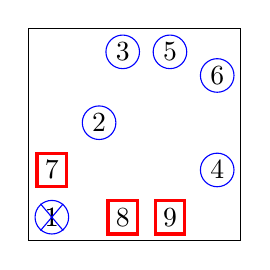
\begin{tikzpicture}[x = 3mm, y=3mm]
	\draw (-1,-1) rectangle (8,8);
	\tikzstyle{Square} = [
		draw = red, 
		very thick,
		rectangle,
		inner sep = 1mm,
		minimum size = 3 mm
	]
	\tikzstyle{SquareFill} = [
		draw = red, 
		fill = red,
		very thick,
		rectangle,
	]
	\tikzstyle{Circle} = [
		draw = blue, 
		circle,
		inner sep = 0.5 mm
	]
	\tikzstyle{CircleFill} = [
		draw = blue,
		fill = blue, 
		circle,
	]
	\node [Circle] (1) at (0,0) {1};
	\node [Circle] (2) at (2,4) {2};
	\node [Circle] (3) at (3,7) {3};
	\node [Circle] (4) at (7,2) {4};
	\node [Circle] (5) at (5,7) {5};
	\node [Circle] (6) at (7,6) {6};
	\node [Square] (7) at (0,2) {7};
	\node [Square] (8) at (3,0) {8};
	\node [Square] (9) at (5,0) {9};

	\node [Circle, cross out] (1) at (0,0) {1};
\end{tikzpicture}
\end{center}



Our original dataset has 619,027 samples.  We first removed the 27,723 crashes involving a pedestrian, leaving 591,304 samples.  Each sample had 82 features; we cut the number of features to 38 for our ``Hard'' features, then to 21 for ``Medium,'' and to 10 for ``Easy.''  We then split each of those three datasets 70/30 into a training set of 413,913 samples and a test set of 177,393 samples, preserving the proportions of negative and positive samples in both sets.  We did the train/test split twice with different random seeds (``Round 1'' and ``Round 2'') to gauge how much of the small differences in results were due to stochasticity instead of differences in the model algorithms or hyperparameters.  Tomek undersampling only applies to the training set, not to the test set.  

We then ran Imbalanced-Learn's  TomekLinks algorithm, then ran it again on the results to give our ``Tomek Once'' and ``Tomek Twice'' undersampled datasets.  

\

\hfil\begin{tabular}{lrrl}
\multicolumn{2}{l}{Hard Features, Round 1}   &  & \cr
 & Samples & \multicolumn{2}{c}{Change} \cr\hline
Original & 413,913 &  & \cr
Tomek Once & 399,515 & 14,398 & 3.48\%\cr
Tomek Twice & 396,511 & 3,004 & 0.75\%\cr\cline{3-4}
Total Change &  & 17,402 & 4.23\%\cr
\end{tabular}
\qquad\begin{tabular}{lrrl}
\multicolumn{2}{l}{Hard Features, Round 2} & \cr
 & Samples & \multicolumn{2}{c}{Change} \cr\hline
Original & 413,913 &  & \cr
Tomek Once & 399,714 & 14,199 & 3.43\%\cr
Tomek Twice & 396,718 & 2,996 & 0.75\%\cr\cline{3-4}
Total Change &  & 17,195 & 4.18\%\cr
\end{tabular}

\vskip 12pt

\hfil\begin{tabular}{lrrl}
\multicolumn{3}{l}{Medium Features, Round 1} & \cr
 & Samples & \multicolumn{2}{c}{Change} \cr\hline
Original & 413,913 &  & \cr
Tomek Once & 406,691 & 7,222 & 1.74\%\cr
Tomek Twice & 405,288 & 1,403 & 0.34\%\cr\cline{3-4}
Total Change &  & 8,625 & 2.08\%\cr
\end{tabular}
\qquad
\begin{tabular}{lrrl}
\multicolumn{3}{l}{Medium Features, Round 2} & \cr
 & Samples & \multicolumn{2}{c}{Change} \cr\hline
Original & 413,913 &  & \cr
Tomek Once & 406,781 & 7,132 & 1.72\%\cr
Tomek Twice & 405,368 & 1,413 & 0.35\%\cr\cline{3-4}
Total Change &  & 8,545 & 2.07\%\cr
\end{tabular}

\vskip 12pt

\hfil\begin{tabular}{lrrl}
\multicolumn{2}{l}{Easy Features, Round 1} & \cr
 & Samples & \multicolumn{2}{c}{Change} \cr\hline
Original & 413,913 &  & \cr
Tomek Once & 413,909 & 4 & 0.00097\%\cr
Tomek Twice & 413,908 & 1 & 0.00024\%\cr\cline{3-4}
Total Change &  & 5 & 0.00121\%\cr
\end{tabular}
\qquad
\begin{tabular}{lrrl}
\multicolumn{2}{l}{Easy Features, Round 2} & \cr
 & Samples & \multicolumn{2}{c}{Change} \cr\hline
Original & 413,913 &  & \cr
Tomek Once & 413,908 & 5 & 0.00121\%\cr
Tomek Twice & 413,907 & 1 & 0.00024\%\cr\cline{3-4}
Total Change &  & 6 & 0.00145\%\cr
\end{tabular}

\

We ran the models on the two rounds of Tomek undersampled training for the Hard-feature and Medium-feature sets, not for the Easy because the undersampling was so small.  

We were disappointed to not see a significant improvement in the model metrics from the undersampling; the difference between no undersampling, one runs of Tomek, and two runs turned out to be inconsequential, by which we mean that one approach was not consistently better when we ran the models with different random seeds.  


\subsubsection{Modifying the Loss Function}

A popular and well established way to modify the loss function for imbalanced data is with class weights, which can have the same effect as na{\"i}ve oversampling.  

Three of our seven models take class weights, and for those we tried three different class weights.  The Tomek undersampling changes the last weight slightly from $0.8499$ to as low as $0.8433$.

\

\hfil\begin{tabular}{c|l}
	$\alpha$ & Meaning \cr\hline
	1/2 & No class weight \cr
	2/3 & $\Delta FP/\Delta TP < 2.0$ goal \cr
	$0.85$ & Balanced classes \cr 
\end{tabular}

\


A related method is with focal loss, which has a modulating hyperparameter $\gamma$ that increases the penalty for low-confidence samples. \citep{lin2017focal}  We tried five values  of $\gamma$.

\

\hfil\begin{tabular}{c|c}
	$\gamma$  & Notes \cr\hline
	0.0 & Same as binary crossentropy \cr
	0.5 & Very light modulation \cr
	1.0 & Light modulation\cr
	2.0 & Recommended by Lin \cr
	5.0 & Heavy modulation \cr
\end{tabular}	

\

We did not see significant improvement using focal loss.  ({\bf Put in Label Reference}).

%%%
\subsubsection{Metrics for Imbalance}

In the \nameref{Methods_Metrics} subsection above we defined the metrics recall, precision, and f1.  The most common metric in machine learning, the one that most algorithms are designed to maximize, is accuracy, the proportion of samples correctly classified.  In that section's example of transformed model output, we had 150,107 out of 177,392 test samples correctly classified, giving 84.6\% accuracy.  Is that good?  The model below, the raw results of the Logistic Regression model of the easy features set, recommends sending no ambulances, and it is correct in 150,771 of 177,392 test samples, giving 84.99\% accuracy.  Is that better?



\

%%%
\parbox{\linewidth}{
%{\bf Balanced Random Forest model, Hard features, No Tomek, $\alpha = 2/3$}

\noindent\begin{tabular}{@{\hspace{-6pt}}p{2.3in} @{\hspace{-6pt}}p{2.0in} p{1.8in}}
	\vskip 0pt
	\qquad \qquad Raw Model Output
	
	\input{../Keras/Images/LRC_Easy_Tomek_0_alpha_0_5_v1_Pred.pgf}
&
	\vskip 0pt
	\qquad \qquad ROC Curve
	
	\input{../Keras/Images/LRC_Easy_Tomek_0_alpha_0_5_v1_ROC.pgf}
	
&
	\vskip 0pt
	\begin{tabular}{cc|c|c|}
	&\multicolumn{1}{c}{}& \multicolumn{2}{c}{Prediction} \cr
	&\multicolumn{1}{c}{} & \multicolumn{1}{c}{N} & \multicolumn{1}{c}{P} \cr\cline{3-4}
	\multirow{2}{*}{\rotatebox[origin=c]{90}{Actual}}&N &
150,771 & 0
	\vrule width 0pt height 10pt depth 2pt \cr\cline{3-4}
	&P & 
26621 & 0
	\vrule width 0pt height 10pt depth 2pt \cr\cline{3-4}
	\end{tabular}

	\hfil\begin{tabular}{ll}
	\cr
	0.8499 & Accuracy\cr
und & Precision \cr	0.0 & Recall \cr	und & F1 \cr	0.659 & AUC \cr
\end{tabular}

\cr
\end{tabular}
} % End parbox

\

In this study, we  have arbitrarily decided that we are willing to trade off up to two false positives to get one more true positive.  Once we moved our decision thresholds to the ethical tradeoff point, the accuracy only varied from 0.836 to 0.854.  The difference in accuracy tells us how many more (or fewer) false positives than true positives we have, with them being equal at 0.8499, and we get the same information from precision being less than, more than, or equal to 0.5.    Therefore, we are not going to consider accuracy in evaluating our models. 

%%%
\subsubsection{ML Algorithms for Imbalanced Data}

{\bf [Expand this subsubsection]}

\begin{itemize}
	\item Random Undersampling Composite Models
	\item Bagging
	\item Boosting
\end{itemize}

%%%%%
\subsection{Models}

We used seven binary classification algorithms.  Three of them take class weights.

\

\hfil\begin{tabular}{llc}
&& Class \cr
Model & Source & Weights \cr\hline
KerasClassifier with the Binary Focal Crossentropy loss function & Keras & Yes \cr
Balanced Random Forest Classifier & Imbalanced-Learn & Yes \cr
Balanced Bagging Classifier & Imbalanced-Learn & No \cr
RUSBoost Classifier & Imbalanced-Learn & No \cr
Easy Ensemble Classifier with AdaBoost Estimator & Imbalanced-Learn & No \cr
Logistic Regression Classifier & Scikit-Learn & Yes \cr
AdaBoost  Classifier & Scikit-Learn & No \cr
\end{tabular}

\


For the focal loss function, we tried seven different combinations of the hyperparameters $\alpha$ for class weights and $\gamma$ for penalty on badly misclassified samples.  For the random forest and bagging models we tried three values of $\alpha$.  Altogether we had seventeen model/hyperparameter combinations.  We learned each of the seven models on datasets with the easy, medium, and hard features, and on the hard features we tested with Tomek undersampling 0, 1, and 2 times, for a total of five datasets, giving eighty-five model/hyperparameter/dataset combinations.    We learned each of those sixty-five with two different random seeds, for a total of one hundred seventy results.  

\

\hfil\noindent\begin{tabular}{ccc}
	\multicolumn{3}{c}{Seventeen Models} \cr
	Model & $\alpha$ & $\gamma$ \cr\hline
	Focal & 1/2 & 0.0 \cr
	Focal & 2/3 & 0.0 \cr
	Focal & 2/3 & 0.5 \cr
	Focal & 2/3 & 1.0 \cr
	Focal & 2/3 & 2.0 \cr
	Focal & 2/3 & 5.0 \cr
	Focal & 0.85 & 0.0 \cr
	Random Forest & 1/2 & \cr
	Random Forest & 2/3 & \cr
	Random Forest & 0.85 & \cr
	Bagging && \cr
	RUSBoost && \cr
	Easy Ens && \cr
	Log Reg & 1/2 & \cr
	Log Reg & 2/3 & \cr
	Log Reg & 0.85 & \cr
	AdaBoost && \cr
\end{tabular}
\quad
$\times$
\quad
\begin{tabular}{cc}
	\multicolumn{2}{c}{Seven Datasets} \cr
	Features & Tomek \cr\hline
	Hard & None \cr
	Hard & Once \cr
	Hard & Twice \cr
	Medium & None \cr
	Medium & Once \cr
	Medium & Twice \cr
	Easy & None \cr
\end{tabular}
\quad
$\times$
\quad
\begin{tabular}{cc}
	Run twice with \cr
	different \cr
	random seeds \cr\hline
	Random seed 1 \cr
	Random seed 2
\end{tabular}
\quad 
$=$ 
\quad 
\begin{tabular}{c}
	238  \cr Sets of  \cr
	Results \cr
\end{tabular}









\subsection{Analysis of Results}\label{Analysis}
% Analysis of Results

Our ML algorithms assign to each sample (feature vector, crash person) a probability $p \in [0,1]$ that the person needs an ambulance.  The histogram below left shows the percentage of the dataset in each range of $p$, showing the percentages for the negative class (``Does not need an ambulance'') and the positive class (``Needs an ambulance'').  On the right, the Receiver Operating Characteristic (ROC) curve, and particularly the area under the curve (AUC), is a metric for how well the model separates the two classes, with $AUC=1.0$ being perfect and $AUC=0.5$ (the dashed line) being just random assignment with no insight.  

We would love to have results like in the graphs below, where the machine learning (ML) algorithm nearly perfectly separates the two classes.  There is some overlap between $p=0.6$ and $p=0.8$ with some samples the algorithm misclassifies, but the model clearly separates most samples.  Having an AUC of 0.996 would be amazing.  

\noindent\begin{tabular}{@{\hspace{-6pt}}p{4.3in} @{\hspace{-6pt}}p{2.0in}}
	\vskip 0pt
	\hfil Raw Model Output
	
	%% Creator: Matplotlib, PGF backend
%%
%% To include the figure in your LaTeX document, write
%%   \input{<filename>.pgf}
%%
%% Make sure the required packages are loaded in your preamble
%%   \usepackage{pgf}
%%
%% Also ensure that all the required font packages are loaded; for instance,
%% the lmodern package is sometimes necessary when using math font.
%%   \usepackage{lmodern}
%%
%% Figures using additional raster images can only be included by \input if
%% they are in the same directory as the main LaTeX file. For loading figures
%% from other directories you can use the `import` package
%%   \usepackage{import}
%%
%% and then include the figures with
%%   \import{<path to file>}{<filename>.pgf}
%%
%% Matplotlib used the following preamble
%%   
%%   \usepackage{fontspec}
%%   \makeatletter\@ifpackageloaded{underscore}{}{\usepackage[strings]{underscore}}\makeatother
%%
\begingroup%
\makeatletter%
\begin{pgfpicture}%
\pgfpathrectangle{\pgfpointorigin}{\pgfqpoint{4.509306in}{1.754444in}}%
\pgfusepath{use as bounding box, clip}%
\begin{pgfscope}%
\pgfsetbuttcap%
\pgfsetmiterjoin%
\definecolor{currentfill}{rgb}{1.000000,1.000000,1.000000}%
\pgfsetfillcolor{currentfill}%
\pgfsetlinewidth{0.000000pt}%
\definecolor{currentstroke}{rgb}{1.000000,1.000000,1.000000}%
\pgfsetstrokecolor{currentstroke}%
\pgfsetdash{}{0pt}%
\pgfpathmoveto{\pgfqpoint{0.000000in}{0.000000in}}%
\pgfpathlineto{\pgfqpoint{4.509306in}{0.000000in}}%
\pgfpathlineto{\pgfqpoint{4.509306in}{1.754444in}}%
\pgfpathlineto{\pgfqpoint{0.000000in}{1.754444in}}%
\pgfpathlineto{\pgfqpoint{0.000000in}{0.000000in}}%
\pgfpathclose%
\pgfusepath{fill}%
\end{pgfscope}%
\begin{pgfscope}%
\pgfsetbuttcap%
\pgfsetmiterjoin%
\definecolor{currentfill}{rgb}{1.000000,1.000000,1.000000}%
\pgfsetfillcolor{currentfill}%
\pgfsetlinewidth{0.000000pt}%
\definecolor{currentstroke}{rgb}{0.000000,0.000000,0.000000}%
\pgfsetstrokecolor{currentstroke}%
\pgfsetstrokeopacity{0.000000}%
\pgfsetdash{}{0pt}%
\pgfpathmoveto{\pgfqpoint{0.445556in}{0.499444in}}%
\pgfpathlineto{\pgfqpoint{4.320556in}{0.499444in}}%
\pgfpathlineto{\pgfqpoint{4.320556in}{1.654444in}}%
\pgfpathlineto{\pgfqpoint{0.445556in}{1.654444in}}%
\pgfpathlineto{\pgfqpoint{0.445556in}{0.499444in}}%
\pgfpathclose%
\pgfusepath{fill}%
\end{pgfscope}%
\begin{pgfscope}%
\pgfpathrectangle{\pgfqpoint{0.445556in}{0.499444in}}{\pgfqpoint{3.875000in}{1.155000in}}%
\pgfusepath{clip}%
\pgfsetbuttcap%
\pgfsetmiterjoin%
\pgfsetlinewidth{1.003750pt}%
\definecolor{currentstroke}{rgb}{0.000000,0.000000,0.000000}%
\pgfsetstrokecolor{currentstroke}%
\pgfsetdash{}{0pt}%
\pgfpathmoveto{\pgfqpoint{0.435556in}{0.499444in}}%
\pgfpathlineto{\pgfqpoint{0.483922in}{0.499444in}}%
\pgfpathlineto{\pgfqpoint{0.483922in}{0.632510in}}%
\pgfpathlineto{\pgfqpoint{0.435556in}{0.632510in}}%
\pgfusepath{stroke}%
\end{pgfscope}%
\begin{pgfscope}%
\pgfpathrectangle{\pgfqpoint{0.445556in}{0.499444in}}{\pgfqpoint{3.875000in}{1.155000in}}%
\pgfusepath{clip}%
\pgfsetbuttcap%
\pgfsetmiterjoin%
\pgfsetlinewidth{1.003750pt}%
\definecolor{currentstroke}{rgb}{0.000000,0.000000,0.000000}%
\pgfsetstrokecolor{currentstroke}%
\pgfsetdash{}{0pt}%
\pgfpathmoveto{\pgfqpoint{0.576001in}{0.499444in}}%
\pgfpathlineto{\pgfqpoint{0.637387in}{0.499444in}}%
\pgfpathlineto{\pgfqpoint{0.637387in}{0.855505in}}%
\pgfpathlineto{\pgfqpoint{0.576001in}{0.855505in}}%
\pgfpathlineto{\pgfqpoint{0.576001in}{0.499444in}}%
\pgfpathclose%
\pgfusepath{stroke}%
\end{pgfscope}%
\begin{pgfscope}%
\pgfpathrectangle{\pgfqpoint{0.445556in}{0.499444in}}{\pgfqpoint{3.875000in}{1.155000in}}%
\pgfusepath{clip}%
\pgfsetbuttcap%
\pgfsetmiterjoin%
\pgfsetlinewidth{1.003750pt}%
\definecolor{currentstroke}{rgb}{0.000000,0.000000,0.000000}%
\pgfsetstrokecolor{currentstroke}%
\pgfsetdash{}{0pt}%
\pgfpathmoveto{\pgfqpoint{0.729467in}{0.499444in}}%
\pgfpathlineto{\pgfqpoint{0.790853in}{0.499444in}}%
\pgfpathlineto{\pgfqpoint{0.790853in}{1.087595in}}%
\pgfpathlineto{\pgfqpoint{0.729467in}{1.087595in}}%
\pgfpathlineto{\pgfqpoint{0.729467in}{0.499444in}}%
\pgfpathclose%
\pgfusepath{stroke}%
\end{pgfscope}%
\begin{pgfscope}%
\pgfpathrectangle{\pgfqpoint{0.445556in}{0.499444in}}{\pgfqpoint{3.875000in}{1.155000in}}%
\pgfusepath{clip}%
\pgfsetbuttcap%
\pgfsetmiterjoin%
\pgfsetlinewidth{1.003750pt}%
\definecolor{currentstroke}{rgb}{0.000000,0.000000,0.000000}%
\pgfsetstrokecolor{currentstroke}%
\pgfsetdash{}{0pt}%
\pgfpathmoveto{\pgfqpoint{0.882932in}{0.499444in}}%
\pgfpathlineto{\pgfqpoint{0.944318in}{0.499444in}}%
\pgfpathlineto{\pgfqpoint{0.944318in}{1.269324in}}%
\pgfpathlineto{\pgfqpoint{0.882932in}{1.269324in}}%
\pgfpathlineto{\pgfqpoint{0.882932in}{0.499444in}}%
\pgfpathclose%
\pgfusepath{stroke}%
\end{pgfscope}%
\begin{pgfscope}%
\pgfpathrectangle{\pgfqpoint{0.445556in}{0.499444in}}{\pgfqpoint{3.875000in}{1.155000in}}%
\pgfusepath{clip}%
\pgfsetbuttcap%
\pgfsetmiterjoin%
\pgfsetlinewidth{1.003750pt}%
\definecolor{currentstroke}{rgb}{0.000000,0.000000,0.000000}%
\pgfsetstrokecolor{currentstroke}%
\pgfsetdash{}{0pt}%
\pgfpathmoveto{\pgfqpoint{1.036397in}{0.499444in}}%
\pgfpathlineto{\pgfqpoint{1.097783in}{0.499444in}}%
\pgfpathlineto{\pgfqpoint{1.097783in}{1.428301in}}%
\pgfpathlineto{\pgfqpoint{1.036397in}{1.428301in}}%
\pgfpathlineto{\pgfqpoint{1.036397in}{0.499444in}}%
\pgfpathclose%
\pgfusepath{stroke}%
\end{pgfscope}%
\begin{pgfscope}%
\pgfpathrectangle{\pgfqpoint{0.445556in}{0.499444in}}{\pgfqpoint{3.875000in}{1.155000in}}%
\pgfusepath{clip}%
\pgfsetbuttcap%
\pgfsetmiterjoin%
\pgfsetlinewidth{1.003750pt}%
\definecolor{currentstroke}{rgb}{0.000000,0.000000,0.000000}%
\pgfsetstrokecolor{currentstroke}%
\pgfsetdash{}{0pt}%
\pgfpathmoveto{\pgfqpoint{1.189863in}{0.499444in}}%
\pgfpathlineto{\pgfqpoint{1.251249in}{0.499444in}}%
\pgfpathlineto{\pgfqpoint{1.251249in}{1.521593in}}%
\pgfpathlineto{\pgfqpoint{1.189863in}{1.521593in}}%
\pgfpathlineto{\pgfqpoint{1.189863in}{0.499444in}}%
\pgfpathclose%
\pgfusepath{stroke}%
\end{pgfscope}%
\begin{pgfscope}%
\pgfpathrectangle{\pgfqpoint{0.445556in}{0.499444in}}{\pgfqpoint{3.875000in}{1.155000in}}%
\pgfusepath{clip}%
\pgfsetbuttcap%
\pgfsetmiterjoin%
\pgfsetlinewidth{1.003750pt}%
\definecolor{currentstroke}{rgb}{0.000000,0.000000,0.000000}%
\pgfsetstrokecolor{currentstroke}%
\pgfsetdash{}{0pt}%
\pgfpathmoveto{\pgfqpoint{1.343328in}{0.499444in}}%
\pgfpathlineto{\pgfqpoint{1.404714in}{0.499444in}}%
\pgfpathlineto{\pgfqpoint{1.404714in}{1.590875in}}%
\pgfpathlineto{\pgfqpoint{1.343328in}{1.590875in}}%
\pgfpathlineto{\pgfqpoint{1.343328in}{0.499444in}}%
\pgfpathclose%
\pgfusepath{stroke}%
\end{pgfscope}%
\begin{pgfscope}%
\pgfpathrectangle{\pgfqpoint{0.445556in}{0.499444in}}{\pgfqpoint{3.875000in}{1.155000in}}%
\pgfusepath{clip}%
\pgfsetbuttcap%
\pgfsetmiterjoin%
\pgfsetlinewidth{1.003750pt}%
\definecolor{currentstroke}{rgb}{0.000000,0.000000,0.000000}%
\pgfsetstrokecolor{currentstroke}%
\pgfsetdash{}{0pt}%
\pgfpathmoveto{\pgfqpoint{1.496793in}{0.499444in}}%
\pgfpathlineto{\pgfqpoint{1.558179in}{0.499444in}}%
\pgfpathlineto{\pgfqpoint{1.558179in}{1.599444in}}%
\pgfpathlineto{\pgfqpoint{1.496793in}{1.599444in}}%
\pgfpathlineto{\pgfqpoint{1.496793in}{0.499444in}}%
\pgfpathclose%
\pgfusepath{stroke}%
\end{pgfscope}%
\begin{pgfscope}%
\pgfpathrectangle{\pgfqpoint{0.445556in}{0.499444in}}{\pgfqpoint{3.875000in}{1.155000in}}%
\pgfusepath{clip}%
\pgfsetbuttcap%
\pgfsetmiterjoin%
\pgfsetlinewidth{1.003750pt}%
\definecolor{currentstroke}{rgb}{0.000000,0.000000,0.000000}%
\pgfsetstrokecolor{currentstroke}%
\pgfsetdash{}{0pt}%
\pgfpathmoveto{\pgfqpoint{1.650259in}{0.499444in}}%
\pgfpathlineto{\pgfqpoint{1.711645in}{0.499444in}}%
\pgfpathlineto{\pgfqpoint{1.711645in}{1.566953in}}%
\pgfpathlineto{\pgfqpoint{1.650259in}{1.566953in}}%
\pgfpathlineto{\pgfqpoint{1.650259in}{0.499444in}}%
\pgfpathclose%
\pgfusepath{stroke}%
\end{pgfscope}%
\begin{pgfscope}%
\pgfpathrectangle{\pgfqpoint{0.445556in}{0.499444in}}{\pgfqpoint{3.875000in}{1.155000in}}%
\pgfusepath{clip}%
\pgfsetbuttcap%
\pgfsetmiterjoin%
\pgfsetlinewidth{1.003750pt}%
\definecolor{currentstroke}{rgb}{0.000000,0.000000,0.000000}%
\pgfsetstrokecolor{currentstroke}%
\pgfsetdash{}{0pt}%
\pgfpathmoveto{\pgfqpoint{1.803724in}{0.499444in}}%
\pgfpathlineto{\pgfqpoint{1.865110in}{0.499444in}}%
\pgfpathlineto{\pgfqpoint{1.865110in}{1.506942in}}%
\pgfpathlineto{\pgfqpoint{1.803724in}{1.506942in}}%
\pgfpathlineto{\pgfqpoint{1.803724in}{0.499444in}}%
\pgfpathclose%
\pgfusepath{stroke}%
\end{pgfscope}%
\begin{pgfscope}%
\pgfpathrectangle{\pgfqpoint{0.445556in}{0.499444in}}{\pgfqpoint{3.875000in}{1.155000in}}%
\pgfusepath{clip}%
\pgfsetbuttcap%
\pgfsetmiterjoin%
\pgfsetlinewidth{1.003750pt}%
\definecolor{currentstroke}{rgb}{0.000000,0.000000,0.000000}%
\pgfsetstrokecolor{currentstroke}%
\pgfsetdash{}{0pt}%
\pgfpathmoveto{\pgfqpoint{1.957189in}{0.499444in}}%
\pgfpathlineto{\pgfqpoint{2.018575in}{0.499444in}}%
\pgfpathlineto{\pgfqpoint{2.018575in}{1.416545in}}%
\pgfpathlineto{\pgfqpoint{1.957189in}{1.416545in}}%
\pgfpathlineto{\pgfqpoint{1.957189in}{0.499444in}}%
\pgfpathclose%
\pgfusepath{stroke}%
\end{pgfscope}%
\begin{pgfscope}%
\pgfpathrectangle{\pgfqpoint{0.445556in}{0.499444in}}{\pgfqpoint{3.875000in}{1.155000in}}%
\pgfusepath{clip}%
\pgfsetbuttcap%
\pgfsetmiterjoin%
\pgfsetlinewidth{1.003750pt}%
\definecolor{currentstroke}{rgb}{0.000000,0.000000,0.000000}%
\pgfsetstrokecolor{currentstroke}%
\pgfsetdash{}{0pt}%
\pgfpathmoveto{\pgfqpoint{2.110655in}{0.499444in}}%
\pgfpathlineto{\pgfqpoint{2.172041in}{0.499444in}}%
\pgfpathlineto{\pgfqpoint{2.172041in}{1.298482in}}%
\pgfpathlineto{\pgfqpoint{2.110655in}{1.298482in}}%
\pgfpathlineto{\pgfqpoint{2.110655in}{0.499444in}}%
\pgfpathclose%
\pgfusepath{stroke}%
\end{pgfscope}%
\begin{pgfscope}%
\pgfpathrectangle{\pgfqpoint{0.445556in}{0.499444in}}{\pgfqpoint{3.875000in}{1.155000in}}%
\pgfusepath{clip}%
\pgfsetbuttcap%
\pgfsetmiterjoin%
\pgfsetlinewidth{1.003750pt}%
\definecolor{currentstroke}{rgb}{0.000000,0.000000,0.000000}%
\pgfsetstrokecolor{currentstroke}%
\pgfsetdash{}{0pt}%
\pgfpathmoveto{\pgfqpoint{2.264120in}{0.499444in}}%
\pgfpathlineto{\pgfqpoint{2.325506in}{0.499444in}}%
\pgfpathlineto{\pgfqpoint{2.325506in}{1.165884in}}%
\pgfpathlineto{\pgfqpoint{2.264120in}{1.165884in}}%
\pgfpathlineto{\pgfqpoint{2.264120in}{0.499444in}}%
\pgfpathclose%
\pgfusepath{stroke}%
\end{pgfscope}%
\begin{pgfscope}%
\pgfpathrectangle{\pgfqpoint{0.445556in}{0.499444in}}{\pgfqpoint{3.875000in}{1.155000in}}%
\pgfusepath{clip}%
\pgfsetbuttcap%
\pgfsetmiterjoin%
\pgfsetlinewidth{1.003750pt}%
\definecolor{currentstroke}{rgb}{0.000000,0.000000,0.000000}%
\pgfsetstrokecolor{currentstroke}%
\pgfsetdash{}{0pt}%
\pgfpathmoveto{\pgfqpoint{2.417585in}{0.499444in}}%
\pgfpathlineto{\pgfqpoint{2.478972in}{0.499444in}}%
\pgfpathlineto{\pgfqpoint{2.478972in}{1.041650in}}%
\pgfpathlineto{\pgfqpoint{2.417585in}{1.041650in}}%
\pgfpathlineto{\pgfqpoint{2.417585in}{0.499444in}}%
\pgfpathclose%
\pgfusepath{stroke}%
\end{pgfscope}%
\begin{pgfscope}%
\pgfpathrectangle{\pgfqpoint{0.445556in}{0.499444in}}{\pgfqpoint{3.875000in}{1.155000in}}%
\pgfusepath{clip}%
\pgfsetbuttcap%
\pgfsetmiterjoin%
\pgfsetlinewidth{1.003750pt}%
\definecolor{currentstroke}{rgb}{0.000000,0.000000,0.000000}%
\pgfsetstrokecolor{currentstroke}%
\pgfsetdash{}{0pt}%
\pgfpathmoveto{\pgfqpoint{2.571051in}{0.499444in}}%
\pgfpathlineto{\pgfqpoint{2.632437in}{0.499444in}}%
\pgfpathlineto{\pgfqpoint{2.632437in}{0.916218in}}%
\pgfpathlineto{\pgfqpoint{2.571051in}{0.916218in}}%
\pgfpathlineto{\pgfqpoint{2.571051in}{0.499444in}}%
\pgfpathclose%
\pgfusepath{stroke}%
\end{pgfscope}%
\begin{pgfscope}%
\pgfpathrectangle{\pgfqpoint{0.445556in}{0.499444in}}{\pgfqpoint{3.875000in}{1.155000in}}%
\pgfusepath{clip}%
\pgfsetbuttcap%
\pgfsetmiterjoin%
\pgfsetlinewidth{1.003750pt}%
\definecolor{currentstroke}{rgb}{0.000000,0.000000,0.000000}%
\pgfsetstrokecolor{currentstroke}%
\pgfsetdash{}{0pt}%
\pgfpathmoveto{\pgfqpoint{2.724516in}{0.499444in}}%
\pgfpathlineto{\pgfqpoint{2.785902in}{0.499444in}}%
\pgfpathlineto{\pgfqpoint{2.785902in}{0.806958in}}%
\pgfpathlineto{\pgfqpoint{2.724516in}{0.806958in}}%
\pgfpathlineto{\pgfqpoint{2.724516in}{0.499444in}}%
\pgfpathclose%
\pgfusepath{stroke}%
\end{pgfscope}%
\begin{pgfscope}%
\pgfpathrectangle{\pgfqpoint{0.445556in}{0.499444in}}{\pgfqpoint{3.875000in}{1.155000in}}%
\pgfusepath{clip}%
\pgfsetbuttcap%
\pgfsetmiterjoin%
\pgfsetlinewidth{1.003750pt}%
\definecolor{currentstroke}{rgb}{0.000000,0.000000,0.000000}%
\pgfsetstrokecolor{currentstroke}%
\pgfsetdash{}{0pt}%
\pgfpathmoveto{\pgfqpoint{2.877981in}{0.499444in}}%
\pgfpathlineto{\pgfqpoint{2.939368in}{0.499444in}}%
\pgfpathlineto{\pgfqpoint{2.939368in}{0.716063in}}%
\pgfpathlineto{\pgfqpoint{2.877981in}{0.716063in}}%
\pgfpathlineto{\pgfqpoint{2.877981in}{0.499444in}}%
\pgfpathclose%
\pgfusepath{stroke}%
\end{pgfscope}%
\begin{pgfscope}%
\pgfpathrectangle{\pgfqpoint{0.445556in}{0.499444in}}{\pgfqpoint{3.875000in}{1.155000in}}%
\pgfusepath{clip}%
\pgfsetbuttcap%
\pgfsetmiterjoin%
\pgfsetlinewidth{1.003750pt}%
\definecolor{currentstroke}{rgb}{0.000000,0.000000,0.000000}%
\pgfsetstrokecolor{currentstroke}%
\pgfsetdash{}{0pt}%
\pgfpathmoveto{\pgfqpoint{3.031447in}{0.499444in}}%
\pgfpathlineto{\pgfqpoint{3.092833in}{0.499444in}}%
\pgfpathlineto{\pgfqpoint{3.092833in}{0.645904in}}%
\pgfpathlineto{\pgfqpoint{3.031447in}{0.645904in}}%
\pgfpathlineto{\pgfqpoint{3.031447in}{0.499444in}}%
\pgfpathclose%
\pgfusepath{stroke}%
\end{pgfscope}%
\begin{pgfscope}%
\pgfpathrectangle{\pgfqpoint{0.445556in}{0.499444in}}{\pgfqpoint{3.875000in}{1.155000in}}%
\pgfusepath{clip}%
\pgfsetbuttcap%
\pgfsetmiterjoin%
\pgfsetlinewidth{1.003750pt}%
\definecolor{currentstroke}{rgb}{0.000000,0.000000,0.000000}%
\pgfsetstrokecolor{currentstroke}%
\pgfsetdash{}{0pt}%
\pgfpathmoveto{\pgfqpoint{3.184912in}{0.499444in}}%
\pgfpathlineto{\pgfqpoint{3.246298in}{0.499444in}}%
\pgfpathlineto{\pgfqpoint{3.246298in}{0.598936in}}%
\pgfpathlineto{\pgfqpoint{3.184912in}{0.598936in}}%
\pgfpathlineto{\pgfqpoint{3.184912in}{0.499444in}}%
\pgfpathclose%
\pgfusepath{stroke}%
\end{pgfscope}%
\begin{pgfscope}%
\pgfpathrectangle{\pgfqpoint{0.445556in}{0.499444in}}{\pgfqpoint{3.875000in}{1.155000in}}%
\pgfusepath{clip}%
\pgfsetbuttcap%
\pgfsetmiterjoin%
\pgfsetlinewidth{1.003750pt}%
\definecolor{currentstroke}{rgb}{0.000000,0.000000,0.000000}%
\pgfsetstrokecolor{currentstroke}%
\pgfsetdash{}{0pt}%
\pgfpathmoveto{\pgfqpoint{3.338377in}{0.499444in}}%
\pgfpathlineto{\pgfqpoint{3.399764in}{0.499444in}}%
\pgfpathlineto{\pgfqpoint{3.399764in}{0.560040in}}%
\pgfpathlineto{\pgfqpoint{3.338377in}{0.560040in}}%
\pgfpathlineto{\pgfqpoint{3.338377in}{0.499444in}}%
\pgfpathclose%
\pgfusepath{stroke}%
\end{pgfscope}%
\begin{pgfscope}%
\pgfpathrectangle{\pgfqpoint{0.445556in}{0.499444in}}{\pgfqpoint{3.875000in}{1.155000in}}%
\pgfusepath{clip}%
\pgfsetbuttcap%
\pgfsetmiterjoin%
\pgfsetlinewidth{1.003750pt}%
\definecolor{currentstroke}{rgb}{0.000000,0.000000,0.000000}%
\pgfsetstrokecolor{currentstroke}%
\pgfsetdash{}{0pt}%
\pgfpathmoveto{\pgfqpoint{3.491843in}{0.499444in}}%
\pgfpathlineto{\pgfqpoint{3.553229in}{0.499444in}}%
\pgfpathlineto{\pgfqpoint{3.553229in}{0.535591in}}%
\pgfpathlineto{\pgfqpoint{3.491843in}{0.535591in}}%
\pgfpathlineto{\pgfqpoint{3.491843in}{0.499444in}}%
\pgfpathclose%
\pgfusepath{stroke}%
\end{pgfscope}%
\begin{pgfscope}%
\pgfpathrectangle{\pgfqpoint{0.445556in}{0.499444in}}{\pgfqpoint{3.875000in}{1.155000in}}%
\pgfusepath{clip}%
\pgfsetbuttcap%
\pgfsetmiterjoin%
\pgfsetlinewidth{1.003750pt}%
\definecolor{currentstroke}{rgb}{0.000000,0.000000,0.000000}%
\pgfsetstrokecolor{currentstroke}%
\pgfsetdash{}{0pt}%
\pgfpathmoveto{\pgfqpoint{3.645308in}{0.499444in}}%
\pgfpathlineto{\pgfqpoint{3.706694in}{0.499444in}}%
\pgfpathlineto{\pgfqpoint{3.706694in}{0.512137in}}%
\pgfpathlineto{\pgfqpoint{3.645308in}{0.512137in}}%
\pgfpathlineto{\pgfqpoint{3.645308in}{0.499444in}}%
\pgfpathclose%
\pgfusepath{stroke}%
\end{pgfscope}%
\begin{pgfscope}%
\pgfpathrectangle{\pgfqpoint{0.445556in}{0.499444in}}{\pgfqpoint{3.875000in}{1.155000in}}%
\pgfusepath{clip}%
\pgfsetbuttcap%
\pgfsetmiterjoin%
\pgfsetlinewidth{1.003750pt}%
\definecolor{currentstroke}{rgb}{0.000000,0.000000,0.000000}%
\pgfsetstrokecolor{currentstroke}%
\pgfsetdash{}{0pt}%
\pgfpathmoveto{\pgfqpoint{3.798774in}{0.499444in}}%
\pgfpathlineto{\pgfqpoint{3.860160in}{0.499444in}}%
\pgfpathlineto{\pgfqpoint{3.860160in}{0.503305in}}%
\pgfpathlineto{\pgfqpoint{3.798774in}{0.503305in}}%
\pgfpathlineto{\pgfqpoint{3.798774in}{0.499444in}}%
\pgfpathclose%
\pgfusepath{stroke}%
\end{pgfscope}%
\begin{pgfscope}%
\pgfpathrectangle{\pgfqpoint{0.445556in}{0.499444in}}{\pgfqpoint{3.875000in}{1.155000in}}%
\pgfusepath{clip}%
\pgfsetbuttcap%
\pgfsetmiterjoin%
\pgfsetlinewidth{1.003750pt}%
\definecolor{currentstroke}{rgb}{0.000000,0.000000,0.000000}%
\pgfsetstrokecolor{currentstroke}%
\pgfsetdash{}{0pt}%
\pgfpathmoveto{\pgfqpoint{3.952239in}{0.499444in}}%
\pgfpathlineto{\pgfqpoint{4.013625in}{0.499444in}}%
\pgfpathlineto{\pgfqpoint{4.013625in}{0.500234in}}%
\pgfpathlineto{\pgfqpoint{3.952239in}{0.500234in}}%
\pgfpathlineto{\pgfqpoint{3.952239in}{0.499444in}}%
\pgfpathclose%
\pgfusepath{stroke}%
\end{pgfscope}%
\begin{pgfscope}%
\pgfpathrectangle{\pgfqpoint{0.445556in}{0.499444in}}{\pgfqpoint{3.875000in}{1.155000in}}%
\pgfusepath{clip}%
\pgfsetbuttcap%
\pgfsetmiterjoin%
\pgfsetlinewidth{1.003750pt}%
\definecolor{currentstroke}{rgb}{0.000000,0.000000,0.000000}%
\pgfsetstrokecolor{currentstroke}%
\pgfsetdash{}{0pt}%
\pgfpathmoveto{\pgfqpoint{4.105704in}{0.499444in}}%
\pgfpathlineto{\pgfqpoint{4.167090in}{0.499444in}}%
\pgfpathlineto{\pgfqpoint{4.167090in}{0.499503in}}%
\pgfpathlineto{\pgfqpoint{4.105704in}{0.499503in}}%
\pgfpathlineto{\pgfqpoint{4.105704in}{0.499444in}}%
\pgfpathclose%
\pgfusepath{stroke}%
\end{pgfscope}%
\begin{pgfscope}%
\pgfpathrectangle{\pgfqpoint{0.445556in}{0.499444in}}{\pgfqpoint{3.875000in}{1.155000in}}%
\pgfusepath{clip}%
\pgfsetbuttcap%
\pgfsetmiterjoin%
\definecolor{currentfill}{rgb}{0.000000,0.000000,0.000000}%
\pgfsetfillcolor{currentfill}%
\pgfsetlinewidth{0.000000pt}%
\definecolor{currentstroke}{rgb}{0.000000,0.000000,0.000000}%
\pgfsetstrokecolor{currentstroke}%
\pgfsetstrokeopacity{0.000000}%
\pgfsetdash{}{0pt}%
\pgfpathmoveto{\pgfqpoint{0.483922in}{0.499444in}}%
\pgfpathlineto{\pgfqpoint{0.545308in}{0.499444in}}%
\pgfpathlineto{\pgfqpoint{0.545308in}{0.499444in}}%
\pgfpathlineto{\pgfqpoint{0.483922in}{0.499444in}}%
\pgfpathlineto{\pgfqpoint{0.483922in}{0.499444in}}%
\pgfpathclose%
\pgfusepath{fill}%
\end{pgfscope}%
\begin{pgfscope}%
\pgfpathrectangle{\pgfqpoint{0.445556in}{0.499444in}}{\pgfqpoint{3.875000in}{1.155000in}}%
\pgfusepath{clip}%
\pgfsetbuttcap%
\pgfsetmiterjoin%
\definecolor{currentfill}{rgb}{0.000000,0.000000,0.000000}%
\pgfsetfillcolor{currentfill}%
\pgfsetlinewidth{0.000000pt}%
\definecolor{currentstroke}{rgb}{0.000000,0.000000,0.000000}%
\pgfsetstrokecolor{currentstroke}%
\pgfsetstrokeopacity{0.000000}%
\pgfsetdash{}{0pt}%
\pgfpathmoveto{\pgfqpoint{0.637387in}{0.499444in}}%
\pgfpathlineto{\pgfqpoint{0.698774in}{0.499444in}}%
\pgfpathlineto{\pgfqpoint{0.698774in}{0.499444in}}%
\pgfpathlineto{\pgfqpoint{0.637387in}{0.499444in}}%
\pgfpathlineto{\pgfqpoint{0.637387in}{0.499444in}}%
\pgfpathclose%
\pgfusepath{fill}%
\end{pgfscope}%
\begin{pgfscope}%
\pgfpathrectangle{\pgfqpoint{0.445556in}{0.499444in}}{\pgfqpoint{3.875000in}{1.155000in}}%
\pgfusepath{clip}%
\pgfsetbuttcap%
\pgfsetmiterjoin%
\definecolor{currentfill}{rgb}{0.000000,0.000000,0.000000}%
\pgfsetfillcolor{currentfill}%
\pgfsetlinewidth{0.000000pt}%
\definecolor{currentstroke}{rgb}{0.000000,0.000000,0.000000}%
\pgfsetstrokecolor{currentstroke}%
\pgfsetstrokeopacity{0.000000}%
\pgfsetdash{}{0pt}%
\pgfpathmoveto{\pgfqpoint{0.790853in}{0.499444in}}%
\pgfpathlineto{\pgfqpoint{0.852239in}{0.499444in}}%
\pgfpathlineto{\pgfqpoint{0.852239in}{0.499444in}}%
\pgfpathlineto{\pgfqpoint{0.790853in}{0.499444in}}%
\pgfpathlineto{\pgfqpoint{0.790853in}{0.499444in}}%
\pgfpathclose%
\pgfusepath{fill}%
\end{pgfscope}%
\begin{pgfscope}%
\pgfpathrectangle{\pgfqpoint{0.445556in}{0.499444in}}{\pgfqpoint{3.875000in}{1.155000in}}%
\pgfusepath{clip}%
\pgfsetbuttcap%
\pgfsetmiterjoin%
\definecolor{currentfill}{rgb}{0.000000,0.000000,0.000000}%
\pgfsetfillcolor{currentfill}%
\pgfsetlinewidth{0.000000pt}%
\definecolor{currentstroke}{rgb}{0.000000,0.000000,0.000000}%
\pgfsetstrokecolor{currentstroke}%
\pgfsetstrokeopacity{0.000000}%
\pgfsetdash{}{0pt}%
\pgfpathmoveto{\pgfqpoint{0.944318in}{0.499444in}}%
\pgfpathlineto{\pgfqpoint{1.005704in}{0.499444in}}%
\pgfpathlineto{\pgfqpoint{1.005704in}{0.499444in}}%
\pgfpathlineto{\pgfqpoint{0.944318in}{0.499444in}}%
\pgfpathlineto{\pgfqpoint{0.944318in}{0.499444in}}%
\pgfpathclose%
\pgfusepath{fill}%
\end{pgfscope}%
\begin{pgfscope}%
\pgfpathrectangle{\pgfqpoint{0.445556in}{0.499444in}}{\pgfqpoint{3.875000in}{1.155000in}}%
\pgfusepath{clip}%
\pgfsetbuttcap%
\pgfsetmiterjoin%
\definecolor{currentfill}{rgb}{0.000000,0.000000,0.000000}%
\pgfsetfillcolor{currentfill}%
\pgfsetlinewidth{0.000000pt}%
\definecolor{currentstroke}{rgb}{0.000000,0.000000,0.000000}%
\pgfsetstrokecolor{currentstroke}%
\pgfsetstrokeopacity{0.000000}%
\pgfsetdash{}{0pt}%
\pgfpathmoveto{\pgfqpoint{1.097783in}{0.499444in}}%
\pgfpathlineto{\pgfqpoint{1.159170in}{0.499444in}}%
\pgfpathlineto{\pgfqpoint{1.159170in}{0.499444in}}%
\pgfpathlineto{\pgfqpoint{1.097783in}{0.499444in}}%
\pgfpathlineto{\pgfqpoint{1.097783in}{0.499444in}}%
\pgfpathclose%
\pgfusepath{fill}%
\end{pgfscope}%
\begin{pgfscope}%
\pgfpathrectangle{\pgfqpoint{0.445556in}{0.499444in}}{\pgfqpoint{3.875000in}{1.155000in}}%
\pgfusepath{clip}%
\pgfsetbuttcap%
\pgfsetmiterjoin%
\definecolor{currentfill}{rgb}{0.000000,0.000000,0.000000}%
\pgfsetfillcolor{currentfill}%
\pgfsetlinewidth{0.000000pt}%
\definecolor{currentstroke}{rgb}{0.000000,0.000000,0.000000}%
\pgfsetstrokecolor{currentstroke}%
\pgfsetstrokeopacity{0.000000}%
\pgfsetdash{}{0pt}%
\pgfpathmoveto{\pgfqpoint{1.251249in}{0.499444in}}%
\pgfpathlineto{\pgfqpoint{1.312635in}{0.499444in}}%
\pgfpathlineto{\pgfqpoint{1.312635in}{0.499444in}}%
\pgfpathlineto{\pgfqpoint{1.251249in}{0.499444in}}%
\pgfpathlineto{\pgfqpoint{1.251249in}{0.499444in}}%
\pgfpathclose%
\pgfusepath{fill}%
\end{pgfscope}%
\begin{pgfscope}%
\pgfpathrectangle{\pgfqpoint{0.445556in}{0.499444in}}{\pgfqpoint{3.875000in}{1.155000in}}%
\pgfusepath{clip}%
\pgfsetbuttcap%
\pgfsetmiterjoin%
\definecolor{currentfill}{rgb}{0.000000,0.000000,0.000000}%
\pgfsetfillcolor{currentfill}%
\pgfsetlinewidth{0.000000pt}%
\definecolor{currentstroke}{rgb}{0.000000,0.000000,0.000000}%
\pgfsetstrokecolor{currentstroke}%
\pgfsetstrokeopacity{0.000000}%
\pgfsetdash{}{0pt}%
\pgfpathmoveto{\pgfqpoint{1.404714in}{0.499444in}}%
\pgfpathlineto{\pgfqpoint{1.466100in}{0.499444in}}%
\pgfpathlineto{\pgfqpoint{1.466100in}{0.499444in}}%
\pgfpathlineto{\pgfqpoint{1.404714in}{0.499444in}}%
\pgfpathlineto{\pgfqpoint{1.404714in}{0.499444in}}%
\pgfpathclose%
\pgfusepath{fill}%
\end{pgfscope}%
\begin{pgfscope}%
\pgfpathrectangle{\pgfqpoint{0.445556in}{0.499444in}}{\pgfqpoint{3.875000in}{1.155000in}}%
\pgfusepath{clip}%
\pgfsetbuttcap%
\pgfsetmiterjoin%
\definecolor{currentfill}{rgb}{0.000000,0.000000,0.000000}%
\pgfsetfillcolor{currentfill}%
\pgfsetlinewidth{0.000000pt}%
\definecolor{currentstroke}{rgb}{0.000000,0.000000,0.000000}%
\pgfsetstrokecolor{currentstroke}%
\pgfsetstrokeopacity{0.000000}%
\pgfsetdash{}{0pt}%
\pgfpathmoveto{\pgfqpoint{1.558179in}{0.499444in}}%
\pgfpathlineto{\pgfqpoint{1.619566in}{0.499444in}}%
\pgfpathlineto{\pgfqpoint{1.619566in}{0.499444in}}%
\pgfpathlineto{\pgfqpoint{1.558179in}{0.499444in}}%
\pgfpathlineto{\pgfqpoint{1.558179in}{0.499444in}}%
\pgfpathclose%
\pgfusepath{fill}%
\end{pgfscope}%
\begin{pgfscope}%
\pgfpathrectangle{\pgfqpoint{0.445556in}{0.499444in}}{\pgfqpoint{3.875000in}{1.155000in}}%
\pgfusepath{clip}%
\pgfsetbuttcap%
\pgfsetmiterjoin%
\definecolor{currentfill}{rgb}{0.000000,0.000000,0.000000}%
\pgfsetfillcolor{currentfill}%
\pgfsetlinewidth{0.000000pt}%
\definecolor{currentstroke}{rgb}{0.000000,0.000000,0.000000}%
\pgfsetstrokecolor{currentstroke}%
\pgfsetstrokeopacity{0.000000}%
\pgfsetdash{}{0pt}%
\pgfpathmoveto{\pgfqpoint{1.711645in}{0.499444in}}%
\pgfpathlineto{\pgfqpoint{1.773031in}{0.499444in}}%
\pgfpathlineto{\pgfqpoint{1.773031in}{0.499444in}}%
\pgfpathlineto{\pgfqpoint{1.711645in}{0.499444in}}%
\pgfpathlineto{\pgfqpoint{1.711645in}{0.499444in}}%
\pgfpathclose%
\pgfusepath{fill}%
\end{pgfscope}%
\begin{pgfscope}%
\pgfpathrectangle{\pgfqpoint{0.445556in}{0.499444in}}{\pgfqpoint{3.875000in}{1.155000in}}%
\pgfusepath{clip}%
\pgfsetbuttcap%
\pgfsetmiterjoin%
\definecolor{currentfill}{rgb}{0.000000,0.000000,0.000000}%
\pgfsetfillcolor{currentfill}%
\pgfsetlinewidth{0.000000pt}%
\definecolor{currentstroke}{rgb}{0.000000,0.000000,0.000000}%
\pgfsetstrokecolor{currentstroke}%
\pgfsetstrokeopacity{0.000000}%
\pgfsetdash{}{0pt}%
\pgfpathmoveto{\pgfqpoint{1.865110in}{0.499444in}}%
\pgfpathlineto{\pgfqpoint{1.926496in}{0.499444in}}%
\pgfpathlineto{\pgfqpoint{1.926496in}{0.499444in}}%
\pgfpathlineto{\pgfqpoint{1.865110in}{0.499444in}}%
\pgfpathlineto{\pgfqpoint{1.865110in}{0.499444in}}%
\pgfpathclose%
\pgfusepath{fill}%
\end{pgfscope}%
\begin{pgfscope}%
\pgfpathrectangle{\pgfqpoint{0.445556in}{0.499444in}}{\pgfqpoint{3.875000in}{1.155000in}}%
\pgfusepath{clip}%
\pgfsetbuttcap%
\pgfsetmiterjoin%
\definecolor{currentfill}{rgb}{0.000000,0.000000,0.000000}%
\pgfsetfillcolor{currentfill}%
\pgfsetlinewidth{0.000000pt}%
\definecolor{currentstroke}{rgb}{0.000000,0.000000,0.000000}%
\pgfsetstrokecolor{currentstroke}%
\pgfsetstrokeopacity{0.000000}%
\pgfsetdash{}{0pt}%
\pgfpathmoveto{\pgfqpoint{2.018575in}{0.499444in}}%
\pgfpathlineto{\pgfqpoint{2.079962in}{0.499444in}}%
\pgfpathlineto{\pgfqpoint{2.079962in}{0.499444in}}%
\pgfpathlineto{\pgfqpoint{2.018575in}{0.499444in}}%
\pgfpathlineto{\pgfqpoint{2.018575in}{0.499444in}}%
\pgfpathclose%
\pgfusepath{fill}%
\end{pgfscope}%
\begin{pgfscope}%
\pgfpathrectangle{\pgfqpoint{0.445556in}{0.499444in}}{\pgfqpoint{3.875000in}{1.155000in}}%
\pgfusepath{clip}%
\pgfsetbuttcap%
\pgfsetmiterjoin%
\definecolor{currentfill}{rgb}{0.000000,0.000000,0.000000}%
\pgfsetfillcolor{currentfill}%
\pgfsetlinewidth{0.000000pt}%
\definecolor{currentstroke}{rgb}{0.000000,0.000000,0.000000}%
\pgfsetstrokecolor{currentstroke}%
\pgfsetstrokeopacity{0.000000}%
\pgfsetdash{}{0pt}%
\pgfpathmoveto{\pgfqpoint{2.172041in}{0.499444in}}%
\pgfpathlineto{\pgfqpoint{2.233427in}{0.499444in}}%
\pgfpathlineto{\pgfqpoint{2.233427in}{0.499444in}}%
\pgfpathlineto{\pgfqpoint{2.172041in}{0.499444in}}%
\pgfpathlineto{\pgfqpoint{2.172041in}{0.499444in}}%
\pgfpathclose%
\pgfusepath{fill}%
\end{pgfscope}%
\begin{pgfscope}%
\pgfpathrectangle{\pgfqpoint{0.445556in}{0.499444in}}{\pgfqpoint{3.875000in}{1.155000in}}%
\pgfusepath{clip}%
\pgfsetbuttcap%
\pgfsetmiterjoin%
\definecolor{currentfill}{rgb}{0.000000,0.000000,0.000000}%
\pgfsetfillcolor{currentfill}%
\pgfsetlinewidth{0.000000pt}%
\definecolor{currentstroke}{rgb}{0.000000,0.000000,0.000000}%
\pgfsetstrokecolor{currentstroke}%
\pgfsetstrokeopacity{0.000000}%
\pgfsetdash{}{0pt}%
\pgfpathmoveto{\pgfqpoint{2.325506in}{0.499444in}}%
\pgfpathlineto{\pgfqpoint{2.386892in}{0.499444in}}%
\pgfpathlineto{\pgfqpoint{2.386892in}{0.499561in}}%
\pgfpathlineto{\pgfqpoint{2.325506in}{0.499561in}}%
\pgfpathlineto{\pgfqpoint{2.325506in}{0.499444in}}%
\pgfpathclose%
\pgfusepath{fill}%
\end{pgfscope}%
\begin{pgfscope}%
\pgfpathrectangle{\pgfqpoint{0.445556in}{0.499444in}}{\pgfqpoint{3.875000in}{1.155000in}}%
\pgfusepath{clip}%
\pgfsetbuttcap%
\pgfsetmiterjoin%
\definecolor{currentfill}{rgb}{0.000000,0.000000,0.000000}%
\pgfsetfillcolor{currentfill}%
\pgfsetlinewidth{0.000000pt}%
\definecolor{currentstroke}{rgb}{0.000000,0.000000,0.000000}%
\pgfsetstrokecolor{currentstroke}%
\pgfsetstrokeopacity{0.000000}%
\pgfsetdash{}{0pt}%
\pgfpathmoveto{\pgfqpoint{2.478972in}{0.499444in}}%
\pgfpathlineto{\pgfqpoint{2.540358in}{0.499444in}}%
\pgfpathlineto{\pgfqpoint{2.540358in}{0.499854in}}%
\pgfpathlineto{\pgfqpoint{2.478972in}{0.499854in}}%
\pgfpathlineto{\pgfqpoint{2.478972in}{0.499444in}}%
\pgfpathclose%
\pgfusepath{fill}%
\end{pgfscope}%
\begin{pgfscope}%
\pgfpathrectangle{\pgfqpoint{0.445556in}{0.499444in}}{\pgfqpoint{3.875000in}{1.155000in}}%
\pgfusepath{clip}%
\pgfsetbuttcap%
\pgfsetmiterjoin%
\definecolor{currentfill}{rgb}{0.000000,0.000000,0.000000}%
\pgfsetfillcolor{currentfill}%
\pgfsetlinewidth{0.000000pt}%
\definecolor{currentstroke}{rgb}{0.000000,0.000000,0.000000}%
\pgfsetstrokecolor{currentstroke}%
\pgfsetstrokeopacity{0.000000}%
\pgfsetdash{}{0pt}%
\pgfpathmoveto{\pgfqpoint{2.632437in}{0.499444in}}%
\pgfpathlineto{\pgfqpoint{2.693823in}{0.499444in}}%
\pgfpathlineto{\pgfqpoint{2.693823in}{0.501521in}}%
\pgfpathlineto{\pgfqpoint{2.632437in}{0.501521in}}%
\pgfpathlineto{\pgfqpoint{2.632437in}{0.499444in}}%
\pgfpathclose%
\pgfusepath{fill}%
\end{pgfscope}%
\begin{pgfscope}%
\pgfpathrectangle{\pgfqpoint{0.445556in}{0.499444in}}{\pgfqpoint{3.875000in}{1.155000in}}%
\pgfusepath{clip}%
\pgfsetbuttcap%
\pgfsetmiterjoin%
\definecolor{currentfill}{rgb}{0.000000,0.000000,0.000000}%
\pgfsetfillcolor{currentfill}%
\pgfsetlinewidth{0.000000pt}%
\definecolor{currentstroke}{rgb}{0.000000,0.000000,0.000000}%
\pgfsetstrokecolor{currentstroke}%
\pgfsetstrokeopacity{0.000000}%
\pgfsetdash{}{0pt}%
\pgfpathmoveto{\pgfqpoint{2.785902in}{0.499444in}}%
\pgfpathlineto{\pgfqpoint{2.847288in}{0.499444in}}%
\pgfpathlineto{\pgfqpoint{2.847288in}{0.511171in}}%
\pgfpathlineto{\pgfqpoint{2.785902in}{0.511171in}}%
\pgfpathlineto{\pgfqpoint{2.785902in}{0.499444in}}%
\pgfpathclose%
\pgfusepath{fill}%
\end{pgfscope}%
\begin{pgfscope}%
\pgfpathrectangle{\pgfqpoint{0.445556in}{0.499444in}}{\pgfqpoint{3.875000in}{1.155000in}}%
\pgfusepath{clip}%
\pgfsetbuttcap%
\pgfsetmiterjoin%
\definecolor{currentfill}{rgb}{0.000000,0.000000,0.000000}%
\pgfsetfillcolor{currentfill}%
\pgfsetlinewidth{0.000000pt}%
\definecolor{currentstroke}{rgb}{0.000000,0.000000,0.000000}%
\pgfsetstrokecolor{currentstroke}%
\pgfsetstrokeopacity{0.000000}%
\pgfsetdash{}{0pt}%
\pgfpathmoveto{\pgfqpoint{2.939368in}{0.499444in}}%
\pgfpathlineto{\pgfqpoint{3.000754in}{0.499444in}}%
\pgfpathlineto{\pgfqpoint{3.000754in}{0.534889in}}%
\pgfpathlineto{\pgfqpoint{2.939368in}{0.534889in}}%
\pgfpathlineto{\pgfqpoint{2.939368in}{0.499444in}}%
\pgfpathclose%
\pgfusepath{fill}%
\end{pgfscope}%
\begin{pgfscope}%
\pgfpathrectangle{\pgfqpoint{0.445556in}{0.499444in}}{\pgfqpoint{3.875000in}{1.155000in}}%
\pgfusepath{clip}%
\pgfsetbuttcap%
\pgfsetmiterjoin%
\definecolor{currentfill}{rgb}{0.000000,0.000000,0.000000}%
\pgfsetfillcolor{currentfill}%
\pgfsetlinewidth{0.000000pt}%
\definecolor{currentstroke}{rgb}{0.000000,0.000000,0.000000}%
\pgfsetstrokecolor{currentstroke}%
\pgfsetstrokeopacity{0.000000}%
\pgfsetdash{}{0pt}%
\pgfpathmoveto{\pgfqpoint{3.092833in}{0.499444in}}%
\pgfpathlineto{\pgfqpoint{3.154219in}{0.499444in}}%
\pgfpathlineto{\pgfqpoint{3.154219in}{0.582998in}}%
\pgfpathlineto{\pgfqpoint{3.092833in}{0.582998in}}%
\pgfpathlineto{\pgfqpoint{3.092833in}{0.499444in}}%
\pgfpathclose%
\pgfusepath{fill}%
\end{pgfscope}%
\begin{pgfscope}%
\pgfpathrectangle{\pgfqpoint{0.445556in}{0.499444in}}{\pgfqpoint{3.875000in}{1.155000in}}%
\pgfusepath{clip}%
\pgfsetbuttcap%
\pgfsetmiterjoin%
\definecolor{currentfill}{rgb}{0.000000,0.000000,0.000000}%
\pgfsetfillcolor{currentfill}%
\pgfsetlinewidth{0.000000pt}%
\definecolor{currentstroke}{rgb}{0.000000,0.000000,0.000000}%
\pgfsetstrokecolor{currentstroke}%
\pgfsetstrokeopacity{0.000000}%
\pgfsetdash{}{0pt}%
\pgfpathmoveto{\pgfqpoint{3.246298in}{0.499444in}}%
\pgfpathlineto{\pgfqpoint{3.307684in}{0.499444in}}%
\pgfpathlineto{\pgfqpoint{3.307684in}{0.662340in}}%
\pgfpathlineto{\pgfqpoint{3.246298in}{0.662340in}}%
\pgfpathlineto{\pgfqpoint{3.246298in}{0.499444in}}%
\pgfpathclose%
\pgfusepath{fill}%
\end{pgfscope}%
\begin{pgfscope}%
\pgfpathrectangle{\pgfqpoint{0.445556in}{0.499444in}}{\pgfqpoint{3.875000in}{1.155000in}}%
\pgfusepath{clip}%
\pgfsetbuttcap%
\pgfsetmiterjoin%
\definecolor{currentfill}{rgb}{0.000000,0.000000,0.000000}%
\pgfsetfillcolor{currentfill}%
\pgfsetlinewidth{0.000000pt}%
\definecolor{currentstroke}{rgb}{0.000000,0.000000,0.000000}%
\pgfsetstrokecolor{currentstroke}%
\pgfsetstrokeopacity{0.000000}%
\pgfsetdash{}{0pt}%
\pgfpathmoveto{\pgfqpoint{3.399764in}{0.499444in}}%
\pgfpathlineto{\pgfqpoint{3.461150in}{0.499444in}}%
\pgfpathlineto{\pgfqpoint{3.461150in}{0.763967in}}%
\pgfpathlineto{\pgfqpoint{3.399764in}{0.763967in}}%
\pgfpathlineto{\pgfqpoint{3.399764in}{0.499444in}}%
\pgfpathclose%
\pgfusepath{fill}%
\end{pgfscope}%
\begin{pgfscope}%
\pgfpathrectangle{\pgfqpoint{0.445556in}{0.499444in}}{\pgfqpoint{3.875000in}{1.155000in}}%
\pgfusepath{clip}%
\pgfsetbuttcap%
\pgfsetmiterjoin%
\definecolor{currentfill}{rgb}{0.000000,0.000000,0.000000}%
\pgfsetfillcolor{currentfill}%
\pgfsetlinewidth{0.000000pt}%
\definecolor{currentstroke}{rgb}{0.000000,0.000000,0.000000}%
\pgfsetstrokecolor{currentstroke}%
\pgfsetstrokeopacity{0.000000}%
\pgfsetdash{}{0pt}%
\pgfpathmoveto{\pgfqpoint{3.553229in}{0.499444in}}%
\pgfpathlineto{\pgfqpoint{3.614615in}{0.499444in}}%
\pgfpathlineto{\pgfqpoint{3.614615in}{0.871794in}}%
\pgfpathlineto{\pgfqpoint{3.553229in}{0.871794in}}%
\pgfpathlineto{\pgfqpoint{3.553229in}{0.499444in}}%
\pgfpathclose%
\pgfusepath{fill}%
\end{pgfscope}%
\begin{pgfscope}%
\pgfpathrectangle{\pgfqpoint{0.445556in}{0.499444in}}{\pgfqpoint{3.875000in}{1.155000in}}%
\pgfusepath{clip}%
\pgfsetbuttcap%
\pgfsetmiterjoin%
\definecolor{currentfill}{rgb}{0.000000,0.000000,0.000000}%
\pgfsetfillcolor{currentfill}%
\pgfsetlinewidth{0.000000pt}%
\definecolor{currentstroke}{rgb}{0.000000,0.000000,0.000000}%
\pgfsetstrokecolor{currentstroke}%
\pgfsetstrokeopacity{0.000000}%
\pgfsetdash{}{0pt}%
\pgfpathmoveto{\pgfqpoint{3.706694in}{0.499444in}}%
\pgfpathlineto{\pgfqpoint{3.768080in}{0.499444in}}%
\pgfpathlineto{\pgfqpoint{3.768080in}{0.925810in}}%
\pgfpathlineto{\pgfqpoint{3.706694in}{0.925810in}}%
\pgfpathlineto{\pgfqpoint{3.706694in}{0.499444in}}%
\pgfpathclose%
\pgfusepath{fill}%
\end{pgfscope}%
\begin{pgfscope}%
\pgfpathrectangle{\pgfqpoint{0.445556in}{0.499444in}}{\pgfqpoint{3.875000in}{1.155000in}}%
\pgfusepath{clip}%
\pgfsetbuttcap%
\pgfsetmiterjoin%
\definecolor{currentfill}{rgb}{0.000000,0.000000,0.000000}%
\pgfsetfillcolor{currentfill}%
\pgfsetlinewidth{0.000000pt}%
\definecolor{currentstroke}{rgb}{0.000000,0.000000,0.000000}%
\pgfsetstrokecolor{currentstroke}%
\pgfsetstrokeopacity{0.000000}%
\pgfsetdash{}{0pt}%
\pgfpathmoveto{\pgfqpoint{3.860160in}{0.499444in}}%
\pgfpathlineto{\pgfqpoint{3.921546in}{0.499444in}}%
\pgfpathlineto{\pgfqpoint{3.921546in}{0.913586in}}%
\pgfpathlineto{\pgfqpoint{3.860160in}{0.913586in}}%
\pgfpathlineto{\pgfqpoint{3.860160in}{0.499444in}}%
\pgfpathclose%
\pgfusepath{fill}%
\end{pgfscope}%
\begin{pgfscope}%
\pgfpathrectangle{\pgfqpoint{0.445556in}{0.499444in}}{\pgfqpoint{3.875000in}{1.155000in}}%
\pgfusepath{clip}%
\pgfsetbuttcap%
\pgfsetmiterjoin%
\definecolor{currentfill}{rgb}{0.000000,0.000000,0.000000}%
\pgfsetfillcolor{currentfill}%
\pgfsetlinewidth{0.000000pt}%
\definecolor{currentstroke}{rgb}{0.000000,0.000000,0.000000}%
\pgfsetstrokecolor{currentstroke}%
\pgfsetstrokeopacity{0.000000}%
\pgfsetdash{}{0pt}%
\pgfpathmoveto{\pgfqpoint{4.013625in}{0.499444in}}%
\pgfpathlineto{\pgfqpoint{4.075011in}{0.499444in}}%
\pgfpathlineto{\pgfqpoint{4.075011in}{0.851907in}}%
\pgfpathlineto{\pgfqpoint{4.013625in}{0.851907in}}%
\pgfpathlineto{\pgfqpoint{4.013625in}{0.499444in}}%
\pgfpathclose%
\pgfusepath{fill}%
\end{pgfscope}%
\begin{pgfscope}%
\pgfpathrectangle{\pgfqpoint{0.445556in}{0.499444in}}{\pgfqpoint{3.875000in}{1.155000in}}%
\pgfusepath{clip}%
\pgfsetbuttcap%
\pgfsetmiterjoin%
\definecolor{currentfill}{rgb}{0.000000,0.000000,0.000000}%
\pgfsetfillcolor{currentfill}%
\pgfsetlinewidth{0.000000pt}%
\definecolor{currentstroke}{rgb}{0.000000,0.000000,0.000000}%
\pgfsetstrokecolor{currentstroke}%
\pgfsetstrokeopacity{0.000000}%
\pgfsetdash{}{0pt}%
\pgfpathmoveto{\pgfqpoint{4.167090in}{0.499444in}}%
\pgfpathlineto{\pgfqpoint{4.228476in}{0.499444in}}%
\pgfpathlineto{\pgfqpoint{4.228476in}{0.681583in}}%
\pgfpathlineto{\pgfqpoint{4.167090in}{0.681583in}}%
\pgfpathlineto{\pgfqpoint{4.167090in}{0.499444in}}%
\pgfpathclose%
\pgfusepath{fill}%
\end{pgfscope}%
\begin{pgfscope}%
\pgfsetbuttcap%
\pgfsetroundjoin%
\definecolor{currentfill}{rgb}{0.000000,0.000000,0.000000}%
\pgfsetfillcolor{currentfill}%
\pgfsetlinewidth{0.803000pt}%
\definecolor{currentstroke}{rgb}{0.000000,0.000000,0.000000}%
\pgfsetstrokecolor{currentstroke}%
\pgfsetdash{}{0pt}%
\pgfsys@defobject{currentmarker}{\pgfqpoint{0.000000in}{-0.048611in}}{\pgfqpoint{0.000000in}{0.000000in}}{%
\pgfpathmoveto{\pgfqpoint{0.000000in}{0.000000in}}%
\pgfpathlineto{\pgfqpoint{0.000000in}{-0.048611in}}%
\pgfusepath{stroke,fill}%
}%
\begin{pgfscope}%
\pgfsys@transformshift{0.483922in}{0.499444in}%
\pgfsys@useobject{currentmarker}{}%
\end{pgfscope}%
\end{pgfscope}%
\begin{pgfscope}%
\definecolor{textcolor}{rgb}{0.000000,0.000000,0.000000}%
\pgfsetstrokecolor{textcolor}%
\pgfsetfillcolor{textcolor}%
\pgftext[x=0.483922in,y=0.402222in,,top]{\color{textcolor}\rmfamily\fontsize{10.000000}{12.000000}\selectfont 0.0}%
\end{pgfscope}%
\begin{pgfscope}%
\pgfsetbuttcap%
\pgfsetroundjoin%
\definecolor{currentfill}{rgb}{0.000000,0.000000,0.000000}%
\pgfsetfillcolor{currentfill}%
\pgfsetlinewidth{0.803000pt}%
\definecolor{currentstroke}{rgb}{0.000000,0.000000,0.000000}%
\pgfsetstrokecolor{currentstroke}%
\pgfsetdash{}{0pt}%
\pgfsys@defobject{currentmarker}{\pgfqpoint{0.000000in}{-0.048611in}}{\pgfqpoint{0.000000in}{0.000000in}}{%
\pgfpathmoveto{\pgfqpoint{0.000000in}{0.000000in}}%
\pgfpathlineto{\pgfqpoint{0.000000in}{-0.048611in}}%
\pgfusepath{stroke,fill}%
}%
\begin{pgfscope}%
\pgfsys@transformshift{0.867585in}{0.499444in}%
\pgfsys@useobject{currentmarker}{}%
\end{pgfscope}%
\end{pgfscope}%
\begin{pgfscope}%
\definecolor{textcolor}{rgb}{0.000000,0.000000,0.000000}%
\pgfsetstrokecolor{textcolor}%
\pgfsetfillcolor{textcolor}%
\pgftext[x=0.867585in,y=0.402222in,,top]{\color{textcolor}\rmfamily\fontsize{10.000000}{12.000000}\selectfont 0.1}%
\end{pgfscope}%
\begin{pgfscope}%
\pgfsetbuttcap%
\pgfsetroundjoin%
\definecolor{currentfill}{rgb}{0.000000,0.000000,0.000000}%
\pgfsetfillcolor{currentfill}%
\pgfsetlinewidth{0.803000pt}%
\definecolor{currentstroke}{rgb}{0.000000,0.000000,0.000000}%
\pgfsetstrokecolor{currentstroke}%
\pgfsetdash{}{0pt}%
\pgfsys@defobject{currentmarker}{\pgfqpoint{0.000000in}{-0.048611in}}{\pgfqpoint{0.000000in}{0.000000in}}{%
\pgfpathmoveto{\pgfqpoint{0.000000in}{0.000000in}}%
\pgfpathlineto{\pgfqpoint{0.000000in}{-0.048611in}}%
\pgfusepath{stroke,fill}%
}%
\begin{pgfscope}%
\pgfsys@transformshift{1.251249in}{0.499444in}%
\pgfsys@useobject{currentmarker}{}%
\end{pgfscope}%
\end{pgfscope}%
\begin{pgfscope}%
\definecolor{textcolor}{rgb}{0.000000,0.000000,0.000000}%
\pgfsetstrokecolor{textcolor}%
\pgfsetfillcolor{textcolor}%
\pgftext[x=1.251249in,y=0.402222in,,top]{\color{textcolor}\rmfamily\fontsize{10.000000}{12.000000}\selectfont 0.2}%
\end{pgfscope}%
\begin{pgfscope}%
\pgfsetbuttcap%
\pgfsetroundjoin%
\definecolor{currentfill}{rgb}{0.000000,0.000000,0.000000}%
\pgfsetfillcolor{currentfill}%
\pgfsetlinewidth{0.803000pt}%
\definecolor{currentstroke}{rgb}{0.000000,0.000000,0.000000}%
\pgfsetstrokecolor{currentstroke}%
\pgfsetdash{}{0pt}%
\pgfsys@defobject{currentmarker}{\pgfqpoint{0.000000in}{-0.048611in}}{\pgfqpoint{0.000000in}{0.000000in}}{%
\pgfpathmoveto{\pgfqpoint{0.000000in}{0.000000in}}%
\pgfpathlineto{\pgfqpoint{0.000000in}{-0.048611in}}%
\pgfusepath{stroke,fill}%
}%
\begin{pgfscope}%
\pgfsys@transformshift{1.634912in}{0.499444in}%
\pgfsys@useobject{currentmarker}{}%
\end{pgfscope}%
\end{pgfscope}%
\begin{pgfscope}%
\definecolor{textcolor}{rgb}{0.000000,0.000000,0.000000}%
\pgfsetstrokecolor{textcolor}%
\pgfsetfillcolor{textcolor}%
\pgftext[x=1.634912in,y=0.402222in,,top]{\color{textcolor}\rmfamily\fontsize{10.000000}{12.000000}\selectfont 0.3}%
\end{pgfscope}%
\begin{pgfscope}%
\pgfsetbuttcap%
\pgfsetroundjoin%
\definecolor{currentfill}{rgb}{0.000000,0.000000,0.000000}%
\pgfsetfillcolor{currentfill}%
\pgfsetlinewidth{0.803000pt}%
\definecolor{currentstroke}{rgb}{0.000000,0.000000,0.000000}%
\pgfsetstrokecolor{currentstroke}%
\pgfsetdash{}{0pt}%
\pgfsys@defobject{currentmarker}{\pgfqpoint{0.000000in}{-0.048611in}}{\pgfqpoint{0.000000in}{0.000000in}}{%
\pgfpathmoveto{\pgfqpoint{0.000000in}{0.000000in}}%
\pgfpathlineto{\pgfqpoint{0.000000in}{-0.048611in}}%
\pgfusepath{stroke,fill}%
}%
\begin{pgfscope}%
\pgfsys@transformshift{2.018575in}{0.499444in}%
\pgfsys@useobject{currentmarker}{}%
\end{pgfscope}%
\end{pgfscope}%
\begin{pgfscope}%
\definecolor{textcolor}{rgb}{0.000000,0.000000,0.000000}%
\pgfsetstrokecolor{textcolor}%
\pgfsetfillcolor{textcolor}%
\pgftext[x=2.018575in,y=0.402222in,,top]{\color{textcolor}\rmfamily\fontsize{10.000000}{12.000000}\selectfont 0.4}%
\end{pgfscope}%
\begin{pgfscope}%
\pgfsetbuttcap%
\pgfsetroundjoin%
\definecolor{currentfill}{rgb}{0.000000,0.000000,0.000000}%
\pgfsetfillcolor{currentfill}%
\pgfsetlinewidth{0.803000pt}%
\definecolor{currentstroke}{rgb}{0.000000,0.000000,0.000000}%
\pgfsetstrokecolor{currentstroke}%
\pgfsetdash{}{0pt}%
\pgfsys@defobject{currentmarker}{\pgfqpoint{0.000000in}{-0.048611in}}{\pgfqpoint{0.000000in}{0.000000in}}{%
\pgfpathmoveto{\pgfqpoint{0.000000in}{0.000000in}}%
\pgfpathlineto{\pgfqpoint{0.000000in}{-0.048611in}}%
\pgfusepath{stroke,fill}%
}%
\begin{pgfscope}%
\pgfsys@transformshift{2.402239in}{0.499444in}%
\pgfsys@useobject{currentmarker}{}%
\end{pgfscope}%
\end{pgfscope}%
\begin{pgfscope}%
\definecolor{textcolor}{rgb}{0.000000,0.000000,0.000000}%
\pgfsetstrokecolor{textcolor}%
\pgfsetfillcolor{textcolor}%
\pgftext[x=2.402239in,y=0.402222in,,top]{\color{textcolor}\rmfamily\fontsize{10.000000}{12.000000}\selectfont 0.5}%
\end{pgfscope}%
\begin{pgfscope}%
\pgfsetbuttcap%
\pgfsetroundjoin%
\definecolor{currentfill}{rgb}{0.000000,0.000000,0.000000}%
\pgfsetfillcolor{currentfill}%
\pgfsetlinewidth{0.803000pt}%
\definecolor{currentstroke}{rgb}{0.000000,0.000000,0.000000}%
\pgfsetstrokecolor{currentstroke}%
\pgfsetdash{}{0pt}%
\pgfsys@defobject{currentmarker}{\pgfqpoint{0.000000in}{-0.048611in}}{\pgfqpoint{0.000000in}{0.000000in}}{%
\pgfpathmoveto{\pgfqpoint{0.000000in}{0.000000in}}%
\pgfpathlineto{\pgfqpoint{0.000000in}{-0.048611in}}%
\pgfusepath{stroke,fill}%
}%
\begin{pgfscope}%
\pgfsys@transformshift{2.785902in}{0.499444in}%
\pgfsys@useobject{currentmarker}{}%
\end{pgfscope}%
\end{pgfscope}%
\begin{pgfscope}%
\definecolor{textcolor}{rgb}{0.000000,0.000000,0.000000}%
\pgfsetstrokecolor{textcolor}%
\pgfsetfillcolor{textcolor}%
\pgftext[x=2.785902in,y=0.402222in,,top]{\color{textcolor}\rmfamily\fontsize{10.000000}{12.000000}\selectfont 0.6}%
\end{pgfscope}%
\begin{pgfscope}%
\pgfsetbuttcap%
\pgfsetroundjoin%
\definecolor{currentfill}{rgb}{0.000000,0.000000,0.000000}%
\pgfsetfillcolor{currentfill}%
\pgfsetlinewidth{0.803000pt}%
\definecolor{currentstroke}{rgb}{0.000000,0.000000,0.000000}%
\pgfsetstrokecolor{currentstroke}%
\pgfsetdash{}{0pt}%
\pgfsys@defobject{currentmarker}{\pgfqpoint{0.000000in}{-0.048611in}}{\pgfqpoint{0.000000in}{0.000000in}}{%
\pgfpathmoveto{\pgfqpoint{0.000000in}{0.000000in}}%
\pgfpathlineto{\pgfqpoint{0.000000in}{-0.048611in}}%
\pgfusepath{stroke,fill}%
}%
\begin{pgfscope}%
\pgfsys@transformshift{3.169566in}{0.499444in}%
\pgfsys@useobject{currentmarker}{}%
\end{pgfscope}%
\end{pgfscope}%
\begin{pgfscope}%
\definecolor{textcolor}{rgb}{0.000000,0.000000,0.000000}%
\pgfsetstrokecolor{textcolor}%
\pgfsetfillcolor{textcolor}%
\pgftext[x=3.169566in,y=0.402222in,,top]{\color{textcolor}\rmfamily\fontsize{10.000000}{12.000000}\selectfont 0.7}%
\end{pgfscope}%
\begin{pgfscope}%
\pgfsetbuttcap%
\pgfsetroundjoin%
\definecolor{currentfill}{rgb}{0.000000,0.000000,0.000000}%
\pgfsetfillcolor{currentfill}%
\pgfsetlinewidth{0.803000pt}%
\definecolor{currentstroke}{rgb}{0.000000,0.000000,0.000000}%
\pgfsetstrokecolor{currentstroke}%
\pgfsetdash{}{0pt}%
\pgfsys@defobject{currentmarker}{\pgfqpoint{0.000000in}{-0.048611in}}{\pgfqpoint{0.000000in}{0.000000in}}{%
\pgfpathmoveto{\pgfqpoint{0.000000in}{0.000000in}}%
\pgfpathlineto{\pgfqpoint{0.000000in}{-0.048611in}}%
\pgfusepath{stroke,fill}%
}%
\begin{pgfscope}%
\pgfsys@transformshift{3.553229in}{0.499444in}%
\pgfsys@useobject{currentmarker}{}%
\end{pgfscope}%
\end{pgfscope}%
\begin{pgfscope}%
\definecolor{textcolor}{rgb}{0.000000,0.000000,0.000000}%
\pgfsetstrokecolor{textcolor}%
\pgfsetfillcolor{textcolor}%
\pgftext[x=3.553229in,y=0.402222in,,top]{\color{textcolor}\rmfamily\fontsize{10.000000}{12.000000}\selectfont 0.8}%
\end{pgfscope}%
\begin{pgfscope}%
\pgfsetbuttcap%
\pgfsetroundjoin%
\definecolor{currentfill}{rgb}{0.000000,0.000000,0.000000}%
\pgfsetfillcolor{currentfill}%
\pgfsetlinewidth{0.803000pt}%
\definecolor{currentstroke}{rgb}{0.000000,0.000000,0.000000}%
\pgfsetstrokecolor{currentstroke}%
\pgfsetdash{}{0pt}%
\pgfsys@defobject{currentmarker}{\pgfqpoint{0.000000in}{-0.048611in}}{\pgfqpoint{0.000000in}{0.000000in}}{%
\pgfpathmoveto{\pgfqpoint{0.000000in}{0.000000in}}%
\pgfpathlineto{\pgfqpoint{0.000000in}{-0.048611in}}%
\pgfusepath{stroke,fill}%
}%
\begin{pgfscope}%
\pgfsys@transformshift{3.936892in}{0.499444in}%
\pgfsys@useobject{currentmarker}{}%
\end{pgfscope}%
\end{pgfscope}%
\begin{pgfscope}%
\definecolor{textcolor}{rgb}{0.000000,0.000000,0.000000}%
\pgfsetstrokecolor{textcolor}%
\pgfsetfillcolor{textcolor}%
\pgftext[x=3.936892in,y=0.402222in,,top]{\color{textcolor}\rmfamily\fontsize{10.000000}{12.000000}\selectfont 0.9}%
\end{pgfscope}%
\begin{pgfscope}%
\pgfsetbuttcap%
\pgfsetroundjoin%
\definecolor{currentfill}{rgb}{0.000000,0.000000,0.000000}%
\pgfsetfillcolor{currentfill}%
\pgfsetlinewidth{0.803000pt}%
\definecolor{currentstroke}{rgb}{0.000000,0.000000,0.000000}%
\pgfsetstrokecolor{currentstroke}%
\pgfsetdash{}{0pt}%
\pgfsys@defobject{currentmarker}{\pgfqpoint{0.000000in}{-0.048611in}}{\pgfqpoint{0.000000in}{0.000000in}}{%
\pgfpathmoveto{\pgfqpoint{0.000000in}{0.000000in}}%
\pgfpathlineto{\pgfqpoint{0.000000in}{-0.048611in}}%
\pgfusepath{stroke,fill}%
}%
\begin{pgfscope}%
\pgfsys@transformshift{4.320556in}{0.499444in}%
\pgfsys@useobject{currentmarker}{}%
\end{pgfscope}%
\end{pgfscope}%
\begin{pgfscope}%
\definecolor{textcolor}{rgb}{0.000000,0.000000,0.000000}%
\pgfsetstrokecolor{textcolor}%
\pgfsetfillcolor{textcolor}%
\pgftext[x=4.320556in,y=0.402222in,,top]{\color{textcolor}\rmfamily\fontsize{10.000000}{12.000000}\selectfont 1.0}%
\end{pgfscope}%
\begin{pgfscope}%
\definecolor{textcolor}{rgb}{0.000000,0.000000,0.000000}%
\pgfsetstrokecolor{textcolor}%
\pgfsetfillcolor{textcolor}%
\pgftext[x=2.383056in,y=0.223333in,,top]{\color{textcolor}\rmfamily\fontsize{10.000000}{12.000000}\selectfont \(\displaystyle p\)}%
\end{pgfscope}%
\begin{pgfscope}%
\pgfsetbuttcap%
\pgfsetroundjoin%
\definecolor{currentfill}{rgb}{0.000000,0.000000,0.000000}%
\pgfsetfillcolor{currentfill}%
\pgfsetlinewidth{0.803000pt}%
\definecolor{currentstroke}{rgb}{0.000000,0.000000,0.000000}%
\pgfsetstrokecolor{currentstroke}%
\pgfsetdash{}{0pt}%
\pgfsys@defobject{currentmarker}{\pgfqpoint{-0.048611in}{0.000000in}}{\pgfqpoint{-0.000000in}{0.000000in}}{%
\pgfpathmoveto{\pgfqpoint{-0.000000in}{0.000000in}}%
\pgfpathlineto{\pgfqpoint{-0.048611in}{0.000000in}}%
\pgfusepath{stroke,fill}%
}%
\begin{pgfscope}%
\pgfsys@transformshift{0.445556in}{0.499444in}%
\pgfsys@useobject{currentmarker}{}%
\end{pgfscope}%
\end{pgfscope}%
\begin{pgfscope}%
\definecolor{textcolor}{rgb}{0.000000,0.000000,0.000000}%
\pgfsetstrokecolor{textcolor}%
\pgfsetfillcolor{textcolor}%
\pgftext[x=0.278889in, y=0.451250in, left, base]{\color{textcolor}\rmfamily\fontsize{10.000000}{12.000000}\selectfont \(\displaystyle {0}\)}%
\end{pgfscope}%
\begin{pgfscope}%
\pgfsetbuttcap%
\pgfsetroundjoin%
\definecolor{currentfill}{rgb}{0.000000,0.000000,0.000000}%
\pgfsetfillcolor{currentfill}%
\pgfsetlinewidth{0.803000pt}%
\definecolor{currentstroke}{rgb}{0.000000,0.000000,0.000000}%
\pgfsetstrokecolor{currentstroke}%
\pgfsetdash{}{0pt}%
\pgfsys@defobject{currentmarker}{\pgfqpoint{-0.048611in}{0.000000in}}{\pgfqpoint{-0.000000in}{0.000000in}}{%
\pgfpathmoveto{\pgfqpoint{-0.000000in}{0.000000in}}%
\pgfpathlineto{\pgfqpoint{-0.048611in}{0.000000in}}%
\pgfusepath{stroke,fill}%
}%
\begin{pgfscope}%
\pgfsys@transformshift{0.445556in}{0.791601in}%
\pgfsys@useobject{currentmarker}{}%
\end{pgfscope}%
\end{pgfscope}%
\begin{pgfscope}%
\definecolor{textcolor}{rgb}{0.000000,0.000000,0.000000}%
\pgfsetstrokecolor{textcolor}%
\pgfsetfillcolor{textcolor}%
\pgftext[x=0.278889in, y=0.743407in, left, base]{\color{textcolor}\rmfamily\fontsize{10.000000}{12.000000}\selectfont \(\displaystyle {2}\)}%
\end{pgfscope}%
\begin{pgfscope}%
\pgfsetbuttcap%
\pgfsetroundjoin%
\definecolor{currentfill}{rgb}{0.000000,0.000000,0.000000}%
\pgfsetfillcolor{currentfill}%
\pgfsetlinewidth{0.803000pt}%
\definecolor{currentstroke}{rgb}{0.000000,0.000000,0.000000}%
\pgfsetstrokecolor{currentstroke}%
\pgfsetdash{}{0pt}%
\pgfsys@defobject{currentmarker}{\pgfqpoint{-0.048611in}{0.000000in}}{\pgfqpoint{-0.000000in}{0.000000in}}{%
\pgfpathmoveto{\pgfqpoint{-0.000000in}{0.000000in}}%
\pgfpathlineto{\pgfqpoint{-0.048611in}{0.000000in}}%
\pgfusepath{stroke,fill}%
}%
\begin{pgfscope}%
\pgfsys@transformshift{0.445556in}{1.083759in}%
\pgfsys@useobject{currentmarker}{}%
\end{pgfscope}%
\end{pgfscope}%
\begin{pgfscope}%
\definecolor{textcolor}{rgb}{0.000000,0.000000,0.000000}%
\pgfsetstrokecolor{textcolor}%
\pgfsetfillcolor{textcolor}%
\pgftext[x=0.278889in, y=1.035564in, left, base]{\color{textcolor}\rmfamily\fontsize{10.000000}{12.000000}\selectfont \(\displaystyle {4}\)}%
\end{pgfscope}%
\begin{pgfscope}%
\pgfsetbuttcap%
\pgfsetroundjoin%
\definecolor{currentfill}{rgb}{0.000000,0.000000,0.000000}%
\pgfsetfillcolor{currentfill}%
\pgfsetlinewidth{0.803000pt}%
\definecolor{currentstroke}{rgb}{0.000000,0.000000,0.000000}%
\pgfsetstrokecolor{currentstroke}%
\pgfsetdash{}{0pt}%
\pgfsys@defobject{currentmarker}{\pgfqpoint{-0.048611in}{0.000000in}}{\pgfqpoint{-0.000000in}{0.000000in}}{%
\pgfpathmoveto{\pgfqpoint{-0.000000in}{0.000000in}}%
\pgfpathlineto{\pgfqpoint{-0.048611in}{0.000000in}}%
\pgfusepath{stroke,fill}%
}%
\begin{pgfscope}%
\pgfsys@transformshift{0.445556in}{1.375916in}%
\pgfsys@useobject{currentmarker}{}%
\end{pgfscope}%
\end{pgfscope}%
\begin{pgfscope}%
\definecolor{textcolor}{rgb}{0.000000,0.000000,0.000000}%
\pgfsetstrokecolor{textcolor}%
\pgfsetfillcolor{textcolor}%
\pgftext[x=0.278889in, y=1.327722in, left, base]{\color{textcolor}\rmfamily\fontsize{10.000000}{12.000000}\selectfont \(\displaystyle {6}\)}%
\end{pgfscope}%
\begin{pgfscope}%
\definecolor{textcolor}{rgb}{0.000000,0.000000,0.000000}%
\pgfsetstrokecolor{textcolor}%
\pgfsetfillcolor{textcolor}%
\pgftext[x=0.223333in,y=1.076944in,,bottom,rotate=90.000000]{\color{textcolor}\rmfamily\fontsize{10.000000}{12.000000}\selectfont Percent of Data Set}%
\end{pgfscope}%
\begin{pgfscope}%
\pgfsetrectcap%
\pgfsetmiterjoin%
\pgfsetlinewidth{0.803000pt}%
\definecolor{currentstroke}{rgb}{0.000000,0.000000,0.000000}%
\pgfsetstrokecolor{currentstroke}%
\pgfsetdash{}{0pt}%
\pgfpathmoveto{\pgfqpoint{0.445556in}{0.499444in}}%
\pgfpathlineto{\pgfqpoint{0.445556in}{1.654444in}}%
\pgfusepath{stroke}%
\end{pgfscope}%
\begin{pgfscope}%
\pgfsetrectcap%
\pgfsetmiterjoin%
\pgfsetlinewidth{0.803000pt}%
\definecolor{currentstroke}{rgb}{0.000000,0.000000,0.000000}%
\pgfsetstrokecolor{currentstroke}%
\pgfsetdash{}{0pt}%
\pgfpathmoveto{\pgfqpoint{4.320556in}{0.499444in}}%
\pgfpathlineto{\pgfqpoint{4.320556in}{1.654444in}}%
\pgfusepath{stroke}%
\end{pgfscope}%
\begin{pgfscope}%
\pgfsetrectcap%
\pgfsetmiterjoin%
\pgfsetlinewidth{0.803000pt}%
\definecolor{currentstroke}{rgb}{0.000000,0.000000,0.000000}%
\pgfsetstrokecolor{currentstroke}%
\pgfsetdash{}{0pt}%
\pgfpathmoveto{\pgfqpoint{0.445556in}{0.499444in}}%
\pgfpathlineto{\pgfqpoint{4.320556in}{0.499444in}}%
\pgfusepath{stroke}%
\end{pgfscope}%
\begin{pgfscope}%
\pgfsetrectcap%
\pgfsetmiterjoin%
\pgfsetlinewidth{0.803000pt}%
\definecolor{currentstroke}{rgb}{0.000000,0.000000,0.000000}%
\pgfsetstrokecolor{currentstroke}%
\pgfsetdash{}{0pt}%
\pgfpathmoveto{\pgfqpoint{0.445556in}{1.654444in}}%
\pgfpathlineto{\pgfqpoint{4.320556in}{1.654444in}}%
\pgfusepath{stroke}%
\end{pgfscope}%
\begin{pgfscope}%
\pgfsetbuttcap%
\pgfsetmiterjoin%
\definecolor{currentfill}{rgb}{1.000000,1.000000,1.000000}%
\pgfsetfillcolor{currentfill}%
\pgfsetfillopacity{0.800000}%
\pgfsetlinewidth{1.003750pt}%
\definecolor{currentstroke}{rgb}{0.800000,0.800000,0.800000}%
\pgfsetstrokecolor{currentstroke}%
\pgfsetstrokeopacity{0.800000}%
\pgfsetdash{}{0pt}%
\pgfpathmoveto{\pgfqpoint{3.543611in}{1.154445in}}%
\pgfpathlineto{\pgfqpoint{4.223333in}{1.154445in}}%
\pgfpathquadraticcurveto{\pgfqpoint{4.251111in}{1.154445in}}{\pgfqpoint{4.251111in}{1.182222in}}%
\pgfpathlineto{\pgfqpoint{4.251111in}{1.557222in}}%
\pgfpathquadraticcurveto{\pgfqpoint{4.251111in}{1.585000in}}{\pgfqpoint{4.223333in}{1.585000in}}%
\pgfpathlineto{\pgfqpoint{3.543611in}{1.585000in}}%
\pgfpathquadraticcurveto{\pgfqpoint{3.515833in}{1.585000in}}{\pgfqpoint{3.515833in}{1.557222in}}%
\pgfpathlineto{\pgfqpoint{3.515833in}{1.182222in}}%
\pgfpathquadraticcurveto{\pgfqpoint{3.515833in}{1.154445in}}{\pgfqpoint{3.543611in}{1.154445in}}%
\pgfpathlineto{\pgfqpoint{3.543611in}{1.154445in}}%
\pgfpathclose%
\pgfusepath{stroke,fill}%
\end{pgfscope}%
\begin{pgfscope}%
\pgfsetbuttcap%
\pgfsetmiterjoin%
\pgfsetlinewidth{1.003750pt}%
\definecolor{currentstroke}{rgb}{0.000000,0.000000,0.000000}%
\pgfsetstrokecolor{currentstroke}%
\pgfsetdash{}{0pt}%
\pgfpathmoveto{\pgfqpoint{3.571389in}{1.432222in}}%
\pgfpathlineto{\pgfqpoint{3.849167in}{1.432222in}}%
\pgfpathlineto{\pgfqpoint{3.849167in}{1.529444in}}%
\pgfpathlineto{\pgfqpoint{3.571389in}{1.529444in}}%
\pgfpathlineto{\pgfqpoint{3.571389in}{1.432222in}}%
\pgfpathclose%
\pgfusepath{stroke}%
\end{pgfscope}%
\begin{pgfscope}%
\definecolor{textcolor}{rgb}{0.000000,0.000000,0.000000}%
\pgfsetstrokecolor{textcolor}%
\pgfsetfillcolor{textcolor}%
\pgftext[x=3.960278in,y=1.432222in,left,base]{\color{textcolor}\rmfamily\fontsize{10.000000}{12.000000}\selectfont Neg}%
\end{pgfscope}%
\begin{pgfscope}%
\pgfsetbuttcap%
\pgfsetmiterjoin%
\definecolor{currentfill}{rgb}{0.000000,0.000000,0.000000}%
\pgfsetfillcolor{currentfill}%
\pgfsetlinewidth{0.000000pt}%
\definecolor{currentstroke}{rgb}{0.000000,0.000000,0.000000}%
\pgfsetstrokecolor{currentstroke}%
\pgfsetstrokeopacity{0.000000}%
\pgfsetdash{}{0pt}%
\pgfpathmoveto{\pgfqpoint{3.571389in}{1.236944in}}%
\pgfpathlineto{\pgfqpoint{3.849167in}{1.236944in}}%
\pgfpathlineto{\pgfqpoint{3.849167in}{1.334167in}}%
\pgfpathlineto{\pgfqpoint{3.571389in}{1.334167in}}%
\pgfpathlineto{\pgfqpoint{3.571389in}{1.236944in}}%
\pgfpathclose%
\pgfusepath{fill}%
\end{pgfscope}%
\begin{pgfscope}%
\definecolor{textcolor}{rgb}{0.000000,0.000000,0.000000}%
\pgfsetstrokecolor{textcolor}%
\pgfsetfillcolor{textcolor}%
\pgftext[x=3.960278in,y=1.236944in,left,base]{\color{textcolor}\rmfamily\fontsize{10.000000}{12.000000}\selectfont Pos}%
\end{pgfscope}%
\end{pgfpicture}%
\makeatother%
\endgroup%
	
&
	\vskip 0pt
	\hfil ROC Curve
	
	%% Creator: Matplotlib, PGF backend
%%
%% To include the figure in your LaTeX document, write
%%   \input{<filename>.pgf}
%%
%% Make sure the required packages are loaded in your preamble
%%   \usepackage{pgf}
%%
%% Also ensure that all the required font packages are loaded; for instance,
%% the lmodern package is sometimes necessary when using math font.
%%   \usepackage{lmodern}
%%
%% Figures using additional raster images can only be included by \input if
%% they are in the same directory as the main LaTeX file. For loading figures
%% from other directories you can use the `import` package
%%   \usepackage{import}
%%
%% and then include the figures with
%%   \import{<path to file>}{<filename>.pgf}
%%
%% Matplotlib used the following preamble
%%   
%%   \usepackage{fontspec}
%%   \makeatletter\@ifpackageloaded{underscore}{}{\usepackage[strings]{underscore}}\makeatother
%%
\begingroup%
\makeatletter%
\begin{pgfpicture}%
\pgfpathrectangle{\pgfpointorigin}{\pgfqpoint{2.221861in}{1.754444in}}%
\pgfusepath{use as bounding box, clip}%
\begin{pgfscope}%
\pgfsetbuttcap%
\pgfsetmiterjoin%
\definecolor{currentfill}{rgb}{1.000000,1.000000,1.000000}%
\pgfsetfillcolor{currentfill}%
\pgfsetlinewidth{0.000000pt}%
\definecolor{currentstroke}{rgb}{1.000000,1.000000,1.000000}%
\pgfsetstrokecolor{currentstroke}%
\pgfsetdash{}{0pt}%
\pgfpathmoveto{\pgfqpoint{0.000000in}{0.000000in}}%
\pgfpathlineto{\pgfqpoint{2.221861in}{0.000000in}}%
\pgfpathlineto{\pgfqpoint{2.221861in}{1.754444in}}%
\pgfpathlineto{\pgfqpoint{0.000000in}{1.754444in}}%
\pgfpathlineto{\pgfqpoint{0.000000in}{0.000000in}}%
\pgfpathclose%
\pgfusepath{fill}%
\end{pgfscope}%
\begin{pgfscope}%
\pgfsetbuttcap%
\pgfsetmiterjoin%
\definecolor{currentfill}{rgb}{1.000000,1.000000,1.000000}%
\pgfsetfillcolor{currentfill}%
\pgfsetlinewidth{0.000000pt}%
\definecolor{currentstroke}{rgb}{0.000000,0.000000,0.000000}%
\pgfsetstrokecolor{currentstroke}%
\pgfsetstrokeopacity{0.000000}%
\pgfsetdash{}{0pt}%
\pgfpathmoveto{\pgfqpoint{0.553581in}{0.499444in}}%
\pgfpathlineto{\pgfqpoint{2.103581in}{0.499444in}}%
\pgfpathlineto{\pgfqpoint{2.103581in}{1.654444in}}%
\pgfpathlineto{\pgfqpoint{0.553581in}{1.654444in}}%
\pgfpathlineto{\pgfqpoint{0.553581in}{0.499444in}}%
\pgfpathclose%
\pgfusepath{fill}%
\end{pgfscope}%
\begin{pgfscope}%
\pgfsetbuttcap%
\pgfsetroundjoin%
\definecolor{currentfill}{rgb}{0.000000,0.000000,0.000000}%
\pgfsetfillcolor{currentfill}%
\pgfsetlinewidth{0.803000pt}%
\definecolor{currentstroke}{rgb}{0.000000,0.000000,0.000000}%
\pgfsetstrokecolor{currentstroke}%
\pgfsetdash{}{0pt}%
\pgfsys@defobject{currentmarker}{\pgfqpoint{0.000000in}{-0.048611in}}{\pgfqpoint{0.000000in}{0.000000in}}{%
\pgfpathmoveto{\pgfqpoint{0.000000in}{0.000000in}}%
\pgfpathlineto{\pgfqpoint{0.000000in}{-0.048611in}}%
\pgfusepath{stroke,fill}%
}%
\begin{pgfscope}%
\pgfsys@transformshift{0.624035in}{0.499444in}%
\pgfsys@useobject{currentmarker}{}%
\end{pgfscope}%
\end{pgfscope}%
\begin{pgfscope}%
\definecolor{textcolor}{rgb}{0.000000,0.000000,0.000000}%
\pgfsetstrokecolor{textcolor}%
\pgfsetfillcolor{textcolor}%
\pgftext[x=0.624035in,y=0.402222in,,top]{\color{textcolor}\rmfamily\fontsize{10.000000}{12.000000}\selectfont \(\displaystyle {0.0}\)}%
\end{pgfscope}%
\begin{pgfscope}%
\pgfsetbuttcap%
\pgfsetroundjoin%
\definecolor{currentfill}{rgb}{0.000000,0.000000,0.000000}%
\pgfsetfillcolor{currentfill}%
\pgfsetlinewidth{0.803000pt}%
\definecolor{currentstroke}{rgb}{0.000000,0.000000,0.000000}%
\pgfsetstrokecolor{currentstroke}%
\pgfsetdash{}{0pt}%
\pgfsys@defobject{currentmarker}{\pgfqpoint{0.000000in}{-0.048611in}}{\pgfqpoint{0.000000in}{0.000000in}}{%
\pgfpathmoveto{\pgfqpoint{0.000000in}{0.000000in}}%
\pgfpathlineto{\pgfqpoint{0.000000in}{-0.048611in}}%
\pgfusepath{stroke,fill}%
}%
\begin{pgfscope}%
\pgfsys@transformshift{1.328581in}{0.499444in}%
\pgfsys@useobject{currentmarker}{}%
\end{pgfscope}%
\end{pgfscope}%
\begin{pgfscope}%
\definecolor{textcolor}{rgb}{0.000000,0.000000,0.000000}%
\pgfsetstrokecolor{textcolor}%
\pgfsetfillcolor{textcolor}%
\pgftext[x=1.328581in,y=0.402222in,,top]{\color{textcolor}\rmfamily\fontsize{10.000000}{12.000000}\selectfont \(\displaystyle {0.5}\)}%
\end{pgfscope}%
\begin{pgfscope}%
\pgfsetbuttcap%
\pgfsetroundjoin%
\definecolor{currentfill}{rgb}{0.000000,0.000000,0.000000}%
\pgfsetfillcolor{currentfill}%
\pgfsetlinewidth{0.803000pt}%
\definecolor{currentstroke}{rgb}{0.000000,0.000000,0.000000}%
\pgfsetstrokecolor{currentstroke}%
\pgfsetdash{}{0pt}%
\pgfsys@defobject{currentmarker}{\pgfqpoint{0.000000in}{-0.048611in}}{\pgfqpoint{0.000000in}{0.000000in}}{%
\pgfpathmoveto{\pgfqpoint{0.000000in}{0.000000in}}%
\pgfpathlineto{\pgfqpoint{0.000000in}{-0.048611in}}%
\pgfusepath{stroke,fill}%
}%
\begin{pgfscope}%
\pgfsys@transformshift{2.033126in}{0.499444in}%
\pgfsys@useobject{currentmarker}{}%
\end{pgfscope}%
\end{pgfscope}%
\begin{pgfscope}%
\definecolor{textcolor}{rgb}{0.000000,0.000000,0.000000}%
\pgfsetstrokecolor{textcolor}%
\pgfsetfillcolor{textcolor}%
\pgftext[x=2.033126in,y=0.402222in,,top]{\color{textcolor}\rmfamily\fontsize{10.000000}{12.000000}\selectfont \(\displaystyle {1.0}\)}%
\end{pgfscope}%
\begin{pgfscope}%
\definecolor{textcolor}{rgb}{0.000000,0.000000,0.000000}%
\pgfsetstrokecolor{textcolor}%
\pgfsetfillcolor{textcolor}%
\pgftext[x=1.328581in,y=0.223333in,,top]{\color{textcolor}\rmfamily\fontsize{10.000000}{12.000000}\selectfont False positive rate}%
\end{pgfscope}%
\begin{pgfscope}%
\pgfsetbuttcap%
\pgfsetroundjoin%
\definecolor{currentfill}{rgb}{0.000000,0.000000,0.000000}%
\pgfsetfillcolor{currentfill}%
\pgfsetlinewidth{0.803000pt}%
\definecolor{currentstroke}{rgb}{0.000000,0.000000,0.000000}%
\pgfsetstrokecolor{currentstroke}%
\pgfsetdash{}{0pt}%
\pgfsys@defobject{currentmarker}{\pgfqpoint{-0.048611in}{0.000000in}}{\pgfqpoint{-0.000000in}{0.000000in}}{%
\pgfpathmoveto{\pgfqpoint{-0.000000in}{0.000000in}}%
\pgfpathlineto{\pgfqpoint{-0.048611in}{0.000000in}}%
\pgfusepath{stroke,fill}%
}%
\begin{pgfscope}%
\pgfsys@transformshift{0.553581in}{0.551944in}%
\pgfsys@useobject{currentmarker}{}%
\end{pgfscope}%
\end{pgfscope}%
\begin{pgfscope}%
\definecolor{textcolor}{rgb}{0.000000,0.000000,0.000000}%
\pgfsetstrokecolor{textcolor}%
\pgfsetfillcolor{textcolor}%
\pgftext[x=0.278889in, y=0.503750in, left, base]{\color{textcolor}\rmfamily\fontsize{10.000000}{12.000000}\selectfont \(\displaystyle {0.0}\)}%
\end{pgfscope}%
\begin{pgfscope}%
\pgfsetbuttcap%
\pgfsetroundjoin%
\definecolor{currentfill}{rgb}{0.000000,0.000000,0.000000}%
\pgfsetfillcolor{currentfill}%
\pgfsetlinewidth{0.803000pt}%
\definecolor{currentstroke}{rgb}{0.000000,0.000000,0.000000}%
\pgfsetstrokecolor{currentstroke}%
\pgfsetdash{}{0pt}%
\pgfsys@defobject{currentmarker}{\pgfqpoint{-0.048611in}{0.000000in}}{\pgfqpoint{-0.000000in}{0.000000in}}{%
\pgfpathmoveto{\pgfqpoint{-0.000000in}{0.000000in}}%
\pgfpathlineto{\pgfqpoint{-0.048611in}{0.000000in}}%
\pgfusepath{stroke,fill}%
}%
\begin{pgfscope}%
\pgfsys@transformshift{0.553581in}{1.076944in}%
\pgfsys@useobject{currentmarker}{}%
\end{pgfscope}%
\end{pgfscope}%
\begin{pgfscope}%
\definecolor{textcolor}{rgb}{0.000000,0.000000,0.000000}%
\pgfsetstrokecolor{textcolor}%
\pgfsetfillcolor{textcolor}%
\pgftext[x=0.278889in, y=1.028750in, left, base]{\color{textcolor}\rmfamily\fontsize{10.000000}{12.000000}\selectfont \(\displaystyle {0.5}\)}%
\end{pgfscope}%
\begin{pgfscope}%
\pgfsetbuttcap%
\pgfsetroundjoin%
\definecolor{currentfill}{rgb}{0.000000,0.000000,0.000000}%
\pgfsetfillcolor{currentfill}%
\pgfsetlinewidth{0.803000pt}%
\definecolor{currentstroke}{rgb}{0.000000,0.000000,0.000000}%
\pgfsetstrokecolor{currentstroke}%
\pgfsetdash{}{0pt}%
\pgfsys@defobject{currentmarker}{\pgfqpoint{-0.048611in}{0.000000in}}{\pgfqpoint{-0.000000in}{0.000000in}}{%
\pgfpathmoveto{\pgfqpoint{-0.000000in}{0.000000in}}%
\pgfpathlineto{\pgfqpoint{-0.048611in}{0.000000in}}%
\pgfusepath{stroke,fill}%
}%
\begin{pgfscope}%
\pgfsys@transformshift{0.553581in}{1.601944in}%
\pgfsys@useobject{currentmarker}{}%
\end{pgfscope}%
\end{pgfscope}%
\begin{pgfscope}%
\definecolor{textcolor}{rgb}{0.000000,0.000000,0.000000}%
\pgfsetstrokecolor{textcolor}%
\pgfsetfillcolor{textcolor}%
\pgftext[x=0.278889in, y=1.553750in, left, base]{\color{textcolor}\rmfamily\fontsize{10.000000}{12.000000}\selectfont \(\displaystyle {1.0}\)}%
\end{pgfscope}%
\begin{pgfscope}%
\definecolor{textcolor}{rgb}{0.000000,0.000000,0.000000}%
\pgfsetstrokecolor{textcolor}%
\pgfsetfillcolor{textcolor}%
\pgftext[x=0.223333in,y=1.076944in,,bottom,rotate=90.000000]{\color{textcolor}\rmfamily\fontsize{10.000000}{12.000000}\selectfont True positive rate}%
\end{pgfscope}%
\begin{pgfscope}%
\pgfpathrectangle{\pgfqpoint{0.553581in}{0.499444in}}{\pgfqpoint{1.550000in}{1.155000in}}%
\pgfusepath{clip}%
\pgfsetbuttcap%
\pgfsetroundjoin%
\pgfsetlinewidth{1.505625pt}%
\definecolor{currentstroke}{rgb}{0.000000,0.000000,0.000000}%
\pgfsetstrokecolor{currentstroke}%
\pgfsetdash{{5.550000pt}{2.400000pt}}{0.000000pt}%
\pgfpathmoveto{\pgfqpoint{0.624035in}{0.551944in}}%
\pgfpathlineto{\pgfqpoint{2.033126in}{1.601944in}}%
\pgfusepath{stroke}%
\end{pgfscope}%
\begin{pgfscope}%
\pgfpathrectangle{\pgfqpoint{0.553581in}{0.499444in}}{\pgfqpoint{1.550000in}{1.155000in}}%
\pgfusepath{clip}%
\pgfsetrectcap%
\pgfsetroundjoin%
\pgfsetlinewidth{1.505625pt}%
\definecolor{currentstroke}{rgb}{0.000000,0.000000,0.000000}%
\pgfsetstrokecolor{currentstroke}%
\pgfsetdash{}{0pt}%
\pgfpathmoveto{\pgfqpoint{0.624035in}{0.551944in}}%
\pgfpathlineto{\pgfqpoint{0.625087in}{1.081068in}}%
\pgfpathlineto{\pgfqpoint{0.626766in}{1.222951in}}%
\pgfpathlineto{\pgfqpoint{0.630063in}{1.346143in}}%
\pgfpathlineto{\pgfqpoint{0.630170in}{1.346861in}}%
\pgfpathlineto{\pgfqpoint{0.633316in}{1.414483in}}%
\pgfpathlineto{\pgfqpoint{0.637112in}{1.467192in}}%
\pgfpathlineto{\pgfqpoint{0.642134in}{1.509564in}}%
\pgfpathlineto{\pgfqpoint{0.648493in}{1.541240in}}%
\pgfpathlineto{\pgfqpoint{0.648510in}{1.541293in}}%
\pgfpathlineto{\pgfqpoint{0.655596in}{1.563550in}}%
\pgfpathlineto{\pgfqpoint{0.660310in}{1.572583in}}%
\pgfpathlineto{\pgfqpoint{0.670656in}{1.585341in}}%
\pgfpathlineto{\pgfqpoint{0.682708in}{1.593071in}}%
\pgfpathlineto{\pgfqpoint{0.683120in}{1.593230in}}%
\pgfpathlineto{\pgfqpoint{0.697859in}{1.597421in}}%
\pgfpathlineto{\pgfqpoint{0.715458in}{1.600108in}}%
\pgfpathlineto{\pgfqpoint{0.747388in}{1.601439in}}%
\pgfpathlineto{\pgfqpoint{0.871277in}{1.601931in}}%
\pgfpathlineto{\pgfqpoint{2.033126in}{1.601944in}}%
\pgfpathlineto{\pgfqpoint{2.033126in}{1.601944in}}%
\pgfusepath{stroke}%
\end{pgfscope}%
\begin{pgfscope}%
\pgfsetrectcap%
\pgfsetmiterjoin%
\pgfsetlinewidth{0.803000pt}%
\definecolor{currentstroke}{rgb}{0.000000,0.000000,0.000000}%
\pgfsetstrokecolor{currentstroke}%
\pgfsetdash{}{0pt}%
\pgfpathmoveto{\pgfqpoint{0.553581in}{0.499444in}}%
\pgfpathlineto{\pgfqpoint{0.553581in}{1.654444in}}%
\pgfusepath{stroke}%
\end{pgfscope}%
\begin{pgfscope}%
\pgfsetrectcap%
\pgfsetmiterjoin%
\pgfsetlinewidth{0.803000pt}%
\definecolor{currentstroke}{rgb}{0.000000,0.000000,0.000000}%
\pgfsetstrokecolor{currentstroke}%
\pgfsetdash{}{0pt}%
\pgfpathmoveto{\pgfqpoint{2.103581in}{0.499444in}}%
\pgfpathlineto{\pgfqpoint{2.103581in}{1.654444in}}%
\pgfusepath{stroke}%
\end{pgfscope}%
\begin{pgfscope}%
\pgfsetrectcap%
\pgfsetmiterjoin%
\pgfsetlinewidth{0.803000pt}%
\definecolor{currentstroke}{rgb}{0.000000,0.000000,0.000000}%
\pgfsetstrokecolor{currentstroke}%
\pgfsetdash{}{0pt}%
\pgfpathmoveto{\pgfqpoint{0.553581in}{0.499444in}}%
\pgfpathlineto{\pgfqpoint{2.103581in}{0.499444in}}%
\pgfusepath{stroke}%
\end{pgfscope}%
\begin{pgfscope}%
\pgfsetrectcap%
\pgfsetmiterjoin%
\pgfsetlinewidth{0.803000pt}%
\definecolor{currentstroke}{rgb}{0.000000,0.000000,0.000000}%
\pgfsetstrokecolor{currentstroke}%
\pgfsetdash{}{0pt}%
\pgfpathmoveto{\pgfqpoint{0.553581in}{1.654444in}}%
\pgfpathlineto{\pgfqpoint{2.103581in}{1.654444in}}%
\pgfusepath{stroke}%
\end{pgfscope}%
\begin{pgfscope}%
\pgfsetbuttcap%
\pgfsetmiterjoin%
\definecolor{currentfill}{rgb}{1.000000,1.000000,1.000000}%
\pgfsetfillcolor{currentfill}%
\pgfsetfillopacity{0.800000}%
\pgfsetlinewidth{1.003750pt}%
\definecolor{currentstroke}{rgb}{0.800000,0.800000,0.800000}%
\pgfsetstrokecolor{currentstroke}%
\pgfsetstrokeopacity{0.800000}%
\pgfsetdash{}{0pt}%
\pgfpathmoveto{\pgfqpoint{0.832747in}{1.349722in}}%
\pgfpathlineto{\pgfqpoint{2.006358in}{1.349722in}}%
\pgfpathquadraticcurveto{\pgfqpoint{2.034136in}{1.349722in}}{\pgfqpoint{2.034136in}{1.377500in}}%
\pgfpathlineto{\pgfqpoint{2.034136in}{1.557222in}}%
\pgfpathquadraticcurveto{\pgfqpoint{2.034136in}{1.585000in}}{\pgfqpoint{2.006358in}{1.585000in}}%
\pgfpathlineto{\pgfqpoint{0.832747in}{1.585000in}}%
\pgfpathquadraticcurveto{\pgfqpoint{0.804970in}{1.585000in}}{\pgfqpoint{0.804970in}{1.557222in}}%
\pgfpathlineto{\pgfqpoint{0.804970in}{1.377500in}}%
\pgfpathquadraticcurveto{\pgfqpoint{0.804970in}{1.349722in}}{\pgfqpoint{0.832747in}{1.349722in}}%
\pgfpathlineto{\pgfqpoint{0.832747in}{1.349722in}}%
\pgfpathclose%
\pgfusepath{stroke,fill}%
\end{pgfscope}%
\begin{pgfscope}%
\pgfsetrectcap%
\pgfsetroundjoin%
\pgfsetlinewidth{1.505625pt}%
\definecolor{currentstroke}{rgb}{0.000000,0.000000,0.000000}%
\pgfsetstrokecolor{currentstroke}%
\pgfsetdash{}{0pt}%
\pgfpathmoveto{\pgfqpoint{0.860525in}{1.480833in}}%
\pgfpathlineto{\pgfqpoint{0.999414in}{1.480833in}}%
\pgfpathlineto{\pgfqpoint{1.138303in}{1.480833in}}%
\pgfusepath{stroke}%
\end{pgfscope}%
\begin{pgfscope}%
\definecolor{textcolor}{rgb}{0.000000,0.000000,0.000000}%
\pgfsetstrokecolor{textcolor}%
\pgfsetfillcolor{textcolor}%
\pgftext[x=1.249414in,y=1.432222in,left,base]{\color{textcolor}\rmfamily\fontsize{10.000000}{12.000000}\selectfont AUC=0.996}%
\end{pgfscope}%
\end{pgfpicture}%
\makeatother%
\endgroup%

	
\end{tabular}

Unfortunately, our test results do not look quite that nice.  They do not separate the two classes as well.  Some distributions are clustered to one side or in the middle.  Some models give the results in $p \in [0,1]$ rounded to two decimal places so that we cannot hope for a level of detail beyond that, and one algorithm, Bagging, gives $p$ rounded to only one decimal place.  

Let us look at some examples.  In all of them, AUC is in the range $[0.7,0.8]$, so the various models separate the positive and negative classes about equally well overall, with none being dramatically better or worse.  We will later show how we investigated which models do a better job in the ranges of interest.  

\

%
\verb|BRFC_Hard_Tomek_0_alpha_0_5_v1_Test|

\

This model does not separate the negative and positive classes as well as the ideal, giving a much lower AUC (area under the ROC curve).  These results are actually from the same model as the ideal above, but the ideal are the results on the training set and below on the test set, showing overfitting.  

In these results, the 100 most frequent values comprised 93\% of the results, meaning that, while there is some noise making the distribution look continuous, it is mostly discrete to two decimal places, so we cannot hope for fine detail in tuning the decision threshold.  

\noindent\begin{tabular}{@{\hspace{-6pt}}p{4.3in} @{\hspace{-6pt}}p{2.0in}}
	\vskip 0pt
	\hfil Raw Model Output
	
	%% Creator: Matplotlib, PGF backend
%%
%% To include the figure in your LaTeX document, write
%%   \input{<filename>.pgf}
%%
%% Make sure the required packages are loaded in your preamble
%%   \usepackage{pgf}
%%
%% Also ensure that all the required font packages are loaded; for instance,
%% the lmodern package is sometimes necessary when using math font.
%%   \usepackage{lmodern}
%%
%% Figures using additional raster images can only be included by \input if
%% they are in the same directory as the main LaTeX file. For loading figures
%% from other directories you can use the `import` package
%%   \usepackage{import}
%%
%% and then include the figures with
%%   \import{<path to file>}{<filename>.pgf}
%%
%% Matplotlib used the following preamble
%%   
%%   \usepackage{fontspec}
%%   \makeatletter\@ifpackageloaded{underscore}{}{\usepackage[strings]{underscore}}\makeatother
%%
\begingroup%
\makeatletter%
\begin{pgfpicture}%
\pgfpathrectangle{\pgfpointorigin}{\pgfqpoint{4.509306in}{1.754444in}}%
\pgfusepath{use as bounding box, clip}%
\begin{pgfscope}%
\pgfsetbuttcap%
\pgfsetmiterjoin%
\definecolor{currentfill}{rgb}{1.000000,1.000000,1.000000}%
\pgfsetfillcolor{currentfill}%
\pgfsetlinewidth{0.000000pt}%
\definecolor{currentstroke}{rgb}{1.000000,1.000000,1.000000}%
\pgfsetstrokecolor{currentstroke}%
\pgfsetdash{}{0pt}%
\pgfpathmoveto{\pgfqpoint{0.000000in}{0.000000in}}%
\pgfpathlineto{\pgfqpoint{4.509306in}{0.000000in}}%
\pgfpathlineto{\pgfqpoint{4.509306in}{1.754444in}}%
\pgfpathlineto{\pgfqpoint{0.000000in}{1.754444in}}%
\pgfpathlineto{\pgfqpoint{0.000000in}{0.000000in}}%
\pgfpathclose%
\pgfusepath{fill}%
\end{pgfscope}%
\begin{pgfscope}%
\pgfsetbuttcap%
\pgfsetmiterjoin%
\definecolor{currentfill}{rgb}{1.000000,1.000000,1.000000}%
\pgfsetfillcolor{currentfill}%
\pgfsetlinewidth{0.000000pt}%
\definecolor{currentstroke}{rgb}{0.000000,0.000000,0.000000}%
\pgfsetstrokecolor{currentstroke}%
\pgfsetstrokeopacity{0.000000}%
\pgfsetdash{}{0pt}%
\pgfpathmoveto{\pgfqpoint{0.445556in}{0.499444in}}%
\pgfpathlineto{\pgfqpoint{4.320556in}{0.499444in}}%
\pgfpathlineto{\pgfqpoint{4.320556in}{1.654444in}}%
\pgfpathlineto{\pgfqpoint{0.445556in}{1.654444in}}%
\pgfpathlineto{\pgfqpoint{0.445556in}{0.499444in}}%
\pgfpathclose%
\pgfusepath{fill}%
\end{pgfscope}%
\begin{pgfscope}%
\pgfpathrectangle{\pgfqpoint{0.445556in}{0.499444in}}{\pgfqpoint{3.875000in}{1.155000in}}%
\pgfusepath{clip}%
\pgfsetbuttcap%
\pgfsetmiterjoin%
\pgfsetlinewidth{1.003750pt}%
\definecolor{currentstroke}{rgb}{0.000000,0.000000,0.000000}%
\pgfsetstrokecolor{currentstroke}%
\pgfsetdash{}{0pt}%
\pgfpathmoveto{\pgfqpoint{0.435556in}{0.499444in}}%
\pgfpathlineto{\pgfqpoint{0.483922in}{0.499444in}}%
\pgfpathlineto{\pgfqpoint{0.483922in}{0.618288in}}%
\pgfpathlineto{\pgfqpoint{0.435556in}{0.618288in}}%
\pgfusepath{stroke}%
\end{pgfscope}%
\begin{pgfscope}%
\pgfpathrectangle{\pgfqpoint{0.445556in}{0.499444in}}{\pgfqpoint{3.875000in}{1.155000in}}%
\pgfusepath{clip}%
\pgfsetbuttcap%
\pgfsetmiterjoin%
\pgfsetlinewidth{1.003750pt}%
\definecolor{currentstroke}{rgb}{0.000000,0.000000,0.000000}%
\pgfsetstrokecolor{currentstroke}%
\pgfsetdash{}{0pt}%
\pgfpathmoveto{\pgfqpoint{0.576001in}{0.499444in}}%
\pgfpathlineto{\pgfqpoint{0.637387in}{0.499444in}}%
\pgfpathlineto{\pgfqpoint{0.637387in}{0.801196in}}%
\pgfpathlineto{\pgfqpoint{0.576001in}{0.801196in}}%
\pgfpathlineto{\pgfqpoint{0.576001in}{0.499444in}}%
\pgfpathclose%
\pgfusepath{stroke}%
\end{pgfscope}%
\begin{pgfscope}%
\pgfpathrectangle{\pgfqpoint{0.445556in}{0.499444in}}{\pgfqpoint{3.875000in}{1.155000in}}%
\pgfusepath{clip}%
\pgfsetbuttcap%
\pgfsetmiterjoin%
\pgfsetlinewidth{1.003750pt}%
\definecolor{currentstroke}{rgb}{0.000000,0.000000,0.000000}%
\pgfsetstrokecolor{currentstroke}%
\pgfsetdash{}{0pt}%
\pgfpathmoveto{\pgfqpoint{0.729467in}{0.499444in}}%
\pgfpathlineto{\pgfqpoint{0.790853in}{0.499444in}}%
\pgfpathlineto{\pgfqpoint{0.790853in}{1.026194in}}%
\pgfpathlineto{\pgfqpoint{0.729467in}{1.026194in}}%
\pgfpathlineto{\pgfqpoint{0.729467in}{0.499444in}}%
\pgfpathclose%
\pgfusepath{stroke}%
\end{pgfscope}%
\begin{pgfscope}%
\pgfpathrectangle{\pgfqpoint{0.445556in}{0.499444in}}{\pgfqpoint{3.875000in}{1.155000in}}%
\pgfusepath{clip}%
\pgfsetbuttcap%
\pgfsetmiterjoin%
\pgfsetlinewidth{1.003750pt}%
\definecolor{currentstroke}{rgb}{0.000000,0.000000,0.000000}%
\pgfsetstrokecolor{currentstroke}%
\pgfsetdash{}{0pt}%
\pgfpathmoveto{\pgfqpoint{0.882932in}{0.499444in}}%
\pgfpathlineto{\pgfqpoint{0.944318in}{0.499444in}}%
\pgfpathlineto{\pgfqpoint{0.944318in}{1.203686in}}%
\pgfpathlineto{\pgfqpoint{0.882932in}{1.203686in}}%
\pgfpathlineto{\pgfqpoint{0.882932in}{0.499444in}}%
\pgfpathclose%
\pgfusepath{stroke}%
\end{pgfscope}%
\begin{pgfscope}%
\pgfpathrectangle{\pgfqpoint{0.445556in}{0.499444in}}{\pgfqpoint{3.875000in}{1.155000in}}%
\pgfusepath{clip}%
\pgfsetbuttcap%
\pgfsetmiterjoin%
\pgfsetlinewidth{1.003750pt}%
\definecolor{currentstroke}{rgb}{0.000000,0.000000,0.000000}%
\pgfsetstrokecolor{currentstroke}%
\pgfsetdash{}{0pt}%
\pgfpathmoveto{\pgfqpoint{1.036397in}{0.499444in}}%
\pgfpathlineto{\pgfqpoint{1.097783in}{0.499444in}}%
\pgfpathlineto{\pgfqpoint{1.097783in}{1.348758in}}%
\pgfpathlineto{\pgfqpoint{1.036397in}{1.348758in}}%
\pgfpathlineto{\pgfqpoint{1.036397in}{0.499444in}}%
\pgfpathclose%
\pgfusepath{stroke}%
\end{pgfscope}%
\begin{pgfscope}%
\pgfpathrectangle{\pgfqpoint{0.445556in}{0.499444in}}{\pgfqpoint{3.875000in}{1.155000in}}%
\pgfusepath{clip}%
\pgfsetbuttcap%
\pgfsetmiterjoin%
\pgfsetlinewidth{1.003750pt}%
\definecolor{currentstroke}{rgb}{0.000000,0.000000,0.000000}%
\pgfsetstrokecolor{currentstroke}%
\pgfsetdash{}{0pt}%
\pgfpathmoveto{\pgfqpoint{1.189863in}{0.499444in}}%
\pgfpathlineto{\pgfqpoint{1.251249in}{0.499444in}}%
\pgfpathlineto{\pgfqpoint{1.251249in}{1.455609in}}%
\pgfpathlineto{\pgfqpoint{1.189863in}{1.455609in}}%
\pgfpathlineto{\pgfqpoint{1.189863in}{0.499444in}}%
\pgfpathclose%
\pgfusepath{stroke}%
\end{pgfscope}%
\begin{pgfscope}%
\pgfpathrectangle{\pgfqpoint{0.445556in}{0.499444in}}{\pgfqpoint{3.875000in}{1.155000in}}%
\pgfusepath{clip}%
\pgfsetbuttcap%
\pgfsetmiterjoin%
\pgfsetlinewidth{1.003750pt}%
\definecolor{currentstroke}{rgb}{0.000000,0.000000,0.000000}%
\pgfsetstrokecolor{currentstroke}%
\pgfsetdash{}{0pt}%
\pgfpathmoveto{\pgfqpoint{1.343328in}{0.499444in}}%
\pgfpathlineto{\pgfqpoint{1.404714in}{0.499444in}}%
\pgfpathlineto{\pgfqpoint{1.404714in}{1.549075in}}%
\pgfpathlineto{\pgfqpoint{1.343328in}{1.549075in}}%
\pgfpathlineto{\pgfqpoint{1.343328in}{0.499444in}}%
\pgfpathclose%
\pgfusepath{stroke}%
\end{pgfscope}%
\begin{pgfscope}%
\pgfpathrectangle{\pgfqpoint{0.445556in}{0.499444in}}{\pgfqpoint{3.875000in}{1.155000in}}%
\pgfusepath{clip}%
\pgfsetbuttcap%
\pgfsetmiterjoin%
\pgfsetlinewidth{1.003750pt}%
\definecolor{currentstroke}{rgb}{0.000000,0.000000,0.000000}%
\pgfsetstrokecolor{currentstroke}%
\pgfsetdash{}{0pt}%
\pgfpathmoveto{\pgfqpoint{1.496793in}{0.499444in}}%
\pgfpathlineto{\pgfqpoint{1.558179in}{0.499444in}}%
\pgfpathlineto{\pgfqpoint{1.558179in}{1.599444in}}%
\pgfpathlineto{\pgfqpoint{1.496793in}{1.599444in}}%
\pgfpathlineto{\pgfqpoint{1.496793in}{0.499444in}}%
\pgfpathclose%
\pgfusepath{stroke}%
\end{pgfscope}%
\begin{pgfscope}%
\pgfpathrectangle{\pgfqpoint{0.445556in}{0.499444in}}{\pgfqpoint{3.875000in}{1.155000in}}%
\pgfusepath{clip}%
\pgfsetbuttcap%
\pgfsetmiterjoin%
\pgfsetlinewidth{1.003750pt}%
\definecolor{currentstroke}{rgb}{0.000000,0.000000,0.000000}%
\pgfsetstrokecolor{currentstroke}%
\pgfsetdash{}{0pt}%
\pgfpathmoveto{\pgfqpoint{1.650259in}{0.499444in}}%
\pgfpathlineto{\pgfqpoint{1.711645in}{0.499444in}}%
\pgfpathlineto{\pgfqpoint{1.711645in}{1.597742in}}%
\pgfpathlineto{\pgfqpoint{1.650259in}{1.597742in}}%
\pgfpathlineto{\pgfqpoint{1.650259in}{0.499444in}}%
\pgfpathclose%
\pgfusepath{stroke}%
\end{pgfscope}%
\begin{pgfscope}%
\pgfpathrectangle{\pgfqpoint{0.445556in}{0.499444in}}{\pgfqpoint{3.875000in}{1.155000in}}%
\pgfusepath{clip}%
\pgfsetbuttcap%
\pgfsetmiterjoin%
\pgfsetlinewidth{1.003750pt}%
\definecolor{currentstroke}{rgb}{0.000000,0.000000,0.000000}%
\pgfsetstrokecolor{currentstroke}%
\pgfsetdash{}{0pt}%
\pgfpathmoveto{\pgfqpoint{1.803724in}{0.499444in}}%
\pgfpathlineto{\pgfqpoint{1.865110in}{0.499444in}}%
\pgfpathlineto{\pgfqpoint{1.865110in}{1.571977in}}%
\pgfpathlineto{\pgfqpoint{1.803724in}{1.571977in}}%
\pgfpathlineto{\pgfqpoint{1.803724in}{0.499444in}}%
\pgfpathclose%
\pgfusepath{stroke}%
\end{pgfscope}%
\begin{pgfscope}%
\pgfpathrectangle{\pgfqpoint{0.445556in}{0.499444in}}{\pgfqpoint{3.875000in}{1.155000in}}%
\pgfusepath{clip}%
\pgfsetbuttcap%
\pgfsetmiterjoin%
\pgfsetlinewidth{1.003750pt}%
\definecolor{currentstroke}{rgb}{0.000000,0.000000,0.000000}%
\pgfsetstrokecolor{currentstroke}%
\pgfsetdash{}{0pt}%
\pgfpathmoveto{\pgfqpoint{1.957189in}{0.499444in}}%
\pgfpathlineto{\pgfqpoint{2.018575in}{0.499444in}}%
\pgfpathlineto{\pgfqpoint{2.018575in}{1.535535in}}%
\pgfpathlineto{\pgfqpoint{1.957189in}{1.535535in}}%
\pgfpathlineto{\pgfqpoint{1.957189in}{0.499444in}}%
\pgfpathclose%
\pgfusepath{stroke}%
\end{pgfscope}%
\begin{pgfscope}%
\pgfpathrectangle{\pgfqpoint{0.445556in}{0.499444in}}{\pgfqpoint{3.875000in}{1.155000in}}%
\pgfusepath{clip}%
\pgfsetbuttcap%
\pgfsetmiterjoin%
\pgfsetlinewidth{1.003750pt}%
\definecolor{currentstroke}{rgb}{0.000000,0.000000,0.000000}%
\pgfsetstrokecolor{currentstroke}%
\pgfsetdash{}{0pt}%
\pgfpathmoveto{\pgfqpoint{2.110655in}{0.499444in}}%
\pgfpathlineto{\pgfqpoint{2.172041in}{0.499444in}}%
\pgfpathlineto{\pgfqpoint{2.172041in}{1.450812in}}%
\pgfpathlineto{\pgfqpoint{2.110655in}{1.450812in}}%
\pgfpathlineto{\pgfqpoint{2.110655in}{0.499444in}}%
\pgfpathclose%
\pgfusepath{stroke}%
\end{pgfscope}%
\begin{pgfscope}%
\pgfpathrectangle{\pgfqpoint{0.445556in}{0.499444in}}{\pgfqpoint{3.875000in}{1.155000in}}%
\pgfusepath{clip}%
\pgfsetbuttcap%
\pgfsetmiterjoin%
\pgfsetlinewidth{1.003750pt}%
\definecolor{currentstroke}{rgb}{0.000000,0.000000,0.000000}%
\pgfsetstrokecolor{currentstroke}%
\pgfsetdash{}{0pt}%
\pgfpathmoveto{\pgfqpoint{2.264120in}{0.499444in}}%
\pgfpathlineto{\pgfqpoint{2.325506in}{0.499444in}}%
\pgfpathlineto{\pgfqpoint{2.325506in}{1.379398in}}%
\pgfpathlineto{\pgfqpoint{2.264120in}{1.379398in}}%
\pgfpathlineto{\pgfqpoint{2.264120in}{0.499444in}}%
\pgfpathclose%
\pgfusepath{stroke}%
\end{pgfscope}%
\begin{pgfscope}%
\pgfpathrectangle{\pgfqpoint{0.445556in}{0.499444in}}{\pgfqpoint{3.875000in}{1.155000in}}%
\pgfusepath{clip}%
\pgfsetbuttcap%
\pgfsetmiterjoin%
\pgfsetlinewidth{1.003750pt}%
\definecolor{currentstroke}{rgb}{0.000000,0.000000,0.000000}%
\pgfsetstrokecolor{currentstroke}%
\pgfsetdash{}{0pt}%
\pgfpathmoveto{\pgfqpoint{2.417585in}{0.499444in}}%
\pgfpathlineto{\pgfqpoint{2.478972in}{0.499444in}}%
\pgfpathlineto{\pgfqpoint{2.478972in}{1.248329in}}%
\pgfpathlineto{\pgfqpoint{2.417585in}{1.248329in}}%
\pgfpathlineto{\pgfqpoint{2.417585in}{0.499444in}}%
\pgfpathclose%
\pgfusepath{stroke}%
\end{pgfscope}%
\begin{pgfscope}%
\pgfpathrectangle{\pgfqpoint{0.445556in}{0.499444in}}{\pgfqpoint{3.875000in}{1.155000in}}%
\pgfusepath{clip}%
\pgfsetbuttcap%
\pgfsetmiterjoin%
\pgfsetlinewidth{1.003750pt}%
\definecolor{currentstroke}{rgb}{0.000000,0.000000,0.000000}%
\pgfsetstrokecolor{currentstroke}%
\pgfsetdash{}{0pt}%
\pgfpathmoveto{\pgfqpoint{2.571051in}{0.499444in}}%
\pgfpathlineto{\pgfqpoint{2.632437in}{0.499444in}}%
\pgfpathlineto{\pgfqpoint{2.632437in}{1.129640in}}%
\pgfpathlineto{\pgfqpoint{2.571051in}{1.129640in}}%
\pgfpathlineto{\pgfqpoint{2.571051in}{0.499444in}}%
\pgfpathclose%
\pgfusepath{stroke}%
\end{pgfscope}%
\begin{pgfscope}%
\pgfpathrectangle{\pgfqpoint{0.445556in}{0.499444in}}{\pgfqpoint{3.875000in}{1.155000in}}%
\pgfusepath{clip}%
\pgfsetbuttcap%
\pgfsetmiterjoin%
\pgfsetlinewidth{1.003750pt}%
\definecolor{currentstroke}{rgb}{0.000000,0.000000,0.000000}%
\pgfsetstrokecolor{currentstroke}%
\pgfsetdash{}{0pt}%
\pgfpathmoveto{\pgfqpoint{2.724516in}{0.499444in}}%
\pgfpathlineto{\pgfqpoint{2.785902in}{0.499444in}}%
\pgfpathlineto{\pgfqpoint{2.785902in}{1.011880in}}%
\pgfpathlineto{\pgfqpoint{2.724516in}{1.011880in}}%
\pgfpathlineto{\pgfqpoint{2.724516in}{0.499444in}}%
\pgfpathclose%
\pgfusepath{stroke}%
\end{pgfscope}%
\begin{pgfscope}%
\pgfpathrectangle{\pgfqpoint{0.445556in}{0.499444in}}{\pgfqpoint{3.875000in}{1.155000in}}%
\pgfusepath{clip}%
\pgfsetbuttcap%
\pgfsetmiterjoin%
\pgfsetlinewidth{1.003750pt}%
\definecolor{currentstroke}{rgb}{0.000000,0.000000,0.000000}%
\pgfsetstrokecolor{currentstroke}%
\pgfsetdash{}{0pt}%
\pgfpathmoveto{\pgfqpoint{2.877981in}{0.499444in}}%
\pgfpathlineto{\pgfqpoint{2.939368in}{0.499444in}}%
\pgfpathlineto{\pgfqpoint{2.939368in}{0.912921in}}%
\pgfpathlineto{\pgfqpoint{2.877981in}{0.912921in}}%
\pgfpathlineto{\pgfqpoint{2.877981in}{0.499444in}}%
\pgfpathclose%
\pgfusepath{stroke}%
\end{pgfscope}%
\begin{pgfscope}%
\pgfpathrectangle{\pgfqpoint{0.445556in}{0.499444in}}{\pgfqpoint{3.875000in}{1.155000in}}%
\pgfusepath{clip}%
\pgfsetbuttcap%
\pgfsetmiterjoin%
\pgfsetlinewidth{1.003750pt}%
\definecolor{currentstroke}{rgb}{0.000000,0.000000,0.000000}%
\pgfsetstrokecolor{currentstroke}%
\pgfsetdash{}{0pt}%
\pgfpathmoveto{\pgfqpoint{3.031447in}{0.499444in}}%
\pgfpathlineto{\pgfqpoint{3.092833in}{0.499444in}}%
\pgfpathlineto{\pgfqpoint{3.092833in}{0.805374in}}%
\pgfpathlineto{\pgfqpoint{3.031447in}{0.805374in}}%
\pgfpathlineto{\pgfqpoint{3.031447in}{0.499444in}}%
\pgfpathclose%
\pgfusepath{stroke}%
\end{pgfscope}%
\begin{pgfscope}%
\pgfpathrectangle{\pgfqpoint{0.445556in}{0.499444in}}{\pgfqpoint{3.875000in}{1.155000in}}%
\pgfusepath{clip}%
\pgfsetbuttcap%
\pgfsetmiterjoin%
\pgfsetlinewidth{1.003750pt}%
\definecolor{currentstroke}{rgb}{0.000000,0.000000,0.000000}%
\pgfsetstrokecolor{currentstroke}%
\pgfsetdash{}{0pt}%
\pgfpathmoveto{\pgfqpoint{3.184912in}{0.499444in}}%
\pgfpathlineto{\pgfqpoint{3.246298in}{0.499444in}}%
\pgfpathlineto{\pgfqpoint{3.246298in}{0.730710in}}%
\pgfpathlineto{\pgfqpoint{3.184912in}{0.730710in}}%
\pgfpathlineto{\pgfqpoint{3.184912in}{0.499444in}}%
\pgfpathclose%
\pgfusepath{stroke}%
\end{pgfscope}%
\begin{pgfscope}%
\pgfpathrectangle{\pgfqpoint{0.445556in}{0.499444in}}{\pgfqpoint{3.875000in}{1.155000in}}%
\pgfusepath{clip}%
\pgfsetbuttcap%
\pgfsetmiterjoin%
\pgfsetlinewidth{1.003750pt}%
\definecolor{currentstroke}{rgb}{0.000000,0.000000,0.000000}%
\pgfsetstrokecolor{currentstroke}%
\pgfsetdash{}{0pt}%
\pgfpathmoveto{\pgfqpoint{3.338377in}{0.499444in}}%
\pgfpathlineto{\pgfqpoint{3.399764in}{0.499444in}}%
\pgfpathlineto{\pgfqpoint{3.399764in}{0.672603in}}%
\pgfpathlineto{\pgfqpoint{3.338377in}{0.672603in}}%
\pgfpathlineto{\pgfqpoint{3.338377in}{0.499444in}}%
\pgfpathclose%
\pgfusepath{stroke}%
\end{pgfscope}%
\begin{pgfscope}%
\pgfpathrectangle{\pgfqpoint{0.445556in}{0.499444in}}{\pgfqpoint{3.875000in}{1.155000in}}%
\pgfusepath{clip}%
\pgfsetbuttcap%
\pgfsetmiterjoin%
\pgfsetlinewidth{1.003750pt}%
\definecolor{currentstroke}{rgb}{0.000000,0.000000,0.000000}%
\pgfsetstrokecolor{currentstroke}%
\pgfsetdash{}{0pt}%
\pgfpathmoveto{\pgfqpoint{3.491843in}{0.499444in}}%
\pgfpathlineto{\pgfqpoint{3.553229in}{0.499444in}}%
\pgfpathlineto{\pgfqpoint{3.553229in}{0.616663in}}%
\pgfpathlineto{\pgfqpoint{3.491843in}{0.616663in}}%
\pgfpathlineto{\pgfqpoint{3.491843in}{0.499444in}}%
\pgfpathclose%
\pgfusepath{stroke}%
\end{pgfscope}%
\begin{pgfscope}%
\pgfpathrectangle{\pgfqpoint{0.445556in}{0.499444in}}{\pgfqpoint{3.875000in}{1.155000in}}%
\pgfusepath{clip}%
\pgfsetbuttcap%
\pgfsetmiterjoin%
\pgfsetlinewidth{1.003750pt}%
\definecolor{currentstroke}{rgb}{0.000000,0.000000,0.000000}%
\pgfsetstrokecolor{currentstroke}%
\pgfsetdash{}{0pt}%
\pgfpathmoveto{\pgfqpoint{3.645308in}{0.499444in}}%
\pgfpathlineto{\pgfqpoint{3.706694in}{0.499444in}}%
\pgfpathlineto{\pgfqpoint{3.706694in}{0.574031in}}%
\pgfpathlineto{\pgfqpoint{3.645308in}{0.574031in}}%
\pgfpathlineto{\pgfqpoint{3.645308in}{0.499444in}}%
\pgfpathclose%
\pgfusepath{stroke}%
\end{pgfscope}%
\begin{pgfscope}%
\pgfpathrectangle{\pgfqpoint{0.445556in}{0.499444in}}{\pgfqpoint{3.875000in}{1.155000in}}%
\pgfusepath{clip}%
\pgfsetbuttcap%
\pgfsetmiterjoin%
\pgfsetlinewidth{1.003750pt}%
\definecolor{currentstroke}{rgb}{0.000000,0.000000,0.000000}%
\pgfsetstrokecolor{currentstroke}%
\pgfsetdash{}{0pt}%
\pgfpathmoveto{\pgfqpoint{3.798774in}{0.499444in}}%
\pgfpathlineto{\pgfqpoint{3.860160in}{0.499444in}}%
\pgfpathlineto{\pgfqpoint{3.860160in}{0.550587in}}%
\pgfpathlineto{\pgfqpoint{3.798774in}{0.550587in}}%
\pgfpathlineto{\pgfqpoint{3.798774in}{0.499444in}}%
\pgfpathclose%
\pgfusepath{stroke}%
\end{pgfscope}%
\begin{pgfscope}%
\pgfpathrectangle{\pgfqpoint{0.445556in}{0.499444in}}{\pgfqpoint{3.875000in}{1.155000in}}%
\pgfusepath{clip}%
\pgfsetbuttcap%
\pgfsetmiterjoin%
\pgfsetlinewidth{1.003750pt}%
\definecolor{currentstroke}{rgb}{0.000000,0.000000,0.000000}%
\pgfsetstrokecolor{currentstroke}%
\pgfsetdash{}{0pt}%
\pgfpathmoveto{\pgfqpoint{3.952239in}{0.499444in}}%
\pgfpathlineto{\pgfqpoint{4.013625in}{0.499444in}}%
\pgfpathlineto{\pgfqpoint{4.013625in}{0.526679in}}%
\pgfpathlineto{\pgfqpoint{3.952239in}{0.526679in}}%
\pgfpathlineto{\pgfqpoint{3.952239in}{0.499444in}}%
\pgfpathclose%
\pgfusepath{stroke}%
\end{pgfscope}%
\begin{pgfscope}%
\pgfpathrectangle{\pgfqpoint{0.445556in}{0.499444in}}{\pgfqpoint{3.875000in}{1.155000in}}%
\pgfusepath{clip}%
\pgfsetbuttcap%
\pgfsetmiterjoin%
\pgfsetlinewidth{1.003750pt}%
\definecolor{currentstroke}{rgb}{0.000000,0.000000,0.000000}%
\pgfsetstrokecolor{currentstroke}%
\pgfsetdash{}{0pt}%
\pgfpathmoveto{\pgfqpoint{4.105704in}{0.499444in}}%
\pgfpathlineto{\pgfqpoint{4.167090in}{0.499444in}}%
\pgfpathlineto{\pgfqpoint{4.167090in}{0.506640in}}%
\pgfpathlineto{\pgfqpoint{4.105704in}{0.506640in}}%
\pgfpathlineto{\pgfqpoint{4.105704in}{0.499444in}}%
\pgfpathclose%
\pgfusepath{stroke}%
\end{pgfscope}%
\begin{pgfscope}%
\pgfpathrectangle{\pgfqpoint{0.445556in}{0.499444in}}{\pgfqpoint{3.875000in}{1.155000in}}%
\pgfusepath{clip}%
\pgfsetbuttcap%
\pgfsetmiterjoin%
\definecolor{currentfill}{rgb}{0.000000,0.000000,0.000000}%
\pgfsetfillcolor{currentfill}%
\pgfsetlinewidth{0.000000pt}%
\definecolor{currentstroke}{rgb}{0.000000,0.000000,0.000000}%
\pgfsetstrokecolor{currentstroke}%
\pgfsetstrokeopacity{0.000000}%
\pgfsetdash{}{0pt}%
\pgfpathmoveto{\pgfqpoint{0.483922in}{0.499444in}}%
\pgfpathlineto{\pgfqpoint{0.545308in}{0.499444in}}%
\pgfpathlineto{\pgfqpoint{0.545308in}{0.500527in}}%
\pgfpathlineto{\pgfqpoint{0.483922in}{0.500527in}}%
\pgfpathlineto{\pgfqpoint{0.483922in}{0.499444in}}%
\pgfpathclose%
\pgfusepath{fill}%
\end{pgfscope}%
\begin{pgfscope}%
\pgfpathrectangle{\pgfqpoint{0.445556in}{0.499444in}}{\pgfqpoint{3.875000in}{1.155000in}}%
\pgfusepath{clip}%
\pgfsetbuttcap%
\pgfsetmiterjoin%
\definecolor{currentfill}{rgb}{0.000000,0.000000,0.000000}%
\pgfsetfillcolor{currentfill}%
\pgfsetlinewidth{0.000000pt}%
\definecolor{currentstroke}{rgb}{0.000000,0.000000,0.000000}%
\pgfsetstrokecolor{currentstroke}%
\pgfsetstrokeopacity{0.000000}%
\pgfsetdash{}{0pt}%
\pgfpathmoveto{\pgfqpoint{0.637387in}{0.499444in}}%
\pgfpathlineto{\pgfqpoint{0.698774in}{0.499444in}}%
\pgfpathlineto{\pgfqpoint{0.698774in}{0.502230in}}%
\pgfpathlineto{\pgfqpoint{0.637387in}{0.502230in}}%
\pgfpathlineto{\pgfqpoint{0.637387in}{0.499444in}}%
\pgfpathclose%
\pgfusepath{fill}%
\end{pgfscope}%
\begin{pgfscope}%
\pgfpathrectangle{\pgfqpoint{0.445556in}{0.499444in}}{\pgfqpoint{3.875000in}{1.155000in}}%
\pgfusepath{clip}%
\pgfsetbuttcap%
\pgfsetmiterjoin%
\definecolor{currentfill}{rgb}{0.000000,0.000000,0.000000}%
\pgfsetfillcolor{currentfill}%
\pgfsetlinewidth{0.000000pt}%
\definecolor{currentstroke}{rgb}{0.000000,0.000000,0.000000}%
\pgfsetstrokecolor{currentstroke}%
\pgfsetstrokeopacity{0.000000}%
\pgfsetdash{}{0pt}%
\pgfpathmoveto{\pgfqpoint{0.790853in}{0.499444in}}%
\pgfpathlineto{\pgfqpoint{0.852239in}{0.499444in}}%
\pgfpathlineto{\pgfqpoint{0.852239in}{0.506330in}}%
\pgfpathlineto{\pgfqpoint{0.790853in}{0.506330in}}%
\pgfpathlineto{\pgfqpoint{0.790853in}{0.499444in}}%
\pgfpathclose%
\pgfusepath{fill}%
\end{pgfscope}%
\begin{pgfscope}%
\pgfpathrectangle{\pgfqpoint{0.445556in}{0.499444in}}{\pgfqpoint{3.875000in}{1.155000in}}%
\pgfusepath{clip}%
\pgfsetbuttcap%
\pgfsetmiterjoin%
\definecolor{currentfill}{rgb}{0.000000,0.000000,0.000000}%
\pgfsetfillcolor{currentfill}%
\pgfsetlinewidth{0.000000pt}%
\definecolor{currentstroke}{rgb}{0.000000,0.000000,0.000000}%
\pgfsetstrokecolor{currentstroke}%
\pgfsetstrokeopacity{0.000000}%
\pgfsetdash{}{0pt}%
\pgfpathmoveto{\pgfqpoint{0.944318in}{0.499444in}}%
\pgfpathlineto{\pgfqpoint{1.005704in}{0.499444in}}%
\pgfpathlineto{\pgfqpoint{1.005704in}{0.514068in}}%
\pgfpathlineto{\pgfqpoint{0.944318in}{0.514068in}}%
\pgfpathlineto{\pgfqpoint{0.944318in}{0.499444in}}%
\pgfpathclose%
\pgfusepath{fill}%
\end{pgfscope}%
\begin{pgfscope}%
\pgfpathrectangle{\pgfqpoint{0.445556in}{0.499444in}}{\pgfqpoint{3.875000in}{1.155000in}}%
\pgfusepath{clip}%
\pgfsetbuttcap%
\pgfsetmiterjoin%
\definecolor{currentfill}{rgb}{0.000000,0.000000,0.000000}%
\pgfsetfillcolor{currentfill}%
\pgfsetlinewidth{0.000000pt}%
\definecolor{currentstroke}{rgb}{0.000000,0.000000,0.000000}%
\pgfsetstrokecolor{currentstroke}%
\pgfsetstrokeopacity{0.000000}%
\pgfsetdash{}{0pt}%
\pgfpathmoveto{\pgfqpoint{1.097783in}{0.499444in}}%
\pgfpathlineto{\pgfqpoint{1.159170in}{0.499444in}}%
\pgfpathlineto{\pgfqpoint{1.159170in}{0.524977in}}%
\pgfpathlineto{\pgfqpoint{1.097783in}{0.524977in}}%
\pgfpathlineto{\pgfqpoint{1.097783in}{0.499444in}}%
\pgfpathclose%
\pgfusepath{fill}%
\end{pgfscope}%
\begin{pgfscope}%
\pgfpathrectangle{\pgfqpoint{0.445556in}{0.499444in}}{\pgfqpoint{3.875000in}{1.155000in}}%
\pgfusepath{clip}%
\pgfsetbuttcap%
\pgfsetmiterjoin%
\definecolor{currentfill}{rgb}{0.000000,0.000000,0.000000}%
\pgfsetfillcolor{currentfill}%
\pgfsetlinewidth{0.000000pt}%
\definecolor{currentstroke}{rgb}{0.000000,0.000000,0.000000}%
\pgfsetstrokecolor{currentstroke}%
\pgfsetstrokeopacity{0.000000}%
\pgfsetdash{}{0pt}%
\pgfpathmoveto{\pgfqpoint{1.251249in}{0.499444in}}%
\pgfpathlineto{\pgfqpoint{1.312635in}{0.499444in}}%
\pgfpathlineto{\pgfqpoint{1.312635in}{0.535267in}}%
\pgfpathlineto{\pgfqpoint{1.251249in}{0.535267in}}%
\pgfpathlineto{\pgfqpoint{1.251249in}{0.499444in}}%
\pgfpathclose%
\pgfusepath{fill}%
\end{pgfscope}%
\begin{pgfscope}%
\pgfpathrectangle{\pgfqpoint{0.445556in}{0.499444in}}{\pgfqpoint{3.875000in}{1.155000in}}%
\pgfusepath{clip}%
\pgfsetbuttcap%
\pgfsetmiterjoin%
\definecolor{currentfill}{rgb}{0.000000,0.000000,0.000000}%
\pgfsetfillcolor{currentfill}%
\pgfsetlinewidth{0.000000pt}%
\definecolor{currentstroke}{rgb}{0.000000,0.000000,0.000000}%
\pgfsetstrokecolor{currentstroke}%
\pgfsetstrokeopacity{0.000000}%
\pgfsetdash{}{0pt}%
\pgfpathmoveto{\pgfqpoint{1.404714in}{0.499444in}}%
\pgfpathlineto{\pgfqpoint{1.466100in}{0.499444in}}%
\pgfpathlineto{\pgfqpoint{1.466100in}{0.549659in}}%
\pgfpathlineto{\pgfqpoint{1.404714in}{0.549659in}}%
\pgfpathlineto{\pgfqpoint{1.404714in}{0.499444in}}%
\pgfpathclose%
\pgfusepath{fill}%
\end{pgfscope}%
\begin{pgfscope}%
\pgfpathrectangle{\pgfqpoint{0.445556in}{0.499444in}}{\pgfqpoint{3.875000in}{1.155000in}}%
\pgfusepath{clip}%
\pgfsetbuttcap%
\pgfsetmiterjoin%
\definecolor{currentfill}{rgb}{0.000000,0.000000,0.000000}%
\pgfsetfillcolor{currentfill}%
\pgfsetlinewidth{0.000000pt}%
\definecolor{currentstroke}{rgb}{0.000000,0.000000,0.000000}%
\pgfsetstrokecolor{currentstroke}%
\pgfsetstrokeopacity{0.000000}%
\pgfsetdash{}{0pt}%
\pgfpathmoveto{\pgfqpoint{1.558179in}{0.499444in}}%
\pgfpathlineto{\pgfqpoint{1.619566in}{0.499444in}}%
\pgfpathlineto{\pgfqpoint{1.619566in}{0.568228in}}%
\pgfpathlineto{\pgfqpoint{1.558179in}{0.568228in}}%
\pgfpathlineto{\pgfqpoint{1.558179in}{0.499444in}}%
\pgfpathclose%
\pgfusepath{fill}%
\end{pgfscope}%
\begin{pgfscope}%
\pgfpathrectangle{\pgfqpoint{0.445556in}{0.499444in}}{\pgfqpoint{3.875000in}{1.155000in}}%
\pgfusepath{clip}%
\pgfsetbuttcap%
\pgfsetmiterjoin%
\definecolor{currentfill}{rgb}{0.000000,0.000000,0.000000}%
\pgfsetfillcolor{currentfill}%
\pgfsetlinewidth{0.000000pt}%
\definecolor{currentstroke}{rgb}{0.000000,0.000000,0.000000}%
\pgfsetstrokecolor{currentstroke}%
\pgfsetstrokeopacity{0.000000}%
\pgfsetdash{}{0pt}%
\pgfpathmoveto{\pgfqpoint{1.711645in}{0.499444in}}%
\pgfpathlineto{\pgfqpoint{1.773031in}{0.499444in}}%
\pgfpathlineto{\pgfqpoint{1.773031in}{0.590743in}}%
\pgfpathlineto{\pgfqpoint{1.711645in}{0.590743in}}%
\pgfpathlineto{\pgfqpoint{1.711645in}{0.499444in}}%
\pgfpathclose%
\pgfusepath{fill}%
\end{pgfscope}%
\begin{pgfscope}%
\pgfpathrectangle{\pgfqpoint{0.445556in}{0.499444in}}{\pgfqpoint{3.875000in}{1.155000in}}%
\pgfusepath{clip}%
\pgfsetbuttcap%
\pgfsetmiterjoin%
\definecolor{currentfill}{rgb}{0.000000,0.000000,0.000000}%
\pgfsetfillcolor{currentfill}%
\pgfsetlinewidth{0.000000pt}%
\definecolor{currentstroke}{rgb}{0.000000,0.000000,0.000000}%
\pgfsetstrokecolor{currentstroke}%
\pgfsetstrokeopacity{0.000000}%
\pgfsetdash{}{0pt}%
\pgfpathmoveto{\pgfqpoint{1.865110in}{0.499444in}}%
\pgfpathlineto{\pgfqpoint{1.926496in}{0.499444in}}%
\pgfpathlineto{\pgfqpoint{1.926496in}{0.605521in}}%
\pgfpathlineto{\pgfqpoint{1.865110in}{0.605521in}}%
\pgfpathlineto{\pgfqpoint{1.865110in}{0.499444in}}%
\pgfpathclose%
\pgfusepath{fill}%
\end{pgfscope}%
\begin{pgfscope}%
\pgfpathrectangle{\pgfqpoint{0.445556in}{0.499444in}}{\pgfqpoint{3.875000in}{1.155000in}}%
\pgfusepath{clip}%
\pgfsetbuttcap%
\pgfsetmiterjoin%
\definecolor{currentfill}{rgb}{0.000000,0.000000,0.000000}%
\pgfsetfillcolor{currentfill}%
\pgfsetlinewidth{0.000000pt}%
\definecolor{currentstroke}{rgb}{0.000000,0.000000,0.000000}%
\pgfsetstrokecolor{currentstroke}%
\pgfsetstrokeopacity{0.000000}%
\pgfsetdash{}{0pt}%
\pgfpathmoveto{\pgfqpoint{2.018575in}{0.499444in}}%
\pgfpathlineto{\pgfqpoint{2.079962in}{0.499444in}}%
\pgfpathlineto{\pgfqpoint{2.079962in}{0.624632in}}%
\pgfpathlineto{\pgfqpoint{2.018575in}{0.624632in}}%
\pgfpathlineto{\pgfqpoint{2.018575in}{0.499444in}}%
\pgfpathclose%
\pgfusepath{fill}%
\end{pgfscope}%
\begin{pgfscope}%
\pgfpathrectangle{\pgfqpoint{0.445556in}{0.499444in}}{\pgfqpoint{3.875000in}{1.155000in}}%
\pgfusepath{clip}%
\pgfsetbuttcap%
\pgfsetmiterjoin%
\definecolor{currentfill}{rgb}{0.000000,0.000000,0.000000}%
\pgfsetfillcolor{currentfill}%
\pgfsetlinewidth{0.000000pt}%
\definecolor{currentstroke}{rgb}{0.000000,0.000000,0.000000}%
\pgfsetstrokecolor{currentstroke}%
\pgfsetstrokeopacity{0.000000}%
\pgfsetdash{}{0pt}%
\pgfpathmoveto{\pgfqpoint{2.172041in}{0.499444in}}%
\pgfpathlineto{\pgfqpoint{2.233427in}{0.499444in}}%
\pgfpathlineto{\pgfqpoint{2.233427in}{0.643356in}}%
\pgfpathlineto{\pgfqpoint{2.172041in}{0.643356in}}%
\pgfpathlineto{\pgfqpoint{2.172041in}{0.499444in}}%
\pgfpathclose%
\pgfusepath{fill}%
\end{pgfscope}%
\begin{pgfscope}%
\pgfpathrectangle{\pgfqpoint{0.445556in}{0.499444in}}{\pgfqpoint{3.875000in}{1.155000in}}%
\pgfusepath{clip}%
\pgfsetbuttcap%
\pgfsetmiterjoin%
\definecolor{currentfill}{rgb}{0.000000,0.000000,0.000000}%
\pgfsetfillcolor{currentfill}%
\pgfsetlinewidth{0.000000pt}%
\definecolor{currentstroke}{rgb}{0.000000,0.000000,0.000000}%
\pgfsetstrokecolor{currentstroke}%
\pgfsetstrokeopacity{0.000000}%
\pgfsetdash{}{0pt}%
\pgfpathmoveto{\pgfqpoint{2.325506in}{0.499444in}}%
\pgfpathlineto{\pgfqpoint{2.386892in}{0.499444in}}%
\pgfpathlineto{\pgfqpoint{2.386892in}{0.662622in}}%
\pgfpathlineto{\pgfqpoint{2.325506in}{0.662622in}}%
\pgfpathlineto{\pgfqpoint{2.325506in}{0.499444in}}%
\pgfpathclose%
\pgfusepath{fill}%
\end{pgfscope}%
\begin{pgfscope}%
\pgfpathrectangle{\pgfqpoint{0.445556in}{0.499444in}}{\pgfqpoint{3.875000in}{1.155000in}}%
\pgfusepath{clip}%
\pgfsetbuttcap%
\pgfsetmiterjoin%
\definecolor{currentfill}{rgb}{0.000000,0.000000,0.000000}%
\pgfsetfillcolor{currentfill}%
\pgfsetlinewidth{0.000000pt}%
\definecolor{currentstroke}{rgb}{0.000000,0.000000,0.000000}%
\pgfsetstrokecolor{currentstroke}%
\pgfsetstrokeopacity{0.000000}%
\pgfsetdash{}{0pt}%
\pgfpathmoveto{\pgfqpoint{2.478972in}{0.499444in}}%
\pgfpathlineto{\pgfqpoint{2.540358in}{0.499444in}}%
\pgfpathlineto{\pgfqpoint{2.540358in}{0.672216in}}%
\pgfpathlineto{\pgfqpoint{2.478972in}{0.672216in}}%
\pgfpathlineto{\pgfqpoint{2.478972in}{0.499444in}}%
\pgfpathclose%
\pgfusepath{fill}%
\end{pgfscope}%
\begin{pgfscope}%
\pgfpathrectangle{\pgfqpoint{0.445556in}{0.499444in}}{\pgfqpoint{3.875000in}{1.155000in}}%
\pgfusepath{clip}%
\pgfsetbuttcap%
\pgfsetmiterjoin%
\definecolor{currentfill}{rgb}{0.000000,0.000000,0.000000}%
\pgfsetfillcolor{currentfill}%
\pgfsetlinewidth{0.000000pt}%
\definecolor{currentstroke}{rgb}{0.000000,0.000000,0.000000}%
\pgfsetstrokecolor{currentstroke}%
\pgfsetstrokeopacity{0.000000}%
\pgfsetdash{}{0pt}%
\pgfpathmoveto{\pgfqpoint{2.632437in}{0.499444in}}%
\pgfpathlineto{\pgfqpoint{2.693823in}{0.499444in}}%
\pgfpathlineto{\pgfqpoint{2.693823in}{0.684286in}}%
\pgfpathlineto{\pgfqpoint{2.632437in}{0.684286in}}%
\pgfpathlineto{\pgfqpoint{2.632437in}{0.499444in}}%
\pgfpathclose%
\pgfusepath{fill}%
\end{pgfscope}%
\begin{pgfscope}%
\pgfpathrectangle{\pgfqpoint{0.445556in}{0.499444in}}{\pgfqpoint{3.875000in}{1.155000in}}%
\pgfusepath{clip}%
\pgfsetbuttcap%
\pgfsetmiterjoin%
\definecolor{currentfill}{rgb}{0.000000,0.000000,0.000000}%
\pgfsetfillcolor{currentfill}%
\pgfsetlinewidth{0.000000pt}%
\definecolor{currentstroke}{rgb}{0.000000,0.000000,0.000000}%
\pgfsetstrokecolor{currentstroke}%
\pgfsetstrokeopacity{0.000000}%
\pgfsetdash{}{0pt}%
\pgfpathmoveto{\pgfqpoint{2.785902in}{0.499444in}}%
\pgfpathlineto{\pgfqpoint{2.847288in}{0.499444in}}%
\pgfpathlineto{\pgfqpoint{2.847288in}{0.686607in}}%
\pgfpathlineto{\pgfqpoint{2.785902in}{0.686607in}}%
\pgfpathlineto{\pgfqpoint{2.785902in}{0.499444in}}%
\pgfpathclose%
\pgfusepath{fill}%
\end{pgfscope}%
\begin{pgfscope}%
\pgfpathrectangle{\pgfqpoint{0.445556in}{0.499444in}}{\pgfqpoint{3.875000in}{1.155000in}}%
\pgfusepath{clip}%
\pgfsetbuttcap%
\pgfsetmiterjoin%
\definecolor{currentfill}{rgb}{0.000000,0.000000,0.000000}%
\pgfsetfillcolor{currentfill}%
\pgfsetlinewidth{0.000000pt}%
\definecolor{currentstroke}{rgb}{0.000000,0.000000,0.000000}%
\pgfsetstrokecolor{currentstroke}%
\pgfsetstrokeopacity{0.000000}%
\pgfsetdash{}{0pt}%
\pgfpathmoveto{\pgfqpoint{2.939368in}{0.499444in}}%
\pgfpathlineto{\pgfqpoint{3.000754in}{0.499444in}}%
\pgfpathlineto{\pgfqpoint{3.000754in}{0.682816in}}%
\pgfpathlineto{\pgfqpoint{2.939368in}{0.682816in}}%
\pgfpathlineto{\pgfqpoint{2.939368in}{0.499444in}}%
\pgfpathclose%
\pgfusepath{fill}%
\end{pgfscope}%
\begin{pgfscope}%
\pgfpathrectangle{\pgfqpoint{0.445556in}{0.499444in}}{\pgfqpoint{3.875000in}{1.155000in}}%
\pgfusepath{clip}%
\pgfsetbuttcap%
\pgfsetmiterjoin%
\definecolor{currentfill}{rgb}{0.000000,0.000000,0.000000}%
\pgfsetfillcolor{currentfill}%
\pgfsetlinewidth{0.000000pt}%
\definecolor{currentstroke}{rgb}{0.000000,0.000000,0.000000}%
\pgfsetstrokecolor{currentstroke}%
\pgfsetstrokeopacity{0.000000}%
\pgfsetdash{}{0pt}%
\pgfpathmoveto{\pgfqpoint{3.092833in}{0.499444in}}%
\pgfpathlineto{\pgfqpoint{3.154219in}{0.499444in}}%
\pgfpathlineto{\pgfqpoint{3.154219in}{0.681037in}}%
\pgfpathlineto{\pgfqpoint{3.092833in}{0.681037in}}%
\pgfpathlineto{\pgfqpoint{3.092833in}{0.499444in}}%
\pgfpathclose%
\pgfusepath{fill}%
\end{pgfscope}%
\begin{pgfscope}%
\pgfpathrectangle{\pgfqpoint{0.445556in}{0.499444in}}{\pgfqpoint{3.875000in}{1.155000in}}%
\pgfusepath{clip}%
\pgfsetbuttcap%
\pgfsetmiterjoin%
\definecolor{currentfill}{rgb}{0.000000,0.000000,0.000000}%
\pgfsetfillcolor{currentfill}%
\pgfsetlinewidth{0.000000pt}%
\definecolor{currentstroke}{rgb}{0.000000,0.000000,0.000000}%
\pgfsetstrokecolor{currentstroke}%
\pgfsetstrokeopacity{0.000000}%
\pgfsetdash{}{0pt}%
\pgfpathmoveto{\pgfqpoint{3.246298in}{0.499444in}}%
\pgfpathlineto{\pgfqpoint{3.307684in}{0.499444in}}%
\pgfpathlineto{\pgfqpoint{3.307684in}{0.677787in}}%
\pgfpathlineto{\pgfqpoint{3.246298in}{0.677787in}}%
\pgfpathlineto{\pgfqpoint{3.246298in}{0.499444in}}%
\pgfpathclose%
\pgfusepath{fill}%
\end{pgfscope}%
\begin{pgfscope}%
\pgfpathrectangle{\pgfqpoint{0.445556in}{0.499444in}}{\pgfqpoint{3.875000in}{1.155000in}}%
\pgfusepath{clip}%
\pgfsetbuttcap%
\pgfsetmiterjoin%
\definecolor{currentfill}{rgb}{0.000000,0.000000,0.000000}%
\pgfsetfillcolor{currentfill}%
\pgfsetlinewidth{0.000000pt}%
\definecolor{currentstroke}{rgb}{0.000000,0.000000,0.000000}%
\pgfsetstrokecolor{currentstroke}%
\pgfsetstrokeopacity{0.000000}%
\pgfsetdash{}{0pt}%
\pgfpathmoveto{\pgfqpoint{3.399764in}{0.499444in}}%
\pgfpathlineto{\pgfqpoint{3.461150in}{0.499444in}}%
\pgfpathlineto{\pgfqpoint{3.461150in}{0.659527in}}%
\pgfpathlineto{\pgfqpoint{3.399764in}{0.659527in}}%
\pgfpathlineto{\pgfqpoint{3.399764in}{0.499444in}}%
\pgfpathclose%
\pgfusepath{fill}%
\end{pgfscope}%
\begin{pgfscope}%
\pgfpathrectangle{\pgfqpoint{0.445556in}{0.499444in}}{\pgfqpoint{3.875000in}{1.155000in}}%
\pgfusepath{clip}%
\pgfsetbuttcap%
\pgfsetmiterjoin%
\definecolor{currentfill}{rgb}{0.000000,0.000000,0.000000}%
\pgfsetfillcolor{currentfill}%
\pgfsetlinewidth{0.000000pt}%
\definecolor{currentstroke}{rgb}{0.000000,0.000000,0.000000}%
\pgfsetstrokecolor{currentstroke}%
\pgfsetstrokeopacity{0.000000}%
\pgfsetdash{}{0pt}%
\pgfpathmoveto{\pgfqpoint{3.553229in}{0.499444in}}%
\pgfpathlineto{\pgfqpoint{3.614615in}{0.499444in}}%
\pgfpathlineto{\pgfqpoint{3.614615in}{0.657206in}}%
\pgfpathlineto{\pgfqpoint{3.553229in}{0.657206in}}%
\pgfpathlineto{\pgfqpoint{3.553229in}{0.499444in}}%
\pgfpathclose%
\pgfusepath{fill}%
\end{pgfscope}%
\begin{pgfscope}%
\pgfpathrectangle{\pgfqpoint{0.445556in}{0.499444in}}{\pgfqpoint{3.875000in}{1.155000in}}%
\pgfusepath{clip}%
\pgfsetbuttcap%
\pgfsetmiterjoin%
\definecolor{currentfill}{rgb}{0.000000,0.000000,0.000000}%
\pgfsetfillcolor{currentfill}%
\pgfsetlinewidth{0.000000pt}%
\definecolor{currentstroke}{rgb}{0.000000,0.000000,0.000000}%
\pgfsetstrokecolor{currentstroke}%
\pgfsetstrokeopacity{0.000000}%
\pgfsetdash{}{0pt}%
\pgfpathmoveto{\pgfqpoint{3.706694in}{0.499444in}}%
\pgfpathlineto{\pgfqpoint{3.768080in}{0.499444in}}%
\pgfpathlineto{\pgfqpoint{3.768080in}{0.639333in}}%
\pgfpathlineto{\pgfqpoint{3.706694in}{0.639333in}}%
\pgfpathlineto{\pgfqpoint{3.706694in}{0.499444in}}%
\pgfpathclose%
\pgfusepath{fill}%
\end{pgfscope}%
\begin{pgfscope}%
\pgfpathrectangle{\pgfqpoint{0.445556in}{0.499444in}}{\pgfqpoint{3.875000in}{1.155000in}}%
\pgfusepath{clip}%
\pgfsetbuttcap%
\pgfsetmiterjoin%
\definecolor{currentfill}{rgb}{0.000000,0.000000,0.000000}%
\pgfsetfillcolor{currentfill}%
\pgfsetlinewidth{0.000000pt}%
\definecolor{currentstroke}{rgb}{0.000000,0.000000,0.000000}%
\pgfsetstrokecolor{currentstroke}%
\pgfsetstrokeopacity{0.000000}%
\pgfsetdash{}{0pt}%
\pgfpathmoveto{\pgfqpoint{3.860160in}{0.499444in}}%
\pgfpathlineto{\pgfqpoint{3.921546in}{0.499444in}}%
\pgfpathlineto{\pgfqpoint{3.921546in}{0.623626in}}%
\pgfpathlineto{\pgfqpoint{3.860160in}{0.623626in}}%
\pgfpathlineto{\pgfqpoint{3.860160in}{0.499444in}}%
\pgfpathclose%
\pgfusepath{fill}%
\end{pgfscope}%
\begin{pgfscope}%
\pgfpathrectangle{\pgfqpoint{0.445556in}{0.499444in}}{\pgfqpoint{3.875000in}{1.155000in}}%
\pgfusepath{clip}%
\pgfsetbuttcap%
\pgfsetmiterjoin%
\definecolor{currentfill}{rgb}{0.000000,0.000000,0.000000}%
\pgfsetfillcolor{currentfill}%
\pgfsetlinewidth{0.000000pt}%
\definecolor{currentstroke}{rgb}{0.000000,0.000000,0.000000}%
\pgfsetstrokecolor{currentstroke}%
\pgfsetstrokeopacity{0.000000}%
\pgfsetdash{}{0pt}%
\pgfpathmoveto{\pgfqpoint{4.013625in}{0.499444in}}%
\pgfpathlineto{\pgfqpoint{4.075011in}{0.499444in}}%
\pgfpathlineto{\pgfqpoint{4.075011in}{0.580840in}}%
\pgfpathlineto{\pgfqpoint{4.013625in}{0.580840in}}%
\pgfpathlineto{\pgfqpoint{4.013625in}{0.499444in}}%
\pgfpathclose%
\pgfusepath{fill}%
\end{pgfscope}%
\begin{pgfscope}%
\pgfpathrectangle{\pgfqpoint{0.445556in}{0.499444in}}{\pgfqpoint{3.875000in}{1.155000in}}%
\pgfusepath{clip}%
\pgfsetbuttcap%
\pgfsetmiterjoin%
\definecolor{currentfill}{rgb}{0.000000,0.000000,0.000000}%
\pgfsetfillcolor{currentfill}%
\pgfsetlinewidth{0.000000pt}%
\definecolor{currentstroke}{rgb}{0.000000,0.000000,0.000000}%
\pgfsetstrokecolor{currentstroke}%
\pgfsetstrokeopacity{0.000000}%
\pgfsetdash{}{0pt}%
\pgfpathmoveto{\pgfqpoint{4.167090in}{0.499444in}}%
\pgfpathlineto{\pgfqpoint{4.228476in}{0.499444in}}%
\pgfpathlineto{\pgfqpoint{4.228476in}{0.529774in}}%
\pgfpathlineto{\pgfqpoint{4.167090in}{0.529774in}}%
\pgfpathlineto{\pgfqpoint{4.167090in}{0.499444in}}%
\pgfpathclose%
\pgfusepath{fill}%
\end{pgfscope}%
\begin{pgfscope}%
\pgfsetbuttcap%
\pgfsetroundjoin%
\definecolor{currentfill}{rgb}{0.000000,0.000000,0.000000}%
\pgfsetfillcolor{currentfill}%
\pgfsetlinewidth{0.803000pt}%
\definecolor{currentstroke}{rgb}{0.000000,0.000000,0.000000}%
\pgfsetstrokecolor{currentstroke}%
\pgfsetdash{}{0pt}%
\pgfsys@defobject{currentmarker}{\pgfqpoint{0.000000in}{-0.048611in}}{\pgfqpoint{0.000000in}{0.000000in}}{%
\pgfpathmoveto{\pgfqpoint{0.000000in}{0.000000in}}%
\pgfpathlineto{\pgfqpoint{0.000000in}{-0.048611in}}%
\pgfusepath{stroke,fill}%
}%
\begin{pgfscope}%
\pgfsys@transformshift{0.483922in}{0.499444in}%
\pgfsys@useobject{currentmarker}{}%
\end{pgfscope}%
\end{pgfscope}%
\begin{pgfscope}%
\definecolor{textcolor}{rgb}{0.000000,0.000000,0.000000}%
\pgfsetstrokecolor{textcolor}%
\pgfsetfillcolor{textcolor}%
\pgftext[x=0.483922in,y=0.402222in,,top]{\color{textcolor}\rmfamily\fontsize{10.000000}{12.000000}\selectfont 0.0}%
\end{pgfscope}%
\begin{pgfscope}%
\pgfsetbuttcap%
\pgfsetroundjoin%
\definecolor{currentfill}{rgb}{0.000000,0.000000,0.000000}%
\pgfsetfillcolor{currentfill}%
\pgfsetlinewidth{0.803000pt}%
\definecolor{currentstroke}{rgb}{0.000000,0.000000,0.000000}%
\pgfsetstrokecolor{currentstroke}%
\pgfsetdash{}{0pt}%
\pgfsys@defobject{currentmarker}{\pgfqpoint{0.000000in}{-0.048611in}}{\pgfqpoint{0.000000in}{0.000000in}}{%
\pgfpathmoveto{\pgfqpoint{0.000000in}{0.000000in}}%
\pgfpathlineto{\pgfqpoint{0.000000in}{-0.048611in}}%
\pgfusepath{stroke,fill}%
}%
\begin{pgfscope}%
\pgfsys@transformshift{0.867585in}{0.499444in}%
\pgfsys@useobject{currentmarker}{}%
\end{pgfscope}%
\end{pgfscope}%
\begin{pgfscope}%
\definecolor{textcolor}{rgb}{0.000000,0.000000,0.000000}%
\pgfsetstrokecolor{textcolor}%
\pgfsetfillcolor{textcolor}%
\pgftext[x=0.867585in,y=0.402222in,,top]{\color{textcolor}\rmfamily\fontsize{10.000000}{12.000000}\selectfont 0.1}%
\end{pgfscope}%
\begin{pgfscope}%
\pgfsetbuttcap%
\pgfsetroundjoin%
\definecolor{currentfill}{rgb}{0.000000,0.000000,0.000000}%
\pgfsetfillcolor{currentfill}%
\pgfsetlinewidth{0.803000pt}%
\definecolor{currentstroke}{rgb}{0.000000,0.000000,0.000000}%
\pgfsetstrokecolor{currentstroke}%
\pgfsetdash{}{0pt}%
\pgfsys@defobject{currentmarker}{\pgfqpoint{0.000000in}{-0.048611in}}{\pgfqpoint{0.000000in}{0.000000in}}{%
\pgfpathmoveto{\pgfqpoint{0.000000in}{0.000000in}}%
\pgfpathlineto{\pgfqpoint{0.000000in}{-0.048611in}}%
\pgfusepath{stroke,fill}%
}%
\begin{pgfscope}%
\pgfsys@transformshift{1.251249in}{0.499444in}%
\pgfsys@useobject{currentmarker}{}%
\end{pgfscope}%
\end{pgfscope}%
\begin{pgfscope}%
\definecolor{textcolor}{rgb}{0.000000,0.000000,0.000000}%
\pgfsetstrokecolor{textcolor}%
\pgfsetfillcolor{textcolor}%
\pgftext[x=1.251249in,y=0.402222in,,top]{\color{textcolor}\rmfamily\fontsize{10.000000}{12.000000}\selectfont 0.2}%
\end{pgfscope}%
\begin{pgfscope}%
\pgfsetbuttcap%
\pgfsetroundjoin%
\definecolor{currentfill}{rgb}{0.000000,0.000000,0.000000}%
\pgfsetfillcolor{currentfill}%
\pgfsetlinewidth{0.803000pt}%
\definecolor{currentstroke}{rgb}{0.000000,0.000000,0.000000}%
\pgfsetstrokecolor{currentstroke}%
\pgfsetdash{}{0pt}%
\pgfsys@defobject{currentmarker}{\pgfqpoint{0.000000in}{-0.048611in}}{\pgfqpoint{0.000000in}{0.000000in}}{%
\pgfpathmoveto{\pgfqpoint{0.000000in}{0.000000in}}%
\pgfpathlineto{\pgfqpoint{0.000000in}{-0.048611in}}%
\pgfusepath{stroke,fill}%
}%
\begin{pgfscope}%
\pgfsys@transformshift{1.634912in}{0.499444in}%
\pgfsys@useobject{currentmarker}{}%
\end{pgfscope}%
\end{pgfscope}%
\begin{pgfscope}%
\definecolor{textcolor}{rgb}{0.000000,0.000000,0.000000}%
\pgfsetstrokecolor{textcolor}%
\pgfsetfillcolor{textcolor}%
\pgftext[x=1.634912in,y=0.402222in,,top]{\color{textcolor}\rmfamily\fontsize{10.000000}{12.000000}\selectfont 0.3}%
\end{pgfscope}%
\begin{pgfscope}%
\pgfsetbuttcap%
\pgfsetroundjoin%
\definecolor{currentfill}{rgb}{0.000000,0.000000,0.000000}%
\pgfsetfillcolor{currentfill}%
\pgfsetlinewidth{0.803000pt}%
\definecolor{currentstroke}{rgb}{0.000000,0.000000,0.000000}%
\pgfsetstrokecolor{currentstroke}%
\pgfsetdash{}{0pt}%
\pgfsys@defobject{currentmarker}{\pgfqpoint{0.000000in}{-0.048611in}}{\pgfqpoint{0.000000in}{0.000000in}}{%
\pgfpathmoveto{\pgfqpoint{0.000000in}{0.000000in}}%
\pgfpathlineto{\pgfqpoint{0.000000in}{-0.048611in}}%
\pgfusepath{stroke,fill}%
}%
\begin{pgfscope}%
\pgfsys@transformshift{2.018575in}{0.499444in}%
\pgfsys@useobject{currentmarker}{}%
\end{pgfscope}%
\end{pgfscope}%
\begin{pgfscope}%
\definecolor{textcolor}{rgb}{0.000000,0.000000,0.000000}%
\pgfsetstrokecolor{textcolor}%
\pgfsetfillcolor{textcolor}%
\pgftext[x=2.018575in,y=0.402222in,,top]{\color{textcolor}\rmfamily\fontsize{10.000000}{12.000000}\selectfont 0.4}%
\end{pgfscope}%
\begin{pgfscope}%
\pgfsetbuttcap%
\pgfsetroundjoin%
\definecolor{currentfill}{rgb}{0.000000,0.000000,0.000000}%
\pgfsetfillcolor{currentfill}%
\pgfsetlinewidth{0.803000pt}%
\definecolor{currentstroke}{rgb}{0.000000,0.000000,0.000000}%
\pgfsetstrokecolor{currentstroke}%
\pgfsetdash{}{0pt}%
\pgfsys@defobject{currentmarker}{\pgfqpoint{0.000000in}{-0.048611in}}{\pgfqpoint{0.000000in}{0.000000in}}{%
\pgfpathmoveto{\pgfqpoint{0.000000in}{0.000000in}}%
\pgfpathlineto{\pgfqpoint{0.000000in}{-0.048611in}}%
\pgfusepath{stroke,fill}%
}%
\begin{pgfscope}%
\pgfsys@transformshift{2.402239in}{0.499444in}%
\pgfsys@useobject{currentmarker}{}%
\end{pgfscope}%
\end{pgfscope}%
\begin{pgfscope}%
\definecolor{textcolor}{rgb}{0.000000,0.000000,0.000000}%
\pgfsetstrokecolor{textcolor}%
\pgfsetfillcolor{textcolor}%
\pgftext[x=2.402239in,y=0.402222in,,top]{\color{textcolor}\rmfamily\fontsize{10.000000}{12.000000}\selectfont 0.5}%
\end{pgfscope}%
\begin{pgfscope}%
\pgfsetbuttcap%
\pgfsetroundjoin%
\definecolor{currentfill}{rgb}{0.000000,0.000000,0.000000}%
\pgfsetfillcolor{currentfill}%
\pgfsetlinewidth{0.803000pt}%
\definecolor{currentstroke}{rgb}{0.000000,0.000000,0.000000}%
\pgfsetstrokecolor{currentstroke}%
\pgfsetdash{}{0pt}%
\pgfsys@defobject{currentmarker}{\pgfqpoint{0.000000in}{-0.048611in}}{\pgfqpoint{0.000000in}{0.000000in}}{%
\pgfpathmoveto{\pgfqpoint{0.000000in}{0.000000in}}%
\pgfpathlineto{\pgfqpoint{0.000000in}{-0.048611in}}%
\pgfusepath{stroke,fill}%
}%
\begin{pgfscope}%
\pgfsys@transformshift{2.785902in}{0.499444in}%
\pgfsys@useobject{currentmarker}{}%
\end{pgfscope}%
\end{pgfscope}%
\begin{pgfscope}%
\definecolor{textcolor}{rgb}{0.000000,0.000000,0.000000}%
\pgfsetstrokecolor{textcolor}%
\pgfsetfillcolor{textcolor}%
\pgftext[x=2.785902in,y=0.402222in,,top]{\color{textcolor}\rmfamily\fontsize{10.000000}{12.000000}\selectfont 0.6}%
\end{pgfscope}%
\begin{pgfscope}%
\pgfsetbuttcap%
\pgfsetroundjoin%
\definecolor{currentfill}{rgb}{0.000000,0.000000,0.000000}%
\pgfsetfillcolor{currentfill}%
\pgfsetlinewidth{0.803000pt}%
\definecolor{currentstroke}{rgb}{0.000000,0.000000,0.000000}%
\pgfsetstrokecolor{currentstroke}%
\pgfsetdash{}{0pt}%
\pgfsys@defobject{currentmarker}{\pgfqpoint{0.000000in}{-0.048611in}}{\pgfqpoint{0.000000in}{0.000000in}}{%
\pgfpathmoveto{\pgfqpoint{0.000000in}{0.000000in}}%
\pgfpathlineto{\pgfqpoint{0.000000in}{-0.048611in}}%
\pgfusepath{stroke,fill}%
}%
\begin{pgfscope}%
\pgfsys@transformshift{3.169566in}{0.499444in}%
\pgfsys@useobject{currentmarker}{}%
\end{pgfscope}%
\end{pgfscope}%
\begin{pgfscope}%
\definecolor{textcolor}{rgb}{0.000000,0.000000,0.000000}%
\pgfsetstrokecolor{textcolor}%
\pgfsetfillcolor{textcolor}%
\pgftext[x=3.169566in,y=0.402222in,,top]{\color{textcolor}\rmfamily\fontsize{10.000000}{12.000000}\selectfont 0.7}%
\end{pgfscope}%
\begin{pgfscope}%
\pgfsetbuttcap%
\pgfsetroundjoin%
\definecolor{currentfill}{rgb}{0.000000,0.000000,0.000000}%
\pgfsetfillcolor{currentfill}%
\pgfsetlinewidth{0.803000pt}%
\definecolor{currentstroke}{rgb}{0.000000,0.000000,0.000000}%
\pgfsetstrokecolor{currentstroke}%
\pgfsetdash{}{0pt}%
\pgfsys@defobject{currentmarker}{\pgfqpoint{0.000000in}{-0.048611in}}{\pgfqpoint{0.000000in}{0.000000in}}{%
\pgfpathmoveto{\pgfqpoint{0.000000in}{0.000000in}}%
\pgfpathlineto{\pgfqpoint{0.000000in}{-0.048611in}}%
\pgfusepath{stroke,fill}%
}%
\begin{pgfscope}%
\pgfsys@transformshift{3.553229in}{0.499444in}%
\pgfsys@useobject{currentmarker}{}%
\end{pgfscope}%
\end{pgfscope}%
\begin{pgfscope}%
\definecolor{textcolor}{rgb}{0.000000,0.000000,0.000000}%
\pgfsetstrokecolor{textcolor}%
\pgfsetfillcolor{textcolor}%
\pgftext[x=3.553229in,y=0.402222in,,top]{\color{textcolor}\rmfamily\fontsize{10.000000}{12.000000}\selectfont 0.8}%
\end{pgfscope}%
\begin{pgfscope}%
\pgfsetbuttcap%
\pgfsetroundjoin%
\definecolor{currentfill}{rgb}{0.000000,0.000000,0.000000}%
\pgfsetfillcolor{currentfill}%
\pgfsetlinewidth{0.803000pt}%
\definecolor{currentstroke}{rgb}{0.000000,0.000000,0.000000}%
\pgfsetstrokecolor{currentstroke}%
\pgfsetdash{}{0pt}%
\pgfsys@defobject{currentmarker}{\pgfqpoint{0.000000in}{-0.048611in}}{\pgfqpoint{0.000000in}{0.000000in}}{%
\pgfpathmoveto{\pgfqpoint{0.000000in}{0.000000in}}%
\pgfpathlineto{\pgfqpoint{0.000000in}{-0.048611in}}%
\pgfusepath{stroke,fill}%
}%
\begin{pgfscope}%
\pgfsys@transformshift{3.936892in}{0.499444in}%
\pgfsys@useobject{currentmarker}{}%
\end{pgfscope}%
\end{pgfscope}%
\begin{pgfscope}%
\definecolor{textcolor}{rgb}{0.000000,0.000000,0.000000}%
\pgfsetstrokecolor{textcolor}%
\pgfsetfillcolor{textcolor}%
\pgftext[x=3.936892in,y=0.402222in,,top]{\color{textcolor}\rmfamily\fontsize{10.000000}{12.000000}\selectfont 0.9}%
\end{pgfscope}%
\begin{pgfscope}%
\pgfsetbuttcap%
\pgfsetroundjoin%
\definecolor{currentfill}{rgb}{0.000000,0.000000,0.000000}%
\pgfsetfillcolor{currentfill}%
\pgfsetlinewidth{0.803000pt}%
\definecolor{currentstroke}{rgb}{0.000000,0.000000,0.000000}%
\pgfsetstrokecolor{currentstroke}%
\pgfsetdash{}{0pt}%
\pgfsys@defobject{currentmarker}{\pgfqpoint{0.000000in}{-0.048611in}}{\pgfqpoint{0.000000in}{0.000000in}}{%
\pgfpathmoveto{\pgfqpoint{0.000000in}{0.000000in}}%
\pgfpathlineto{\pgfqpoint{0.000000in}{-0.048611in}}%
\pgfusepath{stroke,fill}%
}%
\begin{pgfscope}%
\pgfsys@transformshift{4.320556in}{0.499444in}%
\pgfsys@useobject{currentmarker}{}%
\end{pgfscope}%
\end{pgfscope}%
\begin{pgfscope}%
\definecolor{textcolor}{rgb}{0.000000,0.000000,0.000000}%
\pgfsetstrokecolor{textcolor}%
\pgfsetfillcolor{textcolor}%
\pgftext[x=4.320556in,y=0.402222in,,top]{\color{textcolor}\rmfamily\fontsize{10.000000}{12.000000}\selectfont 1.0}%
\end{pgfscope}%
\begin{pgfscope}%
\definecolor{textcolor}{rgb}{0.000000,0.000000,0.000000}%
\pgfsetstrokecolor{textcolor}%
\pgfsetfillcolor{textcolor}%
\pgftext[x=2.383056in,y=0.223333in,,top]{\color{textcolor}\rmfamily\fontsize{10.000000}{12.000000}\selectfont \(\displaystyle p\)}%
\end{pgfscope}%
\begin{pgfscope}%
\pgfsetbuttcap%
\pgfsetroundjoin%
\definecolor{currentfill}{rgb}{0.000000,0.000000,0.000000}%
\pgfsetfillcolor{currentfill}%
\pgfsetlinewidth{0.803000pt}%
\definecolor{currentstroke}{rgb}{0.000000,0.000000,0.000000}%
\pgfsetstrokecolor{currentstroke}%
\pgfsetdash{}{0pt}%
\pgfsys@defobject{currentmarker}{\pgfqpoint{-0.048611in}{0.000000in}}{\pgfqpoint{-0.000000in}{0.000000in}}{%
\pgfpathmoveto{\pgfqpoint{-0.000000in}{0.000000in}}%
\pgfpathlineto{\pgfqpoint{-0.048611in}{0.000000in}}%
\pgfusepath{stroke,fill}%
}%
\begin{pgfscope}%
\pgfsys@transformshift{0.445556in}{0.499444in}%
\pgfsys@useobject{currentmarker}{}%
\end{pgfscope}%
\end{pgfscope}%
\begin{pgfscope}%
\definecolor{textcolor}{rgb}{0.000000,0.000000,0.000000}%
\pgfsetstrokecolor{textcolor}%
\pgfsetfillcolor{textcolor}%
\pgftext[x=0.278889in, y=0.451250in, left, base]{\color{textcolor}\rmfamily\fontsize{10.000000}{12.000000}\selectfont \(\displaystyle {0}\)}%
\end{pgfscope}%
\begin{pgfscope}%
\pgfsetbuttcap%
\pgfsetroundjoin%
\definecolor{currentfill}{rgb}{0.000000,0.000000,0.000000}%
\pgfsetfillcolor{currentfill}%
\pgfsetlinewidth{0.803000pt}%
\definecolor{currentstroke}{rgb}{0.000000,0.000000,0.000000}%
\pgfsetstrokecolor{currentstroke}%
\pgfsetdash{}{0pt}%
\pgfsys@defobject{currentmarker}{\pgfqpoint{-0.048611in}{0.000000in}}{\pgfqpoint{-0.000000in}{0.000000in}}{%
\pgfpathmoveto{\pgfqpoint{-0.000000in}{0.000000in}}%
\pgfpathlineto{\pgfqpoint{-0.048611in}{0.000000in}}%
\pgfusepath{stroke,fill}%
}%
\begin{pgfscope}%
\pgfsys@transformshift{0.445556in}{0.830705in}%
\pgfsys@useobject{currentmarker}{}%
\end{pgfscope}%
\end{pgfscope}%
\begin{pgfscope}%
\definecolor{textcolor}{rgb}{0.000000,0.000000,0.000000}%
\pgfsetstrokecolor{textcolor}%
\pgfsetfillcolor{textcolor}%
\pgftext[x=0.278889in, y=0.782511in, left, base]{\color{textcolor}\rmfamily\fontsize{10.000000}{12.000000}\selectfont \(\displaystyle {2}\)}%
\end{pgfscope}%
\begin{pgfscope}%
\pgfsetbuttcap%
\pgfsetroundjoin%
\definecolor{currentfill}{rgb}{0.000000,0.000000,0.000000}%
\pgfsetfillcolor{currentfill}%
\pgfsetlinewidth{0.803000pt}%
\definecolor{currentstroke}{rgb}{0.000000,0.000000,0.000000}%
\pgfsetstrokecolor{currentstroke}%
\pgfsetdash{}{0pt}%
\pgfsys@defobject{currentmarker}{\pgfqpoint{-0.048611in}{0.000000in}}{\pgfqpoint{-0.000000in}{0.000000in}}{%
\pgfpathmoveto{\pgfqpoint{-0.000000in}{0.000000in}}%
\pgfpathlineto{\pgfqpoint{-0.048611in}{0.000000in}}%
\pgfusepath{stroke,fill}%
}%
\begin{pgfscope}%
\pgfsys@transformshift{0.445556in}{1.161966in}%
\pgfsys@useobject{currentmarker}{}%
\end{pgfscope}%
\end{pgfscope}%
\begin{pgfscope}%
\definecolor{textcolor}{rgb}{0.000000,0.000000,0.000000}%
\pgfsetstrokecolor{textcolor}%
\pgfsetfillcolor{textcolor}%
\pgftext[x=0.278889in, y=1.113772in, left, base]{\color{textcolor}\rmfamily\fontsize{10.000000}{12.000000}\selectfont \(\displaystyle {4}\)}%
\end{pgfscope}%
\begin{pgfscope}%
\pgfsetbuttcap%
\pgfsetroundjoin%
\definecolor{currentfill}{rgb}{0.000000,0.000000,0.000000}%
\pgfsetfillcolor{currentfill}%
\pgfsetlinewidth{0.803000pt}%
\definecolor{currentstroke}{rgb}{0.000000,0.000000,0.000000}%
\pgfsetstrokecolor{currentstroke}%
\pgfsetdash{}{0pt}%
\pgfsys@defobject{currentmarker}{\pgfqpoint{-0.048611in}{0.000000in}}{\pgfqpoint{-0.000000in}{0.000000in}}{%
\pgfpathmoveto{\pgfqpoint{-0.000000in}{0.000000in}}%
\pgfpathlineto{\pgfqpoint{-0.048611in}{0.000000in}}%
\pgfusepath{stroke,fill}%
}%
\begin{pgfscope}%
\pgfsys@transformshift{0.445556in}{1.493228in}%
\pgfsys@useobject{currentmarker}{}%
\end{pgfscope}%
\end{pgfscope}%
\begin{pgfscope}%
\definecolor{textcolor}{rgb}{0.000000,0.000000,0.000000}%
\pgfsetstrokecolor{textcolor}%
\pgfsetfillcolor{textcolor}%
\pgftext[x=0.278889in, y=1.445033in, left, base]{\color{textcolor}\rmfamily\fontsize{10.000000}{12.000000}\selectfont \(\displaystyle {6}\)}%
\end{pgfscope}%
\begin{pgfscope}%
\definecolor{textcolor}{rgb}{0.000000,0.000000,0.000000}%
\pgfsetstrokecolor{textcolor}%
\pgfsetfillcolor{textcolor}%
\pgftext[x=0.223333in,y=1.076944in,,bottom,rotate=90.000000]{\color{textcolor}\rmfamily\fontsize{10.000000}{12.000000}\selectfont Percent of Data Set}%
\end{pgfscope}%
\begin{pgfscope}%
\pgfsetrectcap%
\pgfsetmiterjoin%
\pgfsetlinewidth{0.803000pt}%
\definecolor{currentstroke}{rgb}{0.000000,0.000000,0.000000}%
\pgfsetstrokecolor{currentstroke}%
\pgfsetdash{}{0pt}%
\pgfpathmoveto{\pgfqpoint{0.445556in}{0.499444in}}%
\pgfpathlineto{\pgfqpoint{0.445556in}{1.654444in}}%
\pgfusepath{stroke}%
\end{pgfscope}%
\begin{pgfscope}%
\pgfsetrectcap%
\pgfsetmiterjoin%
\pgfsetlinewidth{0.803000pt}%
\definecolor{currentstroke}{rgb}{0.000000,0.000000,0.000000}%
\pgfsetstrokecolor{currentstroke}%
\pgfsetdash{}{0pt}%
\pgfpathmoveto{\pgfqpoint{4.320556in}{0.499444in}}%
\pgfpathlineto{\pgfqpoint{4.320556in}{1.654444in}}%
\pgfusepath{stroke}%
\end{pgfscope}%
\begin{pgfscope}%
\pgfsetrectcap%
\pgfsetmiterjoin%
\pgfsetlinewidth{0.803000pt}%
\definecolor{currentstroke}{rgb}{0.000000,0.000000,0.000000}%
\pgfsetstrokecolor{currentstroke}%
\pgfsetdash{}{0pt}%
\pgfpathmoveto{\pgfqpoint{0.445556in}{0.499444in}}%
\pgfpathlineto{\pgfqpoint{4.320556in}{0.499444in}}%
\pgfusepath{stroke}%
\end{pgfscope}%
\begin{pgfscope}%
\pgfsetrectcap%
\pgfsetmiterjoin%
\pgfsetlinewidth{0.803000pt}%
\definecolor{currentstroke}{rgb}{0.000000,0.000000,0.000000}%
\pgfsetstrokecolor{currentstroke}%
\pgfsetdash{}{0pt}%
\pgfpathmoveto{\pgfqpoint{0.445556in}{1.654444in}}%
\pgfpathlineto{\pgfqpoint{4.320556in}{1.654444in}}%
\pgfusepath{stroke}%
\end{pgfscope}%
\begin{pgfscope}%
\pgfsetbuttcap%
\pgfsetmiterjoin%
\definecolor{currentfill}{rgb}{1.000000,1.000000,1.000000}%
\pgfsetfillcolor{currentfill}%
\pgfsetfillopacity{0.800000}%
\pgfsetlinewidth{1.003750pt}%
\definecolor{currentstroke}{rgb}{0.800000,0.800000,0.800000}%
\pgfsetstrokecolor{currentstroke}%
\pgfsetstrokeopacity{0.800000}%
\pgfsetdash{}{0pt}%
\pgfpathmoveto{\pgfqpoint{3.543611in}{1.154445in}}%
\pgfpathlineto{\pgfqpoint{4.223333in}{1.154445in}}%
\pgfpathquadraticcurveto{\pgfqpoint{4.251111in}{1.154445in}}{\pgfqpoint{4.251111in}{1.182222in}}%
\pgfpathlineto{\pgfqpoint{4.251111in}{1.557222in}}%
\pgfpathquadraticcurveto{\pgfqpoint{4.251111in}{1.585000in}}{\pgfqpoint{4.223333in}{1.585000in}}%
\pgfpathlineto{\pgfqpoint{3.543611in}{1.585000in}}%
\pgfpathquadraticcurveto{\pgfqpoint{3.515833in}{1.585000in}}{\pgfqpoint{3.515833in}{1.557222in}}%
\pgfpathlineto{\pgfqpoint{3.515833in}{1.182222in}}%
\pgfpathquadraticcurveto{\pgfqpoint{3.515833in}{1.154445in}}{\pgfqpoint{3.543611in}{1.154445in}}%
\pgfpathlineto{\pgfqpoint{3.543611in}{1.154445in}}%
\pgfpathclose%
\pgfusepath{stroke,fill}%
\end{pgfscope}%
\begin{pgfscope}%
\pgfsetbuttcap%
\pgfsetmiterjoin%
\pgfsetlinewidth{1.003750pt}%
\definecolor{currentstroke}{rgb}{0.000000,0.000000,0.000000}%
\pgfsetstrokecolor{currentstroke}%
\pgfsetdash{}{0pt}%
\pgfpathmoveto{\pgfqpoint{3.571389in}{1.432222in}}%
\pgfpathlineto{\pgfqpoint{3.849167in}{1.432222in}}%
\pgfpathlineto{\pgfqpoint{3.849167in}{1.529444in}}%
\pgfpathlineto{\pgfqpoint{3.571389in}{1.529444in}}%
\pgfpathlineto{\pgfqpoint{3.571389in}{1.432222in}}%
\pgfpathclose%
\pgfusepath{stroke}%
\end{pgfscope}%
\begin{pgfscope}%
\definecolor{textcolor}{rgb}{0.000000,0.000000,0.000000}%
\pgfsetstrokecolor{textcolor}%
\pgfsetfillcolor{textcolor}%
\pgftext[x=3.960278in,y=1.432222in,left,base]{\color{textcolor}\rmfamily\fontsize{10.000000}{12.000000}\selectfont Neg}%
\end{pgfscope}%
\begin{pgfscope}%
\pgfsetbuttcap%
\pgfsetmiterjoin%
\definecolor{currentfill}{rgb}{0.000000,0.000000,0.000000}%
\pgfsetfillcolor{currentfill}%
\pgfsetlinewidth{0.000000pt}%
\definecolor{currentstroke}{rgb}{0.000000,0.000000,0.000000}%
\pgfsetstrokecolor{currentstroke}%
\pgfsetstrokeopacity{0.000000}%
\pgfsetdash{}{0pt}%
\pgfpathmoveto{\pgfqpoint{3.571389in}{1.236944in}}%
\pgfpathlineto{\pgfqpoint{3.849167in}{1.236944in}}%
\pgfpathlineto{\pgfqpoint{3.849167in}{1.334167in}}%
\pgfpathlineto{\pgfqpoint{3.571389in}{1.334167in}}%
\pgfpathlineto{\pgfqpoint{3.571389in}{1.236944in}}%
\pgfpathclose%
\pgfusepath{fill}%
\end{pgfscope}%
\begin{pgfscope}%
\definecolor{textcolor}{rgb}{0.000000,0.000000,0.000000}%
\pgfsetstrokecolor{textcolor}%
\pgfsetfillcolor{textcolor}%
\pgftext[x=3.960278in,y=1.236944in,left,base]{\color{textcolor}\rmfamily\fontsize{10.000000}{12.000000}\selectfont Pos}%
\end{pgfscope}%
\end{pgfpicture}%
\makeatother%
\endgroup%
	
&
	\vskip 0pt
	\hfil ROC Curve
	
	%% Creator: Matplotlib, PGF backend
%%
%% To include the figure in your LaTeX document, write
%%   \input{<filename>.pgf}
%%
%% Make sure the required packages are loaded in your preamble
%%   \usepackage{pgf}
%%
%% Also ensure that all the required font packages are loaded; for instance,
%% the lmodern package is sometimes necessary when using math font.
%%   \usepackage{lmodern}
%%
%% Figures using additional raster images can only be included by \input if
%% they are in the same directory as the main LaTeX file. For loading figures
%% from other directories you can use the `import` package
%%   \usepackage{import}
%%
%% and then include the figures with
%%   \import{<path to file>}{<filename>.pgf}
%%
%% Matplotlib used the following preamble
%%   
%%   \usepackage{fontspec}
%%   \makeatletter\@ifpackageloaded{underscore}{}{\usepackage[strings]{underscore}}\makeatother
%%
\begingroup%
\makeatletter%
\begin{pgfpicture}%
\pgfpathrectangle{\pgfpointorigin}{\pgfqpoint{2.221861in}{1.754444in}}%
\pgfusepath{use as bounding box, clip}%
\begin{pgfscope}%
\pgfsetbuttcap%
\pgfsetmiterjoin%
\definecolor{currentfill}{rgb}{1.000000,1.000000,1.000000}%
\pgfsetfillcolor{currentfill}%
\pgfsetlinewidth{0.000000pt}%
\definecolor{currentstroke}{rgb}{1.000000,1.000000,1.000000}%
\pgfsetstrokecolor{currentstroke}%
\pgfsetdash{}{0pt}%
\pgfpathmoveto{\pgfqpoint{0.000000in}{0.000000in}}%
\pgfpathlineto{\pgfqpoint{2.221861in}{0.000000in}}%
\pgfpathlineto{\pgfqpoint{2.221861in}{1.754444in}}%
\pgfpathlineto{\pgfqpoint{0.000000in}{1.754444in}}%
\pgfpathlineto{\pgfqpoint{0.000000in}{0.000000in}}%
\pgfpathclose%
\pgfusepath{fill}%
\end{pgfscope}%
\begin{pgfscope}%
\pgfsetbuttcap%
\pgfsetmiterjoin%
\definecolor{currentfill}{rgb}{1.000000,1.000000,1.000000}%
\pgfsetfillcolor{currentfill}%
\pgfsetlinewidth{0.000000pt}%
\definecolor{currentstroke}{rgb}{0.000000,0.000000,0.000000}%
\pgfsetstrokecolor{currentstroke}%
\pgfsetstrokeopacity{0.000000}%
\pgfsetdash{}{0pt}%
\pgfpathmoveto{\pgfqpoint{0.553581in}{0.499444in}}%
\pgfpathlineto{\pgfqpoint{2.103581in}{0.499444in}}%
\pgfpathlineto{\pgfqpoint{2.103581in}{1.654444in}}%
\pgfpathlineto{\pgfqpoint{0.553581in}{1.654444in}}%
\pgfpathlineto{\pgfqpoint{0.553581in}{0.499444in}}%
\pgfpathclose%
\pgfusepath{fill}%
\end{pgfscope}%
\begin{pgfscope}%
\pgfsetbuttcap%
\pgfsetroundjoin%
\definecolor{currentfill}{rgb}{0.000000,0.000000,0.000000}%
\pgfsetfillcolor{currentfill}%
\pgfsetlinewidth{0.803000pt}%
\definecolor{currentstroke}{rgb}{0.000000,0.000000,0.000000}%
\pgfsetstrokecolor{currentstroke}%
\pgfsetdash{}{0pt}%
\pgfsys@defobject{currentmarker}{\pgfqpoint{0.000000in}{-0.048611in}}{\pgfqpoint{0.000000in}{0.000000in}}{%
\pgfpathmoveto{\pgfqpoint{0.000000in}{0.000000in}}%
\pgfpathlineto{\pgfqpoint{0.000000in}{-0.048611in}}%
\pgfusepath{stroke,fill}%
}%
\begin{pgfscope}%
\pgfsys@transformshift{0.624035in}{0.499444in}%
\pgfsys@useobject{currentmarker}{}%
\end{pgfscope}%
\end{pgfscope}%
\begin{pgfscope}%
\definecolor{textcolor}{rgb}{0.000000,0.000000,0.000000}%
\pgfsetstrokecolor{textcolor}%
\pgfsetfillcolor{textcolor}%
\pgftext[x=0.624035in,y=0.402222in,,top]{\color{textcolor}\rmfamily\fontsize{10.000000}{12.000000}\selectfont \(\displaystyle {0.0}\)}%
\end{pgfscope}%
\begin{pgfscope}%
\pgfsetbuttcap%
\pgfsetroundjoin%
\definecolor{currentfill}{rgb}{0.000000,0.000000,0.000000}%
\pgfsetfillcolor{currentfill}%
\pgfsetlinewidth{0.803000pt}%
\definecolor{currentstroke}{rgb}{0.000000,0.000000,0.000000}%
\pgfsetstrokecolor{currentstroke}%
\pgfsetdash{}{0pt}%
\pgfsys@defobject{currentmarker}{\pgfqpoint{0.000000in}{-0.048611in}}{\pgfqpoint{0.000000in}{0.000000in}}{%
\pgfpathmoveto{\pgfqpoint{0.000000in}{0.000000in}}%
\pgfpathlineto{\pgfqpoint{0.000000in}{-0.048611in}}%
\pgfusepath{stroke,fill}%
}%
\begin{pgfscope}%
\pgfsys@transformshift{1.328581in}{0.499444in}%
\pgfsys@useobject{currentmarker}{}%
\end{pgfscope}%
\end{pgfscope}%
\begin{pgfscope}%
\definecolor{textcolor}{rgb}{0.000000,0.000000,0.000000}%
\pgfsetstrokecolor{textcolor}%
\pgfsetfillcolor{textcolor}%
\pgftext[x=1.328581in,y=0.402222in,,top]{\color{textcolor}\rmfamily\fontsize{10.000000}{12.000000}\selectfont \(\displaystyle {0.5}\)}%
\end{pgfscope}%
\begin{pgfscope}%
\pgfsetbuttcap%
\pgfsetroundjoin%
\definecolor{currentfill}{rgb}{0.000000,0.000000,0.000000}%
\pgfsetfillcolor{currentfill}%
\pgfsetlinewidth{0.803000pt}%
\definecolor{currentstroke}{rgb}{0.000000,0.000000,0.000000}%
\pgfsetstrokecolor{currentstroke}%
\pgfsetdash{}{0pt}%
\pgfsys@defobject{currentmarker}{\pgfqpoint{0.000000in}{-0.048611in}}{\pgfqpoint{0.000000in}{0.000000in}}{%
\pgfpathmoveto{\pgfqpoint{0.000000in}{0.000000in}}%
\pgfpathlineto{\pgfqpoint{0.000000in}{-0.048611in}}%
\pgfusepath{stroke,fill}%
}%
\begin{pgfscope}%
\pgfsys@transformshift{2.033126in}{0.499444in}%
\pgfsys@useobject{currentmarker}{}%
\end{pgfscope}%
\end{pgfscope}%
\begin{pgfscope}%
\definecolor{textcolor}{rgb}{0.000000,0.000000,0.000000}%
\pgfsetstrokecolor{textcolor}%
\pgfsetfillcolor{textcolor}%
\pgftext[x=2.033126in,y=0.402222in,,top]{\color{textcolor}\rmfamily\fontsize{10.000000}{12.000000}\selectfont \(\displaystyle {1.0}\)}%
\end{pgfscope}%
\begin{pgfscope}%
\definecolor{textcolor}{rgb}{0.000000,0.000000,0.000000}%
\pgfsetstrokecolor{textcolor}%
\pgfsetfillcolor{textcolor}%
\pgftext[x=1.328581in,y=0.223333in,,top]{\color{textcolor}\rmfamily\fontsize{10.000000}{12.000000}\selectfont False positive rate}%
\end{pgfscope}%
\begin{pgfscope}%
\pgfsetbuttcap%
\pgfsetroundjoin%
\definecolor{currentfill}{rgb}{0.000000,0.000000,0.000000}%
\pgfsetfillcolor{currentfill}%
\pgfsetlinewidth{0.803000pt}%
\definecolor{currentstroke}{rgb}{0.000000,0.000000,0.000000}%
\pgfsetstrokecolor{currentstroke}%
\pgfsetdash{}{0pt}%
\pgfsys@defobject{currentmarker}{\pgfqpoint{-0.048611in}{0.000000in}}{\pgfqpoint{-0.000000in}{0.000000in}}{%
\pgfpathmoveto{\pgfqpoint{-0.000000in}{0.000000in}}%
\pgfpathlineto{\pgfqpoint{-0.048611in}{0.000000in}}%
\pgfusepath{stroke,fill}%
}%
\begin{pgfscope}%
\pgfsys@transformshift{0.553581in}{0.551944in}%
\pgfsys@useobject{currentmarker}{}%
\end{pgfscope}%
\end{pgfscope}%
\begin{pgfscope}%
\definecolor{textcolor}{rgb}{0.000000,0.000000,0.000000}%
\pgfsetstrokecolor{textcolor}%
\pgfsetfillcolor{textcolor}%
\pgftext[x=0.278889in, y=0.503750in, left, base]{\color{textcolor}\rmfamily\fontsize{10.000000}{12.000000}\selectfont \(\displaystyle {0.0}\)}%
\end{pgfscope}%
\begin{pgfscope}%
\pgfsetbuttcap%
\pgfsetroundjoin%
\definecolor{currentfill}{rgb}{0.000000,0.000000,0.000000}%
\pgfsetfillcolor{currentfill}%
\pgfsetlinewidth{0.803000pt}%
\definecolor{currentstroke}{rgb}{0.000000,0.000000,0.000000}%
\pgfsetstrokecolor{currentstroke}%
\pgfsetdash{}{0pt}%
\pgfsys@defobject{currentmarker}{\pgfqpoint{-0.048611in}{0.000000in}}{\pgfqpoint{-0.000000in}{0.000000in}}{%
\pgfpathmoveto{\pgfqpoint{-0.000000in}{0.000000in}}%
\pgfpathlineto{\pgfqpoint{-0.048611in}{0.000000in}}%
\pgfusepath{stroke,fill}%
}%
\begin{pgfscope}%
\pgfsys@transformshift{0.553581in}{1.076944in}%
\pgfsys@useobject{currentmarker}{}%
\end{pgfscope}%
\end{pgfscope}%
\begin{pgfscope}%
\definecolor{textcolor}{rgb}{0.000000,0.000000,0.000000}%
\pgfsetstrokecolor{textcolor}%
\pgfsetfillcolor{textcolor}%
\pgftext[x=0.278889in, y=1.028750in, left, base]{\color{textcolor}\rmfamily\fontsize{10.000000}{12.000000}\selectfont \(\displaystyle {0.5}\)}%
\end{pgfscope}%
\begin{pgfscope}%
\pgfsetbuttcap%
\pgfsetroundjoin%
\definecolor{currentfill}{rgb}{0.000000,0.000000,0.000000}%
\pgfsetfillcolor{currentfill}%
\pgfsetlinewidth{0.803000pt}%
\definecolor{currentstroke}{rgb}{0.000000,0.000000,0.000000}%
\pgfsetstrokecolor{currentstroke}%
\pgfsetdash{}{0pt}%
\pgfsys@defobject{currentmarker}{\pgfqpoint{-0.048611in}{0.000000in}}{\pgfqpoint{-0.000000in}{0.000000in}}{%
\pgfpathmoveto{\pgfqpoint{-0.000000in}{0.000000in}}%
\pgfpathlineto{\pgfqpoint{-0.048611in}{0.000000in}}%
\pgfusepath{stroke,fill}%
}%
\begin{pgfscope}%
\pgfsys@transformshift{0.553581in}{1.601944in}%
\pgfsys@useobject{currentmarker}{}%
\end{pgfscope}%
\end{pgfscope}%
\begin{pgfscope}%
\definecolor{textcolor}{rgb}{0.000000,0.000000,0.000000}%
\pgfsetstrokecolor{textcolor}%
\pgfsetfillcolor{textcolor}%
\pgftext[x=0.278889in, y=1.553750in, left, base]{\color{textcolor}\rmfamily\fontsize{10.000000}{12.000000}\selectfont \(\displaystyle {1.0}\)}%
\end{pgfscope}%
\begin{pgfscope}%
\definecolor{textcolor}{rgb}{0.000000,0.000000,0.000000}%
\pgfsetstrokecolor{textcolor}%
\pgfsetfillcolor{textcolor}%
\pgftext[x=0.223333in,y=1.076944in,,bottom,rotate=90.000000]{\color{textcolor}\rmfamily\fontsize{10.000000}{12.000000}\selectfont True positive rate}%
\end{pgfscope}%
\begin{pgfscope}%
\pgfpathrectangle{\pgfqpoint{0.553581in}{0.499444in}}{\pgfqpoint{1.550000in}{1.155000in}}%
\pgfusepath{clip}%
\pgfsetbuttcap%
\pgfsetroundjoin%
\pgfsetlinewidth{1.505625pt}%
\definecolor{currentstroke}{rgb}{0.000000,0.000000,0.000000}%
\pgfsetstrokecolor{currentstroke}%
\pgfsetdash{{5.550000pt}{2.400000pt}}{0.000000pt}%
\pgfpathmoveto{\pgfqpoint{0.624035in}{0.551944in}}%
\pgfpathlineto{\pgfqpoint{2.033126in}{1.601944in}}%
\pgfusepath{stroke}%
\end{pgfscope}%
\begin{pgfscope}%
\pgfpathrectangle{\pgfqpoint{0.553581in}{0.499444in}}{\pgfqpoint{1.550000in}{1.155000in}}%
\pgfusepath{clip}%
\pgfsetrectcap%
\pgfsetroundjoin%
\pgfsetlinewidth{1.505625pt}%
\definecolor{currentstroke}{rgb}{0.000000,0.000000,0.000000}%
\pgfsetstrokecolor{currentstroke}%
\pgfsetdash{}{0pt}%
\pgfpathmoveto{\pgfqpoint{0.624035in}{0.551944in}}%
\pgfpathlineto{\pgfqpoint{0.625818in}{0.578454in}}%
\pgfpathlineto{\pgfqpoint{0.635863in}{0.672977in}}%
\pgfpathlineto{\pgfqpoint{0.642954in}{0.717523in}}%
\pgfpathlineto{\pgfqpoint{0.652061in}{0.766011in}}%
\pgfpathlineto{\pgfqpoint{0.660082in}{0.797456in}}%
\pgfpathlineto{\pgfqpoint{0.680307in}{0.866246in}}%
\pgfpathlineto{\pgfqpoint{0.692854in}{0.901510in}}%
\pgfpathlineto{\pgfqpoint{0.692924in}{0.901789in}}%
\pgfpathlineto{\pgfqpoint{0.715377in}{0.955057in}}%
\pgfpathlineto{\pgfqpoint{0.723835in}{0.974645in}}%
\pgfpathlineto{\pgfqpoint{0.765613in}{1.048215in}}%
\pgfpathlineto{\pgfqpoint{0.817389in}{1.123306in}}%
\pgfpathlineto{\pgfqpoint{0.847119in}{1.160680in}}%
\pgfpathlineto{\pgfqpoint{0.879485in}{1.196068in}}%
\pgfpathlineto{\pgfqpoint{0.880837in}{1.197248in}}%
\pgfpathlineto{\pgfqpoint{0.881064in}{1.197465in}}%
\pgfpathlineto{\pgfqpoint{0.936850in}{1.250454in}}%
\pgfpathlineto{\pgfqpoint{0.977643in}{1.283607in}}%
\pgfpathlineto{\pgfqpoint{0.999563in}{1.300153in}}%
\pgfpathlineto{\pgfqpoint{1.092633in}{1.363292in}}%
\pgfpathlineto{\pgfqpoint{1.116703in}{1.376827in}}%
\pgfpathlineto{\pgfqpoint{1.141766in}{1.389989in}}%
\pgfpathlineto{\pgfqpoint{1.167416in}{1.404609in}}%
\pgfpathlineto{\pgfqpoint{1.246452in}{1.440215in}}%
\pgfpathlineto{\pgfqpoint{1.273478in}{1.452507in}}%
\pgfpathlineto{\pgfqpoint{1.299753in}{1.462689in}}%
\pgfpathlineto{\pgfqpoint{1.438524in}{1.510618in}}%
\pgfpathlineto{\pgfqpoint{1.465792in}{1.519403in}}%
\pgfpathlineto{\pgfqpoint{1.521602in}{1.533651in}}%
\pgfpathlineto{\pgfqpoint{1.576935in}{1.547000in}}%
\pgfpathlineto{\pgfqpoint{1.707928in}{1.571678in}}%
\pgfpathlineto{\pgfqpoint{1.802459in}{1.584933in}}%
\pgfpathlineto{\pgfqpoint{1.865414in}{1.591762in}}%
\pgfpathlineto{\pgfqpoint{1.936570in}{1.597629in}}%
\pgfpathlineto{\pgfqpoint{1.989793in}{1.600392in}}%
\pgfpathlineto{\pgfqpoint{2.033126in}{1.601944in}}%
\pgfpathlineto{\pgfqpoint{2.033126in}{1.601944in}}%
\pgfusepath{stroke}%
\end{pgfscope}%
\begin{pgfscope}%
\pgfsetrectcap%
\pgfsetmiterjoin%
\pgfsetlinewidth{0.803000pt}%
\definecolor{currentstroke}{rgb}{0.000000,0.000000,0.000000}%
\pgfsetstrokecolor{currentstroke}%
\pgfsetdash{}{0pt}%
\pgfpathmoveto{\pgfqpoint{0.553581in}{0.499444in}}%
\pgfpathlineto{\pgfqpoint{0.553581in}{1.654444in}}%
\pgfusepath{stroke}%
\end{pgfscope}%
\begin{pgfscope}%
\pgfsetrectcap%
\pgfsetmiterjoin%
\pgfsetlinewidth{0.803000pt}%
\definecolor{currentstroke}{rgb}{0.000000,0.000000,0.000000}%
\pgfsetstrokecolor{currentstroke}%
\pgfsetdash{}{0pt}%
\pgfpathmoveto{\pgfqpoint{2.103581in}{0.499444in}}%
\pgfpathlineto{\pgfqpoint{2.103581in}{1.654444in}}%
\pgfusepath{stroke}%
\end{pgfscope}%
\begin{pgfscope}%
\pgfsetrectcap%
\pgfsetmiterjoin%
\pgfsetlinewidth{0.803000pt}%
\definecolor{currentstroke}{rgb}{0.000000,0.000000,0.000000}%
\pgfsetstrokecolor{currentstroke}%
\pgfsetdash{}{0pt}%
\pgfpathmoveto{\pgfqpoint{0.553581in}{0.499444in}}%
\pgfpathlineto{\pgfqpoint{2.103581in}{0.499444in}}%
\pgfusepath{stroke}%
\end{pgfscope}%
\begin{pgfscope}%
\pgfsetrectcap%
\pgfsetmiterjoin%
\pgfsetlinewidth{0.803000pt}%
\definecolor{currentstroke}{rgb}{0.000000,0.000000,0.000000}%
\pgfsetstrokecolor{currentstroke}%
\pgfsetdash{}{0pt}%
\pgfpathmoveto{\pgfqpoint{0.553581in}{1.654444in}}%
\pgfpathlineto{\pgfqpoint{2.103581in}{1.654444in}}%
\pgfusepath{stroke}%
\end{pgfscope}%
\begin{pgfscope}%
\pgfsetbuttcap%
\pgfsetmiterjoin%
\definecolor{currentfill}{rgb}{1.000000,1.000000,1.000000}%
\pgfsetfillcolor{currentfill}%
\pgfsetfillopacity{0.800000}%
\pgfsetlinewidth{1.003750pt}%
\definecolor{currentstroke}{rgb}{0.800000,0.800000,0.800000}%
\pgfsetstrokecolor{currentstroke}%
\pgfsetstrokeopacity{0.800000}%
\pgfsetdash{}{0pt}%
\pgfpathmoveto{\pgfqpoint{0.832747in}{0.568889in}}%
\pgfpathlineto{\pgfqpoint{2.006358in}{0.568889in}}%
\pgfpathquadraticcurveto{\pgfqpoint{2.034136in}{0.568889in}}{\pgfqpoint{2.034136in}{0.596666in}}%
\pgfpathlineto{\pgfqpoint{2.034136in}{0.776388in}}%
\pgfpathquadraticcurveto{\pgfqpoint{2.034136in}{0.804166in}}{\pgfqpoint{2.006358in}{0.804166in}}%
\pgfpathlineto{\pgfqpoint{0.832747in}{0.804166in}}%
\pgfpathquadraticcurveto{\pgfqpoint{0.804970in}{0.804166in}}{\pgfqpoint{0.804970in}{0.776388in}}%
\pgfpathlineto{\pgfqpoint{0.804970in}{0.596666in}}%
\pgfpathquadraticcurveto{\pgfqpoint{0.804970in}{0.568889in}}{\pgfqpoint{0.832747in}{0.568889in}}%
\pgfpathlineto{\pgfqpoint{0.832747in}{0.568889in}}%
\pgfpathclose%
\pgfusepath{stroke,fill}%
\end{pgfscope}%
\begin{pgfscope}%
\pgfsetrectcap%
\pgfsetroundjoin%
\pgfsetlinewidth{1.505625pt}%
\definecolor{currentstroke}{rgb}{0.000000,0.000000,0.000000}%
\pgfsetstrokecolor{currentstroke}%
\pgfsetdash{}{0pt}%
\pgfpathmoveto{\pgfqpoint{0.860525in}{0.700000in}}%
\pgfpathlineto{\pgfqpoint{0.999414in}{0.700000in}}%
\pgfpathlineto{\pgfqpoint{1.138303in}{0.700000in}}%
\pgfusepath{stroke}%
\end{pgfscope}%
\begin{pgfscope}%
\definecolor{textcolor}{rgb}{0.000000,0.000000,0.000000}%
\pgfsetstrokecolor{textcolor}%
\pgfsetfillcolor{textcolor}%
\pgftext[x=1.249414in,y=0.651388in,left,base]{\color{textcolor}\rmfamily\fontsize{10.000000}{12.000000}\selectfont AUC=0.799}%
\end{pgfscope}%
\end{pgfpicture}%
\makeatother%
\endgroup%

\end{tabular}

\

%
\verb|KBFC_Hard_Tomek_0_alpha_0_5_gamma_0_0_v1_Test|

\

This model is almost as effective at separating the two classes ($\text{ROC}=0.778$), but the distribution is skewed to the left.  Its results were nearly continuous, with the 214,070 samples returning 210,157 unique values of $p$, so we can fine tune the decision threshold.  

\noindent\begin{tabular}{@{\hspace{-6pt}}p{4.3in} @{\hspace{-6pt}}p{2.0in}}
	\vskip 0pt
	\hfil Raw Model Output
	
	%% Creator: Matplotlib, PGF backend
%%
%% To include the figure in your LaTeX document, write
%%   \input{<filename>.pgf}
%%
%% Make sure the required packages are loaded in your preamble
%%   \usepackage{pgf}
%%
%% Also ensure that all the required font packages are loaded; for instance,
%% the lmodern package is sometimes necessary when using math font.
%%   \usepackage{lmodern}
%%
%% Figures using additional raster images can only be included by \input if
%% they are in the same directory as the main LaTeX file. For loading figures
%% from other directories you can use the `import` package
%%   \usepackage{import}
%%
%% and then include the figures with
%%   \import{<path to file>}{<filename>.pgf}
%%
%% Matplotlib used the following preamble
%%   
%%   \usepackage{fontspec}
%%   \makeatletter\@ifpackageloaded{underscore}{}{\usepackage[strings]{underscore}}\makeatother
%%
\begingroup%
\makeatletter%
\begin{pgfpicture}%
\pgfpathrectangle{\pgfpointorigin}{\pgfqpoint{4.578750in}{1.754444in}}%
\pgfusepath{use as bounding box, clip}%
\begin{pgfscope}%
\pgfsetbuttcap%
\pgfsetmiterjoin%
\definecolor{currentfill}{rgb}{1.000000,1.000000,1.000000}%
\pgfsetfillcolor{currentfill}%
\pgfsetlinewidth{0.000000pt}%
\definecolor{currentstroke}{rgb}{1.000000,1.000000,1.000000}%
\pgfsetstrokecolor{currentstroke}%
\pgfsetdash{}{0pt}%
\pgfpathmoveto{\pgfqpoint{0.000000in}{0.000000in}}%
\pgfpathlineto{\pgfqpoint{4.578750in}{0.000000in}}%
\pgfpathlineto{\pgfqpoint{4.578750in}{1.754444in}}%
\pgfpathlineto{\pgfqpoint{0.000000in}{1.754444in}}%
\pgfpathlineto{\pgfqpoint{0.000000in}{0.000000in}}%
\pgfpathclose%
\pgfusepath{fill}%
\end{pgfscope}%
\begin{pgfscope}%
\pgfsetbuttcap%
\pgfsetmiterjoin%
\definecolor{currentfill}{rgb}{1.000000,1.000000,1.000000}%
\pgfsetfillcolor{currentfill}%
\pgfsetlinewidth{0.000000pt}%
\definecolor{currentstroke}{rgb}{0.000000,0.000000,0.000000}%
\pgfsetstrokecolor{currentstroke}%
\pgfsetstrokeopacity{0.000000}%
\pgfsetdash{}{0pt}%
\pgfpathmoveto{\pgfqpoint{0.515000in}{0.499444in}}%
\pgfpathlineto{\pgfqpoint{4.390000in}{0.499444in}}%
\pgfpathlineto{\pgfqpoint{4.390000in}{1.654444in}}%
\pgfpathlineto{\pgfqpoint{0.515000in}{1.654444in}}%
\pgfpathlineto{\pgfqpoint{0.515000in}{0.499444in}}%
\pgfpathclose%
\pgfusepath{fill}%
\end{pgfscope}%
\begin{pgfscope}%
\pgfpathrectangle{\pgfqpoint{0.515000in}{0.499444in}}{\pgfqpoint{3.875000in}{1.155000in}}%
\pgfusepath{clip}%
\pgfsetbuttcap%
\pgfsetmiterjoin%
\pgfsetlinewidth{1.003750pt}%
\definecolor{currentstroke}{rgb}{0.000000,0.000000,0.000000}%
\pgfsetstrokecolor{currentstroke}%
\pgfsetdash{}{0pt}%
\pgfpathmoveto{\pgfqpoint{0.505000in}{0.499444in}}%
\pgfpathlineto{\pgfqpoint{0.553367in}{0.499444in}}%
\pgfpathlineto{\pgfqpoint{0.553367in}{1.364137in}}%
\pgfpathlineto{\pgfqpoint{0.505000in}{1.364137in}}%
\pgfusepath{stroke}%
\end{pgfscope}%
\begin{pgfscope}%
\pgfpathrectangle{\pgfqpoint{0.515000in}{0.499444in}}{\pgfqpoint{3.875000in}{1.155000in}}%
\pgfusepath{clip}%
\pgfsetbuttcap%
\pgfsetmiterjoin%
\pgfsetlinewidth{1.003750pt}%
\definecolor{currentstroke}{rgb}{0.000000,0.000000,0.000000}%
\pgfsetstrokecolor{currentstroke}%
\pgfsetdash{}{0pt}%
\pgfpathmoveto{\pgfqpoint{0.645446in}{0.499444in}}%
\pgfpathlineto{\pgfqpoint{0.706832in}{0.499444in}}%
\pgfpathlineto{\pgfqpoint{0.706832in}{1.599444in}}%
\pgfpathlineto{\pgfqpoint{0.645446in}{1.599444in}}%
\pgfpathlineto{\pgfqpoint{0.645446in}{0.499444in}}%
\pgfpathclose%
\pgfusepath{stroke}%
\end{pgfscope}%
\begin{pgfscope}%
\pgfpathrectangle{\pgfqpoint{0.515000in}{0.499444in}}{\pgfqpoint{3.875000in}{1.155000in}}%
\pgfusepath{clip}%
\pgfsetbuttcap%
\pgfsetmiterjoin%
\pgfsetlinewidth{1.003750pt}%
\definecolor{currentstroke}{rgb}{0.000000,0.000000,0.000000}%
\pgfsetstrokecolor{currentstroke}%
\pgfsetdash{}{0pt}%
\pgfpathmoveto{\pgfqpoint{0.798911in}{0.499444in}}%
\pgfpathlineto{\pgfqpoint{0.860297in}{0.499444in}}%
\pgfpathlineto{\pgfqpoint{0.860297in}{1.444405in}}%
\pgfpathlineto{\pgfqpoint{0.798911in}{1.444405in}}%
\pgfpathlineto{\pgfqpoint{0.798911in}{0.499444in}}%
\pgfpathclose%
\pgfusepath{stroke}%
\end{pgfscope}%
\begin{pgfscope}%
\pgfpathrectangle{\pgfqpoint{0.515000in}{0.499444in}}{\pgfqpoint{3.875000in}{1.155000in}}%
\pgfusepath{clip}%
\pgfsetbuttcap%
\pgfsetmiterjoin%
\pgfsetlinewidth{1.003750pt}%
\definecolor{currentstroke}{rgb}{0.000000,0.000000,0.000000}%
\pgfsetstrokecolor{currentstroke}%
\pgfsetdash{}{0pt}%
\pgfpathmoveto{\pgfqpoint{0.952377in}{0.499444in}}%
\pgfpathlineto{\pgfqpoint{1.013763in}{0.499444in}}%
\pgfpathlineto{\pgfqpoint{1.013763in}{1.297632in}}%
\pgfpathlineto{\pgfqpoint{0.952377in}{1.297632in}}%
\pgfpathlineto{\pgfqpoint{0.952377in}{0.499444in}}%
\pgfpathclose%
\pgfusepath{stroke}%
\end{pgfscope}%
\begin{pgfscope}%
\pgfpathrectangle{\pgfqpoint{0.515000in}{0.499444in}}{\pgfqpoint{3.875000in}{1.155000in}}%
\pgfusepath{clip}%
\pgfsetbuttcap%
\pgfsetmiterjoin%
\pgfsetlinewidth{1.003750pt}%
\definecolor{currentstroke}{rgb}{0.000000,0.000000,0.000000}%
\pgfsetstrokecolor{currentstroke}%
\pgfsetdash{}{0pt}%
\pgfpathmoveto{\pgfqpoint{1.105842in}{0.499444in}}%
\pgfpathlineto{\pgfqpoint{1.167228in}{0.499444in}}%
\pgfpathlineto{\pgfqpoint{1.167228in}{1.163531in}}%
\pgfpathlineto{\pgfqpoint{1.105842in}{1.163531in}}%
\pgfpathlineto{\pgfqpoint{1.105842in}{0.499444in}}%
\pgfpathclose%
\pgfusepath{stroke}%
\end{pgfscope}%
\begin{pgfscope}%
\pgfpathrectangle{\pgfqpoint{0.515000in}{0.499444in}}{\pgfqpoint{3.875000in}{1.155000in}}%
\pgfusepath{clip}%
\pgfsetbuttcap%
\pgfsetmiterjoin%
\pgfsetlinewidth{1.003750pt}%
\definecolor{currentstroke}{rgb}{0.000000,0.000000,0.000000}%
\pgfsetstrokecolor{currentstroke}%
\pgfsetdash{}{0pt}%
\pgfpathmoveto{\pgfqpoint{1.259307in}{0.499444in}}%
\pgfpathlineto{\pgfqpoint{1.320693in}{0.499444in}}%
\pgfpathlineto{\pgfqpoint{1.320693in}{1.056577in}}%
\pgfpathlineto{\pgfqpoint{1.259307in}{1.056577in}}%
\pgfpathlineto{\pgfqpoint{1.259307in}{0.499444in}}%
\pgfpathclose%
\pgfusepath{stroke}%
\end{pgfscope}%
\begin{pgfscope}%
\pgfpathrectangle{\pgfqpoint{0.515000in}{0.499444in}}{\pgfqpoint{3.875000in}{1.155000in}}%
\pgfusepath{clip}%
\pgfsetbuttcap%
\pgfsetmiterjoin%
\pgfsetlinewidth{1.003750pt}%
\definecolor{currentstroke}{rgb}{0.000000,0.000000,0.000000}%
\pgfsetstrokecolor{currentstroke}%
\pgfsetdash{}{0pt}%
\pgfpathmoveto{\pgfqpoint{1.412773in}{0.499444in}}%
\pgfpathlineto{\pgfqpoint{1.474159in}{0.499444in}}%
\pgfpathlineto{\pgfqpoint{1.474159in}{0.962841in}}%
\pgfpathlineto{\pgfqpoint{1.412773in}{0.962841in}}%
\pgfpathlineto{\pgfqpoint{1.412773in}{0.499444in}}%
\pgfpathclose%
\pgfusepath{stroke}%
\end{pgfscope}%
\begin{pgfscope}%
\pgfpathrectangle{\pgfqpoint{0.515000in}{0.499444in}}{\pgfqpoint{3.875000in}{1.155000in}}%
\pgfusepath{clip}%
\pgfsetbuttcap%
\pgfsetmiterjoin%
\pgfsetlinewidth{1.003750pt}%
\definecolor{currentstroke}{rgb}{0.000000,0.000000,0.000000}%
\pgfsetstrokecolor{currentstroke}%
\pgfsetdash{}{0pt}%
\pgfpathmoveto{\pgfqpoint{1.566238in}{0.499444in}}%
\pgfpathlineto{\pgfqpoint{1.627624in}{0.499444in}}%
\pgfpathlineto{\pgfqpoint{1.627624in}{0.885300in}}%
\pgfpathlineto{\pgfqpoint{1.566238in}{0.885300in}}%
\pgfpathlineto{\pgfqpoint{1.566238in}{0.499444in}}%
\pgfpathclose%
\pgfusepath{stroke}%
\end{pgfscope}%
\begin{pgfscope}%
\pgfpathrectangle{\pgfqpoint{0.515000in}{0.499444in}}{\pgfqpoint{3.875000in}{1.155000in}}%
\pgfusepath{clip}%
\pgfsetbuttcap%
\pgfsetmiterjoin%
\pgfsetlinewidth{1.003750pt}%
\definecolor{currentstroke}{rgb}{0.000000,0.000000,0.000000}%
\pgfsetstrokecolor{currentstroke}%
\pgfsetdash{}{0pt}%
\pgfpathmoveto{\pgfqpoint{1.719703in}{0.499444in}}%
\pgfpathlineto{\pgfqpoint{1.781089in}{0.499444in}}%
\pgfpathlineto{\pgfqpoint{1.781089in}{0.822571in}}%
\pgfpathlineto{\pgfqpoint{1.719703in}{0.822571in}}%
\pgfpathlineto{\pgfqpoint{1.719703in}{0.499444in}}%
\pgfpathclose%
\pgfusepath{stroke}%
\end{pgfscope}%
\begin{pgfscope}%
\pgfpathrectangle{\pgfqpoint{0.515000in}{0.499444in}}{\pgfqpoint{3.875000in}{1.155000in}}%
\pgfusepath{clip}%
\pgfsetbuttcap%
\pgfsetmiterjoin%
\pgfsetlinewidth{1.003750pt}%
\definecolor{currentstroke}{rgb}{0.000000,0.000000,0.000000}%
\pgfsetstrokecolor{currentstroke}%
\pgfsetdash{}{0pt}%
\pgfpathmoveto{\pgfqpoint{1.873169in}{0.499444in}}%
\pgfpathlineto{\pgfqpoint{1.934555in}{0.499444in}}%
\pgfpathlineto{\pgfqpoint{1.934555in}{0.777759in}}%
\pgfpathlineto{\pgfqpoint{1.873169in}{0.777759in}}%
\pgfpathlineto{\pgfqpoint{1.873169in}{0.499444in}}%
\pgfpathclose%
\pgfusepath{stroke}%
\end{pgfscope}%
\begin{pgfscope}%
\pgfpathrectangle{\pgfqpoint{0.515000in}{0.499444in}}{\pgfqpoint{3.875000in}{1.155000in}}%
\pgfusepath{clip}%
\pgfsetbuttcap%
\pgfsetmiterjoin%
\pgfsetlinewidth{1.003750pt}%
\definecolor{currentstroke}{rgb}{0.000000,0.000000,0.000000}%
\pgfsetstrokecolor{currentstroke}%
\pgfsetdash{}{0pt}%
\pgfpathmoveto{\pgfqpoint{2.026634in}{0.499444in}}%
\pgfpathlineto{\pgfqpoint{2.088020in}{0.499444in}}%
\pgfpathlineto{\pgfqpoint{2.088020in}{0.737017in}}%
\pgfpathlineto{\pgfqpoint{2.026634in}{0.737017in}}%
\pgfpathlineto{\pgfqpoint{2.026634in}{0.499444in}}%
\pgfpathclose%
\pgfusepath{stroke}%
\end{pgfscope}%
\begin{pgfscope}%
\pgfpathrectangle{\pgfqpoint{0.515000in}{0.499444in}}{\pgfqpoint{3.875000in}{1.155000in}}%
\pgfusepath{clip}%
\pgfsetbuttcap%
\pgfsetmiterjoin%
\pgfsetlinewidth{1.003750pt}%
\definecolor{currentstroke}{rgb}{0.000000,0.000000,0.000000}%
\pgfsetstrokecolor{currentstroke}%
\pgfsetdash{}{0pt}%
\pgfpathmoveto{\pgfqpoint{2.180099in}{0.499444in}}%
\pgfpathlineto{\pgfqpoint{2.241485in}{0.499444in}}%
\pgfpathlineto{\pgfqpoint{2.241485in}{0.699841in}}%
\pgfpathlineto{\pgfqpoint{2.180099in}{0.699841in}}%
\pgfpathlineto{\pgfqpoint{2.180099in}{0.499444in}}%
\pgfpathclose%
\pgfusepath{stroke}%
\end{pgfscope}%
\begin{pgfscope}%
\pgfpathrectangle{\pgfqpoint{0.515000in}{0.499444in}}{\pgfqpoint{3.875000in}{1.155000in}}%
\pgfusepath{clip}%
\pgfsetbuttcap%
\pgfsetmiterjoin%
\pgfsetlinewidth{1.003750pt}%
\definecolor{currentstroke}{rgb}{0.000000,0.000000,0.000000}%
\pgfsetstrokecolor{currentstroke}%
\pgfsetdash{}{0pt}%
\pgfpathmoveto{\pgfqpoint{2.333565in}{0.499444in}}%
\pgfpathlineto{\pgfqpoint{2.394951in}{0.499444in}}%
\pgfpathlineto{\pgfqpoint{2.394951in}{0.662329in}}%
\pgfpathlineto{\pgfqpoint{2.333565in}{0.662329in}}%
\pgfpathlineto{\pgfqpoint{2.333565in}{0.499444in}}%
\pgfpathclose%
\pgfusepath{stroke}%
\end{pgfscope}%
\begin{pgfscope}%
\pgfpathrectangle{\pgfqpoint{0.515000in}{0.499444in}}{\pgfqpoint{3.875000in}{1.155000in}}%
\pgfusepath{clip}%
\pgfsetbuttcap%
\pgfsetmiterjoin%
\pgfsetlinewidth{1.003750pt}%
\definecolor{currentstroke}{rgb}{0.000000,0.000000,0.000000}%
\pgfsetstrokecolor{currentstroke}%
\pgfsetdash{}{0pt}%
\pgfpathmoveto{\pgfqpoint{2.487030in}{0.499444in}}%
\pgfpathlineto{\pgfqpoint{2.548416in}{0.499444in}}%
\pgfpathlineto{\pgfqpoint{2.548416in}{0.633420in}}%
\pgfpathlineto{\pgfqpoint{2.487030in}{0.633420in}}%
\pgfpathlineto{\pgfqpoint{2.487030in}{0.499444in}}%
\pgfpathclose%
\pgfusepath{stroke}%
\end{pgfscope}%
\begin{pgfscope}%
\pgfpathrectangle{\pgfqpoint{0.515000in}{0.499444in}}{\pgfqpoint{3.875000in}{1.155000in}}%
\pgfusepath{clip}%
\pgfsetbuttcap%
\pgfsetmiterjoin%
\pgfsetlinewidth{1.003750pt}%
\definecolor{currentstroke}{rgb}{0.000000,0.000000,0.000000}%
\pgfsetstrokecolor{currentstroke}%
\pgfsetdash{}{0pt}%
\pgfpathmoveto{\pgfqpoint{2.640495in}{0.499444in}}%
\pgfpathlineto{\pgfqpoint{2.701881in}{0.499444in}}%
\pgfpathlineto{\pgfqpoint{2.701881in}{0.610510in}}%
\pgfpathlineto{\pgfqpoint{2.640495in}{0.610510in}}%
\pgfpathlineto{\pgfqpoint{2.640495in}{0.499444in}}%
\pgfpathclose%
\pgfusepath{stroke}%
\end{pgfscope}%
\begin{pgfscope}%
\pgfpathrectangle{\pgfqpoint{0.515000in}{0.499444in}}{\pgfqpoint{3.875000in}{1.155000in}}%
\pgfusepath{clip}%
\pgfsetbuttcap%
\pgfsetmiterjoin%
\pgfsetlinewidth{1.003750pt}%
\definecolor{currentstroke}{rgb}{0.000000,0.000000,0.000000}%
\pgfsetstrokecolor{currentstroke}%
\pgfsetdash{}{0pt}%
\pgfpathmoveto{\pgfqpoint{2.793961in}{0.499444in}}%
\pgfpathlineto{\pgfqpoint{2.855347in}{0.499444in}}%
\pgfpathlineto{\pgfqpoint{2.855347in}{0.586929in}}%
\pgfpathlineto{\pgfqpoint{2.793961in}{0.586929in}}%
\pgfpathlineto{\pgfqpoint{2.793961in}{0.499444in}}%
\pgfpathclose%
\pgfusepath{stroke}%
\end{pgfscope}%
\begin{pgfscope}%
\pgfpathrectangle{\pgfqpoint{0.515000in}{0.499444in}}{\pgfqpoint{3.875000in}{1.155000in}}%
\pgfusepath{clip}%
\pgfsetbuttcap%
\pgfsetmiterjoin%
\pgfsetlinewidth{1.003750pt}%
\definecolor{currentstroke}{rgb}{0.000000,0.000000,0.000000}%
\pgfsetstrokecolor{currentstroke}%
\pgfsetdash{}{0pt}%
\pgfpathmoveto{\pgfqpoint{2.947426in}{0.499444in}}%
\pgfpathlineto{\pgfqpoint{3.008812in}{0.499444in}}%
\pgfpathlineto{\pgfqpoint{3.008812in}{0.566453in}}%
\pgfpathlineto{\pgfqpoint{2.947426in}{0.566453in}}%
\pgfpathlineto{\pgfqpoint{2.947426in}{0.499444in}}%
\pgfpathclose%
\pgfusepath{stroke}%
\end{pgfscope}%
\begin{pgfscope}%
\pgfpathrectangle{\pgfqpoint{0.515000in}{0.499444in}}{\pgfqpoint{3.875000in}{1.155000in}}%
\pgfusepath{clip}%
\pgfsetbuttcap%
\pgfsetmiterjoin%
\pgfsetlinewidth{1.003750pt}%
\definecolor{currentstroke}{rgb}{0.000000,0.000000,0.000000}%
\pgfsetstrokecolor{currentstroke}%
\pgfsetdash{}{0pt}%
\pgfpathmoveto{\pgfqpoint{3.100891in}{0.499444in}}%
\pgfpathlineto{\pgfqpoint{3.162278in}{0.499444in}}%
\pgfpathlineto{\pgfqpoint{3.162278in}{0.551809in}}%
\pgfpathlineto{\pgfqpoint{3.100891in}{0.551809in}}%
\pgfpathlineto{\pgfqpoint{3.100891in}{0.499444in}}%
\pgfpathclose%
\pgfusepath{stroke}%
\end{pgfscope}%
\begin{pgfscope}%
\pgfpathrectangle{\pgfqpoint{0.515000in}{0.499444in}}{\pgfqpoint{3.875000in}{1.155000in}}%
\pgfusepath{clip}%
\pgfsetbuttcap%
\pgfsetmiterjoin%
\pgfsetlinewidth{1.003750pt}%
\definecolor{currentstroke}{rgb}{0.000000,0.000000,0.000000}%
\pgfsetstrokecolor{currentstroke}%
\pgfsetdash{}{0pt}%
\pgfpathmoveto{\pgfqpoint{3.254357in}{0.499444in}}%
\pgfpathlineto{\pgfqpoint{3.315743in}{0.499444in}}%
\pgfpathlineto{\pgfqpoint{3.315743in}{0.540019in}}%
\pgfpathlineto{\pgfqpoint{3.254357in}{0.540019in}}%
\pgfpathlineto{\pgfqpoint{3.254357in}{0.499444in}}%
\pgfpathclose%
\pgfusepath{stroke}%
\end{pgfscope}%
\begin{pgfscope}%
\pgfpathrectangle{\pgfqpoint{0.515000in}{0.499444in}}{\pgfqpoint{3.875000in}{1.155000in}}%
\pgfusepath{clip}%
\pgfsetbuttcap%
\pgfsetmiterjoin%
\pgfsetlinewidth{1.003750pt}%
\definecolor{currentstroke}{rgb}{0.000000,0.000000,0.000000}%
\pgfsetstrokecolor{currentstroke}%
\pgfsetdash{}{0pt}%
\pgfpathmoveto{\pgfqpoint{3.407822in}{0.499444in}}%
\pgfpathlineto{\pgfqpoint{3.469208in}{0.499444in}}%
\pgfpathlineto{\pgfqpoint{3.469208in}{0.528312in}}%
\pgfpathlineto{\pgfqpoint{3.407822in}{0.528312in}}%
\pgfpathlineto{\pgfqpoint{3.407822in}{0.499444in}}%
\pgfpathclose%
\pgfusepath{stroke}%
\end{pgfscope}%
\begin{pgfscope}%
\pgfpathrectangle{\pgfqpoint{0.515000in}{0.499444in}}{\pgfqpoint{3.875000in}{1.155000in}}%
\pgfusepath{clip}%
\pgfsetbuttcap%
\pgfsetmiterjoin%
\pgfsetlinewidth{1.003750pt}%
\definecolor{currentstroke}{rgb}{0.000000,0.000000,0.000000}%
\pgfsetstrokecolor{currentstroke}%
\pgfsetdash{}{0pt}%
\pgfpathmoveto{\pgfqpoint{3.561287in}{0.499444in}}%
\pgfpathlineto{\pgfqpoint{3.622674in}{0.499444in}}%
\pgfpathlineto{\pgfqpoint{3.622674in}{0.522522in}}%
\pgfpathlineto{\pgfqpoint{3.561287in}{0.522522in}}%
\pgfpathlineto{\pgfqpoint{3.561287in}{0.499444in}}%
\pgfpathclose%
\pgfusepath{stroke}%
\end{pgfscope}%
\begin{pgfscope}%
\pgfpathrectangle{\pgfqpoint{0.515000in}{0.499444in}}{\pgfqpoint{3.875000in}{1.155000in}}%
\pgfusepath{clip}%
\pgfsetbuttcap%
\pgfsetmiterjoin%
\pgfsetlinewidth{1.003750pt}%
\definecolor{currentstroke}{rgb}{0.000000,0.000000,0.000000}%
\pgfsetstrokecolor{currentstroke}%
\pgfsetdash{}{0pt}%
\pgfpathmoveto{\pgfqpoint{3.714753in}{0.499444in}}%
\pgfpathlineto{\pgfqpoint{3.776139in}{0.499444in}}%
\pgfpathlineto{\pgfqpoint{3.776139in}{0.517990in}}%
\pgfpathlineto{\pgfqpoint{3.714753in}{0.517990in}}%
\pgfpathlineto{\pgfqpoint{3.714753in}{0.499444in}}%
\pgfpathclose%
\pgfusepath{stroke}%
\end{pgfscope}%
\begin{pgfscope}%
\pgfpathrectangle{\pgfqpoint{0.515000in}{0.499444in}}{\pgfqpoint{3.875000in}{1.155000in}}%
\pgfusepath{clip}%
\pgfsetbuttcap%
\pgfsetmiterjoin%
\pgfsetlinewidth{1.003750pt}%
\definecolor{currentstroke}{rgb}{0.000000,0.000000,0.000000}%
\pgfsetstrokecolor{currentstroke}%
\pgfsetdash{}{0pt}%
\pgfpathmoveto{\pgfqpoint{3.868218in}{0.499444in}}%
\pgfpathlineto{\pgfqpoint{3.929604in}{0.499444in}}%
\pgfpathlineto{\pgfqpoint{3.929604in}{0.513542in}}%
\pgfpathlineto{\pgfqpoint{3.868218in}{0.513542in}}%
\pgfpathlineto{\pgfqpoint{3.868218in}{0.499444in}}%
\pgfpathclose%
\pgfusepath{stroke}%
\end{pgfscope}%
\begin{pgfscope}%
\pgfpathrectangle{\pgfqpoint{0.515000in}{0.499444in}}{\pgfqpoint{3.875000in}{1.155000in}}%
\pgfusepath{clip}%
\pgfsetbuttcap%
\pgfsetmiterjoin%
\pgfsetlinewidth{1.003750pt}%
\definecolor{currentstroke}{rgb}{0.000000,0.000000,0.000000}%
\pgfsetstrokecolor{currentstroke}%
\pgfsetdash{}{0pt}%
\pgfpathmoveto{\pgfqpoint{4.021683in}{0.499444in}}%
\pgfpathlineto{\pgfqpoint{4.083070in}{0.499444in}}%
\pgfpathlineto{\pgfqpoint{4.083070in}{0.504269in}}%
\pgfpathlineto{\pgfqpoint{4.021683in}{0.504269in}}%
\pgfpathlineto{\pgfqpoint{4.021683in}{0.499444in}}%
\pgfpathclose%
\pgfusepath{stroke}%
\end{pgfscope}%
\begin{pgfscope}%
\pgfpathrectangle{\pgfqpoint{0.515000in}{0.499444in}}{\pgfqpoint{3.875000in}{1.155000in}}%
\pgfusepath{clip}%
\pgfsetbuttcap%
\pgfsetmiterjoin%
\pgfsetlinewidth{1.003750pt}%
\definecolor{currentstroke}{rgb}{0.000000,0.000000,0.000000}%
\pgfsetstrokecolor{currentstroke}%
\pgfsetdash{}{0pt}%
\pgfpathmoveto{\pgfqpoint{4.175149in}{0.499444in}}%
\pgfpathlineto{\pgfqpoint{4.236535in}{0.499444in}}%
\pgfpathlineto{\pgfqpoint{4.236535in}{0.499864in}}%
\pgfpathlineto{\pgfqpoint{4.175149in}{0.499864in}}%
\pgfpathlineto{\pgfqpoint{4.175149in}{0.499444in}}%
\pgfpathclose%
\pgfusepath{stroke}%
\end{pgfscope}%
\begin{pgfscope}%
\pgfpathrectangle{\pgfqpoint{0.515000in}{0.499444in}}{\pgfqpoint{3.875000in}{1.155000in}}%
\pgfusepath{clip}%
\pgfsetbuttcap%
\pgfsetmiterjoin%
\definecolor{currentfill}{rgb}{0.000000,0.000000,0.000000}%
\pgfsetfillcolor{currentfill}%
\pgfsetlinewidth{0.000000pt}%
\definecolor{currentstroke}{rgb}{0.000000,0.000000,0.000000}%
\pgfsetstrokecolor{currentstroke}%
\pgfsetstrokeopacity{0.000000}%
\pgfsetdash{}{0pt}%
\pgfpathmoveto{\pgfqpoint{0.553367in}{0.499444in}}%
\pgfpathlineto{\pgfqpoint{0.614753in}{0.499444in}}%
\pgfpathlineto{\pgfqpoint{0.614753in}{0.511696in}}%
\pgfpathlineto{\pgfqpoint{0.553367in}{0.511696in}}%
\pgfpathlineto{\pgfqpoint{0.553367in}{0.499444in}}%
\pgfpathclose%
\pgfusepath{fill}%
\end{pgfscope}%
\begin{pgfscope}%
\pgfpathrectangle{\pgfqpoint{0.515000in}{0.499444in}}{\pgfqpoint{3.875000in}{1.155000in}}%
\pgfusepath{clip}%
\pgfsetbuttcap%
\pgfsetmiterjoin%
\definecolor{currentfill}{rgb}{0.000000,0.000000,0.000000}%
\pgfsetfillcolor{currentfill}%
\pgfsetlinewidth{0.000000pt}%
\definecolor{currentstroke}{rgb}{0.000000,0.000000,0.000000}%
\pgfsetstrokecolor{currentstroke}%
\pgfsetstrokeopacity{0.000000}%
\pgfsetdash{}{0pt}%
\pgfpathmoveto{\pgfqpoint{0.706832in}{0.499444in}}%
\pgfpathlineto{\pgfqpoint{0.768218in}{0.499444in}}%
\pgfpathlineto{\pgfqpoint{0.768218in}{0.543124in}}%
\pgfpathlineto{\pgfqpoint{0.706832in}{0.543124in}}%
\pgfpathlineto{\pgfqpoint{0.706832in}{0.499444in}}%
\pgfpathclose%
\pgfusepath{fill}%
\end{pgfscope}%
\begin{pgfscope}%
\pgfpathrectangle{\pgfqpoint{0.515000in}{0.499444in}}{\pgfqpoint{3.875000in}{1.155000in}}%
\pgfusepath{clip}%
\pgfsetbuttcap%
\pgfsetmiterjoin%
\definecolor{currentfill}{rgb}{0.000000,0.000000,0.000000}%
\pgfsetfillcolor{currentfill}%
\pgfsetlinewidth{0.000000pt}%
\definecolor{currentstroke}{rgb}{0.000000,0.000000,0.000000}%
\pgfsetstrokecolor{currentstroke}%
\pgfsetstrokeopacity{0.000000}%
\pgfsetdash{}{0pt}%
\pgfpathmoveto{\pgfqpoint{0.860297in}{0.499444in}}%
\pgfpathlineto{\pgfqpoint{0.921683in}{0.499444in}}%
\pgfpathlineto{\pgfqpoint{0.921683in}{0.562215in}}%
\pgfpathlineto{\pgfqpoint{0.860297in}{0.562215in}}%
\pgfpathlineto{\pgfqpoint{0.860297in}{0.499444in}}%
\pgfpathclose%
\pgfusepath{fill}%
\end{pgfscope}%
\begin{pgfscope}%
\pgfpathrectangle{\pgfqpoint{0.515000in}{0.499444in}}{\pgfqpoint{3.875000in}{1.155000in}}%
\pgfusepath{clip}%
\pgfsetbuttcap%
\pgfsetmiterjoin%
\definecolor{currentfill}{rgb}{0.000000,0.000000,0.000000}%
\pgfsetfillcolor{currentfill}%
\pgfsetlinewidth{0.000000pt}%
\definecolor{currentstroke}{rgb}{0.000000,0.000000,0.000000}%
\pgfsetstrokecolor{currentstroke}%
\pgfsetstrokeopacity{0.000000}%
\pgfsetdash{}{0pt}%
\pgfpathmoveto{\pgfqpoint{1.013763in}{0.499444in}}%
\pgfpathlineto{\pgfqpoint{1.075149in}{0.499444in}}%
\pgfpathlineto{\pgfqpoint{1.075149in}{0.570775in}}%
\pgfpathlineto{\pgfqpoint{1.013763in}{0.570775in}}%
\pgfpathlineto{\pgfqpoint{1.013763in}{0.499444in}}%
\pgfpathclose%
\pgfusepath{fill}%
\end{pgfscope}%
\begin{pgfscope}%
\pgfpathrectangle{\pgfqpoint{0.515000in}{0.499444in}}{\pgfqpoint{3.875000in}{1.155000in}}%
\pgfusepath{clip}%
\pgfsetbuttcap%
\pgfsetmiterjoin%
\definecolor{currentfill}{rgb}{0.000000,0.000000,0.000000}%
\pgfsetfillcolor{currentfill}%
\pgfsetlinewidth{0.000000pt}%
\definecolor{currentstroke}{rgb}{0.000000,0.000000,0.000000}%
\pgfsetstrokecolor{currentstroke}%
\pgfsetstrokeopacity{0.000000}%
\pgfsetdash{}{0pt}%
\pgfpathmoveto{\pgfqpoint{1.167228in}{0.499444in}}%
\pgfpathlineto{\pgfqpoint{1.228614in}{0.499444in}}%
\pgfpathlineto{\pgfqpoint{1.228614in}{0.578117in}}%
\pgfpathlineto{\pgfqpoint{1.167228in}{0.578117in}}%
\pgfpathlineto{\pgfqpoint{1.167228in}{0.499444in}}%
\pgfpathclose%
\pgfusepath{fill}%
\end{pgfscope}%
\begin{pgfscope}%
\pgfpathrectangle{\pgfqpoint{0.515000in}{0.499444in}}{\pgfqpoint{3.875000in}{1.155000in}}%
\pgfusepath{clip}%
\pgfsetbuttcap%
\pgfsetmiterjoin%
\definecolor{currentfill}{rgb}{0.000000,0.000000,0.000000}%
\pgfsetfillcolor{currentfill}%
\pgfsetlinewidth{0.000000pt}%
\definecolor{currentstroke}{rgb}{0.000000,0.000000,0.000000}%
\pgfsetstrokecolor{currentstroke}%
\pgfsetstrokeopacity{0.000000}%
\pgfsetdash{}{0pt}%
\pgfpathmoveto{\pgfqpoint{1.320693in}{0.499444in}}%
\pgfpathlineto{\pgfqpoint{1.382079in}{0.499444in}}%
\pgfpathlineto{\pgfqpoint{1.382079in}{0.578999in}}%
\pgfpathlineto{\pgfqpoint{1.320693in}{0.578999in}}%
\pgfpathlineto{\pgfqpoint{1.320693in}{0.499444in}}%
\pgfpathclose%
\pgfusepath{fill}%
\end{pgfscope}%
\begin{pgfscope}%
\pgfpathrectangle{\pgfqpoint{0.515000in}{0.499444in}}{\pgfqpoint{3.875000in}{1.155000in}}%
\pgfusepath{clip}%
\pgfsetbuttcap%
\pgfsetmiterjoin%
\definecolor{currentfill}{rgb}{0.000000,0.000000,0.000000}%
\pgfsetfillcolor{currentfill}%
\pgfsetlinewidth{0.000000pt}%
\definecolor{currentstroke}{rgb}{0.000000,0.000000,0.000000}%
\pgfsetstrokecolor{currentstroke}%
\pgfsetstrokeopacity{0.000000}%
\pgfsetdash{}{0pt}%
\pgfpathmoveto{\pgfqpoint{1.474159in}{0.499444in}}%
\pgfpathlineto{\pgfqpoint{1.535545in}{0.499444in}}%
\pgfpathlineto{\pgfqpoint{1.535545in}{0.585922in}}%
\pgfpathlineto{\pgfqpoint{1.474159in}{0.585922in}}%
\pgfpathlineto{\pgfqpoint{1.474159in}{0.499444in}}%
\pgfpathclose%
\pgfusepath{fill}%
\end{pgfscope}%
\begin{pgfscope}%
\pgfpathrectangle{\pgfqpoint{0.515000in}{0.499444in}}{\pgfqpoint{3.875000in}{1.155000in}}%
\pgfusepath{clip}%
\pgfsetbuttcap%
\pgfsetmiterjoin%
\definecolor{currentfill}{rgb}{0.000000,0.000000,0.000000}%
\pgfsetfillcolor{currentfill}%
\pgfsetlinewidth{0.000000pt}%
\definecolor{currentstroke}{rgb}{0.000000,0.000000,0.000000}%
\pgfsetstrokecolor{currentstroke}%
\pgfsetstrokeopacity{0.000000}%
\pgfsetdash{}{0pt}%
\pgfpathmoveto{\pgfqpoint{1.627624in}{0.499444in}}%
\pgfpathlineto{\pgfqpoint{1.689010in}{0.499444in}}%
\pgfpathlineto{\pgfqpoint{1.689010in}{0.580425in}}%
\pgfpathlineto{\pgfqpoint{1.627624in}{0.580425in}}%
\pgfpathlineto{\pgfqpoint{1.627624in}{0.499444in}}%
\pgfpathclose%
\pgfusepath{fill}%
\end{pgfscope}%
\begin{pgfscope}%
\pgfpathrectangle{\pgfqpoint{0.515000in}{0.499444in}}{\pgfqpoint{3.875000in}{1.155000in}}%
\pgfusepath{clip}%
\pgfsetbuttcap%
\pgfsetmiterjoin%
\definecolor{currentfill}{rgb}{0.000000,0.000000,0.000000}%
\pgfsetfillcolor{currentfill}%
\pgfsetlinewidth{0.000000pt}%
\definecolor{currentstroke}{rgb}{0.000000,0.000000,0.000000}%
\pgfsetstrokecolor{currentstroke}%
\pgfsetstrokeopacity{0.000000}%
\pgfsetdash{}{0pt}%
\pgfpathmoveto{\pgfqpoint{1.781089in}{0.499444in}}%
\pgfpathlineto{\pgfqpoint{1.842476in}{0.499444in}}%
\pgfpathlineto{\pgfqpoint{1.842476in}{0.580257in}}%
\pgfpathlineto{\pgfqpoint{1.781089in}{0.580257in}}%
\pgfpathlineto{\pgfqpoint{1.781089in}{0.499444in}}%
\pgfpathclose%
\pgfusepath{fill}%
\end{pgfscope}%
\begin{pgfscope}%
\pgfpathrectangle{\pgfqpoint{0.515000in}{0.499444in}}{\pgfqpoint{3.875000in}{1.155000in}}%
\pgfusepath{clip}%
\pgfsetbuttcap%
\pgfsetmiterjoin%
\definecolor{currentfill}{rgb}{0.000000,0.000000,0.000000}%
\pgfsetfillcolor{currentfill}%
\pgfsetlinewidth{0.000000pt}%
\definecolor{currentstroke}{rgb}{0.000000,0.000000,0.000000}%
\pgfsetstrokecolor{currentstroke}%
\pgfsetstrokeopacity{0.000000}%
\pgfsetdash{}{0pt}%
\pgfpathmoveto{\pgfqpoint{1.934555in}{0.499444in}}%
\pgfpathlineto{\pgfqpoint{1.995941in}{0.499444in}}%
\pgfpathlineto{\pgfqpoint{1.995941in}{0.579250in}}%
\pgfpathlineto{\pgfqpoint{1.934555in}{0.579250in}}%
\pgfpathlineto{\pgfqpoint{1.934555in}{0.499444in}}%
\pgfpathclose%
\pgfusepath{fill}%
\end{pgfscope}%
\begin{pgfscope}%
\pgfpathrectangle{\pgfqpoint{0.515000in}{0.499444in}}{\pgfqpoint{3.875000in}{1.155000in}}%
\pgfusepath{clip}%
\pgfsetbuttcap%
\pgfsetmiterjoin%
\definecolor{currentfill}{rgb}{0.000000,0.000000,0.000000}%
\pgfsetfillcolor{currentfill}%
\pgfsetlinewidth{0.000000pt}%
\definecolor{currentstroke}{rgb}{0.000000,0.000000,0.000000}%
\pgfsetstrokecolor{currentstroke}%
\pgfsetstrokeopacity{0.000000}%
\pgfsetdash{}{0pt}%
\pgfpathmoveto{\pgfqpoint{2.088020in}{0.499444in}}%
\pgfpathlineto{\pgfqpoint{2.149406in}{0.499444in}}%
\pgfpathlineto{\pgfqpoint{2.149406in}{0.576943in}}%
\pgfpathlineto{\pgfqpoint{2.088020in}{0.576943in}}%
\pgfpathlineto{\pgfqpoint{2.088020in}{0.499444in}}%
\pgfpathclose%
\pgfusepath{fill}%
\end{pgfscope}%
\begin{pgfscope}%
\pgfpathrectangle{\pgfqpoint{0.515000in}{0.499444in}}{\pgfqpoint{3.875000in}{1.155000in}}%
\pgfusepath{clip}%
\pgfsetbuttcap%
\pgfsetmiterjoin%
\definecolor{currentfill}{rgb}{0.000000,0.000000,0.000000}%
\pgfsetfillcolor{currentfill}%
\pgfsetlinewidth{0.000000pt}%
\definecolor{currentstroke}{rgb}{0.000000,0.000000,0.000000}%
\pgfsetstrokecolor{currentstroke}%
\pgfsetstrokeopacity{0.000000}%
\pgfsetdash{}{0pt}%
\pgfpathmoveto{\pgfqpoint{2.241485in}{0.499444in}}%
\pgfpathlineto{\pgfqpoint{2.302872in}{0.499444in}}%
\pgfpathlineto{\pgfqpoint{2.302872in}{0.574341in}}%
\pgfpathlineto{\pgfqpoint{2.241485in}{0.574341in}}%
\pgfpathlineto{\pgfqpoint{2.241485in}{0.499444in}}%
\pgfpathclose%
\pgfusepath{fill}%
\end{pgfscope}%
\begin{pgfscope}%
\pgfpathrectangle{\pgfqpoint{0.515000in}{0.499444in}}{\pgfqpoint{3.875000in}{1.155000in}}%
\pgfusepath{clip}%
\pgfsetbuttcap%
\pgfsetmiterjoin%
\definecolor{currentfill}{rgb}{0.000000,0.000000,0.000000}%
\pgfsetfillcolor{currentfill}%
\pgfsetlinewidth{0.000000pt}%
\definecolor{currentstroke}{rgb}{0.000000,0.000000,0.000000}%
\pgfsetstrokecolor{currentstroke}%
\pgfsetstrokeopacity{0.000000}%
\pgfsetdash{}{0pt}%
\pgfpathmoveto{\pgfqpoint{2.394951in}{0.499444in}}%
\pgfpathlineto{\pgfqpoint{2.456337in}{0.499444in}}%
\pgfpathlineto{\pgfqpoint{2.456337in}{0.569642in}}%
\pgfpathlineto{\pgfqpoint{2.394951in}{0.569642in}}%
\pgfpathlineto{\pgfqpoint{2.394951in}{0.499444in}}%
\pgfpathclose%
\pgfusepath{fill}%
\end{pgfscope}%
\begin{pgfscope}%
\pgfpathrectangle{\pgfqpoint{0.515000in}{0.499444in}}{\pgfqpoint{3.875000in}{1.155000in}}%
\pgfusepath{clip}%
\pgfsetbuttcap%
\pgfsetmiterjoin%
\definecolor{currentfill}{rgb}{0.000000,0.000000,0.000000}%
\pgfsetfillcolor{currentfill}%
\pgfsetlinewidth{0.000000pt}%
\definecolor{currentstroke}{rgb}{0.000000,0.000000,0.000000}%
\pgfsetstrokecolor{currentstroke}%
\pgfsetstrokeopacity{0.000000}%
\pgfsetdash{}{0pt}%
\pgfpathmoveto{\pgfqpoint{2.548416in}{0.499444in}}%
\pgfpathlineto{\pgfqpoint{2.609802in}{0.499444in}}%
\pgfpathlineto{\pgfqpoint{2.609802in}{0.567670in}}%
\pgfpathlineto{\pgfqpoint{2.548416in}{0.567670in}}%
\pgfpathlineto{\pgfqpoint{2.548416in}{0.499444in}}%
\pgfpathclose%
\pgfusepath{fill}%
\end{pgfscope}%
\begin{pgfscope}%
\pgfpathrectangle{\pgfqpoint{0.515000in}{0.499444in}}{\pgfqpoint{3.875000in}{1.155000in}}%
\pgfusepath{clip}%
\pgfsetbuttcap%
\pgfsetmiterjoin%
\definecolor{currentfill}{rgb}{0.000000,0.000000,0.000000}%
\pgfsetfillcolor{currentfill}%
\pgfsetlinewidth{0.000000pt}%
\definecolor{currentstroke}{rgb}{0.000000,0.000000,0.000000}%
\pgfsetstrokecolor{currentstroke}%
\pgfsetstrokeopacity{0.000000}%
\pgfsetdash{}{0pt}%
\pgfpathmoveto{\pgfqpoint{2.701881in}{0.499444in}}%
\pgfpathlineto{\pgfqpoint{2.763268in}{0.499444in}}%
\pgfpathlineto{\pgfqpoint{2.763268in}{0.561628in}}%
\pgfpathlineto{\pgfqpoint{2.701881in}{0.561628in}}%
\pgfpathlineto{\pgfqpoint{2.701881in}{0.499444in}}%
\pgfpathclose%
\pgfusepath{fill}%
\end{pgfscope}%
\begin{pgfscope}%
\pgfpathrectangle{\pgfqpoint{0.515000in}{0.499444in}}{\pgfqpoint{3.875000in}{1.155000in}}%
\pgfusepath{clip}%
\pgfsetbuttcap%
\pgfsetmiterjoin%
\definecolor{currentfill}{rgb}{0.000000,0.000000,0.000000}%
\pgfsetfillcolor{currentfill}%
\pgfsetlinewidth{0.000000pt}%
\definecolor{currentstroke}{rgb}{0.000000,0.000000,0.000000}%
\pgfsetstrokecolor{currentstroke}%
\pgfsetstrokeopacity{0.000000}%
\pgfsetdash{}{0pt}%
\pgfpathmoveto{\pgfqpoint{2.855347in}{0.499444in}}%
\pgfpathlineto{\pgfqpoint{2.916733in}{0.499444in}}%
\pgfpathlineto{\pgfqpoint{2.916733in}{0.561124in}}%
\pgfpathlineto{\pgfqpoint{2.855347in}{0.561124in}}%
\pgfpathlineto{\pgfqpoint{2.855347in}{0.499444in}}%
\pgfpathclose%
\pgfusepath{fill}%
\end{pgfscope}%
\begin{pgfscope}%
\pgfpathrectangle{\pgfqpoint{0.515000in}{0.499444in}}{\pgfqpoint{3.875000in}{1.155000in}}%
\pgfusepath{clip}%
\pgfsetbuttcap%
\pgfsetmiterjoin%
\definecolor{currentfill}{rgb}{0.000000,0.000000,0.000000}%
\pgfsetfillcolor{currentfill}%
\pgfsetlinewidth{0.000000pt}%
\definecolor{currentstroke}{rgb}{0.000000,0.000000,0.000000}%
\pgfsetstrokecolor{currentstroke}%
\pgfsetstrokeopacity{0.000000}%
\pgfsetdash{}{0pt}%
\pgfpathmoveto{\pgfqpoint{3.008812in}{0.499444in}}%
\pgfpathlineto{\pgfqpoint{3.070198in}{0.499444in}}%
\pgfpathlineto{\pgfqpoint{3.070198in}{0.554243in}}%
\pgfpathlineto{\pgfqpoint{3.008812in}{0.554243in}}%
\pgfpathlineto{\pgfqpoint{3.008812in}{0.499444in}}%
\pgfpathclose%
\pgfusepath{fill}%
\end{pgfscope}%
\begin{pgfscope}%
\pgfpathrectangle{\pgfqpoint{0.515000in}{0.499444in}}{\pgfqpoint{3.875000in}{1.155000in}}%
\pgfusepath{clip}%
\pgfsetbuttcap%
\pgfsetmiterjoin%
\definecolor{currentfill}{rgb}{0.000000,0.000000,0.000000}%
\pgfsetfillcolor{currentfill}%
\pgfsetlinewidth{0.000000pt}%
\definecolor{currentstroke}{rgb}{0.000000,0.000000,0.000000}%
\pgfsetstrokecolor{currentstroke}%
\pgfsetstrokeopacity{0.000000}%
\pgfsetdash{}{0pt}%
\pgfpathmoveto{\pgfqpoint{3.162278in}{0.499444in}}%
\pgfpathlineto{\pgfqpoint{3.223664in}{0.499444in}}%
\pgfpathlineto{\pgfqpoint{3.223664in}{0.550676in}}%
\pgfpathlineto{\pgfqpoint{3.162278in}{0.550676in}}%
\pgfpathlineto{\pgfqpoint{3.162278in}{0.499444in}}%
\pgfpathclose%
\pgfusepath{fill}%
\end{pgfscope}%
\begin{pgfscope}%
\pgfpathrectangle{\pgfqpoint{0.515000in}{0.499444in}}{\pgfqpoint{3.875000in}{1.155000in}}%
\pgfusepath{clip}%
\pgfsetbuttcap%
\pgfsetmiterjoin%
\definecolor{currentfill}{rgb}{0.000000,0.000000,0.000000}%
\pgfsetfillcolor{currentfill}%
\pgfsetlinewidth{0.000000pt}%
\definecolor{currentstroke}{rgb}{0.000000,0.000000,0.000000}%
\pgfsetstrokecolor{currentstroke}%
\pgfsetstrokeopacity{0.000000}%
\pgfsetdash{}{0pt}%
\pgfpathmoveto{\pgfqpoint{3.315743in}{0.499444in}}%
\pgfpathlineto{\pgfqpoint{3.377129in}{0.499444in}}%
\pgfpathlineto{\pgfqpoint{3.377129in}{0.545515in}}%
\pgfpathlineto{\pgfqpoint{3.315743in}{0.545515in}}%
\pgfpathlineto{\pgfqpoint{3.315743in}{0.499444in}}%
\pgfpathclose%
\pgfusepath{fill}%
\end{pgfscope}%
\begin{pgfscope}%
\pgfpathrectangle{\pgfqpoint{0.515000in}{0.499444in}}{\pgfqpoint{3.875000in}{1.155000in}}%
\pgfusepath{clip}%
\pgfsetbuttcap%
\pgfsetmiterjoin%
\definecolor{currentfill}{rgb}{0.000000,0.000000,0.000000}%
\pgfsetfillcolor{currentfill}%
\pgfsetlinewidth{0.000000pt}%
\definecolor{currentstroke}{rgb}{0.000000,0.000000,0.000000}%
\pgfsetstrokecolor{currentstroke}%
\pgfsetstrokeopacity{0.000000}%
\pgfsetdash{}{0pt}%
\pgfpathmoveto{\pgfqpoint{3.469208in}{0.499444in}}%
\pgfpathlineto{\pgfqpoint{3.530594in}{0.499444in}}%
\pgfpathlineto{\pgfqpoint{3.530594in}{0.539431in}}%
\pgfpathlineto{\pgfqpoint{3.469208in}{0.539431in}}%
\pgfpathlineto{\pgfqpoint{3.469208in}{0.499444in}}%
\pgfpathclose%
\pgfusepath{fill}%
\end{pgfscope}%
\begin{pgfscope}%
\pgfpathrectangle{\pgfqpoint{0.515000in}{0.499444in}}{\pgfqpoint{3.875000in}{1.155000in}}%
\pgfusepath{clip}%
\pgfsetbuttcap%
\pgfsetmiterjoin%
\definecolor{currentfill}{rgb}{0.000000,0.000000,0.000000}%
\pgfsetfillcolor{currentfill}%
\pgfsetlinewidth{0.000000pt}%
\definecolor{currentstroke}{rgb}{0.000000,0.000000,0.000000}%
\pgfsetstrokecolor{currentstroke}%
\pgfsetstrokeopacity{0.000000}%
\pgfsetdash{}{0pt}%
\pgfpathmoveto{\pgfqpoint{3.622674in}{0.499444in}}%
\pgfpathlineto{\pgfqpoint{3.684060in}{0.499444in}}%
\pgfpathlineto{\pgfqpoint{3.684060in}{0.536956in}}%
\pgfpathlineto{\pgfqpoint{3.622674in}{0.536956in}}%
\pgfpathlineto{\pgfqpoint{3.622674in}{0.499444in}}%
\pgfpathclose%
\pgfusepath{fill}%
\end{pgfscope}%
\begin{pgfscope}%
\pgfpathrectangle{\pgfqpoint{0.515000in}{0.499444in}}{\pgfqpoint{3.875000in}{1.155000in}}%
\pgfusepath{clip}%
\pgfsetbuttcap%
\pgfsetmiterjoin%
\definecolor{currentfill}{rgb}{0.000000,0.000000,0.000000}%
\pgfsetfillcolor{currentfill}%
\pgfsetlinewidth{0.000000pt}%
\definecolor{currentstroke}{rgb}{0.000000,0.000000,0.000000}%
\pgfsetstrokecolor{currentstroke}%
\pgfsetstrokeopacity{0.000000}%
\pgfsetdash{}{0pt}%
\pgfpathmoveto{\pgfqpoint{3.776139in}{0.499444in}}%
\pgfpathlineto{\pgfqpoint{3.837525in}{0.499444in}}%
\pgfpathlineto{\pgfqpoint{3.837525in}{0.538802in}}%
\pgfpathlineto{\pgfqpoint{3.776139in}{0.538802in}}%
\pgfpathlineto{\pgfqpoint{3.776139in}{0.499444in}}%
\pgfpathclose%
\pgfusepath{fill}%
\end{pgfscope}%
\begin{pgfscope}%
\pgfpathrectangle{\pgfqpoint{0.515000in}{0.499444in}}{\pgfqpoint{3.875000in}{1.155000in}}%
\pgfusepath{clip}%
\pgfsetbuttcap%
\pgfsetmiterjoin%
\definecolor{currentfill}{rgb}{0.000000,0.000000,0.000000}%
\pgfsetfillcolor{currentfill}%
\pgfsetlinewidth{0.000000pt}%
\definecolor{currentstroke}{rgb}{0.000000,0.000000,0.000000}%
\pgfsetstrokecolor{currentstroke}%
\pgfsetstrokeopacity{0.000000}%
\pgfsetdash{}{0pt}%
\pgfpathmoveto{\pgfqpoint{3.929604in}{0.499444in}}%
\pgfpathlineto{\pgfqpoint{3.990990in}{0.499444in}}%
\pgfpathlineto{\pgfqpoint{3.990990in}{0.537585in}}%
\pgfpathlineto{\pgfqpoint{3.929604in}{0.537585in}}%
\pgfpathlineto{\pgfqpoint{3.929604in}{0.499444in}}%
\pgfpathclose%
\pgfusepath{fill}%
\end{pgfscope}%
\begin{pgfscope}%
\pgfpathrectangle{\pgfqpoint{0.515000in}{0.499444in}}{\pgfqpoint{3.875000in}{1.155000in}}%
\pgfusepath{clip}%
\pgfsetbuttcap%
\pgfsetmiterjoin%
\definecolor{currentfill}{rgb}{0.000000,0.000000,0.000000}%
\pgfsetfillcolor{currentfill}%
\pgfsetlinewidth{0.000000pt}%
\definecolor{currentstroke}{rgb}{0.000000,0.000000,0.000000}%
\pgfsetstrokecolor{currentstroke}%
\pgfsetstrokeopacity{0.000000}%
\pgfsetdash{}{0pt}%
\pgfpathmoveto{\pgfqpoint{4.083070in}{0.499444in}}%
\pgfpathlineto{\pgfqpoint{4.144456in}{0.499444in}}%
\pgfpathlineto{\pgfqpoint{4.144456in}{0.518661in}}%
\pgfpathlineto{\pgfqpoint{4.083070in}{0.518661in}}%
\pgfpathlineto{\pgfqpoint{4.083070in}{0.499444in}}%
\pgfpathclose%
\pgfusepath{fill}%
\end{pgfscope}%
\begin{pgfscope}%
\pgfpathrectangle{\pgfqpoint{0.515000in}{0.499444in}}{\pgfqpoint{3.875000in}{1.155000in}}%
\pgfusepath{clip}%
\pgfsetbuttcap%
\pgfsetmiterjoin%
\definecolor{currentfill}{rgb}{0.000000,0.000000,0.000000}%
\pgfsetfillcolor{currentfill}%
\pgfsetlinewidth{0.000000pt}%
\definecolor{currentstroke}{rgb}{0.000000,0.000000,0.000000}%
\pgfsetstrokecolor{currentstroke}%
\pgfsetstrokeopacity{0.000000}%
\pgfsetdash{}{0pt}%
\pgfpathmoveto{\pgfqpoint{4.236535in}{0.499444in}}%
\pgfpathlineto{\pgfqpoint{4.297921in}{0.499444in}}%
\pgfpathlineto{\pgfqpoint{4.297921in}{0.501374in}}%
\pgfpathlineto{\pgfqpoint{4.236535in}{0.501374in}}%
\pgfpathlineto{\pgfqpoint{4.236535in}{0.499444in}}%
\pgfpathclose%
\pgfusepath{fill}%
\end{pgfscope}%
\begin{pgfscope}%
\pgfsetbuttcap%
\pgfsetroundjoin%
\definecolor{currentfill}{rgb}{0.000000,0.000000,0.000000}%
\pgfsetfillcolor{currentfill}%
\pgfsetlinewidth{0.803000pt}%
\definecolor{currentstroke}{rgb}{0.000000,0.000000,0.000000}%
\pgfsetstrokecolor{currentstroke}%
\pgfsetdash{}{0pt}%
\pgfsys@defobject{currentmarker}{\pgfqpoint{0.000000in}{-0.048611in}}{\pgfqpoint{0.000000in}{0.000000in}}{%
\pgfpathmoveto{\pgfqpoint{0.000000in}{0.000000in}}%
\pgfpathlineto{\pgfqpoint{0.000000in}{-0.048611in}}%
\pgfusepath{stroke,fill}%
}%
\begin{pgfscope}%
\pgfsys@transformshift{0.553367in}{0.499444in}%
\pgfsys@useobject{currentmarker}{}%
\end{pgfscope}%
\end{pgfscope}%
\begin{pgfscope}%
\definecolor{textcolor}{rgb}{0.000000,0.000000,0.000000}%
\pgfsetstrokecolor{textcolor}%
\pgfsetfillcolor{textcolor}%
\pgftext[x=0.553367in,y=0.402222in,,top]{\color{textcolor}\rmfamily\fontsize{10.000000}{12.000000}\selectfont 0.0}%
\end{pgfscope}%
\begin{pgfscope}%
\pgfsetbuttcap%
\pgfsetroundjoin%
\definecolor{currentfill}{rgb}{0.000000,0.000000,0.000000}%
\pgfsetfillcolor{currentfill}%
\pgfsetlinewidth{0.803000pt}%
\definecolor{currentstroke}{rgb}{0.000000,0.000000,0.000000}%
\pgfsetstrokecolor{currentstroke}%
\pgfsetdash{}{0pt}%
\pgfsys@defobject{currentmarker}{\pgfqpoint{0.000000in}{-0.048611in}}{\pgfqpoint{0.000000in}{0.000000in}}{%
\pgfpathmoveto{\pgfqpoint{0.000000in}{0.000000in}}%
\pgfpathlineto{\pgfqpoint{0.000000in}{-0.048611in}}%
\pgfusepath{stroke,fill}%
}%
\begin{pgfscope}%
\pgfsys@transformshift{0.937030in}{0.499444in}%
\pgfsys@useobject{currentmarker}{}%
\end{pgfscope}%
\end{pgfscope}%
\begin{pgfscope}%
\definecolor{textcolor}{rgb}{0.000000,0.000000,0.000000}%
\pgfsetstrokecolor{textcolor}%
\pgfsetfillcolor{textcolor}%
\pgftext[x=0.937030in,y=0.402222in,,top]{\color{textcolor}\rmfamily\fontsize{10.000000}{12.000000}\selectfont 0.1}%
\end{pgfscope}%
\begin{pgfscope}%
\pgfsetbuttcap%
\pgfsetroundjoin%
\definecolor{currentfill}{rgb}{0.000000,0.000000,0.000000}%
\pgfsetfillcolor{currentfill}%
\pgfsetlinewidth{0.803000pt}%
\definecolor{currentstroke}{rgb}{0.000000,0.000000,0.000000}%
\pgfsetstrokecolor{currentstroke}%
\pgfsetdash{}{0pt}%
\pgfsys@defobject{currentmarker}{\pgfqpoint{0.000000in}{-0.048611in}}{\pgfqpoint{0.000000in}{0.000000in}}{%
\pgfpathmoveto{\pgfqpoint{0.000000in}{0.000000in}}%
\pgfpathlineto{\pgfqpoint{0.000000in}{-0.048611in}}%
\pgfusepath{stroke,fill}%
}%
\begin{pgfscope}%
\pgfsys@transformshift{1.320693in}{0.499444in}%
\pgfsys@useobject{currentmarker}{}%
\end{pgfscope}%
\end{pgfscope}%
\begin{pgfscope}%
\definecolor{textcolor}{rgb}{0.000000,0.000000,0.000000}%
\pgfsetstrokecolor{textcolor}%
\pgfsetfillcolor{textcolor}%
\pgftext[x=1.320693in,y=0.402222in,,top]{\color{textcolor}\rmfamily\fontsize{10.000000}{12.000000}\selectfont 0.2}%
\end{pgfscope}%
\begin{pgfscope}%
\pgfsetbuttcap%
\pgfsetroundjoin%
\definecolor{currentfill}{rgb}{0.000000,0.000000,0.000000}%
\pgfsetfillcolor{currentfill}%
\pgfsetlinewidth{0.803000pt}%
\definecolor{currentstroke}{rgb}{0.000000,0.000000,0.000000}%
\pgfsetstrokecolor{currentstroke}%
\pgfsetdash{}{0pt}%
\pgfsys@defobject{currentmarker}{\pgfqpoint{0.000000in}{-0.048611in}}{\pgfqpoint{0.000000in}{0.000000in}}{%
\pgfpathmoveto{\pgfqpoint{0.000000in}{0.000000in}}%
\pgfpathlineto{\pgfqpoint{0.000000in}{-0.048611in}}%
\pgfusepath{stroke,fill}%
}%
\begin{pgfscope}%
\pgfsys@transformshift{1.704357in}{0.499444in}%
\pgfsys@useobject{currentmarker}{}%
\end{pgfscope}%
\end{pgfscope}%
\begin{pgfscope}%
\definecolor{textcolor}{rgb}{0.000000,0.000000,0.000000}%
\pgfsetstrokecolor{textcolor}%
\pgfsetfillcolor{textcolor}%
\pgftext[x=1.704357in,y=0.402222in,,top]{\color{textcolor}\rmfamily\fontsize{10.000000}{12.000000}\selectfont 0.3}%
\end{pgfscope}%
\begin{pgfscope}%
\pgfsetbuttcap%
\pgfsetroundjoin%
\definecolor{currentfill}{rgb}{0.000000,0.000000,0.000000}%
\pgfsetfillcolor{currentfill}%
\pgfsetlinewidth{0.803000pt}%
\definecolor{currentstroke}{rgb}{0.000000,0.000000,0.000000}%
\pgfsetstrokecolor{currentstroke}%
\pgfsetdash{}{0pt}%
\pgfsys@defobject{currentmarker}{\pgfqpoint{0.000000in}{-0.048611in}}{\pgfqpoint{0.000000in}{0.000000in}}{%
\pgfpathmoveto{\pgfqpoint{0.000000in}{0.000000in}}%
\pgfpathlineto{\pgfqpoint{0.000000in}{-0.048611in}}%
\pgfusepath{stroke,fill}%
}%
\begin{pgfscope}%
\pgfsys@transformshift{2.088020in}{0.499444in}%
\pgfsys@useobject{currentmarker}{}%
\end{pgfscope}%
\end{pgfscope}%
\begin{pgfscope}%
\definecolor{textcolor}{rgb}{0.000000,0.000000,0.000000}%
\pgfsetstrokecolor{textcolor}%
\pgfsetfillcolor{textcolor}%
\pgftext[x=2.088020in,y=0.402222in,,top]{\color{textcolor}\rmfamily\fontsize{10.000000}{12.000000}\selectfont 0.4}%
\end{pgfscope}%
\begin{pgfscope}%
\pgfsetbuttcap%
\pgfsetroundjoin%
\definecolor{currentfill}{rgb}{0.000000,0.000000,0.000000}%
\pgfsetfillcolor{currentfill}%
\pgfsetlinewidth{0.803000pt}%
\definecolor{currentstroke}{rgb}{0.000000,0.000000,0.000000}%
\pgfsetstrokecolor{currentstroke}%
\pgfsetdash{}{0pt}%
\pgfsys@defobject{currentmarker}{\pgfqpoint{0.000000in}{-0.048611in}}{\pgfqpoint{0.000000in}{0.000000in}}{%
\pgfpathmoveto{\pgfqpoint{0.000000in}{0.000000in}}%
\pgfpathlineto{\pgfqpoint{0.000000in}{-0.048611in}}%
\pgfusepath{stroke,fill}%
}%
\begin{pgfscope}%
\pgfsys@transformshift{2.471683in}{0.499444in}%
\pgfsys@useobject{currentmarker}{}%
\end{pgfscope}%
\end{pgfscope}%
\begin{pgfscope}%
\definecolor{textcolor}{rgb}{0.000000,0.000000,0.000000}%
\pgfsetstrokecolor{textcolor}%
\pgfsetfillcolor{textcolor}%
\pgftext[x=2.471683in,y=0.402222in,,top]{\color{textcolor}\rmfamily\fontsize{10.000000}{12.000000}\selectfont 0.5}%
\end{pgfscope}%
\begin{pgfscope}%
\pgfsetbuttcap%
\pgfsetroundjoin%
\definecolor{currentfill}{rgb}{0.000000,0.000000,0.000000}%
\pgfsetfillcolor{currentfill}%
\pgfsetlinewidth{0.803000pt}%
\definecolor{currentstroke}{rgb}{0.000000,0.000000,0.000000}%
\pgfsetstrokecolor{currentstroke}%
\pgfsetdash{}{0pt}%
\pgfsys@defobject{currentmarker}{\pgfqpoint{0.000000in}{-0.048611in}}{\pgfqpoint{0.000000in}{0.000000in}}{%
\pgfpathmoveto{\pgfqpoint{0.000000in}{0.000000in}}%
\pgfpathlineto{\pgfqpoint{0.000000in}{-0.048611in}}%
\pgfusepath{stroke,fill}%
}%
\begin{pgfscope}%
\pgfsys@transformshift{2.855347in}{0.499444in}%
\pgfsys@useobject{currentmarker}{}%
\end{pgfscope}%
\end{pgfscope}%
\begin{pgfscope}%
\definecolor{textcolor}{rgb}{0.000000,0.000000,0.000000}%
\pgfsetstrokecolor{textcolor}%
\pgfsetfillcolor{textcolor}%
\pgftext[x=2.855347in,y=0.402222in,,top]{\color{textcolor}\rmfamily\fontsize{10.000000}{12.000000}\selectfont 0.6}%
\end{pgfscope}%
\begin{pgfscope}%
\pgfsetbuttcap%
\pgfsetroundjoin%
\definecolor{currentfill}{rgb}{0.000000,0.000000,0.000000}%
\pgfsetfillcolor{currentfill}%
\pgfsetlinewidth{0.803000pt}%
\definecolor{currentstroke}{rgb}{0.000000,0.000000,0.000000}%
\pgfsetstrokecolor{currentstroke}%
\pgfsetdash{}{0pt}%
\pgfsys@defobject{currentmarker}{\pgfqpoint{0.000000in}{-0.048611in}}{\pgfqpoint{0.000000in}{0.000000in}}{%
\pgfpathmoveto{\pgfqpoint{0.000000in}{0.000000in}}%
\pgfpathlineto{\pgfqpoint{0.000000in}{-0.048611in}}%
\pgfusepath{stroke,fill}%
}%
\begin{pgfscope}%
\pgfsys@transformshift{3.239010in}{0.499444in}%
\pgfsys@useobject{currentmarker}{}%
\end{pgfscope}%
\end{pgfscope}%
\begin{pgfscope}%
\definecolor{textcolor}{rgb}{0.000000,0.000000,0.000000}%
\pgfsetstrokecolor{textcolor}%
\pgfsetfillcolor{textcolor}%
\pgftext[x=3.239010in,y=0.402222in,,top]{\color{textcolor}\rmfamily\fontsize{10.000000}{12.000000}\selectfont 0.7}%
\end{pgfscope}%
\begin{pgfscope}%
\pgfsetbuttcap%
\pgfsetroundjoin%
\definecolor{currentfill}{rgb}{0.000000,0.000000,0.000000}%
\pgfsetfillcolor{currentfill}%
\pgfsetlinewidth{0.803000pt}%
\definecolor{currentstroke}{rgb}{0.000000,0.000000,0.000000}%
\pgfsetstrokecolor{currentstroke}%
\pgfsetdash{}{0pt}%
\pgfsys@defobject{currentmarker}{\pgfqpoint{0.000000in}{-0.048611in}}{\pgfqpoint{0.000000in}{0.000000in}}{%
\pgfpathmoveto{\pgfqpoint{0.000000in}{0.000000in}}%
\pgfpathlineto{\pgfqpoint{0.000000in}{-0.048611in}}%
\pgfusepath{stroke,fill}%
}%
\begin{pgfscope}%
\pgfsys@transformshift{3.622674in}{0.499444in}%
\pgfsys@useobject{currentmarker}{}%
\end{pgfscope}%
\end{pgfscope}%
\begin{pgfscope}%
\definecolor{textcolor}{rgb}{0.000000,0.000000,0.000000}%
\pgfsetstrokecolor{textcolor}%
\pgfsetfillcolor{textcolor}%
\pgftext[x=3.622674in,y=0.402222in,,top]{\color{textcolor}\rmfamily\fontsize{10.000000}{12.000000}\selectfont 0.8}%
\end{pgfscope}%
\begin{pgfscope}%
\pgfsetbuttcap%
\pgfsetroundjoin%
\definecolor{currentfill}{rgb}{0.000000,0.000000,0.000000}%
\pgfsetfillcolor{currentfill}%
\pgfsetlinewidth{0.803000pt}%
\definecolor{currentstroke}{rgb}{0.000000,0.000000,0.000000}%
\pgfsetstrokecolor{currentstroke}%
\pgfsetdash{}{0pt}%
\pgfsys@defobject{currentmarker}{\pgfqpoint{0.000000in}{-0.048611in}}{\pgfqpoint{0.000000in}{0.000000in}}{%
\pgfpathmoveto{\pgfqpoint{0.000000in}{0.000000in}}%
\pgfpathlineto{\pgfqpoint{0.000000in}{-0.048611in}}%
\pgfusepath{stroke,fill}%
}%
\begin{pgfscope}%
\pgfsys@transformshift{4.006337in}{0.499444in}%
\pgfsys@useobject{currentmarker}{}%
\end{pgfscope}%
\end{pgfscope}%
\begin{pgfscope}%
\definecolor{textcolor}{rgb}{0.000000,0.000000,0.000000}%
\pgfsetstrokecolor{textcolor}%
\pgfsetfillcolor{textcolor}%
\pgftext[x=4.006337in,y=0.402222in,,top]{\color{textcolor}\rmfamily\fontsize{10.000000}{12.000000}\selectfont 0.9}%
\end{pgfscope}%
\begin{pgfscope}%
\pgfsetbuttcap%
\pgfsetroundjoin%
\definecolor{currentfill}{rgb}{0.000000,0.000000,0.000000}%
\pgfsetfillcolor{currentfill}%
\pgfsetlinewidth{0.803000pt}%
\definecolor{currentstroke}{rgb}{0.000000,0.000000,0.000000}%
\pgfsetstrokecolor{currentstroke}%
\pgfsetdash{}{0pt}%
\pgfsys@defobject{currentmarker}{\pgfqpoint{0.000000in}{-0.048611in}}{\pgfqpoint{0.000000in}{0.000000in}}{%
\pgfpathmoveto{\pgfqpoint{0.000000in}{0.000000in}}%
\pgfpathlineto{\pgfqpoint{0.000000in}{-0.048611in}}%
\pgfusepath{stroke,fill}%
}%
\begin{pgfscope}%
\pgfsys@transformshift{4.390000in}{0.499444in}%
\pgfsys@useobject{currentmarker}{}%
\end{pgfscope}%
\end{pgfscope}%
\begin{pgfscope}%
\definecolor{textcolor}{rgb}{0.000000,0.000000,0.000000}%
\pgfsetstrokecolor{textcolor}%
\pgfsetfillcolor{textcolor}%
\pgftext[x=4.390000in,y=0.402222in,,top]{\color{textcolor}\rmfamily\fontsize{10.000000}{12.000000}\selectfont 1.0}%
\end{pgfscope}%
\begin{pgfscope}%
\definecolor{textcolor}{rgb}{0.000000,0.000000,0.000000}%
\pgfsetstrokecolor{textcolor}%
\pgfsetfillcolor{textcolor}%
\pgftext[x=2.452500in,y=0.223333in,,top]{\color{textcolor}\rmfamily\fontsize{10.000000}{12.000000}\selectfont \(\displaystyle p\)}%
\end{pgfscope}%
\begin{pgfscope}%
\pgfsetbuttcap%
\pgfsetroundjoin%
\definecolor{currentfill}{rgb}{0.000000,0.000000,0.000000}%
\pgfsetfillcolor{currentfill}%
\pgfsetlinewidth{0.803000pt}%
\definecolor{currentstroke}{rgb}{0.000000,0.000000,0.000000}%
\pgfsetstrokecolor{currentstroke}%
\pgfsetdash{}{0pt}%
\pgfsys@defobject{currentmarker}{\pgfqpoint{-0.048611in}{0.000000in}}{\pgfqpoint{-0.000000in}{0.000000in}}{%
\pgfpathmoveto{\pgfqpoint{-0.000000in}{0.000000in}}%
\pgfpathlineto{\pgfqpoint{-0.048611in}{0.000000in}}%
\pgfusepath{stroke,fill}%
}%
\begin{pgfscope}%
\pgfsys@transformshift{0.515000in}{0.499444in}%
\pgfsys@useobject{currentmarker}{}%
\end{pgfscope}%
\end{pgfscope}%
\begin{pgfscope}%
\definecolor{textcolor}{rgb}{0.000000,0.000000,0.000000}%
\pgfsetstrokecolor{textcolor}%
\pgfsetfillcolor{textcolor}%
\pgftext[x=0.348333in, y=0.451250in, left, base]{\color{textcolor}\rmfamily\fontsize{10.000000}{12.000000}\selectfont \(\displaystyle {0}\)}%
\end{pgfscope}%
\begin{pgfscope}%
\pgfsetbuttcap%
\pgfsetroundjoin%
\definecolor{currentfill}{rgb}{0.000000,0.000000,0.000000}%
\pgfsetfillcolor{currentfill}%
\pgfsetlinewidth{0.803000pt}%
\definecolor{currentstroke}{rgb}{0.000000,0.000000,0.000000}%
\pgfsetstrokecolor{currentstroke}%
\pgfsetdash{}{0pt}%
\pgfsys@defobject{currentmarker}{\pgfqpoint{-0.048611in}{0.000000in}}{\pgfqpoint{-0.000000in}{0.000000in}}{%
\pgfpathmoveto{\pgfqpoint{-0.000000in}{0.000000in}}%
\pgfpathlineto{\pgfqpoint{-0.048611in}{0.000000in}}%
\pgfusepath{stroke,fill}%
}%
\begin{pgfscope}%
\pgfsys@transformshift{0.515000in}{0.948553in}%
\pgfsys@useobject{currentmarker}{}%
\end{pgfscope}%
\end{pgfscope}%
\begin{pgfscope}%
\definecolor{textcolor}{rgb}{0.000000,0.000000,0.000000}%
\pgfsetstrokecolor{textcolor}%
\pgfsetfillcolor{textcolor}%
\pgftext[x=0.348333in, y=0.900359in, left, base]{\color{textcolor}\rmfamily\fontsize{10.000000}{12.000000}\selectfont \(\displaystyle {5}\)}%
\end{pgfscope}%
\begin{pgfscope}%
\pgfsetbuttcap%
\pgfsetroundjoin%
\definecolor{currentfill}{rgb}{0.000000,0.000000,0.000000}%
\pgfsetfillcolor{currentfill}%
\pgfsetlinewidth{0.803000pt}%
\definecolor{currentstroke}{rgb}{0.000000,0.000000,0.000000}%
\pgfsetstrokecolor{currentstroke}%
\pgfsetdash{}{0pt}%
\pgfsys@defobject{currentmarker}{\pgfqpoint{-0.048611in}{0.000000in}}{\pgfqpoint{-0.000000in}{0.000000in}}{%
\pgfpathmoveto{\pgfqpoint{-0.000000in}{0.000000in}}%
\pgfpathlineto{\pgfqpoint{-0.048611in}{0.000000in}}%
\pgfusepath{stroke,fill}%
}%
\begin{pgfscope}%
\pgfsys@transformshift{0.515000in}{1.397663in}%
\pgfsys@useobject{currentmarker}{}%
\end{pgfscope}%
\end{pgfscope}%
\begin{pgfscope}%
\definecolor{textcolor}{rgb}{0.000000,0.000000,0.000000}%
\pgfsetstrokecolor{textcolor}%
\pgfsetfillcolor{textcolor}%
\pgftext[x=0.278889in, y=1.349468in, left, base]{\color{textcolor}\rmfamily\fontsize{10.000000}{12.000000}\selectfont \(\displaystyle {10}\)}%
\end{pgfscope}%
\begin{pgfscope}%
\definecolor{textcolor}{rgb}{0.000000,0.000000,0.000000}%
\pgfsetstrokecolor{textcolor}%
\pgfsetfillcolor{textcolor}%
\pgftext[x=0.223333in,y=1.076944in,,bottom,rotate=90.000000]{\color{textcolor}\rmfamily\fontsize{10.000000}{12.000000}\selectfont Percent of Data Set}%
\end{pgfscope}%
\begin{pgfscope}%
\pgfsetrectcap%
\pgfsetmiterjoin%
\pgfsetlinewidth{0.803000pt}%
\definecolor{currentstroke}{rgb}{0.000000,0.000000,0.000000}%
\pgfsetstrokecolor{currentstroke}%
\pgfsetdash{}{0pt}%
\pgfpathmoveto{\pgfqpoint{0.515000in}{0.499444in}}%
\pgfpathlineto{\pgfqpoint{0.515000in}{1.654444in}}%
\pgfusepath{stroke}%
\end{pgfscope}%
\begin{pgfscope}%
\pgfsetrectcap%
\pgfsetmiterjoin%
\pgfsetlinewidth{0.803000pt}%
\definecolor{currentstroke}{rgb}{0.000000,0.000000,0.000000}%
\pgfsetstrokecolor{currentstroke}%
\pgfsetdash{}{0pt}%
\pgfpathmoveto{\pgfqpoint{4.390000in}{0.499444in}}%
\pgfpathlineto{\pgfqpoint{4.390000in}{1.654444in}}%
\pgfusepath{stroke}%
\end{pgfscope}%
\begin{pgfscope}%
\pgfsetrectcap%
\pgfsetmiterjoin%
\pgfsetlinewidth{0.803000pt}%
\definecolor{currentstroke}{rgb}{0.000000,0.000000,0.000000}%
\pgfsetstrokecolor{currentstroke}%
\pgfsetdash{}{0pt}%
\pgfpathmoveto{\pgfqpoint{0.515000in}{0.499444in}}%
\pgfpathlineto{\pgfqpoint{4.390000in}{0.499444in}}%
\pgfusepath{stroke}%
\end{pgfscope}%
\begin{pgfscope}%
\pgfsetrectcap%
\pgfsetmiterjoin%
\pgfsetlinewidth{0.803000pt}%
\definecolor{currentstroke}{rgb}{0.000000,0.000000,0.000000}%
\pgfsetstrokecolor{currentstroke}%
\pgfsetdash{}{0pt}%
\pgfpathmoveto{\pgfqpoint{0.515000in}{1.654444in}}%
\pgfpathlineto{\pgfqpoint{4.390000in}{1.654444in}}%
\pgfusepath{stroke}%
\end{pgfscope}%
\begin{pgfscope}%
\pgfsetbuttcap%
\pgfsetmiterjoin%
\definecolor{currentfill}{rgb}{1.000000,1.000000,1.000000}%
\pgfsetfillcolor{currentfill}%
\pgfsetfillopacity{0.800000}%
\pgfsetlinewidth{1.003750pt}%
\definecolor{currentstroke}{rgb}{0.800000,0.800000,0.800000}%
\pgfsetstrokecolor{currentstroke}%
\pgfsetstrokeopacity{0.800000}%
\pgfsetdash{}{0pt}%
\pgfpathmoveto{\pgfqpoint{3.613056in}{1.154445in}}%
\pgfpathlineto{\pgfqpoint{4.292778in}{1.154445in}}%
\pgfpathquadraticcurveto{\pgfqpoint{4.320556in}{1.154445in}}{\pgfqpoint{4.320556in}{1.182222in}}%
\pgfpathlineto{\pgfqpoint{4.320556in}{1.557222in}}%
\pgfpathquadraticcurveto{\pgfqpoint{4.320556in}{1.585000in}}{\pgfqpoint{4.292778in}{1.585000in}}%
\pgfpathlineto{\pgfqpoint{3.613056in}{1.585000in}}%
\pgfpathquadraticcurveto{\pgfqpoint{3.585278in}{1.585000in}}{\pgfqpoint{3.585278in}{1.557222in}}%
\pgfpathlineto{\pgfqpoint{3.585278in}{1.182222in}}%
\pgfpathquadraticcurveto{\pgfqpoint{3.585278in}{1.154445in}}{\pgfqpoint{3.613056in}{1.154445in}}%
\pgfpathlineto{\pgfqpoint{3.613056in}{1.154445in}}%
\pgfpathclose%
\pgfusepath{stroke,fill}%
\end{pgfscope}%
\begin{pgfscope}%
\pgfsetbuttcap%
\pgfsetmiterjoin%
\pgfsetlinewidth{1.003750pt}%
\definecolor{currentstroke}{rgb}{0.000000,0.000000,0.000000}%
\pgfsetstrokecolor{currentstroke}%
\pgfsetdash{}{0pt}%
\pgfpathmoveto{\pgfqpoint{3.640834in}{1.432222in}}%
\pgfpathlineto{\pgfqpoint{3.918611in}{1.432222in}}%
\pgfpathlineto{\pgfqpoint{3.918611in}{1.529444in}}%
\pgfpathlineto{\pgfqpoint{3.640834in}{1.529444in}}%
\pgfpathlineto{\pgfqpoint{3.640834in}{1.432222in}}%
\pgfpathclose%
\pgfusepath{stroke}%
\end{pgfscope}%
\begin{pgfscope}%
\definecolor{textcolor}{rgb}{0.000000,0.000000,0.000000}%
\pgfsetstrokecolor{textcolor}%
\pgfsetfillcolor{textcolor}%
\pgftext[x=4.029723in,y=1.432222in,left,base]{\color{textcolor}\rmfamily\fontsize{10.000000}{12.000000}\selectfont Neg}%
\end{pgfscope}%
\begin{pgfscope}%
\pgfsetbuttcap%
\pgfsetmiterjoin%
\definecolor{currentfill}{rgb}{0.000000,0.000000,0.000000}%
\pgfsetfillcolor{currentfill}%
\pgfsetlinewidth{0.000000pt}%
\definecolor{currentstroke}{rgb}{0.000000,0.000000,0.000000}%
\pgfsetstrokecolor{currentstroke}%
\pgfsetstrokeopacity{0.000000}%
\pgfsetdash{}{0pt}%
\pgfpathmoveto{\pgfqpoint{3.640834in}{1.236944in}}%
\pgfpathlineto{\pgfqpoint{3.918611in}{1.236944in}}%
\pgfpathlineto{\pgfqpoint{3.918611in}{1.334167in}}%
\pgfpathlineto{\pgfqpoint{3.640834in}{1.334167in}}%
\pgfpathlineto{\pgfqpoint{3.640834in}{1.236944in}}%
\pgfpathclose%
\pgfusepath{fill}%
\end{pgfscope}%
\begin{pgfscope}%
\definecolor{textcolor}{rgb}{0.000000,0.000000,0.000000}%
\pgfsetstrokecolor{textcolor}%
\pgfsetfillcolor{textcolor}%
\pgftext[x=4.029723in,y=1.236944in,left,base]{\color{textcolor}\rmfamily\fontsize{10.000000}{12.000000}\selectfont Pos}%
\end{pgfscope}%
\end{pgfpicture}%
\makeatother%
\endgroup%
	
&
	\vskip 0pt
	\hfil ROC Curve
	
	%% Creator: Matplotlib, PGF backend
%%
%% To include the figure in your LaTeX document, write
%%   \input{<filename>.pgf}
%%
%% Make sure the required packages are loaded in your preamble
%%   \usepackage{pgf}
%%
%% Also ensure that all the required font packages are loaded; for instance,
%% the lmodern package is sometimes necessary when using math font.
%%   \usepackage{lmodern}
%%
%% Figures using additional raster images can only be included by \input if
%% they are in the same directory as the main LaTeX file. For loading figures
%% from other directories you can use the `import` package
%%   \usepackage{import}
%%
%% and then include the figures with
%%   \import{<path to file>}{<filename>.pgf}
%%
%% Matplotlib used the following preamble
%%   
%%   \usepackage{fontspec}
%%   \makeatletter\@ifpackageloaded{underscore}{}{\usepackage[strings]{underscore}}\makeatother
%%
\begingroup%
\makeatletter%
\begin{pgfpicture}%
\pgfpathrectangle{\pgfpointorigin}{\pgfqpoint{2.221861in}{1.754444in}}%
\pgfusepath{use as bounding box, clip}%
\begin{pgfscope}%
\pgfsetbuttcap%
\pgfsetmiterjoin%
\definecolor{currentfill}{rgb}{1.000000,1.000000,1.000000}%
\pgfsetfillcolor{currentfill}%
\pgfsetlinewidth{0.000000pt}%
\definecolor{currentstroke}{rgb}{1.000000,1.000000,1.000000}%
\pgfsetstrokecolor{currentstroke}%
\pgfsetdash{}{0pt}%
\pgfpathmoveto{\pgfqpoint{0.000000in}{0.000000in}}%
\pgfpathlineto{\pgfqpoint{2.221861in}{0.000000in}}%
\pgfpathlineto{\pgfqpoint{2.221861in}{1.754444in}}%
\pgfpathlineto{\pgfqpoint{0.000000in}{1.754444in}}%
\pgfpathlineto{\pgfqpoint{0.000000in}{0.000000in}}%
\pgfpathclose%
\pgfusepath{fill}%
\end{pgfscope}%
\begin{pgfscope}%
\pgfsetbuttcap%
\pgfsetmiterjoin%
\definecolor{currentfill}{rgb}{1.000000,1.000000,1.000000}%
\pgfsetfillcolor{currentfill}%
\pgfsetlinewidth{0.000000pt}%
\definecolor{currentstroke}{rgb}{0.000000,0.000000,0.000000}%
\pgfsetstrokecolor{currentstroke}%
\pgfsetstrokeopacity{0.000000}%
\pgfsetdash{}{0pt}%
\pgfpathmoveto{\pgfqpoint{0.553581in}{0.499444in}}%
\pgfpathlineto{\pgfqpoint{2.103581in}{0.499444in}}%
\pgfpathlineto{\pgfqpoint{2.103581in}{1.654444in}}%
\pgfpathlineto{\pgfqpoint{0.553581in}{1.654444in}}%
\pgfpathlineto{\pgfqpoint{0.553581in}{0.499444in}}%
\pgfpathclose%
\pgfusepath{fill}%
\end{pgfscope}%
\begin{pgfscope}%
\pgfsetbuttcap%
\pgfsetroundjoin%
\definecolor{currentfill}{rgb}{0.000000,0.000000,0.000000}%
\pgfsetfillcolor{currentfill}%
\pgfsetlinewidth{0.803000pt}%
\definecolor{currentstroke}{rgb}{0.000000,0.000000,0.000000}%
\pgfsetstrokecolor{currentstroke}%
\pgfsetdash{}{0pt}%
\pgfsys@defobject{currentmarker}{\pgfqpoint{0.000000in}{-0.048611in}}{\pgfqpoint{0.000000in}{0.000000in}}{%
\pgfpathmoveto{\pgfqpoint{0.000000in}{0.000000in}}%
\pgfpathlineto{\pgfqpoint{0.000000in}{-0.048611in}}%
\pgfusepath{stroke,fill}%
}%
\begin{pgfscope}%
\pgfsys@transformshift{0.624035in}{0.499444in}%
\pgfsys@useobject{currentmarker}{}%
\end{pgfscope}%
\end{pgfscope}%
\begin{pgfscope}%
\definecolor{textcolor}{rgb}{0.000000,0.000000,0.000000}%
\pgfsetstrokecolor{textcolor}%
\pgfsetfillcolor{textcolor}%
\pgftext[x=0.624035in,y=0.402222in,,top]{\color{textcolor}\rmfamily\fontsize{10.000000}{12.000000}\selectfont \(\displaystyle {0.0}\)}%
\end{pgfscope}%
\begin{pgfscope}%
\pgfsetbuttcap%
\pgfsetroundjoin%
\definecolor{currentfill}{rgb}{0.000000,0.000000,0.000000}%
\pgfsetfillcolor{currentfill}%
\pgfsetlinewidth{0.803000pt}%
\definecolor{currentstroke}{rgb}{0.000000,0.000000,0.000000}%
\pgfsetstrokecolor{currentstroke}%
\pgfsetdash{}{0pt}%
\pgfsys@defobject{currentmarker}{\pgfqpoint{0.000000in}{-0.048611in}}{\pgfqpoint{0.000000in}{0.000000in}}{%
\pgfpathmoveto{\pgfqpoint{0.000000in}{0.000000in}}%
\pgfpathlineto{\pgfqpoint{0.000000in}{-0.048611in}}%
\pgfusepath{stroke,fill}%
}%
\begin{pgfscope}%
\pgfsys@transformshift{1.328581in}{0.499444in}%
\pgfsys@useobject{currentmarker}{}%
\end{pgfscope}%
\end{pgfscope}%
\begin{pgfscope}%
\definecolor{textcolor}{rgb}{0.000000,0.000000,0.000000}%
\pgfsetstrokecolor{textcolor}%
\pgfsetfillcolor{textcolor}%
\pgftext[x=1.328581in,y=0.402222in,,top]{\color{textcolor}\rmfamily\fontsize{10.000000}{12.000000}\selectfont \(\displaystyle {0.5}\)}%
\end{pgfscope}%
\begin{pgfscope}%
\pgfsetbuttcap%
\pgfsetroundjoin%
\definecolor{currentfill}{rgb}{0.000000,0.000000,0.000000}%
\pgfsetfillcolor{currentfill}%
\pgfsetlinewidth{0.803000pt}%
\definecolor{currentstroke}{rgb}{0.000000,0.000000,0.000000}%
\pgfsetstrokecolor{currentstroke}%
\pgfsetdash{}{0pt}%
\pgfsys@defobject{currentmarker}{\pgfqpoint{0.000000in}{-0.048611in}}{\pgfqpoint{0.000000in}{0.000000in}}{%
\pgfpathmoveto{\pgfqpoint{0.000000in}{0.000000in}}%
\pgfpathlineto{\pgfqpoint{0.000000in}{-0.048611in}}%
\pgfusepath{stroke,fill}%
}%
\begin{pgfscope}%
\pgfsys@transformshift{2.033126in}{0.499444in}%
\pgfsys@useobject{currentmarker}{}%
\end{pgfscope}%
\end{pgfscope}%
\begin{pgfscope}%
\definecolor{textcolor}{rgb}{0.000000,0.000000,0.000000}%
\pgfsetstrokecolor{textcolor}%
\pgfsetfillcolor{textcolor}%
\pgftext[x=2.033126in,y=0.402222in,,top]{\color{textcolor}\rmfamily\fontsize{10.000000}{12.000000}\selectfont \(\displaystyle {1.0}\)}%
\end{pgfscope}%
\begin{pgfscope}%
\definecolor{textcolor}{rgb}{0.000000,0.000000,0.000000}%
\pgfsetstrokecolor{textcolor}%
\pgfsetfillcolor{textcolor}%
\pgftext[x=1.328581in,y=0.223333in,,top]{\color{textcolor}\rmfamily\fontsize{10.000000}{12.000000}\selectfont False positive rate}%
\end{pgfscope}%
\begin{pgfscope}%
\pgfsetbuttcap%
\pgfsetroundjoin%
\definecolor{currentfill}{rgb}{0.000000,0.000000,0.000000}%
\pgfsetfillcolor{currentfill}%
\pgfsetlinewidth{0.803000pt}%
\definecolor{currentstroke}{rgb}{0.000000,0.000000,0.000000}%
\pgfsetstrokecolor{currentstroke}%
\pgfsetdash{}{0pt}%
\pgfsys@defobject{currentmarker}{\pgfqpoint{-0.048611in}{0.000000in}}{\pgfqpoint{-0.000000in}{0.000000in}}{%
\pgfpathmoveto{\pgfqpoint{-0.000000in}{0.000000in}}%
\pgfpathlineto{\pgfqpoint{-0.048611in}{0.000000in}}%
\pgfusepath{stroke,fill}%
}%
\begin{pgfscope}%
\pgfsys@transformshift{0.553581in}{0.551944in}%
\pgfsys@useobject{currentmarker}{}%
\end{pgfscope}%
\end{pgfscope}%
\begin{pgfscope}%
\definecolor{textcolor}{rgb}{0.000000,0.000000,0.000000}%
\pgfsetstrokecolor{textcolor}%
\pgfsetfillcolor{textcolor}%
\pgftext[x=0.278889in, y=0.503750in, left, base]{\color{textcolor}\rmfamily\fontsize{10.000000}{12.000000}\selectfont \(\displaystyle {0.0}\)}%
\end{pgfscope}%
\begin{pgfscope}%
\pgfsetbuttcap%
\pgfsetroundjoin%
\definecolor{currentfill}{rgb}{0.000000,0.000000,0.000000}%
\pgfsetfillcolor{currentfill}%
\pgfsetlinewidth{0.803000pt}%
\definecolor{currentstroke}{rgb}{0.000000,0.000000,0.000000}%
\pgfsetstrokecolor{currentstroke}%
\pgfsetdash{}{0pt}%
\pgfsys@defobject{currentmarker}{\pgfqpoint{-0.048611in}{0.000000in}}{\pgfqpoint{-0.000000in}{0.000000in}}{%
\pgfpathmoveto{\pgfqpoint{-0.000000in}{0.000000in}}%
\pgfpathlineto{\pgfqpoint{-0.048611in}{0.000000in}}%
\pgfusepath{stroke,fill}%
}%
\begin{pgfscope}%
\pgfsys@transformshift{0.553581in}{1.076944in}%
\pgfsys@useobject{currentmarker}{}%
\end{pgfscope}%
\end{pgfscope}%
\begin{pgfscope}%
\definecolor{textcolor}{rgb}{0.000000,0.000000,0.000000}%
\pgfsetstrokecolor{textcolor}%
\pgfsetfillcolor{textcolor}%
\pgftext[x=0.278889in, y=1.028750in, left, base]{\color{textcolor}\rmfamily\fontsize{10.000000}{12.000000}\selectfont \(\displaystyle {0.5}\)}%
\end{pgfscope}%
\begin{pgfscope}%
\pgfsetbuttcap%
\pgfsetroundjoin%
\definecolor{currentfill}{rgb}{0.000000,0.000000,0.000000}%
\pgfsetfillcolor{currentfill}%
\pgfsetlinewidth{0.803000pt}%
\definecolor{currentstroke}{rgb}{0.000000,0.000000,0.000000}%
\pgfsetstrokecolor{currentstroke}%
\pgfsetdash{}{0pt}%
\pgfsys@defobject{currentmarker}{\pgfqpoint{-0.048611in}{0.000000in}}{\pgfqpoint{-0.000000in}{0.000000in}}{%
\pgfpathmoveto{\pgfqpoint{-0.000000in}{0.000000in}}%
\pgfpathlineto{\pgfqpoint{-0.048611in}{0.000000in}}%
\pgfusepath{stroke,fill}%
}%
\begin{pgfscope}%
\pgfsys@transformshift{0.553581in}{1.601944in}%
\pgfsys@useobject{currentmarker}{}%
\end{pgfscope}%
\end{pgfscope}%
\begin{pgfscope}%
\definecolor{textcolor}{rgb}{0.000000,0.000000,0.000000}%
\pgfsetstrokecolor{textcolor}%
\pgfsetfillcolor{textcolor}%
\pgftext[x=0.278889in, y=1.553750in, left, base]{\color{textcolor}\rmfamily\fontsize{10.000000}{12.000000}\selectfont \(\displaystyle {1.0}\)}%
\end{pgfscope}%
\begin{pgfscope}%
\definecolor{textcolor}{rgb}{0.000000,0.000000,0.000000}%
\pgfsetstrokecolor{textcolor}%
\pgfsetfillcolor{textcolor}%
\pgftext[x=0.223333in,y=1.076944in,,bottom,rotate=90.000000]{\color{textcolor}\rmfamily\fontsize{10.000000}{12.000000}\selectfont True positive rate}%
\end{pgfscope}%
\begin{pgfscope}%
\pgfpathrectangle{\pgfqpoint{0.553581in}{0.499444in}}{\pgfqpoint{1.550000in}{1.155000in}}%
\pgfusepath{clip}%
\pgfsetbuttcap%
\pgfsetroundjoin%
\pgfsetlinewidth{1.505625pt}%
\definecolor{currentstroke}{rgb}{0.000000,0.000000,0.000000}%
\pgfsetstrokecolor{currentstroke}%
\pgfsetdash{{5.550000pt}{2.400000pt}}{0.000000pt}%
\pgfpathmoveto{\pgfqpoint{0.624035in}{0.551944in}}%
\pgfpathlineto{\pgfqpoint{2.033126in}{1.601944in}}%
\pgfusepath{stroke}%
\end{pgfscope}%
\begin{pgfscope}%
\pgfpathrectangle{\pgfqpoint{0.553581in}{0.499444in}}{\pgfqpoint{1.550000in}{1.155000in}}%
\pgfusepath{clip}%
\pgfsetrectcap%
\pgfsetroundjoin%
\pgfsetlinewidth{1.505625pt}%
\definecolor{currentstroke}{rgb}{0.000000,0.000000,0.000000}%
\pgfsetstrokecolor{currentstroke}%
\pgfsetdash{}{0pt}%
\pgfpathmoveto{\pgfqpoint{0.624035in}{0.551944in}}%
\pgfpathlineto{\pgfqpoint{0.625138in}{0.569980in}}%
\pgfpathlineto{\pgfqpoint{0.625200in}{0.570694in}}%
\pgfpathlineto{\pgfqpoint{0.626310in}{0.584880in}}%
\pgfpathlineto{\pgfqpoint{0.626427in}{0.585656in}}%
\pgfpathlineto{\pgfqpoint{0.627538in}{0.595155in}}%
\pgfpathlineto{\pgfqpoint{0.627686in}{0.596117in}}%
\pgfpathlineto{\pgfqpoint{0.628796in}{0.606423in}}%
\pgfpathlineto{\pgfqpoint{0.628968in}{0.607479in}}%
\pgfpathlineto{\pgfqpoint{0.630070in}{0.616853in}}%
\pgfpathlineto{\pgfqpoint{0.630235in}{0.617940in}}%
\pgfpathlineto{\pgfqpoint{0.631345in}{0.626911in}}%
\pgfpathlineto{\pgfqpoint{0.631485in}{0.627935in}}%
\pgfpathlineto{\pgfqpoint{0.632572in}{0.635572in}}%
\pgfpathlineto{\pgfqpoint{0.632736in}{0.636658in}}%
\pgfpathlineto{\pgfqpoint{0.633846in}{0.644574in}}%
\pgfpathlineto{\pgfqpoint{0.634097in}{0.645660in}}%
\pgfpathlineto{\pgfqpoint{0.635191in}{0.651807in}}%
\pgfpathlineto{\pgfqpoint{0.635426in}{0.652831in}}%
\pgfpathlineto{\pgfqpoint{0.636536in}{0.660002in}}%
\pgfpathlineto{\pgfqpoint{0.636755in}{0.661088in}}%
\pgfpathlineto{\pgfqpoint{0.637857in}{0.667855in}}%
\pgfpathlineto{\pgfqpoint{0.638005in}{0.668911in}}%
\pgfpathlineto{\pgfqpoint{0.639115in}{0.674312in}}%
\pgfpathlineto{\pgfqpoint{0.639420in}{0.675275in}}%
\pgfpathlineto{\pgfqpoint{0.640523in}{0.680769in}}%
\pgfpathlineto{\pgfqpoint{0.640679in}{0.681855in}}%
\pgfpathlineto{\pgfqpoint{0.641781in}{0.687785in}}%
\pgfpathlineto{\pgfqpoint{0.642055in}{0.688871in}}%
\pgfpathlineto{\pgfqpoint{0.643165in}{0.694459in}}%
\pgfpathlineto{\pgfqpoint{0.643493in}{0.695514in}}%
\pgfpathlineto{\pgfqpoint{0.644588in}{0.700574in}}%
\pgfpathlineto{\pgfqpoint{0.644963in}{0.701598in}}%
\pgfpathlineto{\pgfqpoint{0.646073in}{0.707031in}}%
\pgfpathlineto{\pgfqpoint{0.646386in}{0.708086in}}%
\pgfpathlineto{\pgfqpoint{0.647496in}{0.713456in}}%
\pgfpathlineto{\pgfqpoint{0.647949in}{0.714543in}}%
\pgfpathlineto{\pgfqpoint{0.649060in}{0.719944in}}%
\pgfpathlineto{\pgfqpoint{0.649247in}{0.720813in}}%
\pgfpathlineto{\pgfqpoint{0.650357in}{0.725470in}}%
\pgfpathlineto{\pgfqpoint{0.650686in}{0.726556in}}%
\pgfpathlineto{\pgfqpoint{0.651780in}{0.730064in}}%
\pgfpathlineto{\pgfqpoint{0.652015in}{0.731150in}}%
\pgfpathlineto{\pgfqpoint{0.653086in}{0.735683in}}%
\pgfpathlineto{\pgfqpoint{0.653367in}{0.736676in}}%
\pgfpathlineto{\pgfqpoint{0.653367in}{0.736738in}}%
\pgfpathlineto{\pgfqpoint{0.654477in}{0.741022in}}%
\pgfpathlineto{\pgfqpoint{0.654727in}{0.742046in}}%
\pgfpathlineto{\pgfqpoint{0.655837in}{0.746051in}}%
\pgfpathlineto{\pgfqpoint{0.656048in}{0.747106in}}%
\pgfpathlineto{\pgfqpoint{0.657151in}{0.751079in}}%
\pgfpathlineto{\pgfqpoint{0.657518in}{0.752135in}}%
\pgfpathlineto{\pgfqpoint{0.658605in}{0.755922in}}%
\pgfpathlineto{\pgfqpoint{0.658910in}{0.757008in}}%
\pgfpathlineto{\pgfqpoint{0.660004in}{0.760734in}}%
\pgfpathlineto{\pgfqpoint{0.660223in}{0.761789in}}%
\pgfpathlineto{\pgfqpoint{0.661325in}{0.765918in}}%
\pgfpathlineto{\pgfqpoint{0.661716in}{0.767004in}}%
\pgfpathlineto{\pgfqpoint{0.662826in}{0.771133in}}%
\pgfpathlineto{\pgfqpoint{0.663233in}{0.772219in}}%
\pgfpathlineto{\pgfqpoint{0.664343in}{0.775603in}}%
\pgfpathlineto{\pgfqpoint{0.664765in}{0.776627in}}%
\pgfpathlineto{\pgfqpoint{0.665867in}{0.780321in}}%
\pgfpathlineto{\pgfqpoint{0.666219in}{0.781345in}}%
\pgfpathlineto{\pgfqpoint{0.667322in}{0.785195in}}%
\pgfpathlineto{\pgfqpoint{0.667666in}{0.786219in}}%
\pgfpathlineto{\pgfqpoint{0.668776in}{0.789199in}}%
\pgfpathlineto{\pgfqpoint{0.669065in}{0.790255in}}%
\pgfpathlineto{\pgfqpoint{0.670175in}{0.793576in}}%
\pgfpathlineto{\pgfqpoint{0.670558in}{0.794663in}}%
\pgfpathlineto{\pgfqpoint{0.671668in}{0.797922in}}%
\pgfpathlineto{\pgfqpoint{0.671942in}{0.798977in}}%
\pgfpathlineto{\pgfqpoint{0.673052in}{0.802423in}}%
\pgfpathlineto{\pgfqpoint{0.673357in}{0.803447in}}%
\pgfpathlineto{\pgfqpoint{0.674443in}{0.806055in}}%
\pgfpathlineto{\pgfqpoint{0.674780in}{0.807142in}}%
\pgfpathlineto{\pgfqpoint{0.675882in}{0.811084in}}%
\pgfpathlineto{\pgfqpoint{0.676359in}{0.812139in}}%
\pgfpathlineto{\pgfqpoint{0.677445in}{0.814995in}}%
\pgfpathlineto{\pgfqpoint{0.677961in}{0.816051in}}%
\pgfpathlineto{\pgfqpoint{0.679056in}{0.819527in}}%
\pgfpathlineto{\pgfqpoint{0.679486in}{0.820614in}}%
\pgfpathlineto{\pgfqpoint{0.680580in}{0.823904in}}%
\pgfpathlineto{\pgfqpoint{0.680987in}{0.824991in}}%
\pgfpathlineto{\pgfqpoint{0.682097in}{0.827722in}}%
\pgfpathlineto{\pgfqpoint{0.682417in}{0.828809in}}%
\pgfpathlineto{\pgfqpoint{0.683442in}{0.831572in}}%
\pgfpathlineto{\pgfqpoint{0.683825in}{0.832658in}}%
\pgfpathlineto{\pgfqpoint{0.684888in}{0.835980in}}%
\pgfpathlineto{\pgfqpoint{0.685435in}{0.837066in}}%
\pgfpathlineto{\pgfqpoint{0.686545in}{0.839829in}}%
\pgfpathlineto{\pgfqpoint{0.687053in}{0.840853in}}%
\pgfpathlineto{\pgfqpoint{0.688140in}{0.844516in}}%
\pgfpathlineto{\pgfqpoint{0.688617in}{0.845603in}}%
\pgfpathlineto{\pgfqpoint{0.689703in}{0.848490in}}%
\pgfpathlineto{\pgfqpoint{0.690227in}{0.849545in}}%
\pgfpathlineto{\pgfqpoint{0.691290in}{0.852215in}}%
\pgfpathlineto{\pgfqpoint{0.691814in}{0.853239in}}%
\pgfpathlineto{\pgfqpoint{0.692901in}{0.855071in}}%
\pgfpathlineto{\pgfqpoint{0.693229in}{0.856126in}}%
\pgfpathlineto{\pgfqpoint{0.694339in}{0.858827in}}%
\pgfpathlineto{\pgfqpoint{0.694722in}{0.859913in}}%
\pgfpathlineto{\pgfqpoint{0.695817in}{0.862365in}}%
\pgfpathlineto{\pgfqpoint{0.696442in}{0.863452in}}%
\pgfpathlineto{\pgfqpoint{0.697490in}{0.866867in}}%
\pgfpathlineto{\pgfqpoint{0.697951in}{0.867953in}}%
\pgfpathlineto{\pgfqpoint{0.699053in}{0.869909in}}%
\pgfpathlineto{\pgfqpoint{0.699499in}{0.870995in}}%
\pgfpathlineto{\pgfqpoint{0.700609in}{0.873510in}}%
\pgfpathlineto{\pgfqpoint{0.701039in}{0.874596in}}%
\pgfpathlineto{\pgfqpoint{0.702149in}{0.876459in}}%
\pgfpathlineto{\pgfqpoint{0.702556in}{0.877545in}}%
\pgfpathlineto{\pgfqpoint{0.703642in}{0.879842in}}%
\pgfpathlineto{\pgfqpoint{0.704448in}{0.880898in}}%
\pgfpathlineto{\pgfqpoint{0.705558in}{0.882915in}}%
\pgfpathlineto{\pgfqpoint{0.706136in}{0.884002in}}%
\pgfpathlineto{\pgfqpoint{0.707246in}{0.886020in}}%
\pgfpathlineto{\pgfqpoint{0.707919in}{0.887106in}}%
\pgfpathlineto{\pgfqpoint{0.709005in}{0.889062in}}%
\pgfpathlineto{\pgfqpoint{0.709623in}{0.890148in}}%
\pgfpathlineto{\pgfqpoint{0.710733in}{0.892787in}}%
\pgfpathlineto{\pgfqpoint{0.711452in}{0.893873in}}%
\pgfpathlineto{\pgfqpoint{0.712547in}{0.896077in}}%
\pgfpathlineto{\pgfqpoint{0.713141in}{0.897133in}}%
\pgfpathlineto{\pgfqpoint{0.714220in}{0.899181in}}%
\pgfpathlineto{\pgfqpoint{0.714845in}{0.900237in}}%
\pgfpathlineto{\pgfqpoint{0.715955in}{0.903000in}}%
\pgfpathlineto{\pgfqpoint{0.716338in}{0.904086in}}%
\pgfpathlineto{\pgfqpoint{0.717440in}{0.906476in}}%
\pgfpathlineto{\pgfqpoint{0.717949in}{0.907563in}}%
\pgfpathlineto{\pgfqpoint{0.719051in}{0.910046in}}%
\pgfpathlineto{\pgfqpoint{0.719731in}{0.911133in}}%
\pgfpathlineto{\pgfqpoint{0.720825in}{0.913430in}}%
\pgfpathlineto{\pgfqpoint{0.721357in}{0.914454in}}%
\pgfpathlineto{\pgfqpoint{0.722467in}{0.917248in}}%
\pgfpathlineto{\pgfqpoint{0.722968in}{0.918334in}}%
\pgfpathlineto{\pgfqpoint{0.724078in}{0.920507in}}%
\pgfpathlineto{\pgfqpoint{0.724836in}{0.921594in}}%
\pgfpathlineto{\pgfqpoint{0.725946in}{0.923953in}}%
\pgfpathlineto{\pgfqpoint{0.726439in}{0.925040in}}%
\pgfpathlineto{\pgfqpoint{0.727549in}{0.927585in}}%
\pgfpathlineto{\pgfqpoint{0.728002in}{0.928671in}}%
\pgfpathlineto{\pgfqpoint{0.729081in}{0.930534in}}%
\pgfpathlineto{\pgfqpoint{0.729761in}{0.931589in}}%
\pgfpathlineto{\pgfqpoint{0.730785in}{0.933514in}}%
\pgfpathlineto{\pgfqpoint{0.731403in}{0.934600in}}%
\pgfpathlineto{\pgfqpoint{0.732513in}{0.936867in}}%
\pgfpathlineto{\pgfqpoint{0.733013in}{0.937953in}}%
\pgfpathlineto{\pgfqpoint{0.734092in}{0.940498in}}%
\pgfpathlineto{\pgfqpoint{0.734968in}{0.941554in}}%
\pgfpathlineto{\pgfqpoint{0.736000in}{0.943199in}}%
\pgfpathlineto{\pgfqpoint{0.736820in}{0.944286in}}%
\pgfpathlineto{\pgfqpoint{0.737891in}{0.946303in}}%
\pgfpathlineto{\pgfqpoint{0.738587in}{0.947359in}}%
\pgfpathlineto{\pgfqpoint{0.739697in}{0.948973in}}%
\pgfpathlineto{\pgfqpoint{0.740268in}{0.950059in}}%
\pgfpathlineto{\pgfqpoint{0.741378in}{0.952512in}}%
\pgfpathlineto{\pgfqpoint{0.741949in}{0.953567in}}%
\pgfpathlineto{\pgfqpoint{0.743035in}{0.955088in}}%
\pgfpathlineto{\pgfqpoint{0.743669in}{0.956144in}}%
\pgfpathlineto{\pgfqpoint{0.744763in}{0.958565in}}%
\pgfpathlineto{\pgfqpoint{0.744779in}{0.958565in}}%
\pgfpathlineto{\pgfqpoint{0.745498in}{0.959651in}}%
\pgfpathlineto{\pgfqpoint{0.746553in}{0.962259in}}%
\pgfpathlineto{\pgfqpoint{0.746991in}{0.963221in}}%
\pgfpathlineto{\pgfqpoint{0.748101in}{0.965674in}}%
\pgfpathlineto{\pgfqpoint{0.748946in}{0.966760in}}%
\pgfpathlineto{\pgfqpoint{0.750056in}{0.968498in}}%
\pgfpathlineto{\pgfqpoint{0.750853in}{0.969585in}}%
\pgfpathlineto{\pgfqpoint{0.751916in}{0.971416in}}%
\pgfpathlineto{\pgfqpoint{0.752620in}{0.972503in}}%
\pgfpathlineto{\pgfqpoint{0.753722in}{0.974272in}}%
\pgfpathlineto{\pgfqpoint{0.754301in}{0.975359in}}%
\pgfpathlineto{\pgfqpoint{0.755364in}{0.977221in}}%
\pgfpathlineto{\pgfqpoint{0.755403in}{0.977221in}}%
\pgfpathlineto{\pgfqpoint{0.756192in}{0.978246in}}%
\pgfpathlineto{\pgfqpoint{0.757303in}{0.980263in}}%
\pgfpathlineto{\pgfqpoint{0.757881in}{0.981319in}}%
\pgfpathlineto{\pgfqpoint{0.758936in}{0.982964in}}%
\pgfpathlineto{\pgfqpoint{0.759601in}{0.984020in}}%
\pgfpathlineto{\pgfqpoint{0.760703in}{0.985727in}}%
\pgfpathlineto{\pgfqpoint{0.761657in}{0.986751in}}%
\pgfpathlineto{\pgfqpoint{0.762751in}{0.988676in}}%
\pgfpathlineto{\pgfqpoint{0.763369in}{0.989762in}}%
\pgfpathlineto{\pgfqpoint{0.764471in}{0.991594in}}%
\pgfpathlineto{\pgfqpoint{0.765073in}{0.992680in}}%
\pgfpathlineto{\pgfqpoint{0.766183in}{0.994232in}}%
\pgfpathlineto{\pgfqpoint{0.766973in}{0.995319in}}%
\pgfpathlineto{\pgfqpoint{0.768028in}{0.997057in}}%
\pgfpathlineto{\pgfqpoint{0.769013in}{0.998144in}}%
\pgfpathlineto{\pgfqpoint{0.770124in}{1.000006in}}%
\pgfpathlineto{\pgfqpoint{0.770538in}{1.001093in}}%
\pgfpathlineto{\pgfqpoint{0.771648in}{1.003576in}}%
\pgfpathlineto{\pgfqpoint{0.772211in}{1.004600in}}%
\pgfpathlineto{\pgfqpoint{0.773313in}{1.006370in}}%
\pgfpathlineto{\pgfqpoint{0.773923in}{1.007456in}}%
\pgfpathlineto{\pgfqpoint{0.775025in}{1.009288in}}%
\pgfpathlineto{\pgfqpoint{0.775807in}{1.010374in}}%
\pgfpathlineto{\pgfqpoint{0.776862in}{1.012268in}}%
\pgfpathlineto{\pgfqpoint{0.777808in}{1.013354in}}%
\pgfpathlineto{\pgfqpoint{0.778903in}{1.015124in}}%
\pgfpathlineto{\pgfqpoint{0.779786in}{1.016210in}}%
\pgfpathlineto{\pgfqpoint{0.780896in}{1.017887in}}%
\pgfpathlineto{\pgfqpoint{0.781701in}{1.018973in}}%
\pgfpathlineto{\pgfqpoint{0.782796in}{1.020525in}}%
\pgfpathlineto{\pgfqpoint{0.783875in}{1.021612in}}%
\pgfpathlineto{\pgfqpoint{0.784985in}{1.023226in}}%
\pgfpathlineto{\pgfqpoint{0.786572in}{1.024995in}}%
\pgfpathlineto{\pgfqpoint{0.787455in}{1.026082in}}%
\pgfpathlineto{\pgfqpoint{0.788565in}{1.027944in}}%
\pgfpathlineto{\pgfqpoint{0.789073in}{1.029031in}}%
\pgfpathlineto{\pgfqpoint{0.790176in}{1.030490in}}%
\pgfpathlineto{\pgfqpoint{0.791075in}{1.031576in}}%
\pgfpathlineto{\pgfqpoint{0.792146in}{1.032973in}}%
\pgfpathlineto{\pgfqpoint{0.792826in}{1.034059in}}%
\pgfpathlineto{\pgfqpoint{0.793920in}{1.035487in}}%
\pgfpathlineto{\pgfqpoint{0.794647in}{1.036574in}}%
\pgfpathlineto{\pgfqpoint{0.795750in}{1.038343in}}%
\pgfpathlineto{\pgfqpoint{0.796524in}{1.039368in}}%
\pgfpathlineto{\pgfqpoint{0.797618in}{1.041044in}}%
\pgfpathlineto{\pgfqpoint{0.798314in}{1.042099in}}%
\pgfpathlineto{\pgfqpoint{0.799424in}{1.043496in}}%
\pgfpathlineto{\pgfqpoint{0.800386in}{1.044552in}}%
\pgfpathlineto{\pgfqpoint{0.801488in}{1.046507in}}%
\pgfpathlineto{\pgfqpoint{0.802465in}{1.047594in}}%
\pgfpathlineto{\pgfqpoint{0.803560in}{1.049425in}}%
\pgfpathlineto{\pgfqpoint{0.804318in}{1.050450in}}%
\pgfpathlineto{\pgfqpoint{0.805397in}{1.051940in}}%
\pgfpathlineto{\pgfqpoint{0.806257in}{1.053026in}}%
\pgfpathlineto{\pgfqpoint{0.807312in}{1.054547in}}%
\pgfpathlineto{\pgfqpoint{0.808070in}{1.055634in}}%
\pgfpathlineto{\pgfqpoint{0.809673in}{1.057651in}}%
\pgfpathlineto{\pgfqpoint{0.810556in}{1.058614in}}%
\pgfpathlineto{\pgfqpoint{0.811659in}{1.059887in}}%
\pgfpathlineto{\pgfqpoint{0.812558in}{1.060973in}}%
\pgfpathlineto{\pgfqpoint{0.813652in}{1.063239in}}%
\pgfpathlineto{\pgfqpoint{0.814457in}{1.064326in}}%
\pgfpathlineto{\pgfqpoint{0.815528in}{1.065412in}}%
\pgfpathlineto{\pgfqpoint{0.816248in}{1.066498in}}%
\pgfpathlineto{\pgfqpoint{0.817326in}{1.068144in}}%
\pgfpathlineto{\pgfqpoint{0.818194in}{1.069199in}}%
\pgfpathlineto{\pgfqpoint{0.819281in}{1.070844in}}%
\pgfpathlineto{\pgfqpoint{0.820031in}{1.071900in}}%
\pgfpathlineto{\pgfqpoint{0.821095in}{1.073359in}}%
\pgfpathlineto{\pgfqpoint{0.822392in}{1.074445in}}%
\pgfpathlineto{\pgfqpoint{0.823487in}{1.076184in}}%
\pgfpathlineto{\pgfqpoint{0.824503in}{1.077270in}}%
\pgfpathlineto{\pgfqpoint{0.825590in}{1.078481in}}%
\pgfpathlineto{\pgfqpoint{0.826239in}{1.079567in}}%
\pgfpathlineto{\pgfqpoint{0.827341in}{1.080747in}}%
\pgfpathlineto{\pgfqpoint{0.827974in}{1.081833in}}%
\pgfpathlineto{\pgfqpoint{0.829084in}{1.083416in}}%
\pgfpathlineto{\pgfqpoint{0.830007in}{1.084503in}}%
\pgfpathlineto{\pgfqpoint{0.831109in}{1.086055in}}%
\pgfpathlineto{\pgfqpoint{0.832102in}{1.087142in}}%
\pgfpathlineto{\pgfqpoint{0.833173in}{1.088259in}}%
\pgfpathlineto{\pgfqpoint{0.834166in}{1.089345in}}%
\pgfpathlineto{\pgfqpoint{0.835260in}{1.090494in}}%
\pgfpathlineto{\pgfqpoint{0.836120in}{1.091581in}}%
\pgfpathlineto{\pgfqpoint{0.837222in}{1.093040in}}%
\pgfpathlineto{\pgfqpoint{0.838270in}{1.094126in}}%
\pgfpathlineto{\pgfqpoint{0.839364in}{1.095430in}}%
\pgfpathlineto{\pgfqpoint{0.840318in}{1.096516in}}%
\pgfpathlineto{\pgfqpoint{0.841405in}{1.098130in}}%
\pgfpathlineto{\pgfqpoint{0.842296in}{1.099217in}}%
\pgfpathlineto{\pgfqpoint{0.843398in}{1.100334in}}%
\pgfpathlineto{\pgfqpoint{0.844188in}{1.101421in}}%
\pgfpathlineto{\pgfqpoint{0.845267in}{1.102538in}}%
\pgfpathlineto{\pgfqpoint{0.846236in}{1.103594in}}%
\pgfpathlineto{\pgfqpoint{0.847338in}{1.105115in}}%
\pgfpathlineto{\pgfqpoint{0.848276in}{1.106201in}}%
\pgfpathlineto{\pgfqpoint{0.849379in}{1.107629in}}%
\pgfpathlineto{\pgfqpoint{0.850450in}{1.108685in}}%
\pgfpathlineto{\pgfqpoint{0.851505in}{1.109926in}}%
\pgfpathlineto{\pgfqpoint{0.852396in}{1.111013in}}%
\pgfpathlineto{\pgfqpoint{0.853475in}{1.112224in}}%
\pgfpathlineto{\pgfqpoint{0.854327in}{1.113310in}}%
\pgfpathlineto{\pgfqpoint{0.855430in}{1.114396in}}%
\pgfpathlineto{\pgfqpoint{0.856266in}{1.115483in}}%
\pgfpathlineto{\pgfqpoint{0.857368in}{1.116569in}}%
\pgfpathlineto{\pgfqpoint{0.858260in}{1.117656in}}%
\pgfpathlineto{\pgfqpoint{0.859346in}{1.119208in}}%
\pgfpathlineto{\pgfqpoint{0.859362in}{1.119208in}}%
\pgfpathlineto{\pgfqpoint{0.860183in}{1.120294in}}%
\pgfpathlineto{\pgfqpoint{0.861277in}{1.121598in}}%
\pgfpathlineto{\pgfqpoint{0.862497in}{1.122685in}}%
\pgfpathlineto{\pgfqpoint{0.863607in}{1.123740in}}%
\pgfpathlineto{\pgfqpoint{0.864475in}{1.124827in}}%
\pgfpathlineto{\pgfqpoint{0.865546in}{1.126130in}}%
\pgfpathlineto{\pgfqpoint{0.866507in}{1.127217in}}%
\pgfpathlineto{\pgfqpoint{0.867617in}{1.128272in}}%
\pgfpathlineto{\pgfqpoint{0.868704in}{1.129359in}}%
\pgfpathlineto{\pgfqpoint{0.869814in}{1.131004in}}%
\pgfpathlineto{\pgfqpoint{0.870572in}{1.132091in}}%
\pgfpathlineto{\pgfqpoint{0.872230in}{1.134170in}}%
\pgfpathlineto{\pgfqpoint{0.872988in}{1.135257in}}%
\pgfpathlineto{\pgfqpoint{0.874043in}{1.136654in}}%
\pgfpathlineto{\pgfqpoint{0.874083in}{1.136654in}}%
\pgfpathlineto{\pgfqpoint{0.875028in}{1.137740in}}%
\pgfpathlineto{\pgfqpoint{0.876084in}{1.139044in}}%
\pgfpathlineto{\pgfqpoint{0.877468in}{1.140130in}}%
\pgfpathlineto{\pgfqpoint{0.878578in}{1.141527in}}%
\pgfpathlineto{\pgfqpoint{0.879688in}{1.142614in}}%
\pgfpathlineto{\pgfqpoint{0.880798in}{1.144166in}}%
\pgfpathlineto{\pgfqpoint{0.881744in}{1.145252in}}%
\pgfpathlineto{\pgfqpoint{0.882768in}{1.146401in}}%
\pgfpathlineto{\pgfqpoint{0.884144in}{1.147456in}}%
\pgfpathlineto{\pgfqpoint{0.885176in}{1.148884in}}%
\pgfpathlineto{\pgfqpoint{0.886012in}{1.149940in}}%
\pgfpathlineto{\pgfqpoint{0.887068in}{1.151368in}}%
\pgfpathlineto{\pgfqpoint{0.887083in}{1.151368in}}%
\pgfpathlineto{\pgfqpoint{0.888131in}{1.152454in}}%
\pgfpathlineto{\pgfqpoint{0.889210in}{1.153727in}}%
\pgfpathlineto{\pgfqpoint{0.890195in}{1.154751in}}%
\pgfpathlineto{\pgfqpoint{0.891242in}{1.156148in}}%
\pgfpathlineto{\pgfqpoint{0.892368in}{1.157235in}}%
\pgfpathlineto{\pgfqpoint{0.893447in}{1.158445in}}%
\pgfpathlineto{\pgfqpoint{0.894924in}{1.159532in}}%
\pgfpathlineto{\pgfqpoint{0.895925in}{1.160246in}}%
\pgfpathlineto{\pgfqpoint{0.896910in}{1.161301in}}%
\pgfpathlineto{\pgfqpoint{0.897958in}{1.162201in}}%
\pgfpathlineto{\pgfqpoint{0.898794in}{1.163288in}}%
\pgfpathlineto{\pgfqpoint{0.899834in}{1.164623in}}%
\pgfpathlineto{\pgfqpoint{0.900850in}{1.165709in}}%
\pgfpathlineto{\pgfqpoint{0.902429in}{1.167541in}}%
\pgfpathlineto{\pgfqpoint{0.903203in}{1.168565in}}%
\pgfpathlineto{\pgfqpoint{0.904266in}{1.169745in}}%
\pgfpathlineto{\pgfqpoint{0.904923in}{1.170800in}}%
\pgfpathlineto{\pgfqpoint{0.906018in}{1.172197in}}%
\pgfpathlineto{\pgfqpoint{0.907253in}{1.173283in}}%
\pgfpathlineto{\pgfqpoint{0.908347in}{1.174184in}}%
\pgfpathlineto{\pgfqpoint{0.909301in}{1.175270in}}%
\pgfpathlineto{\pgfqpoint{0.910341in}{1.176108in}}%
\pgfpathlineto{\pgfqpoint{0.911850in}{1.177195in}}%
\pgfpathlineto{\pgfqpoint{0.912928in}{1.178467in}}%
\pgfpathlineto{\pgfqpoint{0.912944in}{1.178467in}}%
\pgfpathlineto{\pgfqpoint{0.913820in}{1.179523in}}%
\pgfpathlineto{\pgfqpoint{0.914930in}{1.180299in}}%
\pgfpathlineto{\pgfqpoint{0.916079in}{1.181385in}}%
\pgfpathlineto{\pgfqpoint{0.917142in}{1.182875in}}%
\pgfpathlineto{\pgfqpoint{0.918541in}{1.183931in}}%
\pgfpathlineto{\pgfqpoint{0.919620in}{1.185266in}}%
\pgfpathlineto{\pgfqpoint{0.919652in}{1.185266in}}%
\pgfpathlineto{\pgfqpoint{0.920519in}{1.186352in}}%
\pgfpathlineto{\pgfqpoint{0.921583in}{1.187532in}}%
\pgfpathlineto{\pgfqpoint{0.922630in}{1.188618in}}%
\pgfpathlineto{\pgfqpoint{0.923732in}{1.190046in}}%
\pgfpathlineto{\pgfqpoint{0.924655in}{1.191071in}}%
\pgfpathlineto{\pgfqpoint{0.925757in}{1.192157in}}%
\pgfpathlineto{\pgfqpoint{0.927266in}{1.193244in}}%
\pgfpathlineto{\pgfqpoint{0.928368in}{1.194299in}}%
\pgfpathlineto{\pgfqpoint{0.929322in}{1.195385in}}%
\pgfpathlineto{\pgfqpoint{0.930432in}{1.196441in}}%
\pgfpathlineto{\pgfqpoint{0.931206in}{1.197496in}}%
\pgfpathlineto{\pgfqpoint{0.932246in}{1.199017in}}%
\pgfpathlineto{\pgfqpoint{0.933418in}{1.200104in}}%
\pgfpathlineto{\pgfqpoint{0.934505in}{1.201408in}}%
\pgfpathlineto{\pgfqpoint{0.935709in}{1.202494in}}%
\pgfpathlineto{\pgfqpoint{0.936780in}{1.203425in}}%
\pgfpathlineto{\pgfqpoint{0.937640in}{1.204512in}}%
\pgfpathlineto{\pgfqpoint{0.938727in}{1.205629in}}%
\pgfpathlineto{\pgfqpoint{0.940001in}{1.206716in}}%
\pgfpathlineto{\pgfqpoint{0.941088in}{1.207864in}}%
\pgfpathlineto{\pgfqpoint{0.942190in}{1.208951in}}%
\pgfpathlineto{\pgfqpoint{0.943206in}{1.209634in}}%
\pgfpathlineto{\pgfqpoint{0.945239in}{1.210720in}}%
\pgfpathlineto{\pgfqpoint{0.946349in}{1.211931in}}%
\pgfpathlineto{\pgfqpoint{0.947873in}{1.212986in}}%
\pgfpathlineto{\pgfqpoint{0.948968in}{1.214197in}}%
\pgfpathlineto{\pgfqpoint{0.950187in}{1.215252in}}%
\pgfpathlineto{\pgfqpoint{0.951290in}{1.216370in}}%
\pgfpathlineto{\pgfqpoint{0.952736in}{1.217425in}}%
\pgfpathlineto{\pgfqpoint{0.953729in}{1.218263in}}%
\pgfpathlineto{\pgfqpoint{0.953838in}{1.218263in}}%
\pgfpathlineto{\pgfqpoint{0.954987in}{1.219350in}}%
\pgfpathlineto{\pgfqpoint{0.956074in}{1.220157in}}%
\pgfpathlineto{\pgfqpoint{0.956090in}{1.220157in}}%
\pgfpathlineto{\pgfqpoint{0.957137in}{1.221244in}}%
\pgfpathlineto{\pgfqpoint{0.958247in}{1.222268in}}%
\pgfpathlineto{\pgfqpoint{0.959506in}{1.223354in}}%
\pgfpathlineto{\pgfqpoint{0.960616in}{1.224224in}}%
\pgfpathlineto{\pgfqpoint{0.962187in}{1.225310in}}%
\pgfpathlineto{\pgfqpoint{0.963297in}{1.226428in}}%
\pgfpathlineto{\pgfqpoint{0.964869in}{1.227514in}}%
\pgfpathlineto{\pgfqpoint{0.965963in}{1.228787in}}%
\pgfpathlineto{\pgfqpoint{0.967253in}{1.229873in}}%
\pgfpathlineto{\pgfqpoint{0.968355in}{1.230742in}}%
\pgfpathlineto{\pgfqpoint{0.969559in}{1.231829in}}%
\pgfpathlineto{\pgfqpoint{0.970669in}{1.233133in}}%
\pgfpathlineto{\pgfqpoint{0.971975in}{1.234219in}}%
\pgfpathlineto{\pgfqpoint{0.972991in}{1.235244in}}%
\pgfpathlineto{\pgfqpoint{0.974485in}{1.236330in}}%
\pgfpathlineto{\pgfqpoint{0.975595in}{1.237479in}}%
\pgfpathlineto{\pgfqpoint{0.977322in}{1.238472in}}%
\pgfpathlineto{\pgfqpoint{0.978425in}{1.239589in}}%
\pgfpathlineto{\pgfqpoint{0.979894in}{1.240645in}}%
\pgfpathlineto{\pgfqpoint{0.980942in}{1.241545in}}%
\pgfpathlineto{\pgfqpoint{0.982287in}{1.242632in}}%
\pgfpathlineto{\pgfqpoint{0.983397in}{1.243687in}}%
\pgfpathlineto{\pgfqpoint{0.984874in}{1.244773in}}%
\pgfpathlineto{\pgfqpoint{0.985969in}{1.245767in}}%
\pgfpathlineto{\pgfqpoint{0.987415in}{1.246760in}}%
\pgfpathlineto{\pgfqpoint{0.987415in}{1.246822in}}%
\pgfpathlineto{\pgfqpoint{0.988502in}{1.247909in}}%
\pgfpathlineto{\pgfqpoint{0.989565in}{1.248995in}}%
\pgfpathlineto{\pgfqpoint{0.990636in}{1.250051in}}%
\pgfpathlineto{\pgfqpoint{0.992027in}{1.251137in}}%
\pgfpathlineto{\pgfqpoint{0.993098in}{1.252099in}}%
\pgfpathlineto{\pgfqpoint{0.994740in}{1.253186in}}%
\pgfpathlineto{\pgfqpoint{0.995795in}{1.254024in}}%
\pgfpathlineto{\pgfqpoint{0.997296in}{1.255110in}}%
\pgfpathlineto{\pgfqpoint{0.998790in}{1.256600in}}%
\pgfpathlineto{\pgfqpoint{0.999845in}{1.257687in}}%
\pgfpathlineto{\pgfqpoint{1.000939in}{1.258711in}}%
\pgfpathlineto{\pgfqpoint{1.002737in}{1.259798in}}%
\pgfpathlineto{\pgfqpoint{1.003816in}{1.260698in}}%
\pgfpathlineto{\pgfqpoint{1.005091in}{1.261785in}}%
\pgfpathlineto{\pgfqpoint{1.006177in}{1.262778in}}%
\pgfpathlineto{\pgfqpoint{1.007233in}{1.263833in}}%
\pgfpathlineto{\pgfqpoint{1.008343in}{1.264734in}}%
\pgfpathlineto{\pgfqpoint{1.009875in}{1.265820in}}%
\pgfpathlineto{\pgfqpoint{1.010923in}{1.266534in}}%
\pgfpathlineto{\pgfqpoint{1.012431in}{1.267620in}}%
\pgfpathlineto{\pgfqpoint{1.013534in}{1.268521in}}%
\pgfpathlineto{\pgfqpoint{1.014894in}{1.269607in}}%
\pgfpathlineto{\pgfqpoint{1.016004in}{1.270756in}}%
\pgfpathlineto{\pgfqpoint{1.017224in}{1.271842in}}%
\pgfpathlineto{\pgfqpoint{1.018334in}{1.272804in}}%
\pgfpathlineto{\pgfqpoint{1.019960in}{1.273891in}}%
\pgfpathlineto{\pgfqpoint{1.020898in}{1.274853in}}%
\pgfpathlineto{\pgfqpoint{1.022735in}{1.275940in}}%
\pgfpathlineto{\pgfqpoint{1.023790in}{1.276716in}}%
\pgfpathlineto{\pgfqpoint{1.023845in}{1.276716in}}%
\pgfpathlineto{\pgfqpoint{1.025674in}{1.277802in}}%
\pgfpathlineto{\pgfqpoint{1.026785in}{1.279168in}}%
\pgfpathlineto{\pgfqpoint{1.028387in}{1.280255in}}%
\pgfpathlineto{\pgfqpoint{1.029396in}{1.281248in}}%
\pgfpathlineto{\pgfqpoint{1.030709in}{1.282334in}}%
\pgfpathlineto{\pgfqpoint{1.031811in}{1.283576in}}%
\pgfpathlineto{\pgfqpoint{1.033328in}{1.284663in}}%
\pgfpathlineto{\pgfqpoint{1.034399in}{1.285532in}}%
\pgfpathlineto{\pgfqpoint{1.035884in}{1.286618in}}%
\pgfpathlineto{\pgfqpoint{1.036979in}{1.287394in}}%
\pgfpathlineto{\pgfqpoint{1.038824in}{1.288481in}}%
\pgfpathlineto{\pgfqpoint{1.039801in}{1.289443in}}%
\pgfpathlineto{\pgfqpoint{1.041060in}{1.290530in}}%
\pgfpathlineto{\pgfqpoint{1.042146in}{1.291926in}}%
\pgfpathlineto{\pgfqpoint{1.043178in}{1.293013in}}%
\pgfpathlineto{\pgfqpoint{1.044210in}{1.294130in}}%
\pgfpathlineto{\pgfqpoint{1.045398in}{1.295217in}}%
\pgfpathlineto{\pgfqpoint{1.046438in}{1.296024in}}%
\pgfpathlineto{\pgfqpoint{1.046501in}{1.296024in}}%
\pgfpathlineto{\pgfqpoint{1.048041in}{1.297110in}}%
\pgfpathlineto{\pgfqpoint{1.049143in}{1.297824in}}%
\pgfpathlineto{\pgfqpoint{1.050441in}{1.298849in}}%
\pgfpathlineto{\pgfqpoint{1.051473in}{1.299749in}}%
\pgfpathlineto{\pgfqpoint{1.053060in}{1.300836in}}%
\pgfpathlineto{\pgfqpoint{1.054037in}{1.301860in}}%
\pgfpathlineto{\pgfqpoint{1.056163in}{1.302946in}}%
\pgfpathlineto{\pgfqpoint{1.057226in}{1.303909in}}%
\pgfpathlineto{\pgfqpoint{1.058665in}{1.304995in}}%
\pgfpathlineto{\pgfqpoint{1.059736in}{1.305492in}}%
\pgfpathlineto{\pgfqpoint{1.061448in}{1.306578in}}%
\pgfpathlineto{\pgfqpoint{1.062496in}{1.307199in}}%
\pgfpathlineto{\pgfqpoint{1.063981in}{1.308286in}}%
\pgfpathlineto{\pgfqpoint{1.065052in}{1.308938in}}%
\pgfpathlineto{\pgfqpoint{1.066146in}{1.310024in}}%
\pgfpathlineto{\pgfqpoint{1.067233in}{1.310893in}}%
\pgfpathlineto{\pgfqpoint{1.069328in}{1.311980in}}%
\pgfpathlineto{\pgfqpoint{1.070360in}{1.312663in}}%
\pgfpathlineto{\pgfqpoint{1.070384in}{1.312663in}}%
\pgfpathlineto{\pgfqpoint{1.072385in}{1.313749in}}%
\pgfpathlineto{\pgfqpoint{1.073393in}{1.314649in}}%
\pgfpathlineto{\pgfqpoint{1.074988in}{1.315736in}}%
\pgfpathlineto{\pgfqpoint{1.076043in}{1.316357in}}%
\pgfpathlineto{\pgfqpoint{1.076067in}{1.316357in}}%
\pgfpathlineto{\pgfqpoint{1.077584in}{1.317443in}}%
\pgfpathlineto{\pgfqpoint{1.078694in}{1.318312in}}%
\pgfpathlineto{\pgfqpoint{1.080038in}{1.319399in}}%
\pgfpathlineto{\pgfqpoint{1.081133in}{1.320268in}}%
\pgfpathlineto{\pgfqpoint{1.082423in}{1.321354in}}%
\pgfpathlineto{\pgfqpoint{1.083517in}{1.322255in}}%
\pgfpathlineto{\pgfqpoint{1.084932in}{1.323279in}}%
\pgfpathlineto{\pgfqpoint{1.085980in}{1.323993in}}%
\pgfpathlineto{\pgfqpoint{1.086042in}{1.323993in}}%
\pgfpathlineto{\pgfqpoint{1.087637in}{1.325048in}}%
\pgfpathlineto{\pgfqpoint{1.088739in}{1.325855in}}%
\pgfpathlineto{\pgfqpoint{1.090592in}{1.326942in}}%
\pgfpathlineto{\pgfqpoint{1.091687in}{1.328122in}}%
\pgfpathlineto{\pgfqpoint{1.093281in}{1.329208in}}%
\pgfpathlineto{\pgfqpoint{1.094227in}{1.330108in}}%
\pgfpathlineto{\pgfqpoint{1.094282in}{1.330108in}}%
\pgfpathlineto{\pgfqpoint{1.096096in}{1.331164in}}%
\pgfpathlineto{\pgfqpoint{1.097112in}{1.331909in}}%
\pgfpathlineto{\pgfqpoint{1.097206in}{1.331909in}}%
\pgfpathlineto{\pgfqpoint{1.099442in}{1.332995in}}%
\pgfpathlineto{\pgfqpoint{1.100505in}{1.333864in}}%
\pgfpathlineto{\pgfqpoint{1.102076in}{1.334951in}}%
\pgfpathlineto{\pgfqpoint{1.103155in}{1.335665in}}%
\pgfpathlineto{\pgfqpoint{1.103179in}{1.335665in}}%
\pgfpathlineto{\pgfqpoint{1.104601in}{1.336751in}}%
\pgfpathlineto{\pgfqpoint{1.105704in}{1.337558in}}%
\pgfpathlineto{\pgfqpoint{1.107353in}{1.338645in}}%
\pgfpathlineto{\pgfqpoint{1.108455in}{1.339359in}}%
\pgfpathlineto{\pgfqpoint{1.109956in}{1.340414in}}%
\pgfpathlineto{\pgfqpoint{1.111059in}{1.341501in}}%
\pgfpathlineto{\pgfqpoint{1.112224in}{1.342587in}}%
\pgfpathlineto{\pgfqpoint{1.113310in}{1.343332in}}%
\pgfpathlineto{\pgfqpoint{1.115186in}{1.344419in}}%
\pgfpathlineto{\pgfqpoint{1.116164in}{1.345350in}}%
\pgfpathlineto{\pgfqpoint{1.116281in}{1.345350in}}%
\pgfpathlineto{\pgfqpoint{1.118001in}{1.346436in}}%
\pgfpathlineto{\pgfqpoint{1.119111in}{1.347181in}}%
\pgfpathlineto{\pgfqpoint{1.120323in}{1.348268in}}%
\pgfpathlineto{\pgfqpoint{1.121245in}{1.349013in}}%
\pgfpathlineto{\pgfqpoint{1.122637in}{1.350068in}}%
\pgfpathlineto{\pgfqpoint{1.123747in}{1.350503in}}%
\pgfpathlineto{\pgfqpoint{1.125302in}{1.351527in}}%
\pgfpathlineto{\pgfqpoint{1.126303in}{1.352428in}}%
\pgfpathlineto{\pgfqpoint{1.128093in}{1.353514in}}%
\pgfpathlineto{\pgfqpoint{1.129203in}{1.353855in}}%
\pgfpathlineto{\pgfqpoint{1.131017in}{1.354942in}}%
\pgfpathlineto{\pgfqpoint{1.132119in}{1.355625in}}%
\pgfpathlineto{\pgfqpoint{1.134441in}{1.356711in}}%
\pgfpathlineto{\pgfqpoint{1.135356in}{1.357363in}}%
\pgfpathlineto{\pgfqpoint{1.137514in}{1.358450in}}%
\pgfpathlineto{\pgfqpoint{1.138561in}{1.359195in}}%
\pgfpathlineto{\pgfqpoint{1.140062in}{1.360219in}}%
\pgfpathlineto{\pgfqpoint{1.141141in}{1.360871in}}%
\pgfpathlineto{\pgfqpoint{1.142751in}{1.361957in}}%
\pgfpathlineto{\pgfqpoint{1.143854in}{1.362609in}}%
\pgfpathlineto{\pgfqpoint{1.145441in}{1.363634in}}%
\pgfpathlineto{\pgfqpoint{1.146527in}{1.364627in}}%
\pgfpathlineto{\pgfqpoint{1.148779in}{1.365714in}}%
\pgfpathlineto{\pgfqpoint{1.149842in}{1.366334in}}%
\pgfpathlineto{\pgfqpoint{1.151648in}{1.367421in}}%
\pgfpathlineto{\pgfqpoint{1.152672in}{1.368042in}}%
\pgfpathlineto{\pgfqpoint{1.154759in}{1.369128in}}%
\pgfpathlineto{\pgfqpoint{1.155846in}{1.369935in}}%
\pgfpathlineto{\pgfqpoint{1.157222in}{1.370991in}}%
\pgfpathlineto{\pgfqpoint{1.158215in}{1.371705in}}%
\pgfpathlineto{\pgfqpoint{1.160247in}{1.372791in}}%
\pgfpathlineto{\pgfqpoint{1.161326in}{1.373226in}}%
\pgfpathlineto{\pgfqpoint{1.163312in}{1.374312in}}%
\pgfpathlineto{\pgfqpoint{1.164406in}{1.374933in}}%
\pgfpathlineto{\pgfqpoint{1.166720in}{1.376020in}}%
\pgfpathlineto{\pgfqpoint{1.167823in}{1.376796in}}%
\pgfpathlineto{\pgfqpoint{1.169926in}{1.377882in}}%
\pgfpathlineto{\pgfqpoint{1.170965in}{1.378441in}}%
\pgfpathlineto{\pgfqpoint{1.173545in}{1.379527in}}%
\pgfpathlineto{\pgfqpoint{1.174647in}{1.380117in}}%
\pgfpathlineto{\pgfqpoint{1.176328in}{1.381204in}}%
\pgfpathlineto{\pgfqpoint{1.177430in}{1.381793in}}%
\pgfpathlineto{\pgfqpoint{1.179275in}{1.382849in}}%
\pgfpathlineto{\pgfqpoint{1.180346in}{1.383594in}}%
\pgfpathlineto{\pgfqpoint{1.182660in}{1.384680in}}%
\pgfpathlineto{\pgfqpoint{1.183677in}{1.385301in}}%
\pgfpathlineto{\pgfqpoint{1.185717in}{1.386388in}}%
\pgfpathlineto{\pgfqpoint{1.186796in}{1.387102in}}%
\pgfpathlineto{\pgfqpoint{1.188977in}{1.388188in}}%
\pgfpathlineto{\pgfqpoint{1.190087in}{1.388809in}}%
\pgfpathlineto{\pgfqpoint{1.192268in}{1.389895in}}%
\pgfpathlineto{\pgfqpoint{1.193371in}{1.390858in}}%
\pgfpathlineto{\pgfqpoint{1.195216in}{1.391944in}}%
\pgfpathlineto{\pgfqpoint{1.196169in}{1.392410in}}%
\pgfpathlineto{\pgfqpoint{1.198319in}{1.393496in}}%
\pgfpathlineto{\pgfqpoint{1.199367in}{1.394055in}}%
\pgfpathlineto{\pgfqpoint{1.199382in}{1.394055in}}%
\pgfpathlineto{\pgfqpoint{1.202486in}{1.395142in}}%
\pgfpathlineto{\pgfqpoint{1.203526in}{1.395918in}}%
\pgfpathlineto{\pgfqpoint{1.205465in}{1.397004in}}%
\pgfpathlineto{\pgfqpoint{1.206504in}{1.397656in}}%
\pgfpathlineto{\pgfqpoint{1.206528in}{1.397656in}}%
\pgfpathlineto{\pgfqpoint{1.209545in}{1.398742in}}%
\pgfpathlineto{\pgfqpoint{1.210421in}{1.399208in}}%
\pgfpathlineto{\pgfqpoint{1.210616in}{1.399208in}}%
\pgfpathlineto{\pgfqpoint{1.212524in}{1.400294in}}%
\pgfpathlineto{\pgfqpoint{1.213493in}{1.400822in}}%
\pgfpathlineto{\pgfqpoint{1.215307in}{1.401909in}}%
\pgfpathlineto{\pgfqpoint{1.216378in}{1.402343in}}%
\pgfpathlineto{\pgfqpoint{1.219489in}{1.403430in}}%
\pgfpathlineto{\pgfqpoint{1.220600in}{1.404144in}}%
\pgfpathlineto{\pgfqpoint{1.222398in}{1.405230in}}%
\pgfpathlineto{\pgfqpoint{1.223508in}{1.405665in}}%
\pgfpathlineto{\pgfqpoint{1.225392in}{1.406751in}}%
\pgfpathlineto{\pgfqpoint{1.226463in}{1.407496in}}%
\pgfpathlineto{\pgfqpoint{1.226486in}{1.407496in}}%
\pgfpathlineto{\pgfqpoint{1.228706in}{1.408583in}}%
\pgfpathlineto{\pgfqpoint{1.229723in}{1.408924in}}%
\pgfpathlineto{\pgfqpoint{1.232256in}{1.410011in}}%
\pgfpathlineto{\pgfqpoint{1.233225in}{1.410538in}}%
\pgfpathlineto{\pgfqpoint{1.236000in}{1.411625in}}%
\pgfpathlineto{\pgfqpoint{1.237110in}{1.412184in}}%
\pgfpathlineto{\pgfqpoint{1.239596in}{1.413239in}}%
\pgfpathlineto{\pgfqpoint{1.240660in}{1.413922in}}%
\pgfpathlineto{\pgfqpoint{1.243615in}{1.415008in}}%
\pgfpathlineto{\pgfqpoint{1.244717in}{1.415536in}}%
\pgfpathlineto{\pgfqpoint{1.247226in}{1.416623in}}%
\pgfpathlineto{\pgfqpoint{1.248337in}{1.417492in}}%
\pgfpathlineto{\pgfqpoint{1.250283in}{1.418578in}}%
\pgfpathlineto{\pgfqpoint{1.251292in}{1.419013in}}%
\pgfpathlineto{\pgfqpoint{1.253785in}{1.420099in}}%
\pgfpathlineto{\pgfqpoint{1.254770in}{1.420472in}}%
\pgfpathlineto{\pgfqpoint{1.256928in}{1.421558in}}%
\pgfpathlineto{\pgfqpoint{1.257999in}{1.422365in}}%
\pgfpathlineto{\pgfqpoint{1.259500in}{1.423452in}}%
\pgfpathlineto{\pgfqpoint{1.260540in}{1.423949in}}%
\pgfpathlineto{\pgfqpoint{1.262526in}{1.425035in}}%
\pgfpathlineto{\pgfqpoint{1.263597in}{1.425501in}}%
\pgfpathlineto{\pgfqpoint{1.265668in}{1.426587in}}%
\pgfpathlineto{\pgfqpoint{1.266778in}{1.427208in}}%
\pgfpathlineto{\pgfqpoint{1.268787in}{1.428294in}}%
\pgfpathlineto{\pgfqpoint{1.269812in}{1.428915in}}%
\pgfpathlineto{\pgfqpoint{1.271664in}{1.430002in}}%
\pgfpathlineto{\pgfqpoint{1.272774in}{1.430530in}}%
\pgfpathlineto{\pgfqpoint{1.275026in}{1.431616in}}%
\pgfpathlineto{\pgfqpoint{1.275995in}{1.432175in}}%
\pgfpathlineto{\pgfqpoint{1.279177in}{1.433261in}}%
\pgfpathlineto{\pgfqpoint{1.280264in}{1.433727in}}%
\pgfpathlineto{\pgfqpoint{1.282625in}{1.434813in}}%
\pgfpathlineto{\pgfqpoint{1.283555in}{1.435341in}}%
\pgfpathlineto{\pgfqpoint{1.286526in}{1.436428in}}%
\pgfpathlineto{\pgfqpoint{1.287550in}{1.436986in}}%
\pgfpathlineto{\pgfqpoint{1.290231in}{1.438073in}}%
\pgfpathlineto{\pgfqpoint{1.291240in}{1.438632in}}%
\pgfpathlineto{\pgfqpoint{1.291255in}{1.438632in}}%
\pgfpathlineto{\pgfqpoint{1.293718in}{1.439718in}}%
\pgfpathlineto{\pgfqpoint{1.294805in}{1.440122in}}%
\pgfpathlineto{\pgfqpoint{1.294828in}{1.440122in}}%
\pgfpathlineto{\pgfqpoint{1.297244in}{1.441208in}}%
\pgfpathlineto{\pgfqpoint{1.298260in}{1.441643in}}%
\pgfpathlineto{\pgfqpoint{1.300840in}{1.442729in}}%
\pgfpathlineto{\pgfqpoint{1.301950in}{1.443319in}}%
\pgfpathlineto{\pgfqpoint{1.303818in}{1.444374in}}%
\pgfpathlineto{\pgfqpoint{1.304874in}{1.444840in}}%
\pgfpathlineto{\pgfqpoint{1.308415in}{1.445926in}}%
\pgfpathlineto{\pgfqpoint{1.309525in}{1.446392in}}%
\pgfpathlineto{\pgfqpoint{1.312269in}{1.447479in}}%
\pgfpathlineto{\pgfqpoint{1.313239in}{1.448068in}}%
\pgfpathlineto{\pgfqpoint{1.313301in}{1.448068in}}%
\pgfpathlineto{\pgfqpoint{1.315271in}{1.449124in}}%
\pgfpathlineto{\pgfqpoint{1.316217in}{1.449558in}}%
\pgfpathlineto{\pgfqpoint{1.316287in}{1.449558in}}%
\pgfpathlineto{\pgfqpoint{1.318211in}{1.450583in}}%
\pgfpathlineto{\pgfqpoint{1.319297in}{1.451328in}}%
\pgfpathlineto{\pgfqpoint{1.321017in}{1.452414in}}%
\pgfpathlineto{\pgfqpoint{1.322119in}{1.453159in}}%
\pgfpathlineto{\pgfqpoint{1.324629in}{1.454246in}}%
\pgfpathlineto{\pgfqpoint{1.325661in}{1.454463in}}%
\pgfpathlineto{\pgfqpoint{1.328076in}{1.455549in}}%
\pgfpathlineto{\pgfqpoint{1.329163in}{1.455984in}}%
\pgfpathlineto{\pgfqpoint{1.331876in}{1.457071in}}%
\pgfpathlineto{\pgfqpoint{1.332869in}{1.457722in}}%
\pgfpathlineto{\pgfqpoint{1.335331in}{1.458809in}}%
\pgfpathlineto{\pgfqpoint{1.336308in}{1.459057in}}%
\pgfpathlineto{\pgfqpoint{1.336434in}{1.459057in}}%
\pgfpathlineto{\pgfqpoint{1.339748in}{1.460144in}}%
\pgfpathlineto{\pgfqpoint{1.340999in}{1.460858in}}%
\pgfpathlineto{\pgfqpoint{1.343399in}{1.461944in}}%
\pgfpathlineto{\pgfqpoint{1.344611in}{1.462410in}}%
\pgfpathlineto{\pgfqpoint{1.347378in}{1.463496in}}%
\pgfpathlineto{\pgfqpoint{1.348387in}{1.463900in}}%
\pgfpathlineto{\pgfqpoint{1.348410in}{1.463900in}}%
\pgfpathlineto{\pgfqpoint{1.350920in}{1.464986in}}%
\pgfpathlineto{\pgfqpoint{1.351764in}{1.465514in}}%
\pgfpathlineto{\pgfqpoint{1.354148in}{1.466600in}}%
\pgfpathlineto{\pgfqpoint{1.355180in}{1.467097in}}%
\pgfpathlineto{\pgfqpoint{1.358292in}{1.468153in}}%
\pgfpathlineto{\pgfqpoint{1.359386in}{1.468836in}}%
\pgfpathlineto{\pgfqpoint{1.361927in}{1.469922in}}%
\pgfpathlineto{\pgfqpoint{1.362982in}{1.470357in}}%
\pgfpathlineto{\pgfqpoint{1.366680in}{1.471443in}}%
\pgfpathlineto{\pgfqpoint{1.367688in}{1.471753in}}%
\pgfpathlineto{\pgfqpoint{1.371472in}{1.472840in}}%
\pgfpathlineto{\pgfqpoint{1.372504in}{1.473026in}}%
\pgfpathlineto{\pgfqpoint{1.376171in}{1.474113in}}%
\pgfpathlineto{\pgfqpoint{1.377257in}{1.474702in}}%
\pgfpathlineto{\pgfqpoint{1.380306in}{1.475789in}}%
\pgfpathlineto{\pgfqpoint{1.381291in}{1.476317in}}%
\pgfpathlineto{\pgfqpoint{1.384965in}{1.477403in}}%
\pgfpathlineto{\pgfqpoint{1.385935in}{1.477807in}}%
\pgfpathlineto{\pgfqpoint{1.386076in}{1.477807in}}%
\pgfpathlineto{\pgfqpoint{1.388851in}{1.478893in}}%
\pgfpathlineto{\pgfqpoint{1.389734in}{1.479359in}}%
\pgfpathlineto{\pgfqpoint{1.393354in}{1.480445in}}%
\pgfpathlineto{\pgfqpoint{1.394323in}{1.480942in}}%
\pgfpathlineto{\pgfqpoint{1.396606in}{1.482028in}}%
\pgfpathlineto{\pgfqpoint{1.397638in}{1.482525in}}%
\pgfpathlineto{\pgfqpoint{1.401750in}{1.483612in}}%
\pgfpathlineto{\pgfqpoint{1.402837in}{1.484170in}}%
\pgfpathlineto{\pgfqpoint{1.406534in}{1.485257in}}%
\pgfpathlineto{\pgfqpoint{1.407582in}{1.485567in}}%
\pgfpathlineto{\pgfqpoint{1.410287in}{1.486654in}}%
\pgfpathlineto{\pgfqpoint{1.411256in}{1.487088in}}%
\pgfpathlineto{\pgfqpoint{1.413687in}{1.488175in}}%
\pgfpathlineto{\pgfqpoint{1.414758in}{1.488734in}}%
\pgfpathlineto{\pgfqpoint{1.419027in}{1.489820in}}%
\pgfpathlineto{\pgfqpoint{1.419957in}{1.490193in}}%
\pgfpathlineto{\pgfqpoint{1.420137in}{1.490193in}}%
\pgfpathlineto{\pgfqpoint{1.423358in}{1.491279in}}%
\pgfpathlineto{\pgfqpoint{1.424445in}{1.491683in}}%
\pgfpathlineto{\pgfqpoint{1.427728in}{1.492769in}}%
\pgfpathlineto{\pgfqpoint{1.428838in}{1.493266in}}%
\pgfpathlineto{\pgfqpoint{1.432247in}{1.494352in}}%
\pgfpathlineto{\pgfqpoint{1.433216in}{1.494818in}}%
\pgfpathlineto{\pgfqpoint{1.437039in}{1.495904in}}%
\pgfpathlineto{\pgfqpoint{1.437735in}{1.496091in}}%
\pgfpathlineto{\pgfqpoint{1.438047in}{1.496091in}}%
\pgfpathlineto{\pgfqpoint{1.441831in}{1.497177in}}%
\pgfpathlineto{\pgfqpoint{1.442941in}{1.497456in}}%
\pgfpathlineto{\pgfqpoint{1.444739in}{1.498543in}}%
\pgfpathlineto{\pgfqpoint{1.445763in}{1.499164in}}%
\pgfpathlineto{\pgfqpoint{1.449273in}{1.500250in}}%
\pgfpathlineto{\pgfqpoint{1.450313in}{1.500498in}}%
\pgfpathlineto{\pgfqpoint{1.454011in}{1.501585in}}%
\pgfpathlineto{\pgfqpoint{1.454824in}{1.502051in}}%
\pgfpathlineto{\pgfqpoint{1.455051in}{1.502051in}}%
\pgfpathlineto{\pgfqpoint{1.459108in}{1.503137in}}%
\pgfpathlineto{\pgfqpoint{1.460030in}{1.503634in}}%
\pgfpathlineto{\pgfqpoint{1.460109in}{1.503634in}}%
\pgfpathlineto{\pgfqpoint{1.461875in}{1.504720in}}%
\pgfpathlineto{\pgfqpoint{1.462688in}{1.504969in}}%
\pgfpathlineto{\pgfqpoint{1.462829in}{1.504969in}}%
\pgfpathlineto{\pgfqpoint{1.465831in}{1.506055in}}%
\pgfpathlineto{\pgfqpoint{1.466887in}{1.506365in}}%
\pgfpathlineto{\pgfqpoint{1.469756in}{1.507452in}}%
\pgfpathlineto{\pgfqpoint{1.470819in}{1.507700in}}%
\pgfpathlineto{\pgfqpoint{1.473680in}{1.508787in}}%
\pgfpathlineto{\pgfqpoint{1.474657in}{1.509128in}}%
\pgfpathlineto{\pgfqpoint{1.478754in}{1.510215in}}%
\pgfpathlineto{\pgfqpoint{1.479637in}{1.510525in}}%
\pgfpathlineto{\pgfqpoint{1.483233in}{1.511612in}}%
\pgfpathlineto{\pgfqpoint{1.484281in}{1.512046in}}%
\pgfpathlineto{\pgfqpoint{1.487431in}{1.513133in}}%
\pgfpathlineto{\pgfqpoint{1.488534in}{1.513691in}}%
\pgfpathlineto{\pgfqpoint{1.492732in}{1.514778in}}%
\pgfpathlineto{\pgfqpoint{1.493717in}{1.515306in}}%
\pgfpathlineto{\pgfqpoint{1.493779in}{1.515306in}}%
\pgfpathlineto{\pgfqpoint{1.497196in}{1.516392in}}%
\pgfpathlineto{\pgfqpoint{1.498243in}{1.516734in}}%
\pgfpathlineto{\pgfqpoint{1.503059in}{1.517820in}}%
\pgfpathlineto{\pgfqpoint{1.504036in}{1.518224in}}%
\pgfpathlineto{\pgfqpoint{1.504052in}{1.518224in}}%
\pgfpathlineto{\pgfqpoint{1.507788in}{1.519310in}}%
\pgfpathlineto{\pgfqpoint{1.508797in}{1.519745in}}%
\pgfpathlineto{\pgfqpoint{1.508813in}{1.519745in}}%
\pgfpathlineto{\pgfqpoint{1.513183in}{1.520800in}}%
\pgfpathlineto{\pgfqpoint{1.514160in}{1.521142in}}%
\pgfpathlineto{\pgfqpoint{1.517420in}{1.522228in}}%
\pgfpathlineto{\pgfqpoint{1.518491in}{1.522538in}}%
\pgfpathlineto{\pgfqpoint{1.521860in}{1.523625in}}%
\pgfpathlineto{\pgfqpoint{1.522845in}{1.523935in}}%
\pgfpathlineto{\pgfqpoint{1.526301in}{1.525022in}}%
\pgfpathlineto{\pgfqpoint{1.527333in}{1.525425in}}%
\pgfpathlineto{\pgfqpoint{1.527395in}{1.525425in}}%
\pgfpathlineto{\pgfqpoint{1.531656in}{1.526512in}}%
\pgfpathlineto{\pgfqpoint{1.532735in}{1.526946in}}%
\pgfpathlineto{\pgfqpoint{1.535650in}{1.528033in}}%
\pgfpathlineto{\pgfqpoint{1.536737in}{1.528592in}}%
\pgfpathlineto{\pgfqpoint{1.536753in}{1.528592in}}%
\pgfpathlineto{\pgfqpoint{1.540529in}{1.529647in}}%
\pgfpathlineto{\pgfqpoint{1.541592in}{1.530020in}}%
\pgfpathlineto{\pgfqpoint{1.546619in}{1.531106in}}%
\pgfpathlineto{\pgfqpoint{1.547674in}{1.531479in}}%
\pgfpathlineto{\pgfqpoint{1.551849in}{1.532565in}}%
\pgfpathlineto{\pgfqpoint{1.552951in}{1.533000in}}%
\pgfpathlineto{\pgfqpoint{1.556633in}{1.534086in}}%
\pgfpathlineto{\pgfqpoint{1.557696in}{1.534396in}}%
\pgfpathlineto{\pgfqpoint{1.561300in}{1.535483in}}%
\pgfpathlineto{\pgfqpoint{1.562090in}{1.535918in}}%
\pgfpathlineto{\pgfqpoint{1.562246in}{1.535918in}}%
\pgfpathlineto{\pgfqpoint{1.567195in}{1.537004in}}%
\pgfpathlineto{\pgfqpoint{1.568203in}{1.537439in}}%
\pgfpathlineto{\pgfqpoint{1.572128in}{1.538463in}}%
\pgfpathlineto{\pgfqpoint{1.573230in}{1.538804in}}%
\pgfpathlineto{\pgfqpoint{1.577514in}{1.539891in}}%
\pgfpathlineto{\pgfqpoint{1.578624in}{1.540232in}}%
\pgfpathlineto{\pgfqpoint{1.583424in}{1.541319in}}%
\pgfpathlineto{\pgfqpoint{1.584362in}{1.541722in}}%
\pgfpathlineto{\pgfqpoint{1.588693in}{1.542809in}}%
\pgfpathlineto{\pgfqpoint{1.589631in}{1.543306in}}%
\pgfpathlineto{\pgfqpoint{1.595080in}{1.544392in}}%
\pgfpathlineto{\pgfqpoint{1.596018in}{1.544702in}}%
\pgfpathlineto{\pgfqpoint{1.601014in}{1.545758in}}%
\pgfpathlineto{\pgfqpoint{1.602100in}{1.546130in}}%
\pgfpathlineto{\pgfqpoint{1.607448in}{1.547217in}}%
\pgfpathlineto{\pgfqpoint{1.608441in}{1.547558in}}%
\pgfpathlineto{\pgfqpoint{1.608487in}{1.547558in}}%
\pgfpathlineto{\pgfqpoint{1.612279in}{1.548645in}}%
\pgfpathlineto{\pgfqpoint{1.613045in}{1.548893in}}%
\pgfpathlineto{\pgfqpoint{1.613287in}{1.548893in}}%
\pgfpathlineto{\pgfqpoint{1.618150in}{1.549980in}}%
\pgfpathlineto{\pgfqpoint{1.619190in}{1.550507in}}%
\pgfpathlineto{\pgfqpoint{1.619252in}{1.550507in}}%
\pgfpathlineto{\pgfqpoint{1.627125in}{1.551594in}}%
\pgfpathlineto{\pgfqpoint{1.628227in}{1.551935in}}%
\pgfpathlineto{\pgfqpoint{1.633543in}{1.553022in}}%
\pgfpathlineto{\pgfqpoint{1.634387in}{1.553239in}}%
\pgfpathlineto{\pgfqpoint{1.639946in}{1.554326in}}%
\pgfpathlineto{\pgfqpoint{1.640970in}{1.554698in}}%
\pgfpathlineto{\pgfqpoint{1.647388in}{1.555785in}}%
\pgfpathlineto{\pgfqpoint{1.648264in}{1.556002in}}%
\pgfpathlineto{\pgfqpoint{1.652110in}{1.557088in}}%
\pgfpathlineto{\pgfqpoint{1.652931in}{1.557337in}}%
\pgfpathlineto{\pgfqpoint{1.653173in}{1.557337in}}%
\pgfpathlineto{\pgfqpoint{1.657660in}{1.558423in}}%
\pgfpathlineto{\pgfqpoint{1.658771in}{1.558951in}}%
\pgfpathlineto{\pgfqpoint{1.665423in}{1.560037in}}%
\pgfpathlineto{\pgfqpoint{1.666518in}{1.560410in}}%
\pgfpathlineto{\pgfqpoint{1.672217in}{1.561496in}}%
\pgfpathlineto{\pgfqpoint{1.673272in}{1.561745in}}%
\pgfpathlineto{\pgfqpoint{1.680449in}{1.562831in}}%
\pgfpathlineto{\pgfqpoint{1.681528in}{1.562986in}}%
\pgfpathlineto{\pgfqpoint{1.685601in}{1.564073in}}%
\pgfpathlineto{\pgfqpoint{1.686703in}{1.564445in}}%
\pgfpathlineto{\pgfqpoint{1.693027in}{1.565532in}}%
\pgfpathlineto{\pgfqpoint{1.694083in}{1.565842in}}%
\pgfpathlineto{\pgfqpoint{1.699313in}{1.566929in}}%
\pgfpathlineto{\pgfqpoint{1.700313in}{1.567208in}}%
\pgfpathlineto{\pgfqpoint{1.705848in}{1.568294in}}%
\pgfpathlineto{\pgfqpoint{1.706927in}{1.568512in}}%
\pgfpathlineto{\pgfqpoint{1.711907in}{1.569598in}}%
\pgfpathlineto{\pgfqpoint{1.712908in}{1.569909in}}%
\pgfpathlineto{\pgfqpoint{1.718349in}{1.570995in}}%
\pgfpathlineto{\pgfqpoint{1.719146in}{1.571337in}}%
\pgfpathlineto{\pgfqpoint{1.725580in}{1.572423in}}%
\pgfpathlineto{\pgfqpoint{1.726440in}{1.572609in}}%
\pgfpathlineto{\pgfqpoint{1.732514in}{1.573696in}}%
\pgfpathlineto{\pgfqpoint{1.733531in}{1.574006in}}%
\pgfpathlineto{\pgfqpoint{1.743217in}{1.575093in}}%
\pgfpathlineto{\pgfqpoint{1.744327in}{1.575310in}}%
\pgfpathlineto{\pgfqpoint{1.749666in}{1.576396in}}%
\pgfpathlineto{\pgfqpoint{1.750448in}{1.576645in}}%
\pgfpathlineto{\pgfqpoint{1.757718in}{1.577731in}}%
\pgfpathlineto{\pgfqpoint{1.758805in}{1.577980in}}%
\pgfpathlineto{\pgfqpoint{1.767334in}{1.579066in}}%
\pgfpathlineto{\pgfqpoint{1.768171in}{1.579377in}}%
\pgfpathlineto{\pgfqpoint{1.775738in}{1.580463in}}%
\pgfpathlineto{\pgfqpoint{1.776481in}{1.580618in}}%
\pgfpathlineto{\pgfqpoint{1.776637in}{1.580618in}}%
\pgfpathlineto{\pgfqpoint{1.784150in}{1.581705in}}%
\pgfpathlineto{\pgfqpoint{1.785197in}{1.581953in}}%
\pgfpathlineto{\pgfqpoint{1.794766in}{1.583040in}}%
\pgfpathlineto{\pgfqpoint{1.795853in}{1.583164in}}%
\pgfpathlineto{\pgfqpoint{1.805625in}{1.584250in}}%
\pgfpathlineto{\pgfqpoint{1.806657in}{1.584405in}}%
\pgfpathlineto{\pgfqpoint{1.813091in}{1.585492in}}%
\pgfpathlineto{\pgfqpoint{1.813654in}{1.585647in}}%
\pgfpathlineto{\pgfqpoint{1.813912in}{1.585647in}}%
\pgfpathlineto{\pgfqpoint{1.821034in}{1.586734in}}%
\pgfpathlineto{\pgfqpoint{1.822003in}{1.586889in}}%
\pgfpathlineto{\pgfqpoint{1.831142in}{1.587975in}}%
\pgfpathlineto{\pgfqpoint{1.831142in}{1.588006in}}%
\pgfpathlineto{\pgfqpoint{1.831423in}{1.588006in}}%
\pgfpathlineto{\pgfqpoint{1.839999in}{1.589093in}}%
\pgfpathlineto{\pgfqpoint{1.840859in}{1.589248in}}%
\pgfpathlineto{\pgfqpoint{1.850866in}{1.590334in}}%
\pgfpathlineto{\pgfqpoint{1.851561in}{1.590428in}}%
\pgfpathlineto{\pgfqpoint{1.851827in}{1.590428in}}%
\pgfpathlineto{\pgfqpoint{1.860591in}{1.591514in}}%
\pgfpathlineto{\pgfqpoint{1.861161in}{1.591638in}}%
\pgfpathlineto{\pgfqpoint{1.861662in}{1.591638in}}%
\pgfpathlineto{\pgfqpoint{1.871231in}{1.592725in}}%
\pgfpathlineto{\pgfqpoint{1.872333in}{1.592911in}}%
\pgfpathlineto{\pgfqpoint{1.884677in}{1.593997in}}%
\pgfpathlineto{\pgfqpoint{1.885498in}{1.594153in}}%
\pgfpathlineto{\pgfqpoint{1.903064in}{1.595239in}}%
\pgfpathlineto{\pgfqpoint{1.903822in}{1.595301in}}%
\pgfpathlineto{\pgfqpoint{1.904159in}{1.595301in}}%
\pgfpathlineto{\pgfqpoint{1.917167in}{1.596388in}}%
\pgfpathlineto{\pgfqpoint{1.917323in}{1.596450in}}%
\pgfpathlineto{\pgfqpoint{1.917996in}{1.596450in}}%
\pgfpathlineto{\pgfqpoint{1.939463in}{1.597536in}}%
\pgfpathlineto{\pgfqpoint{1.940151in}{1.597629in}}%
\pgfpathlineto{\pgfqpoint{1.940526in}{1.597629in}}%
\pgfpathlineto{\pgfqpoint{1.958241in}{1.598716in}}%
\pgfpathlineto{\pgfqpoint{1.958241in}{1.598747in}}%
\pgfpathlineto{\pgfqpoint{1.959093in}{1.598747in}}%
\pgfpathlineto{\pgfqpoint{1.977058in}{1.599833in}}%
\pgfpathlineto{\pgfqpoint{1.978059in}{1.599926in}}%
\pgfpathlineto{\pgfqpoint{2.002254in}{1.601013in}}%
\pgfpathlineto{\pgfqpoint{2.002332in}{1.601075in}}%
\pgfpathlineto{\pgfqpoint{2.003364in}{1.601075in}}%
\pgfpathlineto{\pgfqpoint{2.033126in}{1.601944in}}%
\pgfpathlineto{\pgfqpoint{2.033126in}{1.601944in}}%
\pgfusepath{stroke}%
\end{pgfscope}%
\begin{pgfscope}%
\pgfsetrectcap%
\pgfsetmiterjoin%
\pgfsetlinewidth{0.803000pt}%
\definecolor{currentstroke}{rgb}{0.000000,0.000000,0.000000}%
\pgfsetstrokecolor{currentstroke}%
\pgfsetdash{}{0pt}%
\pgfpathmoveto{\pgfqpoint{0.553581in}{0.499444in}}%
\pgfpathlineto{\pgfqpoint{0.553581in}{1.654444in}}%
\pgfusepath{stroke}%
\end{pgfscope}%
\begin{pgfscope}%
\pgfsetrectcap%
\pgfsetmiterjoin%
\pgfsetlinewidth{0.803000pt}%
\definecolor{currentstroke}{rgb}{0.000000,0.000000,0.000000}%
\pgfsetstrokecolor{currentstroke}%
\pgfsetdash{}{0pt}%
\pgfpathmoveto{\pgfqpoint{2.103581in}{0.499444in}}%
\pgfpathlineto{\pgfqpoint{2.103581in}{1.654444in}}%
\pgfusepath{stroke}%
\end{pgfscope}%
\begin{pgfscope}%
\pgfsetrectcap%
\pgfsetmiterjoin%
\pgfsetlinewidth{0.803000pt}%
\definecolor{currentstroke}{rgb}{0.000000,0.000000,0.000000}%
\pgfsetstrokecolor{currentstroke}%
\pgfsetdash{}{0pt}%
\pgfpathmoveto{\pgfqpoint{0.553581in}{0.499444in}}%
\pgfpathlineto{\pgfqpoint{2.103581in}{0.499444in}}%
\pgfusepath{stroke}%
\end{pgfscope}%
\begin{pgfscope}%
\pgfsetrectcap%
\pgfsetmiterjoin%
\pgfsetlinewidth{0.803000pt}%
\definecolor{currentstroke}{rgb}{0.000000,0.000000,0.000000}%
\pgfsetstrokecolor{currentstroke}%
\pgfsetdash{}{0pt}%
\pgfpathmoveto{\pgfqpoint{0.553581in}{1.654444in}}%
\pgfpathlineto{\pgfqpoint{2.103581in}{1.654444in}}%
\pgfusepath{stroke}%
\end{pgfscope}%
\begin{pgfscope}%
\pgfsetbuttcap%
\pgfsetmiterjoin%
\definecolor{currentfill}{rgb}{1.000000,1.000000,1.000000}%
\pgfsetfillcolor{currentfill}%
\pgfsetfillopacity{0.800000}%
\pgfsetlinewidth{1.003750pt}%
\definecolor{currentstroke}{rgb}{0.800000,0.800000,0.800000}%
\pgfsetstrokecolor{currentstroke}%
\pgfsetstrokeopacity{0.800000}%
\pgfsetdash{}{0pt}%
\pgfpathmoveto{\pgfqpoint{0.832747in}{0.568889in}}%
\pgfpathlineto{\pgfqpoint{2.006358in}{0.568889in}}%
\pgfpathquadraticcurveto{\pgfqpoint{2.034136in}{0.568889in}}{\pgfqpoint{2.034136in}{0.596666in}}%
\pgfpathlineto{\pgfqpoint{2.034136in}{0.776388in}}%
\pgfpathquadraticcurveto{\pgfqpoint{2.034136in}{0.804166in}}{\pgfqpoint{2.006358in}{0.804166in}}%
\pgfpathlineto{\pgfqpoint{0.832747in}{0.804166in}}%
\pgfpathquadraticcurveto{\pgfqpoint{0.804970in}{0.804166in}}{\pgfqpoint{0.804970in}{0.776388in}}%
\pgfpathlineto{\pgfqpoint{0.804970in}{0.596666in}}%
\pgfpathquadraticcurveto{\pgfqpoint{0.804970in}{0.568889in}}{\pgfqpoint{0.832747in}{0.568889in}}%
\pgfpathlineto{\pgfqpoint{0.832747in}{0.568889in}}%
\pgfpathclose%
\pgfusepath{stroke,fill}%
\end{pgfscope}%
\begin{pgfscope}%
\pgfsetrectcap%
\pgfsetroundjoin%
\pgfsetlinewidth{1.505625pt}%
\definecolor{currentstroke}{rgb}{0.000000,0.000000,0.000000}%
\pgfsetstrokecolor{currentstroke}%
\pgfsetdash{}{0pt}%
\pgfpathmoveto{\pgfqpoint{0.860525in}{0.700000in}}%
\pgfpathlineto{\pgfqpoint{0.999414in}{0.700000in}}%
\pgfpathlineto{\pgfqpoint{1.138303in}{0.700000in}}%
\pgfusepath{stroke}%
\end{pgfscope}%
\begin{pgfscope}%
\definecolor{textcolor}{rgb}{0.000000,0.000000,0.000000}%
\pgfsetstrokecolor{textcolor}%
\pgfsetfillcolor{textcolor}%
\pgftext[x=1.249414in,y=0.651388in,left,base]{\color{textcolor}\rmfamily\fontsize{10.000000}{12.000000}\selectfont AUC=0.778}%
\end{pgfscope}%
\end{pgfpicture}%
\makeatother%
\endgroup%

\end{tabular}

\


%
\verb|AdaBoost_Hard_Tomek_0_v1_Test|

\

In this model the values are clustered very tightly, but in that small range the 214,070 samples return 210,442 different values of $p$, so there is much diversity that we can't see in this representation.  

\noindent\begin{tabular}{@{\hspace{-6pt}}p{4.3in} @{\hspace{-6pt}}p{2.0in}}
	\vskip 0pt
	\hfil Raw Model Output
	
	%% Creator: Matplotlib, PGF backend
%%
%% To include the figure in your LaTeX document, write
%%   \input{<filename>.pgf}
%%
%% Make sure the required packages are loaded in your preamble
%%   \usepackage{pgf}
%%
%% Also ensure that all the required font packages are loaded; for instance,
%% the lmodern package is sometimes necessary when using math font.
%%   \usepackage{lmodern}
%%
%% Figures using additional raster images can only be included by \input if
%% they are in the same directory as the main LaTeX file. For loading figures
%% from other directories you can use the `import` package
%%   \usepackage{import}
%%
%% and then include the figures with
%%   \import{<path to file>}{<filename>.pgf}
%%
%% Matplotlib used the following preamble
%%   
%%   \usepackage{fontspec}
%%   \makeatletter\@ifpackageloaded{underscore}{}{\usepackage[strings]{underscore}}\makeatother
%%
\begingroup%
\makeatletter%
\begin{pgfpicture}%
\pgfpathrectangle{\pgfpointorigin}{\pgfqpoint{4.578750in}{1.754444in}}%
\pgfusepath{use as bounding box, clip}%
\begin{pgfscope}%
\pgfsetbuttcap%
\pgfsetmiterjoin%
\definecolor{currentfill}{rgb}{1.000000,1.000000,1.000000}%
\pgfsetfillcolor{currentfill}%
\pgfsetlinewidth{0.000000pt}%
\definecolor{currentstroke}{rgb}{1.000000,1.000000,1.000000}%
\pgfsetstrokecolor{currentstroke}%
\pgfsetdash{}{0pt}%
\pgfpathmoveto{\pgfqpoint{0.000000in}{0.000000in}}%
\pgfpathlineto{\pgfqpoint{4.578750in}{0.000000in}}%
\pgfpathlineto{\pgfqpoint{4.578750in}{1.754444in}}%
\pgfpathlineto{\pgfqpoint{0.000000in}{1.754444in}}%
\pgfpathlineto{\pgfqpoint{0.000000in}{0.000000in}}%
\pgfpathclose%
\pgfusepath{fill}%
\end{pgfscope}%
\begin{pgfscope}%
\pgfsetbuttcap%
\pgfsetmiterjoin%
\definecolor{currentfill}{rgb}{1.000000,1.000000,1.000000}%
\pgfsetfillcolor{currentfill}%
\pgfsetlinewidth{0.000000pt}%
\definecolor{currentstroke}{rgb}{0.000000,0.000000,0.000000}%
\pgfsetstrokecolor{currentstroke}%
\pgfsetstrokeopacity{0.000000}%
\pgfsetdash{}{0pt}%
\pgfpathmoveto{\pgfqpoint{0.515000in}{0.499444in}}%
\pgfpathlineto{\pgfqpoint{4.390000in}{0.499444in}}%
\pgfpathlineto{\pgfqpoint{4.390000in}{1.654444in}}%
\pgfpathlineto{\pgfqpoint{0.515000in}{1.654444in}}%
\pgfpathlineto{\pgfqpoint{0.515000in}{0.499444in}}%
\pgfpathclose%
\pgfusepath{fill}%
\end{pgfscope}%
\begin{pgfscope}%
\pgfpathrectangle{\pgfqpoint{0.515000in}{0.499444in}}{\pgfqpoint{3.875000in}{1.155000in}}%
\pgfusepath{clip}%
\pgfsetbuttcap%
\pgfsetmiterjoin%
\pgfsetlinewidth{1.003750pt}%
\definecolor{currentstroke}{rgb}{0.000000,0.000000,0.000000}%
\pgfsetstrokecolor{currentstroke}%
\pgfsetdash{}{0pt}%
\pgfpathmoveto{\pgfqpoint{0.505000in}{0.499444in}}%
\pgfpathlineto{\pgfqpoint{0.553367in}{0.499444in}}%
\pgfpathlineto{\pgfqpoint{0.553367in}{0.499444in}}%
\pgfpathlineto{\pgfqpoint{0.505000in}{0.499444in}}%
\pgfusepath{stroke}%
\end{pgfscope}%
\begin{pgfscope}%
\pgfpathrectangle{\pgfqpoint{0.515000in}{0.499444in}}{\pgfqpoint{3.875000in}{1.155000in}}%
\pgfusepath{clip}%
\pgfsetbuttcap%
\pgfsetmiterjoin%
\pgfsetlinewidth{1.003750pt}%
\definecolor{currentstroke}{rgb}{0.000000,0.000000,0.000000}%
\pgfsetstrokecolor{currentstroke}%
\pgfsetdash{}{0pt}%
\pgfpathmoveto{\pgfqpoint{0.645446in}{0.499444in}}%
\pgfpathlineto{\pgfqpoint{0.706832in}{0.499444in}}%
\pgfpathlineto{\pgfqpoint{0.706832in}{0.499444in}}%
\pgfpathlineto{\pgfqpoint{0.645446in}{0.499444in}}%
\pgfpathlineto{\pgfqpoint{0.645446in}{0.499444in}}%
\pgfpathclose%
\pgfusepath{stroke}%
\end{pgfscope}%
\begin{pgfscope}%
\pgfpathrectangle{\pgfqpoint{0.515000in}{0.499444in}}{\pgfqpoint{3.875000in}{1.155000in}}%
\pgfusepath{clip}%
\pgfsetbuttcap%
\pgfsetmiterjoin%
\pgfsetlinewidth{1.003750pt}%
\definecolor{currentstroke}{rgb}{0.000000,0.000000,0.000000}%
\pgfsetstrokecolor{currentstroke}%
\pgfsetdash{}{0pt}%
\pgfpathmoveto{\pgfqpoint{0.798911in}{0.499444in}}%
\pgfpathlineto{\pgfqpoint{0.860297in}{0.499444in}}%
\pgfpathlineto{\pgfqpoint{0.860297in}{0.499444in}}%
\pgfpathlineto{\pgfqpoint{0.798911in}{0.499444in}}%
\pgfpathlineto{\pgfqpoint{0.798911in}{0.499444in}}%
\pgfpathclose%
\pgfusepath{stroke}%
\end{pgfscope}%
\begin{pgfscope}%
\pgfpathrectangle{\pgfqpoint{0.515000in}{0.499444in}}{\pgfqpoint{3.875000in}{1.155000in}}%
\pgfusepath{clip}%
\pgfsetbuttcap%
\pgfsetmiterjoin%
\pgfsetlinewidth{1.003750pt}%
\definecolor{currentstroke}{rgb}{0.000000,0.000000,0.000000}%
\pgfsetstrokecolor{currentstroke}%
\pgfsetdash{}{0pt}%
\pgfpathmoveto{\pgfqpoint{0.952377in}{0.499444in}}%
\pgfpathlineto{\pgfqpoint{1.013763in}{0.499444in}}%
\pgfpathlineto{\pgfqpoint{1.013763in}{0.499444in}}%
\pgfpathlineto{\pgfqpoint{0.952377in}{0.499444in}}%
\pgfpathlineto{\pgfqpoint{0.952377in}{0.499444in}}%
\pgfpathclose%
\pgfusepath{stroke}%
\end{pgfscope}%
\begin{pgfscope}%
\pgfpathrectangle{\pgfqpoint{0.515000in}{0.499444in}}{\pgfqpoint{3.875000in}{1.155000in}}%
\pgfusepath{clip}%
\pgfsetbuttcap%
\pgfsetmiterjoin%
\pgfsetlinewidth{1.003750pt}%
\definecolor{currentstroke}{rgb}{0.000000,0.000000,0.000000}%
\pgfsetstrokecolor{currentstroke}%
\pgfsetdash{}{0pt}%
\pgfpathmoveto{\pgfqpoint{1.105842in}{0.499444in}}%
\pgfpathlineto{\pgfqpoint{1.167228in}{0.499444in}}%
\pgfpathlineto{\pgfqpoint{1.167228in}{0.499444in}}%
\pgfpathlineto{\pgfqpoint{1.105842in}{0.499444in}}%
\pgfpathlineto{\pgfqpoint{1.105842in}{0.499444in}}%
\pgfpathclose%
\pgfusepath{stroke}%
\end{pgfscope}%
\begin{pgfscope}%
\pgfpathrectangle{\pgfqpoint{0.515000in}{0.499444in}}{\pgfqpoint{3.875000in}{1.155000in}}%
\pgfusepath{clip}%
\pgfsetbuttcap%
\pgfsetmiterjoin%
\pgfsetlinewidth{1.003750pt}%
\definecolor{currentstroke}{rgb}{0.000000,0.000000,0.000000}%
\pgfsetstrokecolor{currentstroke}%
\pgfsetdash{}{0pt}%
\pgfpathmoveto{\pgfqpoint{1.259307in}{0.499444in}}%
\pgfpathlineto{\pgfqpoint{1.320693in}{0.499444in}}%
\pgfpathlineto{\pgfqpoint{1.320693in}{0.499444in}}%
\pgfpathlineto{\pgfqpoint{1.259307in}{0.499444in}}%
\pgfpathlineto{\pgfqpoint{1.259307in}{0.499444in}}%
\pgfpathclose%
\pgfusepath{stroke}%
\end{pgfscope}%
\begin{pgfscope}%
\pgfpathrectangle{\pgfqpoint{0.515000in}{0.499444in}}{\pgfqpoint{3.875000in}{1.155000in}}%
\pgfusepath{clip}%
\pgfsetbuttcap%
\pgfsetmiterjoin%
\pgfsetlinewidth{1.003750pt}%
\definecolor{currentstroke}{rgb}{0.000000,0.000000,0.000000}%
\pgfsetstrokecolor{currentstroke}%
\pgfsetdash{}{0pt}%
\pgfpathmoveto{\pgfqpoint{1.412773in}{0.499444in}}%
\pgfpathlineto{\pgfqpoint{1.474159in}{0.499444in}}%
\pgfpathlineto{\pgfqpoint{1.474159in}{0.499444in}}%
\pgfpathlineto{\pgfqpoint{1.412773in}{0.499444in}}%
\pgfpathlineto{\pgfqpoint{1.412773in}{0.499444in}}%
\pgfpathclose%
\pgfusepath{stroke}%
\end{pgfscope}%
\begin{pgfscope}%
\pgfpathrectangle{\pgfqpoint{0.515000in}{0.499444in}}{\pgfqpoint{3.875000in}{1.155000in}}%
\pgfusepath{clip}%
\pgfsetbuttcap%
\pgfsetmiterjoin%
\pgfsetlinewidth{1.003750pt}%
\definecolor{currentstroke}{rgb}{0.000000,0.000000,0.000000}%
\pgfsetstrokecolor{currentstroke}%
\pgfsetdash{}{0pt}%
\pgfpathmoveto{\pgfqpoint{1.566238in}{0.499444in}}%
\pgfpathlineto{\pgfqpoint{1.627624in}{0.499444in}}%
\pgfpathlineto{\pgfqpoint{1.627624in}{0.499444in}}%
\pgfpathlineto{\pgfqpoint{1.566238in}{0.499444in}}%
\pgfpathlineto{\pgfqpoint{1.566238in}{0.499444in}}%
\pgfpathclose%
\pgfusepath{stroke}%
\end{pgfscope}%
\begin{pgfscope}%
\pgfpathrectangle{\pgfqpoint{0.515000in}{0.499444in}}{\pgfqpoint{3.875000in}{1.155000in}}%
\pgfusepath{clip}%
\pgfsetbuttcap%
\pgfsetmiterjoin%
\pgfsetlinewidth{1.003750pt}%
\definecolor{currentstroke}{rgb}{0.000000,0.000000,0.000000}%
\pgfsetstrokecolor{currentstroke}%
\pgfsetdash{}{0pt}%
\pgfpathmoveto{\pgfqpoint{1.719703in}{0.499444in}}%
\pgfpathlineto{\pgfqpoint{1.781089in}{0.499444in}}%
\pgfpathlineto{\pgfqpoint{1.781089in}{0.499444in}}%
\pgfpathlineto{\pgfqpoint{1.719703in}{0.499444in}}%
\pgfpathlineto{\pgfqpoint{1.719703in}{0.499444in}}%
\pgfpathclose%
\pgfusepath{stroke}%
\end{pgfscope}%
\begin{pgfscope}%
\pgfpathrectangle{\pgfqpoint{0.515000in}{0.499444in}}{\pgfqpoint{3.875000in}{1.155000in}}%
\pgfusepath{clip}%
\pgfsetbuttcap%
\pgfsetmiterjoin%
\pgfsetlinewidth{1.003750pt}%
\definecolor{currentstroke}{rgb}{0.000000,0.000000,0.000000}%
\pgfsetstrokecolor{currentstroke}%
\pgfsetdash{}{0pt}%
\pgfpathmoveto{\pgfqpoint{1.873169in}{0.499444in}}%
\pgfpathlineto{\pgfqpoint{1.934555in}{0.499444in}}%
\pgfpathlineto{\pgfqpoint{1.934555in}{0.499444in}}%
\pgfpathlineto{\pgfqpoint{1.873169in}{0.499444in}}%
\pgfpathlineto{\pgfqpoint{1.873169in}{0.499444in}}%
\pgfpathclose%
\pgfusepath{stroke}%
\end{pgfscope}%
\begin{pgfscope}%
\pgfpathrectangle{\pgfqpoint{0.515000in}{0.499444in}}{\pgfqpoint{3.875000in}{1.155000in}}%
\pgfusepath{clip}%
\pgfsetbuttcap%
\pgfsetmiterjoin%
\pgfsetlinewidth{1.003750pt}%
\definecolor{currentstroke}{rgb}{0.000000,0.000000,0.000000}%
\pgfsetstrokecolor{currentstroke}%
\pgfsetdash{}{0pt}%
\pgfpathmoveto{\pgfqpoint{2.026634in}{0.499444in}}%
\pgfpathlineto{\pgfqpoint{2.088020in}{0.499444in}}%
\pgfpathlineto{\pgfqpoint{2.088020in}{0.499444in}}%
\pgfpathlineto{\pgfqpoint{2.026634in}{0.499444in}}%
\pgfpathlineto{\pgfqpoint{2.026634in}{0.499444in}}%
\pgfpathclose%
\pgfusepath{stroke}%
\end{pgfscope}%
\begin{pgfscope}%
\pgfpathrectangle{\pgfqpoint{0.515000in}{0.499444in}}{\pgfqpoint{3.875000in}{1.155000in}}%
\pgfusepath{clip}%
\pgfsetbuttcap%
\pgfsetmiterjoin%
\pgfsetlinewidth{1.003750pt}%
\definecolor{currentstroke}{rgb}{0.000000,0.000000,0.000000}%
\pgfsetstrokecolor{currentstroke}%
\pgfsetdash{}{0pt}%
\pgfpathmoveto{\pgfqpoint{2.180099in}{0.499444in}}%
\pgfpathlineto{\pgfqpoint{2.241485in}{0.499444in}}%
\pgfpathlineto{\pgfqpoint{2.241485in}{0.499444in}}%
\pgfpathlineto{\pgfqpoint{2.180099in}{0.499444in}}%
\pgfpathlineto{\pgfqpoint{2.180099in}{0.499444in}}%
\pgfpathclose%
\pgfusepath{stroke}%
\end{pgfscope}%
\begin{pgfscope}%
\pgfpathrectangle{\pgfqpoint{0.515000in}{0.499444in}}{\pgfqpoint{3.875000in}{1.155000in}}%
\pgfusepath{clip}%
\pgfsetbuttcap%
\pgfsetmiterjoin%
\pgfsetlinewidth{1.003750pt}%
\definecolor{currentstroke}{rgb}{0.000000,0.000000,0.000000}%
\pgfsetstrokecolor{currentstroke}%
\pgfsetdash{}{0pt}%
\pgfpathmoveto{\pgfqpoint{2.333565in}{0.499444in}}%
\pgfpathlineto{\pgfqpoint{2.394951in}{0.499444in}}%
\pgfpathlineto{\pgfqpoint{2.394951in}{1.599444in}}%
\pgfpathlineto{\pgfqpoint{2.333565in}{1.599444in}}%
\pgfpathlineto{\pgfqpoint{2.333565in}{0.499444in}}%
\pgfpathclose%
\pgfusepath{stroke}%
\end{pgfscope}%
\begin{pgfscope}%
\pgfpathrectangle{\pgfqpoint{0.515000in}{0.499444in}}{\pgfqpoint{3.875000in}{1.155000in}}%
\pgfusepath{clip}%
\pgfsetbuttcap%
\pgfsetmiterjoin%
\pgfsetlinewidth{1.003750pt}%
\definecolor{currentstroke}{rgb}{0.000000,0.000000,0.000000}%
\pgfsetstrokecolor{currentstroke}%
\pgfsetdash{}{0pt}%
\pgfpathmoveto{\pgfqpoint{2.487030in}{0.499444in}}%
\pgfpathlineto{\pgfqpoint{2.548416in}{0.499444in}}%
\pgfpathlineto{\pgfqpoint{2.548416in}{0.499444in}}%
\pgfpathlineto{\pgfqpoint{2.487030in}{0.499444in}}%
\pgfpathlineto{\pgfqpoint{2.487030in}{0.499444in}}%
\pgfpathclose%
\pgfusepath{stroke}%
\end{pgfscope}%
\begin{pgfscope}%
\pgfpathrectangle{\pgfqpoint{0.515000in}{0.499444in}}{\pgfqpoint{3.875000in}{1.155000in}}%
\pgfusepath{clip}%
\pgfsetbuttcap%
\pgfsetmiterjoin%
\pgfsetlinewidth{1.003750pt}%
\definecolor{currentstroke}{rgb}{0.000000,0.000000,0.000000}%
\pgfsetstrokecolor{currentstroke}%
\pgfsetdash{}{0pt}%
\pgfpathmoveto{\pgfqpoint{2.640495in}{0.499444in}}%
\pgfpathlineto{\pgfqpoint{2.701881in}{0.499444in}}%
\pgfpathlineto{\pgfqpoint{2.701881in}{0.499444in}}%
\pgfpathlineto{\pgfqpoint{2.640495in}{0.499444in}}%
\pgfpathlineto{\pgfqpoint{2.640495in}{0.499444in}}%
\pgfpathclose%
\pgfusepath{stroke}%
\end{pgfscope}%
\begin{pgfscope}%
\pgfpathrectangle{\pgfqpoint{0.515000in}{0.499444in}}{\pgfqpoint{3.875000in}{1.155000in}}%
\pgfusepath{clip}%
\pgfsetbuttcap%
\pgfsetmiterjoin%
\pgfsetlinewidth{1.003750pt}%
\definecolor{currentstroke}{rgb}{0.000000,0.000000,0.000000}%
\pgfsetstrokecolor{currentstroke}%
\pgfsetdash{}{0pt}%
\pgfpathmoveto{\pgfqpoint{2.793961in}{0.499444in}}%
\pgfpathlineto{\pgfqpoint{2.855347in}{0.499444in}}%
\pgfpathlineto{\pgfqpoint{2.855347in}{0.499444in}}%
\pgfpathlineto{\pgfqpoint{2.793961in}{0.499444in}}%
\pgfpathlineto{\pgfqpoint{2.793961in}{0.499444in}}%
\pgfpathclose%
\pgfusepath{stroke}%
\end{pgfscope}%
\begin{pgfscope}%
\pgfpathrectangle{\pgfqpoint{0.515000in}{0.499444in}}{\pgfqpoint{3.875000in}{1.155000in}}%
\pgfusepath{clip}%
\pgfsetbuttcap%
\pgfsetmiterjoin%
\pgfsetlinewidth{1.003750pt}%
\definecolor{currentstroke}{rgb}{0.000000,0.000000,0.000000}%
\pgfsetstrokecolor{currentstroke}%
\pgfsetdash{}{0pt}%
\pgfpathmoveto{\pgfqpoint{2.947426in}{0.499444in}}%
\pgfpathlineto{\pgfqpoint{3.008812in}{0.499444in}}%
\pgfpathlineto{\pgfqpoint{3.008812in}{0.499444in}}%
\pgfpathlineto{\pgfqpoint{2.947426in}{0.499444in}}%
\pgfpathlineto{\pgfqpoint{2.947426in}{0.499444in}}%
\pgfpathclose%
\pgfusepath{stroke}%
\end{pgfscope}%
\begin{pgfscope}%
\pgfpathrectangle{\pgfqpoint{0.515000in}{0.499444in}}{\pgfqpoint{3.875000in}{1.155000in}}%
\pgfusepath{clip}%
\pgfsetbuttcap%
\pgfsetmiterjoin%
\pgfsetlinewidth{1.003750pt}%
\definecolor{currentstroke}{rgb}{0.000000,0.000000,0.000000}%
\pgfsetstrokecolor{currentstroke}%
\pgfsetdash{}{0pt}%
\pgfpathmoveto{\pgfqpoint{3.100891in}{0.499444in}}%
\pgfpathlineto{\pgfqpoint{3.162278in}{0.499444in}}%
\pgfpathlineto{\pgfqpoint{3.162278in}{0.499444in}}%
\pgfpathlineto{\pgfqpoint{3.100891in}{0.499444in}}%
\pgfpathlineto{\pgfqpoint{3.100891in}{0.499444in}}%
\pgfpathclose%
\pgfusepath{stroke}%
\end{pgfscope}%
\begin{pgfscope}%
\pgfpathrectangle{\pgfqpoint{0.515000in}{0.499444in}}{\pgfqpoint{3.875000in}{1.155000in}}%
\pgfusepath{clip}%
\pgfsetbuttcap%
\pgfsetmiterjoin%
\pgfsetlinewidth{1.003750pt}%
\definecolor{currentstroke}{rgb}{0.000000,0.000000,0.000000}%
\pgfsetstrokecolor{currentstroke}%
\pgfsetdash{}{0pt}%
\pgfpathmoveto{\pgfqpoint{3.254357in}{0.499444in}}%
\pgfpathlineto{\pgfqpoint{3.315743in}{0.499444in}}%
\pgfpathlineto{\pgfqpoint{3.315743in}{0.499444in}}%
\pgfpathlineto{\pgfqpoint{3.254357in}{0.499444in}}%
\pgfpathlineto{\pgfqpoint{3.254357in}{0.499444in}}%
\pgfpathclose%
\pgfusepath{stroke}%
\end{pgfscope}%
\begin{pgfscope}%
\pgfpathrectangle{\pgfqpoint{0.515000in}{0.499444in}}{\pgfqpoint{3.875000in}{1.155000in}}%
\pgfusepath{clip}%
\pgfsetbuttcap%
\pgfsetmiterjoin%
\pgfsetlinewidth{1.003750pt}%
\definecolor{currentstroke}{rgb}{0.000000,0.000000,0.000000}%
\pgfsetstrokecolor{currentstroke}%
\pgfsetdash{}{0pt}%
\pgfpathmoveto{\pgfqpoint{3.407822in}{0.499444in}}%
\pgfpathlineto{\pgfqpoint{3.469208in}{0.499444in}}%
\pgfpathlineto{\pgfqpoint{3.469208in}{0.499444in}}%
\pgfpathlineto{\pgfqpoint{3.407822in}{0.499444in}}%
\pgfpathlineto{\pgfqpoint{3.407822in}{0.499444in}}%
\pgfpathclose%
\pgfusepath{stroke}%
\end{pgfscope}%
\begin{pgfscope}%
\pgfpathrectangle{\pgfqpoint{0.515000in}{0.499444in}}{\pgfqpoint{3.875000in}{1.155000in}}%
\pgfusepath{clip}%
\pgfsetbuttcap%
\pgfsetmiterjoin%
\pgfsetlinewidth{1.003750pt}%
\definecolor{currentstroke}{rgb}{0.000000,0.000000,0.000000}%
\pgfsetstrokecolor{currentstroke}%
\pgfsetdash{}{0pt}%
\pgfpathmoveto{\pgfqpoint{3.561287in}{0.499444in}}%
\pgfpathlineto{\pgfqpoint{3.622674in}{0.499444in}}%
\pgfpathlineto{\pgfqpoint{3.622674in}{0.499444in}}%
\pgfpathlineto{\pgfqpoint{3.561287in}{0.499444in}}%
\pgfpathlineto{\pgfqpoint{3.561287in}{0.499444in}}%
\pgfpathclose%
\pgfusepath{stroke}%
\end{pgfscope}%
\begin{pgfscope}%
\pgfpathrectangle{\pgfqpoint{0.515000in}{0.499444in}}{\pgfqpoint{3.875000in}{1.155000in}}%
\pgfusepath{clip}%
\pgfsetbuttcap%
\pgfsetmiterjoin%
\pgfsetlinewidth{1.003750pt}%
\definecolor{currentstroke}{rgb}{0.000000,0.000000,0.000000}%
\pgfsetstrokecolor{currentstroke}%
\pgfsetdash{}{0pt}%
\pgfpathmoveto{\pgfqpoint{3.714753in}{0.499444in}}%
\pgfpathlineto{\pgfqpoint{3.776139in}{0.499444in}}%
\pgfpathlineto{\pgfqpoint{3.776139in}{0.499444in}}%
\pgfpathlineto{\pgfqpoint{3.714753in}{0.499444in}}%
\pgfpathlineto{\pgfqpoint{3.714753in}{0.499444in}}%
\pgfpathclose%
\pgfusepath{stroke}%
\end{pgfscope}%
\begin{pgfscope}%
\pgfpathrectangle{\pgfqpoint{0.515000in}{0.499444in}}{\pgfqpoint{3.875000in}{1.155000in}}%
\pgfusepath{clip}%
\pgfsetbuttcap%
\pgfsetmiterjoin%
\pgfsetlinewidth{1.003750pt}%
\definecolor{currentstroke}{rgb}{0.000000,0.000000,0.000000}%
\pgfsetstrokecolor{currentstroke}%
\pgfsetdash{}{0pt}%
\pgfpathmoveto{\pgfqpoint{3.868218in}{0.499444in}}%
\pgfpathlineto{\pgfqpoint{3.929604in}{0.499444in}}%
\pgfpathlineto{\pgfqpoint{3.929604in}{0.499444in}}%
\pgfpathlineto{\pgfqpoint{3.868218in}{0.499444in}}%
\pgfpathlineto{\pgfqpoint{3.868218in}{0.499444in}}%
\pgfpathclose%
\pgfusepath{stroke}%
\end{pgfscope}%
\begin{pgfscope}%
\pgfpathrectangle{\pgfqpoint{0.515000in}{0.499444in}}{\pgfqpoint{3.875000in}{1.155000in}}%
\pgfusepath{clip}%
\pgfsetbuttcap%
\pgfsetmiterjoin%
\pgfsetlinewidth{1.003750pt}%
\definecolor{currentstroke}{rgb}{0.000000,0.000000,0.000000}%
\pgfsetstrokecolor{currentstroke}%
\pgfsetdash{}{0pt}%
\pgfpathmoveto{\pgfqpoint{4.021683in}{0.499444in}}%
\pgfpathlineto{\pgfqpoint{4.083070in}{0.499444in}}%
\pgfpathlineto{\pgfqpoint{4.083070in}{0.499444in}}%
\pgfpathlineto{\pgfqpoint{4.021683in}{0.499444in}}%
\pgfpathlineto{\pgfqpoint{4.021683in}{0.499444in}}%
\pgfpathclose%
\pgfusepath{stroke}%
\end{pgfscope}%
\begin{pgfscope}%
\pgfpathrectangle{\pgfqpoint{0.515000in}{0.499444in}}{\pgfqpoint{3.875000in}{1.155000in}}%
\pgfusepath{clip}%
\pgfsetbuttcap%
\pgfsetmiterjoin%
\pgfsetlinewidth{1.003750pt}%
\definecolor{currentstroke}{rgb}{0.000000,0.000000,0.000000}%
\pgfsetstrokecolor{currentstroke}%
\pgfsetdash{}{0pt}%
\pgfpathmoveto{\pgfqpoint{4.175149in}{0.499444in}}%
\pgfpathlineto{\pgfqpoint{4.236535in}{0.499444in}}%
\pgfpathlineto{\pgfqpoint{4.236535in}{0.499444in}}%
\pgfpathlineto{\pgfqpoint{4.175149in}{0.499444in}}%
\pgfpathlineto{\pgfqpoint{4.175149in}{0.499444in}}%
\pgfpathclose%
\pgfusepath{stroke}%
\end{pgfscope}%
\begin{pgfscope}%
\pgfpathrectangle{\pgfqpoint{0.515000in}{0.499444in}}{\pgfqpoint{3.875000in}{1.155000in}}%
\pgfusepath{clip}%
\pgfsetbuttcap%
\pgfsetmiterjoin%
\definecolor{currentfill}{rgb}{0.000000,0.000000,0.000000}%
\pgfsetfillcolor{currentfill}%
\pgfsetlinewidth{0.000000pt}%
\definecolor{currentstroke}{rgb}{0.000000,0.000000,0.000000}%
\pgfsetstrokecolor{currentstroke}%
\pgfsetstrokeopacity{0.000000}%
\pgfsetdash{}{0pt}%
\pgfpathmoveto{\pgfqpoint{0.553367in}{0.499444in}}%
\pgfpathlineto{\pgfqpoint{0.614753in}{0.499444in}}%
\pgfpathlineto{\pgfqpoint{0.614753in}{0.499444in}}%
\pgfpathlineto{\pgfqpoint{0.553367in}{0.499444in}}%
\pgfpathlineto{\pgfqpoint{0.553367in}{0.499444in}}%
\pgfpathclose%
\pgfusepath{fill}%
\end{pgfscope}%
\begin{pgfscope}%
\pgfpathrectangle{\pgfqpoint{0.515000in}{0.499444in}}{\pgfqpoint{3.875000in}{1.155000in}}%
\pgfusepath{clip}%
\pgfsetbuttcap%
\pgfsetmiterjoin%
\definecolor{currentfill}{rgb}{0.000000,0.000000,0.000000}%
\pgfsetfillcolor{currentfill}%
\pgfsetlinewidth{0.000000pt}%
\definecolor{currentstroke}{rgb}{0.000000,0.000000,0.000000}%
\pgfsetstrokecolor{currentstroke}%
\pgfsetstrokeopacity{0.000000}%
\pgfsetdash{}{0pt}%
\pgfpathmoveto{\pgfqpoint{0.706832in}{0.499444in}}%
\pgfpathlineto{\pgfqpoint{0.768218in}{0.499444in}}%
\pgfpathlineto{\pgfqpoint{0.768218in}{0.499444in}}%
\pgfpathlineto{\pgfqpoint{0.706832in}{0.499444in}}%
\pgfpathlineto{\pgfqpoint{0.706832in}{0.499444in}}%
\pgfpathclose%
\pgfusepath{fill}%
\end{pgfscope}%
\begin{pgfscope}%
\pgfpathrectangle{\pgfqpoint{0.515000in}{0.499444in}}{\pgfqpoint{3.875000in}{1.155000in}}%
\pgfusepath{clip}%
\pgfsetbuttcap%
\pgfsetmiterjoin%
\definecolor{currentfill}{rgb}{0.000000,0.000000,0.000000}%
\pgfsetfillcolor{currentfill}%
\pgfsetlinewidth{0.000000pt}%
\definecolor{currentstroke}{rgb}{0.000000,0.000000,0.000000}%
\pgfsetstrokecolor{currentstroke}%
\pgfsetstrokeopacity{0.000000}%
\pgfsetdash{}{0pt}%
\pgfpathmoveto{\pgfqpoint{0.860297in}{0.499444in}}%
\pgfpathlineto{\pgfqpoint{0.921683in}{0.499444in}}%
\pgfpathlineto{\pgfqpoint{0.921683in}{0.499444in}}%
\pgfpathlineto{\pgfqpoint{0.860297in}{0.499444in}}%
\pgfpathlineto{\pgfqpoint{0.860297in}{0.499444in}}%
\pgfpathclose%
\pgfusepath{fill}%
\end{pgfscope}%
\begin{pgfscope}%
\pgfpathrectangle{\pgfqpoint{0.515000in}{0.499444in}}{\pgfqpoint{3.875000in}{1.155000in}}%
\pgfusepath{clip}%
\pgfsetbuttcap%
\pgfsetmiterjoin%
\definecolor{currentfill}{rgb}{0.000000,0.000000,0.000000}%
\pgfsetfillcolor{currentfill}%
\pgfsetlinewidth{0.000000pt}%
\definecolor{currentstroke}{rgb}{0.000000,0.000000,0.000000}%
\pgfsetstrokecolor{currentstroke}%
\pgfsetstrokeopacity{0.000000}%
\pgfsetdash{}{0pt}%
\pgfpathmoveto{\pgfqpoint{1.013763in}{0.499444in}}%
\pgfpathlineto{\pgfqpoint{1.075149in}{0.499444in}}%
\pgfpathlineto{\pgfqpoint{1.075149in}{0.499444in}}%
\pgfpathlineto{\pgfqpoint{1.013763in}{0.499444in}}%
\pgfpathlineto{\pgfqpoint{1.013763in}{0.499444in}}%
\pgfpathclose%
\pgfusepath{fill}%
\end{pgfscope}%
\begin{pgfscope}%
\pgfpathrectangle{\pgfqpoint{0.515000in}{0.499444in}}{\pgfqpoint{3.875000in}{1.155000in}}%
\pgfusepath{clip}%
\pgfsetbuttcap%
\pgfsetmiterjoin%
\definecolor{currentfill}{rgb}{0.000000,0.000000,0.000000}%
\pgfsetfillcolor{currentfill}%
\pgfsetlinewidth{0.000000pt}%
\definecolor{currentstroke}{rgb}{0.000000,0.000000,0.000000}%
\pgfsetstrokecolor{currentstroke}%
\pgfsetstrokeopacity{0.000000}%
\pgfsetdash{}{0pt}%
\pgfpathmoveto{\pgfqpoint{1.167228in}{0.499444in}}%
\pgfpathlineto{\pgfqpoint{1.228614in}{0.499444in}}%
\pgfpathlineto{\pgfqpoint{1.228614in}{0.499444in}}%
\pgfpathlineto{\pgfqpoint{1.167228in}{0.499444in}}%
\pgfpathlineto{\pgfqpoint{1.167228in}{0.499444in}}%
\pgfpathclose%
\pgfusepath{fill}%
\end{pgfscope}%
\begin{pgfscope}%
\pgfpathrectangle{\pgfqpoint{0.515000in}{0.499444in}}{\pgfqpoint{3.875000in}{1.155000in}}%
\pgfusepath{clip}%
\pgfsetbuttcap%
\pgfsetmiterjoin%
\definecolor{currentfill}{rgb}{0.000000,0.000000,0.000000}%
\pgfsetfillcolor{currentfill}%
\pgfsetlinewidth{0.000000pt}%
\definecolor{currentstroke}{rgb}{0.000000,0.000000,0.000000}%
\pgfsetstrokecolor{currentstroke}%
\pgfsetstrokeopacity{0.000000}%
\pgfsetdash{}{0pt}%
\pgfpathmoveto{\pgfqpoint{1.320693in}{0.499444in}}%
\pgfpathlineto{\pgfqpoint{1.382079in}{0.499444in}}%
\pgfpathlineto{\pgfqpoint{1.382079in}{0.499444in}}%
\pgfpathlineto{\pgfqpoint{1.320693in}{0.499444in}}%
\pgfpathlineto{\pgfqpoint{1.320693in}{0.499444in}}%
\pgfpathclose%
\pgfusepath{fill}%
\end{pgfscope}%
\begin{pgfscope}%
\pgfpathrectangle{\pgfqpoint{0.515000in}{0.499444in}}{\pgfqpoint{3.875000in}{1.155000in}}%
\pgfusepath{clip}%
\pgfsetbuttcap%
\pgfsetmiterjoin%
\definecolor{currentfill}{rgb}{0.000000,0.000000,0.000000}%
\pgfsetfillcolor{currentfill}%
\pgfsetlinewidth{0.000000pt}%
\definecolor{currentstroke}{rgb}{0.000000,0.000000,0.000000}%
\pgfsetstrokecolor{currentstroke}%
\pgfsetstrokeopacity{0.000000}%
\pgfsetdash{}{0pt}%
\pgfpathmoveto{\pgfqpoint{1.474159in}{0.499444in}}%
\pgfpathlineto{\pgfqpoint{1.535545in}{0.499444in}}%
\pgfpathlineto{\pgfqpoint{1.535545in}{0.499444in}}%
\pgfpathlineto{\pgfqpoint{1.474159in}{0.499444in}}%
\pgfpathlineto{\pgfqpoint{1.474159in}{0.499444in}}%
\pgfpathclose%
\pgfusepath{fill}%
\end{pgfscope}%
\begin{pgfscope}%
\pgfpathrectangle{\pgfqpoint{0.515000in}{0.499444in}}{\pgfqpoint{3.875000in}{1.155000in}}%
\pgfusepath{clip}%
\pgfsetbuttcap%
\pgfsetmiterjoin%
\definecolor{currentfill}{rgb}{0.000000,0.000000,0.000000}%
\pgfsetfillcolor{currentfill}%
\pgfsetlinewidth{0.000000pt}%
\definecolor{currentstroke}{rgb}{0.000000,0.000000,0.000000}%
\pgfsetstrokecolor{currentstroke}%
\pgfsetstrokeopacity{0.000000}%
\pgfsetdash{}{0pt}%
\pgfpathmoveto{\pgfqpoint{1.627624in}{0.499444in}}%
\pgfpathlineto{\pgfqpoint{1.689010in}{0.499444in}}%
\pgfpathlineto{\pgfqpoint{1.689010in}{0.499444in}}%
\pgfpathlineto{\pgfqpoint{1.627624in}{0.499444in}}%
\pgfpathlineto{\pgfqpoint{1.627624in}{0.499444in}}%
\pgfpathclose%
\pgfusepath{fill}%
\end{pgfscope}%
\begin{pgfscope}%
\pgfpathrectangle{\pgfqpoint{0.515000in}{0.499444in}}{\pgfqpoint{3.875000in}{1.155000in}}%
\pgfusepath{clip}%
\pgfsetbuttcap%
\pgfsetmiterjoin%
\definecolor{currentfill}{rgb}{0.000000,0.000000,0.000000}%
\pgfsetfillcolor{currentfill}%
\pgfsetlinewidth{0.000000pt}%
\definecolor{currentstroke}{rgb}{0.000000,0.000000,0.000000}%
\pgfsetstrokecolor{currentstroke}%
\pgfsetstrokeopacity{0.000000}%
\pgfsetdash{}{0pt}%
\pgfpathmoveto{\pgfqpoint{1.781089in}{0.499444in}}%
\pgfpathlineto{\pgfqpoint{1.842476in}{0.499444in}}%
\pgfpathlineto{\pgfqpoint{1.842476in}{0.499444in}}%
\pgfpathlineto{\pgfqpoint{1.781089in}{0.499444in}}%
\pgfpathlineto{\pgfqpoint{1.781089in}{0.499444in}}%
\pgfpathclose%
\pgfusepath{fill}%
\end{pgfscope}%
\begin{pgfscope}%
\pgfpathrectangle{\pgfqpoint{0.515000in}{0.499444in}}{\pgfqpoint{3.875000in}{1.155000in}}%
\pgfusepath{clip}%
\pgfsetbuttcap%
\pgfsetmiterjoin%
\definecolor{currentfill}{rgb}{0.000000,0.000000,0.000000}%
\pgfsetfillcolor{currentfill}%
\pgfsetlinewidth{0.000000pt}%
\definecolor{currentstroke}{rgb}{0.000000,0.000000,0.000000}%
\pgfsetstrokecolor{currentstroke}%
\pgfsetstrokeopacity{0.000000}%
\pgfsetdash{}{0pt}%
\pgfpathmoveto{\pgfqpoint{1.934555in}{0.499444in}}%
\pgfpathlineto{\pgfqpoint{1.995941in}{0.499444in}}%
\pgfpathlineto{\pgfqpoint{1.995941in}{0.499444in}}%
\pgfpathlineto{\pgfqpoint{1.934555in}{0.499444in}}%
\pgfpathlineto{\pgfqpoint{1.934555in}{0.499444in}}%
\pgfpathclose%
\pgfusepath{fill}%
\end{pgfscope}%
\begin{pgfscope}%
\pgfpathrectangle{\pgfqpoint{0.515000in}{0.499444in}}{\pgfqpoint{3.875000in}{1.155000in}}%
\pgfusepath{clip}%
\pgfsetbuttcap%
\pgfsetmiterjoin%
\definecolor{currentfill}{rgb}{0.000000,0.000000,0.000000}%
\pgfsetfillcolor{currentfill}%
\pgfsetlinewidth{0.000000pt}%
\definecolor{currentstroke}{rgb}{0.000000,0.000000,0.000000}%
\pgfsetstrokecolor{currentstroke}%
\pgfsetstrokeopacity{0.000000}%
\pgfsetdash{}{0pt}%
\pgfpathmoveto{\pgfqpoint{2.088020in}{0.499444in}}%
\pgfpathlineto{\pgfqpoint{2.149406in}{0.499444in}}%
\pgfpathlineto{\pgfqpoint{2.149406in}{0.499444in}}%
\pgfpathlineto{\pgfqpoint{2.088020in}{0.499444in}}%
\pgfpathlineto{\pgfqpoint{2.088020in}{0.499444in}}%
\pgfpathclose%
\pgfusepath{fill}%
\end{pgfscope}%
\begin{pgfscope}%
\pgfpathrectangle{\pgfqpoint{0.515000in}{0.499444in}}{\pgfqpoint{3.875000in}{1.155000in}}%
\pgfusepath{clip}%
\pgfsetbuttcap%
\pgfsetmiterjoin%
\definecolor{currentfill}{rgb}{0.000000,0.000000,0.000000}%
\pgfsetfillcolor{currentfill}%
\pgfsetlinewidth{0.000000pt}%
\definecolor{currentstroke}{rgb}{0.000000,0.000000,0.000000}%
\pgfsetstrokecolor{currentstroke}%
\pgfsetstrokeopacity{0.000000}%
\pgfsetdash{}{0pt}%
\pgfpathmoveto{\pgfqpoint{2.241485in}{0.499444in}}%
\pgfpathlineto{\pgfqpoint{2.302872in}{0.499444in}}%
\pgfpathlineto{\pgfqpoint{2.302872in}{0.499444in}}%
\pgfpathlineto{\pgfqpoint{2.241485in}{0.499444in}}%
\pgfpathlineto{\pgfqpoint{2.241485in}{0.499444in}}%
\pgfpathclose%
\pgfusepath{fill}%
\end{pgfscope}%
\begin{pgfscope}%
\pgfpathrectangle{\pgfqpoint{0.515000in}{0.499444in}}{\pgfqpoint{3.875000in}{1.155000in}}%
\pgfusepath{clip}%
\pgfsetbuttcap%
\pgfsetmiterjoin%
\definecolor{currentfill}{rgb}{0.000000,0.000000,0.000000}%
\pgfsetfillcolor{currentfill}%
\pgfsetlinewidth{0.000000pt}%
\definecolor{currentstroke}{rgb}{0.000000,0.000000,0.000000}%
\pgfsetstrokecolor{currentstroke}%
\pgfsetstrokeopacity{0.000000}%
\pgfsetdash{}{0pt}%
\pgfpathmoveto{\pgfqpoint{2.394951in}{0.499444in}}%
\pgfpathlineto{\pgfqpoint{2.456337in}{0.499444in}}%
\pgfpathlineto{\pgfqpoint{2.456337in}{0.705872in}}%
\pgfpathlineto{\pgfqpoint{2.394951in}{0.705872in}}%
\pgfpathlineto{\pgfqpoint{2.394951in}{0.499444in}}%
\pgfpathclose%
\pgfusepath{fill}%
\end{pgfscope}%
\begin{pgfscope}%
\pgfpathrectangle{\pgfqpoint{0.515000in}{0.499444in}}{\pgfqpoint{3.875000in}{1.155000in}}%
\pgfusepath{clip}%
\pgfsetbuttcap%
\pgfsetmiterjoin%
\definecolor{currentfill}{rgb}{0.000000,0.000000,0.000000}%
\pgfsetfillcolor{currentfill}%
\pgfsetlinewidth{0.000000pt}%
\definecolor{currentstroke}{rgb}{0.000000,0.000000,0.000000}%
\pgfsetstrokecolor{currentstroke}%
\pgfsetstrokeopacity{0.000000}%
\pgfsetdash{}{0pt}%
\pgfpathmoveto{\pgfqpoint{2.548416in}{0.499444in}}%
\pgfpathlineto{\pgfqpoint{2.609802in}{0.499444in}}%
\pgfpathlineto{\pgfqpoint{2.609802in}{0.499444in}}%
\pgfpathlineto{\pgfqpoint{2.548416in}{0.499444in}}%
\pgfpathlineto{\pgfqpoint{2.548416in}{0.499444in}}%
\pgfpathclose%
\pgfusepath{fill}%
\end{pgfscope}%
\begin{pgfscope}%
\pgfpathrectangle{\pgfqpoint{0.515000in}{0.499444in}}{\pgfqpoint{3.875000in}{1.155000in}}%
\pgfusepath{clip}%
\pgfsetbuttcap%
\pgfsetmiterjoin%
\definecolor{currentfill}{rgb}{0.000000,0.000000,0.000000}%
\pgfsetfillcolor{currentfill}%
\pgfsetlinewidth{0.000000pt}%
\definecolor{currentstroke}{rgb}{0.000000,0.000000,0.000000}%
\pgfsetstrokecolor{currentstroke}%
\pgfsetstrokeopacity{0.000000}%
\pgfsetdash{}{0pt}%
\pgfpathmoveto{\pgfqpoint{2.701881in}{0.499444in}}%
\pgfpathlineto{\pgfqpoint{2.763268in}{0.499444in}}%
\pgfpathlineto{\pgfqpoint{2.763268in}{0.499444in}}%
\pgfpathlineto{\pgfqpoint{2.701881in}{0.499444in}}%
\pgfpathlineto{\pgfqpoint{2.701881in}{0.499444in}}%
\pgfpathclose%
\pgfusepath{fill}%
\end{pgfscope}%
\begin{pgfscope}%
\pgfpathrectangle{\pgfqpoint{0.515000in}{0.499444in}}{\pgfqpoint{3.875000in}{1.155000in}}%
\pgfusepath{clip}%
\pgfsetbuttcap%
\pgfsetmiterjoin%
\definecolor{currentfill}{rgb}{0.000000,0.000000,0.000000}%
\pgfsetfillcolor{currentfill}%
\pgfsetlinewidth{0.000000pt}%
\definecolor{currentstroke}{rgb}{0.000000,0.000000,0.000000}%
\pgfsetstrokecolor{currentstroke}%
\pgfsetstrokeopacity{0.000000}%
\pgfsetdash{}{0pt}%
\pgfpathmoveto{\pgfqpoint{2.855347in}{0.499444in}}%
\pgfpathlineto{\pgfqpoint{2.916733in}{0.499444in}}%
\pgfpathlineto{\pgfqpoint{2.916733in}{0.499444in}}%
\pgfpathlineto{\pgfqpoint{2.855347in}{0.499444in}}%
\pgfpathlineto{\pgfqpoint{2.855347in}{0.499444in}}%
\pgfpathclose%
\pgfusepath{fill}%
\end{pgfscope}%
\begin{pgfscope}%
\pgfpathrectangle{\pgfqpoint{0.515000in}{0.499444in}}{\pgfqpoint{3.875000in}{1.155000in}}%
\pgfusepath{clip}%
\pgfsetbuttcap%
\pgfsetmiterjoin%
\definecolor{currentfill}{rgb}{0.000000,0.000000,0.000000}%
\pgfsetfillcolor{currentfill}%
\pgfsetlinewidth{0.000000pt}%
\definecolor{currentstroke}{rgb}{0.000000,0.000000,0.000000}%
\pgfsetstrokecolor{currentstroke}%
\pgfsetstrokeopacity{0.000000}%
\pgfsetdash{}{0pt}%
\pgfpathmoveto{\pgfqpoint{3.008812in}{0.499444in}}%
\pgfpathlineto{\pgfqpoint{3.070198in}{0.499444in}}%
\pgfpathlineto{\pgfqpoint{3.070198in}{0.499444in}}%
\pgfpathlineto{\pgfqpoint{3.008812in}{0.499444in}}%
\pgfpathlineto{\pgfqpoint{3.008812in}{0.499444in}}%
\pgfpathclose%
\pgfusepath{fill}%
\end{pgfscope}%
\begin{pgfscope}%
\pgfpathrectangle{\pgfqpoint{0.515000in}{0.499444in}}{\pgfqpoint{3.875000in}{1.155000in}}%
\pgfusepath{clip}%
\pgfsetbuttcap%
\pgfsetmiterjoin%
\definecolor{currentfill}{rgb}{0.000000,0.000000,0.000000}%
\pgfsetfillcolor{currentfill}%
\pgfsetlinewidth{0.000000pt}%
\definecolor{currentstroke}{rgb}{0.000000,0.000000,0.000000}%
\pgfsetstrokecolor{currentstroke}%
\pgfsetstrokeopacity{0.000000}%
\pgfsetdash{}{0pt}%
\pgfpathmoveto{\pgfqpoint{3.162278in}{0.499444in}}%
\pgfpathlineto{\pgfqpoint{3.223664in}{0.499444in}}%
\pgfpathlineto{\pgfqpoint{3.223664in}{0.499444in}}%
\pgfpathlineto{\pgfqpoint{3.162278in}{0.499444in}}%
\pgfpathlineto{\pgfqpoint{3.162278in}{0.499444in}}%
\pgfpathclose%
\pgfusepath{fill}%
\end{pgfscope}%
\begin{pgfscope}%
\pgfpathrectangle{\pgfqpoint{0.515000in}{0.499444in}}{\pgfqpoint{3.875000in}{1.155000in}}%
\pgfusepath{clip}%
\pgfsetbuttcap%
\pgfsetmiterjoin%
\definecolor{currentfill}{rgb}{0.000000,0.000000,0.000000}%
\pgfsetfillcolor{currentfill}%
\pgfsetlinewidth{0.000000pt}%
\definecolor{currentstroke}{rgb}{0.000000,0.000000,0.000000}%
\pgfsetstrokecolor{currentstroke}%
\pgfsetstrokeopacity{0.000000}%
\pgfsetdash{}{0pt}%
\pgfpathmoveto{\pgfqpoint{3.315743in}{0.499444in}}%
\pgfpathlineto{\pgfqpoint{3.377129in}{0.499444in}}%
\pgfpathlineto{\pgfqpoint{3.377129in}{0.499444in}}%
\pgfpathlineto{\pgfqpoint{3.315743in}{0.499444in}}%
\pgfpathlineto{\pgfqpoint{3.315743in}{0.499444in}}%
\pgfpathclose%
\pgfusepath{fill}%
\end{pgfscope}%
\begin{pgfscope}%
\pgfpathrectangle{\pgfqpoint{0.515000in}{0.499444in}}{\pgfqpoint{3.875000in}{1.155000in}}%
\pgfusepath{clip}%
\pgfsetbuttcap%
\pgfsetmiterjoin%
\definecolor{currentfill}{rgb}{0.000000,0.000000,0.000000}%
\pgfsetfillcolor{currentfill}%
\pgfsetlinewidth{0.000000pt}%
\definecolor{currentstroke}{rgb}{0.000000,0.000000,0.000000}%
\pgfsetstrokecolor{currentstroke}%
\pgfsetstrokeopacity{0.000000}%
\pgfsetdash{}{0pt}%
\pgfpathmoveto{\pgfqpoint{3.469208in}{0.499444in}}%
\pgfpathlineto{\pgfqpoint{3.530594in}{0.499444in}}%
\pgfpathlineto{\pgfqpoint{3.530594in}{0.499444in}}%
\pgfpathlineto{\pgfqpoint{3.469208in}{0.499444in}}%
\pgfpathlineto{\pgfqpoint{3.469208in}{0.499444in}}%
\pgfpathclose%
\pgfusepath{fill}%
\end{pgfscope}%
\begin{pgfscope}%
\pgfpathrectangle{\pgfqpoint{0.515000in}{0.499444in}}{\pgfqpoint{3.875000in}{1.155000in}}%
\pgfusepath{clip}%
\pgfsetbuttcap%
\pgfsetmiterjoin%
\definecolor{currentfill}{rgb}{0.000000,0.000000,0.000000}%
\pgfsetfillcolor{currentfill}%
\pgfsetlinewidth{0.000000pt}%
\definecolor{currentstroke}{rgb}{0.000000,0.000000,0.000000}%
\pgfsetstrokecolor{currentstroke}%
\pgfsetstrokeopacity{0.000000}%
\pgfsetdash{}{0pt}%
\pgfpathmoveto{\pgfqpoint{3.622674in}{0.499444in}}%
\pgfpathlineto{\pgfqpoint{3.684060in}{0.499444in}}%
\pgfpathlineto{\pgfqpoint{3.684060in}{0.499444in}}%
\pgfpathlineto{\pgfqpoint{3.622674in}{0.499444in}}%
\pgfpathlineto{\pgfqpoint{3.622674in}{0.499444in}}%
\pgfpathclose%
\pgfusepath{fill}%
\end{pgfscope}%
\begin{pgfscope}%
\pgfpathrectangle{\pgfqpoint{0.515000in}{0.499444in}}{\pgfqpoint{3.875000in}{1.155000in}}%
\pgfusepath{clip}%
\pgfsetbuttcap%
\pgfsetmiterjoin%
\definecolor{currentfill}{rgb}{0.000000,0.000000,0.000000}%
\pgfsetfillcolor{currentfill}%
\pgfsetlinewidth{0.000000pt}%
\definecolor{currentstroke}{rgb}{0.000000,0.000000,0.000000}%
\pgfsetstrokecolor{currentstroke}%
\pgfsetstrokeopacity{0.000000}%
\pgfsetdash{}{0pt}%
\pgfpathmoveto{\pgfqpoint{3.776139in}{0.499444in}}%
\pgfpathlineto{\pgfqpoint{3.837525in}{0.499444in}}%
\pgfpathlineto{\pgfqpoint{3.837525in}{0.499444in}}%
\pgfpathlineto{\pgfqpoint{3.776139in}{0.499444in}}%
\pgfpathlineto{\pgfqpoint{3.776139in}{0.499444in}}%
\pgfpathclose%
\pgfusepath{fill}%
\end{pgfscope}%
\begin{pgfscope}%
\pgfpathrectangle{\pgfqpoint{0.515000in}{0.499444in}}{\pgfqpoint{3.875000in}{1.155000in}}%
\pgfusepath{clip}%
\pgfsetbuttcap%
\pgfsetmiterjoin%
\definecolor{currentfill}{rgb}{0.000000,0.000000,0.000000}%
\pgfsetfillcolor{currentfill}%
\pgfsetlinewidth{0.000000pt}%
\definecolor{currentstroke}{rgb}{0.000000,0.000000,0.000000}%
\pgfsetstrokecolor{currentstroke}%
\pgfsetstrokeopacity{0.000000}%
\pgfsetdash{}{0pt}%
\pgfpathmoveto{\pgfqpoint{3.929604in}{0.499444in}}%
\pgfpathlineto{\pgfqpoint{3.990990in}{0.499444in}}%
\pgfpathlineto{\pgfqpoint{3.990990in}{0.499444in}}%
\pgfpathlineto{\pgfqpoint{3.929604in}{0.499444in}}%
\pgfpathlineto{\pgfqpoint{3.929604in}{0.499444in}}%
\pgfpathclose%
\pgfusepath{fill}%
\end{pgfscope}%
\begin{pgfscope}%
\pgfpathrectangle{\pgfqpoint{0.515000in}{0.499444in}}{\pgfqpoint{3.875000in}{1.155000in}}%
\pgfusepath{clip}%
\pgfsetbuttcap%
\pgfsetmiterjoin%
\definecolor{currentfill}{rgb}{0.000000,0.000000,0.000000}%
\pgfsetfillcolor{currentfill}%
\pgfsetlinewidth{0.000000pt}%
\definecolor{currentstroke}{rgb}{0.000000,0.000000,0.000000}%
\pgfsetstrokecolor{currentstroke}%
\pgfsetstrokeopacity{0.000000}%
\pgfsetdash{}{0pt}%
\pgfpathmoveto{\pgfqpoint{4.083070in}{0.499444in}}%
\pgfpathlineto{\pgfqpoint{4.144456in}{0.499444in}}%
\pgfpathlineto{\pgfqpoint{4.144456in}{0.499444in}}%
\pgfpathlineto{\pgfqpoint{4.083070in}{0.499444in}}%
\pgfpathlineto{\pgfqpoint{4.083070in}{0.499444in}}%
\pgfpathclose%
\pgfusepath{fill}%
\end{pgfscope}%
\begin{pgfscope}%
\pgfpathrectangle{\pgfqpoint{0.515000in}{0.499444in}}{\pgfqpoint{3.875000in}{1.155000in}}%
\pgfusepath{clip}%
\pgfsetbuttcap%
\pgfsetmiterjoin%
\definecolor{currentfill}{rgb}{0.000000,0.000000,0.000000}%
\pgfsetfillcolor{currentfill}%
\pgfsetlinewidth{0.000000pt}%
\definecolor{currentstroke}{rgb}{0.000000,0.000000,0.000000}%
\pgfsetstrokecolor{currentstroke}%
\pgfsetstrokeopacity{0.000000}%
\pgfsetdash{}{0pt}%
\pgfpathmoveto{\pgfqpoint{4.236535in}{0.499444in}}%
\pgfpathlineto{\pgfqpoint{4.297921in}{0.499444in}}%
\pgfpathlineto{\pgfqpoint{4.297921in}{0.499444in}}%
\pgfpathlineto{\pgfqpoint{4.236535in}{0.499444in}}%
\pgfpathlineto{\pgfqpoint{4.236535in}{0.499444in}}%
\pgfpathclose%
\pgfusepath{fill}%
\end{pgfscope}%
\begin{pgfscope}%
\pgfsetbuttcap%
\pgfsetroundjoin%
\definecolor{currentfill}{rgb}{0.000000,0.000000,0.000000}%
\pgfsetfillcolor{currentfill}%
\pgfsetlinewidth{0.803000pt}%
\definecolor{currentstroke}{rgb}{0.000000,0.000000,0.000000}%
\pgfsetstrokecolor{currentstroke}%
\pgfsetdash{}{0pt}%
\pgfsys@defobject{currentmarker}{\pgfqpoint{0.000000in}{-0.048611in}}{\pgfqpoint{0.000000in}{0.000000in}}{%
\pgfpathmoveto{\pgfqpoint{0.000000in}{0.000000in}}%
\pgfpathlineto{\pgfqpoint{0.000000in}{-0.048611in}}%
\pgfusepath{stroke,fill}%
}%
\begin{pgfscope}%
\pgfsys@transformshift{0.553367in}{0.499444in}%
\pgfsys@useobject{currentmarker}{}%
\end{pgfscope}%
\end{pgfscope}%
\begin{pgfscope}%
\definecolor{textcolor}{rgb}{0.000000,0.000000,0.000000}%
\pgfsetstrokecolor{textcolor}%
\pgfsetfillcolor{textcolor}%
\pgftext[x=0.553367in,y=0.402222in,,top]{\color{textcolor}\rmfamily\fontsize{10.000000}{12.000000}\selectfont 0.0}%
\end{pgfscope}%
\begin{pgfscope}%
\pgfsetbuttcap%
\pgfsetroundjoin%
\definecolor{currentfill}{rgb}{0.000000,0.000000,0.000000}%
\pgfsetfillcolor{currentfill}%
\pgfsetlinewidth{0.803000pt}%
\definecolor{currentstroke}{rgb}{0.000000,0.000000,0.000000}%
\pgfsetstrokecolor{currentstroke}%
\pgfsetdash{}{0pt}%
\pgfsys@defobject{currentmarker}{\pgfqpoint{0.000000in}{-0.048611in}}{\pgfqpoint{0.000000in}{0.000000in}}{%
\pgfpathmoveto{\pgfqpoint{0.000000in}{0.000000in}}%
\pgfpathlineto{\pgfqpoint{0.000000in}{-0.048611in}}%
\pgfusepath{stroke,fill}%
}%
\begin{pgfscope}%
\pgfsys@transformshift{0.937030in}{0.499444in}%
\pgfsys@useobject{currentmarker}{}%
\end{pgfscope}%
\end{pgfscope}%
\begin{pgfscope}%
\definecolor{textcolor}{rgb}{0.000000,0.000000,0.000000}%
\pgfsetstrokecolor{textcolor}%
\pgfsetfillcolor{textcolor}%
\pgftext[x=0.937030in,y=0.402222in,,top]{\color{textcolor}\rmfamily\fontsize{10.000000}{12.000000}\selectfont 0.1}%
\end{pgfscope}%
\begin{pgfscope}%
\pgfsetbuttcap%
\pgfsetroundjoin%
\definecolor{currentfill}{rgb}{0.000000,0.000000,0.000000}%
\pgfsetfillcolor{currentfill}%
\pgfsetlinewidth{0.803000pt}%
\definecolor{currentstroke}{rgb}{0.000000,0.000000,0.000000}%
\pgfsetstrokecolor{currentstroke}%
\pgfsetdash{}{0pt}%
\pgfsys@defobject{currentmarker}{\pgfqpoint{0.000000in}{-0.048611in}}{\pgfqpoint{0.000000in}{0.000000in}}{%
\pgfpathmoveto{\pgfqpoint{0.000000in}{0.000000in}}%
\pgfpathlineto{\pgfqpoint{0.000000in}{-0.048611in}}%
\pgfusepath{stroke,fill}%
}%
\begin{pgfscope}%
\pgfsys@transformshift{1.320693in}{0.499444in}%
\pgfsys@useobject{currentmarker}{}%
\end{pgfscope}%
\end{pgfscope}%
\begin{pgfscope}%
\definecolor{textcolor}{rgb}{0.000000,0.000000,0.000000}%
\pgfsetstrokecolor{textcolor}%
\pgfsetfillcolor{textcolor}%
\pgftext[x=1.320693in,y=0.402222in,,top]{\color{textcolor}\rmfamily\fontsize{10.000000}{12.000000}\selectfont 0.2}%
\end{pgfscope}%
\begin{pgfscope}%
\pgfsetbuttcap%
\pgfsetroundjoin%
\definecolor{currentfill}{rgb}{0.000000,0.000000,0.000000}%
\pgfsetfillcolor{currentfill}%
\pgfsetlinewidth{0.803000pt}%
\definecolor{currentstroke}{rgb}{0.000000,0.000000,0.000000}%
\pgfsetstrokecolor{currentstroke}%
\pgfsetdash{}{0pt}%
\pgfsys@defobject{currentmarker}{\pgfqpoint{0.000000in}{-0.048611in}}{\pgfqpoint{0.000000in}{0.000000in}}{%
\pgfpathmoveto{\pgfqpoint{0.000000in}{0.000000in}}%
\pgfpathlineto{\pgfqpoint{0.000000in}{-0.048611in}}%
\pgfusepath{stroke,fill}%
}%
\begin{pgfscope}%
\pgfsys@transformshift{1.704357in}{0.499444in}%
\pgfsys@useobject{currentmarker}{}%
\end{pgfscope}%
\end{pgfscope}%
\begin{pgfscope}%
\definecolor{textcolor}{rgb}{0.000000,0.000000,0.000000}%
\pgfsetstrokecolor{textcolor}%
\pgfsetfillcolor{textcolor}%
\pgftext[x=1.704357in,y=0.402222in,,top]{\color{textcolor}\rmfamily\fontsize{10.000000}{12.000000}\selectfont 0.3}%
\end{pgfscope}%
\begin{pgfscope}%
\pgfsetbuttcap%
\pgfsetroundjoin%
\definecolor{currentfill}{rgb}{0.000000,0.000000,0.000000}%
\pgfsetfillcolor{currentfill}%
\pgfsetlinewidth{0.803000pt}%
\definecolor{currentstroke}{rgb}{0.000000,0.000000,0.000000}%
\pgfsetstrokecolor{currentstroke}%
\pgfsetdash{}{0pt}%
\pgfsys@defobject{currentmarker}{\pgfqpoint{0.000000in}{-0.048611in}}{\pgfqpoint{0.000000in}{0.000000in}}{%
\pgfpathmoveto{\pgfqpoint{0.000000in}{0.000000in}}%
\pgfpathlineto{\pgfqpoint{0.000000in}{-0.048611in}}%
\pgfusepath{stroke,fill}%
}%
\begin{pgfscope}%
\pgfsys@transformshift{2.088020in}{0.499444in}%
\pgfsys@useobject{currentmarker}{}%
\end{pgfscope}%
\end{pgfscope}%
\begin{pgfscope}%
\definecolor{textcolor}{rgb}{0.000000,0.000000,0.000000}%
\pgfsetstrokecolor{textcolor}%
\pgfsetfillcolor{textcolor}%
\pgftext[x=2.088020in,y=0.402222in,,top]{\color{textcolor}\rmfamily\fontsize{10.000000}{12.000000}\selectfont 0.4}%
\end{pgfscope}%
\begin{pgfscope}%
\pgfsetbuttcap%
\pgfsetroundjoin%
\definecolor{currentfill}{rgb}{0.000000,0.000000,0.000000}%
\pgfsetfillcolor{currentfill}%
\pgfsetlinewidth{0.803000pt}%
\definecolor{currentstroke}{rgb}{0.000000,0.000000,0.000000}%
\pgfsetstrokecolor{currentstroke}%
\pgfsetdash{}{0pt}%
\pgfsys@defobject{currentmarker}{\pgfqpoint{0.000000in}{-0.048611in}}{\pgfqpoint{0.000000in}{0.000000in}}{%
\pgfpathmoveto{\pgfqpoint{0.000000in}{0.000000in}}%
\pgfpathlineto{\pgfqpoint{0.000000in}{-0.048611in}}%
\pgfusepath{stroke,fill}%
}%
\begin{pgfscope}%
\pgfsys@transformshift{2.471683in}{0.499444in}%
\pgfsys@useobject{currentmarker}{}%
\end{pgfscope}%
\end{pgfscope}%
\begin{pgfscope}%
\definecolor{textcolor}{rgb}{0.000000,0.000000,0.000000}%
\pgfsetstrokecolor{textcolor}%
\pgfsetfillcolor{textcolor}%
\pgftext[x=2.471683in,y=0.402222in,,top]{\color{textcolor}\rmfamily\fontsize{10.000000}{12.000000}\selectfont 0.5}%
\end{pgfscope}%
\begin{pgfscope}%
\pgfsetbuttcap%
\pgfsetroundjoin%
\definecolor{currentfill}{rgb}{0.000000,0.000000,0.000000}%
\pgfsetfillcolor{currentfill}%
\pgfsetlinewidth{0.803000pt}%
\definecolor{currentstroke}{rgb}{0.000000,0.000000,0.000000}%
\pgfsetstrokecolor{currentstroke}%
\pgfsetdash{}{0pt}%
\pgfsys@defobject{currentmarker}{\pgfqpoint{0.000000in}{-0.048611in}}{\pgfqpoint{0.000000in}{0.000000in}}{%
\pgfpathmoveto{\pgfqpoint{0.000000in}{0.000000in}}%
\pgfpathlineto{\pgfqpoint{0.000000in}{-0.048611in}}%
\pgfusepath{stroke,fill}%
}%
\begin{pgfscope}%
\pgfsys@transformshift{2.855347in}{0.499444in}%
\pgfsys@useobject{currentmarker}{}%
\end{pgfscope}%
\end{pgfscope}%
\begin{pgfscope}%
\definecolor{textcolor}{rgb}{0.000000,0.000000,0.000000}%
\pgfsetstrokecolor{textcolor}%
\pgfsetfillcolor{textcolor}%
\pgftext[x=2.855347in,y=0.402222in,,top]{\color{textcolor}\rmfamily\fontsize{10.000000}{12.000000}\selectfont 0.6}%
\end{pgfscope}%
\begin{pgfscope}%
\pgfsetbuttcap%
\pgfsetroundjoin%
\definecolor{currentfill}{rgb}{0.000000,0.000000,0.000000}%
\pgfsetfillcolor{currentfill}%
\pgfsetlinewidth{0.803000pt}%
\definecolor{currentstroke}{rgb}{0.000000,0.000000,0.000000}%
\pgfsetstrokecolor{currentstroke}%
\pgfsetdash{}{0pt}%
\pgfsys@defobject{currentmarker}{\pgfqpoint{0.000000in}{-0.048611in}}{\pgfqpoint{0.000000in}{0.000000in}}{%
\pgfpathmoveto{\pgfqpoint{0.000000in}{0.000000in}}%
\pgfpathlineto{\pgfqpoint{0.000000in}{-0.048611in}}%
\pgfusepath{stroke,fill}%
}%
\begin{pgfscope}%
\pgfsys@transformshift{3.239010in}{0.499444in}%
\pgfsys@useobject{currentmarker}{}%
\end{pgfscope}%
\end{pgfscope}%
\begin{pgfscope}%
\definecolor{textcolor}{rgb}{0.000000,0.000000,0.000000}%
\pgfsetstrokecolor{textcolor}%
\pgfsetfillcolor{textcolor}%
\pgftext[x=3.239010in,y=0.402222in,,top]{\color{textcolor}\rmfamily\fontsize{10.000000}{12.000000}\selectfont 0.7}%
\end{pgfscope}%
\begin{pgfscope}%
\pgfsetbuttcap%
\pgfsetroundjoin%
\definecolor{currentfill}{rgb}{0.000000,0.000000,0.000000}%
\pgfsetfillcolor{currentfill}%
\pgfsetlinewidth{0.803000pt}%
\definecolor{currentstroke}{rgb}{0.000000,0.000000,0.000000}%
\pgfsetstrokecolor{currentstroke}%
\pgfsetdash{}{0pt}%
\pgfsys@defobject{currentmarker}{\pgfqpoint{0.000000in}{-0.048611in}}{\pgfqpoint{0.000000in}{0.000000in}}{%
\pgfpathmoveto{\pgfqpoint{0.000000in}{0.000000in}}%
\pgfpathlineto{\pgfqpoint{0.000000in}{-0.048611in}}%
\pgfusepath{stroke,fill}%
}%
\begin{pgfscope}%
\pgfsys@transformshift{3.622674in}{0.499444in}%
\pgfsys@useobject{currentmarker}{}%
\end{pgfscope}%
\end{pgfscope}%
\begin{pgfscope}%
\definecolor{textcolor}{rgb}{0.000000,0.000000,0.000000}%
\pgfsetstrokecolor{textcolor}%
\pgfsetfillcolor{textcolor}%
\pgftext[x=3.622674in,y=0.402222in,,top]{\color{textcolor}\rmfamily\fontsize{10.000000}{12.000000}\selectfont 0.8}%
\end{pgfscope}%
\begin{pgfscope}%
\pgfsetbuttcap%
\pgfsetroundjoin%
\definecolor{currentfill}{rgb}{0.000000,0.000000,0.000000}%
\pgfsetfillcolor{currentfill}%
\pgfsetlinewidth{0.803000pt}%
\definecolor{currentstroke}{rgb}{0.000000,0.000000,0.000000}%
\pgfsetstrokecolor{currentstroke}%
\pgfsetdash{}{0pt}%
\pgfsys@defobject{currentmarker}{\pgfqpoint{0.000000in}{-0.048611in}}{\pgfqpoint{0.000000in}{0.000000in}}{%
\pgfpathmoveto{\pgfqpoint{0.000000in}{0.000000in}}%
\pgfpathlineto{\pgfqpoint{0.000000in}{-0.048611in}}%
\pgfusepath{stroke,fill}%
}%
\begin{pgfscope}%
\pgfsys@transformshift{4.006337in}{0.499444in}%
\pgfsys@useobject{currentmarker}{}%
\end{pgfscope}%
\end{pgfscope}%
\begin{pgfscope}%
\definecolor{textcolor}{rgb}{0.000000,0.000000,0.000000}%
\pgfsetstrokecolor{textcolor}%
\pgfsetfillcolor{textcolor}%
\pgftext[x=4.006337in,y=0.402222in,,top]{\color{textcolor}\rmfamily\fontsize{10.000000}{12.000000}\selectfont 0.9}%
\end{pgfscope}%
\begin{pgfscope}%
\pgfsetbuttcap%
\pgfsetroundjoin%
\definecolor{currentfill}{rgb}{0.000000,0.000000,0.000000}%
\pgfsetfillcolor{currentfill}%
\pgfsetlinewidth{0.803000pt}%
\definecolor{currentstroke}{rgb}{0.000000,0.000000,0.000000}%
\pgfsetstrokecolor{currentstroke}%
\pgfsetdash{}{0pt}%
\pgfsys@defobject{currentmarker}{\pgfqpoint{0.000000in}{-0.048611in}}{\pgfqpoint{0.000000in}{0.000000in}}{%
\pgfpathmoveto{\pgfqpoint{0.000000in}{0.000000in}}%
\pgfpathlineto{\pgfqpoint{0.000000in}{-0.048611in}}%
\pgfusepath{stroke,fill}%
}%
\begin{pgfscope}%
\pgfsys@transformshift{4.390000in}{0.499444in}%
\pgfsys@useobject{currentmarker}{}%
\end{pgfscope}%
\end{pgfscope}%
\begin{pgfscope}%
\definecolor{textcolor}{rgb}{0.000000,0.000000,0.000000}%
\pgfsetstrokecolor{textcolor}%
\pgfsetfillcolor{textcolor}%
\pgftext[x=4.390000in,y=0.402222in,,top]{\color{textcolor}\rmfamily\fontsize{10.000000}{12.000000}\selectfont 1.0}%
\end{pgfscope}%
\begin{pgfscope}%
\definecolor{textcolor}{rgb}{0.000000,0.000000,0.000000}%
\pgfsetstrokecolor{textcolor}%
\pgfsetfillcolor{textcolor}%
\pgftext[x=2.452500in,y=0.223333in,,top]{\color{textcolor}\rmfamily\fontsize{10.000000}{12.000000}\selectfont \(\displaystyle p\)}%
\end{pgfscope}%
\begin{pgfscope}%
\pgfsetbuttcap%
\pgfsetroundjoin%
\definecolor{currentfill}{rgb}{0.000000,0.000000,0.000000}%
\pgfsetfillcolor{currentfill}%
\pgfsetlinewidth{0.803000pt}%
\definecolor{currentstroke}{rgb}{0.000000,0.000000,0.000000}%
\pgfsetstrokecolor{currentstroke}%
\pgfsetdash{}{0pt}%
\pgfsys@defobject{currentmarker}{\pgfqpoint{-0.048611in}{0.000000in}}{\pgfqpoint{-0.000000in}{0.000000in}}{%
\pgfpathmoveto{\pgfqpoint{-0.000000in}{0.000000in}}%
\pgfpathlineto{\pgfqpoint{-0.048611in}{0.000000in}}%
\pgfusepath{stroke,fill}%
}%
\begin{pgfscope}%
\pgfsys@transformshift{0.515000in}{0.499444in}%
\pgfsys@useobject{currentmarker}{}%
\end{pgfscope}%
\end{pgfscope}%
\begin{pgfscope}%
\definecolor{textcolor}{rgb}{0.000000,0.000000,0.000000}%
\pgfsetstrokecolor{textcolor}%
\pgfsetfillcolor{textcolor}%
\pgftext[x=0.348333in, y=0.451250in, left, base]{\color{textcolor}\rmfamily\fontsize{10.000000}{12.000000}\selectfont \(\displaystyle {0}\)}%
\end{pgfscope}%
\begin{pgfscope}%
\pgfsetbuttcap%
\pgfsetroundjoin%
\definecolor{currentfill}{rgb}{0.000000,0.000000,0.000000}%
\pgfsetfillcolor{currentfill}%
\pgfsetlinewidth{0.803000pt}%
\definecolor{currentstroke}{rgb}{0.000000,0.000000,0.000000}%
\pgfsetstrokecolor{currentstroke}%
\pgfsetdash{}{0pt}%
\pgfsys@defobject{currentmarker}{\pgfqpoint{-0.048611in}{0.000000in}}{\pgfqpoint{-0.000000in}{0.000000in}}{%
\pgfpathmoveto{\pgfqpoint{-0.000000in}{0.000000in}}%
\pgfpathlineto{\pgfqpoint{-0.048611in}{0.000000in}}%
\pgfusepath{stroke,fill}%
}%
\begin{pgfscope}%
\pgfsys@transformshift{0.515000in}{0.826051in}%
\pgfsys@useobject{currentmarker}{}%
\end{pgfscope}%
\end{pgfscope}%
\begin{pgfscope}%
\definecolor{textcolor}{rgb}{0.000000,0.000000,0.000000}%
\pgfsetstrokecolor{textcolor}%
\pgfsetfillcolor{textcolor}%
\pgftext[x=0.278889in, y=0.777857in, left, base]{\color{textcolor}\rmfamily\fontsize{10.000000}{12.000000}\selectfont \(\displaystyle {25}\)}%
\end{pgfscope}%
\begin{pgfscope}%
\pgfsetbuttcap%
\pgfsetroundjoin%
\definecolor{currentfill}{rgb}{0.000000,0.000000,0.000000}%
\pgfsetfillcolor{currentfill}%
\pgfsetlinewidth{0.803000pt}%
\definecolor{currentstroke}{rgb}{0.000000,0.000000,0.000000}%
\pgfsetstrokecolor{currentstroke}%
\pgfsetdash{}{0pt}%
\pgfsys@defobject{currentmarker}{\pgfqpoint{-0.048611in}{0.000000in}}{\pgfqpoint{-0.000000in}{0.000000in}}{%
\pgfpathmoveto{\pgfqpoint{-0.000000in}{0.000000in}}%
\pgfpathlineto{\pgfqpoint{-0.048611in}{0.000000in}}%
\pgfusepath{stroke,fill}%
}%
\begin{pgfscope}%
\pgfsys@transformshift{0.515000in}{1.152658in}%
\pgfsys@useobject{currentmarker}{}%
\end{pgfscope}%
\end{pgfscope}%
\begin{pgfscope}%
\definecolor{textcolor}{rgb}{0.000000,0.000000,0.000000}%
\pgfsetstrokecolor{textcolor}%
\pgfsetfillcolor{textcolor}%
\pgftext[x=0.278889in, y=1.104463in, left, base]{\color{textcolor}\rmfamily\fontsize{10.000000}{12.000000}\selectfont \(\displaystyle {50}\)}%
\end{pgfscope}%
\begin{pgfscope}%
\pgfsetbuttcap%
\pgfsetroundjoin%
\definecolor{currentfill}{rgb}{0.000000,0.000000,0.000000}%
\pgfsetfillcolor{currentfill}%
\pgfsetlinewidth{0.803000pt}%
\definecolor{currentstroke}{rgb}{0.000000,0.000000,0.000000}%
\pgfsetstrokecolor{currentstroke}%
\pgfsetdash{}{0pt}%
\pgfsys@defobject{currentmarker}{\pgfqpoint{-0.048611in}{0.000000in}}{\pgfqpoint{-0.000000in}{0.000000in}}{%
\pgfpathmoveto{\pgfqpoint{-0.000000in}{0.000000in}}%
\pgfpathlineto{\pgfqpoint{-0.048611in}{0.000000in}}%
\pgfusepath{stroke,fill}%
}%
\begin{pgfscope}%
\pgfsys@transformshift{0.515000in}{1.479265in}%
\pgfsys@useobject{currentmarker}{}%
\end{pgfscope}%
\end{pgfscope}%
\begin{pgfscope}%
\definecolor{textcolor}{rgb}{0.000000,0.000000,0.000000}%
\pgfsetstrokecolor{textcolor}%
\pgfsetfillcolor{textcolor}%
\pgftext[x=0.278889in, y=1.431070in, left, base]{\color{textcolor}\rmfamily\fontsize{10.000000}{12.000000}\selectfont \(\displaystyle {75}\)}%
\end{pgfscope}%
\begin{pgfscope}%
\definecolor{textcolor}{rgb}{0.000000,0.000000,0.000000}%
\pgfsetstrokecolor{textcolor}%
\pgfsetfillcolor{textcolor}%
\pgftext[x=0.223333in,y=1.076944in,,bottom,rotate=90.000000]{\color{textcolor}\rmfamily\fontsize{10.000000}{12.000000}\selectfont Percent of Data Set}%
\end{pgfscope}%
\begin{pgfscope}%
\pgfsetrectcap%
\pgfsetmiterjoin%
\pgfsetlinewidth{0.803000pt}%
\definecolor{currentstroke}{rgb}{0.000000,0.000000,0.000000}%
\pgfsetstrokecolor{currentstroke}%
\pgfsetdash{}{0pt}%
\pgfpathmoveto{\pgfqpoint{0.515000in}{0.499444in}}%
\pgfpathlineto{\pgfqpoint{0.515000in}{1.654444in}}%
\pgfusepath{stroke}%
\end{pgfscope}%
\begin{pgfscope}%
\pgfsetrectcap%
\pgfsetmiterjoin%
\pgfsetlinewidth{0.803000pt}%
\definecolor{currentstroke}{rgb}{0.000000,0.000000,0.000000}%
\pgfsetstrokecolor{currentstroke}%
\pgfsetdash{}{0pt}%
\pgfpathmoveto{\pgfqpoint{4.390000in}{0.499444in}}%
\pgfpathlineto{\pgfqpoint{4.390000in}{1.654444in}}%
\pgfusepath{stroke}%
\end{pgfscope}%
\begin{pgfscope}%
\pgfsetrectcap%
\pgfsetmiterjoin%
\pgfsetlinewidth{0.803000pt}%
\definecolor{currentstroke}{rgb}{0.000000,0.000000,0.000000}%
\pgfsetstrokecolor{currentstroke}%
\pgfsetdash{}{0pt}%
\pgfpathmoveto{\pgfqpoint{0.515000in}{0.499444in}}%
\pgfpathlineto{\pgfqpoint{4.390000in}{0.499444in}}%
\pgfusepath{stroke}%
\end{pgfscope}%
\begin{pgfscope}%
\pgfsetrectcap%
\pgfsetmiterjoin%
\pgfsetlinewidth{0.803000pt}%
\definecolor{currentstroke}{rgb}{0.000000,0.000000,0.000000}%
\pgfsetstrokecolor{currentstroke}%
\pgfsetdash{}{0pt}%
\pgfpathmoveto{\pgfqpoint{0.515000in}{1.654444in}}%
\pgfpathlineto{\pgfqpoint{4.390000in}{1.654444in}}%
\pgfusepath{stroke}%
\end{pgfscope}%
\begin{pgfscope}%
\pgfsetbuttcap%
\pgfsetmiterjoin%
\definecolor{currentfill}{rgb}{1.000000,1.000000,1.000000}%
\pgfsetfillcolor{currentfill}%
\pgfsetfillopacity{0.800000}%
\pgfsetlinewidth{1.003750pt}%
\definecolor{currentstroke}{rgb}{0.800000,0.800000,0.800000}%
\pgfsetstrokecolor{currentstroke}%
\pgfsetstrokeopacity{0.800000}%
\pgfsetdash{}{0pt}%
\pgfpathmoveto{\pgfqpoint{3.613056in}{1.154445in}}%
\pgfpathlineto{\pgfqpoint{4.292778in}{1.154445in}}%
\pgfpathquadraticcurveto{\pgfqpoint{4.320556in}{1.154445in}}{\pgfqpoint{4.320556in}{1.182222in}}%
\pgfpathlineto{\pgfqpoint{4.320556in}{1.557222in}}%
\pgfpathquadraticcurveto{\pgfqpoint{4.320556in}{1.585000in}}{\pgfqpoint{4.292778in}{1.585000in}}%
\pgfpathlineto{\pgfqpoint{3.613056in}{1.585000in}}%
\pgfpathquadraticcurveto{\pgfqpoint{3.585278in}{1.585000in}}{\pgfqpoint{3.585278in}{1.557222in}}%
\pgfpathlineto{\pgfqpoint{3.585278in}{1.182222in}}%
\pgfpathquadraticcurveto{\pgfqpoint{3.585278in}{1.154445in}}{\pgfqpoint{3.613056in}{1.154445in}}%
\pgfpathlineto{\pgfqpoint{3.613056in}{1.154445in}}%
\pgfpathclose%
\pgfusepath{stroke,fill}%
\end{pgfscope}%
\begin{pgfscope}%
\pgfsetbuttcap%
\pgfsetmiterjoin%
\pgfsetlinewidth{1.003750pt}%
\definecolor{currentstroke}{rgb}{0.000000,0.000000,0.000000}%
\pgfsetstrokecolor{currentstroke}%
\pgfsetdash{}{0pt}%
\pgfpathmoveto{\pgfqpoint{3.640834in}{1.432222in}}%
\pgfpathlineto{\pgfqpoint{3.918611in}{1.432222in}}%
\pgfpathlineto{\pgfqpoint{3.918611in}{1.529444in}}%
\pgfpathlineto{\pgfqpoint{3.640834in}{1.529444in}}%
\pgfpathlineto{\pgfqpoint{3.640834in}{1.432222in}}%
\pgfpathclose%
\pgfusepath{stroke}%
\end{pgfscope}%
\begin{pgfscope}%
\definecolor{textcolor}{rgb}{0.000000,0.000000,0.000000}%
\pgfsetstrokecolor{textcolor}%
\pgfsetfillcolor{textcolor}%
\pgftext[x=4.029723in,y=1.432222in,left,base]{\color{textcolor}\rmfamily\fontsize{10.000000}{12.000000}\selectfont Neg}%
\end{pgfscope}%
\begin{pgfscope}%
\pgfsetbuttcap%
\pgfsetmiterjoin%
\definecolor{currentfill}{rgb}{0.000000,0.000000,0.000000}%
\pgfsetfillcolor{currentfill}%
\pgfsetlinewidth{0.000000pt}%
\definecolor{currentstroke}{rgb}{0.000000,0.000000,0.000000}%
\pgfsetstrokecolor{currentstroke}%
\pgfsetstrokeopacity{0.000000}%
\pgfsetdash{}{0pt}%
\pgfpathmoveto{\pgfqpoint{3.640834in}{1.236944in}}%
\pgfpathlineto{\pgfqpoint{3.918611in}{1.236944in}}%
\pgfpathlineto{\pgfqpoint{3.918611in}{1.334167in}}%
\pgfpathlineto{\pgfqpoint{3.640834in}{1.334167in}}%
\pgfpathlineto{\pgfqpoint{3.640834in}{1.236944in}}%
\pgfpathclose%
\pgfusepath{fill}%
\end{pgfscope}%
\begin{pgfscope}%
\definecolor{textcolor}{rgb}{0.000000,0.000000,0.000000}%
\pgfsetstrokecolor{textcolor}%
\pgfsetfillcolor{textcolor}%
\pgftext[x=4.029723in,y=1.236944in,left,base]{\color{textcolor}\rmfamily\fontsize{10.000000}{12.000000}\selectfont Pos}%
\end{pgfscope}%
\end{pgfpicture}%
\makeatother%
\endgroup%
	
&
	\vskip 0pt
	\hfil ROC Curve
	
	%% Creator: Matplotlib, PGF backend
%%
%% To include the figure in your LaTeX document, write
%%   \input{<filename>.pgf}
%%
%% Make sure the required packages are loaded in your preamble
%%   \usepackage{pgf}
%%
%% Also ensure that all the required font packages are loaded; for instance,
%% the lmodern package is sometimes necessary when using math font.
%%   \usepackage{lmodern}
%%
%% Figures using additional raster images can only be included by \input if
%% they are in the same directory as the main LaTeX file. For loading figures
%% from other directories you can use the `import` package
%%   \usepackage{import}
%%
%% and then include the figures with
%%   \import{<path to file>}{<filename>.pgf}
%%
%% Matplotlib used the following preamble
%%   
%%   \usepackage{fontspec}
%%   \makeatletter\@ifpackageloaded{underscore}{}{\usepackage[strings]{underscore}}\makeatother
%%
\begingroup%
\makeatletter%
\begin{pgfpicture}%
\pgfpathrectangle{\pgfpointorigin}{\pgfqpoint{2.221861in}{1.754444in}}%
\pgfusepath{use as bounding box, clip}%
\begin{pgfscope}%
\pgfsetbuttcap%
\pgfsetmiterjoin%
\definecolor{currentfill}{rgb}{1.000000,1.000000,1.000000}%
\pgfsetfillcolor{currentfill}%
\pgfsetlinewidth{0.000000pt}%
\definecolor{currentstroke}{rgb}{1.000000,1.000000,1.000000}%
\pgfsetstrokecolor{currentstroke}%
\pgfsetdash{}{0pt}%
\pgfpathmoveto{\pgfqpoint{0.000000in}{0.000000in}}%
\pgfpathlineto{\pgfqpoint{2.221861in}{0.000000in}}%
\pgfpathlineto{\pgfqpoint{2.221861in}{1.754444in}}%
\pgfpathlineto{\pgfqpoint{0.000000in}{1.754444in}}%
\pgfpathlineto{\pgfqpoint{0.000000in}{0.000000in}}%
\pgfpathclose%
\pgfusepath{fill}%
\end{pgfscope}%
\begin{pgfscope}%
\pgfsetbuttcap%
\pgfsetmiterjoin%
\definecolor{currentfill}{rgb}{1.000000,1.000000,1.000000}%
\pgfsetfillcolor{currentfill}%
\pgfsetlinewidth{0.000000pt}%
\definecolor{currentstroke}{rgb}{0.000000,0.000000,0.000000}%
\pgfsetstrokecolor{currentstroke}%
\pgfsetstrokeopacity{0.000000}%
\pgfsetdash{}{0pt}%
\pgfpathmoveto{\pgfqpoint{0.553581in}{0.499444in}}%
\pgfpathlineto{\pgfqpoint{2.103581in}{0.499444in}}%
\pgfpathlineto{\pgfqpoint{2.103581in}{1.654444in}}%
\pgfpathlineto{\pgfqpoint{0.553581in}{1.654444in}}%
\pgfpathlineto{\pgfqpoint{0.553581in}{0.499444in}}%
\pgfpathclose%
\pgfusepath{fill}%
\end{pgfscope}%
\begin{pgfscope}%
\pgfsetbuttcap%
\pgfsetroundjoin%
\definecolor{currentfill}{rgb}{0.000000,0.000000,0.000000}%
\pgfsetfillcolor{currentfill}%
\pgfsetlinewidth{0.803000pt}%
\definecolor{currentstroke}{rgb}{0.000000,0.000000,0.000000}%
\pgfsetstrokecolor{currentstroke}%
\pgfsetdash{}{0pt}%
\pgfsys@defobject{currentmarker}{\pgfqpoint{0.000000in}{-0.048611in}}{\pgfqpoint{0.000000in}{0.000000in}}{%
\pgfpathmoveto{\pgfqpoint{0.000000in}{0.000000in}}%
\pgfpathlineto{\pgfqpoint{0.000000in}{-0.048611in}}%
\pgfusepath{stroke,fill}%
}%
\begin{pgfscope}%
\pgfsys@transformshift{0.624035in}{0.499444in}%
\pgfsys@useobject{currentmarker}{}%
\end{pgfscope}%
\end{pgfscope}%
\begin{pgfscope}%
\definecolor{textcolor}{rgb}{0.000000,0.000000,0.000000}%
\pgfsetstrokecolor{textcolor}%
\pgfsetfillcolor{textcolor}%
\pgftext[x=0.624035in,y=0.402222in,,top]{\color{textcolor}\rmfamily\fontsize{10.000000}{12.000000}\selectfont \(\displaystyle {0.0}\)}%
\end{pgfscope}%
\begin{pgfscope}%
\pgfsetbuttcap%
\pgfsetroundjoin%
\definecolor{currentfill}{rgb}{0.000000,0.000000,0.000000}%
\pgfsetfillcolor{currentfill}%
\pgfsetlinewidth{0.803000pt}%
\definecolor{currentstroke}{rgb}{0.000000,0.000000,0.000000}%
\pgfsetstrokecolor{currentstroke}%
\pgfsetdash{}{0pt}%
\pgfsys@defobject{currentmarker}{\pgfqpoint{0.000000in}{-0.048611in}}{\pgfqpoint{0.000000in}{0.000000in}}{%
\pgfpathmoveto{\pgfqpoint{0.000000in}{0.000000in}}%
\pgfpathlineto{\pgfqpoint{0.000000in}{-0.048611in}}%
\pgfusepath{stroke,fill}%
}%
\begin{pgfscope}%
\pgfsys@transformshift{1.328581in}{0.499444in}%
\pgfsys@useobject{currentmarker}{}%
\end{pgfscope}%
\end{pgfscope}%
\begin{pgfscope}%
\definecolor{textcolor}{rgb}{0.000000,0.000000,0.000000}%
\pgfsetstrokecolor{textcolor}%
\pgfsetfillcolor{textcolor}%
\pgftext[x=1.328581in,y=0.402222in,,top]{\color{textcolor}\rmfamily\fontsize{10.000000}{12.000000}\selectfont \(\displaystyle {0.5}\)}%
\end{pgfscope}%
\begin{pgfscope}%
\pgfsetbuttcap%
\pgfsetroundjoin%
\definecolor{currentfill}{rgb}{0.000000,0.000000,0.000000}%
\pgfsetfillcolor{currentfill}%
\pgfsetlinewidth{0.803000pt}%
\definecolor{currentstroke}{rgb}{0.000000,0.000000,0.000000}%
\pgfsetstrokecolor{currentstroke}%
\pgfsetdash{}{0pt}%
\pgfsys@defobject{currentmarker}{\pgfqpoint{0.000000in}{-0.048611in}}{\pgfqpoint{0.000000in}{0.000000in}}{%
\pgfpathmoveto{\pgfqpoint{0.000000in}{0.000000in}}%
\pgfpathlineto{\pgfqpoint{0.000000in}{-0.048611in}}%
\pgfusepath{stroke,fill}%
}%
\begin{pgfscope}%
\pgfsys@transformshift{2.033126in}{0.499444in}%
\pgfsys@useobject{currentmarker}{}%
\end{pgfscope}%
\end{pgfscope}%
\begin{pgfscope}%
\definecolor{textcolor}{rgb}{0.000000,0.000000,0.000000}%
\pgfsetstrokecolor{textcolor}%
\pgfsetfillcolor{textcolor}%
\pgftext[x=2.033126in,y=0.402222in,,top]{\color{textcolor}\rmfamily\fontsize{10.000000}{12.000000}\selectfont \(\displaystyle {1.0}\)}%
\end{pgfscope}%
\begin{pgfscope}%
\definecolor{textcolor}{rgb}{0.000000,0.000000,0.000000}%
\pgfsetstrokecolor{textcolor}%
\pgfsetfillcolor{textcolor}%
\pgftext[x=1.328581in,y=0.223333in,,top]{\color{textcolor}\rmfamily\fontsize{10.000000}{12.000000}\selectfont False positive rate}%
\end{pgfscope}%
\begin{pgfscope}%
\pgfsetbuttcap%
\pgfsetroundjoin%
\definecolor{currentfill}{rgb}{0.000000,0.000000,0.000000}%
\pgfsetfillcolor{currentfill}%
\pgfsetlinewidth{0.803000pt}%
\definecolor{currentstroke}{rgb}{0.000000,0.000000,0.000000}%
\pgfsetstrokecolor{currentstroke}%
\pgfsetdash{}{0pt}%
\pgfsys@defobject{currentmarker}{\pgfqpoint{-0.048611in}{0.000000in}}{\pgfqpoint{-0.000000in}{0.000000in}}{%
\pgfpathmoveto{\pgfqpoint{-0.000000in}{0.000000in}}%
\pgfpathlineto{\pgfqpoint{-0.048611in}{0.000000in}}%
\pgfusepath{stroke,fill}%
}%
\begin{pgfscope}%
\pgfsys@transformshift{0.553581in}{0.551944in}%
\pgfsys@useobject{currentmarker}{}%
\end{pgfscope}%
\end{pgfscope}%
\begin{pgfscope}%
\definecolor{textcolor}{rgb}{0.000000,0.000000,0.000000}%
\pgfsetstrokecolor{textcolor}%
\pgfsetfillcolor{textcolor}%
\pgftext[x=0.278889in, y=0.503750in, left, base]{\color{textcolor}\rmfamily\fontsize{10.000000}{12.000000}\selectfont \(\displaystyle {0.0}\)}%
\end{pgfscope}%
\begin{pgfscope}%
\pgfsetbuttcap%
\pgfsetroundjoin%
\definecolor{currentfill}{rgb}{0.000000,0.000000,0.000000}%
\pgfsetfillcolor{currentfill}%
\pgfsetlinewidth{0.803000pt}%
\definecolor{currentstroke}{rgb}{0.000000,0.000000,0.000000}%
\pgfsetstrokecolor{currentstroke}%
\pgfsetdash{}{0pt}%
\pgfsys@defobject{currentmarker}{\pgfqpoint{-0.048611in}{0.000000in}}{\pgfqpoint{-0.000000in}{0.000000in}}{%
\pgfpathmoveto{\pgfqpoint{-0.000000in}{0.000000in}}%
\pgfpathlineto{\pgfqpoint{-0.048611in}{0.000000in}}%
\pgfusepath{stroke,fill}%
}%
\begin{pgfscope}%
\pgfsys@transformshift{0.553581in}{1.076944in}%
\pgfsys@useobject{currentmarker}{}%
\end{pgfscope}%
\end{pgfscope}%
\begin{pgfscope}%
\definecolor{textcolor}{rgb}{0.000000,0.000000,0.000000}%
\pgfsetstrokecolor{textcolor}%
\pgfsetfillcolor{textcolor}%
\pgftext[x=0.278889in, y=1.028750in, left, base]{\color{textcolor}\rmfamily\fontsize{10.000000}{12.000000}\selectfont \(\displaystyle {0.5}\)}%
\end{pgfscope}%
\begin{pgfscope}%
\pgfsetbuttcap%
\pgfsetroundjoin%
\definecolor{currentfill}{rgb}{0.000000,0.000000,0.000000}%
\pgfsetfillcolor{currentfill}%
\pgfsetlinewidth{0.803000pt}%
\definecolor{currentstroke}{rgb}{0.000000,0.000000,0.000000}%
\pgfsetstrokecolor{currentstroke}%
\pgfsetdash{}{0pt}%
\pgfsys@defobject{currentmarker}{\pgfqpoint{-0.048611in}{0.000000in}}{\pgfqpoint{-0.000000in}{0.000000in}}{%
\pgfpathmoveto{\pgfqpoint{-0.000000in}{0.000000in}}%
\pgfpathlineto{\pgfqpoint{-0.048611in}{0.000000in}}%
\pgfusepath{stroke,fill}%
}%
\begin{pgfscope}%
\pgfsys@transformshift{0.553581in}{1.601944in}%
\pgfsys@useobject{currentmarker}{}%
\end{pgfscope}%
\end{pgfscope}%
\begin{pgfscope}%
\definecolor{textcolor}{rgb}{0.000000,0.000000,0.000000}%
\pgfsetstrokecolor{textcolor}%
\pgfsetfillcolor{textcolor}%
\pgftext[x=0.278889in, y=1.553750in, left, base]{\color{textcolor}\rmfamily\fontsize{10.000000}{12.000000}\selectfont \(\displaystyle {1.0}\)}%
\end{pgfscope}%
\begin{pgfscope}%
\definecolor{textcolor}{rgb}{0.000000,0.000000,0.000000}%
\pgfsetstrokecolor{textcolor}%
\pgfsetfillcolor{textcolor}%
\pgftext[x=0.223333in,y=1.076944in,,bottom,rotate=90.000000]{\color{textcolor}\rmfamily\fontsize{10.000000}{12.000000}\selectfont True positive rate}%
\end{pgfscope}%
\begin{pgfscope}%
\pgfpathrectangle{\pgfqpoint{0.553581in}{0.499444in}}{\pgfqpoint{1.550000in}{1.155000in}}%
\pgfusepath{clip}%
\pgfsetbuttcap%
\pgfsetroundjoin%
\pgfsetlinewidth{1.505625pt}%
\definecolor{currentstroke}{rgb}{0.000000,0.000000,0.000000}%
\pgfsetstrokecolor{currentstroke}%
\pgfsetdash{{5.550000pt}{2.400000pt}}{0.000000pt}%
\pgfpathmoveto{\pgfqpoint{0.624035in}{0.551944in}}%
\pgfpathlineto{\pgfqpoint{2.033126in}{1.601944in}}%
\pgfusepath{stroke}%
\end{pgfscope}%
\begin{pgfscope}%
\pgfpathrectangle{\pgfqpoint{0.553581in}{0.499444in}}{\pgfqpoint{1.550000in}{1.155000in}}%
\pgfusepath{clip}%
\pgfsetrectcap%
\pgfsetroundjoin%
\pgfsetlinewidth{1.505625pt}%
\definecolor{currentstroke}{rgb}{0.000000,0.000000,0.000000}%
\pgfsetstrokecolor{currentstroke}%
\pgfsetdash{}{0pt}%
\pgfpathmoveto{\pgfqpoint{0.624035in}{0.551944in}}%
\pgfpathlineto{\pgfqpoint{0.625130in}{0.562374in}}%
\pgfpathlineto{\pgfqpoint{0.625403in}{0.563430in}}%
\pgfpathlineto{\pgfqpoint{0.626513in}{0.572028in}}%
\pgfpathlineto{\pgfqpoint{0.626701in}{0.573084in}}%
\pgfpathlineto{\pgfqpoint{0.627796in}{0.578547in}}%
\pgfpathlineto{\pgfqpoint{0.627983in}{0.579603in}}%
\pgfpathlineto{\pgfqpoint{0.629093in}{0.584725in}}%
\pgfpathlineto{\pgfqpoint{0.629312in}{0.585780in}}%
\pgfpathlineto{\pgfqpoint{0.630407in}{0.592609in}}%
\pgfpathlineto{\pgfqpoint{0.630672in}{0.593634in}}%
\pgfpathlineto{\pgfqpoint{0.631775in}{0.598973in}}%
\pgfpathlineto{\pgfqpoint{0.631986in}{0.600059in}}%
\pgfpathlineto{\pgfqpoint{0.633088in}{0.605554in}}%
\pgfpathlineto{\pgfqpoint{0.633323in}{0.606640in}}%
\pgfpathlineto{\pgfqpoint{0.634433in}{0.611421in}}%
\pgfpathlineto{\pgfqpoint{0.634691in}{0.612507in}}%
\pgfpathlineto{\pgfqpoint{0.635793in}{0.617040in}}%
\pgfpathlineto{\pgfqpoint{0.636121in}{0.618126in}}%
\pgfpathlineto{\pgfqpoint{0.637231in}{0.622503in}}%
\pgfpathlineto{\pgfqpoint{0.637521in}{0.623527in}}%
\pgfpathlineto{\pgfqpoint{0.638623in}{0.628711in}}%
\pgfpathlineto{\pgfqpoint{0.638983in}{0.629767in}}%
\pgfpathlineto{\pgfqpoint{0.640077in}{0.633771in}}%
\pgfpathlineto{\pgfqpoint{0.640257in}{0.634858in}}%
\pgfpathlineto{\pgfqpoint{0.641351in}{0.639017in}}%
\pgfpathlineto{\pgfqpoint{0.641625in}{0.640042in}}%
\pgfpathlineto{\pgfqpoint{0.642735in}{0.644326in}}%
\pgfpathlineto{\pgfqpoint{0.642884in}{0.645226in}}%
\pgfpathlineto{\pgfqpoint{0.643986in}{0.649851in}}%
\pgfpathlineto{\pgfqpoint{0.644252in}{0.650844in}}%
\pgfpathlineto{\pgfqpoint{0.645330in}{0.655345in}}%
\pgfpathlineto{\pgfqpoint{0.645659in}{0.656339in}}%
\pgfpathlineto{\pgfqpoint{0.646761in}{0.660188in}}%
\pgfpathlineto{\pgfqpoint{0.647066in}{0.661275in}}%
\pgfpathlineto{\pgfqpoint{0.648160in}{0.665651in}}%
\pgfpathlineto{\pgfqpoint{0.648481in}{0.666645in}}%
\pgfpathlineto{\pgfqpoint{0.649591in}{0.671363in}}%
\pgfpathlineto{\pgfqpoint{0.649982in}{0.672419in}}%
\pgfpathlineto{\pgfqpoint{0.651053in}{0.677696in}}%
\pgfpathlineto{\pgfqpoint{0.651381in}{0.678751in}}%
\pgfpathlineto{\pgfqpoint{0.652484in}{0.682787in}}%
\pgfpathlineto{\pgfqpoint{0.652828in}{0.683842in}}%
\pgfpathlineto{\pgfqpoint{0.653930in}{0.688343in}}%
\pgfpathlineto{\pgfqpoint{0.654204in}{0.689399in}}%
\pgfpathlineto{\pgfqpoint{0.655314in}{0.693651in}}%
\pgfpathlineto{\pgfqpoint{0.655619in}{0.694738in}}%
\pgfpathlineto{\pgfqpoint{0.656721in}{0.698091in}}%
\pgfpathlineto{\pgfqpoint{0.657080in}{0.699177in}}%
\pgfpathlineto{\pgfqpoint{0.658191in}{0.703275in}}%
\pgfpathlineto{\pgfqpoint{0.658644in}{0.704361in}}%
\pgfpathlineto{\pgfqpoint{0.659746in}{0.707093in}}%
\pgfpathlineto{\pgfqpoint{0.660176in}{0.708117in}}%
\pgfpathlineto{\pgfqpoint{0.660176in}{0.708179in}}%
\pgfpathlineto{\pgfqpoint{0.661278in}{0.711377in}}%
\pgfpathlineto{\pgfqpoint{0.661599in}{0.712370in}}%
\pgfpathlineto{\pgfqpoint{0.662709in}{0.716343in}}%
\pgfpathlineto{\pgfqpoint{0.662998in}{0.717399in}}%
\pgfpathlineto{\pgfqpoint{0.664077in}{0.720751in}}%
\pgfpathlineto{\pgfqpoint{0.664546in}{0.721838in}}%
\pgfpathlineto{\pgfqpoint{0.665656in}{0.724694in}}%
\pgfpathlineto{\pgfqpoint{0.665977in}{0.725780in}}%
\pgfpathlineto{\pgfqpoint{0.667079in}{0.729226in}}%
\pgfpathlineto{\pgfqpoint{0.667556in}{0.730312in}}%
\pgfpathlineto{\pgfqpoint{0.668651in}{0.733385in}}%
\pgfpathlineto{\pgfqpoint{0.669088in}{0.734410in}}%
\pgfpathlineto{\pgfqpoint{0.669088in}{0.734441in}}%
\pgfpathlineto{\pgfqpoint{0.670198in}{0.737887in}}%
\pgfpathlineto{\pgfqpoint{0.670652in}{0.738973in}}%
\pgfpathlineto{\pgfqpoint{0.671754in}{0.741767in}}%
\pgfpathlineto{\pgfqpoint{0.672270in}{0.742822in}}%
\pgfpathlineto{\pgfqpoint{0.673372in}{0.746578in}}%
\pgfpathlineto{\pgfqpoint{0.673865in}{0.747603in}}%
\pgfpathlineto{\pgfqpoint{0.674975in}{0.751452in}}%
\pgfpathlineto{\pgfqpoint{0.675350in}{0.752538in}}%
\pgfpathlineto{\pgfqpoint{0.676453in}{0.756108in}}%
\pgfpathlineto{\pgfqpoint{0.676734in}{0.757040in}}%
\pgfpathlineto{\pgfqpoint{0.677844in}{0.760237in}}%
\pgfpathlineto{\pgfqpoint{0.678344in}{0.761261in}}%
\pgfpathlineto{\pgfqpoint{0.679415in}{0.764241in}}%
\pgfpathlineto{\pgfqpoint{0.679822in}{0.765328in}}%
\pgfpathlineto{\pgfqpoint{0.680916in}{0.768091in}}%
\pgfpathlineto{\pgfqpoint{0.681417in}{0.769177in}}%
\pgfpathlineto{\pgfqpoint{0.682488in}{0.772250in}}%
\pgfpathlineto{\pgfqpoint{0.683004in}{0.773337in}}%
\pgfpathlineto{\pgfqpoint{0.684114in}{0.776410in}}%
\pgfpathlineto{\pgfqpoint{0.684552in}{0.777496in}}%
\pgfpathlineto{\pgfqpoint{0.685662in}{0.779855in}}%
\pgfpathlineto{\pgfqpoint{0.686185in}{0.780942in}}%
\pgfpathlineto{\pgfqpoint{0.687288in}{0.784015in}}%
\pgfpathlineto{\pgfqpoint{0.687757in}{0.785071in}}%
\pgfpathlineto{\pgfqpoint{0.688867in}{0.787368in}}%
\pgfpathlineto{\pgfqpoint{0.689125in}{0.788423in}}%
\pgfpathlineto{\pgfqpoint{0.690212in}{0.791093in}}%
\pgfpathlineto{\pgfqpoint{0.690728in}{0.792179in}}%
\pgfpathlineto{\pgfqpoint{0.691830in}{0.794942in}}%
\pgfpathlineto{\pgfqpoint{0.692377in}{0.796028in}}%
\pgfpathlineto{\pgfqpoint{0.693448in}{0.799102in}}%
\pgfpathlineto{\pgfqpoint{0.694034in}{0.800188in}}%
\pgfpathlineto{\pgfqpoint{0.695137in}{0.803292in}}%
\pgfpathlineto{\pgfqpoint{0.695668in}{0.804379in}}%
\pgfpathlineto{\pgfqpoint{0.696731in}{0.806459in}}%
\pgfpathlineto{\pgfqpoint{0.697271in}{0.807545in}}%
\pgfpathlineto{\pgfqpoint{0.698365in}{0.810618in}}%
\pgfpathlineto{\pgfqpoint{0.698881in}{0.811705in}}%
\pgfpathlineto{\pgfqpoint{0.699976in}{0.814343in}}%
\pgfpathlineto{\pgfqpoint{0.700531in}{0.815430in}}%
\pgfpathlineto{\pgfqpoint{0.701618in}{0.817323in}}%
\pgfpathlineto{\pgfqpoint{0.702157in}{0.818317in}}%
\pgfpathlineto{\pgfqpoint{0.703251in}{0.820490in}}%
\pgfpathlineto{\pgfqpoint{0.703853in}{0.821545in}}%
\pgfpathlineto{\pgfqpoint{0.704963in}{0.824463in}}%
\pgfpathlineto{\pgfqpoint{0.705362in}{0.825549in}}%
\pgfpathlineto{\pgfqpoint{0.706464in}{0.828033in}}%
\pgfpathlineto{\pgfqpoint{0.707254in}{0.829057in}}%
\pgfpathlineto{\pgfqpoint{0.707254in}{0.829119in}}%
\pgfpathlineto{\pgfqpoint{0.708349in}{0.831758in}}%
\pgfpathlineto{\pgfqpoint{0.708943in}{0.832844in}}%
\pgfpathlineto{\pgfqpoint{0.710045in}{0.835483in}}%
\pgfpathlineto{\pgfqpoint{0.710569in}{0.836569in}}%
\pgfpathlineto{\pgfqpoint{0.711679in}{0.839115in}}%
\pgfpathlineto{\pgfqpoint{0.712218in}{0.840201in}}%
\pgfpathlineto{\pgfqpoint{0.713328in}{0.843306in}}%
\pgfpathlineto{\pgfqpoint{0.713930in}{0.844361in}}%
\pgfpathlineto{\pgfqpoint{0.715025in}{0.847403in}}%
\pgfpathlineto{\pgfqpoint{0.715431in}{0.848490in}}%
\pgfpathlineto{\pgfqpoint{0.716471in}{0.850880in}}%
\pgfpathlineto{\pgfqpoint{0.717034in}{0.851904in}}%
\pgfpathlineto{\pgfqpoint{0.718136in}{0.854108in}}%
\pgfpathlineto{\pgfqpoint{0.718769in}{0.855195in}}%
\pgfpathlineto{\pgfqpoint{0.719880in}{0.857740in}}%
\pgfpathlineto{\pgfqpoint{0.720333in}{0.858827in}}%
\pgfpathlineto{\pgfqpoint{0.721435in}{0.861217in}}%
\pgfpathlineto{\pgfqpoint{0.721990in}{0.862241in}}%
\pgfpathlineto{\pgfqpoint{0.723038in}{0.864135in}}%
\pgfpathlineto{\pgfqpoint{0.723749in}{0.865159in}}%
\pgfpathlineto{\pgfqpoint{0.724859in}{0.867984in}}%
\pgfpathlineto{\pgfqpoint{0.725375in}{0.869071in}}%
\pgfpathlineto{\pgfqpoint{0.726478in}{0.871181in}}%
\pgfpathlineto{\pgfqpoint{0.727080in}{0.872268in}}%
\pgfpathlineto{\pgfqpoint{0.728151in}{0.874844in}}%
\pgfpathlineto{\pgfqpoint{0.728885in}{0.875931in}}%
\pgfpathlineto{\pgfqpoint{0.729910in}{0.877980in}}%
\pgfpathlineto{\pgfqpoint{0.729956in}{0.877980in}}%
\pgfpathlineto{\pgfqpoint{0.730347in}{0.879066in}}%
\pgfpathlineto{\pgfqpoint{0.731364in}{0.881363in}}%
\pgfpathlineto{\pgfqpoint{0.731950in}{0.882450in}}%
\pgfpathlineto{\pgfqpoint{0.733060in}{0.884126in}}%
\pgfpathlineto{\pgfqpoint{0.733412in}{0.885150in}}%
\pgfpathlineto{\pgfqpoint{0.734499in}{0.887292in}}%
\pgfpathlineto{\pgfqpoint{0.735210in}{0.888379in}}%
\pgfpathlineto{\pgfqpoint{0.736312in}{0.890490in}}%
\pgfpathlineto{\pgfqpoint{0.736844in}{0.891514in}}%
\pgfpathlineto{\pgfqpoint{0.737954in}{0.893408in}}%
\pgfpathlineto{\pgfqpoint{0.738556in}{0.894494in}}%
\pgfpathlineto{\pgfqpoint{0.739643in}{0.896543in}}%
\pgfpathlineto{\pgfqpoint{0.740479in}{0.897629in}}%
\pgfpathlineto{\pgfqpoint{0.741589in}{0.900051in}}%
\pgfpathlineto{\pgfqpoint{0.742121in}{0.901137in}}%
\pgfpathlineto{\pgfqpoint{0.743215in}{0.903279in}}%
\pgfpathlineto{\pgfqpoint{0.743809in}{0.904272in}}%
\pgfpathlineto{\pgfqpoint{0.744919in}{0.906632in}}%
\pgfpathlineto{\pgfqpoint{0.745553in}{0.907718in}}%
\pgfpathlineto{\pgfqpoint{0.746647in}{0.909581in}}%
\pgfpathlineto{\pgfqpoint{0.747398in}{0.910667in}}%
\pgfpathlineto{\pgfqpoint{0.748476in}{0.912933in}}%
\pgfpathlineto{\pgfqpoint{0.749180in}{0.913989in}}%
\pgfpathlineto{\pgfqpoint{0.750282in}{0.916348in}}%
\pgfpathlineto{\pgfqpoint{0.750900in}{0.917434in}}%
\pgfpathlineto{\pgfqpoint{0.752010in}{0.919607in}}%
\pgfpathlineto{\pgfqpoint{0.752534in}{0.920694in}}%
\pgfpathlineto{\pgfqpoint{0.753628in}{0.922960in}}%
\pgfpathlineto{\pgfqpoint{0.754574in}{0.924046in}}%
\pgfpathlineto{\pgfqpoint{0.755645in}{0.926436in}}%
\pgfpathlineto{\pgfqpoint{0.756208in}{0.927523in}}%
\pgfpathlineto{\pgfqpoint{0.757279in}{0.929230in}}%
\pgfpathlineto{\pgfqpoint{0.757303in}{0.929230in}}%
\pgfpathlineto{\pgfqpoint{0.757779in}{0.930255in}}%
\pgfpathlineto{\pgfqpoint{0.758882in}{0.931651in}}%
\pgfpathlineto{\pgfqpoint{0.759476in}{0.932645in}}%
\pgfpathlineto{\pgfqpoint{0.760578in}{0.934197in}}%
\pgfpathlineto{\pgfqpoint{0.761329in}{0.935283in}}%
\pgfpathlineto{\pgfqpoint{0.762439in}{0.937146in}}%
\pgfpathlineto{\pgfqpoint{0.763009in}{0.938232in}}%
\pgfpathlineto{\pgfqpoint{0.764096in}{0.939878in}}%
\pgfpathlineto{\pgfqpoint{0.764854in}{0.940964in}}%
\pgfpathlineto{\pgfqpoint{0.765933in}{0.943044in}}%
\pgfpathlineto{\pgfqpoint{0.766512in}{0.944099in}}%
\pgfpathlineto{\pgfqpoint{0.767606in}{0.945589in}}%
\pgfpathlineto{\pgfqpoint{0.768396in}{0.946645in}}%
\pgfpathlineto{\pgfqpoint{0.769490in}{0.948663in}}%
\pgfpathlineto{\pgfqpoint{0.770092in}{0.949749in}}%
\pgfpathlineto{\pgfqpoint{0.771202in}{0.951891in}}%
\pgfpathlineto{\pgfqpoint{0.772000in}{0.952977in}}%
\pgfpathlineto{\pgfqpoint{0.773086in}{0.954654in}}%
\pgfpathlineto{\pgfqpoint{0.773939in}{0.955740in}}%
\pgfpathlineto{\pgfqpoint{0.775049in}{0.957634in}}%
\pgfpathlineto{\pgfqpoint{0.775783in}{0.958720in}}%
\pgfpathlineto{\pgfqpoint{0.776894in}{0.960148in}}%
\pgfpathlineto{\pgfqpoint{0.777636in}{0.961235in}}%
\pgfpathlineto{\pgfqpoint{0.778731in}{0.963377in}}%
\pgfpathlineto{\pgfqpoint{0.779450in}{0.964432in}}%
\pgfpathlineto{\pgfqpoint{0.780552in}{0.966201in}}%
\pgfpathlineto{\pgfqpoint{0.781217in}{0.967288in}}%
\pgfpathlineto{\pgfqpoint{0.782327in}{0.969740in}}%
\pgfpathlineto{\pgfqpoint{0.783202in}{0.970765in}}%
\pgfpathlineto{\pgfqpoint{0.784266in}{0.972813in}}%
\pgfpathlineto{\pgfqpoint{0.784930in}{0.973838in}}%
\pgfpathlineto{\pgfqpoint{0.786040in}{0.975173in}}%
\pgfpathlineto{\pgfqpoint{0.786759in}{0.976259in}}%
\pgfpathlineto{\pgfqpoint{0.787870in}{0.978153in}}%
\pgfpathlineto{\pgfqpoint{0.788612in}{0.979239in}}%
\pgfpathlineto{\pgfqpoint{0.789629in}{0.981040in}}%
\pgfpathlineto{\pgfqpoint{0.790301in}{0.982126in}}%
\pgfpathlineto{\pgfqpoint{0.791411in}{0.983989in}}%
\pgfpathlineto{\pgfqpoint{0.791896in}{0.985075in}}%
\pgfpathlineto{\pgfqpoint{0.792998in}{0.986472in}}%
\pgfpathlineto{\pgfqpoint{0.793670in}{0.987558in}}%
\pgfpathlineto{\pgfqpoint{0.794694in}{0.989297in}}%
\pgfpathlineto{\pgfqpoint{0.794741in}{0.989297in}}%
\pgfpathlineto{\pgfqpoint{0.795726in}{0.990383in}}%
\pgfpathlineto{\pgfqpoint{0.796829in}{0.992525in}}%
\pgfpathlineto{\pgfqpoint{0.797767in}{0.993581in}}%
\pgfpathlineto{\pgfqpoint{0.798861in}{0.995102in}}%
\pgfpathlineto{\pgfqpoint{0.799580in}{0.996188in}}%
\pgfpathlineto{\pgfqpoint{0.800636in}{0.997554in}}%
\pgfpathlineto{\pgfqpoint{0.801371in}{0.998640in}}%
\pgfpathlineto{\pgfqpoint{0.802481in}{1.000379in}}%
\pgfpathlineto{\pgfqpoint{0.803216in}{1.001465in}}%
\pgfpathlineto{\pgfqpoint{0.804326in}{1.002552in}}%
\pgfpathlineto{\pgfqpoint{0.805084in}{1.003607in}}%
\pgfpathlineto{\pgfqpoint{0.806186in}{1.005035in}}%
\pgfpathlineto{\pgfqpoint{0.807015in}{1.006122in}}%
\pgfpathlineto{\pgfqpoint{0.808109in}{1.007767in}}%
\pgfpathlineto{\pgfqpoint{0.808938in}{1.008853in}}%
\pgfpathlineto{\pgfqpoint{0.810040in}{1.010561in}}%
\pgfpathlineto{\pgfqpoint{0.811072in}{1.011647in}}%
\pgfpathlineto{\pgfqpoint{0.812151in}{1.013541in}}%
\pgfpathlineto{\pgfqpoint{0.813089in}{1.014627in}}%
\pgfpathlineto{\pgfqpoint{0.814176in}{1.015869in}}%
\pgfpathlineto{\pgfqpoint{0.815145in}{1.016955in}}%
\pgfpathlineto{\pgfqpoint{0.816248in}{1.018569in}}%
\pgfpathlineto{\pgfqpoint{0.816936in}{1.019625in}}%
\pgfpathlineto{\pgfqpoint{0.818030in}{1.021177in}}%
\pgfpathlineto{\pgfqpoint{0.818781in}{1.022263in}}%
\pgfpathlineto{\pgfqpoint{0.819891in}{1.023722in}}%
\pgfpathlineto{\pgfqpoint{0.820868in}{1.024809in}}%
\pgfpathlineto{\pgfqpoint{0.821962in}{1.026020in}}%
\pgfpathlineto{\pgfqpoint{0.822736in}{1.027075in}}%
\pgfpathlineto{\pgfqpoint{0.823823in}{1.028441in}}%
\pgfpathlineto{\pgfqpoint{0.824902in}{1.029496in}}%
\pgfpathlineto{\pgfqpoint{0.825957in}{1.031110in}}%
\pgfpathlineto{\pgfqpoint{0.826692in}{1.032197in}}%
\pgfpathlineto{\pgfqpoint{0.827763in}{1.033252in}}%
\pgfpathlineto{\pgfqpoint{0.828599in}{1.034308in}}%
\pgfpathlineto{\pgfqpoint{0.829710in}{1.035643in}}%
\pgfpathlineto{\pgfqpoint{0.830601in}{1.036698in}}%
\pgfpathlineto{\pgfqpoint{0.831695in}{1.038561in}}%
\pgfpathlineto{\pgfqpoint{0.832837in}{1.039647in}}%
\pgfpathlineto{\pgfqpoint{0.833947in}{1.040982in}}%
\pgfpathlineto{\pgfqpoint{0.834721in}{1.042037in}}%
\pgfpathlineto{\pgfqpoint{0.835792in}{1.043589in}}%
\pgfpathlineto{\pgfqpoint{0.836605in}{1.044645in}}%
\pgfpathlineto{\pgfqpoint{0.837676in}{1.045918in}}%
\pgfpathlineto{\pgfqpoint{0.838786in}{1.047004in}}%
\pgfpathlineto{\pgfqpoint{0.839880in}{1.048370in}}%
\pgfpathlineto{\pgfqpoint{0.840623in}{1.049456in}}%
\pgfpathlineto{\pgfqpoint{0.841733in}{1.050915in}}%
\pgfpathlineto{\pgfqpoint{0.842742in}{1.052002in}}%
\pgfpathlineto{\pgfqpoint{0.843836in}{1.053212in}}%
\pgfpathlineto{\pgfqpoint{0.844837in}{1.054268in}}%
\pgfpathlineto{\pgfqpoint{0.845900in}{1.055199in}}%
\pgfpathlineto{\pgfqpoint{0.847104in}{1.056286in}}%
\pgfpathlineto{\pgfqpoint{0.848206in}{1.057372in}}%
\pgfpathlineto{\pgfqpoint{0.849504in}{1.058459in}}%
\pgfpathlineto{\pgfqpoint{0.850614in}{1.060228in}}%
\pgfpathlineto{\pgfqpoint{0.851787in}{1.061190in}}%
\pgfpathlineto{\pgfqpoint{0.851787in}{1.061283in}}%
\pgfpathlineto{\pgfqpoint{0.852881in}{1.062680in}}%
\pgfpathlineto{\pgfqpoint{0.854007in}{1.063767in}}%
\pgfpathlineto{\pgfqpoint{0.855101in}{1.065195in}}%
\pgfpathlineto{\pgfqpoint{0.855805in}{1.066281in}}%
\pgfpathlineto{\pgfqpoint{0.856907in}{1.067523in}}%
\pgfpathlineto{\pgfqpoint{0.856915in}{1.067523in}}%
\pgfpathlineto{\pgfqpoint{0.857642in}{1.068609in}}%
\pgfpathlineto{\pgfqpoint{0.858713in}{1.069851in}}%
\pgfpathlineto{\pgfqpoint{0.859745in}{1.070938in}}%
\pgfpathlineto{\pgfqpoint{0.860855in}{1.072179in}}%
\pgfpathlineto{\pgfqpoint{0.861410in}{1.073204in}}%
\pgfpathlineto{\pgfqpoint{0.862505in}{1.074600in}}%
\pgfpathlineto{\pgfqpoint{0.863662in}{1.075687in}}%
\pgfpathlineto{\pgfqpoint{0.864756in}{1.077115in}}%
\pgfpathlineto{\pgfqpoint{0.865522in}{1.078201in}}%
\pgfpathlineto{\pgfqpoint{0.866624in}{1.079536in}}%
\pgfpathlineto{\pgfqpoint{0.867907in}{1.080592in}}%
\pgfpathlineto{\pgfqpoint{0.869017in}{1.082268in}}%
\pgfpathlineto{\pgfqpoint{0.870002in}{1.083354in}}%
\pgfpathlineto{\pgfqpoint{0.871096in}{1.084689in}}%
\pgfpathlineto{\pgfqpoint{0.872425in}{1.085776in}}%
\pgfpathlineto{\pgfqpoint{0.873535in}{1.086955in}}%
\pgfpathlineto{\pgfqpoint{0.874098in}{1.088042in}}%
\pgfpathlineto{\pgfqpoint{0.875193in}{1.089345in}}%
\pgfpathlineto{\pgfqpoint{0.876193in}{1.090432in}}%
\pgfpathlineto{\pgfqpoint{0.877288in}{1.091953in}}%
\pgfpathlineto{\pgfqpoint{0.878085in}{1.093040in}}%
\pgfpathlineto{\pgfqpoint{0.879172in}{1.094654in}}%
\pgfpathlineto{\pgfqpoint{0.879946in}{1.095740in}}%
\pgfpathlineto{\pgfqpoint{0.880993in}{1.097075in}}%
\pgfpathlineto{\pgfqpoint{0.882307in}{1.098130in}}%
\pgfpathlineto{\pgfqpoint{0.883417in}{1.099403in}}%
\pgfpathlineto{\pgfqpoint{0.884300in}{1.100490in}}%
\pgfpathlineto{\pgfqpoint{0.885356in}{1.101731in}}%
\pgfpathlineto{\pgfqpoint{0.886630in}{1.102818in}}%
\pgfpathlineto{\pgfqpoint{0.887740in}{1.103904in}}%
\pgfpathlineto{\pgfqpoint{0.888748in}{1.104991in}}%
\pgfpathlineto{\pgfqpoint{0.889812in}{1.106326in}}%
\pgfpathlineto{\pgfqpoint{0.889843in}{1.106326in}}%
\pgfpathlineto{\pgfqpoint{0.891086in}{1.107412in}}%
\pgfpathlineto{\pgfqpoint{0.892165in}{1.108871in}}%
\pgfpathlineto{\pgfqpoint{0.893158in}{1.109957in}}%
\pgfpathlineto{\pgfqpoint{0.894260in}{1.111447in}}%
\pgfpathlineto{\pgfqpoint{0.895253in}{1.112503in}}%
\pgfpathlineto{\pgfqpoint{0.896324in}{1.113651in}}%
\pgfpathlineto{\pgfqpoint{0.897207in}{1.114707in}}%
\pgfpathlineto{\pgfqpoint{0.898302in}{1.116321in}}%
\pgfpathlineto{\pgfqpoint{0.899560in}{1.117377in}}%
\pgfpathlineto{\pgfqpoint{0.900670in}{1.118370in}}%
\pgfpathlineto{\pgfqpoint{0.901702in}{1.119456in}}%
\pgfpathlineto{\pgfqpoint{0.902797in}{1.120481in}}%
\pgfpathlineto{\pgfqpoint{0.903774in}{1.121567in}}%
\pgfpathlineto{\pgfqpoint{0.904829in}{1.122561in}}%
\pgfpathlineto{\pgfqpoint{0.905744in}{1.123616in}}%
\pgfpathlineto{\pgfqpoint{0.906776in}{1.124889in}}%
\pgfpathlineto{\pgfqpoint{0.908089in}{1.125975in}}%
\pgfpathlineto{\pgfqpoint{0.909199in}{1.127341in}}%
\pgfpathlineto{\pgfqpoint{0.910349in}{1.128428in}}%
\pgfpathlineto{\pgfqpoint{0.911451in}{1.129700in}}%
\pgfpathlineto{\pgfqpoint{0.912467in}{1.130787in}}%
\pgfpathlineto{\pgfqpoint{0.913507in}{1.131687in}}%
\pgfpathlineto{\pgfqpoint{0.913538in}{1.131687in}}%
\pgfpathlineto{\pgfqpoint{0.914468in}{1.132773in}}%
\pgfpathlineto{\pgfqpoint{0.915579in}{1.134170in}}%
\pgfpathlineto{\pgfqpoint{0.916861in}{1.135257in}}%
\pgfpathlineto{\pgfqpoint{0.917971in}{1.136623in}}%
\pgfpathlineto{\pgfqpoint{0.918995in}{1.137709in}}%
\pgfpathlineto{\pgfqpoint{0.920058in}{1.139168in}}%
\pgfpathlineto{\pgfqpoint{0.921622in}{1.140255in}}%
\pgfpathlineto{\pgfqpoint{0.922716in}{1.141434in}}%
\pgfpathlineto{\pgfqpoint{0.924108in}{1.142521in}}%
\pgfpathlineto{\pgfqpoint{0.925179in}{1.143855in}}%
\pgfpathlineto{\pgfqpoint{0.926218in}{1.144911in}}%
\pgfpathlineto{\pgfqpoint{0.927305in}{1.146122in}}%
\pgfpathlineto{\pgfqpoint{0.928548in}{1.147208in}}%
\pgfpathlineto{\pgfqpoint{0.929650in}{1.148294in}}%
\pgfpathlineto{\pgfqpoint{0.930925in}{1.149319in}}%
\pgfpathlineto{\pgfqpoint{0.932003in}{1.150467in}}%
\pgfpathlineto{\pgfqpoint{0.933880in}{1.151554in}}%
\pgfpathlineto{\pgfqpoint{0.934959in}{1.152796in}}%
\pgfpathlineto{\pgfqpoint{0.935842in}{1.153882in}}%
\pgfpathlineto{\pgfqpoint{0.936803in}{1.155217in}}%
\pgfpathlineto{\pgfqpoint{0.938273in}{1.156303in}}%
\pgfpathlineto{\pgfqpoint{0.939368in}{1.157390in}}%
\pgfpathlineto{\pgfqpoint{0.940572in}{1.158414in}}%
\pgfpathlineto{\pgfqpoint{0.941682in}{1.159780in}}%
\pgfpathlineto{\pgfqpoint{0.942893in}{1.160867in}}%
\pgfpathlineto{\pgfqpoint{0.943980in}{1.162046in}}%
\pgfpathlineto{\pgfqpoint{0.945387in}{1.163133in}}%
\pgfpathlineto{\pgfqpoint{0.946497in}{1.164281in}}%
\pgfpathlineto{\pgfqpoint{0.948170in}{1.165368in}}%
\pgfpathlineto{\pgfqpoint{0.949249in}{1.165957in}}%
\pgfpathlineto{\pgfqpoint{0.949280in}{1.165957in}}%
\pgfpathlineto{\pgfqpoint{0.950015in}{1.167044in}}%
\pgfpathlineto{\pgfqpoint{0.951008in}{1.167882in}}%
\pgfpathlineto{\pgfqpoint{0.952368in}{1.168969in}}%
\pgfpathlineto{\pgfqpoint{0.953416in}{1.170024in}}%
\pgfpathlineto{\pgfqpoint{0.954651in}{1.171110in}}%
\pgfpathlineto{\pgfqpoint{0.955753in}{1.172725in}}%
\pgfpathlineto{\pgfqpoint{0.957247in}{1.173811in}}%
\pgfpathlineto{\pgfqpoint{0.958310in}{1.175146in}}%
\pgfpathlineto{\pgfqpoint{0.959811in}{1.176201in}}%
\pgfpathlineto{\pgfqpoint{0.960897in}{1.177567in}}%
\pgfpathlineto{\pgfqpoint{0.961976in}{1.178654in}}%
\pgfpathlineto{\pgfqpoint{0.963063in}{1.179740in}}%
\pgfpathlineto{\pgfqpoint{0.964408in}{1.180827in}}%
\pgfpathlineto{\pgfqpoint{0.965486in}{1.181913in}}%
\pgfpathlineto{\pgfqpoint{0.966385in}{1.183000in}}%
\pgfpathlineto{\pgfqpoint{0.967464in}{1.184241in}}%
\pgfpathlineto{\pgfqpoint{0.968879in}{1.185297in}}%
\pgfpathlineto{\pgfqpoint{0.969989in}{1.186476in}}%
\pgfpathlineto{\pgfqpoint{0.971600in}{1.187563in}}%
\pgfpathlineto{\pgfqpoint{0.972632in}{1.188463in}}%
\pgfpathlineto{\pgfqpoint{0.972655in}{1.188463in}}%
\pgfpathlineto{\pgfqpoint{0.973812in}{1.189549in}}%
\pgfpathlineto{\pgfqpoint{0.974914in}{1.190853in}}%
\pgfpathlineto{\pgfqpoint{0.975884in}{1.191909in}}%
\pgfpathlineto{\pgfqpoint{0.976971in}{1.192778in}}%
\pgfpathlineto{\pgfqpoint{0.978386in}{1.193833in}}%
\pgfpathlineto{\pgfqpoint{0.979433in}{1.194827in}}%
\pgfpathlineto{\pgfqpoint{0.980457in}{1.195913in}}%
\pgfpathlineto{\pgfqpoint{0.981442in}{1.196813in}}%
\pgfpathlineto{\pgfqpoint{0.982888in}{1.197900in}}%
\pgfpathlineto{\pgfqpoint{0.983952in}{1.198893in}}%
\pgfpathlineto{\pgfqpoint{0.985750in}{1.199949in}}%
\pgfpathlineto{\pgfqpoint{0.986836in}{1.201190in}}%
\pgfpathlineto{\pgfqpoint{0.988017in}{1.202277in}}%
\pgfpathlineto{\pgfqpoint{0.989127in}{1.203612in}}%
\pgfpathlineto{\pgfqpoint{0.990268in}{1.204636in}}%
\pgfpathlineto{\pgfqpoint{0.991371in}{1.205785in}}%
\pgfpathlineto{\pgfqpoint{0.992614in}{1.206871in}}%
\pgfpathlineto{\pgfqpoint{0.993661in}{1.207802in}}%
\pgfpathlineto{\pgfqpoint{0.994482in}{1.208889in}}%
\pgfpathlineto{\pgfqpoint{0.995530in}{1.209727in}}%
\pgfpathlineto{\pgfqpoint{0.996851in}{1.210813in}}%
\pgfpathlineto{\pgfqpoint{0.997961in}{1.211838in}}%
\pgfpathlineto{\pgfqpoint{0.999079in}{1.212924in}}%
\pgfpathlineto{\pgfqpoint{1.000189in}{1.214445in}}%
\pgfpathlineto{\pgfqpoint{1.001463in}{1.215501in}}%
\pgfpathlineto{\pgfqpoint{1.002573in}{1.216494in}}%
\pgfpathlineto{\pgfqpoint{1.004082in}{1.217581in}}%
\pgfpathlineto{\pgfqpoint{1.005153in}{1.218481in}}%
\pgfpathlineto{\pgfqpoint{1.006474in}{1.219567in}}%
\pgfpathlineto{\pgfqpoint{1.007545in}{1.220902in}}%
\pgfpathlineto{\pgfqpoint{1.008890in}{1.221989in}}%
\pgfpathlineto{\pgfqpoint{1.009953in}{1.223044in}}%
\pgfpathlineto{\pgfqpoint{1.009992in}{1.223044in}}%
\pgfpathlineto{\pgfqpoint{1.011095in}{1.224130in}}%
\pgfpathlineto{\pgfqpoint{1.012205in}{1.224782in}}%
\pgfpathlineto{\pgfqpoint{1.013463in}{1.225869in}}%
\pgfpathlineto{\pgfqpoint{1.014472in}{1.226893in}}%
\pgfpathlineto{\pgfqpoint{1.016137in}{1.227980in}}%
\pgfpathlineto{\pgfqpoint{1.017177in}{1.228911in}}%
\pgfpathlineto{\pgfqpoint{1.018678in}{1.229997in}}%
\pgfpathlineto{\pgfqpoint{1.019756in}{1.230742in}}%
\pgfpathlineto{\pgfqpoint{1.020953in}{1.231829in}}%
\pgfpathlineto{\pgfqpoint{1.022039in}{1.232977in}}%
\pgfpathlineto{\pgfqpoint{1.023173in}{1.234064in}}%
\pgfpathlineto{\pgfqpoint{1.024283in}{1.235150in}}%
\pgfpathlineto{\pgfqpoint{1.025518in}{1.236237in}}%
\pgfpathlineto{\pgfqpoint{1.026613in}{1.237075in}}%
\pgfpathlineto{\pgfqpoint{1.028043in}{1.238161in}}%
\pgfpathlineto{\pgfqpoint{1.029106in}{1.239403in}}%
\pgfpathlineto{\pgfqpoint{1.030490in}{1.240490in}}%
\pgfpathlineto{\pgfqpoint{1.031428in}{1.241204in}}%
\pgfpathlineto{\pgfqpoint{1.031452in}{1.241204in}}%
\pgfpathlineto{\pgfqpoint{1.032718in}{1.242290in}}%
\pgfpathlineto{\pgfqpoint{1.033789in}{1.243159in}}%
\pgfpathlineto{\pgfqpoint{1.035384in}{1.244246in}}%
\pgfpathlineto{\pgfqpoint{1.036494in}{1.245177in}}%
\pgfpathlineto{\pgfqpoint{1.037682in}{1.246263in}}%
\pgfpathlineto{\pgfqpoint{1.038769in}{1.247474in}}%
\pgfpathlineto{\pgfqpoint{1.039973in}{1.248561in}}%
\pgfpathlineto{\pgfqpoint{1.041044in}{1.249244in}}%
\pgfpathlineto{\pgfqpoint{1.042482in}{1.250330in}}%
\pgfpathlineto{\pgfqpoint{1.043592in}{1.251354in}}%
\pgfpathlineto{\pgfqpoint{1.045133in}{1.252348in}}%
\pgfpathlineto{\pgfqpoint{1.045133in}{1.252410in}}%
\pgfpathlineto{\pgfqpoint{1.046227in}{1.253279in}}%
\pgfpathlineto{\pgfqpoint{1.048009in}{1.254365in}}%
\pgfpathlineto{\pgfqpoint{1.049104in}{1.255328in}}%
\pgfpathlineto{\pgfqpoint{1.050128in}{1.256414in}}%
\pgfpathlineto{\pgfqpoint{1.051222in}{1.257470in}}%
\pgfpathlineto{\pgfqpoint{1.052903in}{1.258556in}}%
\pgfpathlineto{\pgfqpoint{1.053990in}{1.259643in}}%
\pgfpathlineto{\pgfqpoint{1.055295in}{1.260729in}}%
\pgfpathlineto{\pgfqpoint{1.056398in}{1.261660in}}%
\pgfpathlineto{\pgfqpoint{1.057946in}{1.262747in}}%
\pgfpathlineto{\pgfqpoint{1.058970in}{1.263740in}}%
\pgfpathlineto{\pgfqpoint{1.060869in}{1.264827in}}%
\pgfpathlineto{\pgfqpoint{1.061901in}{1.265416in}}%
\pgfpathlineto{\pgfqpoint{1.063395in}{1.266503in}}%
\pgfpathlineto{\pgfqpoint{1.064473in}{1.267403in}}%
\pgfpathlineto{\pgfqpoint{1.065818in}{1.268459in}}%
\pgfpathlineto{\pgfqpoint{1.066811in}{1.269110in}}%
\pgfpathlineto{\pgfqpoint{1.068077in}{1.270197in}}%
\pgfpathlineto{\pgfqpoint{1.069117in}{1.271035in}}%
\pgfpathlineto{\pgfqpoint{1.069187in}{1.271035in}}%
\pgfpathlineto{\pgfqpoint{1.070595in}{1.272122in}}%
\pgfpathlineto{\pgfqpoint{1.071681in}{1.273084in}}%
\pgfpathlineto{\pgfqpoint{1.073456in}{1.274170in}}%
\pgfpathlineto{\pgfqpoint{1.074527in}{1.274915in}}%
\pgfpathlineto{\pgfqpoint{1.075887in}{1.275971in}}%
\pgfpathlineto{\pgfqpoint{1.076794in}{1.276467in}}%
\pgfpathlineto{\pgfqpoint{1.078623in}{1.277554in}}%
\pgfpathlineto{\pgfqpoint{1.079710in}{1.278423in}}%
\pgfpathlineto{\pgfqpoint{1.081625in}{1.279510in}}%
\pgfpathlineto{\pgfqpoint{1.082665in}{1.280534in}}%
\pgfpathlineto{\pgfqpoint{1.084690in}{1.281620in}}%
\pgfpathlineto{\pgfqpoint{1.085745in}{1.282272in}}%
\pgfpathlineto{\pgfqpoint{1.087285in}{1.283359in}}%
\pgfpathlineto{\pgfqpoint{1.088270in}{1.284011in}}%
\pgfpathlineto{\pgfqpoint{1.089849in}{1.285066in}}%
\pgfpathlineto{\pgfqpoint{1.090897in}{1.286059in}}%
\pgfpathlineto{\pgfqpoint{1.092101in}{1.287146in}}%
\pgfpathlineto{\pgfqpoint{1.093195in}{1.288077in}}%
\pgfpathlineto{\pgfqpoint{1.094814in}{1.289164in}}%
\pgfpathlineto{\pgfqpoint{1.095916in}{1.290188in}}%
\pgfpathlineto{\pgfqpoint{1.097362in}{1.291275in}}%
\pgfpathlineto{\pgfqpoint{1.098371in}{1.291895in}}%
\pgfpathlineto{\pgfqpoint{1.099809in}{1.292951in}}%
\pgfpathlineto{\pgfqpoint{1.100919in}{1.293727in}}%
\pgfpathlineto{\pgfqpoint{1.102154in}{1.294813in}}%
\pgfpathlineto{\pgfqpoint{1.103155in}{1.295527in}}%
\pgfpathlineto{\pgfqpoint{1.104977in}{1.296614in}}%
\pgfpathlineto{\pgfqpoint{1.106055in}{1.297390in}}%
\pgfpathlineto{\pgfqpoint{1.107291in}{1.298476in}}%
\pgfpathlineto{\pgfqpoint{1.108401in}{1.299252in}}%
\pgfpathlineto{\pgfqpoint{1.110050in}{1.300339in}}%
\pgfpathlineto{\pgfqpoint{1.111090in}{1.301146in}}%
\pgfpathlineto{\pgfqpoint{1.112661in}{1.302201in}}%
\pgfpathlineto{\pgfqpoint{1.113771in}{1.303288in}}%
\pgfpathlineto{\pgfqpoint{1.115038in}{1.304374in}}%
\pgfpathlineto{\pgfqpoint{1.116148in}{1.304995in}}%
\pgfpathlineto{\pgfqpoint{1.117876in}{1.306082in}}%
\pgfpathlineto{\pgfqpoint{1.118947in}{1.306547in}}%
\pgfpathlineto{\pgfqpoint{1.120682in}{1.307634in}}%
\pgfpathlineto{\pgfqpoint{1.121769in}{1.308379in}}%
\pgfpathlineto{\pgfqpoint{1.123536in}{1.309465in}}%
\pgfpathlineto{\pgfqpoint{1.124591in}{1.310210in}}%
\pgfpathlineto{\pgfqpoint{1.125998in}{1.311297in}}%
\pgfpathlineto{\pgfqpoint{1.127108in}{1.312352in}}%
\pgfpathlineto{\pgfqpoint{1.128547in}{1.313439in}}%
\pgfpathlineto{\pgfqpoint{1.129602in}{1.314028in}}%
\pgfpathlineto{\pgfqpoint{1.131197in}{1.315084in}}%
\pgfpathlineto{\pgfqpoint{1.131197in}{1.315115in}}%
\pgfpathlineto{\pgfqpoint{1.132291in}{1.316046in}}%
\pgfpathlineto{\pgfqpoint{1.134074in}{1.317133in}}%
\pgfpathlineto{\pgfqpoint{1.135161in}{1.317567in}}%
\pgfpathlineto{\pgfqpoint{1.137005in}{1.318654in}}%
\pgfpathlineto{\pgfqpoint{1.137990in}{1.319461in}}%
\pgfpathlineto{\pgfqpoint{1.140258in}{1.320547in}}%
\pgfpathlineto{\pgfqpoint{1.141250in}{1.321106in}}%
\pgfpathlineto{\pgfqpoint{1.143127in}{1.322193in}}%
\pgfpathlineto{\pgfqpoint{1.144221in}{1.322938in}}%
\pgfpathlineto{\pgfqpoint{1.146207in}{1.324024in}}%
\pgfpathlineto{\pgfqpoint{1.147254in}{1.324986in}}%
\pgfpathlineto{\pgfqpoint{1.149076in}{1.326073in}}%
\pgfpathlineto{\pgfqpoint{1.150178in}{1.326694in}}%
\pgfpathlineto{\pgfqpoint{1.151593in}{1.327780in}}%
\pgfpathlineto{\pgfqpoint{1.152594in}{1.328711in}}%
\pgfpathlineto{\pgfqpoint{1.154650in}{1.329798in}}%
\pgfpathlineto{\pgfqpoint{1.155760in}{1.330481in}}%
\pgfpathlineto{\pgfqpoint{1.157542in}{1.331567in}}%
\pgfpathlineto{\pgfqpoint{1.158621in}{1.332281in}}%
\pgfpathlineto{\pgfqpoint{1.160607in}{1.333368in}}%
\pgfpathlineto{\pgfqpoint{1.161670in}{1.334051in}}%
\pgfpathlineto{\pgfqpoint{1.163140in}{1.335137in}}%
\pgfpathlineto{\pgfqpoint{1.164234in}{1.335882in}}%
\pgfpathlineto{\pgfqpoint{1.165524in}{1.336969in}}%
\pgfpathlineto{\pgfqpoint{1.166634in}{1.337962in}}%
\pgfpathlineto{\pgfqpoint{1.168417in}{1.339017in}}%
\pgfpathlineto{\pgfqpoint{1.169511in}{1.339824in}}%
\pgfpathlineto{\pgfqpoint{1.172193in}{1.340911in}}%
\pgfpathlineto{\pgfqpoint{1.173154in}{1.341718in}}%
\pgfpathlineto{\pgfqpoint{1.175070in}{1.342773in}}%
\pgfpathlineto{\pgfqpoint{1.176062in}{1.343705in}}%
\pgfpathlineto{\pgfqpoint{1.177665in}{1.344791in}}%
\pgfpathlineto{\pgfqpoint{1.178736in}{1.345474in}}%
\pgfpathlineto{\pgfqpoint{1.180354in}{1.346530in}}%
\pgfpathlineto{\pgfqpoint{1.181308in}{1.347492in}}%
\pgfpathlineto{\pgfqpoint{1.182801in}{1.348578in}}%
\pgfpathlineto{\pgfqpoint{1.183708in}{1.349044in}}%
\pgfpathlineto{\pgfqpoint{1.185365in}{1.350130in}}%
\pgfpathlineto{\pgfqpoint{1.186421in}{1.351000in}}%
\pgfpathlineto{\pgfqpoint{1.187851in}{1.352086in}}%
\pgfpathlineto{\pgfqpoint{1.188860in}{1.352893in}}%
\pgfpathlineto{\pgfqpoint{1.188899in}{1.352893in}}%
\pgfpathlineto{\pgfqpoint{1.190416in}{1.353980in}}%
\pgfpathlineto{\pgfqpoint{1.191315in}{1.354507in}}%
\pgfpathlineto{\pgfqpoint{1.191494in}{1.354507in}}%
\pgfpathlineto{\pgfqpoint{1.192917in}{1.355594in}}%
\pgfpathlineto{\pgfqpoint{1.194020in}{1.356339in}}%
\pgfpathlineto{\pgfqpoint{1.195646in}{1.357425in}}%
\pgfpathlineto{\pgfqpoint{1.196724in}{1.358046in}}%
\pgfpathlineto{\pgfqpoint{1.198710in}{1.359133in}}%
\pgfpathlineto{\pgfqpoint{1.199765in}{1.359847in}}%
\pgfpathlineto{\pgfqpoint{1.201822in}{1.360933in}}%
\pgfpathlineto{\pgfqpoint{1.202861in}{1.361647in}}%
\pgfpathlineto{\pgfqpoint{1.204222in}{1.362734in}}%
\pgfpathlineto{\pgfqpoint{1.205277in}{1.363354in}}%
\pgfpathlineto{\pgfqpoint{1.206934in}{1.364441in}}%
\pgfpathlineto{\pgfqpoint{1.208005in}{1.365000in}}%
\pgfpathlineto{\pgfqpoint{1.209960in}{1.366086in}}%
\pgfpathlineto{\pgfqpoint{1.211039in}{1.366831in}}%
\pgfpathlineto{\pgfqpoint{1.213423in}{1.367918in}}%
\pgfpathlineto{\pgfqpoint{1.214510in}{1.368663in}}%
\pgfpathlineto{\pgfqpoint{1.215885in}{1.369749in}}%
\pgfpathlineto{\pgfqpoint{1.216988in}{1.370494in}}%
\pgfpathlineto{\pgfqpoint{1.218856in}{1.371581in}}%
\pgfpathlineto{\pgfqpoint{1.219833in}{1.372263in}}%
\pgfpathlineto{\pgfqpoint{1.219919in}{1.372263in}}%
\pgfpathlineto{\pgfqpoint{1.221577in}{1.373319in}}%
\pgfpathlineto{\pgfqpoint{1.222640in}{1.373816in}}%
\pgfpathlineto{\pgfqpoint{1.224633in}{1.374902in}}%
\pgfpathlineto{\pgfqpoint{1.225728in}{1.375740in}}%
\pgfpathlineto{\pgfqpoint{1.227159in}{1.376827in}}%
\pgfpathlineto{\pgfqpoint{1.228245in}{1.377727in}}%
\pgfpathlineto{\pgfqpoint{1.230372in}{1.378813in}}%
\pgfpathlineto{\pgfqpoint{1.231482in}{1.379496in}}%
\pgfpathlineto{\pgfqpoint{1.232865in}{1.380583in}}%
\pgfpathlineto{\pgfqpoint{1.233952in}{1.381079in}}%
\pgfpathlineto{\pgfqpoint{1.236759in}{1.382104in}}%
\pgfpathlineto{\pgfqpoint{1.237845in}{1.382756in}}%
\pgfpathlineto{\pgfqpoint{1.239745in}{1.383842in}}%
\pgfpathlineto{\pgfqpoint{1.240808in}{1.384432in}}%
\pgfpathlineto{\pgfqpoint{1.240839in}{1.384432in}}%
\pgfpathlineto{\pgfqpoint{1.242411in}{1.385518in}}%
\pgfpathlineto{\pgfqpoint{1.243388in}{1.385953in}}%
\pgfpathlineto{\pgfqpoint{1.245741in}{1.387008in}}%
\pgfpathlineto{\pgfqpoint{1.246851in}{1.387816in}}%
\pgfpathlineto{\pgfqpoint{1.248923in}{1.388902in}}%
\pgfpathlineto{\pgfqpoint{1.249931in}{1.389368in}}%
\pgfpathlineto{\pgfqpoint{1.251909in}{1.390454in}}%
\pgfpathlineto{\pgfqpoint{1.253011in}{1.390951in}}%
\pgfpathlineto{\pgfqpoint{1.255239in}{1.392037in}}%
\pgfpathlineto{\pgfqpoint{1.256303in}{1.392596in}}%
\pgfpathlineto{\pgfqpoint{1.258515in}{1.393683in}}%
\pgfpathlineto{\pgfqpoint{1.259492in}{1.394490in}}%
\pgfpathlineto{\pgfqpoint{1.261705in}{1.395576in}}%
\pgfpathlineto{\pgfqpoint{1.262713in}{1.396135in}}%
\pgfpathlineto{\pgfqpoint{1.264191in}{1.397221in}}%
\pgfpathlineto{\pgfqpoint{1.265230in}{1.397780in}}%
\pgfpathlineto{\pgfqpoint{1.267685in}{1.398867in}}%
\pgfpathlineto{\pgfqpoint{1.268764in}{1.399518in}}%
\pgfpathlineto{\pgfqpoint{1.270328in}{1.400605in}}%
\pgfpathlineto{\pgfqpoint{1.271422in}{1.401319in}}%
\pgfpathlineto{\pgfqpoint{1.274119in}{1.402405in}}%
\pgfpathlineto{\pgfqpoint{1.275190in}{1.403150in}}%
\pgfpathlineto{\pgfqpoint{1.278106in}{1.404237in}}%
\pgfpathlineto{\pgfqpoint{1.279216in}{1.404889in}}%
\pgfpathlineto{\pgfqpoint{1.281397in}{1.405975in}}%
\pgfpathlineto{\pgfqpoint{1.282507in}{1.406534in}}%
\pgfpathlineto{\pgfqpoint{1.284947in}{1.407620in}}%
\pgfpathlineto{\pgfqpoint{1.285994in}{1.408396in}}%
\pgfpathlineto{\pgfqpoint{1.286041in}{1.408396in}}%
\pgfpathlineto{\pgfqpoint{1.288629in}{1.409483in}}%
\pgfpathlineto{\pgfqpoint{1.289614in}{1.410011in}}%
\pgfpathlineto{\pgfqpoint{1.289645in}{1.410011in}}%
\pgfpathlineto{\pgfqpoint{1.292076in}{1.411097in}}%
\pgfpathlineto{\pgfqpoint{1.293147in}{1.411718in}}%
\pgfpathlineto{\pgfqpoint{1.293186in}{1.411718in}}%
\pgfpathlineto{\pgfqpoint{1.295195in}{1.412804in}}%
\pgfpathlineto{\pgfqpoint{1.296462in}{1.413612in}}%
\pgfpathlineto{\pgfqpoint{1.298526in}{1.414667in}}%
\pgfpathlineto{\pgfqpoint{1.299636in}{1.415443in}}%
\pgfpathlineto{\pgfqpoint{1.300871in}{1.416530in}}%
\pgfpathlineto{\pgfqpoint{1.301958in}{1.416840in}}%
\pgfpathlineto{\pgfqpoint{1.303896in}{1.417864in}}%
\pgfpathlineto{\pgfqpoint{1.304968in}{1.418485in}}%
\pgfpathlineto{\pgfqpoint{1.306859in}{1.419572in}}%
\pgfpathlineto{\pgfqpoint{1.307907in}{1.420099in}}%
\pgfpathlineto{\pgfqpoint{1.310096in}{1.421186in}}%
\pgfpathlineto{\pgfqpoint{1.311143in}{1.421838in}}%
\pgfpathlineto{\pgfqpoint{1.314286in}{1.422924in}}%
\pgfpathlineto{\pgfqpoint{1.315381in}{1.423545in}}%
\pgfpathlineto{\pgfqpoint{1.318000in}{1.424600in}}%
\pgfpathlineto{\pgfqpoint{1.319071in}{1.425097in}}%
\pgfpathlineto{\pgfqpoint{1.320650in}{1.426153in}}%
\pgfpathlineto{\pgfqpoint{1.321643in}{1.426898in}}%
\pgfpathlineto{\pgfqpoint{1.324418in}{1.427984in}}%
\pgfpathlineto{\pgfqpoint{1.325528in}{1.428450in}}%
\pgfpathlineto{\pgfqpoint{1.327482in}{1.429536in}}%
\pgfpathlineto{\pgfqpoint{1.328452in}{1.430250in}}%
\pgfpathlineto{\pgfqpoint{1.331039in}{1.431337in}}%
\pgfpathlineto{\pgfqpoint{1.332134in}{1.431926in}}%
\pgfpathlineto{\pgfqpoint{1.334033in}{1.433013in}}%
\pgfpathlineto{\pgfqpoint{1.335026in}{1.433603in}}%
\pgfpathlineto{\pgfqpoint{1.337317in}{1.434689in}}%
\pgfpathlineto{\pgfqpoint{1.338052in}{1.435279in}}%
\pgfpathlineto{\pgfqpoint{1.338364in}{1.435279in}}%
\pgfpathlineto{\pgfqpoint{1.340507in}{1.436365in}}%
\pgfpathlineto{\pgfqpoint{1.341593in}{1.436831in}}%
\pgfpathlineto{\pgfqpoint{1.344126in}{1.437918in}}%
\pgfpathlineto{\pgfqpoint{1.345228in}{1.438445in}}%
\pgfpathlineto{\pgfqpoint{1.347793in}{1.439532in}}%
\pgfpathlineto{\pgfqpoint{1.348809in}{1.439935in}}%
\pgfpathlineto{\pgfqpoint{1.351967in}{1.441022in}}%
\pgfpathlineto{\pgfqpoint{1.352929in}{1.441674in}}%
\pgfpathlineto{\pgfqpoint{1.355837in}{1.442760in}}%
\pgfpathlineto{\pgfqpoint{1.356924in}{1.443257in}}%
\pgfpathlineto{\pgfqpoint{1.359339in}{1.444343in}}%
\pgfpathlineto{\pgfqpoint{1.360223in}{1.444685in}}%
\pgfpathlineto{\pgfqpoint{1.362849in}{1.445771in}}%
\pgfpathlineto{\pgfqpoint{1.363959in}{1.446392in}}%
\pgfpathlineto{\pgfqpoint{1.366289in}{1.447447in}}%
\pgfpathlineto{\pgfqpoint{1.367337in}{1.447913in}}%
\pgfpathlineto{\pgfqpoint{1.370370in}{1.449000in}}%
\pgfpathlineto{\pgfqpoint{1.371425in}{1.449620in}}%
\pgfpathlineto{\pgfqpoint{1.374654in}{1.450707in}}%
\pgfpathlineto{\pgfqpoint{1.375764in}{1.451266in}}%
\pgfpathlineto{\pgfqpoint{1.378563in}{1.452352in}}%
\pgfpathlineto{\pgfqpoint{1.379610in}{1.452725in}}%
\pgfpathlineto{\pgfqpoint{1.381956in}{1.453811in}}%
\pgfpathlineto{\pgfqpoint{1.382691in}{1.454184in}}%
\pgfpathlineto{\pgfqpoint{1.382948in}{1.454184in}}%
\pgfpathlineto{\pgfqpoint{1.385028in}{1.455270in}}%
\pgfpathlineto{\pgfqpoint{1.386083in}{1.455798in}}%
\pgfpathlineto{\pgfqpoint{1.386099in}{1.455798in}}%
\pgfpathlineto{\pgfqpoint{1.388296in}{1.456884in}}%
\pgfpathlineto{\pgfqpoint{1.389382in}{1.457381in}}%
\pgfpathlineto{\pgfqpoint{1.392635in}{1.458467in}}%
\pgfpathlineto{\pgfqpoint{1.393745in}{1.458995in}}%
\pgfpathlineto{\pgfqpoint{1.395941in}{1.460082in}}%
\pgfpathlineto{\pgfqpoint{1.396919in}{1.460640in}}%
\pgfpathlineto{\pgfqpoint{1.399655in}{1.461696in}}%
\pgfpathlineto{\pgfqpoint{1.400718in}{1.462224in}}%
\pgfpathlineto{\pgfqpoint{1.400765in}{1.462224in}}%
\pgfpathlineto{\pgfqpoint{1.403571in}{1.463310in}}%
\pgfpathlineto{\pgfqpoint{1.404541in}{1.463838in}}%
\pgfpathlineto{\pgfqpoint{1.406996in}{1.464924in}}%
\pgfpathlineto{\pgfqpoint{1.408090in}{1.465483in}}%
\pgfpathlineto{\pgfqpoint{1.411467in}{1.466569in}}%
\pgfpathlineto{\pgfqpoint{1.412382in}{1.466942in}}%
\pgfpathlineto{\pgfqpoint{1.416650in}{1.468028in}}%
\pgfpathlineto{\pgfqpoint{1.417542in}{1.468308in}}%
\pgfpathlineto{\pgfqpoint{1.417674in}{1.468308in}}%
\pgfpathlineto{\pgfqpoint{1.420286in}{1.469394in}}%
\pgfpathlineto{\pgfqpoint{1.421357in}{1.469829in}}%
\pgfpathlineto{\pgfqpoint{1.425187in}{1.470915in}}%
\pgfpathlineto{\pgfqpoint{1.426227in}{1.471536in}}%
\pgfpathlineto{\pgfqpoint{1.429205in}{1.472623in}}%
\pgfpathlineto{\pgfqpoint{1.430214in}{1.473212in}}%
\pgfpathlineto{\pgfqpoint{1.432778in}{1.474299in}}%
\pgfpathlineto{\pgfqpoint{1.433794in}{1.475013in}}%
\pgfpathlineto{\pgfqpoint{1.433865in}{1.475013in}}%
\pgfpathlineto{\pgfqpoint{1.436820in}{1.476099in}}%
\pgfpathlineto{\pgfqpoint{1.437922in}{1.476658in}}%
\pgfpathlineto{\pgfqpoint{1.440791in}{1.477745in}}%
\pgfpathlineto{\pgfqpoint{1.441886in}{1.478303in}}%
\pgfpathlineto{\pgfqpoint{1.444552in}{1.479390in}}%
\pgfpathlineto{\pgfqpoint{1.445466in}{1.479949in}}%
\pgfpathlineto{\pgfqpoint{1.448890in}{1.481035in}}%
\pgfpathlineto{\pgfqpoint{1.449914in}{1.481532in}}%
\pgfpathlineto{\pgfqpoint{1.449993in}{1.481532in}}%
\pgfpathlineto{\pgfqpoint{1.453315in}{1.482587in}}%
\pgfpathlineto{\pgfqpoint{1.454355in}{1.483053in}}%
\pgfpathlineto{\pgfqpoint{1.457412in}{1.484139in}}%
\pgfpathlineto{\pgfqpoint{1.458631in}{1.484791in}}%
\pgfpathlineto{\pgfqpoint{1.461750in}{1.485878in}}%
\pgfpathlineto{\pgfqpoint{1.462782in}{1.486281in}}%
\pgfpathlineto{\pgfqpoint{1.466144in}{1.487368in}}%
\pgfpathlineto{\pgfqpoint{1.467113in}{1.488082in}}%
\pgfpathlineto{\pgfqpoint{1.467238in}{1.488082in}}%
\pgfpathlineto{\pgfqpoint{1.469834in}{1.489168in}}%
\pgfpathlineto{\pgfqpoint{1.470811in}{1.489820in}}%
\pgfpathlineto{\pgfqpoint{1.470842in}{1.489820in}}%
\pgfpathlineto{\pgfqpoint{1.474438in}{1.490906in}}%
\pgfpathlineto{\pgfqpoint{1.475525in}{1.491403in}}%
\pgfpathlineto{\pgfqpoint{1.478543in}{1.492490in}}%
\pgfpathlineto{\pgfqpoint{1.479489in}{1.493173in}}%
\pgfpathlineto{\pgfqpoint{1.479528in}{1.493173in}}%
\pgfpathlineto{\pgfqpoint{1.482920in}{1.494259in}}%
\pgfpathlineto{\pgfqpoint{1.484023in}{1.494663in}}%
\pgfpathlineto{\pgfqpoint{1.486579in}{1.495749in}}%
\pgfpathlineto{\pgfqpoint{1.487439in}{1.496028in}}%
\pgfpathlineto{\pgfqpoint{1.490808in}{1.497115in}}%
\pgfpathlineto{\pgfqpoint{1.491770in}{1.497332in}}%
\pgfpathlineto{\pgfqpoint{1.491911in}{1.497332in}}%
\pgfpathlineto{\pgfqpoint{1.496101in}{1.498419in}}%
\pgfpathlineto{\pgfqpoint{1.497188in}{1.498977in}}%
\pgfpathlineto{\pgfqpoint{1.499893in}{1.500064in}}%
\pgfpathlineto{\pgfqpoint{1.500940in}{1.500530in}}%
\pgfpathlineto{\pgfqpoint{1.503864in}{1.501616in}}%
\pgfpathlineto{\pgfqpoint{1.504919in}{1.502237in}}%
\pgfpathlineto{\pgfqpoint{1.507679in}{1.503292in}}%
\pgfpathlineto{\pgfqpoint{1.508758in}{1.503820in}}%
\pgfpathlineto{\pgfqpoint{1.513042in}{1.504906in}}%
\pgfpathlineto{\pgfqpoint{1.514097in}{1.505217in}}%
\pgfpathlineto{\pgfqpoint{1.514144in}{1.505217in}}%
\pgfpathlineto{\pgfqpoint{1.516802in}{1.506303in}}%
\pgfpathlineto{\pgfqpoint{1.517865in}{1.506924in}}%
\pgfpathlineto{\pgfqpoint{1.517912in}{1.506924in}}%
\pgfpathlineto{\pgfqpoint{1.520985in}{1.508011in}}%
\pgfpathlineto{\pgfqpoint{1.521931in}{1.508383in}}%
\pgfpathlineto{\pgfqpoint{1.525183in}{1.509470in}}%
\pgfpathlineto{\pgfqpoint{1.526285in}{1.509935in}}%
\pgfpathlineto{\pgfqpoint{1.530233in}{1.511022in}}%
\pgfpathlineto{\pgfqpoint{1.530819in}{1.511332in}}%
\pgfpathlineto{\pgfqpoint{1.531304in}{1.511332in}}%
\pgfpathlineto{\pgfqpoint{1.536104in}{1.512419in}}%
\pgfpathlineto{\pgfqpoint{1.537105in}{1.512636in}}%
\pgfpathlineto{\pgfqpoint{1.540458in}{1.513722in}}%
\pgfpathlineto{\pgfqpoint{1.541529in}{1.514312in}}%
\pgfpathlineto{\pgfqpoint{1.545086in}{1.515368in}}%
\pgfpathlineto{\pgfqpoint{1.546079in}{1.515895in}}%
\pgfpathlineto{\pgfqpoint{1.551724in}{1.516982in}}%
\pgfpathlineto{\pgfqpoint{1.552709in}{1.517354in}}%
\pgfpathlineto{\pgfqpoint{1.552771in}{1.517354in}}%
\pgfpathlineto{\pgfqpoint{1.556219in}{1.518441in}}%
\pgfpathlineto{\pgfqpoint{1.557212in}{1.518751in}}%
\pgfpathlineto{\pgfqpoint{1.557329in}{1.518751in}}%
\pgfpathlineto{\pgfqpoint{1.560753in}{1.519838in}}%
\pgfpathlineto{\pgfqpoint{1.561808in}{1.520241in}}%
\pgfpathlineto{\pgfqpoint{1.565694in}{1.521328in}}%
\pgfpathlineto{\pgfqpoint{1.566632in}{1.521700in}}%
\pgfpathlineto{\pgfqpoint{1.570572in}{1.522787in}}%
\pgfpathlineto{\pgfqpoint{1.571510in}{1.523252in}}%
\pgfpathlineto{\pgfqpoint{1.574778in}{1.524339in}}%
\pgfpathlineto{\pgfqpoint{1.575849in}{1.524773in}}%
\pgfpathlineto{\pgfqpoint{1.578436in}{1.525860in}}%
\pgfpathlineto{\pgfqpoint{1.579515in}{1.526232in}}%
\pgfpathlineto{\pgfqpoint{1.579539in}{1.526232in}}%
\pgfpathlineto{\pgfqpoint{1.585035in}{1.527319in}}%
\pgfpathlineto{\pgfqpoint{1.586051in}{1.527816in}}%
\pgfpathlineto{\pgfqpoint{1.589334in}{1.528902in}}%
\pgfpathlineto{\pgfqpoint{1.590366in}{1.529275in}}%
\pgfpathlineto{\pgfqpoint{1.590397in}{1.529275in}}%
\pgfpathlineto{\pgfqpoint{1.595393in}{1.530361in}}%
\pgfpathlineto{\pgfqpoint{1.596503in}{1.530734in}}%
\pgfpathlineto{\pgfqpoint{1.601303in}{1.531820in}}%
\pgfpathlineto{\pgfqpoint{1.602358in}{1.532193in}}%
\pgfpathlineto{\pgfqpoint{1.605611in}{1.533279in}}%
\pgfpathlineto{\pgfqpoint{1.606322in}{1.533496in}}%
\pgfpathlineto{\pgfqpoint{1.610903in}{1.534583in}}%
\pgfpathlineto{\pgfqpoint{1.611896in}{1.534893in}}%
\pgfpathlineto{\pgfqpoint{1.615523in}{1.535980in}}%
\pgfpathlineto{\pgfqpoint{1.616407in}{1.536166in}}%
\pgfpathlineto{\pgfqpoint{1.619862in}{1.537252in}}%
\pgfpathlineto{\pgfqpoint{1.620957in}{1.537718in}}%
\pgfpathlineto{\pgfqpoint{1.624897in}{1.538804in}}%
\pgfpathlineto{\pgfqpoint{1.625905in}{1.539084in}}%
\pgfpathlineto{\pgfqpoint{1.629791in}{1.540170in}}%
\pgfpathlineto{\pgfqpoint{1.630830in}{1.540667in}}%
\pgfpathlineto{\pgfqpoint{1.634809in}{1.541753in}}%
\pgfpathlineto{\pgfqpoint{1.635904in}{1.541971in}}%
\pgfpathlineto{\pgfqpoint{1.639438in}{1.543026in}}%
\pgfpathlineto{\pgfqpoint{1.640430in}{1.543554in}}%
\pgfpathlineto{\pgfqpoint{1.644574in}{1.544640in}}%
\pgfpathlineto{\pgfqpoint{1.645684in}{1.544920in}}%
\pgfpathlineto{\pgfqpoint{1.650695in}{1.546006in}}%
\pgfpathlineto{\pgfqpoint{1.651719in}{1.546348in}}%
\pgfpathlineto{\pgfqpoint{1.651766in}{1.546348in}}%
\pgfpathlineto{\pgfqpoint{1.656605in}{1.547434in}}%
\pgfpathlineto{\pgfqpoint{1.657707in}{1.547838in}}%
\pgfpathlineto{\pgfqpoint{1.661624in}{1.548924in}}%
\pgfpathlineto{\pgfqpoint{1.662460in}{1.549235in}}%
\pgfpathlineto{\pgfqpoint{1.666682in}{1.550321in}}%
\pgfpathlineto{\pgfqpoint{1.667683in}{1.550507in}}%
\pgfpathlineto{\pgfqpoint{1.671435in}{1.551594in}}%
\pgfpathlineto{\pgfqpoint{1.672389in}{1.551749in}}%
\pgfpathlineto{\pgfqpoint{1.677588in}{1.552836in}}%
\pgfpathlineto{\pgfqpoint{1.678690in}{1.553115in}}%
\pgfpathlineto{\pgfqpoint{1.683951in}{1.554201in}}%
\pgfpathlineto{\pgfqpoint{1.684913in}{1.554450in}}%
\pgfpathlineto{\pgfqpoint{1.689009in}{1.555536in}}%
\pgfpathlineto{\pgfqpoint{1.690018in}{1.555785in}}%
\pgfpathlineto{\pgfqpoint{1.694372in}{1.556871in}}%
\pgfpathlineto{\pgfqpoint{1.695459in}{1.557088in}}%
\pgfpathlineto{\pgfqpoint{1.700556in}{1.558175in}}%
\pgfpathlineto{\pgfqpoint{1.701611in}{1.558485in}}%
\pgfpathlineto{\pgfqpoint{1.707834in}{1.559572in}}%
\pgfpathlineto{\pgfqpoint{1.708866in}{1.559820in}}%
\pgfpathlineto{\pgfqpoint{1.708897in}{1.559820in}}%
\pgfpathlineto{\pgfqpoint{1.713869in}{1.560906in}}%
\pgfpathlineto{\pgfqpoint{1.714893in}{1.561186in}}%
\pgfpathlineto{\pgfqpoint{1.719256in}{1.562272in}}%
\pgfpathlineto{\pgfqpoint{1.720327in}{1.562552in}}%
\pgfpathlineto{\pgfqpoint{1.724681in}{1.563638in}}%
\pgfpathlineto{\pgfqpoint{1.725580in}{1.563731in}}%
\pgfpathlineto{\pgfqpoint{1.732092in}{1.564818in}}%
\pgfpathlineto{\pgfqpoint{1.733030in}{1.565190in}}%
\pgfpathlineto{\pgfqpoint{1.739073in}{1.566277in}}%
\pgfpathlineto{\pgfqpoint{1.739793in}{1.566556in}}%
\pgfpathlineto{\pgfqpoint{1.744702in}{1.567643in}}%
\pgfpathlineto{\pgfqpoint{1.745711in}{1.567829in}}%
\pgfpathlineto{\pgfqpoint{1.750964in}{1.568915in}}%
\pgfpathlineto{\pgfqpoint{1.752066in}{1.569195in}}%
\pgfpathlineto{\pgfqpoint{1.758117in}{1.570281in}}%
\pgfpathlineto{\pgfqpoint{1.759157in}{1.570685in}}%
\pgfpathlineto{\pgfqpoint{1.764723in}{1.571771in}}%
\pgfpathlineto{\pgfqpoint{1.765732in}{1.571957in}}%
\pgfpathlineto{\pgfqpoint{1.765825in}{1.571957in}}%
\pgfpathlineto{\pgfqpoint{1.772736in}{1.573044in}}%
\pgfpathlineto{\pgfqpoint{1.773846in}{1.573199in}}%
\pgfpathlineto{\pgfqpoint{1.780992in}{1.574286in}}%
\pgfpathlineto{\pgfqpoint{1.782102in}{1.574534in}}%
\pgfpathlineto{\pgfqpoint{1.789208in}{1.575620in}}%
\pgfpathlineto{\pgfqpoint{1.789990in}{1.575807in}}%
\pgfpathlineto{\pgfqpoint{1.790318in}{1.575807in}}%
\pgfpathlineto{\pgfqpoint{1.796009in}{1.576862in}}%
\pgfpathlineto{\pgfqpoint{1.796744in}{1.577079in}}%
\pgfpathlineto{\pgfqpoint{1.804476in}{1.578166in}}%
\pgfpathlineto{\pgfqpoint{1.805547in}{1.578290in}}%
\pgfpathlineto{\pgfqpoint{1.811731in}{1.579377in}}%
\pgfpathlineto{\pgfqpoint{1.812168in}{1.579501in}}%
\pgfpathlineto{\pgfqpoint{1.812770in}{1.579501in}}%
\pgfpathlineto{\pgfqpoint{1.819533in}{1.580587in}}%
\pgfpathlineto{\pgfqpoint{1.820181in}{1.580804in}}%
\pgfpathlineto{\pgfqpoint{1.820385in}{1.580804in}}%
\pgfpathlineto{\pgfqpoint{1.830610in}{1.581891in}}%
\pgfpathlineto{\pgfqpoint{1.831666in}{1.582046in}}%
\pgfpathlineto{\pgfqpoint{1.838959in}{1.583133in}}%
\pgfpathlineto{\pgfqpoint{1.839835in}{1.583381in}}%
\pgfpathlineto{\pgfqpoint{1.847348in}{1.584467in}}%
\pgfpathlineto{\pgfqpoint{1.848247in}{1.584623in}}%
\pgfpathlineto{\pgfqpoint{1.855025in}{1.585709in}}%
\pgfpathlineto{\pgfqpoint{1.855861in}{1.585957in}}%
\pgfpathlineto{\pgfqpoint{1.862311in}{1.587013in}}%
\pgfpathlineto{\pgfqpoint{1.863366in}{1.587354in}}%
\pgfpathlineto{\pgfqpoint{1.863405in}{1.587354in}}%
\pgfpathlineto{\pgfqpoint{1.873685in}{1.588441in}}%
\pgfpathlineto{\pgfqpoint{1.874577in}{1.588658in}}%
\pgfpathlineto{\pgfqpoint{1.880682in}{1.589714in}}%
\pgfpathlineto{\pgfqpoint{1.881151in}{1.589869in}}%
\pgfpathlineto{\pgfqpoint{1.881730in}{1.589869in}}%
\pgfpathlineto{\pgfqpoint{1.893081in}{1.590955in}}%
\pgfpathlineto{\pgfqpoint{1.893464in}{1.591048in}}%
\pgfpathlineto{\pgfqpoint{1.893597in}{1.591048in}}%
\pgfpathlineto{\pgfqpoint{1.903205in}{1.592135in}}%
\pgfpathlineto{\pgfqpoint{1.904245in}{1.592321in}}%
\pgfpathlineto{\pgfqpoint{1.912414in}{1.593408in}}%
\pgfpathlineto{\pgfqpoint{1.913368in}{1.593501in}}%
\pgfpathlineto{\pgfqpoint{1.922264in}{1.594587in}}%
\pgfpathlineto{\pgfqpoint{1.922827in}{1.594742in}}%
\pgfpathlineto{\pgfqpoint{1.923108in}{1.594742in}}%
\pgfpathlineto{\pgfqpoint{1.935820in}{1.595829in}}%
\pgfpathlineto{\pgfqpoint{1.936641in}{1.595953in}}%
\pgfpathlineto{\pgfqpoint{1.936836in}{1.595953in}}%
\pgfpathlineto{\pgfqpoint{1.950845in}{1.597040in}}%
\pgfpathlineto{\pgfqpoint{1.951346in}{1.597226in}}%
\pgfpathlineto{\pgfqpoint{1.951666in}{1.597226in}}%
\pgfpathlineto{\pgfqpoint{1.968521in}{1.598312in}}%
\pgfpathlineto{\pgfqpoint{1.968990in}{1.598374in}}%
\pgfpathlineto{\pgfqpoint{1.969272in}{1.598374in}}%
\pgfpathlineto{\pgfqpoint{1.982585in}{1.599461in}}%
\pgfpathlineto{\pgfqpoint{1.982585in}{1.599492in}}%
\pgfpathlineto{\pgfqpoint{1.983203in}{1.599492in}}%
\pgfpathlineto{\pgfqpoint{2.001293in}{1.600578in}}%
\pgfpathlineto{\pgfqpoint{2.002168in}{1.600671in}}%
\pgfpathlineto{\pgfqpoint{2.002278in}{1.600671in}}%
\pgfpathlineto{\pgfqpoint{2.028592in}{1.601758in}}%
\pgfpathlineto{\pgfqpoint{2.028592in}{1.601789in}}%
\pgfpathlineto{\pgfqpoint{2.029514in}{1.601789in}}%
\pgfpathlineto{\pgfqpoint{2.033126in}{1.601944in}}%
\pgfpathlineto{\pgfqpoint{2.033126in}{1.601944in}}%
\pgfusepath{stroke}%
\end{pgfscope}%
\begin{pgfscope}%
\pgfsetrectcap%
\pgfsetmiterjoin%
\pgfsetlinewidth{0.803000pt}%
\definecolor{currentstroke}{rgb}{0.000000,0.000000,0.000000}%
\pgfsetstrokecolor{currentstroke}%
\pgfsetdash{}{0pt}%
\pgfpathmoveto{\pgfqpoint{0.553581in}{0.499444in}}%
\pgfpathlineto{\pgfqpoint{0.553581in}{1.654444in}}%
\pgfusepath{stroke}%
\end{pgfscope}%
\begin{pgfscope}%
\pgfsetrectcap%
\pgfsetmiterjoin%
\pgfsetlinewidth{0.803000pt}%
\definecolor{currentstroke}{rgb}{0.000000,0.000000,0.000000}%
\pgfsetstrokecolor{currentstroke}%
\pgfsetdash{}{0pt}%
\pgfpathmoveto{\pgfqpoint{2.103581in}{0.499444in}}%
\pgfpathlineto{\pgfqpoint{2.103581in}{1.654444in}}%
\pgfusepath{stroke}%
\end{pgfscope}%
\begin{pgfscope}%
\pgfsetrectcap%
\pgfsetmiterjoin%
\pgfsetlinewidth{0.803000pt}%
\definecolor{currentstroke}{rgb}{0.000000,0.000000,0.000000}%
\pgfsetstrokecolor{currentstroke}%
\pgfsetdash{}{0pt}%
\pgfpathmoveto{\pgfqpoint{0.553581in}{0.499444in}}%
\pgfpathlineto{\pgfqpoint{2.103581in}{0.499444in}}%
\pgfusepath{stroke}%
\end{pgfscope}%
\begin{pgfscope}%
\pgfsetrectcap%
\pgfsetmiterjoin%
\pgfsetlinewidth{0.803000pt}%
\definecolor{currentstroke}{rgb}{0.000000,0.000000,0.000000}%
\pgfsetstrokecolor{currentstroke}%
\pgfsetdash{}{0pt}%
\pgfpathmoveto{\pgfqpoint{0.553581in}{1.654444in}}%
\pgfpathlineto{\pgfqpoint{2.103581in}{1.654444in}}%
\pgfusepath{stroke}%
\end{pgfscope}%
\begin{pgfscope}%
\pgfsetbuttcap%
\pgfsetmiterjoin%
\definecolor{currentfill}{rgb}{1.000000,1.000000,1.000000}%
\pgfsetfillcolor{currentfill}%
\pgfsetfillopacity{0.800000}%
\pgfsetlinewidth{1.003750pt}%
\definecolor{currentstroke}{rgb}{0.800000,0.800000,0.800000}%
\pgfsetstrokecolor{currentstroke}%
\pgfsetstrokeopacity{0.800000}%
\pgfsetdash{}{0pt}%
\pgfpathmoveto{\pgfqpoint{0.832747in}{0.568889in}}%
\pgfpathlineto{\pgfqpoint{2.006358in}{0.568889in}}%
\pgfpathquadraticcurveto{\pgfqpoint{2.034136in}{0.568889in}}{\pgfqpoint{2.034136in}{0.596666in}}%
\pgfpathlineto{\pgfqpoint{2.034136in}{0.776388in}}%
\pgfpathquadraticcurveto{\pgfqpoint{2.034136in}{0.804166in}}{\pgfqpoint{2.006358in}{0.804166in}}%
\pgfpathlineto{\pgfqpoint{0.832747in}{0.804166in}}%
\pgfpathquadraticcurveto{\pgfqpoint{0.804970in}{0.804166in}}{\pgfqpoint{0.804970in}{0.776388in}}%
\pgfpathlineto{\pgfqpoint{0.804970in}{0.596666in}}%
\pgfpathquadraticcurveto{\pgfqpoint{0.804970in}{0.568889in}}{\pgfqpoint{0.832747in}{0.568889in}}%
\pgfpathlineto{\pgfqpoint{0.832747in}{0.568889in}}%
\pgfpathclose%
\pgfusepath{stroke,fill}%
\end{pgfscope}%
\begin{pgfscope}%
\pgfsetrectcap%
\pgfsetroundjoin%
\pgfsetlinewidth{1.505625pt}%
\definecolor{currentstroke}{rgb}{0.000000,0.000000,0.000000}%
\pgfsetstrokecolor{currentstroke}%
\pgfsetdash{}{0pt}%
\pgfpathmoveto{\pgfqpoint{0.860525in}{0.700000in}}%
\pgfpathlineto{\pgfqpoint{0.999414in}{0.700000in}}%
\pgfpathlineto{\pgfqpoint{1.138303in}{0.700000in}}%
\pgfusepath{stroke}%
\end{pgfscope}%
\begin{pgfscope}%
\definecolor{textcolor}{rgb}{0.000000,0.000000,0.000000}%
\pgfsetstrokecolor{textcolor}%
\pgfsetfillcolor{textcolor}%
\pgftext[x=1.249414in,y=0.651388in,left,base]{\color{textcolor}\rmfamily\fontsize{10.000000}{12.000000}\selectfont AUC=0.752}%
\end{pgfscope}%
\end{pgfpicture}%
\makeatother%
\endgroup%

\end{tabular}


\

To make a useful visualization of the results where we can see the interplay between the negative and positive classes, we can transform the data.  A transformation that preserves rank will have no effect on the ROC curve.  [Cite]  For the graph below, we mapped the smallest value in the set to 0 and the largest to 1.  

%
\noindent\begin{tabular}{@{\hspace{-6pt}}p{4.3in} @{\hspace{-6pt}}p{2.0in}}
	\vskip 0pt
	\hfil Raw Model Output
	
	\input{../Keras/Images/AdaBoost_Hard_Tomek_0_v1_Test_Transformed_100_Pred_Wide.pgf}	
&
	\vskip 0pt
	\hfil ROC Curve
	
	\input{../Keras/Images/AdaBoost_Hard_Tomek_0_v1_Test_Transformed_100_ROC.pgf}
\end{tabular}

The distribution has long tails, so we can make a more useful visualization by truncating the ends.  For this graph we mapped the 0.01 quantile to 0 and the 0.99 quantile to 1 leaving the center 98\% of the distribution and truncated the ends.  Our goal in clipping the tails is to make all of the models' results have approximately the same granularity when we choose the decision thresholds that give us the (politically) desired results.  

%
\noindent\begin{tabular}{@{\hspace{-6pt}}p{4.3in} @{\hspace{-6pt}}p{2.0in}}
	\vskip 0pt
	\hfil Raw Model Output
	
	\input{../Keras/Images/AdaBoost_Hard_Tomek_0_v1_Test_Transformed_98_Pred_Wide.pgf}	
&
	\vskip 0pt
	\hfil ROC Curve
	
	\input{../Keras/Images/AdaBoost_Hard_Tomek_0_v1_Test_Transformed_98_ROC.pgf}
\end{tabular}

\

%
\verb|Bagging_Hard_Tomek_0_v1_Test|

\

This model returned 217 different values, but most of them were rare.  Taking out the 5\% of the data set with the least frequent values, 95\% of the samples had only 10 values of $p$.  It may be a useful model, but we will not be able to fine tune the decision threshold.  

\noindent\begin{tabular}{@{\hspace{-6pt}}p{4.3in} @{\hspace{-6pt}}p{2.0in}}
	\vskip 0pt
	\hfil Raw Model Output
	
	%% Creator: Matplotlib, PGF backend
%%
%% To include the figure in your LaTeX document, write
%%   \input{<filename>.pgf}
%%
%% Make sure the required packages are loaded in your preamble
%%   \usepackage{pgf}
%%
%% Also ensure that all the required font packages are loaded; for instance,
%% the lmodern package is sometimes necessary when using math font.
%%   \usepackage{lmodern}
%%
%% Figures using additional raster images can only be included by \input if
%% they are in the same directory as the main LaTeX file. For loading figures
%% from other directories you can use the `import` package
%%   \usepackage{import}
%%
%% and then include the figures with
%%   \import{<path to file>}{<filename>.pgf}
%%
%% Matplotlib used the following preamble
%%   
%%   \usepackage{fontspec}
%%   \makeatletter\@ifpackageloaded{underscore}{}{\usepackage[strings]{underscore}}\makeatother
%%
\begingroup%
\makeatletter%
\begin{pgfpicture}%
\pgfpathrectangle{\pgfpointorigin}{\pgfqpoint{4.578750in}{1.754444in}}%
\pgfusepath{use as bounding box, clip}%
\begin{pgfscope}%
\pgfsetbuttcap%
\pgfsetmiterjoin%
\definecolor{currentfill}{rgb}{1.000000,1.000000,1.000000}%
\pgfsetfillcolor{currentfill}%
\pgfsetlinewidth{0.000000pt}%
\definecolor{currentstroke}{rgb}{1.000000,1.000000,1.000000}%
\pgfsetstrokecolor{currentstroke}%
\pgfsetdash{}{0pt}%
\pgfpathmoveto{\pgfqpoint{0.000000in}{0.000000in}}%
\pgfpathlineto{\pgfqpoint{4.578750in}{0.000000in}}%
\pgfpathlineto{\pgfqpoint{4.578750in}{1.754444in}}%
\pgfpathlineto{\pgfqpoint{0.000000in}{1.754444in}}%
\pgfpathlineto{\pgfqpoint{0.000000in}{0.000000in}}%
\pgfpathclose%
\pgfusepath{fill}%
\end{pgfscope}%
\begin{pgfscope}%
\pgfsetbuttcap%
\pgfsetmiterjoin%
\definecolor{currentfill}{rgb}{1.000000,1.000000,1.000000}%
\pgfsetfillcolor{currentfill}%
\pgfsetlinewidth{0.000000pt}%
\definecolor{currentstroke}{rgb}{0.000000,0.000000,0.000000}%
\pgfsetstrokecolor{currentstroke}%
\pgfsetstrokeopacity{0.000000}%
\pgfsetdash{}{0pt}%
\pgfpathmoveto{\pgfqpoint{0.515000in}{0.499444in}}%
\pgfpathlineto{\pgfqpoint{4.390000in}{0.499444in}}%
\pgfpathlineto{\pgfqpoint{4.390000in}{1.654444in}}%
\pgfpathlineto{\pgfqpoint{0.515000in}{1.654444in}}%
\pgfpathlineto{\pgfqpoint{0.515000in}{0.499444in}}%
\pgfpathclose%
\pgfusepath{fill}%
\end{pgfscope}%
\begin{pgfscope}%
\pgfpathrectangle{\pgfqpoint{0.515000in}{0.499444in}}{\pgfqpoint{3.875000in}{1.155000in}}%
\pgfusepath{clip}%
\pgfsetbuttcap%
\pgfsetmiterjoin%
\pgfsetlinewidth{1.003750pt}%
\definecolor{currentstroke}{rgb}{0.000000,0.000000,0.000000}%
\pgfsetstrokecolor{currentstroke}%
\pgfsetdash{}{0pt}%
\pgfpathmoveto{\pgfqpoint{0.505000in}{0.499444in}}%
\pgfpathlineto{\pgfqpoint{0.553367in}{0.499444in}}%
\pgfpathlineto{\pgfqpoint{0.553367in}{0.499779in}}%
\pgfpathlineto{\pgfqpoint{0.505000in}{0.499779in}}%
\pgfusepath{stroke}%
\end{pgfscope}%
\begin{pgfscope}%
\pgfpathrectangle{\pgfqpoint{0.515000in}{0.499444in}}{\pgfqpoint{3.875000in}{1.155000in}}%
\pgfusepath{clip}%
\pgfsetbuttcap%
\pgfsetmiterjoin%
\pgfsetlinewidth{1.003750pt}%
\definecolor{currentstroke}{rgb}{0.000000,0.000000,0.000000}%
\pgfsetstrokecolor{currentstroke}%
\pgfsetdash{}{0pt}%
\pgfpathmoveto{\pgfqpoint{0.645446in}{0.499444in}}%
\pgfpathlineto{\pgfqpoint{0.706832in}{0.499444in}}%
\pgfpathlineto{\pgfqpoint{0.706832in}{0.502938in}}%
\pgfpathlineto{\pgfqpoint{0.645446in}{0.502938in}}%
\pgfpathlineto{\pgfqpoint{0.645446in}{0.499444in}}%
\pgfpathclose%
\pgfusepath{stroke}%
\end{pgfscope}%
\begin{pgfscope}%
\pgfpathrectangle{\pgfqpoint{0.515000in}{0.499444in}}{\pgfqpoint{3.875000in}{1.155000in}}%
\pgfusepath{clip}%
\pgfsetbuttcap%
\pgfsetmiterjoin%
\pgfsetlinewidth{1.003750pt}%
\definecolor{currentstroke}{rgb}{0.000000,0.000000,0.000000}%
\pgfsetstrokecolor{currentstroke}%
\pgfsetdash{}{0pt}%
\pgfpathmoveto{\pgfqpoint{0.798911in}{0.499444in}}%
\pgfpathlineto{\pgfqpoint{0.860297in}{0.499444in}}%
\pgfpathlineto{\pgfqpoint{0.860297in}{1.573461in}}%
\pgfpathlineto{\pgfqpoint{0.798911in}{1.573461in}}%
\pgfpathlineto{\pgfqpoint{0.798911in}{0.499444in}}%
\pgfpathclose%
\pgfusepath{stroke}%
\end{pgfscope}%
\begin{pgfscope}%
\pgfpathrectangle{\pgfqpoint{0.515000in}{0.499444in}}{\pgfqpoint{3.875000in}{1.155000in}}%
\pgfusepath{clip}%
\pgfsetbuttcap%
\pgfsetmiterjoin%
\pgfsetlinewidth{1.003750pt}%
\definecolor{currentstroke}{rgb}{0.000000,0.000000,0.000000}%
\pgfsetstrokecolor{currentstroke}%
\pgfsetdash{}{0pt}%
\pgfpathmoveto{\pgfqpoint{0.952377in}{0.499444in}}%
\pgfpathlineto{\pgfqpoint{1.013763in}{0.499444in}}%
\pgfpathlineto{\pgfqpoint{1.013763in}{0.503905in}}%
\pgfpathlineto{\pgfqpoint{0.952377in}{0.503905in}}%
\pgfpathlineto{\pgfqpoint{0.952377in}{0.499444in}}%
\pgfpathclose%
\pgfusepath{stroke}%
\end{pgfscope}%
\begin{pgfscope}%
\pgfpathrectangle{\pgfqpoint{0.515000in}{0.499444in}}{\pgfqpoint{3.875000in}{1.155000in}}%
\pgfusepath{clip}%
\pgfsetbuttcap%
\pgfsetmiterjoin%
\pgfsetlinewidth{1.003750pt}%
\definecolor{currentstroke}{rgb}{0.000000,0.000000,0.000000}%
\pgfsetstrokecolor{currentstroke}%
\pgfsetdash{}{0pt}%
\pgfpathmoveto{\pgfqpoint{1.105842in}{0.499444in}}%
\pgfpathlineto{\pgfqpoint{1.167228in}{0.499444in}}%
\pgfpathlineto{\pgfqpoint{1.167228in}{1.599444in}}%
\pgfpathlineto{\pgfqpoint{1.105842in}{1.599444in}}%
\pgfpathlineto{\pgfqpoint{1.105842in}{0.499444in}}%
\pgfpathclose%
\pgfusepath{stroke}%
\end{pgfscope}%
\begin{pgfscope}%
\pgfpathrectangle{\pgfqpoint{0.515000in}{0.499444in}}{\pgfqpoint{3.875000in}{1.155000in}}%
\pgfusepath{clip}%
\pgfsetbuttcap%
\pgfsetmiterjoin%
\pgfsetlinewidth{1.003750pt}%
\definecolor{currentstroke}{rgb}{0.000000,0.000000,0.000000}%
\pgfsetstrokecolor{currentstroke}%
\pgfsetdash{}{0pt}%
\pgfpathmoveto{\pgfqpoint{1.259307in}{0.499444in}}%
\pgfpathlineto{\pgfqpoint{1.320693in}{0.499444in}}%
\pgfpathlineto{\pgfqpoint{1.320693in}{0.500299in}}%
\pgfpathlineto{\pgfqpoint{1.259307in}{0.500299in}}%
\pgfpathlineto{\pgfqpoint{1.259307in}{0.499444in}}%
\pgfpathclose%
\pgfusepath{stroke}%
\end{pgfscope}%
\begin{pgfscope}%
\pgfpathrectangle{\pgfqpoint{0.515000in}{0.499444in}}{\pgfqpoint{3.875000in}{1.155000in}}%
\pgfusepath{clip}%
\pgfsetbuttcap%
\pgfsetmiterjoin%
\pgfsetlinewidth{1.003750pt}%
\definecolor{currentstroke}{rgb}{0.000000,0.000000,0.000000}%
\pgfsetstrokecolor{currentstroke}%
\pgfsetdash{}{0pt}%
\pgfpathmoveto{\pgfqpoint{1.412773in}{0.499444in}}%
\pgfpathlineto{\pgfqpoint{1.474159in}{0.499444in}}%
\pgfpathlineto{\pgfqpoint{1.474159in}{0.507734in}}%
\pgfpathlineto{\pgfqpoint{1.412773in}{0.507734in}}%
\pgfpathlineto{\pgfqpoint{1.412773in}{0.499444in}}%
\pgfpathclose%
\pgfusepath{stroke}%
\end{pgfscope}%
\begin{pgfscope}%
\pgfpathrectangle{\pgfqpoint{0.515000in}{0.499444in}}{\pgfqpoint{3.875000in}{1.155000in}}%
\pgfusepath{clip}%
\pgfsetbuttcap%
\pgfsetmiterjoin%
\pgfsetlinewidth{1.003750pt}%
\definecolor{currentstroke}{rgb}{0.000000,0.000000,0.000000}%
\pgfsetstrokecolor{currentstroke}%
\pgfsetdash{}{0pt}%
\pgfpathmoveto{\pgfqpoint{1.566238in}{0.499444in}}%
\pgfpathlineto{\pgfqpoint{1.627624in}{0.499444in}}%
\pgfpathlineto{\pgfqpoint{1.627624in}{1.517554in}}%
\pgfpathlineto{\pgfqpoint{1.566238in}{1.517554in}}%
\pgfpathlineto{\pgfqpoint{1.566238in}{0.499444in}}%
\pgfpathclose%
\pgfusepath{stroke}%
\end{pgfscope}%
\begin{pgfscope}%
\pgfpathrectangle{\pgfqpoint{0.515000in}{0.499444in}}{\pgfqpoint{3.875000in}{1.155000in}}%
\pgfusepath{clip}%
\pgfsetbuttcap%
\pgfsetmiterjoin%
\pgfsetlinewidth{1.003750pt}%
\definecolor{currentstroke}{rgb}{0.000000,0.000000,0.000000}%
\pgfsetstrokecolor{currentstroke}%
\pgfsetdash{}{0pt}%
\pgfpathmoveto{\pgfqpoint{1.719703in}{0.499444in}}%
\pgfpathlineto{\pgfqpoint{1.781089in}{0.499444in}}%
\pgfpathlineto{\pgfqpoint{1.781089in}{0.506024in}}%
\pgfpathlineto{\pgfqpoint{1.719703in}{0.506024in}}%
\pgfpathlineto{\pgfqpoint{1.719703in}{0.499444in}}%
\pgfpathclose%
\pgfusepath{stroke}%
\end{pgfscope}%
\begin{pgfscope}%
\pgfpathrectangle{\pgfqpoint{0.515000in}{0.499444in}}{\pgfqpoint{3.875000in}{1.155000in}}%
\pgfusepath{clip}%
\pgfsetbuttcap%
\pgfsetmiterjoin%
\pgfsetlinewidth{1.003750pt}%
\definecolor{currentstroke}{rgb}{0.000000,0.000000,0.000000}%
\pgfsetstrokecolor{currentstroke}%
\pgfsetdash{}{0pt}%
\pgfpathmoveto{\pgfqpoint{1.873169in}{0.499444in}}%
\pgfpathlineto{\pgfqpoint{1.934555in}{0.499444in}}%
\pgfpathlineto{\pgfqpoint{1.934555in}{1.355371in}}%
\pgfpathlineto{\pgfqpoint{1.873169in}{1.355371in}}%
\pgfpathlineto{\pgfqpoint{1.873169in}{0.499444in}}%
\pgfpathclose%
\pgfusepath{stroke}%
\end{pgfscope}%
\begin{pgfscope}%
\pgfpathrectangle{\pgfqpoint{0.515000in}{0.499444in}}{\pgfqpoint{3.875000in}{1.155000in}}%
\pgfusepath{clip}%
\pgfsetbuttcap%
\pgfsetmiterjoin%
\pgfsetlinewidth{1.003750pt}%
\definecolor{currentstroke}{rgb}{0.000000,0.000000,0.000000}%
\pgfsetstrokecolor{currentstroke}%
\pgfsetdash{}{0pt}%
\pgfpathmoveto{\pgfqpoint{2.026634in}{0.499444in}}%
\pgfpathlineto{\pgfqpoint{2.088020in}{0.499444in}}%
\pgfpathlineto{\pgfqpoint{2.088020in}{0.500262in}}%
\pgfpathlineto{\pgfqpoint{2.026634in}{0.500262in}}%
\pgfpathlineto{\pgfqpoint{2.026634in}{0.499444in}}%
\pgfpathclose%
\pgfusepath{stroke}%
\end{pgfscope}%
\begin{pgfscope}%
\pgfpathrectangle{\pgfqpoint{0.515000in}{0.499444in}}{\pgfqpoint{3.875000in}{1.155000in}}%
\pgfusepath{clip}%
\pgfsetbuttcap%
\pgfsetmiterjoin%
\pgfsetlinewidth{1.003750pt}%
\definecolor{currentstroke}{rgb}{0.000000,0.000000,0.000000}%
\pgfsetstrokecolor{currentstroke}%
\pgfsetdash{}{0pt}%
\pgfpathmoveto{\pgfqpoint{2.180099in}{0.499444in}}%
\pgfpathlineto{\pgfqpoint{2.241485in}{0.499444in}}%
\pgfpathlineto{\pgfqpoint{2.241485in}{0.508365in}}%
\pgfpathlineto{\pgfqpoint{2.180099in}{0.508365in}}%
\pgfpathlineto{\pgfqpoint{2.180099in}{0.499444in}}%
\pgfpathclose%
\pgfusepath{stroke}%
\end{pgfscope}%
\begin{pgfscope}%
\pgfpathrectangle{\pgfqpoint{0.515000in}{0.499444in}}{\pgfqpoint{3.875000in}{1.155000in}}%
\pgfusepath{clip}%
\pgfsetbuttcap%
\pgfsetmiterjoin%
\pgfsetlinewidth{1.003750pt}%
\definecolor{currentstroke}{rgb}{0.000000,0.000000,0.000000}%
\pgfsetstrokecolor{currentstroke}%
\pgfsetdash{}{0pt}%
\pgfpathmoveto{\pgfqpoint{2.333565in}{0.499444in}}%
\pgfpathlineto{\pgfqpoint{2.394951in}{0.499444in}}%
\pgfpathlineto{\pgfqpoint{2.394951in}{1.172596in}}%
\pgfpathlineto{\pgfqpoint{2.333565in}{1.172596in}}%
\pgfpathlineto{\pgfqpoint{2.333565in}{0.499444in}}%
\pgfpathclose%
\pgfusepath{stroke}%
\end{pgfscope}%
\begin{pgfscope}%
\pgfpathrectangle{\pgfqpoint{0.515000in}{0.499444in}}{\pgfqpoint{3.875000in}{1.155000in}}%
\pgfusepath{clip}%
\pgfsetbuttcap%
\pgfsetmiterjoin%
\pgfsetlinewidth{1.003750pt}%
\definecolor{currentstroke}{rgb}{0.000000,0.000000,0.000000}%
\pgfsetstrokecolor{currentstroke}%
\pgfsetdash{}{0pt}%
\pgfpathmoveto{\pgfqpoint{2.487030in}{0.499444in}}%
\pgfpathlineto{\pgfqpoint{2.548416in}{0.499444in}}%
\pgfpathlineto{\pgfqpoint{2.548416in}{0.504165in}}%
\pgfpathlineto{\pgfqpoint{2.487030in}{0.504165in}}%
\pgfpathlineto{\pgfqpoint{2.487030in}{0.499444in}}%
\pgfpathclose%
\pgfusepath{stroke}%
\end{pgfscope}%
\begin{pgfscope}%
\pgfpathrectangle{\pgfqpoint{0.515000in}{0.499444in}}{\pgfqpoint{3.875000in}{1.155000in}}%
\pgfusepath{clip}%
\pgfsetbuttcap%
\pgfsetmiterjoin%
\pgfsetlinewidth{1.003750pt}%
\definecolor{currentstroke}{rgb}{0.000000,0.000000,0.000000}%
\pgfsetstrokecolor{currentstroke}%
\pgfsetdash{}{0pt}%
\pgfpathmoveto{\pgfqpoint{2.640495in}{0.499444in}}%
\pgfpathlineto{\pgfqpoint{2.701881in}{0.499444in}}%
\pgfpathlineto{\pgfqpoint{2.701881in}{0.973055in}}%
\pgfpathlineto{\pgfqpoint{2.640495in}{0.973055in}}%
\pgfpathlineto{\pgfqpoint{2.640495in}{0.499444in}}%
\pgfpathclose%
\pgfusepath{stroke}%
\end{pgfscope}%
\begin{pgfscope}%
\pgfpathrectangle{\pgfqpoint{0.515000in}{0.499444in}}{\pgfqpoint{3.875000in}{1.155000in}}%
\pgfusepath{clip}%
\pgfsetbuttcap%
\pgfsetmiterjoin%
\pgfsetlinewidth{1.003750pt}%
\definecolor{currentstroke}{rgb}{0.000000,0.000000,0.000000}%
\pgfsetstrokecolor{currentstroke}%
\pgfsetdash{}{0pt}%
\pgfpathmoveto{\pgfqpoint{2.793961in}{0.499444in}}%
\pgfpathlineto{\pgfqpoint{2.855347in}{0.499444in}}%
\pgfpathlineto{\pgfqpoint{2.855347in}{0.500559in}}%
\pgfpathlineto{\pgfqpoint{2.793961in}{0.500559in}}%
\pgfpathlineto{\pgfqpoint{2.793961in}{0.499444in}}%
\pgfpathclose%
\pgfusepath{stroke}%
\end{pgfscope}%
\begin{pgfscope}%
\pgfpathrectangle{\pgfqpoint{0.515000in}{0.499444in}}{\pgfqpoint{3.875000in}{1.155000in}}%
\pgfusepath{clip}%
\pgfsetbuttcap%
\pgfsetmiterjoin%
\pgfsetlinewidth{1.003750pt}%
\definecolor{currentstroke}{rgb}{0.000000,0.000000,0.000000}%
\pgfsetstrokecolor{currentstroke}%
\pgfsetdash{}{0pt}%
\pgfpathmoveto{\pgfqpoint{2.947426in}{0.499444in}}%
\pgfpathlineto{\pgfqpoint{3.008812in}{0.499444in}}%
\pgfpathlineto{\pgfqpoint{3.008812in}{0.504202in}}%
\pgfpathlineto{\pgfqpoint{2.947426in}{0.504202in}}%
\pgfpathlineto{\pgfqpoint{2.947426in}{0.499444in}}%
\pgfpathclose%
\pgfusepath{stroke}%
\end{pgfscope}%
\begin{pgfscope}%
\pgfpathrectangle{\pgfqpoint{0.515000in}{0.499444in}}{\pgfqpoint{3.875000in}{1.155000in}}%
\pgfusepath{clip}%
\pgfsetbuttcap%
\pgfsetmiterjoin%
\pgfsetlinewidth{1.003750pt}%
\definecolor{currentstroke}{rgb}{0.000000,0.000000,0.000000}%
\pgfsetstrokecolor{currentstroke}%
\pgfsetdash{}{0pt}%
\pgfpathmoveto{\pgfqpoint{3.100891in}{0.499444in}}%
\pgfpathlineto{\pgfqpoint{3.162278in}{0.499444in}}%
\pgfpathlineto{\pgfqpoint{3.162278in}{0.805557in}}%
\pgfpathlineto{\pgfqpoint{3.100891in}{0.805557in}}%
\pgfpathlineto{\pgfqpoint{3.100891in}{0.499444in}}%
\pgfpathclose%
\pgfusepath{stroke}%
\end{pgfscope}%
\begin{pgfscope}%
\pgfpathrectangle{\pgfqpoint{0.515000in}{0.499444in}}{\pgfqpoint{3.875000in}{1.155000in}}%
\pgfusepath{clip}%
\pgfsetbuttcap%
\pgfsetmiterjoin%
\pgfsetlinewidth{1.003750pt}%
\definecolor{currentstroke}{rgb}{0.000000,0.000000,0.000000}%
\pgfsetstrokecolor{currentstroke}%
\pgfsetdash{}{0pt}%
\pgfpathmoveto{\pgfqpoint{3.254357in}{0.499444in}}%
\pgfpathlineto{\pgfqpoint{3.315743in}{0.499444in}}%
\pgfpathlineto{\pgfqpoint{3.315743in}{0.501637in}}%
\pgfpathlineto{\pgfqpoint{3.254357in}{0.501637in}}%
\pgfpathlineto{\pgfqpoint{3.254357in}{0.499444in}}%
\pgfpathclose%
\pgfusepath{stroke}%
\end{pgfscope}%
\begin{pgfscope}%
\pgfpathrectangle{\pgfqpoint{0.515000in}{0.499444in}}{\pgfqpoint{3.875000in}{1.155000in}}%
\pgfusepath{clip}%
\pgfsetbuttcap%
\pgfsetmiterjoin%
\pgfsetlinewidth{1.003750pt}%
\definecolor{currentstroke}{rgb}{0.000000,0.000000,0.000000}%
\pgfsetstrokecolor{currentstroke}%
\pgfsetdash{}{0pt}%
\pgfpathmoveto{\pgfqpoint{3.407822in}{0.499444in}}%
\pgfpathlineto{\pgfqpoint{3.469208in}{0.499444in}}%
\pgfpathlineto{\pgfqpoint{3.469208in}{0.690546in}}%
\pgfpathlineto{\pgfqpoint{3.407822in}{0.690546in}}%
\pgfpathlineto{\pgfqpoint{3.407822in}{0.499444in}}%
\pgfpathclose%
\pgfusepath{stroke}%
\end{pgfscope}%
\begin{pgfscope}%
\pgfpathrectangle{\pgfqpoint{0.515000in}{0.499444in}}{\pgfqpoint{3.875000in}{1.155000in}}%
\pgfusepath{clip}%
\pgfsetbuttcap%
\pgfsetmiterjoin%
\pgfsetlinewidth{1.003750pt}%
\definecolor{currentstroke}{rgb}{0.000000,0.000000,0.000000}%
\pgfsetstrokecolor{currentstroke}%
\pgfsetdash{}{0pt}%
\pgfpathmoveto{\pgfqpoint{3.561287in}{0.499444in}}%
\pgfpathlineto{\pgfqpoint{3.622674in}{0.499444in}}%
\pgfpathlineto{\pgfqpoint{3.622674in}{0.499742in}}%
\pgfpathlineto{\pgfqpoint{3.561287in}{0.499742in}}%
\pgfpathlineto{\pgfqpoint{3.561287in}{0.499444in}}%
\pgfpathclose%
\pgfusepath{stroke}%
\end{pgfscope}%
\begin{pgfscope}%
\pgfpathrectangle{\pgfqpoint{0.515000in}{0.499444in}}{\pgfqpoint{3.875000in}{1.155000in}}%
\pgfusepath{clip}%
\pgfsetbuttcap%
\pgfsetmiterjoin%
\pgfsetlinewidth{1.003750pt}%
\definecolor{currentstroke}{rgb}{0.000000,0.000000,0.000000}%
\pgfsetstrokecolor{currentstroke}%
\pgfsetdash{}{0pt}%
\pgfpathmoveto{\pgfqpoint{3.714753in}{0.499444in}}%
\pgfpathlineto{\pgfqpoint{3.776139in}{0.499444in}}%
\pgfpathlineto{\pgfqpoint{3.776139in}{0.501080in}}%
\pgfpathlineto{\pgfqpoint{3.714753in}{0.501080in}}%
\pgfpathlineto{\pgfqpoint{3.714753in}{0.499444in}}%
\pgfpathclose%
\pgfusepath{stroke}%
\end{pgfscope}%
\begin{pgfscope}%
\pgfpathrectangle{\pgfqpoint{0.515000in}{0.499444in}}{\pgfqpoint{3.875000in}{1.155000in}}%
\pgfusepath{clip}%
\pgfsetbuttcap%
\pgfsetmiterjoin%
\pgfsetlinewidth{1.003750pt}%
\definecolor{currentstroke}{rgb}{0.000000,0.000000,0.000000}%
\pgfsetstrokecolor{currentstroke}%
\pgfsetdash{}{0pt}%
\pgfpathmoveto{\pgfqpoint{3.868218in}{0.499444in}}%
\pgfpathlineto{\pgfqpoint{3.929604in}{0.499444in}}%
\pgfpathlineto{\pgfqpoint{3.929604in}{0.598508in}}%
\pgfpathlineto{\pgfqpoint{3.868218in}{0.598508in}}%
\pgfpathlineto{\pgfqpoint{3.868218in}{0.499444in}}%
\pgfpathclose%
\pgfusepath{stroke}%
\end{pgfscope}%
\begin{pgfscope}%
\pgfpathrectangle{\pgfqpoint{0.515000in}{0.499444in}}{\pgfqpoint{3.875000in}{1.155000in}}%
\pgfusepath{clip}%
\pgfsetbuttcap%
\pgfsetmiterjoin%
\pgfsetlinewidth{1.003750pt}%
\definecolor{currentstroke}{rgb}{0.000000,0.000000,0.000000}%
\pgfsetstrokecolor{currentstroke}%
\pgfsetdash{}{0pt}%
\pgfpathmoveto{\pgfqpoint{4.021683in}{0.499444in}}%
\pgfpathlineto{\pgfqpoint{4.083070in}{0.499444in}}%
\pgfpathlineto{\pgfqpoint{4.083070in}{0.500002in}}%
\pgfpathlineto{\pgfqpoint{4.021683in}{0.500002in}}%
\pgfpathlineto{\pgfqpoint{4.021683in}{0.499444in}}%
\pgfpathclose%
\pgfusepath{stroke}%
\end{pgfscope}%
\begin{pgfscope}%
\pgfpathrectangle{\pgfqpoint{0.515000in}{0.499444in}}{\pgfqpoint{3.875000in}{1.155000in}}%
\pgfusepath{clip}%
\pgfsetbuttcap%
\pgfsetmiterjoin%
\pgfsetlinewidth{1.003750pt}%
\definecolor{currentstroke}{rgb}{0.000000,0.000000,0.000000}%
\pgfsetstrokecolor{currentstroke}%
\pgfsetdash{}{0pt}%
\pgfpathmoveto{\pgfqpoint{4.175149in}{0.499444in}}%
\pgfpathlineto{\pgfqpoint{4.236535in}{0.499444in}}%
\pgfpathlineto{\pgfqpoint{4.236535in}{0.538103in}}%
\pgfpathlineto{\pgfqpoint{4.175149in}{0.538103in}}%
\pgfpathlineto{\pgfqpoint{4.175149in}{0.499444in}}%
\pgfpathclose%
\pgfusepath{stroke}%
\end{pgfscope}%
\begin{pgfscope}%
\pgfpathrectangle{\pgfqpoint{0.515000in}{0.499444in}}{\pgfqpoint{3.875000in}{1.155000in}}%
\pgfusepath{clip}%
\pgfsetbuttcap%
\pgfsetmiterjoin%
\definecolor{currentfill}{rgb}{0.000000,0.000000,0.000000}%
\pgfsetfillcolor{currentfill}%
\pgfsetlinewidth{0.000000pt}%
\definecolor{currentstroke}{rgb}{0.000000,0.000000,0.000000}%
\pgfsetstrokecolor{currentstroke}%
\pgfsetstrokeopacity{0.000000}%
\pgfsetdash{}{0pt}%
\pgfpathmoveto{\pgfqpoint{0.553367in}{0.499444in}}%
\pgfpathlineto{\pgfqpoint{0.614753in}{0.499444in}}%
\pgfpathlineto{\pgfqpoint{0.614753in}{0.499444in}}%
\pgfpathlineto{\pgfqpoint{0.553367in}{0.499444in}}%
\pgfpathlineto{\pgfqpoint{0.553367in}{0.499444in}}%
\pgfpathclose%
\pgfusepath{fill}%
\end{pgfscope}%
\begin{pgfscope}%
\pgfpathrectangle{\pgfqpoint{0.515000in}{0.499444in}}{\pgfqpoint{3.875000in}{1.155000in}}%
\pgfusepath{clip}%
\pgfsetbuttcap%
\pgfsetmiterjoin%
\definecolor{currentfill}{rgb}{0.000000,0.000000,0.000000}%
\pgfsetfillcolor{currentfill}%
\pgfsetlinewidth{0.000000pt}%
\definecolor{currentstroke}{rgb}{0.000000,0.000000,0.000000}%
\pgfsetstrokecolor{currentstroke}%
\pgfsetstrokeopacity{0.000000}%
\pgfsetdash{}{0pt}%
\pgfpathmoveto{\pgfqpoint{0.706832in}{0.499444in}}%
\pgfpathlineto{\pgfqpoint{0.768218in}{0.499444in}}%
\pgfpathlineto{\pgfqpoint{0.768218in}{0.499630in}}%
\pgfpathlineto{\pgfqpoint{0.706832in}{0.499630in}}%
\pgfpathlineto{\pgfqpoint{0.706832in}{0.499444in}}%
\pgfpathclose%
\pgfusepath{fill}%
\end{pgfscope}%
\begin{pgfscope}%
\pgfpathrectangle{\pgfqpoint{0.515000in}{0.499444in}}{\pgfqpoint{3.875000in}{1.155000in}}%
\pgfusepath{clip}%
\pgfsetbuttcap%
\pgfsetmiterjoin%
\definecolor{currentfill}{rgb}{0.000000,0.000000,0.000000}%
\pgfsetfillcolor{currentfill}%
\pgfsetlinewidth{0.000000pt}%
\definecolor{currentstroke}{rgb}{0.000000,0.000000,0.000000}%
\pgfsetstrokecolor{currentstroke}%
\pgfsetstrokeopacity{0.000000}%
\pgfsetdash{}{0pt}%
\pgfpathmoveto{\pgfqpoint{0.860297in}{0.499444in}}%
\pgfpathlineto{\pgfqpoint{0.921683in}{0.499444in}}%
\pgfpathlineto{\pgfqpoint{0.921683in}{0.557173in}}%
\pgfpathlineto{\pgfqpoint{0.860297in}{0.557173in}}%
\pgfpathlineto{\pgfqpoint{0.860297in}{0.499444in}}%
\pgfpathclose%
\pgfusepath{fill}%
\end{pgfscope}%
\begin{pgfscope}%
\pgfpathrectangle{\pgfqpoint{0.515000in}{0.499444in}}{\pgfqpoint{3.875000in}{1.155000in}}%
\pgfusepath{clip}%
\pgfsetbuttcap%
\pgfsetmiterjoin%
\definecolor{currentfill}{rgb}{0.000000,0.000000,0.000000}%
\pgfsetfillcolor{currentfill}%
\pgfsetlinewidth{0.000000pt}%
\definecolor{currentstroke}{rgb}{0.000000,0.000000,0.000000}%
\pgfsetstrokecolor{currentstroke}%
\pgfsetstrokeopacity{0.000000}%
\pgfsetdash{}{0pt}%
\pgfpathmoveto{\pgfqpoint{1.013763in}{0.499444in}}%
\pgfpathlineto{\pgfqpoint{1.075149in}{0.499444in}}%
\pgfpathlineto{\pgfqpoint{1.075149in}{0.499853in}}%
\pgfpathlineto{\pgfqpoint{1.013763in}{0.499853in}}%
\pgfpathlineto{\pgfqpoint{1.013763in}{0.499444in}}%
\pgfpathclose%
\pgfusepath{fill}%
\end{pgfscope}%
\begin{pgfscope}%
\pgfpathrectangle{\pgfqpoint{0.515000in}{0.499444in}}{\pgfqpoint{3.875000in}{1.155000in}}%
\pgfusepath{clip}%
\pgfsetbuttcap%
\pgfsetmiterjoin%
\definecolor{currentfill}{rgb}{0.000000,0.000000,0.000000}%
\pgfsetfillcolor{currentfill}%
\pgfsetlinewidth{0.000000pt}%
\definecolor{currentstroke}{rgb}{0.000000,0.000000,0.000000}%
\pgfsetstrokecolor{currentstroke}%
\pgfsetstrokeopacity{0.000000}%
\pgfsetdash{}{0pt}%
\pgfpathmoveto{\pgfqpoint{1.167228in}{0.499444in}}%
\pgfpathlineto{\pgfqpoint{1.228614in}{0.499444in}}%
\pgfpathlineto{\pgfqpoint{1.228614in}{0.589141in}}%
\pgfpathlineto{\pgfqpoint{1.167228in}{0.589141in}}%
\pgfpathlineto{\pgfqpoint{1.167228in}{0.499444in}}%
\pgfpathclose%
\pgfusepath{fill}%
\end{pgfscope}%
\begin{pgfscope}%
\pgfpathrectangle{\pgfqpoint{0.515000in}{0.499444in}}{\pgfqpoint{3.875000in}{1.155000in}}%
\pgfusepath{clip}%
\pgfsetbuttcap%
\pgfsetmiterjoin%
\definecolor{currentfill}{rgb}{0.000000,0.000000,0.000000}%
\pgfsetfillcolor{currentfill}%
\pgfsetlinewidth{0.000000pt}%
\definecolor{currentstroke}{rgb}{0.000000,0.000000,0.000000}%
\pgfsetstrokecolor{currentstroke}%
\pgfsetstrokeopacity{0.000000}%
\pgfsetdash{}{0pt}%
\pgfpathmoveto{\pgfqpoint{1.320693in}{0.499444in}}%
\pgfpathlineto{\pgfqpoint{1.382079in}{0.499444in}}%
\pgfpathlineto{\pgfqpoint{1.382079in}{0.499481in}}%
\pgfpathlineto{\pgfqpoint{1.320693in}{0.499481in}}%
\pgfpathlineto{\pgfqpoint{1.320693in}{0.499444in}}%
\pgfpathclose%
\pgfusepath{fill}%
\end{pgfscope}%
\begin{pgfscope}%
\pgfpathrectangle{\pgfqpoint{0.515000in}{0.499444in}}{\pgfqpoint{3.875000in}{1.155000in}}%
\pgfusepath{clip}%
\pgfsetbuttcap%
\pgfsetmiterjoin%
\definecolor{currentfill}{rgb}{0.000000,0.000000,0.000000}%
\pgfsetfillcolor{currentfill}%
\pgfsetlinewidth{0.000000pt}%
\definecolor{currentstroke}{rgb}{0.000000,0.000000,0.000000}%
\pgfsetstrokecolor{currentstroke}%
\pgfsetstrokeopacity{0.000000}%
\pgfsetdash{}{0pt}%
\pgfpathmoveto{\pgfqpoint{1.474159in}{0.499444in}}%
\pgfpathlineto{\pgfqpoint{1.535545in}{0.499444in}}%
\pgfpathlineto{\pgfqpoint{1.535545in}{0.500336in}}%
\pgfpathlineto{\pgfqpoint{1.474159in}{0.500336in}}%
\pgfpathlineto{\pgfqpoint{1.474159in}{0.499444in}}%
\pgfpathclose%
\pgfusepath{fill}%
\end{pgfscope}%
\begin{pgfscope}%
\pgfpathrectangle{\pgfqpoint{0.515000in}{0.499444in}}{\pgfqpoint{3.875000in}{1.155000in}}%
\pgfusepath{clip}%
\pgfsetbuttcap%
\pgfsetmiterjoin%
\definecolor{currentfill}{rgb}{0.000000,0.000000,0.000000}%
\pgfsetfillcolor{currentfill}%
\pgfsetlinewidth{0.000000pt}%
\definecolor{currentstroke}{rgb}{0.000000,0.000000,0.000000}%
\pgfsetstrokecolor{currentstroke}%
\pgfsetstrokeopacity{0.000000}%
\pgfsetdash{}{0pt}%
\pgfpathmoveto{\pgfqpoint{1.627624in}{0.499444in}}%
\pgfpathlineto{\pgfqpoint{1.689010in}{0.499444in}}%
\pgfpathlineto{\pgfqpoint{1.689010in}{0.616165in}}%
\pgfpathlineto{\pgfqpoint{1.627624in}{0.616165in}}%
\pgfpathlineto{\pgfqpoint{1.627624in}{0.499444in}}%
\pgfpathclose%
\pgfusepath{fill}%
\end{pgfscope}%
\begin{pgfscope}%
\pgfpathrectangle{\pgfqpoint{0.515000in}{0.499444in}}{\pgfqpoint{3.875000in}{1.155000in}}%
\pgfusepath{clip}%
\pgfsetbuttcap%
\pgfsetmiterjoin%
\definecolor{currentfill}{rgb}{0.000000,0.000000,0.000000}%
\pgfsetfillcolor{currentfill}%
\pgfsetlinewidth{0.000000pt}%
\definecolor{currentstroke}{rgb}{0.000000,0.000000,0.000000}%
\pgfsetstrokecolor{currentstroke}%
\pgfsetstrokeopacity{0.000000}%
\pgfsetdash{}{0pt}%
\pgfpathmoveto{\pgfqpoint{1.781089in}{0.499444in}}%
\pgfpathlineto{\pgfqpoint{1.842476in}{0.499444in}}%
\pgfpathlineto{\pgfqpoint{1.842476in}{0.500448in}}%
\pgfpathlineto{\pgfqpoint{1.781089in}{0.500448in}}%
\pgfpathlineto{\pgfqpoint{1.781089in}{0.499444in}}%
\pgfpathclose%
\pgfusepath{fill}%
\end{pgfscope}%
\begin{pgfscope}%
\pgfpathrectangle{\pgfqpoint{0.515000in}{0.499444in}}{\pgfqpoint{3.875000in}{1.155000in}}%
\pgfusepath{clip}%
\pgfsetbuttcap%
\pgfsetmiterjoin%
\definecolor{currentfill}{rgb}{0.000000,0.000000,0.000000}%
\pgfsetfillcolor{currentfill}%
\pgfsetlinewidth{0.000000pt}%
\definecolor{currentstroke}{rgb}{0.000000,0.000000,0.000000}%
\pgfsetstrokecolor{currentstroke}%
\pgfsetstrokeopacity{0.000000}%
\pgfsetdash{}{0pt}%
\pgfpathmoveto{\pgfqpoint{1.934555in}{0.499444in}}%
\pgfpathlineto{\pgfqpoint{1.995941in}{0.499444in}}%
\pgfpathlineto{\pgfqpoint{1.995941in}{0.640550in}}%
\pgfpathlineto{\pgfqpoint{1.934555in}{0.640550in}}%
\pgfpathlineto{\pgfqpoint{1.934555in}{0.499444in}}%
\pgfpathclose%
\pgfusepath{fill}%
\end{pgfscope}%
\begin{pgfscope}%
\pgfpathrectangle{\pgfqpoint{0.515000in}{0.499444in}}{\pgfqpoint{3.875000in}{1.155000in}}%
\pgfusepath{clip}%
\pgfsetbuttcap%
\pgfsetmiterjoin%
\definecolor{currentfill}{rgb}{0.000000,0.000000,0.000000}%
\pgfsetfillcolor{currentfill}%
\pgfsetlinewidth{0.000000pt}%
\definecolor{currentstroke}{rgb}{0.000000,0.000000,0.000000}%
\pgfsetstrokecolor{currentstroke}%
\pgfsetstrokeopacity{0.000000}%
\pgfsetdash{}{0pt}%
\pgfpathmoveto{\pgfqpoint{2.088020in}{0.499444in}}%
\pgfpathlineto{\pgfqpoint{2.149406in}{0.499444in}}%
\pgfpathlineto{\pgfqpoint{2.149406in}{0.499630in}}%
\pgfpathlineto{\pgfqpoint{2.088020in}{0.499630in}}%
\pgfpathlineto{\pgfqpoint{2.088020in}{0.499444in}}%
\pgfpathclose%
\pgfusepath{fill}%
\end{pgfscope}%
\begin{pgfscope}%
\pgfpathrectangle{\pgfqpoint{0.515000in}{0.499444in}}{\pgfqpoint{3.875000in}{1.155000in}}%
\pgfusepath{clip}%
\pgfsetbuttcap%
\pgfsetmiterjoin%
\definecolor{currentfill}{rgb}{0.000000,0.000000,0.000000}%
\pgfsetfillcolor{currentfill}%
\pgfsetlinewidth{0.000000pt}%
\definecolor{currentstroke}{rgb}{0.000000,0.000000,0.000000}%
\pgfsetstrokecolor{currentstroke}%
\pgfsetstrokeopacity{0.000000}%
\pgfsetdash{}{0pt}%
\pgfpathmoveto{\pgfqpoint{2.241485in}{0.499444in}}%
\pgfpathlineto{\pgfqpoint{2.302872in}{0.499444in}}%
\pgfpathlineto{\pgfqpoint{2.302872in}{0.501340in}}%
\pgfpathlineto{\pgfqpoint{2.241485in}{0.501340in}}%
\pgfpathlineto{\pgfqpoint{2.241485in}{0.499444in}}%
\pgfpathclose%
\pgfusepath{fill}%
\end{pgfscope}%
\begin{pgfscope}%
\pgfpathrectangle{\pgfqpoint{0.515000in}{0.499444in}}{\pgfqpoint{3.875000in}{1.155000in}}%
\pgfusepath{clip}%
\pgfsetbuttcap%
\pgfsetmiterjoin%
\definecolor{currentfill}{rgb}{0.000000,0.000000,0.000000}%
\pgfsetfillcolor{currentfill}%
\pgfsetlinewidth{0.000000pt}%
\definecolor{currentstroke}{rgb}{0.000000,0.000000,0.000000}%
\pgfsetstrokecolor{currentstroke}%
\pgfsetstrokeopacity{0.000000}%
\pgfsetdash{}{0pt}%
\pgfpathmoveto{\pgfqpoint{2.394951in}{0.499444in}}%
\pgfpathlineto{\pgfqpoint{2.456337in}{0.499444in}}%
\pgfpathlineto{\pgfqpoint{2.456337in}{0.652928in}}%
\pgfpathlineto{\pgfqpoint{2.394951in}{0.652928in}}%
\pgfpathlineto{\pgfqpoint{2.394951in}{0.499444in}}%
\pgfpathclose%
\pgfusepath{fill}%
\end{pgfscope}%
\begin{pgfscope}%
\pgfpathrectangle{\pgfqpoint{0.515000in}{0.499444in}}{\pgfqpoint{3.875000in}{1.155000in}}%
\pgfusepath{clip}%
\pgfsetbuttcap%
\pgfsetmiterjoin%
\definecolor{currentfill}{rgb}{0.000000,0.000000,0.000000}%
\pgfsetfillcolor{currentfill}%
\pgfsetlinewidth{0.000000pt}%
\definecolor{currentstroke}{rgb}{0.000000,0.000000,0.000000}%
\pgfsetstrokecolor{currentstroke}%
\pgfsetstrokeopacity{0.000000}%
\pgfsetdash{}{0pt}%
\pgfpathmoveto{\pgfqpoint{2.548416in}{0.499444in}}%
\pgfpathlineto{\pgfqpoint{2.609802in}{0.499444in}}%
\pgfpathlineto{\pgfqpoint{2.609802in}{0.500782in}}%
\pgfpathlineto{\pgfqpoint{2.548416in}{0.500782in}}%
\pgfpathlineto{\pgfqpoint{2.548416in}{0.499444in}}%
\pgfpathclose%
\pgfusepath{fill}%
\end{pgfscope}%
\begin{pgfscope}%
\pgfpathrectangle{\pgfqpoint{0.515000in}{0.499444in}}{\pgfqpoint{3.875000in}{1.155000in}}%
\pgfusepath{clip}%
\pgfsetbuttcap%
\pgfsetmiterjoin%
\definecolor{currentfill}{rgb}{0.000000,0.000000,0.000000}%
\pgfsetfillcolor{currentfill}%
\pgfsetlinewidth{0.000000pt}%
\definecolor{currentstroke}{rgb}{0.000000,0.000000,0.000000}%
\pgfsetstrokecolor{currentstroke}%
\pgfsetstrokeopacity{0.000000}%
\pgfsetdash{}{0pt}%
\pgfpathmoveto{\pgfqpoint{2.701881in}{0.499444in}}%
\pgfpathlineto{\pgfqpoint{2.763268in}{0.499444in}}%
\pgfpathlineto{\pgfqpoint{2.763268in}{0.656943in}}%
\pgfpathlineto{\pgfqpoint{2.701881in}{0.656943in}}%
\pgfpathlineto{\pgfqpoint{2.701881in}{0.499444in}}%
\pgfpathclose%
\pgfusepath{fill}%
\end{pgfscope}%
\begin{pgfscope}%
\pgfpathrectangle{\pgfqpoint{0.515000in}{0.499444in}}{\pgfqpoint{3.875000in}{1.155000in}}%
\pgfusepath{clip}%
\pgfsetbuttcap%
\pgfsetmiterjoin%
\definecolor{currentfill}{rgb}{0.000000,0.000000,0.000000}%
\pgfsetfillcolor{currentfill}%
\pgfsetlinewidth{0.000000pt}%
\definecolor{currentstroke}{rgb}{0.000000,0.000000,0.000000}%
\pgfsetstrokecolor{currentstroke}%
\pgfsetstrokeopacity{0.000000}%
\pgfsetdash{}{0pt}%
\pgfpathmoveto{\pgfqpoint{2.855347in}{0.499444in}}%
\pgfpathlineto{\pgfqpoint{2.916733in}{0.499444in}}%
\pgfpathlineto{\pgfqpoint{2.916733in}{0.499890in}}%
\pgfpathlineto{\pgfqpoint{2.855347in}{0.499890in}}%
\pgfpathlineto{\pgfqpoint{2.855347in}{0.499444in}}%
\pgfpathclose%
\pgfusepath{fill}%
\end{pgfscope}%
\begin{pgfscope}%
\pgfpathrectangle{\pgfqpoint{0.515000in}{0.499444in}}{\pgfqpoint{3.875000in}{1.155000in}}%
\pgfusepath{clip}%
\pgfsetbuttcap%
\pgfsetmiterjoin%
\definecolor{currentfill}{rgb}{0.000000,0.000000,0.000000}%
\pgfsetfillcolor{currentfill}%
\pgfsetlinewidth{0.000000pt}%
\definecolor{currentstroke}{rgb}{0.000000,0.000000,0.000000}%
\pgfsetstrokecolor{currentstroke}%
\pgfsetstrokeopacity{0.000000}%
\pgfsetdash{}{0pt}%
\pgfpathmoveto{\pgfqpoint{3.008812in}{0.499444in}}%
\pgfpathlineto{\pgfqpoint{3.070198in}{0.499444in}}%
\pgfpathlineto{\pgfqpoint{3.070198in}{0.502046in}}%
\pgfpathlineto{\pgfqpoint{3.008812in}{0.502046in}}%
\pgfpathlineto{\pgfqpoint{3.008812in}{0.499444in}}%
\pgfpathclose%
\pgfusepath{fill}%
\end{pgfscope}%
\begin{pgfscope}%
\pgfpathrectangle{\pgfqpoint{0.515000in}{0.499444in}}{\pgfqpoint{3.875000in}{1.155000in}}%
\pgfusepath{clip}%
\pgfsetbuttcap%
\pgfsetmiterjoin%
\definecolor{currentfill}{rgb}{0.000000,0.000000,0.000000}%
\pgfsetfillcolor{currentfill}%
\pgfsetlinewidth{0.000000pt}%
\definecolor{currentstroke}{rgb}{0.000000,0.000000,0.000000}%
\pgfsetstrokecolor{currentstroke}%
\pgfsetstrokeopacity{0.000000}%
\pgfsetdash{}{0pt}%
\pgfpathmoveto{\pgfqpoint{3.162278in}{0.499444in}}%
\pgfpathlineto{\pgfqpoint{3.223664in}{0.499444in}}%
\pgfpathlineto{\pgfqpoint{3.223664in}{0.658578in}}%
\pgfpathlineto{\pgfqpoint{3.162278in}{0.658578in}}%
\pgfpathlineto{\pgfqpoint{3.162278in}{0.499444in}}%
\pgfpathclose%
\pgfusepath{fill}%
\end{pgfscope}%
\begin{pgfscope}%
\pgfpathrectangle{\pgfqpoint{0.515000in}{0.499444in}}{\pgfqpoint{3.875000in}{1.155000in}}%
\pgfusepath{clip}%
\pgfsetbuttcap%
\pgfsetmiterjoin%
\definecolor{currentfill}{rgb}{0.000000,0.000000,0.000000}%
\pgfsetfillcolor{currentfill}%
\pgfsetlinewidth{0.000000pt}%
\definecolor{currentstroke}{rgb}{0.000000,0.000000,0.000000}%
\pgfsetstrokecolor{currentstroke}%
\pgfsetstrokeopacity{0.000000}%
\pgfsetdash{}{0pt}%
\pgfpathmoveto{\pgfqpoint{3.315743in}{0.499444in}}%
\pgfpathlineto{\pgfqpoint{3.377129in}{0.499444in}}%
\pgfpathlineto{\pgfqpoint{3.377129in}{0.500782in}}%
\pgfpathlineto{\pgfqpoint{3.315743in}{0.500782in}}%
\pgfpathlineto{\pgfqpoint{3.315743in}{0.499444in}}%
\pgfpathclose%
\pgfusepath{fill}%
\end{pgfscope}%
\begin{pgfscope}%
\pgfpathrectangle{\pgfqpoint{0.515000in}{0.499444in}}{\pgfqpoint{3.875000in}{1.155000in}}%
\pgfusepath{clip}%
\pgfsetbuttcap%
\pgfsetmiterjoin%
\definecolor{currentfill}{rgb}{0.000000,0.000000,0.000000}%
\pgfsetfillcolor{currentfill}%
\pgfsetlinewidth{0.000000pt}%
\definecolor{currentstroke}{rgb}{0.000000,0.000000,0.000000}%
\pgfsetstrokecolor{currentstroke}%
\pgfsetstrokeopacity{0.000000}%
\pgfsetdash{}{0pt}%
\pgfpathmoveto{\pgfqpoint{3.469208in}{0.499444in}}%
\pgfpathlineto{\pgfqpoint{3.530594in}{0.499444in}}%
\pgfpathlineto{\pgfqpoint{3.530594in}{0.644156in}}%
\pgfpathlineto{\pgfqpoint{3.469208in}{0.644156in}}%
\pgfpathlineto{\pgfqpoint{3.469208in}{0.499444in}}%
\pgfpathclose%
\pgfusepath{fill}%
\end{pgfscope}%
\begin{pgfscope}%
\pgfpathrectangle{\pgfqpoint{0.515000in}{0.499444in}}{\pgfqpoint{3.875000in}{1.155000in}}%
\pgfusepath{clip}%
\pgfsetbuttcap%
\pgfsetmiterjoin%
\definecolor{currentfill}{rgb}{0.000000,0.000000,0.000000}%
\pgfsetfillcolor{currentfill}%
\pgfsetlinewidth{0.000000pt}%
\definecolor{currentstroke}{rgb}{0.000000,0.000000,0.000000}%
\pgfsetstrokecolor{currentstroke}%
\pgfsetstrokeopacity{0.000000}%
\pgfsetdash{}{0pt}%
\pgfpathmoveto{\pgfqpoint{3.622674in}{0.499444in}}%
\pgfpathlineto{\pgfqpoint{3.684060in}{0.499444in}}%
\pgfpathlineto{\pgfqpoint{3.684060in}{0.500002in}}%
\pgfpathlineto{\pgfqpoint{3.622674in}{0.500002in}}%
\pgfpathlineto{\pgfqpoint{3.622674in}{0.499444in}}%
\pgfpathclose%
\pgfusepath{fill}%
\end{pgfscope}%
\begin{pgfscope}%
\pgfpathrectangle{\pgfqpoint{0.515000in}{0.499444in}}{\pgfqpoint{3.875000in}{1.155000in}}%
\pgfusepath{clip}%
\pgfsetbuttcap%
\pgfsetmiterjoin%
\definecolor{currentfill}{rgb}{0.000000,0.000000,0.000000}%
\pgfsetfillcolor{currentfill}%
\pgfsetlinewidth{0.000000pt}%
\definecolor{currentstroke}{rgb}{0.000000,0.000000,0.000000}%
\pgfsetstrokecolor{currentstroke}%
\pgfsetstrokeopacity{0.000000}%
\pgfsetdash{}{0pt}%
\pgfpathmoveto{\pgfqpoint{3.776139in}{0.499444in}}%
\pgfpathlineto{\pgfqpoint{3.837525in}{0.499444in}}%
\pgfpathlineto{\pgfqpoint{3.837525in}{0.500968in}}%
\pgfpathlineto{\pgfqpoint{3.776139in}{0.500968in}}%
\pgfpathlineto{\pgfqpoint{3.776139in}{0.499444in}}%
\pgfpathclose%
\pgfusepath{fill}%
\end{pgfscope}%
\begin{pgfscope}%
\pgfpathrectangle{\pgfqpoint{0.515000in}{0.499444in}}{\pgfqpoint{3.875000in}{1.155000in}}%
\pgfusepath{clip}%
\pgfsetbuttcap%
\pgfsetmiterjoin%
\definecolor{currentfill}{rgb}{0.000000,0.000000,0.000000}%
\pgfsetfillcolor{currentfill}%
\pgfsetlinewidth{0.000000pt}%
\definecolor{currentstroke}{rgb}{0.000000,0.000000,0.000000}%
\pgfsetstrokecolor{currentstroke}%
\pgfsetstrokeopacity{0.000000}%
\pgfsetdash{}{0pt}%
\pgfpathmoveto{\pgfqpoint{3.929604in}{0.499444in}}%
\pgfpathlineto{\pgfqpoint{3.990990in}{0.499444in}}%
\pgfpathlineto{\pgfqpoint{3.990990in}{0.621704in}}%
\pgfpathlineto{\pgfqpoint{3.929604in}{0.621704in}}%
\pgfpathlineto{\pgfqpoint{3.929604in}{0.499444in}}%
\pgfpathclose%
\pgfusepath{fill}%
\end{pgfscope}%
\begin{pgfscope}%
\pgfpathrectangle{\pgfqpoint{0.515000in}{0.499444in}}{\pgfqpoint{3.875000in}{1.155000in}}%
\pgfusepath{clip}%
\pgfsetbuttcap%
\pgfsetmiterjoin%
\definecolor{currentfill}{rgb}{0.000000,0.000000,0.000000}%
\pgfsetfillcolor{currentfill}%
\pgfsetlinewidth{0.000000pt}%
\definecolor{currentstroke}{rgb}{0.000000,0.000000,0.000000}%
\pgfsetstrokecolor{currentstroke}%
\pgfsetstrokeopacity{0.000000}%
\pgfsetdash{}{0pt}%
\pgfpathmoveto{\pgfqpoint{4.083070in}{0.499444in}}%
\pgfpathlineto{\pgfqpoint{4.144456in}{0.499444in}}%
\pgfpathlineto{\pgfqpoint{4.144456in}{0.499965in}}%
\pgfpathlineto{\pgfqpoint{4.083070in}{0.499965in}}%
\pgfpathlineto{\pgfqpoint{4.083070in}{0.499444in}}%
\pgfpathclose%
\pgfusepath{fill}%
\end{pgfscope}%
\begin{pgfscope}%
\pgfpathrectangle{\pgfqpoint{0.515000in}{0.499444in}}{\pgfqpoint{3.875000in}{1.155000in}}%
\pgfusepath{clip}%
\pgfsetbuttcap%
\pgfsetmiterjoin%
\definecolor{currentfill}{rgb}{0.000000,0.000000,0.000000}%
\pgfsetfillcolor{currentfill}%
\pgfsetlinewidth{0.000000pt}%
\definecolor{currentstroke}{rgb}{0.000000,0.000000,0.000000}%
\pgfsetstrokecolor{currentstroke}%
\pgfsetstrokeopacity{0.000000}%
\pgfsetdash{}{0pt}%
\pgfpathmoveto{\pgfqpoint{4.236535in}{0.499444in}}%
\pgfpathlineto{\pgfqpoint{4.297921in}{0.499444in}}%
\pgfpathlineto{\pgfqpoint{4.297921in}{0.576316in}}%
\pgfpathlineto{\pgfqpoint{4.236535in}{0.576316in}}%
\pgfpathlineto{\pgfqpoint{4.236535in}{0.499444in}}%
\pgfpathclose%
\pgfusepath{fill}%
\end{pgfscope}%
\begin{pgfscope}%
\pgfsetbuttcap%
\pgfsetroundjoin%
\definecolor{currentfill}{rgb}{0.000000,0.000000,0.000000}%
\pgfsetfillcolor{currentfill}%
\pgfsetlinewidth{0.803000pt}%
\definecolor{currentstroke}{rgb}{0.000000,0.000000,0.000000}%
\pgfsetstrokecolor{currentstroke}%
\pgfsetdash{}{0pt}%
\pgfsys@defobject{currentmarker}{\pgfqpoint{0.000000in}{-0.048611in}}{\pgfqpoint{0.000000in}{0.000000in}}{%
\pgfpathmoveto{\pgfqpoint{0.000000in}{0.000000in}}%
\pgfpathlineto{\pgfqpoint{0.000000in}{-0.048611in}}%
\pgfusepath{stroke,fill}%
}%
\begin{pgfscope}%
\pgfsys@transformshift{0.553367in}{0.499444in}%
\pgfsys@useobject{currentmarker}{}%
\end{pgfscope}%
\end{pgfscope}%
\begin{pgfscope}%
\definecolor{textcolor}{rgb}{0.000000,0.000000,0.000000}%
\pgfsetstrokecolor{textcolor}%
\pgfsetfillcolor{textcolor}%
\pgftext[x=0.553367in,y=0.402222in,,top]{\color{textcolor}\rmfamily\fontsize{10.000000}{12.000000}\selectfont 0.0}%
\end{pgfscope}%
\begin{pgfscope}%
\pgfsetbuttcap%
\pgfsetroundjoin%
\definecolor{currentfill}{rgb}{0.000000,0.000000,0.000000}%
\pgfsetfillcolor{currentfill}%
\pgfsetlinewidth{0.803000pt}%
\definecolor{currentstroke}{rgb}{0.000000,0.000000,0.000000}%
\pgfsetstrokecolor{currentstroke}%
\pgfsetdash{}{0pt}%
\pgfsys@defobject{currentmarker}{\pgfqpoint{0.000000in}{-0.048611in}}{\pgfqpoint{0.000000in}{0.000000in}}{%
\pgfpathmoveto{\pgfqpoint{0.000000in}{0.000000in}}%
\pgfpathlineto{\pgfqpoint{0.000000in}{-0.048611in}}%
\pgfusepath{stroke,fill}%
}%
\begin{pgfscope}%
\pgfsys@transformshift{0.937030in}{0.499444in}%
\pgfsys@useobject{currentmarker}{}%
\end{pgfscope}%
\end{pgfscope}%
\begin{pgfscope}%
\definecolor{textcolor}{rgb}{0.000000,0.000000,0.000000}%
\pgfsetstrokecolor{textcolor}%
\pgfsetfillcolor{textcolor}%
\pgftext[x=0.937030in,y=0.402222in,,top]{\color{textcolor}\rmfamily\fontsize{10.000000}{12.000000}\selectfont 0.1}%
\end{pgfscope}%
\begin{pgfscope}%
\pgfsetbuttcap%
\pgfsetroundjoin%
\definecolor{currentfill}{rgb}{0.000000,0.000000,0.000000}%
\pgfsetfillcolor{currentfill}%
\pgfsetlinewidth{0.803000pt}%
\definecolor{currentstroke}{rgb}{0.000000,0.000000,0.000000}%
\pgfsetstrokecolor{currentstroke}%
\pgfsetdash{}{0pt}%
\pgfsys@defobject{currentmarker}{\pgfqpoint{0.000000in}{-0.048611in}}{\pgfqpoint{0.000000in}{0.000000in}}{%
\pgfpathmoveto{\pgfqpoint{0.000000in}{0.000000in}}%
\pgfpathlineto{\pgfqpoint{0.000000in}{-0.048611in}}%
\pgfusepath{stroke,fill}%
}%
\begin{pgfscope}%
\pgfsys@transformshift{1.320693in}{0.499444in}%
\pgfsys@useobject{currentmarker}{}%
\end{pgfscope}%
\end{pgfscope}%
\begin{pgfscope}%
\definecolor{textcolor}{rgb}{0.000000,0.000000,0.000000}%
\pgfsetstrokecolor{textcolor}%
\pgfsetfillcolor{textcolor}%
\pgftext[x=1.320693in,y=0.402222in,,top]{\color{textcolor}\rmfamily\fontsize{10.000000}{12.000000}\selectfont 0.2}%
\end{pgfscope}%
\begin{pgfscope}%
\pgfsetbuttcap%
\pgfsetroundjoin%
\definecolor{currentfill}{rgb}{0.000000,0.000000,0.000000}%
\pgfsetfillcolor{currentfill}%
\pgfsetlinewidth{0.803000pt}%
\definecolor{currentstroke}{rgb}{0.000000,0.000000,0.000000}%
\pgfsetstrokecolor{currentstroke}%
\pgfsetdash{}{0pt}%
\pgfsys@defobject{currentmarker}{\pgfqpoint{0.000000in}{-0.048611in}}{\pgfqpoint{0.000000in}{0.000000in}}{%
\pgfpathmoveto{\pgfqpoint{0.000000in}{0.000000in}}%
\pgfpathlineto{\pgfqpoint{0.000000in}{-0.048611in}}%
\pgfusepath{stroke,fill}%
}%
\begin{pgfscope}%
\pgfsys@transformshift{1.704357in}{0.499444in}%
\pgfsys@useobject{currentmarker}{}%
\end{pgfscope}%
\end{pgfscope}%
\begin{pgfscope}%
\definecolor{textcolor}{rgb}{0.000000,0.000000,0.000000}%
\pgfsetstrokecolor{textcolor}%
\pgfsetfillcolor{textcolor}%
\pgftext[x=1.704357in,y=0.402222in,,top]{\color{textcolor}\rmfamily\fontsize{10.000000}{12.000000}\selectfont 0.3}%
\end{pgfscope}%
\begin{pgfscope}%
\pgfsetbuttcap%
\pgfsetroundjoin%
\definecolor{currentfill}{rgb}{0.000000,0.000000,0.000000}%
\pgfsetfillcolor{currentfill}%
\pgfsetlinewidth{0.803000pt}%
\definecolor{currentstroke}{rgb}{0.000000,0.000000,0.000000}%
\pgfsetstrokecolor{currentstroke}%
\pgfsetdash{}{0pt}%
\pgfsys@defobject{currentmarker}{\pgfqpoint{0.000000in}{-0.048611in}}{\pgfqpoint{0.000000in}{0.000000in}}{%
\pgfpathmoveto{\pgfqpoint{0.000000in}{0.000000in}}%
\pgfpathlineto{\pgfqpoint{0.000000in}{-0.048611in}}%
\pgfusepath{stroke,fill}%
}%
\begin{pgfscope}%
\pgfsys@transformshift{2.088020in}{0.499444in}%
\pgfsys@useobject{currentmarker}{}%
\end{pgfscope}%
\end{pgfscope}%
\begin{pgfscope}%
\definecolor{textcolor}{rgb}{0.000000,0.000000,0.000000}%
\pgfsetstrokecolor{textcolor}%
\pgfsetfillcolor{textcolor}%
\pgftext[x=2.088020in,y=0.402222in,,top]{\color{textcolor}\rmfamily\fontsize{10.000000}{12.000000}\selectfont 0.4}%
\end{pgfscope}%
\begin{pgfscope}%
\pgfsetbuttcap%
\pgfsetroundjoin%
\definecolor{currentfill}{rgb}{0.000000,0.000000,0.000000}%
\pgfsetfillcolor{currentfill}%
\pgfsetlinewidth{0.803000pt}%
\definecolor{currentstroke}{rgb}{0.000000,0.000000,0.000000}%
\pgfsetstrokecolor{currentstroke}%
\pgfsetdash{}{0pt}%
\pgfsys@defobject{currentmarker}{\pgfqpoint{0.000000in}{-0.048611in}}{\pgfqpoint{0.000000in}{0.000000in}}{%
\pgfpathmoveto{\pgfqpoint{0.000000in}{0.000000in}}%
\pgfpathlineto{\pgfqpoint{0.000000in}{-0.048611in}}%
\pgfusepath{stroke,fill}%
}%
\begin{pgfscope}%
\pgfsys@transformshift{2.471683in}{0.499444in}%
\pgfsys@useobject{currentmarker}{}%
\end{pgfscope}%
\end{pgfscope}%
\begin{pgfscope}%
\definecolor{textcolor}{rgb}{0.000000,0.000000,0.000000}%
\pgfsetstrokecolor{textcolor}%
\pgfsetfillcolor{textcolor}%
\pgftext[x=2.471683in,y=0.402222in,,top]{\color{textcolor}\rmfamily\fontsize{10.000000}{12.000000}\selectfont 0.5}%
\end{pgfscope}%
\begin{pgfscope}%
\pgfsetbuttcap%
\pgfsetroundjoin%
\definecolor{currentfill}{rgb}{0.000000,0.000000,0.000000}%
\pgfsetfillcolor{currentfill}%
\pgfsetlinewidth{0.803000pt}%
\definecolor{currentstroke}{rgb}{0.000000,0.000000,0.000000}%
\pgfsetstrokecolor{currentstroke}%
\pgfsetdash{}{0pt}%
\pgfsys@defobject{currentmarker}{\pgfqpoint{0.000000in}{-0.048611in}}{\pgfqpoint{0.000000in}{0.000000in}}{%
\pgfpathmoveto{\pgfqpoint{0.000000in}{0.000000in}}%
\pgfpathlineto{\pgfqpoint{0.000000in}{-0.048611in}}%
\pgfusepath{stroke,fill}%
}%
\begin{pgfscope}%
\pgfsys@transformshift{2.855347in}{0.499444in}%
\pgfsys@useobject{currentmarker}{}%
\end{pgfscope}%
\end{pgfscope}%
\begin{pgfscope}%
\definecolor{textcolor}{rgb}{0.000000,0.000000,0.000000}%
\pgfsetstrokecolor{textcolor}%
\pgfsetfillcolor{textcolor}%
\pgftext[x=2.855347in,y=0.402222in,,top]{\color{textcolor}\rmfamily\fontsize{10.000000}{12.000000}\selectfont 0.6}%
\end{pgfscope}%
\begin{pgfscope}%
\pgfsetbuttcap%
\pgfsetroundjoin%
\definecolor{currentfill}{rgb}{0.000000,0.000000,0.000000}%
\pgfsetfillcolor{currentfill}%
\pgfsetlinewidth{0.803000pt}%
\definecolor{currentstroke}{rgb}{0.000000,0.000000,0.000000}%
\pgfsetstrokecolor{currentstroke}%
\pgfsetdash{}{0pt}%
\pgfsys@defobject{currentmarker}{\pgfqpoint{0.000000in}{-0.048611in}}{\pgfqpoint{0.000000in}{0.000000in}}{%
\pgfpathmoveto{\pgfqpoint{0.000000in}{0.000000in}}%
\pgfpathlineto{\pgfqpoint{0.000000in}{-0.048611in}}%
\pgfusepath{stroke,fill}%
}%
\begin{pgfscope}%
\pgfsys@transformshift{3.239010in}{0.499444in}%
\pgfsys@useobject{currentmarker}{}%
\end{pgfscope}%
\end{pgfscope}%
\begin{pgfscope}%
\definecolor{textcolor}{rgb}{0.000000,0.000000,0.000000}%
\pgfsetstrokecolor{textcolor}%
\pgfsetfillcolor{textcolor}%
\pgftext[x=3.239010in,y=0.402222in,,top]{\color{textcolor}\rmfamily\fontsize{10.000000}{12.000000}\selectfont 0.7}%
\end{pgfscope}%
\begin{pgfscope}%
\pgfsetbuttcap%
\pgfsetroundjoin%
\definecolor{currentfill}{rgb}{0.000000,0.000000,0.000000}%
\pgfsetfillcolor{currentfill}%
\pgfsetlinewidth{0.803000pt}%
\definecolor{currentstroke}{rgb}{0.000000,0.000000,0.000000}%
\pgfsetstrokecolor{currentstroke}%
\pgfsetdash{}{0pt}%
\pgfsys@defobject{currentmarker}{\pgfqpoint{0.000000in}{-0.048611in}}{\pgfqpoint{0.000000in}{0.000000in}}{%
\pgfpathmoveto{\pgfqpoint{0.000000in}{0.000000in}}%
\pgfpathlineto{\pgfqpoint{0.000000in}{-0.048611in}}%
\pgfusepath{stroke,fill}%
}%
\begin{pgfscope}%
\pgfsys@transformshift{3.622674in}{0.499444in}%
\pgfsys@useobject{currentmarker}{}%
\end{pgfscope}%
\end{pgfscope}%
\begin{pgfscope}%
\definecolor{textcolor}{rgb}{0.000000,0.000000,0.000000}%
\pgfsetstrokecolor{textcolor}%
\pgfsetfillcolor{textcolor}%
\pgftext[x=3.622674in,y=0.402222in,,top]{\color{textcolor}\rmfamily\fontsize{10.000000}{12.000000}\selectfont 0.8}%
\end{pgfscope}%
\begin{pgfscope}%
\pgfsetbuttcap%
\pgfsetroundjoin%
\definecolor{currentfill}{rgb}{0.000000,0.000000,0.000000}%
\pgfsetfillcolor{currentfill}%
\pgfsetlinewidth{0.803000pt}%
\definecolor{currentstroke}{rgb}{0.000000,0.000000,0.000000}%
\pgfsetstrokecolor{currentstroke}%
\pgfsetdash{}{0pt}%
\pgfsys@defobject{currentmarker}{\pgfqpoint{0.000000in}{-0.048611in}}{\pgfqpoint{0.000000in}{0.000000in}}{%
\pgfpathmoveto{\pgfqpoint{0.000000in}{0.000000in}}%
\pgfpathlineto{\pgfqpoint{0.000000in}{-0.048611in}}%
\pgfusepath{stroke,fill}%
}%
\begin{pgfscope}%
\pgfsys@transformshift{4.006337in}{0.499444in}%
\pgfsys@useobject{currentmarker}{}%
\end{pgfscope}%
\end{pgfscope}%
\begin{pgfscope}%
\definecolor{textcolor}{rgb}{0.000000,0.000000,0.000000}%
\pgfsetstrokecolor{textcolor}%
\pgfsetfillcolor{textcolor}%
\pgftext[x=4.006337in,y=0.402222in,,top]{\color{textcolor}\rmfamily\fontsize{10.000000}{12.000000}\selectfont 0.9}%
\end{pgfscope}%
\begin{pgfscope}%
\pgfsetbuttcap%
\pgfsetroundjoin%
\definecolor{currentfill}{rgb}{0.000000,0.000000,0.000000}%
\pgfsetfillcolor{currentfill}%
\pgfsetlinewidth{0.803000pt}%
\definecolor{currentstroke}{rgb}{0.000000,0.000000,0.000000}%
\pgfsetstrokecolor{currentstroke}%
\pgfsetdash{}{0pt}%
\pgfsys@defobject{currentmarker}{\pgfqpoint{0.000000in}{-0.048611in}}{\pgfqpoint{0.000000in}{0.000000in}}{%
\pgfpathmoveto{\pgfqpoint{0.000000in}{0.000000in}}%
\pgfpathlineto{\pgfqpoint{0.000000in}{-0.048611in}}%
\pgfusepath{stroke,fill}%
}%
\begin{pgfscope}%
\pgfsys@transformshift{4.390000in}{0.499444in}%
\pgfsys@useobject{currentmarker}{}%
\end{pgfscope}%
\end{pgfscope}%
\begin{pgfscope}%
\definecolor{textcolor}{rgb}{0.000000,0.000000,0.000000}%
\pgfsetstrokecolor{textcolor}%
\pgfsetfillcolor{textcolor}%
\pgftext[x=4.390000in,y=0.402222in,,top]{\color{textcolor}\rmfamily\fontsize{10.000000}{12.000000}\selectfont 1.0}%
\end{pgfscope}%
\begin{pgfscope}%
\definecolor{textcolor}{rgb}{0.000000,0.000000,0.000000}%
\pgfsetstrokecolor{textcolor}%
\pgfsetfillcolor{textcolor}%
\pgftext[x=2.452500in,y=0.223333in,,top]{\color{textcolor}\rmfamily\fontsize{10.000000}{12.000000}\selectfont \(\displaystyle p\)}%
\end{pgfscope}%
\begin{pgfscope}%
\pgfsetbuttcap%
\pgfsetroundjoin%
\definecolor{currentfill}{rgb}{0.000000,0.000000,0.000000}%
\pgfsetfillcolor{currentfill}%
\pgfsetlinewidth{0.803000pt}%
\definecolor{currentstroke}{rgb}{0.000000,0.000000,0.000000}%
\pgfsetstrokecolor{currentstroke}%
\pgfsetdash{}{0pt}%
\pgfsys@defobject{currentmarker}{\pgfqpoint{-0.048611in}{0.000000in}}{\pgfqpoint{-0.000000in}{0.000000in}}{%
\pgfpathmoveto{\pgfqpoint{-0.000000in}{0.000000in}}%
\pgfpathlineto{\pgfqpoint{-0.048611in}{0.000000in}}%
\pgfusepath{stroke,fill}%
}%
\begin{pgfscope}%
\pgfsys@transformshift{0.515000in}{0.499444in}%
\pgfsys@useobject{currentmarker}{}%
\end{pgfscope}%
\end{pgfscope}%
\begin{pgfscope}%
\definecolor{textcolor}{rgb}{0.000000,0.000000,0.000000}%
\pgfsetstrokecolor{textcolor}%
\pgfsetfillcolor{textcolor}%
\pgftext[x=0.348333in, y=0.451250in, left, base]{\color{textcolor}\rmfamily\fontsize{10.000000}{12.000000}\selectfont \(\displaystyle {0}\)}%
\end{pgfscope}%
\begin{pgfscope}%
\pgfsetbuttcap%
\pgfsetroundjoin%
\definecolor{currentfill}{rgb}{0.000000,0.000000,0.000000}%
\pgfsetfillcolor{currentfill}%
\pgfsetlinewidth{0.803000pt}%
\definecolor{currentstroke}{rgb}{0.000000,0.000000,0.000000}%
\pgfsetstrokecolor{currentstroke}%
\pgfsetdash{}{0pt}%
\pgfsys@defobject{currentmarker}{\pgfqpoint{-0.048611in}{0.000000in}}{\pgfqpoint{-0.000000in}{0.000000in}}{%
\pgfpathmoveto{\pgfqpoint{-0.000000in}{0.000000in}}%
\pgfpathlineto{\pgfqpoint{-0.048611in}{0.000000in}}%
\pgfusepath{stroke,fill}%
}%
\begin{pgfscope}%
\pgfsys@transformshift{0.515000in}{0.897317in}%
\pgfsys@useobject{currentmarker}{}%
\end{pgfscope}%
\end{pgfscope}%
\begin{pgfscope}%
\definecolor{textcolor}{rgb}{0.000000,0.000000,0.000000}%
\pgfsetstrokecolor{textcolor}%
\pgfsetfillcolor{textcolor}%
\pgftext[x=0.348333in, y=0.849122in, left, base]{\color{textcolor}\rmfamily\fontsize{10.000000}{12.000000}\selectfont \(\displaystyle {5}\)}%
\end{pgfscope}%
\begin{pgfscope}%
\pgfsetbuttcap%
\pgfsetroundjoin%
\definecolor{currentfill}{rgb}{0.000000,0.000000,0.000000}%
\pgfsetfillcolor{currentfill}%
\pgfsetlinewidth{0.803000pt}%
\definecolor{currentstroke}{rgb}{0.000000,0.000000,0.000000}%
\pgfsetstrokecolor{currentstroke}%
\pgfsetdash{}{0pt}%
\pgfsys@defobject{currentmarker}{\pgfqpoint{-0.048611in}{0.000000in}}{\pgfqpoint{-0.000000in}{0.000000in}}{%
\pgfpathmoveto{\pgfqpoint{-0.000000in}{0.000000in}}%
\pgfpathlineto{\pgfqpoint{-0.048611in}{0.000000in}}%
\pgfusepath{stroke,fill}%
}%
\begin{pgfscope}%
\pgfsys@transformshift{0.515000in}{1.295190in}%
\pgfsys@useobject{currentmarker}{}%
\end{pgfscope}%
\end{pgfscope}%
\begin{pgfscope}%
\definecolor{textcolor}{rgb}{0.000000,0.000000,0.000000}%
\pgfsetstrokecolor{textcolor}%
\pgfsetfillcolor{textcolor}%
\pgftext[x=0.278889in, y=1.246995in, left, base]{\color{textcolor}\rmfamily\fontsize{10.000000}{12.000000}\selectfont \(\displaystyle {10}\)}%
\end{pgfscope}%
\begin{pgfscope}%
\definecolor{textcolor}{rgb}{0.000000,0.000000,0.000000}%
\pgfsetstrokecolor{textcolor}%
\pgfsetfillcolor{textcolor}%
\pgftext[x=0.223333in,y=1.076944in,,bottom,rotate=90.000000]{\color{textcolor}\rmfamily\fontsize{10.000000}{12.000000}\selectfont Percent of Data Set}%
\end{pgfscope}%
\begin{pgfscope}%
\pgfsetrectcap%
\pgfsetmiterjoin%
\pgfsetlinewidth{0.803000pt}%
\definecolor{currentstroke}{rgb}{0.000000,0.000000,0.000000}%
\pgfsetstrokecolor{currentstroke}%
\pgfsetdash{}{0pt}%
\pgfpathmoveto{\pgfqpoint{0.515000in}{0.499444in}}%
\pgfpathlineto{\pgfqpoint{0.515000in}{1.654444in}}%
\pgfusepath{stroke}%
\end{pgfscope}%
\begin{pgfscope}%
\pgfsetrectcap%
\pgfsetmiterjoin%
\pgfsetlinewidth{0.803000pt}%
\definecolor{currentstroke}{rgb}{0.000000,0.000000,0.000000}%
\pgfsetstrokecolor{currentstroke}%
\pgfsetdash{}{0pt}%
\pgfpathmoveto{\pgfqpoint{4.390000in}{0.499444in}}%
\pgfpathlineto{\pgfqpoint{4.390000in}{1.654444in}}%
\pgfusepath{stroke}%
\end{pgfscope}%
\begin{pgfscope}%
\pgfsetrectcap%
\pgfsetmiterjoin%
\pgfsetlinewidth{0.803000pt}%
\definecolor{currentstroke}{rgb}{0.000000,0.000000,0.000000}%
\pgfsetstrokecolor{currentstroke}%
\pgfsetdash{}{0pt}%
\pgfpathmoveto{\pgfqpoint{0.515000in}{0.499444in}}%
\pgfpathlineto{\pgfqpoint{4.390000in}{0.499444in}}%
\pgfusepath{stroke}%
\end{pgfscope}%
\begin{pgfscope}%
\pgfsetrectcap%
\pgfsetmiterjoin%
\pgfsetlinewidth{0.803000pt}%
\definecolor{currentstroke}{rgb}{0.000000,0.000000,0.000000}%
\pgfsetstrokecolor{currentstroke}%
\pgfsetdash{}{0pt}%
\pgfpathmoveto{\pgfqpoint{0.515000in}{1.654444in}}%
\pgfpathlineto{\pgfqpoint{4.390000in}{1.654444in}}%
\pgfusepath{stroke}%
\end{pgfscope}%
\begin{pgfscope}%
\pgfsetbuttcap%
\pgfsetmiterjoin%
\definecolor{currentfill}{rgb}{1.000000,1.000000,1.000000}%
\pgfsetfillcolor{currentfill}%
\pgfsetfillopacity{0.800000}%
\pgfsetlinewidth{1.003750pt}%
\definecolor{currentstroke}{rgb}{0.800000,0.800000,0.800000}%
\pgfsetstrokecolor{currentstroke}%
\pgfsetstrokeopacity{0.800000}%
\pgfsetdash{}{0pt}%
\pgfpathmoveto{\pgfqpoint{3.613056in}{1.154445in}}%
\pgfpathlineto{\pgfqpoint{4.292778in}{1.154445in}}%
\pgfpathquadraticcurveto{\pgfqpoint{4.320556in}{1.154445in}}{\pgfqpoint{4.320556in}{1.182222in}}%
\pgfpathlineto{\pgfqpoint{4.320556in}{1.557222in}}%
\pgfpathquadraticcurveto{\pgfqpoint{4.320556in}{1.585000in}}{\pgfqpoint{4.292778in}{1.585000in}}%
\pgfpathlineto{\pgfqpoint{3.613056in}{1.585000in}}%
\pgfpathquadraticcurveto{\pgfqpoint{3.585278in}{1.585000in}}{\pgfqpoint{3.585278in}{1.557222in}}%
\pgfpathlineto{\pgfqpoint{3.585278in}{1.182222in}}%
\pgfpathquadraticcurveto{\pgfqpoint{3.585278in}{1.154445in}}{\pgfqpoint{3.613056in}{1.154445in}}%
\pgfpathlineto{\pgfqpoint{3.613056in}{1.154445in}}%
\pgfpathclose%
\pgfusepath{stroke,fill}%
\end{pgfscope}%
\begin{pgfscope}%
\pgfsetbuttcap%
\pgfsetmiterjoin%
\pgfsetlinewidth{1.003750pt}%
\definecolor{currentstroke}{rgb}{0.000000,0.000000,0.000000}%
\pgfsetstrokecolor{currentstroke}%
\pgfsetdash{}{0pt}%
\pgfpathmoveto{\pgfqpoint{3.640834in}{1.432222in}}%
\pgfpathlineto{\pgfqpoint{3.918611in}{1.432222in}}%
\pgfpathlineto{\pgfqpoint{3.918611in}{1.529444in}}%
\pgfpathlineto{\pgfqpoint{3.640834in}{1.529444in}}%
\pgfpathlineto{\pgfqpoint{3.640834in}{1.432222in}}%
\pgfpathclose%
\pgfusepath{stroke}%
\end{pgfscope}%
\begin{pgfscope}%
\definecolor{textcolor}{rgb}{0.000000,0.000000,0.000000}%
\pgfsetstrokecolor{textcolor}%
\pgfsetfillcolor{textcolor}%
\pgftext[x=4.029723in,y=1.432222in,left,base]{\color{textcolor}\rmfamily\fontsize{10.000000}{12.000000}\selectfont Neg}%
\end{pgfscope}%
\begin{pgfscope}%
\pgfsetbuttcap%
\pgfsetmiterjoin%
\definecolor{currentfill}{rgb}{0.000000,0.000000,0.000000}%
\pgfsetfillcolor{currentfill}%
\pgfsetlinewidth{0.000000pt}%
\definecolor{currentstroke}{rgb}{0.000000,0.000000,0.000000}%
\pgfsetstrokecolor{currentstroke}%
\pgfsetstrokeopacity{0.000000}%
\pgfsetdash{}{0pt}%
\pgfpathmoveto{\pgfqpoint{3.640834in}{1.236944in}}%
\pgfpathlineto{\pgfqpoint{3.918611in}{1.236944in}}%
\pgfpathlineto{\pgfqpoint{3.918611in}{1.334167in}}%
\pgfpathlineto{\pgfqpoint{3.640834in}{1.334167in}}%
\pgfpathlineto{\pgfqpoint{3.640834in}{1.236944in}}%
\pgfpathclose%
\pgfusepath{fill}%
\end{pgfscope}%
\begin{pgfscope}%
\definecolor{textcolor}{rgb}{0.000000,0.000000,0.000000}%
\pgfsetstrokecolor{textcolor}%
\pgfsetfillcolor{textcolor}%
\pgftext[x=4.029723in,y=1.236944in,left,base]{\color{textcolor}\rmfamily\fontsize{10.000000}{12.000000}\selectfont Pos}%
\end{pgfscope}%
\end{pgfpicture}%
\makeatother%
\endgroup%
	
&
	\vskip 0pt
	\hfil ROC Curve
	
	%% Creator: Matplotlib, PGF backend
%%
%% To include the figure in your LaTeX document, write
%%   \input{<filename>.pgf}
%%
%% Make sure the required packages are loaded in your preamble
%%   \usepackage{pgf}
%%
%% Also ensure that all the required font packages are loaded; for instance,
%% the lmodern package is sometimes necessary when using math font.
%%   \usepackage{lmodern}
%%
%% Figures using additional raster images can only be included by \input if
%% they are in the same directory as the main LaTeX file. For loading figures
%% from other directories you can use the `import` package
%%   \usepackage{import}
%%
%% and then include the figures with
%%   \import{<path to file>}{<filename>.pgf}
%%
%% Matplotlib used the following preamble
%%   
%%   \usepackage{fontspec}
%%   \makeatletter\@ifpackageloaded{underscore}{}{\usepackage[strings]{underscore}}\makeatother
%%
\begingroup%
\makeatletter%
\begin{pgfpicture}%
\pgfpathrectangle{\pgfpointorigin}{\pgfqpoint{2.221861in}{1.754444in}}%
\pgfusepath{use as bounding box, clip}%
\begin{pgfscope}%
\pgfsetbuttcap%
\pgfsetmiterjoin%
\definecolor{currentfill}{rgb}{1.000000,1.000000,1.000000}%
\pgfsetfillcolor{currentfill}%
\pgfsetlinewidth{0.000000pt}%
\definecolor{currentstroke}{rgb}{1.000000,1.000000,1.000000}%
\pgfsetstrokecolor{currentstroke}%
\pgfsetdash{}{0pt}%
\pgfpathmoveto{\pgfqpoint{0.000000in}{0.000000in}}%
\pgfpathlineto{\pgfqpoint{2.221861in}{0.000000in}}%
\pgfpathlineto{\pgfqpoint{2.221861in}{1.754444in}}%
\pgfpathlineto{\pgfqpoint{0.000000in}{1.754444in}}%
\pgfpathlineto{\pgfqpoint{0.000000in}{0.000000in}}%
\pgfpathclose%
\pgfusepath{fill}%
\end{pgfscope}%
\begin{pgfscope}%
\pgfsetbuttcap%
\pgfsetmiterjoin%
\definecolor{currentfill}{rgb}{1.000000,1.000000,1.000000}%
\pgfsetfillcolor{currentfill}%
\pgfsetlinewidth{0.000000pt}%
\definecolor{currentstroke}{rgb}{0.000000,0.000000,0.000000}%
\pgfsetstrokecolor{currentstroke}%
\pgfsetstrokeopacity{0.000000}%
\pgfsetdash{}{0pt}%
\pgfpathmoveto{\pgfqpoint{0.553581in}{0.499444in}}%
\pgfpathlineto{\pgfqpoint{2.103581in}{0.499444in}}%
\pgfpathlineto{\pgfqpoint{2.103581in}{1.654444in}}%
\pgfpathlineto{\pgfqpoint{0.553581in}{1.654444in}}%
\pgfpathlineto{\pgfqpoint{0.553581in}{0.499444in}}%
\pgfpathclose%
\pgfusepath{fill}%
\end{pgfscope}%
\begin{pgfscope}%
\pgfsetbuttcap%
\pgfsetroundjoin%
\definecolor{currentfill}{rgb}{0.000000,0.000000,0.000000}%
\pgfsetfillcolor{currentfill}%
\pgfsetlinewidth{0.803000pt}%
\definecolor{currentstroke}{rgb}{0.000000,0.000000,0.000000}%
\pgfsetstrokecolor{currentstroke}%
\pgfsetdash{}{0pt}%
\pgfsys@defobject{currentmarker}{\pgfqpoint{0.000000in}{-0.048611in}}{\pgfqpoint{0.000000in}{0.000000in}}{%
\pgfpathmoveto{\pgfqpoint{0.000000in}{0.000000in}}%
\pgfpathlineto{\pgfqpoint{0.000000in}{-0.048611in}}%
\pgfusepath{stroke,fill}%
}%
\begin{pgfscope}%
\pgfsys@transformshift{0.624035in}{0.499444in}%
\pgfsys@useobject{currentmarker}{}%
\end{pgfscope}%
\end{pgfscope}%
\begin{pgfscope}%
\definecolor{textcolor}{rgb}{0.000000,0.000000,0.000000}%
\pgfsetstrokecolor{textcolor}%
\pgfsetfillcolor{textcolor}%
\pgftext[x=0.624035in,y=0.402222in,,top]{\color{textcolor}\rmfamily\fontsize{10.000000}{12.000000}\selectfont \(\displaystyle {0.0}\)}%
\end{pgfscope}%
\begin{pgfscope}%
\pgfsetbuttcap%
\pgfsetroundjoin%
\definecolor{currentfill}{rgb}{0.000000,0.000000,0.000000}%
\pgfsetfillcolor{currentfill}%
\pgfsetlinewidth{0.803000pt}%
\definecolor{currentstroke}{rgb}{0.000000,0.000000,0.000000}%
\pgfsetstrokecolor{currentstroke}%
\pgfsetdash{}{0pt}%
\pgfsys@defobject{currentmarker}{\pgfqpoint{0.000000in}{-0.048611in}}{\pgfqpoint{0.000000in}{0.000000in}}{%
\pgfpathmoveto{\pgfqpoint{0.000000in}{0.000000in}}%
\pgfpathlineto{\pgfqpoint{0.000000in}{-0.048611in}}%
\pgfusepath{stroke,fill}%
}%
\begin{pgfscope}%
\pgfsys@transformshift{1.328581in}{0.499444in}%
\pgfsys@useobject{currentmarker}{}%
\end{pgfscope}%
\end{pgfscope}%
\begin{pgfscope}%
\definecolor{textcolor}{rgb}{0.000000,0.000000,0.000000}%
\pgfsetstrokecolor{textcolor}%
\pgfsetfillcolor{textcolor}%
\pgftext[x=1.328581in,y=0.402222in,,top]{\color{textcolor}\rmfamily\fontsize{10.000000}{12.000000}\selectfont \(\displaystyle {0.5}\)}%
\end{pgfscope}%
\begin{pgfscope}%
\pgfsetbuttcap%
\pgfsetroundjoin%
\definecolor{currentfill}{rgb}{0.000000,0.000000,0.000000}%
\pgfsetfillcolor{currentfill}%
\pgfsetlinewidth{0.803000pt}%
\definecolor{currentstroke}{rgb}{0.000000,0.000000,0.000000}%
\pgfsetstrokecolor{currentstroke}%
\pgfsetdash{}{0pt}%
\pgfsys@defobject{currentmarker}{\pgfqpoint{0.000000in}{-0.048611in}}{\pgfqpoint{0.000000in}{0.000000in}}{%
\pgfpathmoveto{\pgfqpoint{0.000000in}{0.000000in}}%
\pgfpathlineto{\pgfqpoint{0.000000in}{-0.048611in}}%
\pgfusepath{stroke,fill}%
}%
\begin{pgfscope}%
\pgfsys@transformshift{2.033126in}{0.499444in}%
\pgfsys@useobject{currentmarker}{}%
\end{pgfscope}%
\end{pgfscope}%
\begin{pgfscope}%
\definecolor{textcolor}{rgb}{0.000000,0.000000,0.000000}%
\pgfsetstrokecolor{textcolor}%
\pgfsetfillcolor{textcolor}%
\pgftext[x=2.033126in,y=0.402222in,,top]{\color{textcolor}\rmfamily\fontsize{10.000000}{12.000000}\selectfont \(\displaystyle {1.0}\)}%
\end{pgfscope}%
\begin{pgfscope}%
\definecolor{textcolor}{rgb}{0.000000,0.000000,0.000000}%
\pgfsetstrokecolor{textcolor}%
\pgfsetfillcolor{textcolor}%
\pgftext[x=1.328581in,y=0.223333in,,top]{\color{textcolor}\rmfamily\fontsize{10.000000}{12.000000}\selectfont False positive rate}%
\end{pgfscope}%
\begin{pgfscope}%
\pgfsetbuttcap%
\pgfsetroundjoin%
\definecolor{currentfill}{rgb}{0.000000,0.000000,0.000000}%
\pgfsetfillcolor{currentfill}%
\pgfsetlinewidth{0.803000pt}%
\definecolor{currentstroke}{rgb}{0.000000,0.000000,0.000000}%
\pgfsetstrokecolor{currentstroke}%
\pgfsetdash{}{0pt}%
\pgfsys@defobject{currentmarker}{\pgfqpoint{-0.048611in}{0.000000in}}{\pgfqpoint{-0.000000in}{0.000000in}}{%
\pgfpathmoveto{\pgfqpoint{-0.000000in}{0.000000in}}%
\pgfpathlineto{\pgfqpoint{-0.048611in}{0.000000in}}%
\pgfusepath{stroke,fill}%
}%
\begin{pgfscope}%
\pgfsys@transformshift{0.553581in}{0.551944in}%
\pgfsys@useobject{currentmarker}{}%
\end{pgfscope}%
\end{pgfscope}%
\begin{pgfscope}%
\definecolor{textcolor}{rgb}{0.000000,0.000000,0.000000}%
\pgfsetstrokecolor{textcolor}%
\pgfsetfillcolor{textcolor}%
\pgftext[x=0.278889in, y=0.503750in, left, base]{\color{textcolor}\rmfamily\fontsize{10.000000}{12.000000}\selectfont \(\displaystyle {0.0}\)}%
\end{pgfscope}%
\begin{pgfscope}%
\pgfsetbuttcap%
\pgfsetroundjoin%
\definecolor{currentfill}{rgb}{0.000000,0.000000,0.000000}%
\pgfsetfillcolor{currentfill}%
\pgfsetlinewidth{0.803000pt}%
\definecolor{currentstroke}{rgb}{0.000000,0.000000,0.000000}%
\pgfsetstrokecolor{currentstroke}%
\pgfsetdash{}{0pt}%
\pgfsys@defobject{currentmarker}{\pgfqpoint{-0.048611in}{0.000000in}}{\pgfqpoint{-0.000000in}{0.000000in}}{%
\pgfpathmoveto{\pgfqpoint{-0.000000in}{0.000000in}}%
\pgfpathlineto{\pgfqpoint{-0.048611in}{0.000000in}}%
\pgfusepath{stroke,fill}%
}%
\begin{pgfscope}%
\pgfsys@transformshift{0.553581in}{1.076944in}%
\pgfsys@useobject{currentmarker}{}%
\end{pgfscope}%
\end{pgfscope}%
\begin{pgfscope}%
\definecolor{textcolor}{rgb}{0.000000,0.000000,0.000000}%
\pgfsetstrokecolor{textcolor}%
\pgfsetfillcolor{textcolor}%
\pgftext[x=0.278889in, y=1.028750in, left, base]{\color{textcolor}\rmfamily\fontsize{10.000000}{12.000000}\selectfont \(\displaystyle {0.5}\)}%
\end{pgfscope}%
\begin{pgfscope}%
\pgfsetbuttcap%
\pgfsetroundjoin%
\definecolor{currentfill}{rgb}{0.000000,0.000000,0.000000}%
\pgfsetfillcolor{currentfill}%
\pgfsetlinewidth{0.803000pt}%
\definecolor{currentstroke}{rgb}{0.000000,0.000000,0.000000}%
\pgfsetstrokecolor{currentstroke}%
\pgfsetdash{}{0pt}%
\pgfsys@defobject{currentmarker}{\pgfqpoint{-0.048611in}{0.000000in}}{\pgfqpoint{-0.000000in}{0.000000in}}{%
\pgfpathmoveto{\pgfqpoint{-0.000000in}{0.000000in}}%
\pgfpathlineto{\pgfqpoint{-0.048611in}{0.000000in}}%
\pgfusepath{stroke,fill}%
}%
\begin{pgfscope}%
\pgfsys@transformshift{0.553581in}{1.601944in}%
\pgfsys@useobject{currentmarker}{}%
\end{pgfscope}%
\end{pgfscope}%
\begin{pgfscope}%
\definecolor{textcolor}{rgb}{0.000000,0.000000,0.000000}%
\pgfsetstrokecolor{textcolor}%
\pgfsetfillcolor{textcolor}%
\pgftext[x=0.278889in, y=1.553750in, left, base]{\color{textcolor}\rmfamily\fontsize{10.000000}{12.000000}\selectfont \(\displaystyle {1.0}\)}%
\end{pgfscope}%
\begin{pgfscope}%
\definecolor{textcolor}{rgb}{0.000000,0.000000,0.000000}%
\pgfsetstrokecolor{textcolor}%
\pgfsetfillcolor{textcolor}%
\pgftext[x=0.223333in,y=1.076944in,,bottom,rotate=90.000000]{\color{textcolor}\rmfamily\fontsize{10.000000}{12.000000}\selectfont True positive rate}%
\end{pgfscope}%
\begin{pgfscope}%
\pgfpathrectangle{\pgfqpoint{0.553581in}{0.499444in}}{\pgfqpoint{1.550000in}{1.155000in}}%
\pgfusepath{clip}%
\pgfsetbuttcap%
\pgfsetroundjoin%
\pgfsetlinewidth{1.505625pt}%
\definecolor{currentstroke}{rgb}{0.000000,0.000000,0.000000}%
\pgfsetstrokecolor{currentstroke}%
\pgfsetdash{{5.550000pt}{2.400000pt}}{0.000000pt}%
\pgfpathmoveto{\pgfqpoint{0.624035in}{0.551944in}}%
\pgfpathlineto{\pgfqpoint{2.033126in}{1.601944in}}%
\pgfusepath{stroke}%
\end{pgfscope}%
\begin{pgfscope}%
\pgfpathrectangle{\pgfqpoint{0.553581in}{0.499444in}}{\pgfqpoint{1.550000in}{1.155000in}}%
\pgfusepath{clip}%
\pgfsetrectcap%
\pgfsetroundjoin%
\pgfsetlinewidth{1.505625pt}%
\definecolor{currentstroke}{rgb}{0.000000,0.000000,0.000000}%
\pgfsetstrokecolor{currentstroke}%
\pgfsetdash{}{0pt}%
\pgfpathmoveto{\pgfqpoint{0.624035in}{0.551944in}}%
\pgfpathlineto{\pgfqpoint{0.632298in}{0.616605in}}%
\pgfpathlineto{\pgfqpoint{0.653523in}{0.720410in}}%
\pgfpathlineto{\pgfqpoint{0.694261in}{0.842436in}}%
\pgfpathlineto{\pgfqpoint{0.759789in}{0.977811in}}%
\pgfpathlineto{\pgfqpoint{0.860417in}{1.110578in}}%
\pgfpathlineto{\pgfqpoint{1.004004in}{1.240365in}}%
\pgfpathlineto{\pgfqpoint{1.185428in}{1.359040in}}%
\pgfpathlineto{\pgfqpoint{1.401437in}{1.457288in}}%
\pgfpathlineto{\pgfqpoint{1.633715in}{1.532534in}}%
\pgfpathlineto{\pgfqpoint{1.860395in}{1.580898in}}%
\pgfpathlineto{\pgfqpoint{2.033126in}{1.601944in}}%
\pgfpathlineto{\pgfqpoint{2.033126in}{1.601944in}}%
\pgfusepath{stroke}%
\end{pgfscope}%
\begin{pgfscope}%
\pgfsetrectcap%
\pgfsetmiterjoin%
\pgfsetlinewidth{0.803000pt}%
\definecolor{currentstroke}{rgb}{0.000000,0.000000,0.000000}%
\pgfsetstrokecolor{currentstroke}%
\pgfsetdash{}{0pt}%
\pgfpathmoveto{\pgfqpoint{0.553581in}{0.499444in}}%
\pgfpathlineto{\pgfqpoint{0.553581in}{1.654444in}}%
\pgfusepath{stroke}%
\end{pgfscope}%
\begin{pgfscope}%
\pgfsetrectcap%
\pgfsetmiterjoin%
\pgfsetlinewidth{0.803000pt}%
\definecolor{currentstroke}{rgb}{0.000000,0.000000,0.000000}%
\pgfsetstrokecolor{currentstroke}%
\pgfsetdash{}{0pt}%
\pgfpathmoveto{\pgfqpoint{2.103581in}{0.499444in}}%
\pgfpathlineto{\pgfqpoint{2.103581in}{1.654444in}}%
\pgfusepath{stroke}%
\end{pgfscope}%
\begin{pgfscope}%
\pgfsetrectcap%
\pgfsetmiterjoin%
\pgfsetlinewidth{0.803000pt}%
\definecolor{currentstroke}{rgb}{0.000000,0.000000,0.000000}%
\pgfsetstrokecolor{currentstroke}%
\pgfsetdash{}{0pt}%
\pgfpathmoveto{\pgfqpoint{0.553581in}{0.499444in}}%
\pgfpathlineto{\pgfqpoint{2.103581in}{0.499444in}}%
\pgfusepath{stroke}%
\end{pgfscope}%
\begin{pgfscope}%
\pgfsetrectcap%
\pgfsetmiterjoin%
\pgfsetlinewidth{0.803000pt}%
\definecolor{currentstroke}{rgb}{0.000000,0.000000,0.000000}%
\pgfsetstrokecolor{currentstroke}%
\pgfsetdash{}{0pt}%
\pgfpathmoveto{\pgfqpoint{0.553581in}{1.654444in}}%
\pgfpathlineto{\pgfqpoint{2.103581in}{1.654444in}}%
\pgfusepath{stroke}%
\end{pgfscope}%
\begin{pgfscope}%
\pgfsetbuttcap%
\pgfsetmiterjoin%
\definecolor{currentfill}{rgb}{1.000000,1.000000,1.000000}%
\pgfsetfillcolor{currentfill}%
\pgfsetfillopacity{0.800000}%
\pgfsetlinewidth{1.003750pt}%
\definecolor{currentstroke}{rgb}{0.800000,0.800000,0.800000}%
\pgfsetstrokecolor{currentstroke}%
\pgfsetstrokeopacity{0.800000}%
\pgfsetdash{}{0pt}%
\pgfpathmoveto{\pgfqpoint{0.832747in}{0.568889in}}%
\pgfpathlineto{\pgfqpoint{2.006358in}{0.568889in}}%
\pgfpathquadraticcurveto{\pgfqpoint{2.034136in}{0.568889in}}{\pgfqpoint{2.034136in}{0.596666in}}%
\pgfpathlineto{\pgfqpoint{2.034136in}{0.776388in}}%
\pgfpathquadraticcurveto{\pgfqpoint{2.034136in}{0.804166in}}{\pgfqpoint{2.006358in}{0.804166in}}%
\pgfpathlineto{\pgfqpoint{0.832747in}{0.804166in}}%
\pgfpathquadraticcurveto{\pgfqpoint{0.804970in}{0.804166in}}{\pgfqpoint{0.804970in}{0.776388in}}%
\pgfpathlineto{\pgfqpoint{0.804970in}{0.596666in}}%
\pgfpathquadraticcurveto{\pgfqpoint{0.804970in}{0.568889in}}{\pgfqpoint{0.832747in}{0.568889in}}%
\pgfpathlineto{\pgfqpoint{0.832747in}{0.568889in}}%
\pgfpathclose%
\pgfusepath{stroke,fill}%
\end{pgfscope}%
\begin{pgfscope}%
\pgfsetrectcap%
\pgfsetroundjoin%
\pgfsetlinewidth{1.505625pt}%
\definecolor{currentstroke}{rgb}{0.000000,0.000000,0.000000}%
\pgfsetstrokecolor{currentstroke}%
\pgfsetdash{}{0pt}%
\pgfpathmoveto{\pgfqpoint{0.860525in}{0.700000in}}%
\pgfpathlineto{\pgfqpoint{0.999414in}{0.700000in}}%
\pgfpathlineto{\pgfqpoint{1.138303in}{0.700000in}}%
\pgfusepath{stroke}%
\end{pgfscope}%
\begin{pgfscope}%
\definecolor{textcolor}{rgb}{0.000000,0.000000,0.000000}%
\pgfsetstrokecolor{textcolor}%
\pgfsetfillcolor{textcolor}%
\pgftext[x=1.249414in,y=0.651388in,left,base]{\color{textcolor}\rmfamily\fontsize{10.000000}{12.000000}\selectfont AUC=0.758}%
\end{pgfscope}%
\end{pgfpicture}%
\makeatother%
\endgroup%

\end{tabular}

\

\

Other stuff

\


%%%
\begin{comment}
If we set the discrimination threshold about $0.7$, the model would classify almost all of the samples, both positive and negative class, correctly, with about the same number of false positives (sending an ambulance when one is not needed, negative class samples with $p > 0.7$) and false negatives (not sending an ambulance when one is needed, positive class samples with $p < 0.7$).  If we (as a society) were willing to tolerate more false positives, we could set the discrimination threshold lower, and if budgets were tighter we could increase the $p$ threshold.  

The table below gives the number of true negatives (TN), false positives (FP), false negatives (FN), and true positives (TP) for the 499,496 samples in the test set, along with the precision and recall values, for different discrimination thresholds $p$.  The precision is the proportion of ambulances we sent that were needed, and the recall is the proportion of ambulances needed that we sent.  

$$\text{Precision} = \frac{TP}{FP+TP}, \qquad \text{Recall} = \frac{TP}{FN + TP}$$

\begin{center}
\begin{tabular}{rrrrrrrrrrrrrr}
\toprule
$p$ &   TN &       FP &      FN &      TP &  Precision &   Recall \\
\midrule
0.50 &  346,776 &   73,794 &       1 &  78,925 &  0.52 &  1.00       \\
0.60 &  390,335 &   30,235 &      89 &  78,837 &  0.72 &  1.00  \\
0.70 & 411,040 &    9,530 &   2,838 &  76,088 &  0.89 &  0.96 \\
0.80 & 418,739 &    1,831 &  19,174 &  59,752 &  0.97 &  0.76  \\
0.90 & 420,496 &       74 &  53,736 &  25,190 &  1.00 &  0.32 & \\
\bottomrule
\end{tabular}
\end{center}

\end{comment}
%%%







%%%%% Results
\section{Results}\label{Results}
%%%%%%
% Headline Results
\subsection{More Features Improve the Model}

Our model metrics show that having more information about each crash and crash person greatly increases the precision and recall of the model.  The graphs and metrics below show the model with the highest F1 score for each of the easy, medium, and hard sets of features.  In terms of F1, all of the easy-feature models were worse than all of the medium-feature models, and except for the Easy Ensemble Classifier models, all of the medium-feature models were worse than the hard-feature models.  
Full details about features for each set is in \verb|CRSS_06_Build_Model_01_15_22.ipynb|.


The Easy set of features assumes that the automated crash notification comes to the police only with a location and that the police do not correlate that location information with detailed maps for information like whether that location is in a parking lot or a high-speed intersection.  These features (day of week, time of day, weather,...) are information the police already had before the notification.  This model balanced bagging model does correctly tell the police to dispatch 1,656 ambulances immediately with 40.0\% precision, which is better than zero.  



\

%%%
\parbox{\linewidth}{
{\bf Easy Features:  Balanced Random Forest model, No Tomek undersampling, No class weights}

\noindent\begin{tabular}{@{\hspace{-6pt}}p{2.3in} @{\hspace{-6pt}}p{2.0in} p{1.8in}}
	\vskip 0pt
	\hfil Raw Model Output
	
	\input{../Keras/Images/BRFC_Easy_Tomek_0_alpha_0_5_v2_Pred.pgf}
	
&
	\vskip 0pt
	\hfil Linear Transformation
	
	\input{../Keras/Images/BRFC_Easy_Tomek_0_alpha_0_5_v2_Linear_Transform_Pred.pgf}

&
	\vskip 0pt
	\begin{tabular}{cc|c|c|}
	&\multicolumn{1}{c}{}& \multicolumn{2}{c}{Prediction} \cr
	&\multicolumn{1}{c}{} & \multicolumn{1}{c}{N} & \multicolumn{1}{c}{P} \cr\cline{3-4}
	\multirow{2}{*}{\rotatebox[origin=c]{90}{Actual}}&N &
148,287 & 2,484
	\vrule width 0pt height 10pt depth 2pt \cr\cline{3-4}
	&P & 
24,965 & 1,656
	\vrule width 0pt height 10pt depth 2pt \cr\cline{3-4}
	\end{tabular}

	\hfil\begin{tabular}{ll}
	\cr
0.400 & Precision \cr	0.062 & Recall \cr	0.108 & F1 \cr	0.664 & AUC \cr	0.857 & $p$ \cr
	\end{tabular}

\cr
\end{tabular}
} % End parbox

The Medium features assume two things.

\begin{enumerate}
	\item The police can correlate the location with detailed maps to get, for instance, the kind of road and whether the crash was in an intersection
	\item The automated cell phone crash report comes to the police from the cell service provider with some information about the likely user of the phone, including age and sex.  
\end{enumerate}
	
	Our best model on the Medium features sends $6,464$ needed ambulances with $43.0\%$ precision, much better than the Easy features.  Using this improved recall and precision is a good argument for investing in the data infrastructure necessary to make this information instantaneously available.  

\

%%%
\parbox{\linewidth}{
{\bf Medium Features:  Balanced Radom Forest model, Tomek Once, No class weights}

\noindent\begin{tabular}{@{\hspace{-6pt}}p{2.3in} @{\hspace{-6pt}}p{2.0in} p{1.8in}}
	\vskip 0pt
	\qquad \qquad Raw Model Output
	
	\input{../Keras/Images/BRFC_Medium_Tomek_1_alpha_0_5_v2_Pred.pgf}
	
&
	\vskip 0pt
	\qquad \qquad Linear Transformation
	
	\input{../Keras/Images/BRFC_Medium_Tomek_1_alpha_0_5_v2_Linear_Transform_Pred.pgf}

&
	\vskip 0pt
	\begin{tabular}{cc|c|c|}
	&\multicolumn{1}{c}{}& \multicolumn{2}{c}{Prediction} \cr
	&\multicolumn{1}{c}{} & \multicolumn{1}{c}{N} & \multicolumn{1}{c}{P} \cr\cline{3-4}
	\multirow{2}{*}{\rotatebox[origin=c]{90}{Actual}}&N &
142,217 & 8,554
	\vrule width 0pt height 10pt depth 2pt \cr\cline{3-4}
	&P & 
20,157 & 6,464
	\vrule width 0pt height 10pt depth 2pt \cr\cline{3-4}
	\end{tabular}

	\hfil\begin{tabular}{ll}
	\cr
0.430 & Precision \cr	0.243 & Recall \cr	0.310 & F1 \cr	0.728 & AUC \cr	0.763 & $p$ \cr
	\end{tabular}
\cr
\end{tabular}
} % End parbox

The Hard features assume that the police can do an additional three things.  

\begin{enumerate}
	\item Correlate information about the likely phone user with public and private records about automobile ownership and insurance to guess what kind of vehicle the person is driving
	\item Correlate location with detailed and up-to-date maps of lighting conditions and work zones.  
	\item Correlate multiple notifications from the same location to determine (minimum) number of passengers, including whether a school bus is involved.  
\end{enumerate}

	Our best model on the Hard features sends $10,397$ needed ambulances with $51.3\%$ precision.  Again, this improvement in both precision and recall are good arguments for investing in the needed additional data infrastructure.

\

%%%
\parbox{\linewidth}{
{\bf Hard Features:  Balanced Random Forest model, Tomek twice, No class weights}

\noindent\begin{tabular}{@{\hspace{-6pt}}p{2.3in} @{\hspace{-6pt}}p{2.0in} p{1.8in}}
	\vskip 0pt
	\qquad \qquad Raw Model Output
	
	\input{../Keras/Images/BRFC_Hard_Tomek_2_alpha_0_5_v1_Pred.pgf}
	
&
	\vskip 0pt
	\qquad \qquad Linear Transformation
	
	\input{../Keras/Images/BRFC_Hard_Tomek_2_alpha_0_5_v1_Linear_Transform_Pred.pgf}

&
	\vskip 0pt
	\begin{tabular}{cc|c|c|}
	&\multicolumn{1}{c}{}& \multicolumn{2}{c}{Prediction} \cr
	&\multicolumn{1}{c}{} & \multicolumn{1}{c}{N} & \multicolumn{1}{c}{P} \cr\cline{3-4}
	\multirow{2}{*}{\rotatebox[origin=c]{90}{Actual}}&N &
140,914 & 9,857
	\vrule width 0pt height 10pt depth 2pt \cr\cline{3-4}
	&P & 
16,224 & 10,397
	\vrule width 0pt height 10pt depth 2pt \cr\cline{3-4}
	\end{tabular}

	\hfil\begin{tabular}{ll}
	\cr
0.513 & Precision \cr	0.391 & Recall \cr	0.444 & F1 \cr	0.800 & AUC \cr	0.705 & $p$ \cr
	\end{tabular}

\cr
\end{tabular}
} % End parbox


\subsection{Results of Undersampling and Hyperparameters}

The table below shows the top thirty-two runs measured by the F1 score, and the top run for each of the five remaining model algorithms.  All of the results are for the hard features.  

The second column tells how many times we ran Tomek undersampling.  The third column gives the values of the hyperparameters $\alpha$ (class weight) that we used for the Balanced Random Forest, Keras Binary Focal Loss classifier, and Logistic Regression classifiers.  The fourth column gives the values of $\gamma$ (focal weight) we varied for the Keras binary focal loss classifier.  We ran the models twice with different random seeds (``Round 1'' and ``Round 2'' below), to see whether small differences were due to different models and hyperparameters or due to the inherent stochasticity of the train/test split and machine learning algorithms.  

\

\hfil\begin{tabular}{*9{c}}
Algorithm & Tomek & $\alpha$ & $\gamma$ & Round & Precision & Recall & F1 & AUC \cr\hline
BRFC & 2 & 1/2 && 1 & 0.5133 & 0.3906 & 0.4436 & 0.8002 \cr
BRFC & 1 & 1/2 && 1 & 0.5136 & 0.3880 & 0.4420 & 0.7998 \cr
BRFC & 0 & 1/2 && 1 & 0.5145 & 0.3858 & 0.4410 & 0.7993 \cr
BRFC & 2 & 2/3 && 1 & 0.5064 & 0.3904 & 0.4409 & 0.7997 \cr
BRFC & 0 & 2/3 && 1 & 0.5107 & 0.3866 & 0.4401 & 0.7995 \cr
BRFC & 0 & 0.85 && 1 & 0.5056 & 0.3892 & 0.4399 & 0.7986 \cr
BRFC & 1 & 2/3 && 1 & 0.5093 & 0.3866 & 0.4396 & 0.7994 \cr
BRFC & 2 & 1/2 && 2 & 0.5061 & 0.3857 & 0.4378 & 0.7982 \cr
BRFC & 2 & 0.85 && 1 & 0.5054 & 0.3823 & 0.4353 & 0.7984 \cr
BRFC & 1 & 1/2 && 2 & 0.5069 & 0.3810 & 0.4350 & 0.7977 \cr
BRFC & 1 & 2/3 && 2 & 0.5041 & 0.3824 & 0.4349 & 0.7981 \cr
BRFC & 1 & 0.85 && 2 & 0.5036 & 0.3801 & 0.4332 & 0.7967 \cr
BRFC & 1 & 0.85 && 1 & 0.5185 & 0.3673 & 0.4300 & 0.7978 \cr
BRFC & 2 & 0.85 && 2 & 0.5078 & 0.3702 & 0.4282 & 0.7970 \cr
BRFC & 0 & 1/2 && 2 & 0.5173 & 0.3649 & 0.4280 & 0.7967 \cr
BRFC & 0 & 2/3 && 2 & 0.5166 & 0.3652 & 0.4279 & 0.7977 \cr
BRFC & 2 & 2/3 && 2 & 0.5123 & 0.3667 & 0.4274 & 0.7973 \cr
BRFC & 0 & 0.85 && 2 & 0.5091 & 0.3652 & 0.4253 & 0.7961 \cr\hline
KBFC & 1 & 1/2  & 0.0 & 1 & 0.4825 & 0.3270 & 0.3898 & 0.7758 \cr
KBFC & 0 & 1/2  & 0.0 & 1 & 0.4850 & 0.3196 & 0.3853 & 0.7753 \cr
KBFC & 1 & 2/3  & 0.0 & 1 & 0.4848 & 0.3164 & 0.3829 & 0.7758 \cr
KBFC & 0 & 2/3  & 0.5 & 2 & 0.4757 & 0.3202 & 0.3828 & 0.7755 \cr
KBFC & 0 & 2/3  & 0.0 & 2 & 0.4790 & 0.3187 & 0.3827 & 0.7750 \cr
Bagging & 2 &&& 1 & 0.5043 & 0.3079 & 0.3823 & 0.7664 \cr
KBFC & 0 & 2/3  & 1.0 & 2 & 0.4805 & 0.3166 & 0.3817 & 0.7748 \cr
KBFC & 1 & 0.85  & 0.0 & 1 & 0.4722 & 0.3199 & 0.3815 & 0.7742 \cr
KBFC & 2 & 2/3  & 0.0 & 1 & 0.4830 & 0.3152 & 0.3814 & 0.7744 \cr
KBFC & 2 & 2/3  & 0.5 & 1 & 0.4912 & 0.3117 & 0.3814 & 0.7751 \cr
KBFC & 2 & 1/2  & 0.0 & 1 & 0.4886 & 0.3125 & 0.3812 & 0.7743 \cr
KBFC & 2 & 2/3  & 1.0 & 1 & 0.4874 & 0.3127 & 0.3810 & 0.7750 \cr
KBFC & 1 & 2/3  & 1.0 & 1 & 0.4855 & 0.3131 & 0.3807 & 0.7751 \cr
KBFC & 1 & 2/3  & 0.5 & 2 & 0.4747 & 0.3171 & 0.3802 & 0.7740 \cr\vdots \cr
LRC & 1 & 1/2 && 1 & 0.4408 & 0.2895 & 0.3495 & 0.7548 \cr
AdaBoost & 2 &&& 1 & 0.4408 & 0.2707 & 0.3354 & 0.7542 \cr
RUSBoost & 0 &&& 1 & 0.4412 & 0.2660 & 0.3319 & 0.7547 \cr
EEC & 0 &&& 1 & 0.4202 & 0.2488 & 0.3125 & 0.7329 \cr\end{tabular}

\

The results indicate that Tomek undersampling and focal loss do not make a significant difference, especially compared with the much larger difference between the worst Balanced Random Forest Classifier model and the best Keras Binary Focal Crossentropy model.  Though varying the hyperparameters did not give the most significant changes in the results, we found interesting behaviors that may be relevant to future research.  What makes our look at focal loss different from most study is that we are only interested in the right tail past where $\Delta FP/\Delta TP = 2.0$.  




%%%%%
\subsection{Varying Binary Focal Crossentropy Hyperparameters}

The Binary Focal Crossentropy loss function for Keras's neural network algorithm takes both a class weight hyperparameter $\alpha$ and a modulating factor hyperparameter $\gamma$ that gives more weight to samples badly misclassified.  We tried combinations, including the values of $\gamma$ tested in the paper \cite{lin2017focal}  The balanced class weight will vary slightly with undersampling of the majority class.  

\

\hfil\begin{tabular}{c|c}
	$\alpha$ & Meaning \cr\hline
	1/2 & No class weight  \cr
	2/3 & $\Delta FP/\Delta TP < 2$  \cr
	0.85 & Balanced class weight  \cr
	\multicolumn{2}{c}{}\cr
	\multicolumn{2}{c}{}\cr
\end{tabular}	
\qquad\begin{tabular}{c|c}
	$\gamma$  & Notes \cr\hline
	0.0 & Same as binary crossentropy \cr
	0.5 & Very light modulation \cr
	1.0 & Light modulation\cr
	2.0 & Recommended by Lin \cr
	5.0 & Heavy modulation \cr
\end{tabular}	

\subsubsection{Varying Class Weights}

All three models used no Tomek undersampling and $\gamma=0.0$.

With $\alpha = 0.5$, the model classifies the negative class well, but the positive class almost randomly.  With $\alpha = 0.85$, balanced class weights, the model classifies the positive class well, but the positive class so poorly that the model does not separate the two classes well.  

\

%%%
\parbox{\linewidth}{
{ No class weight ($\alpha = 0.5$)}

\noindent\begin{tabular}{@{\hspace{-6pt}}p{2.3in} @{\hspace{-6pt}}p{2.0in} p{1.8in}}
	\vskip 0pt
	\hfil Raw Model Output
	
	\input{../Keras/Images/KBFC_Hard_Tomek_0_alpha_0_5_gamma_0_0_v1_Pred.pgf}
	
&
	\vskip 0pt
	\hfil Linear Transformation
	
	\input{../Keras/Images/KBFC_Hard_Tomek_0_alpha_0_5_gamma_0_0_v1_Linear_Transform_Pred.pgf}

&
	\vskip 0pt
	\begin{tabular}{cc|c|c|}
	&\multicolumn{1}{c}{}& \multicolumn{2}{c}{Prediction} \cr
	&\multicolumn{1}{c}{} & \multicolumn{1}{c}{N} & \multicolumn{1}{c}{P} \cr\cline{3-4}
	\multirow{2}{*}{\rotatebox[origin=c]{90}{Actual}}&N &
141736 & 9035
	\vrule width 0pt height 10pt depth 2pt \cr\cline{3-4}
	&P & 
18113 & 8508
	\vrule width 0pt height 10pt depth 2pt \cr\cline{3-4}
	\end{tabular}

	\hfil\begin{tabular}{ll}
	\cr
	0.485 & Precision \cr	0.320 & Recall \cr	0.385 & F1 \cr	0.775 & AUC \cr 0.546 & $p$ \cr
	\end{tabular}

\cr
\end{tabular}
} % End parbox

%%%
\parbox{\linewidth}{
{ Class weight for $\Delta FP/\Delta TP=2.0$ ($\alpha = 2/3$)}

\noindent\begin{tabular}{@{\hspace{-6pt}}p{2.3in} @{\hspace{-6pt}}p{2.0in} p{1.8in}}
	\vskip 0pt
	\hfil Raw Model Output
	
	\input{../Keras/Images/KBFC_Hard_Tomek_0_alpha_target_gamma_0_0_v1_Pred.pgf}
	
&
	\vskip 0pt
	\hfil Linear Transformation
	
	\input{../Keras/Images/KBFC_Hard_Tomek_0_alpha_target_gamma_0_0_v1_Linear_Transform_Pred.pgf}

&
	\vskip 0pt
	\begin{tabular}{cc|c|c|}
	&\multicolumn{1}{c}{}& \multicolumn{2}{c}{Prediction} \cr
	&\multicolumn{1}{c}{} & \multicolumn{1}{c}{N} & \multicolumn{1}{c}{P} \cr\cline{3-4}
	\multirow{2}{*}{\rotatebox[origin=c]{90}{Actual}}&N &
142029 & 8742	
	\vrule width 0pt height 10pt depth 2pt \cr\cline{3-4}
	&P & 
18346 & 8275
	\vrule width 0pt height 10pt depth 2pt \cr\cline{3-4}
	\end{tabular}

	\hfil\begin{tabular}{ll}
	\cr
	0.486 & Precision \cr	0.311 & Recall \cr	0.379 & F1 \cr	0.774 & AUC \cr 0.711 & $p$ \cr
	\end{tabular}

\cr
\end{tabular}
} % End parbox

%%%

\parbox{\linewidth}{

{ Class weight for class balance ($\alpha \approx 0.85$)}

\noindent\begin{tabular}{@{\hspace{-6pt}}p{2.3in} @{\hspace{-6pt}}p{2.0in} p{1.8in}}
	\vskip 0pt
	\hfil Raw Model Output
	
	\input{../Keras/Images/KBFC_Hard_Tomek_0_alpha_balanced_gamma_0_0_v1_Pred.pgf}
	
&
	\vskip 0pt
	\hfil Linear Transformation
	
	\input{../Keras/Images/KBFC_Hard_Tomek_0_alpha_balanced_gamma_0_0_v1_Linear_Transform_Pred.pgf}

&
	\vskip 0pt
	\begin{tabular}{cc|c|c|}
	&\multicolumn{1}{c}{}& \multicolumn{2}{c}{Prediction} \cr
	&\multicolumn{1}{c}{} & \multicolumn{1}{c}{N} & \multicolumn{1}{c}{P} \cr\cline{3-4}
	\multirow{2}{*}{\rotatebox[origin=c]{90}{Actual}}&N &
141975 & 8796
	\vrule width 0pt height 10pt depth 2pt \cr\cline{3-4}
	&P & 
18339 & 8282
	\vrule width 0pt height 10pt depth 2pt \cr\cline{3-4}
	\end{tabular}

	\hfil\begin{tabular}{ll}
	\cr
0.485 & Precision \cr	0.311 & Recall \cr	0.379 & F1 \cr	0.774 & AUC \cr 0.892 & $p$ \cr
	\end{tabular}

\cr
\end{tabular}
} % End parbox

\

%%%%%
\subsubsection{Varying $\gamma$ for Focal Loss}

All five models used the class weight for $\Delta FP/\Delta TP=2.0$, $\alpha = 2/3$, with no Tomek undersampling.  

The aspect that caught our attention was the way larger focal weights make the probabilities clusters towards the center, rather than the desired effect of giving more strongly classified samples.  

\

%%%
\parbox{\linewidth}{
{ $\gamma = 0.0$, same as non-focal binary crossentropy}

\noindent\begin{tabular}{@{\hspace{-6pt}}p{2.3in} @{\hspace{-6pt}}p{2.0in} p{1.8in}}
	\vskip 0pt
	\hfil Raw Model Output
	
	\input{../Keras/Images/KBFC_Hard_Tomek_0_alpha_target_gamma_0_0_v1_Pred.pgf}
	
&
	\vskip 0pt
	\hfil Linear Transformation
	
	\input{../Keras/Images/KBFC_Hard_Tomek_0_alpha_target_gamma_0_0_v1_Linear_Transform_Pred.pgf}

&
	\vskip 0pt
	\begin{tabular}{cc|c|c|}
	&\multicolumn{1}{c}{}& \multicolumn{2}{c}{Prediction} \cr
	&\multicolumn{1}{c}{} & \multicolumn{1}{c}{N} & \multicolumn{1}{c}{P} \cr\cline{3-4}
	\multirow{2}{*}{\rotatebox[origin=c]{90}{Actual}}&N &
142029 & 8742	
	\vrule width 0pt height 10pt depth 2pt \cr\cline{3-4}
	&P & 
18346 & 8275
	\vrule width 0pt height 10pt depth 2pt \cr\cline{3-4}
	\end{tabular}

	\hfil\begin{tabular}{ll}
	\cr
	0.486 & Precision \cr	0.311 & Recall \cr	0.379 & F1 \cr	0.774 & AUC \cr 0.711 & $p$ \cr
	\end{tabular}

\cr
\end{tabular}
} % End parbox

%%%
\parbox{\linewidth}{
{ $\gamma = 0.5$}

\noindent\begin{tabular}{@{\hspace{-6pt}}p{2.3in} @{\hspace{-6pt}}p{2.0in} p{1.8in}}
	\vskip 0pt
	\hfil Raw Model Output
	
	\input{../Keras/Images/KBFC_Hard_Tomek_0_alpha_target_gamma_0_5_v1_Pred.pgf}
	
&
	\vskip 0pt
	\hfil Linear Transformation
	
	\input{../Keras/Images/KBFC_Hard_Tomek_0_alpha_target_gamma_0_5_v1_Linear_Transform_Pred.pgf}

&
	\vskip 0pt
	\begin{tabular}{cc|c|c|}
	&\multicolumn{1}{c}{}& \multicolumn{2}{c}{Prediction} \cr
	&\multicolumn{1}{c}{} & \multicolumn{1}{c}{N} & \multicolumn{1}{c}{P} \cr\cline{3-4}
	\multirow{2}{*}{\rotatebox[origin=c]{90}{Actual}}&N &
142202 & 8569
	\vrule width 0pt height 10pt depth 2pt \cr\cline{3-4}
	&P & 
18492 & 8129
	\vrule width 0pt height 10pt depth 2pt \cr\cline{3-4}
	\end{tabular}

	\hfil\begin{tabular}{ll}
	\cr
0.487 & Precision \cr	0.305 & Recall \cr	0.375 & F1 \cr	0.774 & AUC \cr	0.655 & $p$ \cr
	\end{tabular}

\cr
\end{tabular}
} % End parbox


%%%
\parbox{\linewidth}{
{ $\gamma = 1.0$}

\noindent\begin{tabular}{@{\hspace{-6pt}}p{2.3in} @{\hspace{-6pt}}p{2.0in} p{1.8in}}
	\vskip 0pt
	\hfil Raw Model Output
	
	\input{../Keras/Images/KBFC_Hard_Tomek_0_alpha_target_gamma_1_0_v1_Pred.pgf}
	
&
	\vskip 0pt
	\hfil Linear Transformation
	
	\input{../Keras/Images/KBFC_Hard_Tomek_0_alpha_target_gamma_1_0_v1_Linear_Transform_Pred.pgf}

&
	\vskip 0pt
	\begin{tabular}{cc|c|c|}
	&\multicolumn{1}{c}{}& \multicolumn{2}{c}{Prediction} \cr
	&\multicolumn{1}{c}{} & \multicolumn{1}{c}{N} & \multicolumn{1}{c}{P} \cr\cline{3-4}
	\multirow{2}{*}{\rotatebox[origin=c]{90}{Actual}}&N &
141630 & 9141
	\vrule width 0pt height 10pt depth 2pt \cr\cline{3-4}
	&P & 
18242 & 8379
	\vrule width 0pt height 10pt depth 2pt \cr\cline{3-4}
	\end{tabular}

	\hfil\begin{tabular}{ll}
	\cr
0.478 & Precision \cr	0.315 & Recall \cr	0.380 & F1 \cr	0.775 & AUC \cr	0.615 & $p$ \cr
	\end{tabular}

\cr
\end{tabular}
} % End parbox


%%%
\parbox{\linewidth}{
{ $\gamma = 2.0$}

\noindent\begin{tabular}{@{\hspace{-6pt}}p{2.3in} @{\hspace{-6pt}}p{2.0in} p{1.8in}}
	\vskip 0pt
	\hfil Raw Model Output
	
	\input{../Keras/Images/KBFC_Hard_Tomek_0_alpha_target_gamma_2_0_v1_Pred.pgf}
	
&
	\vskip 0pt
	\hfil Linear Transformation
	
	\input{../Keras/Images/KBFC_Hard_Tomek_0_alpha_target_gamma_2_0_v1_Linear_Transform_Pred.pgf}

&
	\vskip 0pt
	\begin{tabular}{cc|c|c|}
	&\multicolumn{1}{c}{}& \multicolumn{2}{c}{Prediction} \cr
	&\multicolumn{1}{c}{} & \multicolumn{1}{c}{N} & \multicolumn{1}{c}{P} \cr\cline{3-4}
	\multirow{2}{*}{\rotatebox[origin=c]{90}{Actual}}&N &
142496 & 8275
	\vrule width 0pt height 10pt depth 2pt \cr\cline{3-4}
	&P & 
18602 & 8019
	\vrule width 0pt height 10pt depth 2pt \cr\cline{3-4}
	\end{tabular}

	\hfil\begin{tabular}{ll}
	\cr
0.492 & Precision \cr	0.301 & Recall \cr	0.374 & F1 \cr	0.774 & AUC \cr	0.585 & $p$ \cr
	\end{tabular}

\cr
\end{tabular}
} % End parbox


%%%
\parbox{\linewidth}{
{ $\gamma = 5.0$}

\noindent\begin{tabular}{@{\hspace{-6pt}}p{2.3in} @{\hspace{-6pt}}p{2.0in} p{1.8in}}
	\vskip 0pt
	\hfil Raw Model Output
	
	\input{../Keras/Images/KBFC_Hard_Tomek_0_alpha_target_gamma_5_0_v1_Pred.pgf}
	
&
	\vskip 0pt
	\hfil Linear Transformation
	
	\input{../Keras/Images/KBFC_Hard_Tomek_0_alpha_target_gamma_5_0_v1_Linear_Transform_Pred.pgf}

&
	\vskip 0pt
	\begin{tabular}{cc|c|c|}
	&\multicolumn{1}{c}{}& \multicolumn{2}{c}{Prediction} \cr
	&\multicolumn{1}{c}{} & \multicolumn{1}{c}{N} & \multicolumn{1}{c}{P} \cr\cline{3-4}
	\multirow{2}{*}{\rotatebox[origin=c]{90}{Actual}}&N &
143657 & 7114
	\vrule width 0pt height 10pt depth 2pt \cr\cline{3-4}
	&P & 
19351 & 7270
	\vrule width 0pt height 10pt depth 2pt \cr\cline{3-4}
	\end{tabular}

	\hfil\begin{tabular}{ll}
	\cr
0.505 & Precision \cr	0.273 & Recall \cr	0.355 & F1 \cr	0.773 & AUC \cr	0.543 & $p$ \cr
	\end{tabular}

\cr
\end{tabular}
} % End parbox

%%%%% Play with results
\section{Results 6/18/23}

\noindent\begin{tabular}{@{\hspace{-6pt}}p{4.5in} @{\hspace{-6pt}}p{2.0in}}
	\vskip 0pt
	\qquad \qquad Raw Model Output
	
	%% Creator: Matplotlib, PGF backend
%%
%% To include the figure in your LaTeX document, write
%%   \input{<filename>.pgf}
%%
%% Make sure the required packages are loaded in your preamble
%%   \usepackage{pgf}
%%
%% Also ensure that all the required font packages are loaded; for instance,
%% the lmodern package is sometimes necessary when using math font.
%%   \usepackage{lmodern}
%%
%% Figures using additional raster images can only be included by \input if
%% they are in the same directory as the main LaTeX file. For loading figures
%% from other directories you can use the `import` package
%%   \usepackage{import}
%%
%% and then include the figures with
%%   \import{<path to file>}{<filename>.pgf}
%%
%% Matplotlib used the following preamble
%%   
%%   \usepackage{fontspec}
%%   \makeatletter\@ifpackageloaded{underscore}{}{\usepackage[strings]{underscore}}\makeatother
%%
\begingroup%
\makeatletter%
\begin{pgfpicture}%
\pgfpathrectangle{\pgfpointorigin}{\pgfqpoint{4.578750in}{1.754444in}}%
\pgfusepath{use as bounding box, clip}%
\begin{pgfscope}%
\pgfsetbuttcap%
\pgfsetmiterjoin%
\definecolor{currentfill}{rgb}{1.000000,1.000000,1.000000}%
\pgfsetfillcolor{currentfill}%
\pgfsetlinewidth{0.000000pt}%
\definecolor{currentstroke}{rgb}{1.000000,1.000000,1.000000}%
\pgfsetstrokecolor{currentstroke}%
\pgfsetdash{}{0pt}%
\pgfpathmoveto{\pgfqpoint{0.000000in}{0.000000in}}%
\pgfpathlineto{\pgfqpoint{4.578750in}{0.000000in}}%
\pgfpathlineto{\pgfqpoint{4.578750in}{1.754444in}}%
\pgfpathlineto{\pgfqpoint{0.000000in}{1.754444in}}%
\pgfpathlineto{\pgfqpoint{0.000000in}{0.000000in}}%
\pgfpathclose%
\pgfusepath{fill}%
\end{pgfscope}%
\begin{pgfscope}%
\pgfsetbuttcap%
\pgfsetmiterjoin%
\definecolor{currentfill}{rgb}{1.000000,1.000000,1.000000}%
\pgfsetfillcolor{currentfill}%
\pgfsetlinewidth{0.000000pt}%
\definecolor{currentstroke}{rgb}{0.000000,0.000000,0.000000}%
\pgfsetstrokecolor{currentstroke}%
\pgfsetstrokeopacity{0.000000}%
\pgfsetdash{}{0pt}%
\pgfpathmoveto{\pgfqpoint{0.515000in}{0.499444in}}%
\pgfpathlineto{\pgfqpoint{4.390000in}{0.499444in}}%
\pgfpathlineto{\pgfqpoint{4.390000in}{1.654444in}}%
\pgfpathlineto{\pgfqpoint{0.515000in}{1.654444in}}%
\pgfpathlineto{\pgfqpoint{0.515000in}{0.499444in}}%
\pgfpathclose%
\pgfusepath{fill}%
\end{pgfscope}%
\begin{pgfscope}%
\pgfpathrectangle{\pgfqpoint{0.515000in}{0.499444in}}{\pgfqpoint{3.875000in}{1.155000in}}%
\pgfusepath{clip}%
\pgfsetbuttcap%
\pgfsetmiterjoin%
\pgfsetlinewidth{1.003750pt}%
\definecolor{currentstroke}{rgb}{0.000000,0.000000,0.000000}%
\pgfsetstrokecolor{currentstroke}%
\pgfsetdash{}{0pt}%
\pgfpathmoveto{\pgfqpoint{0.505000in}{0.499444in}}%
\pgfpathlineto{\pgfqpoint{0.553367in}{0.499444in}}%
\pgfpathlineto{\pgfqpoint{0.553367in}{1.364137in}}%
\pgfpathlineto{\pgfqpoint{0.505000in}{1.364137in}}%
\pgfusepath{stroke}%
\end{pgfscope}%
\begin{pgfscope}%
\pgfpathrectangle{\pgfqpoint{0.515000in}{0.499444in}}{\pgfqpoint{3.875000in}{1.155000in}}%
\pgfusepath{clip}%
\pgfsetbuttcap%
\pgfsetmiterjoin%
\pgfsetlinewidth{1.003750pt}%
\definecolor{currentstroke}{rgb}{0.000000,0.000000,0.000000}%
\pgfsetstrokecolor{currentstroke}%
\pgfsetdash{}{0pt}%
\pgfpathmoveto{\pgfqpoint{0.645446in}{0.499444in}}%
\pgfpathlineto{\pgfqpoint{0.706832in}{0.499444in}}%
\pgfpathlineto{\pgfqpoint{0.706832in}{1.599444in}}%
\pgfpathlineto{\pgfqpoint{0.645446in}{1.599444in}}%
\pgfpathlineto{\pgfqpoint{0.645446in}{0.499444in}}%
\pgfpathclose%
\pgfusepath{stroke}%
\end{pgfscope}%
\begin{pgfscope}%
\pgfpathrectangle{\pgfqpoint{0.515000in}{0.499444in}}{\pgfqpoint{3.875000in}{1.155000in}}%
\pgfusepath{clip}%
\pgfsetbuttcap%
\pgfsetmiterjoin%
\pgfsetlinewidth{1.003750pt}%
\definecolor{currentstroke}{rgb}{0.000000,0.000000,0.000000}%
\pgfsetstrokecolor{currentstroke}%
\pgfsetdash{}{0pt}%
\pgfpathmoveto{\pgfqpoint{0.798911in}{0.499444in}}%
\pgfpathlineto{\pgfqpoint{0.860297in}{0.499444in}}%
\pgfpathlineto{\pgfqpoint{0.860297in}{1.444405in}}%
\pgfpathlineto{\pgfqpoint{0.798911in}{1.444405in}}%
\pgfpathlineto{\pgfqpoint{0.798911in}{0.499444in}}%
\pgfpathclose%
\pgfusepath{stroke}%
\end{pgfscope}%
\begin{pgfscope}%
\pgfpathrectangle{\pgfqpoint{0.515000in}{0.499444in}}{\pgfqpoint{3.875000in}{1.155000in}}%
\pgfusepath{clip}%
\pgfsetbuttcap%
\pgfsetmiterjoin%
\pgfsetlinewidth{1.003750pt}%
\definecolor{currentstroke}{rgb}{0.000000,0.000000,0.000000}%
\pgfsetstrokecolor{currentstroke}%
\pgfsetdash{}{0pt}%
\pgfpathmoveto{\pgfqpoint{0.952377in}{0.499444in}}%
\pgfpathlineto{\pgfqpoint{1.013763in}{0.499444in}}%
\pgfpathlineto{\pgfqpoint{1.013763in}{1.297632in}}%
\pgfpathlineto{\pgfqpoint{0.952377in}{1.297632in}}%
\pgfpathlineto{\pgfqpoint{0.952377in}{0.499444in}}%
\pgfpathclose%
\pgfusepath{stroke}%
\end{pgfscope}%
\begin{pgfscope}%
\pgfpathrectangle{\pgfqpoint{0.515000in}{0.499444in}}{\pgfqpoint{3.875000in}{1.155000in}}%
\pgfusepath{clip}%
\pgfsetbuttcap%
\pgfsetmiterjoin%
\pgfsetlinewidth{1.003750pt}%
\definecolor{currentstroke}{rgb}{0.000000,0.000000,0.000000}%
\pgfsetstrokecolor{currentstroke}%
\pgfsetdash{}{0pt}%
\pgfpathmoveto{\pgfqpoint{1.105842in}{0.499444in}}%
\pgfpathlineto{\pgfqpoint{1.167228in}{0.499444in}}%
\pgfpathlineto{\pgfqpoint{1.167228in}{1.163531in}}%
\pgfpathlineto{\pgfqpoint{1.105842in}{1.163531in}}%
\pgfpathlineto{\pgfqpoint{1.105842in}{0.499444in}}%
\pgfpathclose%
\pgfusepath{stroke}%
\end{pgfscope}%
\begin{pgfscope}%
\pgfpathrectangle{\pgfqpoint{0.515000in}{0.499444in}}{\pgfqpoint{3.875000in}{1.155000in}}%
\pgfusepath{clip}%
\pgfsetbuttcap%
\pgfsetmiterjoin%
\pgfsetlinewidth{1.003750pt}%
\definecolor{currentstroke}{rgb}{0.000000,0.000000,0.000000}%
\pgfsetstrokecolor{currentstroke}%
\pgfsetdash{}{0pt}%
\pgfpathmoveto{\pgfqpoint{1.259307in}{0.499444in}}%
\pgfpathlineto{\pgfqpoint{1.320693in}{0.499444in}}%
\pgfpathlineto{\pgfqpoint{1.320693in}{1.056577in}}%
\pgfpathlineto{\pgfqpoint{1.259307in}{1.056577in}}%
\pgfpathlineto{\pgfqpoint{1.259307in}{0.499444in}}%
\pgfpathclose%
\pgfusepath{stroke}%
\end{pgfscope}%
\begin{pgfscope}%
\pgfpathrectangle{\pgfqpoint{0.515000in}{0.499444in}}{\pgfqpoint{3.875000in}{1.155000in}}%
\pgfusepath{clip}%
\pgfsetbuttcap%
\pgfsetmiterjoin%
\pgfsetlinewidth{1.003750pt}%
\definecolor{currentstroke}{rgb}{0.000000,0.000000,0.000000}%
\pgfsetstrokecolor{currentstroke}%
\pgfsetdash{}{0pt}%
\pgfpathmoveto{\pgfqpoint{1.412773in}{0.499444in}}%
\pgfpathlineto{\pgfqpoint{1.474159in}{0.499444in}}%
\pgfpathlineto{\pgfqpoint{1.474159in}{0.962841in}}%
\pgfpathlineto{\pgfqpoint{1.412773in}{0.962841in}}%
\pgfpathlineto{\pgfqpoint{1.412773in}{0.499444in}}%
\pgfpathclose%
\pgfusepath{stroke}%
\end{pgfscope}%
\begin{pgfscope}%
\pgfpathrectangle{\pgfqpoint{0.515000in}{0.499444in}}{\pgfqpoint{3.875000in}{1.155000in}}%
\pgfusepath{clip}%
\pgfsetbuttcap%
\pgfsetmiterjoin%
\pgfsetlinewidth{1.003750pt}%
\definecolor{currentstroke}{rgb}{0.000000,0.000000,0.000000}%
\pgfsetstrokecolor{currentstroke}%
\pgfsetdash{}{0pt}%
\pgfpathmoveto{\pgfqpoint{1.566238in}{0.499444in}}%
\pgfpathlineto{\pgfqpoint{1.627624in}{0.499444in}}%
\pgfpathlineto{\pgfqpoint{1.627624in}{0.885300in}}%
\pgfpathlineto{\pgfqpoint{1.566238in}{0.885300in}}%
\pgfpathlineto{\pgfqpoint{1.566238in}{0.499444in}}%
\pgfpathclose%
\pgfusepath{stroke}%
\end{pgfscope}%
\begin{pgfscope}%
\pgfpathrectangle{\pgfqpoint{0.515000in}{0.499444in}}{\pgfqpoint{3.875000in}{1.155000in}}%
\pgfusepath{clip}%
\pgfsetbuttcap%
\pgfsetmiterjoin%
\pgfsetlinewidth{1.003750pt}%
\definecolor{currentstroke}{rgb}{0.000000,0.000000,0.000000}%
\pgfsetstrokecolor{currentstroke}%
\pgfsetdash{}{0pt}%
\pgfpathmoveto{\pgfqpoint{1.719703in}{0.499444in}}%
\pgfpathlineto{\pgfqpoint{1.781089in}{0.499444in}}%
\pgfpathlineto{\pgfqpoint{1.781089in}{0.822571in}}%
\pgfpathlineto{\pgfqpoint{1.719703in}{0.822571in}}%
\pgfpathlineto{\pgfqpoint{1.719703in}{0.499444in}}%
\pgfpathclose%
\pgfusepath{stroke}%
\end{pgfscope}%
\begin{pgfscope}%
\pgfpathrectangle{\pgfqpoint{0.515000in}{0.499444in}}{\pgfqpoint{3.875000in}{1.155000in}}%
\pgfusepath{clip}%
\pgfsetbuttcap%
\pgfsetmiterjoin%
\pgfsetlinewidth{1.003750pt}%
\definecolor{currentstroke}{rgb}{0.000000,0.000000,0.000000}%
\pgfsetstrokecolor{currentstroke}%
\pgfsetdash{}{0pt}%
\pgfpathmoveto{\pgfqpoint{1.873169in}{0.499444in}}%
\pgfpathlineto{\pgfqpoint{1.934555in}{0.499444in}}%
\pgfpathlineto{\pgfqpoint{1.934555in}{0.777759in}}%
\pgfpathlineto{\pgfqpoint{1.873169in}{0.777759in}}%
\pgfpathlineto{\pgfqpoint{1.873169in}{0.499444in}}%
\pgfpathclose%
\pgfusepath{stroke}%
\end{pgfscope}%
\begin{pgfscope}%
\pgfpathrectangle{\pgfqpoint{0.515000in}{0.499444in}}{\pgfqpoint{3.875000in}{1.155000in}}%
\pgfusepath{clip}%
\pgfsetbuttcap%
\pgfsetmiterjoin%
\pgfsetlinewidth{1.003750pt}%
\definecolor{currentstroke}{rgb}{0.000000,0.000000,0.000000}%
\pgfsetstrokecolor{currentstroke}%
\pgfsetdash{}{0pt}%
\pgfpathmoveto{\pgfqpoint{2.026634in}{0.499444in}}%
\pgfpathlineto{\pgfqpoint{2.088020in}{0.499444in}}%
\pgfpathlineto{\pgfqpoint{2.088020in}{0.737017in}}%
\pgfpathlineto{\pgfqpoint{2.026634in}{0.737017in}}%
\pgfpathlineto{\pgfqpoint{2.026634in}{0.499444in}}%
\pgfpathclose%
\pgfusepath{stroke}%
\end{pgfscope}%
\begin{pgfscope}%
\pgfpathrectangle{\pgfqpoint{0.515000in}{0.499444in}}{\pgfqpoint{3.875000in}{1.155000in}}%
\pgfusepath{clip}%
\pgfsetbuttcap%
\pgfsetmiterjoin%
\pgfsetlinewidth{1.003750pt}%
\definecolor{currentstroke}{rgb}{0.000000,0.000000,0.000000}%
\pgfsetstrokecolor{currentstroke}%
\pgfsetdash{}{0pt}%
\pgfpathmoveto{\pgfqpoint{2.180099in}{0.499444in}}%
\pgfpathlineto{\pgfqpoint{2.241485in}{0.499444in}}%
\pgfpathlineto{\pgfqpoint{2.241485in}{0.699841in}}%
\pgfpathlineto{\pgfqpoint{2.180099in}{0.699841in}}%
\pgfpathlineto{\pgfqpoint{2.180099in}{0.499444in}}%
\pgfpathclose%
\pgfusepath{stroke}%
\end{pgfscope}%
\begin{pgfscope}%
\pgfpathrectangle{\pgfqpoint{0.515000in}{0.499444in}}{\pgfqpoint{3.875000in}{1.155000in}}%
\pgfusepath{clip}%
\pgfsetbuttcap%
\pgfsetmiterjoin%
\pgfsetlinewidth{1.003750pt}%
\definecolor{currentstroke}{rgb}{0.000000,0.000000,0.000000}%
\pgfsetstrokecolor{currentstroke}%
\pgfsetdash{}{0pt}%
\pgfpathmoveto{\pgfqpoint{2.333565in}{0.499444in}}%
\pgfpathlineto{\pgfqpoint{2.394951in}{0.499444in}}%
\pgfpathlineto{\pgfqpoint{2.394951in}{0.662329in}}%
\pgfpathlineto{\pgfqpoint{2.333565in}{0.662329in}}%
\pgfpathlineto{\pgfqpoint{2.333565in}{0.499444in}}%
\pgfpathclose%
\pgfusepath{stroke}%
\end{pgfscope}%
\begin{pgfscope}%
\pgfpathrectangle{\pgfqpoint{0.515000in}{0.499444in}}{\pgfqpoint{3.875000in}{1.155000in}}%
\pgfusepath{clip}%
\pgfsetbuttcap%
\pgfsetmiterjoin%
\pgfsetlinewidth{1.003750pt}%
\definecolor{currentstroke}{rgb}{0.000000,0.000000,0.000000}%
\pgfsetstrokecolor{currentstroke}%
\pgfsetdash{}{0pt}%
\pgfpathmoveto{\pgfqpoint{2.487030in}{0.499444in}}%
\pgfpathlineto{\pgfqpoint{2.548416in}{0.499444in}}%
\pgfpathlineto{\pgfqpoint{2.548416in}{0.633420in}}%
\pgfpathlineto{\pgfqpoint{2.487030in}{0.633420in}}%
\pgfpathlineto{\pgfqpoint{2.487030in}{0.499444in}}%
\pgfpathclose%
\pgfusepath{stroke}%
\end{pgfscope}%
\begin{pgfscope}%
\pgfpathrectangle{\pgfqpoint{0.515000in}{0.499444in}}{\pgfqpoint{3.875000in}{1.155000in}}%
\pgfusepath{clip}%
\pgfsetbuttcap%
\pgfsetmiterjoin%
\pgfsetlinewidth{1.003750pt}%
\definecolor{currentstroke}{rgb}{0.000000,0.000000,0.000000}%
\pgfsetstrokecolor{currentstroke}%
\pgfsetdash{}{0pt}%
\pgfpathmoveto{\pgfqpoint{2.640495in}{0.499444in}}%
\pgfpathlineto{\pgfqpoint{2.701881in}{0.499444in}}%
\pgfpathlineto{\pgfqpoint{2.701881in}{0.610510in}}%
\pgfpathlineto{\pgfqpoint{2.640495in}{0.610510in}}%
\pgfpathlineto{\pgfqpoint{2.640495in}{0.499444in}}%
\pgfpathclose%
\pgfusepath{stroke}%
\end{pgfscope}%
\begin{pgfscope}%
\pgfpathrectangle{\pgfqpoint{0.515000in}{0.499444in}}{\pgfqpoint{3.875000in}{1.155000in}}%
\pgfusepath{clip}%
\pgfsetbuttcap%
\pgfsetmiterjoin%
\pgfsetlinewidth{1.003750pt}%
\definecolor{currentstroke}{rgb}{0.000000,0.000000,0.000000}%
\pgfsetstrokecolor{currentstroke}%
\pgfsetdash{}{0pt}%
\pgfpathmoveto{\pgfqpoint{2.793961in}{0.499444in}}%
\pgfpathlineto{\pgfqpoint{2.855347in}{0.499444in}}%
\pgfpathlineto{\pgfqpoint{2.855347in}{0.586929in}}%
\pgfpathlineto{\pgfqpoint{2.793961in}{0.586929in}}%
\pgfpathlineto{\pgfqpoint{2.793961in}{0.499444in}}%
\pgfpathclose%
\pgfusepath{stroke}%
\end{pgfscope}%
\begin{pgfscope}%
\pgfpathrectangle{\pgfqpoint{0.515000in}{0.499444in}}{\pgfqpoint{3.875000in}{1.155000in}}%
\pgfusepath{clip}%
\pgfsetbuttcap%
\pgfsetmiterjoin%
\pgfsetlinewidth{1.003750pt}%
\definecolor{currentstroke}{rgb}{0.000000,0.000000,0.000000}%
\pgfsetstrokecolor{currentstroke}%
\pgfsetdash{}{0pt}%
\pgfpathmoveto{\pgfqpoint{2.947426in}{0.499444in}}%
\pgfpathlineto{\pgfqpoint{3.008812in}{0.499444in}}%
\pgfpathlineto{\pgfqpoint{3.008812in}{0.566453in}}%
\pgfpathlineto{\pgfqpoint{2.947426in}{0.566453in}}%
\pgfpathlineto{\pgfqpoint{2.947426in}{0.499444in}}%
\pgfpathclose%
\pgfusepath{stroke}%
\end{pgfscope}%
\begin{pgfscope}%
\pgfpathrectangle{\pgfqpoint{0.515000in}{0.499444in}}{\pgfqpoint{3.875000in}{1.155000in}}%
\pgfusepath{clip}%
\pgfsetbuttcap%
\pgfsetmiterjoin%
\pgfsetlinewidth{1.003750pt}%
\definecolor{currentstroke}{rgb}{0.000000,0.000000,0.000000}%
\pgfsetstrokecolor{currentstroke}%
\pgfsetdash{}{0pt}%
\pgfpathmoveto{\pgfqpoint{3.100891in}{0.499444in}}%
\pgfpathlineto{\pgfqpoint{3.162278in}{0.499444in}}%
\pgfpathlineto{\pgfqpoint{3.162278in}{0.551809in}}%
\pgfpathlineto{\pgfqpoint{3.100891in}{0.551809in}}%
\pgfpathlineto{\pgfqpoint{3.100891in}{0.499444in}}%
\pgfpathclose%
\pgfusepath{stroke}%
\end{pgfscope}%
\begin{pgfscope}%
\pgfpathrectangle{\pgfqpoint{0.515000in}{0.499444in}}{\pgfqpoint{3.875000in}{1.155000in}}%
\pgfusepath{clip}%
\pgfsetbuttcap%
\pgfsetmiterjoin%
\pgfsetlinewidth{1.003750pt}%
\definecolor{currentstroke}{rgb}{0.000000,0.000000,0.000000}%
\pgfsetstrokecolor{currentstroke}%
\pgfsetdash{}{0pt}%
\pgfpathmoveto{\pgfqpoint{3.254357in}{0.499444in}}%
\pgfpathlineto{\pgfqpoint{3.315743in}{0.499444in}}%
\pgfpathlineto{\pgfqpoint{3.315743in}{0.540019in}}%
\pgfpathlineto{\pgfqpoint{3.254357in}{0.540019in}}%
\pgfpathlineto{\pgfqpoint{3.254357in}{0.499444in}}%
\pgfpathclose%
\pgfusepath{stroke}%
\end{pgfscope}%
\begin{pgfscope}%
\pgfpathrectangle{\pgfqpoint{0.515000in}{0.499444in}}{\pgfqpoint{3.875000in}{1.155000in}}%
\pgfusepath{clip}%
\pgfsetbuttcap%
\pgfsetmiterjoin%
\pgfsetlinewidth{1.003750pt}%
\definecolor{currentstroke}{rgb}{0.000000,0.000000,0.000000}%
\pgfsetstrokecolor{currentstroke}%
\pgfsetdash{}{0pt}%
\pgfpathmoveto{\pgfqpoint{3.407822in}{0.499444in}}%
\pgfpathlineto{\pgfqpoint{3.469208in}{0.499444in}}%
\pgfpathlineto{\pgfqpoint{3.469208in}{0.528312in}}%
\pgfpathlineto{\pgfqpoint{3.407822in}{0.528312in}}%
\pgfpathlineto{\pgfqpoint{3.407822in}{0.499444in}}%
\pgfpathclose%
\pgfusepath{stroke}%
\end{pgfscope}%
\begin{pgfscope}%
\pgfpathrectangle{\pgfqpoint{0.515000in}{0.499444in}}{\pgfqpoint{3.875000in}{1.155000in}}%
\pgfusepath{clip}%
\pgfsetbuttcap%
\pgfsetmiterjoin%
\pgfsetlinewidth{1.003750pt}%
\definecolor{currentstroke}{rgb}{0.000000,0.000000,0.000000}%
\pgfsetstrokecolor{currentstroke}%
\pgfsetdash{}{0pt}%
\pgfpathmoveto{\pgfqpoint{3.561287in}{0.499444in}}%
\pgfpathlineto{\pgfqpoint{3.622674in}{0.499444in}}%
\pgfpathlineto{\pgfqpoint{3.622674in}{0.522522in}}%
\pgfpathlineto{\pgfqpoint{3.561287in}{0.522522in}}%
\pgfpathlineto{\pgfqpoint{3.561287in}{0.499444in}}%
\pgfpathclose%
\pgfusepath{stroke}%
\end{pgfscope}%
\begin{pgfscope}%
\pgfpathrectangle{\pgfqpoint{0.515000in}{0.499444in}}{\pgfqpoint{3.875000in}{1.155000in}}%
\pgfusepath{clip}%
\pgfsetbuttcap%
\pgfsetmiterjoin%
\pgfsetlinewidth{1.003750pt}%
\definecolor{currentstroke}{rgb}{0.000000,0.000000,0.000000}%
\pgfsetstrokecolor{currentstroke}%
\pgfsetdash{}{0pt}%
\pgfpathmoveto{\pgfqpoint{3.714753in}{0.499444in}}%
\pgfpathlineto{\pgfqpoint{3.776139in}{0.499444in}}%
\pgfpathlineto{\pgfqpoint{3.776139in}{0.517990in}}%
\pgfpathlineto{\pgfqpoint{3.714753in}{0.517990in}}%
\pgfpathlineto{\pgfqpoint{3.714753in}{0.499444in}}%
\pgfpathclose%
\pgfusepath{stroke}%
\end{pgfscope}%
\begin{pgfscope}%
\pgfpathrectangle{\pgfqpoint{0.515000in}{0.499444in}}{\pgfqpoint{3.875000in}{1.155000in}}%
\pgfusepath{clip}%
\pgfsetbuttcap%
\pgfsetmiterjoin%
\pgfsetlinewidth{1.003750pt}%
\definecolor{currentstroke}{rgb}{0.000000,0.000000,0.000000}%
\pgfsetstrokecolor{currentstroke}%
\pgfsetdash{}{0pt}%
\pgfpathmoveto{\pgfqpoint{3.868218in}{0.499444in}}%
\pgfpathlineto{\pgfqpoint{3.929604in}{0.499444in}}%
\pgfpathlineto{\pgfqpoint{3.929604in}{0.513542in}}%
\pgfpathlineto{\pgfqpoint{3.868218in}{0.513542in}}%
\pgfpathlineto{\pgfqpoint{3.868218in}{0.499444in}}%
\pgfpathclose%
\pgfusepath{stroke}%
\end{pgfscope}%
\begin{pgfscope}%
\pgfpathrectangle{\pgfqpoint{0.515000in}{0.499444in}}{\pgfqpoint{3.875000in}{1.155000in}}%
\pgfusepath{clip}%
\pgfsetbuttcap%
\pgfsetmiterjoin%
\pgfsetlinewidth{1.003750pt}%
\definecolor{currentstroke}{rgb}{0.000000,0.000000,0.000000}%
\pgfsetstrokecolor{currentstroke}%
\pgfsetdash{}{0pt}%
\pgfpathmoveto{\pgfqpoint{4.021683in}{0.499444in}}%
\pgfpathlineto{\pgfqpoint{4.083070in}{0.499444in}}%
\pgfpathlineto{\pgfqpoint{4.083070in}{0.504269in}}%
\pgfpathlineto{\pgfqpoint{4.021683in}{0.504269in}}%
\pgfpathlineto{\pgfqpoint{4.021683in}{0.499444in}}%
\pgfpathclose%
\pgfusepath{stroke}%
\end{pgfscope}%
\begin{pgfscope}%
\pgfpathrectangle{\pgfqpoint{0.515000in}{0.499444in}}{\pgfqpoint{3.875000in}{1.155000in}}%
\pgfusepath{clip}%
\pgfsetbuttcap%
\pgfsetmiterjoin%
\pgfsetlinewidth{1.003750pt}%
\definecolor{currentstroke}{rgb}{0.000000,0.000000,0.000000}%
\pgfsetstrokecolor{currentstroke}%
\pgfsetdash{}{0pt}%
\pgfpathmoveto{\pgfqpoint{4.175149in}{0.499444in}}%
\pgfpathlineto{\pgfqpoint{4.236535in}{0.499444in}}%
\pgfpathlineto{\pgfqpoint{4.236535in}{0.499864in}}%
\pgfpathlineto{\pgfqpoint{4.175149in}{0.499864in}}%
\pgfpathlineto{\pgfqpoint{4.175149in}{0.499444in}}%
\pgfpathclose%
\pgfusepath{stroke}%
\end{pgfscope}%
\begin{pgfscope}%
\pgfpathrectangle{\pgfqpoint{0.515000in}{0.499444in}}{\pgfqpoint{3.875000in}{1.155000in}}%
\pgfusepath{clip}%
\pgfsetbuttcap%
\pgfsetmiterjoin%
\definecolor{currentfill}{rgb}{0.000000,0.000000,0.000000}%
\pgfsetfillcolor{currentfill}%
\pgfsetlinewidth{0.000000pt}%
\definecolor{currentstroke}{rgb}{0.000000,0.000000,0.000000}%
\pgfsetstrokecolor{currentstroke}%
\pgfsetstrokeopacity{0.000000}%
\pgfsetdash{}{0pt}%
\pgfpathmoveto{\pgfqpoint{0.553367in}{0.499444in}}%
\pgfpathlineto{\pgfqpoint{0.614753in}{0.499444in}}%
\pgfpathlineto{\pgfqpoint{0.614753in}{0.511696in}}%
\pgfpathlineto{\pgfqpoint{0.553367in}{0.511696in}}%
\pgfpathlineto{\pgfqpoint{0.553367in}{0.499444in}}%
\pgfpathclose%
\pgfusepath{fill}%
\end{pgfscope}%
\begin{pgfscope}%
\pgfpathrectangle{\pgfqpoint{0.515000in}{0.499444in}}{\pgfqpoint{3.875000in}{1.155000in}}%
\pgfusepath{clip}%
\pgfsetbuttcap%
\pgfsetmiterjoin%
\definecolor{currentfill}{rgb}{0.000000,0.000000,0.000000}%
\pgfsetfillcolor{currentfill}%
\pgfsetlinewidth{0.000000pt}%
\definecolor{currentstroke}{rgb}{0.000000,0.000000,0.000000}%
\pgfsetstrokecolor{currentstroke}%
\pgfsetstrokeopacity{0.000000}%
\pgfsetdash{}{0pt}%
\pgfpathmoveto{\pgfqpoint{0.706832in}{0.499444in}}%
\pgfpathlineto{\pgfqpoint{0.768218in}{0.499444in}}%
\pgfpathlineto{\pgfqpoint{0.768218in}{0.543124in}}%
\pgfpathlineto{\pgfqpoint{0.706832in}{0.543124in}}%
\pgfpathlineto{\pgfqpoint{0.706832in}{0.499444in}}%
\pgfpathclose%
\pgfusepath{fill}%
\end{pgfscope}%
\begin{pgfscope}%
\pgfpathrectangle{\pgfqpoint{0.515000in}{0.499444in}}{\pgfqpoint{3.875000in}{1.155000in}}%
\pgfusepath{clip}%
\pgfsetbuttcap%
\pgfsetmiterjoin%
\definecolor{currentfill}{rgb}{0.000000,0.000000,0.000000}%
\pgfsetfillcolor{currentfill}%
\pgfsetlinewidth{0.000000pt}%
\definecolor{currentstroke}{rgb}{0.000000,0.000000,0.000000}%
\pgfsetstrokecolor{currentstroke}%
\pgfsetstrokeopacity{0.000000}%
\pgfsetdash{}{0pt}%
\pgfpathmoveto{\pgfqpoint{0.860297in}{0.499444in}}%
\pgfpathlineto{\pgfqpoint{0.921683in}{0.499444in}}%
\pgfpathlineto{\pgfqpoint{0.921683in}{0.562215in}}%
\pgfpathlineto{\pgfqpoint{0.860297in}{0.562215in}}%
\pgfpathlineto{\pgfqpoint{0.860297in}{0.499444in}}%
\pgfpathclose%
\pgfusepath{fill}%
\end{pgfscope}%
\begin{pgfscope}%
\pgfpathrectangle{\pgfqpoint{0.515000in}{0.499444in}}{\pgfqpoint{3.875000in}{1.155000in}}%
\pgfusepath{clip}%
\pgfsetbuttcap%
\pgfsetmiterjoin%
\definecolor{currentfill}{rgb}{0.000000,0.000000,0.000000}%
\pgfsetfillcolor{currentfill}%
\pgfsetlinewidth{0.000000pt}%
\definecolor{currentstroke}{rgb}{0.000000,0.000000,0.000000}%
\pgfsetstrokecolor{currentstroke}%
\pgfsetstrokeopacity{0.000000}%
\pgfsetdash{}{0pt}%
\pgfpathmoveto{\pgfqpoint{1.013763in}{0.499444in}}%
\pgfpathlineto{\pgfqpoint{1.075149in}{0.499444in}}%
\pgfpathlineto{\pgfqpoint{1.075149in}{0.570775in}}%
\pgfpathlineto{\pgfqpoint{1.013763in}{0.570775in}}%
\pgfpathlineto{\pgfqpoint{1.013763in}{0.499444in}}%
\pgfpathclose%
\pgfusepath{fill}%
\end{pgfscope}%
\begin{pgfscope}%
\pgfpathrectangle{\pgfqpoint{0.515000in}{0.499444in}}{\pgfqpoint{3.875000in}{1.155000in}}%
\pgfusepath{clip}%
\pgfsetbuttcap%
\pgfsetmiterjoin%
\definecolor{currentfill}{rgb}{0.000000,0.000000,0.000000}%
\pgfsetfillcolor{currentfill}%
\pgfsetlinewidth{0.000000pt}%
\definecolor{currentstroke}{rgb}{0.000000,0.000000,0.000000}%
\pgfsetstrokecolor{currentstroke}%
\pgfsetstrokeopacity{0.000000}%
\pgfsetdash{}{0pt}%
\pgfpathmoveto{\pgfqpoint{1.167228in}{0.499444in}}%
\pgfpathlineto{\pgfqpoint{1.228614in}{0.499444in}}%
\pgfpathlineto{\pgfqpoint{1.228614in}{0.578117in}}%
\pgfpathlineto{\pgfqpoint{1.167228in}{0.578117in}}%
\pgfpathlineto{\pgfqpoint{1.167228in}{0.499444in}}%
\pgfpathclose%
\pgfusepath{fill}%
\end{pgfscope}%
\begin{pgfscope}%
\pgfpathrectangle{\pgfqpoint{0.515000in}{0.499444in}}{\pgfqpoint{3.875000in}{1.155000in}}%
\pgfusepath{clip}%
\pgfsetbuttcap%
\pgfsetmiterjoin%
\definecolor{currentfill}{rgb}{0.000000,0.000000,0.000000}%
\pgfsetfillcolor{currentfill}%
\pgfsetlinewidth{0.000000pt}%
\definecolor{currentstroke}{rgb}{0.000000,0.000000,0.000000}%
\pgfsetstrokecolor{currentstroke}%
\pgfsetstrokeopacity{0.000000}%
\pgfsetdash{}{0pt}%
\pgfpathmoveto{\pgfqpoint{1.320693in}{0.499444in}}%
\pgfpathlineto{\pgfqpoint{1.382079in}{0.499444in}}%
\pgfpathlineto{\pgfqpoint{1.382079in}{0.578999in}}%
\pgfpathlineto{\pgfqpoint{1.320693in}{0.578999in}}%
\pgfpathlineto{\pgfqpoint{1.320693in}{0.499444in}}%
\pgfpathclose%
\pgfusepath{fill}%
\end{pgfscope}%
\begin{pgfscope}%
\pgfpathrectangle{\pgfqpoint{0.515000in}{0.499444in}}{\pgfqpoint{3.875000in}{1.155000in}}%
\pgfusepath{clip}%
\pgfsetbuttcap%
\pgfsetmiterjoin%
\definecolor{currentfill}{rgb}{0.000000,0.000000,0.000000}%
\pgfsetfillcolor{currentfill}%
\pgfsetlinewidth{0.000000pt}%
\definecolor{currentstroke}{rgb}{0.000000,0.000000,0.000000}%
\pgfsetstrokecolor{currentstroke}%
\pgfsetstrokeopacity{0.000000}%
\pgfsetdash{}{0pt}%
\pgfpathmoveto{\pgfqpoint{1.474159in}{0.499444in}}%
\pgfpathlineto{\pgfqpoint{1.535545in}{0.499444in}}%
\pgfpathlineto{\pgfqpoint{1.535545in}{0.585922in}}%
\pgfpathlineto{\pgfqpoint{1.474159in}{0.585922in}}%
\pgfpathlineto{\pgfqpoint{1.474159in}{0.499444in}}%
\pgfpathclose%
\pgfusepath{fill}%
\end{pgfscope}%
\begin{pgfscope}%
\pgfpathrectangle{\pgfqpoint{0.515000in}{0.499444in}}{\pgfqpoint{3.875000in}{1.155000in}}%
\pgfusepath{clip}%
\pgfsetbuttcap%
\pgfsetmiterjoin%
\definecolor{currentfill}{rgb}{0.000000,0.000000,0.000000}%
\pgfsetfillcolor{currentfill}%
\pgfsetlinewidth{0.000000pt}%
\definecolor{currentstroke}{rgb}{0.000000,0.000000,0.000000}%
\pgfsetstrokecolor{currentstroke}%
\pgfsetstrokeopacity{0.000000}%
\pgfsetdash{}{0pt}%
\pgfpathmoveto{\pgfqpoint{1.627624in}{0.499444in}}%
\pgfpathlineto{\pgfqpoint{1.689010in}{0.499444in}}%
\pgfpathlineto{\pgfqpoint{1.689010in}{0.580425in}}%
\pgfpathlineto{\pgfqpoint{1.627624in}{0.580425in}}%
\pgfpathlineto{\pgfqpoint{1.627624in}{0.499444in}}%
\pgfpathclose%
\pgfusepath{fill}%
\end{pgfscope}%
\begin{pgfscope}%
\pgfpathrectangle{\pgfqpoint{0.515000in}{0.499444in}}{\pgfqpoint{3.875000in}{1.155000in}}%
\pgfusepath{clip}%
\pgfsetbuttcap%
\pgfsetmiterjoin%
\definecolor{currentfill}{rgb}{0.000000,0.000000,0.000000}%
\pgfsetfillcolor{currentfill}%
\pgfsetlinewidth{0.000000pt}%
\definecolor{currentstroke}{rgb}{0.000000,0.000000,0.000000}%
\pgfsetstrokecolor{currentstroke}%
\pgfsetstrokeopacity{0.000000}%
\pgfsetdash{}{0pt}%
\pgfpathmoveto{\pgfqpoint{1.781089in}{0.499444in}}%
\pgfpathlineto{\pgfqpoint{1.842476in}{0.499444in}}%
\pgfpathlineto{\pgfqpoint{1.842476in}{0.580257in}}%
\pgfpathlineto{\pgfqpoint{1.781089in}{0.580257in}}%
\pgfpathlineto{\pgfqpoint{1.781089in}{0.499444in}}%
\pgfpathclose%
\pgfusepath{fill}%
\end{pgfscope}%
\begin{pgfscope}%
\pgfpathrectangle{\pgfqpoint{0.515000in}{0.499444in}}{\pgfqpoint{3.875000in}{1.155000in}}%
\pgfusepath{clip}%
\pgfsetbuttcap%
\pgfsetmiterjoin%
\definecolor{currentfill}{rgb}{0.000000,0.000000,0.000000}%
\pgfsetfillcolor{currentfill}%
\pgfsetlinewidth{0.000000pt}%
\definecolor{currentstroke}{rgb}{0.000000,0.000000,0.000000}%
\pgfsetstrokecolor{currentstroke}%
\pgfsetstrokeopacity{0.000000}%
\pgfsetdash{}{0pt}%
\pgfpathmoveto{\pgfqpoint{1.934555in}{0.499444in}}%
\pgfpathlineto{\pgfqpoint{1.995941in}{0.499444in}}%
\pgfpathlineto{\pgfqpoint{1.995941in}{0.579250in}}%
\pgfpathlineto{\pgfqpoint{1.934555in}{0.579250in}}%
\pgfpathlineto{\pgfqpoint{1.934555in}{0.499444in}}%
\pgfpathclose%
\pgfusepath{fill}%
\end{pgfscope}%
\begin{pgfscope}%
\pgfpathrectangle{\pgfqpoint{0.515000in}{0.499444in}}{\pgfqpoint{3.875000in}{1.155000in}}%
\pgfusepath{clip}%
\pgfsetbuttcap%
\pgfsetmiterjoin%
\definecolor{currentfill}{rgb}{0.000000,0.000000,0.000000}%
\pgfsetfillcolor{currentfill}%
\pgfsetlinewidth{0.000000pt}%
\definecolor{currentstroke}{rgb}{0.000000,0.000000,0.000000}%
\pgfsetstrokecolor{currentstroke}%
\pgfsetstrokeopacity{0.000000}%
\pgfsetdash{}{0pt}%
\pgfpathmoveto{\pgfqpoint{2.088020in}{0.499444in}}%
\pgfpathlineto{\pgfqpoint{2.149406in}{0.499444in}}%
\pgfpathlineto{\pgfqpoint{2.149406in}{0.576943in}}%
\pgfpathlineto{\pgfqpoint{2.088020in}{0.576943in}}%
\pgfpathlineto{\pgfqpoint{2.088020in}{0.499444in}}%
\pgfpathclose%
\pgfusepath{fill}%
\end{pgfscope}%
\begin{pgfscope}%
\pgfpathrectangle{\pgfqpoint{0.515000in}{0.499444in}}{\pgfqpoint{3.875000in}{1.155000in}}%
\pgfusepath{clip}%
\pgfsetbuttcap%
\pgfsetmiterjoin%
\definecolor{currentfill}{rgb}{0.000000,0.000000,0.000000}%
\pgfsetfillcolor{currentfill}%
\pgfsetlinewidth{0.000000pt}%
\definecolor{currentstroke}{rgb}{0.000000,0.000000,0.000000}%
\pgfsetstrokecolor{currentstroke}%
\pgfsetstrokeopacity{0.000000}%
\pgfsetdash{}{0pt}%
\pgfpathmoveto{\pgfqpoint{2.241485in}{0.499444in}}%
\pgfpathlineto{\pgfqpoint{2.302872in}{0.499444in}}%
\pgfpathlineto{\pgfqpoint{2.302872in}{0.574341in}}%
\pgfpathlineto{\pgfqpoint{2.241485in}{0.574341in}}%
\pgfpathlineto{\pgfqpoint{2.241485in}{0.499444in}}%
\pgfpathclose%
\pgfusepath{fill}%
\end{pgfscope}%
\begin{pgfscope}%
\pgfpathrectangle{\pgfqpoint{0.515000in}{0.499444in}}{\pgfqpoint{3.875000in}{1.155000in}}%
\pgfusepath{clip}%
\pgfsetbuttcap%
\pgfsetmiterjoin%
\definecolor{currentfill}{rgb}{0.000000,0.000000,0.000000}%
\pgfsetfillcolor{currentfill}%
\pgfsetlinewidth{0.000000pt}%
\definecolor{currentstroke}{rgb}{0.000000,0.000000,0.000000}%
\pgfsetstrokecolor{currentstroke}%
\pgfsetstrokeopacity{0.000000}%
\pgfsetdash{}{0pt}%
\pgfpathmoveto{\pgfqpoint{2.394951in}{0.499444in}}%
\pgfpathlineto{\pgfqpoint{2.456337in}{0.499444in}}%
\pgfpathlineto{\pgfqpoint{2.456337in}{0.569642in}}%
\pgfpathlineto{\pgfqpoint{2.394951in}{0.569642in}}%
\pgfpathlineto{\pgfqpoint{2.394951in}{0.499444in}}%
\pgfpathclose%
\pgfusepath{fill}%
\end{pgfscope}%
\begin{pgfscope}%
\pgfpathrectangle{\pgfqpoint{0.515000in}{0.499444in}}{\pgfqpoint{3.875000in}{1.155000in}}%
\pgfusepath{clip}%
\pgfsetbuttcap%
\pgfsetmiterjoin%
\definecolor{currentfill}{rgb}{0.000000,0.000000,0.000000}%
\pgfsetfillcolor{currentfill}%
\pgfsetlinewidth{0.000000pt}%
\definecolor{currentstroke}{rgb}{0.000000,0.000000,0.000000}%
\pgfsetstrokecolor{currentstroke}%
\pgfsetstrokeopacity{0.000000}%
\pgfsetdash{}{0pt}%
\pgfpathmoveto{\pgfqpoint{2.548416in}{0.499444in}}%
\pgfpathlineto{\pgfqpoint{2.609802in}{0.499444in}}%
\pgfpathlineto{\pgfqpoint{2.609802in}{0.567670in}}%
\pgfpathlineto{\pgfqpoint{2.548416in}{0.567670in}}%
\pgfpathlineto{\pgfqpoint{2.548416in}{0.499444in}}%
\pgfpathclose%
\pgfusepath{fill}%
\end{pgfscope}%
\begin{pgfscope}%
\pgfpathrectangle{\pgfqpoint{0.515000in}{0.499444in}}{\pgfqpoint{3.875000in}{1.155000in}}%
\pgfusepath{clip}%
\pgfsetbuttcap%
\pgfsetmiterjoin%
\definecolor{currentfill}{rgb}{0.000000,0.000000,0.000000}%
\pgfsetfillcolor{currentfill}%
\pgfsetlinewidth{0.000000pt}%
\definecolor{currentstroke}{rgb}{0.000000,0.000000,0.000000}%
\pgfsetstrokecolor{currentstroke}%
\pgfsetstrokeopacity{0.000000}%
\pgfsetdash{}{0pt}%
\pgfpathmoveto{\pgfqpoint{2.701881in}{0.499444in}}%
\pgfpathlineto{\pgfqpoint{2.763268in}{0.499444in}}%
\pgfpathlineto{\pgfqpoint{2.763268in}{0.561628in}}%
\pgfpathlineto{\pgfqpoint{2.701881in}{0.561628in}}%
\pgfpathlineto{\pgfqpoint{2.701881in}{0.499444in}}%
\pgfpathclose%
\pgfusepath{fill}%
\end{pgfscope}%
\begin{pgfscope}%
\pgfpathrectangle{\pgfqpoint{0.515000in}{0.499444in}}{\pgfqpoint{3.875000in}{1.155000in}}%
\pgfusepath{clip}%
\pgfsetbuttcap%
\pgfsetmiterjoin%
\definecolor{currentfill}{rgb}{0.000000,0.000000,0.000000}%
\pgfsetfillcolor{currentfill}%
\pgfsetlinewidth{0.000000pt}%
\definecolor{currentstroke}{rgb}{0.000000,0.000000,0.000000}%
\pgfsetstrokecolor{currentstroke}%
\pgfsetstrokeopacity{0.000000}%
\pgfsetdash{}{0pt}%
\pgfpathmoveto{\pgfqpoint{2.855347in}{0.499444in}}%
\pgfpathlineto{\pgfqpoint{2.916733in}{0.499444in}}%
\pgfpathlineto{\pgfqpoint{2.916733in}{0.561124in}}%
\pgfpathlineto{\pgfqpoint{2.855347in}{0.561124in}}%
\pgfpathlineto{\pgfqpoint{2.855347in}{0.499444in}}%
\pgfpathclose%
\pgfusepath{fill}%
\end{pgfscope}%
\begin{pgfscope}%
\pgfpathrectangle{\pgfqpoint{0.515000in}{0.499444in}}{\pgfqpoint{3.875000in}{1.155000in}}%
\pgfusepath{clip}%
\pgfsetbuttcap%
\pgfsetmiterjoin%
\definecolor{currentfill}{rgb}{0.000000,0.000000,0.000000}%
\pgfsetfillcolor{currentfill}%
\pgfsetlinewidth{0.000000pt}%
\definecolor{currentstroke}{rgb}{0.000000,0.000000,0.000000}%
\pgfsetstrokecolor{currentstroke}%
\pgfsetstrokeopacity{0.000000}%
\pgfsetdash{}{0pt}%
\pgfpathmoveto{\pgfqpoint{3.008812in}{0.499444in}}%
\pgfpathlineto{\pgfqpoint{3.070198in}{0.499444in}}%
\pgfpathlineto{\pgfqpoint{3.070198in}{0.554243in}}%
\pgfpathlineto{\pgfqpoint{3.008812in}{0.554243in}}%
\pgfpathlineto{\pgfqpoint{3.008812in}{0.499444in}}%
\pgfpathclose%
\pgfusepath{fill}%
\end{pgfscope}%
\begin{pgfscope}%
\pgfpathrectangle{\pgfqpoint{0.515000in}{0.499444in}}{\pgfqpoint{3.875000in}{1.155000in}}%
\pgfusepath{clip}%
\pgfsetbuttcap%
\pgfsetmiterjoin%
\definecolor{currentfill}{rgb}{0.000000,0.000000,0.000000}%
\pgfsetfillcolor{currentfill}%
\pgfsetlinewidth{0.000000pt}%
\definecolor{currentstroke}{rgb}{0.000000,0.000000,0.000000}%
\pgfsetstrokecolor{currentstroke}%
\pgfsetstrokeopacity{0.000000}%
\pgfsetdash{}{0pt}%
\pgfpathmoveto{\pgfqpoint{3.162278in}{0.499444in}}%
\pgfpathlineto{\pgfqpoint{3.223664in}{0.499444in}}%
\pgfpathlineto{\pgfqpoint{3.223664in}{0.550676in}}%
\pgfpathlineto{\pgfqpoint{3.162278in}{0.550676in}}%
\pgfpathlineto{\pgfqpoint{3.162278in}{0.499444in}}%
\pgfpathclose%
\pgfusepath{fill}%
\end{pgfscope}%
\begin{pgfscope}%
\pgfpathrectangle{\pgfqpoint{0.515000in}{0.499444in}}{\pgfqpoint{3.875000in}{1.155000in}}%
\pgfusepath{clip}%
\pgfsetbuttcap%
\pgfsetmiterjoin%
\definecolor{currentfill}{rgb}{0.000000,0.000000,0.000000}%
\pgfsetfillcolor{currentfill}%
\pgfsetlinewidth{0.000000pt}%
\definecolor{currentstroke}{rgb}{0.000000,0.000000,0.000000}%
\pgfsetstrokecolor{currentstroke}%
\pgfsetstrokeopacity{0.000000}%
\pgfsetdash{}{0pt}%
\pgfpathmoveto{\pgfqpoint{3.315743in}{0.499444in}}%
\pgfpathlineto{\pgfqpoint{3.377129in}{0.499444in}}%
\pgfpathlineto{\pgfqpoint{3.377129in}{0.545515in}}%
\pgfpathlineto{\pgfqpoint{3.315743in}{0.545515in}}%
\pgfpathlineto{\pgfqpoint{3.315743in}{0.499444in}}%
\pgfpathclose%
\pgfusepath{fill}%
\end{pgfscope}%
\begin{pgfscope}%
\pgfpathrectangle{\pgfqpoint{0.515000in}{0.499444in}}{\pgfqpoint{3.875000in}{1.155000in}}%
\pgfusepath{clip}%
\pgfsetbuttcap%
\pgfsetmiterjoin%
\definecolor{currentfill}{rgb}{0.000000,0.000000,0.000000}%
\pgfsetfillcolor{currentfill}%
\pgfsetlinewidth{0.000000pt}%
\definecolor{currentstroke}{rgb}{0.000000,0.000000,0.000000}%
\pgfsetstrokecolor{currentstroke}%
\pgfsetstrokeopacity{0.000000}%
\pgfsetdash{}{0pt}%
\pgfpathmoveto{\pgfqpoint{3.469208in}{0.499444in}}%
\pgfpathlineto{\pgfqpoint{3.530594in}{0.499444in}}%
\pgfpathlineto{\pgfqpoint{3.530594in}{0.539431in}}%
\pgfpathlineto{\pgfqpoint{3.469208in}{0.539431in}}%
\pgfpathlineto{\pgfqpoint{3.469208in}{0.499444in}}%
\pgfpathclose%
\pgfusepath{fill}%
\end{pgfscope}%
\begin{pgfscope}%
\pgfpathrectangle{\pgfqpoint{0.515000in}{0.499444in}}{\pgfqpoint{3.875000in}{1.155000in}}%
\pgfusepath{clip}%
\pgfsetbuttcap%
\pgfsetmiterjoin%
\definecolor{currentfill}{rgb}{0.000000,0.000000,0.000000}%
\pgfsetfillcolor{currentfill}%
\pgfsetlinewidth{0.000000pt}%
\definecolor{currentstroke}{rgb}{0.000000,0.000000,0.000000}%
\pgfsetstrokecolor{currentstroke}%
\pgfsetstrokeopacity{0.000000}%
\pgfsetdash{}{0pt}%
\pgfpathmoveto{\pgfqpoint{3.622674in}{0.499444in}}%
\pgfpathlineto{\pgfqpoint{3.684060in}{0.499444in}}%
\pgfpathlineto{\pgfqpoint{3.684060in}{0.536956in}}%
\pgfpathlineto{\pgfqpoint{3.622674in}{0.536956in}}%
\pgfpathlineto{\pgfqpoint{3.622674in}{0.499444in}}%
\pgfpathclose%
\pgfusepath{fill}%
\end{pgfscope}%
\begin{pgfscope}%
\pgfpathrectangle{\pgfqpoint{0.515000in}{0.499444in}}{\pgfqpoint{3.875000in}{1.155000in}}%
\pgfusepath{clip}%
\pgfsetbuttcap%
\pgfsetmiterjoin%
\definecolor{currentfill}{rgb}{0.000000,0.000000,0.000000}%
\pgfsetfillcolor{currentfill}%
\pgfsetlinewidth{0.000000pt}%
\definecolor{currentstroke}{rgb}{0.000000,0.000000,0.000000}%
\pgfsetstrokecolor{currentstroke}%
\pgfsetstrokeopacity{0.000000}%
\pgfsetdash{}{0pt}%
\pgfpathmoveto{\pgfqpoint{3.776139in}{0.499444in}}%
\pgfpathlineto{\pgfqpoint{3.837525in}{0.499444in}}%
\pgfpathlineto{\pgfqpoint{3.837525in}{0.538802in}}%
\pgfpathlineto{\pgfqpoint{3.776139in}{0.538802in}}%
\pgfpathlineto{\pgfqpoint{3.776139in}{0.499444in}}%
\pgfpathclose%
\pgfusepath{fill}%
\end{pgfscope}%
\begin{pgfscope}%
\pgfpathrectangle{\pgfqpoint{0.515000in}{0.499444in}}{\pgfqpoint{3.875000in}{1.155000in}}%
\pgfusepath{clip}%
\pgfsetbuttcap%
\pgfsetmiterjoin%
\definecolor{currentfill}{rgb}{0.000000,0.000000,0.000000}%
\pgfsetfillcolor{currentfill}%
\pgfsetlinewidth{0.000000pt}%
\definecolor{currentstroke}{rgb}{0.000000,0.000000,0.000000}%
\pgfsetstrokecolor{currentstroke}%
\pgfsetstrokeopacity{0.000000}%
\pgfsetdash{}{0pt}%
\pgfpathmoveto{\pgfqpoint{3.929604in}{0.499444in}}%
\pgfpathlineto{\pgfqpoint{3.990990in}{0.499444in}}%
\pgfpathlineto{\pgfqpoint{3.990990in}{0.537585in}}%
\pgfpathlineto{\pgfqpoint{3.929604in}{0.537585in}}%
\pgfpathlineto{\pgfqpoint{3.929604in}{0.499444in}}%
\pgfpathclose%
\pgfusepath{fill}%
\end{pgfscope}%
\begin{pgfscope}%
\pgfpathrectangle{\pgfqpoint{0.515000in}{0.499444in}}{\pgfqpoint{3.875000in}{1.155000in}}%
\pgfusepath{clip}%
\pgfsetbuttcap%
\pgfsetmiterjoin%
\definecolor{currentfill}{rgb}{0.000000,0.000000,0.000000}%
\pgfsetfillcolor{currentfill}%
\pgfsetlinewidth{0.000000pt}%
\definecolor{currentstroke}{rgb}{0.000000,0.000000,0.000000}%
\pgfsetstrokecolor{currentstroke}%
\pgfsetstrokeopacity{0.000000}%
\pgfsetdash{}{0pt}%
\pgfpathmoveto{\pgfqpoint{4.083070in}{0.499444in}}%
\pgfpathlineto{\pgfqpoint{4.144456in}{0.499444in}}%
\pgfpathlineto{\pgfqpoint{4.144456in}{0.518661in}}%
\pgfpathlineto{\pgfqpoint{4.083070in}{0.518661in}}%
\pgfpathlineto{\pgfqpoint{4.083070in}{0.499444in}}%
\pgfpathclose%
\pgfusepath{fill}%
\end{pgfscope}%
\begin{pgfscope}%
\pgfpathrectangle{\pgfqpoint{0.515000in}{0.499444in}}{\pgfqpoint{3.875000in}{1.155000in}}%
\pgfusepath{clip}%
\pgfsetbuttcap%
\pgfsetmiterjoin%
\definecolor{currentfill}{rgb}{0.000000,0.000000,0.000000}%
\pgfsetfillcolor{currentfill}%
\pgfsetlinewidth{0.000000pt}%
\definecolor{currentstroke}{rgb}{0.000000,0.000000,0.000000}%
\pgfsetstrokecolor{currentstroke}%
\pgfsetstrokeopacity{0.000000}%
\pgfsetdash{}{0pt}%
\pgfpathmoveto{\pgfqpoint{4.236535in}{0.499444in}}%
\pgfpathlineto{\pgfqpoint{4.297921in}{0.499444in}}%
\pgfpathlineto{\pgfqpoint{4.297921in}{0.501374in}}%
\pgfpathlineto{\pgfqpoint{4.236535in}{0.501374in}}%
\pgfpathlineto{\pgfqpoint{4.236535in}{0.499444in}}%
\pgfpathclose%
\pgfusepath{fill}%
\end{pgfscope}%
\begin{pgfscope}%
\pgfsetbuttcap%
\pgfsetroundjoin%
\definecolor{currentfill}{rgb}{0.000000,0.000000,0.000000}%
\pgfsetfillcolor{currentfill}%
\pgfsetlinewidth{0.803000pt}%
\definecolor{currentstroke}{rgb}{0.000000,0.000000,0.000000}%
\pgfsetstrokecolor{currentstroke}%
\pgfsetdash{}{0pt}%
\pgfsys@defobject{currentmarker}{\pgfqpoint{0.000000in}{-0.048611in}}{\pgfqpoint{0.000000in}{0.000000in}}{%
\pgfpathmoveto{\pgfqpoint{0.000000in}{0.000000in}}%
\pgfpathlineto{\pgfqpoint{0.000000in}{-0.048611in}}%
\pgfusepath{stroke,fill}%
}%
\begin{pgfscope}%
\pgfsys@transformshift{0.553367in}{0.499444in}%
\pgfsys@useobject{currentmarker}{}%
\end{pgfscope}%
\end{pgfscope}%
\begin{pgfscope}%
\definecolor{textcolor}{rgb}{0.000000,0.000000,0.000000}%
\pgfsetstrokecolor{textcolor}%
\pgfsetfillcolor{textcolor}%
\pgftext[x=0.553367in,y=0.402222in,,top]{\color{textcolor}\rmfamily\fontsize{10.000000}{12.000000}\selectfont 0.0}%
\end{pgfscope}%
\begin{pgfscope}%
\pgfsetbuttcap%
\pgfsetroundjoin%
\definecolor{currentfill}{rgb}{0.000000,0.000000,0.000000}%
\pgfsetfillcolor{currentfill}%
\pgfsetlinewidth{0.803000pt}%
\definecolor{currentstroke}{rgb}{0.000000,0.000000,0.000000}%
\pgfsetstrokecolor{currentstroke}%
\pgfsetdash{}{0pt}%
\pgfsys@defobject{currentmarker}{\pgfqpoint{0.000000in}{-0.048611in}}{\pgfqpoint{0.000000in}{0.000000in}}{%
\pgfpathmoveto{\pgfqpoint{0.000000in}{0.000000in}}%
\pgfpathlineto{\pgfqpoint{0.000000in}{-0.048611in}}%
\pgfusepath{stroke,fill}%
}%
\begin{pgfscope}%
\pgfsys@transformshift{0.937030in}{0.499444in}%
\pgfsys@useobject{currentmarker}{}%
\end{pgfscope}%
\end{pgfscope}%
\begin{pgfscope}%
\definecolor{textcolor}{rgb}{0.000000,0.000000,0.000000}%
\pgfsetstrokecolor{textcolor}%
\pgfsetfillcolor{textcolor}%
\pgftext[x=0.937030in,y=0.402222in,,top]{\color{textcolor}\rmfamily\fontsize{10.000000}{12.000000}\selectfont 0.1}%
\end{pgfscope}%
\begin{pgfscope}%
\pgfsetbuttcap%
\pgfsetroundjoin%
\definecolor{currentfill}{rgb}{0.000000,0.000000,0.000000}%
\pgfsetfillcolor{currentfill}%
\pgfsetlinewidth{0.803000pt}%
\definecolor{currentstroke}{rgb}{0.000000,0.000000,0.000000}%
\pgfsetstrokecolor{currentstroke}%
\pgfsetdash{}{0pt}%
\pgfsys@defobject{currentmarker}{\pgfqpoint{0.000000in}{-0.048611in}}{\pgfqpoint{0.000000in}{0.000000in}}{%
\pgfpathmoveto{\pgfqpoint{0.000000in}{0.000000in}}%
\pgfpathlineto{\pgfqpoint{0.000000in}{-0.048611in}}%
\pgfusepath{stroke,fill}%
}%
\begin{pgfscope}%
\pgfsys@transformshift{1.320693in}{0.499444in}%
\pgfsys@useobject{currentmarker}{}%
\end{pgfscope}%
\end{pgfscope}%
\begin{pgfscope}%
\definecolor{textcolor}{rgb}{0.000000,0.000000,0.000000}%
\pgfsetstrokecolor{textcolor}%
\pgfsetfillcolor{textcolor}%
\pgftext[x=1.320693in,y=0.402222in,,top]{\color{textcolor}\rmfamily\fontsize{10.000000}{12.000000}\selectfont 0.2}%
\end{pgfscope}%
\begin{pgfscope}%
\pgfsetbuttcap%
\pgfsetroundjoin%
\definecolor{currentfill}{rgb}{0.000000,0.000000,0.000000}%
\pgfsetfillcolor{currentfill}%
\pgfsetlinewidth{0.803000pt}%
\definecolor{currentstroke}{rgb}{0.000000,0.000000,0.000000}%
\pgfsetstrokecolor{currentstroke}%
\pgfsetdash{}{0pt}%
\pgfsys@defobject{currentmarker}{\pgfqpoint{0.000000in}{-0.048611in}}{\pgfqpoint{0.000000in}{0.000000in}}{%
\pgfpathmoveto{\pgfqpoint{0.000000in}{0.000000in}}%
\pgfpathlineto{\pgfqpoint{0.000000in}{-0.048611in}}%
\pgfusepath{stroke,fill}%
}%
\begin{pgfscope}%
\pgfsys@transformshift{1.704357in}{0.499444in}%
\pgfsys@useobject{currentmarker}{}%
\end{pgfscope}%
\end{pgfscope}%
\begin{pgfscope}%
\definecolor{textcolor}{rgb}{0.000000,0.000000,0.000000}%
\pgfsetstrokecolor{textcolor}%
\pgfsetfillcolor{textcolor}%
\pgftext[x=1.704357in,y=0.402222in,,top]{\color{textcolor}\rmfamily\fontsize{10.000000}{12.000000}\selectfont 0.3}%
\end{pgfscope}%
\begin{pgfscope}%
\pgfsetbuttcap%
\pgfsetroundjoin%
\definecolor{currentfill}{rgb}{0.000000,0.000000,0.000000}%
\pgfsetfillcolor{currentfill}%
\pgfsetlinewidth{0.803000pt}%
\definecolor{currentstroke}{rgb}{0.000000,0.000000,0.000000}%
\pgfsetstrokecolor{currentstroke}%
\pgfsetdash{}{0pt}%
\pgfsys@defobject{currentmarker}{\pgfqpoint{0.000000in}{-0.048611in}}{\pgfqpoint{0.000000in}{0.000000in}}{%
\pgfpathmoveto{\pgfqpoint{0.000000in}{0.000000in}}%
\pgfpathlineto{\pgfqpoint{0.000000in}{-0.048611in}}%
\pgfusepath{stroke,fill}%
}%
\begin{pgfscope}%
\pgfsys@transformshift{2.088020in}{0.499444in}%
\pgfsys@useobject{currentmarker}{}%
\end{pgfscope}%
\end{pgfscope}%
\begin{pgfscope}%
\definecolor{textcolor}{rgb}{0.000000,0.000000,0.000000}%
\pgfsetstrokecolor{textcolor}%
\pgfsetfillcolor{textcolor}%
\pgftext[x=2.088020in,y=0.402222in,,top]{\color{textcolor}\rmfamily\fontsize{10.000000}{12.000000}\selectfont 0.4}%
\end{pgfscope}%
\begin{pgfscope}%
\pgfsetbuttcap%
\pgfsetroundjoin%
\definecolor{currentfill}{rgb}{0.000000,0.000000,0.000000}%
\pgfsetfillcolor{currentfill}%
\pgfsetlinewidth{0.803000pt}%
\definecolor{currentstroke}{rgb}{0.000000,0.000000,0.000000}%
\pgfsetstrokecolor{currentstroke}%
\pgfsetdash{}{0pt}%
\pgfsys@defobject{currentmarker}{\pgfqpoint{0.000000in}{-0.048611in}}{\pgfqpoint{0.000000in}{0.000000in}}{%
\pgfpathmoveto{\pgfqpoint{0.000000in}{0.000000in}}%
\pgfpathlineto{\pgfqpoint{0.000000in}{-0.048611in}}%
\pgfusepath{stroke,fill}%
}%
\begin{pgfscope}%
\pgfsys@transformshift{2.471683in}{0.499444in}%
\pgfsys@useobject{currentmarker}{}%
\end{pgfscope}%
\end{pgfscope}%
\begin{pgfscope}%
\definecolor{textcolor}{rgb}{0.000000,0.000000,0.000000}%
\pgfsetstrokecolor{textcolor}%
\pgfsetfillcolor{textcolor}%
\pgftext[x=2.471683in,y=0.402222in,,top]{\color{textcolor}\rmfamily\fontsize{10.000000}{12.000000}\selectfont 0.5}%
\end{pgfscope}%
\begin{pgfscope}%
\pgfsetbuttcap%
\pgfsetroundjoin%
\definecolor{currentfill}{rgb}{0.000000,0.000000,0.000000}%
\pgfsetfillcolor{currentfill}%
\pgfsetlinewidth{0.803000pt}%
\definecolor{currentstroke}{rgb}{0.000000,0.000000,0.000000}%
\pgfsetstrokecolor{currentstroke}%
\pgfsetdash{}{0pt}%
\pgfsys@defobject{currentmarker}{\pgfqpoint{0.000000in}{-0.048611in}}{\pgfqpoint{0.000000in}{0.000000in}}{%
\pgfpathmoveto{\pgfqpoint{0.000000in}{0.000000in}}%
\pgfpathlineto{\pgfqpoint{0.000000in}{-0.048611in}}%
\pgfusepath{stroke,fill}%
}%
\begin{pgfscope}%
\pgfsys@transformshift{2.855347in}{0.499444in}%
\pgfsys@useobject{currentmarker}{}%
\end{pgfscope}%
\end{pgfscope}%
\begin{pgfscope}%
\definecolor{textcolor}{rgb}{0.000000,0.000000,0.000000}%
\pgfsetstrokecolor{textcolor}%
\pgfsetfillcolor{textcolor}%
\pgftext[x=2.855347in,y=0.402222in,,top]{\color{textcolor}\rmfamily\fontsize{10.000000}{12.000000}\selectfont 0.6}%
\end{pgfscope}%
\begin{pgfscope}%
\pgfsetbuttcap%
\pgfsetroundjoin%
\definecolor{currentfill}{rgb}{0.000000,0.000000,0.000000}%
\pgfsetfillcolor{currentfill}%
\pgfsetlinewidth{0.803000pt}%
\definecolor{currentstroke}{rgb}{0.000000,0.000000,0.000000}%
\pgfsetstrokecolor{currentstroke}%
\pgfsetdash{}{0pt}%
\pgfsys@defobject{currentmarker}{\pgfqpoint{0.000000in}{-0.048611in}}{\pgfqpoint{0.000000in}{0.000000in}}{%
\pgfpathmoveto{\pgfqpoint{0.000000in}{0.000000in}}%
\pgfpathlineto{\pgfqpoint{0.000000in}{-0.048611in}}%
\pgfusepath{stroke,fill}%
}%
\begin{pgfscope}%
\pgfsys@transformshift{3.239010in}{0.499444in}%
\pgfsys@useobject{currentmarker}{}%
\end{pgfscope}%
\end{pgfscope}%
\begin{pgfscope}%
\definecolor{textcolor}{rgb}{0.000000,0.000000,0.000000}%
\pgfsetstrokecolor{textcolor}%
\pgfsetfillcolor{textcolor}%
\pgftext[x=3.239010in,y=0.402222in,,top]{\color{textcolor}\rmfamily\fontsize{10.000000}{12.000000}\selectfont 0.7}%
\end{pgfscope}%
\begin{pgfscope}%
\pgfsetbuttcap%
\pgfsetroundjoin%
\definecolor{currentfill}{rgb}{0.000000,0.000000,0.000000}%
\pgfsetfillcolor{currentfill}%
\pgfsetlinewidth{0.803000pt}%
\definecolor{currentstroke}{rgb}{0.000000,0.000000,0.000000}%
\pgfsetstrokecolor{currentstroke}%
\pgfsetdash{}{0pt}%
\pgfsys@defobject{currentmarker}{\pgfqpoint{0.000000in}{-0.048611in}}{\pgfqpoint{0.000000in}{0.000000in}}{%
\pgfpathmoveto{\pgfqpoint{0.000000in}{0.000000in}}%
\pgfpathlineto{\pgfqpoint{0.000000in}{-0.048611in}}%
\pgfusepath{stroke,fill}%
}%
\begin{pgfscope}%
\pgfsys@transformshift{3.622674in}{0.499444in}%
\pgfsys@useobject{currentmarker}{}%
\end{pgfscope}%
\end{pgfscope}%
\begin{pgfscope}%
\definecolor{textcolor}{rgb}{0.000000,0.000000,0.000000}%
\pgfsetstrokecolor{textcolor}%
\pgfsetfillcolor{textcolor}%
\pgftext[x=3.622674in,y=0.402222in,,top]{\color{textcolor}\rmfamily\fontsize{10.000000}{12.000000}\selectfont 0.8}%
\end{pgfscope}%
\begin{pgfscope}%
\pgfsetbuttcap%
\pgfsetroundjoin%
\definecolor{currentfill}{rgb}{0.000000,0.000000,0.000000}%
\pgfsetfillcolor{currentfill}%
\pgfsetlinewidth{0.803000pt}%
\definecolor{currentstroke}{rgb}{0.000000,0.000000,0.000000}%
\pgfsetstrokecolor{currentstroke}%
\pgfsetdash{}{0pt}%
\pgfsys@defobject{currentmarker}{\pgfqpoint{0.000000in}{-0.048611in}}{\pgfqpoint{0.000000in}{0.000000in}}{%
\pgfpathmoveto{\pgfqpoint{0.000000in}{0.000000in}}%
\pgfpathlineto{\pgfqpoint{0.000000in}{-0.048611in}}%
\pgfusepath{stroke,fill}%
}%
\begin{pgfscope}%
\pgfsys@transformshift{4.006337in}{0.499444in}%
\pgfsys@useobject{currentmarker}{}%
\end{pgfscope}%
\end{pgfscope}%
\begin{pgfscope}%
\definecolor{textcolor}{rgb}{0.000000,0.000000,0.000000}%
\pgfsetstrokecolor{textcolor}%
\pgfsetfillcolor{textcolor}%
\pgftext[x=4.006337in,y=0.402222in,,top]{\color{textcolor}\rmfamily\fontsize{10.000000}{12.000000}\selectfont 0.9}%
\end{pgfscope}%
\begin{pgfscope}%
\pgfsetbuttcap%
\pgfsetroundjoin%
\definecolor{currentfill}{rgb}{0.000000,0.000000,0.000000}%
\pgfsetfillcolor{currentfill}%
\pgfsetlinewidth{0.803000pt}%
\definecolor{currentstroke}{rgb}{0.000000,0.000000,0.000000}%
\pgfsetstrokecolor{currentstroke}%
\pgfsetdash{}{0pt}%
\pgfsys@defobject{currentmarker}{\pgfqpoint{0.000000in}{-0.048611in}}{\pgfqpoint{0.000000in}{0.000000in}}{%
\pgfpathmoveto{\pgfqpoint{0.000000in}{0.000000in}}%
\pgfpathlineto{\pgfqpoint{0.000000in}{-0.048611in}}%
\pgfusepath{stroke,fill}%
}%
\begin{pgfscope}%
\pgfsys@transformshift{4.390000in}{0.499444in}%
\pgfsys@useobject{currentmarker}{}%
\end{pgfscope}%
\end{pgfscope}%
\begin{pgfscope}%
\definecolor{textcolor}{rgb}{0.000000,0.000000,0.000000}%
\pgfsetstrokecolor{textcolor}%
\pgfsetfillcolor{textcolor}%
\pgftext[x=4.390000in,y=0.402222in,,top]{\color{textcolor}\rmfamily\fontsize{10.000000}{12.000000}\selectfont 1.0}%
\end{pgfscope}%
\begin{pgfscope}%
\definecolor{textcolor}{rgb}{0.000000,0.000000,0.000000}%
\pgfsetstrokecolor{textcolor}%
\pgfsetfillcolor{textcolor}%
\pgftext[x=2.452500in,y=0.223333in,,top]{\color{textcolor}\rmfamily\fontsize{10.000000}{12.000000}\selectfont \(\displaystyle p\)}%
\end{pgfscope}%
\begin{pgfscope}%
\pgfsetbuttcap%
\pgfsetroundjoin%
\definecolor{currentfill}{rgb}{0.000000,0.000000,0.000000}%
\pgfsetfillcolor{currentfill}%
\pgfsetlinewidth{0.803000pt}%
\definecolor{currentstroke}{rgb}{0.000000,0.000000,0.000000}%
\pgfsetstrokecolor{currentstroke}%
\pgfsetdash{}{0pt}%
\pgfsys@defobject{currentmarker}{\pgfqpoint{-0.048611in}{0.000000in}}{\pgfqpoint{-0.000000in}{0.000000in}}{%
\pgfpathmoveto{\pgfqpoint{-0.000000in}{0.000000in}}%
\pgfpathlineto{\pgfqpoint{-0.048611in}{0.000000in}}%
\pgfusepath{stroke,fill}%
}%
\begin{pgfscope}%
\pgfsys@transformshift{0.515000in}{0.499444in}%
\pgfsys@useobject{currentmarker}{}%
\end{pgfscope}%
\end{pgfscope}%
\begin{pgfscope}%
\definecolor{textcolor}{rgb}{0.000000,0.000000,0.000000}%
\pgfsetstrokecolor{textcolor}%
\pgfsetfillcolor{textcolor}%
\pgftext[x=0.348333in, y=0.451250in, left, base]{\color{textcolor}\rmfamily\fontsize{10.000000}{12.000000}\selectfont \(\displaystyle {0}\)}%
\end{pgfscope}%
\begin{pgfscope}%
\pgfsetbuttcap%
\pgfsetroundjoin%
\definecolor{currentfill}{rgb}{0.000000,0.000000,0.000000}%
\pgfsetfillcolor{currentfill}%
\pgfsetlinewidth{0.803000pt}%
\definecolor{currentstroke}{rgb}{0.000000,0.000000,0.000000}%
\pgfsetstrokecolor{currentstroke}%
\pgfsetdash{}{0pt}%
\pgfsys@defobject{currentmarker}{\pgfqpoint{-0.048611in}{0.000000in}}{\pgfqpoint{-0.000000in}{0.000000in}}{%
\pgfpathmoveto{\pgfqpoint{-0.000000in}{0.000000in}}%
\pgfpathlineto{\pgfqpoint{-0.048611in}{0.000000in}}%
\pgfusepath{stroke,fill}%
}%
\begin{pgfscope}%
\pgfsys@transformshift{0.515000in}{0.948553in}%
\pgfsys@useobject{currentmarker}{}%
\end{pgfscope}%
\end{pgfscope}%
\begin{pgfscope}%
\definecolor{textcolor}{rgb}{0.000000,0.000000,0.000000}%
\pgfsetstrokecolor{textcolor}%
\pgfsetfillcolor{textcolor}%
\pgftext[x=0.348333in, y=0.900359in, left, base]{\color{textcolor}\rmfamily\fontsize{10.000000}{12.000000}\selectfont \(\displaystyle {5}\)}%
\end{pgfscope}%
\begin{pgfscope}%
\pgfsetbuttcap%
\pgfsetroundjoin%
\definecolor{currentfill}{rgb}{0.000000,0.000000,0.000000}%
\pgfsetfillcolor{currentfill}%
\pgfsetlinewidth{0.803000pt}%
\definecolor{currentstroke}{rgb}{0.000000,0.000000,0.000000}%
\pgfsetstrokecolor{currentstroke}%
\pgfsetdash{}{0pt}%
\pgfsys@defobject{currentmarker}{\pgfqpoint{-0.048611in}{0.000000in}}{\pgfqpoint{-0.000000in}{0.000000in}}{%
\pgfpathmoveto{\pgfqpoint{-0.000000in}{0.000000in}}%
\pgfpathlineto{\pgfqpoint{-0.048611in}{0.000000in}}%
\pgfusepath{stroke,fill}%
}%
\begin{pgfscope}%
\pgfsys@transformshift{0.515000in}{1.397663in}%
\pgfsys@useobject{currentmarker}{}%
\end{pgfscope}%
\end{pgfscope}%
\begin{pgfscope}%
\definecolor{textcolor}{rgb}{0.000000,0.000000,0.000000}%
\pgfsetstrokecolor{textcolor}%
\pgfsetfillcolor{textcolor}%
\pgftext[x=0.278889in, y=1.349468in, left, base]{\color{textcolor}\rmfamily\fontsize{10.000000}{12.000000}\selectfont \(\displaystyle {10}\)}%
\end{pgfscope}%
\begin{pgfscope}%
\definecolor{textcolor}{rgb}{0.000000,0.000000,0.000000}%
\pgfsetstrokecolor{textcolor}%
\pgfsetfillcolor{textcolor}%
\pgftext[x=0.223333in,y=1.076944in,,bottom,rotate=90.000000]{\color{textcolor}\rmfamily\fontsize{10.000000}{12.000000}\selectfont Percent of Data Set}%
\end{pgfscope}%
\begin{pgfscope}%
\pgfsetrectcap%
\pgfsetmiterjoin%
\pgfsetlinewidth{0.803000pt}%
\definecolor{currentstroke}{rgb}{0.000000,0.000000,0.000000}%
\pgfsetstrokecolor{currentstroke}%
\pgfsetdash{}{0pt}%
\pgfpathmoveto{\pgfqpoint{0.515000in}{0.499444in}}%
\pgfpathlineto{\pgfqpoint{0.515000in}{1.654444in}}%
\pgfusepath{stroke}%
\end{pgfscope}%
\begin{pgfscope}%
\pgfsetrectcap%
\pgfsetmiterjoin%
\pgfsetlinewidth{0.803000pt}%
\definecolor{currentstroke}{rgb}{0.000000,0.000000,0.000000}%
\pgfsetstrokecolor{currentstroke}%
\pgfsetdash{}{0pt}%
\pgfpathmoveto{\pgfqpoint{4.390000in}{0.499444in}}%
\pgfpathlineto{\pgfqpoint{4.390000in}{1.654444in}}%
\pgfusepath{stroke}%
\end{pgfscope}%
\begin{pgfscope}%
\pgfsetrectcap%
\pgfsetmiterjoin%
\pgfsetlinewidth{0.803000pt}%
\definecolor{currentstroke}{rgb}{0.000000,0.000000,0.000000}%
\pgfsetstrokecolor{currentstroke}%
\pgfsetdash{}{0pt}%
\pgfpathmoveto{\pgfqpoint{0.515000in}{0.499444in}}%
\pgfpathlineto{\pgfqpoint{4.390000in}{0.499444in}}%
\pgfusepath{stroke}%
\end{pgfscope}%
\begin{pgfscope}%
\pgfsetrectcap%
\pgfsetmiterjoin%
\pgfsetlinewidth{0.803000pt}%
\definecolor{currentstroke}{rgb}{0.000000,0.000000,0.000000}%
\pgfsetstrokecolor{currentstroke}%
\pgfsetdash{}{0pt}%
\pgfpathmoveto{\pgfqpoint{0.515000in}{1.654444in}}%
\pgfpathlineto{\pgfqpoint{4.390000in}{1.654444in}}%
\pgfusepath{stroke}%
\end{pgfscope}%
\begin{pgfscope}%
\pgfsetbuttcap%
\pgfsetmiterjoin%
\definecolor{currentfill}{rgb}{1.000000,1.000000,1.000000}%
\pgfsetfillcolor{currentfill}%
\pgfsetfillopacity{0.800000}%
\pgfsetlinewidth{1.003750pt}%
\definecolor{currentstroke}{rgb}{0.800000,0.800000,0.800000}%
\pgfsetstrokecolor{currentstroke}%
\pgfsetstrokeopacity{0.800000}%
\pgfsetdash{}{0pt}%
\pgfpathmoveto{\pgfqpoint{3.613056in}{1.154445in}}%
\pgfpathlineto{\pgfqpoint{4.292778in}{1.154445in}}%
\pgfpathquadraticcurveto{\pgfqpoint{4.320556in}{1.154445in}}{\pgfqpoint{4.320556in}{1.182222in}}%
\pgfpathlineto{\pgfqpoint{4.320556in}{1.557222in}}%
\pgfpathquadraticcurveto{\pgfqpoint{4.320556in}{1.585000in}}{\pgfqpoint{4.292778in}{1.585000in}}%
\pgfpathlineto{\pgfqpoint{3.613056in}{1.585000in}}%
\pgfpathquadraticcurveto{\pgfqpoint{3.585278in}{1.585000in}}{\pgfqpoint{3.585278in}{1.557222in}}%
\pgfpathlineto{\pgfqpoint{3.585278in}{1.182222in}}%
\pgfpathquadraticcurveto{\pgfqpoint{3.585278in}{1.154445in}}{\pgfqpoint{3.613056in}{1.154445in}}%
\pgfpathlineto{\pgfqpoint{3.613056in}{1.154445in}}%
\pgfpathclose%
\pgfusepath{stroke,fill}%
\end{pgfscope}%
\begin{pgfscope}%
\pgfsetbuttcap%
\pgfsetmiterjoin%
\pgfsetlinewidth{1.003750pt}%
\definecolor{currentstroke}{rgb}{0.000000,0.000000,0.000000}%
\pgfsetstrokecolor{currentstroke}%
\pgfsetdash{}{0pt}%
\pgfpathmoveto{\pgfqpoint{3.640834in}{1.432222in}}%
\pgfpathlineto{\pgfqpoint{3.918611in}{1.432222in}}%
\pgfpathlineto{\pgfqpoint{3.918611in}{1.529444in}}%
\pgfpathlineto{\pgfqpoint{3.640834in}{1.529444in}}%
\pgfpathlineto{\pgfqpoint{3.640834in}{1.432222in}}%
\pgfpathclose%
\pgfusepath{stroke}%
\end{pgfscope}%
\begin{pgfscope}%
\definecolor{textcolor}{rgb}{0.000000,0.000000,0.000000}%
\pgfsetstrokecolor{textcolor}%
\pgfsetfillcolor{textcolor}%
\pgftext[x=4.029723in,y=1.432222in,left,base]{\color{textcolor}\rmfamily\fontsize{10.000000}{12.000000}\selectfont Neg}%
\end{pgfscope}%
\begin{pgfscope}%
\pgfsetbuttcap%
\pgfsetmiterjoin%
\definecolor{currentfill}{rgb}{0.000000,0.000000,0.000000}%
\pgfsetfillcolor{currentfill}%
\pgfsetlinewidth{0.000000pt}%
\definecolor{currentstroke}{rgb}{0.000000,0.000000,0.000000}%
\pgfsetstrokecolor{currentstroke}%
\pgfsetstrokeopacity{0.000000}%
\pgfsetdash{}{0pt}%
\pgfpathmoveto{\pgfqpoint{3.640834in}{1.236944in}}%
\pgfpathlineto{\pgfqpoint{3.918611in}{1.236944in}}%
\pgfpathlineto{\pgfqpoint{3.918611in}{1.334167in}}%
\pgfpathlineto{\pgfqpoint{3.640834in}{1.334167in}}%
\pgfpathlineto{\pgfqpoint{3.640834in}{1.236944in}}%
\pgfpathclose%
\pgfusepath{fill}%
\end{pgfscope}%
\begin{pgfscope}%
\definecolor{textcolor}{rgb}{0.000000,0.000000,0.000000}%
\pgfsetstrokecolor{textcolor}%
\pgfsetfillcolor{textcolor}%
\pgftext[x=4.029723in,y=1.236944in,left,base]{\color{textcolor}\rmfamily\fontsize{10.000000}{12.000000}\selectfont Pos}%
\end{pgfscope}%
\end{pgfpicture}%
\makeatother%
\endgroup%

&
	\vskip 0pt
	\qquad \qquad ROC Curve
	
	%% Creator: Matplotlib, PGF backend
%%
%% To include the figure in your LaTeX document, write
%%   \input{<filename>.pgf}
%%
%% Make sure the required packages are loaded in your preamble
%%   \usepackage{pgf}
%%
%% Also ensure that all the required font packages are loaded; for instance,
%% the lmodern package is sometimes necessary when using math font.
%%   \usepackage{lmodern}
%%
%% Figures using additional raster images can only be included by \input if
%% they are in the same directory as the main LaTeX file. For loading figures
%% from other directories you can use the `import` package
%%   \usepackage{import}
%%
%% and then include the figures with
%%   \import{<path to file>}{<filename>.pgf}
%%
%% Matplotlib used the following preamble
%%   
%%   \usepackage{fontspec}
%%   \makeatletter\@ifpackageloaded{underscore}{}{\usepackage[strings]{underscore}}\makeatother
%%
\begingroup%
\makeatletter%
\begin{pgfpicture}%
\pgfpathrectangle{\pgfpointorigin}{\pgfqpoint{2.221861in}{1.754444in}}%
\pgfusepath{use as bounding box, clip}%
\begin{pgfscope}%
\pgfsetbuttcap%
\pgfsetmiterjoin%
\definecolor{currentfill}{rgb}{1.000000,1.000000,1.000000}%
\pgfsetfillcolor{currentfill}%
\pgfsetlinewidth{0.000000pt}%
\definecolor{currentstroke}{rgb}{1.000000,1.000000,1.000000}%
\pgfsetstrokecolor{currentstroke}%
\pgfsetdash{}{0pt}%
\pgfpathmoveto{\pgfqpoint{0.000000in}{0.000000in}}%
\pgfpathlineto{\pgfqpoint{2.221861in}{0.000000in}}%
\pgfpathlineto{\pgfqpoint{2.221861in}{1.754444in}}%
\pgfpathlineto{\pgfqpoint{0.000000in}{1.754444in}}%
\pgfpathlineto{\pgfqpoint{0.000000in}{0.000000in}}%
\pgfpathclose%
\pgfusepath{fill}%
\end{pgfscope}%
\begin{pgfscope}%
\pgfsetbuttcap%
\pgfsetmiterjoin%
\definecolor{currentfill}{rgb}{1.000000,1.000000,1.000000}%
\pgfsetfillcolor{currentfill}%
\pgfsetlinewidth{0.000000pt}%
\definecolor{currentstroke}{rgb}{0.000000,0.000000,0.000000}%
\pgfsetstrokecolor{currentstroke}%
\pgfsetstrokeopacity{0.000000}%
\pgfsetdash{}{0pt}%
\pgfpathmoveto{\pgfqpoint{0.553581in}{0.499444in}}%
\pgfpathlineto{\pgfqpoint{2.103581in}{0.499444in}}%
\pgfpathlineto{\pgfqpoint{2.103581in}{1.654444in}}%
\pgfpathlineto{\pgfqpoint{0.553581in}{1.654444in}}%
\pgfpathlineto{\pgfqpoint{0.553581in}{0.499444in}}%
\pgfpathclose%
\pgfusepath{fill}%
\end{pgfscope}%
\begin{pgfscope}%
\pgfsetbuttcap%
\pgfsetroundjoin%
\definecolor{currentfill}{rgb}{0.000000,0.000000,0.000000}%
\pgfsetfillcolor{currentfill}%
\pgfsetlinewidth{0.803000pt}%
\definecolor{currentstroke}{rgb}{0.000000,0.000000,0.000000}%
\pgfsetstrokecolor{currentstroke}%
\pgfsetdash{}{0pt}%
\pgfsys@defobject{currentmarker}{\pgfqpoint{0.000000in}{-0.048611in}}{\pgfqpoint{0.000000in}{0.000000in}}{%
\pgfpathmoveto{\pgfqpoint{0.000000in}{0.000000in}}%
\pgfpathlineto{\pgfqpoint{0.000000in}{-0.048611in}}%
\pgfusepath{stroke,fill}%
}%
\begin{pgfscope}%
\pgfsys@transformshift{0.624035in}{0.499444in}%
\pgfsys@useobject{currentmarker}{}%
\end{pgfscope}%
\end{pgfscope}%
\begin{pgfscope}%
\definecolor{textcolor}{rgb}{0.000000,0.000000,0.000000}%
\pgfsetstrokecolor{textcolor}%
\pgfsetfillcolor{textcolor}%
\pgftext[x=0.624035in,y=0.402222in,,top]{\color{textcolor}\rmfamily\fontsize{10.000000}{12.000000}\selectfont \(\displaystyle {0.0}\)}%
\end{pgfscope}%
\begin{pgfscope}%
\pgfsetbuttcap%
\pgfsetroundjoin%
\definecolor{currentfill}{rgb}{0.000000,0.000000,0.000000}%
\pgfsetfillcolor{currentfill}%
\pgfsetlinewidth{0.803000pt}%
\definecolor{currentstroke}{rgb}{0.000000,0.000000,0.000000}%
\pgfsetstrokecolor{currentstroke}%
\pgfsetdash{}{0pt}%
\pgfsys@defobject{currentmarker}{\pgfqpoint{0.000000in}{-0.048611in}}{\pgfqpoint{0.000000in}{0.000000in}}{%
\pgfpathmoveto{\pgfqpoint{0.000000in}{0.000000in}}%
\pgfpathlineto{\pgfqpoint{0.000000in}{-0.048611in}}%
\pgfusepath{stroke,fill}%
}%
\begin{pgfscope}%
\pgfsys@transformshift{1.328581in}{0.499444in}%
\pgfsys@useobject{currentmarker}{}%
\end{pgfscope}%
\end{pgfscope}%
\begin{pgfscope}%
\definecolor{textcolor}{rgb}{0.000000,0.000000,0.000000}%
\pgfsetstrokecolor{textcolor}%
\pgfsetfillcolor{textcolor}%
\pgftext[x=1.328581in,y=0.402222in,,top]{\color{textcolor}\rmfamily\fontsize{10.000000}{12.000000}\selectfont \(\displaystyle {0.5}\)}%
\end{pgfscope}%
\begin{pgfscope}%
\pgfsetbuttcap%
\pgfsetroundjoin%
\definecolor{currentfill}{rgb}{0.000000,0.000000,0.000000}%
\pgfsetfillcolor{currentfill}%
\pgfsetlinewidth{0.803000pt}%
\definecolor{currentstroke}{rgb}{0.000000,0.000000,0.000000}%
\pgfsetstrokecolor{currentstroke}%
\pgfsetdash{}{0pt}%
\pgfsys@defobject{currentmarker}{\pgfqpoint{0.000000in}{-0.048611in}}{\pgfqpoint{0.000000in}{0.000000in}}{%
\pgfpathmoveto{\pgfqpoint{0.000000in}{0.000000in}}%
\pgfpathlineto{\pgfqpoint{0.000000in}{-0.048611in}}%
\pgfusepath{stroke,fill}%
}%
\begin{pgfscope}%
\pgfsys@transformshift{2.033126in}{0.499444in}%
\pgfsys@useobject{currentmarker}{}%
\end{pgfscope}%
\end{pgfscope}%
\begin{pgfscope}%
\definecolor{textcolor}{rgb}{0.000000,0.000000,0.000000}%
\pgfsetstrokecolor{textcolor}%
\pgfsetfillcolor{textcolor}%
\pgftext[x=2.033126in,y=0.402222in,,top]{\color{textcolor}\rmfamily\fontsize{10.000000}{12.000000}\selectfont \(\displaystyle {1.0}\)}%
\end{pgfscope}%
\begin{pgfscope}%
\definecolor{textcolor}{rgb}{0.000000,0.000000,0.000000}%
\pgfsetstrokecolor{textcolor}%
\pgfsetfillcolor{textcolor}%
\pgftext[x=1.328581in,y=0.223333in,,top]{\color{textcolor}\rmfamily\fontsize{10.000000}{12.000000}\selectfont False positive rate}%
\end{pgfscope}%
\begin{pgfscope}%
\pgfsetbuttcap%
\pgfsetroundjoin%
\definecolor{currentfill}{rgb}{0.000000,0.000000,0.000000}%
\pgfsetfillcolor{currentfill}%
\pgfsetlinewidth{0.803000pt}%
\definecolor{currentstroke}{rgb}{0.000000,0.000000,0.000000}%
\pgfsetstrokecolor{currentstroke}%
\pgfsetdash{}{0pt}%
\pgfsys@defobject{currentmarker}{\pgfqpoint{-0.048611in}{0.000000in}}{\pgfqpoint{-0.000000in}{0.000000in}}{%
\pgfpathmoveto{\pgfqpoint{-0.000000in}{0.000000in}}%
\pgfpathlineto{\pgfqpoint{-0.048611in}{0.000000in}}%
\pgfusepath{stroke,fill}%
}%
\begin{pgfscope}%
\pgfsys@transformshift{0.553581in}{0.551944in}%
\pgfsys@useobject{currentmarker}{}%
\end{pgfscope}%
\end{pgfscope}%
\begin{pgfscope}%
\definecolor{textcolor}{rgb}{0.000000,0.000000,0.000000}%
\pgfsetstrokecolor{textcolor}%
\pgfsetfillcolor{textcolor}%
\pgftext[x=0.278889in, y=0.503750in, left, base]{\color{textcolor}\rmfamily\fontsize{10.000000}{12.000000}\selectfont \(\displaystyle {0.0}\)}%
\end{pgfscope}%
\begin{pgfscope}%
\pgfsetbuttcap%
\pgfsetroundjoin%
\definecolor{currentfill}{rgb}{0.000000,0.000000,0.000000}%
\pgfsetfillcolor{currentfill}%
\pgfsetlinewidth{0.803000pt}%
\definecolor{currentstroke}{rgb}{0.000000,0.000000,0.000000}%
\pgfsetstrokecolor{currentstroke}%
\pgfsetdash{}{0pt}%
\pgfsys@defobject{currentmarker}{\pgfqpoint{-0.048611in}{0.000000in}}{\pgfqpoint{-0.000000in}{0.000000in}}{%
\pgfpathmoveto{\pgfqpoint{-0.000000in}{0.000000in}}%
\pgfpathlineto{\pgfqpoint{-0.048611in}{0.000000in}}%
\pgfusepath{stroke,fill}%
}%
\begin{pgfscope}%
\pgfsys@transformshift{0.553581in}{1.076944in}%
\pgfsys@useobject{currentmarker}{}%
\end{pgfscope}%
\end{pgfscope}%
\begin{pgfscope}%
\definecolor{textcolor}{rgb}{0.000000,0.000000,0.000000}%
\pgfsetstrokecolor{textcolor}%
\pgfsetfillcolor{textcolor}%
\pgftext[x=0.278889in, y=1.028750in, left, base]{\color{textcolor}\rmfamily\fontsize{10.000000}{12.000000}\selectfont \(\displaystyle {0.5}\)}%
\end{pgfscope}%
\begin{pgfscope}%
\pgfsetbuttcap%
\pgfsetroundjoin%
\definecolor{currentfill}{rgb}{0.000000,0.000000,0.000000}%
\pgfsetfillcolor{currentfill}%
\pgfsetlinewidth{0.803000pt}%
\definecolor{currentstroke}{rgb}{0.000000,0.000000,0.000000}%
\pgfsetstrokecolor{currentstroke}%
\pgfsetdash{}{0pt}%
\pgfsys@defobject{currentmarker}{\pgfqpoint{-0.048611in}{0.000000in}}{\pgfqpoint{-0.000000in}{0.000000in}}{%
\pgfpathmoveto{\pgfqpoint{-0.000000in}{0.000000in}}%
\pgfpathlineto{\pgfqpoint{-0.048611in}{0.000000in}}%
\pgfusepath{stroke,fill}%
}%
\begin{pgfscope}%
\pgfsys@transformshift{0.553581in}{1.601944in}%
\pgfsys@useobject{currentmarker}{}%
\end{pgfscope}%
\end{pgfscope}%
\begin{pgfscope}%
\definecolor{textcolor}{rgb}{0.000000,0.000000,0.000000}%
\pgfsetstrokecolor{textcolor}%
\pgfsetfillcolor{textcolor}%
\pgftext[x=0.278889in, y=1.553750in, left, base]{\color{textcolor}\rmfamily\fontsize{10.000000}{12.000000}\selectfont \(\displaystyle {1.0}\)}%
\end{pgfscope}%
\begin{pgfscope}%
\definecolor{textcolor}{rgb}{0.000000,0.000000,0.000000}%
\pgfsetstrokecolor{textcolor}%
\pgfsetfillcolor{textcolor}%
\pgftext[x=0.223333in,y=1.076944in,,bottom,rotate=90.000000]{\color{textcolor}\rmfamily\fontsize{10.000000}{12.000000}\selectfont True positive rate}%
\end{pgfscope}%
\begin{pgfscope}%
\pgfpathrectangle{\pgfqpoint{0.553581in}{0.499444in}}{\pgfqpoint{1.550000in}{1.155000in}}%
\pgfusepath{clip}%
\pgfsetbuttcap%
\pgfsetroundjoin%
\pgfsetlinewidth{1.505625pt}%
\definecolor{currentstroke}{rgb}{0.000000,0.000000,0.000000}%
\pgfsetstrokecolor{currentstroke}%
\pgfsetdash{{5.550000pt}{2.400000pt}}{0.000000pt}%
\pgfpathmoveto{\pgfqpoint{0.624035in}{0.551944in}}%
\pgfpathlineto{\pgfqpoint{2.033126in}{1.601944in}}%
\pgfusepath{stroke}%
\end{pgfscope}%
\begin{pgfscope}%
\pgfpathrectangle{\pgfqpoint{0.553581in}{0.499444in}}{\pgfqpoint{1.550000in}{1.155000in}}%
\pgfusepath{clip}%
\pgfsetrectcap%
\pgfsetroundjoin%
\pgfsetlinewidth{1.505625pt}%
\definecolor{currentstroke}{rgb}{0.000000,0.000000,0.000000}%
\pgfsetstrokecolor{currentstroke}%
\pgfsetdash{}{0pt}%
\pgfpathmoveto{\pgfqpoint{0.624035in}{0.551944in}}%
\pgfpathlineto{\pgfqpoint{0.625138in}{0.569980in}}%
\pgfpathlineto{\pgfqpoint{0.625200in}{0.570694in}}%
\pgfpathlineto{\pgfqpoint{0.626310in}{0.584880in}}%
\pgfpathlineto{\pgfqpoint{0.626427in}{0.585656in}}%
\pgfpathlineto{\pgfqpoint{0.627538in}{0.595155in}}%
\pgfpathlineto{\pgfqpoint{0.627686in}{0.596117in}}%
\pgfpathlineto{\pgfqpoint{0.628796in}{0.606423in}}%
\pgfpathlineto{\pgfqpoint{0.628968in}{0.607479in}}%
\pgfpathlineto{\pgfqpoint{0.630070in}{0.616853in}}%
\pgfpathlineto{\pgfqpoint{0.630235in}{0.617940in}}%
\pgfpathlineto{\pgfqpoint{0.631345in}{0.626911in}}%
\pgfpathlineto{\pgfqpoint{0.631485in}{0.627935in}}%
\pgfpathlineto{\pgfqpoint{0.632572in}{0.635572in}}%
\pgfpathlineto{\pgfqpoint{0.632736in}{0.636658in}}%
\pgfpathlineto{\pgfqpoint{0.633846in}{0.644574in}}%
\pgfpathlineto{\pgfqpoint{0.634097in}{0.645660in}}%
\pgfpathlineto{\pgfqpoint{0.635191in}{0.651807in}}%
\pgfpathlineto{\pgfqpoint{0.635426in}{0.652831in}}%
\pgfpathlineto{\pgfqpoint{0.636536in}{0.660002in}}%
\pgfpathlineto{\pgfqpoint{0.636755in}{0.661088in}}%
\pgfpathlineto{\pgfqpoint{0.637857in}{0.667855in}}%
\pgfpathlineto{\pgfqpoint{0.638005in}{0.668911in}}%
\pgfpathlineto{\pgfqpoint{0.639115in}{0.674312in}}%
\pgfpathlineto{\pgfqpoint{0.639420in}{0.675275in}}%
\pgfpathlineto{\pgfqpoint{0.640523in}{0.680769in}}%
\pgfpathlineto{\pgfqpoint{0.640679in}{0.681855in}}%
\pgfpathlineto{\pgfqpoint{0.641781in}{0.687785in}}%
\pgfpathlineto{\pgfqpoint{0.642055in}{0.688871in}}%
\pgfpathlineto{\pgfqpoint{0.643165in}{0.694459in}}%
\pgfpathlineto{\pgfqpoint{0.643493in}{0.695514in}}%
\pgfpathlineto{\pgfqpoint{0.644588in}{0.700574in}}%
\pgfpathlineto{\pgfqpoint{0.644963in}{0.701598in}}%
\pgfpathlineto{\pgfqpoint{0.646073in}{0.707031in}}%
\pgfpathlineto{\pgfqpoint{0.646386in}{0.708086in}}%
\pgfpathlineto{\pgfqpoint{0.647496in}{0.713456in}}%
\pgfpathlineto{\pgfqpoint{0.647949in}{0.714543in}}%
\pgfpathlineto{\pgfqpoint{0.649060in}{0.719944in}}%
\pgfpathlineto{\pgfqpoint{0.649247in}{0.720813in}}%
\pgfpathlineto{\pgfqpoint{0.650357in}{0.725470in}}%
\pgfpathlineto{\pgfqpoint{0.650686in}{0.726556in}}%
\pgfpathlineto{\pgfqpoint{0.651780in}{0.730064in}}%
\pgfpathlineto{\pgfqpoint{0.652015in}{0.731150in}}%
\pgfpathlineto{\pgfqpoint{0.653086in}{0.735683in}}%
\pgfpathlineto{\pgfqpoint{0.653367in}{0.736676in}}%
\pgfpathlineto{\pgfqpoint{0.653367in}{0.736738in}}%
\pgfpathlineto{\pgfqpoint{0.654477in}{0.741022in}}%
\pgfpathlineto{\pgfqpoint{0.654727in}{0.742046in}}%
\pgfpathlineto{\pgfqpoint{0.655837in}{0.746051in}}%
\pgfpathlineto{\pgfqpoint{0.656048in}{0.747106in}}%
\pgfpathlineto{\pgfqpoint{0.657151in}{0.751079in}}%
\pgfpathlineto{\pgfqpoint{0.657518in}{0.752135in}}%
\pgfpathlineto{\pgfqpoint{0.658605in}{0.755922in}}%
\pgfpathlineto{\pgfqpoint{0.658910in}{0.757008in}}%
\pgfpathlineto{\pgfqpoint{0.660004in}{0.760734in}}%
\pgfpathlineto{\pgfqpoint{0.660223in}{0.761789in}}%
\pgfpathlineto{\pgfqpoint{0.661325in}{0.765918in}}%
\pgfpathlineto{\pgfqpoint{0.661716in}{0.767004in}}%
\pgfpathlineto{\pgfqpoint{0.662826in}{0.771133in}}%
\pgfpathlineto{\pgfqpoint{0.663233in}{0.772219in}}%
\pgfpathlineto{\pgfqpoint{0.664343in}{0.775603in}}%
\pgfpathlineto{\pgfqpoint{0.664765in}{0.776627in}}%
\pgfpathlineto{\pgfqpoint{0.665867in}{0.780321in}}%
\pgfpathlineto{\pgfqpoint{0.666219in}{0.781345in}}%
\pgfpathlineto{\pgfqpoint{0.667322in}{0.785195in}}%
\pgfpathlineto{\pgfqpoint{0.667666in}{0.786219in}}%
\pgfpathlineto{\pgfqpoint{0.668776in}{0.789199in}}%
\pgfpathlineto{\pgfqpoint{0.669065in}{0.790255in}}%
\pgfpathlineto{\pgfqpoint{0.670175in}{0.793576in}}%
\pgfpathlineto{\pgfqpoint{0.670558in}{0.794663in}}%
\pgfpathlineto{\pgfqpoint{0.671668in}{0.797922in}}%
\pgfpathlineto{\pgfqpoint{0.671942in}{0.798977in}}%
\pgfpathlineto{\pgfqpoint{0.673052in}{0.802423in}}%
\pgfpathlineto{\pgfqpoint{0.673357in}{0.803447in}}%
\pgfpathlineto{\pgfqpoint{0.674443in}{0.806055in}}%
\pgfpathlineto{\pgfqpoint{0.674780in}{0.807142in}}%
\pgfpathlineto{\pgfqpoint{0.675882in}{0.811084in}}%
\pgfpathlineto{\pgfqpoint{0.676359in}{0.812139in}}%
\pgfpathlineto{\pgfqpoint{0.677445in}{0.814995in}}%
\pgfpathlineto{\pgfqpoint{0.677961in}{0.816051in}}%
\pgfpathlineto{\pgfqpoint{0.679056in}{0.819527in}}%
\pgfpathlineto{\pgfqpoint{0.679486in}{0.820614in}}%
\pgfpathlineto{\pgfqpoint{0.680580in}{0.823904in}}%
\pgfpathlineto{\pgfqpoint{0.680987in}{0.824991in}}%
\pgfpathlineto{\pgfqpoint{0.682097in}{0.827722in}}%
\pgfpathlineto{\pgfqpoint{0.682417in}{0.828809in}}%
\pgfpathlineto{\pgfqpoint{0.683442in}{0.831572in}}%
\pgfpathlineto{\pgfqpoint{0.683825in}{0.832658in}}%
\pgfpathlineto{\pgfqpoint{0.684888in}{0.835980in}}%
\pgfpathlineto{\pgfqpoint{0.685435in}{0.837066in}}%
\pgfpathlineto{\pgfqpoint{0.686545in}{0.839829in}}%
\pgfpathlineto{\pgfqpoint{0.687053in}{0.840853in}}%
\pgfpathlineto{\pgfqpoint{0.688140in}{0.844516in}}%
\pgfpathlineto{\pgfqpoint{0.688617in}{0.845603in}}%
\pgfpathlineto{\pgfqpoint{0.689703in}{0.848490in}}%
\pgfpathlineto{\pgfqpoint{0.690227in}{0.849545in}}%
\pgfpathlineto{\pgfqpoint{0.691290in}{0.852215in}}%
\pgfpathlineto{\pgfqpoint{0.691814in}{0.853239in}}%
\pgfpathlineto{\pgfqpoint{0.692901in}{0.855071in}}%
\pgfpathlineto{\pgfqpoint{0.693229in}{0.856126in}}%
\pgfpathlineto{\pgfqpoint{0.694339in}{0.858827in}}%
\pgfpathlineto{\pgfqpoint{0.694722in}{0.859913in}}%
\pgfpathlineto{\pgfqpoint{0.695817in}{0.862365in}}%
\pgfpathlineto{\pgfqpoint{0.696442in}{0.863452in}}%
\pgfpathlineto{\pgfqpoint{0.697490in}{0.866867in}}%
\pgfpathlineto{\pgfqpoint{0.697951in}{0.867953in}}%
\pgfpathlineto{\pgfqpoint{0.699053in}{0.869909in}}%
\pgfpathlineto{\pgfqpoint{0.699499in}{0.870995in}}%
\pgfpathlineto{\pgfqpoint{0.700609in}{0.873510in}}%
\pgfpathlineto{\pgfqpoint{0.701039in}{0.874596in}}%
\pgfpathlineto{\pgfqpoint{0.702149in}{0.876459in}}%
\pgfpathlineto{\pgfqpoint{0.702556in}{0.877545in}}%
\pgfpathlineto{\pgfqpoint{0.703642in}{0.879842in}}%
\pgfpathlineto{\pgfqpoint{0.704448in}{0.880898in}}%
\pgfpathlineto{\pgfqpoint{0.705558in}{0.882915in}}%
\pgfpathlineto{\pgfqpoint{0.706136in}{0.884002in}}%
\pgfpathlineto{\pgfqpoint{0.707246in}{0.886020in}}%
\pgfpathlineto{\pgfqpoint{0.707919in}{0.887106in}}%
\pgfpathlineto{\pgfqpoint{0.709005in}{0.889062in}}%
\pgfpathlineto{\pgfqpoint{0.709623in}{0.890148in}}%
\pgfpathlineto{\pgfqpoint{0.710733in}{0.892787in}}%
\pgfpathlineto{\pgfqpoint{0.711452in}{0.893873in}}%
\pgfpathlineto{\pgfqpoint{0.712547in}{0.896077in}}%
\pgfpathlineto{\pgfqpoint{0.713141in}{0.897133in}}%
\pgfpathlineto{\pgfqpoint{0.714220in}{0.899181in}}%
\pgfpathlineto{\pgfqpoint{0.714845in}{0.900237in}}%
\pgfpathlineto{\pgfqpoint{0.715955in}{0.903000in}}%
\pgfpathlineto{\pgfqpoint{0.716338in}{0.904086in}}%
\pgfpathlineto{\pgfqpoint{0.717440in}{0.906476in}}%
\pgfpathlineto{\pgfqpoint{0.717949in}{0.907563in}}%
\pgfpathlineto{\pgfqpoint{0.719051in}{0.910046in}}%
\pgfpathlineto{\pgfqpoint{0.719731in}{0.911133in}}%
\pgfpathlineto{\pgfqpoint{0.720825in}{0.913430in}}%
\pgfpathlineto{\pgfqpoint{0.721357in}{0.914454in}}%
\pgfpathlineto{\pgfqpoint{0.722467in}{0.917248in}}%
\pgfpathlineto{\pgfqpoint{0.722968in}{0.918334in}}%
\pgfpathlineto{\pgfqpoint{0.724078in}{0.920507in}}%
\pgfpathlineto{\pgfqpoint{0.724836in}{0.921594in}}%
\pgfpathlineto{\pgfqpoint{0.725946in}{0.923953in}}%
\pgfpathlineto{\pgfqpoint{0.726439in}{0.925040in}}%
\pgfpathlineto{\pgfqpoint{0.727549in}{0.927585in}}%
\pgfpathlineto{\pgfqpoint{0.728002in}{0.928671in}}%
\pgfpathlineto{\pgfqpoint{0.729081in}{0.930534in}}%
\pgfpathlineto{\pgfqpoint{0.729761in}{0.931589in}}%
\pgfpathlineto{\pgfqpoint{0.730785in}{0.933514in}}%
\pgfpathlineto{\pgfqpoint{0.731403in}{0.934600in}}%
\pgfpathlineto{\pgfqpoint{0.732513in}{0.936867in}}%
\pgfpathlineto{\pgfqpoint{0.733013in}{0.937953in}}%
\pgfpathlineto{\pgfqpoint{0.734092in}{0.940498in}}%
\pgfpathlineto{\pgfqpoint{0.734968in}{0.941554in}}%
\pgfpathlineto{\pgfqpoint{0.736000in}{0.943199in}}%
\pgfpathlineto{\pgfqpoint{0.736820in}{0.944286in}}%
\pgfpathlineto{\pgfqpoint{0.737891in}{0.946303in}}%
\pgfpathlineto{\pgfqpoint{0.738587in}{0.947359in}}%
\pgfpathlineto{\pgfqpoint{0.739697in}{0.948973in}}%
\pgfpathlineto{\pgfqpoint{0.740268in}{0.950059in}}%
\pgfpathlineto{\pgfqpoint{0.741378in}{0.952512in}}%
\pgfpathlineto{\pgfqpoint{0.741949in}{0.953567in}}%
\pgfpathlineto{\pgfqpoint{0.743035in}{0.955088in}}%
\pgfpathlineto{\pgfqpoint{0.743669in}{0.956144in}}%
\pgfpathlineto{\pgfqpoint{0.744763in}{0.958565in}}%
\pgfpathlineto{\pgfqpoint{0.744779in}{0.958565in}}%
\pgfpathlineto{\pgfqpoint{0.745498in}{0.959651in}}%
\pgfpathlineto{\pgfqpoint{0.746553in}{0.962259in}}%
\pgfpathlineto{\pgfqpoint{0.746991in}{0.963221in}}%
\pgfpathlineto{\pgfqpoint{0.748101in}{0.965674in}}%
\pgfpathlineto{\pgfqpoint{0.748946in}{0.966760in}}%
\pgfpathlineto{\pgfqpoint{0.750056in}{0.968498in}}%
\pgfpathlineto{\pgfqpoint{0.750853in}{0.969585in}}%
\pgfpathlineto{\pgfqpoint{0.751916in}{0.971416in}}%
\pgfpathlineto{\pgfqpoint{0.752620in}{0.972503in}}%
\pgfpathlineto{\pgfqpoint{0.753722in}{0.974272in}}%
\pgfpathlineto{\pgfqpoint{0.754301in}{0.975359in}}%
\pgfpathlineto{\pgfqpoint{0.755364in}{0.977221in}}%
\pgfpathlineto{\pgfqpoint{0.755403in}{0.977221in}}%
\pgfpathlineto{\pgfqpoint{0.756192in}{0.978246in}}%
\pgfpathlineto{\pgfqpoint{0.757303in}{0.980263in}}%
\pgfpathlineto{\pgfqpoint{0.757881in}{0.981319in}}%
\pgfpathlineto{\pgfqpoint{0.758936in}{0.982964in}}%
\pgfpathlineto{\pgfqpoint{0.759601in}{0.984020in}}%
\pgfpathlineto{\pgfqpoint{0.760703in}{0.985727in}}%
\pgfpathlineto{\pgfqpoint{0.761657in}{0.986751in}}%
\pgfpathlineto{\pgfqpoint{0.762751in}{0.988676in}}%
\pgfpathlineto{\pgfqpoint{0.763369in}{0.989762in}}%
\pgfpathlineto{\pgfqpoint{0.764471in}{0.991594in}}%
\pgfpathlineto{\pgfqpoint{0.765073in}{0.992680in}}%
\pgfpathlineto{\pgfqpoint{0.766183in}{0.994232in}}%
\pgfpathlineto{\pgfqpoint{0.766973in}{0.995319in}}%
\pgfpathlineto{\pgfqpoint{0.768028in}{0.997057in}}%
\pgfpathlineto{\pgfqpoint{0.769013in}{0.998144in}}%
\pgfpathlineto{\pgfqpoint{0.770124in}{1.000006in}}%
\pgfpathlineto{\pgfqpoint{0.770538in}{1.001093in}}%
\pgfpathlineto{\pgfqpoint{0.771648in}{1.003576in}}%
\pgfpathlineto{\pgfqpoint{0.772211in}{1.004600in}}%
\pgfpathlineto{\pgfqpoint{0.773313in}{1.006370in}}%
\pgfpathlineto{\pgfqpoint{0.773923in}{1.007456in}}%
\pgfpathlineto{\pgfqpoint{0.775025in}{1.009288in}}%
\pgfpathlineto{\pgfqpoint{0.775807in}{1.010374in}}%
\pgfpathlineto{\pgfqpoint{0.776862in}{1.012268in}}%
\pgfpathlineto{\pgfqpoint{0.777808in}{1.013354in}}%
\pgfpathlineto{\pgfqpoint{0.778903in}{1.015124in}}%
\pgfpathlineto{\pgfqpoint{0.779786in}{1.016210in}}%
\pgfpathlineto{\pgfqpoint{0.780896in}{1.017887in}}%
\pgfpathlineto{\pgfqpoint{0.781701in}{1.018973in}}%
\pgfpathlineto{\pgfqpoint{0.782796in}{1.020525in}}%
\pgfpathlineto{\pgfqpoint{0.783875in}{1.021612in}}%
\pgfpathlineto{\pgfqpoint{0.784985in}{1.023226in}}%
\pgfpathlineto{\pgfqpoint{0.786572in}{1.024995in}}%
\pgfpathlineto{\pgfqpoint{0.787455in}{1.026082in}}%
\pgfpathlineto{\pgfqpoint{0.788565in}{1.027944in}}%
\pgfpathlineto{\pgfqpoint{0.789073in}{1.029031in}}%
\pgfpathlineto{\pgfqpoint{0.790176in}{1.030490in}}%
\pgfpathlineto{\pgfqpoint{0.791075in}{1.031576in}}%
\pgfpathlineto{\pgfqpoint{0.792146in}{1.032973in}}%
\pgfpathlineto{\pgfqpoint{0.792826in}{1.034059in}}%
\pgfpathlineto{\pgfqpoint{0.793920in}{1.035487in}}%
\pgfpathlineto{\pgfqpoint{0.794647in}{1.036574in}}%
\pgfpathlineto{\pgfqpoint{0.795750in}{1.038343in}}%
\pgfpathlineto{\pgfqpoint{0.796524in}{1.039368in}}%
\pgfpathlineto{\pgfqpoint{0.797618in}{1.041044in}}%
\pgfpathlineto{\pgfqpoint{0.798314in}{1.042099in}}%
\pgfpathlineto{\pgfqpoint{0.799424in}{1.043496in}}%
\pgfpathlineto{\pgfqpoint{0.800386in}{1.044552in}}%
\pgfpathlineto{\pgfqpoint{0.801488in}{1.046507in}}%
\pgfpathlineto{\pgfqpoint{0.802465in}{1.047594in}}%
\pgfpathlineto{\pgfqpoint{0.803560in}{1.049425in}}%
\pgfpathlineto{\pgfqpoint{0.804318in}{1.050450in}}%
\pgfpathlineto{\pgfqpoint{0.805397in}{1.051940in}}%
\pgfpathlineto{\pgfqpoint{0.806257in}{1.053026in}}%
\pgfpathlineto{\pgfqpoint{0.807312in}{1.054547in}}%
\pgfpathlineto{\pgfqpoint{0.808070in}{1.055634in}}%
\pgfpathlineto{\pgfqpoint{0.809673in}{1.057651in}}%
\pgfpathlineto{\pgfqpoint{0.810556in}{1.058614in}}%
\pgfpathlineto{\pgfqpoint{0.811659in}{1.059887in}}%
\pgfpathlineto{\pgfqpoint{0.812558in}{1.060973in}}%
\pgfpathlineto{\pgfqpoint{0.813652in}{1.063239in}}%
\pgfpathlineto{\pgfqpoint{0.814457in}{1.064326in}}%
\pgfpathlineto{\pgfqpoint{0.815528in}{1.065412in}}%
\pgfpathlineto{\pgfqpoint{0.816248in}{1.066498in}}%
\pgfpathlineto{\pgfqpoint{0.817326in}{1.068144in}}%
\pgfpathlineto{\pgfqpoint{0.818194in}{1.069199in}}%
\pgfpathlineto{\pgfqpoint{0.819281in}{1.070844in}}%
\pgfpathlineto{\pgfqpoint{0.820031in}{1.071900in}}%
\pgfpathlineto{\pgfqpoint{0.821095in}{1.073359in}}%
\pgfpathlineto{\pgfqpoint{0.822392in}{1.074445in}}%
\pgfpathlineto{\pgfqpoint{0.823487in}{1.076184in}}%
\pgfpathlineto{\pgfqpoint{0.824503in}{1.077270in}}%
\pgfpathlineto{\pgfqpoint{0.825590in}{1.078481in}}%
\pgfpathlineto{\pgfqpoint{0.826239in}{1.079567in}}%
\pgfpathlineto{\pgfqpoint{0.827341in}{1.080747in}}%
\pgfpathlineto{\pgfqpoint{0.827974in}{1.081833in}}%
\pgfpathlineto{\pgfqpoint{0.829084in}{1.083416in}}%
\pgfpathlineto{\pgfqpoint{0.830007in}{1.084503in}}%
\pgfpathlineto{\pgfqpoint{0.831109in}{1.086055in}}%
\pgfpathlineto{\pgfqpoint{0.832102in}{1.087142in}}%
\pgfpathlineto{\pgfqpoint{0.833173in}{1.088259in}}%
\pgfpathlineto{\pgfqpoint{0.834166in}{1.089345in}}%
\pgfpathlineto{\pgfqpoint{0.835260in}{1.090494in}}%
\pgfpathlineto{\pgfqpoint{0.836120in}{1.091581in}}%
\pgfpathlineto{\pgfqpoint{0.837222in}{1.093040in}}%
\pgfpathlineto{\pgfqpoint{0.838270in}{1.094126in}}%
\pgfpathlineto{\pgfqpoint{0.839364in}{1.095430in}}%
\pgfpathlineto{\pgfqpoint{0.840318in}{1.096516in}}%
\pgfpathlineto{\pgfqpoint{0.841405in}{1.098130in}}%
\pgfpathlineto{\pgfqpoint{0.842296in}{1.099217in}}%
\pgfpathlineto{\pgfqpoint{0.843398in}{1.100334in}}%
\pgfpathlineto{\pgfqpoint{0.844188in}{1.101421in}}%
\pgfpathlineto{\pgfqpoint{0.845267in}{1.102538in}}%
\pgfpathlineto{\pgfqpoint{0.846236in}{1.103594in}}%
\pgfpathlineto{\pgfqpoint{0.847338in}{1.105115in}}%
\pgfpathlineto{\pgfqpoint{0.848276in}{1.106201in}}%
\pgfpathlineto{\pgfqpoint{0.849379in}{1.107629in}}%
\pgfpathlineto{\pgfqpoint{0.850450in}{1.108685in}}%
\pgfpathlineto{\pgfqpoint{0.851505in}{1.109926in}}%
\pgfpathlineto{\pgfqpoint{0.852396in}{1.111013in}}%
\pgfpathlineto{\pgfqpoint{0.853475in}{1.112224in}}%
\pgfpathlineto{\pgfqpoint{0.854327in}{1.113310in}}%
\pgfpathlineto{\pgfqpoint{0.855430in}{1.114396in}}%
\pgfpathlineto{\pgfqpoint{0.856266in}{1.115483in}}%
\pgfpathlineto{\pgfqpoint{0.857368in}{1.116569in}}%
\pgfpathlineto{\pgfqpoint{0.858260in}{1.117656in}}%
\pgfpathlineto{\pgfqpoint{0.859346in}{1.119208in}}%
\pgfpathlineto{\pgfqpoint{0.859362in}{1.119208in}}%
\pgfpathlineto{\pgfqpoint{0.860183in}{1.120294in}}%
\pgfpathlineto{\pgfqpoint{0.861277in}{1.121598in}}%
\pgfpathlineto{\pgfqpoint{0.862497in}{1.122685in}}%
\pgfpathlineto{\pgfqpoint{0.863607in}{1.123740in}}%
\pgfpathlineto{\pgfqpoint{0.864475in}{1.124827in}}%
\pgfpathlineto{\pgfqpoint{0.865546in}{1.126130in}}%
\pgfpathlineto{\pgfqpoint{0.866507in}{1.127217in}}%
\pgfpathlineto{\pgfqpoint{0.867617in}{1.128272in}}%
\pgfpathlineto{\pgfqpoint{0.868704in}{1.129359in}}%
\pgfpathlineto{\pgfqpoint{0.869814in}{1.131004in}}%
\pgfpathlineto{\pgfqpoint{0.870572in}{1.132091in}}%
\pgfpathlineto{\pgfqpoint{0.872230in}{1.134170in}}%
\pgfpathlineto{\pgfqpoint{0.872988in}{1.135257in}}%
\pgfpathlineto{\pgfqpoint{0.874043in}{1.136654in}}%
\pgfpathlineto{\pgfqpoint{0.874083in}{1.136654in}}%
\pgfpathlineto{\pgfqpoint{0.875028in}{1.137740in}}%
\pgfpathlineto{\pgfqpoint{0.876084in}{1.139044in}}%
\pgfpathlineto{\pgfqpoint{0.877468in}{1.140130in}}%
\pgfpathlineto{\pgfqpoint{0.878578in}{1.141527in}}%
\pgfpathlineto{\pgfqpoint{0.879688in}{1.142614in}}%
\pgfpathlineto{\pgfqpoint{0.880798in}{1.144166in}}%
\pgfpathlineto{\pgfqpoint{0.881744in}{1.145252in}}%
\pgfpathlineto{\pgfqpoint{0.882768in}{1.146401in}}%
\pgfpathlineto{\pgfqpoint{0.884144in}{1.147456in}}%
\pgfpathlineto{\pgfqpoint{0.885176in}{1.148884in}}%
\pgfpathlineto{\pgfqpoint{0.886012in}{1.149940in}}%
\pgfpathlineto{\pgfqpoint{0.887068in}{1.151368in}}%
\pgfpathlineto{\pgfqpoint{0.887083in}{1.151368in}}%
\pgfpathlineto{\pgfqpoint{0.888131in}{1.152454in}}%
\pgfpathlineto{\pgfqpoint{0.889210in}{1.153727in}}%
\pgfpathlineto{\pgfqpoint{0.890195in}{1.154751in}}%
\pgfpathlineto{\pgfqpoint{0.891242in}{1.156148in}}%
\pgfpathlineto{\pgfqpoint{0.892368in}{1.157235in}}%
\pgfpathlineto{\pgfqpoint{0.893447in}{1.158445in}}%
\pgfpathlineto{\pgfqpoint{0.894924in}{1.159532in}}%
\pgfpathlineto{\pgfqpoint{0.895925in}{1.160246in}}%
\pgfpathlineto{\pgfqpoint{0.896910in}{1.161301in}}%
\pgfpathlineto{\pgfqpoint{0.897958in}{1.162201in}}%
\pgfpathlineto{\pgfqpoint{0.898794in}{1.163288in}}%
\pgfpathlineto{\pgfqpoint{0.899834in}{1.164623in}}%
\pgfpathlineto{\pgfqpoint{0.900850in}{1.165709in}}%
\pgfpathlineto{\pgfqpoint{0.902429in}{1.167541in}}%
\pgfpathlineto{\pgfqpoint{0.903203in}{1.168565in}}%
\pgfpathlineto{\pgfqpoint{0.904266in}{1.169745in}}%
\pgfpathlineto{\pgfqpoint{0.904923in}{1.170800in}}%
\pgfpathlineto{\pgfqpoint{0.906018in}{1.172197in}}%
\pgfpathlineto{\pgfqpoint{0.907253in}{1.173283in}}%
\pgfpathlineto{\pgfqpoint{0.908347in}{1.174184in}}%
\pgfpathlineto{\pgfqpoint{0.909301in}{1.175270in}}%
\pgfpathlineto{\pgfqpoint{0.910341in}{1.176108in}}%
\pgfpathlineto{\pgfqpoint{0.911850in}{1.177195in}}%
\pgfpathlineto{\pgfqpoint{0.912928in}{1.178467in}}%
\pgfpathlineto{\pgfqpoint{0.912944in}{1.178467in}}%
\pgfpathlineto{\pgfqpoint{0.913820in}{1.179523in}}%
\pgfpathlineto{\pgfqpoint{0.914930in}{1.180299in}}%
\pgfpathlineto{\pgfqpoint{0.916079in}{1.181385in}}%
\pgfpathlineto{\pgfqpoint{0.917142in}{1.182875in}}%
\pgfpathlineto{\pgfqpoint{0.918541in}{1.183931in}}%
\pgfpathlineto{\pgfqpoint{0.919620in}{1.185266in}}%
\pgfpathlineto{\pgfqpoint{0.919652in}{1.185266in}}%
\pgfpathlineto{\pgfqpoint{0.920519in}{1.186352in}}%
\pgfpathlineto{\pgfqpoint{0.921583in}{1.187532in}}%
\pgfpathlineto{\pgfqpoint{0.922630in}{1.188618in}}%
\pgfpathlineto{\pgfqpoint{0.923732in}{1.190046in}}%
\pgfpathlineto{\pgfqpoint{0.924655in}{1.191071in}}%
\pgfpathlineto{\pgfqpoint{0.925757in}{1.192157in}}%
\pgfpathlineto{\pgfqpoint{0.927266in}{1.193244in}}%
\pgfpathlineto{\pgfqpoint{0.928368in}{1.194299in}}%
\pgfpathlineto{\pgfqpoint{0.929322in}{1.195385in}}%
\pgfpathlineto{\pgfqpoint{0.930432in}{1.196441in}}%
\pgfpathlineto{\pgfqpoint{0.931206in}{1.197496in}}%
\pgfpathlineto{\pgfqpoint{0.932246in}{1.199017in}}%
\pgfpathlineto{\pgfqpoint{0.933418in}{1.200104in}}%
\pgfpathlineto{\pgfqpoint{0.934505in}{1.201408in}}%
\pgfpathlineto{\pgfqpoint{0.935709in}{1.202494in}}%
\pgfpathlineto{\pgfqpoint{0.936780in}{1.203425in}}%
\pgfpathlineto{\pgfqpoint{0.937640in}{1.204512in}}%
\pgfpathlineto{\pgfqpoint{0.938727in}{1.205629in}}%
\pgfpathlineto{\pgfqpoint{0.940001in}{1.206716in}}%
\pgfpathlineto{\pgfqpoint{0.941088in}{1.207864in}}%
\pgfpathlineto{\pgfqpoint{0.942190in}{1.208951in}}%
\pgfpathlineto{\pgfqpoint{0.943206in}{1.209634in}}%
\pgfpathlineto{\pgfqpoint{0.945239in}{1.210720in}}%
\pgfpathlineto{\pgfqpoint{0.946349in}{1.211931in}}%
\pgfpathlineto{\pgfqpoint{0.947873in}{1.212986in}}%
\pgfpathlineto{\pgfqpoint{0.948968in}{1.214197in}}%
\pgfpathlineto{\pgfqpoint{0.950187in}{1.215252in}}%
\pgfpathlineto{\pgfqpoint{0.951290in}{1.216370in}}%
\pgfpathlineto{\pgfqpoint{0.952736in}{1.217425in}}%
\pgfpathlineto{\pgfqpoint{0.953729in}{1.218263in}}%
\pgfpathlineto{\pgfqpoint{0.953838in}{1.218263in}}%
\pgfpathlineto{\pgfqpoint{0.954987in}{1.219350in}}%
\pgfpathlineto{\pgfqpoint{0.956074in}{1.220157in}}%
\pgfpathlineto{\pgfqpoint{0.956090in}{1.220157in}}%
\pgfpathlineto{\pgfqpoint{0.957137in}{1.221244in}}%
\pgfpathlineto{\pgfqpoint{0.958247in}{1.222268in}}%
\pgfpathlineto{\pgfqpoint{0.959506in}{1.223354in}}%
\pgfpathlineto{\pgfqpoint{0.960616in}{1.224224in}}%
\pgfpathlineto{\pgfqpoint{0.962187in}{1.225310in}}%
\pgfpathlineto{\pgfqpoint{0.963297in}{1.226428in}}%
\pgfpathlineto{\pgfqpoint{0.964869in}{1.227514in}}%
\pgfpathlineto{\pgfqpoint{0.965963in}{1.228787in}}%
\pgfpathlineto{\pgfqpoint{0.967253in}{1.229873in}}%
\pgfpathlineto{\pgfqpoint{0.968355in}{1.230742in}}%
\pgfpathlineto{\pgfqpoint{0.969559in}{1.231829in}}%
\pgfpathlineto{\pgfqpoint{0.970669in}{1.233133in}}%
\pgfpathlineto{\pgfqpoint{0.971975in}{1.234219in}}%
\pgfpathlineto{\pgfqpoint{0.972991in}{1.235244in}}%
\pgfpathlineto{\pgfqpoint{0.974485in}{1.236330in}}%
\pgfpathlineto{\pgfqpoint{0.975595in}{1.237479in}}%
\pgfpathlineto{\pgfqpoint{0.977322in}{1.238472in}}%
\pgfpathlineto{\pgfqpoint{0.978425in}{1.239589in}}%
\pgfpathlineto{\pgfqpoint{0.979894in}{1.240645in}}%
\pgfpathlineto{\pgfqpoint{0.980942in}{1.241545in}}%
\pgfpathlineto{\pgfqpoint{0.982287in}{1.242632in}}%
\pgfpathlineto{\pgfqpoint{0.983397in}{1.243687in}}%
\pgfpathlineto{\pgfqpoint{0.984874in}{1.244773in}}%
\pgfpathlineto{\pgfqpoint{0.985969in}{1.245767in}}%
\pgfpathlineto{\pgfqpoint{0.987415in}{1.246760in}}%
\pgfpathlineto{\pgfqpoint{0.987415in}{1.246822in}}%
\pgfpathlineto{\pgfqpoint{0.988502in}{1.247909in}}%
\pgfpathlineto{\pgfqpoint{0.989565in}{1.248995in}}%
\pgfpathlineto{\pgfqpoint{0.990636in}{1.250051in}}%
\pgfpathlineto{\pgfqpoint{0.992027in}{1.251137in}}%
\pgfpathlineto{\pgfqpoint{0.993098in}{1.252099in}}%
\pgfpathlineto{\pgfqpoint{0.994740in}{1.253186in}}%
\pgfpathlineto{\pgfqpoint{0.995795in}{1.254024in}}%
\pgfpathlineto{\pgfqpoint{0.997296in}{1.255110in}}%
\pgfpathlineto{\pgfqpoint{0.998790in}{1.256600in}}%
\pgfpathlineto{\pgfqpoint{0.999845in}{1.257687in}}%
\pgfpathlineto{\pgfqpoint{1.000939in}{1.258711in}}%
\pgfpathlineto{\pgfqpoint{1.002737in}{1.259798in}}%
\pgfpathlineto{\pgfqpoint{1.003816in}{1.260698in}}%
\pgfpathlineto{\pgfqpoint{1.005091in}{1.261785in}}%
\pgfpathlineto{\pgfqpoint{1.006177in}{1.262778in}}%
\pgfpathlineto{\pgfqpoint{1.007233in}{1.263833in}}%
\pgfpathlineto{\pgfqpoint{1.008343in}{1.264734in}}%
\pgfpathlineto{\pgfqpoint{1.009875in}{1.265820in}}%
\pgfpathlineto{\pgfqpoint{1.010923in}{1.266534in}}%
\pgfpathlineto{\pgfqpoint{1.012431in}{1.267620in}}%
\pgfpathlineto{\pgfqpoint{1.013534in}{1.268521in}}%
\pgfpathlineto{\pgfqpoint{1.014894in}{1.269607in}}%
\pgfpathlineto{\pgfqpoint{1.016004in}{1.270756in}}%
\pgfpathlineto{\pgfqpoint{1.017224in}{1.271842in}}%
\pgfpathlineto{\pgfqpoint{1.018334in}{1.272804in}}%
\pgfpathlineto{\pgfqpoint{1.019960in}{1.273891in}}%
\pgfpathlineto{\pgfqpoint{1.020898in}{1.274853in}}%
\pgfpathlineto{\pgfqpoint{1.022735in}{1.275940in}}%
\pgfpathlineto{\pgfqpoint{1.023790in}{1.276716in}}%
\pgfpathlineto{\pgfqpoint{1.023845in}{1.276716in}}%
\pgfpathlineto{\pgfqpoint{1.025674in}{1.277802in}}%
\pgfpathlineto{\pgfqpoint{1.026785in}{1.279168in}}%
\pgfpathlineto{\pgfqpoint{1.028387in}{1.280255in}}%
\pgfpathlineto{\pgfqpoint{1.029396in}{1.281248in}}%
\pgfpathlineto{\pgfqpoint{1.030709in}{1.282334in}}%
\pgfpathlineto{\pgfqpoint{1.031811in}{1.283576in}}%
\pgfpathlineto{\pgfqpoint{1.033328in}{1.284663in}}%
\pgfpathlineto{\pgfqpoint{1.034399in}{1.285532in}}%
\pgfpathlineto{\pgfqpoint{1.035884in}{1.286618in}}%
\pgfpathlineto{\pgfqpoint{1.036979in}{1.287394in}}%
\pgfpathlineto{\pgfqpoint{1.038824in}{1.288481in}}%
\pgfpathlineto{\pgfqpoint{1.039801in}{1.289443in}}%
\pgfpathlineto{\pgfqpoint{1.041060in}{1.290530in}}%
\pgfpathlineto{\pgfqpoint{1.042146in}{1.291926in}}%
\pgfpathlineto{\pgfqpoint{1.043178in}{1.293013in}}%
\pgfpathlineto{\pgfqpoint{1.044210in}{1.294130in}}%
\pgfpathlineto{\pgfqpoint{1.045398in}{1.295217in}}%
\pgfpathlineto{\pgfqpoint{1.046438in}{1.296024in}}%
\pgfpathlineto{\pgfqpoint{1.046501in}{1.296024in}}%
\pgfpathlineto{\pgfqpoint{1.048041in}{1.297110in}}%
\pgfpathlineto{\pgfqpoint{1.049143in}{1.297824in}}%
\pgfpathlineto{\pgfqpoint{1.050441in}{1.298849in}}%
\pgfpathlineto{\pgfqpoint{1.051473in}{1.299749in}}%
\pgfpathlineto{\pgfqpoint{1.053060in}{1.300836in}}%
\pgfpathlineto{\pgfqpoint{1.054037in}{1.301860in}}%
\pgfpathlineto{\pgfqpoint{1.056163in}{1.302946in}}%
\pgfpathlineto{\pgfqpoint{1.057226in}{1.303909in}}%
\pgfpathlineto{\pgfqpoint{1.058665in}{1.304995in}}%
\pgfpathlineto{\pgfqpoint{1.059736in}{1.305492in}}%
\pgfpathlineto{\pgfqpoint{1.061448in}{1.306578in}}%
\pgfpathlineto{\pgfqpoint{1.062496in}{1.307199in}}%
\pgfpathlineto{\pgfqpoint{1.063981in}{1.308286in}}%
\pgfpathlineto{\pgfqpoint{1.065052in}{1.308938in}}%
\pgfpathlineto{\pgfqpoint{1.066146in}{1.310024in}}%
\pgfpathlineto{\pgfqpoint{1.067233in}{1.310893in}}%
\pgfpathlineto{\pgfqpoint{1.069328in}{1.311980in}}%
\pgfpathlineto{\pgfqpoint{1.070360in}{1.312663in}}%
\pgfpathlineto{\pgfqpoint{1.070384in}{1.312663in}}%
\pgfpathlineto{\pgfqpoint{1.072385in}{1.313749in}}%
\pgfpathlineto{\pgfqpoint{1.073393in}{1.314649in}}%
\pgfpathlineto{\pgfqpoint{1.074988in}{1.315736in}}%
\pgfpathlineto{\pgfqpoint{1.076043in}{1.316357in}}%
\pgfpathlineto{\pgfqpoint{1.076067in}{1.316357in}}%
\pgfpathlineto{\pgfqpoint{1.077584in}{1.317443in}}%
\pgfpathlineto{\pgfqpoint{1.078694in}{1.318312in}}%
\pgfpathlineto{\pgfqpoint{1.080038in}{1.319399in}}%
\pgfpathlineto{\pgfqpoint{1.081133in}{1.320268in}}%
\pgfpathlineto{\pgfqpoint{1.082423in}{1.321354in}}%
\pgfpathlineto{\pgfqpoint{1.083517in}{1.322255in}}%
\pgfpathlineto{\pgfqpoint{1.084932in}{1.323279in}}%
\pgfpathlineto{\pgfqpoint{1.085980in}{1.323993in}}%
\pgfpathlineto{\pgfqpoint{1.086042in}{1.323993in}}%
\pgfpathlineto{\pgfqpoint{1.087637in}{1.325048in}}%
\pgfpathlineto{\pgfqpoint{1.088739in}{1.325855in}}%
\pgfpathlineto{\pgfqpoint{1.090592in}{1.326942in}}%
\pgfpathlineto{\pgfqpoint{1.091687in}{1.328122in}}%
\pgfpathlineto{\pgfqpoint{1.093281in}{1.329208in}}%
\pgfpathlineto{\pgfqpoint{1.094227in}{1.330108in}}%
\pgfpathlineto{\pgfqpoint{1.094282in}{1.330108in}}%
\pgfpathlineto{\pgfqpoint{1.096096in}{1.331164in}}%
\pgfpathlineto{\pgfqpoint{1.097112in}{1.331909in}}%
\pgfpathlineto{\pgfqpoint{1.097206in}{1.331909in}}%
\pgfpathlineto{\pgfqpoint{1.099442in}{1.332995in}}%
\pgfpathlineto{\pgfqpoint{1.100505in}{1.333864in}}%
\pgfpathlineto{\pgfqpoint{1.102076in}{1.334951in}}%
\pgfpathlineto{\pgfqpoint{1.103155in}{1.335665in}}%
\pgfpathlineto{\pgfqpoint{1.103179in}{1.335665in}}%
\pgfpathlineto{\pgfqpoint{1.104601in}{1.336751in}}%
\pgfpathlineto{\pgfqpoint{1.105704in}{1.337558in}}%
\pgfpathlineto{\pgfqpoint{1.107353in}{1.338645in}}%
\pgfpathlineto{\pgfqpoint{1.108455in}{1.339359in}}%
\pgfpathlineto{\pgfqpoint{1.109956in}{1.340414in}}%
\pgfpathlineto{\pgfqpoint{1.111059in}{1.341501in}}%
\pgfpathlineto{\pgfqpoint{1.112224in}{1.342587in}}%
\pgfpathlineto{\pgfqpoint{1.113310in}{1.343332in}}%
\pgfpathlineto{\pgfqpoint{1.115186in}{1.344419in}}%
\pgfpathlineto{\pgfqpoint{1.116164in}{1.345350in}}%
\pgfpathlineto{\pgfqpoint{1.116281in}{1.345350in}}%
\pgfpathlineto{\pgfqpoint{1.118001in}{1.346436in}}%
\pgfpathlineto{\pgfqpoint{1.119111in}{1.347181in}}%
\pgfpathlineto{\pgfqpoint{1.120323in}{1.348268in}}%
\pgfpathlineto{\pgfqpoint{1.121245in}{1.349013in}}%
\pgfpathlineto{\pgfqpoint{1.122637in}{1.350068in}}%
\pgfpathlineto{\pgfqpoint{1.123747in}{1.350503in}}%
\pgfpathlineto{\pgfqpoint{1.125302in}{1.351527in}}%
\pgfpathlineto{\pgfqpoint{1.126303in}{1.352428in}}%
\pgfpathlineto{\pgfqpoint{1.128093in}{1.353514in}}%
\pgfpathlineto{\pgfqpoint{1.129203in}{1.353855in}}%
\pgfpathlineto{\pgfqpoint{1.131017in}{1.354942in}}%
\pgfpathlineto{\pgfqpoint{1.132119in}{1.355625in}}%
\pgfpathlineto{\pgfqpoint{1.134441in}{1.356711in}}%
\pgfpathlineto{\pgfqpoint{1.135356in}{1.357363in}}%
\pgfpathlineto{\pgfqpoint{1.137514in}{1.358450in}}%
\pgfpathlineto{\pgfqpoint{1.138561in}{1.359195in}}%
\pgfpathlineto{\pgfqpoint{1.140062in}{1.360219in}}%
\pgfpathlineto{\pgfqpoint{1.141141in}{1.360871in}}%
\pgfpathlineto{\pgfqpoint{1.142751in}{1.361957in}}%
\pgfpathlineto{\pgfqpoint{1.143854in}{1.362609in}}%
\pgfpathlineto{\pgfqpoint{1.145441in}{1.363634in}}%
\pgfpathlineto{\pgfqpoint{1.146527in}{1.364627in}}%
\pgfpathlineto{\pgfqpoint{1.148779in}{1.365714in}}%
\pgfpathlineto{\pgfqpoint{1.149842in}{1.366334in}}%
\pgfpathlineto{\pgfqpoint{1.151648in}{1.367421in}}%
\pgfpathlineto{\pgfqpoint{1.152672in}{1.368042in}}%
\pgfpathlineto{\pgfqpoint{1.154759in}{1.369128in}}%
\pgfpathlineto{\pgfqpoint{1.155846in}{1.369935in}}%
\pgfpathlineto{\pgfqpoint{1.157222in}{1.370991in}}%
\pgfpathlineto{\pgfqpoint{1.158215in}{1.371705in}}%
\pgfpathlineto{\pgfqpoint{1.160247in}{1.372791in}}%
\pgfpathlineto{\pgfqpoint{1.161326in}{1.373226in}}%
\pgfpathlineto{\pgfqpoint{1.163312in}{1.374312in}}%
\pgfpathlineto{\pgfqpoint{1.164406in}{1.374933in}}%
\pgfpathlineto{\pgfqpoint{1.166720in}{1.376020in}}%
\pgfpathlineto{\pgfqpoint{1.167823in}{1.376796in}}%
\pgfpathlineto{\pgfqpoint{1.169926in}{1.377882in}}%
\pgfpathlineto{\pgfqpoint{1.170965in}{1.378441in}}%
\pgfpathlineto{\pgfqpoint{1.173545in}{1.379527in}}%
\pgfpathlineto{\pgfqpoint{1.174647in}{1.380117in}}%
\pgfpathlineto{\pgfqpoint{1.176328in}{1.381204in}}%
\pgfpathlineto{\pgfqpoint{1.177430in}{1.381793in}}%
\pgfpathlineto{\pgfqpoint{1.179275in}{1.382849in}}%
\pgfpathlineto{\pgfqpoint{1.180346in}{1.383594in}}%
\pgfpathlineto{\pgfqpoint{1.182660in}{1.384680in}}%
\pgfpathlineto{\pgfqpoint{1.183677in}{1.385301in}}%
\pgfpathlineto{\pgfqpoint{1.185717in}{1.386388in}}%
\pgfpathlineto{\pgfqpoint{1.186796in}{1.387102in}}%
\pgfpathlineto{\pgfqpoint{1.188977in}{1.388188in}}%
\pgfpathlineto{\pgfqpoint{1.190087in}{1.388809in}}%
\pgfpathlineto{\pgfqpoint{1.192268in}{1.389895in}}%
\pgfpathlineto{\pgfqpoint{1.193371in}{1.390858in}}%
\pgfpathlineto{\pgfqpoint{1.195216in}{1.391944in}}%
\pgfpathlineto{\pgfqpoint{1.196169in}{1.392410in}}%
\pgfpathlineto{\pgfqpoint{1.198319in}{1.393496in}}%
\pgfpathlineto{\pgfqpoint{1.199367in}{1.394055in}}%
\pgfpathlineto{\pgfqpoint{1.199382in}{1.394055in}}%
\pgfpathlineto{\pgfqpoint{1.202486in}{1.395142in}}%
\pgfpathlineto{\pgfqpoint{1.203526in}{1.395918in}}%
\pgfpathlineto{\pgfqpoint{1.205465in}{1.397004in}}%
\pgfpathlineto{\pgfqpoint{1.206504in}{1.397656in}}%
\pgfpathlineto{\pgfqpoint{1.206528in}{1.397656in}}%
\pgfpathlineto{\pgfqpoint{1.209545in}{1.398742in}}%
\pgfpathlineto{\pgfqpoint{1.210421in}{1.399208in}}%
\pgfpathlineto{\pgfqpoint{1.210616in}{1.399208in}}%
\pgfpathlineto{\pgfqpoint{1.212524in}{1.400294in}}%
\pgfpathlineto{\pgfqpoint{1.213493in}{1.400822in}}%
\pgfpathlineto{\pgfqpoint{1.215307in}{1.401909in}}%
\pgfpathlineto{\pgfqpoint{1.216378in}{1.402343in}}%
\pgfpathlineto{\pgfqpoint{1.219489in}{1.403430in}}%
\pgfpathlineto{\pgfqpoint{1.220600in}{1.404144in}}%
\pgfpathlineto{\pgfqpoint{1.222398in}{1.405230in}}%
\pgfpathlineto{\pgfqpoint{1.223508in}{1.405665in}}%
\pgfpathlineto{\pgfqpoint{1.225392in}{1.406751in}}%
\pgfpathlineto{\pgfqpoint{1.226463in}{1.407496in}}%
\pgfpathlineto{\pgfqpoint{1.226486in}{1.407496in}}%
\pgfpathlineto{\pgfqpoint{1.228706in}{1.408583in}}%
\pgfpathlineto{\pgfqpoint{1.229723in}{1.408924in}}%
\pgfpathlineto{\pgfqpoint{1.232256in}{1.410011in}}%
\pgfpathlineto{\pgfqpoint{1.233225in}{1.410538in}}%
\pgfpathlineto{\pgfqpoint{1.236000in}{1.411625in}}%
\pgfpathlineto{\pgfqpoint{1.237110in}{1.412184in}}%
\pgfpathlineto{\pgfqpoint{1.239596in}{1.413239in}}%
\pgfpathlineto{\pgfqpoint{1.240660in}{1.413922in}}%
\pgfpathlineto{\pgfqpoint{1.243615in}{1.415008in}}%
\pgfpathlineto{\pgfqpoint{1.244717in}{1.415536in}}%
\pgfpathlineto{\pgfqpoint{1.247226in}{1.416623in}}%
\pgfpathlineto{\pgfqpoint{1.248337in}{1.417492in}}%
\pgfpathlineto{\pgfqpoint{1.250283in}{1.418578in}}%
\pgfpathlineto{\pgfqpoint{1.251292in}{1.419013in}}%
\pgfpathlineto{\pgfqpoint{1.253785in}{1.420099in}}%
\pgfpathlineto{\pgfqpoint{1.254770in}{1.420472in}}%
\pgfpathlineto{\pgfqpoint{1.256928in}{1.421558in}}%
\pgfpathlineto{\pgfqpoint{1.257999in}{1.422365in}}%
\pgfpathlineto{\pgfqpoint{1.259500in}{1.423452in}}%
\pgfpathlineto{\pgfqpoint{1.260540in}{1.423949in}}%
\pgfpathlineto{\pgfqpoint{1.262526in}{1.425035in}}%
\pgfpathlineto{\pgfqpoint{1.263597in}{1.425501in}}%
\pgfpathlineto{\pgfqpoint{1.265668in}{1.426587in}}%
\pgfpathlineto{\pgfqpoint{1.266778in}{1.427208in}}%
\pgfpathlineto{\pgfqpoint{1.268787in}{1.428294in}}%
\pgfpathlineto{\pgfqpoint{1.269812in}{1.428915in}}%
\pgfpathlineto{\pgfqpoint{1.271664in}{1.430002in}}%
\pgfpathlineto{\pgfqpoint{1.272774in}{1.430530in}}%
\pgfpathlineto{\pgfqpoint{1.275026in}{1.431616in}}%
\pgfpathlineto{\pgfqpoint{1.275995in}{1.432175in}}%
\pgfpathlineto{\pgfqpoint{1.279177in}{1.433261in}}%
\pgfpathlineto{\pgfqpoint{1.280264in}{1.433727in}}%
\pgfpathlineto{\pgfqpoint{1.282625in}{1.434813in}}%
\pgfpathlineto{\pgfqpoint{1.283555in}{1.435341in}}%
\pgfpathlineto{\pgfqpoint{1.286526in}{1.436428in}}%
\pgfpathlineto{\pgfqpoint{1.287550in}{1.436986in}}%
\pgfpathlineto{\pgfqpoint{1.290231in}{1.438073in}}%
\pgfpathlineto{\pgfqpoint{1.291240in}{1.438632in}}%
\pgfpathlineto{\pgfqpoint{1.291255in}{1.438632in}}%
\pgfpathlineto{\pgfqpoint{1.293718in}{1.439718in}}%
\pgfpathlineto{\pgfqpoint{1.294805in}{1.440122in}}%
\pgfpathlineto{\pgfqpoint{1.294828in}{1.440122in}}%
\pgfpathlineto{\pgfqpoint{1.297244in}{1.441208in}}%
\pgfpathlineto{\pgfqpoint{1.298260in}{1.441643in}}%
\pgfpathlineto{\pgfqpoint{1.300840in}{1.442729in}}%
\pgfpathlineto{\pgfqpoint{1.301950in}{1.443319in}}%
\pgfpathlineto{\pgfqpoint{1.303818in}{1.444374in}}%
\pgfpathlineto{\pgfqpoint{1.304874in}{1.444840in}}%
\pgfpathlineto{\pgfqpoint{1.308415in}{1.445926in}}%
\pgfpathlineto{\pgfqpoint{1.309525in}{1.446392in}}%
\pgfpathlineto{\pgfqpoint{1.312269in}{1.447479in}}%
\pgfpathlineto{\pgfqpoint{1.313239in}{1.448068in}}%
\pgfpathlineto{\pgfqpoint{1.313301in}{1.448068in}}%
\pgfpathlineto{\pgfqpoint{1.315271in}{1.449124in}}%
\pgfpathlineto{\pgfqpoint{1.316217in}{1.449558in}}%
\pgfpathlineto{\pgfqpoint{1.316287in}{1.449558in}}%
\pgfpathlineto{\pgfqpoint{1.318211in}{1.450583in}}%
\pgfpathlineto{\pgfqpoint{1.319297in}{1.451328in}}%
\pgfpathlineto{\pgfqpoint{1.321017in}{1.452414in}}%
\pgfpathlineto{\pgfqpoint{1.322119in}{1.453159in}}%
\pgfpathlineto{\pgfqpoint{1.324629in}{1.454246in}}%
\pgfpathlineto{\pgfqpoint{1.325661in}{1.454463in}}%
\pgfpathlineto{\pgfqpoint{1.328076in}{1.455549in}}%
\pgfpathlineto{\pgfqpoint{1.329163in}{1.455984in}}%
\pgfpathlineto{\pgfqpoint{1.331876in}{1.457071in}}%
\pgfpathlineto{\pgfqpoint{1.332869in}{1.457722in}}%
\pgfpathlineto{\pgfqpoint{1.335331in}{1.458809in}}%
\pgfpathlineto{\pgfqpoint{1.336308in}{1.459057in}}%
\pgfpathlineto{\pgfqpoint{1.336434in}{1.459057in}}%
\pgfpathlineto{\pgfqpoint{1.339748in}{1.460144in}}%
\pgfpathlineto{\pgfqpoint{1.340999in}{1.460858in}}%
\pgfpathlineto{\pgfqpoint{1.343399in}{1.461944in}}%
\pgfpathlineto{\pgfqpoint{1.344611in}{1.462410in}}%
\pgfpathlineto{\pgfqpoint{1.347378in}{1.463496in}}%
\pgfpathlineto{\pgfqpoint{1.348387in}{1.463900in}}%
\pgfpathlineto{\pgfqpoint{1.348410in}{1.463900in}}%
\pgfpathlineto{\pgfqpoint{1.350920in}{1.464986in}}%
\pgfpathlineto{\pgfqpoint{1.351764in}{1.465514in}}%
\pgfpathlineto{\pgfqpoint{1.354148in}{1.466600in}}%
\pgfpathlineto{\pgfqpoint{1.355180in}{1.467097in}}%
\pgfpathlineto{\pgfqpoint{1.358292in}{1.468153in}}%
\pgfpathlineto{\pgfqpoint{1.359386in}{1.468836in}}%
\pgfpathlineto{\pgfqpoint{1.361927in}{1.469922in}}%
\pgfpathlineto{\pgfqpoint{1.362982in}{1.470357in}}%
\pgfpathlineto{\pgfqpoint{1.366680in}{1.471443in}}%
\pgfpathlineto{\pgfqpoint{1.367688in}{1.471753in}}%
\pgfpathlineto{\pgfqpoint{1.371472in}{1.472840in}}%
\pgfpathlineto{\pgfqpoint{1.372504in}{1.473026in}}%
\pgfpathlineto{\pgfqpoint{1.376171in}{1.474113in}}%
\pgfpathlineto{\pgfqpoint{1.377257in}{1.474702in}}%
\pgfpathlineto{\pgfqpoint{1.380306in}{1.475789in}}%
\pgfpathlineto{\pgfqpoint{1.381291in}{1.476317in}}%
\pgfpathlineto{\pgfqpoint{1.384965in}{1.477403in}}%
\pgfpathlineto{\pgfqpoint{1.385935in}{1.477807in}}%
\pgfpathlineto{\pgfqpoint{1.386076in}{1.477807in}}%
\pgfpathlineto{\pgfqpoint{1.388851in}{1.478893in}}%
\pgfpathlineto{\pgfqpoint{1.389734in}{1.479359in}}%
\pgfpathlineto{\pgfqpoint{1.393354in}{1.480445in}}%
\pgfpathlineto{\pgfqpoint{1.394323in}{1.480942in}}%
\pgfpathlineto{\pgfqpoint{1.396606in}{1.482028in}}%
\pgfpathlineto{\pgfqpoint{1.397638in}{1.482525in}}%
\pgfpathlineto{\pgfqpoint{1.401750in}{1.483612in}}%
\pgfpathlineto{\pgfqpoint{1.402837in}{1.484170in}}%
\pgfpathlineto{\pgfqpoint{1.406534in}{1.485257in}}%
\pgfpathlineto{\pgfqpoint{1.407582in}{1.485567in}}%
\pgfpathlineto{\pgfqpoint{1.410287in}{1.486654in}}%
\pgfpathlineto{\pgfqpoint{1.411256in}{1.487088in}}%
\pgfpathlineto{\pgfqpoint{1.413687in}{1.488175in}}%
\pgfpathlineto{\pgfqpoint{1.414758in}{1.488734in}}%
\pgfpathlineto{\pgfqpoint{1.419027in}{1.489820in}}%
\pgfpathlineto{\pgfqpoint{1.419957in}{1.490193in}}%
\pgfpathlineto{\pgfqpoint{1.420137in}{1.490193in}}%
\pgfpathlineto{\pgfqpoint{1.423358in}{1.491279in}}%
\pgfpathlineto{\pgfqpoint{1.424445in}{1.491683in}}%
\pgfpathlineto{\pgfqpoint{1.427728in}{1.492769in}}%
\pgfpathlineto{\pgfqpoint{1.428838in}{1.493266in}}%
\pgfpathlineto{\pgfqpoint{1.432247in}{1.494352in}}%
\pgfpathlineto{\pgfqpoint{1.433216in}{1.494818in}}%
\pgfpathlineto{\pgfqpoint{1.437039in}{1.495904in}}%
\pgfpathlineto{\pgfqpoint{1.437735in}{1.496091in}}%
\pgfpathlineto{\pgfqpoint{1.438047in}{1.496091in}}%
\pgfpathlineto{\pgfqpoint{1.441831in}{1.497177in}}%
\pgfpathlineto{\pgfqpoint{1.442941in}{1.497456in}}%
\pgfpathlineto{\pgfqpoint{1.444739in}{1.498543in}}%
\pgfpathlineto{\pgfqpoint{1.445763in}{1.499164in}}%
\pgfpathlineto{\pgfqpoint{1.449273in}{1.500250in}}%
\pgfpathlineto{\pgfqpoint{1.450313in}{1.500498in}}%
\pgfpathlineto{\pgfqpoint{1.454011in}{1.501585in}}%
\pgfpathlineto{\pgfqpoint{1.454824in}{1.502051in}}%
\pgfpathlineto{\pgfqpoint{1.455051in}{1.502051in}}%
\pgfpathlineto{\pgfqpoint{1.459108in}{1.503137in}}%
\pgfpathlineto{\pgfqpoint{1.460030in}{1.503634in}}%
\pgfpathlineto{\pgfqpoint{1.460109in}{1.503634in}}%
\pgfpathlineto{\pgfqpoint{1.461875in}{1.504720in}}%
\pgfpathlineto{\pgfqpoint{1.462688in}{1.504969in}}%
\pgfpathlineto{\pgfqpoint{1.462829in}{1.504969in}}%
\pgfpathlineto{\pgfqpoint{1.465831in}{1.506055in}}%
\pgfpathlineto{\pgfqpoint{1.466887in}{1.506365in}}%
\pgfpathlineto{\pgfqpoint{1.469756in}{1.507452in}}%
\pgfpathlineto{\pgfqpoint{1.470819in}{1.507700in}}%
\pgfpathlineto{\pgfqpoint{1.473680in}{1.508787in}}%
\pgfpathlineto{\pgfqpoint{1.474657in}{1.509128in}}%
\pgfpathlineto{\pgfqpoint{1.478754in}{1.510215in}}%
\pgfpathlineto{\pgfqpoint{1.479637in}{1.510525in}}%
\pgfpathlineto{\pgfqpoint{1.483233in}{1.511612in}}%
\pgfpathlineto{\pgfqpoint{1.484281in}{1.512046in}}%
\pgfpathlineto{\pgfqpoint{1.487431in}{1.513133in}}%
\pgfpathlineto{\pgfqpoint{1.488534in}{1.513691in}}%
\pgfpathlineto{\pgfqpoint{1.492732in}{1.514778in}}%
\pgfpathlineto{\pgfqpoint{1.493717in}{1.515306in}}%
\pgfpathlineto{\pgfqpoint{1.493779in}{1.515306in}}%
\pgfpathlineto{\pgfqpoint{1.497196in}{1.516392in}}%
\pgfpathlineto{\pgfqpoint{1.498243in}{1.516734in}}%
\pgfpathlineto{\pgfqpoint{1.503059in}{1.517820in}}%
\pgfpathlineto{\pgfqpoint{1.504036in}{1.518224in}}%
\pgfpathlineto{\pgfqpoint{1.504052in}{1.518224in}}%
\pgfpathlineto{\pgfqpoint{1.507788in}{1.519310in}}%
\pgfpathlineto{\pgfqpoint{1.508797in}{1.519745in}}%
\pgfpathlineto{\pgfqpoint{1.508813in}{1.519745in}}%
\pgfpathlineto{\pgfqpoint{1.513183in}{1.520800in}}%
\pgfpathlineto{\pgfqpoint{1.514160in}{1.521142in}}%
\pgfpathlineto{\pgfqpoint{1.517420in}{1.522228in}}%
\pgfpathlineto{\pgfqpoint{1.518491in}{1.522538in}}%
\pgfpathlineto{\pgfqpoint{1.521860in}{1.523625in}}%
\pgfpathlineto{\pgfqpoint{1.522845in}{1.523935in}}%
\pgfpathlineto{\pgfqpoint{1.526301in}{1.525022in}}%
\pgfpathlineto{\pgfqpoint{1.527333in}{1.525425in}}%
\pgfpathlineto{\pgfqpoint{1.527395in}{1.525425in}}%
\pgfpathlineto{\pgfqpoint{1.531656in}{1.526512in}}%
\pgfpathlineto{\pgfqpoint{1.532735in}{1.526946in}}%
\pgfpathlineto{\pgfqpoint{1.535650in}{1.528033in}}%
\pgfpathlineto{\pgfqpoint{1.536737in}{1.528592in}}%
\pgfpathlineto{\pgfqpoint{1.536753in}{1.528592in}}%
\pgfpathlineto{\pgfqpoint{1.540529in}{1.529647in}}%
\pgfpathlineto{\pgfqpoint{1.541592in}{1.530020in}}%
\pgfpathlineto{\pgfqpoint{1.546619in}{1.531106in}}%
\pgfpathlineto{\pgfqpoint{1.547674in}{1.531479in}}%
\pgfpathlineto{\pgfqpoint{1.551849in}{1.532565in}}%
\pgfpathlineto{\pgfqpoint{1.552951in}{1.533000in}}%
\pgfpathlineto{\pgfqpoint{1.556633in}{1.534086in}}%
\pgfpathlineto{\pgfqpoint{1.557696in}{1.534396in}}%
\pgfpathlineto{\pgfqpoint{1.561300in}{1.535483in}}%
\pgfpathlineto{\pgfqpoint{1.562090in}{1.535918in}}%
\pgfpathlineto{\pgfqpoint{1.562246in}{1.535918in}}%
\pgfpathlineto{\pgfqpoint{1.567195in}{1.537004in}}%
\pgfpathlineto{\pgfqpoint{1.568203in}{1.537439in}}%
\pgfpathlineto{\pgfqpoint{1.572128in}{1.538463in}}%
\pgfpathlineto{\pgfqpoint{1.573230in}{1.538804in}}%
\pgfpathlineto{\pgfqpoint{1.577514in}{1.539891in}}%
\pgfpathlineto{\pgfqpoint{1.578624in}{1.540232in}}%
\pgfpathlineto{\pgfqpoint{1.583424in}{1.541319in}}%
\pgfpathlineto{\pgfqpoint{1.584362in}{1.541722in}}%
\pgfpathlineto{\pgfqpoint{1.588693in}{1.542809in}}%
\pgfpathlineto{\pgfqpoint{1.589631in}{1.543306in}}%
\pgfpathlineto{\pgfqpoint{1.595080in}{1.544392in}}%
\pgfpathlineto{\pgfqpoint{1.596018in}{1.544702in}}%
\pgfpathlineto{\pgfqpoint{1.601014in}{1.545758in}}%
\pgfpathlineto{\pgfqpoint{1.602100in}{1.546130in}}%
\pgfpathlineto{\pgfqpoint{1.607448in}{1.547217in}}%
\pgfpathlineto{\pgfqpoint{1.608441in}{1.547558in}}%
\pgfpathlineto{\pgfqpoint{1.608487in}{1.547558in}}%
\pgfpathlineto{\pgfqpoint{1.612279in}{1.548645in}}%
\pgfpathlineto{\pgfqpoint{1.613045in}{1.548893in}}%
\pgfpathlineto{\pgfqpoint{1.613287in}{1.548893in}}%
\pgfpathlineto{\pgfqpoint{1.618150in}{1.549980in}}%
\pgfpathlineto{\pgfqpoint{1.619190in}{1.550507in}}%
\pgfpathlineto{\pgfqpoint{1.619252in}{1.550507in}}%
\pgfpathlineto{\pgfqpoint{1.627125in}{1.551594in}}%
\pgfpathlineto{\pgfqpoint{1.628227in}{1.551935in}}%
\pgfpathlineto{\pgfqpoint{1.633543in}{1.553022in}}%
\pgfpathlineto{\pgfqpoint{1.634387in}{1.553239in}}%
\pgfpathlineto{\pgfqpoint{1.639946in}{1.554326in}}%
\pgfpathlineto{\pgfqpoint{1.640970in}{1.554698in}}%
\pgfpathlineto{\pgfqpoint{1.647388in}{1.555785in}}%
\pgfpathlineto{\pgfqpoint{1.648264in}{1.556002in}}%
\pgfpathlineto{\pgfqpoint{1.652110in}{1.557088in}}%
\pgfpathlineto{\pgfqpoint{1.652931in}{1.557337in}}%
\pgfpathlineto{\pgfqpoint{1.653173in}{1.557337in}}%
\pgfpathlineto{\pgfqpoint{1.657660in}{1.558423in}}%
\pgfpathlineto{\pgfqpoint{1.658771in}{1.558951in}}%
\pgfpathlineto{\pgfqpoint{1.665423in}{1.560037in}}%
\pgfpathlineto{\pgfqpoint{1.666518in}{1.560410in}}%
\pgfpathlineto{\pgfqpoint{1.672217in}{1.561496in}}%
\pgfpathlineto{\pgfqpoint{1.673272in}{1.561745in}}%
\pgfpathlineto{\pgfqpoint{1.680449in}{1.562831in}}%
\pgfpathlineto{\pgfqpoint{1.681528in}{1.562986in}}%
\pgfpathlineto{\pgfqpoint{1.685601in}{1.564073in}}%
\pgfpathlineto{\pgfqpoint{1.686703in}{1.564445in}}%
\pgfpathlineto{\pgfqpoint{1.693027in}{1.565532in}}%
\pgfpathlineto{\pgfqpoint{1.694083in}{1.565842in}}%
\pgfpathlineto{\pgfqpoint{1.699313in}{1.566929in}}%
\pgfpathlineto{\pgfqpoint{1.700313in}{1.567208in}}%
\pgfpathlineto{\pgfqpoint{1.705848in}{1.568294in}}%
\pgfpathlineto{\pgfqpoint{1.706927in}{1.568512in}}%
\pgfpathlineto{\pgfqpoint{1.711907in}{1.569598in}}%
\pgfpathlineto{\pgfqpoint{1.712908in}{1.569909in}}%
\pgfpathlineto{\pgfqpoint{1.718349in}{1.570995in}}%
\pgfpathlineto{\pgfqpoint{1.719146in}{1.571337in}}%
\pgfpathlineto{\pgfqpoint{1.725580in}{1.572423in}}%
\pgfpathlineto{\pgfqpoint{1.726440in}{1.572609in}}%
\pgfpathlineto{\pgfqpoint{1.732514in}{1.573696in}}%
\pgfpathlineto{\pgfqpoint{1.733531in}{1.574006in}}%
\pgfpathlineto{\pgfqpoint{1.743217in}{1.575093in}}%
\pgfpathlineto{\pgfqpoint{1.744327in}{1.575310in}}%
\pgfpathlineto{\pgfqpoint{1.749666in}{1.576396in}}%
\pgfpathlineto{\pgfqpoint{1.750448in}{1.576645in}}%
\pgfpathlineto{\pgfqpoint{1.757718in}{1.577731in}}%
\pgfpathlineto{\pgfqpoint{1.758805in}{1.577980in}}%
\pgfpathlineto{\pgfqpoint{1.767334in}{1.579066in}}%
\pgfpathlineto{\pgfqpoint{1.768171in}{1.579377in}}%
\pgfpathlineto{\pgfqpoint{1.775738in}{1.580463in}}%
\pgfpathlineto{\pgfqpoint{1.776481in}{1.580618in}}%
\pgfpathlineto{\pgfqpoint{1.776637in}{1.580618in}}%
\pgfpathlineto{\pgfqpoint{1.784150in}{1.581705in}}%
\pgfpathlineto{\pgfqpoint{1.785197in}{1.581953in}}%
\pgfpathlineto{\pgfqpoint{1.794766in}{1.583040in}}%
\pgfpathlineto{\pgfqpoint{1.795853in}{1.583164in}}%
\pgfpathlineto{\pgfqpoint{1.805625in}{1.584250in}}%
\pgfpathlineto{\pgfqpoint{1.806657in}{1.584405in}}%
\pgfpathlineto{\pgfqpoint{1.813091in}{1.585492in}}%
\pgfpathlineto{\pgfqpoint{1.813654in}{1.585647in}}%
\pgfpathlineto{\pgfqpoint{1.813912in}{1.585647in}}%
\pgfpathlineto{\pgfqpoint{1.821034in}{1.586734in}}%
\pgfpathlineto{\pgfqpoint{1.822003in}{1.586889in}}%
\pgfpathlineto{\pgfqpoint{1.831142in}{1.587975in}}%
\pgfpathlineto{\pgfqpoint{1.831142in}{1.588006in}}%
\pgfpathlineto{\pgfqpoint{1.831423in}{1.588006in}}%
\pgfpathlineto{\pgfqpoint{1.839999in}{1.589093in}}%
\pgfpathlineto{\pgfqpoint{1.840859in}{1.589248in}}%
\pgfpathlineto{\pgfqpoint{1.850866in}{1.590334in}}%
\pgfpathlineto{\pgfqpoint{1.851561in}{1.590428in}}%
\pgfpathlineto{\pgfqpoint{1.851827in}{1.590428in}}%
\pgfpathlineto{\pgfqpoint{1.860591in}{1.591514in}}%
\pgfpathlineto{\pgfqpoint{1.861161in}{1.591638in}}%
\pgfpathlineto{\pgfqpoint{1.861662in}{1.591638in}}%
\pgfpathlineto{\pgfqpoint{1.871231in}{1.592725in}}%
\pgfpathlineto{\pgfqpoint{1.872333in}{1.592911in}}%
\pgfpathlineto{\pgfqpoint{1.884677in}{1.593997in}}%
\pgfpathlineto{\pgfqpoint{1.885498in}{1.594153in}}%
\pgfpathlineto{\pgfqpoint{1.903064in}{1.595239in}}%
\pgfpathlineto{\pgfqpoint{1.903822in}{1.595301in}}%
\pgfpathlineto{\pgfqpoint{1.904159in}{1.595301in}}%
\pgfpathlineto{\pgfqpoint{1.917167in}{1.596388in}}%
\pgfpathlineto{\pgfqpoint{1.917323in}{1.596450in}}%
\pgfpathlineto{\pgfqpoint{1.917996in}{1.596450in}}%
\pgfpathlineto{\pgfqpoint{1.939463in}{1.597536in}}%
\pgfpathlineto{\pgfqpoint{1.940151in}{1.597629in}}%
\pgfpathlineto{\pgfqpoint{1.940526in}{1.597629in}}%
\pgfpathlineto{\pgfqpoint{1.958241in}{1.598716in}}%
\pgfpathlineto{\pgfqpoint{1.958241in}{1.598747in}}%
\pgfpathlineto{\pgfqpoint{1.959093in}{1.598747in}}%
\pgfpathlineto{\pgfqpoint{1.977058in}{1.599833in}}%
\pgfpathlineto{\pgfqpoint{1.978059in}{1.599926in}}%
\pgfpathlineto{\pgfqpoint{2.002254in}{1.601013in}}%
\pgfpathlineto{\pgfqpoint{2.002332in}{1.601075in}}%
\pgfpathlineto{\pgfqpoint{2.003364in}{1.601075in}}%
\pgfpathlineto{\pgfqpoint{2.033126in}{1.601944in}}%
\pgfpathlineto{\pgfqpoint{2.033126in}{1.601944in}}%
\pgfusepath{stroke}%
\end{pgfscope}%
\begin{pgfscope}%
\pgfsetrectcap%
\pgfsetmiterjoin%
\pgfsetlinewidth{0.803000pt}%
\definecolor{currentstroke}{rgb}{0.000000,0.000000,0.000000}%
\pgfsetstrokecolor{currentstroke}%
\pgfsetdash{}{0pt}%
\pgfpathmoveto{\pgfqpoint{0.553581in}{0.499444in}}%
\pgfpathlineto{\pgfqpoint{0.553581in}{1.654444in}}%
\pgfusepath{stroke}%
\end{pgfscope}%
\begin{pgfscope}%
\pgfsetrectcap%
\pgfsetmiterjoin%
\pgfsetlinewidth{0.803000pt}%
\definecolor{currentstroke}{rgb}{0.000000,0.000000,0.000000}%
\pgfsetstrokecolor{currentstroke}%
\pgfsetdash{}{0pt}%
\pgfpathmoveto{\pgfqpoint{2.103581in}{0.499444in}}%
\pgfpathlineto{\pgfqpoint{2.103581in}{1.654444in}}%
\pgfusepath{stroke}%
\end{pgfscope}%
\begin{pgfscope}%
\pgfsetrectcap%
\pgfsetmiterjoin%
\pgfsetlinewidth{0.803000pt}%
\definecolor{currentstroke}{rgb}{0.000000,0.000000,0.000000}%
\pgfsetstrokecolor{currentstroke}%
\pgfsetdash{}{0pt}%
\pgfpathmoveto{\pgfqpoint{0.553581in}{0.499444in}}%
\pgfpathlineto{\pgfqpoint{2.103581in}{0.499444in}}%
\pgfusepath{stroke}%
\end{pgfscope}%
\begin{pgfscope}%
\pgfsetrectcap%
\pgfsetmiterjoin%
\pgfsetlinewidth{0.803000pt}%
\definecolor{currentstroke}{rgb}{0.000000,0.000000,0.000000}%
\pgfsetstrokecolor{currentstroke}%
\pgfsetdash{}{0pt}%
\pgfpathmoveto{\pgfqpoint{0.553581in}{1.654444in}}%
\pgfpathlineto{\pgfqpoint{2.103581in}{1.654444in}}%
\pgfusepath{stroke}%
\end{pgfscope}%
\begin{pgfscope}%
\pgfsetbuttcap%
\pgfsetmiterjoin%
\definecolor{currentfill}{rgb}{1.000000,1.000000,1.000000}%
\pgfsetfillcolor{currentfill}%
\pgfsetfillopacity{0.800000}%
\pgfsetlinewidth{1.003750pt}%
\definecolor{currentstroke}{rgb}{0.800000,0.800000,0.800000}%
\pgfsetstrokecolor{currentstroke}%
\pgfsetstrokeopacity{0.800000}%
\pgfsetdash{}{0pt}%
\pgfpathmoveto{\pgfqpoint{0.832747in}{0.568889in}}%
\pgfpathlineto{\pgfqpoint{2.006358in}{0.568889in}}%
\pgfpathquadraticcurveto{\pgfqpoint{2.034136in}{0.568889in}}{\pgfqpoint{2.034136in}{0.596666in}}%
\pgfpathlineto{\pgfqpoint{2.034136in}{0.776388in}}%
\pgfpathquadraticcurveto{\pgfqpoint{2.034136in}{0.804166in}}{\pgfqpoint{2.006358in}{0.804166in}}%
\pgfpathlineto{\pgfqpoint{0.832747in}{0.804166in}}%
\pgfpathquadraticcurveto{\pgfqpoint{0.804970in}{0.804166in}}{\pgfqpoint{0.804970in}{0.776388in}}%
\pgfpathlineto{\pgfqpoint{0.804970in}{0.596666in}}%
\pgfpathquadraticcurveto{\pgfqpoint{0.804970in}{0.568889in}}{\pgfqpoint{0.832747in}{0.568889in}}%
\pgfpathlineto{\pgfqpoint{0.832747in}{0.568889in}}%
\pgfpathclose%
\pgfusepath{stroke,fill}%
\end{pgfscope}%
\begin{pgfscope}%
\pgfsetrectcap%
\pgfsetroundjoin%
\pgfsetlinewidth{1.505625pt}%
\definecolor{currentstroke}{rgb}{0.000000,0.000000,0.000000}%
\pgfsetstrokecolor{currentstroke}%
\pgfsetdash{}{0pt}%
\pgfpathmoveto{\pgfqpoint{0.860525in}{0.700000in}}%
\pgfpathlineto{\pgfqpoint{0.999414in}{0.700000in}}%
\pgfpathlineto{\pgfqpoint{1.138303in}{0.700000in}}%
\pgfusepath{stroke}%
\end{pgfscope}%
\begin{pgfscope}%
\definecolor{textcolor}{rgb}{0.000000,0.000000,0.000000}%
\pgfsetstrokecolor{textcolor}%
\pgfsetfillcolor{textcolor}%
\pgftext[x=1.249414in,y=0.651388in,left,base]{\color{textcolor}\rmfamily\fontsize{10.000000}{12.000000}\selectfont AUC=0.778}%
\end{pgfscope}%
\end{pgfpicture}%
\makeatother%
\endgroup%

\end{tabular}

\
	
\noindent\begin{tabular}{@{\hspace{-6pt}}p{4.5in} @{\hspace{-6pt}}p{2.0in}}
	\vskip 0pt
	\qquad \qquad Raw Model Output
	
	%% Creator: Matplotlib, PGF backend
%%
%% To include the figure in your LaTeX document, write
%%   \input{<filename>.pgf}
%%
%% Make sure the required packages are loaded in your preamble
%%   \usepackage{pgf}
%%
%% Also ensure that all the required font packages are loaded; for instance,
%% the lmodern package is sometimes necessary when using math font.
%%   \usepackage{lmodern}
%%
%% Figures using additional raster images can only be included by \input if
%% they are in the same directory as the main LaTeX file. For loading figures
%% from other directories you can use the `import` package
%%   \usepackage{import}
%%
%% and then include the figures with
%%   \import{<path to file>}{<filename>.pgf}
%%
%% Matplotlib used the following preamble
%%   
%%   \usepackage{fontspec}
%%   \makeatletter\@ifpackageloaded{underscore}{}{\usepackage[strings]{underscore}}\makeatother
%%
\begingroup%
\makeatletter%
\begin{pgfpicture}%
\pgfpathrectangle{\pgfpointorigin}{\pgfqpoint{4.509306in}{1.754444in}}%
\pgfusepath{use as bounding box, clip}%
\begin{pgfscope}%
\pgfsetbuttcap%
\pgfsetmiterjoin%
\definecolor{currentfill}{rgb}{1.000000,1.000000,1.000000}%
\pgfsetfillcolor{currentfill}%
\pgfsetlinewidth{0.000000pt}%
\definecolor{currentstroke}{rgb}{1.000000,1.000000,1.000000}%
\pgfsetstrokecolor{currentstroke}%
\pgfsetdash{}{0pt}%
\pgfpathmoveto{\pgfqpoint{0.000000in}{0.000000in}}%
\pgfpathlineto{\pgfqpoint{4.509306in}{0.000000in}}%
\pgfpathlineto{\pgfqpoint{4.509306in}{1.754444in}}%
\pgfpathlineto{\pgfqpoint{0.000000in}{1.754444in}}%
\pgfpathlineto{\pgfqpoint{0.000000in}{0.000000in}}%
\pgfpathclose%
\pgfusepath{fill}%
\end{pgfscope}%
\begin{pgfscope}%
\pgfsetbuttcap%
\pgfsetmiterjoin%
\definecolor{currentfill}{rgb}{1.000000,1.000000,1.000000}%
\pgfsetfillcolor{currentfill}%
\pgfsetlinewidth{0.000000pt}%
\definecolor{currentstroke}{rgb}{0.000000,0.000000,0.000000}%
\pgfsetstrokecolor{currentstroke}%
\pgfsetstrokeopacity{0.000000}%
\pgfsetdash{}{0pt}%
\pgfpathmoveto{\pgfqpoint{0.445556in}{0.499444in}}%
\pgfpathlineto{\pgfqpoint{4.320556in}{0.499444in}}%
\pgfpathlineto{\pgfqpoint{4.320556in}{1.654444in}}%
\pgfpathlineto{\pgfqpoint{0.445556in}{1.654444in}}%
\pgfpathlineto{\pgfqpoint{0.445556in}{0.499444in}}%
\pgfpathclose%
\pgfusepath{fill}%
\end{pgfscope}%
\begin{pgfscope}%
\pgfpathrectangle{\pgfqpoint{0.445556in}{0.499444in}}{\pgfqpoint{3.875000in}{1.155000in}}%
\pgfusepath{clip}%
\pgfsetbuttcap%
\pgfsetmiterjoin%
\pgfsetlinewidth{1.003750pt}%
\definecolor{currentstroke}{rgb}{0.000000,0.000000,0.000000}%
\pgfsetstrokecolor{currentstroke}%
\pgfsetdash{}{0pt}%
\pgfpathmoveto{\pgfqpoint{0.435556in}{0.499444in}}%
\pgfpathlineto{\pgfqpoint{0.483922in}{0.499444in}}%
\pgfpathlineto{\pgfqpoint{0.483922in}{0.905316in}}%
\pgfpathlineto{\pgfqpoint{0.435556in}{0.905316in}}%
\pgfusepath{stroke}%
\end{pgfscope}%
\begin{pgfscope}%
\pgfpathrectangle{\pgfqpoint{0.445556in}{0.499444in}}{\pgfqpoint{3.875000in}{1.155000in}}%
\pgfusepath{clip}%
\pgfsetbuttcap%
\pgfsetmiterjoin%
\pgfsetlinewidth{1.003750pt}%
\definecolor{currentstroke}{rgb}{0.000000,0.000000,0.000000}%
\pgfsetstrokecolor{currentstroke}%
\pgfsetdash{}{0pt}%
\pgfpathmoveto{\pgfqpoint{0.576001in}{0.499444in}}%
\pgfpathlineto{\pgfqpoint{0.637387in}{0.499444in}}%
\pgfpathlineto{\pgfqpoint{0.637387in}{1.095204in}}%
\pgfpathlineto{\pgfqpoint{0.576001in}{1.095204in}}%
\pgfpathlineto{\pgfqpoint{0.576001in}{0.499444in}}%
\pgfpathclose%
\pgfusepath{stroke}%
\end{pgfscope}%
\begin{pgfscope}%
\pgfpathrectangle{\pgfqpoint{0.445556in}{0.499444in}}{\pgfqpoint{3.875000in}{1.155000in}}%
\pgfusepath{clip}%
\pgfsetbuttcap%
\pgfsetmiterjoin%
\pgfsetlinewidth{1.003750pt}%
\definecolor{currentstroke}{rgb}{0.000000,0.000000,0.000000}%
\pgfsetstrokecolor{currentstroke}%
\pgfsetdash{}{0pt}%
\pgfpathmoveto{\pgfqpoint{0.729467in}{0.499444in}}%
\pgfpathlineto{\pgfqpoint{0.790853in}{0.499444in}}%
\pgfpathlineto{\pgfqpoint{0.790853in}{1.209750in}}%
\pgfpathlineto{\pgfqpoint{0.729467in}{1.209750in}}%
\pgfpathlineto{\pgfqpoint{0.729467in}{0.499444in}}%
\pgfpathclose%
\pgfusepath{stroke}%
\end{pgfscope}%
\begin{pgfscope}%
\pgfpathrectangle{\pgfqpoint{0.445556in}{0.499444in}}{\pgfqpoint{3.875000in}{1.155000in}}%
\pgfusepath{clip}%
\pgfsetbuttcap%
\pgfsetmiterjoin%
\pgfsetlinewidth{1.003750pt}%
\definecolor{currentstroke}{rgb}{0.000000,0.000000,0.000000}%
\pgfsetstrokecolor{currentstroke}%
\pgfsetdash{}{0pt}%
\pgfpathmoveto{\pgfqpoint{0.882932in}{0.499444in}}%
\pgfpathlineto{\pgfqpoint{0.944318in}{0.499444in}}%
\pgfpathlineto{\pgfqpoint{0.944318in}{1.285327in}}%
\pgfpathlineto{\pgfqpoint{0.882932in}{1.285327in}}%
\pgfpathlineto{\pgfqpoint{0.882932in}{0.499444in}}%
\pgfpathclose%
\pgfusepath{stroke}%
\end{pgfscope}%
\begin{pgfscope}%
\pgfpathrectangle{\pgfqpoint{0.445556in}{0.499444in}}{\pgfqpoint{3.875000in}{1.155000in}}%
\pgfusepath{clip}%
\pgfsetbuttcap%
\pgfsetmiterjoin%
\pgfsetlinewidth{1.003750pt}%
\definecolor{currentstroke}{rgb}{0.000000,0.000000,0.000000}%
\pgfsetstrokecolor{currentstroke}%
\pgfsetdash{}{0pt}%
\pgfpathmoveto{\pgfqpoint{1.036397in}{0.499444in}}%
\pgfpathlineto{\pgfqpoint{1.097783in}{0.499444in}}%
\pgfpathlineto{\pgfqpoint{1.097783in}{1.316621in}}%
\pgfpathlineto{\pgfqpoint{1.036397in}{1.316621in}}%
\pgfpathlineto{\pgfqpoint{1.036397in}{0.499444in}}%
\pgfpathclose%
\pgfusepath{stroke}%
\end{pgfscope}%
\begin{pgfscope}%
\pgfpathrectangle{\pgfqpoint{0.445556in}{0.499444in}}{\pgfqpoint{3.875000in}{1.155000in}}%
\pgfusepath{clip}%
\pgfsetbuttcap%
\pgfsetmiterjoin%
\pgfsetlinewidth{1.003750pt}%
\definecolor{currentstroke}{rgb}{0.000000,0.000000,0.000000}%
\pgfsetstrokecolor{currentstroke}%
\pgfsetdash{}{0pt}%
\pgfpathmoveto{\pgfqpoint{1.189863in}{0.499444in}}%
\pgfpathlineto{\pgfqpoint{1.251249in}{0.499444in}}%
\pgfpathlineto{\pgfqpoint{1.251249in}{1.329256in}}%
\pgfpathlineto{\pgfqpoint{1.189863in}{1.329256in}}%
\pgfpathlineto{\pgfqpoint{1.189863in}{0.499444in}}%
\pgfpathclose%
\pgfusepath{stroke}%
\end{pgfscope}%
\begin{pgfscope}%
\pgfpathrectangle{\pgfqpoint{0.445556in}{0.499444in}}{\pgfqpoint{3.875000in}{1.155000in}}%
\pgfusepath{clip}%
\pgfsetbuttcap%
\pgfsetmiterjoin%
\pgfsetlinewidth{1.003750pt}%
\definecolor{currentstroke}{rgb}{0.000000,0.000000,0.000000}%
\pgfsetstrokecolor{currentstroke}%
\pgfsetdash{}{0pt}%
\pgfpathmoveto{\pgfqpoint{1.343328in}{0.499444in}}%
\pgfpathlineto{\pgfqpoint{1.404714in}{0.499444in}}%
\pgfpathlineto{\pgfqpoint{1.404714in}{1.369643in}}%
\pgfpathlineto{\pgfqpoint{1.343328in}{1.369643in}}%
\pgfpathlineto{\pgfqpoint{1.343328in}{0.499444in}}%
\pgfpathclose%
\pgfusepath{stroke}%
\end{pgfscope}%
\begin{pgfscope}%
\pgfpathrectangle{\pgfqpoint{0.445556in}{0.499444in}}{\pgfqpoint{3.875000in}{1.155000in}}%
\pgfusepath{clip}%
\pgfsetbuttcap%
\pgfsetmiterjoin%
\pgfsetlinewidth{1.003750pt}%
\definecolor{currentstroke}{rgb}{0.000000,0.000000,0.000000}%
\pgfsetstrokecolor{currentstroke}%
\pgfsetdash{}{0pt}%
\pgfpathmoveto{\pgfqpoint{1.496793in}{0.499444in}}%
\pgfpathlineto{\pgfqpoint{1.558179in}{0.499444in}}%
\pgfpathlineto{\pgfqpoint{1.558179in}{1.389836in}}%
\pgfpathlineto{\pgfqpoint{1.496793in}{1.389836in}}%
\pgfpathlineto{\pgfqpoint{1.496793in}{0.499444in}}%
\pgfpathclose%
\pgfusepath{stroke}%
\end{pgfscope}%
\begin{pgfscope}%
\pgfpathrectangle{\pgfqpoint{0.445556in}{0.499444in}}{\pgfqpoint{3.875000in}{1.155000in}}%
\pgfusepath{clip}%
\pgfsetbuttcap%
\pgfsetmiterjoin%
\pgfsetlinewidth{1.003750pt}%
\definecolor{currentstroke}{rgb}{0.000000,0.000000,0.000000}%
\pgfsetstrokecolor{currentstroke}%
\pgfsetdash{}{0pt}%
\pgfpathmoveto{\pgfqpoint{1.650259in}{0.499444in}}%
\pgfpathlineto{\pgfqpoint{1.711645in}{0.499444in}}%
\pgfpathlineto{\pgfqpoint{1.711645in}{1.423728in}}%
\pgfpathlineto{\pgfqpoint{1.650259in}{1.423728in}}%
\pgfpathlineto{\pgfqpoint{1.650259in}{0.499444in}}%
\pgfpathclose%
\pgfusepath{stroke}%
\end{pgfscope}%
\begin{pgfscope}%
\pgfpathrectangle{\pgfqpoint{0.445556in}{0.499444in}}{\pgfqpoint{3.875000in}{1.155000in}}%
\pgfusepath{clip}%
\pgfsetbuttcap%
\pgfsetmiterjoin%
\pgfsetlinewidth{1.003750pt}%
\definecolor{currentstroke}{rgb}{0.000000,0.000000,0.000000}%
\pgfsetstrokecolor{currentstroke}%
\pgfsetdash{}{0pt}%
\pgfpathmoveto{\pgfqpoint{1.803724in}{0.499444in}}%
\pgfpathlineto{\pgfqpoint{1.865110in}{0.499444in}}%
\pgfpathlineto{\pgfqpoint{1.865110in}{1.450534in}}%
\pgfpathlineto{\pgfqpoint{1.803724in}{1.450534in}}%
\pgfpathlineto{\pgfqpoint{1.803724in}{0.499444in}}%
\pgfpathclose%
\pgfusepath{stroke}%
\end{pgfscope}%
\begin{pgfscope}%
\pgfpathrectangle{\pgfqpoint{0.445556in}{0.499444in}}{\pgfqpoint{3.875000in}{1.155000in}}%
\pgfusepath{clip}%
\pgfsetbuttcap%
\pgfsetmiterjoin%
\pgfsetlinewidth{1.003750pt}%
\definecolor{currentstroke}{rgb}{0.000000,0.000000,0.000000}%
\pgfsetstrokecolor{currentstroke}%
\pgfsetdash{}{0pt}%
\pgfpathmoveto{\pgfqpoint{1.957189in}{0.499444in}}%
\pgfpathlineto{\pgfqpoint{2.018575in}{0.499444in}}%
\pgfpathlineto{\pgfqpoint{2.018575in}{1.477104in}}%
\pgfpathlineto{\pgfqpoint{1.957189in}{1.477104in}}%
\pgfpathlineto{\pgfqpoint{1.957189in}{0.499444in}}%
\pgfpathclose%
\pgfusepath{stroke}%
\end{pgfscope}%
\begin{pgfscope}%
\pgfpathrectangle{\pgfqpoint{0.445556in}{0.499444in}}{\pgfqpoint{3.875000in}{1.155000in}}%
\pgfusepath{clip}%
\pgfsetbuttcap%
\pgfsetmiterjoin%
\pgfsetlinewidth{1.003750pt}%
\definecolor{currentstroke}{rgb}{0.000000,0.000000,0.000000}%
\pgfsetstrokecolor{currentstroke}%
\pgfsetdash{}{0pt}%
\pgfpathmoveto{\pgfqpoint{2.110655in}{0.499444in}}%
\pgfpathlineto{\pgfqpoint{2.172041in}{0.499444in}}%
\pgfpathlineto{\pgfqpoint{2.172041in}{1.501312in}}%
\pgfpathlineto{\pgfqpoint{2.110655in}{1.501312in}}%
\pgfpathlineto{\pgfqpoint{2.110655in}{0.499444in}}%
\pgfpathclose%
\pgfusepath{stroke}%
\end{pgfscope}%
\begin{pgfscope}%
\pgfpathrectangle{\pgfqpoint{0.445556in}{0.499444in}}{\pgfqpoint{3.875000in}{1.155000in}}%
\pgfusepath{clip}%
\pgfsetbuttcap%
\pgfsetmiterjoin%
\pgfsetlinewidth{1.003750pt}%
\definecolor{currentstroke}{rgb}{0.000000,0.000000,0.000000}%
\pgfsetstrokecolor{currentstroke}%
\pgfsetdash{}{0pt}%
\pgfpathmoveto{\pgfqpoint{2.264120in}{0.499444in}}%
\pgfpathlineto{\pgfqpoint{2.325506in}{0.499444in}}%
\pgfpathlineto{\pgfqpoint{2.325506in}{1.532960in}}%
\pgfpathlineto{\pgfqpoint{2.264120in}{1.532960in}}%
\pgfpathlineto{\pgfqpoint{2.264120in}{0.499444in}}%
\pgfpathclose%
\pgfusepath{stroke}%
\end{pgfscope}%
\begin{pgfscope}%
\pgfpathrectangle{\pgfqpoint{0.445556in}{0.499444in}}{\pgfqpoint{3.875000in}{1.155000in}}%
\pgfusepath{clip}%
\pgfsetbuttcap%
\pgfsetmiterjoin%
\pgfsetlinewidth{1.003750pt}%
\definecolor{currentstroke}{rgb}{0.000000,0.000000,0.000000}%
\pgfsetstrokecolor{currentstroke}%
\pgfsetdash{}{0pt}%
\pgfpathmoveto{\pgfqpoint{2.417585in}{0.499444in}}%
\pgfpathlineto{\pgfqpoint{2.478972in}{0.499444in}}%
\pgfpathlineto{\pgfqpoint{2.478972in}{1.543352in}}%
\pgfpathlineto{\pgfqpoint{2.417585in}{1.543352in}}%
\pgfpathlineto{\pgfqpoint{2.417585in}{0.499444in}}%
\pgfpathclose%
\pgfusepath{stroke}%
\end{pgfscope}%
\begin{pgfscope}%
\pgfpathrectangle{\pgfqpoint{0.445556in}{0.499444in}}{\pgfqpoint{3.875000in}{1.155000in}}%
\pgfusepath{clip}%
\pgfsetbuttcap%
\pgfsetmiterjoin%
\pgfsetlinewidth{1.003750pt}%
\definecolor{currentstroke}{rgb}{0.000000,0.000000,0.000000}%
\pgfsetstrokecolor{currentstroke}%
\pgfsetdash{}{0pt}%
\pgfpathmoveto{\pgfqpoint{2.571051in}{0.499444in}}%
\pgfpathlineto{\pgfqpoint{2.632437in}{0.499444in}}%
\pgfpathlineto{\pgfqpoint{2.632437in}{1.562718in}}%
\pgfpathlineto{\pgfqpoint{2.571051in}{1.562718in}}%
\pgfpathlineto{\pgfqpoint{2.571051in}{0.499444in}}%
\pgfpathclose%
\pgfusepath{stroke}%
\end{pgfscope}%
\begin{pgfscope}%
\pgfpathrectangle{\pgfqpoint{0.445556in}{0.499444in}}{\pgfqpoint{3.875000in}{1.155000in}}%
\pgfusepath{clip}%
\pgfsetbuttcap%
\pgfsetmiterjoin%
\pgfsetlinewidth{1.003750pt}%
\definecolor{currentstroke}{rgb}{0.000000,0.000000,0.000000}%
\pgfsetstrokecolor{currentstroke}%
\pgfsetdash{}{0pt}%
\pgfpathmoveto{\pgfqpoint{2.724516in}{0.499444in}}%
\pgfpathlineto{\pgfqpoint{2.785902in}{0.499444in}}%
\pgfpathlineto{\pgfqpoint{2.785902in}{1.589052in}}%
\pgfpathlineto{\pgfqpoint{2.724516in}{1.589052in}}%
\pgfpathlineto{\pgfqpoint{2.724516in}{0.499444in}}%
\pgfpathclose%
\pgfusepath{stroke}%
\end{pgfscope}%
\begin{pgfscope}%
\pgfpathrectangle{\pgfqpoint{0.445556in}{0.499444in}}{\pgfqpoint{3.875000in}{1.155000in}}%
\pgfusepath{clip}%
\pgfsetbuttcap%
\pgfsetmiterjoin%
\pgfsetlinewidth{1.003750pt}%
\definecolor{currentstroke}{rgb}{0.000000,0.000000,0.000000}%
\pgfsetstrokecolor{currentstroke}%
\pgfsetdash{}{0pt}%
\pgfpathmoveto{\pgfqpoint{2.877981in}{0.499444in}}%
\pgfpathlineto{\pgfqpoint{2.939368in}{0.499444in}}%
\pgfpathlineto{\pgfqpoint{2.939368in}{1.599444in}}%
\pgfpathlineto{\pgfqpoint{2.877981in}{1.599444in}}%
\pgfpathlineto{\pgfqpoint{2.877981in}{0.499444in}}%
\pgfpathclose%
\pgfusepath{stroke}%
\end{pgfscope}%
\begin{pgfscope}%
\pgfpathrectangle{\pgfqpoint{0.445556in}{0.499444in}}{\pgfqpoint{3.875000in}{1.155000in}}%
\pgfusepath{clip}%
\pgfsetbuttcap%
\pgfsetmiterjoin%
\pgfsetlinewidth{1.003750pt}%
\definecolor{currentstroke}{rgb}{0.000000,0.000000,0.000000}%
\pgfsetstrokecolor{currentstroke}%
\pgfsetdash{}{0pt}%
\pgfpathmoveto{\pgfqpoint{3.031447in}{0.499444in}}%
\pgfpathlineto{\pgfqpoint{3.092833in}{0.499444in}}%
\pgfpathlineto{\pgfqpoint{3.092833in}{1.557759in}}%
\pgfpathlineto{\pgfqpoint{3.031447in}{1.557759in}}%
\pgfpathlineto{\pgfqpoint{3.031447in}{0.499444in}}%
\pgfpathclose%
\pgfusepath{stroke}%
\end{pgfscope}%
\begin{pgfscope}%
\pgfpathrectangle{\pgfqpoint{0.445556in}{0.499444in}}{\pgfqpoint{3.875000in}{1.155000in}}%
\pgfusepath{clip}%
\pgfsetbuttcap%
\pgfsetmiterjoin%
\pgfsetlinewidth{1.003750pt}%
\definecolor{currentstroke}{rgb}{0.000000,0.000000,0.000000}%
\pgfsetstrokecolor{currentstroke}%
\pgfsetdash{}{0pt}%
\pgfpathmoveto{\pgfqpoint{3.184912in}{0.499444in}}%
\pgfpathlineto{\pgfqpoint{3.246298in}{0.499444in}}%
\pgfpathlineto{\pgfqpoint{3.246298in}{1.555043in}}%
\pgfpathlineto{\pgfqpoint{3.184912in}{1.555043in}}%
\pgfpathlineto{\pgfqpoint{3.184912in}{0.499444in}}%
\pgfpathclose%
\pgfusepath{stroke}%
\end{pgfscope}%
\begin{pgfscope}%
\pgfpathrectangle{\pgfqpoint{0.445556in}{0.499444in}}{\pgfqpoint{3.875000in}{1.155000in}}%
\pgfusepath{clip}%
\pgfsetbuttcap%
\pgfsetmiterjoin%
\pgfsetlinewidth{1.003750pt}%
\definecolor{currentstroke}{rgb}{0.000000,0.000000,0.000000}%
\pgfsetstrokecolor{currentstroke}%
\pgfsetdash{}{0pt}%
\pgfpathmoveto{\pgfqpoint{3.338377in}{0.499444in}}%
\pgfpathlineto{\pgfqpoint{3.399764in}{0.499444in}}%
\pgfpathlineto{\pgfqpoint{3.399764in}{1.526111in}}%
\pgfpathlineto{\pgfqpoint{3.338377in}{1.526111in}}%
\pgfpathlineto{\pgfqpoint{3.338377in}{0.499444in}}%
\pgfpathclose%
\pgfusepath{stroke}%
\end{pgfscope}%
\begin{pgfscope}%
\pgfpathrectangle{\pgfqpoint{0.445556in}{0.499444in}}{\pgfqpoint{3.875000in}{1.155000in}}%
\pgfusepath{clip}%
\pgfsetbuttcap%
\pgfsetmiterjoin%
\pgfsetlinewidth{1.003750pt}%
\definecolor{currentstroke}{rgb}{0.000000,0.000000,0.000000}%
\pgfsetstrokecolor{currentstroke}%
\pgfsetdash{}{0pt}%
\pgfpathmoveto{\pgfqpoint{3.491843in}{0.499444in}}%
\pgfpathlineto{\pgfqpoint{3.553229in}{0.499444in}}%
\pgfpathlineto{\pgfqpoint{3.553229in}{1.448999in}}%
\pgfpathlineto{\pgfqpoint{3.491843in}{1.448999in}}%
\pgfpathlineto{\pgfqpoint{3.491843in}{0.499444in}}%
\pgfpathclose%
\pgfusepath{stroke}%
\end{pgfscope}%
\begin{pgfscope}%
\pgfpathrectangle{\pgfqpoint{0.445556in}{0.499444in}}{\pgfqpoint{3.875000in}{1.155000in}}%
\pgfusepath{clip}%
\pgfsetbuttcap%
\pgfsetmiterjoin%
\pgfsetlinewidth{1.003750pt}%
\definecolor{currentstroke}{rgb}{0.000000,0.000000,0.000000}%
\pgfsetstrokecolor{currentstroke}%
\pgfsetdash{}{0pt}%
\pgfpathmoveto{\pgfqpoint{3.645308in}{0.499444in}}%
\pgfpathlineto{\pgfqpoint{3.706694in}{0.499444in}}%
\pgfpathlineto{\pgfqpoint{3.706694in}{1.348032in}}%
\pgfpathlineto{\pgfqpoint{3.645308in}{1.348032in}}%
\pgfpathlineto{\pgfqpoint{3.645308in}{0.499444in}}%
\pgfpathclose%
\pgfusepath{stroke}%
\end{pgfscope}%
\begin{pgfscope}%
\pgfpathrectangle{\pgfqpoint{0.445556in}{0.499444in}}{\pgfqpoint{3.875000in}{1.155000in}}%
\pgfusepath{clip}%
\pgfsetbuttcap%
\pgfsetmiterjoin%
\pgfsetlinewidth{1.003750pt}%
\definecolor{currentstroke}{rgb}{0.000000,0.000000,0.000000}%
\pgfsetstrokecolor{currentstroke}%
\pgfsetdash{}{0pt}%
\pgfpathmoveto{\pgfqpoint{3.798774in}{0.499444in}}%
\pgfpathlineto{\pgfqpoint{3.860160in}{0.499444in}}%
\pgfpathlineto{\pgfqpoint{3.860160in}{1.173143in}}%
\pgfpathlineto{\pgfqpoint{3.798774in}{1.173143in}}%
\pgfpathlineto{\pgfqpoint{3.798774in}{0.499444in}}%
\pgfpathclose%
\pgfusepath{stroke}%
\end{pgfscope}%
\begin{pgfscope}%
\pgfpathrectangle{\pgfqpoint{0.445556in}{0.499444in}}{\pgfqpoint{3.875000in}{1.155000in}}%
\pgfusepath{clip}%
\pgfsetbuttcap%
\pgfsetmiterjoin%
\pgfsetlinewidth{1.003750pt}%
\definecolor{currentstroke}{rgb}{0.000000,0.000000,0.000000}%
\pgfsetstrokecolor{currentstroke}%
\pgfsetdash{}{0pt}%
\pgfpathmoveto{\pgfqpoint{3.952239in}{0.499444in}}%
\pgfpathlineto{\pgfqpoint{4.013625in}{0.499444in}}%
\pgfpathlineto{\pgfqpoint{4.013625in}{0.920432in}}%
\pgfpathlineto{\pgfqpoint{3.952239in}{0.920432in}}%
\pgfpathlineto{\pgfqpoint{3.952239in}{0.499444in}}%
\pgfpathclose%
\pgfusepath{stroke}%
\end{pgfscope}%
\begin{pgfscope}%
\pgfpathrectangle{\pgfqpoint{0.445556in}{0.499444in}}{\pgfqpoint{3.875000in}{1.155000in}}%
\pgfusepath{clip}%
\pgfsetbuttcap%
\pgfsetmiterjoin%
\pgfsetlinewidth{1.003750pt}%
\definecolor{currentstroke}{rgb}{0.000000,0.000000,0.000000}%
\pgfsetstrokecolor{currentstroke}%
\pgfsetdash{}{0pt}%
\pgfpathmoveto{\pgfqpoint{4.105704in}{0.499444in}}%
\pgfpathlineto{\pgfqpoint{4.167090in}{0.499444in}}%
\pgfpathlineto{\pgfqpoint{4.167090in}{0.660400in}}%
\pgfpathlineto{\pgfqpoint{4.105704in}{0.660400in}}%
\pgfpathlineto{\pgfqpoint{4.105704in}{0.499444in}}%
\pgfpathclose%
\pgfusepath{stroke}%
\end{pgfscope}%
\begin{pgfscope}%
\pgfpathrectangle{\pgfqpoint{0.445556in}{0.499444in}}{\pgfqpoint{3.875000in}{1.155000in}}%
\pgfusepath{clip}%
\pgfsetbuttcap%
\pgfsetmiterjoin%
\definecolor{currentfill}{rgb}{0.000000,0.000000,0.000000}%
\pgfsetfillcolor{currentfill}%
\pgfsetlinewidth{0.000000pt}%
\definecolor{currentstroke}{rgb}{0.000000,0.000000,0.000000}%
\pgfsetstrokecolor{currentstroke}%
\pgfsetstrokeopacity{0.000000}%
\pgfsetdash{}{0pt}%
\pgfpathmoveto{\pgfqpoint{0.483922in}{0.499444in}}%
\pgfpathlineto{\pgfqpoint{0.545308in}{0.499444in}}%
\pgfpathlineto{\pgfqpoint{0.545308in}{0.502514in}}%
\pgfpathlineto{\pgfqpoint{0.483922in}{0.502514in}}%
\pgfpathlineto{\pgfqpoint{0.483922in}{0.499444in}}%
\pgfpathclose%
\pgfusepath{fill}%
\end{pgfscope}%
\begin{pgfscope}%
\pgfpathrectangle{\pgfqpoint{0.445556in}{0.499444in}}{\pgfqpoint{3.875000in}{1.155000in}}%
\pgfusepath{clip}%
\pgfsetbuttcap%
\pgfsetmiterjoin%
\definecolor{currentfill}{rgb}{0.000000,0.000000,0.000000}%
\pgfsetfillcolor{currentfill}%
\pgfsetlinewidth{0.000000pt}%
\definecolor{currentstroke}{rgb}{0.000000,0.000000,0.000000}%
\pgfsetstrokecolor{currentstroke}%
\pgfsetstrokeopacity{0.000000}%
\pgfsetdash{}{0pt}%
\pgfpathmoveto{\pgfqpoint{0.637387in}{0.499444in}}%
\pgfpathlineto{\pgfqpoint{0.698774in}{0.499444in}}%
\pgfpathlineto{\pgfqpoint{0.698774in}{0.506411in}}%
\pgfpathlineto{\pgfqpoint{0.637387in}{0.506411in}}%
\pgfpathlineto{\pgfqpoint{0.637387in}{0.499444in}}%
\pgfpathclose%
\pgfusepath{fill}%
\end{pgfscope}%
\begin{pgfscope}%
\pgfpathrectangle{\pgfqpoint{0.445556in}{0.499444in}}{\pgfqpoint{3.875000in}{1.155000in}}%
\pgfusepath{clip}%
\pgfsetbuttcap%
\pgfsetmiterjoin%
\definecolor{currentfill}{rgb}{0.000000,0.000000,0.000000}%
\pgfsetfillcolor{currentfill}%
\pgfsetlinewidth{0.000000pt}%
\definecolor{currentstroke}{rgb}{0.000000,0.000000,0.000000}%
\pgfsetstrokecolor{currentstroke}%
\pgfsetstrokeopacity{0.000000}%
\pgfsetdash{}{0pt}%
\pgfpathmoveto{\pgfqpoint{0.790853in}{0.499444in}}%
\pgfpathlineto{\pgfqpoint{0.852239in}{0.499444in}}%
\pgfpathlineto{\pgfqpoint{0.852239in}{0.511489in}}%
\pgfpathlineto{\pgfqpoint{0.790853in}{0.511489in}}%
\pgfpathlineto{\pgfqpoint{0.790853in}{0.499444in}}%
\pgfpathclose%
\pgfusepath{fill}%
\end{pgfscope}%
\begin{pgfscope}%
\pgfpathrectangle{\pgfqpoint{0.445556in}{0.499444in}}{\pgfqpoint{3.875000in}{1.155000in}}%
\pgfusepath{clip}%
\pgfsetbuttcap%
\pgfsetmiterjoin%
\definecolor{currentfill}{rgb}{0.000000,0.000000,0.000000}%
\pgfsetfillcolor{currentfill}%
\pgfsetlinewidth{0.000000pt}%
\definecolor{currentstroke}{rgb}{0.000000,0.000000,0.000000}%
\pgfsetstrokecolor{currentstroke}%
\pgfsetstrokeopacity{0.000000}%
\pgfsetdash{}{0pt}%
\pgfpathmoveto{\pgfqpoint{0.944318in}{0.499444in}}%
\pgfpathlineto{\pgfqpoint{1.005704in}{0.499444in}}%
\pgfpathlineto{\pgfqpoint{1.005704in}{0.515268in}}%
\pgfpathlineto{\pgfqpoint{0.944318in}{0.515268in}}%
\pgfpathlineto{\pgfqpoint{0.944318in}{0.499444in}}%
\pgfpathclose%
\pgfusepath{fill}%
\end{pgfscope}%
\begin{pgfscope}%
\pgfpathrectangle{\pgfqpoint{0.445556in}{0.499444in}}{\pgfqpoint{3.875000in}{1.155000in}}%
\pgfusepath{clip}%
\pgfsetbuttcap%
\pgfsetmiterjoin%
\definecolor{currentfill}{rgb}{0.000000,0.000000,0.000000}%
\pgfsetfillcolor{currentfill}%
\pgfsetlinewidth{0.000000pt}%
\definecolor{currentstroke}{rgb}{0.000000,0.000000,0.000000}%
\pgfsetstrokecolor{currentstroke}%
\pgfsetstrokeopacity{0.000000}%
\pgfsetdash{}{0pt}%
\pgfpathmoveto{\pgfqpoint{1.097783in}{0.499444in}}%
\pgfpathlineto{\pgfqpoint{1.159170in}{0.499444in}}%
\pgfpathlineto{\pgfqpoint{1.159170in}{0.523416in}}%
\pgfpathlineto{\pgfqpoint{1.097783in}{0.523416in}}%
\pgfpathlineto{\pgfqpoint{1.097783in}{0.499444in}}%
\pgfpathclose%
\pgfusepath{fill}%
\end{pgfscope}%
\begin{pgfscope}%
\pgfpathrectangle{\pgfqpoint{0.445556in}{0.499444in}}{\pgfqpoint{3.875000in}{1.155000in}}%
\pgfusepath{clip}%
\pgfsetbuttcap%
\pgfsetmiterjoin%
\definecolor{currentfill}{rgb}{0.000000,0.000000,0.000000}%
\pgfsetfillcolor{currentfill}%
\pgfsetlinewidth{0.000000pt}%
\definecolor{currentstroke}{rgb}{0.000000,0.000000,0.000000}%
\pgfsetstrokecolor{currentstroke}%
\pgfsetstrokeopacity{0.000000}%
\pgfsetdash{}{0pt}%
\pgfpathmoveto{\pgfqpoint{1.251249in}{0.499444in}}%
\pgfpathlineto{\pgfqpoint{1.312635in}{0.499444in}}%
\pgfpathlineto{\pgfqpoint{1.312635in}{0.530029in}}%
\pgfpathlineto{\pgfqpoint{1.251249in}{0.530029in}}%
\pgfpathlineto{\pgfqpoint{1.251249in}{0.499444in}}%
\pgfpathclose%
\pgfusepath{fill}%
\end{pgfscope}%
\begin{pgfscope}%
\pgfpathrectangle{\pgfqpoint{0.445556in}{0.499444in}}{\pgfqpoint{3.875000in}{1.155000in}}%
\pgfusepath{clip}%
\pgfsetbuttcap%
\pgfsetmiterjoin%
\definecolor{currentfill}{rgb}{0.000000,0.000000,0.000000}%
\pgfsetfillcolor{currentfill}%
\pgfsetlinewidth{0.000000pt}%
\definecolor{currentstroke}{rgb}{0.000000,0.000000,0.000000}%
\pgfsetstrokecolor{currentstroke}%
\pgfsetstrokeopacity{0.000000}%
\pgfsetdash{}{0pt}%
\pgfpathmoveto{\pgfqpoint{1.404714in}{0.499444in}}%
\pgfpathlineto{\pgfqpoint{1.466100in}{0.499444in}}%
\pgfpathlineto{\pgfqpoint{1.466100in}{0.542547in}}%
\pgfpathlineto{\pgfqpoint{1.404714in}{0.542547in}}%
\pgfpathlineto{\pgfqpoint{1.404714in}{0.499444in}}%
\pgfpathclose%
\pgfusepath{fill}%
\end{pgfscope}%
\begin{pgfscope}%
\pgfpathrectangle{\pgfqpoint{0.445556in}{0.499444in}}{\pgfqpoint{3.875000in}{1.155000in}}%
\pgfusepath{clip}%
\pgfsetbuttcap%
\pgfsetmiterjoin%
\definecolor{currentfill}{rgb}{0.000000,0.000000,0.000000}%
\pgfsetfillcolor{currentfill}%
\pgfsetlinewidth{0.000000pt}%
\definecolor{currentstroke}{rgb}{0.000000,0.000000,0.000000}%
\pgfsetstrokecolor{currentstroke}%
\pgfsetstrokeopacity{0.000000}%
\pgfsetdash{}{0pt}%
\pgfpathmoveto{\pgfqpoint{1.558179in}{0.499444in}}%
\pgfpathlineto{\pgfqpoint{1.619566in}{0.499444in}}%
\pgfpathlineto{\pgfqpoint{1.619566in}{0.543019in}}%
\pgfpathlineto{\pgfqpoint{1.558179in}{0.543019in}}%
\pgfpathlineto{\pgfqpoint{1.558179in}{0.499444in}}%
\pgfpathclose%
\pgfusepath{fill}%
\end{pgfscope}%
\begin{pgfscope}%
\pgfpathrectangle{\pgfqpoint{0.445556in}{0.499444in}}{\pgfqpoint{3.875000in}{1.155000in}}%
\pgfusepath{clip}%
\pgfsetbuttcap%
\pgfsetmiterjoin%
\definecolor{currentfill}{rgb}{0.000000,0.000000,0.000000}%
\pgfsetfillcolor{currentfill}%
\pgfsetlinewidth{0.000000pt}%
\definecolor{currentstroke}{rgb}{0.000000,0.000000,0.000000}%
\pgfsetstrokecolor{currentstroke}%
\pgfsetstrokeopacity{0.000000}%
\pgfsetdash{}{0pt}%
\pgfpathmoveto{\pgfqpoint{1.711645in}{0.499444in}}%
\pgfpathlineto{\pgfqpoint{1.773031in}{0.499444in}}%
\pgfpathlineto{\pgfqpoint{1.773031in}{0.552230in}}%
\pgfpathlineto{\pgfqpoint{1.711645in}{0.552230in}}%
\pgfpathlineto{\pgfqpoint{1.711645in}{0.499444in}}%
\pgfpathclose%
\pgfusepath{fill}%
\end{pgfscope}%
\begin{pgfscope}%
\pgfpathrectangle{\pgfqpoint{0.445556in}{0.499444in}}{\pgfqpoint{3.875000in}{1.155000in}}%
\pgfusepath{clip}%
\pgfsetbuttcap%
\pgfsetmiterjoin%
\definecolor{currentfill}{rgb}{0.000000,0.000000,0.000000}%
\pgfsetfillcolor{currentfill}%
\pgfsetlinewidth{0.000000pt}%
\definecolor{currentstroke}{rgb}{0.000000,0.000000,0.000000}%
\pgfsetstrokecolor{currentstroke}%
\pgfsetstrokeopacity{0.000000}%
\pgfsetdash{}{0pt}%
\pgfpathmoveto{\pgfqpoint{1.865110in}{0.499444in}}%
\pgfpathlineto{\pgfqpoint{1.926496in}{0.499444in}}%
\pgfpathlineto{\pgfqpoint{1.926496in}{0.567463in}}%
\pgfpathlineto{\pgfqpoint{1.865110in}{0.567463in}}%
\pgfpathlineto{\pgfqpoint{1.865110in}{0.499444in}}%
\pgfpathclose%
\pgfusepath{fill}%
\end{pgfscope}%
\begin{pgfscope}%
\pgfpathrectangle{\pgfqpoint{0.445556in}{0.499444in}}{\pgfqpoint{3.875000in}{1.155000in}}%
\pgfusepath{clip}%
\pgfsetbuttcap%
\pgfsetmiterjoin%
\definecolor{currentfill}{rgb}{0.000000,0.000000,0.000000}%
\pgfsetfillcolor{currentfill}%
\pgfsetlinewidth{0.000000pt}%
\definecolor{currentstroke}{rgb}{0.000000,0.000000,0.000000}%
\pgfsetstrokecolor{currentstroke}%
\pgfsetstrokeopacity{0.000000}%
\pgfsetdash{}{0pt}%
\pgfpathmoveto{\pgfqpoint{2.018575in}{0.499444in}}%
\pgfpathlineto{\pgfqpoint{2.079962in}{0.499444in}}%
\pgfpathlineto{\pgfqpoint{2.079962in}{0.581162in}}%
\pgfpathlineto{\pgfqpoint{2.018575in}{0.581162in}}%
\pgfpathlineto{\pgfqpoint{2.018575in}{0.499444in}}%
\pgfpathclose%
\pgfusepath{fill}%
\end{pgfscope}%
\begin{pgfscope}%
\pgfpathrectangle{\pgfqpoint{0.445556in}{0.499444in}}{\pgfqpoint{3.875000in}{1.155000in}}%
\pgfusepath{clip}%
\pgfsetbuttcap%
\pgfsetmiterjoin%
\definecolor{currentfill}{rgb}{0.000000,0.000000,0.000000}%
\pgfsetfillcolor{currentfill}%
\pgfsetlinewidth{0.000000pt}%
\definecolor{currentstroke}{rgb}{0.000000,0.000000,0.000000}%
\pgfsetstrokecolor{currentstroke}%
\pgfsetstrokeopacity{0.000000}%
\pgfsetdash{}{0pt}%
\pgfpathmoveto{\pgfqpoint{2.172041in}{0.499444in}}%
\pgfpathlineto{\pgfqpoint{2.233427in}{0.499444in}}%
\pgfpathlineto{\pgfqpoint{2.233427in}{0.590255in}}%
\pgfpathlineto{\pgfqpoint{2.172041in}{0.590255in}}%
\pgfpathlineto{\pgfqpoint{2.172041in}{0.499444in}}%
\pgfpathclose%
\pgfusepath{fill}%
\end{pgfscope}%
\begin{pgfscope}%
\pgfpathrectangle{\pgfqpoint{0.445556in}{0.499444in}}{\pgfqpoint{3.875000in}{1.155000in}}%
\pgfusepath{clip}%
\pgfsetbuttcap%
\pgfsetmiterjoin%
\definecolor{currentfill}{rgb}{0.000000,0.000000,0.000000}%
\pgfsetfillcolor{currentfill}%
\pgfsetlinewidth{0.000000pt}%
\definecolor{currentstroke}{rgb}{0.000000,0.000000,0.000000}%
\pgfsetstrokecolor{currentstroke}%
\pgfsetstrokeopacity{0.000000}%
\pgfsetdash{}{0pt}%
\pgfpathmoveto{\pgfqpoint{2.325506in}{0.499444in}}%
\pgfpathlineto{\pgfqpoint{2.386892in}{0.499444in}}%
\pgfpathlineto{\pgfqpoint{2.386892in}{0.604189in}}%
\pgfpathlineto{\pgfqpoint{2.325506in}{0.604189in}}%
\pgfpathlineto{\pgfqpoint{2.325506in}{0.499444in}}%
\pgfpathclose%
\pgfusepath{fill}%
\end{pgfscope}%
\begin{pgfscope}%
\pgfpathrectangle{\pgfqpoint{0.445556in}{0.499444in}}{\pgfqpoint{3.875000in}{1.155000in}}%
\pgfusepath{clip}%
\pgfsetbuttcap%
\pgfsetmiterjoin%
\definecolor{currentfill}{rgb}{0.000000,0.000000,0.000000}%
\pgfsetfillcolor{currentfill}%
\pgfsetlinewidth{0.000000pt}%
\definecolor{currentstroke}{rgb}{0.000000,0.000000,0.000000}%
\pgfsetstrokecolor{currentstroke}%
\pgfsetstrokeopacity{0.000000}%
\pgfsetdash{}{0pt}%
\pgfpathmoveto{\pgfqpoint{2.478972in}{0.499444in}}%
\pgfpathlineto{\pgfqpoint{2.540358in}{0.499444in}}%
\pgfpathlineto{\pgfqpoint{2.540358in}{0.622965in}}%
\pgfpathlineto{\pgfqpoint{2.478972in}{0.622965in}}%
\pgfpathlineto{\pgfqpoint{2.478972in}{0.499444in}}%
\pgfpathclose%
\pgfusepath{fill}%
\end{pgfscope}%
\begin{pgfscope}%
\pgfpathrectangle{\pgfqpoint{0.445556in}{0.499444in}}{\pgfqpoint{3.875000in}{1.155000in}}%
\pgfusepath{clip}%
\pgfsetbuttcap%
\pgfsetmiterjoin%
\definecolor{currentfill}{rgb}{0.000000,0.000000,0.000000}%
\pgfsetfillcolor{currentfill}%
\pgfsetlinewidth{0.000000pt}%
\definecolor{currentstroke}{rgb}{0.000000,0.000000,0.000000}%
\pgfsetstrokecolor{currentstroke}%
\pgfsetstrokeopacity{0.000000}%
\pgfsetdash{}{0pt}%
\pgfpathmoveto{\pgfqpoint{2.632437in}{0.499444in}}%
\pgfpathlineto{\pgfqpoint{2.693823in}{0.499444in}}%
\pgfpathlineto{\pgfqpoint{2.693823in}{0.647292in}}%
\pgfpathlineto{\pgfqpoint{2.632437in}{0.647292in}}%
\pgfpathlineto{\pgfqpoint{2.632437in}{0.499444in}}%
\pgfpathclose%
\pgfusepath{fill}%
\end{pgfscope}%
\begin{pgfscope}%
\pgfpathrectangle{\pgfqpoint{0.445556in}{0.499444in}}{\pgfqpoint{3.875000in}{1.155000in}}%
\pgfusepath{clip}%
\pgfsetbuttcap%
\pgfsetmiterjoin%
\definecolor{currentfill}{rgb}{0.000000,0.000000,0.000000}%
\pgfsetfillcolor{currentfill}%
\pgfsetlinewidth{0.000000pt}%
\definecolor{currentstroke}{rgb}{0.000000,0.000000,0.000000}%
\pgfsetstrokecolor{currentstroke}%
\pgfsetstrokeopacity{0.000000}%
\pgfsetdash{}{0pt}%
\pgfpathmoveto{\pgfqpoint{2.785902in}{0.499444in}}%
\pgfpathlineto{\pgfqpoint{2.847288in}{0.499444in}}%
\pgfpathlineto{\pgfqpoint{2.847288in}{0.671264in}}%
\pgfpathlineto{\pgfqpoint{2.785902in}{0.671264in}}%
\pgfpathlineto{\pgfqpoint{2.785902in}{0.499444in}}%
\pgfpathclose%
\pgfusepath{fill}%
\end{pgfscope}%
\begin{pgfscope}%
\pgfpathrectangle{\pgfqpoint{0.445556in}{0.499444in}}{\pgfqpoint{3.875000in}{1.155000in}}%
\pgfusepath{clip}%
\pgfsetbuttcap%
\pgfsetmiterjoin%
\definecolor{currentfill}{rgb}{0.000000,0.000000,0.000000}%
\pgfsetfillcolor{currentfill}%
\pgfsetlinewidth{0.000000pt}%
\definecolor{currentstroke}{rgb}{0.000000,0.000000,0.000000}%
\pgfsetstrokecolor{currentstroke}%
\pgfsetstrokeopacity{0.000000}%
\pgfsetdash{}{0pt}%
\pgfpathmoveto{\pgfqpoint{2.939368in}{0.499444in}}%
\pgfpathlineto{\pgfqpoint{3.000754in}{0.499444in}}%
\pgfpathlineto{\pgfqpoint{3.000754in}{0.687442in}}%
\pgfpathlineto{\pgfqpoint{2.939368in}{0.687442in}}%
\pgfpathlineto{\pgfqpoint{2.939368in}{0.499444in}}%
\pgfpathclose%
\pgfusepath{fill}%
\end{pgfscope}%
\begin{pgfscope}%
\pgfpathrectangle{\pgfqpoint{0.445556in}{0.499444in}}{\pgfqpoint{3.875000in}{1.155000in}}%
\pgfusepath{clip}%
\pgfsetbuttcap%
\pgfsetmiterjoin%
\definecolor{currentfill}{rgb}{0.000000,0.000000,0.000000}%
\pgfsetfillcolor{currentfill}%
\pgfsetlinewidth{0.000000pt}%
\definecolor{currentstroke}{rgb}{0.000000,0.000000,0.000000}%
\pgfsetstrokecolor{currentstroke}%
\pgfsetstrokeopacity{0.000000}%
\pgfsetdash{}{0pt}%
\pgfpathmoveto{\pgfqpoint{3.092833in}{0.499444in}}%
\pgfpathlineto{\pgfqpoint{3.154219in}{0.499444in}}%
\pgfpathlineto{\pgfqpoint{3.154219in}{0.722869in}}%
\pgfpathlineto{\pgfqpoint{3.092833in}{0.722869in}}%
\pgfpathlineto{\pgfqpoint{3.092833in}{0.499444in}}%
\pgfpathclose%
\pgfusepath{fill}%
\end{pgfscope}%
\begin{pgfscope}%
\pgfpathrectangle{\pgfqpoint{0.445556in}{0.499444in}}{\pgfqpoint{3.875000in}{1.155000in}}%
\pgfusepath{clip}%
\pgfsetbuttcap%
\pgfsetmiterjoin%
\definecolor{currentfill}{rgb}{0.000000,0.000000,0.000000}%
\pgfsetfillcolor{currentfill}%
\pgfsetlinewidth{0.000000pt}%
\definecolor{currentstroke}{rgb}{0.000000,0.000000,0.000000}%
\pgfsetstrokecolor{currentstroke}%
\pgfsetstrokeopacity{0.000000}%
\pgfsetdash{}{0pt}%
\pgfpathmoveto{\pgfqpoint{3.246298in}{0.499444in}}%
\pgfpathlineto{\pgfqpoint{3.307684in}{0.499444in}}%
\pgfpathlineto{\pgfqpoint{3.307684in}{0.758059in}}%
\pgfpathlineto{\pgfqpoint{3.246298in}{0.758059in}}%
\pgfpathlineto{\pgfqpoint{3.246298in}{0.499444in}}%
\pgfpathclose%
\pgfusepath{fill}%
\end{pgfscope}%
\begin{pgfscope}%
\pgfpathrectangle{\pgfqpoint{0.445556in}{0.499444in}}{\pgfqpoint{3.875000in}{1.155000in}}%
\pgfusepath{clip}%
\pgfsetbuttcap%
\pgfsetmiterjoin%
\definecolor{currentfill}{rgb}{0.000000,0.000000,0.000000}%
\pgfsetfillcolor{currentfill}%
\pgfsetlinewidth{0.000000pt}%
\definecolor{currentstroke}{rgb}{0.000000,0.000000,0.000000}%
\pgfsetstrokecolor{currentstroke}%
\pgfsetstrokeopacity{0.000000}%
\pgfsetdash{}{0pt}%
\pgfpathmoveto{\pgfqpoint{3.399764in}{0.499444in}}%
\pgfpathlineto{\pgfqpoint{3.461150in}{0.499444in}}%
\pgfpathlineto{\pgfqpoint{3.461150in}{0.806476in}}%
\pgfpathlineto{\pgfqpoint{3.399764in}{0.806476in}}%
\pgfpathlineto{\pgfqpoint{3.399764in}{0.499444in}}%
\pgfpathclose%
\pgfusepath{fill}%
\end{pgfscope}%
\begin{pgfscope}%
\pgfpathrectangle{\pgfqpoint{0.445556in}{0.499444in}}{\pgfqpoint{3.875000in}{1.155000in}}%
\pgfusepath{clip}%
\pgfsetbuttcap%
\pgfsetmiterjoin%
\definecolor{currentfill}{rgb}{0.000000,0.000000,0.000000}%
\pgfsetfillcolor{currentfill}%
\pgfsetlinewidth{0.000000pt}%
\definecolor{currentstroke}{rgb}{0.000000,0.000000,0.000000}%
\pgfsetstrokecolor{currentstroke}%
\pgfsetstrokeopacity{0.000000}%
\pgfsetdash{}{0pt}%
\pgfpathmoveto{\pgfqpoint{3.553229in}{0.499444in}}%
\pgfpathlineto{\pgfqpoint{3.614615in}{0.499444in}}%
\pgfpathlineto{\pgfqpoint{3.614615in}{0.846862in}}%
\pgfpathlineto{\pgfqpoint{3.553229in}{0.846862in}}%
\pgfpathlineto{\pgfqpoint{3.553229in}{0.499444in}}%
\pgfpathclose%
\pgfusepath{fill}%
\end{pgfscope}%
\begin{pgfscope}%
\pgfpathrectangle{\pgfqpoint{0.445556in}{0.499444in}}{\pgfqpoint{3.875000in}{1.155000in}}%
\pgfusepath{clip}%
\pgfsetbuttcap%
\pgfsetmiterjoin%
\definecolor{currentfill}{rgb}{0.000000,0.000000,0.000000}%
\pgfsetfillcolor{currentfill}%
\pgfsetlinewidth{0.000000pt}%
\definecolor{currentstroke}{rgb}{0.000000,0.000000,0.000000}%
\pgfsetstrokecolor{currentstroke}%
\pgfsetstrokeopacity{0.000000}%
\pgfsetdash{}{0pt}%
\pgfpathmoveto{\pgfqpoint{3.706694in}{0.499444in}}%
\pgfpathlineto{\pgfqpoint{3.768080in}{0.499444in}}%
\pgfpathlineto{\pgfqpoint{3.768080in}{0.900947in}}%
\pgfpathlineto{\pgfqpoint{3.706694in}{0.900947in}}%
\pgfpathlineto{\pgfqpoint{3.706694in}{0.499444in}}%
\pgfpathclose%
\pgfusepath{fill}%
\end{pgfscope}%
\begin{pgfscope}%
\pgfpathrectangle{\pgfqpoint{0.445556in}{0.499444in}}{\pgfqpoint{3.875000in}{1.155000in}}%
\pgfusepath{clip}%
\pgfsetbuttcap%
\pgfsetmiterjoin%
\definecolor{currentfill}{rgb}{0.000000,0.000000,0.000000}%
\pgfsetfillcolor{currentfill}%
\pgfsetlinewidth{0.000000pt}%
\definecolor{currentstroke}{rgb}{0.000000,0.000000,0.000000}%
\pgfsetstrokecolor{currentstroke}%
\pgfsetstrokeopacity{0.000000}%
\pgfsetdash{}{0pt}%
\pgfpathmoveto{\pgfqpoint{3.860160in}{0.499444in}}%
\pgfpathlineto{\pgfqpoint{3.921546in}{0.499444in}}%
\pgfpathlineto{\pgfqpoint{3.921546in}{0.937200in}}%
\pgfpathlineto{\pgfqpoint{3.860160in}{0.937200in}}%
\pgfpathlineto{\pgfqpoint{3.860160in}{0.499444in}}%
\pgfpathclose%
\pgfusepath{fill}%
\end{pgfscope}%
\begin{pgfscope}%
\pgfpathrectangle{\pgfqpoint{0.445556in}{0.499444in}}{\pgfqpoint{3.875000in}{1.155000in}}%
\pgfusepath{clip}%
\pgfsetbuttcap%
\pgfsetmiterjoin%
\definecolor{currentfill}{rgb}{0.000000,0.000000,0.000000}%
\pgfsetfillcolor{currentfill}%
\pgfsetlinewidth{0.000000pt}%
\definecolor{currentstroke}{rgb}{0.000000,0.000000,0.000000}%
\pgfsetstrokecolor{currentstroke}%
\pgfsetstrokeopacity{0.000000}%
\pgfsetdash{}{0pt}%
\pgfpathmoveto{\pgfqpoint{4.013625in}{0.499444in}}%
\pgfpathlineto{\pgfqpoint{4.075011in}{0.499444in}}%
\pgfpathlineto{\pgfqpoint{4.075011in}{0.945112in}}%
\pgfpathlineto{\pgfqpoint{4.013625in}{0.945112in}}%
\pgfpathlineto{\pgfqpoint{4.013625in}{0.499444in}}%
\pgfpathclose%
\pgfusepath{fill}%
\end{pgfscope}%
\begin{pgfscope}%
\pgfpathrectangle{\pgfqpoint{0.445556in}{0.499444in}}{\pgfqpoint{3.875000in}{1.155000in}}%
\pgfusepath{clip}%
\pgfsetbuttcap%
\pgfsetmiterjoin%
\definecolor{currentfill}{rgb}{0.000000,0.000000,0.000000}%
\pgfsetfillcolor{currentfill}%
\pgfsetlinewidth{0.000000pt}%
\definecolor{currentstroke}{rgb}{0.000000,0.000000,0.000000}%
\pgfsetstrokecolor{currentstroke}%
\pgfsetstrokeopacity{0.000000}%
\pgfsetdash{}{0pt}%
\pgfpathmoveto{\pgfqpoint{4.167090in}{0.499444in}}%
\pgfpathlineto{\pgfqpoint{4.228476in}{0.499444in}}%
\pgfpathlineto{\pgfqpoint{4.228476in}{0.863985in}}%
\pgfpathlineto{\pgfqpoint{4.167090in}{0.863985in}}%
\pgfpathlineto{\pgfqpoint{4.167090in}{0.499444in}}%
\pgfpathclose%
\pgfusepath{fill}%
\end{pgfscope}%
\begin{pgfscope}%
\pgfsetbuttcap%
\pgfsetroundjoin%
\definecolor{currentfill}{rgb}{0.000000,0.000000,0.000000}%
\pgfsetfillcolor{currentfill}%
\pgfsetlinewidth{0.803000pt}%
\definecolor{currentstroke}{rgb}{0.000000,0.000000,0.000000}%
\pgfsetstrokecolor{currentstroke}%
\pgfsetdash{}{0pt}%
\pgfsys@defobject{currentmarker}{\pgfqpoint{0.000000in}{-0.048611in}}{\pgfqpoint{0.000000in}{0.000000in}}{%
\pgfpathmoveto{\pgfqpoint{0.000000in}{0.000000in}}%
\pgfpathlineto{\pgfqpoint{0.000000in}{-0.048611in}}%
\pgfusepath{stroke,fill}%
}%
\begin{pgfscope}%
\pgfsys@transformshift{0.483922in}{0.499444in}%
\pgfsys@useobject{currentmarker}{}%
\end{pgfscope}%
\end{pgfscope}%
\begin{pgfscope}%
\definecolor{textcolor}{rgb}{0.000000,0.000000,0.000000}%
\pgfsetstrokecolor{textcolor}%
\pgfsetfillcolor{textcolor}%
\pgftext[x=0.483922in,y=0.402222in,,top]{\color{textcolor}\rmfamily\fontsize{10.000000}{12.000000}\selectfont 0.0}%
\end{pgfscope}%
\begin{pgfscope}%
\pgfsetbuttcap%
\pgfsetroundjoin%
\definecolor{currentfill}{rgb}{0.000000,0.000000,0.000000}%
\pgfsetfillcolor{currentfill}%
\pgfsetlinewidth{0.803000pt}%
\definecolor{currentstroke}{rgb}{0.000000,0.000000,0.000000}%
\pgfsetstrokecolor{currentstroke}%
\pgfsetdash{}{0pt}%
\pgfsys@defobject{currentmarker}{\pgfqpoint{0.000000in}{-0.048611in}}{\pgfqpoint{0.000000in}{0.000000in}}{%
\pgfpathmoveto{\pgfqpoint{0.000000in}{0.000000in}}%
\pgfpathlineto{\pgfqpoint{0.000000in}{-0.048611in}}%
\pgfusepath{stroke,fill}%
}%
\begin{pgfscope}%
\pgfsys@transformshift{0.867585in}{0.499444in}%
\pgfsys@useobject{currentmarker}{}%
\end{pgfscope}%
\end{pgfscope}%
\begin{pgfscope}%
\definecolor{textcolor}{rgb}{0.000000,0.000000,0.000000}%
\pgfsetstrokecolor{textcolor}%
\pgfsetfillcolor{textcolor}%
\pgftext[x=0.867585in,y=0.402222in,,top]{\color{textcolor}\rmfamily\fontsize{10.000000}{12.000000}\selectfont 0.1}%
\end{pgfscope}%
\begin{pgfscope}%
\pgfsetbuttcap%
\pgfsetroundjoin%
\definecolor{currentfill}{rgb}{0.000000,0.000000,0.000000}%
\pgfsetfillcolor{currentfill}%
\pgfsetlinewidth{0.803000pt}%
\definecolor{currentstroke}{rgb}{0.000000,0.000000,0.000000}%
\pgfsetstrokecolor{currentstroke}%
\pgfsetdash{}{0pt}%
\pgfsys@defobject{currentmarker}{\pgfqpoint{0.000000in}{-0.048611in}}{\pgfqpoint{0.000000in}{0.000000in}}{%
\pgfpathmoveto{\pgfqpoint{0.000000in}{0.000000in}}%
\pgfpathlineto{\pgfqpoint{0.000000in}{-0.048611in}}%
\pgfusepath{stroke,fill}%
}%
\begin{pgfscope}%
\pgfsys@transformshift{1.251249in}{0.499444in}%
\pgfsys@useobject{currentmarker}{}%
\end{pgfscope}%
\end{pgfscope}%
\begin{pgfscope}%
\definecolor{textcolor}{rgb}{0.000000,0.000000,0.000000}%
\pgfsetstrokecolor{textcolor}%
\pgfsetfillcolor{textcolor}%
\pgftext[x=1.251249in,y=0.402222in,,top]{\color{textcolor}\rmfamily\fontsize{10.000000}{12.000000}\selectfont 0.2}%
\end{pgfscope}%
\begin{pgfscope}%
\pgfsetbuttcap%
\pgfsetroundjoin%
\definecolor{currentfill}{rgb}{0.000000,0.000000,0.000000}%
\pgfsetfillcolor{currentfill}%
\pgfsetlinewidth{0.803000pt}%
\definecolor{currentstroke}{rgb}{0.000000,0.000000,0.000000}%
\pgfsetstrokecolor{currentstroke}%
\pgfsetdash{}{0pt}%
\pgfsys@defobject{currentmarker}{\pgfqpoint{0.000000in}{-0.048611in}}{\pgfqpoint{0.000000in}{0.000000in}}{%
\pgfpathmoveto{\pgfqpoint{0.000000in}{0.000000in}}%
\pgfpathlineto{\pgfqpoint{0.000000in}{-0.048611in}}%
\pgfusepath{stroke,fill}%
}%
\begin{pgfscope}%
\pgfsys@transformshift{1.634912in}{0.499444in}%
\pgfsys@useobject{currentmarker}{}%
\end{pgfscope}%
\end{pgfscope}%
\begin{pgfscope}%
\definecolor{textcolor}{rgb}{0.000000,0.000000,0.000000}%
\pgfsetstrokecolor{textcolor}%
\pgfsetfillcolor{textcolor}%
\pgftext[x=1.634912in,y=0.402222in,,top]{\color{textcolor}\rmfamily\fontsize{10.000000}{12.000000}\selectfont 0.3}%
\end{pgfscope}%
\begin{pgfscope}%
\pgfsetbuttcap%
\pgfsetroundjoin%
\definecolor{currentfill}{rgb}{0.000000,0.000000,0.000000}%
\pgfsetfillcolor{currentfill}%
\pgfsetlinewidth{0.803000pt}%
\definecolor{currentstroke}{rgb}{0.000000,0.000000,0.000000}%
\pgfsetstrokecolor{currentstroke}%
\pgfsetdash{}{0pt}%
\pgfsys@defobject{currentmarker}{\pgfqpoint{0.000000in}{-0.048611in}}{\pgfqpoint{0.000000in}{0.000000in}}{%
\pgfpathmoveto{\pgfqpoint{0.000000in}{0.000000in}}%
\pgfpathlineto{\pgfqpoint{0.000000in}{-0.048611in}}%
\pgfusepath{stroke,fill}%
}%
\begin{pgfscope}%
\pgfsys@transformshift{2.018575in}{0.499444in}%
\pgfsys@useobject{currentmarker}{}%
\end{pgfscope}%
\end{pgfscope}%
\begin{pgfscope}%
\definecolor{textcolor}{rgb}{0.000000,0.000000,0.000000}%
\pgfsetstrokecolor{textcolor}%
\pgfsetfillcolor{textcolor}%
\pgftext[x=2.018575in,y=0.402222in,,top]{\color{textcolor}\rmfamily\fontsize{10.000000}{12.000000}\selectfont 0.4}%
\end{pgfscope}%
\begin{pgfscope}%
\pgfsetbuttcap%
\pgfsetroundjoin%
\definecolor{currentfill}{rgb}{0.000000,0.000000,0.000000}%
\pgfsetfillcolor{currentfill}%
\pgfsetlinewidth{0.803000pt}%
\definecolor{currentstroke}{rgb}{0.000000,0.000000,0.000000}%
\pgfsetstrokecolor{currentstroke}%
\pgfsetdash{}{0pt}%
\pgfsys@defobject{currentmarker}{\pgfqpoint{0.000000in}{-0.048611in}}{\pgfqpoint{0.000000in}{0.000000in}}{%
\pgfpathmoveto{\pgfqpoint{0.000000in}{0.000000in}}%
\pgfpathlineto{\pgfqpoint{0.000000in}{-0.048611in}}%
\pgfusepath{stroke,fill}%
}%
\begin{pgfscope}%
\pgfsys@transformshift{2.402239in}{0.499444in}%
\pgfsys@useobject{currentmarker}{}%
\end{pgfscope}%
\end{pgfscope}%
\begin{pgfscope}%
\definecolor{textcolor}{rgb}{0.000000,0.000000,0.000000}%
\pgfsetstrokecolor{textcolor}%
\pgfsetfillcolor{textcolor}%
\pgftext[x=2.402239in,y=0.402222in,,top]{\color{textcolor}\rmfamily\fontsize{10.000000}{12.000000}\selectfont 0.5}%
\end{pgfscope}%
\begin{pgfscope}%
\pgfsetbuttcap%
\pgfsetroundjoin%
\definecolor{currentfill}{rgb}{0.000000,0.000000,0.000000}%
\pgfsetfillcolor{currentfill}%
\pgfsetlinewidth{0.803000pt}%
\definecolor{currentstroke}{rgb}{0.000000,0.000000,0.000000}%
\pgfsetstrokecolor{currentstroke}%
\pgfsetdash{}{0pt}%
\pgfsys@defobject{currentmarker}{\pgfqpoint{0.000000in}{-0.048611in}}{\pgfqpoint{0.000000in}{0.000000in}}{%
\pgfpathmoveto{\pgfqpoint{0.000000in}{0.000000in}}%
\pgfpathlineto{\pgfqpoint{0.000000in}{-0.048611in}}%
\pgfusepath{stroke,fill}%
}%
\begin{pgfscope}%
\pgfsys@transformshift{2.785902in}{0.499444in}%
\pgfsys@useobject{currentmarker}{}%
\end{pgfscope}%
\end{pgfscope}%
\begin{pgfscope}%
\definecolor{textcolor}{rgb}{0.000000,0.000000,0.000000}%
\pgfsetstrokecolor{textcolor}%
\pgfsetfillcolor{textcolor}%
\pgftext[x=2.785902in,y=0.402222in,,top]{\color{textcolor}\rmfamily\fontsize{10.000000}{12.000000}\selectfont 0.6}%
\end{pgfscope}%
\begin{pgfscope}%
\pgfsetbuttcap%
\pgfsetroundjoin%
\definecolor{currentfill}{rgb}{0.000000,0.000000,0.000000}%
\pgfsetfillcolor{currentfill}%
\pgfsetlinewidth{0.803000pt}%
\definecolor{currentstroke}{rgb}{0.000000,0.000000,0.000000}%
\pgfsetstrokecolor{currentstroke}%
\pgfsetdash{}{0pt}%
\pgfsys@defobject{currentmarker}{\pgfqpoint{0.000000in}{-0.048611in}}{\pgfqpoint{0.000000in}{0.000000in}}{%
\pgfpathmoveto{\pgfqpoint{0.000000in}{0.000000in}}%
\pgfpathlineto{\pgfqpoint{0.000000in}{-0.048611in}}%
\pgfusepath{stroke,fill}%
}%
\begin{pgfscope}%
\pgfsys@transformshift{3.169566in}{0.499444in}%
\pgfsys@useobject{currentmarker}{}%
\end{pgfscope}%
\end{pgfscope}%
\begin{pgfscope}%
\definecolor{textcolor}{rgb}{0.000000,0.000000,0.000000}%
\pgfsetstrokecolor{textcolor}%
\pgfsetfillcolor{textcolor}%
\pgftext[x=3.169566in,y=0.402222in,,top]{\color{textcolor}\rmfamily\fontsize{10.000000}{12.000000}\selectfont 0.7}%
\end{pgfscope}%
\begin{pgfscope}%
\pgfsetbuttcap%
\pgfsetroundjoin%
\definecolor{currentfill}{rgb}{0.000000,0.000000,0.000000}%
\pgfsetfillcolor{currentfill}%
\pgfsetlinewidth{0.803000pt}%
\definecolor{currentstroke}{rgb}{0.000000,0.000000,0.000000}%
\pgfsetstrokecolor{currentstroke}%
\pgfsetdash{}{0pt}%
\pgfsys@defobject{currentmarker}{\pgfqpoint{0.000000in}{-0.048611in}}{\pgfqpoint{0.000000in}{0.000000in}}{%
\pgfpathmoveto{\pgfqpoint{0.000000in}{0.000000in}}%
\pgfpathlineto{\pgfqpoint{0.000000in}{-0.048611in}}%
\pgfusepath{stroke,fill}%
}%
\begin{pgfscope}%
\pgfsys@transformshift{3.553229in}{0.499444in}%
\pgfsys@useobject{currentmarker}{}%
\end{pgfscope}%
\end{pgfscope}%
\begin{pgfscope}%
\definecolor{textcolor}{rgb}{0.000000,0.000000,0.000000}%
\pgfsetstrokecolor{textcolor}%
\pgfsetfillcolor{textcolor}%
\pgftext[x=3.553229in,y=0.402222in,,top]{\color{textcolor}\rmfamily\fontsize{10.000000}{12.000000}\selectfont 0.8}%
\end{pgfscope}%
\begin{pgfscope}%
\pgfsetbuttcap%
\pgfsetroundjoin%
\definecolor{currentfill}{rgb}{0.000000,0.000000,0.000000}%
\pgfsetfillcolor{currentfill}%
\pgfsetlinewidth{0.803000pt}%
\definecolor{currentstroke}{rgb}{0.000000,0.000000,0.000000}%
\pgfsetstrokecolor{currentstroke}%
\pgfsetdash{}{0pt}%
\pgfsys@defobject{currentmarker}{\pgfqpoint{0.000000in}{-0.048611in}}{\pgfqpoint{0.000000in}{0.000000in}}{%
\pgfpathmoveto{\pgfqpoint{0.000000in}{0.000000in}}%
\pgfpathlineto{\pgfqpoint{0.000000in}{-0.048611in}}%
\pgfusepath{stroke,fill}%
}%
\begin{pgfscope}%
\pgfsys@transformshift{3.936892in}{0.499444in}%
\pgfsys@useobject{currentmarker}{}%
\end{pgfscope}%
\end{pgfscope}%
\begin{pgfscope}%
\definecolor{textcolor}{rgb}{0.000000,0.000000,0.000000}%
\pgfsetstrokecolor{textcolor}%
\pgfsetfillcolor{textcolor}%
\pgftext[x=3.936892in,y=0.402222in,,top]{\color{textcolor}\rmfamily\fontsize{10.000000}{12.000000}\selectfont 0.9}%
\end{pgfscope}%
\begin{pgfscope}%
\pgfsetbuttcap%
\pgfsetroundjoin%
\definecolor{currentfill}{rgb}{0.000000,0.000000,0.000000}%
\pgfsetfillcolor{currentfill}%
\pgfsetlinewidth{0.803000pt}%
\definecolor{currentstroke}{rgb}{0.000000,0.000000,0.000000}%
\pgfsetstrokecolor{currentstroke}%
\pgfsetdash{}{0pt}%
\pgfsys@defobject{currentmarker}{\pgfqpoint{0.000000in}{-0.048611in}}{\pgfqpoint{0.000000in}{0.000000in}}{%
\pgfpathmoveto{\pgfqpoint{0.000000in}{0.000000in}}%
\pgfpathlineto{\pgfqpoint{0.000000in}{-0.048611in}}%
\pgfusepath{stroke,fill}%
}%
\begin{pgfscope}%
\pgfsys@transformshift{4.320556in}{0.499444in}%
\pgfsys@useobject{currentmarker}{}%
\end{pgfscope}%
\end{pgfscope}%
\begin{pgfscope}%
\definecolor{textcolor}{rgb}{0.000000,0.000000,0.000000}%
\pgfsetstrokecolor{textcolor}%
\pgfsetfillcolor{textcolor}%
\pgftext[x=4.320556in,y=0.402222in,,top]{\color{textcolor}\rmfamily\fontsize{10.000000}{12.000000}\selectfont 1.0}%
\end{pgfscope}%
\begin{pgfscope}%
\definecolor{textcolor}{rgb}{0.000000,0.000000,0.000000}%
\pgfsetstrokecolor{textcolor}%
\pgfsetfillcolor{textcolor}%
\pgftext[x=2.383056in,y=0.223333in,,top]{\color{textcolor}\rmfamily\fontsize{10.000000}{12.000000}\selectfont \(\displaystyle p\)}%
\end{pgfscope}%
\begin{pgfscope}%
\pgfsetbuttcap%
\pgfsetroundjoin%
\definecolor{currentfill}{rgb}{0.000000,0.000000,0.000000}%
\pgfsetfillcolor{currentfill}%
\pgfsetlinewidth{0.803000pt}%
\definecolor{currentstroke}{rgb}{0.000000,0.000000,0.000000}%
\pgfsetstrokecolor{currentstroke}%
\pgfsetdash{}{0pt}%
\pgfsys@defobject{currentmarker}{\pgfqpoint{-0.048611in}{0.000000in}}{\pgfqpoint{-0.000000in}{0.000000in}}{%
\pgfpathmoveto{\pgfqpoint{-0.000000in}{0.000000in}}%
\pgfpathlineto{\pgfqpoint{-0.048611in}{0.000000in}}%
\pgfusepath{stroke,fill}%
}%
\begin{pgfscope}%
\pgfsys@transformshift{0.445556in}{0.499444in}%
\pgfsys@useobject{currentmarker}{}%
\end{pgfscope}%
\end{pgfscope}%
\begin{pgfscope}%
\definecolor{textcolor}{rgb}{0.000000,0.000000,0.000000}%
\pgfsetstrokecolor{textcolor}%
\pgfsetfillcolor{textcolor}%
\pgftext[x=0.278889in, y=0.451250in, left, base]{\color{textcolor}\rmfamily\fontsize{10.000000}{12.000000}\selectfont \(\displaystyle {0}\)}%
\end{pgfscope}%
\begin{pgfscope}%
\pgfsetbuttcap%
\pgfsetroundjoin%
\definecolor{currentfill}{rgb}{0.000000,0.000000,0.000000}%
\pgfsetfillcolor{currentfill}%
\pgfsetlinewidth{0.803000pt}%
\definecolor{currentstroke}{rgb}{0.000000,0.000000,0.000000}%
\pgfsetstrokecolor{currentstroke}%
\pgfsetdash{}{0pt}%
\pgfsys@defobject{currentmarker}{\pgfqpoint{-0.048611in}{0.000000in}}{\pgfqpoint{-0.000000in}{0.000000in}}{%
\pgfpathmoveto{\pgfqpoint{-0.000000in}{0.000000in}}%
\pgfpathlineto{\pgfqpoint{-0.048611in}{0.000000in}}%
\pgfusepath{stroke,fill}%
}%
\begin{pgfscope}%
\pgfsys@transformshift{0.445556in}{1.005031in}%
\pgfsys@useobject{currentmarker}{}%
\end{pgfscope}%
\end{pgfscope}%
\begin{pgfscope}%
\definecolor{textcolor}{rgb}{0.000000,0.000000,0.000000}%
\pgfsetstrokecolor{textcolor}%
\pgfsetfillcolor{textcolor}%
\pgftext[x=0.278889in, y=0.956836in, left, base]{\color{textcolor}\rmfamily\fontsize{10.000000}{12.000000}\selectfont \(\displaystyle {2}\)}%
\end{pgfscope}%
\begin{pgfscope}%
\pgfsetbuttcap%
\pgfsetroundjoin%
\definecolor{currentfill}{rgb}{0.000000,0.000000,0.000000}%
\pgfsetfillcolor{currentfill}%
\pgfsetlinewidth{0.803000pt}%
\definecolor{currentstroke}{rgb}{0.000000,0.000000,0.000000}%
\pgfsetstrokecolor{currentstroke}%
\pgfsetdash{}{0pt}%
\pgfsys@defobject{currentmarker}{\pgfqpoint{-0.048611in}{0.000000in}}{\pgfqpoint{-0.000000in}{0.000000in}}{%
\pgfpathmoveto{\pgfqpoint{-0.000000in}{0.000000in}}%
\pgfpathlineto{\pgfqpoint{-0.048611in}{0.000000in}}%
\pgfusepath{stroke,fill}%
}%
\begin{pgfscope}%
\pgfsys@transformshift{0.445556in}{1.510618in}%
\pgfsys@useobject{currentmarker}{}%
\end{pgfscope}%
\end{pgfscope}%
\begin{pgfscope}%
\definecolor{textcolor}{rgb}{0.000000,0.000000,0.000000}%
\pgfsetstrokecolor{textcolor}%
\pgfsetfillcolor{textcolor}%
\pgftext[x=0.278889in, y=1.462423in, left, base]{\color{textcolor}\rmfamily\fontsize{10.000000}{12.000000}\selectfont \(\displaystyle {4}\)}%
\end{pgfscope}%
\begin{pgfscope}%
\definecolor{textcolor}{rgb}{0.000000,0.000000,0.000000}%
\pgfsetstrokecolor{textcolor}%
\pgfsetfillcolor{textcolor}%
\pgftext[x=0.223333in,y=1.076944in,,bottom,rotate=90.000000]{\color{textcolor}\rmfamily\fontsize{10.000000}{12.000000}\selectfont Percent of Data Set}%
\end{pgfscope}%
\begin{pgfscope}%
\pgfsetrectcap%
\pgfsetmiterjoin%
\pgfsetlinewidth{0.803000pt}%
\definecolor{currentstroke}{rgb}{0.000000,0.000000,0.000000}%
\pgfsetstrokecolor{currentstroke}%
\pgfsetdash{}{0pt}%
\pgfpathmoveto{\pgfqpoint{0.445556in}{0.499444in}}%
\pgfpathlineto{\pgfqpoint{0.445556in}{1.654444in}}%
\pgfusepath{stroke}%
\end{pgfscope}%
\begin{pgfscope}%
\pgfsetrectcap%
\pgfsetmiterjoin%
\pgfsetlinewidth{0.803000pt}%
\definecolor{currentstroke}{rgb}{0.000000,0.000000,0.000000}%
\pgfsetstrokecolor{currentstroke}%
\pgfsetdash{}{0pt}%
\pgfpathmoveto{\pgfqpoint{4.320556in}{0.499444in}}%
\pgfpathlineto{\pgfqpoint{4.320556in}{1.654444in}}%
\pgfusepath{stroke}%
\end{pgfscope}%
\begin{pgfscope}%
\pgfsetrectcap%
\pgfsetmiterjoin%
\pgfsetlinewidth{0.803000pt}%
\definecolor{currentstroke}{rgb}{0.000000,0.000000,0.000000}%
\pgfsetstrokecolor{currentstroke}%
\pgfsetdash{}{0pt}%
\pgfpathmoveto{\pgfqpoint{0.445556in}{0.499444in}}%
\pgfpathlineto{\pgfqpoint{4.320556in}{0.499444in}}%
\pgfusepath{stroke}%
\end{pgfscope}%
\begin{pgfscope}%
\pgfsetrectcap%
\pgfsetmiterjoin%
\pgfsetlinewidth{0.803000pt}%
\definecolor{currentstroke}{rgb}{0.000000,0.000000,0.000000}%
\pgfsetstrokecolor{currentstroke}%
\pgfsetdash{}{0pt}%
\pgfpathmoveto{\pgfqpoint{0.445556in}{1.654444in}}%
\pgfpathlineto{\pgfqpoint{4.320556in}{1.654444in}}%
\pgfusepath{stroke}%
\end{pgfscope}%
\begin{pgfscope}%
\pgfsetbuttcap%
\pgfsetmiterjoin%
\definecolor{currentfill}{rgb}{1.000000,1.000000,1.000000}%
\pgfsetfillcolor{currentfill}%
\pgfsetfillopacity{0.800000}%
\pgfsetlinewidth{1.003750pt}%
\definecolor{currentstroke}{rgb}{0.800000,0.800000,0.800000}%
\pgfsetstrokecolor{currentstroke}%
\pgfsetstrokeopacity{0.800000}%
\pgfsetdash{}{0pt}%
\pgfpathmoveto{\pgfqpoint{3.543611in}{1.154445in}}%
\pgfpathlineto{\pgfqpoint{4.223333in}{1.154445in}}%
\pgfpathquadraticcurveto{\pgfqpoint{4.251111in}{1.154445in}}{\pgfqpoint{4.251111in}{1.182222in}}%
\pgfpathlineto{\pgfqpoint{4.251111in}{1.557222in}}%
\pgfpathquadraticcurveto{\pgfqpoint{4.251111in}{1.585000in}}{\pgfqpoint{4.223333in}{1.585000in}}%
\pgfpathlineto{\pgfqpoint{3.543611in}{1.585000in}}%
\pgfpathquadraticcurveto{\pgfqpoint{3.515833in}{1.585000in}}{\pgfqpoint{3.515833in}{1.557222in}}%
\pgfpathlineto{\pgfqpoint{3.515833in}{1.182222in}}%
\pgfpathquadraticcurveto{\pgfqpoint{3.515833in}{1.154445in}}{\pgfqpoint{3.543611in}{1.154445in}}%
\pgfpathlineto{\pgfqpoint{3.543611in}{1.154445in}}%
\pgfpathclose%
\pgfusepath{stroke,fill}%
\end{pgfscope}%
\begin{pgfscope}%
\pgfsetbuttcap%
\pgfsetmiterjoin%
\pgfsetlinewidth{1.003750pt}%
\definecolor{currentstroke}{rgb}{0.000000,0.000000,0.000000}%
\pgfsetstrokecolor{currentstroke}%
\pgfsetdash{}{0pt}%
\pgfpathmoveto{\pgfqpoint{3.571389in}{1.432222in}}%
\pgfpathlineto{\pgfqpoint{3.849167in}{1.432222in}}%
\pgfpathlineto{\pgfqpoint{3.849167in}{1.529444in}}%
\pgfpathlineto{\pgfqpoint{3.571389in}{1.529444in}}%
\pgfpathlineto{\pgfqpoint{3.571389in}{1.432222in}}%
\pgfpathclose%
\pgfusepath{stroke}%
\end{pgfscope}%
\begin{pgfscope}%
\definecolor{textcolor}{rgb}{0.000000,0.000000,0.000000}%
\pgfsetstrokecolor{textcolor}%
\pgfsetfillcolor{textcolor}%
\pgftext[x=3.960278in,y=1.432222in,left,base]{\color{textcolor}\rmfamily\fontsize{10.000000}{12.000000}\selectfont Neg}%
\end{pgfscope}%
\begin{pgfscope}%
\pgfsetbuttcap%
\pgfsetmiterjoin%
\definecolor{currentfill}{rgb}{0.000000,0.000000,0.000000}%
\pgfsetfillcolor{currentfill}%
\pgfsetlinewidth{0.000000pt}%
\definecolor{currentstroke}{rgb}{0.000000,0.000000,0.000000}%
\pgfsetstrokecolor{currentstroke}%
\pgfsetstrokeopacity{0.000000}%
\pgfsetdash{}{0pt}%
\pgfpathmoveto{\pgfqpoint{3.571389in}{1.236944in}}%
\pgfpathlineto{\pgfqpoint{3.849167in}{1.236944in}}%
\pgfpathlineto{\pgfqpoint{3.849167in}{1.334167in}}%
\pgfpathlineto{\pgfqpoint{3.571389in}{1.334167in}}%
\pgfpathlineto{\pgfqpoint{3.571389in}{1.236944in}}%
\pgfpathclose%
\pgfusepath{fill}%
\end{pgfscope}%
\begin{pgfscope}%
\definecolor{textcolor}{rgb}{0.000000,0.000000,0.000000}%
\pgfsetstrokecolor{textcolor}%
\pgfsetfillcolor{textcolor}%
\pgftext[x=3.960278in,y=1.236944in,left,base]{\color{textcolor}\rmfamily\fontsize{10.000000}{12.000000}\selectfont Pos}%
\end{pgfscope}%
\end{pgfpicture}%
\makeatother%
\endgroup%

&
	\vskip 0pt
	\qquad \qquad ROC Curve
	
	%% Creator: Matplotlib, PGF backend
%%
%% To include the figure in your LaTeX document, write
%%   \input{<filename>.pgf}
%%
%% Make sure the required packages are loaded in your preamble
%%   \usepackage{pgf}
%%
%% Also ensure that all the required font packages are loaded; for instance,
%% the lmodern package is sometimes necessary when using math font.
%%   \usepackage{lmodern}
%%
%% Figures using additional raster images can only be included by \input if
%% they are in the same directory as the main LaTeX file. For loading figures
%% from other directories you can use the `import` package
%%   \usepackage{import}
%%
%% and then include the figures with
%%   \import{<path to file>}{<filename>.pgf}
%%
%% Matplotlib used the following preamble
%%   
%%   \usepackage{fontspec}
%%   \makeatletter\@ifpackageloaded{underscore}{}{\usepackage[strings]{underscore}}\makeatother
%%
\begingroup%
\makeatletter%
\begin{pgfpicture}%
\pgfpathrectangle{\pgfpointorigin}{\pgfqpoint{2.221861in}{1.754444in}}%
\pgfusepath{use as bounding box, clip}%
\begin{pgfscope}%
\pgfsetbuttcap%
\pgfsetmiterjoin%
\definecolor{currentfill}{rgb}{1.000000,1.000000,1.000000}%
\pgfsetfillcolor{currentfill}%
\pgfsetlinewidth{0.000000pt}%
\definecolor{currentstroke}{rgb}{1.000000,1.000000,1.000000}%
\pgfsetstrokecolor{currentstroke}%
\pgfsetdash{}{0pt}%
\pgfpathmoveto{\pgfqpoint{0.000000in}{0.000000in}}%
\pgfpathlineto{\pgfqpoint{2.221861in}{0.000000in}}%
\pgfpathlineto{\pgfqpoint{2.221861in}{1.754444in}}%
\pgfpathlineto{\pgfqpoint{0.000000in}{1.754444in}}%
\pgfpathlineto{\pgfqpoint{0.000000in}{0.000000in}}%
\pgfpathclose%
\pgfusepath{fill}%
\end{pgfscope}%
\begin{pgfscope}%
\pgfsetbuttcap%
\pgfsetmiterjoin%
\definecolor{currentfill}{rgb}{1.000000,1.000000,1.000000}%
\pgfsetfillcolor{currentfill}%
\pgfsetlinewidth{0.000000pt}%
\definecolor{currentstroke}{rgb}{0.000000,0.000000,0.000000}%
\pgfsetstrokecolor{currentstroke}%
\pgfsetstrokeopacity{0.000000}%
\pgfsetdash{}{0pt}%
\pgfpathmoveto{\pgfqpoint{0.553581in}{0.499444in}}%
\pgfpathlineto{\pgfqpoint{2.103581in}{0.499444in}}%
\pgfpathlineto{\pgfqpoint{2.103581in}{1.654444in}}%
\pgfpathlineto{\pgfqpoint{0.553581in}{1.654444in}}%
\pgfpathlineto{\pgfqpoint{0.553581in}{0.499444in}}%
\pgfpathclose%
\pgfusepath{fill}%
\end{pgfscope}%
\begin{pgfscope}%
\pgfsetbuttcap%
\pgfsetroundjoin%
\definecolor{currentfill}{rgb}{0.000000,0.000000,0.000000}%
\pgfsetfillcolor{currentfill}%
\pgfsetlinewidth{0.803000pt}%
\definecolor{currentstroke}{rgb}{0.000000,0.000000,0.000000}%
\pgfsetstrokecolor{currentstroke}%
\pgfsetdash{}{0pt}%
\pgfsys@defobject{currentmarker}{\pgfqpoint{0.000000in}{-0.048611in}}{\pgfqpoint{0.000000in}{0.000000in}}{%
\pgfpathmoveto{\pgfqpoint{0.000000in}{0.000000in}}%
\pgfpathlineto{\pgfqpoint{0.000000in}{-0.048611in}}%
\pgfusepath{stroke,fill}%
}%
\begin{pgfscope}%
\pgfsys@transformshift{0.624035in}{0.499444in}%
\pgfsys@useobject{currentmarker}{}%
\end{pgfscope}%
\end{pgfscope}%
\begin{pgfscope}%
\definecolor{textcolor}{rgb}{0.000000,0.000000,0.000000}%
\pgfsetstrokecolor{textcolor}%
\pgfsetfillcolor{textcolor}%
\pgftext[x=0.624035in,y=0.402222in,,top]{\color{textcolor}\rmfamily\fontsize{10.000000}{12.000000}\selectfont \(\displaystyle {0.0}\)}%
\end{pgfscope}%
\begin{pgfscope}%
\pgfsetbuttcap%
\pgfsetroundjoin%
\definecolor{currentfill}{rgb}{0.000000,0.000000,0.000000}%
\pgfsetfillcolor{currentfill}%
\pgfsetlinewidth{0.803000pt}%
\definecolor{currentstroke}{rgb}{0.000000,0.000000,0.000000}%
\pgfsetstrokecolor{currentstroke}%
\pgfsetdash{}{0pt}%
\pgfsys@defobject{currentmarker}{\pgfqpoint{0.000000in}{-0.048611in}}{\pgfqpoint{0.000000in}{0.000000in}}{%
\pgfpathmoveto{\pgfqpoint{0.000000in}{0.000000in}}%
\pgfpathlineto{\pgfqpoint{0.000000in}{-0.048611in}}%
\pgfusepath{stroke,fill}%
}%
\begin{pgfscope}%
\pgfsys@transformshift{1.328581in}{0.499444in}%
\pgfsys@useobject{currentmarker}{}%
\end{pgfscope}%
\end{pgfscope}%
\begin{pgfscope}%
\definecolor{textcolor}{rgb}{0.000000,0.000000,0.000000}%
\pgfsetstrokecolor{textcolor}%
\pgfsetfillcolor{textcolor}%
\pgftext[x=1.328581in,y=0.402222in,,top]{\color{textcolor}\rmfamily\fontsize{10.000000}{12.000000}\selectfont \(\displaystyle {0.5}\)}%
\end{pgfscope}%
\begin{pgfscope}%
\pgfsetbuttcap%
\pgfsetroundjoin%
\definecolor{currentfill}{rgb}{0.000000,0.000000,0.000000}%
\pgfsetfillcolor{currentfill}%
\pgfsetlinewidth{0.803000pt}%
\definecolor{currentstroke}{rgb}{0.000000,0.000000,0.000000}%
\pgfsetstrokecolor{currentstroke}%
\pgfsetdash{}{0pt}%
\pgfsys@defobject{currentmarker}{\pgfqpoint{0.000000in}{-0.048611in}}{\pgfqpoint{0.000000in}{0.000000in}}{%
\pgfpathmoveto{\pgfqpoint{0.000000in}{0.000000in}}%
\pgfpathlineto{\pgfqpoint{0.000000in}{-0.048611in}}%
\pgfusepath{stroke,fill}%
}%
\begin{pgfscope}%
\pgfsys@transformshift{2.033126in}{0.499444in}%
\pgfsys@useobject{currentmarker}{}%
\end{pgfscope}%
\end{pgfscope}%
\begin{pgfscope}%
\definecolor{textcolor}{rgb}{0.000000,0.000000,0.000000}%
\pgfsetstrokecolor{textcolor}%
\pgfsetfillcolor{textcolor}%
\pgftext[x=2.033126in,y=0.402222in,,top]{\color{textcolor}\rmfamily\fontsize{10.000000}{12.000000}\selectfont \(\displaystyle {1.0}\)}%
\end{pgfscope}%
\begin{pgfscope}%
\definecolor{textcolor}{rgb}{0.000000,0.000000,0.000000}%
\pgfsetstrokecolor{textcolor}%
\pgfsetfillcolor{textcolor}%
\pgftext[x=1.328581in,y=0.223333in,,top]{\color{textcolor}\rmfamily\fontsize{10.000000}{12.000000}\selectfont False positive rate}%
\end{pgfscope}%
\begin{pgfscope}%
\pgfsetbuttcap%
\pgfsetroundjoin%
\definecolor{currentfill}{rgb}{0.000000,0.000000,0.000000}%
\pgfsetfillcolor{currentfill}%
\pgfsetlinewidth{0.803000pt}%
\definecolor{currentstroke}{rgb}{0.000000,0.000000,0.000000}%
\pgfsetstrokecolor{currentstroke}%
\pgfsetdash{}{0pt}%
\pgfsys@defobject{currentmarker}{\pgfqpoint{-0.048611in}{0.000000in}}{\pgfqpoint{-0.000000in}{0.000000in}}{%
\pgfpathmoveto{\pgfqpoint{-0.000000in}{0.000000in}}%
\pgfpathlineto{\pgfqpoint{-0.048611in}{0.000000in}}%
\pgfusepath{stroke,fill}%
}%
\begin{pgfscope}%
\pgfsys@transformshift{0.553581in}{0.551944in}%
\pgfsys@useobject{currentmarker}{}%
\end{pgfscope}%
\end{pgfscope}%
\begin{pgfscope}%
\definecolor{textcolor}{rgb}{0.000000,0.000000,0.000000}%
\pgfsetstrokecolor{textcolor}%
\pgfsetfillcolor{textcolor}%
\pgftext[x=0.278889in, y=0.503750in, left, base]{\color{textcolor}\rmfamily\fontsize{10.000000}{12.000000}\selectfont \(\displaystyle {0.0}\)}%
\end{pgfscope}%
\begin{pgfscope}%
\pgfsetbuttcap%
\pgfsetroundjoin%
\definecolor{currentfill}{rgb}{0.000000,0.000000,0.000000}%
\pgfsetfillcolor{currentfill}%
\pgfsetlinewidth{0.803000pt}%
\definecolor{currentstroke}{rgb}{0.000000,0.000000,0.000000}%
\pgfsetstrokecolor{currentstroke}%
\pgfsetdash{}{0pt}%
\pgfsys@defobject{currentmarker}{\pgfqpoint{-0.048611in}{0.000000in}}{\pgfqpoint{-0.000000in}{0.000000in}}{%
\pgfpathmoveto{\pgfqpoint{-0.000000in}{0.000000in}}%
\pgfpathlineto{\pgfqpoint{-0.048611in}{0.000000in}}%
\pgfusepath{stroke,fill}%
}%
\begin{pgfscope}%
\pgfsys@transformshift{0.553581in}{1.076944in}%
\pgfsys@useobject{currentmarker}{}%
\end{pgfscope}%
\end{pgfscope}%
\begin{pgfscope}%
\definecolor{textcolor}{rgb}{0.000000,0.000000,0.000000}%
\pgfsetstrokecolor{textcolor}%
\pgfsetfillcolor{textcolor}%
\pgftext[x=0.278889in, y=1.028750in, left, base]{\color{textcolor}\rmfamily\fontsize{10.000000}{12.000000}\selectfont \(\displaystyle {0.5}\)}%
\end{pgfscope}%
\begin{pgfscope}%
\pgfsetbuttcap%
\pgfsetroundjoin%
\definecolor{currentfill}{rgb}{0.000000,0.000000,0.000000}%
\pgfsetfillcolor{currentfill}%
\pgfsetlinewidth{0.803000pt}%
\definecolor{currentstroke}{rgb}{0.000000,0.000000,0.000000}%
\pgfsetstrokecolor{currentstroke}%
\pgfsetdash{}{0pt}%
\pgfsys@defobject{currentmarker}{\pgfqpoint{-0.048611in}{0.000000in}}{\pgfqpoint{-0.000000in}{0.000000in}}{%
\pgfpathmoveto{\pgfqpoint{-0.000000in}{0.000000in}}%
\pgfpathlineto{\pgfqpoint{-0.048611in}{0.000000in}}%
\pgfusepath{stroke,fill}%
}%
\begin{pgfscope}%
\pgfsys@transformshift{0.553581in}{1.601944in}%
\pgfsys@useobject{currentmarker}{}%
\end{pgfscope}%
\end{pgfscope}%
\begin{pgfscope}%
\definecolor{textcolor}{rgb}{0.000000,0.000000,0.000000}%
\pgfsetstrokecolor{textcolor}%
\pgfsetfillcolor{textcolor}%
\pgftext[x=0.278889in, y=1.553750in, left, base]{\color{textcolor}\rmfamily\fontsize{10.000000}{12.000000}\selectfont \(\displaystyle {1.0}\)}%
\end{pgfscope}%
\begin{pgfscope}%
\definecolor{textcolor}{rgb}{0.000000,0.000000,0.000000}%
\pgfsetstrokecolor{textcolor}%
\pgfsetfillcolor{textcolor}%
\pgftext[x=0.223333in,y=1.076944in,,bottom,rotate=90.000000]{\color{textcolor}\rmfamily\fontsize{10.000000}{12.000000}\selectfont True positive rate}%
\end{pgfscope}%
\begin{pgfscope}%
\pgfpathrectangle{\pgfqpoint{0.553581in}{0.499444in}}{\pgfqpoint{1.550000in}{1.155000in}}%
\pgfusepath{clip}%
\pgfsetbuttcap%
\pgfsetroundjoin%
\pgfsetlinewidth{1.505625pt}%
\definecolor{currentstroke}{rgb}{0.000000,0.000000,0.000000}%
\pgfsetstrokecolor{currentstroke}%
\pgfsetdash{{5.550000pt}{2.400000pt}}{0.000000pt}%
\pgfpathmoveto{\pgfqpoint{0.624035in}{0.551944in}}%
\pgfpathlineto{\pgfqpoint{2.033126in}{1.601944in}}%
\pgfusepath{stroke}%
\end{pgfscope}%
\begin{pgfscope}%
\pgfpathrectangle{\pgfqpoint{0.553581in}{0.499444in}}{\pgfqpoint{1.550000in}{1.155000in}}%
\pgfusepath{clip}%
\pgfsetrectcap%
\pgfsetroundjoin%
\pgfsetlinewidth{1.505625pt}%
\definecolor{currentstroke}{rgb}{0.000000,0.000000,0.000000}%
\pgfsetstrokecolor{currentstroke}%
\pgfsetdash{}{0pt}%
\pgfpathmoveto{\pgfqpoint{0.624035in}{0.551944in}}%
\pgfpathlineto{\pgfqpoint{0.624098in}{0.552969in}}%
\pgfpathlineto{\pgfqpoint{0.625208in}{0.569887in}}%
\pgfpathlineto{\pgfqpoint{0.625310in}{0.570880in}}%
\pgfpathlineto{\pgfqpoint{0.625310in}{0.570973in}}%
\pgfpathlineto{\pgfqpoint{0.626420in}{0.585159in}}%
\pgfpathlineto{\pgfqpoint{0.626529in}{0.586091in}}%
\pgfpathlineto{\pgfqpoint{0.627639in}{0.597390in}}%
\pgfpathlineto{\pgfqpoint{0.627780in}{0.598383in}}%
\pgfpathlineto{\pgfqpoint{0.628882in}{0.607541in}}%
\pgfpathlineto{\pgfqpoint{0.629062in}{0.608627in}}%
\pgfpathlineto{\pgfqpoint{0.630172in}{0.617443in}}%
\pgfpathlineto{\pgfqpoint{0.630430in}{0.618530in}}%
\pgfpathlineto{\pgfqpoint{0.631540in}{0.627097in}}%
\pgfpathlineto{\pgfqpoint{0.631673in}{0.628122in}}%
\pgfpathlineto{\pgfqpoint{0.632783in}{0.636472in}}%
\pgfpathlineto{\pgfqpoint{0.632908in}{0.637403in}}%
\pgfpathlineto{\pgfqpoint{0.634011in}{0.643891in}}%
\pgfpathlineto{\pgfqpoint{0.634190in}{0.644853in}}%
\pgfpathlineto{\pgfqpoint{0.635277in}{0.651683in}}%
\pgfpathlineto{\pgfqpoint{0.635293in}{0.651683in}}%
\pgfpathlineto{\pgfqpoint{0.635480in}{0.652707in}}%
\pgfpathlineto{\pgfqpoint{0.636590in}{0.659040in}}%
\pgfpathlineto{\pgfqpoint{0.636825in}{0.660064in}}%
\pgfpathlineto{\pgfqpoint{0.637927in}{0.665962in}}%
\pgfpathlineto{\pgfqpoint{0.638201in}{0.667017in}}%
\pgfpathlineto{\pgfqpoint{0.639311in}{0.672419in}}%
\pgfpathlineto{\pgfqpoint{0.639553in}{0.673505in}}%
\pgfpathlineto{\pgfqpoint{0.640663in}{0.678782in}}%
\pgfpathlineto{\pgfqpoint{0.640976in}{0.679838in}}%
\pgfpathlineto{\pgfqpoint{0.642086in}{0.684339in}}%
\pgfpathlineto{\pgfqpoint{0.642297in}{0.685425in}}%
\pgfpathlineto{\pgfqpoint{0.643407in}{0.691510in}}%
\pgfpathlineto{\pgfqpoint{0.643720in}{0.692596in}}%
\pgfpathlineto{\pgfqpoint{0.644830in}{0.697687in}}%
\pgfpathlineto{\pgfqpoint{0.645026in}{0.698742in}}%
\pgfpathlineto{\pgfqpoint{0.646104in}{0.703616in}}%
\pgfpathlineto{\pgfqpoint{0.646542in}{0.704640in}}%
\pgfpathlineto{\pgfqpoint{0.647652in}{0.708862in}}%
\pgfpathlineto{\pgfqpoint{0.647871in}{0.709949in}}%
\pgfpathlineto{\pgfqpoint{0.648966in}{0.714574in}}%
\pgfpathlineto{\pgfqpoint{0.649200in}{0.715660in}}%
\pgfpathlineto{\pgfqpoint{0.650310in}{0.721403in}}%
\pgfpathlineto{\pgfqpoint{0.650654in}{0.722490in}}%
\pgfpathlineto{\pgfqpoint{0.651741in}{0.726463in}}%
\pgfpathlineto{\pgfqpoint{0.652069in}{0.727549in}}%
\pgfpathlineto{\pgfqpoint{0.653172in}{0.732423in}}%
\pgfpathlineto{\pgfqpoint{0.653453in}{0.733510in}}%
\pgfpathlineto{\pgfqpoint{0.654555in}{0.738073in}}%
\pgfpathlineto{\pgfqpoint{0.654845in}{0.739159in}}%
\pgfpathlineto{\pgfqpoint{0.655955in}{0.743008in}}%
\pgfpathlineto{\pgfqpoint{0.656338in}{0.744095in}}%
\pgfpathlineto{\pgfqpoint{0.657448in}{0.748037in}}%
\pgfpathlineto{\pgfqpoint{0.657792in}{0.749124in}}%
\pgfpathlineto{\pgfqpoint{0.658894in}{0.752694in}}%
\pgfpathlineto{\pgfqpoint{0.659222in}{0.753780in}}%
\pgfpathlineto{\pgfqpoint{0.660333in}{0.757381in}}%
\pgfpathlineto{\pgfqpoint{0.660700in}{0.758467in}}%
\pgfpathlineto{\pgfqpoint{0.661810in}{0.762255in}}%
\pgfpathlineto{\pgfqpoint{0.662092in}{0.763341in}}%
\pgfpathlineto{\pgfqpoint{0.667666in}{0.780973in}}%
\pgfpathlineto{\pgfqpoint{0.668017in}{0.782059in}}%
\pgfpathlineto{\pgfqpoint{0.669034in}{0.785847in}}%
\pgfpathlineto{\pgfqpoint{0.669479in}{0.786933in}}%
\pgfpathlineto{\pgfqpoint{0.670589in}{0.791372in}}%
\pgfpathlineto{\pgfqpoint{0.670855in}{0.792459in}}%
\pgfpathlineto{\pgfqpoint{0.671965in}{0.795780in}}%
\pgfpathlineto{\pgfqpoint{0.672387in}{0.796867in}}%
\pgfpathlineto{\pgfqpoint{0.673466in}{0.799629in}}%
\pgfpathlineto{\pgfqpoint{0.674021in}{0.800716in}}%
\pgfpathlineto{\pgfqpoint{0.675131in}{0.803975in}}%
\pgfpathlineto{\pgfqpoint{0.675811in}{0.805031in}}%
\pgfpathlineto{\pgfqpoint{0.676828in}{0.808228in}}%
\pgfpathlineto{\pgfqpoint{0.677297in}{0.809283in}}%
\pgfpathlineto{\pgfqpoint{0.678391in}{0.812201in}}%
\pgfpathlineto{\pgfqpoint{0.678939in}{0.813288in}}%
\pgfpathlineto{\pgfqpoint{0.680049in}{0.815957in}}%
\pgfpathlineto{\pgfqpoint{0.680744in}{0.817013in}}%
\pgfpathlineto{\pgfqpoint{0.681855in}{0.819683in}}%
\pgfpathlineto{\pgfqpoint{0.682433in}{0.820738in}}%
\pgfpathlineto{\pgfqpoint{0.683543in}{0.823377in}}%
\pgfpathlineto{\pgfqpoint{0.684012in}{0.824370in}}%
\pgfpathlineto{\pgfqpoint{0.685122in}{0.827412in}}%
\pgfpathlineto{\pgfqpoint{0.685560in}{0.828498in}}%
\pgfpathlineto{\pgfqpoint{0.686662in}{0.831385in}}%
\pgfpathlineto{\pgfqpoint{0.687045in}{0.832472in}}%
\pgfpathlineto{\pgfqpoint{0.688148in}{0.835731in}}%
\pgfpathlineto{\pgfqpoint{0.688859in}{0.836818in}}%
\pgfpathlineto{\pgfqpoint{0.689969in}{0.839456in}}%
\pgfpathlineto{\pgfqpoint{0.690454in}{0.840543in}}%
\pgfpathlineto{\pgfqpoint{0.691564in}{0.843430in}}%
\pgfpathlineto{\pgfqpoint{0.691838in}{0.844516in}}%
\pgfpathlineto{\pgfqpoint{0.692948in}{0.847900in}}%
\pgfpathlineto{\pgfqpoint{0.693253in}{0.848986in}}%
\pgfpathlineto{\pgfqpoint{0.694363in}{0.852308in}}%
\pgfpathlineto{\pgfqpoint{0.694847in}{0.853394in}}%
\pgfpathlineto{\pgfqpoint{0.695934in}{0.855785in}}%
\pgfpathlineto{\pgfqpoint{0.696481in}{0.856840in}}%
\pgfpathlineto{\pgfqpoint{0.697576in}{0.859789in}}%
\pgfpathlineto{\pgfqpoint{0.698186in}{0.860844in}}%
\pgfpathlineto{\pgfqpoint{0.699296in}{0.863887in}}%
\pgfpathlineto{\pgfqpoint{0.699859in}{0.864942in}}%
\pgfpathlineto{\pgfqpoint{0.700969in}{0.867922in}}%
\pgfpathlineto{\pgfqpoint{0.701578in}{0.868977in}}%
\pgfpathlineto{\pgfqpoint{0.702665in}{0.871119in}}%
\pgfpathlineto{\pgfqpoint{0.703111in}{0.872206in}}%
\pgfpathlineto{\pgfqpoint{0.704205in}{0.874037in}}%
\pgfpathlineto{\pgfqpoint{0.704690in}{0.875093in}}%
\pgfpathlineto{\pgfqpoint{0.705800in}{0.877855in}}%
\pgfpathlineto{\pgfqpoint{0.706574in}{0.878942in}}%
\pgfpathlineto{\pgfqpoint{0.707684in}{0.881425in}}%
\pgfpathlineto{\pgfqpoint{0.708294in}{0.882512in}}%
\pgfpathlineto{\pgfqpoint{0.709373in}{0.884933in}}%
\pgfpathlineto{\pgfqpoint{0.709396in}{0.884933in}}%
\pgfpathlineto{\pgfqpoint{0.710029in}{0.886020in}}%
\pgfpathlineto{\pgfqpoint{0.711116in}{0.888317in}}%
\pgfpathlineto{\pgfqpoint{0.711632in}{0.889403in}}%
\pgfpathlineto{\pgfqpoint{0.712719in}{0.892042in}}%
\pgfpathlineto{\pgfqpoint{0.713149in}{0.893128in}}%
\pgfpathlineto{\pgfqpoint{0.714235in}{0.895705in}}%
\pgfpathlineto{\pgfqpoint{0.714939in}{0.896791in}}%
\pgfpathlineto{\pgfqpoint{0.716041in}{0.899368in}}%
\pgfpathlineto{\pgfqpoint{0.716463in}{0.900454in}}%
\pgfpathlineto{\pgfqpoint{0.717573in}{0.902906in}}%
\pgfpathlineto{\pgfqpoint{0.718089in}{0.903993in}}%
\pgfpathlineto{\pgfqpoint{0.719168in}{0.905887in}}%
\pgfpathlineto{\pgfqpoint{0.719794in}{0.906942in}}%
\pgfpathlineto{\pgfqpoint{0.720896in}{0.909301in}}%
\pgfpathlineto{\pgfqpoint{0.721443in}{0.910388in}}%
\pgfpathlineto{\pgfqpoint{0.722553in}{0.912685in}}%
\pgfpathlineto{\pgfqpoint{0.723014in}{0.913771in}}%
\pgfpathlineto{\pgfqpoint{0.724117in}{0.916037in}}%
\pgfpathlineto{\pgfqpoint{0.724750in}{0.917124in}}%
\pgfpathlineto{\pgfqpoint{0.725852in}{0.918893in}}%
\pgfpathlineto{\pgfqpoint{0.726407in}{0.919918in}}%
\pgfpathlineto{\pgfqpoint{0.727517in}{0.922649in}}%
\pgfpathlineto{\pgfqpoint{0.728182in}{0.923736in}}%
\pgfpathlineto{\pgfqpoint{0.729292in}{0.926002in}}%
\pgfpathlineto{\pgfqpoint{0.729972in}{0.927057in}}%
\pgfpathlineto{\pgfqpoint{0.731082in}{0.928547in}}%
\pgfpathlineto{\pgfqpoint{0.731543in}{0.929634in}}%
\pgfpathlineto{\pgfqpoint{0.732646in}{0.932024in}}%
\pgfpathlineto{\pgfqpoint{0.733263in}{0.933110in}}%
\pgfpathlineto{\pgfqpoint{0.734366in}{0.934663in}}%
\pgfpathlineto{\pgfqpoint{0.735007in}{0.935749in}}%
\pgfpathlineto{\pgfqpoint{0.736117in}{0.937363in}}%
\pgfpathlineto{\pgfqpoint{0.736617in}{0.938450in}}%
\pgfpathlineto{\pgfqpoint{0.737688in}{0.940592in}}%
\pgfpathlineto{\pgfqpoint{0.738282in}{0.941585in}}%
\pgfpathlineto{\pgfqpoint{0.739392in}{0.943851in}}%
\pgfpathlineto{\pgfqpoint{0.740002in}{0.944938in}}%
\pgfpathlineto{\pgfqpoint{0.741089in}{0.947079in}}%
\pgfpathlineto{\pgfqpoint{0.741706in}{0.948166in}}%
\pgfpathlineto{\pgfqpoint{0.742816in}{0.949935in}}%
\pgfpathlineto{\pgfqpoint{0.743528in}{0.951022in}}%
\pgfpathlineto{\pgfqpoint{0.744583in}{0.953288in}}%
\pgfpathlineto{\pgfqpoint{0.745506in}{0.954374in}}%
\pgfpathlineto{\pgfqpoint{0.746616in}{0.956423in}}%
\pgfpathlineto{\pgfqpoint{0.747147in}{0.957510in}}%
\pgfpathlineto{\pgfqpoint{0.748187in}{0.959217in}}%
\pgfpathlineto{\pgfqpoint{0.748938in}{0.960303in}}%
\pgfpathlineto{\pgfqpoint{0.750048in}{0.962663in}}%
\pgfpathlineto{\pgfqpoint{0.750556in}{0.963749in}}%
\pgfpathlineto{\pgfqpoint{0.751666in}{0.965860in}}%
\pgfpathlineto{\pgfqpoint{0.752448in}{0.966946in}}%
\pgfpathlineto{\pgfqpoint{0.753550in}{0.968902in}}%
\pgfpathlineto{\pgfqpoint{0.754176in}{0.969926in}}%
\pgfpathlineto{\pgfqpoint{0.754176in}{0.969989in}}%
\pgfpathlineto{\pgfqpoint{0.755966in}{0.972658in}}%
\pgfpathlineto{\pgfqpoint{0.756763in}{0.973714in}}%
\pgfpathlineto{\pgfqpoint{0.757873in}{0.975793in}}%
\pgfpathlineto{\pgfqpoint{0.758421in}{0.976880in}}%
\pgfpathlineto{\pgfqpoint{0.759531in}{0.978773in}}%
\pgfpathlineto{\pgfqpoint{0.760140in}{0.979829in}}%
\pgfpathlineto{\pgfqpoint{0.761227in}{0.982033in}}%
\pgfpathlineto{\pgfqpoint{0.762017in}{0.983119in}}%
\pgfpathlineto{\pgfqpoint{0.763088in}{0.985106in}}%
\pgfpathlineto{\pgfqpoint{0.763729in}{0.986193in}}%
\pgfpathlineto{\pgfqpoint{0.764792in}{0.988210in}}%
\pgfpathlineto{\pgfqpoint{0.765636in}{0.989297in}}%
\pgfpathlineto{\pgfqpoint{0.766738in}{0.991594in}}%
\pgfpathlineto{\pgfqpoint{0.767466in}{0.992680in}}%
\pgfpathlineto{\pgfqpoint{0.768552in}{0.994636in}}%
\pgfpathlineto{\pgfqpoint{0.769021in}{0.995722in}}%
\pgfpathlineto{\pgfqpoint{0.770116in}{0.997088in}}%
\pgfpathlineto{\pgfqpoint{0.770475in}{0.998144in}}%
\pgfpathlineto{\pgfqpoint{0.771585in}{0.999696in}}%
\pgfpathlineto{\pgfqpoint{0.772391in}{1.000782in}}%
\pgfpathlineto{\pgfqpoint{0.773501in}{1.002800in}}%
\pgfpathlineto{\pgfqpoint{0.773993in}{1.003887in}}%
\pgfpathlineto{\pgfqpoint{0.775064in}{1.005159in}}%
\pgfpathlineto{\pgfqpoint{0.775823in}{1.006246in}}%
\pgfpathlineto{\pgfqpoint{0.776886in}{1.007581in}}%
\pgfpathlineto{\pgfqpoint{0.778004in}{1.008667in}}%
\pgfpathlineto{\pgfqpoint{0.779028in}{1.010405in}}%
\pgfpathlineto{\pgfqpoint{0.779114in}{1.010405in}}%
\pgfpathlineto{\pgfqpoint{0.779896in}{1.011492in}}%
\pgfpathlineto{\pgfqpoint{0.780990in}{1.012982in}}%
\pgfpathlineto{\pgfqpoint{0.781811in}{1.014037in}}%
\pgfpathlineto{\pgfqpoint{0.782890in}{1.015589in}}%
\pgfpathlineto{\pgfqpoint{0.782905in}{1.015589in}}%
\pgfpathlineto{\pgfqpoint{0.783757in}{1.016645in}}%
\pgfpathlineto{\pgfqpoint{0.784844in}{1.018880in}}%
\pgfpathlineto{\pgfqpoint{0.785900in}{1.019966in}}%
\pgfpathlineto{\pgfqpoint{0.787010in}{1.021705in}}%
\pgfpathlineto{\pgfqpoint{0.787963in}{1.022729in}}%
\pgfpathlineto{\pgfqpoint{0.787963in}{1.022760in}}%
\pgfpathlineto{\pgfqpoint{0.789019in}{1.024498in}}%
\pgfpathlineto{\pgfqpoint{0.789073in}{1.024498in}}%
\pgfpathlineto{\pgfqpoint{0.789801in}{1.025585in}}%
\pgfpathlineto{\pgfqpoint{0.790887in}{1.027106in}}%
\pgfpathlineto{\pgfqpoint{0.791591in}{1.028193in}}%
\pgfpathlineto{\pgfqpoint{0.792693in}{1.030303in}}%
\pgfpathlineto{\pgfqpoint{0.793404in}{1.031390in}}%
\pgfpathlineto{\pgfqpoint{0.794507in}{1.033035in}}%
\pgfpathlineto{\pgfqpoint{0.795226in}{1.034122in}}%
\pgfpathlineto{\pgfqpoint{0.796320in}{1.035798in}}%
\pgfpathlineto{\pgfqpoint{0.797024in}{1.036884in}}%
\pgfpathlineto{\pgfqpoint{0.798126in}{1.038467in}}%
\pgfpathlineto{\pgfqpoint{0.798939in}{1.039554in}}%
\pgfpathlineto{\pgfqpoint{0.800049in}{1.041230in}}%
\pgfpathlineto{\pgfqpoint{0.800808in}{1.042317in}}%
\pgfpathlineto{\pgfqpoint{0.801894in}{1.043993in}}%
\pgfpathlineto{\pgfqpoint{0.802457in}{1.045079in}}%
\pgfpathlineto{\pgfqpoint{0.803466in}{1.046507in}}%
\pgfpathlineto{\pgfqpoint{0.803536in}{1.046507in}}%
\pgfpathlineto{\pgfqpoint{0.804240in}{1.047594in}}%
\pgfpathlineto{\pgfqpoint{0.805303in}{1.049239in}}%
\pgfpathlineto{\pgfqpoint{0.806218in}{1.050294in}}%
\pgfpathlineto{\pgfqpoint{0.807312in}{1.051971in}}%
\pgfpathlineto{\pgfqpoint{0.808063in}{1.053057in}}%
\pgfpathlineto{\pgfqpoint{0.809165in}{1.054237in}}%
\pgfpathlineto{\pgfqpoint{0.809939in}{1.055323in}}%
\pgfpathlineto{\pgfqpoint{0.811494in}{1.057000in}}%
\pgfpathlineto{\pgfqpoint{0.812698in}{1.058086in}}%
\pgfpathlineto{\pgfqpoint{0.813746in}{1.059514in}}%
\pgfpathlineto{\pgfqpoint{0.814340in}{1.060600in}}%
\pgfpathlineto{\pgfqpoint{0.815419in}{1.062308in}}%
\pgfpathlineto{\pgfqpoint{0.816130in}{1.063394in}}%
\pgfpathlineto{\pgfqpoint{0.817240in}{1.064667in}}%
\pgfpathlineto{\pgfqpoint{0.818233in}{1.065753in}}%
\pgfpathlineto{\pgfqpoint{0.819281in}{1.066964in}}%
\pgfpathlineto{\pgfqpoint{0.820078in}{1.068051in}}%
\pgfpathlineto{\pgfqpoint{0.821165in}{1.069696in}}%
\pgfpathlineto{\pgfqpoint{0.821868in}{1.070782in}}%
\pgfpathlineto{\pgfqpoint{0.822947in}{1.072210in}}%
\pgfpathlineto{\pgfqpoint{0.822971in}{1.072210in}}%
\pgfpathlineto{\pgfqpoint{0.823745in}{1.073297in}}%
\pgfpathlineto{\pgfqpoint{0.824855in}{1.074787in}}%
\pgfpathlineto{\pgfqpoint{0.825379in}{1.075873in}}%
\pgfpathlineto{\pgfqpoint{0.826489in}{1.077456in}}%
\pgfpathlineto{\pgfqpoint{0.827098in}{1.078543in}}%
\pgfpathlineto{\pgfqpoint{0.828201in}{1.080126in}}%
\pgfpathlineto{\pgfqpoint{0.828990in}{1.081212in}}%
\pgfpathlineto{\pgfqpoint{0.830085in}{1.082454in}}%
\pgfpathlineto{\pgfqpoint{0.831046in}{1.083541in}}%
\pgfpathlineto{\pgfqpoint{0.832149in}{1.084534in}}%
\pgfpathlineto{\pgfqpoint{0.833321in}{1.085589in}}%
\pgfpathlineto{\pgfqpoint{0.834431in}{1.087204in}}%
\pgfpathlineto{\pgfqpoint{0.835229in}{1.088259in}}%
\pgfpathlineto{\pgfqpoint{0.836323in}{1.089718in}}%
\pgfpathlineto{\pgfqpoint{0.837410in}{1.090804in}}%
\pgfpathlineto{\pgfqpoint{0.838520in}{1.092574in}}%
\pgfpathlineto{\pgfqpoint{0.839231in}{1.093660in}}%
\pgfpathlineto{\pgfqpoint{0.840310in}{1.095275in}}%
\pgfpathlineto{\pgfqpoint{0.840342in}{1.095275in}}%
\pgfpathlineto{\pgfqpoint{0.841194in}{1.096361in}}%
\pgfpathlineto{\pgfqpoint{0.842280in}{1.097416in}}%
\pgfpathlineto{\pgfqpoint{0.843015in}{1.098503in}}%
\pgfpathlineto{\pgfqpoint{0.844071in}{1.100024in}}%
\pgfpathlineto{\pgfqpoint{0.844094in}{1.100024in}}%
\pgfpathlineto{\pgfqpoint{0.844899in}{1.101048in}}%
\pgfpathlineto{\pgfqpoint{0.845923in}{1.102383in}}%
\pgfpathlineto{\pgfqpoint{0.846971in}{1.103439in}}%
\pgfpathlineto{\pgfqpoint{0.848073in}{1.104773in}}%
\pgfpathlineto{\pgfqpoint{0.849105in}{1.105860in}}%
\pgfpathlineto{\pgfqpoint{0.850114in}{1.107381in}}%
\pgfpathlineto{\pgfqpoint{0.850974in}{1.108467in}}%
\pgfpathlineto{\pgfqpoint{0.852013in}{1.110237in}}%
\pgfpathlineto{\pgfqpoint{0.852967in}{1.111292in}}%
\pgfpathlineto{\pgfqpoint{0.854022in}{1.112379in}}%
\pgfpathlineto{\pgfqpoint{0.854781in}{1.113434in}}%
\pgfpathlineto{\pgfqpoint{0.855891in}{1.115017in}}%
\pgfpathlineto{\pgfqpoint{0.856892in}{1.116104in}}%
\pgfpathlineto{\pgfqpoint{0.857931in}{1.117128in}}%
\pgfpathlineto{\pgfqpoint{0.858002in}{1.117128in}}%
\pgfpathlineto{\pgfqpoint{0.858987in}{1.118215in}}%
\pgfpathlineto{\pgfqpoint{0.860073in}{1.119705in}}%
\pgfpathlineto{\pgfqpoint{0.860871in}{1.120760in}}%
\pgfpathlineto{\pgfqpoint{0.861942in}{1.122095in}}%
\pgfpathlineto{\pgfqpoint{0.861981in}{1.122095in}}%
\pgfpathlineto{\pgfqpoint{0.862880in}{1.123181in}}%
\pgfpathlineto{\pgfqpoint{0.863959in}{1.124578in}}%
\pgfpathlineto{\pgfqpoint{0.864834in}{1.125665in}}%
\pgfpathlineto{\pgfqpoint{0.865929in}{1.126720in}}%
\pgfpathlineto{\pgfqpoint{0.866781in}{1.127807in}}%
\pgfpathlineto{\pgfqpoint{0.867883in}{1.129110in}}%
\pgfpathlineto{\pgfqpoint{0.869001in}{1.130197in}}%
\pgfpathlineto{\pgfqpoint{0.870088in}{1.131687in}}%
\pgfpathlineto{\pgfqpoint{0.870103in}{1.131687in}}%
\pgfpathlineto{\pgfqpoint{0.870924in}{1.132773in}}%
\pgfpathlineto{\pgfqpoint{0.871980in}{1.133829in}}%
\pgfpathlineto{\pgfqpoint{0.873113in}{1.134915in}}%
\pgfpathlineto{\pgfqpoint{0.874176in}{1.136592in}}%
\pgfpathlineto{\pgfqpoint{0.875474in}{1.137678in}}%
\pgfpathlineto{\pgfqpoint{0.876576in}{1.139106in}}%
\pgfpathlineto{\pgfqpoint{0.877210in}{1.140193in}}%
\pgfpathlineto{\pgfqpoint{0.878296in}{1.141186in}}%
\pgfpathlineto{\pgfqpoint{0.879289in}{1.142272in}}%
\pgfpathlineto{\pgfqpoint{0.880368in}{1.143483in}}%
\pgfpathlineto{\pgfqpoint{0.881658in}{1.144569in}}%
\pgfpathlineto{\pgfqpoint{0.882729in}{1.146184in}}%
\pgfpathlineto{\pgfqpoint{0.884066in}{1.147239in}}%
\pgfpathlineto{\pgfqpoint{0.885113in}{1.148574in}}%
\pgfpathlineto{\pgfqpoint{0.886169in}{1.149660in}}%
\pgfpathlineto{\pgfqpoint{0.887263in}{1.150747in}}%
\pgfpathlineto{\pgfqpoint{0.888100in}{1.151833in}}%
\pgfpathlineto{\pgfqpoint{0.889124in}{1.152827in}}%
\pgfpathlineto{\pgfqpoint{0.890367in}{1.153913in}}%
\pgfpathlineto{\pgfqpoint{0.891438in}{1.155279in}}%
\pgfpathlineto{\pgfqpoint{0.892642in}{1.156365in}}%
\pgfpathlineto{\pgfqpoint{0.893744in}{1.157390in}}%
\pgfpathlineto{\pgfqpoint{0.894698in}{1.158476in}}%
\pgfpathlineto{\pgfqpoint{0.895792in}{1.159749in}}%
\pgfpathlineto{\pgfqpoint{0.896949in}{1.160836in}}%
\pgfpathlineto{\pgfqpoint{0.898044in}{1.161829in}}%
\pgfpathlineto{\pgfqpoint{0.899107in}{1.162915in}}%
\pgfpathlineto{\pgfqpoint{0.900193in}{1.164405in}}%
\pgfpathlineto{\pgfqpoint{0.900920in}{1.165461in}}%
\pgfpathlineto{\pgfqpoint{0.901984in}{1.166609in}}%
\pgfpathlineto{\pgfqpoint{0.903094in}{1.167603in}}%
\pgfpathlineto{\pgfqpoint{0.904102in}{1.168689in}}%
\pgfpathlineto{\pgfqpoint{0.904196in}{1.168689in}}%
\pgfpathlineto{\pgfqpoint{0.905267in}{1.169776in}}%
\pgfpathlineto{\pgfqpoint{0.906354in}{1.170893in}}%
\pgfpathlineto{\pgfqpoint{0.907558in}{1.171980in}}%
\pgfpathlineto{\pgfqpoint{0.908582in}{1.173066in}}%
\pgfpathlineto{\pgfqpoint{0.909778in}{1.174153in}}%
\pgfpathlineto{\pgfqpoint{0.910865in}{1.175053in}}%
\pgfpathlineto{\pgfqpoint{0.911834in}{1.176139in}}%
\pgfpathlineto{\pgfqpoint{0.912921in}{1.177164in}}%
\pgfpathlineto{\pgfqpoint{0.913843in}{1.178219in}}%
\pgfpathlineto{\pgfqpoint{0.914953in}{1.179150in}}%
\pgfpathlineto{\pgfqpoint{0.916071in}{1.180237in}}%
\pgfpathlineto{\pgfqpoint{0.917166in}{1.181510in}}%
\pgfpathlineto{\pgfqpoint{0.918237in}{1.182534in}}%
\pgfpathlineto{\pgfqpoint{0.919347in}{1.183683in}}%
\pgfpathlineto{\pgfqpoint{0.920128in}{1.184769in}}%
\pgfpathlineto{\pgfqpoint{0.921207in}{1.185887in}}%
\pgfpathlineto{\pgfqpoint{0.922489in}{1.186942in}}%
\pgfpathlineto{\pgfqpoint{0.923584in}{1.187966in}}%
\pgfpathlineto{\pgfqpoint{0.924631in}{1.189053in}}%
\pgfpathlineto{\pgfqpoint{0.925742in}{1.189922in}}%
\pgfpathlineto{\pgfqpoint{0.926781in}{1.191008in}}%
\pgfpathlineto{\pgfqpoint{0.927813in}{1.192374in}}%
\pgfpathlineto{\pgfqpoint{0.929150in}{1.193461in}}%
\pgfpathlineto{\pgfqpoint{0.930252in}{1.194609in}}%
\pgfpathlineto{\pgfqpoint{0.931097in}{1.195696in}}%
\pgfpathlineto{\pgfqpoint{0.932129in}{1.197248in}}%
\pgfpathlineto{\pgfqpoint{0.933192in}{1.198334in}}%
\pgfpathlineto{\pgfqpoint{0.934286in}{1.199204in}}%
\pgfpathlineto{\pgfqpoint{0.935482in}{1.200290in}}%
\pgfpathlineto{\pgfqpoint{0.936569in}{1.201345in}}%
\pgfpathlineto{\pgfqpoint{0.937820in}{1.202432in}}%
\pgfpathlineto{\pgfqpoint{0.938899in}{1.203674in}}%
\pgfpathlineto{\pgfqpoint{0.940517in}{1.204760in}}%
\pgfpathlineto{\pgfqpoint{0.941619in}{1.205722in}}%
\pgfpathlineto{\pgfqpoint{0.943042in}{1.206809in}}%
\pgfpathlineto{\pgfqpoint{0.944144in}{1.207771in}}%
\pgfpathlineto{\pgfqpoint{0.945489in}{1.208858in}}%
\pgfpathlineto{\pgfqpoint{0.946576in}{1.209913in}}%
\pgfpathlineto{\pgfqpoint{0.947662in}{1.211000in}}%
\pgfpathlineto{\pgfqpoint{0.948772in}{1.211807in}}%
\pgfpathlineto{\pgfqpoint{0.949984in}{1.212893in}}%
\pgfpathlineto{\pgfqpoint{0.951063in}{1.213514in}}%
\pgfpathlineto{\pgfqpoint{0.952736in}{1.214569in}}%
\pgfpathlineto{\pgfqpoint{0.953830in}{1.215594in}}%
\pgfpathlineto{\pgfqpoint{0.954893in}{1.216680in}}%
\pgfpathlineto{\pgfqpoint{0.956004in}{1.218077in}}%
\pgfpathlineto{\pgfqpoint{0.957270in}{1.219164in}}%
\pgfpathlineto{\pgfqpoint{0.958341in}{1.220281in}}%
\pgfpathlineto{\pgfqpoint{0.959600in}{1.221368in}}%
\pgfpathlineto{\pgfqpoint{0.960710in}{1.222547in}}%
\pgfpathlineto{\pgfqpoint{0.961750in}{1.223634in}}%
\pgfpathlineto{\pgfqpoint{0.962821in}{1.224472in}}%
\pgfpathlineto{\pgfqpoint{0.964079in}{1.225558in}}%
\pgfpathlineto{\pgfqpoint{0.965166in}{1.226769in}}%
\pgfpathlineto{\pgfqpoint{0.966432in}{1.227855in}}%
\pgfpathlineto{\pgfqpoint{0.967542in}{1.229128in}}%
\pgfpathlineto{\pgfqpoint{0.968355in}{1.230215in}}%
\pgfpathlineto{\pgfqpoint{0.969442in}{1.231239in}}%
\pgfpathlineto{\pgfqpoint{0.970669in}{1.232326in}}%
\pgfpathlineto{\pgfqpoint{0.971748in}{1.233350in}}%
\pgfpathlineto{\pgfqpoint{0.972991in}{1.234436in}}%
\pgfpathlineto{\pgfqpoint{0.974086in}{1.235430in}}%
\pgfpathlineto{\pgfqpoint{0.975290in}{1.236516in}}%
\pgfpathlineto{\pgfqpoint{0.976314in}{1.237447in}}%
\pgfpathlineto{\pgfqpoint{0.977666in}{1.238534in}}%
\pgfpathlineto{\pgfqpoint{0.978690in}{1.239589in}}%
\pgfpathlineto{\pgfqpoint{0.978706in}{1.239589in}}%
\pgfpathlineto{\pgfqpoint{0.980105in}{1.240676in}}%
\pgfpathlineto{\pgfqpoint{0.981200in}{1.241980in}}%
\pgfpathlineto{\pgfqpoint{0.982505in}{1.243066in}}%
\pgfpathlineto{\pgfqpoint{0.983569in}{1.243842in}}%
\pgfpathlineto{\pgfqpoint{0.983608in}{1.243842in}}%
\pgfpathlineto{\pgfqpoint{0.985328in}{1.244929in}}%
\pgfpathlineto{\pgfqpoint{0.986328in}{1.245860in}}%
\pgfpathlineto{\pgfqpoint{0.987626in}{1.246946in}}%
\pgfpathlineto{\pgfqpoint{0.988666in}{1.247722in}}%
\pgfpathlineto{\pgfqpoint{0.988728in}{1.247722in}}%
\pgfpathlineto{\pgfqpoint{0.989885in}{1.248809in}}%
\pgfpathlineto{\pgfqpoint{0.990956in}{1.249802in}}%
\pgfpathlineto{\pgfqpoint{0.992371in}{1.250889in}}%
\pgfpathlineto{\pgfqpoint{0.993474in}{1.252006in}}%
\pgfpathlineto{\pgfqpoint{0.994670in}{1.253093in}}%
\pgfpathlineto{\pgfqpoint{0.995764in}{1.254272in}}%
\pgfpathlineto{\pgfqpoint{0.997476in}{1.255359in}}%
\pgfpathlineto{\pgfqpoint{0.998586in}{1.256476in}}%
\pgfpathlineto{\pgfqpoint{1.000533in}{1.257563in}}%
\pgfpathlineto{\pgfqpoint{1.001643in}{1.258525in}}%
\pgfpathlineto{\pgfqpoint{1.003003in}{1.259581in}}%
\pgfpathlineto{\pgfqpoint{1.004027in}{1.260667in}}%
\pgfpathlineto{\pgfqpoint{1.005435in}{1.261753in}}%
\pgfpathlineto{\pgfqpoint{1.006529in}{1.262716in}}%
\pgfpathlineto{\pgfqpoint{1.007803in}{1.263802in}}%
\pgfpathlineto{\pgfqpoint{1.008906in}{1.264547in}}%
\pgfpathlineto{\pgfqpoint{1.010790in}{1.265634in}}%
\pgfpathlineto{\pgfqpoint{1.011822in}{1.266596in}}%
\pgfpathlineto{\pgfqpoint{1.013346in}{1.267683in}}%
\pgfpathlineto{\pgfqpoint{1.014394in}{1.268241in}}%
\pgfpathlineto{\pgfqpoint{1.015637in}{1.269328in}}%
\pgfpathlineto{\pgfqpoint{1.016747in}{1.270042in}}%
\pgfpathlineto{\pgfqpoint{1.018209in}{1.271097in}}%
\pgfpathlineto{\pgfqpoint{1.019311in}{1.271904in}}%
\pgfpathlineto{\pgfqpoint{1.020546in}{1.272991in}}%
\pgfpathlineto{\pgfqpoint{1.021648in}{1.274046in}}%
\pgfpathlineto{\pgfqpoint{1.022743in}{1.275133in}}%
\pgfpathlineto{\pgfqpoint{1.023853in}{1.276157in}}%
\pgfpathlineto{\pgfqpoint{1.025010in}{1.277212in}}%
\pgfpathlineto{\pgfqpoint{1.026089in}{1.278113in}}%
\pgfpathlineto{\pgfqpoint{1.027371in}{1.279199in}}%
\pgfpathlineto{\pgfqpoint{1.028309in}{1.279820in}}%
\pgfpathlineto{\pgfqpoint{1.029779in}{1.280906in}}%
\pgfpathlineto{\pgfqpoint{1.030889in}{1.281745in}}%
\pgfpathlineto{\pgfqpoint{1.032359in}{1.282831in}}%
\pgfpathlineto{\pgfqpoint{1.033461in}{1.283793in}}%
\pgfpathlineto{\pgfqpoint{1.034759in}{1.284849in}}%
\pgfpathlineto{\pgfqpoint{1.035822in}{1.285470in}}%
\pgfpathlineto{\pgfqpoint{1.037276in}{1.286556in}}%
\pgfpathlineto{\pgfqpoint{1.038378in}{1.287177in}}%
\pgfpathlineto{\pgfqpoint{1.040254in}{1.288263in}}%
\pgfpathlineto{\pgfqpoint{1.041318in}{1.288915in}}%
\pgfpathlineto{\pgfqpoint{1.042936in}{1.290002in}}%
\pgfpathlineto{\pgfqpoint{1.043968in}{1.290747in}}%
\pgfpathlineto{\pgfqpoint{1.045508in}{1.291833in}}%
\pgfpathlineto{\pgfqpoint{1.046540in}{1.292547in}}%
\pgfpathlineto{\pgfqpoint{1.048158in}{1.293634in}}%
\pgfpathlineto{\pgfqpoint{1.049206in}{1.294472in}}%
\pgfpathlineto{\pgfqpoint{1.050589in}{1.295558in}}%
\pgfpathlineto{\pgfqpoint{1.051692in}{1.296365in}}%
\pgfpathlineto{\pgfqpoint{1.053443in}{1.297452in}}%
\pgfpathlineto{\pgfqpoint{1.054506in}{1.298197in}}%
\pgfpathlineto{\pgfqpoint{1.056140in}{1.299283in}}%
\pgfpathlineto{\pgfqpoint{1.057234in}{1.299935in}}%
\pgfpathlineto{\pgfqpoint{1.058892in}{1.300991in}}%
\pgfpathlineto{\pgfqpoint{1.059994in}{1.301953in}}%
\pgfpathlineto{\pgfqpoint{1.061956in}{1.303040in}}%
\pgfpathlineto{\pgfqpoint{1.063019in}{1.303660in}}%
\pgfpathlineto{\pgfqpoint{1.064286in}{1.304747in}}%
\pgfpathlineto{\pgfqpoint{1.065279in}{1.305430in}}%
\pgfpathlineto{\pgfqpoint{1.065372in}{1.305430in}}%
\pgfpathlineto{\pgfqpoint{1.066944in}{1.306516in}}%
\pgfpathlineto{\pgfqpoint{1.068030in}{1.307385in}}%
\pgfpathlineto{\pgfqpoint{1.069750in}{1.308472in}}%
\pgfpathlineto{\pgfqpoint{1.070845in}{1.309031in}}%
\pgfpathlineto{\pgfqpoint{1.072479in}{1.310117in}}%
\pgfpathlineto{\pgfqpoint{1.073518in}{1.310831in}}%
\pgfpathlineto{\pgfqpoint{1.074949in}{1.311918in}}%
\pgfpathlineto{\pgfqpoint{1.076020in}{1.312756in}}%
\pgfpathlineto{\pgfqpoint{1.077490in}{1.313842in}}%
\pgfpathlineto{\pgfqpoint{1.078600in}{1.314867in}}%
\pgfpathlineto{\pgfqpoint{1.079835in}{1.315922in}}%
\pgfpathlineto{\pgfqpoint{1.080914in}{1.316729in}}%
\pgfpathlineto{\pgfqpoint{1.080945in}{1.316729in}}%
\pgfpathlineto{\pgfqpoint{1.082837in}{1.317816in}}%
\pgfpathlineto{\pgfqpoint{1.083908in}{1.318654in}}%
\pgfpathlineto{\pgfqpoint{1.085698in}{1.319740in}}%
\pgfpathlineto{\pgfqpoint{1.086761in}{1.320485in}}%
\pgfpathlineto{\pgfqpoint{1.088474in}{1.321572in}}%
\pgfpathlineto{\pgfqpoint{1.089560in}{1.322379in}}%
\pgfpathlineto{\pgfqpoint{1.091687in}{1.323434in}}%
\pgfpathlineto{\pgfqpoint{1.092797in}{1.324148in}}%
\pgfpathlineto{\pgfqpoint{1.094610in}{1.325235in}}%
\pgfpathlineto{\pgfqpoint{1.095619in}{1.326259in}}%
\pgfpathlineto{\pgfqpoint{1.097261in}{1.327345in}}%
\pgfpathlineto{\pgfqpoint{1.098316in}{1.328215in}}%
\pgfpathlineto{\pgfqpoint{1.100255in}{1.329301in}}%
\pgfpathlineto{\pgfqpoint{1.101341in}{1.330170in}}%
\pgfpathlineto{\pgfqpoint{1.103030in}{1.331257in}}%
\pgfpathlineto{\pgfqpoint{1.104031in}{1.332095in}}%
\pgfpathlineto{\pgfqpoint{1.106095in}{1.333181in}}%
\pgfpathlineto{\pgfqpoint{1.107158in}{1.333895in}}%
\pgfpathlineto{\pgfqpoint{1.108627in}{1.334982in}}%
\pgfpathlineto{\pgfqpoint{1.109706in}{1.335665in}}%
\pgfpathlineto{\pgfqpoint{1.110746in}{1.336751in}}%
\pgfpathlineto{\pgfqpoint{1.111840in}{1.337403in}}%
\pgfpathlineto{\pgfqpoint{1.113693in}{1.338490in}}%
\pgfpathlineto{\pgfqpoint{1.114733in}{1.339328in}}%
\pgfpathlineto{\pgfqpoint{1.117063in}{1.340414in}}%
\pgfpathlineto{\pgfqpoint{1.118040in}{1.341128in}}%
\pgfpathlineto{\pgfqpoint{1.118173in}{1.341128in}}%
\pgfpathlineto{\pgfqpoint{1.119947in}{1.342215in}}%
\pgfpathlineto{\pgfqpoint{1.121206in}{1.342804in}}%
\pgfpathlineto{\pgfqpoint{1.122543in}{1.343891in}}%
\pgfpathlineto{\pgfqpoint{1.123536in}{1.344481in}}%
\pgfpathlineto{\pgfqpoint{1.123606in}{1.344481in}}%
\pgfpathlineto{\pgfqpoint{1.125404in}{1.345567in}}%
\pgfpathlineto{\pgfqpoint{1.126491in}{1.346219in}}%
\pgfpathlineto{\pgfqpoint{1.128328in}{1.347306in}}%
\pgfpathlineto{\pgfqpoint{1.129422in}{1.347989in}}%
\pgfpathlineto{\pgfqpoint{1.131643in}{1.349075in}}%
\pgfpathlineto{\pgfqpoint{1.132682in}{1.349820in}}%
\pgfpathlineto{\pgfqpoint{1.134598in}{1.350875in}}%
\pgfpathlineto{\pgfqpoint{1.135684in}{1.351714in}}%
\pgfpathlineto{\pgfqpoint{1.137475in}{1.352800in}}%
\pgfpathlineto{\pgfqpoint{1.138561in}{1.353731in}}%
\pgfpathlineto{\pgfqpoint{1.140476in}{1.354818in}}%
\pgfpathlineto{\pgfqpoint{1.141469in}{1.355439in}}%
\pgfpathlineto{\pgfqpoint{1.143822in}{1.356525in}}%
\pgfpathlineto{\pgfqpoint{1.144925in}{1.357612in}}%
\pgfpathlineto{\pgfqpoint{1.146512in}{1.358667in}}%
\pgfpathlineto{\pgfqpoint{1.147606in}{1.359412in}}%
\pgfpathlineto{\pgfqpoint{1.149811in}{1.360498in}}%
\pgfpathlineto{\pgfqpoint{1.150843in}{1.361119in}}%
\pgfpathlineto{\pgfqpoint{1.152711in}{1.362206in}}%
\pgfpathlineto{\pgfqpoint{1.153821in}{1.363013in}}%
\pgfpathlineto{\pgfqpoint{1.155533in}{1.364099in}}%
\pgfpathlineto{\pgfqpoint{1.156589in}{1.364844in}}%
\pgfpathlineto{\pgfqpoint{1.158754in}{1.365931in}}%
\pgfpathlineto{\pgfqpoint{1.159559in}{1.366117in}}%
\pgfpathlineto{\pgfqpoint{1.159692in}{1.366117in}}%
\pgfpathlineto{\pgfqpoint{1.161287in}{1.367204in}}%
\pgfpathlineto{\pgfqpoint{1.162374in}{1.368259in}}%
\pgfpathlineto{\pgfqpoint{1.164336in}{1.369345in}}%
\pgfpathlineto{\pgfqpoint{1.165391in}{1.370339in}}%
\pgfpathlineto{\pgfqpoint{1.167103in}{1.371425in}}%
\pgfpathlineto{\pgfqpoint{1.168174in}{1.372419in}}%
\pgfpathlineto{\pgfqpoint{1.168198in}{1.372419in}}%
\pgfpathlineto{\pgfqpoint{1.169933in}{1.373474in}}%
\pgfpathlineto{\pgfqpoint{1.171028in}{1.374467in}}%
\pgfpathlineto{\pgfqpoint{1.173178in}{1.375554in}}%
\pgfpathlineto{\pgfqpoint{1.174280in}{1.376206in}}%
\pgfpathlineto{\pgfqpoint{1.176313in}{1.377292in}}%
\pgfpathlineto{\pgfqpoint{1.177360in}{1.377975in}}%
\pgfpathlineto{\pgfqpoint{1.177415in}{1.377975in}}%
\pgfpathlineto{\pgfqpoint{1.179393in}{1.379062in}}%
\pgfpathlineto{\pgfqpoint{1.180487in}{1.379745in}}%
\pgfpathlineto{\pgfqpoint{1.182426in}{1.380831in}}%
\pgfpathlineto{\pgfqpoint{1.183536in}{1.381421in}}%
\pgfpathlineto{\pgfqpoint{1.185850in}{1.382507in}}%
\pgfpathlineto{\pgfqpoint{1.186960in}{1.383221in}}%
\pgfpathlineto{\pgfqpoint{1.189032in}{1.384308in}}%
\pgfpathlineto{\pgfqpoint{1.190017in}{1.385177in}}%
\pgfpathlineto{\pgfqpoint{1.192104in}{1.386263in}}%
\pgfpathlineto{\pgfqpoint{1.193199in}{1.387164in}}%
\pgfpathlineto{\pgfqpoint{1.195200in}{1.388219in}}%
\pgfpathlineto{\pgfqpoint{1.196240in}{1.388964in}}%
\pgfpathlineto{\pgfqpoint{1.198343in}{1.390020in}}%
\pgfpathlineto{\pgfqpoint{1.199429in}{1.390765in}}%
\pgfpathlineto{\pgfqpoint{1.201947in}{1.391851in}}%
\pgfpathlineto{\pgfqpoint{1.203049in}{1.392534in}}%
\pgfpathlineto{\pgfqpoint{1.204487in}{1.393589in}}%
\pgfpathlineto{\pgfqpoint{1.205558in}{1.394148in}}%
\pgfpathlineto{\pgfqpoint{1.207583in}{1.395235in}}%
\pgfpathlineto{\pgfqpoint{1.208685in}{1.396011in}}%
\pgfpathlineto{\pgfqpoint{1.210796in}{1.397097in}}%
\pgfpathlineto{\pgfqpoint{1.211836in}{1.397935in}}%
\pgfpathlineto{\pgfqpoint{1.213853in}{1.399022in}}%
\pgfpathlineto{\pgfqpoint{1.214908in}{1.399798in}}%
\pgfpathlineto{\pgfqpoint{1.216902in}{1.400884in}}%
\pgfpathlineto{\pgfqpoint{1.218012in}{1.401350in}}%
\pgfpathlineto{\pgfqpoint{1.220076in}{1.402436in}}%
\pgfpathlineto{\pgfqpoint{1.221014in}{1.403057in}}%
\pgfpathlineto{\pgfqpoint{1.222929in}{1.404144in}}%
\pgfpathlineto{\pgfqpoint{1.224039in}{1.404796in}}%
\pgfpathlineto{\pgfqpoint{1.226799in}{1.405882in}}%
\pgfpathlineto{\pgfqpoint{1.227886in}{1.406689in}}%
\pgfpathlineto{\pgfqpoint{1.229926in}{1.407776in}}%
\pgfpathlineto{\pgfqpoint{1.230981in}{1.408583in}}%
\pgfpathlineto{\pgfqpoint{1.231036in}{1.408583in}}%
\pgfpathlineto{\pgfqpoint{1.233014in}{1.409638in}}%
\pgfpathlineto{\pgfqpoint{1.234108in}{1.410445in}}%
\pgfpathlineto{\pgfqpoint{1.236532in}{1.411532in}}%
\pgfpathlineto{\pgfqpoint{1.237603in}{1.412246in}}%
\pgfpathlineto{\pgfqpoint{1.239956in}{1.413332in}}%
\pgfpathlineto{\pgfqpoint{1.240925in}{1.413705in}}%
\pgfpathlineto{\pgfqpoint{1.241066in}{1.413705in}}%
\pgfpathlineto{\pgfqpoint{1.243013in}{1.414791in}}%
\pgfpathlineto{\pgfqpoint{1.244271in}{1.415412in}}%
\pgfpathlineto{\pgfqpoint{1.246726in}{1.416498in}}%
\pgfpathlineto{\pgfqpoint{1.247797in}{1.417026in}}%
\pgfpathlineto{\pgfqpoint{1.247836in}{1.417026in}}%
\pgfpathlineto{\pgfqpoint{1.250236in}{1.418113in}}%
\pgfpathlineto{\pgfqpoint{1.251276in}{1.418889in}}%
\pgfpathlineto{\pgfqpoint{1.253449in}{1.419975in}}%
\pgfpathlineto{\pgfqpoint{1.254544in}{1.420565in}}%
\pgfpathlineto{\pgfqpoint{1.257131in}{1.421651in}}%
\pgfpathlineto{\pgfqpoint{1.258241in}{1.422179in}}%
\pgfpathlineto{\pgfqpoint{1.260376in}{1.423266in}}%
\pgfpathlineto{\pgfqpoint{1.261369in}{1.423731in}}%
\pgfpathlineto{\pgfqpoint{1.263941in}{1.424818in}}%
\pgfpathlineto{\pgfqpoint{1.264941in}{1.425252in}}%
\pgfpathlineto{\pgfqpoint{1.267388in}{1.426339in}}%
\pgfpathlineto{\pgfqpoint{1.268373in}{1.426649in}}%
\pgfpathlineto{\pgfqpoint{1.271156in}{1.427705in}}%
\pgfpathlineto{\pgfqpoint{1.272258in}{1.428108in}}%
\pgfpathlineto{\pgfqpoint{1.274408in}{1.429195in}}%
\pgfpathlineto{\pgfqpoint{1.275393in}{1.429691in}}%
\pgfpathlineto{\pgfqpoint{1.278364in}{1.430778in}}%
\pgfpathlineto{\pgfqpoint{1.279412in}{1.431306in}}%
\pgfpathlineto{\pgfqpoint{1.279459in}{1.431306in}}%
\pgfpathlineto{\pgfqpoint{1.281155in}{1.432392in}}%
\pgfpathlineto{\pgfqpoint{1.282218in}{1.432951in}}%
\pgfpathlineto{\pgfqpoint{1.284047in}{1.434037in}}%
\pgfpathlineto{\pgfqpoint{1.285009in}{1.434379in}}%
\pgfpathlineto{\pgfqpoint{1.287464in}{1.435465in}}%
\pgfpathlineto{\pgfqpoint{1.288707in}{1.436055in}}%
\pgfpathlineto{\pgfqpoint{1.291459in}{1.437142in}}%
\pgfpathlineto{\pgfqpoint{1.292459in}{1.437793in}}%
\pgfpathlineto{\pgfqpoint{1.294664in}{1.438880in}}%
\pgfpathlineto{\pgfqpoint{1.295758in}{1.439439in}}%
\pgfpathlineto{\pgfqpoint{1.298377in}{1.440525in}}%
\pgfpathlineto{\pgfqpoint{1.299417in}{1.441084in}}%
\pgfpathlineto{\pgfqpoint{1.301059in}{1.442170in}}%
\pgfpathlineto{\pgfqpoint{1.302169in}{1.443102in}}%
\pgfpathlineto{\pgfqpoint{1.304975in}{1.444188in}}%
\pgfpathlineto{\pgfqpoint{1.306062in}{1.444995in}}%
\pgfpathlineto{\pgfqpoint{1.308697in}{1.446082in}}%
\pgfpathlineto{\pgfqpoint{1.309807in}{1.446734in}}%
\pgfpathlineto{\pgfqpoint{1.312566in}{1.447820in}}%
\pgfpathlineto{\pgfqpoint{1.313676in}{1.448348in}}%
\pgfpathlineto{\pgfqpoint{1.316147in}{1.449434in}}%
\pgfpathlineto{\pgfqpoint{1.317249in}{1.449900in}}%
\pgfpathlineto{\pgfqpoint{1.320407in}{1.450986in}}%
\pgfpathlineto{\pgfqpoint{1.321236in}{1.451421in}}%
\pgfpathlineto{\pgfqpoint{1.321431in}{1.451421in}}%
\pgfpathlineto{\pgfqpoint{1.324473in}{1.452507in}}%
\pgfpathlineto{\pgfqpoint{1.325379in}{1.453035in}}%
\pgfpathlineto{\pgfqpoint{1.328256in}{1.454091in}}%
\pgfpathlineto{\pgfqpoint{1.329171in}{1.454649in}}%
\pgfpathlineto{\pgfqpoint{1.331759in}{1.455736in}}%
\pgfpathlineto{\pgfqpoint{1.332845in}{1.456170in}}%
\pgfpathlineto{\pgfqpoint{1.335245in}{1.457257in}}%
\pgfpathlineto{\pgfqpoint{1.336293in}{1.457722in}}%
\pgfpathlineto{\pgfqpoint{1.339342in}{1.458809in}}%
\pgfpathlineto{\pgfqpoint{1.340436in}{1.459212in}}%
\pgfpathlineto{\pgfqpoint{1.342953in}{1.460268in}}%
\pgfpathlineto{\pgfqpoint{1.344048in}{1.460765in}}%
\pgfpathlineto{\pgfqpoint{1.347050in}{1.461851in}}%
\pgfpathlineto{\pgfqpoint{1.348082in}{1.462410in}}%
\pgfpathlineto{\pgfqpoint{1.351826in}{1.463496in}}%
\pgfpathlineto{\pgfqpoint{1.352905in}{1.463962in}}%
\pgfpathlineto{\pgfqpoint{1.354938in}{1.465048in}}%
\pgfpathlineto{\pgfqpoint{1.356032in}{1.465483in}}%
\pgfpathlineto{\pgfqpoint{1.358354in}{1.466569in}}%
\pgfpathlineto{\pgfqpoint{1.359386in}{1.466973in}}%
\pgfpathlineto{\pgfqpoint{1.359456in}{1.466973in}}%
\pgfpathlineto{\pgfqpoint{1.363717in}{1.468059in}}%
\pgfpathlineto{\pgfqpoint{1.364577in}{1.468308in}}%
\pgfpathlineto{\pgfqpoint{1.364827in}{1.468308in}}%
\pgfpathlineto{\pgfqpoint{1.367227in}{1.469394in}}%
\pgfpathlineto{\pgfqpoint{1.368283in}{1.470015in}}%
\pgfpathlineto{\pgfqpoint{1.371668in}{1.471102in}}%
\pgfpathlineto{\pgfqpoint{1.372762in}{1.471598in}}%
\pgfpathlineto{\pgfqpoint{1.375100in}{1.472685in}}%
\pgfpathlineto{\pgfqpoint{1.376053in}{1.473244in}}%
\pgfpathlineto{\pgfqpoint{1.378875in}{1.474330in}}%
\pgfpathlineto{\pgfqpoint{1.379853in}{1.474920in}}%
\pgfpathlineto{\pgfqpoint{1.382737in}{1.476006in}}%
\pgfpathlineto{\pgfqpoint{1.383793in}{1.476472in}}%
\pgfpathlineto{\pgfqpoint{1.386638in}{1.477527in}}%
\pgfpathlineto{\pgfqpoint{1.387756in}{1.478086in}}%
\pgfpathlineto{\pgfqpoint{1.389593in}{1.479173in}}%
\pgfpathlineto{\pgfqpoint{1.390704in}{1.479793in}}%
\pgfpathlineto{\pgfqpoint{1.393494in}{1.480880in}}%
\pgfpathlineto{\pgfqpoint{1.394597in}{1.481314in}}%
\pgfpathlineto{\pgfqpoint{1.397857in}{1.482401in}}%
\pgfpathlineto{\pgfqpoint{1.398732in}{1.482960in}}%
\pgfpathlineto{\pgfqpoint{1.402282in}{1.484046in}}%
\pgfpathlineto{\pgfqpoint{1.403368in}{1.484512in}}%
\pgfpathlineto{\pgfqpoint{1.407011in}{1.485598in}}%
\pgfpathlineto{\pgfqpoint{1.407957in}{1.486281in}}%
\pgfpathlineto{\pgfqpoint{1.411100in}{1.487368in}}%
\pgfpathlineto{\pgfqpoint{1.412108in}{1.487864in}}%
\pgfpathlineto{\pgfqpoint{1.415751in}{1.488858in}}%
\pgfpathlineto{\pgfqpoint{1.416736in}{1.489447in}}%
\pgfpathlineto{\pgfqpoint{1.416807in}{1.489447in}}%
\pgfpathlineto{\pgfqpoint{1.420473in}{1.490534in}}%
\pgfpathlineto{\pgfqpoint{1.421552in}{1.490938in}}%
\pgfpathlineto{\pgfqpoint{1.424359in}{1.492024in}}%
\pgfpathlineto{\pgfqpoint{1.425390in}{1.492521in}}%
\pgfpathlineto{\pgfqpoint{1.428533in}{1.493607in}}%
\pgfpathlineto{\pgfqpoint{1.429542in}{1.494135in}}%
\pgfpathlineto{\pgfqpoint{1.432747in}{1.495221in}}%
\pgfpathlineto{\pgfqpoint{1.433818in}{1.495780in}}%
\pgfpathlineto{\pgfqpoint{1.437273in}{1.496867in}}%
\pgfpathlineto{\pgfqpoint{1.438180in}{1.497270in}}%
\pgfpathlineto{\pgfqpoint{1.442378in}{1.498357in}}%
\pgfpathlineto{\pgfqpoint{1.443473in}{1.498636in}}%
\pgfpathlineto{\pgfqpoint{1.447905in}{1.499722in}}%
\pgfpathlineto{\pgfqpoint{1.448757in}{1.500157in}}%
\pgfpathlineto{\pgfqpoint{1.452111in}{1.501244in}}%
\pgfpathlineto{\pgfqpoint{1.453018in}{1.501554in}}%
\pgfpathlineto{\pgfqpoint{1.457154in}{1.502640in}}%
\pgfpathlineto{\pgfqpoint{1.458217in}{1.503106in}}%
\pgfpathlineto{\pgfqpoint{1.458264in}{1.503106in}}%
\pgfpathlineto{\pgfqpoint{1.460367in}{1.504193in}}%
\pgfpathlineto{\pgfqpoint{1.460984in}{1.504472in}}%
\pgfpathlineto{\pgfqpoint{1.461469in}{1.504472in}}%
\pgfpathlineto{\pgfqpoint{1.465956in}{1.505558in}}%
\pgfpathlineto{\pgfqpoint{1.466996in}{1.505900in}}%
\pgfpathlineto{\pgfqpoint{1.467027in}{1.505900in}}%
\pgfpathlineto{\pgfqpoint{1.470006in}{1.506986in}}%
\pgfpathlineto{\pgfqpoint{1.471092in}{1.507359in}}%
\pgfpathlineto{\pgfqpoint{1.474001in}{1.508414in}}%
\pgfpathlineto{\pgfqpoint{1.475040in}{1.508880in}}%
\pgfpathlineto{\pgfqpoint{1.475079in}{1.508880in}}%
\pgfpathlineto{\pgfqpoint{1.478496in}{1.509966in}}%
\pgfpathlineto{\pgfqpoint{1.479238in}{1.510246in}}%
\pgfpathlineto{\pgfqpoint{1.482475in}{1.511332in}}%
\pgfpathlineto{\pgfqpoint{1.483530in}{1.511829in}}%
\pgfpathlineto{\pgfqpoint{1.483585in}{1.511829in}}%
\pgfpathlineto{\pgfqpoint{1.486032in}{1.512915in}}%
\pgfpathlineto{\pgfqpoint{1.487040in}{1.513443in}}%
\pgfpathlineto{\pgfqpoint{1.490511in}{1.514530in}}%
\pgfpathlineto{\pgfqpoint{1.491582in}{1.514964in}}%
\pgfpathlineto{\pgfqpoint{1.495311in}{1.516051in}}%
\pgfpathlineto{\pgfqpoint{1.496367in}{1.516454in}}%
\pgfpathlineto{\pgfqpoint{1.500213in}{1.517541in}}%
\pgfpathlineto{\pgfqpoint{1.501151in}{1.517758in}}%
\pgfpathlineto{\pgfqpoint{1.501245in}{1.517758in}}%
\pgfpathlineto{\pgfqpoint{1.505639in}{1.518844in}}%
\pgfpathlineto{\pgfqpoint{1.506647in}{1.519279in}}%
\pgfpathlineto{\pgfqpoint{1.506717in}{1.519279in}}%
\pgfpathlineto{\pgfqpoint{1.510142in}{1.520334in}}%
\pgfpathlineto{\pgfqpoint{1.511173in}{1.520831in}}%
\pgfpathlineto{\pgfqpoint{1.515207in}{1.521918in}}%
\pgfpathlineto{\pgfqpoint{1.516317in}{1.522476in}}%
\pgfpathlineto{\pgfqpoint{1.520688in}{1.523563in}}%
\pgfpathlineto{\pgfqpoint{1.521790in}{1.523904in}}%
\pgfpathlineto{\pgfqpoint{1.525644in}{1.524991in}}%
\pgfpathlineto{\pgfqpoint{1.526754in}{1.525487in}}%
\pgfpathlineto{\pgfqpoint{1.531718in}{1.526574in}}%
\pgfpathlineto{\pgfqpoint{1.532609in}{1.526977in}}%
\pgfpathlineto{\pgfqpoint{1.536784in}{1.528064in}}%
\pgfpathlineto{\pgfqpoint{1.537839in}{1.528716in}}%
\pgfpathlineto{\pgfqpoint{1.537894in}{1.528716in}}%
\pgfpathlineto{\pgfqpoint{1.541482in}{1.529771in}}%
\pgfpathlineto{\pgfqpoint{1.542569in}{1.530051in}}%
\pgfpathlineto{\pgfqpoint{1.547400in}{1.531137in}}%
\pgfpathlineto{\pgfqpoint{1.548323in}{1.531510in}}%
\pgfpathlineto{\pgfqpoint{1.552912in}{1.532596in}}%
\pgfpathlineto{\pgfqpoint{1.553920in}{1.533000in}}%
\pgfpathlineto{\pgfqpoint{1.557516in}{1.534086in}}%
\pgfpathlineto{\pgfqpoint{1.558548in}{1.534428in}}%
\pgfpathlineto{\pgfqpoint{1.562770in}{1.535514in}}%
\pgfpathlineto{\pgfqpoint{1.563825in}{1.535855in}}%
\pgfpathlineto{\pgfqpoint{1.567930in}{1.536911in}}%
\pgfpathlineto{\pgfqpoint{1.568625in}{1.537252in}}%
\pgfpathlineto{\pgfqpoint{1.573253in}{1.538339in}}%
\pgfpathlineto{\pgfqpoint{1.574340in}{1.538804in}}%
\pgfpathlineto{\pgfqpoint{1.577881in}{1.539891in}}%
\pgfpathlineto{\pgfqpoint{1.578984in}{1.540326in}}%
\pgfpathlineto{\pgfqpoint{1.582197in}{1.541412in}}%
\pgfpathlineto{\pgfqpoint{1.583252in}{1.541660in}}%
\pgfpathlineto{\pgfqpoint{1.588482in}{1.542747in}}%
\pgfpathlineto{\pgfqpoint{1.588764in}{1.542809in}}%
\pgfpathlineto{\pgfqpoint{1.589592in}{1.542809in}}%
\pgfpathlineto{\pgfqpoint{1.594564in}{1.543895in}}%
\pgfpathlineto{\pgfqpoint{1.595604in}{1.544206in}}%
\pgfpathlineto{\pgfqpoint{1.601498in}{1.545292in}}%
\pgfpathlineto{\pgfqpoint{1.602585in}{1.545696in}}%
\pgfpathlineto{\pgfqpoint{1.607065in}{1.546782in}}%
\pgfpathlineto{\pgfqpoint{1.608151in}{1.547124in}}%
\pgfpathlineto{\pgfqpoint{1.613436in}{1.548210in}}%
\pgfpathlineto{\pgfqpoint{1.614546in}{1.548552in}}%
\pgfpathlineto{\pgfqpoint{1.619721in}{1.549638in}}%
\pgfpathlineto{\pgfqpoint{1.620753in}{1.550011in}}%
\pgfpathlineto{\pgfqpoint{1.625741in}{1.551097in}}%
\pgfpathlineto{\pgfqpoint{1.626945in}{1.551345in}}%
\pgfpathlineto{\pgfqpoint{1.632925in}{1.552432in}}%
\pgfpathlineto{\pgfqpoint{1.633926in}{1.552804in}}%
\pgfpathlineto{\pgfqpoint{1.638499in}{1.553891in}}%
\pgfpathlineto{\pgfqpoint{1.639258in}{1.554294in}}%
\pgfpathlineto{\pgfqpoint{1.645801in}{1.555381in}}%
\pgfpathlineto{\pgfqpoint{1.646817in}{1.555660in}}%
\pgfpathlineto{\pgfqpoint{1.649655in}{1.556747in}}%
\pgfpathlineto{\pgfqpoint{1.650687in}{1.556933in}}%
\pgfpathlineto{\pgfqpoint{1.654526in}{1.558020in}}%
\pgfpathlineto{\pgfqpoint{1.655557in}{1.558299in}}%
\pgfpathlineto{\pgfqpoint{1.661655in}{1.559385in}}%
\pgfpathlineto{\pgfqpoint{1.662726in}{1.559665in}}%
\pgfpathlineto{\pgfqpoint{1.669645in}{1.560751in}}%
\pgfpathlineto{\pgfqpoint{1.670114in}{1.560906in}}%
\pgfpathlineto{\pgfqpoint{1.670724in}{1.560906in}}%
\pgfpathlineto{\pgfqpoint{1.677392in}{1.561993in}}%
\pgfpathlineto{\pgfqpoint{1.678448in}{1.562241in}}%
\pgfpathlineto{\pgfqpoint{1.684092in}{1.563328in}}%
\pgfpathlineto{\pgfqpoint{1.685179in}{1.563700in}}%
\pgfpathlineto{\pgfqpoint{1.692418in}{1.564787in}}%
\pgfpathlineto{\pgfqpoint{1.693512in}{1.565035in}}%
\pgfpathlineto{\pgfqpoint{1.700134in}{1.566122in}}%
\pgfpathlineto{\pgfqpoint{1.700853in}{1.566308in}}%
\pgfpathlineto{\pgfqpoint{1.701158in}{1.566308in}}%
\pgfpathlineto{\pgfqpoint{1.706951in}{1.567394in}}%
\pgfpathlineto{\pgfqpoint{1.708061in}{1.567643in}}%
\pgfpathlineto{\pgfqpoint{1.713283in}{1.568729in}}%
\pgfpathlineto{\pgfqpoint{1.714284in}{1.569040in}}%
\pgfpathlineto{\pgfqpoint{1.719506in}{1.570126in}}%
\pgfpathlineto{\pgfqpoint{1.720366in}{1.570281in}}%
\pgfpathlineto{\pgfqpoint{1.726581in}{1.571368in}}%
\pgfpathlineto{\pgfqpoint{1.727409in}{1.571740in}}%
\pgfpathlineto{\pgfqpoint{1.727613in}{1.571740in}}%
\pgfpathlineto{\pgfqpoint{1.734375in}{1.572827in}}%
\pgfpathlineto{\pgfqpoint{1.735469in}{1.573075in}}%
\pgfpathlineto{\pgfqpoint{1.741309in}{1.574161in}}%
\pgfpathlineto{\pgfqpoint{1.742372in}{1.574534in}}%
\pgfpathlineto{\pgfqpoint{1.748752in}{1.575620in}}%
\pgfpathlineto{\pgfqpoint{1.749682in}{1.575931in}}%
\pgfpathlineto{\pgfqpoint{1.755858in}{1.577017in}}%
\pgfpathlineto{\pgfqpoint{1.756905in}{1.577173in}}%
\pgfpathlineto{\pgfqpoint{1.762933in}{1.578259in}}%
\pgfpathlineto{\pgfqpoint{1.763316in}{1.578383in}}%
\pgfpathlineto{\pgfqpoint{1.763973in}{1.578383in}}%
\pgfpathlineto{\pgfqpoint{1.769367in}{1.579470in}}%
\pgfpathlineto{\pgfqpoint{1.770446in}{1.579687in}}%
\pgfpathlineto{\pgfqpoint{1.777575in}{1.580773in}}%
\pgfpathlineto{\pgfqpoint{1.778529in}{1.580929in}}%
\pgfpathlineto{\pgfqpoint{1.786018in}{1.582015in}}%
\pgfpathlineto{\pgfqpoint{1.786425in}{1.582170in}}%
\pgfpathlineto{\pgfqpoint{1.787089in}{1.582170in}}%
\pgfpathlineto{\pgfqpoint{1.794805in}{1.583257in}}%
\pgfpathlineto{\pgfqpoint{1.795876in}{1.583412in}}%
\pgfpathlineto{\pgfqpoint{1.803561in}{1.584498in}}%
\pgfpathlineto{\pgfqpoint{1.804593in}{1.584716in}}%
\pgfpathlineto{\pgfqpoint{1.815585in}{1.585802in}}%
\pgfpathlineto{\pgfqpoint{1.816687in}{1.585989in}}%
\pgfpathlineto{\pgfqpoint{1.825529in}{1.587075in}}%
\pgfpathlineto{\pgfqpoint{1.826303in}{1.587168in}}%
\pgfpathlineto{\pgfqpoint{1.835981in}{1.588255in}}%
\pgfpathlineto{\pgfqpoint{1.837052in}{1.588410in}}%
\pgfpathlineto{\pgfqpoint{1.846105in}{1.589496in}}%
\pgfpathlineto{\pgfqpoint{1.847066in}{1.589589in}}%
\pgfpathlineto{\pgfqpoint{1.854626in}{1.590676in}}%
\pgfpathlineto{\pgfqpoint{1.855728in}{1.590769in}}%
\pgfpathlineto{\pgfqpoint{1.866782in}{1.591855in}}%
\pgfpathlineto{\pgfqpoint{1.867564in}{1.591980in}}%
\pgfpathlineto{\pgfqpoint{1.880190in}{1.593066in}}%
\pgfpathlineto{\pgfqpoint{1.881222in}{1.593159in}}%
\pgfpathlineto{\pgfqpoint{1.891940in}{1.594246in}}%
\pgfpathlineto{\pgfqpoint{1.892416in}{1.594339in}}%
\pgfpathlineto{\pgfqpoint{1.892823in}{1.594339in}}%
\pgfpathlineto{\pgfqpoint{1.907708in}{1.595425in}}%
\pgfpathlineto{\pgfqpoint{1.908787in}{1.595549in}}%
\pgfpathlineto{\pgfqpoint{1.924469in}{1.596636in}}%
\pgfpathlineto{\pgfqpoint{1.925305in}{1.596760in}}%
\pgfpathlineto{\pgfqpoint{1.925438in}{1.596760in}}%
\pgfpathlineto{\pgfqpoint{1.947414in}{1.597847in}}%
\pgfpathlineto{\pgfqpoint{1.947992in}{1.598033in}}%
\pgfpathlineto{\pgfqpoint{1.948375in}{1.598033in}}%
\pgfpathlineto{\pgfqpoint{1.964104in}{1.599119in}}%
\pgfpathlineto{\pgfqpoint{1.964221in}{1.599212in}}%
\pgfpathlineto{\pgfqpoint{1.965214in}{1.599212in}}%
\pgfpathlineto{\pgfqpoint{1.989472in}{1.600299in}}%
\pgfpathlineto{\pgfqpoint{1.990145in}{1.600423in}}%
\pgfpathlineto{\pgfqpoint{1.990285in}{1.600423in}}%
\pgfpathlineto{\pgfqpoint{2.016256in}{1.601510in}}%
\pgfpathlineto{\pgfqpoint{2.016357in}{1.601572in}}%
\pgfpathlineto{\pgfqpoint{2.016967in}{1.601572in}}%
\pgfpathlineto{\pgfqpoint{2.033126in}{1.601944in}}%
\pgfpathlineto{\pgfqpoint{2.033126in}{1.601944in}}%
\pgfusepath{stroke}%
\end{pgfscope}%
\begin{pgfscope}%
\pgfsetrectcap%
\pgfsetmiterjoin%
\pgfsetlinewidth{0.803000pt}%
\definecolor{currentstroke}{rgb}{0.000000,0.000000,0.000000}%
\pgfsetstrokecolor{currentstroke}%
\pgfsetdash{}{0pt}%
\pgfpathmoveto{\pgfqpoint{0.553581in}{0.499444in}}%
\pgfpathlineto{\pgfqpoint{0.553581in}{1.654444in}}%
\pgfusepath{stroke}%
\end{pgfscope}%
\begin{pgfscope}%
\pgfsetrectcap%
\pgfsetmiterjoin%
\pgfsetlinewidth{0.803000pt}%
\definecolor{currentstroke}{rgb}{0.000000,0.000000,0.000000}%
\pgfsetstrokecolor{currentstroke}%
\pgfsetdash{}{0pt}%
\pgfpathmoveto{\pgfqpoint{2.103581in}{0.499444in}}%
\pgfpathlineto{\pgfqpoint{2.103581in}{1.654444in}}%
\pgfusepath{stroke}%
\end{pgfscope}%
\begin{pgfscope}%
\pgfsetrectcap%
\pgfsetmiterjoin%
\pgfsetlinewidth{0.803000pt}%
\definecolor{currentstroke}{rgb}{0.000000,0.000000,0.000000}%
\pgfsetstrokecolor{currentstroke}%
\pgfsetdash{}{0pt}%
\pgfpathmoveto{\pgfqpoint{0.553581in}{0.499444in}}%
\pgfpathlineto{\pgfqpoint{2.103581in}{0.499444in}}%
\pgfusepath{stroke}%
\end{pgfscope}%
\begin{pgfscope}%
\pgfsetrectcap%
\pgfsetmiterjoin%
\pgfsetlinewidth{0.803000pt}%
\definecolor{currentstroke}{rgb}{0.000000,0.000000,0.000000}%
\pgfsetstrokecolor{currentstroke}%
\pgfsetdash{}{0pt}%
\pgfpathmoveto{\pgfqpoint{0.553581in}{1.654444in}}%
\pgfpathlineto{\pgfqpoint{2.103581in}{1.654444in}}%
\pgfusepath{stroke}%
\end{pgfscope}%
\begin{pgfscope}%
\pgfsetbuttcap%
\pgfsetmiterjoin%
\definecolor{currentfill}{rgb}{1.000000,1.000000,1.000000}%
\pgfsetfillcolor{currentfill}%
\pgfsetfillopacity{0.800000}%
\pgfsetlinewidth{1.003750pt}%
\definecolor{currentstroke}{rgb}{0.800000,0.800000,0.800000}%
\pgfsetstrokecolor{currentstroke}%
\pgfsetstrokeopacity{0.800000}%
\pgfsetdash{}{0pt}%
\pgfpathmoveto{\pgfqpoint{0.832747in}{0.568889in}}%
\pgfpathlineto{\pgfqpoint{2.006358in}{0.568889in}}%
\pgfpathquadraticcurveto{\pgfqpoint{2.034136in}{0.568889in}}{\pgfqpoint{2.034136in}{0.596666in}}%
\pgfpathlineto{\pgfqpoint{2.034136in}{0.776388in}}%
\pgfpathquadraticcurveto{\pgfqpoint{2.034136in}{0.804166in}}{\pgfqpoint{2.006358in}{0.804166in}}%
\pgfpathlineto{\pgfqpoint{0.832747in}{0.804166in}}%
\pgfpathquadraticcurveto{\pgfqpoint{0.804970in}{0.804166in}}{\pgfqpoint{0.804970in}{0.776388in}}%
\pgfpathlineto{\pgfqpoint{0.804970in}{0.596666in}}%
\pgfpathquadraticcurveto{\pgfqpoint{0.804970in}{0.568889in}}{\pgfqpoint{0.832747in}{0.568889in}}%
\pgfpathlineto{\pgfqpoint{0.832747in}{0.568889in}}%
\pgfpathclose%
\pgfusepath{stroke,fill}%
\end{pgfscope}%
\begin{pgfscope}%
\pgfsetrectcap%
\pgfsetroundjoin%
\pgfsetlinewidth{1.505625pt}%
\definecolor{currentstroke}{rgb}{0.000000,0.000000,0.000000}%
\pgfsetstrokecolor{currentstroke}%
\pgfsetdash{}{0pt}%
\pgfpathmoveto{\pgfqpoint{0.860525in}{0.700000in}}%
\pgfpathlineto{\pgfqpoint{0.999414in}{0.700000in}}%
\pgfpathlineto{\pgfqpoint{1.138303in}{0.700000in}}%
\pgfusepath{stroke}%
\end{pgfscope}%
\begin{pgfscope}%
\definecolor{textcolor}{rgb}{0.000000,0.000000,0.000000}%
\pgfsetstrokecolor{textcolor}%
\pgfsetfillcolor{textcolor}%
\pgftext[x=1.249414in,y=0.651388in,left,base]{\color{textcolor}\rmfamily\fontsize{10.000000}{12.000000}\selectfont AUC=0.776}%
\end{pgfscope}%
\end{pgfpicture}%
\makeatother%
\endgroup%

\end{tabular}

\
	


%%%%% Conclusions
\section{Conclusions}\label{Conclusions}

%%%%%
\section{Discussion}\label{Discussion}
\input{Discussion}

%%%%% Future Work
\section{Future Work}\label{FutureWork}
\input{Future_Work}

%%%%% Notes
\section{To Do, Notes to Self}
%%%%% Notes
\citep{MA2023103983} uses AdaCost, and uses smartphones to collect vehicle kinematic data in field tests.  It's the only article in TRpC that uses AdaCost.  

\section{Henry\_07\_22\_23}
\section{To Henry, 22 July 2023}

Henry, 

Greetings from Frankfurt!  And later in the writing process, Barcelona!

I think I've found something that works for building and interpreting a model in a way that's actually useful in the political settings where these decisions are made.  

The analysis all builds on moving the decision threshold from the default $p=0.5$ to a value of $p$ that gives you the tradeoff the political process chooses.  I haven't seen this done much, and I don't know whether there are good reasons to not do it.  

I haven't found such an approach in the crash analysis literature, particularly using the slope of the ROC curve (or something equivalent to it).  There are three possibilities.  

\begin{enumerate}
	\item I haven't looked hard enough.
	\item I've found something new, at least in the application.
	\item The thing I'm doing doesn't work.  
\end{enumerate}

%%%
\subsection{Big Question}

I think that whether my analysis works hinges on this question.  

Once you've built a binary classification model on the training set and evaluate it on the test set, the model returns for each sample in the test set a value $p$ that I've been told gives the probability that the sample is in the positive class.  Then you analyze the model by picking a decision threshold $\theta$ and seeing how many elements of the positive and negative classes have values of $p$ on the correct side of $\theta$.  

The value of $p$ isn't exactly the probability, but my analysis hinges on this conjecture.  

\begin{enumerate}
	\item If a model gives two samples the same value of $p$, then the model says that those two samples have the same probability of being in the positive class.  
	\item  Probability is an increasing function of $p$:  If a model gives samples $a$ and $b$ values $p_a$ and $p_b$ with $p_a < p_b$, then, according to the model, sample $b$ has a higher probability of being in the positive class than sample $a$.  
\end{enumerate}

I would appreciate your thoughts and direction.  

Thanks,

Brad

%%%
\subsection{Scenario}  

The scenario is that the emergency dispatchers receive an automated crash notification from a cell phone and have yet not received a call from an eyewitness.  The dispatchers do not know with strong certainty whether an ambulance is needed, but they have some indicators.  The dispatchers have three options.  

\begin{description}
	\item [Always] Always send an ambulance immediately to all such notifications, knowing that only about 15\% will be needed.
	\item [Wait] Dispatch police, but wait for a report from an eyewitness (perhaps the police) before sending an ambulance.
	\item [Sometimes] Use a machine learning model with some decision threshold to decide which crashes to send an ambulance to immediately, reserving the option to send an ambulance later based on an eyewitness report.  
\end{description}

%%%
\subsection{Decision Threshold}

Here's something new from my last email.  

How to determine the decision threshold is a political decision, not a technical one.  We will consider three ways politicians might answer that question and how to implement each in our models and decision thresholds.  

\begin{enumerate}
	\item Our local fleet of ambulances now goes to $n$ crashes per year.  In the short term, without buying more ambulances and hiring more teams, we can increase the number of ambulance runs to crashes by some percentage, or in the longer term we are willing to increase the number of ambulances going to crashes by a larger, but still fixed, percentage.  
	
	\
	
	We will use 5\% as our example of how to implement this policy.  The increase does not include the true positives (TP), because those ambulances would go anyway; the increase is the allowable number of false positives (FP).  Set the decision threshold where the number of false positives is 5\% of the positive class ($\text{P} = \text{FN} + \text{TP}$).   

$$\frac{\text{FP}}{\text{P}} =  \frac{\text{FP}}{\text{FN} + \text{TP}} = 0.05  $$

Lots of ratios of TN, FP, FN, and TP have names, but I haven't found a name for FP/P or where other people have used it.  

\

	
	\item We are willing to send ambulances based on automated crash reports, but only up to the point where a certain proportion of the ambulances we immediately dispatch (FP+TP) are actually needed (TP), which is equivalent to saying that we are willing to immediately send a certain number of unneeded ambulances for each one we automatically send that is needed.  
	
	\
	
	This is what I was trying to get at with FP and TP, but I realized it's equivalent to Precision, which the readers will understand.  
	
	\
	
	Choose the decision threshold where the precision is the specified level.  We will use $1/3$ for our example, being willing to send two FP for each TP.  
	
	\
	
	\item By looking at the slope of the ROC curve we can (roughly) estimate the probability that a particular crash needs an ambulance.  Some of them almost definitely need an ambulance, and we should dispatch those immediately, but we will choose a minimum probability to which we will immediately dispatch an ambulance.  
	
	\
	
	I'm going to use 50\% as an example of the minimum probability.  The model assigns to each sample in the test set at value $p \in [0,1]$.  I had read that $p$ was the probability that the sample was in the positive class, but I don't think that's exactly true.  What is true is that $p$ generally increases with probability.  
	
	\
	
	In each sufficiently large* range of $p$ (like $p \in [0.60, 0.61)$) there are some number of elements of the negative and positive class.  For a given range of $p$, call the number of elements of the negative class ``Neg'' and the number of elements of the positive class ``Pos.''  For the samples in that range of $p$, the probability that they are in the positive class is 
	$$ \frac{\text{Pos}}{ \text{Pos} + \text{Neg}}$$
	
This expression is proportional to the slope of the ROC curve at that value of $p$. 
	
	\
	
	I want to call this ``marginal precision,'' but I haven't seen that term used that way in the ML literature.  I think ``marginal precision'' means something else in statistics.   See that 
	$$\text{Pos} = \frac{\Delta \text{TP}}{\Delta p}, \quad 
	 \text{Neg} = \frac{\Delta \text{FP}}{\Delta p}, \text{\quad and \quad} 
	 \text{Pos} + \text{Neg} = \frac{\Delta (\text{TP} + \text{FP})}{
\Delta p}, \text{\quad so \quad}
	\frac{\text{Pos}}{ \text{Pos} + \text{Neg}} = \frac{\Delta \text{TP}}{\Delta(\text{TP} + \text{FP})}
	$$

	\
	
	*We have two challenges with choosing $\Delta p$, the size of our range of $p$, which we would like to be really small.  One is that some of our ML algorithms return (almost all) values of $p$ rounded to two decimal places, so we can't get more precision than that.  One of my algorithms (Balanced Bagging) gives $p$ for each sample to only one decimal place; thus, ``sufficiently large'' depends on the algorithm.  
	
The other problem is that if you zoom in too close, the number of samples in each $\Delta p$ isn't large enough to compensate for the randomness, and you see that your ``curve'' is actually jagged.  Because I wanted more samples in my test set, I went from using a 70/30 train/test split to using 5-fold validation, where all of the samples are in a test set.  
	

\end{enumerate}

\subsection{Understanding the Data}

\subsubsection{Total Effects}

\

The confusion matrix gives the totals based on the model and choice of decision treshold.

\begin{center}
\begin{tabular}{cccc}
	&& \multicolumn{2}{c}{Predicted} \cr
	&& PP & PN \cr\cline{3-4}
	\multirow{2}{*}{Actual} & P \vrule width 0pt height 14pt depth 6pt& \multicolumn{1}{|c|}{TP} &  \multicolumn{1}{c|}{FN} \cr \cline{3-4}
	& N \vrule width 0pt height 14pt depth 6pt& \multicolumn{1}{|c|}{FP} &  \multicolumn{1}{c|}{TN} \cr \cline{3-4}
\end{tabular}
\end{center}

\hfil\begin{tabular}{c>{\hangindent=2em}p{5in}}
	P & Number of crash persons who need an ambulance, also the number to whom we will {\it immediately} or {\it eventually} send an ambulance \cr
	N & Number of crash person who do not need an ambulance\cr \cr
	PP & Number of crash persons to whom we immediately dispatch an ambulance\cr
	PN & Number of crash persons to whom we do not {\it immediately} dispatch an ambulance \cr \cr
	TP & Number of crash persons to whom we send a needed ambulance \cr
	FN & Number of crash persons who need an ambulance, but to whom we do not {\it immediately} send one, but we will send one later \cr
	FP & Number of crash persons to whom we dispatch an ambulance that is not needed \cr
	TN & Number of crash persons who do not need an ambulance and to whom we do not immediately (or ever) send one \cr \cr
	$\displaystyle\frac{\text{TP}}{\text{FP} + \text{TP}} = \frac{ \text{TP}}{\text{PP}}$ & Precision, the proportion of immediately dispatched ambulances that are needed \\[1em]
	$\displaystyle\frac{\text{TP}}{\text{FN} + \text{TP}} = \frac{ \text{TP}}{\text{P}}$ & Accuracy, the proportion of crash persons needing an ambulance to whom we immediately dispatch one \\[1em]
$\displaystyle\frac{\text{FP}}{\text{FN} + \text{TP}} = \frac{ \text{FP}}{\text{P}}$ & Proportion of increase in number of ambulances sent because of immediate dispatch.  The P number of ambulances would have been dispatched anyway, but now the FP number of ambulances are also being sent.  \\[1em]
\end{tabular}

\subsubsection{Marginal Effects of Moving the Decision Threshold}

\

What if we move the decision threshold from $\theta = 0.85$ to $\theta = 0.86$?  What would the marginal effect be? 

\begin{center}
\begin{tabular}{rrrrrrrrrrrrrrr}
\toprule
p &     Neg &    Pos & mPrec &       TN &       FP &       FN &       TP &  Prec &   Rec &  FP/P & $\hat{p}$ \\
\midrule
0.80 &   1,392 &  1,585 &  0.53 &  589,317 &   11,498 &   90,351 &   22,400 &  0.66 &  0.20 &  0.10 &      0.05 \\
0.81 &   1,358 &  1,673 &  0.55 &  590,675 &   10,140 &   92,024 &   20,727 &  0.67 &  0.18 &  0.09 &      0.04 \\
0.82 &   1,244 &  1,590 &  0.56 &  591,919 &    8,896 &   93,614 &   19,137 &  0.68 &  0.17 &  0.08 &      0.04 \\
0.83 &   1,112 &  1,560 &  0.58 &  593,031 &    7,784 &   95,174 &   17,577 &  0.69 &  0.16 &  0.07 &      0.04 \\
0.84 &     972 &  1,594 &  0.62 &  594,003 &    6,812 &   96,768 &   15,983 &  0.70 &  0.14 &  0.06 &      0.03 \\ \hline
 0.85 &     952 &  1,479 &  0.61 &  594,955 &    5,860 &   98,247 &   14,504 &  0.71 &  0.13 &  0.05 &      0.03 \\ \hline
0.86 &     886 &  1,489 &  0.63 &  595,841 &    4,974 &   99,736 &   13,015 &  0.72 &  0.12 &  0.04 &      0.03 \\ \hline
0.87 &     712 &  1,481 &  0.68 &  596,553 &    4,262 &  101,217 &   11,534 &  0.73 &  0.10 &  0.04 &      0.02 \\
0.88 &     731 &  1,429 &  0.66 &  597,284 &    3,531 &  102,646 &   10,105 &  0.74 &  0.09 &  0.03 &      0.02 \\
0.89 &     622 &  1,389 &  0.69 &  597,906 &    2,909 &  104,035 &    8,716 &  0.75 &  0.08 &  0.03 &      0.02 \\
0.90 &     565 &  1,357 &  0.71 &  598,471 &    2,344 &  105,392 &    7,359 &  0.76 &  0.07 &  0.02 &      0.01 \\
\bottomrule
\end{tabular}
\end{center}

\hfil\begin{longtable}{rr >{\hangindent=2em}p{4.2in}}
	p && Value returned by the model for each sample (crash person), a proxy for the probability that the sample is in the positive class (crash person needs an ambulance).  It is not exactly the probability, but it increases with the probability.  \cr
	$\Delta$p & 0.01 & Width of each band of p.  For the above model, we can't go smaller because almost all of the returned $p$ values are rounded to two decimal places.  In some models the values of $p$ are more continuous, so we could go with smaller $\Delta$p, but if we go too small, the randomness inherent in the algorithm would make the results not smooth. \cr
	Neg & 1,479 & The number of additional unneeded ambulances we would send if we changed p from 0.86 to 0.85 \cr
	 && The number of actual negative samples in this band of p \cr
	Pos & 952 & The number of additional needed ambulances we would send if we changed p from 0.86 to 0.85 \\[1em]
	&& The number of actual positive samples in this band of p \cr
	$\displaystyle \text{mPrec}  = \frac{ \text{Pos} }{ \text{Neg} + \text{Pos}}$ & 0.61 & 61\% of the {\it additional} ambulances we are sending (because we moved p from 0.86 to 0.85) that are needed \cr
	&& ``Marginal Precision'' \\[1em]
	&& All of the ambulances we are immediately dispatching have {\it at least} a 61\% chance of being needed \\[2em]
	TN & 594,955 & If we choose $\text{p}=0.85$, then we will correctly decide that these 594,955 people do not need an ambulance, immediately or at all. \cr
	&& Running total of Neg from $\text{p}=0$ \\[1em]
	FP & 5,860 & If we choose $\text{p}=0.85$, then we will immediately dispatch 5,860 unneeded ambulances  \cr
	&& Reverse running total of Neg from $\text{p} = 1.00$ \\[1em]
	FN & 98,247 & If we choose $\text{p}=0.85$, then we will not {\it immediately} send ambulances to these 98,247 people, but will dispatch them when we hear from an eyewitness that an ambulance is needed \cr
	&&Running total of Pos from $\text{p} = 0$ \\[1em]
	TP & 14,504 &If we choose $\text{p}=0.85$, then we will immediately dispatch these 14,504 ambulances \cr
	&&Running reverse total of Pos from $\text{p} = 1.00$ \\[1em]
	FP/P & 0.05 & By choosing  $\text{p} = 0.85$, we will send 5\% more ambulances than if we did not dispatch any ambulances.  This number shows the increased cost of ambulance service.  \\[1em]
	$\displaystyle\hat{p} = \frac{\text{PP}}{\text{PN} + \text{PP}}$ & 0.03 & Proportion of crash persons to whom we are immediately dispatching an ambulance.  \cr
	&& I think Henry said that, usually, we want $\hat{p}$ to be the same as the proportion of crash persons who need an ambulance, $P/(N+P)$, which I think is equivalent to saying that FP = FN.  I'm pretty sure that's not what we want in this application.  
\end{longtable}



%%%
\subsection{Evaluating Models}

The politicians' choice of options above determine where we set the decision threshold for each model.  Choosing between models is then easy: Choose the model that yields the largest number of true positives (maximizes TP), which is the one that maximizes recall, because Recall = TP/P, and the number of positive samples is the same in all of the models we're building.   

%%%
\subsection{Example:  Finding Decision Thresholds in One Model}

Here's a histogram of the $p$ values of the elements of the negative and positive classes for one model, the Balanced Random Forest Classifier with no class weights, on the full-feature (``Hard'') dataset that includes relevant information that may or may not be available in real time.  This model doesn't do a great job of separating the positive and negative classes, but it's better than random. 

\noindent\begin{tabular}{@{\hspace{-6pt}}p{4.3in} @{\hspace{-6pt}}p{2.0in}}
	\vskip 0pt
	\hfil Raw Model Output
	
	%% Creator: Matplotlib, PGF backend
%%
%% To include the figure in your LaTeX document, write
%%   \input{<filename>.pgf}
%%
%% Make sure the required packages are loaded in your preamble
%%   \usepackage{pgf}
%%
%% Also ensure that all the required font packages are loaded; for instance,
%% the lmodern package is sometimes necessary when using math font.
%%   \usepackage{lmodern}
%%
%% Figures using additional raster images can only be included by \input if
%% they are in the same directory as the main LaTeX file. For loading figures
%% from other directories you can use the `import` package
%%   \usepackage{import}
%%
%% and then include the figures with
%%   \import{<path to file>}{<filename>.pgf}
%%
%% Matplotlib used the following preamble
%%   
%%   \usepackage{fontspec}
%%   \makeatletter\@ifpackageloaded{underscore}{}{\usepackage[strings]{underscore}}\makeatother
%%
\begingroup%
\makeatletter%
\begin{pgfpicture}%
\pgfpathrectangle{\pgfpointorigin}{\pgfqpoint{4.041081in}{1.654444in}}%
\pgfusepath{use as bounding box, clip}%
\begin{pgfscope}%
\pgfsetbuttcap%
\pgfsetmiterjoin%
\definecolor{currentfill}{rgb}{1.000000,1.000000,1.000000}%
\pgfsetfillcolor{currentfill}%
\pgfsetlinewidth{0.000000pt}%
\definecolor{currentstroke}{rgb}{1.000000,1.000000,1.000000}%
\pgfsetstrokecolor{currentstroke}%
\pgfsetdash{}{0pt}%
\pgfpathmoveto{\pgfqpoint{0.000000in}{0.000000in}}%
\pgfpathlineto{\pgfqpoint{4.041081in}{0.000000in}}%
\pgfpathlineto{\pgfqpoint{4.041081in}{1.654444in}}%
\pgfpathlineto{\pgfqpoint{0.000000in}{1.654444in}}%
\pgfpathlineto{\pgfqpoint{0.000000in}{0.000000in}}%
\pgfpathclose%
\pgfusepath{fill}%
\end{pgfscope}%
\begin{pgfscope}%
\pgfsetbuttcap%
\pgfsetmiterjoin%
\definecolor{currentfill}{rgb}{1.000000,1.000000,1.000000}%
\pgfsetfillcolor{currentfill}%
\pgfsetlinewidth{0.000000pt}%
\definecolor{currentstroke}{rgb}{0.000000,0.000000,0.000000}%
\pgfsetstrokecolor{currentstroke}%
\pgfsetstrokeopacity{0.000000}%
\pgfsetdash{}{0pt}%
\pgfpathmoveto{\pgfqpoint{0.503581in}{0.449444in}}%
\pgfpathlineto{\pgfqpoint{3.991081in}{0.449444in}}%
\pgfpathlineto{\pgfqpoint{3.991081in}{1.604444in}}%
\pgfpathlineto{\pgfqpoint{0.503581in}{1.604444in}}%
\pgfpathlineto{\pgfqpoint{0.503581in}{0.449444in}}%
\pgfpathclose%
\pgfusepath{fill}%
\end{pgfscope}%
\begin{pgfscope}%
\pgfpathrectangle{\pgfqpoint{0.503581in}{0.449444in}}{\pgfqpoint{3.487500in}{1.155000in}}%
\pgfusepath{clip}%
\pgfsetbuttcap%
\pgfsetmiterjoin%
\pgfsetlinewidth{1.003750pt}%
\definecolor{currentstroke}{rgb}{0.000000,0.000000,0.000000}%
\pgfsetstrokecolor{currentstroke}%
\pgfsetdash{}{0pt}%
\pgfpathmoveto{\pgfqpoint{0.598694in}{0.449444in}}%
\pgfpathlineto{\pgfqpoint{0.662103in}{0.449444in}}%
\pgfpathlineto{\pgfqpoint{0.662103in}{0.459762in}}%
\pgfpathlineto{\pgfqpoint{0.598694in}{0.459762in}}%
\pgfpathlineto{\pgfqpoint{0.598694in}{0.449444in}}%
\pgfpathclose%
\pgfusepath{stroke}%
\end{pgfscope}%
\begin{pgfscope}%
\pgfpathrectangle{\pgfqpoint{0.503581in}{0.449444in}}{\pgfqpoint{3.487500in}{1.155000in}}%
\pgfusepath{clip}%
\pgfsetbuttcap%
\pgfsetmiterjoin%
\pgfsetlinewidth{1.003750pt}%
\definecolor{currentstroke}{rgb}{0.000000,0.000000,0.000000}%
\pgfsetstrokecolor{currentstroke}%
\pgfsetdash{}{0pt}%
\pgfpathmoveto{\pgfqpoint{0.757217in}{0.449444in}}%
\pgfpathlineto{\pgfqpoint{0.820626in}{0.449444in}}%
\pgfpathlineto{\pgfqpoint{0.820626in}{0.605286in}}%
\pgfpathlineto{\pgfqpoint{0.757217in}{0.605286in}}%
\pgfpathlineto{\pgfqpoint{0.757217in}{0.449444in}}%
\pgfpathclose%
\pgfusepath{stroke}%
\end{pgfscope}%
\begin{pgfscope}%
\pgfpathrectangle{\pgfqpoint{0.503581in}{0.449444in}}{\pgfqpoint{3.487500in}{1.155000in}}%
\pgfusepath{clip}%
\pgfsetbuttcap%
\pgfsetmiterjoin%
\pgfsetlinewidth{1.003750pt}%
\definecolor{currentstroke}{rgb}{0.000000,0.000000,0.000000}%
\pgfsetstrokecolor{currentstroke}%
\pgfsetdash{}{0pt}%
\pgfpathmoveto{\pgfqpoint{0.915740in}{0.449444in}}%
\pgfpathlineto{\pgfqpoint{0.979149in}{0.449444in}}%
\pgfpathlineto{\pgfqpoint{0.979149in}{0.870445in}}%
\pgfpathlineto{\pgfqpoint{0.915740in}{0.870445in}}%
\pgfpathlineto{\pgfqpoint{0.915740in}{0.449444in}}%
\pgfpathclose%
\pgfusepath{stroke}%
\end{pgfscope}%
\begin{pgfscope}%
\pgfpathrectangle{\pgfqpoint{0.503581in}{0.449444in}}{\pgfqpoint{3.487500in}{1.155000in}}%
\pgfusepath{clip}%
\pgfsetbuttcap%
\pgfsetmiterjoin%
\pgfsetlinewidth{1.003750pt}%
\definecolor{currentstroke}{rgb}{0.000000,0.000000,0.000000}%
\pgfsetstrokecolor{currentstroke}%
\pgfsetdash{}{0pt}%
\pgfpathmoveto{\pgfqpoint{1.074263in}{0.449444in}}%
\pgfpathlineto{\pgfqpoint{1.137672in}{0.449444in}}%
\pgfpathlineto{\pgfqpoint{1.137672in}{1.129048in}}%
\pgfpathlineto{\pgfqpoint{1.074263in}{1.129048in}}%
\pgfpathlineto{\pgfqpoint{1.074263in}{0.449444in}}%
\pgfpathclose%
\pgfusepath{stroke}%
\end{pgfscope}%
\begin{pgfscope}%
\pgfpathrectangle{\pgfqpoint{0.503581in}{0.449444in}}{\pgfqpoint{3.487500in}{1.155000in}}%
\pgfusepath{clip}%
\pgfsetbuttcap%
\pgfsetmiterjoin%
\pgfsetlinewidth{1.003750pt}%
\definecolor{currentstroke}{rgb}{0.000000,0.000000,0.000000}%
\pgfsetstrokecolor{currentstroke}%
\pgfsetdash{}{0pt}%
\pgfpathmoveto{\pgfqpoint{1.232785in}{0.449444in}}%
\pgfpathlineto{\pgfqpoint{1.296194in}{0.449444in}}%
\pgfpathlineto{\pgfqpoint{1.296194in}{1.310646in}}%
\pgfpathlineto{\pgfqpoint{1.232785in}{1.310646in}}%
\pgfpathlineto{\pgfqpoint{1.232785in}{0.449444in}}%
\pgfpathclose%
\pgfusepath{stroke}%
\end{pgfscope}%
\begin{pgfscope}%
\pgfpathrectangle{\pgfqpoint{0.503581in}{0.449444in}}{\pgfqpoint{3.487500in}{1.155000in}}%
\pgfusepath{clip}%
\pgfsetbuttcap%
\pgfsetmiterjoin%
\pgfsetlinewidth{1.003750pt}%
\definecolor{currentstroke}{rgb}{0.000000,0.000000,0.000000}%
\pgfsetstrokecolor{currentstroke}%
\pgfsetdash{}{0pt}%
\pgfpathmoveto{\pgfqpoint{1.391308in}{0.449444in}}%
\pgfpathlineto{\pgfqpoint{1.454717in}{0.449444in}}%
\pgfpathlineto{\pgfqpoint{1.454717in}{1.447080in}}%
\pgfpathlineto{\pgfqpoint{1.391308in}{1.447080in}}%
\pgfpathlineto{\pgfqpoint{1.391308in}{0.449444in}}%
\pgfpathclose%
\pgfusepath{stroke}%
\end{pgfscope}%
\begin{pgfscope}%
\pgfpathrectangle{\pgfqpoint{0.503581in}{0.449444in}}{\pgfqpoint{3.487500in}{1.155000in}}%
\pgfusepath{clip}%
\pgfsetbuttcap%
\pgfsetmiterjoin%
\pgfsetlinewidth{1.003750pt}%
\definecolor{currentstroke}{rgb}{0.000000,0.000000,0.000000}%
\pgfsetstrokecolor{currentstroke}%
\pgfsetdash{}{0pt}%
\pgfpathmoveto{\pgfqpoint{1.549831in}{0.449444in}}%
\pgfpathlineto{\pgfqpoint{1.613240in}{0.449444in}}%
\pgfpathlineto{\pgfqpoint{1.613240in}{1.518699in}}%
\pgfpathlineto{\pgfqpoint{1.549831in}{1.518699in}}%
\pgfpathlineto{\pgfqpoint{1.549831in}{0.449444in}}%
\pgfpathclose%
\pgfusepath{stroke}%
\end{pgfscope}%
\begin{pgfscope}%
\pgfpathrectangle{\pgfqpoint{0.503581in}{0.449444in}}{\pgfqpoint{3.487500in}{1.155000in}}%
\pgfusepath{clip}%
\pgfsetbuttcap%
\pgfsetmiterjoin%
\pgfsetlinewidth{1.003750pt}%
\definecolor{currentstroke}{rgb}{0.000000,0.000000,0.000000}%
\pgfsetstrokecolor{currentstroke}%
\pgfsetdash{}{0pt}%
\pgfpathmoveto{\pgfqpoint{1.708353in}{0.449444in}}%
\pgfpathlineto{\pgfqpoint{1.771763in}{0.449444in}}%
\pgfpathlineto{\pgfqpoint{1.771763in}{1.549444in}}%
\pgfpathlineto{\pgfqpoint{1.708353in}{1.549444in}}%
\pgfpathlineto{\pgfqpoint{1.708353in}{0.449444in}}%
\pgfpathclose%
\pgfusepath{stroke}%
\end{pgfscope}%
\begin{pgfscope}%
\pgfpathrectangle{\pgfqpoint{0.503581in}{0.449444in}}{\pgfqpoint{3.487500in}{1.155000in}}%
\pgfusepath{clip}%
\pgfsetbuttcap%
\pgfsetmiterjoin%
\pgfsetlinewidth{1.003750pt}%
\definecolor{currentstroke}{rgb}{0.000000,0.000000,0.000000}%
\pgfsetstrokecolor{currentstroke}%
\pgfsetdash{}{0pt}%
\pgfpathmoveto{\pgfqpoint{1.866876in}{0.449444in}}%
\pgfpathlineto{\pgfqpoint{1.930285in}{0.449444in}}%
\pgfpathlineto{\pgfqpoint{1.930285in}{1.543284in}}%
\pgfpathlineto{\pgfqpoint{1.866876in}{1.543284in}}%
\pgfpathlineto{\pgfqpoint{1.866876in}{0.449444in}}%
\pgfpathclose%
\pgfusepath{stroke}%
\end{pgfscope}%
\begin{pgfscope}%
\pgfpathrectangle{\pgfqpoint{0.503581in}{0.449444in}}{\pgfqpoint{3.487500in}{1.155000in}}%
\pgfusepath{clip}%
\pgfsetbuttcap%
\pgfsetmiterjoin%
\pgfsetlinewidth{1.003750pt}%
\definecolor{currentstroke}{rgb}{0.000000,0.000000,0.000000}%
\pgfsetstrokecolor{currentstroke}%
\pgfsetdash{}{0pt}%
\pgfpathmoveto{\pgfqpoint{2.025399in}{0.449444in}}%
\pgfpathlineto{\pgfqpoint{2.088808in}{0.449444in}}%
\pgfpathlineto{\pgfqpoint{2.088808in}{1.481510in}}%
\pgfpathlineto{\pgfqpoint{2.025399in}{1.481510in}}%
\pgfpathlineto{\pgfqpoint{2.025399in}{0.449444in}}%
\pgfpathclose%
\pgfusepath{stroke}%
\end{pgfscope}%
\begin{pgfscope}%
\pgfpathrectangle{\pgfqpoint{0.503581in}{0.449444in}}{\pgfqpoint{3.487500in}{1.155000in}}%
\pgfusepath{clip}%
\pgfsetbuttcap%
\pgfsetmiterjoin%
\pgfsetlinewidth{1.003750pt}%
\definecolor{currentstroke}{rgb}{0.000000,0.000000,0.000000}%
\pgfsetstrokecolor{currentstroke}%
\pgfsetdash{}{0pt}%
\pgfpathmoveto{\pgfqpoint{2.183922in}{0.449444in}}%
\pgfpathlineto{\pgfqpoint{2.247331in}{0.449444in}}%
\pgfpathlineto{\pgfqpoint{2.247331in}{1.379524in}}%
\pgfpathlineto{\pgfqpoint{2.183922in}{1.379524in}}%
\pgfpathlineto{\pgfqpoint{2.183922in}{0.449444in}}%
\pgfpathclose%
\pgfusepath{stroke}%
\end{pgfscope}%
\begin{pgfscope}%
\pgfpathrectangle{\pgfqpoint{0.503581in}{0.449444in}}{\pgfqpoint{3.487500in}{1.155000in}}%
\pgfusepath{clip}%
\pgfsetbuttcap%
\pgfsetmiterjoin%
\pgfsetlinewidth{1.003750pt}%
\definecolor{currentstroke}{rgb}{0.000000,0.000000,0.000000}%
\pgfsetstrokecolor{currentstroke}%
\pgfsetdash{}{0pt}%
\pgfpathmoveto{\pgfqpoint{2.342444in}{0.449444in}}%
\pgfpathlineto{\pgfqpoint{2.405853in}{0.449444in}}%
\pgfpathlineto{\pgfqpoint{2.405853in}{1.263857in}}%
\pgfpathlineto{\pgfqpoint{2.342444in}{1.263857in}}%
\pgfpathlineto{\pgfqpoint{2.342444in}{0.449444in}}%
\pgfpathclose%
\pgfusepath{stroke}%
\end{pgfscope}%
\begin{pgfscope}%
\pgfpathrectangle{\pgfqpoint{0.503581in}{0.449444in}}{\pgfqpoint{3.487500in}{1.155000in}}%
\pgfusepath{clip}%
\pgfsetbuttcap%
\pgfsetmiterjoin%
\pgfsetlinewidth{1.003750pt}%
\definecolor{currentstroke}{rgb}{0.000000,0.000000,0.000000}%
\pgfsetstrokecolor{currentstroke}%
\pgfsetdash{}{0pt}%
\pgfpathmoveto{\pgfqpoint{2.500967in}{0.449444in}}%
\pgfpathlineto{\pgfqpoint{2.564376in}{0.449444in}}%
\pgfpathlineto{\pgfqpoint{2.564376in}{1.126912in}}%
\pgfpathlineto{\pgfqpoint{2.500967in}{1.126912in}}%
\pgfpathlineto{\pgfqpoint{2.500967in}{0.449444in}}%
\pgfpathclose%
\pgfusepath{stroke}%
\end{pgfscope}%
\begin{pgfscope}%
\pgfpathrectangle{\pgfqpoint{0.503581in}{0.449444in}}{\pgfqpoint{3.487500in}{1.155000in}}%
\pgfusepath{clip}%
\pgfsetbuttcap%
\pgfsetmiterjoin%
\pgfsetlinewidth{1.003750pt}%
\definecolor{currentstroke}{rgb}{0.000000,0.000000,0.000000}%
\pgfsetstrokecolor{currentstroke}%
\pgfsetdash{}{0pt}%
\pgfpathmoveto{\pgfqpoint{2.659490in}{0.449444in}}%
\pgfpathlineto{\pgfqpoint{2.722899in}{0.449444in}}%
\pgfpathlineto{\pgfqpoint{2.722899in}{0.976211in}}%
\pgfpathlineto{\pgfqpoint{2.659490in}{0.976211in}}%
\pgfpathlineto{\pgfqpoint{2.659490in}{0.449444in}}%
\pgfpathclose%
\pgfusepath{stroke}%
\end{pgfscope}%
\begin{pgfscope}%
\pgfpathrectangle{\pgfqpoint{0.503581in}{0.449444in}}{\pgfqpoint{3.487500in}{1.155000in}}%
\pgfusepath{clip}%
\pgfsetbuttcap%
\pgfsetmiterjoin%
\pgfsetlinewidth{1.003750pt}%
\definecolor{currentstroke}{rgb}{0.000000,0.000000,0.000000}%
\pgfsetstrokecolor{currentstroke}%
\pgfsetdash{}{0pt}%
\pgfpathmoveto{\pgfqpoint{2.818013in}{0.449444in}}%
\pgfpathlineto{\pgfqpoint{2.881422in}{0.449444in}}%
\pgfpathlineto{\pgfqpoint{2.881422in}{0.839738in}}%
\pgfpathlineto{\pgfqpoint{2.818013in}{0.839738in}}%
\pgfpathlineto{\pgfqpoint{2.818013in}{0.449444in}}%
\pgfpathclose%
\pgfusepath{stroke}%
\end{pgfscope}%
\begin{pgfscope}%
\pgfpathrectangle{\pgfqpoint{0.503581in}{0.449444in}}{\pgfqpoint{3.487500in}{1.155000in}}%
\pgfusepath{clip}%
\pgfsetbuttcap%
\pgfsetmiterjoin%
\pgfsetlinewidth{1.003750pt}%
\definecolor{currentstroke}{rgb}{0.000000,0.000000,0.000000}%
\pgfsetstrokecolor{currentstroke}%
\pgfsetdash{}{0pt}%
\pgfpathmoveto{\pgfqpoint{2.976535in}{0.449444in}}%
\pgfpathlineto{\pgfqpoint{3.039944in}{0.449444in}}%
\pgfpathlineto{\pgfqpoint{3.039944in}{0.723523in}}%
\pgfpathlineto{\pgfqpoint{2.976535in}{0.723523in}}%
\pgfpathlineto{\pgfqpoint{2.976535in}{0.449444in}}%
\pgfpathclose%
\pgfusepath{stroke}%
\end{pgfscope}%
\begin{pgfscope}%
\pgfpathrectangle{\pgfqpoint{0.503581in}{0.449444in}}{\pgfqpoint{3.487500in}{1.155000in}}%
\pgfusepath{clip}%
\pgfsetbuttcap%
\pgfsetmiterjoin%
\pgfsetlinewidth{1.003750pt}%
\definecolor{currentstroke}{rgb}{0.000000,0.000000,0.000000}%
\pgfsetstrokecolor{currentstroke}%
\pgfsetdash{}{0pt}%
\pgfpathmoveto{\pgfqpoint{3.135058in}{0.449444in}}%
\pgfpathlineto{\pgfqpoint{3.198467in}{0.449444in}}%
\pgfpathlineto{\pgfqpoint{3.198467in}{0.630683in}}%
\pgfpathlineto{\pgfqpoint{3.135058in}{0.630683in}}%
\pgfpathlineto{\pgfqpoint{3.135058in}{0.449444in}}%
\pgfpathclose%
\pgfusepath{stroke}%
\end{pgfscope}%
\begin{pgfscope}%
\pgfpathrectangle{\pgfqpoint{0.503581in}{0.449444in}}{\pgfqpoint{3.487500in}{1.155000in}}%
\pgfusepath{clip}%
\pgfsetbuttcap%
\pgfsetmiterjoin%
\pgfsetlinewidth{1.003750pt}%
\definecolor{currentstroke}{rgb}{0.000000,0.000000,0.000000}%
\pgfsetstrokecolor{currentstroke}%
\pgfsetdash{}{0pt}%
\pgfpathmoveto{\pgfqpoint{3.293581in}{0.449444in}}%
\pgfpathlineto{\pgfqpoint{3.356990in}{0.449444in}}%
\pgfpathlineto{\pgfqpoint{3.356990in}{0.564034in}}%
\pgfpathlineto{\pgfqpoint{3.293581in}{0.564034in}}%
\pgfpathlineto{\pgfqpoint{3.293581in}{0.449444in}}%
\pgfpathclose%
\pgfusepath{stroke}%
\end{pgfscope}%
\begin{pgfscope}%
\pgfpathrectangle{\pgfqpoint{0.503581in}{0.449444in}}{\pgfqpoint{3.487500in}{1.155000in}}%
\pgfusepath{clip}%
\pgfsetbuttcap%
\pgfsetmiterjoin%
\pgfsetlinewidth{1.003750pt}%
\definecolor{currentstroke}{rgb}{0.000000,0.000000,0.000000}%
\pgfsetstrokecolor{currentstroke}%
\pgfsetdash{}{0pt}%
\pgfpathmoveto{\pgfqpoint{3.452103in}{0.449444in}}%
\pgfpathlineto{\pgfqpoint{3.515513in}{0.449444in}}%
\pgfpathlineto{\pgfqpoint{3.515513in}{0.520118in}}%
\pgfpathlineto{\pgfqpoint{3.452103in}{0.520118in}}%
\pgfpathlineto{\pgfqpoint{3.452103in}{0.449444in}}%
\pgfpathclose%
\pgfusepath{stroke}%
\end{pgfscope}%
\begin{pgfscope}%
\pgfpathrectangle{\pgfqpoint{0.503581in}{0.449444in}}{\pgfqpoint{3.487500in}{1.155000in}}%
\pgfusepath{clip}%
\pgfsetbuttcap%
\pgfsetmiterjoin%
\pgfsetlinewidth{1.003750pt}%
\definecolor{currentstroke}{rgb}{0.000000,0.000000,0.000000}%
\pgfsetstrokecolor{currentstroke}%
\pgfsetdash{}{0pt}%
\pgfpathmoveto{\pgfqpoint{3.610626in}{0.449444in}}%
\pgfpathlineto{\pgfqpoint{3.674035in}{0.449444in}}%
\pgfpathlineto{\pgfqpoint{3.674035in}{0.485499in}}%
\pgfpathlineto{\pgfqpoint{3.610626in}{0.485499in}}%
\pgfpathlineto{\pgfqpoint{3.610626in}{0.449444in}}%
\pgfpathclose%
\pgfusepath{stroke}%
\end{pgfscope}%
\begin{pgfscope}%
\pgfpathrectangle{\pgfqpoint{0.503581in}{0.449444in}}{\pgfqpoint{3.487500in}{1.155000in}}%
\pgfusepath{clip}%
\pgfsetbuttcap%
\pgfsetmiterjoin%
\pgfsetlinewidth{1.003750pt}%
\definecolor{currentstroke}{rgb}{0.000000,0.000000,0.000000}%
\pgfsetstrokecolor{currentstroke}%
\pgfsetdash{}{0pt}%
\pgfpathmoveto{\pgfqpoint{3.769149in}{0.449444in}}%
\pgfpathlineto{\pgfqpoint{3.832558in}{0.449444in}}%
\pgfpathlineto{\pgfqpoint{3.832558in}{0.457097in}}%
\pgfpathlineto{\pgfqpoint{3.769149in}{0.457097in}}%
\pgfpathlineto{\pgfqpoint{3.769149in}{0.449444in}}%
\pgfpathclose%
\pgfusepath{stroke}%
\end{pgfscope}%
\begin{pgfscope}%
\pgfpathrectangle{\pgfqpoint{0.503581in}{0.449444in}}{\pgfqpoint{3.487500in}{1.155000in}}%
\pgfusepath{clip}%
\pgfsetbuttcap%
\pgfsetmiterjoin%
\definecolor{currentfill}{rgb}{0.000000,0.000000,0.000000}%
\pgfsetfillcolor{currentfill}%
\pgfsetlinewidth{0.000000pt}%
\definecolor{currentstroke}{rgb}{0.000000,0.000000,0.000000}%
\pgfsetstrokecolor{currentstroke}%
\pgfsetstrokeopacity{0.000000}%
\pgfsetdash{}{0pt}%
\pgfpathmoveto{\pgfqpoint{0.662103in}{0.449444in}}%
\pgfpathlineto{\pgfqpoint{0.725513in}{0.449444in}}%
\pgfpathlineto{\pgfqpoint{0.725513in}{0.449444in}}%
\pgfpathlineto{\pgfqpoint{0.662103in}{0.449444in}}%
\pgfpathlineto{\pgfqpoint{0.662103in}{0.449444in}}%
\pgfpathclose%
\pgfusepath{fill}%
\end{pgfscope}%
\begin{pgfscope}%
\pgfpathrectangle{\pgfqpoint{0.503581in}{0.449444in}}{\pgfqpoint{3.487500in}{1.155000in}}%
\pgfusepath{clip}%
\pgfsetbuttcap%
\pgfsetmiterjoin%
\definecolor{currentfill}{rgb}{0.000000,0.000000,0.000000}%
\pgfsetfillcolor{currentfill}%
\pgfsetlinewidth{0.000000pt}%
\definecolor{currentstroke}{rgb}{0.000000,0.000000,0.000000}%
\pgfsetstrokecolor{currentstroke}%
\pgfsetstrokeopacity{0.000000}%
\pgfsetdash{}{0pt}%
\pgfpathmoveto{\pgfqpoint{0.820626in}{0.449444in}}%
\pgfpathlineto{\pgfqpoint{0.884035in}{0.449444in}}%
\pgfpathlineto{\pgfqpoint{0.884035in}{0.450880in}}%
\pgfpathlineto{\pgfqpoint{0.820626in}{0.450880in}}%
\pgfpathlineto{\pgfqpoint{0.820626in}{0.449444in}}%
\pgfpathclose%
\pgfusepath{fill}%
\end{pgfscope}%
\begin{pgfscope}%
\pgfpathrectangle{\pgfqpoint{0.503581in}{0.449444in}}{\pgfqpoint{3.487500in}{1.155000in}}%
\pgfusepath{clip}%
\pgfsetbuttcap%
\pgfsetmiterjoin%
\definecolor{currentfill}{rgb}{0.000000,0.000000,0.000000}%
\pgfsetfillcolor{currentfill}%
\pgfsetlinewidth{0.000000pt}%
\definecolor{currentstroke}{rgb}{0.000000,0.000000,0.000000}%
\pgfsetstrokecolor{currentstroke}%
\pgfsetstrokeopacity{0.000000}%
\pgfsetdash{}{0pt}%
\pgfpathmoveto{\pgfqpoint{0.979149in}{0.449444in}}%
\pgfpathlineto{\pgfqpoint{1.042558in}{0.449444in}}%
\pgfpathlineto{\pgfqpoint{1.042558in}{0.454546in}}%
\pgfpathlineto{\pgfqpoint{0.979149in}{0.454546in}}%
\pgfpathlineto{\pgfqpoint{0.979149in}{0.449444in}}%
\pgfpathclose%
\pgfusepath{fill}%
\end{pgfscope}%
\begin{pgfscope}%
\pgfpathrectangle{\pgfqpoint{0.503581in}{0.449444in}}{\pgfqpoint{3.487500in}{1.155000in}}%
\pgfusepath{clip}%
\pgfsetbuttcap%
\pgfsetmiterjoin%
\definecolor{currentfill}{rgb}{0.000000,0.000000,0.000000}%
\pgfsetfillcolor{currentfill}%
\pgfsetlinewidth{0.000000pt}%
\definecolor{currentstroke}{rgb}{0.000000,0.000000,0.000000}%
\pgfsetstrokecolor{currentstroke}%
\pgfsetstrokeopacity{0.000000}%
\pgfsetdash{}{0pt}%
\pgfpathmoveto{\pgfqpoint{1.137672in}{0.449444in}}%
\pgfpathlineto{\pgfqpoint{1.201081in}{0.449444in}}%
\pgfpathlineto{\pgfqpoint{1.201081in}{0.461236in}}%
\pgfpathlineto{\pgfqpoint{1.137672in}{0.461236in}}%
\pgfpathlineto{\pgfqpoint{1.137672in}{0.449444in}}%
\pgfpathclose%
\pgfusepath{fill}%
\end{pgfscope}%
\begin{pgfscope}%
\pgfpathrectangle{\pgfqpoint{0.503581in}{0.449444in}}{\pgfqpoint{3.487500in}{1.155000in}}%
\pgfusepath{clip}%
\pgfsetbuttcap%
\pgfsetmiterjoin%
\definecolor{currentfill}{rgb}{0.000000,0.000000,0.000000}%
\pgfsetfillcolor{currentfill}%
\pgfsetlinewidth{0.000000pt}%
\definecolor{currentstroke}{rgb}{0.000000,0.000000,0.000000}%
\pgfsetstrokecolor{currentstroke}%
\pgfsetstrokeopacity{0.000000}%
\pgfsetdash{}{0pt}%
\pgfpathmoveto{\pgfqpoint{1.296194in}{0.449444in}}%
\pgfpathlineto{\pgfqpoint{1.359603in}{0.449444in}}%
\pgfpathlineto{\pgfqpoint{1.359603in}{0.472555in}}%
\pgfpathlineto{\pgfqpoint{1.296194in}{0.472555in}}%
\pgfpathlineto{\pgfqpoint{1.296194in}{0.449444in}}%
\pgfpathclose%
\pgfusepath{fill}%
\end{pgfscope}%
\begin{pgfscope}%
\pgfpathrectangle{\pgfqpoint{0.503581in}{0.449444in}}{\pgfqpoint{3.487500in}{1.155000in}}%
\pgfusepath{clip}%
\pgfsetbuttcap%
\pgfsetmiterjoin%
\definecolor{currentfill}{rgb}{0.000000,0.000000,0.000000}%
\pgfsetfillcolor{currentfill}%
\pgfsetlinewidth{0.000000pt}%
\definecolor{currentstroke}{rgb}{0.000000,0.000000,0.000000}%
\pgfsetstrokecolor{currentstroke}%
\pgfsetstrokeopacity{0.000000}%
\pgfsetdash{}{0pt}%
\pgfpathmoveto{\pgfqpoint{1.454717in}{0.449444in}}%
\pgfpathlineto{\pgfqpoint{1.518126in}{0.449444in}}%
\pgfpathlineto{\pgfqpoint{1.518126in}{0.487049in}}%
\pgfpathlineto{\pgfqpoint{1.454717in}{0.487049in}}%
\pgfpathlineto{\pgfqpoint{1.454717in}{0.449444in}}%
\pgfpathclose%
\pgfusepath{fill}%
\end{pgfscope}%
\begin{pgfscope}%
\pgfpathrectangle{\pgfqpoint{0.503581in}{0.449444in}}{\pgfqpoint{3.487500in}{1.155000in}}%
\pgfusepath{clip}%
\pgfsetbuttcap%
\pgfsetmiterjoin%
\definecolor{currentfill}{rgb}{0.000000,0.000000,0.000000}%
\pgfsetfillcolor{currentfill}%
\pgfsetlinewidth{0.000000pt}%
\definecolor{currentstroke}{rgb}{0.000000,0.000000,0.000000}%
\pgfsetstrokecolor{currentstroke}%
\pgfsetstrokeopacity{0.000000}%
\pgfsetdash{}{0pt}%
\pgfpathmoveto{\pgfqpoint{1.613240in}{0.449444in}}%
\pgfpathlineto{\pgfqpoint{1.676649in}{0.449444in}}%
\pgfpathlineto{\pgfqpoint{1.676649in}{0.501713in}}%
\pgfpathlineto{\pgfqpoint{1.613240in}{0.501713in}}%
\pgfpathlineto{\pgfqpoint{1.613240in}{0.449444in}}%
\pgfpathclose%
\pgfusepath{fill}%
\end{pgfscope}%
\begin{pgfscope}%
\pgfpathrectangle{\pgfqpoint{0.503581in}{0.449444in}}{\pgfqpoint{3.487500in}{1.155000in}}%
\pgfusepath{clip}%
\pgfsetbuttcap%
\pgfsetmiterjoin%
\definecolor{currentfill}{rgb}{0.000000,0.000000,0.000000}%
\pgfsetfillcolor{currentfill}%
\pgfsetlinewidth{0.000000pt}%
\definecolor{currentstroke}{rgb}{0.000000,0.000000,0.000000}%
\pgfsetstrokecolor{currentstroke}%
\pgfsetstrokeopacity{0.000000}%
\pgfsetdash{}{0pt}%
\pgfpathmoveto{\pgfqpoint{1.771763in}{0.449444in}}%
\pgfpathlineto{\pgfqpoint{1.835172in}{0.449444in}}%
\pgfpathlineto{\pgfqpoint{1.835172in}{0.523992in}}%
\pgfpathlineto{\pgfqpoint{1.771763in}{0.523992in}}%
\pgfpathlineto{\pgfqpoint{1.771763in}{0.449444in}}%
\pgfpathclose%
\pgfusepath{fill}%
\end{pgfscope}%
\begin{pgfscope}%
\pgfpathrectangle{\pgfqpoint{0.503581in}{0.449444in}}{\pgfqpoint{3.487500in}{1.155000in}}%
\pgfusepath{clip}%
\pgfsetbuttcap%
\pgfsetmiterjoin%
\definecolor{currentfill}{rgb}{0.000000,0.000000,0.000000}%
\pgfsetfillcolor{currentfill}%
\pgfsetlinewidth{0.000000pt}%
\definecolor{currentstroke}{rgb}{0.000000,0.000000,0.000000}%
\pgfsetstrokecolor{currentstroke}%
\pgfsetstrokeopacity{0.000000}%
\pgfsetdash{}{0pt}%
\pgfpathmoveto{\pgfqpoint{1.930285in}{0.449444in}}%
\pgfpathlineto{\pgfqpoint{1.993694in}{0.449444in}}%
\pgfpathlineto{\pgfqpoint{1.993694in}{0.547859in}}%
\pgfpathlineto{\pgfqpoint{1.930285in}{0.547859in}}%
\pgfpathlineto{\pgfqpoint{1.930285in}{0.449444in}}%
\pgfpathclose%
\pgfusepath{fill}%
\end{pgfscope}%
\begin{pgfscope}%
\pgfpathrectangle{\pgfqpoint{0.503581in}{0.449444in}}{\pgfqpoint{3.487500in}{1.155000in}}%
\pgfusepath{clip}%
\pgfsetbuttcap%
\pgfsetmiterjoin%
\definecolor{currentfill}{rgb}{0.000000,0.000000,0.000000}%
\pgfsetfillcolor{currentfill}%
\pgfsetlinewidth{0.000000pt}%
\definecolor{currentstroke}{rgb}{0.000000,0.000000,0.000000}%
\pgfsetstrokecolor{currentstroke}%
\pgfsetstrokeopacity{0.000000}%
\pgfsetdash{}{0pt}%
\pgfpathmoveto{\pgfqpoint{2.088808in}{0.449444in}}%
\pgfpathlineto{\pgfqpoint{2.152217in}{0.449444in}}%
\pgfpathlineto{\pgfqpoint{2.152217in}{0.571725in}}%
\pgfpathlineto{\pgfqpoint{2.088808in}{0.571725in}}%
\pgfpathlineto{\pgfqpoint{2.088808in}{0.449444in}}%
\pgfpathclose%
\pgfusepath{fill}%
\end{pgfscope}%
\begin{pgfscope}%
\pgfpathrectangle{\pgfqpoint{0.503581in}{0.449444in}}{\pgfqpoint{3.487500in}{1.155000in}}%
\pgfusepath{clip}%
\pgfsetbuttcap%
\pgfsetmiterjoin%
\definecolor{currentfill}{rgb}{0.000000,0.000000,0.000000}%
\pgfsetfillcolor{currentfill}%
\pgfsetlinewidth{0.000000pt}%
\definecolor{currentstroke}{rgb}{0.000000,0.000000,0.000000}%
\pgfsetstrokecolor{currentstroke}%
\pgfsetstrokeopacity{0.000000}%
\pgfsetdash{}{0pt}%
\pgfpathmoveto{\pgfqpoint{2.247331in}{0.449444in}}%
\pgfpathlineto{\pgfqpoint{2.310740in}{0.449444in}}%
\pgfpathlineto{\pgfqpoint{2.310740in}{0.593438in}}%
\pgfpathlineto{\pgfqpoint{2.247331in}{0.593438in}}%
\pgfpathlineto{\pgfqpoint{2.247331in}{0.449444in}}%
\pgfpathclose%
\pgfusepath{fill}%
\end{pgfscope}%
\begin{pgfscope}%
\pgfpathrectangle{\pgfqpoint{0.503581in}{0.449444in}}{\pgfqpoint{3.487500in}{1.155000in}}%
\pgfusepath{clip}%
\pgfsetbuttcap%
\pgfsetmiterjoin%
\definecolor{currentfill}{rgb}{0.000000,0.000000,0.000000}%
\pgfsetfillcolor{currentfill}%
\pgfsetlinewidth{0.000000pt}%
\definecolor{currentstroke}{rgb}{0.000000,0.000000,0.000000}%
\pgfsetstrokecolor{currentstroke}%
\pgfsetstrokeopacity{0.000000}%
\pgfsetdash{}{0pt}%
\pgfpathmoveto{\pgfqpoint{2.405853in}{0.449444in}}%
\pgfpathlineto{\pgfqpoint{2.469263in}{0.449444in}}%
\pgfpathlineto{\pgfqpoint{2.469263in}{0.612939in}}%
\pgfpathlineto{\pgfqpoint{2.405853in}{0.612939in}}%
\pgfpathlineto{\pgfqpoint{2.405853in}{0.449444in}}%
\pgfpathclose%
\pgfusepath{fill}%
\end{pgfscope}%
\begin{pgfscope}%
\pgfpathrectangle{\pgfqpoint{0.503581in}{0.449444in}}{\pgfqpoint{3.487500in}{1.155000in}}%
\pgfusepath{clip}%
\pgfsetbuttcap%
\pgfsetmiterjoin%
\definecolor{currentfill}{rgb}{0.000000,0.000000,0.000000}%
\pgfsetfillcolor{currentfill}%
\pgfsetlinewidth{0.000000pt}%
\definecolor{currentstroke}{rgb}{0.000000,0.000000,0.000000}%
\pgfsetstrokecolor{currentstroke}%
\pgfsetstrokeopacity{0.000000}%
\pgfsetdash{}{0pt}%
\pgfpathmoveto{\pgfqpoint{2.564376in}{0.449444in}}%
\pgfpathlineto{\pgfqpoint{2.627785in}{0.449444in}}%
\pgfpathlineto{\pgfqpoint{2.627785in}{0.629209in}}%
\pgfpathlineto{\pgfqpoint{2.564376in}{0.629209in}}%
\pgfpathlineto{\pgfqpoint{2.564376in}{0.449444in}}%
\pgfpathclose%
\pgfusepath{fill}%
\end{pgfscope}%
\begin{pgfscope}%
\pgfpathrectangle{\pgfqpoint{0.503581in}{0.449444in}}{\pgfqpoint{3.487500in}{1.155000in}}%
\pgfusepath{clip}%
\pgfsetbuttcap%
\pgfsetmiterjoin%
\definecolor{currentfill}{rgb}{0.000000,0.000000,0.000000}%
\pgfsetfillcolor{currentfill}%
\pgfsetlinewidth{0.000000pt}%
\definecolor{currentstroke}{rgb}{0.000000,0.000000,0.000000}%
\pgfsetstrokecolor{currentstroke}%
\pgfsetstrokeopacity{0.000000}%
\pgfsetdash{}{0pt}%
\pgfpathmoveto{\pgfqpoint{2.722899in}{0.449444in}}%
\pgfpathlineto{\pgfqpoint{2.786308in}{0.449444in}}%
\pgfpathlineto{\pgfqpoint{2.786308in}{0.636484in}}%
\pgfpathlineto{\pgfqpoint{2.722899in}{0.636484in}}%
\pgfpathlineto{\pgfqpoint{2.722899in}{0.449444in}}%
\pgfpathclose%
\pgfusepath{fill}%
\end{pgfscope}%
\begin{pgfscope}%
\pgfpathrectangle{\pgfqpoint{0.503581in}{0.449444in}}{\pgfqpoint{3.487500in}{1.155000in}}%
\pgfusepath{clip}%
\pgfsetbuttcap%
\pgfsetmiterjoin%
\definecolor{currentfill}{rgb}{0.000000,0.000000,0.000000}%
\pgfsetfillcolor{currentfill}%
\pgfsetlinewidth{0.000000pt}%
\definecolor{currentstroke}{rgb}{0.000000,0.000000,0.000000}%
\pgfsetstrokecolor{currentstroke}%
\pgfsetstrokeopacity{0.000000}%
\pgfsetdash{}{0pt}%
\pgfpathmoveto{\pgfqpoint{2.881422in}{0.449444in}}%
\pgfpathlineto{\pgfqpoint{2.944831in}{0.449444in}}%
\pgfpathlineto{\pgfqpoint{2.944831in}{0.634273in}}%
\pgfpathlineto{\pgfqpoint{2.881422in}{0.634273in}}%
\pgfpathlineto{\pgfqpoint{2.881422in}{0.449444in}}%
\pgfpathclose%
\pgfusepath{fill}%
\end{pgfscope}%
\begin{pgfscope}%
\pgfpathrectangle{\pgfqpoint{0.503581in}{0.449444in}}{\pgfqpoint{3.487500in}{1.155000in}}%
\pgfusepath{clip}%
\pgfsetbuttcap%
\pgfsetmiterjoin%
\definecolor{currentfill}{rgb}{0.000000,0.000000,0.000000}%
\pgfsetfillcolor{currentfill}%
\pgfsetlinewidth{0.000000pt}%
\definecolor{currentstroke}{rgb}{0.000000,0.000000,0.000000}%
\pgfsetstrokecolor{currentstroke}%
\pgfsetstrokeopacity{0.000000}%
\pgfsetdash{}{0pt}%
\pgfpathmoveto{\pgfqpoint{3.039944in}{0.449444in}}%
\pgfpathlineto{\pgfqpoint{3.103353in}{0.449444in}}%
\pgfpathlineto{\pgfqpoint{3.103353in}{0.623880in}}%
\pgfpathlineto{\pgfqpoint{3.039944in}{0.623880in}}%
\pgfpathlineto{\pgfqpoint{3.039944in}{0.449444in}}%
\pgfpathclose%
\pgfusepath{fill}%
\end{pgfscope}%
\begin{pgfscope}%
\pgfpathrectangle{\pgfqpoint{0.503581in}{0.449444in}}{\pgfqpoint{3.487500in}{1.155000in}}%
\pgfusepath{clip}%
\pgfsetbuttcap%
\pgfsetmiterjoin%
\definecolor{currentfill}{rgb}{0.000000,0.000000,0.000000}%
\pgfsetfillcolor{currentfill}%
\pgfsetlinewidth{0.000000pt}%
\definecolor{currentstroke}{rgb}{0.000000,0.000000,0.000000}%
\pgfsetstrokecolor{currentstroke}%
\pgfsetstrokeopacity{0.000000}%
\pgfsetdash{}{0pt}%
\pgfpathmoveto{\pgfqpoint{3.198467in}{0.449444in}}%
\pgfpathlineto{\pgfqpoint{3.261876in}{0.449444in}}%
\pgfpathlineto{\pgfqpoint{3.261876in}{0.613808in}}%
\pgfpathlineto{\pgfqpoint{3.198467in}{0.613808in}}%
\pgfpathlineto{\pgfqpoint{3.198467in}{0.449444in}}%
\pgfpathclose%
\pgfusepath{fill}%
\end{pgfscope}%
\begin{pgfscope}%
\pgfpathrectangle{\pgfqpoint{0.503581in}{0.449444in}}{\pgfqpoint{3.487500in}{1.155000in}}%
\pgfusepath{clip}%
\pgfsetbuttcap%
\pgfsetmiterjoin%
\definecolor{currentfill}{rgb}{0.000000,0.000000,0.000000}%
\pgfsetfillcolor{currentfill}%
\pgfsetlinewidth{0.000000pt}%
\definecolor{currentstroke}{rgb}{0.000000,0.000000,0.000000}%
\pgfsetstrokecolor{currentstroke}%
\pgfsetstrokeopacity{0.000000}%
\pgfsetdash{}{0pt}%
\pgfpathmoveto{\pgfqpoint{3.356990in}{0.449444in}}%
\pgfpathlineto{\pgfqpoint{3.420399in}{0.449444in}}%
\pgfpathlineto{\pgfqpoint{3.420399in}{0.601280in}}%
\pgfpathlineto{\pgfqpoint{3.356990in}{0.601280in}}%
\pgfpathlineto{\pgfqpoint{3.356990in}{0.449444in}}%
\pgfpathclose%
\pgfusepath{fill}%
\end{pgfscope}%
\begin{pgfscope}%
\pgfpathrectangle{\pgfqpoint{0.503581in}{0.449444in}}{\pgfqpoint{3.487500in}{1.155000in}}%
\pgfusepath{clip}%
\pgfsetbuttcap%
\pgfsetmiterjoin%
\definecolor{currentfill}{rgb}{0.000000,0.000000,0.000000}%
\pgfsetfillcolor{currentfill}%
\pgfsetlinewidth{0.000000pt}%
\definecolor{currentstroke}{rgb}{0.000000,0.000000,0.000000}%
\pgfsetstrokecolor{currentstroke}%
\pgfsetstrokeopacity{0.000000}%
\pgfsetdash{}{0pt}%
\pgfpathmoveto{\pgfqpoint{3.515513in}{0.449444in}}%
\pgfpathlineto{\pgfqpoint{3.578922in}{0.449444in}}%
\pgfpathlineto{\pgfqpoint{3.578922in}{0.582685in}}%
\pgfpathlineto{\pgfqpoint{3.515513in}{0.582685in}}%
\pgfpathlineto{\pgfqpoint{3.515513in}{0.449444in}}%
\pgfpathclose%
\pgfusepath{fill}%
\end{pgfscope}%
\begin{pgfscope}%
\pgfpathrectangle{\pgfqpoint{0.503581in}{0.449444in}}{\pgfqpoint{3.487500in}{1.155000in}}%
\pgfusepath{clip}%
\pgfsetbuttcap%
\pgfsetmiterjoin%
\definecolor{currentfill}{rgb}{0.000000,0.000000,0.000000}%
\pgfsetfillcolor{currentfill}%
\pgfsetlinewidth{0.000000pt}%
\definecolor{currentstroke}{rgb}{0.000000,0.000000,0.000000}%
\pgfsetstrokecolor{currentstroke}%
\pgfsetstrokeopacity{0.000000}%
\pgfsetdash{}{0pt}%
\pgfpathmoveto{\pgfqpoint{3.674035in}{0.449444in}}%
\pgfpathlineto{\pgfqpoint{3.737444in}{0.449444in}}%
\pgfpathlineto{\pgfqpoint{3.737444in}{0.547651in}}%
\pgfpathlineto{\pgfqpoint{3.674035in}{0.547651in}}%
\pgfpathlineto{\pgfqpoint{3.674035in}{0.449444in}}%
\pgfpathclose%
\pgfusepath{fill}%
\end{pgfscope}%
\begin{pgfscope}%
\pgfpathrectangle{\pgfqpoint{0.503581in}{0.449444in}}{\pgfqpoint{3.487500in}{1.155000in}}%
\pgfusepath{clip}%
\pgfsetbuttcap%
\pgfsetmiterjoin%
\definecolor{currentfill}{rgb}{0.000000,0.000000,0.000000}%
\pgfsetfillcolor{currentfill}%
\pgfsetlinewidth{0.000000pt}%
\definecolor{currentstroke}{rgb}{0.000000,0.000000,0.000000}%
\pgfsetstrokecolor{currentstroke}%
\pgfsetstrokeopacity{0.000000}%
\pgfsetdash{}{0pt}%
\pgfpathmoveto{\pgfqpoint{3.832558in}{0.449444in}}%
\pgfpathlineto{\pgfqpoint{3.895967in}{0.449444in}}%
\pgfpathlineto{\pgfqpoint{3.895967in}{0.481701in}}%
\pgfpathlineto{\pgfqpoint{3.832558in}{0.481701in}}%
\pgfpathlineto{\pgfqpoint{3.832558in}{0.449444in}}%
\pgfpathclose%
\pgfusepath{fill}%
\end{pgfscope}%
\begin{pgfscope}%
\pgfsetbuttcap%
\pgfsetroundjoin%
\definecolor{currentfill}{rgb}{0.000000,0.000000,0.000000}%
\pgfsetfillcolor{currentfill}%
\pgfsetlinewidth{0.803000pt}%
\definecolor{currentstroke}{rgb}{0.000000,0.000000,0.000000}%
\pgfsetstrokecolor{currentstroke}%
\pgfsetdash{}{0pt}%
\pgfsys@defobject{currentmarker}{\pgfqpoint{0.000000in}{-0.048611in}}{\pgfqpoint{0.000000in}{0.000000in}}{%
\pgfpathmoveto{\pgfqpoint{0.000000in}{0.000000in}}%
\pgfpathlineto{\pgfqpoint{0.000000in}{-0.048611in}}%
\pgfusepath{stroke,fill}%
}%
\begin{pgfscope}%
\pgfsys@transformshift{0.503581in}{0.449444in}%
\pgfsys@useobject{currentmarker}{}%
\end{pgfscope}%
\end{pgfscope}%
\begin{pgfscope}%
\pgfsetbuttcap%
\pgfsetroundjoin%
\definecolor{currentfill}{rgb}{0.000000,0.000000,0.000000}%
\pgfsetfillcolor{currentfill}%
\pgfsetlinewidth{0.803000pt}%
\definecolor{currentstroke}{rgb}{0.000000,0.000000,0.000000}%
\pgfsetstrokecolor{currentstroke}%
\pgfsetdash{}{0pt}%
\pgfsys@defobject{currentmarker}{\pgfqpoint{0.000000in}{-0.048611in}}{\pgfqpoint{0.000000in}{0.000000in}}{%
\pgfpathmoveto{\pgfqpoint{0.000000in}{0.000000in}}%
\pgfpathlineto{\pgfqpoint{0.000000in}{-0.048611in}}%
\pgfusepath{stroke,fill}%
}%
\begin{pgfscope}%
\pgfsys@transformshift{0.662103in}{0.449444in}%
\pgfsys@useobject{currentmarker}{}%
\end{pgfscope}%
\end{pgfscope}%
\begin{pgfscope}%
\definecolor{textcolor}{rgb}{0.000000,0.000000,0.000000}%
\pgfsetstrokecolor{textcolor}%
\pgfsetfillcolor{textcolor}%
\pgftext[x=0.662103in,y=0.352222in,,top]{\color{textcolor}\rmfamily\fontsize{10.000000}{12.000000}\selectfont 0.0}%
\end{pgfscope}%
\begin{pgfscope}%
\pgfsetbuttcap%
\pgfsetroundjoin%
\definecolor{currentfill}{rgb}{0.000000,0.000000,0.000000}%
\pgfsetfillcolor{currentfill}%
\pgfsetlinewidth{0.803000pt}%
\definecolor{currentstroke}{rgb}{0.000000,0.000000,0.000000}%
\pgfsetstrokecolor{currentstroke}%
\pgfsetdash{}{0pt}%
\pgfsys@defobject{currentmarker}{\pgfqpoint{0.000000in}{-0.048611in}}{\pgfqpoint{0.000000in}{0.000000in}}{%
\pgfpathmoveto{\pgfqpoint{0.000000in}{0.000000in}}%
\pgfpathlineto{\pgfqpoint{0.000000in}{-0.048611in}}%
\pgfusepath{stroke,fill}%
}%
\begin{pgfscope}%
\pgfsys@transformshift{0.820626in}{0.449444in}%
\pgfsys@useobject{currentmarker}{}%
\end{pgfscope}%
\end{pgfscope}%
\begin{pgfscope}%
\pgfsetbuttcap%
\pgfsetroundjoin%
\definecolor{currentfill}{rgb}{0.000000,0.000000,0.000000}%
\pgfsetfillcolor{currentfill}%
\pgfsetlinewidth{0.803000pt}%
\definecolor{currentstroke}{rgb}{0.000000,0.000000,0.000000}%
\pgfsetstrokecolor{currentstroke}%
\pgfsetdash{}{0pt}%
\pgfsys@defobject{currentmarker}{\pgfqpoint{0.000000in}{-0.048611in}}{\pgfqpoint{0.000000in}{0.000000in}}{%
\pgfpathmoveto{\pgfqpoint{0.000000in}{0.000000in}}%
\pgfpathlineto{\pgfqpoint{0.000000in}{-0.048611in}}%
\pgfusepath{stroke,fill}%
}%
\begin{pgfscope}%
\pgfsys@transformshift{0.979149in}{0.449444in}%
\pgfsys@useobject{currentmarker}{}%
\end{pgfscope}%
\end{pgfscope}%
\begin{pgfscope}%
\definecolor{textcolor}{rgb}{0.000000,0.000000,0.000000}%
\pgfsetstrokecolor{textcolor}%
\pgfsetfillcolor{textcolor}%
\pgftext[x=0.979149in,y=0.352222in,,top]{\color{textcolor}\rmfamily\fontsize{10.000000}{12.000000}\selectfont 0.1}%
\end{pgfscope}%
\begin{pgfscope}%
\pgfsetbuttcap%
\pgfsetroundjoin%
\definecolor{currentfill}{rgb}{0.000000,0.000000,0.000000}%
\pgfsetfillcolor{currentfill}%
\pgfsetlinewidth{0.803000pt}%
\definecolor{currentstroke}{rgb}{0.000000,0.000000,0.000000}%
\pgfsetstrokecolor{currentstroke}%
\pgfsetdash{}{0pt}%
\pgfsys@defobject{currentmarker}{\pgfqpoint{0.000000in}{-0.048611in}}{\pgfqpoint{0.000000in}{0.000000in}}{%
\pgfpathmoveto{\pgfqpoint{0.000000in}{0.000000in}}%
\pgfpathlineto{\pgfqpoint{0.000000in}{-0.048611in}}%
\pgfusepath{stroke,fill}%
}%
\begin{pgfscope}%
\pgfsys@transformshift{1.137672in}{0.449444in}%
\pgfsys@useobject{currentmarker}{}%
\end{pgfscope}%
\end{pgfscope}%
\begin{pgfscope}%
\pgfsetbuttcap%
\pgfsetroundjoin%
\definecolor{currentfill}{rgb}{0.000000,0.000000,0.000000}%
\pgfsetfillcolor{currentfill}%
\pgfsetlinewidth{0.803000pt}%
\definecolor{currentstroke}{rgb}{0.000000,0.000000,0.000000}%
\pgfsetstrokecolor{currentstroke}%
\pgfsetdash{}{0pt}%
\pgfsys@defobject{currentmarker}{\pgfqpoint{0.000000in}{-0.048611in}}{\pgfqpoint{0.000000in}{0.000000in}}{%
\pgfpathmoveto{\pgfqpoint{0.000000in}{0.000000in}}%
\pgfpathlineto{\pgfqpoint{0.000000in}{-0.048611in}}%
\pgfusepath{stroke,fill}%
}%
\begin{pgfscope}%
\pgfsys@transformshift{1.296194in}{0.449444in}%
\pgfsys@useobject{currentmarker}{}%
\end{pgfscope}%
\end{pgfscope}%
\begin{pgfscope}%
\definecolor{textcolor}{rgb}{0.000000,0.000000,0.000000}%
\pgfsetstrokecolor{textcolor}%
\pgfsetfillcolor{textcolor}%
\pgftext[x=1.296194in,y=0.352222in,,top]{\color{textcolor}\rmfamily\fontsize{10.000000}{12.000000}\selectfont 0.2}%
\end{pgfscope}%
\begin{pgfscope}%
\pgfsetbuttcap%
\pgfsetroundjoin%
\definecolor{currentfill}{rgb}{0.000000,0.000000,0.000000}%
\pgfsetfillcolor{currentfill}%
\pgfsetlinewidth{0.803000pt}%
\definecolor{currentstroke}{rgb}{0.000000,0.000000,0.000000}%
\pgfsetstrokecolor{currentstroke}%
\pgfsetdash{}{0pt}%
\pgfsys@defobject{currentmarker}{\pgfqpoint{0.000000in}{-0.048611in}}{\pgfqpoint{0.000000in}{0.000000in}}{%
\pgfpathmoveto{\pgfqpoint{0.000000in}{0.000000in}}%
\pgfpathlineto{\pgfqpoint{0.000000in}{-0.048611in}}%
\pgfusepath{stroke,fill}%
}%
\begin{pgfscope}%
\pgfsys@transformshift{1.454717in}{0.449444in}%
\pgfsys@useobject{currentmarker}{}%
\end{pgfscope}%
\end{pgfscope}%
\begin{pgfscope}%
\pgfsetbuttcap%
\pgfsetroundjoin%
\definecolor{currentfill}{rgb}{0.000000,0.000000,0.000000}%
\pgfsetfillcolor{currentfill}%
\pgfsetlinewidth{0.803000pt}%
\definecolor{currentstroke}{rgb}{0.000000,0.000000,0.000000}%
\pgfsetstrokecolor{currentstroke}%
\pgfsetdash{}{0pt}%
\pgfsys@defobject{currentmarker}{\pgfqpoint{0.000000in}{-0.048611in}}{\pgfqpoint{0.000000in}{0.000000in}}{%
\pgfpathmoveto{\pgfqpoint{0.000000in}{0.000000in}}%
\pgfpathlineto{\pgfqpoint{0.000000in}{-0.048611in}}%
\pgfusepath{stroke,fill}%
}%
\begin{pgfscope}%
\pgfsys@transformshift{1.613240in}{0.449444in}%
\pgfsys@useobject{currentmarker}{}%
\end{pgfscope}%
\end{pgfscope}%
\begin{pgfscope}%
\definecolor{textcolor}{rgb}{0.000000,0.000000,0.000000}%
\pgfsetstrokecolor{textcolor}%
\pgfsetfillcolor{textcolor}%
\pgftext[x=1.613240in,y=0.352222in,,top]{\color{textcolor}\rmfamily\fontsize{10.000000}{12.000000}\selectfont 0.3}%
\end{pgfscope}%
\begin{pgfscope}%
\pgfsetbuttcap%
\pgfsetroundjoin%
\definecolor{currentfill}{rgb}{0.000000,0.000000,0.000000}%
\pgfsetfillcolor{currentfill}%
\pgfsetlinewidth{0.803000pt}%
\definecolor{currentstroke}{rgb}{0.000000,0.000000,0.000000}%
\pgfsetstrokecolor{currentstroke}%
\pgfsetdash{}{0pt}%
\pgfsys@defobject{currentmarker}{\pgfqpoint{0.000000in}{-0.048611in}}{\pgfqpoint{0.000000in}{0.000000in}}{%
\pgfpathmoveto{\pgfqpoint{0.000000in}{0.000000in}}%
\pgfpathlineto{\pgfqpoint{0.000000in}{-0.048611in}}%
\pgfusepath{stroke,fill}%
}%
\begin{pgfscope}%
\pgfsys@transformshift{1.771763in}{0.449444in}%
\pgfsys@useobject{currentmarker}{}%
\end{pgfscope}%
\end{pgfscope}%
\begin{pgfscope}%
\pgfsetbuttcap%
\pgfsetroundjoin%
\definecolor{currentfill}{rgb}{0.000000,0.000000,0.000000}%
\pgfsetfillcolor{currentfill}%
\pgfsetlinewidth{0.803000pt}%
\definecolor{currentstroke}{rgb}{0.000000,0.000000,0.000000}%
\pgfsetstrokecolor{currentstroke}%
\pgfsetdash{}{0pt}%
\pgfsys@defobject{currentmarker}{\pgfqpoint{0.000000in}{-0.048611in}}{\pgfqpoint{0.000000in}{0.000000in}}{%
\pgfpathmoveto{\pgfqpoint{0.000000in}{0.000000in}}%
\pgfpathlineto{\pgfqpoint{0.000000in}{-0.048611in}}%
\pgfusepath{stroke,fill}%
}%
\begin{pgfscope}%
\pgfsys@transformshift{1.930285in}{0.449444in}%
\pgfsys@useobject{currentmarker}{}%
\end{pgfscope}%
\end{pgfscope}%
\begin{pgfscope}%
\definecolor{textcolor}{rgb}{0.000000,0.000000,0.000000}%
\pgfsetstrokecolor{textcolor}%
\pgfsetfillcolor{textcolor}%
\pgftext[x=1.930285in,y=0.352222in,,top]{\color{textcolor}\rmfamily\fontsize{10.000000}{12.000000}\selectfont 0.4}%
\end{pgfscope}%
\begin{pgfscope}%
\pgfsetbuttcap%
\pgfsetroundjoin%
\definecolor{currentfill}{rgb}{0.000000,0.000000,0.000000}%
\pgfsetfillcolor{currentfill}%
\pgfsetlinewidth{0.803000pt}%
\definecolor{currentstroke}{rgb}{0.000000,0.000000,0.000000}%
\pgfsetstrokecolor{currentstroke}%
\pgfsetdash{}{0pt}%
\pgfsys@defobject{currentmarker}{\pgfqpoint{0.000000in}{-0.048611in}}{\pgfqpoint{0.000000in}{0.000000in}}{%
\pgfpathmoveto{\pgfqpoint{0.000000in}{0.000000in}}%
\pgfpathlineto{\pgfqpoint{0.000000in}{-0.048611in}}%
\pgfusepath{stroke,fill}%
}%
\begin{pgfscope}%
\pgfsys@transformshift{2.088808in}{0.449444in}%
\pgfsys@useobject{currentmarker}{}%
\end{pgfscope}%
\end{pgfscope}%
\begin{pgfscope}%
\pgfsetbuttcap%
\pgfsetroundjoin%
\definecolor{currentfill}{rgb}{0.000000,0.000000,0.000000}%
\pgfsetfillcolor{currentfill}%
\pgfsetlinewidth{0.803000pt}%
\definecolor{currentstroke}{rgb}{0.000000,0.000000,0.000000}%
\pgfsetstrokecolor{currentstroke}%
\pgfsetdash{}{0pt}%
\pgfsys@defobject{currentmarker}{\pgfqpoint{0.000000in}{-0.048611in}}{\pgfqpoint{0.000000in}{0.000000in}}{%
\pgfpathmoveto{\pgfqpoint{0.000000in}{0.000000in}}%
\pgfpathlineto{\pgfqpoint{0.000000in}{-0.048611in}}%
\pgfusepath{stroke,fill}%
}%
\begin{pgfscope}%
\pgfsys@transformshift{2.247331in}{0.449444in}%
\pgfsys@useobject{currentmarker}{}%
\end{pgfscope}%
\end{pgfscope}%
\begin{pgfscope}%
\definecolor{textcolor}{rgb}{0.000000,0.000000,0.000000}%
\pgfsetstrokecolor{textcolor}%
\pgfsetfillcolor{textcolor}%
\pgftext[x=2.247331in,y=0.352222in,,top]{\color{textcolor}\rmfamily\fontsize{10.000000}{12.000000}\selectfont 0.5}%
\end{pgfscope}%
\begin{pgfscope}%
\pgfsetbuttcap%
\pgfsetroundjoin%
\definecolor{currentfill}{rgb}{0.000000,0.000000,0.000000}%
\pgfsetfillcolor{currentfill}%
\pgfsetlinewidth{0.803000pt}%
\definecolor{currentstroke}{rgb}{0.000000,0.000000,0.000000}%
\pgfsetstrokecolor{currentstroke}%
\pgfsetdash{}{0pt}%
\pgfsys@defobject{currentmarker}{\pgfqpoint{0.000000in}{-0.048611in}}{\pgfqpoint{0.000000in}{0.000000in}}{%
\pgfpathmoveto{\pgfqpoint{0.000000in}{0.000000in}}%
\pgfpathlineto{\pgfqpoint{0.000000in}{-0.048611in}}%
\pgfusepath{stroke,fill}%
}%
\begin{pgfscope}%
\pgfsys@transformshift{2.405853in}{0.449444in}%
\pgfsys@useobject{currentmarker}{}%
\end{pgfscope}%
\end{pgfscope}%
\begin{pgfscope}%
\pgfsetbuttcap%
\pgfsetroundjoin%
\definecolor{currentfill}{rgb}{0.000000,0.000000,0.000000}%
\pgfsetfillcolor{currentfill}%
\pgfsetlinewidth{0.803000pt}%
\definecolor{currentstroke}{rgb}{0.000000,0.000000,0.000000}%
\pgfsetstrokecolor{currentstroke}%
\pgfsetdash{}{0pt}%
\pgfsys@defobject{currentmarker}{\pgfqpoint{0.000000in}{-0.048611in}}{\pgfqpoint{0.000000in}{0.000000in}}{%
\pgfpathmoveto{\pgfqpoint{0.000000in}{0.000000in}}%
\pgfpathlineto{\pgfqpoint{0.000000in}{-0.048611in}}%
\pgfusepath{stroke,fill}%
}%
\begin{pgfscope}%
\pgfsys@transformshift{2.564376in}{0.449444in}%
\pgfsys@useobject{currentmarker}{}%
\end{pgfscope}%
\end{pgfscope}%
\begin{pgfscope}%
\definecolor{textcolor}{rgb}{0.000000,0.000000,0.000000}%
\pgfsetstrokecolor{textcolor}%
\pgfsetfillcolor{textcolor}%
\pgftext[x=2.564376in,y=0.352222in,,top]{\color{textcolor}\rmfamily\fontsize{10.000000}{12.000000}\selectfont 0.6}%
\end{pgfscope}%
\begin{pgfscope}%
\pgfsetbuttcap%
\pgfsetroundjoin%
\definecolor{currentfill}{rgb}{0.000000,0.000000,0.000000}%
\pgfsetfillcolor{currentfill}%
\pgfsetlinewidth{0.803000pt}%
\definecolor{currentstroke}{rgb}{0.000000,0.000000,0.000000}%
\pgfsetstrokecolor{currentstroke}%
\pgfsetdash{}{0pt}%
\pgfsys@defobject{currentmarker}{\pgfqpoint{0.000000in}{-0.048611in}}{\pgfqpoint{0.000000in}{0.000000in}}{%
\pgfpathmoveto{\pgfqpoint{0.000000in}{0.000000in}}%
\pgfpathlineto{\pgfqpoint{0.000000in}{-0.048611in}}%
\pgfusepath{stroke,fill}%
}%
\begin{pgfscope}%
\pgfsys@transformshift{2.722899in}{0.449444in}%
\pgfsys@useobject{currentmarker}{}%
\end{pgfscope}%
\end{pgfscope}%
\begin{pgfscope}%
\pgfsetbuttcap%
\pgfsetroundjoin%
\definecolor{currentfill}{rgb}{0.000000,0.000000,0.000000}%
\pgfsetfillcolor{currentfill}%
\pgfsetlinewidth{0.803000pt}%
\definecolor{currentstroke}{rgb}{0.000000,0.000000,0.000000}%
\pgfsetstrokecolor{currentstroke}%
\pgfsetdash{}{0pt}%
\pgfsys@defobject{currentmarker}{\pgfqpoint{0.000000in}{-0.048611in}}{\pgfqpoint{0.000000in}{0.000000in}}{%
\pgfpathmoveto{\pgfqpoint{0.000000in}{0.000000in}}%
\pgfpathlineto{\pgfqpoint{0.000000in}{-0.048611in}}%
\pgfusepath{stroke,fill}%
}%
\begin{pgfscope}%
\pgfsys@transformshift{2.881422in}{0.449444in}%
\pgfsys@useobject{currentmarker}{}%
\end{pgfscope}%
\end{pgfscope}%
\begin{pgfscope}%
\definecolor{textcolor}{rgb}{0.000000,0.000000,0.000000}%
\pgfsetstrokecolor{textcolor}%
\pgfsetfillcolor{textcolor}%
\pgftext[x=2.881422in,y=0.352222in,,top]{\color{textcolor}\rmfamily\fontsize{10.000000}{12.000000}\selectfont 0.7}%
\end{pgfscope}%
\begin{pgfscope}%
\pgfsetbuttcap%
\pgfsetroundjoin%
\definecolor{currentfill}{rgb}{0.000000,0.000000,0.000000}%
\pgfsetfillcolor{currentfill}%
\pgfsetlinewidth{0.803000pt}%
\definecolor{currentstroke}{rgb}{0.000000,0.000000,0.000000}%
\pgfsetstrokecolor{currentstroke}%
\pgfsetdash{}{0pt}%
\pgfsys@defobject{currentmarker}{\pgfqpoint{0.000000in}{-0.048611in}}{\pgfqpoint{0.000000in}{0.000000in}}{%
\pgfpathmoveto{\pgfqpoint{0.000000in}{0.000000in}}%
\pgfpathlineto{\pgfqpoint{0.000000in}{-0.048611in}}%
\pgfusepath{stroke,fill}%
}%
\begin{pgfscope}%
\pgfsys@transformshift{3.039944in}{0.449444in}%
\pgfsys@useobject{currentmarker}{}%
\end{pgfscope}%
\end{pgfscope}%
\begin{pgfscope}%
\pgfsetbuttcap%
\pgfsetroundjoin%
\definecolor{currentfill}{rgb}{0.000000,0.000000,0.000000}%
\pgfsetfillcolor{currentfill}%
\pgfsetlinewidth{0.803000pt}%
\definecolor{currentstroke}{rgb}{0.000000,0.000000,0.000000}%
\pgfsetstrokecolor{currentstroke}%
\pgfsetdash{}{0pt}%
\pgfsys@defobject{currentmarker}{\pgfqpoint{0.000000in}{-0.048611in}}{\pgfqpoint{0.000000in}{0.000000in}}{%
\pgfpathmoveto{\pgfqpoint{0.000000in}{0.000000in}}%
\pgfpathlineto{\pgfqpoint{0.000000in}{-0.048611in}}%
\pgfusepath{stroke,fill}%
}%
\begin{pgfscope}%
\pgfsys@transformshift{3.198467in}{0.449444in}%
\pgfsys@useobject{currentmarker}{}%
\end{pgfscope}%
\end{pgfscope}%
\begin{pgfscope}%
\definecolor{textcolor}{rgb}{0.000000,0.000000,0.000000}%
\pgfsetstrokecolor{textcolor}%
\pgfsetfillcolor{textcolor}%
\pgftext[x=3.198467in,y=0.352222in,,top]{\color{textcolor}\rmfamily\fontsize{10.000000}{12.000000}\selectfont 0.8}%
\end{pgfscope}%
\begin{pgfscope}%
\pgfsetbuttcap%
\pgfsetroundjoin%
\definecolor{currentfill}{rgb}{0.000000,0.000000,0.000000}%
\pgfsetfillcolor{currentfill}%
\pgfsetlinewidth{0.803000pt}%
\definecolor{currentstroke}{rgb}{0.000000,0.000000,0.000000}%
\pgfsetstrokecolor{currentstroke}%
\pgfsetdash{}{0pt}%
\pgfsys@defobject{currentmarker}{\pgfqpoint{0.000000in}{-0.048611in}}{\pgfqpoint{0.000000in}{0.000000in}}{%
\pgfpathmoveto{\pgfqpoint{0.000000in}{0.000000in}}%
\pgfpathlineto{\pgfqpoint{0.000000in}{-0.048611in}}%
\pgfusepath{stroke,fill}%
}%
\begin{pgfscope}%
\pgfsys@transformshift{3.356990in}{0.449444in}%
\pgfsys@useobject{currentmarker}{}%
\end{pgfscope}%
\end{pgfscope}%
\begin{pgfscope}%
\pgfsetbuttcap%
\pgfsetroundjoin%
\definecolor{currentfill}{rgb}{0.000000,0.000000,0.000000}%
\pgfsetfillcolor{currentfill}%
\pgfsetlinewidth{0.803000pt}%
\definecolor{currentstroke}{rgb}{0.000000,0.000000,0.000000}%
\pgfsetstrokecolor{currentstroke}%
\pgfsetdash{}{0pt}%
\pgfsys@defobject{currentmarker}{\pgfqpoint{0.000000in}{-0.048611in}}{\pgfqpoint{0.000000in}{0.000000in}}{%
\pgfpathmoveto{\pgfqpoint{0.000000in}{0.000000in}}%
\pgfpathlineto{\pgfqpoint{0.000000in}{-0.048611in}}%
\pgfusepath{stroke,fill}%
}%
\begin{pgfscope}%
\pgfsys@transformshift{3.515513in}{0.449444in}%
\pgfsys@useobject{currentmarker}{}%
\end{pgfscope}%
\end{pgfscope}%
\begin{pgfscope}%
\definecolor{textcolor}{rgb}{0.000000,0.000000,0.000000}%
\pgfsetstrokecolor{textcolor}%
\pgfsetfillcolor{textcolor}%
\pgftext[x=3.515513in,y=0.352222in,,top]{\color{textcolor}\rmfamily\fontsize{10.000000}{12.000000}\selectfont 0.9}%
\end{pgfscope}%
\begin{pgfscope}%
\pgfsetbuttcap%
\pgfsetroundjoin%
\definecolor{currentfill}{rgb}{0.000000,0.000000,0.000000}%
\pgfsetfillcolor{currentfill}%
\pgfsetlinewidth{0.803000pt}%
\definecolor{currentstroke}{rgb}{0.000000,0.000000,0.000000}%
\pgfsetstrokecolor{currentstroke}%
\pgfsetdash{}{0pt}%
\pgfsys@defobject{currentmarker}{\pgfqpoint{0.000000in}{-0.048611in}}{\pgfqpoint{0.000000in}{0.000000in}}{%
\pgfpathmoveto{\pgfqpoint{0.000000in}{0.000000in}}%
\pgfpathlineto{\pgfqpoint{0.000000in}{-0.048611in}}%
\pgfusepath{stroke,fill}%
}%
\begin{pgfscope}%
\pgfsys@transformshift{3.674035in}{0.449444in}%
\pgfsys@useobject{currentmarker}{}%
\end{pgfscope}%
\end{pgfscope}%
\begin{pgfscope}%
\pgfsetbuttcap%
\pgfsetroundjoin%
\definecolor{currentfill}{rgb}{0.000000,0.000000,0.000000}%
\pgfsetfillcolor{currentfill}%
\pgfsetlinewidth{0.803000pt}%
\definecolor{currentstroke}{rgb}{0.000000,0.000000,0.000000}%
\pgfsetstrokecolor{currentstroke}%
\pgfsetdash{}{0pt}%
\pgfsys@defobject{currentmarker}{\pgfqpoint{0.000000in}{-0.048611in}}{\pgfqpoint{0.000000in}{0.000000in}}{%
\pgfpathmoveto{\pgfqpoint{0.000000in}{0.000000in}}%
\pgfpathlineto{\pgfqpoint{0.000000in}{-0.048611in}}%
\pgfusepath{stroke,fill}%
}%
\begin{pgfscope}%
\pgfsys@transformshift{3.832558in}{0.449444in}%
\pgfsys@useobject{currentmarker}{}%
\end{pgfscope}%
\end{pgfscope}%
\begin{pgfscope}%
\definecolor{textcolor}{rgb}{0.000000,0.000000,0.000000}%
\pgfsetstrokecolor{textcolor}%
\pgfsetfillcolor{textcolor}%
\pgftext[x=3.832558in,y=0.352222in,,top]{\color{textcolor}\rmfamily\fontsize{10.000000}{12.000000}\selectfont 1.0}%
\end{pgfscope}%
\begin{pgfscope}%
\pgfsetbuttcap%
\pgfsetroundjoin%
\definecolor{currentfill}{rgb}{0.000000,0.000000,0.000000}%
\pgfsetfillcolor{currentfill}%
\pgfsetlinewidth{0.803000pt}%
\definecolor{currentstroke}{rgb}{0.000000,0.000000,0.000000}%
\pgfsetstrokecolor{currentstroke}%
\pgfsetdash{}{0pt}%
\pgfsys@defobject{currentmarker}{\pgfqpoint{0.000000in}{-0.048611in}}{\pgfqpoint{0.000000in}{0.000000in}}{%
\pgfpathmoveto{\pgfqpoint{0.000000in}{0.000000in}}%
\pgfpathlineto{\pgfqpoint{0.000000in}{-0.048611in}}%
\pgfusepath{stroke,fill}%
}%
\begin{pgfscope}%
\pgfsys@transformshift{3.991081in}{0.449444in}%
\pgfsys@useobject{currentmarker}{}%
\end{pgfscope}%
\end{pgfscope}%
\begin{pgfscope}%
\definecolor{textcolor}{rgb}{0.000000,0.000000,0.000000}%
\pgfsetstrokecolor{textcolor}%
\pgfsetfillcolor{textcolor}%
\pgftext[x=2.247331in,y=0.173333in,,top]{\color{textcolor}\rmfamily\fontsize{10.000000}{12.000000}\selectfont \(\displaystyle p\)}%
\end{pgfscope}%
\begin{pgfscope}%
\pgfsetbuttcap%
\pgfsetroundjoin%
\definecolor{currentfill}{rgb}{0.000000,0.000000,0.000000}%
\pgfsetfillcolor{currentfill}%
\pgfsetlinewidth{0.803000pt}%
\definecolor{currentstroke}{rgb}{0.000000,0.000000,0.000000}%
\pgfsetstrokecolor{currentstroke}%
\pgfsetdash{}{0pt}%
\pgfsys@defobject{currentmarker}{\pgfqpoint{-0.048611in}{0.000000in}}{\pgfqpoint{-0.000000in}{0.000000in}}{%
\pgfpathmoveto{\pgfqpoint{-0.000000in}{0.000000in}}%
\pgfpathlineto{\pgfqpoint{-0.048611in}{0.000000in}}%
\pgfusepath{stroke,fill}%
}%
\begin{pgfscope}%
\pgfsys@transformshift{0.503581in}{0.449444in}%
\pgfsys@useobject{currentmarker}{}%
\end{pgfscope}%
\end{pgfscope}%
\begin{pgfscope}%
\definecolor{textcolor}{rgb}{0.000000,0.000000,0.000000}%
\pgfsetstrokecolor{textcolor}%
\pgfsetfillcolor{textcolor}%
\pgftext[x=0.228889in, y=0.401250in, left, base]{\color{textcolor}\rmfamily\fontsize{10.000000}{12.000000}\selectfont \(\displaystyle {0.0}\)}%
\end{pgfscope}%
\begin{pgfscope}%
\pgfsetbuttcap%
\pgfsetroundjoin%
\definecolor{currentfill}{rgb}{0.000000,0.000000,0.000000}%
\pgfsetfillcolor{currentfill}%
\pgfsetlinewidth{0.803000pt}%
\definecolor{currentstroke}{rgb}{0.000000,0.000000,0.000000}%
\pgfsetstrokecolor{currentstroke}%
\pgfsetdash{}{0pt}%
\pgfsys@defobject{currentmarker}{\pgfqpoint{-0.048611in}{0.000000in}}{\pgfqpoint{-0.000000in}{0.000000in}}{%
\pgfpathmoveto{\pgfqpoint{-0.000000in}{0.000000in}}%
\pgfpathlineto{\pgfqpoint{-0.048611in}{0.000000in}}%
\pgfusepath{stroke,fill}%
}%
\begin{pgfscope}%
\pgfsys@transformshift{0.503581in}{0.786547in}%
\pgfsys@useobject{currentmarker}{}%
\end{pgfscope}%
\end{pgfscope}%
\begin{pgfscope}%
\definecolor{textcolor}{rgb}{0.000000,0.000000,0.000000}%
\pgfsetstrokecolor{textcolor}%
\pgfsetfillcolor{textcolor}%
\pgftext[x=0.228889in, y=0.738352in, left, base]{\color{textcolor}\rmfamily\fontsize{10.000000}{12.000000}\selectfont \(\displaystyle {2.5}\)}%
\end{pgfscope}%
\begin{pgfscope}%
\pgfsetbuttcap%
\pgfsetroundjoin%
\definecolor{currentfill}{rgb}{0.000000,0.000000,0.000000}%
\pgfsetfillcolor{currentfill}%
\pgfsetlinewidth{0.803000pt}%
\definecolor{currentstroke}{rgb}{0.000000,0.000000,0.000000}%
\pgfsetstrokecolor{currentstroke}%
\pgfsetdash{}{0pt}%
\pgfsys@defobject{currentmarker}{\pgfqpoint{-0.048611in}{0.000000in}}{\pgfqpoint{-0.000000in}{0.000000in}}{%
\pgfpathmoveto{\pgfqpoint{-0.000000in}{0.000000in}}%
\pgfpathlineto{\pgfqpoint{-0.048611in}{0.000000in}}%
\pgfusepath{stroke,fill}%
}%
\begin{pgfscope}%
\pgfsys@transformshift{0.503581in}{1.123649in}%
\pgfsys@useobject{currentmarker}{}%
\end{pgfscope}%
\end{pgfscope}%
\begin{pgfscope}%
\definecolor{textcolor}{rgb}{0.000000,0.000000,0.000000}%
\pgfsetstrokecolor{textcolor}%
\pgfsetfillcolor{textcolor}%
\pgftext[x=0.228889in, y=1.075454in, left, base]{\color{textcolor}\rmfamily\fontsize{10.000000}{12.000000}\selectfont \(\displaystyle {5.0}\)}%
\end{pgfscope}%
\begin{pgfscope}%
\pgfsetbuttcap%
\pgfsetroundjoin%
\definecolor{currentfill}{rgb}{0.000000,0.000000,0.000000}%
\pgfsetfillcolor{currentfill}%
\pgfsetlinewidth{0.803000pt}%
\definecolor{currentstroke}{rgb}{0.000000,0.000000,0.000000}%
\pgfsetstrokecolor{currentstroke}%
\pgfsetdash{}{0pt}%
\pgfsys@defobject{currentmarker}{\pgfqpoint{-0.048611in}{0.000000in}}{\pgfqpoint{-0.000000in}{0.000000in}}{%
\pgfpathmoveto{\pgfqpoint{-0.000000in}{0.000000in}}%
\pgfpathlineto{\pgfqpoint{-0.048611in}{0.000000in}}%
\pgfusepath{stroke,fill}%
}%
\begin{pgfscope}%
\pgfsys@transformshift{0.503581in}{1.460751in}%
\pgfsys@useobject{currentmarker}{}%
\end{pgfscope}%
\end{pgfscope}%
\begin{pgfscope}%
\definecolor{textcolor}{rgb}{0.000000,0.000000,0.000000}%
\pgfsetstrokecolor{textcolor}%
\pgfsetfillcolor{textcolor}%
\pgftext[x=0.228889in, y=1.412557in, left, base]{\color{textcolor}\rmfamily\fontsize{10.000000}{12.000000}\selectfont \(\displaystyle {7.5}\)}%
\end{pgfscope}%
\begin{pgfscope}%
\definecolor{textcolor}{rgb}{0.000000,0.000000,0.000000}%
\pgfsetstrokecolor{textcolor}%
\pgfsetfillcolor{textcolor}%
\pgftext[x=0.173333in,y=1.026944in,,bottom,rotate=90.000000]{\color{textcolor}\rmfamily\fontsize{10.000000}{12.000000}\selectfont Percent of Data Set}%
\end{pgfscope}%
\begin{pgfscope}%
\pgfsetrectcap%
\pgfsetmiterjoin%
\pgfsetlinewidth{0.803000pt}%
\definecolor{currentstroke}{rgb}{0.000000,0.000000,0.000000}%
\pgfsetstrokecolor{currentstroke}%
\pgfsetdash{}{0pt}%
\pgfpathmoveto{\pgfqpoint{0.503581in}{0.449444in}}%
\pgfpathlineto{\pgfqpoint{0.503581in}{1.604444in}}%
\pgfusepath{stroke}%
\end{pgfscope}%
\begin{pgfscope}%
\pgfsetrectcap%
\pgfsetmiterjoin%
\pgfsetlinewidth{0.803000pt}%
\definecolor{currentstroke}{rgb}{0.000000,0.000000,0.000000}%
\pgfsetstrokecolor{currentstroke}%
\pgfsetdash{}{0pt}%
\pgfpathmoveto{\pgfqpoint{3.991081in}{0.449444in}}%
\pgfpathlineto{\pgfqpoint{3.991081in}{1.604444in}}%
\pgfusepath{stroke}%
\end{pgfscope}%
\begin{pgfscope}%
\pgfsetrectcap%
\pgfsetmiterjoin%
\pgfsetlinewidth{0.803000pt}%
\definecolor{currentstroke}{rgb}{0.000000,0.000000,0.000000}%
\pgfsetstrokecolor{currentstroke}%
\pgfsetdash{}{0pt}%
\pgfpathmoveto{\pgfqpoint{0.503581in}{0.449444in}}%
\pgfpathlineto{\pgfqpoint{3.991081in}{0.449444in}}%
\pgfusepath{stroke}%
\end{pgfscope}%
\begin{pgfscope}%
\pgfsetrectcap%
\pgfsetmiterjoin%
\pgfsetlinewidth{0.803000pt}%
\definecolor{currentstroke}{rgb}{0.000000,0.000000,0.000000}%
\pgfsetstrokecolor{currentstroke}%
\pgfsetdash{}{0pt}%
\pgfpathmoveto{\pgfqpoint{0.503581in}{1.604444in}}%
\pgfpathlineto{\pgfqpoint{3.991081in}{1.604444in}}%
\pgfusepath{stroke}%
\end{pgfscope}%
\begin{pgfscope}%
\pgfsetbuttcap%
\pgfsetmiterjoin%
\definecolor{currentfill}{rgb}{1.000000,1.000000,1.000000}%
\pgfsetfillcolor{currentfill}%
\pgfsetfillopacity{0.800000}%
\pgfsetlinewidth{1.003750pt}%
\definecolor{currentstroke}{rgb}{0.800000,0.800000,0.800000}%
\pgfsetstrokecolor{currentstroke}%
\pgfsetstrokeopacity{0.800000}%
\pgfsetdash{}{0pt}%
\pgfpathmoveto{\pgfqpoint{3.214136in}{1.104445in}}%
\pgfpathlineto{\pgfqpoint{3.893858in}{1.104445in}}%
\pgfpathquadraticcurveto{\pgfqpoint{3.921636in}{1.104445in}}{\pgfqpoint{3.921636in}{1.132222in}}%
\pgfpathlineto{\pgfqpoint{3.921636in}{1.507222in}}%
\pgfpathquadraticcurveto{\pgfqpoint{3.921636in}{1.535000in}}{\pgfqpoint{3.893858in}{1.535000in}}%
\pgfpathlineto{\pgfqpoint{3.214136in}{1.535000in}}%
\pgfpathquadraticcurveto{\pgfqpoint{3.186358in}{1.535000in}}{\pgfqpoint{3.186358in}{1.507222in}}%
\pgfpathlineto{\pgfqpoint{3.186358in}{1.132222in}}%
\pgfpathquadraticcurveto{\pgfqpoint{3.186358in}{1.104445in}}{\pgfqpoint{3.214136in}{1.104445in}}%
\pgfpathlineto{\pgfqpoint{3.214136in}{1.104445in}}%
\pgfpathclose%
\pgfusepath{stroke,fill}%
\end{pgfscope}%
\begin{pgfscope}%
\pgfsetbuttcap%
\pgfsetmiterjoin%
\pgfsetlinewidth{1.003750pt}%
\definecolor{currentstroke}{rgb}{0.000000,0.000000,0.000000}%
\pgfsetstrokecolor{currentstroke}%
\pgfsetdash{}{0pt}%
\pgfpathmoveto{\pgfqpoint{3.241914in}{1.382222in}}%
\pgfpathlineto{\pgfqpoint{3.519692in}{1.382222in}}%
\pgfpathlineto{\pgfqpoint{3.519692in}{1.479444in}}%
\pgfpathlineto{\pgfqpoint{3.241914in}{1.479444in}}%
\pgfpathlineto{\pgfqpoint{3.241914in}{1.382222in}}%
\pgfpathclose%
\pgfusepath{stroke}%
\end{pgfscope}%
\begin{pgfscope}%
\definecolor{textcolor}{rgb}{0.000000,0.000000,0.000000}%
\pgfsetstrokecolor{textcolor}%
\pgfsetfillcolor{textcolor}%
\pgftext[x=3.630803in,y=1.382222in,left,base]{\color{textcolor}\rmfamily\fontsize{10.000000}{12.000000}\selectfont Neg}%
\end{pgfscope}%
\begin{pgfscope}%
\pgfsetbuttcap%
\pgfsetmiterjoin%
\definecolor{currentfill}{rgb}{0.000000,0.000000,0.000000}%
\pgfsetfillcolor{currentfill}%
\pgfsetlinewidth{0.000000pt}%
\definecolor{currentstroke}{rgb}{0.000000,0.000000,0.000000}%
\pgfsetstrokecolor{currentstroke}%
\pgfsetstrokeopacity{0.000000}%
\pgfsetdash{}{0pt}%
\pgfpathmoveto{\pgfqpoint{3.241914in}{1.186944in}}%
\pgfpathlineto{\pgfqpoint{3.519692in}{1.186944in}}%
\pgfpathlineto{\pgfqpoint{3.519692in}{1.284167in}}%
\pgfpathlineto{\pgfqpoint{3.241914in}{1.284167in}}%
\pgfpathlineto{\pgfqpoint{3.241914in}{1.186944in}}%
\pgfpathclose%
\pgfusepath{fill}%
\end{pgfscope}%
\begin{pgfscope}%
\definecolor{textcolor}{rgb}{0.000000,0.000000,0.000000}%
\pgfsetstrokecolor{textcolor}%
\pgfsetfillcolor{textcolor}%
\pgftext[x=3.630803in,y=1.186944in,left,base]{\color{textcolor}\rmfamily\fontsize{10.000000}{12.000000}\selectfont Pos}%
\end{pgfscope}%
\end{pgfpicture}%
\makeatother%
\endgroup%
	
&
	\vskip 0pt
	\hfil ROC Curve
	
	%% Creator: Matplotlib, PGF backend
%%
%% To include the figure in your LaTeX document, write
%%   \input{<filename>.pgf}
%%
%% Make sure the required packages are loaded in your preamble
%%   \usepackage{pgf}
%%
%% Also ensure that all the required font packages are loaded; for instance,
%% the lmodern package is sometimes necessary when using math font.
%%   \usepackage{lmodern}
%%
%% Figures using additional raster images can only be included by \input if
%% they are in the same directory as the main LaTeX file. For loading figures
%% from other directories you can use the `import` package
%%   \usepackage{import}
%%
%% and then include the figures with
%%   \import{<path to file>}{<filename>.pgf}
%%
%% Matplotlib used the following preamble
%%   
%%   \usepackage{fontspec}
%%   \makeatletter\@ifpackageloaded{underscore}{}{\usepackage[strings]{underscore}}\makeatother
%%
\begingroup%
\makeatletter%
\begin{pgfpicture}%
\pgfpathrectangle{\pgfpointorigin}{\pgfqpoint{2.121861in}{1.654444in}}%
\pgfusepath{use as bounding box, clip}%
\begin{pgfscope}%
\pgfsetbuttcap%
\pgfsetmiterjoin%
\definecolor{currentfill}{rgb}{1.000000,1.000000,1.000000}%
\pgfsetfillcolor{currentfill}%
\pgfsetlinewidth{0.000000pt}%
\definecolor{currentstroke}{rgb}{1.000000,1.000000,1.000000}%
\pgfsetstrokecolor{currentstroke}%
\pgfsetdash{}{0pt}%
\pgfpathmoveto{\pgfqpoint{0.000000in}{0.000000in}}%
\pgfpathlineto{\pgfqpoint{2.121861in}{0.000000in}}%
\pgfpathlineto{\pgfqpoint{2.121861in}{1.654444in}}%
\pgfpathlineto{\pgfqpoint{0.000000in}{1.654444in}}%
\pgfpathlineto{\pgfqpoint{0.000000in}{0.000000in}}%
\pgfpathclose%
\pgfusepath{fill}%
\end{pgfscope}%
\begin{pgfscope}%
\pgfsetbuttcap%
\pgfsetmiterjoin%
\definecolor{currentfill}{rgb}{1.000000,1.000000,1.000000}%
\pgfsetfillcolor{currentfill}%
\pgfsetlinewidth{0.000000pt}%
\definecolor{currentstroke}{rgb}{0.000000,0.000000,0.000000}%
\pgfsetstrokecolor{currentstroke}%
\pgfsetstrokeopacity{0.000000}%
\pgfsetdash{}{0pt}%
\pgfpathmoveto{\pgfqpoint{0.503581in}{0.449444in}}%
\pgfpathlineto{\pgfqpoint{2.053581in}{0.449444in}}%
\pgfpathlineto{\pgfqpoint{2.053581in}{1.604444in}}%
\pgfpathlineto{\pgfqpoint{0.503581in}{1.604444in}}%
\pgfpathlineto{\pgfqpoint{0.503581in}{0.449444in}}%
\pgfpathclose%
\pgfusepath{fill}%
\end{pgfscope}%
\begin{pgfscope}%
\pgfsetbuttcap%
\pgfsetroundjoin%
\definecolor{currentfill}{rgb}{0.000000,0.000000,0.000000}%
\pgfsetfillcolor{currentfill}%
\pgfsetlinewidth{0.803000pt}%
\definecolor{currentstroke}{rgb}{0.000000,0.000000,0.000000}%
\pgfsetstrokecolor{currentstroke}%
\pgfsetdash{}{0pt}%
\pgfsys@defobject{currentmarker}{\pgfqpoint{0.000000in}{-0.048611in}}{\pgfqpoint{0.000000in}{0.000000in}}{%
\pgfpathmoveto{\pgfqpoint{0.000000in}{0.000000in}}%
\pgfpathlineto{\pgfqpoint{0.000000in}{-0.048611in}}%
\pgfusepath{stroke,fill}%
}%
\begin{pgfscope}%
\pgfsys@transformshift{0.574035in}{0.449444in}%
\pgfsys@useobject{currentmarker}{}%
\end{pgfscope}%
\end{pgfscope}%
\begin{pgfscope}%
\definecolor{textcolor}{rgb}{0.000000,0.000000,0.000000}%
\pgfsetstrokecolor{textcolor}%
\pgfsetfillcolor{textcolor}%
\pgftext[x=0.574035in,y=0.352222in,,top]{\color{textcolor}\rmfamily\fontsize{10.000000}{12.000000}\selectfont \(\displaystyle {0.0}\)}%
\end{pgfscope}%
\begin{pgfscope}%
\pgfsetbuttcap%
\pgfsetroundjoin%
\definecolor{currentfill}{rgb}{0.000000,0.000000,0.000000}%
\pgfsetfillcolor{currentfill}%
\pgfsetlinewidth{0.803000pt}%
\definecolor{currentstroke}{rgb}{0.000000,0.000000,0.000000}%
\pgfsetstrokecolor{currentstroke}%
\pgfsetdash{}{0pt}%
\pgfsys@defobject{currentmarker}{\pgfqpoint{0.000000in}{-0.048611in}}{\pgfqpoint{0.000000in}{0.000000in}}{%
\pgfpathmoveto{\pgfqpoint{0.000000in}{0.000000in}}%
\pgfpathlineto{\pgfqpoint{0.000000in}{-0.048611in}}%
\pgfusepath{stroke,fill}%
}%
\begin{pgfscope}%
\pgfsys@transformshift{1.278581in}{0.449444in}%
\pgfsys@useobject{currentmarker}{}%
\end{pgfscope}%
\end{pgfscope}%
\begin{pgfscope}%
\definecolor{textcolor}{rgb}{0.000000,0.000000,0.000000}%
\pgfsetstrokecolor{textcolor}%
\pgfsetfillcolor{textcolor}%
\pgftext[x=1.278581in,y=0.352222in,,top]{\color{textcolor}\rmfamily\fontsize{10.000000}{12.000000}\selectfont \(\displaystyle {0.5}\)}%
\end{pgfscope}%
\begin{pgfscope}%
\pgfsetbuttcap%
\pgfsetroundjoin%
\definecolor{currentfill}{rgb}{0.000000,0.000000,0.000000}%
\pgfsetfillcolor{currentfill}%
\pgfsetlinewidth{0.803000pt}%
\definecolor{currentstroke}{rgb}{0.000000,0.000000,0.000000}%
\pgfsetstrokecolor{currentstroke}%
\pgfsetdash{}{0pt}%
\pgfsys@defobject{currentmarker}{\pgfqpoint{0.000000in}{-0.048611in}}{\pgfqpoint{0.000000in}{0.000000in}}{%
\pgfpathmoveto{\pgfqpoint{0.000000in}{0.000000in}}%
\pgfpathlineto{\pgfqpoint{0.000000in}{-0.048611in}}%
\pgfusepath{stroke,fill}%
}%
\begin{pgfscope}%
\pgfsys@transformshift{1.983126in}{0.449444in}%
\pgfsys@useobject{currentmarker}{}%
\end{pgfscope}%
\end{pgfscope}%
\begin{pgfscope}%
\definecolor{textcolor}{rgb}{0.000000,0.000000,0.000000}%
\pgfsetstrokecolor{textcolor}%
\pgfsetfillcolor{textcolor}%
\pgftext[x=1.983126in,y=0.352222in,,top]{\color{textcolor}\rmfamily\fontsize{10.000000}{12.000000}\selectfont \(\displaystyle {1.0}\)}%
\end{pgfscope}%
\begin{pgfscope}%
\definecolor{textcolor}{rgb}{0.000000,0.000000,0.000000}%
\pgfsetstrokecolor{textcolor}%
\pgfsetfillcolor{textcolor}%
\pgftext[x=1.278581in,y=0.173333in,,top]{\color{textcolor}\rmfamily\fontsize{10.000000}{12.000000}\selectfont False positive rate}%
\end{pgfscope}%
\begin{pgfscope}%
\pgfsetbuttcap%
\pgfsetroundjoin%
\definecolor{currentfill}{rgb}{0.000000,0.000000,0.000000}%
\pgfsetfillcolor{currentfill}%
\pgfsetlinewidth{0.803000pt}%
\definecolor{currentstroke}{rgb}{0.000000,0.000000,0.000000}%
\pgfsetstrokecolor{currentstroke}%
\pgfsetdash{}{0pt}%
\pgfsys@defobject{currentmarker}{\pgfqpoint{-0.048611in}{0.000000in}}{\pgfqpoint{-0.000000in}{0.000000in}}{%
\pgfpathmoveto{\pgfqpoint{-0.000000in}{0.000000in}}%
\pgfpathlineto{\pgfqpoint{-0.048611in}{0.000000in}}%
\pgfusepath{stroke,fill}%
}%
\begin{pgfscope}%
\pgfsys@transformshift{0.503581in}{0.501944in}%
\pgfsys@useobject{currentmarker}{}%
\end{pgfscope}%
\end{pgfscope}%
\begin{pgfscope}%
\definecolor{textcolor}{rgb}{0.000000,0.000000,0.000000}%
\pgfsetstrokecolor{textcolor}%
\pgfsetfillcolor{textcolor}%
\pgftext[x=0.228889in, y=0.453750in, left, base]{\color{textcolor}\rmfamily\fontsize{10.000000}{12.000000}\selectfont \(\displaystyle {0.0}\)}%
\end{pgfscope}%
\begin{pgfscope}%
\pgfsetbuttcap%
\pgfsetroundjoin%
\definecolor{currentfill}{rgb}{0.000000,0.000000,0.000000}%
\pgfsetfillcolor{currentfill}%
\pgfsetlinewidth{0.803000pt}%
\definecolor{currentstroke}{rgb}{0.000000,0.000000,0.000000}%
\pgfsetstrokecolor{currentstroke}%
\pgfsetdash{}{0pt}%
\pgfsys@defobject{currentmarker}{\pgfqpoint{-0.048611in}{0.000000in}}{\pgfqpoint{-0.000000in}{0.000000in}}{%
\pgfpathmoveto{\pgfqpoint{-0.000000in}{0.000000in}}%
\pgfpathlineto{\pgfqpoint{-0.048611in}{0.000000in}}%
\pgfusepath{stroke,fill}%
}%
\begin{pgfscope}%
\pgfsys@transformshift{0.503581in}{1.026944in}%
\pgfsys@useobject{currentmarker}{}%
\end{pgfscope}%
\end{pgfscope}%
\begin{pgfscope}%
\definecolor{textcolor}{rgb}{0.000000,0.000000,0.000000}%
\pgfsetstrokecolor{textcolor}%
\pgfsetfillcolor{textcolor}%
\pgftext[x=0.228889in, y=0.978750in, left, base]{\color{textcolor}\rmfamily\fontsize{10.000000}{12.000000}\selectfont \(\displaystyle {0.5}\)}%
\end{pgfscope}%
\begin{pgfscope}%
\pgfsetbuttcap%
\pgfsetroundjoin%
\definecolor{currentfill}{rgb}{0.000000,0.000000,0.000000}%
\pgfsetfillcolor{currentfill}%
\pgfsetlinewidth{0.803000pt}%
\definecolor{currentstroke}{rgb}{0.000000,0.000000,0.000000}%
\pgfsetstrokecolor{currentstroke}%
\pgfsetdash{}{0pt}%
\pgfsys@defobject{currentmarker}{\pgfqpoint{-0.048611in}{0.000000in}}{\pgfqpoint{-0.000000in}{0.000000in}}{%
\pgfpathmoveto{\pgfqpoint{-0.000000in}{0.000000in}}%
\pgfpathlineto{\pgfqpoint{-0.048611in}{0.000000in}}%
\pgfusepath{stroke,fill}%
}%
\begin{pgfscope}%
\pgfsys@transformshift{0.503581in}{1.551944in}%
\pgfsys@useobject{currentmarker}{}%
\end{pgfscope}%
\end{pgfscope}%
\begin{pgfscope}%
\definecolor{textcolor}{rgb}{0.000000,0.000000,0.000000}%
\pgfsetstrokecolor{textcolor}%
\pgfsetfillcolor{textcolor}%
\pgftext[x=0.228889in, y=1.503750in, left, base]{\color{textcolor}\rmfamily\fontsize{10.000000}{12.000000}\selectfont \(\displaystyle {1.0}\)}%
\end{pgfscope}%
\begin{pgfscope}%
\definecolor{textcolor}{rgb}{0.000000,0.000000,0.000000}%
\pgfsetstrokecolor{textcolor}%
\pgfsetfillcolor{textcolor}%
\pgftext[x=0.173333in,y=1.026944in,,bottom,rotate=90.000000]{\color{textcolor}\rmfamily\fontsize{10.000000}{12.000000}\selectfont True positive rate}%
\end{pgfscope}%
\begin{pgfscope}%
\pgfpathrectangle{\pgfqpoint{0.503581in}{0.449444in}}{\pgfqpoint{1.550000in}{1.155000in}}%
\pgfusepath{clip}%
\pgfsetbuttcap%
\pgfsetroundjoin%
\pgfsetlinewidth{1.505625pt}%
\definecolor{currentstroke}{rgb}{0.000000,0.000000,0.000000}%
\pgfsetstrokecolor{currentstroke}%
\pgfsetdash{{5.550000pt}{2.400000pt}}{0.000000pt}%
\pgfpathmoveto{\pgfqpoint{0.574035in}{0.501944in}}%
\pgfpathlineto{\pgfqpoint{1.983126in}{1.551944in}}%
\pgfusepath{stroke}%
\end{pgfscope}%
\begin{pgfscope}%
\pgfpathrectangle{\pgfqpoint{0.503581in}{0.449444in}}{\pgfqpoint{1.550000in}{1.155000in}}%
\pgfusepath{clip}%
\pgfsetrectcap%
\pgfsetroundjoin%
\pgfsetlinewidth{1.505625pt}%
\definecolor{currentstroke}{rgb}{0.000000,0.000000,0.000000}%
\pgfsetstrokecolor{currentstroke}%
\pgfsetdash{}{0pt}%
\pgfpathmoveto{\pgfqpoint{0.574035in}{0.501944in}}%
\pgfpathlineto{\pgfqpoint{0.575529in}{0.525520in}}%
\pgfpathlineto{\pgfqpoint{0.584003in}{0.607736in}}%
\pgfpathlineto{\pgfqpoint{0.584112in}{0.608660in}}%
\pgfpathlineto{\pgfqpoint{0.590376in}{0.652729in}}%
\pgfpathlineto{\pgfqpoint{0.602228in}{0.715823in}}%
\pgfpathlineto{\pgfqpoint{0.614539in}{0.766380in}}%
\pgfpathlineto{\pgfqpoint{0.624544in}{0.800421in}}%
\pgfpathlineto{\pgfqpoint{0.643095in}{0.853594in}}%
\pgfpathlineto{\pgfqpoint{0.666765in}{0.909189in}}%
\pgfpathlineto{\pgfqpoint{0.695595in}{0.965912in}}%
\pgfpathlineto{\pgfqpoint{0.717587in}{1.004506in}}%
\pgfpathlineto{\pgfqpoint{0.729912in}{1.024269in}}%
\pgfpathlineto{\pgfqpoint{0.771207in}{1.081605in}}%
\pgfpathlineto{\pgfqpoint{0.802878in}{1.119878in}}%
\pgfpathlineto{\pgfqpoint{0.836798in}{1.155894in}}%
\pgfpathlineto{\pgfqpoint{0.854623in}{1.174131in}}%
\pgfpathlineto{\pgfqpoint{0.891904in}{1.208046in}}%
\pgfpathlineto{\pgfqpoint{0.893144in}{1.209125in}}%
\pgfpathlineto{\pgfqpoint{0.893211in}{1.209174in}}%
\pgfpathlineto{\pgfqpoint{0.933666in}{1.242350in}}%
\pgfpathlineto{\pgfqpoint{0.976452in}{1.273775in}}%
\pgfpathlineto{\pgfqpoint{1.021947in}{1.303683in}}%
\pgfpathlineto{\pgfqpoint{1.069419in}{1.332395in}}%
\pgfpathlineto{\pgfqpoint{1.093629in}{1.346809in}}%
\pgfpathlineto{\pgfqpoint{1.144426in}{1.371874in}}%
\pgfpathlineto{\pgfqpoint{1.196496in}{1.395333in}}%
\pgfpathlineto{\pgfqpoint{1.249983in}{1.417567in}}%
\pgfpathlineto{\pgfqpoint{1.329327in}{1.445374in}}%
\pgfpathlineto{\pgfqpoint{1.331179in}{1.445987in}}%
\pgfpathlineto{\pgfqpoint{1.385540in}{1.462804in}}%
\pgfpathlineto{\pgfqpoint{1.439360in}{1.477899in}}%
\pgfpathlineto{\pgfqpoint{1.493496in}{1.490523in}}%
\pgfpathlineto{\pgfqpoint{1.570799in}{1.506494in}}%
\pgfpathlineto{\pgfqpoint{1.572516in}{1.506649in}}%
\pgfpathlineto{\pgfqpoint{1.648759in}{1.519906in}}%
\pgfpathlineto{\pgfqpoint{1.721113in}{1.530615in}}%
\pgfpathlineto{\pgfqpoint{1.807356in}{1.540613in}}%
\pgfpathlineto{\pgfqpoint{1.880338in}{1.546663in}}%
\pgfpathlineto{\pgfqpoint{1.968738in}{1.551536in}}%
\pgfpathlineto{\pgfqpoint{1.983126in}{1.551944in}}%
\pgfpathlineto{\pgfqpoint{1.983126in}{1.551944in}}%
\pgfusepath{stroke}%
\end{pgfscope}%
\begin{pgfscope}%
\pgfsetrectcap%
\pgfsetmiterjoin%
\pgfsetlinewidth{0.803000pt}%
\definecolor{currentstroke}{rgb}{0.000000,0.000000,0.000000}%
\pgfsetstrokecolor{currentstroke}%
\pgfsetdash{}{0pt}%
\pgfpathmoveto{\pgfqpoint{0.503581in}{0.449444in}}%
\pgfpathlineto{\pgfqpoint{0.503581in}{1.604444in}}%
\pgfusepath{stroke}%
\end{pgfscope}%
\begin{pgfscope}%
\pgfsetrectcap%
\pgfsetmiterjoin%
\pgfsetlinewidth{0.803000pt}%
\definecolor{currentstroke}{rgb}{0.000000,0.000000,0.000000}%
\pgfsetstrokecolor{currentstroke}%
\pgfsetdash{}{0pt}%
\pgfpathmoveto{\pgfqpoint{2.053581in}{0.449444in}}%
\pgfpathlineto{\pgfqpoint{2.053581in}{1.604444in}}%
\pgfusepath{stroke}%
\end{pgfscope}%
\begin{pgfscope}%
\pgfsetrectcap%
\pgfsetmiterjoin%
\pgfsetlinewidth{0.803000pt}%
\definecolor{currentstroke}{rgb}{0.000000,0.000000,0.000000}%
\pgfsetstrokecolor{currentstroke}%
\pgfsetdash{}{0pt}%
\pgfpathmoveto{\pgfqpoint{0.503581in}{0.449444in}}%
\pgfpathlineto{\pgfqpoint{2.053581in}{0.449444in}}%
\pgfusepath{stroke}%
\end{pgfscope}%
\begin{pgfscope}%
\pgfsetrectcap%
\pgfsetmiterjoin%
\pgfsetlinewidth{0.803000pt}%
\definecolor{currentstroke}{rgb}{0.000000,0.000000,0.000000}%
\pgfsetstrokecolor{currentstroke}%
\pgfsetdash{}{0pt}%
\pgfpathmoveto{\pgfqpoint{0.503581in}{1.604444in}}%
\pgfpathlineto{\pgfqpoint{2.053581in}{1.604444in}}%
\pgfusepath{stroke}%
\end{pgfscope}%
\begin{pgfscope}%
\pgfsetbuttcap%
\pgfsetmiterjoin%
\definecolor{currentfill}{rgb}{1.000000,1.000000,1.000000}%
\pgfsetfillcolor{currentfill}%
\pgfsetfillopacity{0.800000}%
\pgfsetlinewidth{1.003750pt}%
\definecolor{currentstroke}{rgb}{0.800000,0.800000,0.800000}%
\pgfsetstrokecolor{currentstroke}%
\pgfsetstrokeopacity{0.800000}%
\pgfsetdash{}{0pt}%
\pgfpathmoveto{\pgfqpoint{0.782747in}{0.518889in}}%
\pgfpathlineto{\pgfqpoint{1.956358in}{0.518889in}}%
\pgfpathquadraticcurveto{\pgfqpoint{1.984136in}{0.518889in}}{\pgfqpoint{1.984136in}{0.546666in}}%
\pgfpathlineto{\pgfqpoint{1.984136in}{0.726388in}}%
\pgfpathquadraticcurveto{\pgfqpoint{1.984136in}{0.754166in}}{\pgfqpoint{1.956358in}{0.754166in}}%
\pgfpathlineto{\pgfqpoint{0.782747in}{0.754166in}}%
\pgfpathquadraticcurveto{\pgfqpoint{0.754970in}{0.754166in}}{\pgfqpoint{0.754970in}{0.726388in}}%
\pgfpathlineto{\pgfqpoint{0.754970in}{0.546666in}}%
\pgfpathquadraticcurveto{\pgfqpoint{0.754970in}{0.518889in}}{\pgfqpoint{0.782747in}{0.518889in}}%
\pgfpathlineto{\pgfqpoint{0.782747in}{0.518889in}}%
\pgfpathclose%
\pgfusepath{stroke,fill}%
\end{pgfscope}%
\begin{pgfscope}%
\pgfsetrectcap%
\pgfsetroundjoin%
\pgfsetlinewidth{1.505625pt}%
\definecolor{currentstroke}{rgb}{0.000000,0.000000,0.000000}%
\pgfsetstrokecolor{currentstroke}%
\pgfsetdash{}{0pt}%
\pgfpathmoveto{\pgfqpoint{0.810525in}{0.650000in}}%
\pgfpathlineto{\pgfqpoint{0.949414in}{0.650000in}}%
\pgfpathlineto{\pgfqpoint{1.088303in}{0.650000in}}%
\pgfusepath{stroke}%
\end{pgfscope}%
\begin{pgfscope}%
\definecolor{textcolor}{rgb}{0.000000,0.000000,0.000000}%
\pgfsetstrokecolor{textcolor}%
\pgfsetfillcolor{textcolor}%
\pgftext[x=1.199414in,y=0.601388in,left,base]{\color{textcolor}\rmfamily\fontsize{10.000000}{12.000000}\selectfont AUC=0.801}%
\end{pgfscope}%
\end{pgfpicture}%
\makeatother%
\endgroup%

	
\end{tabular}

Here's a table of the same data with $\Delta p = 0.05$.  With the output from this model we can go as small as $\Delta p = 0.01$, but that would take several pages to show.  I will zoom in on parts of the table below.  

\

\begin{tabular}{rrrrrrrrrrrrrrr}
\toprule
{} &     Neg &     Pos & mPrec &       TN &       FP &       FN &       TP &  Prec &   Rec &  FP/P & $\hat{p}$ \\
p    &         &         &       &          &          &          &          &       &       &       &           \\
\midrule
0.00 &     617 &       2 &  0.00 &      617 &  600,198 &        2 &  112,749 &  0.16 &  1.00 &  5.32 &      1.00 \\
0.05 &   8,421 &      69 &  0.01 &    9,038 &  591,777 &       71 &  112,680 &  0.16 &  1.00 &  5.25 &      0.99 \\
0.10 &  21,762 &     308 &  0.01 &   30,800 &  570,015 &      379 &  112,372 &  0.16 &  1.00 &  5.06 &      0.96 \\
0.15 &  34,768 &     625 &  0.02 &   65,568 &  535,247 &    1,004 &  111,747 &  0.17 &  0.99 &  4.75 &      0.91 \\
0.20 &  45,253 &   1,271 &  0.03 &  110,821 &  489,994 &    2,275 &  110,476 &  0.18 &  0.98 &  4.35 &      0.84 \\
0.25 &  52,539 &   2,041 &  0.04 &  163,360 &  437,455 &    4,316 &  108,435 &  0.20 &  0.96 &  3.88 &      0.77 \\
0.30 &  57,103 &   3,074 &  0.05 &  220,463 &  380,352 &    7,390 &  105,361 &  0.22 &  0.93 &  3.37 &      0.68 \\
0.35 &  59,125 &   4,177 &  0.07 &  279,588 &  321,227 &   11,567 &  101,184 &  0.24 &  0.90 &  2.85 &      0.59 \\
0.40 &  57,636 &   5,410 &  0.09 &  337,224 &  263,591 &   16,977 &   95,774 &  0.27 &  0.85 &  2.34 &      0.50 \\
0.45 &  54,781 &   6,860 &  0.11 &  392,005 &  208,810 &   23,837 &   88,914 &  0.30 &  0.79 &  1.85 &      0.42 \\
0.50 &  48,984 &   7,956 &  0.14 &  440,989 &  159,826 &   31,793 &   80,958 &  0.34 &  0.72 &  1.42 &      0.34 \\
0.55 &  42,326 &   8,998 &  0.18 &  483,315 &  117,500 &   40,791 &   71,960 &  0.38 &  0.64 &  1.04 &      0.27 \\
0.60 &  34,742 &  10,006 &  0.22 &  518,057 &   82,758 &   50,797 &   61,954 &  0.43 &  0.55 &  0.73 &      0.20 \\
0.65 &  27,178 &  10,132 &  0.27 &  545,235 &   55,580 &   60,929 &   51,822 &  0.48 &  0.46 &  0.49 &      0.15 \\
0.70 &  20,014 &   9,991 &  0.33 &  565,249 &   35,566 &   70,920 &   41,831 &  0.54 &  0.37 &  0.32 &      0.11 \\
0.75 &  13,935 &   9,409 &  0.40 &  579,184 &   21,631 &   80,329 &   32,422 &  0.60 &  0.29 &  0.19 &      0.08 \\
0.80 &   9,356 &   8,739 &  0.48 &  588,540 &   12,275 &   89,068 &   23,683 &  0.66 &  0.21 &  0.11 &      0.05 \\
0.85 &   6,131 &   8,400 &  0.58 &  594,671 &    6,144 &   97,468 &   15,283 &  0.71 &  0.14 &  0.05 &      0.03 \\
0.90 &   3,687 &   7,562 &  0.67 &  598,358 &    2,457 &  105,030 &    7,721 &  0.76 &  0.07 &  0.02 &      0.01 \\
0.95 &   1,968 &   5,691 &  0.74 &  600,326 &      489 &  110,721 &    2,030 &  0.81 &  0.02 &  0.00 &      0.00 \\
1.00 &     489 &   2,030 &  0.81 &  600,815 &        0 &  112,751 &        0 &   nan &  0.00 &  0.00 &      0.00 \\
\bottomrule
\end{tabular}

%%%
\subsection{Answers to Political Questions for This Model}

\begin{enumerate}
	\item {\bf Send up to 5\% more ambulances.}  
	
\
	
\begin{tabular}{rrrrrrrrrrrrrrr}
\toprule
p &     Neg &    Pos & mPrec &       TN &       FP &       FN &       TP &  Prec &   Rec &  FP/P & $\hat{p}$ \\
\midrule
0.80 &   1,392 &  1,585 &  0.53 &  589,317 &   11,498 &   90,351 &   22,400 &  0.66 &  0.20 &  0.10 &      0.05 \\
0.81 &   1,358 &  1,673 &  0.55 &  590,675 &   10,140 &   92,024 &   20,727 &  0.67 &  0.18 &  0.09 &      0.04 \\
0.82 &   1,244 &  1,590 &  0.56 &  591,919 &    8,896 &   93,614 &   19,137 &  0.68 &  0.17 &  0.08 &      0.04 \\
0.83 &   1,112 &  1,560 &  0.58 &  593,031 &    7,784 &   95,174 &   17,577 &  0.69 &  0.16 &  0.07 &      0.04 \\
0.84 &     972 &  1,594 &  0.62 &  594,003 &    6,812 &   96,768 &   15,983 &  0.70 &  0.14 &  0.06 &      0.03 \\
\bf 0.85 &     952 &  1,479 & \bf  0.61 &  594,955 &    5,860 &   98,247 &   14,504 & \bf 0.71 & \bf  0.13 & \bf  0.05 &      0.03 \\
0.86 &     886 &  1,489 &  0.63 &  595,841 &    4,974 &   99,736 &   13,015 &  0.72 &  0.12 &  0.04 &      0.03 \\
0.87 &     712 &  1,481 &  0.68 &  596,553 &    4,262 &  101,217 &   11,534 &  0.73 &  0.10 &  0.04 &      0.02 \\
0.88 &     731 &  1,429 &  0.66 &  597,284 &    3,531 &  102,646 &   10,105 &  0.74 &  0.09 &  0.03 &      0.02 \\
0.89 &     622 &  1,389 &  0.69 &  597,906 &    2,909 &  104,035 &    8,716 &  0.75 &  0.08 &  0.03 &      0.02 \\
0.90 &     565 &  1,357 &  0.71 &  598,471 &    2,344 &  105,392 &    7,359 &  0.76 &  0.07 &  0.02 &      0.01 \\
\bottomrule
\end{tabular}

\

At $p=0.85$ we get $\text{FP/P} = 0.05$, so if we immediately dispatched ambulances to crashes the model predicts with $p > 0.85$, we would increase the load on our ambulance fleet by the allowed 5\%.  At this decision threshold, 

\begin{itemize}
	\item Recall = 0.13, so we would be immediately dispatching ambulances to 13\% of the people who need one.  
	\item Precision = 0.71, so 71\% of the ambulances we immediately dispatched would be needed, and 
	\item mPrec = 0.61, so each ambulance we immediately dispatched would have at least a 61\% chance of being needed.  
\end{itemize}

	  
	\
	
	\item {\bf Immediately dispatch a total of two unneeded ambulances for each needed ambulance, {\it i.e.} Precision = 1/(2+1) = 1/3.}
	
	\
	
\begin{tabular}{rrrrrrrrrrrrrrr}
\toprule
p &     Neg &    Pos & mPrec &       TN &       FP &       FN &       TP &  Prec &   Rec &  FP/P & $\hat{p}$ \\
\midrule
0.41 &  10,889 &  1,438 &  0.12 &  370,854 &  229,961 &   21,063 &   91,688 &  0.29 &  0.81 &  2.04 &      0.45 \\
0.42 &  10,778 &  1,476 &  0.12 &  381,632 &  219,183 &   22,539 &   90,212 &  0.29 &  0.80 &  1.94 &      0.43 \\
0.43 &  10,541 &  1,504 &  0.12 &  392,173 &  208,642 &   24,043 &   88,708 &  0.30 &  0.79 &  1.85 &      0.42 \\
0.44 &  10,283 &  1,455 &  0.12 &  402,456 &  198,359 &   25,498 &   87,253 &  0.31 &  0.77 &  1.76 &      0.40 \\
0.45 &  10,095 &  1,622 &  0.14 &  412,551 &  188,264 &   27,120 &   85,631 &  0.31 &  0.76 &  1.67 &      0.38 \\
0.46 &   9,770 &  1,592 &  0.14 &  422,321 &  178,494 &   28,712 &   84,039 &  0.32 &  0.75 &  1.58 &      0.37 \\
\bf 0.47 &   9,459 &  1,650 & \bf  0.15 &  431,780 &  169,035 &   30,362 &   82,389 & \bf 0.33 & \bf 0.73 & \bf 1.50 &      0.35 \\
0.48 &   9,164 &  1,770 &  0.16 &  440,944 &  159,871 &   32,132 &   80,619 &  0.34 &  0.72 &  1.42 &      0.34 \\
0.49 &   8,761 &  1,716 &  0.16 &  449,705 &  151,110 &   33,848 &   78,903 &  0.34 &  0.70 &  1.34 &      0.32 \\
0.50 &   8,578 &  1,787 &  0.17 &  458,283 &  142,532 &   35,635 &   77,116 &  0.35 &  0.68 &  1.26 &      0.31 \\
0.51 &   8,255 &  1,787 &  0.18 &  466,538 &  134,277 &   37,422 &   75,329 &  0.36 &  0.67 &  1.19 &      0.29 \\
0.52 &   7,940 &  1,871 &  0.19 &  474,478 &  126,337 &   39,293 &   73,458 &  0.37 &  0.65 &  1.12 &      0.28 \\
\bottomrule
\end{tabular}

\
	
	At $p=0.47$ we get $\text{Precision} = 0.33$, which fits our political constraints.  Also at this decision threshold,  
	
\begin{itemize}
	\item Recall = 0.73, so we would be immediately dispatching ambulances to 73\% of the people who need one.  
	\item mPrec = 0.61, so each ambulance we immediately dispatched would have at least a 61\% chance of being needed.  
	\item FP/P = 1.50, so we would increase the number of ambulances being sent by 150\%, which may not be possible in the short run and too expensive in the long run.  
\end{itemize}

The political decision makers may choose to stay with this Precision metric but change it to something less expensive like Precision = 0.5, and with the data we have we could tell them the implications of that decision.  
	
	
	\
	
	\item {\bf Immediately dispatch ambulances to crashes with at least a 50\% probability of needing one.}  
	
	\
	
\begin{tabular}{rrrrrrrrrrrrrrr}
\toprule
p &     Neg &    Pos & mPrec &       TN &       FP &       FN &       TP &  Prec &   Rec &  FP/P & $\hat{p}$ \\
\midrule
0.73 &   2,295 &  1,749 &  0.43 &  576,458 &   24,357 &   78,787 &   33,964 &  0.58 &  0.30 &  0.22 &      0.08 \\
0.74 &   2,311 &  1,696 &  0.42 &  578,769 &   22,046 &   80,483 &   32,268 &  0.59 &  0.29 &  0.20 &      0.08 \\
0.75 &   2,125 &  1,672 &  0.44 &  580,894 &   19,921 &   82,155 &   30,596 &  0.61 &  0.27 &  0.18 &      0.07 \\
0.76 &   1,993 &  1,653 &  0.45 &  582,887 &   17,928 &   83,808 &   28,943 &  0.62 &  0.26 &  0.16 &      0.07 \\
0.77 &   1,859 &  1,640 &  0.47 &  584,746 &   16,069 &   85,448 &   27,303 &  0.63 &  0.24 &  0.14 &      0.06 \\
\bf 0.78 &   1,656 &  1,717 & \bf  0.51 &  586,402 &   14,413 &   87,165 &   25,586 & \bf 0.64 & \bf  0.23 & \bf 0.13 &      0.06 \\
0.79 &   1,523 &  1,601 &  0.51 &  587,925 &   12,890 &   88,766 &   23,985 &  0.65 &  0.21 &  0.11 &      0.05 \\
0.80 &   1,392 &  1,585 &  0.53 &  589,317 &   11,498 &   90,351 &   22,400 &  0.66 &  0.20 &  0.10 &      0.05 \\
0.81 &   1,358 &  1,673 &  0.55 &  590,675 &   10,140 &   92,024 &   20,727 &  0.67 &  0.18 &  0.09 &      0.04 \\
0.82 &   1,244 &  1,590 &  0.56 &  591,919 &    8,896 &   93,614 &   19,137 &  0.68 &  0.17 &  0.08 &      0.04 \\
\bottomrule
\end{tabular}
	
	\
	
	A crash report with $p = 0.78$ has a  mPrec = 51\% chance of needing an ambulance, and crashes with $p > 0.78$ have a higher chance, so immediately dispatch ambulances to crash reports with $p > 0.78$.  Also at this decision threshold, 
	
\begin{itemize}
	\item Recall = 0.23, so we would be immediately dispatching ambulances to 23\% of the people who need one.  
	\item Prec = 0.64, so the ambulances we immediately dispatched would have at least a 64\% chance of being needed.  
	\item FP/P = 0.13, so we would increase the number of ambulances being sent by 13\%.  
\end{itemize}

\

In this case we would like to dig further into the data to see more precisely where in $p \in (0.77,0.78)$ the value of mPrec is closest to 0.50, but except for some noise, this model only returns values of $p$ to two decimal places.  In this model, only 8\% of the non-unique values of $p$ have more than two places of precision.  If we tried to dig deeper we would be looking at really small counts and see more randomness than actual insight.  

\end{enumerate}
	
%%%
\subsection{Comparing Models}

In all of these comparisons the Balanced Random Forest Classifier (BRFC) is clearly best, but I did not spend much time optimizing the models or test other algorithms.  Mainly what I'm doing here is showing how I would compare the algorithms.  

\


\begin{enumerate}
	\item {\bf Send up to 5\% more ambulances, {\it i.e.} FP/P = 0.05}  
	
	\
	
\begin{tabular}{llllll}
\toprule
Model & p & $m$Prec & Prec & Rec & FP/P \cr
\midrule
BRFC & 0.88 & 0.62 & 0.71 & 0.13 & 0.05 \cr
KBFC & 0.76 & 0.57 & 0.68 & 0.11 & 0.05 \cr
OBFC & 0.57 & 0.57 & 0.67 & 0.11 & 0.05 \cr
AdaBoost & 0.71 & 0.52 & 0.57 & 0.07 & 0.05 \cr
RUSBoost & 0.72 & 0.49 & 0.58 & 0.07 & 0.05 \cr
LogReg & 0.6 & 0.51 & 0.59 & 0.07 & 0.05 \cr
BalBag & 0.9 & 0.56 & 0.68 & 0.07 & 0.03 \cr
EEC & 0.84 & 0.49 & 0.52 & 0.06 & 0.05 \cr
\bottomrule
\end{tabular}
	

	\
	
	\item {\bf Immediately dispatch a total of two unneeded ambulances for each needed ambulance, {\it i.e.} Precision = 1/(2+1) = 1/3.}
	
	
	\
	
\begin{tabular}{llllll}
\toprule
Model & p & $m$Prec & Prec & Rec & FP/P \cr
\midrule
BRFC & 0.5 & 0.16 & 0.34 & 0.72 & 1.42 \cr
BalBag & 0.48 & 0.17 & 0.32 & 0.66 & 1.41 \cr
KBFC & 0.21 & 0.18 & 0.33 & 0.65 & 1.33 \cr
OBFC & 0.26 & 0.18 & 0.33 & 0.65 & 1.32 \cr
LogReg & 0.56 & 0.21 & 0.33 & 0.57 & 1.16 \cr
AdaBoost & 0.51 & 0.2 & 0.33 & 0.57 & 1.14 \cr
RUSBoost & 0.51 & 0.21 & 0.33 & 0.56 & 1.12 \cr
EEC & 0.51 & 0.19 & 0.33 & 0.49 & 0.97 \cr
\bottomrule
\end{tabular}
	

	\
	
	
	\item {\bf Immediately dispatch ambulances to crashes with at least a 50\% probability of needing one, {\it i.e.} mPrec = 0.50 }  
	
	\
	
\begin{tabular}{llllll}
\toprule
Model & p & $m$Prec & Prec & Rec & FP/P \cr
\midrule
BRFC & 0.78 & 0.5 & 0.64 & 0.23 & 0.13 \cr
KBFC & 0.88 & 0.48 & 0.6 & 0.18 & 0.12 \cr
BalBag & 0.88 & 0.49 & 0.6 & 0.16 & 0.11 \cr
OBFC & 0.5 & 0.5 & 0.62 & 0.16 & 0.1 \cr
AdaBoost & 0.8 & 0.5 & 0.56 & 0.08 & 0.07 \cr
LogReg & 0.54 & 0.5 & 0.58 & 0.08 & 0.06 \cr
RUSBoost & 0.87 & 0.5 & 0.57 & 0.08 & 0.06 \cr
EEC & 0.92 & 0.5 & 0.52 & 0.06 & 0.05 \cr
\bottomrule
\end{tabular}
\end{enumerate}

%%%
\subsection{Comparing Models over Three Sets of Features}

I ran the models on three sets of features.  You can think of them as ``Easy, Medium, and Hard'' or ``Cheap, Moderate, and Expensive.''  

\begin{description}
	\item [Easy] The Easy features are the information the dispatchers already have (including time of day, day of week, weather) plus a bit of information from the location (like whether it's on an interstate highway).  
	\item [Medium]	The Medium features add more detailed information about the location (like whether it's at an intersection or a parking lot) and a bit about the user of the phone (like age and sex).  
	\item [Hard] The Hard features add really detailed information about the location (like whether it's in a work zone), correlates phone user information from the cell service provider with government and insurance records on vehicle ownership to guess at the kind of vehicle involved, and correlates multiple simultaneous notifications from the same location to guess at the number of people involved and whether it's a school bus.  Getting the ``hard'' features may also pose privacy issues.  
\end{description}

Political decision makers can use the differences in the model results to decide whether to invest in the infrastructure to get the more expensive levels of data in real time.  

Future work could give better detail by going through each feature, ranking how much it would cost to get that data and how much that feature would contribute to the quality of the model.  

\

\begin{enumerate}
	\item {\bf Send up to 5\% more ambulances, {\it i.e.} FP/P = 0.05}  
	
	\
	
\begin{tabular}{lllllll}
\toprule
Features & Model & p & $m$Prec & Prec & Rec & FP/P \cr
\midrule
Easy & BRFC & 0.96 & 0.36 & 0.43 & 0.05 & 0.06 \cr
Medium & BRFC & 0.91 & 0.5 & 0.57 & 0.07 & 0.05 \cr
Hard & BRFC & 0.88 & 0.62 & 0.71 & 0.13 & 0.05 \cr
\bottomrule
\end{tabular}

\

Recall goes from 5\% to 13\% of needed ambulances being dispatched immediately.
	

	\
	
	\item {\bf Immediately dispatch a total of two unneeded ambulances for each needed ambulance, {\it i.e.} Precision = 1/(2+1) = 1/3.}
	
	
	\
	
\begin{tabular}{lllllll}
\toprule
Features & Model & p & $m$Prec & Prec & Rec & FP/P \cr
\midrule
Easy & BRFC & 0.79 & 0.28 & 0.33 & 0.2 & 0.41 \cr
Medium & BRFC & 0.59 & 0.21 & 0.33 & 0.51 & 1.02 \cr
Hard & BRFC & 0.5 & 0.16 & 0.34 & 0.72 & 1.42 \cr
\bottomrule
\end{tabular}

\

Recall goes from 20\% to 72\% of needed ambulances being dispatched immediately, but with the total number of ambulances being sent to crashes increasing 40\% to 142\%, which may not be possible in the budgeting process.  
	

	\
	
	
	\item {\bf Immediately dispatch ambulances to crashes with at least a 50\% probability of needing one, {\it i.e.} mPrec = 0.50 }  
	
	\
	
\begin{tabular}{lllllll}
\toprule
Features & Model & p & $m$Prec & Prec & Rec & FP/P \cr
\midrule
Easy & EEC & 0.83 & 0.44 & 0.32 & 0.07 & 0.15 \cr
Medium & KBFC & 0.73 & 0.5 & 0.54 & 0.08 & 0.07 \cr
Hard & BRFC & 0.78 & 0.5 & 0.64 & 0.23 & 0.13 \cr
\bottomrule
\end{tabular}
\end{enumerate}

Recall goes from 7\% to 23\% of needed ambulances being dispatched immediately.  Going from Easy to Medium does not significantly increase the recall, but it does decrease the ambulance cost, with the percentage of additional ambulances being sent to crashes going from 15\% to 7\%.  

	










\section{Results}
\newpage
\subsection{Hard Features}

\verb|RFC_5_Fold_Hard_Test|

\noindent\begin{tabular}{@{\hspace{-6pt}}p{4.3in} @{\hspace{-6pt}}p{2.0in}}

\vskip 0pt

\hfil Raw Model Output

%% Creator: Matplotlib, PGF backend
%%
%% To include the figure in your LaTeX document, write
%%   \input{<filename>.pgf}
%%
%% Make sure the required packages are loaded in your preamble
%%   \usepackage{pgf}
%%
%% Also ensure that all the required font packages are loaded; for instance,
%% the lmodern package is sometimes necessary when using math font.
%%   \usepackage{lmodern}
%%
%% Figures using additional raster images can only be included by \input if
%% they are in the same directory as the main LaTeX file. For loading figures
%% from other directories you can use the `import` package
%%   \usepackage{import}
%%
%% and then include the figures with
%%   \import{<path to file>}{<filename>.pgf}
%%
%% Matplotlib used the following preamble
%%   
%%   \usepackage{fontspec}
%%   \makeatletter\@ifpackageloaded{underscore}{}{\usepackage[strings]{underscore}}\makeatother
%%
\begingroup%
\makeatletter%
\begin{pgfpicture}%
\pgfpathrectangle{\pgfpointorigin}{\pgfqpoint{4.002500in}{1.654444in}}%
\pgfusepath{use as bounding box, clip}%
\begin{pgfscope}%
\pgfsetbuttcap%
\pgfsetmiterjoin%
\definecolor{currentfill}{rgb}{1.000000,1.000000,1.000000}%
\pgfsetfillcolor{currentfill}%
\pgfsetlinewidth{0.000000pt}%
\definecolor{currentstroke}{rgb}{1.000000,1.000000,1.000000}%
\pgfsetstrokecolor{currentstroke}%
\pgfsetdash{}{0pt}%
\pgfpathmoveto{\pgfqpoint{0.000000in}{0.000000in}}%
\pgfpathlineto{\pgfqpoint{4.002500in}{0.000000in}}%
\pgfpathlineto{\pgfqpoint{4.002500in}{1.654444in}}%
\pgfpathlineto{\pgfqpoint{0.000000in}{1.654444in}}%
\pgfpathlineto{\pgfqpoint{0.000000in}{0.000000in}}%
\pgfpathclose%
\pgfusepath{fill}%
\end{pgfscope}%
\begin{pgfscope}%
\pgfsetbuttcap%
\pgfsetmiterjoin%
\definecolor{currentfill}{rgb}{1.000000,1.000000,1.000000}%
\pgfsetfillcolor{currentfill}%
\pgfsetlinewidth{0.000000pt}%
\definecolor{currentstroke}{rgb}{0.000000,0.000000,0.000000}%
\pgfsetstrokecolor{currentstroke}%
\pgfsetstrokeopacity{0.000000}%
\pgfsetdash{}{0pt}%
\pgfpathmoveto{\pgfqpoint{0.465000in}{0.449444in}}%
\pgfpathlineto{\pgfqpoint{3.952500in}{0.449444in}}%
\pgfpathlineto{\pgfqpoint{3.952500in}{1.604444in}}%
\pgfpathlineto{\pgfqpoint{0.465000in}{1.604444in}}%
\pgfpathlineto{\pgfqpoint{0.465000in}{0.449444in}}%
\pgfpathclose%
\pgfusepath{fill}%
\end{pgfscope}%
\begin{pgfscope}%
\pgfpathrectangle{\pgfqpoint{0.465000in}{0.449444in}}{\pgfqpoint{3.487500in}{1.155000in}}%
\pgfusepath{clip}%
\pgfsetbuttcap%
\pgfsetmiterjoin%
\pgfsetlinewidth{1.003750pt}%
\definecolor{currentstroke}{rgb}{0.000000,0.000000,0.000000}%
\pgfsetstrokecolor{currentstroke}%
\pgfsetdash{}{0pt}%
\pgfpathmoveto{\pgfqpoint{0.560114in}{0.449444in}}%
\pgfpathlineto{\pgfqpoint{0.623523in}{0.449444in}}%
\pgfpathlineto{\pgfqpoint{0.623523in}{0.449444in}}%
\pgfpathlineto{\pgfqpoint{0.560114in}{0.449444in}}%
\pgfpathlineto{\pgfqpoint{0.560114in}{0.449444in}}%
\pgfpathclose%
\pgfusepath{stroke}%
\end{pgfscope}%
\begin{pgfscope}%
\pgfpathrectangle{\pgfqpoint{0.465000in}{0.449444in}}{\pgfqpoint{3.487500in}{1.155000in}}%
\pgfusepath{clip}%
\pgfsetbuttcap%
\pgfsetmiterjoin%
\pgfsetlinewidth{1.003750pt}%
\definecolor{currentstroke}{rgb}{0.000000,0.000000,0.000000}%
\pgfsetstrokecolor{currentstroke}%
\pgfsetdash{}{0pt}%
\pgfpathmoveto{\pgfqpoint{0.718637in}{0.449444in}}%
\pgfpathlineto{\pgfqpoint{0.782046in}{0.449444in}}%
\pgfpathlineto{\pgfqpoint{0.782046in}{0.449444in}}%
\pgfpathlineto{\pgfqpoint{0.718637in}{0.449444in}}%
\pgfpathlineto{\pgfqpoint{0.718637in}{0.449444in}}%
\pgfpathclose%
\pgfusepath{stroke}%
\end{pgfscope}%
\begin{pgfscope}%
\pgfpathrectangle{\pgfqpoint{0.465000in}{0.449444in}}{\pgfqpoint{3.487500in}{1.155000in}}%
\pgfusepath{clip}%
\pgfsetbuttcap%
\pgfsetmiterjoin%
\pgfsetlinewidth{1.003750pt}%
\definecolor{currentstroke}{rgb}{0.000000,0.000000,0.000000}%
\pgfsetstrokecolor{currentstroke}%
\pgfsetdash{}{0pt}%
\pgfpathmoveto{\pgfqpoint{0.877159in}{0.449444in}}%
\pgfpathlineto{\pgfqpoint{0.940568in}{0.449444in}}%
\pgfpathlineto{\pgfqpoint{0.940568in}{0.449444in}}%
\pgfpathlineto{\pgfqpoint{0.877159in}{0.449444in}}%
\pgfpathlineto{\pgfqpoint{0.877159in}{0.449444in}}%
\pgfpathclose%
\pgfusepath{stroke}%
\end{pgfscope}%
\begin{pgfscope}%
\pgfpathrectangle{\pgfqpoint{0.465000in}{0.449444in}}{\pgfqpoint{3.487500in}{1.155000in}}%
\pgfusepath{clip}%
\pgfsetbuttcap%
\pgfsetmiterjoin%
\pgfsetlinewidth{1.003750pt}%
\definecolor{currentstroke}{rgb}{0.000000,0.000000,0.000000}%
\pgfsetstrokecolor{currentstroke}%
\pgfsetdash{}{0pt}%
\pgfpathmoveto{\pgfqpoint{1.035682in}{0.449444in}}%
\pgfpathlineto{\pgfqpoint{1.099091in}{0.449444in}}%
\pgfpathlineto{\pgfqpoint{1.099091in}{1.549444in}}%
\pgfpathlineto{\pgfqpoint{1.035682in}{1.549444in}}%
\pgfpathlineto{\pgfqpoint{1.035682in}{0.449444in}}%
\pgfpathclose%
\pgfusepath{stroke}%
\end{pgfscope}%
\begin{pgfscope}%
\pgfpathrectangle{\pgfqpoint{0.465000in}{0.449444in}}{\pgfqpoint{3.487500in}{1.155000in}}%
\pgfusepath{clip}%
\pgfsetbuttcap%
\pgfsetmiterjoin%
\pgfsetlinewidth{1.003750pt}%
\definecolor{currentstroke}{rgb}{0.000000,0.000000,0.000000}%
\pgfsetstrokecolor{currentstroke}%
\pgfsetdash{}{0pt}%
\pgfpathmoveto{\pgfqpoint{1.194205in}{0.449444in}}%
\pgfpathlineto{\pgfqpoint{1.257614in}{0.449444in}}%
\pgfpathlineto{\pgfqpoint{1.257614in}{0.787515in}}%
\pgfpathlineto{\pgfqpoint{1.194205in}{0.787515in}}%
\pgfpathlineto{\pgfqpoint{1.194205in}{0.449444in}}%
\pgfpathclose%
\pgfusepath{stroke}%
\end{pgfscope}%
\begin{pgfscope}%
\pgfpathrectangle{\pgfqpoint{0.465000in}{0.449444in}}{\pgfqpoint{3.487500in}{1.155000in}}%
\pgfusepath{clip}%
\pgfsetbuttcap%
\pgfsetmiterjoin%
\pgfsetlinewidth{1.003750pt}%
\definecolor{currentstroke}{rgb}{0.000000,0.000000,0.000000}%
\pgfsetstrokecolor{currentstroke}%
\pgfsetdash{}{0pt}%
\pgfpathmoveto{\pgfqpoint{1.352728in}{0.449444in}}%
\pgfpathlineto{\pgfqpoint{1.416137in}{0.449444in}}%
\pgfpathlineto{\pgfqpoint{1.416137in}{0.547468in}}%
\pgfpathlineto{\pgfqpoint{1.352728in}{0.547468in}}%
\pgfpathlineto{\pgfqpoint{1.352728in}{0.449444in}}%
\pgfpathclose%
\pgfusepath{stroke}%
\end{pgfscope}%
\begin{pgfscope}%
\pgfpathrectangle{\pgfqpoint{0.465000in}{0.449444in}}{\pgfqpoint{3.487500in}{1.155000in}}%
\pgfusepath{clip}%
\pgfsetbuttcap%
\pgfsetmiterjoin%
\pgfsetlinewidth{1.003750pt}%
\definecolor{currentstroke}{rgb}{0.000000,0.000000,0.000000}%
\pgfsetstrokecolor{currentstroke}%
\pgfsetdash{}{0pt}%
\pgfpathmoveto{\pgfqpoint{1.511250in}{0.449444in}}%
\pgfpathlineto{\pgfqpoint{1.574659in}{0.449444in}}%
\pgfpathlineto{\pgfqpoint{1.574659in}{0.474314in}}%
\pgfpathlineto{\pgfqpoint{1.511250in}{0.474314in}}%
\pgfpathlineto{\pgfqpoint{1.511250in}{0.449444in}}%
\pgfpathclose%
\pgfusepath{stroke}%
\end{pgfscope}%
\begin{pgfscope}%
\pgfpathrectangle{\pgfqpoint{0.465000in}{0.449444in}}{\pgfqpoint{3.487500in}{1.155000in}}%
\pgfusepath{clip}%
\pgfsetbuttcap%
\pgfsetmiterjoin%
\pgfsetlinewidth{1.003750pt}%
\definecolor{currentstroke}{rgb}{0.000000,0.000000,0.000000}%
\pgfsetstrokecolor{currentstroke}%
\pgfsetdash{}{0pt}%
\pgfpathmoveto{\pgfqpoint{1.669773in}{0.449444in}}%
\pgfpathlineto{\pgfqpoint{1.733182in}{0.449444in}}%
\pgfpathlineto{\pgfqpoint{1.733182in}{0.449586in}}%
\pgfpathlineto{\pgfqpoint{1.669773in}{0.449586in}}%
\pgfpathlineto{\pgfqpoint{1.669773in}{0.449444in}}%
\pgfpathclose%
\pgfusepath{stroke}%
\end{pgfscope}%
\begin{pgfscope}%
\pgfpathrectangle{\pgfqpoint{0.465000in}{0.449444in}}{\pgfqpoint{3.487500in}{1.155000in}}%
\pgfusepath{clip}%
\pgfsetbuttcap%
\pgfsetmiterjoin%
\pgfsetlinewidth{1.003750pt}%
\definecolor{currentstroke}{rgb}{0.000000,0.000000,0.000000}%
\pgfsetstrokecolor{currentstroke}%
\pgfsetdash{}{0pt}%
\pgfpathmoveto{\pgfqpoint{1.828296in}{0.449444in}}%
\pgfpathlineto{\pgfqpoint{1.891705in}{0.449444in}}%
\pgfpathlineto{\pgfqpoint{1.891705in}{0.449444in}}%
\pgfpathlineto{\pgfqpoint{1.828296in}{0.449444in}}%
\pgfpathlineto{\pgfqpoint{1.828296in}{0.449444in}}%
\pgfpathclose%
\pgfusepath{stroke}%
\end{pgfscope}%
\begin{pgfscope}%
\pgfpathrectangle{\pgfqpoint{0.465000in}{0.449444in}}{\pgfqpoint{3.487500in}{1.155000in}}%
\pgfusepath{clip}%
\pgfsetbuttcap%
\pgfsetmiterjoin%
\pgfsetlinewidth{1.003750pt}%
\definecolor{currentstroke}{rgb}{0.000000,0.000000,0.000000}%
\pgfsetstrokecolor{currentstroke}%
\pgfsetdash{}{0pt}%
\pgfpathmoveto{\pgfqpoint{1.986818in}{0.449444in}}%
\pgfpathlineto{\pgfqpoint{2.050228in}{0.449444in}}%
\pgfpathlineto{\pgfqpoint{2.050228in}{0.449444in}}%
\pgfpathlineto{\pgfqpoint{1.986818in}{0.449444in}}%
\pgfpathlineto{\pgfqpoint{1.986818in}{0.449444in}}%
\pgfpathclose%
\pgfusepath{stroke}%
\end{pgfscope}%
\begin{pgfscope}%
\pgfpathrectangle{\pgfqpoint{0.465000in}{0.449444in}}{\pgfqpoint{3.487500in}{1.155000in}}%
\pgfusepath{clip}%
\pgfsetbuttcap%
\pgfsetmiterjoin%
\pgfsetlinewidth{1.003750pt}%
\definecolor{currentstroke}{rgb}{0.000000,0.000000,0.000000}%
\pgfsetstrokecolor{currentstroke}%
\pgfsetdash{}{0pt}%
\pgfpathmoveto{\pgfqpoint{2.145341in}{0.449444in}}%
\pgfpathlineto{\pgfqpoint{2.208750in}{0.449444in}}%
\pgfpathlineto{\pgfqpoint{2.208750in}{0.449444in}}%
\pgfpathlineto{\pgfqpoint{2.145341in}{0.449444in}}%
\pgfpathlineto{\pgfqpoint{2.145341in}{0.449444in}}%
\pgfpathclose%
\pgfusepath{stroke}%
\end{pgfscope}%
\begin{pgfscope}%
\pgfpathrectangle{\pgfqpoint{0.465000in}{0.449444in}}{\pgfqpoint{3.487500in}{1.155000in}}%
\pgfusepath{clip}%
\pgfsetbuttcap%
\pgfsetmiterjoin%
\pgfsetlinewidth{1.003750pt}%
\definecolor{currentstroke}{rgb}{0.000000,0.000000,0.000000}%
\pgfsetstrokecolor{currentstroke}%
\pgfsetdash{}{0pt}%
\pgfpathmoveto{\pgfqpoint{2.303864in}{0.449444in}}%
\pgfpathlineto{\pgfqpoint{2.367273in}{0.449444in}}%
\pgfpathlineto{\pgfqpoint{2.367273in}{0.449444in}}%
\pgfpathlineto{\pgfqpoint{2.303864in}{0.449444in}}%
\pgfpathlineto{\pgfqpoint{2.303864in}{0.449444in}}%
\pgfpathclose%
\pgfusepath{stroke}%
\end{pgfscope}%
\begin{pgfscope}%
\pgfpathrectangle{\pgfqpoint{0.465000in}{0.449444in}}{\pgfqpoint{3.487500in}{1.155000in}}%
\pgfusepath{clip}%
\pgfsetbuttcap%
\pgfsetmiterjoin%
\pgfsetlinewidth{1.003750pt}%
\definecolor{currentstroke}{rgb}{0.000000,0.000000,0.000000}%
\pgfsetstrokecolor{currentstroke}%
\pgfsetdash{}{0pt}%
\pgfpathmoveto{\pgfqpoint{2.462387in}{0.449444in}}%
\pgfpathlineto{\pgfqpoint{2.525796in}{0.449444in}}%
\pgfpathlineto{\pgfqpoint{2.525796in}{0.449444in}}%
\pgfpathlineto{\pgfqpoint{2.462387in}{0.449444in}}%
\pgfpathlineto{\pgfqpoint{2.462387in}{0.449444in}}%
\pgfpathclose%
\pgfusepath{stroke}%
\end{pgfscope}%
\begin{pgfscope}%
\pgfpathrectangle{\pgfqpoint{0.465000in}{0.449444in}}{\pgfqpoint{3.487500in}{1.155000in}}%
\pgfusepath{clip}%
\pgfsetbuttcap%
\pgfsetmiterjoin%
\pgfsetlinewidth{1.003750pt}%
\definecolor{currentstroke}{rgb}{0.000000,0.000000,0.000000}%
\pgfsetstrokecolor{currentstroke}%
\pgfsetdash{}{0pt}%
\pgfpathmoveto{\pgfqpoint{2.620909in}{0.449444in}}%
\pgfpathlineto{\pgfqpoint{2.684318in}{0.449444in}}%
\pgfpathlineto{\pgfqpoint{2.684318in}{0.449444in}}%
\pgfpathlineto{\pgfqpoint{2.620909in}{0.449444in}}%
\pgfpathlineto{\pgfqpoint{2.620909in}{0.449444in}}%
\pgfpathclose%
\pgfusepath{stroke}%
\end{pgfscope}%
\begin{pgfscope}%
\pgfpathrectangle{\pgfqpoint{0.465000in}{0.449444in}}{\pgfqpoint{3.487500in}{1.155000in}}%
\pgfusepath{clip}%
\pgfsetbuttcap%
\pgfsetmiterjoin%
\pgfsetlinewidth{1.003750pt}%
\definecolor{currentstroke}{rgb}{0.000000,0.000000,0.000000}%
\pgfsetstrokecolor{currentstroke}%
\pgfsetdash{}{0pt}%
\pgfpathmoveto{\pgfqpoint{2.779432in}{0.449444in}}%
\pgfpathlineto{\pgfqpoint{2.842841in}{0.449444in}}%
\pgfpathlineto{\pgfqpoint{2.842841in}{0.449444in}}%
\pgfpathlineto{\pgfqpoint{2.779432in}{0.449444in}}%
\pgfpathlineto{\pgfqpoint{2.779432in}{0.449444in}}%
\pgfpathclose%
\pgfusepath{stroke}%
\end{pgfscope}%
\begin{pgfscope}%
\pgfpathrectangle{\pgfqpoint{0.465000in}{0.449444in}}{\pgfqpoint{3.487500in}{1.155000in}}%
\pgfusepath{clip}%
\pgfsetbuttcap%
\pgfsetmiterjoin%
\pgfsetlinewidth{1.003750pt}%
\definecolor{currentstroke}{rgb}{0.000000,0.000000,0.000000}%
\pgfsetstrokecolor{currentstroke}%
\pgfsetdash{}{0pt}%
\pgfpathmoveto{\pgfqpoint{2.937955in}{0.449444in}}%
\pgfpathlineto{\pgfqpoint{3.001364in}{0.449444in}}%
\pgfpathlineto{\pgfqpoint{3.001364in}{0.449444in}}%
\pgfpathlineto{\pgfqpoint{2.937955in}{0.449444in}}%
\pgfpathlineto{\pgfqpoint{2.937955in}{0.449444in}}%
\pgfpathclose%
\pgfusepath{stroke}%
\end{pgfscope}%
\begin{pgfscope}%
\pgfpathrectangle{\pgfqpoint{0.465000in}{0.449444in}}{\pgfqpoint{3.487500in}{1.155000in}}%
\pgfusepath{clip}%
\pgfsetbuttcap%
\pgfsetmiterjoin%
\pgfsetlinewidth{1.003750pt}%
\definecolor{currentstroke}{rgb}{0.000000,0.000000,0.000000}%
\pgfsetstrokecolor{currentstroke}%
\pgfsetdash{}{0pt}%
\pgfpathmoveto{\pgfqpoint{3.096478in}{0.449444in}}%
\pgfpathlineto{\pgfqpoint{3.159887in}{0.449444in}}%
\pgfpathlineto{\pgfqpoint{3.159887in}{0.449444in}}%
\pgfpathlineto{\pgfqpoint{3.096478in}{0.449444in}}%
\pgfpathlineto{\pgfqpoint{3.096478in}{0.449444in}}%
\pgfpathclose%
\pgfusepath{stroke}%
\end{pgfscope}%
\begin{pgfscope}%
\pgfpathrectangle{\pgfqpoint{0.465000in}{0.449444in}}{\pgfqpoint{3.487500in}{1.155000in}}%
\pgfusepath{clip}%
\pgfsetbuttcap%
\pgfsetmiterjoin%
\pgfsetlinewidth{1.003750pt}%
\definecolor{currentstroke}{rgb}{0.000000,0.000000,0.000000}%
\pgfsetstrokecolor{currentstroke}%
\pgfsetdash{}{0pt}%
\pgfpathmoveto{\pgfqpoint{3.255000in}{0.449444in}}%
\pgfpathlineto{\pgfqpoint{3.318409in}{0.449444in}}%
\pgfpathlineto{\pgfqpoint{3.318409in}{0.449444in}}%
\pgfpathlineto{\pgfqpoint{3.255000in}{0.449444in}}%
\pgfpathlineto{\pgfqpoint{3.255000in}{0.449444in}}%
\pgfpathclose%
\pgfusepath{stroke}%
\end{pgfscope}%
\begin{pgfscope}%
\pgfpathrectangle{\pgfqpoint{0.465000in}{0.449444in}}{\pgfqpoint{3.487500in}{1.155000in}}%
\pgfusepath{clip}%
\pgfsetbuttcap%
\pgfsetmiterjoin%
\pgfsetlinewidth{1.003750pt}%
\definecolor{currentstroke}{rgb}{0.000000,0.000000,0.000000}%
\pgfsetstrokecolor{currentstroke}%
\pgfsetdash{}{0pt}%
\pgfpathmoveto{\pgfqpoint{3.413523in}{0.449444in}}%
\pgfpathlineto{\pgfqpoint{3.476932in}{0.449444in}}%
\pgfpathlineto{\pgfqpoint{3.476932in}{0.449444in}}%
\pgfpathlineto{\pgfqpoint{3.413523in}{0.449444in}}%
\pgfpathlineto{\pgfqpoint{3.413523in}{0.449444in}}%
\pgfpathclose%
\pgfusepath{stroke}%
\end{pgfscope}%
\begin{pgfscope}%
\pgfpathrectangle{\pgfqpoint{0.465000in}{0.449444in}}{\pgfqpoint{3.487500in}{1.155000in}}%
\pgfusepath{clip}%
\pgfsetbuttcap%
\pgfsetmiterjoin%
\pgfsetlinewidth{1.003750pt}%
\definecolor{currentstroke}{rgb}{0.000000,0.000000,0.000000}%
\pgfsetstrokecolor{currentstroke}%
\pgfsetdash{}{0pt}%
\pgfpathmoveto{\pgfqpoint{3.572046in}{0.449444in}}%
\pgfpathlineto{\pgfqpoint{3.635455in}{0.449444in}}%
\pgfpathlineto{\pgfqpoint{3.635455in}{0.449444in}}%
\pgfpathlineto{\pgfqpoint{3.572046in}{0.449444in}}%
\pgfpathlineto{\pgfqpoint{3.572046in}{0.449444in}}%
\pgfpathclose%
\pgfusepath{stroke}%
\end{pgfscope}%
\begin{pgfscope}%
\pgfpathrectangle{\pgfqpoint{0.465000in}{0.449444in}}{\pgfqpoint{3.487500in}{1.155000in}}%
\pgfusepath{clip}%
\pgfsetbuttcap%
\pgfsetmiterjoin%
\pgfsetlinewidth{1.003750pt}%
\definecolor{currentstroke}{rgb}{0.000000,0.000000,0.000000}%
\pgfsetstrokecolor{currentstroke}%
\pgfsetdash{}{0pt}%
\pgfpathmoveto{\pgfqpoint{3.730568in}{0.449444in}}%
\pgfpathlineto{\pgfqpoint{3.793978in}{0.449444in}}%
\pgfpathlineto{\pgfqpoint{3.793978in}{0.449444in}}%
\pgfpathlineto{\pgfqpoint{3.730568in}{0.449444in}}%
\pgfpathlineto{\pgfqpoint{3.730568in}{0.449444in}}%
\pgfpathclose%
\pgfusepath{stroke}%
\end{pgfscope}%
\begin{pgfscope}%
\pgfpathrectangle{\pgfqpoint{0.465000in}{0.449444in}}{\pgfqpoint{3.487500in}{1.155000in}}%
\pgfusepath{clip}%
\pgfsetbuttcap%
\pgfsetmiterjoin%
\definecolor{currentfill}{rgb}{0.000000,0.000000,0.000000}%
\pgfsetfillcolor{currentfill}%
\pgfsetlinewidth{0.000000pt}%
\definecolor{currentstroke}{rgb}{0.000000,0.000000,0.000000}%
\pgfsetstrokecolor{currentstroke}%
\pgfsetstrokeopacity{0.000000}%
\pgfsetdash{}{0pt}%
\pgfpathmoveto{\pgfqpoint{0.623523in}{0.449444in}}%
\pgfpathlineto{\pgfqpoint{0.686932in}{0.449444in}}%
\pgfpathlineto{\pgfqpoint{0.686932in}{0.449444in}}%
\pgfpathlineto{\pgfqpoint{0.623523in}{0.449444in}}%
\pgfpathlineto{\pgfqpoint{0.623523in}{0.449444in}}%
\pgfpathclose%
\pgfusepath{fill}%
\end{pgfscope}%
\begin{pgfscope}%
\pgfpathrectangle{\pgfqpoint{0.465000in}{0.449444in}}{\pgfqpoint{3.487500in}{1.155000in}}%
\pgfusepath{clip}%
\pgfsetbuttcap%
\pgfsetmiterjoin%
\definecolor{currentfill}{rgb}{0.000000,0.000000,0.000000}%
\pgfsetfillcolor{currentfill}%
\pgfsetlinewidth{0.000000pt}%
\definecolor{currentstroke}{rgb}{0.000000,0.000000,0.000000}%
\pgfsetstrokecolor{currentstroke}%
\pgfsetstrokeopacity{0.000000}%
\pgfsetdash{}{0pt}%
\pgfpathmoveto{\pgfqpoint{0.782046in}{0.449444in}}%
\pgfpathlineto{\pgfqpoint{0.845455in}{0.449444in}}%
\pgfpathlineto{\pgfqpoint{0.845455in}{0.449444in}}%
\pgfpathlineto{\pgfqpoint{0.782046in}{0.449444in}}%
\pgfpathlineto{\pgfqpoint{0.782046in}{0.449444in}}%
\pgfpathclose%
\pgfusepath{fill}%
\end{pgfscope}%
\begin{pgfscope}%
\pgfpathrectangle{\pgfqpoint{0.465000in}{0.449444in}}{\pgfqpoint{3.487500in}{1.155000in}}%
\pgfusepath{clip}%
\pgfsetbuttcap%
\pgfsetmiterjoin%
\definecolor{currentfill}{rgb}{0.000000,0.000000,0.000000}%
\pgfsetfillcolor{currentfill}%
\pgfsetlinewidth{0.000000pt}%
\definecolor{currentstroke}{rgb}{0.000000,0.000000,0.000000}%
\pgfsetstrokecolor{currentstroke}%
\pgfsetstrokeopacity{0.000000}%
\pgfsetdash{}{0pt}%
\pgfpathmoveto{\pgfqpoint{0.940568in}{0.449444in}}%
\pgfpathlineto{\pgfqpoint{1.003978in}{0.449444in}}%
\pgfpathlineto{\pgfqpoint{1.003978in}{0.449444in}}%
\pgfpathlineto{\pgfqpoint{0.940568in}{0.449444in}}%
\pgfpathlineto{\pgfqpoint{0.940568in}{0.449444in}}%
\pgfpathclose%
\pgfusepath{fill}%
\end{pgfscope}%
\begin{pgfscope}%
\pgfpathrectangle{\pgfqpoint{0.465000in}{0.449444in}}{\pgfqpoint{3.487500in}{1.155000in}}%
\pgfusepath{clip}%
\pgfsetbuttcap%
\pgfsetmiterjoin%
\definecolor{currentfill}{rgb}{0.000000,0.000000,0.000000}%
\pgfsetfillcolor{currentfill}%
\pgfsetlinewidth{0.000000pt}%
\definecolor{currentstroke}{rgb}{0.000000,0.000000,0.000000}%
\pgfsetstrokecolor{currentstroke}%
\pgfsetstrokeopacity{0.000000}%
\pgfsetdash{}{0pt}%
\pgfpathmoveto{\pgfqpoint{1.099091in}{0.449444in}}%
\pgfpathlineto{\pgfqpoint{1.162500in}{0.449444in}}%
\pgfpathlineto{\pgfqpoint{1.162500in}{0.566646in}}%
\pgfpathlineto{\pgfqpoint{1.099091in}{0.566646in}}%
\pgfpathlineto{\pgfqpoint{1.099091in}{0.449444in}}%
\pgfpathclose%
\pgfusepath{fill}%
\end{pgfscope}%
\begin{pgfscope}%
\pgfpathrectangle{\pgfqpoint{0.465000in}{0.449444in}}{\pgfqpoint{3.487500in}{1.155000in}}%
\pgfusepath{clip}%
\pgfsetbuttcap%
\pgfsetmiterjoin%
\definecolor{currentfill}{rgb}{0.000000,0.000000,0.000000}%
\pgfsetfillcolor{currentfill}%
\pgfsetlinewidth{0.000000pt}%
\definecolor{currentstroke}{rgb}{0.000000,0.000000,0.000000}%
\pgfsetstrokecolor{currentstroke}%
\pgfsetstrokeopacity{0.000000}%
\pgfsetdash{}{0pt}%
\pgfpathmoveto{\pgfqpoint{1.257614in}{0.449444in}}%
\pgfpathlineto{\pgfqpoint{1.321023in}{0.449444in}}%
\pgfpathlineto{\pgfqpoint{1.321023in}{0.538766in}}%
\pgfpathlineto{\pgfqpoint{1.257614in}{0.538766in}}%
\pgfpathlineto{\pgfqpoint{1.257614in}{0.449444in}}%
\pgfpathclose%
\pgfusepath{fill}%
\end{pgfscope}%
\begin{pgfscope}%
\pgfpathrectangle{\pgfqpoint{0.465000in}{0.449444in}}{\pgfqpoint{3.487500in}{1.155000in}}%
\pgfusepath{clip}%
\pgfsetbuttcap%
\pgfsetmiterjoin%
\definecolor{currentfill}{rgb}{0.000000,0.000000,0.000000}%
\pgfsetfillcolor{currentfill}%
\pgfsetlinewidth{0.000000pt}%
\definecolor{currentstroke}{rgb}{0.000000,0.000000,0.000000}%
\pgfsetstrokecolor{currentstroke}%
\pgfsetstrokeopacity{0.000000}%
\pgfsetdash{}{0pt}%
\pgfpathmoveto{\pgfqpoint{1.416137in}{0.449444in}}%
\pgfpathlineto{\pgfqpoint{1.479546in}{0.449444in}}%
\pgfpathlineto{\pgfqpoint{1.479546in}{0.498176in}}%
\pgfpathlineto{\pgfqpoint{1.416137in}{0.498176in}}%
\pgfpathlineto{\pgfqpoint{1.416137in}{0.449444in}}%
\pgfpathclose%
\pgfusepath{fill}%
\end{pgfscope}%
\begin{pgfscope}%
\pgfpathrectangle{\pgfqpoint{0.465000in}{0.449444in}}{\pgfqpoint{3.487500in}{1.155000in}}%
\pgfusepath{clip}%
\pgfsetbuttcap%
\pgfsetmiterjoin%
\definecolor{currentfill}{rgb}{0.000000,0.000000,0.000000}%
\pgfsetfillcolor{currentfill}%
\pgfsetlinewidth{0.000000pt}%
\definecolor{currentstroke}{rgb}{0.000000,0.000000,0.000000}%
\pgfsetstrokecolor{currentstroke}%
\pgfsetstrokeopacity{0.000000}%
\pgfsetdash{}{0pt}%
\pgfpathmoveto{\pgfqpoint{1.574659in}{0.449444in}}%
\pgfpathlineto{\pgfqpoint{1.638068in}{0.449444in}}%
\pgfpathlineto{\pgfqpoint{1.638068in}{0.471914in}}%
\pgfpathlineto{\pgfqpoint{1.574659in}{0.471914in}}%
\pgfpathlineto{\pgfqpoint{1.574659in}{0.449444in}}%
\pgfpathclose%
\pgfusepath{fill}%
\end{pgfscope}%
\begin{pgfscope}%
\pgfpathrectangle{\pgfqpoint{0.465000in}{0.449444in}}{\pgfqpoint{3.487500in}{1.155000in}}%
\pgfusepath{clip}%
\pgfsetbuttcap%
\pgfsetmiterjoin%
\definecolor{currentfill}{rgb}{0.000000,0.000000,0.000000}%
\pgfsetfillcolor{currentfill}%
\pgfsetlinewidth{0.000000pt}%
\definecolor{currentstroke}{rgb}{0.000000,0.000000,0.000000}%
\pgfsetstrokecolor{currentstroke}%
\pgfsetstrokeopacity{0.000000}%
\pgfsetdash{}{0pt}%
\pgfpathmoveto{\pgfqpoint{1.733182in}{0.449444in}}%
\pgfpathlineto{\pgfqpoint{1.796591in}{0.449444in}}%
\pgfpathlineto{\pgfqpoint{1.796591in}{0.450001in}}%
\pgfpathlineto{\pgfqpoint{1.733182in}{0.450001in}}%
\pgfpathlineto{\pgfqpoint{1.733182in}{0.449444in}}%
\pgfpathclose%
\pgfusepath{fill}%
\end{pgfscope}%
\begin{pgfscope}%
\pgfpathrectangle{\pgfqpoint{0.465000in}{0.449444in}}{\pgfqpoint{3.487500in}{1.155000in}}%
\pgfusepath{clip}%
\pgfsetbuttcap%
\pgfsetmiterjoin%
\definecolor{currentfill}{rgb}{0.000000,0.000000,0.000000}%
\pgfsetfillcolor{currentfill}%
\pgfsetlinewidth{0.000000pt}%
\definecolor{currentstroke}{rgb}{0.000000,0.000000,0.000000}%
\pgfsetstrokecolor{currentstroke}%
\pgfsetstrokeopacity{0.000000}%
\pgfsetdash{}{0pt}%
\pgfpathmoveto{\pgfqpoint{1.891705in}{0.449444in}}%
\pgfpathlineto{\pgfqpoint{1.955114in}{0.449444in}}%
\pgfpathlineto{\pgfqpoint{1.955114in}{0.449444in}}%
\pgfpathlineto{\pgfqpoint{1.891705in}{0.449444in}}%
\pgfpathlineto{\pgfqpoint{1.891705in}{0.449444in}}%
\pgfpathclose%
\pgfusepath{fill}%
\end{pgfscope}%
\begin{pgfscope}%
\pgfpathrectangle{\pgfqpoint{0.465000in}{0.449444in}}{\pgfqpoint{3.487500in}{1.155000in}}%
\pgfusepath{clip}%
\pgfsetbuttcap%
\pgfsetmiterjoin%
\definecolor{currentfill}{rgb}{0.000000,0.000000,0.000000}%
\pgfsetfillcolor{currentfill}%
\pgfsetlinewidth{0.000000pt}%
\definecolor{currentstroke}{rgb}{0.000000,0.000000,0.000000}%
\pgfsetstrokecolor{currentstroke}%
\pgfsetstrokeopacity{0.000000}%
\pgfsetdash{}{0pt}%
\pgfpathmoveto{\pgfqpoint{2.050228in}{0.449444in}}%
\pgfpathlineto{\pgfqpoint{2.113637in}{0.449444in}}%
\pgfpathlineto{\pgfqpoint{2.113637in}{0.449444in}}%
\pgfpathlineto{\pgfqpoint{2.050228in}{0.449444in}}%
\pgfpathlineto{\pgfqpoint{2.050228in}{0.449444in}}%
\pgfpathclose%
\pgfusepath{fill}%
\end{pgfscope}%
\begin{pgfscope}%
\pgfpathrectangle{\pgfqpoint{0.465000in}{0.449444in}}{\pgfqpoint{3.487500in}{1.155000in}}%
\pgfusepath{clip}%
\pgfsetbuttcap%
\pgfsetmiterjoin%
\definecolor{currentfill}{rgb}{0.000000,0.000000,0.000000}%
\pgfsetfillcolor{currentfill}%
\pgfsetlinewidth{0.000000pt}%
\definecolor{currentstroke}{rgb}{0.000000,0.000000,0.000000}%
\pgfsetstrokecolor{currentstroke}%
\pgfsetstrokeopacity{0.000000}%
\pgfsetdash{}{0pt}%
\pgfpathmoveto{\pgfqpoint{2.208750in}{0.449444in}}%
\pgfpathlineto{\pgfqpoint{2.272159in}{0.449444in}}%
\pgfpathlineto{\pgfqpoint{2.272159in}{0.449444in}}%
\pgfpathlineto{\pgfqpoint{2.208750in}{0.449444in}}%
\pgfpathlineto{\pgfqpoint{2.208750in}{0.449444in}}%
\pgfpathclose%
\pgfusepath{fill}%
\end{pgfscope}%
\begin{pgfscope}%
\pgfpathrectangle{\pgfqpoint{0.465000in}{0.449444in}}{\pgfqpoint{3.487500in}{1.155000in}}%
\pgfusepath{clip}%
\pgfsetbuttcap%
\pgfsetmiterjoin%
\definecolor{currentfill}{rgb}{0.000000,0.000000,0.000000}%
\pgfsetfillcolor{currentfill}%
\pgfsetlinewidth{0.000000pt}%
\definecolor{currentstroke}{rgb}{0.000000,0.000000,0.000000}%
\pgfsetstrokecolor{currentstroke}%
\pgfsetstrokeopacity{0.000000}%
\pgfsetdash{}{0pt}%
\pgfpathmoveto{\pgfqpoint{2.367273in}{0.449444in}}%
\pgfpathlineto{\pgfqpoint{2.430682in}{0.449444in}}%
\pgfpathlineto{\pgfqpoint{2.430682in}{0.449444in}}%
\pgfpathlineto{\pgfqpoint{2.367273in}{0.449444in}}%
\pgfpathlineto{\pgfqpoint{2.367273in}{0.449444in}}%
\pgfpathclose%
\pgfusepath{fill}%
\end{pgfscope}%
\begin{pgfscope}%
\pgfpathrectangle{\pgfqpoint{0.465000in}{0.449444in}}{\pgfqpoint{3.487500in}{1.155000in}}%
\pgfusepath{clip}%
\pgfsetbuttcap%
\pgfsetmiterjoin%
\definecolor{currentfill}{rgb}{0.000000,0.000000,0.000000}%
\pgfsetfillcolor{currentfill}%
\pgfsetlinewidth{0.000000pt}%
\definecolor{currentstroke}{rgb}{0.000000,0.000000,0.000000}%
\pgfsetstrokecolor{currentstroke}%
\pgfsetstrokeopacity{0.000000}%
\pgfsetdash{}{0pt}%
\pgfpathmoveto{\pgfqpoint{2.525796in}{0.449444in}}%
\pgfpathlineto{\pgfqpoint{2.589205in}{0.449444in}}%
\pgfpathlineto{\pgfqpoint{2.589205in}{0.449444in}}%
\pgfpathlineto{\pgfqpoint{2.525796in}{0.449444in}}%
\pgfpathlineto{\pgfqpoint{2.525796in}{0.449444in}}%
\pgfpathclose%
\pgfusepath{fill}%
\end{pgfscope}%
\begin{pgfscope}%
\pgfpathrectangle{\pgfqpoint{0.465000in}{0.449444in}}{\pgfqpoint{3.487500in}{1.155000in}}%
\pgfusepath{clip}%
\pgfsetbuttcap%
\pgfsetmiterjoin%
\definecolor{currentfill}{rgb}{0.000000,0.000000,0.000000}%
\pgfsetfillcolor{currentfill}%
\pgfsetlinewidth{0.000000pt}%
\definecolor{currentstroke}{rgb}{0.000000,0.000000,0.000000}%
\pgfsetstrokecolor{currentstroke}%
\pgfsetstrokeopacity{0.000000}%
\pgfsetdash{}{0pt}%
\pgfpathmoveto{\pgfqpoint{2.684318in}{0.449444in}}%
\pgfpathlineto{\pgfqpoint{2.747728in}{0.449444in}}%
\pgfpathlineto{\pgfqpoint{2.747728in}{0.449444in}}%
\pgfpathlineto{\pgfqpoint{2.684318in}{0.449444in}}%
\pgfpathlineto{\pgfqpoint{2.684318in}{0.449444in}}%
\pgfpathclose%
\pgfusepath{fill}%
\end{pgfscope}%
\begin{pgfscope}%
\pgfpathrectangle{\pgfqpoint{0.465000in}{0.449444in}}{\pgfqpoint{3.487500in}{1.155000in}}%
\pgfusepath{clip}%
\pgfsetbuttcap%
\pgfsetmiterjoin%
\definecolor{currentfill}{rgb}{0.000000,0.000000,0.000000}%
\pgfsetfillcolor{currentfill}%
\pgfsetlinewidth{0.000000pt}%
\definecolor{currentstroke}{rgb}{0.000000,0.000000,0.000000}%
\pgfsetstrokecolor{currentstroke}%
\pgfsetstrokeopacity{0.000000}%
\pgfsetdash{}{0pt}%
\pgfpathmoveto{\pgfqpoint{2.842841in}{0.449444in}}%
\pgfpathlineto{\pgfqpoint{2.906250in}{0.449444in}}%
\pgfpathlineto{\pgfqpoint{2.906250in}{0.449444in}}%
\pgfpathlineto{\pgfqpoint{2.842841in}{0.449444in}}%
\pgfpathlineto{\pgfqpoint{2.842841in}{0.449444in}}%
\pgfpathclose%
\pgfusepath{fill}%
\end{pgfscope}%
\begin{pgfscope}%
\pgfpathrectangle{\pgfqpoint{0.465000in}{0.449444in}}{\pgfqpoint{3.487500in}{1.155000in}}%
\pgfusepath{clip}%
\pgfsetbuttcap%
\pgfsetmiterjoin%
\definecolor{currentfill}{rgb}{0.000000,0.000000,0.000000}%
\pgfsetfillcolor{currentfill}%
\pgfsetlinewidth{0.000000pt}%
\definecolor{currentstroke}{rgb}{0.000000,0.000000,0.000000}%
\pgfsetstrokecolor{currentstroke}%
\pgfsetstrokeopacity{0.000000}%
\pgfsetdash{}{0pt}%
\pgfpathmoveto{\pgfqpoint{3.001364in}{0.449444in}}%
\pgfpathlineto{\pgfqpoint{3.064773in}{0.449444in}}%
\pgfpathlineto{\pgfqpoint{3.064773in}{0.449444in}}%
\pgfpathlineto{\pgfqpoint{3.001364in}{0.449444in}}%
\pgfpathlineto{\pgfqpoint{3.001364in}{0.449444in}}%
\pgfpathclose%
\pgfusepath{fill}%
\end{pgfscope}%
\begin{pgfscope}%
\pgfpathrectangle{\pgfqpoint{0.465000in}{0.449444in}}{\pgfqpoint{3.487500in}{1.155000in}}%
\pgfusepath{clip}%
\pgfsetbuttcap%
\pgfsetmiterjoin%
\definecolor{currentfill}{rgb}{0.000000,0.000000,0.000000}%
\pgfsetfillcolor{currentfill}%
\pgfsetlinewidth{0.000000pt}%
\definecolor{currentstroke}{rgb}{0.000000,0.000000,0.000000}%
\pgfsetstrokecolor{currentstroke}%
\pgfsetstrokeopacity{0.000000}%
\pgfsetdash{}{0pt}%
\pgfpathmoveto{\pgfqpoint{3.159887in}{0.449444in}}%
\pgfpathlineto{\pgfqpoint{3.223296in}{0.449444in}}%
\pgfpathlineto{\pgfqpoint{3.223296in}{0.449444in}}%
\pgfpathlineto{\pgfqpoint{3.159887in}{0.449444in}}%
\pgfpathlineto{\pgfqpoint{3.159887in}{0.449444in}}%
\pgfpathclose%
\pgfusepath{fill}%
\end{pgfscope}%
\begin{pgfscope}%
\pgfpathrectangle{\pgfqpoint{0.465000in}{0.449444in}}{\pgfqpoint{3.487500in}{1.155000in}}%
\pgfusepath{clip}%
\pgfsetbuttcap%
\pgfsetmiterjoin%
\definecolor{currentfill}{rgb}{0.000000,0.000000,0.000000}%
\pgfsetfillcolor{currentfill}%
\pgfsetlinewidth{0.000000pt}%
\definecolor{currentstroke}{rgb}{0.000000,0.000000,0.000000}%
\pgfsetstrokecolor{currentstroke}%
\pgfsetstrokeopacity{0.000000}%
\pgfsetdash{}{0pt}%
\pgfpathmoveto{\pgfqpoint{3.318409in}{0.449444in}}%
\pgfpathlineto{\pgfqpoint{3.381818in}{0.449444in}}%
\pgfpathlineto{\pgfqpoint{3.381818in}{0.449444in}}%
\pgfpathlineto{\pgfqpoint{3.318409in}{0.449444in}}%
\pgfpathlineto{\pgfqpoint{3.318409in}{0.449444in}}%
\pgfpathclose%
\pgfusepath{fill}%
\end{pgfscope}%
\begin{pgfscope}%
\pgfpathrectangle{\pgfqpoint{0.465000in}{0.449444in}}{\pgfqpoint{3.487500in}{1.155000in}}%
\pgfusepath{clip}%
\pgfsetbuttcap%
\pgfsetmiterjoin%
\definecolor{currentfill}{rgb}{0.000000,0.000000,0.000000}%
\pgfsetfillcolor{currentfill}%
\pgfsetlinewidth{0.000000pt}%
\definecolor{currentstroke}{rgb}{0.000000,0.000000,0.000000}%
\pgfsetstrokecolor{currentstroke}%
\pgfsetstrokeopacity{0.000000}%
\pgfsetdash{}{0pt}%
\pgfpathmoveto{\pgfqpoint{3.476932in}{0.449444in}}%
\pgfpathlineto{\pgfqpoint{3.540341in}{0.449444in}}%
\pgfpathlineto{\pgfqpoint{3.540341in}{0.449444in}}%
\pgfpathlineto{\pgfqpoint{3.476932in}{0.449444in}}%
\pgfpathlineto{\pgfqpoint{3.476932in}{0.449444in}}%
\pgfpathclose%
\pgfusepath{fill}%
\end{pgfscope}%
\begin{pgfscope}%
\pgfpathrectangle{\pgfqpoint{0.465000in}{0.449444in}}{\pgfqpoint{3.487500in}{1.155000in}}%
\pgfusepath{clip}%
\pgfsetbuttcap%
\pgfsetmiterjoin%
\definecolor{currentfill}{rgb}{0.000000,0.000000,0.000000}%
\pgfsetfillcolor{currentfill}%
\pgfsetlinewidth{0.000000pt}%
\definecolor{currentstroke}{rgb}{0.000000,0.000000,0.000000}%
\pgfsetstrokecolor{currentstroke}%
\pgfsetstrokeopacity{0.000000}%
\pgfsetdash{}{0pt}%
\pgfpathmoveto{\pgfqpoint{3.635455in}{0.449444in}}%
\pgfpathlineto{\pgfqpoint{3.698864in}{0.449444in}}%
\pgfpathlineto{\pgfqpoint{3.698864in}{0.449444in}}%
\pgfpathlineto{\pgfqpoint{3.635455in}{0.449444in}}%
\pgfpathlineto{\pgfqpoint{3.635455in}{0.449444in}}%
\pgfpathclose%
\pgfusepath{fill}%
\end{pgfscope}%
\begin{pgfscope}%
\pgfpathrectangle{\pgfqpoint{0.465000in}{0.449444in}}{\pgfqpoint{3.487500in}{1.155000in}}%
\pgfusepath{clip}%
\pgfsetbuttcap%
\pgfsetmiterjoin%
\definecolor{currentfill}{rgb}{0.000000,0.000000,0.000000}%
\pgfsetfillcolor{currentfill}%
\pgfsetlinewidth{0.000000pt}%
\definecolor{currentstroke}{rgb}{0.000000,0.000000,0.000000}%
\pgfsetstrokecolor{currentstroke}%
\pgfsetstrokeopacity{0.000000}%
\pgfsetdash{}{0pt}%
\pgfpathmoveto{\pgfqpoint{3.793978in}{0.449444in}}%
\pgfpathlineto{\pgfqpoint{3.857387in}{0.449444in}}%
\pgfpathlineto{\pgfqpoint{3.857387in}{0.449444in}}%
\pgfpathlineto{\pgfqpoint{3.793978in}{0.449444in}}%
\pgfpathlineto{\pgfqpoint{3.793978in}{0.449444in}}%
\pgfpathclose%
\pgfusepath{fill}%
\end{pgfscope}%
\begin{pgfscope}%
\pgfsetbuttcap%
\pgfsetroundjoin%
\definecolor{currentfill}{rgb}{0.000000,0.000000,0.000000}%
\pgfsetfillcolor{currentfill}%
\pgfsetlinewidth{0.803000pt}%
\definecolor{currentstroke}{rgb}{0.000000,0.000000,0.000000}%
\pgfsetstrokecolor{currentstroke}%
\pgfsetdash{}{0pt}%
\pgfsys@defobject{currentmarker}{\pgfqpoint{0.000000in}{-0.048611in}}{\pgfqpoint{0.000000in}{0.000000in}}{%
\pgfpathmoveto{\pgfqpoint{0.000000in}{0.000000in}}%
\pgfpathlineto{\pgfqpoint{0.000000in}{-0.048611in}}%
\pgfusepath{stroke,fill}%
}%
\begin{pgfscope}%
\pgfsys@transformshift{0.465000in}{0.449444in}%
\pgfsys@useobject{currentmarker}{}%
\end{pgfscope}%
\end{pgfscope}%
\begin{pgfscope}%
\pgfsetbuttcap%
\pgfsetroundjoin%
\definecolor{currentfill}{rgb}{0.000000,0.000000,0.000000}%
\pgfsetfillcolor{currentfill}%
\pgfsetlinewidth{0.803000pt}%
\definecolor{currentstroke}{rgb}{0.000000,0.000000,0.000000}%
\pgfsetstrokecolor{currentstroke}%
\pgfsetdash{}{0pt}%
\pgfsys@defobject{currentmarker}{\pgfqpoint{0.000000in}{-0.048611in}}{\pgfqpoint{0.000000in}{0.000000in}}{%
\pgfpathmoveto{\pgfqpoint{0.000000in}{0.000000in}}%
\pgfpathlineto{\pgfqpoint{0.000000in}{-0.048611in}}%
\pgfusepath{stroke,fill}%
}%
\begin{pgfscope}%
\pgfsys@transformshift{0.623523in}{0.449444in}%
\pgfsys@useobject{currentmarker}{}%
\end{pgfscope}%
\end{pgfscope}%
\begin{pgfscope}%
\definecolor{textcolor}{rgb}{0.000000,0.000000,0.000000}%
\pgfsetstrokecolor{textcolor}%
\pgfsetfillcolor{textcolor}%
\pgftext[x=0.623523in,y=0.352222in,,top]{\color{textcolor}\rmfamily\fontsize{10.000000}{12.000000}\selectfont 0.0}%
\end{pgfscope}%
\begin{pgfscope}%
\pgfsetbuttcap%
\pgfsetroundjoin%
\definecolor{currentfill}{rgb}{0.000000,0.000000,0.000000}%
\pgfsetfillcolor{currentfill}%
\pgfsetlinewidth{0.803000pt}%
\definecolor{currentstroke}{rgb}{0.000000,0.000000,0.000000}%
\pgfsetstrokecolor{currentstroke}%
\pgfsetdash{}{0pt}%
\pgfsys@defobject{currentmarker}{\pgfqpoint{0.000000in}{-0.048611in}}{\pgfqpoint{0.000000in}{0.000000in}}{%
\pgfpathmoveto{\pgfqpoint{0.000000in}{0.000000in}}%
\pgfpathlineto{\pgfqpoint{0.000000in}{-0.048611in}}%
\pgfusepath{stroke,fill}%
}%
\begin{pgfscope}%
\pgfsys@transformshift{0.782046in}{0.449444in}%
\pgfsys@useobject{currentmarker}{}%
\end{pgfscope}%
\end{pgfscope}%
\begin{pgfscope}%
\pgfsetbuttcap%
\pgfsetroundjoin%
\definecolor{currentfill}{rgb}{0.000000,0.000000,0.000000}%
\pgfsetfillcolor{currentfill}%
\pgfsetlinewidth{0.803000pt}%
\definecolor{currentstroke}{rgb}{0.000000,0.000000,0.000000}%
\pgfsetstrokecolor{currentstroke}%
\pgfsetdash{}{0pt}%
\pgfsys@defobject{currentmarker}{\pgfqpoint{0.000000in}{-0.048611in}}{\pgfqpoint{0.000000in}{0.000000in}}{%
\pgfpathmoveto{\pgfqpoint{0.000000in}{0.000000in}}%
\pgfpathlineto{\pgfqpoint{0.000000in}{-0.048611in}}%
\pgfusepath{stroke,fill}%
}%
\begin{pgfscope}%
\pgfsys@transformshift{0.940568in}{0.449444in}%
\pgfsys@useobject{currentmarker}{}%
\end{pgfscope}%
\end{pgfscope}%
\begin{pgfscope}%
\definecolor{textcolor}{rgb}{0.000000,0.000000,0.000000}%
\pgfsetstrokecolor{textcolor}%
\pgfsetfillcolor{textcolor}%
\pgftext[x=0.940568in,y=0.352222in,,top]{\color{textcolor}\rmfamily\fontsize{10.000000}{12.000000}\selectfont 0.1}%
\end{pgfscope}%
\begin{pgfscope}%
\pgfsetbuttcap%
\pgfsetroundjoin%
\definecolor{currentfill}{rgb}{0.000000,0.000000,0.000000}%
\pgfsetfillcolor{currentfill}%
\pgfsetlinewidth{0.803000pt}%
\definecolor{currentstroke}{rgb}{0.000000,0.000000,0.000000}%
\pgfsetstrokecolor{currentstroke}%
\pgfsetdash{}{0pt}%
\pgfsys@defobject{currentmarker}{\pgfqpoint{0.000000in}{-0.048611in}}{\pgfqpoint{0.000000in}{0.000000in}}{%
\pgfpathmoveto{\pgfqpoint{0.000000in}{0.000000in}}%
\pgfpathlineto{\pgfqpoint{0.000000in}{-0.048611in}}%
\pgfusepath{stroke,fill}%
}%
\begin{pgfscope}%
\pgfsys@transformshift{1.099091in}{0.449444in}%
\pgfsys@useobject{currentmarker}{}%
\end{pgfscope}%
\end{pgfscope}%
\begin{pgfscope}%
\pgfsetbuttcap%
\pgfsetroundjoin%
\definecolor{currentfill}{rgb}{0.000000,0.000000,0.000000}%
\pgfsetfillcolor{currentfill}%
\pgfsetlinewidth{0.803000pt}%
\definecolor{currentstroke}{rgb}{0.000000,0.000000,0.000000}%
\pgfsetstrokecolor{currentstroke}%
\pgfsetdash{}{0pt}%
\pgfsys@defobject{currentmarker}{\pgfqpoint{0.000000in}{-0.048611in}}{\pgfqpoint{0.000000in}{0.000000in}}{%
\pgfpathmoveto{\pgfqpoint{0.000000in}{0.000000in}}%
\pgfpathlineto{\pgfqpoint{0.000000in}{-0.048611in}}%
\pgfusepath{stroke,fill}%
}%
\begin{pgfscope}%
\pgfsys@transformshift{1.257614in}{0.449444in}%
\pgfsys@useobject{currentmarker}{}%
\end{pgfscope}%
\end{pgfscope}%
\begin{pgfscope}%
\definecolor{textcolor}{rgb}{0.000000,0.000000,0.000000}%
\pgfsetstrokecolor{textcolor}%
\pgfsetfillcolor{textcolor}%
\pgftext[x=1.257614in,y=0.352222in,,top]{\color{textcolor}\rmfamily\fontsize{10.000000}{12.000000}\selectfont 0.2}%
\end{pgfscope}%
\begin{pgfscope}%
\pgfsetbuttcap%
\pgfsetroundjoin%
\definecolor{currentfill}{rgb}{0.000000,0.000000,0.000000}%
\pgfsetfillcolor{currentfill}%
\pgfsetlinewidth{0.803000pt}%
\definecolor{currentstroke}{rgb}{0.000000,0.000000,0.000000}%
\pgfsetstrokecolor{currentstroke}%
\pgfsetdash{}{0pt}%
\pgfsys@defobject{currentmarker}{\pgfqpoint{0.000000in}{-0.048611in}}{\pgfqpoint{0.000000in}{0.000000in}}{%
\pgfpathmoveto{\pgfqpoint{0.000000in}{0.000000in}}%
\pgfpathlineto{\pgfqpoint{0.000000in}{-0.048611in}}%
\pgfusepath{stroke,fill}%
}%
\begin{pgfscope}%
\pgfsys@transformshift{1.416137in}{0.449444in}%
\pgfsys@useobject{currentmarker}{}%
\end{pgfscope}%
\end{pgfscope}%
\begin{pgfscope}%
\pgfsetbuttcap%
\pgfsetroundjoin%
\definecolor{currentfill}{rgb}{0.000000,0.000000,0.000000}%
\pgfsetfillcolor{currentfill}%
\pgfsetlinewidth{0.803000pt}%
\definecolor{currentstroke}{rgb}{0.000000,0.000000,0.000000}%
\pgfsetstrokecolor{currentstroke}%
\pgfsetdash{}{0pt}%
\pgfsys@defobject{currentmarker}{\pgfqpoint{0.000000in}{-0.048611in}}{\pgfqpoint{0.000000in}{0.000000in}}{%
\pgfpathmoveto{\pgfqpoint{0.000000in}{0.000000in}}%
\pgfpathlineto{\pgfqpoint{0.000000in}{-0.048611in}}%
\pgfusepath{stroke,fill}%
}%
\begin{pgfscope}%
\pgfsys@transformshift{1.574659in}{0.449444in}%
\pgfsys@useobject{currentmarker}{}%
\end{pgfscope}%
\end{pgfscope}%
\begin{pgfscope}%
\definecolor{textcolor}{rgb}{0.000000,0.000000,0.000000}%
\pgfsetstrokecolor{textcolor}%
\pgfsetfillcolor{textcolor}%
\pgftext[x=1.574659in,y=0.352222in,,top]{\color{textcolor}\rmfamily\fontsize{10.000000}{12.000000}\selectfont 0.3}%
\end{pgfscope}%
\begin{pgfscope}%
\pgfsetbuttcap%
\pgfsetroundjoin%
\definecolor{currentfill}{rgb}{0.000000,0.000000,0.000000}%
\pgfsetfillcolor{currentfill}%
\pgfsetlinewidth{0.803000pt}%
\definecolor{currentstroke}{rgb}{0.000000,0.000000,0.000000}%
\pgfsetstrokecolor{currentstroke}%
\pgfsetdash{}{0pt}%
\pgfsys@defobject{currentmarker}{\pgfqpoint{0.000000in}{-0.048611in}}{\pgfqpoint{0.000000in}{0.000000in}}{%
\pgfpathmoveto{\pgfqpoint{0.000000in}{0.000000in}}%
\pgfpathlineto{\pgfqpoint{0.000000in}{-0.048611in}}%
\pgfusepath{stroke,fill}%
}%
\begin{pgfscope}%
\pgfsys@transformshift{1.733182in}{0.449444in}%
\pgfsys@useobject{currentmarker}{}%
\end{pgfscope}%
\end{pgfscope}%
\begin{pgfscope}%
\pgfsetbuttcap%
\pgfsetroundjoin%
\definecolor{currentfill}{rgb}{0.000000,0.000000,0.000000}%
\pgfsetfillcolor{currentfill}%
\pgfsetlinewidth{0.803000pt}%
\definecolor{currentstroke}{rgb}{0.000000,0.000000,0.000000}%
\pgfsetstrokecolor{currentstroke}%
\pgfsetdash{}{0pt}%
\pgfsys@defobject{currentmarker}{\pgfqpoint{0.000000in}{-0.048611in}}{\pgfqpoint{0.000000in}{0.000000in}}{%
\pgfpathmoveto{\pgfqpoint{0.000000in}{0.000000in}}%
\pgfpathlineto{\pgfqpoint{0.000000in}{-0.048611in}}%
\pgfusepath{stroke,fill}%
}%
\begin{pgfscope}%
\pgfsys@transformshift{1.891705in}{0.449444in}%
\pgfsys@useobject{currentmarker}{}%
\end{pgfscope}%
\end{pgfscope}%
\begin{pgfscope}%
\definecolor{textcolor}{rgb}{0.000000,0.000000,0.000000}%
\pgfsetstrokecolor{textcolor}%
\pgfsetfillcolor{textcolor}%
\pgftext[x=1.891705in,y=0.352222in,,top]{\color{textcolor}\rmfamily\fontsize{10.000000}{12.000000}\selectfont 0.4}%
\end{pgfscope}%
\begin{pgfscope}%
\pgfsetbuttcap%
\pgfsetroundjoin%
\definecolor{currentfill}{rgb}{0.000000,0.000000,0.000000}%
\pgfsetfillcolor{currentfill}%
\pgfsetlinewidth{0.803000pt}%
\definecolor{currentstroke}{rgb}{0.000000,0.000000,0.000000}%
\pgfsetstrokecolor{currentstroke}%
\pgfsetdash{}{0pt}%
\pgfsys@defobject{currentmarker}{\pgfqpoint{0.000000in}{-0.048611in}}{\pgfqpoint{0.000000in}{0.000000in}}{%
\pgfpathmoveto{\pgfqpoint{0.000000in}{0.000000in}}%
\pgfpathlineto{\pgfqpoint{0.000000in}{-0.048611in}}%
\pgfusepath{stroke,fill}%
}%
\begin{pgfscope}%
\pgfsys@transformshift{2.050228in}{0.449444in}%
\pgfsys@useobject{currentmarker}{}%
\end{pgfscope}%
\end{pgfscope}%
\begin{pgfscope}%
\pgfsetbuttcap%
\pgfsetroundjoin%
\definecolor{currentfill}{rgb}{0.000000,0.000000,0.000000}%
\pgfsetfillcolor{currentfill}%
\pgfsetlinewidth{0.803000pt}%
\definecolor{currentstroke}{rgb}{0.000000,0.000000,0.000000}%
\pgfsetstrokecolor{currentstroke}%
\pgfsetdash{}{0pt}%
\pgfsys@defobject{currentmarker}{\pgfqpoint{0.000000in}{-0.048611in}}{\pgfqpoint{0.000000in}{0.000000in}}{%
\pgfpathmoveto{\pgfqpoint{0.000000in}{0.000000in}}%
\pgfpathlineto{\pgfqpoint{0.000000in}{-0.048611in}}%
\pgfusepath{stroke,fill}%
}%
\begin{pgfscope}%
\pgfsys@transformshift{2.208750in}{0.449444in}%
\pgfsys@useobject{currentmarker}{}%
\end{pgfscope}%
\end{pgfscope}%
\begin{pgfscope}%
\definecolor{textcolor}{rgb}{0.000000,0.000000,0.000000}%
\pgfsetstrokecolor{textcolor}%
\pgfsetfillcolor{textcolor}%
\pgftext[x=2.208750in,y=0.352222in,,top]{\color{textcolor}\rmfamily\fontsize{10.000000}{12.000000}\selectfont 0.5}%
\end{pgfscope}%
\begin{pgfscope}%
\pgfsetbuttcap%
\pgfsetroundjoin%
\definecolor{currentfill}{rgb}{0.000000,0.000000,0.000000}%
\pgfsetfillcolor{currentfill}%
\pgfsetlinewidth{0.803000pt}%
\definecolor{currentstroke}{rgb}{0.000000,0.000000,0.000000}%
\pgfsetstrokecolor{currentstroke}%
\pgfsetdash{}{0pt}%
\pgfsys@defobject{currentmarker}{\pgfqpoint{0.000000in}{-0.048611in}}{\pgfqpoint{0.000000in}{0.000000in}}{%
\pgfpathmoveto{\pgfqpoint{0.000000in}{0.000000in}}%
\pgfpathlineto{\pgfqpoint{0.000000in}{-0.048611in}}%
\pgfusepath{stroke,fill}%
}%
\begin{pgfscope}%
\pgfsys@transformshift{2.367273in}{0.449444in}%
\pgfsys@useobject{currentmarker}{}%
\end{pgfscope}%
\end{pgfscope}%
\begin{pgfscope}%
\pgfsetbuttcap%
\pgfsetroundjoin%
\definecolor{currentfill}{rgb}{0.000000,0.000000,0.000000}%
\pgfsetfillcolor{currentfill}%
\pgfsetlinewidth{0.803000pt}%
\definecolor{currentstroke}{rgb}{0.000000,0.000000,0.000000}%
\pgfsetstrokecolor{currentstroke}%
\pgfsetdash{}{0pt}%
\pgfsys@defobject{currentmarker}{\pgfqpoint{0.000000in}{-0.048611in}}{\pgfqpoint{0.000000in}{0.000000in}}{%
\pgfpathmoveto{\pgfqpoint{0.000000in}{0.000000in}}%
\pgfpathlineto{\pgfqpoint{0.000000in}{-0.048611in}}%
\pgfusepath{stroke,fill}%
}%
\begin{pgfscope}%
\pgfsys@transformshift{2.525796in}{0.449444in}%
\pgfsys@useobject{currentmarker}{}%
\end{pgfscope}%
\end{pgfscope}%
\begin{pgfscope}%
\definecolor{textcolor}{rgb}{0.000000,0.000000,0.000000}%
\pgfsetstrokecolor{textcolor}%
\pgfsetfillcolor{textcolor}%
\pgftext[x=2.525796in,y=0.352222in,,top]{\color{textcolor}\rmfamily\fontsize{10.000000}{12.000000}\selectfont 0.6}%
\end{pgfscope}%
\begin{pgfscope}%
\pgfsetbuttcap%
\pgfsetroundjoin%
\definecolor{currentfill}{rgb}{0.000000,0.000000,0.000000}%
\pgfsetfillcolor{currentfill}%
\pgfsetlinewidth{0.803000pt}%
\definecolor{currentstroke}{rgb}{0.000000,0.000000,0.000000}%
\pgfsetstrokecolor{currentstroke}%
\pgfsetdash{}{0pt}%
\pgfsys@defobject{currentmarker}{\pgfqpoint{0.000000in}{-0.048611in}}{\pgfqpoint{0.000000in}{0.000000in}}{%
\pgfpathmoveto{\pgfqpoint{0.000000in}{0.000000in}}%
\pgfpathlineto{\pgfqpoint{0.000000in}{-0.048611in}}%
\pgfusepath{stroke,fill}%
}%
\begin{pgfscope}%
\pgfsys@transformshift{2.684318in}{0.449444in}%
\pgfsys@useobject{currentmarker}{}%
\end{pgfscope}%
\end{pgfscope}%
\begin{pgfscope}%
\pgfsetbuttcap%
\pgfsetroundjoin%
\definecolor{currentfill}{rgb}{0.000000,0.000000,0.000000}%
\pgfsetfillcolor{currentfill}%
\pgfsetlinewidth{0.803000pt}%
\definecolor{currentstroke}{rgb}{0.000000,0.000000,0.000000}%
\pgfsetstrokecolor{currentstroke}%
\pgfsetdash{}{0pt}%
\pgfsys@defobject{currentmarker}{\pgfqpoint{0.000000in}{-0.048611in}}{\pgfqpoint{0.000000in}{0.000000in}}{%
\pgfpathmoveto{\pgfqpoint{0.000000in}{0.000000in}}%
\pgfpathlineto{\pgfqpoint{0.000000in}{-0.048611in}}%
\pgfusepath{stroke,fill}%
}%
\begin{pgfscope}%
\pgfsys@transformshift{2.842841in}{0.449444in}%
\pgfsys@useobject{currentmarker}{}%
\end{pgfscope}%
\end{pgfscope}%
\begin{pgfscope}%
\definecolor{textcolor}{rgb}{0.000000,0.000000,0.000000}%
\pgfsetstrokecolor{textcolor}%
\pgfsetfillcolor{textcolor}%
\pgftext[x=2.842841in,y=0.352222in,,top]{\color{textcolor}\rmfamily\fontsize{10.000000}{12.000000}\selectfont 0.7}%
\end{pgfscope}%
\begin{pgfscope}%
\pgfsetbuttcap%
\pgfsetroundjoin%
\definecolor{currentfill}{rgb}{0.000000,0.000000,0.000000}%
\pgfsetfillcolor{currentfill}%
\pgfsetlinewidth{0.803000pt}%
\definecolor{currentstroke}{rgb}{0.000000,0.000000,0.000000}%
\pgfsetstrokecolor{currentstroke}%
\pgfsetdash{}{0pt}%
\pgfsys@defobject{currentmarker}{\pgfqpoint{0.000000in}{-0.048611in}}{\pgfqpoint{0.000000in}{0.000000in}}{%
\pgfpathmoveto{\pgfqpoint{0.000000in}{0.000000in}}%
\pgfpathlineto{\pgfqpoint{0.000000in}{-0.048611in}}%
\pgfusepath{stroke,fill}%
}%
\begin{pgfscope}%
\pgfsys@transformshift{3.001364in}{0.449444in}%
\pgfsys@useobject{currentmarker}{}%
\end{pgfscope}%
\end{pgfscope}%
\begin{pgfscope}%
\pgfsetbuttcap%
\pgfsetroundjoin%
\definecolor{currentfill}{rgb}{0.000000,0.000000,0.000000}%
\pgfsetfillcolor{currentfill}%
\pgfsetlinewidth{0.803000pt}%
\definecolor{currentstroke}{rgb}{0.000000,0.000000,0.000000}%
\pgfsetstrokecolor{currentstroke}%
\pgfsetdash{}{0pt}%
\pgfsys@defobject{currentmarker}{\pgfqpoint{0.000000in}{-0.048611in}}{\pgfqpoint{0.000000in}{0.000000in}}{%
\pgfpathmoveto{\pgfqpoint{0.000000in}{0.000000in}}%
\pgfpathlineto{\pgfqpoint{0.000000in}{-0.048611in}}%
\pgfusepath{stroke,fill}%
}%
\begin{pgfscope}%
\pgfsys@transformshift{3.159887in}{0.449444in}%
\pgfsys@useobject{currentmarker}{}%
\end{pgfscope}%
\end{pgfscope}%
\begin{pgfscope}%
\definecolor{textcolor}{rgb}{0.000000,0.000000,0.000000}%
\pgfsetstrokecolor{textcolor}%
\pgfsetfillcolor{textcolor}%
\pgftext[x=3.159887in,y=0.352222in,,top]{\color{textcolor}\rmfamily\fontsize{10.000000}{12.000000}\selectfont 0.8}%
\end{pgfscope}%
\begin{pgfscope}%
\pgfsetbuttcap%
\pgfsetroundjoin%
\definecolor{currentfill}{rgb}{0.000000,0.000000,0.000000}%
\pgfsetfillcolor{currentfill}%
\pgfsetlinewidth{0.803000pt}%
\definecolor{currentstroke}{rgb}{0.000000,0.000000,0.000000}%
\pgfsetstrokecolor{currentstroke}%
\pgfsetdash{}{0pt}%
\pgfsys@defobject{currentmarker}{\pgfqpoint{0.000000in}{-0.048611in}}{\pgfqpoint{0.000000in}{0.000000in}}{%
\pgfpathmoveto{\pgfqpoint{0.000000in}{0.000000in}}%
\pgfpathlineto{\pgfqpoint{0.000000in}{-0.048611in}}%
\pgfusepath{stroke,fill}%
}%
\begin{pgfscope}%
\pgfsys@transformshift{3.318409in}{0.449444in}%
\pgfsys@useobject{currentmarker}{}%
\end{pgfscope}%
\end{pgfscope}%
\begin{pgfscope}%
\pgfsetbuttcap%
\pgfsetroundjoin%
\definecolor{currentfill}{rgb}{0.000000,0.000000,0.000000}%
\pgfsetfillcolor{currentfill}%
\pgfsetlinewidth{0.803000pt}%
\definecolor{currentstroke}{rgb}{0.000000,0.000000,0.000000}%
\pgfsetstrokecolor{currentstroke}%
\pgfsetdash{}{0pt}%
\pgfsys@defobject{currentmarker}{\pgfqpoint{0.000000in}{-0.048611in}}{\pgfqpoint{0.000000in}{0.000000in}}{%
\pgfpathmoveto{\pgfqpoint{0.000000in}{0.000000in}}%
\pgfpathlineto{\pgfqpoint{0.000000in}{-0.048611in}}%
\pgfusepath{stroke,fill}%
}%
\begin{pgfscope}%
\pgfsys@transformshift{3.476932in}{0.449444in}%
\pgfsys@useobject{currentmarker}{}%
\end{pgfscope}%
\end{pgfscope}%
\begin{pgfscope}%
\definecolor{textcolor}{rgb}{0.000000,0.000000,0.000000}%
\pgfsetstrokecolor{textcolor}%
\pgfsetfillcolor{textcolor}%
\pgftext[x=3.476932in,y=0.352222in,,top]{\color{textcolor}\rmfamily\fontsize{10.000000}{12.000000}\selectfont 0.9}%
\end{pgfscope}%
\begin{pgfscope}%
\pgfsetbuttcap%
\pgfsetroundjoin%
\definecolor{currentfill}{rgb}{0.000000,0.000000,0.000000}%
\pgfsetfillcolor{currentfill}%
\pgfsetlinewidth{0.803000pt}%
\definecolor{currentstroke}{rgb}{0.000000,0.000000,0.000000}%
\pgfsetstrokecolor{currentstroke}%
\pgfsetdash{}{0pt}%
\pgfsys@defobject{currentmarker}{\pgfqpoint{0.000000in}{-0.048611in}}{\pgfqpoint{0.000000in}{0.000000in}}{%
\pgfpathmoveto{\pgfqpoint{0.000000in}{0.000000in}}%
\pgfpathlineto{\pgfqpoint{0.000000in}{-0.048611in}}%
\pgfusepath{stroke,fill}%
}%
\begin{pgfscope}%
\pgfsys@transformshift{3.635455in}{0.449444in}%
\pgfsys@useobject{currentmarker}{}%
\end{pgfscope}%
\end{pgfscope}%
\begin{pgfscope}%
\pgfsetbuttcap%
\pgfsetroundjoin%
\definecolor{currentfill}{rgb}{0.000000,0.000000,0.000000}%
\pgfsetfillcolor{currentfill}%
\pgfsetlinewidth{0.803000pt}%
\definecolor{currentstroke}{rgb}{0.000000,0.000000,0.000000}%
\pgfsetstrokecolor{currentstroke}%
\pgfsetdash{}{0pt}%
\pgfsys@defobject{currentmarker}{\pgfqpoint{0.000000in}{-0.048611in}}{\pgfqpoint{0.000000in}{0.000000in}}{%
\pgfpathmoveto{\pgfqpoint{0.000000in}{0.000000in}}%
\pgfpathlineto{\pgfqpoint{0.000000in}{-0.048611in}}%
\pgfusepath{stroke,fill}%
}%
\begin{pgfscope}%
\pgfsys@transformshift{3.793978in}{0.449444in}%
\pgfsys@useobject{currentmarker}{}%
\end{pgfscope}%
\end{pgfscope}%
\begin{pgfscope}%
\definecolor{textcolor}{rgb}{0.000000,0.000000,0.000000}%
\pgfsetstrokecolor{textcolor}%
\pgfsetfillcolor{textcolor}%
\pgftext[x=3.793978in,y=0.352222in,,top]{\color{textcolor}\rmfamily\fontsize{10.000000}{12.000000}\selectfont 1.0}%
\end{pgfscope}%
\begin{pgfscope}%
\pgfsetbuttcap%
\pgfsetroundjoin%
\definecolor{currentfill}{rgb}{0.000000,0.000000,0.000000}%
\pgfsetfillcolor{currentfill}%
\pgfsetlinewidth{0.803000pt}%
\definecolor{currentstroke}{rgb}{0.000000,0.000000,0.000000}%
\pgfsetstrokecolor{currentstroke}%
\pgfsetdash{}{0pt}%
\pgfsys@defobject{currentmarker}{\pgfqpoint{0.000000in}{-0.048611in}}{\pgfqpoint{0.000000in}{0.000000in}}{%
\pgfpathmoveto{\pgfqpoint{0.000000in}{0.000000in}}%
\pgfpathlineto{\pgfqpoint{0.000000in}{-0.048611in}}%
\pgfusepath{stroke,fill}%
}%
\begin{pgfscope}%
\pgfsys@transformshift{3.952500in}{0.449444in}%
\pgfsys@useobject{currentmarker}{}%
\end{pgfscope}%
\end{pgfscope}%
\begin{pgfscope}%
\definecolor{textcolor}{rgb}{0.000000,0.000000,0.000000}%
\pgfsetstrokecolor{textcolor}%
\pgfsetfillcolor{textcolor}%
\pgftext[x=2.208750in,y=0.173333in,,top]{\color{textcolor}\rmfamily\fontsize{10.000000}{12.000000}\selectfont \(\displaystyle p\)}%
\end{pgfscope}%
\begin{pgfscope}%
\pgfsetbuttcap%
\pgfsetroundjoin%
\definecolor{currentfill}{rgb}{0.000000,0.000000,0.000000}%
\pgfsetfillcolor{currentfill}%
\pgfsetlinewidth{0.803000pt}%
\definecolor{currentstroke}{rgb}{0.000000,0.000000,0.000000}%
\pgfsetstrokecolor{currentstroke}%
\pgfsetdash{}{0pt}%
\pgfsys@defobject{currentmarker}{\pgfqpoint{-0.048611in}{0.000000in}}{\pgfqpoint{-0.000000in}{0.000000in}}{%
\pgfpathmoveto{\pgfqpoint{-0.000000in}{0.000000in}}%
\pgfpathlineto{\pgfqpoint{-0.048611in}{0.000000in}}%
\pgfusepath{stroke,fill}%
}%
\begin{pgfscope}%
\pgfsys@transformshift{0.465000in}{0.449444in}%
\pgfsys@useobject{currentmarker}{}%
\end{pgfscope}%
\end{pgfscope}%
\begin{pgfscope}%
\definecolor{textcolor}{rgb}{0.000000,0.000000,0.000000}%
\pgfsetstrokecolor{textcolor}%
\pgfsetfillcolor{textcolor}%
\pgftext[x=0.298333in, y=0.401250in, left, base]{\color{textcolor}\rmfamily\fontsize{10.000000}{12.000000}\selectfont \(\displaystyle {0}\)}%
\end{pgfscope}%
\begin{pgfscope}%
\pgfsetbuttcap%
\pgfsetroundjoin%
\definecolor{currentfill}{rgb}{0.000000,0.000000,0.000000}%
\pgfsetfillcolor{currentfill}%
\pgfsetlinewidth{0.803000pt}%
\definecolor{currentstroke}{rgb}{0.000000,0.000000,0.000000}%
\pgfsetstrokecolor{currentstroke}%
\pgfsetdash{}{0pt}%
\pgfsys@defobject{currentmarker}{\pgfqpoint{-0.048611in}{0.000000in}}{\pgfqpoint{-0.000000in}{0.000000in}}{%
\pgfpathmoveto{\pgfqpoint{-0.000000in}{0.000000in}}%
\pgfpathlineto{\pgfqpoint{-0.048611in}{0.000000in}}%
\pgfusepath{stroke,fill}%
}%
\begin{pgfscope}%
\pgfsys@transformshift{0.465000in}{0.817322in}%
\pgfsys@useobject{currentmarker}{}%
\end{pgfscope}%
\end{pgfscope}%
\begin{pgfscope}%
\definecolor{textcolor}{rgb}{0.000000,0.000000,0.000000}%
\pgfsetstrokecolor{textcolor}%
\pgfsetfillcolor{textcolor}%
\pgftext[x=0.228889in, y=0.769128in, left, base]{\color{textcolor}\rmfamily\fontsize{10.000000}{12.000000}\selectfont \(\displaystyle {20}\)}%
\end{pgfscope}%
\begin{pgfscope}%
\pgfsetbuttcap%
\pgfsetroundjoin%
\definecolor{currentfill}{rgb}{0.000000,0.000000,0.000000}%
\pgfsetfillcolor{currentfill}%
\pgfsetlinewidth{0.803000pt}%
\definecolor{currentstroke}{rgb}{0.000000,0.000000,0.000000}%
\pgfsetstrokecolor{currentstroke}%
\pgfsetdash{}{0pt}%
\pgfsys@defobject{currentmarker}{\pgfqpoint{-0.048611in}{0.000000in}}{\pgfqpoint{-0.000000in}{0.000000in}}{%
\pgfpathmoveto{\pgfqpoint{-0.000000in}{0.000000in}}%
\pgfpathlineto{\pgfqpoint{-0.048611in}{0.000000in}}%
\pgfusepath{stroke,fill}%
}%
\begin{pgfscope}%
\pgfsys@transformshift{0.465000in}{1.185200in}%
\pgfsys@useobject{currentmarker}{}%
\end{pgfscope}%
\end{pgfscope}%
\begin{pgfscope}%
\definecolor{textcolor}{rgb}{0.000000,0.000000,0.000000}%
\pgfsetstrokecolor{textcolor}%
\pgfsetfillcolor{textcolor}%
\pgftext[x=0.228889in, y=1.137005in, left, base]{\color{textcolor}\rmfamily\fontsize{10.000000}{12.000000}\selectfont \(\displaystyle {40}\)}%
\end{pgfscope}%
\begin{pgfscope}%
\pgfsetbuttcap%
\pgfsetroundjoin%
\definecolor{currentfill}{rgb}{0.000000,0.000000,0.000000}%
\pgfsetfillcolor{currentfill}%
\pgfsetlinewidth{0.803000pt}%
\definecolor{currentstroke}{rgb}{0.000000,0.000000,0.000000}%
\pgfsetstrokecolor{currentstroke}%
\pgfsetdash{}{0pt}%
\pgfsys@defobject{currentmarker}{\pgfqpoint{-0.048611in}{0.000000in}}{\pgfqpoint{-0.000000in}{0.000000in}}{%
\pgfpathmoveto{\pgfqpoint{-0.000000in}{0.000000in}}%
\pgfpathlineto{\pgfqpoint{-0.048611in}{0.000000in}}%
\pgfusepath{stroke,fill}%
}%
\begin{pgfscope}%
\pgfsys@transformshift{0.465000in}{1.553078in}%
\pgfsys@useobject{currentmarker}{}%
\end{pgfscope}%
\end{pgfscope}%
\begin{pgfscope}%
\definecolor{textcolor}{rgb}{0.000000,0.000000,0.000000}%
\pgfsetstrokecolor{textcolor}%
\pgfsetfillcolor{textcolor}%
\pgftext[x=0.228889in, y=1.504883in, left, base]{\color{textcolor}\rmfamily\fontsize{10.000000}{12.000000}\selectfont \(\displaystyle {60}\)}%
\end{pgfscope}%
\begin{pgfscope}%
\definecolor{textcolor}{rgb}{0.000000,0.000000,0.000000}%
\pgfsetstrokecolor{textcolor}%
\pgfsetfillcolor{textcolor}%
\pgftext[x=0.173333in,y=1.026944in,,bottom,rotate=90.000000]{\color{textcolor}\rmfamily\fontsize{10.000000}{12.000000}\selectfont Percent of Data Set}%
\end{pgfscope}%
\begin{pgfscope}%
\pgfsetrectcap%
\pgfsetmiterjoin%
\pgfsetlinewidth{0.803000pt}%
\definecolor{currentstroke}{rgb}{0.000000,0.000000,0.000000}%
\pgfsetstrokecolor{currentstroke}%
\pgfsetdash{}{0pt}%
\pgfpathmoveto{\pgfqpoint{0.465000in}{0.449444in}}%
\pgfpathlineto{\pgfqpoint{0.465000in}{1.604444in}}%
\pgfusepath{stroke}%
\end{pgfscope}%
\begin{pgfscope}%
\pgfsetrectcap%
\pgfsetmiterjoin%
\pgfsetlinewidth{0.803000pt}%
\definecolor{currentstroke}{rgb}{0.000000,0.000000,0.000000}%
\pgfsetstrokecolor{currentstroke}%
\pgfsetdash{}{0pt}%
\pgfpathmoveto{\pgfqpoint{3.952500in}{0.449444in}}%
\pgfpathlineto{\pgfqpoint{3.952500in}{1.604444in}}%
\pgfusepath{stroke}%
\end{pgfscope}%
\begin{pgfscope}%
\pgfsetrectcap%
\pgfsetmiterjoin%
\pgfsetlinewidth{0.803000pt}%
\definecolor{currentstroke}{rgb}{0.000000,0.000000,0.000000}%
\pgfsetstrokecolor{currentstroke}%
\pgfsetdash{}{0pt}%
\pgfpathmoveto{\pgfqpoint{0.465000in}{0.449444in}}%
\pgfpathlineto{\pgfqpoint{3.952500in}{0.449444in}}%
\pgfusepath{stroke}%
\end{pgfscope}%
\begin{pgfscope}%
\pgfsetrectcap%
\pgfsetmiterjoin%
\pgfsetlinewidth{0.803000pt}%
\definecolor{currentstroke}{rgb}{0.000000,0.000000,0.000000}%
\pgfsetstrokecolor{currentstroke}%
\pgfsetdash{}{0pt}%
\pgfpathmoveto{\pgfqpoint{0.465000in}{1.604444in}}%
\pgfpathlineto{\pgfqpoint{3.952500in}{1.604444in}}%
\pgfusepath{stroke}%
\end{pgfscope}%
\begin{pgfscope}%
\pgfsetbuttcap%
\pgfsetmiterjoin%
\definecolor{currentfill}{rgb}{1.000000,1.000000,1.000000}%
\pgfsetfillcolor{currentfill}%
\pgfsetfillopacity{0.800000}%
\pgfsetlinewidth{1.003750pt}%
\definecolor{currentstroke}{rgb}{0.800000,0.800000,0.800000}%
\pgfsetstrokecolor{currentstroke}%
\pgfsetstrokeopacity{0.800000}%
\pgfsetdash{}{0pt}%
\pgfpathmoveto{\pgfqpoint{3.175556in}{1.104445in}}%
\pgfpathlineto{\pgfqpoint{3.855278in}{1.104445in}}%
\pgfpathquadraticcurveto{\pgfqpoint{3.883056in}{1.104445in}}{\pgfqpoint{3.883056in}{1.132222in}}%
\pgfpathlineto{\pgfqpoint{3.883056in}{1.507222in}}%
\pgfpathquadraticcurveto{\pgfqpoint{3.883056in}{1.535000in}}{\pgfqpoint{3.855278in}{1.535000in}}%
\pgfpathlineto{\pgfqpoint{3.175556in}{1.535000in}}%
\pgfpathquadraticcurveto{\pgfqpoint{3.147778in}{1.535000in}}{\pgfqpoint{3.147778in}{1.507222in}}%
\pgfpathlineto{\pgfqpoint{3.147778in}{1.132222in}}%
\pgfpathquadraticcurveto{\pgfqpoint{3.147778in}{1.104445in}}{\pgfqpoint{3.175556in}{1.104445in}}%
\pgfpathlineto{\pgfqpoint{3.175556in}{1.104445in}}%
\pgfpathclose%
\pgfusepath{stroke,fill}%
\end{pgfscope}%
\begin{pgfscope}%
\pgfsetbuttcap%
\pgfsetmiterjoin%
\pgfsetlinewidth{1.003750pt}%
\definecolor{currentstroke}{rgb}{0.000000,0.000000,0.000000}%
\pgfsetstrokecolor{currentstroke}%
\pgfsetdash{}{0pt}%
\pgfpathmoveto{\pgfqpoint{3.203334in}{1.382222in}}%
\pgfpathlineto{\pgfqpoint{3.481111in}{1.382222in}}%
\pgfpathlineto{\pgfqpoint{3.481111in}{1.479444in}}%
\pgfpathlineto{\pgfqpoint{3.203334in}{1.479444in}}%
\pgfpathlineto{\pgfqpoint{3.203334in}{1.382222in}}%
\pgfpathclose%
\pgfusepath{stroke}%
\end{pgfscope}%
\begin{pgfscope}%
\definecolor{textcolor}{rgb}{0.000000,0.000000,0.000000}%
\pgfsetstrokecolor{textcolor}%
\pgfsetfillcolor{textcolor}%
\pgftext[x=3.592223in,y=1.382222in,left,base]{\color{textcolor}\rmfamily\fontsize{10.000000}{12.000000}\selectfont Neg}%
\end{pgfscope}%
\begin{pgfscope}%
\pgfsetbuttcap%
\pgfsetmiterjoin%
\definecolor{currentfill}{rgb}{0.000000,0.000000,0.000000}%
\pgfsetfillcolor{currentfill}%
\pgfsetlinewidth{0.000000pt}%
\definecolor{currentstroke}{rgb}{0.000000,0.000000,0.000000}%
\pgfsetstrokecolor{currentstroke}%
\pgfsetstrokeopacity{0.000000}%
\pgfsetdash{}{0pt}%
\pgfpathmoveto{\pgfqpoint{3.203334in}{1.186944in}}%
\pgfpathlineto{\pgfqpoint{3.481111in}{1.186944in}}%
\pgfpathlineto{\pgfqpoint{3.481111in}{1.284167in}}%
\pgfpathlineto{\pgfqpoint{3.203334in}{1.284167in}}%
\pgfpathlineto{\pgfqpoint{3.203334in}{1.186944in}}%
\pgfpathclose%
\pgfusepath{fill}%
\end{pgfscope}%
\begin{pgfscope}%
\definecolor{textcolor}{rgb}{0.000000,0.000000,0.000000}%
\pgfsetstrokecolor{textcolor}%
\pgfsetfillcolor{textcolor}%
\pgftext[x=3.592223in,y=1.186944in,left,base]{\color{textcolor}\rmfamily\fontsize{10.000000}{12.000000}\selectfont Pos}%
\end{pgfscope}%
\end{pgfpicture}%
\makeatother%
\endgroup%


&

\vskip 0pt

\hfil ROC Curve

%% Creator: Matplotlib, PGF backend
%%
%% To include the figure in your LaTeX document, write
%%   \input{<filename>.pgf}
%%
%% Make sure the required packages are loaded in your preamble
%%   \usepackage{pgf}
%%
%% Also ensure that all the required font packages are loaded; for instance,
%% the lmodern package is sometimes necessary when using math font.
%%   \usepackage{lmodern}
%%
%% Figures using additional raster images can only be included by \input if
%% they are in the same directory as the main LaTeX file. For loading figures
%% from other directories you can use the `import` package
%%   \usepackage{import}
%%
%% and then include the figures with
%%   \import{<path to file>}{<filename>.pgf}
%%
%% Matplotlib used the following preamble
%%   
%%   \usepackage{fontspec}
%%   \makeatletter\@ifpackageloaded{underscore}{}{\usepackage[strings]{underscore}}\makeatother
%%
\begingroup%
\makeatletter%
\begin{pgfpicture}%
\pgfpathrectangle{\pgfpointorigin}{\pgfqpoint{2.121861in}{1.654444in}}%
\pgfusepath{use as bounding box, clip}%
\begin{pgfscope}%
\pgfsetbuttcap%
\pgfsetmiterjoin%
\definecolor{currentfill}{rgb}{1.000000,1.000000,1.000000}%
\pgfsetfillcolor{currentfill}%
\pgfsetlinewidth{0.000000pt}%
\definecolor{currentstroke}{rgb}{1.000000,1.000000,1.000000}%
\pgfsetstrokecolor{currentstroke}%
\pgfsetdash{}{0pt}%
\pgfpathmoveto{\pgfqpoint{0.000000in}{0.000000in}}%
\pgfpathlineto{\pgfqpoint{2.121861in}{0.000000in}}%
\pgfpathlineto{\pgfqpoint{2.121861in}{1.654444in}}%
\pgfpathlineto{\pgfqpoint{0.000000in}{1.654444in}}%
\pgfpathlineto{\pgfqpoint{0.000000in}{0.000000in}}%
\pgfpathclose%
\pgfusepath{fill}%
\end{pgfscope}%
\begin{pgfscope}%
\pgfsetbuttcap%
\pgfsetmiterjoin%
\definecolor{currentfill}{rgb}{1.000000,1.000000,1.000000}%
\pgfsetfillcolor{currentfill}%
\pgfsetlinewidth{0.000000pt}%
\definecolor{currentstroke}{rgb}{0.000000,0.000000,0.000000}%
\pgfsetstrokecolor{currentstroke}%
\pgfsetstrokeopacity{0.000000}%
\pgfsetdash{}{0pt}%
\pgfpathmoveto{\pgfqpoint{0.503581in}{0.449444in}}%
\pgfpathlineto{\pgfqpoint{2.053581in}{0.449444in}}%
\pgfpathlineto{\pgfqpoint{2.053581in}{1.604444in}}%
\pgfpathlineto{\pgfqpoint{0.503581in}{1.604444in}}%
\pgfpathlineto{\pgfqpoint{0.503581in}{0.449444in}}%
\pgfpathclose%
\pgfusepath{fill}%
\end{pgfscope}%
\begin{pgfscope}%
\pgfsetbuttcap%
\pgfsetroundjoin%
\definecolor{currentfill}{rgb}{0.000000,0.000000,0.000000}%
\pgfsetfillcolor{currentfill}%
\pgfsetlinewidth{0.803000pt}%
\definecolor{currentstroke}{rgb}{0.000000,0.000000,0.000000}%
\pgfsetstrokecolor{currentstroke}%
\pgfsetdash{}{0pt}%
\pgfsys@defobject{currentmarker}{\pgfqpoint{0.000000in}{-0.048611in}}{\pgfqpoint{0.000000in}{0.000000in}}{%
\pgfpathmoveto{\pgfqpoint{0.000000in}{0.000000in}}%
\pgfpathlineto{\pgfqpoint{0.000000in}{-0.048611in}}%
\pgfusepath{stroke,fill}%
}%
\begin{pgfscope}%
\pgfsys@transformshift{0.574035in}{0.449444in}%
\pgfsys@useobject{currentmarker}{}%
\end{pgfscope}%
\end{pgfscope}%
\begin{pgfscope}%
\definecolor{textcolor}{rgb}{0.000000,0.000000,0.000000}%
\pgfsetstrokecolor{textcolor}%
\pgfsetfillcolor{textcolor}%
\pgftext[x=0.574035in,y=0.352222in,,top]{\color{textcolor}\rmfamily\fontsize{10.000000}{12.000000}\selectfont \(\displaystyle {0.0}\)}%
\end{pgfscope}%
\begin{pgfscope}%
\pgfsetbuttcap%
\pgfsetroundjoin%
\definecolor{currentfill}{rgb}{0.000000,0.000000,0.000000}%
\pgfsetfillcolor{currentfill}%
\pgfsetlinewidth{0.803000pt}%
\definecolor{currentstroke}{rgb}{0.000000,0.000000,0.000000}%
\pgfsetstrokecolor{currentstroke}%
\pgfsetdash{}{0pt}%
\pgfsys@defobject{currentmarker}{\pgfqpoint{0.000000in}{-0.048611in}}{\pgfqpoint{0.000000in}{0.000000in}}{%
\pgfpathmoveto{\pgfqpoint{0.000000in}{0.000000in}}%
\pgfpathlineto{\pgfqpoint{0.000000in}{-0.048611in}}%
\pgfusepath{stroke,fill}%
}%
\begin{pgfscope}%
\pgfsys@transformshift{1.278581in}{0.449444in}%
\pgfsys@useobject{currentmarker}{}%
\end{pgfscope}%
\end{pgfscope}%
\begin{pgfscope}%
\definecolor{textcolor}{rgb}{0.000000,0.000000,0.000000}%
\pgfsetstrokecolor{textcolor}%
\pgfsetfillcolor{textcolor}%
\pgftext[x=1.278581in,y=0.352222in,,top]{\color{textcolor}\rmfamily\fontsize{10.000000}{12.000000}\selectfont \(\displaystyle {0.5}\)}%
\end{pgfscope}%
\begin{pgfscope}%
\pgfsetbuttcap%
\pgfsetroundjoin%
\definecolor{currentfill}{rgb}{0.000000,0.000000,0.000000}%
\pgfsetfillcolor{currentfill}%
\pgfsetlinewidth{0.803000pt}%
\definecolor{currentstroke}{rgb}{0.000000,0.000000,0.000000}%
\pgfsetstrokecolor{currentstroke}%
\pgfsetdash{}{0pt}%
\pgfsys@defobject{currentmarker}{\pgfqpoint{0.000000in}{-0.048611in}}{\pgfqpoint{0.000000in}{0.000000in}}{%
\pgfpathmoveto{\pgfqpoint{0.000000in}{0.000000in}}%
\pgfpathlineto{\pgfqpoint{0.000000in}{-0.048611in}}%
\pgfusepath{stroke,fill}%
}%
\begin{pgfscope}%
\pgfsys@transformshift{1.983126in}{0.449444in}%
\pgfsys@useobject{currentmarker}{}%
\end{pgfscope}%
\end{pgfscope}%
\begin{pgfscope}%
\definecolor{textcolor}{rgb}{0.000000,0.000000,0.000000}%
\pgfsetstrokecolor{textcolor}%
\pgfsetfillcolor{textcolor}%
\pgftext[x=1.983126in,y=0.352222in,,top]{\color{textcolor}\rmfamily\fontsize{10.000000}{12.000000}\selectfont \(\displaystyle {1.0}\)}%
\end{pgfscope}%
\begin{pgfscope}%
\definecolor{textcolor}{rgb}{0.000000,0.000000,0.000000}%
\pgfsetstrokecolor{textcolor}%
\pgfsetfillcolor{textcolor}%
\pgftext[x=1.278581in,y=0.173333in,,top]{\color{textcolor}\rmfamily\fontsize{10.000000}{12.000000}\selectfont False positive rate}%
\end{pgfscope}%
\begin{pgfscope}%
\pgfsetbuttcap%
\pgfsetroundjoin%
\definecolor{currentfill}{rgb}{0.000000,0.000000,0.000000}%
\pgfsetfillcolor{currentfill}%
\pgfsetlinewidth{0.803000pt}%
\definecolor{currentstroke}{rgb}{0.000000,0.000000,0.000000}%
\pgfsetstrokecolor{currentstroke}%
\pgfsetdash{}{0pt}%
\pgfsys@defobject{currentmarker}{\pgfqpoint{-0.048611in}{0.000000in}}{\pgfqpoint{-0.000000in}{0.000000in}}{%
\pgfpathmoveto{\pgfqpoint{-0.000000in}{0.000000in}}%
\pgfpathlineto{\pgfqpoint{-0.048611in}{0.000000in}}%
\pgfusepath{stroke,fill}%
}%
\begin{pgfscope}%
\pgfsys@transformshift{0.503581in}{0.501944in}%
\pgfsys@useobject{currentmarker}{}%
\end{pgfscope}%
\end{pgfscope}%
\begin{pgfscope}%
\definecolor{textcolor}{rgb}{0.000000,0.000000,0.000000}%
\pgfsetstrokecolor{textcolor}%
\pgfsetfillcolor{textcolor}%
\pgftext[x=0.228889in, y=0.453750in, left, base]{\color{textcolor}\rmfamily\fontsize{10.000000}{12.000000}\selectfont \(\displaystyle {0.0}\)}%
\end{pgfscope}%
\begin{pgfscope}%
\pgfsetbuttcap%
\pgfsetroundjoin%
\definecolor{currentfill}{rgb}{0.000000,0.000000,0.000000}%
\pgfsetfillcolor{currentfill}%
\pgfsetlinewidth{0.803000pt}%
\definecolor{currentstroke}{rgb}{0.000000,0.000000,0.000000}%
\pgfsetstrokecolor{currentstroke}%
\pgfsetdash{}{0pt}%
\pgfsys@defobject{currentmarker}{\pgfqpoint{-0.048611in}{0.000000in}}{\pgfqpoint{-0.000000in}{0.000000in}}{%
\pgfpathmoveto{\pgfqpoint{-0.000000in}{0.000000in}}%
\pgfpathlineto{\pgfqpoint{-0.048611in}{0.000000in}}%
\pgfusepath{stroke,fill}%
}%
\begin{pgfscope}%
\pgfsys@transformshift{0.503581in}{1.026944in}%
\pgfsys@useobject{currentmarker}{}%
\end{pgfscope}%
\end{pgfscope}%
\begin{pgfscope}%
\definecolor{textcolor}{rgb}{0.000000,0.000000,0.000000}%
\pgfsetstrokecolor{textcolor}%
\pgfsetfillcolor{textcolor}%
\pgftext[x=0.228889in, y=0.978750in, left, base]{\color{textcolor}\rmfamily\fontsize{10.000000}{12.000000}\selectfont \(\displaystyle {0.5}\)}%
\end{pgfscope}%
\begin{pgfscope}%
\pgfsetbuttcap%
\pgfsetroundjoin%
\definecolor{currentfill}{rgb}{0.000000,0.000000,0.000000}%
\pgfsetfillcolor{currentfill}%
\pgfsetlinewidth{0.803000pt}%
\definecolor{currentstroke}{rgb}{0.000000,0.000000,0.000000}%
\pgfsetstrokecolor{currentstroke}%
\pgfsetdash{}{0pt}%
\pgfsys@defobject{currentmarker}{\pgfqpoint{-0.048611in}{0.000000in}}{\pgfqpoint{-0.000000in}{0.000000in}}{%
\pgfpathmoveto{\pgfqpoint{-0.000000in}{0.000000in}}%
\pgfpathlineto{\pgfqpoint{-0.048611in}{0.000000in}}%
\pgfusepath{stroke,fill}%
}%
\begin{pgfscope}%
\pgfsys@transformshift{0.503581in}{1.551944in}%
\pgfsys@useobject{currentmarker}{}%
\end{pgfscope}%
\end{pgfscope}%
\begin{pgfscope}%
\definecolor{textcolor}{rgb}{0.000000,0.000000,0.000000}%
\pgfsetstrokecolor{textcolor}%
\pgfsetfillcolor{textcolor}%
\pgftext[x=0.228889in, y=1.503750in, left, base]{\color{textcolor}\rmfamily\fontsize{10.000000}{12.000000}\selectfont \(\displaystyle {1.0}\)}%
\end{pgfscope}%
\begin{pgfscope}%
\definecolor{textcolor}{rgb}{0.000000,0.000000,0.000000}%
\pgfsetstrokecolor{textcolor}%
\pgfsetfillcolor{textcolor}%
\pgftext[x=0.173333in,y=1.026944in,,bottom,rotate=90.000000]{\color{textcolor}\rmfamily\fontsize{10.000000}{12.000000}\selectfont True positive rate}%
\end{pgfscope}%
\begin{pgfscope}%
\pgfpathrectangle{\pgfqpoint{0.503581in}{0.449444in}}{\pgfqpoint{1.550000in}{1.155000in}}%
\pgfusepath{clip}%
\pgfsetbuttcap%
\pgfsetroundjoin%
\pgfsetlinewidth{1.505625pt}%
\definecolor{currentstroke}{rgb}{0.000000,0.000000,0.000000}%
\pgfsetstrokecolor{currentstroke}%
\pgfsetdash{{5.550000pt}{2.400000pt}}{0.000000pt}%
\pgfpathmoveto{\pgfqpoint{0.574035in}{0.501944in}}%
\pgfpathlineto{\pgfqpoint{1.983126in}{1.551944in}}%
\pgfusepath{stroke}%
\end{pgfscope}%
\begin{pgfscope}%
\pgfpathrectangle{\pgfqpoint{0.503581in}{0.449444in}}{\pgfqpoint{1.550000in}{1.155000in}}%
\pgfusepath{clip}%
\pgfsetrectcap%
\pgfsetroundjoin%
\pgfsetlinewidth{1.505625pt}%
\definecolor{currentstroke}{rgb}{0.000000,0.000000,0.000000}%
\pgfsetstrokecolor{currentstroke}%
\pgfsetdash{}{0pt}%
\pgfpathmoveto{\pgfqpoint{0.574035in}{0.501944in}}%
\pgfpathlineto{\pgfqpoint{0.575143in}{0.513489in}}%
\pgfpathlineto{\pgfqpoint{0.575320in}{0.514598in}}%
\pgfpathlineto{\pgfqpoint{0.576420in}{0.522291in}}%
\pgfpathlineto{\pgfqpoint{0.576427in}{0.522291in}}%
\pgfpathlineto{\pgfqpoint{0.576639in}{0.523400in}}%
\pgfpathlineto{\pgfqpoint{0.577749in}{0.529343in}}%
\pgfpathlineto{\pgfqpoint{0.578074in}{0.530452in}}%
\pgfpathlineto{\pgfqpoint{0.579184in}{0.534605in}}%
\pgfpathlineto{\pgfqpoint{0.579519in}{0.535713in}}%
\pgfpathlineto{\pgfqpoint{0.580625in}{0.539186in}}%
\pgfpathlineto{\pgfqpoint{0.581027in}{0.540295in}}%
\pgfpathlineto{\pgfqpoint{0.582137in}{0.543913in}}%
\pgfpathlineto{\pgfqpoint{0.582463in}{0.545012in}}%
\pgfpathlineto{\pgfqpoint{0.583573in}{0.548610in}}%
\pgfpathlineto{\pgfqpoint{0.583861in}{0.549709in}}%
\pgfpathlineto{\pgfqpoint{0.584969in}{0.553230in}}%
\pgfpathlineto{\pgfqpoint{0.585241in}{0.554329in}}%
\pgfpathlineto{\pgfqpoint{0.586348in}{0.557879in}}%
\pgfpathlineto{\pgfqpoint{0.586735in}{0.558988in}}%
\pgfpathlineto{\pgfqpoint{0.587842in}{0.562519in}}%
\pgfpathlineto{\pgfqpoint{0.588210in}{0.563618in}}%
\pgfpathlineto{\pgfqpoint{0.589317in}{0.567197in}}%
\pgfpathlineto{\pgfqpoint{0.589731in}{0.568296in}}%
\pgfpathlineto{\pgfqpoint{0.590841in}{0.571603in}}%
\pgfpathlineto{\pgfqpoint{0.591288in}{0.572712in}}%
\pgfpathlineto{\pgfqpoint{0.592395in}{0.576048in}}%
\pgfpathlineto{\pgfqpoint{0.592398in}{0.576048in}}%
\pgfpathlineto{\pgfqpoint{0.592814in}{0.577147in}}%
\pgfpathlineto{\pgfqpoint{0.593924in}{0.580629in}}%
\pgfpathlineto{\pgfqpoint{0.594292in}{0.581738in}}%
\pgfpathlineto{\pgfqpoint{0.595397in}{0.584753in}}%
\pgfpathlineto{\pgfqpoint{0.595695in}{0.585862in}}%
\pgfpathlineto{\pgfqpoint{0.596805in}{0.589577in}}%
\pgfpathlineto{\pgfqpoint{0.597177in}{0.590686in}}%
\pgfpathlineto{\pgfqpoint{0.598282in}{0.594207in}}%
\pgfpathlineto{\pgfqpoint{0.598631in}{0.595306in}}%
\pgfpathlineto{\pgfqpoint{0.599739in}{0.598866in}}%
\pgfpathlineto{\pgfqpoint{0.600111in}{0.599974in}}%
\pgfpathlineto{\pgfqpoint{0.601216in}{0.603340in}}%
\pgfpathlineto{\pgfqpoint{0.601616in}{0.604429in}}%
\pgfpathlineto{\pgfqpoint{0.602724in}{0.607648in}}%
\pgfpathlineto{\pgfqpoint{0.603094in}{0.608747in}}%
\pgfpathlineto{\pgfqpoint{0.604201in}{0.612268in}}%
\pgfpathlineto{\pgfqpoint{0.604653in}{0.613377in}}%
\pgfpathlineto{\pgfqpoint{0.605756in}{0.616431in}}%
\pgfpathlineto{\pgfqpoint{0.606184in}{0.617530in}}%
\pgfpathlineto{\pgfqpoint{0.607291in}{0.620195in}}%
\pgfpathlineto{\pgfqpoint{0.607656in}{0.621304in}}%
\pgfpathlineto{\pgfqpoint{0.608766in}{0.624319in}}%
\pgfpathlineto{\pgfqpoint{0.609078in}{0.625428in}}%
\pgfpathlineto{\pgfqpoint{0.610188in}{0.628453in}}%
\pgfpathlineto{\pgfqpoint{0.610649in}{0.629561in}}%
\pgfpathlineto{\pgfqpoint{0.611754in}{0.632557in}}%
\pgfpathlineto{\pgfqpoint{0.612224in}{0.633656in}}%
\pgfpathlineto{\pgfqpoint{0.613329in}{0.636603in}}%
\pgfpathlineto{\pgfqpoint{0.613741in}{0.637702in}}%
\pgfpathlineto{\pgfqpoint{0.614839in}{0.640173in}}%
\pgfpathlineto{\pgfqpoint{0.615290in}{0.641272in}}%
\pgfpathlineto{\pgfqpoint{0.616400in}{0.644199in}}%
\pgfpathlineto{\pgfqpoint{0.616854in}{0.645308in}}%
\pgfpathlineto{\pgfqpoint{0.617964in}{0.648012in}}%
\pgfpathlineto{\pgfqpoint{0.618352in}{0.649121in}}%
\pgfpathlineto{\pgfqpoint{0.619462in}{0.651465in}}%
\pgfpathlineto{\pgfqpoint{0.619883in}{0.652564in}}%
\pgfpathlineto{\pgfqpoint{0.620991in}{0.655083in}}%
\pgfpathlineto{\pgfqpoint{0.621528in}{0.656192in}}%
\pgfpathlineto{\pgfqpoint{0.622634in}{0.659333in}}%
\pgfpathlineto{\pgfqpoint{0.623078in}{0.660432in}}%
\pgfpathlineto{\pgfqpoint{0.624188in}{0.662883in}}%
\pgfpathlineto{\pgfqpoint{0.627154in}{0.670538in}}%
\pgfpathlineto{\pgfqpoint{0.627615in}{0.671647in}}%
\pgfpathlineto{\pgfqpoint{0.628713in}{0.674292in}}%
\pgfpathlineto{\pgfqpoint{0.628725in}{0.674292in}}%
\pgfpathlineto{\pgfqpoint{0.629125in}{0.675401in}}%
\pgfpathlineto{\pgfqpoint{0.630233in}{0.678299in}}%
\pgfpathlineto{\pgfqpoint{0.630666in}{0.679408in}}%
\pgfpathlineto{\pgfqpoint{0.631775in}{0.681956in}}%
\pgfpathlineto{\pgfqpoint{0.632236in}{0.683036in}}%
\pgfpathlineto{\pgfqpoint{0.632236in}{0.683055in}}%
\pgfpathlineto{\pgfqpoint{0.633341in}{0.685516in}}%
\pgfpathlineto{\pgfqpoint{0.633781in}{0.686615in}}%
\pgfpathlineto{\pgfqpoint{0.633781in}{0.686625in}}%
\pgfpathlineto{\pgfqpoint{0.635961in}{0.691070in}}%
\pgfpathlineto{\pgfqpoint{0.636431in}{0.692179in}}%
\pgfpathlineto{\pgfqpoint{0.637541in}{0.694357in}}%
\pgfpathlineto{\pgfqpoint{0.638104in}{0.695456in}}%
\pgfpathlineto{\pgfqpoint{0.638104in}{0.695466in}}%
\pgfpathlineto{\pgfqpoint{0.639184in}{0.697577in}}%
\pgfpathlineto{\pgfqpoint{0.639193in}{0.697577in}}%
\pgfpathlineto{\pgfqpoint{0.639696in}{0.698676in}}%
\pgfpathlineto{\pgfqpoint{0.640805in}{0.700475in}}%
\pgfpathlineto{\pgfqpoint{0.641506in}{0.701584in}}%
\pgfpathlineto{\pgfqpoint{0.642599in}{0.703685in}}%
\pgfpathlineto{\pgfqpoint{0.643281in}{0.704793in}}%
\pgfpathlineto{\pgfqpoint{0.644377in}{0.707011in}}%
\pgfpathlineto{\pgfqpoint{0.644382in}{0.707011in}}%
\pgfpathlineto{\pgfqpoint{0.644996in}{0.708120in}}%
\pgfpathlineto{\pgfqpoint{0.646099in}{0.710542in}}%
\pgfpathlineto{\pgfqpoint{0.646106in}{0.710542in}}%
\pgfpathlineto{\pgfqpoint{0.646713in}{0.711641in}}%
\pgfpathlineto{\pgfqpoint{0.647823in}{0.714101in}}%
\pgfpathlineto{\pgfqpoint{0.648398in}{0.715200in}}%
\pgfpathlineto{\pgfqpoint{0.649505in}{0.717185in}}%
\pgfpathlineto{\pgfqpoint{0.650233in}{0.718293in}}%
\pgfpathlineto{\pgfqpoint{0.651327in}{0.720112in}}%
\pgfpathlineto{\pgfqpoint{0.651339in}{0.720112in}}%
\pgfpathlineto{\pgfqpoint{0.651974in}{0.721221in}}%
\pgfpathlineto{\pgfqpoint{0.653039in}{0.723195in}}%
\pgfpathlineto{\pgfqpoint{0.653046in}{0.723195in}}%
\pgfpathlineto{\pgfqpoint{0.653807in}{0.724304in}}%
\pgfpathlineto{\pgfqpoint{0.654908in}{0.726220in}}%
\pgfpathlineto{\pgfqpoint{0.655629in}{0.727319in}}%
\pgfpathlineto{\pgfqpoint{0.656739in}{0.729060in}}%
\pgfpathlineto{\pgfqpoint{0.657300in}{0.730159in}}%
\pgfpathlineto{\pgfqpoint{0.658405in}{0.731842in}}%
\pgfpathlineto{\pgfqpoint{0.659163in}{0.732951in}}%
\pgfpathlineto{\pgfqpoint{0.660264in}{0.734692in}}%
\pgfpathlineto{\pgfqpoint{0.661039in}{0.735791in}}%
\pgfpathlineto{\pgfqpoint{0.661039in}{0.735801in}}%
\pgfpathlineto{\pgfqpoint{0.662149in}{0.737512in}}%
\pgfpathlineto{\pgfqpoint{0.662930in}{0.738621in}}%
\pgfpathlineto{\pgfqpoint{0.664024in}{0.740265in}}%
\pgfpathlineto{\pgfqpoint{0.664761in}{0.741354in}}%
\pgfpathlineto{\pgfqpoint{0.664761in}{0.741374in}}%
\pgfpathlineto{\pgfqpoint{0.665867in}{0.742765in}}%
\pgfpathlineto{\pgfqpoint{0.665869in}{0.742765in}}%
\pgfpathlineto{\pgfqpoint{0.666716in}{0.743854in}}%
\pgfpathlineto{\pgfqpoint{0.666716in}{0.743873in}}%
\pgfpathlineto{\pgfqpoint{0.668424in}{0.746266in}}%
\pgfpathlineto{\pgfqpoint{0.669278in}{0.747375in}}%
\pgfpathlineto{\pgfqpoint{0.670383in}{0.749018in}}%
\pgfpathlineto{\pgfqpoint{0.671088in}{0.750127in}}%
\pgfpathlineto{\pgfqpoint{0.672188in}{0.751518in}}%
\pgfpathlineto{\pgfqpoint{0.672195in}{0.751518in}}%
\pgfpathlineto{\pgfqpoint{0.673017in}{0.752627in}}%
\pgfpathlineto{\pgfqpoint{0.674110in}{0.754553in}}%
\pgfpathlineto{\pgfqpoint{0.674750in}{0.755652in}}%
\pgfpathlineto{\pgfqpoint{0.675855in}{0.757529in}}%
\pgfpathlineto{\pgfqpoint{0.677500in}{0.760612in}}%
\pgfpathlineto{\pgfqpoint{0.678149in}{0.761721in}}%
\pgfpathlineto{\pgfqpoint{0.679250in}{0.763841in}}%
\pgfpathlineto{\pgfqpoint{0.680092in}{0.764950in}}%
\pgfpathlineto{\pgfqpoint{0.681186in}{0.766798in}}%
\pgfpathlineto{\pgfqpoint{0.681926in}{0.767907in}}%
\pgfpathlineto{\pgfqpoint{0.683036in}{0.769531in}}%
\pgfpathlineto{\pgfqpoint{0.683824in}{0.770640in}}%
\pgfpathlineto{\pgfqpoint{0.684934in}{0.772332in}}%
\pgfpathlineto{\pgfqpoint{0.685479in}{0.773431in}}%
\pgfpathlineto{\pgfqpoint{0.686586in}{0.775425in}}%
\pgfpathlineto{\pgfqpoint{0.687307in}{0.776534in}}%
\pgfpathlineto{\pgfqpoint{0.688406in}{0.778314in}}%
\pgfpathlineto{\pgfqpoint{0.688410in}{0.778314in}}%
\pgfpathlineto{\pgfqpoint{0.689283in}{0.779393in}}%
\pgfpathlineto{\pgfqpoint{0.689283in}{0.779403in}}%
\pgfpathlineto{\pgfqpoint{0.690379in}{0.781066in}}%
\pgfpathlineto{\pgfqpoint{0.691160in}{0.782165in}}%
\pgfpathlineto{\pgfqpoint{0.692259in}{0.783790in}}%
\pgfpathlineto{\pgfqpoint{0.693124in}{0.784898in}}%
\pgfpathlineto{\pgfqpoint{0.694234in}{0.786474in}}%
\pgfpathlineto{\pgfqpoint{0.695123in}{0.787583in}}%
\pgfpathlineto{\pgfqpoint{0.696228in}{0.789081in}}%
\pgfpathlineto{\pgfqpoint{0.696230in}{0.789081in}}%
\pgfpathlineto{\pgfqpoint{0.697019in}{0.790189in}}%
\pgfpathlineto{\pgfqpoint{0.698117in}{0.791619in}}%
\pgfpathlineto{\pgfqpoint{0.698911in}{0.792718in}}%
\pgfpathlineto{\pgfqpoint{0.698911in}{0.792728in}}%
\pgfpathlineto{\pgfqpoint{0.700018in}{0.794430in}}%
\pgfpathlineto{\pgfqpoint{0.700928in}{0.795539in}}%
\pgfpathlineto{\pgfqpoint{0.702031in}{0.796949in}}%
\pgfpathlineto{\pgfqpoint{0.702036in}{0.796949in}}%
\pgfpathlineto{\pgfqpoint{0.702669in}{0.798058in}}%
\pgfpathlineto{\pgfqpoint{0.703769in}{0.799497in}}%
\pgfpathlineto{\pgfqpoint{0.704667in}{0.800606in}}%
\pgfpathlineto{\pgfqpoint{0.708332in}{0.805693in}}%
\pgfpathlineto{\pgfqpoint{0.708983in}{0.806802in}}%
\pgfpathlineto{\pgfqpoint{0.710091in}{0.808484in}}%
\pgfpathlineto{\pgfqpoint{0.710756in}{0.809593in}}%
\pgfpathlineto{\pgfqpoint{0.711866in}{0.811772in}}%
\pgfpathlineto{\pgfqpoint{0.712457in}{0.812881in}}%
\pgfpathlineto{\pgfqpoint{0.713567in}{0.815439in}}%
\pgfpathlineto{\pgfqpoint{0.714349in}{0.816538in}}%
\pgfpathlineto{\pgfqpoint{0.715438in}{0.818541in}}%
\pgfpathlineto{\pgfqpoint{0.715452in}{0.818541in}}%
\pgfpathlineto{\pgfqpoint{0.716103in}{0.819631in}}%
\pgfpathlineto{\pgfqpoint{0.716103in}{0.819640in}}%
\pgfpathlineto{\pgfqpoint{0.717213in}{0.821751in}}%
\pgfpathlineto{\pgfqpoint{0.717750in}{0.822782in}}%
\pgfpathlineto{\pgfqpoint{0.718977in}{0.824357in}}%
\pgfpathlineto{\pgfqpoint{0.722255in}{0.829610in}}%
\pgfpathlineto{\pgfqpoint{0.723074in}{0.830718in}}%
\pgfpathlineto{\pgfqpoint{0.724184in}{0.832343in}}%
\pgfpathlineto{\pgfqpoint{0.724966in}{0.833451in}}%
\pgfpathlineto{\pgfqpoint{0.726054in}{0.835056in}}%
\pgfpathlineto{\pgfqpoint{0.726832in}{0.836165in}}%
\pgfpathlineto{\pgfqpoint{0.729742in}{0.839696in}}%
\pgfpathlineto{\pgfqpoint{0.730647in}{0.840785in}}%
\pgfpathlineto{\pgfqpoint{0.731755in}{0.842594in}}%
\pgfpathlineto{\pgfqpoint{0.732569in}{0.843703in}}%
\pgfpathlineto{\pgfqpoint{0.733663in}{0.845094in}}%
\pgfpathlineto{\pgfqpoint{0.734459in}{0.846202in}}%
\pgfpathlineto{\pgfqpoint{0.735566in}{0.847720in}}%
\pgfpathlineto{\pgfqpoint{0.736446in}{0.848819in}}%
\pgfpathlineto{\pgfqpoint{0.737555in}{0.850103in}}%
\pgfpathlineto{\pgfqpoint{0.738584in}{0.851211in}}%
\pgfpathlineto{\pgfqpoint{0.739691in}{0.852709in}}%
\pgfpathlineto{\pgfqpoint{0.739694in}{0.852709in}}%
\pgfpathlineto{\pgfqpoint{0.740731in}{0.853818in}}%
\pgfpathlineto{\pgfqpoint{0.741823in}{0.855005in}}%
\pgfpathlineto{\pgfqpoint{0.741839in}{0.855005in}}%
\pgfpathlineto{\pgfqpoint{0.743044in}{0.856113in}}%
\pgfpathlineto{\pgfqpoint{0.744543in}{0.857631in}}%
\pgfpathlineto{\pgfqpoint{0.745422in}{0.858720in}}%
\pgfpathlineto{\pgfqpoint{0.746532in}{0.859897in}}%
\pgfpathlineto{\pgfqpoint{0.747516in}{0.861006in}}%
\pgfpathlineto{\pgfqpoint{0.748626in}{0.862124in}}%
\pgfpathlineto{\pgfqpoint{0.749694in}{0.863233in}}%
\pgfpathlineto{\pgfqpoint{0.750802in}{0.864439in}}%
\pgfpathlineto{\pgfqpoint{0.750804in}{0.864439in}}%
\pgfpathlineto{\pgfqpoint{0.751921in}{0.865548in}}%
\pgfpathlineto{\pgfqpoint{0.753031in}{0.866754in}}%
\pgfpathlineto{\pgfqpoint{0.754019in}{0.867863in}}%
\pgfpathlineto{\pgfqpoint{0.755115in}{0.869166in}}%
\pgfpathlineto{\pgfqpoint{0.756274in}{0.870275in}}%
\pgfpathlineto{\pgfqpoint{0.757358in}{0.871627in}}%
\pgfpathlineto{\pgfqpoint{0.757372in}{0.871627in}}%
\pgfpathlineto{\pgfqpoint{0.760800in}{0.875362in}}%
\pgfpathlineto{\pgfqpoint{0.761907in}{0.876509in}}%
\pgfpathlineto{\pgfqpoint{0.761909in}{0.876509in}}%
\pgfpathlineto{\pgfqpoint{0.762942in}{0.877618in}}%
\pgfpathlineto{\pgfqpoint{0.764050in}{0.878814in}}%
\pgfpathlineto{\pgfqpoint{0.765178in}{0.879923in}}%
\pgfpathlineto{\pgfqpoint{0.766288in}{0.881188in}}%
\pgfpathlineto{\pgfqpoint{0.767326in}{0.882267in}}%
\pgfpathlineto{\pgfqpoint{0.768594in}{0.883522in}}%
\pgfpathlineto{\pgfqpoint{0.770160in}{0.885292in}}%
\pgfpathlineto{\pgfqpoint{0.771388in}{0.886381in}}%
\pgfpathlineto{\pgfqpoint{0.771388in}{0.886401in}}%
\pgfpathlineto{\pgfqpoint{0.772887in}{0.887889in}}%
\pgfpathlineto{\pgfqpoint{0.774062in}{0.888998in}}%
\pgfpathlineto{\pgfqpoint{0.775516in}{0.890311in}}%
\pgfpathlineto{\pgfqpoint{0.776642in}{0.891420in}}%
\pgfpathlineto{\pgfqpoint{0.777743in}{0.892528in}}%
\pgfpathlineto{\pgfqpoint{0.778934in}{0.893637in}}%
\pgfpathlineto{\pgfqpoint{0.780439in}{0.895164in}}%
\pgfpathlineto{\pgfqpoint{0.781538in}{0.896273in}}%
\pgfpathlineto{\pgfqpoint{0.783753in}{0.898335in}}%
\pgfpathlineto{\pgfqpoint{0.785091in}{0.899444in}}%
\pgfpathlineto{\pgfqpoint{0.786196in}{0.900426in}}%
\pgfpathlineto{\pgfqpoint{0.786200in}{0.900426in}}%
\pgfpathlineto{\pgfqpoint{0.790419in}{0.904404in}}%
\pgfpathlineto{\pgfqpoint{0.791724in}{0.905513in}}%
\pgfpathlineto{\pgfqpoint{0.792804in}{0.906602in}}%
\pgfpathlineto{\pgfqpoint{0.792820in}{0.906602in}}%
\pgfpathlineto{\pgfqpoint{0.794028in}{0.907711in}}%
\pgfpathlineto{\pgfqpoint{0.796226in}{0.909744in}}%
\pgfpathlineto{\pgfqpoint{0.797366in}{0.910852in}}%
\pgfpathlineto{\pgfqpoint{0.798474in}{0.911776in}}%
\pgfpathlineto{\pgfqpoint{0.799891in}{0.912885in}}%
\pgfpathlineto{\pgfqpoint{0.801001in}{0.913906in}}%
\pgfpathlineto{\pgfqpoint{0.802371in}{0.915015in}}%
\pgfpathlineto{\pgfqpoint{0.803462in}{0.916192in}}%
\pgfpathlineto{\pgfqpoint{0.803481in}{0.916192in}}%
\pgfpathlineto{\pgfqpoint{0.804761in}{0.917301in}}%
\pgfpathlineto{\pgfqpoint{0.805854in}{0.918293in}}%
\pgfpathlineto{\pgfqpoint{0.805866in}{0.918293in}}%
\pgfpathlineto{\pgfqpoint{0.807316in}{0.919402in}}%
\pgfpathlineto{\pgfqpoint{0.808402in}{0.920666in}}%
\pgfpathlineto{\pgfqpoint{0.808411in}{0.920666in}}%
\pgfpathlineto{\pgfqpoint{0.809591in}{0.921765in}}%
\pgfpathlineto{\pgfqpoint{0.810696in}{0.922806in}}%
\pgfpathlineto{\pgfqpoint{0.811936in}{0.923915in}}%
\pgfpathlineto{\pgfqpoint{0.813046in}{0.925014in}}%
\pgfpathlineto{\pgfqpoint{0.814040in}{0.926113in}}%
\pgfpathlineto{\pgfqpoint{0.814040in}{0.926123in}}%
\pgfpathlineto{\pgfqpoint{0.815534in}{0.927591in}}%
\pgfpathlineto{\pgfqpoint{0.816536in}{0.928690in}}%
\pgfpathlineto{\pgfqpoint{0.817732in}{0.930159in}}%
\pgfpathlineto{\pgfqpoint{0.818551in}{0.931268in}}%
\pgfpathlineto{\pgfqpoint{0.819652in}{0.932493in}}%
\pgfpathlineto{\pgfqpoint{0.820585in}{0.933602in}}%
\pgfpathlineto{\pgfqpoint{0.821690in}{0.934847in}}%
\pgfpathlineto{\pgfqpoint{0.821695in}{0.934847in}}%
\pgfpathlineto{\pgfqpoint{0.822716in}{0.935946in}}%
\pgfpathlineto{\pgfqpoint{0.823824in}{0.937278in}}%
\pgfpathlineto{\pgfqpoint{0.824575in}{0.938387in}}%
\pgfpathlineto{\pgfqpoint{0.825676in}{0.939759in}}%
\pgfpathlineto{\pgfqpoint{0.826697in}{0.940867in}}%
\pgfpathlineto{\pgfqpoint{0.827784in}{0.942161in}}%
\pgfpathlineto{\pgfqpoint{0.828845in}{0.943270in}}%
\pgfpathlineto{\pgfqpoint{0.830436in}{0.945147in}}%
\pgfpathlineto{\pgfqpoint{0.831546in}{0.946256in}}%
\pgfpathlineto{\pgfqpoint{0.834741in}{0.950370in}}%
\pgfpathlineto{\pgfqpoint{0.835818in}{0.951479in}}%
\pgfpathlineto{\pgfqpoint{0.836925in}{0.952733in}}%
\pgfpathlineto{\pgfqpoint{0.837635in}{0.953832in}}%
\pgfpathlineto{\pgfqpoint{0.838736in}{0.955145in}}%
\pgfpathlineto{\pgfqpoint{0.839901in}{0.956254in}}%
\pgfpathlineto{\pgfqpoint{0.840990in}{0.957334in}}%
\pgfpathlineto{\pgfqpoint{0.840997in}{0.957334in}}%
\pgfpathlineto{\pgfqpoint{0.842189in}{0.958443in}}%
\pgfpathlineto{\pgfqpoint{0.843287in}{0.959697in}}%
\pgfpathlineto{\pgfqpoint{0.843296in}{0.959697in}}%
\pgfpathlineto{\pgfqpoint{0.844262in}{0.960796in}}%
\pgfpathlineto{\pgfqpoint{0.845988in}{0.963267in}}%
\pgfpathlineto{\pgfqpoint{0.846879in}{0.964346in}}%
\pgfpathlineto{\pgfqpoint{0.846879in}{0.964376in}}%
\pgfpathlineto{\pgfqpoint{0.849704in}{0.967673in}}%
\pgfpathlineto{\pgfqpoint{0.850811in}{0.968976in}}%
\pgfpathlineto{\pgfqpoint{0.851991in}{0.970085in}}%
\pgfpathlineto{\pgfqpoint{0.854283in}{0.972312in}}%
\pgfpathlineto{\pgfqpoint{0.855376in}{0.973421in}}%
\pgfpathlineto{\pgfqpoint{0.858455in}{0.977282in}}%
\pgfpathlineto{\pgfqpoint{0.859441in}{0.978391in}}%
\pgfpathlineto{\pgfqpoint{0.860535in}{0.979548in}}%
\pgfpathlineto{\pgfqpoint{0.860551in}{0.979548in}}%
\pgfpathlineto{\pgfqpoint{0.862208in}{0.981698in}}%
\pgfpathlineto{\pgfqpoint{0.863194in}{0.982797in}}%
\pgfpathlineto{\pgfqpoint{0.864292in}{0.983896in}}%
\pgfpathlineto{\pgfqpoint{0.864304in}{0.983896in}}%
\pgfpathlineto{\pgfqpoint{0.865358in}{0.985005in}}%
\pgfpathlineto{\pgfqpoint{0.867752in}{0.987436in}}%
\pgfpathlineto{\pgfqpoint{0.868653in}{0.988545in}}%
\pgfpathlineto{\pgfqpoint{0.869732in}{0.989732in}}%
\pgfpathlineto{\pgfqpoint{0.869751in}{0.989732in}}%
\pgfpathlineto{\pgfqpoint{0.870786in}{0.990831in}}%
\pgfpathlineto{\pgfqpoint{0.871894in}{0.992261in}}%
\pgfpathlineto{\pgfqpoint{0.872732in}{0.993369in}}%
\pgfpathlineto{\pgfqpoint{0.883921in}{1.006665in}}%
\pgfpathlineto{\pgfqpoint{0.885026in}{1.008027in}}%
\pgfpathlineto{\pgfqpoint{0.886154in}{1.009136in}}%
\pgfpathlineto{\pgfqpoint{0.887250in}{1.010235in}}%
\pgfpathlineto{\pgfqpoint{0.887257in}{1.010235in}}%
\pgfpathlineto{\pgfqpoint{0.888137in}{1.011343in}}%
\pgfpathlineto{\pgfqpoint{0.889244in}{1.012608in}}%
\pgfpathlineto{\pgfqpoint{0.890433in}{1.013717in}}%
\pgfpathlineto{\pgfqpoint{0.891534in}{1.014748in}}%
\pgfpathlineto{\pgfqpoint{0.891543in}{1.014748in}}%
\pgfpathlineto{\pgfqpoint{0.893130in}{1.016625in}}%
\pgfpathlineto{\pgfqpoint{0.894340in}{1.017733in}}%
\pgfpathlineto{\pgfqpoint{0.895450in}{1.018988in}}%
\pgfpathlineto{\pgfqpoint{0.896941in}{1.020457in}}%
\pgfpathlineto{\pgfqpoint{0.898284in}{1.021566in}}%
\pgfpathlineto{\pgfqpoint{0.899380in}{1.022937in}}%
\pgfpathlineto{\pgfqpoint{0.900345in}{1.024046in}}%
\pgfpathlineto{\pgfqpoint{0.901455in}{1.025330in}}%
\pgfpathlineto{\pgfqpoint{0.902518in}{1.026438in}}%
\pgfpathlineto{\pgfqpoint{0.903628in}{1.027499in}}%
\pgfpathlineto{\pgfqpoint{0.904580in}{1.028598in}}%
\pgfpathlineto{\pgfqpoint{0.905678in}{1.029843in}}%
\pgfpathlineto{\pgfqpoint{0.905690in}{1.029843in}}%
\pgfpathlineto{\pgfqpoint{0.906516in}{1.030951in}}%
\pgfpathlineto{\pgfqpoint{0.948469in}{1.073192in}}%
\pgfpathlineto{\pgfqpoint{0.949804in}{1.074301in}}%
\pgfpathlineto{\pgfqpoint{0.950903in}{1.075371in}}%
\pgfpathlineto{\pgfqpoint{0.950914in}{1.075371in}}%
\pgfpathlineto{\pgfqpoint{0.952173in}{1.076480in}}%
\pgfpathlineto{\pgfqpoint{0.953271in}{1.077569in}}%
\pgfpathlineto{\pgfqpoint{0.954502in}{1.078668in}}%
\pgfpathlineto{\pgfqpoint{0.958250in}{1.081994in}}%
\pgfpathlineto{\pgfqpoint{0.959414in}{1.083093in}}%
\pgfpathlineto{\pgfqpoint{0.960826in}{1.084231in}}%
\pgfpathlineto{\pgfqpoint{0.962141in}{1.085340in}}%
\pgfpathlineto{\pgfqpoint{0.963241in}{1.086313in}}%
\pgfpathlineto{\pgfqpoint{0.963248in}{1.086313in}}%
\pgfpathlineto{\pgfqpoint{0.964665in}{1.087470in}}%
\pgfpathlineto{\pgfqpoint{0.966073in}{1.088579in}}%
\pgfpathlineto{\pgfqpoint{0.979072in}{1.100562in}}%
\pgfpathlineto{\pgfqpoint{0.980536in}{1.101670in}}%
\pgfpathlineto{\pgfqpoint{0.981639in}{1.102575in}}%
\pgfpathlineto{\pgfqpoint{0.983051in}{1.103684in}}%
\pgfpathlineto{\pgfqpoint{0.984147in}{1.104705in}}%
\pgfpathlineto{\pgfqpoint{0.985445in}{1.105814in}}%
\pgfpathlineto{\pgfqpoint{0.986541in}{1.106757in}}%
\pgfpathlineto{\pgfqpoint{0.987849in}{1.107856in}}%
\pgfpathlineto{\pgfqpoint{0.989040in}{1.108848in}}%
\pgfpathlineto{\pgfqpoint{0.990429in}{1.109879in}}%
\pgfpathlineto{\pgfqpoint{0.991662in}{1.110988in}}%
\pgfpathlineto{\pgfqpoint{0.998717in}{1.116756in}}%
\pgfpathlineto{\pgfqpoint{1.000180in}{1.117865in}}%
\pgfpathlineto{\pgfqpoint{1.001288in}{1.118827in}}%
\pgfpathlineto{\pgfqpoint{1.002565in}{1.119926in}}%
\pgfpathlineto{\pgfqpoint{1.003675in}{1.120909in}}%
\pgfpathlineto{\pgfqpoint{1.005350in}{1.122018in}}%
\pgfpathlineto{\pgfqpoint{1.006430in}{1.122903in}}%
\pgfpathlineto{\pgfqpoint{1.006460in}{1.122903in}}%
\pgfpathlineto{\pgfqpoint{1.008547in}{1.124692in}}%
\pgfpathlineto{\pgfqpoint{1.010106in}{1.125782in}}%
\pgfpathlineto{\pgfqpoint{1.011188in}{1.126647in}}%
\pgfpathlineto{\pgfqpoint{1.011212in}{1.126647in}}%
\pgfpathlineto{\pgfqpoint{1.012610in}{1.127756in}}%
\pgfpathlineto{\pgfqpoint{1.014066in}{1.129069in}}%
\pgfpathlineto{\pgfqpoint{1.015200in}{1.130158in}}%
\pgfpathlineto{\pgfqpoint{1.015200in}{1.130178in}}%
\pgfpathlineto{\pgfqpoint{1.016598in}{1.131257in}}%
\pgfpathlineto{\pgfqpoint{1.017922in}{1.132366in}}%
\pgfpathlineto{\pgfqpoint{1.019032in}{1.133339in}}%
\pgfpathlineto{\pgfqpoint{1.020100in}{1.134448in}}%
\pgfpathlineto{\pgfqpoint{1.021200in}{1.135333in}}%
\pgfpathlineto{\pgfqpoint{1.021209in}{1.135333in}}%
\pgfpathlineto{\pgfqpoint{1.022478in}{1.136442in}}%
\pgfpathlineto{\pgfqpoint{1.023548in}{1.137473in}}%
\pgfpathlineto{\pgfqpoint{1.023585in}{1.137473in}}%
\pgfpathlineto{\pgfqpoint{1.024753in}{1.138581in}}%
\pgfpathlineto{\pgfqpoint{1.026715in}{1.140128in}}%
\pgfpathlineto{\pgfqpoint{1.027980in}{1.141237in}}%
\pgfpathlineto{\pgfqpoint{1.029448in}{1.142598in}}%
\pgfpathlineto{\pgfqpoint{1.036091in}{1.147948in}}%
\pgfpathlineto{\pgfqpoint{1.037490in}{1.149056in}}%
\pgfpathlineto{\pgfqpoint{1.039595in}{1.150914in}}%
\pgfpathlineto{\pgfqpoint{1.041252in}{1.152023in}}%
\pgfpathlineto{\pgfqpoint{1.042355in}{1.152918in}}%
\pgfpathlineto{\pgfqpoint{1.043702in}{1.154026in}}%
\pgfpathlineto{\pgfqpoint{1.053190in}{1.161963in}}%
\pgfpathlineto{\pgfqpoint{1.054293in}{1.163033in}}%
\pgfpathlineto{\pgfqpoint{1.054298in}{1.163033in}}%
\pgfpathlineto{\pgfqpoint{1.055545in}{1.164142in}}%
\pgfpathlineto{\pgfqpoint{1.057723in}{1.166126in}}%
\pgfpathlineto{\pgfqpoint{1.059286in}{1.167235in}}%
\pgfpathlineto{\pgfqpoint{1.060873in}{1.168402in}}%
\pgfpathlineto{\pgfqpoint{1.066441in}{1.173012in}}%
\pgfpathlineto{\pgfqpoint{1.067549in}{1.173887in}}%
\pgfpathlineto{\pgfqpoint{1.068882in}{1.174977in}}%
\pgfpathlineto{\pgfqpoint{1.070534in}{1.176134in}}%
\pgfpathlineto{\pgfqpoint{1.071888in}{1.177243in}}%
\pgfpathlineto{\pgfqpoint{1.072993in}{1.178109in}}%
\pgfpathlineto{\pgfqpoint{1.072998in}{1.178109in}}%
\pgfpathlineto{\pgfqpoint{1.074345in}{1.179217in}}%
\pgfpathlineto{\pgfqpoint{1.075441in}{1.179995in}}%
\pgfpathlineto{\pgfqpoint{1.075455in}{1.179995in}}%
\pgfpathlineto{\pgfqpoint{1.076774in}{1.181104in}}%
\pgfpathlineto{\pgfqpoint{1.078696in}{1.182563in}}%
\pgfpathlineto{\pgfqpoint{1.080369in}{1.183672in}}%
\pgfpathlineto{\pgfqpoint{1.081446in}{1.184567in}}%
\pgfpathlineto{\pgfqpoint{1.081472in}{1.184567in}}%
\pgfpathlineto{\pgfqpoint{1.082677in}{1.185676in}}%
\pgfpathlineto{\pgfqpoint{1.083782in}{1.186599in}}%
\pgfpathlineto{\pgfqpoint{1.085164in}{1.187699in}}%
\pgfpathlineto{\pgfqpoint{1.086269in}{1.188525in}}%
\pgfpathlineto{\pgfqpoint{1.086274in}{1.188525in}}%
\pgfpathlineto{\pgfqpoint{1.087640in}{1.189634in}}%
\pgfpathlineto{\pgfqpoint{1.089648in}{1.191258in}}%
\pgfpathlineto{\pgfqpoint{1.090923in}{1.192367in}}%
\pgfpathlineto{\pgfqpoint{1.091979in}{1.193233in}}%
\pgfpathlineto{\pgfqpoint{1.092007in}{1.193233in}}%
\pgfpathlineto{\pgfqpoint{1.094762in}{1.195207in}}%
\pgfpathlineto{\pgfqpoint{1.096840in}{1.196977in}}%
\pgfpathlineto{\pgfqpoint{1.098245in}{1.198086in}}%
\pgfpathlineto{\pgfqpoint{1.099343in}{1.199020in}}%
\pgfpathlineto{\pgfqpoint{1.099355in}{1.199020in}}%
\pgfpathlineto{\pgfqpoint{1.101065in}{1.200129in}}%
\pgfpathlineto{\pgfqpoint{1.102166in}{1.200936in}}%
\pgfpathlineto{\pgfqpoint{1.102170in}{1.200936in}}%
\pgfpathlineto{\pgfqpoint{1.104136in}{1.202482in}}%
\pgfpathlineto{\pgfqpoint{1.105761in}{1.203591in}}%
\pgfpathlineto{\pgfqpoint{1.106859in}{1.204379in}}%
\pgfpathlineto{\pgfqpoint{1.106870in}{1.204379in}}%
\pgfpathlineto{\pgfqpoint{1.108688in}{1.205604in}}%
\pgfpathlineto{\pgfqpoint{1.109914in}{1.206704in}}%
\pgfpathlineto{\pgfqpoint{1.109914in}{1.206713in}}%
\pgfpathlineto{\pgfqpoint{1.111140in}{1.207637in}}%
\pgfpathlineto{\pgfqpoint{1.112478in}{1.208746in}}%
\pgfpathlineto{\pgfqpoint{1.113574in}{1.209680in}}%
\pgfpathlineto{\pgfqpoint{1.113585in}{1.209680in}}%
\pgfpathlineto{\pgfqpoint{1.149256in}{1.235882in}}%
\pgfpathlineto{\pgfqpoint{1.150366in}{1.236543in}}%
\pgfpathlineto{\pgfqpoint{1.152109in}{1.237652in}}%
\pgfpathlineto{\pgfqpoint{1.153207in}{1.238498in}}%
\pgfpathlineto{\pgfqpoint{1.153212in}{1.238498in}}%
\pgfpathlineto{\pgfqpoint{1.158303in}{1.242447in}}%
\pgfpathlineto{\pgfqpoint{1.159950in}{1.243556in}}%
\pgfpathlineto{\pgfqpoint{1.161044in}{1.244363in}}%
\pgfpathlineto{\pgfqpoint{1.161060in}{1.244363in}}%
\pgfpathlineto{\pgfqpoint{1.162677in}{1.245472in}}%
\pgfpathlineto{\pgfqpoint{1.163698in}{1.246075in}}%
\pgfpathlineto{\pgfqpoint{1.163784in}{1.246075in}}%
\pgfpathlineto{\pgfqpoint{1.165229in}{1.247184in}}%
\pgfpathlineto{\pgfqpoint{1.166332in}{1.248030in}}%
\pgfpathlineto{\pgfqpoint{1.166337in}{1.248030in}}%
\pgfpathlineto{\pgfqpoint{1.167884in}{1.249139in}}%
\pgfpathlineto{\pgfqpoint{1.169313in}{1.250345in}}%
\pgfpathlineto{\pgfqpoint{1.170797in}{1.251454in}}%
\pgfpathlineto{\pgfqpoint{1.171902in}{1.252358in}}%
\pgfpathlineto{\pgfqpoint{1.173271in}{1.253467in}}%
\pgfpathlineto{\pgfqpoint{1.174366in}{1.254216in}}%
\pgfpathlineto{\pgfqpoint{1.174380in}{1.254216in}}%
\pgfpathlineto{\pgfqpoint{1.175981in}{1.255325in}}%
\pgfpathlineto{\pgfqpoint{1.177061in}{1.256171in}}%
\pgfpathlineto{\pgfqpoint{1.177086in}{1.256171in}}%
\pgfpathlineto{\pgfqpoint{1.178843in}{1.257280in}}%
\pgfpathlineto{\pgfqpoint{1.179953in}{1.258067in}}%
\pgfpathlineto{\pgfqpoint{1.181216in}{1.259176in}}%
\pgfpathlineto{\pgfqpoint{1.182326in}{1.259993in}}%
\pgfpathlineto{\pgfqpoint{1.183755in}{1.261102in}}%
\pgfpathlineto{\pgfqpoint{1.184860in}{1.261929in}}%
\pgfpathlineto{\pgfqpoint{1.186184in}{1.263038in}}%
\pgfpathlineto{\pgfqpoint{1.187282in}{1.263767in}}%
\pgfpathlineto{\pgfqpoint{1.187291in}{1.263767in}}%
\pgfpathlineto{\pgfqpoint{1.189041in}{1.264866in}}%
\pgfpathlineto{\pgfqpoint{1.190263in}{1.265800in}}%
\pgfpathlineto{\pgfqpoint{1.192755in}{1.267375in}}%
\pgfpathlineto{\pgfqpoint{1.194188in}{1.268475in}}%
\pgfpathlineto{\pgfqpoint{1.195286in}{1.269233in}}%
\pgfpathlineto{\pgfqpoint{1.195298in}{1.269233in}}%
\pgfpathlineto{\pgfqpoint{1.197301in}{1.270342in}}%
\pgfpathlineto{\pgfqpoint{1.199565in}{1.271830in}}%
\pgfpathlineto{\pgfqpoint{1.201382in}{1.272939in}}%
\pgfpathlineto{\pgfqpoint{1.202555in}{1.273746in}}%
\pgfpathlineto{\pgfqpoint{1.204286in}{1.274855in}}%
\pgfpathlineto{\pgfqpoint{1.205696in}{1.275993in}}%
\pgfpathlineto{\pgfqpoint{1.209931in}{1.278813in}}%
\pgfpathlineto{\pgfqpoint{1.211918in}{1.279922in}}%
\pgfpathlineto{\pgfqpoint{1.214042in}{1.281469in}}%
\pgfpathlineto{\pgfqpoint{1.215775in}{1.282577in}}%
\pgfpathlineto{\pgfqpoint{1.217011in}{1.283570in}}%
\pgfpathlineto{\pgfqpoint{1.218830in}{1.284678in}}%
\pgfpathlineto{\pgfqpoint{1.219940in}{1.285563in}}%
\pgfpathlineto{\pgfqpoint{1.221283in}{1.286662in}}%
\pgfpathlineto{\pgfqpoint{1.221283in}{1.286672in}}%
\pgfpathlineto{\pgfqpoint{1.227125in}{1.291195in}}%
\pgfpathlineto{\pgfqpoint{1.229114in}{1.292780in}}%
\pgfpathlineto{\pgfqpoint{1.230594in}{1.293889in}}%
\pgfpathlineto{\pgfqpoint{1.231697in}{1.294842in}}%
\pgfpathlineto{\pgfqpoint{1.233228in}{1.295951in}}%
\pgfpathlineto{\pgfqpoint{1.234338in}{1.296680in}}%
\pgfpathlineto{\pgfqpoint{1.235480in}{1.297789in}}%
\pgfpathlineto{\pgfqpoint{1.236586in}{1.298810in}}%
\pgfpathlineto{\pgfqpoint{1.236590in}{1.298810in}}%
\pgfpathlineto{\pgfqpoint{1.237963in}{1.299919in}}%
\pgfpathlineto{\pgfqpoint{1.239047in}{1.300853in}}%
\pgfpathlineto{\pgfqpoint{1.239073in}{1.300853in}}%
\pgfpathlineto{\pgfqpoint{1.249027in}{1.308060in}}%
\pgfpathlineto{\pgfqpoint{1.250262in}{1.308867in}}%
\pgfpathlineto{\pgfqpoint{1.251826in}{1.309976in}}%
\pgfpathlineto{\pgfqpoint{1.253801in}{1.311532in}}%
\pgfpathlineto{\pgfqpoint{1.255232in}{1.312641in}}%
\pgfpathlineto{\pgfqpoint{1.256330in}{1.313594in}}%
\pgfpathlineto{\pgfqpoint{1.257831in}{1.314703in}}%
\pgfpathlineto{\pgfqpoint{1.258931in}{1.315617in}}%
\pgfpathlineto{\pgfqpoint{1.258941in}{1.315617in}}%
\pgfpathlineto{\pgfqpoint{1.260518in}{1.316707in}}%
\pgfpathlineto{\pgfqpoint{1.262673in}{1.318292in}}%
\pgfpathlineto{\pgfqpoint{1.267950in}{1.322202in}}%
\pgfpathlineto{\pgfqpoint{1.269716in}{1.323311in}}%
\pgfpathlineto{\pgfqpoint{1.273913in}{1.326336in}}%
\pgfpathlineto{\pgfqpoint{1.275475in}{1.327444in}}%
\pgfpathlineto{\pgfqpoint{1.279300in}{1.330080in}}%
\pgfpathlineto{\pgfqpoint{1.280405in}{1.330810in}}%
\pgfpathlineto{\pgfqpoint{1.280407in}{1.330810in}}%
\pgfpathlineto{\pgfqpoint{1.282036in}{1.331918in}}%
\pgfpathlineto{\pgfqpoint{1.284293in}{1.333338in}}%
\pgfpathlineto{\pgfqpoint{1.293300in}{1.339281in}}%
\pgfpathlineto{\pgfqpoint{1.294395in}{1.340088in}}%
\pgfpathlineto{\pgfqpoint{1.298793in}{1.342666in}}%
\pgfpathlineto{\pgfqpoint{1.299863in}{1.343249in}}%
\pgfpathlineto{\pgfqpoint{1.299884in}{1.343249in}}%
\pgfpathlineto{\pgfqpoint{1.305212in}{1.346459in}}%
\pgfpathlineto{\pgfqpoint{1.306415in}{1.347179in}}%
\pgfpathlineto{\pgfqpoint{1.308540in}{1.348288in}}%
\pgfpathlineto{\pgfqpoint{1.309640in}{1.348900in}}%
\pgfpathlineto{\pgfqpoint{1.309647in}{1.348900in}}%
\pgfpathlineto{\pgfqpoint{1.311350in}{1.350009in}}%
\pgfpathlineto{\pgfqpoint{1.318361in}{1.354425in}}%
\pgfpathlineto{\pgfqpoint{1.320250in}{1.355524in}}%
\pgfpathlineto{\pgfqpoint{1.321918in}{1.356448in}}%
\pgfpathlineto{\pgfqpoint{1.323822in}{1.357557in}}%
\pgfpathlineto{\pgfqpoint{1.324925in}{1.358189in}}%
\pgfpathlineto{\pgfqpoint{1.324931in}{1.358189in}}%
\pgfpathlineto{\pgfqpoint{1.326625in}{1.359298in}}%
\pgfpathlineto{\pgfqpoint{1.327840in}{1.360115in}}%
\pgfpathlineto{\pgfqpoint{1.329729in}{1.361223in}}%
\pgfpathlineto{\pgfqpoint{1.331051in}{1.361982in}}%
\pgfpathlineto{\pgfqpoint{1.333264in}{1.363091in}}%
\pgfpathlineto{\pgfqpoint{1.336598in}{1.365104in}}%
\pgfpathlineto{\pgfqpoint{1.338238in}{1.365980in}}%
\pgfpathlineto{\pgfqpoint{1.340388in}{1.367088in}}%
\pgfpathlineto{\pgfqpoint{1.341493in}{1.367594in}}%
\pgfpathlineto{\pgfqpoint{1.341495in}{1.367594in}}%
\pgfpathlineto{\pgfqpoint{1.343657in}{1.368703in}}%
\pgfpathlineto{\pgfqpoint{1.344725in}{1.369316in}}%
\pgfpathlineto{\pgfqpoint{1.344758in}{1.369316in}}%
\pgfpathlineto{\pgfqpoint{1.346672in}{1.370424in}}%
\pgfpathlineto{\pgfqpoint{1.348920in}{1.371660in}}%
\pgfpathlineto{\pgfqpoint{1.351186in}{1.372768in}}%
\pgfpathlineto{\pgfqpoint{1.352296in}{1.373391in}}%
\pgfpathlineto{\pgfqpoint{1.354427in}{1.374500in}}%
\pgfpathlineto{\pgfqpoint{1.358392in}{1.376377in}}%
\pgfpathlineto{\pgfqpoint{1.360910in}{1.377486in}}%
\pgfpathlineto{\pgfqpoint{1.361975in}{1.378128in}}%
\pgfpathlineto{\pgfqpoint{1.362015in}{1.378128in}}%
\pgfpathlineto{\pgfqpoint{1.364123in}{1.379227in}}%
\pgfpathlineto{\pgfqpoint{1.365617in}{1.380112in}}%
\pgfpathlineto{\pgfqpoint{1.368274in}{1.381211in}}%
\pgfpathlineto{\pgfqpoint{1.369323in}{1.381814in}}%
\pgfpathlineto{\pgfqpoint{1.369363in}{1.381814in}}%
\pgfpathlineto{\pgfqpoint{1.371245in}{1.382923in}}%
\pgfpathlineto{\pgfqpoint{1.372336in}{1.383419in}}%
\pgfpathlineto{\pgfqpoint{1.372348in}{1.383419in}}%
\pgfpathlineto{\pgfqpoint{1.375086in}{1.384527in}}%
\pgfpathlineto{\pgfqpoint{1.376194in}{1.385130in}}%
\pgfpathlineto{\pgfqpoint{1.378490in}{1.386239in}}%
\pgfpathlineto{\pgfqpoint{1.379584in}{1.386745in}}%
\pgfpathlineto{\pgfqpoint{1.379596in}{1.386745in}}%
\pgfpathlineto{\pgfqpoint{1.381683in}{1.387854in}}%
\pgfpathlineto{\pgfqpoint{1.382781in}{1.388476in}}%
\pgfpathlineto{\pgfqpoint{1.382793in}{1.388476in}}%
\pgfpathlineto{\pgfqpoint{1.384854in}{1.389585in}}%
\pgfpathlineto{\pgfqpoint{1.385957in}{1.390130in}}%
\pgfpathlineto{\pgfqpoint{1.388342in}{1.391238in}}%
\pgfpathlineto{\pgfqpoint{1.389647in}{1.391997in}}%
\pgfpathlineto{\pgfqpoint{1.391909in}{1.393106in}}%
\pgfpathlineto{\pgfqpoint{1.393016in}{1.393670in}}%
\pgfpathlineto{\pgfqpoint{1.395564in}{1.394779in}}%
\pgfpathlineto{\pgfqpoint{1.396667in}{1.395362in}}%
\pgfpathlineto{\pgfqpoint{1.399515in}{1.396471in}}%
\pgfpathlineto{\pgfqpoint{1.400822in}{1.397162in}}%
\pgfpathlineto{\pgfqpoint{1.403219in}{1.398270in}}%
\pgfpathlineto{\pgfqpoint{1.404897in}{1.399214in}}%
\pgfpathlineto{\pgfqpoint{1.406700in}{1.400323in}}%
\pgfpathlineto{\pgfqpoint{1.407975in}{1.400906in}}%
\pgfpathlineto{\pgfqpoint{1.410569in}{1.402015in}}%
\pgfpathlineto{\pgfqpoint{1.411670in}{1.402657in}}%
\pgfpathlineto{\pgfqpoint{1.411672in}{1.402657in}}%
\pgfpathlineto{\pgfqpoint{1.414622in}{1.403766in}}%
\pgfpathlineto{\pgfqpoint{1.416063in}{1.404495in}}%
\pgfpathlineto{\pgfqpoint{1.418333in}{1.405604in}}%
\pgfpathlineto{\pgfqpoint{1.419601in}{1.406168in}}%
\pgfpathlineto{\pgfqpoint{1.422058in}{1.407257in}}%
\pgfpathlineto{\pgfqpoint{1.422058in}{1.407277in}}%
\pgfpathlineto{\pgfqpoint{1.423329in}{1.407812in}}%
\pgfpathlineto{\pgfqpoint{1.425763in}{1.408911in}}%
\pgfpathlineto{\pgfqpoint{1.425763in}{1.408921in}}%
\pgfpathlineto{\pgfqpoint{1.427063in}{1.409592in}}%
\pgfpathlineto{\pgfqpoint{1.428962in}{1.410701in}}%
\pgfpathlineto{\pgfqpoint{1.431926in}{1.412208in}}%
\pgfpathlineto{\pgfqpoint{1.434218in}{1.413317in}}%
\pgfpathlineto{\pgfqpoint{1.435305in}{1.413774in}}%
\pgfpathlineto{\pgfqpoint{1.435316in}{1.413774in}}%
\pgfpathlineto{\pgfqpoint{1.437999in}{1.414883in}}%
\pgfpathlineto{\pgfqpoint{1.439044in}{1.415369in}}%
\pgfpathlineto{\pgfqpoint{1.439106in}{1.415369in}}%
\pgfpathlineto{\pgfqpoint{1.441522in}{1.416478in}}%
\pgfpathlineto{\pgfqpoint{1.442617in}{1.416916in}}%
\pgfpathlineto{\pgfqpoint{1.445207in}{1.418024in}}%
\pgfpathlineto{\pgfqpoint{1.446282in}{1.418588in}}%
\pgfpathlineto{\pgfqpoint{1.446317in}{1.418588in}}%
\pgfpathlineto{\pgfqpoint{1.449093in}{1.419697in}}%
\pgfpathlineto{\pgfqpoint{1.450170in}{1.420261in}}%
\pgfpathlineto{\pgfqpoint{1.450198in}{1.420261in}}%
\pgfpathlineto{\pgfqpoint{1.452862in}{1.421351in}}%
\pgfpathlineto{\pgfqpoint{1.455249in}{1.422314in}}%
\pgfpathlineto{\pgfqpoint{1.457834in}{1.423422in}}%
\pgfpathlineto{\pgfqpoint{1.458939in}{1.424025in}}%
\pgfpathlineto{\pgfqpoint{1.461066in}{1.425134in}}%
\pgfpathlineto{\pgfqpoint{1.476851in}{1.432312in}}%
\pgfpathlineto{\pgfqpoint{1.478661in}{1.432954in}}%
\pgfpathlineto{\pgfqpoint{1.481855in}{1.434063in}}%
\pgfpathlineto{\pgfqpoint{1.482944in}{1.434578in}}%
\pgfpathlineto{\pgfqpoint{1.485401in}{1.435687in}}%
\pgfpathlineto{\pgfqpoint{1.486507in}{1.436066in}}%
\pgfpathlineto{\pgfqpoint{1.486509in}{1.436066in}}%
\pgfpathlineto{\pgfqpoint{1.489434in}{1.437175in}}%
\pgfpathlineto{\pgfqpoint{1.490516in}{1.437661in}}%
\pgfpathlineto{\pgfqpoint{1.490520in}{1.437661in}}%
\pgfpathlineto{\pgfqpoint{1.499392in}{1.441027in}}%
\pgfpathlineto{\pgfqpoint{1.500686in}{1.441659in}}%
\pgfpathlineto{\pgfqpoint{1.503306in}{1.442768in}}%
\pgfpathlineto{\pgfqpoint{1.517990in}{1.448370in}}%
\pgfpathlineto{\pgfqpoint{1.520747in}{1.449479in}}%
\pgfpathlineto{\pgfqpoint{1.522350in}{1.450257in}}%
\pgfpathlineto{\pgfqpoint{1.525661in}{1.451366in}}%
\pgfpathlineto{\pgfqpoint{1.526640in}{1.451657in}}%
\pgfpathlineto{\pgfqpoint{1.526761in}{1.451657in}}%
\pgfpathlineto{\pgfqpoint{1.529875in}{1.452766in}}%
\pgfpathlineto{\pgfqpoint{1.531091in}{1.453077in}}%
\pgfpathlineto{\pgfqpoint{1.534284in}{1.454186in}}%
\pgfpathlineto{\pgfqpoint{1.535722in}{1.454663in}}%
\pgfpathlineto{\pgfqpoint{1.539109in}{1.455772in}}%
\pgfpathlineto{\pgfqpoint{1.540375in}{1.456316in}}%
\pgfpathlineto{\pgfqpoint{1.544009in}{1.457425in}}%
\pgfpathlineto{\pgfqpoint{1.547141in}{1.458621in}}%
\pgfpathlineto{\pgfqpoint{1.550001in}{1.459730in}}%
\pgfpathlineto{\pgfqpoint{1.551062in}{1.460197in}}%
\pgfpathlineto{\pgfqpoint{1.551104in}{1.460197in}}%
\pgfpathlineto{\pgfqpoint{1.554803in}{1.461296in}}%
\pgfpathlineto{\pgfqpoint{1.556513in}{1.461996in}}%
\pgfpathlineto{\pgfqpoint{1.559245in}{1.463105in}}%
\pgfpathlineto{\pgfqpoint{1.560273in}{1.463514in}}%
\pgfpathlineto{\pgfqpoint{1.560352in}{1.463514in}}%
\pgfpathlineto{\pgfqpoint{1.563626in}{1.464622in}}%
\pgfpathlineto{\pgfqpoint{1.564857in}{1.464992in}}%
\pgfpathlineto{\pgfqpoint{1.568277in}{1.466101in}}%
\pgfpathlineto{\pgfqpoint{1.569387in}{1.466539in}}%
\pgfpathlineto{\pgfqpoint{1.573031in}{1.467638in}}%
\pgfpathlineto{\pgfqpoint{1.596624in}{1.475691in}}%
\pgfpathlineto{\pgfqpoint{1.600067in}{1.476790in}}%
\pgfpathlineto{\pgfqpoint{1.601242in}{1.477247in}}%
\pgfpathlineto{\pgfqpoint{1.605270in}{1.478541in}}%
\pgfpathlineto{\pgfqpoint{1.608560in}{1.479649in}}%
\pgfpathlineto{\pgfqpoint{1.610200in}{1.480233in}}%
\pgfpathlineto{\pgfqpoint{1.613439in}{1.481342in}}%
\pgfpathlineto{\pgfqpoint{1.614686in}{1.481838in}}%
\pgfpathlineto{\pgfqpoint{1.618265in}{1.482947in}}%
\pgfpathlineto{\pgfqpoint{1.619286in}{1.483268in}}%
\pgfpathlineto{\pgfqpoint{1.619374in}{1.483268in}}%
\pgfpathlineto{\pgfqpoint{1.622553in}{1.484376in}}%
\pgfpathlineto{\pgfqpoint{1.628730in}{1.486565in}}%
\pgfpathlineto{\pgfqpoint{1.629840in}{1.486954in}}%
\pgfpathlineto{\pgfqpoint{1.633600in}{1.488063in}}%
\pgfpathlineto{\pgfqpoint{1.634687in}{1.488442in}}%
\pgfpathlineto{\pgfqpoint{1.634698in}{1.488442in}}%
\pgfpathlineto{\pgfqpoint{1.638838in}{1.489551in}}%
\pgfpathlineto{\pgfqpoint{1.639910in}{1.489881in}}%
\pgfpathlineto{\pgfqpoint{1.639945in}{1.489881in}}%
\pgfpathlineto{\pgfqpoint{1.643814in}{1.490990in}}%
\pgfpathlineto{\pgfqpoint{1.646346in}{1.491671in}}%
\pgfpathlineto{\pgfqpoint{1.650811in}{1.492828in}}%
\pgfpathlineto{\pgfqpoint{1.654250in}{1.493937in}}%
\pgfpathlineto{\pgfqpoint{1.659141in}{1.495241in}}%
\pgfpathlineto{\pgfqpoint{1.662510in}{1.496340in}}%
\pgfpathlineto{\pgfqpoint{1.663668in}{1.496699in}}%
\pgfpathlineto{\pgfqpoint{1.667380in}{1.497808in}}%
\pgfpathlineto{\pgfqpoint{1.669909in}{1.498479in}}%
\pgfpathlineto{\pgfqpoint{1.675011in}{1.499588in}}%
\pgfpathlineto{\pgfqpoint{1.676714in}{1.500065in}}%
\pgfpathlineto{\pgfqpoint{1.680791in}{1.501164in}}%
\pgfpathlineto{\pgfqpoint{1.680791in}{1.501173in}}%
\pgfpathlineto{\pgfqpoint{1.682171in}{1.501485in}}%
\pgfpathlineto{\pgfqpoint{1.686498in}{1.502594in}}%
\pgfpathlineto{\pgfqpoint{1.694865in}{1.504899in}}%
\pgfpathlineto{\pgfqpoint{1.700189in}{1.506007in}}%
\pgfpathlineto{\pgfqpoint{1.701299in}{1.506338in}}%
\pgfpathlineto{\pgfqpoint{1.705480in}{1.507447in}}%
\pgfpathlineto{\pgfqpoint{1.706569in}{1.507700in}}%
\pgfpathlineto{\pgfqpoint{1.706583in}{1.507700in}}%
\pgfpathlineto{\pgfqpoint{1.710643in}{1.508809in}}%
\pgfpathlineto{\pgfqpoint{1.712721in}{1.509382in}}%
\pgfpathlineto{\pgfqpoint{1.716662in}{1.510491in}}%
\pgfpathlineto{\pgfqpoint{1.717811in}{1.510841in}}%
\pgfpathlineto{\pgfqpoint{1.723000in}{1.511950in}}%
\pgfpathlineto{\pgfqpoint{1.724403in}{1.512329in}}%
\pgfpathlineto{\pgfqpoint{1.729841in}{1.513438in}}%
\pgfpathlineto{\pgfqpoint{1.734138in}{1.514430in}}%
\pgfpathlineto{\pgfqpoint{1.738284in}{1.515539in}}%
\pgfpathlineto{\pgfqpoint{1.740820in}{1.516074in}}%
\pgfpathlineto{\pgfqpoint{1.745202in}{1.517183in}}%
\pgfpathlineto{\pgfqpoint{1.746214in}{1.517368in}}%
\pgfpathlineto{\pgfqpoint{1.746291in}{1.517368in}}%
\pgfpathlineto{\pgfqpoint{1.753634in}{1.518856in}}%
\pgfpathlineto{\pgfqpoint{1.758741in}{1.519964in}}%
\pgfpathlineto{\pgfqpoint{1.759797in}{1.520140in}}%
\pgfpathlineto{\pgfqpoint{1.759848in}{1.520140in}}%
\pgfpathlineto{\pgfqpoint{1.765070in}{1.521248in}}%
\pgfpathlineto{\pgfqpoint{1.766256in}{1.521482in}}%
\pgfpathlineto{\pgfqpoint{1.771745in}{1.522591in}}%
\pgfpathlineto{\pgfqpoint{1.773246in}{1.522960in}}%
\pgfpathlineto{\pgfqpoint{1.778332in}{1.524069in}}%
\pgfpathlineto{\pgfqpoint{1.779523in}{1.524283in}}%
\pgfpathlineto{\pgfqpoint{1.786152in}{1.525392in}}%
\pgfpathlineto{\pgfqpoint{1.787195in}{1.525615in}}%
\pgfpathlineto{\pgfqpoint{1.787243in}{1.525615in}}%
\pgfpathlineto{\pgfqpoint{1.791660in}{1.526452in}}%
\pgfpathlineto{\pgfqpoint{1.796806in}{1.527551in}}%
\pgfpathlineto{\pgfqpoint{1.797837in}{1.527843in}}%
\pgfpathlineto{\pgfqpoint{1.797914in}{1.527843in}}%
\pgfpathlineto{\pgfqpoint{1.804329in}{1.528951in}}%
\pgfpathlineto{\pgfqpoint{1.806157in}{1.529282in}}%
\pgfpathlineto{\pgfqpoint{1.811967in}{1.530391in}}%
\pgfpathlineto{\pgfqpoint{1.813270in}{1.530556in}}%
\pgfpathlineto{\pgfqpoint{1.816211in}{1.531023in}}%
\pgfpathlineto{\pgfqpoint{1.822521in}{1.532132in}}%
\pgfpathlineto{\pgfqpoint{1.823766in}{1.532326in}}%
\pgfpathlineto{\pgfqpoint{1.829941in}{1.533426in}}%
\pgfpathlineto{\pgfqpoint{1.867262in}{1.539388in}}%
\pgfpathlineto{\pgfqpoint{1.875296in}{1.540496in}}%
\pgfpathlineto{\pgfqpoint{1.879038in}{1.541012in}}%
\pgfpathlineto{\pgfqpoint{1.885666in}{1.542121in}}%
\pgfpathlineto{\pgfqpoint{1.886718in}{1.542286in}}%
\pgfpathlineto{\pgfqpoint{1.886769in}{1.542286in}}%
\pgfpathlineto{\pgfqpoint{1.893873in}{1.543395in}}%
\pgfpathlineto{\pgfqpoint{1.894534in}{1.543502in}}%
\pgfpathlineto{\pgfqpoint{1.894980in}{1.543502in}}%
\pgfpathlineto{\pgfqpoint{1.902030in}{1.544591in}}%
\pgfpathlineto{\pgfqpoint{1.903305in}{1.544805in}}%
\pgfpathlineto{\pgfqpoint{1.911896in}{1.545914in}}%
\pgfpathlineto{\pgfqpoint{1.912773in}{1.546079in}}%
\pgfpathlineto{\pgfqpoint{1.912994in}{1.546079in}}%
\pgfpathlineto{\pgfqpoint{1.922275in}{1.547188in}}%
\pgfpathlineto{\pgfqpoint{1.924646in}{1.547490in}}%
\pgfpathlineto{\pgfqpoint{1.936294in}{1.548598in}}%
\pgfpathlineto{\pgfqpoint{1.941869in}{1.549162in}}%
\pgfpathlineto{\pgfqpoint{1.955340in}{1.550262in}}%
\pgfpathlineto{\pgfqpoint{1.955340in}{1.550271in}}%
\pgfpathlineto{\pgfqpoint{1.956822in}{1.550437in}}%
\pgfpathlineto{\pgfqpoint{1.972533in}{1.551536in}}%
\pgfpathlineto{\pgfqpoint{1.973735in}{1.551604in}}%
\pgfpathlineto{\pgfqpoint{1.983126in}{1.551944in}}%
\pgfpathlineto{\pgfqpoint{1.983126in}{1.551944in}}%
\pgfusepath{stroke}%
\end{pgfscope}%
\begin{pgfscope}%
\pgfsetrectcap%
\pgfsetmiterjoin%
\pgfsetlinewidth{0.803000pt}%
\definecolor{currentstroke}{rgb}{0.000000,0.000000,0.000000}%
\pgfsetstrokecolor{currentstroke}%
\pgfsetdash{}{0pt}%
\pgfpathmoveto{\pgfqpoint{0.503581in}{0.449444in}}%
\pgfpathlineto{\pgfqpoint{0.503581in}{1.604444in}}%
\pgfusepath{stroke}%
\end{pgfscope}%
\begin{pgfscope}%
\pgfsetrectcap%
\pgfsetmiterjoin%
\pgfsetlinewidth{0.803000pt}%
\definecolor{currentstroke}{rgb}{0.000000,0.000000,0.000000}%
\pgfsetstrokecolor{currentstroke}%
\pgfsetdash{}{0pt}%
\pgfpathmoveto{\pgfqpoint{2.053581in}{0.449444in}}%
\pgfpathlineto{\pgfqpoint{2.053581in}{1.604444in}}%
\pgfusepath{stroke}%
\end{pgfscope}%
\begin{pgfscope}%
\pgfsetrectcap%
\pgfsetmiterjoin%
\pgfsetlinewidth{0.803000pt}%
\definecolor{currentstroke}{rgb}{0.000000,0.000000,0.000000}%
\pgfsetstrokecolor{currentstroke}%
\pgfsetdash{}{0pt}%
\pgfpathmoveto{\pgfqpoint{0.503581in}{0.449444in}}%
\pgfpathlineto{\pgfqpoint{2.053581in}{0.449444in}}%
\pgfusepath{stroke}%
\end{pgfscope}%
\begin{pgfscope}%
\pgfsetrectcap%
\pgfsetmiterjoin%
\pgfsetlinewidth{0.803000pt}%
\definecolor{currentstroke}{rgb}{0.000000,0.000000,0.000000}%
\pgfsetstrokecolor{currentstroke}%
\pgfsetdash{}{0pt}%
\pgfpathmoveto{\pgfqpoint{0.503581in}{1.604444in}}%
\pgfpathlineto{\pgfqpoint{2.053581in}{1.604444in}}%
\pgfusepath{stroke}%
\end{pgfscope}%
\begin{pgfscope}%
\pgfsetbuttcap%
\pgfsetmiterjoin%
\definecolor{currentfill}{rgb}{1.000000,1.000000,1.000000}%
\pgfsetfillcolor{currentfill}%
\pgfsetfillopacity{0.800000}%
\pgfsetlinewidth{1.003750pt}%
\definecolor{currentstroke}{rgb}{0.800000,0.800000,0.800000}%
\pgfsetstrokecolor{currentstroke}%
\pgfsetstrokeopacity{0.800000}%
\pgfsetdash{}{0pt}%
\pgfpathmoveto{\pgfqpoint{0.782747in}{0.518889in}}%
\pgfpathlineto{\pgfqpoint{1.956358in}{0.518889in}}%
\pgfpathquadraticcurveto{\pgfqpoint{1.984136in}{0.518889in}}{\pgfqpoint{1.984136in}{0.546666in}}%
\pgfpathlineto{\pgfqpoint{1.984136in}{0.726388in}}%
\pgfpathquadraticcurveto{\pgfqpoint{1.984136in}{0.754166in}}{\pgfqpoint{1.956358in}{0.754166in}}%
\pgfpathlineto{\pgfqpoint{0.782747in}{0.754166in}}%
\pgfpathquadraticcurveto{\pgfqpoint{0.754970in}{0.754166in}}{\pgfqpoint{0.754970in}{0.726388in}}%
\pgfpathlineto{\pgfqpoint{0.754970in}{0.546666in}}%
\pgfpathquadraticcurveto{\pgfqpoint{0.754970in}{0.518889in}}{\pgfqpoint{0.782747in}{0.518889in}}%
\pgfpathlineto{\pgfqpoint{0.782747in}{0.518889in}}%
\pgfpathclose%
\pgfusepath{stroke,fill}%
\end{pgfscope}%
\begin{pgfscope}%
\pgfsetrectcap%
\pgfsetroundjoin%
\pgfsetlinewidth{1.505625pt}%
\definecolor{currentstroke}{rgb}{0.000000,0.000000,0.000000}%
\pgfsetstrokecolor{currentstroke}%
\pgfsetdash{}{0pt}%
\pgfpathmoveto{\pgfqpoint{0.810525in}{0.650000in}}%
\pgfpathlineto{\pgfqpoint{0.949414in}{0.650000in}}%
\pgfpathlineto{\pgfqpoint{1.088303in}{0.650000in}}%
\pgfusepath{stroke}%
\end{pgfscope}%
\begin{pgfscope}%
\definecolor{textcolor}{rgb}{0.000000,0.000000,0.000000}%
\pgfsetstrokecolor{textcolor}%
\pgfsetfillcolor{textcolor}%
\pgftext[x=1.199414in,y=0.601388in,left,base]{\color{textcolor}\rmfamily\fontsize{10.000000}{12.000000}\selectfont AUC=0.708}%
\end{pgfscope}%
\end{pgfpicture}%
\makeatother%
\endgroup%


\end{tabular}

\vskip 12pt

\begin{tabular}{rrrrrrrrrrrrrrr}
\toprule
{} &      Neg &     Pos & mPrec &       TN &       FP &       FN &       TP &  Prec &   Rec &  FP/P & $\hat{p}$ \\
p    &          &         &       &          &          &          &          &       &       &       &           \\
\midrule
0.00 &        0 &       0 &   nan &        0 &  605,610 &        0 &  107,956 &  0.15 &  1.00 &  5.61 &      1.00 \\
0.05 &        0 &       0 &   nan &        0 &  605,610 &        0 &  107,956 &  0.15 &  1.00 &  5.61 &      1.00 \\
0.10 &        0 &       0 &   nan &        0 &  605,610 &        0 &  107,956 &  0.15 &  1.00 &  5.61 &      1.00 \\
0.15 &  426,730 &  45,467 &  0.10 &  426,730 &  178,880 &   45,467 &   62,489 &  0.26 &  0.58 &  1.66 &      0.34 \\
0.20 &  131,150 &  34,651 &  0.21 &  557,880 &   47,730 &   80,118 &   27,838 &  0.37 &  0.26 &  0.44 &      0.11 \\
0.25 &   38,027 &  18,905 &  0.33 &  595,907 &    9,703 &   99,023 &    8,933 &  0.48 &  0.08 &  0.09 &      0.03 \\
0.30 &    9,648 &   8,717 &  0.47 &  605,555 &       55 &  107,740 &      216 &  0.80 &  0.00 &  0.00 &      0.00 \\
0.35 &       55 &     216 &  0.80 &  605,610 &        0 &  107,956 &        0 &   nan &  0.00 &  0.00 &      0.00 \\
0.40 &        0 &       0 &   nan &  605,610 &        0 &  107,956 &        0 &   nan &  0.00 &  0.00 &      0.00 \\
0.45 &        0 &       0 &   nan &  605,610 &        0 &  107,956 &        0 &   nan &  0.00 &  0.00 &      0.00 \\
0.50 &        0 &       0 &   nan &  605,610 &        0 &  107,956 &        0 &   nan &  0.00 &  0.00 &      0.00 \\
0.55 &        0 &       0 &   nan &  605,610 &        0 &  107,956 &        0 &   nan &  0.00 &  0.00 &      0.00 \\
0.60 &        0 &       0 &   nan &  605,610 &        0 &  107,956 &        0 &   nan &  0.00 &  0.00 &      0.00 \\
0.65 &        0 &       0 &   nan &  605,610 &        0 &  107,956 &        0 &   nan &  0.00 &  0.00 &      0.00 \\
0.70 &        0 &       0 &   nan &  605,610 &        0 &  107,956 &        0 &   nan &  0.00 &  0.00 &      0.00 \\
0.75 &        0 &       0 &   nan &  605,610 &        0 &  107,956 &        0 &   nan &  0.00 &  0.00 &      0.00 \\
0.80 &        0 &       0 &   nan &  605,610 &        0 &  107,956 &        0 &   nan &  0.00 &  0.00 &      0.00 \\
0.85 &        0 &       0 &   nan &  605,610 &        0 &  107,956 &        0 &   nan &  0.00 &  0.00 &      0.00 \\
0.90 &        0 &       0 &   nan &  605,610 &        0 &  107,956 &        0 &   nan &  0.00 &  0.00 &      0.00 \\
0.95 &        0 &       0 &   nan &  605,610 &        0 &  107,956 &        0 &   nan &  0.00 &  0.00 &      0.00 \\
1.00 &        0 &       0 &   nan &  605,610 &        0 &  107,956 &        0 &   nan &  0.00 &  0.00 &      0.00 \\
\bottomrule
\end{tabular}


\newpage

\verb|RFC_5_Fold_Hard_Test_Transformed_100|

\noindent\begin{tabular}{@{\hspace{-6pt}}p{4.3in} @{\hspace{-6pt}}p{2.0in}}

\vskip 0pt

\hfil Raw Model Output

%% Creator: Matplotlib, PGF backend
%%
%% To include the figure in your LaTeX document, write
%%   \input{<filename>.pgf}
%%
%% Make sure the required packages are loaded in your preamble
%%   \usepackage{pgf}
%%
%% Also ensure that all the required font packages are loaded; for instance,
%% the lmodern package is sometimes necessary when using math font.
%%   \usepackage{lmodern}
%%
%% Figures using additional raster images can only be included by \input if
%% they are in the same directory as the main LaTeX file. For loading figures
%% from other directories you can use the `import` package
%%   \usepackage{import}
%%
%% and then include the figures with
%%   \import{<path to file>}{<filename>.pgf}
%%
%% Matplotlib used the following preamble
%%   
%%   \usepackage{fontspec}
%%   \makeatletter\@ifpackageloaded{underscore}{}{\usepackage[strings]{underscore}}\makeatother
%%
\begingroup%
\makeatletter%
\begin{pgfpicture}%
\pgfpathrectangle{\pgfpointorigin}{\pgfqpoint{4.002500in}{1.654444in}}%
\pgfusepath{use as bounding box, clip}%
\begin{pgfscope}%
\pgfsetbuttcap%
\pgfsetmiterjoin%
\definecolor{currentfill}{rgb}{1.000000,1.000000,1.000000}%
\pgfsetfillcolor{currentfill}%
\pgfsetlinewidth{0.000000pt}%
\definecolor{currentstroke}{rgb}{1.000000,1.000000,1.000000}%
\pgfsetstrokecolor{currentstroke}%
\pgfsetdash{}{0pt}%
\pgfpathmoveto{\pgfqpoint{0.000000in}{0.000000in}}%
\pgfpathlineto{\pgfqpoint{4.002500in}{0.000000in}}%
\pgfpathlineto{\pgfqpoint{4.002500in}{1.654444in}}%
\pgfpathlineto{\pgfqpoint{0.000000in}{1.654444in}}%
\pgfpathlineto{\pgfqpoint{0.000000in}{0.000000in}}%
\pgfpathclose%
\pgfusepath{fill}%
\end{pgfscope}%
\begin{pgfscope}%
\pgfsetbuttcap%
\pgfsetmiterjoin%
\definecolor{currentfill}{rgb}{1.000000,1.000000,1.000000}%
\pgfsetfillcolor{currentfill}%
\pgfsetlinewidth{0.000000pt}%
\definecolor{currentstroke}{rgb}{0.000000,0.000000,0.000000}%
\pgfsetstrokecolor{currentstroke}%
\pgfsetstrokeopacity{0.000000}%
\pgfsetdash{}{0pt}%
\pgfpathmoveto{\pgfqpoint{0.465000in}{0.449444in}}%
\pgfpathlineto{\pgfqpoint{3.952500in}{0.449444in}}%
\pgfpathlineto{\pgfqpoint{3.952500in}{1.604444in}}%
\pgfpathlineto{\pgfqpoint{0.465000in}{1.604444in}}%
\pgfpathlineto{\pgfqpoint{0.465000in}{0.449444in}}%
\pgfpathclose%
\pgfusepath{fill}%
\end{pgfscope}%
\begin{pgfscope}%
\pgfpathrectangle{\pgfqpoint{0.465000in}{0.449444in}}{\pgfqpoint{3.487500in}{1.155000in}}%
\pgfusepath{clip}%
\pgfsetbuttcap%
\pgfsetmiterjoin%
\pgfsetlinewidth{1.003750pt}%
\definecolor{currentstroke}{rgb}{0.000000,0.000000,0.000000}%
\pgfsetstrokecolor{currentstroke}%
\pgfsetdash{}{0pt}%
\pgfpathmoveto{\pgfqpoint{0.560114in}{0.449444in}}%
\pgfpathlineto{\pgfqpoint{0.623523in}{0.449444in}}%
\pgfpathlineto{\pgfqpoint{0.623523in}{0.449451in}}%
\pgfpathlineto{\pgfqpoint{0.560114in}{0.449451in}}%
\pgfpathlineto{\pgfqpoint{0.560114in}{0.449444in}}%
\pgfpathclose%
\pgfusepath{stroke}%
\end{pgfscope}%
\begin{pgfscope}%
\pgfpathrectangle{\pgfqpoint{0.465000in}{0.449444in}}{\pgfqpoint{3.487500in}{1.155000in}}%
\pgfusepath{clip}%
\pgfsetbuttcap%
\pgfsetmiterjoin%
\pgfsetlinewidth{1.003750pt}%
\definecolor{currentstroke}{rgb}{0.000000,0.000000,0.000000}%
\pgfsetstrokecolor{currentstroke}%
\pgfsetdash{}{0pt}%
\pgfpathmoveto{\pgfqpoint{0.718637in}{0.449444in}}%
\pgfpathlineto{\pgfqpoint{0.782046in}{0.449444in}}%
\pgfpathlineto{\pgfqpoint{0.782046in}{0.582640in}}%
\pgfpathlineto{\pgfqpoint{0.718637in}{0.582640in}}%
\pgfpathlineto{\pgfqpoint{0.718637in}{0.449444in}}%
\pgfpathclose%
\pgfusepath{stroke}%
\end{pgfscope}%
\begin{pgfscope}%
\pgfpathrectangle{\pgfqpoint{0.465000in}{0.449444in}}{\pgfqpoint{3.487500in}{1.155000in}}%
\pgfusepath{clip}%
\pgfsetbuttcap%
\pgfsetmiterjoin%
\pgfsetlinewidth{1.003750pt}%
\definecolor{currentstroke}{rgb}{0.000000,0.000000,0.000000}%
\pgfsetstrokecolor{currentstroke}%
\pgfsetdash{}{0pt}%
\pgfpathmoveto{\pgfqpoint{0.877159in}{0.449444in}}%
\pgfpathlineto{\pgfqpoint{0.940568in}{0.449444in}}%
\pgfpathlineto{\pgfqpoint{0.940568in}{1.180028in}}%
\pgfpathlineto{\pgfqpoint{0.877159in}{1.180028in}}%
\pgfpathlineto{\pgfqpoint{0.877159in}{0.449444in}}%
\pgfpathclose%
\pgfusepath{stroke}%
\end{pgfscope}%
\begin{pgfscope}%
\pgfpathrectangle{\pgfqpoint{0.465000in}{0.449444in}}{\pgfqpoint{3.487500in}{1.155000in}}%
\pgfusepath{clip}%
\pgfsetbuttcap%
\pgfsetmiterjoin%
\pgfsetlinewidth{1.003750pt}%
\definecolor{currentstroke}{rgb}{0.000000,0.000000,0.000000}%
\pgfsetstrokecolor{currentstroke}%
\pgfsetdash{}{0pt}%
\pgfpathmoveto{\pgfqpoint{1.035682in}{0.449444in}}%
\pgfpathlineto{\pgfqpoint{1.099091in}{0.449444in}}%
\pgfpathlineto{\pgfqpoint{1.099091in}{1.549444in}}%
\pgfpathlineto{\pgfqpoint{1.035682in}{1.549444in}}%
\pgfpathlineto{\pgfqpoint{1.035682in}{0.449444in}}%
\pgfpathclose%
\pgfusepath{stroke}%
\end{pgfscope}%
\begin{pgfscope}%
\pgfpathrectangle{\pgfqpoint{0.465000in}{0.449444in}}{\pgfqpoint{3.487500in}{1.155000in}}%
\pgfusepath{clip}%
\pgfsetbuttcap%
\pgfsetmiterjoin%
\pgfsetlinewidth{1.003750pt}%
\definecolor{currentstroke}{rgb}{0.000000,0.000000,0.000000}%
\pgfsetstrokecolor{currentstroke}%
\pgfsetdash{}{0pt}%
\pgfpathmoveto{\pgfqpoint{1.194205in}{0.449444in}}%
\pgfpathlineto{\pgfqpoint{1.257614in}{0.449444in}}%
\pgfpathlineto{\pgfqpoint{1.257614in}{1.229056in}}%
\pgfpathlineto{\pgfqpoint{1.194205in}{1.229056in}}%
\pgfpathlineto{\pgfqpoint{1.194205in}{0.449444in}}%
\pgfpathclose%
\pgfusepath{stroke}%
\end{pgfscope}%
\begin{pgfscope}%
\pgfpathrectangle{\pgfqpoint{0.465000in}{0.449444in}}{\pgfqpoint{3.487500in}{1.155000in}}%
\pgfusepath{clip}%
\pgfsetbuttcap%
\pgfsetmiterjoin%
\pgfsetlinewidth{1.003750pt}%
\definecolor{currentstroke}{rgb}{0.000000,0.000000,0.000000}%
\pgfsetstrokecolor{currentstroke}%
\pgfsetdash{}{0pt}%
\pgfpathmoveto{\pgfqpoint{1.352728in}{0.449444in}}%
\pgfpathlineto{\pgfqpoint{1.416137in}{0.449444in}}%
\pgfpathlineto{\pgfqpoint{1.416137in}{0.917263in}}%
\pgfpathlineto{\pgfqpoint{1.352728in}{0.917263in}}%
\pgfpathlineto{\pgfqpoint{1.352728in}{0.449444in}}%
\pgfpathclose%
\pgfusepath{stroke}%
\end{pgfscope}%
\begin{pgfscope}%
\pgfpathrectangle{\pgfqpoint{0.465000in}{0.449444in}}{\pgfqpoint{3.487500in}{1.155000in}}%
\pgfusepath{clip}%
\pgfsetbuttcap%
\pgfsetmiterjoin%
\pgfsetlinewidth{1.003750pt}%
\definecolor{currentstroke}{rgb}{0.000000,0.000000,0.000000}%
\pgfsetstrokecolor{currentstroke}%
\pgfsetdash{}{0pt}%
\pgfpathmoveto{\pgfqpoint{1.511250in}{0.449444in}}%
\pgfpathlineto{\pgfqpoint{1.574659in}{0.449444in}}%
\pgfpathlineto{\pgfqpoint{1.574659in}{0.684553in}}%
\pgfpathlineto{\pgfqpoint{1.511250in}{0.684553in}}%
\pgfpathlineto{\pgfqpoint{1.511250in}{0.449444in}}%
\pgfpathclose%
\pgfusepath{stroke}%
\end{pgfscope}%
\begin{pgfscope}%
\pgfpathrectangle{\pgfqpoint{0.465000in}{0.449444in}}{\pgfqpoint{3.487500in}{1.155000in}}%
\pgfusepath{clip}%
\pgfsetbuttcap%
\pgfsetmiterjoin%
\pgfsetlinewidth{1.003750pt}%
\definecolor{currentstroke}{rgb}{0.000000,0.000000,0.000000}%
\pgfsetstrokecolor{currentstroke}%
\pgfsetdash{}{0pt}%
\pgfpathmoveto{\pgfqpoint{1.669773in}{0.449444in}}%
\pgfpathlineto{\pgfqpoint{1.733182in}{0.449444in}}%
\pgfpathlineto{\pgfqpoint{1.733182in}{0.609313in}}%
\pgfpathlineto{\pgfqpoint{1.669773in}{0.609313in}}%
\pgfpathlineto{\pgfqpoint{1.669773in}{0.449444in}}%
\pgfpathclose%
\pgfusepath{stroke}%
\end{pgfscope}%
\begin{pgfscope}%
\pgfpathrectangle{\pgfqpoint{0.465000in}{0.449444in}}{\pgfqpoint{3.487500in}{1.155000in}}%
\pgfusepath{clip}%
\pgfsetbuttcap%
\pgfsetmiterjoin%
\pgfsetlinewidth{1.003750pt}%
\definecolor{currentstroke}{rgb}{0.000000,0.000000,0.000000}%
\pgfsetstrokecolor{currentstroke}%
\pgfsetdash{}{0pt}%
\pgfpathmoveto{\pgfqpoint{1.828296in}{0.449444in}}%
\pgfpathlineto{\pgfqpoint{1.891705in}{0.449444in}}%
\pgfpathlineto{\pgfqpoint{1.891705in}{0.550951in}}%
\pgfpathlineto{\pgfqpoint{1.828296in}{0.550951in}}%
\pgfpathlineto{\pgfqpoint{1.828296in}{0.449444in}}%
\pgfpathclose%
\pgfusepath{stroke}%
\end{pgfscope}%
\begin{pgfscope}%
\pgfpathrectangle{\pgfqpoint{0.465000in}{0.449444in}}{\pgfqpoint{3.487500in}{1.155000in}}%
\pgfusepath{clip}%
\pgfsetbuttcap%
\pgfsetmiterjoin%
\pgfsetlinewidth{1.003750pt}%
\definecolor{currentstroke}{rgb}{0.000000,0.000000,0.000000}%
\pgfsetstrokecolor{currentstroke}%
\pgfsetdash{}{0pt}%
\pgfpathmoveto{\pgfqpoint{1.986818in}{0.449444in}}%
\pgfpathlineto{\pgfqpoint{2.050228in}{0.449444in}}%
\pgfpathlineto{\pgfqpoint{2.050228in}{0.515032in}}%
\pgfpathlineto{\pgfqpoint{1.986818in}{0.515032in}}%
\pgfpathlineto{\pgfqpoint{1.986818in}{0.449444in}}%
\pgfpathclose%
\pgfusepath{stroke}%
\end{pgfscope}%
\begin{pgfscope}%
\pgfpathrectangle{\pgfqpoint{0.465000in}{0.449444in}}{\pgfqpoint{3.487500in}{1.155000in}}%
\pgfusepath{clip}%
\pgfsetbuttcap%
\pgfsetmiterjoin%
\pgfsetlinewidth{1.003750pt}%
\definecolor{currentstroke}{rgb}{0.000000,0.000000,0.000000}%
\pgfsetstrokecolor{currentstroke}%
\pgfsetdash{}{0pt}%
\pgfpathmoveto{\pgfqpoint{2.145341in}{0.449444in}}%
\pgfpathlineto{\pgfqpoint{2.208750in}{0.449444in}}%
\pgfpathlineto{\pgfqpoint{2.208750in}{0.492846in}}%
\pgfpathlineto{\pgfqpoint{2.145341in}{0.492846in}}%
\pgfpathlineto{\pgfqpoint{2.145341in}{0.449444in}}%
\pgfpathclose%
\pgfusepath{stroke}%
\end{pgfscope}%
\begin{pgfscope}%
\pgfpathrectangle{\pgfqpoint{0.465000in}{0.449444in}}{\pgfqpoint{3.487500in}{1.155000in}}%
\pgfusepath{clip}%
\pgfsetbuttcap%
\pgfsetmiterjoin%
\pgfsetlinewidth{1.003750pt}%
\definecolor{currentstroke}{rgb}{0.000000,0.000000,0.000000}%
\pgfsetstrokecolor{currentstroke}%
\pgfsetdash{}{0pt}%
\pgfpathmoveto{\pgfqpoint{2.303864in}{0.449444in}}%
\pgfpathlineto{\pgfqpoint{2.367273in}{0.449444in}}%
\pgfpathlineto{\pgfqpoint{2.367273in}{0.488237in}}%
\pgfpathlineto{\pgfqpoint{2.303864in}{0.488237in}}%
\pgfpathlineto{\pgfqpoint{2.303864in}{0.449444in}}%
\pgfpathclose%
\pgfusepath{stroke}%
\end{pgfscope}%
\begin{pgfscope}%
\pgfpathrectangle{\pgfqpoint{0.465000in}{0.449444in}}{\pgfqpoint{3.487500in}{1.155000in}}%
\pgfusepath{clip}%
\pgfsetbuttcap%
\pgfsetmiterjoin%
\pgfsetlinewidth{1.003750pt}%
\definecolor{currentstroke}{rgb}{0.000000,0.000000,0.000000}%
\pgfsetstrokecolor{currentstroke}%
\pgfsetdash{}{0pt}%
\pgfpathmoveto{\pgfqpoint{2.462387in}{0.449444in}}%
\pgfpathlineto{\pgfqpoint{2.525796in}{0.449444in}}%
\pgfpathlineto{\pgfqpoint{2.525796in}{0.507156in}}%
\pgfpathlineto{\pgfqpoint{2.462387in}{0.507156in}}%
\pgfpathlineto{\pgfqpoint{2.462387in}{0.449444in}}%
\pgfpathclose%
\pgfusepath{stroke}%
\end{pgfscope}%
\begin{pgfscope}%
\pgfpathrectangle{\pgfqpoint{0.465000in}{0.449444in}}{\pgfqpoint{3.487500in}{1.155000in}}%
\pgfusepath{clip}%
\pgfsetbuttcap%
\pgfsetmiterjoin%
\pgfsetlinewidth{1.003750pt}%
\definecolor{currentstroke}{rgb}{0.000000,0.000000,0.000000}%
\pgfsetstrokecolor{currentstroke}%
\pgfsetdash{}{0pt}%
\pgfpathmoveto{\pgfqpoint{2.620909in}{0.449444in}}%
\pgfpathlineto{\pgfqpoint{2.684318in}{0.449444in}}%
\pgfpathlineto{\pgfqpoint{2.684318in}{0.519201in}}%
\pgfpathlineto{\pgfqpoint{2.620909in}{0.519201in}}%
\pgfpathlineto{\pgfqpoint{2.620909in}{0.449444in}}%
\pgfpathclose%
\pgfusepath{stroke}%
\end{pgfscope}%
\begin{pgfscope}%
\pgfpathrectangle{\pgfqpoint{0.465000in}{0.449444in}}{\pgfqpoint{3.487500in}{1.155000in}}%
\pgfusepath{clip}%
\pgfsetbuttcap%
\pgfsetmiterjoin%
\pgfsetlinewidth{1.003750pt}%
\definecolor{currentstroke}{rgb}{0.000000,0.000000,0.000000}%
\pgfsetstrokecolor{currentstroke}%
\pgfsetdash{}{0pt}%
\pgfpathmoveto{\pgfqpoint{2.779432in}{0.449444in}}%
\pgfpathlineto{\pgfqpoint{2.842841in}{0.449444in}}%
\pgfpathlineto{\pgfqpoint{2.842841in}{0.504071in}}%
\pgfpathlineto{\pgfqpoint{2.779432in}{0.504071in}}%
\pgfpathlineto{\pgfqpoint{2.779432in}{0.449444in}}%
\pgfpathclose%
\pgfusepath{stroke}%
\end{pgfscope}%
\begin{pgfscope}%
\pgfpathrectangle{\pgfqpoint{0.465000in}{0.449444in}}{\pgfqpoint{3.487500in}{1.155000in}}%
\pgfusepath{clip}%
\pgfsetbuttcap%
\pgfsetmiterjoin%
\pgfsetlinewidth{1.003750pt}%
\definecolor{currentstroke}{rgb}{0.000000,0.000000,0.000000}%
\pgfsetstrokecolor{currentstroke}%
\pgfsetdash{}{0pt}%
\pgfpathmoveto{\pgfqpoint{2.937955in}{0.449444in}}%
\pgfpathlineto{\pgfqpoint{3.001364in}{0.449444in}}%
\pgfpathlineto{\pgfqpoint{3.001364in}{0.485268in}}%
\pgfpathlineto{\pgfqpoint{2.937955in}{0.485268in}}%
\pgfpathlineto{\pgfqpoint{2.937955in}{0.449444in}}%
\pgfpathclose%
\pgfusepath{stroke}%
\end{pgfscope}%
\begin{pgfscope}%
\pgfpathrectangle{\pgfqpoint{0.465000in}{0.449444in}}{\pgfqpoint{3.487500in}{1.155000in}}%
\pgfusepath{clip}%
\pgfsetbuttcap%
\pgfsetmiterjoin%
\pgfsetlinewidth{1.003750pt}%
\definecolor{currentstroke}{rgb}{0.000000,0.000000,0.000000}%
\pgfsetstrokecolor{currentstroke}%
\pgfsetdash{}{0pt}%
\pgfpathmoveto{\pgfqpoint{3.096478in}{0.449444in}}%
\pgfpathlineto{\pgfqpoint{3.159887in}{0.449444in}}%
\pgfpathlineto{\pgfqpoint{3.159887in}{0.467936in}}%
\pgfpathlineto{\pgfqpoint{3.096478in}{0.467936in}}%
\pgfpathlineto{\pgfqpoint{3.096478in}{0.449444in}}%
\pgfpathclose%
\pgfusepath{stroke}%
\end{pgfscope}%
\begin{pgfscope}%
\pgfpathrectangle{\pgfqpoint{0.465000in}{0.449444in}}{\pgfqpoint{3.487500in}{1.155000in}}%
\pgfusepath{clip}%
\pgfsetbuttcap%
\pgfsetmiterjoin%
\pgfsetlinewidth{1.003750pt}%
\definecolor{currentstroke}{rgb}{0.000000,0.000000,0.000000}%
\pgfsetstrokecolor{currentstroke}%
\pgfsetdash{}{0pt}%
\pgfpathmoveto{\pgfqpoint{3.255000in}{0.449444in}}%
\pgfpathlineto{\pgfqpoint{3.318409in}{0.449444in}}%
\pgfpathlineto{\pgfqpoint{3.318409in}{0.457083in}}%
\pgfpathlineto{\pgfqpoint{3.255000in}{0.457083in}}%
\pgfpathlineto{\pgfqpoint{3.255000in}{0.449444in}}%
\pgfpathclose%
\pgfusepath{stroke}%
\end{pgfscope}%
\begin{pgfscope}%
\pgfpathrectangle{\pgfqpoint{0.465000in}{0.449444in}}{\pgfqpoint{3.487500in}{1.155000in}}%
\pgfusepath{clip}%
\pgfsetbuttcap%
\pgfsetmiterjoin%
\pgfsetlinewidth{1.003750pt}%
\definecolor{currentstroke}{rgb}{0.000000,0.000000,0.000000}%
\pgfsetstrokecolor{currentstroke}%
\pgfsetdash{}{0pt}%
\pgfpathmoveto{\pgfqpoint{3.413523in}{0.449444in}}%
\pgfpathlineto{\pgfqpoint{3.476932in}{0.449444in}}%
\pgfpathlineto{\pgfqpoint{3.476932in}{0.453199in}}%
\pgfpathlineto{\pgfqpoint{3.413523in}{0.453199in}}%
\pgfpathlineto{\pgfqpoint{3.413523in}{0.449444in}}%
\pgfpathclose%
\pgfusepath{stroke}%
\end{pgfscope}%
\begin{pgfscope}%
\pgfpathrectangle{\pgfqpoint{0.465000in}{0.449444in}}{\pgfqpoint{3.487500in}{1.155000in}}%
\pgfusepath{clip}%
\pgfsetbuttcap%
\pgfsetmiterjoin%
\pgfsetlinewidth{1.003750pt}%
\definecolor{currentstroke}{rgb}{0.000000,0.000000,0.000000}%
\pgfsetstrokecolor{currentstroke}%
\pgfsetdash{}{0pt}%
\pgfpathmoveto{\pgfqpoint{3.572046in}{0.449444in}}%
\pgfpathlineto{\pgfqpoint{3.635455in}{0.449444in}}%
\pgfpathlineto{\pgfqpoint{3.635455in}{0.450942in}}%
\pgfpathlineto{\pgfqpoint{3.572046in}{0.450942in}}%
\pgfpathlineto{\pgfqpoint{3.572046in}{0.449444in}}%
\pgfpathclose%
\pgfusepath{stroke}%
\end{pgfscope}%
\begin{pgfscope}%
\pgfpathrectangle{\pgfqpoint{0.465000in}{0.449444in}}{\pgfqpoint{3.487500in}{1.155000in}}%
\pgfusepath{clip}%
\pgfsetbuttcap%
\pgfsetmiterjoin%
\pgfsetlinewidth{1.003750pt}%
\definecolor{currentstroke}{rgb}{0.000000,0.000000,0.000000}%
\pgfsetstrokecolor{currentstroke}%
\pgfsetdash{}{0pt}%
\pgfpathmoveto{\pgfqpoint{3.730568in}{0.449444in}}%
\pgfpathlineto{\pgfqpoint{3.793978in}{0.449444in}}%
\pgfpathlineto{\pgfqpoint{3.793978in}{0.449729in}}%
\pgfpathlineto{\pgfqpoint{3.730568in}{0.449729in}}%
\pgfpathlineto{\pgfqpoint{3.730568in}{0.449444in}}%
\pgfpathclose%
\pgfusepath{stroke}%
\end{pgfscope}%
\begin{pgfscope}%
\pgfpathrectangle{\pgfqpoint{0.465000in}{0.449444in}}{\pgfqpoint{3.487500in}{1.155000in}}%
\pgfusepath{clip}%
\pgfsetbuttcap%
\pgfsetmiterjoin%
\definecolor{currentfill}{rgb}{0.000000,0.000000,0.000000}%
\pgfsetfillcolor{currentfill}%
\pgfsetlinewidth{0.000000pt}%
\definecolor{currentstroke}{rgb}{0.000000,0.000000,0.000000}%
\pgfsetstrokecolor{currentstroke}%
\pgfsetstrokeopacity{0.000000}%
\pgfsetdash{}{0pt}%
\pgfpathmoveto{\pgfqpoint{0.623523in}{0.449444in}}%
\pgfpathlineto{\pgfqpoint{0.686932in}{0.449444in}}%
\pgfpathlineto{\pgfqpoint{0.686932in}{0.449444in}}%
\pgfpathlineto{\pgfqpoint{0.623523in}{0.449444in}}%
\pgfpathlineto{\pgfqpoint{0.623523in}{0.449444in}}%
\pgfpathclose%
\pgfusepath{fill}%
\end{pgfscope}%
\begin{pgfscope}%
\pgfpathrectangle{\pgfqpoint{0.465000in}{0.449444in}}{\pgfqpoint{3.487500in}{1.155000in}}%
\pgfusepath{clip}%
\pgfsetbuttcap%
\pgfsetmiterjoin%
\definecolor{currentfill}{rgb}{0.000000,0.000000,0.000000}%
\pgfsetfillcolor{currentfill}%
\pgfsetlinewidth{0.000000pt}%
\definecolor{currentstroke}{rgb}{0.000000,0.000000,0.000000}%
\pgfsetstrokecolor{currentstroke}%
\pgfsetstrokeopacity{0.000000}%
\pgfsetdash{}{0pt}%
\pgfpathmoveto{\pgfqpoint{0.782046in}{0.449444in}}%
\pgfpathlineto{\pgfqpoint{0.845455in}{0.449444in}}%
\pgfpathlineto{\pgfqpoint{0.845455in}{0.451667in}}%
\pgfpathlineto{\pgfqpoint{0.782046in}{0.451667in}}%
\pgfpathlineto{\pgfqpoint{0.782046in}{0.449444in}}%
\pgfpathclose%
\pgfusepath{fill}%
\end{pgfscope}%
\begin{pgfscope}%
\pgfpathrectangle{\pgfqpoint{0.465000in}{0.449444in}}{\pgfqpoint{3.487500in}{1.155000in}}%
\pgfusepath{clip}%
\pgfsetbuttcap%
\pgfsetmiterjoin%
\definecolor{currentfill}{rgb}{0.000000,0.000000,0.000000}%
\pgfsetfillcolor{currentfill}%
\pgfsetlinewidth{0.000000pt}%
\definecolor{currentstroke}{rgb}{0.000000,0.000000,0.000000}%
\pgfsetstrokecolor{currentstroke}%
\pgfsetstrokeopacity{0.000000}%
\pgfsetdash{}{0pt}%
\pgfpathmoveto{\pgfqpoint{0.940568in}{0.449444in}}%
\pgfpathlineto{\pgfqpoint{1.003978in}{0.449444in}}%
\pgfpathlineto{\pgfqpoint{1.003978in}{0.481601in}}%
\pgfpathlineto{\pgfqpoint{0.940568in}{0.481601in}}%
\pgfpathlineto{\pgfqpoint{0.940568in}{0.449444in}}%
\pgfpathclose%
\pgfusepath{fill}%
\end{pgfscope}%
\begin{pgfscope}%
\pgfpathrectangle{\pgfqpoint{0.465000in}{0.449444in}}{\pgfqpoint{3.487500in}{1.155000in}}%
\pgfusepath{clip}%
\pgfsetbuttcap%
\pgfsetmiterjoin%
\definecolor{currentfill}{rgb}{0.000000,0.000000,0.000000}%
\pgfsetfillcolor{currentfill}%
\pgfsetlinewidth{0.000000pt}%
\definecolor{currentstroke}{rgb}{0.000000,0.000000,0.000000}%
\pgfsetstrokecolor{currentstroke}%
\pgfsetstrokeopacity{0.000000}%
\pgfsetdash{}{0pt}%
\pgfpathmoveto{\pgfqpoint{1.099091in}{0.449444in}}%
\pgfpathlineto{\pgfqpoint{1.162500in}{0.449444in}}%
\pgfpathlineto{\pgfqpoint{1.162500in}{0.556794in}}%
\pgfpathlineto{\pgfqpoint{1.099091in}{0.556794in}}%
\pgfpathlineto{\pgfqpoint{1.099091in}{0.449444in}}%
\pgfpathclose%
\pgfusepath{fill}%
\end{pgfscope}%
\begin{pgfscope}%
\pgfpathrectangle{\pgfqpoint{0.465000in}{0.449444in}}{\pgfqpoint{3.487500in}{1.155000in}}%
\pgfusepath{clip}%
\pgfsetbuttcap%
\pgfsetmiterjoin%
\definecolor{currentfill}{rgb}{0.000000,0.000000,0.000000}%
\pgfsetfillcolor{currentfill}%
\pgfsetlinewidth{0.000000pt}%
\definecolor{currentstroke}{rgb}{0.000000,0.000000,0.000000}%
\pgfsetstrokecolor{currentstroke}%
\pgfsetstrokeopacity{0.000000}%
\pgfsetdash{}{0pt}%
\pgfpathmoveto{\pgfqpoint{1.257614in}{0.449444in}}%
\pgfpathlineto{\pgfqpoint{1.321023in}{0.449444in}}%
\pgfpathlineto{\pgfqpoint{1.321023in}{0.586260in}}%
\pgfpathlineto{\pgfqpoint{1.257614in}{0.586260in}}%
\pgfpathlineto{\pgfqpoint{1.257614in}{0.449444in}}%
\pgfpathclose%
\pgfusepath{fill}%
\end{pgfscope}%
\begin{pgfscope}%
\pgfpathrectangle{\pgfqpoint{0.465000in}{0.449444in}}{\pgfqpoint{3.487500in}{1.155000in}}%
\pgfusepath{clip}%
\pgfsetbuttcap%
\pgfsetmiterjoin%
\definecolor{currentfill}{rgb}{0.000000,0.000000,0.000000}%
\pgfsetfillcolor{currentfill}%
\pgfsetlinewidth{0.000000pt}%
\definecolor{currentstroke}{rgb}{0.000000,0.000000,0.000000}%
\pgfsetstrokecolor{currentstroke}%
\pgfsetstrokeopacity{0.000000}%
\pgfsetdash{}{0pt}%
\pgfpathmoveto{\pgfqpoint{1.416137in}{0.449444in}}%
\pgfpathlineto{\pgfqpoint{1.479546in}{0.449444in}}%
\pgfpathlineto{\pgfqpoint{1.479546in}{0.553330in}}%
\pgfpathlineto{\pgfqpoint{1.416137in}{0.553330in}}%
\pgfpathlineto{\pgfqpoint{1.416137in}{0.449444in}}%
\pgfpathclose%
\pgfusepath{fill}%
\end{pgfscope}%
\begin{pgfscope}%
\pgfpathrectangle{\pgfqpoint{0.465000in}{0.449444in}}{\pgfqpoint{3.487500in}{1.155000in}}%
\pgfusepath{clip}%
\pgfsetbuttcap%
\pgfsetmiterjoin%
\definecolor{currentfill}{rgb}{0.000000,0.000000,0.000000}%
\pgfsetfillcolor{currentfill}%
\pgfsetlinewidth{0.000000pt}%
\definecolor{currentstroke}{rgb}{0.000000,0.000000,0.000000}%
\pgfsetstrokecolor{currentstroke}%
\pgfsetstrokeopacity{0.000000}%
\pgfsetdash{}{0pt}%
\pgfpathmoveto{\pgfqpoint{1.574659in}{0.449444in}}%
\pgfpathlineto{\pgfqpoint{1.638068in}{0.449444in}}%
\pgfpathlineto{\pgfqpoint{1.638068in}{0.512185in}}%
\pgfpathlineto{\pgfqpoint{1.574659in}{0.512185in}}%
\pgfpathlineto{\pgfqpoint{1.574659in}{0.449444in}}%
\pgfpathclose%
\pgfusepath{fill}%
\end{pgfscope}%
\begin{pgfscope}%
\pgfpathrectangle{\pgfqpoint{0.465000in}{0.449444in}}{\pgfqpoint{3.487500in}{1.155000in}}%
\pgfusepath{clip}%
\pgfsetbuttcap%
\pgfsetmiterjoin%
\definecolor{currentfill}{rgb}{0.000000,0.000000,0.000000}%
\pgfsetfillcolor{currentfill}%
\pgfsetlinewidth{0.000000pt}%
\definecolor{currentstroke}{rgb}{0.000000,0.000000,0.000000}%
\pgfsetstrokecolor{currentstroke}%
\pgfsetstrokeopacity{0.000000}%
\pgfsetdash{}{0pt}%
\pgfpathmoveto{\pgfqpoint{1.733182in}{0.449444in}}%
\pgfpathlineto{\pgfqpoint{1.796591in}{0.449444in}}%
\pgfpathlineto{\pgfqpoint{1.796591in}{0.487498in}}%
\pgfpathlineto{\pgfqpoint{1.733182in}{0.487498in}}%
\pgfpathlineto{\pgfqpoint{1.733182in}{0.449444in}}%
\pgfpathclose%
\pgfusepath{fill}%
\end{pgfscope}%
\begin{pgfscope}%
\pgfpathrectangle{\pgfqpoint{0.465000in}{0.449444in}}{\pgfqpoint{3.487500in}{1.155000in}}%
\pgfusepath{clip}%
\pgfsetbuttcap%
\pgfsetmiterjoin%
\definecolor{currentfill}{rgb}{0.000000,0.000000,0.000000}%
\pgfsetfillcolor{currentfill}%
\pgfsetlinewidth{0.000000pt}%
\definecolor{currentstroke}{rgb}{0.000000,0.000000,0.000000}%
\pgfsetstrokecolor{currentstroke}%
\pgfsetstrokeopacity{0.000000}%
\pgfsetdash{}{0pt}%
\pgfpathmoveto{\pgfqpoint{1.891705in}{0.449444in}}%
\pgfpathlineto{\pgfqpoint{1.955114in}{0.449444in}}%
\pgfpathlineto{\pgfqpoint{1.955114in}{0.483885in}}%
\pgfpathlineto{\pgfqpoint{1.891705in}{0.483885in}}%
\pgfpathlineto{\pgfqpoint{1.891705in}{0.449444in}}%
\pgfpathclose%
\pgfusepath{fill}%
\end{pgfscope}%
\begin{pgfscope}%
\pgfpathrectangle{\pgfqpoint{0.465000in}{0.449444in}}{\pgfqpoint{3.487500in}{1.155000in}}%
\pgfusepath{clip}%
\pgfsetbuttcap%
\pgfsetmiterjoin%
\definecolor{currentfill}{rgb}{0.000000,0.000000,0.000000}%
\pgfsetfillcolor{currentfill}%
\pgfsetlinewidth{0.000000pt}%
\definecolor{currentstroke}{rgb}{0.000000,0.000000,0.000000}%
\pgfsetstrokecolor{currentstroke}%
\pgfsetstrokeopacity{0.000000}%
\pgfsetdash{}{0pt}%
\pgfpathmoveto{\pgfqpoint{2.050228in}{0.449444in}}%
\pgfpathlineto{\pgfqpoint{2.113637in}{0.449444in}}%
\pgfpathlineto{\pgfqpoint{2.113637in}{0.471521in}}%
\pgfpathlineto{\pgfqpoint{2.050228in}{0.471521in}}%
\pgfpathlineto{\pgfqpoint{2.050228in}{0.449444in}}%
\pgfpathclose%
\pgfusepath{fill}%
\end{pgfscope}%
\begin{pgfscope}%
\pgfpathrectangle{\pgfqpoint{0.465000in}{0.449444in}}{\pgfqpoint{3.487500in}{1.155000in}}%
\pgfusepath{clip}%
\pgfsetbuttcap%
\pgfsetmiterjoin%
\definecolor{currentfill}{rgb}{0.000000,0.000000,0.000000}%
\pgfsetfillcolor{currentfill}%
\pgfsetlinewidth{0.000000pt}%
\definecolor{currentstroke}{rgb}{0.000000,0.000000,0.000000}%
\pgfsetstrokecolor{currentstroke}%
\pgfsetstrokeopacity{0.000000}%
\pgfsetdash{}{0pt}%
\pgfpathmoveto{\pgfqpoint{2.208750in}{0.449444in}}%
\pgfpathlineto{\pgfqpoint{2.272159in}{0.449444in}}%
\pgfpathlineto{\pgfqpoint{2.272159in}{0.466749in}}%
\pgfpathlineto{\pgfqpoint{2.208750in}{0.466749in}}%
\pgfpathlineto{\pgfqpoint{2.208750in}{0.449444in}}%
\pgfpathclose%
\pgfusepath{fill}%
\end{pgfscope}%
\begin{pgfscope}%
\pgfpathrectangle{\pgfqpoint{0.465000in}{0.449444in}}{\pgfqpoint{3.487500in}{1.155000in}}%
\pgfusepath{clip}%
\pgfsetbuttcap%
\pgfsetmiterjoin%
\definecolor{currentfill}{rgb}{0.000000,0.000000,0.000000}%
\pgfsetfillcolor{currentfill}%
\pgfsetlinewidth{0.000000pt}%
\definecolor{currentstroke}{rgb}{0.000000,0.000000,0.000000}%
\pgfsetstrokecolor{currentstroke}%
\pgfsetstrokeopacity{0.000000}%
\pgfsetdash{}{0pt}%
\pgfpathmoveto{\pgfqpoint{2.367273in}{0.449444in}}%
\pgfpathlineto{\pgfqpoint{2.430682in}{0.449444in}}%
\pgfpathlineto{\pgfqpoint{2.430682in}{0.462513in}}%
\pgfpathlineto{\pgfqpoint{2.367273in}{0.462513in}}%
\pgfpathlineto{\pgfqpoint{2.367273in}{0.449444in}}%
\pgfpathclose%
\pgfusepath{fill}%
\end{pgfscope}%
\begin{pgfscope}%
\pgfpathrectangle{\pgfqpoint{0.465000in}{0.449444in}}{\pgfqpoint{3.487500in}{1.155000in}}%
\pgfusepath{clip}%
\pgfsetbuttcap%
\pgfsetmiterjoin%
\definecolor{currentfill}{rgb}{0.000000,0.000000,0.000000}%
\pgfsetfillcolor{currentfill}%
\pgfsetlinewidth{0.000000pt}%
\definecolor{currentstroke}{rgb}{0.000000,0.000000,0.000000}%
\pgfsetstrokecolor{currentstroke}%
\pgfsetstrokeopacity{0.000000}%
\pgfsetdash{}{0pt}%
\pgfpathmoveto{\pgfqpoint{2.525796in}{0.449444in}}%
\pgfpathlineto{\pgfqpoint{2.589205in}{0.449444in}}%
\pgfpathlineto{\pgfqpoint{2.589205in}{0.473785in}}%
\pgfpathlineto{\pgfqpoint{2.525796in}{0.473785in}}%
\pgfpathlineto{\pgfqpoint{2.525796in}{0.449444in}}%
\pgfpathclose%
\pgfusepath{fill}%
\end{pgfscope}%
\begin{pgfscope}%
\pgfpathrectangle{\pgfqpoint{0.465000in}{0.449444in}}{\pgfqpoint{3.487500in}{1.155000in}}%
\pgfusepath{clip}%
\pgfsetbuttcap%
\pgfsetmiterjoin%
\definecolor{currentfill}{rgb}{0.000000,0.000000,0.000000}%
\pgfsetfillcolor{currentfill}%
\pgfsetlinewidth{0.000000pt}%
\definecolor{currentstroke}{rgb}{0.000000,0.000000,0.000000}%
\pgfsetstrokecolor{currentstroke}%
\pgfsetstrokeopacity{0.000000}%
\pgfsetdash{}{0pt}%
\pgfpathmoveto{\pgfqpoint{2.684318in}{0.449444in}}%
\pgfpathlineto{\pgfqpoint{2.747728in}{0.449444in}}%
\pgfpathlineto{\pgfqpoint{2.747728in}{0.488440in}}%
\pgfpathlineto{\pgfqpoint{2.684318in}{0.488440in}}%
\pgfpathlineto{\pgfqpoint{2.684318in}{0.449444in}}%
\pgfpathclose%
\pgfusepath{fill}%
\end{pgfscope}%
\begin{pgfscope}%
\pgfpathrectangle{\pgfqpoint{0.465000in}{0.449444in}}{\pgfqpoint{3.487500in}{1.155000in}}%
\pgfusepath{clip}%
\pgfsetbuttcap%
\pgfsetmiterjoin%
\definecolor{currentfill}{rgb}{0.000000,0.000000,0.000000}%
\pgfsetfillcolor{currentfill}%
\pgfsetlinewidth{0.000000pt}%
\definecolor{currentstroke}{rgb}{0.000000,0.000000,0.000000}%
\pgfsetstrokecolor{currentstroke}%
\pgfsetstrokeopacity{0.000000}%
\pgfsetdash{}{0pt}%
\pgfpathmoveto{\pgfqpoint{2.842841in}{0.449444in}}%
\pgfpathlineto{\pgfqpoint{2.906250in}{0.449444in}}%
\pgfpathlineto{\pgfqpoint{2.906250in}{0.485824in}}%
\pgfpathlineto{\pgfqpoint{2.842841in}{0.485824in}}%
\pgfpathlineto{\pgfqpoint{2.842841in}{0.449444in}}%
\pgfpathclose%
\pgfusepath{fill}%
\end{pgfscope}%
\begin{pgfscope}%
\pgfpathrectangle{\pgfqpoint{0.465000in}{0.449444in}}{\pgfqpoint{3.487500in}{1.155000in}}%
\pgfusepath{clip}%
\pgfsetbuttcap%
\pgfsetmiterjoin%
\definecolor{currentfill}{rgb}{0.000000,0.000000,0.000000}%
\pgfsetfillcolor{currentfill}%
\pgfsetlinewidth{0.000000pt}%
\definecolor{currentstroke}{rgb}{0.000000,0.000000,0.000000}%
\pgfsetstrokecolor{currentstroke}%
\pgfsetstrokeopacity{0.000000}%
\pgfsetdash{}{0pt}%
\pgfpathmoveto{\pgfqpoint{3.001364in}{0.449444in}}%
\pgfpathlineto{\pgfqpoint{3.064773in}{0.449444in}}%
\pgfpathlineto{\pgfqpoint{3.064773in}{0.475772in}}%
\pgfpathlineto{\pgfqpoint{3.001364in}{0.475772in}}%
\pgfpathlineto{\pgfqpoint{3.001364in}{0.449444in}}%
\pgfpathclose%
\pgfusepath{fill}%
\end{pgfscope}%
\begin{pgfscope}%
\pgfpathrectangle{\pgfqpoint{0.465000in}{0.449444in}}{\pgfqpoint{3.487500in}{1.155000in}}%
\pgfusepath{clip}%
\pgfsetbuttcap%
\pgfsetmiterjoin%
\definecolor{currentfill}{rgb}{0.000000,0.000000,0.000000}%
\pgfsetfillcolor{currentfill}%
\pgfsetlinewidth{0.000000pt}%
\definecolor{currentstroke}{rgb}{0.000000,0.000000,0.000000}%
\pgfsetstrokecolor{currentstroke}%
\pgfsetstrokeopacity{0.000000}%
\pgfsetdash{}{0pt}%
\pgfpathmoveto{\pgfqpoint{3.159887in}{0.449444in}}%
\pgfpathlineto{\pgfqpoint{3.223296in}{0.449444in}}%
\pgfpathlineto{\pgfqpoint{3.223296in}{0.463950in}}%
\pgfpathlineto{\pgfqpoint{3.159887in}{0.463950in}}%
\pgfpathlineto{\pgfqpoint{3.159887in}{0.449444in}}%
\pgfpathclose%
\pgfusepath{fill}%
\end{pgfscope}%
\begin{pgfscope}%
\pgfpathrectangle{\pgfqpoint{0.465000in}{0.449444in}}{\pgfqpoint{3.487500in}{1.155000in}}%
\pgfusepath{clip}%
\pgfsetbuttcap%
\pgfsetmiterjoin%
\definecolor{currentfill}{rgb}{0.000000,0.000000,0.000000}%
\pgfsetfillcolor{currentfill}%
\pgfsetlinewidth{0.000000pt}%
\definecolor{currentstroke}{rgb}{0.000000,0.000000,0.000000}%
\pgfsetstrokecolor{currentstroke}%
\pgfsetstrokeopacity{0.000000}%
\pgfsetdash{}{0pt}%
\pgfpathmoveto{\pgfqpoint{3.318409in}{0.449444in}}%
\pgfpathlineto{\pgfqpoint{3.381818in}{0.449444in}}%
\pgfpathlineto{\pgfqpoint{3.381818in}{0.458561in}}%
\pgfpathlineto{\pgfqpoint{3.318409in}{0.458561in}}%
\pgfpathlineto{\pgfqpoint{3.318409in}{0.449444in}}%
\pgfpathclose%
\pgfusepath{fill}%
\end{pgfscope}%
\begin{pgfscope}%
\pgfpathrectangle{\pgfqpoint{0.465000in}{0.449444in}}{\pgfqpoint{3.487500in}{1.155000in}}%
\pgfusepath{clip}%
\pgfsetbuttcap%
\pgfsetmiterjoin%
\definecolor{currentfill}{rgb}{0.000000,0.000000,0.000000}%
\pgfsetfillcolor{currentfill}%
\pgfsetlinewidth{0.000000pt}%
\definecolor{currentstroke}{rgb}{0.000000,0.000000,0.000000}%
\pgfsetstrokecolor{currentstroke}%
\pgfsetstrokeopacity{0.000000}%
\pgfsetdash{}{0pt}%
\pgfpathmoveto{\pgfqpoint{3.476932in}{0.449444in}}%
\pgfpathlineto{\pgfqpoint{3.540341in}{0.449444in}}%
\pgfpathlineto{\pgfqpoint{3.540341in}{0.456182in}}%
\pgfpathlineto{\pgfqpoint{3.476932in}{0.456182in}}%
\pgfpathlineto{\pgfqpoint{3.476932in}{0.449444in}}%
\pgfpathclose%
\pgfusepath{fill}%
\end{pgfscope}%
\begin{pgfscope}%
\pgfpathrectangle{\pgfqpoint{0.465000in}{0.449444in}}{\pgfqpoint{3.487500in}{1.155000in}}%
\pgfusepath{clip}%
\pgfsetbuttcap%
\pgfsetmiterjoin%
\definecolor{currentfill}{rgb}{0.000000,0.000000,0.000000}%
\pgfsetfillcolor{currentfill}%
\pgfsetlinewidth{0.000000pt}%
\definecolor{currentstroke}{rgb}{0.000000,0.000000,0.000000}%
\pgfsetstrokecolor{currentstroke}%
\pgfsetstrokeopacity{0.000000}%
\pgfsetdash{}{0pt}%
\pgfpathmoveto{\pgfqpoint{3.635455in}{0.449444in}}%
\pgfpathlineto{\pgfqpoint{3.698864in}{0.449444in}}%
\pgfpathlineto{\pgfqpoint{3.698864in}{0.453423in}}%
\pgfpathlineto{\pgfqpoint{3.635455in}{0.453423in}}%
\pgfpathlineto{\pgfqpoint{3.635455in}{0.449444in}}%
\pgfpathclose%
\pgfusepath{fill}%
\end{pgfscope}%
\begin{pgfscope}%
\pgfpathrectangle{\pgfqpoint{0.465000in}{0.449444in}}{\pgfqpoint{3.487500in}{1.155000in}}%
\pgfusepath{clip}%
\pgfsetbuttcap%
\pgfsetmiterjoin%
\definecolor{currentfill}{rgb}{0.000000,0.000000,0.000000}%
\pgfsetfillcolor{currentfill}%
\pgfsetlinewidth{0.000000pt}%
\definecolor{currentstroke}{rgb}{0.000000,0.000000,0.000000}%
\pgfsetstrokecolor{currentstroke}%
\pgfsetstrokeopacity{0.000000}%
\pgfsetdash{}{0pt}%
\pgfpathmoveto{\pgfqpoint{3.793978in}{0.449444in}}%
\pgfpathlineto{\pgfqpoint{3.857387in}{0.449444in}}%
\pgfpathlineto{\pgfqpoint{3.857387in}{0.450712in}}%
\pgfpathlineto{\pgfqpoint{3.793978in}{0.450712in}}%
\pgfpathlineto{\pgfqpoint{3.793978in}{0.449444in}}%
\pgfpathclose%
\pgfusepath{fill}%
\end{pgfscope}%
\begin{pgfscope}%
\pgfsetbuttcap%
\pgfsetroundjoin%
\definecolor{currentfill}{rgb}{0.000000,0.000000,0.000000}%
\pgfsetfillcolor{currentfill}%
\pgfsetlinewidth{0.803000pt}%
\definecolor{currentstroke}{rgb}{0.000000,0.000000,0.000000}%
\pgfsetstrokecolor{currentstroke}%
\pgfsetdash{}{0pt}%
\pgfsys@defobject{currentmarker}{\pgfqpoint{0.000000in}{-0.048611in}}{\pgfqpoint{0.000000in}{0.000000in}}{%
\pgfpathmoveto{\pgfqpoint{0.000000in}{0.000000in}}%
\pgfpathlineto{\pgfqpoint{0.000000in}{-0.048611in}}%
\pgfusepath{stroke,fill}%
}%
\begin{pgfscope}%
\pgfsys@transformshift{0.465000in}{0.449444in}%
\pgfsys@useobject{currentmarker}{}%
\end{pgfscope}%
\end{pgfscope}%
\begin{pgfscope}%
\pgfsetbuttcap%
\pgfsetroundjoin%
\definecolor{currentfill}{rgb}{0.000000,0.000000,0.000000}%
\pgfsetfillcolor{currentfill}%
\pgfsetlinewidth{0.803000pt}%
\definecolor{currentstroke}{rgb}{0.000000,0.000000,0.000000}%
\pgfsetstrokecolor{currentstroke}%
\pgfsetdash{}{0pt}%
\pgfsys@defobject{currentmarker}{\pgfqpoint{0.000000in}{-0.048611in}}{\pgfqpoint{0.000000in}{0.000000in}}{%
\pgfpathmoveto{\pgfqpoint{0.000000in}{0.000000in}}%
\pgfpathlineto{\pgfqpoint{0.000000in}{-0.048611in}}%
\pgfusepath{stroke,fill}%
}%
\begin{pgfscope}%
\pgfsys@transformshift{0.623523in}{0.449444in}%
\pgfsys@useobject{currentmarker}{}%
\end{pgfscope}%
\end{pgfscope}%
\begin{pgfscope}%
\definecolor{textcolor}{rgb}{0.000000,0.000000,0.000000}%
\pgfsetstrokecolor{textcolor}%
\pgfsetfillcolor{textcolor}%
\pgftext[x=0.623523in,y=0.352222in,,top]{\color{textcolor}\rmfamily\fontsize{10.000000}{12.000000}\selectfont 0.0}%
\end{pgfscope}%
\begin{pgfscope}%
\pgfsetbuttcap%
\pgfsetroundjoin%
\definecolor{currentfill}{rgb}{0.000000,0.000000,0.000000}%
\pgfsetfillcolor{currentfill}%
\pgfsetlinewidth{0.803000pt}%
\definecolor{currentstroke}{rgb}{0.000000,0.000000,0.000000}%
\pgfsetstrokecolor{currentstroke}%
\pgfsetdash{}{0pt}%
\pgfsys@defobject{currentmarker}{\pgfqpoint{0.000000in}{-0.048611in}}{\pgfqpoint{0.000000in}{0.000000in}}{%
\pgfpathmoveto{\pgfqpoint{0.000000in}{0.000000in}}%
\pgfpathlineto{\pgfqpoint{0.000000in}{-0.048611in}}%
\pgfusepath{stroke,fill}%
}%
\begin{pgfscope}%
\pgfsys@transformshift{0.782046in}{0.449444in}%
\pgfsys@useobject{currentmarker}{}%
\end{pgfscope}%
\end{pgfscope}%
\begin{pgfscope}%
\pgfsetbuttcap%
\pgfsetroundjoin%
\definecolor{currentfill}{rgb}{0.000000,0.000000,0.000000}%
\pgfsetfillcolor{currentfill}%
\pgfsetlinewidth{0.803000pt}%
\definecolor{currentstroke}{rgb}{0.000000,0.000000,0.000000}%
\pgfsetstrokecolor{currentstroke}%
\pgfsetdash{}{0pt}%
\pgfsys@defobject{currentmarker}{\pgfqpoint{0.000000in}{-0.048611in}}{\pgfqpoint{0.000000in}{0.000000in}}{%
\pgfpathmoveto{\pgfqpoint{0.000000in}{0.000000in}}%
\pgfpathlineto{\pgfqpoint{0.000000in}{-0.048611in}}%
\pgfusepath{stroke,fill}%
}%
\begin{pgfscope}%
\pgfsys@transformshift{0.940568in}{0.449444in}%
\pgfsys@useobject{currentmarker}{}%
\end{pgfscope}%
\end{pgfscope}%
\begin{pgfscope}%
\definecolor{textcolor}{rgb}{0.000000,0.000000,0.000000}%
\pgfsetstrokecolor{textcolor}%
\pgfsetfillcolor{textcolor}%
\pgftext[x=0.940568in,y=0.352222in,,top]{\color{textcolor}\rmfamily\fontsize{10.000000}{12.000000}\selectfont 0.1}%
\end{pgfscope}%
\begin{pgfscope}%
\pgfsetbuttcap%
\pgfsetroundjoin%
\definecolor{currentfill}{rgb}{0.000000,0.000000,0.000000}%
\pgfsetfillcolor{currentfill}%
\pgfsetlinewidth{0.803000pt}%
\definecolor{currentstroke}{rgb}{0.000000,0.000000,0.000000}%
\pgfsetstrokecolor{currentstroke}%
\pgfsetdash{}{0pt}%
\pgfsys@defobject{currentmarker}{\pgfqpoint{0.000000in}{-0.048611in}}{\pgfqpoint{0.000000in}{0.000000in}}{%
\pgfpathmoveto{\pgfqpoint{0.000000in}{0.000000in}}%
\pgfpathlineto{\pgfqpoint{0.000000in}{-0.048611in}}%
\pgfusepath{stroke,fill}%
}%
\begin{pgfscope}%
\pgfsys@transformshift{1.099091in}{0.449444in}%
\pgfsys@useobject{currentmarker}{}%
\end{pgfscope}%
\end{pgfscope}%
\begin{pgfscope}%
\pgfsetbuttcap%
\pgfsetroundjoin%
\definecolor{currentfill}{rgb}{0.000000,0.000000,0.000000}%
\pgfsetfillcolor{currentfill}%
\pgfsetlinewidth{0.803000pt}%
\definecolor{currentstroke}{rgb}{0.000000,0.000000,0.000000}%
\pgfsetstrokecolor{currentstroke}%
\pgfsetdash{}{0pt}%
\pgfsys@defobject{currentmarker}{\pgfqpoint{0.000000in}{-0.048611in}}{\pgfqpoint{0.000000in}{0.000000in}}{%
\pgfpathmoveto{\pgfqpoint{0.000000in}{0.000000in}}%
\pgfpathlineto{\pgfqpoint{0.000000in}{-0.048611in}}%
\pgfusepath{stroke,fill}%
}%
\begin{pgfscope}%
\pgfsys@transformshift{1.257614in}{0.449444in}%
\pgfsys@useobject{currentmarker}{}%
\end{pgfscope}%
\end{pgfscope}%
\begin{pgfscope}%
\definecolor{textcolor}{rgb}{0.000000,0.000000,0.000000}%
\pgfsetstrokecolor{textcolor}%
\pgfsetfillcolor{textcolor}%
\pgftext[x=1.257614in,y=0.352222in,,top]{\color{textcolor}\rmfamily\fontsize{10.000000}{12.000000}\selectfont 0.2}%
\end{pgfscope}%
\begin{pgfscope}%
\pgfsetbuttcap%
\pgfsetroundjoin%
\definecolor{currentfill}{rgb}{0.000000,0.000000,0.000000}%
\pgfsetfillcolor{currentfill}%
\pgfsetlinewidth{0.803000pt}%
\definecolor{currentstroke}{rgb}{0.000000,0.000000,0.000000}%
\pgfsetstrokecolor{currentstroke}%
\pgfsetdash{}{0pt}%
\pgfsys@defobject{currentmarker}{\pgfqpoint{0.000000in}{-0.048611in}}{\pgfqpoint{0.000000in}{0.000000in}}{%
\pgfpathmoveto{\pgfqpoint{0.000000in}{0.000000in}}%
\pgfpathlineto{\pgfqpoint{0.000000in}{-0.048611in}}%
\pgfusepath{stroke,fill}%
}%
\begin{pgfscope}%
\pgfsys@transformshift{1.416137in}{0.449444in}%
\pgfsys@useobject{currentmarker}{}%
\end{pgfscope}%
\end{pgfscope}%
\begin{pgfscope}%
\pgfsetbuttcap%
\pgfsetroundjoin%
\definecolor{currentfill}{rgb}{0.000000,0.000000,0.000000}%
\pgfsetfillcolor{currentfill}%
\pgfsetlinewidth{0.803000pt}%
\definecolor{currentstroke}{rgb}{0.000000,0.000000,0.000000}%
\pgfsetstrokecolor{currentstroke}%
\pgfsetdash{}{0pt}%
\pgfsys@defobject{currentmarker}{\pgfqpoint{0.000000in}{-0.048611in}}{\pgfqpoint{0.000000in}{0.000000in}}{%
\pgfpathmoveto{\pgfqpoint{0.000000in}{0.000000in}}%
\pgfpathlineto{\pgfqpoint{0.000000in}{-0.048611in}}%
\pgfusepath{stroke,fill}%
}%
\begin{pgfscope}%
\pgfsys@transformshift{1.574659in}{0.449444in}%
\pgfsys@useobject{currentmarker}{}%
\end{pgfscope}%
\end{pgfscope}%
\begin{pgfscope}%
\definecolor{textcolor}{rgb}{0.000000,0.000000,0.000000}%
\pgfsetstrokecolor{textcolor}%
\pgfsetfillcolor{textcolor}%
\pgftext[x=1.574659in,y=0.352222in,,top]{\color{textcolor}\rmfamily\fontsize{10.000000}{12.000000}\selectfont 0.3}%
\end{pgfscope}%
\begin{pgfscope}%
\pgfsetbuttcap%
\pgfsetroundjoin%
\definecolor{currentfill}{rgb}{0.000000,0.000000,0.000000}%
\pgfsetfillcolor{currentfill}%
\pgfsetlinewidth{0.803000pt}%
\definecolor{currentstroke}{rgb}{0.000000,0.000000,0.000000}%
\pgfsetstrokecolor{currentstroke}%
\pgfsetdash{}{0pt}%
\pgfsys@defobject{currentmarker}{\pgfqpoint{0.000000in}{-0.048611in}}{\pgfqpoint{0.000000in}{0.000000in}}{%
\pgfpathmoveto{\pgfqpoint{0.000000in}{0.000000in}}%
\pgfpathlineto{\pgfqpoint{0.000000in}{-0.048611in}}%
\pgfusepath{stroke,fill}%
}%
\begin{pgfscope}%
\pgfsys@transformshift{1.733182in}{0.449444in}%
\pgfsys@useobject{currentmarker}{}%
\end{pgfscope}%
\end{pgfscope}%
\begin{pgfscope}%
\pgfsetbuttcap%
\pgfsetroundjoin%
\definecolor{currentfill}{rgb}{0.000000,0.000000,0.000000}%
\pgfsetfillcolor{currentfill}%
\pgfsetlinewidth{0.803000pt}%
\definecolor{currentstroke}{rgb}{0.000000,0.000000,0.000000}%
\pgfsetstrokecolor{currentstroke}%
\pgfsetdash{}{0pt}%
\pgfsys@defobject{currentmarker}{\pgfqpoint{0.000000in}{-0.048611in}}{\pgfqpoint{0.000000in}{0.000000in}}{%
\pgfpathmoveto{\pgfqpoint{0.000000in}{0.000000in}}%
\pgfpathlineto{\pgfqpoint{0.000000in}{-0.048611in}}%
\pgfusepath{stroke,fill}%
}%
\begin{pgfscope}%
\pgfsys@transformshift{1.891705in}{0.449444in}%
\pgfsys@useobject{currentmarker}{}%
\end{pgfscope}%
\end{pgfscope}%
\begin{pgfscope}%
\definecolor{textcolor}{rgb}{0.000000,0.000000,0.000000}%
\pgfsetstrokecolor{textcolor}%
\pgfsetfillcolor{textcolor}%
\pgftext[x=1.891705in,y=0.352222in,,top]{\color{textcolor}\rmfamily\fontsize{10.000000}{12.000000}\selectfont 0.4}%
\end{pgfscope}%
\begin{pgfscope}%
\pgfsetbuttcap%
\pgfsetroundjoin%
\definecolor{currentfill}{rgb}{0.000000,0.000000,0.000000}%
\pgfsetfillcolor{currentfill}%
\pgfsetlinewidth{0.803000pt}%
\definecolor{currentstroke}{rgb}{0.000000,0.000000,0.000000}%
\pgfsetstrokecolor{currentstroke}%
\pgfsetdash{}{0pt}%
\pgfsys@defobject{currentmarker}{\pgfqpoint{0.000000in}{-0.048611in}}{\pgfqpoint{0.000000in}{0.000000in}}{%
\pgfpathmoveto{\pgfqpoint{0.000000in}{0.000000in}}%
\pgfpathlineto{\pgfqpoint{0.000000in}{-0.048611in}}%
\pgfusepath{stroke,fill}%
}%
\begin{pgfscope}%
\pgfsys@transformshift{2.050228in}{0.449444in}%
\pgfsys@useobject{currentmarker}{}%
\end{pgfscope}%
\end{pgfscope}%
\begin{pgfscope}%
\pgfsetbuttcap%
\pgfsetroundjoin%
\definecolor{currentfill}{rgb}{0.000000,0.000000,0.000000}%
\pgfsetfillcolor{currentfill}%
\pgfsetlinewidth{0.803000pt}%
\definecolor{currentstroke}{rgb}{0.000000,0.000000,0.000000}%
\pgfsetstrokecolor{currentstroke}%
\pgfsetdash{}{0pt}%
\pgfsys@defobject{currentmarker}{\pgfqpoint{0.000000in}{-0.048611in}}{\pgfqpoint{0.000000in}{0.000000in}}{%
\pgfpathmoveto{\pgfqpoint{0.000000in}{0.000000in}}%
\pgfpathlineto{\pgfqpoint{0.000000in}{-0.048611in}}%
\pgfusepath{stroke,fill}%
}%
\begin{pgfscope}%
\pgfsys@transformshift{2.208750in}{0.449444in}%
\pgfsys@useobject{currentmarker}{}%
\end{pgfscope}%
\end{pgfscope}%
\begin{pgfscope}%
\definecolor{textcolor}{rgb}{0.000000,0.000000,0.000000}%
\pgfsetstrokecolor{textcolor}%
\pgfsetfillcolor{textcolor}%
\pgftext[x=2.208750in,y=0.352222in,,top]{\color{textcolor}\rmfamily\fontsize{10.000000}{12.000000}\selectfont 0.5}%
\end{pgfscope}%
\begin{pgfscope}%
\pgfsetbuttcap%
\pgfsetroundjoin%
\definecolor{currentfill}{rgb}{0.000000,0.000000,0.000000}%
\pgfsetfillcolor{currentfill}%
\pgfsetlinewidth{0.803000pt}%
\definecolor{currentstroke}{rgb}{0.000000,0.000000,0.000000}%
\pgfsetstrokecolor{currentstroke}%
\pgfsetdash{}{0pt}%
\pgfsys@defobject{currentmarker}{\pgfqpoint{0.000000in}{-0.048611in}}{\pgfqpoint{0.000000in}{0.000000in}}{%
\pgfpathmoveto{\pgfqpoint{0.000000in}{0.000000in}}%
\pgfpathlineto{\pgfqpoint{0.000000in}{-0.048611in}}%
\pgfusepath{stroke,fill}%
}%
\begin{pgfscope}%
\pgfsys@transformshift{2.367273in}{0.449444in}%
\pgfsys@useobject{currentmarker}{}%
\end{pgfscope}%
\end{pgfscope}%
\begin{pgfscope}%
\pgfsetbuttcap%
\pgfsetroundjoin%
\definecolor{currentfill}{rgb}{0.000000,0.000000,0.000000}%
\pgfsetfillcolor{currentfill}%
\pgfsetlinewidth{0.803000pt}%
\definecolor{currentstroke}{rgb}{0.000000,0.000000,0.000000}%
\pgfsetstrokecolor{currentstroke}%
\pgfsetdash{}{0pt}%
\pgfsys@defobject{currentmarker}{\pgfqpoint{0.000000in}{-0.048611in}}{\pgfqpoint{0.000000in}{0.000000in}}{%
\pgfpathmoveto{\pgfqpoint{0.000000in}{0.000000in}}%
\pgfpathlineto{\pgfqpoint{0.000000in}{-0.048611in}}%
\pgfusepath{stroke,fill}%
}%
\begin{pgfscope}%
\pgfsys@transformshift{2.525796in}{0.449444in}%
\pgfsys@useobject{currentmarker}{}%
\end{pgfscope}%
\end{pgfscope}%
\begin{pgfscope}%
\definecolor{textcolor}{rgb}{0.000000,0.000000,0.000000}%
\pgfsetstrokecolor{textcolor}%
\pgfsetfillcolor{textcolor}%
\pgftext[x=2.525796in,y=0.352222in,,top]{\color{textcolor}\rmfamily\fontsize{10.000000}{12.000000}\selectfont 0.6}%
\end{pgfscope}%
\begin{pgfscope}%
\pgfsetbuttcap%
\pgfsetroundjoin%
\definecolor{currentfill}{rgb}{0.000000,0.000000,0.000000}%
\pgfsetfillcolor{currentfill}%
\pgfsetlinewidth{0.803000pt}%
\definecolor{currentstroke}{rgb}{0.000000,0.000000,0.000000}%
\pgfsetstrokecolor{currentstroke}%
\pgfsetdash{}{0pt}%
\pgfsys@defobject{currentmarker}{\pgfqpoint{0.000000in}{-0.048611in}}{\pgfqpoint{0.000000in}{0.000000in}}{%
\pgfpathmoveto{\pgfqpoint{0.000000in}{0.000000in}}%
\pgfpathlineto{\pgfqpoint{0.000000in}{-0.048611in}}%
\pgfusepath{stroke,fill}%
}%
\begin{pgfscope}%
\pgfsys@transformshift{2.684318in}{0.449444in}%
\pgfsys@useobject{currentmarker}{}%
\end{pgfscope}%
\end{pgfscope}%
\begin{pgfscope}%
\pgfsetbuttcap%
\pgfsetroundjoin%
\definecolor{currentfill}{rgb}{0.000000,0.000000,0.000000}%
\pgfsetfillcolor{currentfill}%
\pgfsetlinewidth{0.803000pt}%
\definecolor{currentstroke}{rgb}{0.000000,0.000000,0.000000}%
\pgfsetstrokecolor{currentstroke}%
\pgfsetdash{}{0pt}%
\pgfsys@defobject{currentmarker}{\pgfqpoint{0.000000in}{-0.048611in}}{\pgfqpoint{0.000000in}{0.000000in}}{%
\pgfpathmoveto{\pgfqpoint{0.000000in}{0.000000in}}%
\pgfpathlineto{\pgfqpoint{0.000000in}{-0.048611in}}%
\pgfusepath{stroke,fill}%
}%
\begin{pgfscope}%
\pgfsys@transformshift{2.842841in}{0.449444in}%
\pgfsys@useobject{currentmarker}{}%
\end{pgfscope}%
\end{pgfscope}%
\begin{pgfscope}%
\definecolor{textcolor}{rgb}{0.000000,0.000000,0.000000}%
\pgfsetstrokecolor{textcolor}%
\pgfsetfillcolor{textcolor}%
\pgftext[x=2.842841in,y=0.352222in,,top]{\color{textcolor}\rmfamily\fontsize{10.000000}{12.000000}\selectfont 0.7}%
\end{pgfscope}%
\begin{pgfscope}%
\pgfsetbuttcap%
\pgfsetroundjoin%
\definecolor{currentfill}{rgb}{0.000000,0.000000,0.000000}%
\pgfsetfillcolor{currentfill}%
\pgfsetlinewidth{0.803000pt}%
\definecolor{currentstroke}{rgb}{0.000000,0.000000,0.000000}%
\pgfsetstrokecolor{currentstroke}%
\pgfsetdash{}{0pt}%
\pgfsys@defobject{currentmarker}{\pgfqpoint{0.000000in}{-0.048611in}}{\pgfqpoint{0.000000in}{0.000000in}}{%
\pgfpathmoveto{\pgfqpoint{0.000000in}{0.000000in}}%
\pgfpathlineto{\pgfqpoint{0.000000in}{-0.048611in}}%
\pgfusepath{stroke,fill}%
}%
\begin{pgfscope}%
\pgfsys@transformshift{3.001364in}{0.449444in}%
\pgfsys@useobject{currentmarker}{}%
\end{pgfscope}%
\end{pgfscope}%
\begin{pgfscope}%
\pgfsetbuttcap%
\pgfsetroundjoin%
\definecolor{currentfill}{rgb}{0.000000,0.000000,0.000000}%
\pgfsetfillcolor{currentfill}%
\pgfsetlinewidth{0.803000pt}%
\definecolor{currentstroke}{rgb}{0.000000,0.000000,0.000000}%
\pgfsetstrokecolor{currentstroke}%
\pgfsetdash{}{0pt}%
\pgfsys@defobject{currentmarker}{\pgfqpoint{0.000000in}{-0.048611in}}{\pgfqpoint{0.000000in}{0.000000in}}{%
\pgfpathmoveto{\pgfqpoint{0.000000in}{0.000000in}}%
\pgfpathlineto{\pgfqpoint{0.000000in}{-0.048611in}}%
\pgfusepath{stroke,fill}%
}%
\begin{pgfscope}%
\pgfsys@transformshift{3.159887in}{0.449444in}%
\pgfsys@useobject{currentmarker}{}%
\end{pgfscope}%
\end{pgfscope}%
\begin{pgfscope}%
\definecolor{textcolor}{rgb}{0.000000,0.000000,0.000000}%
\pgfsetstrokecolor{textcolor}%
\pgfsetfillcolor{textcolor}%
\pgftext[x=3.159887in,y=0.352222in,,top]{\color{textcolor}\rmfamily\fontsize{10.000000}{12.000000}\selectfont 0.8}%
\end{pgfscope}%
\begin{pgfscope}%
\pgfsetbuttcap%
\pgfsetroundjoin%
\definecolor{currentfill}{rgb}{0.000000,0.000000,0.000000}%
\pgfsetfillcolor{currentfill}%
\pgfsetlinewidth{0.803000pt}%
\definecolor{currentstroke}{rgb}{0.000000,0.000000,0.000000}%
\pgfsetstrokecolor{currentstroke}%
\pgfsetdash{}{0pt}%
\pgfsys@defobject{currentmarker}{\pgfqpoint{0.000000in}{-0.048611in}}{\pgfqpoint{0.000000in}{0.000000in}}{%
\pgfpathmoveto{\pgfqpoint{0.000000in}{0.000000in}}%
\pgfpathlineto{\pgfqpoint{0.000000in}{-0.048611in}}%
\pgfusepath{stroke,fill}%
}%
\begin{pgfscope}%
\pgfsys@transformshift{3.318409in}{0.449444in}%
\pgfsys@useobject{currentmarker}{}%
\end{pgfscope}%
\end{pgfscope}%
\begin{pgfscope}%
\pgfsetbuttcap%
\pgfsetroundjoin%
\definecolor{currentfill}{rgb}{0.000000,0.000000,0.000000}%
\pgfsetfillcolor{currentfill}%
\pgfsetlinewidth{0.803000pt}%
\definecolor{currentstroke}{rgb}{0.000000,0.000000,0.000000}%
\pgfsetstrokecolor{currentstroke}%
\pgfsetdash{}{0pt}%
\pgfsys@defobject{currentmarker}{\pgfqpoint{0.000000in}{-0.048611in}}{\pgfqpoint{0.000000in}{0.000000in}}{%
\pgfpathmoveto{\pgfqpoint{0.000000in}{0.000000in}}%
\pgfpathlineto{\pgfqpoint{0.000000in}{-0.048611in}}%
\pgfusepath{stroke,fill}%
}%
\begin{pgfscope}%
\pgfsys@transformshift{3.476932in}{0.449444in}%
\pgfsys@useobject{currentmarker}{}%
\end{pgfscope}%
\end{pgfscope}%
\begin{pgfscope}%
\definecolor{textcolor}{rgb}{0.000000,0.000000,0.000000}%
\pgfsetstrokecolor{textcolor}%
\pgfsetfillcolor{textcolor}%
\pgftext[x=3.476932in,y=0.352222in,,top]{\color{textcolor}\rmfamily\fontsize{10.000000}{12.000000}\selectfont 0.9}%
\end{pgfscope}%
\begin{pgfscope}%
\pgfsetbuttcap%
\pgfsetroundjoin%
\definecolor{currentfill}{rgb}{0.000000,0.000000,0.000000}%
\pgfsetfillcolor{currentfill}%
\pgfsetlinewidth{0.803000pt}%
\definecolor{currentstroke}{rgb}{0.000000,0.000000,0.000000}%
\pgfsetstrokecolor{currentstroke}%
\pgfsetdash{}{0pt}%
\pgfsys@defobject{currentmarker}{\pgfqpoint{0.000000in}{-0.048611in}}{\pgfqpoint{0.000000in}{0.000000in}}{%
\pgfpathmoveto{\pgfqpoint{0.000000in}{0.000000in}}%
\pgfpathlineto{\pgfqpoint{0.000000in}{-0.048611in}}%
\pgfusepath{stroke,fill}%
}%
\begin{pgfscope}%
\pgfsys@transformshift{3.635455in}{0.449444in}%
\pgfsys@useobject{currentmarker}{}%
\end{pgfscope}%
\end{pgfscope}%
\begin{pgfscope}%
\pgfsetbuttcap%
\pgfsetroundjoin%
\definecolor{currentfill}{rgb}{0.000000,0.000000,0.000000}%
\pgfsetfillcolor{currentfill}%
\pgfsetlinewidth{0.803000pt}%
\definecolor{currentstroke}{rgb}{0.000000,0.000000,0.000000}%
\pgfsetstrokecolor{currentstroke}%
\pgfsetdash{}{0pt}%
\pgfsys@defobject{currentmarker}{\pgfqpoint{0.000000in}{-0.048611in}}{\pgfqpoint{0.000000in}{0.000000in}}{%
\pgfpathmoveto{\pgfqpoint{0.000000in}{0.000000in}}%
\pgfpathlineto{\pgfqpoint{0.000000in}{-0.048611in}}%
\pgfusepath{stroke,fill}%
}%
\begin{pgfscope}%
\pgfsys@transformshift{3.793978in}{0.449444in}%
\pgfsys@useobject{currentmarker}{}%
\end{pgfscope}%
\end{pgfscope}%
\begin{pgfscope}%
\definecolor{textcolor}{rgb}{0.000000,0.000000,0.000000}%
\pgfsetstrokecolor{textcolor}%
\pgfsetfillcolor{textcolor}%
\pgftext[x=3.793978in,y=0.352222in,,top]{\color{textcolor}\rmfamily\fontsize{10.000000}{12.000000}\selectfont 1.0}%
\end{pgfscope}%
\begin{pgfscope}%
\pgfsetbuttcap%
\pgfsetroundjoin%
\definecolor{currentfill}{rgb}{0.000000,0.000000,0.000000}%
\pgfsetfillcolor{currentfill}%
\pgfsetlinewidth{0.803000pt}%
\definecolor{currentstroke}{rgb}{0.000000,0.000000,0.000000}%
\pgfsetstrokecolor{currentstroke}%
\pgfsetdash{}{0pt}%
\pgfsys@defobject{currentmarker}{\pgfqpoint{0.000000in}{-0.048611in}}{\pgfqpoint{0.000000in}{0.000000in}}{%
\pgfpathmoveto{\pgfqpoint{0.000000in}{0.000000in}}%
\pgfpathlineto{\pgfqpoint{0.000000in}{-0.048611in}}%
\pgfusepath{stroke,fill}%
}%
\begin{pgfscope}%
\pgfsys@transformshift{3.952500in}{0.449444in}%
\pgfsys@useobject{currentmarker}{}%
\end{pgfscope}%
\end{pgfscope}%
\begin{pgfscope}%
\definecolor{textcolor}{rgb}{0.000000,0.000000,0.000000}%
\pgfsetstrokecolor{textcolor}%
\pgfsetfillcolor{textcolor}%
\pgftext[x=2.208750in,y=0.173333in,,top]{\color{textcolor}\rmfamily\fontsize{10.000000}{12.000000}\selectfont \(\displaystyle p\)}%
\end{pgfscope}%
\begin{pgfscope}%
\pgfsetbuttcap%
\pgfsetroundjoin%
\definecolor{currentfill}{rgb}{0.000000,0.000000,0.000000}%
\pgfsetfillcolor{currentfill}%
\pgfsetlinewidth{0.803000pt}%
\definecolor{currentstroke}{rgb}{0.000000,0.000000,0.000000}%
\pgfsetstrokecolor{currentstroke}%
\pgfsetdash{}{0pt}%
\pgfsys@defobject{currentmarker}{\pgfqpoint{-0.048611in}{0.000000in}}{\pgfqpoint{-0.000000in}{0.000000in}}{%
\pgfpathmoveto{\pgfqpoint{-0.000000in}{0.000000in}}%
\pgfpathlineto{\pgfqpoint{-0.048611in}{0.000000in}}%
\pgfusepath{stroke,fill}%
}%
\begin{pgfscope}%
\pgfsys@transformshift{0.465000in}{0.449444in}%
\pgfsys@useobject{currentmarker}{}%
\end{pgfscope}%
\end{pgfscope}%
\begin{pgfscope}%
\definecolor{textcolor}{rgb}{0.000000,0.000000,0.000000}%
\pgfsetstrokecolor{textcolor}%
\pgfsetfillcolor{textcolor}%
\pgftext[x=0.298333in, y=0.401250in, left, base]{\color{textcolor}\rmfamily\fontsize{10.000000}{12.000000}\selectfont \(\displaystyle {0}\)}%
\end{pgfscope}%
\begin{pgfscope}%
\pgfsetbuttcap%
\pgfsetroundjoin%
\definecolor{currentfill}{rgb}{0.000000,0.000000,0.000000}%
\pgfsetfillcolor{currentfill}%
\pgfsetlinewidth{0.803000pt}%
\definecolor{currentstroke}{rgb}{0.000000,0.000000,0.000000}%
\pgfsetstrokecolor{currentstroke}%
\pgfsetdash{}{0pt}%
\pgfsys@defobject{currentmarker}{\pgfqpoint{-0.048611in}{0.000000in}}{\pgfqpoint{-0.000000in}{0.000000in}}{%
\pgfpathmoveto{\pgfqpoint{-0.000000in}{0.000000in}}%
\pgfpathlineto{\pgfqpoint{-0.048611in}{0.000000in}}%
\pgfusepath{stroke,fill}%
}%
\begin{pgfscope}%
\pgfsys@transformshift{0.465000in}{0.933128in}%
\pgfsys@useobject{currentmarker}{}%
\end{pgfscope}%
\end{pgfscope}%
\begin{pgfscope}%
\definecolor{textcolor}{rgb}{0.000000,0.000000,0.000000}%
\pgfsetstrokecolor{textcolor}%
\pgfsetfillcolor{textcolor}%
\pgftext[x=0.228889in, y=0.884934in, left, base]{\color{textcolor}\rmfamily\fontsize{10.000000}{12.000000}\selectfont \(\displaystyle {10}\)}%
\end{pgfscope}%
\begin{pgfscope}%
\pgfsetbuttcap%
\pgfsetroundjoin%
\definecolor{currentfill}{rgb}{0.000000,0.000000,0.000000}%
\pgfsetfillcolor{currentfill}%
\pgfsetlinewidth{0.803000pt}%
\definecolor{currentstroke}{rgb}{0.000000,0.000000,0.000000}%
\pgfsetstrokecolor{currentstroke}%
\pgfsetdash{}{0pt}%
\pgfsys@defobject{currentmarker}{\pgfqpoint{-0.048611in}{0.000000in}}{\pgfqpoint{-0.000000in}{0.000000in}}{%
\pgfpathmoveto{\pgfqpoint{-0.000000in}{0.000000in}}%
\pgfpathlineto{\pgfqpoint{-0.048611in}{0.000000in}}%
\pgfusepath{stroke,fill}%
}%
\begin{pgfscope}%
\pgfsys@transformshift{0.465000in}{1.416812in}%
\pgfsys@useobject{currentmarker}{}%
\end{pgfscope}%
\end{pgfscope}%
\begin{pgfscope}%
\definecolor{textcolor}{rgb}{0.000000,0.000000,0.000000}%
\pgfsetstrokecolor{textcolor}%
\pgfsetfillcolor{textcolor}%
\pgftext[x=0.228889in, y=1.368618in, left, base]{\color{textcolor}\rmfamily\fontsize{10.000000}{12.000000}\selectfont \(\displaystyle {20}\)}%
\end{pgfscope}%
\begin{pgfscope}%
\definecolor{textcolor}{rgb}{0.000000,0.000000,0.000000}%
\pgfsetstrokecolor{textcolor}%
\pgfsetfillcolor{textcolor}%
\pgftext[x=0.173333in,y=1.026944in,,bottom,rotate=90.000000]{\color{textcolor}\rmfamily\fontsize{10.000000}{12.000000}\selectfont Percent of Data Set}%
\end{pgfscope}%
\begin{pgfscope}%
\pgfsetrectcap%
\pgfsetmiterjoin%
\pgfsetlinewidth{0.803000pt}%
\definecolor{currentstroke}{rgb}{0.000000,0.000000,0.000000}%
\pgfsetstrokecolor{currentstroke}%
\pgfsetdash{}{0pt}%
\pgfpathmoveto{\pgfqpoint{0.465000in}{0.449444in}}%
\pgfpathlineto{\pgfqpoint{0.465000in}{1.604444in}}%
\pgfusepath{stroke}%
\end{pgfscope}%
\begin{pgfscope}%
\pgfsetrectcap%
\pgfsetmiterjoin%
\pgfsetlinewidth{0.803000pt}%
\definecolor{currentstroke}{rgb}{0.000000,0.000000,0.000000}%
\pgfsetstrokecolor{currentstroke}%
\pgfsetdash{}{0pt}%
\pgfpathmoveto{\pgfqpoint{3.952500in}{0.449444in}}%
\pgfpathlineto{\pgfqpoint{3.952500in}{1.604444in}}%
\pgfusepath{stroke}%
\end{pgfscope}%
\begin{pgfscope}%
\pgfsetrectcap%
\pgfsetmiterjoin%
\pgfsetlinewidth{0.803000pt}%
\definecolor{currentstroke}{rgb}{0.000000,0.000000,0.000000}%
\pgfsetstrokecolor{currentstroke}%
\pgfsetdash{}{0pt}%
\pgfpathmoveto{\pgfqpoint{0.465000in}{0.449444in}}%
\pgfpathlineto{\pgfqpoint{3.952500in}{0.449444in}}%
\pgfusepath{stroke}%
\end{pgfscope}%
\begin{pgfscope}%
\pgfsetrectcap%
\pgfsetmiterjoin%
\pgfsetlinewidth{0.803000pt}%
\definecolor{currentstroke}{rgb}{0.000000,0.000000,0.000000}%
\pgfsetstrokecolor{currentstroke}%
\pgfsetdash{}{0pt}%
\pgfpathmoveto{\pgfqpoint{0.465000in}{1.604444in}}%
\pgfpathlineto{\pgfqpoint{3.952500in}{1.604444in}}%
\pgfusepath{stroke}%
\end{pgfscope}%
\begin{pgfscope}%
\pgfsetbuttcap%
\pgfsetmiterjoin%
\definecolor{currentfill}{rgb}{1.000000,1.000000,1.000000}%
\pgfsetfillcolor{currentfill}%
\pgfsetfillopacity{0.800000}%
\pgfsetlinewidth{1.003750pt}%
\definecolor{currentstroke}{rgb}{0.800000,0.800000,0.800000}%
\pgfsetstrokecolor{currentstroke}%
\pgfsetstrokeopacity{0.800000}%
\pgfsetdash{}{0pt}%
\pgfpathmoveto{\pgfqpoint{3.175556in}{1.104445in}}%
\pgfpathlineto{\pgfqpoint{3.855278in}{1.104445in}}%
\pgfpathquadraticcurveto{\pgfqpoint{3.883056in}{1.104445in}}{\pgfqpoint{3.883056in}{1.132222in}}%
\pgfpathlineto{\pgfqpoint{3.883056in}{1.507222in}}%
\pgfpathquadraticcurveto{\pgfqpoint{3.883056in}{1.535000in}}{\pgfqpoint{3.855278in}{1.535000in}}%
\pgfpathlineto{\pgfqpoint{3.175556in}{1.535000in}}%
\pgfpathquadraticcurveto{\pgfqpoint{3.147778in}{1.535000in}}{\pgfqpoint{3.147778in}{1.507222in}}%
\pgfpathlineto{\pgfqpoint{3.147778in}{1.132222in}}%
\pgfpathquadraticcurveto{\pgfqpoint{3.147778in}{1.104445in}}{\pgfqpoint{3.175556in}{1.104445in}}%
\pgfpathlineto{\pgfqpoint{3.175556in}{1.104445in}}%
\pgfpathclose%
\pgfusepath{stroke,fill}%
\end{pgfscope}%
\begin{pgfscope}%
\pgfsetbuttcap%
\pgfsetmiterjoin%
\pgfsetlinewidth{1.003750pt}%
\definecolor{currentstroke}{rgb}{0.000000,0.000000,0.000000}%
\pgfsetstrokecolor{currentstroke}%
\pgfsetdash{}{0pt}%
\pgfpathmoveto{\pgfqpoint{3.203334in}{1.382222in}}%
\pgfpathlineto{\pgfqpoint{3.481111in}{1.382222in}}%
\pgfpathlineto{\pgfqpoint{3.481111in}{1.479444in}}%
\pgfpathlineto{\pgfqpoint{3.203334in}{1.479444in}}%
\pgfpathlineto{\pgfqpoint{3.203334in}{1.382222in}}%
\pgfpathclose%
\pgfusepath{stroke}%
\end{pgfscope}%
\begin{pgfscope}%
\definecolor{textcolor}{rgb}{0.000000,0.000000,0.000000}%
\pgfsetstrokecolor{textcolor}%
\pgfsetfillcolor{textcolor}%
\pgftext[x=3.592223in,y=1.382222in,left,base]{\color{textcolor}\rmfamily\fontsize{10.000000}{12.000000}\selectfont Neg}%
\end{pgfscope}%
\begin{pgfscope}%
\pgfsetbuttcap%
\pgfsetmiterjoin%
\definecolor{currentfill}{rgb}{0.000000,0.000000,0.000000}%
\pgfsetfillcolor{currentfill}%
\pgfsetlinewidth{0.000000pt}%
\definecolor{currentstroke}{rgb}{0.000000,0.000000,0.000000}%
\pgfsetstrokecolor{currentstroke}%
\pgfsetstrokeopacity{0.000000}%
\pgfsetdash{}{0pt}%
\pgfpathmoveto{\pgfqpoint{3.203334in}{1.186944in}}%
\pgfpathlineto{\pgfqpoint{3.481111in}{1.186944in}}%
\pgfpathlineto{\pgfqpoint{3.481111in}{1.284167in}}%
\pgfpathlineto{\pgfqpoint{3.203334in}{1.284167in}}%
\pgfpathlineto{\pgfqpoint{3.203334in}{1.186944in}}%
\pgfpathclose%
\pgfusepath{fill}%
\end{pgfscope}%
\begin{pgfscope}%
\definecolor{textcolor}{rgb}{0.000000,0.000000,0.000000}%
\pgfsetstrokecolor{textcolor}%
\pgfsetfillcolor{textcolor}%
\pgftext[x=3.592223in,y=1.186944in,left,base]{\color{textcolor}\rmfamily\fontsize{10.000000}{12.000000}\selectfont Pos}%
\end{pgfscope}%
\end{pgfpicture}%
\makeatother%
\endgroup%


&

\vskip 0pt

\hfil ROC Curve

%% Creator: Matplotlib, PGF backend
%%
%% To include the figure in your LaTeX document, write
%%   \input{<filename>.pgf}
%%
%% Make sure the required packages are loaded in your preamble
%%   \usepackage{pgf}
%%
%% Also ensure that all the required font packages are loaded; for instance,
%% the lmodern package is sometimes necessary when using math font.
%%   \usepackage{lmodern}
%%
%% Figures using additional raster images can only be included by \input if
%% they are in the same directory as the main LaTeX file. For loading figures
%% from other directories you can use the `import` package
%%   \usepackage{import}
%%
%% and then include the figures with
%%   \import{<path to file>}{<filename>.pgf}
%%
%% Matplotlib used the following preamble
%%   
%%   \usepackage{fontspec}
%%   \makeatletter\@ifpackageloaded{underscore}{}{\usepackage[strings]{underscore}}\makeatother
%%
\begingroup%
\makeatletter%
\begin{pgfpicture}%
\pgfpathrectangle{\pgfpointorigin}{\pgfqpoint{2.121861in}{1.654444in}}%
\pgfusepath{use as bounding box, clip}%
\begin{pgfscope}%
\pgfsetbuttcap%
\pgfsetmiterjoin%
\definecolor{currentfill}{rgb}{1.000000,1.000000,1.000000}%
\pgfsetfillcolor{currentfill}%
\pgfsetlinewidth{0.000000pt}%
\definecolor{currentstroke}{rgb}{1.000000,1.000000,1.000000}%
\pgfsetstrokecolor{currentstroke}%
\pgfsetdash{}{0pt}%
\pgfpathmoveto{\pgfqpoint{0.000000in}{0.000000in}}%
\pgfpathlineto{\pgfqpoint{2.121861in}{0.000000in}}%
\pgfpathlineto{\pgfqpoint{2.121861in}{1.654444in}}%
\pgfpathlineto{\pgfqpoint{0.000000in}{1.654444in}}%
\pgfpathlineto{\pgfqpoint{0.000000in}{0.000000in}}%
\pgfpathclose%
\pgfusepath{fill}%
\end{pgfscope}%
\begin{pgfscope}%
\pgfsetbuttcap%
\pgfsetmiterjoin%
\definecolor{currentfill}{rgb}{1.000000,1.000000,1.000000}%
\pgfsetfillcolor{currentfill}%
\pgfsetlinewidth{0.000000pt}%
\definecolor{currentstroke}{rgb}{0.000000,0.000000,0.000000}%
\pgfsetstrokecolor{currentstroke}%
\pgfsetstrokeopacity{0.000000}%
\pgfsetdash{}{0pt}%
\pgfpathmoveto{\pgfqpoint{0.503581in}{0.449444in}}%
\pgfpathlineto{\pgfqpoint{2.053581in}{0.449444in}}%
\pgfpathlineto{\pgfqpoint{2.053581in}{1.604444in}}%
\pgfpathlineto{\pgfqpoint{0.503581in}{1.604444in}}%
\pgfpathlineto{\pgfqpoint{0.503581in}{0.449444in}}%
\pgfpathclose%
\pgfusepath{fill}%
\end{pgfscope}%
\begin{pgfscope}%
\pgfsetbuttcap%
\pgfsetroundjoin%
\definecolor{currentfill}{rgb}{0.000000,0.000000,0.000000}%
\pgfsetfillcolor{currentfill}%
\pgfsetlinewidth{0.803000pt}%
\definecolor{currentstroke}{rgb}{0.000000,0.000000,0.000000}%
\pgfsetstrokecolor{currentstroke}%
\pgfsetdash{}{0pt}%
\pgfsys@defobject{currentmarker}{\pgfqpoint{0.000000in}{-0.048611in}}{\pgfqpoint{0.000000in}{0.000000in}}{%
\pgfpathmoveto{\pgfqpoint{0.000000in}{0.000000in}}%
\pgfpathlineto{\pgfqpoint{0.000000in}{-0.048611in}}%
\pgfusepath{stroke,fill}%
}%
\begin{pgfscope}%
\pgfsys@transformshift{0.574035in}{0.449444in}%
\pgfsys@useobject{currentmarker}{}%
\end{pgfscope}%
\end{pgfscope}%
\begin{pgfscope}%
\definecolor{textcolor}{rgb}{0.000000,0.000000,0.000000}%
\pgfsetstrokecolor{textcolor}%
\pgfsetfillcolor{textcolor}%
\pgftext[x=0.574035in,y=0.352222in,,top]{\color{textcolor}\rmfamily\fontsize{10.000000}{12.000000}\selectfont \(\displaystyle {0.0}\)}%
\end{pgfscope}%
\begin{pgfscope}%
\pgfsetbuttcap%
\pgfsetroundjoin%
\definecolor{currentfill}{rgb}{0.000000,0.000000,0.000000}%
\pgfsetfillcolor{currentfill}%
\pgfsetlinewidth{0.803000pt}%
\definecolor{currentstroke}{rgb}{0.000000,0.000000,0.000000}%
\pgfsetstrokecolor{currentstroke}%
\pgfsetdash{}{0pt}%
\pgfsys@defobject{currentmarker}{\pgfqpoint{0.000000in}{-0.048611in}}{\pgfqpoint{0.000000in}{0.000000in}}{%
\pgfpathmoveto{\pgfqpoint{0.000000in}{0.000000in}}%
\pgfpathlineto{\pgfqpoint{0.000000in}{-0.048611in}}%
\pgfusepath{stroke,fill}%
}%
\begin{pgfscope}%
\pgfsys@transformshift{1.278581in}{0.449444in}%
\pgfsys@useobject{currentmarker}{}%
\end{pgfscope}%
\end{pgfscope}%
\begin{pgfscope}%
\definecolor{textcolor}{rgb}{0.000000,0.000000,0.000000}%
\pgfsetstrokecolor{textcolor}%
\pgfsetfillcolor{textcolor}%
\pgftext[x=1.278581in,y=0.352222in,,top]{\color{textcolor}\rmfamily\fontsize{10.000000}{12.000000}\selectfont \(\displaystyle {0.5}\)}%
\end{pgfscope}%
\begin{pgfscope}%
\pgfsetbuttcap%
\pgfsetroundjoin%
\definecolor{currentfill}{rgb}{0.000000,0.000000,0.000000}%
\pgfsetfillcolor{currentfill}%
\pgfsetlinewidth{0.803000pt}%
\definecolor{currentstroke}{rgb}{0.000000,0.000000,0.000000}%
\pgfsetstrokecolor{currentstroke}%
\pgfsetdash{}{0pt}%
\pgfsys@defobject{currentmarker}{\pgfqpoint{0.000000in}{-0.048611in}}{\pgfqpoint{0.000000in}{0.000000in}}{%
\pgfpathmoveto{\pgfqpoint{0.000000in}{0.000000in}}%
\pgfpathlineto{\pgfqpoint{0.000000in}{-0.048611in}}%
\pgfusepath{stroke,fill}%
}%
\begin{pgfscope}%
\pgfsys@transformshift{1.983126in}{0.449444in}%
\pgfsys@useobject{currentmarker}{}%
\end{pgfscope}%
\end{pgfscope}%
\begin{pgfscope}%
\definecolor{textcolor}{rgb}{0.000000,0.000000,0.000000}%
\pgfsetstrokecolor{textcolor}%
\pgfsetfillcolor{textcolor}%
\pgftext[x=1.983126in,y=0.352222in,,top]{\color{textcolor}\rmfamily\fontsize{10.000000}{12.000000}\selectfont \(\displaystyle {1.0}\)}%
\end{pgfscope}%
\begin{pgfscope}%
\definecolor{textcolor}{rgb}{0.000000,0.000000,0.000000}%
\pgfsetstrokecolor{textcolor}%
\pgfsetfillcolor{textcolor}%
\pgftext[x=1.278581in,y=0.173333in,,top]{\color{textcolor}\rmfamily\fontsize{10.000000}{12.000000}\selectfont False positive rate}%
\end{pgfscope}%
\begin{pgfscope}%
\pgfsetbuttcap%
\pgfsetroundjoin%
\definecolor{currentfill}{rgb}{0.000000,0.000000,0.000000}%
\pgfsetfillcolor{currentfill}%
\pgfsetlinewidth{0.803000pt}%
\definecolor{currentstroke}{rgb}{0.000000,0.000000,0.000000}%
\pgfsetstrokecolor{currentstroke}%
\pgfsetdash{}{0pt}%
\pgfsys@defobject{currentmarker}{\pgfqpoint{-0.048611in}{0.000000in}}{\pgfqpoint{-0.000000in}{0.000000in}}{%
\pgfpathmoveto{\pgfqpoint{-0.000000in}{0.000000in}}%
\pgfpathlineto{\pgfqpoint{-0.048611in}{0.000000in}}%
\pgfusepath{stroke,fill}%
}%
\begin{pgfscope}%
\pgfsys@transformshift{0.503581in}{0.501944in}%
\pgfsys@useobject{currentmarker}{}%
\end{pgfscope}%
\end{pgfscope}%
\begin{pgfscope}%
\definecolor{textcolor}{rgb}{0.000000,0.000000,0.000000}%
\pgfsetstrokecolor{textcolor}%
\pgfsetfillcolor{textcolor}%
\pgftext[x=0.228889in, y=0.453750in, left, base]{\color{textcolor}\rmfamily\fontsize{10.000000}{12.000000}\selectfont \(\displaystyle {0.0}\)}%
\end{pgfscope}%
\begin{pgfscope}%
\pgfsetbuttcap%
\pgfsetroundjoin%
\definecolor{currentfill}{rgb}{0.000000,0.000000,0.000000}%
\pgfsetfillcolor{currentfill}%
\pgfsetlinewidth{0.803000pt}%
\definecolor{currentstroke}{rgb}{0.000000,0.000000,0.000000}%
\pgfsetstrokecolor{currentstroke}%
\pgfsetdash{}{0pt}%
\pgfsys@defobject{currentmarker}{\pgfqpoint{-0.048611in}{0.000000in}}{\pgfqpoint{-0.000000in}{0.000000in}}{%
\pgfpathmoveto{\pgfqpoint{-0.000000in}{0.000000in}}%
\pgfpathlineto{\pgfqpoint{-0.048611in}{0.000000in}}%
\pgfusepath{stroke,fill}%
}%
\begin{pgfscope}%
\pgfsys@transformshift{0.503581in}{1.026944in}%
\pgfsys@useobject{currentmarker}{}%
\end{pgfscope}%
\end{pgfscope}%
\begin{pgfscope}%
\definecolor{textcolor}{rgb}{0.000000,0.000000,0.000000}%
\pgfsetstrokecolor{textcolor}%
\pgfsetfillcolor{textcolor}%
\pgftext[x=0.228889in, y=0.978750in, left, base]{\color{textcolor}\rmfamily\fontsize{10.000000}{12.000000}\selectfont \(\displaystyle {0.5}\)}%
\end{pgfscope}%
\begin{pgfscope}%
\pgfsetbuttcap%
\pgfsetroundjoin%
\definecolor{currentfill}{rgb}{0.000000,0.000000,0.000000}%
\pgfsetfillcolor{currentfill}%
\pgfsetlinewidth{0.803000pt}%
\definecolor{currentstroke}{rgb}{0.000000,0.000000,0.000000}%
\pgfsetstrokecolor{currentstroke}%
\pgfsetdash{}{0pt}%
\pgfsys@defobject{currentmarker}{\pgfqpoint{-0.048611in}{0.000000in}}{\pgfqpoint{-0.000000in}{0.000000in}}{%
\pgfpathmoveto{\pgfqpoint{-0.000000in}{0.000000in}}%
\pgfpathlineto{\pgfqpoint{-0.048611in}{0.000000in}}%
\pgfusepath{stroke,fill}%
}%
\begin{pgfscope}%
\pgfsys@transformshift{0.503581in}{1.551944in}%
\pgfsys@useobject{currentmarker}{}%
\end{pgfscope}%
\end{pgfscope}%
\begin{pgfscope}%
\definecolor{textcolor}{rgb}{0.000000,0.000000,0.000000}%
\pgfsetstrokecolor{textcolor}%
\pgfsetfillcolor{textcolor}%
\pgftext[x=0.228889in, y=1.503750in, left, base]{\color{textcolor}\rmfamily\fontsize{10.000000}{12.000000}\selectfont \(\displaystyle {1.0}\)}%
\end{pgfscope}%
\begin{pgfscope}%
\definecolor{textcolor}{rgb}{0.000000,0.000000,0.000000}%
\pgfsetstrokecolor{textcolor}%
\pgfsetfillcolor{textcolor}%
\pgftext[x=0.173333in,y=1.026944in,,bottom,rotate=90.000000]{\color{textcolor}\rmfamily\fontsize{10.000000}{12.000000}\selectfont True positive rate}%
\end{pgfscope}%
\begin{pgfscope}%
\pgfpathrectangle{\pgfqpoint{0.503581in}{0.449444in}}{\pgfqpoint{1.550000in}{1.155000in}}%
\pgfusepath{clip}%
\pgfsetbuttcap%
\pgfsetroundjoin%
\pgfsetlinewidth{1.505625pt}%
\definecolor{currentstroke}{rgb}{0.000000,0.000000,0.000000}%
\pgfsetstrokecolor{currentstroke}%
\pgfsetdash{{5.550000pt}{2.400000pt}}{0.000000pt}%
\pgfpathmoveto{\pgfqpoint{0.574035in}{0.501944in}}%
\pgfpathlineto{\pgfqpoint{1.983126in}{1.551944in}}%
\pgfusepath{stroke}%
\end{pgfscope}%
\begin{pgfscope}%
\pgfpathrectangle{\pgfqpoint{0.503581in}{0.449444in}}{\pgfqpoint{1.550000in}{1.155000in}}%
\pgfusepath{clip}%
\pgfsetrectcap%
\pgfsetroundjoin%
\pgfsetlinewidth{1.505625pt}%
\definecolor{currentstroke}{rgb}{0.000000,0.000000,0.000000}%
\pgfsetstrokecolor{currentstroke}%
\pgfsetdash{}{0pt}%
\pgfpathmoveto{\pgfqpoint{0.574035in}{0.501944in}}%
\pgfpathlineto{\pgfqpoint{0.575143in}{0.513489in}}%
\pgfpathlineto{\pgfqpoint{0.575320in}{0.514598in}}%
\pgfpathlineto{\pgfqpoint{0.576420in}{0.522291in}}%
\pgfpathlineto{\pgfqpoint{0.576427in}{0.522291in}}%
\pgfpathlineto{\pgfqpoint{0.576639in}{0.523400in}}%
\pgfpathlineto{\pgfqpoint{0.577749in}{0.529343in}}%
\pgfpathlineto{\pgfqpoint{0.578074in}{0.530452in}}%
\pgfpathlineto{\pgfqpoint{0.579184in}{0.534605in}}%
\pgfpathlineto{\pgfqpoint{0.579519in}{0.535713in}}%
\pgfpathlineto{\pgfqpoint{0.580625in}{0.539186in}}%
\pgfpathlineto{\pgfqpoint{0.581027in}{0.540295in}}%
\pgfpathlineto{\pgfqpoint{0.582137in}{0.543913in}}%
\pgfpathlineto{\pgfqpoint{0.582463in}{0.545012in}}%
\pgfpathlineto{\pgfqpoint{0.583573in}{0.548610in}}%
\pgfpathlineto{\pgfqpoint{0.583861in}{0.549709in}}%
\pgfpathlineto{\pgfqpoint{0.584969in}{0.553230in}}%
\pgfpathlineto{\pgfqpoint{0.585241in}{0.554329in}}%
\pgfpathlineto{\pgfqpoint{0.586348in}{0.557879in}}%
\pgfpathlineto{\pgfqpoint{0.586735in}{0.558988in}}%
\pgfpathlineto{\pgfqpoint{0.587842in}{0.562519in}}%
\pgfpathlineto{\pgfqpoint{0.588210in}{0.563618in}}%
\pgfpathlineto{\pgfqpoint{0.589317in}{0.567197in}}%
\pgfpathlineto{\pgfqpoint{0.589731in}{0.568296in}}%
\pgfpathlineto{\pgfqpoint{0.590841in}{0.571603in}}%
\pgfpathlineto{\pgfqpoint{0.591288in}{0.572712in}}%
\pgfpathlineto{\pgfqpoint{0.592395in}{0.576048in}}%
\pgfpathlineto{\pgfqpoint{0.592398in}{0.576048in}}%
\pgfpathlineto{\pgfqpoint{0.592814in}{0.577147in}}%
\pgfpathlineto{\pgfqpoint{0.593924in}{0.580629in}}%
\pgfpathlineto{\pgfqpoint{0.594292in}{0.581738in}}%
\pgfpathlineto{\pgfqpoint{0.595397in}{0.584753in}}%
\pgfpathlineto{\pgfqpoint{0.595695in}{0.585862in}}%
\pgfpathlineto{\pgfqpoint{0.596805in}{0.589577in}}%
\pgfpathlineto{\pgfqpoint{0.597177in}{0.590686in}}%
\pgfpathlineto{\pgfqpoint{0.598282in}{0.594207in}}%
\pgfpathlineto{\pgfqpoint{0.598631in}{0.595306in}}%
\pgfpathlineto{\pgfqpoint{0.599739in}{0.598866in}}%
\pgfpathlineto{\pgfqpoint{0.600111in}{0.599974in}}%
\pgfpathlineto{\pgfqpoint{0.601216in}{0.603340in}}%
\pgfpathlineto{\pgfqpoint{0.601616in}{0.604429in}}%
\pgfpathlineto{\pgfqpoint{0.602724in}{0.607648in}}%
\pgfpathlineto{\pgfqpoint{0.603094in}{0.608747in}}%
\pgfpathlineto{\pgfqpoint{0.604201in}{0.612268in}}%
\pgfpathlineto{\pgfqpoint{0.604653in}{0.613377in}}%
\pgfpathlineto{\pgfqpoint{0.605756in}{0.616431in}}%
\pgfpathlineto{\pgfqpoint{0.606184in}{0.617530in}}%
\pgfpathlineto{\pgfqpoint{0.607291in}{0.620195in}}%
\pgfpathlineto{\pgfqpoint{0.607656in}{0.621304in}}%
\pgfpathlineto{\pgfqpoint{0.608766in}{0.624319in}}%
\pgfpathlineto{\pgfqpoint{0.609078in}{0.625428in}}%
\pgfpathlineto{\pgfqpoint{0.610188in}{0.628453in}}%
\pgfpathlineto{\pgfqpoint{0.610649in}{0.629561in}}%
\pgfpathlineto{\pgfqpoint{0.611754in}{0.632557in}}%
\pgfpathlineto{\pgfqpoint{0.612224in}{0.633656in}}%
\pgfpathlineto{\pgfqpoint{0.613329in}{0.636603in}}%
\pgfpathlineto{\pgfqpoint{0.613741in}{0.637702in}}%
\pgfpathlineto{\pgfqpoint{0.614839in}{0.640173in}}%
\pgfpathlineto{\pgfqpoint{0.615290in}{0.641272in}}%
\pgfpathlineto{\pgfqpoint{0.616400in}{0.644199in}}%
\pgfpathlineto{\pgfqpoint{0.616854in}{0.645308in}}%
\pgfpathlineto{\pgfqpoint{0.617964in}{0.648012in}}%
\pgfpathlineto{\pgfqpoint{0.618352in}{0.649121in}}%
\pgfpathlineto{\pgfqpoint{0.619462in}{0.651465in}}%
\pgfpathlineto{\pgfqpoint{0.619883in}{0.652564in}}%
\pgfpathlineto{\pgfqpoint{0.620991in}{0.655083in}}%
\pgfpathlineto{\pgfqpoint{0.621528in}{0.656192in}}%
\pgfpathlineto{\pgfqpoint{0.622634in}{0.659333in}}%
\pgfpathlineto{\pgfqpoint{0.623078in}{0.660432in}}%
\pgfpathlineto{\pgfqpoint{0.624188in}{0.662883in}}%
\pgfpathlineto{\pgfqpoint{0.627154in}{0.670538in}}%
\pgfpathlineto{\pgfqpoint{0.627615in}{0.671647in}}%
\pgfpathlineto{\pgfqpoint{0.628713in}{0.674292in}}%
\pgfpathlineto{\pgfqpoint{0.628725in}{0.674292in}}%
\pgfpathlineto{\pgfqpoint{0.629125in}{0.675401in}}%
\pgfpathlineto{\pgfqpoint{0.630233in}{0.678299in}}%
\pgfpathlineto{\pgfqpoint{0.630666in}{0.679408in}}%
\pgfpathlineto{\pgfqpoint{0.631775in}{0.681956in}}%
\pgfpathlineto{\pgfqpoint{0.632236in}{0.683036in}}%
\pgfpathlineto{\pgfqpoint{0.632236in}{0.683055in}}%
\pgfpathlineto{\pgfqpoint{0.633341in}{0.685516in}}%
\pgfpathlineto{\pgfqpoint{0.633781in}{0.686615in}}%
\pgfpathlineto{\pgfqpoint{0.633781in}{0.686625in}}%
\pgfpathlineto{\pgfqpoint{0.635961in}{0.691070in}}%
\pgfpathlineto{\pgfqpoint{0.636431in}{0.692179in}}%
\pgfpathlineto{\pgfqpoint{0.637541in}{0.694357in}}%
\pgfpathlineto{\pgfqpoint{0.638104in}{0.695456in}}%
\pgfpathlineto{\pgfqpoint{0.638104in}{0.695466in}}%
\pgfpathlineto{\pgfqpoint{0.639184in}{0.697577in}}%
\pgfpathlineto{\pgfqpoint{0.639193in}{0.697577in}}%
\pgfpathlineto{\pgfqpoint{0.639696in}{0.698676in}}%
\pgfpathlineto{\pgfqpoint{0.640805in}{0.700475in}}%
\pgfpathlineto{\pgfqpoint{0.641506in}{0.701584in}}%
\pgfpathlineto{\pgfqpoint{0.642599in}{0.703685in}}%
\pgfpathlineto{\pgfqpoint{0.643281in}{0.704793in}}%
\pgfpathlineto{\pgfqpoint{0.644377in}{0.707011in}}%
\pgfpathlineto{\pgfqpoint{0.644382in}{0.707011in}}%
\pgfpathlineto{\pgfqpoint{0.644996in}{0.708120in}}%
\pgfpathlineto{\pgfqpoint{0.646099in}{0.710542in}}%
\pgfpathlineto{\pgfqpoint{0.646106in}{0.710542in}}%
\pgfpathlineto{\pgfqpoint{0.646713in}{0.711641in}}%
\pgfpathlineto{\pgfqpoint{0.647823in}{0.714101in}}%
\pgfpathlineto{\pgfqpoint{0.648398in}{0.715200in}}%
\pgfpathlineto{\pgfqpoint{0.649505in}{0.717185in}}%
\pgfpathlineto{\pgfqpoint{0.650233in}{0.718293in}}%
\pgfpathlineto{\pgfqpoint{0.651327in}{0.720112in}}%
\pgfpathlineto{\pgfqpoint{0.651339in}{0.720112in}}%
\pgfpathlineto{\pgfqpoint{0.651974in}{0.721221in}}%
\pgfpathlineto{\pgfqpoint{0.653039in}{0.723195in}}%
\pgfpathlineto{\pgfqpoint{0.653046in}{0.723195in}}%
\pgfpathlineto{\pgfqpoint{0.653807in}{0.724304in}}%
\pgfpathlineto{\pgfqpoint{0.654908in}{0.726220in}}%
\pgfpathlineto{\pgfqpoint{0.655629in}{0.727319in}}%
\pgfpathlineto{\pgfqpoint{0.656739in}{0.729060in}}%
\pgfpathlineto{\pgfqpoint{0.657300in}{0.730159in}}%
\pgfpathlineto{\pgfqpoint{0.658405in}{0.731842in}}%
\pgfpathlineto{\pgfqpoint{0.659163in}{0.732951in}}%
\pgfpathlineto{\pgfqpoint{0.660264in}{0.734692in}}%
\pgfpathlineto{\pgfqpoint{0.661039in}{0.735791in}}%
\pgfpathlineto{\pgfqpoint{0.661039in}{0.735801in}}%
\pgfpathlineto{\pgfqpoint{0.662149in}{0.737512in}}%
\pgfpathlineto{\pgfqpoint{0.662930in}{0.738621in}}%
\pgfpathlineto{\pgfqpoint{0.664024in}{0.740265in}}%
\pgfpathlineto{\pgfqpoint{0.664761in}{0.741354in}}%
\pgfpathlineto{\pgfqpoint{0.664761in}{0.741374in}}%
\pgfpathlineto{\pgfqpoint{0.665867in}{0.742765in}}%
\pgfpathlineto{\pgfqpoint{0.665869in}{0.742765in}}%
\pgfpathlineto{\pgfqpoint{0.666716in}{0.743854in}}%
\pgfpathlineto{\pgfqpoint{0.666716in}{0.743873in}}%
\pgfpathlineto{\pgfqpoint{0.668424in}{0.746266in}}%
\pgfpathlineto{\pgfqpoint{0.669278in}{0.747375in}}%
\pgfpathlineto{\pgfqpoint{0.670383in}{0.749018in}}%
\pgfpathlineto{\pgfqpoint{0.671088in}{0.750127in}}%
\pgfpathlineto{\pgfqpoint{0.672188in}{0.751518in}}%
\pgfpathlineto{\pgfqpoint{0.672195in}{0.751518in}}%
\pgfpathlineto{\pgfqpoint{0.673017in}{0.752627in}}%
\pgfpathlineto{\pgfqpoint{0.674110in}{0.754553in}}%
\pgfpathlineto{\pgfqpoint{0.674750in}{0.755652in}}%
\pgfpathlineto{\pgfqpoint{0.675855in}{0.757529in}}%
\pgfpathlineto{\pgfqpoint{0.677500in}{0.760612in}}%
\pgfpathlineto{\pgfqpoint{0.678149in}{0.761721in}}%
\pgfpathlineto{\pgfqpoint{0.679250in}{0.763841in}}%
\pgfpathlineto{\pgfqpoint{0.680092in}{0.764950in}}%
\pgfpathlineto{\pgfqpoint{0.681186in}{0.766798in}}%
\pgfpathlineto{\pgfqpoint{0.681926in}{0.767907in}}%
\pgfpathlineto{\pgfqpoint{0.683036in}{0.769531in}}%
\pgfpathlineto{\pgfqpoint{0.683824in}{0.770640in}}%
\pgfpathlineto{\pgfqpoint{0.684934in}{0.772332in}}%
\pgfpathlineto{\pgfqpoint{0.685479in}{0.773431in}}%
\pgfpathlineto{\pgfqpoint{0.686586in}{0.775425in}}%
\pgfpathlineto{\pgfqpoint{0.687307in}{0.776534in}}%
\pgfpathlineto{\pgfqpoint{0.688406in}{0.778314in}}%
\pgfpathlineto{\pgfqpoint{0.688410in}{0.778314in}}%
\pgfpathlineto{\pgfqpoint{0.689283in}{0.779393in}}%
\pgfpathlineto{\pgfqpoint{0.689283in}{0.779403in}}%
\pgfpathlineto{\pgfqpoint{0.690379in}{0.781066in}}%
\pgfpathlineto{\pgfqpoint{0.691160in}{0.782165in}}%
\pgfpathlineto{\pgfqpoint{0.692259in}{0.783790in}}%
\pgfpathlineto{\pgfqpoint{0.693124in}{0.784898in}}%
\pgfpathlineto{\pgfqpoint{0.694234in}{0.786474in}}%
\pgfpathlineto{\pgfqpoint{0.695123in}{0.787583in}}%
\pgfpathlineto{\pgfqpoint{0.696228in}{0.789081in}}%
\pgfpathlineto{\pgfqpoint{0.696230in}{0.789081in}}%
\pgfpathlineto{\pgfqpoint{0.697019in}{0.790189in}}%
\pgfpathlineto{\pgfqpoint{0.698117in}{0.791619in}}%
\pgfpathlineto{\pgfqpoint{0.698911in}{0.792718in}}%
\pgfpathlineto{\pgfqpoint{0.698911in}{0.792728in}}%
\pgfpathlineto{\pgfqpoint{0.700018in}{0.794430in}}%
\pgfpathlineto{\pgfqpoint{0.700928in}{0.795539in}}%
\pgfpathlineto{\pgfqpoint{0.702031in}{0.796949in}}%
\pgfpathlineto{\pgfqpoint{0.702036in}{0.796949in}}%
\pgfpathlineto{\pgfqpoint{0.702669in}{0.798058in}}%
\pgfpathlineto{\pgfqpoint{0.703769in}{0.799497in}}%
\pgfpathlineto{\pgfqpoint{0.704667in}{0.800606in}}%
\pgfpathlineto{\pgfqpoint{0.708332in}{0.805693in}}%
\pgfpathlineto{\pgfqpoint{0.708983in}{0.806802in}}%
\pgfpathlineto{\pgfqpoint{0.710091in}{0.808484in}}%
\pgfpathlineto{\pgfqpoint{0.710756in}{0.809593in}}%
\pgfpathlineto{\pgfqpoint{0.711866in}{0.811772in}}%
\pgfpathlineto{\pgfqpoint{0.712457in}{0.812881in}}%
\pgfpathlineto{\pgfqpoint{0.713567in}{0.815439in}}%
\pgfpathlineto{\pgfqpoint{0.714349in}{0.816538in}}%
\pgfpathlineto{\pgfqpoint{0.715438in}{0.818541in}}%
\pgfpathlineto{\pgfqpoint{0.715452in}{0.818541in}}%
\pgfpathlineto{\pgfqpoint{0.716103in}{0.819631in}}%
\pgfpathlineto{\pgfqpoint{0.716103in}{0.819640in}}%
\pgfpathlineto{\pgfqpoint{0.717213in}{0.821751in}}%
\pgfpathlineto{\pgfqpoint{0.717750in}{0.822782in}}%
\pgfpathlineto{\pgfqpoint{0.718977in}{0.824357in}}%
\pgfpathlineto{\pgfqpoint{0.722255in}{0.829610in}}%
\pgfpathlineto{\pgfqpoint{0.723074in}{0.830718in}}%
\pgfpathlineto{\pgfqpoint{0.724184in}{0.832343in}}%
\pgfpathlineto{\pgfqpoint{0.724966in}{0.833451in}}%
\pgfpathlineto{\pgfqpoint{0.726054in}{0.835056in}}%
\pgfpathlineto{\pgfqpoint{0.726832in}{0.836165in}}%
\pgfpathlineto{\pgfqpoint{0.729742in}{0.839696in}}%
\pgfpathlineto{\pgfqpoint{0.730647in}{0.840785in}}%
\pgfpathlineto{\pgfqpoint{0.731755in}{0.842594in}}%
\pgfpathlineto{\pgfqpoint{0.732569in}{0.843703in}}%
\pgfpathlineto{\pgfqpoint{0.733663in}{0.845094in}}%
\pgfpathlineto{\pgfqpoint{0.734459in}{0.846202in}}%
\pgfpathlineto{\pgfqpoint{0.735566in}{0.847720in}}%
\pgfpathlineto{\pgfqpoint{0.736446in}{0.848819in}}%
\pgfpathlineto{\pgfqpoint{0.737555in}{0.850103in}}%
\pgfpathlineto{\pgfqpoint{0.738584in}{0.851211in}}%
\pgfpathlineto{\pgfqpoint{0.739691in}{0.852709in}}%
\pgfpathlineto{\pgfqpoint{0.739694in}{0.852709in}}%
\pgfpathlineto{\pgfqpoint{0.740731in}{0.853818in}}%
\pgfpathlineto{\pgfqpoint{0.741823in}{0.855005in}}%
\pgfpathlineto{\pgfqpoint{0.741839in}{0.855005in}}%
\pgfpathlineto{\pgfqpoint{0.743044in}{0.856113in}}%
\pgfpathlineto{\pgfqpoint{0.744543in}{0.857631in}}%
\pgfpathlineto{\pgfqpoint{0.745422in}{0.858720in}}%
\pgfpathlineto{\pgfqpoint{0.746532in}{0.859897in}}%
\pgfpathlineto{\pgfqpoint{0.747516in}{0.861006in}}%
\pgfpathlineto{\pgfqpoint{0.748626in}{0.862124in}}%
\pgfpathlineto{\pgfqpoint{0.749694in}{0.863233in}}%
\pgfpathlineto{\pgfqpoint{0.750802in}{0.864439in}}%
\pgfpathlineto{\pgfqpoint{0.750804in}{0.864439in}}%
\pgfpathlineto{\pgfqpoint{0.751921in}{0.865548in}}%
\pgfpathlineto{\pgfqpoint{0.753031in}{0.866754in}}%
\pgfpathlineto{\pgfqpoint{0.754019in}{0.867863in}}%
\pgfpathlineto{\pgfqpoint{0.755115in}{0.869166in}}%
\pgfpathlineto{\pgfqpoint{0.756274in}{0.870275in}}%
\pgfpathlineto{\pgfqpoint{0.757358in}{0.871627in}}%
\pgfpathlineto{\pgfqpoint{0.757372in}{0.871627in}}%
\pgfpathlineto{\pgfqpoint{0.760800in}{0.875362in}}%
\pgfpathlineto{\pgfqpoint{0.761907in}{0.876509in}}%
\pgfpathlineto{\pgfqpoint{0.761909in}{0.876509in}}%
\pgfpathlineto{\pgfqpoint{0.762942in}{0.877618in}}%
\pgfpathlineto{\pgfqpoint{0.764050in}{0.878814in}}%
\pgfpathlineto{\pgfqpoint{0.765178in}{0.879923in}}%
\pgfpathlineto{\pgfqpoint{0.766288in}{0.881188in}}%
\pgfpathlineto{\pgfqpoint{0.767326in}{0.882267in}}%
\pgfpathlineto{\pgfqpoint{0.768594in}{0.883522in}}%
\pgfpathlineto{\pgfqpoint{0.770160in}{0.885292in}}%
\pgfpathlineto{\pgfqpoint{0.771388in}{0.886381in}}%
\pgfpathlineto{\pgfqpoint{0.771388in}{0.886401in}}%
\pgfpathlineto{\pgfqpoint{0.772887in}{0.887889in}}%
\pgfpathlineto{\pgfqpoint{0.774062in}{0.888998in}}%
\pgfpathlineto{\pgfqpoint{0.775516in}{0.890311in}}%
\pgfpathlineto{\pgfqpoint{0.776642in}{0.891420in}}%
\pgfpathlineto{\pgfqpoint{0.777743in}{0.892528in}}%
\pgfpathlineto{\pgfqpoint{0.778934in}{0.893637in}}%
\pgfpathlineto{\pgfqpoint{0.780439in}{0.895164in}}%
\pgfpathlineto{\pgfqpoint{0.781538in}{0.896273in}}%
\pgfpathlineto{\pgfqpoint{0.783753in}{0.898335in}}%
\pgfpathlineto{\pgfqpoint{0.785091in}{0.899444in}}%
\pgfpathlineto{\pgfqpoint{0.786196in}{0.900426in}}%
\pgfpathlineto{\pgfqpoint{0.786200in}{0.900426in}}%
\pgfpathlineto{\pgfqpoint{0.790419in}{0.904404in}}%
\pgfpathlineto{\pgfqpoint{0.791724in}{0.905513in}}%
\pgfpathlineto{\pgfqpoint{0.792804in}{0.906602in}}%
\pgfpathlineto{\pgfqpoint{0.792820in}{0.906602in}}%
\pgfpathlineto{\pgfqpoint{0.794028in}{0.907711in}}%
\pgfpathlineto{\pgfqpoint{0.796226in}{0.909744in}}%
\pgfpathlineto{\pgfqpoint{0.797366in}{0.910852in}}%
\pgfpathlineto{\pgfqpoint{0.798474in}{0.911776in}}%
\pgfpathlineto{\pgfqpoint{0.799891in}{0.912885in}}%
\pgfpathlineto{\pgfqpoint{0.801001in}{0.913906in}}%
\pgfpathlineto{\pgfqpoint{0.802371in}{0.915015in}}%
\pgfpathlineto{\pgfqpoint{0.803462in}{0.916192in}}%
\pgfpathlineto{\pgfqpoint{0.803481in}{0.916192in}}%
\pgfpathlineto{\pgfqpoint{0.804761in}{0.917301in}}%
\pgfpathlineto{\pgfqpoint{0.805854in}{0.918293in}}%
\pgfpathlineto{\pgfqpoint{0.805866in}{0.918293in}}%
\pgfpathlineto{\pgfqpoint{0.807316in}{0.919402in}}%
\pgfpathlineto{\pgfqpoint{0.808402in}{0.920666in}}%
\pgfpathlineto{\pgfqpoint{0.808411in}{0.920666in}}%
\pgfpathlineto{\pgfqpoint{0.809591in}{0.921765in}}%
\pgfpathlineto{\pgfqpoint{0.810696in}{0.922806in}}%
\pgfpathlineto{\pgfqpoint{0.811936in}{0.923915in}}%
\pgfpathlineto{\pgfqpoint{0.813046in}{0.925014in}}%
\pgfpathlineto{\pgfqpoint{0.814040in}{0.926113in}}%
\pgfpathlineto{\pgfqpoint{0.814040in}{0.926123in}}%
\pgfpathlineto{\pgfqpoint{0.815534in}{0.927591in}}%
\pgfpathlineto{\pgfqpoint{0.816536in}{0.928690in}}%
\pgfpathlineto{\pgfqpoint{0.817732in}{0.930159in}}%
\pgfpathlineto{\pgfqpoint{0.818551in}{0.931268in}}%
\pgfpathlineto{\pgfqpoint{0.819652in}{0.932493in}}%
\pgfpathlineto{\pgfqpoint{0.820585in}{0.933602in}}%
\pgfpathlineto{\pgfqpoint{0.821690in}{0.934847in}}%
\pgfpathlineto{\pgfqpoint{0.821695in}{0.934847in}}%
\pgfpathlineto{\pgfqpoint{0.822716in}{0.935946in}}%
\pgfpathlineto{\pgfqpoint{0.823824in}{0.937278in}}%
\pgfpathlineto{\pgfqpoint{0.824575in}{0.938387in}}%
\pgfpathlineto{\pgfqpoint{0.825676in}{0.939759in}}%
\pgfpathlineto{\pgfqpoint{0.826697in}{0.940867in}}%
\pgfpathlineto{\pgfqpoint{0.827784in}{0.942161in}}%
\pgfpathlineto{\pgfqpoint{0.828845in}{0.943270in}}%
\pgfpathlineto{\pgfqpoint{0.830436in}{0.945147in}}%
\pgfpathlineto{\pgfqpoint{0.831546in}{0.946256in}}%
\pgfpathlineto{\pgfqpoint{0.834741in}{0.950370in}}%
\pgfpathlineto{\pgfqpoint{0.835818in}{0.951479in}}%
\pgfpathlineto{\pgfqpoint{0.836925in}{0.952733in}}%
\pgfpathlineto{\pgfqpoint{0.837635in}{0.953832in}}%
\pgfpathlineto{\pgfqpoint{0.838736in}{0.955145in}}%
\pgfpathlineto{\pgfqpoint{0.839901in}{0.956254in}}%
\pgfpathlineto{\pgfqpoint{0.840990in}{0.957334in}}%
\pgfpathlineto{\pgfqpoint{0.840997in}{0.957334in}}%
\pgfpathlineto{\pgfqpoint{0.842189in}{0.958443in}}%
\pgfpathlineto{\pgfqpoint{0.843287in}{0.959697in}}%
\pgfpathlineto{\pgfqpoint{0.843296in}{0.959697in}}%
\pgfpathlineto{\pgfqpoint{0.844262in}{0.960796in}}%
\pgfpathlineto{\pgfqpoint{0.845988in}{0.963267in}}%
\pgfpathlineto{\pgfqpoint{0.846879in}{0.964346in}}%
\pgfpathlineto{\pgfqpoint{0.846879in}{0.964376in}}%
\pgfpathlineto{\pgfqpoint{0.849704in}{0.967673in}}%
\pgfpathlineto{\pgfqpoint{0.850811in}{0.968976in}}%
\pgfpathlineto{\pgfqpoint{0.851991in}{0.970085in}}%
\pgfpathlineto{\pgfqpoint{0.854283in}{0.972312in}}%
\pgfpathlineto{\pgfqpoint{0.855376in}{0.973421in}}%
\pgfpathlineto{\pgfqpoint{0.858455in}{0.977282in}}%
\pgfpathlineto{\pgfqpoint{0.859441in}{0.978391in}}%
\pgfpathlineto{\pgfqpoint{0.860535in}{0.979548in}}%
\pgfpathlineto{\pgfqpoint{0.860551in}{0.979548in}}%
\pgfpathlineto{\pgfqpoint{0.862208in}{0.981698in}}%
\pgfpathlineto{\pgfqpoint{0.863194in}{0.982797in}}%
\pgfpathlineto{\pgfqpoint{0.864292in}{0.983896in}}%
\pgfpathlineto{\pgfqpoint{0.864304in}{0.983896in}}%
\pgfpathlineto{\pgfqpoint{0.865358in}{0.985005in}}%
\pgfpathlineto{\pgfqpoint{0.867752in}{0.987436in}}%
\pgfpathlineto{\pgfqpoint{0.868653in}{0.988545in}}%
\pgfpathlineto{\pgfqpoint{0.869732in}{0.989732in}}%
\pgfpathlineto{\pgfqpoint{0.869751in}{0.989732in}}%
\pgfpathlineto{\pgfqpoint{0.870786in}{0.990831in}}%
\pgfpathlineto{\pgfqpoint{0.871894in}{0.992261in}}%
\pgfpathlineto{\pgfqpoint{0.872732in}{0.993369in}}%
\pgfpathlineto{\pgfqpoint{0.883921in}{1.006665in}}%
\pgfpathlineto{\pgfqpoint{0.885026in}{1.008027in}}%
\pgfpathlineto{\pgfqpoint{0.886154in}{1.009136in}}%
\pgfpathlineto{\pgfqpoint{0.887250in}{1.010235in}}%
\pgfpathlineto{\pgfqpoint{0.887257in}{1.010235in}}%
\pgfpathlineto{\pgfqpoint{0.888137in}{1.011343in}}%
\pgfpathlineto{\pgfqpoint{0.889244in}{1.012608in}}%
\pgfpathlineto{\pgfqpoint{0.890433in}{1.013717in}}%
\pgfpathlineto{\pgfqpoint{0.891534in}{1.014748in}}%
\pgfpathlineto{\pgfqpoint{0.891543in}{1.014748in}}%
\pgfpathlineto{\pgfqpoint{0.893130in}{1.016625in}}%
\pgfpathlineto{\pgfqpoint{0.894340in}{1.017733in}}%
\pgfpathlineto{\pgfqpoint{0.895450in}{1.018988in}}%
\pgfpathlineto{\pgfqpoint{0.896941in}{1.020457in}}%
\pgfpathlineto{\pgfqpoint{0.898284in}{1.021566in}}%
\pgfpathlineto{\pgfqpoint{0.899380in}{1.022937in}}%
\pgfpathlineto{\pgfqpoint{0.900345in}{1.024046in}}%
\pgfpathlineto{\pgfqpoint{0.901455in}{1.025330in}}%
\pgfpathlineto{\pgfqpoint{0.902518in}{1.026438in}}%
\pgfpathlineto{\pgfqpoint{0.903628in}{1.027499in}}%
\pgfpathlineto{\pgfqpoint{0.904580in}{1.028598in}}%
\pgfpathlineto{\pgfqpoint{0.905678in}{1.029843in}}%
\pgfpathlineto{\pgfqpoint{0.905690in}{1.029843in}}%
\pgfpathlineto{\pgfqpoint{0.906516in}{1.030951in}}%
\pgfpathlineto{\pgfqpoint{0.948469in}{1.073192in}}%
\pgfpathlineto{\pgfqpoint{0.949804in}{1.074301in}}%
\pgfpathlineto{\pgfqpoint{0.950903in}{1.075371in}}%
\pgfpathlineto{\pgfqpoint{0.950914in}{1.075371in}}%
\pgfpathlineto{\pgfqpoint{0.952173in}{1.076480in}}%
\pgfpathlineto{\pgfqpoint{0.953271in}{1.077569in}}%
\pgfpathlineto{\pgfqpoint{0.954502in}{1.078668in}}%
\pgfpathlineto{\pgfqpoint{0.958250in}{1.081994in}}%
\pgfpathlineto{\pgfqpoint{0.959414in}{1.083093in}}%
\pgfpathlineto{\pgfqpoint{0.960826in}{1.084231in}}%
\pgfpathlineto{\pgfqpoint{0.962141in}{1.085340in}}%
\pgfpathlineto{\pgfqpoint{0.963241in}{1.086313in}}%
\pgfpathlineto{\pgfqpoint{0.963248in}{1.086313in}}%
\pgfpathlineto{\pgfqpoint{0.964665in}{1.087470in}}%
\pgfpathlineto{\pgfqpoint{0.966073in}{1.088579in}}%
\pgfpathlineto{\pgfqpoint{0.979072in}{1.100562in}}%
\pgfpathlineto{\pgfqpoint{0.980536in}{1.101670in}}%
\pgfpathlineto{\pgfqpoint{0.981639in}{1.102575in}}%
\pgfpathlineto{\pgfqpoint{0.983051in}{1.103684in}}%
\pgfpathlineto{\pgfqpoint{0.984147in}{1.104705in}}%
\pgfpathlineto{\pgfqpoint{0.985445in}{1.105814in}}%
\pgfpathlineto{\pgfqpoint{0.986541in}{1.106757in}}%
\pgfpathlineto{\pgfqpoint{0.987849in}{1.107856in}}%
\pgfpathlineto{\pgfqpoint{0.989040in}{1.108848in}}%
\pgfpathlineto{\pgfqpoint{0.990429in}{1.109879in}}%
\pgfpathlineto{\pgfqpoint{0.991662in}{1.110988in}}%
\pgfpathlineto{\pgfqpoint{0.998717in}{1.116756in}}%
\pgfpathlineto{\pgfqpoint{1.000180in}{1.117865in}}%
\pgfpathlineto{\pgfqpoint{1.001288in}{1.118827in}}%
\pgfpathlineto{\pgfqpoint{1.002565in}{1.119926in}}%
\pgfpathlineto{\pgfqpoint{1.003675in}{1.120909in}}%
\pgfpathlineto{\pgfqpoint{1.005350in}{1.122018in}}%
\pgfpathlineto{\pgfqpoint{1.006430in}{1.122903in}}%
\pgfpathlineto{\pgfqpoint{1.006460in}{1.122903in}}%
\pgfpathlineto{\pgfqpoint{1.008547in}{1.124692in}}%
\pgfpathlineto{\pgfqpoint{1.010106in}{1.125782in}}%
\pgfpathlineto{\pgfqpoint{1.011188in}{1.126647in}}%
\pgfpathlineto{\pgfqpoint{1.011212in}{1.126647in}}%
\pgfpathlineto{\pgfqpoint{1.012610in}{1.127756in}}%
\pgfpathlineto{\pgfqpoint{1.014066in}{1.129069in}}%
\pgfpathlineto{\pgfqpoint{1.015200in}{1.130158in}}%
\pgfpathlineto{\pgfqpoint{1.015200in}{1.130178in}}%
\pgfpathlineto{\pgfqpoint{1.016598in}{1.131257in}}%
\pgfpathlineto{\pgfqpoint{1.017922in}{1.132366in}}%
\pgfpathlineto{\pgfqpoint{1.019032in}{1.133339in}}%
\pgfpathlineto{\pgfqpoint{1.020100in}{1.134448in}}%
\pgfpathlineto{\pgfqpoint{1.021200in}{1.135333in}}%
\pgfpathlineto{\pgfqpoint{1.021209in}{1.135333in}}%
\pgfpathlineto{\pgfqpoint{1.022478in}{1.136442in}}%
\pgfpathlineto{\pgfqpoint{1.023548in}{1.137473in}}%
\pgfpathlineto{\pgfqpoint{1.023585in}{1.137473in}}%
\pgfpathlineto{\pgfqpoint{1.024753in}{1.138581in}}%
\pgfpathlineto{\pgfqpoint{1.026715in}{1.140128in}}%
\pgfpathlineto{\pgfqpoint{1.027980in}{1.141237in}}%
\pgfpathlineto{\pgfqpoint{1.029448in}{1.142598in}}%
\pgfpathlineto{\pgfqpoint{1.036091in}{1.147948in}}%
\pgfpathlineto{\pgfqpoint{1.037490in}{1.149056in}}%
\pgfpathlineto{\pgfqpoint{1.039595in}{1.150914in}}%
\pgfpathlineto{\pgfqpoint{1.041252in}{1.152023in}}%
\pgfpathlineto{\pgfqpoint{1.042355in}{1.152918in}}%
\pgfpathlineto{\pgfqpoint{1.043702in}{1.154026in}}%
\pgfpathlineto{\pgfqpoint{1.053190in}{1.161963in}}%
\pgfpathlineto{\pgfqpoint{1.054293in}{1.163033in}}%
\pgfpathlineto{\pgfqpoint{1.054298in}{1.163033in}}%
\pgfpathlineto{\pgfqpoint{1.055545in}{1.164142in}}%
\pgfpathlineto{\pgfqpoint{1.057723in}{1.166126in}}%
\pgfpathlineto{\pgfqpoint{1.059286in}{1.167235in}}%
\pgfpathlineto{\pgfqpoint{1.060873in}{1.168402in}}%
\pgfpathlineto{\pgfqpoint{1.066441in}{1.173012in}}%
\pgfpathlineto{\pgfqpoint{1.067549in}{1.173887in}}%
\pgfpathlineto{\pgfqpoint{1.068882in}{1.174977in}}%
\pgfpathlineto{\pgfqpoint{1.070534in}{1.176134in}}%
\pgfpathlineto{\pgfqpoint{1.071888in}{1.177243in}}%
\pgfpathlineto{\pgfqpoint{1.072993in}{1.178109in}}%
\pgfpathlineto{\pgfqpoint{1.072998in}{1.178109in}}%
\pgfpathlineto{\pgfqpoint{1.074345in}{1.179217in}}%
\pgfpathlineto{\pgfqpoint{1.075441in}{1.179995in}}%
\pgfpathlineto{\pgfqpoint{1.075455in}{1.179995in}}%
\pgfpathlineto{\pgfqpoint{1.076774in}{1.181104in}}%
\pgfpathlineto{\pgfqpoint{1.078696in}{1.182563in}}%
\pgfpathlineto{\pgfqpoint{1.080369in}{1.183672in}}%
\pgfpathlineto{\pgfqpoint{1.081446in}{1.184567in}}%
\pgfpathlineto{\pgfqpoint{1.081472in}{1.184567in}}%
\pgfpathlineto{\pgfqpoint{1.082677in}{1.185676in}}%
\pgfpathlineto{\pgfqpoint{1.083782in}{1.186599in}}%
\pgfpathlineto{\pgfqpoint{1.085164in}{1.187699in}}%
\pgfpathlineto{\pgfqpoint{1.086269in}{1.188525in}}%
\pgfpathlineto{\pgfqpoint{1.086274in}{1.188525in}}%
\pgfpathlineto{\pgfqpoint{1.087640in}{1.189634in}}%
\pgfpathlineto{\pgfqpoint{1.089648in}{1.191258in}}%
\pgfpathlineto{\pgfqpoint{1.090923in}{1.192367in}}%
\pgfpathlineto{\pgfqpoint{1.091979in}{1.193233in}}%
\pgfpathlineto{\pgfqpoint{1.092007in}{1.193233in}}%
\pgfpathlineto{\pgfqpoint{1.094762in}{1.195207in}}%
\pgfpathlineto{\pgfqpoint{1.096840in}{1.196977in}}%
\pgfpathlineto{\pgfqpoint{1.098245in}{1.198086in}}%
\pgfpathlineto{\pgfqpoint{1.099343in}{1.199020in}}%
\pgfpathlineto{\pgfqpoint{1.099355in}{1.199020in}}%
\pgfpathlineto{\pgfqpoint{1.101065in}{1.200129in}}%
\pgfpathlineto{\pgfqpoint{1.102166in}{1.200936in}}%
\pgfpathlineto{\pgfqpoint{1.102170in}{1.200936in}}%
\pgfpathlineto{\pgfqpoint{1.104136in}{1.202482in}}%
\pgfpathlineto{\pgfqpoint{1.105761in}{1.203591in}}%
\pgfpathlineto{\pgfqpoint{1.106859in}{1.204379in}}%
\pgfpathlineto{\pgfqpoint{1.106870in}{1.204379in}}%
\pgfpathlineto{\pgfqpoint{1.108688in}{1.205604in}}%
\pgfpathlineto{\pgfqpoint{1.109914in}{1.206704in}}%
\pgfpathlineto{\pgfqpoint{1.109914in}{1.206713in}}%
\pgfpathlineto{\pgfqpoint{1.111140in}{1.207637in}}%
\pgfpathlineto{\pgfqpoint{1.112478in}{1.208746in}}%
\pgfpathlineto{\pgfqpoint{1.113574in}{1.209680in}}%
\pgfpathlineto{\pgfqpoint{1.113585in}{1.209680in}}%
\pgfpathlineto{\pgfqpoint{1.149256in}{1.235882in}}%
\pgfpathlineto{\pgfqpoint{1.150366in}{1.236543in}}%
\pgfpathlineto{\pgfqpoint{1.152109in}{1.237652in}}%
\pgfpathlineto{\pgfqpoint{1.153207in}{1.238498in}}%
\pgfpathlineto{\pgfqpoint{1.153212in}{1.238498in}}%
\pgfpathlineto{\pgfqpoint{1.158303in}{1.242447in}}%
\pgfpathlineto{\pgfqpoint{1.159950in}{1.243556in}}%
\pgfpathlineto{\pgfqpoint{1.161044in}{1.244363in}}%
\pgfpathlineto{\pgfqpoint{1.161060in}{1.244363in}}%
\pgfpathlineto{\pgfqpoint{1.162677in}{1.245472in}}%
\pgfpathlineto{\pgfqpoint{1.163698in}{1.246075in}}%
\pgfpathlineto{\pgfqpoint{1.163784in}{1.246075in}}%
\pgfpathlineto{\pgfqpoint{1.165229in}{1.247184in}}%
\pgfpathlineto{\pgfqpoint{1.166332in}{1.248030in}}%
\pgfpathlineto{\pgfqpoint{1.166337in}{1.248030in}}%
\pgfpathlineto{\pgfqpoint{1.167884in}{1.249139in}}%
\pgfpathlineto{\pgfqpoint{1.169313in}{1.250345in}}%
\pgfpathlineto{\pgfqpoint{1.170797in}{1.251454in}}%
\pgfpathlineto{\pgfqpoint{1.171902in}{1.252358in}}%
\pgfpathlineto{\pgfqpoint{1.173271in}{1.253467in}}%
\pgfpathlineto{\pgfqpoint{1.174366in}{1.254216in}}%
\pgfpathlineto{\pgfqpoint{1.174380in}{1.254216in}}%
\pgfpathlineto{\pgfqpoint{1.175981in}{1.255325in}}%
\pgfpathlineto{\pgfqpoint{1.177061in}{1.256171in}}%
\pgfpathlineto{\pgfqpoint{1.177086in}{1.256171in}}%
\pgfpathlineto{\pgfqpoint{1.178843in}{1.257280in}}%
\pgfpathlineto{\pgfqpoint{1.179953in}{1.258067in}}%
\pgfpathlineto{\pgfqpoint{1.181216in}{1.259176in}}%
\pgfpathlineto{\pgfqpoint{1.182326in}{1.259993in}}%
\pgfpathlineto{\pgfqpoint{1.183755in}{1.261102in}}%
\pgfpathlineto{\pgfqpoint{1.184860in}{1.261929in}}%
\pgfpathlineto{\pgfqpoint{1.186184in}{1.263038in}}%
\pgfpathlineto{\pgfqpoint{1.187282in}{1.263767in}}%
\pgfpathlineto{\pgfqpoint{1.187291in}{1.263767in}}%
\pgfpathlineto{\pgfqpoint{1.189041in}{1.264866in}}%
\pgfpathlineto{\pgfqpoint{1.190263in}{1.265800in}}%
\pgfpathlineto{\pgfqpoint{1.192755in}{1.267375in}}%
\pgfpathlineto{\pgfqpoint{1.194188in}{1.268475in}}%
\pgfpathlineto{\pgfqpoint{1.195286in}{1.269233in}}%
\pgfpathlineto{\pgfqpoint{1.195298in}{1.269233in}}%
\pgfpathlineto{\pgfqpoint{1.197301in}{1.270342in}}%
\pgfpathlineto{\pgfqpoint{1.199565in}{1.271830in}}%
\pgfpathlineto{\pgfqpoint{1.201382in}{1.272939in}}%
\pgfpathlineto{\pgfqpoint{1.202555in}{1.273746in}}%
\pgfpathlineto{\pgfqpoint{1.204286in}{1.274855in}}%
\pgfpathlineto{\pgfqpoint{1.205696in}{1.275993in}}%
\pgfpathlineto{\pgfqpoint{1.209931in}{1.278813in}}%
\pgfpathlineto{\pgfqpoint{1.211918in}{1.279922in}}%
\pgfpathlineto{\pgfqpoint{1.214042in}{1.281469in}}%
\pgfpathlineto{\pgfqpoint{1.215775in}{1.282577in}}%
\pgfpathlineto{\pgfqpoint{1.217011in}{1.283570in}}%
\pgfpathlineto{\pgfqpoint{1.218830in}{1.284678in}}%
\pgfpathlineto{\pgfqpoint{1.219940in}{1.285563in}}%
\pgfpathlineto{\pgfqpoint{1.221283in}{1.286662in}}%
\pgfpathlineto{\pgfqpoint{1.221283in}{1.286672in}}%
\pgfpathlineto{\pgfqpoint{1.227125in}{1.291195in}}%
\pgfpathlineto{\pgfqpoint{1.229114in}{1.292780in}}%
\pgfpathlineto{\pgfqpoint{1.230594in}{1.293889in}}%
\pgfpathlineto{\pgfqpoint{1.231697in}{1.294842in}}%
\pgfpathlineto{\pgfqpoint{1.233228in}{1.295951in}}%
\pgfpathlineto{\pgfqpoint{1.234338in}{1.296680in}}%
\pgfpathlineto{\pgfqpoint{1.235480in}{1.297789in}}%
\pgfpathlineto{\pgfqpoint{1.236586in}{1.298810in}}%
\pgfpathlineto{\pgfqpoint{1.236590in}{1.298810in}}%
\pgfpathlineto{\pgfqpoint{1.237963in}{1.299919in}}%
\pgfpathlineto{\pgfqpoint{1.239047in}{1.300853in}}%
\pgfpathlineto{\pgfqpoint{1.239073in}{1.300853in}}%
\pgfpathlineto{\pgfqpoint{1.249027in}{1.308060in}}%
\pgfpathlineto{\pgfqpoint{1.250262in}{1.308867in}}%
\pgfpathlineto{\pgfqpoint{1.251826in}{1.309976in}}%
\pgfpathlineto{\pgfqpoint{1.253801in}{1.311532in}}%
\pgfpathlineto{\pgfqpoint{1.255232in}{1.312641in}}%
\pgfpathlineto{\pgfqpoint{1.256330in}{1.313594in}}%
\pgfpathlineto{\pgfqpoint{1.257831in}{1.314703in}}%
\pgfpathlineto{\pgfqpoint{1.258931in}{1.315617in}}%
\pgfpathlineto{\pgfqpoint{1.258941in}{1.315617in}}%
\pgfpathlineto{\pgfqpoint{1.260518in}{1.316707in}}%
\pgfpathlineto{\pgfqpoint{1.262673in}{1.318292in}}%
\pgfpathlineto{\pgfqpoint{1.267950in}{1.322202in}}%
\pgfpathlineto{\pgfqpoint{1.269716in}{1.323311in}}%
\pgfpathlineto{\pgfqpoint{1.273913in}{1.326336in}}%
\pgfpathlineto{\pgfqpoint{1.275475in}{1.327444in}}%
\pgfpathlineto{\pgfqpoint{1.279300in}{1.330080in}}%
\pgfpathlineto{\pgfqpoint{1.280405in}{1.330810in}}%
\pgfpathlineto{\pgfqpoint{1.280407in}{1.330810in}}%
\pgfpathlineto{\pgfqpoint{1.282036in}{1.331918in}}%
\pgfpathlineto{\pgfqpoint{1.284293in}{1.333338in}}%
\pgfpathlineto{\pgfqpoint{1.293300in}{1.339281in}}%
\pgfpathlineto{\pgfqpoint{1.294395in}{1.340088in}}%
\pgfpathlineto{\pgfqpoint{1.298793in}{1.342666in}}%
\pgfpathlineto{\pgfqpoint{1.299863in}{1.343249in}}%
\pgfpathlineto{\pgfqpoint{1.299884in}{1.343249in}}%
\pgfpathlineto{\pgfqpoint{1.305212in}{1.346459in}}%
\pgfpathlineto{\pgfqpoint{1.306415in}{1.347179in}}%
\pgfpathlineto{\pgfqpoint{1.308540in}{1.348288in}}%
\pgfpathlineto{\pgfqpoint{1.309640in}{1.348900in}}%
\pgfpathlineto{\pgfqpoint{1.309647in}{1.348900in}}%
\pgfpathlineto{\pgfqpoint{1.311350in}{1.350009in}}%
\pgfpathlineto{\pgfqpoint{1.318361in}{1.354425in}}%
\pgfpathlineto{\pgfqpoint{1.320250in}{1.355524in}}%
\pgfpathlineto{\pgfqpoint{1.321918in}{1.356448in}}%
\pgfpathlineto{\pgfqpoint{1.323822in}{1.357557in}}%
\pgfpathlineto{\pgfqpoint{1.324925in}{1.358189in}}%
\pgfpathlineto{\pgfqpoint{1.324931in}{1.358189in}}%
\pgfpathlineto{\pgfqpoint{1.326625in}{1.359298in}}%
\pgfpathlineto{\pgfqpoint{1.327840in}{1.360115in}}%
\pgfpathlineto{\pgfqpoint{1.329729in}{1.361223in}}%
\pgfpathlineto{\pgfqpoint{1.331051in}{1.361982in}}%
\pgfpathlineto{\pgfqpoint{1.333264in}{1.363091in}}%
\pgfpathlineto{\pgfqpoint{1.336598in}{1.365104in}}%
\pgfpathlineto{\pgfqpoint{1.338238in}{1.365980in}}%
\pgfpathlineto{\pgfqpoint{1.340388in}{1.367088in}}%
\pgfpathlineto{\pgfqpoint{1.341493in}{1.367594in}}%
\pgfpathlineto{\pgfqpoint{1.341495in}{1.367594in}}%
\pgfpathlineto{\pgfqpoint{1.343657in}{1.368703in}}%
\pgfpathlineto{\pgfqpoint{1.344725in}{1.369316in}}%
\pgfpathlineto{\pgfqpoint{1.344758in}{1.369316in}}%
\pgfpathlineto{\pgfqpoint{1.346672in}{1.370424in}}%
\pgfpathlineto{\pgfqpoint{1.348920in}{1.371660in}}%
\pgfpathlineto{\pgfqpoint{1.351186in}{1.372768in}}%
\pgfpathlineto{\pgfqpoint{1.352296in}{1.373391in}}%
\pgfpathlineto{\pgfqpoint{1.354427in}{1.374500in}}%
\pgfpathlineto{\pgfqpoint{1.358392in}{1.376377in}}%
\pgfpathlineto{\pgfqpoint{1.360910in}{1.377486in}}%
\pgfpathlineto{\pgfqpoint{1.361975in}{1.378128in}}%
\pgfpathlineto{\pgfqpoint{1.362015in}{1.378128in}}%
\pgfpathlineto{\pgfqpoint{1.364123in}{1.379227in}}%
\pgfpathlineto{\pgfqpoint{1.365617in}{1.380112in}}%
\pgfpathlineto{\pgfqpoint{1.368274in}{1.381211in}}%
\pgfpathlineto{\pgfqpoint{1.369323in}{1.381814in}}%
\pgfpathlineto{\pgfqpoint{1.369363in}{1.381814in}}%
\pgfpathlineto{\pgfqpoint{1.371245in}{1.382923in}}%
\pgfpathlineto{\pgfqpoint{1.372336in}{1.383419in}}%
\pgfpathlineto{\pgfqpoint{1.372348in}{1.383419in}}%
\pgfpathlineto{\pgfqpoint{1.375086in}{1.384527in}}%
\pgfpathlineto{\pgfqpoint{1.376194in}{1.385130in}}%
\pgfpathlineto{\pgfqpoint{1.378490in}{1.386239in}}%
\pgfpathlineto{\pgfqpoint{1.379584in}{1.386745in}}%
\pgfpathlineto{\pgfqpoint{1.379596in}{1.386745in}}%
\pgfpathlineto{\pgfqpoint{1.381683in}{1.387854in}}%
\pgfpathlineto{\pgfqpoint{1.382781in}{1.388476in}}%
\pgfpathlineto{\pgfqpoint{1.382793in}{1.388476in}}%
\pgfpathlineto{\pgfqpoint{1.384854in}{1.389585in}}%
\pgfpathlineto{\pgfqpoint{1.385957in}{1.390130in}}%
\pgfpathlineto{\pgfqpoint{1.388342in}{1.391238in}}%
\pgfpathlineto{\pgfqpoint{1.389647in}{1.391997in}}%
\pgfpathlineto{\pgfqpoint{1.391909in}{1.393106in}}%
\pgfpathlineto{\pgfqpoint{1.393016in}{1.393670in}}%
\pgfpathlineto{\pgfqpoint{1.395564in}{1.394779in}}%
\pgfpathlineto{\pgfqpoint{1.396667in}{1.395362in}}%
\pgfpathlineto{\pgfqpoint{1.399515in}{1.396471in}}%
\pgfpathlineto{\pgfqpoint{1.400822in}{1.397162in}}%
\pgfpathlineto{\pgfqpoint{1.403219in}{1.398270in}}%
\pgfpathlineto{\pgfqpoint{1.404897in}{1.399214in}}%
\pgfpathlineto{\pgfqpoint{1.406700in}{1.400323in}}%
\pgfpathlineto{\pgfqpoint{1.407975in}{1.400906in}}%
\pgfpathlineto{\pgfqpoint{1.410569in}{1.402015in}}%
\pgfpathlineto{\pgfqpoint{1.411670in}{1.402657in}}%
\pgfpathlineto{\pgfqpoint{1.411672in}{1.402657in}}%
\pgfpathlineto{\pgfqpoint{1.414622in}{1.403766in}}%
\pgfpathlineto{\pgfqpoint{1.416063in}{1.404495in}}%
\pgfpathlineto{\pgfqpoint{1.418333in}{1.405604in}}%
\pgfpathlineto{\pgfqpoint{1.419601in}{1.406168in}}%
\pgfpathlineto{\pgfqpoint{1.422058in}{1.407257in}}%
\pgfpathlineto{\pgfqpoint{1.422058in}{1.407277in}}%
\pgfpathlineto{\pgfqpoint{1.423329in}{1.407812in}}%
\pgfpathlineto{\pgfqpoint{1.425763in}{1.408911in}}%
\pgfpathlineto{\pgfqpoint{1.425763in}{1.408921in}}%
\pgfpathlineto{\pgfqpoint{1.427063in}{1.409592in}}%
\pgfpathlineto{\pgfqpoint{1.428962in}{1.410701in}}%
\pgfpathlineto{\pgfqpoint{1.431926in}{1.412208in}}%
\pgfpathlineto{\pgfqpoint{1.434218in}{1.413317in}}%
\pgfpathlineto{\pgfqpoint{1.435305in}{1.413774in}}%
\pgfpathlineto{\pgfqpoint{1.435316in}{1.413774in}}%
\pgfpathlineto{\pgfqpoint{1.437999in}{1.414883in}}%
\pgfpathlineto{\pgfqpoint{1.439044in}{1.415369in}}%
\pgfpathlineto{\pgfqpoint{1.439106in}{1.415369in}}%
\pgfpathlineto{\pgfqpoint{1.441522in}{1.416478in}}%
\pgfpathlineto{\pgfqpoint{1.442617in}{1.416916in}}%
\pgfpathlineto{\pgfqpoint{1.445207in}{1.418024in}}%
\pgfpathlineto{\pgfqpoint{1.446282in}{1.418588in}}%
\pgfpathlineto{\pgfqpoint{1.446317in}{1.418588in}}%
\pgfpathlineto{\pgfqpoint{1.449093in}{1.419697in}}%
\pgfpathlineto{\pgfqpoint{1.450170in}{1.420261in}}%
\pgfpathlineto{\pgfqpoint{1.450198in}{1.420261in}}%
\pgfpathlineto{\pgfqpoint{1.452862in}{1.421351in}}%
\pgfpathlineto{\pgfqpoint{1.455249in}{1.422314in}}%
\pgfpathlineto{\pgfqpoint{1.457834in}{1.423422in}}%
\pgfpathlineto{\pgfqpoint{1.458939in}{1.424025in}}%
\pgfpathlineto{\pgfqpoint{1.461066in}{1.425134in}}%
\pgfpathlineto{\pgfqpoint{1.476851in}{1.432312in}}%
\pgfpathlineto{\pgfqpoint{1.478661in}{1.432954in}}%
\pgfpathlineto{\pgfqpoint{1.481855in}{1.434063in}}%
\pgfpathlineto{\pgfqpoint{1.482944in}{1.434578in}}%
\pgfpathlineto{\pgfqpoint{1.485401in}{1.435687in}}%
\pgfpathlineto{\pgfqpoint{1.486507in}{1.436066in}}%
\pgfpathlineto{\pgfqpoint{1.486509in}{1.436066in}}%
\pgfpathlineto{\pgfqpoint{1.489434in}{1.437175in}}%
\pgfpathlineto{\pgfqpoint{1.490516in}{1.437661in}}%
\pgfpathlineto{\pgfqpoint{1.490520in}{1.437661in}}%
\pgfpathlineto{\pgfqpoint{1.499392in}{1.441027in}}%
\pgfpathlineto{\pgfqpoint{1.500686in}{1.441659in}}%
\pgfpathlineto{\pgfqpoint{1.503306in}{1.442768in}}%
\pgfpathlineto{\pgfqpoint{1.517990in}{1.448370in}}%
\pgfpathlineto{\pgfqpoint{1.520747in}{1.449479in}}%
\pgfpathlineto{\pgfqpoint{1.522350in}{1.450257in}}%
\pgfpathlineto{\pgfqpoint{1.525661in}{1.451366in}}%
\pgfpathlineto{\pgfqpoint{1.526640in}{1.451657in}}%
\pgfpathlineto{\pgfqpoint{1.526761in}{1.451657in}}%
\pgfpathlineto{\pgfqpoint{1.529875in}{1.452766in}}%
\pgfpathlineto{\pgfqpoint{1.531091in}{1.453077in}}%
\pgfpathlineto{\pgfqpoint{1.534284in}{1.454186in}}%
\pgfpathlineto{\pgfqpoint{1.535722in}{1.454663in}}%
\pgfpathlineto{\pgfqpoint{1.539109in}{1.455772in}}%
\pgfpathlineto{\pgfqpoint{1.540375in}{1.456316in}}%
\pgfpathlineto{\pgfqpoint{1.544009in}{1.457425in}}%
\pgfpathlineto{\pgfqpoint{1.547141in}{1.458621in}}%
\pgfpathlineto{\pgfqpoint{1.550001in}{1.459730in}}%
\pgfpathlineto{\pgfqpoint{1.551062in}{1.460197in}}%
\pgfpathlineto{\pgfqpoint{1.551104in}{1.460197in}}%
\pgfpathlineto{\pgfqpoint{1.554803in}{1.461296in}}%
\pgfpathlineto{\pgfqpoint{1.556513in}{1.461996in}}%
\pgfpathlineto{\pgfqpoint{1.559245in}{1.463105in}}%
\pgfpathlineto{\pgfqpoint{1.560273in}{1.463514in}}%
\pgfpathlineto{\pgfqpoint{1.560352in}{1.463514in}}%
\pgfpathlineto{\pgfqpoint{1.563626in}{1.464622in}}%
\pgfpathlineto{\pgfqpoint{1.564857in}{1.464992in}}%
\pgfpathlineto{\pgfqpoint{1.568277in}{1.466101in}}%
\pgfpathlineto{\pgfqpoint{1.569387in}{1.466539in}}%
\pgfpathlineto{\pgfqpoint{1.573031in}{1.467638in}}%
\pgfpathlineto{\pgfqpoint{1.596624in}{1.475691in}}%
\pgfpathlineto{\pgfqpoint{1.600067in}{1.476790in}}%
\pgfpathlineto{\pgfqpoint{1.601242in}{1.477247in}}%
\pgfpathlineto{\pgfqpoint{1.605270in}{1.478541in}}%
\pgfpathlineto{\pgfqpoint{1.608560in}{1.479649in}}%
\pgfpathlineto{\pgfqpoint{1.610200in}{1.480233in}}%
\pgfpathlineto{\pgfqpoint{1.613439in}{1.481342in}}%
\pgfpathlineto{\pgfqpoint{1.614686in}{1.481838in}}%
\pgfpathlineto{\pgfqpoint{1.618265in}{1.482947in}}%
\pgfpathlineto{\pgfqpoint{1.619286in}{1.483268in}}%
\pgfpathlineto{\pgfqpoint{1.619374in}{1.483268in}}%
\pgfpathlineto{\pgfqpoint{1.622553in}{1.484376in}}%
\pgfpathlineto{\pgfqpoint{1.628730in}{1.486565in}}%
\pgfpathlineto{\pgfqpoint{1.629840in}{1.486954in}}%
\pgfpathlineto{\pgfqpoint{1.633600in}{1.488063in}}%
\pgfpathlineto{\pgfqpoint{1.634687in}{1.488442in}}%
\pgfpathlineto{\pgfqpoint{1.634698in}{1.488442in}}%
\pgfpathlineto{\pgfqpoint{1.638838in}{1.489551in}}%
\pgfpathlineto{\pgfqpoint{1.639910in}{1.489881in}}%
\pgfpathlineto{\pgfqpoint{1.639945in}{1.489881in}}%
\pgfpathlineto{\pgfqpoint{1.643814in}{1.490990in}}%
\pgfpathlineto{\pgfqpoint{1.646346in}{1.491671in}}%
\pgfpathlineto{\pgfqpoint{1.650811in}{1.492828in}}%
\pgfpathlineto{\pgfqpoint{1.654250in}{1.493937in}}%
\pgfpathlineto{\pgfqpoint{1.659141in}{1.495241in}}%
\pgfpathlineto{\pgfqpoint{1.662510in}{1.496340in}}%
\pgfpathlineto{\pgfqpoint{1.663668in}{1.496699in}}%
\pgfpathlineto{\pgfqpoint{1.667380in}{1.497808in}}%
\pgfpathlineto{\pgfqpoint{1.669909in}{1.498479in}}%
\pgfpathlineto{\pgfqpoint{1.675011in}{1.499588in}}%
\pgfpathlineto{\pgfqpoint{1.676714in}{1.500065in}}%
\pgfpathlineto{\pgfqpoint{1.680791in}{1.501164in}}%
\pgfpathlineto{\pgfqpoint{1.680791in}{1.501173in}}%
\pgfpathlineto{\pgfqpoint{1.682171in}{1.501485in}}%
\pgfpathlineto{\pgfqpoint{1.686498in}{1.502594in}}%
\pgfpathlineto{\pgfqpoint{1.694865in}{1.504899in}}%
\pgfpathlineto{\pgfqpoint{1.700189in}{1.506007in}}%
\pgfpathlineto{\pgfqpoint{1.701299in}{1.506338in}}%
\pgfpathlineto{\pgfqpoint{1.705480in}{1.507447in}}%
\pgfpathlineto{\pgfqpoint{1.706569in}{1.507700in}}%
\pgfpathlineto{\pgfqpoint{1.706583in}{1.507700in}}%
\pgfpathlineto{\pgfqpoint{1.710643in}{1.508809in}}%
\pgfpathlineto{\pgfqpoint{1.712721in}{1.509382in}}%
\pgfpathlineto{\pgfqpoint{1.716662in}{1.510491in}}%
\pgfpathlineto{\pgfqpoint{1.717811in}{1.510841in}}%
\pgfpathlineto{\pgfqpoint{1.723000in}{1.511950in}}%
\pgfpathlineto{\pgfqpoint{1.724403in}{1.512329in}}%
\pgfpathlineto{\pgfqpoint{1.729841in}{1.513438in}}%
\pgfpathlineto{\pgfqpoint{1.734138in}{1.514430in}}%
\pgfpathlineto{\pgfqpoint{1.738284in}{1.515539in}}%
\pgfpathlineto{\pgfqpoint{1.740820in}{1.516074in}}%
\pgfpathlineto{\pgfqpoint{1.745202in}{1.517183in}}%
\pgfpathlineto{\pgfqpoint{1.746214in}{1.517368in}}%
\pgfpathlineto{\pgfqpoint{1.746291in}{1.517368in}}%
\pgfpathlineto{\pgfqpoint{1.753634in}{1.518856in}}%
\pgfpathlineto{\pgfqpoint{1.758741in}{1.519964in}}%
\pgfpathlineto{\pgfqpoint{1.759797in}{1.520140in}}%
\pgfpathlineto{\pgfqpoint{1.759848in}{1.520140in}}%
\pgfpathlineto{\pgfqpoint{1.765070in}{1.521248in}}%
\pgfpathlineto{\pgfqpoint{1.766256in}{1.521482in}}%
\pgfpathlineto{\pgfqpoint{1.771745in}{1.522591in}}%
\pgfpathlineto{\pgfqpoint{1.773246in}{1.522960in}}%
\pgfpathlineto{\pgfqpoint{1.778332in}{1.524069in}}%
\pgfpathlineto{\pgfqpoint{1.779523in}{1.524283in}}%
\pgfpathlineto{\pgfqpoint{1.786152in}{1.525392in}}%
\pgfpathlineto{\pgfqpoint{1.787195in}{1.525615in}}%
\pgfpathlineto{\pgfqpoint{1.787243in}{1.525615in}}%
\pgfpathlineto{\pgfqpoint{1.791660in}{1.526452in}}%
\pgfpathlineto{\pgfqpoint{1.796806in}{1.527551in}}%
\pgfpathlineto{\pgfqpoint{1.797837in}{1.527843in}}%
\pgfpathlineto{\pgfqpoint{1.797914in}{1.527843in}}%
\pgfpathlineto{\pgfqpoint{1.804329in}{1.528951in}}%
\pgfpathlineto{\pgfqpoint{1.806157in}{1.529282in}}%
\pgfpathlineto{\pgfqpoint{1.811967in}{1.530391in}}%
\pgfpathlineto{\pgfqpoint{1.813270in}{1.530556in}}%
\pgfpathlineto{\pgfqpoint{1.816211in}{1.531023in}}%
\pgfpathlineto{\pgfqpoint{1.822521in}{1.532132in}}%
\pgfpathlineto{\pgfqpoint{1.823766in}{1.532326in}}%
\pgfpathlineto{\pgfqpoint{1.829941in}{1.533426in}}%
\pgfpathlineto{\pgfqpoint{1.867262in}{1.539388in}}%
\pgfpathlineto{\pgfqpoint{1.875296in}{1.540496in}}%
\pgfpathlineto{\pgfqpoint{1.879038in}{1.541012in}}%
\pgfpathlineto{\pgfqpoint{1.885666in}{1.542121in}}%
\pgfpathlineto{\pgfqpoint{1.886718in}{1.542286in}}%
\pgfpathlineto{\pgfqpoint{1.886769in}{1.542286in}}%
\pgfpathlineto{\pgfqpoint{1.893873in}{1.543395in}}%
\pgfpathlineto{\pgfqpoint{1.894534in}{1.543502in}}%
\pgfpathlineto{\pgfqpoint{1.894980in}{1.543502in}}%
\pgfpathlineto{\pgfqpoint{1.902030in}{1.544591in}}%
\pgfpathlineto{\pgfqpoint{1.903305in}{1.544805in}}%
\pgfpathlineto{\pgfqpoint{1.911896in}{1.545914in}}%
\pgfpathlineto{\pgfqpoint{1.912773in}{1.546079in}}%
\pgfpathlineto{\pgfqpoint{1.912994in}{1.546079in}}%
\pgfpathlineto{\pgfqpoint{1.922275in}{1.547188in}}%
\pgfpathlineto{\pgfqpoint{1.924646in}{1.547490in}}%
\pgfpathlineto{\pgfqpoint{1.936294in}{1.548598in}}%
\pgfpathlineto{\pgfqpoint{1.941869in}{1.549162in}}%
\pgfpathlineto{\pgfqpoint{1.955340in}{1.550262in}}%
\pgfpathlineto{\pgfqpoint{1.955340in}{1.550271in}}%
\pgfpathlineto{\pgfqpoint{1.956822in}{1.550437in}}%
\pgfpathlineto{\pgfqpoint{1.972533in}{1.551536in}}%
\pgfpathlineto{\pgfqpoint{1.973735in}{1.551604in}}%
\pgfpathlineto{\pgfqpoint{1.983126in}{1.551944in}}%
\pgfpathlineto{\pgfqpoint{1.983126in}{1.551944in}}%
\pgfusepath{stroke}%
\end{pgfscope}%
\begin{pgfscope}%
\pgfsetrectcap%
\pgfsetmiterjoin%
\pgfsetlinewidth{0.803000pt}%
\definecolor{currentstroke}{rgb}{0.000000,0.000000,0.000000}%
\pgfsetstrokecolor{currentstroke}%
\pgfsetdash{}{0pt}%
\pgfpathmoveto{\pgfqpoint{0.503581in}{0.449444in}}%
\pgfpathlineto{\pgfqpoint{0.503581in}{1.604444in}}%
\pgfusepath{stroke}%
\end{pgfscope}%
\begin{pgfscope}%
\pgfsetrectcap%
\pgfsetmiterjoin%
\pgfsetlinewidth{0.803000pt}%
\definecolor{currentstroke}{rgb}{0.000000,0.000000,0.000000}%
\pgfsetstrokecolor{currentstroke}%
\pgfsetdash{}{0pt}%
\pgfpathmoveto{\pgfqpoint{2.053581in}{0.449444in}}%
\pgfpathlineto{\pgfqpoint{2.053581in}{1.604444in}}%
\pgfusepath{stroke}%
\end{pgfscope}%
\begin{pgfscope}%
\pgfsetrectcap%
\pgfsetmiterjoin%
\pgfsetlinewidth{0.803000pt}%
\definecolor{currentstroke}{rgb}{0.000000,0.000000,0.000000}%
\pgfsetstrokecolor{currentstroke}%
\pgfsetdash{}{0pt}%
\pgfpathmoveto{\pgfqpoint{0.503581in}{0.449444in}}%
\pgfpathlineto{\pgfqpoint{2.053581in}{0.449444in}}%
\pgfusepath{stroke}%
\end{pgfscope}%
\begin{pgfscope}%
\pgfsetrectcap%
\pgfsetmiterjoin%
\pgfsetlinewidth{0.803000pt}%
\definecolor{currentstroke}{rgb}{0.000000,0.000000,0.000000}%
\pgfsetstrokecolor{currentstroke}%
\pgfsetdash{}{0pt}%
\pgfpathmoveto{\pgfqpoint{0.503581in}{1.604444in}}%
\pgfpathlineto{\pgfqpoint{2.053581in}{1.604444in}}%
\pgfusepath{stroke}%
\end{pgfscope}%
\begin{pgfscope}%
\pgfsetbuttcap%
\pgfsetmiterjoin%
\definecolor{currentfill}{rgb}{1.000000,1.000000,1.000000}%
\pgfsetfillcolor{currentfill}%
\pgfsetfillopacity{0.800000}%
\pgfsetlinewidth{1.003750pt}%
\definecolor{currentstroke}{rgb}{0.800000,0.800000,0.800000}%
\pgfsetstrokecolor{currentstroke}%
\pgfsetstrokeopacity{0.800000}%
\pgfsetdash{}{0pt}%
\pgfpathmoveto{\pgfqpoint{0.782747in}{0.518889in}}%
\pgfpathlineto{\pgfqpoint{1.956358in}{0.518889in}}%
\pgfpathquadraticcurveto{\pgfqpoint{1.984136in}{0.518889in}}{\pgfqpoint{1.984136in}{0.546666in}}%
\pgfpathlineto{\pgfqpoint{1.984136in}{0.726388in}}%
\pgfpathquadraticcurveto{\pgfqpoint{1.984136in}{0.754166in}}{\pgfqpoint{1.956358in}{0.754166in}}%
\pgfpathlineto{\pgfqpoint{0.782747in}{0.754166in}}%
\pgfpathquadraticcurveto{\pgfqpoint{0.754970in}{0.754166in}}{\pgfqpoint{0.754970in}{0.726388in}}%
\pgfpathlineto{\pgfqpoint{0.754970in}{0.546666in}}%
\pgfpathquadraticcurveto{\pgfqpoint{0.754970in}{0.518889in}}{\pgfqpoint{0.782747in}{0.518889in}}%
\pgfpathlineto{\pgfqpoint{0.782747in}{0.518889in}}%
\pgfpathclose%
\pgfusepath{stroke,fill}%
\end{pgfscope}%
\begin{pgfscope}%
\pgfsetrectcap%
\pgfsetroundjoin%
\pgfsetlinewidth{1.505625pt}%
\definecolor{currentstroke}{rgb}{0.000000,0.000000,0.000000}%
\pgfsetstrokecolor{currentstroke}%
\pgfsetdash{}{0pt}%
\pgfpathmoveto{\pgfqpoint{0.810525in}{0.650000in}}%
\pgfpathlineto{\pgfqpoint{0.949414in}{0.650000in}}%
\pgfpathlineto{\pgfqpoint{1.088303in}{0.650000in}}%
\pgfusepath{stroke}%
\end{pgfscope}%
\begin{pgfscope}%
\definecolor{textcolor}{rgb}{0.000000,0.000000,0.000000}%
\pgfsetstrokecolor{textcolor}%
\pgfsetfillcolor{textcolor}%
\pgftext[x=1.199414in,y=0.601388in,left,base]{\color{textcolor}\rmfamily\fontsize{10.000000}{12.000000}\selectfont AUC=0.708}%
\end{pgfscope}%
\end{pgfpicture}%
\makeatother%
\endgroup%


\end{tabular}

\vskip 12pt

\begin{tabular}{rrrrrrrrrrrrrrr}
\toprule
{} &      Neg &     Pos & mPrec &       TN &       FP &       FN &       TP &  Prec &   Rec &  FP/P & $\hat{p}$ \\
p    &          &         &       &          &          &          &          &       &       &       &           \\
\midrule
0.00 &        1 &       0 &  0.00 &        1 &  605,609 &        0 &  107,956 &  0.15 &  1.00 &  5.61 &      1.00 \\
0.05 &   19,650 &     328 &  0.02 &   19,651 &  585,959 &      328 &  107,628 &  0.16 &  1.00 &  5.43 &      0.97 \\
0.10 &  107,781 &   4,744 &  0.04 &  127,432 &  478,178 &    5,072 &  102,884 &  0.18 &  0.95 &  4.43 &      0.81 \\
0.15 &  162,280 &  15,837 &  0.09 &  289,712 &  315,898 &   20,909 &   87,047 &  0.22 &  0.81 &  2.93 &      0.56 \\
0.20 &  115,014 &  20,184 &  0.15 &  404,726 &  200,884 &   41,093 &   66,863 &  0.25 &  0.62 &  1.86 &      0.38 \\
0.25 &   69,016 &  15,326 &  0.18 &  473,742 &  131,868 &   56,419 &   51,537 &  0.28 &  0.48 &  1.22 &      0.26 \\
0.30 &   34,685 &   9,256 &  0.21 &  508,427 &   97,183 &   65,675 &   42,281 &  0.30 &  0.39 &  0.90 &      0.20 \\
0.35 &   23,585 &   5,614 &  0.19 &  532,012 &   73,598 &   71,289 &   36,667 &  0.33 &  0.34 &  0.68 &      0.15 \\
0.40 &   14,975 &   5,081 &  0.25 &  546,987 &   58,623 &   76,370 &   31,586 &  0.35 &  0.29 &  0.54 &      0.13 \\
0.45 &    9,676 &   3,257 &  0.25 &  556,663 &   48,947 &   79,627 &   28,329 &  0.37 &  0.26 &  0.45 &      0.11 \\
0.50 &    6,403 &   2,553 &  0.29 &  563,066 &   42,544 &   82,180 &   25,776 &  0.38 &  0.24 &  0.39 &      0.10 \\
0.55 &    5,723 &   1,928 &  0.25 &  568,789 &   36,821 &   84,108 &   23,848 &  0.39 &  0.22 &  0.34 &      0.09 \\
0.60 &    8,514 &   3,591 &  0.30 &  577,303 &   28,307 &   87,699 &   20,257 &  0.42 &  0.19 &  0.26 &      0.07 \\
0.65 &   10,291 &   5,753 &  0.36 &  587,594 &   18,016 &   93,452 &   14,504 &  0.45 &  0.13 &  0.17 &      0.05 \\
0.70 &    8,059 &   5,367 &  0.40 &  595,653 &    9,957 &   98,819 &    9,137 &  0.48 &  0.08 &  0.09 &      0.03 \\
0.75 &    5,285 &   3,884 &  0.42 &  600,938 &    4,672 &  102,703 &    5,253 &  0.53 &  0.05 &  0.04 &      0.01 \\
0.80 &    2,728 &   2,140 &  0.44 &  603,666 &    1,944 &  104,843 &    3,113 &  0.62 &  0.03 &  0.02 &      0.01 \\
0.85 &    1,127 &   1,345 &  0.54 &  604,793 &      817 &  106,188 &    1,768 &  0.68 &  0.02 &  0.01 &      0.00 \\
0.90 &      554 &     994 &  0.64 &  605,347 &      263 &  107,182 &      774 &  0.75 &  0.01 &  0.00 &      0.00 \\
0.95 &      221 &     587 &  0.73 &  605,568 &       42 &  107,769 &      187 &  0.82 &  0.00 &  0.00 &      0.00 \\
1.00 &       42 &     187 &  0.82 &  605,610 &        0 &  107,956 &        0 &   nan &  0.00 &  0.00 &      0.00 \\
\bottomrule
\end{tabular}


\newpage

\verb|RFC_5_Fold_Hard_Test_Transformed_98|

\noindent\begin{tabular}{@{\hspace{-6pt}}p{4.3in} @{\hspace{-6pt}}p{2.0in}}

\vskip 0pt

\hfil Raw Model Output

%% Creator: Matplotlib, PGF backend
%%
%% To include the figure in your LaTeX document, write
%%   \input{<filename>.pgf}
%%
%% Make sure the required packages are loaded in your preamble
%%   \usepackage{pgf}
%%
%% Also ensure that all the required font packages are loaded; for instance,
%% the lmodern package is sometimes necessary when using math font.
%%   \usepackage{lmodern}
%%
%% Figures using additional raster images can only be included by \input if
%% they are in the same directory as the main LaTeX file. For loading figures
%% from other directories you can use the `import` package
%%   \usepackage{import}
%%
%% and then include the figures with
%%   \import{<path to file>}{<filename>.pgf}
%%
%% Matplotlib used the following preamble
%%   
%%   \usepackage{fontspec}
%%   \makeatletter\@ifpackageloaded{underscore}{}{\usepackage[strings]{underscore}}\makeatother
%%
\begingroup%
\makeatletter%
\begin{pgfpicture}%
\pgfpathrectangle{\pgfpointorigin}{\pgfqpoint{4.102500in}{1.792767in}}%
\pgfusepath{use as bounding box, clip}%
\begin{pgfscope}%
\pgfsetbuttcap%
\pgfsetmiterjoin%
\definecolor{currentfill}{rgb}{1.000000,1.000000,1.000000}%
\pgfsetfillcolor{currentfill}%
\pgfsetlinewidth{0.000000pt}%
\definecolor{currentstroke}{rgb}{1.000000,1.000000,1.000000}%
\pgfsetstrokecolor{currentstroke}%
\pgfsetdash{}{0pt}%
\pgfpathmoveto{\pgfqpoint{0.000000in}{0.000000in}}%
\pgfpathlineto{\pgfqpoint{4.102500in}{0.000000in}}%
\pgfpathlineto{\pgfqpoint{4.102500in}{1.792767in}}%
\pgfpathlineto{\pgfqpoint{0.000000in}{1.792767in}}%
\pgfpathlineto{\pgfqpoint{0.000000in}{0.000000in}}%
\pgfpathclose%
\pgfusepath{fill}%
\end{pgfscope}%
\begin{pgfscope}%
\pgfsetbuttcap%
\pgfsetmiterjoin%
\definecolor{currentfill}{rgb}{1.000000,1.000000,1.000000}%
\pgfsetfillcolor{currentfill}%
\pgfsetlinewidth{0.000000pt}%
\definecolor{currentstroke}{rgb}{0.000000,0.000000,0.000000}%
\pgfsetstrokecolor{currentstroke}%
\pgfsetstrokeopacity{0.000000}%
\pgfsetdash{}{0pt}%
\pgfpathmoveto{\pgfqpoint{0.515000in}{0.499444in}}%
\pgfpathlineto{\pgfqpoint{4.002500in}{0.499444in}}%
\pgfpathlineto{\pgfqpoint{4.002500in}{1.654444in}}%
\pgfpathlineto{\pgfqpoint{0.515000in}{1.654444in}}%
\pgfpathlineto{\pgfqpoint{0.515000in}{0.499444in}}%
\pgfpathclose%
\pgfusepath{fill}%
\end{pgfscope}%
\begin{pgfscope}%
\pgfpathrectangle{\pgfqpoint{0.515000in}{0.499444in}}{\pgfqpoint{3.487500in}{1.155000in}}%
\pgfusepath{clip}%
\pgfsetbuttcap%
\pgfsetmiterjoin%
\pgfsetlinewidth{1.003750pt}%
\definecolor{currentstroke}{rgb}{0.000000,0.000000,0.000000}%
\pgfsetstrokecolor{currentstroke}%
\pgfsetdash{}{0pt}%
\pgfpathmoveto{\pgfqpoint{0.610114in}{0.499444in}}%
\pgfpathlineto{\pgfqpoint{0.673523in}{0.499444in}}%
\pgfpathlineto{\pgfqpoint{0.673523in}{0.548045in}}%
\pgfpathlineto{\pgfqpoint{0.610114in}{0.548045in}}%
\pgfpathlineto{\pgfqpoint{0.610114in}{0.499444in}}%
\pgfpathclose%
\pgfusepath{stroke}%
\end{pgfscope}%
\begin{pgfscope}%
\pgfpathrectangle{\pgfqpoint{0.515000in}{0.499444in}}{\pgfqpoint{3.487500in}{1.155000in}}%
\pgfusepath{clip}%
\pgfsetbuttcap%
\pgfsetmiterjoin%
\pgfsetlinewidth{1.003750pt}%
\definecolor{currentstroke}{rgb}{0.000000,0.000000,0.000000}%
\pgfsetstrokecolor{currentstroke}%
\pgfsetdash{}{0pt}%
\pgfpathmoveto{\pgfqpoint{0.768637in}{0.499444in}}%
\pgfpathlineto{\pgfqpoint{0.832046in}{0.499444in}}%
\pgfpathlineto{\pgfqpoint{0.832046in}{0.825266in}}%
\pgfpathlineto{\pgfqpoint{0.768637in}{0.825266in}}%
\pgfpathlineto{\pgfqpoint{0.768637in}{0.499444in}}%
\pgfpathclose%
\pgfusepath{stroke}%
\end{pgfscope}%
\begin{pgfscope}%
\pgfpathrectangle{\pgfqpoint{0.515000in}{0.499444in}}{\pgfqpoint{3.487500in}{1.155000in}}%
\pgfusepath{clip}%
\pgfsetbuttcap%
\pgfsetmiterjoin%
\pgfsetlinewidth{1.003750pt}%
\definecolor{currentstroke}{rgb}{0.000000,0.000000,0.000000}%
\pgfsetstrokecolor{currentstroke}%
\pgfsetdash{}{0pt}%
\pgfpathmoveto{\pgfqpoint{0.927159in}{0.499444in}}%
\pgfpathlineto{\pgfqpoint{0.990568in}{0.499444in}}%
\pgfpathlineto{\pgfqpoint{0.990568in}{1.438034in}}%
\pgfpathlineto{\pgfqpoint{0.927159in}{1.438034in}}%
\pgfpathlineto{\pgfqpoint{0.927159in}{0.499444in}}%
\pgfpathclose%
\pgfusepath{stroke}%
\end{pgfscope}%
\begin{pgfscope}%
\pgfpathrectangle{\pgfqpoint{0.515000in}{0.499444in}}{\pgfqpoint{3.487500in}{1.155000in}}%
\pgfusepath{clip}%
\pgfsetbuttcap%
\pgfsetmiterjoin%
\pgfsetlinewidth{1.003750pt}%
\definecolor{currentstroke}{rgb}{0.000000,0.000000,0.000000}%
\pgfsetstrokecolor{currentstroke}%
\pgfsetdash{}{0pt}%
\pgfpathmoveto{\pgfqpoint{1.085682in}{0.499444in}}%
\pgfpathlineto{\pgfqpoint{1.149091in}{0.499444in}}%
\pgfpathlineto{\pgfqpoint{1.149091in}{1.599444in}}%
\pgfpathlineto{\pgfqpoint{1.085682in}{1.599444in}}%
\pgfpathlineto{\pgfqpoint{1.085682in}{0.499444in}}%
\pgfpathclose%
\pgfusepath{stroke}%
\end{pgfscope}%
\begin{pgfscope}%
\pgfpathrectangle{\pgfqpoint{0.515000in}{0.499444in}}{\pgfqpoint{3.487500in}{1.155000in}}%
\pgfusepath{clip}%
\pgfsetbuttcap%
\pgfsetmiterjoin%
\pgfsetlinewidth{1.003750pt}%
\definecolor{currentstroke}{rgb}{0.000000,0.000000,0.000000}%
\pgfsetstrokecolor{currentstroke}%
\pgfsetdash{}{0pt}%
\pgfpathmoveto{\pgfqpoint{1.244205in}{0.499444in}}%
\pgfpathlineto{\pgfqpoint{1.307614in}{0.499444in}}%
\pgfpathlineto{\pgfqpoint{1.307614in}{1.279737in}}%
\pgfpathlineto{\pgfqpoint{1.244205in}{1.279737in}}%
\pgfpathlineto{\pgfqpoint{1.244205in}{0.499444in}}%
\pgfpathclose%
\pgfusepath{stroke}%
\end{pgfscope}%
\begin{pgfscope}%
\pgfpathrectangle{\pgfqpoint{0.515000in}{0.499444in}}{\pgfqpoint{3.487500in}{1.155000in}}%
\pgfusepath{clip}%
\pgfsetbuttcap%
\pgfsetmiterjoin%
\pgfsetlinewidth{1.003750pt}%
\definecolor{currentstroke}{rgb}{0.000000,0.000000,0.000000}%
\pgfsetstrokecolor{currentstroke}%
\pgfsetdash{}{0pt}%
\pgfpathmoveto{\pgfqpoint{1.402728in}{0.499444in}}%
\pgfpathlineto{\pgfqpoint{1.466137in}{0.499444in}}%
\pgfpathlineto{\pgfqpoint{1.466137in}{1.013838in}}%
\pgfpathlineto{\pgfqpoint{1.402728in}{1.013838in}}%
\pgfpathlineto{\pgfqpoint{1.402728in}{0.499444in}}%
\pgfpathclose%
\pgfusepath{stroke}%
\end{pgfscope}%
\begin{pgfscope}%
\pgfpathrectangle{\pgfqpoint{0.515000in}{0.499444in}}{\pgfqpoint{3.487500in}{1.155000in}}%
\pgfusepath{clip}%
\pgfsetbuttcap%
\pgfsetmiterjoin%
\pgfsetlinewidth{1.003750pt}%
\definecolor{currentstroke}{rgb}{0.000000,0.000000,0.000000}%
\pgfsetstrokecolor{currentstroke}%
\pgfsetdash{}{0pt}%
\pgfpathmoveto{\pgfqpoint{1.561250in}{0.499444in}}%
\pgfpathlineto{\pgfqpoint{1.624659in}{0.499444in}}%
\pgfpathlineto{\pgfqpoint{1.624659in}{0.788741in}}%
\pgfpathlineto{\pgfqpoint{1.561250in}{0.788741in}}%
\pgfpathlineto{\pgfqpoint{1.561250in}{0.499444in}}%
\pgfpathclose%
\pgfusepath{stroke}%
\end{pgfscope}%
\begin{pgfscope}%
\pgfpathrectangle{\pgfqpoint{0.515000in}{0.499444in}}{\pgfqpoint{3.487500in}{1.155000in}}%
\pgfusepath{clip}%
\pgfsetbuttcap%
\pgfsetmiterjoin%
\pgfsetlinewidth{1.003750pt}%
\definecolor{currentstroke}{rgb}{0.000000,0.000000,0.000000}%
\pgfsetstrokecolor{currentstroke}%
\pgfsetdash{}{0pt}%
\pgfpathmoveto{\pgfqpoint{1.719773in}{0.499444in}}%
\pgfpathlineto{\pgfqpoint{1.783182in}{0.499444in}}%
\pgfpathlineto{\pgfqpoint{1.783182in}{0.683097in}}%
\pgfpathlineto{\pgfqpoint{1.719773in}{0.683097in}}%
\pgfpathlineto{\pgfqpoint{1.719773in}{0.499444in}}%
\pgfpathclose%
\pgfusepath{stroke}%
\end{pgfscope}%
\begin{pgfscope}%
\pgfpathrectangle{\pgfqpoint{0.515000in}{0.499444in}}{\pgfqpoint{3.487500in}{1.155000in}}%
\pgfusepath{clip}%
\pgfsetbuttcap%
\pgfsetmiterjoin%
\pgfsetlinewidth{1.003750pt}%
\definecolor{currentstroke}{rgb}{0.000000,0.000000,0.000000}%
\pgfsetstrokecolor{currentstroke}%
\pgfsetdash{}{0pt}%
\pgfpathmoveto{\pgfqpoint{1.878296in}{0.499444in}}%
\pgfpathlineto{\pgfqpoint{1.941705in}{0.499444in}}%
\pgfpathlineto{\pgfqpoint{1.941705in}{0.632209in}}%
\pgfpathlineto{\pgfqpoint{1.878296in}{0.632209in}}%
\pgfpathlineto{\pgfqpoint{1.878296in}{0.499444in}}%
\pgfpathclose%
\pgfusepath{stroke}%
\end{pgfscope}%
\begin{pgfscope}%
\pgfpathrectangle{\pgfqpoint{0.515000in}{0.499444in}}{\pgfqpoint{3.487500in}{1.155000in}}%
\pgfusepath{clip}%
\pgfsetbuttcap%
\pgfsetmiterjoin%
\pgfsetlinewidth{1.003750pt}%
\definecolor{currentstroke}{rgb}{0.000000,0.000000,0.000000}%
\pgfsetstrokecolor{currentstroke}%
\pgfsetdash{}{0pt}%
\pgfpathmoveto{\pgfqpoint{2.036818in}{0.499444in}}%
\pgfpathlineto{\pgfqpoint{2.100228in}{0.499444in}}%
\pgfpathlineto{\pgfqpoint{2.100228in}{0.591921in}}%
\pgfpathlineto{\pgfqpoint{2.036818in}{0.591921in}}%
\pgfpathlineto{\pgfqpoint{2.036818in}{0.499444in}}%
\pgfpathclose%
\pgfusepath{stroke}%
\end{pgfscope}%
\begin{pgfscope}%
\pgfpathrectangle{\pgfqpoint{0.515000in}{0.499444in}}{\pgfqpoint{3.487500in}{1.155000in}}%
\pgfusepath{clip}%
\pgfsetbuttcap%
\pgfsetmiterjoin%
\pgfsetlinewidth{1.003750pt}%
\definecolor{currentstroke}{rgb}{0.000000,0.000000,0.000000}%
\pgfsetstrokecolor{currentstroke}%
\pgfsetdash{}{0pt}%
\pgfpathmoveto{\pgfqpoint{2.195341in}{0.499444in}}%
\pgfpathlineto{\pgfqpoint{2.258750in}{0.499444in}}%
\pgfpathlineto{\pgfqpoint{2.258750in}{0.562424in}}%
\pgfpathlineto{\pgfqpoint{2.195341in}{0.562424in}}%
\pgfpathlineto{\pgfqpoint{2.195341in}{0.499444in}}%
\pgfpathclose%
\pgfusepath{stroke}%
\end{pgfscope}%
\begin{pgfscope}%
\pgfpathrectangle{\pgfqpoint{0.515000in}{0.499444in}}{\pgfqpoint{3.487500in}{1.155000in}}%
\pgfusepath{clip}%
\pgfsetbuttcap%
\pgfsetmiterjoin%
\pgfsetlinewidth{1.003750pt}%
\definecolor{currentstroke}{rgb}{0.000000,0.000000,0.000000}%
\pgfsetstrokecolor{currentstroke}%
\pgfsetdash{}{0pt}%
\pgfpathmoveto{\pgfqpoint{2.353864in}{0.499444in}}%
\pgfpathlineto{\pgfqpoint{2.417273in}{0.499444in}}%
\pgfpathlineto{\pgfqpoint{2.417273in}{0.543688in}}%
\pgfpathlineto{\pgfqpoint{2.353864in}{0.543688in}}%
\pgfpathlineto{\pgfqpoint{2.353864in}{0.499444in}}%
\pgfpathclose%
\pgfusepath{stroke}%
\end{pgfscope}%
\begin{pgfscope}%
\pgfpathrectangle{\pgfqpoint{0.515000in}{0.499444in}}{\pgfqpoint{3.487500in}{1.155000in}}%
\pgfusepath{clip}%
\pgfsetbuttcap%
\pgfsetmiterjoin%
\pgfsetlinewidth{1.003750pt}%
\definecolor{currentstroke}{rgb}{0.000000,0.000000,0.000000}%
\pgfsetstrokecolor{currentstroke}%
\pgfsetdash{}{0pt}%
\pgfpathmoveto{\pgfqpoint{2.512387in}{0.499444in}}%
\pgfpathlineto{\pgfqpoint{2.575796in}{0.499444in}}%
\pgfpathlineto{\pgfqpoint{2.575796in}{0.536900in}}%
\pgfpathlineto{\pgfqpoint{2.512387in}{0.536900in}}%
\pgfpathlineto{\pgfqpoint{2.512387in}{0.499444in}}%
\pgfpathclose%
\pgfusepath{stroke}%
\end{pgfscope}%
\begin{pgfscope}%
\pgfpathrectangle{\pgfqpoint{0.515000in}{0.499444in}}{\pgfqpoint{3.487500in}{1.155000in}}%
\pgfusepath{clip}%
\pgfsetbuttcap%
\pgfsetmiterjoin%
\pgfsetlinewidth{1.003750pt}%
\definecolor{currentstroke}{rgb}{0.000000,0.000000,0.000000}%
\pgfsetstrokecolor{currentstroke}%
\pgfsetdash{}{0pt}%
\pgfpathmoveto{\pgfqpoint{2.670909in}{0.499444in}}%
\pgfpathlineto{\pgfqpoint{2.734318in}{0.499444in}}%
\pgfpathlineto{\pgfqpoint{2.734318in}{0.548896in}}%
\pgfpathlineto{\pgfqpoint{2.670909in}{0.548896in}}%
\pgfpathlineto{\pgfqpoint{2.670909in}{0.499444in}}%
\pgfpathclose%
\pgfusepath{stroke}%
\end{pgfscope}%
\begin{pgfscope}%
\pgfpathrectangle{\pgfqpoint{0.515000in}{0.499444in}}{\pgfqpoint{3.487500in}{1.155000in}}%
\pgfusepath{clip}%
\pgfsetbuttcap%
\pgfsetmiterjoin%
\pgfsetlinewidth{1.003750pt}%
\definecolor{currentstroke}{rgb}{0.000000,0.000000,0.000000}%
\pgfsetstrokecolor{currentstroke}%
\pgfsetdash{}{0pt}%
\pgfpathmoveto{\pgfqpoint{2.829432in}{0.499444in}}%
\pgfpathlineto{\pgfqpoint{2.892841in}{0.499444in}}%
\pgfpathlineto{\pgfqpoint{2.892841in}{0.568162in}}%
\pgfpathlineto{\pgfqpoint{2.829432in}{0.568162in}}%
\pgfpathlineto{\pgfqpoint{2.829432in}{0.499444in}}%
\pgfpathclose%
\pgfusepath{stroke}%
\end{pgfscope}%
\begin{pgfscope}%
\pgfpathrectangle{\pgfqpoint{0.515000in}{0.499444in}}{\pgfqpoint{3.487500in}{1.155000in}}%
\pgfusepath{clip}%
\pgfsetbuttcap%
\pgfsetmiterjoin%
\pgfsetlinewidth{1.003750pt}%
\definecolor{currentstroke}{rgb}{0.000000,0.000000,0.000000}%
\pgfsetstrokecolor{currentstroke}%
\pgfsetdash{}{0pt}%
\pgfpathmoveto{\pgfqpoint{2.987955in}{0.499444in}}%
\pgfpathlineto{\pgfqpoint{3.051364in}{0.499444in}}%
\pgfpathlineto{\pgfqpoint{3.051364in}{0.567311in}}%
\pgfpathlineto{\pgfqpoint{2.987955in}{0.567311in}}%
\pgfpathlineto{\pgfqpoint{2.987955in}{0.499444in}}%
\pgfpathclose%
\pgfusepath{stroke}%
\end{pgfscope}%
\begin{pgfscope}%
\pgfpathrectangle{\pgfqpoint{0.515000in}{0.499444in}}{\pgfqpoint{3.487500in}{1.155000in}}%
\pgfusepath{clip}%
\pgfsetbuttcap%
\pgfsetmiterjoin%
\pgfsetlinewidth{1.003750pt}%
\definecolor{currentstroke}{rgb}{0.000000,0.000000,0.000000}%
\pgfsetstrokecolor{currentstroke}%
\pgfsetdash{}{0pt}%
\pgfpathmoveto{\pgfqpoint{3.146478in}{0.499444in}}%
\pgfpathlineto{\pgfqpoint{3.209887in}{0.499444in}}%
\pgfpathlineto{\pgfqpoint{3.209887in}{0.550164in}}%
\pgfpathlineto{\pgfqpoint{3.146478in}{0.550164in}}%
\pgfpathlineto{\pgfqpoint{3.146478in}{0.499444in}}%
\pgfpathclose%
\pgfusepath{stroke}%
\end{pgfscope}%
\begin{pgfscope}%
\pgfpathrectangle{\pgfqpoint{0.515000in}{0.499444in}}{\pgfqpoint{3.487500in}{1.155000in}}%
\pgfusepath{clip}%
\pgfsetbuttcap%
\pgfsetmiterjoin%
\pgfsetlinewidth{1.003750pt}%
\definecolor{currentstroke}{rgb}{0.000000,0.000000,0.000000}%
\pgfsetstrokecolor{currentstroke}%
\pgfsetdash{}{0pt}%
\pgfpathmoveto{\pgfqpoint{3.305000in}{0.499444in}}%
\pgfpathlineto{\pgfqpoint{3.368409in}{0.499444in}}%
\pgfpathlineto{\pgfqpoint{3.368409in}{0.533979in}}%
\pgfpathlineto{\pgfqpoint{3.305000in}{0.533979in}}%
\pgfpathlineto{\pgfqpoint{3.305000in}{0.499444in}}%
\pgfpathclose%
\pgfusepath{stroke}%
\end{pgfscope}%
\begin{pgfscope}%
\pgfpathrectangle{\pgfqpoint{0.515000in}{0.499444in}}{\pgfqpoint{3.487500in}{1.155000in}}%
\pgfusepath{clip}%
\pgfsetbuttcap%
\pgfsetmiterjoin%
\pgfsetlinewidth{1.003750pt}%
\definecolor{currentstroke}{rgb}{0.000000,0.000000,0.000000}%
\pgfsetstrokecolor{currentstroke}%
\pgfsetdash{}{0pt}%
\pgfpathmoveto{\pgfqpoint{3.463523in}{0.499444in}}%
\pgfpathlineto{\pgfqpoint{3.526932in}{0.499444in}}%
\pgfpathlineto{\pgfqpoint{3.526932in}{0.519191in}}%
\pgfpathlineto{\pgfqpoint{3.463523in}{0.519191in}}%
\pgfpathlineto{\pgfqpoint{3.463523in}{0.499444in}}%
\pgfpathclose%
\pgfusepath{stroke}%
\end{pgfscope}%
\begin{pgfscope}%
\pgfpathrectangle{\pgfqpoint{0.515000in}{0.499444in}}{\pgfqpoint{3.487500in}{1.155000in}}%
\pgfusepath{clip}%
\pgfsetbuttcap%
\pgfsetmiterjoin%
\pgfsetlinewidth{1.003750pt}%
\definecolor{currentstroke}{rgb}{0.000000,0.000000,0.000000}%
\pgfsetstrokecolor{currentstroke}%
\pgfsetdash{}{0pt}%
\pgfpathmoveto{\pgfqpoint{3.622046in}{0.499444in}}%
\pgfpathlineto{\pgfqpoint{3.685455in}{0.499444in}}%
\pgfpathlineto{\pgfqpoint{3.685455in}{0.508945in}}%
\pgfpathlineto{\pgfqpoint{3.622046in}{0.508945in}}%
\pgfpathlineto{\pgfqpoint{3.622046in}{0.499444in}}%
\pgfpathclose%
\pgfusepath{stroke}%
\end{pgfscope}%
\begin{pgfscope}%
\pgfpathrectangle{\pgfqpoint{0.515000in}{0.499444in}}{\pgfqpoint{3.487500in}{1.155000in}}%
\pgfusepath{clip}%
\pgfsetbuttcap%
\pgfsetmiterjoin%
\pgfsetlinewidth{1.003750pt}%
\definecolor{currentstroke}{rgb}{0.000000,0.000000,0.000000}%
\pgfsetstrokecolor{currentstroke}%
\pgfsetdash{}{0pt}%
\pgfpathmoveto{\pgfqpoint{3.780568in}{0.499444in}}%
\pgfpathlineto{\pgfqpoint{3.843978in}{0.499444in}}%
\pgfpathlineto{\pgfqpoint{3.843978in}{0.507741in}}%
\pgfpathlineto{\pgfqpoint{3.780568in}{0.507741in}}%
\pgfpathlineto{\pgfqpoint{3.780568in}{0.499444in}}%
\pgfpathclose%
\pgfusepath{stroke}%
\end{pgfscope}%
\begin{pgfscope}%
\pgfpathrectangle{\pgfqpoint{0.515000in}{0.499444in}}{\pgfqpoint{3.487500in}{1.155000in}}%
\pgfusepath{clip}%
\pgfsetbuttcap%
\pgfsetmiterjoin%
\definecolor{currentfill}{rgb}{0.000000,0.000000,0.000000}%
\pgfsetfillcolor{currentfill}%
\pgfsetlinewidth{0.000000pt}%
\definecolor{currentstroke}{rgb}{0.000000,0.000000,0.000000}%
\pgfsetstrokecolor{currentstroke}%
\pgfsetstrokeopacity{0.000000}%
\pgfsetdash{}{0pt}%
\pgfpathmoveto{\pgfqpoint{0.673523in}{0.499444in}}%
\pgfpathlineto{\pgfqpoint{0.736932in}{0.499444in}}%
\pgfpathlineto{\pgfqpoint{0.736932in}{0.499942in}}%
\pgfpathlineto{\pgfqpoint{0.673523in}{0.499942in}}%
\pgfpathlineto{\pgfqpoint{0.673523in}{0.499444in}}%
\pgfpathclose%
\pgfusepath{fill}%
\end{pgfscope}%
\begin{pgfscope}%
\pgfpathrectangle{\pgfqpoint{0.515000in}{0.499444in}}{\pgfqpoint{3.487500in}{1.155000in}}%
\pgfusepath{clip}%
\pgfsetbuttcap%
\pgfsetmiterjoin%
\definecolor{currentfill}{rgb}{0.000000,0.000000,0.000000}%
\pgfsetfillcolor{currentfill}%
\pgfsetlinewidth{0.000000pt}%
\definecolor{currentstroke}{rgb}{0.000000,0.000000,0.000000}%
\pgfsetstrokecolor{currentstroke}%
\pgfsetstrokeopacity{0.000000}%
\pgfsetdash{}{0pt}%
\pgfpathmoveto{\pgfqpoint{0.832046in}{0.499444in}}%
\pgfpathlineto{\pgfqpoint{0.895455in}{0.499444in}}%
\pgfpathlineto{\pgfqpoint{0.895455in}{0.508439in}}%
\pgfpathlineto{\pgfqpoint{0.832046in}{0.508439in}}%
\pgfpathlineto{\pgfqpoint{0.832046in}{0.499444in}}%
\pgfpathclose%
\pgfusepath{fill}%
\end{pgfscope}%
\begin{pgfscope}%
\pgfpathrectangle{\pgfqpoint{0.515000in}{0.499444in}}{\pgfqpoint{3.487500in}{1.155000in}}%
\pgfusepath{clip}%
\pgfsetbuttcap%
\pgfsetmiterjoin%
\definecolor{currentfill}{rgb}{0.000000,0.000000,0.000000}%
\pgfsetfillcolor{currentfill}%
\pgfsetlinewidth{0.000000pt}%
\definecolor{currentstroke}{rgb}{0.000000,0.000000,0.000000}%
\pgfsetstrokecolor{currentstroke}%
\pgfsetstrokeopacity{0.000000}%
\pgfsetdash{}{0pt}%
\pgfpathmoveto{\pgfqpoint{0.990568in}{0.499444in}}%
\pgfpathlineto{\pgfqpoint{1.053978in}{0.499444in}}%
\pgfpathlineto{\pgfqpoint{1.053978in}{0.551247in}}%
\pgfpathlineto{\pgfqpoint{0.990568in}{0.551247in}}%
\pgfpathlineto{\pgfqpoint{0.990568in}{0.499444in}}%
\pgfpathclose%
\pgfusepath{fill}%
\end{pgfscope}%
\begin{pgfscope}%
\pgfpathrectangle{\pgfqpoint{0.515000in}{0.499444in}}{\pgfqpoint{3.487500in}{1.155000in}}%
\pgfusepath{clip}%
\pgfsetbuttcap%
\pgfsetmiterjoin%
\definecolor{currentfill}{rgb}{0.000000,0.000000,0.000000}%
\pgfsetfillcolor{currentfill}%
\pgfsetlinewidth{0.000000pt}%
\definecolor{currentstroke}{rgb}{0.000000,0.000000,0.000000}%
\pgfsetstrokecolor{currentstroke}%
\pgfsetstrokeopacity{0.000000}%
\pgfsetdash{}{0pt}%
\pgfpathmoveto{\pgfqpoint{1.149091in}{0.499444in}}%
\pgfpathlineto{\pgfqpoint{1.212500in}{0.499444in}}%
\pgfpathlineto{\pgfqpoint{1.212500in}{0.618945in}}%
\pgfpathlineto{\pgfqpoint{1.149091in}{0.618945in}}%
\pgfpathlineto{\pgfqpoint{1.149091in}{0.499444in}}%
\pgfpathclose%
\pgfusepath{fill}%
\end{pgfscope}%
\begin{pgfscope}%
\pgfpathrectangle{\pgfqpoint{0.515000in}{0.499444in}}{\pgfqpoint{3.487500in}{1.155000in}}%
\pgfusepath{clip}%
\pgfsetbuttcap%
\pgfsetmiterjoin%
\definecolor{currentfill}{rgb}{0.000000,0.000000,0.000000}%
\pgfsetfillcolor{currentfill}%
\pgfsetlinewidth{0.000000pt}%
\definecolor{currentstroke}{rgb}{0.000000,0.000000,0.000000}%
\pgfsetstrokecolor{currentstroke}%
\pgfsetstrokeopacity{0.000000}%
\pgfsetdash{}{0pt}%
\pgfpathmoveto{\pgfqpoint{1.307614in}{0.499444in}}%
\pgfpathlineto{\pgfqpoint{1.371023in}{0.499444in}}%
\pgfpathlineto{\pgfqpoint{1.371023in}{0.637481in}}%
\pgfpathlineto{\pgfqpoint{1.307614in}{0.637481in}}%
\pgfpathlineto{\pgfqpoint{1.307614in}{0.499444in}}%
\pgfpathclose%
\pgfusepath{fill}%
\end{pgfscope}%
\begin{pgfscope}%
\pgfpathrectangle{\pgfqpoint{0.515000in}{0.499444in}}{\pgfqpoint{3.487500in}{1.155000in}}%
\pgfusepath{clip}%
\pgfsetbuttcap%
\pgfsetmiterjoin%
\definecolor{currentfill}{rgb}{0.000000,0.000000,0.000000}%
\pgfsetfillcolor{currentfill}%
\pgfsetlinewidth{0.000000pt}%
\definecolor{currentstroke}{rgb}{0.000000,0.000000,0.000000}%
\pgfsetstrokecolor{currentstroke}%
\pgfsetstrokeopacity{0.000000}%
\pgfsetdash{}{0pt}%
\pgfpathmoveto{\pgfqpoint{1.466137in}{0.499444in}}%
\pgfpathlineto{\pgfqpoint{1.529546in}{0.499444in}}%
\pgfpathlineto{\pgfqpoint{1.529546in}{0.609036in}}%
\pgfpathlineto{\pgfqpoint{1.466137in}{0.609036in}}%
\pgfpathlineto{\pgfqpoint{1.466137in}{0.499444in}}%
\pgfpathclose%
\pgfusepath{fill}%
\end{pgfscope}%
\begin{pgfscope}%
\pgfpathrectangle{\pgfqpoint{0.515000in}{0.499444in}}{\pgfqpoint{3.487500in}{1.155000in}}%
\pgfusepath{clip}%
\pgfsetbuttcap%
\pgfsetmiterjoin%
\definecolor{currentfill}{rgb}{0.000000,0.000000,0.000000}%
\pgfsetfillcolor{currentfill}%
\pgfsetlinewidth{0.000000pt}%
\definecolor{currentstroke}{rgb}{0.000000,0.000000,0.000000}%
\pgfsetstrokecolor{currentstroke}%
\pgfsetstrokeopacity{0.000000}%
\pgfsetdash{}{0pt}%
\pgfpathmoveto{\pgfqpoint{1.624659in}{0.499444in}}%
\pgfpathlineto{\pgfqpoint{1.688068in}{0.499444in}}%
\pgfpathlineto{\pgfqpoint{1.688068in}{0.577814in}}%
\pgfpathlineto{\pgfqpoint{1.624659in}{0.577814in}}%
\pgfpathlineto{\pgfqpoint{1.624659in}{0.499444in}}%
\pgfpathclose%
\pgfusepath{fill}%
\end{pgfscope}%
\begin{pgfscope}%
\pgfpathrectangle{\pgfqpoint{0.515000in}{0.499444in}}{\pgfqpoint{3.487500in}{1.155000in}}%
\pgfusepath{clip}%
\pgfsetbuttcap%
\pgfsetmiterjoin%
\definecolor{currentfill}{rgb}{0.000000,0.000000,0.000000}%
\pgfsetfillcolor{currentfill}%
\pgfsetlinewidth{0.000000pt}%
\definecolor{currentstroke}{rgb}{0.000000,0.000000,0.000000}%
\pgfsetstrokecolor{currentstroke}%
\pgfsetstrokeopacity{0.000000}%
\pgfsetdash{}{0pt}%
\pgfpathmoveto{\pgfqpoint{1.783182in}{0.499444in}}%
\pgfpathlineto{\pgfqpoint{1.846591in}{0.499444in}}%
\pgfpathlineto{\pgfqpoint{1.846591in}{0.542092in}}%
\pgfpathlineto{\pgfqpoint{1.783182in}{0.542092in}}%
\pgfpathlineto{\pgfqpoint{1.783182in}{0.499444in}}%
\pgfpathclose%
\pgfusepath{fill}%
\end{pgfscope}%
\begin{pgfscope}%
\pgfpathrectangle{\pgfqpoint{0.515000in}{0.499444in}}{\pgfqpoint{3.487500in}{1.155000in}}%
\pgfusepath{clip}%
\pgfsetbuttcap%
\pgfsetmiterjoin%
\definecolor{currentfill}{rgb}{0.000000,0.000000,0.000000}%
\pgfsetfillcolor{currentfill}%
\pgfsetlinewidth{0.000000pt}%
\definecolor{currentstroke}{rgb}{0.000000,0.000000,0.000000}%
\pgfsetstrokecolor{currentstroke}%
\pgfsetstrokeopacity{0.000000}%
\pgfsetdash{}{0pt}%
\pgfpathmoveto{\pgfqpoint{1.941705in}{0.499444in}}%
\pgfpathlineto{\pgfqpoint{2.005114in}{0.499444in}}%
\pgfpathlineto{\pgfqpoint{2.005114in}{0.534509in}}%
\pgfpathlineto{\pgfqpoint{1.941705in}{0.534509in}}%
\pgfpathlineto{\pgfqpoint{1.941705in}{0.499444in}}%
\pgfpathclose%
\pgfusepath{fill}%
\end{pgfscope}%
\begin{pgfscope}%
\pgfpathrectangle{\pgfqpoint{0.515000in}{0.499444in}}{\pgfqpoint{3.487500in}{1.155000in}}%
\pgfusepath{clip}%
\pgfsetbuttcap%
\pgfsetmiterjoin%
\definecolor{currentfill}{rgb}{0.000000,0.000000,0.000000}%
\pgfsetfillcolor{currentfill}%
\pgfsetlinewidth{0.000000pt}%
\definecolor{currentstroke}{rgb}{0.000000,0.000000,0.000000}%
\pgfsetstrokecolor{currentstroke}%
\pgfsetstrokeopacity{0.000000}%
\pgfsetdash{}{0pt}%
\pgfpathmoveto{\pgfqpoint{2.100228in}{0.499444in}}%
\pgfpathlineto{\pgfqpoint{2.163637in}{0.499444in}}%
\pgfpathlineto{\pgfqpoint{2.163637in}{0.533674in}}%
\pgfpathlineto{\pgfqpoint{2.100228in}{0.533674in}}%
\pgfpathlineto{\pgfqpoint{2.100228in}{0.499444in}}%
\pgfpathclose%
\pgfusepath{fill}%
\end{pgfscope}%
\begin{pgfscope}%
\pgfpathrectangle{\pgfqpoint{0.515000in}{0.499444in}}{\pgfqpoint{3.487500in}{1.155000in}}%
\pgfusepath{clip}%
\pgfsetbuttcap%
\pgfsetmiterjoin%
\definecolor{currentfill}{rgb}{0.000000,0.000000,0.000000}%
\pgfsetfillcolor{currentfill}%
\pgfsetlinewidth{0.000000pt}%
\definecolor{currentstroke}{rgb}{0.000000,0.000000,0.000000}%
\pgfsetstrokecolor{currentstroke}%
\pgfsetstrokeopacity{0.000000}%
\pgfsetdash{}{0pt}%
\pgfpathmoveto{\pgfqpoint{2.258750in}{0.499444in}}%
\pgfpathlineto{\pgfqpoint{2.322159in}{0.499444in}}%
\pgfpathlineto{\pgfqpoint{2.322159in}{0.520443in}}%
\pgfpathlineto{\pgfqpoint{2.258750in}{0.520443in}}%
\pgfpathlineto{\pgfqpoint{2.258750in}{0.499444in}}%
\pgfpathclose%
\pgfusepath{fill}%
\end{pgfscope}%
\begin{pgfscope}%
\pgfpathrectangle{\pgfqpoint{0.515000in}{0.499444in}}{\pgfqpoint{3.487500in}{1.155000in}}%
\pgfusepath{clip}%
\pgfsetbuttcap%
\pgfsetmiterjoin%
\definecolor{currentfill}{rgb}{0.000000,0.000000,0.000000}%
\pgfsetfillcolor{currentfill}%
\pgfsetlinewidth{0.000000pt}%
\definecolor{currentstroke}{rgb}{0.000000,0.000000,0.000000}%
\pgfsetstrokecolor{currentstroke}%
\pgfsetstrokeopacity{0.000000}%
\pgfsetdash{}{0pt}%
\pgfpathmoveto{\pgfqpoint{2.417273in}{0.499444in}}%
\pgfpathlineto{\pgfqpoint{2.480682in}{0.499444in}}%
\pgfpathlineto{\pgfqpoint{2.480682in}{0.517153in}}%
\pgfpathlineto{\pgfqpoint{2.417273in}{0.517153in}}%
\pgfpathlineto{\pgfqpoint{2.417273in}{0.499444in}}%
\pgfpathclose%
\pgfusepath{fill}%
\end{pgfscope}%
\begin{pgfscope}%
\pgfpathrectangle{\pgfqpoint{0.515000in}{0.499444in}}{\pgfqpoint{3.487500in}{1.155000in}}%
\pgfusepath{clip}%
\pgfsetbuttcap%
\pgfsetmiterjoin%
\definecolor{currentfill}{rgb}{0.000000,0.000000,0.000000}%
\pgfsetfillcolor{currentfill}%
\pgfsetlinewidth{0.000000pt}%
\definecolor{currentstroke}{rgb}{0.000000,0.000000,0.000000}%
\pgfsetstrokecolor{currentstroke}%
\pgfsetstrokeopacity{0.000000}%
\pgfsetdash{}{0pt}%
\pgfpathmoveto{\pgfqpoint{2.575796in}{0.499444in}}%
\pgfpathlineto{\pgfqpoint{2.639205in}{0.499444in}}%
\pgfpathlineto{\pgfqpoint{2.639205in}{0.512146in}}%
\pgfpathlineto{\pgfqpoint{2.575796in}{0.512146in}}%
\pgfpathlineto{\pgfqpoint{2.575796in}{0.499444in}}%
\pgfpathclose%
\pgfusepath{fill}%
\end{pgfscope}%
\begin{pgfscope}%
\pgfpathrectangle{\pgfqpoint{0.515000in}{0.499444in}}{\pgfqpoint{3.487500in}{1.155000in}}%
\pgfusepath{clip}%
\pgfsetbuttcap%
\pgfsetmiterjoin%
\definecolor{currentfill}{rgb}{0.000000,0.000000,0.000000}%
\pgfsetfillcolor{currentfill}%
\pgfsetlinewidth{0.000000pt}%
\definecolor{currentstroke}{rgb}{0.000000,0.000000,0.000000}%
\pgfsetstrokecolor{currentstroke}%
\pgfsetstrokeopacity{0.000000}%
\pgfsetdash{}{0pt}%
\pgfpathmoveto{\pgfqpoint{2.734318in}{0.499444in}}%
\pgfpathlineto{\pgfqpoint{2.797728in}{0.499444in}}%
\pgfpathlineto{\pgfqpoint{2.797728in}{0.518268in}}%
\pgfpathlineto{\pgfqpoint{2.734318in}{0.518268in}}%
\pgfpathlineto{\pgfqpoint{2.734318in}{0.499444in}}%
\pgfpathclose%
\pgfusepath{fill}%
\end{pgfscope}%
\begin{pgfscope}%
\pgfpathrectangle{\pgfqpoint{0.515000in}{0.499444in}}{\pgfqpoint{3.487500in}{1.155000in}}%
\pgfusepath{clip}%
\pgfsetbuttcap%
\pgfsetmiterjoin%
\definecolor{currentfill}{rgb}{0.000000,0.000000,0.000000}%
\pgfsetfillcolor{currentfill}%
\pgfsetlinewidth{0.000000pt}%
\definecolor{currentstroke}{rgb}{0.000000,0.000000,0.000000}%
\pgfsetstrokecolor{currentstroke}%
\pgfsetstrokeopacity{0.000000}%
\pgfsetdash{}{0pt}%
\pgfpathmoveto{\pgfqpoint{2.892841in}{0.499444in}}%
\pgfpathlineto{\pgfqpoint{2.956250in}{0.499444in}}%
\pgfpathlineto{\pgfqpoint{2.956250in}{0.533153in}}%
\pgfpathlineto{\pgfqpoint{2.892841in}{0.533153in}}%
\pgfpathlineto{\pgfqpoint{2.892841in}{0.499444in}}%
\pgfpathclose%
\pgfusepath{fill}%
\end{pgfscope}%
\begin{pgfscope}%
\pgfpathrectangle{\pgfqpoint{0.515000in}{0.499444in}}{\pgfqpoint{3.487500in}{1.155000in}}%
\pgfusepath{clip}%
\pgfsetbuttcap%
\pgfsetmiterjoin%
\definecolor{currentfill}{rgb}{0.000000,0.000000,0.000000}%
\pgfsetfillcolor{currentfill}%
\pgfsetlinewidth{0.000000pt}%
\definecolor{currentstroke}{rgb}{0.000000,0.000000,0.000000}%
\pgfsetstrokecolor{currentstroke}%
\pgfsetstrokeopacity{0.000000}%
\pgfsetdash{}{0pt}%
\pgfpathmoveto{\pgfqpoint{3.051364in}{0.499444in}}%
\pgfpathlineto{\pgfqpoint{3.114773in}{0.499444in}}%
\pgfpathlineto{\pgfqpoint{3.114773in}{0.539885in}}%
\pgfpathlineto{\pgfqpoint{3.051364in}{0.539885in}}%
\pgfpathlineto{\pgfqpoint{3.051364in}{0.499444in}}%
\pgfpathclose%
\pgfusepath{fill}%
\end{pgfscope}%
\begin{pgfscope}%
\pgfpathrectangle{\pgfqpoint{0.515000in}{0.499444in}}{\pgfqpoint{3.487500in}{1.155000in}}%
\pgfusepath{clip}%
\pgfsetbuttcap%
\pgfsetmiterjoin%
\definecolor{currentfill}{rgb}{0.000000,0.000000,0.000000}%
\pgfsetfillcolor{currentfill}%
\pgfsetlinewidth{0.000000pt}%
\definecolor{currentstroke}{rgb}{0.000000,0.000000,0.000000}%
\pgfsetstrokecolor{currentstroke}%
\pgfsetstrokeopacity{0.000000}%
\pgfsetdash{}{0pt}%
\pgfpathmoveto{\pgfqpoint{3.209887in}{0.499444in}}%
\pgfpathlineto{\pgfqpoint{3.273296in}{0.499444in}}%
\pgfpathlineto{\pgfqpoint{3.273296in}{0.535207in}}%
\pgfpathlineto{\pgfqpoint{3.209887in}{0.535207in}}%
\pgfpathlineto{\pgfqpoint{3.209887in}{0.499444in}}%
\pgfpathclose%
\pgfusepath{fill}%
\end{pgfscope}%
\begin{pgfscope}%
\pgfpathrectangle{\pgfqpoint{0.515000in}{0.499444in}}{\pgfqpoint{3.487500in}{1.155000in}}%
\pgfusepath{clip}%
\pgfsetbuttcap%
\pgfsetmiterjoin%
\definecolor{currentfill}{rgb}{0.000000,0.000000,0.000000}%
\pgfsetfillcolor{currentfill}%
\pgfsetlinewidth{0.000000pt}%
\definecolor{currentstroke}{rgb}{0.000000,0.000000,0.000000}%
\pgfsetstrokecolor{currentstroke}%
\pgfsetstrokeopacity{0.000000}%
\pgfsetdash{}{0pt}%
\pgfpathmoveto{\pgfqpoint{3.368409in}{0.499444in}}%
\pgfpathlineto{\pgfqpoint{3.431818in}{0.499444in}}%
\pgfpathlineto{\pgfqpoint{3.431818in}{0.524607in}}%
\pgfpathlineto{\pgfqpoint{3.368409in}{0.524607in}}%
\pgfpathlineto{\pgfqpoint{3.368409in}{0.499444in}}%
\pgfpathclose%
\pgfusepath{fill}%
\end{pgfscope}%
\begin{pgfscope}%
\pgfpathrectangle{\pgfqpoint{0.515000in}{0.499444in}}{\pgfqpoint{3.487500in}{1.155000in}}%
\pgfusepath{clip}%
\pgfsetbuttcap%
\pgfsetmiterjoin%
\definecolor{currentfill}{rgb}{0.000000,0.000000,0.000000}%
\pgfsetfillcolor{currentfill}%
\pgfsetlinewidth{0.000000pt}%
\definecolor{currentstroke}{rgb}{0.000000,0.000000,0.000000}%
\pgfsetstrokecolor{currentstroke}%
\pgfsetstrokeopacity{0.000000}%
\pgfsetdash{}{0pt}%
\pgfpathmoveto{\pgfqpoint{3.526932in}{0.499444in}}%
\pgfpathlineto{\pgfqpoint{3.590341in}{0.499444in}}%
\pgfpathlineto{\pgfqpoint{3.590341in}{0.514658in}}%
\pgfpathlineto{\pgfqpoint{3.526932in}{0.514658in}}%
\pgfpathlineto{\pgfqpoint{3.526932in}{0.499444in}}%
\pgfpathclose%
\pgfusepath{fill}%
\end{pgfscope}%
\begin{pgfscope}%
\pgfpathrectangle{\pgfqpoint{0.515000in}{0.499444in}}{\pgfqpoint{3.487500in}{1.155000in}}%
\pgfusepath{clip}%
\pgfsetbuttcap%
\pgfsetmiterjoin%
\definecolor{currentfill}{rgb}{0.000000,0.000000,0.000000}%
\pgfsetfillcolor{currentfill}%
\pgfsetlinewidth{0.000000pt}%
\definecolor{currentstroke}{rgb}{0.000000,0.000000,0.000000}%
\pgfsetstrokecolor{currentstroke}%
\pgfsetstrokeopacity{0.000000}%
\pgfsetdash{}{0pt}%
\pgfpathmoveto{\pgfqpoint{3.685455in}{0.499444in}}%
\pgfpathlineto{\pgfqpoint{3.748864in}{0.499444in}}%
\pgfpathlineto{\pgfqpoint{3.748864in}{0.509603in}}%
\pgfpathlineto{\pgfqpoint{3.685455in}{0.509603in}}%
\pgfpathlineto{\pgfqpoint{3.685455in}{0.499444in}}%
\pgfpathclose%
\pgfusepath{fill}%
\end{pgfscope}%
\begin{pgfscope}%
\pgfpathrectangle{\pgfqpoint{0.515000in}{0.499444in}}{\pgfqpoint{3.487500in}{1.155000in}}%
\pgfusepath{clip}%
\pgfsetbuttcap%
\pgfsetmiterjoin%
\definecolor{currentfill}{rgb}{0.000000,0.000000,0.000000}%
\pgfsetfillcolor{currentfill}%
\pgfsetlinewidth{0.000000pt}%
\definecolor{currentstroke}{rgb}{0.000000,0.000000,0.000000}%
\pgfsetstrokecolor{currentstroke}%
\pgfsetstrokeopacity{0.000000}%
\pgfsetdash{}{0pt}%
\pgfpathmoveto{\pgfqpoint{3.843978in}{0.499444in}}%
\pgfpathlineto{\pgfqpoint{3.907387in}{0.499444in}}%
\pgfpathlineto{\pgfqpoint{3.907387in}{0.516262in}}%
\pgfpathlineto{\pgfqpoint{3.843978in}{0.516262in}}%
\pgfpathlineto{\pgfqpoint{3.843978in}{0.499444in}}%
\pgfpathclose%
\pgfusepath{fill}%
\end{pgfscope}%
\begin{pgfscope}%
\pgfsetbuttcap%
\pgfsetroundjoin%
\definecolor{currentfill}{rgb}{0.000000,0.000000,0.000000}%
\pgfsetfillcolor{currentfill}%
\pgfsetlinewidth{0.803000pt}%
\definecolor{currentstroke}{rgb}{0.000000,0.000000,0.000000}%
\pgfsetstrokecolor{currentstroke}%
\pgfsetdash{}{0pt}%
\pgfsys@defobject{currentmarker}{\pgfqpoint{0.000000in}{-0.048611in}}{\pgfqpoint{0.000000in}{0.000000in}}{%
\pgfpathmoveto{\pgfqpoint{0.000000in}{0.000000in}}%
\pgfpathlineto{\pgfqpoint{0.000000in}{-0.048611in}}%
\pgfusepath{stroke,fill}%
}%
\begin{pgfscope}%
\pgfsys@transformshift{0.515000in}{0.499444in}%
\pgfsys@useobject{currentmarker}{}%
\end{pgfscope}%
\end{pgfscope}%
\begin{pgfscope}%
\pgfsetbuttcap%
\pgfsetroundjoin%
\definecolor{currentfill}{rgb}{0.000000,0.000000,0.000000}%
\pgfsetfillcolor{currentfill}%
\pgfsetlinewidth{0.803000pt}%
\definecolor{currentstroke}{rgb}{0.000000,0.000000,0.000000}%
\pgfsetstrokecolor{currentstroke}%
\pgfsetdash{}{0pt}%
\pgfsys@defobject{currentmarker}{\pgfqpoint{0.000000in}{-0.048611in}}{\pgfqpoint{0.000000in}{0.000000in}}{%
\pgfpathmoveto{\pgfqpoint{0.000000in}{0.000000in}}%
\pgfpathlineto{\pgfqpoint{0.000000in}{-0.048611in}}%
\pgfusepath{stroke,fill}%
}%
\begin{pgfscope}%
\pgfsys@transformshift{0.673523in}{0.499444in}%
\pgfsys@useobject{currentmarker}{}%
\end{pgfscope}%
\end{pgfscope}%
\begin{pgfscope}%
\definecolor{textcolor}{rgb}{0.000000,0.000000,0.000000}%
\pgfsetstrokecolor{textcolor}%
\pgfsetfillcolor{textcolor}%
\pgftext[x=0.673523in,y=0.402222in,,top]{\color{textcolor}\rmfamily\fontsize{10.000000}{12.000000}\selectfont 0.0}%
\end{pgfscope}%
\begin{pgfscope}%
\pgfsetbuttcap%
\pgfsetroundjoin%
\definecolor{currentfill}{rgb}{0.000000,0.000000,0.000000}%
\pgfsetfillcolor{currentfill}%
\pgfsetlinewidth{0.803000pt}%
\definecolor{currentstroke}{rgb}{0.000000,0.000000,0.000000}%
\pgfsetstrokecolor{currentstroke}%
\pgfsetdash{}{0pt}%
\pgfsys@defobject{currentmarker}{\pgfqpoint{0.000000in}{-0.048611in}}{\pgfqpoint{0.000000in}{0.000000in}}{%
\pgfpathmoveto{\pgfqpoint{0.000000in}{0.000000in}}%
\pgfpathlineto{\pgfqpoint{0.000000in}{-0.048611in}}%
\pgfusepath{stroke,fill}%
}%
\begin{pgfscope}%
\pgfsys@transformshift{0.832046in}{0.499444in}%
\pgfsys@useobject{currentmarker}{}%
\end{pgfscope}%
\end{pgfscope}%
\begin{pgfscope}%
\pgfsetbuttcap%
\pgfsetroundjoin%
\definecolor{currentfill}{rgb}{0.000000,0.000000,0.000000}%
\pgfsetfillcolor{currentfill}%
\pgfsetlinewidth{0.803000pt}%
\definecolor{currentstroke}{rgb}{0.000000,0.000000,0.000000}%
\pgfsetstrokecolor{currentstroke}%
\pgfsetdash{}{0pt}%
\pgfsys@defobject{currentmarker}{\pgfqpoint{0.000000in}{-0.048611in}}{\pgfqpoint{0.000000in}{0.000000in}}{%
\pgfpathmoveto{\pgfqpoint{0.000000in}{0.000000in}}%
\pgfpathlineto{\pgfqpoint{0.000000in}{-0.048611in}}%
\pgfusepath{stroke,fill}%
}%
\begin{pgfscope}%
\pgfsys@transformshift{0.990568in}{0.499444in}%
\pgfsys@useobject{currentmarker}{}%
\end{pgfscope}%
\end{pgfscope}%
\begin{pgfscope}%
\definecolor{textcolor}{rgb}{0.000000,0.000000,0.000000}%
\pgfsetstrokecolor{textcolor}%
\pgfsetfillcolor{textcolor}%
\pgftext[x=0.990568in,y=0.402222in,,top]{\color{textcolor}\rmfamily\fontsize{10.000000}{12.000000}\selectfont 0.1}%
\end{pgfscope}%
\begin{pgfscope}%
\pgfsetbuttcap%
\pgfsetroundjoin%
\definecolor{currentfill}{rgb}{0.000000,0.000000,0.000000}%
\pgfsetfillcolor{currentfill}%
\pgfsetlinewidth{0.803000pt}%
\definecolor{currentstroke}{rgb}{0.000000,0.000000,0.000000}%
\pgfsetstrokecolor{currentstroke}%
\pgfsetdash{}{0pt}%
\pgfsys@defobject{currentmarker}{\pgfqpoint{0.000000in}{-0.048611in}}{\pgfqpoint{0.000000in}{0.000000in}}{%
\pgfpathmoveto{\pgfqpoint{0.000000in}{0.000000in}}%
\pgfpathlineto{\pgfqpoint{0.000000in}{-0.048611in}}%
\pgfusepath{stroke,fill}%
}%
\begin{pgfscope}%
\pgfsys@transformshift{1.149091in}{0.499444in}%
\pgfsys@useobject{currentmarker}{}%
\end{pgfscope}%
\end{pgfscope}%
\begin{pgfscope}%
\pgfsetbuttcap%
\pgfsetroundjoin%
\definecolor{currentfill}{rgb}{0.000000,0.000000,0.000000}%
\pgfsetfillcolor{currentfill}%
\pgfsetlinewidth{0.803000pt}%
\definecolor{currentstroke}{rgb}{0.000000,0.000000,0.000000}%
\pgfsetstrokecolor{currentstroke}%
\pgfsetdash{}{0pt}%
\pgfsys@defobject{currentmarker}{\pgfqpoint{0.000000in}{-0.048611in}}{\pgfqpoint{0.000000in}{0.000000in}}{%
\pgfpathmoveto{\pgfqpoint{0.000000in}{0.000000in}}%
\pgfpathlineto{\pgfqpoint{0.000000in}{-0.048611in}}%
\pgfusepath{stroke,fill}%
}%
\begin{pgfscope}%
\pgfsys@transformshift{1.307614in}{0.499444in}%
\pgfsys@useobject{currentmarker}{}%
\end{pgfscope}%
\end{pgfscope}%
\begin{pgfscope}%
\definecolor{textcolor}{rgb}{0.000000,0.000000,0.000000}%
\pgfsetstrokecolor{textcolor}%
\pgfsetfillcolor{textcolor}%
\pgftext[x=1.307614in,y=0.402222in,,top]{\color{textcolor}\rmfamily\fontsize{10.000000}{12.000000}\selectfont 0.2}%
\end{pgfscope}%
\begin{pgfscope}%
\pgfsetbuttcap%
\pgfsetroundjoin%
\definecolor{currentfill}{rgb}{0.000000,0.000000,0.000000}%
\pgfsetfillcolor{currentfill}%
\pgfsetlinewidth{0.803000pt}%
\definecolor{currentstroke}{rgb}{0.000000,0.000000,0.000000}%
\pgfsetstrokecolor{currentstroke}%
\pgfsetdash{}{0pt}%
\pgfsys@defobject{currentmarker}{\pgfqpoint{0.000000in}{-0.048611in}}{\pgfqpoint{0.000000in}{0.000000in}}{%
\pgfpathmoveto{\pgfqpoint{0.000000in}{0.000000in}}%
\pgfpathlineto{\pgfqpoint{0.000000in}{-0.048611in}}%
\pgfusepath{stroke,fill}%
}%
\begin{pgfscope}%
\pgfsys@transformshift{1.466137in}{0.499444in}%
\pgfsys@useobject{currentmarker}{}%
\end{pgfscope}%
\end{pgfscope}%
\begin{pgfscope}%
\pgfsetbuttcap%
\pgfsetroundjoin%
\definecolor{currentfill}{rgb}{0.000000,0.000000,0.000000}%
\pgfsetfillcolor{currentfill}%
\pgfsetlinewidth{0.803000pt}%
\definecolor{currentstroke}{rgb}{0.000000,0.000000,0.000000}%
\pgfsetstrokecolor{currentstroke}%
\pgfsetdash{}{0pt}%
\pgfsys@defobject{currentmarker}{\pgfqpoint{0.000000in}{-0.048611in}}{\pgfqpoint{0.000000in}{0.000000in}}{%
\pgfpathmoveto{\pgfqpoint{0.000000in}{0.000000in}}%
\pgfpathlineto{\pgfqpoint{0.000000in}{-0.048611in}}%
\pgfusepath{stroke,fill}%
}%
\begin{pgfscope}%
\pgfsys@transformshift{1.624659in}{0.499444in}%
\pgfsys@useobject{currentmarker}{}%
\end{pgfscope}%
\end{pgfscope}%
\begin{pgfscope}%
\definecolor{textcolor}{rgb}{0.000000,0.000000,0.000000}%
\pgfsetstrokecolor{textcolor}%
\pgfsetfillcolor{textcolor}%
\pgftext[x=1.624659in,y=0.402222in,,top]{\color{textcolor}\rmfamily\fontsize{10.000000}{12.000000}\selectfont 0.3}%
\end{pgfscope}%
\begin{pgfscope}%
\pgfsetbuttcap%
\pgfsetroundjoin%
\definecolor{currentfill}{rgb}{0.000000,0.000000,0.000000}%
\pgfsetfillcolor{currentfill}%
\pgfsetlinewidth{0.803000pt}%
\definecolor{currentstroke}{rgb}{0.000000,0.000000,0.000000}%
\pgfsetstrokecolor{currentstroke}%
\pgfsetdash{}{0pt}%
\pgfsys@defobject{currentmarker}{\pgfqpoint{0.000000in}{-0.048611in}}{\pgfqpoint{0.000000in}{0.000000in}}{%
\pgfpathmoveto{\pgfqpoint{0.000000in}{0.000000in}}%
\pgfpathlineto{\pgfqpoint{0.000000in}{-0.048611in}}%
\pgfusepath{stroke,fill}%
}%
\begin{pgfscope}%
\pgfsys@transformshift{1.783182in}{0.499444in}%
\pgfsys@useobject{currentmarker}{}%
\end{pgfscope}%
\end{pgfscope}%
\begin{pgfscope}%
\pgfsetbuttcap%
\pgfsetroundjoin%
\definecolor{currentfill}{rgb}{0.000000,0.000000,0.000000}%
\pgfsetfillcolor{currentfill}%
\pgfsetlinewidth{0.803000pt}%
\definecolor{currentstroke}{rgb}{0.000000,0.000000,0.000000}%
\pgfsetstrokecolor{currentstroke}%
\pgfsetdash{}{0pt}%
\pgfsys@defobject{currentmarker}{\pgfqpoint{0.000000in}{-0.048611in}}{\pgfqpoint{0.000000in}{0.000000in}}{%
\pgfpathmoveto{\pgfqpoint{0.000000in}{0.000000in}}%
\pgfpathlineto{\pgfqpoint{0.000000in}{-0.048611in}}%
\pgfusepath{stroke,fill}%
}%
\begin{pgfscope}%
\pgfsys@transformshift{1.941705in}{0.499444in}%
\pgfsys@useobject{currentmarker}{}%
\end{pgfscope}%
\end{pgfscope}%
\begin{pgfscope}%
\definecolor{textcolor}{rgb}{0.000000,0.000000,0.000000}%
\pgfsetstrokecolor{textcolor}%
\pgfsetfillcolor{textcolor}%
\pgftext[x=1.941705in,y=0.402222in,,top]{\color{textcolor}\rmfamily\fontsize{10.000000}{12.000000}\selectfont 0.4}%
\end{pgfscope}%
\begin{pgfscope}%
\pgfsetbuttcap%
\pgfsetroundjoin%
\definecolor{currentfill}{rgb}{0.000000,0.000000,0.000000}%
\pgfsetfillcolor{currentfill}%
\pgfsetlinewidth{0.803000pt}%
\definecolor{currentstroke}{rgb}{0.000000,0.000000,0.000000}%
\pgfsetstrokecolor{currentstroke}%
\pgfsetdash{}{0pt}%
\pgfsys@defobject{currentmarker}{\pgfqpoint{0.000000in}{-0.048611in}}{\pgfqpoint{0.000000in}{0.000000in}}{%
\pgfpathmoveto{\pgfqpoint{0.000000in}{0.000000in}}%
\pgfpathlineto{\pgfqpoint{0.000000in}{-0.048611in}}%
\pgfusepath{stroke,fill}%
}%
\begin{pgfscope}%
\pgfsys@transformshift{2.100228in}{0.499444in}%
\pgfsys@useobject{currentmarker}{}%
\end{pgfscope}%
\end{pgfscope}%
\begin{pgfscope}%
\pgfsetbuttcap%
\pgfsetroundjoin%
\definecolor{currentfill}{rgb}{0.000000,0.000000,0.000000}%
\pgfsetfillcolor{currentfill}%
\pgfsetlinewidth{0.803000pt}%
\definecolor{currentstroke}{rgb}{0.000000,0.000000,0.000000}%
\pgfsetstrokecolor{currentstroke}%
\pgfsetdash{}{0pt}%
\pgfsys@defobject{currentmarker}{\pgfqpoint{0.000000in}{-0.048611in}}{\pgfqpoint{0.000000in}{0.000000in}}{%
\pgfpathmoveto{\pgfqpoint{0.000000in}{0.000000in}}%
\pgfpathlineto{\pgfqpoint{0.000000in}{-0.048611in}}%
\pgfusepath{stroke,fill}%
}%
\begin{pgfscope}%
\pgfsys@transformshift{2.258750in}{0.499444in}%
\pgfsys@useobject{currentmarker}{}%
\end{pgfscope}%
\end{pgfscope}%
\begin{pgfscope}%
\definecolor{textcolor}{rgb}{0.000000,0.000000,0.000000}%
\pgfsetstrokecolor{textcolor}%
\pgfsetfillcolor{textcolor}%
\pgftext[x=2.258750in,y=0.402222in,,top]{\color{textcolor}\rmfamily\fontsize{10.000000}{12.000000}\selectfont 0.5}%
\end{pgfscope}%
\begin{pgfscope}%
\pgfsetbuttcap%
\pgfsetroundjoin%
\definecolor{currentfill}{rgb}{0.000000,0.000000,0.000000}%
\pgfsetfillcolor{currentfill}%
\pgfsetlinewidth{0.803000pt}%
\definecolor{currentstroke}{rgb}{0.000000,0.000000,0.000000}%
\pgfsetstrokecolor{currentstroke}%
\pgfsetdash{}{0pt}%
\pgfsys@defobject{currentmarker}{\pgfqpoint{0.000000in}{-0.048611in}}{\pgfqpoint{0.000000in}{0.000000in}}{%
\pgfpathmoveto{\pgfqpoint{0.000000in}{0.000000in}}%
\pgfpathlineto{\pgfqpoint{0.000000in}{-0.048611in}}%
\pgfusepath{stroke,fill}%
}%
\begin{pgfscope}%
\pgfsys@transformshift{2.417273in}{0.499444in}%
\pgfsys@useobject{currentmarker}{}%
\end{pgfscope}%
\end{pgfscope}%
\begin{pgfscope}%
\pgfsetbuttcap%
\pgfsetroundjoin%
\definecolor{currentfill}{rgb}{0.000000,0.000000,0.000000}%
\pgfsetfillcolor{currentfill}%
\pgfsetlinewidth{0.803000pt}%
\definecolor{currentstroke}{rgb}{0.000000,0.000000,0.000000}%
\pgfsetstrokecolor{currentstroke}%
\pgfsetdash{}{0pt}%
\pgfsys@defobject{currentmarker}{\pgfqpoint{0.000000in}{-0.048611in}}{\pgfqpoint{0.000000in}{0.000000in}}{%
\pgfpathmoveto{\pgfqpoint{0.000000in}{0.000000in}}%
\pgfpathlineto{\pgfqpoint{0.000000in}{-0.048611in}}%
\pgfusepath{stroke,fill}%
}%
\begin{pgfscope}%
\pgfsys@transformshift{2.575796in}{0.499444in}%
\pgfsys@useobject{currentmarker}{}%
\end{pgfscope}%
\end{pgfscope}%
\begin{pgfscope}%
\definecolor{textcolor}{rgb}{0.000000,0.000000,0.000000}%
\pgfsetstrokecolor{textcolor}%
\pgfsetfillcolor{textcolor}%
\pgftext[x=2.575796in,y=0.402222in,,top]{\color{textcolor}\rmfamily\fontsize{10.000000}{12.000000}\selectfont 0.6}%
\end{pgfscope}%
\begin{pgfscope}%
\pgfsetbuttcap%
\pgfsetroundjoin%
\definecolor{currentfill}{rgb}{0.000000,0.000000,0.000000}%
\pgfsetfillcolor{currentfill}%
\pgfsetlinewidth{0.803000pt}%
\definecolor{currentstroke}{rgb}{0.000000,0.000000,0.000000}%
\pgfsetstrokecolor{currentstroke}%
\pgfsetdash{}{0pt}%
\pgfsys@defobject{currentmarker}{\pgfqpoint{0.000000in}{-0.048611in}}{\pgfqpoint{0.000000in}{0.000000in}}{%
\pgfpathmoveto{\pgfqpoint{0.000000in}{0.000000in}}%
\pgfpathlineto{\pgfqpoint{0.000000in}{-0.048611in}}%
\pgfusepath{stroke,fill}%
}%
\begin{pgfscope}%
\pgfsys@transformshift{2.734318in}{0.499444in}%
\pgfsys@useobject{currentmarker}{}%
\end{pgfscope}%
\end{pgfscope}%
\begin{pgfscope}%
\pgfsetbuttcap%
\pgfsetroundjoin%
\definecolor{currentfill}{rgb}{0.000000,0.000000,0.000000}%
\pgfsetfillcolor{currentfill}%
\pgfsetlinewidth{0.803000pt}%
\definecolor{currentstroke}{rgb}{0.000000,0.000000,0.000000}%
\pgfsetstrokecolor{currentstroke}%
\pgfsetdash{}{0pt}%
\pgfsys@defobject{currentmarker}{\pgfqpoint{0.000000in}{-0.048611in}}{\pgfqpoint{0.000000in}{0.000000in}}{%
\pgfpathmoveto{\pgfqpoint{0.000000in}{0.000000in}}%
\pgfpathlineto{\pgfqpoint{0.000000in}{-0.048611in}}%
\pgfusepath{stroke,fill}%
}%
\begin{pgfscope}%
\pgfsys@transformshift{2.892841in}{0.499444in}%
\pgfsys@useobject{currentmarker}{}%
\end{pgfscope}%
\end{pgfscope}%
\begin{pgfscope}%
\definecolor{textcolor}{rgb}{0.000000,0.000000,0.000000}%
\pgfsetstrokecolor{textcolor}%
\pgfsetfillcolor{textcolor}%
\pgftext[x=2.892841in,y=0.402222in,,top]{\color{textcolor}\rmfamily\fontsize{10.000000}{12.000000}\selectfont 0.7}%
\end{pgfscope}%
\begin{pgfscope}%
\pgfsetbuttcap%
\pgfsetroundjoin%
\definecolor{currentfill}{rgb}{0.000000,0.000000,0.000000}%
\pgfsetfillcolor{currentfill}%
\pgfsetlinewidth{0.803000pt}%
\definecolor{currentstroke}{rgb}{0.000000,0.000000,0.000000}%
\pgfsetstrokecolor{currentstroke}%
\pgfsetdash{}{0pt}%
\pgfsys@defobject{currentmarker}{\pgfqpoint{0.000000in}{-0.048611in}}{\pgfqpoint{0.000000in}{0.000000in}}{%
\pgfpathmoveto{\pgfqpoint{0.000000in}{0.000000in}}%
\pgfpathlineto{\pgfqpoint{0.000000in}{-0.048611in}}%
\pgfusepath{stroke,fill}%
}%
\begin{pgfscope}%
\pgfsys@transformshift{3.051364in}{0.499444in}%
\pgfsys@useobject{currentmarker}{}%
\end{pgfscope}%
\end{pgfscope}%
\begin{pgfscope}%
\pgfsetbuttcap%
\pgfsetroundjoin%
\definecolor{currentfill}{rgb}{0.000000,0.000000,0.000000}%
\pgfsetfillcolor{currentfill}%
\pgfsetlinewidth{0.803000pt}%
\definecolor{currentstroke}{rgb}{0.000000,0.000000,0.000000}%
\pgfsetstrokecolor{currentstroke}%
\pgfsetdash{}{0pt}%
\pgfsys@defobject{currentmarker}{\pgfqpoint{0.000000in}{-0.048611in}}{\pgfqpoint{0.000000in}{0.000000in}}{%
\pgfpathmoveto{\pgfqpoint{0.000000in}{0.000000in}}%
\pgfpathlineto{\pgfqpoint{0.000000in}{-0.048611in}}%
\pgfusepath{stroke,fill}%
}%
\begin{pgfscope}%
\pgfsys@transformshift{3.209887in}{0.499444in}%
\pgfsys@useobject{currentmarker}{}%
\end{pgfscope}%
\end{pgfscope}%
\begin{pgfscope}%
\definecolor{textcolor}{rgb}{0.000000,0.000000,0.000000}%
\pgfsetstrokecolor{textcolor}%
\pgfsetfillcolor{textcolor}%
\pgftext[x=3.209887in,y=0.402222in,,top]{\color{textcolor}\rmfamily\fontsize{10.000000}{12.000000}\selectfont 0.8}%
\end{pgfscope}%
\begin{pgfscope}%
\pgfsetbuttcap%
\pgfsetroundjoin%
\definecolor{currentfill}{rgb}{0.000000,0.000000,0.000000}%
\pgfsetfillcolor{currentfill}%
\pgfsetlinewidth{0.803000pt}%
\definecolor{currentstroke}{rgb}{0.000000,0.000000,0.000000}%
\pgfsetstrokecolor{currentstroke}%
\pgfsetdash{}{0pt}%
\pgfsys@defobject{currentmarker}{\pgfqpoint{0.000000in}{-0.048611in}}{\pgfqpoint{0.000000in}{0.000000in}}{%
\pgfpathmoveto{\pgfqpoint{0.000000in}{0.000000in}}%
\pgfpathlineto{\pgfqpoint{0.000000in}{-0.048611in}}%
\pgfusepath{stroke,fill}%
}%
\begin{pgfscope}%
\pgfsys@transformshift{3.368409in}{0.499444in}%
\pgfsys@useobject{currentmarker}{}%
\end{pgfscope}%
\end{pgfscope}%
\begin{pgfscope}%
\pgfsetbuttcap%
\pgfsetroundjoin%
\definecolor{currentfill}{rgb}{0.000000,0.000000,0.000000}%
\pgfsetfillcolor{currentfill}%
\pgfsetlinewidth{0.803000pt}%
\definecolor{currentstroke}{rgb}{0.000000,0.000000,0.000000}%
\pgfsetstrokecolor{currentstroke}%
\pgfsetdash{}{0pt}%
\pgfsys@defobject{currentmarker}{\pgfqpoint{0.000000in}{-0.048611in}}{\pgfqpoint{0.000000in}{0.000000in}}{%
\pgfpathmoveto{\pgfqpoint{0.000000in}{0.000000in}}%
\pgfpathlineto{\pgfqpoint{0.000000in}{-0.048611in}}%
\pgfusepath{stroke,fill}%
}%
\begin{pgfscope}%
\pgfsys@transformshift{3.526932in}{0.499444in}%
\pgfsys@useobject{currentmarker}{}%
\end{pgfscope}%
\end{pgfscope}%
\begin{pgfscope}%
\definecolor{textcolor}{rgb}{0.000000,0.000000,0.000000}%
\pgfsetstrokecolor{textcolor}%
\pgfsetfillcolor{textcolor}%
\pgftext[x=3.526932in,y=0.402222in,,top]{\color{textcolor}\rmfamily\fontsize{10.000000}{12.000000}\selectfont 0.9}%
\end{pgfscope}%
\begin{pgfscope}%
\pgfsetbuttcap%
\pgfsetroundjoin%
\definecolor{currentfill}{rgb}{0.000000,0.000000,0.000000}%
\pgfsetfillcolor{currentfill}%
\pgfsetlinewidth{0.803000pt}%
\definecolor{currentstroke}{rgb}{0.000000,0.000000,0.000000}%
\pgfsetstrokecolor{currentstroke}%
\pgfsetdash{}{0pt}%
\pgfsys@defobject{currentmarker}{\pgfqpoint{0.000000in}{-0.048611in}}{\pgfqpoint{0.000000in}{0.000000in}}{%
\pgfpathmoveto{\pgfqpoint{0.000000in}{0.000000in}}%
\pgfpathlineto{\pgfqpoint{0.000000in}{-0.048611in}}%
\pgfusepath{stroke,fill}%
}%
\begin{pgfscope}%
\pgfsys@transformshift{3.685455in}{0.499444in}%
\pgfsys@useobject{currentmarker}{}%
\end{pgfscope}%
\end{pgfscope}%
\begin{pgfscope}%
\pgfsetbuttcap%
\pgfsetroundjoin%
\definecolor{currentfill}{rgb}{0.000000,0.000000,0.000000}%
\pgfsetfillcolor{currentfill}%
\pgfsetlinewidth{0.803000pt}%
\definecolor{currentstroke}{rgb}{0.000000,0.000000,0.000000}%
\pgfsetstrokecolor{currentstroke}%
\pgfsetdash{}{0pt}%
\pgfsys@defobject{currentmarker}{\pgfqpoint{0.000000in}{-0.048611in}}{\pgfqpoint{0.000000in}{0.000000in}}{%
\pgfpathmoveto{\pgfqpoint{0.000000in}{0.000000in}}%
\pgfpathlineto{\pgfqpoint{0.000000in}{-0.048611in}}%
\pgfusepath{stroke,fill}%
}%
\begin{pgfscope}%
\pgfsys@transformshift{3.843978in}{0.499444in}%
\pgfsys@useobject{currentmarker}{}%
\end{pgfscope}%
\end{pgfscope}%
\begin{pgfscope}%
\definecolor{textcolor}{rgb}{0.000000,0.000000,0.000000}%
\pgfsetstrokecolor{textcolor}%
\pgfsetfillcolor{textcolor}%
\pgftext[x=3.843978in,y=0.402222in,,top]{\color{textcolor}\rmfamily\fontsize{10.000000}{12.000000}\selectfont 1.0}%
\end{pgfscope}%
\begin{pgfscope}%
\pgfsetbuttcap%
\pgfsetroundjoin%
\definecolor{currentfill}{rgb}{0.000000,0.000000,0.000000}%
\pgfsetfillcolor{currentfill}%
\pgfsetlinewidth{0.803000pt}%
\definecolor{currentstroke}{rgb}{0.000000,0.000000,0.000000}%
\pgfsetstrokecolor{currentstroke}%
\pgfsetdash{}{0pt}%
\pgfsys@defobject{currentmarker}{\pgfqpoint{0.000000in}{-0.048611in}}{\pgfqpoint{0.000000in}{0.000000in}}{%
\pgfpathmoveto{\pgfqpoint{0.000000in}{0.000000in}}%
\pgfpathlineto{\pgfqpoint{0.000000in}{-0.048611in}}%
\pgfusepath{stroke,fill}%
}%
\begin{pgfscope}%
\pgfsys@transformshift{4.002500in}{0.499444in}%
\pgfsys@useobject{currentmarker}{}%
\end{pgfscope}%
\end{pgfscope}%
\begin{pgfscope}%
\definecolor{textcolor}{rgb}{0.000000,0.000000,0.000000}%
\pgfsetstrokecolor{textcolor}%
\pgfsetfillcolor{textcolor}%
\pgftext[x=2.258750in,y=0.223333in,,top]{\color{textcolor}\rmfamily\fontsize{10.000000}{12.000000}\selectfont \(\displaystyle p\)}%
\end{pgfscope}%
\begin{pgfscope}%
\pgfsetbuttcap%
\pgfsetroundjoin%
\definecolor{currentfill}{rgb}{0.000000,0.000000,0.000000}%
\pgfsetfillcolor{currentfill}%
\pgfsetlinewidth{0.803000pt}%
\definecolor{currentstroke}{rgb}{0.000000,0.000000,0.000000}%
\pgfsetstrokecolor{currentstroke}%
\pgfsetdash{}{0pt}%
\pgfsys@defobject{currentmarker}{\pgfqpoint{-0.048611in}{0.000000in}}{\pgfqpoint{-0.000000in}{0.000000in}}{%
\pgfpathmoveto{\pgfqpoint{-0.000000in}{0.000000in}}%
\pgfpathlineto{\pgfqpoint{-0.048611in}{0.000000in}}%
\pgfusepath{stroke,fill}%
}%
\begin{pgfscope}%
\pgfsys@transformshift{0.515000in}{0.499444in}%
\pgfsys@useobject{currentmarker}{}%
\end{pgfscope}%
\end{pgfscope}%
\begin{pgfscope}%
\definecolor{textcolor}{rgb}{0.000000,0.000000,0.000000}%
\pgfsetstrokecolor{textcolor}%
\pgfsetfillcolor{textcolor}%
\pgftext[x=0.348333in, y=0.451250in, left, base]{\color{textcolor}\rmfamily\fontsize{10.000000}{12.000000}\selectfont \(\displaystyle {0}\)}%
\end{pgfscope}%
\begin{pgfscope}%
\pgfsetbuttcap%
\pgfsetroundjoin%
\definecolor{currentfill}{rgb}{0.000000,0.000000,0.000000}%
\pgfsetfillcolor{currentfill}%
\pgfsetlinewidth{0.803000pt}%
\definecolor{currentstroke}{rgb}{0.000000,0.000000,0.000000}%
\pgfsetstrokecolor{currentstroke}%
\pgfsetdash{}{0pt}%
\pgfsys@defobject{currentmarker}{\pgfqpoint{-0.048611in}{0.000000in}}{\pgfqpoint{-0.000000in}{0.000000in}}{%
\pgfpathmoveto{\pgfqpoint{-0.000000in}{0.000000in}}%
\pgfpathlineto{\pgfqpoint{-0.048611in}{0.000000in}}%
\pgfusepath{stroke,fill}%
}%
\begin{pgfscope}%
\pgfsys@transformshift{0.515000in}{1.072008in}%
\pgfsys@useobject{currentmarker}{}%
\end{pgfscope}%
\end{pgfscope}%
\begin{pgfscope}%
\definecolor{textcolor}{rgb}{0.000000,0.000000,0.000000}%
\pgfsetstrokecolor{textcolor}%
\pgfsetfillcolor{textcolor}%
\pgftext[x=0.278889in, y=1.023814in, left, base]{\color{textcolor}\rmfamily\fontsize{10.000000}{12.000000}\selectfont \(\displaystyle {10}\)}%
\end{pgfscope}%
\begin{pgfscope}%
\pgfsetbuttcap%
\pgfsetroundjoin%
\definecolor{currentfill}{rgb}{0.000000,0.000000,0.000000}%
\pgfsetfillcolor{currentfill}%
\pgfsetlinewidth{0.803000pt}%
\definecolor{currentstroke}{rgb}{0.000000,0.000000,0.000000}%
\pgfsetstrokecolor{currentstroke}%
\pgfsetdash{}{0pt}%
\pgfsys@defobject{currentmarker}{\pgfqpoint{-0.048611in}{0.000000in}}{\pgfqpoint{-0.000000in}{0.000000in}}{%
\pgfpathmoveto{\pgfqpoint{-0.000000in}{0.000000in}}%
\pgfpathlineto{\pgfqpoint{-0.048611in}{0.000000in}}%
\pgfusepath{stroke,fill}%
}%
\begin{pgfscope}%
\pgfsys@transformshift{0.515000in}{1.644573in}%
\pgfsys@useobject{currentmarker}{}%
\end{pgfscope}%
\end{pgfscope}%
\begin{pgfscope}%
\definecolor{textcolor}{rgb}{0.000000,0.000000,0.000000}%
\pgfsetstrokecolor{textcolor}%
\pgfsetfillcolor{textcolor}%
\pgftext[x=0.278889in, y=1.596378in, left, base]{\color{textcolor}\rmfamily\fontsize{10.000000}{12.000000}\selectfont \(\displaystyle {20}\)}%
\end{pgfscope}%
\begin{pgfscope}%
\definecolor{textcolor}{rgb}{0.000000,0.000000,0.000000}%
\pgfsetstrokecolor{textcolor}%
\pgfsetfillcolor{textcolor}%
\pgftext[x=0.223333in,y=1.076944in,,bottom,rotate=90.000000]{\color{textcolor}\rmfamily\fontsize{10.000000}{12.000000}\selectfont Percent of Data Set}%
\end{pgfscope}%
\begin{pgfscope}%
\pgfsetrectcap%
\pgfsetmiterjoin%
\pgfsetlinewidth{0.803000pt}%
\definecolor{currentstroke}{rgb}{0.000000,0.000000,0.000000}%
\pgfsetstrokecolor{currentstroke}%
\pgfsetdash{}{0pt}%
\pgfpathmoveto{\pgfqpoint{0.515000in}{0.499444in}}%
\pgfpathlineto{\pgfqpoint{0.515000in}{1.654444in}}%
\pgfusepath{stroke}%
\end{pgfscope}%
\begin{pgfscope}%
\pgfsetrectcap%
\pgfsetmiterjoin%
\pgfsetlinewidth{0.803000pt}%
\definecolor{currentstroke}{rgb}{0.000000,0.000000,0.000000}%
\pgfsetstrokecolor{currentstroke}%
\pgfsetdash{}{0pt}%
\pgfpathmoveto{\pgfqpoint{4.002500in}{0.499444in}}%
\pgfpathlineto{\pgfqpoint{4.002500in}{1.654444in}}%
\pgfusepath{stroke}%
\end{pgfscope}%
\begin{pgfscope}%
\pgfsetrectcap%
\pgfsetmiterjoin%
\pgfsetlinewidth{0.803000pt}%
\definecolor{currentstroke}{rgb}{0.000000,0.000000,0.000000}%
\pgfsetstrokecolor{currentstroke}%
\pgfsetdash{}{0pt}%
\pgfpathmoveto{\pgfqpoint{0.515000in}{0.499444in}}%
\pgfpathlineto{\pgfqpoint{4.002500in}{0.499444in}}%
\pgfusepath{stroke}%
\end{pgfscope}%
\begin{pgfscope}%
\pgfsetrectcap%
\pgfsetmiterjoin%
\pgfsetlinewidth{0.803000pt}%
\definecolor{currentstroke}{rgb}{0.000000,0.000000,0.000000}%
\pgfsetstrokecolor{currentstroke}%
\pgfsetdash{}{0pt}%
\pgfpathmoveto{\pgfqpoint{0.515000in}{1.654444in}}%
\pgfpathlineto{\pgfqpoint{4.002500in}{1.654444in}}%
\pgfusepath{stroke}%
\end{pgfscope}%
\begin{pgfscope}%
\pgfsetbuttcap%
\pgfsetmiterjoin%
\definecolor{currentfill}{rgb}{1.000000,1.000000,1.000000}%
\pgfsetfillcolor{currentfill}%
\pgfsetfillopacity{0.800000}%
\pgfsetlinewidth{1.003750pt}%
\definecolor{currentstroke}{rgb}{0.800000,0.800000,0.800000}%
\pgfsetstrokecolor{currentstroke}%
\pgfsetstrokeopacity{0.800000}%
\pgfsetdash{}{0pt}%
\pgfpathmoveto{\pgfqpoint{3.225556in}{1.154445in}}%
\pgfpathlineto{\pgfqpoint{3.905278in}{1.154445in}}%
\pgfpathquadraticcurveto{\pgfqpoint{3.933056in}{1.154445in}}{\pgfqpoint{3.933056in}{1.182222in}}%
\pgfpathlineto{\pgfqpoint{3.933056in}{1.557222in}}%
\pgfpathquadraticcurveto{\pgfqpoint{3.933056in}{1.585000in}}{\pgfqpoint{3.905278in}{1.585000in}}%
\pgfpathlineto{\pgfqpoint{3.225556in}{1.585000in}}%
\pgfpathquadraticcurveto{\pgfqpoint{3.197778in}{1.585000in}}{\pgfqpoint{3.197778in}{1.557222in}}%
\pgfpathlineto{\pgfqpoint{3.197778in}{1.182222in}}%
\pgfpathquadraticcurveto{\pgfqpoint{3.197778in}{1.154445in}}{\pgfqpoint{3.225556in}{1.154445in}}%
\pgfpathlineto{\pgfqpoint{3.225556in}{1.154445in}}%
\pgfpathclose%
\pgfusepath{stroke,fill}%
\end{pgfscope}%
\begin{pgfscope}%
\pgfsetbuttcap%
\pgfsetmiterjoin%
\pgfsetlinewidth{1.003750pt}%
\definecolor{currentstroke}{rgb}{0.000000,0.000000,0.000000}%
\pgfsetstrokecolor{currentstroke}%
\pgfsetdash{}{0pt}%
\pgfpathmoveto{\pgfqpoint{3.253334in}{1.432222in}}%
\pgfpathlineto{\pgfqpoint{3.531111in}{1.432222in}}%
\pgfpathlineto{\pgfqpoint{3.531111in}{1.529444in}}%
\pgfpathlineto{\pgfqpoint{3.253334in}{1.529444in}}%
\pgfpathlineto{\pgfqpoint{3.253334in}{1.432222in}}%
\pgfpathclose%
\pgfusepath{stroke}%
\end{pgfscope}%
\begin{pgfscope}%
\definecolor{textcolor}{rgb}{0.000000,0.000000,0.000000}%
\pgfsetstrokecolor{textcolor}%
\pgfsetfillcolor{textcolor}%
\pgftext[x=3.642223in,y=1.432222in,left,base]{\color{textcolor}\rmfamily\fontsize{10.000000}{12.000000}\selectfont Neg}%
\end{pgfscope}%
\begin{pgfscope}%
\pgfsetbuttcap%
\pgfsetmiterjoin%
\definecolor{currentfill}{rgb}{0.000000,0.000000,0.000000}%
\pgfsetfillcolor{currentfill}%
\pgfsetlinewidth{0.000000pt}%
\definecolor{currentstroke}{rgb}{0.000000,0.000000,0.000000}%
\pgfsetstrokecolor{currentstroke}%
\pgfsetstrokeopacity{0.000000}%
\pgfsetdash{}{0pt}%
\pgfpathmoveto{\pgfqpoint{3.253334in}{1.236944in}}%
\pgfpathlineto{\pgfqpoint{3.531111in}{1.236944in}}%
\pgfpathlineto{\pgfqpoint{3.531111in}{1.334167in}}%
\pgfpathlineto{\pgfqpoint{3.253334in}{1.334167in}}%
\pgfpathlineto{\pgfqpoint{3.253334in}{1.236944in}}%
\pgfpathclose%
\pgfusepath{fill}%
\end{pgfscope}%
\begin{pgfscope}%
\definecolor{textcolor}{rgb}{0.000000,0.000000,0.000000}%
\pgfsetstrokecolor{textcolor}%
\pgfsetfillcolor{textcolor}%
\pgftext[x=3.642223in,y=1.236944in,left,base]{\color{textcolor}\rmfamily\fontsize{10.000000}{12.000000}\selectfont Pos}%
\end{pgfscope}%
\end{pgfpicture}%
\makeatother%
\endgroup%


&

\vskip 0pt

\hfil ROC Curve

%% Creator: Matplotlib, PGF backend
%%
%% To include the figure in your LaTeX document, write
%%   \input{<filename>.pgf}
%%
%% Make sure the required packages are loaded in your preamble
%%   \usepackage{pgf}
%%
%% Also ensure that all the required font packages are loaded; for instance,
%% the lmodern package is sometimes necessary when using math font.
%%   \usepackage{lmodern}
%%
%% Figures using additional raster images can only be included by \input if
%% they are in the same directory as the main LaTeX file. For loading figures
%% from other directories you can use the `import` package
%%   \usepackage{import}
%%
%% and then include the figures with
%%   \import{<path to file>}{<filename>.pgf}
%%
%% Matplotlib used the following preamble
%%   
%%   \usepackage{fontspec}
%%   \makeatletter\@ifpackageloaded{underscore}{}{\usepackage[strings]{underscore}}\makeatother
%%
\begingroup%
\makeatletter%
\begin{pgfpicture}%
\pgfpathrectangle{\pgfpointorigin}{\pgfqpoint{2.221861in}{1.754444in}}%
\pgfusepath{use as bounding box, clip}%
\begin{pgfscope}%
\pgfsetbuttcap%
\pgfsetmiterjoin%
\definecolor{currentfill}{rgb}{1.000000,1.000000,1.000000}%
\pgfsetfillcolor{currentfill}%
\pgfsetlinewidth{0.000000pt}%
\definecolor{currentstroke}{rgb}{1.000000,1.000000,1.000000}%
\pgfsetstrokecolor{currentstroke}%
\pgfsetdash{}{0pt}%
\pgfpathmoveto{\pgfqpoint{0.000000in}{0.000000in}}%
\pgfpathlineto{\pgfqpoint{2.221861in}{0.000000in}}%
\pgfpathlineto{\pgfqpoint{2.221861in}{1.754444in}}%
\pgfpathlineto{\pgfqpoint{0.000000in}{1.754444in}}%
\pgfpathlineto{\pgfqpoint{0.000000in}{0.000000in}}%
\pgfpathclose%
\pgfusepath{fill}%
\end{pgfscope}%
\begin{pgfscope}%
\pgfsetbuttcap%
\pgfsetmiterjoin%
\definecolor{currentfill}{rgb}{1.000000,1.000000,1.000000}%
\pgfsetfillcolor{currentfill}%
\pgfsetlinewidth{0.000000pt}%
\definecolor{currentstroke}{rgb}{0.000000,0.000000,0.000000}%
\pgfsetstrokecolor{currentstroke}%
\pgfsetstrokeopacity{0.000000}%
\pgfsetdash{}{0pt}%
\pgfpathmoveto{\pgfqpoint{0.553581in}{0.499444in}}%
\pgfpathlineto{\pgfqpoint{2.103581in}{0.499444in}}%
\pgfpathlineto{\pgfqpoint{2.103581in}{1.654444in}}%
\pgfpathlineto{\pgfqpoint{0.553581in}{1.654444in}}%
\pgfpathlineto{\pgfqpoint{0.553581in}{0.499444in}}%
\pgfpathclose%
\pgfusepath{fill}%
\end{pgfscope}%
\begin{pgfscope}%
\pgfsetbuttcap%
\pgfsetroundjoin%
\definecolor{currentfill}{rgb}{0.000000,0.000000,0.000000}%
\pgfsetfillcolor{currentfill}%
\pgfsetlinewidth{0.803000pt}%
\definecolor{currentstroke}{rgb}{0.000000,0.000000,0.000000}%
\pgfsetstrokecolor{currentstroke}%
\pgfsetdash{}{0pt}%
\pgfsys@defobject{currentmarker}{\pgfqpoint{0.000000in}{-0.048611in}}{\pgfqpoint{0.000000in}{0.000000in}}{%
\pgfpathmoveto{\pgfqpoint{0.000000in}{0.000000in}}%
\pgfpathlineto{\pgfqpoint{0.000000in}{-0.048611in}}%
\pgfusepath{stroke,fill}%
}%
\begin{pgfscope}%
\pgfsys@transformshift{0.624035in}{0.499444in}%
\pgfsys@useobject{currentmarker}{}%
\end{pgfscope}%
\end{pgfscope}%
\begin{pgfscope}%
\definecolor{textcolor}{rgb}{0.000000,0.000000,0.000000}%
\pgfsetstrokecolor{textcolor}%
\pgfsetfillcolor{textcolor}%
\pgftext[x=0.624035in,y=0.402222in,,top]{\color{textcolor}\rmfamily\fontsize{10.000000}{12.000000}\selectfont \(\displaystyle {0.0}\)}%
\end{pgfscope}%
\begin{pgfscope}%
\pgfsetbuttcap%
\pgfsetroundjoin%
\definecolor{currentfill}{rgb}{0.000000,0.000000,0.000000}%
\pgfsetfillcolor{currentfill}%
\pgfsetlinewidth{0.803000pt}%
\definecolor{currentstroke}{rgb}{0.000000,0.000000,0.000000}%
\pgfsetstrokecolor{currentstroke}%
\pgfsetdash{}{0pt}%
\pgfsys@defobject{currentmarker}{\pgfqpoint{0.000000in}{-0.048611in}}{\pgfqpoint{0.000000in}{0.000000in}}{%
\pgfpathmoveto{\pgfqpoint{0.000000in}{0.000000in}}%
\pgfpathlineto{\pgfqpoint{0.000000in}{-0.048611in}}%
\pgfusepath{stroke,fill}%
}%
\begin{pgfscope}%
\pgfsys@transformshift{1.328581in}{0.499444in}%
\pgfsys@useobject{currentmarker}{}%
\end{pgfscope}%
\end{pgfscope}%
\begin{pgfscope}%
\definecolor{textcolor}{rgb}{0.000000,0.000000,0.000000}%
\pgfsetstrokecolor{textcolor}%
\pgfsetfillcolor{textcolor}%
\pgftext[x=1.328581in,y=0.402222in,,top]{\color{textcolor}\rmfamily\fontsize{10.000000}{12.000000}\selectfont \(\displaystyle {0.5}\)}%
\end{pgfscope}%
\begin{pgfscope}%
\pgfsetbuttcap%
\pgfsetroundjoin%
\definecolor{currentfill}{rgb}{0.000000,0.000000,0.000000}%
\pgfsetfillcolor{currentfill}%
\pgfsetlinewidth{0.803000pt}%
\definecolor{currentstroke}{rgb}{0.000000,0.000000,0.000000}%
\pgfsetstrokecolor{currentstroke}%
\pgfsetdash{}{0pt}%
\pgfsys@defobject{currentmarker}{\pgfqpoint{0.000000in}{-0.048611in}}{\pgfqpoint{0.000000in}{0.000000in}}{%
\pgfpathmoveto{\pgfqpoint{0.000000in}{0.000000in}}%
\pgfpathlineto{\pgfqpoint{0.000000in}{-0.048611in}}%
\pgfusepath{stroke,fill}%
}%
\begin{pgfscope}%
\pgfsys@transformshift{2.033126in}{0.499444in}%
\pgfsys@useobject{currentmarker}{}%
\end{pgfscope}%
\end{pgfscope}%
\begin{pgfscope}%
\definecolor{textcolor}{rgb}{0.000000,0.000000,0.000000}%
\pgfsetstrokecolor{textcolor}%
\pgfsetfillcolor{textcolor}%
\pgftext[x=2.033126in,y=0.402222in,,top]{\color{textcolor}\rmfamily\fontsize{10.000000}{12.000000}\selectfont \(\displaystyle {1.0}\)}%
\end{pgfscope}%
\begin{pgfscope}%
\definecolor{textcolor}{rgb}{0.000000,0.000000,0.000000}%
\pgfsetstrokecolor{textcolor}%
\pgfsetfillcolor{textcolor}%
\pgftext[x=1.328581in,y=0.223333in,,top]{\color{textcolor}\rmfamily\fontsize{10.000000}{12.000000}\selectfont False positive rate}%
\end{pgfscope}%
\begin{pgfscope}%
\pgfsetbuttcap%
\pgfsetroundjoin%
\definecolor{currentfill}{rgb}{0.000000,0.000000,0.000000}%
\pgfsetfillcolor{currentfill}%
\pgfsetlinewidth{0.803000pt}%
\definecolor{currentstroke}{rgb}{0.000000,0.000000,0.000000}%
\pgfsetstrokecolor{currentstroke}%
\pgfsetdash{}{0pt}%
\pgfsys@defobject{currentmarker}{\pgfqpoint{-0.048611in}{0.000000in}}{\pgfqpoint{-0.000000in}{0.000000in}}{%
\pgfpathmoveto{\pgfqpoint{-0.000000in}{0.000000in}}%
\pgfpathlineto{\pgfqpoint{-0.048611in}{0.000000in}}%
\pgfusepath{stroke,fill}%
}%
\begin{pgfscope}%
\pgfsys@transformshift{0.553581in}{0.551944in}%
\pgfsys@useobject{currentmarker}{}%
\end{pgfscope}%
\end{pgfscope}%
\begin{pgfscope}%
\definecolor{textcolor}{rgb}{0.000000,0.000000,0.000000}%
\pgfsetstrokecolor{textcolor}%
\pgfsetfillcolor{textcolor}%
\pgftext[x=0.278889in, y=0.503750in, left, base]{\color{textcolor}\rmfamily\fontsize{10.000000}{12.000000}\selectfont \(\displaystyle {0.0}\)}%
\end{pgfscope}%
\begin{pgfscope}%
\pgfsetbuttcap%
\pgfsetroundjoin%
\definecolor{currentfill}{rgb}{0.000000,0.000000,0.000000}%
\pgfsetfillcolor{currentfill}%
\pgfsetlinewidth{0.803000pt}%
\definecolor{currentstroke}{rgb}{0.000000,0.000000,0.000000}%
\pgfsetstrokecolor{currentstroke}%
\pgfsetdash{}{0pt}%
\pgfsys@defobject{currentmarker}{\pgfqpoint{-0.048611in}{0.000000in}}{\pgfqpoint{-0.000000in}{0.000000in}}{%
\pgfpathmoveto{\pgfqpoint{-0.000000in}{0.000000in}}%
\pgfpathlineto{\pgfqpoint{-0.048611in}{0.000000in}}%
\pgfusepath{stroke,fill}%
}%
\begin{pgfscope}%
\pgfsys@transformshift{0.553581in}{1.076944in}%
\pgfsys@useobject{currentmarker}{}%
\end{pgfscope}%
\end{pgfscope}%
\begin{pgfscope}%
\definecolor{textcolor}{rgb}{0.000000,0.000000,0.000000}%
\pgfsetstrokecolor{textcolor}%
\pgfsetfillcolor{textcolor}%
\pgftext[x=0.278889in, y=1.028750in, left, base]{\color{textcolor}\rmfamily\fontsize{10.000000}{12.000000}\selectfont \(\displaystyle {0.5}\)}%
\end{pgfscope}%
\begin{pgfscope}%
\pgfsetbuttcap%
\pgfsetroundjoin%
\definecolor{currentfill}{rgb}{0.000000,0.000000,0.000000}%
\pgfsetfillcolor{currentfill}%
\pgfsetlinewidth{0.803000pt}%
\definecolor{currentstroke}{rgb}{0.000000,0.000000,0.000000}%
\pgfsetstrokecolor{currentstroke}%
\pgfsetdash{}{0pt}%
\pgfsys@defobject{currentmarker}{\pgfqpoint{-0.048611in}{0.000000in}}{\pgfqpoint{-0.000000in}{0.000000in}}{%
\pgfpathmoveto{\pgfqpoint{-0.000000in}{0.000000in}}%
\pgfpathlineto{\pgfqpoint{-0.048611in}{0.000000in}}%
\pgfusepath{stroke,fill}%
}%
\begin{pgfscope}%
\pgfsys@transformshift{0.553581in}{1.601944in}%
\pgfsys@useobject{currentmarker}{}%
\end{pgfscope}%
\end{pgfscope}%
\begin{pgfscope}%
\definecolor{textcolor}{rgb}{0.000000,0.000000,0.000000}%
\pgfsetstrokecolor{textcolor}%
\pgfsetfillcolor{textcolor}%
\pgftext[x=0.278889in, y=1.553750in, left, base]{\color{textcolor}\rmfamily\fontsize{10.000000}{12.000000}\selectfont \(\displaystyle {1.0}\)}%
\end{pgfscope}%
\begin{pgfscope}%
\definecolor{textcolor}{rgb}{0.000000,0.000000,0.000000}%
\pgfsetstrokecolor{textcolor}%
\pgfsetfillcolor{textcolor}%
\pgftext[x=0.223333in,y=1.076944in,,bottom,rotate=90.000000]{\color{textcolor}\rmfamily\fontsize{10.000000}{12.000000}\selectfont True positive rate}%
\end{pgfscope}%
\begin{pgfscope}%
\pgfpathrectangle{\pgfqpoint{0.553581in}{0.499444in}}{\pgfqpoint{1.550000in}{1.155000in}}%
\pgfusepath{clip}%
\pgfsetbuttcap%
\pgfsetroundjoin%
\pgfsetlinewidth{1.505625pt}%
\definecolor{currentstroke}{rgb}{0.000000,0.000000,0.000000}%
\pgfsetstrokecolor{currentstroke}%
\pgfsetdash{{5.550000pt}{2.400000pt}}{0.000000pt}%
\pgfpathmoveto{\pgfqpoint{0.624035in}{0.551944in}}%
\pgfpathlineto{\pgfqpoint{2.033126in}{1.601944in}}%
\pgfusepath{stroke}%
\end{pgfscope}%
\begin{pgfscope}%
\pgfpathrectangle{\pgfqpoint{0.553581in}{0.499444in}}{\pgfqpoint{1.550000in}{1.155000in}}%
\pgfusepath{clip}%
\pgfsetrectcap%
\pgfsetroundjoin%
\pgfsetlinewidth{1.505625pt}%
\definecolor{currentstroke}{rgb}{0.000000,0.000000,0.000000}%
\pgfsetstrokecolor{currentstroke}%
\pgfsetdash{}{0pt}%
\pgfpathmoveto{\pgfqpoint{0.624035in}{0.551944in}}%
\pgfpathlineto{\pgfqpoint{0.627723in}{0.579109in}}%
\pgfpathlineto{\pgfqpoint{0.627949in}{0.580218in}}%
\pgfpathlineto{\pgfqpoint{0.629059in}{0.584167in}}%
\pgfpathlineto{\pgfqpoint{0.629403in}{0.585266in}}%
\pgfpathlineto{\pgfqpoint{0.630513in}{0.588894in}}%
\pgfpathlineto{\pgfqpoint{0.630890in}{0.589974in}}%
\pgfpathlineto{\pgfqpoint{0.631995in}{0.593494in}}%
\pgfpathlineto{\pgfqpoint{0.632342in}{0.594555in}}%
\pgfpathlineto{\pgfqpoint{0.633452in}{0.598416in}}%
\pgfpathlineto{\pgfqpoint{0.633819in}{0.599515in}}%
\pgfpathlineto{\pgfqpoint{0.633819in}{0.599525in}}%
\pgfpathlineto{\pgfqpoint{0.634927in}{0.603104in}}%
\pgfpathlineto{\pgfqpoint{0.634929in}{0.603104in}}%
\pgfpathlineto{\pgfqpoint{0.635227in}{0.604203in}}%
\pgfpathlineto{\pgfqpoint{0.635227in}{0.604213in}}%
\pgfpathlineto{\pgfqpoint{0.636337in}{0.607850in}}%
\pgfpathlineto{\pgfqpoint{0.636723in}{0.608940in}}%
\pgfpathlineto{\pgfqpoint{0.637833in}{0.612490in}}%
\pgfpathlineto{\pgfqpoint{0.638198in}{0.613579in}}%
\pgfpathlineto{\pgfqpoint{0.639308in}{0.617158in}}%
\pgfpathlineto{\pgfqpoint{0.639717in}{0.618267in}}%
\pgfpathlineto{\pgfqpoint{0.640823in}{0.621477in}}%
\pgfpathlineto{\pgfqpoint{0.641234in}{0.622585in}}%
\pgfpathlineto{\pgfqpoint{0.642337in}{0.625873in}}%
\pgfpathlineto{\pgfqpoint{0.642740in}{0.626982in}}%
\pgfpathlineto{\pgfqpoint{0.643850in}{0.630396in}}%
\pgfpathlineto{\pgfqpoint{0.644238in}{0.631495in}}%
\pgfpathlineto{\pgfqpoint{0.645341in}{0.634656in}}%
\pgfpathlineto{\pgfqpoint{0.645655in}{0.635755in}}%
\pgfpathlineto{\pgfqpoint{0.646765in}{0.639392in}}%
\pgfpathlineto{\pgfqpoint{0.647135in}{0.640491in}}%
\pgfpathlineto{\pgfqpoint{0.648245in}{0.644051in}}%
\pgfpathlineto{\pgfqpoint{0.648596in}{0.645150in}}%
\pgfpathlineto{\pgfqpoint{0.649699in}{0.648807in}}%
\pgfpathlineto{\pgfqpoint{0.650099in}{0.649906in}}%
\pgfpathlineto{\pgfqpoint{0.651209in}{0.653330in}}%
\pgfpathlineto{\pgfqpoint{0.651616in}{0.654429in}}%
\pgfpathlineto{\pgfqpoint{0.652724in}{0.657648in}}%
\pgfpathlineto{\pgfqpoint{0.653094in}{0.658747in}}%
\pgfpathlineto{\pgfqpoint{0.654201in}{0.662268in}}%
\pgfpathlineto{\pgfqpoint{0.654653in}{0.663377in}}%
\pgfpathlineto{\pgfqpoint{0.655756in}{0.666431in}}%
\pgfpathlineto{\pgfqpoint{0.656184in}{0.667530in}}%
\pgfpathlineto{\pgfqpoint{0.657291in}{0.670195in}}%
\pgfpathlineto{\pgfqpoint{0.657656in}{0.671304in}}%
\pgfpathlineto{\pgfqpoint{0.658766in}{0.674319in}}%
\pgfpathlineto{\pgfqpoint{0.659078in}{0.675428in}}%
\pgfpathlineto{\pgfqpoint{0.660188in}{0.678453in}}%
\pgfpathlineto{\pgfqpoint{0.660649in}{0.679561in}}%
\pgfpathlineto{\pgfqpoint{0.661754in}{0.682557in}}%
\pgfpathlineto{\pgfqpoint{0.662224in}{0.683656in}}%
\pgfpathlineto{\pgfqpoint{0.663329in}{0.686603in}}%
\pgfpathlineto{\pgfqpoint{0.663741in}{0.687702in}}%
\pgfpathlineto{\pgfqpoint{0.664839in}{0.690173in}}%
\pgfpathlineto{\pgfqpoint{0.665290in}{0.691272in}}%
\pgfpathlineto{\pgfqpoint{0.666400in}{0.694199in}}%
\pgfpathlineto{\pgfqpoint{0.666854in}{0.695308in}}%
\pgfpathlineto{\pgfqpoint{0.667964in}{0.698012in}}%
\pgfpathlineto{\pgfqpoint{0.668352in}{0.699121in}}%
\pgfpathlineto{\pgfqpoint{0.669462in}{0.701465in}}%
\pgfpathlineto{\pgfqpoint{0.669883in}{0.702564in}}%
\pgfpathlineto{\pgfqpoint{0.670991in}{0.705083in}}%
\pgfpathlineto{\pgfqpoint{0.671528in}{0.706192in}}%
\pgfpathlineto{\pgfqpoint{0.672634in}{0.709333in}}%
\pgfpathlineto{\pgfqpoint{0.673078in}{0.710432in}}%
\pgfpathlineto{\pgfqpoint{0.674188in}{0.712883in}}%
\pgfpathlineto{\pgfqpoint{0.677154in}{0.720538in}}%
\pgfpathlineto{\pgfqpoint{0.677615in}{0.721647in}}%
\pgfpathlineto{\pgfqpoint{0.678713in}{0.724292in}}%
\pgfpathlineto{\pgfqpoint{0.678725in}{0.724292in}}%
\pgfpathlineto{\pgfqpoint{0.679125in}{0.725401in}}%
\pgfpathlineto{\pgfqpoint{0.680233in}{0.728299in}}%
\pgfpathlineto{\pgfqpoint{0.680666in}{0.729408in}}%
\pgfpathlineto{\pgfqpoint{0.681775in}{0.731956in}}%
\pgfpathlineto{\pgfqpoint{0.682236in}{0.733036in}}%
\pgfpathlineto{\pgfqpoint{0.682236in}{0.733055in}}%
\pgfpathlineto{\pgfqpoint{0.683341in}{0.735516in}}%
\pgfpathlineto{\pgfqpoint{0.683781in}{0.736615in}}%
\pgfpathlineto{\pgfqpoint{0.683781in}{0.736625in}}%
\pgfpathlineto{\pgfqpoint{0.685961in}{0.741070in}}%
\pgfpathlineto{\pgfqpoint{0.686431in}{0.742179in}}%
\pgfpathlineto{\pgfqpoint{0.687541in}{0.744357in}}%
\pgfpathlineto{\pgfqpoint{0.688104in}{0.745456in}}%
\pgfpathlineto{\pgfqpoint{0.688104in}{0.745466in}}%
\pgfpathlineto{\pgfqpoint{0.689184in}{0.747577in}}%
\pgfpathlineto{\pgfqpoint{0.689193in}{0.747577in}}%
\pgfpathlineto{\pgfqpoint{0.689696in}{0.748676in}}%
\pgfpathlineto{\pgfqpoint{0.690805in}{0.750475in}}%
\pgfpathlineto{\pgfqpoint{0.691506in}{0.751584in}}%
\pgfpathlineto{\pgfqpoint{0.692599in}{0.753685in}}%
\pgfpathlineto{\pgfqpoint{0.693281in}{0.754793in}}%
\pgfpathlineto{\pgfqpoint{0.694377in}{0.757011in}}%
\pgfpathlineto{\pgfqpoint{0.694382in}{0.757011in}}%
\pgfpathlineto{\pgfqpoint{0.694996in}{0.758120in}}%
\pgfpathlineto{\pgfqpoint{0.696099in}{0.760542in}}%
\pgfpathlineto{\pgfqpoint{0.696106in}{0.760542in}}%
\pgfpathlineto{\pgfqpoint{0.696713in}{0.761641in}}%
\pgfpathlineto{\pgfqpoint{0.697823in}{0.764101in}}%
\pgfpathlineto{\pgfqpoint{0.698398in}{0.765200in}}%
\pgfpathlineto{\pgfqpoint{0.699505in}{0.767185in}}%
\pgfpathlineto{\pgfqpoint{0.700233in}{0.768293in}}%
\pgfpathlineto{\pgfqpoint{0.701327in}{0.770112in}}%
\pgfpathlineto{\pgfqpoint{0.701339in}{0.770112in}}%
\pgfpathlineto{\pgfqpoint{0.701974in}{0.771221in}}%
\pgfpathlineto{\pgfqpoint{0.703039in}{0.773195in}}%
\pgfpathlineto{\pgfqpoint{0.703046in}{0.773195in}}%
\pgfpathlineto{\pgfqpoint{0.703807in}{0.774304in}}%
\pgfpathlineto{\pgfqpoint{0.704908in}{0.776220in}}%
\pgfpathlineto{\pgfqpoint{0.705629in}{0.777319in}}%
\pgfpathlineto{\pgfqpoint{0.706739in}{0.779060in}}%
\pgfpathlineto{\pgfqpoint{0.707300in}{0.780159in}}%
\pgfpathlineto{\pgfqpoint{0.708405in}{0.781842in}}%
\pgfpathlineto{\pgfqpoint{0.709163in}{0.782951in}}%
\pgfpathlineto{\pgfqpoint{0.710264in}{0.784692in}}%
\pgfpathlineto{\pgfqpoint{0.711039in}{0.785791in}}%
\pgfpathlineto{\pgfqpoint{0.711039in}{0.785801in}}%
\pgfpathlineto{\pgfqpoint{0.712149in}{0.787512in}}%
\pgfpathlineto{\pgfqpoint{0.712930in}{0.788621in}}%
\pgfpathlineto{\pgfqpoint{0.714024in}{0.790265in}}%
\pgfpathlineto{\pgfqpoint{0.714761in}{0.791354in}}%
\pgfpathlineto{\pgfqpoint{0.714761in}{0.791374in}}%
\pgfpathlineto{\pgfqpoint{0.715867in}{0.792765in}}%
\pgfpathlineto{\pgfqpoint{0.715869in}{0.792765in}}%
\pgfpathlineto{\pgfqpoint{0.716716in}{0.793854in}}%
\pgfpathlineto{\pgfqpoint{0.716716in}{0.793873in}}%
\pgfpathlineto{\pgfqpoint{0.718424in}{0.796266in}}%
\pgfpathlineto{\pgfqpoint{0.719278in}{0.797375in}}%
\pgfpathlineto{\pgfqpoint{0.720383in}{0.799018in}}%
\pgfpathlineto{\pgfqpoint{0.721088in}{0.800127in}}%
\pgfpathlineto{\pgfqpoint{0.722188in}{0.801518in}}%
\pgfpathlineto{\pgfqpoint{0.722195in}{0.801518in}}%
\pgfpathlineto{\pgfqpoint{0.723017in}{0.802627in}}%
\pgfpathlineto{\pgfqpoint{0.724110in}{0.804553in}}%
\pgfpathlineto{\pgfqpoint{0.724750in}{0.805652in}}%
\pgfpathlineto{\pgfqpoint{0.725855in}{0.807529in}}%
\pgfpathlineto{\pgfqpoint{0.727500in}{0.810612in}}%
\pgfpathlineto{\pgfqpoint{0.728149in}{0.811721in}}%
\pgfpathlineto{\pgfqpoint{0.729250in}{0.813841in}}%
\pgfpathlineto{\pgfqpoint{0.730092in}{0.814950in}}%
\pgfpathlineto{\pgfqpoint{0.731186in}{0.816798in}}%
\pgfpathlineto{\pgfqpoint{0.731926in}{0.817907in}}%
\pgfpathlineto{\pgfqpoint{0.733036in}{0.819531in}}%
\pgfpathlineto{\pgfqpoint{0.733824in}{0.820640in}}%
\pgfpathlineto{\pgfqpoint{0.734934in}{0.822332in}}%
\pgfpathlineto{\pgfqpoint{0.735479in}{0.823431in}}%
\pgfpathlineto{\pgfqpoint{0.736586in}{0.825425in}}%
\pgfpathlineto{\pgfqpoint{0.737307in}{0.826534in}}%
\pgfpathlineto{\pgfqpoint{0.738406in}{0.828314in}}%
\pgfpathlineto{\pgfqpoint{0.738410in}{0.828314in}}%
\pgfpathlineto{\pgfqpoint{0.739283in}{0.829393in}}%
\pgfpathlineto{\pgfqpoint{0.739283in}{0.829403in}}%
\pgfpathlineto{\pgfqpoint{0.740379in}{0.831066in}}%
\pgfpathlineto{\pgfqpoint{0.741160in}{0.832165in}}%
\pgfpathlineto{\pgfqpoint{0.742259in}{0.833790in}}%
\pgfpathlineto{\pgfqpoint{0.743124in}{0.834898in}}%
\pgfpathlineto{\pgfqpoint{0.744234in}{0.836474in}}%
\pgfpathlineto{\pgfqpoint{0.745123in}{0.837583in}}%
\pgfpathlineto{\pgfqpoint{0.746228in}{0.839081in}}%
\pgfpathlineto{\pgfqpoint{0.746230in}{0.839081in}}%
\pgfpathlineto{\pgfqpoint{0.747019in}{0.840189in}}%
\pgfpathlineto{\pgfqpoint{0.748117in}{0.841619in}}%
\pgfpathlineto{\pgfqpoint{0.748911in}{0.842718in}}%
\pgfpathlineto{\pgfqpoint{0.748911in}{0.842728in}}%
\pgfpathlineto{\pgfqpoint{0.750018in}{0.844430in}}%
\pgfpathlineto{\pgfqpoint{0.750928in}{0.845539in}}%
\pgfpathlineto{\pgfqpoint{0.752031in}{0.846949in}}%
\pgfpathlineto{\pgfqpoint{0.752036in}{0.846949in}}%
\pgfpathlineto{\pgfqpoint{0.752669in}{0.848058in}}%
\pgfpathlineto{\pgfqpoint{0.753769in}{0.849497in}}%
\pgfpathlineto{\pgfqpoint{0.754667in}{0.850606in}}%
\pgfpathlineto{\pgfqpoint{0.758332in}{0.855693in}}%
\pgfpathlineto{\pgfqpoint{0.758983in}{0.856802in}}%
\pgfpathlineto{\pgfqpoint{0.760091in}{0.858484in}}%
\pgfpathlineto{\pgfqpoint{0.760756in}{0.859593in}}%
\pgfpathlineto{\pgfqpoint{0.761866in}{0.861772in}}%
\pgfpathlineto{\pgfqpoint{0.762457in}{0.862881in}}%
\pgfpathlineto{\pgfqpoint{0.763567in}{0.865439in}}%
\pgfpathlineto{\pgfqpoint{0.764349in}{0.866538in}}%
\pgfpathlineto{\pgfqpoint{0.765438in}{0.868541in}}%
\pgfpathlineto{\pgfqpoint{0.765452in}{0.868541in}}%
\pgfpathlineto{\pgfqpoint{0.766103in}{0.869631in}}%
\pgfpathlineto{\pgfqpoint{0.766103in}{0.869640in}}%
\pgfpathlineto{\pgfqpoint{0.767213in}{0.871751in}}%
\pgfpathlineto{\pgfqpoint{0.767750in}{0.872782in}}%
\pgfpathlineto{\pgfqpoint{0.768977in}{0.874357in}}%
\pgfpathlineto{\pgfqpoint{0.772255in}{0.879610in}}%
\pgfpathlineto{\pgfqpoint{0.773074in}{0.880718in}}%
\pgfpathlineto{\pgfqpoint{0.774184in}{0.882343in}}%
\pgfpathlineto{\pgfqpoint{0.774966in}{0.883451in}}%
\pgfpathlineto{\pgfqpoint{0.776054in}{0.885056in}}%
\pgfpathlineto{\pgfqpoint{0.776832in}{0.886165in}}%
\pgfpathlineto{\pgfqpoint{0.779742in}{0.889696in}}%
\pgfpathlineto{\pgfqpoint{0.780647in}{0.890785in}}%
\pgfpathlineto{\pgfqpoint{0.781755in}{0.892594in}}%
\pgfpathlineto{\pgfqpoint{0.782569in}{0.893703in}}%
\pgfpathlineto{\pgfqpoint{0.783663in}{0.895094in}}%
\pgfpathlineto{\pgfqpoint{0.784459in}{0.896202in}}%
\pgfpathlineto{\pgfqpoint{0.785566in}{0.897720in}}%
\pgfpathlineto{\pgfqpoint{0.786446in}{0.898819in}}%
\pgfpathlineto{\pgfqpoint{0.787555in}{0.900103in}}%
\pgfpathlineto{\pgfqpoint{0.788584in}{0.901211in}}%
\pgfpathlineto{\pgfqpoint{0.789691in}{0.902709in}}%
\pgfpathlineto{\pgfqpoint{0.789694in}{0.902709in}}%
\pgfpathlineto{\pgfqpoint{0.790731in}{0.903818in}}%
\pgfpathlineto{\pgfqpoint{0.791823in}{0.905005in}}%
\pgfpathlineto{\pgfqpoint{0.791839in}{0.905005in}}%
\pgfpathlineto{\pgfqpoint{0.793044in}{0.906113in}}%
\pgfpathlineto{\pgfqpoint{0.794543in}{0.907631in}}%
\pgfpathlineto{\pgfqpoint{0.795422in}{0.908720in}}%
\pgfpathlineto{\pgfqpoint{0.796532in}{0.909897in}}%
\pgfpathlineto{\pgfqpoint{0.797516in}{0.911006in}}%
\pgfpathlineto{\pgfqpoint{0.798626in}{0.912124in}}%
\pgfpathlineto{\pgfqpoint{0.799694in}{0.913233in}}%
\pgfpathlineto{\pgfqpoint{0.800802in}{0.914439in}}%
\pgfpathlineto{\pgfqpoint{0.800804in}{0.914439in}}%
\pgfpathlineto{\pgfqpoint{0.801921in}{0.915548in}}%
\pgfpathlineto{\pgfqpoint{0.803031in}{0.916754in}}%
\pgfpathlineto{\pgfqpoint{0.804019in}{0.917863in}}%
\pgfpathlineto{\pgfqpoint{0.805115in}{0.919166in}}%
\pgfpathlineto{\pgfqpoint{0.806274in}{0.920275in}}%
\pgfpathlineto{\pgfqpoint{0.807358in}{0.921627in}}%
\pgfpathlineto{\pgfqpoint{0.807372in}{0.921627in}}%
\pgfpathlineto{\pgfqpoint{0.810800in}{0.925362in}}%
\pgfpathlineto{\pgfqpoint{0.811907in}{0.926509in}}%
\pgfpathlineto{\pgfqpoint{0.811909in}{0.926509in}}%
\pgfpathlineto{\pgfqpoint{0.812942in}{0.927618in}}%
\pgfpathlineto{\pgfqpoint{0.814050in}{0.928814in}}%
\pgfpathlineto{\pgfqpoint{0.815178in}{0.929923in}}%
\pgfpathlineto{\pgfqpoint{0.816288in}{0.931188in}}%
\pgfpathlineto{\pgfqpoint{0.817326in}{0.932267in}}%
\pgfpathlineto{\pgfqpoint{0.818594in}{0.933522in}}%
\pgfpathlineto{\pgfqpoint{0.820160in}{0.935292in}}%
\pgfpathlineto{\pgfqpoint{0.821388in}{0.936381in}}%
\pgfpathlineto{\pgfqpoint{0.821388in}{0.936401in}}%
\pgfpathlineto{\pgfqpoint{0.822887in}{0.937889in}}%
\pgfpathlineto{\pgfqpoint{0.824062in}{0.938998in}}%
\pgfpathlineto{\pgfqpoint{0.825516in}{0.940311in}}%
\pgfpathlineto{\pgfqpoint{0.826642in}{0.941420in}}%
\pgfpathlineto{\pgfqpoint{0.827743in}{0.942528in}}%
\pgfpathlineto{\pgfqpoint{0.828934in}{0.943637in}}%
\pgfpathlineto{\pgfqpoint{0.830439in}{0.945164in}}%
\pgfpathlineto{\pgfqpoint{0.831538in}{0.946273in}}%
\pgfpathlineto{\pgfqpoint{0.833753in}{0.948335in}}%
\pgfpathlineto{\pgfqpoint{0.835091in}{0.949444in}}%
\pgfpathlineto{\pgfqpoint{0.836196in}{0.950426in}}%
\pgfpathlineto{\pgfqpoint{0.836200in}{0.950426in}}%
\pgfpathlineto{\pgfqpoint{0.840419in}{0.954404in}}%
\pgfpathlineto{\pgfqpoint{0.841724in}{0.955513in}}%
\pgfpathlineto{\pgfqpoint{0.842804in}{0.956602in}}%
\pgfpathlineto{\pgfqpoint{0.842820in}{0.956602in}}%
\pgfpathlineto{\pgfqpoint{0.844028in}{0.957711in}}%
\pgfpathlineto{\pgfqpoint{0.846226in}{0.959744in}}%
\pgfpathlineto{\pgfqpoint{0.847366in}{0.960852in}}%
\pgfpathlineto{\pgfqpoint{0.848474in}{0.961776in}}%
\pgfpathlineto{\pgfqpoint{0.849891in}{0.962885in}}%
\pgfpathlineto{\pgfqpoint{0.851001in}{0.963906in}}%
\pgfpathlineto{\pgfqpoint{0.852371in}{0.965015in}}%
\pgfpathlineto{\pgfqpoint{0.853462in}{0.966192in}}%
\pgfpathlineto{\pgfqpoint{0.853481in}{0.966192in}}%
\pgfpathlineto{\pgfqpoint{0.854761in}{0.967301in}}%
\pgfpathlineto{\pgfqpoint{0.855854in}{0.968293in}}%
\pgfpathlineto{\pgfqpoint{0.855866in}{0.968293in}}%
\pgfpathlineto{\pgfqpoint{0.857316in}{0.969402in}}%
\pgfpathlineto{\pgfqpoint{0.858402in}{0.970666in}}%
\pgfpathlineto{\pgfqpoint{0.858411in}{0.970666in}}%
\pgfpathlineto{\pgfqpoint{0.859591in}{0.971765in}}%
\pgfpathlineto{\pgfqpoint{0.860696in}{0.972806in}}%
\pgfpathlineto{\pgfqpoint{0.861936in}{0.973915in}}%
\pgfpathlineto{\pgfqpoint{0.863046in}{0.975014in}}%
\pgfpathlineto{\pgfqpoint{0.864040in}{0.976113in}}%
\pgfpathlineto{\pgfqpoint{0.864040in}{0.976123in}}%
\pgfpathlineto{\pgfqpoint{0.865534in}{0.977591in}}%
\pgfpathlineto{\pgfqpoint{0.866536in}{0.978690in}}%
\pgfpathlineto{\pgfqpoint{0.867732in}{0.980159in}}%
\pgfpathlineto{\pgfqpoint{0.868551in}{0.981268in}}%
\pgfpathlineto{\pgfqpoint{0.869652in}{0.982493in}}%
\pgfpathlineto{\pgfqpoint{0.870585in}{0.983602in}}%
\pgfpathlineto{\pgfqpoint{0.871690in}{0.984847in}}%
\pgfpathlineto{\pgfqpoint{0.871695in}{0.984847in}}%
\pgfpathlineto{\pgfqpoint{0.872716in}{0.985946in}}%
\pgfpathlineto{\pgfqpoint{0.873824in}{0.987278in}}%
\pgfpathlineto{\pgfqpoint{0.874575in}{0.988387in}}%
\pgfpathlineto{\pgfqpoint{0.875676in}{0.989759in}}%
\pgfpathlineto{\pgfqpoint{0.876697in}{0.990867in}}%
\pgfpathlineto{\pgfqpoint{0.877784in}{0.992161in}}%
\pgfpathlineto{\pgfqpoint{0.878845in}{0.993270in}}%
\pgfpathlineto{\pgfqpoint{0.880436in}{0.995147in}}%
\pgfpathlineto{\pgfqpoint{0.881546in}{0.996256in}}%
\pgfpathlineto{\pgfqpoint{0.884741in}{1.000370in}}%
\pgfpathlineto{\pgfqpoint{0.885818in}{1.001479in}}%
\pgfpathlineto{\pgfqpoint{0.886925in}{1.002733in}}%
\pgfpathlineto{\pgfqpoint{0.887635in}{1.003832in}}%
\pgfpathlineto{\pgfqpoint{0.888736in}{1.005145in}}%
\pgfpathlineto{\pgfqpoint{0.889901in}{1.006254in}}%
\pgfpathlineto{\pgfqpoint{0.890990in}{1.007334in}}%
\pgfpathlineto{\pgfqpoint{0.890997in}{1.007334in}}%
\pgfpathlineto{\pgfqpoint{0.892189in}{1.008443in}}%
\pgfpathlineto{\pgfqpoint{0.893287in}{1.009697in}}%
\pgfpathlineto{\pgfqpoint{0.893296in}{1.009697in}}%
\pgfpathlineto{\pgfqpoint{0.894262in}{1.010796in}}%
\pgfpathlineto{\pgfqpoint{0.895988in}{1.013267in}}%
\pgfpathlineto{\pgfqpoint{0.896879in}{1.014346in}}%
\pgfpathlineto{\pgfqpoint{0.896879in}{1.014376in}}%
\pgfpathlineto{\pgfqpoint{0.899704in}{1.017673in}}%
\pgfpathlineto{\pgfqpoint{0.900811in}{1.018976in}}%
\pgfpathlineto{\pgfqpoint{0.901991in}{1.020085in}}%
\pgfpathlineto{\pgfqpoint{0.904283in}{1.022312in}}%
\pgfpathlineto{\pgfqpoint{0.905376in}{1.023421in}}%
\pgfpathlineto{\pgfqpoint{0.908455in}{1.027282in}}%
\pgfpathlineto{\pgfqpoint{0.909441in}{1.028391in}}%
\pgfpathlineto{\pgfqpoint{0.910535in}{1.029548in}}%
\pgfpathlineto{\pgfqpoint{0.910551in}{1.029548in}}%
\pgfpathlineto{\pgfqpoint{0.912208in}{1.031698in}}%
\pgfpathlineto{\pgfqpoint{0.913194in}{1.032797in}}%
\pgfpathlineto{\pgfqpoint{0.914292in}{1.033896in}}%
\pgfpathlineto{\pgfqpoint{0.914304in}{1.033896in}}%
\pgfpathlineto{\pgfqpoint{0.915358in}{1.035005in}}%
\pgfpathlineto{\pgfqpoint{0.917752in}{1.037436in}}%
\pgfpathlineto{\pgfqpoint{0.918653in}{1.038545in}}%
\pgfpathlineto{\pgfqpoint{0.919732in}{1.039732in}}%
\pgfpathlineto{\pgfqpoint{0.919751in}{1.039732in}}%
\pgfpathlineto{\pgfqpoint{0.920786in}{1.040831in}}%
\pgfpathlineto{\pgfqpoint{0.921894in}{1.042261in}}%
\pgfpathlineto{\pgfqpoint{0.922732in}{1.043369in}}%
\pgfpathlineto{\pgfqpoint{0.933921in}{1.056665in}}%
\pgfpathlineto{\pgfqpoint{0.935026in}{1.058027in}}%
\pgfpathlineto{\pgfqpoint{0.936154in}{1.059136in}}%
\pgfpathlineto{\pgfqpoint{0.937250in}{1.060235in}}%
\pgfpathlineto{\pgfqpoint{0.937257in}{1.060235in}}%
\pgfpathlineto{\pgfqpoint{0.938137in}{1.061343in}}%
\pgfpathlineto{\pgfqpoint{0.939244in}{1.062608in}}%
\pgfpathlineto{\pgfqpoint{0.940433in}{1.063717in}}%
\pgfpathlineto{\pgfqpoint{0.941534in}{1.064748in}}%
\pgfpathlineto{\pgfqpoint{0.941543in}{1.064748in}}%
\pgfpathlineto{\pgfqpoint{0.943130in}{1.066625in}}%
\pgfpathlineto{\pgfqpoint{0.944340in}{1.067733in}}%
\pgfpathlineto{\pgfqpoint{0.945450in}{1.068988in}}%
\pgfpathlineto{\pgfqpoint{0.946941in}{1.070457in}}%
\pgfpathlineto{\pgfqpoint{0.948284in}{1.071566in}}%
\pgfpathlineto{\pgfqpoint{0.949380in}{1.072937in}}%
\pgfpathlineto{\pgfqpoint{0.950345in}{1.074046in}}%
\pgfpathlineto{\pgfqpoint{0.951455in}{1.075330in}}%
\pgfpathlineto{\pgfqpoint{0.952518in}{1.076438in}}%
\pgfpathlineto{\pgfqpoint{0.953628in}{1.077499in}}%
\pgfpathlineto{\pgfqpoint{0.954580in}{1.078598in}}%
\pgfpathlineto{\pgfqpoint{0.955678in}{1.079843in}}%
\pgfpathlineto{\pgfqpoint{0.955690in}{1.079843in}}%
\pgfpathlineto{\pgfqpoint{0.956516in}{1.080951in}}%
\pgfpathlineto{\pgfqpoint{0.998469in}{1.123192in}}%
\pgfpathlineto{\pgfqpoint{0.999804in}{1.124301in}}%
\pgfpathlineto{\pgfqpoint{1.000903in}{1.125371in}}%
\pgfpathlineto{\pgfqpoint{1.000914in}{1.125371in}}%
\pgfpathlineto{\pgfqpoint{1.002173in}{1.126480in}}%
\pgfpathlineto{\pgfqpoint{1.003271in}{1.127569in}}%
\pgfpathlineto{\pgfqpoint{1.004502in}{1.128668in}}%
\pgfpathlineto{\pgfqpoint{1.008250in}{1.131994in}}%
\pgfpathlineto{\pgfqpoint{1.009414in}{1.133093in}}%
\pgfpathlineto{\pgfqpoint{1.010826in}{1.134231in}}%
\pgfpathlineto{\pgfqpoint{1.012141in}{1.135340in}}%
\pgfpathlineto{\pgfqpoint{1.013241in}{1.136313in}}%
\pgfpathlineto{\pgfqpoint{1.013248in}{1.136313in}}%
\pgfpathlineto{\pgfqpoint{1.014665in}{1.137470in}}%
\pgfpathlineto{\pgfqpoint{1.016073in}{1.138579in}}%
\pgfpathlineto{\pgfqpoint{1.029072in}{1.150562in}}%
\pgfpathlineto{\pgfqpoint{1.030536in}{1.151670in}}%
\pgfpathlineto{\pgfqpoint{1.031639in}{1.152575in}}%
\pgfpathlineto{\pgfqpoint{1.033051in}{1.153684in}}%
\pgfpathlineto{\pgfqpoint{1.034147in}{1.154705in}}%
\pgfpathlineto{\pgfqpoint{1.035445in}{1.155814in}}%
\pgfpathlineto{\pgfqpoint{1.036541in}{1.156757in}}%
\pgfpathlineto{\pgfqpoint{1.037849in}{1.157856in}}%
\pgfpathlineto{\pgfqpoint{1.039040in}{1.158848in}}%
\pgfpathlineto{\pgfqpoint{1.040429in}{1.159879in}}%
\pgfpathlineto{\pgfqpoint{1.041662in}{1.160988in}}%
\pgfpathlineto{\pgfqpoint{1.048717in}{1.166756in}}%
\pgfpathlineto{\pgfqpoint{1.050180in}{1.167865in}}%
\pgfpathlineto{\pgfqpoint{1.051288in}{1.168827in}}%
\pgfpathlineto{\pgfqpoint{1.052565in}{1.169926in}}%
\pgfpathlineto{\pgfqpoint{1.053675in}{1.170909in}}%
\pgfpathlineto{\pgfqpoint{1.055350in}{1.172018in}}%
\pgfpathlineto{\pgfqpoint{1.056430in}{1.172903in}}%
\pgfpathlineto{\pgfqpoint{1.056460in}{1.172903in}}%
\pgfpathlineto{\pgfqpoint{1.058547in}{1.174692in}}%
\pgfpathlineto{\pgfqpoint{1.060106in}{1.175782in}}%
\pgfpathlineto{\pgfqpoint{1.061188in}{1.176647in}}%
\pgfpathlineto{\pgfqpoint{1.061212in}{1.176647in}}%
\pgfpathlineto{\pgfqpoint{1.062610in}{1.177756in}}%
\pgfpathlineto{\pgfqpoint{1.064066in}{1.179069in}}%
\pgfpathlineto{\pgfqpoint{1.065200in}{1.180158in}}%
\pgfpathlineto{\pgfqpoint{1.065200in}{1.180178in}}%
\pgfpathlineto{\pgfqpoint{1.066598in}{1.181257in}}%
\pgfpathlineto{\pgfqpoint{1.067922in}{1.182366in}}%
\pgfpathlineto{\pgfqpoint{1.069032in}{1.183339in}}%
\pgfpathlineto{\pgfqpoint{1.070100in}{1.184448in}}%
\pgfpathlineto{\pgfqpoint{1.071200in}{1.185333in}}%
\pgfpathlineto{\pgfqpoint{1.071209in}{1.185333in}}%
\pgfpathlineto{\pgfqpoint{1.072478in}{1.186442in}}%
\pgfpathlineto{\pgfqpoint{1.073548in}{1.187473in}}%
\pgfpathlineto{\pgfqpoint{1.073585in}{1.187473in}}%
\pgfpathlineto{\pgfqpoint{1.074753in}{1.188581in}}%
\pgfpathlineto{\pgfqpoint{1.076715in}{1.190128in}}%
\pgfpathlineto{\pgfqpoint{1.077980in}{1.191237in}}%
\pgfpathlineto{\pgfqpoint{1.079448in}{1.192598in}}%
\pgfpathlineto{\pgfqpoint{1.086091in}{1.197948in}}%
\pgfpathlineto{\pgfqpoint{1.087490in}{1.199056in}}%
\pgfpathlineto{\pgfqpoint{1.089595in}{1.200914in}}%
\pgfpathlineto{\pgfqpoint{1.091252in}{1.202023in}}%
\pgfpathlineto{\pgfqpoint{1.092355in}{1.202918in}}%
\pgfpathlineto{\pgfqpoint{1.093702in}{1.204026in}}%
\pgfpathlineto{\pgfqpoint{1.103190in}{1.211963in}}%
\pgfpathlineto{\pgfqpoint{1.104293in}{1.213033in}}%
\pgfpathlineto{\pgfqpoint{1.104298in}{1.213033in}}%
\pgfpathlineto{\pgfqpoint{1.105545in}{1.214142in}}%
\pgfpathlineto{\pgfqpoint{1.107723in}{1.216126in}}%
\pgfpathlineto{\pgfqpoint{1.109286in}{1.217235in}}%
\pgfpathlineto{\pgfqpoint{1.110873in}{1.218402in}}%
\pgfpathlineto{\pgfqpoint{1.116441in}{1.223012in}}%
\pgfpathlineto{\pgfqpoint{1.117549in}{1.223887in}}%
\pgfpathlineto{\pgfqpoint{1.118882in}{1.224977in}}%
\pgfpathlineto{\pgfqpoint{1.120534in}{1.226134in}}%
\pgfpathlineto{\pgfqpoint{1.121888in}{1.227243in}}%
\pgfpathlineto{\pgfqpoint{1.122993in}{1.228109in}}%
\pgfpathlineto{\pgfqpoint{1.122998in}{1.228109in}}%
\pgfpathlineto{\pgfqpoint{1.124345in}{1.229217in}}%
\pgfpathlineto{\pgfqpoint{1.125441in}{1.229995in}}%
\pgfpathlineto{\pgfqpoint{1.125455in}{1.229995in}}%
\pgfpathlineto{\pgfqpoint{1.126774in}{1.231104in}}%
\pgfpathlineto{\pgfqpoint{1.128696in}{1.232563in}}%
\pgfpathlineto{\pgfqpoint{1.130369in}{1.233672in}}%
\pgfpathlineto{\pgfqpoint{1.131446in}{1.234567in}}%
\pgfpathlineto{\pgfqpoint{1.131472in}{1.234567in}}%
\pgfpathlineto{\pgfqpoint{1.132677in}{1.235676in}}%
\pgfpathlineto{\pgfqpoint{1.133782in}{1.236599in}}%
\pgfpathlineto{\pgfqpoint{1.135164in}{1.237699in}}%
\pgfpathlineto{\pgfqpoint{1.136269in}{1.238525in}}%
\pgfpathlineto{\pgfqpoint{1.136274in}{1.238525in}}%
\pgfpathlineto{\pgfqpoint{1.137640in}{1.239634in}}%
\pgfpathlineto{\pgfqpoint{1.139648in}{1.241258in}}%
\pgfpathlineto{\pgfqpoint{1.140923in}{1.242367in}}%
\pgfpathlineto{\pgfqpoint{1.141979in}{1.243233in}}%
\pgfpathlineto{\pgfqpoint{1.142007in}{1.243233in}}%
\pgfpathlineto{\pgfqpoint{1.144762in}{1.245207in}}%
\pgfpathlineto{\pgfqpoint{1.146840in}{1.246977in}}%
\pgfpathlineto{\pgfqpoint{1.148245in}{1.248086in}}%
\pgfpathlineto{\pgfqpoint{1.149343in}{1.249020in}}%
\pgfpathlineto{\pgfqpoint{1.149355in}{1.249020in}}%
\pgfpathlineto{\pgfqpoint{1.151065in}{1.250129in}}%
\pgfpathlineto{\pgfqpoint{1.152166in}{1.250936in}}%
\pgfpathlineto{\pgfqpoint{1.152170in}{1.250936in}}%
\pgfpathlineto{\pgfqpoint{1.154136in}{1.252482in}}%
\pgfpathlineto{\pgfqpoint{1.155761in}{1.253591in}}%
\pgfpathlineto{\pgfqpoint{1.156859in}{1.254379in}}%
\pgfpathlineto{\pgfqpoint{1.156870in}{1.254379in}}%
\pgfpathlineto{\pgfqpoint{1.158688in}{1.255604in}}%
\pgfpathlineto{\pgfqpoint{1.159914in}{1.256704in}}%
\pgfpathlineto{\pgfqpoint{1.159914in}{1.256713in}}%
\pgfpathlineto{\pgfqpoint{1.161140in}{1.257637in}}%
\pgfpathlineto{\pgfqpoint{1.162478in}{1.258746in}}%
\pgfpathlineto{\pgfqpoint{1.163574in}{1.259680in}}%
\pgfpathlineto{\pgfqpoint{1.163585in}{1.259680in}}%
\pgfpathlineto{\pgfqpoint{1.199256in}{1.285882in}}%
\pgfpathlineto{\pgfqpoint{1.200366in}{1.286543in}}%
\pgfpathlineto{\pgfqpoint{1.202109in}{1.287652in}}%
\pgfpathlineto{\pgfqpoint{1.203207in}{1.288498in}}%
\pgfpathlineto{\pgfqpoint{1.203212in}{1.288498in}}%
\pgfpathlineto{\pgfqpoint{1.208303in}{1.292447in}}%
\pgfpathlineto{\pgfqpoint{1.209950in}{1.293556in}}%
\pgfpathlineto{\pgfqpoint{1.211044in}{1.294363in}}%
\pgfpathlineto{\pgfqpoint{1.211060in}{1.294363in}}%
\pgfpathlineto{\pgfqpoint{1.212677in}{1.295472in}}%
\pgfpathlineto{\pgfqpoint{1.213698in}{1.296075in}}%
\pgfpathlineto{\pgfqpoint{1.213784in}{1.296075in}}%
\pgfpathlineto{\pgfqpoint{1.215229in}{1.297184in}}%
\pgfpathlineto{\pgfqpoint{1.216332in}{1.298030in}}%
\pgfpathlineto{\pgfqpoint{1.216337in}{1.298030in}}%
\pgfpathlineto{\pgfqpoint{1.217884in}{1.299139in}}%
\pgfpathlineto{\pgfqpoint{1.219313in}{1.300345in}}%
\pgfpathlineto{\pgfqpoint{1.220797in}{1.301454in}}%
\pgfpathlineto{\pgfqpoint{1.221902in}{1.302358in}}%
\pgfpathlineto{\pgfqpoint{1.223271in}{1.303467in}}%
\pgfpathlineto{\pgfqpoint{1.224366in}{1.304216in}}%
\pgfpathlineto{\pgfqpoint{1.224380in}{1.304216in}}%
\pgfpathlineto{\pgfqpoint{1.225981in}{1.305325in}}%
\pgfpathlineto{\pgfqpoint{1.227061in}{1.306171in}}%
\pgfpathlineto{\pgfqpoint{1.227086in}{1.306171in}}%
\pgfpathlineto{\pgfqpoint{1.228843in}{1.307280in}}%
\pgfpathlineto{\pgfqpoint{1.229953in}{1.308067in}}%
\pgfpathlineto{\pgfqpoint{1.231216in}{1.309176in}}%
\pgfpathlineto{\pgfqpoint{1.232326in}{1.309993in}}%
\pgfpathlineto{\pgfqpoint{1.233755in}{1.311102in}}%
\pgfpathlineto{\pgfqpoint{1.234860in}{1.311929in}}%
\pgfpathlineto{\pgfqpoint{1.236184in}{1.313038in}}%
\pgfpathlineto{\pgfqpoint{1.237282in}{1.313767in}}%
\pgfpathlineto{\pgfqpoint{1.237291in}{1.313767in}}%
\pgfpathlineto{\pgfqpoint{1.239041in}{1.314866in}}%
\pgfpathlineto{\pgfqpoint{1.240263in}{1.315800in}}%
\pgfpathlineto{\pgfqpoint{1.242755in}{1.317375in}}%
\pgfpathlineto{\pgfqpoint{1.244188in}{1.318475in}}%
\pgfpathlineto{\pgfqpoint{1.245286in}{1.319233in}}%
\pgfpathlineto{\pgfqpoint{1.245298in}{1.319233in}}%
\pgfpathlineto{\pgfqpoint{1.247301in}{1.320342in}}%
\pgfpathlineto{\pgfqpoint{1.249565in}{1.321830in}}%
\pgfpathlineto{\pgfqpoint{1.251382in}{1.322939in}}%
\pgfpathlineto{\pgfqpoint{1.252555in}{1.323746in}}%
\pgfpathlineto{\pgfqpoint{1.254286in}{1.324855in}}%
\pgfpathlineto{\pgfqpoint{1.255696in}{1.325993in}}%
\pgfpathlineto{\pgfqpoint{1.259931in}{1.328813in}}%
\pgfpathlineto{\pgfqpoint{1.261918in}{1.329922in}}%
\pgfpathlineto{\pgfqpoint{1.264042in}{1.331469in}}%
\pgfpathlineto{\pgfqpoint{1.265775in}{1.332577in}}%
\pgfpathlineto{\pgfqpoint{1.267011in}{1.333570in}}%
\pgfpathlineto{\pgfqpoint{1.268830in}{1.334678in}}%
\pgfpathlineto{\pgfqpoint{1.269940in}{1.335563in}}%
\pgfpathlineto{\pgfqpoint{1.271283in}{1.336662in}}%
\pgfpathlineto{\pgfqpoint{1.271283in}{1.336672in}}%
\pgfpathlineto{\pgfqpoint{1.277125in}{1.341195in}}%
\pgfpathlineto{\pgfqpoint{1.279114in}{1.342780in}}%
\pgfpathlineto{\pgfqpoint{1.280594in}{1.343889in}}%
\pgfpathlineto{\pgfqpoint{1.281697in}{1.344842in}}%
\pgfpathlineto{\pgfqpoint{1.283228in}{1.345951in}}%
\pgfpathlineto{\pgfqpoint{1.284338in}{1.346680in}}%
\pgfpathlineto{\pgfqpoint{1.285480in}{1.347789in}}%
\pgfpathlineto{\pgfqpoint{1.286586in}{1.348810in}}%
\pgfpathlineto{\pgfqpoint{1.286590in}{1.348810in}}%
\pgfpathlineto{\pgfqpoint{1.287963in}{1.349919in}}%
\pgfpathlineto{\pgfqpoint{1.289047in}{1.350853in}}%
\pgfpathlineto{\pgfqpoint{1.289073in}{1.350853in}}%
\pgfpathlineto{\pgfqpoint{1.299027in}{1.358060in}}%
\pgfpathlineto{\pgfqpoint{1.300262in}{1.358867in}}%
\pgfpathlineto{\pgfqpoint{1.301826in}{1.359976in}}%
\pgfpathlineto{\pgfqpoint{1.303801in}{1.361532in}}%
\pgfpathlineto{\pgfqpoint{1.305232in}{1.362641in}}%
\pgfpathlineto{\pgfqpoint{1.306330in}{1.363594in}}%
\pgfpathlineto{\pgfqpoint{1.307831in}{1.364703in}}%
\pgfpathlineto{\pgfqpoint{1.308931in}{1.365617in}}%
\pgfpathlineto{\pgfqpoint{1.308941in}{1.365617in}}%
\pgfpathlineto{\pgfqpoint{1.310518in}{1.366707in}}%
\pgfpathlineto{\pgfqpoint{1.312673in}{1.368292in}}%
\pgfpathlineto{\pgfqpoint{1.317950in}{1.372202in}}%
\pgfpathlineto{\pgfqpoint{1.319716in}{1.373311in}}%
\pgfpathlineto{\pgfqpoint{1.323913in}{1.376336in}}%
\pgfpathlineto{\pgfqpoint{1.325475in}{1.377444in}}%
\pgfpathlineto{\pgfqpoint{1.329300in}{1.380080in}}%
\pgfpathlineto{\pgfqpoint{1.330405in}{1.380810in}}%
\pgfpathlineto{\pgfqpoint{1.330407in}{1.380810in}}%
\pgfpathlineto{\pgfqpoint{1.332036in}{1.381918in}}%
\pgfpathlineto{\pgfqpoint{1.334293in}{1.383338in}}%
\pgfpathlineto{\pgfqpoint{1.343300in}{1.389281in}}%
\pgfpathlineto{\pgfqpoint{1.344395in}{1.390088in}}%
\pgfpathlineto{\pgfqpoint{1.348793in}{1.392666in}}%
\pgfpathlineto{\pgfqpoint{1.349863in}{1.393249in}}%
\pgfpathlineto{\pgfqpoint{1.349884in}{1.393249in}}%
\pgfpathlineto{\pgfqpoint{1.355212in}{1.396459in}}%
\pgfpathlineto{\pgfqpoint{1.356415in}{1.397179in}}%
\pgfpathlineto{\pgfqpoint{1.358540in}{1.398288in}}%
\pgfpathlineto{\pgfqpoint{1.359640in}{1.398900in}}%
\pgfpathlineto{\pgfqpoint{1.359647in}{1.398900in}}%
\pgfpathlineto{\pgfqpoint{1.361350in}{1.400009in}}%
\pgfpathlineto{\pgfqpoint{1.368361in}{1.404425in}}%
\pgfpathlineto{\pgfqpoint{1.370250in}{1.405524in}}%
\pgfpathlineto{\pgfqpoint{1.371918in}{1.406448in}}%
\pgfpathlineto{\pgfqpoint{1.373822in}{1.407557in}}%
\pgfpathlineto{\pgfqpoint{1.374925in}{1.408189in}}%
\pgfpathlineto{\pgfqpoint{1.374931in}{1.408189in}}%
\pgfpathlineto{\pgfqpoint{1.376625in}{1.409298in}}%
\pgfpathlineto{\pgfqpoint{1.377840in}{1.410115in}}%
\pgfpathlineto{\pgfqpoint{1.379729in}{1.411223in}}%
\pgfpathlineto{\pgfqpoint{1.381051in}{1.411982in}}%
\pgfpathlineto{\pgfqpoint{1.383264in}{1.413091in}}%
\pgfpathlineto{\pgfqpoint{1.386598in}{1.415104in}}%
\pgfpathlineto{\pgfqpoint{1.388238in}{1.415980in}}%
\pgfpathlineto{\pgfqpoint{1.390388in}{1.417088in}}%
\pgfpathlineto{\pgfqpoint{1.391493in}{1.417594in}}%
\pgfpathlineto{\pgfqpoint{1.391495in}{1.417594in}}%
\pgfpathlineto{\pgfqpoint{1.393657in}{1.418703in}}%
\pgfpathlineto{\pgfqpoint{1.394725in}{1.419316in}}%
\pgfpathlineto{\pgfqpoint{1.394758in}{1.419316in}}%
\pgfpathlineto{\pgfqpoint{1.396672in}{1.420424in}}%
\pgfpathlineto{\pgfqpoint{1.398920in}{1.421660in}}%
\pgfpathlineto{\pgfqpoint{1.401186in}{1.422768in}}%
\pgfpathlineto{\pgfqpoint{1.402296in}{1.423391in}}%
\pgfpathlineto{\pgfqpoint{1.404427in}{1.424500in}}%
\pgfpathlineto{\pgfqpoint{1.408392in}{1.426377in}}%
\pgfpathlineto{\pgfqpoint{1.410910in}{1.427486in}}%
\pgfpathlineto{\pgfqpoint{1.411975in}{1.428128in}}%
\pgfpathlineto{\pgfqpoint{1.412015in}{1.428128in}}%
\pgfpathlineto{\pgfqpoint{1.414123in}{1.429227in}}%
\pgfpathlineto{\pgfqpoint{1.415617in}{1.430112in}}%
\pgfpathlineto{\pgfqpoint{1.418274in}{1.431211in}}%
\pgfpathlineto{\pgfqpoint{1.419323in}{1.431814in}}%
\pgfpathlineto{\pgfqpoint{1.419363in}{1.431814in}}%
\pgfpathlineto{\pgfqpoint{1.421245in}{1.432923in}}%
\pgfpathlineto{\pgfqpoint{1.422336in}{1.433419in}}%
\pgfpathlineto{\pgfqpoint{1.422348in}{1.433419in}}%
\pgfpathlineto{\pgfqpoint{1.425086in}{1.434527in}}%
\pgfpathlineto{\pgfqpoint{1.426194in}{1.435130in}}%
\pgfpathlineto{\pgfqpoint{1.428490in}{1.436239in}}%
\pgfpathlineto{\pgfqpoint{1.429584in}{1.436745in}}%
\pgfpathlineto{\pgfqpoint{1.429596in}{1.436745in}}%
\pgfpathlineto{\pgfqpoint{1.431683in}{1.437854in}}%
\pgfpathlineto{\pgfqpoint{1.432781in}{1.438476in}}%
\pgfpathlineto{\pgfqpoint{1.432793in}{1.438476in}}%
\pgfpathlineto{\pgfqpoint{1.434854in}{1.439585in}}%
\pgfpathlineto{\pgfqpoint{1.435957in}{1.440130in}}%
\pgfpathlineto{\pgfqpoint{1.438342in}{1.441238in}}%
\pgfpathlineto{\pgfqpoint{1.439647in}{1.441997in}}%
\pgfpathlineto{\pgfqpoint{1.441909in}{1.443106in}}%
\pgfpathlineto{\pgfqpoint{1.443016in}{1.443670in}}%
\pgfpathlineto{\pgfqpoint{1.445564in}{1.444779in}}%
\pgfpathlineto{\pgfqpoint{1.446667in}{1.445362in}}%
\pgfpathlineto{\pgfqpoint{1.449515in}{1.446471in}}%
\pgfpathlineto{\pgfqpoint{1.450822in}{1.447162in}}%
\pgfpathlineto{\pgfqpoint{1.453219in}{1.448270in}}%
\pgfpathlineto{\pgfqpoint{1.454897in}{1.449214in}}%
\pgfpathlineto{\pgfqpoint{1.456700in}{1.450323in}}%
\pgfpathlineto{\pgfqpoint{1.457975in}{1.450906in}}%
\pgfpathlineto{\pgfqpoint{1.460569in}{1.452015in}}%
\pgfpathlineto{\pgfqpoint{1.461670in}{1.452657in}}%
\pgfpathlineto{\pgfqpoint{1.461672in}{1.452657in}}%
\pgfpathlineto{\pgfqpoint{1.464622in}{1.453766in}}%
\pgfpathlineto{\pgfqpoint{1.466063in}{1.454495in}}%
\pgfpathlineto{\pgfqpoint{1.468333in}{1.455604in}}%
\pgfpathlineto{\pgfqpoint{1.469601in}{1.456168in}}%
\pgfpathlineto{\pgfqpoint{1.472058in}{1.457257in}}%
\pgfpathlineto{\pgfqpoint{1.472058in}{1.457277in}}%
\pgfpathlineto{\pgfqpoint{1.473329in}{1.457812in}}%
\pgfpathlineto{\pgfqpoint{1.475763in}{1.458911in}}%
\pgfpathlineto{\pgfqpoint{1.475763in}{1.458921in}}%
\pgfpathlineto{\pgfqpoint{1.477063in}{1.459592in}}%
\pgfpathlineto{\pgfqpoint{1.478962in}{1.460701in}}%
\pgfpathlineto{\pgfqpoint{1.481926in}{1.462208in}}%
\pgfpathlineto{\pgfqpoint{1.484218in}{1.463317in}}%
\pgfpathlineto{\pgfqpoint{1.485305in}{1.463774in}}%
\pgfpathlineto{\pgfqpoint{1.485316in}{1.463774in}}%
\pgfpathlineto{\pgfqpoint{1.487999in}{1.464883in}}%
\pgfpathlineto{\pgfqpoint{1.489044in}{1.465369in}}%
\pgfpathlineto{\pgfqpoint{1.489106in}{1.465369in}}%
\pgfpathlineto{\pgfqpoint{1.491522in}{1.466478in}}%
\pgfpathlineto{\pgfqpoint{1.492617in}{1.466916in}}%
\pgfpathlineto{\pgfqpoint{1.495207in}{1.468024in}}%
\pgfpathlineto{\pgfqpoint{1.496282in}{1.468588in}}%
\pgfpathlineto{\pgfqpoint{1.496317in}{1.468588in}}%
\pgfpathlineto{\pgfqpoint{1.499093in}{1.469697in}}%
\pgfpathlineto{\pgfqpoint{1.500170in}{1.470261in}}%
\pgfpathlineto{\pgfqpoint{1.500198in}{1.470261in}}%
\pgfpathlineto{\pgfqpoint{1.502862in}{1.471351in}}%
\pgfpathlineto{\pgfqpoint{1.505249in}{1.472314in}}%
\pgfpathlineto{\pgfqpoint{1.507834in}{1.473422in}}%
\pgfpathlineto{\pgfqpoint{1.508939in}{1.474025in}}%
\pgfpathlineto{\pgfqpoint{1.511066in}{1.475134in}}%
\pgfpathlineto{\pgfqpoint{1.526851in}{1.482312in}}%
\pgfpathlineto{\pgfqpoint{1.528661in}{1.482954in}}%
\pgfpathlineto{\pgfqpoint{1.531855in}{1.484063in}}%
\pgfpathlineto{\pgfqpoint{1.532944in}{1.484578in}}%
\pgfpathlineto{\pgfqpoint{1.535401in}{1.485687in}}%
\pgfpathlineto{\pgfqpoint{1.536507in}{1.486066in}}%
\pgfpathlineto{\pgfqpoint{1.536509in}{1.486066in}}%
\pgfpathlineto{\pgfqpoint{1.539434in}{1.487175in}}%
\pgfpathlineto{\pgfqpoint{1.540516in}{1.487661in}}%
\pgfpathlineto{\pgfqpoint{1.540520in}{1.487661in}}%
\pgfpathlineto{\pgfqpoint{1.549392in}{1.491027in}}%
\pgfpathlineto{\pgfqpoint{1.550686in}{1.491659in}}%
\pgfpathlineto{\pgfqpoint{1.553306in}{1.492768in}}%
\pgfpathlineto{\pgfqpoint{1.567990in}{1.498370in}}%
\pgfpathlineto{\pgfqpoint{1.570747in}{1.499479in}}%
\pgfpathlineto{\pgfqpoint{1.572350in}{1.500257in}}%
\pgfpathlineto{\pgfqpoint{1.575661in}{1.501366in}}%
\pgfpathlineto{\pgfqpoint{1.576640in}{1.501657in}}%
\pgfpathlineto{\pgfqpoint{1.576761in}{1.501657in}}%
\pgfpathlineto{\pgfqpoint{1.579875in}{1.502766in}}%
\pgfpathlineto{\pgfqpoint{1.581091in}{1.503077in}}%
\pgfpathlineto{\pgfqpoint{1.584284in}{1.504186in}}%
\pgfpathlineto{\pgfqpoint{1.585722in}{1.504663in}}%
\pgfpathlineto{\pgfqpoint{1.589109in}{1.505772in}}%
\pgfpathlineto{\pgfqpoint{1.590375in}{1.506316in}}%
\pgfpathlineto{\pgfqpoint{1.594009in}{1.507425in}}%
\pgfpathlineto{\pgfqpoint{1.597141in}{1.508621in}}%
\pgfpathlineto{\pgfqpoint{1.600001in}{1.509730in}}%
\pgfpathlineto{\pgfqpoint{1.601062in}{1.510197in}}%
\pgfpathlineto{\pgfqpoint{1.601104in}{1.510197in}}%
\pgfpathlineto{\pgfqpoint{1.604803in}{1.511296in}}%
\pgfpathlineto{\pgfqpoint{1.606513in}{1.511996in}}%
\pgfpathlineto{\pgfqpoint{1.609245in}{1.513105in}}%
\pgfpathlineto{\pgfqpoint{1.610273in}{1.513514in}}%
\pgfpathlineto{\pgfqpoint{1.610352in}{1.513514in}}%
\pgfpathlineto{\pgfqpoint{1.613626in}{1.514622in}}%
\pgfpathlineto{\pgfqpoint{1.614857in}{1.514992in}}%
\pgfpathlineto{\pgfqpoint{1.618277in}{1.516101in}}%
\pgfpathlineto{\pgfqpoint{1.619387in}{1.516539in}}%
\pgfpathlineto{\pgfqpoint{1.623031in}{1.517638in}}%
\pgfpathlineto{\pgfqpoint{1.646624in}{1.525691in}}%
\pgfpathlineto{\pgfqpoint{1.650067in}{1.526790in}}%
\pgfpathlineto{\pgfqpoint{1.651242in}{1.527247in}}%
\pgfpathlineto{\pgfqpoint{1.655270in}{1.528541in}}%
\pgfpathlineto{\pgfqpoint{1.658560in}{1.529649in}}%
\pgfpathlineto{\pgfqpoint{1.660200in}{1.530233in}}%
\pgfpathlineto{\pgfqpoint{1.663439in}{1.531342in}}%
\pgfpathlineto{\pgfqpoint{1.664686in}{1.531838in}}%
\pgfpathlineto{\pgfqpoint{1.668265in}{1.532947in}}%
\pgfpathlineto{\pgfqpoint{1.669286in}{1.533268in}}%
\pgfpathlineto{\pgfqpoint{1.669374in}{1.533268in}}%
\pgfpathlineto{\pgfqpoint{1.672553in}{1.534376in}}%
\pgfpathlineto{\pgfqpoint{1.678730in}{1.536565in}}%
\pgfpathlineto{\pgfqpoint{1.679840in}{1.536954in}}%
\pgfpathlineto{\pgfqpoint{1.683600in}{1.538063in}}%
\pgfpathlineto{\pgfqpoint{1.684687in}{1.538442in}}%
\pgfpathlineto{\pgfqpoint{1.684698in}{1.538442in}}%
\pgfpathlineto{\pgfqpoint{1.688838in}{1.539551in}}%
\pgfpathlineto{\pgfqpoint{1.689910in}{1.539881in}}%
\pgfpathlineto{\pgfqpoint{1.689945in}{1.539881in}}%
\pgfpathlineto{\pgfqpoint{1.693814in}{1.540990in}}%
\pgfpathlineto{\pgfqpoint{1.696346in}{1.541671in}}%
\pgfpathlineto{\pgfqpoint{1.700811in}{1.542828in}}%
\pgfpathlineto{\pgfqpoint{1.704250in}{1.543937in}}%
\pgfpathlineto{\pgfqpoint{1.709141in}{1.545241in}}%
\pgfpathlineto{\pgfqpoint{1.712510in}{1.546340in}}%
\pgfpathlineto{\pgfqpoint{1.713668in}{1.546699in}}%
\pgfpathlineto{\pgfqpoint{1.717380in}{1.547808in}}%
\pgfpathlineto{\pgfqpoint{1.719909in}{1.548479in}}%
\pgfpathlineto{\pgfqpoint{1.725011in}{1.549588in}}%
\pgfpathlineto{\pgfqpoint{1.726714in}{1.550065in}}%
\pgfpathlineto{\pgfqpoint{1.730791in}{1.551164in}}%
\pgfpathlineto{\pgfqpoint{1.730791in}{1.551173in}}%
\pgfpathlineto{\pgfqpoint{1.732171in}{1.551485in}}%
\pgfpathlineto{\pgfqpoint{1.736498in}{1.552594in}}%
\pgfpathlineto{\pgfqpoint{1.744865in}{1.554899in}}%
\pgfpathlineto{\pgfqpoint{1.750189in}{1.556007in}}%
\pgfpathlineto{\pgfqpoint{1.751299in}{1.556338in}}%
\pgfpathlineto{\pgfqpoint{1.755480in}{1.557447in}}%
\pgfpathlineto{\pgfqpoint{1.756569in}{1.557700in}}%
\pgfpathlineto{\pgfqpoint{1.756583in}{1.557700in}}%
\pgfpathlineto{\pgfqpoint{1.760643in}{1.558809in}}%
\pgfpathlineto{\pgfqpoint{1.762721in}{1.559382in}}%
\pgfpathlineto{\pgfqpoint{1.766662in}{1.560491in}}%
\pgfpathlineto{\pgfqpoint{1.767811in}{1.560841in}}%
\pgfpathlineto{\pgfqpoint{1.773000in}{1.561950in}}%
\pgfpathlineto{\pgfqpoint{1.774403in}{1.562329in}}%
\pgfpathlineto{\pgfqpoint{1.779841in}{1.563438in}}%
\pgfpathlineto{\pgfqpoint{1.784138in}{1.564430in}}%
\pgfpathlineto{\pgfqpoint{1.788284in}{1.565539in}}%
\pgfpathlineto{\pgfqpoint{1.790820in}{1.566074in}}%
\pgfpathlineto{\pgfqpoint{1.795202in}{1.567183in}}%
\pgfpathlineto{\pgfqpoint{1.796214in}{1.567368in}}%
\pgfpathlineto{\pgfqpoint{1.796291in}{1.567368in}}%
\pgfpathlineto{\pgfqpoint{1.803634in}{1.568856in}}%
\pgfpathlineto{\pgfqpoint{1.808741in}{1.569964in}}%
\pgfpathlineto{\pgfqpoint{1.809797in}{1.570140in}}%
\pgfpathlineto{\pgfqpoint{1.809848in}{1.570140in}}%
\pgfpathlineto{\pgfqpoint{1.815070in}{1.571248in}}%
\pgfpathlineto{\pgfqpoint{1.816256in}{1.571482in}}%
\pgfpathlineto{\pgfqpoint{1.821745in}{1.572591in}}%
\pgfpathlineto{\pgfqpoint{1.823246in}{1.572960in}}%
\pgfpathlineto{\pgfqpoint{1.828332in}{1.574069in}}%
\pgfpathlineto{\pgfqpoint{1.829523in}{1.574283in}}%
\pgfpathlineto{\pgfqpoint{1.836152in}{1.575392in}}%
\pgfpathlineto{\pgfqpoint{1.837195in}{1.575615in}}%
\pgfpathlineto{\pgfqpoint{1.837243in}{1.575615in}}%
\pgfpathlineto{\pgfqpoint{1.841660in}{1.576452in}}%
\pgfpathlineto{\pgfqpoint{1.846806in}{1.577551in}}%
\pgfpathlineto{\pgfqpoint{1.847837in}{1.577843in}}%
\pgfpathlineto{\pgfqpoint{1.847914in}{1.577843in}}%
\pgfpathlineto{\pgfqpoint{1.854329in}{1.578951in}}%
\pgfpathlineto{\pgfqpoint{1.856157in}{1.579282in}}%
\pgfpathlineto{\pgfqpoint{1.861967in}{1.580391in}}%
\pgfpathlineto{\pgfqpoint{1.863270in}{1.580556in}}%
\pgfpathlineto{\pgfqpoint{1.866211in}{1.581023in}}%
\pgfpathlineto{\pgfqpoint{1.872521in}{1.582132in}}%
\pgfpathlineto{\pgfqpoint{1.873766in}{1.582326in}}%
\pgfpathlineto{\pgfqpoint{1.879941in}{1.583426in}}%
\pgfpathlineto{\pgfqpoint{1.917262in}{1.589388in}}%
\pgfpathlineto{\pgfqpoint{1.925296in}{1.590496in}}%
\pgfpathlineto{\pgfqpoint{1.929038in}{1.591012in}}%
\pgfpathlineto{\pgfqpoint{1.935666in}{1.592121in}}%
\pgfpathlineto{\pgfqpoint{1.936718in}{1.592286in}}%
\pgfpathlineto{\pgfqpoint{1.936769in}{1.592286in}}%
\pgfpathlineto{\pgfqpoint{1.943873in}{1.593395in}}%
\pgfpathlineto{\pgfqpoint{1.944534in}{1.593502in}}%
\pgfpathlineto{\pgfqpoint{1.944980in}{1.593502in}}%
\pgfpathlineto{\pgfqpoint{1.952030in}{1.594591in}}%
\pgfpathlineto{\pgfqpoint{1.953305in}{1.594805in}}%
\pgfpathlineto{\pgfqpoint{1.961896in}{1.595914in}}%
\pgfpathlineto{\pgfqpoint{1.962773in}{1.596079in}}%
\pgfpathlineto{\pgfqpoint{1.962994in}{1.596079in}}%
\pgfpathlineto{\pgfqpoint{1.972275in}{1.597188in}}%
\pgfpathlineto{\pgfqpoint{1.974646in}{1.597490in}}%
\pgfpathlineto{\pgfqpoint{1.986294in}{1.598598in}}%
\pgfpathlineto{\pgfqpoint{1.991869in}{1.599162in}}%
\pgfpathlineto{\pgfqpoint{2.005340in}{1.600262in}}%
\pgfpathlineto{\pgfqpoint{2.005340in}{1.600271in}}%
\pgfpathlineto{\pgfqpoint{2.006822in}{1.600437in}}%
\pgfpathlineto{\pgfqpoint{2.019033in}{1.601341in}}%
\pgfpathlineto{\pgfqpoint{2.033126in}{1.601944in}}%
\pgfpathlineto{\pgfqpoint{2.033126in}{1.601944in}}%
\pgfusepath{stroke}%
\end{pgfscope}%
\begin{pgfscope}%
\pgfsetrectcap%
\pgfsetmiterjoin%
\pgfsetlinewidth{0.803000pt}%
\definecolor{currentstroke}{rgb}{0.000000,0.000000,0.000000}%
\pgfsetstrokecolor{currentstroke}%
\pgfsetdash{}{0pt}%
\pgfpathmoveto{\pgfqpoint{0.553581in}{0.499444in}}%
\pgfpathlineto{\pgfqpoint{0.553581in}{1.654444in}}%
\pgfusepath{stroke}%
\end{pgfscope}%
\begin{pgfscope}%
\pgfsetrectcap%
\pgfsetmiterjoin%
\pgfsetlinewidth{0.803000pt}%
\definecolor{currentstroke}{rgb}{0.000000,0.000000,0.000000}%
\pgfsetstrokecolor{currentstroke}%
\pgfsetdash{}{0pt}%
\pgfpathmoveto{\pgfqpoint{2.103581in}{0.499444in}}%
\pgfpathlineto{\pgfqpoint{2.103581in}{1.654444in}}%
\pgfusepath{stroke}%
\end{pgfscope}%
\begin{pgfscope}%
\pgfsetrectcap%
\pgfsetmiterjoin%
\pgfsetlinewidth{0.803000pt}%
\definecolor{currentstroke}{rgb}{0.000000,0.000000,0.000000}%
\pgfsetstrokecolor{currentstroke}%
\pgfsetdash{}{0pt}%
\pgfpathmoveto{\pgfqpoint{0.553581in}{0.499444in}}%
\pgfpathlineto{\pgfqpoint{2.103581in}{0.499444in}}%
\pgfusepath{stroke}%
\end{pgfscope}%
\begin{pgfscope}%
\pgfsetrectcap%
\pgfsetmiterjoin%
\pgfsetlinewidth{0.803000pt}%
\definecolor{currentstroke}{rgb}{0.000000,0.000000,0.000000}%
\pgfsetstrokecolor{currentstroke}%
\pgfsetdash{}{0pt}%
\pgfpathmoveto{\pgfqpoint{0.553581in}{1.654444in}}%
\pgfpathlineto{\pgfqpoint{2.103581in}{1.654444in}}%
\pgfusepath{stroke}%
\end{pgfscope}%
\begin{pgfscope}%
\pgfsetbuttcap%
\pgfsetmiterjoin%
\definecolor{currentfill}{rgb}{1.000000,1.000000,1.000000}%
\pgfsetfillcolor{currentfill}%
\pgfsetfillopacity{0.800000}%
\pgfsetlinewidth{1.003750pt}%
\definecolor{currentstroke}{rgb}{0.800000,0.800000,0.800000}%
\pgfsetstrokecolor{currentstroke}%
\pgfsetstrokeopacity{0.800000}%
\pgfsetdash{}{0pt}%
\pgfpathmoveto{\pgfqpoint{0.832747in}{0.568889in}}%
\pgfpathlineto{\pgfqpoint{2.006358in}{0.568889in}}%
\pgfpathquadraticcurveto{\pgfqpoint{2.034136in}{0.568889in}}{\pgfqpoint{2.034136in}{0.596666in}}%
\pgfpathlineto{\pgfqpoint{2.034136in}{0.776388in}}%
\pgfpathquadraticcurveto{\pgfqpoint{2.034136in}{0.804166in}}{\pgfqpoint{2.006358in}{0.804166in}}%
\pgfpathlineto{\pgfqpoint{0.832747in}{0.804166in}}%
\pgfpathquadraticcurveto{\pgfqpoint{0.804970in}{0.804166in}}{\pgfqpoint{0.804970in}{0.776388in}}%
\pgfpathlineto{\pgfqpoint{0.804970in}{0.596666in}}%
\pgfpathquadraticcurveto{\pgfqpoint{0.804970in}{0.568889in}}{\pgfqpoint{0.832747in}{0.568889in}}%
\pgfpathlineto{\pgfqpoint{0.832747in}{0.568889in}}%
\pgfpathclose%
\pgfusepath{stroke,fill}%
\end{pgfscope}%
\begin{pgfscope}%
\pgfsetrectcap%
\pgfsetroundjoin%
\pgfsetlinewidth{1.505625pt}%
\definecolor{currentstroke}{rgb}{0.000000,0.000000,0.000000}%
\pgfsetstrokecolor{currentstroke}%
\pgfsetdash{}{0pt}%
\pgfpathmoveto{\pgfqpoint{0.860525in}{0.700000in}}%
\pgfpathlineto{\pgfqpoint{0.999414in}{0.700000in}}%
\pgfpathlineto{\pgfqpoint{1.138303in}{0.700000in}}%
\pgfusepath{stroke}%
\end{pgfscope}%
\begin{pgfscope}%
\definecolor{textcolor}{rgb}{0.000000,0.000000,0.000000}%
\pgfsetstrokecolor{textcolor}%
\pgfsetfillcolor{textcolor}%
\pgftext[x=1.249414in,y=0.651388in,left,base]{\color{textcolor}\rmfamily\fontsize{10.000000}{12.000000}\selectfont AUC=0.708}%
\end{pgfscope}%
\end{pgfpicture}%
\makeatother%
\endgroup%


\end{tabular}

\vskip 12pt

\begin{tabular}{rrrrrrrrrrrrrrr}
\toprule
{} &      Neg &     Pos & mPrec &       TN &       FP &       FN &       TP &  Prec &   Rec &  FP/P & $\hat{p}$ \\
p    &          &         &       &          &          &          &          &       &       &       &           \\
\midrule
0.00 &    6,057 &      62 &  0.01 &    6,057 &  599,553 &       62 &  107,894 &  0.15 &  1.00 &  5.55 &      0.99 \\
0.05 &   40,606 &   1,121 &  0.03 &   46,663 &  558,947 &    1,183 &  106,773 &  0.16 &  0.99 &  5.18 &      0.93 \\
0.10 &  116,973 &   6,456 &  0.05 &  163,636 &  441,974 &    7,639 &  100,317 &  0.18 &  0.93 &  4.09 &      0.76 \\
0.15 &  137,089 &  14,893 &  0.10 &  300,725 &  304,885 &   22,532 &   85,424 &  0.22 &  0.79 &  2.82 &      0.55 \\
0.20 &   97,245 &  17,203 &  0.15 &  397,970 &  207,640 &   39,735 &   68,221 &  0.25 &  0.63 &  1.92 &      0.39 \\
0.25 &   64,107 &  13,658 &  0.18 &  462,077 &  143,533 &   53,393 &   54,563 &  0.28 &  0.51 &  1.33 &      0.28 \\
0.30 &   36,054 &   9,767 &  0.21 &  498,131 &  107,479 &   63,160 &   44,796 &  0.29 &  0.41 &  1.00 &      0.21 \\
0.35 &   22,888 &   5,315 &  0.19 &  521,019 &   84,591 &   68,475 &   39,481 &  0.32 &  0.37 &  0.78 &      0.17 \\
0.40 &   16,546 &   4,370 &  0.21 &  537,565 &   68,045 &   72,845 &   35,111 &  0.34 &  0.33 &  0.63 &      0.14 \\
0.45 &   11,525 &   4,266 &  0.27 &  549,090 &   56,520 &   77,111 &   30,845 &  0.35 &  0.29 &  0.52 &      0.12 \\
0.50 &    7,849 &   2,617 &  0.25 &  556,939 &   48,671 &   79,728 &   28,228 &  0.37 &  0.26 &  0.45 &      0.11 \\
0.55 &    5,514 &   2,207 &  0.29 &  562,453 &   43,157 &   81,935 &   26,021 &  0.38 &  0.24 &  0.40 &      0.10 \\
0.60 &    4,668 &   1,583 &  0.25 &  567,121 &   38,489 &   83,518 &   24,438 &  0.39 &  0.23 &  0.36 &      0.09 \\
0.65 &    6,163 &   2,346 &  0.28 &  573,284 &   32,326 &   85,864 &   22,092 &  0.41 &  0.20 &  0.30 &      0.08 \\
0.70 &    8,564 &   4,201 &  0.33 &  581,848 &   23,762 &   90,065 &   17,891 &  0.43 &  0.17 &  0.22 &      0.06 \\
0.75 &    8,458 &   5,040 &  0.37 &  590,306 &   15,304 &   95,105 &   12,851 &  0.46 &  0.12 &  0.14 &      0.04 \\
0.80 &    6,321 &   4,457 &  0.41 &  596,627 &    8,983 &   99,562 &    8,394 &  0.48 &  0.08 &  0.08 &      0.02 \\
0.85 &    4,304 &   3,136 &  0.42 &  600,931 &    4,679 &  102,698 &    5,258 &  0.53 &  0.05 &  0.04 &      0.01 \\
0.90 &    2,461 &   1,896 &  0.44 &  603,392 &    2,218 &  104,594 &    3,362 &  0.60 &  0.03 &  0.02 &      0.01 \\
0.95 &    1,184 &   1,266 &  0.52 &  604,576 &    1,034 &  105,860 &    2,096 &  0.67 &  0.02 &  0.01 &      0.00 \\
1.00 &    1,034 &   2,096 &  0.67 &  605,610 &        0 &  107,956 &        0 &   nan &  0.00 &  0.00 &      0.00 \\
\bottomrule
\end{tabular}


\newpage

\verb|RFC_5_Fold_Hard_Test_Transformed_95|

\noindent\begin{tabular}{@{\hspace{-6pt}}p{4.3in} @{\hspace{-6pt}}p{2.0in}}

\vskip 0pt

\hfil Raw Model Output

%% Creator: Matplotlib, PGF backend
%%
%% To include the figure in your LaTeX document, write
%%   \input{<filename>.pgf}
%%
%% Make sure the required packages are loaded in your preamble
%%   \usepackage{pgf}
%%
%% Also ensure that all the required font packages are loaded; for instance,
%% the lmodern package is sometimes necessary when using math font.
%%   \usepackage{lmodern}
%%
%% Figures using additional raster images can only be included by \input if
%% they are in the same directory as the main LaTeX file. For loading figures
%% from other directories you can use the `import` package
%%   \usepackage{import}
%%
%% and then include the figures with
%%   \import{<path to file>}{<filename>.pgf}
%%
%% Matplotlib used the following preamble
%%   
%%   \usepackage{fontspec}
%%   \makeatletter\@ifpackageloaded{underscore}{}{\usepackage[strings]{underscore}}\makeatother
%%
\begingroup%
\makeatletter%
\begin{pgfpicture}%
\pgfpathrectangle{\pgfpointorigin}{\pgfqpoint{4.102500in}{1.754444in}}%
\pgfusepath{use as bounding box, clip}%
\begin{pgfscope}%
\pgfsetbuttcap%
\pgfsetmiterjoin%
\definecolor{currentfill}{rgb}{1.000000,1.000000,1.000000}%
\pgfsetfillcolor{currentfill}%
\pgfsetlinewidth{0.000000pt}%
\definecolor{currentstroke}{rgb}{1.000000,1.000000,1.000000}%
\pgfsetstrokecolor{currentstroke}%
\pgfsetdash{}{0pt}%
\pgfpathmoveto{\pgfqpoint{0.000000in}{0.000000in}}%
\pgfpathlineto{\pgfqpoint{4.102500in}{0.000000in}}%
\pgfpathlineto{\pgfqpoint{4.102500in}{1.754444in}}%
\pgfpathlineto{\pgfqpoint{0.000000in}{1.754444in}}%
\pgfpathlineto{\pgfqpoint{0.000000in}{0.000000in}}%
\pgfpathclose%
\pgfusepath{fill}%
\end{pgfscope}%
\begin{pgfscope}%
\pgfsetbuttcap%
\pgfsetmiterjoin%
\definecolor{currentfill}{rgb}{1.000000,1.000000,1.000000}%
\pgfsetfillcolor{currentfill}%
\pgfsetlinewidth{0.000000pt}%
\definecolor{currentstroke}{rgb}{0.000000,0.000000,0.000000}%
\pgfsetstrokecolor{currentstroke}%
\pgfsetstrokeopacity{0.000000}%
\pgfsetdash{}{0pt}%
\pgfpathmoveto{\pgfqpoint{0.515000in}{0.499444in}}%
\pgfpathlineto{\pgfqpoint{4.002500in}{0.499444in}}%
\pgfpathlineto{\pgfqpoint{4.002500in}{1.654444in}}%
\pgfpathlineto{\pgfqpoint{0.515000in}{1.654444in}}%
\pgfpathlineto{\pgfqpoint{0.515000in}{0.499444in}}%
\pgfpathclose%
\pgfusepath{fill}%
\end{pgfscope}%
\begin{pgfscope}%
\pgfpathrectangle{\pgfqpoint{0.515000in}{0.499444in}}{\pgfqpoint{3.487500in}{1.155000in}}%
\pgfusepath{clip}%
\pgfsetbuttcap%
\pgfsetmiterjoin%
\pgfsetlinewidth{1.003750pt}%
\definecolor{currentstroke}{rgb}{0.000000,0.000000,0.000000}%
\pgfsetstrokecolor{currentstroke}%
\pgfsetdash{}{0pt}%
\pgfpathmoveto{\pgfqpoint{0.610114in}{0.499444in}}%
\pgfpathlineto{\pgfqpoint{0.673523in}{0.499444in}}%
\pgfpathlineto{\pgfqpoint{0.673523in}{0.637170in}}%
\pgfpathlineto{\pgfqpoint{0.610114in}{0.637170in}}%
\pgfpathlineto{\pgfqpoint{0.610114in}{0.499444in}}%
\pgfpathclose%
\pgfusepath{stroke}%
\end{pgfscope}%
\begin{pgfscope}%
\pgfpathrectangle{\pgfqpoint{0.515000in}{0.499444in}}{\pgfqpoint{3.487500in}{1.155000in}}%
\pgfusepath{clip}%
\pgfsetbuttcap%
\pgfsetmiterjoin%
\pgfsetlinewidth{1.003750pt}%
\definecolor{currentstroke}{rgb}{0.000000,0.000000,0.000000}%
\pgfsetstrokecolor{currentstroke}%
\pgfsetdash{}{0pt}%
\pgfpathmoveto{\pgfqpoint{0.768637in}{0.499444in}}%
\pgfpathlineto{\pgfqpoint{0.832046in}{0.499444in}}%
\pgfpathlineto{\pgfqpoint{0.832046in}{1.113819in}}%
\pgfpathlineto{\pgfqpoint{0.768637in}{1.113819in}}%
\pgfpathlineto{\pgfqpoint{0.768637in}{0.499444in}}%
\pgfpathclose%
\pgfusepath{stroke}%
\end{pgfscope}%
\begin{pgfscope}%
\pgfpathrectangle{\pgfqpoint{0.515000in}{0.499444in}}{\pgfqpoint{3.487500in}{1.155000in}}%
\pgfusepath{clip}%
\pgfsetbuttcap%
\pgfsetmiterjoin%
\pgfsetlinewidth{1.003750pt}%
\definecolor{currentstroke}{rgb}{0.000000,0.000000,0.000000}%
\pgfsetstrokecolor{currentstroke}%
\pgfsetdash{}{0pt}%
\pgfpathmoveto{\pgfqpoint{0.927159in}{0.499444in}}%
\pgfpathlineto{\pgfqpoint{0.990568in}{0.499444in}}%
\pgfpathlineto{\pgfqpoint{0.990568in}{1.574076in}}%
\pgfpathlineto{\pgfqpoint{0.927159in}{1.574076in}}%
\pgfpathlineto{\pgfqpoint{0.927159in}{0.499444in}}%
\pgfpathclose%
\pgfusepath{stroke}%
\end{pgfscope}%
\begin{pgfscope}%
\pgfpathrectangle{\pgfqpoint{0.515000in}{0.499444in}}{\pgfqpoint{3.487500in}{1.155000in}}%
\pgfusepath{clip}%
\pgfsetbuttcap%
\pgfsetmiterjoin%
\pgfsetlinewidth{1.003750pt}%
\definecolor{currentstroke}{rgb}{0.000000,0.000000,0.000000}%
\pgfsetstrokecolor{currentstroke}%
\pgfsetdash{}{0pt}%
\pgfpathmoveto{\pgfqpoint{1.085682in}{0.499444in}}%
\pgfpathlineto{\pgfqpoint{1.149091in}{0.499444in}}%
\pgfpathlineto{\pgfqpoint{1.149091in}{1.599444in}}%
\pgfpathlineto{\pgfqpoint{1.085682in}{1.599444in}}%
\pgfpathlineto{\pgfqpoint{1.085682in}{0.499444in}}%
\pgfpathclose%
\pgfusepath{stroke}%
\end{pgfscope}%
\begin{pgfscope}%
\pgfpathrectangle{\pgfqpoint{0.515000in}{0.499444in}}{\pgfqpoint{3.487500in}{1.155000in}}%
\pgfusepath{clip}%
\pgfsetbuttcap%
\pgfsetmiterjoin%
\pgfsetlinewidth{1.003750pt}%
\definecolor{currentstroke}{rgb}{0.000000,0.000000,0.000000}%
\pgfsetstrokecolor{currentstroke}%
\pgfsetdash{}{0pt}%
\pgfpathmoveto{\pgfqpoint{1.244205in}{0.499444in}}%
\pgfpathlineto{\pgfqpoint{1.307614in}{0.499444in}}%
\pgfpathlineto{\pgfqpoint{1.307614in}{1.227269in}}%
\pgfpathlineto{\pgfqpoint{1.244205in}{1.227269in}}%
\pgfpathlineto{\pgfqpoint{1.244205in}{0.499444in}}%
\pgfpathclose%
\pgfusepath{stroke}%
\end{pgfscope}%
\begin{pgfscope}%
\pgfpathrectangle{\pgfqpoint{0.515000in}{0.499444in}}{\pgfqpoint{3.487500in}{1.155000in}}%
\pgfusepath{clip}%
\pgfsetbuttcap%
\pgfsetmiterjoin%
\pgfsetlinewidth{1.003750pt}%
\definecolor{currentstroke}{rgb}{0.000000,0.000000,0.000000}%
\pgfsetstrokecolor{currentstroke}%
\pgfsetdash{}{0pt}%
\pgfpathmoveto{\pgfqpoint{1.402728in}{0.499444in}}%
\pgfpathlineto{\pgfqpoint{1.466137in}{0.499444in}}%
\pgfpathlineto{\pgfqpoint{1.466137in}{1.026191in}}%
\pgfpathlineto{\pgfqpoint{1.402728in}{1.026191in}}%
\pgfpathlineto{\pgfqpoint{1.402728in}{0.499444in}}%
\pgfpathclose%
\pgfusepath{stroke}%
\end{pgfscope}%
\begin{pgfscope}%
\pgfpathrectangle{\pgfqpoint{0.515000in}{0.499444in}}{\pgfqpoint{3.487500in}{1.155000in}}%
\pgfusepath{clip}%
\pgfsetbuttcap%
\pgfsetmiterjoin%
\pgfsetlinewidth{1.003750pt}%
\definecolor{currentstroke}{rgb}{0.000000,0.000000,0.000000}%
\pgfsetstrokecolor{currentstroke}%
\pgfsetdash{}{0pt}%
\pgfpathmoveto{\pgfqpoint{1.561250in}{0.499444in}}%
\pgfpathlineto{\pgfqpoint{1.624659in}{0.499444in}}%
\pgfpathlineto{\pgfqpoint{1.624659in}{0.815809in}}%
\pgfpathlineto{\pgfqpoint{1.561250in}{0.815809in}}%
\pgfpathlineto{\pgfqpoint{1.561250in}{0.499444in}}%
\pgfpathclose%
\pgfusepath{stroke}%
\end{pgfscope}%
\begin{pgfscope}%
\pgfpathrectangle{\pgfqpoint{0.515000in}{0.499444in}}{\pgfqpoint{3.487500in}{1.155000in}}%
\pgfusepath{clip}%
\pgfsetbuttcap%
\pgfsetmiterjoin%
\pgfsetlinewidth{1.003750pt}%
\definecolor{currentstroke}{rgb}{0.000000,0.000000,0.000000}%
\pgfsetstrokecolor{currentstroke}%
\pgfsetdash{}{0pt}%
\pgfpathmoveto{\pgfqpoint{1.719773in}{0.499444in}}%
\pgfpathlineto{\pgfqpoint{1.783182in}{0.499444in}}%
\pgfpathlineto{\pgfqpoint{1.783182in}{0.693955in}}%
\pgfpathlineto{\pgfqpoint{1.719773in}{0.693955in}}%
\pgfpathlineto{\pgfqpoint{1.719773in}{0.499444in}}%
\pgfpathclose%
\pgfusepath{stroke}%
\end{pgfscope}%
\begin{pgfscope}%
\pgfpathrectangle{\pgfqpoint{0.515000in}{0.499444in}}{\pgfqpoint{3.487500in}{1.155000in}}%
\pgfusepath{clip}%
\pgfsetbuttcap%
\pgfsetmiterjoin%
\pgfsetlinewidth{1.003750pt}%
\definecolor{currentstroke}{rgb}{0.000000,0.000000,0.000000}%
\pgfsetstrokecolor{currentstroke}%
\pgfsetdash{}{0pt}%
\pgfpathmoveto{\pgfqpoint{1.878296in}{0.499444in}}%
\pgfpathlineto{\pgfqpoint{1.941705in}{0.499444in}}%
\pgfpathlineto{\pgfqpoint{1.941705in}{0.653106in}}%
\pgfpathlineto{\pgfqpoint{1.878296in}{0.653106in}}%
\pgfpathlineto{\pgfqpoint{1.878296in}{0.499444in}}%
\pgfpathclose%
\pgfusepath{stroke}%
\end{pgfscope}%
\begin{pgfscope}%
\pgfpathrectangle{\pgfqpoint{0.515000in}{0.499444in}}{\pgfqpoint{3.487500in}{1.155000in}}%
\pgfusepath{clip}%
\pgfsetbuttcap%
\pgfsetmiterjoin%
\pgfsetlinewidth{1.003750pt}%
\definecolor{currentstroke}{rgb}{0.000000,0.000000,0.000000}%
\pgfsetstrokecolor{currentstroke}%
\pgfsetdash{}{0pt}%
\pgfpathmoveto{\pgfqpoint{2.036818in}{0.499444in}}%
\pgfpathlineto{\pgfqpoint{2.100228in}{0.499444in}}%
\pgfpathlineto{\pgfqpoint{2.100228in}{0.606691in}}%
\pgfpathlineto{\pgfqpoint{2.036818in}{0.606691in}}%
\pgfpathlineto{\pgfqpoint{2.036818in}{0.499444in}}%
\pgfpathclose%
\pgfusepath{stroke}%
\end{pgfscope}%
\begin{pgfscope}%
\pgfpathrectangle{\pgfqpoint{0.515000in}{0.499444in}}{\pgfqpoint{3.487500in}{1.155000in}}%
\pgfusepath{clip}%
\pgfsetbuttcap%
\pgfsetmiterjoin%
\pgfsetlinewidth{1.003750pt}%
\definecolor{currentstroke}{rgb}{0.000000,0.000000,0.000000}%
\pgfsetstrokecolor{currentstroke}%
\pgfsetdash{}{0pt}%
\pgfpathmoveto{\pgfqpoint{2.195341in}{0.499444in}}%
\pgfpathlineto{\pgfqpoint{2.258750in}{0.499444in}}%
\pgfpathlineto{\pgfqpoint{2.258750in}{0.576957in}}%
\pgfpathlineto{\pgfqpoint{2.195341in}{0.576957in}}%
\pgfpathlineto{\pgfqpoint{2.195341in}{0.499444in}}%
\pgfpathclose%
\pgfusepath{stroke}%
\end{pgfscope}%
\begin{pgfscope}%
\pgfpathrectangle{\pgfqpoint{0.515000in}{0.499444in}}{\pgfqpoint{3.487500in}{1.155000in}}%
\pgfusepath{clip}%
\pgfsetbuttcap%
\pgfsetmiterjoin%
\pgfsetlinewidth{1.003750pt}%
\definecolor{currentstroke}{rgb}{0.000000,0.000000,0.000000}%
\pgfsetstrokecolor{currentstroke}%
\pgfsetdash{}{0pt}%
\pgfpathmoveto{\pgfqpoint{2.353864in}{0.499444in}}%
\pgfpathlineto{\pgfqpoint{2.417273in}{0.499444in}}%
\pgfpathlineto{\pgfqpoint{2.417273in}{0.555974in}}%
\pgfpathlineto{\pgfqpoint{2.353864in}{0.555974in}}%
\pgfpathlineto{\pgfqpoint{2.353864in}{0.499444in}}%
\pgfpathclose%
\pgfusepath{stroke}%
\end{pgfscope}%
\begin{pgfscope}%
\pgfpathrectangle{\pgfqpoint{0.515000in}{0.499444in}}{\pgfqpoint{3.487500in}{1.155000in}}%
\pgfusepath{clip}%
\pgfsetbuttcap%
\pgfsetmiterjoin%
\pgfsetlinewidth{1.003750pt}%
\definecolor{currentstroke}{rgb}{0.000000,0.000000,0.000000}%
\pgfsetstrokecolor{currentstroke}%
\pgfsetdash{}{0pt}%
\pgfpathmoveto{\pgfqpoint{2.512387in}{0.499444in}}%
\pgfpathlineto{\pgfqpoint{2.575796in}{0.499444in}}%
\pgfpathlineto{\pgfqpoint{2.575796in}{0.539201in}}%
\pgfpathlineto{\pgfqpoint{2.512387in}{0.539201in}}%
\pgfpathlineto{\pgfqpoint{2.512387in}{0.499444in}}%
\pgfpathclose%
\pgfusepath{stroke}%
\end{pgfscope}%
\begin{pgfscope}%
\pgfpathrectangle{\pgfqpoint{0.515000in}{0.499444in}}{\pgfqpoint{3.487500in}{1.155000in}}%
\pgfusepath{clip}%
\pgfsetbuttcap%
\pgfsetmiterjoin%
\pgfsetlinewidth{1.003750pt}%
\definecolor{currentstroke}{rgb}{0.000000,0.000000,0.000000}%
\pgfsetstrokecolor{currentstroke}%
\pgfsetdash{}{0pt}%
\pgfpathmoveto{\pgfqpoint{2.670909in}{0.499444in}}%
\pgfpathlineto{\pgfqpoint{2.734318in}{0.499444in}}%
\pgfpathlineto{\pgfqpoint{2.734318in}{0.539447in}}%
\pgfpathlineto{\pgfqpoint{2.670909in}{0.539447in}}%
\pgfpathlineto{\pgfqpoint{2.670909in}{0.499444in}}%
\pgfpathclose%
\pgfusepath{stroke}%
\end{pgfscope}%
\begin{pgfscope}%
\pgfpathrectangle{\pgfqpoint{0.515000in}{0.499444in}}{\pgfqpoint{3.487500in}{1.155000in}}%
\pgfusepath{clip}%
\pgfsetbuttcap%
\pgfsetmiterjoin%
\pgfsetlinewidth{1.003750pt}%
\definecolor{currentstroke}{rgb}{0.000000,0.000000,0.000000}%
\pgfsetstrokecolor{currentstroke}%
\pgfsetdash{}{0pt}%
\pgfpathmoveto{\pgfqpoint{2.829432in}{0.499444in}}%
\pgfpathlineto{\pgfqpoint{2.892841in}{0.499444in}}%
\pgfpathlineto{\pgfqpoint{2.892841in}{0.552781in}}%
\pgfpathlineto{\pgfqpoint{2.829432in}{0.552781in}}%
\pgfpathlineto{\pgfqpoint{2.829432in}{0.499444in}}%
\pgfpathclose%
\pgfusepath{stroke}%
\end{pgfscope}%
\begin{pgfscope}%
\pgfpathrectangle{\pgfqpoint{0.515000in}{0.499444in}}{\pgfqpoint{3.487500in}{1.155000in}}%
\pgfusepath{clip}%
\pgfsetbuttcap%
\pgfsetmiterjoin%
\pgfsetlinewidth{1.003750pt}%
\definecolor{currentstroke}{rgb}{0.000000,0.000000,0.000000}%
\pgfsetstrokecolor{currentstroke}%
\pgfsetdash{}{0pt}%
\pgfpathmoveto{\pgfqpoint{2.987955in}{0.499444in}}%
\pgfpathlineto{\pgfqpoint{3.051364in}{0.499444in}}%
\pgfpathlineto{\pgfqpoint{3.051364in}{0.569854in}}%
\pgfpathlineto{\pgfqpoint{2.987955in}{0.569854in}}%
\pgfpathlineto{\pgfqpoint{2.987955in}{0.499444in}}%
\pgfpathclose%
\pgfusepath{stroke}%
\end{pgfscope}%
\begin{pgfscope}%
\pgfpathrectangle{\pgfqpoint{0.515000in}{0.499444in}}{\pgfqpoint{3.487500in}{1.155000in}}%
\pgfusepath{clip}%
\pgfsetbuttcap%
\pgfsetmiterjoin%
\pgfsetlinewidth{1.003750pt}%
\definecolor{currentstroke}{rgb}{0.000000,0.000000,0.000000}%
\pgfsetstrokecolor{currentstroke}%
\pgfsetdash{}{0pt}%
\pgfpathmoveto{\pgfqpoint{3.146478in}{0.499444in}}%
\pgfpathlineto{\pgfqpoint{3.209887in}{0.499444in}}%
\pgfpathlineto{\pgfqpoint{3.209887in}{0.569999in}}%
\pgfpathlineto{\pgfqpoint{3.146478in}{0.569999in}}%
\pgfpathlineto{\pgfqpoint{3.146478in}{0.499444in}}%
\pgfpathclose%
\pgfusepath{stroke}%
\end{pgfscope}%
\begin{pgfscope}%
\pgfpathrectangle{\pgfqpoint{0.515000in}{0.499444in}}{\pgfqpoint{3.487500in}{1.155000in}}%
\pgfusepath{clip}%
\pgfsetbuttcap%
\pgfsetmiterjoin%
\pgfsetlinewidth{1.003750pt}%
\definecolor{currentstroke}{rgb}{0.000000,0.000000,0.000000}%
\pgfsetstrokecolor{currentstroke}%
\pgfsetdash{}{0pt}%
\pgfpathmoveto{\pgfqpoint{3.305000in}{0.499444in}}%
\pgfpathlineto{\pgfqpoint{3.368409in}{0.499444in}}%
\pgfpathlineto{\pgfqpoint{3.368409in}{0.553982in}}%
\pgfpathlineto{\pgfqpoint{3.305000in}{0.553982in}}%
\pgfpathlineto{\pgfqpoint{3.305000in}{0.499444in}}%
\pgfpathclose%
\pgfusepath{stroke}%
\end{pgfscope}%
\begin{pgfscope}%
\pgfpathrectangle{\pgfqpoint{0.515000in}{0.499444in}}{\pgfqpoint{3.487500in}{1.155000in}}%
\pgfusepath{clip}%
\pgfsetbuttcap%
\pgfsetmiterjoin%
\pgfsetlinewidth{1.003750pt}%
\definecolor{currentstroke}{rgb}{0.000000,0.000000,0.000000}%
\pgfsetstrokecolor{currentstroke}%
\pgfsetdash{}{0pt}%
\pgfpathmoveto{\pgfqpoint{3.463523in}{0.499444in}}%
\pgfpathlineto{\pgfqpoint{3.526932in}{0.499444in}}%
\pgfpathlineto{\pgfqpoint{3.526932in}{0.539420in}}%
\pgfpathlineto{\pgfqpoint{3.463523in}{0.539420in}}%
\pgfpathlineto{\pgfqpoint{3.463523in}{0.499444in}}%
\pgfpathclose%
\pgfusepath{stroke}%
\end{pgfscope}%
\begin{pgfscope}%
\pgfpathrectangle{\pgfqpoint{0.515000in}{0.499444in}}{\pgfqpoint{3.487500in}{1.155000in}}%
\pgfusepath{clip}%
\pgfsetbuttcap%
\pgfsetmiterjoin%
\pgfsetlinewidth{1.003750pt}%
\definecolor{currentstroke}{rgb}{0.000000,0.000000,0.000000}%
\pgfsetstrokecolor{currentstroke}%
\pgfsetdash{}{0pt}%
\pgfpathmoveto{\pgfqpoint{3.622046in}{0.499444in}}%
\pgfpathlineto{\pgfqpoint{3.685455in}{0.499444in}}%
\pgfpathlineto{\pgfqpoint{3.685455in}{0.524666in}}%
\pgfpathlineto{\pgfqpoint{3.622046in}{0.524666in}}%
\pgfpathlineto{\pgfqpoint{3.622046in}{0.499444in}}%
\pgfpathclose%
\pgfusepath{stroke}%
\end{pgfscope}%
\begin{pgfscope}%
\pgfpathrectangle{\pgfqpoint{0.515000in}{0.499444in}}{\pgfqpoint{3.487500in}{1.155000in}}%
\pgfusepath{clip}%
\pgfsetbuttcap%
\pgfsetmiterjoin%
\pgfsetlinewidth{1.003750pt}%
\definecolor{currentstroke}{rgb}{0.000000,0.000000,0.000000}%
\pgfsetstrokecolor{currentstroke}%
\pgfsetdash{}{0pt}%
\pgfpathmoveto{\pgfqpoint{3.780568in}{0.499444in}}%
\pgfpathlineto{\pgfqpoint{3.843978in}{0.499444in}}%
\pgfpathlineto{\pgfqpoint{3.843978in}{0.526931in}}%
\pgfpathlineto{\pgfqpoint{3.780568in}{0.526931in}}%
\pgfpathlineto{\pgfqpoint{3.780568in}{0.499444in}}%
\pgfpathclose%
\pgfusepath{stroke}%
\end{pgfscope}%
\begin{pgfscope}%
\pgfpathrectangle{\pgfqpoint{0.515000in}{0.499444in}}{\pgfqpoint{3.487500in}{1.155000in}}%
\pgfusepath{clip}%
\pgfsetbuttcap%
\pgfsetmiterjoin%
\definecolor{currentfill}{rgb}{0.000000,0.000000,0.000000}%
\pgfsetfillcolor{currentfill}%
\pgfsetlinewidth{0.000000pt}%
\definecolor{currentstroke}{rgb}{0.000000,0.000000,0.000000}%
\pgfsetstrokecolor{currentstroke}%
\pgfsetstrokeopacity{0.000000}%
\pgfsetdash{}{0pt}%
\pgfpathmoveto{\pgfqpoint{0.673523in}{0.499444in}}%
\pgfpathlineto{\pgfqpoint{0.736932in}{0.499444in}}%
\pgfpathlineto{\pgfqpoint{0.736932in}{0.501627in}}%
\pgfpathlineto{\pgfqpoint{0.673523in}{0.501627in}}%
\pgfpathlineto{\pgfqpoint{0.673523in}{0.499444in}}%
\pgfpathclose%
\pgfusepath{fill}%
\end{pgfscope}%
\begin{pgfscope}%
\pgfpathrectangle{\pgfqpoint{0.515000in}{0.499444in}}{\pgfqpoint{3.487500in}{1.155000in}}%
\pgfusepath{clip}%
\pgfsetbuttcap%
\pgfsetmiterjoin%
\definecolor{currentfill}{rgb}{0.000000,0.000000,0.000000}%
\pgfsetfillcolor{currentfill}%
\pgfsetlinewidth{0.000000pt}%
\definecolor{currentstroke}{rgb}{0.000000,0.000000,0.000000}%
\pgfsetstrokecolor{currentstroke}%
\pgfsetstrokeopacity{0.000000}%
\pgfsetdash{}{0pt}%
\pgfpathmoveto{\pgfqpoint{0.832046in}{0.499444in}}%
\pgfpathlineto{\pgfqpoint{0.895455in}{0.499444in}}%
\pgfpathlineto{\pgfqpoint{0.895455in}{0.521337in}}%
\pgfpathlineto{\pgfqpoint{0.832046in}{0.521337in}}%
\pgfpathlineto{\pgfqpoint{0.832046in}{0.499444in}}%
\pgfpathclose%
\pgfusepath{fill}%
\end{pgfscope}%
\begin{pgfscope}%
\pgfpathrectangle{\pgfqpoint{0.515000in}{0.499444in}}{\pgfqpoint{3.487500in}{1.155000in}}%
\pgfusepath{clip}%
\pgfsetbuttcap%
\pgfsetmiterjoin%
\definecolor{currentfill}{rgb}{0.000000,0.000000,0.000000}%
\pgfsetfillcolor{currentfill}%
\pgfsetlinewidth{0.000000pt}%
\definecolor{currentstroke}{rgb}{0.000000,0.000000,0.000000}%
\pgfsetstrokecolor{currentstroke}%
\pgfsetstrokeopacity{0.000000}%
\pgfsetdash{}{0pt}%
\pgfpathmoveto{\pgfqpoint{0.990568in}{0.499444in}}%
\pgfpathlineto{\pgfqpoint{1.053978in}{0.499444in}}%
\pgfpathlineto{\pgfqpoint{1.053978in}{0.572955in}}%
\pgfpathlineto{\pgfqpoint{0.990568in}{0.572955in}}%
\pgfpathlineto{\pgfqpoint{0.990568in}{0.499444in}}%
\pgfpathclose%
\pgfusepath{fill}%
\end{pgfscope}%
\begin{pgfscope}%
\pgfpathrectangle{\pgfqpoint{0.515000in}{0.499444in}}{\pgfqpoint{3.487500in}{1.155000in}}%
\pgfusepath{clip}%
\pgfsetbuttcap%
\pgfsetmiterjoin%
\definecolor{currentfill}{rgb}{0.000000,0.000000,0.000000}%
\pgfsetfillcolor{currentfill}%
\pgfsetlinewidth{0.000000pt}%
\definecolor{currentstroke}{rgb}{0.000000,0.000000,0.000000}%
\pgfsetstrokecolor{currentstroke}%
\pgfsetstrokeopacity{0.000000}%
\pgfsetdash{}{0pt}%
\pgfpathmoveto{\pgfqpoint{1.149091in}{0.499444in}}%
\pgfpathlineto{\pgfqpoint{1.212500in}{0.499444in}}%
\pgfpathlineto{\pgfqpoint{1.212500in}{0.640490in}}%
\pgfpathlineto{\pgfqpoint{1.149091in}{0.640490in}}%
\pgfpathlineto{\pgfqpoint{1.149091in}{0.499444in}}%
\pgfpathclose%
\pgfusepath{fill}%
\end{pgfscope}%
\begin{pgfscope}%
\pgfpathrectangle{\pgfqpoint{0.515000in}{0.499444in}}{\pgfqpoint{3.487500in}{1.155000in}}%
\pgfusepath{clip}%
\pgfsetbuttcap%
\pgfsetmiterjoin%
\definecolor{currentfill}{rgb}{0.000000,0.000000,0.000000}%
\pgfsetfillcolor{currentfill}%
\pgfsetlinewidth{0.000000pt}%
\definecolor{currentstroke}{rgb}{0.000000,0.000000,0.000000}%
\pgfsetstrokecolor{currentstroke}%
\pgfsetstrokeopacity{0.000000}%
\pgfsetdash{}{0pt}%
\pgfpathmoveto{\pgfqpoint{1.307614in}{0.499444in}}%
\pgfpathlineto{\pgfqpoint{1.371023in}{0.499444in}}%
\pgfpathlineto{\pgfqpoint{1.371023in}{0.629284in}}%
\pgfpathlineto{\pgfqpoint{1.307614in}{0.629284in}}%
\pgfpathlineto{\pgfqpoint{1.307614in}{0.499444in}}%
\pgfpathclose%
\pgfusepath{fill}%
\end{pgfscope}%
\begin{pgfscope}%
\pgfpathrectangle{\pgfqpoint{0.515000in}{0.499444in}}{\pgfqpoint{3.487500in}{1.155000in}}%
\pgfusepath{clip}%
\pgfsetbuttcap%
\pgfsetmiterjoin%
\definecolor{currentfill}{rgb}{0.000000,0.000000,0.000000}%
\pgfsetfillcolor{currentfill}%
\pgfsetlinewidth{0.000000pt}%
\definecolor{currentstroke}{rgb}{0.000000,0.000000,0.000000}%
\pgfsetstrokecolor{currentstroke}%
\pgfsetstrokeopacity{0.000000}%
\pgfsetdash{}{0pt}%
\pgfpathmoveto{\pgfqpoint{1.466137in}{0.499444in}}%
\pgfpathlineto{\pgfqpoint{1.529546in}{0.499444in}}%
\pgfpathlineto{\pgfqpoint{1.529546in}{0.611885in}}%
\pgfpathlineto{\pgfqpoint{1.466137in}{0.611885in}}%
\pgfpathlineto{\pgfqpoint{1.466137in}{0.499444in}}%
\pgfpathclose%
\pgfusepath{fill}%
\end{pgfscope}%
\begin{pgfscope}%
\pgfpathrectangle{\pgfqpoint{0.515000in}{0.499444in}}{\pgfqpoint{3.487500in}{1.155000in}}%
\pgfusepath{clip}%
\pgfsetbuttcap%
\pgfsetmiterjoin%
\definecolor{currentfill}{rgb}{0.000000,0.000000,0.000000}%
\pgfsetfillcolor{currentfill}%
\pgfsetlinewidth{0.000000pt}%
\definecolor{currentstroke}{rgb}{0.000000,0.000000,0.000000}%
\pgfsetstrokecolor{currentstroke}%
\pgfsetstrokeopacity{0.000000}%
\pgfsetdash{}{0pt}%
\pgfpathmoveto{\pgfqpoint{1.624659in}{0.499444in}}%
\pgfpathlineto{\pgfqpoint{1.688068in}{0.499444in}}%
\pgfpathlineto{\pgfqpoint{1.688068in}{0.583570in}}%
\pgfpathlineto{\pgfqpoint{1.624659in}{0.583570in}}%
\pgfpathlineto{\pgfqpoint{1.624659in}{0.499444in}}%
\pgfpathclose%
\pgfusepath{fill}%
\end{pgfscope}%
\begin{pgfscope}%
\pgfpathrectangle{\pgfqpoint{0.515000in}{0.499444in}}{\pgfqpoint{3.487500in}{1.155000in}}%
\pgfusepath{clip}%
\pgfsetbuttcap%
\pgfsetmiterjoin%
\definecolor{currentfill}{rgb}{0.000000,0.000000,0.000000}%
\pgfsetfillcolor{currentfill}%
\pgfsetlinewidth{0.000000pt}%
\definecolor{currentstroke}{rgb}{0.000000,0.000000,0.000000}%
\pgfsetstrokecolor{currentstroke}%
\pgfsetstrokeopacity{0.000000}%
\pgfsetdash{}{0pt}%
\pgfpathmoveto{\pgfqpoint{1.783182in}{0.499444in}}%
\pgfpathlineto{\pgfqpoint{1.846591in}{0.499444in}}%
\pgfpathlineto{\pgfqpoint{1.846591in}{0.546405in}}%
\pgfpathlineto{\pgfqpoint{1.783182in}{0.546405in}}%
\pgfpathlineto{\pgfqpoint{1.783182in}{0.499444in}}%
\pgfpathclose%
\pgfusepath{fill}%
\end{pgfscope}%
\begin{pgfscope}%
\pgfpathrectangle{\pgfqpoint{0.515000in}{0.499444in}}{\pgfqpoint{3.487500in}{1.155000in}}%
\pgfusepath{clip}%
\pgfsetbuttcap%
\pgfsetmiterjoin%
\definecolor{currentfill}{rgb}{0.000000,0.000000,0.000000}%
\pgfsetfillcolor{currentfill}%
\pgfsetlinewidth{0.000000pt}%
\definecolor{currentstroke}{rgb}{0.000000,0.000000,0.000000}%
\pgfsetstrokecolor{currentstroke}%
\pgfsetstrokeopacity{0.000000}%
\pgfsetdash{}{0pt}%
\pgfpathmoveto{\pgfqpoint{1.941705in}{0.499444in}}%
\pgfpathlineto{\pgfqpoint{2.005114in}{0.499444in}}%
\pgfpathlineto{\pgfqpoint{2.005114in}{0.537655in}}%
\pgfpathlineto{\pgfqpoint{1.941705in}{0.537655in}}%
\pgfpathlineto{\pgfqpoint{1.941705in}{0.499444in}}%
\pgfpathclose%
\pgfusepath{fill}%
\end{pgfscope}%
\begin{pgfscope}%
\pgfpathrectangle{\pgfqpoint{0.515000in}{0.499444in}}{\pgfqpoint{3.487500in}{1.155000in}}%
\pgfusepath{clip}%
\pgfsetbuttcap%
\pgfsetmiterjoin%
\definecolor{currentfill}{rgb}{0.000000,0.000000,0.000000}%
\pgfsetfillcolor{currentfill}%
\pgfsetlinewidth{0.000000pt}%
\definecolor{currentstroke}{rgb}{0.000000,0.000000,0.000000}%
\pgfsetstrokecolor{currentstroke}%
\pgfsetstrokeopacity{0.000000}%
\pgfsetdash{}{0pt}%
\pgfpathmoveto{\pgfqpoint{2.100228in}{0.499444in}}%
\pgfpathlineto{\pgfqpoint{2.163637in}{0.499444in}}%
\pgfpathlineto{\pgfqpoint{2.163637in}{0.534080in}}%
\pgfpathlineto{\pgfqpoint{2.100228in}{0.534080in}}%
\pgfpathlineto{\pgfqpoint{2.100228in}{0.499444in}}%
\pgfpathclose%
\pgfusepath{fill}%
\end{pgfscope}%
\begin{pgfscope}%
\pgfpathrectangle{\pgfqpoint{0.515000in}{0.499444in}}{\pgfqpoint{3.487500in}{1.155000in}}%
\pgfusepath{clip}%
\pgfsetbuttcap%
\pgfsetmiterjoin%
\definecolor{currentfill}{rgb}{0.000000,0.000000,0.000000}%
\pgfsetfillcolor{currentfill}%
\pgfsetlinewidth{0.000000pt}%
\definecolor{currentstroke}{rgb}{0.000000,0.000000,0.000000}%
\pgfsetstrokecolor{currentstroke}%
\pgfsetstrokeopacity{0.000000}%
\pgfsetdash{}{0pt}%
\pgfpathmoveto{\pgfqpoint{2.258750in}{0.499444in}}%
\pgfpathlineto{\pgfqpoint{2.322159in}{0.499444in}}%
\pgfpathlineto{\pgfqpoint{2.322159in}{0.527968in}}%
\pgfpathlineto{\pgfqpoint{2.258750in}{0.527968in}}%
\pgfpathlineto{\pgfqpoint{2.258750in}{0.499444in}}%
\pgfpathclose%
\pgfusepath{fill}%
\end{pgfscope}%
\begin{pgfscope}%
\pgfpathrectangle{\pgfqpoint{0.515000in}{0.499444in}}{\pgfqpoint{3.487500in}{1.155000in}}%
\pgfusepath{clip}%
\pgfsetbuttcap%
\pgfsetmiterjoin%
\definecolor{currentfill}{rgb}{0.000000,0.000000,0.000000}%
\pgfsetfillcolor{currentfill}%
\pgfsetlinewidth{0.000000pt}%
\definecolor{currentstroke}{rgb}{0.000000,0.000000,0.000000}%
\pgfsetstrokecolor{currentstroke}%
\pgfsetstrokeopacity{0.000000}%
\pgfsetdash{}{0pt}%
\pgfpathmoveto{\pgfqpoint{2.417273in}{0.499444in}}%
\pgfpathlineto{\pgfqpoint{2.480682in}{0.499444in}}%
\pgfpathlineto{\pgfqpoint{2.480682in}{0.519409in}}%
\pgfpathlineto{\pgfqpoint{2.417273in}{0.519409in}}%
\pgfpathlineto{\pgfqpoint{2.417273in}{0.499444in}}%
\pgfpathclose%
\pgfusepath{fill}%
\end{pgfscope}%
\begin{pgfscope}%
\pgfpathrectangle{\pgfqpoint{0.515000in}{0.499444in}}{\pgfqpoint{3.487500in}{1.155000in}}%
\pgfusepath{clip}%
\pgfsetbuttcap%
\pgfsetmiterjoin%
\definecolor{currentfill}{rgb}{0.000000,0.000000,0.000000}%
\pgfsetfillcolor{currentfill}%
\pgfsetlinewidth{0.000000pt}%
\definecolor{currentstroke}{rgb}{0.000000,0.000000,0.000000}%
\pgfsetstrokecolor{currentstroke}%
\pgfsetstrokeopacity{0.000000}%
\pgfsetdash{}{0pt}%
\pgfpathmoveto{\pgfqpoint{2.575796in}{0.499444in}}%
\pgfpathlineto{\pgfqpoint{2.639205in}{0.499444in}}%
\pgfpathlineto{\pgfqpoint{2.639205in}{0.515307in}}%
\pgfpathlineto{\pgfqpoint{2.575796in}{0.515307in}}%
\pgfpathlineto{\pgfqpoint{2.575796in}{0.499444in}}%
\pgfpathclose%
\pgfusepath{fill}%
\end{pgfscope}%
\begin{pgfscope}%
\pgfpathrectangle{\pgfqpoint{0.515000in}{0.499444in}}{\pgfqpoint{3.487500in}{1.155000in}}%
\pgfusepath{clip}%
\pgfsetbuttcap%
\pgfsetmiterjoin%
\definecolor{currentfill}{rgb}{0.000000,0.000000,0.000000}%
\pgfsetfillcolor{currentfill}%
\pgfsetlinewidth{0.000000pt}%
\definecolor{currentstroke}{rgb}{0.000000,0.000000,0.000000}%
\pgfsetstrokecolor{currentstroke}%
\pgfsetstrokeopacity{0.000000}%
\pgfsetdash{}{0pt}%
\pgfpathmoveto{\pgfqpoint{2.734318in}{0.499444in}}%
\pgfpathlineto{\pgfqpoint{2.797728in}{0.499444in}}%
\pgfpathlineto{\pgfqpoint{2.797728in}{0.512842in}}%
\pgfpathlineto{\pgfqpoint{2.734318in}{0.512842in}}%
\pgfpathlineto{\pgfqpoint{2.734318in}{0.499444in}}%
\pgfpathclose%
\pgfusepath{fill}%
\end{pgfscope}%
\begin{pgfscope}%
\pgfpathrectangle{\pgfqpoint{0.515000in}{0.499444in}}{\pgfqpoint{3.487500in}{1.155000in}}%
\pgfusepath{clip}%
\pgfsetbuttcap%
\pgfsetmiterjoin%
\definecolor{currentfill}{rgb}{0.000000,0.000000,0.000000}%
\pgfsetfillcolor{currentfill}%
\pgfsetlinewidth{0.000000pt}%
\definecolor{currentstroke}{rgb}{0.000000,0.000000,0.000000}%
\pgfsetstrokecolor{currentstroke}%
\pgfsetstrokeopacity{0.000000}%
\pgfsetdash{}{0pt}%
\pgfpathmoveto{\pgfqpoint{2.892841in}{0.499444in}}%
\pgfpathlineto{\pgfqpoint{2.956250in}{0.499444in}}%
\pgfpathlineto{\pgfqpoint{2.956250in}{0.520519in}}%
\pgfpathlineto{\pgfqpoint{2.892841in}{0.520519in}}%
\pgfpathlineto{\pgfqpoint{2.892841in}{0.499444in}}%
\pgfpathclose%
\pgfusepath{fill}%
\end{pgfscope}%
\begin{pgfscope}%
\pgfpathrectangle{\pgfqpoint{0.515000in}{0.499444in}}{\pgfqpoint{3.487500in}{1.155000in}}%
\pgfusepath{clip}%
\pgfsetbuttcap%
\pgfsetmiterjoin%
\definecolor{currentfill}{rgb}{0.000000,0.000000,0.000000}%
\pgfsetfillcolor{currentfill}%
\pgfsetlinewidth{0.000000pt}%
\definecolor{currentstroke}{rgb}{0.000000,0.000000,0.000000}%
\pgfsetstrokecolor{currentstroke}%
\pgfsetstrokeopacity{0.000000}%
\pgfsetdash{}{0pt}%
\pgfpathmoveto{\pgfqpoint{3.051364in}{0.499444in}}%
\pgfpathlineto{\pgfqpoint{3.114773in}{0.499444in}}%
\pgfpathlineto{\pgfqpoint{3.114773in}{0.533980in}}%
\pgfpathlineto{\pgfqpoint{3.051364in}{0.533980in}}%
\pgfpathlineto{\pgfqpoint{3.051364in}{0.499444in}}%
\pgfpathclose%
\pgfusepath{fill}%
\end{pgfscope}%
\begin{pgfscope}%
\pgfpathrectangle{\pgfqpoint{0.515000in}{0.499444in}}{\pgfqpoint{3.487500in}{1.155000in}}%
\pgfusepath{clip}%
\pgfsetbuttcap%
\pgfsetmiterjoin%
\definecolor{currentfill}{rgb}{0.000000,0.000000,0.000000}%
\pgfsetfillcolor{currentfill}%
\pgfsetlinewidth{0.000000pt}%
\definecolor{currentstroke}{rgb}{0.000000,0.000000,0.000000}%
\pgfsetstrokecolor{currentstroke}%
\pgfsetstrokeopacity{0.000000}%
\pgfsetdash{}{0pt}%
\pgfpathmoveto{\pgfqpoint{3.209887in}{0.499444in}}%
\pgfpathlineto{\pgfqpoint{3.273296in}{0.499444in}}%
\pgfpathlineto{\pgfqpoint{3.273296in}{0.541193in}}%
\pgfpathlineto{\pgfqpoint{3.209887in}{0.541193in}}%
\pgfpathlineto{\pgfqpoint{3.209887in}{0.499444in}}%
\pgfpathclose%
\pgfusepath{fill}%
\end{pgfscope}%
\begin{pgfscope}%
\pgfpathrectangle{\pgfqpoint{0.515000in}{0.499444in}}{\pgfqpoint{3.487500in}{1.155000in}}%
\pgfusepath{clip}%
\pgfsetbuttcap%
\pgfsetmiterjoin%
\definecolor{currentfill}{rgb}{0.000000,0.000000,0.000000}%
\pgfsetfillcolor{currentfill}%
\pgfsetlinewidth{0.000000pt}%
\definecolor{currentstroke}{rgb}{0.000000,0.000000,0.000000}%
\pgfsetstrokecolor{currentstroke}%
\pgfsetstrokeopacity{0.000000}%
\pgfsetdash{}{0pt}%
\pgfpathmoveto{\pgfqpoint{3.368409in}{0.499444in}}%
\pgfpathlineto{\pgfqpoint{3.431818in}{0.499444in}}%
\pgfpathlineto{\pgfqpoint{3.431818in}{0.536764in}}%
\pgfpathlineto{\pgfqpoint{3.368409in}{0.536764in}}%
\pgfpathlineto{\pgfqpoint{3.368409in}{0.499444in}}%
\pgfpathclose%
\pgfusepath{fill}%
\end{pgfscope}%
\begin{pgfscope}%
\pgfpathrectangle{\pgfqpoint{0.515000in}{0.499444in}}{\pgfqpoint{3.487500in}{1.155000in}}%
\pgfusepath{clip}%
\pgfsetbuttcap%
\pgfsetmiterjoin%
\definecolor{currentfill}{rgb}{0.000000,0.000000,0.000000}%
\pgfsetfillcolor{currentfill}%
\pgfsetlinewidth{0.000000pt}%
\definecolor{currentstroke}{rgb}{0.000000,0.000000,0.000000}%
\pgfsetstrokecolor{currentstroke}%
\pgfsetstrokeopacity{0.000000}%
\pgfsetdash{}{0pt}%
\pgfpathmoveto{\pgfqpoint{3.526932in}{0.499444in}}%
\pgfpathlineto{\pgfqpoint{3.590341in}{0.499444in}}%
\pgfpathlineto{\pgfqpoint{3.590341in}{0.528332in}}%
\pgfpathlineto{\pgfqpoint{3.526932in}{0.528332in}}%
\pgfpathlineto{\pgfqpoint{3.526932in}{0.499444in}}%
\pgfpathclose%
\pgfusepath{fill}%
\end{pgfscope}%
\begin{pgfscope}%
\pgfpathrectangle{\pgfqpoint{0.515000in}{0.499444in}}{\pgfqpoint{3.487500in}{1.155000in}}%
\pgfusepath{clip}%
\pgfsetbuttcap%
\pgfsetmiterjoin%
\definecolor{currentfill}{rgb}{0.000000,0.000000,0.000000}%
\pgfsetfillcolor{currentfill}%
\pgfsetlinewidth{0.000000pt}%
\definecolor{currentstroke}{rgb}{0.000000,0.000000,0.000000}%
\pgfsetstrokecolor{currentstroke}%
\pgfsetstrokeopacity{0.000000}%
\pgfsetdash{}{0pt}%
\pgfpathmoveto{\pgfqpoint{3.685455in}{0.499444in}}%
\pgfpathlineto{\pgfqpoint{3.748864in}{0.499444in}}%
\pgfpathlineto{\pgfqpoint{3.748864in}{0.519227in}}%
\pgfpathlineto{\pgfqpoint{3.685455in}{0.519227in}}%
\pgfpathlineto{\pgfqpoint{3.685455in}{0.499444in}}%
\pgfpathclose%
\pgfusepath{fill}%
\end{pgfscope}%
\begin{pgfscope}%
\pgfpathrectangle{\pgfqpoint{0.515000in}{0.499444in}}{\pgfqpoint{3.487500in}{1.155000in}}%
\pgfusepath{clip}%
\pgfsetbuttcap%
\pgfsetmiterjoin%
\definecolor{currentfill}{rgb}{0.000000,0.000000,0.000000}%
\pgfsetfillcolor{currentfill}%
\pgfsetlinewidth{0.000000pt}%
\definecolor{currentstroke}{rgb}{0.000000,0.000000,0.000000}%
\pgfsetstrokecolor{currentstroke}%
\pgfsetstrokeopacity{0.000000}%
\pgfsetdash{}{0pt}%
\pgfpathmoveto{\pgfqpoint{3.843978in}{0.499444in}}%
\pgfpathlineto{\pgfqpoint{3.907387in}{0.499444in}}%
\pgfpathlineto{\pgfqpoint{3.907387in}{0.535427in}}%
\pgfpathlineto{\pgfqpoint{3.843978in}{0.535427in}}%
\pgfpathlineto{\pgfqpoint{3.843978in}{0.499444in}}%
\pgfpathclose%
\pgfusepath{fill}%
\end{pgfscope}%
\begin{pgfscope}%
\pgfsetbuttcap%
\pgfsetroundjoin%
\definecolor{currentfill}{rgb}{0.000000,0.000000,0.000000}%
\pgfsetfillcolor{currentfill}%
\pgfsetlinewidth{0.803000pt}%
\definecolor{currentstroke}{rgb}{0.000000,0.000000,0.000000}%
\pgfsetstrokecolor{currentstroke}%
\pgfsetdash{}{0pt}%
\pgfsys@defobject{currentmarker}{\pgfqpoint{0.000000in}{-0.048611in}}{\pgfqpoint{0.000000in}{0.000000in}}{%
\pgfpathmoveto{\pgfqpoint{0.000000in}{0.000000in}}%
\pgfpathlineto{\pgfqpoint{0.000000in}{-0.048611in}}%
\pgfusepath{stroke,fill}%
}%
\begin{pgfscope}%
\pgfsys@transformshift{0.515000in}{0.499444in}%
\pgfsys@useobject{currentmarker}{}%
\end{pgfscope}%
\end{pgfscope}%
\begin{pgfscope}%
\pgfsetbuttcap%
\pgfsetroundjoin%
\definecolor{currentfill}{rgb}{0.000000,0.000000,0.000000}%
\pgfsetfillcolor{currentfill}%
\pgfsetlinewidth{0.803000pt}%
\definecolor{currentstroke}{rgb}{0.000000,0.000000,0.000000}%
\pgfsetstrokecolor{currentstroke}%
\pgfsetdash{}{0pt}%
\pgfsys@defobject{currentmarker}{\pgfqpoint{0.000000in}{-0.048611in}}{\pgfqpoint{0.000000in}{0.000000in}}{%
\pgfpathmoveto{\pgfqpoint{0.000000in}{0.000000in}}%
\pgfpathlineto{\pgfqpoint{0.000000in}{-0.048611in}}%
\pgfusepath{stroke,fill}%
}%
\begin{pgfscope}%
\pgfsys@transformshift{0.673523in}{0.499444in}%
\pgfsys@useobject{currentmarker}{}%
\end{pgfscope}%
\end{pgfscope}%
\begin{pgfscope}%
\definecolor{textcolor}{rgb}{0.000000,0.000000,0.000000}%
\pgfsetstrokecolor{textcolor}%
\pgfsetfillcolor{textcolor}%
\pgftext[x=0.673523in,y=0.402222in,,top]{\color{textcolor}\rmfamily\fontsize{10.000000}{12.000000}\selectfont 0.0}%
\end{pgfscope}%
\begin{pgfscope}%
\pgfsetbuttcap%
\pgfsetroundjoin%
\definecolor{currentfill}{rgb}{0.000000,0.000000,0.000000}%
\pgfsetfillcolor{currentfill}%
\pgfsetlinewidth{0.803000pt}%
\definecolor{currentstroke}{rgb}{0.000000,0.000000,0.000000}%
\pgfsetstrokecolor{currentstroke}%
\pgfsetdash{}{0pt}%
\pgfsys@defobject{currentmarker}{\pgfqpoint{0.000000in}{-0.048611in}}{\pgfqpoint{0.000000in}{0.000000in}}{%
\pgfpathmoveto{\pgfqpoint{0.000000in}{0.000000in}}%
\pgfpathlineto{\pgfqpoint{0.000000in}{-0.048611in}}%
\pgfusepath{stroke,fill}%
}%
\begin{pgfscope}%
\pgfsys@transformshift{0.832046in}{0.499444in}%
\pgfsys@useobject{currentmarker}{}%
\end{pgfscope}%
\end{pgfscope}%
\begin{pgfscope}%
\pgfsetbuttcap%
\pgfsetroundjoin%
\definecolor{currentfill}{rgb}{0.000000,0.000000,0.000000}%
\pgfsetfillcolor{currentfill}%
\pgfsetlinewidth{0.803000pt}%
\definecolor{currentstroke}{rgb}{0.000000,0.000000,0.000000}%
\pgfsetstrokecolor{currentstroke}%
\pgfsetdash{}{0pt}%
\pgfsys@defobject{currentmarker}{\pgfqpoint{0.000000in}{-0.048611in}}{\pgfqpoint{0.000000in}{0.000000in}}{%
\pgfpathmoveto{\pgfqpoint{0.000000in}{0.000000in}}%
\pgfpathlineto{\pgfqpoint{0.000000in}{-0.048611in}}%
\pgfusepath{stroke,fill}%
}%
\begin{pgfscope}%
\pgfsys@transformshift{0.990568in}{0.499444in}%
\pgfsys@useobject{currentmarker}{}%
\end{pgfscope}%
\end{pgfscope}%
\begin{pgfscope}%
\definecolor{textcolor}{rgb}{0.000000,0.000000,0.000000}%
\pgfsetstrokecolor{textcolor}%
\pgfsetfillcolor{textcolor}%
\pgftext[x=0.990568in,y=0.402222in,,top]{\color{textcolor}\rmfamily\fontsize{10.000000}{12.000000}\selectfont 0.1}%
\end{pgfscope}%
\begin{pgfscope}%
\pgfsetbuttcap%
\pgfsetroundjoin%
\definecolor{currentfill}{rgb}{0.000000,0.000000,0.000000}%
\pgfsetfillcolor{currentfill}%
\pgfsetlinewidth{0.803000pt}%
\definecolor{currentstroke}{rgb}{0.000000,0.000000,0.000000}%
\pgfsetstrokecolor{currentstroke}%
\pgfsetdash{}{0pt}%
\pgfsys@defobject{currentmarker}{\pgfqpoint{0.000000in}{-0.048611in}}{\pgfqpoint{0.000000in}{0.000000in}}{%
\pgfpathmoveto{\pgfqpoint{0.000000in}{0.000000in}}%
\pgfpathlineto{\pgfqpoint{0.000000in}{-0.048611in}}%
\pgfusepath{stroke,fill}%
}%
\begin{pgfscope}%
\pgfsys@transformshift{1.149091in}{0.499444in}%
\pgfsys@useobject{currentmarker}{}%
\end{pgfscope}%
\end{pgfscope}%
\begin{pgfscope}%
\pgfsetbuttcap%
\pgfsetroundjoin%
\definecolor{currentfill}{rgb}{0.000000,0.000000,0.000000}%
\pgfsetfillcolor{currentfill}%
\pgfsetlinewidth{0.803000pt}%
\definecolor{currentstroke}{rgb}{0.000000,0.000000,0.000000}%
\pgfsetstrokecolor{currentstroke}%
\pgfsetdash{}{0pt}%
\pgfsys@defobject{currentmarker}{\pgfqpoint{0.000000in}{-0.048611in}}{\pgfqpoint{0.000000in}{0.000000in}}{%
\pgfpathmoveto{\pgfqpoint{0.000000in}{0.000000in}}%
\pgfpathlineto{\pgfqpoint{0.000000in}{-0.048611in}}%
\pgfusepath{stroke,fill}%
}%
\begin{pgfscope}%
\pgfsys@transformshift{1.307614in}{0.499444in}%
\pgfsys@useobject{currentmarker}{}%
\end{pgfscope}%
\end{pgfscope}%
\begin{pgfscope}%
\definecolor{textcolor}{rgb}{0.000000,0.000000,0.000000}%
\pgfsetstrokecolor{textcolor}%
\pgfsetfillcolor{textcolor}%
\pgftext[x=1.307614in,y=0.402222in,,top]{\color{textcolor}\rmfamily\fontsize{10.000000}{12.000000}\selectfont 0.2}%
\end{pgfscope}%
\begin{pgfscope}%
\pgfsetbuttcap%
\pgfsetroundjoin%
\definecolor{currentfill}{rgb}{0.000000,0.000000,0.000000}%
\pgfsetfillcolor{currentfill}%
\pgfsetlinewidth{0.803000pt}%
\definecolor{currentstroke}{rgb}{0.000000,0.000000,0.000000}%
\pgfsetstrokecolor{currentstroke}%
\pgfsetdash{}{0pt}%
\pgfsys@defobject{currentmarker}{\pgfqpoint{0.000000in}{-0.048611in}}{\pgfqpoint{0.000000in}{0.000000in}}{%
\pgfpathmoveto{\pgfqpoint{0.000000in}{0.000000in}}%
\pgfpathlineto{\pgfqpoint{0.000000in}{-0.048611in}}%
\pgfusepath{stroke,fill}%
}%
\begin{pgfscope}%
\pgfsys@transformshift{1.466137in}{0.499444in}%
\pgfsys@useobject{currentmarker}{}%
\end{pgfscope}%
\end{pgfscope}%
\begin{pgfscope}%
\pgfsetbuttcap%
\pgfsetroundjoin%
\definecolor{currentfill}{rgb}{0.000000,0.000000,0.000000}%
\pgfsetfillcolor{currentfill}%
\pgfsetlinewidth{0.803000pt}%
\definecolor{currentstroke}{rgb}{0.000000,0.000000,0.000000}%
\pgfsetstrokecolor{currentstroke}%
\pgfsetdash{}{0pt}%
\pgfsys@defobject{currentmarker}{\pgfqpoint{0.000000in}{-0.048611in}}{\pgfqpoint{0.000000in}{0.000000in}}{%
\pgfpathmoveto{\pgfqpoint{0.000000in}{0.000000in}}%
\pgfpathlineto{\pgfqpoint{0.000000in}{-0.048611in}}%
\pgfusepath{stroke,fill}%
}%
\begin{pgfscope}%
\pgfsys@transformshift{1.624659in}{0.499444in}%
\pgfsys@useobject{currentmarker}{}%
\end{pgfscope}%
\end{pgfscope}%
\begin{pgfscope}%
\definecolor{textcolor}{rgb}{0.000000,0.000000,0.000000}%
\pgfsetstrokecolor{textcolor}%
\pgfsetfillcolor{textcolor}%
\pgftext[x=1.624659in,y=0.402222in,,top]{\color{textcolor}\rmfamily\fontsize{10.000000}{12.000000}\selectfont 0.3}%
\end{pgfscope}%
\begin{pgfscope}%
\pgfsetbuttcap%
\pgfsetroundjoin%
\definecolor{currentfill}{rgb}{0.000000,0.000000,0.000000}%
\pgfsetfillcolor{currentfill}%
\pgfsetlinewidth{0.803000pt}%
\definecolor{currentstroke}{rgb}{0.000000,0.000000,0.000000}%
\pgfsetstrokecolor{currentstroke}%
\pgfsetdash{}{0pt}%
\pgfsys@defobject{currentmarker}{\pgfqpoint{0.000000in}{-0.048611in}}{\pgfqpoint{0.000000in}{0.000000in}}{%
\pgfpathmoveto{\pgfqpoint{0.000000in}{0.000000in}}%
\pgfpathlineto{\pgfqpoint{0.000000in}{-0.048611in}}%
\pgfusepath{stroke,fill}%
}%
\begin{pgfscope}%
\pgfsys@transformshift{1.783182in}{0.499444in}%
\pgfsys@useobject{currentmarker}{}%
\end{pgfscope}%
\end{pgfscope}%
\begin{pgfscope}%
\pgfsetbuttcap%
\pgfsetroundjoin%
\definecolor{currentfill}{rgb}{0.000000,0.000000,0.000000}%
\pgfsetfillcolor{currentfill}%
\pgfsetlinewidth{0.803000pt}%
\definecolor{currentstroke}{rgb}{0.000000,0.000000,0.000000}%
\pgfsetstrokecolor{currentstroke}%
\pgfsetdash{}{0pt}%
\pgfsys@defobject{currentmarker}{\pgfqpoint{0.000000in}{-0.048611in}}{\pgfqpoint{0.000000in}{0.000000in}}{%
\pgfpathmoveto{\pgfqpoint{0.000000in}{0.000000in}}%
\pgfpathlineto{\pgfqpoint{0.000000in}{-0.048611in}}%
\pgfusepath{stroke,fill}%
}%
\begin{pgfscope}%
\pgfsys@transformshift{1.941705in}{0.499444in}%
\pgfsys@useobject{currentmarker}{}%
\end{pgfscope}%
\end{pgfscope}%
\begin{pgfscope}%
\definecolor{textcolor}{rgb}{0.000000,0.000000,0.000000}%
\pgfsetstrokecolor{textcolor}%
\pgfsetfillcolor{textcolor}%
\pgftext[x=1.941705in,y=0.402222in,,top]{\color{textcolor}\rmfamily\fontsize{10.000000}{12.000000}\selectfont 0.4}%
\end{pgfscope}%
\begin{pgfscope}%
\pgfsetbuttcap%
\pgfsetroundjoin%
\definecolor{currentfill}{rgb}{0.000000,0.000000,0.000000}%
\pgfsetfillcolor{currentfill}%
\pgfsetlinewidth{0.803000pt}%
\definecolor{currentstroke}{rgb}{0.000000,0.000000,0.000000}%
\pgfsetstrokecolor{currentstroke}%
\pgfsetdash{}{0pt}%
\pgfsys@defobject{currentmarker}{\pgfqpoint{0.000000in}{-0.048611in}}{\pgfqpoint{0.000000in}{0.000000in}}{%
\pgfpathmoveto{\pgfqpoint{0.000000in}{0.000000in}}%
\pgfpathlineto{\pgfqpoint{0.000000in}{-0.048611in}}%
\pgfusepath{stroke,fill}%
}%
\begin{pgfscope}%
\pgfsys@transformshift{2.100228in}{0.499444in}%
\pgfsys@useobject{currentmarker}{}%
\end{pgfscope}%
\end{pgfscope}%
\begin{pgfscope}%
\pgfsetbuttcap%
\pgfsetroundjoin%
\definecolor{currentfill}{rgb}{0.000000,0.000000,0.000000}%
\pgfsetfillcolor{currentfill}%
\pgfsetlinewidth{0.803000pt}%
\definecolor{currentstroke}{rgb}{0.000000,0.000000,0.000000}%
\pgfsetstrokecolor{currentstroke}%
\pgfsetdash{}{0pt}%
\pgfsys@defobject{currentmarker}{\pgfqpoint{0.000000in}{-0.048611in}}{\pgfqpoint{0.000000in}{0.000000in}}{%
\pgfpathmoveto{\pgfqpoint{0.000000in}{0.000000in}}%
\pgfpathlineto{\pgfqpoint{0.000000in}{-0.048611in}}%
\pgfusepath{stroke,fill}%
}%
\begin{pgfscope}%
\pgfsys@transformshift{2.258750in}{0.499444in}%
\pgfsys@useobject{currentmarker}{}%
\end{pgfscope}%
\end{pgfscope}%
\begin{pgfscope}%
\definecolor{textcolor}{rgb}{0.000000,0.000000,0.000000}%
\pgfsetstrokecolor{textcolor}%
\pgfsetfillcolor{textcolor}%
\pgftext[x=2.258750in,y=0.402222in,,top]{\color{textcolor}\rmfamily\fontsize{10.000000}{12.000000}\selectfont 0.5}%
\end{pgfscope}%
\begin{pgfscope}%
\pgfsetbuttcap%
\pgfsetroundjoin%
\definecolor{currentfill}{rgb}{0.000000,0.000000,0.000000}%
\pgfsetfillcolor{currentfill}%
\pgfsetlinewidth{0.803000pt}%
\definecolor{currentstroke}{rgb}{0.000000,0.000000,0.000000}%
\pgfsetstrokecolor{currentstroke}%
\pgfsetdash{}{0pt}%
\pgfsys@defobject{currentmarker}{\pgfqpoint{0.000000in}{-0.048611in}}{\pgfqpoint{0.000000in}{0.000000in}}{%
\pgfpathmoveto{\pgfqpoint{0.000000in}{0.000000in}}%
\pgfpathlineto{\pgfqpoint{0.000000in}{-0.048611in}}%
\pgfusepath{stroke,fill}%
}%
\begin{pgfscope}%
\pgfsys@transformshift{2.417273in}{0.499444in}%
\pgfsys@useobject{currentmarker}{}%
\end{pgfscope}%
\end{pgfscope}%
\begin{pgfscope}%
\pgfsetbuttcap%
\pgfsetroundjoin%
\definecolor{currentfill}{rgb}{0.000000,0.000000,0.000000}%
\pgfsetfillcolor{currentfill}%
\pgfsetlinewidth{0.803000pt}%
\definecolor{currentstroke}{rgb}{0.000000,0.000000,0.000000}%
\pgfsetstrokecolor{currentstroke}%
\pgfsetdash{}{0pt}%
\pgfsys@defobject{currentmarker}{\pgfqpoint{0.000000in}{-0.048611in}}{\pgfqpoint{0.000000in}{0.000000in}}{%
\pgfpathmoveto{\pgfqpoint{0.000000in}{0.000000in}}%
\pgfpathlineto{\pgfqpoint{0.000000in}{-0.048611in}}%
\pgfusepath{stroke,fill}%
}%
\begin{pgfscope}%
\pgfsys@transformshift{2.575796in}{0.499444in}%
\pgfsys@useobject{currentmarker}{}%
\end{pgfscope}%
\end{pgfscope}%
\begin{pgfscope}%
\definecolor{textcolor}{rgb}{0.000000,0.000000,0.000000}%
\pgfsetstrokecolor{textcolor}%
\pgfsetfillcolor{textcolor}%
\pgftext[x=2.575796in,y=0.402222in,,top]{\color{textcolor}\rmfamily\fontsize{10.000000}{12.000000}\selectfont 0.6}%
\end{pgfscope}%
\begin{pgfscope}%
\pgfsetbuttcap%
\pgfsetroundjoin%
\definecolor{currentfill}{rgb}{0.000000,0.000000,0.000000}%
\pgfsetfillcolor{currentfill}%
\pgfsetlinewidth{0.803000pt}%
\definecolor{currentstroke}{rgb}{0.000000,0.000000,0.000000}%
\pgfsetstrokecolor{currentstroke}%
\pgfsetdash{}{0pt}%
\pgfsys@defobject{currentmarker}{\pgfqpoint{0.000000in}{-0.048611in}}{\pgfqpoint{0.000000in}{0.000000in}}{%
\pgfpathmoveto{\pgfqpoint{0.000000in}{0.000000in}}%
\pgfpathlineto{\pgfqpoint{0.000000in}{-0.048611in}}%
\pgfusepath{stroke,fill}%
}%
\begin{pgfscope}%
\pgfsys@transformshift{2.734318in}{0.499444in}%
\pgfsys@useobject{currentmarker}{}%
\end{pgfscope}%
\end{pgfscope}%
\begin{pgfscope}%
\pgfsetbuttcap%
\pgfsetroundjoin%
\definecolor{currentfill}{rgb}{0.000000,0.000000,0.000000}%
\pgfsetfillcolor{currentfill}%
\pgfsetlinewidth{0.803000pt}%
\definecolor{currentstroke}{rgb}{0.000000,0.000000,0.000000}%
\pgfsetstrokecolor{currentstroke}%
\pgfsetdash{}{0pt}%
\pgfsys@defobject{currentmarker}{\pgfqpoint{0.000000in}{-0.048611in}}{\pgfqpoint{0.000000in}{0.000000in}}{%
\pgfpathmoveto{\pgfqpoint{0.000000in}{0.000000in}}%
\pgfpathlineto{\pgfqpoint{0.000000in}{-0.048611in}}%
\pgfusepath{stroke,fill}%
}%
\begin{pgfscope}%
\pgfsys@transformshift{2.892841in}{0.499444in}%
\pgfsys@useobject{currentmarker}{}%
\end{pgfscope}%
\end{pgfscope}%
\begin{pgfscope}%
\definecolor{textcolor}{rgb}{0.000000,0.000000,0.000000}%
\pgfsetstrokecolor{textcolor}%
\pgfsetfillcolor{textcolor}%
\pgftext[x=2.892841in,y=0.402222in,,top]{\color{textcolor}\rmfamily\fontsize{10.000000}{12.000000}\selectfont 0.7}%
\end{pgfscope}%
\begin{pgfscope}%
\pgfsetbuttcap%
\pgfsetroundjoin%
\definecolor{currentfill}{rgb}{0.000000,0.000000,0.000000}%
\pgfsetfillcolor{currentfill}%
\pgfsetlinewidth{0.803000pt}%
\definecolor{currentstroke}{rgb}{0.000000,0.000000,0.000000}%
\pgfsetstrokecolor{currentstroke}%
\pgfsetdash{}{0pt}%
\pgfsys@defobject{currentmarker}{\pgfqpoint{0.000000in}{-0.048611in}}{\pgfqpoint{0.000000in}{0.000000in}}{%
\pgfpathmoveto{\pgfqpoint{0.000000in}{0.000000in}}%
\pgfpathlineto{\pgfqpoint{0.000000in}{-0.048611in}}%
\pgfusepath{stroke,fill}%
}%
\begin{pgfscope}%
\pgfsys@transformshift{3.051364in}{0.499444in}%
\pgfsys@useobject{currentmarker}{}%
\end{pgfscope}%
\end{pgfscope}%
\begin{pgfscope}%
\pgfsetbuttcap%
\pgfsetroundjoin%
\definecolor{currentfill}{rgb}{0.000000,0.000000,0.000000}%
\pgfsetfillcolor{currentfill}%
\pgfsetlinewidth{0.803000pt}%
\definecolor{currentstroke}{rgb}{0.000000,0.000000,0.000000}%
\pgfsetstrokecolor{currentstroke}%
\pgfsetdash{}{0pt}%
\pgfsys@defobject{currentmarker}{\pgfqpoint{0.000000in}{-0.048611in}}{\pgfqpoint{0.000000in}{0.000000in}}{%
\pgfpathmoveto{\pgfqpoint{0.000000in}{0.000000in}}%
\pgfpathlineto{\pgfqpoint{0.000000in}{-0.048611in}}%
\pgfusepath{stroke,fill}%
}%
\begin{pgfscope}%
\pgfsys@transformshift{3.209887in}{0.499444in}%
\pgfsys@useobject{currentmarker}{}%
\end{pgfscope}%
\end{pgfscope}%
\begin{pgfscope}%
\definecolor{textcolor}{rgb}{0.000000,0.000000,0.000000}%
\pgfsetstrokecolor{textcolor}%
\pgfsetfillcolor{textcolor}%
\pgftext[x=3.209887in,y=0.402222in,,top]{\color{textcolor}\rmfamily\fontsize{10.000000}{12.000000}\selectfont 0.8}%
\end{pgfscope}%
\begin{pgfscope}%
\pgfsetbuttcap%
\pgfsetroundjoin%
\definecolor{currentfill}{rgb}{0.000000,0.000000,0.000000}%
\pgfsetfillcolor{currentfill}%
\pgfsetlinewidth{0.803000pt}%
\definecolor{currentstroke}{rgb}{0.000000,0.000000,0.000000}%
\pgfsetstrokecolor{currentstroke}%
\pgfsetdash{}{0pt}%
\pgfsys@defobject{currentmarker}{\pgfqpoint{0.000000in}{-0.048611in}}{\pgfqpoint{0.000000in}{0.000000in}}{%
\pgfpathmoveto{\pgfqpoint{0.000000in}{0.000000in}}%
\pgfpathlineto{\pgfqpoint{0.000000in}{-0.048611in}}%
\pgfusepath{stroke,fill}%
}%
\begin{pgfscope}%
\pgfsys@transformshift{3.368409in}{0.499444in}%
\pgfsys@useobject{currentmarker}{}%
\end{pgfscope}%
\end{pgfscope}%
\begin{pgfscope}%
\pgfsetbuttcap%
\pgfsetroundjoin%
\definecolor{currentfill}{rgb}{0.000000,0.000000,0.000000}%
\pgfsetfillcolor{currentfill}%
\pgfsetlinewidth{0.803000pt}%
\definecolor{currentstroke}{rgb}{0.000000,0.000000,0.000000}%
\pgfsetstrokecolor{currentstroke}%
\pgfsetdash{}{0pt}%
\pgfsys@defobject{currentmarker}{\pgfqpoint{0.000000in}{-0.048611in}}{\pgfqpoint{0.000000in}{0.000000in}}{%
\pgfpathmoveto{\pgfqpoint{0.000000in}{0.000000in}}%
\pgfpathlineto{\pgfqpoint{0.000000in}{-0.048611in}}%
\pgfusepath{stroke,fill}%
}%
\begin{pgfscope}%
\pgfsys@transformshift{3.526932in}{0.499444in}%
\pgfsys@useobject{currentmarker}{}%
\end{pgfscope}%
\end{pgfscope}%
\begin{pgfscope}%
\definecolor{textcolor}{rgb}{0.000000,0.000000,0.000000}%
\pgfsetstrokecolor{textcolor}%
\pgfsetfillcolor{textcolor}%
\pgftext[x=3.526932in,y=0.402222in,,top]{\color{textcolor}\rmfamily\fontsize{10.000000}{12.000000}\selectfont 0.9}%
\end{pgfscope}%
\begin{pgfscope}%
\pgfsetbuttcap%
\pgfsetroundjoin%
\definecolor{currentfill}{rgb}{0.000000,0.000000,0.000000}%
\pgfsetfillcolor{currentfill}%
\pgfsetlinewidth{0.803000pt}%
\definecolor{currentstroke}{rgb}{0.000000,0.000000,0.000000}%
\pgfsetstrokecolor{currentstroke}%
\pgfsetdash{}{0pt}%
\pgfsys@defobject{currentmarker}{\pgfqpoint{0.000000in}{-0.048611in}}{\pgfqpoint{0.000000in}{0.000000in}}{%
\pgfpathmoveto{\pgfqpoint{0.000000in}{0.000000in}}%
\pgfpathlineto{\pgfqpoint{0.000000in}{-0.048611in}}%
\pgfusepath{stroke,fill}%
}%
\begin{pgfscope}%
\pgfsys@transformshift{3.685455in}{0.499444in}%
\pgfsys@useobject{currentmarker}{}%
\end{pgfscope}%
\end{pgfscope}%
\begin{pgfscope}%
\pgfsetbuttcap%
\pgfsetroundjoin%
\definecolor{currentfill}{rgb}{0.000000,0.000000,0.000000}%
\pgfsetfillcolor{currentfill}%
\pgfsetlinewidth{0.803000pt}%
\definecolor{currentstroke}{rgb}{0.000000,0.000000,0.000000}%
\pgfsetstrokecolor{currentstroke}%
\pgfsetdash{}{0pt}%
\pgfsys@defobject{currentmarker}{\pgfqpoint{0.000000in}{-0.048611in}}{\pgfqpoint{0.000000in}{0.000000in}}{%
\pgfpathmoveto{\pgfqpoint{0.000000in}{0.000000in}}%
\pgfpathlineto{\pgfqpoint{0.000000in}{-0.048611in}}%
\pgfusepath{stroke,fill}%
}%
\begin{pgfscope}%
\pgfsys@transformshift{3.843978in}{0.499444in}%
\pgfsys@useobject{currentmarker}{}%
\end{pgfscope}%
\end{pgfscope}%
\begin{pgfscope}%
\definecolor{textcolor}{rgb}{0.000000,0.000000,0.000000}%
\pgfsetstrokecolor{textcolor}%
\pgfsetfillcolor{textcolor}%
\pgftext[x=3.843978in,y=0.402222in,,top]{\color{textcolor}\rmfamily\fontsize{10.000000}{12.000000}\selectfont 1.0}%
\end{pgfscope}%
\begin{pgfscope}%
\pgfsetbuttcap%
\pgfsetroundjoin%
\definecolor{currentfill}{rgb}{0.000000,0.000000,0.000000}%
\pgfsetfillcolor{currentfill}%
\pgfsetlinewidth{0.803000pt}%
\definecolor{currentstroke}{rgb}{0.000000,0.000000,0.000000}%
\pgfsetstrokecolor{currentstroke}%
\pgfsetdash{}{0pt}%
\pgfsys@defobject{currentmarker}{\pgfqpoint{0.000000in}{-0.048611in}}{\pgfqpoint{0.000000in}{0.000000in}}{%
\pgfpathmoveto{\pgfqpoint{0.000000in}{0.000000in}}%
\pgfpathlineto{\pgfqpoint{0.000000in}{-0.048611in}}%
\pgfusepath{stroke,fill}%
}%
\begin{pgfscope}%
\pgfsys@transformshift{4.002500in}{0.499444in}%
\pgfsys@useobject{currentmarker}{}%
\end{pgfscope}%
\end{pgfscope}%
\begin{pgfscope}%
\definecolor{textcolor}{rgb}{0.000000,0.000000,0.000000}%
\pgfsetstrokecolor{textcolor}%
\pgfsetfillcolor{textcolor}%
\pgftext[x=2.258750in,y=0.223333in,,top]{\color{textcolor}\rmfamily\fontsize{10.000000}{12.000000}\selectfont \(\displaystyle p\)}%
\end{pgfscope}%
\begin{pgfscope}%
\pgfsetbuttcap%
\pgfsetroundjoin%
\definecolor{currentfill}{rgb}{0.000000,0.000000,0.000000}%
\pgfsetfillcolor{currentfill}%
\pgfsetlinewidth{0.803000pt}%
\definecolor{currentstroke}{rgb}{0.000000,0.000000,0.000000}%
\pgfsetstrokecolor{currentstroke}%
\pgfsetdash{}{0pt}%
\pgfsys@defobject{currentmarker}{\pgfqpoint{-0.048611in}{0.000000in}}{\pgfqpoint{-0.000000in}{0.000000in}}{%
\pgfpathmoveto{\pgfqpoint{-0.000000in}{0.000000in}}%
\pgfpathlineto{\pgfqpoint{-0.048611in}{0.000000in}}%
\pgfusepath{stroke,fill}%
}%
\begin{pgfscope}%
\pgfsys@transformshift{0.515000in}{0.499444in}%
\pgfsys@useobject{currentmarker}{}%
\end{pgfscope}%
\end{pgfscope}%
\begin{pgfscope}%
\definecolor{textcolor}{rgb}{0.000000,0.000000,0.000000}%
\pgfsetstrokecolor{textcolor}%
\pgfsetfillcolor{textcolor}%
\pgftext[x=0.348333in, y=0.451250in, left, base]{\color{textcolor}\rmfamily\fontsize{10.000000}{12.000000}\selectfont \(\displaystyle {0}\)}%
\end{pgfscope}%
\begin{pgfscope}%
\pgfsetbuttcap%
\pgfsetroundjoin%
\definecolor{currentfill}{rgb}{0.000000,0.000000,0.000000}%
\pgfsetfillcolor{currentfill}%
\pgfsetlinewidth{0.803000pt}%
\definecolor{currentstroke}{rgb}{0.000000,0.000000,0.000000}%
\pgfsetstrokecolor{currentstroke}%
\pgfsetdash{}{0pt}%
\pgfsys@defobject{currentmarker}{\pgfqpoint{-0.048611in}{0.000000in}}{\pgfqpoint{-0.000000in}{0.000000in}}{%
\pgfpathmoveto{\pgfqpoint{-0.000000in}{0.000000in}}%
\pgfpathlineto{\pgfqpoint{-0.048611in}{0.000000in}}%
\pgfusepath{stroke,fill}%
}%
\begin{pgfscope}%
\pgfsys@transformshift{0.515000in}{0.823961in}%
\pgfsys@useobject{currentmarker}{}%
\end{pgfscope}%
\end{pgfscope}%
\begin{pgfscope}%
\definecolor{textcolor}{rgb}{0.000000,0.000000,0.000000}%
\pgfsetstrokecolor{textcolor}%
\pgfsetfillcolor{textcolor}%
\pgftext[x=0.348333in, y=0.775767in, left, base]{\color{textcolor}\rmfamily\fontsize{10.000000}{12.000000}\selectfont \(\displaystyle {5}\)}%
\end{pgfscope}%
\begin{pgfscope}%
\pgfsetbuttcap%
\pgfsetroundjoin%
\definecolor{currentfill}{rgb}{0.000000,0.000000,0.000000}%
\pgfsetfillcolor{currentfill}%
\pgfsetlinewidth{0.803000pt}%
\definecolor{currentstroke}{rgb}{0.000000,0.000000,0.000000}%
\pgfsetstrokecolor{currentstroke}%
\pgfsetdash{}{0pt}%
\pgfsys@defobject{currentmarker}{\pgfqpoint{-0.048611in}{0.000000in}}{\pgfqpoint{-0.000000in}{0.000000in}}{%
\pgfpathmoveto{\pgfqpoint{-0.000000in}{0.000000in}}%
\pgfpathlineto{\pgfqpoint{-0.048611in}{0.000000in}}%
\pgfusepath{stroke,fill}%
}%
\begin{pgfscope}%
\pgfsys@transformshift{0.515000in}{1.148478in}%
\pgfsys@useobject{currentmarker}{}%
\end{pgfscope}%
\end{pgfscope}%
\begin{pgfscope}%
\definecolor{textcolor}{rgb}{0.000000,0.000000,0.000000}%
\pgfsetstrokecolor{textcolor}%
\pgfsetfillcolor{textcolor}%
\pgftext[x=0.278889in, y=1.100284in, left, base]{\color{textcolor}\rmfamily\fontsize{10.000000}{12.000000}\selectfont \(\displaystyle {10}\)}%
\end{pgfscope}%
\begin{pgfscope}%
\pgfsetbuttcap%
\pgfsetroundjoin%
\definecolor{currentfill}{rgb}{0.000000,0.000000,0.000000}%
\pgfsetfillcolor{currentfill}%
\pgfsetlinewidth{0.803000pt}%
\definecolor{currentstroke}{rgb}{0.000000,0.000000,0.000000}%
\pgfsetstrokecolor{currentstroke}%
\pgfsetdash{}{0pt}%
\pgfsys@defobject{currentmarker}{\pgfqpoint{-0.048611in}{0.000000in}}{\pgfqpoint{-0.000000in}{0.000000in}}{%
\pgfpathmoveto{\pgfqpoint{-0.000000in}{0.000000in}}%
\pgfpathlineto{\pgfqpoint{-0.048611in}{0.000000in}}%
\pgfusepath{stroke,fill}%
}%
\begin{pgfscope}%
\pgfsys@transformshift{0.515000in}{1.472996in}%
\pgfsys@useobject{currentmarker}{}%
\end{pgfscope}%
\end{pgfscope}%
\begin{pgfscope}%
\definecolor{textcolor}{rgb}{0.000000,0.000000,0.000000}%
\pgfsetstrokecolor{textcolor}%
\pgfsetfillcolor{textcolor}%
\pgftext[x=0.278889in, y=1.424801in, left, base]{\color{textcolor}\rmfamily\fontsize{10.000000}{12.000000}\selectfont \(\displaystyle {15}\)}%
\end{pgfscope}%
\begin{pgfscope}%
\definecolor{textcolor}{rgb}{0.000000,0.000000,0.000000}%
\pgfsetstrokecolor{textcolor}%
\pgfsetfillcolor{textcolor}%
\pgftext[x=0.223333in,y=1.076944in,,bottom,rotate=90.000000]{\color{textcolor}\rmfamily\fontsize{10.000000}{12.000000}\selectfont Percent of Data Set}%
\end{pgfscope}%
\begin{pgfscope}%
\pgfsetrectcap%
\pgfsetmiterjoin%
\pgfsetlinewidth{0.803000pt}%
\definecolor{currentstroke}{rgb}{0.000000,0.000000,0.000000}%
\pgfsetstrokecolor{currentstroke}%
\pgfsetdash{}{0pt}%
\pgfpathmoveto{\pgfqpoint{0.515000in}{0.499444in}}%
\pgfpathlineto{\pgfqpoint{0.515000in}{1.654444in}}%
\pgfusepath{stroke}%
\end{pgfscope}%
\begin{pgfscope}%
\pgfsetrectcap%
\pgfsetmiterjoin%
\pgfsetlinewidth{0.803000pt}%
\definecolor{currentstroke}{rgb}{0.000000,0.000000,0.000000}%
\pgfsetstrokecolor{currentstroke}%
\pgfsetdash{}{0pt}%
\pgfpathmoveto{\pgfqpoint{4.002500in}{0.499444in}}%
\pgfpathlineto{\pgfqpoint{4.002500in}{1.654444in}}%
\pgfusepath{stroke}%
\end{pgfscope}%
\begin{pgfscope}%
\pgfsetrectcap%
\pgfsetmiterjoin%
\pgfsetlinewidth{0.803000pt}%
\definecolor{currentstroke}{rgb}{0.000000,0.000000,0.000000}%
\pgfsetstrokecolor{currentstroke}%
\pgfsetdash{}{0pt}%
\pgfpathmoveto{\pgfqpoint{0.515000in}{0.499444in}}%
\pgfpathlineto{\pgfqpoint{4.002500in}{0.499444in}}%
\pgfusepath{stroke}%
\end{pgfscope}%
\begin{pgfscope}%
\pgfsetrectcap%
\pgfsetmiterjoin%
\pgfsetlinewidth{0.803000pt}%
\definecolor{currentstroke}{rgb}{0.000000,0.000000,0.000000}%
\pgfsetstrokecolor{currentstroke}%
\pgfsetdash{}{0pt}%
\pgfpathmoveto{\pgfqpoint{0.515000in}{1.654444in}}%
\pgfpathlineto{\pgfqpoint{4.002500in}{1.654444in}}%
\pgfusepath{stroke}%
\end{pgfscope}%
\begin{pgfscope}%
\pgfsetbuttcap%
\pgfsetmiterjoin%
\definecolor{currentfill}{rgb}{1.000000,1.000000,1.000000}%
\pgfsetfillcolor{currentfill}%
\pgfsetfillopacity{0.800000}%
\pgfsetlinewidth{1.003750pt}%
\definecolor{currentstroke}{rgb}{0.800000,0.800000,0.800000}%
\pgfsetstrokecolor{currentstroke}%
\pgfsetstrokeopacity{0.800000}%
\pgfsetdash{}{0pt}%
\pgfpathmoveto{\pgfqpoint{3.225556in}{1.154445in}}%
\pgfpathlineto{\pgfqpoint{3.905278in}{1.154445in}}%
\pgfpathquadraticcurveto{\pgfqpoint{3.933056in}{1.154445in}}{\pgfqpoint{3.933056in}{1.182222in}}%
\pgfpathlineto{\pgfqpoint{3.933056in}{1.557222in}}%
\pgfpathquadraticcurveto{\pgfqpoint{3.933056in}{1.585000in}}{\pgfqpoint{3.905278in}{1.585000in}}%
\pgfpathlineto{\pgfqpoint{3.225556in}{1.585000in}}%
\pgfpathquadraticcurveto{\pgfqpoint{3.197778in}{1.585000in}}{\pgfqpoint{3.197778in}{1.557222in}}%
\pgfpathlineto{\pgfqpoint{3.197778in}{1.182222in}}%
\pgfpathquadraticcurveto{\pgfqpoint{3.197778in}{1.154445in}}{\pgfqpoint{3.225556in}{1.154445in}}%
\pgfpathlineto{\pgfqpoint{3.225556in}{1.154445in}}%
\pgfpathclose%
\pgfusepath{stroke,fill}%
\end{pgfscope}%
\begin{pgfscope}%
\pgfsetbuttcap%
\pgfsetmiterjoin%
\pgfsetlinewidth{1.003750pt}%
\definecolor{currentstroke}{rgb}{0.000000,0.000000,0.000000}%
\pgfsetstrokecolor{currentstroke}%
\pgfsetdash{}{0pt}%
\pgfpathmoveto{\pgfqpoint{3.253334in}{1.432222in}}%
\pgfpathlineto{\pgfqpoint{3.531111in}{1.432222in}}%
\pgfpathlineto{\pgfqpoint{3.531111in}{1.529444in}}%
\pgfpathlineto{\pgfqpoint{3.253334in}{1.529444in}}%
\pgfpathlineto{\pgfqpoint{3.253334in}{1.432222in}}%
\pgfpathclose%
\pgfusepath{stroke}%
\end{pgfscope}%
\begin{pgfscope}%
\definecolor{textcolor}{rgb}{0.000000,0.000000,0.000000}%
\pgfsetstrokecolor{textcolor}%
\pgfsetfillcolor{textcolor}%
\pgftext[x=3.642223in,y=1.432222in,left,base]{\color{textcolor}\rmfamily\fontsize{10.000000}{12.000000}\selectfont Neg}%
\end{pgfscope}%
\begin{pgfscope}%
\pgfsetbuttcap%
\pgfsetmiterjoin%
\definecolor{currentfill}{rgb}{0.000000,0.000000,0.000000}%
\pgfsetfillcolor{currentfill}%
\pgfsetlinewidth{0.000000pt}%
\definecolor{currentstroke}{rgb}{0.000000,0.000000,0.000000}%
\pgfsetstrokecolor{currentstroke}%
\pgfsetstrokeopacity{0.000000}%
\pgfsetdash{}{0pt}%
\pgfpathmoveto{\pgfqpoint{3.253334in}{1.236944in}}%
\pgfpathlineto{\pgfqpoint{3.531111in}{1.236944in}}%
\pgfpathlineto{\pgfqpoint{3.531111in}{1.334167in}}%
\pgfpathlineto{\pgfqpoint{3.253334in}{1.334167in}}%
\pgfpathlineto{\pgfqpoint{3.253334in}{1.236944in}}%
\pgfpathclose%
\pgfusepath{fill}%
\end{pgfscope}%
\begin{pgfscope}%
\definecolor{textcolor}{rgb}{0.000000,0.000000,0.000000}%
\pgfsetstrokecolor{textcolor}%
\pgfsetfillcolor{textcolor}%
\pgftext[x=3.642223in,y=1.236944in,left,base]{\color{textcolor}\rmfamily\fontsize{10.000000}{12.000000}\selectfont Pos}%
\end{pgfscope}%
\end{pgfpicture}%
\makeatother%
\endgroup%


&

\vskip 0pt

\hfil ROC Curve

%% Creator: Matplotlib, PGF backend
%%
%% To include the figure in your LaTeX document, write
%%   \input{<filename>.pgf}
%%
%% Make sure the required packages are loaded in your preamble
%%   \usepackage{pgf}
%%
%% Also ensure that all the required font packages are loaded; for instance,
%% the lmodern package is sometimes necessary when using math font.
%%   \usepackage{lmodern}
%%
%% Figures using additional raster images can only be included by \input if
%% they are in the same directory as the main LaTeX file. For loading figures
%% from other directories you can use the `import` package
%%   \usepackage{import}
%%
%% and then include the figures with
%%   \import{<path to file>}{<filename>.pgf}
%%
%% Matplotlib used the following preamble
%%   
%%   \usepackage{fontspec}
%%   \makeatletter\@ifpackageloaded{underscore}{}{\usepackage[strings]{underscore}}\makeatother
%%
\begingroup%
\makeatletter%
\begin{pgfpicture}%
\pgfpathrectangle{\pgfpointorigin}{\pgfqpoint{2.221861in}{1.754444in}}%
\pgfusepath{use as bounding box, clip}%
\begin{pgfscope}%
\pgfsetbuttcap%
\pgfsetmiterjoin%
\definecolor{currentfill}{rgb}{1.000000,1.000000,1.000000}%
\pgfsetfillcolor{currentfill}%
\pgfsetlinewidth{0.000000pt}%
\definecolor{currentstroke}{rgb}{1.000000,1.000000,1.000000}%
\pgfsetstrokecolor{currentstroke}%
\pgfsetdash{}{0pt}%
\pgfpathmoveto{\pgfqpoint{0.000000in}{0.000000in}}%
\pgfpathlineto{\pgfqpoint{2.221861in}{0.000000in}}%
\pgfpathlineto{\pgfqpoint{2.221861in}{1.754444in}}%
\pgfpathlineto{\pgfqpoint{0.000000in}{1.754444in}}%
\pgfpathlineto{\pgfqpoint{0.000000in}{0.000000in}}%
\pgfpathclose%
\pgfusepath{fill}%
\end{pgfscope}%
\begin{pgfscope}%
\pgfsetbuttcap%
\pgfsetmiterjoin%
\definecolor{currentfill}{rgb}{1.000000,1.000000,1.000000}%
\pgfsetfillcolor{currentfill}%
\pgfsetlinewidth{0.000000pt}%
\definecolor{currentstroke}{rgb}{0.000000,0.000000,0.000000}%
\pgfsetstrokecolor{currentstroke}%
\pgfsetstrokeopacity{0.000000}%
\pgfsetdash{}{0pt}%
\pgfpathmoveto{\pgfqpoint{0.553581in}{0.499444in}}%
\pgfpathlineto{\pgfqpoint{2.103581in}{0.499444in}}%
\pgfpathlineto{\pgfqpoint{2.103581in}{1.654444in}}%
\pgfpathlineto{\pgfqpoint{0.553581in}{1.654444in}}%
\pgfpathlineto{\pgfqpoint{0.553581in}{0.499444in}}%
\pgfpathclose%
\pgfusepath{fill}%
\end{pgfscope}%
\begin{pgfscope}%
\pgfsetbuttcap%
\pgfsetroundjoin%
\definecolor{currentfill}{rgb}{0.000000,0.000000,0.000000}%
\pgfsetfillcolor{currentfill}%
\pgfsetlinewidth{0.803000pt}%
\definecolor{currentstroke}{rgb}{0.000000,0.000000,0.000000}%
\pgfsetstrokecolor{currentstroke}%
\pgfsetdash{}{0pt}%
\pgfsys@defobject{currentmarker}{\pgfqpoint{0.000000in}{-0.048611in}}{\pgfqpoint{0.000000in}{0.000000in}}{%
\pgfpathmoveto{\pgfqpoint{0.000000in}{0.000000in}}%
\pgfpathlineto{\pgfqpoint{0.000000in}{-0.048611in}}%
\pgfusepath{stroke,fill}%
}%
\begin{pgfscope}%
\pgfsys@transformshift{0.624035in}{0.499444in}%
\pgfsys@useobject{currentmarker}{}%
\end{pgfscope}%
\end{pgfscope}%
\begin{pgfscope}%
\definecolor{textcolor}{rgb}{0.000000,0.000000,0.000000}%
\pgfsetstrokecolor{textcolor}%
\pgfsetfillcolor{textcolor}%
\pgftext[x=0.624035in,y=0.402222in,,top]{\color{textcolor}\rmfamily\fontsize{10.000000}{12.000000}\selectfont \(\displaystyle {0.0}\)}%
\end{pgfscope}%
\begin{pgfscope}%
\pgfsetbuttcap%
\pgfsetroundjoin%
\definecolor{currentfill}{rgb}{0.000000,0.000000,0.000000}%
\pgfsetfillcolor{currentfill}%
\pgfsetlinewidth{0.803000pt}%
\definecolor{currentstroke}{rgb}{0.000000,0.000000,0.000000}%
\pgfsetstrokecolor{currentstroke}%
\pgfsetdash{}{0pt}%
\pgfsys@defobject{currentmarker}{\pgfqpoint{0.000000in}{-0.048611in}}{\pgfqpoint{0.000000in}{0.000000in}}{%
\pgfpathmoveto{\pgfqpoint{0.000000in}{0.000000in}}%
\pgfpathlineto{\pgfqpoint{0.000000in}{-0.048611in}}%
\pgfusepath{stroke,fill}%
}%
\begin{pgfscope}%
\pgfsys@transformshift{1.328581in}{0.499444in}%
\pgfsys@useobject{currentmarker}{}%
\end{pgfscope}%
\end{pgfscope}%
\begin{pgfscope}%
\definecolor{textcolor}{rgb}{0.000000,0.000000,0.000000}%
\pgfsetstrokecolor{textcolor}%
\pgfsetfillcolor{textcolor}%
\pgftext[x=1.328581in,y=0.402222in,,top]{\color{textcolor}\rmfamily\fontsize{10.000000}{12.000000}\selectfont \(\displaystyle {0.5}\)}%
\end{pgfscope}%
\begin{pgfscope}%
\pgfsetbuttcap%
\pgfsetroundjoin%
\definecolor{currentfill}{rgb}{0.000000,0.000000,0.000000}%
\pgfsetfillcolor{currentfill}%
\pgfsetlinewidth{0.803000pt}%
\definecolor{currentstroke}{rgb}{0.000000,0.000000,0.000000}%
\pgfsetstrokecolor{currentstroke}%
\pgfsetdash{}{0pt}%
\pgfsys@defobject{currentmarker}{\pgfqpoint{0.000000in}{-0.048611in}}{\pgfqpoint{0.000000in}{0.000000in}}{%
\pgfpathmoveto{\pgfqpoint{0.000000in}{0.000000in}}%
\pgfpathlineto{\pgfqpoint{0.000000in}{-0.048611in}}%
\pgfusepath{stroke,fill}%
}%
\begin{pgfscope}%
\pgfsys@transformshift{2.033126in}{0.499444in}%
\pgfsys@useobject{currentmarker}{}%
\end{pgfscope}%
\end{pgfscope}%
\begin{pgfscope}%
\definecolor{textcolor}{rgb}{0.000000,0.000000,0.000000}%
\pgfsetstrokecolor{textcolor}%
\pgfsetfillcolor{textcolor}%
\pgftext[x=2.033126in,y=0.402222in,,top]{\color{textcolor}\rmfamily\fontsize{10.000000}{12.000000}\selectfont \(\displaystyle {1.0}\)}%
\end{pgfscope}%
\begin{pgfscope}%
\definecolor{textcolor}{rgb}{0.000000,0.000000,0.000000}%
\pgfsetstrokecolor{textcolor}%
\pgfsetfillcolor{textcolor}%
\pgftext[x=1.328581in,y=0.223333in,,top]{\color{textcolor}\rmfamily\fontsize{10.000000}{12.000000}\selectfont False positive rate}%
\end{pgfscope}%
\begin{pgfscope}%
\pgfsetbuttcap%
\pgfsetroundjoin%
\definecolor{currentfill}{rgb}{0.000000,0.000000,0.000000}%
\pgfsetfillcolor{currentfill}%
\pgfsetlinewidth{0.803000pt}%
\definecolor{currentstroke}{rgb}{0.000000,0.000000,0.000000}%
\pgfsetstrokecolor{currentstroke}%
\pgfsetdash{}{0pt}%
\pgfsys@defobject{currentmarker}{\pgfqpoint{-0.048611in}{0.000000in}}{\pgfqpoint{-0.000000in}{0.000000in}}{%
\pgfpathmoveto{\pgfqpoint{-0.000000in}{0.000000in}}%
\pgfpathlineto{\pgfqpoint{-0.048611in}{0.000000in}}%
\pgfusepath{stroke,fill}%
}%
\begin{pgfscope}%
\pgfsys@transformshift{0.553581in}{0.551944in}%
\pgfsys@useobject{currentmarker}{}%
\end{pgfscope}%
\end{pgfscope}%
\begin{pgfscope}%
\definecolor{textcolor}{rgb}{0.000000,0.000000,0.000000}%
\pgfsetstrokecolor{textcolor}%
\pgfsetfillcolor{textcolor}%
\pgftext[x=0.278889in, y=0.503750in, left, base]{\color{textcolor}\rmfamily\fontsize{10.000000}{12.000000}\selectfont \(\displaystyle {0.0}\)}%
\end{pgfscope}%
\begin{pgfscope}%
\pgfsetbuttcap%
\pgfsetroundjoin%
\definecolor{currentfill}{rgb}{0.000000,0.000000,0.000000}%
\pgfsetfillcolor{currentfill}%
\pgfsetlinewidth{0.803000pt}%
\definecolor{currentstroke}{rgb}{0.000000,0.000000,0.000000}%
\pgfsetstrokecolor{currentstroke}%
\pgfsetdash{}{0pt}%
\pgfsys@defobject{currentmarker}{\pgfqpoint{-0.048611in}{0.000000in}}{\pgfqpoint{-0.000000in}{0.000000in}}{%
\pgfpathmoveto{\pgfqpoint{-0.000000in}{0.000000in}}%
\pgfpathlineto{\pgfqpoint{-0.048611in}{0.000000in}}%
\pgfusepath{stroke,fill}%
}%
\begin{pgfscope}%
\pgfsys@transformshift{0.553581in}{1.076944in}%
\pgfsys@useobject{currentmarker}{}%
\end{pgfscope}%
\end{pgfscope}%
\begin{pgfscope}%
\definecolor{textcolor}{rgb}{0.000000,0.000000,0.000000}%
\pgfsetstrokecolor{textcolor}%
\pgfsetfillcolor{textcolor}%
\pgftext[x=0.278889in, y=1.028750in, left, base]{\color{textcolor}\rmfamily\fontsize{10.000000}{12.000000}\selectfont \(\displaystyle {0.5}\)}%
\end{pgfscope}%
\begin{pgfscope}%
\pgfsetbuttcap%
\pgfsetroundjoin%
\definecolor{currentfill}{rgb}{0.000000,0.000000,0.000000}%
\pgfsetfillcolor{currentfill}%
\pgfsetlinewidth{0.803000pt}%
\definecolor{currentstroke}{rgb}{0.000000,0.000000,0.000000}%
\pgfsetstrokecolor{currentstroke}%
\pgfsetdash{}{0pt}%
\pgfsys@defobject{currentmarker}{\pgfqpoint{-0.048611in}{0.000000in}}{\pgfqpoint{-0.000000in}{0.000000in}}{%
\pgfpathmoveto{\pgfqpoint{-0.000000in}{0.000000in}}%
\pgfpathlineto{\pgfqpoint{-0.048611in}{0.000000in}}%
\pgfusepath{stroke,fill}%
}%
\begin{pgfscope}%
\pgfsys@transformshift{0.553581in}{1.601944in}%
\pgfsys@useobject{currentmarker}{}%
\end{pgfscope}%
\end{pgfscope}%
\begin{pgfscope}%
\definecolor{textcolor}{rgb}{0.000000,0.000000,0.000000}%
\pgfsetstrokecolor{textcolor}%
\pgfsetfillcolor{textcolor}%
\pgftext[x=0.278889in, y=1.553750in, left, base]{\color{textcolor}\rmfamily\fontsize{10.000000}{12.000000}\selectfont \(\displaystyle {1.0}\)}%
\end{pgfscope}%
\begin{pgfscope}%
\definecolor{textcolor}{rgb}{0.000000,0.000000,0.000000}%
\pgfsetstrokecolor{textcolor}%
\pgfsetfillcolor{textcolor}%
\pgftext[x=0.223333in,y=1.076944in,,bottom,rotate=90.000000]{\color{textcolor}\rmfamily\fontsize{10.000000}{12.000000}\selectfont True positive rate}%
\end{pgfscope}%
\begin{pgfscope}%
\pgfpathrectangle{\pgfqpoint{0.553581in}{0.499444in}}{\pgfqpoint{1.550000in}{1.155000in}}%
\pgfusepath{clip}%
\pgfsetbuttcap%
\pgfsetroundjoin%
\pgfsetlinewidth{1.505625pt}%
\definecolor{currentstroke}{rgb}{0.000000,0.000000,0.000000}%
\pgfsetstrokecolor{currentstroke}%
\pgfsetdash{{5.550000pt}{2.400000pt}}{0.000000pt}%
\pgfpathmoveto{\pgfqpoint{0.624035in}{0.551944in}}%
\pgfpathlineto{\pgfqpoint{2.033126in}{1.601944in}}%
\pgfusepath{stroke}%
\end{pgfscope}%
\begin{pgfscope}%
\pgfpathrectangle{\pgfqpoint{0.553581in}{0.499444in}}{\pgfqpoint{1.550000in}{1.155000in}}%
\pgfusepath{clip}%
\pgfsetrectcap%
\pgfsetroundjoin%
\pgfsetlinewidth{1.505625pt}%
\definecolor{currentstroke}{rgb}{0.000000,0.000000,0.000000}%
\pgfsetstrokecolor{currentstroke}%
\pgfsetdash{}{0pt}%
\pgfpathmoveto{\pgfqpoint{0.624035in}{0.551944in}}%
\pgfpathlineto{\pgfqpoint{0.629617in}{0.585889in}}%
\pgfpathlineto{\pgfqpoint{0.629940in}{0.586997in}}%
\pgfpathlineto{\pgfqpoint{0.631050in}{0.590402in}}%
\pgfpathlineto{\pgfqpoint{0.631448in}{0.591491in}}%
\pgfpathlineto{\pgfqpoint{0.632551in}{0.595508in}}%
\pgfpathlineto{\pgfqpoint{0.632900in}{0.596617in}}%
\pgfpathlineto{\pgfqpoint{0.633998in}{0.600254in}}%
\pgfpathlineto{\pgfqpoint{0.634003in}{0.600254in}}%
\pgfpathlineto{\pgfqpoint{0.634375in}{0.601305in}}%
\pgfpathlineto{\pgfqpoint{0.635483in}{0.605117in}}%
\pgfpathlineto{\pgfqpoint{0.635839in}{0.606226in}}%
\pgfpathlineto{\pgfqpoint{0.636939in}{0.609766in}}%
\pgfpathlineto{\pgfqpoint{0.637291in}{0.610875in}}%
\pgfpathlineto{\pgfqpoint{0.638396in}{0.614250in}}%
\pgfpathlineto{\pgfqpoint{0.638803in}{0.615359in}}%
\pgfpathlineto{\pgfqpoint{0.639908in}{0.618938in}}%
\pgfpathlineto{\pgfqpoint{0.640355in}{0.620037in}}%
\pgfpathlineto{\pgfqpoint{0.641462in}{0.623286in}}%
\pgfpathlineto{\pgfqpoint{0.641809in}{0.624395in}}%
\pgfpathlineto{\pgfqpoint{0.642919in}{0.627497in}}%
\pgfpathlineto{\pgfqpoint{0.643245in}{0.628606in}}%
\pgfpathlineto{\pgfqpoint{0.644355in}{0.632020in}}%
\pgfpathlineto{\pgfqpoint{0.644778in}{0.633129in}}%
\pgfpathlineto{\pgfqpoint{0.645865in}{0.636241in}}%
\pgfpathlineto{\pgfqpoint{0.645886in}{0.636241in}}%
\pgfpathlineto{\pgfqpoint{0.646151in}{0.637330in}}%
\pgfpathlineto{\pgfqpoint{0.647261in}{0.640929in}}%
\pgfpathlineto{\pgfqpoint{0.647619in}{0.642038in}}%
\pgfpathlineto{\pgfqpoint{0.648724in}{0.645617in}}%
\pgfpathlineto{\pgfqpoint{0.649064in}{0.646697in}}%
\pgfpathlineto{\pgfqpoint{0.650174in}{0.650286in}}%
\pgfpathlineto{\pgfqpoint{0.650632in}{0.651385in}}%
\pgfpathlineto{\pgfqpoint{0.651737in}{0.654662in}}%
\pgfpathlineto{\pgfqpoint{0.652144in}{0.655761in}}%
\pgfpathlineto{\pgfqpoint{0.653254in}{0.659273in}}%
\pgfpathlineto{\pgfqpoint{0.653603in}{0.660381in}}%
\pgfpathlineto{\pgfqpoint{0.654711in}{0.663581in}}%
\pgfpathlineto{\pgfqpoint{0.655130in}{0.664690in}}%
\pgfpathlineto{\pgfqpoint{0.656221in}{0.667579in}}%
\pgfpathlineto{\pgfqpoint{0.656233in}{0.667579in}}%
\pgfpathlineto{\pgfqpoint{0.656684in}{0.668678in}}%
\pgfpathlineto{\pgfqpoint{0.657794in}{0.671586in}}%
\pgfpathlineto{\pgfqpoint{0.658213in}{0.672695in}}%
\pgfpathlineto{\pgfqpoint{0.659322in}{0.676031in}}%
\pgfpathlineto{\pgfqpoint{0.659706in}{0.677120in}}%
\pgfpathlineto{\pgfqpoint{0.660816in}{0.680028in}}%
\pgfpathlineto{\pgfqpoint{0.661151in}{0.681137in}}%
\pgfpathlineto{\pgfqpoint{0.662249in}{0.683783in}}%
\pgfpathlineto{\pgfqpoint{0.662259in}{0.683783in}}%
\pgfpathlineto{\pgfqpoint{0.662619in}{0.684891in}}%
\pgfpathlineto{\pgfqpoint{0.663725in}{0.687702in}}%
\pgfpathlineto{\pgfqpoint{0.664178in}{0.688792in}}%
\pgfpathlineto{\pgfqpoint{0.665286in}{0.691272in}}%
\pgfpathlineto{\pgfqpoint{0.665719in}{0.692381in}}%
\pgfpathlineto{\pgfqpoint{0.666828in}{0.695279in}}%
\pgfpathlineto{\pgfqpoint{0.667282in}{0.696388in}}%
\pgfpathlineto{\pgfqpoint{0.668392in}{0.699179in}}%
\pgfpathlineto{\pgfqpoint{0.668911in}{0.700288in}}%
\pgfpathlineto{\pgfqpoint{0.670021in}{0.702963in}}%
\pgfpathlineto{\pgfqpoint{0.672787in}{0.709761in}}%
\pgfpathlineto{\pgfqpoint{0.673297in}{0.710860in}}%
\pgfpathlineto{\pgfqpoint{0.674400in}{0.713525in}}%
\pgfpathlineto{\pgfqpoint{0.674786in}{0.714634in}}%
\pgfpathlineto{\pgfqpoint{0.675896in}{0.717416in}}%
\pgfpathlineto{\pgfqpoint{0.676387in}{0.718525in}}%
\pgfpathlineto{\pgfqpoint{0.677490in}{0.721423in}}%
\pgfpathlineto{\pgfqpoint{0.677987in}{0.722522in}}%
\pgfpathlineto{\pgfqpoint{0.679097in}{0.725294in}}%
\pgfpathlineto{\pgfqpoint{0.679491in}{0.726393in}}%
\pgfpathlineto{\pgfqpoint{0.680600in}{0.729097in}}%
\pgfpathlineto{\pgfqpoint{0.680984in}{0.730206in}}%
\pgfpathlineto{\pgfqpoint{0.682092in}{0.732773in}}%
\pgfpathlineto{\pgfqpoint{0.682522in}{0.733882in}}%
\pgfpathlineto{\pgfqpoint{0.683632in}{0.736294in}}%
\pgfpathlineto{\pgfqpoint{0.684146in}{0.737403in}}%
\pgfpathlineto{\pgfqpoint{0.685240in}{0.739611in}}%
\pgfpathlineto{\pgfqpoint{0.685803in}{0.740710in}}%
\pgfpathlineto{\pgfqpoint{0.686913in}{0.743190in}}%
\pgfpathlineto{\pgfqpoint{0.687520in}{0.744299in}}%
\pgfpathlineto{\pgfqpoint{0.688630in}{0.746594in}}%
\pgfpathlineto{\pgfqpoint{0.689291in}{0.747703in}}%
\pgfpathlineto{\pgfqpoint{0.690396in}{0.749736in}}%
\pgfpathlineto{\pgfqpoint{0.691071in}{0.750835in}}%
\pgfpathlineto{\pgfqpoint{0.692178in}{0.752858in}}%
\pgfpathlineto{\pgfqpoint{0.692776in}{0.753967in}}%
\pgfpathlineto{\pgfqpoint{0.693879in}{0.756029in}}%
\pgfpathlineto{\pgfqpoint{0.694437in}{0.757137in}}%
\pgfpathlineto{\pgfqpoint{0.695540in}{0.759481in}}%
\pgfpathlineto{\pgfqpoint{0.696143in}{0.760590in}}%
\pgfpathlineto{\pgfqpoint{0.697250in}{0.762788in}}%
\pgfpathlineto{\pgfqpoint{0.697746in}{0.763897in}}%
\pgfpathlineto{\pgfqpoint{0.698856in}{0.766086in}}%
\pgfpathlineto{\pgfqpoint{0.699510in}{0.767185in}}%
\pgfpathlineto{\pgfqpoint{0.700620in}{0.768945in}}%
\pgfpathlineto{\pgfqpoint{0.701306in}{0.770054in}}%
\pgfpathlineto{\pgfqpoint{0.702404in}{0.772135in}}%
\pgfpathlineto{\pgfqpoint{0.702411in}{0.772135in}}%
\pgfpathlineto{\pgfqpoint{0.703107in}{0.773234in}}%
\pgfpathlineto{\pgfqpoint{0.704214in}{0.775150in}}%
\pgfpathlineto{\pgfqpoint{0.704957in}{0.776259in}}%
\pgfpathlineto{\pgfqpoint{0.706055in}{0.778059in}}%
\pgfpathlineto{\pgfqpoint{0.706809in}{0.779167in}}%
\pgfpathlineto{\pgfqpoint{0.707919in}{0.781074in}}%
\pgfpathlineto{\pgfqpoint{0.708612in}{0.782173in}}%
\pgfpathlineto{\pgfqpoint{0.709722in}{0.783953in}}%
\pgfpathlineto{\pgfqpoint{0.710566in}{0.785061in}}%
\pgfpathlineto{\pgfqpoint{0.711667in}{0.786851in}}%
\pgfpathlineto{\pgfqpoint{0.711676in}{0.786851in}}%
\pgfpathlineto{\pgfqpoint{0.712435in}{0.787960in}}%
\pgfpathlineto{\pgfqpoint{0.714159in}{0.790401in}}%
\pgfpathlineto{\pgfqpoint{0.714899in}{0.791510in}}%
\pgfpathlineto{\pgfqpoint{0.716002in}{0.792930in}}%
\pgfpathlineto{\pgfqpoint{0.716006in}{0.792930in}}%
\pgfpathlineto{\pgfqpoint{0.716865in}{0.794039in}}%
\pgfpathlineto{\pgfqpoint{0.717956in}{0.795673in}}%
\pgfpathlineto{\pgfqpoint{0.718901in}{0.796781in}}%
\pgfpathlineto{\pgfqpoint{0.720008in}{0.798464in}}%
\pgfpathlineto{\pgfqpoint{0.720699in}{0.799573in}}%
\pgfpathlineto{\pgfqpoint{0.721807in}{0.800993in}}%
\pgfpathlineto{\pgfqpoint{0.722710in}{0.802102in}}%
\pgfpathlineto{\pgfqpoint{0.723945in}{0.804202in}}%
\pgfpathlineto{\pgfqpoint{0.724573in}{0.805302in}}%
\pgfpathlineto{\pgfqpoint{0.725683in}{0.807179in}}%
\pgfpathlineto{\pgfqpoint{0.726216in}{0.808287in}}%
\pgfpathlineto{\pgfqpoint{0.727326in}{0.810388in}}%
\pgfpathlineto{\pgfqpoint{0.728021in}{0.811487in}}%
\pgfpathlineto{\pgfqpoint{0.729124in}{0.813608in}}%
\pgfpathlineto{\pgfqpoint{0.729939in}{0.814716in}}%
\pgfpathlineto{\pgfqpoint{0.731049in}{0.816574in}}%
\pgfpathlineto{\pgfqpoint{0.731723in}{0.817683in}}%
\pgfpathlineto{\pgfqpoint{0.732833in}{0.819171in}}%
\pgfpathlineto{\pgfqpoint{0.733501in}{0.820270in}}%
\pgfpathlineto{\pgfqpoint{0.734606in}{0.821807in}}%
\pgfpathlineto{\pgfqpoint{0.735248in}{0.822916in}}%
\pgfpathlineto{\pgfqpoint{0.736356in}{0.825046in}}%
\pgfpathlineto{\pgfqpoint{0.737054in}{0.826145in}}%
\pgfpathlineto{\pgfqpoint{0.738161in}{0.827905in}}%
\pgfpathlineto{\pgfqpoint{0.738925in}{0.829014in}}%
\pgfpathlineto{\pgfqpoint{0.740018in}{0.830560in}}%
\pgfpathlineto{\pgfqpoint{0.740756in}{0.831669in}}%
\pgfpathlineto{\pgfqpoint{0.741854in}{0.833342in}}%
\pgfpathlineto{\pgfqpoint{0.741859in}{0.833342in}}%
\pgfpathlineto{\pgfqpoint{0.742789in}{0.834451in}}%
\pgfpathlineto{\pgfqpoint{0.743899in}{0.836085in}}%
\pgfpathlineto{\pgfqpoint{0.744813in}{0.837184in}}%
\pgfpathlineto{\pgfqpoint{0.744813in}{0.837194in}}%
\pgfpathlineto{\pgfqpoint{0.745919in}{0.838730in}}%
\pgfpathlineto{\pgfqpoint{0.746752in}{0.839839in}}%
\pgfpathlineto{\pgfqpoint{0.747841in}{0.841318in}}%
\pgfpathlineto{\pgfqpoint{0.747861in}{0.841318in}}%
\pgfpathlineto{\pgfqpoint{0.748687in}{0.842407in}}%
\pgfpathlineto{\pgfqpoint{0.749797in}{0.844080in}}%
\pgfpathlineto{\pgfqpoint{0.750668in}{0.845189in}}%
\pgfpathlineto{\pgfqpoint{0.751775in}{0.846570in}}%
\pgfpathlineto{\pgfqpoint{0.752452in}{0.847669in}}%
\pgfpathlineto{\pgfqpoint{0.753704in}{0.849400in}}%
\pgfpathlineto{\pgfqpoint{0.754579in}{0.850509in}}%
\pgfpathlineto{\pgfqpoint{0.755686in}{0.852133in}}%
\pgfpathlineto{\pgfqpoint{0.756503in}{0.853242in}}%
\pgfpathlineto{\pgfqpoint{0.758188in}{0.855528in}}%
\pgfpathlineto{\pgfqpoint{0.758911in}{0.856636in}}%
\pgfpathlineto{\pgfqpoint{0.760005in}{0.858397in}}%
\pgfpathlineto{\pgfqpoint{0.760021in}{0.858397in}}%
\pgfpathlineto{\pgfqpoint{0.768527in}{0.873609in}}%
\pgfpathlineto{\pgfqpoint{0.769160in}{0.874717in}}%
\pgfpathlineto{\pgfqpoint{0.770268in}{0.876439in}}%
\pgfpathlineto{\pgfqpoint{0.770922in}{0.877548in}}%
\pgfpathlineto{\pgfqpoint{0.772029in}{0.879279in}}%
\pgfpathlineto{\pgfqpoint{0.773737in}{0.881642in}}%
\pgfpathlineto{\pgfqpoint{0.774523in}{0.882751in}}%
\pgfpathlineto{\pgfqpoint{0.775633in}{0.884492in}}%
\pgfpathlineto{\pgfqpoint{0.776413in}{0.885581in}}%
\pgfpathlineto{\pgfqpoint{0.777504in}{0.887070in}}%
\pgfpathlineto{\pgfqpoint{0.777520in}{0.887070in}}%
\pgfpathlineto{\pgfqpoint{0.778456in}{0.888178in}}%
\pgfpathlineto{\pgfqpoint{0.779561in}{0.889550in}}%
\pgfpathlineto{\pgfqpoint{0.780571in}{0.890659in}}%
\pgfpathlineto{\pgfqpoint{0.781680in}{0.892370in}}%
\pgfpathlineto{\pgfqpoint{0.782376in}{0.893440in}}%
\pgfpathlineto{\pgfqpoint{0.782376in}{0.893450in}}%
\pgfpathlineto{\pgfqpoint{0.783851in}{0.895405in}}%
\pgfpathlineto{\pgfqpoint{0.784628in}{0.896514in}}%
\pgfpathlineto{\pgfqpoint{0.785738in}{0.897943in}}%
\pgfpathlineto{\pgfqpoint{0.786581in}{0.899052in}}%
\pgfpathlineto{\pgfqpoint{0.787856in}{0.900472in}}%
\pgfpathlineto{\pgfqpoint{0.788828in}{0.901581in}}%
\pgfpathlineto{\pgfqpoint{0.789931in}{0.902952in}}%
\pgfpathlineto{\pgfqpoint{0.790927in}{0.904061in}}%
\pgfpathlineto{\pgfqpoint{0.792016in}{0.905092in}}%
\pgfpathlineto{\pgfqpoint{0.793116in}{0.906201in}}%
\pgfpathlineto{\pgfqpoint{0.794222in}{0.907339in}}%
\pgfpathlineto{\pgfqpoint{0.795108in}{0.908448in}}%
\pgfpathlineto{\pgfqpoint{0.796127in}{0.909469in}}%
\pgfpathlineto{\pgfqpoint{0.796211in}{0.909469in}}%
\pgfpathlineto{\pgfqpoint{0.797107in}{0.910578in}}%
\pgfpathlineto{\pgfqpoint{0.798217in}{0.911618in}}%
\pgfpathlineto{\pgfqpoint{0.799222in}{0.912718in}}%
\pgfpathlineto{\pgfqpoint{0.800322in}{0.913992in}}%
\pgfpathlineto{\pgfqpoint{0.800332in}{0.913992in}}%
\pgfpathlineto{\pgfqpoint{0.805946in}{0.919934in}}%
\pgfpathlineto{\pgfqpoint{0.806898in}{0.921043in}}%
\pgfpathlineto{\pgfqpoint{0.807998in}{0.922249in}}%
\pgfpathlineto{\pgfqpoint{0.808005in}{0.922249in}}%
\pgfpathlineto{\pgfqpoint{0.814103in}{0.928844in}}%
\pgfpathlineto{\pgfqpoint{0.815204in}{0.929952in}}%
\pgfpathlineto{\pgfqpoint{0.816302in}{0.931197in}}%
\pgfpathlineto{\pgfqpoint{0.816314in}{0.931197in}}%
\pgfpathlineto{\pgfqpoint{0.817326in}{0.932267in}}%
\pgfpathlineto{\pgfqpoint{0.818594in}{0.933522in}}%
\pgfpathlineto{\pgfqpoint{0.820160in}{0.935292in}}%
\pgfpathlineto{\pgfqpoint{0.821388in}{0.936381in}}%
\pgfpathlineto{\pgfqpoint{0.821388in}{0.936401in}}%
\pgfpathlineto{\pgfqpoint{0.822887in}{0.937889in}}%
\pgfpathlineto{\pgfqpoint{0.824062in}{0.938998in}}%
\pgfpathlineto{\pgfqpoint{0.825516in}{0.940311in}}%
\pgfpathlineto{\pgfqpoint{0.826642in}{0.941420in}}%
\pgfpathlineto{\pgfqpoint{0.827743in}{0.942528in}}%
\pgfpathlineto{\pgfqpoint{0.828934in}{0.943637in}}%
\pgfpathlineto{\pgfqpoint{0.830439in}{0.945164in}}%
\pgfpathlineto{\pgfqpoint{0.831538in}{0.946273in}}%
\pgfpathlineto{\pgfqpoint{0.833753in}{0.948335in}}%
\pgfpathlineto{\pgfqpoint{0.835091in}{0.949444in}}%
\pgfpathlineto{\pgfqpoint{0.836196in}{0.950426in}}%
\pgfpathlineto{\pgfqpoint{0.836200in}{0.950426in}}%
\pgfpathlineto{\pgfqpoint{0.840419in}{0.954404in}}%
\pgfpathlineto{\pgfqpoint{0.841724in}{0.955513in}}%
\pgfpathlineto{\pgfqpoint{0.842804in}{0.956602in}}%
\pgfpathlineto{\pgfqpoint{0.842820in}{0.956602in}}%
\pgfpathlineto{\pgfqpoint{0.844028in}{0.957711in}}%
\pgfpathlineto{\pgfqpoint{0.846226in}{0.959744in}}%
\pgfpathlineto{\pgfqpoint{0.847366in}{0.960852in}}%
\pgfpathlineto{\pgfqpoint{0.848474in}{0.961776in}}%
\pgfpathlineto{\pgfqpoint{0.849891in}{0.962885in}}%
\pgfpathlineto{\pgfqpoint{0.851001in}{0.963906in}}%
\pgfpathlineto{\pgfqpoint{0.852371in}{0.965015in}}%
\pgfpathlineto{\pgfqpoint{0.853462in}{0.966192in}}%
\pgfpathlineto{\pgfqpoint{0.853481in}{0.966192in}}%
\pgfpathlineto{\pgfqpoint{0.854761in}{0.967301in}}%
\pgfpathlineto{\pgfqpoint{0.855854in}{0.968293in}}%
\pgfpathlineto{\pgfqpoint{0.855866in}{0.968293in}}%
\pgfpathlineto{\pgfqpoint{0.857316in}{0.969402in}}%
\pgfpathlineto{\pgfqpoint{0.858402in}{0.970666in}}%
\pgfpathlineto{\pgfqpoint{0.858411in}{0.970666in}}%
\pgfpathlineto{\pgfqpoint{0.859591in}{0.971765in}}%
\pgfpathlineto{\pgfqpoint{0.860696in}{0.972806in}}%
\pgfpathlineto{\pgfqpoint{0.861936in}{0.973915in}}%
\pgfpathlineto{\pgfqpoint{0.863046in}{0.975014in}}%
\pgfpathlineto{\pgfqpoint{0.864040in}{0.976113in}}%
\pgfpathlineto{\pgfqpoint{0.864040in}{0.976123in}}%
\pgfpathlineto{\pgfqpoint{0.865534in}{0.977591in}}%
\pgfpathlineto{\pgfqpoint{0.866536in}{0.978690in}}%
\pgfpathlineto{\pgfqpoint{0.867732in}{0.980159in}}%
\pgfpathlineto{\pgfqpoint{0.868551in}{0.981268in}}%
\pgfpathlineto{\pgfqpoint{0.869652in}{0.982493in}}%
\pgfpathlineto{\pgfqpoint{0.870585in}{0.983602in}}%
\pgfpathlineto{\pgfqpoint{0.871690in}{0.984847in}}%
\pgfpathlineto{\pgfqpoint{0.871695in}{0.984847in}}%
\pgfpathlineto{\pgfqpoint{0.872716in}{0.985946in}}%
\pgfpathlineto{\pgfqpoint{0.873824in}{0.987278in}}%
\pgfpathlineto{\pgfqpoint{0.874575in}{0.988387in}}%
\pgfpathlineto{\pgfqpoint{0.875676in}{0.989759in}}%
\pgfpathlineto{\pgfqpoint{0.876697in}{0.990867in}}%
\pgfpathlineto{\pgfqpoint{0.877784in}{0.992161in}}%
\pgfpathlineto{\pgfqpoint{0.878845in}{0.993270in}}%
\pgfpathlineto{\pgfqpoint{0.880436in}{0.995147in}}%
\pgfpathlineto{\pgfqpoint{0.881546in}{0.996256in}}%
\pgfpathlineto{\pgfqpoint{0.884741in}{1.000370in}}%
\pgfpathlineto{\pgfqpoint{0.885818in}{1.001479in}}%
\pgfpathlineto{\pgfqpoint{0.886925in}{1.002733in}}%
\pgfpathlineto{\pgfqpoint{0.887635in}{1.003832in}}%
\pgfpathlineto{\pgfqpoint{0.888736in}{1.005145in}}%
\pgfpathlineto{\pgfqpoint{0.889901in}{1.006254in}}%
\pgfpathlineto{\pgfqpoint{0.890990in}{1.007334in}}%
\pgfpathlineto{\pgfqpoint{0.890997in}{1.007334in}}%
\pgfpathlineto{\pgfqpoint{0.892189in}{1.008443in}}%
\pgfpathlineto{\pgfqpoint{0.893287in}{1.009697in}}%
\pgfpathlineto{\pgfqpoint{0.893296in}{1.009697in}}%
\pgfpathlineto{\pgfqpoint{0.894262in}{1.010796in}}%
\pgfpathlineto{\pgfqpoint{0.895988in}{1.013267in}}%
\pgfpathlineto{\pgfqpoint{0.896879in}{1.014346in}}%
\pgfpathlineto{\pgfqpoint{0.896879in}{1.014376in}}%
\pgfpathlineto{\pgfqpoint{0.899704in}{1.017673in}}%
\pgfpathlineto{\pgfqpoint{0.900811in}{1.018976in}}%
\pgfpathlineto{\pgfqpoint{0.901991in}{1.020085in}}%
\pgfpathlineto{\pgfqpoint{0.904283in}{1.022312in}}%
\pgfpathlineto{\pgfqpoint{0.905376in}{1.023421in}}%
\pgfpathlineto{\pgfqpoint{0.908455in}{1.027282in}}%
\pgfpathlineto{\pgfqpoint{0.909441in}{1.028391in}}%
\pgfpathlineto{\pgfqpoint{0.910535in}{1.029548in}}%
\pgfpathlineto{\pgfqpoint{0.910551in}{1.029548in}}%
\pgfpathlineto{\pgfqpoint{0.912208in}{1.031698in}}%
\pgfpathlineto{\pgfqpoint{0.913194in}{1.032797in}}%
\pgfpathlineto{\pgfqpoint{0.914292in}{1.033896in}}%
\pgfpathlineto{\pgfqpoint{0.914304in}{1.033896in}}%
\pgfpathlineto{\pgfqpoint{0.915358in}{1.035005in}}%
\pgfpathlineto{\pgfqpoint{0.917752in}{1.037436in}}%
\pgfpathlineto{\pgfqpoint{0.918653in}{1.038545in}}%
\pgfpathlineto{\pgfqpoint{0.919732in}{1.039732in}}%
\pgfpathlineto{\pgfqpoint{0.919751in}{1.039732in}}%
\pgfpathlineto{\pgfqpoint{0.920786in}{1.040831in}}%
\pgfpathlineto{\pgfqpoint{0.921894in}{1.042261in}}%
\pgfpathlineto{\pgfqpoint{0.922732in}{1.043369in}}%
\pgfpathlineto{\pgfqpoint{0.933921in}{1.056665in}}%
\pgfpathlineto{\pgfqpoint{0.935026in}{1.058027in}}%
\pgfpathlineto{\pgfqpoint{0.936154in}{1.059136in}}%
\pgfpathlineto{\pgfqpoint{0.937250in}{1.060235in}}%
\pgfpathlineto{\pgfqpoint{0.937257in}{1.060235in}}%
\pgfpathlineto{\pgfqpoint{0.938137in}{1.061343in}}%
\pgfpathlineto{\pgfqpoint{0.939244in}{1.062608in}}%
\pgfpathlineto{\pgfqpoint{0.940433in}{1.063717in}}%
\pgfpathlineto{\pgfqpoint{0.941534in}{1.064748in}}%
\pgfpathlineto{\pgfqpoint{0.941543in}{1.064748in}}%
\pgfpathlineto{\pgfqpoint{0.943130in}{1.066625in}}%
\pgfpathlineto{\pgfqpoint{0.944340in}{1.067733in}}%
\pgfpathlineto{\pgfqpoint{0.945450in}{1.068988in}}%
\pgfpathlineto{\pgfqpoint{0.946941in}{1.070457in}}%
\pgfpathlineto{\pgfqpoint{0.948284in}{1.071566in}}%
\pgfpathlineto{\pgfqpoint{0.949380in}{1.072937in}}%
\pgfpathlineto{\pgfqpoint{0.950345in}{1.074046in}}%
\pgfpathlineto{\pgfqpoint{0.951455in}{1.075330in}}%
\pgfpathlineto{\pgfqpoint{0.952518in}{1.076438in}}%
\pgfpathlineto{\pgfqpoint{0.953628in}{1.077499in}}%
\pgfpathlineto{\pgfqpoint{0.954580in}{1.078598in}}%
\pgfpathlineto{\pgfqpoint{0.955678in}{1.079843in}}%
\pgfpathlineto{\pgfqpoint{0.955690in}{1.079843in}}%
\pgfpathlineto{\pgfqpoint{0.956516in}{1.080951in}}%
\pgfpathlineto{\pgfqpoint{0.998469in}{1.123192in}}%
\pgfpathlineto{\pgfqpoint{0.999804in}{1.124301in}}%
\pgfpathlineto{\pgfqpoint{1.000903in}{1.125371in}}%
\pgfpathlineto{\pgfqpoint{1.000914in}{1.125371in}}%
\pgfpathlineto{\pgfqpoint{1.002173in}{1.126480in}}%
\pgfpathlineto{\pgfqpoint{1.003271in}{1.127569in}}%
\pgfpathlineto{\pgfqpoint{1.004502in}{1.128668in}}%
\pgfpathlineto{\pgfqpoint{1.008250in}{1.131994in}}%
\pgfpathlineto{\pgfqpoint{1.009414in}{1.133093in}}%
\pgfpathlineto{\pgfqpoint{1.010826in}{1.134231in}}%
\pgfpathlineto{\pgfqpoint{1.012141in}{1.135340in}}%
\pgfpathlineto{\pgfqpoint{1.013241in}{1.136313in}}%
\pgfpathlineto{\pgfqpoint{1.013248in}{1.136313in}}%
\pgfpathlineto{\pgfqpoint{1.014665in}{1.137470in}}%
\pgfpathlineto{\pgfqpoint{1.016073in}{1.138579in}}%
\pgfpathlineto{\pgfqpoint{1.029072in}{1.150562in}}%
\pgfpathlineto{\pgfqpoint{1.030536in}{1.151670in}}%
\pgfpathlineto{\pgfqpoint{1.031639in}{1.152575in}}%
\pgfpathlineto{\pgfqpoint{1.033051in}{1.153684in}}%
\pgfpathlineto{\pgfqpoint{1.034147in}{1.154705in}}%
\pgfpathlineto{\pgfqpoint{1.035445in}{1.155814in}}%
\pgfpathlineto{\pgfqpoint{1.036541in}{1.156757in}}%
\pgfpathlineto{\pgfqpoint{1.037849in}{1.157856in}}%
\pgfpathlineto{\pgfqpoint{1.039040in}{1.158848in}}%
\pgfpathlineto{\pgfqpoint{1.040429in}{1.159879in}}%
\pgfpathlineto{\pgfqpoint{1.041662in}{1.160988in}}%
\pgfpathlineto{\pgfqpoint{1.048717in}{1.166756in}}%
\pgfpathlineto{\pgfqpoint{1.050180in}{1.167865in}}%
\pgfpathlineto{\pgfqpoint{1.051288in}{1.168827in}}%
\pgfpathlineto{\pgfqpoint{1.052565in}{1.169926in}}%
\pgfpathlineto{\pgfqpoint{1.053675in}{1.170909in}}%
\pgfpathlineto{\pgfqpoint{1.055350in}{1.172018in}}%
\pgfpathlineto{\pgfqpoint{1.056430in}{1.172903in}}%
\pgfpathlineto{\pgfqpoint{1.056460in}{1.172903in}}%
\pgfpathlineto{\pgfqpoint{1.058547in}{1.174692in}}%
\pgfpathlineto{\pgfqpoint{1.060106in}{1.175782in}}%
\pgfpathlineto{\pgfqpoint{1.061188in}{1.176647in}}%
\pgfpathlineto{\pgfqpoint{1.061212in}{1.176647in}}%
\pgfpathlineto{\pgfqpoint{1.062610in}{1.177756in}}%
\pgfpathlineto{\pgfqpoint{1.064066in}{1.179069in}}%
\pgfpathlineto{\pgfqpoint{1.065200in}{1.180158in}}%
\pgfpathlineto{\pgfqpoint{1.065200in}{1.180178in}}%
\pgfpathlineto{\pgfqpoint{1.066598in}{1.181257in}}%
\pgfpathlineto{\pgfqpoint{1.067922in}{1.182366in}}%
\pgfpathlineto{\pgfqpoint{1.069032in}{1.183339in}}%
\pgfpathlineto{\pgfqpoint{1.070100in}{1.184448in}}%
\pgfpathlineto{\pgfqpoint{1.071200in}{1.185333in}}%
\pgfpathlineto{\pgfqpoint{1.071209in}{1.185333in}}%
\pgfpathlineto{\pgfqpoint{1.072478in}{1.186442in}}%
\pgfpathlineto{\pgfqpoint{1.073548in}{1.187473in}}%
\pgfpathlineto{\pgfqpoint{1.073585in}{1.187473in}}%
\pgfpathlineto{\pgfqpoint{1.074753in}{1.188581in}}%
\pgfpathlineto{\pgfqpoint{1.076715in}{1.190128in}}%
\pgfpathlineto{\pgfqpoint{1.077980in}{1.191237in}}%
\pgfpathlineto{\pgfqpoint{1.079448in}{1.192598in}}%
\pgfpathlineto{\pgfqpoint{1.086091in}{1.197948in}}%
\pgfpathlineto{\pgfqpoint{1.087490in}{1.199056in}}%
\pgfpathlineto{\pgfqpoint{1.089595in}{1.200914in}}%
\pgfpathlineto{\pgfqpoint{1.091252in}{1.202023in}}%
\pgfpathlineto{\pgfqpoint{1.092355in}{1.202918in}}%
\pgfpathlineto{\pgfqpoint{1.093702in}{1.204026in}}%
\pgfpathlineto{\pgfqpoint{1.103190in}{1.211963in}}%
\pgfpathlineto{\pgfqpoint{1.104293in}{1.213033in}}%
\pgfpathlineto{\pgfqpoint{1.104298in}{1.213033in}}%
\pgfpathlineto{\pgfqpoint{1.105545in}{1.214142in}}%
\pgfpathlineto{\pgfqpoint{1.107723in}{1.216126in}}%
\pgfpathlineto{\pgfqpoint{1.109286in}{1.217235in}}%
\pgfpathlineto{\pgfqpoint{1.110873in}{1.218402in}}%
\pgfpathlineto{\pgfqpoint{1.116441in}{1.223012in}}%
\pgfpathlineto{\pgfqpoint{1.117549in}{1.223887in}}%
\pgfpathlineto{\pgfqpoint{1.118882in}{1.224977in}}%
\pgfpathlineto{\pgfqpoint{1.120534in}{1.226134in}}%
\pgfpathlineto{\pgfqpoint{1.121888in}{1.227243in}}%
\pgfpathlineto{\pgfqpoint{1.122993in}{1.228109in}}%
\pgfpathlineto{\pgfqpoint{1.122998in}{1.228109in}}%
\pgfpathlineto{\pgfqpoint{1.124345in}{1.229217in}}%
\pgfpathlineto{\pgfqpoint{1.125441in}{1.229995in}}%
\pgfpathlineto{\pgfqpoint{1.125455in}{1.229995in}}%
\pgfpathlineto{\pgfqpoint{1.126774in}{1.231104in}}%
\pgfpathlineto{\pgfqpoint{1.128696in}{1.232563in}}%
\pgfpathlineto{\pgfqpoint{1.130369in}{1.233672in}}%
\pgfpathlineto{\pgfqpoint{1.131446in}{1.234567in}}%
\pgfpathlineto{\pgfqpoint{1.131472in}{1.234567in}}%
\pgfpathlineto{\pgfqpoint{1.132677in}{1.235676in}}%
\pgfpathlineto{\pgfqpoint{1.133782in}{1.236599in}}%
\pgfpathlineto{\pgfqpoint{1.135164in}{1.237699in}}%
\pgfpathlineto{\pgfqpoint{1.136269in}{1.238525in}}%
\pgfpathlineto{\pgfqpoint{1.136274in}{1.238525in}}%
\pgfpathlineto{\pgfqpoint{1.137640in}{1.239634in}}%
\pgfpathlineto{\pgfqpoint{1.139648in}{1.241258in}}%
\pgfpathlineto{\pgfqpoint{1.140923in}{1.242367in}}%
\pgfpathlineto{\pgfqpoint{1.141979in}{1.243233in}}%
\pgfpathlineto{\pgfqpoint{1.142007in}{1.243233in}}%
\pgfpathlineto{\pgfqpoint{1.144762in}{1.245207in}}%
\pgfpathlineto{\pgfqpoint{1.146840in}{1.246977in}}%
\pgfpathlineto{\pgfqpoint{1.148245in}{1.248086in}}%
\pgfpathlineto{\pgfqpoint{1.149343in}{1.249020in}}%
\pgfpathlineto{\pgfqpoint{1.149355in}{1.249020in}}%
\pgfpathlineto{\pgfqpoint{1.151065in}{1.250129in}}%
\pgfpathlineto{\pgfqpoint{1.152166in}{1.250936in}}%
\pgfpathlineto{\pgfqpoint{1.152170in}{1.250936in}}%
\pgfpathlineto{\pgfqpoint{1.154136in}{1.252482in}}%
\pgfpathlineto{\pgfqpoint{1.155761in}{1.253591in}}%
\pgfpathlineto{\pgfqpoint{1.156859in}{1.254379in}}%
\pgfpathlineto{\pgfqpoint{1.156870in}{1.254379in}}%
\pgfpathlineto{\pgfqpoint{1.158688in}{1.255604in}}%
\pgfpathlineto{\pgfqpoint{1.159914in}{1.256704in}}%
\pgfpathlineto{\pgfqpoint{1.159914in}{1.256713in}}%
\pgfpathlineto{\pgfqpoint{1.161140in}{1.257637in}}%
\pgfpathlineto{\pgfqpoint{1.162478in}{1.258746in}}%
\pgfpathlineto{\pgfqpoint{1.163574in}{1.259680in}}%
\pgfpathlineto{\pgfqpoint{1.163585in}{1.259680in}}%
\pgfpathlineto{\pgfqpoint{1.199256in}{1.285882in}}%
\pgfpathlineto{\pgfqpoint{1.200366in}{1.286543in}}%
\pgfpathlineto{\pgfqpoint{1.202109in}{1.287652in}}%
\pgfpathlineto{\pgfqpoint{1.203207in}{1.288498in}}%
\pgfpathlineto{\pgfqpoint{1.203212in}{1.288498in}}%
\pgfpathlineto{\pgfqpoint{1.208303in}{1.292447in}}%
\pgfpathlineto{\pgfqpoint{1.209950in}{1.293556in}}%
\pgfpathlineto{\pgfqpoint{1.211044in}{1.294363in}}%
\pgfpathlineto{\pgfqpoint{1.211060in}{1.294363in}}%
\pgfpathlineto{\pgfqpoint{1.212677in}{1.295472in}}%
\pgfpathlineto{\pgfqpoint{1.213698in}{1.296075in}}%
\pgfpathlineto{\pgfqpoint{1.213784in}{1.296075in}}%
\pgfpathlineto{\pgfqpoint{1.215229in}{1.297184in}}%
\pgfpathlineto{\pgfqpoint{1.216332in}{1.298030in}}%
\pgfpathlineto{\pgfqpoint{1.216337in}{1.298030in}}%
\pgfpathlineto{\pgfqpoint{1.217884in}{1.299139in}}%
\pgfpathlineto{\pgfqpoint{1.219313in}{1.300345in}}%
\pgfpathlineto{\pgfqpoint{1.220797in}{1.301454in}}%
\pgfpathlineto{\pgfqpoint{1.221902in}{1.302358in}}%
\pgfpathlineto{\pgfqpoint{1.223271in}{1.303467in}}%
\pgfpathlineto{\pgfqpoint{1.224366in}{1.304216in}}%
\pgfpathlineto{\pgfqpoint{1.224380in}{1.304216in}}%
\pgfpathlineto{\pgfqpoint{1.225981in}{1.305325in}}%
\pgfpathlineto{\pgfqpoint{1.227061in}{1.306171in}}%
\pgfpathlineto{\pgfqpoint{1.227086in}{1.306171in}}%
\pgfpathlineto{\pgfqpoint{1.228843in}{1.307280in}}%
\pgfpathlineto{\pgfqpoint{1.229953in}{1.308067in}}%
\pgfpathlineto{\pgfqpoint{1.231216in}{1.309176in}}%
\pgfpathlineto{\pgfqpoint{1.232326in}{1.309993in}}%
\pgfpathlineto{\pgfqpoint{1.233755in}{1.311102in}}%
\pgfpathlineto{\pgfqpoint{1.234860in}{1.311929in}}%
\pgfpathlineto{\pgfqpoint{1.236184in}{1.313038in}}%
\pgfpathlineto{\pgfqpoint{1.237282in}{1.313767in}}%
\pgfpathlineto{\pgfqpoint{1.237291in}{1.313767in}}%
\pgfpathlineto{\pgfqpoint{1.239041in}{1.314866in}}%
\pgfpathlineto{\pgfqpoint{1.240263in}{1.315800in}}%
\pgfpathlineto{\pgfqpoint{1.242755in}{1.317375in}}%
\pgfpathlineto{\pgfqpoint{1.244188in}{1.318475in}}%
\pgfpathlineto{\pgfqpoint{1.245286in}{1.319233in}}%
\pgfpathlineto{\pgfqpoint{1.245298in}{1.319233in}}%
\pgfpathlineto{\pgfqpoint{1.247301in}{1.320342in}}%
\pgfpathlineto{\pgfqpoint{1.249565in}{1.321830in}}%
\pgfpathlineto{\pgfqpoint{1.251382in}{1.322939in}}%
\pgfpathlineto{\pgfqpoint{1.252555in}{1.323746in}}%
\pgfpathlineto{\pgfqpoint{1.254286in}{1.324855in}}%
\pgfpathlineto{\pgfqpoint{1.255696in}{1.325993in}}%
\pgfpathlineto{\pgfqpoint{1.259931in}{1.328813in}}%
\pgfpathlineto{\pgfqpoint{1.261918in}{1.329922in}}%
\pgfpathlineto{\pgfqpoint{1.264042in}{1.331469in}}%
\pgfpathlineto{\pgfqpoint{1.265775in}{1.332577in}}%
\pgfpathlineto{\pgfqpoint{1.267011in}{1.333570in}}%
\pgfpathlineto{\pgfqpoint{1.268830in}{1.334678in}}%
\pgfpathlineto{\pgfqpoint{1.269940in}{1.335563in}}%
\pgfpathlineto{\pgfqpoint{1.271283in}{1.336662in}}%
\pgfpathlineto{\pgfqpoint{1.271283in}{1.336672in}}%
\pgfpathlineto{\pgfqpoint{1.277125in}{1.341195in}}%
\pgfpathlineto{\pgfqpoint{1.279114in}{1.342780in}}%
\pgfpathlineto{\pgfqpoint{1.280594in}{1.343889in}}%
\pgfpathlineto{\pgfqpoint{1.281697in}{1.344842in}}%
\pgfpathlineto{\pgfqpoint{1.283228in}{1.345951in}}%
\pgfpathlineto{\pgfqpoint{1.284338in}{1.346680in}}%
\pgfpathlineto{\pgfqpoint{1.285480in}{1.347789in}}%
\pgfpathlineto{\pgfqpoint{1.286586in}{1.348810in}}%
\pgfpathlineto{\pgfqpoint{1.286590in}{1.348810in}}%
\pgfpathlineto{\pgfqpoint{1.287963in}{1.349919in}}%
\pgfpathlineto{\pgfqpoint{1.289047in}{1.350853in}}%
\pgfpathlineto{\pgfqpoint{1.289073in}{1.350853in}}%
\pgfpathlineto{\pgfqpoint{1.299027in}{1.358060in}}%
\pgfpathlineto{\pgfqpoint{1.300262in}{1.358867in}}%
\pgfpathlineto{\pgfqpoint{1.301826in}{1.359976in}}%
\pgfpathlineto{\pgfqpoint{1.303801in}{1.361532in}}%
\pgfpathlineto{\pgfqpoint{1.305232in}{1.362641in}}%
\pgfpathlineto{\pgfqpoint{1.306330in}{1.363594in}}%
\pgfpathlineto{\pgfqpoint{1.307831in}{1.364703in}}%
\pgfpathlineto{\pgfqpoint{1.308931in}{1.365617in}}%
\pgfpathlineto{\pgfqpoint{1.308941in}{1.365617in}}%
\pgfpathlineto{\pgfqpoint{1.310518in}{1.366707in}}%
\pgfpathlineto{\pgfqpoint{1.312673in}{1.368292in}}%
\pgfpathlineto{\pgfqpoint{1.317950in}{1.372202in}}%
\pgfpathlineto{\pgfqpoint{1.319716in}{1.373311in}}%
\pgfpathlineto{\pgfqpoint{1.323913in}{1.376336in}}%
\pgfpathlineto{\pgfqpoint{1.325475in}{1.377444in}}%
\pgfpathlineto{\pgfqpoint{1.329300in}{1.380080in}}%
\pgfpathlineto{\pgfqpoint{1.330405in}{1.380810in}}%
\pgfpathlineto{\pgfqpoint{1.330407in}{1.380810in}}%
\pgfpathlineto{\pgfqpoint{1.332036in}{1.381918in}}%
\pgfpathlineto{\pgfqpoint{1.334293in}{1.383338in}}%
\pgfpathlineto{\pgfqpoint{1.343300in}{1.389281in}}%
\pgfpathlineto{\pgfqpoint{1.344395in}{1.390088in}}%
\pgfpathlineto{\pgfqpoint{1.348793in}{1.392666in}}%
\pgfpathlineto{\pgfqpoint{1.349863in}{1.393249in}}%
\pgfpathlineto{\pgfqpoint{1.349884in}{1.393249in}}%
\pgfpathlineto{\pgfqpoint{1.355212in}{1.396459in}}%
\pgfpathlineto{\pgfqpoint{1.356415in}{1.397179in}}%
\pgfpathlineto{\pgfqpoint{1.358540in}{1.398288in}}%
\pgfpathlineto{\pgfqpoint{1.359640in}{1.398900in}}%
\pgfpathlineto{\pgfqpoint{1.359647in}{1.398900in}}%
\pgfpathlineto{\pgfqpoint{1.361350in}{1.400009in}}%
\pgfpathlineto{\pgfqpoint{1.368361in}{1.404425in}}%
\pgfpathlineto{\pgfqpoint{1.370250in}{1.405524in}}%
\pgfpathlineto{\pgfqpoint{1.371918in}{1.406448in}}%
\pgfpathlineto{\pgfqpoint{1.373822in}{1.407557in}}%
\pgfpathlineto{\pgfqpoint{1.374925in}{1.408189in}}%
\pgfpathlineto{\pgfqpoint{1.374931in}{1.408189in}}%
\pgfpathlineto{\pgfqpoint{1.376625in}{1.409298in}}%
\pgfpathlineto{\pgfqpoint{1.377840in}{1.410115in}}%
\pgfpathlineto{\pgfqpoint{1.379729in}{1.411223in}}%
\pgfpathlineto{\pgfqpoint{1.381051in}{1.411982in}}%
\pgfpathlineto{\pgfqpoint{1.383264in}{1.413091in}}%
\pgfpathlineto{\pgfqpoint{1.386598in}{1.415104in}}%
\pgfpathlineto{\pgfqpoint{1.388238in}{1.415980in}}%
\pgfpathlineto{\pgfqpoint{1.390388in}{1.417088in}}%
\pgfpathlineto{\pgfqpoint{1.391493in}{1.417594in}}%
\pgfpathlineto{\pgfqpoint{1.391495in}{1.417594in}}%
\pgfpathlineto{\pgfqpoint{1.393657in}{1.418703in}}%
\pgfpathlineto{\pgfqpoint{1.394725in}{1.419316in}}%
\pgfpathlineto{\pgfqpoint{1.394758in}{1.419316in}}%
\pgfpathlineto{\pgfqpoint{1.396672in}{1.420424in}}%
\pgfpathlineto{\pgfqpoint{1.398920in}{1.421660in}}%
\pgfpathlineto{\pgfqpoint{1.401186in}{1.422768in}}%
\pgfpathlineto{\pgfqpoint{1.402296in}{1.423391in}}%
\pgfpathlineto{\pgfqpoint{1.404427in}{1.424500in}}%
\pgfpathlineto{\pgfqpoint{1.408392in}{1.426377in}}%
\pgfpathlineto{\pgfqpoint{1.410910in}{1.427486in}}%
\pgfpathlineto{\pgfqpoint{1.411975in}{1.428128in}}%
\pgfpathlineto{\pgfqpoint{1.412015in}{1.428128in}}%
\pgfpathlineto{\pgfqpoint{1.414123in}{1.429227in}}%
\pgfpathlineto{\pgfqpoint{1.415617in}{1.430112in}}%
\pgfpathlineto{\pgfqpoint{1.418274in}{1.431211in}}%
\pgfpathlineto{\pgfqpoint{1.419323in}{1.431814in}}%
\pgfpathlineto{\pgfqpoint{1.419363in}{1.431814in}}%
\pgfpathlineto{\pgfqpoint{1.421245in}{1.432923in}}%
\pgfpathlineto{\pgfqpoint{1.422336in}{1.433419in}}%
\pgfpathlineto{\pgfqpoint{1.422348in}{1.433419in}}%
\pgfpathlineto{\pgfqpoint{1.425086in}{1.434527in}}%
\pgfpathlineto{\pgfqpoint{1.426194in}{1.435130in}}%
\pgfpathlineto{\pgfqpoint{1.428490in}{1.436239in}}%
\pgfpathlineto{\pgfqpoint{1.429584in}{1.436745in}}%
\pgfpathlineto{\pgfqpoint{1.429596in}{1.436745in}}%
\pgfpathlineto{\pgfqpoint{1.431683in}{1.437854in}}%
\pgfpathlineto{\pgfqpoint{1.432781in}{1.438476in}}%
\pgfpathlineto{\pgfqpoint{1.432793in}{1.438476in}}%
\pgfpathlineto{\pgfqpoint{1.434854in}{1.439585in}}%
\pgfpathlineto{\pgfqpoint{1.435957in}{1.440130in}}%
\pgfpathlineto{\pgfqpoint{1.438342in}{1.441238in}}%
\pgfpathlineto{\pgfqpoint{1.439647in}{1.441997in}}%
\pgfpathlineto{\pgfqpoint{1.441909in}{1.443106in}}%
\pgfpathlineto{\pgfqpoint{1.443016in}{1.443670in}}%
\pgfpathlineto{\pgfqpoint{1.445564in}{1.444779in}}%
\pgfpathlineto{\pgfqpoint{1.446667in}{1.445362in}}%
\pgfpathlineto{\pgfqpoint{1.449515in}{1.446471in}}%
\pgfpathlineto{\pgfqpoint{1.450822in}{1.447162in}}%
\pgfpathlineto{\pgfqpoint{1.453219in}{1.448270in}}%
\pgfpathlineto{\pgfqpoint{1.454897in}{1.449214in}}%
\pgfpathlineto{\pgfqpoint{1.456700in}{1.450323in}}%
\pgfpathlineto{\pgfqpoint{1.457975in}{1.450906in}}%
\pgfpathlineto{\pgfqpoint{1.460569in}{1.452015in}}%
\pgfpathlineto{\pgfqpoint{1.461670in}{1.452657in}}%
\pgfpathlineto{\pgfqpoint{1.461672in}{1.452657in}}%
\pgfpathlineto{\pgfqpoint{1.464622in}{1.453766in}}%
\pgfpathlineto{\pgfqpoint{1.466063in}{1.454495in}}%
\pgfpathlineto{\pgfqpoint{1.468333in}{1.455604in}}%
\pgfpathlineto{\pgfqpoint{1.469601in}{1.456168in}}%
\pgfpathlineto{\pgfqpoint{1.472058in}{1.457257in}}%
\pgfpathlineto{\pgfqpoint{1.472058in}{1.457277in}}%
\pgfpathlineto{\pgfqpoint{1.473329in}{1.457812in}}%
\pgfpathlineto{\pgfqpoint{1.475763in}{1.458911in}}%
\pgfpathlineto{\pgfqpoint{1.475763in}{1.458921in}}%
\pgfpathlineto{\pgfqpoint{1.477063in}{1.459592in}}%
\pgfpathlineto{\pgfqpoint{1.478962in}{1.460701in}}%
\pgfpathlineto{\pgfqpoint{1.481926in}{1.462208in}}%
\pgfpathlineto{\pgfqpoint{1.484218in}{1.463317in}}%
\pgfpathlineto{\pgfqpoint{1.485305in}{1.463774in}}%
\pgfpathlineto{\pgfqpoint{1.485316in}{1.463774in}}%
\pgfpathlineto{\pgfqpoint{1.487999in}{1.464883in}}%
\pgfpathlineto{\pgfqpoint{1.489044in}{1.465369in}}%
\pgfpathlineto{\pgfqpoint{1.489106in}{1.465369in}}%
\pgfpathlineto{\pgfqpoint{1.491522in}{1.466478in}}%
\pgfpathlineto{\pgfqpoint{1.492617in}{1.466916in}}%
\pgfpathlineto{\pgfqpoint{1.495207in}{1.468024in}}%
\pgfpathlineto{\pgfqpoint{1.496282in}{1.468588in}}%
\pgfpathlineto{\pgfqpoint{1.496317in}{1.468588in}}%
\pgfpathlineto{\pgfqpoint{1.499093in}{1.469697in}}%
\pgfpathlineto{\pgfqpoint{1.500170in}{1.470261in}}%
\pgfpathlineto{\pgfqpoint{1.500198in}{1.470261in}}%
\pgfpathlineto{\pgfqpoint{1.502862in}{1.471351in}}%
\pgfpathlineto{\pgfqpoint{1.505249in}{1.472314in}}%
\pgfpathlineto{\pgfqpoint{1.507834in}{1.473422in}}%
\pgfpathlineto{\pgfqpoint{1.508939in}{1.474025in}}%
\pgfpathlineto{\pgfqpoint{1.511066in}{1.475134in}}%
\pgfpathlineto{\pgfqpoint{1.526851in}{1.482312in}}%
\pgfpathlineto{\pgfqpoint{1.528661in}{1.482954in}}%
\pgfpathlineto{\pgfqpoint{1.531855in}{1.484063in}}%
\pgfpathlineto{\pgfqpoint{1.532944in}{1.484578in}}%
\pgfpathlineto{\pgfqpoint{1.535401in}{1.485687in}}%
\pgfpathlineto{\pgfqpoint{1.536507in}{1.486066in}}%
\pgfpathlineto{\pgfqpoint{1.536509in}{1.486066in}}%
\pgfpathlineto{\pgfqpoint{1.539434in}{1.487175in}}%
\pgfpathlineto{\pgfqpoint{1.540516in}{1.487661in}}%
\pgfpathlineto{\pgfqpoint{1.540520in}{1.487661in}}%
\pgfpathlineto{\pgfqpoint{1.549392in}{1.491027in}}%
\pgfpathlineto{\pgfqpoint{1.550686in}{1.491659in}}%
\pgfpathlineto{\pgfqpoint{1.553306in}{1.492768in}}%
\pgfpathlineto{\pgfqpoint{1.567990in}{1.498370in}}%
\pgfpathlineto{\pgfqpoint{1.570747in}{1.499479in}}%
\pgfpathlineto{\pgfqpoint{1.572350in}{1.500257in}}%
\pgfpathlineto{\pgfqpoint{1.575661in}{1.501366in}}%
\pgfpathlineto{\pgfqpoint{1.576640in}{1.501657in}}%
\pgfpathlineto{\pgfqpoint{1.576761in}{1.501657in}}%
\pgfpathlineto{\pgfqpoint{1.579875in}{1.502766in}}%
\pgfpathlineto{\pgfqpoint{1.581091in}{1.503077in}}%
\pgfpathlineto{\pgfqpoint{1.584284in}{1.504186in}}%
\pgfpathlineto{\pgfqpoint{1.585722in}{1.504663in}}%
\pgfpathlineto{\pgfqpoint{1.589109in}{1.505772in}}%
\pgfpathlineto{\pgfqpoint{1.590375in}{1.506316in}}%
\pgfpathlineto{\pgfqpoint{1.594009in}{1.507425in}}%
\pgfpathlineto{\pgfqpoint{1.597141in}{1.508621in}}%
\pgfpathlineto{\pgfqpoint{1.600001in}{1.509730in}}%
\pgfpathlineto{\pgfqpoint{1.601062in}{1.510197in}}%
\pgfpathlineto{\pgfqpoint{1.601104in}{1.510197in}}%
\pgfpathlineto{\pgfqpoint{1.604803in}{1.511296in}}%
\pgfpathlineto{\pgfqpoint{1.606513in}{1.511996in}}%
\pgfpathlineto{\pgfqpoint{1.609245in}{1.513105in}}%
\pgfpathlineto{\pgfqpoint{1.610273in}{1.513514in}}%
\pgfpathlineto{\pgfqpoint{1.610352in}{1.513514in}}%
\pgfpathlineto{\pgfqpoint{1.613626in}{1.514622in}}%
\pgfpathlineto{\pgfqpoint{1.614857in}{1.514992in}}%
\pgfpathlineto{\pgfqpoint{1.618277in}{1.516101in}}%
\pgfpathlineto{\pgfqpoint{1.619387in}{1.516539in}}%
\pgfpathlineto{\pgfqpoint{1.623031in}{1.517638in}}%
\pgfpathlineto{\pgfqpoint{1.646624in}{1.525691in}}%
\pgfpathlineto{\pgfqpoint{1.650067in}{1.526790in}}%
\pgfpathlineto{\pgfqpoint{1.651242in}{1.527247in}}%
\pgfpathlineto{\pgfqpoint{1.655270in}{1.528541in}}%
\pgfpathlineto{\pgfqpoint{1.658560in}{1.529649in}}%
\pgfpathlineto{\pgfqpoint{1.660200in}{1.530233in}}%
\pgfpathlineto{\pgfqpoint{1.663439in}{1.531342in}}%
\pgfpathlineto{\pgfqpoint{1.664686in}{1.531838in}}%
\pgfpathlineto{\pgfqpoint{1.668265in}{1.532947in}}%
\pgfpathlineto{\pgfqpoint{1.669286in}{1.533268in}}%
\pgfpathlineto{\pgfqpoint{1.669374in}{1.533268in}}%
\pgfpathlineto{\pgfqpoint{1.672553in}{1.534376in}}%
\pgfpathlineto{\pgfqpoint{1.678730in}{1.536565in}}%
\pgfpathlineto{\pgfqpoint{1.679840in}{1.536954in}}%
\pgfpathlineto{\pgfqpoint{1.683600in}{1.538063in}}%
\pgfpathlineto{\pgfqpoint{1.684687in}{1.538442in}}%
\pgfpathlineto{\pgfqpoint{1.684698in}{1.538442in}}%
\pgfpathlineto{\pgfqpoint{1.688838in}{1.539551in}}%
\pgfpathlineto{\pgfqpoint{1.689910in}{1.539881in}}%
\pgfpathlineto{\pgfqpoint{1.689945in}{1.539881in}}%
\pgfpathlineto{\pgfqpoint{1.693814in}{1.540990in}}%
\pgfpathlineto{\pgfqpoint{1.696346in}{1.541671in}}%
\pgfpathlineto{\pgfqpoint{1.700811in}{1.542828in}}%
\pgfpathlineto{\pgfqpoint{1.704250in}{1.543937in}}%
\pgfpathlineto{\pgfqpoint{1.709141in}{1.545241in}}%
\pgfpathlineto{\pgfqpoint{1.712510in}{1.546340in}}%
\pgfpathlineto{\pgfqpoint{1.713668in}{1.546699in}}%
\pgfpathlineto{\pgfqpoint{1.717380in}{1.547808in}}%
\pgfpathlineto{\pgfqpoint{1.719909in}{1.548479in}}%
\pgfpathlineto{\pgfqpoint{1.725011in}{1.549588in}}%
\pgfpathlineto{\pgfqpoint{1.726714in}{1.550065in}}%
\pgfpathlineto{\pgfqpoint{1.730791in}{1.551164in}}%
\pgfpathlineto{\pgfqpoint{1.730791in}{1.551173in}}%
\pgfpathlineto{\pgfqpoint{1.732171in}{1.551485in}}%
\pgfpathlineto{\pgfqpoint{1.736498in}{1.552594in}}%
\pgfpathlineto{\pgfqpoint{1.744865in}{1.554899in}}%
\pgfpathlineto{\pgfqpoint{1.750189in}{1.556007in}}%
\pgfpathlineto{\pgfqpoint{1.751299in}{1.556338in}}%
\pgfpathlineto{\pgfqpoint{1.755480in}{1.557447in}}%
\pgfpathlineto{\pgfqpoint{1.756569in}{1.557700in}}%
\pgfpathlineto{\pgfqpoint{1.756583in}{1.557700in}}%
\pgfpathlineto{\pgfqpoint{1.760643in}{1.558809in}}%
\pgfpathlineto{\pgfqpoint{1.762721in}{1.559382in}}%
\pgfpathlineto{\pgfqpoint{1.766662in}{1.560491in}}%
\pgfpathlineto{\pgfqpoint{1.767811in}{1.560841in}}%
\pgfpathlineto{\pgfqpoint{1.773000in}{1.561950in}}%
\pgfpathlineto{\pgfqpoint{1.774403in}{1.562329in}}%
\pgfpathlineto{\pgfqpoint{1.779841in}{1.563438in}}%
\pgfpathlineto{\pgfqpoint{1.784138in}{1.564430in}}%
\pgfpathlineto{\pgfqpoint{1.788284in}{1.565539in}}%
\pgfpathlineto{\pgfqpoint{1.790820in}{1.566074in}}%
\pgfpathlineto{\pgfqpoint{1.795202in}{1.567183in}}%
\pgfpathlineto{\pgfqpoint{1.796214in}{1.567368in}}%
\pgfpathlineto{\pgfqpoint{1.796291in}{1.567368in}}%
\pgfpathlineto{\pgfqpoint{1.803634in}{1.568856in}}%
\pgfpathlineto{\pgfqpoint{1.808741in}{1.569964in}}%
\pgfpathlineto{\pgfqpoint{1.809797in}{1.570140in}}%
\pgfpathlineto{\pgfqpoint{1.809848in}{1.570140in}}%
\pgfpathlineto{\pgfqpoint{1.815070in}{1.571248in}}%
\pgfpathlineto{\pgfqpoint{1.816256in}{1.571482in}}%
\pgfpathlineto{\pgfqpoint{1.821745in}{1.572591in}}%
\pgfpathlineto{\pgfqpoint{1.823246in}{1.572960in}}%
\pgfpathlineto{\pgfqpoint{1.828332in}{1.574069in}}%
\pgfpathlineto{\pgfqpoint{1.829523in}{1.574283in}}%
\pgfpathlineto{\pgfqpoint{1.836152in}{1.575392in}}%
\pgfpathlineto{\pgfqpoint{1.837195in}{1.575615in}}%
\pgfpathlineto{\pgfqpoint{1.837243in}{1.575615in}}%
\pgfpathlineto{\pgfqpoint{1.841660in}{1.576452in}}%
\pgfpathlineto{\pgfqpoint{1.846806in}{1.577551in}}%
\pgfpathlineto{\pgfqpoint{1.847837in}{1.577843in}}%
\pgfpathlineto{\pgfqpoint{1.847914in}{1.577843in}}%
\pgfpathlineto{\pgfqpoint{1.854329in}{1.578951in}}%
\pgfpathlineto{\pgfqpoint{1.856157in}{1.579282in}}%
\pgfpathlineto{\pgfqpoint{1.861967in}{1.580391in}}%
\pgfpathlineto{\pgfqpoint{1.863270in}{1.580556in}}%
\pgfpathlineto{\pgfqpoint{1.866211in}{1.581023in}}%
\pgfpathlineto{\pgfqpoint{1.872521in}{1.582132in}}%
\pgfpathlineto{\pgfqpoint{1.873766in}{1.582326in}}%
\pgfpathlineto{\pgfqpoint{1.879941in}{1.583426in}}%
\pgfpathlineto{\pgfqpoint{1.917262in}{1.589388in}}%
\pgfpathlineto{\pgfqpoint{1.925296in}{1.590496in}}%
\pgfpathlineto{\pgfqpoint{1.929038in}{1.591012in}}%
\pgfpathlineto{\pgfqpoint{1.935666in}{1.592121in}}%
\pgfpathlineto{\pgfqpoint{1.936718in}{1.592286in}}%
\pgfpathlineto{\pgfqpoint{1.936769in}{1.592286in}}%
\pgfpathlineto{\pgfqpoint{1.943873in}{1.593395in}}%
\pgfpathlineto{\pgfqpoint{1.944534in}{1.593502in}}%
\pgfpathlineto{\pgfqpoint{1.944980in}{1.593502in}}%
\pgfpathlineto{\pgfqpoint{1.952030in}{1.594591in}}%
\pgfpathlineto{\pgfqpoint{1.953305in}{1.594805in}}%
\pgfpathlineto{\pgfqpoint{1.961896in}{1.595914in}}%
\pgfpathlineto{\pgfqpoint{1.962773in}{1.596079in}}%
\pgfpathlineto{\pgfqpoint{1.962994in}{1.596079in}}%
\pgfpathlineto{\pgfqpoint{1.972275in}{1.597188in}}%
\pgfpathlineto{\pgfqpoint{1.974646in}{1.597490in}}%
\pgfpathlineto{\pgfqpoint{1.986294in}{1.598598in}}%
\pgfpathlineto{\pgfqpoint{1.991869in}{1.599162in}}%
\pgfpathlineto{\pgfqpoint{1.997895in}{1.599610in}}%
\pgfpathlineto{\pgfqpoint{2.033126in}{1.601944in}}%
\pgfpathlineto{\pgfqpoint{2.033126in}{1.601944in}}%
\pgfusepath{stroke}%
\end{pgfscope}%
\begin{pgfscope}%
\pgfsetrectcap%
\pgfsetmiterjoin%
\pgfsetlinewidth{0.803000pt}%
\definecolor{currentstroke}{rgb}{0.000000,0.000000,0.000000}%
\pgfsetstrokecolor{currentstroke}%
\pgfsetdash{}{0pt}%
\pgfpathmoveto{\pgfqpoint{0.553581in}{0.499444in}}%
\pgfpathlineto{\pgfqpoint{0.553581in}{1.654444in}}%
\pgfusepath{stroke}%
\end{pgfscope}%
\begin{pgfscope}%
\pgfsetrectcap%
\pgfsetmiterjoin%
\pgfsetlinewidth{0.803000pt}%
\definecolor{currentstroke}{rgb}{0.000000,0.000000,0.000000}%
\pgfsetstrokecolor{currentstroke}%
\pgfsetdash{}{0pt}%
\pgfpathmoveto{\pgfqpoint{2.103581in}{0.499444in}}%
\pgfpathlineto{\pgfqpoint{2.103581in}{1.654444in}}%
\pgfusepath{stroke}%
\end{pgfscope}%
\begin{pgfscope}%
\pgfsetrectcap%
\pgfsetmiterjoin%
\pgfsetlinewidth{0.803000pt}%
\definecolor{currentstroke}{rgb}{0.000000,0.000000,0.000000}%
\pgfsetstrokecolor{currentstroke}%
\pgfsetdash{}{0pt}%
\pgfpathmoveto{\pgfqpoint{0.553581in}{0.499444in}}%
\pgfpathlineto{\pgfqpoint{2.103581in}{0.499444in}}%
\pgfusepath{stroke}%
\end{pgfscope}%
\begin{pgfscope}%
\pgfsetrectcap%
\pgfsetmiterjoin%
\pgfsetlinewidth{0.803000pt}%
\definecolor{currentstroke}{rgb}{0.000000,0.000000,0.000000}%
\pgfsetstrokecolor{currentstroke}%
\pgfsetdash{}{0pt}%
\pgfpathmoveto{\pgfqpoint{0.553581in}{1.654444in}}%
\pgfpathlineto{\pgfqpoint{2.103581in}{1.654444in}}%
\pgfusepath{stroke}%
\end{pgfscope}%
\begin{pgfscope}%
\pgfsetbuttcap%
\pgfsetmiterjoin%
\definecolor{currentfill}{rgb}{1.000000,1.000000,1.000000}%
\pgfsetfillcolor{currentfill}%
\pgfsetfillopacity{0.800000}%
\pgfsetlinewidth{1.003750pt}%
\definecolor{currentstroke}{rgb}{0.800000,0.800000,0.800000}%
\pgfsetstrokecolor{currentstroke}%
\pgfsetstrokeopacity{0.800000}%
\pgfsetdash{}{0pt}%
\pgfpathmoveto{\pgfqpoint{0.832747in}{0.568889in}}%
\pgfpathlineto{\pgfqpoint{2.006358in}{0.568889in}}%
\pgfpathquadraticcurveto{\pgfqpoint{2.034136in}{0.568889in}}{\pgfqpoint{2.034136in}{0.596666in}}%
\pgfpathlineto{\pgfqpoint{2.034136in}{0.776388in}}%
\pgfpathquadraticcurveto{\pgfqpoint{2.034136in}{0.804166in}}{\pgfqpoint{2.006358in}{0.804166in}}%
\pgfpathlineto{\pgfqpoint{0.832747in}{0.804166in}}%
\pgfpathquadraticcurveto{\pgfqpoint{0.804970in}{0.804166in}}{\pgfqpoint{0.804970in}{0.776388in}}%
\pgfpathlineto{\pgfqpoint{0.804970in}{0.596666in}}%
\pgfpathquadraticcurveto{\pgfqpoint{0.804970in}{0.568889in}}{\pgfqpoint{0.832747in}{0.568889in}}%
\pgfpathlineto{\pgfqpoint{0.832747in}{0.568889in}}%
\pgfpathclose%
\pgfusepath{stroke,fill}%
\end{pgfscope}%
\begin{pgfscope}%
\pgfsetrectcap%
\pgfsetroundjoin%
\pgfsetlinewidth{1.505625pt}%
\definecolor{currentstroke}{rgb}{0.000000,0.000000,0.000000}%
\pgfsetstrokecolor{currentstroke}%
\pgfsetdash{}{0pt}%
\pgfpathmoveto{\pgfqpoint{0.860525in}{0.700000in}}%
\pgfpathlineto{\pgfqpoint{0.999414in}{0.700000in}}%
\pgfpathlineto{\pgfqpoint{1.138303in}{0.700000in}}%
\pgfusepath{stroke}%
\end{pgfscope}%
\begin{pgfscope}%
\definecolor{textcolor}{rgb}{0.000000,0.000000,0.000000}%
\pgfsetstrokecolor{textcolor}%
\pgfsetfillcolor{textcolor}%
\pgftext[x=1.249414in,y=0.651388in,left,base]{\color{textcolor}\rmfamily\fontsize{10.000000}{12.000000}\selectfont AUC=0.708}%
\end{pgfscope}%
\end{pgfpicture}%
\makeatother%
\endgroup%


\end{tabular}

\vskip 12pt

\begin{tabular}{rrrcrrrrrrrrrrr}
\toprule
{} &      Neg &     Pos & $\frac{\text{Pos}}{\text{Neg}+\text{Pos}}$ &       TN &       FP &       FN &       TP &  Prec &   Rec & $\frac{\text{FP}}{\text{P}}$ \\
p    &          &         &                                            &          &          &          &          &       &       &                              \\
\midrule
0.00 &   15,142 &     240 &                                       0.02 &   15,142 &  590,468 &      240 &  107,716 &  0.15 &  1.00 &                         5.47 \\
0.05 &   67,546 &   2,407 &                                       0.03 &   82,688 &  522,922 &    2,647 &  105,309 &  0.17 &  0.98 &                         4.84 \\
0.10 &  118,148 &   8,082 &                                       0.06 &  200,836 &  404,774 &   10,729 &   97,227 &  0.19 &  0.90 &                         3.75 \\
0.15 &  120,937 &  15,507 &                                       0.11 &  321,773 &  283,837 &   26,236 &   81,720 &  0.22 &  0.76 &                         2.63 \\
0.20 &   80,019 &  14,275 &                                       0.15 &  401,792 &  203,818 &   40,511 &   67,445 &  0.25 &  0.62 &                         1.89 \\
0.25 &   57,912 &  12,362 &                                       0.18 &  459,704 &  145,906 &   52,873 &   55,083 &  0.27 &  0.51 &                         1.35 \\
0.30 &   34,782 &   9,249 &                                       0.21 &  494,486 &  111,124 &   62,122 &   45,834 &  0.29 &  0.42 &                         1.03 \\
0.35 &   21,385 &   5,163 &                                       0.19 &  515,871 &   89,739 &   67,285 &   40,671 &  0.31 &  0.38 &                         0.83 \\
0.40 &   16,894 &   4,201 &                                       0.20 &  532,765 &   72,845 &   71,486 &   36,470 &  0.33 &  0.34 &                         0.67 \\
0.45 &   11,791 &   3,808 &                                       0.24 &  544,556 &   61,054 &   75,294 &   32,662 &  0.35 &  0.30 &                         0.57 \\
0.50 &    8,522 &   3,136 &                                       0.27 &  553,078 &   52,532 &   78,430 &   29,526 &  0.36 &  0.27 &                         0.49 \\
0.55 &    6,215 &   2,195 &                                       0.26 &  559,293 &   46,317 &   80,625 &   27,331 &  0.37 &  0.25 &                         0.43 \\
0.60 &    4,371 &   1,744 &                                       0.29 &  563,664 &   41,946 &   82,369 &   25,587 &  0.38 &  0.24 &                         0.39 \\
0.65 &    4,398 &   1,473 &                                       0.25 &  568,062 &   37,548 &   83,842 &   24,114 &  0.39 &  0.22 &                         0.35 \\
0.70 &    5,864 &   2,317 &                                       0.28 &  573,926 &   31,684 &   86,159 &   21,797 &  0.41 &  0.20 &                         0.29 \\
0.75 &    7,741 &   3,797 &                                       0.33 &  581,667 &   23,943 &   89,956 &   18,000 &  0.43 &  0.17 &                         0.22 \\
0.80 &    7,757 &   4,590 &                                       0.37 &  589,424 &   16,186 &   94,546 &   13,410 &  0.45 &  0.12 &                         0.15 \\
0.85 &    5,996 &   4,103 &                                       0.41 &  595,420 &   10,190 &   98,649 &    9,307 &  0.48 &  0.09 &                         0.09 \\
0.90 &    4,395 &   3,176 &                                       0.42 &  599,815 &    5,795 &  101,825 &    6,131 &  0.51 &  0.06 &                         0.05 \\
0.95 &    2,773 &   2,175 &                                       0.44 &  602,588 &    3,022 &  104,000 &    3,956 &  0.57 &  0.04 &                         0.03 \\
1.00 &    3,022 &   3,956 &                                       0.57 &  605,610 &        0 &  107,956 &        0 &   nan &  0.00 &                         0.00 \\
\bottomrule
\end{tabular}


\newpage


\verb|BRFC_5_Fold_alpha_0_5_Hard_Test|

\noindent\begin{tabular}{@{\hspace{-6pt}}p{4.3in} @{\hspace{-6pt}}p{2.0in}}

\vskip 0pt

\hfil Raw Model Output

%% Creator: Matplotlib, PGF backend
%%
%% To include the figure in your LaTeX document, write
%%   \input{<filename>.pgf}
%%
%% Make sure the required packages are loaded in your preamble
%%   \usepackage{pgf}
%%
%% Also ensure that all the required font packages are loaded; for instance,
%% the lmodern package is sometimes necessary when using math font.
%%   \usepackage{lmodern}
%%
%% Figures using additional raster images can only be included by \input if
%% they are in the same directory as the main LaTeX file. For loading figures
%% from other directories you can use the `import` package
%%   \usepackage{import}
%%
%% and then include the figures with
%%   \import{<path to file>}{<filename>.pgf}
%%
%% Matplotlib used the following preamble
%%   
%%   \usepackage{fontspec}
%%   \makeatletter\@ifpackageloaded{underscore}{}{\usepackage[strings]{underscore}}\makeatother
%%
\begingroup%
\makeatletter%
\begin{pgfpicture}%
\pgfpathrectangle{\pgfpointorigin}{\pgfqpoint{4.041081in}{1.654444in}}%
\pgfusepath{use as bounding box, clip}%
\begin{pgfscope}%
\pgfsetbuttcap%
\pgfsetmiterjoin%
\definecolor{currentfill}{rgb}{1.000000,1.000000,1.000000}%
\pgfsetfillcolor{currentfill}%
\pgfsetlinewidth{0.000000pt}%
\definecolor{currentstroke}{rgb}{1.000000,1.000000,1.000000}%
\pgfsetstrokecolor{currentstroke}%
\pgfsetdash{}{0pt}%
\pgfpathmoveto{\pgfqpoint{0.000000in}{0.000000in}}%
\pgfpathlineto{\pgfqpoint{4.041081in}{0.000000in}}%
\pgfpathlineto{\pgfqpoint{4.041081in}{1.654444in}}%
\pgfpathlineto{\pgfqpoint{0.000000in}{1.654444in}}%
\pgfpathlineto{\pgfqpoint{0.000000in}{0.000000in}}%
\pgfpathclose%
\pgfusepath{fill}%
\end{pgfscope}%
\begin{pgfscope}%
\pgfsetbuttcap%
\pgfsetmiterjoin%
\definecolor{currentfill}{rgb}{1.000000,1.000000,1.000000}%
\pgfsetfillcolor{currentfill}%
\pgfsetlinewidth{0.000000pt}%
\definecolor{currentstroke}{rgb}{0.000000,0.000000,0.000000}%
\pgfsetstrokecolor{currentstroke}%
\pgfsetstrokeopacity{0.000000}%
\pgfsetdash{}{0pt}%
\pgfpathmoveto{\pgfqpoint{0.503581in}{0.449444in}}%
\pgfpathlineto{\pgfqpoint{3.991081in}{0.449444in}}%
\pgfpathlineto{\pgfqpoint{3.991081in}{1.604444in}}%
\pgfpathlineto{\pgfqpoint{0.503581in}{1.604444in}}%
\pgfpathlineto{\pgfqpoint{0.503581in}{0.449444in}}%
\pgfpathclose%
\pgfusepath{fill}%
\end{pgfscope}%
\begin{pgfscope}%
\pgfpathrectangle{\pgfqpoint{0.503581in}{0.449444in}}{\pgfqpoint{3.487500in}{1.155000in}}%
\pgfusepath{clip}%
\pgfsetbuttcap%
\pgfsetmiterjoin%
\pgfsetlinewidth{1.003750pt}%
\definecolor{currentstroke}{rgb}{0.000000,0.000000,0.000000}%
\pgfsetstrokecolor{currentstroke}%
\pgfsetdash{}{0pt}%
\pgfpathmoveto{\pgfqpoint{0.598694in}{0.449444in}}%
\pgfpathlineto{\pgfqpoint{0.662103in}{0.449444in}}%
\pgfpathlineto{\pgfqpoint{0.662103in}{0.459762in}}%
\pgfpathlineto{\pgfqpoint{0.598694in}{0.459762in}}%
\pgfpathlineto{\pgfqpoint{0.598694in}{0.449444in}}%
\pgfpathclose%
\pgfusepath{stroke}%
\end{pgfscope}%
\begin{pgfscope}%
\pgfpathrectangle{\pgfqpoint{0.503581in}{0.449444in}}{\pgfqpoint{3.487500in}{1.155000in}}%
\pgfusepath{clip}%
\pgfsetbuttcap%
\pgfsetmiterjoin%
\pgfsetlinewidth{1.003750pt}%
\definecolor{currentstroke}{rgb}{0.000000,0.000000,0.000000}%
\pgfsetstrokecolor{currentstroke}%
\pgfsetdash{}{0pt}%
\pgfpathmoveto{\pgfqpoint{0.757217in}{0.449444in}}%
\pgfpathlineto{\pgfqpoint{0.820626in}{0.449444in}}%
\pgfpathlineto{\pgfqpoint{0.820626in}{0.605286in}}%
\pgfpathlineto{\pgfqpoint{0.757217in}{0.605286in}}%
\pgfpathlineto{\pgfqpoint{0.757217in}{0.449444in}}%
\pgfpathclose%
\pgfusepath{stroke}%
\end{pgfscope}%
\begin{pgfscope}%
\pgfpathrectangle{\pgfqpoint{0.503581in}{0.449444in}}{\pgfqpoint{3.487500in}{1.155000in}}%
\pgfusepath{clip}%
\pgfsetbuttcap%
\pgfsetmiterjoin%
\pgfsetlinewidth{1.003750pt}%
\definecolor{currentstroke}{rgb}{0.000000,0.000000,0.000000}%
\pgfsetstrokecolor{currentstroke}%
\pgfsetdash{}{0pt}%
\pgfpathmoveto{\pgfqpoint{0.915740in}{0.449444in}}%
\pgfpathlineto{\pgfqpoint{0.979149in}{0.449444in}}%
\pgfpathlineto{\pgfqpoint{0.979149in}{0.870445in}}%
\pgfpathlineto{\pgfqpoint{0.915740in}{0.870445in}}%
\pgfpathlineto{\pgfqpoint{0.915740in}{0.449444in}}%
\pgfpathclose%
\pgfusepath{stroke}%
\end{pgfscope}%
\begin{pgfscope}%
\pgfpathrectangle{\pgfqpoint{0.503581in}{0.449444in}}{\pgfqpoint{3.487500in}{1.155000in}}%
\pgfusepath{clip}%
\pgfsetbuttcap%
\pgfsetmiterjoin%
\pgfsetlinewidth{1.003750pt}%
\definecolor{currentstroke}{rgb}{0.000000,0.000000,0.000000}%
\pgfsetstrokecolor{currentstroke}%
\pgfsetdash{}{0pt}%
\pgfpathmoveto{\pgfqpoint{1.074263in}{0.449444in}}%
\pgfpathlineto{\pgfqpoint{1.137672in}{0.449444in}}%
\pgfpathlineto{\pgfqpoint{1.137672in}{1.129048in}}%
\pgfpathlineto{\pgfqpoint{1.074263in}{1.129048in}}%
\pgfpathlineto{\pgfqpoint{1.074263in}{0.449444in}}%
\pgfpathclose%
\pgfusepath{stroke}%
\end{pgfscope}%
\begin{pgfscope}%
\pgfpathrectangle{\pgfqpoint{0.503581in}{0.449444in}}{\pgfqpoint{3.487500in}{1.155000in}}%
\pgfusepath{clip}%
\pgfsetbuttcap%
\pgfsetmiterjoin%
\pgfsetlinewidth{1.003750pt}%
\definecolor{currentstroke}{rgb}{0.000000,0.000000,0.000000}%
\pgfsetstrokecolor{currentstroke}%
\pgfsetdash{}{0pt}%
\pgfpathmoveto{\pgfqpoint{1.232785in}{0.449444in}}%
\pgfpathlineto{\pgfqpoint{1.296194in}{0.449444in}}%
\pgfpathlineto{\pgfqpoint{1.296194in}{1.310646in}}%
\pgfpathlineto{\pgfqpoint{1.232785in}{1.310646in}}%
\pgfpathlineto{\pgfqpoint{1.232785in}{0.449444in}}%
\pgfpathclose%
\pgfusepath{stroke}%
\end{pgfscope}%
\begin{pgfscope}%
\pgfpathrectangle{\pgfqpoint{0.503581in}{0.449444in}}{\pgfqpoint{3.487500in}{1.155000in}}%
\pgfusepath{clip}%
\pgfsetbuttcap%
\pgfsetmiterjoin%
\pgfsetlinewidth{1.003750pt}%
\definecolor{currentstroke}{rgb}{0.000000,0.000000,0.000000}%
\pgfsetstrokecolor{currentstroke}%
\pgfsetdash{}{0pt}%
\pgfpathmoveto{\pgfqpoint{1.391308in}{0.449444in}}%
\pgfpathlineto{\pgfqpoint{1.454717in}{0.449444in}}%
\pgfpathlineto{\pgfqpoint{1.454717in}{1.447080in}}%
\pgfpathlineto{\pgfqpoint{1.391308in}{1.447080in}}%
\pgfpathlineto{\pgfqpoint{1.391308in}{0.449444in}}%
\pgfpathclose%
\pgfusepath{stroke}%
\end{pgfscope}%
\begin{pgfscope}%
\pgfpathrectangle{\pgfqpoint{0.503581in}{0.449444in}}{\pgfqpoint{3.487500in}{1.155000in}}%
\pgfusepath{clip}%
\pgfsetbuttcap%
\pgfsetmiterjoin%
\pgfsetlinewidth{1.003750pt}%
\definecolor{currentstroke}{rgb}{0.000000,0.000000,0.000000}%
\pgfsetstrokecolor{currentstroke}%
\pgfsetdash{}{0pt}%
\pgfpathmoveto{\pgfqpoint{1.549831in}{0.449444in}}%
\pgfpathlineto{\pgfqpoint{1.613240in}{0.449444in}}%
\pgfpathlineto{\pgfqpoint{1.613240in}{1.518699in}}%
\pgfpathlineto{\pgfqpoint{1.549831in}{1.518699in}}%
\pgfpathlineto{\pgfqpoint{1.549831in}{0.449444in}}%
\pgfpathclose%
\pgfusepath{stroke}%
\end{pgfscope}%
\begin{pgfscope}%
\pgfpathrectangle{\pgfqpoint{0.503581in}{0.449444in}}{\pgfqpoint{3.487500in}{1.155000in}}%
\pgfusepath{clip}%
\pgfsetbuttcap%
\pgfsetmiterjoin%
\pgfsetlinewidth{1.003750pt}%
\definecolor{currentstroke}{rgb}{0.000000,0.000000,0.000000}%
\pgfsetstrokecolor{currentstroke}%
\pgfsetdash{}{0pt}%
\pgfpathmoveto{\pgfqpoint{1.708353in}{0.449444in}}%
\pgfpathlineto{\pgfqpoint{1.771763in}{0.449444in}}%
\pgfpathlineto{\pgfqpoint{1.771763in}{1.549444in}}%
\pgfpathlineto{\pgfqpoint{1.708353in}{1.549444in}}%
\pgfpathlineto{\pgfqpoint{1.708353in}{0.449444in}}%
\pgfpathclose%
\pgfusepath{stroke}%
\end{pgfscope}%
\begin{pgfscope}%
\pgfpathrectangle{\pgfqpoint{0.503581in}{0.449444in}}{\pgfqpoint{3.487500in}{1.155000in}}%
\pgfusepath{clip}%
\pgfsetbuttcap%
\pgfsetmiterjoin%
\pgfsetlinewidth{1.003750pt}%
\definecolor{currentstroke}{rgb}{0.000000,0.000000,0.000000}%
\pgfsetstrokecolor{currentstroke}%
\pgfsetdash{}{0pt}%
\pgfpathmoveto{\pgfqpoint{1.866876in}{0.449444in}}%
\pgfpathlineto{\pgfqpoint{1.930285in}{0.449444in}}%
\pgfpathlineto{\pgfqpoint{1.930285in}{1.543284in}}%
\pgfpathlineto{\pgfqpoint{1.866876in}{1.543284in}}%
\pgfpathlineto{\pgfqpoint{1.866876in}{0.449444in}}%
\pgfpathclose%
\pgfusepath{stroke}%
\end{pgfscope}%
\begin{pgfscope}%
\pgfpathrectangle{\pgfqpoint{0.503581in}{0.449444in}}{\pgfqpoint{3.487500in}{1.155000in}}%
\pgfusepath{clip}%
\pgfsetbuttcap%
\pgfsetmiterjoin%
\pgfsetlinewidth{1.003750pt}%
\definecolor{currentstroke}{rgb}{0.000000,0.000000,0.000000}%
\pgfsetstrokecolor{currentstroke}%
\pgfsetdash{}{0pt}%
\pgfpathmoveto{\pgfqpoint{2.025399in}{0.449444in}}%
\pgfpathlineto{\pgfqpoint{2.088808in}{0.449444in}}%
\pgfpathlineto{\pgfqpoint{2.088808in}{1.481510in}}%
\pgfpathlineto{\pgfqpoint{2.025399in}{1.481510in}}%
\pgfpathlineto{\pgfqpoint{2.025399in}{0.449444in}}%
\pgfpathclose%
\pgfusepath{stroke}%
\end{pgfscope}%
\begin{pgfscope}%
\pgfpathrectangle{\pgfqpoint{0.503581in}{0.449444in}}{\pgfqpoint{3.487500in}{1.155000in}}%
\pgfusepath{clip}%
\pgfsetbuttcap%
\pgfsetmiterjoin%
\pgfsetlinewidth{1.003750pt}%
\definecolor{currentstroke}{rgb}{0.000000,0.000000,0.000000}%
\pgfsetstrokecolor{currentstroke}%
\pgfsetdash{}{0pt}%
\pgfpathmoveto{\pgfqpoint{2.183922in}{0.449444in}}%
\pgfpathlineto{\pgfqpoint{2.247331in}{0.449444in}}%
\pgfpathlineto{\pgfqpoint{2.247331in}{1.379524in}}%
\pgfpathlineto{\pgfqpoint{2.183922in}{1.379524in}}%
\pgfpathlineto{\pgfqpoint{2.183922in}{0.449444in}}%
\pgfpathclose%
\pgfusepath{stroke}%
\end{pgfscope}%
\begin{pgfscope}%
\pgfpathrectangle{\pgfqpoint{0.503581in}{0.449444in}}{\pgfqpoint{3.487500in}{1.155000in}}%
\pgfusepath{clip}%
\pgfsetbuttcap%
\pgfsetmiterjoin%
\pgfsetlinewidth{1.003750pt}%
\definecolor{currentstroke}{rgb}{0.000000,0.000000,0.000000}%
\pgfsetstrokecolor{currentstroke}%
\pgfsetdash{}{0pt}%
\pgfpathmoveto{\pgfqpoint{2.342444in}{0.449444in}}%
\pgfpathlineto{\pgfqpoint{2.405853in}{0.449444in}}%
\pgfpathlineto{\pgfqpoint{2.405853in}{1.263857in}}%
\pgfpathlineto{\pgfqpoint{2.342444in}{1.263857in}}%
\pgfpathlineto{\pgfqpoint{2.342444in}{0.449444in}}%
\pgfpathclose%
\pgfusepath{stroke}%
\end{pgfscope}%
\begin{pgfscope}%
\pgfpathrectangle{\pgfqpoint{0.503581in}{0.449444in}}{\pgfqpoint{3.487500in}{1.155000in}}%
\pgfusepath{clip}%
\pgfsetbuttcap%
\pgfsetmiterjoin%
\pgfsetlinewidth{1.003750pt}%
\definecolor{currentstroke}{rgb}{0.000000,0.000000,0.000000}%
\pgfsetstrokecolor{currentstroke}%
\pgfsetdash{}{0pt}%
\pgfpathmoveto{\pgfqpoint{2.500967in}{0.449444in}}%
\pgfpathlineto{\pgfqpoint{2.564376in}{0.449444in}}%
\pgfpathlineto{\pgfqpoint{2.564376in}{1.126912in}}%
\pgfpathlineto{\pgfqpoint{2.500967in}{1.126912in}}%
\pgfpathlineto{\pgfqpoint{2.500967in}{0.449444in}}%
\pgfpathclose%
\pgfusepath{stroke}%
\end{pgfscope}%
\begin{pgfscope}%
\pgfpathrectangle{\pgfqpoint{0.503581in}{0.449444in}}{\pgfqpoint{3.487500in}{1.155000in}}%
\pgfusepath{clip}%
\pgfsetbuttcap%
\pgfsetmiterjoin%
\pgfsetlinewidth{1.003750pt}%
\definecolor{currentstroke}{rgb}{0.000000,0.000000,0.000000}%
\pgfsetstrokecolor{currentstroke}%
\pgfsetdash{}{0pt}%
\pgfpathmoveto{\pgfqpoint{2.659490in}{0.449444in}}%
\pgfpathlineto{\pgfqpoint{2.722899in}{0.449444in}}%
\pgfpathlineto{\pgfqpoint{2.722899in}{0.976211in}}%
\pgfpathlineto{\pgfqpoint{2.659490in}{0.976211in}}%
\pgfpathlineto{\pgfqpoint{2.659490in}{0.449444in}}%
\pgfpathclose%
\pgfusepath{stroke}%
\end{pgfscope}%
\begin{pgfscope}%
\pgfpathrectangle{\pgfqpoint{0.503581in}{0.449444in}}{\pgfqpoint{3.487500in}{1.155000in}}%
\pgfusepath{clip}%
\pgfsetbuttcap%
\pgfsetmiterjoin%
\pgfsetlinewidth{1.003750pt}%
\definecolor{currentstroke}{rgb}{0.000000,0.000000,0.000000}%
\pgfsetstrokecolor{currentstroke}%
\pgfsetdash{}{0pt}%
\pgfpathmoveto{\pgfqpoint{2.818013in}{0.449444in}}%
\pgfpathlineto{\pgfqpoint{2.881422in}{0.449444in}}%
\pgfpathlineto{\pgfqpoint{2.881422in}{0.839738in}}%
\pgfpathlineto{\pgfqpoint{2.818013in}{0.839738in}}%
\pgfpathlineto{\pgfqpoint{2.818013in}{0.449444in}}%
\pgfpathclose%
\pgfusepath{stroke}%
\end{pgfscope}%
\begin{pgfscope}%
\pgfpathrectangle{\pgfqpoint{0.503581in}{0.449444in}}{\pgfqpoint{3.487500in}{1.155000in}}%
\pgfusepath{clip}%
\pgfsetbuttcap%
\pgfsetmiterjoin%
\pgfsetlinewidth{1.003750pt}%
\definecolor{currentstroke}{rgb}{0.000000,0.000000,0.000000}%
\pgfsetstrokecolor{currentstroke}%
\pgfsetdash{}{0pt}%
\pgfpathmoveto{\pgfqpoint{2.976535in}{0.449444in}}%
\pgfpathlineto{\pgfqpoint{3.039944in}{0.449444in}}%
\pgfpathlineto{\pgfqpoint{3.039944in}{0.723523in}}%
\pgfpathlineto{\pgfqpoint{2.976535in}{0.723523in}}%
\pgfpathlineto{\pgfqpoint{2.976535in}{0.449444in}}%
\pgfpathclose%
\pgfusepath{stroke}%
\end{pgfscope}%
\begin{pgfscope}%
\pgfpathrectangle{\pgfqpoint{0.503581in}{0.449444in}}{\pgfqpoint{3.487500in}{1.155000in}}%
\pgfusepath{clip}%
\pgfsetbuttcap%
\pgfsetmiterjoin%
\pgfsetlinewidth{1.003750pt}%
\definecolor{currentstroke}{rgb}{0.000000,0.000000,0.000000}%
\pgfsetstrokecolor{currentstroke}%
\pgfsetdash{}{0pt}%
\pgfpathmoveto{\pgfqpoint{3.135058in}{0.449444in}}%
\pgfpathlineto{\pgfqpoint{3.198467in}{0.449444in}}%
\pgfpathlineto{\pgfqpoint{3.198467in}{0.630683in}}%
\pgfpathlineto{\pgfqpoint{3.135058in}{0.630683in}}%
\pgfpathlineto{\pgfqpoint{3.135058in}{0.449444in}}%
\pgfpathclose%
\pgfusepath{stroke}%
\end{pgfscope}%
\begin{pgfscope}%
\pgfpathrectangle{\pgfqpoint{0.503581in}{0.449444in}}{\pgfqpoint{3.487500in}{1.155000in}}%
\pgfusepath{clip}%
\pgfsetbuttcap%
\pgfsetmiterjoin%
\pgfsetlinewidth{1.003750pt}%
\definecolor{currentstroke}{rgb}{0.000000,0.000000,0.000000}%
\pgfsetstrokecolor{currentstroke}%
\pgfsetdash{}{0pt}%
\pgfpathmoveto{\pgfqpoint{3.293581in}{0.449444in}}%
\pgfpathlineto{\pgfqpoint{3.356990in}{0.449444in}}%
\pgfpathlineto{\pgfqpoint{3.356990in}{0.564034in}}%
\pgfpathlineto{\pgfqpoint{3.293581in}{0.564034in}}%
\pgfpathlineto{\pgfqpoint{3.293581in}{0.449444in}}%
\pgfpathclose%
\pgfusepath{stroke}%
\end{pgfscope}%
\begin{pgfscope}%
\pgfpathrectangle{\pgfqpoint{0.503581in}{0.449444in}}{\pgfqpoint{3.487500in}{1.155000in}}%
\pgfusepath{clip}%
\pgfsetbuttcap%
\pgfsetmiterjoin%
\pgfsetlinewidth{1.003750pt}%
\definecolor{currentstroke}{rgb}{0.000000,0.000000,0.000000}%
\pgfsetstrokecolor{currentstroke}%
\pgfsetdash{}{0pt}%
\pgfpathmoveto{\pgfqpoint{3.452103in}{0.449444in}}%
\pgfpathlineto{\pgfqpoint{3.515513in}{0.449444in}}%
\pgfpathlineto{\pgfqpoint{3.515513in}{0.520118in}}%
\pgfpathlineto{\pgfqpoint{3.452103in}{0.520118in}}%
\pgfpathlineto{\pgfqpoint{3.452103in}{0.449444in}}%
\pgfpathclose%
\pgfusepath{stroke}%
\end{pgfscope}%
\begin{pgfscope}%
\pgfpathrectangle{\pgfqpoint{0.503581in}{0.449444in}}{\pgfqpoint{3.487500in}{1.155000in}}%
\pgfusepath{clip}%
\pgfsetbuttcap%
\pgfsetmiterjoin%
\pgfsetlinewidth{1.003750pt}%
\definecolor{currentstroke}{rgb}{0.000000,0.000000,0.000000}%
\pgfsetstrokecolor{currentstroke}%
\pgfsetdash{}{0pt}%
\pgfpathmoveto{\pgfqpoint{3.610626in}{0.449444in}}%
\pgfpathlineto{\pgfqpoint{3.674035in}{0.449444in}}%
\pgfpathlineto{\pgfqpoint{3.674035in}{0.485499in}}%
\pgfpathlineto{\pgfqpoint{3.610626in}{0.485499in}}%
\pgfpathlineto{\pgfqpoint{3.610626in}{0.449444in}}%
\pgfpathclose%
\pgfusepath{stroke}%
\end{pgfscope}%
\begin{pgfscope}%
\pgfpathrectangle{\pgfqpoint{0.503581in}{0.449444in}}{\pgfqpoint{3.487500in}{1.155000in}}%
\pgfusepath{clip}%
\pgfsetbuttcap%
\pgfsetmiterjoin%
\pgfsetlinewidth{1.003750pt}%
\definecolor{currentstroke}{rgb}{0.000000,0.000000,0.000000}%
\pgfsetstrokecolor{currentstroke}%
\pgfsetdash{}{0pt}%
\pgfpathmoveto{\pgfqpoint{3.769149in}{0.449444in}}%
\pgfpathlineto{\pgfqpoint{3.832558in}{0.449444in}}%
\pgfpathlineto{\pgfqpoint{3.832558in}{0.457097in}}%
\pgfpathlineto{\pgfqpoint{3.769149in}{0.457097in}}%
\pgfpathlineto{\pgfqpoint{3.769149in}{0.449444in}}%
\pgfpathclose%
\pgfusepath{stroke}%
\end{pgfscope}%
\begin{pgfscope}%
\pgfpathrectangle{\pgfqpoint{0.503581in}{0.449444in}}{\pgfqpoint{3.487500in}{1.155000in}}%
\pgfusepath{clip}%
\pgfsetbuttcap%
\pgfsetmiterjoin%
\definecolor{currentfill}{rgb}{0.000000,0.000000,0.000000}%
\pgfsetfillcolor{currentfill}%
\pgfsetlinewidth{0.000000pt}%
\definecolor{currentstroke}{rgb}{0.000000,0.000000,0.000000}%
\pgfsetstrokecolor{currentstroke}%
\pgfsetstrokeopacity{0.000000}%
\pgfsetdash{}{0pt}%
\pgfpathmoveto{\pgfqpoint{0.662103in}{0.449444in}}%
\pgfpathlineto{\pgfqpoint{0.725513in}{0.449444in}}%
\pgfpathlineto{\pgfqpoint{0.725513in}{0.449444in}}%
\pgfpathlineto{\pgfqpoint{0.662103in}{0.449444in}}%
\pgfpathlineto{\pgfqpoint{0.662103in}{0.449444in}}%
\pgfpathclose%
\pgfusepath{fill}%
\end{pgfscope}%
\begin{pgfscope}%
\pgfpathrectangle{\pgfqpoint{0.503581in}{0.449444in}}{\pgfqpoint{3.487500in}{1.155000in}}%
\pgfusepath{clip}%
\pgfsetbuttcap%
\pgfsetmiterjoin%
\definecolor{currentfill}{rgb}{0.000000,0.000000,0.000000}%
\pgfsetfillcolor{currentfill}%
\pgfsetlinewidth{0.000000pt}%
\definecolor{currentstroke}{rgb}{0.000000,0.000000,0.000000}%
\pgfsetstrokecolor{currentstroke}%
\pgfsetstrokeopacity{0.000000}%
\pgfsetdash{}{0pt}%
\pgfpathmoveto{\pgfqpoint{0.820626in}{0.449444in}}%
\pgfpathlineto{\pgfqpoint{0.884035in}{0.449444in}}%
\pgfpathlineto{\pgfqpoint{0.884035in}{0.450880in}}%
\pgfpathlineto{\pgfqpoint{0.820626in}{0.450880in}}%
\pgfpathlineto{\pgfqpoint{0.820626in}{0.449444in}}%
\pgfpathclose%
\pgfusepath{fill}%
\end{pgfscope}%
\begin{pgfscope}%
\pgfpathrectangle{\pgfqpoint{0.503581in}{0.449444in}}{\pgfqpoint{3.487500in}{1.155000in}}%
\pgfusepath{clip}%
\pgfsetbuttcap%
\pgfsetmiterjoin%
\definecolor{currentfill}{rgb}{0.000000,0.000000,0.000000}%
\pgfsetfillcolor{currentfill}%
\pgfsetlinewidth{0.000000pt}%
\definecolor{currentstroke}{rgb}{0.000000,0.000000,0.000000}%
\pgfsetstrokecolor{currentstroke}%
\pgfsetstrokeopacity{0.000000}%
\pgfsetdash{}{0pt}%
\pgfpathmoveto{\pgfqpoint{0.979149in}{0.449444in}}%
\pgfpathlineto{\pgfqpoint{1.042558in}{0.449444in}}%
\pgfpathlineto{\pgfqpoint{1.042558in}{0.454546in}}%
\pgfpathlineto{\pgfqpoint{0.979149in}{0.454546in}}%
\pgfpathlineto{\pgfqpoint{0.979149in}{0.449444in}}%
\pgfpathclose%
\pgfusepath{fill}%
\end{pgfscope}%
\begin{pgfscope}%
\pgfpathrectangle{\pgfqpoint{0.503581in}{0.449444in}}{\pgfqpoint{3.487500in}{1.155000in}}%
\pgfusepath{clip}%
\pgfsetbuttcap%
\pgfsetmiterjoin%
\definecolor{currentfill}{rgb}{0.000000,0.000000,0.000000}%
\pgfsetfillcolor{currentfill}%
\pgfsetlinewidth{0.000000pt}%
\definecolor{currentstroke}{rgb}{0.000000,0.000000,0.000000}%
\pgfsetstrokecolor{currentstroke}%
\pgfsetstrokeopacity{0.000000}%
\pgfsetdash{}{0pt}%
\pgfpathmoveto{\pgfqpoint{1.137672in}{0.449444in}}%
\pgfpathlineto{\pgfqpoint{1.201081in}{0.449444in}}%
\pgfpathlineto{\pgfqpoint{1.201081in}{0.461236in}}%
\pgfpathlineto{\pgfqpoint{1.137672in}{0.461236in}}%
\pgfpathlineto{\pgfqpoint{1.137672in}{0.449444in}}%
\pgfpathclose%
\pgfusepath{fill}%
\end{pgfscope}%
\begin{pgfscope}%
\pgfpathrectangle{\pgfqpoint{0.503581in}{0.449444in}}{\pgfqpoint{3.487500in}{1.155000in}}%
\pgfusepath{clip}%
\pgfsetbuttcap%
\pgfsetmiterjoin%
\definecolor{currentfill}{rgb}{0.000000,0.000000,0.000000}%
\pgfsetfillcolor{currentfill}%
\pgfsetlinewidth{0.000000pt}%
\definecolor{currentstroke}{rgb}{0.000000,0.000000,0.000000}%
\pgfsetstrokecolor{currentstroke}%
\pgfsetstrokeopacity{0.000000}%
\pgfsetdash{}{0pt}%
\pgfpathmoveto{\pgfqpoint{1.296194in}{0.449444in}}%
\pgfpathlineto{\pgfqpoint{1.359603in}{0.449444in}}%
\pgfpathlineto{\pgfqpoint{1.359603in}{0.472555in}}%
\pgfpathlineto{\pgfqpoint{1.296194in}{0.472555in}}%
\pgfpathlineto{\pgfqpoint{1.296194in}{0.449444in}}%
\pgfpathclose%
\pgfusepath{fill}%
\end{pgfscope}%
\begin{pgfscope}%
\pgfpathrectangle{\pgfqpoint{0.503581in}{0.449444in}}{\pgfqpoint{3.487500in}{1.155000in}}%
\pgfusepath{clip}%
\pgfsetbuttcap%
\pgfsetmiterjoin%
\definecolor{currentfill}{rgb}{0.000000,0.000000,0.000000}%
\pgfsetfillcolor{currentfill}%
\pgfsetlinewidth{0.000000pt}%
\definecolor{currentstroke}{rgb}{0.000000,0.000000,0.000000}%
\pgfsetstrokecolor{currentstroke}%
\pgfsetstrokeopacity{0.000000}%
\pgfsetdash{}{0pt}%
\pgfpathmoveto{\pgfqpoint{1.454717in}{0.449444in}}%
\pgfpathlineto{\pgfqpoint{1.518126in}{0.449444in}}%
\pgfpathlineto{\pgfqpoint{1.518126in}{0.487049in}}%
\pgfpathlineto{\pgfqpoint{1.454717in}{0.487049in}}%
\pgfpathlineto{\pgfqpoint{1.454717in}{0.449444in}}%
\pgfpathclose%
\pgfusepath{fill}%
\end{pgfscope}%
\begin{pgfscope}%
\pgfpathrectangle{\pgfqpoint{0.503581in}{0.449444in}}{\pgfqpoint{3.487500in}{1.155000in}}%
\pgfusepath{clip}%
\pgfsetbuttcap%
\pgfsetmiterjoin%
\definecolor{currentfill}{rgb}{0.000000,0.000000,0.000000}%
\pgfsetfillcolor{currentfill}%
\pgfsetlinewidth{0.000000pt}%
\definecolor{currentstroke}{rgb}{0.000000,0.000000,0.000000}%
\pgfsetstrokecolor{currentstroke}%
\pgfsetstrokeopacity{0.000000}%
\pgfsetdash{}{0pt}%
\pgfpathmoveto{\pgfqpoint{1.613240in}{0.449444in}}%
\pgfpathlineto{\pgfqpoint{1.676649in}{0.449444in}}%
\pgfpathlineto{\pgfqpoint{1.676649in}{0.501713in}}%
\pgfpathlineto{\pgfqpoint{1.613240in}{0.501713in}}%
\pgfpathlineto{\pgfqpoint{1.613240in}{0.449444in}}%
\pgfpathclose%
\pgfusepath{fill}%
\end{pgfscope}%
\begin{pgfscope}%
\pgfpathrectangle{\pgfqpoint{0.503581in}{0.449444in}}{\pgfqpoint{3.487500in}{1.155000in}}%
\pgfusepath{clip}%
\pgfsetbuttcap%
\pgfsetmiterjoin%
\definecolor{currentfill}{rgb}{0.000000,0.000000,0.000000}%
\pgfsetfillcolor{currentfill}%
\pgfsetlinewidth{0.000000pt}%
\definecolor{currentstroke}{rgb}{0.000000,0.000000,0.000000}%
\pgfsetstrokecolor{currentstroke}%
\pgfsetstrokeopacity{0.000000}%
\pgfsetdash{}{0pt}%
\pgfpathmoveto{\pgfqpoint{1.771763in}{0.449444in}}%
\pgfpathlineto{\pgfqpoint{1.835172in}{0.449444in}}%
\pgfpathlineto{\pgfqpoint{1.835172in}{0.523992in}}%
\pgfpathlineto{\pgfqpoint{1.771763in}{0.523992in}}%
\pgfpathlineto{\pgfqpoint{1.771763in}{0.449444in}}%
\pgfpathclose%
\pgfusepath{fill}%
\end{pgfscope}%
\begin{pgfscope}%
\pgfpathrectangle{\pgfqpoint{0.503581in}{0.449444in}}{\pgfqpoint{3.487500in}{1.155000in}}%
\pgfusepath{clip}%
\pgfsetbuttcap%
\pgfsetmiterjoin%
\definecolor{currentfill}{rgb}{0.000000,0.000000,0.000000}%
\pgfsetfillcolor{currentfill}%
\pgfsetlinewidth{0.000000pt}%
\definecolor{currentstroke}{rgb}{0.000000,0.000000,0.000000}%
\pgfsetstrokecolor{currentstroke}%
\pgfsetstrokeopacity{0.000000}%
\pgfsetdash{}{0pt}%
\pgfpathmoveto{\pgfqpoint{1.930285in}{0.449444in}}%
\pgfpathlineto{\pgfqpoint{1.993694in}{0.449444in}}%
\pgfpathlineto{\pgfqpoint{1.993694in}{0.547859in}}%
\pgfpathlineto{\pgfqpoint{1.930285in}{0.547859in}}%
\pgfpathlineto{\pgfqpoint{1.930285in}{0.449444in}}%
\pgfpathclose%
\pgfusepath{fill}%
\end{pgfscope}%
\begin{pgfscope}%
\pgfpathrectangle{\pgfqpoint{0.503581in}{0.449444in}}{\pgfqpoint{3.487500in}{1.155000in}}%
\pgfusepath{clip}%
\pgfsetbuttcap%
\pgfsetmiterjoin%
\definecolor{currentfill}{rgb}{0.000000,0.000000,0.000000}%
\pgfsetfillcolor{currentfill}%
\pgfsetlinewidth{0.000000pt}%
\definecolor{currentstroke}{rgb}{0.000000,0.000000,0.000000}%
\pgfsetstrokecolor{currentstroke}%
\pgfsetstrokeopacity{0.000000}%
\pgfsetdash{}{0pt}%
\pgfpathmoveto{\pgfqpoint{2.088808in}{0.449444in}}%
\pgfpathlineto{\pgfqpoint{2.152217in}{0.449444in}}%
\pgfpathlineto{\pgfqpoint{2.152217in}{0.571725in}}%
\pgfpathlineto{\pgfqpoint{2.088808in}{0.571725in}}%
\pgfpathlineto{\pgfqpoint{2.088808in}{0.449444in}}%
\pgfpathclose%
\pgfusepath{fill}%
\end{pgfscope}%
\begin{pgfscope}%
\pgfpathrectangle{\pgfqpoint{0.503581in}{0.449444in}}{\pgfqpoint{3.487500in}{1.155000in}}%
\pgfusepath{clip}%
\pgfsetbuttcap%
\pgfsetmiterjoin%
\definecolor{currentfill}{rgb}{0.000000,0.000000,0.000000}%
\pgfsetfillcolor{currentfill}%
\pgfsetlinewidth{0.000000pt}%
\definecolor{currentstroke}{rgb}{0.000000,0.000000,0.000000}%
\pgfsetstrokecolor{currentstroke}%
\pgfsetstrokeopacity{0.000000}%
\pgfsetdash{}{0pt}%
\pgfpathmoveto{\pgfqpoint{2.247331in}{0.449444in}}%
\pgfpathlineto{\pgfqpoint{2.310740in}{0.449444in}}%
\pgfpathlineto{\pgfqpoint{2.310740in}{0.593438in}}%
\pgfpathlineto{\pgfqpoint{2.247331in}{0.593438in}}%
\pgfpathlineto{\pgfqpoint{2.247331in}{0.449444in}}%
\pgfpathclose%
\pgfusepath{fill}%
\end{pgfscope}%
\begin{pgfscope}%
\pgfpathrectangle{\pgfqpoint{0.503581in}{0.449444in}}{\pgfqpoint{3.487500in}{1.155000in}}%
\pgfusepath{clip}%
\pgfsetbuttcap%
\pgfsetmiterjoin%
\definecolor{currentfill}{rgb}{0.000000,0.000000,0.000000}%
\pgfsetfillcolor{currentfill}%
\pgfsetlinewidth{0.000000pt}%
\definecolor{currentstroke}{rgb}{0.000000,0.000000,0.000000}%
\pgfsetstrokecolor{currentstroke}%
\pgfsetstrokeopacity{0.000000}%
\pgfsetdash{}{0pt}%
\pgfpathmoveto{\pgfqpoint{2.405853in}{0.449444in}}%
\pgfpathlineto{\pgfqpoint{2.469263in}{0.449444in}}%
\pgfpathlineto{\pgfqpoint{2.469263in}{0.612939in}}%
\pgfpathlineto{\pgfqpoint{2.405853in}{0.612939in}}%
\pgfpathlineto{\pgfqpoint{2.405853in}{0.449444in}}%
\pgfpathclose%
\pgfusepath{fill}%
\end{pgfscope}%
\begin{pgfscope}%
\pgfpathrectangle{\pgfqpoint{0.503581in}{0.449444in}}{\pgfqpoint{3.487500in}{1.155000in}}%
\pgfusepath{clip}%
\pgfsetbuttcap%
\pgfsetmiterjoin%
\definecolor{currentfill}{rgb}{0.000000,0.000000,0.000000}%
\pgfsetfillcolor{currentfill}%
\pgfsetlinewidth{0.000000pt}%
\definecolor{currentstroke}{rgb}{0.000000,0.000000,0.000000}%
\pgfsetstrokecolor{currentstroke}%
\pgfsetstrokeopacity{0.000000}%
\pgfsetdash{}{0pt}%
\pgfpathmoveto{\pgfqpoint{2.564376in}{0.449444in}}%
\pgfpathlineto{\pgfqpoint{2.627785in}{0.449444in}}%
\pgfpathlineto{\pgfqpoint{2.627785in}{0.629209in}}%
\pgfpathlineto{\pgfqpoint{2.564376in}{0.629209in}}%
\pgfpathlineto{\pgfqpoint{2.564376in}{0.449444in}}%
\pgfpathclose%
\pgfusepath{fill}%
\end{pgfscope}%
\begin{pgfscope}%
\pgfpathrectangle{\pgfqpoint{0.503581in}{0.449444in}}{\pgfqpoint{3.487500in}{1.155000in}}%
\pgfusepath{clip}%
\pgfsetbuttcap%
\pgfsetmiterjoin%
\definecolor{currentfill}{rgb}{0.000000,0.000000,0.000000}%
\pgfsetfillcolor{currentfill}%
\pgfsetlinewidth{0.000000pt}%
\definecolor{currentstroke}{rgb}{0.000000,0.000000,0.000000}%
\pgfsetstrokecolor{currentstroke}%
\pgfsetstrokeopacity{0.000000}%
\pgfsetdash{}{0pt}%
\pgfpathmoveto{\pgfqpoint{2.722899in}{0.449444in}}%
\pgfpathlineto{\pgfqpoint{2.786308in}{0.449444in}}%
\pgfpathlineto{\pgfqpoint{2.786308in}{0.636484in}}%
\pgfpathlineto{\pgfqpoint{2.722899in}{0.636484in}}%
\pgfpathlineto{\pgfqpoint{2.722899in}{0.449444in}}%
\pgfpathclose%
\pgfusepath{fill}%
\end{pgfscope}%
\begin{pgfscope}%
\pgfpathrectangle{\pgfqpoint{0.503581in}{0.449444in}}{\pgfqpoint{3.487500in}{1.155000in}}%
\pgfusepath{clip}%
\pgfsetbuttcap%
\pgfsetmiterjoin%
\definecolor{currentfill}{rgb}{0.000000,0.000000,0.000000}%
\pgfsetfillcolor{currentfill}%
\pgfsetlinewidth{0.000000pt}%
\definecolor{currentstroke}{rgb}{0.000000,0.000000,0.000000}%
\pgfsetstrokecolor{currentstroke}%
\pgfsetstrokeopacity{0.000000}%
\pgfsetdash{}{0pt}%
\pgfpathmoveto{\pgfqpoint{2.881422in}{0.449444in}}%
\pgfpathlineto{\pgfqpoint{2.944831in}{0.449444in}}%
\pgfpathlineto{\pgfqpoint{2.944831in}{0.634273in}}%
\pgfpathlineto{\pgfqpoint{2.881422in}{0.634273in}}%
\pgfpathlineto{\pgfqpoint{2.881422in}{0.449444in}}%
\pgfpathclose%
\pgfusepath{fill}%
\end{pgfscope}%
\begin{pgfscope}%
\pgfpathrectangle{\pgfqpoint{0.503581in}{0.449444in}}{\pgfqpoint{3.487500in}{1.155000in}}%
\pgfusepath{clip}%
\pgfsetbuttcap%
\pgfsetmiterjoin%
\definecolor{currentfill}{rgb}{0.000000,0.000000,0.000000}%
\pgfsetfillcolor{currentfill}%
\pgfsetlinewidth{0.000000pt}%
\definecolor{currentstroke}{rgb}{0.000000,0.000000,0.000000}%
\pgfsetstrokecolor{currentstroke}%
\pgfsetstrokeopacity{0.000000}%
\pgfsetdash{}{0pt}%
\pgfpathmoveto{\pgfqpoint{3.039944in}{0.449444in}}%
\pgfpathlineto{\pgfqpoint{3.103353in}{0.449444in}}%
\pgfpathlineto{\pgfqpoint{3.103353in}{0.623880in}}%
\pgfpathlineto{\pgfqpoint{3.039944in}{0.623880in}}%
\pgfpathlineto{\pgfqpoint{3.039944in}{0.449444in}}%
\pgfpathclose%
\pgfusepath{fill}%
\end{pgfscope}%
\begin{pgfscope}%
\pgfpathrectangle{\pgfqpoint{0.503581in}{0.449444in}}{\pgfqpoint{3.487500in}{1.155000in}}%
\pgfusepath{clip}%
\pgfsetbuttcap%
\pgfsetmiterjoin%
\definecolor{currentfill}{rgb}{0.000000,0.000000,0.000000}%
\pgfsetfillcolor{currentfill}%
\pgfsetlinewidth{0.000000pt}%
\definecolor{currentstroke}{rgb}{0.000000,0.000000,0.000000}%
\pgfsetstrokecolor{currentstroke}%
\pgfsetstrokeopacity{0.000000}%
\pgfsetdash{}{0pt}%
\pgfpathmoveto{\pgfqpoint{3.198467in}{0.449444in}}%
\pgfpathlineto{\pgfqpoint{3.261876in}{0.449444in}}%
\pgfpathlineto{\pgfqpoint{3.261876in}{0.613808in}}%
\pgfpathlineto{\pgfqpoint{3.198467in}{0.613808in}}%
\pgfpathlineto{\pgfqpoint{3.198467in}{0.449444in}}%
\pgfpathclose%
\pgfusepath{fill}%
\end{pgfscope}%
\begin{pgfscope}%
\pgfpathrectangle{\pgfqpoint{0.503581in}{0.449444in}}{\pgfqpoint{3.487500in}{1.155000in}}%
\pgfusepath{clip}%
\pgfsetbuttcap%
\pgfsetmiterjoin%
\definecolor{currentfill}{rgb}{0.000000,0.000000,0.000000}%
\pgfsetfillcolor{currentfill}%
\pgfsetlinewidth{0.000000pt}%
\definecolor{currentstroke}{rgb}{0.000000,0.000000,0.000000}%
\pgfsetstrokecolor{currentstroke}%
\pgfsetstrokeopacity{0.000000}%
\pgfsetdash{}{0pt}%
\pgfpathmoveto{\pgfqpoint{3.356990in}{0.449444in}}%
\pgfpathlineto{\pgfqpoint{3.420399in}{0.449444in}}%
\pgfpathlineto{\pgfqpoint{3.420399in}{0.601280in}}%
\pgfpathlineto{\pgfqpoint{3.356990in}{0.601280in}}%
\pgfpathlineto{\pgfqpoint{3.356990in}{0.449444in}}%
\pgfpathclose%
\pgfusepath{fill}%
\end{pgfscope}%
\begin{pgfscope}%
\pgfpathrectangle{\pgfqpoint{0.503581in}{0.449444in}}{\pgfqpoint{3.487500in}{1.155000in}}%
\pgfusepath{clip}%
\pgfsetbuttcap%
\pgfsetmiterjoin%
\definecolor{currentfill}{rgb}{0.000000,0.000000,0.000000}%
\pgfsetfillcolor{currentfill}%
\pgfsetlinewidth{0.000000pt}%
\definecolor{currentstroke}{rgb}{0.000000,0.000000,0.000000}%
\pgfsetstrokecolor{currentstroke}%
\pgfsetstrokeopacity{0.000000}%
\pgfsetdash{}{0pt}%
\pgfpathmoveto{\pgfqpoint{3.515513in}{0.449444in}}%
\pgfpathlineto{\pgfqpoint{3.578922in}{0.449444in}}%
\pgfpathlineto{\pgfqpoint{3.578922in}{0.582685in}}%
\pgfpathlineto{\pgfqpoint{3.515513in}{0.582685in}}%
\pgfpathlineto{\pgfqpoint{3.515513in}{0.449444in}}%
\pgfpathclose%
\pgfusepath{fill}%
\end{pgfscope}%
\begin{pgfscope}%
\pgfpathrectangle{\pgfqpoint{0.503581in}{0.449444in}}{\pgfqpoint{3.487500in}{1.155000in}}%
\pgfusepath{clip}%
\pgfsetbuttcap%
\pgfsetmiterjoin%
\definecolor{currentfill}{rgb}{0.000000,0.000000,0.000000}%
\pgfsetfillcolor{currentfill}%
\pgfsetlinewidth{0.000000pt}%
\definecolor{currentstroke}{rgb}{0.000000,0.000000,0.000000}%
\pgfsetstrokecolor{currentstroke}%
\pgfsetstrokeopacity{0.000000}%
\pgfsetdash{}{0pt}%
\pgfpathmoveto{\pgfqpoint{3.674035in}{0.449444in}}%
\pgfpathlineto{\pgfqpoint{3.737444in}{0.449444in}}%
\pgfpathlineto{\pgfqpoint{3.737444in}{0.547651in}}%
\pgfpathlineto{\pgfqpoint{3.674035in}{0.547651in}}%
\pgfpathlineto{\pgfqpoint{3.674035in}{0.449444in}}%
\pgfpathclose%
\pgfusepath{fill}%
\end{pgfscope}%
\begin{pgfscope}%
\pgfpathrectangle{\pgfqpoint{0.503581in}{0.449444in}}{\pgfqpoint{3.487500in}{1.155000in}}%
\pgfusepath{clip}%
\pgfsetbuttcap%
\pgfsetmiterjoin%
\definecolor{currentfill}{rgb}{0.000000,0.000000,0.000000}%
\pgfsetfillcolor{currentfill}%
\pgfsetlinewidth{0.000000pt}%
\definecolor{currentstroke}{rgb}{0.000000,0.000000,0.000000}%
\pgfsetstrokecolor{currentstroke}%
\pgfsetstrokeopacity{0.000000}%
\pgfsetdash{}{0pt}%
\pgfpathmoveto{\pgfqpoint{3.832558in}{0.449444in}}%
\pgfpathlineto{\pgfqpoint{3.895967in}{0.449444in}}%
\pgfpathlineto{\pgfqpoint{3.895967in}{0.481701in}}%
\pgfpathlineto{\pgfqpoint{3.832558in}{0.481701in}}%
\pgfpathlineto{\pgfqpoint{3.832558in}{0.449444in}}%
\pgfpathclose%
\pgfusepath{fill}%
\end{pgfscope}%
\begin{pgfscope}%
\pgfsetbuttcap%
\pgfsetroundjoin%
\definecolor{currentfill}{rgb}{0.000000,0.000000,0.000000}%
\pgfsetfillcolor{currentfill}%
\pgfsetlinewidth{0.803000pt}%
\definecolor{currentstroke}{rgb}{0.000000,0.000000,0.000000}%
\pgfsetstrokecolor{currentstroke}%
\pgfsetdash{}{0pt}%
\pgfsys@defobject{currentmarker}{\pgfqpoint{0.000000in}{-0.048611in}}{\pgfqpoint{0.000000in}{0.000000in}}{%
\pgfpathmoveto{\pgfqpoint{0.000000in}{0.000000in}}%
\pgfpathlineto{\pgfqpoint{0.000000in}{-0.048611in}}%
\pgfusepath{stroke,fill}%
}%
\begin{pgfscope}%
\pgfsys@transformshift{0.503581in}{0.449444in}%
\pgfsys@useobject{currentmarker}{}%
\end{pgfscope}%
\end{pgfscope}%
\begin{pgfscope}%
\pgfsetbuttcap%
\pgfsetroundjoin%
\definecolor{currentfill}{rgb}{0.000000,0.000000,0.000000}%
\pgfsetfillcolor{currentfill}%
\pgfsetlinewidth{0.803000pt}%
\definecolor{currentstroke}{rgb}{0.000000,0.000000,0.000000}%
\pgfsetstrokecolor{currentstroke}%
\pgfsetdash{}{0pt}%
\pgfsys@defobject{currentmarker}{\pgfqpoint{0.000000in}{-0.048611in}}{\pgfqpoint{0.000000in}{0.000000in}}{%
\pgfpathmoveto{\pgfqpoint{0.000000in}{0.000000in}}%
\pgfpathlineto{\pgfqpoint{0.000000in}{-0.048611in}}%
\pgfusepath{stroke,fill}%
}%
\begin{pgfscope}%
\pgfsys@transformshift{0.662103in}{0.449444in}%
\pgfsys@useobject{currentmarker}{}%
\end{pgfscope}%
\end{pgfscope}%
\begin{pgfscope}%
\definecolor{textcolor}{rgb}{0.000000,0.000000,0.000000}%
\pgfsetstrokecolor{textcolor}%
\pgfsetfillcolor{textcolor}%
\pgftext[x=0.662103in,y=0.352222in,,top]{\color{textcolor}\rmfamily\fontsize{10.000000}{12.000000}\selectfont 0.0}%
\end{pgfscope}%
\begin{pgfscope}%
\pgfsetbuttcap%
\pgfsetroundjoin%
\definecolor{currentfill}{rgb}{0.000000,0.000000,0.000000}%
\pgfsetfillcolor{currentfill}%
\pgfsetlinewidth{0.803000pt}%
\definecolor{currentstroke}{rgb}{0.000000,0.000000,0.000000}%
\pgfsetstrokecolor{currentstroke}%
\pgfsetdash{}{0pt}%
\pgfsys@defobject{currentmarker}{\pgfqpoint{0.000000in}{-0.048611in}}{\pgfqpoint{0.000000in}{0.000000in}}{%
\pgfpathmoveto{\pgfqpoint{0.000000in}{0.000000in}}%
\pgfpathlineto{\pgfqpoint{0.000000in}{-0.048611in}}%
\pgfusepath{stroke,fill}%
}%
\begin{pgfscope}%
\pgfsys@transformshift{0.820626in}{0.449444in}%
\pgfsys@useobject{currentmarker}{}%
\end{pgfscope}%
\end{pgfscope}%
\begin{pgfscope}%
\pgfsetbuttcap%
\pgfsetroundjoin%
\definecolor{currentfill}{rgb}{0.000000,0.000000,0.000000}%
\pgfsetfillcolor{currentfill}%
\pgfsetlinewidth{0.803000pt}%
\definecolor{currentstroke}{rgb}{0.000000,0.000000,0.000000}%
\pgfsetstrokecolor{currentstroke}%
\pgfsetdash{}{0pt}%
\pgfsys@defobject{currentmarker}{\pgfqpoint{0.000000in}{-0.048611in}}{\pgfqpoint{0.000000in}{0.000000in}}{%
\pgfpathmoveto{\pgfqpoint{0.000000in}{0.000000in}}%
\pgfpathlineto{\pgfqpoint{0.000000in}{-0.048611in}}%
\pgfusepath{stroke,fill}%
}%
\begin{pgfscope}%
\pgfsys@transformshift{0.979149in}{0.449444in}%
\pgfsys@useobject{currentmarker}{}%
\end{pgfscope}%
\end{pgfscope}%
\begin{pgfscope}%
\definecolor{textcolor}{rgb}{0.000000,0.000000,0.000000}%
\pgfsetstrokecolor{textcolor}%
\pgfsetfillcolor{textcolor}%
\pgftext[x=0.979149in,y=0.352222in,,top]{\color{textcolor}\rmfamily\fontsize{10.000000}{12.000000}\selectfont 0.1}%
\end{pgfscope}%
\begin{pgfscope}%
\pgfsetbuttcap%
\pgfsetroundjoin%
\definecolor{currentfill}{rgb}{0.000000,0.000000,0.000000}%
\pgfsetfillcolor{currentfill}%
\pgfsetlinewidth{0.803000pt}%
\definecolor{currentstroke}{rgb}{0.000000,0.000000,0.000000}%
\pgfsetstrokecolor{currentstroke}%
\pgfsetdash{}{0pt}%
\pgfsys@defobject{currentmarker}{\pgfqpoint{0.000000in}{-0.048611in}}{\pgfqpoint{0.000000in}{0.000000in}}{%
\pgfpathmoveto{\pgfqpoint{0.000000in}{0.000000in}}%
\pgfpathlineto{\pgfqpoint{0.000000in}{-0.048611in}}%
\pgfusepath{stroke,fill}%
}%
\begin{pgfscope}%
\pgfsys@transformshift{1.137672in}{0.449444in}%
\pgfsys@useobject{currentmarker}{}%
\end{pgfscope}%
\end{pgfscope}%
\begin{pgfscope}%
\pgfsetbuttcap%
\pgfsetroundjoin%
\definecolor{currentfill}{rgb}{0.000000,0.000000,0.000000}%
\pgfsetfillcolor{currentfill}%
\pgfsetlinewidth{0.803000pt}%
\definecolor{currentstroke}{rgb}{0.000000,0.000000,0.000000}%
\pgfsetstrokecolor{currentstroke}%
\pgfsetdash{}{0pt}%
\pgfsys@defobject{currentmarker}{\pgfqpoint{0.000000in}{-0.048611in}}{\pgfqpoint{0.000000in}{0.000000in}}{%
\pgfpathmoveto{\pgfqpoint{0.000000in}{0.000000in}}%
\pgfpathlineto{\pgfqpoint{0.000000in}{-0.048611in}}%
\pgfusepath{stroke,fill}%
}%
\begin{pgfscope}%
\pgfsys@transformshift{1.296194in}{0.449444in}%
\pgfsys@useobject{currentmarker}{}%
\end{pgfscope}%
\end{pgfscope}%
\begin{pgfscope}%
\definecolor{textcolor}{rgb}{0.000000,0.000000,0.000000}%
\pgfsetstrokecolor{textcolor}%
\pgfsetfillcolor{textcolor}%
\pgftext[x=1.296194in,y=0.352222in,,top]{\color{textcolor}\rmfamily\fontsize{10.000000}{12.000000}\selectfont 0.2}%
\end{pgfscope}%
\begin{pgfscope}%
\pgfsetbuttcap%
\pgfsetroundjoin%
\definecolor{currentfill}{rgb}{0.000000,0.000000,0.000000}%
\pgfsetfillcolor{currentfill}%
\pgfsetlinewidth{0.803000pt}%
\definecolor{currentstroke}{rgb}{0.000000,0.000000,0.000000}%
\pgfsetstrokecolor{currentstroke}%
\pgfsetdash{}{0pt}%
\pgfsys@defobject{currentmarker}{\pgfqpoint{0.000000in}{-0.048611in}}{\pgfqpoint{0.000000in}{0.000000in}}{%
\pgfpathmoveto{\pgfqpoint{0.000000in}{0.000000in}}%
\pgfpathlineto{\pgfqpoint{0.000000in}{-0.048611in}}%
\pgfusepath{stroke,fill}%
}%
\begin{pgfscope}%
\pgfsys@transformshift{1.454717in}{0.449444in}%
\pgfsys@useobject{currentmarker}{}%
\end{pgfscope}%
\end{pgfscope}%
\begin{pgfscope}%
\pgfsetbuttcap%
\pgfsetroundjoin%
\definecolor{currentfill}{rgb}{0.000000,0.000000,0.000000}%
\pgfsetfillcolor{currentfill}%
\pgfsetlinewidth{0.803000pt}%
\definecolor{currentstroke}{rgb}{0.000000,0.000000,0.000000}%
\pgfsetstrokecolor{currentstroke}%
\pgfsetdash{}{0pt}%
\pgfsys@defobject{currentmarker}{\pgfqpoint{0.000000in}{-0.048611in}}{\pgfqpoint{0.000000in}{0.000000in}}{%
\pgfpathmoveto{\pgfqpoint{0.000000in}{0.000000in}}%
\pgfpathlineto{\pgfqpoint{0.000000in}{-0.048611in}}%
\pgfusepath{stroke,fill}%
}%
\begin{pgfscope}%
\pgfsys@transformshift{1.613240in}{0.449444in}%
\pgfsys@useobject{currentmarker}{}%
\end{pgfscope}%
\end{pgfscope}%
\begin{pgfscope}%
\definecolor{textcolor}{rgb}{0.000000,0.000000,0.000000}%
\pgfsetstrokecolor{textcolor}%
\pgfsetfillcolor{textcolor}%
\pgftext[x=1.613240in,y=0.352222in,,top]{\color{textcolor}\rmfamily\fontsize{10.000000}{12.000000}\selectfont 0.3}%
\end{pgfscope}%
\begin{pgfscope}%
\pgfsetbuttcap%
\pgfsetroundjoin%
\definecolor{currentfill}{rgb}{0.000000,0.000000,0.000000}%
\pgfsetfillcolor{currentfill}%
\pgfsetlinewidth{0.803000pt}%
\definecolor{currentstroke}{rgb}{0.000000,0.000000,0.000000}%
\pgfsetstrokecolor{currentstroke}%
\pgfsetdash{}{0pt}%
\pgfsys@defobject{currentmarker}{\pgfqpoint{0.000000in}{-0.048611in}}{\pgfqpoint{0.000000in}{0.000000in}}{%
\pgfpathmoveto{\pgfqpoint{0.000000in}{0.000000in}}%
\pgfpathlineto{\pgfqpoint{0.000000in}{-0.048611in}}%
\pgfusepath{stroke,fill}%
}%
\begin{pgfscope}%
\pgfsys@transformshift{1.771763in}{0.449444in}%
\pgfsys@useobject{currentmarker}{}%
\end{pgfscope}%
\end{pgfscope}%
\begin{pgfscope}%
\pgfsetbuttcap%
\pgfsetroundjoin%
\definecolor{currentfill}{rgb}{0.000000,0.000000,0.000000}%
\pgfsetfillcolor{currentfill}%
\pgfsetlinewidth{0.803000pt}%
\definecolor{currentstroke}{rgb}{0.000000,0.000000,0.000000}%
\pgfsetstrokecolor{currentstroke}%
\pgfsetdash{}{0pt}%
\pgfsys@defobject{currentmarker}{\pgfqpoint{0.000000in}{-0.048611in}}{\pgfqpoint{0.000000in}{0.000000in}}{%
\pgfpathmoveto{\pgfqpoint{0.000000in}{0.000000in}}%
\pgfpathlineto{\pgfqpoint{0.000000in}{-0.048611in}}%
\pgfusepath{stroke,fill}%
}%
\begin{pgfscope}%
\pgfsys@transformshift{1.930285in}{0.449444in}%
\pgfsys@useobject{currentmarker}{}%
\end{pgfscope}%
\end{pgfscope}%
\begin{pgfscope}%
\definecolor{textcolor}{rgb}{0.000000,0.000000,0.000000}%
\pgfsetstrokecolor{textcolor}%
\pgfsetfillcolor{textcolor}%
\pgftext[x=1.930285in,y=0.352222in,,top]{\color{textcolor}\rmfamily\fontsize{10.000000}{12.000000}\selectfont 0.4}%
\end{pgfscope}%
\begin{pgfscope}%
\pgfsetbuttcap%
\pgfsetroundjoin%
\definecolor{currentfill}{rgb}{0.000000,0.000000,0.000000}%
\pgfsetfillcolor{currentfill}%
\pgfsetlinewidth{0.803000pt}%
\definecolor{currentstroke}{rgb}{0.000000,0.000000,0.000000}%
\pgfsetstrokecolor{currentstroke}%
\pgfsetdash{}{0pt}%
\pgfsys@defobject{currentmarker}{\pgfqpoint{0.000000in}{-0.048611in}}{\pgfqpoint{0.000000in}{0.000000in}}{%
\pgfpathmoveto{\pgfqpoint{0.000000in}{0.000000in}}%
\pgfpathlineto{\pgfqpoint{0.000000in}{-0.048611in}}%
\pgfusepath{stroke,fill}%
}%
\begin{pgfscope}%
\pgfsys@transformshift{2.088808in}{0.449444in}%
\pgfsys@useobject{currentmarker}{}%
\end{pgfscope}%
\end{pgfscope}%
\begin{pgfscope}%
\pgfsetbuttcap%
\pgfsetroundjoin%
\definecolor{currentfill}{rgb}{0.000000,0.000000,0.000000}%
\pgfsetfillcolor{currentfill}%
\pgfsetlinewidth{0.803000pt}%
\definecolor{currentstroke}{rgb}{0.000000,0.000000,0.000000}%
\pgfsetstrokecolor{currentstroke}%
\pgfsetdash{}{0pt}%
\pgfsys@defobject{currentmarker}{\pgfqpoint{0.000000in}{-0.048611in}}{\pgfqpoint{0.000000in}{0.000000in}}{%
\pgfpathmoveto{\pgfqpoint{0.000000in}{0.000000in}}%
\pgfpathlineto{\pgfqpoint{0.000000in}{-0.048611in}}%
\pgfusepath{stroke,fill}%
}%
\begin{pgfscope}%
\pgfsys@transformshift{2.247331in}{0.449444in}%
\pgfsys@useobject{currentmarker}{}%
\end{pgfscope}%
\end{pgfscope}%
\begin{pgfscope}%
\definecolor{textcolor}{rgb}{0.000000,0.000000,0.000000}%
\pgfsetstrokecolor{textcolor}%
\pgfsetfillcolor{textcolor}%
\pgftext[x=2.247331in,y=0.352222in,,top]{\color{textcolor}\rmfamily\fontsize{10.000000}{12.000000}\selectfont 0.5}%
\end{pgfscope}%
\begin{pgfscope}%
\pgfsetbuttcap%
\pgfsetroundjoin%
\definecolor{currentfill}{rgb}{0.000000,0.000000,0.000000}%
\pgfsetfillcolor{currentfill}%
\pgfsetlinewidth{0.803000pt}%
\definecolor{currentstroke}{rgb}{0.000000,0.000000,0.000000}%
\pgfsetstrokecolor{currentstroke}%
\pgfsetdash{}{0pt}%
\pgfsys@defobject{currentmarker}{\pgfqpoint{0.000000in}{-0.048611in}}{\pgfqpoint{0.000000in}{0.000000in}}{%
\pgfpathmoveto{\pgfqpoint{0.000000in}{0.000000in}}%
\pgfpathlineto{\pgfqpoint{0.000000in}{-0.048611in}}%
\pgfusepath{stroke,fill}%
}%
\begin{pgfscope}%
\pgfsys@transformshift{2.405853in}{0.449444in}%
\pgfsys@useobject{currentmarker}{}%
\end{pgfscope}%
\end{pgfscope}%
\begin{pgfscope}%
\pgfsetbuttcap%
\pgfsetroundjoin%
\definecolor{currentfill}{rgb}{0.000000,0.000000,0.000000}%
\pgfsetfillcolor{currentfill}%
\pgfsetlinewidth{0.803000pt}%
\definecolor{currentstroke}{rgb}{0.000000,0.000000,0.000000}%
\pgfsetstrokecolor{currentstroke}%
\pgfsetdash{}{0pt}%
\pgfsys@defobject{currentmarker}{\pgfqpoint{0.000000in}{-0.048611in}}{\pgfqpoint{0.000000in}{0.000000in}}{%
\pgfpathmoveto{\pgfqpoint{0.000000in}{0.000000in}}%
\pgfpathlineto{\pgfqpoint{0.000000in}{-0.048611in}}%
\pgfusepath{stroke,fill}%
}%
\begin{pgfscope}%
\pgfsys@transformshift{2.564376in}{0.449444in}%
\pgfsys@useobject{currentmarker}{}%
\end{pgfscope}%
\end{pgfscope}%
\begin{pgfscope}%
\definecolor{textcolor}{rgb}{0.000000,0.000000,0.000000}%
\pgfsetstrokecolor{textcolor}%
\pgfsetfillcolor{textcolor}%
\pgftext[x=2.564376in,y=0.352222in,,top]{\color{textcolor}\rmfamily\fontsize{10.000000}{12.000000}\selectfont 0.6}%
\end{pgfscope}%
\begin{pgfscope}%
\pgfsetbuttcap%
\pgfsetroundjoin%
\definecolor{currentfill}{rgb}{0.000000,0.000000,0.000000}%
\pgfsetfillcolor{currentfill}%
\pgfsetlinewidth{0.803000pt}%
\definecolor{currentstroke}{rgb}{0.000000,0.000000,0.000000}%
\pgfsetstrokecolor{currentstroke}%
\pgfsetdash{}{0pt}%
\pgfsys@defobject{currentmarker}{\pgfqpoint{0.000000in}{-0.048611in}}{\pgfqpoint{0.000000in}{0.000000in}}{%
\pgfpathmoveto{\pgfqpoint{0.000000in}{0.000000in}}%
\pgfpathlineto{\pgfqpoint{0.000000in}{-0.048611in}}%
\pgfusepath{stroke,fill}%
}%
\begin{pgfscope}%
\pgfsys@transformshift{2.722899in}{0.449444in}%
\pgfsys@useobject{currentmarker}{}%
\end{pgfscope}%
\end{pgfscope}%
\begin{pgfscope}%
\pgfsetbuttcap%
\pgfsetroundjoin%
\definecolor{currentfill}{rgb}{0.000000,0.000000,0.000000}%
\pgfsetfillcolor{currentfill}%
\pgfsetlinewidth{0.803000pt}%
\definecolor{currentstroke}{rgb}{0.000000,0.000000,0.000000}%
\pgfsetstrokecolor{currentstroke}%
\pgfsetdash{}{0pt}%
\pgfsys@defobject{currentmarker}{\pgfqpoint{0.000000in}{-0.048611in}}{\pgfqpoint{0.000000in}{0.000000in}}{%
\pgfpathmoveto{\pgfqpoint{0.000000in}{0.000000in}}%
\pgfpathlineto{\pgfqpoint{0.000000in}{-0.048611in}}%
\pgfusepath{stroke,fill}%
}%
\begin{pgfscope}%
\pgfsys@transformshift{2.881422in}{0.449444in}%
\pgfsys@useobject{currentmarker}{}%
\end{pgfscope}%
\end{pgfscope}%
\begin{pgfscope}%
\definecolor{textcolor}{rgb}{0.000000,0.000000,0.000000}%
\pgfsetstrokecolor{textcolor}%
\pgfsetfillcolor{textcolor}%
\pgftext[x=2.881422in,y=0.352222in,,top]{\color{textcolor}\rmfamily\fontsize{10.000000}{12.000000}\selectfont 0.7}%
\end{pgfscope}%
\begin{pgfscope}%
\pgfsetbuttcap%
\pgfsetroundjoin%
\definecolor{currentfill}{rgb}{0.000000,0.000000,0.000000}%
\pgfsetfillcolor{currentfill}%
\pgfsetlinewidth{0.803000pt}%
\definecolor{currentstroke}{rgb}{0.000000,0.000000,0.000000}%
\pgfsetstrokecolor{currentstroke}%
\pgfsetdash{}{0pt}%
\pgfsys@defobject{currentmarker}{\pgfqpoint{0.000000in}{-0.048611in}}{\pgfqpoint{0.000000in}{0.000000in}}{%
\pgfpathmoveto{\pgfqpoint{0.000000in}{0.000000in}}%
\pgfpathlineto{\pgfqpoint{0.000000in}{-0.048611in}}%
\pgfusepath{stroke,fill}%
}%
\begin{pgfscope}%
\pgfsys@transformshift{3.039944in}{0.449444in}%
\pgfsys@useobject{currentmarker}{}%
\end{pgfscope}%
\end{pgfscope}%
\begin{pgfscope}%
\pgfsetbuttcap%
\pgfsetroundjoin%
\definecolor{currentfill}{rgb}{0.000000,0.000000,0.000000}%
\pgfsetfillcolor{currentfill}%
\pgfsetlinewidth{0.803000pt}%
\definecolor{currentstroke}{rgb}{0.000000,0.000000,0.000000}%
\pgfsetstrokecolor{currentstroke}%
\pgfsetdash{}{0pt}%
\pgfsys@defobject{currentmarker}{\pgfqpoint{0.000000in}{-0.048611in}}{\pgfqpoint{0.000000in}{0.000000in}}{%
\pgfpathmoveto{\pgfqpoint{0.000000in}{0.000000in}}%
\pgfpathlineto{\pgfqpoint{0.000000in}{-0.048611in}}%
\pgfusepath{stroke,fill}%
}%
\begin{pgfscope}%
\pgfsys@transformshift{3.198467in}{0.449444in}%
\pgfsys@useobject{currentmarker}{}%
\end{pgfscope}%
\end{pgfscope}%
\begin{pgfscope}%
\definecolor{textcolor}{rgb}{0.000000,0.000000,0.000000}%
\pgfsetstrokecolor{textcolor}%
\pgfsetfillcolor{textcolor}%
\pgftext[x=3.198467in,y=0.352222in,,top]{\color{textcolor}\rmfamily\fontsize{10.000000}{12.000000}\selectfont 0.8}%
\end{pgfscope}%
\begin{pgfscope}%
\pgfsetbuttcap%
\pgfsetroundjoin%
\definecolor{currentfill}{rgb}{0.000000,0.000000,0.000000}%
\pgfsetfillcolor{currentfill}%
\pgfsetlinewidth{0.803000pt}%
\definecolor{currentstroke}{rgb}{0.000000,0.000000,0.000000}%
\pgfsetstrokecolor{currentstroke}%
\pgfsetdash{}{0pt}%
\pgfsys@defobject{currentmarker}{\pgfqpoint{0.000000in}{-0.048611in}}{\pgfqpoint{0.000000in}{0.000000in}}{%
\pgfpathmoveto{\pgfqpoint{0.000000in}{0.000000in}}%
\pgfpathlineto{\pgfqpoint{0.000000in}{-0.048611in}}%
\pgfusepath{stroke,fill}%
}%
\begin{pgfscope}%
\pgfsys@transformshift{3.356990in}{0.449444in}%
\pgfsys@useobject{currentmarker}{}%
\end{pgfscope}%
\end{pgfscope}%
\begin{pgfscope}%
\pgfsetbuttcap%
\pgfsetroundjoin%
\definecolor{currentfill}{rgb}{0.000000,0.000000,0.000000}%
\pgfsetfillcolor{currentfill}%
\pgfsetlinewidth{0.803000pt}%
\definecolor{currentstroke}{rgb}{0.000000,0.000000,0.000000}%
\pgfsetstrokecolor{currentstroke}%
\pgfsetdash{}{0pt}%
\pgfsys@defobject{currentmarker}{\pgfqpoint{0.000000in}{-0.048611in}}{\pgfqpoint{0.000000in}{0.000000in}}{%
\pgfpathmoveto{\pgfqpoint{0.000000in}{0.000000in}}%
\pgfpathlineto{\pgfqpoint{0.000000in}{-0.048611in}}%
\pgfusepath{stroke,fill}%
}%
\begin{pgfscope}%
\pgfsys@transformshift{3.515513in}{0.449444in}%
\pgfsys@useobject{currentmarker}{}%
\end{pgfscope}%
\end{pgfscope}%
\begin{pgfscope}%
\definecolor{textcolor}{rgb}{0.000000,0.000000,0.000000}%
\pgfsetstrokecolor{textcolor}%
\pgfsetfillcolor{textcolor}%
\pgftext[x=3.515513in,y=0.352222in,,top]{\color{textcolor}\rmfamily\fontsize{10.000000}{12.000000}\selectfont 0.9}%
\end{pgfscope}%
\begin{pgfscope}%
\pgfsetbuttcap%
\pgfsetroundjoin%
\definecolor{currentfill}{rgb}{0.000000,0.000000,0.000000}%
\pgfsetfillcolor{currentfill}%
\pgfsetlinewidth{0.803000pt}%
\definecolor{currentstroke}{rgb}{0.000000,0.000000,0.000000}%
\pgfsetstrokecolor{currentstroke}%
\pgfsetdash{}{0pt}%
\pgfsys@defobject{currentmarker}{\pgfqpoint{0.000000in}{-0.048611in}}{\pgfqpoint{0.000000in}{0.000000in}}{%
\pgfpathmoveto{\pgfqpoint{0.000000in}{0.000000in}}%
\pgfpathlineto{\pgfqpoint{0.000000in}{-0.048611in}}%
\pgfusepath{stroke,fill}%
}%
\begin{pgfscope}%
\pgfsys@transformshift{3.674035in}{0.449444in}%
\pgfsys@useobject{currentmarker}{}%
\end{pgfscope}%
\end{pgfscope}%
\begin{pgfscope}%
\pgfsetbuttcap%
\pgfsetroundjoin%
\definecolor{currentfill}{rgb}{0.000000,0.000000,0.000000}%
\pgfsetfillcolor{currentfill}%
\pgfsetlinewidth{0.803000pt}%
\definecolor{currentstroke}{rgb}{0.000000,0.000000,0.000000}%
\pgfsetstrokecolor{currentstroke}%
\pgfsetdash{}{0pt}%
\pgfsys@defobject{currentmarker}{\pgfqpoint{0.000000in}{-0.048611in}}{\pgfqpoint{0.000000in}{0.000000in}}{%
\pgfpathmoveto{\pgfqpoint{0.000000in}{0.000000in}}%
\pgfpathlineto{\pgfqpoint{0.000000in}{-0.048611in}}%
\pgfusepath{stroke,fill}%
}%
\begin{pgfscope}%
\pgfsys@transformshift{3.832558in}{0.449444in}%
\pgfsys@useobject{currentmarker}{}%
\end{pgfscope}%
\end{pgfscope}%
\begin{pgfscope}%
\definecolor{textcolor}{rgb}{0.000000,0.000000,0.000000}%
\pgfsetstrokecolor{textcolor}%
\pgfsetfillcolor{textcolor}%
\pgftext[x=3.832558in,y=0.352222in,,top]{\color{textcolor}\rmfamily\fontsize{10.000000}{12.000000}\selectfont 1.0}%
\end{pgfscope}%
\begin{pgfscope}%
\pgfsetbuttcap%
\pgfsetroundjoin%
\definecolor{currentfill}{rgb}{0.000000,0.000000,0.000000}%
\pgfsetfillcolor{currentfill}%
\pgfsetlinewidth{0.803000pt}%
\definecolor{currentstroke}{rgb}{0.000000,0.000000,0.000000}%
\pgfsetstrokecolor{currentstroke}%
\pgfsetdash{}{0pt}%
\pgfsys@defobject{currentmarker}{\pgfqpoint{0.000000in}{-0.048611in}}{\pgfqpoint{0.000000in}{0.000000in}}{%
\pgfpathmoveto{\pgfqpoint{0.000000in}{0.000000in}}%
\pgfpathlineto{\pgfqpoint{0.000000in}{-0.048611in}}%
\pgfusepath{stroke,fill}%
}%
\begin{pgfscope}%
\pgfsys@transformshift{3.991081in}{0.449444in}%
\pgfsys@useobject{currentmarker}{}%
\end{pgfscope}%
\end{pgfscope}%
\begin{pgfscope}%
\definecolor{textcolor}{rgb}{0.000000,0.000000,0.000000}%
\pgfsetstrokecolor{textcolor}%
\pgfsetfillcolor{textcolor}%
\pgftext[x=2.247331in,y=0.173333in,,top]{\color{textcolor}\rmfamily\fontsize{10.000000}{12.000000}\selectfont \(\displaystyle p\)}%
\end{pgfscope}%
\begin{pgfscope}%
\pgfsetbuttcap%
\pgfsetroundjoin%
\definecolor{currentfill}{rgb}{0.000000,0.000000,0.000000}%
\pgfsetfillcolor{currentfill}%
\pgfsetlinewidth{0.803000pt}%
\definecolor{currentstroke}{rgb}{0.000000,0.000000,0.000000}%
\pgfsetstrokecolor{currentstroke}%
\pgfsetdash{}{0pt}%
\pgfsys@defobject{currentmarker}{\pgfqpoint{-0.048611in}{0.000000in}}{\pgfqpoint{-0.000000in}{0.000000in}}{%
\pgfpathmoveto{\pgfqpoint{-0.000000in}{0.000000in}}%
\pgfpathlineto{\pgfqpoint{-0.048611in}{0.000000in}}%
\pgfusepath{stroke,fill}%
}%
\begin{pgfscope}%
\pgfsys@transformshift{0.503581in}{0.449444in}%
\pgfsys@useobject{currentmarker}{}%
\end{pgfscope}%
\end{pgfscope}%
\begin{pgfscope}%
\definecolor{textcolor}{rgb}{0.000000,0.000000,0.000000}%
\pgfsetstrokecolor{textcolor}%
\pgfsetfillcolor{textcolor}%
\pgftext[x=0.228889in, y=0.401250in, left, base]{\color{textcolor}\rmfamily\fontsize{10.000000}{12.000000}\selectfont \(\displaystyle {0.0}\)}%
\end{pgfscope}%
\begin{pgfscope}%
\pgfsetbuttcap%
\pgfsetroundjoin%
\definecolor{currentfill}{rgb}{0.000000,0.000000,0.000000}%
\pgfsetfillcolor{currentfill}%
\pgfsetlinewidth{0.803000pt}%
\definecolor{currentstroke}{rgb}{0.000000,0.000000,0.000000}%
\pgfsetstrokecolor{currentstroke}%
\pgfsetdash{}{0pt}%
\pgfsys@defobject{currentmarker}{\pgfqpoint{-0.048611in}{0.000000in}}{\pgfqpoint{-0.000000in}{0.000000in}}{%
\pgfpathmoveto{\pgfqpoint{-0.000000in}{0.000000in}}%
\pgfpathlineto{\pgfqpoint{-0.048611in}{0.000000in}}%
\pgfusepath{stroke,fill}%
}%
\begin{pgfscope}%
\pgfsys@transformshift{0.503581in}{0.786547in}%
\pgfsys@useobject{currentmarker}{}%
\end{pgfscope}%
\end{pgfscope}%
\begin{pgfscope}%
\definecolor{textcolor}{rgb}{0.000000,0.000000,0.000000}%
\pgfsetstrokecolor{textcolor}%
\pgfsetfillcolor{textcolor}%
\pgftext[x=0.228889in, y=0.738352in, left, base]{\color{textcolor}\rmfamily\fontsize{10.000000}{12.000000}\selectfont \(\displaystyle {2.5}\)}%
\end{pgfscope}%
\begin{pgfscope}%
\pgfsetbuttcap%
\pgfsetroundjoin%
\definecolor{currentfill}{rgb}{0.000000,0.000000,0.000000}%
\pgfsetfillcolor{currentfill}%
\pgfsetlinewidth{0.803000pt}%
\definecolor{currentstroke}{rgb}{0.000000,0.000000,0.000000}%
\pgfsetstrokecolor{currentstroke}%
\pgfsetdash{}{0pt}%
\pgfsys@defobject{currentmarker}{\pgfqpoint{-0.048611in}{0.000000in}}{\pgfqpoint{-0.000000in}{0.000000in}}{%
\pgfpathmoveto{\pgfqpoint{-0.000000in}{0.000000in}}%
\pgfpathlineto{\pgfqpoint{-0.048611in}{0.000000in}}%
\pgfusepath{stroke,fill}%
}%
\begin{pgfscope}%
\pgfsys@transformshift{0.503581in}{1.123649in}%
\pgfsys@useobject{currentmarker}{}%
\end{pgfscope}%
\end{pgfscope}%
\begin{pgfscope}%
\definecolor{textcolor}{rgb}{0.000000,0.000000,0.000000}%
\pgfsetstrokecolor{textcolor}%
\pgfsetfillcolor{textcolor}%
\pgftext[x=0.228889in, y=1.075454in, left, base]{\color{textcolor}\rmfamily\fontsize{10.000000}{12.000000}\selectfont \(\displaystyle {5.0}\)}%
\end{pgfscope}%
\begin{pgfscope}%
\pgfsetbuttcap%
\pgfsetroundjoin%
\definecolor{currentfill}{rgb}{0.000000,0.000000,0.000000}%
\pgfsetfillcolor{currentfill}%
\pgfsetlinewidth{0.803000pt}%
\definecolor{currentstroke}{rgb}{0.000000,0.000000,0.000000}%
\pgfsetstrokecolor{currentstroke}%
\pgfsetdash{}{0pt}%
\pgfsys@defobject{currentmarker}{\pgfqpoint{-0.048611in}{0.000000in}}{\pgfqpoint{-0.000000in}{0.000000in}}{%
\pgfpathmoveto{\pgfqpoint{-0.000000in}{0.000000in}}%
\pgfpathlineto{\pgfqpoint{-0.048611in}{0.000000in}}%
\pgfusepath{stroke,fill}%
}%
\begin{pgfscope}%
\pgfsys@transformshift{0.503581in}{1.460751in}%
\pgfsys@useobject{currentmarker}{}%
\end{pgfscope}%
\end{pgfscope}%
\begin{pgfscope}%
\definecolor{textcolor}{rgb}{0.000000,0.000000,0.000000}%
\pgfsetstrokecolor{textcolor}%
\pgfsetfillcolor{textcolor}%
\pgftext[x=0.228889in, y=1.412557in, left, base]{\color{textcolor}\rmfamily\fontsize{10.000000}{12.000000}\selectfont \(\displaystyle {7.5}\)}%
\end{pgfscope}%
\begin{pgfscope}%
\definecolor{textcolor}{rgb}{0.000000,0.000000,0.000000}%
\pgfsetstrokecolor{textcolor}%
\pgfsetfillcolor{textcolor}%
\pgftext[x=0.173333in,y=1.026944in,,bottom,rotate=90.000000]{\color{textcolor}\rmfamily\fontsize{10.000000}{12.000000}\selectfont Percent of Data Set}%
\end{pgfscope}%
\begin{pgfscope}%
\pgfsetrectcap%
\pgfsetmiterjoin%
\pgfsetlinewidth{0.803000pt}%
\definecolor{currentstroke}{rgb}{0.000000,0.000000,0.000000}%
\pgfsetstrokecolor{currentstroke}%
\pgfsetdash{}{0pt}%
\pgfpathmoveto{\pgfqpoint{0.503581in}{0.449444in}}%
\pgfpathlineto{\pgfqpoint{0.503581in}{1.604444in}}%
\pgfusepath{stroke}%
\end{pgfscope}%
\begin{pgfscope}%
\pgfsetrectcap%
\pgfsetmiterjoin%
\pgfsetlinewidth{0.803000pt}%
\definecolor{currentstroke}{rgb}{0.000000,0.000000,0.000000}%
\pgfsetstrokecolor{currentstroke}%
\pgfsetdash{}{0pt}%
\pgfpathmoveto{\pgfqpoint{3.991081in}{0.449444in}}%
\pgfpathlineto{\pgfqpoint{3.991081in}{1.604444in}}%
\pgfusepath{stroke}%
\end{pgfscope}%
\begin{pgfscope}%
\pgfsetrectcap%
\pgfsetmiterjoin%
\pgfsetlinewidth{0.803000pt}%
\definecolor{currentstroke}{rgb}{0.000000,0.000000,0.000000}%
\pgfsetstrokecolor{currentstroke}%
\pgfsetdash{}{0pt}%
\pgfpathmoveto{\pgfqpoint{0.503581in}{0.449444in}}%
\pgfpathlineto{\pgfqpoint{3.991081in}{0.449444in}}%
\pgfusepath{stroke}%
\end{pgfscope}%
\begin{pgfscope}%
\pgfsetrectcap%
\pgfsetmiterjoin%
\pgfsetlinewidth{0.803000pt}%
\definecolor{currentstroke}{rgb}{0.000000,0.000000,0.000000}%
\pgfsetstrokecolor{currentstroke}%
\pgfsetdash{}{0pt}%
\pgfpathmoveto{\pgfqpoint{0.503581in}{1.604444in}}%
\pgfpathlineto{\pgfqpoint{3.991081in}{1.604444in}}%
\pgfusepath{stroke}%
\end{pgfscope}%
\begin{pgfscope}%
\pgfsetbuttcap%
\pgfsetmiterjoin%
\definecolor{currentfill}{rgb}{1.000000,1.000000,1.000000}%
\pgfsetfillcolor{currentfill}%
\pgfsetfillopacity{0.800000}%
\pgfsetlinewidth{1.003750pt}%
\definecolor{currentstroke}{rgb}{0.800000,0.800000,0.800000}%
\pgfsetstrokecolor{currentstroke}%
\pgfsetstrokeopacity{0.800000}%
\pgfsetdash{}{0pt}%
\pgfpathmoveto{\pgfqpoint{3.214136in}{1.104445in}}%
\pgfpathlineto{\pgfqpoint{3.893858in}{1.104445in}}%
\pgfpathquadraticcurveto{\pgfqpoint{3.921636in}{1.104445in}}{\pgfqpoint{3.921636in}{1.132222in}}%
\pgfpathlineto{\pgfqpoint{3.921636in}{1.507222in}}%
\pgfpathquadraticcurveto{\pgfqpoint{3.921636in}{1.535000in}}{\pgfqpoint{3.893858in}{1.535000in}}%
\pgfpathlineto{\pgfqpoint{3.214136in}{1.535000in}}%
\pgfpathquadraticcurveto{\pgfqpoint{3.186358in}{1.535000in}}{\pgfqpoint{3.186358in}{1.507222in}}%
\pgfpathlineto{\pgfqpoint{3.186358in}{1.132222in}}%
\pgfpathquadraticcurveto{\pgfqpoint{3.186358in}{1.104445in}}{\pgfqpoint{3.214136in}{1.104445in}}%
\pgfpathlineto{\pgfqpoint{3.214136in}{1.104445in}}%
\pgfpathclose%
\pgfusepath{stroke,fill}%
\end{pgfscope}%
\begin{pgfscope}%
\pgfsetbuttcap%
\pgfsetmiterjoin%
\pgfsetlinewidth{1.003750pt}%
\definecolor{currentstroke}{rgb}{0.000000,0.000000,0.000000}%
\pgfsetstrokecolor{currentstroke}%
\pgfsetdash{}{0pt}%
\pgfpathmoveto{\pgfqpoint{3.241914in}{1.382222in}}%
\pgfpathlineto{\pgfqpoint{3.519692in}{1.382222in}}%
\pgfpathlineto{\pgfqpoint{3.519692in}{1.479444in}}%
\pgfpathlineto{\pgfqpoint{3.241914in}{1.479444in}}%
\pgfpathlineto{\pgfqpoint{3.241914in}{1.382222in}}%
\pgfpathclose%
\pgfusepath{stroke}%
\end{pgfscope}%
\begin{pgfscope}%
\definecolor{textcolor}{rgb}{0.000000,0.000000,0.000000}%
\pgfsetstrokecolor{textcolor}%
\pgfsetfillcolor{textcolor}%
\pgftext[x=3.630803in,y=1.382222in,left,base]{\color{textcolor}\rmfamily\fontsize{10.000000}{12.000000}\selectfont Neg}%
\end{pgfscope}%
\begin{pgfscope}%
\pgfsetbuttcap%
\pgfsetmiterjoin%
\definecolor{currentfill}{rgb}{0.000000,0.000000,0.000000}%
\pgfsetfillcolor{currentfill}%
\pgfsetlinewidth{0.000000pt}%
\definecolor{currentstroke}{rgb}{0.000000,0.000000,0.000000}%
\pgfsetstrokecolor{currentstroke}%
\pgfsetstrokeopacity{0.000000}%
\pgfsetdash{}{0pt}%
\pgfpathmoveto{\pgfqpoint{3.241914in}{1.186944in}}%
\pgfpathlineto{\pgfqpoint{3.519692in}{1.186944in}}%
\pgfpathlineto{\pgfqpoint{3.519692in}{1.284167in}}%
\pgfpathlineto{\pgfqpoint{3.241914in}{1.284167in}}%
\pgfpathlineto{\pgfqpoint{3.241914in}{1.186944in}}%
\pgfpathclose%
\pgfusepath{fill}%
\end{pgfscope}%
\begin{pgfscope}%
\definecolor{textcolor}{rgb}{0.000000,0.000000,0.000000}%
\pgfsetstrokecolor{textcolor}%
\pgfsetfillcolor{textcolor}%
\pgftext[x=3.630803in,y=1.186944in,left,base]{\color{textcolor}\rmfamily\fontsize{10.000000}{12.000000}\selectfont Pos}%
\end{pgfscope}%
\end{pgfpicture}%
\makeatother%
\endgroup%


&

\vskip 0pt

\hfil ROC Curve

%% Creator: Matplotlib, PGF backend
%%
%% To include the figure in your LaTeX document, write
%%   \input{<filename>.pgf}
%%
%% Make sure the required packages are loaded in your preamble
%%   \usepackage{pgf}
%%
%% Also ensure that all the required font packages are loaded; for instance,
%% the lmodern package is sometimes necessary when using math font.
%%   \usepackage{lmodern}
%%
%% Figures using additional raster images can only be included by \input if
%% they are in the same directory as the main LaTeX file. For loading figures
%% from other directories you can use the `import` package
%%   \usepackage{import}
%%
%% and then include the figures with
%%   \import{<path to file>}{<filename>.pgf}
%%
%% Matplotlib used the following preamble
%%   
%%   \usepackage{fontspec}
%%   \makeatletter\@ifpackageloaded{underscore}{}{\usepackage[strings]{underscore}}\makeatother
%%
\begingroup%
\makeatletter%
\begin{pgfpicture}%
\pgfpathrectangle{\pgfpointorigin}{\pgfqpoint{2.121861in}{1.654444in}}%
\pgfusepath{use as bounding box, clip}%
\begin{pgfscope}%
\pgfsetbuttcap%
\pgfsetmiterjoin%
\definecolor{currentfill}{rgb}{1.000000,1.000000,1.000000}%
\pgfsetfillcolor{currentfill}%
\pgfsetlinewidth{0.000000pt}%
\definecolor{currentstroke}{rgb}{1.000000,1.000000,1.000000}%
\pgfsetstrokecolor{currentstroke}%
\pgfsetdash{}{0pt}%
\pgfpathmoveto{\pgfqpoint{0.000000in}{0.000000in}}%
\pgfpathlineto{\pgfqpoint{2.121861in}{0.000000in}}%
\pgfpathlineto{\pgfqpoint{2.121861in}{1.654444in}}%
\pgfpathlineto{\pgfqpoint{0.000000in}{1.654444in}}%
\pgfpathlineto{\pgfqpoint{0.000000in}{0.000000in}}%
\pgfpathclose%
\pgfusepath{fill}%
\end{pgfscope}%
\begin{pgfscope}%
\pgfsetbuttcap%
\pgfsetmiterjoin%
\definecolor{currentfill}{rgb}{1.000000,1.000000,1.000000}%
\pgfsetfillcolor{currentfill}%
\pgfsetlinewidth{0.000000pt}%
\definecolor{currentstroke}{rgb}{0.000000,0.000000,0.000000}%
\pgfsetstrokecolor{currentstroke}%
\pgfsetstrokeopacity{0.000000}%
\pgfsetdash{}{0pt}%
\pgfpathmoveto{\pgfqpoint{0.503581in}{0.449444in}}%
\pgfpathlineto{\pgfqpoint{2.053581in}{0.449444in}}%
\pgfpathlineto{\pgfqpoint{2.053581in}{1.604444in}}%
\pgfpathlineto{\pgfqpoint{0.503581in}{1.604444in}}%
\pgfpathlineto{\pgfqpoint{0.503581in}{0.449444in}}%
\pgfpathclose%
\pgfusepath{fill}%
\end{pgfscope}%
\begin{pgfscope}%
\pgfsetbuttcap%
\pgfsetroundjoin%
\definecolor{currentfill}{rgb}{0.000000,0.000000,0.000000}%
\pgfsetfillcolor{currentfill}%
\pgfsetlinewidth{0.803000pt}%
\definecolor{currentstroke}{rgb}{0.000000,0.000000,0.000000}%
\pgfsetstrokecolor{currentstroke}%
\pgfsetdash{}{0pt}%
\pgfsys@defobject{currentmarker}{\pgfqpoint{0.000000in}{-0.048611in}}{\pgfqpoint{0.000000in}{0.000000in}}{%
\pgfpathmoveto{\pgfqpoint{0.000000in}{0.000000in}}%
\pgfpathlineto{\pgfqpoint{0.000000in}{-0.048611in}}%
\pgfusepath{stroke,fill}%
}%
\begin{pgfscope}%
\pgfsys@transformshift{0.574035in}{0.449444in}%
\pgfsys@useobject{currentmarker}{}%
\end{pgfscope}%
\end{pgfscope}%
\begin{pgfscope}%
\definecolor{textcolor}{rgb}{0.000000,0.000000,0.000000}%
\pgfsetstrokecolor{textcolor}%
\pgfsetfillcolor{textcolor}%
\pgftext[x=0.574035in,y=0.352222in,,top]{\color{textcolor}\rmfamily\fontsize{10.000000}{12.000000}\selectfont \(\displaystyle {0.0}\)}%
\end{pgfscope}%
\begin{pgfscope}%
\pgfsetbuttcap%
\pgfsetroundjoin%
\definecolor{currentfill}{rgb}{0.000000,0.000000,0.000000}%
\pgfsetfillcolor{currentfill}%
\pgfsetlinewidth{0.803000pt}%
\definecolor{currentstroke}{rgb}{0.000000,0.000000,0.000000}%
\pgfsetstrokecolor{currentstroke}%
\pgfsetdash{}{0pt}%
\pgfsys@defobject{currentmarker}{\pgfqpoint{0.000000in}{-0.048611in}}{\pgfqpoint{0.000000in}{0.000000in}}{%
\pgfpathmoveto{\pgfqpoint{0.000000in}{0.000000in}}%
\pgfpathlineto{\pgfqpoint{0.000000in}{-0.048611in}}%
\pgfusepath{stroke,fill}%
}%
\begin{pgfscope}%
\pgfsys@transformshift{1.278581in}{0.449444in}%
\pgfsys@useobject{currentmarker}{}%
\end{pgfscope}%
\end{pgfscope}%
\begin{pgfscope}%
\definecolor{textcolor}{rgb}{0.000000,0.000000,0.000000}%
\pgfsetstrokecolor{textcolor}%
\pgfsetfillcolor{textcolor}%
\pgftext[x=1.278581in,y=0.352222in,,top]{\color{textcolor}\rmfamily\fontsize{10.000000}{12.000000}\selectfont \(\displaystyle {0.5}\)}%
\end{pgfscope}%
\begin{pgfscope}%
\pgfsetbuttcap%
\pgfsetroundjoin%
\definecolor{currentfill}{rgb}{0.000000,0.000000,0.000000}%
\pgfsetfillcolor{currentfill}%
\pgfsetlinewidth{0.803000pt}%
\definecolor{currentstroke}{rgb}{0.000000,0.000000,0.000000}%
\pgfsetstrokecolor{currentstroke}%
\pgfsetdash{}{0pt}%
\pgfsys@defobject{currentmarker}{\pgfqpoint{0.000000in}{-0.048611in}}{\pgfqpoint{0.000000in}{0.000000in}}{%
\pgfpathmoveto{\pgfqpoint{0.000000in}{0.000000in}}%
\pgfpathlineto{\pgfqpoint{0.000000in}{-0.048611in}}%
\pgfusepath{stroke,fill}%
}%
\begin{pgfscope}%
\pgfsys@transformshift{1.983126in}{0.449444in}%
\pgfsys@useobject{currentmarker}{}%
\end{pgfscope}%
\end{pgfscope}%
\begin{pgfscope}%
\definecolor{textcolor}{rgb}{0.000000,0.000000,0.000000}%
\pgfsetstrokecolor{textcolor}%
\pgfsetfillcolor{textcolor}%
\pgftext[x=1.983126in,y=0.352222in,,top]{\color{textcolor}\rmfamily\fontsize{10.000000}{12.000000}\selectfont \(\displaystyle {1.0}\)}%
\end{pgfscope}%
\begin{pgfscope}%
\definecolor{textcolor}{rgb}{0.000000,0.000000,0.000000}%
\pgfsetstrokecolor{textcolor}%
\pgfsetfillcolor{textcolor}%
\pgftext[x=1.278581in,y=0.173333in,,top]{\color{textcolor}\rmfamily\fontsize{10.000000}{12.000000}\selectfont False positive rate}%
\end{pgfscope}%
\begin{pgfscope}%
\pgfsetbuttcap%
\pgfsetroundjoin%
\definecolor{currentfill}{rgb}{0.000000,0.000000,0.000000}%
\pgfsetfillcolor{currentfill}%
\pgfsetlinewidth{0.803000pt}%
\definecolor{currentstroke}{rgb}{0.000000,0.000000,0.000000}%
\pgfsetstrokecolor{currentstroke}%
\pgfsetdash{}{0pt}%
\pgfsys@defobject{currentmarker}{\pgfqpoint{-0.048611in}{0.000000in}}{\pgfqpoint{-0.000000in}{0.000000in}}{%
\pgfpathmoveto{\pgfqpoint{-0.000000in}{0.000000in}}%
\pgfpathlineto{\pgfqpoint{-0.048611in}{0.000000in}}%
\pgfusepath{stroke,fill}%
}%
\begin{pgfscope}%
\pgfsys@transformshift{0.503581in}{0.501944in}%
\pgfsys@useobject{currentmarker}{}%
\end{pgfscope}%
\end{pgfscope}%
\begin{pgfscope}%
\definecolor{textcolor}{rgb}{0.000000,0.000000,0.000000}%
\pgfsetstrokecolor{textcolor}%
\pgfsetfillcolor{textcolor}%
\pgftext[x=0.228889in, y=0.453750in, left, base]{\color{textcolor}\rmfamily\fontsize{10.000000}{12.000000}\selectfont \(\displaystyle {0.0}\)}%
\end{pgfscope}%
\begin{pgfscope}%
\pgfsetbuttcap%
\pgfsetroundjoin%
\definecolor{currentfill}{rgb}{0.000000,0.000000,0.000000}%
\pgfsetfillcolor{currentfill}%
\pgfsetlinewidth{0.803000pt}%
\definecolor{currentstroke}{rgb}{0.000000,0.000000,0.000000}%
\pgfsetstrokecolor{currentstroke}%
\pgfsetdash{}{0pt}%
\pgfsys@defobject{currentmarker}{\pgfqpoint{-0.048611in}{0.000000in}}{\pgfqpoint{-0.000000in}{0.000000in}}{%
\pgfpathmoveto{\pgfqpoint{-0.000000in}{0.000000in}}%
\pgfpathlineto{\pgfqpoint{-0.048611in}{0.000000in}}%
\pgfusepath{stroke,fill}%
}%
\begin{pgfscope}%
\pgfsys@transformshift{0.503581in}{1.026944in}%
\pgfsys@useobject{currentmarker}{}%
\end{pgfscope}%
\end{pgfscope}%
\begin{pgfscope}%
\definecolor{textcolor}{rgb}{0.000000,0.000000,0.000000}%
\pgfsetstrokecolor{textcolor}%
\pgfsetfillcolor{textcolor}%
\pgftext[x=0.228889in, y=0.978750in, left, base]{\color{textcolor}\rmfamily\fontsize{10.000000}{12.000000}\selectfont \(\displaystyle {0.5}\)}%
\end{pgfscope}%
\begin{pgfscope}%
\pgfsetbuttcap%
\pgfsetroundjoin%
\definecolor{currentfill}{rgb}{0.000000,0.000000,0.000000}%
\pgfsetfillcolor{currentfill}%
\pgfsetlinewidth{0.803000pt}%
\definecolor{currentstroke}{rgb}{0.000000,0.000000,0.000000}%
\pgfsetstrokecolor{currentstroke}%
\pgfsetdash{}{0pt}%
\pgfsys@defobject{currentmarker}{\pgfqpoint{-0.048611in}{0.000000in}}{\pgfqpoint{-0.000000in}{0.000000in}}{%
\pgfpathmoveto{\pgfqpoint{-0.000000in}{0.000000in}}%
\pgfpathlineto{\pgfqpoint{-0.048611in}{0.000000in}}%
\pgfusepath{stroke,fill}%
}%
\begin{pgfscope}%
\pgfsys@transformshift{0.503581in}{1.551944in}%
\pgfsys@useobject{currentmarker}{}%
\end{pgfscope}%
\end{pgfscope}%
\begin{pgfscope}%
\definecolor{textcolor}{rgb}{0.000000,0.000000,0.000000}%
\pgfsetstrokecolor{textcolor}%
\pgfsetfillcolor{textcolor}%
\pgftext[x=0.228889in, y=1.503750in, left, base]{\color{textcolor}\rmfamily\fontsize{10.000000}{12.000000}\selectfont \(\displaystyle {1.0}\)}%
\end{pgfscope}%
\begin{pgfscope}%
\definecolor{textcolor}{rgb}{0.000000,0.000000,0.000000}%
\pgfsetstrokecolor{textcolor}%
\pgfsetfillcolor{textcolor}%
\pgftext[x=0.173333in,y=1.026944in,,bottom,rotate=90.000000]{\color{textcolor}\rmfamily\fontsize{10.000000}{12.000000}\selectfont True positive rate}%
\end{pgfscope}%
\begin{pgfscope}%
\pgfpathrectangle{\pgfqpoint{0.503581in}{0.449444in}}{\pgfqpoint{1.550000in}{1.155000in}}%
\pgfusepath{clip}%
\pgfsetbuttcap%
\pgfsetroundjoin%
\pgfsetlinewidth{1.505625pt}%
\definecolor{currentstroke}{rgb}{0.000000,0.000000,0.000000}%
\pgfsetstrokecolor{currentstroke}%
\pgfsetdash{{5.550000pt}{2.400000pt}}{0.000000pt}%
\pgfpathmoveto{\pgfqpoint{0.574035in}{0.501944in}}%
\pgfpathlineto{\pgfqpoint{1.983126in}{1.551944in}}%
\pgfusepath{stroke}%
\end{pgfscope}%
\begin{pgfscope}%
\pgfpathrectangle{\pgfqpoint{0.503581in}{0.449444in}}{\pgfqpoint{1.550000in}{1.155000in}}%
\pgfusepath{clip}%
\pgfsetrectcap%
\pgfsetroundjoin%
\pgfsetlinewidth{1.505625pt}%
\definecolor{currentstroke}{rgb}{0.000000,0.000000,0.000000}%
\pgfsetstrokecolor{currentstroke}%
\pgfsetdash{}{0pt}%
\pgfpathmoveto{\pgfqpoint{0.574035in}{0.501944in}}%
\pgfpathlineto{\pgfqpoint{0.575529in}{0.525520in}}%
\pgfpathlineto{\pgfqpoint{0.584003in}{0.607736in}}%
\pgfpathlineto{\pgfqpoint{0.584112in}{0.608660in}}%
\pgfpathlineto{\pgfqpoint{0.590376in}{0.652729in}}%
\pgfpathlineto{\pgfqpoint{0.602228in}{0.715823in}}%
\pgfpathlineto{\pgfqpoint{0.614539in}{0.766380in}}%
\pgfpathlineto{\pgfqpoint{0.624544in}{0.800421in}}%
\pgfpathlineto{\pgfqpoint{0.643095in}{0.853594in}}%
\pgfpathlineto{\pgfqpoint{0.666765in}{0.909189in}}%
\pgfpathlineto{\pgfqpoint{0.695595in}{0.965912in}}%
\pgfpathlineto{\pgfqpoint{0.717587in}{1.004506in}}%
\pgfpathlineto{\pgfqpoint{0.729912in}{1.024269in}}%
\pgfpathlineto{\pgfqpoint{0.771207in}{1.081605in}}%
\pgfpathlineto{\pgfqpoint{0.802878in}{1.119878in}}%
\pgfpathlineto{\pgfqpoint{0.836798in}{1.155894in}}%
\pgfpathlineto{\pgfqpoint{0.854623in}{1.174131in}}%
\pgfpathlineto{\pgfqpoint{0.891904in}{1.208046in}}%
\pgfpathlineto{\pgfqpoint{0.893144in}{1.209125in}}%
\pgfpathlineto{\pgfqpoint{0.893211in}{1.209174in}}%
\pgfpathlineto{\pgfqpoint{0.933666in}{1.242350in}}%
\pgfpathlineto{\pgfqpoint{0.976452in}{1.273775in}}%
\pgfpathlineto{\pgfqpoint{1.021947in}{1.303683in}}%
\pgfpathlineto{\pgfqpoint{1.069419in}{1.332395in}}%
\pgfpathlineto{\pgfqpoint{1.093629in}{1.346809in}}%
\pgfpathlineto{\pgfqpoint{1.144426in}{1.371874in}}%
\pgfpathlineto{\pgfqpoint{1.196496in}{1.395333in}}%
\pgfpathlineto{\pgfqpoint{1.249983in}{1.417567in}}%
\pgfpathlineto{\pgfqpoint{1.329327in}{1.445374in}}%
\pgfpathlineto{\pgfqpoint{1.331179in}{1.445987in}}%
\pgfpathlineto{\pgfqpoint{1.385540in}{1.462804in}}%
\pgfpathlineto{\pgfqpoint{1.439360in}{1.477899in}}%
\pgfpathlineto{\pgfqpoint{1.493496in}{1.490523in}}%
\pgfpathlineto{\pgfqpoint{1.570799in}{1.506494in}}%
\pgfpathlineto{\pgfqpoint{1.572516in}{1.506649in}}%
\pgfpathlineto{\pgfqpoint{1.648759in}{1.519906in}}%
\pgfpathlineto{\pgfqpoint{1.721113in}{1.530615in}}%
\pgfpathlineto{\pgfqpoint{1.807356in}{1.540613in}}%
\pgfpathlineto{\pgfqpoint{1.880338in}{1.546663in}}%
\pgfpathlineto{\pgfqpoint{1.968738in}{1.551536in}}%
\pgfpathlineto{\pgfqpoint{1.983126in}{1.551944in}}%
\pgfpathlineto{\pgfqpoint{1.983126in}{1.551944in}}%
\pgfusepath{stroke}%
\end{pgfscope}%
\begin{pgfscope}%
\pgfsetrectcap%
\pgfsetmiterjoin%
\pgfsetlinewidth{0.803000pt}%
\definecolor{currentstroke}{rgb}{0.000000,0.000000,0.000000}%
\pgfsetstrokecolor{currentstroke}%
\pgfsetdash{}{0pt}%
\pgfpathmoveto{\pgfqpoint{0.503581in}{0.449444in}}%
\pgfpathlineto{\pgfqpoint{0.503581in}{1.604444in}}%
\pgfusepath{stroke}%
\end{pgfscope}%
\begin{pgfscope}%
\pgfsetrectcap%
\pgfsetmiterjoin%
\pgfsetlinewidth{0.803000pt}%
\definecolor{currentstroke}{rgb}{0.000000,0.000000,0.000000}%
\pgfsetstrokecolor{currentstroke}%
\pgfsetdash{}{0pt}%
\pgfpathmoveto{\pgfqpoint{2.053581in}{0.449444in}}%
\pgfpathlineto{\pgfqpoint{2.053581in}{1.604444in}}%
\pgfusepath{stroke}%
\end{pgfscope}%
\begin{pgfscope}%
\pgfsetrectcap%
\pgfsetmiterjoin%
\pgfsetlinewidth{0.803000pt}%
\definecolor{currentstroke}{rgb}{0.000000,0.000000,0.000000}%
\pgfsetstrokecolor{currentstroke}%
\pgfsetdash{}{0pt}%
\pgfpathmoveto{\pgfqpoint{0.503581in}{0.449444in}}%
\pgfpathlineto{\pgfqpoint{2.053581in}{0.449444in}}%
\pgfusepath{stroke}%
\end{pgfscope}%
\begin{pgfscope}%
\pgfsetrectcap%
\pgfsetmiterjoin%
\pgfsetlinewidth{0.803000pt}%
\definecolor{currentstroke}{rgb}{0.000000,0.000000,0.000000}%
\pgfsetstrokecolor{currentstroke}%
\pgfsetdash{}{0pt}%
\pgfpathmoveto{\pgfqpoint{0.503581in}{1.604444in}}%
\pgfpathlineto{\pgfqpoint{2.053581in}{1.604444in}}%
\pgfusepath{stroke}%
\end{pgfscope}%
\begin{pgfscope}%
\pgfsetbuttcap%
\pgfsetmiterjoin%
\definecolor{currentfill}{rgb}{1.000000,1.000000,1.000000}%
\pgfsetfillcolor{currentfill}%
\pgfsetfillopacity{0.800000}%
\pgfsetlinewidth{1.003750pt}%
\definecolor{currentstroke}{rgb}{0.800000,0.800000,0.800000}%
\pgfsetstrokecolor{currentstroke}%
\pgfsetstrokeopacity{0.800000}%
\pgfsetdash{}{0pt}%
\pgfpathmoveto{\pgfqpoint{0.782747in}{0.518889in}}%
\pgfpathlineto{\pgfqpoint{1.956358in}{0.518889in}}%
\pgfpathquadraticcurveto{\pgfqpoint{1.984136in}{0.518889in}}{\pgfqpoint{1.984136in}{0.546666in}}%
\pgfpathlineto{\pgfqpoint{1.984136in}{0.726388in}}%
\pgfpathquadraticcurveto{\pgfqpoint{1.984136in}{0.754166in}}{\pgfqpoint{1.956358in}{0.754166in}}%
\pgfpathlineto{\pgfqpoint{0.782747in}{0.754166in}}%
\pgfpathquadraticcurveto{\pgfqpoint{0.754970in}{0.754166in}}{\pgfqpoint{0.754970in}{0.726388in}}%
\pgfpathlineto{\pgfqpoint{0.754970in}{0.546666in}}%
\pgfpathquadraticcurveto{\pgfqpoint{0.754970in}{0.518889in}}{\pgfqpoint{0.782747in}{0.518889in}}%
\pgfpathlineto{\pgfqpoint{0.782747in}{0.518889in}}%
\pgfpathclose%
\pgfusepath{stroke,fill}%
\end{pgfscope}%
\begin{pgfscope}%
\pgfsetrectcap%
\pgfsetroundjoin%
\pgfsetlinewidth{1.505625pt}%
\definecolor{currentstroke}{rgb}{0.000000,0.000000,0.000000}%
\pgfsetstrokecolor{currentstroke}%
\pgfsetdash{}{0pt}%
\pgfpathmoveto{\pgfqpoint{0.810525in}{0.650000in}}%
\pgfpathlineto{\pgfqpoint{0.949414in}{0.650000in}}%
\pgfpathlineto{\pgfqpoint{1.088303in}{0.650000in}}%
\pgfusepath{stroke}%
\end{pgfscope}%
\begin{pgfscope}%
\definecolor{textcolor}{rgb}{0.000000,0.000000,0.000000}%
\pgfsetstrokecolor{textcolor}%
\pgfsetfillcolor{textcolor}%
\pgftext[x=1.199414in,y=0.601388in,left,base]{\color{textcolor}\rmfamily\fontsize{10.000000}{12.000000}\selectfont AUC=0.801}%
\end{pgfscope}%
\end{pgfpicture}%
\makeatother%
\endgroup%


\end{tabular}

\vskip 12pt

\begin{tabular}{rrrrrrrrrrrrrrr}
\toprule
{} &     Neg &    Pos & mPrec &       TN &       FP &       FN &       TP &  Prec &   Rec &  FP/P & $\hat{p}$ \\
p    &         &        &       &          &          &          &          &       &       &       &           \\
\midrule
0.00 &     500 &      2 &  0.00 &      500 &  605,110 &        2 &  107,954 &  0.15 &  1.00 &  5.61 &      1.00 \\
0.05 &   8,213 &     63 &  0.01 &    8,713 &  596,897 &       65 &  107,891 &  0.15 &  1.00 &  5.53 &      0.99 \\
0.10 &  22,340 &    273 &  0.01 &   31,053 &  574,557 &      338 &  107,618 &  0.16 &  1.00 &  5.32 &      0.96 \\
0.15 &  35,943 &    610 &  0.02 &   66,996 &  538,614 &      948 &  107,008 &  0.17 &  0.99 &  4.99 &      0.90 \\
0.20 &  45,916 &  1,259 &  0.03 &  112,912 &  492,698 &    2,207 &  105,749 &  0.18 &  0.98 &  4.56 &      0.84 \\
0.25 &  52,452 &  1,976 &  0.04 &  165,364 &  440,246 &    4,183 &  103,773 &  0.19 &  0.96 &  4.08 &      0.76 \\
0.30 &  56,316 &  2,843 &  0.05 &  221,680 &  383,930 &    7,026 &  100,930 &  0.21 &  0.93 &  3.56 &      0.68 \\
0.35 &  58,608 &  3,960 &  0.06 &  280,288 &  325,322 &   10,986 &   96,970 &  0.23 &  0.90 &  3.01 &      0.59 \\
0.40 &  57,555 &  5,246 &  0.08 &  337,843 &  267,767 &   16,232 &   91,724 &  0.26 &  0.85 &  2.48 &      0.50 \\
0.45 &  54,534 &  6,387 &  0.10 &  392,377 &  213,233 &   22,619 &   85,337 &  0.29 &  0.79 &  1.98 &      0.42 \\
0.50 &  49,171 &  7,565 &  0.13 &  441,548 &  164,062 &   30,184 &   77,772 &  0.32 &  0.72 &  1.52 &      0.34 \\
0.55 &  43,317 &  8,739 &  0.17 &  484,865 &  120,745 &   38,923 &   69,033 &  0.36 &  0.64 &  1.12 &      0.27 \\
0.60 &  35,760 &  9,585 &  0.21 &  520,625 &   84,985 &   48,508 &   59,448 &  0.41 &  0.55 &  0.79 &      0.20 \\
0.65 &  28,137 &  9,780 &  0.26 &  548,762 &   56,848 &   58,288 &   49,668 &  0.47 &  0.46 &  0.53 &      0.15 \\
0.70 &  20,803 &  9,740 &  0.32 &  569,565 &   36,045 &   68,028 &   39,928 &  0.53 &  0.37 &  0.33 &      0.11 \\
0.75 &  14,484 &  9,262 &  0.39 &  584,049 &   21,561 &   77,290 &   30,666 &  0.59 &  0.28 &  0.20 &      0.07 \\
0.80 &   9,503 &  8,740 &  0.48 &  593,552 &   12,058 &   86,030 &   21,926 &  0.65 &  0.20 &  0.11 &      0.05 \\
0.85 &   6,046 &  8,009 &  0.57 &  599,598 &    6,012 &   94,039 &   13,917 &  0.70 &  0.13 &  0.06 &      0.03 \\
0.90 &   3,696 &  7,139 &  0.66 &  603,294 &    2,316 &  101,178 &    6,778 &  0.75 &  0.06 &  0.02 &      0.01 \\
0.95 &   1,890 &  5,122 &  0.73 &  605,184 &      426 &  106,300 &    1,656 &  0.80 &  0.02 &  0.00 &      0.00 \\
1.00 &     426 &  1,656 &  0.80 &  605,610 &        0 &  107,956 &        0 &   nan &  0.00 &  0.00 &      0.00 \\
\bottomrule
\end{tabular}


\newpage

\verb|BRFC_5_Fold_alpha_0_5_Hard_Test_Transformed_100|

\noindent\begin{tabular}{@{\hspace{-6pt}}p{4.3in} @{\hspace{-6pt}}p{2.0in}}

\vskip 0pt

\hfil Raw Model Output

%% Creator: Matplotlib, PGF backend
%%
%% To include the figure in your LaTeX document, write
%%   \input{<filename>.pgf}
%%
%% Make sure the required packages are loaded in your preamble
%%   \usepackage{pgf}
%%
%% Also ensure that all the required font packages are loaded; for instance,
%% the lmodern package is sometimes necessary when using math font.
%%   \usepackage{lmodern}
%%
%% Figures using additional raster images can only be included by \input if
%% they are in the same directory as the main LaTeX file. For loading figures
%% from other directories you can use the `import` package
%%   \usepackage{import}
%%
%% and then include the figures with
%%   \import{<path to file>}{<filename>.pgf}
%%
%% Matplotlib used the following preamble
%%   
%%   \usepackage{fontspec}
%%   \makeatletter\@ifpackageloaded{underscore}{}{\usepackage[strings]{underscore}}\makeatother
%%
\begingroup%
\makeatletter%
\begin{pgfpicture}%
\pgfpathrectangle{\pgfpointorigin}{\pgfqpoint{4.041081in}{1.654444in}}%
\pgfusepath{use as bounding box, clip}%
\begin{pgfscope}%
\pgfsetbuttcap%
\pgfsetmiterjoin%
\definecolor{currentfill}{rgb}{1.000000,1.000000,1.000000}%
\pgfsetfillcolor{currentfill}%
\pgfsetlinewidth{0.000000pt}%
\definecolor{currentstroke}{rgb}{1.000000,1.000000,1.000000}%
\pgfsetstrokecolor{currentstroke}%
\pgfsetdash{}{0pt}%
\pgfpathmoveto{\pgfqpoint{0.000000in}{0.000000in}}%
\pgfpathlineto{\pgfqpoint{4.041081in}{0.000000in}}%
\pgfpathlineto{\pgfqpoint{4.041081in}{1.654444in}}%
\pgfpathlineto{\pgfqpoint{0.000000in}{1.654444in}}%
\pgfpathlineto{\pgfqpoint{0.000000in}{0.000000in}}%
\pgfpathclose%
\pgfusepath{fill}%
\end{pgfscope}%
\begin{pgfscope}%
\pgfsetbuttcap%
\pgfsetmiterjoin%
\definecolor{currentfill}{rgb}{1.000000,1.000000,1.000000}%
\pgfsetfillcolor{currentfill}%
\pgfsetlinewidth{0.000000pt}%
\definecolor{currentstroke}{rgb}{0.000000,0.000000,0.000000}%
\pgfsetstrokecolor{currentstroke}%
\pgfsetstrokeopacity{0.000000}%
\pgfsetdash{}{0pt}%
\pgfpathmoveto{\pgfqpoint{0.503581in}{0.449444in}}%
\pgfpathlineto{\pgfqpoint{3.991081in}{0.449444in}}%
\pgfpathlineto{\pgfqpoint{3.991081in}{1.604444in}}%
\pgfpathlineto{\pgfqpoint{0.503581in}{1.604444in}}%
\pgfpathlineto{\pgfqpoint{0.503581in}{0.449444in}}%
\pgfpathclose%
\pgfusepath{fill}%
\end{pgfscope}%
\begin{pgfscope}%
\pgfpathrectangle{\pgfqpoint{0.503581in}{0.449444in}}{\pgfqpoint{3.487500in}{1.155000in}}%
\pgfusepath{clip}%
\pgfsetbuttcap%
\pgfsetmiterjoin%
\pgfsetlinewidth{1.003750pt}%
\definecolor{currentstroke}{rgb}{0.000000,0.000000,0.000000}%
\pgfsetstrokecolor{currentstroke}%
\pgfsetdash{}{0pt}%
\pgfpathmoveto{\pgfqpoint{0.598694in}{0.449444in}}%
\pgfpathlineto{\pgfqpoint{0.662103in}{0.449444in}}%
\pgfpathlineto{\pgfqpoint{0.662103in}{0.459762in}}%
\pgfpathlineto{\pgfqpoint{0.598694in}{0.459762in}}%
\pgfpathlineto{\pgfqpoint{0.598694in}{0.449444in}}%
\pgfpathclose%
\pgfusepath{stroke}%
\end{pgfscope}%
\begin{pgfscope}%
\pgfpathrectangle{\pgfqpoint{0.503581in}{0.449444in}}{\pgfqpoint{3.487500in}{1.155000in}}%
\pgfusepath{clip}%
\pgfsetbuttcap%
\pgfsetmiterjoin%
\pgfsetlinewidth{1.003750pt}%
\definecolor{currentstroke}{rgb}{0.000000,0.000000,0.000000}%
\pgfsetstrokecolor{currentstroke}%
\pgfsetdash{}{0pt}%
\pgfpathmoveto{\pgfqpoint{0.757217in}{0.449444in}}%
\pgfpathlineto{\pgfqpoint{0.820626in}{0.449444in}}%
\pgfpathlineto{\pgfqpoint{0.820626in}{0.605286in}}%
\pgfpathlineto{\pgfqpoint{0.757217in}{0.605286in}}%
\pgfpathlineto{\pgfqpoint{0.757217in}{0.449444in}}%
\pgfpathclose%
\pgfusepath{stroke}%
\end{pgfscope}%
\begin{pgfscope}%
\pgfpathrectangle{\pgfqpoint{0.503581in}{0.449444in}}{\pgfqpoint{3.487500in}{1.155000in}}%
\pgfusepath{clip}%
\pgfsetbuttcap%
\pgfsetmiterjoin%
\pgfsetlinewidth{1.003750pt}%
\definecolor{currentstroke}{rgb}{0.000000,0.000000,0.000000}%
\pgfsetstrokecolor{currentstroke}%
\pgfsetdash{}{0pt}%
\pgfpathmoveto{\pgfqpoint{0.915740in}{0.449444in}}%
\pgfpathlineto{\pgfqpoint{0.979149in}{0.449444in}}%
\pgfpathlineto{\pgfqpoint{0.979149in}{0.870445in}}%
\pgfpathlineto{\pgfqpoint{0.915740in}{0.870445in}}%
\pgfpathlineto{\pgfqpoint{0.915740in}{0.449444in}}%
\pgfpathclose%
\pgfusepath{stroke}%
\end{pgfscope}%
\begin{pgfscope}%
\pgfpathrectangle{\pgfqpoint{0.503581in}{0.449444in}}{\pgfqpoint{3.487500in}{1.155000in}}%
\pgfusepath{clip}%
\pgfsetbuttcap%
\pgfsetmiterjoin%
\pgfsetlinewidth{1.003750pt}%
\definecolor{currentstroke}{rgb}{0.000000,0.000000,0.000000}%
\pgfsetstrokecolor{currentstroke}%
\pgfsetdash{}{0pt}%
\pgfpathmoveto{\pgfqpoint{1.074263in}{0.449444in}}%
\pgfpathlineto{\pgfqpoint{1.137672in}{0.449444in}}%
\pgfpathlineto{\pgfqpoint{1.137672in}{1.129048in}}%
\pgfpathlineto{\pgfqpoint{1.074263in}{1.129048in}}%
\pgfpathlineto{\pgfqpoint{1.074263in}{0.449444in}}%
\pgfpathclose%
\pgfusepath{stroke}%
\end{pgfscope}%
\begin{pgfscope}%
\pgfpathrectangle{\pgfqpoint{0.503581in}{0.449444in}}{\pgfqpoint{3.487500in}{1.155000in}}%
\pgfusepath{clip}%
\pgfsetbuttcap%
\pgfsetmiterjoin%
\pgfsetlinewidth{1.003750pt}%
\definecolor{currentstroke}{rgb}{0.000000,0.000000,0.000000}%
\pgfsetstrokecolor{currentstroke}%
\pgfsetdash{}{0pt}%
\pgfpathmoveto{\pgfqpoint{1.232785in}{0.449444in}}%
\pgfpathlineto{\pgfqpoint{1.296194in}{0.449444in}}%
\pgfpathlineto{\pgfqpoint{1.296194in}{1.310646in}}%
\pgfpathlineto{\pgfqpoint{1.232785in}{1.310646in}}%
\pgfpathlineto{\pgfqpoint{1.232785in}{0.449444in}}%
\pgfpathclose%
\pgfusepath{stroke}%
\end{pgfscope}%
\begin{pgfscope}%
\pgfpathrectangle{\pgfqpoint{0.503581in}{0.449444in}}{\pgfqpoint{3.487500in}{1.155000in}}%
\pgfusepath{clip}%
\pgfsetbuttcap%
\pgfsetmiterjoin%
\pgfsetlinewidth{1.003750pt}%
\definecolor{currentstroke}{rgb}{0.000000,0.000000,0.000000}%
\pgfsetstrokecolor{currentstroke}%
\pgfsetdash{}{0pt}%
\pgfpathmoveto{\pgfqpoint{1.391308in}{0.449444in}}%
\pgfpathlineto{\pgfqpoint{1.454717in}{0.449444in}}%
\pgfpathlineto{\pgfqpoint{1.454717in}{1.447080in}}%
\pgfpathlineto{\pgfqpoint{1.391308in}{1.447080in}}%
\pgfpathlineto{\pgfqpoint{1.391308in}{0.449444in}}%
\pgfpathclose%
\pgfusepath{stroke}%
\end{pgfscope}%
\begin{pgfscope}%
\pgfpathrectangle{\pgfqpoint{0.503581in}{0.449444in}}{\pgfqpoint{3.487500in}{1.155000in}}%
\pgfusepath{clip}%
\pgfsetbuttcap%
\pgfsetmiterjoin%
\pgfsetlinewidth{1.003750pt}%
\definecolor{currentstroke}{rgb}{0.000000,0.000000,0.000000}%
\pgfsetstrokecolor{currentstroke}%
\pgfsetdash{}{0pt}%
\pgfpathmoveto{\pgfqpoint{1.549831in}{0.449444in}}%
\pgfpathlineto{\pgfqpoint{1.613240in}{0.449444in}}%
\pgfpathlineto{\pgfqpoint{1.613240in}{1.518699in}}%
\pgfpathlineto{\pgfqpoint{1.549831in}{1.518699in}}%
\pgfpathlineto{\pgfqpoint{1.549831in}{0.449444in}}%
\pgfpathclose%
\pgfusepath{stroke}%
\end{pgfscope}%
\begin{pgfscope}%
\pgfpathrectangle{\pgfqpoint{0.503581in}{0.449444in}}{\pgfqpoint{3.487500in}{1.155000in}}%
\pgfusepath{clip}%
\pgfsetbuttcap%
\pgfsetmiterjoin%
\pgfsetlinewidth{1.003750pt}%
\definecolor{currentstroke}{rgb}{0.000000,0.000000,0.000000}%
\pgfsetstrokecolor{currentstroke}%
\pgfsetdash{}{0pt}%
\pgfpathmoveto{\pgfqpoint{1.708353in}{0.449444in}}%
\pgfpathlineto{\pgfqpoint{1.771763in}{0.449444in}}%
\pgfpathlineto{\pgfqpoint{1.771763in}{1.549444in}}%
\pgfpathlineto{\pgfqpoint{1.708353in}{1.549444in}}%
\pgfpathlineto{\pgfqpoint{1.708353in}{0.449444in}}%
\pgfpathclose%
\pgfusepath{stroke}%
\end{pgfscope}%
\begin{pgfscope}%
\pgfpathrectangle{\pgfqpoint{0.503581in}{0.449444in}}{\pgfqpoint{3.487500in}{1.155000in}}%
\pgfusepath{clip}%
\pgfsetbuttcap%
\pgfsetmiterjoin%
\pgfsetlinewidth{1.003750pt}%
\definecolor{currentstroke}{rgb}{0.000000,0.000000,0.000000}%
\pgfsetstrokecolor{currentstroke}%
\pgfsetdash{}{0pt}%
\pgfpathmoveto{\pgfqpoint{1.866876in}{0.449444in}}%
\pgfpathlineto{\pgfqpoint{1.930285in}{0.449444in}}%
\pgfpathlineto{\pgfqpoint{1.930285in}{1.543284in}}%
\pgfpathlineto{\pgfqpoint{1.866876in}{1.543284in}}%
\pgfpathlineto{\pgfqpoint{1.866876in}{0.449444in}}%
\pgfpathclose%
\pgfusepath{stroke}%
\end{pgfscope}%
\begin{pgfscope}%
\pgfpathrectangle{\pgfqpoint{0.503581in}{0.449444in}}{\pgfqpoint{3.487500in}{1.155000in}}%
\pgfusepath{clip}%
\pgfsetbuttcap%
\pgfsetmiterjoin%
\pgfsetlinewidth{1.003750pt}%
\definecolor{currentstroke}{rgb}{0.000000,0.000000,0.000000}%
\pgfsetstrokecolor{currentstroke}%
\pgfsetdash{}{0pt}%
\pgfpathmoveto{\pgfqpoint{2.025399in}{0.449444in}}%
\pgfpathlineto{\pgfqpoint{2.088808in}{0.449444in}}%
\pgfpathlineto{\pgfqpoint{2.088808in}{1.481510in}}%
\pgfpathlineto{\pgfqpoint{2.025399in}{1.481510in}}%
\pgfpathlineto{\pgfqpoint{2.025399in}{0.449444in}}%
\pgfpathclose%
\pgfusepath{stroke}%
\end{pgfscope}%
\begin{pgfscope}%
\pgfpathrectangle{\pgfqpoint{0.503581in}{0.449444in}}{\pgfqpoint{3.487500in}{1.155000in}}%
\pgfusepath{clip}%
\pgfsetbuttcap%
\pgfsetmiterjoin%
\pgfsetlinewidth{1.003750pt}%
\definecolor{currentstroke}{rgb}{0.000000,0.000000,0.000000}%
\pgfsetstrokecolor{currentstroke}%
\pgfsetdash{}{0pt}%
\pgfpathmoveto{\pgfqpoint{2.183922in}{0.449444in}}%
\pgfpathlineto{\pgfqpoint{2.247331in}{0.449444in}}%
\pgfpathlineto{\pgfqpoint{2.247331in}{1.379524in}}%
\pgfpathlineto{\pgfqpoint{2.183922in}{1.379524in}}%
\pgfpathlineto{\pgfqpoint{2.183922in}{0.449444in}}%
\pgfpathclose%
\pgfusepath{stroke}%
\end{pgfscope}%
\begin{pgfscope}%
\pgfpathrectangle{\pgfqpoint{0.503581in}{0.449444in}}{\pgfqpoint{3.487500in}{1.155000in}}%
\pgfusepath{clip}%
\pgfsetbuttcap%
\pgfsetmiterjoin%
\pgfsetlinewidth{1.003750pt}%
\definecolor{currentstroke}{rgb}{0.000000,0.000000,0.000000}%
\pgfsetstrokecolor{currentstroke}%
\pgfsetdash{}{0pt}%
\pgfpathmoveto{\pgfqpoint{2.342444in}{0.449444in}}%
\pgfpathlineto{\pgfqpoint{2.405853in}{0.449444in}}%
\pgfpathlineto{\pgfqpoint{2.405853in}{1.263857in}}%
\pgfpathlineto{\pgfqpoint{2.342444in}{1.263857in}}%
\pgfpathlineto{\pgfqpoint{2.342444in}{0.449444in}}%
\pgfpathclose%
\pgfusepath{stroke}%
\end{pgfscope}%
\begin{pgfscope}%
\pgfpathrectangle{\pgfqpoint{0.503581in}{0.449444in}}{\pgfqpoint{3.487500in}{1.155000in}}%
\pgfusepath{clip}%
\pgfsetbuttcap%
\pgfsetmiterjoin%
\pgfsetlinewidth{1.003750pt}%
\definecolor{currentstroke}{rgb}{0.000000,0.000000,0.000000}%
\pgfsetstrokecolor{currentstroke}%
\pgfsetdash{}{0pt}%
\pgfpathmoveto{\pgfqpoint{2.500967in}{0.449444in}}%
\pgfpathlineto{\pgfqpoint{2.564376in}{0.449444in}}%
\pgfpathlineto{\pgfqpoint{2.564376in}{1.126912in}}%
\pgfpathlineto{\pgfqpoint{2.500967in}{1.126912in}}%
\pgfpathlineto{\pgfqpoint{2.500967in}{0.449444in}}%
\pgfpathclose%
\pgfusepath{stroke}%
\end{pgfscope}%
\begin{pgfscope}%
\pgfpathrectangle{\pgfqpoint{0.503581in}{0.449444in}}{\pgfqpoint{3.487500in}{1.155000in}}%
\pgfusepath{clip}%
\pgfsetbuttcap%
\pgfsetmiterjoin%
\pgfsetlinewidth{1.003750pt}%
\definecolor{currentstroke}{rgb}{0.000000,0.000000,0.000000}%
\pgfsetstrokecolor{currentstroke}%
\pgfsetdash{}{0pt}%
\pgfpathmoveto{\pgfqpoint{2.659490in}{0.449444in}}%
\pgfpathlineto{\pgfqpoint{2.722899in}{0.449444in}}%
\pgfpathlineto{\pgfqpoint{2.722899in}{0.976211in}}%
\pgfpathlineto{\pgfqpoint{2.659490in}{0.976211in}}%
\pgfpathlineto{\pgfqpoint{2.659490in}{0.449444in}}%
\pgfpathclose%
\pgfusepath{stroke}%
\end{pgfscope}%
\begin{pgfscope}%
\pgfpathrectangle{\pgfqpoint{0.503581in}{0.449444in}}{\pgfqpoint{3.487500in}{1.155000in}}%
\pgfusepath{clip}%
\pgfsetbuttcap%
\pgfsetmiterjoin%
\pgfsetlinewidth{1.003750pt}%
\definecolor{currentstroke}{rgb}{0.000000,0.000000,0.000000}%
\pgfsetstrokecolor{currentstroke}%
\pgfsetdash{}{0pt}%
\pgfpathmoveto{\pgfqpoint{2.818013in}{0.449444in}}%
\pgfpathlineto{\pgfqpoint{2.881422in}{0.449444in}}%
\pgfpathlineto{\pgfqpoint{2.881422in}{0.839738in}}%
\pgfpathlineto{\pgfqpoint{2.818013in}{0.839738in}}%
\pgfpathlineto{\pgfqpoint{2.818013in}{0.449444in}}%
\pgfpathclose%
\pgfusepath{stroke}%
\end{pgfscope}%
\begin{pgfscope}%
\pgfpathrectangle{\pgfqpoint{0.503581in}{0.449444in}}{\pgfqpoint{3.487500in}{1.155000in}}%
\pgfusepath{clip}%
\pgfsetbuttcap%
\pgfsetmiterjoin%
\pgfsetlinewidth{1.003750pt}%
\definecolor{currentstroke}{rgb}{0.000000,0.000000,0.000000}%
\pgfsetstrokecolor{currentstroke}%
\pgfsetdash{}{0pt}%
\pgfpathmoveto{\pgfqpoint{2.976535in}{0.449444in}}%
\pgfpathlineto{\pgfqpoint{3.039944in}{0.449444in}}%
\pgfpathlineto{\pgfqpoint{3.039944in}{0.723523in}}%
\pgfpathlineto{\pgfqpoint{2.976535in}{0.723523in}}%
\pgfpathlineto{\pgfqpoint{2.976535in}{0.449444in}}%
\pgfpathclose%
\pgfusepath{stroke}%
\end{pgfscope}%
\begin{pgfscope}%
\pgfpathrectangle{\pgfqpoint{0.503581in}{0.449444in}}{\pgfqpoint{3.487500in}{1.155000in}}%
\pgfusepath{clip}%
\pgfsetbuttcap%
\pgfsetmiterjoin%
\pgfsetlinewidth{1.003750pt}%
\definecolor{currentstroke}{rgb}{0.000000,0.000000,0.000000}%
\pgfsetstrokecolor{currentstroke}%
\pgfsetdash{}{0pt}%
\pgfpathmoveto{\pgfqpoint{3.135058in}{0.449444in}}%
\pgfpathlineto{\pgfqpoint{3.198467in}{0.449444in}}%
\pgfpathlineto{\pgfqpoint{3.198467in}{0.630683in}}%
\pgfpathlineto{\pgfqpoint{3.135058in}{0.630683in}}%
\pgfpathlineto{\pgfqpoint{3.135058in}{0.449444in}}%
\pgfpathclose%
\pgfusepath{stroke}%
\end{pgfscope}%
\begin{pgfscope}%
\pgfpathrectangle{\pgfqpoint{0.503581in}{0.449444in}}{\pgfqpoint{3.487500in}{1.155000in}}%
\pgfusepath{clip}%
\pgfsetbuttcap%
\pgfsetmiterjoin%
\pgfsetlinewidth{1.003750pt}%
\definecolor{currentstroke}{rgb}{0.000000,0.000000,0.000000}%
\pgfsetstrokecolor{currentstroke}%
\pgfsetdash{}{0pt}%
\pgfpathmoveto{\pgfqpoint{3.293581in}{0.449444in}}%
\pgfpathlineto{\pgfqpoint{3.356990in}{0.449444in}}%
\pgfpathlineto{\pgfqpoint{3.356990in}{0.564034in}}%
\pgfpathlineto{\pgfqpoint{3.293581in}{0.564034in}}%
\pgfpathlineto{\pgfqpoint{3.293581in}{0.449444in}}%
\pgfpathclose%
\pgfusepath{stroke}%
\end{pgfscope}%
\begin{pgfscope}%
\pgfpathrectangle{\pgfqpoint{0.503581in}{0.449444in}}{\pgfqpoint{3.487500in}{1.155000in}}%
\pgfusepath{clip}%
\pgfsetbuttcap%
\pgfsetmiterjoin%
\pgfsetlinewidth{1.003750pt}%
\definecolor{currentstroke}{rgb}{0.000000,0.000000,0.000000}%
\pgfsetstrokecolor{currentstroke}%
\pgfsetdash{}{0pt}%
\pgfpathmoveto{\pgfqpoint{3.452103in}{0.449444in}}%
\pgfpathlineto{\pgfqpoint{3.515513in}{0.449444in}}%
\pgfpathlineto{\pgfqpoint{3.515513in}{0.520118in}}%
\pgfpathlineto{\pgfqpoint{3.452103in}{0.520118in}}%
\pgfpathlineto{\pgfqpoint{3.452103in}{0.449444in}}%
\pgfpathclose%
\pgfusepath{stroke}%
\end{pgfscope}%
\begin{pgfscope}%
\pgfpathrectangle{\pgfqpoint{0.503581in}{0.449444in}}{\pgfqpoint{3.487500in}{1.155000in}}%
\pgfusepath{clip}%
\pgfsetbuttcap%
\pgfsetmiterjoin%
\pgfsetlinewidth{1.003750pt}%
\definecolor{currentstroke}{rgb}{0.000000,0.000000,0.000000}%
\pgfsetstrokecolor{currentstroke}%
\pgfsetdash{}{0pt}%
\pgfpathmoveto{\pgfqpoint{3.610626in}{0.449444in}}%
\pgfpathlineto{\pgfqpoint{3.674035in}{0.449444in}}%
\pgfpathlineto{\pgfqpoint{3.674035in}{0.485499in}}%
\pgfpathlineto{\pgfqpoint{3.610626in}{0.485499in}}%
\pgfpathlineto{\pgfqpoint{3.610626in}{0.449444in}}%
\pgfpathclose%
\pgfusepath{stroke}%
\end{pgfscope}%
\begin{pgfscope}%
\pgfpathrectangle{\pgfqpoint{0.503581in}{0.449444in}}{\pgfqpoint{3.487500in}{1.155000in}}%
\pgfusepath{clip}%
\pgfsetbuttcap%
\pgfsetmiterjoin%
\pgfsetlinewidth{1.003750pt}%
\definecolor{currentstroke}{rgb}{0.000000,0.000000,0.000000}%
\pgfsetstrokecolor{currentstroke}%
\pgfsetdash{}{0pt}%
\pgfpathmoveto{\pgfqpoint{3.769149in}{0.449444in}}%
\pgfpathlineto{\pgfqpoint{3.832558in}{0.449444in}}%
\pgfpathlineto{\pgfqpoint{3.832558in}{0.457097in}}%
\pgfpathlineto{\pgfqpoint{3.769149in}{0.457097in}}%
\pgfpathlineto{\pgfqpoint{3.769149in}{0.449444in}}%
\pgfpathclose%
\pgfusepath{stroke}%
\end{pgfscope}%
\begin{pgfscope}%
\pgfpathrectangle{\pgfqpoint{0.503581in}{0.449444in}}{\pgfqpoint{3.487500in}{1.155000in}}%
\pgfusepath{clip}%
\pgfsetbuttcap%
\pgfsetmiterjoin%
\definecolor{currentfill}{rgb}{0.000000,0.000000,0.000000}%
\pgfsetfillcolor{currentfill}%
\pgfsetlinewidth{0.000000pt}%
\definecolor{currentstroke}{rgb}{0.000000,0.000000,0.000000}%
\pgfsetstrokecolor{currentstroke}%
\pgfsetstrokeopacity{0.000000}%
\pgfsetdash{}{0pt}%
\pgfpathmoveto{\pgfqpoint{0.662103in}{0.449444in}}%
\pgfpathlineto{\pgfqpoint{0.725513in}{0.449444in}}%
\pgfpathlineto{\pgfqpoint{0.725513in}{0.449444in}}%
\pgfpathlineto{\pgfqpoint{0.662103in}{0.449444in}}%
\pgfpathlineto{\pgfqpoint{0.662103in}{0.449444in}}%
\pgfpathclose%
\pgfusepath{fill}%
\end{pgfscope}%
\begin{pgfscope}%
\pgfpathrectangle{\pgfqpoint{0.503581in}{0.449444in}}{\pgfqpoint{3.487500in}{1.155000in}}%
\pgfusepath{clip}%
\pgfsetbuttcap%
\pgfsetmiterjoin%
\definecolor{currentfill}{rgb}{0.000000,0.000000,0.000000}%
\pgfsetfillcolor{currentfill}%
\pgfsetlinewidth{0.000000pt}%
\definecolor{currentstroke}{rgb}{0.000000,0.000000,0.000000}%
\pgfsetstrokecolor{currentstroke}%
\pgfsetstrokeopacity{0.000000}%
\pgfsetdash{}{0pt}%
\pgfpathmoveto{\pgfqpoint{0.820626in}{0.449444in}}%
\pgfpathlineto{\pgfqpoint{0.884035in}{0.449444in}}%
\pgfpathlineto{\pgfqpoint{0.884035in}{0.450880in}}%
\pgfpathlineto{\pgfqpoint{0.820626in}{0.450880in}}%
\pgfpathlineto{\pgfqpoint{0.820626in}{0.449444in}}%
\pgfpathclose%
\pgfusepath{fill}%
\end{pgfscope}%
\begin{pgfscope}%
\pgfpathrectangle{\pgfqpoint{0.503581in}{0.449444in}}{\pgfqpoint{3.487500in}{1.155000in}}%
\pgfusepath{clip}%
\pgfsetbuttcap%
\pgfsetmiterjoin%
\definecolor{currentfill}{rgb}{0.000000,0.000000,0.000000}%
\pgfsetfillcolor{currentfill}%
\pgfsetlinewidth{0.000000pt}%
\definecolor{currentstroke}{rgb}{0.000000,0.000000,0.000000}%
\pgfsetstrokecolor{currentstroke}%
\pgfsetstrokeopacity{0.000000}%
\pgfsetdash{}{0pt}%
\pgfpathmoveto{\pgfqpoint{0.979149in}{0.449444in}}%
\pgfpathlineto{\pgfqpoint{1.042558in}{0.449444in}}%
\pgfpathlineto{\pgfqpoint{1.042558in}{0.454546in}}%
\pgfpathlineto{\pgfqpoint{0.979149in}{0.454546in}}%
\pgfpathlineto{\pgfqpoint{0.979149in}{0.449444in}}%
\pgfpathclose%
\pgfusepath{fill}%
\end{pgfscope}%
\begin{pgfscope}%
\pgfpathrectangle{\pgfqpoint{0.503581in}{0.449444in}}{\pgfqpoint{3.487500in}{1.155000in}}%
\pgfusepath{clip}%
\pgfsetbuttcap%
\pgfsetmiterjoin%
\definecolor{currentfill}{rgb}{0.000000,0.000000,0.000000}%
\pgfsetfillcolor{currentfill}%
\pgfsetlinewidth{0.000000pt}%
\definecolor{currentstroke}{rgb}{0.000000,0.000000,0.000000}%
\pgfsetstrokecolor{currentstroke}%
\pgfsetstrokeopacity{0.000000}%
\pgfsetdash{}{0pt}%
\pgfpathmoveto{\pgfqpoint{1.137672in}{0.449444in}}%
\pgfpathlineto{\pgfqpoint{1.201081in}{0.449444in}}%
\pgfpathlineto{\pgfqpoint{1.201081in}{0.461236in}}%
\pgfpathlineto{\pgfqpoint{1.137672in}{0.461236in}}%
\pgfpathlineto{\pgfqpoint{1.137672in}{0.449444in}}%
\pgfpathclose%
\pgfusepath{fill}%
\end{pgfscope}%
\begin{pgfscope}%
\pgfpathrectangle{\pgfqpoint{0.503581in}{0.449444in}}{\pgfqpoint{3.487500in}{1.155000in}}%
\pgfusepath{clip}%
\pgfsetbuttcap%
\pgfsetmiterjoin%
\definecolor{currentfill}{rgb}{0.000000,0.000000,0.000000}%
\pgfsetfillcolor{currentfill}%
\pgfsetlinewidth{0.000000pt}%
\definecolor{currentstroke}{rgb}{0.000000,0.000000,0.000000}%
\pgfsetstrokecolor{currentstroke}%
\pgfsetstrokeopacity{0.000000}%
\pgfsetdash{}{0pt}%
\pgfpathmoveto{\pgfqpoint{1.296194in}{0.449444in}}%
\pgfpathlineto{\pgfqpoint{1.359603in}{0.449444in}}%
\pgfpathlineto{\pgfqpoint{1.359603in}{0.472555in}}%
\pgfpathlineto{\pgfqpoint{1.296194in}{0.472555in}}%
\pgfpathlineto{\pgfqpoint{1.296194in}{0.449444in}}%
\pgfpathclose%
\pgfusepath{fill}%
\end{pgfscope}%
\begin{pgfscope}%
\pgfpathrectangle{\pgfqpoint{0.503581in}{0.449444in}}{\pgfqpoint{3.487500in}{1.155000in}}%
\pgfusepath{clip}%
\pgfsetbuttcap%
\pgfsetmiterjoin%
\definecolor{currentfill}{rgb}{0.000000,0.000000,0.000000}%
\pgfsetfillcolor{currentfill}%
\pgfsetlinewidth{0.000000pt}%
\definecolor{currentstroke}{rgb}{0.000000,0.000000,0.000000}%
\pgfsetstrokecolor{currentstroke}%
\pgfsetstrokeopacity{0.000000}%
\pgfsetdash{}{0pt}%
\pgfpathmoveto{\pgfqpoint{1.454717in}{0.449444in}}%
\pgfpathlineto{\pgfqpoint{1.518126in}{0.449444in}}%
\pgfpathlineto{\pgfqpoint{1.518126in}{0.487049in}}%
\pgfpathlineto{\pgfqpoint{1.454717in}{0.487049in}}%
\pgfpathlineto{\pgfqpoint{1.454717in}{0.449444in}}%
\pgfpathclose%
\pgfusepath{fill}%
\end{pgfscope}%
\begin{pgfscope}%
\pgfpathrectangle{\pgfqpoint{0.503581in}{0.449444in}}{\pgfqpoint{3.487500in}{1.155000in}}%
\pgfusepath{clip}%
\pgfsetbuttcap%
\pgfsetmiterjoin%
\definecolor{currentfill}{rgb}{0.000000,0.000000,0.000000}%
\pgfsetfillcolor{currentfill}%
\pgfsetlinewidth{0.000000pt}%
\definecolor{currentstroke}{rgb}{0.000000,0.000000,0.000000}%
\pgfsetstrokecolor{currentstroke}%
\pgfsetstrokeopacity{0.000000}%
\pgfsetdash{}{0pt}%
\pgfpathmoveto{\pgfqpoint{1.613240in}{0.449444in}}%
\pgfpathlineto{\pgfqpoint{1.676649in}{0.449444in}}%
\pgfpathlineto{\pgfqpoint{1.676649in}{0.501713in}}%
\pgfpathlineto{\pgfqpoint{1.613240in}{0.501713in}}%
\pgfpathlineto{\pgfqpoint{1.613240in}{0.449444in}}%
\pgfpathclose%
\pgfusepath{fill}%
\end{pgfscope}%
\begin{pgfscope}%
\pgfpathrectangle{\pgfqpoint{0.503581in}{0.449444in}}{\pgfqpoint{3.487500in}{1.155000in}}%
\pgfusepath{clip}%
\pgfsetbuttcap%
\pgfsetmiterjoin%
\definecolor{currentfill}{rgb}{0.000000,0.000000,0.000000}%
\pgfsetfillcolor{currentfill}%
\pgfsetlinewidth{0.000000pt}%
\definecolor{currentstroke}{rgb}{0.000000,0.000000,0.000000}%
\pgfsetstrokecolor{currentstroke}%
\pgfsetstrokeopacity{0.000000}%
\pgfsetdash{}{0pt}%
\pgfpathmoveto{\pgfqpoint{1.771763in}{0.449444in}}%
\pgfpathlineto{\pgfqpoint{1.835172in}{0.449444in}}%
\pgfpathlineto{\pgfqpoint{1.835172in}{0.523992in}}%
\pgfpathlineto{\pgfqpoint{1.771763in}{0.523992in}}%
\pgfpathlineto{\pgfqpoint{1.771763in}{0.449444in}}%
\pgfpathclose%
\pgfusepath{fill}%
\end{pgfscope}%
\begin{pgfscope}%
\pgfpathrectangle{\pgfqpoint{0.503581in}{0.449444in}}{\pgfqpoint{3.487500in}{1.155000in}}%
\pgfusepath{clip}%
\pgfsetbuttcap%
\pgfsetmiterjoin%
\definecolor{currentfill}{rgb}{0.000000,0.000000,0.000000}%
\pgfsetfillcolor{currentfill}%
\pgfsetlinewidth{0.000000pt}%
\definecolor{currentstroke}{rgb}{0.000000,0.000000,0.000000}%
\pgfsetstrokecolor{currentstroke}%
\pgfsetstrokeopacity{0.000000}%
\pgfsetdash{}{0pt}%
\pgfpathmoveto{\pgfqpoint{1.930285in}{0.449444in}}%
\pgfpathlineto{\pgfqpoint{1.993694in}{0.449444in}}%
\pgfpathlineto{\pgfqpoint{1.993694in}{0.547859in}}%
\pgfpathlineto{\pgfqpoint{1.930285in}{0.547859in}}%
\pgfpathlineto{\pgfqpoint{1.930285in}{0.449444in}}%
\pgfpathclose%
\pgfusepath{fill}%
\end{pgfscope}%
\begin{pgfscope}%
\pgfpathrectangle{\pgfqpoint{0.503581in}{0.449444in}}{\pgfqpoint{3.487500in}{1.155000in}}%
\pgfusepath{clip}%
\pgfsetbuttcap%
\pgfsetmiterjoin%
\definecolor{currentfill}{rgb}{0.000000,0.000000,0.000000}%
\pgfsetfillcolor{currentfill}%
\pgfsetlinewidth{0.000000pt}%
\definecolor{currentstroke}{rgb}{0.000000,0.000000,0.000000}%
\pgfsetstrokecolor{currentstroke}%
\pgfsetstrokeopacity{0.000000}%
\pgfsetdash{}{0pt}%
\pgfpathmoveto{\pgfqpoint{2.088808in}{0.449444in}}%
\pgfpathlineto{\pgfqpoint{2.152217in}{0.449444in}}%
\pgfpathlineto{\pgfqpoint{2.152217in}{0.571725in}}%
\pgfpathlineto{\pgfqpoint{2.088808in}{0.571725in}}%
\pgfpathlineto{\pgfqpoint{2.088808in}{0.449444in}}%
\pgfpathclose%
\pgfusepath{fill}%
\end{pgfscope}%
\begin{pgfscope}%
\pgfpathrectangle{\pgfqpoint{0.503581in}{0.449444in}}{\pgfqpoint{3.487500in}{1.155000in}}%
\pgfusepath{clip}%
\pgfsetbuttcap%
\pgfsetmiterjoin%
\definecolor{currentfill}{rgb}{0.000000,0.000000,0.000000}%
\pgfsetfillcolor{currentfill}%
\pgfsetlinewidth{0.000000pt}%
\definecolor{currentstroke}{rgb}{0.000000,0.000000,0.000000}%
\pgfsetstrokecolor{currentstroke}%
\pgfsetstrokeopacity{0.000000}%
\pgfsetdash{}{0pt}%
\pgfpathmoveto{\pgfqpoint{2.247331in}{0.449444in}}%
\pgfpathlineto{\pgfqpoint{2.310740in}{0.449444in}}%
\pgfpathlineto{\pgfqpoint{2.310740in}{0.593438in}}%
\pgfpathlineto{\pgfqpoint{2.247331in}{0.593438in}}%
\pgfpathlineto{\pgfqpoint{2.247331in}{0.449444in}}%
\pgfpathclose%
\pgfusepath{fill}%
\end{pgfscope}%
\begin{pgfscope}%
\pgfpathrectangle{\pgfqpoint{0.503581in}{0.449444in}}{\pgfqpoint{3.487500in}{1.155000in}}%
\pgfusepath{clip}%
\pgfsetbuttcap%
\pgfsetmiterjoin%
\definecolor{currentfill}{rgb}{0.000000,0.000000,0.000000}%
\pgfsetfillcolor{currentfill}%
\pgfsetlinewidth{0.000000pt}%
\definecolor{currentstroke}{rgb}{0.000000,0.000000,0.000000}%
\pgfsetstrokecolor{currentstroke}%
\pgfsetstrokeopacity{0.000000}%
\pgfsetdash{}{0pt}%
\pgfpathmoveto{\pgfqpoint{2.405853in}{0.449444in}}%
\pgfpathlineto{\pgfqpoint{2.469263in}{0.449444in}}%
\pgfpathlineto{\pgfqpoint{2.469263in}{0.612939in}}%
\pgfpathlineto{\pgfqpoint{2.405853in}{0.612939in}}%
\pgfpathlineto{\pgfqpoint{2.405853in}{0.449444in}}%
\pgfpathclose%
\pgfusepath{fill}%
\end{pgfscope}%
\begin{pgfscope}%
\pgfpathrectangle{\pgfqpoint{0.503581in}{0.449444in}}{\pgfqpoint{3.487500in}{1.155000in}}%
\pgfusepath{clip}%
\pgfsetbuttcap%
\pgfsetmiterjoin%
\definecolor{currentfill}{rgb}{0.000000,0.000000,0.000000}%
\pgfsetfillcolor{currentfill}%
\pgfsetlinewidth{0.000000pt}%
\definecolor{currentstroke}{rgb}{0.000000,0.000000,0.000000}%
\pgfsetstrokecolor{currentstroke}%
\pgfsetstrokeopacity{0.000000}%
\pgfsetdash{}{0pt}%
\pgfpathmoveto{\pgfqpoint{2.564376in}{0.449444in}}%
\pgfpathlineto{\pgfqpoint{2.627785in}{0.449444in}}%
\pgfpathlineto{\pgfqpoint{2.627785in}{0.629209in}}%
\pgfpathlineto{\pgfqpoint{2.564376in}{0.629209in}}%
\pgfpathlineto{\pgfqpoint{2.564376in}{0.449444in}}%
\pgfpathclose%
\pgfusepath{fill}%
\end{pgfscope}%
\begin{pgfscope}%
\pgfpathrectangle{\pgfqpoint{0.503581in}{0.449444in}}{\pgfqpoint{3.487500in}{1.155000in}}%
\pgfusepath{clip}%
\pgfsetbuttcap%
\pgfsetmiterjoin%
\definecolor{currentfill}{rgb}{0.000000,0.000000,0.000000}%
\pgfsetfillcolor{currentfill}%
\pgfsetlinewidth{0.000000pt}%
\definecolor{currentstroke}{rgb}{0.000000,0.000000,0.000000}%
\pgfsetstrokecolor{currentstroke}%
\pgfsetstrokeopacity{0.000000}%
\pgfsetdash{}{0pt}%
\pgfpathmoveto{\pgfqpoint{2.722899in}{0.449444in}}%
\pgfpathlineto{\pgfqpoint{2.786308in}{0.449444in}}%
\pgfpathlineto{\pgfqpoint{2.786308in}{0.636484in}}%
\pgfpathlineto{\pgfqpoint{2.722899in}{0.636484in}}%
\pgfpathlineto{\pgfqpoint{2.722899in}{0.449444in}}%
\pgfpathclose%
\pgfusepath{fill}%
\end{pgfscope}%
\begin{pgfscope}%
\pgfpathrectangle{\pgfqpoint{0.503581in}{0.449444in}}{\pgfqpoint{3.487500in}{1.155000in}}%
\pgfusepath{clip}%
\pgfsetbuttcap%
\pgfsetmiterjoin%
\definecolor{currentfill}{rgb}{0.000000,0.000000,0.000000}%
\pgfsetfillcolor{currentfill}%
\pgfsetlinewidth{0.000000pt}%
\definecolor{currentstroke}{rgb}{0.000000,0.000000,0.000000}%
\pgfsetstrokecolor{currentstroke}%
\pgfsetstrokeopacity{0.000000}%
\pgfsetdash{}{0pt}%
\pgfpathmoveto{\pgfqpoint{2.881422in}{0.449444in}}%
\pgfpathlineto{\pgfqpoint{2.944831in}{0.449444in}}%
\pgfpathlineto{\pgfqpoint{2.944831in}{0.634273in}}%
\pgfpathlineto{\pgfqpoint{2.881422in}{0.634273in}}%
\pgfpathlineto{\pgfqpoint{2.881422in}{0.449444in}}%
\pgfpathclose%
\pgfusepath{fill}%
\end{pgfscope}%
\begin{pgfscope}%
\pgfpathrectangle{\pgfqpoint{0.503581in}{0.449444in}}{\pgfqpoint{3.487500in}{1.155000in}}%
\pgfusepath{clip}%
\pgfsetbuttcap%
\pgfsetmiterjoin%
\definecolor{currentfill}{rgb}{0.000000,0.000000,0.000000}%
\pgfsetfillcolor{currentfill}%
\pgfsetlinewidth{0.000000pt}%
\definecolor{currentstroke}{rgb}{0.000000,0.000000,0.000000}%
\pgfsetstrokecolor{currentstroke}%
\pgfsetstrokeopacity{0.000000}%
\pgfsetdash{}{0pt}%
\pgfpathmoveto{\pgfqpoint{3.039944in}{0.449444in}}%
\pgfpathlineto{\pgfqpoint{3.103353in}{0.449444in}}%
\pgfpathlineto{\pgfqpoint{3.103353in}{0.623880in}}%
\pgfpathlineto{\pgfqpoint{3.039944in}{0.623880in}}%
\pgfpathlineto{\pgfqpoint{3.039944in}{0.449444in}}%
\pgfpathclose%
\pgfusepath{fill}%
\end{pgfscope}%
\begin{pgfscope}%
\pgfpathrectangle{\pgfqpoint{0.503581in}{0.449444in}}{\pgfqpoint{3.487500in}{1.155000in}}%
\pgfusepath{clip}%
\pgfsetbuttcap%
\pgfsetmiterjoin%
\definecolor{currentfill}{rgb}{0.000000,0.000000,0.000000}%
\pgfsetfillcolor{currentfill}%
\pgfsetlinewidth{0.000000pt}%
\definecolor{currentstroke}{rgb}{0.000000,0.000000,0.000000}%
\pgfsetstrokecolor{currentstroke}%
\pgfsetstrokeopacity{0.000000}%
\pgfsetdash{}{0pt}%
\pgfpathmoveto{\pgfqpoint{3.198467in}{0.449444in}}%
\pgfpathlineto{\pgfqpoint{3.261876in}{0.449444in}}%
\pgfpathlineto{\pgfqpoint{3.261876in}{0.613808in}}%
\pgfpathlineto{\pgfqpoint{3.198467in}{0.613808in}}%
\pgfpathlineto{\pgfqpoint{3.198467in}{0.449444in}}%
\pgfpathclose%
\pgfusepath{fill}%
\end{pgfscope}%
\begin{pgfscope}%
\pgfpathrectangle{\pgfqpoint{0.503581in}{0.449444in}}{\pgfqpoint{3.487500in}{1.155000in}}%
\pgfusepath{clip}%
\pgfsetbuttcap%
\pgfsetmiterjoin%
\definecolor{currentfill}{rgb}{0.000000,0.000000,0.000000}%
\pgfsetfillcolor{currentfill}%
\pgfsetlinewidth{0.000000pt}%
\definecolor{currentstroke}{rgb}{0.000000,0.000000,0.000000}%
\pgfsetstrokecolor{currentstroke}%
\pgfsetstrokeopacity{0.000000}%
\pgfsetdash{}{0pt}%
\pgfpathmoveto{\pgfqpoint{3.356990in}{0.449444in}}%
\pgfpathlineto{\pgfqpoint{3.420399in}{0.449444in}}%
\pgfpathlineto{\pgfqpoint{3.420399in}{0.601280in}}%
\pgfpathlineto{\pgfqpoint{3.356990in}{0.601280in}}%
\pgfpathlineto{\pgfqpoint{3.356990in}{0.449444in}}%
\pgfpathclose%
\pgfusepath{fill}%
\end{pgfscope}%
\begin{pgfscope}%
\pgfpathrectangle{\pgfqpoint{0.503581in}{0.449444in}}{\pgfqpoint{3.487500in}{1.155000in}}%
\pgfusepath{clip}%
\pgfsetbuttcap%
\pgfsetmiterjoin%
\definecolor{currentfill}{rgb}{0.000000,0.000000,0.000000}%
\pgfsetfillcolor{currentfill}%
\pgfsetlinewidth{0.000000pt}%
\definecolor{currentstroke}{rgb}{0.000000,0.000000,0.000000}%
\pgfsetstrokecolor{currentstroke}%
\pgfsetstrokeopacity{0.000000}%
\pgfsetdash{}{0pt}%
\pgfpathmoveto{\pgfqpoint{3.515513in}{0.449444in}}%
\pgfpathlineto{\pgfqpoint{3.578922in}{0.449444in}}%
\pgfpathlineto{\pgfqpoint{3.578922in}{0.582685in}}%
\pgfpathlineto{\pgfqpoint{3.515513in}{0.582685in}}%
\pgfpathlineto{\pgfqpoint{3.515513in}{0.449444in}}%
\pgfpathclose%
\pgfusepath{fill}%
\end{pgfscope}%
\begin{pgfscope}%
\pgfpathrectangle{\pgfqpoint{0.503581in}{0.449444in}}{\pgfqpoint{3.487500in}{1.155000in}}%
\pgfusepath{clip}%
\pgfsetbuttcap%
\pgfsetmiterjoin%
\definecolor{currentfill}{rgb}{0.000000,0.000000,0.000000}%
\pgfsetfillcolor{currentfill}%
\pgfsetlinewidth{0.000000pt}%
\definecolor{currentstroke}{rgb}{0.000000,0.000000,0.000000}%
\pgfsetstrokecolor{currentstroke}%
\pgfsetstrokeopacity{0.000000}%
\pgfsetdash{}{0pt}%
\pgfpathmoveto{\pgfqpoint{3.674035in}{0.449444in}}%
\pgfpathlineto{\pgfqpoint{3.737444in}{0.449444in}}%
\pgfpathlineto{\pgfqpoint{3.737444in}{0.547651in}}%
\pgfpathlineto{\pgfqpoint{3.674035in}{0.547651in}}%
\pgfpathlineto{\pgfqpoint{3.674035in}{0.449444in}}%
\pgfpathclose%
\pgfusepath{fill}%
\end{pgfscope}%
\begin{pgfscope}%
\pgfpathrectangle{\pgfqpoint{0.503581in}{0.449444in}}{\pgfqpoint{3.487500in}{1.155000in}}%
\pgfusepath{clip}%
\pgfsetbuttcap%
\pgfsetmiterjoin%
\definecolor{currentfill}{rgb}{0.000000,0.000000,0.000000}%
\pgfsetfillcolor{currentfill}%
\pgfsetlinewidth{0.000000pt}%
\definecolor{currentstroke}{rgb}{0.000000,0.000000,0.000000}%
\pgfsetstrokecolor{currentstroke}%
\pgfsetstrokeopacity{0.000000}%
\pgfsetdash{}{0pt}%
\pgfpathmoveto{\pgfqpoint{3.832558in}{0.449444in}}%
\pgfpathlineto{\pgfqpoint{3.895967in}{0.449444in}}%
\pgfpathlineto{\pgfqpoint{3.895967in}{0.481701in}}%
\pgfpathlineto{\pgfqpoint{3.832558in}{0.481701in}}%
\pgfpathlineto{\pgfqpoint{3.832558in}{0.449444in}}%
\pgfpathclose%
\pgfusepath{fill}%
\end{pgfscope}%
\begin{pgfscope}%
\pgfsetbuttcap%
\pgfsetroundjoin%
\definecolor{currentfill}{rgb}{0.000000,0.000000,0.000000}%
\pgfsetfillcolor{currentfill}%
\pgfsetlinewidth{0.803000pt}%
\definecolor{currentstroke}{rgb}{0.000000,0.000000,0.000000}%
\pgfsetstrokecolor{currentstroke}%
\pgfsetdash{}{0pt}%
\pgfsys@defobject{currentmarker}{\pgfqpoint{0.000000in}{-0.048611in}}{\pgfqpoint{0.000000in}{0.000000in}}{%
\pgfpathmoveto{\pgfqpoint{0.000000in}{0.000000in}}%
\pgfpathlineto{\pgfqpoint{0.000000in}{-0.048611in}}%
\pgfusepath{stroke,fill}%
}%
\begin{pgfscope}%
\pgfsys@transformshift{0.503581in}{0.449444in}%
\pgfsys@useobject{currentmarker}{}%
\end{pgfscope}%
\end{pgfscope}%
\begin{pgfscope}%
\pgfsetbuttcap%
\pgfsetroundjoin%
\definecolor{currentfill}{rgb}{0.000000,0.000000,0.000000}%
\pgfsetfillcolor{currentfill}%
\pgfsetlinewidth{0.803000pt}%
\definecolor{currentstroke}{rgb}{0.000000,0.000000,0.000000}%
\pgfsetstrokecolor{currentstroke}%
\pgfsetdash{}{0pt}%
\pgfsys@defobject{currentmarker}{\pgfqpoint{0.000000in}{-0.048611in}}{\pgfqpoint{0.000000in}{0.000000in}}{%
\pgfpathmoveto{\pgfqpoint{0.000000in}{0.000000in}}%
\pgfpathlineto{\pgfqpoint{0.000000in}{-0.048611in}}%
\pgfusepath{stroke,fill}%
}%
\begin{pgfscope}%
\pgfsys@transformshift{0.662103in}{0.449444in}%
\pgfsys@useobject{currentmarker}{}%
\end{pgfscope}%
\end{pgfscope}%
\begin{pgfscope}%
\definecolor{textcolor}{rgb}{0.000000,0.000000,0.000000}%
\pgfsetstrokecolor{textcolor}%
\pgfsetfillcolor{textcolor}%
\pgftext[x=0.662103in,y=0.352222in,,top]{\color{textcolor}\rmfamily\fontsize{10.000000}{12.000000}\selectfont 0.0}%
\end{pgfscope}%
\begin{pgfscope}%
\pgfsetbuttcap%
\pgfsetroundjoin%
\definecolor{currentfill}{rgb}{0.000000,0.000000,0.000000}%
\pgfsetfillcolor{currentfill}%
\pgfsetlinewidth{0.803000pt}%
\definecolor{currentstroke}{rgb}{0.000000,0.000000,0.000000}%
\pgfsetstrokecolor{currentstroke}%
\pgfsetdash{}{0pt}%
\pgfsys@defobject{currentmarker}{\pgfqpoint{0.000000in}{-0.048611in}}{\pgfqpoint{0.000000in}{0.000000in}}{%
\pgfpathmoveto{\pgfqpoint{0.000000in}{0.000000in}}%
\pgfpathlineto{\pgfqpoint{0.000000in}{-0.048611in}}%
\pgfusepath{stroke,fill}%
}%
\begin{pgfscope}%
\pgfsys@transformshift{0.820626in}{0.449444in}%
\pgfsys@useobject{currentmarker}{}%
\end{pgfscope}%
\end{pgfscope}%
\begin{pgfscope}%
\pgfsetbuttcap%
\pgfsetroundjoin%
\definecolor{currentfill}{rgb}{0.000000,0.000000,0.000000}%
\pgfsetfillcolor{currentfill}%
\pgfsetlinewidth{0.803000pt}%
\definecolor{currentstroke}{rgb}{0.000000,0.000000,0.000000}%
\pgfsetstrokecolor{currentstroke}%
\pgfsetdash{}{0pt}%
\pgfsys@defobject{currentmarker}{\pgfqpoint{0.000000in}{-0.048611in}}{\pgfqpoint{0.000000in}{0.000000in}}{%
\pgfpathmoveto{\pgfqpoint{0.000000in}{0.000000in}}%
\pgfpathlineto{\pgfqpoint{0.000000in}{-0.048611in}}%
\pgfusepath{stroke,fill}%
}%
\begin{pgfscope}%
\pgfsys@transformshift{0.979149in}{0.449444in}%
\pgfsys@useobject{currentmarker}{}%
\end{pgfscope}%
\end{pgfscope}%
\begin{pgfscope}%
\definecolor{textcolor}{rgb}{0.000000,0.000000,0.000000}%
\pgfsetstrokecolor{textcolor}%
\pgfsetfillcolor{textcolor}%
\pgftext[x=0.979149in,y=0.352222in,,top]{\color{textcolor}\rmfamily\fontsize{10.000000}{12.000000}\selectfont 0.1}%
\end{pgfscope}%
\begin{pgfscope}%
\pgfsetbuttcap%
\pgfsetroundjoin%
\definecolor{currentfill}{rgb}{0.000000,0.000000,0.000000}%
\pgfsetfillcolor{currentfill}%
\pgfsetlinewidth{0.803000pt}%
\definecolor{currentstroke}{rgb}{0.000000,0.000000,0.000000}%
\pgfsetstrokecolor{currentstroke}%
\pgfsetdash{}{0pt}%
\pgfsys@defobject{currentmarker}{\pgfqpoint{0.000000in}{-0.048611in}}{\pgfqpoint{0.000000in}{0.000000in}}{%
\pgfpathmoveto{\pgfqpoint{0.000000in}{0.000000in}}%
\pgfpathlineto{\pgfqpoint{0.000000in}{-0.048611in}}%
\pgfusepath{stroke,fill}%
}%
\begin{pgfscope}%
\pgfsys@transformshift{1.137672in}{0.449444in}%
\pgfsys@useobject{currentmarker}{}%
\end{pgfscope}%
\end{pgfscope}%
\begin{pgfscope}%
\pgfsetbuttcap%
\pgfsetroundjoin%
\definecolor{currentfill}{rgb}{0.000000,0.000000,0.000000}%
\pgfsetfillcolor{currentfill}%
\pgfsetlinewidth{0.803000pt}%
\definecolor{currentstroke}{rgb}{0.000000,0.000000,0.000000}%
\pgfsetstrokecolor{currentstroke}%
\pgfsetdash{}{0pt}%
\pgfsys@defobject{currentmarker}{\pgfqpoint{0.000000in}{-0.048611in}}{\pgfqpoint{0.000000in}{0.000000in}}{%
\pgfpathmoveto{\pgfqpoint{0.000000in}{0.000000in}}%
\pgfpathlineto{\pgfqpoint{0.000000in}{-0.048611in}}%
\pgfusepath{stroke,fill}%
}%
\begin{pgfscope}%
\pgfsys@transformshift{1.296194in}{0.449444in}%
\pgfsys@useobject{currentmarker}{}%
\end{pgfscope}%
\end{pgfscope}%
\begin{pgfscope}%
\definecolor{textcolor}{rgb}{0.000000,0.000000,0.000000}%
\pgfsetstrokecolor{textcolor}%
\pgfsetfillcolor{textcolor}%
\pgftext[x=1.296194in,y=0.352222in,,top]{\color{textcolor}\rmfamily\fontsize{10.000000}{12.000000}\selectfont 0.2}%
\end{pgfscope}%
\begin{pgfscope}%
\pgfsetbuttcap%
\pgfsetroundjoin%
\definecolor{currentfill}{rgb}{0.000000,0.000000,0.000000}%
\pgfsetfillcolor{currentfill}%
\pgfsetlinewidth{0.803000pt}%
\definecolor{currentstroke}{rgb}{0.000000,0.000000,0.000000}%
\pgfsetstrokecolor{currentstroke}%
\pgfsetdash{}{0pt}%
\pgfsys@defobject{currentmarker}{\pgfqpoint{0.000000in}{-0.048611in}}{\pgfqpoint{0.000000in}{0.000000in}}{%
\pgfpathmoveto{\pgfqpoint{0.000000in}{0.000000in}}%
\pgfpathlineto{\pgfqpoint{0.000000in}{-0.048611in}}%
\pgfusepath{stroke,fill}%
}%
\begin{pgfscope}%
\pgfsys@transformshift{1.454717in}{0.449444in}%
\pgfsys@useobject{currentmarker}{}%
\end{pgfscope}%
\end{pgfscope}%
\begin{pgfscope}%
\pgfsetbuttcap%
\pgfsetroundjoin%
\definecolor{currentfill}{rgb}{0.000000,0.000000,0.000000}%
\pgfsetfillcolor{currentfill}%
\pgfsetlinewidth{0.803000pt}%
\definecolor{currentstroke}{rgb}{0.000000,0.000000,0.000000}%
\pgfsetstrokecolor{currentstroke}%
\pgfsetdash{}{0pt}%
\pgfsys@defobject{currentmarker}{\pgfqpoint{0.000000in}{-0.048611in}}{\pgfqpoint{0.000000in}{0.000000in}}{%
\pgfpathmoveto{\pgfqpoint{0.000000in}{0.000000in}}%
\pgfpathlineto{\pgfqpoint{0.000000in}{-0.048611in}}%
\pgfusepath{stroke,fill}%
}%
\begin{pgfscope}%
\pgfsys@transformshift{1.613240in}{0.449444in}%
\pgfsys@useobject{currentmarker}{}%
\end{pgfscope}%
\end{pgfscope}%
\begin{pgfscope}%
\definecolor{textcolor}{rgb}{0.000000,0.000000,0.000000}%
\pgfsetstrokecolor{textcolor}%
\pgfsetfillcolor{textcolor}%
\pgftext[x=1.613240in,y=0.352222in,,top]{\color{textcolor}\rmfamily\fontsize{10.000000}{12.000000}\selectfont 0.3}%
\end{pgfscope}%
\begin{pgfscope}%
\pgfsetbuttcap%
\pgfsetroundjoin%
\definecolor{currentfill}{rgb}{0.000000,0.000000,0.000000}%
\pgfsetfillcolor{currentfill}%
\pgfsetlinewidth{0.803000pt}%
\definecolor{currentstroke}{rgb}{0.000000,0.000000,0.000000}%
\pgfsetstrokecolor{currentstroke}%
\pgfsetdash{}{0pt}%
\pgfsys@defobject{currentmarker}{\pgfqpoint{0.000000in}{-0.048611in}}{\pgfqpoint{0.000000in}{0.000000in}}{%
\pgfpathmoveto{\pgfqpoint{0.000000in}{0.000000in}}%
\pgfpathlineto{\pgfqpoint{0.000000in}{-0.048611in}}%
\pgfusepath{stroke,fill}%
}%
\begin{pgfscope}%
\pgfsys@transformshift{1.771763in}{0.449444in}%
\pgfsys@useobject{currentmarker}{}%
\end{pgfscope}%
\end{pgfscope}%
\begin{pgfscope}%
\pgfsetbuttcap%
\pgfsetroundjoin%
\definecolor{currentfill}{rgb}{0.000000,0.000000,0.000000}%
\pgfsetfillcolor{currentfill}%
\pgfsetlinewidth{0.803000pt}%
\definecolor{currentstroke}{rgb}{0.000000,0.000000,0.000000}%
\pgfsetstrokecolor{currentstroke}%
\pgfsetdash{}{0pt}%
\pgfsys@defobject{currentmarker}{\pgfqpoint{0.000000in}{-0.048611in}}{\pgfqpoint{0.000000in}{0.000000in}}{%
\pgfpathmoveto{\pgfqpoint{0.000000in}{0.000000in}}%
\pgfpathlineto{\pgfqpoint{0.000000in}{-0.048611in}}%
\pgfusepath{stroke,fill}%
}%
\begin{pgfscope}%
\pgfsys@transformshift{1.930285in}{0.449444in}%
\pgfsys@useobject{currentmarker}{}%
\end{pgfscope}%
\end{pgfscope}%
\begin{pgfscope}%
\definecolor{textcolor}{rgb}{0.000000,0.000000,0.000000}%
\pgfsetstrokecolor{textcolor}%
\pgfsetfillcolor{textcolor}%
\pgftext[x=1.930285in,y=0.352222in,,top]{\color{textcolor}\rmfamily\fontsize{10.000000}{12.000000}\selectfont 0.4}%
\end{pgfscope}%
\begin{pgfscope}%
\pgfsetbuttcap%
\pgfsetroundjoin%
\definecolor{currentfill}{rgb}{0.000000,0.000000,0.000000}%
\pgfsetfillcolor{currentfill}%
\pgfsetlinewidth{0.803000pt}%
\definecolor{currentstroke}{rgb}{0.000000,0.000000,0.000000}%
\pgfsetstrokecolor{currentstroke}%
\pgfsetdash{}{0pt}%
\pgfsys@defobject{currentmarker}{\pgfqpoint{0.000000in}{-0.048611in}}{\pgfqpoint{0.000000in}{0.000000in}}{%
\pgfpathmoveto{\pgfqpoint{0.000000in}{0.000000in}}%
\pgfpathlineto{\pgfqpoint{0.000000in}{-0.048611in}}%
\pgfusepath{stroke,fill}%
}%
\begin{pgfscope}%
\pgfsys@transformshift{2.088808in}{0.449444in}%
\pgfsys@useobject{currentmarker}{}%
\end{pgfscope}%
\end{pgfscope}%
\begin{pgfscope}%
\pgfsetbuttcap%
\pgfsetroundjoin%
\definecolor{currentfill}{rgb}{0.000000,0.000000,0.000000}%
\pgfsetfillcolor{currentfill}%
\pgfsetlinewidth{0.803000pt}%
\definecolor{currentstroke}{rgb}{0.000000,0.000000,0.000000}%
\pgfsetstrokecolor{currentstroke}%
\pgfsetdash{}{0pt}%
\pgfsys@defobject{currentmarker}{\pgfqpoint{0.000000in}{-0.048611in}}{\pgfqpoint{0.000000in}{0.000000in}}{%
\pgfpathmoveto{\pgfqpoint{0.000000in}{0.000000in}}%
\pgfpathlineto{\pgfqpoint{0.000000in}{-0.048611in}}%
\pgfusepath{stroke,fill}%
}%
\begin{pgfscope}%
\pgfsys@transformshift{2.247331in}{0.449444in}%
\pgfsys@useobject{currentmarker}{}%
\end{pgfscope}%
\end{pgfscope}%
\begin{pgfscope}%
\definecolor{textcolor}{rgb}{0.000000,0.000000,0.000000}%
\pgfsetstrokecolor{textcolor}%
\pgfsetfillcolor{textcolor}%
\pgftext[x=2.247331in,y=0.352222in,,top]{\color{textcolor}\rmfamily\fontsize{10.000000}{12.000000}\selectfont 0.5}%
\end{pgfscope}%
\begin{pgfscope}%
\pgfsetbuttcap%
\pgfsetroundjoin%
\definecolor{currentfill}{rgb}{0.000000,0.000000,0.000000}%
\pgfsetfillcolor{currentfill}%
\pgfsetlinewidth{0.803000pt}%
\definecolor{currentstroke}{rgb}{0.000000,0.000000,0.000000}%
\pgfsetstrokecolor{currentstroke}%
\pgfsetdash{}{0pt}%
\pgfsys@defobject{currentmarker}{\pgfqpoint{0.000000in}{-0.048611in}}{\pgfqpoint{0.000000in}{0.000000in}}{%
\pgfpathmoveto{\pgfqpoint{0.000000in}{0.000000in}}%
\pgfpathlineto{\pgfqpoint{0.000000in}{-0.048611in}}%
\pgfusepath{stroke,fill}%
}%
\begin{pgfscope}%
\pgfsys@transformshift{2.405853in}{0.449444in}%
\pgfsys@useobject{currentmarker}{}%
\end{pgfscope}%
\end{pgfscope}%
\begin{pgfscope}%
\pgfsetbuttcap%
\pgfsetroundjoin%
\definecolor{currentfill}{rgb}{0.000000,0.000000,0.000000}%
\pgfsetfillcolor{currentfill}%
\pgfsetlinewidth{0.803000pt}%
\definecolor{currentstroke}{rgb}{0.000000,0.000000,0.000000}%
\pgfsetstrokecolor{currentstroke}%
\pgfsetdash{}{0pt}%
\pgfsys@defobject{currentmarker}{\pgfqpoint{0.000000in}{-0.048611in}}{\pgfqpoint{0.000000in}{0.000000in}}{%
\pgfpathmoveto{\pgfqpoint{0.000000in}{0.000000in}}%
\pgfpathlineto{\pgfqpoint{0.000000in}{-0.048611in}}%
\pgfusepath{stroke,fill}%
}%
\begin{pgfscope}%
\pgfsys@transformshift{2.564376in}{0.449444in}%
\pgfsys@useobject{currentmarker}{}%
\end{pgfscope}%
\end{pgfscope}%
\begin{pgfscope}%
\definecolor{textcolor}{rgb}{0.000000,0.000000,0.000000}%
\pgfsetstrokecolor{textcolor}%
\pgfsetfillcolor{textcolor}%
\pgftext[x=2.564376in,y=0.352222in,,top]{\color{textcolor}\rmfamily\fontsize{10.000000}{12.000000}\selectfont 0.6}%
\end{pgfscope}%
\begin{pgfscope}%
\pgfsetbuttcap%
\pgfsetroundjoin%
\definecolor{currentfill}{rgb}{0.000000,0.000000,0.000000}%
\pgfsetfillcolor{currentfill}%
\pgfsetlinewidth{0.803000pt}%
\definecolor{currentstroke}{rgb}{0.000000,0.000000,0.000000}%
\pgfsetstrokecolor{currentstroke}%
\pgfsetdash{}{0pt}%
\pgfsys@defobject{currentmarker}{\pgfqpoint{0.000000in}{-0.048611in}}{\pgfqpoint{0.000000in}{0.000000in}}{%
\pgfpathmoveto{\pgfqpoint{0.000000in}{0.000000in}}%
\pgfpathlineto{\pgfqpoint{0.000000in}{-0.048611in}}%
\pgfusepath{stroke,fill}%
}%
\begin{pgfscope}%
\pgfsys@transformshift{2.722899in}{0.449444in}%
\pgfsys@useobject{currentmarker}{}%
\end{pgfscope}%
\end{pgfscope}%
\begin{pgfscope}%
\pgfsetbuttcap%
\pgfsetroundjoin%
\definecolor{currentfill}{rgb}{0.000000,0.000000,0.000000}%
\pgfsetfillcolor{currentfill}%
\pgfsetlinewidth{0.803000pt}%
\definecolor{currentstroke}{rgb}{0.000000,0.000000,0.000000}%
\pgfsetstrokecolor{currentstroke}%
\pgfsetdash{}{0pt}%
\pgfsys@defobject{currentmarker}{\pgfqpoint{0.000000in}{-0.048611in}}{\pgfqpoint{0.000000in}{0.000000in}}{%
\pgfpathmoveto{\pgfqpoint{0.000000in}{0.000000in}}%
\pgfpathlineto{\pgfqpoint{0.000000in}{-0.048611in}}%
\pgfusepath{stroke,fill}%
}%
\begin{pgfscope}%
\pgfsys@transformshift{2.881422in}{0.449444in}%
\pgfsys@useobject{currentmarker}{}%
\end{pgfscope}%
\end{pgfscope}%
\begin{pgfscope}%
\definecolor{textcolor}{rgb}{0.000000,0.000000,0.000000}%
\pgfsetstrokecolor{textcolor}%
\pgfsetfillcolor{textcolor}%
\pgftext[x=2.881422in,y=0.352222in,,top]{\color{textcolor}\rmfamily\fontsize{10.000000}{12.000000}\selectfont 0.7}%
\end{pgfscope}%
\begin{pgfscope}%
\pgfsetbuttcap%
\pgfsetroundjoin%
\definecolor{currentfill}{rgb}{0.000000,0.000000,0.000000}%
\pgfsetfillcolor{currentfill}%
\pgfsetlinewidth{0.803000pt}%
\definecolor{currentstroke}{rgb}{0.000000,0.000000,0.000000}%
\pgfsetstrokecolor{currentstroke}%
\pgfsetdash{}{0pt}%
\pgfsys@defobject{currentmarker}{\pgfqpoint{0.000000in}{-0.048611in}}{\pgfqpoint{0.000000in}{0.000000in}}{%
\pgfpathmoveto{\pgfqpoint{0.000000in}{0.000000in}}%
\pgfpathlineto{\pgfqpoint{0.000000in}{-0.048611in}}%
\pgfusepath{stroke,fill}%
}%
\begin{pgfscope}%
\pgfsys@transformshift{3.039944in}{0.449444in}%
\pgfsys@useobject{currentmarker}{}%
\end{pgfscope}%
\end{pgfscope}%
\begin{pgfscope}%
\pgfsetbuttcap%
\pgfsetroundjoin%
\definecolor{currentfill}{rgb}{0.000000,0.000000,0.000000}%
\pgfsetfillcolor{currentfill}%
\pgfsetlinewidth{0.803000pt}%
\definecolor{currentstroke}{rgb}{0.000000,0.000000,0.000000}%
\pgfsetstrokecolor{currentstroke}%
\pgfsetdash{}{0pt}%
\pgfsys@defobject{currentmarker}{\pgfqpoint{0.000000in}{-0.048611in}}{\pgfqpoint{0.000000in}{0.000000in}}{%
\pgfpathmoveto{\pgfqpoint{0.000000in}{0.000000in}}%
\pgfpathlineto{\pgfqpoint{0.000000in}{-0.048611in}}%
\pgfusepath{stroke,fill}%
}%
\begin{pgfscope}%
\pgfsys@transformshift{3.198467in}{0.449444in}%
\pgfsys@useobject{currentmarker}{}%
\end{pgfscope}%
\end{pgfscope}%
\begin{pgfscope}%
\definecolor{textcolor}{rgb}{0.000000,0.000000,0.000000}%
\pgfsetstrokecolor{textcolor}%
\pgfsetfillcolor{textcolor}%
\pgftext[x=3.198467in,y=0.352222in,,top]{\color{textcolor}\rmfamily\fontsize{10.000000}{12.000000}\selectfont 0.8}%
\end{pgfscope}%
\begin{pgfscope}%
\pgfsetbuttcap%
\pgfsetroundjoin%
\definecolor{currentfill}{rgb}{0.000000,0.000000,0.000000}%
\pgfsetfillcolor{currentfill}%
\pgfsetlinewidth{0.803000pt}%
\definecolor{currentstroke}{rgb}{0.000000,0.000000,0.000000}%
\pgfsetstrokecolor{currentstroke}%
\pgfsetdash{}{0pt}%
\pgfsys@defobject{currentmarker}{\pgfqpoint{0.000000in}{-0.048611in}}{\pgfqpoint{0.000000in}{0.000000in}}{%
\pgfpathmoveto{\pgfqpoint{0.000000in}{0.000000in}}%
\pgfpathlineto{\pgfqpoint{0.000000in}{-0.048611in}}%
\pgfusepath{stroke,fill}%
}%
\begin{pgfscope}%
\pgfsys@transformshift{3.356990in}{0.449444in}%
\pgfsys@useobject{currentmarker}{}%
\end{pgfscope}%
\end{pgfscope}%
\begin{pgfscope}%
\pgfsetbuttcap%
\pgfsetroundjoin%
\definecolor{currentfill}{rgb}{0.000000,0.000000,0.000000}%
\pgfsetfillcolor{currentfill}%
\pgfsetlinewidth{0.803000pt}%
\definecolor{currentstroke}{rgb}{0.000000,0.000000,0.000000}%
\pgfsetstrokecolor{currentstroke}%
\pgfsetdash{}{0pt}%
\pgfsys@defobject{currentmarker}{\pgfqpoint{0.000000in}{-0.048611in}}{\pgfqpoint{0.000000in}{0.000000in}}{%
\pgfpathmoveto{\pgfqpoint{0.000000in}{0.000000in}}%
\pgfpathlineto{\pgfqpoint{0.000000in}{-0.048611in}}%
\pgfusepath{stroke,fill}%
}%
\begin{pgfscope}%
\pgfsys@transformshift{3.515513in}{0.449444in}%
\pgfsys@useobject{currentmarker}{}%
\end{pgfscope}%
\end{pgfscope}%
\begin{pgfscope}%
\definecolor{textcolor}{rgb}{0.000000,0.000000,0.000000}%
\pgfsetstrokecolor{textcolor}%
\pgfsetfillcolor{textcolor}%
\pgftext[x=3.515513in,y=0.352222in,,top]{\color{textcolor}\rmfamily\fontsize{10.000000}{12.000000}\selectfont 0.9}%
\end{pgfscope}%
\begin{pgfscope}%
\pgfsetbuttcap%
\pgfsetroundjoin%
\definecolor{currentfill}{rgb}{0.000000,0.000000,0.000000}%
\pgfsetfillcolor{currentfill}%
\pgfsetlinewidth{0.803000pt}%
\definecolor{currentstroke}{rgb}{0.000000,0.000000,0.000000}%
\pgfsetstrokecolor{currentstroke}%
\pgfsetdash{}{0pt}%
\pgfsys@defobject{currentmarker}{\pgfqpoint{0.000000in}{-0.048611in}}{\pgfqpoint{0.000000in}{0.000000in}}{%
\pgfpathmoveto{\pgfqpoint{0.000000in}{0.000000in}}%
\pgfpathlineto{\pgfqpoint{0.000000in}{-0.048611in}}%
\pgfusepath{stroke,fill}%
}%
\begin{pgfscope}%
\pgfsys@transformshift{3.674035in}{0.449444in}%
\pgfsys@useobject{currentmarker}{}%
\end{pgfscope}%
\end{pgfscope}%
\begin{pgfscope}%
\pgfsetbuttcap%
\pgfsetroundjoin%
\definecolor{currentfill}{rgb}{0.000000,0.000000,0.000000}%
\pgfsetfillcolor{currentfill}%
\pgfsetlinewidth{0.803000pt}%
\definecolor{currentstroke}{rgb}{0.000000,0.000000,0.000000}%
\pgfsetstrokecolor{currentstroke}%
\pgfsetdash{}{0pt}%
\pgfsys@defobject{currentmarker}{\pgfqpoint{0.000000in}{-0.048611in}}{\pgfqpoint{0.000000in}{0.000000in}}{%
\pgfpathmoveto{\pgfqpoint{0.000000in}{0.000000in}}%
\pgfpathlineto{\pgfqpoint{0.000000in}{-0.048611in}}%
\pgfusepath{stroke,fill}%
}%
\begin{pgfscope}%
\pgfsys@transformshift{3.832558in}{0.449444in}%
\pgfsys@useobject{currentmarker}{}%
\end{pgfscope}%
\end{pgfscope}%
\begin{pgfscope}%
\definecolor{textcolor}{rgb}{0.000000,0.000000,0.000000}%
\pgfsetstrokecolor{textcolor}%
\pgfsetfillcolor{textcolor}%
\pgftext[x=3.832558in,y=0.352222in,,top]{\color{textcolor}\rmfamily\fontsize{10.000000}{12.000000}\selectfont 1.0}%
\end{pgfscope}%
\begin{pgfscope}%
\pgfsetbuttcap%
\pgfsetroundjoin%
\definecolor{currentfill}{rgb}{0.000000,0.000000,0.000000}%
\pgfsetfillcolor{currentfill}%
\pgfsetlinewidth{0.803000pt}%
\definecolor{currentstroke}{rgb}{0.000000,0.000000,0.000000}%
\pgfsetstrokecolor{currentstroke}%
\pgfsetdash{}{0pt}%
\pgfsys@defobject{currentmarker}{\pgfqpoint{0.000000in}{-0.048611in}}{\pgfqpoint{0.000000in}{0.000000in}}{%
\pgfpathmoveto{\pgfqpoint{0.000000in}{0.000000in}}%
\pgfpathlineto{\pgfqpoint{0.000000in}{-0.048611in}}%
\pgfusepath{stroke,fill}%
}%
\begin{pgfscope}%
\pgfsys@transformshift{3.991081in}{0.449444in}%
\pgfsys@useobject{currentmarker}{}%
\end{pgfscope}%
\end{pgfscope}%
\begin{pgfscope}%
\definecolor{textcolor}{rgb}{0.000000,0.000000,0.000000}%
\pgfsetstrokecolor{textcolor}%
\pgfsetfillcolor{textcolor}%
\pgftext[x=2.247331in,y=0.173333in,,top]{\color{textcolor}\rmfamily\fontsize{10.000000}{12.000000}\selectfont \(\displaystyle p\)}%
\end{pgfscope}%
\begin{pgfscope}%
\pgfsetbuttcap%
\pgfsetroundjoin%
\definecolor{currentfill}{rgb}{0.000000,0.000000,0.000000}%
\pgfsetfillcolor{currentfill}%
\pgfsetlinewidth{0.803000pt}%
\definecolor{currentstroke}{rgb}{0.000000,0.000000,0.000000}%
\pgfsetstrokecolor{currentstroke}%
\pgfsetdash{}{0pt}%
\pgfsys@defobject{currentmarker}{\pgfqpoint{-0.048611in}{0.000000in}}{\pgfqpoint{-0.000000in}{0.000000in}}{%
\pgfpathmoveto{\pgfqpoint{-0.000000in}{0.000000in}}%
\pgfpathlineto{\pgfqpoint{-0.048611in}{0.000000in}}%
\pgfusepath{stroke,fill}%
}%
\begin{pgfscope}%
\pgfsys@transformshift{0.503581in}{0.449444in}%
\pgfsys@useobject{currentmarker}{}%
\end{pgfscope}%
\end{pgfscope}%
\begin{pgfscope}%
\definecolor{textcolor}{rgb}{0.000000,0.000000,0.000000}%
\pgfsetstrokecolor{textcolor}%
\pgfsetfillcolor{textcolor}%
\pgftext[x=0.228889in, y=0.401250in, left, base]{\color{textcolor}\rmfamily\fontsize{10.000000}{12.000000}\selectfont \(\displaystyle {0.0}\)}%
\end{pgfscope}%
\begin{pgfscope}%
\pgfsetbuttcap%
\pgfsetroundjoin%
\definecolor{currentfill}{rgb}{0.000000,0.000000,0.000000}%
\pgfsetfillcolor{currentfill}%
\pgfsetlinewidth{0.803000pt}%
\definecolor{currentstroke}{rgb}{0.000000,0.000000,0.000000}%
\pgfsetstrokecolor{currentstroke}%
\pgfsetdash{}{0pt}%
\pgfsys@defobject{currentmarker}{\pgfqpoint{-0.048611in}{0.000000in}}{\pgfqpoint{-0.000000in}{0.000000in}}{%
\pgfpathmoveto{\pgfqpoint{-0.000000in}{0.000000in}}%
\pgfpathlineto{\pgfqpoint{-0.048611in}{0.000000in}}%
\pgfusepath{stroke,fill}%
}%
\begin{pgfscope}%
\pgfsys@transformshift{0.503581in}{0.786547in}%
\pgfsys@useobject{currentmarker}{}%
\end{pgfscope}%
\end{pgfscope}%
\begin{pgfscope}%
\definecolor{textcolor}{rgb}{0.000000,0.000000,0.000000}%
\pgfsetstrokecolor{textcolor}%
\pgfsetfillcolor{textcolor}%
\pgftext[x=0.228889in, y=0.738352in, left, base]{\color{textcolor}\rmfamily\fontsize{10.000000}{12.000000}\selectfont \(\displaystyle {2.5}\)}%
\end{pgfscope}%
\begin{pgfscope}%
\pgfsetbuttcap%
\pgfsetroundjoin%
\definecolor{currentfill}{rgb}{0.000000,0.000000,0.000000}%
\pgfsetfillcolor{currentfill}%
\pgfsetlinewidth{0.803000pt}%
\definecolor{currentstroke}{rgb}{0.000000,0.000000,0.000000}%
\pgfsetstrokecolor{currentstroke}%
\pgfsetdash{}{0pt}%
\pgfsys@defobject{currentmarker}{\pgfqpoint{-0.048611in}{0.000000in}}{\pgfqpoint{-0.000000in}{0.000000in}}{%
\pgfpathmoveto{\pgfqpoint{-0.000000in}{0.000000in}}%
\pgfpathlineto{\pgfqpoint{-0.048611in}{0.000000in}}%
\pgfusepath{stroke,fill}%
}%
\begin{pgfscope}%
\pgfsys@transformshift{0.503581in}{1.123649in}%
\pgfsys@useobject{currentmarker}{}%
\end{pgfscope}%
\end{pgfscope}%
\begin{pgfscope}%
\definecolor{textcolor}{rgb}{0.000000,0.000000,0.000000}%
\pgfsetstrokecolor{textcolor}%
\pgfsetfillcolor{textcolor}%
\pgftext[x=0.228889in, y=1.075454in, left, base]{\color{textcolor}\rmfamily\fontsize{10.000000}{12.000000}\selectfont \(\displaystyle {5.0}\)}%
\end{pgfscope}%
\begin{pgfscope}%
\pgfsetbuttcap%
\pgfsetroundjoin%
\definecolor{currentfill}{rgb}{0.000000,0.000000,0.000000}%
\pgfsetfillcolor{currentfill}%
\pgfsetlinewidth{0.803000pt}%
\definecolor{currentstroke}{rgb}{0.000000,0.000000,0.000000}%
\pgfsetstrokecolor{currentstroke}%
\pgfsetdash{}{0pt}%
\pgfsys@defobject{currentmarker}{\pgfqpoint{-0.048611in}{0.000000in}}{\pgfqpoint{-0.000000in}{0.000000in}}{%
\pgfpathmoveto{\pgfqpoint{-0.000000in}{0.000000in}}%
\pgfpathlineto{\pgfqpoint{-0.048611in}{0.000000in}}%
\pgfusepath{stroke,fill}%
}%
\begin{pgfscope}%
\pgfsys@transformshift{0.503581in}{1.460751in}%
\pgfsys@useobject{currentmarker}{}%
\end{pgfscope}%
\end{pgfscope}%
\begin{pgfscope}%
\definecolor{textcolor}{rgb}{0.000000,0.000000,0.000000}%
\pgfsetstrokecolor{textcolor}%
\pgfsetfillcolor{textcolor}%
\pgftext[x=0.228889in, y=1.412557in, left, base]{\color{textcolor}\rmfamily\fontsize{10.000000}{12.000000}\selectfont \(\displaystyle {7.5}\)}%
\end{pgfscope}%
\begin{pgfscope}%
\definecolor{textcolor}{rgb}{0.000000,0.000000,0.000000}%
\pgfsetstrokecolor{textcolor}%
\pgfsetfillcolor{textcolor}%
\pgftext[x=0.173333in,y=1.026944in,,bottom,rotate=90.000000]{\color{textcolor}\rmfamily\fontsize{10.000000}{12.000000}\selectfont Percent of Data Set}%
\end{pgfscope}%
\begin{pgfscope}%
\pgfsetrectcap%
\pgfsetmiterjoin%
\pgfsetlinewidth{0.803000pt}%
\definecolor{currentstroke}{rgb}{0.000000,0.000000,0.000000}%
\pgfsetstrokecolor{currentstroke}%
\pgfsetdash{}{0pt}%
\pgfpathmoveto{\pgfqpoint{0.503581in}{0.449444in}}%
\pgfpathlineto{\pgfqpoint{0.503581in}{1.604444in}}%
\pgfusepath{stroke}%
\end{pgfscope}%
\begin{pgfscope}%
\pgfsetrectcap%
\pgfsetmiterjoin%
\pgfsetlinewidth{0.803000pt}%
\definecolor{currentstroke}{rgb}{0.000000,0.000000,0.000000}%
\pgfsetstrokecolor{currentstroke}%
\pgfsetdash{}{0pt}%
\pgfpathmoveto{\pgfqpoint{3.991081in}{0.449444in}}%
\pgfpathlineto{\pgfqpoint{3.991081in}{1.604444in}}%
\pgfusepath{stroke}%
\end{pgfscope}%
\begin{pgfscope}%
\pgfsetrectcap%
\pgfsetmiterjoin%
\pgfsetlinewidth{0.803000pt}%
\definecolor{currentstroke}{rgb}{0.000000,0.000000,0.000000}%
\pgfsetstrokecolor{currentstroke}%
\pgfsetdash{}{0pt}%
\pgfpathmoveto{\pgfqpoint{0.503581in}{0.449444in}}%
\pgfpathlineto{\pgfqpoint{3.991081in}{0.449444in}}%
\pgfusepath{stroke}%
\end{pgfscope}%
\begin{pgfscope}%
\pgfsetrectcap%
\pgfsetmiterjoin%
\pgfsetlinewidth{0.803000pt}%
\definecolor{currentstroke}{rgb}{0.000000,0.000000,0.000000}%
\pgfsetstrokecolor{currentstroke}%
\pgfsetdash{}{0pt}%
\pgfpathmoveto{\pgfqpoint{0.503581in}{1.604444in}}%
\pgfpathlineto{\pgfqpoint{3.991081in}{1.604444in}}%
\pgfusepath{stroke}%
\end{pgfscope}%
\begin{pgfscope}%
\pgfsetbuttcap%
\pgfsetmiterjoin%
\definecolor{currentfill}{rgb}{1.000000,1.000000,1.000000}%
\pgfsetfillcolor{currentfill}%
\pgfsetfillopacity{0.800000}%
\pgfsetlinewidth{1.003750pt}%
\definecolor{currentstroke}{rgb}{0.800000,0.800000,0.800000}%
\pgfsetstrokecolor{currentstroke}%
\pgfsetstrokeopacity{0.800000}%
\pgfsetdash{}{0pt}%
\pgfpathmoveto{\pgfqpoint{3.214136in}{1.104445in}}%
\pgfpathlineto{\pgfqpoint{3.893858in}{1.104445in}}%
\pgfpathquadraticcurveto{\pgfqpoint{3.921636in}{1.104445in}}{\pgfqpoint{3.921636in}{1.132222in}}%
\pgfpathlineto{\pgfqpoint{3.921636in}{1.507222in}}%
\pgfpathquadraticcurveto{\pgfqpoint{3.921636in}{1.535000in}}{\pgfqpoint{3.893858in}{1.535000in}}%
\pgfpathlineto{\pgfqpoint{3.214136in}{1.535000in}}%
\pgfpathquadraticcurveto{\pgfqpoint{3.186358in}{1.535000in}}{\pgfqpoint{3.186358in}{1.507222in}}%
\pgfpathlineto{\pgfqpoint{3.186358in}{1.132222in}}%
\pgfpathquadraticcurveto{\pgfqpoint{3.186358in}{1.104445in}}{\pgfqpoint{3.214136in}{1.104445in}}%
\pgfpathlineto{\pgfqpoint{3.214136in}{1.104445in}}%
\pgfpathclose%
\pgfusepath{stroke,fill}%
\end{pgfscope}%
\begin{pgfscope}%
\pgfsetbuttcap%
\pgfsetmiterjoin%
\pgfsetlinewidth{1.003750pt}%
\definecolor{currentstroke}{rgb}{0.000000,0.000000,0.000000}%
\pgfsetstrokecolor{currentstroke}%
\pgfsetdash{}{0pt}%
\pgfpathmoveto{\pgfqpoint{3.241914in}{1.382222in}}%
\pgfpathlineto{\pgfqpoint{3.519692in}{1.382222in}}%
\pgfpathlineto{\pgfqpoint{3.519692in}{1.479444in}}%
\pgfpathlineto{\pgfqpoint{3.241914in}{1.479444in}}%
\pgfpathlineto{\pgfqpoint{3.241914in}{1.382222in}}%
\pgfpathclose%
\pgfusepath{stroke}%
\end{pgfscope}%
\begin{pgfscope}%
\definecolor{textcolor}{rgb}{0.000000,0.000000,0.000000}%
\pgfsetstrokecolor{textcolor}%
\pgfsetfillcolor{textcolor}%
\pgftext[x=3.630803in,y=1.382222in,left,base]{\color{textcolor}\rmfamily\fontsize{10.000000}{12.000000}\selectfont Neg}%
\end{pgfscope}%
\begin{pgfscope}%
\pgfsetbuttcap%
\pgfsetmiterjoin%
\definecolor{currentfill}{rgb}{0.000000,0.000000,0.000000}%
\pgfsetfillcolor{currentfill}%
\pgfsetlinewidth{0.000000pt}%
\definecolor{currentstroke}{rgb}{0.000000,0.000000,0.000000}%
\pgfsetstrokecolor{currentstroke}%
\pgfsetstrokeopacity{0.000000}%
\pgfsetdash{}{0pt}%
\pgfpathmoveto{\pgfqpoint{3.241914in}{1.186944in}}%
\pgfpathlineto{\pgfqpoint{3.519692in}{1.186944in}}%
\pgfpathlineto{\pgfqpoint{3.519692in}{1.284167in}}%
\pgfpathlineto{\pgfqpoint{3.241914in}{1.284167in}}%
\pgfpathlineto{\pgfqpoint{3.241914in}{1.186944in}}%
\pgfpathclose%
\pgfusepath{fill}%
\end{pgfscope}%
\begin{pgfscope}%
\definecolor{textcolor}{rgb}{0.000000,0.000000,0.000000}%
\pgfsetstrokecolor{textcolor}%
\pgfsetfillcolor{textcolor}%
\pgftext[x=3.630803in,y=1.186944in,left,base]{\color{textcolor}\rmfamily\fontsize{10.000000}{12.000000}\selectfont Pos}%
\end{pgfscope}%
\end{pgfpicture}%
\makeatother%
\endgroup%


&

\vskip 0pt

\hfil ROC Curve

%% Creator: Matplotlib, PGF backend
%%
%% To include the figure in your LaTeX document, write
%%   \input{<filename>.pgf}
%%
%% Make sure the required packages are loaded in your preamble
%%   \usepackage{pgf}
%%
%% Also ensure that all the required font packages are loaded; for instance,
%% the lmodern package is sometimes necessary when using math font.
%%   \usepackage{lmodern}
%%
%% Figures using additional raster images can only be included by \input if
%% they are in the same directory as the main LaTeX file. For loading figures
%% from other directories you can use the `import` package
%%   \usepackage{import}
%%
%% and then include the figures with
%%   \import{<path to file>}{<filename>.pgf}
%%
%% Matplotlib used the following preamble
%%   
%%   \usepackage{fontspec}
%%   \makeatletter\@ifpackageloaded{underscore}{}{\usepackage[strings]{underscore}}\makeatother
%%
\begingroup%
\makeatletter%
\begin{pgfpicture}%
\pgfpathrectangle{\pgfpointorigin}{\pgfqpoint{2.121861in}{1.654444in}}%
\pgfusepath{use as bounding box, clip}%
\begin{pgfscope}%
\pgfsetbuttcap%
\pgfsetmiterjoin%
\definecolor{currentfill}{rgb}{1.000000,1.000000,1.000000}%
\pgfsetfillcolor{currentfill}%
\pgfsetlinewidth{0.000000pt}%
\definecolor{currentstroke}{rgb}{1.000000,1.000000,1.000000}%
\pgfsetstrokecolor{currentstroke}%
\pgfsetdash{}{0pt}%
\pgfpathmoveto{\pgfqpoint{0.000000in}{0.000000in}}%
\pgfpathlineto{\pgfqpoint{2.121861in}{0.000000in}}%
\pgfpathlineto{\pgfqpoint{2.121861in}{1.654444in}}%
\pgfpathlineto{\pgfqpoint{0.000000in}{1.654444in}}%
\pgfpathlineto{\pgfqpoint{0.000000in}{0.000000in}}%
\pgfpathclose%
\pgfusepath{fill}%
\end{pgfscope}%
\begin{pgfscope}%
\pgfsetbuttcap%
\pgfsetmiterjoin%
\definecolor{currentfill}{rgb}{1.000000,1.000000,1.000000}%
\pgfsetfillcolor{currentfill}%
\pgfsetlinewidth{0.000000pt}%
\definecolor{currentstroke}{rgb}{0.000000,0.000000,0.000000}%
\pgfsetstrokecolor{currentstroke}%
\pgfsetstrokeopacity{0.000000}%
\pgfsetdash{}{0pt}%
\pgfpathmoveto{\pgfqpoint{0.503581in}{0.449444in}}%
\pgfpathlineto{\pgfqpoint{2.053581in}{0.449444in}}%
\pgfpathlineto{\pgfqpoint{2.053581in}{1.604444in}}%
\pgfpathlineto{\pgfqpoint{0.503581in}{1.604444in}}%
\pgfpathlineto{\pgfqpoint{0.503581in}{0.449444in}}%
\pgfpathclose%
\pgfusepath{fill}%
\end{pgfscope}%
\begin{pgfscope}%
\pgfsetbuttcap%
\pgfsetroundjoin%
\definecolor{currentfill}{rgb}{0.000000,0.000000,0.000000}%
\pgfsetfillcolor{currentfill}%
\pgfsetlinewidth{0.803000pt}%
\definecolor{currentstroke}{rgb}{0.000000,0.000000,0.000000}%
\pgfsetstrokecolor{currentstroke}%
\pgfsetdash{}{0pt}%
\pgfsys@defobject{currentmarker}{\pgfqpoint{0.000000in}{-0.048611in}}{\pgfqpoint{0.000000in}{0.000000in}}{%
\pgfpathmoveto{\pgfqpoint{0.000000in}{0.000000in}}%
\pgfpathlineto{\pgfqpoint{0.000000in}{-0.048611in}}%
\pgfusepath{stroke,fill}%
}%
\begin{pgfscope}%
\pgfsys@transformshift{0.574035in}{0.449444in}%
\pgfsys@useobject{currentmarker}{}%
\end{pgfscope}%
\end{pgfscope}%
\begin{pgfscope}%
\definecolor{textcolor}{rgb}{0.000000,0.000000,0.000000}%
\pgfsetstrokecolor{textcolor}%
\pgfsetfillcolor{textcolor}%
\pgftext[x=0.574035in,y=0.352222in,,top]{\color{textcolor}\rmfamily\fontsize{10.000000}{12.000000}\selectfont \(\displaystyle {0.0}\)}%
\end{pgfscope}%
\begin{pgfscope}%
\pgfsetbuttcap%
\pgfsetroundjoin%
\definecolor{currentfill}{rgb}{0.000000,0.000000,0.000000}%
\pgfsetfillcolor{currentfill}%
\pgfsetlinewidth{0.803000pt}%
\definecolor{currentstroke}{rgb}{0.000000,0.000000,0.000000}%
\pgfsetstrokecolor{currentstroke}%
\pgfsetdash{}{0pt}%
\pgfsys@defobject{currentmarker}{\pgfqpoint{0.000000in}{-0.048611in}}{\pgfqpoint{0.000000in}{0.000000in}}{%
\pgfpathmoveto{\pgfqpoint{0.000000in}{0.000000in}}%
\pgfpathlineto{\pgfqpoint{0.000000in}{-0.048611in}}%
\pgfusepath{stroke,fill}%
}%
\begin{pgfscope}%
\pgfsys@transformshift{1.278581in}{0.449444in}%
\pgfsys@useobject{currentmarker}{}%
\end{pgfscope}%
\end{pgfscope}%
\begin{pgfscope}%
\definecolor{textcolor}{rgb}{0.000000,0.000000,0.000000}%
\pgfsetstrokecolor{textcolor}%
\pgfsetfillcolor{textcolor}%
\pgftext[x=1.278581in,y=0.352222in,,top]{\color{textcolor}\rmfamily\fontsize{10.000000}{12.000000}\selectfont \(\displaystyle {0.5}\)}%
\end{pgfscope}%
\begin{pgfscope}%
\pgfsetbuttcap%
\pgfsetroundjoin%
\definecolor{currentfill}{rgb}{0.000000,0.000000,0.000000}%
\pgfsetfillcolor{currentfill}%
\pgfsetlinewidth{0.803000pt}%
\definecolor{currentstroke}{rgb}{0.000000,0.000000,0.000000}%
\pgfsetstrokecolor{currentstroke}%
\pgfsetdash{}{0pt}%
\pgfsys@defobject{currentmarker}{\pgfqpoint{0.000000in}{-0.048611in}}{\pgfqpoint{0.000000in}{0.000000in}}{%
\pgfpathmoveto{\pgfqpoint{0.000000in}{0.000000in}}%
\pgfpathlineto{\pgfqpoint{0.000000in}{-0.048611in}}%
\pgfusepath{stroke,fill}%
}%
\begin{pgfscope}%
\pgfsys@transformshift{1.983126in}{0.449444in}%
\pgfsys@useobject{currentmarker}{}%
\end{pgfscope}%
\end{pgfscope}%
\begin{pgfscope}%
\definecolor{textcolor}{rgb}{0.000000,0.000000,0.000000}%
\pgfsetstrokecolor{textcolor}%
\pgfsetfillcolor{textcolor}%
\pgftext[x=1.983126in,y=0.352222in,,top]{\color{textcolor}\rmfamily\fontsize{10.000000}{12.000000}\selectfont \(\displaystyle {1.0}\)}%
\end{pgfscope}%
\begin{pgfscope}%
\definecolor{textcolor}{rgb}{0.000000,0.000000,0.000000}%
\pgfsetstrokecolor{textcolor}%
\pgfsetfillcolor{textcolor}%
\pgftext[x=1.278581in,y=0.173333in,,top]{\color{textcolor}\rmfamily\fontsize{10.000000}{12.000000}\selectfont False positive rate}%
\end{pgfscope}%
\begin{pgfscope}%
\pgfsetbuttcap%
\pgfsetroundjoin%
\definecolor{currentfill}{rgb}{0.000000,0.000000,0.000000}%
\pgfsetfillcolor{currentfill}%
\pgfsetlinewidth{0.803000pt}%
\definecolor{currentstroke}{rgb}{0.000000,0.000000,0.000000}%
\pgfsetstrokecolor{currentstroke}%
\pgfsetdash{}{0pt}%
\pgfsys@defobject{currentmarker}{\pgfqpoint{-0.048611in}{0.000000in}}{\pgfqpoint{-0.000000in}{0.000000in}}{%
\pgfpathmoveto{\pgfqpoint{-0.000000in}{0.000000in}}%
\pgfpathlineto{\pgfqpoint{-0.048611in}{0.000000in}}%
\pgfusepath{stroke,fill}%
}%
\begin{pgfscope}%
\pgfsys@transformshift{0.503581in}{0.501944in}%
\pgfsys@useobject{currentmarker}{}%
\end{pgfscope}%
\end{pgfscope}%
\begin{pgfscope}%
\definecolor{textcolor}{rgb}{0.000000,0.000000,0.000000}%
\pgfsetstrokecolor{textcolor}%
\pgfsetfillcolor{textcolor}%
\pgftext[x=0.228889in, y=0.453750in, left, base]{\color{textcolor}\rmfamily\fontsize{10.000000}{12.000000}\selectfont \(\displaystyle {0.0}\)}%
\end{pgfscope}%
\begin{pgfscope}%
\pgfsetbuttcap%
\pgfsetroundjoin%
\definecolor{currentfill}{rgb}{0.000000,0.000000,0.000000}%
\pgfsetfillcolor{currentfill}%
\pgfsetlinewidth{0.803000pt}%
\definecolor{currentstroke}{rgb}{0.000000,0.000000,0.000000}%
\pgfsetstrokecolor{currentstroke}%
\pgfsetdash{}{0pt}%
\pgfsys@defobject{currentmarker}{\pgfqpoint{-0.048611in}{0.000000in}}{\pgfqpoint{-0.000000in}{0.000000in}}{%
\pgfpathmoveto{\pgfqpoint{-0.000000in}{0.000000in}}%
\pgfpathlineto{\pgfqpoint{-0.048611in}{0.000000in}}%
\pgfusepath{stroke,fill}%
}%
\begin{pgfscope}%
\pgfsys@transformshift{0.503581in}{1.026944in}%
\pgfsys@useobject{currentmarker}{}%
\end{pgfscope}%
\end{pgfscope}%
\begin{pgfscope}%
\definecolor{textcolor}{rgb}{0.000000,0.000000,0.000000}%
\pgfsetstrokecolor{textcolor}%
\pgfsetfillcolor{textcolor}%
\pgftext[x=0.228889in, y=0.978750in, left, base]{\color{textcolor}\rmfamily\fontsize{10.000000}{12.000000}\selectfont \(\displaystyle {0.5}\)}%
\end{pgfscope}%
\begin{pgfscope}%
\pgfsetbuttcap%
\pgfsetroundjoin%
\definecolor{currentfill}{rgb}{0.000000,0.000000,0.000000}%
\pgfsetfillcolor{currentfill}%
\pgfsetlinewidth{0.803000pt}%
\definecolor{currentstroke}{rgb}{0.000000,0.000000,0.000000}%
\pgfsetstrokecolor{currentstroke}%
\pgfsetdash{}{0pt}%
\pgfsys@defobject{currentmarker}{\pgfqpoint{-0.048611in}{0.000000in}}{\pgfqpoint{-0.000000in}{0.000000in}}{%
\pgfpathmoveto{\pgfqpoint{-0.000000in}{0.000000in}}%
\pgfpathlineto{\pgfqpoint{-0.048611in}{0.000000in}}%
\pgfusepath{stroke,fill}%
}%
\begin{pgfscope}%
\pgfsys@transformshift{0.503581in}{1.551944in}%
\pgfsys@useobject{currentmarker}{}%
\end{pgfscope}%
\end{pgfscope}%
\begin{pgfscope}%
\definecolor{textcolor}{rgb}{0.000000,0.000000,0.000000}%
\pgfsetstrokecolor{textcolor}%
\pgfsetfillcolor{textcolor}%
\pgftext[x=0.228889in, y=1.503750in, left, base]{\color{textcolor}\rmfamily\fontsize{10.000000}{12.000000}\selectfont \(\displaystyle {1.0}\)}%
\end{pgfscope}%
\begin{pgfscope}%
\definecolor{textcolor}{rgb}{0.000000,0.000000,0.000000}%
\pgfsetstrokecolor{textcolor}%
\pgfsetfillcolor{textcolor}%
\pgftext[x=0.173333in,y=1.026944in,,bottom,rotate=90.000000]{\color{textcolor}\rmfamily\fontsize{10.000000}{12.000000}\selectfont True positive rate}%
\end{pgfscope}%
\begin{pgfscope}%
\pgfpathrectangle{\pgfqpoint{0.503581in}{0.449444in}}{\pgfqpoint{1.550000in}{1.155000in}}%
\pgfusepath{clip}%
\pgfsetbuttcap%
\pgfsetroundjoin%
\pgfsetlinewidth{1.505625pt}%
\definecolor{currentstroke}{rgb}{0.000000,0.000000,0.000000}%
\pgfsetstrokecolor{currentstroke}%
\pgfsetdash{{5.550000pt}{2.400000pt}}{0.000000pt}%
\pgfpathmoveto{\pgfqpoint{0.574035in}{0.501944in}}%
\pgfpathlineto{\pgfqpoint{1.983126in}{1.551944in}}%
\pgfusepath{stroke}%
\end{pgfscope}%
\begin{pgfscope}%
\pgfpathrectangle{\pgfqpoint{0.503581in}{0.449444in}}{\pgfqpoint{1.550000in}{1.155000in}}%
\pgfusepath{clip}%
\pgfsetrectcap%
\pgfsetroundjoin%
\pgfsetlinewidth{1.505625pt}%
\definecolor{currentstroke}{rgb}{0.000000,0.000000,0.000000}%
\pgfsetstrokecolor{currentstroke}%
\pgfsetdash{}{0pt}%
\pgfpathmoveto{\pgfqpoint{0.574035in}{0.501944in}}%
\pgfpathlineto{\pgfqpoint{0.575529in}{0.525520in}}%
\pgfpathlineto{\pgfqpoint{0.584003in}{0.607736in}}%
\pgfpathlineto{\pgfqpoint{0.584112in}{0.608660in}}%
\pgfpathlineto{\pgfqpoint{0.590376in}{0.652729in}}%
\pgfpathlineto{\pgfqpoint{0.602228in}{0.715823in}}%
\pgfpathlineto{\pgfqpoint{0.614539in}{0.766380in}}%
\pgfpathlineto{\pgfqpoint{0.624544in}{0.800421in}}%
\pgfpathlineto{\pgfqpoint{0.643095in}{0.853594in}}%
\pgfpathlineto{\pgfqpoint{0.666765in}{0.909189in}}%
\pgfpathlineto{\pgfqpoint{0.695595in}{0.965912in}}%
\pgfpathlineto{\pgfqpoint{0.717587in}{1.004506in}}%
\pgfpathlineto{\pgfqpoint{0.729912in}{1.024269in}}%
\pgfpathlineto{\pgfqpoint{0.771207in}{1.081605in}}%
\pgfpathlineto{\pgfqpoint{0.802878in}{1.119878in}}%
\pgfpathlineto{\pgfqpoint{0.836798in}{1.155894in}}%
\pgfpathlineto{\pgfqpoint{0.854623in}{1.174131in}}%
\pgfpathlineto{\pgfqpoint{0.891904in}{1.208046in}}%
\pgfpathlineto{\pgfqpoint{0.893144in}{1.209125in}}%
\pgfpathlineto{\pgfqpoint{0.893211in}{1.209174in}}%
\pgfpathlineto{\pgfqpoint{0.933666in}{1.242350in}}%
\pgfpathlineto{\pgfqpoint{0.976452in}{1.273775in}}%
\pgfpathlineto{\pgfqpoint{1.021947in}{1.303683in}}%
\pgfpathlineto{\pgfqpoint{1.069419in}{1.332395in}}%
\pgfpathlineto{\pgfqpoint{1.093629in}{1.346809in}}%
\pgfpathlineto{\pgfqpoint{1.144426in}{1.371874in}}%
\pgfpathlineto{\pgfqpoint{1.196496in}{1.395333in}}%
\pgfpathlineto{\pgfqpoint{1.249983in}{1.417567in}}%
\pgfpathlineto{\pgfqpoint{1.329327in}{1.445374in}}%
\pgfpathlineto{\pgfqpoint{1.331179in}{1.445987in}}%
\pgfpathlineto{\pgfqpoint{1.385540in}{1.462804in}}%
\pgfpathlineto{\pgfqpoint{1.439360in}{1.477899in}}%
\pgfpathlineto{\pgfqpoint{1.493496in}{1.490523in}}%
\pgfpathlineto{\pgfqpoint{1.570799in}{1.506494in}}%
\pgfpathlineto{\pgfqpoint{1.572516in}{1.506649in}}%
\pgfpathlineto{\pgfqpoint{1.648759in}{1.519906in}}%
\pgfpathlineto{\pgfqpoint{1.721113in}{1.530615in}}%
\pgfpathlineto{\pgfqpoint{1.807356in}{1.540613in}}%
\pgfpathlineto{\pgfqpoint{1.880338in}{1.546663in}}%
\pgfpathlineto{\pgfqpoint{1.968738in}{1.551536in}}%
\pgfpathlineto{\pgfqpoint{1.983126in}{1.551944in}}%
\pgfpathlineto{\pgfqpoint{1.983126in}{1.551944in}}%
\pgfusepath{stroke}%
\end{pgfscope}%
\begin{pgfscope}%
\pgfsetrectcap%
\pgfsetmiterjoin%
\pgfsetlinewidth{0.803000pt}%
\definecolor{currentstroke}{rgb}{0.000000,0.000000,0.000000}%
\pgfsetstrokecolor{currentstroke}%
\pgfsetdash{}{0pt}%
\pgfpathmoveto{\pgfqpoint{0.503581in}{0.449444in}}%
\pgfpathlineto{\pgfqpoint{0.503581in}{1.604444in}}%
\pgfusepath{stroke}%
\end{pgfscope}%
\begin{pgfscope}%
\pgfsetrectcap%
\pgfsetmiterjoin%
\pgfsetlinewidth{0.803000pt}%
\definecolor{currentstroke}{rgb}{0.000000,0.000000,0.000000}%
\pgfsetstrokecolor{currentstroke}%
\pgfsetdash{}{0pt}%
\pgfpathmoveto{\pgfqpoint{2.053581in}{0.449444in}}%
\pgfpathlineto{\pgfqpoint{2.053581in}{1.604444in}}%
\pgfusepath{stroke}%
\end{pgfscope}%
\begin{pgfscope}%
\pgfsetrectcap%
\pgfsetmiterjoin%
\pgfsetlinewidth{0.803000pt}%
\definecolor{currentstroke}{rgb}{0.000000,0.000000,0.000000}%
\pgfsetstrokecolor{currentstroke}%
\pgfsetdash{}{0pt}%
\pgfpathmoveto{\pgfqpoint{0.503581in}{0.449444in}}%
\pgfpathlineto{\pgfqpoint{2.053581in}{0.449444in}}%
\pgfusepath{stroke}%
\end{pgfscope}%
\begin{pgfscope}%
\pgfsetrectcap%
\pgfsetmiterjoin%
\pgfsetlinewidth{0.803000pt}%
\definecolor{currentstroke}{rgb}{0.000000,0.000000,0.000000}%
\pgfsetstrokecolor{currentstroke}%
\pgfsetdash{}{0pt}%
\pgfpathmoveto{\pgfqpoint{0.503581in}{1.604444in}}%
\pgfpathlineto{\pgfqpoint{2.053581in}{1.604444in}}%
\pgfusepath{stroke}%
\end{pgfscope}%
\begin{pgfscope}%
\pgfsetbuttcap%
\pgfsetmiterjoin%
\definecolor{currentfill}{rgb}{1.000000,1.000000,1.000000}%
\pgfsetfillcolor{currentfill}%
\pgfsetfillopacity{0.800000}%
\pgfsetlinewidth{1.003750pt}%
\definecolor{currentstroke}{rgb}{0.800000,0.800000,0.800000}%
\pgfsetstrokecolor{currentstroke}%
\pgfsetstrokeopacity{0.800000}%
\pgfsetdash{}{0pt}%
\pgfpathmoveto{\pgfqpoint{0.782747in}{0.518889in}}%
\pgfpathlineto{\pgfqpoint{1.956358in}{0.518889in}}%
\pgfpathquadraticcurveto{\pgfqpoint{1.984136in}{0.518889in}}{\pgfqpoint{1.984136in}{0.546666in}}%
\pgfpathlineto{\pgfqpoint{1.984136in}{0.726388in}}%
\pgfpathquadraticcurveto{\pgfqpoint{1.984136in}{0.754166in}}{\pgfqpoint{1.956358in}{0.754166in}}%
\pgfpathlineto{\pgfqpoint{0.782747in}{0.754166in}}%
\pgfpathquadraticcurveto{\pgfqpoint{0.754970in}{0.754166in}}{\pgfqpoint{0.754970in}{0.726388in}}%
\pgfpathlineto{\pgfqpoint{0.754970in}{0.546666in}}%
\pgfpathquadraticcurveto{\pgfqpoint{0.754970in}{0.518889in}}{\pgfqpoint{0.782747in}{0.518889in}}%
\pgfpathlineto{\pgfqpoint{0.782747in}{0.518889in}}%
\pgfpathclose%
\pgfusepath{stroke,fill}%
\end{pgfscope}%
\begin{pgfscope}%
\pgfsetrectcap%
\pgfsetroundjoin%
\pgfsetlinewidth{1.505625pt}%
\definecolor{currentstroke}{rgb}{0.000000,0.000000,0.000000}%
\pgfsetstrokecolor{currentstroke}%
\pgfsetdash{}{0pt}%
\pgfpathmoveto{\pgfqpoint{0.810525in}{0.650000in}}%
\pgfpathlineto{\pgfqpoint{0.949414in}{0.650000in}}%
\pgfpathlineto{\pgfqpoint{1.088303in}{0.650000in}}%
\pgfusepath{stroke}%
\end{pgfscope}%
\begin{pgfscope}%
\definecolor{textcolor}{rgb}{0.000000,0.000000,0.000000}%
\pgfsetstrokecolor{textcolor}%
\pgfsetfillcolor{textcolor}%
\pgftext[x=1.199414in,y=0.601388in,left,base]{\color{textcolor}\rmfamily\fontsize{10.000000}{12.000000}\selectfont AUC=0.801}%
\end{pgfscope}%
\end{pgfpicture}%
\makeatother%
\endgroup%


\end{tabular}

\vskip 12pt

\begin{tabular}{rrrrrrrrrrrrrrr}
\toprule
{} &     Neg &    Pos & mPrec &       TN &       FP &       FN &       TP &  Prec &   Rec &  FP/P & $\hat{p}$ \\
p    &         &        &       &          &          &          &          &       &       &       &           \\
\midrule
0.00 &     500 &      2 &  0.00 &      500 &  605,110 &        2 &  107,954 &  0.15 &  1.00 &  5.61 &      1.00 \\
0.05 &   8,213 &     63 &  0.01 &    8,713 &  596,897 &       65 &  107,891 &  0.15 &  1.00 &  5.53 &      0.99 \\
0.10 &  22,340 &    273 &  0.01 &   31,053 &  574,557 &      338 &  107,618 &  0.16 &  1.00 &  5.32 &      0.96 \\
0.15 &  35,943 &    610 &  0.02 &   66,996 &  538,614 &      948 &  107,008 &  0.17 &  0.99 &  4.99 &      0.90 \\
0.20 &  45,916 &  1,259 &  0.03 &  112,912 &  492,698 &    2,207 &  105,749 &  0.18 &  0.98 &  4.56 &      0.84 \\
0.25 &  52,452 &  1,976 &  0.04 &  165,364 &  440,246 &    4,183 &  103,773 &  0.19 &  0.96 &  4.08 &      0.76 \\
0.30 &  56,316 &  2,843 &  0.05 &  221,680 &  383,930 &    7,026 &  100,930 &  0.21 &  0.93 &  3.56 &      0.68 \\
0.35 &  58,608 &  3,960 &  0.06 &  280,288 &  325,322 &   10,986 &   96,970 &  0.23 &  0.90 &  3.01 &      0.59 \\
0.40 &  57,555 &  5,246 &  0.08 &  337,843 &  267,767 &   16,232 &   91,724 &  0.26 &  0.85 &  2.48 &      0.50 \\
0.45 &  54,534 &  6,387 &  0.10 &  392,377 &  213,233 &   22,619 &   85,337 &  0.29 &  0.79 &  1.98 &      0.42 \\
0.50 &  49,171 &  7,565 &  0.13 &  441,548 &  164,062 &   30,184 &   77,772 &  0.32 &  0.72 &  1.52 &      0.34 \\
0.55 &  43,317 &  8,739 &  0.17 &  484,865 &  120,745 &   38,923 &   69,033 &  0.36 &  0.64 &  1.12 &      0.27 \\
0.60 &  35,760 &  9,585 &  0.21 &  520,625 &   84,985 &   48,508 &   59,448 &  0.41 &  0.55 &  0.79 &      0.20 \\
0.65 &  28,137 &  9,780 &  0.26 &  548,762 &   56,848 &   58,288 &   49,668 &  0.47 &  0.46 &  0.53 &      0.15 \\
0.70 &  20,803 &  9,740 &  0.32 &  569,565 &   36,045 &   68,028 &   39,928 &  0.53 &  0.37 &  0.33 &      0.11 \\
0.75 &  14,484 &  9,262 &  0.39 &  584,049 &   21,561 &   77,290 &   30,666 &  0.59 &  0.28 &  0.20 &      0.07 \\
0.80 &   9,503 &  8,740 &  0.48 &  593,552 &   12,058 &   86,030 &   21,926 &  0.65 &  0.20 &  0.11 &      0.05 \\
0.85 &   6,046 &  8,009 &  0.57 &  599,598 &    6,012 &   94,039 &   13,917 &  0.70 &  0.13 &  0.06 &      0.03 \\
0.90 &   3,696 &  7,139 &  0.66 &  603,294 &    2,316 &  101,178 &    6,778 &  0.75 &  0.06 &  0.02 &      0.01 \\
0.95 &   1,890 &  5,122 &  0.73 &  605,184 &      426 &  106,300 &    1,656 &  0.80 &  0.02 &  0.00 &      0.00 \\
1.00 &     426 &  1,656 &  0.80 &  605,610 &        0 &  107,956 &        0 &   nan &  0.00 &  0.00 &      0.00 \\
\bottomrule
\end{tabular}


\newpage

\verb|BRFC_5_Fold_alpha_0_5_Hard_Test_Transformed_98|

\noindent\begin{tabular}{@{\hspace{-6pt}}p{4.3in} @{\hspace{-6pt}}p{2.0in}}

\vskip 0pt

\hfil Raw Model Output

%% Creator: Matplotlib, PGF backend
%%
%% To include the figure in your LaTeX document, write
%%   \input{<filename>.pgf}
%%
%% Make sure the required packages are loaded in your preamble
%%   \usepackage{pgf}
%%
%% Also ensure that all the required font packages are loaded; for instance,
%% the lmodern package is sometimes necessary when using math font.
%%   \usepackage{lmodern}
%%
%% Figures using additional raster images can only be included by \input if
%% they are in the same directory as the main LaTeX file. For loading figures
%% from other directories you can use the `import` package
%%   \usepackage{import}
%%
%% and then include the figures with
%%   \import{<path to file>}{<filename>.pgf}
%%
%% Matplotlib used the following preamble
%%   
%%   \usepackage{fontspec}
%%   \makeatletter\@ifpackageloaded{underscore}{}{\usepackage[strings]{underscore}}\makeatother
%%
\begingroup%
\makeatletter%
\begin{pgfpicture}%
\pgfpathrectangle{\pgfpointorigin}{\pgfqpoint{4.141081in}{1.754444in}}%
\pgfusepath{use as bounding box, clip}%
\begin{pgfscope}%
\pgfsetbuttcap%
\pgfsetmiterjoin%
\definecolor{currentfill}{rgb}{1.000000,1.000000,1.000000}%
\pgfsetfillcolor{currentfill}%
\pgfsetlinewidth{0.000000pt}%
\definecolor{currentstroke}{rgb}{1.000000,1.000000,1.000000}%
\pgfsetstrokecolor{currentstroke}%
\pgfsetdash{}{0pt}%
\pgfpathmoveto{\pgfqpoint{0.000000in}{0.000000in}}%
\pgfpathlineto{\pgfqpoint{4.141081in}{0.000000in}}%
\pgfpathlineto{\pgfqpoint{4.141081in}{1.754444in}}%
\pgfpathlineto{\pgfqpoint{0.000000in}{1.754444in}}%
\pgfpathlineto{\pgfqpoint{0.000000in}{0.000000in}}%
\pgfpathclose%
\pgfusepath{fill}%
\end{pgfscope}%
\begin{pgfscope}%
\pgfsetbuttcap%
\pgfsetmiterjoin%
\definecolor{currentfill}{rgb}{1.000000,1.000000,1.000000}%
\pgfsetfillcolor{currentfill}%
\pgfsetlinewidth{0.000000pt}%
\definecolor{currentstroke}{rgb}{0.000000,0.000000,0.000000}%
\pgfsetstrokecolor{currentstroke}%
\pgfsetstrokeopacity{0.000000}%
\pgfsetdash{}{0pt}%
\pgfpathmoveto{\pgfqpoint{0.553581in}{0.499444in}}%
\pgfpathlineto{\pgfqpoint{4.041081in}{0.499444in}}%
\pgfpathlineto{\pgfqpoint{4.041081in}{1.654444in}}%
\pgfpathlineto{\pgfqpoint{0.553581in}{1.654444in}}%
\pgfpathlineto{\pgfqpoint{0.553581in}{0.499444in}}%
\pgfpathclose%
\pgfusepath{fill}%
\end{pgfscope}%
\begin{pgfscope}%
\pgfpathrectangle{\pgfqpoint{0.553581in}{0.499444in}}{\pgfqpoint{3.487500in}{1.155000in}}%
\pgfusepath{clip}%
\pgfsetbuttcap%
\pgfsetmiterjoin%
\pgfsetlinewidth{1.003750pt}%
\definecolor{currentstroke}{rgb}{0.000000,0.000000,0.000000}%
\pgfsetstrokecolor{currentstroke}%
\pgfsetdash{}{0pt}%
\pgfpathmoveto{\pgfqpoint{0.648694in}{0.499444in}}%
\pgfpathlineto{\pgfqpoint{0.712103in}{0.499444in}}%
\pgfpathlineto{\pgfqpoint{0.712103in}{0.615116in}}%
\pgfpathlineto{\pgfqpoint{0.648694in}{0.615116in}}%
\pgfpathlineto{\pgfqpoint{0.648694in}{0.499444in}}%
\pgfpathclose%
\pgfusepath{stroke}%
\end{pgfscope}%
\begin{pgfscope}%
\pgfpathrectangle{\pgfqpoint{0.553581in}{0.499444in}}{\pgfqpoint{3.487500in}{1.155000in}}%
\pgfusepath{clip}%
\pgfsetbuttcap%
\pgfsetmiterjoin%
\pgfsetlinewidth{1.003750pt}%
\definecolor{currentstroke}{rgb}{0.000000,0.000000,0.000000}%
\pgfsetstrokecolor{currentstroke}%
\pgfsetdash{}{0pt}%
\pgfpathmoveto{\pgfqpoint{0.807217in}{0.499444in}}%
\pgfpathlineto{\pgfqpoint{0.870626in}{0.499444in}}%
\pgfpathlineto{\pgfqpoint{0.870626in}{0.769239in}}%
\pgfpathlineto{\pgfqpoint{0.807217in}{0.769239in}}%
\pgfpathlineto{\pgfqpoint{0.807217in}{0.499444in}}%
\pgfpathclose%
\pgfusepath{stroke}%
\end{pgfscope}%
\begin{pgfscope}%
\pgfpathrectangle{\pgfqpoint{0.553581in}{0.499444in}}{\pgfqpoint{3.487500in}{1.155000in}}%
\pgfusepath{clip}%
\pgfsetbuttcap%
\pgfsetmiterjoin%
\pgfsetlinewidth{1.003750pt}%
\definecolor{currentstroke}{rgb}{0.000000,0.000000,0.000000}%
\pgfsetstrokecolor{currentstroke}%
\pgfsetdash{}{0pt}%
\pgfpathmoveto{\pgfqpoint{0.965740in}{0.499444in}}%
\pgfpathlineto{\pgfqpoint{1.029149in}{0.499444in}}%
\pgfpathlineto{\pgfqpoint{1.029149in}{1.081943in}}%
\pgfpathlineto{\pgfqpoint{0.965740in}{1.081943in}}%
\pgfpathlineto{\pgfqpoint{0.965740in}{0.499444in}}%
\pgfpathclose%
\pgfusepath{stroke}%
\end{pgfscope}%
\begin{pgfscope}%
\pgfpathrectangle{\pgfqpoint{0.553581in}{0.499444in}}{\pgfqpoint{3.487500in}{1.155000in}}%
\pgfusepath{clip}%
\pgfsetbuttcap%
\pgfsetmiterjoin%
\pgfsetlinewidth{1.003750pt}%
\definecolor{currentstroke}{rgb}{0.000000,0.000000,0.000000}%
\pgfsetstrokecolor{currentstroke}%
\pgfsetdash{}{0pt}%
\pgfpathmoveto{\pgfqpoint{1.124263in}{0.499444in}}%
\pgfpathlineto{\pgfqpoint{1.187672in}{0.499444in}}%
\pgfpathlineto{\pgfqpoint{1.187672in}{1.136491in}}%
\pgfpathlineto{\pgfqpoint{1.124263in}{1.136491in}}%
\pgfpathlineto{\pgfqpoint{1.124263in}{0.499444in}}%
\pgfpathclose%
\pgfusepath{stroke}%
\end{pgfscope}%
\begin{pgfscope}%
\pgfpathrectangle{\pgfqpoint{0.553581in}{0.499444in}}{\pgfqpoint{3.487500in}{1.155000in}}%
\pgfusepath{clip}%
\pgfsetbuttcap%
\pgfsetmiterjoin%
\pgfsetlinewidth{1.003750pt}%
\definecolor{currentstroke}{rgb}{0.000000,0.000000,0.000000}%
\pgfsetstrokecolor{currentstroke}%
\pgfsetdash{}{0pt}%
\pgfpathmoveto{\pgfqpoint{1.282785in}{0.499444in}}%
\pgfpathlineto{\pgfqpoint{1.346194in}{0.499444in}}%
\pgfpathlineto{\pgfqpoint{1.346194in}{1.414977in}}%
\pgfpathlineto{\pgfqpoint{1.282785in}{1.414977in}}%
\pgfpathlineto{\pgfqpoint{1.282785in}{0.499444in}}%
\pgfpathclose%
\pgfusepath{stroke}%
\end{pgfscope}%
\begin{pgfscope}%
\pgfpathrectangle{\pgfqpoint{0.553581in}{0.499444in}}{\pgfqpoint{3.487500in}{1.155000in}}%
\pgfusepath{clip}%
\pgfsetbuttcap%
\pgfsetmiterjoin%
\pgfsetlinewidth{1.003750pt}%
\definecolor{currentstroke}{rgb}{0.000000,0.000000,0.000000}%
\pgfsetstrokecolor{currentstroke}%
\pgfsetdash{}{0pt}%
\pgfpathmoveto{\pgfqpoint{1.441308in}{0.499444in}}%
\pgfpathlineto{\pgfqpoint{1.504717in}{0.499444in}}%
\pgfpathlineto{\pgfqpoint{1.504717in}{1.322111in}}%
\pgfpathlineto{\pgfqpoint{1.441308in}{1.322111in}}%
\pgfpathlineto{\pgfqpoint{1.441308in}{0.499444in}}%
\pgfpathclose%
\pgfusepath{stroke}%
\end{pgfscope}%
\begin{pgfscope}%
\pgfpathrectangle{\pgfqpoint{0.553581in}{0.499444in}}{\pgfqpoint{3.487500in}{1.155000in}}%
\pgfusepath{clip}%
\pgfsetbuttcap%
\pgfsetmiterjoin%
\pgfsetlinewidth{1.003750pt}%
\definecolor{currentstroke}{rgb}{0.000000,0.000000,0.000000}%
\pgfsetstrokecolor{currentstroke}%
\pgfsetdash{}{0pt}%
\pgfpathmoveto{\pgfqpoint{1.599831in}{0.499444in}}%
\pgfpathlineto{\pgfqpoint{1.663240in}{0.499444in}}%
\pgfpathlineto{\pgfqpoint{1.663240in}{1.573767in}}%
\pgfpathlineto{\pgfqpoint{1.599831in}{1.573767in}}%
\pgfpathlineto{\pgfqpoint{1.599831in}{0.499444in}}%
\pgfpathclose%
\pgfusepath{stroke}%
\end{pgfscope}%
\begin{pgfscope}%
\pgfpathrectangle{\pgfqpoint{0.553581in}{0.499444in}}{\pgfqpoint{3.487500in}{1.155000in}}%
\pgfusepath{clip}%
\pgfsetbuttcap%
\pgfsetmiterjoin%
\pgfsetlinewidth{1.003750pt}%
\definecolor{currentstroke}{rgb}{0.000000,0.000000,0.000000}%
\pgfsetstrokecolor{currentstroke}%
\pgfsetdash{}{0pt}%
\pgfpathmoveto{\pgfqpoint{1.758353in}{0.499444in}}%
\pgfpathlineto{\pgfqpoint{1.821763in}{0.499444in}}%
\pgfpathlineto{\pgfqpoint{1.821763in}{1.599444in}}%
\pgfpathlineto{\pgfqpoint{1.758353in}{1.599444in}}%
\pgfpathlineto{\pgfqpoint{1.758353in}{0.499444in}}%
\pgfpathclose%
\pgfusepath{stroke}%
\end{pgfscope}%
\begin{pgfscope}%
\pgfpathrectangle{\pgfqpoint{0.553581in}{0.499444in}}{\pgfqpoint{3.487500in}{1.155000in}}%
\pgfusepath{clip}%
\pgfsetbuttcap%
\pgfsetmiterjoin%
\pgfsetlinewidth{1.003750pt}%
\definecolor{currentstroke}{rgb}{0.000000,0.000000,0.000000}%
\pgfsetstrokecolor{currentstroke}%
\pgfsetdash{}{0pt}%
\pgfpathmoveto{\pgfqpoint{1.916876in}{0.499444in}}%
\pgfpathlineto{\pgfqpoint{1.980285in}{0.499444in}}%
\pgfpathlineto{\pgfqpoint{1.980285in}{1.382157in}}%
\pgfpathlineto{\pgfqpoint{1.916876in}{1.382157in}}%
\pgfpathlineto{\pgfqpoint{1.916876in}{0.499444in}}%
\pgfpathclose%
\pgfusepath{stroke}%
\end{pgfscope}%
\begin{pgfscope}%
\pgfpathrectangle{\pgfqpoint{0.553581in}{0.499444in}}{\pgfqpoint{3.487500in}{1.155000in}}%
\pgfusepath{clip}%
\pgfsetbuttcap%
\pgfsetmiterjoin%
\pgfsetlinewidth{1.003750pt}%
\definecolor{currentstroke}{rgb}{0.000000,0.000000,0.000000}%
\pgfsetstrokecolor{currentstroke}%
\pgfsetdash{}{0pt}%
\pgfpathmoveto{\pgfqpoint{2.075399in}{0.499444in}}%
\pgfpathlineto{\pgfqpoint{2.138808in}{0.499444in}}%
\pgfpathlineto{\pgfqpoint{2.138808in}{1.517971in}}%
\pgfpathlineto{\pgfqpoint{2.075399in}{1.517971in}}%
\pgfpathlineto{\pgfqpoint{2.075399in}{0.499444in}}%
\pgfpathclose%
\pgfusepath{stroke}%
\end{pgfscope}%
\begin{pgfscope}%
\pgfpathrectangle{\pgfqpoint{0.553581in}{0.499444in}}{\pgfqpoint{3.487500in}{1.155000in}}%
\pgfusepath{clip}%
\pgfsetbuttcap%
\pgfsetmiterjoin%
\pgfsetlinewidth{1.003750pt}%
\definecolor{currentstroke}{rgb}{0.000000,0.000000,0.000000}%
\pgfsetstrokecolor{currentstroke}%
\pgfsetdash{}{0pt}%
\pgfpathmoveto{\pgfqpoint{2.233922in}{0.499444in}}%
\pgfpathlineto{\pgfqpoint{2.297331in}{0.499444in}}%
\pgfpathlineto{\pgfqpoint{2.297331in}{1.263141in}}%
\pgfpathlineto{\pgfqpoint{2.233922in}{1.263141in}}%
\pgfpathlineto{\pgfqpoint{2.233922in}{0.499444in}}%
\pgfpathclose%
\pgfusepath{stroke}%
\end{pgfscope}%
\begin{pgfscope}%
\pgfpathrectangle{\pgfqpoint{0.553581in}{0.499444in}}{\pgfqpoint{3.487500in}{1.155000in}}%
\pgfusepath{clip}%
\pgfsetbuttcap%
\pgfsetmiterjoin%
\pgfsetlinewidth{1.003750pt}%
\definecolor{currentstroke}{rgb}{0.000000,0.000000,0.000000}%
\pgfsetstrokecolor{currentstroke}%
\pgfsetdash{}{0pt}%
\pgfpathmoveto{\pgfqpoint{2.392444in}{0.499444in}}%
\pgfpathlineto{\pgfqpoint{2.455853in}{0.499444in}}%
\pgfpathlineto{\pgfqpoint{2.455853in}{1.335488in}}%
\pgfpathlineto{\pgfqpoint{2.392444in}{1.335488in}}%
\pgfpathlineto{\pgfqpoint{2.392444in}{0.499444in}}%
\pgfpathclose%
\pgfusepath{stroke}%
\end{pgfscope}%
\begin{pgfscope}%
\pgfpathrectangle{\pgfqpoint{0.553581in}{0.499444in}}{\pgfqpoint{3.487500in}{1.155000in}}%
\pgfusepath{clip}%
\pgfsetbuttcap%
\pgfsetmiterjoin%
\pgfsetlinewidth{1.003750pt}%
\definecolor{currentstroke}{rgb}{0.000000,0.000000,0.000000}%
\pgfsetstrokecolor{currentstroke}%
\pgfsetdash{}{0pt}%
\pgfpathmoveto{\pgfqpoint{2.550967in}{0.499444in}}%
\pgfpathlineto{\pgfqpoint{2.614376in}{0.499444in}}%
\pgfpathlineto{\pgfqpoint{2.614376in}{1.193061in}}%
\pgfpathlineto{\pgfqpoint{2.550967in}{1.193061in}}%
\pgfpathlineto{\pgfqpoint{2.550967in}{0.499444in}}%
\pgfpathclose%
\pgfusepath{stroke}%
\end{pgfscope}%
\begin{pgfscope}%
\pgfpathrectangle{\pgfqpoint{0.553581in}{0.499444in}}{\pgfqpoint{3.487500in}{1.155000in}}%
\pgfusepath{clip}%
\pgfsetbuttcap%
\pgfsetmiterjoin%
\pgfsetlinewidth{1.003750pt}%
\definecolor{currentstroke}{rgb}{0.000000,0.000000,0.000000}%
\pgfsetstrokecolor{currentstroke}%
\pgfsetdash{}{0pt}%
\pgfpathmoveto{\pgfqpoint{2.709490in}{0.499444in}}%
\pgfpathlineto{\pgfqpoint{2.772899in}{0.499444in}}%
\pgfpathlineto{\pgfqpoint{2.772899in}{0.969917in}}%
\pgfpathlineto{\pgfqpoint{2.709490in}{0.969917in}}%
\pgfpathlineto{\pgfqpoint{2.709490in}{0.499444in}}%
\pgfpathclose%
\pgfusepath{stroke}%
\end{pgfscope}%
\begin{pgfscope}%
\pgfpathrectangle{\pgfqpoint{0.553581in}{0.499444in}}{\pgfqpoint{3.487500in}{1.155000in}}%
\pgfusepath{clip}%
\pgfsetbuttcap%
\pgfsetmiterjoin%
\pgfsetlinewidth{1.003750pt}%
\definecolor{currentstroke}{rgb}{0.000000,0.000000,0.000000}%
\pgfsetstrokecolor{currentstroke}%
\pgfsetdash{}{0pt}%
\pgfpathmoveto{\pgfqpoint{2.868013in}{0.499444in}}%
\pgfpathlineto{\pgfqpoint{2.931422in}{0.499444in}}%
\pgfpathlineto{\pgfqpoint{2.931422in}{0.938477in}}%
\pgfpathlineto{\pgfqpoint{2.868013in}{0.938477in}}%
\pgfpathlineto{\pgfqpoint{2.868013in}{0.499444in}}%
\pgfpathclose%
\pgfusepath{stroke}%
\end{pgfscope}%
\begin{pgfscope}%
\pgfpathrectangle{\pgfqpoint{0.553581in}{0.499444in}}{\pgfqpoint{3.487500in}{1.155000in}}%
\pgfusepath{clip}%
\pgfsetbuttcap%
\pgfsetmiterjoin%
\pgfsetlinewidth{1.003750pt}%
\definecolor{currentstroke}{rgb}{0.000000,0.000000,0.000000}%
\pgfsetstrokecolor{currentstroke}%
\pgfsetdash{}{0pt}%
\pgfpathmoveto{\pgfqpoint{3.026535in}{0.499444in}}%
\pgfpathlineto{\pgfqpoint{3.089944in}{0.499444in}}%
\pgfpathlineto{\pgfqpoint{3.089944in}{0.816721in}}%
\pgfpathlineto{\pgfqpoint{3.026535in}{0.816721in}}%
\pgfpathlineto{\pgfqpoint{3.026535in}{0.499444in}}%
\pgfpathclose%
\pgfusepath{stroke}%
\end{pgfscope}%
\begin{pgfscope}%
\pgfpathrectangle{\pgfqpoint{0.553581in}{0.499444in}}{\pgfqpoint{3.487500in}{1.155000in}}%
\pgfusepath{clip}%
\pgfsetbuttcap%
\pgfsetmiterjoin%
\pgfsetlinewidth{1.003750pt}%
\definecolor{currentstroke}{rgb}{0.000000,0.000000,0.000000}%
\pgfsetstrokecolor{currentstroke}%
\pgfsetdash{}{0pt}%
\pgfpathmoveto{\pgfqpoint{3.185058in}{0.499444in}}%
\pgfpathlineto{\pgfqpoint{3.248467in}{0.499444in}}%
\pgfpathlineto{\pgfqpoint{3.248467in}{0.678148in}}%
\pgfpathlineto{\pgfqpoint{3.185058in}{0.678148in}}%
\pgfpathlineto{\pgfqpoint{3.185058in}{0.499444in}}%
\pgfpathclose%
\pgfusepath{stroke}%
\end{pgfscope}%
\begin{pgfscope}%
\pgfpathrectangle{\pgfqpoint{0.553581in}{0.499444in}}{\pgfqpoint{3.487500in}{1.155000in}}%
\pgfusepath{clip}%
\pgfsetbuttcap%
\pgfsetmiterjoin%
\pgfsetlinewidth{1.003750pt}%
\definecolor{currentstroke}{rgb}{0.000000,0.000000,0.000000}%
\pgfsetstrokecolor{currentstroke}%
\pgfsetdash{}{0pt}%
\pgfpathmoveto{\pgfqpoint{3.343581in}{0.499444in}}%
\pgfpathlineto{\pgfqpoint{3.406990in}{0.499444in}}%
\pgfpathlineto{\pgfqpoint{3.406990in}{0.648749in}}%
\pgfpathlineto{\pgfqpoint{3.343581in}{0.648749in}}%
\pgfpathlineto{\pgfqpoint{3.343581in}{0.499444in}}%
\pgfpathclose%
\pgfusepath{stroke}%
\end{pgfscope}%
\begin{pgfscope}%
\pgfpathrectangle{\pgfqpoint{0.553581in}{0.499444in}}{\pgfqpoint{3.487500in}{1.155000in}}%
\pgfusepath{clip}%
\pgfsetbuttcap%
\pgfsetmiterjoin%
\pgfsetlinewidth{1.003750pt}%
\definecolor{currentstroke}{rgb}{0.000000,0.000000,0.000000}%
\pgfsetstrokecolor{currentstroke}%
\pgfsetdash{}{0pt}%
\pgfpathmoveto{\pgfqpoint{3.502103in}{0.499444in}}%
\pgfpathlineto{\pgfqpoint{3.565513in}{0.499444in}}%
\pgfpathlineto{\pgfqpoint{3.565513in}{0.579878in}}%
\pgfpathlineto{\pgfqpoint{3.502103in}{0.579878in}}%
\pgfpathlineto{\pgfqpoint{3.502103in}{0.499444in}}%
\pgfpathclose%
\pgfusepath{stroke}%
\end{pgfscope}%
\begin{pgfscope}%
\pgfpathrectangle{\pgfqpoint{0.553581in}{0.499444in}}{\pgfqpoint{3.487500in}{1.155000in}}%
\pgfusepath{clip}%
\pgfsetbuttcap%
\pgfsetmiterjoin%
\pgfsetlinewidth{1.003750pt}%
\definecolor{currentstroke}{rgb}{0.000000,0.000000,0.000000}%
\pgfsetstrokecolor{currentstroke}%
\pgfsetdash{}{0pt}%
\pgfpathmoveto{\pgfqpoint{3.660626in}{0.499444in}}%
\pgfpathlineto{\pgfqpoint{3.724035in}{0.499444in}}%
\pgfpathlineto{\pgfqpoint{3.724035in}{0.560681in}}%
\pgfpathlineto{\pgfqpoint{3.660626in}{0.560681in}}%
\pgfpathlineto{\pgfqpoint{3.660626in}{0.499444in}}%
\pgfpathclose%
\pgfusepath{stroke}%
\end{pgfscope}%
\begin{pgfscope}%
\pgfpathrectangle{\pgfqpoint{0.553581in}{0.499444in}}{\pgfqpoint{3.487500in}{1.155000in}}%
\pgfusepath{clip}%
\pgfsetbuttcap%
\pgfsetmiterjoin%
\pgfsetlinewidth{1.003750pt}%
\definecolor{currentstroke}{rgb}{0.000000,0.000000,0.000000}%
\pgfsetstrokecolor{currentstroke}%
\pgfsetdash{}{0pt}%
\pgfpathmoveto{\pgfqpoint{3.819149in}{0.499444in}}%
\pgfpathlineto{\pgfqpoint{3.882558in}{0.499444in}}%
\pgfpathlineto{\pgfqpoint{3.882558in}{0.533549in}}%
\pgfpathlineto{\pgfqpoint{3.819149in}{0.533549in}}%
\pgfpathlineto{\pgfqpoint{3.819149in}{0.499444in}}%
\pgfpathclose%
\pgfusepath{stroke}%
\end{pgfscope}%
\begin{pgfscope}%
\pgfpathrectangle{\pgfqpoint{0.553581in}{0.499444in}}{\pgfqpoint{3.487500in}{1.155000in}}%
\pgfusepath{clip}%
\pgfsetbuttcap%
\pgfsetmiterjoin%
\definecolor{currentfill}{rgb}{0.000000,0.000000,0.000000}%
\pgfsetfillcolor{currentfill}%
\pgfsetlinewidth{0.000000pt}%
\definecolor{currentstroke}{rgb}{0.000000,0.000000,0.000000}%
\pgfsetstrokecolor{currentstroke}%
\pgfsetstrokeopacity{0.000000}%
\pgfsetdash{}{0pt}%
\pgfpathmoveto{\pgfqpoint{0.712103in}{0.499444in}}%
\pgfpathlineto{\pgfqpoint{0.775513in}{0.499444in}}%
\pgfpathlineto{\pgfqpoint{0.775513in}{0.500181in}}%
\pgfpathlineto{\pgfqpoint{0.712103in}{0.500181in}}%
\pgfpathlineto{\pgfqpoint{0.712103in}{0.499444in}}%
\pgfpathclose%
\pgfusepath{fill}%
\end{pgfscope}%
\begin{pgfscope}%
\pgfpathrectangle{\pgfqpoint{0.553581in}{0.499444in}}{\pgfqpoint{3.487500in}{1.155000in}}%
\pgfusepath{clip}%
\pgfsetbuttcap%
\pgfsetmiterjoin%
\definecolor{currentfill}{rgb}{0.000000,0.000000,0.000000}%
\pgfsetfillcolor{currentfill}%
\pgfsetlinewidth{0.000000pt}%
\definecolor{currentstroke}{rgb}{0.000000,0.000000,0.000000}%
\pgfsetstrokecolor{currentstroke}%
\pgfsetstrokeopacity{0.000000}%
\pgfsetdash{}{0pt}%
\pgfpathmoveto{\pgfqpoint{0.870626in}{0.499444in}}%
\pgfpathlineto{\pgfqpoint{0.934035in}{0.499444in}}%
\pgfpathlineto{\pgfqpoint{0.934035in}{0.502448in}}%
\pgfpathlineto{\pgfqpoint{0.870626in}{0.502448in}}%
\pgfpathlineto{\pgfqpoint{0.870626in}{0.499444in}}%
\pgfpathclose%
\pgfusepath{fill}%
\end{pgfscope}%
\begin{pgfscope}%
\pgfpathrectangle{\pgfqpoint{0.553581in}{0.499444in}}{\pgfqpoint{3.487500in}{1.155000in}}%
\pgfusepath{clip}%
\pgfsetbuttcap%
\pgfsetmiterjoin%
\definecolor{currentfill}{rgb}{0.000000,0.000000,0.000000}%
\pgfsetfillcolor{currentfill}%
\pgfsetlinewidth{0.000000pt}%
\definecolor{currentstroke}{rgb}{0.000000,0.000000,0.000000}%
\pgfsetstrokecolor{currentstroke}%
\pgfsetstrokeopacity{0.000000}%
\pgfsetdash{}{0pt}%
\pgfpathmoveto{\pgfqpoint{1.029149in}{0.499444in}}%
\pgfpathlineto{\pgfqpoint{1.092558in}{0.499444in}}%
\pgfpathlineto{\pgfqpoint{1.092558in}{0.508570in}}%
\pgfpathlineto{\pgfqpoint{1.029149in}{0.508570in}}%
\pgfpathlineto{\pgfqpoint{1.029149in}{0.499444in}}%
\pgfpathclose%
\pgfusepath{fill}%
\end{pgfscope}%
\begin{pgfscope}%
\pgfpathrectangle{\pgfqpoint{0.553581in}{0.499444in}}{\pgfqpoint{3.487500in}{1.155000in}}%
\pgfusepath{clip}%
\pgfsetbuttcap%
\pgfsetmiterjoin%
\definecolor{currentfill}{rgb}{0.000000,0.000000,0.000000}%
\pgfsetfillcolor{currentfill}%
\pgfsetlinewidth{0.000000pt}%
\definecolor{currentstroke}{rgb}{0.000000,0.000000,0.000000}%
\pgfsetstrokecolor{currentstroke}%
\pgfsetstrokeopacity{0.000000}%
\pgfsetdash{}{0pt}%
\pgfpathmoveto{\pgfqpoint{1.187672in}{0.499444in}}%
\pgfpathlineto{\pgfqpoint{1.251081in}{0.499444in}}%
\pgfpathlineto{\pgfqpoint{1.251081in}{0.512954in}}%
\pgfpathlineto{\pgfqpoint{1.187672in}{0.512954in}}%
\pgfpathlineto{\pgfqpoint{1.187672in}{0.499444in}}%
\pgfpathclose%
\pgfusepath{fill}%
\end{pgfscope}%
\begin{pgfscope}%
\pgfpathrectangle{\pgfqpoint{0.553581in}{0.499444in}}{\pgfqpoint{3.487500in}{1.155000in}}%
\pgfusepath{clip}%
\pgfsetbuttcap%
\pgfsetmiterjoin%
\definecolor{currentfill}{rgb}{0.000000,0.000000,0.000000}%
\pgfsetfillcolor{currentfill}%
\pgfsetlinewidth{0.000000pt}%
\definecolor{currentstroke}{rgb}{0.000000,0.000000,0.000000}%
\pgfsetstrokecolor{currentstroke}%
\pgfsetstrokeopacity{0.000000}%
\pgfsetdash{}{0pt}%
\pgfpathmoveto{\pgfqpoint{1.346194in}{0.499444in}}%
\pgfpathlineto{\pgfqpoint{1.409603in}{0.499444in}}%
\pgfpathlineto{\pgfqpoint{1.409603in}{0.527521in}}%
\pgfpathlineto{\pgfqpoint{1.346194in}{0.527521in}}%
\pgfpathlineto{\pgfqpoint{1.346194in}{0.499444in}}%
\pgfpathclose%
\pgfusepath{fill}%
\end{pgfscope}%
\begin{pgfscope}%
\pgfpathrectangle{\pgfqpoint{0.553581in}{0.499444in}}{\pgfqpoint{3.487500in}{1.155000in}}%
\pgfusepath{clip}%
\pgfsetbuttcap%
\pgfsetmiterjoin%
\definecolor{currentfill}{rgb}{0.000000,0.000000,0.000000}%
\pgfsetfillcolor{currentfill}%
\pgfsetlinewidth{0.000000pt}%
\definecolor{currentstroke}{rgb}{0.000000,0.000000,0.000000}%
\pgfsetstrokecolor{currentstroke}%
\pgfsetstrokeopacity{0.000000}%
\pgfsetdash{}{0pt}%
\pgfpathmoveto{\pgfqpoint{1.504717in}{0.499444in}}%
\pgfpathlineto{\pgfqpoint{1.568126in}{0.499444in}}%
\pgfpathlineto{\pgfqpoint{1.568126in}{0.533511in}}%
\pgfpathlineto{\pgfqpoint{1.504717in}{0.533511in}}%
\pgfpathlineto{\pgfqpoint{1.504717in}{0.499444in}}%
\pgfpathclose%
\pgfusepath{fill}%
\end{pgfscope}%
\begin{pgfscope}%
\pgfpathrectangle{\pgfqpoint{0.553581in}{0.499444in}}{\pgfqpoint{3.487500in}{1.155000in}}%
\pgfusepath{clip}%
\pgfsetbuttcap%
\pgfsetmiterjoin%
\definecolor{currentfill}{rgb}{0.000000,0.000000,0.000000}%
\pgfsetfillcolor{currentfill}%
\pgfsetlinewidth{0.000000pt}%
\definecolor{currentstroke}{rgb}{0.000000,0.000000,0.000000}%
\pgfsetstrokecolor{currentstroke}%
\pgfsetstrokeopacity{0.000000}%
\pgfsetdash{}{0pt}%
\pgfpathmoveto{\pgfqpoint{1.663240in}{0.499444in}}%
\pgfpathlineto{\pgfqpoint{1.726649in}{0.499444in}}%
\pgfpathlineto{\pgfqpoint{1.726649in}{0.557356in}}%
\pgfpathlineto{\pgfqpoint{1.663240in}{0.557356in}}%
\pgfpathlineto{\pgfqpoint{1.663240in}{0.499444in}}%
\pgfpathclose%
\pgfusepath{fill}%
\end{pgfscope}%
\begin{pgfscope}%
\pgfpathrectangle{\pgfqpoint{0.553581in}{0.499444in}}{\pgfqpoint{3.487500in}{1.155000in}}%
\pgfusepath{clip}%
\pgfsetbuttcap%
\pgfsetmiterjoin%
\definecolor{currentfill}{rgb}{0.000000,0.000000,0.000000}%
\pgfsetfillcolor{currentfill}%
\pgfsetlinewidth{0.000000pt}%
\definecolor{currentstroke}{rgb}{0.000000,0.000000,0.000000}%
\pgfsetstrokecolor{currentstroke}%
\pgfsetstrokeopacity{0.000000}%
\pgfsetdash{}{0pt}%
\pgfpathmoveto{\pgfqpoint{1.821763in}{0.499444in}}%
\pgfpathlineto{\pgfqpoint{1.885172in}{0.499444in}}%
\pgfpathlineto{\pgfqpoint{1.885172in}{0.578461in}}%
\pgfpathlineto{\pgfqpoint{1.821763in}{0.578461in}}%
\pgfpathlineto{\pgfqpoint{1.821763in}{0.499444in}}%
\pgfpathclose%
\pgfusepath{fill}%
\end{pgfscope}%
\begin{pgfscope}%
\pgfpathrectangle{\pgfqpoint{0.553581in}{0.499444in}}{\pgfqpoint{3.487500in}{1.155000in}}%
\pgfusepath{clip}%
\pgfsetbuttcap%
\pgfsetmiterjoin%
\definecolor{currentfill}{rgb}{0.000000,0.000000,0.000000}%
\pgfsetfillcolor{currentfill}%
\pgfsetlinewidth{0.000000pt}%
\definecolor{currentstroke}{rgb}{0.000000,0.000000,0.000000}%
\pgfsetstrokecolor{currentstroke}%
\pgfsetstrokeopacity{0.000000}%
\pgfsetdash{}{0pt}%
\pgfpathmoveto{\pgfqpoint{1.980285in}{0.499444in}}%
\pgfpathlineto{\pgfqpoint{2.043694in}{0.499444in}}%
\pgfpathlineto{\pgfqpoint{2.043694in}{0.582145in}}%
\pgfpathlineto{\pgfqpoint{1.980285in}{0.582145in}}%
\pgfpathlineto{\pgfqpoint{1.980285in}{0.499444in}}%
\pgfpathclose%
\pgfusepath{fill}%
\end{pgfscope}%
\begin{pgfscope}%
\pgfpathrectangle{\pgfqpoint{0.553581in}{0.499444in}}{\pgfqpoint{3.487500in}{1.155000in}}%
\pgfusepath{clip}%
\pgfsetbuttcap%
\pgfsetmiterjoin%
\definecolor{currentfill}{rgb}{0.000000,0.000000,0.000000}%
\pgfsetfillcolor{currentfill}%
\pgfsetlinewidth{0.000000pt}%
\definecolor{currentstroke}{rgb}{0.000000,0.000000,0.000000}%
\pgfsetstrokecolor{currentstroke}%
\pgfsetstrokeopacity{0.000000}%
\pgfsetdash{}{0pt}%
\pgfpathmoveto{\pgfqpoint{2.138808in}{0.499444in}}%
\pgfpathlineto{\pgfqpoint{2.202217in}{0.499444in}}%
\pgfpathlineto{\pgfqpoint{2.202217in}{0.619141in}}%
\pgfpathlineto{\pgfqpoint{2.138808in}{0.619141in}}%
\pgfpathlineto{\pgfqpoint{2.138808in}{0.499444in}}%
\pgfpathclose%
\pgfusepath{fill}%
\end{pgfscope}%
\begin{pgfscope}%
\pgfpathrectangle{\pgfqpoint{0.553581in}{0.499444in}}{\pgfqpoint{3.487500in}{1.155000in}}%
\pgfusepath{clip}%
\pgfsetbuttcap%
\pgfsetmiterjoin%
\definecolor{currentfill}{rgb}{0.000000,0.000000,0.000000}%
\pgfsetfillcolor{currentfill}%
\pgfsetlinewidth{0.000000pt}%
\definecolor{currentstroke}{rgb}{0.000000,0.000000,0.000000}%
\pgfsetstrokecolor{currentstroke}%
\pgfsetstrokeopacity{0.000000}%
\pgfsetdash{}{0pt}%
\pgfpathmoveto{\pgfqpoint{2.297331in}{0.499444in}}%
\pgfpathlineto{\pgfqpoint{2.360740in}{0.499444in}}%
\pgfpathlineto{\pgfqpoint{2.360740in}{0.614833in}}%
\pgfpathlineto{\pgfqpoint{2.297331in}{0.614833in}}%
\pgfpathlineto{\pgfqpoint{2.297331in}{0.499444in}}%
\pgfpathclose%
\pgfusepath{fill}%
\end{pgfscope}%
\begin{pgfscope}%
\pgfpathrectangle{\pgfqpoint{0.553581in}{0.499444in}}{\pgfqpoint{3.487500in}{1.155000in}}%
\pgfusepath{clip}%
\pgfsetbuttcap%
\pgfsetmiterjoin%
\definecolor{currentfill}{rgb}{0.000000,0.000000,0.000000}%
\pgfsetfillcolor{currentfill}%
\pgfsetlinewidth{0.000000pt}%
\definecolor{currentstroke}{rgb}{0.000000,0.000000,0.000000}%
\pgfsetstrokecolor{currentstroke}%
\pgfsetstrokeopacity{0.000000}%
\pgfsetdash{}{0pt}%
\pgfpathmoveto{\pgfqpoint{2.455853in}{0.499444in}}%
\pgfpathlineto{\pgfqpoint{2.519263in}{0.499444in}}%
\pgfpathlineto{\pgfqpoint{2.519263in}{0.659254in}}%
\pgfpathlineto{\pgfqpoint{2.455853in}{0.659254in}}%
\pgfpathlineto{\pgfqpoint{2.455853in}{0.499444in}}%
\pgfpathclose%
\pgfusepath{fill}%
\end{pgfscope}%
\begin{pgfscope}%
\pgfpathrectangle{\pgfqpoint{0.553581in}{0.499444in}}{\pgfqpoint{3.487500in}{1.155000in}}%
\pgfusepath{clip}%
\pgfsetbuttcap%
\pgfsetmiterjoin%
\definecolor{currentfill}{rgb}{0.000000,0.000000,0.000000}%
\pgfsetfillcolor{currentfill}%
\pgfsetlinewidth{0.000000pt}%
\definecolor{currentstroke}{rgb}{0.000000,0.000000,0.000000}%
\pgfsetstrokecolor{currentstroke}%
\pgfsetstrokeopacity{0.000000}%
\pgfsetdash{}{0pt}%
\pgfpathmoveto{\pgfqpoint{2.614376in}{0.499444in}}%
\pgfpathlineto{\pgfqpoint{2.677785in}{0.499444in}}%
\pgfpathlineto{\pgfqpoint{2.677785in}{0.675257in}}%
\pgfpathlineto{\pgfqpoint{2.614376in}{0.675257in}}%
\pgfpathlineto{\pgfqpoint{2.614376in}{0.499444in}}%
\pgfpathclose%
\pgfusepath{fill}%
\end{pgfscope}%
\begin{pgfscope}%
\pgfpathrectangle{\pgfqpoint{0.553581in}{0.499444in}}{\pgfqpoint{3.487500in}{1.155000in}}%
\pgfusepath{clip}%
\pgfsetbuttcap%
\pgfsetmiterjoin%
\definecolor{currentfill}{rgb}{0.000000,0.000000,0.000000}%
\pgfsetfillcolor{currentfill}%
\pgfsetlinewidth{0.000000pt}%
\definecolor{currentstroke}{rgb}{0.000000,0.000000,0.000000}%
\pgfsetstrokecolor{currentstroke}%
\pgfsetstrokeopacity{0.000000}%
\pgfsetdash{}{0pt}%
\pgfpathmoveto{\pgfqpoint{2.772899in}{0.499444in}}%
\pgfpathlineto{\pgfqpoint{2.836308in}{0.499444in}}%
\pgfpathlineto{\pgfqpoint{2.836308in}{0.650543in}}%
\pgfpathlineto{\pgfqpoint{2.772899in}{0.650543in}}%
\pgfpathlineto{\pgfqpoint{2.772899in}{0.499444in}}%
\pgfpathclose%
\pgfusepath{fill}%
\end{pgfscope}%
\begin{pgfscope}%
\pgfpathrectangle{\pgfqpoint{0.553581in}{0.499444in}}{\pgfqpoint{3.487500in}{1.155000in}}%
\pgfusepath{clip}%
\pgfsetbuttcap%
\pgfsetmiterjoin%
\definecolor{currentfill}{rgb}{0.000000,0.000000,0.000000}%
\pgfsetfillcolor{currentfill}%
\pgfsetlinewidth{0.000000pt}%
\definecolor{currentstroke}{rgb}{0.000000,0.000000,0.000000}%
\pgfsetstrokecolor{currentstroke}%
\pgfsetstrokeopacity{0.000000}%
\pgfsetdash{}{0pt}%
\pgfpathmoveto{\pgfqpoint{2.931422in}{0.499444in}}%
\pgfpathlineto{\pgfqpoint{2.994831in}{0.499444in}}%
\pgfpathlineto{\pgfqpoint{2.994831in}{0.682041in}}%
\pgfpathlineto{\pgfqpoint{2.931422in}{0.682041in}}%
\pgfpathlineto{\pgfqpoint{2.931422in}{0.499444in}}%
\pgfpathclose%
\pgfusepath{fill}%
\end{pgfscope}%
\begin{pgfscope}%
\pgfpathrectangle{\pgfqpoint{0.553581in}{0.499444in}}{\pgfqpoint{3.487500in}{1.155000in}}%
\pgfusepath{clip}%
\pgfsetbuttcap%
\pgfsetmiterjoin%
\definecolor{currentfill}{rgb}{0.000000,0.000000,0.000000}%
\pgfsetfillcolor{currentfill}%
\pgfsetlinewidth{0.000000pt}%
\definecolor{currentstroke}{rgb}{0.000000,0.000000,0.000000}%
\pgfsetstrokecolor{currentstroke}%
\pgfsetstrokeopacity{0.000000}%
\pgfsetdash{}{0pt}%
\pgfpathmoveto{\pgfqpoint{3.089944in}{0.499444in}}%
\pgfpathlineto{\pgfqpoint{3.153353in}{0.499444in}}%
\pgfpathlineto{\pgfqpoint{3.153353in}{0.677279in}}%
\pgfpathlineto{\pgfqpoint{3.089944in}{0.677279in}}%
\pgfpathlineto{\pgfqpoint{3.089944in}{0.499444in}}%
\pgfpathclose%
\pgfusepath{fill}%
\end{pgfscope}%
\begin{pgfscope}%
\pgfpathrectangle{\pgfqpoint{0.553581in}{0.499444in}}{\pgfqpoint{3.487500in}{1.155000in}}%
\pgfusepath{clip}%
\pgfsetbuttcap%
\pgfsetmiterjoin%
\definecolor{currentfill}{rgb}{0.000000,0.000000,0.000000}%
\pgfsetfillcolor{currentfill}%
\pgfsetlinewidth{0.000000pt}%
\definecolor{currentstroke}{rgb}{0.000000,0.000000,0.000000}%
\pgfsetstrokecolor{currentstroke}%
\pgfsetstrokeopacity{0.000000}%
\pgfsetdash{}{0pt}%
\pgfpathmoveto{\pgfqpoint{3.248467in}{0.499444in}}%
\pgfpathlineto{\pgfqpoint{3.311876in}{0.499444in}}%
\pgfpathlineto{\pgfqpoint{3.311876in}{0.638470in}}%
\pgfpathlineto{\pgfqpoint{3.248467in}{0.638470in}}%
\pgfpathlineto{\pgfqpoint{3.248467in}{0.499444in}}%
\pgfpathclose%
\pgfusepath{fill}%
\end{pgfscope}%
\begin{pgfscope}%
\pgfpathrectangle{\pgfqpoint{0.553581in}{0.499444in}}{\pgfqpoint{3.487500in}{1.155000in}}%
\pgfusepath{clip}%
\pgfsetbuttcap%
\pgfsetmiterjoin%
\definecolor{currentfill}{rgb}{0.000000,0.000000,0.000000}%
\pgfsetfillcolor{currentfill}%
\pgfsetlinewidth{0.000000pt}%
\definecolor{currentstroke}{rgb}{0.000000,0.000000,0.000000}%
\pgfsetstrokecolor{currentstroke}%
\pgfsetstrokeopacity{0.000000}%
\pgfsetdash{}{0pt}%
\pgfpathmoveto{\pgfqpoint{3.406990in}{0.499444in}}%
\pgfpathlineto{\pgfqpoint{3.470399in}{0.499444in}}%
\pgfpathlineto{\pgfqpoint{3.470399in}{0.658706in}}%
\pgfpathlineto{\pgfqpoint{3.406990in}{0.658706in}}%
\pgfpathlineto{\pgfqpoint{3.406990in}{0.499444in}}%
\pgfpathclose%
\pgfusepath{fill}%
\end{pgfscope}%
\begin{pgfscope}%
\pgfpathrectangle{\pgfqpoint{0.553581in}{0.499444in}}{\pgfqpoint{3.487500in}{1.155000in}}%
\pgfusepath{clip}%
\pgfsetbuttcap%
\pgfsetmiterjoin%
\definecolor{currentfill}{rgb}{0.000000,0.000000,0.000000}%
\pgfsetfillcolor{currentfill}%
\pgfsetlinewidth{0.000000pt}%
\definecolor{currentstroke}{rgb}{0.000000,0.000000,0.000000}%
\pgfsetstrokecolor{currentstroke}%
\pgfsetstrokeopacity{0.000000}%
\pgfsetdash{}{0pt}%
\pgfpathmoveto{\pgfqpoint{3.565513in}{0.499444in}}%
\pgfpathlineto{\pgfqpoint{3.628922in}{0.499444in}}%
\pgfpathlineto{\pgfqpoint{3.628922in}{0.618196in}}%
\pgfpathlineto{\pgfqpoint{3.565513in}{0.618196in}}%
\pgfpathlineto{\pgfqpoint{3.565513in}{0.499444in}}%
\pgfpathclose%
\pgfusepath{fill}%
\end{pgfscope}%
\begin{pgfscope}%
\pgfpathrectangle{\pgfqpoint{0.553581in}{0.499444in}}{\pgfqpoint{3.487500in}{1.155000in}}%
\pgfusepath{clip}%
\pgfsetbuttcap%
\pgfsetmiterjoin%
\definecolor{currentfill}{rgb}{0.000000,0.000000,0.000000}%
\pgfsetfillcolor{currentfill}%
\pgfsetlinewidth{0.000000pt}%
\definecolor{currentstroke}{rgb}{0.000000,0.000000,0.000000}%
\pgfsetstrokecolor{currentstroke}%
\pgfsetstrokeopacity{0.000000}%
\pgfsetdash{}{0pt}%
\pgfpathmoveto{\pgfqpoint{3.724035in}{0.499444in}}%
\pgfpathlineto{\pgfqpoint{3.787444in}{0.499444in}}%
\pgfpathlineto{\pgfqpoint{3.787444in}{0.627908in}}%
\pgfpathlineto{\pgfqpoint{3.724035in}{0.627908in}}%
\pgfpathlineto{\pgfqpoint{3.724035in}{0.499444in}}%
\pgfpathclose%
\pgfusepath{fill}%
\end{pgfscope}%
\begin{pgfscope}%
\pgfpathrectangle{\pgfqpoint{0.553581in}{0.499444in}}{\pgfqpoint{3.487500in}{1.155000in}}%
\pgfusepath{clip}%
\pgfsetbuttcap%
\pgfsetmiterjoin%
\definecolor{currentfill}{rgb}{0.000000,0.000000,0.000000}%
\pgfsetfillcolor{currentfill}%
\pgfsetlinewidth{0.000000pt}%
\definecolor{currentstroke}{rgb}{0.000000,0.000000,0.000000}%
\pgfsetstrokecolor{currentstroke}%
\pgfsetstrokeopacity{0.000000}%
\pgfsetdash{}{0pt}%
\pgfpathmoveto{\pgfqpoint{3.882558in}{0.499444in}}%
\pgfpathlineto{\pgfqpoint{3.945967in}{0.499444in}}%
\pgfpathlineto{\pgfqpoint{3.945967in}{0.603326in}}%
\pgfpathlineto{\pgfqpoint{3.882558in}{0.603326in}}%
\pgfpathlineto{\pgfqpoint{3.882558in}{0.499444in}}%
\pgfpathclose%
\pgfusepath{fill}%
\end{pgfscope}%
\begin{pgfscope}%
\pgfsetbuttcap%
\pgfsetroundjoin%
\definecolor{currentfill}{rgb}{0.000000,0.000000,0.000000}%
\pgfsetfillcolor{currentfill}%
\pgfsetlinewidth{0.803000pt}%
\definecolor{currentstroke}{rgb}{0.000000,0.000000,0.000000}%
\pgfsetstrokecolor{currentstroke}%
\pgfsetdash{}{0pt}%
\pgfsys@defobject{currentmarker}{\pgfqpoint{0.000000in}{-0.048611in}}{\pgfqpoint{0.000000in}{0.000000in}}{%
\pgfpathmoveto{\pgfqpoint{0.000000in}{0.000000in}}%
\pgfpathlineto{\pgfqpoint{0.000000in}{-0.048611in}}%
\pgfusepath{stroke,fill}%
}%
\begin{pgfscope}%
\pgfsys@transformshift{0.553581in}{0.499444in}%
\pgfsys@useobject{currentmarker}{}%
\end{pgfscope}%
\end{pgfscope}%
\begin{pgfscope}%
\pgfsetbuttcap%
\pgfsetroundjoin%
\definecolor{currentfill}{rgb}{0.000000,0.000000,0.000000}%
\pgfsetfillcolor{currentfill}%
\pgfsetlinewidth{0.803000pt}%
\definecolor{currentstroke}{rgb}{0.000000,0.000000,0.000000}%
\pgfsetstrokecolor{currentstroke}%
\pgfsetdash{}{0pt}%
\pgfsys@defobject{currentmarker}{\pgfqpoint{0.000000in}{-0.048611in}}{\pgfqpoint{0.000000in}{0.000000in}}{%
\pgfpathmoveto{\pgfqpoint{0.000000in}{0.000000in}}%
\pgfpathlineto{\pgfqpoint{0.000000in}{-0.048611in}}%
\pgfusepath{stroke,fill}%
}%
\begin{pgfscope}%
\pgfsys@transformshift{0.712103in}{0.499444in}%
\pgfsys@useobject{currentmarker}{}%
\end{pgfscope}%
\end{pgfscope}%
\begin{pgfscope}%
\definecolor{textcolor}{rgb}{0.000000,0.000000,0.000000}%
\pgfsetstrokecolor{textcolor}%
\pgfsetfillcolor{textcolor}%
\pgftext[x=0.712103in,y=0.402222in,,top]{\color{textcolor}\rmfamily\fontsize{10.000000}{12.000000}\selectfont 0.0}%
\end{pgfscope}%
\begin{pgfscope}%
\pgfsetbuttcap%
\pgfsetroundjoin%
\definecolor{currentfill}{rgb}{0.000000,0.000000,0.000000}%
\pgfsetfillcolor{currentfill}%
\pgfsetlinewidth{0.803000pt}%
\definecolor{currentstroke}{rgb}{0.000000,0.000000,0.000000}%
\pgfsetstrokecolor{currentstroke}%
\pgfsetdash{}{0pt}%
\pgfsys@defobject{currentmarker}{\pgfqpoint{0.000000in}{-0.048611in}}{\pgfqpoint{0.000000in}{0.000000in}}{%
\pgfpathmoveto{\pgfqpoint{0.000000in}{0.000000in}}%
\pgfpathlineto{\pgfqpoint{0.000000in}{-0.048611in}}%
\pgfusepath{stroke,fill}%
}%
\begin{pgfscope}%
\pgfsys@transformshift{0.870626in}{0.499444in}%
\pgfsys@useobject{currentmarker}{}%
\end{pgfscope}%
\end{pgfscope}%
\begin{pgfscope}%
\pgfsetbuttcap%
\pgfsetroundjoin%
\definecolor{currentfill}{rgb}{0.000000,0.000000,0.000000}%
\pgfsetfillcolor{currentfill}%
\pgfsetlinewidth{0.803000pt}%
\definecolor{currentstroke}{rgb}{0.000000,0.000000,0.000000}%
\pgfsetstrokecolor{currentstroke}%
\pgfsetdash{}{0pt}%
\pgfsys@defobject{currentmarker}{\pgfqpoint{0.000000in}{-0.048611in}}{\pgfqpoint{0.000000in}{0.000000in}}{%
\pgfpathmoveto{\pgfqpoint{0.000000in}{0.000000in}}%
\pgfpathlineto{\pgfqpoint{0.000000in}{-0.048611in}}%
\pgfusepath{stroke,fill}%
}%
\begin{pgfscope}%
\pgfsys@transformshift{1.029149in}{0.499444in}%
\pgfsys@useobject{currentmarker}{}%
\end{pgfscope}%
\end{pgfscope}%
\begin{pgfscope}%
\definecolor{textcolor}{rgb}{0.000000,0.000000,0.000000}%
\pgfsetstrokecolor{textcolor}%
\pgfsetfillcolor{textcolor}%
\pgftext[x=1.029149in,y=0.402222in,,top]{\color{textcolor}\rmfamily\fontsize{10.000000}{12.000000}\selectfont 0.1}%
\end{pgfscope}%
\begin{pgfscope}%
\pgfsetbuttcap%
\pgfsetroundjoin%
\definecolor{currentfill}{rgb}{0.000000,0.000000,0.000000}%
\pgfsetfillcolor{currentfill}%
\pgfsetlinewidth{0.803000pt}%
\definecolor{currentstroke}{rgb}{0.000000,0.000000,0.000000}%
\pgfsetstrokecolor{currentstroke}%
\pgfsetdash{}{0pt}%
\pgfsys@defobject{currentmarker}{\pgfqpoint{0.000000in}{-0.048611in}}{\pgfqpoint{0.000000in}{0.000000in}}{%
\pgfpathmoveto{\pgfqpoint{0.000000in}{0.000000in}}%
\pgfpathlineto{\pgfqpoint{0.000000in}{-0.048611in}}%
\pgfusepath{stroke,fill}%
}%
\begin{pgfscope}%
\pgfsys@transformshift{1.187672in}{0.499444in}%
\pgfsys@useobject{currentmarker}{}%
\end{pgfscope}%
\end{pgfscope}%
\begin{pgfscope}%
\pgfsetbuttcap%
\pgfsetroundjoin%
\definecolor{currentfill}{rgb}{0.000000,0.000000,0.000000}%
\pgfsetfillcolor{currentfill}%
\pgfsetlinewidth{0.803000pt}%
\definecolor{currentstroke}{rgb}{0.000000,0.000000,0.000000}%
\pgfsetstrokecolor{currentstroke}%
\pgfsetdash{}{0pt}%
\pgfsys@defobject{currentmarker}{\pgfqpoint{0.000000in}{-0.048611in}}{\pgfqpoint{0.000000in}{0.000000in}}{%
\pgfpathmoveto{\pgfqpoint{0.000000in}{0.000000in}}%
\pgfpathlineto{\pgfqpoint{0.000000in}{-0.048611in}}%
\pgfusepath{stroke,fill}%
}%
\begin{pgfscope}%
\pgfsys@transformshift{1.346194in}{0.499444in}%
\pgfsys@useobject{currentmarker}{}%
\end{pgfscope}%
\end{pgfscope}%
\begin{pgfscope}%
\definecolor{textcolor}{rgb}{0.000000,0.000000,0.000000}%
\pgfsetstrokecolor{textcolor}%
\pgfsetfillcolor{textcolor}%
\pgftext[x=1.346194in,y=0.402222in,,top]{\color{textcolor}\rmfamily\fontsize{10.000000}{12.000000}\selectfont 0.2}%
\end{pgfscope}%
\begin{pgfscope}%
\pgfsetbuttcap%
\pgfsetroundjoin%
\definecolor{currentfill}{rgb}{0.000000,0.000000,0.000000}%
\pgfsetfillcolor{currentfill}%
\pgfsetlinewidth{0.803000pt}%
\definecolor{currentstroke}{rgb}{0.000000,0.000000,0.000000}%
\pgfsetstrokecolor{currentstroke}%
\pgfsetdash{}{0pt}%
\pgfsys@defobject{currentmarker}{\pgfqpoint{0.000000in}{-0.048611in}}{\pgfqpoint{0.000000in}{0.000000in}}{%
\pgfpathmoveto{\pgfqpoint{0.000000in}{0.000000in}}%
\pgfpathlineto{\pgfqpoint{0.000000in}{-0.048611in}}%
\pgfusepath{stroke,fill}%
}%
\begin{pgfscope}%
\pgfsys@transformshift{1.504717in}{0.499444in}%
\pgfsys@useobject{currentmarker}{}%
\end{pgfscope}%
\end{pgfscope}%
\begin{pgfscope}%
\pgfsetbuttcap%
\pgfsetroundjoin%
\definecolor{currentfill}{rgb}{0.000000,0.000000,0.000000}%
\pgfsetfillcolor{currentfill}%
\pgfsetlinewidth{0.803000pt}%
\definecolor{currentstroke}{rgb}{0.000000,0.000000,0.000000}%
\pgfsetstrokecolor{currentstroke}%
\pgfsetdash{}{0pt}%
\pgfsys@defobject{currentmarker}{\pgfqpoint{0.000000in}{-0.048611in}}{\pgfqpoint{0.000000in}{0.000000in}}{%
\pgfpathmoveto{\pgfqpoint{0.000000in}{0.000000in}}%
\pgfpathlineto{\pgfqpoint{0.000000in}{-0.048611in}}%
\pgfusepath{stroke,fill}%
}%
\begin{pgfscope}%
\pgfsys@transformshift{1.663240in}{0.499444in}%
\pgfsys@useobject{currentmarker}{}%
\end{pgfscope}%
\end{pgfscope}%
\begin{pgfscope}%
\definecolor{textcolor}{rgb}{0.000000,0.000000,0.000000}%
\pgfsetstrokecolor{textcolor}%
\pgfsetfillcolor{textcolor}%
\pgftext[x=1.663240in,y=0.402222in,,top]{\color{textcolor}\rmfamily\fontsize{10.000000}{12.000000}\selectfont 0.3}%
\end{pgfscope}%
\begin{pgfscope}%
\pgfsetbuttcap%
\pgfsetroundjoin%
\definecolor{currentfill}{rgb}{0.000000,0.000000,0.000000}%
\pgfsetfillcolor{currentfill}%
\pgfsetlinewidth{0.803000pt}%
\definecolor{currentstroke}{rgb}{0.000000,0.000000,0.000000}%
\pgfsetstrokecolor{currentstroke}%
\pgfsetdash{}{0pt}%
\pgfsys@defobject{currentmarker}{\pgfqpoint{0.000000in}{-0.048611in}}{\pgfqpoint{0.000000in}{0.000000in}}{%
\pgfpathmoveto{\pgfqpoint{0.000000in}{0.000000in}}%
\pgfpathlineto{\pgfqpoint{0.000000in}{-0.048611in}}%
\pgfusepath{stroke,fill}%
}%
\begin{pgfscope}%
\pgfsys@transformshift{1.821763in}{0.499444in}%
\pgfsys@useobject{currentmarker}{}%
\end{pgfscope}%
\end{pgfscope}%
\begin{pgfscope}%
\pgfsetbuttcap%
\pgfsetroundjoin%
\definecolor{currentfill}{rgb}{0.000000,0.000000,0.000000}%
\pgfsetfillcolor{currentfill}%
\pgfsetlinewidth{0.803000pt}%
\definecolor{currentstroke}{rgb}{0.000000,0.000000,0.000000}%
\pgfsetstrokecolor{currentstroke}%
\pgfsetdash{}{0pt}%
\pgfsys@defobject{currentmarker}{\pgfqpoint{0.000000in}{-0.048611in}}{\pgfqpoint{0.000000in}{0.000000in}}{%
\pgfpathmoveto{\pgfqpoint{0.000000in}{0.000000in}}%
\pgfpathlineto{\pgfqpoint{0.000000in}{-0.048611in}}%
\pgfusepath{stroke,fill}%
}%
\begin{pgfscope}%
\pgfsys@transformshift{1.980285in}{0.499444in}%
\pgfsys@useobject{currentmarker}{}%
\end{pgfscope}%
\end{pgfscope}%
\begin{pgfscope}%
\definecolor{textcolor}{rgb}{0.000000,0.000000,0.000000}%
\pgfsetstrokecolor{textcolor}%
\pgfsetfillcolor{textcolor}%
\pgftext[x=1.980285in,y=0.402222in,,top]{\color{textcolor}\rmfamily\fontsize{10.000000}{12.000000}\selectfont 0.4}%
\end{pgfscope}%
\begin{pgfscope}%
\pgfsetbuttcap%
\pgfsetroundjoin%
\definecolor{currentfill}{rgb}{0.000000,0.000000,0.000000}%
\pgfsetfillcolor{currentfill}%
\pgfsetlinewidth{0.803000pt}%
\definecolor{currentstroke}{rgb}{0.000000,0.000000,0.000000}%
\pgfsetstrokecolor{currentstroke}%
\pgfsetdash{}{0pt}%
\pgfsys@defobject{currentmarker}{\pgfqpoint{0.000000in}{-0.048611in}}{\pgfqpoint{0.000000in}{0.000000in}}{%
\pgfpathmoveto{\pgfqpoint{0.000000in}{0.000000in}}%
\pgfpathlineto{\pgfqpoint{0.000000in}{-0.048611in}}%
\pgfusepath{stroke,fill}%
}%
\begin{pgfscope}%
\pgfsys@transformshift{2.138808in}{0.499444in}%
\pgfsys@useobject{currentmarker}{}%
\end{pgfscope}%
\end{pgfscope}%
\begin{pgfscope}%
\pgfsetbuttcap%
\pgfsetroundjoin%
\definecolor{currentfill}{rgb}{0.000000,0.000000,0.000000}%
\pgfsetfillcolor{currentfill}%
\pgfsetlinewidth{0.803000pt}%
\definecolor{currentstroke}{rgb}{0.000000,0.000000,0.000000}%
\pgfsetstrokecolor{currentstroke}%
\pgfsetdash{}{0pt}%
\pgfsys@defobject{currentmarker}{\pgfqpoint{0.000000in}{-0.048611in}}{\pgfqpoint{0.000000in}{0.000000in}}{%
\pgfpathmoveto{\pgfqpoint{0.000000in}{0.000000in}}%
\pgfpathlineto{\pgfqpoint{0.000000in}{-0.048611in}}%
\pgfusepath{stroke,fill}%
}%
\begin{pgfscope}%
\pgfsys@transformshift{2.297331in}{0.499444in}%
\pgfsys@useobject{currentmarker}{}%
\end{pgfscope}%
\end{pgfscope}%
\begin{pgfscope}%
\definecolor{textcolor}{rgb}{0.000000,0.000000,0.000000}%
\pgfsetstrokecolor{textcolor}%
\pgfsetfillcolor{textcolor}%
\pgftext[x=2.297331in,y=0.402222in,,top]{\color{textcolor}\rmfamily\fontsize{10.000000}{12.000000}\selectfont 0.5}%
\end{pgfscope}%
\begin{pgfscope}%
\pgfsetbuttcap%
\pgfsetroundjoin%
\definecolor{currentfill}{rgb}{0.000000,0.000000,0.000000}%
\pgfsetfillcolor{currentfill}%
\pgfsetlinewidth{0.803000pt}%
\definecolor{currentstroke}{rgb}{0.000000,0.000000,0.000000}%
\pgfsetstrokecolor{currentstroke}%
\pgfsetdash{}{0pt}%
\pgfsys@defobject{currentmarker}{\pgfqpoint{0.000000in}{-0.048611in}}{\pgfqpoint{0.000000in}{0.000000in}}{%
\pgfpathmoveto{\pgfqpoint{0.000000in}{0.000000in}}%
\pgfpathlineto{\pgfqpoint{0.000000in}{-0.048611in}}%
\pgfusepath{stroke,fill}%
}%
\begin{pgfscope}%
\pgfsys@transformshift{2.455853in}{0.499444in}%
\pgfsys@useobject{currentmarker}{}%
\end{pgfscope}%
\end{pgfscope}%
\begin{pgfscope}%
\pgfsetbuttcap%
\pgfsetroundjoin%
\definecolor{currentfill}{rgb}{0.000000,0.000000,0.000000}%
\pgfsetfillcolor{currentfill}%
\pgfsetlinewidth{0.803000pt}%
\definecolor{currentstroke}{rgb}{0.000000,0.000000,0.000000}%
\pgfsetstrokecolor{currentstroke}%
\pgfsetdash{}{0pt}%
\pgfsys@defobject{currentmarker}{\pgfqpoint{0.000000in}{-0.048611in}}{\pgfqpoint{0.000000in}{0.000000in}}{%
\pgfpathmoveto{\pgfqpoint{0.000000in}{0.000000in}}%
\pgfpathlineto{\pgfqpoint{0.000000in}{-0.048611in}}%
\pgfusepath{stroke,fill}%
}%
\begin{pgfscope}%
\pgfsys@transformshift{2.614376in}{0.499444in}%
\pgfsys@useobject{currentmarker}{}%
\end{pgfscope}%
\end{pgfscope}%
\begin{pgfscope}%
\definecolor{textcolor}{rgb}{0.000000,0.000000,0.000000}%
\pgfsetstrokecolor{textcolor}%
\pgfsetfillcolor{textcolor}%
\pgftext[x=2.614376in,y=0.402222in,,top]{\color{textcolor}\rmfamily\fontsize{10.000000}{12.000000}\selectfont 0.6}%
\end{pgfscope}%
\begin{pgfscope}%
\pgfsetbuttcap%
\pgfsetroundjoin%
\definecolor{currentfill}{rgb}{0.000000,0.000000,0.000000}%
\pgfsetfillcolor{currentfill}%
\pgfsetlinewidth{0.803000pt}%
\definecolor{currentstroke}{rgb}{0.000000,0.000000,0.000000}%
\pgfsetstrokecolor{currentstroke}%
\pgfsetdash{}{0pt}%
\pgfsys@defobject{currentmarker}{\pgfqpoint{0.000000in}{-0.048611in}}{\pgfqpoint{0.000000in}{0.000000in}}{%
\pgfpathmoveto{\pgfqpoint{0.000000in}{0.000000in}}%
\pgfpathlineto{\pgfqpoint{0.000000in}{-0.048611in}}%
\pgfusepath{stroke,fill}%
}%
\begin{pgfscope}%
\pgfsys@transformshift{2.772899in}{0.499444in}%
\pgfsys@useobject{currentmarker}{}%
\end{pgfscope}%
\end{pgfscope}%
\begin{pgfscope}%
\pgfsetbuttcap%
\pgfsetroundjoin%
\definecolor{currentfill}{rgb}{0.000000,0.000000,0.000000}%
\pgfsetfillcolor{currentfill}%
\pgfsetlinewidth{0.803000pt}%
\definecolor{currentstroke}{rgb}{0.000000,0.000000,0.000000}%
\pgfsetstrokecolor{currentstroke}%
\pgfsetdash{}{0pt}%
\pgfsys@defobject{currentmarker}{\pgfqpoint{0.000000in}{-0.048611in}}{\pgfqpoint{0.000000in}{0.000000in}}{%
\pgfpathmoveto{\pgfqpoint{0.000000in}{0.000000in}}%
\pgfpathlineto{\pgfqpoint{0.000000in}{-0.048611in}}%
\pgfusepath{stroke,fill}%
}%
\begin{pgfscope}%
\pgfsys@transformshift{2.931422in}{0.499444in}%
\pgfsys@useobject{currentmarker}{}%
\end{pgfscope}%
\end{pgfscope}%
\begin{pgfscope}%
\definecolor{textcolor}{rgb}{0.000000,0.000000,0.000000}%
\pgfsetstrokecolor{textcolor}%
\pgfsetfillcolor{textcolor}%
\pgftext[x=2.931422in,y=0.402222in,,top]{\color{textcolor}\rmfamily\fontsize{10.000000}{12.000000}\selectfont 0.7}%
\end{pgfscope}%
\begin{pgfscope}%
\pgfsetbuttcap%
\pgfsetroundjoin%
\definecolor{currentfill}{rgb}{0.000000,0.000000,0.000000}%
\pgfsetfillcolor{currentfill}%
\pgfsetlinewidth{0.803000pt}%
\definecolor{currentstroke}{rgb}{0.000000,0.000000,0.000000}%
\pgfsetstrokecolor{currentstroke}%
\pgfsetdash{}{0pt}%
\pgfsys@defobject{currentmarker}{\pgfqpoint{0.000000in}{-0.048611in}}{\pgfqpoint{0.000000in}{0.000000in}}{%
\pgfpathmoveto{\pgfqpoint{0.000000in}{0.000000in}}%
\pgfpathlineto{\pgfqpoint{0.000000in}{-0.048611in}}%
\pgfusepath{stroke,fill}%
}%
\begin{pgfscope}%
\pgfsys@transformshift{3.089944in}{0.499444in}%
\pgfsys@useobject{currentmarker}{}%
\end{pgfscope}%
\end{pgfscope}%
\begin{pgfscope}%
\pgfsetbuttcap%
\pgfsetroundjoin%
\definecolor{currentfill}{rgb}{0.000000,0.000000,0.000000}%
\pgfsetfillcolor{currentfill}%
\pgfsetlinewidth{0.803000pt}%
\definecolor{currentstroke}{rgb}{0.000000,0.000000,0.000000}%
\pgfsetstrokecolor{currentstroke}%
\pgfsetdash{}{0pt}%
\pgfsys@defobject{currentmarker}{\pgfqpoint{0.000000in}{-0.048611in}}{\pgfqpoint{0.000000in}{0.000000in}}{%
\pgfpathmoveto{\pgfqpoint{0.000000in}{0.000000in}}%
\pgfpathlineto{\pgfqpoint{0.000000in}{-0.048611in}}%
\pgfusepath{stroke,fill}%
}%
\begin{pgfscope}%
\pgfsys@transformshift{3.248467in}{0.499444in}%
\pgfsys@useobject{currentmarker}{}%
\end{pgfscope}%
\end{pgfscope}%
\begin{pgfscope}%
\definecolor{textcolor}{rgb}{0.000000,0.000000,0.000000}%
\pgfsetstrokecolor{textcolor}%
\pgfsetfillcolor{textcolor}%
\pgftext[x=3.248467in,y=0.402222in,,top]{\color{textcolor}\rmfamily\fontsize{10.000000}{12.000000}\selectfont 0.8}%
\end{pgfscope}%
\begin{pgfscope}%
\pgfsetbuttcap%
\pgfsetroundjoin%
\definecolor{currentfill}{rgb}{0.000000,0.000000,0.000000}%
\pgfsetfillcolor{currentfill}%
\pgfsetlinewidth{0.803000pt}%
\definecolor{currentstroke}{rgb}{0.000000,0.000000,0.000000}%
\pgfsetstrokecolor{currentstroke}%
\pgfsetdash{}{0pt}%
\pgfsys@defobject{currentmarker}{\pgfqpoint{0.000000in}{-0.048611in}}{\pgfqpoint{0.000000in}{0.000000in}}{%
\pgfpathmoveto{\pgfqpoint{0.000000in}{0.000000in}}%
\pgfpathlineto{\pgfqpoint{0.000000in}{-0.048611in}}%
\pgfusepath{stroke,fill}%
}%
\begin{pgfscope}%
\pgfsys@transformshift{3.406990in}{0.499444in}%
\pgfsys@useobject{currentmarker}{}%
\end{pgfscope}%
\end{pgfscope}%
\begin{pgfscope}%
\pgfsetbuttcap%
\pgfsetroundjoin%
\definecolor{currentfill}{rgb}{0.000000,0.000000,0.000000}%
\pgfsetfillcolor{currentfill}%
\pgfsetlinewidth{0.803000pt}%
\definecolor{currentstroke}{rgb}{0.000000,0.000000,0.000000}%
\pgfsetstrokecolor{currentstroke}%
\pgfsetdash{}{0pt}%
\pgfsys@defobject{currentmarker}{\pgfqpoint{0.000000in}{-0.048611in}}{\pgfqpoint{0.000000in}{0.000000in}}{%
\pgfpathmoveto{\pgfqpoint{0.000000in}{0.000000in}}%
\pgfpathlineto{\pgfqpoint{0.000000in}{-0.048611in}}%
\pgfusepath{stroke,fill}%
}%
\begin{pgfscope}%
\pgfsys@transformshift{3.565513in}{0.499444in}%
\pgfsys@useobject{currentmarker}{}%
\end{pgfscope}%
\end{pgfscope}%
\begin{pgfscope}%
\definecolor{textcolor}{rgb}{0.000000,0.000000,0.000000}%
\pgfsetstrokecolor{textcolor}%
\pgfsetfillcolor{textcolor}%
\pgftext[x=3.565513in,y=0.402222in,,top]{\color{textcolor}\rmfamily\fontsize{10.000000}{12.000000}\selectfont 0.9}%
\end{pgfscope}%
\begin{pgfscope}%
\pgfsetbuttcap%
\pgfsetroundjoin%
\definecolor{currentfill}{rgb}{0.000000,0.000000,0.000000}%
\pgfsetfillcolor{currentfill}%
\pgfsetlinewidth{0.803000pt}%
\definecolor{currentstroke}{rgb}{0.000000,0.000000,0.000000}%
\pgfsetstrokecolor{currentstroke}%
\pgfsetdash{}{0pt}%
\pgfsys@defobject{currentmarker}{\pgfqpoint{0.000000in}{-0.048611in}}{\pgfqpoint{0.000000in}{0.000000in}}{%
\pgfpathmoveto{\pgfqpoint{0.000000in}{0.000000in}}%
\pgfpathlineto{\pgfqpoint{0.000000in}{-0.048611in}}%
\pgfusepath{stroke,fill}%
}%
\begin{pgfscope}%
\pgfsys@transformshift{3.724035in}{0.499444in}%
\pgfsys@useobject{currentmarker}{}%
\end{pgfscope}%
\end{pgfscope}%
\begin{pgfscope}%
\pgfsetbuttcap%
\pgfsetroundjoin%
\definecolor{currentfill}{rgb}{0.000000,0.000000,0.000000}%
\pgfsetfillcolor{currentfill}%
\pgfsetlinewidth{0.803000pt}%
\definecolor{currentstroke}{rgb}{0.000000,0.000000,0.000000}%
\pgfsetstrokecolor{currentstroke}%
\pgfsetdash{}{0pt}%
\pgfsys@defobject{currentmarker}{\pgfqpoint{0.000000in}{-0.048611in}}{\pgfqpoint{0.000000in}{0.000000in}}{%
\pgfpathmoveto{\pgfqpoint{0.000000in}{0.000000in}}%
\pgfpathlineto{\pgfqpoint{0.000000in}{-0.048611in}}%
\pgfusepath{stroke,fill}%
}%
\begin{pgfscope}%
\pgfsys@transformshift{3.882558in}{0.499444in}%
\pgfsys@useobject{currentmarker}{}%
\end{pgfscope}%
\end{pgfscope}%
\begin{pgfscope}%
\definecolor{textcolor}{rgb}{0.000000,0.000000,0.000000}%
\pgfsetstrokecolor{textcolor}%
\pgfsetfillcolor{textcolor}%
\pgftext[x=3.882558in,y=0.402222in,,top]{\color{textcolor}\rmfamily\fontsize{10.000000}{12.000000}\selectfont 1.0}%
\end{pgfscope}%
\begin{pgfscope}%
\pgfsetbuttcap%
\pgfsetroundjoin%
\definecolor{currentfill}{rgb}{0.000000,0.000000,0.000000}%
\pgfsetfillcolor{currentfill}%
\pgfsetlinewidth{0.803000pt}%
\definecolor{currentstroke}{rgb}{0.000000,0.000000,0.000000}%
\pgfsetstrokecolor{currentstroke}%
\pgfsetdash{}{0pt}%
\pgfsys@defobject{currentmarker}{\pgfqpoint{0.000000in}{-0.048611in}}{\pgfqpoint{0.000000in}{0.000000in}}{%
\pgfpathmoveto{\pgfqpoint{0.000000in}{0.000000in}}%
\pgfpathlineto{\pgfqpoint{0.000000in}{-0.048611in}}%
\pgfusepath{stroke,fill}%
}%
\begin{pgfscope}%
\pgfsys@transformshift{4.041081in}{0.499444in}%
\pgfsys@useobject{currentmarker}{}%
\end{pgfscope}%
\end{pgfscope}%
\begin{pgfscope}%
\definecolor{textcolor}{rgb}{0.000000,0.000000,0.000000}%
\pgfsetstrokecolor{textcolor}%
\pgfsetfillcolor{textcolor}%
\pgftext[x=2.297331in,y=0.223333in,,top]{\color{textcolor}\rmfamily\fontsize{10.000000}{12.000000}\selectfont \(\displaystyle p\)}%
\end{pgfscope}%
\begin{pgfscope}%
\pgfsetbuttcap%
\pgfsetroundjoin%
\definecolor{currentfill}{rgb}{0.000000,0.000000,0.000000}%
\pgfsetfillcolor{currentfill}%
\pgfsetlinewidth{0.803000pt}%
\definecolor{currentstroke}{rgb}{0.000000,0.000000,0.000000}%
\pgfsetstrokecolor{currentstroke}%
\pgfsetdash{}{0pt}%
\pgfsys@defobject{currentmarker}{\pgfqpoint{-0.048611in}{0.000000in}}{\pgfqpoint{-0.000000in}{0.000000in}}{%
\pgfpathmoveto{\pgfqpoint{-0.000000in}{0.000000in}}%
\pgfpathlineto{\pgfqpoint{-0.048611in}{0.000000in}}%
\pgfusepath{stroke,fill}%
}%
\begin{pgfscope}%
\pgfsys@transformshift{0.553581in}{0.499444in}%
\pgfsys@useobject{currentmarker}{}%
\end{pgfscope}%
\end{pgfscope}%
\begin{pgfscope}%
\definecolor{textcolor}{rgb}{0.000000,0.000000,0.000000}%
\pgfsetstrokecolor{textcolor}%
\pgfsetfillcolor{textcolor}%
\pgftext[x=0.278889in, y=0.451250in, left, base]{\color{textcolor}\rmfamily\fontsize{10.000000}{12.000000}\selectfont \(\displaystyle {0.0}\)}%
\end{pgfscope}%
\begin{pgfscope}%
\pgfsetbuttcap%
\pgfsetroundjoin%
\definecolor{currentfill}{rgb}{0.000000,0.000000,0.000000}%
\pgfsetfillcolor{currentfill}%
\pgfsetlinewidth{0.803000pt}%
\definecolor{currentstroke}{rgb}{0.000000,0.000000,0.000000}%
\pgfsetstrokecolor{currentstroke}%
\pgfsetdash{}{0pt}%
\pgfsys@defobject{currentmarker}{\pgfqpoint{-0.048611in}{0.000000in}}{\pgfqpoint{-0.000000in}{0.000000in}}{%
\pgfpathmoveto{\pgfqpoint{-0.000000in}{0.000000in}}%
\pgfpathlineto{\pgfqpoint{-0.048611in}{0.000000in}}%
\pgfusepath{stroke,fill}%
}%
\begin{pgfscope}%
\pgfsys@transformshift{0.553581in}{0.836506in}%
\pgfsys@useobject{currentmarker}{}%
\end{pgfscope}%
\end{pgfscope}%
\begin{pgfscope}%
\definecolor{textcolor}{rgb}{0.000000,0.000000,0.000000}%
\pgfsetstrokecolor{textcolor}%
\pgfsetfillcolor{textcolor}%
\pgftext[x=0.278889in, y=0.788312in, left, base]{\color{textcolor}\rmfamily\fontsize{10.000000}{12.000000}\selectfont \(\displaystyle {2.5}\)}%
\end{pgfscope}%
\begin{pgfscope}%
\pgfsetbuttcap%
\pgfsetroundjoin%
\definecolor{currentfill}{rgb}{0.000000,0.000000,0.000000}%
\pgfsetfillcolor{currentfill}%
\pgfsetlinewidth{0.803000pt}%
\definecolor{currentstroke}{rgb}{0.000000,0.000000,0.000000}%
\pgfsetstrokecolor{currentstroke}%
\pgfsetdash{}{0pt}%
\pgfsys@defobject{currentmarker}{\pgfqpoint{-0.048611in}{0.000000in}}{\pgfqpoint{-0.000000in}{0.000000in}}{%
\pgfpathmoveto{\pgfqpoint{-0.000000in}{0.000000in}}%
\pgfpathlineto{\pgfqpoint{-0.048611in}{0.000000in}}%
\pgfusepath{stroke,fill}%
}%
\begin{pgfscope}%
\pgfsys@transformshift{0.553581in}{1.173568in}%
\pgfsys@useobject{currentmarker}{}%
\end{pgfscope}%
\end{pgfscope}%
\begin{pgfscope}%
\definecolor{textcolor}{rgb}{0.000000,0.000000,0.000000}%
\pgfsetstrokecolor{textcolor}%
\pgfsetfillcolor{textcolor}%
\pgftext[x=0.278889in, y=1.125373in, left, base]{\color{textcolor}\rmfamily\fontsize{10.000000}{12.000000}\selectfont \(\displaystyle {5.0}\)}%
\end{pgfscope}%
\begin{pgfscope}%
\pgfsetbuttcap%
\pgfsetroundjoin%
\definecolor{currentfill}{rgb}{0.000000,0.000000,0.000000}%
\pgfsetfillcolor{currentfill}%
\pgfsetlinewidth{0.803000pt}%
\definecolor{currentstroke}{rgb}{0.000000,0.000000,0.000000}%
\pgfsetstrokecolor{currentstroke}%
\pgfsetdash{}{0pt}%
\pgfsys@defobject{currentmarker}{\pgfqpoint{-0.048611in}{0.000000in}}{\pgfqpoint{-0.000000in}{0.000000in}}{%
\pgfpathmoveto{\pgfqpoint{-0.000000in}{0.000000in}}%
\pgfpathlineto{\pgfqpoint{-0.048611in}{0.000000in}}%
\pgfusepath{stroke,fill}%
}%
\begin{pgfscope}%
\pgfsys@transformshift{0.553581in}{1.510630in}%
\pgfsys@useobject{currentmarker}{}%
\end{pgfscope}%
\end{pgfscope}%
\begin{pgfscope}%
\definecolor{textcolor}{rgb}{0.000000,0.000000,0.000000}%
\pgfsetstrokecolor{textcolor}%
\pgfsetfillcolor{textcolor}%
\pgftext[x=0.278889in, y=1.462435in, left, base]{\color{textcolor}\rmfamily\fontsize{10.000000}{12.000000}\selectfont \(\displaystyle {7.5}\)}%
\end{pgfscope}%
\begin{pgfscope}%
\definecolor{textcolor}{rgb}{0.000000,0.000000,0.000000}%
\pgfsetstrokecolor{textcolor}%
\pgfsetfillcolor{textcolor}%
\pgftext[x=0.223333in,y=1.076944in,,bottom,rotate=90.000000]{\color{textcolor}\rmfamily\fontsize{10.000000}{12.000000}\selectfont Percent of Data Set}%
\end{pgfscope}%
\begin{pgfscope}%
\pgfsetrectcap%
\pgfsetmiterjoin%
\pgfsetlinewidth{0.803000pt}%
\definecolor{currentstroke}{rgb}{0.000000,0.000000,0.000000}%
\pgfsetstrokecolor{currentstroke}%
\pgfsetdash{}{0pt}%
\pgfpathmoveto{\pgfqpoint{0.553581in}{0.499444in}}%
\pgfpathlineto{\pgfqpoint{0.553581in}{1.654444in}}%
\pgfusepath{stroke}%
\end{pgfscope}%
\begin{pgfscope}%
\pgfsetrectcap%
\pgfsetmiterjoin%
\pgfsetlinewidth{0.803000pt}%
\definecolor{currentstroke}{rgb}{0.000000,0.000000,0.000000}%
\pgfsetstrokecolor{currentstroke}%
\pgfsetdash{}{0pt}%
\pgfpathmoveto{\pgfqpoint{4.041081in}{0.499444in}}%
\pgfpathlineto{\pgfqpoint{4.041081in}{1.654444in}}%
\pgfusepath{stroke}%
\end{pgfscope}%
\begin{pgfscope}%
\pgfsetrectcap%
\pgfsetmiterjoin%
\pgfsetlinewidth{0.803000pt}%
\definecolor{currentstroke}{rgb}{0.000000,0.000000,0.000000}%
\pgfsetstrokecolor{currentstroke}%
\pgfsetdash{}{0pt}%
\pgfpathmoveto{\pgfqpoint{0.553581in}{0.499444in}}%
\pgfpathlineto{\pgfqpoint{4.041081in}{0.499444in}}%
\pgfusepath{stroke}%
\end{pgfscope}%
\begin{pgfscope}%
\pgfsetrectcap%
\pgfsetmiterjoin%
\pgfsetlinewidth{0.803000pt}%
\definecolor{currentstroke}{rgb}{0.000000,0.000000,0.000000}%
\pgfsetstrokecolor{currentstroke}%
\pgfsetdash{}{0pt}%
\pgfpathmoveto{\pgfqpoint{0.553581in}{1.654444in}}%
\pgfpathlineto{\pgfqpoint{4.041081in}{1.654444in}}%
\pgfusepath{stroke}%
\end{pgfscope}%
\begin{pgfscope}%
\pgfsetbuttcap%
\pgfsetmiterjoin%
\definecolor{currentfill}{rgb}{1.000000,1.000000,1.000000}%
\pgfsetfillcolor{currentfill}%
\pgfsetfillopacity{0.800000}%
\pgfsetlinewidth{1.003750pt}%
\definecolor{currentstroke}{rgb}{0.800000,0.800000,0.800000}%
\pgfsetstrokecolor{currentstroke}%
\pgfsetstrokeopacity{0.800000}%
\pgfsetdash{}{0pt}%
\pgfpathmoveto{\pgfqpoint{3.264136in}{1.154445in}}%
\pgfpathlineto{\pgfqpoint{3.943858in}{1.154445in}}%
\pgfpathquadraticcurveto{\pgfqpoint{3.971636in}{1.154445in}}{\pgfqpoint{3.971636in}{1.182222in}}%
\pgfpathlineto{\pgfqpoint{3.971636in}{1.557222in}}%
\pgfpathquadraticcurveto{\pgfqpoint{3.971636in}{1.585000in}}{\pgfqpoint{3.943858in}{1.585000in}}%
\pgfpathlineto{\pgfqpoint{3.264136in}{1.585000in}}%
\pgfpathquadraticcurveto{\pgfqpoint{3.236358in}{1.585000in}}{\pgfqpoint{3.236358in}{1.557222in}}%
\pgfpathlineto{\pgfqpoint{3.236358in}{1.182222in}}%
\pgfpathquadraticcurveto{\pgfqpoint{3.236358in}{1.154445in}}{\pgfqpoint{3.264136in}{1.154445in}}%
\pgfpathlineto{\pgfqpoint{3.264136in}{1.154445in}}%
\pgfpathclose%
\pgfusepath{stroke,fill}%
\end{pgfscope}%
\begin{pgfscope}%
\pgfsetbuttcap%
\pgfsetmiterjoin%
\pgfsetlinewidth{1.003750pt}%
\definecolor{currentstroke}{rgb}{0.000000,0.000000,0.000000}%
\pgfsetstrokecolor{currentstroke}%
\pgfsetdash{}{0pt}%
\pgfpathmoveto{\pgfqpoint{3.291914in}{1.432222in}}%
\pgfpathlineto{\pgfqpoint{3.569692in}{1.432222in}}%
\pgfpathlineto{\pgfqpoint{3.569692in}{1.529444in}}%
\pgfpathlineto{\pgfqpoint{3.291914in}{1.529444in}}%
\pgfpathlineto{\pgfqpoint{3.291914in}{1.432222in}}%
\pgfpathclose%
\pgfusepath{stroke}%
\end{pgfscope}%
\begin{pgfscope}%
\definecolor{textcolor}{rgb}{0.000000,0.000000,0.000000}%
\pgfsetstrokecolor{textcolor}%
\pgfsetfillcolor{textcolor}%
\pgftext[x=3.680803in,y=1.432222in,left,base]{\color{textcolor}\rmfamily\fontsize{10.000000}{12.000000}\selectfont Neg}%
\end{pgfscope}%
\begin{pgfscope}%
\pgfsetbuttcap%
\pgfsetmiterjoin%
\definecolor{currentfill}{rgb}{0.000000,0.000000,0.000000}%
\pgfsetfillcolor{currentfill}%
\pgfsetlinewidth{0.000000pt}%
\definecolor{currentstroke}{rgb}{0.000000,0.000000,0.000000}%
\pgfsetstrokecolor{currentstroke}%
\pgfsetstrokeopacity{0.000000}%
\pgfsetdash{}{0pt}%
\pgfpathmoveto{\pgfqpoint{3.291914in}{1.236944in}}%
\pgfpathlineto{\pgfqpoint{3.569692in}{1.236944in}}%
\pgfpathlineto{\pgfqpoint{3.569692in}{1.334167in}}%
\pgfpathlineto{\pgfqpoint{3.291914in}{1.334167in}}%
\pgfpathlineto{\pgfqpoint{3.291914in}{1.236944in}}%
\pgfpathclose%
\pgfusepath{fill}%
\end{pgfscope}%
\begin{pgfscope}%
\definecolor{textcolor}{rgb}{0.000000,0.000000,0.000000}%
\pgfsetstrokecolor{textcolor}%
\pgfsetfillcolor{textcolor}%
\pgftext[x=3.680803in,y=1.236944in,left,base]{\color{textcolor}\rmfamily\fontsize{10.000000}{12.000000}\selectfont Pos}%
\end{pgfscope}%
\end{pgfpicture}%
\makeatother%
\endgroup%


&

\vskip 0pt

\hfil ROC Curve

%% Creator: Matplotlib, PGF backend
%%
%% To include the figure in your LaTeX document, write
%%   \input{<filename>.pgf}
%%
%% Make sure the required packages are loaded in your preamble
%%   \usepackage{pgf}
%%
%% Also ensure that all the required font packages are loaded; for instance,
%% the lmodern package is sometimes necessary when using math font.
%%   \usepackage{lmodern}
%%
%% Figures using additional raster images can only be included by \input if
%% they are in the same directory as the main LaTeX file. For loading figures
%% from other directories you can use the `import` package
%%   \usepackage{import}
%%
%% and then include the figures with
%%   \import{<path to file>}{<filename>.pgf}
%%
%% Matplotlib used the following preamble
%%   
%%   \usepackage{fontspec}
%%   \makeatletter\@ifpackageloaded{underscore}{}{\usepackage[strings]{underscore}}\makeatother
%%
\begingroup%
\makeatletter%
\begin{pgfpicture}%
\pgfpathrectangle{\pgfpointorigin}{\pgfqpoint{2.121861in}{1.654444in}}%
\pgfusepath{use as bounding box, clip}%
\begin{pgfscope}%
\pgfsetbuttcap%
\pgfsetmiterjoin%
\definecolor{currentfill}{rgb}{1.000000,1.000000,1.000000}%
\pgfsetfillcolor{currentfill}%
\pgfsetlinewidth{0.000000pt}%
\definecolor{currentstroke}{rgb}{1.000000,1.000000,1.000000}%
\pgfsetstrokecolor{currentstroke}%
\pgfsetdash{}{0pt}%
\pgfpathmoveto{\pgfqpoint{0.000000in}{0.000000in}}%
\pgfpathlineto{\pgfqpoint{2.121861in}{0.000000in}}%
\pgfpathlineto{\pgfqpoint{2.121861in}{1.654444in}}%
\pgfpathlineto{\pgfqpoint{0.000000in}{1.654444in}}%
\pgfpathlineto{\pgfqpoint{0.000000in}{0.000000in}}%
\pgfpathclose%
\pgfusepath{fill}%
\end{pgfscope}%
\begin{pgfscope}%
\pgfsetbuttcap%
\pgfsetmiterjoin%
\definecolor{currentfill}{rgb}{1.000000,1.000000,1.000000}%
\pgfsetfillcolor{currentfill}%
\pgfsetlinewidth{0.000000pt}%
\definecolor{currentstroke}{rgb}{0.000000,0.000000,0.000000}%
\pgfsetstrokecolor{currentstroke}%
\pgfsetstrokeopacity{0.000000}%
\pgfsetdash{}{0pt}%
\pgfpathmoveto{\pgfqpoint{0.503581in}{0.449444in}}%
\pgfpathlineto{\pgfqpoint{2.053581in}{0.449444in}}%
\pgfpathlineto{\pgfqpoint{2.053581in}{1.604444in}}%
\pgfpathlineto{\pgfqpoint{0.503581in}{1.604444in}}%
\pgfpathlineto{\pgfqpoint{0.503581in}{0.449444in}}%
\pgfpathclose%
\pgfusepath{fill}%
\end{pgfscope}%
\begin{pgfscope}%
\pgfsetbuttcap%
\pgfsetroundjoin%
\definecolor{currentfill}{rgb}{0.000000,0.000000,0.000000}%
\pgfsetfillcolor{currentfill}%
\pgfsetlinewidth{0.803000pt}%
\definecolor{currentstroke}{rgb}{0.000000,0.000000,0.000000}%
\pgfsetstrokecolor{currentstroke}%
\pgfsetdash{}{0pt}%
\pgfsys@defobject{currentmarker}{\pgfqpoint{0.000000in}{-0.048611in}}{\pgfqpoint{0.000000in}{0.000000in}}{%
\pgfpathmoveto{\pgfqpoint{0.000000in}{0.000000in}}%
\pgfpathlineto{\pgfqpoint{0.000000in}{-0.048611in}}%
\pgfusepath{stroke,fill}%
}%
\begin{pgfscope}%
\pgfsys@transformshift{0.574035in}{0.449444in}%
\pgfsys@useobject{currentmarker}{}%
\end{pgfscope}%
\end{pgfscope}%
\begin{pgfscope}%
\definecolor{textcolor}{rgb}{0.000000,0.000000,0.000000}%
\pgfsetstrokecolor{textcolor}%
\pgfsetfillcolor{textcolor}%
\pgftext[x=0.574035in,y=0.352222in,,top]{\color{textcolor}\rmfamily\fontsize{10.000000}{12.000000}\selectfont \(\displaystyle {0.0}\)}%
\end{pgfscope}%
\begin{pgfscope}%
\pgfsetbuttcap%
\pgfsetroundjoin%
\definecolor{currentfill}{rgb}{0.000000,0.000000,0.000000}%
\pgfsetfillcolor{currentfill}%
\pgfsetlinewidth{0.803000pt}%
\definecolor{currentstroke}{rgb}{0.000000,0.000000,0.000000}%
\pgfsetstrokecolor{currentstroke}%
\pgfsetdash{}{0pt}%
\pgfsys@defobject{currentmarker}{\pgfqpoint{0.000000in}{-0.048611in}}{\pgfqpoint{0.000000in}{0.000000in}}{%
\pgfpathmoveto{\pgfqpoint{0.000000in}{0.000000in}}%
\pgfpathlineto{\pgfqpoint{0.000000in}{-0.048611in}}%
\pgfusepath{stroke,fill}%
}%
\begin{pgfscope}%
\pgfsys@transformshift{1.278581in}{0.449444in}%
\pgfsys@useobject{currentmarker}{}%
\end{pgfscope}%
\end{pgfscope}%
\begin{pgfscope}%
\definecolor{textcolor}{rgb}{0.000000,0.000000,0.000000}%
\pgfsetstrokecolor{textcolor}%
\pgfsetfillcolor{textcolor}%
\pgftext[x=1.278581in,y=0.352222in,,top]{\color{textcolor}\rmfamily\fontsize{10.000000}{12.000000}\selectfont \(\displaystyle {0.5}\)}%
\end{pgfscope}%
\begin{pgfscope}%
\pgfsetbuttcap%
\pgfsetroundjoin%
\definecolor{currentfill}{rgb}{0.000000,0.000000,0.000000}%
\pgfsetfillcolor{currentfill}%
\pgfsetlinewidth{0.803000pt}%
\definecolor{currentstroke}{rgb}{0.000000,0.000000,0.000000}%
\pgfsetstrokecolor{currentstroke}%
\pgfsetdash{}{0pt}%
\pgfsys@defobject{currentmarker}{\pgfqpoint{0.000000in}{-0.048611in}}{\pgfqpoint{0.000000in}{0.000000in}}{%
\pgfpathmoveto{\pgfqpoint{0.000000in}{0.000000in}}%
\pgfpathlineto{\pgfqpoint{0.000000in}{-0.048611in}}%
\pgfusepath{stroke,fill}%
}%
\begin{pgfscope}%
\pgfsys@transformshift{1.983126in}{0.449444in}%
\pgfsys@useobject{currentmarker}{}%
\end{pgfscope}%
\end{pgfscope}%
\begin{pgfscope}%
\definecolor{textcolor}{rgb}{0.000000,0.000000,0.000000}%
\pgfsetstrokecolor{textcolor}%
\pgfsetfillcolor{textcolor}%
\pgftext[x=1.983126in,y=0.352222in,,top]{\color{textcolor}\rmfamily\fontsize{10.000000}{12.000000}\selectfont \(\displaystyle {1.0}\)}%
\end{pgfscope}%
\begin{pgfscope}%
\definecolor{textcolor}{rgb}{0.000000,0.000000,0.000000}%
\pgfsetstrokecolor{textcolor}%
\pgfsetfillcolor{textcolor}%
\pgftext[x=1.278581in,y=0.173333in,,top]{\color{textcolor}\rmfamily\fontsize{10.000000}{12.000000}\selectfont False positive rate}%
\end{pgfscope}%
\begin{pgfscope}%
\pgfsetbuttcap%
\pgfsetroundjoin%
\definecolor{currentfill}{rgb}{0.000000,0.000000,0.000000}%
\pgfsetfillcolor{currentfill}%
\pgfsetlinewidth{0.803000pt}%
\definecolor{currentstroke}{rgb}{0.000000,0.000000,0.000000}%
\pgfsetstrokecolor{currentstroke}%
\pgfsetdash{}{0pt}%
\pgfsys@defobject{currentmarker}{\pgfqpoint{-0.048611in}{0.000000in}}{\pgfqpoint{-0.000000in}{0.000000in}}{%
\pgfpathmoveto{\pgfqpoint{-0.000000in}{0.000000in}}%
\pgfpathlineto{\pgfqpoint{-0.048611in}{0.000000in}}%
\pgfusepath{stroke,fill}%
}%
\begin{pgfscope}%
\pgfsys@transformshift{0.503581in}{0.501944in}%
\pgfsys@useobject{currentmarker}{}%
\end{pgfscope}%
\end{pgfscope}%
\begin{pgfscope}%
\definecolor{textcolor}{rgb}{0.000000,0.000000,0.000000}%
\pgfsetstrokecolor{textcolor}%
\pgfsetfillcolor{textcolor}%
\pgftext[x=0.228889in, y=0.453750in, left, base]{\color{textcolor}\rmfamily\fontsize{10.000000}{12.000000}\selectfont \(\displaystyle {0.0}\)}%
\end{pgfscope}%
\begin{pgfscope}%
\pgfsetbuttcap%
\pgfsetroundjoin%
\definecolor{currentfill}{rgb}{0.000000,0.000000,0.000000}%
\pgfsetfillcolor{currentfill}%
\pgfsetlinewidth{0.803000pt}%
\definecolor{currentstroke}{rgb}{0.000000,0.000000,0.000000}%
\pgfsetstrokecolor{currentstroke}%
\pgfsetdash{}{0pt}%
\pgfsys@defobject{currentmarker}{\pgfqpoint{-0.048611in}{0.000000in}}{\pgfqpoint{-0.000000in}{0.000000in}}{%
\pgfpathmoveto{\pgfqpoint{-0.000000in}{0.000000in}}%
\pgfpathlineto{\pgfqpoint{-0.048611in}{0.000000in}}%
\pgfusepath{stroke,fill}%
}%
\begin{pgfscope}%
\pgfsys@transformshift{0.503581in}{1.026944in}%
\pgfsys@useobject{currentmarker}{}%
\end{pgfscope}%
\end{pgfscope}%
\begin{pgfscope}%
\definecolor{textcolor}{rgb}{0.000000,0.000000,0.000000}%
\pgfsetstrokecolor{textcolor}%
\pgfsetfillcolor{textcolor}%
\pgftext[x=0.228889in, y=0.978750in, left, base]{\color{textcolor}\rmfamily\fontsize{10.000000}{12.000000}\selectfont \(\displaystyle {0.5}\)}%
\end{pgfscope}%
\begin{pgfscope}%
\pgfsetbuttcap%
\pgfsetroundjoin%
\definecolor{currentfill}{rgb}{0.000000,0.000000,0.000000}%
\pgfsetfillcolor{currentfill}%
\pgfsetlinewidth{0.803000pt}%
\definecolor{currentstroke}{rgb}{0.000000,0.000000,0.000000}%
\pgfsetstrokecolor{currentstroke}%
\pgfsetdash{}{0pt}%
\pgfsys@defobject{currentmarker}{\pgfqpoint{-0.048611in}{0.000000in}}{\pgfqpoint{-0.000000in}{0.000000in}}{%
\pgfpathmoveto{\pgfqpoint{-0.000000in}{0.000000in}}%
\pgfpathlineto{\pgfqpoint{-0.048611in}{0.000000in}}%
\pgfusepath{stroke,fill}%
}%
\begin{pgfscope}%
\pgfsys@transformshift{0.503581in}{1.551944in}%
\pgfsys@useobject{currentmarker}{}%
\end{pgfscope}%
\end{pgfscope}%
\begin{pgfscope}%
\definecolor{textcolor}{rgb}{0.000000,0.000000,0.000000}%
\pgfsetstrokecolor{textcolor}%
\pgfsetfillcolor{textcolor}%
\pgftext[x=0.228889in, y=1.503750in, left, base]{\color{textcolor}\rmfamily\fontsize{10.000000}{12.000000}\selectfont \(\displaystyle {1.0}\)}%
\end{pgfscope}%
\begin{pgfscope}%
\definecolor{textcolor}{rgb}{0.000000,0.000000,0.000000}%
\pgfsetstrokecolor{textcolor}%
\pgfsetfillcolor{textcolor}%
\pgftext[x=0.173333in,y=1.026944in,,bottom,rotate=90.000000]{\color{textcolor}\rmfamily\fontsize{10.000000}{12.000000}\selectfont True positive rate}%
\end{pgfscope}%
\begin{pgfscope}%
\pgfpathrectangle{\pgfqpoint{0.503581in}{0.449444in}}{\pgfqpoint{1.550000in}{1.155000in}}%
\pgfusepath{clip}%
\pgfsetbuttcap%
\pgfsetroundjoin%
\pgfsetlinewidth{1.505625pt}%
\definecolor{currentstroke}{rgb}{0.000000,0.000000,0.000000}%
\pgfsetstrokecolor{currentstroke}%
\pgfsetdash{{5.550000pt}{2.400000pt}}{0.000000pt}%
\pgfpathmoveto{\pgfqpoint{0.574035in}{0.501944in}}%
\pgfpathlineto{\pgfqpoint{1.983126in}{1.551944in}}%
\pgfusepath{stroke}%
\end{pgfscope}%
\begin{pgfscope}%
\pgfpathrectangle{\pgfqpoint{0.503581in}{0.449444in}}{\pgfqpoint{1.550000in}{1.155000in}}%
\pgfusepath{clip}%
\pgfsetrectcap%
\pgfsetroundjoin%
\pgfsetlinewidth{1.505625pt}%
\definecolor{currentstroke}{rgb}{0.000000,0.000000,0.000000}%
\pgfsetstrokecolor{currentstroke}%
\pgfsetdash{}{0pt}%
\pgfpathmoveto{\pgfqpoint{0.574035in}{0.501944in}}%
\pgfpathlineto{\pgfqpoint{0.578228in}{0.556537in}}%
\pgfpathlineto{\pgfqpoint{0.590376in}{0.652729in}}%
\pgfpathlineto{\pgfqpoint{0.602228in}{0.715823in}}%
\pgfpathlineto{\pgfqpoint{0.614539in}{0.766380in}}%
\pgfpathlineto{\pgfqpoint{0.624544in}{0.800421in}}%
\pgfpathlineto{\pgfqpoint{0.643095in}{0.853594in}}%
\pgfpathlineto{\pgfqpoint{0.666765in}{0.909189in}}%
\pgfpathlineto{\pgfqpoint{0.695595in}{0.965912in}}%
\pgfpathlineto{\pgfqpoint{0.717587in}{1.004506in}}%
\pgfpathlineto{\pgfqpoint{0.729912in}{1.024269in}}%
\pgfpathlineto{\pgfqpoint{0.771207in}{1.081605in}}%
\pgfpathlineto{\pgfqpoint{0.802878in}{1.119878in}}%
\pgfpathlineto{\pgfqpoint{0.836798in}{1.155894in}}%
\pgfpathlineto{\pgfqpoint{0.854623in}{1.174131in}}%
\pgfpathlineto{\pgfqpoint{0.891904in}{1.208046in}}%
\pgfpathlineto{\pgfqpoint{0.893144in}{1.209125in}}%
\pgfpathlineto{\pgfqpoint{0.893211in}{1.209174in}}%
\pgfpathlineto{\pgfqpoint{0.933666in}{1.242350in}}%
\pgfpathlineto{\pgfqpoint{0.976452in}{1.273775in}}%
\pgfpathlineto{\pgfqpoint{1.021947in}{1.303683in}}%
\pgfpathlineto{\pgfqpoint{1.069419in}{1.332395in}}%
\pgfpathlineto{\pgfqpoint{1.093629in}{1.346809in}}%
\pgfpathlineto{\pgfqpoint{1.144426in}{1.371874in}}%
\pgfpathlineto{\pgfqpoint{1.196496in}{1.395333in}}%
\pgfpathlineto{\pgfqpoint{1.249983in}{1.417567in}}%
\pgfpathlineto{\pgfqpoint{1.329327in}{1.445374in}}%
\pgfpathlineto{\pgfqpoint{1.331179in}{1.445987in}}%
\pgfpathlineto{\pgfqpoint{1.385540in}{1.462804in}}%
\pgfpathlineto{\pgfqpoint{1.439360in}{1.477899in}}%
\pgfpathlineto{\pgfqpoint{1.493496in}{1.490523in}}%
\pgfpathlineto{\pgfqpoint{1.570799in}{1.506494in}}%
\pgfpathlineto{\pgfqpoint{1.572516in}{1.506649in}}%
\pgfpathlineto{\pgfqpoint{1.648759in}{1.519906in}}%
\pgfpathlineto{\pgfqpoint{1.721113in}{1.530615in}}%
\pgfpathlineto{\pgfqpoint{1.807356in}{1.540613in}}%
\pgfpathlineto{\pgfqpoint{1.880338in}{1.546663in}}%
\pgfpathlineto{\pgfqpoint{1.968738in}{1.551536in}}%
\pgfpathlineto{\pgfqpoint{1.983126in}{1.551944in}}%
\pgfpathlineto{\pgfqpoint{1.983126in}{1.551944in}}%
\pgfusepath{stroke}%
\end{pgfscope}%
\begin{pgfscope}%
\pgfsetrectcap%
\pgfsetmiterjoin%
\pgfsetlinewidth{0.803000pt}%
\definecolor{currentstroke}{rgb}{0.000000,0.000000,0.000000}%
\pgfsetstrokecolor{currentstroke}%
\pgfsetdash{}{0pt}%
\pgfpathmoveto{\pgfqpoint{0.503581in}{0.449444in}}%
\pgfpathlineto{\pgfqpoint{0.503581in}{1.604444in}}%
\pgfusepath{stroke}%
\end{pgfscope}%
\begin{pgfscope}%
\pgfsetrectcap%
\pgfsetmiterjoin%
\pgfsetlinewidth{0.803000pt}%
\definecolor{currentstroke}{rgb}{0.000000,0.000000,0.000000}%
\pgfsetstrokecolor{currentstroke}%
\pgfsetdash{}{0pt}%
\pgfpathmoveto{\pgfqpoint{2.053581in}{0.449444in}}%
\pgfpathlineto{\pgfqpoint{2.053581in}{1.604444in}}%
\pgfusepath{stroke}%
\end{pgfscope}%
\begin{pgfscope}%
\pgfsetrectcap%
\pgfsetmiterjoin%
\pgfsetlinewidth{0.803000pt}%
\definecolor{currentstroke}{rgb}{0.000000,0.000000,0.000000}%
\pgfsetstrokecolor{currentstroke}%
\pgfsetdash{}{0pt}%
\pgfpathmoveto{\pgfqpoint{0.503581in}{0.449444in}}%
\pgfpathlineto{\pgfqpoint{2.053581in}{0.449444in}}%
\pgfusepath{stroke}%
\end{pgfscope}%
\begin{pgfscope}%
\pgfsetrectcap%
\pgfsetmiterjoin%
\pgfsetlinewidth{0.803000pt}%
\definecolor{currentstroke}{rgb}{0.000000,0.000000,0.000000}%
\pgfsetstrokecolor{currentstroke}%
\pgfsetdash{}{0pt}%
\pgfpathmoveto{\pgfqpoint{0.503581in}{1.604444in}}%
\pgfpathlineto{\pgfqpoint{2.053581in}{1.604444in}}%
\pgfusepath{stroke}%
\end{pgfscope}%
\begin{pgfscope}%
\pgfsetbuttcap%
\pgfsetmiterjoin%
\definecolor{currentfill}{rgb}{1.000000,1.000000,1.000000}%
\pgfsetfillcolor{currentfill}%
\pgfsetfillopacity{0.800000}%
\pgfsetlinewidth{1.003750pt}%
\definecolor{currentstroke}{rgb}{0.800000,0.800000,0.800000}%
\pgfsetstrokecolor{currentstroke}%
\pgfsetstrokeopacity{0.800000}%
\pgfsetdash{}{0pt}%
\pgfpathmoveto{\pgfqpoint{0.782747in}{0.518889in}}%
\pgfpathlineto{\pgfqpoint{1.956358in}{0.518889in}}%
\pgfpathquadraticcurveto{\pgfqpoint{1.984136in}{0.518889in}}{\pgfqpoint{1.984136in}{0.546666in}}%
\pgfpathlineto{\pgfqpoint{1.984136in}{0.726388in}}%
\pgfpathquadraticcurveto{\pgfqpoint{1.984136in}{0.754166in}}{\pgfqpoint{1.956358in}{0.754166in}}%
\pgfpathlineto{\pgfqpoint{0.782747in}{0.754166in}}%
\pgfpathquadraticcurveto{\pgfqpoint{0.754970in}{0.754166in}}{\pgfqpoint{0.754970in}{0.726388in}}%
\pgfpathlineto{\pgfqpoint{0.754970in}{0.546666in}}%
\pgfpathquadraticcurveto{\pgfqpoint{0.754970in}{0.518889in}}{\pgfqpoint{0.782747in}{0.518889in}}%
\pgfpathlineto{\pgfqpoint{0.782747in}{0.518889in}}%
\pgfpathclose%
\pgfusepath{stroke,fill}%
\end{pgfscope}%
\begin{pgfscope}%
\pgfsetrectcap%
\pgfsetroundjoin%
\pgfsetlinewidth{1.505625pt}%
\definecolor{currentstroke}{rgb}{0.000000,0.000000,0.000000}%
\pgfsetstrokecolor{currentstroke}%
\pgfsetdash{}{0pt}%
\pgfpathmoveto{\pgfqpoint{0.810525in}{0.650000in}}%
\pgfpathlineto{\pgfqpoint{0.949414in}{0.650000in}}%
\pgfpathlineto{\pgfqpoint{1.088303in}{0.650000in}}%
\pgfusepath{stroke}%
\end{pgfscope}%
\begin{pgfscope}%
\definecolor{textcolor}{rgb}{0.000000,0.000000,0.000000}%
\pgfsetstrokecolor{textcolor}%
\pgfsetfillcolor{textcolor}%
\pgftext[x=1.199414in,y=0.601388in,left,base]{\color{textcolor}\rmfamily\fontsize{10.000000}{12.000000}\selectfont AUC=0.801}%
\end{pgfscope}%
\end{pgfpicture}%
\makeatother%
\endgroup%


\end{tabular}

\vskip 12pt

\begin{tabular}{rrrrrrrrrrrrrrr}
\toprule
{} &     Neg &    Pos & mPrec &       TN &       FP &       FN &       TP &  Prec &   Rec &  FP/P & $\hat{p}$ \\
p    &         &        &       &          &          &          &          &       &       &       &           \\
\midrule
0.00 &   6,122 &     39 &  0.01 &    6,122 &  599,488 &       39 &  107,917 &  0.15 &  1.00 &  5.55 &      0.99 \\
0.05 &  14,279 &    159 &  0.01 &   20,401 &  585,209 &      198 &  107,758 &  0.16 &  1.00 &  5.42 &      0.97 \\
0.10 &  30,829 &    483 &  0.02 &   51,230 &  554,380 &      681 &  107,275 &  0.16 &  0.99 &  5.14 &      0.93 \\
0.15 &  33,716 &    715 &  0.02 &   84,946 &  520,664 &    1,396 &  106,560 &  0.17 &  0.99 &  4.82 &      0.88 \\
0.20 &  48,455 &  1,486 &  0.03 &  133,401 &  472,209 &    2,882 &  105,074 &  0.18 &  0.97 &  4.37 &      0.81 \\
0.25 &  43,540 &  1,803 &  0.04 &  176,941 &  428,669 &    4,685 &  103,271 &  0.19 &  0.96 &  3.97 &      0.75 \\
0.30 &  56,859 &  3,065 &  0.05 &  233,800 &  371,810 &    7,750 &  100,206 &  0.21 &  0.93 &  3.44 &      0.66 \\
0.35 &  58,218 &  4,182 &  0.07 &  292,018 &  313,592 &   11,932 &   96,024 &  0.23 &  0.89 &  2.90 &      0.57 \\
0.40 &  46,718 &  4,377 &  0.09 &  338,736 &  266,874 &   16,309 &   91,647 &  0.26 &  0.85 &  2.47 &      0.50 \\
0.45 &  53,906 &  6,335 &  0.11 &  392,642 &  212,968 &   22,644 &   85,312 &  0.29 &  0.79 &  1.97 &      0.42 \\
0.50 &  40,419 &  6,107 &  0.13 &  433,061 &  172,549 &   28,751 &   79,205 &  0.31 &  0.73 &  1.60 &      0.35 \\
0.55 &  44,248 &  8,458 &  0.16 &  477,309 &  128,301 &   37,209 &   70,747 &  0.36 &  0.66 &  1.19 &      0.28 \\
0.60 &  36,710 &  9,305 &  0.20 &  514,019 &   91,591 &   46,514 &   61,442 &  0.40 &  0.57 &  0.85 &      0.21 \\
0.65 &  24,900 &  7,997 &  0.24 &  538,919 &   66,691 &   54,511 &   53,445 &  0.44 &  0.50 &  0.62 &      0.17 \\
0.70 &  23,236 &  9,664 &  0.29 &  562,155 &   43,455 &   64,175 &   43,781 &  0.50 &  0.41 &  0.40 &      0.12 \\
0.75 &  16,792 &  9,412 &  0.36 &  578,947 &   26,663 &   73,587 &   34,369 &  0.56 &  0.32 &  0.25 &      0.09 \\
0.80 &   9,458 &  7,358 &  0.44 &  588,405 &   17,205 &   80,945 &   27,011 &  0.61 &  0.25 &  0.16 &      0.06 \\
0.85 &   7,902 &  8,429 &  0.52 &  596,307 &    9,303 &   89,374 &   18,582 &  0.67 &  0.17 &  0.09 &      0.04 \\
0.90 &   4,257 &  6,285 &  0.60 &  600,564 &    5,046 &   95,659 &   12,297 &  0.71 &  0.11 &  0.05 &      0.02 \\
0.95 &   3,241 &  6,799 &  0.68 &  603,805 &    1,805 &  102,458 &    5,498 &  0.75 &  0.05 &  0.02 &      0.01 \\
1.00 &   1,805 &  5,498 &  0.75 &  605,610 &        0 &  107,956 &        0 &   nan &  0.00 &  0.00 &      0.00 \\
\bottomrule
\end{tabular}


\newpage

\verb|BRFC_5_Fold_alpha_0_5_Hard_Test_Transformed_95|

\noindent\begin{tabular}{@{\hspace{-6pt}}p{4.3in} @{\hspace{-6pt}}p{2.0in}}

\vskip 0pt

\hfil Raw Model Output

%% Creator: Matplotlib, PGF backend
%%
%% To include the figure in your LaTeX document, write
%%   \input{<filename>.pgf}
%%
%% Make sure the required packages are loaded in your preamble
%%   \usepackage{pgf}
%%
%% Also ensure that all the required font packages are loaded; for instance,
%% the lmodern package is sometimes necessary when using math font.
%%   \usepackage{lmodern}
%%
%% Figures using additional raster images can only be included by \input if
%% they are in the same directory as the main LaTeX file. For loading figures
%% from other directories you can use the `import` package
%%   \usepackage{import}
%%
%% and then include the figures with
%%   \import{<path to file>}{<filename>.pgf}
%%
%% Matplotlib used the following preamble
%%   
%%   \usepackage{fontspec}
%%   \makeatletter\@ifpackageloaded{underscore}{}{\usepackage[strings]{underscore}}\makeatother
%%
\begingroup%
\makeatletter%
\begin{pgfpicture}%
\pgfpathrectangle{\pgfpointorigin}{\pgfqpoint{4.041081in}{1.654444in}}%
\pgfusepath{use as bounding box, clip}%
\begin{pgfscope}%
\pgfsetbuttcap%
\pgfsetmiterjoin%
\definecolor{currentfill}{rgb}{1.000000,1.000000,1.000000}%
\pgfsetfillcolor{currentfill}%
\pgfsetlinewidth{0.000000pt}%
\definecolor{currentstroke}{rgb}{1.000000,1.000000,1.000000}%
\pgfsetstrokecolor{currentstroke}%
\pgfsetdash{}{0pt}%
\pgfpathmoveto{\pgfqpoint{0.000000in}{0.000000in}}%
\pgfpathlineto{\pgfqpoint{4.041081in}{0.000000in}}%
\pgfpathlineto{\pgfqpoint{4.041081in}{1.654444in}}%
\pgfpathlineto{\pgfqpoint{0.000000in}{1.654444in}}%
\pgfpathlineto{\pgfqpoint{0.000000in}{0.000000in}}%
\pgfpathclose%
\pgfusepath{fill}%
\end{pgfscope}%
\begin{pgfscope}%
\pgfsetbuttcap%
\pgfsetmiterjoin%
\definecolor{currentfill}{rgb}{1.000000,1.000000,1.000000}%
\pgfsetfillcolor{currentfill}%
\pgfsetlinewidth{0.000000pt}%
\definecolor{currentstroke}{rgb}{0.000000,0.000000,0.000000}%
\pgfsetstrokecolor{currentstroke}%
\pgfsetstrokeopacity{0.000000}%
\pgfsetdash{}{0pt}%
\pgfpathmoveto{\pgfqpoint{0.503581in}{0.449444in}}%
\pgfpathlineto{\pgfqpoint{3.991081in}{0.449444in}}%
\pgfpathlineto{\pgfqpoint{3.991081in}{1.604444in}}%
\pgfpathlineto{\pgfqpoint{0.503581in}{1.604444in}}%
\pgfpathlineto{\pgfqpoint{0.503581in}{0.449444in}}%
\pgfpathclose%
\pgfusepath{fill}%
\end{pgfscope}%
\begin{pgfscope}%
\pgfpathrectangle{\pgfqpoint{0.503581in}{0.449444in}}{\pgfqpoint{3.487500in}{1.155000in}}%
\pgfusepath{clip}%
\pgfsetbuttcap%
\pgfsetmiterjoin%
\pgfsetlinewidth{1.003750pt}%
\definecolor{currentstroke}{rgb}{0.000000,0.000000,0.000000}%
\pgfsetstrokecolor{currentstroke}%
\pgfsetdash{}{0pt}%
\pgfpathmoveto{\pgfqpoint{0.598694in}{0.449444in}}%
\pgfpathlineto{\pgfqpoint{0.662103in}{0.449444in}}%
\pgfpathlineto{\pgfqpoint{0.662103in}{0.754052in}}%
\pgfpathlineto{\pgfqpoint{0.598694in}{0.754052in}}%
\pgfpathlineto{\pgfqpoint{0.598694in}{0.449444in}}%
\pgfpathclose%
\pgfusepath{stroke}%
\end{pgfscope}%
\begin{pgfscope}%
\pgfpathrectangle{\pgfqpoint{0.503581in}{0.449444in}}{\pgfqpoint{3.487500in}{1.155000in}}%
\pgfusepath{clip}%
\pgfsetbuttcap%
\pgfsetmiterjoin%
\pgfsetlinewidth{1.003750pt}%
\definecolor{currentstroke}{rgb}{0.000000,0.000000,0.000000}%
\pgfsetstrokecolor{currentstroke}%
\pgfsetdash{}{0pt}%
\pgfpathmoveto{\pgfqpoint{0.757217in}{0.449444in}}%
\pgfpathlineto{\pgfqpoint{0.820626in}{0.449444in}}%
\pgfpathlineto{\pgfqpoint{0.820626in}{0.864998in}}%
\pgfpathlineto{\pgfqpoint{0.757217in}{0.864998in}}%
\pgfpathlineto{\pgfqpoint{0.757217in}{0.449444in}}%
\pgfpathclose%
\pgfusepath{stroke}%
\end{pgfscope}%
\begin{pgfscope}%
\pgfpathrectangle{\pgfqpoint{0.503581in}{0.449444in}}{\pgfqpoint{3.487500in}{1.155000in}}%
\pgfusepath{clip}%
\pgfsetbuttcap%
\pgfsetmiterjoin%
\pgfsetlinewidth{1.003750pt}%
\definecolor{currentstroke}{rgb}{0.000000,0.000000,0.000000}%
\pgfsetstrokecolor{currentstroke}%
\pgfsetdash{}{0pt}%
\pgfpathmoveto{\pgfqpoint{0.915740in}{0.449444in}}%
\pgfpathlineto{\pgfqpoint{0.979149in}{0.449444in}}%
\pgfpathlineto{\pgfqpoint{0.979149in}{1.021697in}}%
\pgfpathlineto{\pgfqpoint{0.915740in}{1.021697in}}%
\pgfpathlineto{\pgfqpoint{0.915740in}{0.449444in}}%
\pgfpathclose%
\pgfusepath{stroke}%
\end{pgfscope}%
\begin{pgfscope}%
\pgfpathrectangle{\pgfqpoint{0.503581in}{0.449444in}}{\pgfqpoint{3.487500in}{1.155000in}}%
\pgfusepath{clip}%
\pgfsetbuttcap%
\pgfsetmiterjoin%
\pgfsetlinewidth{1.003750pt}%
\definecolor{currentstroke}{rgb}{0.000000,0.000000,0.000000}%
\pgfsetstrokecolor{currentstroke}%
\pgfsetdash{}{0pt}%
\pgfpathmoveto{\pgfqpoint{1.074263in}{0.449444in}}%
\pgfpathlineto{\pgfqpoint{1.137672in}{0.449444in}}%
\pgfpathlineto{\pgfqpoint{1.137672in}{1.318206in}}%
\pgfpathlineto{\pgfqpoint{1.074263in}{1.318206in}}%
\pgfpathlineto{\pgfqpoint{1.074263in}{0.449444in}}%
\pgfpathclose%
\pgfusepath{stroke}%
\end{pgfscope}%
\begin{pgfscope}%
\pgfpathrectangle{\pgfqpoint{0.503581in}{0.449444in}}{\pgfqpoint{3.487500in}{1.155000in}}%
\pgfusepath{clip}%
\pgfsetbuttcap%
\pgfsetmiterjoin%
\pgfsetlinewidth{1.003750pt}%
\definecolor{currentstroke}{rgb}{0.000000,0.000000,0.000000}%
\pgfsetstrokecolor{currentstroke}%
\pgfsetdash{}{0pt}%
\pgfpathmoveto{\pgfqpoint{1.232785in}{0.449444in}}%
\pgfpathlineto{\pgfqpoint{1.296194in}{0.449444in}}%
\pgfpathlineto{\pgfqpoint{1.296194in}{1.257196in}}%
\pgfpathlineto{\pgfqpoint{1.232785in}{1.257196in}}%
\pgfpathlineto{\pgfqpoint{1.232785in}{0.449444in}}%
\pgfpathclose%
\pgfusepath{stroke}%
\end{pgfscope}%
\begin{pgfscope}%
\pgfpathrectangle{\pgfqpoint{0.503581in}{0.449444in}}{\pgfqpoint{3.487500in}{1.155000in}}%
\pgfusepath{clip}%
\pgfsetbuttcap%
\pgfsetmiterjoin%
\pgfsetlinewidth{1.003750pt}%
\definecolor{currentstroke}{rgb}{0.000000,0.000000,0.000000}%
\pgfsetstrokecolor{currentstroke}%
\pgfsetdash{}{0pt}%
\pgfpathmoveto{\pgfqpoint{1.391308in}{0.449444in}}%
\pgfpathlineto{\pgfqpoint{1.454717in}{0.449444in}}%
\pgfpathlineto{\pgfqpoint{1.454717in}{1.309704in}}%
\pgfpathlineto{\pgfqpoint{1.391308in}{1.309704in}}%
\pgfpathlineto{\pgfqpoint{1.391308in}{0.449444in}}%
\pgfpathclose%
\pgfusepath{stroke}%
\end{pgfscope}%
\begin{pgfscope}%
\pgfpathrectangle{\pgfqpoint{0.503581in}{0.449444in}}{\pgfqpoint{3.487500in}{1.155000in}}%
\pgfusepath{clip}%
\pgfsetbuttcap%
\pgfsetmiterjoin%
\pgfsetlinewidth{1.003750pt}%
\definecolor{currentstroke}{rgb}{0.000000,0.000000,0.000000}%
\pgfsetstrokecolor{currentstroke}%
\pgfsetdash{}{0pt}%
\pgfpathmoveto{\pgfqpoint{1.549831in}{0.449444in}}%
\pgfpathlineto{\pgfqpoint{1.613240in}{0.449444in}}%
\pgfpathlineto{\pgfqpoint{1.613240in}{1.549444in}}%
\pgfpathlineto{\pgfqpoint{1.549831in}{1.549444in}}%
\pgfpathlineto{\pgfqpoint{1.549831in}{0.449444in}}%
\pgfpathclose%
\pgfusepath{stroke}%
\end{pgfscope}%
\begin{pgfscope}%
\pgfpathrectangle{\pgfqpoint{0.503581in}{0.449444in}}{\pgfqpoint{3.487500in}{1.155000in}}%
\pgfusepath{clip}%
\pgfsetbuttcap%
\pgfsetmiterjoin%
\pgfsetlinewidth{1.003750pt}%
\definecolor{currentstroke}{rgb}{0.000000,0.000000,0.000000}%
\pgfsetstrokecolor{currentstroke}%
\pgfsetdash{}{0pt}%
\pgfpathmoveto{\pgfqpoint{1.708353in}{0.449444in}}%
\pgfpathlineto{\pgfqpoint{1.771763in}{0.449444in}}%
\pgfpathlineto{\pgfqpoint{1.771763in}{1.350985in}}%
\pgfpathlineto{\pgfqpoint{1.708353in}{1.350985in}}%
\pgfpathlineto{\pgfqpoint{1.708353in}{0.449444in}}%
\pgfpathclose%
\pgfusepath{stroke}%
\end{pgfscope}%
\begin{pgfscope}%
\pgfpathrectangle{\pgfqpoint{0.503581in}{0.449444in}}{\pgfqpoint{3.487500in}{1.155000in}}%
\pgfusepath{clip}%
\pgfsetbuttcap%
\pgfsetmiterjoin%
\pgfsetlinewidth{1.003750pt}%
\definecolor{currentstroke}{rgb}{0.000000,0.000000,0.000000}%
\pgfsetstrokecolor{currentstroke}%
\pgfsetdash{}{0pt}%
\pgfpathmoveto{\pgfqpoint{1.866876in}{0.449444in}}%
\pgfpathlineto{\pgfqpoint{1.930285in}{0.449444in}}%
\pgfpathlineto{\pgfqpoint{1.930285in}{1.338453in}}%
\pgfpathlineto{\pgfqpoint{1.866876in}{1.338453in}}%
\pgfpathlineto{\pgfqpoint{1.866876in}{0.449444in}}%
\pgfpathclose%
\pgfusepath{stroke}%
\end{pgfscope}%
\begin{pgfscope}%
\pgfpathrectangle{\pgfqpoint{0.503581in}{0.449444in}}{\pgfqpoint{3.487500in}{1.155000in}}%
\pgfusepath{clip}%
\pgfsetbuttcap%
\pgfsetmiterjoin%
\pgfsetlinewidth{1.003750pt}%
\definecolor{currentstroke}{rgb}{0.000000,0.000000,0.000000}%
\pgfsetstrokecolor{currentstroke}%
\pgfsetdash{}{0pt}%
\pgfpathmoveto{\pgfqpoint{2.025399in}{0.449444in}}%
\pgfpathlineto{\pgfqpoint{2.088808in}{0.449444in}}%
\pgfpathlineto{\pgfqpoint{2.088808in}{1.463812in}}%
\pgfpathlineto{\pgfqpoint{2.025399in}{1.463812in}}%
\pgfpathlineto{\pgfqpoint{2.025399in}{0.449444in}}%
\pgfpathclose%
\pgfusepath{stroke}%
\end{pgfscope}%
\begin{pgfscope}%
\pgfpathrectangle{\pgfqpoint{0.503581in}{0.449444in}}{\pgfqpoint{3.487500in}{1.155000in}}%
\pgfusepath{clip}%
\pgfsetbuttcap%
\pgfsetmiterjoin%
\pgfsetlinewidth{1.003750pt}%
\definecolor{currentstroke}{rgb}{0.000000,0.000000,0.000000}%
\pgfsetstrokecolor{currentstroke}%
\pgfsetdash{}{0pt}%
\pgfpathmoveto{\pgfqpoint{2.183922in}{0.449444in}}%
\pgfpathlineto{\pgfqpoint{2.247331in}{0.449444in}}%
\pgfpathlineto{\pgfqpoint{2.247331in}{1.201329in}}%
\pgfpathlineto{\pgfqpoint{2.183922in}{1.201329in}}%
\pgfpathlineto{\pgfqpoint{2.183922in}{0.449444in}}%
\pgfpathclose%
\pgfusepath{stroke}%
\end{pgfscope}%
\begin{pgfscope}%
\pgfpathrectangle{\pgfqpoint{0.503581in}{0.449444in}}{\pgfqpoint{3.487500in}{1.155000in}}%
\pgfusepath{clip}%
\pgfsetbuttcap%
\pgfsetmiterjoin%
\pgfsetlinewidth{1.003750pt}%
\definecolor{currentstroke}{rgb}{0.000000,0.000000,0.000000}%
\pgfsetstrokecolor{currentstroke}%
\pgfsetdash{}{0pt}%
\pgfpathmoveto{\pgfqpoint{2.342444in}{0.449444in}}%
\pgfpathlineto{\pgfqpoint{2.405853in}{0.449444in}}%
\pgfpathlineto{\pgfqpoint{2.405853in}{1.130532in}}%
\pgfpathlineto{\pgfqpoint{2.342444in}{1.130532in}}%
\pgfpathlineto{\pgfqpoint{2.342444in}{0.449444in}}%
\pgfpathclose%
\pgfusepath{stroke}%
\end{pgfscope}%
\begin{pgfscope}%
\pgfpathrectangle{\pgfqpoint{0.503581in}{0.449444in}}{\pgfqpoint{3.487500in}{1.155000in}}%
\pgfusepath{clip}%
\pgfsetbuttcap%
\pgfsetmiterjoin%
\pgfsetlinewidth{1.003750pt}%
\definecolor{currentstroke}{rgb}{0.000000,0.000000,0.000000}%
\pgfsetstrokecolor{currentstroke}%
\pgfsetdash{}{0pt}%
\pgfpathmoveto{\pgfqpoint{2.500967in}{0.449444in}}%
\pgfpathlineto{\pgfqpoint{2.564376in}{0.449444in}}%
\pgfpathlineto{\pgfqpoint{2.564376in}{1.151566in}}%
\pgfpathlineto{\pgfqpoint{2.500967in}{1.151566in}}%
\pgfpathlineto{\pgfqpoint{2.500967in}{0.449444in}}%
\pgfpathclose%
\pgfusepath{stroke}%
\end{pgfscope}%
\begin{pgfscope}%
\pgfpathrectangle{\pgfqpoint{0.503581in}{0.449444in}}{\pgfqpoint{3.487500in}{1.155000in}}%
\pgfusepath{clip}%
\pgfsetbuttcap%
\pgfsetmiterjoin%
\pgfsetlinewidth{1.003750pt}%
\definecolor{currentstroke}{rgb}{0.000000,0.000000,0.000000}%
\pgfsetstrokecolor{currentstroke}%
\pgfsetdash{}{0pt}%
\pgfpathmoveto{\pgfqpoint{2.659490in}{0.449444in}}%
\pgfpathlineto{\pgfqpoint{2.722899in}{0.449444in}}%
\pgfpathlineto{\pgfqpoint{2.722899in}{0.923148in}}%
\pgfpathlineto{\pgfqpoint{2.659490in}{0.923148in}}%
\pgfpathlineto{\pgfqpoint{2.659490in}{0.449444in}}%
\pgfpathclose%
\pgfusepath{stroke}%
\end{pgfscope}%
\begin{pgfscope}%
\pgfpathrectangle{\pgfqpoint{0.503581in}{0.449444in}}{\pgfqpoint{3.487500in}{1.155000in}}%
\pgfusepath{clip}%
\pgfsetbuttcap%
\pgfsetmiterjoin%
\pgfsetlinewidth{1.003750pt}%
\definecolor{currentstroke}{rgb}{0.000000,0.000000,0.000000}%
\pgfsetstrokecolor{currentstroke}%
\pgfsetdash{}{0pt}%
\pgfpathmoveto{\pgfqpoint{2.818013in}{0.449444in}}%
\pgfpathlineto{\pgfqpoint{2.881422in}{0.449444in}}%
\pgfpathlineto{\pgfqpoint{2.881422in}{0.819725in}}%
\pgfpathlineto{\pgfqpoint{2.818013in}{0.819725in}}%
\pgfpathlineto{\pgfqpoint{2.818013in}{0.449444in}}%
\pgfpathclose%
\pgfusepath{stroke}%
\end{pgfscope}%
\begin{pgfscope}%
\pgfpathrectangle{\pgfqpoint{0.503581in}{0.449444in}}{\pgfqpoint{3.487500in}{1.155000in}}%
\pgfusepath{clip}%
\pgfsetbuttcap%
\pgfsetmiterjoin%
\pgfsetlinewidth{1.003750pt}%
\definecolor{currentstroke}{rgb}{0.000000,0.000000,0.000000}%
\pgfsetstrokecolor{currentstroke}%
\pgfsetdash{}{0pt}%
\pgfpathmoveto{\pgfqpoint{2.976535in}{0.449444in}}%
\pgfpathlineto{\pgfqpoint{3.039944in}{0.449444in}}%
\pgfpathlineto{\pgfqpoint{3.039944in}{0.789499in}}%
\pgfpathlineto{\pgfqpoint{2.976535in}{0.789499in}}%
\pgfpathlineto{\pgfqpoint{2.976535in}{0.449444in}}%
\pgfpathclose%
\pgfusepath{stroke}%
\end{pgfscope}%
\begin{pgfscope}%
\pgfpathrectangle{\pgfqpoint{0.503581in}{0.449444in}}{\pgfqpoint{3.487500in}{1.155000in}}%
\pgfusepath{clip}%
\pgfsetbuttcap%
\pgfsetmiterjoin%
\pgfsetlinewidth{1.003750pt}%
\definecolor{currentstroke}{rgb}{0.000000,0.000000,0.000000}%
\pgfsetstrokecolor{currentstroke}%
\pgfsetdash{}{0pt}%
\pgfpathmoveto{\pgfqpoint{3.135058in}{0.449444in}}%
\pgfpathlineto{\pgfqpoint{3.198467in}{0.449444in}}%
\pgfpathlineto{\pgfqpoint{3.198467in}{0.648134in}}%
\pgfpathlineto{\pgfqpoint{3.135058in}{0.648134in}}%
\pgfpathlineto{\pgfqpoint{3.135058in}{0.449444in}}%
\pgfpathclose%
\pgfusepath{stroke}%
\end{pgfscope}%
\begin{pgfscope}%
\pgfpathrectangle{\pgfqpoint{0.503581in}{0.449444in}}{\pgfqpoint{3.487500in}{1.155000in}}%
\pgfusepath{clip}%
\pgfsetbuttcap%
\pgfsetmiterjoin%
\pgfsetlinewidth{1.003750pt}%
\definecolor{currentstroke}{rgb}{0.000000,0.000000,0.000000}%
\pgfsetstrokecolor{currentstroke}%
\pgfsetdash{}{0pt}%
\pgfpathmoveto{\pgfqpoint{3.293581in}{0.449444in}}%
\pgfpathlineto{\pgfqpoint{3.356990in}{0.449444in}}%
\pgfpathlineto{\pgfqpoint{3.356990in}{0.590041in}}%
\pgfpathlineto{\pgfqpoint{3.293581in}{0.590041in}}%
\pgfpathlineto{\pgfqpoint{3.293581in}{0.449444in}}%
\pgfpathclose%
\pgfusepath{stroke}%
\end{pgfscope}%
\begin{pgfscope}%
\pgfpathrectangle{\pgfqpoint{0.503581in}{0.449444in}}{\pgfqpoint{3.487500in}{1.155000in}}%
\pgfusepath{clip}%
\pgfsetbuttcap%
\pgfsetmiterjoin%
\pgfsetlinewidth{1.003750pt}%
\definecolor{currentstroke}{rgb}{0.000000,0.000000,0.000000}%
\pgfsetstrokecolor{currentstroke}%
\pgfsetdash{}{0pt}%
\pgfpathmoveto{\pgfqpoint{3.452103in}{0.449444in}}%
\pgfpathlineto{\pgfqpoint{3.515513in}{0.449444in}}%
\pgfpathlineto{\pgfqpoint{3.515513in}{0.563595in}}%
\pgfpathlineto{\pgfqpoint{3.452103in}{0.563595in}}%
\pgfpathlineto{\pgfqpoint{3.452103in}{0.449444in}}%
\pgfpathclose%
\pgfusepath{stroke}%
\end{pgfscope}%
\begin{pgfscope}%
\pgfpathrectangle{\pgfqpoint{0.503581in}{0.449444in}}{\pgfqpoint{3.487500in}{1.155000in}}%
\pgfusepath{clip}%
\pgfsetbuttcap%
\pgfsetmiterjoin%
\pgfsetlinewidth{1.003750pt}%
\definecolor{currentstroke}{rgb}{0.000000,0.000000,0.000000}%
\pgfsetstrokecolor{currentstroke}%
\pgfsetdash{}{0pt}%
\pgfpathmoveto{\pgfqpoint{3.610626in}{0.449444in}}%
\pgfpathlineto{\pgfqpoint{3.674035in}{0.449444in}}%
\pgfpathlineto{\pgfqpoint{3.674035in}{0.510646in}}%
\pgfpathlineto{\pgfqpoint{3.610626in}{0.510646in}}%
\pgfpathlineto{\pgfqpoint{3.610626in}{0.449444in}}%
\pgfpathclose%
\pgfusepath{stroke}%
\end{pgfscope}%
\begin{pgfscope}%
\pgfpathrectangle{\pgfqpoint{0.503581in}{0.449444in}}{\pgfqpoint{3.487500in}{1.155000in}}%
\pgfusepath{clip}%
\pgfsetbuttcap%
\pgfsetmiterjoin%
\pgfsetlinewidth{1.003750pt}%
\definecolor{currentstroke}{rgb}{0.000000,0.000000,0.000000}%
\pgfsetstrokecolor{currentstroke}%
\pgfsetdash{}{0pt}%
\pgfpathmoveto{\pgfqpoint{3.769149in}{0.449444in}}%
\pgfpathlineto{\pgfqpoint{3.832558in}{0.449444in}}%
\pgfpathlineto{\pgfqpoint{3.832558in}{0.504140in}}%
\pgfpathlineto{\pgfqpoint{3.769149in}{0.504140in}}%
\pgfpathlineto{\pgfqpoint{3.769149in}{0.449444in}}%
\pgfpathclose%
\pgfusepath{stroke}%
\end{pgfscope}%
\begin{pgfscope}%
\pgfpathrectangle{\pgfqpoint{0.503581in}{0.449444in}}{\pgfqpoint{3.487500in}{1.155000in}}%
\pgfusepath{clip}%
\pgfsetbuttcap%
\pgfsetmiterjoin%
\definecolor{currentfill}{rgb}{0.000000,0.000000,0.000000}%
\pgfsetfillcolor{currentfill}%
\pgfsetlinewidth{0.000000pt}%
\definecolor{currentstroke}{rgb}{0.000000,0.000000,0.000000}%
\pgfsetstrokecolor{currentstroke}%
\pgfsetstrokeopacity{0.000000}%
\pgfsetdash{}{0pt}%
\pgfpathmoveto{\pgfqpoint{0.662103in}{0.449444in}}%
\pgfpathlineto{\pgfqpoint{0.725513in}{0.449444in}}%
\pgfpathlineto{\pgfqpoint{0.725513in}{0.452208in}}%
\pgfpathlineto{\pgfqpoint{0.662103in}{0.452208in}}%
\pgfpathlineto{\pgfqpoint{0.662103in}{0.449444in}}%
\pgfpathclose%
\pgfusepath{fill}%
\end{pgfscope}%
\begin{pgfscope}%
\pgfpathrectangle{\pgfqpoint{0.503581in}{0.449444in}}{\pgfqpoint{3.487500in}{1.155000in}}%
\pgfusepath{clip}%
\pgfsetbuttcap%
\pgfsetmiterjoin%
\definecolor{currentfill}{rgb}{0.000000,0.000000,0.000000}%
\pgfsetfillcolor{currentfill}%
\pgfsetlinewidth{0.000000pt}%
\definecolor{currentstroke}{rgb}{0.000000,0.000000,0.000000}%
\pgfsetstrokecolor{currentstroke}%
\pgfsetstrokeopacity{0.000000}%
\pgfsetdash{}{0pt}%
\pgfpathmoveto{\pgfqpoint{0.820626in}{0.449444in}}%
\pgfpathlineto{\pgfqpoint{0.884035in}{0.449444in}}%
\pgfpathlineto{\pgfqpoint{0.884035in}{0.455067in}}%
\pgfpathlineto{\pgfqpoint{0.820626in}{0.455067in}}%
\pgfpathlineto{\pgfqpoint{0.820626in}{0.449444in}}%
\pgfpathclose%
\pgfusepath{fill}%
\end{pgfscope}%
\begin{pgfscope}%
\pgfpathrectangle{\pgfqpoint{0.503581in}{0.449444in}}{\pgfqpoint{3.487500in}{1.155000in}}%
\pgfusepath{clip}%
\pgfsetbuttcap%
\pgfsetmiterjoin%
\definecolor{currentfill}{rgb}{0.000000,0.000000,0.000000}%
\pgfsetfillcolor{currentfill}%
\pgfsetlinewidth{0.000000pt}%
\definecolor{currentstroke}{rgb}{0.000000,0.000000,0.000000}%
\pgfsetstrokecolor{currentstroke}%
\pgfsetstrokeopacity{0.000000}%
\pgfsetdash{}{0pt}%
\pgfpathmoveto{\pgfqpoint{0.979149in}{0.449444in}}%
\pgfpathlineto{\pgfqpoint{1.042558in}{0.449444in}}%
\pgfpathlineto{\pgfqpoint{1.042558in}{0.459827in}}%
\pgfpathlineto{\pgfqpoint{0.979149in}{0.459827in}}%
\pgfpathlineto{\pgfqpoint{0.979149in}{0.449444in}}%
\pgfpathclose%
\pgfusepath{fill}%
\end{pgfscope}%
\begin{pgfscope}%
\pgfpathrectangle{\pgfqpoint{0.503581in}{0.449444in}}{\pgfqpoint{3.487500in}{1.155000in}}%
\pgfusepath{clip}%
\pgfsetbuttcap%
\pgfsetmiterjoin%
\definecolor{currentfill}{rgb}{0.000000,0.000000,0.000000}%
\pgfsetfillcolor{currentfill}%
\pgfsetlinewidth{0.000000pt}%
\definecolor{currentstroke}{rgb}{0.000000,0.000000,0.000000}%
\pgfsetstrokecolor{currentstroke}%
\pgfsetstrokeopacity{0.000000}%
\pgfsetdash{}{0pt}%
\pgfpathmoveto{\pgfqpoint{1.137672in}{0.449444in}}%
\pgfpathlineto{\pgfqpoint{1.201081in}{0.449444in}}%
\pgfpathlineto{\pgfqpoint{1.201081in}{0.472762in}}%
\pgfpathlineto{\pgfqpoint{1.137672in}{0.472762in}}%
\pgfpathlineto{\pgfqpoint{1.137672in}{0.449444in}}%
\pgfpathclose%
\pgfusepath{fill}%
\end{pgfscope}%
\begin{pgfscope}%
\pgfpathrectangle{\pgfqpoint{0.503581in}{0.449444in}}{\pgfqpoint{3.487500in}{1.155000in}}%
\pgfusepath{clip}%
\pgfsetbuttcap%
\pgfsetmiterjoin%
\definecolor{currentfill}{rgb}{0.000000,0.000000,0.000000}%
\pgfsetfillcolor{currentfill}%
\pgfsetlinewidth{0.000000pt}%
\definecolor{currentstroke}{rgb}{0.000000,0.000000,0.000000}%
\pgfsetstrokecolor{currentstroke}%
\pgfsetstrokeopacity{0.000000}%
\pgfsetdash{}{0pt}%
\pgfpathmoveto{\pgfqpoint{1.296194in}{0.449444in}}%
\pgfpathlineto{\pgfqpoint{1.359603in}{0.449444in}}%
\pgfpathlineto{\pgfqpoint{1.359603in}{0.478999in}}%
\pgfpathlineto{\pgfqpoint{1.296194in}{0.478999in}}%
\pgfpathlineto{\pgfqpoint{1.296194in}{0.449444in}}%
\pgfpathclose%
\pgfusepath{fill}%
\end{pgfscope}%
\begin{pgfscope}%
\pgfpathrectangle{\pgfqpoint{0.503581in}{0.449444in}}{\pgfqpoint{3.487500in}{1.155000in}}%
\pgfusepath{clip}%
\pgfsetbuttcap%
\pgfsetmiterjoin%
\definecolor{currentfill}{rgb}{0.000000,0.000000,0.000000}%
\pgfsetfillcolor{currentfill}%
\pgfsetlinewidth{0.000000pt}%
\definecolor{currentstroke}{rgb}{0.000000,0.000000,0.000000}%
\pgfsetstrokecolor{currentstroke}%
\pgfsetstrokeopacity{0.000000}%
\pgfsetdash{}{0pt}%
\pgfpathmoveto{\pgfqpoint{1.454717in}{0.449444in}}%
\pgfpathlineto{\pgfqpoint{1.518126in}{0.449444in}}%
\pgfpathlineto{\pgfqpoint{1.518126in}{0.487942in}}%
\pgfpathlineto{\pgfqpoint{1.454717in}{0.487942in}}%
\pgfpathlineto{\pgfqpoint{1.454717in}{0.449444in}}%
\pgfpathclose%
\pgfusepath{fill}%
\end{pgfscope}%
\begin{pgfscope}%
\pgfpathrectangle{\pgfqpoint{0.503581in}{0.449444in}}{\pgfqpoint{3.487500in}{1.155000in}}%
\pgfusepath{clip}%
\pgfsetbuttcap%
\pgfsetmiterjoin%
\definecolor{currentfill}{rgb}{0.000000,0.000000,0.000000}%
\pgfsetfillcolor{currentfill}%
\pgfsetlinewidth{0.000000pt}%
\definecolor{currentstroke}{rgb}{0.000000,0.000000,0.000000}%
\pgfsetstrokecolor{currentstroke}%
\pgfsetstrokeopacity{0.000000}%
\pgfsetdash{}{0pt}%
\pgfpathmoveto{\pgfqpoint{1.613240in}{0.449444in}}%
\pgfpathlineto{\pgfqpoint{1.676649in}{0.449444in}}%
\pgfpathlineto{\pgfqpoint{1.676649in}{0.515213in}}%
\pgfpathlineto{\pgfqpoint{1.613240in}{0.515213in}}%
\pgfpathlineto{\pgfqpoint{1.613240in}{0.449444in}}%
\pgfpathclose%
\pgfusepath{fill}%
\end{pgfscope}%
\begin{pgfscope}%
\pgfpathrectangle{\pgfqpoint{0.503581in}{0.449444in}}{\pgfqpoint{3.487500in}{1.155000in}}%
\pgfusepath{clip}%
\pgfsetbuttcap%
\pgfsetmiterjoin%
\definecolor{currentfill}{rgb}{0.000000,0.000000,0.000000}%
\pgfsetfillcolor{currentfill}%
\pgfsetlinewidth{0.000000pt}%
\definecolor{currentstroke}{rgb}{0.000000,0.000000,0.000000}%
\pgfsetstrokecolor{currentstroke}%
\pgfsetstrokeopacity{0.000000}%
\pgfsetdash{}{0pt}%
\pgfpathmoveto{\pgfqpoint{1.771763in}{0.449444in}}%
\pgfpathlineto{\pgfqpoint{1.835172in}{0.449444in}}%
\pgfpathlineto{\pgfqpoint{1.835172in}{0.519935in}}%
\pgfpathlineto{\pgfqpoint{1.771763in}{0.519935in}}%
\pgfpathlineto{\pgfqpoint{1.771763in}{0.449444in}}%
\pgfpathclose%
\pgfusepath{fill}%
\end{pgfscope}%
\begin{pgfscope}%
\pgfpathrectangle{\pgfqpoint{0.503581in}{0.449444in}}{\pgfqpoint{3.487500in}{1.155000in}}%
\pgfusepath{clip}%
\pgfsetbuttcap%
\pgfsetmiterjoin%
\definecolor{currentfill}{rgb}{0.000000,0.000000,0.000000}%
\pgfsetfillcolor{currentfill}%
\pgfsetlinewidth{0.000000pt}%
\definecolor{currentstroke}{rgb}{0.000000,0.000000,0.000000}%
\pgfsetstrokecolor{currentstroke}%
\pgfsetstrokeopacity{0.000000}%
\pgfsetdash{}{0pt}%
\pgfpathmoveto{\pgfqpoint{1.930285in}{0.449444in}}%
\pgfpathlineto{\pgfqpoint{1.993694in}{0.449444in}}%
\pgfpathlineto{\pgfqpoint{1.993694in}{0.536420in}}%
\pgfpathlineto{\pgfqpoint{1.930285in}{0.536420in}}%
\pgfpathlineto{\pgfqpoint{1.930285in}{0.449444in}}%
\pgfpathclose%
\pgfusepath{fill}%
\end{pgfscope}%
\begin{pgfscope}%
\pgfpathrectangle{\pgfqpoint{0.503581in}{0.449444in}}{\pgfqpoint{3.487500in}{1.155000in}}%
\pgfusepath{clip}%
\pgfsetbuttcap%
\pgfsetmiterjoin%
\definecolor{currentfill}{rgb}{0.000000,0.000000,0.000000}%
\pgfsetfillcolor{currentfill}%
\pgfsetlinewidth{0.000000pt}%
\definecolor{currentstroke}{rgb}{0.000000,0.000000,0.000000}%
\pgfsetstrokecolor{currentstroke}%
\pgfsetstrokeopacity{0.000000}%
\pgfsetdash{}{0pt}%
\pgfpathmoveto{\pgfqpoint{2.088808in}{0.449444in}}%
\pgfpathlineto{\pgfqpoint{2.152217in}{0.449444in}}%
\pgfpathlineto{\pgfqpoint{2.152217in}{0.577260in}}%
\pgfpathlineto{\pgfqpoint{2.088808in}{0.577260in}}%
\pgfpathlineto{\pgfqpoint{2.088808in}{0.449444in}}%
\pgfpathclose%
\pgfusepath{fill}%
\end{pgfscope}%
\begin{pgfscope}%
\pgfpathrectangle{\pgfqpoint{0.503581in}{0.449444in}}{\pgfqpoint{3.487500in}{1.155000in}}%
\pgfusepath{clip}%
\pgfsetbuttcap%
\pgfsetmiterjoin%
\definecolor{currentfill}{rgb}{0.000000,0.000000,0.000000}%
\pgfsetfillcolor{currentfill}%
\pgfsetlinewidth{0.000000pt}%
\definecolor{currentstroke}{rgb}{0.000000,0.000000,0.000000}%
\pgfsetstrokecolor{currentstroke}%
\pgfsetstrokeopacity{0.000000}%
\pgfsetdash{}{0pt}%
\pgfpathmoveto{\pgfqpoint{2.247331in}{0.449444in}}%
\pgfpathlineto{\pgfqpoint{2.310740in}{0.449444in}}%
\pgfpathlineto{\pgfqpoint{2.310740in}{0.568662in}}%
\pgfpathlineto{\pgfqpoint{2.247331in}{0.568662in}}%
\pgfpathlineto{\pgfqpoint{2.247331in}{0.449444in}}%
\pgfpathclose%
\pgfusepath{fill}%
\end{pgfscope}%
\begin{pgfscope}%
\pgfpathrectangle{\pgfqpoint{0.503581in}{0.449444in}}{\pgfqpoint{3.487500in}{1.155000in}}%
\pgfusepath{clip}%
\pgfsetbuttcap%
\pgfsetmiterjoin%
\definecolor{currentfill}{rgb}{0.000000,0.000000,0.000000}%
\pgfsetfillcolor{currentfill}%
\pgfsetlinewidth{0.000000pt}%
\definecolor{currentstroke}{rgb}{0.000000,0.000000,0.000000}%
\pgfsetstrokecolor{currentstroke}%
\pgfsetstrokeopacity{0.000000}%
\pgfsetdash{}{0pt}%
\pgfpathmoveto{\pgfqpoint{2.405853in}{0.449444in}}%
\pgfpathlineto{\pgfqpoint{2.469263in}{0.449444in}}%
\pgfpathlineto{\pgfqpoint{2.469263in}{0.582403in}}%
\pgfpathlineto{\pgfqpoint{2.405853in}{0.582403in}}%
\pgfpathlineto{\pgfqpoint{2.405853in}{0.449444in}}%
\pgfpathclose%
\pgfusepath{fill}%
\end{pgfscope}%
\begin{pgfscope}%
\pgfpathrectangle{\pgfqpoint{0.503581in}{0.449444in}}{\pgfqpoint{3.487500in}{1.155000in}}%
\pgfusepath{clip}%
\pgfsetbuttcap%
\pgfsetmiterjoin%
\definecolor{currentfill}{rgb}{0.000000,0.000000,0.000000}%
\pgfsetfillcolor{currentfill}%
\pgfsetlinewidth{0.000000pt}%
\definecolor{currentstroke}{rgb}{0.000000,0.000000,0.000000}%
\pgfsetstrokecolor{currentstroke}%
\pgfsetstrokeopacity{0.000000}%
\pgfsetdash{}{0pt}%
\pgfpathmoveto{\pgfqpoint{2.564376in}{0.449444in}}%
\pgfpathlineto{\pgfqpoint{2.627785in}{0.449444in}}%
\pgfpathlineto{\pgfqpoint{2.627785in}{0.627254in}}%
\pgfpathlineto{\pgfqpoint{2.564376in}{0.627254in}}%
\pgfpathlineto{\pgfqpoint{2.564376in}{0.449444in}}%
\pgfpathclose%
\pgfusepath{fill}%
\end{pgfscope}%
\begin{pgfscope}%
\pgfpathrectangle{\pgfqpoint{0.503581in}{0.449444in}}{\pgfqpoint{3.487500in}{1.155000in}}%
\pgfusepath{clip}%
\pgfsetbuttcap%
\pgfsetmiterjoin%
\definecolor{currentfill}{rgb}{0.000000,0.000000,0.000000}%
\pgfsetfillcolor{currentfill}%
\pgfsetlinewidth{0.000000pt}%
\definecolor{currentstroke}{rgb}{0.000000,0.000000,0.000000}%
\pgfsetstrokecolor{currentstroke}%
\pgfsetstrokeopacity{0.000000}%
\pgfsetdash{}{0pt}%
\pgfpathmoveto{\pgfqpoint{2.722899in}{0.449444in}}%
\pgfpathlineto{\pgfqpoint{2.786308in}{0.449444in}}%
\pgfpathlineto{\pgfqpoint{2.786308in}{0.601556in}}%
\pgfpathlineto{\pgfqpoint{2.722899in}{0.601556in}}%
\pgfpathlineto{\pgfqpoint{2.722899in}{0.449444in}}%
\pgfpathclose%
\pgfusepath{fill}%
\end{pgfscope}%
\begin{pgfscope}%
\pgfpathrectangle{\pgfqpoint{0.503581in}{0.449444in}}{\pgfqpoint{3.487500in}{1.155000in}}%
\pgfusepath{clip}%
\pgfsetbuttcap%
\pgfsetmiterjoin%
\definecolor{currentfill}{rgb}{0.000000,0.000000,0.000000}%
\pgfsetfillcolor{currentfill}%
\pgfsetlinewidth{0.000000pt}%
\definecolor{currentstroke}{rgb}{0.000000,0.000000,0.000000}%
\pgfsetstrokecolor{currentstroke}%
\pgfsetstrokeopacity{0.000000}%
\pgfsetdash{}{0pt}%
\pgfpathmoveto{\pgfqpoint{2.881422in}{0.449444in}}%
\pgfpathlineto{\pgfqpoint{2.944831in}{0.449444in}}%
\pgfpathlineto{\pgfqpoint{2.944831in}{0.604243in}}%
\pgfpathlineto{\pgfqpoint{2.881422in}{0.604243in}}%
\pgfpathlineto{\pgfqpoint{2.881422in}{0.449444in}}%
\pgfpathclose%
\pgfusepath{fill}%
\end{pgfscope}%
\begin{pgfscope}%
\pgfpathrectangle{\pgfqpoint{0.503581in}{0.449444in}}{\pgfqpoint{3.487500in}{1.155000in}}%
\pgfusepath{clip}%
\pgfsetbuttcap%
\pgfsetmiterjoin%
\definecolor{currentfill}{rgb}{0.000000,0.000000,0.000000}%
\pgfsetfillcolor{currentfill}%
\pgfsetlinewidth{0.000000pt}%
\definecolor{currentstroke}{rgb}{0.000000,0.000000,0.000000}%
\pgfsetstrokecolor{currentstroke}%
\pgfsetstrokeopacity{0.000000}%
\pgfsetdash{}{0pt}%
\pgfpathmoveto{\pgfqpoint{3.039944in}{0.449444in}}%
\pgfpathlineto{\pgfqpoint{3.103353in}{0.449444in}}%
\pgfpathlineto{\pgfqpoint{3.103353in}{0.629595in}}%
\pgfpathlineto{\pgfqpoint{3.039944in}{0.629595in}}%
\pgfpathlineto{\pgfqpoint{3.039944in}{0.449444in}}%
\pgfpathclose%
\pgfusepath{fill}%
\end{pgfscope}%
\begin{pgfscope}%
\pgfpathrectangle{\pgfqpoint{0.503581in}{0.449444in}}{\pgfqpoint{3.487500in}{1.155000in}}%
\pgfusepath{clip}%
\pgfsetbuttcap%
\pgfsetmiterjoin%
\definecolor{currentfill}{rgb}{0.000000,0.000000,0.000000}%
\pgfsetfillcolor{currentfill}%
\pgfsetlinewidth{0.000000pt}%
\definecolor{currentstroke}{rgb}{0.000000,0.000000,0.000000}%
\pgfsetstrokecolor{currentstroke}%
\pgfsetstrokeopacity{0.000000}%
\pgfsetdash{}{0pt}%
\pgfpathmoveto{\pgfqpoint{3.198467in}{0.449444in}}%
\pgfpathlineto{\pgfqpoint{3.261876in}{0.449444in}}%
\pgfpathlineto{\pgfqpoint{3.261876in}{0.589101in}}%
\pgfpathlineto{\pgfqpoint{3.198467in}{0.589101in}}%
\pgfpathlineto{\pgfqpoint{3.198467in}{0.449444in}}%
\pgfpathclose%
\pgfusepath{fill}%
\end{pgfscope}%
\begin{pgfscope}%
\pgfpathrectangle{\pgfqpoint{0.503581in}{0.449444in}}{\pgfqpoint{3.487500in}{1.155000in}}%
\pgfusepath{clip}%
\pgfsetbuttcap%
\pgfsetmiterjoin%
\definecolor{currentfill}{rgb}{0.000000,0.000000,0.000000}%
\pgfsetfillcolor{currentfill}%
\pgfsetlinewidth{0.000000pt}%
\definecolor{currentstroke}{rgb}{0.000000,0.000000,0.000000}%
\pgfsetstrokecolor{currentstroke}%
\pgfsetstrokeopacity{0.000000}%
\pgfsetdash{}{0pt}%
\pgfpathmoveto{\pgfqpoint{3.356990in}{0.449444in}}%
\pgfpathlineto{\pgfqpoint{3.420399in}{0.449444in}}%
\pgfpathlineto{\pgfqpoint{3.420399in}{0.583727in}}%
\pgfpathlineto{\pgfqpoint{3.356990in}{0.583727in}}%
\pgfpathlineto{\pgfqpoint{3.356990in}{0.449444in}}%
\pgfpathclose%
\pgfusepath{fill}%
\end{pgfscope}%
\begin{pgfscope}%
\pgfpathrectangle{\pgfqpoint{0.503581in}{0.449444in}}{\pgfqpoint{3.487500in}{1.155000in}}%
\pgfusepath{clip}%
\pgfsetbuttcap%
\pgfsetmiterjoin%
\definecolor{currentfill}{rgb}{0.000000,0.000000,0.000000}%
\pgfsetfillcolor{currentfill}%
\pgfsetlinewidth{0.000000pt}%
\definecolor{currentstroke}{rgb}{0.000000,0.000000,0.000000}%
\pgfsetstrokecolor{currentstroke}%
\pgfsetstrokeopacity{0.000000}%
\pgfsetdash{}{0pt}%
\pgfpathmoveto{\pgfqpoint{3.515513in}{0.449444in}}%
\pgfpathlineto{\pgfqpoint{3.578922in}{0.449444in}}%
\pgfpathlineto{\pgfqpoint{3.578922in}{0.601499in}}%
\pgfpathlineto{\pgfqpoint{3.515513in}{0.601499in}}%
\pgfpathlineto{\pgfqpoint{3.515513in}{0.449444in}}%
\pgfpathclose%
\pgfusepath{fill}%
\end{pgfscope}%
\begin{pgfscope}%
\pgfpathrectangle{\pgfqpoint{0.503581in}{0.449444in}}{\pgfqpoint{3.487500in}{1.155000in}}%
\pgfusepath{clip}%
\pgfsetbuttcap%
\pgfsetmiterjoin%
\definecolor{currentfill}{rgb}{0.000000,0.000000,0.000000}%
\pgfsetfillcolor{currentfill}%
\pgfsetlinewidth{0.000000pt}%
\definecolor{currentstroke}{rgb}{0.000000,0.000000,0.000000}%
\pgfsetstrokecolor{currentstroke}%
\pgfsetstrokeopacity{0.000000}%
\pgfsetdash{}{0pt}%
\pgfpathmoveto{\pgfqpoint{3.674035in}{0.449444in}}%
\pgfpathlineto{\pgfqpoint{3.737444in}{0.449444in}}%
\pgfpathlineto{\pgfqpoint{3.737444in}{0.560717in}}%
\pgfpathlineto{\pgfqpoint{3.674035in}{0.560717in}}%
\pgfpathlineto{\pgfqpoint{3.674035in}{0.449444in}}%
\pgfpathclose%
\pgfusepath{fill}%
\end{pgfscope}%
\begin{pgfscope}%
\pgfpathrectangle{\pgfqpoint{0.503581in}{0.449444in}}{\pgfqpoint{3.487500in}{1.155000in}}%
\pgfusepath{clip}%
\pgfsetbuttcap%
\pgfsetmiterjoin%
\definecolor{currentfill}{rgb}{0.000000,0.000000,0.000000}%
\pgfsetfillcolor{currentfill}%
\pgfsetlinewidth{0.000000pt}%
\definecolor{currentstroke}{rgb}{0.000000,0.000000,0.000000}%
\pgfsetstrokecolor{currentstroke}%
\pgfsetstrokeopacity{0.000000}%
\pgfsetdash{}{0pt}%
\pgfpathmoveto{\pgfqpoint{3.832558in}{0.449444in}}%
\pgfpathlineto{\pgfqpoint{3.895967in}{0.449444in}}%
\pgfpathlineto{\pgfqpoint{3.895967in}{0.605778in}}%
\pgfpathlineto{\pgfqpoint{3.832558in}{0.605778in}}%
\pgfpathlineto{\pgfqpoint{3.832558in}{0.449444in}}%
\pgfpathclose%
\pgfusepath{fill}%
\end{pgfscope}%
\begin{pgfscope}%
\pgfsetbuttcap%
\pgfsetroundjoin%
\definecolor{currentfill}{rgb}{0.000000,0.000000,0.000000}%
\pgfsetfillcolor{currentfill}%
\pgfsetlinewidth{0.803000pt}%
\definecolor{currentstroke}{rgb}{0.000000,0.000000,0.000000}%
\pgfsetstrokecolor{currentstroke}%
\pgfsetdash{}{0pt}%
\pgfsys@defobject{currentmarker}{\pgfqpoint{0.000000in}{-0.048611in}}{\pgfqpoint{0.000000in}{0.000000in}}{%
\pgfpathmoveto{\pgfqpoint{0.000000in}{0.000000in}}%
\pgfpathlineto{\pgfqpoint{0.000000in}{-0.048611in}}%
\pgfusepath{stroke,fill}%
}%
\begin{pgfscope}%
\pgfsys@transformshift{0.503581in}{0.449444in}%
\pgfsys@useobject{currentmarker}{}%
\end{pgfscope}%
\end{pgfscope}%
\begin{pgfscope}%
\pgfsetbuttcap%
\pgfsetroundjoin%
\definecolor{currentfill}{rgb}{0.000000,0.000000,0.000000}%
\pgfsetfillcolor{currentfill}%
\pgfsetlinewidth{0.803000pt}%
\definecolor{currentstroke}{rgb}{0.000000,0.000000,0.000000}%
\pgfsetstrokecolor{currentstroke}%
\pgfsetdash{}{0pt}%
\pgfsys@defobject{currentmarker}{\pgfqpoint{0.000000in}{-0.048611in}}{\pgfqpoint{0.000000in}{0.000000in}}{%
\pgfpathmoveto{\pgfqpoint{0.000000in}{0.000000in}}%
\pgfpathlineto{\pgfqpoint{0.000000in}{-0.048611in}}%
\pgfusepath{stroke,fill}%
}%
\begin{pgfscope}%
\pgfsys@transformshift{0.662103in}{0.449444in}%
\pgfsys@useobject{currentmarker}{}%
\end{pgfscope}%
\end{pgfscope}%
\begin{pgfscope}%
\definecolor{textcolor}{rgb}{0.000000,0.000000,0.000000}%
\pgfsetstrokecolor{textcolor}%
\pgfsetfillcolor{textcolor}%
\pgftext[x=0.662103in,y=0.352222in,,top]{\color{textcolor}\rmfamily\fontsize{10.000000}{12.000000}\selectfont 0.0}%
\end{pgfscope}%
\begin{pgfscope}%
\pgfsetbuttcap%
\pgfsetroundjoin%
\definecolor{currentfill}{rgb}{0.000000,0.000000,0.000000}%
\pgfsetfillcolor{currentfill}%
\pgfsetlinewidth{0.803000pt}%
\definecolor{currentstroke}{rgb}{0.000000,0.000000,0.000000}%
\pgfsetstrokecolor{currentstroke}%
\pgfsetdash{}{0pt}%
\pgfsys@defobject{currentmarker}{\pgfqpoint{0.000000in}{-0.048611in}}{\pgfqpoint{0.000000in}{0.000000in}}{%
\pgfpathmoveto{\pgfqpoint{0.000000in}{0.000000in}}%
\pgfpathlineto{\pgfqpoint{0.000000in}{-0.048611in}}%
\pgfusepath{stroke,fill}%
}%
\begin{pgfscope}%
\pgfsys@transformshift{0.820626in}{0.449444in}%
\pgfsys@useobject{currentmarker}{}%
\end{pgfscope}%
\end{pgfscope}%
\begin{pgfscope}%
\pgfsetbuttcap%
\pgfsetroundjoin%
\definecolor{currentfill}{rgb}{0.000000,0.000000,0.000000}%
\pgfsetfillcolor{currentfill}%
\pgfsetlinewidth{0.803000pt}%
\definecolor{currentstroke}{rgb}{0.000000,0.000000,0.000000}%
\pgfsetstrokecolor{currentstroke}%
\pgfsetdash{}{0pt}%
\pgfsys@defobject{currentmarker}{\pgfqpoint{0.000000in}{-0.048611in}}{\pgfqpoint{0.000000in}{0.000000in}}{%
\pgfpathmoveto{\pgfqpoint{0.000000in}{0.000000in}}%
\pgfpathlineto{\pgfqpoint{0.000000in}{-0.048611in}}%
\pgfusepath{stroke,fill}%
}%
\begin{pgfscope}%
\pgfsys@transformshift{0.979149in}{0.449444in}%
\pgfsys@useobject{currentmarker}{}%
\end{pgfscope}%
\end{pgfscope}%
\begin{pgfscope}%
\definecolor{textcolor}{rgb}{0.000000,0.000000,0.000000}%
\pgfsetstrokecolor{textcolor}%
\pgfsetfillcolor{textcolor}%
\pgftext[x=0.979149in,y=0.352222in,,top]{\color{textcolor}\rmfamily\fontsize{10.000000}{12.000000}\selectfont 0.1}%
\end{pgfscope}%
\begin{pgfscope}%
\pgfsetbuttcap%
\pgfsetroundjoin%
\definecolor{currentfill}{rgb}{0.000000,0.000000,0.000000}%
\pgfsetfillcolor{currentfill}%
\pgfsetlinewidth{0.803000pt}%
\definecolor{currentstroke}{rgb}{0.000000,0.000000,0.000000}%
\pgfsetstrokecolor{currentstroke}%
\pgfsetdash{}{0pt}%
\pgfsys@defobject{currentmarker}{\pgfqpoint{0.000000in}{-0.048611in}}{\pgfqpoint{0.000000in}{0.000000in}}{%
\pgfpathmoveto{\pgfqpoint{0.000000in}{0.000000in}}%
\pgfpathlineto{\pgfqpoint{0.000000in}{-0.048611in}}%
\pgfusepath{stroke,fill}%
}%
\begin{pgfscope}%
\pgfsys@transformshift{1.137672in}{0.449444in}%
\pgfsys@useobject{currentmarker}{}%
\end{pgfscope}%
\end{pgfscope}%
\begin{pgfscope}%
\pgfsetbuttcap%
\pgfsetroundjoin%
\definecolor{currentfill}{rgb}{0.000000,0.000000,0.000000}%
\pgfsetfillcolor{currentfill}%
\pgfsetlinewidth{0.803000pt}%
\definecolor{currentstroke}{rgb}{0.000000,0.000000,0.000000}%
\pgfsetstrokecolor{currentstroke}%
\pgfsetdash{}{0pt}%
\pgfsys@defobject{currentmarker}{\pgfqpoint{0.000000in}{-0.048611in}}{\pgfqpoint{0.000000in}{0.000000in}}{%
\pgfpathmoveto{\pgfqpoint{0.000000in}{0.000000in}}%
\pgfpathlineto{\pgfqpoint{0.000000in}{-0.048611in}}%
\pgfusepath{stroke,fill}%
}%
\begin{pgfscope}%
\pgfsys@transformshift{1.296194in}{0.449444in}%
\pgfsys@useobject{currentmarker}{}%
\end{pgfscope}%
\end{pgfscope}%
\begin{pgfscope}%
\definecolor{textcolor}{rgb}{0.000000,0.000000,0.000000}%
\pgfsetstrokecolor{textcolor}%
\pgfsetfillcolor{textcolor}%
\pgftext[x=1.296194in,y=0.352222in,,top]{\color{textcolor}\rmfamily\fontsize{10.000000}{12.000000}\selectfont 0.2}%
\end{pgfscope}%
\begin{pgfscope}%
\pgfsetbuttcap%
\pgfsetroundjoin%
\definecolor{currentfill}{rgb}{0.000000,0.000000,0.000000}%
\pgfsetfillcolor{currentfill}%
\pgfsetlinewidth{0.803000pt}%
\definecolor{currentstroke}{rgb}{0.000000,0.000000,0.000000}%
\pgfsetstrokecolor{currentstroke}%
\pgfsetdash{}{0pt}%
\pgfsys@defobject{currentmarker}{\pgfqpoint{0.000000in}{-0.048611in}}{\pgfqpoint{0.000000in}{0.000000in}}{%
\pgfpathmoveto{\pgfqpoint{0.000000in}{0.000000in}}%
\pgfpathlineto{\pgfqpoint{0.000000in}{-0.048611in}}%
\pgfusepath{stroke,fill}%
}%
\begin{pgfscope}%
\pgfsys@transformshift{1.454717in}{0.449444in}%
\pgfsys@useobject{currentmarker}{}%
\end{pgfscope}%
\end{pgfscope}%
\begin{pgfscope}%
\pgfsetbuttcap%
\pgfsetroundjoin%
\definecolor{currentfill}{rgb}{0.000000,0.000000,0.000000}%
\pgfsetfillcolor{currentfill}%
\pgfsetlinewidth{0.803000pt}%
\definecolor{currentstroke}{rgb}{0.000000,0.000000,0.000000}%
\pgfsetstrokecolor{currentstroke}%
\pgfsetdash{}{0pt}%
\pgfsys@defobject{currentmarker}{\pgfqpoint{0.000000in}{-0.048611in}}{\pgfqpoint{0.000000in}{0.000000in}}{%
\pgfpathmoveto{\pgfqpoint{0.000000in}{0.000000in}}%
\pgfpathlineto{\pgfqpoint{0.000000in}{-0.048611in}}%
\pgfusepath{stroke,fill}%
}%
\begin{pgfscope}%
\pgfsys@transformshift{1.613240in}{0.449444in}%
\pgfsys@useobject{currentmarker}{}%
\end{pgfscope}%
\end{pgfscope}%
\begin{pgfscope}%
\definecolor{textcolor}{rgb}{0.000000,0.000000,0.000000}%
\pgfsetstrokecolor{textcolor}%
\pgfsetfillcolor{textcolor}%
\pgftext[x=1.613240in,y=0.352222in,,top]{\color{textcolor}\rmfamily\fontsize{10.000000}{12.000000}\selectfont 0.3}%
\end{pgfscope}%
\begin{pgfscope}%
\pgfsetbuttcap%
\pgfsetroundjoin%
\definecolor{currentfill}{rgb}{0.000000,0.000000,0.000000}%
\pgfsetfillcolor{currentfill}%
\pgfsetlinewidth{0.803000pt}%
\definecolor{currentstroke}{rgb}{0.000000,0.000000,0.000000}%
\pgfsetstrokecolor{currentstroke}%
\pgfsetdash{}{0pt}%
\pgfsys@defobject{currentmarker}{\pgfqpoint{0.000000in}{-0.048611in}}{\pgfqpoint{0.000000in}{0.000000in}}{%
\pgfpathmoveto{\pgfqpoint{0.000000in}{0.000000in}}%
\pgfpathlineto{\pgfqpoint{0.000000in}{-0.048611in}}%
\pgfusepath{stroke,fill}%
}%
\begin{pgfscope}%
\pgfsys@transformshift{1.771763in}{0.449444in}%
\pgfsys@useobject{currentmarker}{}%
\end{pgfscope}%
\end{pgfscope}%
\begin{pgfscope}%
\pgfsetbuttcap%
\pgfsetroundjoin%
\definecolor{currentfill}{rgb}{0.000000,0.000000,0.000000}%
\pgfsetfillcolor{currentfill}%
\pgfsetlinewidth{0.803000pt}%
\definecolor{currentstroke}{rgb}{0.000000,0.000000,0.000000}%
\pgfsetstrokecolor{currentstroke}%
\pgfsetdash{}{0pt}%
\pgfsys@defobject{currentmarker}{\pgfqpoint{0.000000in}{-0.048611in}}{\pgfqpoint{0.000000in}{0.000000in}}{%
\pgfpathmoveto{\pgfqpoint{0.000000in}{0.000000in}}%
\pgfpathlineto{\pgfqpoint{0.000000in}{-0.048611in}}%
\pgfusepath{stroke,fill}%
}%
\begin{pgfscope}%
\pgfsys@transformshift{1.930285in}{0.449444in}%
\pgfsys@useobject{currentmarker}{}%
\end{pgfscope}%
\end{pgfscope}%
\begin{pgfscope}%
\definecolor{textcolor}{rgb}{0.000000,0.000000,0.000000}%
\pgfsetstrokecolor{textcolor}%
\pgfsetfillcolor{textcolor}%
\pgftext[x=1.930285in,y=0.352222in,,top]{\color{textcolor}\rmfamily\fontsize{10.000000}{12.000000}\selectfont 0.4}%
\end{pgfscope}%
\begin{pgfscope}%
\pgfsetbuttcap%
\pgfsetroundjoin%
\definecolor{currentfill}{rgb}{0.000000,0.000000,0.000000}%
\pgfsetfillcolor{currentfill}%
\pgfsetlinewidth{0.803000pt}%
\definecolor{currentstroke}{rgb}{0.000000,0.000000,0.000000}%
\pgfsetstrokecolor{currentstroke}%
\pgfsetdash{}{0pt}%
\pgfsys@defobject{currentmarker}{\pgfqpoint{0.000000in}{-0.048611in}}{\pgfqpoint{0.000000in}{0.000000in}}{%
\pgfpathmoveto{\pgfqpoint{0.000000in}{0.000000in}}%
\pgfpathlineto{\pgfqpoint{0.000000in}{-0.048611in}}%
\pgfusepath{stroke,fill}%
}%
\begin{pgfscope}%
\pgfsys@transformshift{2.088808in}{0.449444in}%
\pgfsys@useobject{currentmarker}{}%
\end{pgfscope}%
\end{pgfscope}%
\begin{pgfscope}%
\pgfsetbuttcap%
\pgfsetroundjoin%
\definecolor{currentfill}{rgb}{0.000000,0.000000,0.000000}%
\pgfsetfillcolor{currentfill}%
\pgfsetlinewidth{0.803000pt}%
\definecolor{currentstroke}{rgb}{0.000000,0.000000,0.000000}%
\pgfsetstrokecolor{currentstroke}%
\pgfsetdash{}{0pt}%
\pgfsys@defobject{currentmarker}{\pgfqpoint{0.000000in}{-0.048611in}}{\pgfqpoint{0.000000in}{0.000000in}}{%
\pgfpathmoveto{\pgfqpoint{0.000000in}{0.000000in}}%
\pgfpathlineto{\pgfqpoint{0.000000in}{-0.048611in}}%
\pgfusepath{stroke,fill}%
}%
\begin{pgfscope}%
\pgfsys@transformshift{2.247331in}{0.449444in}%
\pgfsys@useobject{currentmarker}{}%
\end{pgfscope}%
\end{pgfscope}%
\begin{pgfscope}%
\definecolor{textcolor}{rgb}{0.000000,0.000000,0.000000}%
\pgfsetstrokecolor{textcolor}%
\pgfsetfillcolor{textcolor}%
\pgftext[x=2.247331in,y=0.352222in,,top]{\color{textcolor}\rmfamily\fontsize{10.000000}{12.000000}\selectfont 0.5}%
\end{pgfscope}%
\begin{pgfscope}%
\pgfsetbuttcap%
\pgfsetroundjoin%
\definecolor{currentfill}{rgb}{0.000000,0.000000,0.000000}%
\pgfsetfillcolor{currentfill}%
\pgfsetlinewidth{0.803000pt}%
\definecolor{currentstroke}{rgb}{0.000000,0.000000,0.000000}%
\pgfsetstrokecolor{currentstroke}%
\pgfsetdash{}{0pt}%
\pgfsys@defobject{currentmarker}{\pgfqpoint{0.000000in}{-0.048611in}}{\pgfqpoint{0.000000in}{0.000000in}}{%
\pgfpathmoveto{\pgfqpoint{0.000000in}{0.000000in}}%
\pgfpathlineto{\pgfqpoint{0.000000in}{-0.048611in}}%
\pgfusepath{stroke,fill}%
}%
\begin{pgfscope}%
\pgfsys@transformshift{2.405853in}{0.449444in}%
\pgfsys@useobject{currentmarker}{}%
\end{pgfscope}%
\end{pgfscope}%
\begin{pgfscope}%
\pgfsetbuttcap%
\pgfsetroundjoin%
\definecolor{currentfill}{rgb}{0.000000,0.000000,0.000000}%
\pgfsetfillcolor{currentfill}%
\pgfsetlinewidth{0.803000pt}%
\definecolor{currentstroke}{rgb}{0.000000,0.000000,0.000000}%
\pgfsetstrokecolor{currentstroke}%
\pgfsetdash{}{0pt}%
\pgfsys@defobject{currentmarker}{\pgfqpoint{0.000000in}{-0.048611in}}{\pgfqpoint{0.000000in}{0.000000in}}{%
\pgfpathmoveto{\pgfqpoint{0.000000in}{0.000000in}}%
\pgfpathlineto{\pgfqpoint{0.000000in}{-0.048611in}}%
\pgfusepath{stroke,fill}%
}%
\begin{pgfscope}%
\pgfsys@transformshift{2.564376in}{0.449444in}%
\pgfsys@useobject{currentmarker}{}%
\end{pgfscope}%
\end{pgfscope}%
\begin{pgfscope}%
\definecolor{textcolor}{rgb}{0.000000,0.000000,0.000000}%
\pgfsetstrokecolor{textcolor}%
\pgfsetfillcolor{textcolor}%
\pgftext[x=2.564376in,y=0.352222in,,top]{\color{textcolor}\rmfamily\fontsize{10.000000}{12.000000}\selectfont 0.6}%
\end{pgfscope}%
\begin{pgfscope}%
\pgfsetbuttcap%
\pgfsetroundjoin%
\definecolor{currentfill}{rgb}{0.000000,0.000000,0.000000}%
\pgfsetfillcolor{currentfill}%
\pgfsetlinewidth{0.803000pt}%
\definecolor{currentstroke}{rgb}{0.000000,0.000000,0.000000}%
\pgfsetstrokecolor{currentstroke}%
\pgfsetdash{}{0pt}%
\pgfsys@defobject{currentmarker}{\pgfqpoint{0.000000in}{-0.048611in}}{\pgfqpoint{0.000000in}{0.000000in}}{%
\pgfpathmoveto{\pgfqpoint{0.000000in}{0.000000in}}%
\pgfpathlineto{\pgfqpoint{0.000000in}{-0.048611in}}%
\pgfusepath{stroke,fill}%
}%
\begin{pgfscope}%
\pgfsys@transformshift{2.722899in}{0.449444in}%
\pgfsys@useobject{currentmarker}{}%
\end{pgfscope}%
\end{pgfscope}%
\begin{pgfscope}%
\pgfsetbuttcap%
\pgfsetroundjoin%
\definecolor{currentfill}{rgb}{0.000000,0.000000,0.000000}%
\pgfsetfillcolor{currentfill}%
\pgfsetlinewidth{0.803000pt}%
\definecolor{currentstroke}{rgb}{0.000000,0.000000,0.000000}%
\pgfsetstrokecolor{currentstroke}%
\pgfsetdash{}{0pt}%
\pgfsys@defobject{currentmarker}{\pgfqpoint{0.000000in}{-0.048611in}}{\pgfqpoint{0.000000in}{0.000000in}}{%
\pgfpathmoveto{\pgfqpoint{0.000000in}{0.000000in}}%
\pgfpathlineto{\pgfqpoint{0.000000in}{-0.048611in}}%
\pgfusepath{stroke,fill}%
}%
\begin{pgfscope}%
\pgfsys@transformshift{2.881422in}{0.449444in}%
\pgfsys@useobject{currentmarker}{}%
\end{pgfscope}%
\end{pgfscope}%
\begin{pgfscope}%
\definecolor{textcolor}{rgb}{0.000000,0.000000,0.000000}%
\pgfsetstrokecolor{textcolor}%
\pgfsetfillcolor{textcolor}%
\pgftext[x=2.881422in,y=0.352222in,,top]{\color{textcolor}\rmfamily\fontsize{10.000000}{12.000000}\selectfont 0.7}%
\end{pgfscope}%
\begin{pgfscope}%
\pgfsetbuttcap%
\pgfsetroundjoin%
\definecolor{currentfill}{rgb}{0.000000,0.000000,0.000000}%
\pgfsetfillcolor{currentfill}%
\pgfsetlinewidth{0.803000pt}%
\definecolor{currentstroke}{rgb}{0.000000,0.000000,0.000000}%
\pgfsetstrokecolor{currentstroke}%
\pgfsetdash{}{0pt}%
\pgfsys@defobject{currentmarker}{\pgfqpoint{0.000000in}{-0.048611in}}{\pgfqpoint{0.000000in}{0.000000in}}{%
\pgfpathmoveto{\pgfqpoint{0.000000in}{0.000000in}}%
\pgfpathlineto{\pgfqpoint{0.000000in}{-0.048611in}}%
\pgfusepath{stroke,fill}%
}%
\begin{pgfscope}%
\pgfsys@transformshift{3.039944in}{0.449444in}%
\pgfsys@useobject{currentmarker}{}%
\end{pgfscope}%
\end{pgfscope}%
\begin{pgfscope}%
\pgfsetbuttcap%
\pgfsetroundjoin%
\definecolor{currentfill}{rgb}{0.000000,0.000000,0.000000}%
\pgfsetfillcolor{currentfill}%
\pgfsetlinewidth{0.803000pt}%
\definecolor{currentstroke}{rgb}{0.000000,0.000000,0.000000}%
\pgfsetstrokecolor{currentstroke}%
\pgfsetdash{}{0pt}%
\pgfsys@defobject{currentmarker}{\pgfqpoint{0.000000in}{-0.048611in}}{\pgfqpoint{0.000000in}{0.000000in}}{%
\pgfpathmoveto{\pgfqpoint{0.000000in}{0.000000in}}%
\pgfpathlineto{\pgfqpoint{0.000000in}{-0.048611in}}%
\pgfusepath{stroke,fill}%
}%
\begin{pgfscope}%
\pgfsys@transformshift{3.198467in}{0.449444in}%
\pgfsys@useobject{currentmarker}{}%
\end{pgfscope}%
\end{pgfscope}%
\begin{pgfscope}%
\definecolor{textcolor}{rgb}{0.000000,0.000000,0.000000}%
\pgfsetstrokecolor{textcolor}%
\pgfsetfillcolor{textcolor}%
\pgftext[x=3.198467in,y=0.352222in,,top]{\color{textcolor}\rmfamily\fontsize{10.000000}{12.000000}\selectfont 0.8}%
\end{pgfscope}%
\begin{pgfscope}%
\pgfsetbuttcap%
\pgfsetroundjoin%
\definecolor{currentfill}{rgb}{0.000000,0.000000,0.000000}%
\pgfsetfillcolor{currentfill}%
\pgfsetlinewidth{0.803000pt}%
\definecolor{currentstroke}{rgb}{0.000000,0.000000,0.000000}%
\pgfsetstrokecolor{currentstroke}%
\pgfsetdash{}{0pt}%
\pgfsys@defobject{currentmarker}{\pgfqpoint{0.000000in}{-0.048611in}}{\pgfqpoint{0.000000in}{0.000000in}}{%
\pgfpathmoveto{\pgfqpoint{0.000000in}{0.000000in}}%
\pgfpathlineto{\pgfqpoint{0.000000in}{-0.048611in}}%
\pgfusepath{stroke,fill}%
}%
\begin{pgfscope}%
\pgfsys@transformshift{3.356990in}{0.449444in}%
\pgfsys@useobject{currentmarker}{}%
\end{pgfscope}%
\end{pgfscope}%
\begin{pgfscope}%
\pgfsetbuttcap%
\pgfsetroundjoin%
\definecolor{currentfill}{rgb}{0.000000,0.000000,0.000000}%
\pgfsetfillcolor{currentfill}%
\pgfsetlinewidth{0.803000pt}%
\definecolor{currentstroke}{rgb}{0.000000,0.000000,0.000000}%
\pgfsetstrokecolor{currentstroke}%
\pgfsetdash{}{0pt}%
\pgfsys@defobject{currentmarker}{\pgfqpoint{0.000000in}{-0.048611in}}{\pgfqpoint{0.000000in}{0.000000in}}{%
\pgfpathmoveto{\pgfqpoint{0.000000in}{0.000000in}}%
\pgfpathlineto{\pgfqpoint{0.000000in}{-0.048611in}}%
\pgfusepath{stroke,fill}%
}%
\begin{pgfscope}%
\pgfsys@transformshift{3.515513in}{0.449444in}%
\pgfsys@useobject{currentmarker}{}%
\end{pgfscope}%
\end{pgfscope}%
\begin{pgfscope}%
\definecolor{textcolor}{rgb}{0.000000,0.000000,0.000000}%
\pgfsetstrokecolor{textcolor}%
\pgfsetfillcolor{textcolor}%
\pgftext[x=3.515513in,y=0.352222in,,top]{\color{textcolor}\rmfamily\fontsize{10.000000}{12.000000}\selectfont 0.9}%
\end{pgfscope}%
\begin{pgfscope}%
\pgfsetbuttcap%
\pgfsetroundjoin%
\definecolor{currentfill}{rgb}{0.000000,0.000000,0.000000}%
\pgfsetfillcolor{currentfill}%
\pgfsetlinewidth{0.803000pt}%
\definecolor{currentstroke}{rgb}{0.000000,0.000000,0.000000}%
\pgfsetstrokecolor{currentstroke}%
\pgfsetdash{}{0pt}%
\pgfsys@defobject{currentmarker}{\pgfqpoint{0.000000in}{-0.048611in}}{\pgfqpoint{0.000000in}{0.000000in}}{%
\pgfpathmoveto{\pgfqpoint{0.000000in}{0.000000in}}%
\pgfpathlineto{\pgfqpoint{0.000000in}{-0.048611in}}%
\pgfusepath{stroke,fill}%
}%
\begin{pgfscope}%
\pgfsys@transformshift{3.674035in}{0.449444in}%
\pgfsys@useobject{currentmarker}{}%
\end{pgfscope}%
\end{pgfscope}%
\begin{pgfscope}%
\pgfsetbuttcap%
\pgfsetroundjoin%
\definecolor{currentfill}{rgb}{0.000000,0.000000,0.000000}%
\pgfsetfillcolor{currentfill}%
\pgfsetlinewidth{0.803000pt}%
\definecolor{currentstroke}{rgb}{0.000000,0.000000,0.000000}%
\pgfsetstrokecolor{currentstroke}%
\pgfsetdash{}{0pt}%
\pgfsys@defobject{currentmarker}{\pgfqpoint{0.000000in}{-0.048611in}}{\pgfqpoint{0.000000in}{0.000000in}}{%
\pgfpathmoveto{\pgfqpoint{0.000000in}{0.000000in}}%
\pgfpathlineto{\pgfqpoint{0.000000in}{-0.048611in}}%
\pgfusepath{stroke,fill}%
}%
\begin{pgfscope}%
\pgfsys@transformshift{3.832558in}{0.449444in}%
\pgfsys@useobject{currentmarker}{}%
\end{pgfscope}%
\end{pgfscope}%
\begin{pgfscope}%
\definecolor{textcolor}{rgb}{0.000000,0.000000,0.000000}%
\pgfsetstrokecolor{textcolor}%
\pgfsetfillcolor{textcolor}%
\pgftext[x=3.832558in,y=0.352222in,,top]{\color{textcolor}\rmfamily\fontsize{10.000000}{12.000000}\selectfont 1.0}%
\end{pgfscope}%
\begin{pgfscope}%
\pgfsetbuttcap%
\pgfsetroundjoin%
\definecolor{currentfill}{rgb}{0.000000,0.000000,0.000000}%
\pgfsetfillcolor{currentfill}%
\pgfsetlinewidth{0.803000pt}%
\definecolor{currentstroke}{rgb}{0.000000,0.000000,0.000000}%
\pgfsetstrokecolor{currentstroke}%
\pgfsetdash{}{0pt}%
\pgfsys@defobject{currentmarker}{\pgfqpoint{0.000000in}{-0.048611in}}{\pgfqpoint{0.000000in}{0.000000in}}{%
\pgfpathmoveto{\pgfqpoint{0.000000in}{0.000000in}}%
\pgfpathlineto{\pgfqpoint{0.000000in}{-0.048611in}}%
\pgfusepath{stroke,fill}%
}%
\begin{pgfscope}%
\pgfsys@transformshift{3.991081in}{0.449444in}%
\pgfsys@useobject{currentmarker}{}%
\end{pgfscope}%
\end{pgfscope}%
\begin{pgfscope}%
\definecolor{textcolor}{rgb}{0.000000,0.000000,0.000000}%
\pgfsetstrokecolor{textcolor}%
\pgfsetfillcolor{textcolor}%
\pgftext[x=2.247331in,y=0.173333in,,top]{\color{textcolor}\rmfamily\fontsize{10.000000}{12.000000}\selectfont \(\displaystyle p\)}%
\end{pgfscope}%
\begin{pgfscope}%
\pgfsetbuttcap%
\pgfsetroundjoin%
\definecolor{currentfill}{rgb}{0.000000,0.000000,0.000000}%
\pgfsetfillcolor{currentfill}%
\pgfsetlinewidth{0.803000pt}%
\definecolor{currentstroke}{rgb}{0.000000,0.000000,0.000000}%
\pgfsetstrokecolor{currentstroke}%
\pgfsetdash{}{0pt}%
\pgfsys@defobject{currentmarker}{\pgfqpoint{-0.048611in}{0.000000in}}{\pgfqpoint{-0.000000in}{0.000000in}}{%
\pgfpathmoveto{\pgfqpoint{-0.000000in}{0.000000in}}%
\pgfpathlineto{\pgfqpoint{-0.048611in}{0.000000in}}%
\pgfusepath{stroke,fill}%
}%
\begin{pgfscope}%
\pgfsys@transformshift{0.503581in}{0.449444in}%
\pgfsys@useobject{currentmarker}{}%
\end{pgfscope}%
\end{pgfscope}%
\begin{pgfscope}%
\definecolor{textcolor}{rgb}{0.000000,0.000000,0.000000}%
\pgfsetstrokecolor{textcolor}%
\pgfsetfillcolor{textcolor}%
\pgftext[x=0.228889in, y=0.401250in, left, base]{\color{textcolor}\rmfamily\fontsize{10.000000}{12.000000}\selectfont \(\displaystyle {0.0}\)}%
\end{pgfscope}%
\begin{pgfscope}%
\pgfsetbuttcap%
\pgfsetroundjoin%
\definecolor{currentfill}{rgb}{0.000000,0.000000,0.000000}%
\pgfsetfillcolor{currentfill}%
\pgfsetlinewidth{0.803000pt}%
\definecolor{currentstroke}{rgb}{0.000000,0.000000,0.000000}%
\pgfsetstrokecolor{currentstroke}%
\pgfsetdash{}{0pt}%
\pgfsys@defobject{currentmarker}{\pgfqpoint{-0.048611in}{0.000000in}}{\pgfqpoint{-0.000000in}{0.000000in}}{%
\pgfpathmoveto{\pgfqpoint{-0.000000in}{0.000000in}}%
\pgfpathlineto{\pgfqpoint{-0.048611in}{0.000000in}}%
\pgfusepath{stroke,fill}%
}%
\begin{pgfscope}%
\pgfsys@transformshift{0.503581in}{0.791804in}%
\pgfsys@useobject{currentmarker}{}%
\end{pgfscope}%
\end{pgfscope}%
\begin{pgfscope}%
\definecolor{textcolor}{rgb}{0.000000,0.000000,0.000000}%
\pgfsetstrokecolor{textcolor}%
\pgfsetfillcolor{textcolor}%
\pgftext[x=0.228889in, y=0.743610in, left, base]{\color{textcolor}\rmfamily\fontsize{10.000000}{12.000000}\selectfont \(\displaystyle {2.5}\)}%
\end{pgfscope}%
\begin{pgfscope}%
\pgfsetbuttcap%
\pgfsetroundjoin%
\definecolor{currentfill}{rgb}{0.000000,0.000000,0.000000}%
\pgfsetfillcolor{currentfill}%
\pgfsetlinewidth{0.803000pt}%
\definecolor{currentstroke}{rgb}{0.000000,0.000000,0.000000}%
\pgfsetstrokecolor{currentstroke}%
\pgfsetdash{}{0pt}%
\pgfsys@defobject{currentmarker}{\pgfqpoint{-0.048611in}{0.000000in}}{\pgfqpoint{-0.000000in}{0.000000in}}{%
\pgfpathmoveto{\pgfqpoint{-0.000000in}{0.000000in}}%
\pgfpathlineto{\pgfqpoint{-0.048611in}{0.000000in}}%
\pgfusepath{stroke,fill}%
}%
\begin{pgfscope}%
\pgfsys@transformshift{0.503581in}{1.134165in}%
\pgfsys@useobject{currentmarker}{}%
\end{pgfscope}%
\end{pgfscope}%
\begin{pgfscope}%
\definecolor{textcolor}{rgb}{0.000000,0.000000,0.000000}%
\pgfsetstrokecolor{textcolor}%
\pgfsetfillcolor{textcolor}%
\pgftext[x=0.228889in, y=1.085970in, left, base]{\color{textcolor}\rmfamily\fontsize{10.000000}{12.000000}\selectfont \(\displaystyle {5.0}\)}%
\end{pgfscope}%
\begin{pgfscope}%
\pgfsetbuttcap%
\pgfsetroundjoin%
\definecolor{currentfill}{rgb}{0.000000,0.000000,0.000000}%
\pgfsetfillcolor{currentfill}%
\pgfsetlinewidth{0.803000pt}%
\definecolor{currentstroke}{rgb}{0.000000,0.000000,0.000000}%
\pgfsetstrokecolor{currentstroke}%
\pgfsetdash{}{0pt}%
\pgfsys@defobject{currentmarker}{\pgfqpoint{-0.048611in}{0.000000in}}{\pgfqpoint{-0.000000in}{0.000000in}}{%
\pgfpathmoveto{\pgfqpoint{-0.000000in}{0.000000in}}%
\pgfpathlineto{\pgfqpoint{-0.048611in}{0.000000in}}%
\pgfusepath{stroke,fill}%
}%
\begin{pgfscope}%
\pgfsys@transformshift{0.503581in}{1.476525in}%
\pgfsys@useobject{currentmarker}{}%
\end{pgfscope}%
\end{pgfscope}%
\begin{pgfscope}%
\definecolor{textcolor}{rgb}{0.000000,0.000000,0.000000}%
\pgfsetstrokecolor{textcolor}%
\pgfsetfillcolor{textcolor}%
\pgftext[x=0.228889in, y=1.428331in, left, base]{\color{textcolor}\rmfamily\fontsize{10.000000}{12.000000}\selectfont \(\displaystyle {7.5}\)}%
\end{pgfscope}%
\begin{pgfscope}%
\definecolor{textcolor}{rgb}{0.000000,0.000000,0.000000}%
\pgfsetstrokecolor{textcolor}%
\pgfsetfillcolor{textcolor}%
\pgftext[x=0.173333in,y=1.026944in,,bottom,rotate=90.000000]{\color{textcolor}\rmfamily\fontsize{10.000000}{12.000000}\selectfont Percent of Data Set}%
\end{pgfscope}%
\begin{pgfscope}%
\pgfsetrectcap%
\pgfsetmiterjoin%
\pgfsetlinewidth{0.803000pt}%
\definecolor{currentstroke}{rgb}{0.000000,0.000000,0.000000}%
\pgfsetstrokecolor{currentstroke}%
\pgfsetdash{}{0pt}%
\pgfpathmoveto{\pgfqpoint{0.503581in}{0.449444in}}%
\pgfpathlineto{\pgfqpoint{0.503581in}{1.604444in}}%
\pgfusepath{stroke}%
\end{pgfscope}%
\begin{pgfscope}%
\pgfsetrectcap%
\pgfsetmiterjoin%
\pgfsetlinewidth{0.803000pt}%
\definecolor{currentstroke}{rgb}{0.000000,0.000000,0.000000}%
\pgfsetstrokecolor{currentstroke}%
\pgfsetdash{}{0pt}%
\pgfpathmoveto{\pgfqpoint{3.991081in}{0.449444in}}%
\pgfpathlineto{\pgfqpoint{3.991081in}{1.604444in}}%
\pgfusepath{stroke}%
\end{pgfscope}%
\begin{pgfscope}%
\pgfsetrectcap%
\pgfsetmiterjoin%
\pgfsetlinewidth{0.803000pt}%
\definecolor{currentstroke}{rgb}{0.000000,0.000000,0.000000}%
\pgfsetstrokecolor{currentstroke}%
\pgfsetdash{}{0pt}%
\pgfpathmoveto{\pgfqpoint{0.503581in}{0.449444in}}%
\pgfpathlineto{\pgfqpoint{3.991081in}{0.449444in}}%
\pgfusepath{stroke}%
\end{pgfscope}%
\begin{pgfscope}%
\pgfsetrectcap%
\pgfsetmiterjoin%
\pgfsetlinewidth{0.803000pt}%
\definecolor{currentstroke}{rgb}{0.000000,0.000000,0.000000}%
\pgfsetstrokecolor{currentstroke}%
\pgfsetdash{}{0pt}%
\pgfpathmoveto{\pgfqpoint{0.503581in}{1.604444in}}%
\pgfpathlineto{\pgfqpoint{3.991081in}{1.604444in}}%
\pgfusepath{stroke}%
\end{pgfscope}%
\begin{pgfscope}%
\pgfsetbuttcap%
\pgfsetmiterjoin%
\definecolor{currentfill}{rgb}{1.000000,1.000000,1.000000}%
\pgfsetfillcolor{currentfill}%
\pgfsetfillopacity{0.800000}%
\pgfsetlinewidth{1.003750pt}%
\definecolor{currentstroke}{rgb}{0.800000,0.800000,0.800000}%
\pgfsetstrokecolor{currentstroke}%
\pgfsetstrokeopacity{0.800000}%
\pgfsetdash{}{0pt}%
\pgfpathmoveto{\pgfqpoint{3.214136in}{1.104445in}}%
\pgfpathlineto{\pgfqpoint{3.893858in}{1.104445in}}%
\pgfpathquadraticcurveto{\pgfqpoint{3.921636in}{1.104445in}}{\pgfqpoint{3.921636in}{1.132222in}}%
\pgfpathlineto{\pgfqpoint{3.921636in}{1.507222in}}%
\pgfpathquadraticcurveto{\pgfqpoint{3.921636in}{1.535000in}}{\pgfqpoint{3.893858in}{1.535000in}}%
\pgfpathlineto{\pgfqpoint{3.214136in}{1.535000in}}%
\pgfpathquadraticcurveto{\pgfqpoint{3.186358in}{1.535000in}}{\pgfqpoint{3.186358in}{1.507222in}}%
\pgfpathlineto{\pgfqpoint{3.186358in}{1.132222in}}%
\pgfpathquadraticcurveto{\pgfqpoint{3.186358in}{1.104445in}}{\pgfqpoint{3.214136in}{1.104445in}}%
\pgfpathlineto{\pgfqpoint{3.214136in}{1.104445in}}%
\pgfpathclose%
\pgfusepath{stroke,fill}%
\end{pgfscope}%
\begin{pgfscope}%
\pgfsetbuttcap%
\pgfsetmiterjoin%
\pgfsetlinewidth{1.003750pt}%
\definecolor{currentstroke}{rgb}{0.000000,0.000000,0.000000}%
\pgfsetstrokecolor{currentstroke}%
\pgfsetdash{}{0pt}%
\pgfpathmoveto{\pgfqpoint{3.241914in}{1.382222in}}%
\pgfpathlineto{\pgfqpoint{3.519692in}{1.382222in}}%
\pgfpathlineto{\pgfqpoint{3.519692in}{1.479444in}}%
\pgfpathlineto{\pgfqpoint{3.241914in}{1.479444in}}%
\pgfpathlineto{\pgfqpoint{3.241914in}{1.382222in}}%
\pgfpathclose%
\pgfusepath{stroke}%
\end{pgfscope}%
\begin{pgfscope}%
\definecolor{textcolor}{rgb}{0.000000,0.000000,0.000000}%
\pgfsetstrokecolor{textcolor}%
\pgfsetfillcolor{textcolor}%
\pgftext[x=3.630803in,y=1.382222in,left,base]{\color{textcolor}\rmfamily\fontsize{10.000000}{12.000000}\selectfont Neg}%
\end{pgfscope}%
\begin{pgfscope}%
\pgfsetbuttcap%
\pgfsetmiterjoin%
\definecolor{currentfill}{rgb}{0.000000,0.000000,0.000000}%
\pgfsetfillcolor{currentfill}%
\pgfsetlinewidth{0.000000pt}%
\definecolor{currentstroke}{rgb}{0.000000,0.000000,0.000000}%
\pgfsetstrokecolor{currentstroke}%
\pgfsetstrokeopacity{0.000000}%
\pgfsetdash{}{0pt}%
\pgfpathmoveto{\pgfqpoint{3.241914in}{1.186944in}}%
\pgfpathlineto{\pgfqpoint{3.519692in}{1.186944in}}%
\pgfpathlineto{\pgfqpoint{3.519692in}{1.284167in}}%
\pgfpathlineto{\pgfqpoint{3.241914in}{1.284167in}}%
\pgfpathlineto{\pgfqpoint{3.241914in}{1.186944in}}%
\pgfpathclose%
\pgfusepath{fill}%
\end{pgfscope}%
\begin{pgfscope}%
\definecolor{textcolor}{rgb}{0.000000,0.000000,0.000000}%
\pgfsetstrokecolor{textcolor}%
\pgfsetfillcolor{textcolor}%
\pgftext[x=3.630803in,y=1.186944in,left,base]{\color{textcolor}\rmfamily\fontsize{10.000000}{12.000000}\selectfont Pos}%
\end{pgfscope}%
\end{pgfpicture}%
\makeatother%
\endgroup%


&

\vskip 0pt

\hfil ROC Curve

%% Creator: Matplotlib, PGF backend
%%
%% To include the figure in your LaTeX document, write
%%   \input{<filename>.pgf}
%%
%% Make sure the required packages are loaded in your preamble
%%   \usepackage{pgf}
%%
%% Also ensure that all the required font packages are loaded; for instance,
%% the lmodern package is sometimes necessary when using math font.
%%   \usepackage{lmodern}
%%
%% Figures using additional raster images can only be included by \input if
%% they are in the same directory as the main LaTeX file. For loading figures
%% from other directories you can use the `import` package
%%   \usepackage{import}
%%
%% and then include the figures with
%%   \import{<path to file>}{<filename>.pgf}
%%
%% Matplotlib used the following preamble
%%   
%%   \usepackage{fontspec}
%%   \makeatletter\@ifpackageloaded{underscore}{}{\usepackage[strings]{underscore}}\makeatother
%%
\begingroup%
\makeatletter%
\begin{pgfpicture}%
\pgfpathrectangle{\pgfpointorigin}{\pgfqpoint{2.121861in}{1.654444in}}%
\pgfusepath{use as bounding box, clip}%
\begin{pgfscope}%
\pgfsetbuttcap%
\pgfsetmiterjoin%
\definecolor{currentfill}{rgb}{1.000000,1.000000,1.000000}%
\pgfsetfillcolor{currentfill}%
\pgfsetlinewidth{0.000000pt}%
\definecolor{currentstroke}{rgb}{1.000000,1.000000,1.000000}%
\pgfsetstrokecolor{currentstroke}%
\pgfsetdash{}{0pt}%
\pgfpathmoveto{\pgfqpoint{0.000000in}{0.000000in}}%
\pgfpathlineto{\pgfqpoint{2.121861in}{0.000000in}}%
\pgfpathlineto{\pgfqpoint{2.121861in}{1.654444in}}%
\pgfpathlineto{\pgfqpoint{0.000000in}{1.654444in}}%
\pgfpathlineto{\pgfqpoint{0.000000in}{0.000000in}}%
\pgfpathclose%
\pgfusepath{fill}%
\end{pgfscope}%
\begin{pgfscope}%
\pgfsetbuttcap%
\pgfsetmiterjoin%
\definecolor{currentfill}{rgb}{1.000000,1.000000,1.000000}%
\pgfsetfillcolor{currentfill}%
\pgfsetlinewidth{0.000000pt}%
\definecolor{currentstroke}{rgb}{0.000000,0.000000,0.000000}%
\pgfsetstrokecolor{currentstroke}%
\pgfsetstrokeopacity{0.000000}%
\pgfsetdash{}{0pt}%
\pgfpathmoveto{\pgfqpoint{0.503581in}{0.449444in}}%
\pgfpathlineto{\pgfqpoint{2.053581in}{0.449444in}}%
\pgfpathlineto{\pgfqpoint{2.053581in}{1.604444in}}%
\pgfpathlineto{\pgfqpoint{0.503581in}{1.604444in}}%
\pgfpathlineto{\pgfqpoint{0.503581in}{0.449444in}}%
\pgfpathclose%
\pgfusepath{fill}%
\end{pgfscope}%
\begin{pgfscope}%
\pgfsetbuttcap%
\pgfsetroundjoin%
\definecolor{currentfill}{rgb}{0.000000,0.000000,0.000000}%
\pgfsetfillcolor{currentfill}%
\pgfsetlinewidth{0.803000pt}%
\definecolor{currentstroke}{rgb}{0.000000,0.000000,0.000000}%
\pgfsetstrokecolor{currentstroke}%
\pgfsetdash{}{0pt}%
\pgfsys@defobject{currentmarker}{\pgfqpoint{0.000000in}{-0.048611in}}{\pgfqpoint{0.000000in}{0.000000in}}{%
\pgfpathmoveto{\pgfqpoint{0.000000in}{0.000000in}}%
\pgfpathlineto{\pgfqpoint{0.000000in}{-0.048611in}}%
\pgfusepath{stroke,fill}%
}%
\begin{pgfscope}%
\pgfsys@transformshift{0.574035in}{0.449444in}%
\pgfsys@useobject{currentmarker}{}%
\end{pgfscope}%
\end{pgfscope}%
\begin{pgfscope}%
\definecolor{textcolor}{rgb}{0.000000,0.000000,0.000000}%
\pgfsetstrokecolor{textcolor}%
\pgfsetfillcolor{textcolor}%
\pgftext[x=0.574035in,y=0.352222in,,top]{\color{textcolor}\rmfamily\fontsize{10.000000}{12.000000}\selectfont \(\displaystyle {0.0}\)}%
\end{pgfscope}%
\begin{pgfscope}%
\pgfsetbuttcap%
\pgfsetroundjoin%
\definecolor{currentfill}{rgb}{0.000000,0.000000,0.000000}%
\pgfsetfillcolor{currentfill}%
\pgfsetlinewidth{0.803000pt}%
\definecolor{currentstroke}{rgb}{0.000000,0.000000,0.000000}%
\pgfsetstrokecolor{currentstroke}%
\pgfsetdash{}{0pt}%
\pgfsys@defobject{currentmarker}{\pgfqpoint{0.000000in}{-0.048611in}}{\pgfqpoint{0.000000in}{0.000000in}}{%
\pgfpathmoveto{\pgfqpoint{0.000000in}{0.000000in}}%
\pgfpathlineto{\pgfqpoint{0.000000in}{-0.048611in}}%
\pgfusepath{stroke,fill}%
}%
\begin{pgfscope}%
\pgfsys@transformshift{1.278581in}{0.449444in}%
\pgfsys@useobject{currentmarker}{}%
\end{pgfscope}%
\end{pgfscope}%
\begin{pgfscope}%
\definecolor{textcolor}{rgb}{0.000000,0.000000,0.000000}%
\pgfsetstrokecolor{textcolor}%
\pgfsetfillcolor{textcolor}%
\pgftext[x=1.278581in,y=0.352222in,,top]{\color{textcolor}\rmfamily\fontsize{10.000000}{12.000000}\selectfont \(\displaystyle {0.5}\)}%
\end{pgfscope}%
\begin{pgfscope}%
\pgfsetbuttcap%
\pgfsetroundjoin%
\definecolor{currentfill}{rgb}{0.000000,0.000000,0.000000}%
\pgfsetfillcolor{currentfill}%
\pgfsetlinewidth{0.803000pt}%
\definecolor{currentstroke}{rgb}{0.000000,0.000000,0.000000}%
\pgfsetstrokecolor{currentstroke}%
\pgfsetdash{}{0pt}%
\pgfsys@defobject{currentmarker}{\pgfqpoint{0.000000in}{-0.048611in}}{\pgfqpoint{0.000000in}{0.000000in}}{%
\pgfpathmoveto{\pgfqpoint{0.000000in}{0.000000in}}%
\pgfpathlineto{\pgfqpoint{0.000000in}{-0.048611in}}%
\pgfusepath{stroke,fill}%
}%
\begin{pgfscope}%
\pgfsys@transformshift{1.983126in}{0.449444in}%
\pgfsys@useobject{currentmarker}{}%
\end{pgfscope}%
\end{pgfscope}%
\begin{pgfscope}%
\definecolor{textcolor}{rgb}{0.000000,0.000000,0.000000}%
\pgfsetstrokecolor{textcolor}%
\pgfsetfillcolor{textcolor}%
\pgftext[x=1.983126in,y=0.352222in,,top]{\color{textcolor}\rmfamily\fontsize{10.000000}{12.000000}\selectfont \(\displaystyle {1.0}\)}%
\end{pgfscope}%
\begin{pgfscope}%
\definecolor{textcolor}{rgb}{0.000000,0.000000,0.000000}%
\pgfsetstrokecolor{textcolor}%
\pgfsetfillcolor{textcolor}%
\pgftext[x=1.278581in,y=0.173333in,,top]{\color{textcolor}\rmfamily\fontsize{10.000000}{12.000000}\selectfont False positive rate}%
\end{pgfscope}%
\begin{pgfscope}%
\pgfsetbuttcap%
\pgfsetroundjoin%
\definecolor{currentfill}{rgb}{0.000000,0.000000,0.000000}%
\pgfsetfillcolor{currentfill}%
\pgfsetlinewidth{0.803000pt}%
\definecolor{currentstroke}{rgb}{0.000000,0.000000,0.000000}%
\pgfsetstrokecolor{currentstroke}%
\pgfsetdash{}{0pt}%
\pgfsys@defobject{currentmarker}{\pgfqpoint{-0.048611in}{0.000000in}}{\pgfqpoint{-0.000000in}{0.000000in}}{%
\pgfpathmoveto{\pgfqpoint{-0.000000in}{0.000000in}}%
\pgfpathlineto{\pgfqpoint{-0.048611in}{0.000000in}}%
\pgfusepath{stroke,fill}%
}%
\begin{pgfscope}%
\pgfsys@transformshift{0.503581in}{0.501944in}%
\pgfsys@useobject{currentmarker}{}%
\end{pgfscope}%
\end{pgfscope}%
\begin{pgfscope}%
\definecolor{textcolor}{rgb}{0.000000,0.000000,0.000000}%
\pgfsetstrokecolor{textcolor}%
\pgfsetfillcolor{textcolor}%
\pgftext[x=0.228889in, y=0.453750in, left, base]{\color{textcolor}\rmfamily\fontsize{10.000000}{12.000000}\selectfont \(\displaystyle {0.0}\)}%
\end{pgfscope}%
\begin{pgfscope}%
\pgfsetbuttcap%
\pgfsetroundjoin%
\definecolor{currentfill}{rgb}{0.000000,0.000000,0.000000}%
\pgfsetfillcolor{currentfill}%
\pgfsetlinewidth{0.803000pt}%
\definecolor{currentstroke}{rgb}{0.000000,0.000000,0.000000}%
\pgfsetstrokecolor{currentstroke}%
\pgfsetdash{}{0pt}%
\pgfsys@defobject{currentmarker}{\pgfqpoint{-0.048611in}{0.000000in}}{\pgfqpoint{-0.000000in}{0.000000in}}{%
\pgfpathmoveto{\pgfqpoint{-0.000000in}{0.000000in}}%
\pgfpathlineto{\pgfqpoint{-0.048611in}{0.000000in}}%
\pgfusepath{stroke,fill}%
}%
\begin{pgfscope}%
\pgfsys@transformshift{0.503581in}{1.026944in}%
\pgfsys@useobject{currentmarker}{}%
\end{pgfscope}%
\end{pgfscope}%
\begin{pgfscope}%
\definecolor{textcolor}{rgb}{0.000000,0.000000,0.000000}%
\pgfsetstrokecolor{textcolor}%
\pgfsetfillcolor{textcolor}%
\pgftext[x=0.228889in, y=0.978750in, left, base]{\color{textcolor}\rmfamily\fontsize{10.000000}{12.000000}\selectfont \(\displaystyle {0.5}\)}%
\end{pgfscope}%
\begin{pgfscope}%
\pgfsetbuttcap%
\pgfsetroundjoin%
\definecolor{currentfill}{rgb}{0.000000,0.000000,0.000000}%
\pgfsetfillcolor{currentfill}%
\pgfsetlinewidth{0.803000pt}%
\definecolor{currentstroke}{rgb}{0.000000,0.000000,0.000000}%
\pgfsetstrokecolor{currentstroke}%
\pgfsetdash{}{0pt}%
\pgfsys@defobject{currentmarker}{\pgfqpoint{-0.048611in}{0.000000in}}{\pgfqpoint{-0.000000in}{0.000000in}}{%
\pgfpathmoveto{\pgfqpoint{-0.000000in}{0.000000in}}%
\pgfpathlineto{\pgfqpoint{-0.048611in}{0.000000in}}%
\pgfusepath{stroke,fill}%
}%
\begin{pgfscope}%
\pgfsys@transformshift{0.503581in}{1.551944in}%
\pgfsys@useobject{currentmarker}{}%
\end{pgfscope}%
\end{pgfscope}%
\begin{pgfscope}%
\definecolor{textcolor}{rgb}{0.000000,0.000000,0.000000}%
\pgfsetstrokecolor{textcolor}%
\pgfsetfillcolor{textcolor}%
\pgftext[x=0.228889in, y=1.503750in, left, base]{\color{textcolor}\rmfamily\fontsize{10.000000}{12.000000}\selectfont \(\displaystyle {1.0}\)}%
\end{pgfscope}%
\begin{pgfscope}%
\definecolor{textcolor}{rgb}{0.000000,0.000000,0.000000}%
\pgfsetstrokecolor{textcolor}%
\pgfsetfillcolor{textcolor}%
\pgftext[x=0.173333in,y=1.026944in,,bottom,rotate=90.000000]{\color{textcolor}\rmfamily\fontsize{10.000000}{12.000000}\selectfont True positive rate}%
\end{pgfscope}%
\begin{pgfscope}%
\pgfpathrectangle{\pgfqpoint{0.503581in}{0.449444in}}{\pgfqpoint{1.550000in}{1.155000in}}%
\pgfusepath{clip}%
\pgfsetbuttcap%
\pgfsetroundjoin%
\pgfsetlinewidth{1.505625pt}%
\definecolor{currentstroke}{rgb}{0.000000,0.000000,0.000000}%
\pgfsetstrokecolor{currentstroke}%
\pgfsetdash{{5.550000pt}{2.400000pt}}{0.000000pt}%
\pgfpathmoveto{\pgfqpoint{0.574035in}{0.501944in}}%
\pgfpathlineto{\pgfqpoint{1.983126in}{1.551944in}}%
\pgfusepath{stroke}%
\end{pgfscope}%
\begin{pgfscope}%
\pgfpathrectangle{\pgfqpoint{0.503581in}{0.449444in}}{\pgfqpoint{1.550000in}{1.155000in}}%
\pgfusepath{clip}%
\pgfsetrectcap%
\pgfsetroundjoin%
\pgfsetlinewidth{1.505625pt}%
\definecolor{currentstroke}{rgb}{0.000000,0.000000,0.000000}%
\pgfsetstrokecolor{currentstroke}%
\pgfsetdash{}{0pt}%
\pgfpathmoveto{\pgfqpoint{0.574035in}{0.501944in}}%
\pgfpathlineto{\pgfqpoint{0.580718in}{0.581903in}}%
\pgfpathlineto{\pgfqpoint{0.588119in}{0.637673in}}%
\pgfpathlineto{\pgfqpoint{0.595804in}{0.683902in}}%
\pgfpathlineto{\pgfqpoint{0.602228in}{0.715823in}}%
\pgfpathlineto{\pgfqpoint{0.614539in}{0.766380in}}%
\pgfpathlineto{\pgfqpoint{0.624544in}{0.800421in}}%
\pgfpathlineto{\pgfqpoint{0.643095in}{0.853594in}}%
\pgfpathlineto{\pgfqpoint{0.666765in}{0.909189in}}%
\pgfpathlineto{\pgfqpoint{0.695595in}{0.965912in}}%
\pgfpathlineto{\pgfqpoint{0.717587in}{1.004506in}}%
\pgfpathlineto{\pgfqpoint{0.729912in}{1.024269in}}%
\pgfpathlineto{\pgfqpoint{0.771207in}{1.081605in}}%
\pgfpathlineto{\pgfqpoint{0.802878in}{1.119878in}}%
\pgfpathlineto{\pgfqpoint{0.836798in}{1.155894in}}%
\pgfpathlineto{\pgfqpoint{0.854623in}{1.174131in}}%
\pgfpathlineto{\pgfqpoint{0.891904in}{1.208046in}}%
\pgfpathlineto{\pgfqpoint{0.893144in}{1.209125in}}%
\pgfpathlineto{\pgfqpoint{0.893211in}{1.209174in}}%
\pgfpathlineto{\pgfqpoint{0.933666in}{1.242350in}}%
\pgfpathlineto{\pgfqpoint{0.976452in}{1.273775in}}%
\pgfpathlineto{\pgfqpoint{1.021947in}{1.303683in}}%
\pgfpathlineto{\pgfqpoint{1.069419in}{1.332395in}}%
\pgfpathlineto{\pgfqpoint{1.093629in}{1.346809in}}%
\pgfpathlineto{\pgfqpoint{1.144426in}{1.371874in}}%
\pgfpathlineto{\pgfqpoint{1.196496in}{1.395333in}}%
\pgfpathlineto{\pgfqpoint{1.249983in}{1.417567in}}%
\pgfpathlineto{\pgfqpoint{1.329327in}{1.445374in}}%
\pgfpathlineto{\pgfqpoint{1.331179in}{1.445987in}}%
\pgfpathlineto{\pgfqpoint{1.385540in}{1.462804in}}%
\pgfpathlineto{\pgfqpoint{1.439360in}{1.477899in}}%
\pgfpathlineto{\pgfqpoint{1.493496in}{1.490523in}}%
\pgfpathlineto{\pgfqpoint{1.570799in}{1.506494in}}%
\pgfpathlineto{\pgfqpoint{1.572516in}{1.506649in}}%
\pgfpathlineto{\pgfqpoint{1.648759in}{1.519906in}}%
\pgfpathlineto{\pgfqpoint{1.721113in}{1.530615in}}%
\pgfpathlineto{\pgfqpoint{1.807356in}{1.540613in}}%
\pgfpathlineto{\pgfqpoint{1.880338in}{1.546663in}}%
\pgfpathlineto{\pgfqpoint{1.946196in}{1.550544in}}%
\pgfpathlineto{\pgfqpoint{1.983126in}{1.551944in}}%
\pgfpathlineto{\pgfqpoint{1.983126in}{1.551944in}}%
\pgfusepath{stroke}%
\end{pgfscope}%
\begin{pgfscope}%
\pgfsetrectcap%
\pgfsetmiterjoin%
\pgfsetlinewidth{0.803000pt}%
\definecolor{currentstroke}{rgb}{0.000000,0.000000,0.000000}%
\pgfsetstrokecolor{currentstroke}%
\pgfsetdash{}{0pt}%
\pgfpathmoveto{\pgfqpoint{0.503581in}{0.449444in}}%
\pgfpathlineto{\pgfqpoint{0.503581in}{1.604444in}}%
\pgfusepath{stroke}%
\end{pgfscope}%
\begin{pgfscope}%
\pgfsetrectcap%
\pgfsetmiterjoin%
\pgfsetlinewidth{0.803000pt}%
\definecolor{currentstroke}{rgb}{0.000000,0.000000,0.000000}%
\pgfsetstrokecolor{currentstroke}%
\pgfsetdash{}{0pt}%
\pgfpathmoveto{\pgfqpoint{2.053581in}{0.449444in}}%
\pgfpathlineto{\pgfqpoint{2.053581in}{1.604444in}}%
\pgfusepath{stroke}%
\end{pgfscope}%
\begin{pgfscope}%
\pgfsetrectcap%
\pgfsetmiterjoin%
\pgfsetlinewidth{0.803000pt}%
\definecolor{currentstroke}{rgb}{0.000000,0.000000,0.000000}%
\pgfsetstrokecolor{currentstroke}%
\pgfsetdash{}{0pt}%
\pgfpathmoveto{\pgfqpoint{0.503581in}{0.449444in}}%
\pgfpathlineto{\pgfqpoint{2.053581in}{0.449444in}}%
\pgfusepath{stroke}%
\end{pgfscope}%
\begin{pgfscope}%
\pgfsetrectcap%
\pgfsetmiterjoin%
\pgfsetlinewidth{0.803000pt}%
\definecolor{currentstroke}{rgb}{0.000000,0.000000,0.000000}%
\pgfsetstrokecolor{currentstroke}%
\pgfsetdash{}{0pt}%
\pgfpathmoveto{\pgfqpoint{0.503581in}{1.604444in}}%
\pgfpathlineto{\pgfqpoint{2.053581in}{1.604444in}}%
\pgfusepath{stroke}%
\end{pgfscope}%
\begin{pgfscope}%
\pgfsetbuttcap%
\pgfsetmiterjoin%
\definecolor{currentfill}{rgb}{1.000000,1.000000,1.000000}%
\pgfsetfillcolor{currentfill}%
\pgfsetfillopacity{0.800000}%
\pgfsetlinewidth{1.003750pt}%
\definecolor{currentstroke}{rgb}{0.800000,0.800000,0.800000}%
\pgfsetstrokecolor{currentstroke}%
\pgfsetstrokeopacity{0.800000}%
\pgfsetdash{}{0pt}%
\pgfpathmoveto{\pgfqpoint{0.782747in}{0.518889in}}%
\pgfpathlineto{\pgfqpoint{1.956358in}{0.518889in}}%
\pgfpathquadraticcurveto{\pgfqpoint{1.984136in}{0.518889in}}{\pgfqpoint{1.984136in}{0.546666in}}%
\pgfpathlineto{\pgfqpoint{1.984136in}{0.726388in}}%
\pgfpathquadraticcurveto{\pgfqpoint{1.984136in}{0.754166in}}{\pgfqpoint{1.956358in}{0.754166in}}%
\pgfpathlineto{\pgfqpoint{0.782747in}{0.754166in}}%
\pgfpathquadraticcurveto{\pgfqpoint{0.754970in}{0.754166in}}{\pgfqpoint{0.754970in}{0.726388in}}%
\pgfpathlineto{\pgfqpoint{0.754970in}{0.546666in}}%
\pgfpathquadraticcurveto{\pgfqpoint{0.754970in}{0.518889in}}{\pgfqpoint{0.782747in}{0.518889in}}%
\pgfpathlineto{\pgfqpoint{0.782747in}{0.518889in}}%
\pgfpathclose%
\pgfusepath{stroke,fill}%
\end{pgfscope}%
\begin{pgfscope}%
\pgfsetrectcap%
\pgfsetroundjoin%
\pgfsetlinewidth{1.505625pt}%
\definecolor{currentstroke}{rgb}{0.000000,0.000000,0.000000}%
\pgfsetstrokecolor{currentstroke}%
\pgfsetdash{}{0pt}%
\pgfpathmoveto{\pgfqpoint{0.810525in}{0.650000in}}%
\pgfpathlineto{\pgfqpoint{0.949414in}{0.650000in}}%
\pgfpathlineto{\pgfqpoint{1.088303in}{0.650000in}}%
\pgfusepath{stroke}%
\end{pgfscope}%
\begin{pgfscope}%
\definecolor{textcolor}{rgb}{0.000000,0.000000,0.000000}%
\pgfsetstrokecolor{textcolor}%
\pgfsetfillcolor{textcolor}%
\pgftext[x=1.199414in,y=0.601388in,left,base]{\color{textcolor}\rmfamily\fontsize{10.000000}{12.000000}\selectfont AUC=0.801}%
\end{pgfscope}%
\end{pgfpicture}%
\makeatother%
\endgroup%


\end{tabular}

\vskip 12pt

\begin{tabular}{rrrcrrrrrrrrrrr}
\toprule
{} &     Neg &    Pos & $\frac{\text{Pos}}{\text{Neg}+\text{Pos}}$ &       TN &       FP &       FN &       TP &  Prec &   Rec & $\frac{\text{FP}}{\text{P}}$ \\
p    &         &        &                                            &          &          &          &          &       &       &                              \\
\midrule
0.00 &  15,872 &    144 &                                       0.01 &   15,872 &  589,738 &      144 &  107,812 &  0.15 &  1.00 &                         5.46 \\
0.05 &  21,653 &    293 &                                       0.01 &   37,525 &  568,085 &      437 &  107,519 &  0.16 &  1.00 &                         5.26 \\
0.10 &  29,818 &    541 &                                       0.02 &   67,343 &  538,267 &      978 &  106,978 &  0.17 &  0.99 &                         4.99 \\
0.15 &  45,268 &  1,215 &                                       0.03 &  112,611 &  492,999 &    2,193 &  105,763 &  0.18 &  0.98 &                         4.57 \\
0.20 &  42,089 &  1,540 &                                       0.04 &  154,700 &  450,910 &    3,733 &  104,223 &  0.19 &  0.97 &                         4.18 \\
0.25 &  44,825 &  2,006 &                                       0.04 &  199,525 &  406,085 &    5,739 &  102,217 &  0.20 &  0.95 &                         3.76 \\
0.30 &  57,317 &  3,427 &                                       0.06 &  256,842 &  348,768 &    9,166 &   98,790 &  0.22 &  0.92 &                         3.23 \\
0.35 &  46,976 &  3,673 &                                       0.07 &  303,818 &  301,792 &   12,839 &   95,117 &  0.24 &  0.88 &                         2.80 \\
0.40 &  46,323 &  4,532 &                                       0.09 &  350,141 &  255,469 &   17,371 &   90,585 &  0.26 &  0.84 &                         2.37 \\
0.45 &  52,855 &  6,660 &                                       0.11 &  402,996 &  202,614 &   24,031 &   83,925 &  0.29 &  0.78 &                         1.88 \\
0.50 &  39,178 &  6,212 &                                       0.14 &  442,174 &  163,436 &   30,243 &   77,713 &  0.32 &  0.72 &                         1.51 \\
0.55 &  35,489 &  6,928 &                                       0.16 &  477,663 &  127,947 &   37,171 &   70,785 &  0.36 &  0.66 &                         1.19 \\
0.60 &  36,585 &  9,265 &                                       0.20 &  514,248 &   91,362 &   46,436 &   61,520 &  0.40 &  0.57 &                         0.85 \\
0.65 &  24,683 &  7,926 &                                       0.24 &  538,931 &   66,679 &   54,362 &   53,594 &  0.45 &  0.50 &                         0.62 \\
0.70 &  19,294 &  8,066 &                                       0.29 &  558,225 &   47,385 &   62,428 &   45,528 &  0.49 &  0.42 &                         0.44 \\
0.75 &  17,719 &  9,387 &                                       0.35 &  575,944 &   29,666 &   71,815 &   36,141 &  0.55 &  0.33 &                         0.27 \\
0.80 &  10,353 &  7,277 &                                       0.41 &  586,297 &   19,313 &   79,092 &   28,864 &  0.60 &  0.27 &                         0.18 \\
0.85 &   7,326 &  6,997 &                                       0.49 &  593,623 &   11,987 &   86,089 &   21,867 &  0.65 &  0.20 &                         0.11 \\
0.90 &   5,948 &  7,923 &                                       0.57 &  599,571 &    6,039 &   94,012 &   13,944 &  0.70 &  0.13 &                         0.06 \\
0.95 &   3,189 &  5,798 &                                       0.65 &  602,760 &    2,850 &   99,810 &    8,146 &  0.74 &  0.08 &                         0.03 \\
1.00 &   2,850 &  8,146 &                                       0.74 &  605,610 &        0 &  107,956 &        0 &   nan &  0.00 &                         0.00 \\
\bottomrule
\end{tabular}


\newpage

\subsection{Balanced Random Forest Classifier, $\alpha$ balanced}

\verb|BRFC_5_Fold_alpha_balanced_Hard_Test|

\noindent\begin{tabular}{@{\hspace{-6pt}}p{4.3in} @{\hspace{-6pt}}p{2.0in}}

\vskip 0pt

\hfil Raw Model Output

%% Creator: Matplotlib, PGF backend
%%
%% To include the figure in your LaTeX document, write
%%   \input{<filename>.pgf}
%%
%% Make sure the required packages are loaded in your preamble
%%   \usepackage{pgf}
%%
%% Also ensure that all the required font packages are loaded; for instance,
%% the lmodern package is sometimes necessary when using math font.
%%   \usepackage{lmodern}
%%
%% Figures using additional raster images can only be included by \input if
%% they are in the same directory as the main LaTeX file. For loading figures
%% from other directories you can use the `import` package
%%   \usepackage{import}
%%
%% and then include the figures with
%%   \import{<path to file>}{<filename>.pgf}
%%
%% Matplotlib used the following preamble
%%   
%%   \usepackage{fontspec}
%%   \makeatletter\@ifpackageloaded{underscore}{}{\usepackage[strings]{underscore}}\makeatother
%%
\begingroup%
\makeatletter%
\begin{pgfpicture}%
\pgfpathrectangle{\pgfpointorigin}{\pgfqpoint{4.041081in}{1.654444in}}%
\pgfusepath{use as bounding box, clip}%
\begin{pgfscope}%
\pgfsetbuttcap%
\pgfsetmiterjoin%
\definecolor{currentfill}{rgb}{1.000000,1.000000,1.000000}%
\pgfsetfillcolor{currentfill}%
\pgfsetlinewidth{0.000000pt}%
\definecolor{currentstroke}{rgb}{1.000000,1.000000,1.000000}%
\pgfsetstrokecolor{currentstroke}%
\pgfsetdash{}{0pt}%
\pgfpathmoveto{\pgfqpoint{0.000000in}{0.000000in}}%
\pgfpathlineto{\pgfqpoint{4.041081in}{0.000000in}}%
\pgfpathlineto{\pgfqpoint{4.041081in}{1.654444in}}%
\pgfpathlineto{\pgfqpoint{0.000000in}{1.654444in}}%
\pgfpathlineto{\pgfqpoint{0.000000in}{0.000000in}}%
\pgfpathclose%
\pgfusepath{fill}%
\end{pgfscope}%
\begin{pgfscope}%
\pgfsetbuttcap%
\pgfsetmiterjoin%
\definecolor{currentfill}{rgb}{1.000000,1.000000,1.000000}%
\pgfsetfillcolor{currentfill}%
\pgfsetlinewidth{0.000000pt}%
\definecolor{currentstroke}{rgb}{0.000000,0.000000,0.000000}%
\pgfsetstrokecolor{currentstroke}%
\pgfsetstrokeopacity{0.000000}%
\pgfsetdash{}{0pt}%
\pgfpathmoveto{\pgfqpoint{0.503581in}{0.449444in}}%
\pgfpathlineto{\pgfqpoint{3.991081in}{0.449444in}}%
\pgfpathlineto{\pgfqpoint{3.991081in}{1.604444in}}%
\pgfpathlineto{\pgfqpoint{0.503581in}{1.604444in}}%
\pgfpathlineto{\pgfqpoint{0.503581in}{0.449444in}}%
\pgfpathclose%
\pgfusepath{fill}%
\end{pgfscope}%
\begin{pgfscope}%
\pgfpathrectangle{\pgfqpoint{0.503581in}{0.449444in}}{\pgfqpoint{3.487500in}{1.155000in}}%
\pgfusepath{clip}%
\pgfsetbuttcap%
\pgfsetmiterjoin%
\pgfsetlinewidth{1.003750pt}%
\definecolor{currentstroke}{rgb}{0.000000,0.000000,0.000000}%
\pgfsetstrokecolor{currentstroke}%
\pgfsetdash{}{0pt}%
\pgfpathmoveto{\pgfqpoint{0.598694in}{0.449444in}}%
\pgfpathlineto{\pgfqpoint{0.662103in}{0.449444in}}%
\pgfpathlineto{\pgfqpoint{0.662103in}{0.458163in}}%
\pgfpathlineto{\pgfqpoint{0.598694in}{0.458163in}}%
\pgfpathlineto{\pgfqpoint{0.598694in}{0.449444in}}%
\pgfpathclose%
\pgfusepath{stroke}%
\end{pgfscope}%
\begin{pgfscope}%
\pgfpathrectangle{\pgfqpoint{0.503581in}{0.449444in}}{\pgfqpoint{3.487500in}{1.155000in}}%
\pgfusepath{clip}%
\pgfsetbuttcap%
\pgfsetmiterjoin%
\pgfsetlinewidth{1.003750pt}%
\definecolor{currentstroke}{rgb}{0.000000,0.000000,0.000000}%
\pgfsetstrokecolor{currentstroke}%
\pgfsetdash{}{0pt}%
\pgfpathmoveto{\pgfqpoint{0.757217in}{0.449444in}}%
\pgfpathlineto{\pgfqpoint{0.820626in}{0.449444in}}%
\pgfpathlineto{\pgfqpoint{0.820626in}{0.598697in}}%
\pgfpathlineto{\pgfqpoint{0.757217in}{0.598697in}}%
\pgfpathlineto{\pgfqpoint{0.757217in}{0.449444in}}%
\pgfpathclose%
\pgfusepath{stroke}%
\end{pgfscope}%
\begin{pgfscope}%
\pgfpathrectangle{\pgfqpoint{0.503581in}{0.449444in}}{\pgfqpoint{3.487500in}{1.155000in}}%
\pgfusepath{clip}%
\pgfsetbuttcap%
\pgfsetmiterjoin%
\pgfsetlinewidth{1.003750pt}%
\definecolor{currentstroke}{rgb}{0.000000,0.000000,0.000000}%
\pgfsetstrokecolor{currentstroke}%
\pgfsetdash{}{0pt}%
\pgfpathmoveto{\pgfqpoint{0.915740in}{0.449444in}}%
\pgfpathlineto{\pgfqpoint{0.979149in}{0.449444in}}%
\pgfpathlineto{\pgfqpoint{0.979149in}{0.896636in}}%
\pgfpathlineto{\pgfqpoint{0.915740in}{0.896636in}}%
\pgfpathlineto{\pgfqpoint{0.915740in}{0.449444in}}%
\pgfpathclose%
\pgfusepath{stroke}%
\end{pgfscope}%
\begin{pgfscope}%
\pgfpathrectangle{\pgfqpoint{0.503581in}{0.449444in}}{\pgfqpoint{3.487500in}{1.155000in}}%
\pgfusepath{clip}%
\pgfsetbuttcap%
\pgfsetmiterjoin%
\pgfsetlinewidth{1.003750pt}%
\definecolor{currentstroke}{rgb}{0.000000,0.000000,0.000000}%
\pgfsetstrokecolor{currentstroke}%
\pgfsetdash{}{0pt}%
\pgfpathmoveto{\pgfqpoint{1.074263in}{0.449444in}}%
\pgfpathlineto{\pgfqpoint{1.137672in}{0.449444in}}%
\pgfpathlineto{\pgfqpoint{1.137672in}{1.183217in}}%
\pgfpathlineto{\pgfqpoint{1.074263in}{1.183217in}}%
\pgfpathlineto{\pgfqpoint{1.074263in}{0.449444in}}%
\pgfpathclose%
\pgfusepath{stroke}%
\end{pgfscope}%
\begin{pgfscope}%
\pgfpathrectangle{\pgfqpoint{0.503581in}{0.449444in}}{\pgfqpoint{3.487500in}{1.155000in}}%
\pgfusepath{clip}%
\pgfsetbuttcap%
\pgfsetmiterjoin%
\pgfsetlinewidth{1.003750pt}%
\definecolor{currentstroke}{rgb}{0.000000,0.000000,0.000000}%
\pgfsetstrokecolor{currentstroke}%
\pgfsetdash{}{0pt}%
\pgfpathmoveto{\pgfqpoint{1.232785in}{0.449444in}}%
\pgfpathlineto{\pgfqpoint{1.296194in}{0.449444in}}%
\pgfpathlineto{\pgfqpoint{1.296194in}{1.374748in}}%
\pgfpathlineto{\pgfqpoint{1.232785in}{1.374748in}}%
\pgfpathlineto{\pgfqpoint{1.232785in}{0.449444in}}%
\pgfpathclose%
\pgfusepath{stroke}%
\end{pgfscope}%
\begin{pgfscope}%
\pgfpathrectangle{\pgfqpoint{0.503581in}{0.449444in}}{\pgfqpoint{3.487500in}{1.155000in}}%
\pgfusepath{clip}%
\pgfsetbuttcap%
\pgfsetmiterjoin%
\pgfsetlinewidth{1.003750pt}%
\definecolor{currentstroke}{rgb}{0.000000,0.000000,0.000000}%
\pgfsetstrokecolor{currentstroke}%
\pgfsetdash{}{0pt}%
\pgfpathmoveto{\pgfqpoint{1.391308in}{0.449444in}}%
\pgfpathlineto{\pgfqpoint{1.454717in}{0.449444in}}%
\pgfpathlineto{\pgfqpoint{1.454717in}{1.483079in}}%
\pgfpathlineto{\pgfqpoint{1.391308in}{1.483079in}}%
\pgfpathlineto{\pgfqpoint{1.391308in}{0.449444in}}%
\pgfpathclose%
\pgfusepath{stroke}%
\end{pgfscope}%
\begin{pgfscope}%
\pgfpathrectangle{\pgfqpoint{0.503581in}{0.449444in}}{\pgfqpoint{3.487500in}{1.155000in}}%
\pgfusepath{clip}%
\pgfsetbuttcap%
\pgfsetmiterjoin%
\pgfsetlinewidth{1.003750pt}%
\definecolor{currentstroke}{rgb}{0.000000,0.000000,0.000000}%
\pgfsetstrokecolor{currentstroke}%
\pgfsetdash{}{0pt}%
\pgfpathmoveto{\pgfqpoint{1.549831in}{0.449444in}}%
\pgfpathlineto{\pgfqpoint{1.613240in}{0.449444in}}%
\pgfpathlineto{\pgfqpoint{1.613240in}{1.549444in}}%
\pgfpathlineto{\pgfqpoint{1.549831in}{1.549444in}}%
\pgfpathlineto{\pgfqpoint{1.549831in}{0.449444in}}%
\pgfpathclose%
\pgfusepath{stroke}%
\end{pgfscope}%
\begin{pgfscope}%
\pgfpathrectangle{\pgfqpoint{0.503581in}{0.449444in}}{\pgfqpoint{3.487500in}{1.155000in}}%
\pgfusepath{clip}%
\pgfsetbuttcap%
\pgfsetmiterjoin%
\pgfsetlinewidth{1.003750pt}%
\definecolor{currentstroke}{rgb}{0.000000,0.000000,0.000000}%
\pgfsetstrokecolor{currentstroke}%
\pgfsetdash{}{0pt}%
\pgfpathmoveto{\pgfqpoint{1.708353in}{0.449444in}}%
\pgfpathlineto{\pgfqpoint{1.771763in}{0.449444in}}%
\pgfpathlineto{\pgfqpoint{1.771763in}{1.549023in}}%
\pgfpathlineto{\pgfqpoint{1.708353in}{1.549023in}}%
\pgfpathlineto{\pgfqpoint{1.708353in}{0.449444in}}%
\pgfpathclose%
\pgfusepath{stroke}%
\end{pgfscope}%
\begin{pgfscope}%
\pgfpathrectangle{\pgfqpoint{0.503581in}{0.449444in}}{\pgfqpoint{3.487500in}{1.155000in}}%
\pgfusepath{clip}%
\pgfsetbuttcap%
\pgfsetmiterjoin%
\pgfsetlinewidth{1.003750pt}%
\definecolor{currentstroke}{rgb}{0.000000,0.000000,0.000000}%
\pgfsetstrokecolor{currentstroke}%
\pgfsetdash{}{0pt}%
\pgfpathmoveto{\pgfqpoint{1.866876in}{0.449444in}}%
\pgfpathlineto{\pgfqpoint{1.930285in}{0.449444in}}%
\pgfpathlineto{\pgfqpoint{1.930285in}{1.501104in}}%
\pgfpathlineto{\pgfqpoint{1.866876in}{1.501104in}}%
\pgfpathlineto{\pgfqpoint{1.866876in}{0.449444in}}%
\pgfpathclose%
\pgfusepath{stroke}%
\end{pgfscope}%
\begin{pgfscope}%
\pgfpathrectangle{\pgfqpoint{0.503581in}{0.449444in}}{\pgfqpoint{3.487500in}{1.155000in}}%
\pgfusepath{clip}%
\pgfsetbuttcap%
\pgfsetmiterjoin%
\pgfsetlinewidth{1.003750pt}%
\definecolor{currentstroke}{rgb}{0.000000,0.000000,0.000000}%
\pgfsetstrokecolor{currentstroke}%
\pgfsetdash{}{0pt}%
\pgfpathmoveto{\pgfqpoint{2.025399in}{0.449444in}}%
\pgfpathlineto{\pgfqpoint{2.088808in}{0.449444in}}%
\pgfpathlineto{\pgfqpoint{2.088808in}{1.417025in}}%
\pgfpathlineto{\pgfqpoint{2.025399in}{1.417025in}}%
\pgfpathlineto{\pgfqpoint{2.025399in}{0.449444in}}%
\pgfpathclose%
\pgfusepath{stroke}%
\end{pgfscope}%
\begin{pgfscope}%
\pgfpathrectangle{\pgfqpoint{0.503581in}{0.449444in}}{\pgfqpoint{3.487500in}{1.155000in}}%
\pgfusepath{clip}%
\pgfsetbuttcap%
\pgfsetmiterjoin%
\pgfsetlinewidth{1.003750pt}%
\definecolor{currentstroke}{rgb}{0.000000,0.000000,0.000000}%
\pgfsetstrokecolor{currentstroke}%
\pgfsetdash{}{0pt}%
\pgfpathmoveto{\pgfqpoint{2.183922in}{0.449444in}}%
\pgfpathlineto{\pgfqpoint{2.247331in}{0.449444in}}%
\pgfpathlineto{\pgfqpoint{2.247331in}{1.298363in}}%
\pgfpathlineto{\pgfqpoint{2.183922in}{1.298363in}}%
\pgfpathlineto{\pgfqpoint{2.183922in}{0.449444in}}%
\pgfpathclose%
\pgfusepath{stroke}%
\end{pgfscope}%
\begin{pgfscope}%
\pgfpathrectangle{\pgfqpoint{0.503581in}{0.449444in}}{\pgfqpoint{3.487500in}{1.155000in}}%
\pgfusepath{clip}%
\pgfsetbuttcap%
\pgfsetmiterjoin%
\pgfsetlinewidth{1.003750pt}%
\definecolor{currentstroke}{rgb}{0.000000,0.000000,0.000000}%
\pgfsetstrokecolor{currentstroke}%
\pgfsetdash{}{0pt}%
\pgfpathmoveto{\pgfqpoint{2.342444in}{0.449444in}}%
\pgfpathlineto{\pgfqpoint{2.405853in}{0.449444in}}%
\pgfpathlineto{\pgfqpoint{2.405853in}{1.173729in}}%
\pgfpathlineto{\pgfqpoint{2.342444in}{1.173729in}}%
\pgfpathlineto{\pgfqpoint{2.342444in}{0.449444in}}%
\pgfpathclose%
\pgfusepath{stroke}%
\end{pgfscope}%
\begin{pgfscope}%
\pgfpathrectangle{\pgfqpoint{0.503581in}{0.449444in}}{\pgfqpoint{3.487500in}{1.155000in}}%
\pgfusepath{clip}%
\pgfsetbuttcap%
\pgfsetmiterjoin%
\pgfsetlinewidth{1.003750pt}%
\definecolor{currentstroke}{rgb}{0.000000,0.000000,0.000000}%
\pgfsetstrokecolor{currentstroke}%
\pgfsetdash{}{0pt}%
\pgfpathmoveto{\pgfqpoint{2.500967in}{0.449444in}}%
\pgfpathlineto{\pgfqpoint{2.564376in}{0.449444in}}%
\pgfpathlineto{\pgfqpoint{2.564376in}{1.038965in}}%
\pgfpathlineto{\pgfqpoint{2.500967in}{1.038965in}}%
\pgfpathlineto{\pgfqpoint{2.500967in}{0.449444in}}%
\pgfpathclose%
\pgfusepath{stroke}%
\end{pgfscope}%
\begin{pgfscope}%
\pgfpathrectangle{\pgfqpoint{0.503581in}{0.449444in}}{\pgfqpoint{3.487500in}{1.155000in}}%
\pgfusepath{clip}%
\pgfsetbuttcap%
\pgfsetmiterjoin%
\pgfsetlinewidth{1.003750pt}%
\definecolor{currentstroke}{rgb}{0.000000,0.000000,0.000000}%
\pgfsetstrokecolor{currentstroke}%
\pgfsetdash{}{0pt}%
\pgfpathmoveto{\pgfqpoint{2.659490in}{0.449444in}}%
\pgfpathlineto{\pgfqpoint{2.722899in}{0.449444in}}%
\pgfpathlineto{\pgfqpoint{2.722899in}{0.906601in}}%
\pgfpathlineto{\pgfqpoint{2.659490in}{0.906601in}}%
\pgfpathlineto{\pgfqpoint{2.659490in}{0.449444in}}%
\pgfpathclose%
\pgfusepath{stroke}%
\end{pgfscope}%
\begin{pgfscope}%
\pgfpathrectangle{\pgfqpoint{0.503581in}{0.449444in}}{\pgfqpoint{3.487500in}{1.155000in}}%
\pgfusepath{clip}%
\pgfsetbuttcap%
\pgfsetmiterjoin%
\pgfsetlinewidth{1.003750pt}%
\definecolor{currentstroke}{rgb}{0.000000,0.000000,0.000000}%
\pgfsetstrokecolor{currentstroke}%
\pgfsetdash{}{0pt}%
\pgfpathmoveto{\pgfqpoint{2.818013in}{0.449444in}}%
\pgfpathlineto{\pgfqpoint{2.881422in}{0.449444in}}%
\pgfpathlineto{\pgfqpoint{2.881422in}{0.788231in}}%
\pgfpathlineto{\pgfqpoint{2.818013in}{0.788231in}}%
\pgfpathlineto{\pgfqpoint{2.818013in}{0.449444in}}%
\pgfpathclose%
\pgfusepath{stroke}%
\end{pgfscope}%
\begin{pgfscope}%
\pgfpathrectangle{\pgfqpoint{0.503581in}{0.449444in}}{\pgfqpoint{3.487500in}{1.155000in}}%
\pgfusepath{clip}%
\pgfsetbuttcap%
\pgfsetmiterjoin%
\pgfsetlinewidth{1.003750pt}%
\definecolor{currentstroke}{rgb}{0.000000,0.000000,0.000000}%
\pgfsetstrokecolor{currentstroke}%
\pgfsetdash{}{0pt}%
\pgfpathmoveto{\pgfqpoint{2.976535in}{0.449444in}}%
\pgfpathlineto{\pgfqpoint{3.039944in}{0.449444in}}%
\pgfpathlineto{\pgfqpoint{3.039944in}{0.687758in}}%
\pgfpathlineto{\pgfqpoint{2.976535in}{0.687758in}}%
\pgfpathlineto{\pgfqpoint{2.976535in}{0.449444in}}%
\pgfpathclose%
\pgfusepath{stroke}%
\end{pgfscope}%
\begin{pgfscope}%
\pgfpathrectangle{\pgfqpoint{0.503581in}{0.449444in}}{\pgfqpoint{3.487500in}{1.155000in}}%
\pgfusepath{clip}%
\pgfsetbuttcap%
\pgfsetmiterjoin%
\pgfsetlinewidth{1.003750pt}%
\definecolor{currentstroke}{rgb}{0.000000,0.000000,0.000000}%
\pgfsetstrokecolor{currentstroke}%
\pgfsetdash{}{0pt}%
\pgfpathmoveto{\pgfqpoint{3.135058in}{0.449444in}}%
\pgfpathlineto{\pgfqpoint{3.198467in}{0.449444in}}%
\pgfpathlineto{\pgfqpoint{3.198467in}{0.611593in}}%
\pgfpathlineto{\pgfqpoint{3.135058in}{0.611593in}}%
\pgfpathlineto{\pgfqpoint{3.135058in}{0.449444in}}%
\pgfpathclose%
\pgfusepath{stroke}%
\end{pgfscope}%
\begin{pgfscope}%
\pgfpathrectangle{\pgfqpoint{0.503581in}{0.449444in}}{\pgfqpoint{3.487500in}{1.155000in}}%
\pgfusepath{clip}%
\pgfsetbuttcap%
\pgfsetmiterjoin%
\pgfsetlinewidth{1.003750pt}%
\definecolor{currentstroke}{rgb}{0.000000,0.000000,0.000000}%
\pgfsetstrokecolor{currentstroke}%
\pgfsetdash{}{0pt}%
\pgfpathmoveto{\pgfqpoint{3.293581in}{0.449444in}}%
\pgfpathlineto{\pgfqpoint{3.356990in}{0.449444in}}%
\pgfpathlineto{\pgfqpoint{3.356990in}{0.557391in}}%
\pgfpathlineto{\pgfqpoint{3.293581in}{0.557391in}}%
\pgfpathlineto{\pgfqpoint{3.293581in}{0.449444in}}%
\pgfpathclose%
\pgfusepath{stroke}%
\end{pgfscope}%
\begin{pgfscope}%
\pgfpathrectangle{\pgfqpoint{0.503581in}{0.449444in}}{\pgfqpoint{3.487500in}{1.155000in}}%
\pgfusepath{clip}%
\pgfsetbuttcap%
\pgfsetmiterjoin%
\pgfsetlinewidth{1.003750pt}%
\definecolor{currentstroke}{rgb}{0.000000,0.000000,0.000000}%
\pgfsetstrokecolor{currentstroke}%
\pgfsetdash{}{0pt}%
\pgfpathmoveto{\pgfqpoint{3.452103in}{0.449444in}}%
\pgfpathlineto{\pgfqpoint{3.515513in}{0.449444in}}%
\pgfpathlineto{\pgfqpoint{3.515513in}{0.515150in}}%
\pgfpathlineto{\pgfqpoint{3.452103in}{0.515150in}}%
\pgfpathlineto{\pgfqpoint{3.452103in}{0.449444in}}%
\pgfpathclose%
\pgfusepath{stroke}%
\end{pgfscope}%
\begin{pgfscope}%
\pgfpathrectangle{\pgfqpoint{0.503581in}{0.449444in}}{\pgfqpoint{3.487500in}{1.155000in}}%
\pgfusepath{clip}%
\pgfsetbuttcap%
\pgfsetmiterjoin%
\pgfsetlinewidth{1.003750pt}%
\definecolor{currentstroke}{rgb}{0.000000,0.000000,0.000000}%
\pgfsetstrokecolor{currentstroke}%
\pgfsetdash{}{0pt}%
\pgfpathmoveto{\pgfqpoint{3.610626in}{0.449444in}}%
\pgfpathlineto{\pgfqpoint{3.674035in}{0.449444in}}%
\pgfpathlineto{\pgfqpoint{3.674035in}{0.484633in}}%
\pgfpathlineto{\pgfqpoint{3.610626in}{0.484633in}}%
\pgfpathlineto{\pgfqpoint{3.610626in}{0.449444in}}%
\pgfpathclose%
\pgfusepath{stroke}%
\end{pgfscope}%
\begin{pgfscope}%
\pgfpathrectangle{\pgfqpoint{0.503581in}{0.449444in}}{\pgfqpoint{3.487500in}{1.155000in}}%
\pgfusepath{clip}%
\pgfsetbuttcap%
\pgfsetmiterjoin%
\pgfsetlinewidth{1.003750pt}%
\definecolor{currentstroke}{rgb}{0.000000,0.000000,0.000000}%
\pgfsetstrokecolor{currentstroke}%
\pgfsetdash{}{0pt}%
\pgfpathmoveto{\pgfqpoint{3.769149in}{0.449444in}}%
\pgfpathlineto{\pgfqpoint{3.832558in}{0.449444in}}%
\pgfpathlineto{\pgfqpoint{3.832558in}{0.458200in}}%
\pgfpathlineto{\pgfqpoint{3.769149in}{0.458200in}}%
\pgfpathlineto{\pgfqpoint{3.769149in}{0.449444in}}%
\pgfpathclose%
\pgfusepath{stroke}%
\end{pgfscope}%
\begin{pgfscope}%
\pgfpathrectangle{\pgfqpoint{0.503581in}{0.449444in}}{\pgfqpoint{3.487500in}{1.155000in}}%
\pgfusepath{clip}%
\pgfsetbuttcap%
\pgfsetmiterjoin%
\definecolor{currentfill}{rgb}{0.000000,0.000000,0.000000}%
\pgfsetfillcolor{currentfill}%
\pgfsetlinewidth{0.000000pt}%
\definecolor{currentstroke}{rgb}{0.000000,0.000000,0.000000}%
\pgfsetstrokecolor{currentstroke}%
\pgfsetstrokeopacity{0.000000}%
\pgfsetdash{}{0pt}%
\pgfpathmoveto{\pgfqpoint{0.662103in}{0.449444in}}%
\pgfpathlineto{\pgfqpoint{0.725513in}{0.449444in}}%
\pgfpathlineto{\pgfqpoint{0.725513in}{0.449462in}}%
\pgfpathlineto{\pgfqpoint{0.662103in}{0.449462in}}%
\pgfpathlineto{\pgfqpoint{0.662103in}{0.449444in}}%
\pgfpathclose%
\pgfusepath{fill}%
\end{pgfscope}%
\begin{pgfscope}%
\pgfpathrectangle{\pgfqpoint{0.503581in}{0.449444in}}{\pgfqpoint{3.487500in}{1.155000in}}%
\pgfusepath{clip}%
\pgfsetbuttcap%
\pgfsetmiterjoin%
\definecolor{currentfill}{rgb}{0.000000,0.000000,0.000000}%
\pgfsetfillcolor{currentfill}%
\pgfsetlinewidth{0.000000pt}%
\definecolor{currentstroke}{rgb}{0.000000,0.000000,0.000000}%
\pgfsetstrokecolor{currentstroke}%
\pgfsetstrokeopacity{0.000000}%
\pgfsetdash{}{0pt}%
\pgfpathmoveto{\pgfqpoint{0.820626in}{0.449444in}}%
\pgfpathlineto{\pgfqpoint{0.884035in}{0.449444in}}%
\pgfpathlineto{\pgfqpoint{0.884035in}{0.450507in}}%
\pgfpathlineto{\pgfqpoint{0.820626in}{0.450507in}}%
\pgfpathlineto{\pgfqpoint{0.820626in}{0.449444in}}%
\pgfpathclose%
\pgfusepath{fill}%
\end{pgfscope}%
\begin{pgfscope}%
\pgfpathrectangle{\pgfqpoint{0.503581in}{0.449444in}}{\pgfqpoint{3.487500in}{1.155000in}}%
\pgfusepath{clip}%
\pgfsetbuttcap%
\pgfsetmiterjoin%
\definecolor{currentfill}{rgb}{0.000000,0.000000,0.000000}%
\pgfsetfillcolor{currentfill}%
\pgfsetlinewidth{0.000000pt}%
\definecolor{currentstroke}{rgb}{0.000000,0.000000,0.000000}%
\pgfsetstrokecolor{currentstroke}%
\pgfsetstrokeopacity{0.000000}%
\pgfsetdash{}{0pt}%
\pgfpathmoveto{\pgfqpoint{0.979149in}{0.449444in}}%
\pgfpathlineto{\pgfqpoint{1.042558in}{0.449444in}}%
\pgfpathlineto{\pgfqpoint{1.042558in}{0.454555in}}%
\pgfpathlineto{\pgfqpoint{0.979149in}{0.454555in}}%
\pgfpathlineto{\pgfqpoint{0.979149in}{0.449444in}}%
\pgfpathclose%
\pgfusepath{fill}%
\end{pgfscope}%
\begin{pgfscope}%
\pgfpathrectangle{\pgfqpoint{0.503581in}{0.449444in}}{\pgfqpoint{3.487500in}{1.155000in}}%
\pgfusepath{clip}%
\pgfsetbuttcap%
\pgfsetmiterjoin%
\definecolor{currentfill}{rgb}{0.000000,0.000000,0.000000}%
\pgfsetfillcolor{currentfill}%
\pgfsetlinewidth{0.000000pt}%
\definecolor{currentstroke}{rgb}{0.000000,0.000000,0.000000}%
\pgfsetstrokecolor{currentstroke}%
\pgfsetstrokeopacity{0.000000}%
\pgfsetdash{}{0pt}%
\pgfpathmoveto{\pgfqpoint{1.137672in}{0.449444in}}%
\pgfpathlineto{\pgfqpoint{1.201081in}{0.449444in}}%
\pgfpathlineto{\pgfqpoint{1.201081in}{0.463036in}}%
\pgfpathlineto{\pgfqpoint{1.137672in}{0.463036in}}%
\pgfpathlineto{\pgfqpoint{1.137672in}{0.449444in}}%
\pgfpathclose%
\pgfusepath{fill}%
\end{pgfscope}%
\begin{pgfscope}%
\pgfpathrectangle{\pgfqpoint{0.503581in}{0.449444in}}{\pgfqpoint{3.487500in}{1.155000in}}%
\pgfusepath{clip}%
\pgfsetbuttcap%
\pgfsetmiterjoin%
\definecolor{currentfill}{rgb}{0.000000,0.000000,0.000000}%
\pgfsetfillcolor{currentfill}%
\pgfsetlinewidth{0.000000pt}%
\definecolor{currentstroke}{rgb}{0.000000,0.000000,0.000000}%
\pgfsetstrokecolor{currentstroke}%
\pgfsetstrokeopacity{0.000000}%
\pgfsetdash{}{0pt}%
\pgfpathmoveto{\pgfqpoint{1.296194in}{0.449444in}}%
\pgfpathlineto{\pgfqpoint{1.359603in}{0.449444in}}%
\pgfpathlineto{\pgfqpoint{1.359603in}{0.475107in}}%
\pgfpathlineto{\pgfqpoint{1.296194in}{0.475107in}}%
\pgfpathlineto{\pgfqpoint{1.296194in}{0.449444in}}%
\pgfpathclose%
\pgfusepath{fill}%
\end{pgfscope}%
\begin{pgfscope}%
\pgfpathrectangle{\pgfqpoint{0.503581in}{0.449444in}}{\pgfqpoint{3.487500in}{1.155000in}}%
\pgfusepath{clip}%
\pgfsetbuttcap%
\pgfsetmiterjoin%
\definecolor{currentfill}{rgb}{0.000000,0.000000,0.000000}%
\pgfsetfillcolor{currentfill}%
\pgfsetlinewidth{0.000000pt}%
\definecolor{currentstroke}{rgb}{0.000000,0.000000,0.000000}%
\pgfsetstrokecolor{currentstroke}%
\pgfsetstrokeopacity{0.000000}%
\pgfsetdash{}{0pt}%
\pgfpathmoveto{\pgfqpoint{1.454717in}{0.449444in}}%
\pgfpathlineto{\pgfqpoint{1.518126in}{0.449444in}}%
\pgfpathlineto{\pgfqpoint{1.518126in}{0.490329in}}%
\pgfpathlineto{\pgfqpoint{1.454717in}{0.490329in}}%
\pgfpathlineto{\pgfqpoint{1.454717in}{0.449444in}}%
\pgfpathclose%
\pgfusepath{fill}%
\end{pgfscope}%
\begin{pgfscope}%
\pgfpathrectangle{\pgfqpoint{0.503581in}{0.449444in}}{\pgfqpoint{3.487500in}{1.155000in}}%
\pgfusepath{clip}%
\pgfsetbuttcap%
\pgfsetmiterjoin%
\definecolor{currentfill}{rgb}{0.000000,0.000000,0.000000}%
\pgfsetfillcolor{currentfill}%
\pgfsetlinewidth{0.000000pt}%
\definecolor{currentstroke}{rgb}{0.000000,0.000000,0.000000}%
\pgfsetstrokecolor{currentstroke}%
\pgfsetstrokeopacity{0.000000}%
\pgfsetdash{}{0pt}%
\pgfpathmoveto{\pgfqpoint{1.613240in}{0.449444in}}%
\pgfpathlineto{\pgfqpoint{1.676649in}{0.449444in}}%
\pgfpathlineto{\pgfqpoint{1.676649in}{0.510442in}}%
\pgfpathlineto{\pgfqpoint{1.613240in}{0.510442in}}%
\pgfpathlineto{\pgfqpoint{1.613240in}{0.449444in}}%
\pgfpathclose%
\pgfusepath{fill}%
\end{pgfscope}%
\begin{pgfscope}%
\pgfpathrectangle{\pgfqpoint{0.503581in}{0.449444in}}{\pgfqpoint{3.487500in}{1.155000in}}%
\pgfusepath{clip}%
\pgfsetbuttcap%
\pgfsetmiterjoin%
\definecolor{currentfill}{rgb}{0.000000,0.000000,0.000000}%
\pgfsetfillcolor{currentfill}%
\pgfsetlinewidth{0.000000pt}%
\definecolor{currentstroke}{rgb}{0.000000,0.000000,0.000000}%
\pgfsetstrokecolor{currentstroke}%
\pgfsetstrokeopacity{0.000000}%
\pgfsetdash{}{0pt}%
\pgfpathmoveto{\pgfqpoint{1.771763in}{0.449444in}}%
\pgfpathlineto{\pgfqpoint{1.835172in}{0.449444in}}%
\pgfpathlineto{\pgfqpoint{1.835172in}{0.532534in}}%
\pgfpathlineto{\pgfqpoint{1.771763in}{0.532534in}}%
\pgfpathlineto{\pgfqpoint{1.771763in}{0.449444in}}%
\pgfpathclose%
\pgfusepath{fill}%
\end{pgfscope}%
\begin{pgfscope}%
\pgfpathrectangle{\pgfqpoint{0.503581in}{0.449444in}}{\pgfqpoint{3.487500in}{1.155000in}}%
\pgfusepath{clip}%
\pgfsetbuttcap%
\pgfsetmiterjoin%
\definecolor{currentfill}{rgb}{0.000000,0.000000,0.000000}%
\pgfsetfillcolor{currentfill}%
\pgfsetlinewidth{0.000000pt}%
\definecolor{currentstroke}{rgb}{0.000000,0.000000,0.000000}%
\pgfsetstrokecolor{currentstroke}%
\pgfsetstrokeopacity{0.000000}%
\pgfsetdash{}{0pt}%
\pgfpathmoveto{\pgfqpoint{1.930285in}{0.449444in}}%
\pgfpathlineto{\pgfqpoint{1.993694in}{0.449444in}}%
\pgfpathlineto{\pgfqpoint{1.993694in}{0.553507in}}%
\pgfpathlineto{\pgfqpoint{1.930285in}{0.553507in}}%
\pgfpathlineto{\pgfqpoint{1.930285in}{0.449444in}}%
\pgfpathclose%
\pgfusepath{fill}%
\end{pgfscope}%
\begin{pgfscope}%
\pgfpathrectangle{\pgfqpoint{0.503581in}{0.449444in}}{\pgfqpoint{3.487500in}{1.155000in}}%
\pgfusepath{clip}%
\pgfsetbuttcap%
\pgfsetmiterjoin%
\definecolor{currentfill}{rgb}{0.000000,0.000000,0.000000}%
\pgfsetfillcolor{currentfill}%
\pgfsetlinewidth{0.000000pt}%
\definecolor{currentstroke}{rgb}{0.000000,0.000000,0.000000}%
\pgfsetstrokecolor{currentstroke}%
\pgfsetstrokeopacity{0.000000}%
\pgfsetdash{}{0pt}%
\pgfpathmoveto{\pgfqpoint{2.088808in}{0.449444in}}%
\pgfpathlineto{\pgfqpoint{2.152217in}{0.449444in}}%
\pgfpathlineto{\pgfqpoint{2.152217in}{0.577577in}}%
\pgfpathlineto{\pgfqpoint{2.088808in}{0.577577in}}%
\pgfpathlineto{\pgfqpoint{2.088808in}{0.449444in}}%
\pgfpathclose%
\pgfusepath{fill}%
\end{pgfscope}%
\begin{pgfscope}%
\pgfpathrectangle{\pgfqpoint{0.503581in}{0.449444in}}{\pgfqpoint{3.487500in}{1.155000in}}%
\pgfusepath{clip}%
\pgfsetbuttcap%
\pgfsetmiterjoin%
\definecolor{currentfill}{rgb}{0.000000,0.000000,0.000000}%
\pgfsetfillcolor{currentfill}%
\pgfsetlinewidth{0.000000pt}%
\definecolor{currentstroke}{rgb}{0.000000,0.000000,0.000000}%
\pgfsetstrokecolor{currentstroke}%
\pgfsetstrokeopacity{0.000000}%
\pgfsetdash{}{0pt}%
\pgfpathmoveto{\pgfqpoint{2.247331in}{0.449444in}}%
\pgfpathlineto{\pgfqpoint{2.310740in}{0.449444in}}%
\pgfpathlineto{\pgfqpoint{2.310740in}{0.596572in}}%
\pgfpathlineto{\pgfqpoint{2.247331in}{0.596572in}}%
\pgfpathlineto{\pgfqpoint{2.247331in}{0.449444in}}%
\pgfpathclose%
\pgfusepath{fill}%
\end{pgfscope}%
\begin{pgfscope}%
\pgfpathrectangle{\pgfqpoint{0.503581in}{0.449444in}}{\pgfqpoint{3.487500in}{1.155000in}}%
\pgfusepath{clip}%
\pgfsetbuttcap%
\pgfsetmiterjoin%
\definecolor{currentfill}{rgb}{0.000000,0.000000,0.000000}%
\pgfsetfillcolor{currentfill}%
\pgfsetlinewidth{0.000000pt}%
\definecolor{currentstroke}{rgb}{0.000000,0.000000,0.000000}%
\pgfsetstrokecolor{currentstroke}%
\pgfsetstrokeopacity{0.000000}%
\pgfsetdash{}{0pt}%
\pgfpathmoveto{\pgfqpoint{2.405853in}{0.449444in}}%
\pgfpathlineto{\pgfqpoint{2.469263in}{0.449444in}}%
\pgfpathlineto{\pgfqpoint{2.469263in}{0.610201in}}%
\pgfpathlineto{\pgfqpoint{2.405853in}{0.610201in}}%
\pgfpathlineto{\pgfqpoint{2.405853in}{0.449444in}}%
\pgfpathclose%
\pgfusepath{fill}%
\end{pgfscope}%
\begin{pgfscope}%
\pgfpathrectangle{\pgfqpoint{0.503581in}{0.449444in}}{\pgfqpoint{3.487500in}{1.155000in}}%
\pgfusepath{clip}%
\pgfsetbuttcap%
\pgfsetmiterjoin%
\definecolor{currentfill}{rgb}{0.000000,0.000000,0.000000}%
\pgfsetfillcolor{currentfill}%
\pgfsetlinewidth{0.000000pt}%
\definecolor{currentstroke}{rgb}{0.000000,0.000000,0.000000}%
\pgfsetstrokecolor{currentstroke}%
\pgfsetstrokeopacity{0.000000}%
\pgfsetdash{}{0pt}%
\pgfpathmoveto{\pgfqpoint{2.564376in}{0.449444in}}%
\pgfpathlineto{\pgfqpoint{2.627785in}{0.449444in}}%
\pgfpathlineto{\pgfqpoint{2.627785in}{0.620239in}}%
\pgfpathlineto{\pgfqpoint{2.564376in}{0.620239in}}%
\pgfpathlineto{\pgfqpoint{2.564376in}{0.449444in}}%
\pgfpathclose%
\pgfusepath{fill}%
\end{pgfscope}%
\begin{pgfscope}%
\pgfpathrectangle{\pgfqpoint{0.503581in}{0.449444in}}{\pgfqpoint{3.487500in}{1.155000in}}%
\pgfusepath{clip}%
\pgfsetbuttcap%
\pgfsetmiterjoin%
\definecolor{currentfill}{rgb}{0.000000,0.000000,0.000000}%
\pgfsetfillcolor{currentfill}%
\pgfsetlinewidth{0.000000pt}%
\definecolor{currentstroke}{rgb}{0.000000,0.000000,0.000000}%
\pgfsetstrokecolor{currentstroke}%
\pgfsetstrokeopacity{0.000000}%
\pgfsetdash{}{0pt}%
\pgfpathmoveto{\pgfqpoint{2.722899in}{0.449444in}}%
\pgfpathlineto{\pgfqpoint{2.786308in}{0.449444in}}%
\pgfpathlineto{\pgfqpoint{2.786308in}{0.623390in}}%
\pgfpathlineto{\pgfqpoint{2.722899in}{0.623390in}}%
\pgfpathlineto{\pgfqpoint{2.722899in}{0.449444in}}%
\pgfpathclose%
\pgfusepath{fill}%
\end{pgfscope}%
\begin{pgfscope}%
\pgfpathrectangle{\pgfqpoint{0.503581in}{0.449444in}}{\pgfqpoint{3.487500in}{1.155000in}}%
\pgfusepath{clip}%
\pgfsetbuttcap%
\pgfsetmiterjoin%
\definecolor{currentfill}{rgb}{0.000000,0.000000,0.000000}%
\pgfsetfillcolor{currentfill}%
\pgfsetlinewidth{0.000000pt}%
\definecolor{currentstroke}{rgb}{0.000000,0.000000,0.000000}%
\pgfsetstrokecolor{currentstroke}%
\pgfsetstrokeopacity{0.000000}%
\pgfsetdash{}{0pt}%
\pgfpathmoveto{\pgfqpoint{2.881422in}{0.449444in}}%
\pgfpathlineto{\pgfqpoint{2.944831in}{0.449444in}}%
\pgfpathlineto{\pgfqpoint{2.944831in}{0.614103in}}%
\pgfpathlineto{\pgfqpoint{2.881422in}{0.614103in}}%
\pgfpathlineto{\pgfqpoint{2.881422in}{0.449444in}}%
\pgfpathclose%
\pgfusepath{fill}%
\end{pgfscope}%
\begin{pgfscope}%
\pgfpathrectangle{\pgfqpoint{0.503581in}{0.449444in}}{\pgfqpoint{3.487500in}{1.155000in}}%
\pgfusepath{clip}%
\pgfsetbuttcap%
\pgfsetmiterjoin%
\definecolor{currentfill}{rgb}{0.000000,0.000000,0.000000}%
\pgfsetfillcolor{currentfill}%
\pgfsetlinewidth{0.000000pt}%
\definecolor{currentstroke}{rgb}{0.000000,0.000000,0.000000}%
\pgfsetstrokecolor{currentstroke}%
\pgfsetstrokeopacity{0.000000}%
\pgfsetdash{}{0pt}%
\pgfpathmoveto{\pgfqpoint{3.039944in}{0.449444in}}%
\pgfpathlineto{\pgfqpoint{3.103353in}{0.449444in}}%
\pgfpathlineto{\pgfqpoint{3.103353in}{0.606501in}}%
\pgfpathlineto{\pgfqpoint{3.039944in}{0.606501in}}%
\pgfpathlineto{\pgfqpoint{3.039944in}{0.449444in}}%
\pgfpathclose%
\pgfusepath{fill}%
\end{pgfscope}%
\begin{pgfscope}%
\pgfpathrectangle{\pgfqpoint{0.503581in}{0.449444in}}{\pgfqpoint{3.487500in}{1.155000in}}%
\pgfusepath{clip}%
\pgfsetbuttcap%
\pgfsetmiterjoin%
\definecolor{currentfill}{rgb}{0.000000,0.000000,0.000000}%
\pgfsetfillcolor{currentfill}%
\pgfsetlinewidth{0.000000pt}%
\definecolor{currentstroke}{rgb}{0.000000,0.000000,0.000000}%
\pgfsetstrokecolor{currentstroke}%
\pgfsetstrokeopacity{0.000000}%
\pgfsetdash{}{0pt}%
\pgfpathmoveto{\pgfqpoint{3.198467in}{0.449444in}}%
\pgfpathlineto{\pgfqpoint{3.261876in}{0.449444in}}%
\pgfpathlineto{\pgfqpoint{3.261876in}{0.599448in}}%
\pgfpathlineto{\pgfqpoint{3.198467in}{0.599448in}}%
\pgfpathlineto{\pgfqpoint{3.198467in}{0.449444in}}%
\pgfpathclose%
\pgfusepath{fill}%
\end{pgfscope}%
\begin{pgfscope}%
\pgfpathrectangle{\pgfqpoint{0.503581in}{0.449444in}}{\pgfqpoint{3.487500in}{1.155000in}}%
\pgfusepath{clip}%
\pgfsetbuttcap%
\pgfsetmiterjoin%
\definecolor{currentfill}{rgb}{0.000000,0.000000,0.000000}%
\pgfsetfillcolor{currentfill}%
\pgfsetlinewidth{0.000000pt}%
\definecolor{currentstroke}{rgb}{0.000000,0.000000,0.000000}%
\pgfsetstrokecolor{currentstroke}%
\pgfsetstrokeopacity{0.000000}%
\pgfsetdash{}{0pt}%
\pgfpathmoveto{\pgfqpoint{3.356990in}{0.449444in}}%
\pgfpathlineto{\pgfqpoint{3.420399in}{0.449444in}}%
\pgfpathlineto{\pgfqpoint{3.420399in}{0.591608in}}%
\pgfpathlineto{\pgfqpoint{3.356990in}{0.591608in}}%
\pgfpathlineto{\pgfqpoint{3.356990in}{0.449444in}}%
\pgfpathclose%
\pgfusepath{fill}%
\end{pgfscope}%
\begin{pgfscope}%
\pgfpathrectangle{\pgfqpoint{0.503581in}{0.449444in}}{\pgfqpoint{3.487500in}{1.155000in}}%
\pgfusepath{clip}%
\pgfsetbuttcap%
\pgfsetmiterjoin%
\definecolor{currentfill}{rgb}{0.000000,0.000000,0.000000}%
\pgfsetfillcolor{currentfill}%
\pgfsetlinewidth{0.000000pt}%
\definecolor{currentstroke}{rgb}{0.000000,0.000000,0.000000}%
\pgfsetstrokecolor{currentstroke}%
\pgfsetstrokeopacity{0.000000}%
\pgfsetdash{}{0pt}%
\pgfpathmoveto{\pgfqpoint{3.515513in}{0.449444in}}%
\pgfpathlineto{\pgfqpoint{3.578922in}{0.449444in}}%
\pgfpathlineto{\pgfqpoint{3.578922in}{0.574298in}}%
\pgfpathlineto{\pgfqpoint{3.515513in}{0.574298in}}%
\pgfpathlineto{\pgfqpoint{3.515513in}{0.449444in}}%
\pgfpathclose%
\pgfusepath{fill}%
\end{pgfscope}%
\begin{pgfscope}%
\pgfpathrectangle{\pgfqpoint{0.503581in}{0.449444in}}{\pgfqpoint{3.487500in}{1.155000in}}%
\pgfusepath{clip}%
\pgfsetbuttcap%
\pgfsetmiterjoin%
\definecolor{currentfill}{rgb}{0.000000,0.000000,0.000000}%
\pgfsetfillcolor{currentfill}%
\pgfsetlinewidth{0.000000pt}%
\definecolor{currentstroke}{rgb}{0.000000,0.000000,0.000000}%
\pgfsetstrokecolor{currentstroke}%
\pgfsetstrokeopacity{0.000000}%
\pgfsetdash{}{0pt}%
\pgfpathmoveto{\pgfqpoint{3.674035in}{0.449444in}}%
\pgfpathlineto{\pgfqpoint{3.737444in}{0.449444in}}%
\pgfpathlineto{\pgfqpoint{3.737444in}{0.542132in}}%
\pgfpathlineto{\pgfqpoint{3.674035in}{0.542132in}}%
\pgfpathlineto{\pgfqpoint{3.674035in}{0.449444in}}%
\pgfpathclose%
\pgfusepath{fill}%
\end{pgfscope}%
\begin{pgfscope}%
\pgfpathrectangle{\pgfqpoint{0.503581in}{0.449444in}}{\pgfqpoint{3.487500in}{1.155000in}}%
\pgfusepath{clip}%
\pgfsetbuttcap%
\pgfsetmiterjoin%
\definecolor{currentfill}{rgb}{0.000000,0.000000,0.000000}%
\pgfsetfillcolor{currentfill}%
\pgfsetlinewidth{0.000000pt}%
\definecolor{currentstroke}{rgb}{0.000000,0.000000,0.000000}%
\pgfsetstrokecolor{currentstroke}%
\pgfsetstrokeopacity{0.000000}%
\pgfsetdash{}{0pt}%
\pgfpathmoveto{\pgfqpoint{3.832558in}{0.449444in}}%
\pgfpathlineto{\pgfqpoint{3.895967in}{0.449444in}}%
\pgfpathlineto{\pgfqpoint{3.895967in}{0.480291in}}%
\pgfpathlineto{\pgfqpoint{3.832558in}{0.480291in}}%
\pgfpathlineto{\pgfqpoint{3.832558in}{0.449444in}}%
\pgfpathclose%
\pgfusepath{fill}%
\end{pgfscope}%
\begin{pgfscope}%
\pgfsetbuttcap%
\pgfsetroundjoin%
\definecolor{currentfill}{rgb}{0.000000,0.000000,0.000000}%
\pgfsetfillcolor{currentfill}%
\pgfsetlinewidth{0.803000pt}%
\definecolor{currentstroke}{rgb}{0.000000,0.000000,0.000000}%
\pgfsetstrokecolor{currentstroke}%
\pgfsetdash{}{0pt}%
\pgfsys@defobject{currentmarker}{\pgfqpoint{0.000000in}{-0.048611in}}{\pgfqpoint{0.000000in}{0.000000in}}{%
\pgfpathmoveto{\pgfqpoint{0.000000in}{0.000000in}}%
\pgfpathlineto{\pgfqpoint{0.000000in}{-0.048611in}}%
\pgfusepath{stroke,fill}%
}%
\begin{pgfscope}%
\pgfsys@transformshift{0.503581in}{0.449444in}%
\pgfsys@useobject{currentmarker}{}%
\end{pgfscope}%
\end{pgfscope}%
\begin{pgfscope}%
\pgfsetbuttcap%
\pgfsetroundjoin%
\definecolor{currentfill}{rgb}{0.000000,0.000000,0.000000}%
\pgfsetfillcolor{currentfill}%
\pgfsetlinewidth{0.803000pt}%
\definecolor{currentstroke}{rgb}{0.000000,0.000000,0.000000}%
\pgfsetstrokecolor{currentstroke}%
\pgfsetdash{}{0pt}%
\pgfsys@defobject{currentmarker}{\pgfqpoint{0.000000in}{-0.048611in}}{\pgfqpoint{0.000000in}{0.000000in}}{%
\pgfpathmoveto{\pgfqpoint{0.000000in}{0.000000in}}%
\pgfpathlineto{\pgfqpoint{0.000000in}{-0.048611in}}%
\pgfusepath{stroke,fill}%
}%
\begin{pgfscope}%
\pgfsys@transformshift{0.662103in}{0.449444in}%
\pgfsys@useobject{currentmarker}{}%
\end{pgfscope}%
\end{pgfscope}%
\begin{pgfscope}%
\definecolor{textcolor}{rgb}{0.000000,0.000000,0.000000}%
\pgfsetstrokecolor{textcolor}%
\pgfsetfillcolor{textcolor}%
\pgftext[x=0.662103in,y=0.352222in,,top]{\color{textcolor}\rmfamily\fontsize{10.000000}{12.000000}\selectfont 0.0}%
\end{pgfscope}%
\begin{pgfscope}%
\pgfsetbuttcap%
\pgfsetroundjoin%
\definecolor{currentfill}{rgb}{0.000000,0.000000,0.000000}%
\pgfsetfillcolor{currentfill}%
\pgfsetlinewidth{0.803000pt}%
\definecolor{currentstroke}{rgb}{0.000000,0.000000,0.000000}%
\pgfsetstrokecolor{currentstroke}%
\pgfsetdash{}{0pt}%
\pgfsys@defobject{currentmarker}{\pgfqpoint{0.000000in}{-0.048611in}}{\pgfqpoint{0.000000in}{0.000000in}}{%
\pgfpathmoveto{\pgfqpoint{0.000000in}{0.000000in}}%
\pgfpathlineto{\pgfqpoint{0.000000in}{-0.048611in}}%
\pgfusepath{stroke,fill}%
}%
\begin{pgfscope}%
\pgfsys@transformshift{0.820626in}{0.449444in}%
\pgfsys@useobject{currentmarker}{}%
\end{pgfscope}%
\end{pgfscope}%
\begin{pgfscope}%
\pgfsetbuttcap%
\pgfsetroundjoin%
\definecolor{currentfill}{rgb}{0.000000,0.000000,0.000000}%
\pgfsetfillcolor{currentfill}%
\pgfsetlinewidth{0.803000pt}%
\definecolor{currentstroke}{rgb}{0.000000,0.000000,0.000000}%
\pgfsetstrokecolor{currentstroke}%
\pgfsetdash{}{0pt}%
\pgfsys@defobject{currentmarker}{\pgfqpoint{0.000000in}{-0.048611in}}{\pgfqpoint{0.000000in}{0.000000in}}{%
\pgfpathmoveto{\pgfqpoint{0.000000in}{0.000000in}}%
\pgfpathlineto{\pgfqpoint{0.000000in}{-0.048611in}}%
\pgfusepath{stroke,fill}%
}%
\begin{pgfscope}%
\pgfsys@transformshift{0.979149in}{0.449444in}%
\pgfsys@useobject{currentmarker}{}%
\end{pgfscope}%
\end{pgfscope}%
\begin{pgfscope}%
\definecolor{textcolor}{rgb}{0.000000,0.000000,0.000000}%
\pgfsetstrokecolor{textcolor}%
\pgfsetfillcolor{textcolor}%
\pgftext[x=0.979149in,y=0.352222in,,top]{\color{textcolor}\rmfamily\fontsize{10.000000}{12.000000}\selectfont 0.1}%
\end{pgfscope}%
\begin{pgfscope}%
\pgfsetbuttcap%
\pgfsetroundjoin%
\definecolor{currentfill}{rgb}{0.000000,0.000000,0.000000}%
\pgfsetfillcolor{currentfill}%
\pgfsetlinewidth{0.803000pt}%
\definecolor{currentstroke}{rgb}{0.000000,0.000000,0.000000}%
\pgfsetstrokecolor{currentstroke}%
\pgfsetdash{}{0pt}%
\pgfsys@defobject{currentmarker}{\pgfqpoint{0.000000in}{-0.048611in}}{\pgfqpoint{0.000000in}{0.000000in}}{%
\pgfpathmoveto{\pgfqpoint{0.000000in}{0.000000in}}%
\pgfpathlineto{\pgfqpoint{0.000000in}{-0.048611in}}%
\pgfusepath{stroke,fill}%
}%
\begin{pgfscope}%
\pgfsys@transformshift{1.137672in}{0.449444in}%
\pgfsys@useobject{currentmarker}{}%
\end{pgfscope}%
\end{pgfscope}%
\begin{pgfscope}%
\pgfsetbuttcap%
\pgfsetroundjoin%
\definecolor{currentfill}{rgb}{0.000000,0.000000,0.000000}%
\pgfsetfillcolor{currentfill}%
\pgfsetlinewidth{0.803000pt}%
\definecolor{currentstroke}{rgb}{0.000000,0.000000,0.000000}%
\pgfsetstrokecolor{currentstroke}%
\pgfsetdash{}{0pt}%
\pgfsys@defobject{currentmarker}{\pgfqpoint{0.000000in}{-0.048611in}}{\pgfqpoint{0.000000in}{0.000000in}}{%
\pgfpathmoveto{\pgfqpoint{0.000000in}{0.000000in}}%
\pgfpathlineto{\pgfqpoint{0.000000in}{-0.048611in}}%
\pgfusepath{stroke,fill}%
}%
\begin{pgfscope}%
\pgfsys@transformshift{1.296194in}{0.449444in}%
\pgfsys@useobject{currentmarker}{}%
\end{pgfscope}%
\end{pgfscope}%
\begin{pgfscope}%
\definecolor{textcolor}{rgb}{0.000000,0.000000,0.000000}%
\pgfsetstrokecolor{textcolor}%
\pgfsetfillcolor{textcolor}%
\pgftext[x=1.296194in,y=0.352222in,,top]{\color{textcolor}\rmfamily\fontsize{10.000000}{12.000000}\selectfont 0.2}%
\end{pgfscope}%
\begin{pgfscope}%
\pgfsetbuttcap%
\pgfsetroundjoin%
\definecolor{currentfill}{rgb}{0.000000,0.000000,0.000000}%
\pgfsetfillcolor{currentfill}%
\pgfsetlinewidth{0.803000pt}%
\definecolor{currentstroke}{rgb}{0.000000,0.000000,0.000000}%
\pgfsetstrokecolor{currentstroke}%
\pgfsetdash{}{0pt}%
\pgfsys@defobject{currentmarker}{\pgfqpoint{0.000000in}{-0.048611in}}{\pgfqpoint{0.000000in}{0.000000in}}{%
\pgfpathmoveto{\pgfqpoint{0.000000in}{0.000000in}}%
\pgfpathlineto{\pgfqpoint{0.000000in}{-0.048611in}}%
\pgfusepath{stroke,fill}%
}%
\begin{pgfscope}%
\pgfsys@transformshift{1.454717in}{0.449444in}%
\pgfsys@useobject{currentmarker}{}%
\end{pgfscope}%
\end{pgfscope}%
\begin{pgfscope}%
\pgfsetbuttcap%
\pgfsetroundjoin%
\definecolor{currentfill}{rgb}{0.000000,0.000000,0.000000}%
\pgfsetfillcolor{currentfill}%
\pgfsetlinewidth{0.803000pt}%
\definecolor{currentstroke}{rgb}{0.000000,0.000000,0.000000}%
\pgfsetstrokecolor{currentstroke}%
\pgfsetdash{}{0pt}%
\pgfsys@defobject{currentmarker}{\pgfqpoint{0.000000in}{-0.048611in}}{\pgfqpoint{0.000000in}{0.000000in}}{%
\pgfpathmoveto{\pgfqpoint{0.000000in}{0.000000in}}%
\pgfpathlineto{\pgfqpoint{0.000000in}{-0.048611in}}%
\pgfusepath{stroke,fill}%
}%
\begin{pgfscope}%
\pgfsys@transformshift{1.613240in}{0.449444in}%
\pgfsys@useobject{currentmarker}{}%
\end{pgfscope}%
\end{pgfscope}%
\begin{pgfscope}%
\definecolor{textcolor}{rgb}{0.000000,0.000000,0.000000}%
\pgfsetstrokecolor{textcolor}%
\pgfsetfillcolor{textcolor}%
\pgftext[x=1.613240in,y=0.352222in,,top]{\color{textcolor}\rmfamily\fontsize{10.000000}{12.000000}\selectfont 0.3}%
\end{pgfscope}%
\begin{pgfscope}%
\pgfsetbuttcap%
\pgfsetroundjoin%
\definecolor{currentfill}{rgb}{0.000000,0.000000,0.000000}%
\pgfsetfillcolor{currentfill}%
\pgfsetlinewidth{0.803000pt}%
\definecolor{currentstroke}{rgb}{0.000000,0.000000,0.000000}%
\pgfsetstrokecolor{currentstroke}%
\pgfsetdash{}{0pt}%
\pgfsys@defobject{currentmarker}{\pgfqpoint{0.000000in}{-0.048611in}}{\pgfqpoint{0.000000in}{0.000000in}}{%
\pgfpathmoveto{\pgfqpoint{0.000000in}{0.000000in}}%
\pgfpathlineto{\pgfqpoint{0.000000in}{-0.048611in}}%
\pgfusepath{stroke,fill}%
}%
\begin{pgfscope}%
\pgfsys@transformshift{1.771763in}{0.449444in}%
\pgfsys@useobject{currentmarker}{}%
\end{pgfscope}%
\end{pgfscope}%
\begin{pgfscope}%
\pgfsetbuttcap%
\pgfsetroundjoin%
\definecolor{currentfill}{rgb}{0.000000,0.000000,0.000000}%
\pgfsetfillcolor{currentfill}%
\pgfsetlinewidth{0.803000pt}%
\definecolor{currentstroke}{rgb}{0.000000,0.000000,0.000000}%
\pgfsetstrokecolor{currentstroke}%
\pgfsetdash{}{0pt}%
\pgfsys@defobject{currentmarker}{\pgfqpoint{0.000000in}{-0.048611in}}{\pgfqpoint{0.000000in}{0.000000in}}{%
\pgfpathmoveto{\pgfqpoint{0.000000in}{0.000000in}}%
\pgfpathlineto{\pgfqpoint{0.000000in}{-0.048611in}}%
\pgfusepath{stroke,fill}%
}%
\begin{pgfscope}%
\pgfsys@transformshift{1.930285in}{0.449444in}%
\pgfsys@useobject{currentmarker}{}%
\end{pgfscope}%
\end{pgfscope}%
\begin{pgfscope}%
\definecolor{textcolor}{rgb}{0.000000,0.000000,0.000000}%
\pgfsetstrokecolor{textcolor}%
\pgfsetfillcolor{textcolor}%
\pgftext[x=1.930285in,y=0.352222in,,top]{\color{textcolor}\rmfamily\fontsize{10.000000}{12.000000}\selectfont 0.4}%
\end{pgfscope}%
\begin{pgfscope}%
\pgfsetbuttcap%
\pgfsetroundjoin%
\definecolor{currentfill}{rgb}{0.000000,0.000000,0.000000}%
\pgfsetfillcolor{currentfill}%
\pgfsetlinewidth{0.803000pt}%
\definecolor{currentstroke}{rgb}{0.000000,0.000000,0.000000}%
\pgfsetstrokecolor{currentstroke}%
\pgfsetdash{}{0pt}%
\pgfsys@defobject{currentmarker}{\pgfqpoint{0.000000in}{-0.048611in}}{\pgfqpoint{0.000000in}{0.000000in}}{%
\pgfpathmoveto{\pgfqpoint{0.000000in}{0.000000in}}%
\pgfpathlineto{\pgfqpoint{0.000000in}{-0.048611in}}%
\pgfusepath{stroke,fill}%
}%
\begin{pgfscope}%
\pgfsys@transformshift{2.088808in}{0.449444in}%
\pgfsys@useobject{currentmarker}{}%
\end{pgfscope}%
\end{pgfscope}%
\begin{pgfscope}%
\pgfsetbuttcap%
\pgfsetroundjoin%
\definecolor{currentfill}{rgb}{0.000000,0.000000,0.000000}%
\pgfsetfillcolor{currentfill}%
\pgfsetlinewidth{0.803000pt}%
\definecolor{currentstroke}{rgb}{0.000000,0.000000,0.000000}%
\pgfsetstrokecolor{currentstroke}%
\pgfsetdash{}{0pt}%
\pgfsys@defobject{currentmarker}{\pgfqpoint{0.000000in}{-0.048611in}}{\pgfqpoint{0.000000in}{0.000000in}}{%
\pgfpathmoveto{\pgfqpoint{0.000000in}{0.000000in}}%
\pgfpathlineto{\pgfqpoint{0.000000in}{-0.048611in}}%
\pgfusepath{stroke,fill}%
}%
\begin{pgfscope}%
\pgfsys@transformshift{2.247331in}{0.449444in}%
\pgfsys@useobject{currentmarker}{}%
\end{pgfscope}%
\end{pgfscope}%
\begin{pgfscope}%
\definecolor{textcolor}{rgb}{0.000000,0.000000,0.000000}%
\pgfsetstrokecolor{textcolor}%
\pgfsetfillcolor{textcolor}%
\pgftext[x=2.247331in,y=0.352222in,,top]{\color{textcolor}\rmfamily\fontsize{10.000000}{12.000000}\selectfont 0.5}%
\end{pgfscope}%
\begin{pgfscope}%
\pgfsetbuttcap%
\pgfsetroundjoin%
\definecolor{currentfill}{rgb}{0.000000,0.000000,0.000000}%
\pgfsetfillcolor{currentfill}%
\pgfsetlinewidth{0.803000pt}%
\definecolor{currentstroke}{rgb}{0.000000,0.000000,0.000000}%
\pgfsetstrokecolor{currentstroke}%
\pgfsetdash{}{0pt}%
\pgfsys@defobject{currentmarker}{\pgfqpoint{0.000000in}{-0.048611in}}{\pgfqpoint{0.000000in}{0.000000in}}{%
\pgfpathmoveto{\pgfqpoint{0.000000in}{0.000000in}}%
\pgfpathlineto{\pgfqpoint{0.000000in}{-0.048611in}}%
\pgfusepath{stroke,fill}%
}%
\begin{pgfscope}%
\pgfsys@transformshift{2.405853in}{0.449444in}%
\pgfsys@useobject{currentmarker}{}%
\end{pgfscope}%
\end{pgfscope}%
\begin{pgfscope}%
\pgfsetbuttcap%
\pgfsetroundjoin%
\definecolor{currentfill}{rgb}{0.000000,0.000000,0.000000}%
\pgfsetfillcolor{currentfill}%
\pgfsetlinewidth{0.803000pt}%
\definecolor{currentstroke}{rgb}{0.000000,0.000000,0.000000}%
\pgfsetstrokecolor{currentstroke}%
\pgfsetdash{}{0pt}%
\pgfsys@defobject{currentmarker}{\pgfqpoint{0.000000in}{-0.048611in}}{\pgfqpoint{0.000000in}{0.000000in}}{%
\pgfpathmoveto{\pgfqpoint{0.000000in}{0.000000in}}%
\pgfpathlineto{\pgfqpoint{0.000000in}{-0.048611in}}%
\pgfusepath{stroke,fill}%
}%
\begin{pgfscope}%
\pgfsys@transformshift{2.564376in}{0.449444in}%
\pgfsys@useobject{currentmarker}{}%
\end{pgfscope}%
\end{pgfscope}%
\begin{pgfscope}%
\definecolor{textcolor}{rgb}{0.000000,0.000000,0.000000}%
\pgfsetstrokecolor{textcolor}%
\pgfsetfillcolor{textcolor}%
\pgftext[x=2.564376in,y=0.352222in,,top]{\color{textcolor}\rmfamily\fontsize{10.000000}{12.000000}\selectfont 0.6}%
\end{pgfscope}%
\begin{pgfscope}%
\pgfsetbuttcap%
\pgfsetroundjoin%
\definecolor{currentfill}{rgb}{0.000000,0.000000,0.000000}%
\pgfsetfillcolor{currentfill}%
\pgfsetlinewidth{0.803000pt}%
\definecolor{currentstroke}{rgb}{0.000000,0.000000,0.000000}%
\pgfsetstrokecolor{currentstroke}%
\pgfsetdash{}{0pt}%
\pgfsys@defobject{currentmarker}{\pgfqpoint{0.000000in}{-0.048611in}}{\pgfqpoint{0.000000in}{0.000000in}}{%
\pgfpathmoveto{\pgfqpoint{0.000000in}{0.000000in}}%
\pgfpathlineto{\pgfqpoint{0.000000in}{-0.048611in}}%
\pgfusepath{stroke,fill}%
}%
\begin{pgfscope}%
\pgfsys@transformshift{2.722899in}{0.449444in}%
\pgfsys@useobject{currentmarker}{}%
\end{pgfscope}%
\end{pgfscope}%
\begin{pgfscope}%
\pgfsetbuttcap%
\pgfsetroundjoin%
\definecolor{currentfill}{rgb}{0.000000,0.000000,0.000000}%
\pgfsetfillcolor{currentfill}%
\pgfsetlinewidth{0.803000pt}%
\definecolor{currentstroke}{rgb}{0.000000,0.000000,0.000000}%
\pgfsetstrokecolor{currentstroke}%
\pgfsetdash{}{0pt}%
\pgfsys@defobject{currentmarker}{\pgfqpoint{0.000000in}{-0.048611in}}{\pgfqpoint{0.000000in}{0.000000in}}{%
\pgfpathmoveto{\pgfqpoint{0.000000in}{0.000000in}}%
\pgfpathlineto{\pgfqpoint{0.000000in}{-0.048611in}}%
\pgfusepath{stroke,fill}%
}%
\begin{pgfscope}%
\pgfsys@transformshift{2.881422in}{0.449444in}%
\pgfsys@useobject{currentmarker}{}%
\end{pgfscope}%
\end{pgfscope}%
\begin{pgfscope}%
\definecolor{textcolor}{rgb}{0.000000,0.000000,0.000000}%
\pgfsetstrokecolor{textcolor}%
\pgfsetfillcolor{textcolor}%
\pgftext[x=2.881422in,y=0.352222in,,top]{\color{textcolor}\rmfamily\fontsize{10.000000}{12.000000}\selectfont 0.7}%
\end{pgfscope}%
\begin{pgfscope}%
\pgfsetbuttcap%
\pgfsetroundjoin%
\definecolor{currentfill}{rgb}{0.000000,0.000000,0.000000}%
\pgfsetfillcolor{currentfill}%
\pgfsetlinewidth{0.803000pt}%
\definecolor{currentstroke}{rgb}{0.000000,0.000000,0.000000}%
\pgfsetstrokecolor{currentstroke}%
\pgfsetdash{}{0pt}%
\pgfsys@defobject{currentmarker}{\pgfqpoint{0.000000in}{-0.048611in}}{\pgfqpoint{0.000000in}{0.000000in}}{%
\pgfpathmoveto{\pgfqpoint{0.000000in}{0.000000in}}%
\pgfpathlineto{\pgfqpoint{0.000000in}{-0.048611in}}%
\pgfusepath{stroke,fill}%
}%
\begin{pgfscope}%
\pgfsys@transformshift{3.039944in}{0.449444in}%
\pgfsys@useobject{currentmarker}{}%
\end{pgfscope}%
\end{pgfscope}%
\begin{pgfscope}%
\pgfsetbuttcap%
\pgfsetroundjoin%
\definecolor{currentfill}{rgb}{0.000000,0.000000,0.000000}%
\pgfsetfillcolor{currentfill}%
\pgfsetlinewidth{0.803000pt}%
\definecolor{currentstroke}{rgb}{0.000000,0.000000,0.000000}%
\pgfsetstrokecolor{currentstroke}%
\pgfsetdash{}{0pt}%
\pgfsys@defobject{currentmarker}{\pgfqpoint{0.000000in}{-0.048611in}}{\pgfqpoint{0.000000in}{0.000000in}}{%
\pgfpathmoveto{\pgfqpoint{0.000000in}{0.000000in}}%
\pgfpathlineto{\pgfqpoint{0.000000in}{-0.048611in}}%
\pgfusepath{stroke,fill}%
}%
\begin{pgfscope}%
\pgfsys@transformshift{3.198467in}{0.449444in}%
\pgfsys@useobject{currentmarker}{}%
\end{pgfscope}%
\end{pgfscope}%
\begin{pgfscope}%
\definecolor{textcolor}{rgb}{0.000000,0.000000,0.000000}%
\pgfsetstrokecolor{textcolor}%
\pgfsetfillcolor{textcolor}%
\pgftext[x=3.198467in,y=0.352222in,,top]{\color{textcolor}\rmfamily\fontsize{10.000000}{12.000000}\selectfont 0.8}%
\end{pgfscope}%
\begin{pgfscope}%
\pgfsetbuttcap%
\pgfsetroundjoin%
\definecolor{currentfill}{rgb}{0.000000,0.000000,0.000000}%
\pgfsetfillcolor{currentfill}%
\pgfsetlinewidth{0.803000pt}%
\definecolor{currentstroke}{rgb}{0.000000,0.000000,0.000000}%
\pgfsetstrokecolor{currentstroke}%
\pgfsetdash{}{0pt}%
\pgfsys@defobject{currentmarker}{\pgfqpoint{0.000000in}{-0.048611in}}{\pgfqpoint{0.000000in}{0.000000in}}{%
\pgfpathmoveto{\pgfqpoint{0.000000in}{0.000000in}}%
\pgfpathlineto{\pgfqpoint{0.000000in}{-0.048611in}}%
\pgfusepath{stroke,fill}%
}%
\begin{pgfscope}%
\pgfsys@transformshift{3.356990in}{0.449444in}%
\pgfsys@useobject{currentmarker}{}%
\end{pgfscope}%
\end{pgfscope}%
\begin{pgfscope}%
\pgfsetbuttcap%
\pgfsetroundjoin%
\definecolor{currentfill}{rgb}{0.000000,0.000000,0.000000}%
\pgfsetfillcolor{currentfill}%
\pgfsetlinewidth{0.803000pt}%
\definecolor{currentstroke}{rgb}{0.000000,0.000000,0.000000}%
\pgfsetstrokecolor{currentstroke}%
\pgfsetdash{}{0pt}%
\pgfsys@defobject{currentmarker}{\pgfqpoint{0.000000in}{-0.048611in}}{\pgfqpoint{0.000000in}{0.000000in}}{%
\pgfpathmoveto{\pgfqpoint{0.000000in}{0.000000in}}%
\pgfpathlineto{\pgfqpoint{0.000000in}{-0.048611in}}%
\pgfusepath{stroke,fill}%
}%
\begin{pgfscope}%
\pgfsys@transformshift{3.515513in}{0.449444in}%
\pgfsys@useobject{currentmarker}{}%
\end{pgfscope}%
\end{pgfscope}%
\begin{pgfscope}%
\definecolor{textcolor}{rgb}{0.000000,0.000000,0.000000}%
\pgfsetstrokecolor{textcolor}%
\pgfsetfillcolor{textcolor}%
\pgftext[x=3.515513in,y=0.352222in,,top]{\color{textcolor}\rmfamily\fontsize{10.000000}{12.000000}\selectfont 0.9}%
\end{pgfscope}%
\begin{pgfscope}%
\pgfsetbuttcap%
\pgfsetroundjoin%
\definecolor{currentfill}{rgb}{0.000000,0.000000,0.000000}%
\pgfsetfillcolor{currentfill}%
\pgfsetlinewidth{0.803000pt}%
\definecolor{currentstroke}{rgb}{0.000000,0.000000,0.000000}%
\pgfsetstrokecolor{currentstroke}%
\pgfsetdash{}{0pt}%
\pgfsys@defobject{currentmarker}{\pgfqpoint{0.000000in}{-0.048611in}}{\pgfqpoint{0.000000in}{0.000000in}}{%
\pgfpathmoveto{\pgfqpoint{0.000000in}{0.000000in}}%
\pgfpathlineto{\pgfqpoint{0.000000in}{-0.048611in}}%
\pgfusepath{stroke,fill}%
}%
\begin{pgfscope}%
\pgfsys@transformshift{3.674035in}{0.449444in}%
\pgfsys@useobject{currentmarker}{}%
\end{pgfscope}%
\end{pgfscope}%
\begin{pgfscope}%
\pgfsetbuttcap%
\pgfsetroundjoin%
\definecolor{currentfill}{rgb}{0.000000,0.000000,0.000000}%
\pgfsetfillcolor{currentfill}%
\pgfsetlinewidth{0.803000pt}%
\definecolor{currentstroke}{rgb}{0.000000,0.000000,0.000000}%
\pgfsetstrokecolor{currentstroke}%
\pgfsetdash{}{0pt}%
\pgfsys@defobject{currentmarker}{\pgfqpoint{0.000000in}{-0.048611in}}{\pgfqpoint{0.000000in}{0.000000in}}{%
\pgfpathmoveto{\pgfqpoint{0.000000in}{0.000000in}}%
\pgfpathlineto{\pgfqpoint{0.000000in}{-0.048611in}}%
\pgfusepath{stroke,fill}%
}%
\begin{pgfscope}%
\pgfsys@transformshift{3.832558in}{0.449444in}%
\pgfsys@useobject{currentmarker}{}%
\end{pgfscope}%
\end{pgfscope}%
\begin{pgfscope}%
\definecolor{textcolor}{rgb}{0.000000,0.000000,0.000000}%
\pgfsetstrokecolor{textcolor}%
\pgfsetfillcolor{textcolor}%
\pgftext[x=3.832558in,y=0.352222in,,top]{\color{textcolor}\rmfamily\fontsize{10.000000}{12.000000}\selectfont 1.0}%
\end{pgfscope}%
\begin{pgfscope}%
\pgfsetbuttcap%
\pgfsetroundjoin%
\definecolor{currentfill}{rgb}{0.000000,0.000000,0.000000}%
\pgfsetfillcolor{currentfill}%
\pgfsetlinewidth{0.803000pt}%
\definecolor{currentstroke}{rgb}{0.000000,0.000000,0.000000}%
\pgfsetstrokecolor{currentstroke}%
\pgfsetdash{}{0pt}%
\pgfsys@defobject{currentmarker}{\pgfqpoint{0.000000in}{-0.048611in}}{\pgfqpoint{0.000000in}{0.000000in}}{%
\pgfpathmoveto{\pgfqpoint{0.000000in}{0.000000in}}%
\pgfpathlineto{\pgfqpoint{0.000000in}{-0.048611in}}%
\pgfusepath{stroke,fill}%
}%
\begin{pgfscope}%
\pgfsys@transformshift{3.991081in}{0.449444in}%
\pgfsys@useobject{currentmarker}{}%
\end{pgfscope}%
\end{pgfscope}%
\begin{pgfscope}%
\definecolor{textcolor}{rgb}{0.000000,0.000000,0.000000}%
\pgfsetstrokecolor{textcolor}%
\pgfsetfillcolor{textcolor}%
\pgftext[x=2.247331in,y=0.173333in,,top]{\color{textcolor}\rmfamily\fontsize{10.000000}{12.000000}\selectfont \(\displaystyle p\)}%
\end{pgfscope}%
\begin{pgfscope}%
\pgfsetbuttcap%
\pgfsetroundjoin%
\definecolor{currentfill}{rgb}{0.000000,0.000000,0.000000}%
\pgfsetfillcolor{currentfill}%
\pgfsetlinewidth{0.803000pt}%
\definecolor{currentstroke}{rgb}{0.000000,0.000000,0.000000}%
\pgfsetstrokecolor{currentstroke}%
\pgfsetdash{}{0pt}%
\pgfsys@defobject{currentmarker}{\pgfqpoint{-0.048611in}{0.000000in}}{\pgfqpoint{-0.000000in}{0.000000in}}{%
\pgfpathmoveto{\pgfqpoint{-0.000000in}{0.000000in}}%
\pgfpathlineto{\pgfqpoint{-0.048611in}{0.000000in}}%
\pgfusepath{stroke,fill}%
}%
\begin{pgfscope}%
\pgfsys@transformshift{0.503581in}{0.449444in}%
\pgfsys@useobject{currentmarker}{}%
\end{pgfscope}%
\end{pgfscope}%
\begin{pgfscope}%
\definecolor{textcolor}{rgb}{0.000000,0.000000,0.000000}%
\pgfsetstrokecolor{textcolor}%
\pgfsetfillcolor{textcolor}%
\pgftext[x=0.228889in, y=0.401250in, left, base]{\color{textcolor}\rmfamily\fontsize{10.000000}{12.000000}\selectfont \(\displaystyle {0.0}\)}%
\end{pgfscope}%
\begin{pgfscope}%
\pgfsetbuttcap%
\pgfsetroundjoin%
\definecolor{currentfill}{rgb}{0.000000,0.000000,0.000000}%
\pgfsetfillcolor{currentfill}%
\pgfsetlinewidth{0.803000pt}%
\definecolor{currentstroke}{rgb}{0.000000,0.000000,0.000000}%
\pgfsetstrokecolor{currentstroke}%
\pgfsetdash{}{0pt}%
\pgfsys@defobject{currentmarker}{\pgfqpoint{-0.048611in}{0.000000in}}{\pgfqpoint{-0.000000in}{0.000000in}}{%
\pgfpathmoveto{\pgfqpoint{-0.000000in}{0.000000in}}%
\pgfpathlineto{\pgfqpoint{-0.048611in}{0.000000in}}%
\pgfusepath{stroke,fill}%
}%
\begin{pgfscope}%
\pgfsys@transformshift{0.503581in}{0.776217in}%
\pgfsys@useobject{currentmarker}{}%
\end{pgfscope}%
\end{pgfscope}%
\begin{pgfscope}%
\definecolor{textcolor}{rgb}{0.000000,0.000000,0.000000}%
\pgfsetstrokecolor{textcolor}%
\pgfsetfillcolor{textcolor}%
\pgftext[x=0.228889in, y=0.728023in, left, base]{\color{textcolor}\rmfamily\fontsize{10.000000}{12.000000}\selectfont \(\displaystyle {2.5}\)}%
\end{pgfscope}%
\begin{pgfscope}%
\pgfsetbuttcap%
\pgfsetroundjoin%
\definecolor{currentfill}{rgb}{0.000000,0.000000,0.000000}%
\pgfsetfillcolor{currentfill}%
\pgfsetlinewidth{0.803000pt}%
\definecolor{currentstroke}{rgb}{0.000000,0.000000,0.000000}%
\pgfsetstrokecolor{currentstroke}%
\pgfsetdash{}{0pt}%
\pgfsys@defobject{currentmarker}{\pgfqpoint{-0.048611in}{0.000000in}}{\pgfqpoint{-0.000000in}{0.000000in}}{%
\pgfpathmoveto{\pgfqpoint{-0.000000in}{0.000000in}}%
\pgfpathlineto{\pgfqpoint{-0.048611in}{0.000000in}}%
\pgfusepath{stroke,fill}%
}%
\begin{pgfscope}%
\pgfsys@transformshift{0.503581in}{1.102991in}%
\pgfsys@useobject{currentmarker}{}%
\end{pgfscope}%
\end{pgfscope}%
\begin{pgfscope}%
\definecolor{textcolor}{rgb}{0.000000,0.000000,0.000000}%
\pgfsetstrokecolor{textcolor}%
\pgfsetfillcolor{textcolor}%
\pgftext[x=0.228889in, y=1.054796in, left, base]{\color{textcolor}\rmfamily\fontsize{10.000000}{12.000000}\selectfont \(\displaystyle {5.0}\)}%
\end{pgfscope}%
\begin{pgfscope}%
\pgfsetbuttcap%
\pgfsetroundjoin%
\definecolor{currentfill}{rgb}{0.000000,0.000000,0.000000}%
\pgfsetfillcolor{currentfill}%
\pgfsetlinewidth{0.803000pt}%
\definecolor{currentstroke}{rgb}{0.000000,0.000000,0.000000}%
\pgfsetstrokecolor{currentstroke}%
\pgfsetdash{}{0pt}%
\pgfsys@defobject{currentmarker}{\pgfqpoint{-0.048611in}{0.000000in}}{\pgfqpoint{-0.000000in}{0.000000in}}{%
\pgfpathmoveto{\pgfqpoint{-0.000000in}{0.000000in}}%
\pgfpathlineto{\pgfqpoint{-0.048611in}{0.000000in}}%
\pgfusepath{stroke,fill}%
}%
\begin{pgfscope}%
\pgfsys@transformshift{0.503581in}{1.429764in}%
\pgfsys@useobject{currentmarker}{}%
\end{pgfscope}%
\end{pgfscope}%
\begin{pgfscope}%
\definecolor{textcolor}{rgb}{0.000000,0.000000,0.000000}%
\pgfsetstrokecolor{textcolor}%
\pgfsetfillcolor{textcolor}%
\pgftext[x=0.228889in, y=1.381570in, left, base]{\color{textcolor}\rmfamily\fontsize{10.000000}{12.000000}\selectfont \(\displaystyle {7.5}\)}%
\end{pgfscope}%
\begin{pgfscope}%
\definecolor{textcolor}{rgb}{0.000000,0.000000,0.000000}%
\pgfsetstrokecolor{textcolor}%
\pgfsetfillcolor{textcolor}%
\pgftext[x=0.173333in,y=1.026944in,,bottom,rotate=90.000000]{\color{textcolor}\rmfamily\fontsize{10.000000}{12.000000}\selectfont Percent of Data Set}%
\end{pgfscope}%
\begin{pgfscope}%
\pgfsetrectcap%
\pgfsetmiterjoin%
\pgfsetlinewidth{0.803000pt}%
\definecolor{currentstroke}{rgb}{0.000000,0.000000,0.000000}%
\pgfsetstrokecolor{currentstroke}%
\pgfsetdash{}{0pt}%
\pgfpathmoveto{\pgfqpoint{0.503581in}{0.449444in}}%
\pgfpathlineto{\pgfqpoint{0.503581in}{1.604444in}}%
\pgfusepath{stroke}%
\end{pgfscope}%
\begin{pgfscope}%
\pgfsetrectcap%
\pgfsetmiterjoin%
\pgfsetlinewidth{0.803000pt}%
\definecolor{currentstroke}{rgb}{0.000000,0.000000,0.000000}%
\pgfsetstrokecolor{currentstroke}%
\pgfsetdash{}{0pt}%
\pgfpathmoveto{\pgfqpoint{3.991081in}{0.449444in}}%
\pgfpathlineto{\pgfqpoint{3.991081in}{1.604444in}}%
\pgfusepath{stroke}%
\end{pgfscope}%
\begin{pgfscope}%
\pgfsetrectcap%
\pgfsetmiterjoin%
\pgfsetlinewidth{0.803000pt}%
\definecolor{currentstroke}{rgb}{0.000000,0.000000,0.000000}%
\pgfsetstrokecolor{currentstroke}%
\pgfsetdash{}{0pt}%
\pgfpathmoveto{\pgfqpoint{0.503581in}{0.449444in}}%
\pgfpathlineto{\pgfqpoint{3.991081in}{0.449444in}}%
\pgfusepath{stroke}%
\end{pgfscope}%
\begin{pgfscope}%
\pgfsetrectcap%
\pgfsetmiterjoin%
\pgfsetlinewidth{0.803000pt}%
\definecolor{currentstroke}{rgb}{0.000000,0.000000,0.000000}%
\pgfsetstrokecolor{currentstroke}%
\pgfsetdash{}{0pt}%
\pgfpathmoveto{\pgfqpoint{0.503581in}{1.604444in}}%
\pgfpathlineto{\pgfqpoint{3.991081in}{1.604444in}}%
\pgfusepath{stroke}%
\end{pgfscope}%
\begin{pgfscope}%
\pgfsetbuttcap%
\pgfsetmiterjoin%
\definecolor{currentfill}{rgb}{1.000000,1.000000,1.000000}%
\pgfsetfillcolor{currentfill}%
\pgfsetfillopacity{0.800000}%
\pgfsetlinewidth{1.003750pt}%
\definecolor{currentstroke}{rgb}{0.800000,0.800000,0.800000}%
\pgfsetstrokecolor{currentstroke}%
\pgfsetstrokeopacity{0.800000}%
\pgfsetdash{}{0pt}%
\pgfpathmoveto{\pgfqpoint{3.214136in}{1.104445in}}%
\pgfpathlineto{\pgfqpoint{3.893858in}{1.104445in}}%
\pgfpathquadraticcurveto{\pgfqpoint{3.921636in}{1.104445in}}{\pgfqpoint{3.921636in}{1.132222in}}%
\pgfpathlineto{\pgfqpoint{3.921636in}{1.507222in}}%
\pgfpathquadraticcurveto{\pgfqpoint{3.921636in}{1.535000in}}{\pgfqpoint{3.893858in}{1.535000in}}%
\pgfpathlineto{\pgfqpoint{3.214136in}{1.535000in}}%
\pgfpathquadraticcurveto{\pgfqpoint{3.186358in}{1.535000in}}{\pgfqpoint{3.186358in}{1.507222in}}%
\pgfpathlineto{\pgfqpoint{3.186358in}{1.132222in}}%
\pgfpathquadraticcurveto{\pgfqpoint{3.186358in}{1.104445in}}{\pgfqpoint{3.214136in}{1.104445in}}%
\pgfpathlineto{\pgfqpoint{3.214136in}{1.104445in}}%
\pgfpathclose%
\pgfusepath{stroke,fill}%
\end{pgfscope}%
\begin{pgfscope}%
\pgfsetbuttcap%
\pgfsetmiterjoin%
\pgfsetlinewidth{1.003750pt}%
\definecolor{currentstroke}{rgb}{0.000000,0.000000,0.000000}%
\pgfsetstrokecolor{currentstroke}%
\pgfsetdash{}{0pt}%
\pgfpathmoveto{\pgfqpoint{3.241914in}{1.382222in}}%
\pgfpathlineto{\pgfqpoint{3.519692in}{1.382222in}}%
\pgfpathlineto{\pgfqpoint{3.519692in}{1.479444in}}%
\pgfpathlineto{\pgfqpoint{3.241914in}{1.479444in}}%
\pgfpathlineto{\pgfqpoint{3.241914in}{1.382222in}}%
\pgfpathclose%
\pgfusepath{stroke}%
\end{pgfscope}%
\begin{pgfscope}%
\definecolor{textcolor}{rgb}{0.000000,0.000000,0.000000}%
\pgfsetstrokecolor{textcolor}%
\pgfsetfillcolor{textcolor}%
\pgftext[x=3.630803in,y=1.382222in,left,base]{\color{textcolor}\rmfamily\fontsize{10.000000}{12.000000}\selectfont Neg}%
\end{pgfscope}%
\begin{pgfscope}%
\pgfsetbuttcap%
\pgfsetmiterjoin%
\definecolor{currentfill}{rgb}{0.000000,0.000000,0.000000}%
\pgfsetfillcolor{currentfill}%
\pgfsetlinewidth{0.000000pt}%
\definecolor{currentstroke}{rgb}{0.000000,0.000000,0.000000}%
\pgfsetstrokecolor{currentstroke}%
\pgfsetstrokeopacity{0.000000}%
\pgfsetdash{}{0pt}%
\pgfpathmoveto{\pgfqpoint{3.241914in}{1.186944in}}%
\pgfpathlineto{\pgfqpoint{3.519692in}{1.186944in}}%
\pgfpathlineto{\pgfqpoint{3.519692in}{1.284167in}}%
\pgfpathlineto{\pgfqpoint{3.241914in}{1.284167in}}%
\pgfpathlineto{\pgfqpoint{3.241914in}{1.186944in}}%
\pgfpathclose%
\pgfusepath{fill}%
\end{pgfscope}%
\begin{pgfscope}%
\definecolor{textcolor}{rgb}{0.000000,0.000000,0.000000}%
\pgfsetstrokecolor{textcolor}%
\pgfsetfillcolor{textcolor}%
\pgftext[x=3.630803in,y=1.186944in,left,base]{\color{textcolor}\rmfamily\fontsize{10.000000}{12.000000}\selectfont Pos}%
\end{pgfscope}%
\end{pgfpicture}%
\makeatother%
\endgroup%


&

\vskip 0pt

\hfil ROC Curve

%% Creator: Matplotlib, PGF backend
%%
%% To include the figure in your LaTeX document, write
%%   \input{<filename>.pgf}
%%
%% Make sure the required packages are loaded in your preamble
%%   \usepackage{pgf}
%%
%% Also ensure that all the required font packages are loaded; for instance,
%% the lmodern package is sometimes necessary when using math font.
%%   \usepackage{lmodern}
%%
%% Figures using additional raster images can only be included by \input if
%% they are in the same directory as the main LaTeX file. For loading figures
%% from other directories you can use the `import` package
%%   \usepackage{import}
%%
%% and then include the figures with
%%   \import{<path to file>}{<filename>.pgf}
%%
%% Matplotlib used the following preamble
%%   
%%   \usepackage{fontspec}
%%   \makeatletter\@ifpackageloaded{underscore}{}{\usepackage[strings]{underscore}}\makeatother
%%
\begingroup%
\makeatletter%
\begin{pgfpicture}%
\pgfpathrectangle{\pgfpointorigin}{\pgfqpoint{2.121861in}{1.654444in}}%
\pgfusepath{use as bounding box, clip}%
\begin{pgfscope}%
\pgfsetbuttcap%
\pgfsetmiterjoin%
\definecolor{currentfill}{rgb}{1.000000,1.000000,1.000000}%
\pgfsetfillcolor{currentfill}%
\pgfsetlinewidth{0.000000pt}%
\definecolor{currentstroke}{rgb}{1.000000,1.000000,1.000000}%
\pgfsetstrokecolor{currentstroke}%
\pgfsetdash{}{0pt}%
\pgfpathmoveto{\pgfqpoint{0.000000in}{0.000000in}}%
\pgfpathlineto{\pgfqpoint{2.121861in}{0.000000in}}%
\pgfpathlineto{\pgfqpoint{2.121861in}{1.654444in}}%
\pgfpathlineto{\pgfqpoint{0.000000in}{1.654444in}}%
\pgfpathlineto{\pgfqpoint{0.000000in}{0.000000in}}%
\pgfpathclose%
\pgfusepath{fill}%
\end{pgfscope}%
\begin{pgfscope}%
\pgfsetbuttcap%
\pgfsetmiterjoin%
\definecolor{currentfill}{rgb}{1.000000,1.000000,1.000000}%
\pgfsetfillcolor{currentfill}%
\pgfsetlinewidth{0.000000pt}%
\definecolor{currentstroke}{rgb}{0.000000,0.000000,0.000000}%
\pgfsetstrokecolor{currentstroke}%
\pgfsetstrokeopacity{0.000000}%
\pgfsetdash{}{0pt}%
\pgfpathmoveto{\pgfqpoint{0.503581in}{0.449444in}}%
\pgfpathlineto{\pgfqpoint{2.053581in}{0.449444in}}%
\pgfpathlineto{\pgfqpoint{2.053581in}{1.604444in}}%
\pgfpathlineto{\pgfqpoint{0.503581in}{1.604444in}}%
\pgfpathlineto{\pgfqpoint{0.503581in}{0.449444in}}%
\pgfpathclose%
\pgfusepath{fill}%
\end{pgfscope}%
\begin{pgfscope}%
\pgfsetbuttcap%
\pgfsetroundjoin%
\definecolor{currentfill}{rgb}{0.000000,0.000000,0.000000}%
\pgfsetfillcolor{currentfill}%
\pgfsetlinewidth{0.803000pt}%
\definecolor{currentstroke}{rgb}{0.000000,0.000000,0.000000}%
\pgfsetstrokecolor{currentstroke}%
\pgfsetdash{}{0pt}%
\pgfsys@defobject{currentmarker}{\pgfqpoint{0.000000in}{-0.048611in}}{\pgfqpoint{0.000000in}{0.000000in}}{%
\pgfpathmoveto{\pgfqpoint{0.000000in}{0.000000in}}%
\pgfpathlineto{\pgfqpoint{0.000000in}{-0.048611in}}%
\pgfusepath{stroke,fill}%
}%
\begin{pgfscope}%
\pgfsys@transformshift{0.574035in}{0.449444in}%
\pgfsys@useobject{currentmarker}{}%
\end{pgfscope}%
\end{pgfscope}%
\begin{pgfscope}%
\definecolor{textcolor}{rgb}{0.000000,0.000000,0.000000}%
\pgfsetstrokecolor{textcolor}%
\pgfsetfillcolor{textcolor}%
\pgftext[x=0.574035in,y=0.352222in,,top]{\color{textcolor}\rmfamily\fontsize{10.000000}{12.000000}\selectfont \(\displaystyle {0.0}\)}%
\end{pgfscope}%
\begin{pgfscope}%
\pgfsetbuttcap%
\pgfsetroundjoin%
\definecolor{currentfill}{rgb}{0.000000,0.000000,0.000000}%
\pgfsetfillcolor{currentfill}%
\pgfsetlinewidth{0.803000pt}%
\definecolor{currentstroke}{rgb}{0.000000,0.000000,0.000000}%
\pgfsetstrokecolor{currentstroke}%
\pgfsetdash{}{0pt}%
\pgfsys@defobject{currentmarker}{\pgfqpoint{0.000000in}{-0.048611in}}{\pgfqpoint{0.000000in}{0.000000in}}{%
\pgfpathmoveto{\pgfqpoint{0.000000in}{0.000000in}}%
\pgfpathlineto{\pgfqpoint{0.000000in}{-0.048611in}}%
\pgfusepath{stroke,fill}%
}%
\begin{pgfscope}%
\pgfsys@transformshift{1.278581in}{0.449444in}%
\pgfsys@useobject{currentmarker}{}%
\end{pgfscope}%
\end{pgfscope}%
\begin{pgfscope}%
\definecolor{textcolor}{rgb}{0.000000,0.000000,0.000000}%
\pgfsetstrokecolor{textcolor}%
\pgfsetfillcolor{textcolor}%
\pgftext[x=1.278581in,y=0.352222in,,top]{\color{textcolor}\rmfamily\fontsize{10.000000}{12.000000}\selectfont \(\displaystyle {0.5}\)}%
\end{pgfscope}%
\begin{pgfscope}%
\pgfsetbuttcap%
\pgfsetroundjoin%
\definecolor{currentfill}{rgb}{0.000000,0.000000,0.000000}%
\pgfsetfillcolor{currentfill}%
\pgfsetlinewidth{0.803000pt}%
\definecolor{currentstroke}{rgb}{0.000000,0.000000,0.000000}%
\pgfsetstrokecolor{currentstroke}%
\pgfsetdash{}{0pt}%
\pgfsys@defobject{currentmarker}{\pgfqpoint{0.000000in}{-0.048611in}}{\pgfqpoint{0.000000in}{0.000000in}}{%
\pgfpathmoveto{\pgfqpoint{0.000000in}{0.000000in}}%
\pgfpathlineto{\pgfqpoint{0.000000in}{-0.048611in}}%
\pgfusepath{stroke,fill}%
}%
\begin{pgfscope}%
\pgfsys@transformshift{1.983126in}{0.449444in}%
\pgfsys@useobject{currentmarker}{}%
\end{pgfscope}%
\end{pgfscope}%
\begin{pgfscope}%
\definecolor{textcolor}{rgb}{0.000000,0.000000,0.000000}%
\pgfsetstrokecolor{textcolor}%
\pgfsetfillcolor{textcolor}%
\pgftext[x=1.983126in,y=0.352222in,,top]{\color{textcolor}\rmfamily\fontsize{10.000000}{12.000000}\selectfont \(\displaystyle {1.0}\)}%
\end{pgfscope}%
\begin{pgfscope}%
\definecolor{textcolor}{rgb}{0.000000,0.000000,0.000000}%
\pgfsetstrokecolor{textcolor}%
\pgfsetfillcolor{textcolor}%
\pgftext[x=1.278581in,y=0.173333in,,top]{\color{textcolor}\rmfamily\fontsize{10.000000}{12.000000}\selectfont False positive rate}%
\end{pgfscope}%
\begin{pgfscope}%
\pgfsetbuttcap%
\pgfsetroundjoin%
\definecolor{currentfill}{rgb}{0.000000,0.000000,0.000000}%
\pgfsetfillcolor{currentfill}%
\pgfsetlinewidth{0.803000pt}%
\definecolor{currentstroke}{rgb}{0.000000,0.000000,0.000000}%
\pgfsetstrokecolor{currentstroke}%
\pgfsetdash{}{0pt}%
\pgfsys@defobject{currentmarker}{\pgfqpoint{-0.048611in}{0.000000in}}{\pgfqpoint{-0.000000in}{0.000000in}}{%
\pgfpathmoveto{\pgfqpoint{-0.000000in}{0.000000in}}%
\pgfpathlineto{\pgfqpoint{-0.048611in}{0.000000in}}%
\pgfusepath{stroke,fill}%
}%
\begin{pgfscope}%
\pgfsys@transformshift{0.503581in}{0.501944in}%
\pgfsys@useobject{currentmarker}{}%
\end{pgfscope}%
\end{pgfscope}%
\begin{pgfscope}%
\definecolor{textcolor}{rgb}{0.000000,0.000000,0.000000}%
\pgfsetstrokecolor{textcolor}%
\pgfsetfillcolor{textcolor}%
\pgftext[x=0.228889in, y=0.453750in, left, base]{\color{textcolor}\rmfamily\fontsize{10.000000}{12.000000}\selectfont \(\displaystyle {0.0}\)}%
\end{pgfscope}%
\begin{pgfscope}%
\pgfsetbuttcap%
\pgfsetroundjoin%
\definecolor{currentfill}{rgb}{0.000000,0.000000,0.000000}%
\pgfsetfillcolor{currentfill}%
\pgfsetlinewidth{0.803000pt}%
\definecolor{currentstroke}{rgb}{0.000000,0.000000,0.000000}%
\pgfsetstrokecolor{currentstroke}%
\pgfsetdash{}{0pt}%
\pgfsys@defobject{currentmarker}{\pgfqpoint{-0.048611in}{0.000000in}}{\pgfqpoint{-0.000000in}{0.000000in}}{%
\pgfpathmoveto{\pgfqpoint{-0.000000in}{0.000000in}}%
\pgfpathlineto{\pgfqpoint{-0.048611in}{0.000000in}}%
\pgfusepath{stroke,fill}%
}%
\begin{pgfscope}%
\pgfsys@transformshift{0.503581in}{1.026944in}%
\pgfsys@useobject{currentmarker}{}%
\end{pgfscope}%
\end{pgfscope}%
\begin{pgfscope}%
\definecolor{textcolor}{rgb}{0.000000,0.000000,0.000000}%
\pgfsetstrokecolor{textcolor}%
\pgfsetfillcolor{textcolor}%
\pgftext[x=0.228889in, y=0.978750in, left, base]{\color{textcolor}\rmfamily\fontsize{10.000000}{12.000000}\selectfont \(\displaystyle {0.5}\)}%
\end{pgfscope}%
\begin{pgfscope}%
\pgfsetbuttcap%
\pgfsetroundjoin%
\definecolor{currentfill}{rgb}{0.000000,0.000000,0.000000}%
\pgfsetfillcolor{currentfill}%
\pgfsetlinewidth{0.803000pt}%
\definecolor{currentstroke}{rgb}{0.000000,0.000000,0.000000}%
\pgfsetstrokecolor{currentstroke}%
\pgfsetdash{}{0pt}%
\pgfsys@defobject{currentmarker}{\pgfqpoint{-0.048611in}{0.000000in}}{\pgfqpoint{-0.000000in}{0.000000in}}{%
\pgfpathmoveto{\pgfqpoint{-0.000000in}{0.000000in}}%
\pgfpathlineto{\pgfqpoint{-0.048611in}{0.000000in}}%
\pgfusepath{stroke,fill}%
}%
\begin{pgfscope}%
\pgfsys@transformshift{0.503581in}{1.551944in}%
\pgfsys@useobject{currentmarker}{}%
\end{pgfscope}%
\end{pgfscope}%
\begin{pgfscope}%
\definecolor{textcolor}{rgb}{0.000000,0.000000,0.000000}%
\pgfsetstrokecolor{textcolor}%
\pgfsetfillcolor{textcolor}%
\pgftext[x=0.228889in, y=1.503750in, left, base]{\color{textcolor}\rmfamily\fontsize{10.000000}{12.000000}\selectfont \(\displaystyle {1.0}\)}%
\end{pgfscope}%
\begin{pgfscope}%
\definecolor{textcolor}{rgb}{0.000000,0.000000,0.000000}%
\pgfsetstrokecolor{textcolor}%
\pgfsetfillcolor{textcolor}%
\pgftext[x=0.173333in,y=1.026944in,,bottom,rotate=90.000000]{\color{textcolor}\rmfamily\fontsize{10.000000}{12.000000}\selectfont True positive rate}%
\end{pgfscope}%
\begin{pgfscope}%
\pgfpathrectangle{\pgfqpoint{0.503581in}{0.449444in}}{\pgfqpoint{1.550000in}{1.155000in}}%
\pgfusepath{clip}%
\pgfsetbuttcap%
\pgfsetroundjoin%
\pgfsetlinewidth{1.505625pt}%
\definecolor{currentstroke}{rgb}{0.000000,0.000000,0.000000}%
\pgfsetstrokecolor{currentstroke}%
\pgfsetdash{{5.550000pt}{2.400000pt}}{0.000000pt}%
\pgfpathmoveto{\pgfqpoint{0.574035in}{0.501944in}}%
\pgfpathlineto{\pgfqpoint{1.983126in}{1.551944in}}%
\pgfusepath{stroke}%
\end{pgfscope}%
\begin{pgfscope}%
\pgfpathrectangle{\pgfqpoint{0.503581in}{0.449444in}}{\pgfqpoint{1.550000in}{1.155000in}}%
\pgfusepath{clip}%
\pgfsetrectcap%
\pgfsetroundjoin%
\pgfsetlinewidth{1.505625pt}%
\definecolor{currentstroke}{rgb}{0.000000,0.000000,0.000000}%
\pgfsetstrokecolor{currentstroke}%
\pgfsetdash{}{0pt}%
\pgfpathmoveto{\pgfqpoint{0.574035in}{0.501944in}}%
\pgfpathlineto{\pgfqpoint{0.575685in}{0.525559in}}%
\pgfpathlineto{\pgfqpoint{0.581064in}{0.579258in}}%
\pgfpathlineto{\pgfqpoint{0.587963in}{0.633831in}}%
\pgfpathlineto{\pgfqpoint{0.598540in}{0.694367in}}%
\pgfpathlineto{\pgfqpoint{0.608908in}{0.741247in}}%
\pgfpathlineto{\pgfqpoint{0.622271in}{0.788964in}}%
\pgfpathlineto{\pgfqpoint{0.639014in}{0.838276in}}%
\pgfpathlineto{\pgfqpoint{0.652541in}{0.872356in}}%
\pgfpathlineto{\pgfqpoint{0.668042in}{0.906933in}}%
\pgfpathlineto{\pgfqpoint{0.685856in}{0.941928in}}%
\pgfpathlineto{\pgfqpoint{0.716731in}{0.996307in}}%
\pgfpathlineto{\pgfqpoint{0.740743in}{1.033772in}}%
\pgfpathlineto{\pgfqpoint{0.767277in}{1.070761in}}%
\pgfpathlineto{\pgfqpoint{0.812374in}{1.125500in}}%
\pgfpathlineto{\pgfqpoint{0.845588in}{1.160387in}}%
\pgfpathlineto{\pgfqpoint{0.863194in}{1.177953in}}%
\pgfpathlineto{\pgfqpoint{0.900427in}{1.211858in}}%
\pgfpathlineto{\pgfqpoint{0.961631in}{1.260518in}}%
\pgfpathlineto{\pgfqpoint{1.005446in}{1.291360in}}%
\pgfpathlineto{\pgfqpoint{1.052053in}{1.320889in}}%
\pgfpathlineto{\pgfqpoint{1.125470in}{1.361496in}}%
\pgfpathlineto{\pgfqpoint{1.176793in}{1.386035in}}%
\pgfpathlineto{\pgfqpoint{1.177135in}{1.386113in}}%
\pgfpathlineto{\pgfqpoint{1.230685in}{1.409203in}}%
\pgfpathlineto{\pgfqpoint{1.230694in}{1.409212in}}%
\pgfpathlineto{\pgfqpoint{1.284837in}{1.429598in}}%
\pgfpathlineto{\pgfqpoint{1.312093in}{1.439393in}}%
\pgfpathlineto{\pgfqpoint{1.368544in}{1.457552in}}%
\pgfpathlineto{\pgfqpoint{1.424506in}{1.473716in}}%
\pgfpathlineto{\pgfqpoint{1.480834in}{1.488559in}}%
\pgfpathlineto{\pgfqpoint{1.480950in}{1.488588in}}%
\pgfpathlineto{\pgfqpoint{1.536380in}{1.500580in}}%
\pgfpathlineto{\pgfqpoint{1.591305in}{1.510870in}}%
\pgfpathlineto{\pgfqpoint{1.644324in}{1.519896in}}%
\pgfpathlineto{\pgfqpoint{1.695521in}{1.527814in}}%
\pgfpathlineto{\pgfqpoint{1.767885in}{1.536927in}}%
\pgfpathlineto{\pgfqpoint{1.872760in}{1.546517in}}%
\pgfpathlineto{\pgfqpoint{1.969284in}{1.551633in}}%
\pgfpathlineto{\pgfqpoint{1.983126in}{1.551944in}}%
\pgfpathlineto{\pgfqpoint{1.983126in}{1.551944in}}%
\pgfusepath{stroke}%
\end{pgfscope}%
\begin{pgfscope}%
\pgfsetrectcap%
\pgfsetmiterjoin%
\pgfsetlinewidth{0.803000pt}%
\definecolor{currentstroke}{rgb}{0.000000,0.000000,0.000000}%
\pgfsetstrokecolor{currentstroke}%
\pgfsetdash{}{0pt}%
\pgfpathmoveto{\pgfqpoint{0.503581in}{0.449444in}}%
\pgfpathlineto{\pgfqpoint{0.503581in}{1.604444in}}%
\pgfusepath{stroke}%
\end{pgfscope}%
\begin{pgfscope}%
\pgfsetrectcap%
\pgfsetmiterjoin%
\pgfsetlinewidth{0.803000pt}%
\definecolor{currentstroke}{rgb}{0.000000,0.000000,0.000000}%
\pgfsetstrokecolor{currentstroke}%
\pgfsetdash{}{0pt}%
\pgfpathmoveto{\pgfqpoint{2.053581in}{0.449444in}}%
\pgfpathlineto{\pgfqpoint{2.053581in}{1.604444in}}%
\pgfusepath{stroke}%
\end{pgfscope}%
\begin{pgfscope}%
\pgfsetrectcap%
\pgfsetmiterjoin%
\pgfsetlinewidth{0.803000pt}%
\definecolor{currentstroke}{rgb}{0.000000,0.000000,0.000000}%
\pgfsetstrokecolor{currentstroke}%
\pgfsetdash{}{0pt}%
\pgfpathmoveto{\pgfqpoint{0.503581in}{0.449444in}}%
\pgfpathlineto{\pgfqpoint{2.053581in}{0.449444in}}%
\pgfusepath{stroke}%
\end{pgfscope}%
\begin{pgfscope}%
\pgfsetrectcap%
\pgfsetmiterjoin%
\pgfsetlinewidth{0.803000pt}%
\definecolor{currentstroke}{rgb}{0.000000,0.000000,0.000000}%
\pgfsetstrokecolor{currentstroke}%
\pgfsetdash{}{0pt}%
\pgfpathmoveto{\pgfqpoint{0.503581in}{1.604444in}}%
\pgfpathlineto{\pgfqpoint{2.053581in}{1.604444in}}%
\pgfusepath{stroke}%
\end{pgfscope}%
\begin{pgfscope}%
\pgfsetbuttcap%
\pgfsetmiterjoin%
\definecolor{currentfill}{rgb}{1.000000,1.000000,1.000000}%
\pgfsetfillcolor{currentfill}%
\pgfsetfillopacity{0.800000}%
\pgfsetlinewidth{1.003750pt}%
\definecolor{currentstroke}{rgb}{0.800000,0.800000,0.800000}%
\pgfsetstrokecolor{currentstroke}%
\pgfsetstrokeopacity{0.800000}%
\pgfsetdash{}{0pt}%
\pgfpathmoveto{\pgfqpoint{0.782747in}{0.518889in}}%
\pgfpathlineto{\pgfqpoint{1.956358in}{0.518889in}}%
\pgfpathquadraticcurveto{\pgfqpoint{1.984136in}{0.518889in}}{\pgfqpoint{1.984136in}{0.546666in}}%
\pgfpathlineto{\pgfqpoint{1.984136in}{0.726388in}}%
\pgfpathquadraticcurveto{\pgfqpoint{1.984136in}{0.754166in}}{\pgfqpoint{1.956358in}{0.754166in}}%
\pgfpathlineto{\pgfqpoint{0.782747in}{0.754166in}}%
\pgfpathquadraticcurveto{\pgfqpoint{0.754970in}{0.754166in}}{\pgfqpoint{0.754970in}{0.726388in}}%
\pgfpathlineto{\pgfqpoint{0.754970in}{0.546666in}}%
\pgfpathquadraticcurveto{\pgfqpoint{0.754970in}{0.518889in}}{\pgfqpoint{0.782747in}{0.518889in}}%
\pgfpathlineto{\pgfqpoint{0.782747in}{0.518889in}}%
\pgfpathclose%
\pgfusepath{stroke,fill}%
\end{pgfscope}%
\begin{pgfscope}%
\pgfsetrectcap%
\pgfsetroundjoin%
\pgfsetlinewidth{1.505625pt}%
\definecolor{currentstroke}{rgb}{0.000000,0.000000,0.000000}%
\pgfsetstrokecolor{currentstroke}%
\pgfsetdash{}{0pt}%
\pgfpathmoveto{\pgfqpoint{0.810525in}{0.650000in}}%
\pgfpathlineto{\pgfqpoint{0.949414in}{0.650000in}}%
\pgfpathlineto{\pgfqpoint{1.088303in}{0.650000in}}%
\pgfusepath{stroke}%
\end{pgfscope}%
\begin{pgfscope}%
\definecolor{textcolor}{rgb}{0.000000,0.000000,0.000000}%
\pgfsetstrokecolor{textcolor}%
\pgfsetfillcolor{textcolor}%
\pgftext[x=1.199414in,y=0.601388in,left,base]{\color{textcolor}\rmfamily\fontsize{10.000000}{12.000000}\selectfont AUC=0.800}%
\end{pgfscope}%
\end{pgfpicture}%
\makeatother%
\endgroup%


\end{tabular}

\vskip 12pt

\begin{tabular}{rrrrrrrrrrrrrrr}
\toprule
{} &     Neg &    Pos & mPrec &       TN &       FP &       FN &       TP &  Prec &   Rec &  FP/P & $\hat{p}$ \\
p    &         &        &       &          &          &          &          &       &       &       &           \\
\midrule
0.00 &     501 &      1 &  0.00 &      501 &  605,109 &        1 &  107,955 &  0.15 &  1.00 &  5.61 &      1.00 \\
0.05 &   8,247 &     74 &  0.01 &    8,748 &  596,862 &       75 &  107,881 &  0.15 &  1.00 &  5.53 &      0.99 \\
0.10 &  24,339 &    291 &  0.01 &   33,087 &  572,523 &      366 &  107,590 &  0.16 &  1.00 &  5.30 &      0.95 \\
0.15 &  40,174 &    700 &  0.02 &   73,261 &  532,349 &    1,066 &  106,890 &  0.17 &  0.99 &  4.93 &      0.90 \\
0.20 &  50,234 &  1,410 &  0.03 &  123,495 &  482,115 &    2,476 &  105,480 &  0.18 &  0.98 &  4.47 &      0.82 \\
0.25 &  56,382 &  2,240 &  0.04 &  179,877 &  425,733 &    4,716 &  103,240 &  0.20 &  0.96 &  3.94 &      0.74 \\
0.30 &  59,567 &  3,248 &  0.05 &  239,444 &  366,166 &    7,964 &   99,992 &  0.21 &  0.93 &  3.39 &      0.65 \\
0.35 &  60,131 &  4,578 &  0.07 &  299,575 &  306,035 &   12,542 &   95,414 &  0.24 &  0.88 &  2.83 &      0.56 \\
0.40 &  57,905 &  5,598 &  0.09 &  357,480 &  248,130 &   18,140 &   89,816 &  0.27 &  0.83 &  2.30 &      0.47 \\
0.45 &  52,541 &  6,993 &  0.12 &  410,021 &  195,589 &   25,133 &   82,823 &  0.30 &  0.77 &  1.81 &      0.39 \\
0.50 &  46,487 &  8,027 &  0.15 &  456,508 &  149,102 &   33,160 &   74,796 &  0.33 &  0.69 &  1.38 &      0.31 \\
0.55 &  39,624 &  8,892 &  0.18 &  496,132 &  109,478 &   42,052 &   65,904 &  0.38 &  0.61 &  1.01 &      0.25 \\
0.60 &  32,240 &  9,459 &  0.23 &  528,372 &   77,238 &   51,511 &   56,445 &  0.42 &  0.52 &  0.72 &      0.19 \\
0.65 &  25,012 &  9,315 &  0.27 &  553,384 &   52,226 &   60,826 &   47,130 &  0.47 &  0.44 &  0.48 &      0.14 \\
0.70 &  18,559 &  9,130 &  0.33 &  571,943 &   33,667 &   69,956 &   38,000 &  0.53 &  0.35 &  0.31 &      0.10 \\
0.75 &  13,019 &  8,399 &  0.39 &  584,962 &   20,648 &   78,355 &   29,601 &  0.59 &  0.27 &  0.19 &      0.07 \\
0.80 &   8,739 &  8,440 &  0.49 &  593,701 &   11,909 &   86,795 &   21,161 &  0.64 &  0.20 &  0.11 &      0.05 \\
0.85 &   5,996 &  7,657 &  0.56 &  599,697 &    5,913 &   94,452 &   13,504 &  0.70 &  0.13 &  0.05 &      0.03 \\
0.90 &   3,534 &  6,841 &  0.66 &  603,231 &    2,379 &  101,293 &    6,663 &  0.74 &  0.06 &  0.02 &      0.01 \\
0.95 &   1,936 &  5,020 &  0.72 &  605,167 &      443 &  106,313 &    1,643 &  0.79 &  0.02 &  0.00 &      0.00 \\
1.00 &     443 &  1,643 &  0.79 &  605,610 &        0 &  107,956 &        0 &   nan &  0.00 &  0.00 &      0.00 \\
\bottomrule
\end{tabular}


\newpage

\verb|BRFC_5_Fold_alpha_balanced_Hard_Test_Transformed_100|

\noindent\begin{tabular}{@{\hspace{-6pt}}p{4.3in} @{\hspace{-6pt}}p{2.0in}}

\vskip 0pt

\hfil Raw Model Output

%% Creator: Matplotlib, PGF backend
%%
%% To include the figure in your LaTeX document, write
%%   \input{<filename>.pgf}
%%
%% Make sure the required packages are loaded in your preamble
%%   \usepackage{pgf}
%%
%% Also ensure that all the required font packages are loaded; for instance,
%% the lmodern package is sometimes necessary when using math font.
%%   \usepackage{lmodern}
%%
%% Figures using additional raster images can only be included by \input if
%% they are in the same directory as the main LaTeX file. For loading figures
%% from other directories you can use the `import` package
%%   \usepackage{import}
%%
%% and then include the figures with
%%   \import{<path to file>}{<filename>.pgf}
%%
%% Matplotlib used the following preamble
%%   
%%   \usepackage{fontspec}
%%   \makeatletter\@ifpackageloaded{underscore}{}{\usepackage[strings]{underscore}}\makeatother
%%
\begingroup%
\makeatletter%
\begin{pgfpicture}%
\pgfpathrectangle{\pgfpointorigin}{\pgfqpoint{4.041081in}{1.654444in}}%
\pgfusepath{use as bounding box, clip}%
\begin{pgfscope}%
\pgfsetbuttcap%
\pgfsetmiterjoin%
\definecolor{currentfill}{rgb}{1.000000,1.000000,1.000000}%
\pgfsetfillcolor{currentfill}%
\pgfsetlinewidth{0.000000pt}%
\definecolor{currentstroke}{rgb}{1.000000,1.000000,1.000000}%
\pgfsetstrokecolor{currentstroke}%
\pgfsetdash{}{0pt}%
\pgfpathmoveto{\pgfqpoint{0.000000in}{0.000000in}}%
\pgfpathlineto{\pgfqpoint{4.041081in}{0.000000in}}%
\pgfpathlineto{\pgfqpoint{4.041081in}{1.654444in}}%
\pgfpathlineto{\pgfqpoint{0.000000in}{1.654444in}}%
\pgfpathlineto{\pgfqpoint{0.000000in}{0.000000in}}%
\pgfpathclose%
\pgfusepath{fill}%
\end{pgfscope}%
\begin{pgfscope}%
\pgfsetbuttcap%
\pgfsetmiterjoin%
\definecolor{currentfill}{rgb}{1.000000,1.000000,1.000000}%
\pgfsetfillcolor{currentfill}%
\pgfsetlinewidth{0.000000pt}%
\definecolor{currentstroke}{rgb}{0.000000,0.000000,0.000000}%
\pgfsetstrokecolor{currentstroke}%
\pgfsetstrokeopacity{0.000000}%
\pgfsetdash{}{0pt}%
\pgfpathmoveto{\pgfqpoint{0.503581in}{0.449444in}}%
\pgfpathlineto{\pgfqpoint{3.991081in}{0.449444in}}%
\pgfpathlineto{\pgfqpoint{3.991081in}{1.604444in}}%
\pgfpathlineto{\pgfqpoint{0.503581in}{1.604444in}}%
\pgfpathlineto{\pgfqpoint{0.503581in}{0.449444in}}%
\pgfpathclose%
\pgfusepath{fill}%
\end{pgfscope}%
\begin{pgfscope}%
\pgfpathrectangle{\pgfqpoint{0.503581in}{0.449444in}}{\pgfqpoint{3.487500in}{1.155000in}}%
\pgfusepath{clip}%
\pgfsetbuttcap%
\pgfsetmiterjoin%
\pgfsetlinewidth{1.003750pt}%
\definecolor{currentstroke}{rgb}{0.000000,0.000000,0.000000}%
\pgfsetstrokecolor{currentstroke}%
\pgfsetdash{}{0pt}%
\pgfpathmoveto{\pgfqpoint{0.598694in}{0.449444in}}%
\pgfpathlineto{\pgfqpoint{0.662103in}{0.449444in}}%
\pgfpathlineto{\pgfqpoint{0.662103in}{0.458163in}}%
\pgfpathlineto{\pgfqpoint{0.598694in}{0.458163in}}%
\pgfpathlineto{\pgfqpoint{0.598694in}{0.449444in}}%
\pgfpathclose%
\pgfusepath{stroke}%
\end{pgfscope}%
\begin{pgfscope}%
\pgfpathrectangle{\pgfqpoint{0.503581in}{0.449444in}}{\pgfqpoint{3.487500in}{1.155000in}}%
\pgfusepath{clip}%
\pgfsetbuttcap%
\pgfsetmiterjoin%
\pgfsetlinewidth{1.003750pt}%
\definecolor{currentstroke}{rgb}{0.000000,0.000000,0.000000}%
\pgfsetstrokecolor{currentstroke}%
\pgfsetdash{}{0pt}%
\pgfpathmoveto{\pgfqpoint{0.757217in}{0.449444in}}%
\pgfpathlineto{\pgfqpoint{0.820626in}{0.449444in}}%
\pgfpathlineto{\pgfqpoint{0.820626in}{0.598697in}}%
\pgfpathlineto{\pgfqpoint{0.757217in}{0.598697in}}%
\pgfpathlineto{\pgfqpoint{0.757217in}{0.449444in}}%
\pgfpathclose%
\pgfusepath{stroke}%
\end{pgfscope}%
\begin{pgfscope}%
\pgfpathrectangle{\pgfqpoint{0.503581in}{0.449444in}}{\pgfqpoint{3.487500in}{1.155000in}}%
\pgfusepath{clip}%
\pgfsetbuttcap%
\pgfsetmiterjoin%
\pgfsetlinewidth{1.003750pt}%
\definecolor{currentstroke}{rgb}{0.000000,0.000000,0.000000}%
\pgfsetstrokecolor{currentstroke}%
\pgfsetdash{}{0pt}%
\pgfpathmoveto{\pgfqpoint{0.915740in}{0.449444in}}%
\pgfpathlineto{\pgfqpoint{0.979149in}{0.449444in}}%
\pgfpathlineto{\pgfqpoint{0.979149in}{0.896636in}}%
\pgfpathlineto{\pgfqpoint{0.915740in}{0.896636in}}%
\pgfpathlineto{\pgfqpoint{0.915740in}{0.449444in}}%
\pgfpathclose%
\pgfusepath{stroke}%
\end{pgfscope}%
\begin{pgfscope}%
\pgfpathrectangle{\pgfqpoint{0.503581in}{0.449444in}}{\pgfqpoint{3.487500in}{1.155000in}}%
\pgfusepath{clip}%
\pgfsetbuttcap%
\pgfsetmiterjoin%
\pgfsetlinewidth{1.003750pt}%
\definecolor{currentstroke}{rgb}{0.000000,0.000000,0.000000}%
\pgfsetstrokecolor{currentstroke}%
\pgfsetdash{}{0pt}%
\pgfpathmoveto{\pgfqpoint{1.074263in}{0.449444in}}%
\pgfpathlineto{\pgfqpoint{1.137672in}{0.449444in}}%
\pgfpathlineto{\pgfqpoint{1.137672in}{1.183217in}}%
\pgfpathlineto{\pgfqpoint{1.074263in}{1.183217in}}%
\pgfpathlineto{\pgfqpoint{1.074263in}{0.449444in}}%
\pgfpathclose%
\pgfusepath{stroke}%
\end{pgfscope}%
\begin{pgfscope}%
\pgfpathrectangle{\pgfqpoint{0.503581in}{0.449444in}}{\pgfqpoint{3.487500in}{1.155000in}}%
\pgfusepath{clip}%
\pgfsetbuttcap%
\pgfsetmiterjoin%
\pgfsetlinewidth{1.003750pt}%
\definecolor{currentstroke}{rgb}{0.000000,0.000000,0.000000}%
\pgfsetstrokecolor{currentstroke}%
\pgfsetdash{}{0pt}%
\pgfpathmoveto{\pgfqpoint{1.232785in}{0.449444in}}%
\pgfpathlineto{\pgfqpoint{1.296194in}{0.449444in}}%
\pgfpathlineto{\pgfqpoint{1.296194in}{1.374748in}}%
\pgfpathlineto{\pgfqpoint{1.232785in}{1.374748in}}%
\pgfpathlineto{\pgfqpoint{1.232785in}{0.449444in}}%
\pgfpathclose%
\pgfusepath{stroke}%
\end{pgfscope}%
\begin{pgfscope}%
\pgfpathrectangle{\pgfqpoint{0.503581in}{0.449444in}}{\pgfqpoint{3.487500in}{1.155000in}}%
\pgfusepath{clip}%
\pgfsetbuttcap%
\pgfsetmiterjoin%
\pgfsetlinewidth{1.003750pt}%
\definecolor{currentstroke}{rgb}{0.000000,0.000000,0.000000}%
\pgfsetstrokecolor{currentstroke}%
\pgfsetdash{}{0pt}%
\pgfpathmoveto{\pgfqpoint{1.391308in}{0.449444in}}%
\pgfpathlineto{\pgfqpoint{1.454717in}{0.449444in}}%
\pgfpathlineto{\pgfqpoint{1.454717in}{1.483079in}}%
\pgfpathlineto{\pgfqpoint{1.391308in}{1.483079in}}%
\pgfpathlineto{\pgfqpoint{1.391308in}{0.449444in}}%
\pgfpathclose%
\pgfusepath{stroke}%
\end{pgfscope}%
\begin{pgfscope}%
\pgfpathrectangle{\pgfqpoint{0.503581in}{0.449444in}}{\pgfqpoint{3.487500in}{1.155000in}}%
\pgfusepath{clip}%
\pgfsetbuttcap%
\pgfsetmiterjoin%
\pgfsetlinewidth{1.003750pt}%
\definecolor{currentstroke}{rgb}{0.000000,0.000000,0.000000}%
\pgfsetstrokecolor{currentstroke}%
\pgfsetdash{}{0pt}%
\pgfpathmoveto{\pgfqpoint{1.549831in}{0.449444in}}%
\pgfpathlineto{\pgfqpoint{1.613240in}{0.449444in}}%
\pgfpathlineto{\pgfqpoint{1.613240in}{1.549444in}}%
\pgfpathlineto{\pgfqpoint{1.549831in}{1.549444in}}%
\pgfpathlineto{\pgfqpoint{1.549831in}{0.449444in}}%
\pgfpathclose%
\pgfusepath{stroke}%
\end{pgfscope}%
\begin{pgfscope}%
\pgfpathrectangle{\pgfqpoint{0.503581in}{0.449444in}}{\pgfqpoint{3.487500in}{1.155000in}}%
\pgfusepath{clip}%
\pgfsetbuttcap%
\pgfsetmiterjoin%
\pgfsetlinewidth{1.003750pt}%
\definecolor{currentstroke}{rgb}{0.000000,0.000000,0.000000}%
\pgfsetstrokecolor{currentstroke}%
\pgfsetdash{}{0pt}%
\pgfpathmoveto{\pgfqpoint{1.708353in}{0.449444in}}%
\pgfpathlineto{\pgfqpoint{1.771763in}{0.449444in}}%
\pgfpathlineto{\pgfqpoint{1.771763in}{1.549023in}}%
\pgfpathlineto{\pgfqpoint{1.708353in}{1.549023in}}%
\pgfpathlineto{\pgfqpoint{1.708353in}{0.449444in}}%
\pgfpathclose%
\pgfusepath{stroke}%
\end{pgfscope}%
\begin{pgfscope}%
\pgfpathrectangle{\pgfqpoint{0.503581in}{0.449444in}}{\pgfqpoint{3.487500in}{1.155000in}}%
\pgfusepath{clip}%
\pgfsetbuttcap%
\pgfsetmiterjoin%
\pgfsetlinewidth{1.003750pt}%
\definecolor{currentstroke}{rgb}{0.000000,0.000000,0.000000}%
\pgfsetstrokecolor{currentstroke}%
\pgfsetdash{}{0pt}%
\pgfpathmoveto{\pgfqpoint{1.866876in}{0.449444in}}%
\pgfpathlineto{\pgfqpoint{1.930285in}{0.449444in}}%
\pgfpathlineto{\pgfqpoint{1.930285in}{1.501104in}}%
\pgfpathlineto{\pgfqpoint{1.866876in}{1.501104in}}%
\pgfpathlineto{\pgfqpoint{1.866876in}{0.449444in}}%
\pgfpathclose%
\pgfusepath{stroke}%
\end{pgfscope}%
\begin{pgfscope}%
\pgfpathrectangle{\pgfqpoint{0.503581in}{0.449444in}}{\pgfqpoint{3.487500in}{1.155000in}}%
\pgfusepath{clip}%
\pgfsetbuttcap%
\pgfsetmiterjoin%
\pgfsetlinewidth{1.003750pt}%
\definecolor{currentstroke}{rgb}{0.000000,0.000000,0.000000}%
\pgfsetstrokecolor{currentstroke}%
\pgfsetdash{}{0pt}%
\pgfpathmoveto{\pgfqpoint{2.025399in}{0.449444in}}%
\pgfpathlineto{\pgfqpoint{2.088808in}{0.449444in}}%
\pgfpathlineto{\pgfqpoint{2.088808in}{1.417025in}}%
\pgfpathlineto{\pgfqpoint{2.025399in}{1.417025in}}%
\pgfpathlineto{\pgfqpoint{2.025399in}{0.449444in}}%
\pgfpathclose%
\pgfusepath{stroke}%
\end{pgfscope}%
\begin{pgfscope}%
\pgfpathrectangle{\pgfqpoint{0.503581in}{0.449444in}}{\pgfqpoint{3.487500in}{1.155000in}}%
\pgfusepath{clip}%
\pgfsetbuttcap%
\pgfsetmiterjoin%
\pgfsetlinewidth{1.003750pt}%
\definecolor{currentstroke}{rgb}{0.000000,0.000000,0.000000}%
\pgfsetstrokecolor{currentstroke}%
\pgfsetdash{}{0pt}%
\pgfpathmoveto{\pgfqpoint{2.183922in}{0.449444in}}%
\pgfpathlineto{\pgfqpoint{2.247331in}{0.449444in}}%
\pgfpathlineto{\pgfqpoint{2.247331in}{1.298363in}}%
\pgfpathlineto{\pgfqpoint{2.183922in}{1.298363in}}%
\pgfpathlineto{\pgfqpoint{2.183922in}{0.449444in}}%
\pgfpathclose%
\pgfusepath{stroke}%
\end{pgfscope}%
\begin{pgfscope}%
\pgfpathrectangle{\pgfqpoint{0.503581in}{0.449444in}}{\pgfqpoint{3.487500in}{1.155000in}}%
\pgfusepath{clip}%
\pgfsetbuttcap%
\pgfsetmiterjoin%
\pgfsetlinewidth{1.003750pt}%
\definecolor{currentstroke}{rgb}{0.000000,0.000000,0.000000}%
\pgfsetstrokecolor{currentstroke}%
\pgfsetdash{}{0pt}%
\pgfpathmoveto{\pgfqpoint{2.342444in}{0.449444in}}%
\pgfpathlineto{\pgfqpoint{2.405853in}{0.449444in}}%
\pgfpathlineto{\pgfqpoint{2.405853in}{1.173729in}}%
\pgfpathlineto{\pgfqpoint{2.342444in}{1.173729in}}%
\pgfpathlineto{\pgfqpoint{2.342444in}{0.449444in}}%
\pgfpathclose%
\pgfusepath{stroke}%
\end{pgfscope}%
\begin{pgfscope}%
\pgfpathrectangle{\pgfqpoint{0.503581in}{0.449444in}}{\pgfqpoint{3.487500in}{1.155000in}}%
\pgfusepath{clip}%
\pgfsetbuttcap%
\pgfsetmiterjoin%
\pgfsetlinewidth{1.003750pt}%
\definecolor{currentstroke}{rgb}{0.000000,0.000000,0.000000}%
\pgfsetstrokecolor{currentstroke}%
\pgfsetdash{}{0pt}%
\pgfpathmoveto{\pgfqpoint{2.500967in}{0.449444in}}%
\pgfpathlineto{\pgfqpoint{2.564376in}{0.449444in}}%
\pgfpathlineto{\pgfqpoint{2.564376in}{1.038965in}}%
\pgfpathlineto{\pgfqpoint{2.500967in}{1.038965in}}%
\pgfpathlineto{\pgfqpoint{2.500967in}{0.449444in}}%
\pgfpathclose%
\pgfusepath{stroke}%
\end{pgfscope}%
\begin{pgfscope}%
\pgfpathrectangle{\pgfqpoint{0.503581in}{0.449444in}}{\pgfqpoint{3.487500in}{1.155000in}}%
\pgfusepath{clip}%
\pgfsetbuttcap%
\pgfsetmiterjoin%
\pgfsetlinewidth{1.003750pt}%
\definecolor{currentstroke}{rgb}{0.000000,0.000000,0.000000}%
\pgfsetstrokecolor{currentstroke}%
\pgfsetdash{}{0pt}%
\pgfpathmoveto{\pgfqpoint{2.659490in}{0.449444in}}%
\pgfpathlineto{\pgfqpoint{2.722899in}{0.449444in}}%
\pgfpathlineto{\pgfqpoint{2.722899in}{0.906601in}}%
\pgfpathlineto{\pgfqpoint{2.659490in}{0.906601in}}%
\pgfpathlineto{\pgfqpoint{2.659490in}{0.449444in}}%
\pgfpathclose%
\pgfusepath{stroke}%
\end{pgfscope}%
\begin{pgfscope}%
\pgfpathrectangle{\pgfqpoint{0.503581in}{0.449444in}}{\pgfqpoint{3.487500in}{1.155000in}}%
\pgfusepath{clip}%
\pgfsetbuttcap%
\pgfsetmiterjoin%
\pgfsetlinewidth{1.003750pt}%
\definecolor{currentstroke}{rgb}{0.000000,0.000000,0.000000}%
\pgfsetstrokecolor{currentstroke}%
\pgfsetdash{}{0pt}%
\pgfpathmoveto{\pgfqpoint{2.818013in}{0.449444in}}%
\pgfpathlineto{\pgfqpoint{2.881422in}{0.449444in}}%
\pgfpathlineto{\pgfqpoint{2.881422in}{0.788231in}}%
\pgfpathlineto{\pgfqpoint{2.818013in}{0.788231in}}%
\pgfpathlineto{\pgfqpoint{2.818013in}{0.449444in}}%
\pgfpathclose%
\pgfusepath{stroke}%
\end{pgfscope}%
\begin{pgfscope}%
\pgfpathrectangle{\pgfqpoint{0.503581in}{0.449444in}}{\pgfqpoint{3.487500in}{1.155000in}}%
\pgfusepath{clip}%
\pgfsetbuttcap%
\pgfsetmiterjoin%
\pgfsetlinewidth{1.003750pt}%
\definecolor{currentstroke}{rgb}{0.000000,0.000000,0.000000}%
\pgfsetstrokecolor{currentstroke}%
\pgfsetdash{}{0pt}%
\pgfpathmoveto{\pgfqpoint{2.976535in}{0.449444in}}%
\pgfpathlineto{\pgfqpoint{3.039944in}{0.449444in}}%
\pgfpathlineto{\pgfqpoint{3.039944in}{0.687758in}}%
\pgfpathlineto{\pgfqpoint{2.976535in}{0.687758in}}%
\pgfpathlineto{\pgfqpoint{2.976535in}{0.449444in}}%
\pgfpathclose%
\pgfusepath{stroke}%
\end{pgfscope}%
\begin{pgfscope}%
\pgfpathrectangle{\pgfqpoint{0.503581in}{0.449444in}}{\pgfqpoint{3.487500in}{1.155000in}}%
\pgfusepath{clip}%
\pgfsetbuttcap%
\pgfsetmiterjoin%
\pgfsetlinewidth{1.003750pt}%
\definecolor{currentstroke}{rgb}{0.000000,0.000000,0.000000}%
\pgfsetstrokecolor{currentstroke}%
\pgfsetdash{}{0pt}%
\pgfpathmoveto{\pgfqpoint{3.135058in}{0.449444in}}%
\pgfpathlineto{\pgfqpoint{3.198467in}{0.449444in}}%
\pgfpathlineto{\pgfqpoint{3.198467in}{0.611593in}}%
\pgfpathlineto{\pgfqpoint{3.135058in}{0.611593in}}%
\pgfpathlineto{\pgfqpoint{3.135058in}{0.449444in}}%
\pgfpathclose%
\pgfusepath{stroke}%
\end{pgfscope}%
\begin{pgfscope}%
\pgfpathrectangle{\pgfqpoint{0.503581in}{0.449444in}}{\pgfqpoint{3.487500in}{1.155000in}}%
\pgfusepath{clip}%
\pgfsetbuttcap%
\pgfsetmiterjoin%
\pgfsetlinewidth{1.003750pt}%
\definecolor{currentstroke}{rgb}{0.000000,0.000000,0.000000}%
\pgfsetstrokecolor{currentstroke}%
\pgfsetdash{}{0pt}%
\pgfpathmoveto{\pgfqpoint{3.293581in}{0.449444in}}%
\pgfpathlineto{\pgfqpoint{3.356990in}{0.449444in}}%
\pgfpathlineto{\pgfqpoint{3.356990in}{0.557391in}}%
\pgfpathlineto{\pgfqpoint{3.293581in}{0.557391in}}%
\pgfpathlineto{\pgfqpoint{3.293581in}{0.449444in}}%
\pgfpathclose%
\pgfusepath{stroke}%
\end{pgfscope}%
\begin{pgfscope}%
\pgfpathrectangle{\pgfqpoint{0.503581in}{0.449444in}}{\pgfqpoint{3.487500in}{1.155000in}}%
\pgfusepath{clip}%
\pgfsetbuttcap%
\pgfsetmiterjoin%
\pgfsetlinewidth{1.003750pt}%
\definecolor{currentstroke}{rgb}{0.000000,0.000000,0.000000}%
\pgfsetstrokecolor{currentstroke}%
\pgfsetdash{}{0pt}%
\pgfpathmoveto{\pgfqpoint{3.452103in}{0.449444in}}%
\pgfpathlineto{\pgfqpoint{3.515513in}{0.449444in}}%
\pgfpathlineto{\pgfqpoint{3.515513in}{0.515150in}}%
\pgfpathlineto{\pgfqpoint{3.452103in}{0.515150in}}%
\pgfpathlineto{\pgfqpoint{3.452103in}{0.449444in}}%
\pgfpathclose%
\pgfusepath{stroke}%
\end{pgfscope}%
\begin{pgfscope}%
\pgfpathrectangle{\pgfqpoint{0.503581in}{0.449444in}}{\pgfqpoint{3.487500in}{1.155000in}}%
\pgfusepath{clip}%
\pgfsetbuttcap%
\pgfsetmiterjoin%
\pgfsetlinewidth{1.003750pt}%
\definecolor{currentstroke}{rgb}{0.000000,0.000000,0.000000}%
\pgfsetstrokecolor{currentstroke}%
\pgfsetdash{}{0pt}%
\pgfpathmoveto{\pgfqpoint{3.610626in}{0.449444in}}%
\pgfpathlineto{\pgfqpoint{3.674035in}{0.449444in}}%
\pgfpathlineto{\pgfqpoint{3.674035in}{0.484633in}}%
\pgfpathlineto{\pgfqpoint{3.610626in}{0.484633in}}%
\pgfpathlineto{\pgfqpoint{3.610626in}{0.449444in}}%
\pgfpathclose%
\pgfusepath{stroke}%
\end{pgfscope}%
\begin{pgfscope}%
\pgfpathrectangle{\pgfqpoint{0.503581in}{0.449444in}}{\pgfqpoint{3.487500in}{1.155000in}}%
\pgfusepath{clip}%
\pgfsetbuttcap%
\pgfsetmiterjoin%
\pgfsetlinewidth{1.003750pt}%
\definecolor{currentstroke}{rgb}{0.000000,0.000000,0.000000}%
\pgfsetstrokecolor{currentstroke}%
\pgfsetdash{}{0pt}%
\pgfpathmoveto{\pgfqpoint{3.769149in}{0.449444in}}%
\pgfpathlineto{\pgfqpoint{3.832558in}{0.449444in}}%
\pgfpathlineto{\pgfqpoint{3.832558in}{0.458200in}}%
\pgfpathlineto{\pgfqpoint{3.769149in}{0.458200in}}%
\pgfpathlineto{\pgfqpoint{3.769149in}{0.449444in}}%
\pgfpathclose%
\pgfusepath{stroke}%
\end{pgfscope}%
\begin{pgfscope}%
\pgfpathrectangle{\pgfqpoint{0.503581in}{0.449444in}}{\pgfqpoint{3.487500in}{1.155000in}}%
\pgfusepath{clip}%
\pgfsetbuttcap%
\pgfsetmiterjoin%
\definecolor{currentfill}{rgb}{0.000000,0.000000,0.000000}%
\pgfsetfillcolor{currentfill}%
\pgfsetlinewidth{0.000000pt}%
\definecolor{currentstroke}{rgb}{0.000000,0.000000,0.000000}%
\pgfsetstrokecolor{currentstroke}%
\pgfsetstrokeopacity{0.000000}%
\pgfsetdash{}{0pt}%
\pgfpathmoveto{\pgfqpoint{0.662103in}{0.449444in}}%
\pgfpathlineto{\pgfqpoint{0.725513in}{0.449444in}}%
\pgfpathlineto{\pgfqpoint{0.725513in}{0.449462in}}%
\pgfpathlineto{\pgfqpoint{0.662103in}{0.449462in}}%
\pgfpathlineto{\pgfqpoint{0.662103in}{0.449444in}}%
\pgfpathclose%
\pgfusepath{fill}%
\end{pgfscope}%
\begin{pgfscope}%
\pgfpathrectangle{\pgfqpoint{0.503581in}{0.449444in}}{\pgfqpoint{3.487500in}{1.155000in}}%
\pgfusepath{clip}%
\pgfsetbuttcap%
\pgfsetmiterjoin%
\definecolor{currentfill}{rgb}{0.000000,0.000000,0.000000}%
\pgfsetfillcolor{currentfill}%
\pgfsetlinewidth{0.000000pt}%
\definecolor{currentstroke}{rgb}{0.000000,0.000000,0.000000}%
\pgfsetstrokecolor{currentstroke}%
\pgfsetstrokeopacity{0.000000}%
\pgfsetdash{}{0pt}%
\pgfpathmoveto{\pgfqpoint{0.820626in}{0.449444in}}%
\pgfpathlineto{\pgfqpoint{0.884035in}{0.449444in}}%
\pgfpathlineto{\pgfqpoint{0.884035in}{0.450507in}}%
\pgfpathlineto{\pgfqpoint{0.820626in}{0.450507in}}%
\pgfpathlineto{\pgfqpoint{0.820626in}{0.449444in}}%
\pgfpathclose%
\pgfusepath{fill}%
\end{pgfscope}%
\begin{pgfscope}%
\pgfpathrectangle{\pgfqpoint{0.503581in}{0.449444in}}{\pgfqpoint{3.487500in}{1.155000in}}%
\pgfusepath{clip}%
\pgfsetbuttcap%
\pgfsetmiterjoin%
\definecolor{currentfill}{rgb}{0.000000,0.000000,0.000000}%
\pgfsetfillcolor{currentfill}%
\pgfsetlinewidth{0.000000pt}%
\definecolor{currentstroke}{rgb}{0.000000,0.000000,0.000000}%
\pgfsetstrokecolor{currentstroke}%
\pgfsetstrokeopacity{0.000000}%
\pgfsetdash{}{0pt}%
\pgfpathmoveto{\pgfqpoint{0.979149in}{0.449444in}}%
\pgfpathlineto{\pgfqpoint{1.042558in}{0.449444in}}%
\pgfpathlineto{\pgfqpoint{1.042558in}{0.454555in}}%
\pgfpathlineto{\pgfqpoint{0.979149in}{0.454555in}}%
\pgfpathlineto{\pgfqpoint{0.979149in}{0.449444in}}%
\pgfpathclose%
\pgfusepath{fill}%
\end{pgfscope}%
\begin{pgfscope}%
\pgfpathrectangle{\pgfqpoint{0.503581in}{0.449444in}}{\pgfqpoint{3.487500in}{1.155000in}}%
\pgfusepath{clip}%
\pgfsetbuttcap%
\pgfsetmiterjoin%
\definecolor{currentfill}{rgb}{0.000000,0.000000,0.000000}%
\pgfsetfillcolor{currentfill}%
\pgfsetlinewidth{0.000000pt}%
\definecolor{currentstroke}{rgb}{0.000000,0.000000,0.000000}%
\pgfsetstrokecolor{currentstroke}%
\pgfsetstrokeopacity{0.000000}%
\pgfsetdash{}{0pt}%
\pgfpathmoveto{\pgfqpoint{1.137672in}{0.449444in}}%
\pgfpathlineto{\pgfqpoint{1.201081in}{0.449444in}}%
\pgfpathlineto{\pgfqpoint{1.201081in}{0.463036in}}%
\pgfpathlineto{\pgfqpoint{1.137672in}{0.463036in}}%
\pgfpathlineto{\pgfqpoint{1.137672in}{0.449444in}}%
\pgfpathclose%
\pgfusepath{fill}%
\end{pgfscope}%
\begin{pgfscope}%
\pgfpathrectangle{\pgfqpoint{0.503581in}{0.449444in}}{\pgfqpoint{3.487500in}{1.155000in}}%
\pgfusepath{clip}%
\pgfsetbuttcap%
\pgfsetmiterjoin%
\definecolor{currentfill}{rgb}{0.000000,0.000000,0.000000}%
\pgfsetfillcolor{currentfill}%
\pgfsetlinewidth{0.000000pt}%
\definecolor{currentstroke}{rgb}{0.000000,0.000000,0.000000}%
\pgfsetstrokecolor{currentstroke}%
\pgfsetstrokeopacity{0.000000}%
\pgfsetdash{}{0pt}%
\pgfpathmoveto{\pgfqpoint{1.296194in}{0.449444in}}%
\pgfpathlineto{\pgfqpoint{1.359603in}{0.449444in}}%
\pgfpathlineto{\pgfqpoint{1.359603in}{0.475107in}}%
\pgfpathlineto{\pgfqpoint{1.296194in}{0.475107in}}%
\pgfpathlineto{\pgfqpoint{1.296194in}{0.449444in}}%
\pgfpathclose%
\pgfusepath{fill}%
\end{pgfscope}%
\begin{pgfscope}%
\pgfpathrectangle{\pgfqpoint{0.503581in}{0.449444in}}{\pgfqpoint{3.487500in}{1.155000in}}%
\pgfusepath{clip}%
\pgfsetbuttcap%
\pgfsetmiterjoin%
\definecolor{currentfill}{rgb}{0.000000,0.000000,0.000000}%
\pgfsetfillcolor{currentfill}%
\pgfsetlinewidth{0.000000pt}%
\definecolor{currentstroke}{rgb}{0.000000,0.000000,0.000000}%
\pgfsetstrokecolor{currentstroke}%
\pgfsetstrokeopacity{0.000000}%
\pgfsetdash{}{0pt}%
\pgfpathmoveto{\pgfqpoint{1.454717in}{0.449444in}}%
\pgfpathlineto{\pgfqpoint{1.518126in}{0.449444in}}%
\pgfpathlineto{\pgfqpoint{1.518126in}{0.490329in}}%
\pgfpathlineto{\pgfqpoint{1.454717in}{0.490329in}}%
\pgfpathlineto{\pgfqpoint{1.454717in}{0.449444in}}%
\pgfpathclose%
\pgfusepath{fill}%
\end{pgfscope}%
\begin{pgfscope}%
\pgfpathrectangle{\pgfqpoint{0.503581in}{0.449444in}}{\pgfqpoint{3.487500in}{1.155000in}}%
\pgfusepath{clip}%
\pgfsetbuttcap%
\pgfsetmiterjoin%
\definecolor{currentfill}{rgb}{0.000000,0.000000,0.000000}%
\pgfsetfillcolor{currentfill}%
\pgfsetlinewidth{0.000000pt}%
\definecolor{currentstroke}{rgb}{0.000000,0.000000,0.000000}%
\pgfsetstrokecolor{currentstroke}%
\pgfsetstrokeopacity{0.000000}%
\pgfsetdash{}{0pt}%
\pgfpathmoveto{\pgfqpoint{1.613240in}{0.449444in}}%
\pgfpathlineto{\pgfqpoint{1.676649in}{0.449444in}}%
\pgfpathlineto{\pgfqpoint{1.676649in}{0.510442in}}%
\pgfpathlineto{\pgfqpoint{1.613240in}{0.510442in}}%
\pgfpathlineto{\pgfqpoint{1.613240in}{0.449444in}}%
\pgfpathclose%
\pgfusepath{fill}%
\end{pgfscope}%
\begin{pgfscope}%
\pgfpathrectangle{\pgfqpoint{0.503581in}{0.449444in}}{\pgfqpoint{3.487500in}{1.155000in}}%
\pgfusepath{clip}%
\pgfsetbuttcap%
\pgfsetmiterjoin%
\definecolor{currentfill}{rgb}{0.000000,0.000000,0.000000}%
\pgfsetfillcolor{currentfill}%
\pgfsetlinewidth{0.000000pt}%
\definecolor{currentstroke}{rgb}{0.000000,0.000000,0.000000}%
\pgfsetstrokecolor{currentstroke}%
\pgfsetstrokeopacity{0.000000}%
\pgfsetdash{}{0pt}%
\pgfpathmoveto{\pgfqpoint{1.771763in}{0.449444in}}%
\pgfpathlineto{\pgfqpoint{1.835172in}{0.449444in}}%
\pgfpathlineto{\pgfqpoint{1.835172in}{0.532534in}}%
\pgfpathlineto{\pgfqpoint{1.771763in}{0.532534in}}%
\pgfpathlineto{\pgfqpoint{1.771763in}{0.449444in}}%
\pgfpathclose%
\pgfusepath{fill}%
\end{pgfscope}%
\begin{pgfscope}%
\pgfpathrectangle{\pgfqpoint{0.503581in}{0.449444in}}{\pgfqpoint{3.487500in}{1.155000in}}%
\pgfusepath{clip}%
\pgfsetbuttcap%
\pgfsetmiterjoin%
\definecolor{currentfill}{rgb}{0.000000,0.000000,0.000000}%
\pgfsetfillcolor{currentfill}%
\pgfsetlinewidth{0.000000pt}%
\definecolor{currentstroke}{rgb}{0.000000,0.000000,0.000000}%
\pgfsetstrokecolor{currentstroke}%
\pgfsetstrokeopacity{0.000000}%
\pgfsetdash{}{0pt}%
\pgfpathmoveto{\pgfqpoint{1.930285in}{0.449444in}}%
\pgfpathlineto{\pgfqpoint{1.993694in}{0.449444in}}%
\pgfpathlineto{\pgfqpoint{1.993694in}{0.553507in}}%
\pgfpathlineto{\pgfqpoint{1.930285in}{0.553507in}}%
\pgfpathlineto{\pgfqpoint{1.930285in}{0.449444in}}%
\pgfpathclose%
\pgfusepath{fill}%
\end{pgfscope}%
\begin{pgfscope}%
\pgfpathrectangle{\pgfqpoint{0.503581in}{0.449444in}}{\pgfqpoint{3.487500in}{1.155000in}}%
\pgfusepath{clip}%
\pgfsetbuttcap%
\pgfsetmiterjoin%
\definecolor{currentfill}{rgb}{0.000000,0.000000,0.000000}%
\pgfsetfillcolor{currentfill}%
\pgfsetlinewidth{0.000000pt}%
\definecolor{currentstroke}{rgb}{0.000000,0.000000,0.000000}%
\pgfsetstrokecolor{currentstroke}%
\pgfsetstrokeopacity{0.000000}%
\pgfsetdash{}{0pt}%
\pgfpathmoveto{\pgfqpoint{2.088808in}{0.449444in}}%
\pgfpathlineto{\pgfqpoint{2.152217in}{0.449444in}}%
\pgfpathlineto{\pgfqpoint{2.152217in}{0.577577in}}%
\pgfpathlineto{\pgfqpoint{2.088808in}{0.577577in}}%
\pgfpathlineto{\pgfqpoint{2.088808in}{0.449444in}}%
\pgfpathclose%
\pgfusepath{fill}%
\end{pgfscope}%
\begin{pgfscope}%
\pgfpathrectangle{\pgfqpoint{0.503581in}{0.449444in}}{\pgfqpoint{3.487500in}{1.155000in}}%
\pgfusepath{clip}%
\pgfsetbuttcap%
\pgfsetmiterjoin%
\definecolor{currentfill}{rgb}{0.000000,0.000000,0.000000}%
\pgfsetfillcolor{currentfill}%
\pgfsetlinewidth{0.000000pt}%
\definecolor{currentstroke}{rgb}{0.000000,0.000000,0.000000}%
\pgfsetstrokecolor{currentstroke}%
\pgfsetstrokeopacity{0.000000}%
\pgfsetdash{}{0pt}%
\pgfpathmoveto{\pgfqpoint{2.247331in}{0.449444in}}%
\pgfpathlineto{\pgfqpoint{2.310740in}{0.449444in}}%
\pgfpathlineto{\pgfqpoint{2.310740in}{0.596572in}}%
\pgfpathlineto{\pgfqpoint{2.247331in}{0.596572in}}%
\pgfpathlineto{\pgfqpoint{2.247331in}{0.449444in}}%
\pgfpathclose%
\pgfusepath{fill}%
\end{pgfscope}%
\begin{pgfscope}%
\pgfpathrectangle{\pgfqpoint{0.503581in}{0.449444in}}{\pgfqpoint{3.487500in}{1.155000in}}%
\pgfusepath{clip}%
\pgfsetbuttcap%
\pgfsetmiterjoin%
\definecolor{currentfill}{rgb}{0.000000,0.000000,0.000000}%
\pgfsetfillcolor{currentfill}%
\pgfsetlinewidth{0.000000pt}%
\definecolor{currentstroke}{rgb}{0.000000,0.000000,0.000000}%
\pgfsetstrokecolor{currentstroke}%
\pgfsetstrokeopacity{0.000000}%
\pgfsetdash{}{0pt}%
\pgfpathmoveto{\pgfqpoint{2.405853in}{0.449444in}}%
\pgfpathlineto{\pgfqpoint{2.469263in}{0.449444in}}%
\pgfpathlineto{\pgfqpoint{2.469263in}{0.610201in}}%
\pgfpathlineto{\pgfqpoint{2.405853in}{0.610201in}}%
\pgfpathlineto{\pgfqpoint{2.405853in}{0.449444in}}%
\pgfpathclose%
\pgfusepath{fill}%
\end{pgfscope}%
\begin{pgfscope}%
\pgfpathrectangle{\pgfqpoint{0.503581in}{0.449444in}}{\pgfqpoint{3.487500in}{1.155000in}}%
\pgfusepath{clip}%
\pgfsetbuttcap%
\pgfsetmiterjoin%
\definecolor{currentfill}{rgb}{0.000000,0.000000,0.000000}%
\pgfsetfillcolor{currentfill}%
\pgfsetlinewidth{0.000000pt}%
\definecolor{currentstroke}{rgb}{0.000000,0.000000,0.000000}%
\pgfsetstrokecolor{currentstroke}%
\pgfsetstrokeopacity{0.000000}%
\pgfsetdash{}{0pt}%
\pgfpathmoveto{\pgfqpoint{2.564376in}{0.449444in}}%
\pgfpathlineto{\pgfqpoint{2.627785in}{0.449444in}}%
\pgfpathlineto{\pgfqpoint{2.627785in}{0.620239in}}%
\pgfpathlineto{\pgfqpoint{2.564376in}{0.620239in}}%
\pgfpathlineto{\pgfqpoint{2.564376in}{0.449444in}}%
\pgfpathclose%
\pgfusepath{fill}%
\end{pgfscope}%
\begin{pgfscope}%
\pgfpathrectangle{\pgfqpoint{0.503581in}{0.449444in}}{\pgfqpoint{3.487500in}{1.155000in}}%
\pgfusepath{clip}%
\pgfsetbuttcap%
\pgfsetmiterjoin%
\definecolor{currentfill}{rgb}{0.000000,0.000000,0.000000}%
\pgfsetfillcolor{currentfill}%
\pgfsetlinewidth{0.000000pt}%
\definecolor{currentstroke}{rgb}{0.000000,0.000000,0.000000}%
\pgfsetstrokecolor{currentstroke}%
\pgfsetstrokeopacity{0.000000}%
\pgfsetdash{}{0pt}%
\pgfpathmoveto{\pgfqpoint{2.722899in}{0.449444in}}%
\pgfpathlineto{\pgfqpoint{2.786308in}{0.449444in}}%
\pgfpathlineto{\pgfqpoint{2.786308in}{0.623390in}}%
\pgfpathlineto{\pgfqpoint{2.722899in}{0.623390in}}%
\pgfpathlineto{\pgfqpoint{2.722899in}{0.449444in}}%
\pgfpathclose%
\pgfusepath{fill}%
\end{pgfscope}%
\begin{pgfscope}%
\pgfpathrectangle{\pgfqpoint{0.503581in}{0.449444in}}{\pgfqpoint{3.487500in}{1.155000in}}%
\pgfusepath{clip}%
\pgfsetbuttcap%
\pgfsetmiterjoin%
\definecolor{currentfill}{rgb}{0.000000,0.000000,0.000000}%
\pgfsetfillcolor{currentfill}%
\pgfsetlinewidth{0.000000pt}%
\definecolor{currentstroke}{rgb}{0.000000,0.000000,0.000000}%
\pgfsetstrokecolor{currentstroke}%
\pgfsetstrokeopacity{0.000000}%
\pgfsetdash{}{0pt}%
\pgfpathmoveto{\pgfqpoint{2.881422in}{0.449444in}}%
\pgfpathlineto{\pgfqpoint{2.944831in}{0.449444in}}%
\pgfpathlineto{\pgfqpoint{2.944831in}{0.614103in}}%
\pgfpathlineto{\pgfqpoint{2.881422in}{0.614103in}}%
\pgfpathlineto{\pgfqpoint{2.881422in}{0.449444in}}%
\pgfpathclose%
\pgfusepath{fill}%
\end{pgfscope}%
\begin{pgfscope}%
\pgfpathrectangle{\pgfqpoint{0.503581in}{0.449444in}}{\pgfqpoint{3.487500in}{1.155000in}}%
\pgfusepath{clip}%
\pgfsetbuttcap%
\pgfsetmiterjoin%
\definecolor{currentfill}{rgb}{0.000000,0.000000,0.000000}%
\pgfsetfillcolor{currentfill}%
\pgfsetlinewidth{0.000000pt}%
\definecolor{currentstroke}{rgb}{0.000000,0.000000,0.000000}%
\pgfsetstrokecolor{currentstroke}%
\pgfsetstrokeopacity{0.000000}%
\pgfsetdash{}{0pt}%
\pgfpathmoveto{\pgfqpoint{3.039944in}{0.449444in}}%
\pgfpathlineto{\pgfqpoint{3.103353in}{0.449444in}}%
\pgfpathlineto{\pgfqpoint{3.103353in}{0.606501in}}%
\pgfpathlineto{\pgfqpoint{3.039944in}{0.606501in}}%
\pgfpathlineto{\pgfqpoint{3.039944in}{0.449444in}}%
\pgfpathclose%
\pgfusepath{fill}%
\end{pgfscope}%
\begin{pgfscope}%
\pgfpathrectangle{\pgfqpoint{0.503581in}{0.449444in}}{\pgfqpoint{3.487500in}{1.155000in}}%
\pgfusepath{clip}%
\pgfsetbuttcap%
\pgfsetmiterjoin%
\definecolor{currentfill}{rgb}{0.000000,0.000000,0.000000}%
\pgfsetfillcolor{currentfill}%
\pgfsetlinewidth{0.000000pt}%
\definecolor{currentstroke}{rgb}{0.000000,0.000000,0.000000}%
\pgfsetstrokecolor{currentstroke}%
\pgfsetstrokeopacity{0.000000}%
\pgfsetdash{}{0pt}%
\pgfpathmoveto{\pgfqpoint{3.198467in}{0.449444in}}%
\pgfpathlineto{\pgfqpoint{3.261876in}{0.449444in}}%
\pgfpathlineto{\pgfqpoint{3.261876in}{0.599448in}}%
\pgfpathlineto{\pgfqpoint{3.198467in}{0.599448in}}%
\pgfpathlineto{\pgfqpoint{3.198467in}{0.449444in}}%
\pgfpathclose%
\pgfusepath{fill}%
\end{pgfscope}%
\begin{pgfscope}%
\pgfpathrectangle{\pgfqpoint{0.503581in}{0.449444in}}{\pgfqpoint{3.487500in}{1.155000in}}%
\pgfusepath{clip}%
\pgfsetbuttcap%
\pgfsetmiterjoin%
\definecolor{currentfill}{rgb}{0.000000,0.000000,0.000000}%
\pgfsetfillcolor{currentfill}%
\pgfsetlinewidth{0.000000pt}%
\definecolor{currentstroke}{rgb}{0.000000,0.000000,0.000000}%
\pgfsetstrokecolor{currentstroke}%
\pgfsetstrokeopacity{0.000000}%
\pgfsetdash{}{0pt}%
\pgfpathmoveto{\pgfqpoint{3.356990in}{0.449444in}}%
\pgfpathlineto{\pgfqpoint{3.420399in}{0.449444in}}%
\pgfpathlineto{\pgfqpoint{3.420399in}{0.591608in}}%
\pgfpathlineto{\pgfqpoint{3.356990in}{0.591608in}}%
\pgfpathlineto{\pgfqpoint{3.356990in}{0.449444in}}%
\pgfpathclose%
\pgfusepath{fill}%
\end{pgfscope}%
\begin{pgfscope}%
\pgfpathrectangle{\pgfqpoint{0.503581in}{0.449444in}}{\pgfqpoint{3.487500in}{1.155000in}}%
\pgfusepath{clip}%
\pgfsetbuttcap%
\pgfsetmiterjoin%
\definecolor{currentfill}{rgb}{0.000000,0.000000,0.000000}%
\pgfsetfillcolor{currentfill}%
\pgfsetlinewidth{0.000000pt}%
\definecolor{currentstroke}{rgb}{0.000000,0.000000,0.000000}%
\pgfsetstrokecolor{currentstroke}%
\pgfsetstrokeopacity{0.000000}%
\pgfsetdash{}{0pt}%
\pgfpathmoveto{\pgfqpoint{3.515513in}{0.449444in}}%
\pgfpathlineto{\pgfqpoint{3.578922in}{0.449444in}}%
\pgfpathlineto{\pgfqpoint{3.578922in}{0.574298in}}%
\pgfpathlineto{\pgfqpoint{3.515513in}{0.574298in}}%
\pgfpathlineto{\pgfqpoint{3.515513in}{0.449444in}}%
\pgfpathclose%
\pgfusepath{fill}%
\end{pgfscope}%
\begin{pgfscope}%
\pgfpathrectangle{\pgfqpoint{0.503581in}{0.449444in}}{\pgfqpoint{3.487500in}{1.155000in}}%
\pgfusepath{clip}%
\pgfsetbuttcap%
\pgfsetmiterjoin%
\definecolor{currentfill}{rgb}{0.000000,0.000000,0.000000}%
\pgfsetfillcolor{currentfill}%
\pgfsetlinewidth{0.000000pt}%
\definecolor{currentstroke}{rgb}{0.000000,0.000000,0.000000}%
\pgfsetstrokecolor{currentstroke}%
\pgfsetstrokeopacity{0.000000}%
\pgfsetdash{}{0pt}%
\pgfpathmoveto{\pgfqpoint{3.674035in}{0.449444in}}%
\pgfpathlineto{\pgfqpoint{3.737444in}{0.449444in}}%
\pgfpathlineto{\pgfqpoint{3.737444in}{0.542132in}}%
\pgfpathlineto{\pgfqpoint{3.674035in}{0.542132in}}%
\pgfpathlineto{\pgfqpoint{3.674035in}{0.449444in}}%
\pgfpathclose%
\pgfusepath{fill}%
\end{pgfscope}%
\begin{pgfscope}%
\pgfpathrectangle{\pgfqpoint{0.503581in}{0.449444in}}{\pgfqpoint{3.487500in}{1.155000in}}%
\pgfusepath{clip}%
\pgfsetbuttcap%
\pgfsetmiterjoin%
\definecolor{currentfill}{rgb}{0.000000,0.000000,0.000000}%
\pgfsetfillcolor{currentfill}%
\pgfsetlinewidth{0.000000pt}%
\definecolor{currentstroke}{rgb}{0.000000,0.000000,0.000000}%
\pgfsetstrokecolor{currentstroke}%
\pgfsetstrokeopacity{0.000000}%
\pgfsetdash{}{0pt}%
\pgfpathmoveto{\pgfqpoint{3.832558in}{0.449444in}}%
\pgfpathlineto{\pgfqpoint{3.895967in}{0.449444in}}%
\pgfpathlineto{\pgfqpoint{3.895967in}{0.480291in}}%
\pgfpathlineto{\pgfqpoint{3.832558in}{0.480291in}}%
\pgfpathlineto{\pgfqpoint{3.832558in}{0.449444in}}%
\pgfpathclose%
\pgfusepath{fill}%
\end{pgfscope}%
\begin{pgfscope}%
\pgfsetbuttcap%
\pgfsetroundjoin%
\definecolor{currentfill}{rgb}{0.000000,0.000000,0.000000}%
\pgfsetfillcolor{currentfill}%
\pgfsetlinewidth{0.803000pt}%
\definecolor{currentstroke}{rgb}{0.000000,0.000000,0.000000}%
\pgfsetstrokecolor{currentstroke}%
\pgfsetdash{}{0pt}%
\pgfsys@defobject{currentmarker}{\pgfqpoint{0.000000in}{-0.048611in}}{\pgfqpoint{0.000000in}{0.000000in}}{%
\pgfpathmoveto{\pgfqpoint{0.000000in}{0.000000in}}%
\pgfpathlineto{\pgfqpoint{0.000000in}{-0.048611in}}%
\pgfusepath{stroke,fill}%
}%
\begin{pgfscope}%
\pgfsys@transformshift{0.503581in}{0.449444in}%
\pgfsys@useobject{currentmarker}{}%
\end{pgfscope}%
\end{pgfscope}%
\begin{pgfscope}%
\pgfsetbuttcap%
\pgfsetroundjoin%
\definecolor{currentfill}{rgb}{0.000000,0.000000,0.000000}%
\pgfsetfillcolor{currentfill}%
\pgfsetlinewidth{0.803000pt}%
\definecolor{currentstroke}{rgb}{0.000000,0.000000,0.000000}%
\pgfsetstrokecolor{currentstroke}%
\pgfsetdash{}{0pt}%
\pgfsys@defobject{currentmarker}{\pgfqpoint{0.000000in}{-0.048611in}}{\pgfqpoint{0.000000in}{0.000000in}}{%
\pgfpathmoveto{\pgfqpoint{0.000000in}{0.000000in}}%
\pgfpathlineto{\pgfqpoint{0.000000in}{-0.048611in}}%
\pgfusepath{stroke,fill}%
}%
\begin{pgfscope}%
\pgfsys@transformshift{0.662103in}{0.449444in}%
\pgfsys@useobject{currentmarker}{}%
\end{pgfscope}%
\end{pgfscope}%
\begin{pgfscope}%
\definecolor{textcolor}{rgb}{0.000000,0.000000,0.000000}%
\pgfsetstrokecolor{textcolor}%
\pgfsetfillcolor{textcolor}%
\pgftext[x=0.662103in,y=0.352222in,,top]{\color{textcolor}\rmfamily\fontsize{10.000000}{12.000000}\selectfont 0.0}%
\end{pgfscope}%
\begin{pgfscope}%
\pgfsetbuttcap%
\pgfsetroundjoin%
\definecolor{currentfill}{rgb}{0.000000,0.000000,0.000000}%
\pgfsetfillcolor{currentfill}%
\pgfsetlinewidth{0.803000pt}%
\definecolor{currentstroke}{rgb}{0.000000,0.000000,0.000000}%
\pgfsetstrokecolor{currentstroke}%
\pgfsetdash{}{0pt}%
\pgfsys@defobject{currentmarker}{\pgfqpoint{0.000000in}{-0.048611in}}{\pgfqpoint{0.000000in}{0.000000in}}{%
\pgfpathmoveto{\pgfqpoint{0.000000in}{0.000000in}}%
\pgfpathlineto{\pgfqpoint{0.000000in}{-0.048611in}}%
\pgfusepath{stroke,fill}%
}%
\begin{pgfscope}%
\pgfsys@transformshift{0.820626in}{0.449444in}%
\pgfsys@useobject{currentmarker}{}%
\end{pgfscope}%
\end{pgfscope}%
\begin{pgfscope}%
\pgfsetbuttcap%
\pgfsetroundjoin%
\definecolor{currentfill}{rgb}{0.000000,0.000000,0.000000}%
\pgfsetfillcolor{currentfill}%
\pgfsetlinewidth{0.803000pt}%
\definecolor{currentstroke}{rgb}{0.000000,0.000000,0.000000}%
\pgfsetstrokecolor{currentstroke}%
\pgfsetdash{}{0pt}%
\pgfsys@defobject{currentmarker}{\pgfqpoint{0.000000in}{-0.048611in}}{\pgfqpoint{0.000000in}{0.000000in}}{%
\pgfpathmoveto{\pgfqpoint{0.000000in}{0.000000in}}%
\pgfpathlineto{\pgfqpoint{0.000000in}{-0.048611in}}%
\pgfusepath{stroke,fill}%
}%
\begin{pgfscope}%
\pgfsys@transformshift{0.979149in}{0.449444in}%
\pgfsys@useobject{currentmarker}{}%
\end{pgfscope}%
\end{pgfscope}%
\begin{pgfscope}%
\definecolor{textcolor}{rgb}{0.000000,0.000000,0.000000}%
\pgfsetstrokecolor{textcolor}%
\pgfsetfillcolor{textcolor}%
\pgftext[x=0.979149in,y=0.352222in,,top]{\color{textcolor}\rmfamily\fontsize{10.000000}{12.000000}\selectfont 0.1}%
\end{pgfscope}%
\begin{pgfscope}%
\pgfsetbuttcap%
\pgfsetroundjoin%
\definecolor{currentfill}{rgb}{0.000000,0.000000,0.000000}%
\pgfsetfillcolor{currentfill}%
\pgfsetlinewidth{0.803000pt}%
\definecolor{currentstroke}{rgb}{0.000000,0.000000,0.000000}%
\pgfsetstrokecolor{currentstroke}%
\pgfsetdash{}{0pt}%
\pgfsys@defobject{currentmarker}{\pgfqpoint{0.000000in}{-0.048611in}}{\pgfqpoint{0.000000in}{0.000000in}}{%
\pgfpathmoveto{\pgfqpoint{0.000000in}{0.000000in}}%
\pgfpathlineto{\pgfqpoint{0.000000in}{-0.048611in}}%
\pgfusepath{stroke,fill}%
}%
\begin{pgfscope}%
\pgfsys@transformshift{1.137672in}{0.449444in}%
\pgfsys@useobject{currentmarker}{}%
\end{pgfscope}%
\end{pgfscope}%
\begin{pgfscope}%
\pgfsetbuttcap%
\pgfsetroundjoin%
\definecolor{currentfill}{rgb}{0.000000,0.000000,0.000000}%
\pgfsetfillcolor{currentfill}%
\pgfsetlinewidth{0.803000pt}%
\definecolor{currentstroke}{rgb}{0.000000,0.000000,0.000000}%
\pgfsetstrokecolor{currentstroke}%
\pgfsetdash{}{0pt}%
\pgfsys@defobject{currentmarker}{\pgfqpoint{0.000000in}{-0.048611in}}{\pgfqpoint{0.000000in}{0.000000in}}{%
\pgfpathmoveto{\pgfqpoint{0.000000in}{0.000000in}}%
\pgfpathlineto{\pgfqpoint{0.000000in}{-0.048611in}}%
\pgfusepath{stroke,fill}%
}%
\begin{pgfscope}%
\pgfsys@transformshift{1.296194in}{0.449444in}%
\pgfsys@useobject{currentmarker}{}%
\end{pgfscope}%
\end{pgfscope}%
\begin{pgfscope}%
\definecolor{textcolor}{rgb}{0.000000,0.000000,0.000000}%
\pgfsetstrokecolor{textcolor}%
\pgfsetfillcolor{textcolor}%
\pgftext[x=1.296194in,y=0.352222in,,top]{\color{textcolor}\rmfamily\fontsize{10.000000}{12.000000}\selectfont 0.2}%
\end{pgfscope}%
\begin{pgfscope}%
\pgfsetbuttcap%
\pgfsetroundjoin%
\definecolor{currentfill}{rgb}{0.000000,0.000000,0.000000}%
\pgfsetfillcolor{currentfill}%
\pgfsetlinewidth{0.803000pt}%
\definecolor{currentstroke}{rgb}{0.000000,0.000000,0.000000}%
\pgfsetstrokecolor{currentstroke}%
\pgfsetdash{}{0pt}%
\pgfsys@defobject{currentmarker}{\pgfqpoint{0.000000in}{-0.048611in}}{\pgfqpoint{0.000000in}{0.000000in}}{%
\pgfpathmoveto{\pgfqpoint{0.000000in}{0.000000in}}%
\pgfpathlineto{\pgfqpoint{0.000000in}{-0.048611in}}%
\pgfusepath{stroke,fill}%
}%
\begin{pgfscope}%
\pgfsys@transformshift{1.454717in}{0.449444in}%
\pgfsys@useobject{currentmarker}{}%
\end{pgfscope}%
\end{pgfscope}%
\begin{pgfscope}%
\pgfsetbuttcap%
\pgfsetroundjoin%
\definecolor{currentfill}{rgb}{0.000000,0.000000,0.000000}%
\pgfsetfillcolor{currentfill}%
\pgfsetlinewidth{0.803000pt}%
\definecolor{currentstroke}{rgb}{0.000000,0.000000,0.000000}%
\pgfsetstrokecolor{currentstroke}%
\pgfsetdash{}{0pt}%
\pgfsys@defobject{currentmarker}{\pgfqpoint{0.000000in}{-0.048611in}}{\pgfqpoint{0.000000in}{0.000000in}}{%
\pgfpathmoveto{\pgfqpoint{0.000000in}{0.000000in}}%
\pgfpathlineto{\pgfqpoint{0.000000in}{-0.048611in}}%
\pgfusepath{stroke,fill}%
}%
\begin{pgfscope}%
\pgfsys@transformshift{1.613240in}{0.449444in}%
\pgfsys@useobject{currentmarker}{}%
\end{pgfscope}%
\end{pgfscope}%
\begin{pgfscope}%
\definecolor{textcolor}{rgb}{0.000000,0.000000,0.000000}%
\pgfsetstrokecolor{textcolor}%
\pgfsetfillcolor{textcolor}%
\pgftext[x=1.613240in,y=0.352222in,,top]{\color{textcolor}\rmfamily\fontsize{10.000000}{12.000000}\selectfont 0.3}%
\end{pgfscope}%
\begin{pgfscope}%
\pgfsetbuttcap%
\pgfsetroundjoin%
\definecolor{currentfill}{rgb}{0.000000,0.000000,0.000000}%
\pgfsetfillcolor{currentfill}%
\pgfsetlinewidth{0.803000pt}%
\definecolor{currentstroke}{rgb}{0.000000,0.000000,0.000000}%
\pgfsetstrokecolor{currentstroke}%
\pgfsetdash{}{0pt}%
\pgfsys@defobject{currentmarker}{\pgfqpoint{0.000000in}{-0.048611in}}{\pgfqpoint{0.000000in}{0.000000in}}{%
\pgfpathmoveto{\pgfqpoint{0.000000in}{0.000000in}}%
\pgfpathlineto{\pgfqpoint{0.000000in}{-0.048611in}}%
\pgfusepath{stroke,fill}%
}%
\begin{pgfscope}%
\pgfsys@transformshift{1.771763in}{0.449444in}%
\pgfsys@useobject{currentmarker}{}%
\end{pgfscope}%
\end{pgfscope}%
\begin{pgfscope}%
\pgfsetbuttcap%
\pgfsetroundjoin%
\definecolor{currentfill}{rgb}{0.000000,0.000000,0.000000}%
\pgfsetfillcolor{currentfill}%
\pgfsetlinewidth{0.803000pt}%
\definecolor{currentstroke}{rgb}{0.000000,0.000000,0.000000}%
\pgfsetstrokecolor{currentstroke}%
\pgfsetdash{}{0pt}%
\pgfsys@defobject{currentmarker}{\pgfqpoint{0.000000in}{-0.048611in}}{\pgfqpoint{0.000000in}{0.000000in}}{%
\pgfpathmoveto{\pgfqpoint{0.000000in}{0.000000in}}%
\pgfpathlineto{\pgfqpoint{0.000000in}{-0.048611in}}%
\pgfusepath{stroke,fill}%
}%
\begin{pgfscope}%
\pgfsys@transformshift{1.930285in}{0.449444in}%
\pgfsys@useobject{currentmarker}{}%
\end{pgfscope}%
\end{pgfscope}%
\begin{pgfscope}%
\definecolor{textcolor}{rgb}{0.000000,0.000000,0.000000}%
\pgfsetstrokecolor{textcolor}%
\pgfsetfillcolor{textcolor}%
\pgftext[x=1.930285in,y=0.352222in,,top]{\color{textcolor}\rmfamily\fontsize{10.000000}{12.000000}\selectfont 0.4}%
\end{pgfscope}%
\begin{pgfscope}%
\pgfsetbuttcap%
\pgfsetroundjoin%
\definecolor{currentfill}{rgb}{0.000000,0.000000,0.000000}%
\pgfsetfillcolor{currentfill}%
\pgfsetlinewidth{0.803000pt}%
\definecolor{currentstroke}{rgb}{0.000000,0.000000,0.000000}%
\pgfsetstrokecolor{currentstroke}%
\pgfsetdash{}{0pt}%
\pgfsys@defobject{currentmarker}{\pgfqpoint{0.000000in}{-0.048611in}}{\pgfqpoint{0.000000in}{0.000000in}}{%
\pgfpathmoveto{\pgfqpoint{0.000000in}{0.000000in}}%
\pgfpathlineto{\pgfqpoint{0.000000in}{-0.048611in}}%
\pgfusepath{stroke,fill}%
}%
\begin{pgfscope}%
\pgfsys@transformshift{2.088808in}{0.449444in}%
\pgfsys@useobject{currentmarker}{}%
\end{pgfscope}%
\end{pgfscope}%
\begin{pgfscope}%
\pgfsetbuttcap%
\pgfsetroundjoin%
\definecolor{currentfill}{rgb}{0.000000,0.000000,0.000000}%
\pgfsetfillcolor{currentfill}%
\pgfsetlinewidth{0.803000pt}%
\definecolor{currentstroke}{rgb}{0.000000,0.000000,0.000000}%
\pgfsetstrokecolor{currentstroke}%
\pgfsetdash{}{0pt}%
\pgfsys@defobject{currentmarker}{\pgfqpoint{0.000000in}{-0.048611in}}{\pgfqpoint{0.000000in}{0.000000in}}{%
\pgfpathmoveto{\pgfqpoint{0.000000in}{0.000000in}}%
\pgfpathlineto{\pgfqpoint{0.000000in}{-0.048611in}}%
\pgfusepath{stroke,fill}%
}%
\begin{pgfscope}%
\pgfsys@transformshift{2.247331in}{0.449444in}%
\pgfsys@useobject{currentmarker}{}%
\end{pgfscope}%
\end{pgfscope}%
\begin{pgfscope}%
\definecolor{textcolor}{rgb}{0.000000,0.000000,0.000000}%
\pgfsetstrokecolor{textcolor}%
\pgfsetfillcolor{textcolor}%
\pgftext[x=2.247331in,y=0.352222in,,top]{\color{textcolor}\rmfamily\fontsize{10.000000}{12.000000}\selectfont 0.5}%
\end{pgfscope}%
\begin{pgfscope}%
\pgfsetbuttcap%
\pgfsetroundjoin%
\definecolor{currentfill}{rgb}{0.000000,0.000000,0.000000}%
\pgfsetfillcolor{currentfill}%
\pgfsetlinewidth{0.803000pt}%
\definecolor{currentstroke}{rgb}{0.000000,0.000000,0.000000}%
\pgfsetstrokecolor{currentstroke}%
\pgfsetdash{}{0pt}%
\pgfsys@defobject{currentmarker}{\pgfqpoint{0.000000in}{-0.048611in}}{\pgfqpoint{0.000000in}{0.000000in}}{%
\pgfpathmoveto{\pgfqpoint{0.000000in}{0.000000in}}%
\pgfpathlineto{\pgfqpoint{0.000000in}{-0.048611in}}%
\pgfusepath{stroke,fill}%
}%
\begin{pgfscope}%
\pgfsys@transformshift{2.405853in}{0.449444in}%
\pgfsys@useobject{currentmarker}{}%
\end{pgfscope}%
\end{pgfscope}%
\begin{pgfscope}%
\pgfsetbuttcap%
\pgfsetroundjoin%
\definecolor{currentfill}{rgb}{0.000000,0.000000,0.000000}%
\pgfsetfillcolor{currentfill}%
\pgfsetlinewidth{0.803000pt}%
\definecolor{currentstroke}{rgb}{0.000000,0.000000,0.000000}%
\pgfsetstrokecolor{currentstroke}%
\pgfsetdash{}{0pt}%
\pgfsys@defobject{currentmarker}{\pgfqpoint{0.000000in}{-0.048611in}}{\pgfqpoint{0.000000in}{0.000000in}}{%
\pgfpathmoveto{\pgfqpoint{0.000000in}{0.000000in}}%
\pgfpathlineto{\pgfqpoint{0.000000in}{-0.048611in}}%
\pgfusepath{stroke,fill}%
}%
\begin{pgfscope}%
\pgfsys@transformshift{2.564376in}{0.449444in}%
\pgfsys@useobject{currentmarker}{}%
\end{pgfscope}%
\end{pgfscope}%
\begin{pgfscope}%
\definecolor{textcolor}{rgb}{0.000000,0.000000,0.000000}%
\pgfsetstrokecolor{textcolor}%
\pgfsetfillcolor{textcolor}%
\pgftext[x=2.564376in,y=0.352222in,,top]{\color{textcolor}\rmfamily\fontsize{10.000000}{12.000000}\selectfont 0.6}%
\end{pgfscope}%
\begin{pgfscope}%
\pgfsetbuttcap%
\pgfsetroundjoin%
\definecolor{currentfill}{rgb}{0.000000,0.000000,0.000000}%
\pgfsetfillcolor{currentfill}%
\pgfsetlinewidth{0.803000pt}%
\definecolor{currentstroke}{rgb}{0.000000,0.000000,0.000000}%
\pgfsetstrokecolor{currentstroke}%
\pgfsetdash{}{0pt}%
\pgfsys@defobject{currentmarker}{\pgfqpoint{0.000000in}{-0.048611in}}{\pgfqpoint{0.000000in}{0.000000in}}{%
\pgfpathmoveto{\pgfqpoint{0.000000in}{0.000000in}}%
\pgfpathlineto{\pgfqpoint{0.000000in}{-0.048611in}}%
\pgfusepath{stroke,fill}%
}%
\begin{pgfscope}%
\pgfsys@transformshift{2.722899in}{0.449444in}%
\pgfsys@useobject{currentmarker}{}%
\end{pgfscope}%
\end{pgfscope}%
\begin{pgfscope}%
\pgfsetbuttcap%
\pgfsetroundjoin%
\definecolor{currentfill}{rgb}{0.000000,0.000000,0.000000}%
\pgfsetfillcolor{currentfill}%
\pgfsetlinewidth{0.803000pt}%
\definecolor{currentstroke}{rgb}{0.000000,0.000000,0.000000}%
\pgfsetstrokecolor{currentstroke}%
\pgfsetdash{}{0pt}%
\pgfsys@defobject{currentmarker}{\pgfqpoint{0.000000in}{-0.048611in}}{\pgfqpoint{0.000000in}{0.000000in}}{%
\pgfpathmoveto{\pgfqpoint{0.000000in}{0.000000in}}%
\pgfpathlineto{\pgfqpoint{0.000000in}{-0.048611in}}%
\pgfusepath{stroke,fill}%
}%
\begin{pgfscope}%
\pgfsys@transformshift{2.881422in}{0.449444in}%
\pgfsys@useobject{currentmarker}{}%
\end{pgfscope}%
\end{pgfscope}%
\begin{pgfscope}%
\definecolor{textcolor}{rgb}{0.000000,0.000000,0.000000}%
\pgfsetstrokecolor{textcolor}%
\pgfsetfillcolor{textcolor}%
\pgftext[x=2.881422in,y=0.352222in,,top]{\color{textcolor}\rmfamily\fontsize{10.000000}{12.000000}\selectfont 0.7}%
\end{pgfscope}%
\begin{pgfscope}%
\pgfsetbuttcap%
\pgfsetroundjoin%
\definecolor{currentfill}{rgb}{0.000000,0.000000,0.000000}%
\pgfsetfillcolor{currentfill}%
\pgfsetlinewidth{0.803000pt}%
\definecolor{currentstroke}{rgb}{0.000000,0.000000,0.000000}%
\pgfsetstrokecolor{currentstroke}%
\pgfsetdash{}{0pt}%
\pgfsys@defobject{currentmarker}{\pgfqpoint{0.000000in}{-0.048611in}}{\pgfqpoint{0.000000in}{0.000000in}}{%
\pgfpathmoveto{\pgfqpoint{0.000000in}{0.000000in}}%
\pgfpathlineto{\pgfqpoint{0.000000in}{-0.048611in}}%
\pgfusepath{stroke,fill}%
}%
\begin{pgfscope}%
\pgfsys@transformshift{3.039944in}{0.449444in}%
\pgfsys@useobject{currentmarker}{}%
\end{pgfscope}%
\end{pgfscope}%
\begin{pgfscope}%
\pgfsetbuttcap%
\pgfsetroundjoin%
\definecolor{currentfill}{rgb}{0.000000,0.000000,0.000000}%
\pgfsetfillcolor{currentfill}%
\pgfsetlinewidth{0.803000pt}%
\definecolor{currentstroke}{rgb}{0.000000,0.000000,0.000000}%
\pgfsetstrokecolor{currentstroke}%
\pgfsetdash{}{0pt}%
\pgfsys@defobject{currentmarker}{\pgfqpoint{0.000000in}{-0.048611in}}{\pgfqpoint{0.000000in}{0.000000in}}{%
\pgfpathmoveto{\pgfqpoint{0.000000in}{0.000000in}}%
\pgfpathlineto{\pgfqpoint{0.000000in}{-0.048611in}}%
\pgfusepath{stroke,fill}%
}%
\begin{pgfscope}%
\pgfsys@transformshift{3.198467in}{0.449444in}%
\pgfsys@useobject{currentmarker}{}%
\end{pgfscope}%
\end{pgfscope}%
\begin{pgfscope}%
\definecolor{textcolor}{rgb}{0.000000,0.000000,0.000000}%
\pgfsetstrokecolor{textcolor}%
\pgfsetfillcolor{textcolor}%
\pgftext[x=3.198467in,y=0.352222in,,top]{\color{textcolor}\rmfamily\fontsize{10.000000}{12.000000}\selectfont 0.8}%
\end{pgfscope}%
\begin{pgfscope}%
\pgfsetbuttcap%
\pgfsetroundjoin%
\definecolor{currentfill}{rgb}{0.000000,0.000000,0.000000}%
\pgfsetfillcolor{currentfill}%
\pgfsetlinewidth{0.803000pt}%
\definecolor{currentstroke}{rgb}{0.000000,0.000000,0.000000}%
\pgfsetstrokecolor{currentstroke}%
\pgfsetdash{}{0pt}%
\pgfsys@defobject{currentmarker}{\pgfqpoint{0.000000in}{-0.048611in}}{\pgfqpoint{0.000000in}{0.000000in}}{%
\pgfpathmoveto{\pgfqpoint{0.000000in}{0.000000in}}%
\pgfpathlineto{\pgfqpoint{0.000000in}{-0.048611in}}%
\pgfusepath{stroke,fill}%
}%
\begin{pgfscope}%
\pgfsys@transformshift{3.356990in}{0.449444in}%
\pgfsys@useobject{currentmarker}{}%
\end{pgfscope}%
\end{pgfscope}%
\begin{pgfscope}%
\pgfsetbuttcap%
\pgfsetroundjoin%
\definecolor{currentfill}{rgb}{0.000000,0.000000,0.000000}%
\pgfsetfillcolor{currentfill}%
\pgfsetlinewidth{0.803000pt}%
\definecolor{currentstroke}{rgb}{0.000000,0.000000,0.000000}%
\pgfsetstrokecolor{currentstroke}%
\pgfsetdash{}{0pt}%
\pgfsys@defobject{currentmarker}{\pgfqpoint{0.000000in}{-0.048611in}}{\pgfqpoint{0.000000in}{0.000000in}}{%
\pgfpathmoveto{\pgfqpoint{0.000000in}{0.000000in}}%
\pgfpathlineto{\pgfqpoint{0.000000in}{-0.048611in}}%
\pgfusepath{stroke,fill}%
}%
\begin{pgfscope}%
\pgfsys@transformshift{3.515513in}{0.449444in}%
\pgfsys@useobject{currentmarker}{}%
\end{pgfscope}%
\end{pgfscope}%
\begin{pgfscope}%
\definecolor{textcolor}{rgb}{0.000000,0.000000,0.000000}%
\pgfsetstrokecolor{textcolor}%
\pgfsetfillcolor{textcolor}%
\pgftext[x=3.515513in,y=0.352222in,,top]{\color{textcolor}\rmfamily\fontsize{10.000000}{12.000000}\selectfont 0.9}%
\end{pgfscope}%
\begin{pgfscope}%
\pgfsetbuttcap%
\pgfsetroundjoin%
\definecolor{currentfill}{rgb}{0.000000,0.000000,0.000000}%
\pgfsetfillcolor{currentfill}%
\pgfsetlinewidth{0.803000pt}%
\definecolor{currentstroke}{rgb}{0.000000,0.000000,0.000000}%
\pgfsetstrokecolor{currentstroke}%
\pgfsetdash{}{0pt}%
\pgfsys@defobject{currentmarker}{\pgfqpoint{0.000000in}{-0.048611in}}{\pgfqpoint{0.000000in}{0.000000in}}{%
\pgfpathmoveto{\pgfqpoint{0.000000in}{0.000000in}}%
\pgfpathlineto{\pgfqpoint{0.000000in}{-0.048611in}}%
\pgfusepath{stroke,fill}%
}%
\begin{pgfscope}%
\pgfsys@transformshift{3.674035in}{0.449444in}%
\pgfsys@useobject{currentmarker}{}%
\end{pgfscope}%
\end{pgfscope}%
\begin{pgfscope}%
\pgfsetbuttcap%
\pgfsetroundjoin%
\definecolor{currentfill}{rgb}{0.000000,0.000000,0.000000}%
\pgfsetfillcolor{currentfill}%
\pgfsetlinewidth{0.803000pt}%
\definecolor{currentstroke}{rgb}{0.000000,0.000000,0.000000}%
\pgfsetstrokecolor{currentstroke}%
\pgfsetdash{}{0pt}%
\pgfsys@defobject{currentmarker}{\pgfqpoint{0.000000in}{-0.048611in}}{\pgfqpoint{0.000000in}{0.000000in}}{%
\pgfpathmoveto{\pgfqpoint{0.000000in}{0.000000in}}%
\pgfpathlineto{\pgfqpoint{0.000000in}{-0.048611in}}%
\pgfusepath{stroke,fill}%
}%
\begin{pgfscope}%
\pgfsys@transformshift{3.832558in}{0.449444in}%
\pgfsys@useobject{currentmarker}{}%
\end{pgfscope}%
\end{pgfscope}%
\begin{pgfscope}%
\definecolor{textcolor}{rgb}{0.000000,0.000000,0.000000}%
\pgfsetstrokecolor{textcolor}%
\pgfsetfillcolor{textcolor}%
\pgftext[x=3.832558in,y=0.352222in,,top]{\color{textcolor}\rmfamily\fontsize{10.000000}{12.000000}\selectfont 1.0}%
\end{pgfscope}%
\begin{pgfscope}%
\pgfsetbuttcap%
\pgfsetroundjoin%
\definecolor{currentfill}{rgb}{0.000000,0.000000,0.000000}%
\pgfsetfillcolor{currentfill}%
\pgfsetlinewidth{0.803000pt}%
\definecolor{currentstroke}{rgb}{0.000000,0.000000,0.000000}%
\pgfsetstrokecolor{currentstroke}%
\pgfsetdash{}{0pt}%
\pgfsys@defobject{currentmarker}{\pgfqpoint{0.000000in}{-0.048611in}}{\pgfqpoint{0.000000in}{0.000000in}}{%
\pgfpathmoveto{\pgfqpoint{0.000000in}{0.000000in}}%
\pgfpathlineto{\pgfqpoint{0.000000in}{-0.048611in}}%
\pgfusepath{stroke,fill}%
}%
\begin{pgfscope}%
\pgfsys@transformshift{3.991081in}{0.449444in}%
\pgfsys@useobject{currentmarker}{}%
\end{pgfscope}%
\end{pgfscope}%
\begin{pgfscope}%
\definecolor{textcolor}{rgb}{0.000000,0.000000,0.000000}%
\pgfsetstrokecolor{textcolor}%
\pgfsetfillcolor{textcolor}%
\pgftext[x=2.247331in,y=0.173333in,,top]{\color{textcolor}\rmfamily\fontsize{10.000000}{12.000000}\selectfont \(\displaystyle p\)}%
\end{pgfscope}%
\begin{pgfscope}%
\pgfsetbuttcap%
\pgfsetroundjoin%
\definecolor{currentfill}{rgb}{0.000000,0.000000,0.000000}%
\pgfsetfillcolor{currentfill}%
\pgfsetlinewidth{0.803000pt}%
\definecolor{currentstroke}{rgb}{0.000000,0.000000,0.000000}%
\pgfsetstrokecolor{currentstroke}%
\pgfsetdash{}{0pt}%
\pgfsys@defobject{currentmarker}{\pgfqpoint{-0.048611in}{0.000000in}}{\pgfqpoint{-0.000000in}{0.000000in}}{%
\pgfpathmoveto{\pgfqpoint{-0.000000in}{0.000000in}}%
\pgfpathlineto{\pgfqpoint{-0.048611in}{0.000000in}}%
\pgfusepath{stroke,fill}%
}%
\begin{pgfscope}%
\pgfsys@transformshift{0.503581in}{0.449444in}%
\pgfsys@useobject{currentmarker}{}%
\end{pgfscope}%
\end{pgfscope}%
\begin{pgfscope}%
\definecolor{textcolor}{rgb}{0.000000,0.000000,0.000000}%
\pgfsetstrokecolor{textcolor}%
\pgfsetfillcolor{textcolor}%
\pgftext[x=0.228889in, y=0.401250in, left, base]{\color{textcolor}\rmfamily\fontsize{10.000000}{12.000000}\selectfont \(\displaystyle {0.0}\)}%
\end{pgfscope}%
\begin{pgfscope}%
\pgfsetbuttcap%
\pgfsetroundjoin%
\definecolor{currentfill}{rgb}{0.000000,0.000000,0.000000}%
\pgfsetfillcolor{currentfill}%
\pgfsetlinewidth{0.803000pt}%
\definecolor{currentstroke}{rgb}{0.000000,0.000000,0.000000}%
\pgfsetstrokecolor{currentstroke}%
\pgfsetdash{}{0pt}%
\pgfsys@defobject{currentmarker}{\pgfqpoint{-0.048611in}{0.000000in}}{\pgfqpoint{-0.000000in}{0.000000in}}{%
\pgfpathmoveto{\pgfqpoint{-0.000000in}{0.000000in}}%
\pgfpathlineto{\pgfqpoint{-0.048611in}{0.000000in}}%
\pgfusepath{stroke,fill}%
}%
\begin{pgfscope}%
\pgfsys@transformshift{0.503581in}{0.776217in}%
\pgfsys@useobject{currentmarker}{}%
\end{pgfscope}%
\end{pgfscope}%
\begin{pgfscope}%
\definecolor{textcolor}{rgb}{0.000000,0.000000,0.000000}%
\pgfsetstrokecolor{textcolor}%
\pgfsetfillcolor{textcolor}%
\pgftext[x=0.228889in, y=0.728023in, left, base]{\color{textcolor}\rmfamily\fontsize{10.000000}{12.000000}\selectfont \(\displaystyle {2.5}\)}%
\end{pgfscope}%
\begin{pgfscope}%
\pgfsetbuttcap%
\pgfsetroundjoin%
\definecolor{currentfill}{rgb}{0.000000,0.000000,0.000000}%
\pgfsetfillcolor{currentfill}%
\pgfsetlinewidth{0.803000pt}%
\definecolor{currentstroke}{rgb}{0.000000,0.000000,0.000000}%
\pgfsetstrokecolor{currentstroke}%
\pgfsetdash{}{0pt}%
\pgfsys@defobject{currentmarker}{\pgfqpoint{-0.048611in}{0.000000in}}{\pgfqpoint{-0.000000in}{0.000000in}}{%
\pgfpathmoveto{\pgfqpoint{-0.000000in}{0.000000in}}%
\pgfpathlineto{\pgfqpoint{-0.048611in}{0.000000in}}%
\pgfusepath{stroke,fill}%
}%
\begin{pgfscope}%
\pgfsys@transformshift{0.503581in}{1.102991in}%
\pgfsys@useobject{currentmarker}{}%
\end{pgfscope}%
\end{pgfscope}%
\begin{pgfscope}%
\definecolor{textcolor}{rgb}{0.000000,0.000000,0.000000}%
\pgfsetstrokecolor{textcolor}%
\pgfsetfillcolor{textcolor}%
\pgftext[x=0.228889in, y=1.054796in, left, base]{\color{textcolor}\rmfamily\fontsize{10.000000}{12.000000}\selectfont \(\displaystyle {5.0}\)}%
\end{pgfscope}%
\begin{pgfscope}%
\pgfsetbuttcap%
\pgfsetroundjoin%
\definecolor{currentfill}{rgb}{0.000000,0.000000,0.000000}%
\pgfsetfillcolor{currentfill}%
\pgfsetlinewidth{0.803000pt}%
\definecolor{currentstroke}{rgb}{0.000000,0.000000,0.000000}%
\pgfsetstrokecolor{currentstroke}%
\pgfsetdash{}{0pt}%
\pgfsys@defobject{currentmarker}{\pgfqpoint{-0.048611in}{0.000000in}}{\pgfqpoint{-0.000000in}{0.000000in}}{%
\pgfpathmoveto{\pgfqpoint{-0.000000in}{0.000000in}}%
\pgfpathlineto{\pgfqpoint{-0.048611in}{0.000000in}}%
\pgfusepath{stroke,fill}%
}%
\begin{pgfscope}%
\pgfsys@transformshift{0.503581in}{1.429764in}%
\pgfsys@useobject{currentmarker}{}%
\end{pgfscope}%
\end{pgfscope}%
\begin{pgfscope}%
\definecolor{textcolor}{rgb}{0.000000,0.000000,0.000000}%
\pgfsetstrokecolor{textcolor}%
\pgfsetfillcolor{textcolor}%
\pgftext[x=0.228889in, y=1.381570in, left, base]{\color{textcolor}\rmfamily\fontsize{10.000000}{12.000000}\selectfont \(\displaystyle {7.5}\)}%
\end{pgfscope}%
\begin{pgfscope}%
\definecolor{textcolor}{rgb}{0.000000,0.000000,0.000000}%
\pgfsetstrokecolor{textcolor}%
\pgfsetfillcolor{textcolor}%
\pgftext[x=0.173333in,y=1.026944in,,bottom,rotate=90.000000]{\color{textcolor}\rmfamily\fontsize{10.000000}{12.000000}\selectfont Percent of Data Set}%
\end{pgfscope}%
\begin{pgfscope}%
\pgfsetrectcap%
\pgfsetmiterjoin%
\pgfsetlinewidth{0.803000pt}%
\definecolor{currentstroke}{rgb}{0.000000,0.000000,0.000000}%
\pgfsetstrokecolor{currentstroke}%
\pgfsetdash{}{0pt}%
\pgfpathmoveto{\pgfqpoint{0.503581in}{0.449444in}}%
\pgfpathlineto{\pgfqpoint{0.503581in}{1.604444in}}%
\pgfusepath{stroke}%
\end{pgfscope}%
\begin{pgfscope}%
\pgfsetrectcap%
\pgfsetmiterjoin%
\pgfsetlinewidth{0.803000pt}%
\definecolor{currentstroke}{rgb}{0.000000,0.000000,0.000000}%
\pgfsetstrokecolor{currentstroke}%
\pgfsetdash{}{0pt}%
\pgfpathmoveto{\pgfqpoint{3.991081in}{0.449444in}}%
\pgfpathlineto{\pgfqpoint{3.991081in}{1.604444in}}%
\pgfusepath{stroke}%
\end{pgfscope}%
\begin{pgfscope}%
\pgfsetrectcap%
\pgfsetmiterjoin%
\pgfsetlinewidth{0.803000pt}%
\definecolor{currentstroke}{rgb}{0.000000,0.000000,0.000000}%
\pgfsetstrokecolor{currentstroke}%
\pgfsetdash{}{0pt}%
\pgfpathmoveto{\pgfqpoint{0.503581in}{0.449444in}}%
\pgfpathlineto{\pgfqpoint{3.991081in}{0.449444in}}%
\pgfusepath{stroke}%
\end{pgfscope}%
\begin{pgfscope}%
\pgfsetrectcap%
\pgfsetmiterjoin%
\pgfsetlinewidth{0.803000pt}%
\definecolor{currentstroke}{rgb}{0.000000,0.000000,0.000000}%
\pgfsetstrokecolor{currentstroke}%
\pgfsetdash{}{0pt}%
\pgfpathmoveto{\pgfqpoint{0.503581in}{1.604444in}}%
\pgfpathlineto{\pgfqpoint{3.991081in}{1.604444in}}%
\pgfusepath{stroke}%
\end{pgfscope}%
\begin{pgfscope}%
\pgfsetbuttcap%
\pgfsetmiterjoin%
\definecolor{currentfill}{rgb}{1.000000,1.000000,1.000000}%
\pgfsetfillcolor{currentfill}%
\pgfsetfillopacity{0.800000}%
\pgfsetlinewidth{1.003750pt}%
\definecolor{currentstroke}{rgb}{0.800000,0.800000,0.800000}%
\pgfsetstrokecolor{currentstroke}%
\pgfsetstrokeopacity{0.800000}%
\pgfsetdash{}{0pt}%
\pgfpathmoveto{\pgfqpoint{3.214136in}{1.104445in}}%
\pgfpathlineto{\pgfqpoint{3.893858in}{1.104445in}}%
\pgfpathquadraticcurveto{\pgfqpoint{3.921636in}{1.104445in}}{\pgfqpoint{3.921636in}{1.132222in}}%
\pgfpathlineto{\pgfqpoint{3.921636in}{1.507222in}}%
\pgfpathquadraticcurveto{\pgfqpoint{3.921636in}{1.535000in}}{\pgfqpoint{3.893858in}{1.535000in}}%
\pgfpathlineto{\pgfqpoint{3.214136in}{1.535000in}}%
\pgfpathquadraticcurveto{\pgfqpoint{3.186358in}{1.535000in}}{\pgfqpoint{3.186358in}{1.507222in}}%
\pgfpathlineto{\pgfqpoint{3.186358in}{1.132222in}}%
\pgfpathquadraticcurveto{\pgfqpoint{3.186358in}{1.104445in}}{\pgfqpoint{3.214136in}{1.104445in}}%
\pgfpathlineto{\pgfqpoint{3.214136in}{1.104445in}}%
\pgfpathclose%
\pgfusepath{stroke,fill}%
\end{pgfscope}%
\begin{pgfscope}%
\pgfsetbuttcap%
\pgfsetmiterjoin%
\pgfsetlinewidth{1.003750pt}%
\definecolor{currentstroke}{rgb}{0.000000,0.000000,0.000000}%
\pgfsetstrokecolor{currentstroke}%
\pgfsetdash{}{0pt}%
\pgfpathmoveto{\pgfqpoint{3.241914in}{1.382222in}}%
\pgfpathlineto{\pgfqpoint{3.519692in}{1.382222in}}%
\pgfpathlineto{\pgfqpoint{3.519692in}{1.479444in}}%
\pgfpathlineto{\pgfqpoint{3.241914in}{1.479444in}}%
\pgfpathlineto{\pgfqpoint{3.241914in}{1.382222in}}%
\pgfpathclose%
\pgfusepath{stroke}%
\end{pgfscope}%
\begin{pgfscope}%
\definecolor{textcolor}{rgb}{0.000000,0.000000,0.000000}%
\pgfsetstrokecolor{textcolor}%
\pgfsetfillcolor{textcolor}%
\pgftext[x=3.630803in,y=1.382222in,left,base]{\color{textcolor}\rmfamily\fontsize{10.000000}{12.000000}\selectfont Neg}%
\end{pgfscope}%
\begin{pgfscope}%
\pgfsetbuttcap%
\pgfsetmiterjoin%
\definecolor{currentfill}{rgb}{0.000000,0.000000,0.000000}%
\pgfsetfillcolor{currentfill}%
\pgfsetlinewidth{0.000000pt}%
\definecolor{currentstroke}{rgb}{0.000000,0.000000,0.000000}%
\pgfsetstrokecolor{currentstroke}%
\pgfsetstrokeopacity{0.000000}%
\pgfsetdash{}{0pt}%
\pgfpathmoveto{\pgfqpoint{3.241914in}{1.186944in}}%
\pgfpathlineto{\pgfqpoint{3.519692in}{1.186944in}}%
\pgfpathlineto{\pgfqpoint{3.519692in}{1.284167in}}%
\pgfpathlineto{\pgfqpoint{3.241914in}{1.284167in}}%
\pgfpathlineto{\pgfqpoint{3.241914in}{1.186944in}}%
\pgfpathclose%
\pgfusepath{fill}%
\end{pgfscope}%
\begin{pgfscope}%
\definecolor{textcolor}{rgb}{0.000000,0.000000,0.000000}%
\pgfsetstrokecolor{textcolor}%
\pgfsetfillcolor{textcolor}%
\pgftext[x=3.630803in,y=1.186944in,left,base]{\color{textcolor}\rmfamily\fontsize{10.000000}{12.000000}\selectfont Pos}%
\end{pgfscope}%
\end{pgfpicture}%
\makeatother%
\endgroup%


&

\vskip 0pt

\hfil ROC Curve

%% Creator: Matplotlib, PGF backend
%%
%% To include the figure in your LaTeX document, write
%%   \input{<filename>.pgf}
%%
%% Make sure the required packages are loaded in your preamble
%%   \usepackage{pgf}
%%
%% Also ensure that all the required font packages are loaded; for instance,
%% the lmodern package is sometimes necessary when using math font.
%%   \usepackage{lmodern}
%%
%% Figures using additional raster images can only be included by \input if
%% they are in the same directory as the main LaTeX file. For loading figures
%% from other directories you can use the `import` package
%%   \usepackage{import}
%%
%% and then include the figures with
%%   \import{<path to file>}{<filename>.pgf}
%%
%% Matplotlib used the following preamble
%%   
%%   \usepackage{fontspec}
%%   \makeatletter\@ifpackageloaded{underscore}{}{\usepackage[strings]{underscore}}\makeatother
%%
\begingroup%
\makeatletter%
\begin{pgfpicture}%
\pgfpathrectangle{\pgfpointorigin}{\pgfqpoint{2.121861in}{1.654444in}}%
\pgfusepath{use as bounding box, clip}%
\begin{pgfscope}%
\pgfsetbuttcap%
\pgfsetmiterjoin%
\definecolor{currentfill}{rgb}{1.000000,1.000000,1.000000}%
\pgfsetfillcolor{currentfill}%
\pgfsetlinewidth{0.000000pt}%
\definecolor{currentstroke}{rgb}{1.000000,1.000000,1.000000}%
\pgfsetstrokecolor{currentstroke}%
\pgfsetdash{}{0pt}%
\pgfpathmoveto{\pgfqpoint{0.000000in}{0.000000in}}%
\pgfpathlineto{\pgfqpoint{2.121861in}{0.000000in}}%
\pgfpathlineto{\pgfqpoint{2.121861in}{1.654444in}}%
\pgfpathlineto{\pgfqpoint{0.000000in}{1.654444in}}%
\pgfpathlineto{\pgfqpoint{0.000000in}{0.000000in}}%
\pgfpathclose%
\pgfusepath{fill}%
\end{pgfscope}%
\begin{pgfscope}%
\pgfsetbuttcap%
\pgfsetmiterjoin%
\definecolor{currentfill}{rgb}{1.000000,1.000000,1.000000}%
\pgfsetfillcolor{currentfill}%
\pgfsetlinewidth{0.000000pt}%
\definecolor{currentstroke}{rgb}{0.000000,0.000000,0.000000}%
\pgfsetstrokecolor{currentstroke}%
\pgfsetstrokeopacity{0.000000}%
\pgfsetdash{}{0pt}%
\pgfpathmoveto{\pgfqpoint{0.503581in}{0.449444in}}%
\pgfpathlineto{\pgfqpoint{2.053581in}{0.449444in}}%
\pgfpathlineto{\pgfqpoint{2.053581in}{1.604444in}}%
\pgfpathlineto{\pgfqpoint{0.503581in}{1.604444in}}%
\pgfpathlineto{\pgfqpoint{0.503581in}{0.449444in}}%
\pgfpathclose%
\pgfusepath{fill}%
\end{pgfscope}%
\begin{pgfscope}%
\pgfsetbuttcap%
\pgfsetroundjoin%
\definecolor{currentfill}{rgb}{0.000000,0.000000,0.000000}%
\pgfsetfillcolor{currentfill}%
\pgfsetlinewidth{0.803000pt}%
\definecolor{currentstroke}{rgb}{0.000000,0.000000,0.000000}%
\pgfsetstrokecolor{currentstroke}%
\pgfsetdash{}{0pt}%
\pgfsys@defobject{currentmarker}{\pgfqpoint{0.000000in}{-0.048611in}}{\pgfqpoint{0.000000in}{0.000000in}}{%
\pgfpathmoveto{\pgfqpoint{0.000000in}{0.000000in}}%
\pgfpathlineto{\pgfqpoint{0.000000in}{-0.048611in}}%
\pgfusepath{stroke,fill}%
}%
\begin{pgfscope}%
\pgfsys@transformshift{0.574035in}{0.449444in}%
\pgfsys@useobject{currentmarker}{}%
\end{pgfscope}%
\end{pgfscope}%
\begin{pgfscope}%
\definecolor{textcolor}{rgb}{0.000000,0.000000,0.000000}%
\pgfsetstrokecolor{textcolor}%
\pgfsetfillcolor{textcolor}%
\pgftext[x=0.574035in,y=0.352222in,,top]{\color{textcolor}\rmfamily\fontsize{10.000000}{12.000000}\selectfont \(\displaystyle {0.0}\)}%
\end{pgfscope}%
\begin{pgfscope}%
\pgfsetbuttcap%
\pgfsetroundjoin%
\definecolor{currentfill}{rgb}{0.000000,0.000000,0.000000}%
\pgfsetfillcolor{currentfill}%
\pgfsetlinewidth{0.803000pt}%
\definecolor{currentstroke}{rgb}{0.000000,0.000000,0.000000}%
\pgfsetstrokecolor{currentstroke}%
\pgfsetdash{}{0pt}%
\pgfsys@defobject{currentmarker}{\pgfqpoint{0.000000in}{-0.048611in}}{\pgfqpoint{0.000000in}{0.000000in}}{%
\pgfpathmoveto{\pgfqpoint{0.000000in}{0.000000in}}%
\pgfpathlineto{\pgfqpoint{0.000000in}{-0.048611in}}%
\pgfusepath{stroke,fill}%
}%
\begin{pgfscope}%
\pgfsys@transformshift{1.278581in}{0.449444in}%
\pgfsys@useobject{currentmarker}{}%
\end{pgfscope}%
\end{pgfscope}%
\begin{pgfscope}%
\definecolor{textcolor}{rgb}{0.000000,0.000000,0.000000}%
\pgfsetstrokecolor{textcolor}%
\pgfsetfillcolor{textcolor}%
\pgftext[x=1.278581in,y=0.352222in,,top]{\color{textcolor}\rmfamily\fontsize{10.000000}{12.000000}\selectfont \(\displaystyle {0.5}\)}%
\end{pgfscope}%
\begin{pgfscope}%
\pgfsetbuttcap%
\pgfsetroundjoin%
\definecolor{currentfill}{rgb}{0.000000,0.000000,0.000000}%
\pgfsetfillcolor{currentfill}%
\pgfsetlinewidth{0.803000pt}%
\definecolor{currentstroke}{rgb}{0.000000,0.000000,0.000000}%
\pgfsetstrokecolor{currentstroke}%
\pgfsetdash{}{0pt}%
\pgfsys@defobject{currentmarker}{\pgfqpoint{0.000000in}{-0.048611in}}{\pgfqpoint{0.000000in}{0.000000in}}{%
\pgfpathmoveto{\pgfqpoint{0.000000in}{0.000000in}}%
\pgfpathlineto{\pgfqpoint{0.000000in}{-0.048611in}}%
\pgfusepath{stroke,fill}%
}%
\begin{pgfscope}%
\pgfsys@transformshift{1.983126in}{0.449444in}%
\pgfsys@useobject{currentmarker}{}%
\end{pgfscope}%
\end{pgfscope}%
\begin{pgfscope}%
\definecolor{textcolor}{rgb}{0.000000,0.000000,0.000000}%
\pgfsetstrokecolor{textcolor}%
\pgfsetfillcolor{textcolor}%
\pgftext[x=1.983126in,y=0.352222in,,top]{\color{textcolor}\rmfamily\fontsize{10.000000}{12.000000}\selectfont \(\displaystyle {1.0}\)}%
\end{pgfscope}%
\begin{pgfscope}%
\definecolor{textcolor}{rgb}{0.000000,0.000000,0.000000}%
\pgfsetstrokecolor{textcolor}%
\pgfsetfillcolor{textcolor}%
\pgftext[x=1.278581in,y=0.173333in,,top]{\color{textcolor}\rmfamily\fontsize{10.000000}{12.000000}\selectfont False positive rate}%
\end{pgfscope}%
\begin{pgfscope}%
\pgfsetbuttcap%
\pgfsetroundjoin%
\definecolor{currentfill}{rgb}{0.000000,0.000000,0.000000}%
\pgfsetfillcolor{currentfill}%
\pgfsetlinewidth{0.803000pt}%
\definecolor{currentstroke}{rgb}{0.000000,0.000000,0.000000}%
\pgfsetstrokecolor{currentstroke}%
\pgfsetdash{}{0pt}%
\pgfsys@defobject{currentmarker}{\pgfqpoint{-0.048611in}{0.000000in}}{\pgfqpoint{-0.000000in}{0.000000in}}{%
\pgfpathmoveto{\pgfqpoint{-0.000000in}{0.000000in}}%
\pgfpathlineto{\pgfqpoint{-0.048611in}{0.000000in}}%
\pgfusepath{stroke,fill}%
}%
\begin{pgfscope}%
\pgfsys@transformshift{0.503581in}{0.501944in}%
\pgfsys@useobject{currentmarker}{}%
\end{pgfscope}%
\end{pgfscope}%
\begin{pgfscope}%
\definecolor{textcolor}{rgb}{0.000000,0.000000,0.000000}%
\pgfsetstrokecolor{textcolor}%
\pgfsetfillcolor{textcolor}%
\pgftext[x=0.228889in, y=0.453750in, left, base]{\color{textcolor}\rmfamily\fontsize{10.000000}{12.000000}\selectfont \(\displaystyle {0.0}\)}%
\end{pgfscope}%
\begin{pgfscope}%
\pgfsetbuttcap%
\pgfsetroundjoin%
\definecolor{currentfill}{rgb}{0.000000,0.000000,0.000000}%
\pgfsetfillcolor{currentfill}%
\pgfsetlinewidth{0.803000pt}%
\definecolor{currentstroke}{rgb}{0.000000,0.000000,0.000000}%
\pgfsetstrokecolor{currentstroke}%
\pgfsetdash{}{0pt}%
\pgfsys@defobject{currentmarker}{\pgfqpoint{-0.048611in}{0.000000in}}{\pgfqpoint{-0.000000in}{0.000000in}}{%
\pgfpathmoveto{\pgfqpoint{-0.000000in}{0.000000in}}%
\pgfpathlineto{\pgfqpoint{-0.048611in}{0.000000in}}%
\pgfusepath{stroke,fill}%
}%
\begin{pgfscope}%
\pgfsys@transformshift{0.503581in}{1.026944in}%
\pgfsys@useobject{currentmarker}{}%
\end{pgfscope}%
\end{pgfscope}%
\begin{pgfscope}%
\definecolor{textcolor}{rgb}{0.000000,0.000000,0.000000}%
\pgfsetstrokecolor{textcolor}%
\pgfsetfillcolor{textcolor}%
\pgftext[x=0.228889in, y=0.978750in, left, base]{\color{textcolor}\rmfamily\fontsize{10.000000}{12.000000}\selectfont \(\displaystyle {0.5}\)}%
\end{pgfscope}%
\begin{pgfscope}%
\pgfsetbuttcap%
\pgfsetroundjoin%
\definecolor{currentfill}{rgb}{0.000000,0.000000,0.000000}%
\pgfsetfillcolor{currentfill}%
\pgfsetlinewidth{0.803000pt}%
\definecolor{currentstroke}{rgb}{0.000000,0.000000,0.000000}%
\pgfsetstrokecolor{currentstroke}%
\pgfsetdash{}{0pt}%
\pgfsys@defobject{currentmarker}{\pgfqpoint{-0.048611in}{0.000000in}}{\pgfqpoint{-0.000000in}{0.000000in}}{%
\pgfpathmoveto{\pgfqpoint{-0.000000in}{0.000000in}}%
\pgfpathlineto{\pgfqpoint{-0.048611in}{0.000000in}}%
\pgfusepath{stroke,fill}%
}%
\begin{pgfscope}%
\pgfsys@transformshift{0.503581in}{1.551944in}%
\pgfsys@useobject{currentmarker}{}%
\end{pgfscope}%
\end{pgfscope}%
\begin{pgfscope}%
\definecolor{textcolor}{rgb}{0.000000,0.000000,0.000000}%
\pgfsetstrokecolor{textcolor}%
\pgfsetfillcolor{textcolor}%
\pgftext[x=0.228889in, y=1.503750in, left, base]{\color{textcolor}\rmfamily\fontsize{10.000000}{12.000000}\selectfont \(\displaystyle {1.0}\)}%
\end{pgfscope}%
\begin{pgfscope}%
\definecolor{textcolor}{rgb}{0.000000,0.000000,0.000000}%
\pgfsetstrokecolor{textcolor}%
\pgfsetfillcolor{textcolor}%
\pgftext[x=0.173333in,y=1.026944in,,bottom,rotate=90.000000]{\color{textcolor}\rmfamily\fontsize{10.000000}{12.000000}\selectfont True positive rate}%
\end{pgfscope}%
\begin{pgfscope}%
\pgfpathrectangle{\pgfqpoint{0.503581in}{0.449444in}}{\pgfqpoint{1.550000in}{1.155000in}}%
\pgfusepath{clip}%
\pgfsetbuttcap%
\pgfsetroundjoin%
\pgfsetlinewidth{1.505625pt}%
\definecolor{currentstroke}{rgb}{0.000000,0.000000,0.000000}%
\pgfsetstrokecolor{currentstroke}%
\pgfsetdash{{5.550000pt}{2.400000pt}}{0.000000pt}%
\pgfpathmoveto{\pgfqpoint{0.574035in}{0.501944in}}%
\pgfpathlineto{\pgfqpoint{1.983126in}{1.551944in}}%
\pgfusepath{stroke}%
\end{pgfscope}%
\begin{pgfscope}%
\pgfpathrectangle{\pgfqpoint{0.503581in}{0.449444in}}{\pgfqpoint{1.550000in}{1.155000in}}%
\pgfusepath{clip}%
\pgfsetrectcap%
\pgfsetroundjoin%
\pgfsetlinewidth{1.505625pt}%
\definecolor{currentstroke}{rgb}{0.000000,0.000000,0.000000}%
\pgfsetstrokecolor{currentstroke}%
\pgfsetdash{}{0pt}%
\pgfpathmoveto{\pgfqpoint{0.574035in}{0.501944in}}%
\pgfpathlineto{\pgfqpoint{0.575685in}{0.525559in}}%
\pgfpathlineto{\pgfqpoint{0.581064in}{0.579258in}}%
\pgfpathlineto{\pgfqpoint{0.587963in}{0.633831in}}%
\pgfpathlineto{\pgfqpoint{0.598540in}{0.694367in}}%
\pgfpathlineto{\pgfqpoint{0.608908in}{0.741247in}}%
\pgfpathlineto{\pgfqpoint{0.622271in}{0.788964in}}%
\pgfpathlineto{\pgfqpoint{0.639014in}{0.838276in}}%
\pgfpathlineto{\pgfqpoint{0.652541in}{0.872356in}}%
\pgfpathlineto{\pgfqpoint{0.668042in}{0.906933in}}%
\pgfpathlineto{\pgfqpoint{0.685856in}{0.941928in}}%
\pgfpathlineto{\pgfqpoint{0.716731in}{0.996307in}}%
\pgfpathlineto{\pgfqpoint{0.740743in}{1.033772in}}%
\pgfpathlineto{\pgfqpoint{0.767277in}{1.070761in}}%
\pgfpathlineto{\pgfqpoint{0.812374in}{1.125500in}}%
\pgfpathlineto{\pgfqpoint{0.845588in}{1.160387in}}%
\pgfpathlineto{\pgfqpoint{0.863194in}{1.177953in}}%
\pgfpathlineto{\pgfqpoint{0.900427in}{1.211858in}}%
\pgfpathlineto{\pgfqpoint{0.961631in}{1.260518in}}%
\pgfpathlineto{\pgfqpoint{1.005446in}{1.291360in}}%
\pgfpathlineto{\pgfqpoint{1.052053in}{1.320889in}}%
\pgfpathlineto{\pgfqpoint{1.125470in}{1.361496in}}%
\pgfpathlineto{\pgfqpoint{1.176793in}{1.386035in}}%
\pgfpathlineto{\pgfqpoint{1.177135in}{1.386113in}}%
\pgfpathlineto{\pgfqpoint{1.230685in}{1.409203in}}%
\pgfpathlineto{\pgfqpoint{1.230694in}{1.409212in}}%
\pgfpathlineto{\pgfqpoint{1.284837in}{1.429598in}}%
\pgfpathlineto{\pgfqpoint{1.312093in}{1.439393in}}%
\pgfpathlineto{\pgfqpoint{1.368544in}{1.457552in}}%
\pgfpathlineto{\pgfqpoint{1.424506in}{1.473716in}}%
\pgfpathlineto{\pgfqpoint{1.480834in}{1.488559in}}%
\pgfpathlineto{\pgfqpoint{1.480950in}{1.488588in}}%
\pgfpathlineto{\pgfqpoint{1.536380in}{1.500580in}}%
\pgfpathlineto{\pgfqpoint{1.591305in}{1.510870in}}%
\pgfpathlineto{\pgfqpoint{1.644324in}{1.519896in}}%
\pgfpathlineto{\pgfqpoint{1.695521in}{1.527814in}}%
\pgfpathlineto{\pgfqpoint{1.767885in}{1.536927in}}%
\pgfpathlineto{\pgfqpoint{1.872760in}{1.546517in}}%
\pgfpathlineto{\pgfqpoint{1.969284in}{1.551633in}}%
\pgfpathlineto{\pgfqpoint{1.983126in}{1.551944in}}%
\pgfpathlineto{\pgfqpoint{1.983126in}{1.551944in}}%
\pgfusepath{stroke}%
\end{pgfscope}%
\begin{pgfscope}%
\pgfsetrectcap%
\pgfsetmiterjoin%
\pgfsetlinewidth{0.803000pt}%
\definecolor{currentstroke}{rgb}{0.000000,0.000000,0.000000}%
\pgfsetstrokecolor{currentstroke}%
\pgfsetdash{}{0pt}%
\pgfpathmoveto{\pgfqpoint{0.503581in}{0.449444in}}%
\pgfpathlineto{\pgfqpoint{0.503581in}{1.604444in}}%
\pgfusepath{stroke}%
\end{pgfscope}%
\begin{pgfscope}%
\pgfsetrectcap%
\pgfsetmiterjoin%
\pgfsetlinewidth{0.803000pt}%
\definecolor{currentstroke}{rgb}{0.000000,0.000000,0.000000}%
\pgfsetstrokecolor{currentstroke}%
\pgfsetdash{}{0pt}%
\pgfpathmoveto{\pgfqpoint{2.053581in}{0.449444in}}%
\pgfpathlineto{\pgfqpoint{2.053581in}{1.604444in}}%
\pgfusepath{stroke}%
\end{pgfscope}%
\begin{pgfscope}%
\pgfsetrectcap%
\pgfsetmiterjoin%
\pgfsetlinewidth{0.803000pt}%
\definecolor{currentstroke}{rgb}{0.000000,0.000000,0.000000}%
\pgfsetstrokecolor{currentstroke}%
\pgfsetdash{}{0pt}%
\pgfpathmoveto{\pgfqpoint{0.503581in}{0.449444in}}%
\pgfpathlineto{\pgfqpoint{2.053581in}{0.449444in}}%
\pgfusepath{stroke}%
\end{pgfscope}%
\begin{pgfscope}%
\pgfsetrectcap%
\pgfsetmiterjoin%
\pgfsetlinewidth{0.803000pt}%
\definecolor{currentstroke}{rgb}{0.000000,0.000000,0.000000}%
\pgfsetstrokecolor{currentstroke}%
\pgfsetdash{}{0pt}%
\pgfpathmoveto{\pgfqpoint{0.503581in}{1.604444in}}%
\pgfpathlineto{\pgfqpoint{2.053581in}{1.604444in}}%
\pgfusepath{stroke}%
\end{pgfscope}%
\begin{pgfscope}%
\pgfsetbuttcap%
\pgfsetmiterjoin%
\definecolor{currentfill}{rgb}{1.000000,1.000000,1.000000}%
\pgfsetfillcolor{currentfill}%
\pgfsetfillopacity{0.800000}%
\pgfsetlinewidth{1.003750pt}%
\definecolor{currentstroke}{rgb}{0.800000,0.800000,0.800000}%
\pgfsetstrokecolor{currentstroke}%
\pgfsetstrokeopacity{0.800000}%
\pgfsetdash{}{0pt}%
\pgfpathmoveto{\pgfqpoint{0.782747in}{0.518889in}}%
\pgfpathlineto{\pgfqpoint{1.956358in}{0.518889in}}%
\pgfpathquadraticcurveto{\pgfqpoint{1.984136in}{0.518889in}}{\pgfqpoint{1.984136in}{0.546666in}}%
\pgfpathlineto{\pgfqpoint{1.984136in}{0.726388in}}%
\pgfpathquadraticcurveto{\pgfqpoint{1.984136in}{0.754166in}}{\pgfqpoint{1.956358in}{0.754166in}}%
\pgfpathlineto{\pgfqpoint{0.782747in}{0.754166in}}%
\pgfpathquadraticcurveto{\pgfqpoint{0.754970in}{0.754166in}}{\pgfqpoint{0.754970in}{0.726388in}}%
\pgfpathlineto{\pgfqpoint{0.754970in}{0.546666in}}%
\pgfpathquadraticcurveto{\pgfqpoint{0.754970in}{0.518889in}}{\pgfqpoint{0.782747in}{0.518889in}}%
\pgfpathlineto{\pgfqpoint{0.782747in}{0.518889in}}%
\pgfpathclose%
\pgfusepath{stroke,fill}%
\end{pgfscope}%
\begin{pgfscope}%
\pgfsetrectcap%
\pgfsetroundjoin%
\pgfsetlinewidth{1.505625pt}%
\definecolor{currentstroke}{rgb}{0.000000,0.000000,0.000000}%
\pgfsetstrokecolor{currentstroke}%
\pgfsetdash{}{0pt}%
\pgfpathmoveto{\pgfqpoint{0.810525in}{0.650000in}}%
\pgfpathlineto{\pgfqpoint{0.949414in}{0.650000in}}%
\pgfpathlineto{\pgfqpoint{1.088303in}{0.650000in}}%
\pgfusepath{stroke}%
\end{pgfscope}%
\begin{pgfscope}%
\definecolor{textcolor}{rgb}{0.000000,0.000000,0.000000}%
\pgfsetstrokecolor{textcolor}%
\pgfsetfillcolor{textcolor}%
\pgftext[x=1.199414in,y=0.601388in,left,base]{\color{textcolor}\rmfamily\fontsize{10.000000}{12.000000}\selectfont AUC=0.800}%
\end{pgfscope}%
\end{pgfpicture}%
\makeatother%
\endgroup%


\end{tabular}

\vskip 12pt

\begin{tabular}{rrrrrrrrrrrrrrr}
\toprule
{} &     Neg &    Pos & mPrec &       TN &       FP &       FN &       TP &  Prec &   Rec &  FP/P & $\hat{p}$ \\
p    &         &        &       &          &          &          &          &       &       &       &           \\
\midrule
0.00 &     501 &      1 &  0.00 &      501 &  605,109 &        1 &  107,955 &  0.15 &  1.00 &  5.61 &      1.00 \\
0.05 &   8,247 &     74 &  0.01 &    8,748 &  596,862 &       75 &  107,881 &  0.15 &  1.00 &  5.53 &      0.99 \\
0.10 &  24,339 &    291 &  0.01 &   33,087 &  572,523 &      366 &  107,590 &  0.16 &  1.00 &  5.30 &      0.95 \\
0.15 &  40,174 &    700 &  0.02 &   73,261 &  532,349 &    1,066 &  106,890 &  0.17 &  0.99 &  4.93 &      0.90 \\
0.20 &  50,234 &  1,410 &  0.03 &  123,495 &  482,115 &    2,476 &  105,480 &  0.18 &  0.98 &  4.47 &      0.82 \\
0.25 &  56,382 &  2,240 &  0.04 &  179,877 &  425,733 &    4,716 &  103,240 &  0.20 &  0.96 &  3.94 &      0.74 \\
0.30 &  59,567 &  3,248 &  0.05 &  239,444 &  366,166 &    7,964 &   99,992 &  0.21 &  0.93 &  3.39 &      0.65 \\
0.35 &  60,131 &  4,578 &  0.07 &  299,575 &  306,035 &   12,542 &   95,414 &  0.24 &  0.88 &  2.83 &      0.56 \\
0.40 &  57,905 &  5,598 &  0.09 &  357,480 &  248,130 &   18,140 &   89,816 &  0.27 &  0.83 &  2.30 &      0.47 \\
0.45 &  52,541 &  6,993 &  0.12 &  410,021 &  195,589 &   25,133 &   82,823 &  0.30 &  0.77 &  1.81 &      0.39 \\
0.50 &  46,487 &  8,027 &  0.15 &  456,508 &  149,102 &   33,160 &   74,796 &  0.33 &  0.69 &  1.38 &      0.31 \\
0.55 &  39,624 &  8,892 &  0.18 &  496,132 &  109,478 &   42,052 &   65,904 &  0.38 &  0.61 &  1.01 &      0.25 \\
0.60 &  32,240 &  9,459 &  0.23 &  528,372 &   77,238 &   51,511 &   56,445 &  0.42 &  0.52 &  0.72 &      0.19 \\
0.65 &  25,012 &  9,315 &  0.27 &  553,384 &   52,226 &   60,826 &   47,130 &  0.47 &  0.44 &  0.48 &      0.14 \\
0.70 &  18,559 &  9,130 &  0.33 &  571,943 &   33,667 &   69,956 &   38,000 &  0.53 &  0.35 &  0.31 &      0.10 \\
0.75 &  13,019 &  8,399 &  0.39 &  584,962 &   20,648 &   78,355 &   29,601 &  0.59 &  0.27 &  0.19 &      0.07 \\
0.80 &   8,739 &  8,440 &  0.49 &  593,701 &   11,909 &   86,795 &   21,161 &  0.64 &  0.20 &  0.11 &      0.05 \\
0.85 &   5,996 &  7,657 &  0.56 &  599,697 &    5,913 &   94,452 &   13,504 &  0.70 &  0.13 &  0.05 &      0.03 \\
0.90 &   3,534 &  6,841 &  0.66 &  603,231 &    2,379 &  101,293 &    6,663 &  0.74 &  0.06 &  0.02 &      0.01 \\
0.95 &   1,936 &  5,020 &  0.72 &  605,167 &      443 &  106,313 &    1,643 &  0.79 &  0.02 &  0.00 &      0.00 \\
1.00 &     443 &  1,643 &  0.79 &  605,610 &        0 &  107,956 &        0 &   nan &  0.00 &  0.00 &      0.00 \\
\bottomrule
\end{tabular}


\newpage

\verb|BRFC_5_Fold_alpha_balanced_Hard_Test_Transformed_98|

\noindent\begin{tabular}{@{\hspace{-6pt}}p{4.3in} @{\hspace{-6pt}}p{2.0in}}

\vskip 0pt

\hfil Raw Model Output

%% Creator: Matplotlib, PGF backend
%%
%% To include the figure in your LaTeX document, write
%%   \input{<filename>.pgf}
%%
%% Make sure the required packages are loaded in your preamble
%%   \usepackage{pgf}
%%
%% Also ensure that all the required font packages are loaded; for instance,
%% the lmodern package is sometimes necessary when using math font.
%%   \usepackage{lmodern}
%%
%% Figures using additional raster images can only be included by \input if
%% they are in the same directory as the main LaTeX file. For loading figures
%% from other directories you can use the `import` package
%%   \usepackage{import}
%%
%% and then include the figures with
%%   \import{<path to file>}{<filename>.pgf}
%%
%% Matplotlib used the following preamble
%%   
%%   \usepackage{fontspec}
%%   \makeatletter\@ifpackageloaded{underscore}{}{\usepackage[strings]{underscore}}\makeatother
%%
\begingroup%
\makeatletter%
\begin{pgfpicture}%
\pgfpathrectangle{\pgfpointorigin}{\pgfqpoint{4.041081in}{1.654444in}}%
\pgfusepath{use as bounding box, clip}%
\begin{pgfscope}%
\pgfsetbuttcap%
\pgfsetmiterjoin%
\definecolor{currentfill}{rgb}{1.000000,1.000000,1.000000}%
\pgfsetfillcolor{currentfill}%
\pgfsetlinewidth{0.000000pt}%
\definecolor{currentstroke}{rgb}{1.000000,1.000000,1.000000}%
\pgfsetstrokecolor{currentstroke}%
\pgfsetdash{}{0pt}%
\pgfpathmoveto{\pgfqpoint{0.000000in}{0.000000in}}%
\pgfpathlineto{\pgfqpoint{4.041081in}{0.000000in}}%
\pgfpathlineto{\pgfqpoint{4.041081in}{1.654444in}}%
\pgfpathlineto{\pgfqpoint{0.000000in}{1.654444in}}%
\pgfpathlineto{\pgfqpoint{0.000000in}{0.000000in}}%
\pgfpathclose%
\pgfusepath{fill}%
\end{pgfscope}%
\begin{pgfscope}%
\pgfsetbuttcap%
\pgfsetmiterjoin%
\definecolor{currentfill}{rgb}{1.000000,1.000000,1.000000}%
\pgfsetfillcolor{currentfill}%
\pgfsetlinewidth{0.000000pt}%
\definecolor{currentstroke}{rgb}{0.000000,0.000000,0.000000}%
\pgfsetstrokecolor{currentstroke}%
\pgfsetstrokeopacity{0.000000}%
\pgfsetdash{}{0pt}%
\pgfpathmoveto{\pgfqpoint{0.503581in}{0.449444in}}%
\pgfpathlineto{\pgfqpoint{3.991081in}{0.449444in}}%
\pgfpathlineto{\pgfqpoint{3.991081in}{1.604444in}}%
\pgfpathlineto{\pgfqpoint{0.503581in}{1.604444in}}%
\pgfpathlineto{\pgfqpoint{0.503581in}{0.449444in}}%
\pgfpathclose%
\pgfusepath{fill}%
\end{pgfscope}%
\begin{pgfscope}%
\pgfpathrectangle{\pgfqpoint{0.503581in}{0.449444in}}{\pgfqpoint{3.487500in}{1.155000in}}%
\pgfusepath{clip}%
\pgfsetbuttcap%
\pgfsetmiterjoin%
\pgfsetlinewidth{1.003750pt}%
\definecolor{currentstroke}{rgb}{0.000000,0.000000,0.000000}%
\pgfsetstrokecolor{currentstroke}%
\pgfsetdash{}{0pt}%
\pgfpathmoveto{\pgfqpoint{0.598694in}{0.449444in}}%
\pgfpathlineto{\pgfqpoint{0.662103in}{0.449444in}}%
\pgfpathlineto{\pgfqpoint{0.662103in}{0.607725in}}%
\pgfpathlineto{\pgfqpoint{0.598694in}{0.607725in}}%
\pgfpathlineto{\pgfqpoint{0.598694in}{0.449444in}}%
\pgfpathclose%
\pgfusepath{stroke}%
\end{pgfscope}%
\begin{pgfscope}%
\pgfpathrectangle{\pgfqpoint{0.503581in}{0.449444in}}{\pgfqpoint{3.487500in}{1.155000in}}%
\pgfusepath{clip}%
\pgfsetbuttcap%
\pgfsetmiterjoin%
\pgfsetlinewidth{1.003750pt}%
\definecolor{currentstroke}{rgb}{0.000000,0.000000,0.000000}%
\pgfsetstrokecolor{currentstroke}%
\pgfsetdash{}{0pt}%
\pgfpathmoveto{\pgfqpoint{0.757217in}{0.449444in}}%
\pgfpathlineto{\pgfqpoint{0.820626in}{0.449444in}}%
\pgfpathlineto{\pgfqpoint{0.820626in}{0.785057in}}%
\pgfpathlineto{\pgfqpoint{0.757217in}{0.785057in}}%
\pgfpathlineto{\pgfqpoint{0.757217in}{0.449444in}}%
\pgfpathclose%
\pgfusepath{stroke}%
\end{pgfscope}%
\begin{pgfscope}%
\pgfpathrectangle{\pgfqpoint{0.503581in}{0.449444in}}{\pgfqpoint{3.487500in}{1.155000in}}%
\pgfusepath{clip}%
\pgfsetbuttcap%
\pgfsetmiterjoin%
\pgfsetlinewidth{1.003750pt}%
\definecolor{currentstroke}{rgb}{0.000000,0.000000,0.000000}%
\pgfsetstrokecolor{currentstroke}%
\pgfsetdash{}{0pt}%
\pgfpathmoveto{\pgfqpoint{0.915740in}{0.449444in}}%
\pgfpathlineto{\pgfqpoint{0.979149in}{0.449444in}}%
\pgfpathlineto{\pgfqpoint{0.979149in}{1.131993in}}%
\pgfpathlineto{\pgfqpoint{0.915740in}{1.131993in}}%
\pgfpathlineto{\pgfqpoint{0.915740in}{0.449444in}}%
\pgfpathclose%
\pgfusepath{stroke}%
\end{pgfscope}%
\begin{pgfscope}%
\pgfpathrectangle{\pgfqpoint{0.503581in}{0.449444in}}{\pgfqpoint{3.487500in}{1.155000in}}%
\pgfusepath{clip}%
\pgfsetbuttcap%
\pgfsetmiterjoin%
\pgfsetlinewidth{1.003750pt}%
\definecolor{currentstroke}{rgb}{0.000000,0.000000,0.000000}%
\pgfsetstrokecolor{currentstroke}%
\pgfsetdash{}{0pt}%
\pgfpathmoveto{\pgfqpoint{1.074263in}{0.449444in}}%
\pgfpathlineto{\pgfqpoint{1.137672in}{0.449444in}}%
\pgfpathlineto{\pgfqpoint{1.137672in}{1.152237in}}%
\pgfpathlineto{\pgfqpoint{1.074263in}{1.152237in}}%
\pgfpathlineto{\pgfqpoint{1.074263in}{0.449444in}}%
\pgfpathclose%
\pgfusepath{stroke}%
\end{pgfscope}%
\begin{pgfscope}%
\pgfpathrectangle{\pgfqpoint{0.503581in}{0.449444in}}{\pgfqpoint{3.487500in}{1.155000in}}%
\pgfusepath{clip}%
\pgfsetbuttcap%
\pgfsetmiterjoin%
\pgfsetlinewidth{1.003750pt}%
\definecolor{currentstroke}{rgb}{0.000000,0.000000,0.000000}%
\pgfsetstrokecolor{currentstroke}%
\pgfsetdash{}{0pt}%
\pgfpathmoveto{\pgfqpoint{1.232785in}{0.449444in}}%
\pgfpathlineto{\pgfqpoint{1.296194in}{0.449444in}}%
\pgfpathlineto{\pgfqpoint{1.296194in}{1.450647in}}%
\pgfpathlineto{\pgfqpoint{1.232785in}{1.450647in}}%
\pgfpathlineto{\pgfqpoint{1.232785in}{0.449444in}}%
\pgfpathclose%
\pgfusepath{stroke}%
\end{pgfscope}%
\begin{pgfscope}%
\pgfpathrectangle{\pgfqpoint{0.503581in}{0.449444in}}{\pgfqpoint{3.487500in}{1.155000in}}%
\pgfusepath{clip}%
\pgfsetbuttcap%
\pgfsetmiterjoin%
\pgfsetlinewidth{1.003750pt}%
\definecolor{currentstroke}{rgb}{0.000000,0.000000,0.000000}%
\pgfsetstrokecolor{currentstroke}%
\pgfsetdash{}{0pt}%
\pgfpathmoveto{\pgfqpoint{1.391308in}{0.449444in}}%
\pgfpathlineto{\pgfqpoint{1.454717in}{0.449444in}}%
\pgfpathlineto{\pgfqpoint{1.454717in}{1.317052in}}%
\pgfpathlineto{\pgfqpoint{1.391308in}{1.317052in}}%
\pgfpathlineto{\pgfqpoint{1.391308in}{0.449444in}}%
\pgfpathclose%
\pgfusepath{stroke}%
\end{pgfscope}%
\begin{pgfscope}%
\pgfpathrectangle{\pgfqpoint{0.503581in}{0.449444in}}{\pgfqpoint{3.487500in}{1.155000in}}%
\pgfusepath{clip}%
\pgfsetbuttcap%
\pgfsetmiterjoin%
\pgfsetlinewidth{1.003750pt}%
\definecolor{currentstroke}{rgb}{0.000000,0.000000,0.000000}%
\pgfsetstrokecolor{currentstroke}%
\pgfsetdash{}{0pt}%
\pgfpathmoveto{\pgfqpoint{1.549831in}{0.449444in}}%
\pgfpathlineto{\pgfqpoint{1.613240in}{0.449444in}}%
\pgfpathlineto{\pgfqpoint{1.613240in}{1.549444in}}%
\pgfpathlineto{\pgfqpoint{1.549831in}{1.549444in}}%
\pgfpathlineto{\pgfqpoint{1.549831in}{0.449444in}}%
\pgfpathclose%
\pgfusepath{stroke}%
\end{pgfscope}%
\begin{pgfscope}%
\pgfpathrectangle{\pgfqpoint{0.503581in}{0.449444in}}{\pgfqpoint{3.487500in}{1.155000in}}%
\pgfusepath{clip}%
\pgfsetbuttcap%
\pgfsetmiterjoin%
\pgfsetlinewidth{1.003750pt}%
\definecolor{currentstroke}{rgb}{0.000000,0.000000,0.000000}%
\pgfsetstrokecolor{currentstroke}%
\pgfsetdash{}{0pt}%
\pgfpathmoveto{\pgfqpoint{1.708353in}{0.449444in}}%
\pgfpathlineto{\pgfqpoint{1.771763in}{0.449444in}}%
\pgfpathlineto{\pgfqpoint{1.771763in}{1.338067in}}%
\pgfpathlineto{\pgfqpoint{1.708353in}{1.338067in}}%
\pgfpathlineto{\pgfqpoint{1.708353in}{0.449444in}}%
\pgfpathclose%
\pgfusepath{stroke}%
\end{pgfscope}%
\begin{pgfscope}%
\pgfpathrectangle{\pgfqpoint{0.503581in}{0.449444in}}{\pgfqpoint{3.487500in}{1.155000in}}%
\pgfusepath{clip}%
\pgfsetbuttcap%
\pgfsetmiterjoin%
\pgfsetlinewidth{1.003750pt}%
\definecolor{currentstroke}{rgb}{0.000000,0.000000,0.000000}%
\pgfsetstrokecolor{currentstroke}%
\pgfsetdash{}{0pt}%
\pgfpathmoveto{\pgfqpoint{1.866876in}{0.449444in}}%
\pgfpathlineto{\pgfqpoint{1.930285in}{0.449444in}}%
\pgfpathlineto{\pgfqpoint{1.930285in}{1.478324in}}%
\pgfpathlineto{\pgfqpoint{1.866876in}{1.478324in}}%
\pgfpathlineto{\pgfqpoint{1.866876in}{0.449444in}}%
\pgfpathclose%
\pgfusepath{stroke}%
\end{pgfscope}%
\begin{pgfscope}%
\pgfpathrectangle{\pgfqpoint{0.503581in}{0.449444in}}{\pgfqpoint{3.487500in}{1.155000in}}%
\pgfusepath{clip}%
\pgfsetbuttcap%
\pgfsetmiterjoin%
\pgfsetlinewidth{1.003750pt}%
\definecolor{currentstroke}{rgb}{0.000000,0.000000,0.000000}%
\pgfsetstrokecolor{currentstroke}%
\pgfsetdash{}{0pt}%
\pgfpathmoveto{\pgfqpoint{2.025399in}{0.449444in}}%
\pgfpathlineto{\pgfqpoint{2.088808in}{0.449444in}}%
\pgfpathlineto{\pgfqpoint{2.088808in}{1.230276in}}%
\pgfpathlineto{\pgfqpoint{2.025399in}{1.230276in}}%
\pgfpathlineto{\pgfqpoint{2.025399in}{0.449444in}}%
\pgfpathclose%
\pgfusepath{stroke}%
\end{pgfscope}%
\begin{pgfscope}%
\pgfpathrectangle{\pgfqpoint{0.503581in}{0.449444in}}{\pgfqpoint{3.487500in}{1.155000in}}%
\pgfusepath{clip}%
\pgfsetbuttcap%
\pgfsetmiterjoin%
\pgfsetlinewidth{1.003750pt}%
\definecolor{currentstroke}{rgb}{0.000000,0.000000,0.000000}%
\pgfsetstrokecolor{currentstroke}%
\pgfsetdash{}{0pt}%
\pgfpathmoveto{\pgfqpoint{2.183922in}{0.449444in}}%
\pgfpathlineto{\pgfqpoint{2.247331in}{0.449444in}}%
\pgfpathlineto{\pgfqpoint{2.247331in}{1.285282in}}%
\pgfpathlineto{\pgfqpoint{2.183922in}{1.285282in}}%
\pgfpathlineto{\pgfqpoint{2.183922in}{0.449444in}}%
\pgfpathclose%
\pgfusepath{stroke}%
\end{pgfscope}%
\begin{pgfscope}%
\pgfpathrectangle{\pgfqpoint{0.503581in}{0.449444in}}{\pgfqpoint{3.487500in}{1.155000in}}%
\pgfusepath{clip}%
\pgfsetbuttcap%
\pgfsetmiterjoin%
\pgfsetlinewidth{1.003750pt}%
\definecolor{currentstroke}{rgb}{0.000000,0.000000,0.000000}%
\pgfsetstrokecolor{currentstroke}%
\pgfsetdash{}{0pt}%
\pgfpathmoveto{\pgfqpoint{2.342444in}{0.449444in}}%
\pgfpathlineto{\pgfqpoint{2.405853in}{0.449444in}}%
\pgfpathlineto{\pgfqpoint{2.405853in}{1.174867in}}%
\pgfpathlineto{\pgfqpoint{2.342444in}{1.174867in}}%
\pgfpathlineto{\pgfqpoint{2.342444in}{0.449444in}}%
\pgfpathclose%
\pgfusepath{stroke}%
\end{pgfscope}%
\begin{pgfscope}%
\pgfpathrectangle{\pgfqpoint{0.503581in}{0.449444in}}{\pgfqpoint{3.487500in}{1.155000in}}%
\pgfusepath{clip}%
\pgfsetbuttcap%
\pgfsetmiterjoin%
\pgfsetlinewidth{1.003750pt}%
\definecolor{currentstroke}{rgb}{0.000000,0.000000,0.000000}%
\pgfsetstrokecolor{currentstroke}%
\pgfsetdash{}{0pt}%
\pgfpathmoveto{\pgfqpoint{2.500967in}{0.449444in}}%
\pgfpathlineto{\pgfqpoint{2.564376in}{0.449444in}}%
\pgfpathlineto{\pgfqpoint{2.564376in}{0.933647in}}%
\pgfpathlineto{\pgfqpoint{2.500967in}{0.933647in}}%
\pgfpathlineto{\pgfqpoint{2.500967in}{0.449444in}}%
\pgfpathclose%
\pgfusepath{stroke}%
\end{pgfscope}%
\begin{pgfscope}%
\pgfpathrectangle{\pgfqpoint{0.503581in}{0.449444in}}{\pgfqpoint{3.487500in}{1.155000in}}%
\pgfusepath{clip}%
\pgfsetbuttcap%
\pgfsetmiterjoin%
\pgfsetlinewidth{1.003750pt}%
\definecolor{currentstroke}{rgb}{0.000000,0.000000,0.000000}%
\pgfsetstrokecolor{currentstroke}%
\pgfsetdash{}{0pt}%
\pgfpathmoveto{\pgfqpoint{2.659490in}{0.449444in}}%
\pgfpathlineto{\pgfqpoint{2.722899in}{0.449444in}}%
\pgfpathlineto{\pgfqpoint{2.722899in}{0.934766in}}%
\pgfpathlineto{\pgfqpoint{2.659490in}{0.934766in}}%
\pgfpathlineto{\pgfqpoint{2.659490in}{0.449444in}}%
\pgfpathclose%
\pgfusepath{stroke}%
\end{pgfscope}%
\begin{pgfscope}%
\pgfpathrectangle{\pgfqpoint{0.503581in}{0.449444in}}{\pgfqpoint{3.487500in}{1.155000in}}%
\pgfusepath{clip}%
\pgfsetbuttcap%
\pgfsetmiterjoin%
\pgfsetlinewidth{1.003750pt}%
\definecolor{currentstroke}{rgb}{0.000000,0.000000,0.000000}%
\pgfsetstrokecolor{currentstroke}%
\pgfsetdash{}{0pt}%
\pgfpathmoveto{\pgfqpoint{2.818013in}{0.449444in}}%
\pgfpathlineto{\pgfqpoint{2.881422in}{0.449444in}}%
\pgfpathlineto{\pgfqpoint{2.881422in}{0.747102in}}%
\pgfpathlineto{\pgfqpoint{2.818013in}{0.747102in}}%
\pgfpathlineto{\pgfqpoint{2.818013in}{0.449444in}}%
\pgfpathclose%
\pgfusepath{stroke}%
\end{pgfscope}%
\begin{pgfscope}%
\pgfpathrectangle{\pgfqpoint{0.503581in}{0.449444in}}{\pgfqpoint{3.487500in}{1.155000in}}%
\pgfusepath{clip}%
\pgfsetbuttcap%
\pgfsetmiterjoin%
\pgfsetlinewidth{1.003750pt}%
\definecolor{currentstroke}{rgb}{0.000000,0.000000,0.000000}%
\pgfsetstrokecolor{currentstroke}%
\pgfsetdash{}{0pt}%
\pgfpathmoveto{\pgfqpoint{2.976535in}{0.449444in}}%
\pgfpathlineto{\pgfqpoint{3.039944in}{0.449444in}}%
\pgfpathlineto{\pgfqpoint{3.039944in}{0.724435in}}%
\pgfpathlineto{\pgfqpoint{2.976535in}{0.724435in}}%
\pgfpathlineto{\pgfqpoint{2.976535in}{0.449444in}}%
\pgfpathclose%
\pgfusepath{stroke}%
\end{pgfscope}%
\begin{pgfscope}%
\pgfpathrectangle{\pgfqpoint{0.503581in}{0.449444in}}{\pgfqpoint{3.487500in}{1.155000in}}%
\pgfusepath{clip}%
\pgfsetbuttcap%
\pgfsetmiterjoin%
\pgfsetlinewidth{1.003750pt}%
\definecolor{currentstroke}{rgb}{0.000000,0.000000,0.000000}%
\pgfsetstrokecolor{currentstroke}%
\pgfsetdash{}{0pt}%
\pgfpathmoveto{\pgfqpoint{3.135058in}{0.449444in}}%
\pgfpathlineto{\pgfqpoint{3.198467in}{0.449444in}}%
\pgfpathlineto{\pgfqpoint{3.198467in}{0.607028in}}%
\pgfpathlineto{\pgfqpoint{3.135058in}{0.607028in}}%
\pgfpathlineto{\pgfqpoint{3.135058in}{0.449444in}}%
\pgfpathclose%
\pgfusepath{stroke}%
\end{pgfscope}%
\begin{pgfscope}%
\pgfpathrectangle{\pgfqpoint{0.503581in}{0.449444in}}{\pgfqpoint{3.487500in}{1.155000in}}%
\pgfusepath{clip}%
\pgfsetbuttcap%
\pgfsetmiterjoin%
\pgfsetlinewidth{1.003750pt}%
\definecolor{currentstroke}{rgb}{0.000000,0.000000,0.000000}%
\pgfsetstrokecolor{currentstroke}%
\pgfsetdash{}{0pt}%
\pgfpathmoveto{\pgfqpoint{3.293581in}{0.449444in}}%
\pgfpathlineto{\pgfqpoint{3.356990in}{0.449444in}}%
\pgfpathlineto{\pgfqpoint{3.356990in}{0.587646in}}%
\pgfpathlineto{\pgfqpoint{3.293581in}{0.587646in}}%
\pgfpathlineto{\pgfqpoint{3.293581in}{0.449444in}}%
\pgfpathclose%
\pgfusepath{stroke}%
\end{pgfscope}%
\begin{pgfscope}%
\pgfpathrectangle{\pgfqpoint{0.503581in}{0.449444in}}{\pgfqpoint{3.487500in}{1.155000in}}%
\pgfusepath{clip}%
\pgfsetbuttcap%
\pgfsetmiterjoin%
\pgfsetlinewidth{1.003750pt}%
\definecolor{currentstroke}{rgb}{0.000000,0.000000,0.000000}%
\pgfsetstrokecolor{currentstroke}%
\pgfsetdash{}{0pt}%
\pgfpathmoveto{\pgfqpoint{3.452103in}{0.449444in}}%
\pgfpathlineto{\pgfqpoint{3.515513in}{0.449444in}}%
\pgfpathlineto{\pgfqpoint{3.515513in}{0.525464in}}%
\pgfpathlineto{\pgfqpoint{3.452103in}{0.525464in}}%
\pgfpathlineto{\pgfqpoint{3.452103in}{0.449444in}}%
\pgfpathclose%
\pgfusepath{stroke}%
\end{pgfscope}%
\begin{pgfscope}%
\pgfpathrectangle{\pgfqpoint{0.503581in}{0.449444in}}{\pgfqpoint{3.487500in}{1.155000in}}%
\pgfusepath{clip}%
\pgfsetbuttcap%
\pgfsetmiterjoin%
\pgfsetlinewidth{1.003750pt}%
\definecolor{currentstroke}{rgb}{0.000000,0.000000,0.000000}%
\pgfsetstrokecolor{currentstroke}%
\pgfsetdash{}{0pt}%
\pgfpathmoveto{\pgfqpoint{3.610626in}{0.449444in}}%
\pgfpathlineto{\pgfqpoint{3.674035in}{0.449444in}}%
\pgfpathlineto{\pgfqpoint{3.674035in}{0.508946in}}%
\pgfpathlineto{\pgfqpoint{3.610626in}{0.508946in}}%
\pgfpathlineto{\pgfqpoint{3.610626in}{0.449444in}}%
\pgfpathclose%
\pgfusepath{stroke}%
\end{pgfscope}%
\begin{pgfscope}%
\pgfpathrectangle{\pgfqpoint{0.503581in}{0.449444in}}{\pgfqpoint{3.487500in}{1.155000in}}%
\pgfusepath{clip}%
\pgfsetbuttcap%
\pgfsetmiterjoin%
\pgfsetlinewidth{1.003750pt}%
\definecolor{currentstroke}{rgb}{0.000000,0.000000,0.000000}%
\pgfsetstrokecolor{currentstroke}%
\pgfsetdash{}{0pt}%
\pgfpathmoveto{\pgfqpoint{3.769149in}{0.449444in}}%
\pgfpathlineto{\pgfqpoint{3.832558in}{0.449444in}}%
\pgfpathlineto{\pgfqpoint{3.832558in}{0.483398in}}%
\pgfpathlineto{\pgfqpoint{3.769149in}{0.483398in}}%
\pgfpathlineto{\pgfqpoint{3.769149in}{0.449444in}}%
\pgfpathclose%
\pgfusepath{stroke}%
\end{pgfscope}%
\begin{pgfscope}%
\pgfpathrectangle{\pgfqpoint{0.503581in}{0.449444in}}{\pgfqpoint{3.487500in}{1.155000in}}%
\pgfusepath{clip}%
\pgfsetbuttcap%
\pgfsetmiterjoin%
\definecolor{currentfill}{rgb}{0.000000,0.000000,0.000000}%
\pgfsetfillcolor{currentfill}%
\pgfsetlinewidth{0.000000pt}%
\definecolor{currentstroke}{rgb}{0.000000,0.000000,0.000000}%
\pgfsetstrokecolor{currentstroke}%
\pgfsetstrokeopacity{0.000000}%
\pgfsetdash{}{0pt}%
\pgfpathmoveto{\pgfqpoint{0.662103in}{0.449444in}}%
\pgfpathlineto{\pgfqpoint{0.725513in}{0.449444in}}%
\pgfpathlineto{\pgfqpoint{0.725513in}{0.450527in}}%
\pgfpathlineto{\pgfqpoint{0.662103in}{0.450527in}}%
\pgfpathlineto{\pgfqpoint{0.662103in}{0.449444in}}%
\pgfpathclose%
\pgfusepath{fill}%
\end{pgfscope}%
\begin{pgfscope}%
\pgfpathrectangle{\pgfqpoint{0.503581in}{0.449444in}}{\pgfqpoint{3.487500in}{1.155000in}}%
\pgfusepath{clip}%
\pgfsetbuttcap%
\pgfsetmiterjoin%
\definecolor{currentfill}{rgb}{0.000000,0.000000,0.000000}%
\pgfsetfillcolor{currentfill}%
\pgfsetlinewidth{0.000000pt}%
\definecolor{currentstroke}{rgb}{0.000000,0.000000,0.000000}%
\pgfsetstrokecolor{currentstroke}%
\pgfsetstrokeopacity{0.000000}%
\pgfsetdash{}{0pt}%
\pgfpathmoveto{\pgfqpoint{0.820626in}{0.449444in}}%
\pgfpathlineto{\pgfqpoint{0.884035in}{0.449444in}}%
\pgfpathlineto{\pgfqpoint{0.884035in}{0.453078in}}%
\pgfpathlineto{\pgfqpoint{0.820626in}{0.453078in}}%
\pgfpathlineto{\pgfqpoint{0.820626in}{0.449444in}}%
\pgfpathclose%
\pgfusepath{fill}%
\end{pgfscope}%
\begin{pgfscope}%
\pgfpathrectangle{\pgfqpoint{0.503581in}{0.449444in}}{\pgfqpoint{3.487500in}{1.155000in}}%
\pgfusepath{clip}%
\pgfsetbuttcap%
\pgfsetmiterjoin%
\definecolor{currentfill}{rgb}{0.000000,0.000000,0.000000}%
\pgfsetfillcolor{currentfill}%
\pgfsetlinewidth{0.000000pt}%
\definecolor{currentstroke}{rgb}{0.000000,0.000000,0.000000}%
\pgfsetstrokecolor{currentstroke}%
\pgfsetstrokeopacity{0.000000}%
\pgfsetdash{}{0pt}%
\pgfpathmoveto{\pgfqpoint{0.979149in}{0.449444in}}%
\pgfpathlineto{\pgfqpoint{1.042558in}{0.449444in}}%
\pgfpathlineto{\pgfqpoint{1.042558in}{0.461099in}}%
\pgfpathlineto{\pgfqpoint{0.979149in}{0.461099in}}%
\pgfpathlineto{\pgfqpoint{0.979149in}{0.449444in}}%
\pgfpathclose%
\pgfusepath{fill}%
\end{pgfscope}%
\begin{pgfscope}%
\pgfpathrectangle{\pgfqpoint{0.503581in}{0.449444in}}{\pgfqpoint{3.487500in}{1.155000in}}%
\pgfusepath{clip}%
\pgfsetbuttcap%
\pgfsetmiterjoin%
\definecolor{currentfill}{rgb}{0.000000,0.000000,0.000000}%
\pgfsetfillcolor{currentfill}%
\pgfsetlinewidth{0.000000pt}%
\definecolor{currentstroke}{rgb}{0.000000,0.000000,0.000000}%
\pgfsetstrokecolor{currentstroke}%
\pgfsetstrokeopacity{0.000000}%
\pgfsetdash{}{0pt}%
\pgfpathmoveto{\pgfqpoint{1.137672in}{0.449444in}}%
\pgfpathlineto{\pgfqpoint{1.201081in}{0.449444in}}%
\pgfpathlineto{\pgfqpoint{1.201081in}{0.466733in}}%
\pgfpathlineto{\pgfqpoint{1.137672in}{0.466733in}}%
\pgfpathlineto{\pgfqpoint{1.137672in}{0.449444in}}%
\pgfpathclose%
\pgfusepath{fill}%
\end{pgfscope}%
\begin{pgfscope}%
\pgfpathrectangle{\pgfqpoint{0.503581in}{0.449444in}}{\pgfqpoint{3.487500in}{1.155000in}}%
\pgfusepath{clip}%
\pgfsetbuttcap%
\pgfsetmiterjoin%
\definecolor{currentfill}{rgb}{0.000000,0.000000,0.000000}%
\pgfsetfillcolor{currentfill}%
\pgfsetlinewidth{0.000000pt}%
\definecolor{currentstroke}{rgb}{0.000000,0.000000,0.000000}%
\pgfsetstrokecolor{currentstroke}%
\pgfsetstrokeopacity{0.000000}%
\pgfsetdash{}{0pt}%
\pgfpathmoveto{\pgfqpoint{1.296194in}{0.449444in}}%
\pgfpathlineto{\pgfqpoint{1.359603in}{0.449444in}}%
\pgfpathlineto{\pgfqpoint{1.359603in}{0.483930in}}%
\pgfpathlineto{\pgfqpoint{1.296194in}{0.483930in}}%
\pgfpathlineto{\pgfqpoint{1.296194in}{0.449444in}}%
\pgfpathclose%
\pgfusepath{fill}%
\end{pgfscope}%
\begin{pgfscope}%
\pgfpathrectangle{\pgfqpoint{0.503581in}{0.449444in}}{\pgfqpoint{3.487500in}{1.155000in}}%
\pgfusepath{clip}%
\pgfsetbuttcap%
\pgfsetmiterjoin%
\definecolor{currentfill}{rgb}{0.000000,0.000000,0.000000}%
\pgfsetfillcolor{currentfill}%
\pgfsetlinewidth{0.000000pt}%
\definecolor{currentstroke}{rgb}{0.000000,0.000000,0.000000}%
\pgfsetstrokecolor{currentstroke}%
\pgfsetstrokeopacity{0.000000}%
\pgfsetdash{}{0pt}%
\pgfpathmoveto{\pgfqpoint{1.454717in}{0.449444in}}%
\pgfpathlineto{\pgfqpoint{1.518126in}{0.449444in}}%
\pgfpathlineto{\pgfqpoint{1.518126in}{0.489088in}}%
\pgfpathlineto{\pgfqpoint{1.454717in}{0.489088in}}%
\pgfpathlineto{\pgfqpoint{1.454717in}{0.449444in}}%
\pgfpathclose%
\pgfusepath{fill}%
\end{pgfscope}%
\begin{pgfscope}%
\pgfpathrectangle{\pgfqpoint{0.503581in}{0.449444in}}{\pgfqpoint{3.487500in}{1.155000in}}%
\pgfusepath{clip}%
\pgfsetbuttcap%
\pgfsetmiterjoin%
\definecolor{currentfill}{rgb}{0.000000,0.000000,0.000000}%
\pgfsetfillcolor{currentfill}%
\pgfsetlinewidth{0.000000pt}%
\definecolor{currentstroke}{rgb}{0.000000,0.000000,0.000000}%
\pgfsetstrokecolor{currentstroke}%
\pgfsetstrokeopacity{0.000000}%
\pgfsetdash{}{0pt}%
\pgfpathmoveto{\pgfqpoint{1.613240in}{0.449444in}}%
\pgfpathlineto{\pgfqpoint{1.676649in}{0.449444in}}%
\pgfpathlineto{\pgfqpoint{1.676649in}{0.519775in}}%
\pgfpathlineto{\pgfqpoint{1.613240in}{0.519775in}}%
\pgfpathlineto{\pgfqpoint{1.613240in}{0.449444in}}%
\pgfpathclose%
\pgfusepath{fill}%
\end{pgfscope}%
\begin{pgfscope}%
\pgfpathrectangle{\pgfqpoint{0.503581in}{0.449444in}}{\pgfqpoint{3.487500in}{1.155000in}}%
\pgfusepath{clip}%
\pgfsetbuttcap%
\pgfsetmiterjoin%
\definecolor{currentfill}{rgb}{0.000000,0.000000,0.000000}%
\pgfsetfillcolor{currentfill}%
\pgfsetlinewidth{0.000000pt}%
\definecolor{currentstroke}{rgb}{0.000000,0.000000,0.000000}%
\pgfsetstrokecolor{currentstroke}%
\pgfsetstrokeopacity{0.000000}%
\pgfsetdash{}{0pt}%
\pgfpathmoveto{\pgfqpoint{1.771763in}{0.449444in}}%
\pgfpathlineto{\pgfqpoint{1.835172in}{0.449444in}}%
\pgfpathlineto{\pgfqpoint{1.835172in}{0.521867in}}%
\pgfpathlineto{\pgfqpoint{1.771763in}{0.521867in}}%
\pgfpathlineto{\pgfqpoint{1.771763in}{0.449444in}}%
\pgfpathclose%
\pgfusepath{fill}%
\end{pgfscope}%
\begin{pgfscope}%
\pgfpathrectangle{\pgfqpoint{0.503581in}{0.449444in}}{\pgfqpoint{3.487500in}{1.155000in}}%
\pgfusepath{clip}%
\pgfsetbuttcap%
\pgfsetmiterjoin%
\definecolor{currentfill}{rgb}{0.000000,0.000000,0.000000}%
\pgfsetfillcolor{currentfill}%
\pgfsetlinewidth{0.000000pt}%
\definecolor{currentstroke}{rgb}{0.000000,0.000000,0.000000}%
\pgfsetstrokecolor{currentstroke}%
\pgfsetstrokeopacity{0.000000}%
\pgfsetdash{}{0pt}%
\pgfpathmoveto{\pgfqpoint{1.930285in}{0.449444in}}%
\pgfpathlineto{\pgfqpoint{1.993694in}{0.449444in}}%
\pgfpathlineto{\pgfqpoint{1.993694in}{0.558299in}}%
\pgfpathlineto{\pgfqpoint{1.930285in}{0.558299in}}%
\pgfpathlineto{\pgfqpoint{1.930285in}{0.449444in}}%
\pgfpathclose%
\pgfusepath{fill}%
\end{pgfscope}%
\begin{pgfscope}%
\pgfpathrectangle{\pgfqpoint{0.503581in}{0.449444in}}{\pgfqpoint{3.487500in}{1.155000in}}%
\pgfusepath{clip}%
\pgfsetbuttcap%
\pgfsetmiterjoin%
\definecolor{currentfill}{rgb}{0.000000,0.000000,0.000000}%
\pgfsetfillcolor{currentfill}%
\pgfsetlinewidth{0.000000pt}%
\definecolor{currentstroke}{rgb}{0.000000,0.000000,0.000000}%
\pgfsetstrokecolor{currentstroke}%
\pgfsetstrokeopacity{0.000000}%
\pgfsetdash{}{0pt}%
\pgfpathmoveto{\pgfqpoint{2.088808in}{0.449444in}}%
\pgfpathlineto{\pgfqpoint{2.152217in}{0.449444in}}%
\pgfpathlineto{\pgfqpoint{2.152217in}{0.555766in}}%
\pgfpathlineto{\pgfqpoint{2.088808in}{0.555766in}}%
\pgfpathlineto{\pgfqpoint{2.088808in}{0.449444in}}%
\pgfpathclose%
\pgfusepath{fill}%
\end{pgfscope}%
\begin{pgfscope}%
\pgfpathrectangle{\pgfqpoint{0.503581in}{0.449444in}}{\pgfqpoint{3.487500in}{1.155000in}}%
\pgfusepath{clip}%
\pgfsetbuttcap%
\pgfsetmiterjoin%
\definecolor{currentfill}{rgb}{0.000000,0.000000,0.000000}%
\pgfsetfillcolor{currentfill}%
\pgfsetlinewidth{0.000000pt}%
\definecolor{currentstroke}{rgb}{0.000000,0.000000,0.000000}%
\pgfsetstrokecolor{currentstroke}%
\pgfsetstrokeopacity{0.000000}%
\pgfsetdash{}{0pt}%
\pgfpathmoveto{\pgfqpoint{2.247331in}{0.449444in}}%
\pgfpathlineto{\pgfqpoint{2.310740in}{0.449444in}}%
\pgfpathlineto{\pgfqpoint{2.310740in}{0.594767in}}%
\pgfpathlineto{\pgfqpoint{2.247331in}{0.594767in}}%
\pgfpathlineto{\pgfqpoint{2.247331in}{0.449444in}}%
\pgfpathclose%
\pgfusepath{fill}%
\end{pgfscope}%
\begin{pgfscope}%
\pgfpathrectangle{\pgfqpoint{0.503581in}{0.449444in}}{\pgfqpoint{3.487500in}{1.155000in}}%
\pgfusepath{clip}%
\pgfsetbuttcap%
\pgfsetmiterjoin%
\definecolor{currentfill}{rgb}{0.000000,0.000000,0.000000}%
\pgfsetfillcolor{currentfill}%
\pgfsetlinewidth{0.000000pt}%
\definecolor{currentstroke}{rgb}{0.000000,0.000000,0.000000}%
\pgfsetstrokecolor{currentstroke}%
\pgfsetstrokeopacity{0.000000}%
\pgfsetdash{}{0pt}%
\pgfpathmoveto{\pgfqpoint{2.405853in}{0.449444in}}%
\pgfpathlineto{\pgfqpoint{2.469263in}{0.449444in}}%
\pgfpathlineto{\pgfqpoint{2.469263in}{0.610423in}}%
\pgfpathlineto{\pgfqpoint{2.405853in}{0.610423in}}%
\pgfpathlineto{\pgfqpoint{2.405853in}{0.449444in}}%
\pgfpathclose%
\pgfusepath{fill}%
\end{pgfscope}%
\begin{pgfscope}%
\pgfpathrectangle{\pgfqpoint{0.503581in}{0.449444in}}{\pgfqpoint{3.487500in}{1.155000in}}%
\pgfusepath{clip}%
\pgfsetbuttcap%
\pgfsetmiterjoin%
\definecolor{currentfill}{rgb}{0.000000,0.000000,0.000000}%
\pgfsetfillcolor{currentfill}%
\pgfsetlinewidth{0.000000pt}%
\definecolor{currentstroke}{rgb}{0.000000,0.000000,0.000000}%
\pgfsetstrokecolor{currentstroke}%
\pgfsetstrokeopacity{0.000000}%
\pgfsetdash{}{0pt}%
\pgfpathmoveto{\pgfqpoint{2.564376in}{0.449444in}}%
\pgfpathlineto{\pgfqpoint{2.627785in}{0.449444in}}%
\pgfpathlineto{\pgfqpoint{2.627785in}{0.585866in}}%
\pgfpathlineto{\pgfqpoint{2.564376in}{0.585866in}}%
\pgfpathlineto{\pgfqpoint{2.564376in}{0.449444in}}%
\pgfpathclose%
\pgfusepath{fill}%
\end{pgfscope}%
\begin{pgfscope}%
\pgfpathrectangle{\pgfqpoint{0.503581in}{0.449444in}}{\pgfqpoint{3.487500in}{1.155000in}}%
\pgfusepath{clip}%
\pgfsetbuttcap%
\pgfsetmiterjoin%
\definecolor{currentfill}{rgb}{0.000000,0.000000,0.000000}%
\pgfsetfillcolor{currentfill}%
\pgfsetlinewidth{0.000000pt}%
\definecolor{currentstroke}{rgb}{0.000000,0.000000,0.000000}%
\pgfsetstrokecolor{currentstroke}%
\pgfsetstrokeopacity{0.000000}%
\pgfsetdash{}{0pt}%
\pgfpathmoveto{\pgfqpoint{2.722899in}{0.449444in}}%
\pgfpathlineto{\pgfqpoint{2.786308in}{0.449444in}}%
\pgfpathlineto{\pgfqpoint{2.786308in}{0.623582in}}%
\pgfpathlineto{\pgfqpoint{2.722899in}{0.623582in}}%
\pgfpathlineto{\pgfqpoint{2.722899in}{0.449444in}}%
\pgfpathclose%
\pgfusepath{fill}%
\end{pgfscope}%
\begin{pgfscope}%
\pgfpathrectangle{\pgfqpoint{0.503581in}{0.449444in}}{\pgfqpoint{3.487500in}{1.155000in}}%
\pgfusepath{clip}%
\pgfsetbuttcap%
\pgfsetmiterjoin%
\definecolor{currentfill}{rgb}{0.000000,0.000000,0.000000}%
\pgfsetfillcolor{currentfill}%
\pgfsetlinewidth{0.000000pt}%
\definecolor{currentstroke}{rgb}{0.000000,0.000000,0.000000}%
\pgfsetstrokecolor{currentstroke}%
\pgfsetstrokeopacity{0.000000}%
\pgfsetdash{}{0pt}%
\pgfpathmoveto{\pgfqpoint{2.881422in}{0.449444in}}%
\pgfpathlineto{\pgfqpoint{2.944831in}{0.449444in}}%
\pgfpathlineto{\pgfqpoint{2.944831in}{0.584526in}}%
\pgfpathlineto{\pgfqpoint{2.881422in}{0.584526in}}%
\pgfpathlineto{\pgfqpoint{2.881422in}{0.449444in}}%
\pgfpathclose%
\pgfusepath{fill}%
\end{pgfscope}%
\begin{pgfscope}%
\pgfpathrectangle{\pgfqpoint{0.503581in}{0.449444in}}{\pgfqpoint{3.487500in}{1.155000in}}%
\pgfusepath{clip}%
\pgfsetbuttcap%
\pgfsetmiterjoin%
\definecolor{currentfill}{rgb}{0.000000,0.000000,0.000000}%
\pgfsetfillcolor{currentfill}%
\pgfsetlinewidth{0.000000pt}%
\definecolor{currentstroke}{rgb}{0.000000,0.000000,0.000000}%
\pgfsetstrokecolor{currentstroke}%
\pgfsetstrokeopacity{0.000000}%
\pgfsetdash{}{0pt}%
\pgfpathmoveto{\pgfqpoint{3.039944in}{0.449444in}}%
\pgfpathlineto{\pgfqpoint{3.103353in}{0.449444in}}%
\pgfpathlineto{\pgfqpoint{3.103353in}{0.610331in}}%
\pgfpathlineto{\pgfqpoint{3.039944in}{0.610331in}}%
\pgfpathlineto{\pgfqpoint{3.039944in}{0.449444in}}%
\pgfpathclose%
\pgfusepath{fill}%
\end{pgfscope}%
\begin{pgfscope}%
\pgfpathrectangle{\pgfqpoint{0.503581in}{0.449444in}}{\pgfqpoint{3.487500in}{1.155000in}}%
\pgfusepath{clip}%
\pgfsetbuttcap%
\pgfsetmiterjoin%
\definecolor{currentfill}{rgb}{0.000000,0.000000,0.000000}%
\pgfsetfillcolor{currentfill}%
\pgfsetlinewidth{0.000000pt}%
\definecolor{currentstroke}{rgb}{0.000000,0.000000,0.000000}%
\pgfsetstrokecolor{currentstroke}%
\pgfsetstrokeopacity{0.000000}%
\pgfsetdash{}{0pt}%
\pgfpathmoveto{\pgfqpoint{3.198467in}{0.449444in}}%
\pgfpathlineto{\pgfqpoint{3.261876in}{0.449444in}}%
\pgfpathlineto{\pgfqpoint{3.261876in}{0.571348in}}%
\pgfpathlineto{\pgfqpoint{3.198467in}{0.571348in}}%
\pgfpathlineto{\pgfqpoint{3.198467in}{0.449444in}}%
\pgfpathclose%
\pgfusepath{fill}%
\end{pgfscope}%
\begin{pgfscope}%
\pgfpathrectangle{\pgfqpoint{0.503581in}{0.449444in}}{\pgfqpoint{3.487500in}{1.155000in}}%
\pgfusepath{clip}%
\pgfsetbuttcap%
\pgfsetmiterjoin%
\definecolor{currentfill}{rgb}{0.000000,0.000000,0.000000}%
\pgfsetfillcolor{currentfill}%
\pgfsetlinewidth{0.000000pt}%
\definecolor{currentstroke}{rgb}{0.000000,0.000000,0.000000}%
\pgfsetstrokecolor{currentstroke}%
\pgfsetstrokeopacity{0.000000}%
\pgfsetdash{}{0pt}%
\pgfpathmoveto{\pgfqpoint{3.356990in}{0.449444in}}%
\pgfpathlineto{\pgfqpoint{3.420399in}{0.449444in}}%
\pgfpathlineto{\pgfqpoint{3.420399in}{0.596015in}}%
\pgfpathlineto{\pgfqpoint{3.356990in}{0.596015in}}%
\pgfpathlineto{\pgfqpoint{3.356990in}{0.449444in}}%
\pgfpathclose%
\pgfusepath{fill}%
\end{pgfscope}%
\begin{pgfscope}%
\pgfpathrectangle{\pgfqpoint{0.503581in}{0.449444in}}{\pgfqpoint{3.487500in}{1.155000in}}%
\pgfusepath{clip}%
\pgfsetbuttcap%
\pgfsetmiterjoin%
\definecolor{currentfill}{rgb}{0.000000,0.000000,0.000000}%
\pgfsetfillcolor{currentfill}%
\pgfsetlinewidth{0.000000pt}%
\definecolor{currentstroke}{rgb}{0.000000,0.000000,0.000000}%
\pgfsetstrokecolor{currentstroke}%
\pgfsetstrokeopacity{0.000000}%
\pgfsetdash{}{0pt}%
\pgfpathmoveto{\pgfqpoint{3.515513in}{0.449444in}}%
\pgfpathlineto{\pgfqpoint{3.578922in}{0.449444in}}%
\pgfpathlineto{\pgfqpoint{3.578922in}{0.563878in}}%
\pgfpathlineto{\pgfqpoint{3.515513in}{0.563878in}}%
\pgfpathlineto{\pgfqpoint{3.515513in}{0.449444in}}%
\pgfpathclose%
\pgfusepath{fill}%
\end{pgfscope}%
\begin{pgfscope}%
\pgfpathrectangle{\pgfqpoint{0.503581in}{0.449444in}}{\pgfqpoint{3.487500in}{1.155000in}}%
\pgfusepath{clip}%
\pgfsetbuttcap%
\pgfsetmiterjoin%
\definecolor{currentfill}{rgb}{0.000000,0.000000,0.000000}%
\pgfsetfillcolor{currentfill}%
\pgfsetlinewidth{0.000000pt}%
\definecolor{currentstroke}{rgb}{0.000000,0.000000,0.000000}%
\pgfsetstrokecolor{currentstroke}%
\pgfsetstrokeopacity{0.000000}%
\pgfsetdash{}{0pt}%
\pgfpathmoveto{\pgfqpoint{3.674035in}{0.449444in}}%
\pgfpathlineto{\pgfqpoint{3.737444in}{0.449444in}}%
\pgfpathlineto{\pgfqpoint{3.737444in}{0.567733in}}%
\pgfpathlineto{\pgfqpoint{3.674035in}{0.567733in}}%
\pgfpathlineto{\pgfqpoint{3.674035in}{0.449444in}}%
\pgfpathclose%
\pgfusepath{fill}%
\end{pgfscope}%
\begin{pgfscope}%
\pgfpathrectangle{\pgfqpoint{0.503581in}{0.449444in}}{\pgfqpoint{3.487500in}{1.155000in}}%
\pgfusepath{clip}%
\pgfsetbuttcap%
\pgfsetmiterjoin%
\definecolor{currentfill}{rgb}{0.000000,0.000000,0.000000}%
\pgfsetfillcolor{currentfill}%
\pgfsetlinewidth{0.000000pt}%
\definecolor{currentstroke}{rgb}{0.000000,0.000000,0.000000}%
\pgfsetstrokecolor{currentstroke}%
\pgfsetstrokeopacity{0.000000}%
\pgfsetdash{}{0pt}%
\pgfpathmoveto{\pgfqpoint{3.832558in}{0.449444in}}%
\pgfpathlineto{\pgfqpoint{3.895967in}{0.449444in}}%
\pgfpathlineto{\pgfqpoint{3.895967in}{0.551068in}}%
\pgfpathlineto{\pgfqpoint{3.832558in}{0.551068in}}%
\pgfpathlineto{\pgfqpoint{3.832558in}{0.449444in}}%
\pgfpathclose%
\pgfusepath{fill}%
\end{pgfscope}%
\begin{pgfscope}%
\pgfsetbuttcap%
\pgfsetroundjoin%
\definecolor{currentfill}{rgb}{0.000000,0.000000,0.000000}%
\pgfsetfillcolor{currentfill}%
\pgfsetlinewidth{0.803000pt}%
\definecolor{currentstroke}{rgb}{0.000000,0.000000,0.000000}%
\pgfsetstrokecolor{currentstroke}%
\pgfsetdash{}{0pt}%
\pgfsys@defobject{currentmarker}{\pgfqpoint{0.000000in}{-0.048611in}}{\pgfqpoint{0.000000in}{0.000000in}}{%
\pgfpathmoveto{\pgfqpoint{0.000000in}{0.000000in}}%
\pgfpathlineto{\pgfqpoint{0.000000in}{-0.048611in}}%
\pgfusepath{stroke,fill}%
}%
\begin{pgfscope}%
\pgfsys@transformshift{0.503581in}{0.449444in}%
\pgfsys@useobject{currentmarker}{}%
\end{pgfscope}%
\end{pgfscope}%
\begin{pgfscope}%
\pgfsetbuttcap%
\pgfsetroundjoin%
\definecolor{currentfill}{rgb}{0.000000,0.000000,0.000000}%
\pgfsetfillcolor{currentfill}%
\pgfsetlinewidth{0.803000pt}%
\definecolor{currentstroke}{rgb}{0.000000,0.000000,0.000000}%
\pgfsetstrokecolor{currentstroke}%
\pgfsetdash{}{0pt}%
\pgfsys@defobject{currentmarker}{\pgfqpoint{0.000000in}{-0.048611in}}{\pgfqpoint{0.000000in}{0.000000in}}{%
\pgfpathmoveto{\pgfqpoint{0.000000in}{0.000000in}}%
\pgfpathlineto{\pgfqpoint{0.000000in}{-0.048611in}}%
\pgfusepath{stroke,fill}%
}%
\begin{pgfscope}%
\pgfsys@transformshift{0.662103in}{0.449444in}%
\pgfsys@useobject{currentmarker}{}%
\end{pgfscope}%
\end{pgfscope}%
\begin{pgfscope}%
\definecolor{textcolor}{rgb}{0.000000,0.000000,0.000000}%
\pgfsetstrokecolor{textcolor}%
\pgfsetfillcolor{textcolor}%
\pgftext[x=0.662103in,y=0.352222in,,top]{\color{textcolor}\rmfamily\fontsize{10.000000}{12.000000}\selectfont 0.0}%
\end{pgfscope}%
\begin{pgfscope}%
\pgfsetbuttcap%
\pgfsetroundjoin%
\definecolor{currentfill}{rgb}{0.000000,0.000000,0.000000}%
\pgfsetfillcolor{currentfill}%
\pgfsetlinewidth{0.803000pt}%
\definecolor{currentstroke}{rgb}{0.000000,0.000000,0.000000}%
\pgfsetstrokecolor{currentstroke}%
\pgfsetdash{}{0pt}%
\pgfsys@defobject{currentmarker}{\pgfqpoint{0.000000in}{-0.048611in}}{\pgfqpoint{0.000000in}{0.000000in}}{%
\pgfpathmoveto{\pgfqpoint{0.000000in}{0.000000in}}%
\pgfpathlineto{\pgfqpoint{0.000000in}{-0.048611in}}%
\pgfusepath{stroke,fill}%
}%
\begin{pgfscope}%
\pgfsys@transformshift{0.820626in}{0.449444in}%
\pgfsys@useobject{currentmarker}{}%
\end{pgfscope}%
\end{pgfscope}%
\begin{pgfscope}%
\pgfsetbuttcap%
\pgfsetroundjoin%
\definecolor{currentfill}{rgb}{0.000000,0.000000,0.000000}%
\pgfsetfillcolor{currentfill}%
\pgfsetlinewidth{0.803000pt}%
\definecolor{currentstroke}{rgb}{0.000000,0.000000,0.000000}%
\pgfsetstrokecolor{currentstroke}%
\pgfsetdash{}{0pt}%
\pgfsys@defobject{currentmarker}{\pgfqpoint{0.000000in}{-0.048611in}}{\pgfqpoint{0.000000in}{0.000000in}}{%
\pgfpathmoveto{\pgfqpoint{0.000000in}{0.000000in}}%
\pgfpathlineto{\pgfqpoint{0.000000in}{-0.048611in}}%
\pgfusepath{stroke,fill}%
}%
\begin{pgfscope}%
\pgfsys@transformshift{0.979149in}{0.449444in}%
\pgfsys@useobject{currentmarker}{}%
\end{pgfscope}%
\end{pgfscope}%
\begin{pgfscope}%
\definecolor{textcolor}{rgb}{0.000000,0.000000,0.000000}%
\pgfsetstrokecolor{textcolor}%
\pgfsetfillcolor{textcolor}%
\pgftext[x=0.979149in,y=0.352222in,,top]{\color{textcolor}\rmfamily\fontsize{10.000000}{12.000000}\selectfont 0.1}%
\end{pgfscope}%
\begin{pgfscope}%
\pgfsetbuttcap%
\pgfsetroundjoin%
\definecolor{currentfill}{rgb}{0.000000,0.000000,0.000000}%
\pgfsetfillcolor{currentfill}%
\pgfsetlinewidth{0.803000pt}%
\definecolor{currentstroke}{rgb}{0.000000,0.000000,0.000000}%
\pgfsetstrokecolor{currentstroke}%
\pgfsetdash{}{0pt}%
\pgfsys@defobject{currentmarker}{\pgfqpoint{0.000000in}{-0.048611in}}{\pgfqpoint{0.000000in}{0.000000in}}{%
\pgfpathmoveto{\pgfqpoint{0.000000in}{0.000000in}}%
\pgfpathlineto{\pgfqpoint{0.000000in}{-0.048611in}}%
\pgfusepath{stroke,fill}%
}%
\begin{pgfscope}%
\pgfsys@transformshift{1.137672in}{0.449444in}%
\pgfsys@useobject{currentmarker}{}%
\end{pgfscope}%
\end{pgfscope}%
\begin{pgfscope}%
\pgfsetbuttcap%
\pgfsetroundjoin%
\definecolor{currentfill}{rgb}{0.000000,0.000000,0.000000}%
\pgfsetfillcolor{currentfill}%
\pgfsetlinewidth{0.803000pt}%
\definecolor{currentstroke}{rgb}{0.000000,0.000000,0.000000}%
\pgfsetstrokecolor{currentstroke}%
\pgfsetdash{}{0pt}%
\pgfsys@defobject{currentmarker}{\pgfqpoint{0.000000in}{-0.048611in}}{\pgfqpoint{0.000000in}{0.000000in}}{%
\pgfpathmoveto{\pgfqpoint{0.000000in}{0.000000in}}%
\pgfpathlineto{\pgfqpoint{0.000000in}{-0.048611in}}%
\pgfusepath{stroke,fill}%
}%
\begin{pgfscope}%
\pgfsys@transformshift{1.296194in}{0.449444in}%
\pgfsys@useobject{currentmarker}{}%
\end{pgfscope}%
\end{pgfscope}%
\begin{pgfscope}%
\definecolor{textcolor}{rgb}{0.000000,0.000000,0.000000}%
\pgfsetstrokecolor{textcolor}%
\pgfsetfillcolor{textcolor}%
\pgftext[x=1.296194in,y=0.352222in,,top]{\color{textcolor}\rmfamily\fontsize{10.000000}{12.000000}\selectfont 0.2}%
\end{pgfscope}%
\begin{pgfscope}%
\pgfsetbuttcap%
\pgfsetroundjoin%
\definecolor{currentfill}{rgb}{0.000000,0.000000,0.000000}%
\pgfsetfillcolor{currentfill}%
\pgfsetlinewidth{0.803000pt}%
\definecolor{currentstroke}{rgb}{0.000000,0.000000,0.000000}%
\pgfsetstrokecolor{currentstroke}%
\pgfsetdash{}{0pt}%
\pgfsys@defobject{currentmarker}{\pgfqpoint{0.000000in}{-0.048611in}}{\pgfqpoint{0.000000in}{0.000000in}}{%
\pgfpathmoveto{\pgfqpoint{0.000000in}{0.000000in}}%
\pgfpathlineto{\pgfqpoint{0.000000in}{-0.048611in}}%
\pgfusepath{stroke,fill}%
}%
\begin{pgfscope}%
\pgfsys@transformshift{1.454717in}{0.449444in}%
\pgfsys@useobject{currentmarker}{}%
\end{pgfscope}%
\end{pgfscope}%
\begin{pgfscope}%
\pgfsetbuttcap%
\pgfsetroundjoin%
\definecolor{currentfill}{rgb}{0.000000,0.000000,0.000000}%
\pgfsetfillcolor{currentfill}%
\pgfsetlinewidth{0.803000pt}%
\definecolor{currentstroke}{rgb}{0.000000,0.000000,0.000000}%
\pgfsetstrokecolor{currentstroke}%
\pgfsetdash{}{0pt}%
\pgfsys@defobject{currentmarker}{\pgfqpoint{0.000000in}{-0.048611in}}{\pgfqpoint{0.000000in}{0.000000in}}{%
\pgfpathmoveto{\pgfqpoint{0.000000in}{0.000000in}}%
\pgfpathlineto{\pgfqpoint{0.000000in}{-0.048611in}}%
\pgfusepath{stroke,fill}%
}%
\begin{pgfscope}%
\pgfsys@transformshift{1.613240in}{0.449444in}%
\pgfsys@useobject{currentmarker}{}%
\end{pgfscope}%
\end{pgfscope}%
\begin{pgfscope}%
\definecolor{textcolor}{rgb}{0.000000,0.000000,0.000000}%
\pgfsetstrokecolor{textcolor}%
\pgfsetfillcolor{textcolor}%
\pgftext[x=1.613240in,y=0.352222in,,top]{\color{textcolor}\rmfamily\fontsize{10.000000}{12.000000}\selectfont 0.3}%
\end{pgfscope}%
\begin{pgfscope}%
\pgfsetbuttcap%
\pgfsetroundjoin%
\definecolor{currentfill}{rgb}{0.000000,0.000000,0.000000}%
\pgfsetfillcolor{currentfill}%
\pgfsetlinewidth{0.803000pt}%
\definecolor{currentstroke}{rgb}{0.000000,0.000000,0.000000}%
\pgfsetstrokecolor{currentstroke}%
\pgfsetdash{}{0pt}%
\pgfsys@defobject{currentmarker}{\pgfqpoint{0.000000in}{-0.048611in}}{\pgfqpoint{0.000000in}{0.000000in}}{%
\pgfpathmoveto{\pgfqpoint{0.000000in}{0.000000in}}%
\pgfpathlineto{\pgfqpoint{0.000000in}{-0.048611in}}%
\pgfusepath{stroke,fill}%
}%
\begin{pgfscope}%
\pgfsys@transformshift{1.771763in}{0.449444in}%
\pgfsys@useobject{currentmarker}{}%
\end{pgfscope}%
\end{pgfscope}%
\begin{pgfscope}%
\pgfsetbuttcap%
\pgfsetroundjoin%
\definecolor{currentfill}{rgb}{0.000000,0.000000,0.000000}%
\pgfsetfillcolor{currentfill}%
\pgfsetlinewidth{0.803000pt}%
\definecolor{currentstroke}{rgb}{0.000000,0.000000,0.000000}%
\pgfsetstrokecolor{currentstroke}%
\pgfsetdash{}{0pt}%
\pgfsys@defobject{currentmarker}{\pgfqpoint{0.000000in}{-0.048611in}}{\pgfqpoint{0.000000in}{0.000000in}}{%
\pgfpathmoveto{\pgfqpoint{0.000000in}{0.000000in}}%
\pgfpathlineto{\pgfqpoint{0.000000in}{-0.048611in}}%
\pgfusepath{stroke,fill}%
}%
\begin{pgfscope}%
\pgfsys@transformshift{1.930285in}{0.449444in}%
\pgfsys@useobject{currentmarker}{}%
\end{pgfscope}%
\end{pgfscope}%
\begin{pgfscope}%
\definecolor{textcolor}{rgb}{0.000000,0.000000,0.000000}%
\pgfsetstrokecolor{textcolor}%
\pgfsetfillcolor{textcolor}%
\pgftext[x=1.930285in,y=0.352222in,,top]{\color{textcolor}\rmfamily\fontsize{10.000000}{12.000000}\selectfont 0.4}%
\end{pgfscope}%
\begin{pgfscope}%
\pgfsetbuttcap%
\pgfsetroundjoin%
\definecolor{currentfill}{rgb}{0.000000,0.000000,0.000000}%
\pgfsetfillcolor{currentfill}%
\pgfsetlinewidth{0.803000pt}%
\definecolor{currentstroke}{rgb}{0.000000,0.000000,0.000000}%
\pgfsetstrokecolor{currentstroke}%
\pgfsetdash{}{0pt}%
\pgfsys@defobject{currentmarker}{\pgfqpoint{0.000000in}{-0.048611in}}{\pgfqpoint{0.000000in}{0.000000in}}{%
\pgfpathmoveto{\pgfqpoint{0.000000in}{0.000000in}}%
\pgfpathlineto{\pgfqpoint{0.000000in}{-0.048611in}}%
\pgfusepath{stroke,fill}%
}%
\begin{pgfscope}%
\pgfsys@transformshift{2.088808in}{0.449444in}%
\pgfsys@useobject{currentmarker}{}%
\end{pgfscope}%
\end{pgfscope}%
\begin{pgfscope}%
\pgfsetbuttcap%
\pgfsetroundjoin%
\definecolor{currentfill}{rgb}{0.000000,0.000000,0.000000}%
\pgfsetfillcolor{currentfill}%
\pgfsetlinewidth{0.803000pt}%
\definecolor{currentstroke}{rgb}{0.000000,0.000000,0.000000}%
\pgfsetstrokecolor{currentstroke}%
\pgfsetdash{}{0pt}%
\pgfsys@defobject{currentmarker}{\pgfqpoint{0.000000in}{-0.048611in}}{\pgfqpoint{0.000000in}{0.000000in}}{%
\pgfpathmoveto{\pgfqpoint{0.000000in}{0.000000in}}%
\pgfpathlineto{\pgfqpoint{0.000000in}{-0.048611in}}%
\pgfusepath{stroke,fill}%
}%
\begin{pgfscope}%
\pgfsys@transformshift{2.247331in}{0.449444in}%
\pgfsys@useobject{currentmarker}{}%
\end{pgfscope}%
\end{pgfscope}%
\begin{pgfscope}%
\definecolor{textcolor}{rgb}{0.000000,0.000000,0.000000}%
\pgfsetstrokecolor{textcolor}%
\pgfsetfillcolor{textcolor}%
\pgftext[x=2.247331in,y=0.352222in,,top]{\color{textcolor}\rmfamily\fontsize{10.000000}{12.000000}\selectfont 0.5}%
\end{pgfscope}%
\begin{pgfscope}%
\pgfsetbuttcap%
\pgfsetroundjoin%
\definecolor{currentfill}{rgb}{0.000000,0.000000,0.000000}%
\pgfsetfillcolor{currentfill}%
\pgfsetlinewidth{0.803000pt}%
\definecolor{currentstroke}{rgb}{0.000000,0.000000,0.000000}%
\pgfsetstrokecolor{currentstroke}%
\pgfsetdash{}{0pt}%
\pgfsys@defobject{currentmarker}{\pgfqpoint{0.000000in}{-0.048611in}}{\pgfqpoint{0.000000in}{0.000000in}}{%
\pgfpathmoveto{\pgfqpoint{0.000000in}{0.000000in}}%
\pgfpathlineto{\pgfqpoint{0.000000in}{-0.048611in}}%
\pgfusepath{stroke,fill}%
}%
\begin{pgfscope}%
\pgfsys@transformshift{2.405853in}{0.449444in}%
\pgfsys@useobject{currentmarker}{}%
\end{pgfscope}%
\end{pgfscope}%
\begin{pgfscope}%
\pgfsetbuttcap%
\pgfsetroundjoin%
\definecolor{currentfill}{rgb}{0.000000,0.000000,0.000000}%
\pgfsetfillcolor{currentfill}%
\pgfsetlinewidth{0.803000pt}%
\definecolor{currentstroke}{rgb}{0.000000,0.000000,0.000000}%
\pgfsetstrokecolor{currentstroke}%
\pgfsetdash{}{0pt}%
\pgfsys@defobject{currentmarker}{\pgfqpoint{0.000000in}{-0.048611in}}{\pgfqpoint{0.000000in}{0.000000in}}{%
\pgfpathmoveto{\pgfqpoint{0.000000in}{0.000000in}}%
\pgfpathlineto{\pgfqpoint{0.000000in}{-0.048611in}}%
\pgfusepath{stroke,fill}%
}%
\begin{pgfscope}%
\pgfsys@transformshift{2.564376in}{0.449444in}%
\pgfsys@useobject{currentmarker}{}%
\end{pgfscope}%
\end{pgfscope}%
\begin{pgfscope}%
\definecolor{textcolor}{rgb}{0.000000,0.000000,0.000000}%
\pgfsetstrokecolor{textcolor}%
\pgfsetfillcolor{textcolor}%
\pgftext[x=2.564376in,y=0.352222in,,top]{\color{textcolor}\rmfamily\fontsize{10.000000}{12.000000}\selectfont 0.6}%
\end{pgfscope}%
\begin{pgfscope}%
\pgfsetbuttcap%
\pgfsetroundjoin%
\definecolor{currentfill}{rgb}{0.000000,0.000000,0.000000}%
\pgfsetfillcolor{currentfill}%
\pgfsetlinewidth{0.803000pt}%
\definecolor{currentstroke}{rgb}{0.000000,0.000000,0.000000}%
\pgfsetstrokecolor{currentstroke}%
\pgfsetdash{}{0pt}%
\pgfsys@defobject{currentmarker}{\pgfqpoint{0.000000in}{-0.048611in}}{\pgfqpoint{0.000000in}{0.000000in}}{%
\pgfpathmoveto{\pgfqpoint{0.000000in}{0.000000in}}%
\pgfpathlineto{\pgfqpoint{0.000000in}{-0.048611in}}%
\pgfusepath{stroke,fill}%
}%
\begin{pgfscope}%
\pgfsys@transformshift{2.722899in}{0.449444in}%
\pgfsys@useobject{currentmarker}{}%
\end{pgfscope}%
\end{pgfscope}%
\begin{pgfscope}%
\pgfsetbuttcap%
\pgfsetroundjoin%
\definecolor{currentfill}{rgb}{0.000000,0.000000,0.000000}%
\pgfsetfillcolor{currentfill}%
\pgfsetlinewidth{0.803000pt}%
\definecolor{currentstroke}{rgb}{0.000000,0.000000,0.000000}%
\pgfsetstrokecolor{currentstroke}%
\pgfsetdash{}{0pt}%
\pgfsys@defobject{currentmarker}{\pgfqpoint{0.000000in}{-0.048611in}}{\pgfqpoint{0.000000in}{0.000000in}}{%
\pgfpathmoveto{\pgfqpoint{0.000000in}{0.000000in}}%
\pgfpathlineto{\pgfqpoint{0.000000in}{-0.048611in}}%
\pgfusepath{stroke,fill}%
}%
\begin{pgfscope}%
\pgfsys@transformshift{2.881422in}{0.449444in}%
\pgfsys@useobject{currentmarker}{}%
\end{pgfscope}%
\end{pgfscope}%
\begin{pgfscope}%
\definecolor{textcolor}{rgb}{0.000000,0.000000,0.000000}%
\pgfsetstrokecolor{textcolor}%
\pgfsetfillcolor{textcolor}%
\pgftext[x=2.881422in,y=0.352222in,,top]{\color{textcolor}\rmfamily\fontsize{10.000000}{12.000000}\selectfont 0.7}%
\end{pgfscope}%
\begin{pgfscope}%
\pgfsetbuttcap%
\pgfsetroundjoin%
\definecolor{currentfill}{rgb}{0.000000,0.000000,0.000000}%
\pgfsetfillcolor{currentfill}%
\pgfsetlinewidth{0.803000pt}%
\definecolor{currentstroke}{rgb}{0.000000,0.000000,0.000000}%
\pgfsetstrokecolor{currentstroke}%
\pgfsetdash{}{0pt}%
\pgfsys@defobject{currentmarker}{\pgfqpoint{0.000000in}{-0.048611in}}{\pgfqpoint{0.000000in}{0.000000in}}{%
\pgfpathmoveto{\pgfqpoint{0.000000in}{0.000000in}}%
\pgfpathlineto{\pgfqpoint{0.000000in}{-0.048611in}}%
\pgfusepath{stroke,fill}%
}%
\begin{pgfscope}%
\pgfsys@transformshift{3.039944in}{0.449444in}%
\pgfsys@useobject{currentmarker}{}%
\end{pgfscope}%
\end{pgfscope}%
\begin{pgfscope}%
\pgfsetbuttcap%
\pgfsetroundjoin%
\definecolor{currentfill}{rgb}{0.000000,0.000000,0.000000}%
\pgfsetfillcolor{currentfill}%
\pgfsetlinewidth{0.803000pt}%
\definecolor{currentstroke}{rgb}{0.000000,0.000000,0.000000}%
\pgfsetstrokecolor{currentstroke}%
\pgfsetdash{}{0pt}%
\pgfsys@defobject{currentmarker}{\pgfqpoint{0.000000in}{-0.048611in}}{\pgfqpoint{0.000000in}{0.000000in}}{%
\pgfpathmoveto{\pgfqpoint{0.000000in}{0.000000in}}%
\pgfpathlineto{\pgfqpoint{0.000000in}{-0.048611in}}%
\pgfusepath{stroke,fill}%
}%
\begin{pgfscope}%
\pgfsys@transformshift{3.198467in}{0.449444in}%
\pgfsys@useobject{currentmarker}{}%
\end{pgfscope}%
\end{pgfscope}%
\begin{pgfscope}%
\definecolor{textcolor}{rgb}{0.000000,0.000000,0.000000}%
\pgfsetstrokecolor{textcolor}%
\pgfsetfillcolor{textcolor}%
\pgftext[x=3.198467in,y=0.352222in,,top]{\color{textcolor}\rmfamily\fontsize{10.000000}{12.000000}\selectfont 0.8}%
\end{pgfscope}%
\begin{pgfscope}%
\pgfsetbuttcap%
\pgfsetroundjoin%
\definecolor{currentfill}{rgb}{0.000000,0.000000,0.000000}%
\pgfsetfillcolor{currentfill}%
\pgfsetlinewidth{0.803000pt}%
\definecolor{currentstroke}{rgb}{0.000000,0.000000,0.000000}%
\pgfsetstrokecolor{currentstroke}%
\pgfsetdash{}{0pt}%
\pgfsys@defobject{currentmarker}{\pgfqpoint{0.000000in}{-0.048611in}}{\pgfqpoint{0.000000in}{0.000000in}}{%
\pgfpathmoveto{\pgfqpoint{0.000000in}{0.000000in}}%
\pgfpathlineto{\pgfqpoint{0.000000in}{-0.048611in}}%
\pgfusepath{stroke,fill}%
}%
\begin{pgfscope}%
\pgfsys@transformshift{3.356990in}{0.449444in}%
\pgfsys@useobject{currentmarker}{}%
\end{pgfscope}%
\end{pgfscope}%
\begin{pgfscope}%
\pgfsetbuttcap%
\pgfsetroundjoin%
\definecolor{currentfill}{rgb}{0.000000,0.000000,0.000000}%
\pgfsetfillcolor{currentfill}%
\pgfsetlinewidth{0.803000pt}%
\definecolor{currentstroke}{rgb}{0.000000,0.000000,0.000000}%
\pgfsetstrokecolor{currentstroke}%
\pgfsetdash{}{0pt}%
\pgfsys@defobject{currentmarker}{\pgfqpoint{0.000000in}{-0.048611in}}{\pgfqpoint{0.000000in}{0.000000in}}{%
\pgfpathmoveto{\pgfqpoint{0.000000in}{0.000000in}}%
\pgfpathlineto{\pgfqpoint{0.000000in}{-0.048611in}}%
\pgfusepath{stroke,fill}%
}%
\begin{pgfscope}%
\pgfsys@transformshift{3.515513in}{0.449444in}%
\pgfsys@useobject{currentmarker}{}%
\end{pgfscope}%
\end{pgfscope}%
\begin{pgfscope}%
\definecolor{textcolor}{rgb}{0.000000,0.000000,0.000000}%
\pgfsetstrokecolor{textcolor}%
\pgfsetfillcolor{textcolor}%
\pgftext[x=3.515513in,y=0.352222in,,top]{\color{textcolor}\rmfamily\fontsize{10.000000}{12.000000}\selectfont 0.9}%
\end{pgfscope}%
\begin{pgfscope}%
\pgfsetbuttcap%
\pgfsetroundjoin%
\definecolor{currentfill}{rgb}{0.000000,0.000000,0.000000}%
\pgfsetfillcolor{currentfill}%
\pgfsetlinewidth{0.803000pt}%
\definecolor{currentstroke}{rgb}{0.000000,0.000000,0.000000}%
\pgfsetstrokecolor{currentstroke}%
\pgfsetdash{}{0pt}%
\pgfsys@defobject{currentmarker}{\pgfqpoint{0.000000in}{-0.048611in}}{\pgfqpoint{0.000000in}{0.000000in}}{%
\pgfpathmoveto{\pgfqpoint{0.000000in}{0.000000in}}%
\pgfpathlineto{\pgfqpoint{0.000000in}{-0.048611in}}%
\pgfusepath{stroke,fill}%
}%
\begin{pgfscope}%
\pgfsys@transformshift{3.674035in}{0.449444in}%
\pgfsys@useobject{currentmarker}{}%
\end{pgfscope}%
\end{pgfscope}%
\begin{pgfscope}%
\pgfsetbuttcap%
\pgfsetroundjoin%
\definecolor{currentfill}{rgb}{0.000000,0.000000,0.000000}%
\pgfsetfillcolor{currentfill}%
\pgfsetlinewidth{0.803000pt}%
\definecolor{currentstroke}{rgb}{0.000000,0.000000,0.000000}%
\pgfsetstrokecolor{currentstroke}%
\pgfsetdash{}{0pt}%
\pgfsys@defobject{currentmarker}{\pgfqpoint{0.000000in}{-0.048611in}}{\pgfqpoint{0.000000in}{0.000000in}}{%
\pgfpathmoveto{\pgfqpoint{0.000000in}{0.000000in}}%
\pgfpathlineto{\pgfqpoint{0.000000in}{-0.048611in}}%
\pgfusepath{stroke,fill}%
}%
\begin{pgfscope}%
\pgfsys@transformshift{3.832558in}{0.449444in}%
\pgfsys@useobject{currentmarker}{}%
\end{pgfscope}%
\end{pgfscope}%
\begin{pgfscope}%
\definecolor{textcolor}{rgb}{0.000000,0.000000,0.000000}%
\pgfsetstrokecolor{textcolor}%
\pgfsetfillcolor{textcolor}%
\pgftext[x=3.832558in,y=0.352222in,,top]{\color{textcolor}\rmfamily\fontsize{10.000000}{12.000000}\selectfont 1.0}%
\end{pgfscope}%
\begin{pgfscope}%
\pgfsetbuttcap%
\pgfsetroundjoin%
\definecolor{currentfill}{rgb}{0.000000,0.000000,0.000000}%
\pgfsetfillcolor{currentfill}%
\pgfsetlinewidth{0.803000pt}%
\definecolor{currentstroke}{rgb}{0.000000,0.000000,0.000000}%
\pgfsetstrokecolor{currentstroke}%
\pgfsetdash{}{0pt}%
\pgfsys@defobject{currentmarker}{\pgfqpoint{0.000000in}{-0.048611in}}{\pgfqpoint{0.000000in}{0.000000in}}{%
\pgfpathmoveto{\pgfqpoint{0.000000in}{0.000000in}}%
\pgfpathlineto{\pgfqpoint{0.000000in}{-0.048611in}}%
\pgfusepath{stroke,fill}%
}%
\begin{pgfscope}%
\pgfsys@transformshift{3.991081in}{0.449444in}%
\pgfsys@useobject{currentmarker}{}%
\end{pgfscope}%
\end{pgfscope}%
\begin{pgfscope}%
\definecolor{textcolor}{rgb}{0.000000,0.000000,0.000000}%
\pgfsetstrokecolor{textcolor}%
\pgfsetfillcolor{textcolor}%
\pgftext[x=2.247331in,y=0.173333in,,top]{\color{textcolor}\rmfamily\fontsize{10.000000}{12.000000}\selectfont \(\displaystyle p\)}%
\end{pgfscope}%
\begin{pgfscope}%
\pgfsetbuttcap%
\pgfsetroundjoin%
\definecolor{currentfill}{rgb}{0.000000,0.000000,0.000000}%
\pgfsetfillcolor{currentfill}%
\pgfsetlinewidth{0.803000pt}%
\definecolor{currentstroke}{rgb}{0.000000,0.000000,0.000000}%
\pgfsetstrokecolor{currentstroke}%
\pgfsetdash{}{0pt}%
\pgfsys@defobject{currentmarker}{\pgfqpoint{-0.048611in}{0.000000in}}{\pgfqpoint{-0.000000in}{0.000000in}}{%
\pgfpathmoveto{\pgfqpoint{-0.000000in}{0.000000in}}%
\pgfpathlineto{\pgfqpoint{-0.048611in}{0.000000in}}%
\pgfusepath{stroke,fill}%
}%
\begin{pgfscope}%
\pgfsys@transformshift{0.503581in}{0.449444in}%
\pgfsys@useobject{currentmarker}{}%
\end{pgfscope}%
\end{pgfscope}%
\begin{pgfscope}%
\definecolor{textcolor}{rgb}{0.000000,0.000000,0.000000}%
\pgfsetstrokecolor{textcolor}%
\pgfsetfillcolor{textcolor}%
\pgftext[x=0.228889in, y=0.401250in, left, base]{\color{textcolor}\rmfamily\fontsize{10.000000}{12.000000}\selectfont \(\displaystyle {0.0}\)}%
\end{pgfscope}%
\begin{pgfscope}%
\pgfsetbuttcap%
\pgfsetroundjoin%
\definecolor{currentfill}{rgb}{0.000000,0.000000,0.000000}%
\pgfsetfillcolor{currentfill}%
\pgfsetlinewidth{0.803000pt}%
\definecolor{currentstroke}{rgb}{0.000000,0.000000,0.000000}%
\pgfsetstrokecolor{currentstroke}%
\pgfsetdash{}{0pt}%
\pgfsys@defobject{currentmarker}{\pgfqpoint{-0.048611in}{0.000000in}}{\pgfqpoint{-0.000000in}{0.000000in}}{%
\pgfpathmoveto{\pgfqpoint{-0.000000in}{0.000000in}}%
\pgfpathlineto{\pgfqpoint{-0.048611in}{0.000000in}}%
\pgfusepath{stroke,fill}%
}%
\begin{pgfscope}%
\pgfsys@transformshift{0.503581in}{0.776855in}%
\pgfsys@useobject{currentmarker}{}%
\end{pgfscope}%
\end{pgfscope}%
\begin{pgfscope}%
\definecolor{textcolor}{rgb}{0.000000,0.000000,0.000000}%
\pgfsetstrokecolor{textcolor}%
\pgfsetfillcolor{textcolor}%
\pgftext[x=0.228889in, y=0.728661in, left, base]{\color{textcolor}\rmfamily\fontsize{10.000000}{12.000000}\selectfont \(\displaystyle {2.5}\)}%
\end{pgfscope}%
\begin{pgfscope}%
\pgfsetbuttcap%
\pgfsetroundjoin%
\definecolor{currentfill}{rgb}{0.000000,0.000000,0.000000}%
\pgfsetfillcolor{currentfill}%
\pgfsetlinewidth{0.803000pt}%
\definecolor{currentstroke}{rgb}{0.000000,0.000000,0.000000}%
\pgfsetstrokecolor{currentstroke}%
\pgfsetdash{}{0pt}%
\pgfsys@defobject{currentmarker}{\pgfqpoint{-0.048611in}{0.000000in}}{\pgfqpoint{-0.000000in}{0.000000in}}{%
\pgfpathmoveto{\pgfqpoint{-0.000000in}{0.000000in}}%
\pgfpathlineto{\pgfqpoint{-0.048611in}{0.000000in}}%
\pgfusepath{stroke,fill}%
}%
\begin{pgfscope}%
\pgfsys@transformshift{0.503581in}{1.104267in}%
\pgfsys@useobject{currentmarker}{}%
\end{pgfscope}%
\end{pgfscope}%
\begin{pgfscope}%
\definecolor{textcolor}{rgb}{0.000000,0.000000,0.000000}%
\pgfsetstrokecolor{textcolor}%
\pgfsetfillcolor{textcolor}%
\pgftext[x=0.228889in, y=1.056072in, left, base]{\color{textcolor}\rmfamily\fontsize{10.000000}{12.000000}\selectfont \(\displaystyle {5.0}\)}%
\end{pgfscope}%
\begin{pgfscope}%
\pgfsetbuttcap%
\pgfsetroundjoin%
\definecolor{currentfill}{rgb}{0.000000,0.000000,0.000000}%
\pgfsetfillcolor{currentfill}%
\pgfsetlinewidth{0.803000pt}%
\definecolor{currentstroke}{rgb}{0.000000,0.000000,0.000000}%
\pgfsetstrokecolor{currentstroke}%
\pgfsetdash{}{0pt}%
\pgfsys@defobject{currentmarker}{\pgfqpoint{-0.048611in}{0.000000in}}{\pgfqpoint{-0.000000in}{0.000000in}}{%
\pgfpathmoveto{\pgfqpoint{-0.000000in}{0.000000in}}%
\pgfpathlineto{\pgfqpoint{-0.048611in}{0.000000in}}%
\pgfusepath{stroke,fill}%
}%
\begin{pgfscope}%
\pgfsys@transformshift{0.503581in}{1.431678in}%
\pgfsys@useobject{currentmarker}{}%
\end{pgfscope}%
\end{pgfscope}%
\begin{pgfscope}%
\definecolor{textcolor}{rgb}{0.000000,0.000000,0.000000}%
\pgfsetstrokecolor{textcolor}%
\pgfsetfillcolor{textcolor}%
\pgftext[x=0.228889in, y=1.383483in, left, base]{\color{textcolor}\rmfamily\fontsize{10.000000}{12.000000}\selectfont \(\displaystyle {7.5}\)}%
\end{pgfscope}%
\begin{pgfscope}%
\definecolor{textcolor}{rgb}{0.000000,0.000000,0.000000}%
\pgfsetstrokecolor{textcolor}%
\pgfsetfillcolor{textcolor}%
\pgftext[x=0.173333in,y=1.026944in,,bottom,rotate=90.000000]{\color{textcolor}\rmfamily\fontsize{10.000000}{12.000000}\selectfont Percent of Data Set}%
\end{pgfscope}%
\begin{pgfscope}%
\pgfsetrectcap%
\pgfsetmiterjoin%
\pgfsetlinewidth{0.803000pt}%
\definecolor{currentstroke}{rgb}{0.000000,0.000000,0.000000}%
\pgfsetstrokecolor{currentstroke}%
\pgfsetdash{}{0pt}%
\pgfpathmoveto{\pgfqpoint{0.503581in}{0.449444in}}%
\pgfpathlineto{\pgfqpoint{0.503581in}{1.604444in}}%
\pgfusepath{stroke}%
\end{pgfscope}%
\begin{pgfscope}%
\pgfsetrectcap%
\pgfsetmiterjoin%
\pgfsetlinewidth{0.803000pt}%
\definecolor{currentstroke}{rgb}{0.000000,0.000000,0.000000}%
\pgfsetstrokecolor{currentstroke}%
\pgfsetdash{}{0pt}%
\pgfpathmoveto{\pgfqpoint{3.991081in}{0.449444in}}%
\pgfpathlineto{\pgfqpoint{3.991081in}{1.604444in}}%
\pgfusepath{stroke}%
\end{pgfscope}%
\begin{pgfscope}%
\pgfsetrectcap%
\pgfsetmiterjoin%
\pgfsetlinewidth{0.803000pt}%
\definecolor{currentstroke}{rgb}{0.000000,0.000000,0.000000}%
\pgfsetstrokecolor{currentstroke}%
\pgfsetdash{}{0pt}%
\pgfpathmoveto{\pgfqpoint{0.503581in}{0.449444in}}%
\pgfpathlineto{\pgfqpoint{3.991081in}{0.449444in}}%
\pgfusepath{stroke}%
\end{pgfscope}%
\begin{pgfscope}%
\pgfsetrectcap%
\pgfsetmiterjoin%
\pgfsetlinewidth{0.803000pt}%
\definecolor{currentstroke}{rgb}{0.000000,0.000000,0.000000}%
\pgfsetstrokecolor{currentstroke}%
\pgfsetdash{}{0pt}%
\pgfpathmoveto{\pgfqpoint{0.503581in}{1.604444in}}%
\pgfpathlineto{\pgfqpoint{3.991081in}{1.604444in}}%
\pgfusepath{stroke}%
\end{pgfscope}%
\begin{pgfscope}%
\pgfsetbuttcap%
\pgfsetmiterjoin%
\definecolor{currentfill}{rgb}{1.000000,1.000000,1.000000}%
\pgfsetfillcolor{currentfill}%
\pgfsetfillopacity{0.800000}%
\pgfsetlinewidth{1.003750pt}%
\definecolor{currentstroke}{rgb}{0.800000,0.800000,0.800000}%
\pgfsetstrokecolor{currentstroke}%
\pgfsetstrokeopacity{0.800000}%
\pgfsetdash{}{0pt}%
\pgfpathmoveto{\pgfqpoint{3.214136in}{1.104445in}}%
\pgfpathlineto{\pgfqpoint{3.893858in}{1.104445in}}%
\pgfpathquadraticcurveto{\pgfqpoint{3.921636in}{1.104445in}}{\pgfqpoint{3.921636in}{1.132222in}}%
\pgfpathlineto{\pgfqpoint{3.921636in}{1.507222in}}%
\pgfpathquadraticcurveto{\pgfqpoint{3.921636in}{1.535000in}}{\pgfqpoint{3.893858in}{1.535000in}}%
\pgfpathlineto{\pgfqpoint{3.214136in}{1.535000in}}%
\pgfpathquadraticcurveto{\pgfqpoint{3.186358in}{1.535000in}}{\pgfqpoint{3.186358in}{1.507222in}}%
\pgfpathlineto{\pgfqpoint{3.186358in}{1.132222in}}%
\pgfpathquadraticcurveto{\pgfqpoint{3.186358in}{1.104445in}}{\pgfqpoint{3.214136in}{1.104445in}}%
\pgfpathlineto{\pgfqpoint{3.214136in}{1.104445in}}%
\pgfpathclose%
\pgfusepath{stroke,fill}%
\end{pgfscope}%
\begin{pgfscope}%
\pgfsetbuttcap%
\pgfsetmiterjoin%
\pgfsetlinewidth{1.003750pt}%
\definecolor{currentstroke}{rgb}{0.000000,0.000000,0.000000}%
\pgfsetstrokecolor{currentstroke}%
\pgfsetdash{}{0pt}%
\pgfpathmoveto{\pgfqpoint{3.241914in}{1.382222in}}%
\pgfpathlineto{\pgfqpoint{3.519692in}{1.382222in}}%
\pgfpathlineto{\pgfqpoint{3.519692in}{1.479444in}}%
\pgfpathlineto{\pgfqpoint{3.241914in}{1.479444in}}%
\pgfpathlineto{\pgfqpoint{3.241914in}{1.382222in}}%
\pgfpathclose%
\pgfusepath{stroke}%
\end{pgfscope}%
\begin{pgfscope}%
\definecolor{textcolor}{rgb}{0.000000,0.000000,0.000000}%
\pgfsetstrokecolor{textcolor}%
\pgfsetfillcolor{textcolor}%
\pgftext[x=3.630803in,y=1.382222in,left,base]{\color{textcolor}\rmfamily\fontsize{10.000000}{12.000000}\selectfont Neg}%
\end{pgfscope}%
\begin{pgfscope}%
\pgfsetbuttcap%
\pgfsetmiterjoin%
\definecolor{currentfill}{rgb}{0.000000,0.000000,0.000000}%
\pgfsetfillcolor{currentfill}%
\pgfsetlinewidth{0.000000pt}%
\definecolor{currentstroke}{rgb}{0.000000,0.000000,0.000000}%
\pgfsetstrokecolor{currentstroke}%
\pgfsetstrokeopacity{0.000000}%
\pgfsetdash{}{0pt}%
\pgfpathmoveto{\pgfqpoint{3.241914in}{1.186944in}}%
\pgfpathlineto{\pgfqpoint{3.519692in}{1.186944in}}%
\pgfpathlineto{\pgfqpoint{3.519692in}{1.284167in}}%
\pgfpathlineto{\pgfqpoint{3.241914in}{1.284167in}}%
\pgfpathlineto{\pgfqpoint{3.241914in}{1.186944in}}%
\pgfpathclose%
\pgfusepath{fill}%
\end{pgfscope}%
\begin{pgfscope}%
\definecolor{textcolor}{rgb}{0.000000,0.000000,0.000000}%
\pgfsetstrokecolor{textcolor}%
\pgfsetfillcolor{textcolor}%
\pgftext[x=3.630803in,y=1.186944in,left,base]{\color{textcolor}\rmfamily\fontsize{10.000000}{12.000000}\selectfont Pos}%
\end{pgfscope}%
\end{pgfpicture}%
\makeatother%
\endgroup%


&

\vskip 0pt

\hfil ROC Curve

%% Creator: Matplotlib, PGF backend
%%
%% To include the figure in your LaTeX document, write
%%   \input{<filename>.pgf}
%%
%% Make sure the required packages are loaded in your preamble
%%   \usepackage{pgf}
%%
%% Also ensure that all the required font packages are loaded; for instance,
%% the lmodern package is sometimes necessary when using math font.
%%   \usepackage{lmodern}
%%
%% Figures using additional raster images can only be included by \input if
%% they are in the same directory as the main LaTeX file. For loading figures
%% from other directories you can use the `import` package
%%   \usepackage{import}
%%
%% and then include the figures with
%%   \import{<path to file>}{<filename>.pgf}
%%
%% Matplotlib used the following preamble
%%   
%%   \usepackage{fontspec}
%%   \makeatletter\@ifpackageloaded{underscore}{}{\usepackage[strings]{underscore}}\makeatother
%%
\begingroup%
\makeatletter%
\begin{pgfpicture}%
\pgfpathrectangle{\pgfpointorigin}{\pgfqpoint{2.121861in}{1.654444in}}%
\pgfusepath{use as bounding box, clip}%
\begin{pgfscope}%
\pgfsetbuttcap%
\pgfsetmiterjoin%
\definecolor{currentfill}{rgb}{1.000000,1.000000,1.000000}%
\pgfsetfillcolor{currentfill}%
\pgfsetlinewidth{0.000000pt}%
\definecolor{currentstroke}{rgb}{1.000000,1.000000,1.000000}%
\pgfsetstrokecolor{currentstroke}%
\pgfsetdash{}{0pt}%
\pgfpathmoveto{\pgfqpoint{0.000000in}{0.000000in}}%
\pgfpathlineto{\pgfqpoint{2.121861in}{0.000000in}}%
\pgfpathlineto{\pgfqpoint{2.121861in}{1.654444in}}%
\pgfpathlineto{\pgfqpoint{0.000000in}{1.654444in}}%
\pgfpathlineto{\pgfqpoint{0.000000in}{0.000000in}}%
\pgfpathclose%
\pgfusepath{fill}%
\end{pgfscope}%
\begin{pgfscope}%
\pgfsetbuttcap%
\pgfsetmiterjoin%
\definecolor{currentfill}{rgb}{1.000000,1.000000,1.000000}%
\pgfsetfillcolor{currentfill}%
\pgfsetlinewidth{0.000000pt}%
\definecolor{currentstroke}{rgb}{0.000000,0.000000,0.000000}%
\pgfsetstrokecolor{currentstroke}%
\pgfsetstrokeopacity{0.000000}%
\pgfsetdash{}{0pt}%
\pgfpathmoveto{\pgfqpoint{0.503581in}{0.449444in}}%
\pgfpathlineto{\pgfqpoint{2.053581in}{0.449444in}}%
\pgfpathlineto{\pgfqpoint{2.053581in}{1.604444in}}%
\pgfpathlineto{\pgfqpoint{0.503581in}{1.604444in}}%
\pgfpathlineto{\pgfqpoint{0.503581in}{0.449444in}}%
\pgfpathclose%
\pgfusepath{fill}%
\end{pgfscope}%
\begin{pgfscope}%
\pgfsetbuttcap%
\pgfsetroundjoin%
\definecolor{currentfill}{rgb}{0.000000,0.000000,0.000000}%
\pgfsetfillcolor{currentfill}%
\pgfsetlinewidth{0.803000pt}%
\definecolor{currentstroke}{rgb}{0.000000,0.000000,0.000000}%
\pgfsetstrokecolor{currentstroke}%
\pgfsetdash{}{0pt}%
\pgfsys@defobject{currentmarker}{\pgfqpoint{0.000000in}{-0.048611in}}{\pgfqpoint{0.000000in}{0.000000in}}{%
\pgfpathmoveto{\pgfqpoint{0.000000in}{0.000000in}}%
\pgfpathlineto{\pgfqpoint{0.000000in}{-0.048611in}}%
\pgfusepath{stroke,fill}%
}%
\begin{pgfscope}%
\pgfsys@transformshift{0.574035in}{0.449444in}%
\pgfsys@useobject{currentmarker}{}%
\end{pgfscope}%
\end{pgfscope}%
\begin{pgfscope}%
\definecolor{textcolor}{rgb}{0.000000,0.000000,0.000000}%
\pgfsetstrokecolor{textcolor}%
\pgfsetfillcolor{textcolor}%
\pgftext[x=0.574035in,y=0.352222in,,top]{\color{textcolor}\rmfamily\fontsize{10.000000}{12.000000}\selectfont \(\displaystyle {0.0}\)}%
\end{pgfscope}%
\begin{pgfscope}%
\pgfsetbuttcap%
\pgfsetroundjoin%
\definecolor{currentfill}{rgb}{0.000000,0.000000,0.000000}%
\pgfsetfillcolor{currentfill}%
\pgfsetlinewidth{0.803000pt}%
\definecolor{currentstroke}{rgb}{0.000000,0.000000,0.000000}%
\pgfsetstrokecolor{currentstroke}%
\pgfsetdash{}{0pt}%
\pgfsys@defobject{currentmarker}{\pgfqpoint{0.000000in}{-0.048611in}}{\pgfqpoint{0.000000in}{0.000000in}}{%
\pgfpathmoveto{\pgfqpoint{0.000000in}{0.000000in}}%
\pgfpathlineto{\pgfqpoint{0.000000in}{-0.048611in}}%
\pgfusepath{stroke,fill}%
}%
\begin{pgfscope}%
\pgfsys@transformshift{1.278581in}{0.449444in}%
\pgfsys@useobject{currentmarker}{}%
\end{pgfscope}%
\end{pgfscope}%
\begin{pgfscope}%
\definecolor{textcolor}{rgb}{0.000000,0.000000,0.000000}%
\pgfsetstrokecolor{textcolor}%
\pgfsetfillcolor{textcolor}%
\pgftext[x=1.278581in,y=0.352222in,,top]{\color{textcolor}\rmfamily\fontsize{10.000000}{12.000000}\selectfont \(\displaystyle {0.5}\)}%
\end{pgfscope}%
\begin{pgfscope}%
\pgfsetbuttcap%
\pgfsetroundjoin%
\definecolor{currentfill}{rgb}{0.000000,0.000000,0.000000}%
\pgfsetfillcolor{currentfill}%
\pgfsetlinewidth{0.803000pt}%
\definecolor{currentstroke}{rgb}{0.000000,0.000000,0.000000}%
\pgfsetstrokecolor{currentstroke}%
\pgfsetdash{}{0pt}%
\pgfsys@defobject{currentmarker}{\pgfqpoint{0.000000in}{-0.048611in}}{\pgfqpoint{0.000000in}{0.000000in}}{%
\pgfpathmoveto{\pgfqpoint{0.000000in}{0.000000in}}%
\pgfpathlineto{\pgfqpoint{0.000000in}{-0.048611in}}%
\pgfusepath{stroke,fill}%
}%
\begin{pgfscope}%
\pgfsys@transformshift{1.983126in}{0.449444in}%
\pgfsys@useobject{currentmarker}{}%
\end{pgfscope}%
\end{pgfscope}%
\begin{pgfscope}%
\definecolor{textcolor}{rgb}{0.000000,0.000000,0.000000}%
\pgfsetstrokecolor{textcolor}%
\pgfsetfillcolor{textcolor}%
\pgftext[x=1.983126in,y=0.352222in,,top]{\color{textcolor}\rmfamily\fontsize{10.000000}{12.000000}\selectfont \(\displaystyle {1.0}\)}%
\end{pgfscope}%
\begin{pgfscope}%
\definecolor{textcolor}{rgb}{0.000000,0.000000,0.000000}%
\pgfsetstrokecolor{textcolor}%
\pgfsetfillcolor{textcolor}%
\pgftext[x=1.278581in,y=0.173333in,,top]{\color{textcolor}\rmfamily\fontsize{10.000000}{12.000000}\selectfont False positive rate}%
\end{pgfscope}%
\begin{pgfscope}%
\pgfsetbuttcap%
\pgfsetroundjoin%
\definecolor{currentfill}{rgb}{0.000000,0.000000,0.000000}%
\pgfsetfillcolor{currentfill}%
\pgfsetlinewidth{0.803000pt}%
\definecolor{currentstroke}{rgb}{0.000000,0.000000,0.000000}%
\pgfsetstrokecolor{currentstroke}%
\pgfsetdash{}{0pt}%
\pgfsys@defobject{currentmarker}{\pgfqpoint{-0.048611in}{0.000000in}}{\pgfqpoint{-0.000000in}{0.000000in}}{%
\pgfpathmoveto{\pgfqpoint{-0.000000in}{0.000000in}}%
\pgfpathlineto{\pgfqpoint{-0.048611in}{0.000000in}}%
\pgfusepath{stroke,fill}%
}%
\begin{pgfscope}%
\pgfsys@transformshift{0.503581in}{0.501944in}%
\pgfsys@useobject{currentmarker}{}%
\end{pgfscope}%
\end{pgfscope}%
\begin{pgfscope}%
\definecolor{textcolor}{rgb}{0.000000,0.000000,0.000000}%
\pgfsetstrokecolor{textcolor}%
\pgfsetfillcolor{textcolor}%
\pgftext[x=0.228889in, y=0.453750in, left, base]{\color{textcolor}\rmfamily\fontsize{10.000000}{12.000000}\selectfont \(\displaystyle {0.0}\)}%
\end{pgfscope}%
\begin{pgfscope}%
\pgfsetbuttcap%
\pgfsetroundjoin%
\definecolor{currentfill}{rgb}{0.000000,0.000000,0.000000}%
\pgfsetfillcolor{currentfill}%
\pgfsetlinewidth{0.803000pt}%
\definecolor{currentstroke}{rgb}{0.000000,0.000000,0.000000}%
\pgfsetstrokecolor{currentstroke}%
\pgfsetdash{}{0pt}%
\pgfsys@defobject{currentmarker}{\pgfqpoint{-0.048611in}{0.000000in}}{\pgfqpoint{-0.000000in}{0.000000in}}{%
\pgfpathmoveto{\pgfqpoint{-0.000000in}{0.000000in}}%
\pgfpathlineto{\pgfqpoint{-0.048611in}{0.000000in}}%
\pgfusepath{stroke,fill}%
}%
\begin{pgfscope}%
\pgfsys@transformshift{0.503581in}{1.026944in}%
\pgfsys@useobject{currentmarker}{}%
\end{pgfscope}%
\end{pgfscope}%
\begin{pgfscope}%
\definecolor{textcolor}{rgb}{0.000000,0.000000,0.000000}%
\pgfsetstrokecolor{textcolor}%
\pgfsetfillcolor{textcolor}%
\pgftext[x=0.228889in, y=0.978750in, left, base]{\color{textcolor}\rmfamily\fontsize{10.000000}{12.000000}\selectfont \(\displaystyle {0.5}\)}%
\end{pgfscope}%
\begin{pgfscope}%
\pgfsetbuttcap%
\pgfsetroundjoin%
\definecolor{currentfill}{rgb}{0.000000,0.000000,0.000000}%
\pgfsetfillcolor{currentfill}%
\pgfsetlinewidth{0.803000pt}%
\definecolor{currentstroke}{rgb}{0.000000,0.000000,0.000000}%
\pgfsetstrokecolor{currentstroke}%
\pgfsetdash{}{0pt}%
\pgfsys@defobject{currentmarker}{\pgfqpoint{-0.048611in}{0.000000in}}{\pgfqpoint{-0.000000in}{0.000000in}}{%
\pgfpathmoveto{\pgfqpoint{-0.000000in}{0.000000in}}%
\pgfpathlineto{\pgfqpoint{-0.048611in}{0.000000in}}%
\pgfusepath{stroke,fill}%
}%
\begin{pgfscope}%
\pgfsys@transformshift{0.503581in}{1.551944in}%
\pgfsys@useobject{currentmarker}{}%
\end{pgfscope}%
\end{pgfscope}%
\begin{pgfscope}%
\definecolor{textcolor}{rgb}{0.000000,0.000000,0.000000}%
\pgfsetstrokecolor{textcolor}%
\pgfsetfillcolor{textcolor}%
\pgftext[x=0.228889in, y=1.503750in, left, base]{\color{textcolor}\rmfamily\fontsize{10.000000}{12.000000}\selectfont \(\displaystyle {1.0}\)}%
\end{pgfscope}%
\begin{pgfscope}%
\definecolor{textcolor}{rgb}{0.000000,0.000000,0.000000}%
\pgfsetstrokecolor{textcolor}%
\pgfsetfillcolor{textcolor}%
\pgftext[x=0.173333in,y=1.026944in,,bottom,rotate=90.000000]{\color{textcolor}\rmfamily\fontsize{10.000000}{12.000000}\selectfont True positive rate}%
\end{pgfscope}%
\begin{pgfscope}%
\pgfpathrectangle{\pgfqpoint{0.503581in}{0.449444in}}{\pgfqpoint{1.550000in}{1.155000in}}%
\pgfusepath{clip}%
\pgfsetbuttcap%
\pgfsetroundjoin%
\pgfsetlinewidth{1.505625pt}%
\definecolor{currentstroke}{rgb}{0.000000,0.000000,0.000000}%
\pgfsetstrokecolor{currentstroke}%
\pgfsetdash{{5.550000pt}{2.400000pt}}{0.000000pt}%
\pgfpathmoveto{\pgfqpoint{0.574035in}{0.501944in}}%
\pgfpathlineto{\pgfqpoint{1.983126in}{1.551944in}}%
\pgfusepath{stroke}%
\end{pgfscope}%
\begin{pgfscope}%
\pgfpathrectangle{\pgfqpoint{0.503581in}{0.449444in}}{\pgfqpoint{1.550000in}{1.155000in}}%
\pgfusepath{clip}%
\pgfsetrectcap%
\pgfsetroundjoin%
\pgfsetlinewidth{1.505625pt}%
\definecolor{currentstroke}{rgb}{0.000000,0.000000,0.000000}%
\pgfsetstrokecolor{currentstroke}%
\pgfsetdash{}{0pt}%
\pgfpathmoveto{\pgfqpoint{0.574035in}{0.501944in}}%
\pgfpathlineto{\pgfqpoint{0.579533in}{0.566954in}}%
\pgfpathlineto{\pgfqpoint{0.579617in}{0.567538in}}%
\pgfpathlineto{\pgfqpoint{0.590327in}{0.648946in}}%
\pgfpathlineto{\pgfqpoint{0.601658in}{0.709277in}}%
\pgfpathlineto{\pgfqpoint{0.601674in}{0.709306in}}%
\pgfpathlineto{\pgfqpoint{0.601674in}{0.709316in}}%
\pgfpathlineto{\pgfqpoint{0.613178in}{0.757402in}}%
\pgfpathlineto{\pgfqpoint{0.627483in}{0.804759in}}%
\pgfpathlineto{\pgfqpoint{0.645598in}{0.855861in}}%
\pgfpathlineto{\pgfqpoint{0.668042in}{0.906933in}}%
\pgfpathlineto{\pgfqpoint{0.685856in}{0.941928in}}%
\pgfpathlineto{\pgfqpoint{0.716731in}{0.996307in}}%
\pgfpathlineto{\pgfqpoint{0.740743in}{1.033772in}}%
\pgfpathlineto{\pgfqpoint{0.767277in}{1.070761in}}%
\pgfpathlineto{\pgfqpoint{0.812374in}{1.125500in}}%
\pgfpathlineto{\pgfqpoint{0.845588in}{1.160387in}}%
\pgfpathlineto{\pgfqpoint{0.863194in}{1.177953in}}%
\pgfpathlineto{\pgfqpoint{0.900427in}{1.211858in}}%
\pgfpathlineto{\pgfqpoint{0.961631in}{1.260518in}}%
\pgfpathlineto{\pgfqpoint{1.005446in}{1.291360in}}%
\pgfpathlineto{\pgfqpoint{1.052053in}{1.320889in}}%
\pgfpathlineto{\pgfqpoint{1.125470in}{1.361496in}}%
\pgfpathlineto{\pgfqpoint{1.176793in}{1.386035in}}%
\pgfpathlineto{\pgfqpoint{1.177135in}{1.386113in}}%
\pgfpathlineto{\pgfqpoint{1.230685in}{1.409203in}}%
\pgfpathlineto{\pgfqpoint{1.230694in}{1.409212in}}%
\pgfpathlineto{\pgfqpoint{1.284837in}{1.429598in}}%
\pgfpathlineto{\pgfqpoint{1.312093in}{1.439393in}}%
\pgfpathlineto{\pgfqpoint{1.368544in}{1.457552in}}%
\pgfpathlineto{\pgfqpoint{1.424506in}{1.473716in}}%
\pgfpathlineto{\pgfqpoint{1.480834in}{1.488559in}}%
\pgfpathlineto{\pgfqpoint{1.480950in}{1.488588in}}%
\pgfpathlineto{\pgfqpoint{1.536380in}{1.500580in}}%
\pgfpathlineto{\pgfqpoint{1.591305in}{1.510870in}}%
\pgfpathlineto{\pgfqpoint{1.644324in}{1.519896in}}%
\pgfpathlineto{\pgfqpoint{1.695521in}{1.527814in}}%
\pgfpathlineto{\pgfqpoint{1.767885in}{1.536927in}}%
\pgfpathlineto{\pgfqpoint{1.872760in}{1.546517in}}%
\pgfpathlineto{\pgfqpoint{1.963060in}{1.551370in}}%
\pgfpathlineto{\pgfqpoint{1.983126in}{1.551944in}}%
\pgfpathlineto{\pgfqpoint{1.983126in}{1.551944in}}%
\pgfusepath{stroke}%
\end{pgfscope}%
\begin{pgfscope}%
\pgfsetrectcap%
\pgfsetmiterjoin%
\pgfsetlinewidth{0.803000pt}%
\definecolor{currentstroke}{rgb}{0.000000,0.000000,0.000000}%
\pgfsetstrokecolor{currentstroke}%
\pgfsetdash{}{0pt}%
\pgfpathmoveto{\pgfqpoint{0.503581in}{0.449444in}}%
\pgfpathlineto{\pgfqpoint{0.503581in}{1.604444in}}%
\pgfusepath{stroke}%
\end{pgfscope}%
\begin{pgfscope}%
\pgfsetrectcap%
\pgfsetmiterjoin%
\pgfsetlinewidth{0.803000pt}%
\definecolor{currentstroke}{rgb}{0.000000,0.000000,0.000000}%
\pgfsetstrokecolor{currentstroke}%
\pgfsetdash{}{0pt}%
\pgfpathmoveto{\pgfqpoint{2.053581in}{0.449444in}}%
\pgfpathlineto{\pgfqpoint{2.053581in}{1.604444in}}%
\pgfusepath{stroke}%
\end{pgfscope}%
\begin{pgfscope}%
\pgfsetrectcap%
\pgfsetmiterjoin%
\pgfsetlinewidth{0.803000pt}%
\definecolor{currentstroke}{rgb}{0.000000,0.000000,0.000000}%
\pgfsetstrokecolor{currentstroke}%
\pgfsetdash{}{0pt}%
\pgfpathmoveto{\pgfqpoint{0.503581in}{0.449444in}}%
\pgfpathlineto{\pgfqpoint{2.053581in}{0.449444in}}%
\pgfusepath{stroke}%
\end{pgfscope}%
\begin{pgfscope}%
\pgfsetrectcap%
\pgfsetmiterjoin%
\pgfsetlinewidth{0.803000pt}%
\definecolor{currentstroke}{rgb}{0.000000,0.000000,0.000000}%
\pgfsetstrokecolor{currentstroke}%
\pgfsetdash{}{0pt}%
\pgfpathmoveto{\pgfqpoint{0.503581in}{1.604444in}}%
\pgfpathlineto{\pgfqpoint{2.053581in}{1.604444in}}%
\pgfusepath{stroke}%
\end{pgfscope}%
\begin{pgfscope}%
\pgfsetbuttcap%
\pgfsetmiterjoin%
\definecolor{currentfill}{rgb}{1.000000,1.000000,1.000000}%
\pgfsetfillcolor{currentfill}%
\pgfsetfillopacity{0.800000}%
\pgfsetlinewidth{1.003750pt}%
\definecolor{currentstroke}{rgb}{0.800000,0.800000,0.800000}%
\pgfsetstrokecolor{currentstroke}%
\pgfsetstrokeopacity{0.800000}%
\pgfsetdash{}{0pt}%
\pgfpathmoveto{\pgfqpoint{0.782747in}{0.518889in}}%
\pgfpathlineto{\pgfqpoint{1.956358in}{0.518889in}}%
\pgfpathquadraticcurveto{\pgfqpoint{1.984136in}{0.518889in}}{\pgfqpoint{1.984136in}{0.546666in}}%
\pgfpathlineto{\pgfqpoint{1.984136in}{0.726388in}}%
\pgfpathquadraticcurveto{\pgfqpoint{1.984136in}{0.754166in}}{\pgfqpoint{1.956358in}{0.754166in}}%
\pgfpathlineto{\pgfqpoint{0.782747in}{0.754166in}}%
\pgfpathquadraticcurveto{\pgfqpoint{0.754970in}{0.754166in}}{\pgfqpoint{0.754970in}{0.726388in}}%
\pgfpathlineto{\pgfqpoint{0.754970in}{0.546666in}}%
\pgfpathquadraticcurveto{\pgfqpoint{0.754970in}{0.518889in}}{\pgfqpoint{0.782747in}{0.518889in}}%
\pgfpathlineto{\pgfqpoint{0.782747in}{0.518889in}}%
\pgfpathclose%
\pgfusepath{stroke,fill}%
\end{pgfscope}%
\begin{pgfscope}%
\pgfsetrectcap%
\pgfsetroundjoin%
\pgfsetlinewidth{1.505625pt}%
\definecolor{currentstroke}{rgb}{0.000000,0.000000,0.000000}%
\pgfsetstrokecolor{currentstroke}%
\pgfsetdash{}{0pt}%
\pgfpathmoveto{\pgfqpoint{0.810525in}{0.650000in}}%
\pgfpathlineto{\pgfqpoint{0.949414in}{0.650000in}}%
\pgfpathlineto{\pgfqpoint{1.088303in}{0.650000in}}%
\pgfusepath{stroke}%
\end{pgfscope}%
\begin{pgfscope}%
\definecolor{textcolor}{rgb}{0.000000,0.000000,0.000000}%
\pgfsetstrokecolor{textcolor}%
\pgfsetfillcolor{textcolor}%
\pgftext[x=1.199414in,y=0.601388in,left,base]{\color{textcolor}\rmfamily\fontsize{10.000000}{12.000000}\selectfont AUC=0.800}%
\end{pgfscope}%
\end{pgfpicture}%
\makeatother%
\endgroup%


\end{tabular}

\vskip 12pt

\begin{tabular}{rrrrrrrrrrrrrrr}
\toprule
{} &     Neg &    Pos & mPrec &       TN &       FP &       FN &       TP &  Prec &   Rec &  FP/P & $\hat{p}$ \\
p    &         &        &       &          &          &          &          &       &       &       &           \\
\midrule
0.00 &   6,062 &     44 &  0.01 &    6,062 &  599,548 &       44 &  107,912 &  0.15 &  1.00 &  5.55 &      0.99 \\
0.05 &  20,819 &    229 &  0.01 &   26,881 &  578,729 &      273 &  107,683 &  0.16 &  1.00 &  5.36 &      0.96 \\
0.10 &  29,176 &    439 &  0.01 &   56,057 &  549,553 &      712 &  107,244 &  0.16 &  0.99 &  5.09 &      0.92 \\
0.15 &  46,449 &  1,094 &  0.02 &  102,506 &  503,104 &    1,806 &  106,150 &  0.17 &  0.98 &  4.66 &      0.85 \\
0.20 &  54,206 &  1,907 &  0.03 &  156,712 &  448,898 &    3,713 &  104,243 &  0.19 &  0.97 &  4.16 &      0.78 \\
0.25 &  46,869 &  2,180 &  0.04 &  203,581 &  402,029 &    5,893 &  102,063 &  0.20 &  0.95 &  3.72 &      0.71 \\
0.30 &  60,109 &  3,742 &  0.06 &  263,690 &  341,920 &    9,635 &   98,321 &  0.22 &  0.91 &  3.17 &      0.62 \\
0.35 &  47,884 &  3,950 &  0.08 &  311,574 &  294,036 &   13,585 &   94,371 &  0.24 &  0.87 &  2.72 &      0.54 \\
0.40 &  56,978 &  5,892 &  0.09 &  368,552 &  237,058 &   19,477 &   88,479 &  0.27 &  0.82 &  2.20 &      0.46 \\
0.45 &  42,071 &  5,737 &  0.12 &  410,623 &  194,987 &   25,214 &   82,742 &  0.30 &  0.77 &  1.81 &      0.39 \\
0.50 &  45,897 &  7,949 &  0.15 &  456,520 &  149,090 &   33,163 &   74,793 &  0.33 &  0.69 &  1.38 &      0.31 \\
0.55 &  32,942 &  7,212 &  0.18 &  489,462 &  116,148 &   40,375 &   67,581 &  0.37 &  0.63 &  1.08 &      0.26 \\
0.60 &  33,020 &  9,284 &  0.22 &  522,482 &   83,128 &   49,659 &   58,297 &  0.41 &  0.54 &  0.77 &      0.20 \\
0.65 &  26,328 &  9,282 &  0.26 &  548,810 &   56,800 &   58,941 &   49,015 &  0.46 &  0.45 &  0.53 &      0.15 \\
0.70 &  16,429 &  7,406 &  0.31 &  565,239 &   40,371 &   66,347 &   41,609 &  0.51 &  0.39 &  0.37 &      0.11 \\
0.75 &  15,048 &  8,723 &  0.37 &  580,287 &   25,323 &   75,070 &   32,886 &  0.56 &  0.30 &  0.23 &      0.08 \\
0.80 &   8,640 &  6,801 &  0.44 &  588,927 &   16,683 &   81,871 &   26,085 &  0.61 &  0.24 &  0.15 &      0.06 \\
0.85 &   7,467 &  8,072 &  0.52 &  596,394 &    9,216 &   89,943 &   18,013 &  0.66 &  0.17 &  0.09 &      0.04 \\
0.90 &   4,175 &  6,012 &  0.59 &  600,569 &    5,041 &   95,955 &   12,001 &  0.70 &  0.11 &  0.05 &      0.02 \\
0.95 &   3,204 &  6,535 &  0.67 &  603,773 &    1,837 &  102,490 &    5,466 &  0.75 &  0.05 &  0.02 &      0.01 \\
1.00 &   1,837 &  5,466 &  0.75 &  605,610 &        0 &  107,956 &        0 &   nan &  0.00 &  0.00 &      0.00 \\
\bottomrule
\end{tabular}


\newpage

\verb|BRFC_5_Fold_alpha_balanced_Hard_Test_Transformed_95|

\noindent\begin{tabular}{@{\hspace{-6pt}}p{4.3in} @{\hspace{-6pt}}p{2.0in}}

\vskip 0pt

\hfil Raw Model Output

%% Creator: Matplotlib, PGF backend
%%
%% To include the figure in your LaTeX document, write
%%   \input{<filename>.pgf}
%%
%% Make sure the required packages are loaded in your preamble
%%   \usepackage{pgf}
%%
%% Also ensure that all the required font packages are loaded; for instance,
%% the lmodern package is sometimes necessary when using math font.
%%   \usepackage{lmodern}
%%
%% Figures using additional raster images can only be included by \input if
%% they are in the same directory as the main LaTeX file. For loading figures
%% from other directories you can use the `import` package
%%   \usepackage{import}
%%
%% and then include the figures with
%%   \import{<path to file>}{<filename>.pgf}
%%
%% Matplotlib used the following preamble
%%   
%%   \usepackage{fontspec}
%%   \makeatletter\@ifpackageloaded{underscore}{}{\usepackage[strings]{underscore}}\makeatother
%%
\begingroup%
\makeatletter%
\begin{pgfpicture}%
\pgfpathrectangle{\pgfpointorigin}{\pgfqpoint{4.141081in}{1.754444in}}%
\pgfusepath{use as bounding box, clip}%
\begin{pgfscope}%
\pgfsetbuttcap%
\pgfsetmiterjoin%
\definecolor{currentfill}{rgb}{1.000000,1.000000,1.000000}%
\pgfsetfillcolor{currentfill}%
\pgfsetlinewidth{0.000000pt}%
\definecolor{currentstroke}{rgb}{1.000000,1.000000,1.000000}%
\pgfsetstrokecolor{currentstroke}%
\pgfsetdash{}{0pt}%
\pgfpathmoveto{\pgfqpoint{0.000000in}{0.000000in}}%
\pgfpathlineto{\pgfqpoint{4.141081in}{0.000000in}}%
\pgfpathlineto{\pgfqpoint{4.141081in}{1.754444in}}%
\pgfpathlineto{\pgfqpoint{0.000000in}{1.754444in}}%
\pgfpathlineto{\pgfqpoint{0.000000in}{0.000000in}}%
\pgfpathclose%
\pgfusepath{fill}%
\end{pgfscope}%
\begin{pgfscope}%
\pgfsetbuttcap%
\pgfsetmiterjoin%
\definecolor{currentfill}{rgb}{1.000000,1.000000,1.000000}%
\pgfsetfillcolor{currentfill}%
\pgfsetlinewidth{0.000000pt}%
\definecolor{currentstroke}{rgb}{0.000000,0.000000,0.000000}%
\pgfsetstrokecolor{currentstroke}%
\pgfsetstrokeopacity{0.000000}%
\pgfsetdash{}{0pt}%
\pgfpathmoveto{\pgfqpoint{0.553581in}{0.499444in}}%
\pgfpathlineto{\pgfqpoint{4.041081in}{0.499444in}}%
\pgfpathlineto{\pgfqpoint{4.041081in}{1.654444in}}%
\pgfpathlineto{\pgfqpoint{0.553581in}{1.654444in}}%
\pgfpathlineto{\pgfqpoint{0.553581in}{0.499444in}}%
\pgfpathclose%
\pgfusepath{fill}%
\end{pgfscope}%
\begin{pgfscope}%
\pgfpathrectangle{\pgfqpoint{0.553581in}{0.499444in}}{\pgfqpoint{3.487500in}{1.155000in}}%
\pgfusepath{clip}%
\pgfsetbuttcap%
\pgfsetmiterjoin%
\pgfsetlinewidth{1.003750pt}%
\definecolor{currentstroke}{rgb}{0.000000,0.000000,0.000000}%
\pgfsetstrokecolor{currentstroke}%
\pgfsetdash{}{0pt}%
\pgfpathmoveto{\pgfqpoint{0.648694in}{0.499444in}}%
\pgfpathlineto{\pgfqpoint{0.712103in}{0.499444in}}%
\pgfpathlineto{\pgfqpoint{0.712103in}{0.798886in}}%
\pgfpathlineto{\pgfqpoint{0.648694in}{0.798886in}}%
\pgfpathlineto{\pgfqpoint{0.648694in}{0.499444in}}%
\pgfpathclose%
\pgfusepath{stroke}%
\end{pgfscope}%
\begin{pgfscope}%
\pgfpathrectangle{\pgfqpoint{0.553581in}{0.499444in}}{\pgfqpoint{3.487500in}{1.155000in}}%
\pgfusepath{clip}%
\pgfsetbuttcap%
\pgfsetmiterjoin%
\pgfsetlinewidth{1.003750pt}%
\definecolor{currentstroke}{rgb}{0.000000,0.000000,0.000000}%
\pgfsetstrokecolor{currentstroke}%
\pgfsetdash{}{0pt}%
\pgfpathmoveto{\pgfqpoint{0.807217in}{0.499444in}}%
\pgfpathlineto{\pgfqpoint{0.870626in}{0.499444in}}%
\pgfpathlineto{\pgfqpoint{0.870626in}{0.934112in}}%
\pgfpathlineto{\pgfqpoint{0.807217in}{0.934112in}}%
\pgfpathlineto{\pgfqpoint{0.807217in}{0.499444in}}%
\pgfpathclose%
\pgfusepath{stroke}%
\end{pgfscope}%
\begin{pgfscope}%
\pgfpathrectangle{\pgfqpoint{0.553581in}{0.499444in}}{\pgfqpoint{3.487500in}{1.155000in}}%
\pgfusepath{clip}%
\pgfsetbuttcap%
\pgfsetmiterjoin%
\pgfsetlinewidth{1.003750pt}%
\definecolor{currentstroke}{rgb}{0.000000,0.000000,0.000000}%
\pgfsetstrokecolor{currentstroke}%
\pgfsetdash{}{0pt}%
\pgfpathmoveto{\pgfqpoint{0.965740in}{0.499444in}}%
\pgfpathlineto{\pgfqpoint{1.029149in}{0.499444in}}%
\pgfpathlineto{\pgfqpoint{1.029149in}{1.109604in}}%
\pgfpathlineto{\pgfqpoint{0.965740in}{1.109604in}}%
\pgfpathlineto{\pgfqpoint{0.965740in}{0.499444in}}%
\pgfpathclose%
\pgfusepath{stroke}%
\end{pgfscope}%
\begin{pgfscope}%
\pgfpathrectangle{\pgfqpoint{0.553581in}{0.499444in}}{\pgfqpoint{3.487500in}{1.155000in}}%
\pgfusepath{clip}%
\pgfsetbuttcap%
\pgfsetmiterjoin%
\pgfsetlinewidth{1.003750pt}%
\definecolor{currentstroke}{rgb}{0.000000,0.000000,0.000000}%
\pgfsetstrokecolor{currentstroke}%
\pgfsetdash{}{0pt}%
\pgfpathmoveto{\pgfqpoint{1.124263in}{0.499444in}}%
\pgfpathlineto{\pgfqpoint{1.187672in}{0.499444in}}%
\pgfpathlineto{\pgfqpoint{1.187672in}{1.419552in}}%
\pgfpathlineto{\pgfqpoint{1.124263in}{1.419552in}}%
\pgfpathlineto{\pgfqpoint{1.124263in}{0.499444in}}%
\pgfpathclose%
\pgfusepath{stroke}%
\end{pgfscope}%
\begin{pgfscope}%
\pgfpathrectangle{\pgfqpoint{0.553581in}{0.499444in}}{\pgfqpoint{3.487500in}{1.155000in}}%
\pgfusepath{clip}%
\pgfsetbuttcap%
\pgfsetmiterjoin%
\pgfsetlinewidth{1.003750pt}%
\definecolor{currentstroke}{rgb}{0.000000,0.000000,0.000000}%
\pgfsetstrokecolor{currentstroke}%
\pgfsetdash{}{0pt}%
\pgfpathmoveto{\pgfqpoint{1.282785in}{0.499444in}}%
\pgfpathlineto{\pgfqpoint{1.346194in}{0.499444in}}%
\pgfpathlineto{\pgfqpoint{1.346194in}{1.321290in}}%
\pgfpathlineto{\pgfqpoint{1.282785in}{1.321290in}}%
\pgfpathlineto{\pgfqpoint{1.282785in}{0.499444in}}%
\pgfpathclose%
\pgfusepath{stroke}%
\end{pgfscope}%
\begin{pgfscope}%
\pgfpathrectangle{\pgfqpoint{0.553581in}{0.499444in}}{\pgfqpoint{3.487500in}{1.155000in}}%
\pgfusepath{clip}%
\pgfsetbuttcap%
\pgfsetmiterjoin%
\pgfsetlinewidth{1.003750pt}%
\definecolor{currentstroke}{rgb}{0.000000,0.000000,0.000000}%
\pgfsetstrokecolor{currentstroke}%
\pgfsetdash{}{0pt}%
\pgfpathmoveto{\pgfqpoint{1.441308in}{0.499444in}}%
\pgfpathlineto{\pgfqpoint{1.504717in}{0.499444in}}%
\pgfpathlineto{\pgfqpoint{1.504717in}{1.370614in}}%
\pgfpathlineto{\pgfqpoint{1.441308in}{1.370614in}}%
\pgfpathlineto{\pgfqpoint{1.441308in}{0.499444in}}%
\pgfpathclose%
\pgfusepath{stroke}%
\end{pgfscope}%
\begin{pgfscope}%
\pgfpathrectangle{\pgfqpoint{0.553581in}{0.499444in}}{\pgfqpoint{3.487500in}{1.155000in}}%
\pgfusepath{clip}%
\pgfsetbuttcap%
\pgfsetmiterjoin%
\pgfsetlinewidth{1.003750pt}%
\definecolor{currentstroke}{rgb}{0.000000,0.000000,0.000000}%
\pgfsetstrokecolor{currentstroke}%
\pgfsetdash{}{0pt}%
\pgfpathmoveto{\pgfqpoint{1.599831in}{0.499444in}}%
\pgfpathlineto{\pgfqpoint{1.663240in}{0.499444in}}%
\pgfpathlineto{\pgfqpoint{1.663240in}{1.599444in}}%
\pgfpathlineto{\pgfqpoint{1.599831in}{1.599444in}}%
\pgfpathlineto{\pgfqpoint{1.599831in}{0.499444in}}%
\pgfpathclose%
\pgfusepath{stroke}%
\end{pgfscope}%
\begin{pgfscope}%
\pgfpathrectangle{\pgfqpoint{0.553581in}{0.499444in}}{\pgfqpoint{3.487500in}{1.155000in}}%
\pgfusepath{clip}%
\pgfsetbuttcap%
\pgfsetmiterjoin%
\pgfsetlinewidth{1.003750pt}%
\definecolor{currentstroke}{rgb}{0.000000,0.000000,0.000000}%
\pgfsetstrokecolor{currentstroke}%
\pgfsetdash{}{0pt}%
\pgfpathmoveto{\pgfqpoint{1.758353in}{0.499444in}}%
\pgfpathlineto{\pgfqpoint{1.821763in}{0.499444in}}%
\pgfpathlineto{\pgfqpoint{1.821763in}{1.370907in}}%
\pgfpathlineto{\pgfqpoint{1.758353in}{1.370907in}}%
\pgfpathlineto{\pgfqpoint{1.758353in}{0.499444in}}%
\pgfpathclose%
\pgfusepath{stroke}%
\end{pgfscope}%
\begin{pgfscope}%
\pgfpathrectangle{\pgfqpoint{0.553581in}{0.499444in}}{\pgfqpoint{3.487500in}{1.155000in}}%
\pgfusepath{clip}%
\pgfsetbuttcap%
\pgfsetmiterjoin%
\pgfsetlinewidth{1.003750pt}%
\definecolor{currentstroke}{rgb}{0.000000,0.000000,0.000000}%
\pgfsetstrokecolor{currentstroke}%
\pgfsetdash{}{0pt}%
\pgfpathmoveto{\pgfqpoint{1.916876in}{0.499444in}}%
\pgfpathlineto{\pgfqpoint{1.980285in}{0.499444in}}%
\pgfpathlineto{\pgfqpoint{1.980285in}{1.333722in}}%
\pgfpathlineto{\pgfqpoint{1.916876in}{1.333722in}}%
\pgfpathlineto{\pgfqpoint{1.916876in}{0.499444in}}%
\pgfpathclose%
\pgfusepath{stroke}%
\end{pgfscope}%
\begin{pgfscope}%
\pgfpathrectangle{\pgfqpoint{0.553581in}{0.499444in}}{\pgfqpoint{3.487500in}{1.155000in}}%
\pgfusepath{clip}%
\pgfsetbuttcap%
\pgfsetmiterjoin%
\pgfsetlinewidth{1.003750pt}%
\definecolor{currentstroke}{rgb}{0.000000,0.000000,0.000000}%
\pgfsetstrokecolor{currentstroke}%
\pgfsetdash{}{0pt}%
\pgfpathmoveto{\pgfqpoint{2.075399in}{0.499444in}}%
\pgfpathlineto{\pgfqpoint{2.138808in}{0.499444in}}%
\pgfpathlineto{\pgfqpoint{2.138808in}{1.433945in}}%
\pgfpathlineto{\pgfqpoint{2.075399in}{1.433945in}}%
\pgfpathlineto{\pgfqpoint{2.075399in}{0.499444in}}%
\pgfpathclose%
\pgfusepath{stroke}%
\end{pgfscope}%
\begin{pgfscope}%
\pgfpathrectangle{\pgfqpoint{0.553581in}{0.499444in}}{\pgfqpoint{3.487500in}{1.155000in}}%
\pgfusepath{clip}%
\pgfsetbuttcap%
\pgfsetmiterjoin%
\pgfsetlinewidth{1.003750pt}%
\definecolor{currentstroke}{rgb}{0.000000,0.000000,0.000000}%
\pgfsetstrokecolor{currentstroke}%
\pgfsetdash{}{0pt}%
\pgfpathmoveto{\pgfqpoint{2.233922in}{0.499444in}}%
\pgfpathlineto{\pgfqpoint{2.297331in}{0.499444in}}%
\pgfpathlineto{\pgfqpoint{2.297331in}{1.172661in}}%
\pgfpathlineto{\pgfqpoint{2.233922in}{1.172661in}}%
\pgfpathlineto{\pgfqpoint{2.233922in}{0.499444in}}%
\pgfpathclose%
\pgfusepath{stroke}%
\end{pgfscope}%
\begin{pgfscope}%
\pgfpathrectangle{\pgfqpoint{0.553581in}{0.499444in}}{\pgfqpoint{3.487500in}{1.155000in}}%
\pgfusepath{clip}%
\pgfsetbuttcap%
\pgfsetmiterjoin%
\pgfsetlinewidth{1.003750pt}%
\definecolor{currentstroke}{rgb}{0.000000,0.000000,0.000000}%
\pgfsetstrokecolor{currentstroke}%
\pgfsetdash{}{0pt}%
\pgfpathmoveto{\pgfqpoint{2.392444in}{0.499444in}}%
\pgfpathlineto{\pgfqpoint{2.455853in}{0.499444in}}%
\pgfpathlineto{\pgfqpoint{2.455853in}{1.099868in}}%
\pgfpathlineto{\pgfqpoint{2.392444in}{1.099868in}}%
\pgfpathlineto{\pgfqpoint{2.392444in}{0.499444in}}%
\pgfpathclose%
\pgfusepath{stroke}%
\end{pgfscope}%
\begin{pgfscope}%
\pgfpathrectangle{\pgfqpoint{0.553581in}{0.499444in}}{\pgfqpoint{3.487500in}{1.155000in}}%
\pgfusepath{clip}%
\pgfsetbuttcap%
\pgfsetmiterjoin%
\pgfsetlinewidth{1.003750pt}%
\definecolor{currentstroke}{rgb}{0.000000,0.000000,0.000000}%
\pgfsetstrokecolor{currentstroke}%
\pgfsetdash{}{0pt}%
\pgfpathmoveto{\pgfqpoint{2.550967in}{0.499444in}}%
\pgfpathlineto{\pgfqpoint{2.614376in}{0.499444in}}%
\pgfpathlineto{\pgfqpoint{2.614376in}{1.107679in}}%
\pgfpathlineto{\pgfqpoint{2.550967in}{1.107679in}}%
\pgfpathlineto{\pgfqpoint{2.550967in}{0.499444in}}%
\pgfpathclose%
\pgfusepath{stroke}%
\end{pgfscope}%
\begin{pgfscope}%
\pgfpathrectangle{\pgfqpoint{0.553581in}{0.499444in}}{\pgfqpoint{3.487500in}{1.155000in}}%
\pgfusepath{clip}%
\pgfsetbuttcap%
\pgfsetmiterjoin%
\pgfsetlinewidth{1.003750pt}%
\definecolor{currentstroke}{rgb}{0.000000,0.000000,0.000000}%
\pgfsetstrokecolor{currentstroke}%
\pgfsetdash{}{0pt}%
\pgfpathmoveto{\pgfqpoint{2.709490in}{0.499444in}}%
\pgfpathlineto{\pgfqpoint{2.772899in}{0.499444in}}%
\pgfpathlineto{\pgfqpoint{2.772899in}{0.897624in}}%
\pgfpathlineto{\pgfqpoint{2.709490in}{0.897624in}}%
\pgfpathlineto{\pgfqpoint{2.709490in}{0.499444in}}%
\pgfpathclose%
\pgfusepath{stroke}%
\end{pgfscope}%
\begin{pgfscope}%
\pgfpathrectangle{\pgfqpoint{0.553581in}{0.499444in}}{\pgfqpoint{3.487500in}{1.155000in}}%
\pgfusepath{clip}%
\pgfsetbuttcap%
\pgfsetmiterjoin%
\pgfsetlinewidth{1.003750pt}%
\definecolor{currentstroke}{rgb}{0.000000,0.000000,0.000000}%
\pgfsetstrokecolor{currentstroke}%
\pgfsetdash{}{0pt}%
\pgfpathmoveto{\pgfqpoint{2.868013in}{0.499444in}}%
\pgfpathlineto{\pgfqpoint{2.931422in}{0.499444in}}%
\pgfpathlineto{\pgfqpoint{2.931422in}{0.821879in}}%
\pgfpathlineto{\pgfqpoint{2.868013in}{0.821879in}}%
\pgfpathlineto{\pgfqpoint{2.868013in}{0.499444in}}%
\pgfpathclose%
\pgfusepath{stroke}%
\end{pgfscope}%
\begin{pgfscope}%
\pgfpathrectangle{\pgfqpoint{0.553581in}{0.499444in}}{\pgfqpoint{3.487500in}{1.155000in}}%
\pgfusepath{clip}%
\pgfsetbuttcap%
\pgfsetmiterjoin%
\pgfsetlinewidth{1.003750pt}%
\definecolor{currentstroke}{rgb}{0.000000,0.000000,0.000000}%
\pgfsetstrokecolor{currentstroke}%
\pgfsetdash{}{0pt}%
\pgfpathmoveto{\pgfqpoint{3.026535in}{0.499444in}}%
\pgfpathlineto{\pgfqpoint{3.089944in}{0.499444in}}%
\pgfpathlineto{\pgfqpoint{3.089944in}{0.793000in}}%
\pgfpathlineto{\pgfqpoint{3.026535in}{0.793000in}}%
\pgfpathlineto{\pgfqpoint{3.026535in}{0.499444in}}%
\pgfpathclose%
\pgfusepath{stroke}%
\end{pgfscope}%
\begin{pgfscope}%
\pgfpathrectangle{\pgfqpoint{0.553581in}{0.499444in}}{\pgfqpoint{3.487500in}{1.155000in}}%
\pgfusepath{clip}%
\pgfsetbuttcap%
\pgfsetmiterjoin%
\pgfsetlinewidth{1.003750pt}%
\definecolor{currentstroke}{rgb}{0.000000,0.000000,0.000000}%
\pgfsetstrokecolor{currentstroke}%
\pgfsetdash{}{0pt}%
\pgfpathmoveto{\pgfqpoint{3.185058in}{0.499444in}}%
\pgfpathlineto{\pgfqpoint{3.248467in}{0.499444in}}%
\pgfpathlineto{\pgfqpoint{3.248467in}{0.669013in}}%
\pgfpathlineto{\pgfqpoint{3.185058in}{0.669013in}}%
\pgfpathlineto{\pgfqpoint{3.185058in}{0.499444in}}%
\pgfpathclose%
\pgfusepath{stroke}%
\end{pgfscope}%
\begin{pgfscope}%
\pgfpathrectangle{\pgfqpoint{0.553581in}{0.499444in}}{\pgfqpoint{3.487500in}{1.155000in}}%
\pgfusepath{clip}%
\pgfsetbuttcap%
\pgfsetmiterjoin%
\pgfsetlinewidth{1.003750pt}%
\definecolor{currentstroke}{rgb}{0.000000,0.000000,0.000000}%
\pgfsetstrokecolor{currentstroke}%
\pgfsetdash{}{0pt}%
\pgfpathmoveto{\pgfqpoint{3.343581in}{0.499444in}}%
\pgfpathlineto{\pgfqpoint{3.406990in}{0.499444in}}%
\pgfpathlineto{\pgfqpoint{3.406990in}{0.624017in}}%
\pgfpathlineto{\pgfqpoint{3.343581in}{0.624017in}}%
\pgfpathlineto{\pgfqpoint{3.343581in}{0.499444in}}%
\pgfpathclose%
\pgfusepath{stroke}%
\end{pgfscope}%
\begin{pgfscope}%
\pgfpathrectangle{\pgfqpoint{0.553581in}{0.499444in}}{\pgfqpoint{3.487500in}{1.155000in}}%
\pgfusepath{clip}%
\pgfsetbuttcap%
\pgfsetmiterjoin%
\pgfsetlinewidth{1.003750pt}%
\definecolor{currentstroke}{rgb}{0.000000,0.000000,0.000000}%
\pgfsetstrokecolor{currentstroke}%
\pgfsetdash{}{0pt}%
\pgfpathmoveto{\pgfqpoint{3.502103in}{0.499444in}}%
\pgfpathlineto{\pgfqpoint{3.565513in}{0.499444in}}%
\pgfpathlineto{\pgfqpoint{3.565513in}{0.607644in}}%
\pgfpathlineto{\pgfqpoint{3.502103in}{0.607644in}}%
\pgfpathlineto{\pgfqpoint{3.502103in}{0.499444in}}%
\pgfpathclose%
\pgfusepath{stroke}%
\end{pgfscope}%
\begin{pgfscope}%
\pgfpathrectangle{\pgfqpoint{0.553581in}{0.499444in}}{\pgfqpoint{3.487500in}{1.155000in}}%
\pgfusepath{clip}%
\pgfsetbuttcap%
\pgfsetmiterjoin%
\pgfsetlinewidth{1.003750pt}%
\definecolor{currentstroke}{rgb}{0.000000,0.000000,0.000000}%
\pgfsetstrokecolor{currentstroke}%
\pgfsetdash{}{0pt}%
\pgfpathmoveto{\pgfqpoint{3.660626in}{0.499444in}}%
\pgfpathlineto{\pgfqpoint{3.724035in}{0.499444in}}%
\pgfpathlineto{\pgfqpoint{3.724035in}{0.553370in}}%
\pgfpathlineto{\pgfqpoint{3.660626in}{0.553370in}}%
\pgfpathlineto{\pgfqpoint{3.660626in}{0.499444in}}%
\pgfpathclose%
\pgfusepath{stroke}%
\end{pgfscope}%
\begin{pgfscope}%
\pgfpathrectangle{\pgfqpoint{0.553581in}{0.499444in}}{\pgfqpoint{3.487500in}{1.155000in}}%
\pgfusepath{clip}%
\pgfsetbuttcap%
\pgfsetmiterjoin%
\pgfsetlinewidth{1.003750pt}%
\definecolor{currentstroke}{rgb}{0.000000,0.000000,0.000000}%
\pgfsetstrokecolor{currentstroke}%
\pgfsetdash{}{0pt}%
\pgfpathmoveto{\pgfqpoint{3.819149in}{0.499444in}}%
\pgfpathlineto{\pgfqpoint{3.882558in}{0.499444in}}%
\pgfpathlineto{\pgfqpoint{3.882558in}{0.553828in}}%
\pgfpathlineto{\pgfqpoint{3.819149in}{0.553828in}}%
\pgfpathlineto{\pgfqpoint{3.819149in}{0.499444in}}%
\pgfpathclose%
\pgfusepath{stroke}%
\end{pgfscope}%
\begin{pgfscope}%
\pgfpathrectangle{\pgfqpoint{0.553581in}{0.499444in}}{\pgfqpoint{3.487500in}{1.155000in}}%
\pgfusepath{clip}%
\pgfsetbuttcap%
\pgfsetmiterjoin%
\definecolor{currentfill}{rgb}{0.000000,0.000000,0.000000}%
\pgfsetfillcolor{currentfill}%
\pgfsetlinewidth{0.000000pt}%
\definecolor{currentstroke}{rgb}{0.000000,0.000000,0.000000}%
\pgfsetstrokecolor{currentstroke}%
\pgfsetstrokeopacity{0.000000}%
\pgfsetdash{}{0pt}%
\pgfpathmoveto{\pgfqpoint{0.712103in}{0.499444in}}%
\pgfpathlineto{\pgfqpoint{0.775513in}{0.499444in}}%
\pgfpathlineto{\pgfqpoint{0.775513in}{0.502195in}}%
\pgfpathlineto{\pgfqpoint{0.712103in}{0.502195in}}%
\pgfpathlineto{\pgfqpoint{0.712103in}{0.499444in}}%
\pgfpathclose%
\pgfusepath{fill}%
\end{pgfscope}%
\begin{pgfscope}%
\pgfpathrectangle{\pgfqpoint{0.553581in}{0.499444in}}{\pgfqpoint{3.487500in}{1.155000in}}%
\pgfusepath{clip}%
\pgfsetbuttcap%
\pgfsetmiterjoin%
\definecolor{currentfill}{rgb}{0.000000,0.000000,0.000000}%
\pgfsetfillcolor{currentfill}%
\pgfsetlinewidth{0.000000pt}%
\definecolor{currentstroke}{rgb}{0.000000,0.000000,0.000000}%
\pgfsetstrokecolor{currentstroke}%
\pgfsetstrokeopacity{0.000000}%
\pgfsetdash{}{0pt}%
\pgfpathmoveto{\pgfqpoint{0.870626in}{0.499444in}}%
\pgfpathlineto{\pgfqpoint{0.934035in}{0.499444in}}%
\pgfpathlineto{\pgfqpoint{0.934035in}{0.505312in}}%
\pgfpathlineto{\pgfqpoint{0.870626in}{0.505312in}}%
\pgfpathlineto{\pgfqpoint{0.870626in}{0.499444in}}%
\pgfpathclose%
\pgfusepath{fill}%
\end{pgfscope}%
\begin{pgfscope}%
\pgfpathrectangle{\pgfqpoint{0.553581in}{0.499444in}}{\pgfqpoint{3.487500in}{1.155000in}}%
\pgfusepath{clip}%
\pgfsetbuttcap%
\pgfsetmiterjoin%
\definecolor{currentfill}{rgb}{0.000000,0.000000,0.000000}%
\pgfsetfillcolor{currentfill}%
\pgfsetlinewidth{0.000000pt}%
\definecolor{currentstroke}{rgb}{0.000000,0.000000,0.000000}%
\pgfsetstrokecolor{currentstroke}%
\pgfsetstrokeopacity{0.000000}%
\pgfsetdash{}{0pt}%
\pgfpathmoveto{\pgfqpoint{1.029149in}{0.499444in}}%
\pgfpathlineto{\pgfqpoint{1.092558in}{0.499444in}}%
\pgfpathlineto{\pgfqpoint{1.092558in}{0.510372in}}%
\pgfpathlineto{\pgfqpoint{1.029149in}{0.510372in}}%
\pgfpathlineto{\pgfqpoint{1.029149in}{0.499444in}}%
\pgfpathclose%
\pgfusepath{fill}%
\end{pgfscope}%
\begin{pgfscope}%
\pgfpathrectangle{\pgfqpoint{0.553581in}{0.499444in}}{\pgfqpoint{3.487500in}{1.155000in}}%
\pgfusepath{clip}%
\pgfsetbuttcap%
\pgfsetmiterjoin%
\definecolor{currentfill}{rgb}{0.000000,0.000000,0.000000}%
\pgfsetfillcolor{currentfill}%
\pgfsetlinewidth{0.000000pt}%
\definecolor{currentstroke}{rgb}{0.000000,0.000000,0.000000}%
\pgfsetstrokecolor{currentstroke}%
\pgfsetstrokeopacity{0.000000}%
\pgfsetdash{}{0pt}%
\pgfpathmoveto{\pgfqpoint{1.187672in}{0.499444in}}%
\pgfpathlineto{\pgfqpoint{1.251081in}{0.499444in}}%
\pgfpathlineto{\pgfqpoint{1.251081in}{0.525298in}}%
\pgfpathlineto{\pgfqpoint{1.187672in}{0.525298in}}%
\pgfpathlineto{\pgfqpoint{1.187672in}{0.499444in}}%
\pgfpathclose%
\pgfusepath{fill}%
\end{pgfscope}%
\begin{pgfscope}%
\pgfpathrectangle{\pgfqpoint{0.553581in}{0.499444in}}{\pgfqpoint{3.487500in}{1.155000in}}%
\pgfusepath{clip}%
\pgfsetbuttcap%
\pgfsetmiterjoin%
\definecolor{currentfill}{rgb}{0.000000,0.000000,0.000000}%
\pgfsetfillcolor{currentfill}%
\pgfsetlinewidth{0.000000pt}%
\definecolor{currentstroke}{rgb}{0.000000,0.000000,0.000000}%
\pgfsetstrokecolor{currentstroke}%
\pgfsetstrokeopacity{0.000000}%
\pgfsetdash{}{0pt}%
\pgfpathmoveto{\pgfqpoint{1.346194in}{0.499444in}}%
\pgfpathlineto{\pgfqpoint{1.409603in}{0.499444in}}%
\pgfpathlineto{\pgfqpoint{1.409603in}{0.530670in}}%
\pgfpathlineto{\pgfqpoint{1.346194in}{0.530670in}}%
\pgfpathlineto{\pgfqpoint{1.346194in}{0.499444in}}%
\pgfpathclose%
\pgfusepath{fill}%
\end{pgfscope}%
\begin{pgfscope}%
\pgfpathrectangle{\pgfqpoint{0.553581in}{0.499444in}}{\pgfqpoint{3.487500in}{1.155000in}}%
\pgfusepath{clip}%
\pgfsetbuttcap%
\pgfsetmiterjoin%
\definecolor{currentfill}{rgb}{0.000000,0.000000,0.000000}%
\pgfsetfillcolor{currentfill}%
\pgfsetlinewidth{0.000000pt}%
\definecolor{currentstroke}{rgb}{0.000000,0.000000,0.000000}%
\pgfsetstrokecolor{currentstroke}%
\pgfsetstrokeopacity{0.000000}%
\pgfsetdash{}{0pt}%
\pgfpathmoveto{\pgfqpoint{1.504717in}{0.499444in}}%
\pgfpathlineto{\pgfqpoint{1.568126in}{0.499444in}}%
\pgfpathlineto{\pgfqpoint{1.568126in}{0.543138in}}%
\pgfpathlineto{\pgfqpoint{1.504717in}{0.543138in}}%
\pgfpathlineto{\pgfqpoint{1.504717in}{0.499444in}}%
\pgfpathclose%
\pgfusepath{fill}%
\end{pgfscope}%
\begin{pgfscope}%
\pgfpathrectangle{\pgfqpoint{0.553581in}{0.499444in}}{\pgfqpoint{3.487500in}{1.155000in}}%
\pgfusepath{clip}%
\pgfsetbuttcap%
\pgfsetmiterjoin%
\definecolor{currentfill}{rgb}{0.000000,0.000000,0.000000}%
\pgfsetfillcolor{currentfill}%
\pgfsetlinewidth{0.000000pt}%
\definecolor{currentstroke}{rgb}{0.000000,0.000000,0.000000}%
\pgfsetstrokecolor{currentstroke}%
\pgfsetstrokeopacity{0.000000}%
\pgfsetdash{}{0pt}%
\pgfpathmoveto{\pgfqpoint{1.663240in}{0.499444in}}%
\pgfpathlineto{\pgfqpoint{1.726649in}{0.499444in}}%
\pgfpathlineto{\pgfqpoint{1.726649in}{0.571907in}}%
\pgfpathlineto{\pgfqpoint{1.663240in}{0.571907in}}%
\pgfpathlineto{\pgfqpoint{1.663240in}{0.499444in}}%
\pgfpathclose%
\pgfusepath{fill}%
\end{pgfscope}%
\begin{pgfscope}%
\pgfpathrectangle{\pgfqpoint{0.553581in}{0.499444in}}{\pgfqpoint{3.487500in}{1.155000in}}%
\pgfusepath{clip}%
\pgfsetbuttcap%
\pgfsetmiterjoin%
\definecolor{currentfill}{rgb}{0.000000,0.000000,0.000000}%
\pgfsetfillcolor{currentfill}%
\pgfsetlinewidth{0.000000pt}%
\definecolor{currentstroke}{rgb}{0.000000,0.000000,0.000000}%
\pgfsetstrokecolor{currentstroke}%
\pgfsetstrokeopacity{0.000000}%
\pgfsetdash{}{0pt}%
\pgfpathmoveto{\pgfqpoint{1.821763in}{0.499444in}}%
\pgfpathlineto{\pgfqpoint{1.885172in}{0.499444in}}%
\pgfpathlineto{\pgfqpoint{1.885172in}{0.574437in}}%
\pgfpathlineto{\pgfqpoint{1.821763in}{0.574437in}}%
\pgfpathlineto{\pgfqpoint{1.821763in}{0.499444in}}%
\pgfpathclose%
\pgfusepath{fill}%
\end{pgfscope}%
\begin{pgfscope}%
\pgfpathrectangle{\pgfqpoint{0.553581in}{0.499444in}}{\pgfqpoint{3.487500in}{1.155000in}}%
\pgfusepath{clip}%
\pgfsetbuttcap%
\pgfsetmiterjoin%
\definecolor{currentfill}{rgb}{0.000000,0.000000,0.000000}%
\pgfsetfillcolor{currentfill}%
\pgfsetlinewidth{0.000000pt}%
\definecolor{currentstroke}{rgb}{0.000000,0.000000,0.000000}%
\pgfsetstrokecolor{currentstroke}%
\pgfsetstrokeopacity{0.000000}%
\pgfsetdash{}{0pt}%
\pgfpathmoveto{\pgfqpoint{1.980285in}{0.499444in}}%
\pgfpathlineto{\pgfqpoint{2.043694in}{0.499444in}}%
\pgfpathlineto{\pgfqpoint{2.043694in}{0.589455in}}%
\pgfpathlineto{\pgfqpoint{1.980285in}{0.589455in}}%
\pgfpathlineto{\pgfqpoint{1.980285in}{0.499444in}}%
\pgfpathclose%
\pgfusepath{fill}%
\end{pgfscope}%
\begin{pgfscope}%
\pgfpathrectangle{\pgfqpoint{0.553581in}{0.499444in}}{\pgfqpoint{3.487500in}{1.155000in}}%
\pgfusepath{clip}%
\pgfsetbuttcap%
\pgfsetmiterjoin%
\definecolor{currentfill}{rgb}{0.000000,0.000000,0.000000}%
\pgfsetfillcolor{currentfill}%
\pgfsetlinewidth{0.000000pt}%
\definecolor{currentstroke}{rgb}{0.000000,0.000000,0.000000}%
\pgfsetstrokecolor{currentstroke}%
\pgfsetstrokeopacity{0.000000}%
\pgfsetdash{}{0pt}%
\pgfpathmoveto{\pgfqpoint{2.138808in}{0.499444in}}%
\pgfpathlineto{\pgfqpoint{2.202217in}{0.499444in}}%
\pgfpathlineto{\pgfqpoint{2.202217in}{0.629133in}}%
\pgfpathlineto{\pgfqpoint{2.138808in}{0.629133in}}%
\pgfpathlineto{\pgfqpoint{2.138808in}{0.499444in}}%
\pgfpathclose%
\pgfusepath{fill}%
\end{pgfscope}%
\begin{pgfscope}%
\pgfpathrectangle{\pgfqpoint{0.553581in}{0.499444in}}{\pgfqpoint{3.487500in}{1.155000in}}%
\pgfusepath{clip}%
\pgfsetbuttcap%
\pgfsetmiterjoin%
\definecolor{currentfill}{rgb}{0.000000,0.000000,0.000000}%
\pgfsetfillcolor{currentfill}%
\pgfsetlinewidth{0.000000pt}%
\definecolor{currentstroke}{rgb}{0.000000,0.000000,0.000000}%
\pgfsetstrokecolor{currentstroke}%
\pgfsetstrokeopacity{0.000000}%
\pgfsetdash{}{0pt}%
\pgfpathmoveto{\pgfqpoint{2.297331in}{0.499444in}}%
\pgfpathlineto{\pgfqpoint{2.360740in}{0.499444in}}%
\pgfpathlineto{\pgfqpoint{2.360740in}{0.620075in}}%
\pgfpathlineto{\pgfqpoint{2.297331in}{0.620075in}}%
\pgfpathlineto{\pgfqpoint{2.297331in}{0.499444in}}%
\pgfpathclose%
\pgfusepath{fill}%
\end{pgfscope}%
\begin{pgfscope}%
\pgfpathrectangle{\pgfqpoint{0.553581in}{0.499444in}}{\pgfqpoint{3.487500in}{1.155000in}}%
\pgfusepath{clip}%
\pgfsetbuttcap%
\pgfsetmiterjoin%
\definecolor{currentfill}{rgb}{0.000000,0.000000,0.000000}%
\pgfsetfillcolor{currentfill}%
\pgfsetlinewidth{0.000000pt}%
\definecolor{currentstroke}{rgb}{0.000000,0.000000,0.000000}%
\pgfsetstrokecolor{currentstroke}%
\pgfsetstrokeopacity{0.000000}%
\pgfsetdash{}{0pt}%
\pgfpathmoveto{\pgfqpoint{2.455853in}{0.499444in}}%
\pgfpathlineto{\pgfqpoint{2.519263in}{0.499444in}}%
\pgfpathlineto{\pgfqpoint{2.519263in}{0.630912in}}%
\pgfpathlineto{\pgfqpoint{2.455853in}{0.630912in}}%
\pgfpathlineto{\pgfqpoint{2.455853in}{0.499444in}}%
\pgfpathclose%
\pgfusepath{fill}%
\end{pgfscope}%
\begin{pgfscope}%
\pgfpathrectangle{\pgfqpoint{0.553581in}{0.499444in}}{\pgfqpoint{3.487500in}{1.155000in}}%
\pgfusepath{clip}%
\pgfsetbuttcap%
\pgfsetmiterjoin%
\definecolor{currentfill}{rgb}{0.000000,0.000000,0.000000}%
\pgfsetfillcolor{currentfill}%
\pgfsetlinewidth{0.000000pt}%
\definecolor{currentstroke}{rgb}{0.000000,0.000000,0.000000}%
\pgfsetstrokecolor{currentstroke}%
\pgfsetstrokeopacity{0.000000}%
\pgfsetdash{}{0pt}%
\pgfpathmoveto{\pgfqpoint{2.614376in}{0.499444in}}%
\pgfpathlineto{\pgfqpoint{2.677785in}{0.499444in}}%
\pgfpathlineto{\pgfqpoint{2.677785in}{0.670297in}}%
\pgfpathlineto{\pgfqpoint{2.614376in}{0.670297in}}%
\pgfpathlineto{\pgfqpoint{2.614376in}{0.499444in}}%
\pgfpathclose%
\pgfusepath{fill}%
\end{pgfscope}%
\begin{pgfscope}%
\pgfpathrectangle{\pgfqpoint{0.553581in}{0.499444in}}{\pgfqpoint{3.487500in}{1.155000in}}%
\pgfusepath{clip}%
\pgfsetbuttcap%
\pgfsetmiterjoin%
\definecolor{currentfill}{rgb}{0.000000,0.000000,0.000000}%
\pgfsetfillcolor{currentfill}%
\pgfsetlinewidth{0.000000pt}%
\definecolor{currentstroke}{rgb}{0.000000,0.000000,0.000000}%
\pgfsetstrokecolor{currentstroke}%
\pgfsetstrokeopacity{0.000000}%
\pgfsetdash{}{0pt}%
\pgfpathmoveto{\pgfqpoint{2.772899in}{0.499444in}}%
\pgfpathlineto{\pgfqpoint{2.836308in}{0.499444in}}%
\pgfpathlineto{\pgfqpoint{2.836308in}{0.635661in}}%
\pgfpathlineto{\pgfqpoint{2.772899in}{0.635661in}}%
\pgfpathlineto{\pgfqpoint{2.772899in}{0.499444in}}%
\pgfpathclose%
\pgfusepath{fill}%
\end{pgfscope}%
\begin{pgfscope}%
\pgfpathrectangle{\pgfqpoint{0.553581in}{0.499444in}}{\pgfqpoint{3.487500in}{1.155000in}}%
\pgfusepath{clip}%
\pgfsetbuttcap%
\pgfsetmiterjoin%
\definecolor{currentfill}{rgb}{0.000000,0.000000,0.000000}%
\pgfsetfillcolor{currentfill}%
\pgfsetlinewidth{0.000000pt}%
\definecolor{currentstroke}{rgb}{0.000000,0.000000,0.000000}%
\pgfsetstrokecolor{currentstroke}%
\pgfsetstrokeopacity{0.000000}%
\pgfsetdash{}{0pt}%
\pgfpathmoveto{\pgfqpoint{2.931422in}{0.499444in}}%
\pgfpathlineto{\pgfqpoint{2.994831in}{0.499444in}}%
\pgfpathlineto{\pgfqpoint{2.994831in}{0.636156in}}%
\pgfpathlineto{\pgfqpoint{2.931422in}{0.636156in}}%
\pgfpathlineto{\pgfqpoint{2.931422in}{0.499444in}}%
\pgfpathclose%
\pgfusepath{fill}%
\end{pgfscope}%
\begin{pgfscope}%
\pgfpathrectangle{\pgfqpoint{0.553581in}{0.499444in}}{\pgfqpoint{3.487500in}{1.155000in}}%
\pgfusepath{clip}%
\pgfsetbuttcap%
\pgfsetmiterjoin%
\definecolor{currentfill}{rgb}{0.000000,0.000000,0.000000}%
\pgfsetfillcolor{currentfill}%
\pgfsetlinewidth{0.000000pt}%
\definecolor{currentstroke}{rgb}{0.000000,0.000000,0.000000}%
\pgfsetstrokecolor{currentstroke}%
\pgfsetstrokeopacity{0.000000}%
\pgfsetdash{}{0pt}%
\pgfpathmoveto{\pgfqpoint{3.089944in}{0.499444in}}%
\pgfpathlineto{\pgfqpoint{3.153353in}{0.499444in}}%
\pgfpathlineto{\pgfqpoint{3.153353in}{0.661936in}}%
\pgfpathlineto{\pgfqpoint{3.089944in}{0.661936in}}%
\pgfpathlineto{\pgfqpoint{3.089944in}{0.499444in}}%
\pgfpathclose%
\pgfusepath{fill}%
\end{pgfscope}%
\begin{pgfscope}%
\pgfpathrectangle{\pgfqpoint{0.553581in}{0.499444in}}{\pgfqpoint{3.487500in}{1.155000in}}%
\pgfusepath{clip}%
\pgfsetbuttcap%
\pgfsetmiterjoin%
\definecolor{currentfill}{rgb}{0.000000,0.000000,0.000000}%
\pgfsetfillcolor{currentfill}%
\pgfsetlinewidth{0.000000pt}%
\definecolor{currentstroke}{rgb}{0.000000,0.000000,0.000000}%
\pgfsetstrokecolor{currentstroke}%
\pgfsetstrokeopacity{0.000000}%
\pgfsetdash{}{0pt}%
\pgfpathmoveto{\pgfqpoint{3.248467in}{0.499444in}}%
\pgfpathlineto{\pgfqpoint{3.311876in}{0.499444in}}%
\pgfpathlineto{\pgfqpoint{3.311876in}{0.622917in}}%
\pgfpathlineto{\pgfqpoint{3.248467in}{0.622917in}}%
\pgfpathlineto{\pgfqpoint{3.248467in}{0.499444in}}%
\pgfpathclose%
\pgfusepath{fill}%
\end{pgfscope}%
\begin{pgfscope}%
\pgfpathrectangle{\pgfqpoint{0.553581in}{0.499444in}}{\pgfqpoint{3.487500in}{1.155000in}}%
\pgfusepath{clip}%
\pgfsetbuttcap%
\pgfsetmiterjoin%
\definecolor{currentfill}{rgb}{0.000000,0.000000,0.000000}%
\pgfsetfillcolor{currentfill}%
\pgfsetlinewidth{0.000000pt}%
\definecolor{currentstroke}{rgb}{0.000000,0.000000,0.000000}%
\pgfsetstrokecolor{currentstroke}%
\pgfsetstrokeopacity{0.000000}%
\pgfsetdash{}{0pt}%
\pgfpathmoveto{\pgfqpoint{3.406990in}{0.499444in}}%
\pgfpathlineto{\pgfqpoint{3.470399in}{0.499444in}}%
\pgfpathlineto{\pgfqpoint{3.470399in}{0.624164in}}%
\pgfpathlineto{\pgfqpoint{3.406990in}{0.624164in}}%
\pgfpathlineto{\pgfqpoint{3.406990in}{0.499444in}}%
\pgfpathclose%
\pgfusepath{fill}%
\end{pgfscope}%
\begin{pgfscope}%
\pgfpathrectangle{\pgfqpoint{0.553581in}{0.499444in}}{\pgfqpoint{3.487500in}{1.155000in}}%
\pgfusepath{clip}%
\pgfsetbuttcap%
\pgfsetmiterjoin%
\definecolor{currentfill}{rgb}{0.000000,0.000000,0.000000}%
\pgfsetfillcolor{currentfill}%
\pgfsetlinewidth{0.000000pt}%
\definecolor{currentstroke}{rgb}{0.000000,0.000000,0.000000}%
\pgfsetstrokecolor{currentstroke}%
\pgfsetstrokeopacity{0.000000}%
\pgfsetdash{}{0pt}%
\pgfpathmoveto{\pgfqpoint{3.565513in}{0.499444in}}%
\pgfpathlineto{\pgfqpoint{3.628922in}{0.499444in}}%
\pgfpathlineto{\pgfqpoint{3.628922in}{0.637366in}}%
\pgfpathlineto{\pgfqpoint{3.565513in}{0.637366in}}%
\pgfpathlineto{\pgfqpoint{3.565513in}{0.499444in}}%
\pgfpathclose%
\pgfusepath{fill}%
\end{pgfscope}%
\begin{pgfscope}%
\pgfpathrectangle{\pgfqpoint{0.553581in}{0.499444in}}{\pgfqpoint{3.487500in}{1.155000in}}%
\pgfusepath{clip}%
\pgfsetbuttcap%
\pgfsetmiterjoin%
\definecolor{currentfill}{rgb}{0.000000,0.000000,0.000000}%
\pgfsetfillcolor{currentfill}%
\pgfsetlinewidth{0.000000pt}%
\definecolor{currentstroke}{rgb}{0.000000,0.000000,0.000000}%
\pgfsetstrokecolor{currentstroke}%
\pgfsetstrokeopacity{0.000000}%
\pgfsetdash{}{0pt}%
\pgfpathmoveto{\pgfqpoint{3.724035in}{0.499444in}}%
\pgfpathlineto{\pgfqpoint{3.787444in}{0.499444in}}%
\pgfpathlineto{\pgfqpoint{3.787444in}{0.601134in}}%
\pgfpathlineto{\pgfqpoint{3.724035in}{0.601134in}}%
\pgfpathlineto{\pgfqpoint{3.724035in}{0.499444in}}%
\pgfpathclose%
\pgfusepath{fill}%
\end{pgfscope}%
\begin{pgfscope}%
\pgfpathrectangle{\pgfqpoint{0.553581in}{0.499444in}}{\pgfqpoint{3.487500in}{1.155000in}}%
\pgfusepath{clip}%
\pgfsetbuttcap%
\pgfsetmiterjoin%
\definecolor{currentfill}{rgb}{0.000000,0.000000,0.000000}%
\pgfsetfillcolor{currentfill}%
\pgfsetlinewidth{0.000000pt}%
\definecolor{currentstroke}{rgb}{0.000000,0.000000,0.000000}%
\pgfsetstrokecolor{currentstroke}%
\pgfsetstrokeopacity{0.000000}%
\pgfsetdash{}{0pt}%
\pgfpathmoveto{\pgfqpoint{3.882558in}{0.499444in}}%
\pgfpathlineto{\pgfqpoint{3.945967in}{0.499444in}}%
\pgfpathlineto{\pgfqpoint{3.945967in}{0.645250in}}%
\pgfpathlineto{\pgfqpoint{3.882558in}{0.645250in}}%
\pgfpathlineto{\pgfqpoint{3.882558in}{0.499444in}}%
\pgfpathclose%
\pgfusepath{fill}%
\end{pgfscope}%
\begin{pgfscope}%
\pgfsetbuttcap%
\pgfsetroundjoin%
\definecolor{currentfill}{rgb}{0.000000,0.000000,0.000000}%
\pgfsetfillcolor{currentfill}%
\pgfsetlinewidth{0.803000pt}%
\definecolor{currentstroke}{rgb}{0.000000,0.000000,0.000000}%
\pgfsetstrokecolor{currentstroke}%
\pgfsetdash{}{0pt}%
\pgfsys@defobject{currentmarker}{\pgfqpoint{0.000000in}{-0.048611in}}{\pgfqpoint{0.000000in}{0.000000in}}{%
\pgfpathmoveto{\pgfqpoint{0.000000in}{0.000000in}}%
\pgfpathlineto{\pgfqpoint{0.000000in}{-0.048611in}}%
\pgfusepath{stroke,fill}%
}%
\begin{pgfscope}%
\pgfsys@transformshift{0.553581in}{0.499444in}%
\pgfsys@useobject{currentmarker}{}%
\end{pgfscope}%
\end{pgfscope}%
\begin{pgfscope}%
\pgfsetbuttcap%
\pgfsetroundjoin%
\definecolor{currentfill}{rgb}{0.000000,0.000000,0.000000}%
\pgfsetfillcolor{currentfill}%
\pgfsetlinewidth{0.803000pt}%
\definecolor{currentstroke}{rgb}{0.000000,0.000000,0.000000}%
\pgfsetstrokecolor{currentstroke}%
\pgfsetdash{}{0pt}%
\pgfsys@defobject{currentmarker}{\pgfqpoint{0.000000in}{-0.048611in}}{\pgfqpoint{0.000000in}{0.000000in}}{%
\pgfpathmoveto{\pgfqpoint{0.000000in}{0.000000in}}%
\pgfpathlineto{\pgfqpoint{0.000000in}{-0.048611in}}%
\pgfusepath{stroke,fill}%
}%
\begin{pgfscope}%
\pgfsys@transformshift{0.712103in}{0.499444in}%
\pgfsys@useobject{currentmarker}{}%
\end{pgfscope}%
\end{pgfscope}%
\begin{pgfscope}%
\definecolor{textcolor}{rgb}{0.000000,0.000000,0.000000}%
\pgfsetstrokecolor{textcolor}%
\pgfsetfillcolor{textcolor}%
\pgftext[x=0.712103in,y=0.402222in,,top]{\color{textcolor}\rmfamily\fontsize{10.000000}{12.000000}\selectfont 0.0}%
\end{pgfscope}%
\begin{pgfscope}%
\pgfsetbuttcap%
\pgfsetroundjoin%
\definecolor{currentfill}{rgb}{0.000000,0.000000,0.000000}%
\pgfsetfillcolor{currentfill}%
\pgfsetlinewidth{0.803000pt}%
\definecolor{currentstroke}{rgb}{0.000000,0.000000,0.000000}%
\pgfsetstrokecolor{currentstroke}%
\pgfsetdash{}{0pt}%
\pgfsys@defobject{currentmarker}{\pgfqpoint{0.000000in}{-0.048611in}}{\pgfqpoint{0.000000in}{0.000000in}}{%
\pgfpathmoveto{\pgfqpoint{0.000000in}{0.000000in}}%
\pgfpathlineto{\pgfqpoint{0.000000in}{-0.048611in}}%
\pgfusepath{stroke,fill}%
}%
\begin{pgfscope}%
\pgfsys@transformshift{0.870626in}{0.499444in}%
\pgfsys@useobject{currentmarker}{}%
\end{pgfscope}%
\end{pgfscope}%
\begin{pgfscope}%
\pgfsetbuttcap%
\pgfsetroundjoin%
\definecolor{currentfill}{rgb}{0.000000,0.000000,0.000000}%
\pgfsetfillcolor{currentfill}%
\pgfsetlinewidth{0.803000pt}%
\definecolor{currentstroke}{rgb}{0.000000,0.000000,0.000000}%
\pgfsetstrokecolor{currentstroke}%
\pgfsetdash{}{0pt}%
\pgfsys@defobject{currentmarker}{\pgfqpoint{0.000000in}{-0.048611in}}{\pgfqpoint{0.000000in}{0.000000in}}{%
\pgfpathmoveto{\pgfqpoint{0.000000in}{0.000000in}}%
\pgfpathlineto{\pgfqpoint{0.000000in}{-0.048611in}}%
\pgfusepath{stroke,fill}%
}%
\begin{pgfscope}%
\pgfsys@transformshift{1.029149in}{0.499444in}%
\pgfsys@useobject{currentmarker}{}%
\end{pgfscope}%
\end{pgfscope}%
\begin{pgfscope}%
\definecolor{textcolor}{rgb}{0.000000,0.000000,0.000000}%
\pgfsetstrokecolor{textcolor}%
\pgfsetfillcolor{textcolor}%
\pgftext[x=1.029149in,y=0.402222in,,top]{\color{textcolor}\rmfamily\fontsize{10.000000}{12.000000}\selectfont 0.1}%
\end{pgfscope}%
\begin{pgfscope}%
\pgfsetbuttcap%
\pgfsetroundjoin%
\definecolor{currentfill}{rgb}{0.000000,0.000000,0.000000}%
\pgfsetfillcolor{currentfill}%
\pgfsetlinewidth{0.803000pt}%
\definecolor{currentstroke}{rgb}{0.000000,0.000000,0.000000}%
\pgfsetstrokecolor{currentstroke}%
\pgfsetdash{}{0pt}%
\pgfsys@defobject{currentmarker}{\pgfqpoint{0.000000in}{-0.048611in}}{\pgfqpoint{0.000000in}{0.000000in}}{%
\pgfpathmoveto{\pgfqpoint{0.000000in}{0.000000in}}%
\pgfpathlineto{\pgfqpoint{0.000000in}{-0.048611in}}%
\pgfusepath{stroke,fill}%
}%
\begin{pgfscope}%
\pgfsys@transformshift{1.187672in}{0.499444in}%
\pgfsys@useobject{currentmarker}{}%
\end{pgfscope}%
\end{pgfscope}%
\begin{pgfscope}%
\pgfsetbuttcap%
\pgfsetroundjoin%
\definecolor{currentfill}{rgb}{0.000000,0.000000,0.000000}%
\pgfsetfillcolor{currentfill}%
\pgfsetlinewidth{0.803000pt}%
\definecolor{currentstroke}{rgb}{0.000000,0.000000,0.000000}%
\pgfsetstrokecolor{currentstroke}%
\pgfsetdash{}{0pt}%
\pgfsys@defobject{currentmarker}{\pgfqpoint{0.000000in}{-0.048611in}}{\pgfqpoint{0.000000in}{0.000000in}}{%
\pgfpathmoveto{\pgfqpoint{0.000000in}{0.000000in}}%
\pgfpathlineto{\pgfqpoint{0.000000in}{-0.048611in}}%
\pgfusepath{stroke,fill}%
}%
\begin{pgfscope}%
\pgfsys@transformshift{1.346194in}{0.499444in}%
\pgfsys@useobject{currentmarker}{}%
\end{pgfscope}%
\end{pgfscope}%
\begin{pgfscope}%
\definecolor{textcolor}{rgb}{0.000000,0.000000,0.000000}%
\pgfsetstrokecolor{textcolor}%
\pgfsetfillcolor{textcolor}%
\pgftext[x=1.346194in,y=0.402222in,,top]{\color{textcolor}\rmfamily\fontsize{10.000000}{12.000000}\selectfont 0.2}%
\end{pgfscope}%
\begin{pgfscope}%
\pgfsetbuttcap%
\pgfsetroundjoin%
\definecolor{currentfill}{rgb}{0.000000,0.000000,0.000000}%
\pgfsetfillcolor{currentfill}%
\pgfsetlinewidth{0.803000pt}%
\definecolor{currentstroke}{rgb}{0.000000,0.000000,0.000000}%
\pgfsetstrokecolor{currentstroke}%
\pgfsetdash{}{0pt}%
\pgfsys@defobject{currentmarker}{\pgfqpoint{0.000000in}{-0.048611in}}{\pgfqpoint{0.000000in}{0.000000in}}{%
\pgfpathmoveto{\pgfqpoint{0.000000in}{0.000000in}}%
\pgfpathlineto{\pgfqpoint{0.000000in}{-0.048611in}}%
\pgfusepath{stroke,fill}%
}%
\begin{pgfscope}%
\pgfsys@transformshift{1.504717in}{0.499444in}%
\pgfsys@useobject{currentmarker}{}%
\end{pgfscope}%
\end{pgfscope}%
\begin{pgfscope}%
\pgfsetbuttcap%
\pgfsetroundjoin%
\definecolor{currentfill}{rgb}{0.000000,0.000000,0.000000}%
\pgfsetfillcolor{currentfill}%
\pgfsetlinewidth{0.803000pt}%
\definecolor{currentstroke}{rgb}{0.000000,0.000000,0.000000}%
\pgfsetstrokecolor{currentstroke}%
\pgfsetdash{}{0pt}%
\pgfsys@defobject{currentmarker}{\pgfqpoint{0.000000in}{-0.048611in}}{\pgfqpoint{0.000000in}{0.000000in}}{%
\pgfpathmoveto{\pgfqpoint{0.000000in}{0.000000in}}%
\pgfpathlineto{\pgfqpoint{0.000000in}{-0.048611in}}%
\pgfusepath{stroke,fill}%
}%
\begin{pgfscope}%
\pgfsys@transformshift{1.663240in}{0.499444in}%
\pgfsys@useobject{currentmarker}{}%
\end{pgfscope}%
\end{pgfscope}%
\begin{pgfscope}%
\definecolor{textcolor}{rgb}{0.000000,0.000000,0.000000}%
\pgfsetstrokecolor{textcolor}%
\pgfsetfillcolor{textcolor}%
\pgftext[x=1.663240in,y=0.402222in,,top]{\color{textcolor}\rmfamily\fontsize{10.000000}{12.000000}\selectfont 0.3}%
\end{pgfscope}%
\begin{pgfscope}%
\pgfsetbuttcap%
\pgfsetroundjoin%
\definecolor{currentfill}{rgb}{0.000000,0.000000,0.000000}%
\pgfsetfillcolor{currentfill}%
\pgfsetlinewidth{0.803000pt}%
\definecolor{currentstroke}{rgb}{0.000000,0.000000,0.000000}%
\pgfsetstrokecolor{currentstroke}%
\pgfsetdash{}{0pt}%
\pgfsys@defobject{currentmarker}{\pgfqpoint{0.000000in}{-0.048611in}}{\pgfqpoint{0.000000in}{0.000000in}}{%
\pgfpathmoveto{\pgfqpoint{0.000000in}{0.000000in}}%
\pgfpathlineto{\pgfqpoint{0.000000in}{-0.048611in}}%
\pgfusepath{stroke,fill}%
}%
\begin{pgfscope}%
\pgfsys@transformshift{1.821763in}{0.499444in}%
\pgfsys@useobject{currentmarker}{}%
\end{pgfscope}%
\end{pgfscope}%
\begin{pgfscope}%
\pgfsetbuttcap%
\pgfsetroundjoin%
\definecolor{currentfill}{rgb}{0.000000,0.000000,0.000000}%
\pgfsetfillcolor{currentfill}%
\pgfsetlinewidth{0.803000pt}%
\definecolor{currentstroke}{rgb}{0.000000,0.000000,0.000000}%
\pgfsetstrokecolor{currentstroke}%
\pgfsetdash{}{0pt}%
\pgfsys@defobject{currentmarker}{\pgfqpoint{0.000000in}{-0.048611in}}{\pgfqpoint{0.000000in}{0.000000in}}{%
\pgfpathmoveto{\pgfqpoint{0.000000in}{0.000000in}}%
\pgfpathlineto{\pgfqpoint{0.000000in}{-0.048611in}}%
\pgfusepath{stroke,fill}%
}%
\begin{pgfscope}%
\pgfsys@transformshift{1.980285in}{0.499444in}%
\pgfsys@useobject{currentmarker}{}%
\end{pgfscope}%
\end{pgfscope}%
\begin{pgfscope}%
\definecolor{textcolor}{rgb}{0.000000,0.000000,0.000000}%
\pgfsetstrokecolor{textcolor}%
\pgfsetfillcolor{textcolor}%
\pgftext[x=1.980285in,y=0.402222in,,top]{\color{textcolor}\rmfamily\fontsize{10.000000}{12.000000}\selectfont 0.4}%
\end{pgfscope}%
\begin{pgfscope}%
\pgfsetbuttcap%
\pgfsetroundjoin%
\definecolor{currentfill}{rgb}{0.000000,0.000000,0.000000}%
\pgfsetfillcolor{currentfill}%
\pgfsetlinewidth{0.803000pt}%
\definecolor{currentstroke}{rgb}{0.000000,0.000000,0.000000}%
\pgfsetstrokecolor{currentstroke}%
\pgfsetdash{}{0pt}%
\pgfsys@defobject{currentmarker}{\pgfqpoint{0.000000in}{-0.048611in}}{\pgfqpoint{0.000000in}{0.000000in}}{%
\pgfpathmoveto{\pgfqpoint{0.000000in}{0.000000in}}%
\pgfpathlineto{\pgfqpoint{0.000000in}{-0.048611in}}%
\pgfusepath{stroke,fill}%
}%
\begin{pgfscope}%
\pgfsys@transformshift{2.138808in}{0.499444in}%
\pgfsys@useobject{currentmarker}{}%
\end{pgfscope}%
\end{pgfscope}%
\begin{pgfscope}%
\pgfsetbuttcap%
\pgfsetroundjoin%
\definecolor{currentfill}{rgb}{0.000000,0.000000,0.000000}%
\pgfsetfillcolor{currentfill}%
\pgfsetlinewidth{0.803000pt}%
\definecolor{currentstroke}{rgb}{0.000000,0.000000,0.000000}%
\pgfsetstrokecolor{currentstroke}%
\pgfsetdash{}{0pt}%
\pgfsys@defobject{currentmarker}{\pgfqpoint{0.000000in}{-0.048611in}}{\pgfqpoint{0.000000in}{0.000000in}}{%
\pgfpathmoveto{\pgfqpoint{0.000000in}{0.000000in}}%
\pgfpathlineto{\pgfqpoint{0.000000in}{-0.048611in}}%
\pgfusepath{stroke,fill}%
}%
\begin{pgfscope}%
\pgfsys@transformshift{2.297331in}{0.499444in}%
\pgfsys@useobject{currentmarker}{}%
\end{pgfscope}%
\end{pgfscope}%
\begin{pgfscope}%
\definecolor{textcolor}{rgb}{0.000000,0.000000,0.000000}%
\pgfsetstrokecolor{textcolor}%
\pgfsetfillcolor{textcolor}%
\pgftext[x=2.297331in,y=0.402222in,,top]{\color{textcolor}\rmfamily\fontsize{10.000000}{12.000000}\selectfont 0.5}%
\end{pgfscope}%
\begin{pgfscope}%
\pgfsetbuttcap%
\pgfsetroundjoin%
\definecolor{currentfill}{rgb}{0.000000,0.000000,0.000000}%
\pgfsetfillcolor{currentfill}%
\pgfsetlinewidth{0.803000pt}%
\definecolor{currentstroke}{rgb}{0.000000,0.000000,0.000000}%
\pgfsetstrokecolor{currentstroke}%
\pgfsetdash{}{0pt}%
\pgfsys@defobject{currentmarker}{\pgfqpoint{0.000000in}{-0.048611in}}{\pgfqpoint{0.000000in}{0.000000in}}{%
\pgfpathmoveto{\pgfqpoint{0.000000in}{0.000000in}}%
\pgfpathlineto{\pgfqpoint{0.000000in}{-0.048611in}}%
\pgfusepath{stroke,fill}%
}%
\begin{pgfscope}%
\pgfsys@transformshift{2.455853in}{0.499444in}%
\pgfsys@useobject{currentmarker}{}%
\end{pgfscope}%
\end{pgfscope}%
\begin{pgfscope}%
\pgfsetbuttcap%
\pgfsetroundjoin%
\definecolor{currentfill}{rgb}{0.000000,0.000000,0.000000}%
\pgfsetfillcolor{currentfill}%
\pgfsetlinewidth{0.803000pt}%
\definecolor{currentstroke}{rgb}{0.000000,0.000000,0.000000}%
\pgfsetstrokecolor{currentstroke}%
\pgfsetdash{}{0pt}%
\pgfsys@defobject{currentmarker}{\pgfqpoint{0.000000in}{-0.048611in}}{\pgfqpoint{0.000000in}{0.000000in}}{%
\pgfpathmoveto{\pgfqpoint{0.000000in}{0.000000in}}%
\pgfpathlineto{\pgfqpoint{0.000000in}{-0.048611in}}%
\pgfusepath{stroke,fill}%
}%
\begin{pgfscope}%
\pgfsys@transformshift{2.614376in}{0.499444in}%
\pgfsys@useobject{currentmarker}{}%
\end{pgfscope}%
\end{pgfscope}%
\begin{pgfscope}%
\definecolor{textcolor}{rgb}{0.000000,0.000000,0.000000}%
\pgfsetstrokecolor{textcolor}%
\pgfsetfillcolor{textcolor}%
\pgftext[x=2.614376in,y=0.402222in,,top]{\color{textcolor}\rmfamily\fontsize{10.000000}{12.000000}\selectfont 0.6}%
\end{pgfscope}%
\begin{pgfscope}%
\pgfsetbuttcap%
\pgfsetroundjoin%
\definecolor{currentfill}{rgb}{0.000000,0.000000,0.000000}%
\pgfsetfillcolor{currentfill}%
\pgfsetlinewidth{0.803000pt}%
\definecolor{currentstroke}{rgb}{0.000000,0.000000,0.000000}%
\pgfsetstrokecolor{currentstroke}%
\pgfsetdash{}{0pt}%
\pgfsys@defobject{currentmarker}{\pgfqpoint{0.000000in}{-0.048611in}}{\pgfqpoint{0.000000in}{0.000000in}}{%
\pgfpathmoveto{\pgfqpoint{0.000000in}{0.000000in}}%
\pgfpathlineto{\pgfqpoint{0.000000in}{-0.048611in}}%
\pgfusepath{stroke,fill}%
}%
\begin{pgfscope}%
\pgfsys@transformshift{2.772899in}{0.499444in}%
\pgfsys@useobject{currentmarker}{}%
\end{pgfscope}%
\end{pgfscope}%
\begin{pgfscope}%
\pgfsetbuttcap%
\pgfsetroundjoin%
\definecolor{currentfill}{rgb}{0.000000,0.000000,0.000000}%
\pgfsetfillcolor{currentfill}%
\pgfsetlinewidth{0.803000pt}%
\definecolor{currentstroke}{rgb}{0.000000,0.000000,0.000000}%
\pgfsetstrokecolor{currentstroke}%
\pgfsetdash{}{0pt}%
\pgfsys@defobject{currentmarker}{\pgfqpoint{0.000000in}{-0.048611in}}{\pgfqpoint{0.000000in}{0.000000in}}{%
\pgfpathmoveto{\pgfqpoint{0.000000in}{0.000000in}}%
\pgfpathlineto{\pgfqpoint{0.000000in}{-0.048611in}}%
\pgfusepath{stroke,fill}%
}%
\begin{pgfscope}%
\pgfsys@transformshift{2.931422in}{0.499444in}%
\pgfsys@useobject{currentmarker}{}%
\end{pgfscope}%
\end{pgfscope}%
\begin{pgfscope}%
\definecolor{textcolor}{rgb}{0.000000,0.000000,0.000000}%
\pgfsetstrokecolor{textcolor}%
\pgfsetfillcolor{textcolor}%
\pgftext[x=2.931422in,y=0.402222in,,top]{\color{textcolor}\rmfamily\fontsize{10.000000}{12.000000}\selectfont 0.7}%
\end{pgfscope}%
\begin{pgfscope}%
\pgfsetbuttcap%
\pgfsetroundjoin%
\definecolor{currentfill}{rgb}{0.000000,0.000000,0.000000}%
\pgfsetfillcolor{currentfill}%
\pgfsetlinewidth{0.803000pt}%
\definecolor{currentstroke}{rgb}{0.000000,0.000000,0.000000}%
\pgfsetstrokecolor{currentstroke}%
\pgfsetdash{}{0pt}%
\pgfsys@defobject{currentmarker}{\pgfqpoint{0.000000in}{-0.048611in}}{\pgfqpoint{0.000000in}{0.000000in}}{%
\pgfpathmoveto{\pgfqpoint{0.000000in}{0.000000in}}%
\pgfpathlineto{\pgfqpoint{0.000000in}{-0.048611in}}%
\pgfusepath{stroke,fill}%
}%
\begin{pgfscope}%
\pgfsys@transformshift{3.089944in}{0.499444in}%
\pgfsys@useobject{currentmarker}{}%
\end{pgfscope}%
\end{pgfscope}%
\begin{pgfscope}%
\pgfsetbuttcap%
\pgfsetroundjoin%
\definecolor{currentfill}{rgb}{0.000000,0.000000,0.000000}%
\pgfsetfillcolor{currentfill}%
\pgfsetlinewidth{0.803000pt}%
\definecolor{currentstroke}{rgb}{0.000000,0.000000,0.000000}%
\pgfsetstrokecolor{currentstroke}%
\pgfsetdash{}{0pt}%
\pgfsys@defobject{currentmarker}{\pgfqpoint{0.000000in}{-0.048611in}}{\pgfqpoint{0.000000in}{0.000000in}}{%
\pgfpathmoveto{\pgfqpoint{0.000000in}{0.000000in}}%
\pgfpathlineto{\pgfqpoint{0.000000in}{-0.048611in}}%
\pgfusepath{stroke,fill}%
}%
\begin{pgfscope}%
\pgfsys@transformshift{3.248467in}{0.499444in}%
\pgfsys@useobject{currentmarker}{}%
\end{pgfscope}%
\end{pgfscope}%
\begin{pgfscope}%
\definecolor{textcolor}{rgb}{0.000000,0.000000,0.000000}%
\pgfsetstrokecolor{textcolor}%
\pgfsetfillcolor{textcolor}%
\pgftext[x=3.248467in,y=0.402222in,,top]{\color{textcolor}\rmfamily\fontsize{10.000000}{12.000000}\selectfont 0.8}%
\end{pgfscope}%
\begin{pgfscope}%
\pgfsetbuttcap%
\pgfsetroundjoin%
\definecolor{currentfill}{rgb}{0.000000,0.000000,0.000000}%
\pgfsetfillcolor{currentfill}%
\pgfsetlinewidth{0.803000pt}%
\definecolor{currentstroke}{rgb}{0.000000,0.000000,0.000000}%
\pgfsetstrokecolor{currentstroke}%
\pgfsetdash{}{0pt}%
\pgfsys@defobject{currentmarker}{\pgfqpoint{0.000000in}{-0.048611in}}{\pgfqpoint{0.000000in}{0.000000in}}{%
\pgfpathmoveto{\pgfqpoint{0.000000in}{0.000000in}}%
\pgfpathlineto{\pgfqpoint{0.000000in}{-0.048611in}}%
\pgfusepath{stroke,fill}%
}%
\begin{pgfscope}%
\pgfsys@transformshift{3.406990in}{0.499444in}%
\pgfsys@useobject{currentmarker}{}%
\end{pgfscope}%
\end{pgfscope}%
\begin{pgfscope}%
\pgfsetbuttcap%
\pgfsetroundjoin%
\definecolor{currentfill}{rgb}{0.000000,0.000000,0.000000}%
\pgfsetfillcolor{currentfill}%
\pgfsetlinewidth{0.803000pt}%
\definecolor{currentstroke}{rgb}{0.000000,0.000000,0.000000}%
\pgfsetstrokecolor{currentstroke}%
\pgfsetdash{}{0pt}%
\pgfsys@defobject{currentmarker}{\pgfqpoint{0.000000in}{-0.048611in}}{\pgfqpoint{0.000000in}{0.000000in}}{%
\pgfpathmoveto{\pgfqpoint{0.000000in}{0.000000in}}%
\pgfpathlineto{\pgfqpoint{0.000000in}{-0.048611in}}%
\pgfusepath{stroke,fill}%
}%
\begin{pgfscope}%
\pgfsys@transformshift{3.565513in}{0.499444in}%
\pgfsys@useobject{currentmarker}{}%
\end{pgfscope}%
\end{pgfscope}%
\begin{pgfscope}%
\definecolor{textcolor}{rgb}{0.000000,0.000000,0.000000}%
\pgfsetstrokecolor{textcolor}%
\pgfsetfillcolor{textcolor}%
\pgftext[x=3.565513in,y=0.402222in,,top]{\color{textcolor}\rmfamily\fontsize{10.000000}{12.000000}\selectfont 0.9}%
\end{pgfscope}%
\begin{pgfscope}%
\pgfsetbuttcap%
\pgfsetroundjoin%
\definecolor{currentfill}{rgb}{0.000000,0.000000,0.000000}%
\pgfsetfillcolor{currentfill}%
\pgfsetlinewidth{0.803000pt}%
\definecolor{currentstroke}{rgb}{0.000000,0.000000,0.000000}%
\pgfsetstrokecolor{currentstroke}%
\pgfsetdash{}{0pt}%
\pgfsys@defobject{currentmarker}{\pgfqpoint{0.000000in}{-0.048611in}}{\pgfqpoint{0.000000in}{0.000000in}}{%
\pgfpathmoveto{\pgfqpoint{0.000000in}{0.000000in}}%
\pgfpathlineto{\pgfqpoint{0.000000in}{-0.048611in}}%
\pgfusepath{stroke,fill}%
}%
\begin{pgfscope}%
\pgfsys@transformshift{3.724035in}{0.499444in}%
\pgfsys@useobject{currentmarker}{}%
\end{pgfscope}%
\end{pgfscope}%
\begin{pgfscope}%
\pgfsetbuttcap%
\pgfsetroundjoin%
\definecolor{currentfill}{rgb}{0.000000,0.000000,0.000000}%
\pgfsetfillcolor{currentfill}%
\pgfsetlinewidth{0.803000pt}%
\definecolor{currentstroke}{rgb}{0.000000,0.000000,0.000000}%
\pgfsetstrokecolor{currentstroke}%
\pgfsetdash{}{0pt}%
\pgfsys@defobject{currentmarker}{\pgfqpoint{0.000000in}{-0.048611in}}{\pgfqpoint{0.000000in}{0.000000in}}{%
\pgfpathmoveto{\pgfqpoint{0.000000in}{0.000000in}}%
\pgfpathlineto{\pgfqpoint{0.000000in}{-0.048611in}}%
\pgfusepath{stroke,fill}%
}%
\begin{pgfscope}%
\pgfsys@transformshift{3.882558in}{0.499444in}%
\pgfsys@useobject{currentmarker}{}%
\end{pgfscope}%
\end{pgfscope}%
\begin{pgfscope}%
\definecolor{textcolor}{rgb}{0.000000,0.000000,0.000000}%
\pgfsetstrokecolor{textcolor}%
\pgfsetfillcolor{textcolor}%
\pgftext[x=3.882558in,y=0.402222in,,top]{\color{textcolor}\rmfamily\fontsize{10.000000}{12.000000}\selectfont 1.0}%
\end{pgfscope}%
\begin{pgfscope}%
\pgfsetbuttcap%
\pgfsetroundjoin%
\definecolor{currentfill}{rgb}{0.000000,0.000000,0.000000}%
\pgfsetfillcolor{currentfill}%
\pgfsetlinewidth{0.803000pt}%
\definecolor{currentstroke}{rgb}{0.000000,0.000000,0.000000}%
\pgfsetstrokecolor{currentstroke}%
\pgfsetdash{}{0pt}%
\pgfsys@defobject{currentmarker}{\pgfqpoint{0.000000in}{-0.048611in}}{\pgfqpoint{0.000000in}{0.000000in}}{%
\pgfpathmoveto{\pgfqpoint{0.000000in}{0.000000in}}%
\pgfpathlineto{\pgfqpoint{0.000000in}{-0.048611in}}%
\pgfusepath{stroke,fill}%
}%
\begin{pgfscope}%
\pgfsys@transformshift{4.041081in}{0.499444in}%
\pgfsys@useobject{currentmarker}{}%
\end{pgfscope}%
\end{pgfscope}%
\begin{pgfscope}%
\definecolor{textcolor}{rgb}{0.000000,0.000000,0.000000}%
\pgfsetstrokecolor{textcolor}%
\pgfsetfillcolor{textcolor}%
\pgftext[x=2.297331in,y=0.223333in,,top]{\color{textcolor}\rmfamily\fontsize{10.000000}{12.000000}\selectfont \(\displaystyle p\)}%
\end{pgfscope}%
\begin{pgfscope}%
\pgfsetbuttcap%
\pgfsetroundjoin%
\definecolor{currentfill}{rgb}{0.000000,0.000000,0.000000}%
\pgfsetfillcolor{currentfill}%
\pgfsetlinewidth{0.803000pt}%
\definecolor{currentstroke}{rgb}{0.000000,0.000000,0.000000}%
\pgfsetstrokecolor{currentstroke}%
\pgfsetdash{}{0pt}%
\pgfsys@defobject{currentmarker}{\pgfqpoint{-0.048611in}{0.000000in}}{\pgfqpoint{-0.000000in}{0.000000in}}{%
\pgfpathmoveto{\pgfqpoint{-0.000000in}{0.000000in}}%
\pgfpathlineto{\pgfqpoint{-0.048611in}{0.000000in}}%
\pgfusepath{stroke,fill}%
}%
\begin{pgfscope}%
\pgfsys@transformshift{0.553581in}{0.499444in}%
\pgfsys@useobject{currentmarker}{}%
\end{pgfscope}%
\end{pgfscope}%
\begin{pgfscope}%
\definecolor{textcolor}{rgb}{0.000000,0.000000,0.000000}%
\pgfsetstrokecolor{textcolor}%
\pgfsetfillcolor{textcolor}%
\pgftext[x=0.278889in, y=0.451250in, left, base]{\color{textcolor}\rmfamily\fontsize{10.000000}{12.000000}\selectfont \(\displaystyle {0.0}\)}%
\end{pgfscope}%
\begin{pgfscope}%
\pgfsetbuttcap%
\pgfsetroundjoin%
\definecolor{currentfill}{rgb}{0.000000,0.000000,0.000000}%
\pgfsetfillcolor{currentfill}%
\pgfsetlinewidth{0.803000pt}%
\definecolor{currentstroke}{rgb}{0.000000,0.000000,0.000000}%
\pgfsetstrokecolor{currentstroke}%
\pgfsetdash{}{0pt}%
\pgfsys@defobject{currentmarker}{\pgfqpoint{-0.048611in}{0.000000in}}{\pgfqpoint{-0.000000in}{0.000000in}}{%
\pgfpathmoveto{\pgfqpoint{-0.000000in}{0.000000in}}%
\pgfpathlineto{\pgfqpoint{-0.048611in}{0.000000in}}%
\pgfusepath{stroke,fill}%
}%
\begin{pgfscope}%
\pgfsys@transformshift{0.553581in}{0.826539in}%
\pgfsys@useobject{currentmarker}{}%
\end{pgfscope}%
\end{pgfscope}%
\begin{pgfscope}%
\definecolor{textcolor}{rgb}{0.000000,0.000000,0.000000}%
\pgfsetstrokecolor{textcolor}%
\pgfsetfillcolor{textcolor}%
\pgftext[x=0.278889in, y=0.778344in, left, base]{\color{textcolor}\rmfamily\fontsize{10.000000}{12.000000}\selectfont \(\displaystyle {2.5}\)}%
\end{pgfscope}%
\begin{pgfscope}%
\pgfsetbuttcap%
\pgfsetroundjoin%
\definecolor{currentfill}{rgb}{0.000000,0.000000,0.000000}%
\pgfsetfillcolor{currentfill}%
\pgfsetlinewidth{0.803000pt}%
\definecolor{currentstroke}{rgb}{0.000000,0.000000,0.000000}%
\pgfsetstrokecolor{currentstroke}%
\pgfsetdash{}{0pt}%
\pgfsys@defobject{currentmarker}{\pgfqpoint{-0.048611in}{0.000000in}}{\pgfqpoint{-0.000000in}{0.000000in}}{%
\pgfpathmoveto{\pgfqpoint{-0.000000in}{0.000000in}}%
\pgfpathlineto{\pgfqpoint{-0.048611in}{0.000000in}}%
\pgfusepath{stroke,fill}%
}%
\begin{pgfscope}%
\pgfsys@transformshift{0.553581in}{1.153634in}%
\pgfsys@useobject{currentmarker}{}%
\end{pgfscope}%
\end{pgfscope}%
\begin{pgfscope}%
\definecolor{textcolor}{rgb}{0.000000,0.000000,0.000000}%
\pgfsetstrokecolor{textcolor}%
\pgfsetfillcolor{textcolor}%
\pgftext[x=0.278889in, y=1.105439in, left, base]{\color{textcolor}\rmfamily\fontsize{10.000000}{12.000000}\selectfont \(\displaystyle {5.0}\)}%
\end{pgfscope}%
\begin{pgfscope}%
\pgfsetbuttcap%
\pgfsetroundjoin%
\definecolor{currentfill}{rgb}{0.000000,0.000000,0.000000}%
\pgfsetfillcolor{currentfill}%
\pgfsetlinewidth{0.803000pt}%
\definecolor{currentstroke}{rgb}{0.000000,0.000000,0.000000}%
\pgfsetstrokecolor{currentstroke}%
\pgfsetdash{}{0pt}%
\pgfsys@defobject{currentmarker}{\pgfqpoint{-0.048611in}{0.000000in}}{\pgfqpoint{-0.000000in}{0.000000in}}{%
\pgfpathmoveto{\pgfqpoint{-0.000000in}{0.000000in}}%
\pgfpathlineto{\pgfqpoint{-0.048611in}{0.000000in}}%
\pgfusepath{stroke,fill}%
}%
\begin{pgfscope}%
\pgfsys@transformshift{0.553581in}{1.480728in}%
\pgfsys@useobject{currentmarker}{}%
\end{pgfscope}%
\end{pgfscope}%
\begin{pgfscope}%
\definecolor{textcolor}{rgb}{0.000000,0.000000,0.000000}%
\pgfsetstrokecolor{textcolor}%
\pgfsetfillcolor{textcolor}%
\pgftext[x=0.278889in, y=1.432534in, left, base]{\color{textcolor}\rmfamily\fontsize{10.000000}{12.000000}\selectfont \(\displaystyle {7.5}\)}%
\end{pgfscope}%
\begin{pgfscope}%
\definecolor{textcolor}{rgb}{0.000000,0.000000,0.000000}%
\pgfsetstrokecolor{textcolor}%
\pgfsetfillcolor{textcolor}%
\pgftext[x=0.223333in,y=1.076944in,,bottom,rotate=90.000000]{\color{textcolor}\rmfamily\fontsize{10.000000}{12.000000}\selectfont Percent of Data Set}%
\end{pgfscope}%
\begin{pgfscope}%
\pgfsetrectcap%
\pgfsetmiterjoin%
\pgfsetlinewidth{0.803000pt}%
\definecolor{currentstroke}{rgb}{0.000000,0.000000,0.000000}%
\pgfsetstrokecolor{currentstroke}%
\pgfsetdash{}{0pt}%
\pgfpathmoveto{\pgfqpoint{0.553581in}{0.499444in}}%
\pgfpathlineto{\pgfqpoint{0.553581in}{1.654444in}}%
\pgfusepath{stroke}%
\end{pgfscope}%
\begin{pgfscope}%
\pgfsetrectcap%
\pgfsetmiterjoin%
\pgfsetlinewidth{0.803000pt}%
\definecolor{currentstroke}{rgb}{0.000000,0.000000,0.000000}%
\pgfsetstrokecolor{currentstroke}%
\pgfsetdash{}{0pt}%
\pgfpathmoveto{\pgfqpoint{4.041081in}{0.499444in}}%
\pgfpathlineto{\pgfqpoint{4.041081in}{1.654444in}}%
\pgfusepath{stroke}%
\end{pgfscope}%
\begin{pgfscope}%
\pgfsetrectcap%
\pgfsetmiterjoin%
\pgfsetlinewidth{0.803000pt}%
\definecolor{currentstroke}{rgb}{0.000000,0.000000,0.000000}%
\pgfsetstrokecolor{currentstroke}%
\pgfsetdash{}{0pt}%
\pgfpathmoveto{\pgfqpoint{0.553581in}{0.499444in}}%
\pgfpathlineto{\pgfqpoint{4.041081in}{0.499444in}}%
\pgfusepath{stroke}%
\end{pgfscope}%
\begin{pgfscope}%
\pgfsetrectcap%
\pgfsetmiterjoin%
\pgfsetlinewidth{0.803000pt}%
\definecolor{currentstroke}{rgb}{0.000000,0.000000,0.000000}%
\pgfsetstrokecolor{currentstroke}%
\pgfsetdash{}{0pt}%
\pgfpathmoveto{\pgfqpoint{0.553581in}{1.654444in}}%
\pgfpathlineto{\pgfqpoint{4.041081in}{1.654444in}}%
\pgfusepath{stroke}%
\end{pgfscope}%
\begin{pgfscope}%
\pgfsetbuttcap%
\pgfsetmiterjoin%
\definecolor{currentfill}{rgb}{1.000000,1.000000,1.000000}%
\pgfsetfillcolor{currentfill}%
\pgfsetfillopacity{0.800000}%
\pgfsetlinewidth{1.003750pt}%
\definecolor{currentstroke}{rgb}{0.800000,0.800000,0.800000}%
\pgfsetstrokecolor{currentstroke}%
\pgfsetstrokeopacity{0.800000}%
\pgfsetdash{}{0pt}%
\pgfpathmoveto{\pgfqpoint{3.264136in}{1.154445in}}%
\pgfpathlineto{\pgfqpoint{3.943858in}{1.154445in}}%
\pgfpathquadraticcurveto{\pgfqpoint{3.971636in}{1.154445in}}{\pgfqpoint{3.971636in}{1.182222in}}%
\pgfpathlineto{\pgfqpoint{3.971636in}{1.557222in}}%
\pgfpathquadraticcurveto{\pgfqpoint{3.971636in}{1.585000in}}{\pgfqpoint{3.943858in}{1.585000in}}%
\pgfpathlineto{\pgfqpoint{3.264136in}{1.585000in}}%
\pgfpathquadraticcurveto{\pgfqpoint{3.236358in}{1.585000in}}{\pgfqpoint{3.236358in}{1.557222in}}%
\pgfpathlineto{\pgfqpoint{3.236358in}{1.182222in}}%
\pgfpathquadraticcurveto{\pgfqpoint{3.236358in}{1.154445in}}{\pgfqpoint{3.264136in}{1.154445in}}%
\pgfpathlineto{\pgfqpoint{3.264136in}{1.154445in}}%
\pgfpathclose%
\pgfusepath{stroke,fill}%
\end{pgfscope}%
\begin{pgfscope}%
\pgfsetbuttcap%
\pgfsetmiterjoin%
\pgfsetlinewidth{1.003750pt}%
\definecolor{currentstroke}{rgb}{0.000000,0.000000,0.000000}%
\pgfsetstrokecolor{currentstroke}%
\pgfsetdash{}{0pt}%
\pgfpathmoveto{\pgfqpoint{3.291914in}{1.432222in}}%
\pgfpathlineto{\pgfqpoint{3.569692in}{1.432222in}}%
\pgfpathlineto{\pgfqpoint{3.569692in}{1.529444in}}%
\pgfpathlineto{\pgfqpoint{3.291914in}{1.529444in}}%
\pgfpathlineto{\pgfqpoint{3.291914in}{1.432222in}}%
\pgfpathclose%
\pgfusepath{stroke}%
\end{pgfscope}%
\begin{pgfscope}%
\definecolor{textcolor}{rgb}{0.000000,0.000000,0.000000}%
\pgfsetstrokecolor{textcolor}%
\pgfsetfillcolor{textcolor}%
\pgftext[x=3.680803in,y=1.432222in,left,base]{\color{textcolor}\rmfamily\fontsize{10.000000}{12.000000}\selectfont Neg}%
\end{pgfscope}%
\begin{pgfscope}%
\pgfsetbuttcap%
\pgfsetmiterjoin%
\definecolor{currentfill}{rgb}{0.000000,0.000000,0.000000}%
\pgfsetfillcolor{currentfill}%
\pgfsetlinewidth{0.000000pt}%
\definecolor{currentstroke}{rgb}{0.000000,0.000000,0.000000}%
\pgfsetstrokecolor{currentstroke}%
\pgfsetstrokeopacity{0.000000}%
\pgfsetdash{}{0pt}%
\pgfpathmoveto{\pgfqpoint{3.291914in}{1.236944in}}%
\pgfpathlineto{\pgfqpoint{3.569692in}{1.236944in}}%
\pgfpathlineto{\pgfqpoint{3.569692in}{1.334167in}}%
\pgfpathlineto{\pgfqpoint{3.291914in}{1.334167in}}%
\pgfpathlineto{\pgfqpoint{3.291914in}{1.236944in}}%
\pgfpathclose%
\pgfusepath{fill}%
\end{pgfscope}%
\begin{pgfscope}%
\definecolor{textcolor}{rgb}{0.000000,0.000000,0.000000}%
\pgfsetstrokecolor{textcolor}%
\pgfsetfillcolor{textcolor}%
\pgftext[x=3.680803in,y=1.236944in,left,base]{\color{textcolor}\rmfamily\fontsize{10.000000}{12.000000}\selectfont Pos}%
\end{pgfscope}%
\end{pgfpicture}%
\makeatother%
\endgroup%


&

\vskip 0pt

\hfil ROC Curve

%% Creator: Matplotlib, PGF backend
%%
%% To include the figure in your LaTeX document, write
%%   \input{<filename>.pgf}
%%
%% Make sure the required packages are loaded in your preamble
%%   \usepackage{pgf}
%%
%% Also ensure that all the required font packages are loaded; for instance,
%% the lmodern package is sometimes necessary when using math font.
%%   \usepackage{lmodern}
%%
%% Figures using additional raster images can only be included by \input if
%% they are in the same directory as the main LaTeX file. For loading figures
%% from other directories you can use the `import` package
%%   \usepackage{import}
%%
%% and then include the figures with
%%   \import{<path to file>}{<filename>.pgf}
%%
%% Matplotlib used the following preamble
%%   
%%   \usepackage{fontspec}
%%   \makeatletter\@ifpackageloaded{underscore}{}{\usepackage[strings]{underscore}}\makeatother
%%
\begingroup%
\makeatletter%
\begin{pgfpicture}%
\pgfpathrectangle{\pgfpointorigin}{\pgfqpoint{2.121861in}{1.654444in}}%
\pgfusepath{use as bounding box, clip}%
\begin{pgfscope}%
\pgfsetbuttcap%
\pgfsetmiterjoin%
\definecolor{currentfill}{rgb}{1.000000,1.000000,1.000000}%
\pgfsetfillcolor{currentfill}%
\pgfsetlinewidth{0.000000pt}%
\definecolor{currentstroke}{rgb}{1.000000,1.000000,1.000000}%
\pgfsetstrokecolor{currentstroke}%
\pgfsetdash{}{0pt}%
\pgfpathmoveto{\pgfqpoint{0.000000in}{0.000000in}}%
\pgfpathlineto{\pgfqpoint{2.121861in}{0.000000in}}%
\pgfpathlineto{\pgfqpoint{2.121861in}{1.654444in}}%
\pgfpathlineto{\pgfqpoint{0.000000in}{1.654444in}}%
\pgfpathlineto{\pgfqpoint{0.000000in}{0.000000in}}%
\pgfpathclose%
\pgfusepath{fill}%
\end{pgfscope}%
\begin{pgfscope}%
\pgfsetbuttcap%
\pgfsetmiterjoin%
\definecolor{currentfill}{rgb}{1.000000,1.000000,1.000000}%
\pgfsetfillcolor{currentfill}%
\pgfsetlinewidth{0.000000pt}%
\definecolor{currentstroke}{rgb}{0.000000,0.000000,0.000000}%
\pgfsetstrokecolor{currentstroke}%
\pgfsetstrokeopacity{0.000000}%
\pgfsetdash{}{0pt}%
\pgfpathmoveto{\pgfqpoint{0.503581in}{0.449444in}}%
\pgfpathlineto{\pgfqpoint{2.053581in}{0.449444in}}%
\pgfpathlineto{\pgfqpoint{2.053581in}{1.604444in}}%
\pgfpathlineto{\pgfqpoint{0.503581in}{1.604444in}}%
\pgfpathlineto{\pgfqpoint{0.503581in}{0.449444in}}%
\pgfpathclose%
\pgfusepath{fill}%
\end{pgfscope}%
\begin{pgfscope}%
\pgfsetbuttcap%
\pgfsetroundjoin%
\definecolor{currentfill}{rgb}{0.000000,0.000000,0.000000}%
\pgfsetfillcolor{currentfill}%
\pgfsetlinewidth{0.803000pt}%
\definecolor{currentstroke}{rgb}{0.000000,0.000000,0.000000}%
\pgfsetstrokecolor{currentstroke}%
\pgfsetdash{}{0pt}%
\pgfsys@defobject{currentmarker}{\pgfqpoint{0.000000in}{-0.048611in}}{\pgfqpoint{0.000000in}{0.000000in}}{%
\pgfpathmoveto{\pgfqpoint{0.000000in}{0.000000in}}%
\pgfpathlineto{\pgfqpoint{0.000000in}{-0.048611in}}%
\pgfusepath{stroke,fill}%
}%
\begin{pgfscope}%
\pgfsys@transformshift{0.574035in}{0.449444in}%
\pgfsys@useobject{currentmarker}{}%
\end{pgfscope}%
\end{pgfscope}%
\begin{pgfscope}%
\definecolor{textcolor}{rgb}{0.000000,0.000000,0.000000}%
\pgfsetstrokecolor{textcolor}%
\pgfsetfillcolor{textcolor}%
\pgftext[x=0.574035in,y=0.352222in,,top]{\color{textcolor}\rmfamily\fontsize{10.000000}{12.000000}\selectfont \(\displaystyle {0.0}\)}%
\end{pgfscope}%
\begin{pgfscope}%
\pgfsetbuttcap%
\pgfsetroundjoin%
\definecolor{currentfill}{rgb}{0.000000,0.000000,0.000000}%
\pgfsetfillcolor{currentfill}%
\pgfsetlinewidth{0.803000pt}%
\definecolor{currentstroke}{rgb}{0.000000,0.000000,0.000000}%
\pgfsetstrokecolor{currentstroke}%
\pgfsetdash{}{0pt}%
\pgfsys@defobject{currentmarker}{\pgfqpoint{0.000000in}{-0.048611in}}{\pgfqpoint{0.000000in}{0.000000in}}{%
\pgfpathmoveto{\pgfqpoint{0.000000in}{0.000000in}}%
\pgfpathlineto{\pgfqpoint{0.000000in}{-0.048611in}}%
\pgfusepath{stroke,fill}%
}%
\begin{pgfscope}%
\pgfsys@transformshift{1.278581in}{0.449444in}%
\pgfsys@useobject{currentmarker}{}%
\end{pgfscope}%
\end{pgfscope}%
\begin{pgfscope}%
\definecolor{textcolor}{rgb}{0.000000,0.000000,0.000000}%
\pgfsetstrokecolor{textcolor}%
\pgfsetfillcolor{textcolor}%
\pgftext[x=1.278581in,y=0.352222in,,top]{\color{textcolor}\rmfamily\fontsize{10.000000}{12.000000}\selectfont \(\displaystyle {0.5}\)}%
\end{pgfscope}%
\begin{pgfscope}%
\pgfsetbuttcap%
\pgfsetroundjoin%
\definecolor{currentfill}{rgb}{0.000000,0.000000,0.000000}%
\pgfsetfillcolor{currentfill}%
\pgfsetlinewidth{0.803000pt}%
\definecolor{currentstroke}{rgb}{0.000000,0.000000,0.000000}%
\pgfsetstrokecolor{currentstroke}%
\pgfsetdash{}{0pt}%
\pgfsys@defobject{currentmarker}{\pgfqpoint{0.000000in}{-0.048611in}}{\pgfqpoint{0.000000in}{0.000000in}}{%
\pgfpathmoveto{\pgfqpoint{0.000000in}{0.000000in}}%
\pgfpathlineto{\pgfqpoint{0.000000in}{-0.048611in}}%
\pgfusepath{stroke,fill}%
}%
\begin{pgfscope}%
\pgfsys@transformshift{1.983126in}{0.449444in}%
\pgfsys@useobject{currentmarker}{}%
\end{pgfscope}%
\end{pgfscope}%
\begin{pgfscope}%
\definecolor{textcolor}{rgb}{0.000000,0.000000,0.000000}%
\pgfsetstrokecolor{textcolor}%
\pgfsetfillcolor{textcolor}%
\pgftext[x=1.983126in,y=0.352222in,,top]{\color{textcolor}\rmfamily\fontsize{10.000000}{12.000000}\selectfont \(\displaystyle {1.0}\)}%
\end{pgfscope}%
\begin{pgfscope}%
\definecolor{textcolor}{rgb}{0.000000,0.000000,0.000000}%
\pgfsetstrokecolor{textcolor}%
\pgfsetfillcolor{textcolor}%
\pgftext[x=1.278581in,y=0.173333in,,top]{\color{textcolor}\rmfamily\fontsize{10.000000}{12.000000}\selectfont False positive rate}%
\end{pgfscope}%
\begin{pgfscope}%
\pgfsetbuttcap%
\pgfsetroundjoin%
\definecolor{currentfill}{rgb}{0.000000,0.000000,0.000000}%
\pgfsetfillcolor{currentfill}%
\pgfsetlinewidth{0.803000pt}%
\definecolor{currentstroke}{rgb}{0.000000,0.000000,0.000000}%
\pgfsetstrokecolor{currentstroke}%
\pgfsetdash{}{0pt}%
\pgfsys@defobject{currentmarker}{\pgfqpoint{-0.048611in}{0.000000in}}{\pgfqpoint{-0.000000in}{0.000000in}}{%
\pgfpathmoveto{\pgfqpoint{-0.000000in}{0.000000in}}%
\pgfpathlineto{\pgfqpoint{-0.048611in}{0.000000in}}%
\pgfusepath{stroke,fill}%
}%
\begin{pgfscope}%
\pgfsys@transformshift{0.503581in}{0.501944in}%
\pgfsys@useobject{currentmarker}{}%
\end{pgfscope}%
\end{pgfscope}%
\begin{pgfscope}%
\definecolor{textcolor}{rgb}{0.000000,0.000000,0.000000}%
\pgfsetstrokecolor{textcolor}%
\pgfsetfillcolor{textcolor}%
\pgftext[x=0.228889in, y=0.453750in, left, base]{\color{textcolor}\rmfamily\fontsize{10.000000}{12.000000}\selectfont \(\displaystyle {0.0}\)}%
\end{pgfscope}%
\begin{pgfscope}%
\pgfsetbuttcap%
\pgfsetroundjoin%
\definecolor{currentfill}{rgb}{0.000000,0.000000,0.000000}%
\pgfsetfillcolor{currentfill}%
\pgfsetlinewidth{0.803000pt}%
\definecolor{currentstroke}{rgb}{0.000000,0.000000,0.000000}%
\pgfsetstrokecolor{currentstroke}%
\pgfsetdash{}{0pt}%
\pgfsys@defobject{currentmarker}{\pgfqpoint{-0.048611in}{0.000000in}}{\pgfqpoint{-0.000000in}{0.000000in}}{%
\pgfpathmoveto{\pgfqpoint{-0.000000in}{0.000000in}}%
\pgfpathlineto{\pgfqpoint{-0.048611in}{0.000000in}}%
\pgfusepath{stroke,fill}%
}%
\begin{pgfscope}%
\pgfsys@transformshift{0.503581in}{1.026944in}%
\pgfsys@useobject{currentmarker}{}%
\end{pgfscope}%
\end{pgfscope}%
\begin{pgfscope}%
\definecolor{textcolor}{rgb}{0.000000,0.000000,0.000000}%
\pgfsetstrokecolor{textcolor}%
\pgfsetfillcolor{textcolor}%
\pgftext[x=0.228889in, y=0.978750in, left, base]{\color{textcolor}\rmfamily\fontsize{10.000000}{12.000000}\selectfont \(\displaystyle {0.5}\)}%
\end{pgfscope}%
\begin{pgfscope}%
\pgfsetbuttcap%
\pgfsetroundjoin%
\definecolor{currentfill}{rgb}{0.000000,0.000000,0.000000}%
\pgfsetfillcolor{currentfill}%
\pgfsetlinewidth{0.803000pt}%
\definecolor{currentstroke}{rgb}{0.000000,0.000000,0.000000}%
\pgfsetstrokecolor{currentstroke}%
\pgfsetdash{}{0pt}%
\pgfsys@defobject{currentmarker}{\pgfqpoint{-0.048611in}{0.000000in}}{\pgfqpoint{-0.000000in}{0.000000in}}{%
\pgfpathmoveto{\pgfqpoint{-0.000000in}{0.000000in}}%
\pgfpathlineto{\pgfqpoint{-0.048611in}{0.000000in}}%
\pgfusepath{stroke,fill}%
}%
\begin{pgfscope}%
\pgfsys@transformshift{0.503581in}{1.551944in}%
\pgfsys@useobject{currentmarker}{}%
\end{pgfscope}%
\end{pgfscope}%
\begin{pgfscope}%
\definecolor{textcolor}{rgb}{0.000000,0.000000,0.000000}%
\pgfsetstrokecolor{textcolor}%
\pgfsetfillcolor{textcolor}%
\pgftext[x=0.228889in, y=1.503750in, left, base]{\color{textcolor}\rmfamily\fontsize{10.000000}{12.000000}\selectfont \(\displaystyle {1.0}\)}%
\end{pgfscope}%
\begin{pgfscope}%
\definecolor{textcolor}{rgb}{0.000000,0.000000,0.000000}%
\pgfsetstrokecolor{textcolor}%
\pgfsetfillcolor{textcolor}%
\pgftext[x=0.173333in,y=1.026944in,,bottom,rotate=90.000000]{\color{textcolor}\rmfamily\fontsize{10.000000}{12.000000}\selectfont True positive rate}%
\end{pgfscope}%
\begin{pgfscope}%
\pgfpathrectangle{\pgfqpoint{0.503581in}{0.449444in}}{\pgfqpoint{1.550000in}{1.155000in}}%
\pgfusepath{clip}%
\pgfsetbuttcap%
\pgfsetroundjoin%
\pgfsetlinewidth{1.505625pt}%
\definecolor{currentstroke}{rgb}{0.000000,0.000000,0.000000}%
\pgfsetstrokecolor{currentstroke}%
\pgfsetdash{{5.550000pt}{2.400000pt}}{0.000000pt}%
\pgfpathmoveto{\pgfqpoint{0.574035in}{0.501944in}}%
\pgfpathlineto{\pgfqpoint{1.983126in}{1.551944in}}%
\pgfusepath{stroke}%
\end{pgfscope}%
\begin{pgfscope}%
\pgfpathrectangle{\pgfqpoint{0.503581in}{0.449444in}}{\pgfqpoint{1.550000in}{1.155000in}}%
\pgfusepath{clip}%
\pgfsetrectcap%
\pgfsetroundjoin%
\pgfsetlinewidth{1.505625pt}%
\definecolor{currentstroke}{rgb}{0.000000,0.000000,0.000000}%
\pgfsetstrokecolor{currentstroke}%
\pgfsetdash{}{0pt}%
\pgfpathmoveto{\pgfqpoint{0.574035in}{0.501944in}}%
\pgfpathlineto{\pgfqpoint{0.579617in}{0.567538in}}%
\pgfpathlineto{\pgfqpoint{0.590327in}{0.648946in}}%
\pgfpathlineto{\pgfqpoint{0.601658in}{0.709277in}}%
\pgfpathlineto{\pgfqpoint{0.601674in}{0.709306in}}%
\pgfpathlineto{\pgfqpoint{0.601674in}{0.709316in}}%
\pgfpathlineto{\pgfqpoint{0.613178in}{0.757402in}}%
\pgfpathlineto{\pgfqpoint{0.627483in}{0.804759in}}%
\pgfpathlineto{\pgfqpoint{0.645598in}{0.855861in}}%
\pgfpathlineto{\pgfqpoint{0.668042in}{0.906933in}}%
\pgfpathlineto{\pgfqpoint{0.685856in}{0.941928in}}%
\pgfpathlineto{\pgfqpoint{0.716731in}{0.996307in}}%
\pgfpathlineto{\pgfqpoint{0.740743in}{1.033772in}}%
\pgfpathlineto{\pgfqpoint{0.767277in}{1.070761in}}%
\pgfpathlineto{\pgfqpoint{0.812374in}{1.125500in}}%
\pgfpathlineto{\pgfqpoint{0.845588in}{1.160387in}}%
\pgfpathlineto{\pgfqpoint{0.863194in}{1.177953in}}%
\pgfpathlineto{\pgfqpoint{0.900427in}{1.211858in}}%
\pgfpathlineto{\pgfqpoint{0.961631in}{1.260518in}}%
\pgfpathlineto{\pgfqpoint{1.005446in}{1.291360in}}%
\pgfpathlineto{\pgfqpoint{1.052053in}{1.320889in}}%
\pgfpathlineto{\pgfqpoint{1.125470in}{1.361496in}}%
\pgfpathlineto{\pgfqpoint{1.176793in}{1.386035in}}%
\pgfpathlineto{\pgfqpoint{1.177135in}{1.386113in}}%
\pgfpathlineto{\pgfqpoint{1.230685in}{1.409203in}}%
\pgfpathlineto{\pgfqpoint{1.230694in}{1.409212in}}%
\pgfpathlineto{\pgfqpoint{1.284837in}{1.429598in}}%
\pgfpathlineto{\pgfqpoint{1.312093in}{1.439393in}}%
\pgfpathlineto{\pgfqpoint{1.368544in}{1.457552in}}%
\pgfpathlineto{\pgfqpoint{1.424506in}{1.473716in}}%
\pgfpathlineto{\pgfqpoint{1.480834in}{1.488559in}}%
\pgfpathlineto{\pgfqpoint{1.480950in}{1.488588in}}%
\pgfpathlineto{\pgfqpoint{1.536380in}{1.500580in}}%
\pgfpathlineto{\pgfqpoint{1.591305in}{1.510870in}}%
\pgfpathlineto{\pgfqpoint{1.644324in}{1.519896in}}%
\pgfpathlineto{\pgfqpoint{1.695521in}{1.527814in}}%
\pgfpathlineto{\pgfqpoint{1.767885in}{1.536927in}}%
\pgfpathlineto{\pgfqpoint{1.872760in}{1.546517in}}%
\pgfpathlineto{\pgfqpoint{1.945256in}{1.550583in}}%
\pgfpathlineto{\pgfqpoint{1.983126in}{1.551944in}}%
\pgfpathlineto{\pgfqpoint{1.983126in}{1.551944in}}%
\pgfusepath{stroke}%
\end{pgfscope}%
\begin{pgfscope}%
\pgfsetrectcap%
\pgfsetmiterjoin%
\pgfsetlinewidth{0.803000pt}%
\definecolor{currentstroke}{rgb}{0.000000,0.000000,0.000000}%
\pgfsetstrokecolor{currentstroke}%
\pgfsetdash{}{0pt}%
\pgfpathmoveto{\pgfqpoint{0.503581in}{0.449444in}}%
\pgfpathlineto{\pgfqpoint{0.503581in}{1.604444in}}%
\pgfusepath{stroke}%
\end{pgfscope}%
\begin{pgfscope}%
\pgfsetrectcap%
\pgfsetmiterjoin%
\pgfsetlinewidth{0.803000pt}%
\definecolor{currentstroke}{rgb}{0.000000,0.000000,0.000000}%
\pgfsetstrokecolor{currentstroke}%
\pgfsetdash{}{0pt}%
\pgfpathmoveto{\pgfqpoint{2.053581in}{0.449444in}}%
\pgfpathlineto{\pgfqpoint{2.053581in}{1.604444in}}%
\pgfusepath{stroke}%
\end{pgfscope}%
\begin{pgfscope}%
\pgfsetrectcap%
\pgfsetmiterjoin%
\pgfsetlinewidth{0.803000pt}%
\definecolor{currentstroke}{rgb}{0.000000,0.000000,0.000000}%
\pgfsetstrokecolor{currentstroke}%
\pgfsetdash{}{0pt}%
\pgfpathmoveto{\pgfqpoint{0.503581in}{0.449444in}}%
\pgfpathlineto{\pgfqpoint{2.053581in}{0.449444in}}%
\pgfusepath{stroke}%
\end{pgfscope}%
\begin{pgfscope}%
\pgfsetrectcap%
\pgfsetmiterjoin%
\pgfsetlinewidth{0.803000pt}%
\definecolor{currentstroke}{rgb}{0.000000,0.000000,0.000000}%
\pgfsetstrokecolor{currentstroke}%
\pgfsetdash{}{0pt}%
\pgfpathmoveto{\pgfqpoint{0.503581in}{1.604444in}}%
\pgfpathlineto{\pgfqpoint{2.053581in}{1.604444in}}%
\pgfusepath{stroke}%
\end{pgfscope}%
\begin{pgfscope}%
\pgfsetbuttcap%
\pgfsetmiterjoin%
\definecolor{currentfill}{rgb}{1.000000,1.000000,1.000000}%
\pgfsetfillcolor{currentfill}%
\pgfsetfillopacity{0.800000}%
\pgfsetlinewidth{1.003750pt}%
\definecolor{currentstroke}{rgb}{0.800000,0.800000,0.800000}%
\pgfsetstrokecolor{currentstroke}%
\pgfsetstrokeopacity{0.800000}%
\pgfsetdash{}{0pt}%
\pgfpathmoveto{\pgfqpoint{0.782747in}{0.518889in}}%
\pgfpathlineto{\pgfqpoint{1.956358in}{0.518889in}}%
\pgfpathquadraticcurveto{\pgfqpoint{1.984136in}{0.518889in}}{\pgfqpoint{1.984136in}{0.546666in}}%
\pgfpathlineto{\pgfqpoint{1.984136in}{0.726388in}}%
\pgfpathquadraticcurveto{\pgfqpoint{1.984136in}{0.754166in}}{\pgfqpoint{1.956358in}{0.754166in}}%
\pgfpathlineto{\pgfqpoint{0.782747in}{0.754166in}}%
\pgfpathquadraticcurveto{\pgfqpoint{0.754970in}{0.754166in}}{\pgfqpoint{0.754970in}{0.726388in}}%
\pgfpathlineto{\pgfqpoint{0.754970in}{0.546666in}}%
\pgfpathquadraticcurveto{\pgfqpoint{0.754970in}{0.518889in}}{\pgfqpoint{0.782747in}{0.518889in}}%
\pgfpathlineto{\pgfqpoint{0.782747in}{0.518889in}}%
\pgfpathclose%
\pgfusepath{stroke,fill}%
\end{pgfscope}%
\begin{pgfscope}%
\pgfsetrectcap%
\pgfsetroundjoin%
\pgfsetlinewidth{1.505625pt}%
\definecolor{currentstroke}{rgb}{0.000000,0.000000,0.000000}%
\pgfsetstrokecolor{currentstroke}%
\pgfsetdash{}{0pt}%
\pgfpathmoveto{\pgfqpoint{0.810525in}{0.650000in}}%
\pgfpathlineto{\pgfqpoint{0.949414in}{0.650000in}}%
\pgfpathlineto{\pgfqpoint{1.088303in}{0.650000in}}%
\pgfusepath{stroke}%
\end{pgfscope}%
\begin{pgfscope}%
\definecolor{textcolor}{rgb}{0.000000,0.000000,0.000000}%
\pgfsetstrokecolor{textcolor}%
\pgfsetfillcolor{textcolor}%
\pgftext[x=1.199414in,y=0.601388in,left,base]{\color{textcolor}\rmfamily\fontsize{10.000000}{12.000000}\selectfont AUC=0.800}%
\end{pgfscope}%
\end{pgfpicture}%
\makeatother%
\endgroup%


\end{tabular}

\vskip 12pt

\begin{tabular}{rrrrrrrrrrrrrrr}
\toprule
{} &     Neg &    Pos & mPrec &       TN &       FP &       FN &       TP &  Prec &   Rec &  FP/P & $\hat{p}$ \\
p    &         &        &       &          &          &          &          &       &       &       &           \\
\midrule
0.00 &  16,331 &    150 &  0.01 &   16,331 &  589,279 &      150 &  107,806 &  0.15 &  1.00 &  5.46 &      0.98 \\
0.05 &  23,706 &    320 &  0.01 &   40,037 &  565,573 &      470 &  107,486 &  0.16 &  1.00 &  5.24 &      0.94 \\
0.10 &  33,277 &    596 &  0.02 &   73,314 &  532,296 &    1,066 &  106,890 &  0.17 &  0.99 &  4.93 &      0.90 \\
0.15 &  50,181 &  1,410 &  0.03 &  123,495 &  482,115 &    2,476 &  105,480 &  0.18 &  0.98 &  4.47 &      0.82 \\
0.20 &  44,822 &  1,703 &  0.04 &  168,317 &  437,293 &    4,179 &  103,777 &  0.19 &  0.96 &  4.05 &      0.76 \\
0.25 &  47,512 &  2,383 &  0.05 &  215,829 &  389,781 &    6,562 &  101,394 &  0.21 &  0.94 &  3.61 &      0.69 \\
0.30 &  59,992 &  3,952 &  0.06 &  275,821 &  329,789 &   10,514 &   97,442 &  0.23 &  0.90 &  3.05 &      0.60 \\
0.35 &  47,528 &  4,090 &  0.08 &  323,349 &  282,261 &   14,604 &   93,352 &  0.25 &  0.86 &  2.61 &      0.53 \\
0.40 &  45,500 &  4,909 &  0.10 &  368,849 &  236,761 &   19,513 &   88,443 &  0.27 &  0.82 &  2.19 &      0.46 \\
0.45 &  50,966 &  7,073 &  0.12 &  419,815 &  185,795 &   26,586 &   81,370 &  0.30 &  0.75 &  1.72 &      0.37 \\
0.50 &  36,716 &  6,579 &  0.15 &  456,531 &  149,079 &   33,165 &   74,791 &  0.33 &  0.69 &  1.38 &      0.31 \\
0.55 &  32,746 &  7,170 &  0.18 &  489,277 &  116,333 &   40,335 &   67,621 &  0.37 &  0.63 &  1.08 &      0.26 \\
0.60 &  33,172 &  9,318 &  0.22 &  522,449 &   83,161 &   49,653 &   58,303 &  0.41 &  0.54 &  0.77 &      0.20 \\
0.65 &  21,716 &  7,429 &  0.25 &  544,165 &   61,445 &   57,082 &   50,874 &  0.45 &  0.47 &  0.57 &      0.16 \\
0.70 &  17,585 &  7,456 &  0.30 &  561,750 &   43,860 &   64,538 &   43,418 &  0.50 &  0.40 &  0.41 &      0.12 \\
0.75 &  16,010 &  8,862 &  0.36 &  577,760 &   27,850 &   73,400 &   34,556 &  0.55 &  0.32 &  0.26 &      0.09 \\
0.80 &   9,248 &  6,734 &  0.42 &  587,008 &   18,602 &   80,134 &   27,822 &  0.60 &  0.26 &  0.17 &      0.07 \\
0.85 &   6,794 &  6,802 &  0.50 &  593,802 &   11,808 &   86,936 &   21,020 &  0.64 &  0.19 &  0.11 &      0.05 \\
0.90 &   5,901 &  7,522 &  0.56 &  599,703 &    5,907 &   94,458 &   13,498 &  0.70 &  0.13 &  0.05 &      0.03 \\
0.95 &   2,941 &  5,546 &  0.65 &  602,644 &    2,966 &  100,004 &    7,952 &  0.73 &  0.07 &  0.03 &      0.02 \\
1.00 &   2,966 &  7,952 &  0.73 &  605,610 &        0 &  107,956 &        0 &   nan &  0.00 &  0.00 &      0.00 \\
\bottomrule
\end{tabular}


\newpage


\verb|LogReg_5_Fold_alpha_0_5_Hard_Test|

\noindent\begin{tabular}{@{\hspace{-6pt}}p{4.3in} @{\hspace{-6pt}}p{2.0in}}

\vskip 0pt

\hfil Raw Model Output

%% Creator: Matplotlib, PGF backend
%%
%% To include the figure in your LaTeX document, write
%%   \input{<filename>.pgf}
%%
%% Make sure the required packages are loaded in your preamble
%%   \usepackage{pgf}
%%
%% Also ensure that all the required font packages are loaded; for instance,
%% the lmodern package is sometimes necessary when using math font.
%%   \usepackage{lmodern}
%%
%% Figures using additional raster images can only be included by \input if
%% they are in the same directory as the main LaTeX file. For loading figures
%% from other directories you can use the `import` package
%%   \usepackage{import}
%%
%% and then include the figures with
%%   \import{<path to file>}{<filename>.pgf}
%%
%% Matplotlib used the following preamble
%%   
%%   \usepackage{fontspec}
%%   \makeatletter\@ifpackageloaded{underscore}{}{\usepackage[strings]{underscore}}\makeatother
%%
\begingroup%
\makeatletter%
\begin{pgfpicture}%
\pgfpathrectangle{\pgfpointorigin}{\pgfqpoint{4.102500in}{1.754444in}}%
\pgfusepath{use as bounding box, clip}%
\begin{pgfscope}%
\pgfsetbuttcap%
\pgfsetmiterjoin%
\definecolor{currentfill}{rgb}{1.000000,1.000000,1.000000}%
\pgfsetfillcolor{currentfill}%
\pgfsetlinewidth{0.000000pt}%
\definecolor{currentstroke}{rgb}{1.000000,1.000000,1.000000}%
\pgfsetstrokecolor{currentstroke}%
\pgfsetdash{}{0pt}%
\pgfpathmoveto{\pgfqpoint{0.000000in}{0.000000in}}%
\pgfpathlineto{\pgfqpoint{4.102500in}{0.000000in}}%
\pgfpathlineto{\pgfqpoint{4.102500in}{1.754444in}}%
\pgfpathlineto{\pgfqpoint{0.000000in}{1.754444in}}%
\pgfpathlineto{\pgfqpoint{0.000000in}{0.000000in}}%
\pgfpathclose%
\pgfusepath{fill}%
\end{pgfscope}%
\begin{pgfscope}%
\pgfsetbuttcap%
\pgfsetmiterjoin%
\definecolor{currentfill}{rgb}{1.000000,1.000000,1.000000}%
\pgfsetfillcolor{currentfill}%
\pgfsetlinewidth{0.000000pt}%
\definecolor{currentstroke}{rgb}{0.000000,0.000000,0.000000}%
\pgfsetstrokecolor{currentstroke}%
\pgfsetstrokeopacity{0.000000}%
\pgfsetdash{}{0pt}%
\pgfpathmoveto{\pgfqpoint{0.515000in}{0.499444in}}%
\pgfpathlineto{\pgfqpoint{4.002500in}{0.499444in}}%
\pgfpathlineto{\pgfqpoint{4.002500in}{1.654444in}}%
\pgfpathlineto{\pgfqpoint{0.515000in}{1.654444in}}%
\pgfpathlineto{\pgfqpoint{0.515000in}{0.499444in}}%
\pgfpathclose%
\pgfusepath{fill}%
\end{pgfscope}%
\begin{pgfscope}%
\pgfpathrectangle{\pgfqpoint{0.515000in}{0.499444in}}{\pgfqpoint{3.487500in}{1.155000in}}%
\pgfusepath{clip}%
\pgfsetbuttcap%
\pgfsetmiterjoin%
\pgfsetlinewidth{1.003750pt}%
\definecolor{currentstroke}{rgb}{0.000000,0.000000,0.000000}%
\pgfsetstrokecolor{currentstroke}%
\pgfsetdash{}{0pt}%
\pgfpathmoveto{\pgfqpoint{0.610114in}{0.499444in}}%
\pgfpathlineto{\pgfqpoint{0.673523in}{0.499444in}}%
\pgfpathlineto{\pgfqpoint{0.673523in}{0.499444in}}%
\pgfpathlineto{\pgfqpoint{0.610114in}{0.499444in}}%
\pgfpathlineto{\pgfqpoint{0.610114in}{0.499444in}}%
\pgfpathclose%
\pgfusepath{stroke}%
\end{pgfscope}%
\begin{pgfscope}%
\pgfpathrectangle{\pgfqpoint{0.515000in}{0.499444in}}{\pgfqpoint{3.487500in}{1.155000in}}%
\pgfusepath{clip}%
\pgfsetbuttcap%
\pgfsetmiterjoin%
\pgfsetlinewidth{1.003750pt}%
\definecolor{currentstroke}{rgb}{0.000000,0.000000,0.000000}%
\pgfsetstrokecolor{currentstroke}%
\pgfsetdash{}{0pt}%
\pgfpathmoveto{\pgfqpoint{0.768637in}{0.499444in}}%
\pgfpathlineto{\pgfqpoint{0.832046in}{0.499444in}}%
\pgfpathlineto{\pgfqpoint{0.832046in}{1.233828in}}%
\pgfpathlineto{\pgfqpoint{0.768637in}{1.233828in}}%
\pgfpathlineto{\pgfqpoint{0.768637in}{0.499444in}}%
\pgfpathclose%
\pgfusepath{stroke}%
\end{pgfscope}%
\begin{pgfscope}%
\pgfpathrectangle{\pgfqpoint{0.515000in}{0.499444in}}{\pgfqpoint{3.487500in}{1.155000in}}%
\pgfusepath{clip}%
\pgfsetbuttcap%
\pgfsetmiterjoin%
\pgfsetlinewidth{1.003750pt}%
\definecolor{currentstroke}{rgb}{0.000000,0.000000,0.000000}%
\pgfsetstrokecolor{currentstroke}%
\pgfsetdash{}{0pt}%
\pgfpathmoveto{\pgfqpoint{0.927159in}{0.499444in}}%
\pgfpathlineto{\pgfqpoint{0.990568in}{0.499444in}}%
\pgfpathlineto{\pgfqpoint{0.990568in}{1.599444in}}%
\pgfpathlineto{\pgfqpoint{0.927159in}{1.599444in}}%
\pgfpathlineto{\pgfqpoint{0.927159in}{0.499444in}}%
\pgfpathclose%
\pgfusepath{stroke}%
\end{pgfscope}%
\begin{pgfscope}%
\pgfpathrectangle{\pgfqpoint{0.515000in}{0.499444in}}{\pgfqpoint{3.487500in}{1.155000in}}%
\pgfusepath{clip}%
\pgfsetbuttcap%
\pgfsetmiterjoin%
\pgfsetlinewidth{1.003750pt}%
\definecolor{currentstroke}{rgb}{0.000000,0.000000,0.000000}%
\pgfsetstrokecolor{currentstroke}%
\pgfsetdash{}{0pt}%
\pgfpathmoveto{\pgfqpoint{1.085682in}{0.499444in}}%
\pgfpathlineto{\pgfqpoint{1.149091in}{0.499444in}}%
\pgfpathlineto{\pgfqpoint{1.149091in}{1.216068in}}%
\pgfpathlineto{\pgfqpoint{1.085682in}{1.216068in}}%
\pgfpathlineto{\pgfqpoint{1.085682in}{0.499444in}}%
\pgfpathclose%
\pgfusepath{stroke}%
\end{pgfscope}%
\begin{pgfscope}%
\pgfpathrectangle{\pgfqpoint{0.515000in}{0.499444in}}{\pgfqpoint{3.487500in}{1.155000in}}%
\pgfusepath{clip}%
\pgfsetbuttcap%
\pgfsetmiterjoin%
\pgfsetlinewidth{1.003750pt}%
\definecolor{currentstroke}{rgb}{0.000000,0.000000,0.000000}%
\pgfsetstrokecolor{currentstroke}%
\pgfsetdash{}{0pt}%
\pgfpathmoveto{\pgfqpoint{1.244205in}{0.499444in}}%
\pgfpathlineto{\pgfqpoint{1.307614in}{0.499444in}}%
\pgfpathlineto{\pgfqpoint{1.307614in}{0.930945in}}%
\pgfpathlineto{\pgfqpoint{1.244205in}{0.930945in}}%
\pgfpathlineto{\pgfqpoint{1.244205in}{0.499444in}}%
\pgfpathclose%
\pgfusepath{stroke}%
\end{pgfscope}%
\begin{pgfscope}%
\pgfpathrectangle{\pgfqpoint{0.515000in}{0.499444in}}{\pgfqpoint{3.487500in}{1.155000in}}%
\pgfusepath{clip}%
\pgfsetbuttcap%
\pgfsetmiterjoin%
\pgfsetlinewidth{1.003750pt}%
\definecolor{currentstroke}{rgb}{0.000000,0.000000,0.000000}%
\pgfsetstrokecolor{currentstroke}%
\pgfsetdash{}{0pt}%
\pgfpathmoveto{\pgfqpoint{1.402728in}{0.499444in}}%
\pgfpathlineto{\pgfqpoint{1.466137in}{0.499444in}}%
\pgfpathlineto{\pgfqpoint{1.466137in}{0.760105in}}%
\pgfpathlineto{\pgfqpoint{1.402728in}{0.760105in}}%
\pgfpathlineto{\pgfqpoint{1.402728in}{0.499444in}}%
\pgfpathclose%
\pgfusepath{stroke}%
\end{pgfscope}%
\begin{pgfscope}%
\pgfpathrectangle{\pgfqpoint{0.515000in}{0.499444in}}{\pgfqpoint{3.487500in}{1.155000in}}%
\pgfusepath{clip}%
\pgfsetbuttcap%
\pgfsetmiterjoin%
\pgfsetlinewidth{1.003750pt}%
\definecolor{currentstroke}{rgb}{0.000000,0.000000,0.000000}%
\pgfsetstrokecolor{currentstroke}%
\pgfsetdash{}{0pt}%
\pgfpathmoveto{\pgfqpoint{1.561250in}{0.499444in}}%
\pgfpathlineto{\pgfqpoint{1.624659in}{0.499444in}}%
\pgfpathlineto{\pgfqpoint{1.624659in}{0.662360in}}%
\pgfpathlineto{\pgfqpoint{1.561250in}{0.662360in}}%
\pgfpathlineto{\pgfqpoint{1.561250in}{0.499444in}}%
\pgfpathclose%
\pgfusepath{stroke}%
\end{pgfscope}%
\begin{pgfscope}%
\pgfpathrectangle{\pgfqpoint{0.515000in}{0.499444in}}{\pgfqpoint{3.487500in}{1.155000in}}%
\pgfusepath{clip}%
\pgfsetbuttcap%
\pgfsetmiterjoin%
\pgfsetlinewidth{1.003750pt}%
\definecolor{currentstroke}{rgb}{0.000000,0.000000,0.000000}%
\pgfsetstrokecolor{currentstroke}%
\pgfsetdash{}{0pt}%
\pgfpathmoveto{\pgfqpoint{1.719773in}{0.499444in}}%
\pgfpathlineto{\pgfqpoint{1.783182in}{0.499444in}}%
\pgfpathlineto{\pgfqpoint{1.783182in}{0.599766in}}%
\pgfpathlineto{\pgfqpoint{1.719773in}{0.599766in}}%
\pgfpathlineto{\pgfqpoint{1.719773in}{0.499444in}}%
\pgfpathclose%
\pgfusepath{stroke}%
\end{pgfscope}%
\begin{pgfscope}%
\pgfpathrectangle{\pgfqpoint{0.515000in}{0.499444in}}{\pgfqpoint{3.487500in}{1.155000in}}%
\pgfusepath{clip}%
\pgfsetbuttcap%
\pgfsetmiterjoin%
\pgfsetlinewidth{1.003750pt}%
\definecolor{currentstroke}{rgb}{0.000000,0.000000,0.000000}%
\pgfsetstrokecolor{currentstroke}%
\pgfsetdash{}{0pt}%
\pgfpathmoveto{\pgfqpoint{1.878296in}{0.499444in}}%
\pgfpathlineto{\pgfqpoint{1.941705in}{0.499444in}}%
\pgfpathlineto{\pgfqpoint{1.941705in}{0.565817in}}%
\pgfpathlineto{\pgfqpoint{1.878296in}{0.565817in}}%
\pgfpathlineto{\pgfqpoint{1.878296in}{0.499444in}}%
\pgfpathclose%
\pgfusepath{stroke}%
\end{pgfscope}%
\begin{pgfscope}%
\pgfpathrectangle{\pgfqpoint{0.515000in}{0.499444in}}{\pgfqpoint{3.487500in}{1.155000in}}%
\pgfusepath{clip}%
\pgfsetbuttcap%
\pgfsetmiterjoin%
\pgfsetlinewidth{1.003750pt}%
\definecolor{currentstroke}{rgb}{0.000000,0.000000,0.000000}%
\pgfsetstrokecolor{currentstroke}%
\pgfsetdash{}{0pt}%
\pgfpathmoveto{\pgfqpoint{2.036818in}{0.499444in}}%
\pgfpathlineto{\pgfqpoint{2.100228in}{0.499444in}}%
\pgfpathlineto{\pgfqpoint{2.100228in}{0.543100in}}%
\pgfpathlineto{\pgfqpoint{2.036818in}{0.543100in}}%
\pgfpathlineto{\pgfqpoint{2.036818in}{0.499444in}}%
\pgfpathclose%
\pgfusepath{stroke}%
\end{pgfscope}%
\begin{pgfscope}%
\pgfpathrectangle{\pgfqpoint{0.515000in}{0.499444in}}{\pgfqpoint{3.487500in}{1.155000in}}%
\pgfusepath{clip}%
\pgfsetbuttcap%
\pgfsetmiterjoin%
\pgfsetlinewidth{1.003750pt}%
\definecolor{currentstroke}{rgb}{0.000000,0.000000,0.000000}%
\pgfsetstrokecolor{currentstroke}%
\pgfsetdash{}{0pt}%
\pgfpathmoveto{\pgfqpoint{2.195341in}{0.499444in}}%
\pgfpathlineto{\pgfqpoint{2.258750in}{0.499444in}}%
\pgfpathlineto{\pgfqpoint{2.258750in}{0.528461in}}%
\pgfpathlineto{\pgfqpoint{2.195341in}{0.528461in}}%
\pgfpathlineto{\pgfqpoint{2.195341in}{0.499444in}}%
\pgfpathclose%
\pgfusepath{stroke}%
\end{pgfscope}%
\begin{pgfscope}%
\pgfpathrectangle{\pgfqpoint{0.515000in}{0.499444in}}{\pgfqpoint{3.487500in}{1.155000in}}%
\pgfusepath{clip}%
\pgfsetbuttcap%
\pgfsetmiterjoin%
\pgfsetlinewidth{1.003750pt}%
\definecolor{currentstroke}{rgb}{0.000000,0.000000,0.000000}%
\pgfsetstrokecolor{currentstroke}%
\pgfsetdash{}{0pt}%
\pgfpathmoveto{\pgfqpoint{2.353864in}{0.499444in}}%
\pgfpathlineto{\pgfqpoint{2.417273in}{0.499444in}}%
\pgfpathlineto{\pgfqpoint{2.417273in}{0.518705in}}%
\pgfpathlineto{\pgfqpoint{2.353864in}{0.518705in}}%
\pgfpathlineto{\pgfqpoint{2.353864in}{0.499444in}}%
\pgfpathclose%
\pgfusepath{stroke}%
\end{pgfscope}%
\begin{pgfscope}%
\pgfpathrectangle{\pgfqpoint{0.515000in}{0.499444in}}{\pgfqpoint{3.487500in}{1.155000in}}%
\pgfusepath{clip}%
\pgfsetbuttcap%
\pgfsetmiterjoin%
\pgfsetlinewidth{1.003750pt}%
\definecolor{currentstroke}{rgb}{0.000000,0.000000,0.000000}%
\pgfsetstrokecolor{currentstroke}%
\pgfsetdash{}{0pt}%
\pgfpathmoveto{\pgfqpoint{2.512387in}{0.499444in}}%
\pgfpathlineto{\pgfqpoint{2.575796in}{0.499444in}}%
\pgfpathlineto{\pgfqpoint{2.575796in}{0.512338in}}%
\pgfpathlineto{\pgfqpoint{2.512387in}{0.512338in}}%
\pgfpathlineto{\pgfqpoint{2.512387in}{0.499444in}}%
\pgfpathclose%
\pgfusepath{stroke}%
\end{pgfscope}%
\begin{pgfscope}%
\pgfpathrectangle{\pgfqpoint{0.515000in}{0.499444in}}{\pgfqpoint{3.487500in}{1.155000in}}%
\pgfusepath{clip}%
\pgfsetbuttcap%
\pgfsetmiterjoin%
\pgfsetlinewidth{1.003750pt}%
\definecolor{currentstroke}{rgb}{0.000000,0.000000,0.000000}%
\pgfsetstrokecolor{currentstroke}%
\pgfsetdash{}{0pt}%
\pgfpathmoveto{\pgfqpoint{2.670909in}{0.499444in}}%
\pgfpathlineto{\pgfqpoint{2.734318in}{0.499444in}}%
\pgfpathlineto{\pgfqpoint{2.734318in}{0.507783in}}%
\pgfpathlineto{\pgfqpoint{2.670909in}{0.507783in}}%
\pgfpathlineto{\pgfqpoint{2.670909in}{0.499444in}}%
\pgfpathclose%
\pgfusepath{stroke}%
\end{pgfscope}%
\begin{pgfscope}%
\pgfpathrectangle{\pgfqpoint{0.515000in}{0.499444in}}{\pgfqpoint{3.487500in}{1.155000in}}%
\pgfusepath{clip}%
\pgfsetbuttcap%
\pgfsetmiterjoin%
\pgfsetlinewidth{1.003750pt}%
\definecolor{currentstroke}{rgb}{0.000000,0.000000,0.000000}%
\pgfsetstrokecolor{currentstroke}%
\pgfsetdash{}{0pt}%
\pgfpathmoveto{\pgfqpoint{2.829432in}{0.499444in}}%
\pgfpathlineto{\pgfqpoint{2.892841in}{0.499444in}}%
\pgfpathlineto{\pgfqpoint{2.892841in}{0.504597in}}%
\pgfpathlineto{\pgfqpoint{2.829432in}{0.504597in}}%
\pgfpathlineto{\pgfqpoint{2.829432in}{0.499444in}}%
\pgfpathclose%
\pgfusepath{stroke}%
\end{pgfscope}%
\begin{pgfscope}%
\pgfpathrectangle{\pgfqpoint{0.515000in}{0.499444in}}{\pgfqpoint{3.487500in}{1.155000in}}%
\pgfusepath{clip}%
\pgfsetbuttcap%
\pgfsetmiterjoin%
\pgfsetlinewidth{1.003750pt}%
\definecolor{currentstroke}{rgb}{0.000000,0.000000,0.000000}%
\pgfsetstrokecolor{currentstroke}%
\pgfsetdash{}{0pt}%
\pgfpathmoveto{\pgfqpoint{2.987955in}{0.499444in}}%
\pgfpathlineto{\pgfqpoint{3.051364in}{0.499444in}}%
\pgfpathlineto{\pgfqpoint{3.051364in}{0.502594in}}%
\pgfpathlineto{\pgfqpoint{2.987955in}{0.502594in}}%
\pgfpathlineto{\pgfqpoint{2.987955in}{0.499444in}}%
\pgfpathclose%
\pgfusepath{stroke}%
\end{pgfscope}%
\begin{pgfscope}%
\pgfpathrectangle{\pgfqpoint{0.515000in}{0.499444in}}{\pgfqpoint{3.487500in}{1.155000in}}%
\pgfusepath{clip}%
\pgfsetbuttcap%
\pgfsetmiterjoin%
\pgfsetlinewidth{1.003750pt}%
\definecolor{currentstroke}{rgb}{0.000000,0.000000,0.000000}%
\pgfsetstrokecolor{currentstroke}%
\pgfsetdash{}{0pt}%
\pgfpathmoveto{\pgfqpoint{3.146478in}{0.499444in}}%
\pgfpathlineto{\pgfqpoint{3.209887in}{0.499444in}}%
\pgfpathlineto{\pgfqpoint{3.209887in}{0.501306in}}%
\pgfpathlineto{\pgfqpoint{3.146478in}{0.501306in}}%
\pgfpathlineto{\pgfqpoint{3.146478in}{0.499444in}}%
\pgfpathclose%
\pgfusepath{stroke}%
\end{pgfscope}%
\begin{pgfscope}%
\pgfpathrectangle{\pgfqpoint{0.515000in}{0.499444in}}{\pgfqpoint{3.487500in}{1.155000in}}%
\pgfusepath{clip}%
\pgfsetbuttcap%
\pgfsetmiterjoin%
\pgfsetlinewidth{1.003750pt}%
\definecolor{currentstroke}{rgb}{0.000000,0.000000,0.000000}%
\pgfsetstrokecolor{currentstroke}%
\pgfsetdash{}{0pt}%
\pgfpathmoveto{\pgfqpoint{3.305000in}{0.499444in}}%
\pgfpathlineto{\pgfqpoint{3.368409in}{0.499444in}}%
\pgfpathlineto{\pgfqpoint{3.368409in}{0.500378in}}%
\pgfpathlineto{\pgfqpoint{3.305000in}{0.500378in}}%
\pgfpathlineto{\pgfqpoint{3.305000in}{0.499444in}}%
\pgfpathclose%
\pgfusepath{stroke}%
\end{pgfscope}%
\begin{pgfscope}%
\pgfpathrectangle{\pgfqpoint{0.515000in}{0.499444in}}{\pgfqpoint{3.487500in}{1.155000in}}%
\pgfusepath{clip}%
\pgfsetbuttcap%
\pgfsetmiterjoin%
\pgfsetlinewidth{1.003750pt}%
\definecolor{currentstroke}{rgb}{0.000000,0.000000,0.000000}%
\pgfsetstrokecolor{currentstroke}%
\pgfsetdash{}{0pt}%
\pgfpathmoveto{\pgfqpoint{3.463523in}{0.499444in}}%
\pgfpathlineto{\pgfqpoint{3.526932in}{0.499444in}}%
\pgfpathlineto{\pgfqpoint{3.526932in}{0.499578in}}%
\pgfpathlineto{\pgfqpoint{3.463523in}{0.499578in}}%
\pgfpathlineto{\pgfqpoint{3.463523in}{0.499444in}}%
\pgfpathclose%
\pgfusepath{stroke}%
\end{pgfscope}%
\begin{pgfscope}%
\pgfpathrectangle{\pgfqpoint{0.515000in}{0.499444in}}{\pgfqpoint{3.487500in}{1.155000in}}%
\pgfusepath{clip}%
\pgfsetbuttcap%
\pgfsetmiterjoin%
\pgfsetlinewidth{1.003750pt}%
\definecolor{currentstroke}{rgb}{0.000000,0.000000,0.000000}%
\pgfsetstrokecolor{currentstroke}%
\pgfsetdash{}{0pt}%
\pgfpathmoveto{\pgfqpoint{3.622046in}{0.499444in}}%
\pgfpathlineto{\pgfqpoint{3.685455in}{0.499444in}}%
\pgfpathlineto{\pgfqpoint{3.685455in}{0.499456in}}%
\pgfpathlineto{\pgfqpoint{3.622046in}{0.499456in}}%
\pgfpathlineto{\pgfqpoint{3.622046in}{0.499444in}}%
\pgfpathclose%
\pgfusepath{stroke}%
\end{pgfscope}%
\begin{pgfscope}%
\pgfpathrectangle{\pgfqpoint{0.515000in}{0.499444in}}{\pgfqpoint{3.487500in}{1.155000in}}%
\pgfusepath{clip}%
\pgfsetbuttcap%
\pgfsetmiterjoin%
\pgfsetlinewidth{1.003750pt}%
\definecolor{currentstroke}{rgb}{0.000000,0.000000,0.000000}%
\pgfsetstrokecolor{currentstroke}%
\pgfsetdash{}{0pt}%
\pgfpathmoveto{\pgfqpoint{3.780568in}{0.499444in}}%
\pgfpathlineto{\pgfqpoint{3.843978in}{0.499444in}}%
\pgfpathlineto{\pgfqpoint{3.843978in}{0.499444in}}%
\pgfpathlineto{\pgfqpoint{3.780568in}{0.499444in}}%
\pgfpathlineto{\pgfqpoint{3.780568in}{0.499444in}}%
\pgfpathclose%
\pgfusepath{stroke}%
\end{pgfscope}%
\begin{pgfscope}%
\pgfpathrectangle{\pgfqpoint{0.515000in}{0.499444in}}{\pgfqpoint{3.487500in}{1.155000in}}%
\pgfusepath{clip}%
\pgfsetbuttcap%
\pgfsetmiterjoin%
\definecolor{currentfill}{rgb}{0.000000,0.000000,0.000000}%
\pgfsetfillcolor{currentfill}%
\pgfsetlinewidth{0.000000pt}%
\definecolor{currentstroke}{rgb}{0.000000,0.000000,0.000000}%
\pgfsetstrokecolor{currentstroke}%
\pgfsetstrokeopacity{0.000000}%
\pgfsetdash{}{0pt}%
\pgfpathmoveto{\pgfqpoint{0.673523in}{0.499444in}}%
\pgfpathlineto{\pgfqpoint{0.736932in}{0.499444in}}%
\pgfpathlineto{\pgfqpoint{0.736932in}{0.499444in}}%
\pgfpathlineto{\pgfqpoint{0.673523in}{0.499444in}}%
\pgfpathlineto{\pgfqpoint{0.673523in}{0.499444in}}%
\pgfpathclose%
\pgfusepath{fill}%
\end{pgfscope}%
\begin{pgfscope}%
\pgfpathrectangle{\pgfqpoint{0.515000in}{0.499444in}}{\pgfqpoint{3.487500in}{1.155000in}}%
\pgfusepath{clip}%
\pgfsetbuttcap%
\pgfsetmiterjoin%
\definecolor{currentfill}{rgb}{0.000000,0.000000,0.000000}%
\pgfsetfillcolor{currentfill}%
\pgfsetlinewidth{0.000000pt}%
\definecolor{currentstroke}{rgb}{0.000000,0.000000,0.000000}%
\pgfsetstrokecolor{currentstroke}%
\pgfsetstrokeopacity{0.000000}%
\pgfsetdash{}{0pt}%
\pgfpathmoveto{\pgfqpoint{0.832046in}{0.499444in}}%
\pgfpathlineto{\pgfqpoint{0.895455in}{0.499444in}}%
\pgfpathlineto{\pgfqpoint{0.895455in}{0.520579in}}%
\pgfpathlineto{\pgfqpoint{0.832046in}{0.520579in}}%
\pgfpathlineto{\pgfqpoint{0.832046in}{0.499444in}}%
\pgfpathclose%
\pgfusepath{fill}%
\end{pgfscope}%
\begin{pgfscope}%
\pgfpathrectangle{\pgfqpoint{0.515000in}{0.499444in}}{\pgfqpoint{3.487500in}{1.155000in}}%
\pgfusepath{clip}%
\pgfsetbuttcap%
\pgfsetmiterjoin%
\definecolor{currentfill}{rgb}{0.000000,0.000000,0.000000}%
\pgfsetfillcolor{currentfill}%
\pgfsetlinewidth{0.000000pt}%
\definecolor{currentstroke}{rgb}{0.000000,0.000000,0.000000}%
\pgfsetstrokecolor{currentstroke}%
\pgfsetstrokeopacity{0.000000}%
\pgfsetdash{}{0pt}%
\pgfpathmoveto{\pgfqpoint{0.990568in}{0.499444in}}%
\pgfpathlineto{\pgfqpoint{1.053978in}{0.499444in}}%
\pgfpathlineto{\pgfqpoint{1.053978in}{0.583606in}}%
\pgfpathlineto{\pgfqpoint{0.990568in}{0.583606in}}%
\pgfpathlineto{\pgfqpoint{0.990568in}{0.499444in}}%
\pgfpathclose%
\pgfusepath{fill}%
\end{pgfscope}%
\begin{pgfscope}%
\pgfpathrectangle{\pgfqpoint{0.515000in}{0.499444in}}{\pgfqpoint{3.487500in}{1.155000in}}%
\pgfusepath{clip}%
\pgfsetbuttcap%
\pgfsetmiterjoin%
\definecolor{currentfill}{rgb}{0.000000,0.000000,0.000000}%
\pgfsetfillcolor{currentfill}%
\pgfsetlinewidth{0.000000pt}%
\definecolor{currentstroke}{rgb}{0.000000,0.000000,0.000000}%
\pgfsetstrokecolor{currentstroke}%
\pgfsetstrokeopacity{0.000000}%
\pgfsetdash{}{0pt}%
\pgfpathmoveto{\pgfqpoint{1.149091in}{0.499444in}}%
\pgfpathlineto{\pgfqpoint{1.212500in}{0.499444in}}%
\pgfpathlineto{\pgfqpoint{1.212500in}{0.603856in}}%
\pgfpathlineto{\pgfqpoint{1.149091in}{0.603856in}}%
\pgfpathlineto{\pgfqpoint{1.149091in}{0.499444in}}%
\pgfpathclose%
\pgfusepath{fill}%
\end{pgfscope}%
\begin{pgfscope}%
\pgfpathrectangle{\pgfqpoint{0.515000in}{0.499444in}}{\pgfqpoint{3.487500in}{1.155000in}}%
\pgfusepath{clip}%
\pgfsetbuttcap%
\pgfsetmiterjoin%
\definecolor{currentfill}{rgb}{0.000000,0.000000,0.000000}%
\pgfsetfillcolor{currentfill}%
\pgfsetlinewidth{0.000000pt}%
\definecolor{currentstroke}{rgb}{0.000000,0.000000,0.000000}%
\pgfsetstrokecolor{currentstroke}%
\pgfsetstrokeopacity{0.000000}%
\pgfsetdash{}{0pt}%
\pgfpathmoveto{\pgfqpoint{1.307614in}{0.499444in}}%
\pgfpathlineto{\pgfqpoint{1.371023in}{0.499444in}}%
\pgfpathlineto{\pgfqpoint{1.371023in}{0.595627in}}%
\pgfpathlineto{\pgfqpoint{1.307614in}{0.595627in}}%
\pgfpathlineto{\pgfqpoint{1.307614in}{0.499444in}}%
\pgfpathclose%
\pgfusepath{fill}%
\end{pgfscope}%
\begin{pgfscope}%
\pgfpathrectangle{\pgfqpoint{0.515000in}{0.499444in}}{\pgfqpoint{3.487500in}{1.155000in}}%
\pgfusepath{clip}%
\pgfsetbuttcap%
\pgfsetmiterjoin%
\definecolor{currentfill}{rgb}{0.000000,0.000000,0.000000}%
\pgfsetfillcolor{currentfill}%
\pgfsetlinewidth{0.000000pt}%
\definecolor{currentstroke}{rgb}{0.000000,0.000000,0.000000}%
\pgfsetstrokecolor{currentstroke}%
\pgfsetstrokeopacity{0.000000}%
\pgfsetdash{}{0pt}%
\pgfpathmoveto{\pgfqpoint{1.466137in}{0.499444in}}%
\pgfpathlineto{\pgfqpoint{1.529546in}{0.499444in}}%
\pgfpathlineto{\pgfqpoint{1.529546in}{0.577972in}}%
\pgfpathlineto{\pgfqpoint{1.466137in}{0.577972in}}%
\pgfpathlineto{\pgfqpoint{1.466137in}{0.499444in}}%
\pgfpathclose%
\pgfusepath{fill}%
\end{pgfscope}%
\begin{pgfscope}%
\pgfpathrectangle{\pgfqpoint{0.515000in}{0.499444in}}{\pgfqpoint{3.487500in}{1.155000in}}%
\pgfusepath{clip}%
\pgfsetbuttcap%
\pgfsetmiterjoin%
\definecolor{currentfill}{rgb}{0.000000,0.000000,0.000000}%
\pgfsetfillcolor{currentfill}%
\pgfsetlinewidth{0.000000pt}%
\definecolor{currentstroke}{rgb}{0.000000,0.000000,0.000000}%
\pgfsetstrokecolor{currentstroke}%
\pgfsetstrokeopacity{0.000000}%
\pgfsetdash{}{0pt}%
\pgfpathmoveto{\pgfqpoint{1.624659in}{0.499444in}}%
\pgfpathlineto{\pgfqpoint{1.688068in}{0.499444in}}%
\pgfpathlineto{\pgfqpoint{1.688068in}{0.562923in}}%
\pgfpathlineto{\pgfqpoint{1.624659in}{0.562923in}}%
\pgfpathlineto{\pgfqpoint{1.624659in}{0.499444in}}%
\pgfpathclose%
\pgfusepath{fill}%
\end{pgfscope}%
\begin{pgfscope}%
\pgfpathrectangle{\pgfqpoint{0.515000in}{0.499444in}}{\pgfqpoint{3.487500in}{1.155000in}}%
\pgfusepath{clip}%
\pgfsetbuttcap%
\pgfsetmiterjoin%
\definecolor{currentfill}{rgb}{0.000000,0.000000,0.000000}%
\pgfsetfillcolor{currentfill}%
\pgfsetlinewidth{0.000000pt}%
\definecolor{currentstroke}{rgb}{0.000000,0.000000,0.000000}%
\pgfsetstrokecolor{currentstroke}%
\pgfsetstrokeopacity{0.000000}%
\pgfsetdash{}{0pt}%
\pgfpathmoveto{\pgfqpoint{1.783182in}{0.499444in}}%
\pgfpathlineto{\pgfqpoint{1.846591in}{0.499444in}}%
\pgfpathlineto{\pgfqpoint{1.846591in}{0.550023in}}%
\pgfpathlineto{\pgfqpoint{1.783182in}{0.550023in}}%
\pgfpathlineto{\pgfqpoint{1.783182in}{0.499444in}}%
\pgfpathclose%
\pgfusepath{fill}%
\end{pgfscope}%
\begin{pgfscope}%
\pgfpathrectangle{\pgfqpoint{0.515000in}{0.499444in}}{\pgfqpoint{3.487500in}{1.155000in}}%
\pgfusepath{clip}%
\pgfsetbuttcap%
\pgfsetmiterjoin%
\definecolor{currentfill}{rgb}{0.000000,0.000000,0.000000}%
\pgfsetfillcolor{currentfill}%
\pgfsetlinewidth{0.000000pt}%
\definecolor{currentstroke}{rgb}{0.000000,0.000000,0.000000}%
\pgfsetstrokecolor{currentstroke}%
\pgfsetstrokeopacity{0.000000}%
\pgfsetdash{}{0pt}%
\pgfpathmoveto{\pgfqpoint{1.941705in}{0.499444in}}%
\pgfpathlineto{\pgfqpoint{2.005114in}{0.499444in}}%
\pgfpathlineto{\pgfqpoint{2.005114in}{0.540201in}}%
\pgfpathlineto{\pgfqpoint{1.941705in}{0.540201in}}%
\pgfpathlineto{\pgfqpoint{1.941705in}{0.499444in}}%
\pgfpathclose%
\pgfusepath{fill}%
\end{pgfscope}%
\begin{pgfscope}%
\pgfpathrectangle{\pgfqpoint{0.515000in}{0.499444in}}{\pgfqpoint{3.487500in}{1.155000in}}%
\pgfusepath{clip}%
\pgfsetbuttcap%
\pgfsetmiterjoin%
\definecolor{currentfill}{rgb}{0.000000,0.000000,0.000000}%
\pgfsetfillcolor{currentfill}%
\pgfsetlinewidth{0.000000pt}%
\definecolor{currentstroke}{rgb}{0.000000,0.000000,0.000000}%
\pgfsetstrokecolor{currentstroke}%
\pgfsetstrokeopacity{0.000000}%
\pgfsetdash{}{0pt}%
\pgfpathmoveto{\pgfqpoint{2.100228in}{0.499444in}}%
\pgfpathlineto{\pgfqpoint{2.163637in}{0.499444in}}%
\pgfpathlineto{\pgfqpoint{2.163637in}{0.532014in}}%
\pgfpathlineto{\pgfqpoint{2.100228in}{0.532014in}}%
\pgfpathlineto{\pgfqpoint{2.100228in}{0.499444in}}%
\pgfpathclose%
\pgfusepath{fill}%
\end{pgfscope}%
\begin{pgfscope}%
\pgfpathrectangle{\pgfqpoint{0.515000in}{0.499444in}}{\pgfqpoint{3.487500in}{1.155000in}}%
\pgfusepath{clip}%
\pgfsetbuttcap%
\pgfsetmiterjoin%
\definecolor{currentfill}{rgb}{0.000000,0.000000,0.000000}%
\pgfsetfillcolor{currentfill}%
\pgfsetlinewidth{0.000000pt}%
\definecolor{currentstroke}{rgb}{0.000000,0.000000,0.000000}%
\pgfsetstrokecolor{currentstroke}%
\pgfsetstrokeopacity{0.000000}%
\pgfsetdash{}{0pt}%
\pgfpathmoveto{\pgfqpoint{2.258750in}{0.499444in}}%
\pgfpathlineto{\pgfqpoint{2.322159in}{0.499444in}}%
\pgfpathlineto{\pgfqpoint{2.322159in}{0.524206in}}%
\pgfpathlineto{\pgfqpoint{2.258750in}{0.524206in}}%
\pgfpathlineto{\pgfqpoint{2.258750in}{0.499444in}}%
\pgfpathclose%
\pgfusepath{fill}%
\end{pgfscope}%
\begin{pgfscope}%
\pgfpathrectangle{\pgfqpoint{0.515000in}{0.499444in}}{\pgfqpoint{3.487500in}{1.155000in}}%
\pgfusepath{clip}%
\pgfsetbuttcap%
\pgfsetmiterjoin%
\definecolor{currentfill}{rgb}{0.000000,0.000000,0.000000}%
\pgfsetfillcolor{currentfill}%
\pgfsetlinewidth{0.000000pt}%
\definecolor{currentstroke}{rgb}{0.000000,0.000000,0.000000}%
\pgfsetstrokecolor{currentstroke}%
\pgfsetstrokeopacity{0.000000}%
\pgfsetdash{}{0pt}%
\pgfpathmoveto{\pgfqpoint{2.417273in}{0.499444in}}%
\pgfpathlineto{\pgfqpoint{2.480682in}{0.499444in}}%
\pgfpathlineto{\pgfqpoint{2.480682in}{0.518418in}}%
\pgfpathlineto{\pgfqpoint{2.417273in}{0.518418in}}%
\pgfpathlineto{\pgfqpoint{2.417273in}{0.499444in}}%
\pgfpathclose%
\pgfusepath{fill}%
\end{pgfscope}%
\begin{pgfscope}%
\pgfpathrectangle{\pgfqpoint{0.515000in}{0.499444in}}{\pgfqpoint{3.487500in}{1.155000in}}%
\pgfusepath{clip}%
\pgfsetbuttcap%
\pgfsetmiterjoin%
\definecolor{currentfill}{rgb}{0.000000,0.000000,0.000000}%
\pgfsetfillcolor{currentfill}%
\pgfsetlinewidth{0.000000pt}%
\definecolor{currentstroke}{rgb}{0.000000,0.000000,0.000000}%
\pgfsetstrokecolor{currentstroke}%
\pgfsetstrokeopacity{0.000000}%
\pgfsetdash{}{0pt}%
\pgfpathmoveto{\pgfqpoint{2.575796in}{0.499444in}}%
\pgfpathlineto{\pgfqpoint{2.639205in}{0.499444in}}%
\pgfpathlineto{\pgfqpoint{2.639205in}{0.513284in}}%
\pgfpathlineto{\pgfqpoint{2.575796in}{0.513284in}}%
\pgfpathlineto{\pgfqpoint{2.575796in}{0.499444in}}%
\pgfpathclose%
\pgfusepath{fill}%
\end{pgfscope}%
\begin{pgfscope}%
\pgfpathrectangle{\pgfqpoint{0.515000in}{0.499444in}}{\pgfqpoint{3.487500in}{1.155000in}}%
\pgfusepath{clip}%
\pgfsetbuttcap%
\pgfsetmiterjoin%
\definecolor{currentfill}{rgb}{0.000000,0.000000,0.000000}%
\pgfsetfillcolor{currentfill}%
\pgfsetlinewidth{0.000000pt}%
\definecolor{currentstroke}{rgb}{0.000000,0.000000,0.000000}%
\pgfsetstrokecolor{currentstroke}%
\pgfsetstrokeopacity{0.000000}%
\pgfsetdash{}{0pt}%
\pgfpathmoveto{\pgfqpoint{2.734318in}{0.499444in}}%
\pgfpathlineto{\pgfqpoint{2.797728in}{0.499444in}}%
\pgfpathlineto{\pgfqpoint{2.797728in}{0.509426in}}%
\pgfpathlineto{\pgfqpoint{2.734318in}{0.509426in}}%
\pgfpathlineto{\pgfqpoint{2.734318in}{0.499444in}}%
\pgfpathclose%
\pgfusepath{fill}%
\end{pgfscope}%
\begin{pgfscope}%
\pgfpathrectangle{\pgfqpoint{0.515000in}{0.499444in}}{\pgfqpoint{3.487500in}{1.155000in}}%
\pgfusepath{clip}%
\pgfsetbuttcap%
\pgfsetmiterjoin%
\definecolor{currentfill}{rgb}{0.000000,0.000000,0.000000}%
\pgfsetfillcolor{currentfill}%
\pgfsetlinewidth{0.000000pt}%
\definecolor{currentstroke}{rgb}{0.000000,0.000000,0.000000}%
\pgfsetstrokecolor{currentstroke}%
\pgfsetstrokeopacity{0.000000}%
\pgfsetdash{}{0pt}%
\pgfpathmoveto{\pgfqpoint{2.892841in}{0.499444in}}%
\pgfpathlineto{\pgfqpoint{2.956250in}{0.499444in}}%
\pgfpathlineto{\pgfqpoint{2.956250in}{0.506599in}}%
\pgfpathlineto{\pgfqpoint{2.892841in}{0.506599in}}%
\pgfpathlineto{\pgfqpoint{2.892841in}{0.499444in}}%
\pgfpathclose%
\pgfusepath{fill}%
\end{pgfscope}%
\begin{pgfscope}%
\pgfpathrectangle{\pgfqpoint{0.515000in}{0.499444in}}{\pgfqpoint{3.487500in}{1.155000in}}%
\pgfusepath{clip}%
\pgfsetbuttcap%
\pgfsetmiterjoin%
\definecolor{currentfill}{rgb}{0.000000,0.000000,0.000000}%
\pgfsetfillcolor{currentfill}%
\pgfsetlinewidth{0.000000pt}%
\definecolor{currentstroke}{rgb}{0.000000,0.000000,0.000000}%
\pgfsetstrokecolor{currentstroke}%
\pgfsetstrokeopacity{0.000000}%
\pgfsetdash{}{0pt}%
\pgfpathmoveto{\pgfqpoint{3.051364in}{0.499444in}}%
\pgfpathlineto{\pgfqpoint{3.114773in}{0.499444in}}%
\pgfpathlineto{\pgfqpoint{3.114773in}{0.504926in}}%
\pgfpathlineto{\pgfqpoint{3.051364in}{0.504926in}}%
\pgfpathlineto{\pgfqpoint{3.051364in}{0.499444in}}%
\pgfpathclose%
\pgfusepath{fill}%
\end{pgfscope}%
\begin{pgfscope}%
\pgfpathrectangle{\pgfqpoint{0.515000in}{0.499444in}}{\pgfqpoint{3.487500in}{1.155000in}}%
\pgfusepath{clip}%
\pgfsetbuttcap%
\pgfsetmiterjoin%
\definecolor{currentfill}{rgb}{0.000000,0.000000,0.000000}%
\pgfsetfillcolor{currentfill}%
\pgfsetlinewidth{0.000000pt}%
\definecolor{currentstroke}{rgb}{0.000000,0.000000,0.000000}%
\pgfsetstrokecolor{currentstroke}%
\pgfsetstrokeopacity{0.000000}%
\pgfsetdash{}{0pt}%
\pgfpathmoveto{\pgfqpoint{3.209887in}{0.499444in}}%
\pgfpathlineto{\pgfqpoint{3.273296in}{0.499444in}}%
\pgfpathlineto{\pgfqpoint{3.273296in}{0.503644in}}%
\pgfpathlineto{\pgfqpoint{3.209887in}{0.503644in}}%
\pgfpathlineto{\pgfqpoint{3.209887in}{0.499444in}}%
\pgfpathclose%
\pgfusepath{fill}%
\end{pgfscope}%
\begin{pgfscope}%
\pgfpathrectangle{\pgfqpoint{0.515000in}{0.499444in}}{\pgfqpoint{3.487500in}{1.155000in}}%
\pgfusepath{clip}%
\pgfsetbuttcap%
\pgfsetmiterjoin%
\definecolor{currentfill}{rgb}{0.000000,0.000000,0.000000}%
\pgfsetfillcolor{currentfill}%
\pgfsetlinewidth{0.000000pt}%
\definecolor{currentstroke}{rgb}{0.000000,0.000000,0.000000}%
\pgfsetstrokecolor{currentstroke}%
\pgfsetstrokeopacity{0.000000}%
\pgfsetdash{}{0pt}%
\pgfpathmoveto{\pgfqpoint{3.368409in}{0.499444in}}%
\pgfpathlineto{\pgfqpoint{3.431818in}{0.499444in}}%
\pgfpathlineto{\pgfqpoint{3.431818in}{0.501618in}}%
\pgfpathlineto{\pgfqpoint{3.368409in}{0.501618in}}%
\pgfpathlineto{\pgfqpoint{3.368409in}{0.499444in}}%
\pgfpathclose%
\pgfusepath{fill}%
\end{pgfscope}%
\begin{pgfscope}%
\pgfpathrectangle{\pgfqpoint{0.515000in}{0.499444in}}{\pgfqpoint{3.487500in}{1.155000in}}%
\pgfusepath{clip}%
\pgfsetbuttcap%
\pgfsetmiterjoin%
\definecolor{currentfill}{rgb}{0.000000,0.000000,0.000000}%
\pgfsetfillcolor{currentfill}%
\pgfsetlinewidth{0.000000pt}%
\definecolor{currentstroke}{rgb}{0.000000,0.000000,0.000000}%
\pgfsetstrokecolor{currentstroke}%
\pgfsetstrokeopacity{0.000000}%
\pgfsetdash{}{0pt}%
\pgfpathmoveto{\pgfqpoint{3.526932in}{0.499444in}}%
\pgfpathlineto{\pgfqpoint{3.590341in}{0.499444in}}%
\pgfpathlineto{\pgfqpoint{3.590341in}{0.500097in}}%
\pgfpathlineto{\pgfqpoint{3.526932in}{0.500097in}}%
\pgfpathlineto{\pgfqpoint{3.526932in}{0.499444in}}%
\pgfpathclose%
\pgfusepath{fill}%
\end{pgfscope}%
\begin{pgfscope}%
\pgfpathrectangle{\pgfqpoint{0.515000in}{0.499444in}}{\pgfqpoint{3.487500in}{1.155000in}}%
\pgfusepath{clip}%
\pgfsetbuttcap%
\pgfsetmiterjoin%
\definecolor{currentfill}{rgb}{0.000000,0.000000,0.000000}%
\pgfsetfillcolor{currentfill}%
\pgfsetlinewidth{0.000000pt}%
\definecolor{currentstroke}{rgb}{0.000000,0.000000,0.000000}%
\pgfsetstrokecolor{currentstroke}%
\pgfsetstrokeopacity{0.000000}%
\pgfsetdash{}{0pt}%
\pgfpathmoveto{\pgfqpoint{3.685455in}{0.499444in}}%
\pgfpathlineto{\pgfqpoint{3.748864in}{0.499444in}}%
\pgfpathlineto{\pgfqpoint{3.748864in}{0.499481in}}%
\pgfpathlineto{\pgfqpoint{3.685455in}{0.499481in}}%
\pgfpathlineto{\pgfqpoint{3.685455in}{0.499444in}}%
\pgfpathclose%
\pgfusepath{fill}%
\end{pgfscope}%
\begin{pgfscope}%
\pgfpathrectangle{\pgfqpoint{0.515000in}{0.499444in}}{\pgfqpoint{3.487500in}{1.155000in}}%
\pgfusepath{clip}%
\pgfsetbuttcap%
\pgfsetmiterjoin%
\definecolor{currentfill}{rgb}{0.000000,0.000000,0.000000}%
\pgfsetfillcolor{currentfill}%
\pgfsetlinewidth{0.000000pt}%
\definecolor{currentstroke}{rgb}{0.000000,0.000000,0.000000}%
\pgfsetstrokecolor{currentstroke}%
\pgfsetstrokeopacity{0.000000}%
\pgfsetdash{}{0pt}%
\pgfpathmoveto{\pgfqpoint{3.843978in}{0.499444in}}%
\pgfpathlineto{\pgfqpoint{3.907387in}{0.499444in}}%
\pgfpathlineto{\pgfqpoint{3.907387in}{0.499444in}}%
\pgfpathlineto{\pgfqpoint{3.843978in}{0.499444in}}%
\pgfpathlineto{\pgfqpoint{3.843978in}{0.499444in}}%
\pgfpathclose%
\pgfusepath{fill}%
\end{pgfscope}%
\begin{pgfscope}%
\pgfsetbuttcap%
\pgfsetroundjoin%
\definecolor{currentfill}{rgb}{0.000000,0.000000,0.000000}%
\pgfsetfillcolor{currentfill}%
\pgfsetlinewidth{0.803000pt}%
\definecolor{currentstroke}{rgb}{0.000000,0.000000,0.000000}%
\pgfsetstrokecolor{currentstroke}%
\pgfsetdash{}{0pt}%
\pgfsys@defobject{currentmarker}{\pgfqpoint{0.000000in}{-0.048611in}}{\pgfqpoint{0.000000in}{0.000000in}}{%
\pgfpathmoveto{\pgfqpoint{0.000000in}{0.000000in}}%
\pgfpathlineto{\pgfqpoint{0.000000in}{-0.048611in}}%
\pgfusepath{stroke,fill}%
}%
\begin{pgfscope}%
\pgfsys@transformshift{0.515000in}{0.499444in}%
\pgfsys@useobject{currentmarker}{}%
\end{pgfscope}%
\end{pgfscope}%
\begin{pgfscope}%
\pgfsetbuttcap%
\pgfsetroundjoin%
\definecolor{currentfill}{rgb}{0.000000,0.000000,0.000000}%
\pgfsetfillcolor{currentfill}%
\pgfsetlinewidth{0.803000pt}%
\definecolor{currentstroke}{rgb}{0.000000,0.000000,0.000000}%
\pgfsetstrokecolor{currentstroke}%
\pgfsetdash{}{0pt}%
\pgfsys@defobject{currentmarker}{\pgfqpoint{0.000000in}{-0.048611in}}{\pgfqpoint{0.000000in}{0.000000in}}{%
\pgfpathmoveto{\pgfqpoint{0.000000in}{0.000000in}}%
\pgfpathlineto{\pgfqpoint{0.000000in}{-0.048611in}}%
\pgfusepath{stroke,fill}%
}%
\begin{pgfscope}%
\pgfsys@transformshift{0.673523in}{0.499444in}%
\pgfsys@useobject{currentmarker}{}%
\end{pgfscope}%
\end{pgfscope}%
\begin{pgfscope}%
\definecolor{textcolor}{rgb}{0.000000,0.000000,0.000000}%
\pgfsetstrokecolor{textcolor}%
\pgfsetfillcolor{textcolor}%
\pgftext[x=0.673523in,y=0.402222in,,top]{\color{textcolor}\rmfamily\fontsize{10.000000}{12.000000}\selectfont 0.0}%
\end{pgfscope}%
\begin{pgfscope}%
\pgfsetbuttcap%
\pgfsetroundjoin%
\definecolor{currentfill}{rgb}{0.000000,0.000000,0.000000}%
\pgfsetfillcolor{currentfill}%
\pgfsetlinewidth{0.803000pt}%
\definecolor{currentstroke}{rgb}{0.000000,0.000000,0.000000}%
\pgfsetstrokecolor{currentstroke}%
\pgfsetdash{}{0pt}%
\pgfsys@defobject{currentmarker}{\pgfqpoint{0.000000in}{-0.048611in}}{\pgfqpoint{0.000000in}{0.000000in}}{%
\pgfpathmoveto{\pgfqpoint{0.000000in}{0.000000in}}%
\pgfpathlineto{\pgfqpoint{0.000000in}{-0.048611in}}%
\pgfusepath{stroke,fill}%
}%
\begin{pgfscope}%
\pgfsys@transformshift{0.832046in}{0.499444in}%
\pgfsys@useobject{currentmarker}{}%
\end{pgfscope}%
\end{pgfscope}%
\begin{pgfscope}%
\pgfsetbuttcap%
\pgfsetroundjoin%
\definecolor{currentfill}{rgb}{0.000000,0.000000,0.000000}%
\pgfsetfillcolor{currentfill}%
\pgfsetlinewidth{0.803000pt}%
\definecolor{currentstroke}{rgb}{0.000000,0.000000,0.000000}%
\pgfsetstrokecolor{currentstroke}%
\pgfsetdash{}{0pt}%
\pgfsys@defobject{currentmarker}{\pgfqpoint{0.000000in}{-0.048611in}}{\pgfqpoint{0.000000in}{0.000000in}}{%
\pgfpathmoveto{\pgfqpoint{0.000000in}{0.000000in}}%
\pgfpathlineto{\pgfqpoint{0.000000in}{-0.048611in}}%
\pgfusepath{stroke,fill}%
}%
\begin{pgfscope}%
\pgfsys@transformshift{0.990568in}{0.499444in}%
\pgfsys@useobject{currentmarker}{}%
\end{pgfscope}%
\end{pgfscope}%
\begin{pgfscope}%
\definecolor{textcolor}{rgb}{0.000000,0.000000,0.000000}%
\pgfsetstrokecolor{textcolor}%
\pgfsetfillcolor{textcolor}%
\pgftext[x=0.990568in,y=0.402222in,,top]{\color{textcolor}\rmfamily\fontsize{10.000000}{12.000000}\selectfont 0.1}%
\end{pgfscope}%
\begin{pgfscope}%
\pgfsetbuttcap%
\pgfsetroundjoin%
\definecolor{currentfill}{rgb}{0.000000,0.000000,0.000000}%
\pgfsetfillcolor{currentfill}%
\pgfsetlinewidth{0.803000pt}%
\definecolor{currentstroke}{rgb}{0.000000,0.000000,0.000000}%
\pgfsetstrokecolor{currentstroke}%
\pgfsetdash{}{0pt}%
\pgfsys@defobject{currentmarker}{\pgfqpoint{0.000000in}{-0.048611in}}{\pgfqpoint{0.000000in}{0.000000in}}{%
\pgfpathmoveto{\pgfqpoint{0.000000in}{0.000000in}}%
\pgfpathlineto{\pgfqpoint{0.000000in}{-0.048611in}}%
\pgfusepath{stroke,fill}%
}%
\begin{pgfscope}%
\pgfsys@transformshift{1.149091in}{0.499444in}%
\pgfsys@useobject{currentmarker}{}%
\end{pgfscope}%
\end{pgfscope}%
\begin{pgfscope}%
\pgfsetbuttcap%
\pgfsetroundjoin%
\definecolor{currentfill}{rgb}{0.000000,0.000000,0.000000}%
\pgfsetfillcolor{currentfill}%
\pgfsetlinewidth{0.803000pt}%
\definecolor{currentstroke}{rgb}{0.000000,0.000000,0.000000}%
\pgfsetstrokecolor{currentstroke}%
\pgfsetdash{}{0pt}%
\pgfsys@defobject{currentmarker}{\pgfqpoint{0.000000in}{-0.048611in}}{\pgfqpoint{0.000000in}{0.000000in}}{%
\pgfpathmoveto{\pgfqpoint{0.000000in}{0.000000in}}%
\pgfpathlineto{\pgfqpoint{0.000000in}{-0.048611in}}%
\pgfusepath{stroke,fill}%
}%
\begin{pgfscope}%
\pgfsys@transformshift{1.307614in}{0.499444in}%
\pgfsys@useobject{currentmarker}{}%
\end{pgfscope}%
\end{pgfscope}%
\begin{pgfscope}%
\definecolor{textcolor}{rgb}{0.000000,0.000000,0.000000}%
\pgfsetstrokecolor{textcolor}%
\pgfsetfillcolor{textcolor}%
\pgftext[x=1.307614in,y=0.402222in,,top]{\color{textcolor}\rmfamily\fontsize{10.000000}{12.000000}\selectfont 0.2}%
\end{pgfscope}%
\begin{pgfscope}%
\pgfsetbuttcap%
\pgfsetroundjoin%
\definecolor{currentfill}{rgb}{0.000000,0.000000,0.000000}%
\pgfsetfillcolor{currentfill}%
\pgfsetlinewidth{0.803000pt}%
\definecolor{currentstroke}{rgb}{0.000000,0.000000,0.000000}%
\pgfsetstrokecolor{currentstroke}%
\pgfsetdash{}{0pt}%
\pgfsys@defobject{currentmarker}{\pgfqpoint{0.000000in}{-0.048611in}}{\pgfqpoint{0.000000in}{0.000000in}}{%
\pgfpathmoveto{\pgfqpoint{0.000000in}{0.000000in}}%
\pgfpathlineto{\pgfqpoint{0.000000in}{-0.048611in}}%
\pgfusepath{stroke,fill}%
}%
\begin{pgfscope}%
\pgfsys@transformshift{1.466137in}{0.499444in}%
\pgfsys@useobject{currentmarker}{}%
\end{pgfscope}%
\end{pgfscope}%
\begin{pgfscope}%
\pgfsetbuttcap%
\pgfsetroundjoin%
\definecolor{currentfill}{rgb}{0.000000,0.000000,0.000000}%
\pgfsetfillcolor{currentfill}%
\pgfsetlinewidth{0.803000pt}%
\definecolor{currentstroke}{rgb}{0.000000,0.000000,0.000000}%
\pgfsetstrokecolor{currentstroke}%
\pgfsetdash{}{0pt}%
\pgfsys@defobject{currentmarker}{\pgfqpoint{0.000000in}{-0.048611in}}{\pgfqpoint{0.000000in}{0.000000in}}{%
\pgfpathmoveto{\pgfqpoint{0.000000in}{0.000000in}}%
\pgfpathlineto{\pgfqpoint{0.000000in}{-0.048611in}}%
\pgfusepath{stroke,fill}%
}%
\begin{pgfscope}%
\pgfsys@transformshift{1.624659in}{0.499444in}%
\pgfsys@useobject{currentmarker}{}%
\end{pgfscope}%
\end{pgfscope}%
\begin{pgfscope}%
\definecolor{textcolor}{rgb}{0.000000,0.000000,0.000000}%
\pgfsetstrokecolor{textcolor}%
\pgfsetfillcolor{textcolor}%
\pgftext[x=1.624659in,y=0.402222in,,top]{\color{textcolor}\rmfamily\fontsize{10.000000}{12.000000}\selectfont 0.3}%
\end{pgfscope}%
\begin{pgfscope}%
\pgfsetbuttcap%
\pgfsetroundjoin%
\definecolor{currentfill}{rgb}{0.000000,0.000000,0.000000}%
\pgfsetfillcolor{currentfill}%
\pgfsetlinewidth{0.803000pt}%
\definecolor{currentstroke}{rgb}{0.000000,0.000000,0.000000}%
\pgfsetstrokecolor{currentstroke}%
\pgfsetdash{}{0pt}%
\pgfsys@defobject{currentmarker}{\pgfqpoint{0.000000in}{-0.048611in}}{\pgfqpoint{0.000000in}{0.000000in}}{%
\pgfpathmoveto{\pgfqpoint{0.000000in}{0.000000in}}%
\pgfpathlineto{\pgfqpoint{0.000000in}{-0.048611in}}%
\pgfusepath{stroke,fill}%
}%
\begin{pgfscope}%
\pgfsys@transformshift{1.783182in}{0.499444in}%
\pgfsys@useobject{currentmarker}{}%
\end{pgfscope}%
\end{pgfscope}%
\begin{pgfscope}%
\pgfsetbuttcap%
\pgfsetroundjoin%
\definecolor{currentfill}{rgb}{0.000000,0.000000,0.000000}%
\pgfsetfillcolor{currentfill}%
\pgfsetlinewidth{0.803000pt}%
\definecolor{currentstroke}{rgb}{0.000000,0.000000,0.000000}%
\pgfsetstrokecolor{currentstroke}%
\pgfsetdash{}{0pt}%
\pgfsys@defobject{currentmarker}{\pgfqpoint{0.000000in}{-0.048611in}}{\pgfqpoint{0.000000in}{0.000000in}}{%
\pgfpathmoveto{\pgfqpoint{0.000000in}{0.000000in}}%
\pgfpathlineto{\pgfqpoint{0.000000in}{-0.048611in}}%
\pgfusepath{stroke,fill}%
}%
\begin{pgfscope}%
\pgfsys@transformshift{1.941705in}{0.499444in}%
\pgfsys@useobject{currentmarker}{}%
\end{pgfscope}%
\end{pgfscope}%
\begin{pgfscope}%
\definecolor{textcolor}{rgb}{0.000000,0.000000,0.000000}%
\pgfsetstrokecolor{textcolor}%
\pgfsetfillcolor{textcolor}%
\pgftext[x=1.941705in,y=0.402222in,,top]{\color{textcolor}\rmfamily\fontsize{10.000000}{12.000000}\selectfont 0.4}%
\end{pgfscope}%
\begin{pgfscope}%
\pgfsetbuttcap%
\pgfsetroundjoin%
\definecolor{currentfill}{rgb}{0.000000,0.000000,0.000000}%
\pgfsetfillcolor{currentfill}%
\pgfsetlinewidth{0.803000pt}%
\definecolor{currentstroke}{rgb}{0.000000,0.000000,0.000000}%
\pgfsetstrokecolor{currentstroke}%
\pgfsetdash{}{0pt}%
\pgfsys@defobject{currentmarker}{\pgfqpoint{0.000000in}{-0.048611in}}{\pgfqpoint{0.000000in}{0.000000in}}{%
\pgfpathmoveto{\pgfqpoint{0.000000in}{0.000000in}}%
\pgfpathlineto{\pgfqpoint{0.000000in}{-0.048611in}}%
\pgfusepath{stroke,fill}%
}%
\begin{pgfscope}%
\pgfsys@transformshift{2.100228in}{0.499444in}%
\pgfsys@useobject{currentmarker}{}%
\end{pgfscope}%
\end{pgfscope}%
\begin{pgfscope}%
\pgfsetbuttcap%
\pgfsetroundjoin%
\definecolor{currentfill}{rgb}{0.000000,0.000000,0.000000}%
\pgfsetfillcolor{currentfill}%
\pgfsetlinewidth{0.803000pt}%
\definecolor{currentstroke}{rgb}{0.000000,0.000000,0.000000}%
\pgfsetstrokecolor{currentstroke}%
\pgfsetdash{}{0pt}%
\pgfsys@defobject{currentmarker}{\pgfqpoint{0.000000in}{-0.048611in}}{\pgfqpoint{0.000000in}{0.000000in}}{%
\pgfpathmoveto{\pgfqpoint{0.000000in}{0.000000in}}%
\pgfpathlineto{\pgfqpoint{0.000000in}{-0.048611in}}%
\pgfusepath{stroke,fill}%
}%
\begin{pgfscope}%
\pgfsys@transformshift{2.258750in}{0.499444in}%
\pgfsys@useobject{currentmarker}{}%
\end{pgfscope}%
\end{pgfscope}%
\begin{pgfscope}%
\definecolor{textcolor}{rgb}{0.000000,0.000000,0.000000}%
\pgfsetstrokecolor{textcolor}%
\pgfsetfillcolor{textcolor}%
\pgftext[x=2.258750in,y=0.402222in,,top]{\color{textcolor}\rmfamily\fontsize{10.000000}{12.000000}\selectfont 0.5}%
\end{pgfscope}%
\begin{pgfscope}%
\pgfsetbuttcap%
\pgfsetroundjoin%
\definecolor{currentfill}{rgb}{0.000000,0.000000,0.000000}%
\pgfsetfillcolor{currentfill}%
\pgfsetlinewidth{0.803000pt}%
\definecolor{currentstroke}{rgb}{0.000000,0.000000,0.000000}%
\pgfsetstrokecolor{currentstroke}%
\pgfsetdash{}{0pt}%
\pgfsys@defobject{currentmarker}{\pgfqpoint{0.000000in}{-0.048611in}}{\pgfqpoint{0.000000in}{0.000000in}}{%
\pgfpathmoveto{\pgfqpoint{0.000000in}{0.000000in}}%
\pgfpathlineto{\pgfqpoint{0.000000in}{-0.048611in}}%
\pgfusepath{stroke,fill}%
}%
\begin{pgfscope}%
\pgfsys@transformshift{2.417273in}{0.499444in}%
\pgfsys@useobject{currentmarker}{}%
\end{pgfscope}%
\end{pgfscope}%
\begin{pgfscope}%
\pgfsetbuttcap%
\pgfsetroundjoin%
\definecolor{currentfill}{rgb}{0.000000,0.000000,0.000000}%
\pgfsetfillcolor{currentfill}%
\pgfsetlinewidth{0.803000pt}%
\definecolor{currentstroke}{rgb}{0.000000,0.000000,0.000000}%
\pgfsetstrokecolor{currentstroke}%
\pgfsetdash{}{0pt}%
\pgfsys@defobject{currentmarker}{\pgfqpoint{0.000000in}{-0.048611in}}{\pgfqpoint{0.000000in}{0.000000in}}{%
\pgfpathmoveto{\pgfqpoint{0.000000in}{0.000000in}}%
\pgfpathlineto{\pgfqpoint{0.000000in}{-0.048611in}}%
\pgfusepath{stroke,fill}%
}%
\begin{pgfscope}%
\pgfsys@transformshift{2.575796in}{0.499444in}%
\pgfsys@useobject{currentmarker}{}%
\end{pgfscope}%
\end{pgfscope}%
\begin{pgfscope}%
\definecolor{textcolor}{rgb}{0.000000,0.000000,0.000000}%
\pgfsetstrokecolor{textcolor}%
\pgfsetfillcolor{textcolor}%
\pgftext[x=2.575796in,y=0.402222in,,top]{\color{textcolor}\rmfamily\fontsize{10.000000}{12.000000}\selectfont 0.6}%
\end{pgfscope}%
\begin{pgfscope}%
\pgfsetbuttcap%
\pgfsetroundjoin%
\definecolor{currentfill}{rgb}{0.000000,0.000000,0.000000}%
\pgfsetfillcolor{currentfill}%
\pgfsetlinewidth{0.803000pt}%
\definecolor{currentstroke}{rgb}{0.000000,0.000000,0.000000}%
\pgfsetstrokecolor{currentstroke}%
\pgfsetdash{}{0pt}%
\pgfsys@defobject{currentmarker}{\pgfqpoint{0.000000in}{-0.048611in}}{\pgfqpoint{0.000000in}{0.000000in}}{%
\pgfpathmoveto{\pgfqpoint{0.000000in}{0.000000in}}%
\pgfpathlineto{\pgfqpoint{0.000000in}{-0.048611in}}%
\pgfusepath{stroke,fill}%
}%
\begin{pgfscope}%
\pgfsys@transformshift{2.734318in}{0.499444in}%
\pgfsys@useobject{currentmarker}{}%
\end{pgfscope}%
\end{pgfscope}%
\begin{pgfscope}%
\pgfsetbuttcap%
\pgfsetroundjoin%
\definecolor{currentfill}{rgb}{0.000000,0.000000,0.000000}%
\pgfsetfillcolor{currentfill}%
\pgfsetlinewidth{0.803000pt}%
\definecolor{currentstroke}{rgb}{0.000000,0.000000,0.000000}%
\pgfsetstrokecolor{currentstroke}%
\pgfsetdash{}{0pt}%
\pgfsys@defobject{currentmarker}{\pgfqpoint{0.000000in}{-0.048611in}}{\pgfqpoint{0.000000in}{0.000000in}}{%
\pgfpathmoveto{\pgfqpoint{0.000000in}{0.000000in}}%
\pgfpathlineto{\pgfqpoint{0.000000in}{-0.048611in}}%
\pgfusepath{stroke,fill}%
}%
\begin{pgfscope}%
\pgfsys@transformshift{2.892841in}{0.499444in}%
\pgfsys@useobject{currentmarker}{}%
\end{pgfscope}%
\end{pgfscope}%
\begin{pgfscope}%
\definecolor{textcolor}{rgb}{0.000000,0.000000,0.000000}%
\pgfsetstrokecolor{textcolor}%
\pgfsetfillcolor{textcolor}%
\pgftext[x=2.892841in,y=0.402222in,,top]{\color{textcolor}\rmfamily\fontsize{10.000000}{12.000000}\selectfont 0.7}%
\end{pgfscope}%
\begin{pgfscope}%
\pgfsetbuttcap%
\pgfsetroundjoin%
\definecolor{currentfill}{rgb}{0.000000,0.000000,0.000000}%
\pgfsetfillcolor{currentfill}%
\pgfsetlinewidth{0.803000pt}%
\definecolor{currentstroke}{rgb}{0.000000,0.000000,0.000000}%
\pgfsetstrokecolor{currentstroke}%
\pgfsetdash{}{0pt}%
\pgfsys@defobject{currentmarker}{\pgfqpoint{0.000000in}{-0.048611in}}{\pgfqpoint{0.000000in}{0.000000in}}{%
\pgfpathmoveto{\pgfqpoint{0.000000in}{0.000000in}}%
\pgfpathlineto{\pgfqpoint{0.000000in}{-0.048611in}}%
\pgfusepath{stroke,fill}%
}%
\begin{pgfscope}%
\pgfsys@transformshift{3.051364in}{0.499444in}%
\pgfsys@useobject{currentmarker}{}%
\end{pgfscope}%
\end{pgfscope}%
\begin{pgfscope}%
\pgfsetbuttcap%
\pgfsetroundjoin%
\definecolor{currentfill}{rgb}{0.000000,0.000000,0.000000}%
\pgfsetfillcolor{currentfill}%
\pgfsetlinewidth{0.803000pt}%
\definecolor{currentstroke}{rgb}{0.000000,0.000000,0.000000}%
\pgfsetstrokecolor{currentstroke}%
\pgfsetdash{}{0pt}%
\pgfsys@defobject{currentmarker}{\pgfqpoint{0.000000in}{-0.048611in}}{\pgfqpoint{0.000000in}{0.000000in}}{%
\pgfpathmoveto{\pgfqpoint{0.000000in}{0.000000in}}%
\pgfpathlineto{\pgfqpoint{0.000000in}{-0.048611in}}%
\pgfusepath{stroke,fill}%
}%
\begin{pgfscope}%
\pgfsys@transformshift{3.209887in}{0.499444in}%
\pgfsys@useobject{currentmarker}{}%
\end{pgfscope}%
\end{pgfscope}%
\begin{pgfscope}%
\definecolor{textcolor}{rgb}{0.000000,0.000000,0.000000}%
\pgfsetstrokecolor{textcolor}%
\pgfsetfillcolor{textcolor}%
\pgftext[x=3.209887in,y=0.402222in,,top]{\color{textcolor}\rmfamily\fontsize{10.000000}{12.000000}\selectfont 0.8}%
\end{pgfscope}%
\begin{pgfscope}%
\pgfsetbuttcap%
\pgfsetroundjoin%
\definecolor{currentfill}{rgb}{0.000000,0.000000,0.000000}%
\pgfsetfillcolor{currentfill}%
\pgfsetlinewidth{0.803000pt}%
\definecolor{currentstroke}{rgb}{0.000000,0.000000,0.000000}%
\pgfsetstrokecolor{currentstroke}%
\pgfsetdash{}{0pt}%
\pgfsys@defobject{currentmarker}{\pgfqpoint{0.000000in}{-0.048611in}}{\pgfqpoint{0.000000in}{0.000000in}}{%
\pgfpathmoveto{\pgfqpoint{0.000000in}{0.000000in}}%
\pgfpathlineto{\pgfqpoint{0.000000in}{-0.048611in}}%
\pgfusepath{stroke,fill}%
}%
\begin{pgfscope}%
\pgfsys@transformshift{3.368409in}{0.499444in}%
\pgfsys@useobject{currentmarker}{}%
\end{pgfscope}%
\end{pgfscope}%
\begin{pgfscope}%
\pgfsetbuttcap%
\pgfsetroundjoin%
\definecolor{currentfill}{rgb}{0.000000,0.000000,0.000000}%
\pgfsetfillcolor{currentfill}%
\pgfsetlinewidth{0.803000pt}%
\definecolor{currentstroke}{rgb}{0.000000,0.000000,0.000000}%
\pgfsetstrokecolor{currentstroke}%
\pgfsetdash{}{0pt}%
\pgfsys@defobject{currentmarker}{\pgfqpoint{0.000000in}{-0.048611in}}{\pgfqpoint{0.000000in}{0.000000in}}{%
\pgfpathmoveto{\pgfqpoint{0.000000in}{0.000000in}}%
\pgfpathlineto{\pgfqpoint{0.000000in}{-0.048611in}}%
\pgfusepath{stroke,fill}%
}%
\begin{pgfscope}%
\pgfsys@transformshift{3.526932in}{0.499444in}%
\pgfsys@useobject{currentmarker}{}%
\end{pgfscope}%
\end{pgfscope}%
\begin{pgfscope}%
\definecolor{textcolor}{rgb}{0.000000,0.000000,0.000000}%
\pgfsetstrokecolor{textcolor}%
\pgfsetfillcolor{textcolor}%
\pgftext[x=3.526932in,y=0.402222in,,top]{\color{textcolor}\rmfamily\fontsize{10.000000}{12.000000}\selectfont 0.9}%
\end{pgfscope}%
\begin{pgfscope}%
\pgfsetbuttcap%
\pgfsetroundjoin%
\definecolor{currentfill}{rgb}{0.000000,0.000000,0.000000}%
\pgfsetfillcolor{currentfill}%
\pgfsetlinewidth{0.803000pt}%
\definecolor{currentstroke}{rgb}{0.000000,0.000000,0.000000}%
\pgfsetstrokecolor{currentstroke}%
\pgfsetdash{}{0pt}%
\pgfsys@defobject{currentmarker}{\pgfqpoint{0.000000in}{-0.048611in}}{\pgfqpoint{0.000000in}{0.000000in}}{%
\pgfpathmoveto{\pgfqpoint{0.000000in}{0.000000in}}%
\pgfpathlineto{\pgfqpoint{0.000000in}{-0.048611in}}%
\pgfusepath{stroke,fill}%
}%
\begin{pgfscope}%
\pgfsys@transformshift{3.685455in}{0.499444in}%
\pgfsys@useobject{currentmarker}{}%
\end{pgfscope}%
\end{pgfscope}%
\begin{pgfscope}%
\pgfsetbuttcap%
\pgfsetroundjoin%
\definecolor{currentfill}{rgb}{0.000000,0.000000,0.000000}%
\pgfsetfillcolor{currentfill}%
\pgfsetlinewidth{0.803000pt}%
\definecolor{currentstroke}{rgb}{0.000000,0.000000,0.000000}%
\pgfsetstrokecolor{currentstroke}%
\pgfsetdash{}{0pt}%
\pgfsys@defobject{currentmarker}{\pgfqpoint{0.000000in}{-0.048611in}}{\pgfqpoint{0.000000in}{0.000000in}}{%
\pgfpathmoveto{\pgfqpoint{0.000000in}{0.000000in}}%
\pgfpathlineto{\pgfqpoint{0.000000in}{-0.048611in}}%
\pgfusepath{stroke,fill}%
}%
\begin{pgfscope}%
\pgfsys@transformshift{3.843978in}{0.499444in}%
\pgfsys@useobject{currentmarker}{}%
\end{pgfscope}%
\end{pgfscope}%
\begin{pgfscope}%
\definecolor{textcolor}{rgb}{0.000000,0.000000,0.000000}%
\pgfsetstrokecolor{textcolor}%
\pgfsetfillcolor{textcolor}%
\pgftext[x=3.843978in,y=0.402222in,,top]{\color{textcolor}\rmfamily\fontsize{10.000000}{12.000000}\selectfont 1.0}%
\end{pgfscope}%
\begin{pgfscope}%
\pgfsetbuttcap%
\pgfsetroundjoin%
\definecolor{currentfill}{rgb}{0.000000,0.000000,0.000000}%
\pgfsetfillcolor{currentfill}%
\pgfsetlinewidth{0.803000pt}%
\definecolor{currentstroke}{rgb}{0.000000,0.000000,0.000000}%
\pgfsetstrokecolor{currentstroke}%
\pgfsetdash{}{0pt}%
\pgfsys@defobject{currentmarker}{\pgfqpoint{0.000000in}{-0.048611in}}{\pgfqpoint{0.000000in}{0.000000in}}{%
\pgfpathmoveto{\pgfqpoint{0.000000in}{0.000000in}}%
\pgfpathlineto{\pgfqpoint{0.000000in}{-0.048611in}}%
\pgfusepath{stroke,fill}%
}%
\begin{pgfscope}%
\pgfsys@transformshift{4.002500in}{0.499444in}%
\pgfsys@useobject{currentmarker}{}%
\end{pgfscope}%
\end{pgfscope}%
\begin{pgfscope}%
\definecolor{textcolor}{rgb}{0.000000,0.000000,0.000000}%
\pgfsetstrokecolor{textcolor}%
\pgfsetfillcolor{textcolor}%
\pgftext[x=2.258750in,y=0.223333in,,top]{\color{textcolor}\rmfamily\fontsize{10.000000}{12.000000}\selectfont \(\displaystyle p\)}%
\end{pgfscope}%
\begin{pgfscope}%
\pgfsetbuttcap%
\pgfsetroundjoin%
\definecolor{currentfill}{rgb}{0.000000,0.000000,0.000000}%
\pgfsetfillcolor{currentfill}%
\pgfsetlinewidth{0.803000pt}%
\definecolor{currentstroke}{rgb}{0.000000,0.000000,0.000000}%
\pgfsetstrokecolor{currentstroke}%
\pgfsetdash{}{0pt}%
\pgfsys@defobject{currentmarker}{\pgfqpoint{-0.048611in}{0.000000in}}{\pgfqpoint{-0.000000in}{0.000000in}}{%
\pgfpathmoveto{\pgfqpoint{-0.000000in}{0.000000in}}%
\pgfpathlineto{\pgfqpoint{-0.048611in}{0.000000in}}%
\pgfusepath{stroke,fill}%
}%
\begin{pgfscope}%
\pgfsys@transformshift{0.515000in}{0.499444in}%
\pgfsys@useobject{currentmarker}{}%
\end{pgfscope}%
\end{pgfscope}%
\begin{pgfscope}%
\definecolor{textcolor}{rgb}{0.000000,0.000000,0.000000}%
\pgfsetstrokecolor{textcolor}%
\pgfsetfillcolor{textcolor}%
\pgftext[x=0.348333in, y=0.451250in, left, base]{\color{textcolor}\rmfamily\fontsize{10.000000}{12.000000}\selectfont \(\displaystyle {0}\)}%
\end{pgfscope}%
\begin{pgfscope}%
\pgfsetbuttcap%
\pgfsetroundjoin%
\definecolor{currentfill}{rgb}{0.000000,0.000000,0.000000}%
\pgfsetfillcolor{currentfill}%
\pgfsetlinewidth{0.803000pt}%
\definecolor{currentstroke}{rgb}{0.000000,0.000000,0.000000}%
\pgfsetstrokecolor{currentstroke}%
\pgfsetdash{}{0pt}%
\pgfsys@defobject{currentmarker}{\pgfqpoint{-0.048611in}{0.000000in}}{\pgfqpoint{-0.000000in}{0.000000in}}{%
\pgfpathmoveto{\pgfqpoint{-0.000000in}{0.000000in}}%
\pgfpathlineto{\pgfqpoint{-0.048611in}{0.000000in}}%
\pgfusepath{stroke,fill}%
}%
\begin{pgfscope}%
\pgfsys@transformshift{0.515000in}{0.935069in}%
\pgfsys@useobject{currentmarker}{}%
\end{pgfscope}%
\end{pgfscope}%
\begin{pgfscope}%
\definecolor{textcolor}{rgb}{0.000000,0.000000,0.000000}%
\pgfsetstrokecolor{textcolor}%
\pgfsetfillcolor{textcolor}%
\pgftext[x=0.278889in, y=0.886875in, left, base]{\color{textcolor}\rmfamily\fontsize{10.000000}{12.000000}\selectfont \(\displaystyle {10}\)}%
\end{pgfscope}%
\begin{pgfscope}%
\pgfsetbuttcap%
\pgfsetroundjoin%
\definecolor{currentfill}{rgb}{0.000000,0.000000,0.000000}%
\pgfsetfillcolor{currentfill}%
\pgfsetlinewidth{0.803000pt}%
\definecolor{currentstroke}{rgb}{0.000000,0.000000,0.000000}%
\pgfsetstrokecolor{currentstroke}%
\pgfsetdash{}{0pt}%
\pgfsys@defobject{currentmarker}{\pgfqpoint{-0.048611in}{0.000000in}}{\pgfqpoint{-0.000000in}{0.000000in}}{%
\pgfpathmoveto{\pgfqpoint{-0.000000in}{0.000000in}}%
\pgfpathlineto{\pgfqpoint{-0.048611in}{0.000000in}}%
\pgfusepath{stroke,fill}%
}%
\begin{pgfscope}%
\pgfsys@transformshift{0.515000in}{1.370695in}%
\pgfsys@useobject{currentmarker}{}%
\end{pgfscope}%
\end{pgfscope}%
\begin{pgfscope}%
\definecolor{textcolor}{rgb}{0.000000,0.000000,0.000000}%
\pgfsetstrokecolor{textcolor}%
\pgfsetfillcolor{textcolor}%
\pgftext[x=0.278889in, y=1.322500in, left, base]{\color{textcolor}\rmfamily\fontsize{10.000000}{12.000000}\selectfont \(\displaystyle {20}\)}%
\end{pgfscope}%
\begin{pgfscope}%
\definecolor{textcolor}{rgb}{0.000000,0.000000,0.000000}%
\pgfsetstrokecolor{textcolor}%
\pgfsetfillcolor{textcolor}%
\pgftext[x=0.223333in,y=1.076944in,,bottom,rotate=90.000000]{\color{textcolor}\rmfamily\fontsize{10.000000}{12.000000}\selectfont Percent of Data Set}%
\end{pgfscope}%
\begin{pgfscope}%
\pgfsetrectcap%
\pgfsetmiterjoin%
\pgfsetlinewidth{0.803000pt}%
\definecolor{currentstroke}{rgb}{0.000000,0.000000,0.000000}%
\pgfsetstrokecolor{currentstroke}%
\pgfsetdash{}{0pt}%
\pgfpathmoveto{\pgfqpoint{0.515000in}{0.499444in}}%
\pgfpathlineto{\pgfqpoint{0.515000in}{1.654444in}}%
\pgfusepath{stroke}%
\end{pgfscope}%
\begin{pgfscope}%
\pgfsetrectcap%
\pgfsetmiterjoin%
\pgfsetlinewidth{0.803000pt}%
\definecolor{currentstroke}{rgb}{0.000000,0.000000,0.000000}%
\pgfsetstrokecolor{currentstroke}%
\pgfsetdash{}{0pt}%
\pgfpathmoveto{\pgfqpoint{4.002500in}{0.499444in}}%
\pgfpathlineto{\pgfqpoint{4.002500in}{1.654444in}}%
\pgfusepath{stroke}%
\end{pgfscope}%
\begin{pgfscope}%
\pgfsetrectcap%
\pgfsetmiterjoin%
\pgfsetlinewidth{0.803000pt}%
\definecolor{currentstroke}{rgb}{0.000000,0.000000,0.000000}%
\pgfsetstrokecolor{currentstroke}%
\pgfsetdash{}{0pt}%
\pgfpathmoveto{\pgfqpoint{0.515000in}{0.499444in}}%
\pgfpathlineto{\pgfqpoint{4.002500in}{0.499444in}}%
\pgfusepath{stroke}%
\end{pgfscope}%
\begin{pgfscope}%
\pgfsetrectcap%
\pgfsetmiterjoin%
\pgfsetlinewidth{0.803000pt}%
\definecolor{currentstroke}{rgb}{0.000000,0.000000,0.000000}%
\pgfsetstrokecolor{currentstroke}%
\pgfsetdash{}{0pt}%
\pgfpathmoveto{\pgfqpoint{0.515000in}{1.654444in}}%
\pgfpathlineto{\pgfqpoint{4.002500in}{1.654444in}}%
\pgfusepath{stroke}%
\end{pgfscope}%
\begin{pgfscope}%
\pgfsetbuttcap%
\pgfsetmiterjoin%
\definecolor{currentfill}{rgb}{1.000000,1.000000,1.000000}%
\pgfsetfillcolor{currentfill}%
\pgfsetfillopacity{0.800000}%
\pgfsetlinewidth{1.003750pt}%
\definecolor{currentstroke}{rgb}{0.800000,0.800000,0.800000}%
\pgfsetstrokecolor{currentstroke}%
\pgfsetstrokeopacity{0.800000}%
\pgfsetdash{}{0pt}%
\pgfpathmoveto{\pgfqpoint{3.225556in}{1.154445in}}%
\pgfpathlineto{\pgfqpoint{3.905278in}{1.154445in}}%
\pgfpathquadraticcurveto{\pgfqpoint{3.933056in}{1.154445in}}{\pgfqpoint{3.933056in}{1.182222in}}%
\pgfpathlineto{\pgfqpoint{3.933056in}{1.557222in}}%
\pgfpathquadraticcurveto{\pgfqpoint{3.933056in}{1.585000in}}{\pgfqpoint{3.905278in}{1.585000in}}%
\pgfpathlineto{\pgfqpoint{3.225556in}{1.585000in}}%
\pgfpathquadraticcurveto{\pgfqpoint{3.197778in}{1.585000in}}{\pgfqpoint{3.197778in}{1.557222in}}%
\pgfpathlineto{\pgfqpoint{3.197778in}{1.182222in}}%
\pgfpathquadraticcurveto{\pgfqpoint{3.197778in}{1.154445in}}{\pgfqpoint{3.225556in}{1.154445in}}%
\pgfpathlineto{\pgfqpoint{3.225556in}{1.154445in}}%
\pgfpathclose%
\pgfusepath{stroke,fill}%
\end{pgfscope}%
\begin{pgfscope}%
\pgfsetbuttcap%
\pgfsetmiterjoin%
\pgfsetlinewidth{1.003750pt}%
\definecolor{currentstroke}{rgb}{0.000000,0.000000,0.000000}%
\pgfsetstrokecolor{currentstroke}%
\pgfsetdash{}{0pt}%
\pgfpathmoveto{\pgfqpoint{3.253334in}{1.432222in}}%
\pgfpathlineto{\pgfqpoint{3.531111in}{1.432222in}}%
\pgfpathlineto{\pgfqpoint{3.531111in}{1.529444in}}%
\pgfpathlineto{\pgfqpoint{3.253334in}{1.529444in}}%
\pgfpathlineto{\pgfqpoint{3.253334in}{1.432222in}}%
\pgfpathclose%
\pgfusepath{stroke}%
\end{pgfscope}%
\begin{pgfscope}%
\definecolor{textcolor}{rgb}{0.000000,0.000000,0.000000}%
\pgfsetstrokecolor{textcolor}%
\pgfsetfillcolor{textcolor}%
\pgftext[x=3.642223in,y=1.432222in,left,base]{\color{textcolor}\rmfamily\fontsize{10.000000}{12.000000}\selectfont Neg}%
\end{pgfscope}%
\begin{pgfscope}%
\pgfsetbuttcap%
\pgfsetmiterjoin%
\definecolor{currentfill}{rgb}{0.000000,0.000000,0.000000}%
\pgfsetfillcolor{currentfill}%
\pgfsetlinewidth{0.000000pt}%
\definecolor{currentstroke}{rgb}{0.000000,0.000000,0.000000}%
\pgfsetstrokecolor{currentstroke}%
\pgfsetstrokeopacity{0.000000}%
\pgfsetdash{}{0pt}%
\pgfpathmoveto{\pgfqpoint{3.253334in}{1.236944in}}%
\pgfpathlineto{\pgfqpoint{3.531111in}{1.236944in}}%
\pgfpathlineto{\pgfqpoint{3.531111in}{1.334167in}}%
\pgfpathlineto{\pgfqpoint{3.253334in}{1.334167in}}%
\pgfpathlineto{\pgfqpoint{3.253334in}{1.236944in}}%
\pgfpathclose%
\pgfusepath{fill}%
\end{pgfscope}%
\begin{pgfscope}%
\definecolor{textcolor}{rgb}{0.000000,0.000000,0.000000}%
\pgfsetstrokecolor{textcolor}%
\pgfsetfillcolor{textcolor}%
\pgftext[x=3.642223in,y=1.236944in,left,base]{\color{textcolor}\rmfamily\fontsize{10.000000}{12.000000}\selectfont Pos}%
\end{pgfscope}%
\end{pgfpicture}%
\makeatother%
\endgroup%


&

\vskip 0pt

\hfil ROC Curve

%% Creator: Matplotlib, PGF backend
%%
%% To include the figure in your LaTeX document, write
%%   \input{<filename>.pgf}
%%
%% Make sure the required packages are loaded in your preamble
%%   \usepackage{pgf}
%%
%% Also ensure that all the required font packages are loaded; for instance,
%% the lmodern package is sometimes necessary when using math font.
%%   \usepackage{lmodern}
%%
%% Figures using additional raster images can only be included by \input if
%% they are in the same directory as the main LaTeX file. For loading figures
%% from other directories you can use the `import` package
%%   \usepackage{import}
%%
%% and then include the figures with
%%   \import{<path to file>}{<filename>.pgf}
%%
%% Matplotlib used the following preamble
%%   
%%   \usepackage{fontspec}
%%   \makeatletter\@ifpackageloaded{underscore}{}{\usepackage[strings]{underscore}}\makeatother
%%
\begingroup%
\makeatletter%
\begin{pgfpicture}%
\pgfpathrectangle{\pgfpointorigin}{\pgfqpoint{2.121861in}{1.654444in}}%
\pgfusepath{use as bounding box, clip}%
\begin{pgfscope}%
\pgfsetbuttcap%
\pgfsetmiterjoin%
\definecolor{currentfill}{rgb}{1.000000,1.000000,1.000000}%
\pgfsetfillcolor{currentfill}%
\pgfsetlinewidth{0.000000pt}%
\definecolor{currentstroke}{rgb}{1.000000,1.000000,1.000000}%
\pgfsetstrokecolor{currentstroke}%
\pgfsetdash{}{0pt}%
\pgfpathmoveto{\pgfqpoint{0.000000in}{0.000000in}}%
\pgfpathlineto{\pgfqpoint{2.121861in}{0.000000in}}%
\pgfpathlineto{\pgfqpoint{2.121861in}{1.654444in}}%
\pgfpathlineto{\pgfqpoint{0.000000in}{1.654444in}}%
\pgfpathlineto{\pgfqpoint{0.000000in}{0.000000in}}%
\pgfpathclose%
\pgfusepath{fill}%
\end{pgfscope}%
\begin{pgfscope}%
\pgfsetbuttcap%
\pgfsetmiterjoin%
\definecolor{currentfill}{rgb}{1.000000,1.000000,1.000000}%
\pgfsetfillcolor{currentfill}%
\pgfsetlinewidth{0.000000pt}%
\definecolor{currentstroke}{rgb}{0.000000,0.000000,0.000000}%
\pgfsetstrokecolor{currentstroke}%
\pgfsetstrokeopacity{0.000000}%
\pgfsetdash{}{0pt}%
\pgfpathmoveto{\pgfqpoint{0.503581in}{0.449444in}}%
\pgfpathlineto{\pgfqpoint{2.053581in}{0.449444in}}%
\pgfpathlineto{\pgfqpoint{2.053581in}{1.604444in}}%
\pgfpathlineto{\pgfqpoint{0.503581in}{1.604444in}}%
\pgfpathlineto{\pgfqpoint{0.503581in}{0.449444in}}%
\pgfpathclose%
\pgfusepath{fill}%
\end{pgfscope}%
\begin{pgfscope}%
\pgfsetbuttcap%
\pgfsetroundjoin%
\definecolor{currentfill}{rgb}{0.000000,0.000000,0.000000}%
\pgfsetfillcolor{currentfill}%
\pgfsetlinewidth{0.803000pt}%
\definecolor{currentstroke}{rgb}{0.000000,0.000000,0.000000}%
\pgfsetstrokecolor{currentstroke}%
\pgfsetdash{}{0pt}%
\pgfsys@defobject{currentmarker}{\pgfqpoint{0.000000in}{-0.048611in}}{\pgfqpoint{0.000000in}{0.000000in}}{%
\pgfpathmoveto{\pgfqpoint{0.000000in}{0.000000in}}%
\pgfpathlineto{\pgfqpoint{0.000000in}{-0.048611in}}%
\pgfusepath{stroke,fill}%
}%
\begin{pgfscope}%
\pgfsys@transformshift{0.574035in}{0.449444in}%
\pgfsys@useobject{currentmarker}{}%
\end{pgfscope}%
\end{pgfscope}%
\begin{pgfscope}%
\definecolor{textcolor}{rgb}{0.000000,0.000000,0.000000}%
\pgfsetstrokecolor{textcolor}%
\pgfsetfillcolor{textcolor}%
\pgftext[x=0.574035in,y=0.352222in,,top]{\color{textcolor}\rmfamily\fontsize{10.000000}{12.000000}\selectfont \(\displaystyle {0.0}\)}%
\end{pgfscope}%
\begin{pgfscope}%
\pgfsetbuttcap%
\pgfsetroundjoin%
\definecolor{currentfill}{rgb}{0.000000,0.000000,0.000000}%
\pgfsetfillcolor{currentfill}%
\pgfsetlinewidth{0.803000pt}%
\definecolor{currentstroke}{rgb}{0.000000,0.000000,0.000000}%
\pgfsetstrokecolor{currentstroke}%
\pgfsetdash{}{0pt}%
\pgfsys@defobject{currentmarker}{\pgfqpoint{0.000000in}{-0.048611in}}{\pgfqpoint{0.000000in}{0.000000in}}{%
\pgfpathmoveto{\pgfqpoint{0.000000in}{0.000000in}}%
\pgfpathlineto{\pgfqpoint{0.000000in}{-0.048611in}}%
\pgfusepath{stroke,fill}%
}%
\begin{pgfscope}%
\pgfsys@transformshift{1.278581in}{0.449444in}%
\pgfsys@useobject{currentmarker}{}%
\end{pgfscope}%
\end{pgfscope}%
\begin{pgfscope}%
\definecolor{textcolor}{rgb}{0.000000,0.000000,0.000000}%
\pgfsetstrokecolor{textcolor}%
\pgfsetfillcolor{textcolor}%
\pgftext[x=1.278581in,y=0.352222in,,top]{\color{textcolor}\rmfamily\fontsize{10.000000}{12.000000}\selectfont \(\displaystyle {0.5}\)}%
\end{pgfscope}%
\begin{pgfscope}%
\pgfsetbuttcap%
\pgfsetroundjoin%
\definecolor{currentfill}{rgb}{0.000000,0.000000,0.000000}%
\pgfsetfillcolor{currentfill}%
\pgfsetlinewidth{0.803000pt}%
\definecolor{currentstroke}{rgb}{0.000000,0.000000,0.000000}%
\pgfsetstrokecolor{currentstroke}%
\pgfsetdash{}{0pt}%
\pgfsys@defobject{currentmarker}{\pgfqpoint{0.000000in}{-0.048611in}}{\pgfqpoint{0.000000in}{0.000000in}}{%
\pgfpathmoveto{\pgfqpoint{0.000000in}{0.000000in}}%
\pgfpathlineto{\pgfqpoint{0.000000in}{-0.048611in}}%
\pgfusepath{stroke,fill}%
}%
\begin{pgfscope}%
\pgfsys@transformshift{1.983126in}{0.449444in}%
\pgfsys@useobject{currentmarker}{}%
\end{pgfscope}%
\end{pgfscope}%
\begin{pgfscope}%
\definecolor{textcolor}{rgb}{0.000000,0.000000,0.000000}%
\pgfsetstrokecolor{textcolor}%
\pgfsetfillcolor{textcolor}%
\pgftext[x=1.983126in,y=0.352222in,,top]{\color{textcolor}\rmfamily\fontsize{10.000000}{12.000000}\selectfont \(\displaystyle {1.0}\)}%
\end{pgfscope}%
\begin{pgfscope}%
\definecolor{textcolor}{rgb}{0.000000,0.000000,0.000000}%
\pgfsetstrokecolor{textcolor}%
\pgfsetfillcolor{textcolor}%
\pgftext[x=1.278581in,y=0.173333in,,top]{\color{textcolor}\rmfamily\fontsize{10.000000}{12.000000}\selectfont False positive rate}%
\end{pgfscope}%
\begin{pgfscope}%
\pgfsetbuttcap%
\pgfsetroundjoin%
\definecolor{currentfill}{rgb}{0.000000,0.000000,0.000000}%
\pgfsetfillcolor{currentfill}%
\pgfsetlinewidth{0.803000pt}%
\definecolor{currentstroke}{rgb}{0.000000,0.000000,0.000000}%
\pgfsetstrokecolor{currentstroke}%
\pgfsetdash{}{0pt}%
\pgfsys@defobject{currentmarker}{\pgfqpoint{-0.048611in}{0.000000in}}{\pgfqpoint{-0.000000in}{0.000000in}}{%
\pgfpathmoveto{\pgfqpoint{-0.000000in}{0.000000in}}%
\pgfpathlineto{\pgfqpoint{-0.048611in}{0.000000in}}%
\pgfusepath{stroke,fill}%
}%
\begin{pgfscope}%
\pgfsys@transformshift{0.503581in}{0.501944in}%
\pgfsys@useobject{currentmarker}{}%
\end{pgfscope}%
\end{pgfscope}%
\begin{pgfscope}%
\definecolor{textcolor}{rgb}{0.000000,0.000000,0.000000}%
\pgfsetstrokecolor{textcolor}%
\pgfsetfillcolor{textcolor}%
\pgftext[x=0.228889in, y=0.453750in, left, base]{\color{textcolor}\rmfamily\fontsize{10.000000}{12.000000}\selectfont \(\displaystyle {0.0}\)}%
\end{pgfscope}%
\begin{pgfscope}%
\pgfsetbuttcap%
\pgfsetroundjoin%
\definecolor{currentfill}{rgb}{0.000000,0.000000,0.000000}%
\pgfsetfillcolor{currentfill}%
\pgfsetlinewidth{0.803000pt}%
\definecolor{currentstroke}{rgb}{0.000000,0.000000,0.000000}%
\pgfsetstrokecolor{currentstroke}%
\pgfsetdash{}{0pt}%
\pgfsys@defobject{currentmarker}{\pgfqpoint{-0.048611in}{0.000000in}}{\pgfqpoint{-0.000000in}{0.000000in}}{%
\pgfpathmoveto{\pgfqpoint{-0.000000in}{0.000000in}}%
\pgfpathlineto{\pgfqpoint{-0.048611in}{0.000000in}}%
\pgfusepath{stroke,fill}%
}%
\begin{pgfscope}%
\pgfsys@transformshift{0.503581in}{1.026944in}%
\pgfsys@useobject{currentmarker}{}%
\end{pgfscope}%
\end{pgfscope}%
\begin{pgfscope}%
\definecolor{textcolor}{rgb}{0.000000,0.000000,0.000000}%
\pgfsetstrokecolor{textcolor}%
\pgfsetfillcolor{textcolor}%
\pgftext[x=0.228889in, y=0.978750in, left, base]{\color{textcolor}\rmfamily\fontsize{10.000000}{12.000000}\selectfont \(\displaystyle {0.5}\)}%
\end{pgfscope}%
\begin{pgfscope}%
\pgfsetbuttcap%
\pgfsetroundjoin%
\definecolor{currentfill}{rgb}{0.000000,0.000000,0.000000}%
\pgfsetfillcolor{currentfill}%
\pgfsetlinewidth{0.803000pt}%
\definecolor{currentstroke}{rgb}{0.000000,0.000000,0.000000}%
\pgfsetstrokecolor{currentstroke}%
\pgfsetdash{}{0pt}%
\pgfsys@defobject{currentmarker}{\pgfqpoint{-0.048611in}{0.000000in}}{\pgfqpoint{-0.000000in}{0.000000in}}{%
\pgfpathmoveto{\pgfqpoint{-0.000000in}{0.000000in}}%
\pgfpathlineto{\pgfqpoint{-0.048611in}{0.000000in}}%
\pgfusepath{stroke,fill}%
}%
\begin{pgfscope}%
\pgfsys@transformshift{0.503581in}{1.551944in}%
\pgfsys@useobject{currentmarker}{}%
\end{pgfscope}%
\end{pgfscope}%
\begin{pgfscope}%
\definecolor{textcolor}{rgb}{0.000000,0.000000,0.000000}%
\pgfsetstrokecolor{textcolor}%
\pgfsetfillcolor{textcolor}%
\pgftext[x=0.228889in, y=1.503750in, left, base]{\color{textcolor}\rmfamily\fontsize{10.000000}{12.000000}\selectfont \(\displaystyle {1.0}\)}%
\end{pgfscope}%
\begin{pgfscope}%
\definecolor{textcolor}{rgb}{0.000000,0.000000,0.000000}%
\pgfsetstrokecolor{textcolor}%
\pgfsetfillcolor{textcolor}%
\pgftext[x=0.173333in,y=1.026944in,,bottom,rotate=90.000000]{\color{textcolor}\rmfamily\fontsize{10.000000}{12.000000}\selectfont True positive rate}%
\end{pgfscope}%
\begin{pgfscope}%
\pgfpathrectangle{\pgfqpoint{0.503581in}{0.449444in}}{\pgfqpoint{1.550000in}{1.155000in}}%
\pgfusepath{clip}%
\pgfsetbuttcap%
\pgfsetroundjoin%
\pgfsetlinewidth{1.505625pt}%
\definecolor{currentstroke}{rgb}{0.000000,0.000000,0.000000}%
\pgfsetstrokecolor{currentstroke}%
\pgfsetdash{{5.550000pt}{2.400000pt}}{0.000000pt}%
\pgfpathmoveto{\pgfqpoint{0.574035in}{0.501944in}}%
\pgfpathlineto{\pgfqpoint{1.983126in}{1.551944in}}%
\pgfusepath{stroke}%
\end{pgfscope}%
\begin{pgfscope}%
\pgfpathrectangle{\pgfqpoint{0.503581in}{0.449444in}}{\pgfqpoint{1.550000in}{1.155000in}}%
\pgfusepath{clip}%
\pgfsetrectcap%
\pgfsetroundjoin%
\pgfsetlinewidth{1.505625pt}%
\definecolor{currentstroke}{rgb}{0.000000,0.000000,0.000000}%
\pgfsetstrokecolor{currentstroke}%
\pgfsetdash{}{0pt}%
\pgfpathmoveto{\pgfqpoint{0.574035in}{0.501944in}}%
\pgfpathlineto{\pgfqpoint{0.575145in}{0.513178in}}%
\pgfpathlineto{\pgfqpoint{0.575301in}{0.514287in}}%
\pgfpathlineto{\pgfqpoint{0.576411in}{0.522175in}}%
\pgfpathlineto{\pgfqpoint{0.576581in}{0.523283in}}%
\pgfpathlineto{\pgfqpoint{0.577686in}{0.529926in}}%
\pgfpathlineto{\pgfqpoint{0.577881in}{0.531035in}}%
\pgfpathlineto{\pgfqpoint{0.578984in}{0.537318in}}%
\pgfpathlineto{\pgfqpoint{0.579212in}{0.538427in}}%
\pgfpathlineto{\pgfqpoint{0.580322in}{0.543767in}}%
\pgfpathlineto{\pgfqpoint{0.580590in}{0.544866in}}%
\pgfpathlineto{\pgfqpoint{0.581697in}{0.550176in}}%
\pgfpathlineto{\pgfqpoint{0.581972in}{0.551266in}}%
\pgfpathlineto{\pgfqpoint{0.583082in}{0.556372in}}%
\pgfpathlineto{\pgfqpoint{0.583300in}{0.557481in}}%
\pgfpathlineto{\pgfqpoint{0.584405in}{0.562626in}}%
\pgfpathlineto{\pgfqpoint{0.584650in}{0.563735in}}%
\pgfpathlineto{\pgfqpoint{0.585760in}{0.568705in}}%
\pgfpathlineto{\pgfqpoint{0.586062in}{0.569813in}}%
\pgfpathlineto{\pgfqpoint{0.587167in}{0.574793in}}%
\pgfpathlineto{\pgfqpoint{0.587423in}{0.575902in}}%
\pgfpathlineto{\pgfqpoint{0.588533in}{0.580532in}}%
\pgfpathlineto{\pgfqpoint{0.588768in}{0.581631in}}%
\pgfpathlineto{\pgfqpoint{0.589876in}{0.585949in}}%
\pgfpathlineto{\pgfqpoint{0.590106in}{0.587058in}}%
\pgfpathlineto{\pgfqpoint{0.591216in}{0.591668in}}%
\pgfpathlineto{\pgfqpoint{0.591572in}{0.592767in}}%
\pgfpathlineto{\pgfqpoint{0.592677in}{0.597086in}}%
\pgfpathlineto{\pgfqpoint{0.592968in}{0.598194in}}%
\pgfpathlineto{\pgfqpoint{0.594078in}{0.602707in}}%
\pgfpathlineto{\pgfqpoint{0.594355in}{0.603816in}}%
\pgfpathlineto{\pgfqpoint{0.595460in}{0.607872in}}%
\pgfpathlineto{\pgfqpoint{0.595734in}{0.608981in}}%
\pgfpathlineto{\pgfqpoint{0.596840in}{0.612978in}}%
\pgfpathlineto{\pgfqpoint{0.597226in}{0.614087in}}%
\pgfpathlineto{\pgfqpoint{0.598333in}{0.617958in}}%
\pgfpathlineto{\pgfqpoint{0.598682in}{0.619067in}}%
\pgfpathlineto{\pgfqpoint{0.599790in}{0.623152in}}%
\pgfpathlineto{\pgfqpoint{0.600081in}{0.624251in}}%
\pgfpathlineto{\pgfqpoint{0.601186in}{0.628414in}}%
\pgfpathlineto{\pgfqpoint{0.601419in}{0.629513in}}%
\pgfpathlineto{\pgfqpoint{0.602526in}{0.632975in}}%
\pgfpathlineto{\pgfqpoint{0.602784in}{0.634084in}}%
\pgfpathlineto{\pgfqpoint{0.603887in}{0.637936in}}%
\pgfpathlineto{\pgfqpoint{0.603892in}{0.637936in}}%
\pgfpathlineto{\pgfqpoint{0.604252in}{0.639035in}}%
\pgfpathlineto{\pgfqpoint{0.605358in}{0.642945in}}%
\pgfpathlineto{\pgfqpoint{0.605662in}{0.644053in}}%
\pgfpathlineto{\pgfqpoint{0.606770in}{0.647720in}}%
\pgfpathlineto{\pgfqpoint{0.607096in}{0.648829in}}%
\pgfpathlineto{\pgfqpoint{0.608201in}{0.652671in}}%
\pgfpathlineto{\pgfqpoint{0.608603in}{0.653780in}}%
\pgfpathlineto{\pgfqpoint{0.609713in}{0.657164in}}%
\pgfpathlineto{\pgfqpoint{0.610011in}{0.658273in}}%
\pgfpathlineto{\pgfqpoint{0.611114in}{0.662047in}}%
\pgfpathlineto{\pgfqpoint{0.611486in}{0.663146in}}%
\pgfpathlineto{\pgfqpoint{0.612594in}{0.666696in}}%
\pgfpathlineto{\pgfqpoint{0.612957in}{0.667795in}}%
\pgfpathlineto{\pgfqpoint{0.614064in}{0.671287in}}%
\pgfpathlineto{\pgfqpoint{0.614439in}{0.672396in}}%
\pgfpathlineto{\pgfqpoint{0.615544in}{0.675420in}}%
\pgfpathlineto{\pgfqpoint{0.615930in}{0.676510in}}%
\pgfpathlineto{\pgfqpoint{0.617036in}{0.680439in}}%
\pgfpathlineto{\pgfqpoint{0.617433in}{0.681548in}}%
\pgfpathlineto{\pgfqpoint{0.618543in}{0.684417in}}%
\pgfpathlineto{\pgfqpoint{0.618985in}{0.685526in}}%
\pgfpathlineto{\pgfqpoint{0.620095in}{0.688677in}}%
\pgfpathlineto{\pgfqpoint{0.620419in}{0.689786in}}%
\pgfpathlineto{\pgfqpoint{0.621524in}{0.693064in}}%
\pgfpathlineto{\pgfqpoint{0.622022in}{0.694172in}}%
\pgfpathlineto{\pgfqpoint{0.623132in}{0.697450in}}%
\pgfpathlineto{\pgfqpoint{0.623543in}{0.698549in}}%
\pgfpathlineto{\pgfqpoint{0.624644in}{0.701720in}}%
\pgfpathlineto{\pgfqpoint{0.625046in}{0.702819in}}%
\pgfpathlineto{\pgfqpoint{0.626149in}{0.705980in}}%
\pgfpathlineto{\pgfqpoint{0.626598in}{0.707089in}}%
\pgfpathlineto{\pgfqpoint{0.627708in}{0.710367in}}%
\pgfpathlineto{\pgfqpoint{0.628229in}{0.711475in}}%
\pgfpathlineto{\pgfqpoint{0.629325in}{0.714413in}}%
\pgfpathlineto{\pgfqpoint{0.629833in}{0.715521in}}%
\pgfpathlineto{\pgfqpoint{0.630938in}{0.718303in}}%
\pgfpathlineto{\pgfqpoint{0.631345in}{0.719383in}}%
\pgfpathlineto{\pgfqpoint{0.632455in}{0.722427in}}%
\pgfpathlineto{\pgfqpoint{0.632813in}{0.723536in}}%
\pgfpathlineto{\pgfqpoint{0.633923in}{0.726590in}}%
\pgfpathlineto{\pgfqpoint{0.634393in}{0.727699in}}%
\pgfpathlineto{\pgfqpoint{0.635500in}{0.730471in}}%
\pgfpathlineto{\pgfqpoint{0.635947in}{0.731579in}}%
\pgfpathlineto{\pgfqpoint{0.637052in}{0.734312in}}%
\pgfpathlineto{\pgfqpoint{0.637539in}{0.735421in}}%
\pgfpathlineto{\pgfqpoint{0.638649in}{0.738252in}}%
\pgfpathlineto{\pgfqpoint{0.639137in}{0.739341in}}%
\pgfpathlineto{\pgfqpoint{0.640242in}{0.742064in}}%
\pgfpathlineto{\pgfqpoint{0.640633in}{0.743173in}}%
\pgfpathlineto{\pgfqpoint{0.641741in}{0.745712in}}%
\pgfpathlineto{\pgfqpoint{0.642201in}{0.746820in}}%
\pgfpathlineto{\pgfqpoint{0.643309in}{0.749855in}}%
\pgfpathlineto{\pgfqpoint{0.643728in}{0.750964in}}%
\pgfpathlineto{\pgfqpoint{0.644835in}{0.753638in}}%
\pgfpathlineto{\pgfqpoint{0.645231in}{0.754747in}}%
\pgfpathlineto{\pgfqpoint{0.646341in}{0.756916in}}%
\pgfpathlineto{\pgfqpoint{0.646860in}{0.758025in}}%
\pgfpathlineto{\pgfqpoint{0.647965in}{0.760515in}}%
\pgfpathlineto{\pgfqpoint{0.648519in}{0.761624in}}%
\pgfpathlineto{\pgfqpoint{0.649624in}{0.764493in}}%
\pgfpathlineto{\pgfqpoint{0.650296in}{0.765602in}}%
\pgfpathlineto{\pgfqpoint{0.651401in}{0.768043in}}%
\pgfpathlineto{\pgfqpoint{0.651962in}{0.769152in}}%
\pgfpathlineto{\pgfqpoint{0.653063in}{0.771768in}}%
\pgfpathlineto{\pgfqpoint{0.653595in}{0.772877in}}%
\pgfpathlineto{\pgfqpoint{0.654701in}{0.775668in}}%
\pgfpathlineto{\pgfqpoint{0.655213in}{0.776767in}}%
\pgfpathlineto{\pgfqpoint{0.656322in}{0.779520in}}%
\pgfpathlineto{\pgfqpoint{0.656762in}{0.780629in}}%
\pgfpathlineto{\pgfqpoint{0.657872in}{0.783196in}}%
\pgfpathlineto{\pgfqpoint{0.658377in}{0.784276in}}%
\pgfpathlineto{\pgfqpoint{0.659487in}{0.786727in}}%
\pgfpathlineto{\pgfqpoint{0.659999in}{0.787826in}}%
\pgfpathlineto{\pgfqpoint{0.661106in}{0.790180in}}%
\pgfpathlineto{\pgfqpoint{0.661625in}{0.791279in}}%
\pgfpathlineto{\pgfqpoint{0.662735in}{0.793691in}}%
\pgfpathlineto{\pgfqpoint{0.663319in}{0.794800in}}%
\pgfpathlineto{\pgfqpoint{0.664419in}{0.797066in}}%
\pgfpathlineto{\pgfqpoint{0.664964in}{0.798175in}}%
\pgfpathlineto{\pgfqpoint{0.666074in}{0.800528in}}%
\pgfpathlineto{\pgfqpoint{0.666644in}{0.801637in}}%
\pgfpathlineto{\pgfqpoint{0.667754in}{0.804059in}}%
\pgfpathlineto{\pgfqpoint{0.668235in}{0.805158in}}%
\pgfpathlineto{\pgfqpoint{0.669343in}{0.807307in}}%
\pgfpathlineto{\pgfqpoint{0.669890in}{0.808416in}}%
\pgfpathlineto{\pgfqpoint{0.670997in}{0.810566in}}%
\pgfpathlineto{\pgfqpoint{0.671572in}{0.811675in}}%
\pgfpathlineto{\pgfqpoint{0.672670in}{0.813950in}}%
\pgfpathlineto{\pgfqpoint{0.673256in}{0.815059in}}%
\pgfpathlineto{\pgfqpoint{0.674355in}{0.817306in}}%
\pgfpathlineto{\pgfqpoint{0.674883in}{0.818405in}}%
\pgfpathlineto{\pgfqpoint{0.675986in}{0.820769in}}%
\pgfpathlineto{\pgfqpoint{0.676581in}{0.821858in}}%
\pgfpathlineto{\pgfqpoint{0.677689in}{0.824007in}}%
\pgfpathlineto{\pgfqpoint{0.678256in}{0.825116in}}%
\pgfpathlineto{\pgfqpoint{0.679366in}{0.827528in}}%
\pgfpathlineto{\pgfqpoint{0.679911in}{0.828627in}}%
\pgfpathlineto{\pgfqpoint{0.681018in}{0.831107in}}%
\pgfpathlineto{\pgfqpoint{0.681563in}{0.832216in}}%
\pgfpathlineto{\pgfqpoint{0.682670in}{0.834268in}}%
\pgfpathlineto{\pgfqpoint{0.683298in}{0.835377in}}%
\pgfpathlineto{\pgfqpoint{0.684408in}{0.837459in}}%
\pgfpathlineto{\pgfqpoint{0.685085in}{0.838567in}}%
\pgfpathlineto{\pgfqpoint{0.686186in}{0.840503in}}%
\pgfpathlineto{\pgfqpoint{0.686751in}{0.841602in}}%
\pgfpathlineto{\pgfqpoint{0.687859in}{0.843469in}}%
\pgfpathlineto{\pgfqpoint{0.688399in}{0.844578in}}%
\pgfpathlineto{\pgfqpoint{0.689502in}{0.846455in}}%
\pgfpathlineto{\pgfqpoint{0.690104in}{0.847564in}}%
\pgfpathlineto{\pgfqpoint{0.691212in}{0.849490in}}%
\pgfpathlineto{\pgfqpoint{0.691879in}{0.850589in}}%
\pgfpathlineto{\pgfqpoint{0.692985in}{0.852320in}}%
\pgfpathlineto{\pgfqpoint{0.693750in}{0.853429in}}%
\pgfpathlineto{\pgfqpoint{0.694860in}{0.855530in}}%
\pgfpathlineto{\pgfqpoint{0.695612in}{0.856629in}}%
\pgfpathlineto{\pgfqpoint{0.696703in}{0.858691in}}%
\pgfpathlineto{\pgfqpoint{0.697510in}{0.859800in}}%
\pgfpathlineto{\pgfqpoint{0.698618in}{0.861735in}}%
\pgfpathlineto{\pgfqpoint{0.699313in}{0.862844in}}%
\pgfpathlineto{\pgfqpoint{0.700412in}{0.864663in}}%
\pgfpathlineto{\pgfqpoint{0.700423in}{0.864663in}}%
\pgfpathlineto{\pgfqpoint{0.700979in}{0.865762in}}%
\pgfpathlineto{\pgfqpoint{0.702080in}{0.867454in}}%
\pgfpathlineto{\pgfqpoint{0.702685in}{0.868563in}}%
\pgfpathlineto{\pgfqpoint{0.703790in}{0.870605in}}%
\pgfpathlineto{\pgfqpoint{0.704339in}{0.871714in}}%
\pgfpathlineto{\pgfqpoint{0.705449in}{0.873640in}}%
\pgfpathlineto{\pgfqpoint{0.706175in}{0.874720in}}%
\pgfpathlineto{\pgfqpoint{0.707278in}{0.876752in}}%
\pgfpathlineto{\pgfqpoint{0.708006in}{0.877861in}}%
\pgfpathlineto{\pgfqpoint{0.709114in}{0.879612in}}%
\pgfpathlineto{\pgfqpoint{0.709742in}{0.880711in}}%
\pgfpathlineto{\pgfqpoint{0.710845in}{0.882880in}}%
\pgfpathlineto{\pgfqpoint{0.711403in}{0.883989in}}%
\pgfpathlineto{\pgfqpoint{0.712513in}{0.886128in}}%
\pgfpathlineto{\pgfqpoint{0.713250in}{0.887208in}}%
\pgfpathlineto{\pgfqpoint{0.714358in}{0.889134in}}%
\pgfpathlineto{\pgfqpoint{0.715091in}{0.890223in}}%
\pgfpathlineto{\pgfqpoint{0.716201in}{0.892003in}}%
\pgfpathlineto{\pgfqpoint{0.716829in}{0.893102in}}%
\pgfpathlineto{\pgfqpoint{0.717930in}{0.894785in}}%
\pgfpathlineto{\pgfqpoint{0.718600in}{0.895894in}}%
\pgfpathlineto{\pgfqpoint{0.719700in}{0.897508in}}%
\pgfpathlineto{\pgfqpoint{0.720421in}{0.898607in}}%
\pgfpathlineto{\pgfqpoint{0.721520in}{0.900436in}}%
\pgfpathlineto{\pgfqpoint{0.722285in}{0.901544in}}%
\pgfpathlineto{\pgfqpoint{0.723383in}{0.903237in}}%
\pgfpathlineto{\pgfqpoint{0.724112in}{0.904346in}}%
\pgfpathlineto{\pgfqpoint{0.725221in}{0.905863in}}%
\pgfpathlineto{\pgfqpoint{0.725973in}{0.906972in}}%
\pgfpathlineto{\pgfqpoint{0.727078in}{0.908839in}}%
\pgfpathlineto{\pgfqpoint{0.727900in}{0.909948in}}%
\pgfpathlineto{\pgfqpoint{0.729007in}{0.911708in}}%
\pgfpathlineto{\pgfqpoint{0.729586in}{0.912817in}}%
\pgfpathlineto{\pgfqpoint{0.730696in}{0.914373in}}%
\pgfpathlineto{\pgfqpoint{0.731464in}{0.915482in}}%
\pgfpathlineto{\pgfqpoint{0.732574in}{0.917379in}}%
\pgfpathlineto{\pgfqpoint{0.733337in}{0.918487in}}%
\pgfpathlineto{\pgfqpoint{0.734428in}{0.919985in}}%
\pgfpathlineto{\pgfqpoint{0.734438in}{0.919985in}}%
\pgfpathlineto{\pgfqpoint{0.735229in}{0.921094in}}%
\pgfpathlineto{\pgfqpoint{0.736334in}{0.922679in}}%
\pgfpathlineto{\pgfqpoint{0.737132in}{0.923788in}}%
\pgfpathlineto{\pgfqpoint{0.738233in}{0.925772in}}%
\pgfpathlineto{\pgfqpoint{0.738940in}{0.926881in}}%
\pgfpathlineto{\pgfqpoint{0.740050in}{0.928583in}}%
\pgfpathlineto{\pgfqpoint{0.740704in}{0.929692in}}%
\pgfpathlineto{\pgfqpoint{0.741785in}{0.931219in}}%
\pgfpathlineto{\pgfqpoint{0.742472in}{0.932328in}}%
\pgfpathlineto{\pgfqpoint{0.743577in}{0.933981in}}%
\pgfpathlineto{\pgfqpoint{0.744389in}{0.935090in}}%
\pgfpathlineto{\pgfqpoint{0.745494in}{0.936841in}}%
\pgfpathlineto{\pgfqpoint{0.745497in}{0.936841in}}%
\pgfpathlineto{\pgfqpoint{0.746132in}{0.937950in}}%
\pgfpathlineto{\pgfqpoint{0.747239in}{0.939749in}}%
\pgfpathlineto{\pgfqpoint{0.748156in}{0.940858in}}%
\pgfpathlineto{\pgfqpoint{0.749259in}{0.942521in}}%
\pgfpathlineto{\pgfqpoint{0.750024in}{0.943630in}}%
\pgfpathlineto{\pgfqpoint{0.751134in}{0.945166in}}%
\pgfpathlineto{\pgfqpoint{0.751904in}{0.946275in}}%
\pgfpathlineto{\pgfqpoint{0.753014in}{0.948230in}}%
\pgfpathlineto{\pgfqpoint{0.753761in}{0.949339in}}%
\pgfpathlineto{\pgfqpoint{0.754869in}{0.950633in}}%
\pgfpathlineto{\pgfqpoint{0.755697in}{0.951741in}}%
\pgfpathlineto{\pgfqpoint{0.756805in}{0.953531in}}%
\pgfpathlineto{\pgfqpoint{0.757535in}{0.954640in}}%
\pgfpathlineto{\pgfqpoint{0.758645in}{0.956031in}}%
\pgfpathlineto{\pgfqpoint{0.759559in}{0.957139in}}%
\pgfpathlineto{\pgfqpoint{0.760667in}{0.958871in}}%
\pgfpathlineto{\pgfqpoint{0.761474in}{0.959979in}}%
\pgfpathlineto{\pgfqpoint{0.762582in}{0.961409in}}%
\pgfpathlineto{\pgfqpoint{0.763345in}{0.962518in}}%
\pgfpathlineto{\pgfqpoint{0.764450in}{0.964269in}}%
\pgfpathlineto{\pgfqpoint{0.765309in}{0.965377in}}%
\pgfpathlineto{\pgfqpoint{0.766414in}{0.966895in}}%
\pgfpathlineto{\pgfqpoint{0.767252in}{0.968003in}}%
\pgfpathlineto{\pgfqpoint{0.768357in}{0.969219in}}%
\pgfpathlineto{\pgfqpoint{0.769367in}{0.970328in}}%
\pgfpathlineto{\pgfqpoint{0.770476in}{0.971768in}}%
\pgfpathlineto{\pgfqpoint{0.771319in}{0.972876in}}%
\pgfpathlineto{\pgfqpoint{0.772424in}{0.974578in}}%
\pgfpathlineto{\pgfqpoint{0.773241in}{0.975687in}}%
\pgfpathlineto{\pgfqpoint{0.774332in}{0.977068in}}%
\pgfpathlineto{\pgfqpoint{0.775223in}{0.978177in}}%
\pgfpathlineto{\pgfqpoint{0.776312in}{0.979762in}}%
\pgfpathlineto{\pgfqpoint{0.777333in}{0.980871in}}%
\pgfpathlineto{\pgfqpoint{0.778438in}{0.982457in}}%
\pgfpathlineto{\pgfqpoint{0.779316in}{0.983556in}}%
\pgfpathlineto{\pgfqpoint{0.780395in}{0.984723in}}%
\pgfpathlineto{\pgfqpoint{0.781126in}{0.985822in}}%
\pgfpathlineto{\pgfqpoint{0.782229in}{0.987164in}}%
\pgfpathlineto{\pgfqpoint{0.782992in}{0.988273in}}%
\pgfpathlineto{\pgfqpoint{0.784081in}{0.989566in}}%
\pgfpathlineto{\pgfqpoint{0.784928in}{0.990656in}}%
\pgfpathlineto{\pgfqpoint{0.786038in}{0.992193in}}%
\pgfpathlineto{\pgfqpoint{0.786733in}{0.993301in}}%
\pgfpathlineto{\pgfqpoint{0.787843in}{0.994916in}}%
\pgfpathlineto{\pgfqpoint{0.788746in}{0.996025in}}%
\pgfpathlineto{\pgfqpoint{0.789856in}{0.997357in}}%
\pgfpathlineto{\pgfqpoint{0.790845in}{0.998456in}}%
\pgfpathlineto{\pgfqpoint{0.791950in}{1.000178in}}%
\pgfpathlineto{\pgfqpoint{0.792876in}{1.001277in}}%
\pgfpathlineto{\pgfqpoint{0.793979in}{1.002765in}}%
\pgfpathlineto{\pgfqpoint{0.794879in}{1.003864in}}%
\pgfpathlineto{\pgfqpoint{0.795989in}{1.005313in}}%
\pgfpathlineto{\pgfqpoint{0.796857in}{1.006422in}}%
\pgfpathlineto{\pgfqpoint{0.797964in}{1.007881in}}%
\pgfpathlineto{\pgfqpoint{0.798921in}{1.008990in}}%
\pgfpathlineto{\pgfqpoint{0.800031in}{1.010312in}}%
\pgfpathlineto{\pgfqpoint{0.801045in}{1.011421in}}%
\pgfpathlineto{\pgfqpoint{0.802143in}{1.012793in}}%
\pgfpathlineto{\pgfqpoint{0.803083in}{1.013901in}}%
\pgfpathlineto{\pgfqpoint{0.804177in}{1.015341in}}%
\pgfpathlineto{\pgfqpoint{0.805014in}{1.016450in}}%
\pgfpathlineto{\pgfqpoint{0.806122in}{1.017792in}}%
\pgfpathlineto{\pgfqpoint{0.807032in}{1.018901in}}%
\pgfpathlineto{\pgfqpoint{0.808141in}{1.020408in}}%
\pgfpathlineto{\pgfqpoint{0.809219in}{1.021507in}}%
\pgfpathlineto{\pgfqpoint{0.810322in}{1.022791in}}%
\pgfpathlineto{\pgfqpoint{0.811248in}{1.023900in}}%
\pgfpathlineto{\pgfqpoint{0.812327in}{1.025262in}}%
\pgfpathlineto{\pgfqpoint{0.813365in}{1.026361in}}%
\pgfpathlineto{\pgfqpoint{0.814466in}{1.027674in}}%
\pgfpathlineto{\pgfqpoint{0.815385in}{1.028782in}}%
\pgfpathlineto{\pgfqpoint{0.816469in}{1.029998in}}%
\pgfpathlineto{\pgfqpoint{0.816480in}{1.029998in}}%
\pgfpathlineto{\pgfqpoint{0.817372in}{1.031107in}}%
\pgfpathlineto{\pgfqpoint{0.818479in}{1.032488in}}%
\pgfpathlineto{\pgfqpoint{0.819266in}{1.033597in}}%
\pgfpathlineto{\pgfqpoint{0.820371in}{1.034959in}}%
\pgfpathlineto{\pgfqpoint{0.821292in}{1.036067in}}%
\pgfpathlineto{\pgfqpoint{0.822395in}{1.037283in}}%
\pgfpathlineto{\pgfqpoint{0.823098in}{1.038392in}}%
\pgfpathlineto{\pgfqpoint{0.824208in}{1.039685in}}%
\pgfpathlineto{\pgfqpoint{0.825152in}{1.040794in}}%
\pgfpathlineto{\pgfqpoint{0.826246in}{1.042068in}}%
\pgfpathlineto{\pgfqpoint{0.827314in}{1.043177in}}%
\pgfpathlineto{\pgfqpoint{0.828414in}{1.044344in}}%
\pgfpathlineto{\pgfqpoint{0.828421in}{1.044344in}}%
\pgfpathlineto{\pgfqpoint{0.829343in}{1.045453in}}%
\pgfpathlineto{\pgfqpoint{0.830453in}{1.046756in}}%
\pgfpathlineto{\pgfqpoint{0.831462in}{1.047865in}}%
\pgfpathlineto{\pgfqpoint{0.832556in}{1.049168in}}%
\pgfpathlineto{\pgfqpoint{0.833619in}{1.050277in}}%
\pgfpathlineto{\pgfqpoint{0.834727in}{1.051590in}}%
\pgfpathlineto{\pgfqpoint{0.835739in}{1.052699in}}%
\pgfpathlineto{\pgfqpoint{0.836844in}{1.053983in}}%
\pgfpathlineto{\pgfqpoint{0.837749in}{1.055082in}}%
\pgfpathlineto{\pgfqpoint{0.838831in}{1.056502in}}%
\pgfpathlineto{\pgfqpoint{0.839983in}{1.057611in}}%
\pgfpathlineto{\pgfqpoint{0.841090in}{1.058924in}}%
\pgfpathlineto{\pgfqpoint{0.842228in}{1.060033in}}%
\pgfpathlineto{\pgfqpoint{0.843310in}{1.061258in}}%
\pgfpathlineto{\pgfqpoint{0.844327in}{1.062357in}}%
\pgfpathlineto{\pgfqpoint{0.845427in}{1.063602in}}%
\pgfpathlineto{\pgfqpoint{0.846535in}{1.064711in}}%
\pgfpathlineto{\pgfqpoint{0.847631in}{1.065898in}}%
\pgfpathlineto{\pgfqpoint{0.848603in}{1.066997in}}%
\pgfpathlineto{\pgfqpoint{0.849706in}{1.068193in}}%
\pgfpathlineto{\pgfqpoint{0.850888in}{1.069302in}}%
\pgfpathlineto{\pgfqpoint{0.851993in}{1.070634in}}%
\pgfpathlineto{\pgfqpoint{0.853261in}{1.071743in}}%
\pgfpathlineto{\pgfqpoint{0.854364in}{1.073027in}}%
\pgfpathlineto{\pgfqpoint{0.855376in}{1.074126in}}%
\pgfpathlineto{\pgfqpoint{0.856479in}{1.075332in}}%
\pgfpathlineto{\pgfqpoint{0.857345in}{1.076441in}}%
\pgfpathlineto{\pgfqpoint{0.858448in}{1.077832in}}%
\pgfpathlineto{\pgfqpoint{0.859518in}{1.078940in}}%
\pgfpathlineto{\pgfqpoint{0.860628in}{1.079952in}}%
\pgfpathlineto{\pgfqpoint{0.861668in}{1.081051in}}%
\pgfpathlineto{\pgfqpoint{0.862771in}{1.082267in}}%
\pgfpathlineto{\pgfqpoint{0.863646in}{1.083375in}}%
\pgfpathlineto{\pgfqpoint{0.864749in}{1.084640in}}%
\pgfpathlineto{\pgfqpoint{0.865726in}{1.085749in}}%
\pgfpathlineto{\pgfqpoint{0.866824in}{1.086916in}}%
\pgfpathlineto{\pgfqpoint{0.866836in}{1.086916in}}%
\pgfpathlineto{\pgfqpoint{0.867738in}{1.088015in}}%
\pgfpathlineto{\pgfqpoint{0.868848in}{1.089143in}}%
\pgfpathlineto{\pgfqpoint{0.869939in}{1.090223in}}%
\pgfpathlineto{\pgfqpoint{0.871028in}{1.091604in}}%
\pgfpathlineto{\pgfqpoint{0.872227in}{1.092713in}}%
\pgfpathlineto{\pgfqpoint{0.873325in}{1.094055in}}%
\pgfpathlineto{\pgfqpoint{0.874272in}{1.095154in}}%
\pgfpathlineto{\pgfqpoint{0.875382in}{1.096486in}}%
\pgfpathlineto{\pgfqpoint{0.876324in}{1.097585in}}%
\pgfpathlineto{\pgfqpoint{0.877434in}{1.098714in}}%
\pgfpathlineto{\pgfqpoint{0.878462in}{1.099813in}}%
\pgfpathlineto{\pgfqpoint{0.879570in}{1.101116in}}%
\pgfpathlineto{\pgfqpoint{0.880466in}{1.102225in}}%
\pgfpathlineto{\pgfqpoint{0.881573in}{1.103324in}}%
\pgfpathlineto{\pgfqpoint{0.882827in}{1.104423in}}%
\pgfpathlineto{\pgfqpoint{0.883925in}{1.105551in}}%
\pgfpathlineto{\pgfqpoint{0.884952in}{1.106650in}}%
\pgfpathlineto{\pgfqpoint{0.886057in}{1.107837in}}%
\pgfpathlineto{\pgfqpoint{0.887201in}{1.108936in}}%
\pgfpathlineto{\pgfqpoint{0.888302in}{1.109802in}}%
\pgfpathlineto{\pgfqpoint{0.889568in}{1.110910in}}%
\pgfpathlineto{\pgfqpoint{0.890638in}{1.111747in}}%
\pgfpathlineto{\pgfqpoint{0.891869in}{1.112856in}}%
\pgfpathlineto{\pgfqpoint{0.892960in}{1.114003in}}%
\pgfpathlineto{\pgfqpoint{0.894065in}{1.115112in}}%
\pgfpathlineto{\pgfqpoint{0.895175in}{1.116192in}}%
\pgfpathlineto{\pgfqpoint{0.896446in}{1.117291in}}%
\pgfpathlineto{\pgfqpoint{0.897555in}{1.118409in}}%
\pgfpathlineto{\pgfqpoint{0.898621in}{1.119508in}}%
\pgfpathlineto{\pgfqpoint{0.899689in}{1.120452in}}%
\pgfpathlineto{\pgfqpoint{0.900655in}{1.121560in}}%
\pgfpathlineto{\pgfqpoint{0.901760in}{1.122689in}}%
\pgfpathlineto{\pgfqpoint{0.902858in}{1.123798in}}%
\pgfpathlineto{\pgfqpoint{0.903961in}{1.124780in}}%
\pgfpathlineto{\pgfqpoint{0.905150in}{1.125889in}}%
\pgfpathlineto{\pgfqpoint{0.906253in}{1.126890in}}%
\pgfpathlineto{\pgfqpoint{0.907400in}{1.127989in}}%
\pgfpathlineto{\pgfqpoint{0.908505in}{1.128943in}}%
\pgfpathlineto{\pgfqpoint{0.909559in}{1.130051in}}%
\pgfpathlineto{\pgfqpoint{0.910664in}{1.131413in}}%
\pgfpathlineto{\pgfqpoint{0.911967in}{1.132522in}}%
\pgfpathlineto{\pgfqpoint{0.913061in}{1.133553in}}%
\pgfpathlineto{\pgfqpoint{0.914199in}{1.134662in}}%
\pgfpathlineto{\pgfqpoint{0.915299in}{1.135722in}}%
\pgfpathlineto{\pgfqpoint{0.916348in}{1.136831in}}%
\pgfpathlineto{\pgfqpoint{0.917456in}{1.137832in}}%
\pgfpathlineto{\pgfqpoint{0.918719in}{1.138941in}}%
\pgfpathlineto{\pgfqpoint{0.919825in}{1.139943in}}%
\pgfpathlineto{\pgfqpoint{0.920909in}{1.141052in}}%
\pgfpathlineto{\pgfqpoint{0.922014in}{1.142024in}}%
\pgfpathlineto{\pgfqpoint{0.923301in}{1.143133in}}%
\pgfpathlineto{\pgfqpoint{0.924404in}{1.144213in}}%
\pgfpathlineto{\pgfqpoint{0.925560in}{1.145322in}}%
\pgfpathlineto{\pgfqpoint{0.926635in}{1.146333in}}%
\pgfpathlineto{\pgfqpoint{0.927908in}{1.147442in}}%
\pgfpathlineto{\pgfqpoint{0.929001in}{1.148366in}}%
\pgfpathlineto{\pgfqpoint{0.930202in}{1.149475in}}%
\pgfpathlineto{\pgfqpoint{0.931307in}{1.150447in}}%
\pgfpathlineto{\pgfqpoint{0.932594in}{1.151556in}}%
\pgfpathlineto{\pgfqpoint{0.933671in}{1.152363in}}%
\pgfpathlineto{\pgfqpoint{0.935032in}{1.153472in}}%
\pgfpathlineto{\pgfqpoint{0.936142in}{1.154425in}}%
\pgfpathlineto{\pgfqpoint{0.937517in}{1.155534in}}%
\pgfpathlineto{\pgfqpoint{0.938627in}{1.156623in}}%
\pgfpathlineto{\pgfqpoint{0.939648in}{1.157722in}}%
\pgfpathlineto{\pgfqpoint{0.940753in}{1.158753in}}%
\pgfpathlineto{\pgfqpoint{0.941873in}{1.159862in}}%
\pgfpathlineto{\pgfqpoint{0.942957in}{1.160913in}}%
\pgfpathlineto{\pgfqpoint{0.944251in}{1.162021in}}%
\pgfpathlineto{\pgfqpoint{0.945360in}{1.162975in}}%
\pgfpathlineto{\pgfqpoint{0.946740in}{1.164083in}}%
\pgfpathlineto{\pgfqpoint{0.947841in}{1.165134in}}%
\pgfpathlineto{\pgfqpoint{0.949030in}{1.166243in}}%
\pgfpathlineto{\pgfqpoint{0.950100in}{1.167118in}}%
\pgfpathlineto{\pgfqpoint{0.951198in}{1.168227in}}%
\pgfpathlineto{\pgfqpoint{0.952306in}{1.169170in}}%
\pgfpathlineto{\pgfqpoint{0.953371in}{1.170279in}}%
\pgfpathlineto{\pgfqpoint{0.954467in}{1.171193in}}%
\pgfpathlineto{\pgfqpoint{0.955789in}{1.172302in}}%
\pgfpathlineto{\pgfqpoint{0.956880in}{1.173138in}}%
\pgfpathlineto{\pgfqpoint{0.958388in}{1.174247in}}%
\pgfpathlineto{\pgfqpoint{0.959498in}{1.175356in}}%
\pgfpathlineto{\pgfqpoint{0.960545in}{1.176465in}}%
\pgfpathlineto{\pgfqpoint{0.961629in}{1.177486in}}%
\pgfpathlineto{\pgfqpoint{0.962702in}{1.178595in}}%
\pgfpathlineto{\pgfqpoint{0.963809in}{1.179752in}}%
\pgfpathlineto{\pgfqpoint{0.964914in}{1.180861in}}%
\pgfpathlineto{\pgfqpoint{0.966005in}{1.181697in}}%
\pgfpathlineto{\pgfqpoint{0.967155in}{1.182806in}}%
\pgfpathlineto{\pgfqpoint{0.968265in}{1.183740in}}%
\pgfpathlineto{\pgfqpoint{0.969637in}{1.184839in}}%
\pgfpathlineto{\pgfqpoint{0.970747in}{1.185880in}}%
\pgfpathlineto{\pgfqpoint{0.972025in}{1.186989in}}%
\pgfpathlineto{\pgfqpoint{0.973128in}{1.187951in}}%
\pgfpathlineto{\pgfqpoint{0.974207in}{1.189060in}}%
\pgfpathlineto{\pgfqpoint{0.975303in}{1.190101in}}%
\pgfpathlineto{\pgfqpoint{0.976566in}{1.191210in}}%
\pgfpathlineto{\pgfqpoint{0.977662in}{1.191929in}}%
\pgfpathlineto{\pgfqpoint{0.979172in}{1.193038in}}%
\pgfpathlineto{\pgfqpoint{0.980259in}{1.193845in}}%
\pgfpathlineto{\pgfqpoint{0.981553in}{1.194954in}}%
\pgfpathlineto{\pgfqpoint{0.982639in}{1.195800in}}%
\pgfpathlineto{\pgfqpoint{0.983907in}{1.196909in}}%
\pgfpathlineto{\pgfqpoint{0.984987in}{1.197950in}}%
\pgfpathlineto{\pgfqpoint{0.986488in}{1.199059in}}%
\pgfpathlineto{\pgfqpoint{0.987595in}{1.200022in}}%
\pgfpathlineto{\pgfqpoint{0.989166in}{1.201121in}}%
\pgfpathlineto{\pgfqpoint{0.990262in}{1.202045in}}%
\pgfpathlineto{\pgfqpoint{0.991676in}{1.203153in}}%
\pgfpathlineto{\pgfqpoint{0.992784in}{1.204262in}}%
\pgfpathlineto{\pgfqpoint{0.994343in}{1.205371in}}%
\pgfpathlineto{\pgfqpoint{0.995425in}{1.206334in}}%
\pgfpathlineto{\pgfqpoint{0.996935in}{1.207443in}}%
\pgfpathlineto{\pgfqpoint{0.998045in}{1.208445in}}%
\pgfpathlineto{\pgfqpoint{0.999589in}{1.209553in}}%
\pgfpathlineto{\pgfqpoint{1.000688in}{1.210497in}}%
\pgfpathlineto{\pgfqpoint{1.002309in}{1.211606in}}%
\pgfpathlineto{\pgfqpoint{1.003391in}{1.212393in}}%
\pgfpathlineto{\pgfqpoint{1.004890in}{1.213502in}}%
\pgfpathlineto{\pgfqpoint{1.005986in}{1.214329in}}%
\pgfpathlineto{\pgfqpoint{1.007489in}{1.215438in}}%
\pgfpathlineto{\pgfqpoint{1.008582in}{1.216294in}}%
\pgfpathlineto{\pgfqpoint{1.010246in}{1.217402in}}%
\pgfpathlineto{\pgfqpoint{1.011335in}{1.218190in}}%
\pgfpathlineto{\pgfqpoint{1.011356in}{1.218190in}}%
\pgfpathlineto{\pgfqpoint{1.012810in}{1.219299in}}%
\pgfpathlineto{\pgfqpoint{1.013920in}{1.220135in}}%
\pgfpathlineto{\pgfqpoint{1.015346in}{1.221244in}}%
\pgfpathlineto{\pgfqpoint{1.016454in}{1.222051in}}%
\pgfpathlineto{\pgfqpoint{1.017908in}{1.223160in}}%
\pgfpathlineto{\pgfqpoint{1.018960in}{1.223929in}}%
\pgfpathlineto{\pgfqpoint{1.020593in}{1.225037in}}%
\pgfpathlineto{\pgfqpoint{1.021696in}{1.225854in}}%
\pgfpathlineto{\pgfqpoint{1.023027in}{1.226963in}}%
\pgfpathlineto{\pgfqpoint{1.024134in}{1.227907in}}%
\pgfpathlineto{\pgfqpoint{1.025570in}{1.228996in}}%
\pgfpathlineto{\pgfqpoint{1.026663in}{1.229842in}}%
\pgfpathlineto{\pgfqpoint{1.028157in}{1.230951in}}%
\pgfpathlineto{\pgfqpoint{1.029253in}{1.231914in}}%
\pgfpathlineto{\pgfqpoint{1.030723in}{1.233013in}}%
\pgfpathlineto{\pgfqpoint{1.031822in}{1.233840in}}%
\pgfpathlineto{\pgfqpoint{1.033301in}{1.234939in}}%
\pgfpathlineto{\pgfqpoint{1.034402in}{1.235775in}}%
\pgfpathlineto{\pgfqpoint{1.035970in}{1.236884in}}%
\pgfpathlineto{\pgfqpoint{1.037078in}{1.237740in}}%
\pgfpathlineto{\pgfqpoint{1.038576in}{1.238849in}}%
\pgfpathlineto{\pgfqpoint{1.039670in}{1.239539in}}%
\pgfpathlineto{\pgfqpoint{1.041389in}{1.240648in}}%
\pgfpathlineto{\pgfqpoint{1.042476in}{1.241552in}}%
\pgfpathlineto{\pgfqpoint{1.044316in}{1.242661in}}%
\pgfpathlineto{\pgfqpoint{1.045419in}{1.243410in}}%
\pgfpathlineto{\pgfqpoint{1.046836in}{1.244519in}}%
\pgfpathlineto{\pgfqpoint{1.047930in}{1.245346in}}%
\pgfpathlineto{\pgfqpoint{1.049391in}{1.246454in}}%
\pgfpathlineto{\pgfqpoint{1.050496in}{1.247087in}}%
\pgfpathlineto{\pgfqpoint{1.052204in}{1.248195in}}%
\pgfpathlineto{\pgfqpoint{1.053307in}{1.249100in}}%
\pgfpathlineto{\pgfqpoint{1.054721in}{1.250209in}}%
\pgfpathlineto{\pgfqpoint{1.055820in}{1.250938in}}%
\pgfpathlineto{\pgfqpoint{1.057246in}{1.252037in}}%
\pgfpathlineto{\pgfqpoint{1.058330in}{1.252883in}}%
\pgfpathlineto{\pgfqpoint{1.059735in}{1.253992in}}%
\pgfpathlineto{\pgfqpoint{1.060845in}{1.254829in}}%
\pgfpathlineto{\pgfqpoint{1.062586in}{1.255928in}}%
\pgfpathlineto{\pgfqpoint{1.063696in}{1.256677in}}%
\pgfpathlineto{\pgfqpoint{1.065452in}{1.257785in}}%
\pgfpathlineto{\pgfqpoint{1.066553in}{1.258486in}}%
\pgfpathlineto{\pgfqpoint{1.068093in}{1.259595in}}%
\pgfpathlineto{\pgfqpoint{1.069201in}{1.260421in}}%
\pgfpathlineto{\pgfqpoint{1.070997in}{1.261520in}}%
\pgfpathlineto{\pgfqpoint{1.072107in}{1.262279in}}%
\pgfpathlineto{\pgfqpoint{1.073735in}{1.263388in}}%
\pgfpathlineto{\pgfqpoint{1.074845in}{1.264069in}}%
\pgfpathlineto{\pgfqpoint{1.076653in}{1.265177in}}%
\pgfpathlineto{\pgfqpoint{1.077747in}{1.265829in}}%
\pgfpathlineto{\pgfqpoint{1.079213in}{1.266938in}}%
\pgfpathlineto{\pgfqpoint{1.080301in}{1.267638in}}%
\pgfpathlineto{\pgfqpoint{1.081828in}{1.268747in}}%
\pgfpathlineto{\pgfqpoint{1.082935in}{1.269535in}}%
\pgfpathlineto{\pgfqpoint{1.084634in}{1.270643in}}%
\pgfpathlineto{\pgfqpoint{1.085734in}{1.271460in}}%
\pgfpathlineto{\pgfqpoint{1.087465in}{1.272569in}}%
\pgfpathlineto{\pgfqpoint{1.088547in}{1.273201in}}%
\pgfpathlineto{\pgfqpoint{1.090064in}{1.274310in}}%
\pgfpathlineto{\pgfqpoint{1.091135in}{1.274913in}}%
\pgfpathlineto{\pgfqpoint{1.092717in}{1.276022in}}%
\pgfpathlineto{\pgfqpoint{1.093810in}{1.276664in}}%
\pgfpathlineto{\pgfqpoint{1.095151in}{1.277773in}}%
\pgfpathlineto{\pgfqpoint{1.096258in}{1.278609in}}%
\pgfpathlineto{\pgfqpoint{1.097771in}{1.279708in}}%
\pgfpathlineto{\pgfqpoint{1.098855in}{1.280516in}}%
\pgfpathlineto{\pgfqpoint{1.100525in}{1.281624in}}%
\pgfpathlineto{\pgfqpoint{1.101635in}{1.282276in}}%
\pgfpathlineto{\pgfqpoint{1.103483in}{1.283385in}}%
\pgfpathlineto{\pgfqpoint{1.104544in}{1.284134in}}%
\pgfpathlineto{\pgfqpoint{1.104551in}{1.284134in}}%
\pgfpathlineto{\pgfqpoint{1.106617in}{1.285213in}}%
\pgfpathlineto{\pgfqpoint{1.107724in}{1.285962in}}%
\pgfpathlineto{\pgfqpoint{1.109483in}{1.287071in}}%
\pgfpathlineto{\pgfqpoint{1.110577in}{1.287859in}}%
\pgfpathlineto{\pgfqpoint{1.112641in}{1.288968in}}%
\pgfpathlineto{\pgfqpoint{1.113723in}{1.289823in}}%
\pgfpathlineto{\pgfqpoint{1.115526in}{1.290932in}}%
\pgfpathlineto{\pgfqpoint{1.116601in}{1.291603in}}%
\pgfpathlineto{\pgfqpoint{1.118437in}{1.292712in}}%
\pgfpathlineto{\pgfqpoint{1.119532in}{1.293383in}}%
\pgfpathlineto{\pgfqpoint{1.119537in}{1.293383in}}%
\pgfpathlineto{\pgfqpoint{1.121624in}{1.294492in}}%
\pgfpathlineto{\pgfqpoint{1.122713in}{1.295173in}}%
\pgfpathlineto{\pgfqpoint{1.124651in}{1.296282in}}%
\pgfpathlineto{\pgfqpoint{1.125719in}{1.296885in}}%
\pgfpathlineto{\pgfqpoint{1.127567in}{1.297984in}}%
\pgfpathlineto{\pgfqpoint{1.128660in}{1.298674in}}%
\pgfpathlineto{\pgfqpoint{1.130452in}{1.299783in}}%
\pgfpathlineto{\pgfqpoint{1.131538in}{1.300503in}}%
\pgfpathlineto{\pgfqpoint{1.133258in}{1.301612in}}%
\pgfpathlineto{\pgfqpoint{1.134349in}{1.302322in}}%
\pgfpathlineto{\pgfqpoint{1.136501in}{1.303421in}}%
\pgfpathlineto{\pgfqpoint{1.137609in}{1.304121in}}%
\pgfpathlineto{\pgfqpoint{1.139517in}{1.305230in}}%
\pgfpathlineto{\pgfqpoint{1.140617in}{1.305823in}}%
\pgfpathlineto{\pgfqpoint{1.142125in}{1.306932in}}%
\pgfpathlineto{\pgfqpoint{1.143226in}{1.307574in}}%
\pgfpathlineto{\pgfqpoint{1.145275in}{1.308683in}}%
\pgfpathlineto{\pgfqpoint{1.146355in}{1.309490in}}%
\pgfpathlineto{\pgfqpoint{1.148174in}{1.310599in}}%
\pgfpathlineto{\pgfqpoint{1.149277in}{1.311328in}}%
\pgfpathlineto{\pgfqpoint{1.151064in}{1.312427in}}%
\pgfpathlineto{\pgfqpoint{1.152167in}{1.313069in}}%
\pgfpathlineto{\pgfqpoint{1.154236in}{1.314178in}}%
\pgfpathlineto{\pgfqpoint{1.155338in}{1.315014in}}%
\pgfpathlineto{\pgfqpoint{1.157128in}{1.316123in}}%
\pgfpathlineto{\pgfqpoint{1.158196in}{1.316707in}}%
\pgfpathlineto{\pgfqpoint{1.160097in}{1.317815in}}%
\pgfpathlineto{\pgfqpoint{1.161197in}{1.318545in}}%
\pgfpathlineto{\pgfqpoint{1.163142in}{1.319654in}}%
\pgfpathlineto{\pgfqpoint{1.164250in}{1.320344in}}%
\pgfpathlineto{\pgfqpoint{1.166237in}{1.321453in}}%
\pgfpathlineto{\pgfqpoint{1.167344in}{1.322134in}}%
\pgfpathlineto{\pgfqpoint{1.169338in}{1.323243in}}%
\pgfpathlineto{\pgfqpoint{1.170444in}{1.323982in}}%
\pgfpathlineto{\pgfqpoint{1.172361in}{1.325091in}}%
\pgfpathlineto{\pgfqpoint{1.173471in}{1.325626in}}%
\pgfpathlineto{\pgfqpoint{1.175251in}{1.326734in}}%
\pgfpathlineto{\pgfqpoint{1.176356in}{1.327474in}}%
\pgfpathlineto{\pgfqpoint{1.178087in}{1.328582in}}%
\pgfpathlineto{\pgfqpoint{1.179143in}{1.329205in}}%
\pgfpathlineto{\pgfqpoint{1.181386in}{1.330314in}}%
\pgfpathlineto{\pgfqpoint{1.182463in}{1.330975in}}%
\pgfpathlineto{\pgfqpoint{1.184092in}{1.332084in}}%
\pgfpathlineto{\pgfqpoint{1.185179in}{1.332687in}}%
\pgfpathlineto{\pgfqpoint{1.187499in}{1.333796in}}%
\pgfpathlineto{\pgfqpoint{1.188604in}{1.334613in}}%
\pgfpathlineto{\pgfqpoint{1.190607in}{1.335721in}}%
\pgfpathlineto{\pgfqpoint{1.191710in}{1.336451in}}%
\pgfpathlineto{\pgfqpoint{1.193927in}{1.337560in}}%
\pgfpathlineto{\pgfqpoint{1.195012in}{1.338143in}}%
\pgfpathlineto{\pgfqpoint{1.196852in}{1.339252in}}%
\pgfpathlineto{\pgfqpoint{1.197950in}{1.339933in}}%
\pgfpathlineto{\pgfqpoint{1.200186in}{1.341042in}}%
\pgfpathlineto{\pgfqpoint{1.201289in}{1.341732in}}%
\pgfpathlineto{\pgfqpoint{1.203183in}{1.342841in}}%
\pgfpathlineto{\pgfqpoint{1.204291in}{1.343327in}}%
\pgfpathlineto{\pgfqpoint{1.206489in}{1.344436in}}%
\pgfpathlineto{\pgfqpoint{1.207553in}{1.344971in}}%
\pgfpathlineto{\pgfqpoint{1.207599in}{1.344971in}}%
\pgfpathlineto{\pgfqpoint{1.209582in}{1.346080in}}%
\pgfpathlineto{\pgfqpoint{1.210687in}{1.346615in}}%
\pgfpathlineto{\pgfqpoint{1.212529in}{1.347723in}}%
\pgfpathlineto{\pgfqpoint{1.213637in}{1.348385in}}%
\pgfpathlineto{\pgfqpoint{1.215550in}{1.349494in}}%
\pgfpathlineto{\pgfqpoint{1.216652in}{1.350116in}}%
\pgfpathlineto{\pgfqpoint{1.218688in}{1.351225in}}%
\pgfpathlineto{\pgfqpoint{1.219770in}{1.351857in}}%
\pgfpathlineto{\pgfqpoint{1.222106in}{1.352966in}}%
\pgfpathlineto{\pgfqpoint{1.223216in}{1.353598in}}%
\pgfpathlineto{\pgfqpoint{1.225250in}{1.354707in}}%
\pgfpathlineto{\pgfqpoint{1.226348in}{1.355368in}}%
\pgfpathlineto{\pgfqpoint{1.228568in}{1.356477in}}%
\pgfpathlineto{\pgfqpoint{1.229631in}{1.357119in}}%
\pgfpathlineto{\pgfqpoint{1.231955in}{1.358228in}}%
\pgfpathlineto{\pgfqpoint{1.233037in}{1.358753in}}%
\pgfpathlineto{\pgfqpoint{1.235399in}{1.359862in}}%
\pgfpathlineto{\pgfqpoint{1.236483in}{1.360484in}}%
\pgfpathlineto{\pgfqpoint{1.238421in}{1.361593in}}%
\pgfpathlineto{\pgfqpoint{1.239531in}{1.362167in}}%
\pgfpathlineto{\pgfqpoint{1.241918in}{1.363276in}}%
\pgfpathlineto{\pgfqpoint{1.242991in}{1.363840in}}%
\pgfpathlineto{\pgfqpoint{1.245420in}{1.364949in}}%
\pgfpathlineto{\pgfqpoint{1.246479in}{1.365522in}}%
\pgfpathlineto{\pgfqpoint{1.248913in}{1.366631in}}%
\pgfpathlineto{\pgfqpoint{1.249994in}{1.367409in}}%
\pgfpathlineto{\pgfqpoint{1.252221in}{1.368508in}}%
\pgfpathlineto{\pgfqpoint{1.253305in}{1.369121in}}%
\pgfpathlineto{\pgfqpoint{1.255602in}{1.370230in}}%
\pgfpathlineto{\pgfqpoint{1.256675in}{1.370969in}}%
\pgfpathlineto{\pgfqpoint{1.259097in}{1.372078in}}%
\pgfpathlineto{\pgfqpoint{1.260193in}{1.372535in}}%
\pgfpathlineto{\pgfqpoint{1.262594in}{1.373644in}}%
\pgfpathlineto{\pgfqpoint{1.263652in}{1.374130in}}%
\pgfpathlineto{\pgfqpoint{1.266321in}{1.375239in}}%
\pgfpathlineto{\pgfqpoint{1.267415in}{1.375949in}}%
\pgfpathlineto{\pgfqpoint{1.269704in}{1.377058in}}%
\pgfpathlineto{\pgfqpoint{1.270807in}{1.377641in}}%
\pgfpathlineto{\pgfqpoint{1.272964in}{1.378750in}}%
\pgfpathlineto{\pgfqpoint{1.274065in}{1.379421in}}%
\pgfpathlineto{\pgfqpoint{1.276415in}{1.380530in}}%
\pgfpathlineto{\pgfqpoint{1.277417in}{1.381143in}}%
\pgfpathlineto{\pgfqpoint{1.280037in}{1.382251in}}%
\pgfpathlineto{\pgfqpoint{1.281135in}{1.382923in}}%
\pgfpathlineto{\pgfqpoint{1.283716in}{1.384031in}}%
\pgfpathlineto{\pgfqpoint{1.284816in}{1.384683in}}%
\pgfpathlineto{\pgfqpoint{1.287136in}{1.385792in}}%
\pgfpathlineto{\pgfqpoint{1.288239in}{1.386317in}}%
\pgfpathlineto{\pgfqpoint{1.290635in}{1.387426in}}%
\pgfpathlineto{\pgfqpoint{1.291731in}{1.387980in}}%
\pgfpathlineto{\pgfqpoint{1.293814in}{1.389089in}}%
\pgfpathlineto{\pgfqpoint{1.294917in}{1.389478in}}%
\pgfpathlineto{\pgfqpoint{1.297157in}{1.390587in}}%
\pgfpathlineto{\pgfqpoint{1.298253in}{1.391102in}}%
\pgfpathlineto{\pgfqpoint{1.300566in}{1.392211in}}%
\pgfpathlineto{\pgfqpoint{1.301627in}{1.392600in}}%
\pgfpathlineto{\pgfqpoint{1.303686in}{1.393709in}}%
\pgfpathlineto{\pgfqpoint{1.304784in}{1.394137in}}%
\pgfpathlineto{\pgfqpoint{1.307269in}{1.395236in}}%
\pgfpathlineto{\pgfqpoint{1.308363in}{1.395800in}}%
\pgfpathlineto{\pgfqpoint{1.308367in}{1.395800in}}%
\pgfpathlineto{\pgfqpoint{1.311071in}{1.396909in}}%
\pgfpathlineto{\pgfqpoint{1.312162in}{1.397512in}}%
\pgfpathlineto{\pgfqpoint{1.314885in}{1.398621in}}%
\pgfpathlineto{\pgfqpoint{1.315988in}{1.399078in}}%
\pgfpathlineto{\pgfqpoint{1.318828in}{1.400187in}}%
\pgfpathlineto{\pgfqpoint{1.319894in}{1.400751in}}%
\pgfpathlineto{\pgfqpoint{1.319938in}{1.400751in}}%
\pgfpathlineto{\pgfqpoint{1.322716in}{1.401859in}}%
\pgfpathlineto{\pgfqpoint{1.323805in}{1.402424in}}%
\pgfpathlineto{\pgfqpoint{1.326316in}{1.403532in}}%
\pgfpathlineto{\pgfqpoint{1.327423in}{1.404077in}}%
\pgfpathlineto{\pgfqpoint{1.329957in}{1.405186in}}%
\pgfpathlineto{\pgfqpoint{1.331034in}{1.405711in}}%
\pgfpathlineto{\pgfqpoint{1.334194in}{1.406820in}}%
\pgfpathlineto{\pgfqpoint{1.335304in}{1.407364in}}%
\pgfpathlineto{\pgfqpoint{1.338278in}{1.408473in}}%
\pgfpathlineto{\pgfqpoint{1.339357in}{1.408921in}}%
\pgfpathlineto{\pgfqpoint{1.339385in}{1.408921in}}%
\pgfpathlineto{\pgfqpoint{1.341684in}{1.410029in}}%
\pgfpathlineto{\pgfqpoint{1.342775in}{1.410613in}}%
\pgfpathlineto{\pgfqpoint{1.345500in}{1.411712in}}%
\pgfpathlineto{\pgfqpoint{1.346598in}{1.412179in}}%
\pgfpathlineto{\pgfqpoint{1.349088in}{1.413288in}}%
\pgfpathlineto{\pgfqpoint{1.350123in}{1.413716in}}%
\pgfpathlineto{\pgfqpoint{1.350139in}{1.413716in}}%
\pgfpathlineto{\pgfqpoint{1.353294in}{1.414824in}}%
\pgfpathlineto{\pgfqpoint{1.354541in}{1.415350in}}%
\pgfpathlineto{\pgfqpoint{1.357124in}{1.416458in}}%
\pgfpathlineto{\pgfqpoint{1.358197in}{1.416857in}}%
\pgfpathlineto{\pgfqpoint{1.358201in}{1.416857in}}%
\pgfpathlineto{\pgfqpoint{1.361052in}{1.417966in}}%
\pgfpathlineto{\pgfqpoint{1.362129in}{1.418413in}}%
\pgfpathlineto{\pgfqpoint{1.364898in}{1.419522in}}%
\pgfpathlineto{\pgfqpoint{1.365994in}{1.420077in}}%
\pgfpathlineto{\pgfqpoint{1.368702in}{1.421185in}}%
\pgfpathlineto{\pgfqpoint{1.369786in}{1.421691in}}%
\pgfpathlineto{\pgfqpoint{1.372671in}{1.422800in}}%
\pgfpathlineto{\pgfqpoint{1.373735in}{1.423150in}}%
\pgfpathlineto{\pgfqpoint{1.373772in}{1.423150in}}%
\pgfpathlineto{\pgfqpoint{1.376133in}{1.424259in}}%
\pgfpathlineto{\pgfqpoint{1.377220in}{1.424735in}}%
\pgfpathlineto{\pgfqpoint{1.379947in}{1.425844in}}%
\pgfpathlineto{\pgfqpoint{1.381050in}{1.426418in}}%
\pgfpathlineto{\pgfqpoint{1.384040in}{1.427527in}}%
\pgfpathlineto{\pgfqpoint{1.385140in}{1.427887in}}%
\pgfpathlineto{\pgfqpoint{1.385150in}{1.427887in}}%
\pgfpathlineto{\pgfqpoint{1.387823in}{1.428995in}}%
\pgfpathlineto{\pgfqpoint{1.388891in}{1.429540in}}%
\pgfpathlineto{\pgfqpoint{1.388898in}{1.429540in}}%
\pgfpathlineto{\pgfqpoint{1.392260in}{1.430649in}}%
\pgfpathlineto{\pgfqpoint{1.393337in}{1.431116in}}%
\pgfpathlineto{\pgfqpoint{1.396434in}{1.432225in}}%
\pgfpathlineto{\pgfqpoint{1.397542in}{1.432623in}}%
\pgfpathlineto{\pgfqpoint{1.400318in}{1.433732in}}%
\pgfpathlineto{\pgfqpoint{1.401418in}{1.434238in}}%
\pgfpathlineto{\pgfqpoint{1.404212in}{1.435347in}}%
\pgfpathlineto{\pgfqpoint{1.405294in}{1.435784in}}%
\pgfpathlineto{\pgfqpoint{1.408261in}{1.436893in}}%
\pgfpathlineto{\pgfqpoint{1.409355in}{1.437418in}}%
\pgfpathlineto{\pgfqpoint{1.412270in}{1.438527in}}%
\pgfpathlineto{\pgfqpoint{1.413375in}{1.438906in}}%
\pgfpathlineto{\pgfqpoint{1.416816in}{1.440015in}}%
\pgfpathlineto{\pgfqpoint{1.417861in}{1.440404in}}%
\pgfpathlineto{\pgfqpoint{1.420900in}{1.441513in}}%
\pgfpathlineto{\pgfqpoint{1.422010in}{1.441922in}}%
\pgfpathlineto{\pgfqpoint{1.425169in}{1.443030in}}%
\pgfpathlineto{\pgfqpoint{1.426263in}{1.443556in}}%
\pgfpathlineto{\pgfqpoint{1.430253in}{1.444664in}}%
\pgfpathlineto{\pgfqpoint{1.431333in}{1.445005in}}%
\pgfpathlineto{\pgfqpoint{1.434509in}{1.446114in}}%
\pgfpathlineto{\pgfqpoint{1.435616in}{1.446542in}}%
\pgfpathlineto{\pgfqpoint{1.439051in}{1.447650in}}%
\pgfpathlineto{\pgfqpoint{1.440112in}{1.448000in}}%
\pgfpathlineto{\pgfqpoint{1.443541in}{1.449109in}}%
\pgfpathlineto{\pgfqpoint{1.444644in}{1.449634in}}%
\pgfpathlineto{\pgfqpoint{1.448281in}{1.450743in}}%
\pgfpathlineto{\pgfqpoint{1.449374in}{1.451132in}}%
\pgfpathlineto{\pgfqpoint{1.452736in}{1.452241in}}%
\pgfpathlineto{\pgfqpoint{1.453835in}{1.452543in}}%
\pgfpathlineto{\pgfqpoint{1.457439in}{1.453651in}}%
\pgfpathlineto{\pgfqpoint{1.458507in}{1.454147in}}%
\pgfpathlineto{\pgfqpoint{1.461543in}{1.455256in}}%
\pgfpathlineto{\pgfqpoint{1.462646in}{1.455558in}}%
\pgfpathlineto{\pgfqpoint{1.465673in}{1.456666in}}%
\pgfpathlineto{\pgfqpoint{1.466760in}{1.457065in}}%
\pgfpathlineto{\pgfqpoint{1.470331in}{1.458174in}}%
\pgfpathlineto{\pgfqpoint{1.471434in}{1.458407in}}%
\pgfpathlineto{\pgfqpoint{1.474698in}{1.459516in}}%
\pgfpathlineto{\pgfqpoint{1.475766in}{1.459896in}}%
\pgfpathlineto{\pgfqpoint{1.479417in}{1.461004in}}%
\pgfpathlineto{\pgfqpoint{1.480506in}{1.461442in}}%
\pgfpathlineto{\pgfqpoint{1.484126in}{1.462551in}}%
\pgfpathlineto{\pgfqpoint{1.485211in}{1.462920in}}%
\pgfpathlineto{\pgfqpoint{1.489471in}{1.464029in}}%
\pgfpathlineto{\pgfqpoint{1.490564in}{1.464389in}}%
\pgfpathlineto{\pgfqpoint{1.494708in}{1.465498in}}%
\pgfpathlineto{\pgfqpoint{1.495804in}{1.465838in}}%
\pgfpathlineto{\pgfqpoint{1.499397in}{1.466947in}}%
\pgfpathlineto{\pgfqpoint{1.500481in}{1.467326in}}%
\pgfpathlineto{\pgfqpoint{1.503273in}{1.468435in}}%
\pgfpathlineto{\pgfqpoint{1.504371in}{1.468824in}}%
\pgfpathlineto{\pgfqpoint{1.507754in}{1.469933in}}%
\pgfpathlineto{\pgfqpoint{1.508859in}{1.470234in}}%
\pgfpathlineto{\pgfqpoint{1.512429in}{1.471343in}}%
\pgfpathlineto{\pgfqpoint{1.513406in}{1.471645in}}%
\pgfpathlineto{\pgfqpoint{1.513534in}{1.471645in}}%
\pgfpathlineto{\pgfqpoint{1.517189in}{1.472754in}}%
\pgfpathlineto{\pgfqpoint{1.518283in}{1.473123in}}%
\pgfpathlineto{\pgfqpoint{1.522071in}{1.474232in}}%
\pgfpathlineto{\pgfqpoint{1.523167in}{1.474631in}}%
\pgfpathlineto{\pgfqpoint{1.523171in}{1.474631in}}%
\pgfpathlineto{\pgfqpoint{1.526910in}{1.475740in}}%
\pgfpathlineto{\pgfqpoint{1.528015in}{1.476090in}}%
\pgfpathlineto{\pgfqpoint{1.528020in}{1.476090in}}%
\pgfpathlineto{\pgfqpoint{1.532057in}{1.477198in}}%
\pgfpathlineto{\pgfqpoint{1.533146in}{1.477519in}}%
\pgfpathlineto{\pgfqpoint{1.533167in}{1.477519in}}%
\pgfpathlineto{\pgfqpoint{1.537013in}{1.478628in}}%
\pgfpathlineto{\pgfqpoint{1.538099in}{1.478978in}}%
\pgfpathlineto{\pgfqpoint{1.541604in}{1.480087in}}%
\pgfpathlineto{\pgfqpoint{1.542709in}{1.480398in}}%
\pgfpathlineto{\pgfqpoint{1.547064in}{1.481507in}}%
\pgfpathlineto{\pgfqpoint{1.548100in}{1.481867in}}%
\pgfpathlineto{\pgfqpoint{1.553300in}{1.482966in}}%
\pgfpathlineto{\pgfqpoint{1.554370in}{1.483248in}}%
\pgfpathlineto{\pgfqpoint{1.554375in}{1.483248in}}%
\pgfpathlineto{\pgfqpoint{1.558137in}{1.484357in}}%
\pgfpathlineto{\pgfqpoint{1.559231in}{1.484717in}}%
\pgfpathlineto{\pgfqpoint{1.563589in}{1.485826in}}%
\pgfpathlineto{\pgfqpoint{1.564652in}{1.486108in}}%
\pgfpathlineto{\pgfqpoint{1.564685in}{1.486108in}}%
\pgfpathlineto{\pgfqpoint{1.568252in}{1.487216in}}%
\pgfpathlineto{\pgfqpoint{1.569338in}{1.487528in}}%
\pgfpathlineto{\pgfqpoint{1.569354in}{1.487528in}}%
\pgfpathlineto{\pgfqpoint{1.574010in}{1.488636in}}%
\pgfpathlineto{\pgfqpoint{1.575069in}{1.488860in}}%
\pgfpathlineto{\pgfqpoint{1.579348in}{1.489969in}}%
\pgfpathlineto{\pgfqpoint{1.580399in}{1.490300in}}%
\pgfpathlineto{\pgfqpoint{1.584585in}{1.491408in}}%
\pgfpathlineto{\pgfqpoint{1.585690in}{1.491797in}}%
\pgfpathlineto{\pgfqpoint{1.590095in}{1.492906in}}%
\pgfpathlineto{\pgfqpoint{1.591200in}{1.493149in}}%
\pgfpathlineto{\pgfqpoint{1.595644in}{1.494258in}}%
\pgfpathlineto{\pgfqpoint{1.596740in}{1.494569in}}%
\pgfpathlineto{\pgfqpoint{1.601396in}{1.495678in}}%
\pgfpathlineto{\pgfqpoint{1.602417in}{1.495892in}}%
\pgfpathlineto{\pgfqpoint{1.606643in}{1.497001in}}%
\pgfpathlineto{\pgfqpoint{1.607748in}{1.497351in}}%
\pgfpathlineto{\pgfqpoint{1.612138in}{1.498460in}}%
\pgfpathlineto{\pgfqpoint{1.613216in}{1.498674in}}%
\pgfpathlineto{\pgfqpoint{1.618113in}{1.499783in}}%
\pgfpathlineto{\pgfqpoint{1.619191in}{1.500094in}}%
\pgfpathlineto{\pgfqpoint{1.619223in}{1.500094in}}%
\pgfpathlineto{\pgfqpoint{1.623753in}{1.501203in}}%
\pgfpathlineto{\pgfqpoint{1.624861in}{1.501465in}}%
\pgfpathlineto{\pgfqpoint{1.629556in}{1.502574in}}%
\pgfpathlineto{\pgfqpoint{1.630617in}{1.502856in}}%
\pgfpathlineto{\pgfqpoint{1.634775in}{1.503965in}}%
\pgfpathlineto{\pgfqpoint{1.635852in}{1.504208in}}%
\pgfpathlineto{\pgfqpoint{1.640061in}{1.505307in}}%
\pgfpathlineto{\pgfqpoint{1.641148in}{1.505443in}}%
\pgfpathlineto{\pgfqpoint{1.645650in}{1.506552in}}%
\pgfpathlineto{\pgfqpoint{1.646741in}{1.506727in}}%
\pgfpathlineto{\pgfqpoint{1.651944in}{1.507836in}}%
\pgfpathlineto{\pgfqpoint{1.653038in}{1.508079in}}%
\pgfpathlineto{\pgfqpoint{1.658170in}{1.509188in}}%
\pgfpathlineto{\pgfqpoint{1.659224in}{1.509402in}}%
\pgfpathlineto{\pgfqpoint{1.659278in}{1.509402in}}%
\pgfpathlineto{\pgfqpoint{1.664315in}{1.510511in}}%
\pgfpathlineto{\pgfqpoint{1.665414in}{1.510695in}}%
\pgfpathlineto{\pgfqpoint{1.670437in}{1.511804in}}%
\pgfpathlineto{\pgfqpoint{1.671537in}{1.512028in}}%
\pgfpathlineto{\pgfqpoint{1.676621in}{1.513137in}}%
\pgfpathlineto{\pgfqpoint{1.677727in}{1.513409in}}%
\pgfpathlineto{\pgfqpoint{1.684002in}{1.514518in}}%
\pgfpathlineto{\pgfqpoint{1.685107in}{1.514673in}}%
\pgfpathlineto{\pgfqpoint{1.691259in}{1.515782in}}%
\pgfpathlineto{\pgfqpoint{1.692350in}{1.516045in}}%
\pgfpathlineto{\pgfqpoint{1.692366in}{1.516045in}}%
\pgfpathlineto{\pgfqpoint{1.698083in}{1.517154in}}%
\pgfpathlineto{\pgfqpoint{1.699119in}{1.517426in}}%
\pgfpathlineto{\pgfqpoint{1.704586in}{1.518535in}}%
\pgfpathlineto{\pgfqpoint{1.705696in}{1.518671in}}%
\pgfpathlineto{\pgfqpoint{1.712355in}{1.519780in}}%
\pgfpathlineto{\pgfqpoint{1.713246in}{1.520023in}}%
\pgfpathlineto{\pgfqpoint{1.720334in}{1.521132in}}%
\pgfpathlineto{\pgfqpoint{1.721157in}{1.521268in}}%
\pgfpathlineto{\pgfqpoint{1.721236in}{1.521268in}}%
\pgfpathlineto{\pgfqpoint{1.727263in}{1.522377in}}%
\pgfpathlineto{\pgfqpoint{1.728340in}{1.522629in}}%
\pgfpathlineto{\pgfqpoint{1.735025in}{1.523738in}}%
\pgfpathlineto{\pgfqpoint{1.736116in}{1.524020in}}%
\pgfpathlineto{\pgfqpoint{1.741477in}{1.525129in}}%
\pgfpathlineto{\pgfqpoint{1.742580in}{1.525333in}}%
\pgfpathlineto{\pgfqpoint{1.749178in}{1.526442in}}%
\pgfpathlineto{\pgfqpoint{1.750174in}{1.526637in}}%
\pgfpathlineto{\pgfqpoint{1.757266in}{1.527745in}}%
\pgfpathlineto{\pgfqpoint{1.758266in}{1.527901in}}%
\pgfpathlineto{\pgfqpoint{1.765884in}{1.529010in}}%
\pgfpathlineto{\pgfqpoint{1.766873in}{1.529185in}}%
\pgfpathlineto{\pgfqpoint{1.774007in}{1.530294in}}%
\pgfpathlineto{\pgfqpoint{1.775042in}{1.530517in}}%
\pgfpathlineto{\pgfqpoint{1.783200in}{1.531626in}}%
\pgfpathlineto{\pgfqpoint{1.784275in}{1.531811in}}%
\pgfpathlineto{\pgfqpoint{1.791946in}{1.532920in}}%
\pgfpathlineto{\pgfqpoint{1.792965in}{1.533124in}}%
\pgfpathlineto{\pgfqpoint{1.800543in}{1.534233in}}%
\pgfpathlineto{\pgfqpoint{1.801613in}{1.534398in}}%
\pgfpathlineto{\pgfqpoint{1.810813in}{1.535507in}}%
\pgfpathlineto{\pgfqpoint{1.811900in}{1.535633in}}%
\pgfpathlineto{\pgfqpoint{1.820320in}{1.536742in}}%
\pgfpathlineto{\pgfqpoint{1.821425in}{1.536869in}}%
\pgfpathlineto{\pgfqpoint{1.829464in}{1.537977in}}%
\pgfpathlineto{\pgfqpoint{1.830493in}{1.538133in}}%
\pgfpathlineto{\pgfqpoint{1.838601in}{1.539242in}}%
\pgfpathlineto{\pgfqpoint{1.839441in}{1.539368in}}%
\pgfpathlineto{\pgfqpoint{1.839646in}{1.539368in}}%
\pgfpathlineto{\pgfqpoint{1.848215in}{1.540477in}}%
\pgfpathlineto{\pgfqpoint{1.849269in}{1.540642in}}%
\pgfpathlineto{\pgfqpoint{1.849307in}{1.540642in}}%
\pgfpathlineto{\pgfqpoint{1.858027in}{1.541751in}}%
\pgfpathlineto{\pgfqpoint{1.859130in}{1.541887in}}%
\pgfpathlineto{\pgfqpoint{1.867923in}{1.542996in}}%
\pgfpathlineto{\pgfqpoint{1.868758in}{1.543152in}}%
\pgfpathlineto{\pgfqpoint{1.868930in}{1.543152in}}%
\pgfpathlineto{\pgfqpoint{1.879726in}{1.544260in}}%
\pgfpathlineto{\pgfqpoint{1.880801in}{1.544397in}}%
\pgfpathlineto{\pgfqpoint{1.893100in}{1.545505in}}%
\pgfpathlineto{\pgfqpoint{1.894182in}{1.545671in}}%
\pgfpathlineto{\pgfqpoint{1.906479in}{1.546780in}}%
\pgfpathlineto{\pgfqpoint{1.907512in}{1.546867in}}%
\pgfpathlineto{\pgfqpoint{1.907568in}{1.546867in}}%
\pgfpathlineto{\pgfqpoint{1.920537in}{1.547976in}}%
\pgfpathlineto{\pgfqpoint{1.921417in}{1.548063in}}%
\pgfpathlineto{\pgfqpoint{1.937055in}{1.549172in}}%
\pgfpathlineto{\pgfqpoint{1.938099in}{1.549221in}}%
\pgfpathlineto{\pgfqpoint{1.950792in}{1.550330in}}%
\pgfpathlineto{\pgfqpoint{1.951766in}{1.550407in}}%
\pgfpathlineto{\pgfqpoint{1.972484in}{1.551516in}}%
\pgfpathlineto{\pgfqpoint{1.973591in}{1.551575in}}%
\pgfpathlineto{\pgfqpoint{1.983126in}{1.551944in}}%
\pgfpathlineto{\pgfqpoint{1.983126in}{1.551944in}}%
\pgfusepath{stroke}%
\end{pgfscope}%
\begin{pgfscope}%
\pgfsetrectcap%
\pgfsetmiterjoin%
\pgfsetlinewidth{0.803000pt}%
\definecolor{currentstroke}{rgb}{0.000000,0.000000,0.000000}%
\pgfsetstrokecolor{currentstroke}%
\pgfsetdash{}{0pt}%
\pgfpathmoveto{\pgfqpoint{0.503581in}{0.449444in}}%
\pgfpathlineto{\pgfqpoint{0.503581in}{1.604444in}}%
\pgfusepath{stroke}%
\end{pgfscope}%
\begin{pgfscope}%
\pgfsetrectcap%
\pgfsetmiterjoin%
\pgfsetlinewidth{0.803000pt}%
\definecolor{currentstroke}{rgb}{0.000000,0.000000,0.000000}%
\pgfsetstrokecolor{currentstroke}%
\pgfsetdash{}{0pt}%
\pgfpathmoveto{\pgfqpoint{2.053581in}{0.449444in}}%
\pgfpathlineto{\pgfqpoint{2.053581in}{1.604444in}}%
\pgfusepath{stroke}%
\end{pgfscope}%
\begin{pgfscope}%
\pgfsetrectcap%
\pgfsetmiterjoin%
\pgfsetlinewidth{0.803000pt}%
\definecolor{currentstroke}{rgb}{0.000000,0.000000,0.000000}%
\pgfsetstrokecolor{currentstroke}%
\pgfsetdash{}{0pt}%
\pgfpathmoveto{\pgfqpoint{0.503581in}{0.449444in}}%
\pgfpathlineto{\pgfqpoint{2.053581in}{0.449444in}}%
\pgfusepath{stroke}%
\end{pgfscope}%
\begin{pgfscope}%
\pgfsetrectcap%
\pgfsetmiterjoin%
\pgfsetlinewidth{0.803000pt}%
\definecolor{currentstroke}{rgb}{0.000000,0.000000,0.000000}%
\pgfsetstrokecolor{currentstroke}%
\pgfsetdash{}{0pt}%
\pgfpathmoveto{\pgfqpoint{0.503581in}{1.604444in}}%
\pgfpathlineto{\pgfqpoint{2.053581in}{1.604444in}}%
\pgfusepath{stroke}%
\end{pgfscope}%
\begin{pgfscope}%
\pgfsetbuttcap%
\pgfsetmiterjoin%
\definecolor{currentfill}{rgb}{1.000000,1.000000,1.000000}%
\pgfsetfillcolor{currentfill}%
\pgfsetfillopacity{0.800000}%
\pgfsetlinewidth{1.003750pt}%
\definecolor{currentstroke}{rgb}{0.800000,0.800000,0.800000}%
\pgfsetstrokecolor{currentstroke}%
\pgfsetstrokeopacity{0.800000}%
\pgfsetdash{}{0pt}%
\pgfpathmoveto{\pgfqpoint{0.782747in}{0.518889in}}%
\pgfpathlineto{\pgfqpoint{1.956358in}{0.518889in}}%
\pgfpathquadraticcurveto{\pgfqpoint{1.984136in}{0.518889in}}{\pgfqpoint{1.984136in}{0.546666in}}%
\pgfpathlineto{\pgfqpoint{1.984136in}{0.726388in}}%
\pgfpathquadraticcurveto{\pgfqpoint{1.984136in}{0.754166in}}{\pgfqpoint{1.956358in}{0.754166in}}%
\pgfpathlineto{\pgfqpoint{0.782747in}{0.754166in}}%
\pgfpathquadraticcurveto{\pgfqpoint{0.754970in}{0.754166in}}{\pgfqpoint{0.754970in}{0.726388in}}%
\pgfpathlineto{\pgfqpoint{0.754970in}{0.546666in}}%
\pgfpathquadraticcurveto{\pgfqpoint{0.754970in}{0.518889in}}{\pgfqpoint{0.782747in}{0.518889in}}%
\pgfpathlineto{\pgfqpoint{0.782747in}{0.518889in}}%
\pgfpathclose%
\pgfusepath{stroke,fill}%
\end{pgfscope}%
\begin{pgfscope}%
\pgfsetrectcap%
\pgfsetroundjoin%
\pgfsetlinewidth{1.505625pt}%
\definecolor{currentstroke}{rgb}{0.000000,0.000000,0.000000}%
\pgfsetstrokecolor{currentstroke}%
\pgfsetdash{}{0pt}%
\pgfpathmoveto{\pgfqpoint{0.810525in}{0.650000in}}%
\pgfpathlineto{\pgfqpoint{0.949414in}{0.650000in}}%
\pgfpathlineto{\pgfqpoint{1.088303in}{0.650000in}}%
\pgfusepath{stroke}%
\end{pgfscope}%
\begin{pgfscope}%
\definecolor{textcolor}{rgb}{0.000000,0.000000,0.000000}%
\pgfsetstrokecolor{textcolor}%
\pgfsetfillcolor{textcolor}%
\pgftext[x=1.199414in,y=0.601388in,left,base]{\color{textcolor}\rmfamily\fontsize{10.000000}{12.000000}\selectfont AUC=0.753}%
\end{pgfscope}%
\end{pgfpicture}%
\makeatother%
\endgroup%


\end{tabular}

\vskip 12pt

\begin{tabular}{rrrcrrrrrrrrrrr}
\toprule
{} &      Neg &     Pos & $\frac{\text{Pos}}{\text{Neg}+\text{Pos}}$ &       TN &       FP &       FN &       TP &  Prec &   Rec & $\frac{\text{FP}}{\text{P}}$ \\
p    &          &         &                                            &          &          &          &          &       &       &                              \\
\midrule
0.00 &        0 &       0 &                                        nan &        0 &  605,610 &        0 &  107,956 &  0.15 &  1.00 &                         5.61 \\
0.05 &  120,294 &   3,462 &                                       0.03 &  120,294 &  485,316 &    3,462 &  104,494 &  0.18 &  0.97 &                         4.50 \\
0.10 &  180,183 &  13,786 &                                       0.07 &  300,477 &  305,133 &   17,248 &   90,708 &  0.23 &  0.84 &                         2.83 \\
0.15 &  117,385 &  17,103 &                                       0.13 &  417,862 &  187,748 &   34,351 &   73,605 &  0.28 &  0.68 &                         1.74 \\
0.20 &   70,681 &  15,755 &                                       0.18 &  488,543 &  117,067 &   50,106 &   57,850 &  0.33 &  0.54 &                         1.08 \\
0.25 &   42,697 &  12,863 &                                       0.23 &  531,240 &   74,370 &   62,969 &   44,987 &  0.38 &  0.42 &                         0.69 \\
0.30 &   26,686 &  10,398 &                                       0.28 &  557,926 &   47,684 &   73,367 &   34,589 &  0.42 &  0.32 &                         0.44 \\
0.35 &   16,433 &   8,285 &                                       0.34 &  574,359 &   31,251 &   81,652 &   26,304 &  0.46 &  0.24 &                         0.29 \\
0.40 &   10,872 &   6,676 &                                       0.38 &  585,231 &   20,379 &   88,328 &   19,628 &  0.49 &  0.18 &                         0.19 \\
0.45 &    7,151 &   5,335 &                                       0.43 &  592,382 &   13,228 &   93,663 &   14,293 &  0.52 &  0.13 &                         0.12 \\
0.50 &    4,753 &   4,056 &                                       0.46 &  597,135 &    8,475 &   97,719 &   10,237 &  0.55 &  0.09 &                         0.08 \\
0.55 &    3,155 &   3,108 &                                       0.50 &  600,290 &    5,320 &  100,827 &    7,129 &  0.57 &  0.07 &                         0.05 \\
0.60 &    2,112 &   2,267 &                                       0.52 &  602,402 &    3,208 &  103,094 &    4,862 &  0.60 &  0.05 &                         0.03 \\
0.65 &    1,366 &   1,635 &                                       0.54 &  603,768 &    1,842 &  104,729 &    3,227 &  0.64 &  0.03 &                         0.02 \\
0.70 &      844 &   1,172 &                                       0.58 &  604,612 &      998 &  105,901 &    2,055 &  0.67 &  0.02 &                         0.01 \\
0.75 &      516 &     898 &                                       0.64 &  605,128 &      482 &  106,799 &    1,157 &  0.71 &  0.01 &                         0.00 \\
0.80 &      305 &     688 &                                       0.69 &  605,433 &      177 &  107,487 &      469 &  0.73 &  0.00 &                         0.00 \\
0.85 &      153 &     356 &                                       0.70 &  605,586 &       24 &  107,843 &      113 &  0.82 &  0.00 &                         0.00 \\
0.90 &       22 &     107 &                                       0.83 &  605,608 &        2 &  107,950 &        6 &  0.75 &  0.00 &                         0.00 \\
0.95 &        2 &       6 &                                       0.75 &  605,610 &        0 &  107,956 &        0 &   nan &  0.00 &                         0.00 \\
1.00 &        0 &       0 &                                        nan &  605,610 &        0 &  107,956 &        0 &   nan &  0.00 &                         0.00 \\
\bottomrule
\end{tabular}


\newpage

\verb|LogReg_5_Fold_alpha_0_5_Hard_Test_Transformed_100|

\noindent\begin{tabular}{@{\hspace{-6pt}}p{4.3in} @{\hspace{-6pt}}p{2.0in}}

\vskip 0pt

\hfil Raw Model Output

%% Creator: Matplotlib, PGF backend
%%
%% To include the figure in your LaTeX document, write
%%   \input{<filename>.pgf}
%%
%% Make sure the required packages are loaded in your preamble
%%   \usepackage{pgf}
%%
%% Also ensure that all the required font packages are loaded; for instance,
%% the lmodern package is sometimes necessary when using math font.
%%   \usepackage{lmodern}
%%
%% Figures using additional raster images can only be included by \input if
%% they are in the same directory as the main LaTeX file. For loading figures
%% from other directories you can use the `import` package
%%   \usepackage{import}
%%
%% and then include the figures with
%%   \import{<path to file>}{<filename>.pgf}
%%
%% Matplotlib used the following preamble
%%   
%%   \usepackage{fontspec}
%%   \makeatletter\@ifpackageloaded{underscore}{}{\usepackage[strings]{underscore}}\makeatother
%%
\begingroup%
\makeatletter%
\begin{pgfpicture}%
\pgfpathrectangle{\pgfpointorigin}{\pgfqpoint{4.102500in}{1.754444in}}%
\pgfusepath{use as bounding box, clip}%
\begin{pgfscope}%
\pgfsetbuttcap%
\pgfsetmiterjoin%
\definecolor{currentfill}{rgb}{1.000000,1.000000,1.000000}%
\pgfsetfillcolor{currentfill}%
\pgfsetlinewidth{0.000000pt}%
\definecolor{currentstroke}{rgb}{1.000000,1.000000,1.000000}%
\pgfsetstrokecolor{currentstroke}%
\pgfsetdash{}{0pt}%
\pgfpathmoveto{\pgfqpoint{0.000000in}{0.000000in}}%
\pgfpathlineto{\pgfqpoint{4.102500in}{0.000000in}}%
\pgfpathlineto{\pgfqpoint{4.102500in}{1.754444in}}%
\pgfpathlineto{\pgfqpoint{0.000000in}{1.754444in}}%
\pgfpathlineto{\pgfqpoint{0.000000in}{0.000000in}}%
\pgfpathclose%
\pgfusepath{fill}%
\end{pgfscope}%
\begin{pgfscope}%
\pgfsetbuttcap%
\pgfsetmiterjoin%
\definecolor{currentfill}{rgb}{1.000000,1.000000,1.000000}%
\pgfsetfillcolor{currentfill}%
\pgfsetlinewidth{0.000000pt}%
\definecolor{currentstroke}{rgb}{0.000000,0.000000,0.000000}%
\pgfsetstrokecolor{currentstroke}%
\pgfsetstrokeopacity{0.000000}%
\pgfsetdash{}{0pt}%
\pgfpathmoveto{\pgfqpoint{0.515000in}{0.499444in}}%
\pgfpathlineto{\pgfqpoint{4.002500in}{0.499444in}}%
\pgfpathlineto{\pgfqpoint{4.002500in}{1.654444in}}%
\pgfpathlineto{\pgfqpoint{0.515000in}{1.654444in}}%
\pgfpathlineto{\pgfqpoint{0.515000in}{0.499444in}}%
\pgfpathclose%
\pgfusepath{fill}%
\end{pgfscope}%
\begin{pgfscope}%
\pgfpathrectangle{\pgfqpoint{0.515000in}{0.499444in}}{\pgfqpoint{3.487500in}{1.155000in}}%
\pgfusepath{clip}%
\pgfsetbuttcap%
\pgfsetmiterjoin%
\pgfsetlinewidth{1.003750pt}%
\definecolor{currentstroke}{rgb}{0.000000,0.000000,0.000000}%
\pgfsetstrokecolor{currentstroke}%
\pgfsetdash{}{0pt}%
\pgfpathmoveto{\pgfqpoint{0.610114in}{0.499444in}}%
\pgfpathlineto{\pgfqpoint{0.673523in}{0.499444in}}%
\pgfpathlineto{\pgfqpoint{0.673523in}{0.499451in}}%
\pgfpathlineto{\pgfqpoint{0.610114in}{0.499451in}}%
\pgfpathlineto{\pgfqpoint{0.610114in}{0.499444in}}%
\pgfpathclose%
\pgfusepath{stroke}%
\end{pgfscope}%
\begin{pgfscope}%
\pgfpathrectangle{\pgfqpoint{0.515000in}{0.499444in}}{\pgfqpoint{3.487500in}{1.155000in}}%
\pgfusepath{clip}%
\pgfsetbuttcap%
\pgfsetmiterjoin%
\pgfsetlinewidth{1.003750pt}%
\definecolor{currentstroke}{rgb}{0.000000,0.000000,0.000000}%
\pgfsetstrokecolor{currentstroke}%
\pgfsetdash{}{0pt}%
\pgfpathmoveto{\pgfqpoint{0.768637in}{0.499444in}}%
\pgfpathlineto{\pgfqpoint{0.832046in}{0.499444in}}%
\pgfpathlineto{\pgfqpoint{0.832046in}{1.264636in}}%
\pgfpathlineto{\pgfqpoint{0.768637in}{1.264636in}}%
\pgfpathlineto{\pgfqpoint{0.768637in}{0.499444in}}%
\pgfpathclose%
\pgfusepath{stroke}%
\end{pgfscope}%
\begin{pgfscope}%
\pgfpathrectangle{\pgfqpoint{0.515000in}{0.499444in}}{\pgfqpoint{3.487500in}{1.155000in}}%
\pgfusepath{clip}%
\pgfsetbuttcap%
\pgfsetmiterjoin%
\pgfsetlinewidth{1.003750pt}%
\definecolor{currentstroke}{rgb}{0.000000,0.000000,0.000000}%
\pgfsetstrokecolor{currentstroke}%
\pgfsetdash{}{0pt}%
\pgfpathmoveto{\pgfqpoint{0.927159in}{0.499444in}}%
\pgfpathlineto{\pgfqpoint{0.990568in}{0.499444in}}%
\pgfpathlineto{\pgfqpoint{0.990568in}{1.599444in}}%
\pgfpathlineto{\pgfqpoint{0.927159in}{1.599444in}}%
\pgfpathlineto{\pgfqpoint{0.927159in}{0.499444in}}%
\pgfpathclose%
\pgfusepath{stroke}%
\end{pgfscope}%
\begin{pgfscope}%
\pgfpathrectangle{\pgfqpoint{0.515000in}{0.499444in}}{\pgfqpoint{3.487500in}{1.155000in}}%
\pgfusepath{clip}%
\pgfsetbuttcap%
\pgfsetmiterjoin%
\pgfsetlinewidth{1.003750pt}%
\definecolor{currentstroke}{rgb}{0.000000,0.000000,0.000000}%
\pgfsetstrokecolor{currentstroke}%
\pgfsetdash{}{0pt}%
\pgfpathmoveto{\pgfqpoint{1.085682in}{0.499444in}}%
\pgfpathlineto{\pgfqpoint{1.149091in}{0.499444in}}%
\pgfpathlineto{\pgfqpoint{1.149091in}{1.252290in}}%
\pgfpathlineto{\pgfqpoint{1.085682in}{1.252290in}}%
\pgfpathlineto{\pgfqpoint{1.085682in}{0.499444in}}%
\pgfpathclose%
\pgfusepath{stroke}%
\end{pgfscope}%
\begin{pgfscope}%
\pgfpathrectangle{\pgfqpoint{0.515000in}{0.499444in}}{\pgfqpoint{3.487500in}{1.155000in}}%
\pgfusepath{clip}%
\pgfsetbuttcap%
\pgfsetmiterjoin%
\pgfsetlinewidth{1.003750pt}%
\definecolor{currentstroke}{rgb}{0.000000,0.000000,0.000000}%
\pgfsetstrokecolor{currentstroke}%
\pgfsetdash{}{0pt}%
\pgfpathmoveto{\pgfqpoint{1.244205in}{0.499444in}}%
\pgfpathlineto{\pgfqpoint{1.307614in}{0.499444in}}%
\pgfpathlineto{\pgfqpoint{1.307614in}{0.975952in}}%
\pgfpathlineto{\pgfqpoint{1.244205in}{0.975952in}}%
\pgfpathlineto{\pgfqpoint{1.244205in}{0.499444in}}%
\pgfpathclose%
\pgfusepath{stroke}%
\end{pgfscope}%
\begin{pgfscope}%
\pgfpathrectangle{\pgfqpoint{0.515000in}{0.499444in}}{\pgfqpoint{3.487500in}{1.155000in}}%
\pgfusepath{clip}%
\pgfsetbuttcap%
\pgfsetmiterjoin%
\pgfsetlinewidth{1.003750pt}%
\definecolor{currentstroke}{rgb}{0.000000,0.000000,0.000000}%
\pgfsetstrokecolor{currentstroke}%
\pgfsetdash{}{0pt}%
\pgfpathmoveto{\pgfqpoint{1.402728in}{0.499444in}}%
\pgfpathlineto{\pgfqpoint{1.466137in}{0.499444in}}%
\pgfpathlineto{\pgfqpoint{1.466137in}{0.799792in}}%
\pgfpathlineto{\pgfqpoint{1.402728in}{0.799792in}}%
\pgfpathlineto{\pgfqpoint{1.402728in}{0.499444in}}%
\pgfpathclose%
\pgfusepath{stroke}%
\end{pgfscope}%
\begin{pgfscope}%
\pgfpathrectangle{\pgfqpoint{0.515000in}{0.499444in}}{\pgfqpoint{3.487500in}{1.155000in}}%
\pgfusepath{clip}%
\pgfsetbuttcap%
\pgfsetmiterjoin%
\pgfsetlinewidth{1.003750pt}%
\definecolor{currentstroke}{rgb}{0.000000,0.000000,0.000000}%
\pgfsetstrokecolor{currentstroke}%
\pgfsetdash{}{0pt}%
\pgfpathmoveto{\pgfqpoint{1.561250in}{0.499444in}}%
\pgfpathlineto{\pgfqpoint{1.624659in}{0.499444in}}%
\pgfpathlineto{\pgfqpoint{1.624659in}{0.692979in}}%
\pgfpathlineto{\pgfqpoint{1.561250in}{0.692979in}}%
\pgfpathlineto{\pgfqpoint{1.561250in}{0.499444in}}%
\pgfpathclose%
\pgfusepath{stroke}%
\end{pgfscope}%
\begin{pgfscope}%
\pgfpathrectangle{\pgfqpoint{0.515000in}{0.499444in}}{\pgfqpoint{3.487500in}{1.155000in}}%
\pgfusepath{clip}%
\pgfsetbuttcap%
\pgfsetmiterjoin%
\pgfsetlinewidth{1.003750pt}%
\definecolor{currentstroke}{rgb}{0.000000,0.000000,0.000000}%
\pgfsetstrokecolor{currentstroke}%
\pgfsetdash{}{0pt}%
\pgfpathmoveto{\pgfqpoint{1.719773in}{0.499444in}}%
\pgfpathlineto{\pgfqpoint{1.783182in}{0.499444in}}%
\pgfpathlineto{\pgfqpoint{1.783182in}{0.623559in}}%
\pgfpathlineto{\pgfqpoint{1.719773in}{0.623559in}}%
\pgfpathlineto{\pgfqpoint{1.719773in}{0.499444in}}%
\pgfpathclose%
\pgfusepath{stroke}%
\end{pgfscope}%
\begin{pgfscope}%
\pgfpathrectangle{\pgfqpoint{0.515000in}{0.499444in}}{\pgfqpoint{3.487500in}{1.155000in}}%
\pgfusepath{clip}%
\pgfsetbuttcap%
\pgfsetmiterjoin%
\pgfsetlinewidth{1.003750pt}%
\definecolor{currentstroke}{rgb}{0.000000,0.000000,0.000000}%
\pgfsetstrokecolor{currentstroke}%
\pgfsetdash{}{0pt}%
\pgfpathmoveto{\pgfqpoint{1.878296in}{0.499444in}}%
\pgfpathlineto{\pgfqpoint{1.941705in}{0.499444in}}%
\pgfpathlineto{\pgfqpoint{1.941705in}{0.581768in}}%
\pgfpathlineto{\pgfqpoint{1.878296in}{0.581768in}}%
\pgfpathlineto{\pgfqpoint{1.878296in}{0.499444in}}%
\pgfpathclose%
\pgfusepath{stroke}%
\end{pgfscope}%
\begin{pgfscope}%
\pgfpathrectangle{\pgfqpoint{0.515000in}{0.499444in}}{\pgfqpoint{3.487500in}{1.155000in}}%
\pgfusepath{clip}%
\pgfsetbuttcap%
\pgfsetmiterjoin%
\pgfsetlinewidth{1.003750pt}%
\definecolor{currentstroke}{rgb}{0.000000,0.000000,0.000000}%
\pgfsetstrokecolor{currentstroke}%
\pgfsetdash{}{0pt}%
\pgfpathmoveto{\pgfqpoint{2.036818in}{0.499444in}}%
\pgfpathlineto{\pgfqpoint{2.100228in}{0.499444in}}%
\pgfpathlineto{\pgfqpoint{2.100228in}{0.556919in}}%
\pgfpathlineto{\pgfqpoint{2.036818in}{0.556919in}}%
\pgfpathlineto{\pgfqpoint{2.036818in}{0.499444in}}%
\pgfpathclose%
\pgfusepath{stroke}%
\end{pgfscope}%
\begin{pgfscope}%
\pgfpathrectangle{\pgfqpoint{0.515000in}{0.499444in}}{\pgfqpoint{3.487500in}{1.155000in}}%
\pgfusepath{clip}%
\pgfsetbuttcap%
\pgfsetmiterjoin%
\pgfsetlinewidth{1.003750pt}%
\definecolor{currentstroke}{rgb}{0.000000,0.000000,0.000000}%
\pgfsetstrokecolor{currentstroke}%
\pgfsetdash{}{0pt}%
\pgfpathmoveto{\pgfqpoint{2.195341in}{0.499444in}}%
\pgfpathlineto{\pgfqpoint{2.258750in}{0.499444in}}%
\pgfpathlineto{\pgfqpoint{2.258750in}{0.537760in}}%
\pgfpathlineto{\pgfqpoint{2.195341in}{0.537760in}}%
\pgfpathlineto{\pgfqpoint{2.195341in}{0.499444in}}%
\pgfpathclose%
\pgfusepath{stroke}%
\end{pgfscope}%
\begin{pgfscope}%
\pgfpathrectangle{\pgfqpoint{0.515000in}{0.499444in}}{\pgfqpoint{3.487500in}{1.155000in}}%
\pgfusepath{clip}%
\pgfsetbuttcap%
\pgfsetmiterjoin%
\pgfsetlinewidth{1.003750pt}%
\definecolor{currentstroke}{rgb}{0.000000,0.000000,0.000000}%
\pgfsetstrokecolor{currentstroke}%
\pgfsetdash{}{0pt}%
\pgfpathmoveto{\pgfqpoint{2.353864in}{0.499444in}}%
\pgfpathlineto{\pgfqpoint{2.417273in}{0.499444in}}%
\pgfpathlineto{\pgfqpoint{2.417273in}{0.526175in}}%
\pgfpathlineto{\pgfqpoint{2.353864in}{0.526175in}}%
\pgfpathlineto{\pgfqpoint{2.353864in}{0.499444in}}%
\pgfpathclose%
\pgfusepath{stroke}%
\end{pgfscope}%
\begin{pgfscope}%
\pgfpathrectangle{\pgfqpoint{0.515000in}{0.499444in}}{\pgfqpoint{3.487500in}{1.155000in}}%
\pgfusepath{clip}%
\pgfsetbuttcap%
\pgfsetmiterjoin%
\pgfsetlinewidth{1.003750pt}%
\definecolor{currentstroke}{rgb}{0.000000,0.000000,0.000000}%
\pgfsetstrokecolor{currentstroke}%
\pgfsetdash{}{0pt}%
\pgfpathmoveto{\pgfqpoint{2.512387in}{0.499444in}}%
\pgfpathlineto{\pgfqpoint{2.575796in}{0.499444in}}%
\pgfpathlineto{\pgfqpoint{2.575796in}{0.517993in}}%
\pgfpathlineto{\pgfqpoint{2.512387in}{0.517993in}}%
\pgfpathlineto{\pgfqpoint{2.512387in}{0.499444in}}%
\pgfpathclose%
\pgfusepath{stroke}%
\end{pgfscope}%
\begin{pgfscope}%
\pgfpathrectangle{\pgfqpoint{0.515000in}{0.499444in}}{\pgfqpoint{3.487500in}{1.155000in}}%
\pgfusepath{clip}%
\pgfsetbuttcap%
\pgfsetmiterjoin%
\pgfsetlinewidth{1.003750pt}%
\definecolor{currentstroke}{rgb}{0.000000,0.000000,0.000000}%
\pgfsetstrokecolor{currentstroke}%
\pgfsetdash{}{0pt}%
\pgfpathmoveto{\pgfqpoint{2.670909in}{0.499444in}}%
\pgfpathlineto{\pgfqpoint{2.734318in}{0.499444in}}%
\pgfpathlineto{\pgfqpoint{2.734318in}{0.512170in}}%
\pgfpathlineto{\pgfqpoint{2.670909in}{0.512170in}}%
\pgfpathlineto{\pgfqpoint{2.670909in}{0.499444in}}%
\pgfpathclose%
\pgfusepath{stroke}%
\end{pgfscope}%
\begin{pgfscope}%
\pgfpathrectangle{\pgfqpoint{0.515000in}{0.499444in}}{\pgfqpoint{3.487500in}{1.155000in}}%
\pgfusepath{clip}%
\pgfsetbuttcap%
\pgfsetmiterjoin%
\pgfsetlinewidth{1.003750pt}%
\definecolor{currentstroke}{rgb}{0.000000,0.000000,0.000000}%
\pgfsetstrokecolor{currentstroke}%
\pgfsetdash{}{0pt}%
\pgfpathmoveto{\pgfqpoint{2.829432in}{0.499444in}}%
\pgfpathlineto{\pgfqpoint{2.892841in}{0.499444in}}%
\pgfpathlineto{\pgfqpoint{2.892841in}{0.508295in}}%
\pgfpathlineto{\pgfqpoint{2.829432in}{0.508295in}}%
\pgfpathlineto{\pgfqpoint{2.829432in}{0.499444in}}%
\pgfpathclose%
\pgfusepath{stroke}%
\end{pgfscope}%
\begin{pgfscope}%
\pgfpathrectangle{\pgfqpoint{0.515000in}{0.499444in}}{\pgfqpoint{3.487500in}{1.155000in}}%
\pgfusepath{clip}%
\pgfsetbuttcap%
\pgfsetmiterjoin%
\pgfsetlinewidth{1.003750pt}%
\definecolor{currentstroke}{rgb}{0.000000,0.000000,0.000000}%
\pgfsetstrokecolor{currentstroke}%
\pgfsetdash{}{0pt}%
\pgfpathmoveto{\pgfqpoint{2.987955in}{0.499444in}}%
\pgfpathlineto{\pgfqpoint{3.051364in}{0.499444in}}%
\pgfpathlineto{\pgfqpoint{3.051364in}{0.504847in}}%
\pgfpathlineto{\pgfqpoint{2.987955in}{0.504847in}}%
\pgfpathlineto{\pgfqpoint{2.987955in}{0.499444in}}%
\pgfpathclose%
\pgfusepath{stroke}%
\end{pgfscope}%
\begin{pgfscope}%
\pgfpathrectangle{\pgfqpoint{0.515000in}{0.499444in}}{\pgfqpoint{3.487500in}{1.155000in}}%
\pgfusepath{clip}%
\pgfsetbuttcap%
\pgfsetmiterjoin%
\pgfsetlinewidth{1.003750pt}%
\definecolor{currentstroke}{rgb}{0.000000,0.000000,0.000000}%
\pgfsetstrokecolor{currentstroke}%
\pgfsetdash{}{0pt}%
\pgfpathmoveto{\pgfqpoint{3.146478in}{0.499444in}}%
\pgfpathlineto{\pgfqpoint{3.209887in}{0.499444in}}%
\pgfpathlineto{\pgfqpoint{3.209887in}{0.503050in}}%
\pgfpathlineto{\pgfqpoint{3.146478in}{0.503050in}}%
\pgfpathlineto{\pgfqpoint{3.146478in}{0.499444in}}%
\pgfpathclose%
\pgfusepath{stroke}%
\end{pgfscope}%
\begin{pgfscope}%
\pgfpathrectangle{\pgfqpoint{0.515000in}{0.499444in}}{\pgfqpoint{3.487500in}{1.155000in}}%
\pgfusepath{clip}%
\pgfsetbuttcap%
\pgfsetmiterjoin%
\pgfsetlinewidth{1.003750pt}%
\definecolor{currentstroke}{rgb}{0.000000,0.000000,0.000000}%
\pgfsetstrokecolor{currentstroke}%
\pgfsetdash{}{0pt}%
\pgfpathmoveto{\pgfqpoint{3.305000in}{0.499444in}}%
\pgfpathlineto{\pgfqpoint{3.368409in}{0.499444in}}%
\pgfpathlineto{\pgfqpoint{3.368409in}{0.501759in}}%
\pgfpathlineto{\pgfqpoint{3.305000in}{0.501759in}}%
\pgfpathlineto{\pgfqpoint{3.305000in}{0.499444in}}%
\pgfpathclose%
\pgfusepath{stroke}%
\end{pgfscope}%
\begin{pgfscope}%
\pgfpathrectangle{\pgfqpoint{0.515000in}{0.499444in}}{\pgfqpoint{3.487500in}{1.155000in}}%
\pgfusepath{clip}%
\pgfsetbuttcap%
\pgfsetmiterjoin%
\pgfsetlinewidth{1.003750pt}%
\definecolor{currentstroke}{rgb}{0.000000,0.000000,0.000000}%
\pgfsetstrokecolor{currentstroke}%
\pgfsetdash{}{0pt}%
\pgfpathmoveto{\pgfqpoint{3.463523in}{0.499444in}}%
\pgfpathlineto{\pgfqpoint{3.526932in}{0.499444in}}%
\pgfpathlineto{\pgfqpoint{3.526932in}{0.500755in}}%
\pgfpathlineto{\pgfqpoint{3.463523in}{0.500755in}}%
\pgfpathlineto{\pgfqpoint{3.463523in}{0.499444in}}%
\pgfpathclose%
\pgfusepath{stroke}%
\end{pgfscope}%
\begin{pgfscope}%
\pgfpathrectangle{\pgfqpoint{0.515000in}{0.499444in}}{\pgfqpoint{3.487500in}{1.155000in}}%
\pgfusepath{clip}%
\pgfsetbuttcap%
\pgfsetmiterjoin%
\pgfsetlinewidth{1.003750pt}%
\definecolor{currentstroke}{rgb}{0.000000,0.000000,0.000000}%
\pgfsetstrokecolor{currentstroke}%
\pgfsetdash{}{0pt}%
\pgfpathmoveto{\pgfqpoint{3.622046in}{0.499444in}}%
\pgfpathlineto{\pgfqpoint{3.685455in}{0.499444in}}%
\pgfpathlineto{\pgfqpoint{3.685455in}{0.499929in}}%
\pgfpathlineto{\pgfqpoint{3.622046in}{0.499929in}}%
\pgfpathlineto{\pgfqpoint{3.622046in}{0.499444in}}%
\pgfpathclose%
\pgfusepath{stroke}%
\end{pgfscope}%
\begin{pgfscope}%
\pgfpathrectangle{\pgfqpoint{0.515000in}{0.499444in}}{\pgfqpoint{3.487500in}{1.155000in}}%
\pgfusepath{clip}%
\pgfsetbuttcap%
\pgfsetmiterjoin%
\pgfsetlinewidth{1.003750pt}%
\definecolor{currentstroke}{rgb}{0.000000,0.000000,0.000000}%
\pgfsetstrokecolor{currentstroke}%
\pgfsetdash{}{0pt}%
\pgfpathmoveto{\pgfqpoint{3.780568in}{0.499444in}}%
\pgfpathlineto{\pgfqpoint{3.843978in}{0.499444in}}%
\pgfpathlineto{\pgfqpoint{3.843978in}{0.499497in}}%
\pgfpathlineto{\pgfqpoint{3.780568in}{0.499497in}}%
\pgfpathlineto{\pgfqpoint{3.780568in}{0.499444in}}%
\pgfpathclose%
\pgfusepath{stroke}%
\end{pgfscope}%
\begin{pgfscope}%
\pgfpathrectangle{\pgfqpoint{0.515000in}{0.499444in}}{\pgfqpoint{3.487500in}{1.155000in}}%
\pgfusepath{clip}%
\pgfsetbuttcap%
\pgfsetmiterjoin%
\definecolor{currentfill}{rgb}{0.000000,0.000000,0.000000}%
\pgfsetfillcolor{currentfill}%
\pgfsetlinewidth{0.000000pt}%
\definecolor{currentstroke}{rgb}{0.000000,0.000000,0.000000}%
\pgfsetstrokecolor{currentstroke}%
\pgfsetstrokeopacity{0.000000}%
\pgfsetdash{}{0pt}%
\pgfpathmoveto{\pgfqpoint{0.673523in}{0.499444in}}%
\pgfpathlineto{\pgfqpoint{0.736932in}{0.499444in}}%
\pgfpathlineto{\pgfqpoint{0.736932in}{0.499444in}}%
\pgfpathlineto{\pgfqpoint{0.673523in}{0.499444in}}%
\pgfpathlineto{\pgfqpoint{0.673523in}{0.499444in}}%
\pgfpathclose%
\pgfusepath{fill}%
\end{pgfscope}%
\begin{pgfscope}%
\pgfpathrectangle{\pgfqpoint{0.515000in}{0.499444in}}{\pgfqpoint{3.487500in}{1.155000in}}%
\pgfusepath{clip}%
\pgfsetbuttcap%
\pgfsetmiterjoin%
\definecolor{currentfill}{rgb}{0.000000,0.000000,0.000000}%
\pgfsetfillcolor{currentfill}%
\pgfsetlinewidth{0.000000pt}%
\definecolor{currentstroke}{rgb}{0.000000,0.000000,0.000000}%
\pgfsetstrokecolor{currentstroke}%
\pgfsetstrokeopacity{0.000000}%
\pgfsetdash{}{0pt}%
\pgfpathmoveto{\pgfqpoint{0.832046in}{0.499444in}}%
\pgfpathlineto{\pgfqpoint{0.895455in}{0.499444in}}%
\pgfpathlineto{\pgfqpoint{0.895455in}{0.521218in}}%
\pgfpathlineto{\pgfqpoint{0.832046in}{0.521218in}}%
\pgfpathlineto{\pgfqpoint{0.832046in}{0.499444in}}%
\pgfpathclose%
\pgfusepath{fill}%
\end{pgfscope}%
\begin{pgfscope}%
\pgfpathrectangle{\pgfqpoint{0.515000in}{0.499444in}}{\pgfqpoint{3.487500in}{1.155000in}}%
\pgfusepath{clip}%
\pgfsetbuttcap%
\pgfsetmiterjoin%
\definecolor{currentfill}{rgb}{0.000000,0.000000,0.000000}%
\pgfsetfillcolor{currentfill}%
\pgfsetlinewidth{0.000000pt}%
\definecolor{currentstroke}{rgb}{0.000000,0.000000,0.000000}%
\pgfsetstrokecolor{currentstroke}%
\pgfsetstrokeopacity{0.000000}%
\pgfsetdash{}{0pt}%
\pgfpathmoveto{\pgfqpoint{0.990568in}{0.499444in}}%
\pgfpathlineto{\pgfqpoint{1.053978in}{0.499444in}}%
\pgfpathlineto{\pgfqpoint{1.053978in}{0.579204in}}%
\pgfpathlineto{\pgfqpoint{0.990568in}{0.579204in}}%
\pgfpathlineto{\pgfqpoint{0.990568in}{0.499444in}}%
\pgfpathclose%
\pgfusepath{fill}%
\end{pgfscope}%
\begin{pgfscope}%
\pgfpathrectangle{\pgfqpoint{0.515000in}{0.499444in}}{\pgfqpoint{3.487500in}{1.155000in}}%
\pgfusepath{clip}%
\pgfsetbuttcap%
\pgfsetmiterjoin%
\definecolor{currentfill}{rgb}{0.000000,0.000000,0.000000}%
\pgfsetfillcolor{currentfill}%
\pgfsetlinewidth{0.000000pt}%
\definecolor{currentstroke}{rgb}{0.000000,0.000000,0.000000}%
\pgfsetstrokecolor{currentstroke}%
\pgfsetstrokeopacity{0.000000}%
\pgfsetdash{}{0pt}%
\pgfpathmoveto{\pgfqpoint{1.149091in}{0.499444in}}%
\pgfpathlineto{\pgfqpoint{1.212500in}{0.499444in}}%
\pgfpathlineto{\pgfqpoint{1.212500in}{0.601673in}}%
\pgfpathlineto{\pgfqpoint{1.149091in}{0.601673in}}%
\pgfpathlineto{\pgfqpoint{1.149091in}{0.499444in}}%
\pgfpathclose%
\pgfusepath{fill}%
\end{pgfscope}%
\begin{pgfscope}%
\pgfpathrectangle{\pgfqpoint{0.515000in}{0.499444in}}{\pgfqpoint{3.487500in}{1.155000in}}%
\pgfusepath{clip}%
\pgfsetbuttcap%
\pgfsetmiterjoin%
\definecolor{currentfill}{rgb}{0.000000,0.000000,0.000000}%
\pgfsetfillcolor{currentfill}%
\pgfsetlinewidth{0.000000pt}%
\definecolor{currentstroke}{rgb}{0.000000,0.000000,0.000000}%
\pgfsetstrokecolor{currentstroke}%
\pgfsetstrokeopacity{0.000000}%
\pgfsetdash{}{0pt}%
\pgfpathmoveto{\pgfqpoint{1.307614in}{0.499444in}}%
\pgfpathlineto{\pgfqpoint{1.371023in}{0.499444in}}%
\pgfpathlineto{\pgfqpoint{1.371023in}{0.595845in}}%
\pgfpathlineto{\pgfqpoint{1.307614in}{0.595845in}}%
\pgfpathlineto{\pgfqpoint{1.307614in}{0.499444in}}%
\pgfpathclose%
\pgfusepath{fill}%
\end{pgfscope}%
\begin{pgfscope}%
\pgfpathrectangle{\pgfqpoint{0.515000in}{0.499444in}}{\pgfqpoint{3.487500in}{1.155000in}}%
\pgfusepath{clip}%
\pgfsetbuttcap%
\pgfsetmiterjoin%
\definecolor{currentfill}{rgb}{0.000000,0.000000,0.000000}%
\pgfsetfillcolor{currentfill}%
\pgfsetlinewidth{0.000000pt}%
\definecolor{currentstroke}{rgb}{0.000000,0.000000,0.000000}%
\pgfsetstrokecolor{currentstroke}%
\pgfsetstrokeopacity{0.000000}%
\pgfsetdash{}{0pt}%
\pgfpathmoveto{\pgfqpoint{1.466137in}{0.499444in}}%
\pgfpathlineto{\pgfqpoint{1.529546in}{0.499444in}}%
\pgfpathlineto{\pgfqpoint{1.529546in}{0.583230in}}%
\pgfpathlineto{\pgfqpoint{1.466137in}{0.583230in}}%
\pgfpathlineto{\pgfqpoint{1.466137in}{0.499444in}}%
\pgfpathclose%
\pgfusepath{fill}%
\end{pgfscope}%
\begin{pgfscope}%
\pgfpathrectangle{\pgfqpoint{0.515000in}{0.499444in}}{\pgfqpoint{3.487500in}{1.155000in}}%
\pgfusepath{clip}%
\pgfsetbuttcap%
\pgfsetmiterjoin%
\definecolor{currentfill}{rgb}{0.000000,0.000000,0.000000}%
\pgfsetfillcolor{currentfill}%
\pgfsetlinewidth{0.000000pt}%
\definecolor{currentstroke}{rgb}{0.000000,0.000000,0.000000}%
\pgfsetstrokecolor{currentstroke}%
\pgfsetstrokeopacity{0.000000}%
\pgfsetdash{}{0pt}%
\pgfpathmoveto{\pgfqpoint{1.624659in}{0.499444in}}%
\pgfpathlineto{\pgfqpoint{1.688068in}{0.499444in}}%
\pgfpathlineto{\pgfqpoint{1.688068in}{0.568045in}}%
\pgfpathlineto{\pgfqpoint{1.624659in}{0.568045in}}%
\pgfpathlineto{\pgfqpoint{1.624659in}{0.499444in}}%
\pgfpathclose%
\pgfusepath{fill}%
\end{pgfscope}%
\begin{pgfscope}%
\pgfpathrectangle{\pgfqpoint{0.515000in}{0.499444in}}{\pgfqpoint{3.487500in}{1.155000in}}%
\pgfusepath{clip}%
\pgfsetbuttcap%
\pgfsetmiterjoin%
\definecolor{currentfill}{rgb}{0.000000,0.000000,0.000000}%
\pgfsetfillcolor{currentfill}%
\pgfsetlinewidth{0.000000pt}%
\definecolor{currentstroke}{rgb}{0.000000,0.000000,0.000000}%
\pgfsetstrokecolor{currentstroke}%
\pgfsetstrokeopacity{0.000000}%
\pgfsetdash{}{0pt}%
\pgfpathmoveto{\pgfqpoint{1.783182in}{0.499444in}}%
\pgfpathlineto{\pgfqpoint{1.846591in}{0.499444in}}%
\pgfpathlineto{\pgfqpoint{1.846591in}{0.554067in}}%
\pgfpathlineto{\pgfqpoint{1.783182in}{0.554067in}}%
\pgfpathlineto{\pgfqpoint{1.783182in}{0.499444in}}%
\pgfpathclose%
\pgfusepath{fill}%
\end{pgfscope}%
\begin{pgfscope}%
\pgfpathrectangle{\pgfqpoint{0.515000in}{0.499444in}}{\pgfqpoint{3.487500in}{1.155000in}}%
\pgfusepath{clip}%
\pgfsetbuttcap%
\pgfsetmiterjoin%
\definecolor{currentfill}{rgb}{0.000000,0.000000,0.000000}%
\pgfsetfillcolor{currentfill}%
\pgfsetlinewidth{0.000000pt}%
\definecolor{currentstroke}{rgb}{0.000000,0.000000,0.000000}%
\pgfsetstrokecolor{currentstroke}%
\pgfsetstrokeopacity{0.000000}%
\pgfsetdash{}{0pt}%
\pgfpathmoveto{\pgfqpoint{1.941705in}{0.499444in}}%
\pgfpathlineto{\pgfqpoint{2.005114in}{0.499444in}}%
\pgfpathlineto{\pgfqpoint{2.005114in}{0.544455in}}%
\pgfpathlineto{\pgfqpoint{1.941705in}{0.544455in}}%
\pgfpathlineto{\pgfqpoint{1.941705in}{0.499444in}}%
\pgfpathclose%
\pgfusepath{fill}%
\end{pgfscope}%
\begin{pgfscope}%
\pgfpathrectangle{\pgfqpoint{0.515000in}{0.499444in}}{\pgfqpoint{3.487500in}{1.155000in}}%
\pgfusepath{clip}%
\pgfsetbuttcap%
\pgfsetmiterjoin%
\definecolor{currentfill}{rgb}{0.000000,0.000000,0.000000}%
\pgfsetfillcolor{currentfill}%
\pgfsetlinewidth{0.000000pt}%
\definecolor{currentstroke}{rgb}{0.000000,0.000000,0.000000}%
\pgfsetstrokecolor{currentstroke}%
\pgfsetstrokeopacity{0.000000}%
\pgfsetdash{}{0pt}%
\pgfpathmoveto{\pgfqpoint{2.100228in}{0.499444in}}%
\pgfpathlineto{\pgfqpoint{2.163637in}{0.499444in}}%
\pgfpathlineto{\pgfqpoint{2.163637in}{0.537177in}}%
\pgfpathlineto{\pgfqpoint{2.100228in}{0.537177in}}%
\pgfpathlineto{\pgfqpoint{2.100228in}{0.499444in}}%
\pgfpathclose%
\pgfusepath{fill}%
\end{pgfscope}%
\begin{pgfscope}%
\pgfpathrectangle{\pgfqpoint{0.515000in}{0.499444in}}{\pgfqpoint{3.487500in}{1.155000in}}%
\pgfusepath{clip}%
\pgfsetbuttcap%
\pgfsetmiterjoin%
\definecolor{currentfill}{rgb}{0.000000,0.000000,0.000000}%
\pgfsetfillcolor{currentfill}%
\pgfsetlinewidth{0.000000pt}%
\definecolor{currentstroke}{rgb}{0.000000,0.000000,0.000000}%
\pgfsetstrokecolor{currentstroke}%
\pgfsetstrokeopacity{0.000000}%
\pgfsetdash{}{0pt}%
\pgfpathmoveto{\pgfqpoint{2.258750in}{0.499444in}}%
\pgfpathlineto{\pgfqpoint{2.322159in}{0.499444in}}%
\pgfpathlineto{\pgfqpoint{2.322159in}{0.529165in}}%
\pgfpathlineto{\pgfqpoint{2.258750in}{0.529165in}}%
\pgfpathlineto{\pgfqpoint{2.258750in}{0.499444in}}%
\pgfpathclose%
\pgfusepath{fill}%
\end{pgfscope}%
\begin{pgfscope}%
\pgfpathrectangle{\pgfqpoint{0.515000in}{0.499444in}}{\pgfqpoint{3.487500in}{1.155000in}}%
\pgfusepath{clip}%
\pgfsetbuttcap%
\pgfsetmiterjoin%
\definecolor{currentfill}{rgb}{0.000000,0.000000,0.000000}%
\pgfsetfillcolor{currentfill}%
\pgfsetlinewidth{0.000000pt}%
\definecolor{currentstroke}{rgb}{0.000000,0.000000,0.000000}%
\pgfsetstrokecolor{currentstroke}%
\pgfsetstrokeopacity{0.000000}%
\pgfsetdash{}{0pt}%
\pgfpathmoveto{\pgfqpoint{2.417273in}{0.499444in}}%
\pgfpathlineto{\pgfqpoint{2.480682in}{0.499444in}}%
\pgfpathlineto{\pgfqpoint{2.480682in}{0.522825in}}%
\pgfpathlineto{\pgfqpoint{2.417273in}{0.522825in}}%
\pgfpathlineto{\pgfqpoint{2.417273in}{0.499444in}}%
\pgfpathclose%
\pgfusepath{fill}%
\end{pgfscope}%
\begin{pgfscope}%
\pgfpathrectangle{\pgfqpoint{0.515000in}{0.499444in}}{\pgfqpoint{3.487500in}{1.155000in}}%
\pgfusepath{clip}%
\pgfsetbuttcap%
\pgfsetmiterjoin%
\definecolor{currentfill}{rgb}{0.000000,0.000000,0.000000}%
\pgfsetfillcolor{currentfill}%
\pgfsetlinewidth{0.000000pt}%
\definecolor{currentstroke}{rgb}{0.000000,0.000000,0.000000}%
\pgfsetstrokecolor{currentstroke}%
\pgfsetstrokeopacity{0.000000}%
\pgfsetdash{}{0pt}%
\pgfpathmoveto{\pgfqpoint{2.575796in}{0.499444in}}%
\pgfpathlineto{\pgfqpoint{2.639205in}{0.499444in}}%
\pgfpathlineto{\pgfqpoint{2.639205in}{0.517678in}}%
\pgfpathlineto{\pgfqpoint{2.575796in}{0.517678in}}%
\pgfpathlineto{\pgfqpoint{2.575796in}{0.499444in}}%
\pgfpathclose%
\pgfusepath{fill}%
\end{pgfscope}%
\begin{pgfscope}%
\pgfpathrectangle{\pgfqpoint{0.515000in}{0.499444in}}{\pgfqpoint{3.487500in}{1.155000in}}%
\pgfusepath{clip}%
\pgfsetbuttcap%
\pgfsetmiterjoin%
\definecolor{currentfill}{rgb}{0.000000,0.000000,0.000000}%
\pgfsetfillcolor{currentfill}%
\pgfsetlinewidth{0.000000pt}%
\definecolor{currentstroke}{rgb}{0.000000,0.000000,0.000000}%
\pgfsetstrokecolor{currentstroke}%
\pgfsetstrokeopacity{0.000000}%
\pgfsetdash{}{0pt}%
\pgfpathmoveto{\pgfqpoint{2.734318in}{0.499444in}}%
\pgfpathlineto{\pgfqpoint{2.797728in}{0.499444in}}%
\pgfpathlineto{\pgfqpoint{2.797728in}{0.513082in}}%
\pgfpathlineto{\pgfqpoint{2.734318in}{0.513082in}}%
\pgfpathlineto{\pgfqpoint{2.734318in}{0.499444in}}%
\pgfpathclose%
\pgfusepath{fill}%
\end{pgfscope}%
\begin{pgfscope}%
\pgfpathrectangle{\pgfqpoint{0.515000in}{0.499444in}}{\pgfqpoint{3.487500in}{1.155000in}}%
\pgfusepath{clip}%
\pgfsetbuttcap%
\pgfsetmiterjoin%
\definecolor{currentfill}{rgb}{0.000000,0.000000,0.000000}%
\pgfsetfillcolor{currentfill}%
\pgfsetlinewidth{0.000000pt}%
\definecolor{currentstroke}{rgb}{0.000000,0.000000,0.000000}%
\pgfsetstrokecolor{currentstroke}%
\pgfsetstrokeopacity{0.000000}%
\pgfsetdash{}{0pt}%
\pgfpathmoveto{\pgfqpoint{2.892841in}{0.499444in}}%
\pgfpathlineto{\pgfqpoint{2.956250in}{0.499444in}}%
\pgfpathlineto{\pgfqpoint{2.956250in}{0.509581in}}%
\pgfpathlineto{\pgfqpoint{2.892841in}{0.509581in}}%
\pgfpathlineto{\pgfqpoint{2.892841in}{0.499444in}}%
\pgfpathclose%
\pgfusepath{fill}%
\end{pgfscope}%
\begin{pgfscope}%
\pgfpathrectangle{\pgfqpoint{0.515000in}{0.499444in}}{\pgfqpoint{3.487500in}{1.155000in}}%
\pgfusepath{clip}%
\pgfsetbuttcap%
\pgfsetmiterjoin%
\definecolor{currentfill}{rgb}{0.000000,0.000000,0.000000}%
\pgfsetfillcolor{currentfill}%
\pgfsetlinewidth{0.000000pt}%
\definecolor{currentstroke}{rgb}{0.000000,0.000000,0.000000}%
\pgfsetstrokecolor{currentstroke}%
\pgfsetstrokeopacity{0.000000}%
\pgfsetdash{}{0pt}%
\pgfpathmoveto{\pgfqpoint{3.051364in}{0.499444in}}%
\pgfpathlineto{\pgfqpoint{3.114773in}{0.499444in}}%
\pgfpathlineto{\pgfqpoint{3.114773in}{0.506860in}}%
\pgfpathlineto{\pgfqpoint{3.051364in}{0.506860in}}%
\pgfpathlineto{\pgfqpoint{3.051364in}{0.499444in}}%
\pgfpathclose%
\pgfusepath{fill}%
\end{pgfscope}%
\begin{pgfscope}%
\pgfpathrectangle{\pgfqpoint{0.515000in}{0.499444in}}{\pgfqpoint{3.487500in}{1.155000in}}%
\pgfusepath{clip}%
\pgfsetbuttcap%
\pgfsetmiterjoin%
\definecolor{currentfill}{rgb}{0.000000,0.000000,0.000000}%
\pgfsetfillcolor{currentfill}%
\pgfsetlinewidth{0.000000pt}%
\definecolor{currentstroke}{rgb}{0.000000,0.000000,0.000000}%
\pgfsetstrokecolor{currentstroke}%
\pgfsetstrokeopacity{0.000000}%
\pgfsetdash{}{0pt}%
\pgfpathmoveto{\pgfqpoint{3.209887in}{0.499444in}}%
\pgfpathlineto{\pgfqpoint{3.273296in}{0.499444in}}%
\pgfpathlineto{\pgfqpoint{3.273296in}{0.505306in}}%
\pgfpathlineto{\pgfqpoint{3.209887in}{0.505306in}}%
\pgfpathlineto{\pgfqpoint{3.209887in}{0.499444in}}%
\pgfpathclose%
\pgfusepath{fill}%
\end{pgfscope}%
\begin{pgfscope}%
\pgfpathrectangle{\pgfqpoint{0.515000in}{0.499444in}}{\pgfqpoint{3.487500in}{1.155000in}}%
\pgfusepath{clip}%
\pgfsetbuttcap%
\pgfsetmiterjoin%
\definecolor{currentfill}{rgb}{0.000000,0.000000,0.000000}%
\pgfsetfillcolor{currentfill}%
\pgfsetlinewidth{0.000000pt}%
\definecolor{currentstroke}{rgb}{0.000000,0.000000,0.000000}%
\pgfsetstrokecolor{currentstroke}%
\pgfsetstrokeopacity{0.000000}%
\pgfsetdash{}{0pt}%
\pgfpathmoveto{\pgfqpoint{3.368409in}{0.499444in}}%
\pgfpathlineto{\pgfqpoint{3.431818in}{0.499444in}}%
\pgfpathlineto{\pgfqpoint{3.431818in}{0.504178in}}%
\pgfpathlineto{\pgfqpoint{3.368409in}{0.504178in}}%
\pgfpathlineto{\pgfqpoint{3.368409in}{0.499444in}}%
\pgfpathclose%
\pgfusepath{fill}%
\end{pgfscope}%
\begin{pgfscope}%
\pgfpathrectangle{\pgfqpoint{0.515000in}{0.499444in}}{\pgfqpoint{3.487500in}{1.155000in}}%
\pgfusepath{clip}%
\pgfsetbuttcap%
\pgfsetmiterjoin%
\definecolor{currentfill}{rgb}{0.000000,0.000000,0.000000}%
\pgfsetfillcolor{currentfill}%
\pgfsetlinewidth{0.000000pt}%
\definecolor{currentstroke}{rgb}{0.000000,0.000000,0.000000}%
\pgfsetstrokecolor{currentstroke}%
\pgfsetstrokeopacity{0.000000}%
\pgfsetdash{}{0pt}%
\pgfpathmoveto{\pgfqpoint{3.526932in}{0.499444in}}%
\pgfpathlineto{\pgfqpoint{3.590341in}{0.499444in}}%
\pgfpathlineto{\pgfqpoint{3.590341in}{0.502447in}}%
\pgfpathlineto{\pgfqpoint{3.526932in}{0.502447in}}%
\pgfpathlineto{\pgfqpoint{3.526932in}{0.499444in}}%
\pgfpathclose%
\pgfusepath{fill}%
\end{pgfscope}%
\begin{pgfscope}%
\pgfpathrectangle{\pgfqpoint{0.515000in}{0.499444in}}{\pgfqpoint{3.487500in}{1.155000in}}%
\pgfusepath{clip}%
\pgfsetbuttcap%
\pgfsetmiterjoin%
\definecolor{currentfill}{rgb}{0.000000,0.000000,0.000000}%
\pgfsetfillcolor{currentfill}%
\pgfsetlinewidth{0.000000pt}%
\definecolor{currentstroke}{rgb}{0.000000,0.000000,0.000000}%
\pgfsetstrokecolor{currentstroke}%
\pgfsetstrokeopacity{0.000000}%
\pgfsetdash{}{0pt}%
\pgfpathmoveto{\pgfqpoint{3.685455in}{0.499444in}}%
\pgfpathlineto{\pgfqpoint{3.748864in}{0.499444in}}%
\pgfpathlineto{\pgfqpoint{3.748864in}{0.500972in}}%
\pgfpathlineto{\pgfqpoint{3.685455in}{0.500972in}}%
\pgfpathlineto{\pgfqpoint{3.685455in}{0.499444in}}%
\pgfpathclose%
\pgfusepath{fill}%
\end{pgfscope}%
\begin{pgfscope}%
\pgfpathrectangle{\pgfqpoint{0.515000in}{0.499444in}}{\pgfqpoint{3.487500in}{1.155000in}}%
\pgfusepath{clip}%
\pgfsetbuttcap%
\pgfsetmiterjoin%
\definecolor{currentfill}{rgb}{0.000000,0.000000,0.000000}%
\pgfsetfillcolor{currentfill}%
\pgfsetlinewidth{0.000000pt}%
\definecolor{currentstroke}{rgb}{0.000000,0.000000,0.000000}%
\pgfsetstrokecolor{currentstroke}%
\pgfsetstrokeopacity{0.000000}%
\pgfsetdash{}{0pt}%
\pgfpathmoveto{\pgfqpoint{3.843978in}{0.499444in}}%
\pgfpathlineto{\pgfqpoint{3.907387in}{0.499444in}}%
\pgfpathlineto{\pgfqpoint{3.907387in}{0.499693in}}%
\pgfpathlineto{\pgfqpoint{3.843978in}{0.499693in}}%
\pgfpathlineto{\pgfqpoint{3.843978in}{0.499444in}}%
\pgfpathclose%
\pgfusepath{fill}%
\end{pgfscope}%
\begin{pgfscope}%
\pgfsetbuttcap%
\pgfsetroundjoin%
\definecolor{currentfill}{rgb}{0.000000,0.000000,0.000000}%
\pgfsetfillcolor{currentfill}%
\pgfsetlinewidth{0.803000pt}%
\definecolor{currentstroke}{rgb}{0.000000,0.000000,0.000000}%
\pgfsetstrokecolor{currentstroke}%
\pgfsetdash{}{0pt}%
\pgfsys@defobject{currentmarker}{\pgfqpoint{0.000000in}{-0.048611in}}{\pgfqpoint{0.000000in}{0.000000in}}{%
\pgfpathmoveto{\pgfqpoint{0.000000in}{0.000000in}}%
\pgfpathlineto{\pgfqpoint{0.000000in}{-0.048611in}}%
\pgfusepath{stroke,fill}%
}%
\begin{pgfscope}%
\pgfsys@transformshift{0.515000in}{0.499444in}%
\pgfsys@useobject{currentmarker}{}%
\end{pgfscope}%
\end{pgfscope}%
\begin{pgfscope}%
\pgfsetbuttcap%
\pgfsetroundjoin%
\definecolor{currentfill}{rgb}{0.000000,0.000000,0.000000}%
\pgfsetfillcolor{currentfill}%
\pgfsetlinewidth{0.803000pt}%
\definecolor{currentstroke}{rgb}{0.000000,0.000000,0.000000}%
\pgfsetstrokecolor{currentstroke}%
\pgfsetdash{}{0pt}%
\pgfsys@defobject{currentmarker}{\pgfqpoint{0.000000in}{-0.048611in}}{\pgfqpoint{0.000000in}{0.000000in}}{%
\pgfpathmoveto{\pgfqpoint{0.000000in}{0.000000in}}%
\pgfpathlineto{\pgfqpoint{0.000000in}{-0.048611in}}%
\pgfusepath{stroke,fill}%
}%
\begin{pgfscope}%
\pgfsys@transformshift{0.673523in}{0.499444in}%
\pgfsys@useobject{currentmarker}{}%
\end{pgfscope}%
\end{pgfscope}%
\begin{pgfscope}%
\definecolor{textcolor}{rgb}{0.000000,0.000000,0.000000}%
\pgfsetstrokecolor{textcolor}%
\pgfsetfillcolor{textcolor}%
\pgftext[x=0.673523in,y=0.402222in,,top]{\color{textcolor}\rmfamily\fontsize{10.000000}{12.000000}\selectfont 0.0}%
\end{pgfscope}%
\begin{pgfscope}%
\pgfsetbuttcap%
\pgfsetroundjoin%
\definecolor{currentfill}{rgb}{0.000000,0.000000,0.000000}%
\pgfsetfillcolor{currentfill}%
\pgfsetlinewidth{0.803000pt}%
\definecolor{currentstroke}{rgb}{0.000000,0.000000,0.000000}%
\pgfsetstrokecolor{currentstroke}%
\pgfsetdash{}{0pt}%
\pgfsys@defobject{currentmarker}{\pgfqpoint{0.000000in}{-0.048611in}}{\pgfqpoint{0.000000in}{0.000000in}}{%
\pgfpathmoveto{\pgfqpoint{0.000000in}{0.000000in}}%
\pgfpathlineto{\pgfqpoint{0.000000in}{-0.048611in}}%
\pgfusepath{stroke,fill}%
}%
\begin{pgfscope}%
\pgfsys@transformshift{0.832046in}{0.499444in}%
\pgfsys@useobject{currentmarker}{}%
\end{pgfscope}%
\end{pgfscope}%
\begin{pgfscope}%
\pgfsetbuttcap%
\pgfsetroundjoin%
\definecolor{currentfill}{rgb}{0.000000,0.000000,0.000000}%
\pgfsetfillcolor{currentfill}%
\pgfsetlinewidth{0.803000pt}%
\definecolor{currentstroke}{rgb}{0.000000,0.000000,0.000000}%
\pgfsetstrokecolor{currentstroke}%
\pgfsetdash{}{0pt}%
\pgfsys@defobject{currentmarker}{\pgfqpoint{0.000000in}{-0.048611in}}{\pgfqpoint{0.000000in}{0.000000in}}{%
\pgfpathmoveto{\pgfqpoint{0.000000in}{0.000000in}}%
\pgfpathlineto{\pgfqpoint{0.000000in}{-0.048611in}}%
\pgfusepath{stroke,fill}%
}%
\begin{pgfscope}%
\pgfsys@transformshift{0.990568in}{0.499444in}%
\pgfsys@useobject{currentmarker}{}%
\end{pgfscope}%
\end{pgfscope}%
\begin{pgfscope}%
\definecolor{textcolor}{rgb}{0.000000,0.000000,0.000000}%
\pgfsetstrokecolor{textcolor}%
\pgfsetfillcolor{textcolor}%
\pgftext[x=0.990568in,y=0.402222in,,top]{\color{textcolor}\rmfamily\fontsize{10.000000}{12.000000}\selectfont 0.1}%
\end{pgfscope}%
\begin{pgfscope}%
\pgfsetbuttcap%
\pgfsetroundjoin%
\definecolor{currentfill}{rgb}{0.000000,0.000000,0.000000}%
\pgfsetfillcolor{currentfill}%
\pgfsetlinewidth{0.803000pt}%
\definecolor{currentstroke}{rgb}{0.000000,0.000000,0.000000}%
\pgfsetstrokecolor{currentstroke}%
\pgfsetdash{}{0pt}%
\pgfsys@defobject{currentmarker}{\pgfqpoint{0.000000in}{-0.048611in}}{\pgfqpoint{0.000000in}{0.000000in}}{%
\pgfpathmoveto{\pgfqpoint{0.000000in}{0.000000in}}%
\pgfpathlineto{\pgfqpoint{0.000000in}{-0.048611in}}%
\pgfusepath{stroke,fill}%
}%
\begin{pgfscope}%
\pgfsys@transformshift{1.149091in}{0.499444in}%
\pgfsys@useobject{currentmarker}{}%
\end{pgfscope}%
\end{pgfscope}%
\begin{pgfscope}%
\pgfsetbuttcap%
\pgfsetroundjoin%
\definecolor{currentfill}{rgb}{0.000000,0.000000,0.000000}%
\pgfsetfillcolor{currentfill}%
\pgfsetlinewidth{0.803000pt}%
\definecolor{currentstroke}{rgb}{0.000000,0.000000,0.000000}%
\pgfsetstrokecolor{currentstroke}%
\pgfsetdash{}{0pt}%
\pgfsys@defobject{currentmarker}{\pgfqpoint{0.000000in}{-0.048611in}}{\pgfqpoint{0.000000in}{0.000000in}}{%
\pgfpathmoveto{\pgfqpoint{0.000000in}{0.000000in}}%
\pgfpathlineto{\pgfqpoint{0.000000in}{-0.048611in}}%
\pgfusepath{stroke,fill}%
}%
\begin{pgfscope}%
\pgfsys@transformshift{1.307614in}{0.499444in}%
\pgfsys@useobject{currentmarker}{}%
\end{pgfscope}%
\end{pgfscope}%
\begin{pgfscope}%
\definecolor{textcolor}{rgb}{0.000000,0.000000,0.000000}%
\pgfsetstrokecolor{textcolor}%
\pgfsetfillcolor{textcolor}%
\pgftext[x=1.307614in,y=0.402222in,,top]{\color{textcolor}\rmfamily\fontsize{10.000000}{12.000000}\selectfont 0.2}%
\end{pgfscope}%
\begin{pgfscope}%
\pgfsetbuttcap%
\pgfsetroundjoin%
\definecolor{currentfill}{rgb}{0.000000,0.000000,0.000000}%
\pgfsetfillcolor{currentfill}%
\pgfsetlinewidth{0.803000pt}%
\definecolor{currentstroke}{rgb}{0.000000,0.000000,0.000000}%
\pgfsetstrokecolor{currentstroke}%
\pgfsetdash{}{0pt}%
\pgfsys@defobject{currentmarker}{\pgfqpoint{0.000000in}{-0.048611in}}{\pgfqpoint{0.000000in}{0.000000in}}{%
\pgfpathmoveto{\pgfqpoint{0.000000in}{0.000000in}}%
\pgfpathlineto{\pgfqpoint{0.000000in}{-0.048611in}}%
\pgfusepath{stroke,fill}%
}%
\begin{pgfscope}%
\pgfsys@transformshift{1.466137in}{0.499444in}%
\pgfsys@useobject{currentmarker}{}%
\end{pgfscope}%
\end{pgfscope}%
\begin{pgfscope}%
\pgfsetbuttcap%
\pgfsetroundjoin%
\definecolor{currentfill}{rgb}{0.000000,0.000000,0.000000}%
\pgfsetfillcolor{currentfill}%
\pgfsetlinewidth{0.803000pt}%
\definecolor{currentstroke}{rgb}{0.000000,0.000000,0.000000}%
\pgfsetstrokecolor{currentstroke}%
\pgfsetdash{}{0pt}%
\pgfsys@defobject{currentmarker}{\pgfqpoint{0.000000in}{-0.048611in}}{\pgfqpoint{0.000000in}{0.000000in}}{%
\pgfpathmoveto{\pgfqpoint{0.000000in}{0.000000in}}%
\pgfpathlineto{\pgfqpoint{0.000000in}{-0.048611in}}%
\pgfusepath{stroke,fill}%
}%
\begin{pgfscope}%
\pgfsys@transformshift{1.624659in}{0.499444in}%
\pgfsys@useobject{currentmarker}{}%
\end{pgfscope}%
\end{pgfscope}%
\begin{pgfscope}%
\definecolor{textcolor}{rgb}{0.000000,0.000000,0.000000}%
\pgfsetstrokecolor{textcolor}%
\pgfsetfillcolor{textcolor}%
\pgftext[x=1.624659in,y=0.402222in,,top]{\color{textcolor}\rmfamily\fontsize{10.000000}{12.000000}\selectfont 0.3}%
\end{pgfscope}%
\begin{pgfscope}%
\pgfsetbuttcap%
\pgfsetroundjoin%
\definecolor{currentfill}{rgb}{0.000000,0.000000,0.000000}%
\pgfsetfillcolor{currentfill}%
\pgfsetlinewidth{0.803000pt}%
\definecolor{currentstroke}{rgb}{0.000000,0.000000,0.000000}%
\pgfsetstrokecolor{currentstroke}%
\pgfsetdash{}{0pt}%
\pgfsys@defobject{currentmarker}{\pgfqpoint{0.000000in}{-0.048611in}}{\pgfqpoint{0.000000in}{0.000000in}}{%
\pgfpathmoveto{\pgfqpoint{0.000000in}{0.000000in}}%
\pgfpathlineto{\pgfqpoint{0.000000in}{-0.048611in}}%
\pgfusepath{stroke,fill}%
}%
\begin{pgfscope}%
\pgfsys@transformshift{1.783182in}{0.499444in}%
\pgfsys@useobject{currentmarker}{}%
\end{pgfscope}%
\end{pgfscope}%
\begin{pgfscope}%
\pgfsetbuttcap%
\pgfsetroundjoin%
\definecolor{currentfill}{rgb}{0.000000,0.000000,0.000000}%
\pgfsetfillcolor{currentfill}%
\pgfsetlinewidth{0.803000pt}%
\definecolor{currentstroke}{rgb}{0.000000,0.000000,0.000000}%
\pgfsetstrokecolor{currentstroke}%
\pgfsetdash{}{0pt}%
\pgfsys@defobject{currentmarker}{\pgfqpoint{0.000000in}{-0.048611in}}{\pgfqpoint{0.000000in}{0.000000in}}{%
\pgfpathmoveto{\pgfqpoint{0.000000in}{0.000000in}}%
\pgfpathlineto{\pgfqpoint{0.000000in}{-0.048611in}}%
\pgfusepath{stroke,fill}%
}%
\begin{pgfscope}%
\pgfsys@transformshift{1.941705in}{0.499444in}%
\pgfsys@useobject{currentmarker}{}%
\end{pgfscope}%
\end{pgfscope}%
\begin{pgfscope}%
\definecolor{textcolor}{rgb}{0.000000,0.000000,0.000000}%
\pgfsetstrokecolor{textcolor}%
\pgfsetfillcolor{textcolor}%
\pgftext[x=1.941705in,y=0.402222in,,top]{\color{textcolor}\rmfamily\fontsize{10.000000}{12.000000}\selectfont 0.4}%
\end{pgfscope}%
\begin{pgfscope}%
\pgfsetbuttcap%
\pgfsetroundjoin%
\definecolor{currentfill}{rgb}{0.000000,0.000000,0.000000}%
\pgfsetfillcolor{currentfill}%
\pgfsetlinewidth{0.803000pt}%
\definecolor{currentstroke}{rgb}{0.000000,0.000000,0.000000}%
\pgfsetstrokecolor{currentstroke}%
\pgfsetdash{}{0pt}%
\pgfsys@defobject{currentmarker}{\pgfqpoint{0.000000in}{-0.048611in}}{\pgfqpoint{0.000000in}{0.000000in}}{%
\pgfpathmoveto{\pgfqpoint{0.000000in}{0.000000in}}%
\pgfpathlineto{\pgfqpoint{0.000000in}{-0.048611in}}%
\pgfusepath{stroke,fill}%
}%
\begin{pgfscope}%
\pgfsys@transformshift{2.100228in}{0.499444in}%
\pgfsys@useobject{currentmarker}{}%
\end{pgfscope}%
\end{pgfscope}%
\begin{pgfscope}%
\pgfsetbuttcap%
\pgfsetroundjoin%
\definecolor{currentfill}{rgb}{0.000000,0.000000,0.000000}%
\pgfsetfillcolor{currentfill}%
\pgfsetlinewidth{0.803000pt}%
\definecolor{currentstroke}{rgb}{0.000000,0.000000,0.000000}%
\pgfsetstrokecolor{currentstroke}%
\pgfsetdash{}{0pt}%
\pgfsys@defobject{currentmarker}{\pgfqpoint{0.000000in}{-0.048611in}}{\pgfqpoint{0.000000in}{0.000000in}}{%
\pgfpathmoveto{\pgfqpoint{0.000000in}{0.000000in}}%
\pgfpathlineto{\pgfqpoint{0.000000in}{-0.048611in}}%
\pgfusepath{stroke,fill}%
}%
\begin{pgfscope}%
\pgfsys@transformshift{2.258750in}{0.499444in}%
\pgfsys@useobject{currentmarker}{}%
\end{pgfscope}%
\end{pgfscope}%
\begin{pgfscope}%
\definecolor{textcolor}{rgb}{0.000000,0.000000,0.000000}%
\pgfsetstrokecolor{textcolor}%
\pgfsetfillcolor{textcolor}%
\pgftext[x=2.258750in,y=0.402222in,,top]{\color{textcolor}\rmfamily\fontsize{10.000000}{12.000000}\selectfont 0.5}%
\end{pgfscope}%
\begin{pgfscope}%
\pgfsetbuttcap%
\pgfsetroundjoin%
\definecolor{currentfill}{rgb}{0.000000,0.000000,0.000000}%
\pgfsetfillcolor{currentfill}%
\pgfsetlinewidth{0.803000pt}%
\definecolor{currentstroke}{rgb}{0.000000,0.000000,0.000000}%
\pgfsetstrokecolor{currentstroke}%
\pgfsetdash{}{0pt}%
\pgfsys@defobject{currentmarker}{\pgfqpoint{0.000000in}{-0.048611in}}{\pgfqpoint{0.000000in}{0.000000in}}{%
\pgfpathmoveto{\pgfqpoint{0.000000in}{0.000000in}}%
\pgfpathlineto{\pgfqpoint{0.000000in}{-0.048611in}}%
\pgfusepath{stroke,fill}%
}%
\begin{pgfscope}%
\pgfsys@transformshift{2.417273in}{0.499444in}%
\pgfsys@useobject{currentmarker}{}%
\end{pgfscope}%
\end{pgfscope}%
\begin{pgfscope}%
\pgfsetbuttcap%
\pgfsetroundjoin%
\definecolor{currentfill}{rgb}{0.000000,0.000000,0.000000}%
\pgfsetfillcolor{currentfill}%
\pgfsetlinewidth{0.803000pt}%
\definecolor{currentstroke}{rgb}{0.000000,0.000000,0.000000}%
\pgfsetstrokecolor{currentstroke}%
\pgfsetdash{}{0pt}%
\pgfsys@defobject{currentmarker}{\pgfqpoint{0.000000in}{-0.048611in}}{\pgfqpoint{0.000000in}{0.000000in}}{%
\pgfpathmoveto{\pgfqpoint{0.000000in}{0.000000in}}%
\pgfpathlineto{\pgfqpoint{0.000000in}{-0.048611in}}%
\pgfusepath{stroke,fill}%
}%
\begin{pgfscope}%
\pgfsys@transformshift{2.575796in}{0.499444in}%
\pgfsys@useobject{currentmarker}{}%
\end{pgfscope}%
\end{pgfscope}%
\begin{pgfscope}%
\definecolor{textcolor}{rgb}{0.000000,0.000000,0.000000}%
\pgfsetstrokecolor{textcolor}%
\pgfsetfillcolor{textcolor}%
\pgftext[x=2.575796in,y=0.402222in,,top]{\color{textcolor}\rmfamily\fontsize{10.000000}{12.000000}\selectfont 0.6}%
\end{pgfscope}%
\begin{pgfscope}%
\pgfsetbuttcap%
\pgfsetroundjoin%
\definecolor{currentfill}{rgb}{0.000000,0.000000,0.000000}%
\pgfsetfillcolor{currentfill}%
\pgfsetlinewidth{0.803000pt}%
\definecolor{currentstroke}{rgb}{0.000000,0.000000,0.000000}%
\pgfsetstrokecolor{currentstroke}%
\pgfsetdash{}{0pt}%
\pgfsys@defobject{currentmarker}{\pgfqpoint{0.000000in}{-0.048611in}}{\pgfqpoint{0.000000in}{0.000000in}}{%
\pgfpathmoveto{\pgfqpoint{0.000000in}{0.000000in}}%
\pgfpathlineto{\pgfqpoint{0.000000in}{-0.048611in}}%
\pgfusepath{stroke,fill}%
}%
\begin{pgfscope}%
\pgfsys@transformshift{2.734318in}{0.499444in}%
\pgfsys@useobject{currentmarker}{}%
\end{pgfscope}%
\end{pgfscope}%
\begin{pgfscope}%
\pgfsetbuttcap%
\pgfsetroundjoin%
\definecolor{currentfill}{rgb}{0.000000,0.000000,0.000000}%
\pgfsetfillcolor{currentfill}%
\pgfsetlinewidth{0.803000pt}%
\definecolor{currentstroke}{rgb}{0.000000,0.000000,0.000000}%
\pgfsetstrokecolor{currentstroke}%
\pgfsetdash{}{0pt}%
\pgfsys@defobject{currentmarker}{\pgfqpoint{0.000000in}{-0.048611in}}{\pgfqpoint{0.000000in}{0.000000in}}{%
\pgfpathmoveto{\pgfqpoint{0.000000in}{0.000000in}}%
\pgfpathlineto{\pgfqpoint{0.000000in}{-0.048611in}}%
\pgfusepath{stroke,fill}%
}%
\begin{pgfscope}%
\pgfsys@transformshift{2.892841in}{0.499444in}%
\pgfsys@useobject{currentmarker}{}%
\end{pgfscope}%
\end{pgfscope}%
\begin{pgfscope}%
\definecolor{textcolor}{rgb}{0.000000,0.000000,0.000000}%
\pgfsetstrokecolor{textcolor}%
\pgfsetfillcolor{textcolor}%
\pgftext[x=2.892841in,y=0.402222in,,top]{\color{textcolor}\rmfamily\fontsize{10.000000}{12.000000}\selectfont 0.7}%
\end{pgfscope}%
\begin{pgfscope}%
\pgfsetbuttcap%
\pgfsetroundjoin%
\definecolor{currentfill}{rgb}{0.000000,0.000000,0.000000}%
\pgfsetfillcolor{currentfill}%
\pgfsetlinewidth{0.803000pt}%
\definecolor{currentstroke}{rgb}{0.000000,0.000000,0.000000}%
\pgfsetstrokecolor{currentstroke}%
\pgfsetdash{}{0pt}%
\pgfsys@defobject{currentmarker}{\pgfqpoint{0.000000in}{-0.048611in}}{\pgfqpoint{0.000000in}{0.000000in}}{%
\pgfpathmoveto{\pgfqpoint{0.000000in}{0.000000in}}%
\pgfpathlineto{\pgfqpoint{0.000000in}{-0.048611in}}%
\pgfusepath{stroke,fill}%
}%
\begin{pgfscope}%
\pgfsys@transformshift{3.051364in}{0.499444in}%
\pgfsys@useobject{currentmarker}{}%
\end{pgfscope}%
\end{pgfscope}%
\begin{pgfscope}%
\pgfsetbuttcap%
\pgfsetroundjoin%
\definecolor{currentfill}{rgb}{0.000000,0.000000,0.000000}%
\pgfsetfillcolor{currentfill}%
\pgfsetlinewidth{0.803000pt}%
\definecolor{currentstroke}{rgb}{0.000000,0.000000,0.000000}%
\pgfsetstrokecolor{currentstroke}%
\pgfsetdash{}{0pt}%
\pgfsys@defobject{currentmarker}{\pgfqpoint{0.000000in}{-0.048611in}}{\pgfqpoint{0.000000in}{0.000000in}}{%
\pgfpathmoveto{\pgfqpoint{0.000000in}{0.000000in}}%
\pgfpathlineto{\pgfqpoint{0.000000in}{-0.048611in}}%
\pgfusepath{stroke,fill}%
}%
\begin{pgfscope}%
\pgfsys@transformshift{3.209887in}{0.499444in}%
\pgfsys@useobject{currentmarker}{}%
\end{pgfscope}%
\end{pgfscope}%
\begin{pgfscope}%
\definecolor{textcolor}{rgb}{0.000000,0.000000,0.000000}%
\pgfsetstrokecolor{textcolor}%
\pgfsetfillcolor{textcolor}%
\pgftext[x=3.209887in,y=0.402222in,,top]{\color{textcolor}\rmfamily\fontsize{10.000000}{12.000000}\selectfont 0.8}%
\end{pgfscope}%
\begin{pgfscope}%
\pgfsetbuttcap%
\pgfsetroundjoin%
\definecolor{currentfill}{rgb}{0.000000,0.000000,0.000000}%
\pgfsetfillcolor{currentfill}%
\pgfsetlinewidth{0.803000pt}%
\definecolor{currentstroke}{rgb}{0.000000,0.000000,0.000000}%
\pgfsetstrokecolor{currentstroke}%
\pgfsetdash{}{0pt}%
\pgfsys@defobject{currentmarker}{\pgfqpoint{0.000000in}{-0.048611in}}{\pgfqpoint{0.000000in}{0.000000in}}{%
\pgfpathmoveto{\pgfqpoint{0.000000in}{0.000000in}}%
\pgfpathlineto{\pgfqpoint{0.000000in}{-0.048611in}}%
\pgfusepath{stroke,fill}%
}%
\begin{pgfscope}%
\pgfsys@transformshift{3.368409in}{0.499444in}%
\pgfsys@useobject{currentmarker}{}%
\end{pgfscope}%
\end{pgfscope}%
\begin{pgfscope}%
\pgfsetbuttcap%
\pgfsetroundjoin%
\definecolor{currentfill}{rgb}{0.000000,0.000000,0.000000}%
\pgfsetfillcolor{currentfill}%
\pgfsetlinewidth{0.803000pt}%
\definecolor{currentstroke}{rgb}{0.000000,0.000000,0.000000}%
\pgfsetstrokecolor{currentstroke}%
\pgfsetdash{}{0pt}%
\pgfsys@defobject{currentmarker}{\pgfqpoint{0.000000in}{-0.048611in}}{\pgfqpoint{0.000000in}{0.000000in}}{%
\pgfpathmoveto{\pgfqpoint{0.000000in}{0.000000in}}%
\pgfpathlineto{\pgfqpoint{0.000000in}{-0.048611in}}%
\pgfusepath{stroke,fill}%
}%
\begin{pgfscope}%
\pgfsys@transformshift{3.526932in}{0.499444in}%
\pgfsys@useobject{currentmarker}{}%
\end{pgfscope}%
\end{pgfscope}%
\begin{pgfscope}%
\definecolor{textcolor}{rgb}{0.000000,0.000000,0.000000}%
\pgfsetstrokecolor{textcolor}%
\pgfsetfillcolor{textcolor}%
\pgftext[x=3.526932in,y=0.402222in,,top]{\color{textcolor}\rmfamily\fontsize{10.000000}{12.000000}\selectfont 0.9}%
\end{pgfscope}%
\begin{pgfscope}%
\pgfsetbuttcap%
\pgfsetroundjoin%
\definecolor{currentfill}{rgb}{0.000000,0.000000,0.000000}%
\pgfsetfillcolor{currentfill}%
\pgfsetlinewidth{0.803000pt}%
\definecolor{currentstroke}{rgb}{0.000000,0.000000,0.000000}%
\pgfsetstrokecolor{currentstroke}%
\pgfsetdash{}{0pt}%
\pgfsys@defobject{currentmarker}{\pgfqpoint{0.000000in}{-0.048611in}}{\pgfqpoint{0.000000in}{0.000000in}}{%
\pgfpathmoveto{\pgfqpoint{0.000000in}{0.000000in}}%
\pgfpathlineto{\pgfqpoint{0.000000in}{-0.048611in}}%
\pgfusepath{stroke,fill}%
}%
\begin{pgfscope}%
\pgfsys@transformshift{3.685455in}{0.499444in}%
\pgfsys@useobject{currentmarker}{}%
\end{pgfscope}%
\end{pgfscope}%
\begin{pgfscope}%
\pgfsetbuttcap%
\pgfsetroundjoin%
\definecolor{currentfill}{rgb}{0.000000,0.000000,0.000000}%
\pgfsetfillcolor{currentfill}%
\pgfsetlinewidth{0.803000pt}%
\definecolor{currentstroke}{rgb}{0.000000,0.000000,0.000000}%
\pgfsetstrokecolor{currentstroke}%
\pgfsetdash{}{0pt}%
\pgfsys@defobject{currentmarker}{\pgfqpoint{0.000000in}{-0.048611in}}{\pgfqpoint{0.000000in}{0.000000in}}{%
\pgfpathmoveto{\pgfqpoint{0.000000in}{0.000000in}}%
\pgfpathlineto{\pgfqpoint{0.000000in}{-0.048611in}}%
\pgfusepath{stroke,fill}%
}%
\begin{pgfscope}%
\pgfsys@transformshift{3.843978in}{0.499444in}%
\pgfsys@useobject{currentmarker}{}%
\end{pgfscope}%
\end{pgfscope}%
\begin{pgfscope}%
\definecolor{textcolor}{rgb}{0.000000,0.000000,0.000000}%
\pgfsetstrokecolor{textcolor}%
\pgfsetfillcolor{textcolor}%
\pgftext[x=3.843978in,y=0.402222in,,top]{\color{textcolor}\rmfamily\fontsize{10.000000}{12.000000}\selectfont 1.0}%
\end{pgfscope}%
\begin{pgfscope}%
\pgfsetbuttcap%
\pgfsetroundjoin%
\definecolor{currentfill}{rgb}{0.000000,0.000000,0.000000}%
\pgfsetfillcolor{currentfill}%
\pgfsetlinewidth{0.803000pt}%
\definecolor{currentstroke}{rgb}{0.000000,0.000000,0.000000}%
\pgfsetstrokecolor{currentstroke}%
\pgfsetdash{}{0pt}%
\pgfsys@defobject{currentmarker}{\pgfqpoint{0.000000in}{-0.048611in}}{\pgfqpoint{0.000000in}{0.000000in}}{%
\pgfpathmoveto{\pgfqpoint{0.000000in}{0.000000in}}%
\pgfpathlineto{\pgfqpoint{0.000000in}{-0.048611in}}%
\pgfusepath{stroke,fill}%
}%
\begin{pgfscope}%
\pgfsys@transformshift{4.002500in}{0.499444in}%
\pgfsys@useobject{currentmarker}{}%
\end{pgfscope}%
\end{pgfscope}%
\begin{pgfscope}%
\definecolor{textcolor}{rgb}{0.000000,0.000000,0.000000}%
\pgfsetstrokecolor{textcolor}%
\pgfsetfillcolor{textcolor}%
\pgftext[x=2.258750in,y=0.223333in,,top]{\color{textcolor}\rmfamily\fontsize{10.000000}{12.000000}\selectfont \(\displaystyle p\)}%
\end{pgfscope}%
\begin{pgfscope}%
\pgfsetbuttcap%
\pgfsetroundjoin%
\definecolor{currentfill}{rgb}{0.000000,0.000000,0.000000}%
\pgfsetfillcolor{currentfill}%
\pgfsetlinewidth{0.803000pt}%
\definecolor{currentstroke}{rgb}{0.000000,0.000000,0.000000}%
\pgfsetstrokecolor{currentstroke}%
\pgfsetdash{}{0pt}%
\pgfsys@defobject{currentmarker}{\pgfqpoint{-0.048611in}{0.000000in}}{\pgfqpoint{-0.000000in}{0.000000in}}{%
\pgfpathmoveto{\pgfqpoint{-0.000000in}{0.000000in}}%
\pgfpathlineto{\pgfqpoint{-0.048611in}{0.000000in}}%
\pgfusepath{stroke,fill}%
}%
\begin{pgfscope}%
\pgfsys@transformshift{0.515000in}{0.499444in}%
\pgfsys@useobject{currentmarker}{}%
\end{pgfscope}%
\end{pgfscope}%
\begin{pgfscope}%
\definecolor{textcolor}{rgb}{0.000000,0.000000,0.000000}%
\pgfsetstrokecolor{textcolor}%
\pgfsetfillcolor{textcolor}%
\pgftext[x=0.348333in, y=0.451250in, left, base]{\color{textcolor}\rmfamily\fontsize{10.000000}{12.000000}\selectfont \(\displaystyle {0}\)}%
\end{pgfscope}%
\begin{pgfscope}%
\pgfsetbuttcap%
\pgfsetroundjoin%
\definecolor{currentfill}{rgb}{0.000000,0.000000,0.000000}%
\pgfsetfillcolor{currentfill}%
\pgfsetlinewidth{0.803000pt}%
\definecolor{currentstroke}{rgb}{0.000000,0.000000,0.000000}%
\pgfsetstrokecolor{currentstroke}%
\pgfsetdash{}{0pt}%
\pgfsys@defobject{currentmarker}{\pgfqpoint{-0.048611in}{0.000000in}}{\pgfqpoint{-0.000000in}{0.000000in}}{%
\pgfpathmoveto{\pgfqpoint{-0.000000in}{0.000000in}}%
\pgfpathlineto{\pgfqpoint{-0.048611in}{0.000000in}}%
\pgfusepath{stroke,fill}%
}%
\begin{pgfscope}%
\pgfsys@transformshift{0.515000in}{0.967295in}%
\pgfsys@useobject{currentmarker}{}%
\end{pgfscope}%
\end{pgfscope}%
\begin{pgfscope}%
\definecolor{textcolor}{rgb}{0.000000,0.000000,0.000000}%
\pgfsetstrokecolor{textcolor}%
\pgfsetfillcolor{textcolor}%
\pgftext[x=0.278889in, y=0.919100in, left, base]{\color{textcolor}\rmfamily\fontsize{10.000000}{12.000000}\selectfont \(\displaystyle {10}\)}%
\end{pgfscope}%
\begin{pgfscope}%
\pgfsetbuttcap%
\pgfsetroundjoin%
\definecolor{currentfill}{rgb}{0.000000,0.000000,0.000000}%
\pgfsetfillcolor{currentfill}%
\pgfsetlinewidth{0.803000pt}%
\definecolor{currentstroke}{rgb}{0.000000,0.000000,0.000000}%
\pgfsetstrokecolor{currentstroke}%
\pgfsetdash{}{0pt}%
\pgfsys@defobject{currentmarker}{\pgfqpoint{-0.048611in}{0.000000in}}{\pgfqpoint{-0.000000in}{0.000000in}}{%
\pgfpathmoveto{\pgfqpoint{-0.000000in}{0.000000in}}%
\pgfpathlineto{\pgfqpoint{-0.048611in}{0.000000in}}%
\pgfusepath{stroke,fill}%
}%
\begin{pgfscope}%
\pgfsys@transformshift{0.515000in}{1.435146in}%
\pgfsys@useobject{currentmarker}{}%
\end{pgfscope}%
\end{pgfscope}%
\begin{pgfscope}%
\definecolor{textcolor}{rgb}{0.000000,0.000000,0.000000}%
\pgfsetstrokecolor{textcolor}%
\pgfsetfillcolor{textcolor}%
\pgftext[x=0.278889in, y=1.386951in, left, base]{\color{textcolor}\rmfamily\fontsize{10.000000}{12.000000}\selectfont \(\displaystyle {20}\)}%
\end{pgfscope}%
\begin{pgfscope}%
\definecolor{textcolor}{rgb}{0.000000,0.000000,0.000000}%
\pgfsetstrokecolor{textcolor}%
\pgfsetfillcolor{textcolor}%
\pgftext[x=0.223333in,y=1.076944in,,bottom,rotate=90.000000]{\color{textcolor}\rmfamily\fontsize{10.000000}{12.000000}\selectfont Percent of Data Set}%
\end{pgfscope}%
\begin{pgfscope}%
\pgfsetrectcap%
\pgfsetmiterjoin%
\pgfsetlinewidth{0.803000pt}%
\definecolor{currentstroke}{rgb}{0.000000,0.000000,0.000000}%
\pgfsetstrokecolor{currentstroke}%
\pgfsetdash{}{0pt}%
\pgfpathmoveto{\pgfqpoint{0.515000in}{0.499444in}}%
\pgfpathlineto{\pgfqpoint{0.515000in}{1.654444in}}%
\pgfusepath{stroke}%
\end{pgfscope}%
\begin{pgfscope}%
\pgfsetrectcap%
\pgfsetmiterjoin%
\pgfsetlinewidth{0.803000pt}%
\definecolor{currentstroke}{rgb}{0.000000,0.000000,0.000000}%
\pgfsetstrokecolor{currentstroke}%
\pgfsetdash{}{0pt}%
\pgfpathmoveto{\pgfqpoint{4.002500in}{0.499444in}}%
\pgfpathlineto{\pgfqpoint{4.002500in}{1.654444in}}%
\pgfusepath{stroke}%
\end{pgfscope}%
\begin{pgfscope}%
\pgfsetrectcap%
\pgfsetmiterjoin%
\pgfsetlinewidth{0.803000pt}%
\definecolor{currentstroke}{rgb}{0.000000,0.000000,0.000000}%
\pgfsetstrokecolor{currentstroke}%
\pgfsetdash{}{0pt}%
\pgfpathmoveto{\pgfqpoint{0.515000in}{0.499444in}}%
\pgfpathlineto{\pgfqpoint{4.002500in}{0.499444in}}%
\pgfusepath{stroke}%
\end{pgfscope}%
\begin{pgfscope}%
\pgfsetrectcap%
\pgfsetmiterjoin%
\pgfsetlinewidth{0.803000pt}%
\definecolor{currentstroke}{rgb}{0.000000,0.000000,0.000000}%
\pgfsetstrokecolor{currentstroke}%
\pgfsetdash{}{0pt}%
\pgfpathmoveto{\pgfqpoint{0.515000in}{1.654444in}}%
\pgfpathlineto{\pgfqpoint{4.002500in}{1.654444in}}%
\pgfusepath{stroke}%
\end{pgfscope}%
\begin{pgfscope}%
\pgfsetbuttcap%
\pgfsetmiterjoin%
\definecolor{currentfill}{rgb}{1.000000,1.000000,1.000000}%
\pgfsetfillcolor{currentfill}%
\pgfsetfillopacity{0.800000}%
\pgfsetlinewidth{1.003750pt}%
\definecolor{currentstroke}{rgb}{0.800000,0.800000,0.800000}%
\pgfsetstrokecolor{currentstroke}%
\pgfsetstrokeopacity{0.800000}%
\pgfsetdash{}{0pt}%
\pgfpathmoveto{\pgfqpoint{3.225556in}{1.154445in}}%
\pgfpathlineto{\pgfqpoint{3.905278in}{1.154445in}}%
\pgfpathquadraticcurveto{\pgfqpoint{3.933056in}{1.154445in}}{\pgfqpoint{3.933056in}{1.182222in}}%
\pgfpathlineto{\pgfqpoint{3.933056in}{1.557222in}}%
\pgfpathquadraticcurveto{\pgfqpoint{3.933056in}{1.585000in}}{\pgfqpoint{3.905278in}{1.585000in}}%
\pgfpathlineto{\pgfqpoint{3.225556in}{1.585000in}}%
\pgfpathquadraticcurveto{\pgfqpoint{3.197778in}{1.585000in}}{\pgfqpoint{3.197778in}{1.557222in}}%
\pgfpathlineto{\pgfqpoint{3.197778in}{1.182222in}}%
\pgfpathquadraticcurveto{\pgfqpoint{3.197778in}{1.154445in}}{\pgfqpoint{3.225556in}{1.154445in}}%
\pgfpathlineto{\pgfqpoint{3.225556in}{1.154445in}}%
\pgfpathclose%
\pgfusepath{stroke,fill}%
\end{pgfscope}%
\begin{pgfscope}%
\pgfsetbuttcap%
\pgfsetmiterjoin%
\pgfsetlinewidth{1.003750pt}%
\definecolor{currentstroke}{rgb}{0.000000,0.000000,0.000000}%
\pgfsetstrokecolor{currentstroke}%
\pgfsetdash{}{0pt}%
\pgfpathmoveto{\pgfqpoint{3.253334in}{1.432222in}}%
\pgfpathlineto{\pgfqpoint{3.531111in}{1.432222in}}%
\pgfpathlineto{\pgfqpoint{3.531111in}{1.529444in}}%
\pgfpathlineto{\pgfqpoint{3.253334in}{1.529444in}}%
\pgfpathlineto{\pgfqpoint{3.253334in}{1.432222in}}%
\pgfpathclose%
\pgfusepath{stroke}%
\end{pgfscope}%
\begin{pgfscope}%
\definecolor{textcolor}{rgb}{0.000000,0.000000,0.000000}%
\pgfsetstrokecolor{textcolor}%
\pgfsetfillcolor{textcolor}%
\pgftext[x=3.642223in,y=1.432222in,left,base]{\color{textcolor}\rmfamily\fontsize{10.000000}{12.000000}\selectfont Neg}%
\end{pgfscope}%
\begin{pgfscope}%
\pgfsetbuttcap%
\pgfsetmiterjoin%
\definecolor{currentfill}{rgb}{0.000000,0.000000,0.000000}%
\pgfsetfillcolor{currentfill}%
\pgfsetlinewidth{0.000000pt}%
\definecolor{currentstroke}{rgb}{0.000000,0.000000,0.000000}%
\pgfsetstrokecolor{currentstroke}%
\pgfsetstrokeopacity{0.000000}%
\pgfsetdash{}{0pt}%
\pgfpathmoveto{\pgfqpoint{3.253334in}{1.236944in}}%
\pgfpathlineto{\pgfqpoint{3.531111in}{1.236944in}}%
\pgfpathlineto{\pgfqpoint{3.531111in}{1.334167in}}%
\pgfpathlineto{\pgfqpoint{3.253334in}{1.334167in}}%
\pgfpathlineto{\pgfqpoint{3.253334in}{1.236944in}}%
\pgfpathclose%
\pgfusepath{fill}%
\end{pgfscope}%
\begin{pgfscope}%
\definecolor{textcolor}{rgb}{0.000000,0.000000,0.000000}%
\pgfsetstrokecolor{textcolor}%
\pgfsetfillcolor{textcolor}%
\pgftext[x=3.642223in,y=1.236944in,left,base]{\color{textcolor}\rmfamily\fontsize{10.000000}{12.000000}\selectfont Pos}%
\end{pgfscope}%
\end{pgfpicture}%
\makeatother%
\endgroup%


&

\vskip 0pt

\hfil ROC Curve

%% Creator: Matplotlib, PGF backend
%%
%% To include the figure in your LaTeX document, write
%%   \input{<filename>.pgf}
%%
%% Make sure the required packages are loaded in your preamble
%%   \usepackage{pgf}
%%
%% Also ensure that all the required font packages are loaded; for instance,
%% the lmodern package is sometimes necessary when using math font.
%%   \usepackage{lmodern}
%%
%% Figures using additional raster images can only be included by \input if
%% they are in the same directory as the main LaTeX file. For loading figures
%% from other directories you can use the `import` package
%%   \usepackage{import}
%%
%% and then include the figures with
%%   \import{<path to file>}{<filename>.pgf}
%%
%% Matplotlib used the following preamble
%%   
%%   \usepackage{fontspec}
%%   \makeatletter\@ifpackageloaded{underscore}{}{\usepackage[strings]{underscore}}\makeatother
%%
\begingroup%
\makeatletter%
\begin{pgfpicture}%
\pgfpathrectangle{\pgfpointorigin}{\pgfqpoint{2.121861in}{1.654444in}}%
\pgfusepath{use as bounding box, clip}%
\begin{pgfscope}%
\pgfsetbuttcap%
\pgfsetmiterjoin%
\definecolor{currentfill}{rgb}{1.000000,1.000000,1.000000}%
\pgfsetfillcolor{currentfill}%
\pgfsetlinewidth{0.000000pt}%
\definecolor{currentstroke}{rgb}{1.000000,1.000000,1.000000}%
\pgfsetstrokecolor{currentstroke}%
\pgfsetdash{}{0pt}%
\pgfpathmoveto{\pgfqpoint{0.000000in}{0.000000in}}%
\pgfpathlineto{\pgfqpoint{2.121861in}{0.000000in}}%
\pgfpathlineto{\pgfqpoint{2.121861in}{1.654444in}}%
\pgfpathlineto{\pgfqpoint{0.000000in}{1.654444in}}%
\pgfpathlineto{\pgfqpoint{0.000000in}{0.000000in}}%
\pgfpathclose%
\pgfusepath{fill}%
\end{pgfscope}%
\begin{pgfscope}%
\pgfsetbuttcap%
\pgfsetmiterjoin%
\definecolor{currentfill}{rgb}{1.000000,1.000000,1.000000}%
\pgfsetfillcolor{currentfill}%
\pgfsetlinewidth{0.000000pt}%
\definecolor{currentstroke}{rgb}{0.000000,0.000000,0.000000}%
\pgfsetstrokecolor{currentstroke}%
\pgfsetstrokeopacity{0.000000}%
\pgfsetdash{}{0pt}%
\pgfpathmoveto{\pgfqpoint{0.503581in}{0.449444in}}%
\pgfpathlineto{\pgfqpoint{2.053581in}{0.449444in}}%
\pgfpathlineto{\pgfqpoint{2.053581in}{1.604444in}}%
\pgfpathlineto{\pgfqpoint{0.503581in}{1.604444in}}%
\pgfpathlineto{\pgfqpoint{0.503581in}{0.449444in}}%
\pgfpathclose%
\pgfusepath{fill}%
\end{pgfscope}%
\begin{pgfscope}%
\pgfsetbuttcap%
\pgfsetroundjoin%
\definecolor{currentfill}{rgb}{0.000000,0.000000,0.000000}%
\pgfsetfillcolor{currentfill}%
\pgfsetlinewidth{0.803000pt}%
\definecolor{currentstroke}{rgb}{0.000000,0.000000,0.000000}%
\pgfsetstrokecolor{currentstroke}%
\pgfsetdash{}{0pt}%
\pgfsys@defobject{currentmarker}{\pgfqpoint{0.000000in}{-0.048611in}}{\pgfqpoint{0.000000in}{0.000000in}}{%
\pgfpathmoveto{\pgfqpoint{0.000000in}{0.000000in}}%
\pgfpathlineto{\pgfqpoint{0.000000in}{-0.048611in}}%
\pgfusepath{stroke,fill}%
}%
\begin{pgfscope}%
\pgfsys@transformshift{0.574035in}{0.449444in}%
\pgfsys@useobject{currentmarker}{}%
\end{pgfscope}%
\end{pgfscope}%
\begin{pgfscope}%
\definecolor{textcolor}{rgb}{0.000000,0.000000,0.000000}%
\pgfsetstrokecolor{textcolor}%
\pgfsetfillcolor{textcolor}%
\pgftext[x=0.574035in,y=0.352222in,,top]{\color{textcolor}\rmfamily\fontsize{10.000000}{12.000000}\selectfont \(\displaystyle {0.0}\)}%
\end{pgfscope}%
\begin{pgfscope}%
\pgfsetbuttcap%
\pgfsetroundjoin%
\definecolor{currentfill}{rgb}{0.000000,0.000000,0.000000}%
\pgfsetfillcolor{currentfill}%
\pgfsetlinewidth{0.803000pt}%
\definecolor{currentstroke}{rgb}{0.000000,0.000000,0.000000}%
\pgfsetstrokecolor{currentstroke}%
\pgfsetdash{}{0pt}%
\pgfsys@defobject{currentmarker}{\pgfqpoint{0.000000in}{-0.048611in}}{\pgfqpoint{0.000000in}{0.000000in}}{%
\pgfpathmoveto{\pgfqpoint{0.000000in}{0.000000in}}%
\pgfpathlineto{\pgfqpoint{0.000000in}{-0.048611in}}%
\pgfusepath{stroke,fill}%
}%
\begin{pgfscope}%
\pgfsys@transformshift{1.278581in}{0.449444in}%
\pgfsys@useobject{currentmarker}{}%
\end{pgfscope}%
\end{pgfscope}%
\begin{pgfscope}%
\definecolor{textcolor}{rgb}{0.000000,0.000000,0.000000}%
\pgfsetstrokecolor{textcolor}%
\pgfsetfillcolor{textcolor}%
\pgftext[x=1.278581in,y=0.352222in,,top]{\color{textcolor}\rmfamily\fontsize{10.000000}{12.000000}\selectfont \(\displaystyle {0.5}\)}%
\end{pgfscope}%
\begin{pgfscope}%
\pgfsetbuttcap%
\pgfsetroundjoin%
\definecolor{currentfill}{rgb}{0.000000,0.000000,0.000000}%
\pgfsetfillcolor{currentfill}%
\pgfsetlinewidth{0.803000pt}%
\definecolor{currentstroke}{rgb}{0.000000,0.000000,0.000000}%
\pgfsetstrokecolor{currentstroke}%
\pgfsetdash{}{0pt}%
\pgfsys@defobject{currentmarker}{\pgfqpoint{0.000000in}{-0.048611in}}{\pgfqpoint{0.000000in}{0.000000in}}{%
\pgfpathmoveto{\pgfqpoint{0.000000in}{0.000000in}}%
\pgfpathlineto{\pgfqpoint{0.000000in}{-0.048611in}}%
\pgfusepath{stroke,fill}%
}%
\begin{pgfscope}%
\pgfsys@transformshift{1.983126in}{0.449444in}%
\pgfsys@useobject{currentmarker}{}%
\end{pgfscope}%
\end{pgfscope}%
\begin{pgfscope}%
\definecolor{textcolor}{rgb}{0.000000,0.000000,0.000000}%
\pgfsetstrokecolor{textcolor}%
\pgfsetfillcolor{textcolor}%
\pgftext[x=1.983126in,y=0.352222in,,top]{\color{textcolor}\rmfamily\fontsize{10.000000}{12.000000}\selectfont \(\displaystyle {1.0}\)}%
\end{pgfscope}%
\begin{pgfscope}%
\definecolor{textcolor}{rgb}{0.000000,0.000000,0.000000}%
\pgfsetstrokecolor{textcolor}%
\pgfsetfillcolor{textcolor}%
\pgftext[x=1.278581in,y=0.173333in,,top]{\color{textcolor}\rmfamily\fontsize{10.000000}{12.000000}\selectfont False positive rate}%
\end{pgfscope}%
\begin{pgfscope}%
\pgfsetbuttcap%
\pgfsetroundjoin%
\definecolor{currentfill}{rgb}{0.000000,0.000000,0.000000}%
\pgfsetfillcolor{currentfill}%
\pgfsetlinewidth{0.803000pt}%
\definecolor{currentstroke}{rgb}{0.000000,0.000000,0.000000}%
\pgfsetstrokecolor{currentstroke}%
\pgfsetdash{}{0pt}%
\pgfsys@defobject{currentmarker}{\pgfqpoint{-0.048611in}{0.000000in}}{\pgfqpoint{-0.000000in}{0.000000in}}{%
\pgfpathmoveto{\pgfqpoint{-0.000000in}{0.000000in}}%
\pgfpathlineto{\pgfqpoint{-0.048611in}{0.000000in}}%
\pgfusepath{stroke,fill}%
}%
\begin{pgfscope}%
\pgfsys@transformshift{0.503581in}{0.501944in}%
\pgfsys@useobject{currentmarker}{}%
\end{pgfscope}%
\end{pgfscope}%
\begin{pgfscope}%
\definecolor{textcolor}{rgb}{0.000000,0.000000,0.000000}%
\pgfsetstrokecolor{textcolor}%
\pgfsetfillcolor{textcolor}%
\pgftext[x=0.228889in, y=0.453750in, left, base]{\color{textcolor}\rmfamily\fontsize{10.000000}{12.000000}\selectfont \(\displaystyle {0.0}\)}%
\end{pgfscope}%
\begin{pgfscope}%
\pgfsetbuttcap%
\pgfsetroundjoin%
\definecolor{currentfill}{rgb}{0.000000,0.000000,0.000000}%
\pgfsetfillcolor{currentfill}%
\pgfsetlinewidth{0.803000pt}%
\definecolor{currentstroke}{rgb}{0.000000,0.000000,0.000000}%
\pgfsetstrokecolor{currentstroke}%
\pgfsetdash{}{0pt}%
\pgfsys@defobject{currentmarker}{\pgfqpoint{-0.048611in}{0.000000in}}{\pgfqpoint{-0.000000in}{0.000000in}}{%
\pgfpathmoveto{\pgfqpoint{-0.000000in}{0.000000in}}%
\pgfpathlineto{\pgfqpoint{-0.048611in}{0.000000in}}%
\pgfusepath{stroke,fill}%
}%
\begin{pgfscope}%
\pgfsys@transformshift{0.503581in}{1.026944in}%
\pgfsys@useobject{currentmarker}{}%
\end{pgfscope}%
\end{pgfscope}%
\begin{pgfscope}%
\definecolor{textcolor}{rgb}{0.000000,0.000000,0.000000}%
\pgfsetstrokecolor{textcolor}%
\pgfsetfillcolor{textcolor}%
\pgftext[x=0.228889in, y=0.978750in, left, base]{\color{textcolor}\rmfamily\fontsize{10.000000}{12.000000}\selectfont \(\displaystyle {0.5}\)}%
\end{pgfscope}%
\begin{pgfscope}%
\pgfsetbuttcap%
\pgfsetroundjoin%
\definecolor{currentfill}{rgb}{0.000000,0.000000,0.000000}%
\pgfsetfillcolor{currentfill}%
\pgfsetlinewidth{0.803000pt}%
\definecolor{currentstroke}{rgb}{0.000000,0.000000,0.000000}%
\pgfsetstrokecolor{currentstroke}%
\pgfsetdash{}{0pt}%
\pgfsys@defobject{currentmarker}{\pgfqpoint{-0.048611in}{0.000000in}}{\pgfqpoint{-0.000000in}{0.000000in}}{%
\pgfpathmoveto{\pgfqpoint{-0.000000in}{0.000000in}}%
\pgfpathlineto{\pgfqpoint{-0.048611in}{0.000000in}}%
\pgfusepath{stroke,fill}%
}%
\begin{pgfscope}%
\pgfsys@transformshift{0.503581in}{1.551944in}%
\pgfsys@useobject{currentmarker}{}%
\end{pgfscope}%
\end{pgfscope}%
\begin{pgfscope}%
\definecolor{textcolor}{rgb}{0.000000,0.000000,0.000000}%
\pgfsetstrokecolor{textcolor}%
\pgfsetfillcolor{textcolor}%
\pgftext[x=0.228889in, y=1.503750in, left, base]{\color{textcolor}\rmfamily\fontsize{10.000000}{12.000000}\selectfont \(\displaystyle {1.0}\)}%
\end{pgfscope}%
\begin{pgfscope}%
\definecolor{textcolor}{rgb}{0.000000,0.000000,0.000000}%
\pgfsetstrokecolor{textcolor}%
\pgfsetfillcolor{textcolor}%
\pgftext[x=0.173333in,y=1.026944in,,bottom,rotate=90.000000]{\color{textcolor}\rmfamily\fontsize{10.000000}{12.000000}\selectfont True positive rate}%
\end{pgfscope}%
\begin{pgfscope}%
\pgfpathrectangle{\pgfqpoint{0.503581in}{0.449444in}}{\pgfqpoint{1.550000in}{1.155000in}}%
\pgfusepath{clip}%
\pgfsetbuttcap%
\pgfsetroundjoin%
\pgfsetlinewidth{1.505625pt}%
\definecolor{currentstroke}{rgb}{0.000000,0.000000,0.000000}%
\pgfsetstrokecolor{currentstroke}%
\pgfsetdash{{5.550000pt}{2.400000pt}}{0.000000pt}%
\pgfpathmoveto{\pgfqpoint{0.574035in}{0.501944in}}%
\pgfpathlineto{\pgfqpoint{1.983126in}{1.551944in}}%
\pgfusepath{stroke}%
\end{pgfscope}%
\begin{pgfscope}%
\pgfpathrectangle{\pgfqpoint{0.503581in}{0.449444in}}{\pgfqpoint{1.550000in}{1.155000in}}%
\pgfusepath{clip}%
\pgfsetrectcap%
\pgfsetroundjoin%
\pgfsetlinewidth{1.505625pt}%
\definecolor{currentstroke}{rgb}{0.000000,0.000000,0.000000}%
\pgfsetstrokecolor{currentstroke}%
\pgfsetdash{}{0pt}%
\pgfpathmoveto{\pgfqpoint{0.574035in}{0.501944in}}%
\pgfpathlineto{\pgfqpoint{0.575145in}{0.513178in}}%
\pgfpathlineto{\pgfqpoint{0.575301in}{0.514287in}}%
\pgfpathlineto{\pgfqpoint{0.576411in}{0.522175in}}%
\pgfpathlineto{\pgfqpoint{0.576581in}{0.523283in}}%
\pgfpathlineto{\pgfqpoint{0.577686in}{0.529926in}}%
\pgfpathlineto{\pgfqpoint{0.577881in}{0.531035in}}%
\pgfpathlineto{\pgfqpoint{0.578984in}{0.537318in}}%
\pgfpathlineto{\pgfqpoint{0.579212in}{0.538427in}}%
\pgfpathlineto{\pgfqpoint{0.580322in}{0.543767in}}%
\pgfpathlineto{\pgfqpoint{0.580590in}{0.544866in}}%
\pgfpathlineto{\pgfqpoint{0.581697in}{0.550176in}}%
\pgfpathlineto{\pgfqpoint{0.581972in}{0.551266in}}%
\pgfpathlineto{\pgfqpoint{0.583082in}{0.556372in}}%
\pgfpathlineto{\pgfqpoint{0.583300in}{0.557481in}}%
\pgfpathlineto{\pgfqpoint{0.584405in}{0.562626in}}%
\pgfpathlineto{\pgfqpoint{0.584650in}{0.563735in}}%
\pgfpathlineto{\pgfqpoint{0.585760in}{0.568705in}}%
\pgfpathlineto{\pgfqpoint{0.586062in}{0.569813in}}%
\pgfpathlineto{\pgfqpoint{0.587167in}{0.574793in}}%
\pgfpathlineto{\pgfqpoint{0.587423in}{0.575902in}}%
\pgfpathlineto{\pgfqpoint{0.588533in}{0.580532in}}%
\pgfpathlineto{\pgfqpoint{0.588768in}{0.581631in}}%
\pgfpathlineto{\pgfqpoint{0.589876in}{0.585949in}}%
\pgfpathlineto{\pgfqpoint{0.590106in}{0.587058in}}%
\pgfpathlineto{\pgfqpoint{0.591216in}{0.591668in}}%
\pgfpathlineto{\pgfqpoint{0.591572in}{0.592767in}}%
\pgfpathlineto{\pgfqpoint{0.592677in}{0.597086in}}%
\pgfpathlineto{\pgfqpoint{0.592968in}{0.598194in}}%
\pgfpathlineto{\pgfqpoint{0.594078in}{0.602707in}}%
\pgfpathlineto{\pgfqpoint{0.594355in}{0.603816in}}%
\pgfpathlineto{\pgfqpoint{0.595460in}{0.607872in}}%
\pgfpathlineto{\pgfqpoint{0.595734in}{0.608981in}}%
\pgfpathlineto{\pgfqpoint{0.596840in}{0.612978in}}%
\pgfpathlineto{\pgfqpoint{0.597226in}{0.614087in}}%
\pgfpathlineto{\pgfqpoint{0.598333in}{0.617958in}}%
\pgfpathlineto{\pgfqpoint{0.598682in}{0.619067in}}%
\pgfpathlineto{\pgfqpoint{0.599790in}{0.623152in}}%
\pgfpathlineto{\pgfqpoint{0.600081in}{0.624251in}}%
\pgfpathlineto{\pgfqpoint{0.601186in}{0.628414in}}%
\pgfpathlineto{\pgfqpoint{0.601419in}{0.629513in}}%
\pgfpathlineto{\pgfqpoint{0.602526in}{0.632975in}}%
\pgfpathlineto{\pgfqpoint{0.602784in}{0.634084in}}%
\pgfpathlineto{\pgfqpoint{0.603887in}{0.637936in}}%
\pgfpathlineto{\pgfqpoint{0.603892in}{0.637936in}}%
\pgfpathlineto{\pgfqpoint{0.604252in}{0.639035in}}%
\pgfpathlineto{\pgfqpoint{0.605358in}{0.642945in}}%
\pgfpathlineto{\pgfqpoint{0.605662in}{0.644053in}}%
\pgfpathlineto{\pgfqpoint{0.606770in}{0.647720in}}%
\pgfpathlineto{\pgfqpoint{0.607096in}{0.648829in}}%
\pgfpathlineto{\pgfqpoint{0.608201in}{0.652671in}}%
\pgfpathlineto{\pgfqpoint{0.608603in}{0.653780in}}%
\pgfpathlineto{\pgfqpoint{0.609713in}{0.657164in}}%
\pgfpathlineto{\pgfqpoint{0.610011in}{0.658273in}}%
\pgfpathlineto{\pgfqpoint{0.611114in}{0.662047in}}%
\pgfpathlineto{\pgfqpoint{0.611486in}{0.663146in}}%
\pgfpathlineto{\pgfqpoint{0.612594in}{0.666696in}}%
\pgfpathlineto{\pgfqpoint{0.612957in}{0.667795in}}%
\pgfpathlineto{\pgfqpoint{0.614064in}{0.671287in}}%
\pgfpathlineto{\pgfqpoint{0.614439in}{0.672396in}}%
\pgfpathlineto{\pgfqpoint{0.615544in}{0.675420in}}%
\pgfpathlineto{\pgfqpoint{0.615930in}{0.676510in}}%
\pgfpathlineto{\pgfqpoint{0.617036in}{0.680439in}}%
\pgfpathlineto{\pgfqpoint{0.617433in}{0.681548in}}%
\pgfpathlineto{\pgfqpoint{0.618543in}{0.684417in}}%
\pgfpathlineto{\pgfqpoint{0.618985in}{0.685526in}}%
\pgfpathlineto{\pgfqpoint{0.620095in}{0.688677in}}%
\pgfpathlineto{\pgfqpoint{0.620419in}{0.689786in}}%
\pgfpathlineto{\pgfqpoint{0.621524in}{0.693064in}}%
\pgfpathlineto{\pgfqpoint{0.622022in}{0.694172in}}%
\pgfpathlineto{\pgfqpoint{0.623132in}{0.697450in}}%
\pgfpathlineto{\pgfqpoint{0.623543in}{0.698549in}}%
\pgfpathlineto{\pgfqpoint{0.624644in}{0.701720in}}%
\pgfpathlineto{\pgfqpoint{0.625046in}{0.702819in}}%
\pgfpathlineto{\pgfqpoint{0.626149in}{0.705980in}}%
\pgfpathlineto{\pgfqpoint{0.626598in}{0.707089in}}%
\pgfpathlineto{\pgfqpoint{0.627708in}{0.710367in}}%
\pgfpathlineto{\pgfqpoint{0.628229in}{0.711475in}}%
\pgfpathlineto{\pgfqpoint{0.629325in}{0.714413in}}%
\pgfpathlineto{\pgfqpoint{0.629833in}{0.715521in}}%
\pgfpathlineto{\pgfqpoint{0.630938in}{0.718303in}}%
\pgfpathlineto{\pgfqpoint{0.631345in}{0.719383in}}%
\pgfpathlineto{\pgfqpoint{0.632455in}{0.722427in}}%
\pgfpathlineto{\pgfqpoint{0.632813in}{0.723536in}}%
\pgfpathlineto{\pgfqpoint{0.633923in}{0.726590in}}%
\pgfpathlineto{\pgfqpoint{0.634393in}{0.727699in}}%
\pgfpathlineto{\pgfqpoint{0.635500in}{0.730471in}}%
\pgfpathlineto{\pgfqpoint{0.635947in}{0.731579in}}%
\pgfpathlineto{\pgfqpoint{0.637052in}{0.734312in}}%
\pgfpathlineto{\pgfqpoint{0.637539in}{0.735421in}}%
\pgfpathlineto{\pgfqpoint{0.638649in}{0.738252in}}%
\pgfpathlineto{\pgfqpoint{0.639137in}{0.739341in}}%
\pgfpathlineto{\pgfqpoint{0.640242in}{0.742064in}}%
\pgfpathlineto{\pgfqpoint{0.640633in}{0.743173in}}%
\pgfpathlineto{\pgfqpoint{0.641741in}{0.745712in}}%
\pgfpathlineto{\pgfqpoint{0.642201in}{0.746820in}}%
\pgfpathlineto{\pgfqpoint{0.643309in}{0.749855in}}%
\pgfpathlineto{\pgfqpoint{0.643728in}{0.750964in}}%
\pgfpathlineto{\pgfqpoint{0.644835in}{0.753638in}}%
\pgfpathlineto{\pgfqpoint{0.645231in}{0.754747in}}%
\pgfpathlineto{\pgfqpoint{0.646341in}{0.756916in}}%
\pgfpathlineto{\pgfqpoint{0.646860in}{0.758025in}}%
\pgfpathlineto{\pgfqpoint{0.647965in}{0.760515in}}%
\pgfpathlineto{\pgfqpoint{0.648519in}{0.761624in}}%
\pgfpathlineto{\pgfqpoint{0.649624in}{0.764493in}}%
\pgfpathlineto{\pgfqpoint{0.650296in}{0.765602in}}%
\pgfpathlineto{\pgfqpoint{0.651401in}{0.768043in}}%
\pgfpathlineto{\pgfqpoint{0.651962in}{0.769152in}}%
\pgfpathlineto{\pgfqpoint{0.653063in}{0.771768in}}%
\pgfpathlineto{\pgfqpoint{0.653595in}{0.772877in}}%
\pgfpathlineto{\pgfqpoint{0.654701in}{0.775668in}}%
\pgfpathlineto{\pgfqpoint{0.655213in}{0.776767in}}%
\pgfpathlineto{\pgfqpoint{0.656322in}{0.779520in}}%
\pgfpathlineto{\pgfqpoint{0.656762in}{0.780629in}}%
\pgfpathlineto{\pgfqpoint{0.657872in}{0.783196in}}%
\pgfpathlineto{\pgfqpoint{0.658377in}{0.784276in}}%
\pgfpathlineto{\pgfqpoint{0.659487in}{0.786727in}}%
\pgfpathlineto{\pgfqpoint{0.659999in}{0.787826in}}%
\pgfpathlineto{\pgfqpoint{0.661106in}{0.790180in}}%
\pgfpathlineto{\pgfqpoint{0.661625in}{0.791279in}}%
\pgfpathlineto{\pgfqpoint{0.662735in}{0.793691in}}%
\pgfpathlineto{\pgfqpoint{0.663319in}{0.794800in}}%
\pgfpathlineto{\pgfqpoint{0.664419in}{0.797066in}}%
\pgfpathlineto{\pgfqpoint{0.664964in}{0.798175in}}%
\pgfpathlineto{\pgfqpoint{0.666074in}{0.800528in}}%
\pgfpathlineto{\pgfqpoint{0.666644in}{0.801637in}}%
\pgfpathlineto{\pgfqpoint{0.667754in}{0.804059in}}%
\pgfpathlineto{\pgfqpoint{0.668235in}{0.805158in}}%
\pgfpathlineto{\pgfqpoint{0.669343in}{0.807307in}}%
\pgfpathlineto{\pgfqpoint{0.669890in}{0.808416in}}%
\pgfpathlineto{\pgfqpoint{0.670997in}{0.810566in}}%
\pgfpathlineto{\pgfqpoint{0.671572in}{0.811675in}}%
\pgfpathlineto{\pgfqpoint{0.672670in}{0.813950in}}%
\pgfpathlineto{\pgfqpoint{0.673256in}{0.815059in}}%
\pgfpathlineto{\pgfqpoint{0.674355in}{0.817306in}}%
\pgfpathlineto{\pgfqpoint{0.674883in}{0.818405in}}%
\pgfpathlineto{\pgfqpoint{0.675986in}{0.820769in}}%
\pgfpathlineto{\pgfqpoint{0.676581in}{0.821858in}}%
\pgfpathlineto{\pgfqpoint{0.677689in}{0.824007in}}%
\pgfpathlineto{\pgfqpoint{0.678256in}{0.825116in}}%
\pgfpathlineto{\pgfqpoint{0.679366in}{0.827528in}}%
\pgfpathlineto{\pgfqpoint{0.679911in}{0.828627in}}%
\pgfpathlineto{\pgfqpoint{0.681018in}{0.831107in}}%
\pgfpathlineto{\pgfqpoint{0.681563in}{0.832216in}}%
\pgfpathlineto{\pgfqpoint{0.682670in}{0.834268in}}%
\pgfpathlineto{\pgfqpoint{0.683298in}{0.835377in}}%
\pgfpathlineto{\pgfqpoint{0.684408in}{0.837459in}}%
\pgfpathlineto{\pgfqpoint{0.685085in}{0.838567in}}%
\pgfpathlineto{\pgfqpoint{0.686186in}{0.840503in}}%
\pgfpathlineto{\pgfqpoint{0.686751in}{0.841602in}}%
\pgfpathlineto{\pgfqpoint{0.687859in}{0.843469in}}%
\pgfpathlineto{\pgfqpoint{0.688399in}{0.844578in}}%
\pgfpathlineto{\pgfqpoint{0.689502in}{0.846455in}}%
\pgfpathlineto{\pgfqpoint{0.690104in}{0.847564in}}%
\pgfpathlineto{\pgfqpoint{0.691212in}{0.849490in}}%
\pgfpathlineto{\pgfqpoint{0.691879in}{0.850589in}}%
\pgfpathlineto{\pgfqpoint{0.692985in}{0.852320in}}%
\pgfpathlineto{\pgfqpoint{0.693750in}{0.853429in}}%
\pgfpathlineto{\pgfqpoint{0.694860in}{0.855530in}}%
\pgfpathlineto{\pgfqpoint{0.695612in}{0.856629in}}%
\pgfpathlineto{\pgfqpoint{0.696703in}{0.858691in}}%
\pgfpathlineto{\pgfqpoint{0.697510in}{0.859800in}}%
\pgfpathlineto{\pgfqpoint{0.698618in}{0.861735in}}%
\pgfpathlineto{\pgfqpoint{0.699313in}{0.862844in}}%
\pgfpathlineto{\pgfqpoint{0.700412in}{0.864663in}}%
\pgfpathlineto{\pgfqpoint{0.700423in}{0.864663in}}%
\pgfpathlineto{\pgfqpoint{0.700979in}{0.865762in}}%
\pgfpathlineto{\pgfqpoint{0.702080in}{0.867454in}}%
\pgfpathlineto{\pgfqpoint{0.702685in}{0.868563in}}%
\pgfpathlineto{\pgfqpoint{0.703790in}{0.870605in}}%
\pgfpathlineto{\pgfqpoint{0.704339in}{0.871714in}}%
\pgfpathlineto{\pgfqpoint{0.705449in}{0.873640in}}%
\pgfpathlineto{\pgfqpoint{0.706175in}{0.874720in}}%
\pgfpathlineto{\pgfqpoint{0.707278in}{0.876752in}}%
\pgfpathlineto{\pgfqpoint{0.708006in}{0.877861in}}%
\pgfpathlineto{\pgfqpoint{0.709114in}{0.879612in}}%
\pgfpathlineto{\pgfqpoint{0.709742in}{0.880711in}}%
\pgfpathlineto{\pgfqpoint{0.710845in}{0.882880in}}%
\pgfpathlineto{\pgfqpoint{0.711403in}{0.883989in}}%
\pgfpathlineto{\pgfqpoint{0.712513in}{0.886128in}}%
\pgfpathlineto{\pgfqpoint{0.713250in}{0.887208in}}%
\pgfpathlineto{\pgfqpoint{0.714358in}{0.889134in}}%
\pgfpathlineto{\pgfqpoint{0.715091in}{0.890223in}}%
\pgfpathlineto{\pgfqpoint{0.716201in}{0.892003in}}%
\pgfpathlineto{\pgfqpoint{0.716829in}{0.893102in}}%
\pgfpathlineto{\pgfqpoint{0.717930in}{0.894785in}}%
\pgfpathlineto{\pgfqpoint{0.718600in}{0.895894in}}%
\pgfpathlineto{\pgfqpoint{0.719700in}{0.897508in}}%
\pgfpathlineto{\pgfqpoint{0.720421in}{0.898607in}}%
\pgfpathlineto{\pgfqpoint{0.721520in}{0.900436in}}%
\pgfpathlineto{\pgfqpoint{0.722285in}{0.901544in}}%
\pgfpathlineto{\pgfqpoint{0.723383in}{0.903237in}}%
\pgfpathlineto{\pgfqpoint{0.724112in}{0.904346in}}%
\pgfpathlineto{\pgfqpoint{0.725221in}{0.905863in}}%
\pgfpathlineto{\pgfqpoint{0.725973in}{0.906972in}}%
\pgfpathlineto{\pgfqpoint{0.727078in}{0.908839in}}%
\pgfpathlineto{\pgfqpoint{0.727900in}{0.909948in}}%
\pgfpathlineto{\pgfqpoint{0.729007in}{0.911708in}}%
\pgfpathlineto{\pgfqpoint{0.729586in}{0.912817in}}%
\pgfpathlineto{\pgfqpoint{0.730696in}{0.914373in}}%
\pgfpathlineto{\pgfqpoint{0.731464in}{0.915482in}}%
\pgfpathlineto{\pgfqpoint{0.732574in}{0.917379in}}%
\pgfpathlineto{\pgfqpoint{0.733337in}{0.918487in}}%
\pgfpathlineto{\pgfqpoint{0.734428in}{0.919985in}}%
\pgfpathlineto{\pgfqpoint{0.734438in}{0.919985in}}%
\pgfpathlineto{\pgfqpoint{0.735229in}{0.921094in}}%
\pgfpathlineto{\pgfqpoint{0.736334in}{0.922679in}}%
\pgfpathlineto{\pgfqpoint{0.737132in}{0.923788in}}%
\pgfpathlineto{\pgfqpoint{0.738233in}{0.925772in}}%
\pgfpathlineto{\pgfqpoint{0.738940in}{0.926881in}}%
\pgfpathlineto{\pgfqpoint{0.740050in}{0.928583in}}%
\pgfpathlineto{\pgfqpoint{0.740704in}{0.929692in}}%
\pgfpathlineto{\pgfqpoint{0.741785in}{0.931219in}}%
\pgfpathlineto{\pgfqpoint{0.742472in}{0.932328in}}%
\pgfpathlineto{\pgfqpoint{0.743577in}{0.933981in}}%
\pgfpathlineto{\pgfqpoint{0.744389in}{0.935090in}}%
\pgfpathlineto{\pgfqpoint{0.745494in}{0.936841in}}%
\pgfpathlineto{\pgfqpoint{0.745497in}{0.936841in}}%
\pgfpathlineto{\pgfqpoint{0.746132in}{0.937950in}}%
\pgfpathlineto{\pgfqpoint{0.747239in}{0.939749in}}%
\pgfpathlineto{\pgfqpoint{0.748156in}{0.940858in}}%
\pgfpathlineto{\pgfqpoint{0.749259in}{0.942521in}}%
\pgfpathlineto{\pgfqpoint{0.750024in}{0.943630in}}%
\pgfpathlineto{\pgfqpoint{0.751134in}{0.945166in}}%
\pgfpathlineto{\pgfqpoint{0.751904in}{0.946275in}}%
\pgfpathlineto{\pgfqpoint{0.753014in}{0.948230in}}%
\pgfpathlineto{\pgfqpoint{0.753761in}{0.949339in}}%
\pgfpathlineto{\pgfqpoint{0.754869in}{0.950633in}}%
\pgfpathlineto{\pgfqpoint{0.755697in}{0.951741in}}%
\pgfpathlineto{\pgfqpoint{0.756805in}{0.953531in}}%
\pgfpathlineto{\pgfqpoint{0.757535in}{0.954640in}}%
\pgfpathlineto{\pgfqpoint{0.758645in}{0.956031in}}%
\pgfpathlineto{\pgfqpoint{0.759559in}{0.957139in}}%
\pgfpathlineto{\pgfqpoint{0.760667in}{0.958871in}}%
\pgfpathlineto{\pgfqpoint{0.761474in}{0.959979in}}%
\pgfpathlineto{\pgfqpoint{0.762582in}{0.961409in}}%
\pgfpathlineto{\pgfqpoint{0.763345in}{0.962518in}}%
\pgfpathlineto{\pgfqpoint{0.764450in}{0.964269in}}%
\pgfpathlineto{\pgfqpoint{0.765309in}{0.965377in}}%
\pgfpathlineto{\pgfqpoint{0.766414in}{0.966895in}}%
\pgfpathlineto{\pgfqpoint{0.767252in}{0.968003in}}%
\pgfpathlineto{\pgfqpoint{0.768357in}{0.969219in}}%
\pgfpathlineto{\pgfqpoint{0.769367in}{0.970328in}}%
\pgfpathlineto{\pgfqpoint{0.770476in}{0.971768in}}%
\pgfpathlineto{\pgfqpoint{0.771319in}{0.972876in}}%
\pgfpathlineto{\pgfqpoint{0.772424in}{0.974578in}}%
\pgfpathlineto{\pgfqpoint{0.773241in}{0.975687in}}%
\pgfpathlineto{\pgfqpoint{0.774332in}{0.977068in}}%
\pgfpathlineto{\pgfqpoint{0.775223in}{0.978177in}}%
\pgfpathlineto{\pgfqpoint{0.776312in}{0.979762in}}%
\pgfpathlineto{\pgfqpoint{0.777333in}{0.980871in}}%
\pgfpathlineto{\pgfqpoint{0.778438in}{0.982457in}}%
\pgfpathlineto{\pgfqpoint{0.779316in}{0.983556in}}%
\pgfpathlineto{\pgfqpoint{0.780395in}{0.984723in}}%
\pgfpathlineto{\pgfqpoint{0.781126in}{0.985822in}}%
\pgfpathlineto{\pgfqpoint{0.782229in}{0.987164in}}%
\pgfpathlineto{\pgfqpoint{0.782992in}{0.988273in}}%
\pgfpathlineto{\pgfqpoint{0.784081in}{0.989566in}}%
\pgfpathlineto{\pgfqpoint{0.784928in}{0.990656in}}%
\pgfpathlineto{\pgfqpoint{0.786038in}{0.992193in}}%
\pgfpathlineto{\pgfqpoint{0.786733in}{0.993301in}}%
\pgfpathlineto{\pgfqpoint{0.787843in}{0.994916in}}%
\pgfpathlineto{\pgfqpoint{0.788746in}{0.996025in}}%
\pgfpathlineto{\pgfqpoint{0.789856in}{0.997357in}}%
\pgfpathlineto{\pgfqpoint{0.790845in}{0.998456in}}%
\pgfpathlineto{\pgfqpoint{0.791950in}{1.000178in}}%
\pgfpathlineto{\pgfqpoint{0.792876in}{1.001277in}}%
\pgfpathlineto{\pgfqpoint{0.793979in}{1.002765in}}%
\pgfpathlineto{\pgfqpoint{0.794879in}{1.003864in}}%
\pgfpathlineto{\pgfqpoint{0.795989in}{1.005313in}}%
\pgfpathlineto{\pgfqpoint{0.796857in}{1.006422in}}%
\pgfpathlineto{\pgfqpoint{0.797964in}{1.007881in}}%
\pgfpathlineto{\pgfqpoint{0.798921in}{1.008990in}}%
\pgfpathlineto{\pgfqpoint{0.800031in}{1.010312in}}%
\pgfpathlineto{\pgfqpoint{0.801045in}{1.011421in}}%
\pgfpathlineto{\pgfqpoint{0.802143in}{1.012793in}}%
\pgfpathlineto{\pgfqpoint{0.803083in}{1.013901in}}%
\pgfpathlineto{\pgfqpoint{0.804177in}{1.015341in}}%
\pgfpathlineto{\pgfqpoint{0.805014in}{1.016450in}}%
\pgfpathlineto{\pgfqpoint{0.806122in}{1.017792in}}%
\pgfpathlineto{\pgfqpoint{0.807032in}{1.018901in}}%
\pgfpathlineto{\pgfqpoint{0.808141in}{1.020408in}}%
\pgfpathlineto{\pgfqpoint{0.809219in}{1.021507in}}%
\pgfpathlineto{\pgfqpoint{0.810322in}{1.022791in}}%
\pgfpathlineto{\pgfqpoint{0.811248in}{1.023900in}}%
\pgfpathlineto{\pgfqpoint{0.812327in}{1.025262in}}%
\pgfpathlineto{\pgfqpoint{0.813365in}{1.026361in}}%
\pgfpathlineto{\pgfqpoint{0.814466in}{1.027674in}}%
\pgfpathlineto{\pgfqpoint{0.815385in}{1.028782in}}%
\pgfpathlineto{\pgfqpoint{0.816469in}{1.029998in}}%
\pgfpathlineto{\pgfqpoint{0.816480in}{1.029998in}}%
\pgfpathlineto{\pgfqpoint{0.817372in}{1.031107in}}%
\pgfpathlineto{\pgfqpoint{0.818479in}{1.032488in}}%
\pgfpathlineto{\pgfqpoint{0.819266in}{1.033597in}}%
\pgfpathlineto{\pgfqpoint{0.820371in}{1.034959in}}%
\pgfpathlineto{\pgfqpoint{0.821292in}{1.036067in}}%
\pgfpathlineto{\pgfqpoint{0.822395in}{1.037283in}}%
\pgfpathlineto{\pgfqpoint{0.823098in}{1.038392in}}%
\pgfpathlineto{\pgfqpoint{0.824208in}{1.039685in}}%
\pgfpathlineto{\pgfqpoint{0.825152in}{1.040794in}}%
\pgfpathlineto{\pgfqpoint{0.826246in}{1.042068in}}%
\pgfpathlineto{\pgfqpoint{0.827314in}{1.043177in}}%
\pgfpathlineto{\pgfqpoint{0.828414in}{1.044344in}}%
\pgfpathlineto{\pgfqpoint{0.828421in}{1.044344in}}%
\pgfpathlineto{\pgfqpoint{0.829343in}{1.045453in}}%
\pgfpathlineto{\pgfqpoint{0.830453in}{1.046756in}}%
\pgfpathlineto{\pgfqpoint{0.831462in}{1.047865in}}%
\pgfpathlineto{\pgfqpoint{0.832556in}{1.049168in}}%
\pgfpathlineto{\pgfqpoint{0.833619in}{1.050277in}}%
\pgfpathlineto{\pgfqpoint{0.834727in}{1.051590in}}%
\pgfpathlineto{\pgfqpoint{0.835739in}{1.052699in}}%
\pgfpathlineto{\pgfqpoint{0.836844in}{1.053983in}}%
\pgfpathlineto{\pgfqpoint{0.837749in}{1.055082in}}%
\pgfpathlineto{\pgfqpoint{0.838831in}{1.056502in}}%
\pgfpathlineto{\pgfqpoint{0.839983in}{1.057611in}}%
\pgfpathlineto{\pgfqpoint{0.841090in}{1.058924in}}%
\pgfpathlineto{\pgfqpoint{0.842228in}{1.060033in}}%
\pgfpathlineto{\pgfqpoint{0.843310in}{1.061258in}}%
\pgfpathlineto{\pgfqpoint{0.844327in}{1.062357in}}%
\pgfpathlineto{\pgfqpoint{0.845427in}{1.063602in}}%
\pgfpathlineto{\pgfqpoint{0.846535in}{1.064711in}}%
\pgfpathlineto{\pgfqpoint{0.847631in}{1.065898in}}%
\pgfpathlineto{\pgfqpoint{0.848603in}{1.066997in}}%
\pgfpathlineto{\pgfqpoint{0.849706in}{1.068193in}}%
\pgfpathlineto{\pgfqpoint{0.850888in}{1.069302in}}%
\pgfpathlineto{\pgfqpoint{0.851993in}{1.070634in}}%
\pgfpathlineto{\pgfqpoint{0.853261in}{1.071743in}}%
\pgfpathlineto{\pgfqpoint{0.854364in}{1.073027in}}%
\pgfpathlineto{\pgfqpoint{0.855376in}{1.074126in}}%
\pgfpathlineto{\pgfqpoint{0.856479in}{1.075332in}}%
\pgfpathlineto{\pgfqpoint{0.857345in}{1.076441in}}%
\pgfpathlineto{\pgfqpoint{0.858448in}{1.077832in}}%
\pgfpathlineto{\pgfqpoint{0.859518in}{1.078940in}}%
\pgfpathlineto{\pgfqpoint{0.860628in}{1.079952in}}%
\pgfpathlineto{\pgfqpoint{0.861668in}{1.081051in}}%
\pgfpathlineto{\pgfqpoint{0.862771in}{1.082267in}}%
\pgfpathlineto{\pgfqpoint{0.863646in}{1.083375in}}%
\pgfpathlineto{\pgfqpoint{0.864749in}{1.084640in}}%
\pgfpathlineto{\pgfqpoint{0.865726in}{1.085749in}}%
\pgfpathlineto{\pgfqpoint{0.866824in}{1.086916in}}%
\pgfpathlineto{\pgfqpoint{0.866836in}{1.086916in}}%
\pgfpathlineto{\pgfqpoint{0.867738in}{1.088015in}}%
\pgfpathlineto{\pgfqpoint{0.868848in}{1.089143in}}%
\pgfpathlineto{\pgfqpoint{0.869939in}{1.090223in}}%
\pgfpathlineto{\pgfqpoint{0.871028in}{1.091604in}}%
\pgfpathlineto{\pgfqpoint{0.872227in}{1.092713in}}%
\pgfpathlineto{\pgfqpoint{0.873325in}{1.094055in}}%
\pgfpathlineto{\pgfqpoint{0.874272in}{1.095154in}}%
\pgfpathlineto{\pgfqpoint{0.875382in}{1.096486in}}%
\pgfpathlineto{\pgfqpoint{0.876324in}{1.097585in}}%
\pgfpathlineto{\pgfqpoint{0.877434in}{1.098714in}}%
\pgfpathlineto{\pgfqpoint{0.878462in}{1.099813in}}%
\pgfpathlineto{\pgfqpoint{0.879570in}{1.101116in}}%
\pgfpathlineto{\pgfqpoint{0.880466in}{1.102225in}}%
\pgfpathlineto{\pgfqpoint{0.881573in}{1.103324in}}%
\pgfpathlineto{\pgfqpoint{0.882827in}{1.104423in}}%
\pgfpathlineto{\pgfqpoint{0.883925in}{1.105551in}}%
\pgfpathlineto{\pgfqpoint{0.884952in}{1.106650in}}%
\pgfpathlineto{\pgfqpoint{0.886057in}{1.107837in}}%
\pgfpathlineto{\pgfqpoint{0.887201in}{1.108936in}}%
\pgfpathlineto{\pgfqpoint{0.888302in}{1.109802in}}%
\pgfpathlineto{\pgfqpoint{0.889568in}{1.110910in}}%
\pgfpathlineto{\pgfqpoint{0.890638in}{1.111747in}}%
\pgfpathlineto{\pgfqpoint{0.891869in}{1.112856in}}%
\pgfpathlineto{\pgfqpoint{0.892960in}{1.114003in}}%
\pgfpathlineto{\pgfqpoint{0.894065in}{1.115112in}}%
\pgfpathlineto{\pgfqpoint{0.895175in}{1.116192in}}%
\pgfpathlineto{\pgfqpoint{0.896446in}{1.117291in}}%
\pgfpathlineto{\pgfqpoint{0.897555in}{1.118409in}}%
\pgfpathlineto{\pgfqpoint{0.898621in}{1.119508in}}%
\pgfpathlineto{\pgfqpoint{0.899689in}{1.120452in}}%
\pgfpathlineto{\pgfqpoint{0.900655in}{1.121560in}}%
\pgfpathlineto{\pgfqpoint{0.901760in}{1.122689in}}%
\pgfpathlineto{\pgfqpoint{0.902858in}{1.123798in}}%
\pgfpathlineto{\pgfqpoint{0.903961in}{1.124780in}}%
\pgfpathlineto{\pgfqpoint{0.905150in}{1.125889in}}%
\pgfpathlineto{\pgfqpoint{0.906253in}{1.126890in}}%
\pgfpathlineto{\pgfqpoint{0.907400in}{1.127989in}}%
\pgfpathlineto{\pgfqpoint{0.908505in}{1.128943in}}%
\pgfpathlineto{\pgfqpoint{0.909559in}{1.130051in}}%
\pgfpathlineto{\pgfqpoint{0.910664in}{1.131413in}}%
\pgfpathlineto{\pgfqpoint{0.911967in}{1.132522in}}%
\pgfpathlineto{\pgfqpoint{0.913061in}{1.133553in}}%
\pgfpathlineto{\pgfqpoint{0.914199in}{1.134662in}}%
\pgfpathlineto{\pgfqpoint{0.915299in}{1.135722in}}%
\pgfpathlineto{\pgfqpoint{0.916348in}{1.136831in}}%
\pgfpathlineto{\pgfqpoint{0.917456in}{1.137832in}}%
\pgfpathlineto{\pgfqpoint{0.918719in}{1.138941in}}%
\pgfpathlineto{\pgfqpoint{0.919825in}{1.139943in}}%
\pgfpathlineto{\pgfqpoint{0.920909in}{1.141052in}}%
\pgfpathlineto{\pgfqpoint{0.922014in}{1.142024in}}%
\pgfpathlineto{\pgfqpoint{0.923301in}{1.143133in}}%
\pgfpathlineto{\pgfqpoint{0.924404in}{1.144213in}}%
\pgfpathlineto{\pgfqpoint{0.925560in}{1.145322in}}%
\pgfpathlineto{\pgfqpoint{0.926635in}{1.146333in}}%
\pgfpathlineto{\pgfqpoint{0.927908in}{1.147442in}}%
\pgfpathlineto{\pgfqpoint{0.929001in}{1.148366in}}%
\pgfpathlineto{\pgfqpoint{0.930202in}{1.149475in}}%
\pgfpathlineto{\pgfqpoint{0.931307in}{1.150447in}}%
\pgfpathlineto{\pgfqpoint{0.932594in}{1.151556in}}%
\pgfpathlineto{\pgfqpoint{0.933671in}{1.152363in}}%
\pgfpathlineto{\pgfqpoint{0.935032in}{1.153472in}}%
\pgfpathlineto{\pgfqpoint{0.936142in}{1.154425in}}%
\pgfpathlineto{\pgfqpoint{0.937517in}{1.155534in}}%
\pgfpathlineto{\pgfqpoint{0.938627in}{1.156623in}}%
\pgfpathlineto{\pgfqpoint{0.939648in}{1.157722in}}%
\pgfpathlineto{\pgfqpoint{0.940753in}{1.158753in}}%
\pgfpathlineto{\pgfqpoint{0.941873in}{1.159862in}}%
\pgfpathlineto{\pgfqpoint{0.942957in}{1.160913in}}%
\pgfpathlineto{\pgfqpoint{0.944251in}{1.162021in}}%
\pgfpathlineto{\pgfqpoint{0.945360in}{1.162975in}}%
\pgfpathlineto{\pgfqpoint{0.946740in}{1.164083in}}%
\pgfpathlineto{\pgfqpoint{0.947841in}{1.165134in}}%
\pgfpathlineto{\pgfqpoint{0.949030in}{1.166243in}}%
\pgfpathlineto{\pgfqpoint{0.950100in}{1.167118in}}%
\pgfpathlineto{\pgfqpoint{0.951198in}{1.168227in}}%
\pgfpathlineto{\pgfqpoint{0.952306in}{1.169170in}}%
\pgfpathlineto{\pgfqpoint{0.953371in}{1.170279in}}%
\pgfpathlineto{\pgfqpoint{0.954467in}{1.171193in}}%
\pgfpathlineto{\pgfqpoint{0.955789in}{1.172302in}}%
\pgfpathlineto{\pgfqpoint{0.956880in}{1.173138in}}%
\pgfpathlineto{\pgfqpoint{0.958388in}{1.174247in}}%
\pgfpathlineto{\pgfqpoint{0.959498in}{1.175356in}}%
\pgfpathlineto{\pgfqpoint{0.960545in}{1.176465in}}%
\pgfpathlineto{\pgfqpoint{0.961629in}{1.177486in}}%
\pgfpathlineto{\pgfqpoint{0.962702in}{1.178595in}}%
\pgfpathlineto{\pgfqpoint{0.963809in}{1.179752in}}%
\pgfpathlineto{\pgfqpoint{0.964914in}{1.180861in}}%
\pgfpathlineto{\pgfqpoint{0.966005in}{1.181697in}}%
\pgfpathlineto{\pgfqpoint{0.967155in}{1.182806in}}%
\pgfpathlineto{\pgfqpoint{0.968265in}{1.183740in}}%
\pgfpathlineto{\pgfqpoint{0.969637in}{1.184839in}}%
\pgfpathlineto{\pgfqpoint{0.970747in}{1.185880in}}%
\pgfpathlineto{\pgfqpoint{0.972025in}{1.186989in}}%
\pgfpathlineto{\pgfqpoint{0.973128in}{1.187951in}}%
\pgfpathlineto{\pgfqpoint{0.974207in}{1.189060in}}%
\pgfpathlineto{\pgfqpoint{0.975303in}{1.190101in}}%
\pgfpathlineto{\pgfqpoint{0.976566in}{1.191210in}}%
\pgfpathlineto{\pgfqpoint{0.977662in}{1.191929in}}%
\pgfpathlineto{\pgfqpoint{0.979172in}{1.193038in}}%
\pgfpathlineto{\pgfqpoint{0.980259in}{1.193845in}}%
\pgfpathlineto{\pgfqpoint{0.981553in}{1.194954in}}%
\pgfpathlineto{\pgfqpoint{0.982639in}{1.195800in}}%
\pgfpathlineto{\pgfqpoint{0.983907in}{1.196909in}}%
\pgfpathlineto{\pgfqpoint{0.984987in}{1.197950in}}%
\pgfpathlineto{\pgfqpoint{0.986488in}{1.199059in}}%
\pgfpathlineto{\pgfqpoint{0.987595in}{1.200022in}}%
\pgfpathlineto{\pgfqpoint{0.989166in}{1.201121in}}%
\pgfpathlineto{\pgfqpoint{0.990262in}{1.202045in}}%
\pgfpathlineto{\pgfqpoint{0.991676in}{1.203153in}}%
\pgfpathlineto{\pgfqpoint{0.992784in}{1.204262in}}%
\pgfpathlineto{\pgfqpoint{0.994343in}{1.205371in}}%
\pgfpathlineto{\pgfqpoint{0.995425in}{1.206334in}}%
\pgfpathlineto{\pgfqpoint{0.996935in}{1.207443in}}%
\pgfpathlineto{\pgfqpoint{0.998045in}{1.208445in}}%
\pgfpathlineto{\pgfqpoint{0.999589in}{1.209553in}}%
\pgfpathlineto{\pgfqpoint{1.000688in}{1.210497in}}%
\pgfpathlineto{\pgfqpoint{1.002309in}{1.211606in}}%
\pgfpathlineto{\pgfqpoint{1.003391in}{1.212393in}}%
\pgfpathlineto{\pgfqpoint{1.004890in}{1.213502in}}%
\pgfpathlineto{\pgfqpoint{1.005986in}{1.214329in}}%
\pgfpathlineto{\pgfqpoint{1.007489in}{1.215438in}}%
\pgfpathlineto{\pgfqpoint{1.008582in}{1.216294in}}%
\pgfpathlineto{\pgfqpoint{1.010246in}{1.217402in}}%
\pgfpathlineto{\pgfqpoint{1.011335in}{1.218190in}}%
\pgfpathlineto{\pgfqpoint{1.011356in}{1.218190in}}%
\pgfpathlineto{\pgfqpoint{1.012810in}{1.219299in}}%
\pgfpathlineto{\pgfqpoint{1.013920in}{1.220135in}}%
\pgfpathlineto{\pgfqpoint{1.015346in}{1.221244in}}%
\pgfpathlineto{\pgfqpoint{1.016454in}{1.222051in}}%
\pgfpathlineto{\pgfqpoint{1.017908in}{1.223160in}}%
\pgfpathlineto{\pgfqpoint{1.018960in}{1.223929in}}%
\pgfpathlineto{\pgfqpoint{1.020593in}{1.225037in}}%
\pgfpathlineto{\pgfqpoint{1.021696in}{1.225854in}}%
\pgfpathlineto{\pgfqpoint{1.023027in}{1.226963in}}%
\pgfpathlineto{\pgfqpoint{1.024134in}{1.227907in}}%
\pgfpathlineto{\pgfqpoint{1.025570in}{1.228996in}}%
\pgfpathlineto{\pgfqpoint{1.026663in}{1.229842in}}%
\pgfpathlineto{\pgfqpoint{1.028157in}{1.230951in}}%
\pgfpathlineto{\pgfqpoint{1.029253in}{1.231914in}}%
\pgfpathlineto{\pgfqpoint{1.030723in}{1.233013in}}%
\pgfpathlineto{\pgfqpoint{1.031822in}{1.233840in}}%
\pgfpathlineto{\pgfqpoint{1.033301in}{1.234939in}}%
\pgfpathlineto{\pgfqpoint{1.034402in}{1.235775in}}%
\pgfpathlineto{\pgfqpoint{1.035970in}{1.236884in}}%
\pgfpathlineto{\pgfqpoint{1.037078in}{1.237740in}}%
\pgfpathlineto{\pgfqpoint{1.038576in}{1.238849in}}%
\pgfpathlineto{\pgfqpoint{1.039670in}{1.239539in}}%
\pgfpathlineto{\pgfqpoint{1.041389in}{1.240648in}}%
\pgfpathlineto{\pgfqpoint{1.042476in}{1.241552in}}%
\pgfpathlineto{\pgfqpoint{1.044316in}{1.242661in}}%
\pgfpathlineto{\pgfqpoint{1.045419in}{1.243410in}}%
\pgfpathlineto{\pgfqpoint{1.046836in}{1.244519in}}%
\pgfpathlineto{\pgfqpoint{1.047930in}{1.245346in}}%
\pgfpathlineto{\pgfqpoint{1.049391in}{1.246454in}}%
\pgfpathlineto{\pgfqpoint{1.050496in}{1.247087in}}%
\pgfpathlineto{\pgfqpoint{1.052204in}{1.248195in}}%
\pgfpathlineto{\pgfqpoint{1.053307in}{1.249100in}}%
\pgfpathlineto{\pgfqpoint{1.054721in}{1.250209in}}%
\pgfpathlineto{\pgfqpoint{1.055820in}{1.250938in}}%
\pgfpathlineto{\pgfqpoint{1.057246in}{1.252037in}}%
\pgfpathlineto{\pgfqpoint{1.058330in}{1.252883in}}%
\pgfpathlineto{\pgfqpoint{1.059735in}{1.253992in}}%
\pgfpathlineto{\pgfqpoint{1.060845in}{1.254829in}}%
\pgfpathlineto{\pgfqpoint{1.062586in}{1.255928in}}%
\pgfpathlineto{\pgfqpoint{1.063696in}{1.256677in}}%
\pgfpathlineto{\pgfqpoint{1.065452in}{1.257785in}}%
\pgfpathlineto{\pgfqpoint{1.066553in}{1.258486in}}%
\pgfpathlineto{\pgfqpoint{1.068093in}{1.259595in}}%
\pgfpathlineto{\pgfqpoint{1.069201in}{1.260421in}}%
\pgfpathlineto{\pgfqpoint{1.070997in}{1.261520in}}%
\pgfpathlineto{\pgfqpoint{1.072107in}{1.262279in}}%
\pgfpathlineto{\pgfqpoint{1.073735in}{1.263388in}}%
\pgfpathlineto{\pgfqpoint{1.074845in}{1.264069in}}%
\pgfpathlineto{\pgfqpoint{1.076653in}{1.265177in}}%
\pgfpathlineto{\pgfqpoint{1.077747in}{1.265829in}}%
\pgfpathlineto{\pgfqpoint{1.079213in}{1.266938in}}%
\pgfpathlineto{\pgfqpoint{1.080301in}{1.267638in}}%
\pgfpathlineto{\pgfqpoint{1.081828in}{1.268747in}}%
\pgfpathlineto{\pgfqpoint{1.082935in}{1.269535in}}%
\pgfpathlineto{\pgfqpoint{1.084634in}{1.270643in}}%
\pgfpathlineto{\pgfqpoint{1.085734in}{1.271460in}}%
\pgfpathlineto{\pgfqpoint{1.087465in}{1.272569in}}%
\pgfpathlineto{\pgfqpoint{1.088547in}{1.273201in}}%
\pgfpathlineto{\pgfqpoint{1.090064in}{1.274310in}}%
\pgfpathlineto{\pgfqpoint{1.091135in}{1.274913in}}%
\pgfpathlineto{\pgfqpoint{1.092717in}{1.276022in}}%
\pgfpathlineto{\pgfqpoint{1.093810in}{1.276664in}}%
\pgfpathlineto{\pgfqpoint{1.095151in}{1.277773in}}%
\pgfpathlineto{\pgfqpoint{1.096258in}{1.278609in}}%
\pgfpathlineto{\pgfqpoint{1.097771in}{1.279708in}}%
\pgfpathlineto{\pgfqpoint{1.098855in}{1.280516in}}%
\pgfpathlineto{\pgfqpoint{1.100525in}{1.281624in}}%
\pgfpathlineto{\pgfqpoint{1.101635in}{1.282276in}}%
\pgfpathlineto{\pgfqpoint{1.103483in}{1.283385in}}%
\pgfpathlineto{\pgfqpoint{1.104544in}{1.284134in}}%
\pgfpathlineto{\pgfqpoint{1.104551in}{1.284134in}}%
\pgfpathlineto{\pgfqpoint{1.106617in}{1.285213in}}%
\pgfpathlineto{\pgfqpoint{1.107724in}{1.285962in}}%
\pgfpathlineto{\pgfqpoint{1.109483in}{1.287071in}}%
\pgfpathlineto{\pgfqpoint{1.110577in}{1.287859in}}%
\pgfpathlineto{\pgfqpoint{1.112641in}{1.288968in}}%
\pgfpathlineto{\pgfqpoint{1.113723in}{1.289823in}}%
\pgfpathlineto{\pgfqpoint{1.115526in}{1.290932in}}%
\pgfpathlineto{\pgfqpoint{1.116601in}{1.291603in}}%
\pgfpathlineto{\pgfqpoint{1.118437in}{1.292712in}}%
\pgfpathlineto{\pgfqpoint{1.119532in}{1.293383in}}%
\pgfpathlineto{\pgfqpoint{1.119537in}{1.293383in}}%
\pgfpathlineto{\pgfqpoint{1.121624in}{1.294492in}}%
\pgfpathlineto{\pgfqpoint{1.122713in}{1.295173in}}%
\pgfpathlineto{\pgfqpoint{1.124651in}{1.296282in}}%
\pgfpathlineto{\pgfqpoint{1.125719in}{1.296885in}}%
\pgfpathlineto{\pgfqpoint{1.127567in}{1.297984in}}%
\pgfpathlineto{\pgfqpoint{1.128660in}{1.298674in}}%
\pgfpathlineto{\pgfqpoint{1.130452in}{1.299783in}}%
\pgfpathlineto{\pgfqpoint{1.131538in}{1.300503in}}%
\pgfpathlineto{\pgfqpoint{1.133258in}{1.301612in}}%
\pgfpathlineto{\pgfqpoint{1.134349in}{1.302322in}}%
\pgfpathlineto{\pgfqpoint{1.136501in}{1.303421in}}%
\pgfpathlineto{\pgfqpoint{1.137609in}{1.304121in}}%
\pgfpathlineto{\pgfqpoint{1.139517in}{1.305230in}}%
\pgfpathlineto{\pgfqpoint{1.140617in}{1.305823in}}%
\pgfpathlineto{\pgfqpoint{1.142125in}{1.306932in}}%
\pgfpathlineto{\pgfqpoint{1.143226in}{1.307574in}}%
\pgfpathlineto{\pgfqpoint{1.145275in}{1.308683in}}%
\pgfpathlineto{\pgfqpoint{1.146355in}{1.309490in}}%
\pgfpathlineto{\pgfqpoint{1.148174in}{1.310599in}}%
\pgfpathlineto{\pgfqpoint{1.149277in}{1.311328in}}%
\pgfpathlineto{\pgfqpoint{1.151064in}{1.312427in}}%
\pgfpathlineto{\pgfqpoint{1.152167in}{1.313069in}}%
\pgfpathlineto{\pgfqpoint{1.154236in}{1.314178in}}%
\pgfpathlineto{\pgfqpoint{1.155338in}{1.315014in}}%
\pgfpathlineto{\pgfqpoint{1.157128in}{1.316123in}}%
\pgfpathlineto{\pgfqpoint{1.158196in}{1.316707in}}%
\pgfpathlineto{\pgfqpoint{1.160097in}{1.317815in}}%
\pgfpathlineto{\pgfqpoint{1.161197in}{1.318545in}}%
\pgfpathlineto{\pgfqpoint{1.163142in}{1.319654in}}%
\pgfpathlineto{\pgfqpoint{1.164250in}{1.320344in}}%
\pgfpathlineto{\pgfqpoint{1.166237in}{1.321453in}}%
\pgfpathlineto{\pgfqpoint{1.167344in}{1.322134in}}%
\pgfpathlineto{\pgfqpoint{1.169338in}{1.323243in}}%
\pgfpathlineto{\pgfqpoint{1.170444in}{1.323982in}}%
\pgfpathlineto{\pgfqpoint{1.172361in}{1.325091in}}%
\pgfpathlineto{\pgfqpoint{1.173471in}{1.325626in}}%
\pgfpathlineto{\pgfqpoint{1.175251in}{1.326734in}}%
\pgfpathlineto{\pgfqpoint{1.176356in}{1.327474in}}%
\pgfpathlineto{\pgfqpoint{1.178087in}{1.328582in}}%
\pgfpathlineto{\pgfqpoint{1.179143in}{1.329205in}}%
\pgfpathlineto{\pgfqpoint{1.181386in}{1.330314in}}%
\pgfpathlineto{\pgfqpoint{1.182463in}{1.330975in}}%
\pgfpathlineto{\pgfqpoint{1.184092in}{1.332084in}}%
\pgfpathlineto{\pgfqpoint{1.185179in}{1.332687in}}%
\pgfpathlineto{\pgfqpoint{1.187499in}{1.333796in}}%
\pgfpathlineto{\pgfqpoint{1.188604in}{1.334613in}}%
\pgfpathlineto{\pgfqpoint{1.190607in}{1.335721in}}%
\pgfpathlineto{\pgfqpoint{1.191710in}{1.336451in}}%
\pgfpathlineto{\pgfqpoint{1.193927in}{1.337560in}}%
\pgfpathlineto{\pgfqpoint{1.195012in}{1.338143in}}%
\pgfpathlineto{\pgfqpoint{1.196852in}{1.339252in}}%
\pgfpathlineto{\pgfqpoint{1.197950in}{1.339933in}}%
\pgfpathlineto{\pgfqpoint{1.200186in}{1.341042in}}%
\pgfpathlineto{\pgfqpoint{1.201289in}{1.341732in}}%
\pgfpathlineto{\pgfqpoint{1.203183in}{1.342841in}}%
\pgfpathlineto{\pgfqpoint{1.204291in}{1.343327in}}%
\pgfpathlineto{\pgfqpoint{1.206489in}{1.344436in}}%
\pgfpathlineto{\pgfqpoint{1.207553in}{1.344971in}}%
\pgfpathlineto{\pgfqpoint{1.207599in}{1.344971in}}%
\pgfpathlineto{\pgfqpoint{1.209582in}{1.346080in}}%
\pgfpathlineto{\pgfqpoint{1.210687in}{1.346615in}}%
\pgfpathlineto{\pgfqpoint{1.212529in}{1.347723in}}%
\pgfpathlineto{\pgfqpoint{1.213637in}{1.348385in}}%
\pgfpathlineto{\pgfqpoint{1.215550in}{1.349494in}}%
\pgfpathlineto{\pgfqpoint{1.216652in}{1.350116in}}%
\pgfpathlineto{\pgfqpoint{1.218688in}{1.351225in}}%
\pgfpathlineto{\pgfqpoint{1.219770in}{1.351857in}}%
\pgfpathlineto{\pgfqpoint{1.222106in}{1.352966in}}%
\pgfpathlineto{\pgfqpoint{1.223216in}{1.353598in}}%
\pgfpathlineto{\pgfqpoint{1.225250in}{1.354707in}}%
\pgfpathlineto{\pgfqpoint{1.226348in}{1.355368in}}%
\pgfpathlineto{\pgfqpoint{1.228568in}{1.356477in}}%
\pgfpathlineto{\pgfqpoint{1.229631in}{1.357119in}}%
\pgfpathlineto{\pgfqpoint{1.231955in}{1.358228in}}%
\pgfpathlineto{\pgfqpoint{1.233037in}{1.358753in}}%
\pgfpathlineto{\pgfqpoint{1.235399in}{1.359862in}}%
\pgfpathlineto{\pgfqpoint{1.236483in}{1.360484in}}%
\pgfpathlineto{\pgfqpoint{1.238421in}{1.361593in}}%
\pgfpathlineto{\pgfqpoint{1.239531in}{1.362167in}}%
\pgfpathlineto{\pgfqpoint{1.241918in}{1.363276in}}%
\pgfpathlineto{\pgfqpoint{1.242991in}{1.363840in}}%
\pgfpathlineto{\pgfqpoint{1.245420in}{1.364949in}}%
\pgfpathlineto{\pgfqpoint{1.246479in}{1.365522in}}%
\pgfpathlineto{\pgfqpoint{1.248913in}{1.366631in}}%
\pgfpathlineto{\pgfqpoint{1.249994in}{1.367409in}}%
\pgfpathlineto{\pgfqpoint{1.252221in}{1.368508in}}%
\pgfpathlineto{\pgfqpoint{1.253305in}{1.369121in}}%
\pgfpathlineto{\pgfqpoint{1.255602in}{1.370230in}}%
\pgfpathlineto{\pgfqpoint{1.256675in}{1.370969in}}%
\pgfpathlineto{\pgfqpoint{1.259097in}{1.372078in}}%
\pgfpathlineto{\pgfqpoint{1.260193in}{1.372535in}}%
\pgfpathlineto{\pgfqpoint{1.262594in}{1.373644in}}%
\pgfpathlineto{\pgfqpoint{1.263652in}{1.374130in}}%
\pgfpathlineto{\pgfqpoint{1.266321in}{1.375239in}}%
\pgfpathlineto{\pgfqpoint{1.267415in}{1.375949in}}%
\pgfpathlineto{\pgfqpoint{1.269704in}{1.377058in}}%
\pgfpathlineto{\pgfqpoint{1.270807in}{1.377641in}}%
\pgfpathlineto{\pgfqpoint{1.272964in}{1.378750in}}%
\pgfpathlineto{\pgfqpoint{1.274065in}{1.379421in}}%
\pgfpathlineto{\pgfqpoint{1.276415in}{1.380530in}}%
\pgfpathlineto{\pgfqpoint{1.277417in}{1.381143in}}%
\pgfpathlineto{\pgfqpoint{1.280037in}{1.382251in}}%
\pgfpathlineto{\pgfqpoint{1.281135in}{1.382923in}}%
\pgfpathlineto{\pgfqpoint{1.283716in}{1.384031in}}%
\pgfpathlineto{\pgfqpoint{1.284816in}{1.384683in}}%
\pgfpathlineto{\pgfqpoint{1.287136in}{1.385792in}}%
\pgfpathlineto{\pgfqpoint{1.288239in}{1.386317in}}%
\pgfpathlineto{\pgfqpoint{1.290635in}{1.387426in}}%
\pgfpathlineto{\pgfqpoint{1.291731in}{1.387980in}}%
\pgfpathlineto{\pgfqpoint{1.293814in}{1.389089in}}%
\pgfpathlineto{\pgfqpoint{1.294917in}{1.389478in}}%
\pgfpathlineto{\pgfqpoint{1.297157in}{1.390587in}}%
\pgfpathlineto{\pgfqpoint{1.298253in}{1.391102in}}%
\pgfpathlineto{\pgfqpoint{1.300566in}{1.392211in}}%
\pgfpathlineto{\pgfqpoint{1.301627in}{1.392600in}}%
\pgfpathlineto{\pgfqpoint{1.303686in}{1.393709in}}%
\pgfpathlineto{\pgfqpoint{1.304784in}{1.394137in}}%
\pgfpathlineto{\pgfqpoint{1.307269in}{1.395236in}}%
\pgfpathlineto{\pgfqpoint{1.308363in}{1.395800in}}%
\pgfpathlineto{\pgfqpoint{1.308367in}{1.395800in}}%
\pgfpathlineto{\pgfqpoint{1.311071in}{1.396909in}}%
\pgfpathlineto{\pgfqpoint{1.312162in}{1.397512in}}%
\pgfpathlineto{\pgfqpoint{1.314885in}{1.398621in}}%
\pgfpathlineto{\pgfqpoint{1.315988in}{1.399078in}}%
\pgfpathlineto{\pgfqpoint{1.318828in}{1.400187in}}%
\pgfpathlineto{\pgfqpoint{1.319894in}{1.400751in}}%
\pgfpathlineto{\pgfqpoint{1.319938in}{1.400751in}}%
\pgfpathlineto{\pgfqpoint{1.322716in}{1.401859in}}%
\pgfpathlineto{\pgfqpoint{1.323805in}{1.402424in}}%
\pgfpathlineto{\pgfqpoint{1.326316in}{1.403532in}}%
\pgfpathlineto{\pgfqpoint{1.327423in}{1.404077in}}%
\pgfpathlineto{\pgfqpoint{1.329957in}{1.405186in}}%
\pgfpathlineto{\pgfqpoint{1.331034in}{1.405711in}}%
\pgfpathlineto{\pgfqpoint{1.334194in}{1.406820in}}%
\pgfpathlineto{\pgfqpoint{1.335304in}{1.407364in}}%
\pgfpathlineto{\pgfqpoint{1.338278in}{1.408473in}}%
\pgfpathlineto{\pgfqpoint{1.339357in}{1.408921in}}%
\pgfpathlineto{\pgfqpoint{1.339385in}{1.408921in}}%
\pgfpathlineto{\pgfqpoint{1.341684in}{1.410029in}}%
\pgfpathlineto{\pgfqpoint{1.342775in}{1.410613in}}%
\pgfpathlineto{\pgfqpoint{1.345500in}{1.411712in}}%
\pgfpathlineto{\pgfqpoint{1.346598in}{1.412179in}}%
\pgfpathlineto{\pgfqpoint{1.349088in}{1.413288in}}%
\pgfpathlineto{\pgfqpoint{1.350123in}{1.413716in}}%
\pgfpathlineto{\pgfqpoint{1.350139in}{1.413716in}}%
\pgfpathlineto{\pgfqpoint{1.353294in}{1.414824in}}%
\pgfpathlineto{\pgfqpoint{1.354541in}{1.415350in}}%
\pgfpathlineto{\pgfqpoint{1.357124in}{1.416458in}}%
\pgfpathlineto{\pgfqpoint{1.358197in}{1.416857in}}%
\pgfpathlineto{\pgfqpoint{1.358201in}{1.416857in}}%
\pgfpathlineto{\pgfqpoint{1.361052in}{1.417966in}}%
\pgfpathlineto{\pgfqpoint{1.362129in}{1.418413in}}%
\pgfpathlineto{\pgfqpoint{1.364898in}{1.419522in}}%
\pgfpathlineto{\pgfqpoint{1.365994in}{1.420077in}}%
\pgfpathlineto{\pgfqpoint{1.368702in}{1.421185in}}%
\pgfpathlineto{\pgfqpoint{1.369786in}{1.421691in}}%
\pgfpathlineto{\pgfqpoint{1.372671in}{1.422800in}}%
\pgfpathlineto{\pgfqpoint{1.373735in}{1.423150in}}%
\pgfpathlineto{\pgfqpoint{1.373772in}{1.423150in}}%
\pgfpathlineto{\pgfqpoint{1.376133in}{1.424259in}}%
\pgfpathlineto{\pgfqpoint{1.377220in}{1.424735in}}%
\pgfpathlineto{\pgfqpoint{1.379947in}{1.425844in}}%
\pgfpathlineto{\pgfqpoint{1.381050in}{1.426418in}}%
\pgfpathlineto{\pgfqpoint{1.384040in}{1.427527in}}%
\pgfpathlineto{\pgfqpoint{1.385140in}{1.427887in}}%
\pgfpathlineto{\pgfqpoint{1.385150in}{1.427887in}}%
\pgfpathlineto{\pgfqpoint{1.387823in}{1.428995in}}%
\pgfpathlineto{\pgfqpoint{1.388891in}{1.429540in}}%
\pgfpathlineto{\pgfqpoint{1.388898in}{1.429540in}}%
\pgfpathlineto{\pgfqpoint{1.392260in}{1.430649in}}%
\pgfpathlineto{\pgfqpoint{1.393337in}{1.431116in}}%
\pgfpathlineto{\pgfqpoint{1.396434in}{1.432225in}}%
\pgfpathlineto{\pgfqpoint{1.397542in}{1.432623in}}%
\pgfpathlineto{\pgfqpoint{1.400318in}{1.433732in}}%
\pgfpathlineto{\pgfqpoint{1.401418in}{1.434238in}}%
\pgfpathlineto{\pgfqpoint{1.404212in}{1.435347in}}%
\pgfpathlineto{\pgfqpoint{1.405294in}{1.435784in}}%
\pgfpathlineto{\pgfqpoint{1.408261in}{1.436893in}}%
\pgfpathlineto{\pgfqpoint{1.409355in}{1.437418in}}%
\pgfpathlineto{\pgfqpoint{1.412270in}{1.438527in}}%
\pgfpathlineto{\pgfqpoint{1.413375in}{1.438906in}}%
\pgfpathlineto{\pgfqpoint{1.416816in}{1.440015in}}%
\pgfpathlineto{\pgfqpoint{1.417861in}{1.440404in}}%
\pgfpathlineto{\pgfqpoint{1.420900in}{1.441513in}}%
\pgfpathlineto{\pgfqpoint{1.422010in}{1.441922in}}%
\pgfpathlineto{\pgfqpoint{1.425169in}{1.443030in}}%
\pgfpathlineto{\pgfqpoint{1.426263in}{1.443556in}}%
\pgfpathlineto{\pgfqpoint{1.430253in}{1.444664in}}%
\pgfpathlineto{\pgfqpoint{1.431333in}{1.445005in}}%
\pgfpathlineto{\pgfqpoint{1.434509in}{1.446114in}}%
\pgfpathlineto{\pgfqpoint{1.435616in}{1.446542in}}%
\pgfpathlineto{\pgfqpoint{1.439051in}{1.447650in}}%
\pgfpathlineto{\pgfqpoint{1.440112in}{1.448000in}}%
\pgfpathlineto{\pgfqpoint{1.443541in}{1.449109in}}%
\pgfpathlineto{\pgfqpoint{1.444644in}{1.449634in}}%
\pgfpathlineto{\pgfqpoint{1.448281in}{1.450743in}}%
\pgfpathlineto{\pgfqpoint{1.449374in}{1.451132in}}%
\pgfpathlineto{\pgfqpoint{1.452736in}{1.452241in}}%
\pgfpathlineto{\pgfqpoint{1.453835in}{1.452543in}}%
\pgfpathlineto{\pgfqpoint{1.457439in}{1.453651in}}%
\pgfpathlineto{\pgfqpoint{1.458507in}{1.454147in}}%
\pgfpathlineto{\pgfqpoint{1.461543in}{1.455256in}}%
\pgfpathlineto{\pgfqpoint{1.462646in}{1.455558in}}%
\pgfpathlineto{\pgfqpoint{1.465673in}{1.456666in}}%
\pgfpathlineto{\pgfqpoint{1.466760in}{1.457065in}}%
\pgfpathlineto{\pgfqpoint{1.470331in}{1.458174in}}%
\pgfpathlineto{\pgfqpoint{1.471434in}{1.458407in}}%
\pgfpathlineto{\pgfqpoint{1.474698in}{1.459516in}}%
\pgfpathlineto{\pgfqpoint{1.475766in}{1.459896in}}%
\pgfpathlineto{\pgfqpoint{1.479417in}{1.461004in}}%
\pgfpathlineto{\pgfqpoint{1.480506in}{1.461442in}}%
\pgfpathlineto{\pgfqpoint{1.484126in}{1.462551in}}%
\pgfpathlineto{\pgfqpoint{1.485211in}{1.462920in}}%
\pgfpathlineto{\pgfqpoint{1.489471in}{1.464029in}}%
\pgfpathlineto{\pgfqpoint{1.490564in}{1.464389in}}%
\pgfpathlineto{\pgfqpoint{1.494708in}{1.465498in}}%
\pgfpathlineto{\pgfqpoint{1.495804in}{1.465838in}}%
\pgfpathlineto{\pgfqpoint{1.499397in}{1.466947in}}%
\pgfpathlineto{\pgfqpoint{1.500481in}{1.467326in}}%
\pgfpathlineto{\pgfqpoint{1.503273in}{1.468435in}}%
\pgfpathlineto{\pgfqpoint{1.504371in}{1.468824in}}%
\pgfpathlineto{\pgfqpoint{1.507754in}{1.469933in}}%
\pgfpathlineto{\pgfqpoint{1.508859in}{1.470234in}}%
\pgfpathlineto{\pgfqpoint{1.512429in}{1.471343in}}%
\pgfpathlineto{\pgfqpoint{1.513406in}{1.471645in}}%
\pgfpathlineto{\pgfqpoint{1.513534in}{1.471645in}}%
\pgfpathlineto{\pgfqpoint{1.517189in}{1.472754in}}%
\pgfpathlineto{\pgfqpoint{1.518283in}{1.473123in}}%
\pgfpathlineto{\pgfqpoint{1.522071in}{1.474232in}}%
\pgfpathlineto{\pgfqpoint{1.523167in}{1.474631in}}%
\pgfpathlineto{\pgfqpoint{1.523171in}{1.474631in}}%
\pgfpathlineto{\pgfqpoint{1.526910in}{1.475740in}}%
\pgfpathlineto{\pgfqpoint{1.528015in}{1.476090in}}%
\pgfpathlineto{\pgfqpoint{1.528020in}{1.476090in}}%
\pgfpathlineto{\pgfqpoint{1.532057in}{1.477198in}}%
\pgfpathlineto{\pgfqpoint{1.533146in}{1.477519in}}%
\pgfpathlineto{\pgfqpoint{1.533167in}{1.477519in}}%
\pgfpathlineto{\pgfqpoint{1.537013in}{1.478628in}}%
\pgfpathlineto{\pgfqpoint{1.538099in}{1.478978in}}%
\pgfpathlineto{\pgfqpoint{1.541604in}{1.480087in}}%
\pgfpathlineto{\pgfqpoint{1.542709in}{1.480398in}}%
\pgfpathlineto{\pgfqpoint{1.547064in}{1.481507in}}%
\pgfpathlineto{\pgfqpoint{1.548100in}{1.481867in}}%
\pgfpathlineto{\pgfqpoint{1.553300in}{1.482966in}}%
\pgfpathlineto{\pgfqpoint{1.554370in}{1.483248in}}%
\pgfpathlineto{\pgfqpoint{1.554375in}{1.483248in}}%
\pgfpathlineto{\pgfqpoint{1.558137in}{1.484357in}}%
\pgfpathlineto{\pgfqpoint{1.559231in}{1.484717in}}%
\pgfpathlineto{\pgfqpoint{1.563589in}{1.485826in}}%
\pgfpathlineto{\pgfqpoint{1.564652in}{1.486108in}}%
\pgfpathlineto{\pgfqpoint{1.564685in}{1.486108in}}%
\pgfpathlineto{\pgfqpoint{1.568252in}{1.487216in}}%
\pgfpathlineto{\pgfqpoint{1.569338in}{1.487528in}}%
\pgfpathlineto{\pgfqpoint{1.569354in}{1.487528in}}%
\pgfpathlineto{\pgfqpoint{1.574010in}{1.488636in}}%
\pgfpathlineto{\pgfqpoint{1.575069in}{1.488860in}}%
\pgfpathlineto{\pgfqpoint{1.579348in}{1.489969in}}%
\pgfpathlineto{\pgfqpoint{1.580399in}{1.490300in}}%
\pgfpathlineto{\pgfqpoint{1.584585in}{1.491408in}}%
\pgfpathlineto{\pgfqpoint{1.585690in}{1.491797in}}%
\pgfpathlineto{\pgfqpoint{1.590095in}{1.492906in}}%
\pgfpathlineto{\pgfqpoint{1.591200in}{1.493149in}}%
\pgfpathlineto{\pgfqpoint{1.595644in}{1.494258in}}%
\pgfpathlineto{\pgfqpoint{1.596740in}{1.494569in}}%
\pgfpathlineto{\pgfqpoint{1.601396in}{1.495678in}}%
\pgfpathlineto{\pgfqpoint{1.602417in}{1.495892in}}%
\pgfpathlineto{\pgfqpoint{1.606643in}{1.497001in}}%
\pgfpathlineto{\pgfqpoint{1.607748in}{1.497351in}}%
\pgfpathlineto{\pgfqpoint{1.612138in}{1.498460in}}%
\pgfpathlineto{\pgfqpoint{1.613216in}{1.498674in}}%
\pgfpathlineto{\pgfqpoint{1.618113in}{1.499783in}}%
\pgfpathlineto{\pgfqpoint{1.619191in}{1.500094in}}%
\pgfpathlineto{\pgfqpoint{1.619223in}{1.500094in}}%
\pgfpathlineto{\pgfqpoint{1.623753in}{1.501203in}}%
\pgfpathlineto{\pgfqpoint{1.624861in}{1.501465in}}%
\pgfpathlineto{\pgfqpoint{1.629556in}{1.502574in}}%
\pgfpathlineto{\pgfqpoint{1.630617in}{1.502856in}}%
\pgfpathlineto{\pgfqpoint{1.634775in}{1.503965in}}%
\pgfpathlineto{\pgfqpoint{1.635852in}{1.504208in}}%
\pgfpathlineto{\pgfqpoint{1.640061in}{1.505307in}}%
\pgfpathlineto{\pgfqpoint{1.641148in}{1.505443in}}%
\pgfpathlineto{\pgfqpoint{1.645650in}{1.506552in}}%
\pgfpathlineto{\pgfqpoint{1.646741in}{1.506727in}}%
\pgfpathlineto{\pgfqpoint{1.651944in}{1.507836in}}%
\pgfpathlineto{\pgfqpoint{1.653038in}{1.508079in}}%
\pgfpathlineto{\pgfqpoint{1.658170in}{1.509188in}}%
\pgfpathlineto{\pgfqpoint{1.659224in}{1.509402in}}%
\pgfpathlineto{\pgfqpoint{1.659278in}{1.509402in}}%
\pgfpathlineto{\pgfqpoint{1.664315in}{1.510511in}}%
\pgfpathlineto{\pgfqpoint{1.665414in}{1.510695in}}%
\pgfpathlineto{\pgfqpoint{1.670437in}{1.511804in}}%
\pgfpathlineto{\pgfqpoint{1.671537in}{1.512028in}}%
\pgfpathlineto{\pgfqpoint{1.676621in}{1.513137in}}%
\pgfpathlineto{\pgfqpoint{1.677727in}{1.513409in}}%
\pgfpathlineto{\pgfqpoint{1.684002in}{1.514518in}}%
\pgfpathlineto{\pgfqpoint{1.685107in}{1.514673in}}%
\pgfpathlineto{\pgfqpoint{1.691259in}{1.515782in}}%
\pgfpathlineto{\pgfqpoint{1.692350in}{1.516045in}}%
\pgfpathlineto{\pgfqpoint{1.692366in}{1.516045in}}%
\pgfpathlineto{\pgfqpoint{1.698083in}{1.517154in}}%
\pgfpathlineto{\pgfqpoint{1.699119in}{1.517426in}}%
\pgfpathlineto{\pgfqpoint{1.704586in}{1.518535in}}%
\pgfpathlineto{\pgfqpoint{1.705696in}{1.518671in}}%
\pgfpathlineto{\pgfqpoint{1.712355in}{1.519780in}}%
\pgfpathlineto{\pgfqpoint{1.713246in}{1.520023in}}%
\pgfpathlineto{\pgfqpoint{1.720334in}{1.521132in}}%
\pgfpathlineto{\pgfqpoint{1.721157in}{1.521268in}}%
\pgfpathlineto{\pgfqpoint{1.721236in}{1.521268in}}%
\pgfpathlineto{\pgfqpoint{1.727263in}{1.522377in}}%
\pgfpathlineto{\pgfqpoint{1.728340in}{1.522629in}}%
\pgfpathlineto{\pgfqpoint{1.735025in}{1.523738in}}%
\pgfpathlineto{\pgfqpoint{1.736116in}{1.524020in}}%
\pgfpathlineto{\pgfqpoint{1.741477in}{1.525129in}}%
\pgfpathlineto{\pgfqpoint{1.742580in}{1.525333in}}%
\pgfpathlineto{\pgfqpoint{1.749178in}{1.526442in}}%
\pgfpathlineto{\pgfqpoint{1.750174in}{1.526637in}}%
\pgfpathlineto{\pgfqpoint{1.757266in}{1.527745in}}%
\pgfpathlineto{\pgfqpoint{1.758266in}{1.527901in}}%
\pgfpathlineto{\pgfqpoint{1.765884in}{1.529010in}}%
\pgfpathlineto{\pgfqpoint{1.766873in}{1.529185in}}%
\pgfpathlineto{\pgfqpoint{1.774007in}{1.530294in}}%
\pgfpathlineto{\pgfqpoint{1.775042in}{1.530517in}}%
\pgfpathlineto{\pgfqpoint{1.783200in}{1.531626in}}%
\pgfpathlineto{\pgfqpoint{1.784275in}{1.531811in}}%
\pgfpathlineto{\pgfqpoint{1.791946in}{1.532920in}}%
\pgfpathlineto{\pgfqpoint{1.792965in}{1.533124in}}%
\pgfpathlineto{\pgfqpoint{1.800543in}{1.534233in}}%
\pgfpathlineto{\pgfqpoint{1.801613in}{1.534398in}}%
\pgfpathlineto{\pgfqpoint{1.810813in}{1.535507in}}%
\pgfpathlineto{\pgfqpoint{1.811900in}{1.535633in}}%
\pgfpathlineto{\pgfqpoint{1.820320in}{1.536742in}}%
\pgfpathlineto{\pgfqpoint{1.821425in}{1.536869in}}%
\pgfpathlineto{\pgfqpoint{1.829464in}{1.537977in}}%
\pgfpathlineto{\pgfqpoint{1.830493in}{1.538133in}}%
\pgfpathlineto{\pgfqpoint{1.838601in}{1.539242in}}%
\pgfpathlineto{\pgfqpoint{1.839441in}{1.539368in}}%
\pgfpathlineto{\pgfqpoint{1.839646in}{1.539368in}}%
\pgfpathlineto{\pgfqpoint{1.848215in}{1.540477in}}%
\pgfpathlineto{\pgfqpoint{1.849269in}{1.540642in}}%
\pgfpathlineto{\pgfqpoint{1.849307in}{1.540642in}}%
\pgfpathlineto{\pgfqpoint{1.858027in}{1.541751in}}%
\pgfpathlineto{\pgfqpoint{1.859130in}{1.541887in}}%
\pgfpathlineto{\pgfqpoint{1.867923in}{1.542996in}}%
\pgfpathlineto{\pgfqpoint{1.868758in}{1.543152in}}%
\pgfpathlineto{\pgfqpoint{1.868930in}{1.543152in}}%
\pgfpathlineto{\pgfqpoint{1.879726in}{1.544260in}}%
\pgfpathlineto{\pgfqpoint{1.880801in}{1.544397in}}%
\pgfpathlineto{\pgfqpoint{1.893100in}{1.545505in}}%
\pgfpathlineto{\pgfqpoint{1.894182in}{1.545671in}}%
\pgfpathlineto{\pgfqpoint{1.906479in}{1.546780in}}%
\pgfpathlineto{\pgfqpoint{1.907512in}{1.546867in}}%
\pgfpathlineto{\pgfqpoint{1.907568in}{1.546867in}}%
\pgfpathlineto{\pgfqpoint{1.920537in}{1.547976in}}%
\pgfpathlineto{\pgfqpoint{1.921417in}{1.548063in}}%
\pgfpathlineto{\pgfqpoint{1.937055in}{1.549172in}}%
\pgfpathlineto{\pgfqpoint{1.938099in}{1.549221in}}%
\pgfpathlineto{\pgfqpoint{1.950792in}{1.550330in}}%
\pgfpathlineto{\pgfqpoint{1.951766in}{1.550407in}}%
\pgfpathlineto{\pgfqpoint{1.972484in}{1.551516in}}%
\pgfpathlineto{\pgfqpoint{1.973591in}{1.551575in}}%
\pgfpathlineto{\pgfqpoint{1.983126in}{1.551944in}}%
\pgfpathlineto{\pgfqpoint{1.983126in}{1.551944in}}%
\pgfusepath{stroke}%
\end{pgfscope}%
\begin{pgfscope}%
\pgfsetrectcap%
\pgfsetmiterjoin%
\pgfsetlinewidth{0.803000pt}%
\definecolor{currentstroke}{rgb}{0.000000,0.000000,0.000000}%
\pgfsetstrokecolor{currentstroke}%
\pgfsetdash{}{0pt}%
\pgfpathmoveto{\pgfqpoint{0.503581in}{0.449444in}}%
\pgfpathlineto{\pgfqpoint{0.503581in}{1.604444in}}%
\pgfusepath{stroke}%
\end{pgfscope}%
\begin{pgfscope}%
\pgfsetrectcap%
\pgfsetmiterjoin%
\pgfsetlinewidth{0.803000pt}%
\definecolor{currentstroke}{rgb}{0.000000,0.000000,0.000000}%
\pgfsetstrokecolor{currentstroke}%
\pgfsetdash{}{0pt}%
\pgfpathmoveto{\pgfqpoint{2.053581in}{0.449444in}}%
\pgfpathlineto{\pgfqpoint{2.053581in}{1.604444in}}%
\pgfusepath{stroke}%
\end{pgfscope}%
\begin{pgfscope}%
\pgfsetrectcap%
\pgfsetmiterjoin%
\pgfsetlinewidth{0.803000pt}%
\definecolor{currentstroke}{rgb}{0.000000,0.000000,0.000000}%
\pgfsetstrokecolor{currentstroke}%
\pgfsetdash{}{0pt}%
\pgfpathmoveto{\pgfqpoint{0.503581in}{0.449444in}}%
\pgfpathlineto{\pgfqpoint{2.053581in}{0.449444in}}%
\pgfusepath{stroke}%
\end{pgfscope}%
\begin{pgfscope}%
\pgfsetrectcap%
\pgfsetmiterjoin%
\pgfsetlinewidth{0.803000pt}%
\definecolor{currentstroke}{rgb}{0.000000,0.000000,0.000000}%
\pgfsetstrokecolor{currentstroke}%
\pgfsetdash{}{0pt}%
\pgfpathmoveto{\pgfqpoint{0.503581in}{1.604444in}}%
\pgfpathlineto{\pgfqpoint{2.053581in}{1.604444in}}%
\pgfusepath{stroke}%
\end{pgfscope}%
\begin{pgfscope}%
\pgfsetbuttcap%
\pgfsetmiterjoin%
\definecolor{currentfill}{rgb}{1.000000,1.000000,1.000000}%
\pgfsetfillcolor{currentfill}%
\pgfsetfillopacity{0.800000}%
\pgfsetlinewidth{1.003750pt}%
\definecolor{currentstroke}{rgb}{0.800000,0.800000,0.800000}%
\pgfsetstrokecolor{currentstroke}%
\pgfsetstrokeopacity{0.800000}%
\pgfsetdash{}{0pt}%
\pgfpathmoveto{\pgfqpoint{0.782747in}{0.518889in}}%
\pgfpathlineto{\pgfqpoint{1.956358in}{0.518889in}}%
\pgfpathquadraticcurveto{\pgfqpoint{1.984136in}{0.518889in}}{\pgfqpoint{1.984136in}{0.546666in}}%
\pgfpathlineto{\pgfqpoint{1.984136in}{0.726388in}}%
\pgfpathquadraticcurveto{\pgfqpoint{1.984136in}{0.754166in}}{\pgfqpoint{1.956358in}{0.754166in}}%
\pgfpathlineto{\pgfqpoint{0.782747in}{0.754166in}}%
\pgfpathquadraticcurveto{\pgfqpoint{0.754970in}{0.754166in}}{\pgfqpoint{0.754970in}{0.726388in}}%
\pgfpathlineto{\pgfqpoint{0.754970in}{0.546666in}}%
\pgfpathquadraticcurveto{\pgfqpoint{0.754970in}{0.518889in}}{\pgfqpoint{0.782747in}{0.518889in}}%
\pgfpathlineto{\pgfqpoint{0.782747in}{0.518889in}}%
\pgfpathclose%
\pgfusepath{stroke,fill}%
\end{pgfscope}%
\begin{pgfscope}%
\pgfsetrectcap%
\pgfsetroundjoin%
\pgfsetlinewidth{1.505625pt}%
\definecolor{currentstroke}{rgb}{0.000000,0.000000,0.000000}%
\pgfsetstrokecolor{currentstroke}%
\pgfsetdash{}{0pt}%
\pgfpathmoveto{\pgfqpoint{0.810525in}{0.650000in}}%
\pgfpathlineto{\pgfqpoint{0.949414in}{0.650000in}}%
\pgfpathlineto{\pgfqpoint{1.088303in}{0.650000in}}%
\pgfusepath{stroke}%
\end{pgfscope}%
\begin{pgfscope}%
\definecolor{textcolor}{rgb}{0.000000,0.000000,0.000000}%
\pgfsetstrokecolor{textcolor}%
\pgfsetfillcolor{textcolor}%
\pgftext[x=1.199414in,y=0.601388in,left,base]{\color{textcolor}\rmfamily\fontsize{10.000000}{12.000000}\selectfont AUC=0.753}%
\end{pgfscope}%
\end{pgfpicture}%
\makeatother%
\endgroup%


\end{tabular}

\vskip 12pt

\begin{tabular}{rrrcrrrrrrrrrrr}
\toprule
{} &      Neg &     Pos & $\frac{\text{Pos}}{\text{Neg}+\text{Pos}}$ &       TN &       FP &       FN &       TP &  Prec &   Rec & $\frac{\text{FP}}{\text{P}}$ \\
p    &          &         &                                            &          &          &          &          &       &       &                              \\
\midrule
0.00 &        1 &       0 &                                       0.00 &        1 &  605,609 &        0 &  107,956 &  0.15 &  1.00 &                         5.61 \\
0.05 &  116,707 &   3,321 &                                       0.03 &  116,708 &  488,902 &    3,321 &  104,635 &  0.18 &  0.97 &                         4.53 \\
0.10 &  167,772 &  12,165 &                                       0.07 &  284,480 &  321,130 &   15,486 &   92,470 &  0.22 &  0.86 &                         2.97 \\
0.15 &  114,824 &  15,592 &                                       0.12 &  399,304 &  206,306 &   31,078 &   76,878 &  0.27 &  0.71 &                         1.91 \\
0.20 &   72,677 &  14,703 &                                       0.17 &  471,981 &  133,629 &   45,781 &   62,175 &  0.32 &  0.58 &                         1.24 \\
0.25 &   45,809 &  12,779 &                                       0.22 &  517,790 &   87,820 &   58,560 &   49,396 &  0.36 &  0.46 &                         0.81 \\
0.30 &   29,518 &  10,463 &                                       0.26 &  547,308 &   58,302 &   69,023 &   38,933 &  0.40 &  0.36 &                         0.54 \\
0.35 &   18,930 &   8,331 &                                       0.31 &  566,238 &   39,372 &   77,354 &   30,602 &  0.44 &  0.28 &                         0.36 \\
0.40 &   12,556 &   6,865 &                                       0.35 &  578,794 &   26,816 &   84,219 &   23,737 &  0.47 &  0.22 &                         0.25 \\
0.45 &    8,766 &   5,755 &                                       0.40 &  587,560 &   18,050 &   89,974 &   17,982 &  0.50 &  0.17 &                         0.17 \\
0.50 &    5,844 &   4,533 &                                       0.44 &  593,404 &   12,206 &   94,507 &   13,449 &  0.52 &  0.12 &                         0.11 \\
0.55 &    4,077 &   3,566 &                                       0.47 &  597,481 &    8,129 &   98,073 &    9,883 &  0.55 &  0.09 &                         0.08 \\
0.60 &    2,829 &   2,781 &                                       0.50 &  600,310 &    5,300 &  100,854 &    7,102 &  0.57 &  0.07 &                         0.05 \\
0.65 &    1,941 &   2,080 &                                       0.52 &  602,251 &    3,359 &  102,934 &    5,022 &  0.60 &  0.05 &                         0.03 \\
0.70 &    1,350 &   1,546 &                                       0.53 &  603,601 &    2,009 &  104,480 &    3,476 &  0.63 &  0.03 &                         0.02 \\
0.75 &      824 &   1,131 &                                       0.58 &  604,425 &    1,185 &  105,611 &    2,345 &  0.66 &  0.02 &                         0.01 \\
0.80 &      550 &     894 &                                       0.62 &  604,975 &      635 &  106,505 &    1,451 &  0.70 &  0.01 &                         0.01 \\
0.85 &      353 &     722 &                                       0.67 &  605,328 &      282 &  107,227 &      729 &  0.72 &  0.01 &                         0.00 \\
0.90 &      200 &     458 &                                       0.70 &  605,528 &       82 &  107,685 &      271 &  0.77 &  0.00 &                         0.00 \\
0.95 &       74 &     233 &                                       0.76 &  605,602 &        8 &  107,918 &       38 &  0.83 &  0.00 &                         0.00 \\
1.00 &        8 &      38 &                                       0.83 &  605,610 &        0 &  107,956 &        0 &   nan &  0.00 &                         0.00 \\
\bottomrule
\end{tabular}


\newpage

\verb|LogReg_5_Fold_alpha_0_5_Hard_Test_Transformed_98|

\noindent\begin{tabular}{@{\hspace{-6pt}}p{4.3in} @{\hspace{-6pt}}p{2.0in}}

\vskip 0pt

\hfil Raw Model Output

%% Creator: Matplotlib, PGF backend
%%
%% To include the figure in your LaTeX document, write
%%   \input{<filename>.pgf}
%%
%% Make sure the required packages are loaded in your preamble
%%   \usepackage{pgf}
%%
%% Also ensure that all the required font packages are loaded; for instance,
%% the lmodern package is sometimes necessary when using math font.
%%   \usepackage{lmodern}
%%
%% Figures using additional raster images can only be included by \input if
%% they are in the same directory as the main LaTeX file. For loading figures
%% from other directories you can use the `import` package
%%   \usepackage{import}
%%
%% and then include the figures with
%%   \import{<path to file>}{<filename>.pgf}
%%
%% Matplotlib used the following preamble
%%   
%%   \usepackage{fontspec}
%%   \makeatletter\@ifpackageloaded{underscore}{}{\usepackage[strings]{underscore}}\makeatother
%%
\begingroup%
\makeatletter%
\begin{pgfpicture}%
\pgfpathrectangle{\pgfpointorigin}{\pgfqpoint{4.102500in}{1.792233in}}%
\pgfusepath{use as bounding box, clip}%
\begin{pgfscope}%
\pgfsetbuttcap%
\pgfsetmiterjoin%
\definecolor{currentfill}{rgb}{1.000000,1.000000,1.000000}%
\pgfsetfillcolor{currentfill}%
\pgfsetlinewidth{0.000000pt}%
\definecolor{currentstroke}{rgb}{1.000000,1.000000,1.000000}%
\pgfsetstrokecolor{currentstroke}%
\pgfsetdash{}{0pt}%
\pgfpathmoveto{\pgfqpoint{0.000000in}{0.000000in}}%
\pgfpathlineto{\pgfqpoint{4.102500in}{0.000000in}}%
\pgfpathlineto{\pgfqpoint{4.102500in}{1.792233in}}%
\pgfpathlineto{\pgfqpoint{0.000000in}{1.792233in}}%
\pgfpathlineto{\pgfqpoint{0.000000in}{0.000000in}}%
\pgfpathclose%
\pgfusepath{fill}%
\end{pgfscope}%
\begin{pgfscope}%
\pgfsetbuttcap%
\pgfsetmiterjoin%
\definecolor{currentfill}{rgb}{1.000000,1.000000,1.000000}%
\pgfsetfillcolor{currentfill}%
\pgfsetlinewidth{0.000000pt}%
\definecolor{currentstroke}{rgb}{0.000000,0.000000,0.000000}%
\pgfsetstrokecolor{currentstroke}%
\pgfsetstrokeopacity{0.000000}%
\pgfsetdash{}{0pt}%
\pgfpathmoveto{\pgfqpoint{0.515000in}{0.499444in}}%
\pgfpathlineto{\pgfqpoint{4.002500in}{0.499444in}}%
\pgfpathlineto{\pgfqpoint{4.002500in}{1.654444in}}%
\pgfpathlineto{\pgfqpoint{0.515000in}{1.654444in}}%
\pgfpathlineto{\pgfqpoint{0.515000in}{0.499444in}}%
\pgfpathclose%
\pgfusepath{fill}%
\end{pgfscope}%
\begin{pgfscope}%
\pgfpathrectangle{\pgfqpoint{0.515000in}{0.499444in}}{\pgfqpoint{3.487500in}{1.155000in}}%
\pgfusepath{clip}%
\pgfsetbuttcap%
\pgfsetmiterjoin%
\pgfsetlinewidth{1.003750pt}%
\definecolor{currentstroke}{rgb}{0.000000,0.000000,0.000000}%
\pgfsetstrokecolor{currentstroke}%
\pgfsetdash{}{0pt}%
\pgfpathmoveto{\pgfqpoint{0.610114in}{0.499444in}}%
\pgfpathlineto{\pgfqpoint{0.673523in}{0.499444in}}%
\pgfpathlineto{\pgfqpoint{0.673523in}{0.548023in}}%
\pgfpathlineto{\pgfqpoint{0.610114in}{0.548023in}}%
\pgfpathlineto{\pgfqpoint{0.610114in}{0.499444in}}%
\pgfpathclose%
\pgfusepath{stroke}%
\end{pgfscope}%
\begin{pgfscope}%
\pgfpathrectangle{\pgfqpoint{0.515000in}{0.499444in}}{\pgfqpoint{3.487500in}{1.155000in}}%
\pgfusepath{clip}%
\pgfsetbuttcap%
\pgfsetmiterjoin%
\pgfsetlinewidth{1.003750pt}%
\definecolor{currentstroke}{rgb}{0.000000,0.000000,0.000000}%
\pgfsetstrokecolor{currentstroke}%
\pgfsetdash{}{0pt}%
\pgfpathmoveto{\pgfqpoint{0.768637in}{0.499444in}}%
\pgfpathlineto{\pgfqpoint{0.832046in}{0.499444in}}%
\pgfpathlineto{\pgfqpoint{0.832046in}{1.493882in}}%
\pgfpathlineto{\pgfqpoint{0.768637in}{1.493882in}}%
\pgfpathlineto{\pgfqpoint{0.768637in}{0.499444in}}%
\pgfpathclose%
\pgfusepath{stroke}%
\end{pgfscope}%
\begin{pgfscope}%
\pgfpathrectangle{\pgfqpoint{0.515000in}{0.499444in}}{\pgfqpoint{3.487500in}{1.155000in}}%
\pgfusepath{clip}%
\pgfsetbuttcap%
\pgfsetmiterjoin%
\pgfsetlinewidth{1.003750pt}%
\definecolor{currentstroke}{rgb}{0.000000,0.000000,0.000000}%
\pgfsetstrokecolor{currentstroke}%
\pgfsetdash{}{0pt}%
\pgfpathmoveto{\pgfqpoint{0.927159in}{0.499444in}}%
\pgfpathlineto{\pgfqpoint{0.990568in}{0.499444in}}%
\pgfpathlineto{\pgfqpoint{0.990568in}{1.599444in}}%
\pgfpathlineto{\pgfqpoint{0.927159in}{1.599444in}}%
\pgfpathlineto{\pgfqpoint{0.927159in}{0.499444in}}%
\pgfpathclose%
\pgfusepath{stroke}%
\end{pgfscope}%
\begin{pgfscope}%
\pgfpathrectangle{\pgfqpoint{0.515000in}{0.499444in}}{\pgfqpoint{3.487500in}{1.155000in}}%
\pgfusepath{clip}%
\pgfsetbuttcap%
\pgfsetmiterjoin%
\pgfsetlinewidth{1.003750pt}%
\definecolor{currentstroke}{rgb}{0.000000,0.000000,0.000000}%
\pgfsetstrokecolor{currentstroke}%
\pgfsetdash{}{0pt}%
\pgfpathmoveto{\pgfqpoint{1.085682in}{0.499444in}}%
\pgfpathlineto{\pgfqpoint{1.149091in}{0.499444in}}%
\pgfpathlineto{\pgfqpoint{1.149091in}{1.317813in}}%
\pgfpathlineto{\pgfqpoint{1.085682in}{1.317813in}}%
\pgfpathlineto{\pgfqpoint{1.085682in}{0.499444in}}%
\pgfpathclose%
\pgfusepath{stroke}%
\end{pgfscope}%
\begin{pgfscope}%
\pgfpathrectangle{\pgfqpoint{0.515000in}{0.499444in}}{\pgfqpoint{3.487500in}{1.155000in}}%
\pgfusepath{clip}%
\pgfsetbuttcap%
\pgfsetmiterjoin%
\pgfsetlinewidth{1.003750pt}%
\definecolor{currentstroke}{rgb}{0.000000,0.000000,0.000000}%
\pgfsetstrokecolor{currentstroke}%
\pgfsetdash{}{0pt}%
\pgfpathmoveto{\pgfqpoint{1.244205in}{0.499444in}}%
\pgfpathlineto{\pgfqpoint{1.307614in}{0.499444in}}%
\pgfpathlineto{\pgfqpoint{1.307614in}{1.067686in}}%
\pgfpathlineto{\pgfqpoint{1.244205in}{1.067686in}}%
\pgfpathlineto{\pgfqpoint{1.244205in}{0.499444in}}%
\pgfpathclose%
\pgfusepath{stroke}%
\end{pgfscope}%
\begin{pgfscope}%
\pgfpathrectangle{\pgfqpoint{0.515000in}{0.499444in}}{\pgfqpoint{3.487500in}{1.155000in}}%
\pgfusepath{clip}%
\pgfsetbuttcap%
\pgfsetmiterjoin%
\pgfsetlinewidth{1.003750pt}%
\definecolor{currentstroke}{rgb}{0.000000,0.000000,0.000000}%
\pgfsetstrokecolor{currentstroke}%
\pgfsetdash{}{0pt}%
\pgfpathmoveto{\pgfqpoint{1.402728in}{0.499444in}}%
\pgfpathlineto{\pgfqpoint{1.466137in}{0.499444in}}%
\pgfpathlineto{\pgfqpoint{1.466137in}{0.889501in}}%
\pgfpathlineto{\pgfqpoint{1.402728in}{0.889501in}}%
\pgfpathlineto{\pgfqpoint{1.402728in}{0.499444in}}%
\pgfpathclose%
\pgfusepath{stroke}%
\end{pgfscope}%
\begin{pgfscope}%
\pgfpathrectangle{\pgfqpoint{0.515000in}{0.499444in}}{\pgfqpoint{3.487500in}{1.155000in}}%
\pgfusepath{clip}%
\pgfsetbuttcap%
\pgfsetmiterjoin%
\pgfsetlinewidth{1.003750pt}%
\definecolor{currentstroke}{rgb}{0.000000,0.000000,0.000000}%
\pgfsetstrokecolor{currentstroke}%
\pgfsetdash{}{0pt}%
\pgfpathmoveto{\pgfqpoint{1.561250in}{0.499444in}}%
\pgfpathlineto{\pgfqpoint{1.624659in}{0.499444in}}%
\pgfpathlineto{\pgfqpoint{1.624659in}{0.768451in}}%
\pgfpathlineto{\pgfqpoint{1.561250in}{0.768451in}}%
\pgfpathlineto{\pgfqpoint{1.561250in}{0.499444in}}%
\pgfpathclose%
\pgfusepath{stroke}%
\end{pgfscope}%
\begin{pgfscope}%
\pgfpathrectangle{\pgfqpoint{0.515000in}{0.499444in}}{\pgfqpoint{3.487500in}{1.155000in}}%
\pgfusepath{clip}%
\pgfsetbuttcap%
\pgfsetmiterjoin%
\pgfsetlinewidth{1.003750pt}%
\definecolor{currentstroke}{rgb}{0.000000,0.000000,0.000000}%
\pgfsetstrokecolor{currentstroke}%
\pgfsetdash{}{0pt}%
\pgfpathmoveto{\pgfqpoint{1.719773in}{0.499444in}}%
\pgfpathlineto{\pgfqpoint{1.783182in}{0.499444in}}%
\pgfpathlineto{\pgfqpoint{1.783182in}{0.688104in}}%
\pgfpathlineto{\pgfqpoint{1.719773in}{0.688104in}}%
\pgfpathlineto{\pgfqpoint{1.719773in}{0.499444in}}%
\pgfpathclose%
\pgfusepath{stroke}%
\end{pgfscope}%
\begin{pgfscope}%
\pgfpathrectangle{\pgfqpoint{0.515000in}{0.499444in}}{\pgfqpoint{3.487500in}{1.155000in}}%
\pgfusepath{clip}%
\pgfsetbuttcap%
\pgfsetmiterjoin%
\pgfsetlinewidth{1.003750pt}%
\definecolor{currentstroke}{rgb}{0.000000,0.000000,0.000000}%
\pgfsetstrokecolor{currentstroke}%
\pgfsetdash{}{0pt}%
\pgfpathmoveto{\pgfqpoint{1.878296in}{0.499444in}}%
\pgfpathlineto{\pgfqpoint{1.941705in}{0.499444in}}%
\pgfpathlineto{\pgfqpoint{1.941705in}{0.630703in}}%
\pgfpathlineto{\pgfqpoint{1.878296in}{0.630703in}}%
\pgfpathlineto{\pgfqpoint{1.878296in}{0.499444in}}%
\pgfpathclose%
\pgfusepath{stroke}%
\end{pgfscope}%
\begin{pgfscope}%
\pgfpathrectangle{\pgfqpoint{0.515000in}{0.499444in}}{\pgfqpoint{3.487500in}{1.155000in}}%
\pgfusepath{clip}%
\pgfsetbuttcap%
\pgfsetmiterjoin%
\pgfsetlinewidth{1.003750pt}%
\definecolor{currentstroke}{rgb}{0.000000,0.000000,0.000000}%
\pgfsetstrokecolor{currentstroke}%
\pgfsetdash{}{0pt}%
\pgfpathmoveto{\pgfqpoint{2.036818in}{0.499444in}}%
\pgfpathlineto{\pgfqpoint{2.100228in}{0.499444in}}%
\pgfpathlineto{\pgfqpoint{2.100228in}{0.592808in}}%
\pgfpathlineto{\pgfqpoint{2.036818in}{0.592808in}}%
\pgfpathlineto{\pgfqpoint{2.036818in}{0.499444in}}%
\pgfpathclose%
\pgfusepath{stroke}%
\end{pgfscope}%
\begin{pgfscope}%
\pgfpathrectangle{\pgfqpoint{0.515000in}{0.499444in}}{\pgfqpoint{3.487500in}{1.155000in}}%
\pgfusepath{clip}%
\pgfsetbuttcap%
\pgfsetmiterjoin%
\pgfsetlinewidth{1.003750pt}%
\definecolor{currentstroke}{rgb}{0.000000,0.000000,0.000000}%
\pgfsetstrokecolor{currentstroke}%
\pgfsetdash{}{0pt}%
\pgfpathmoveto{\pgfqpoint{2.195341in}{0.499444in}}%
\pgfpathlineto{\pgfqpoint{2.258750in}{0.499444in}}%
\pgfpathlineto{\pgfqpoint{2.258750in}{0.568314in}}%
\pgfpathlineto{\pgfqpoint{2.195341in}{0.568314in}}%
\pgfpathlineto{\pgfqpoint{2.195341in}{0.499444in}}%
\pgfpathclose%
\pgfusepath{stroke}%
\end{pgfscope}%
\begin{pgfscope}%
\pgfpathrectangle{\pgfqpoint{0.515000in}{0.499444in}}{\pgfqpoint{3.487500in}{1.155000in}}%
\pgfusepath{clip}%
\pgfsetbuttcap%
\pgfsetmiterjoin%
\pgfsetlinewidth{1.003750pt}%
\definecolor{currentstroke}{rgb}{0.000000,0.000000,0.000000}%
\pgfsetstrokecolor{currentstroke}%
\pgfsetdash{}{0pt}%
\pgfpathmoveto{\pgfqpoint{2.353864in}{0.499444in}}%
\pgfpathlineto{\pgfqpoint{2.417273in}{0.499444in}}%
\pgfpathlineto{\pgfqpoint{2.417273in}{0.550870in}}%
\pgfpathlineto{\pgfqpoint{2.353864in}{0.550870in}}%
\pgfpathlineto{\pgfqpoint{2.353864in}{0.499444in}}%
\pgfpathclose%
\pgfusepath{stroke}%
\end{pgfscope}%
\begin{pgfscope}%
\pgfpathrectangle{\pgfqpoint{0.515000in}{0.499444in}}{\pgfqpoint{3.487500in}{1.155000in}}%
\pgfusepath{clip}%
\pgfsetbuttcap%
\pgfsetmiterjoin%
\pgfsetlinewidth{1.003750pt}%
\definecolor{currentstroke}{rgb}{0.000000,0.000000,0.000000}%
\pgfsetstrokecolor{currentstroke}%
\pgfsetdash{}{0pt}%
\pgfpathmoveto{\pgfqpoint{2.512387in}{0.499444in}}%
\pgfpathlineto{\pgfqpoint{2.575796in}{0.499444in}}%
\pgfpathlineto{\pgfqpoint{2.575796in}{0.535912in}}%
\pgfpathlineto{\pgfqpoint{2.512387in}{0.535912in}}%
\pgfpathlineto{\pgfqpoint{2.512387in}{0.499444in}}%
\pgfpathclose%
\pgfusepath{stroke}%
\end{pgfscope}%
\begin{pgfscope}%
\pgfpathrectangle{\pgfqpoint{0.515000in}{0.499444in}}{\pgfqpoint{3.487500in}{1.155000in}}%
\pgfusepath{clip}%
\pgfsetbuttcap%
\pgfsetmiterjoin%
\pgfsetlinewidth{1.003750pt}%
\definecolor{currentstroke}{rgb}{0.000000,0.000000,0.000000}%
\pgfsetstrokecolor{currentstroke}%
\pgfsetdash{}{0pt}%
\pgfpathmoveto{\pgfqpoint{2.670909in}{0.499444in}}%
\pgfpathlineto{\pgfqpoint{2.734318in}{0.499444in}}%
\pgfpathlineto{\pgfqpoint{2.734318in}{0.527186in}}%
\pgfpathlineto{\pgfqpoint{2.670909in}{0.527186in}}%
\pgfpathlineto{\pgfqpoint{2.670909in}{0.499444in}}%
\pgfpathclose%
\pgfusepath{stroke}%
\end{pgfscope}%
\begin{pgfscope}%
\pgfpathrectangle{\pgfqpoint{0.515000in}{0.499444in}}{\pgfqpoint{3.487500in}{1.155000in}}%
\pgfusepath{clip}%
\pgfsetbuttcap%
\pgfsetmiterjoin%
\pgfsetlinewidth{1.003750pt}%
\definecolor{currentstroke}{rgb}{0.000000,0.000000,0.000000}%
\pgfsetstrokecolor{currentstroke}%
\pgfsetdash{}{0pt}%
\pgfpathmoveto{\pgfqpoint{2.829432in}{0.499444in}}%
\pgfpathlineto{\pgfqpoint{2.892841in}{0.499444in}}%
\pgfpathlineto{\pgfqpoint{2.892841in}{0.519856in}}%
\pgfpathlineto{\pgfqpoint{2.829432in}{0.519856in}}%
\pgfpathlineto{\pgfqpoint{2.829432in}{0.499444in}}%
\pgfpathclose%
\pgfusepath{stroke}%
\end{pgfscope}%
\begin{pgfscope}%
\pgfpathrectangle{\pgfqpoint{0.515000in}{0.499444in}}{\pgfqpoint{3.487500in}{1.155000in}}%
\pgfusepath{clip}%
\pgfsetbuttcap%
\pgfsetmiterjoin%
\pgfsetlinewidth{1.003750pt}%
\definecolor{currentstroke}{rgb}{0.000000,0.000000,0.000000}%
\pgfsetstrokecolor{currentstroke}%
\pgfsetdash{}{0pt}%
\pgfpathmoveto{\pgfqpoint{2.987955in}{0.499444in}}%
\pgfpathlineto{\pgfqpoint{3.051364in}{0.499444in}}%
\pgfpathlineto{\pgfqpoint{3.051364in}{0.514739in}}%
\pgfpathlineto{\pgfqpoint{2.987955in}{0.514739in}}%
\pgfpathlineto{\pgfqpoint{2.987955in}{0.499444in}}%
\pgfpathclose%
\pgfusepath{stroke}%
\end{pgfscope}%
\begin{pgfscope}%
\pgfpathrectangle{\pgfqpoint{0.515000in}{0.499444in}}{\pgfqpoint{3.487500in}{1.155000in}}%
\pgfusepath{clip}%
\pgfsetbuttcap%
\pgfsetmiterjoin%
\pgfsetlinewidth{1.003750pt}%
\definecolor{currentstroke}{rgb}{0.000000,0.000000,0.000000}%
\pgfsetstrokecolor{currentstroke}%
\pgfsetdash{}{0pt}%
\pgfpathmoveto{\pgfqpoint{3.146478in}{0.499444in}}%
\pgfpathlineto{\pgfqpoint{3.209887in}{0.499444in}}%
\pgfpathlineto{\pgfqpoint{3.209887in}{0.510304in}}%
\pgfpathlineto{\pgfqpoint{3.146478in}{0.510304in}}%
\pgfpathlineto{\pgfqpoint{3.146478in}{0.499444in}}%
\pgfpathclose%
\pgfusepath{stroke}%
\end{pgfscope}%
\begin{pgfscope}%
\pgfpathrectangle{\pgfqpoint{0.515000in}{0.499444in}}{\pgfqpoint{3.487500in}{1.155000in}}%
\pgfusepath{clip}%
\pgfsetbuttcap%
\pgfsetmiterjoin%
\pgfsetlinewidth{1.003750pt}%
\definecolor{currentstroke}{rgb}{0.000000,0.000000,0.000000}%
\pgfsetstrokecolor{currentstroke}%
\pgfsetdash{}{0pt}%
\pgfpathmoveto{\pgfqpoint{3.305000in}{0.499444in}}%
\pgfpathlineto{\pgfqpoint{3.368409in}{0.499444in}}%
\pgfpathlineto{\pgfqpoint{3.368409in}{0.507705in}}%
\pgfpathlineto{\pgfqpoint{3.305000in}{0.507705in}}%
\pgfpathlineto{\pgfqpoint{3.305000in}{0.499444in}}%
\pgfpathclose%
\pgfusepath{stroke}%
\end{pgfscope}%
\begin{pgfscope}%
\pgfpathrectangle{\pgfqpoint{0.515000in}{0.499444in}}{\pgfqpoint{3.487500in}{1.155000in}}%
\pgfusepath{clip}%
\pgfsetbuttcap%
\pgfsetmiterjoin%
\pgfsetlinewidth{1.003750pt}%
\definecolor{currentstroke}{rgb}{0.000000,0.000000,0.000000}%
\pgfsetstrokecolor{currentstroke}%
\pgfsetdash{}{0pt}%
\pgfpathmoveto{\pgfqpoint{3.463523in}{0.499444in}}%
\pgfpathlineto{\pgfqpoint{3.526932in}{0.499444in}}%
\pgfpathlineto{\pgfqpoint{3.526932in}{0.505066in}}%
\pgfpathlineto{\pgfqpoint{3.463523in}{0.505066in}}%
\pgfpathlineto{\pgfqpoint{3.463523in}{0.499444in}}%
\pgfpathclose%
\pgfusepath{stroke}%
\end{pgfscope}%
\begin{pgfscope}%
\pgfpathrectangle{\pgfqpoint{0.515000in}{0.499444in}}{\pgfqpoint{3.487500in}{1.155000in}}%
\pgfusepath{clip}%
\pgfsetbuttcap%
\pgfsetmiterjoin%
\pgfsetlinewidth{1.003750pt}%
\definecolor{currentstroke}{rgb}{0.000000,0.000000,0.000000}%
\pgfsetstrokecolor{currentstroke}%
\pgfsetdash{}{0pt}%
\pgfpathmoveto{\pgfqpoint{3.622046in}{0.499444in}}%
\pgfpathlineto{\pgfqpoint{3.685455in}{0.499444in}}%
\pgfpathlineto{\pgfqpoint{3.685455in}{0.503382in}}%
\pgfpathlineto{\pgfqpoint{3.622046in}{0.503382in}}%
\pgfpathlineto{\pgfqpoint{3.622046in}{0.499444in}}%
\pgfpathclose%
\pgfusepath{stroke}%
\end{pgfscope}%
\begin{pgfscope}%
\pgfpathrectangle{\pgfqpoint{0.515000in}{0.499444in}}{\pgfqpoint{3.487500in}{1.155000in}}%
\pgfusepath{clip}%
\pgfsetbuttcap%
\pgfsetmiterjoin%
\pgfsetlinewidth{1.003750pt}%
\definecolor{currentstroke}{rgb}{0.000000,0.000000,0.000000}%
\pgfsetstrokecolor{currentstroke}%
\pgfsetdash{}{0pt}%
\pgfpathmoveto{\pgfqpoint{3.780568in}{0.499444in}}%
\pgfpathlineto{\pgfqpoint{3.843978in}{0.499444in}}%
\pgfpathlineto{\pgfqpoint{3.843978in}{0.505716in}}%
\pgfpathlineto{\pgfqpoint{3.780568in}{0.505716in}}%
\pgfpathlineto{\pgfqpoint{3.780568in}{0.499444in}}%
\pgfpathclose%
\pgfusepath{stroke}%
\end{pgfscope}%
\begin{pgfscope}%
\pgfpathrectangle{\pgfqpoint{0.515000in}{0.499444in}}{\pgfqpoint{3.487500in}{1.155000in}}%
\pgfusepath{clip}%
\pgfsetbuttcap%
\pgfsetmiterjoin%
\definecolor{currentfill}{rgb}{0.000000,0.000000,0.000000}%
\pgfsetfillcolor{currentfill}%
\pgfsetlinewidth{0.000000pt}%
\definecolor{currentstroke}{rgb}{0.000000,0.000000,0.000000}%
\pgfsetstrokecolor{currentstroke}%
\pgfsetstrokeopacity{0.000000}%
\pgfsetdash{}{0pt}%
\pgfpathmoveto{\pgfqpoint{0.673523in}{0.499444in}}%
\pgfpathlineto{\pgfqpoint{0.736932in}{0.499444in}}%
\pgfpathlineto{\pgfqpoint{0.736932in}{0.499925in}}%
\pgfpathlineto{\pgfqpoint{0.673523in}{0.499925in}}%
\pgfpathlineto{\pgfqpoint{0.673523in}{0.499444in}}%
\pgfpathclose%
\pgfusepath{fill}%
\end{pgfscope}%
\begin{pgfscope}%
\pgfpathrectangle{\pgfqpoint{0.515000in}{0.499444in}}{\pgfqpoint{3.487500in}{1.155000in}}%
\pgfusepath{clip}%
\pgfsetbuttcap%
\pgfsetmiterjoin%
\definecolor{currentfill}{rgb}{0.000000,0.000000,0.000000}%
\pgfsetfillcolor{currentfill}%
\pgfsetlinewidth{0.000000pt}%
\definecolor{currentstroke}{rgb}{0.000000,0.000000,0.000000}%
\pgfsetstrokecolor{currentstroke}%
\pgfsetstrokeopacity{0.000000}%
\pgfsetdash{}{0pt}%
\pgfpathmoveto{\pgfqpoint{0.832046in}{0.499444in}}%
\pgfpathlineto{\pgfqpoint{0.895455in}{0.499444in}}%
\pgfpathlineto{\pgfqpoint{0.895455in}{0.530386in}}%
\pgfpathlineto{\pgfqpoint{0.832046in}{0.530386in}}%
\pgfpathlineto{\pgfqpoint{0.832046in}{0.499444in}}%
\pgfpathclose%
\pgfusepath{fill}%
\end{pgfscope}%
\begin{pgfscope}%
\pgfpathrectangle{\pgfqpoint{0.515000in}{0.499444in}}{\pgfqpoint{3.487500in}{1.155000in}}%
\pgfusepath{clip}%
\pgfsetbuttcap%
\pgfsetmiterjoin%
\definecolor{currentfill}{rgb}{0.000000,0.000000,0.000000}%
\pgfsetfillcolor{currentfill}%
\pgfsetlinewidth{0.000000pt}%
\definecolor{currentstroke}{rgb}{0.000000,0.000000,0.000000}%
\pgfsetstrokecolor{currentstroke}%
\pgfsetstrokeopacity{0.000000}%
\pgfsetdash{}{0pt}%
\pgfpathmoveto{\pgfqpoint{0.990568in}{0.499444in}}%
\pgfpathlineto{\pgfqpoint{1.053978in}{0.499444in}}%
\pgfpathlineto{\pgfqpoint{1.053978in}{0.578419in}}%
\pgfpathlineto{\pgfqpoint{0.990568in}{0.578419in}}%
\pgfpathlineto{\pgfqpoint{0.990568in}{0.499444in}}%
\pgfpathclose%
\pgfusepath{fill}%
\end{pgfscope}%
\begin{pgfscope}%
\pgfpathrectangle{\pgfqpoint{0.515000in}{0.499444in}}{\pgfqpoint{3.487500in}{1.155000in}}%
\pgfusepath{clip}%
\pgfsetbuttcap%
\pgfsetmiterjoin%
\definecolor{currentfill}{rgb}{0.000000,0.000000,0.000000}%
\pgfsetfillcolor{currentfill}%
\pgfsetlinewidth{0.000000pt}%
\definecolor{currentstroke}{rgb}{0.000000,0.000000,0.000000}%
\pgfsetstrokecolor{currentstroke}%
\pgfsetstrokeopacity{0.000000}%
\pgfsetdash{}{0pt}%
\pgfpathmoveto{\pgfqpoint{1.149091in}{0.499444in}}%
\pgfpathlineto{\pgfqpoint{1.212500in}{0.499444in}}%
\pgfpathlineto{\pgfqpoint{1.212500in}{0.600146in}}%
\pgfpathlineto{\pgfqpoint{1.149091in}{0.600146in}}%
\pgfpathlineto{\pgfqpoint{1.149091in}{0.499444in}}%
\pgfpathclose%
\pgfusepath{fill}%
\end{pgfscope}%
\begin{pgfscope}%
\pgfpathrectangle{\pgfqpoint{0.515000in}{0.499444in}}{\pgfqpoint{3.487500in}{1.155000in}}%
\pgfusepath{clip}%
\pgfsetbuttcap%
\pgfsetmiterjoin%
\definecolor{currentfill}{rgb}{0.000000,0.000000,0.000000}%
\pgfsetfillcolor{currentfill}%
\pgfsetlinewidth{0.000000pt}%
\definecolor{currentstroke}{rgb}{0.000000,0.000000,0.000000}%
\pgfsetstrokecolor{currentstroke}%
\pgfsetstrokeopacity{0.000000}%
\pgfsetdash{}{0pt}%
\pgfpathmoveto{\pgfqpoint{1.307614in}{0.499444in}}%
\pgfpathlineto{\pgfqpoint{1.371023in}{0.499444in}}%
\pgfpathlineto{\pgfqpoint{1.371023in}{0.599208in}}%
\pgfpathlineto{\pgfqpoint{1.307614in}{0.599208in}}%
\pgfpathlineto{\pgfqpoint{1.307614in}{0.499444in}}%
\pgfpathclose%
\pgfusepath{fill}%
\end{pgfscope}%
\begin{pgfscope}%
\pgfpathrectangle{\pgfqpoint{0.515000in}{0.499444in}}{\pgfqpoint{3.487500in}{1.155000in}}%
\pgfusepath{clip}%
\pgfsetbuttcap%
\pgfsetmiterjoin%
\definecolor{currentfill}{rgb}{0.000000,0.000000,0.000000}%
\pgfsetfillcolor{currentfill}%
\pgfsetlinewidth{0.000000pt}%
\definecolor{currentstroke}{rgb}{0.000000,0.000000,0.000000}%
\pgfsetstrokecolor{currentstroke}%
\pgfsetstrokeopacity{0.000000}%
\pgfsetdash{}{0pt}%
\pgfpathmoveto{\pgfqpoint{1.466137in}{0.499444in}}%
\pgfpathlineto{\pgfqpoint{1.529546in}{0.499444in}}%
\pgfpathlineto{\pgfqpoint{1.529546in}{0.590891in}}%
\pgfpathlineto{\pgfqpoint{1.466137in}{0.590891in}}%
\pgfpathlineto{\pgfqpoint{1.466137in}{0.499444in}}%
\pgfpathclose%
\pgfusepath{fill}%
\end{pgfscope}%
\begin{pgfscope}%
\pgfpathrectangle{\pgfqpoint{0.515000in}{0.499444in}}{\pgfqpoint{3.487500in}{1.155000in}}%
\pgfusepath{clip}%
\pgfsetbuttcap%
\pgfsetmiterjoin%
\definecolor{currentfill}{rgb}{0.000000,0.000000,0.000000}%
\pgfsetfillcolor{currentfill}%
\pgfsetlinewidth{0.000000pt}%
\definecolor{currentstroke}{rgb}{0.000000,0.000000,0.000000}%
\pgfsetstrokecolor{currentstroke}%
\pgfsetstrokeopacity{0.000000}%
\pgfsetdash{}{0pt}%
\pgfpathmoveto{\pgfqpoint{1.624659in}{0.499444in}}%
\pgfpathlineto{\pgfqpoint{1.688068in}{0.499444in}}%
\pgfpathlineto{\pgfqpoint{1.688068in}{0.578051in}}%
\pgfpathlineto{\pgfqpoint{1.624659in}{0.578051in}}%
\pgfpathlineto{\pgfqpoint{1.624659in}{0.499444in}}%
\pgfpathclose%
\pgfusepath{fill}%
\end{pgfscope}%
\begin{pgfscope}%
\pgfpathrectangle{\pgfqpoint{0.515000in}{0.499444in}}{\pgfqpoint{3.487500in}{1.155000in}}%
\pgfusepath{clip}%
\pgfsetbuttcap%
\pgfsetmiterjoin%
\definecolor{currentfill}{rgb}{0.000000,0.000000,0.000000}%
\pgfsetfillcolor{currentfill}%
\pgfsetlinewidth{0.000000pt}%
\definecolor{currentstroke}{rgb}{0.000000,0.000000,0.000000}%
\pgfsetstrokecolor{currentstroke}%
\pgfsetstrokeopacity{0.000000}%
\pgfsetdash{}{0pt}%
\pgfpathmoveto{\pgfqpoint{1.783182in}{0.499444in}}%
\pgfpathlineto{\pgfqpoint{1.846591in}{0.499444in}}%
\pgfpathlineto{\pgfqpoint{1.846591in}{0.566702in}}%
\pgfpathlineto{\pgfqpoint{1.783182in}{0.566702in}}%
\pgfpathlineto{\pgfqpoint{1.783182in}{0.499444in}}%
\pgfpathclose%
\pgfusepath{fill}%
\end{pgfscope}%
\begin{pgfscope}%
\pgfpathrectangle{\pgfqpoint{0.515000in}{0.499444in}}{\pgfqpoint{3.487500in}{1.155000in}}%
\pgfusepath{clip}%
\pgfsetbuttcap%
\pgfsetmiterjoin%
\definecolor{currentfill}{rgb}{0.000000,0.000000,0.000000}%
\pgfsetfillcolor{currentfill}%
\pgfsetlinewidth{0.000000pt}%
\definecolor{currentstroke}{rgb}{0.000000,0.000000,0.000000}%
\pgfsetstrokecolor{currentstroke}%
\pgfsetstrokeopacity{0.000000}%
\pgfsetdash{}{0pt}%
\pgfpathmoveto{\pgfqpoint{1.941705in}{0.499444in}}%
\pgfpathlineto{\pgfqpoint{2.005114in}{0.499444in}}%
\pgfpathlineto{\pgfqpoint{2.005114in}{0.555778in}}%
\pgfpathlineto{\pgfqpoint{1.941705in}{0.555778in}}%
\pgfpathlineto{\pgfqpoint{1.941705in}{0.499444in}}%
\pgfpathclose%
\pgfusepath{fill}%
\end{pgfscope}%
\begin{pgfscope}%
\pgfpathrectangle{\pgfqpoint{0.515000in}{0.499444in}}{\pgfqpoint{3.487500in}{1.155000in}}%
\pgfusepath{clip}%
\pgfsetbuttcap%
\pgfsetmiterjoin%
\definecolor{currentfill}{rgb}{0.000000,0.000000,0.000000}%
\pgfsetfillcolor{currentfill}%
\pgfsetlinewidth{0.000000pt}%
\definecolor{currentstroke}{rgb}{0.000000,0.000000,0.000000}%
\pgfsetstrokecolor{currentstroke}%
\pgfsetstrokeopacity{0.000000}%
\pgfsetdash{}{0pt}%
\pgfpathmoveto{\pgfqpoint{2.100228in}{0.499444in}}%
\pgfpathlineto{\pgfqpoint{2.163637in}{0.499444in}}%
\pgfpathlineto{\pgfqpoint{2.163637in}{0.547485in}}%
\pgfpathlineto{\pgfqpoint{2.100228in}{0.547485in}}%
\pgfpathlineto{\pgfqpoint{2.100228in}{0.499444in}}%
\pgfpathclose%
\pgfusepath{fill}%
\end{pgfscope}%
\begin{pgfscope}%
\pgfpathrectangle{\pgfqpoint{0.515000in}{0.499444in}}{\pgfqpoint{3.487500in}{1.155000in}}%
\pgfusepath{clip}%
\pgfsetbuttcap%
\pgfsetmiterjoin%
\definecolor{currentfill}{rgb}{0.000000,0.000000,0.000000}%
\pgfsetfillcolor{currentfill}%
\pgfsetlinewidth{0.000000pt}%
\definecolor{currentstroke}{rgb}{0.000000,0.000000,0.000000}%
\pgfsetstrokecolor{currentstroke}%
\pgfsetstrokeopacity{0.000000}%
\pgfsetdash{}{0pt}%
\pgfpathmoveto{\pgfqpoint{2.258750in}{0.499444in}}%
\pgfpathlineto{\pgfqpoint{2.322159in}{0.499444in}}%
\pgfpathlineto{\pgfqpoint{2.322159in}{0.540139in}}%
\pgfpathlineto{\pgfqpoint{2.258750in}{0.540139in}}%
\pgfpathlineto{\pgfqpoint{2.258750in}{0.499444in}}%
\pgfpathclose%
\pgfusepath{fill}%
\end{pgfscope}%
\begin{pgfscope}%
\pgfpathrectangle{\pgfqpoint{0.515000in}{0.499444in}}{\pgfqpoint{3.487500in}{1.155000in}}%
\pgfusepath{clip}%
\pgfsetbuttcap%
\pgfsetmiterjoin%
\definecolor{currentfill}{rgb}{0.000000,0.000000,0.000000}%
\pgfsetfillcolor{currentfill}%
\pgfsetlinewidth{0.000000pt}%
\definecolor{currentstroke}{rgb}{0.000000,0.000000,0.000000}%
\pgfsetstrokecolor{currentstroke}%
\pgfsetstrokeopacity{0.000000}%
\pgfsetdash{}{0pt}%
\pgfpathmoveto{\pgfqpoint{2.417273in}{0.499444in}}%
\pgfpathlineto{\pgfqpoint{2.480682in}{0.499444in}}%
\pgfpathlineto{\pgfqpoint{2.480682in}{0.534669in}}%
\pgfpathlineto{\pgfqpoint{2.417273in}{0.534669in}}%
\pgfpathlineto{\pgfqpoint{2.417273in}{0.499444in}}%
\pgfpathclose%
\pgfusepath{fill}%
\end{pgfscope}%
\begin{pgfscope}%
\pgfpathrectangle{\pgfqpoint{0.515000in}{0.499444in}}{\pgfqpoint{3.487500in}{1.155000in}}%
\pgfusepath{clip}%
\pgfsetbuttcap%
\pgfsetmiterjoin%
\definecolor{currentfill}{rgb}{0.000000,0.000000,0.000000}%
\pgfsetfillcolor{currentfill}%
\pgfsetlinewidth{0.000000pt}%
\definecolor{currentstroke}{rgb}{0.000000,0.000000,0.000000}%
\pgfsetstrokecolor{currentstroke}%
\pgfsetstrokeopacity{0.000000}%
\pgfsetdash{}{0pt}%
\pgfpathmoveto{\pgfqpoint{2.575796in}{0.499444in}}%
\pgfpathlineto{\pgfqpoint{2.639205in}{0.499444in}}%
\pgfpathlineto{\pgfqpoint{2.639205in}{0.528606in}}%
\pgfpathlineto{\pgfqpoint{2.575796in}{0.528606in}}%
\pgfpathlineto{\pgfqpoint{2.575796in}{0.499444in}}%
\pgfpathclose%
\pgfusepath{fill}%
\end{pgfscope}%
\begin{pgfscope}%
\pgfpathrectangle{\pgfqpoint{0.515000in}{0.499444in}}{\pgfqpoint{3.487500in}{1.155000in}}%
\pgfusepath{clip}%
\pgfsetbuttcap%
\pgfsetmiterjoin%
\definecolor{currentfill}{rgb}{0.000000,0.000000,0.000000}%
\pgfsetfillcolor{currentfill}%
\pgfsetlinewidth{0.000000pt}%
\definecolor{currentstroke}{rgb}{0.000000,0.000000,0.000000}%
\pgfsetstrokecolor{currentstroke}%
\pgfsetstrokeopacity{0.000000}%
\pgfsetdash{}{0pt}%
\pgfpathmoveto{\pgfqpoint{2.734318in}{0.499444in}}%
\pgfpathlineto{\pgfqpoint{2.797728in}{0.499444in}}%
\pgfpathlineto{\pgfqpoint{2.797728in}{0.523032in}}%
\pgfpathlineto{\pgfqpoint{2.734318in}{0.523032in}}%
\pgfpathlineto{\pgfqpoint{2.734318in}{0.499444in}}%
\pgfpathclose%
\pgfusepath{fill}%
\end{pgfscope}%
\begin{pgfscope}%
\pgfpathrectangle{\pgfqpoint{0.515000in}{0.499444in}}{\pgfqpoint{3.487500in}{1.155000in}}%
\pgfusepath{clip}%
\pgfsetbuttcap%
\pgfsetmiterjoin%
\definecolor{currentfill}{rgb}{0.000000,0.000000,0.000000}%
\pgfsetfillcolor{currentfill}%
\pgfsetlinewidth{0.000000pt}%
\definecolor{currentstroke}{rgb}{0.000000,0.000000,0.000000}%
\pgfsetstrokecolor{currentstroke}%
\pgfsetstrokeopacity{0.000000}%
\pgfsetdash{}{0pt}%
\pgfpathmoveto{\pgfqpoint{2.892841in}{0.499444in}}%
\pgfpathlineto{\pgfqpoint{2.956250in}{0.499444in}}%
\pgfpathlineto{\pgfqpoint{2.956250in}{0.519086in}}%
\pgfpathlineto{\pgfqpoint{2.892841in}{0.519086in}}%
\pgfpathlineto{\pgfqpoint{2.892841in}{0.499444in}}%
\pgfpathclose%
\pgfusepath{fill}%
\end{pgfscope}%
\begin{pgfscope}%
\pgfpathrectangle{\pgfqpoint{0.515000in}{0.499444in}}{\pgfqpoint{3.487500in}{1.155000in}}%
\pgfusepath{clip}%
\pgfsetbuttcap%
\pgfsetmiterjoin%
\definecolor{currentfill}{rgb}{0.000000,0.000000,0.000000}%
\pgfsetfillcolor{currentfill}%
\pgfsetlinewidth{0.000000pt}%
\definecolor{currentstroke}{rgb}{0.000000,0.000000,0.000000}%
\pgfsetstrokecolor{currentstroke}%
\pgfsetstrokeopacity{0.000000}%
\pgfsetdash{}{0pt}%
\pgfpathmoveto{\pgfqpoint{3.051364in}{0.499444in}}%
\pgfpathlineto{\pgfqpoint{3.114773in}{0.499444in}}%
\pgfpathlineto{\pgfqpoint{3.114773in}{0.515420in}}%
\pgfpathlineto{\pgfqpoint{3.051364in}{0.515420in}}%
\pgfpathlineto{\pgfqpoint{3.051364in}{0.499444in}}%
\pgfpathclose%
\pgfusepath{fill}%
\end{pgfscope}%
\begin{pgfscope}%
\pgfpathrectangle{\pgfqpoint{0.515000in}{0.499444in}}{\pgfqpoint{3.487500in}{1.155000in}}%
\pgfusepath{clip}%
\pgfsetbuttcap%
\pgfsetmiterjoin%
\definecolor{currentfill}{rgb}{0.000000,0.000000,0.000000}%
\pgfsetfillcolor{currentfill}%
\pgfsetlinewidth{0.000000pt}%
\definecolor{currentstroke}{rgb}{0.000000,0.000000,0.000000}%
\pgfsetstrokecolor{currentstroke}%
\pgfsetstrokeopacity{0.000000}%
\pgfsetdash{}{0pt}%
\pgfpathmoveto{\pgfqpoint{3.209887in}{0.499444in}}%
\pgfpathlineto{\pgfqpoint{3.273296in}{0.499444in}}%
\pgfpathlineto{\pgfqpoint{3.273296in}{0.511491in}}%
\pgfpathlineto{\pgfqpoint{3.209887in}{0.511491in}}%
\pgfpathlineto{\pgfqpoint{3.209887in}{0.499444in}}%
\pgfpathclose%
\pgfusepath{fill}%
\end{pgfscope}%
\begin{pgfscope}%
\pgfpathrectangle{\pgfqpoint{0.515000in}{0.499444in}}{\pgfqpoint{3.487500in}{1.155000in}}%
\pgfusepath{clip}%
\pgfsetbuttcap%
\pgfsetmiterjoin%
\definecolor{currentfill}{rgb}{0.000000,0.000000,0.000000}%
\pgfsetfillcolor{currentfill}%
\pgfsetlinewidth{0.000000pt}%
\definecolor{currentstroke}{rgb}{0.000000,0.000000,0.000000}%
\pgfsetstrokecolor{currentstroke}%
\pgfsetstrokeopacity{0.000000}%
\pgfsetdash{}{0pt}%
\pgfpathmoveto{\pgfqpoint{3.368409in}{0.499444in}}%
\pgfpathlineto{\pgfqpoint{3.431818in}{0.499444in}}%
\pgfpathlineto{\pgfqpoint{3.431818in}{0.509052in}}%
\pgfpathlineto{\pgfqpoint{3.368409in}{0.509052in}}%
\pgfpathlineto{\pgfqpoint{3.368409in}{0.499444in}}%
\pgfpathclose%
\pgfusepath{fill}%
\end{pgfscope}%
\begin{pgfscope}%
\pgfpathrectangle{\pgfqpoint{0.515000in}{0.499444in}}{\pgfqpoint{3.487500in}{1.155000in}}%
\pgfusepath{clip}%
\pgfsetbuttcap%
\pgfsetmiterjoin%
\definecolor{currentfill}{rgb}{0.000000,0.000000,0.000000}%
\pgfsetfillcolor{currentfill}%
\pgfsetlinewidth{0.000000pt}%
\definecolor{currentstroke}{rgb}{0.000000,0.000000,0.000000}%
\pgfsetstrokecolor{currentstroke}%
\pgfsetstrokeopacity{0.000000}%
\pgfsetdash{}{0pt}%
\pgfpathmoveto{\pgfqpoint{3.526932in}{0.499444in}}%
\pgfpathlineto{\pgfqpoint{3.590341in}{0.499444in}}%
\pgfpathlineto{\pgfqpoint{3.590341in}{0.506791in}}%
\pgfpathlineto{\pgfqpoint{3.526932in}{0.506791in}}%
\pgfpathlineto{\pgfqpoint{3.526932in}{0.499444in}}%
\pgfpathclose%
\pgfusepath{fill}%
\end{pgfscope}%
\begin{pgfscope}%
\pgfpathrectangle{\pgfqpoint{0.515000in}{0.499444in}}{\pgfqpoint{3.487500in}{1.155000in}}%
\pgfusepath{clip}%
\pgfsetbuttcap%
\pgfsetmiterjoin%
\definecolor{currentfill}{rgb}{0.000000,0.000000,0.000000}%
\pgfsetfillcolor{currentfill}%
\pgfsetlinewidth{0.000000pt}%
\definecolor{currentstroke}{rgb}{0.000000,0.000000,0.000000}%
\pgfsetstrokecolor{currentstroke}%
\pgfsetstrokeopacity{0.000000}%
\pgfsetdash{}{0pt}%
\pgfpathmoveto{\pgfqpoint{3.685455in}{0.499444in}}%
\pgfpathlineto{\pgfqpoint{3.748864in}{0.499444in}}%
\pgfpathlineto{\pgfqpoint{3.748864in}{0.505588in}}%
\pgfpathlineto{\pgfqpoint{3.685455in}{0.505588in}}%
\pgfpathlineto{\pgfqpoint{3.685455in}{0.499444in}}%
\pgfpathclose%
\pgfusepath{fill}%
\end{pgfscope}%
\begin{pgfscope}%
\pgfpathrectangle{\pgfqpoint{0.515000in}{0.499444in}}{\pgfqpoint{3.487500in}{1.155000in}}%
\pgfusepath{clip}%
\pgfsetbuttcap%
\pgfsetmiterjoin%
\definecolor{currentfill}{rgb}{0.000000,0.000000,0.000000}%
\pgfsetfillcolor{currentfill}%
\pgfsetlinewidth{0.000000pt}%
\definecolor{currentstroke}{rgb}{0.000000,0.000000,0.000000}%
\pgfsetstrokecolor{currentstroke}%
\pgfsetstrokeopacity{0.000000}%
\pgfsetdash{}{0pt}%
\pgfpathmoveto{\pgfqpoint{3.843978in}{0.499444in}}%
\pgfpathlineto{\pgfqpoint{3.907387in}{0.499444in}}%
\pgfpathlineto{\pgfqpoint{3.907387in}{0.513295in}}%
\pgfpathlineto{\pgfqpoint{3.843978in}{0.513295in}}%
\pgfpathlineto{\pgfqpoint{3.843978in}{0.499444in}}%
\pgfpathclose%
\pgfusepath{fill}%
\end{pgfscope}%
\begin{pgfscope}%
\pgfsetbuttcap%
\pgfsetroundjoin%
\definecolor{currentfill}{rgb}{0.000000,0.000000,0.000000}%
\pgfsetfillcolor{currentfill}%
\pgfsetlinewidth{0.803000pt}%
\definecolor{currentstroke}{rgb}{0.000000,0.000000,0.000000}%
\pgfsetstrokecolor{currentstroke}%
\pgfsetdash{}{0pt}%
\pgfsys@defobject{currentmarker}{\pgfqpoint{0.000000in}{-0.048611in}}{\pgfqpoint{0.000000in}{0.000000in}}{%
\pgfpathmoveto{\pgfqpoint{0.000000in}{0.000000in}}%
\pgfpathlineto{\pgfqpoint{0.000000in}{-0.048611in}}%
\pgfusepath{stroke,fill}%
}%
\begin{pgfscope}%
\pgfsys@transformshift{0.515000in}{0.499444in}%
\pgfsys@useobject{currentmarker}{}%
\end{pgfscope}%
\end{pgfscope}%
\begin{pgfscope}%
\pgfsetbuttcap%
\pgfsetroundjoin%
\definecolor{currentfill}{rgb}{0.000000,0.000000,0.000000}%
\pgfsetfillcolor{currentfill}%
\pgfsetlinewidth{0.803000pt}%
\definecolor{currentstroke}{rgb}{0.000000,0.000000,0.000000}%
\pgfsetstrokecolor{currentstroke}%
\pgfsetdash{}{0pt}%
\pgfsys@defobject{currentmarker}{\pgfqpoint{0.000000in}{-0.048611in}}{\pgfqpoint{0.000000in}{0.000000in}}{%
\pgfpathmoveto{\pgfqpoint{0.000000in}{0.000000in}}%
\pgfpathlineto{\pgfqpoint{0.000000in}{-0.048611in}}%
\pgfusepath{stroke,fill}%
}%
\begin{pgfscope}%
\pgfsys@transformshift{0.673523in}{0.499444in}%
\pgfsys@useobject{currentmarker}{}%
\end{pgfscope}%
\end{pgfscope}%
\begin{pgfscope}%
\definecolor{textcolor}{rgb}{0.000000,0.000000,0.000000}%
\pgfsetstrokecolor{textcolor}%
\pgfsetfillcolor{textcolor}%
\pgftext[x=0.673523in,y=0.402222in,,top]{\color{textcolor}\rmfamily\fontsize{10.000000}{12.000000}\selectfont 0.0}%
\end{pgfscope}%
\begin{pgfscope}%
\pgfsetbuttcap%
\pgfsetroundjoin%
\definecolor{currentfill}{rgb}{0.000000,0.000000,0.000000}%
\pgfsetfillcolor{currentfill}%
\pgfsetlinewidth{0.803000pt}%
\definecolor{currentstroke}{rgb}{0.000000,0.000000,0.000000}%
\pgfsetstrokecolor{currentstroke}%
\pgfsetdash{}{0pt}%
\pgfsys@defobject{currentmarker}{\pgfqpoint{0.000000in}{-0.048611in}}{\pgfqpoint{0.000000in}{0.000000in}}{%
\pgfpathmoveto{\pgfqpoint{0.000000in}{0.000000in}}%
\pgfpathlineto{\pgfqpoint{0.000000in}{-0.048611in}}%
\pgfusepath{stroke,fill}%
}%
\begin{pgfscope}%
\pgfsys@transformshift{0.832046in}{0.499444in}%
\pgfsys@useobject{currentmarker}{}%
\end{pgfscope}%
\end{pgfscope}%
\begin{pgfscope}%
\pgfsetbuttcap%
\pgfsetroundjoin%
\definecolor{currentfill}{rgb}{0.000000,0.000000,0.000000}%
\pgfsetfillcolor{currentfill}%
\pgfsetlinewidth{0.803000pt}%
\definecolor{currentstroke}{rgb}{0.000000,0.000000,0.000000}%
\pgfsetstrokecolor{currentstroke}%
\pgfsetdash{}{0pt}%
\pgfsys@defobject{currentmarker}{\pgfqpoint{0.000000in}{-0.048611in}}{\pgfqpoint{0.000000in}{0.000000in}}{%
\pgfpathmoveto{\pgfqpoint{0.000000in}{0.000000in}}%
\pgfpathlineto{\pgfqpoint{0.000000in}{-0.048611in}}%
\pgfusepath{stroke,fill}%
}%
\begin{pgfscope}%
\pgfsys@transformshift{0.990568in}{0.499444in}%
\pgfsys@useobject{currentmarker}{}%
\end{pgfscope}%
\end{pgfscope}%
\begin{pgfscope}%
\definecolor{textcolor}{rgb}{0.000000,0.000000,0.000000}%
\pgfsetstrokecolor{textcolor}%
\pgfsetfillcolor{textcolor}%
\pgftext[x=0.990568in,y=0.402222in,,top]{\color{textcolor}\rmfamily\fontsize{10.000000}{12.000000}\selectfont 0.1}%
\end{pgfscope}%
\begin{pgfscope}%
\pgfsetbuttcap%
\pgfsetroundjoin%
\definecolor{currentfill}{rgb}{0.000000,0.000000,0.000000}%
\pgfsetfillcolor{currentfill}%
\pgfsetlinewidth{0.803000pt}%
\definecolor{currentstroke}{rgb}{0.000000,0.000000,0.000000}%
\pgfsetstrokecolor{currentstroke}%
\pgfsetdash{}{0pt}%
\pgfsys@defobject{currentmarker}{\pgfqpoint{0.000000in}{-0.048611in}}{\pgfqpoint{0.000000in}{0.000000in}}{%
\pgfpathmoveto{\pgfqpoint{0.000000in}{0.000000in}}%
\pgfpathlineto{\pgfqpoint{0.000000in}{-0.048611in}}%
\pgfusepath{stroke,fill}%
}%
\begin{pgfscope}%
\pgfsys@transformshift{1.149091in}{0.499444in}%
\pgfsys@useobject{currentmarker}{}%
\end{pgfscope}%
\end{pgfscope}%
\begin{pgfscope}%
\pgfsetbuttcap%
\pgfsetroundjoin%
\definecolor{currentfill}{rgb}{0.000000,0.000000,0.000000}%
\pgfsetfillcolor{currentfill}%
\pgfsetlinewidth{0.803000pt}%
\definecolor{currentstroke}{rgb}{0.000000,0.000000,0.000000}%
\pgfsetstrokecolor{currentstroke}%
\pgfsetdash{}{0pt}%
\pgfsys@defobject{currentmarker}{\pgfqpoint{0.000000in}{-0.048611in}}{\pgfqpoint{0.000000in}{0.000000in}}{%
\pgfpathmoveto{\pgfqpoint{0.000000in}{0.000000in}}%
\pgfpathlineto{\pgfqpoint{0.000000in}{-0.048611in}}%
\pgfusepath{stroke,fill}%
}%
\begin{pgfscope}%
\pgfsys@transformshift{1.307614in}{0.499444in}%
\pgfsys@useobject{currentmarker}{}%
\end{pgfscope}%
\end{pgfscope}%
\begin{pgfscope}%
\definecolor{textcolor}{rgb}{0.000000,0.000000,0.000000}%
\pgfsetstrokecolor{textcolor}%
\pgfsetfillcolor{textcolor}%
\pgftext[x=1.307614in,y=0.402222in,,top]{\color{textcolor}\rmfamily\fontsize{10.000000}{12.000000}\selectfont 0.2}%
\end{pgfscope}%
\begin{pgfscope}%
\pgfsetbuttcap%
\pgfsetroundjoin%
\definecolor{currentfill}{rgb}{0.000000,0.000000,0.000000}%
\pgfsetfillcolor{currentfill}%
\pgfsetlinewidth{0.803000pt}%
\definecolor{currentstroke}{rgb}{0.000000,0.000000,0.000000}%
\pgfsetstrokecolor{currentstroke}%
\pgfsetdash{}{0pt}%
\pgfsys@defobject{currentmarker}{\pgfqpoint{0.000000in}{-0.048611in}}{\pgfqpoint{0.000000in}{0.000000in}}{%
\pgfpathmoveto{\pgfqpoint{0.000000in}{0.000000in}}%
\pgfpathlineto{\pgfqpoint{0.000000in}{-0.048611in}}%
\pgfusepath{stroke,fill}%
}%
\begin{pgfscope}%
\pgfsys@transformshift{1.466137in}{0.499444in}%
\pgfsys@useobject{currentmarker}{}%
\end{pgfscope}%
\end{pgfscope}%
\begin{pgfscope}%
\pgfsetbuttcap%
\pgfsetroundjoin%
\definecolor{currentfill}{rgb}{0.000000,0.000000,0.000000}%
\pgfsetfillcolor{currentfill}%
\pgfsetlinewidth{0.803000pt}%
\definecolor{currentstroke}{rgb}{0.000000,0.000000,0.000000}%
\pgfsetstrokecolor{currentstroke}%
\pgfsetdash{}{0pt}%
\pgfsys@defobject{currentmarker}{\pgfqpoint{0.000000in}{-0.048611in}}{\pgfqpoint{0.000000in}{0.000000in}}{%
\pgfpathmoveto{\pgfqpoint{0.000000in}{0.000000in}}%
\pgfpathlineto{\pgfqpoint{0.000000in}{-0.048611in}}%
\pgfusepath{stroke,fill}%
}%
\begin{pgfscope}%
\pgfsys@transformshift{1.624659in}{0.499444in}%
\pgfsys@useobject{currentmarker}{}%
\end{pgfscope}%
\end{pgfscope}%
\begin{pgfscope}%
\definecolor{textcolor}{rgb}{0.000000,0.000000,0.000000}%
\pgfsetstrokecolor{textcolor}%
\pgfsetfillcolor{textcolor}%
\pgftext[x=1.624659in,y=0.402222in,,top]{\color{textcolor}\rmfamily\fontsize{10.000000}{12.000000}\selectfont 0.3}%
\end{pgfscope}%
\begin{pgfscope}%
\pgfsetbuttcap%
\pgfsetroundjoin%
\definecolor{currentfill}{rgb}{0.000000,0.000000,0.000000}%
\pgfsetfillcolor{currentfill}%
\pgfsetlinewidth{0.803000pt}%
\definecolor{currentstroke}{rgb}{0.000000,0.000000,0.000000}%
\pgfsetstrokecolor{currentstroke}%
\pgfsetdash{}{0pt}%
\pgfsys@defobject{currentmarker}{\pgfqpoint{0.000000in}{-0.048611in}}{\pgfqpoint{0.000000in}{0.000000in}}{%
\pgfpathmoveto{\pgfqpoint{0.000000in}{0.000000in}}%
\pgfpathlineto{\pgfqpoint{0.000000in}{-0.048611in}}%
\pgfusepath{stroke,fill}%
}%
\begin{pgfscope}%
\pgfsys@transformshift{1.783182in}{0.499444in}%
\pgfsys@useobject{currentmarker}{}%
\end{pgfscope}%
\end{pgfscope}%
\begin{pgfscope}%
\pgfsetbuttcap%
\pgfsetroundjoin%
\definecolor{currentfill}{rgb}{0.000000,0.000000,0.000000}%
\pgfsetfillcolor{currentfill}%
\pgfsetlinewidth{0.803000pt}%
\definecolor{currentstroke}{rgb}{0.000000,0.000000,0.000000}%
\pgfsetstrokecolor{currentstroke}%
\pgfsetdash{}{0pt}%
\pgfsys@defobject{currentmarker}{\pgfqpoint{0.000000in}{-0.048611in}}{\pgfqpoint{0.000000in}{0.000000in}}{%
\pgfpathmoveto{\pgfqpoint{0.000000in}{0.000000in}}%
\pgfpathlineto{\pgfqpoint{0.000000in}{-0.048611in}}%
\pgfusepath{stroke,fill}%
}%
\begin{pgfscope}%
\pgfsys@transformshift{1.941705in}{0.499444in}%
\pgfsys@useobject{currentmarker}{}%
\end{pgfscope}%
\end{pgfscope}%
\begin{pgfscope}%
\definecolor{textcolor}{rgb}{0.000000,0.000000,0.000000}%
\pgfsetstrokecolor{textcolor}%
\pgfsetfillcolor{textcolor}%
\pgftext[x=1.941705in,y=0.402222in,,top]{\color{textcolor}\rmfamily\fontsize{10.000000}{12.000000}\selectfont 0.4}%
\end{pgfscope}%
\begin{pgfscope}%
\pgfsetbuttcap%
\pgfsetroundjoin%
\definecolor{currentfill}{rgb}{0.000000,0.000000,0.000000}%
\pgfsetfillcolor{currentfill}%
\pgfsetlinewidth{0.803000pt}%
\definecolor{currentstroke}{rgb}{0.000000,0.000000,0.000000}%
\pgfsetstrokecolor{currentstroke}%
\pgfsetdash{}{0pt}%
\pgfsys@defobject{currentmarker}{\pgfqpoint{0.000000in}{-0.048611in}}{\pgfqpoint{0.000000in}{0.000000in}}{%
\pgfpathmoveto{\pgfqpoint{0.000000in}{0.000000in}}%
\pgfpathlineto{\pgfqpoint{0.000000in}{-0.048611in}}%
\pgfusepath{stroke,fill}%
}%
\begin{pgfscope}%
\pgfsys@transformshift{2.100228in}{0.499444in}%
\pgfsys@useobject{currentmarker}{}%
\end{pgfscope}%
\end{pgfscope}%
\begin{pgfscope}%
\pgfsetbuttcap%
\pgfsetroundjoin%
\definecolor{currentfill}{rgb}{0.000000,0.000000,0.000000}%
\pgfsetfillcolor{currentfill}%
\pgfsetlinewidth{0.803000pt}%
\definecolor{currentstroke}{rgb}{0.000000,0.000000,0.000000}%
\pgfsetstrokecolor{currentstroke}%
\pgfsetdash{}{0pt}%
\pgfsys@defobject{currentmarker}{\pgfqpoint{0.000000in}{-0.048611in}}{\pgfqpoint{0.000000in}{0.000000in}}{%
\pgfpathmoveto{\pgfqpoint{0.000000in}{0.000000in}}%
\pgfpathlineto{\pgfqpoint{0.000000in}{-0.048611in}}%
\pgfusepath{stroke,fill}%
}%
\begin{pgfscope}%
\pgfsys@transformshift{2.258750in}{0.499444in}%
\pgfsys@useobject{currentmarker}{}%
\end{pgfscope}%
\end{pgfscope}%
\begin{pgfscope}%
\definecolor{textcolor}{rgb}{0.000000,0.000000,0.000000}%
\pgfsetstrokecolor{textcolor}%
\pgfsetfillcolor{textcolor}%
\pgftext[x=2.258750in,y=0.402222in,,top]{\color{textcolor}\rmfamily\fontsize{10.000000}{12.000000}\selectfont 0.5}%
\end{pgfscope}%
\begin{pgfscope}%
\pgfsetbuttcap%
\pgfsetroundjoin%
\definecolor{currentfill}{rgb}{0.000000,0.000000,0.000000}%
\pgfsetfillcolor{currentfill}%
\pgfsetlinewidth{0.803000pt}%
\definecolor{currentstroke}{rgb}{0.000000,0.000000,0.000000}%
\pgfsetstrokecolor{currentstroke}%
\pgfsetdash{}{0pt}%
\pgfsys@defobject{currentmarker}{\pgfqpoint{0.000000in}{-0.048611in}}{\pgfqpoint{0.000000in}{0.000000in}}{%
\pgfpathmoveto{\pgfqpoint{0.000000in}{0.000000in}}%
\pgfpathlineto{\pgfqpoint{0.000000in}{-0.048611in}}%
\pgfusepath{stroke,fill}%
}%
\begin{pgfscope}%
\pgfsys@transformshift{2.417273in}{0.499444in}%
\pgfsys@useobject{currentmarker}{}%
\end{pgfscope}%
\end{pgfscope}%
\begin{pgfscope}%
\pgfsetbuttcap%
\pgfsetroundjoin%
\definecolor{currentfill}{rgb}{0.000000,0.000000,0.000000}%
\pgfsetfillcolor{currentfill}%
\pgfsetlinewidth{0.803000pt}%
\definecolor{currentstroke}{rgb}{0.000000,0.000000,0.000000}%
\pgfsetstrokecolor{currentstroke}%
\pgfsetdash{}{0pt}%
\pgfsys@defobject{currentmarker}{\pgfqpoint{0.000000in}{-0.048611in}}{\pgfqpoint{0.000000in}{0.000000in}}{%
\pgfpathmoveto{\pgfqpoint{0.000000in}{0.000000in}}%
\pgfpathlineto{\pgfqpoint{0.000000in}{-0.048611in}}%
\pgfusepath{stroke,fill}%
}%
\begin{pgfscope}%
\pgfsys@transformshift{2.575796in}{0.499444in}%
\pgfsys@useobject{currentmarker}{}%
\end{pgfscope}%
\end{pgfscope}%
\begin{pgfscope}%
\definecolor{textcolor}{rgb}{0.000000,0.000000,0.000000}%
\pgfsetstrokecolor{textcolor}%
\pgfsetfillcolor{textcolor}%
\pgftext[x=2.575796in,y=0.402222in,,top]{\color{textcolor}\rmfamily\fontsize{10.000000}{12.000000}\selectfont 0.6}%
\end{pgfscope}%
\begin{pgfscope}%
\pgfsetbuttcap%
\pgfsetroundjoin%
\definecolor{currentfill}{rgb}{0.000000,0.000000,0.000000}%
\pgfsetfillcolor{currentfill}%
\pgfsetlinewidth{0.803000pt}%
\definecolor{currentstroke}{rgb}{0.000000,0.000000,0.000000}%
\pgfsetstrokecolor{currentstroke}%
\pgfsetdash{}{0pt}%
\pgfsys@defobject{currentmarker}{\pgfqpoint{0.000000in}{-0.048611in}}{\pgfqpoint{0.000000in}{0.000000in}}{%
\pgfpathmoveto{\pgfqpoint{0.000000in}{0.000000in}}%
\pgfpathlineto{\pgfqpoint{0.000000in}{-0.048611in}}%
\pgfusepath{stroke,fill}%
}%
\begin{pgfscope}%
\pgfsys@transformshift{2.734318in}{0.499444in}%
\pgfsys@useobject{currentmarker}{}%
\end{pgfscope}%
\end{pgfscope}%
\begin{pgfscope}%
\pgfsetbuttcap%
\pgfsetroundjoin%
\definecolor{currentfill}{rgb}{0.000000,0.000000,0.000000}%
\pgfsetfillcolor{currentfill}%
\pgfsetlinewidth{0.803000pt}%
\definecolor{currentstroke}{rgb}{0.000000,0.000000,0.000000}%
\pgfsetstrokecolor{currentstroke}%
\pgfsetdash{}{0pt}%
\pgfsys@defobject{currentmarker}{\pgfqpoint{0.000000in}{-0.048611in}}{\pgfqpoint{0.000000in}{0.000000in}}{%
\pgfpathmoveto{\pgfqpoint{0.000000in}{0.000000in}}%
\pgfpathlineto{\pgfqpoint{0.000000in}{-0.048611in}}%
\pgfusepath{stroke,fill}%
}%
\begin{pgfscope}%
\pgfsys@transformshift{2.892841in}{0.499444in}%
\pgfsys@useobject{currentmarker}{}%
\end{pgfscope}%
\end{pgfscope}%
\begin{pgfscope}%
\definecolor{textcolor}{rgb}{0.000000,0.000000,0.000000}%
\pgfsetstrokecolor{textcolor}%
\pgfsetfillcolor{textcolor}%
\pgftext[x=2.892841in,y=0.402222in,,top]{\color{textcolor}\rmfamily\fontsize{10.000000}{12.000000}\selectfont 0.7}%
\end{pgfscope}%
\begin{pgfscope}%
\pgfsetbuttcap%
\pgfsetroundjoin%
\definecolor{currentfill}{rgb}{0.000000,0.000000,0.000000}%
\pgfsetfillcolor{currentfill}%
\pgfsetlinewidth{0.803000pt}%
\definecolor{currentstroke}{rgb}{0.000000,0.000000,0.000000}%
\pgfsetstrokecolor{currentstroke}%
\pgfsetdash{}{0pt}%
\pgfsys@defobject{currentmarker}{\pgfqpoint{0.000000in}{-0.048611in}}{\pgfqpoint{0.000000in}{0.000000in}}{%
\pgfpathmoveto{\pgfqpoint{0.000000in}{0.000000in}}%
\pgfpathlineto{\pgfqpoint{0.000000in}{-0.048611in}}%
\pgfusepath{stroke,fill}%
}%
\begin{pgfscope}%
\pgfsys@transformshift{3.051364in}{0.499444in}%
\pgfsys@useobject{currentmarker}{}%
\end{pgfscope}%
\end{pgfscope}%
\begin{pgfscope}%
\pgfsetbuttcap%
\pgfsetroundjoin%
\definecolor{currentfill}{rgb}{0.000000,0.000000,0.000000}%
\pgfsetfillcolor{currentfill}%
\pgfsetlinewidth{0.803000pt}%
\definecolor{currentstroke}{rgb}{0.000000,0.000000,0.000000}%
\pgfsetstrokecolor{currentstroke}%
\pgfsetdash{}{0pt}%
\pgfsys@defobject{currentmarker}{\pgfqpoint{0.000000in}{-0.048611in}}{\pgfqpoint{0.000000in}{0.000000in}}{%
\pgfpathmoveto{\pgfqpoint{0.000000in}{0.000000in}}%
\pgfpathlineto{\pgfqpoint{0.000000in}{-0.048611in}}%
\pgfusepath{stroke,fill}%
}%
\begin{pgfscope}%
\pgfsys@transformshift{3.209887in}{0.499444in}%
\pgfsys@useobject{currentmarker}{}%
\end{pgfscope}%
\end{pgfscope}%
\begin{pgfscope}%
\definecolor{textcolor}{rgb}{0.000000,0.000000,0.000000}%
\pgfsetstrokecolor{textcolor}%
\pgfsetfillcolor{textcolor}%
\pgftext[x=3.209887in,y=0.402222in,,top]{\color{textcolor}\rmfamily\fontsize{10.000000}{12.000000}\selectfont 0.8}%
\end{pgfscope}%
\begin{pgfscope}%
\pgfsetbuttcap%
\pgfsetroundjoin%
\definecolor{currentfill}{rgb}{0.000000,0.000000,0.000000}%
\pgfsetfillcolor{currentfill}%
\pgfsetlinewidth{0.803000pt}%
\definecolor{currentstroke}{rgb}{0.000000,0.000000,0.000000}%
\pgfsetstrokecolor{currentstroke}%
\pgfsetdash{}{0pt}%
\pgfsys@defobject{currentmarker}{\pgfqpoint{0.000000in}{-0.048611in}}{\pgfqpoint{0.000000in}{0.000000in}}{%
\pgfpathmoveto{\pgfqpoint{0.000000in}{0.000000in}}%
\pgfpathlineto{\pgfqpoint{0.000000in}{-0.048611in}}%
\pgfusepath{stroke,fill}%
}%
\begin{pgfscope}%
\pgfsys@transformshift{3.368409in}{0.499444in}%
\pgfsys@useobject{currentmarker}{}%
\end{pgfscope}%
\end{pgfscope}%
\begin{pgfscope}%
\pgfsetbuttcap%
\pgfsetroundjoin%
\definecolor{currentfill}{rgb}{0.000000,0.000000,0.000000}%
\pgfsetfillcolor{currentfill}%
\pgfsetlinewidth{0.803000pt}%
\definecolor{currentstroke}{rgb}{0.000000,0.000000,0.000000}%
\pgfsetstrokecolor{currentstroke}%
\pgfsetdash{}{0pt}%
\pgfsys@defobject{currentmarker}{\pgfqpoint{0.000000in}{-0.048611in}}{\pgfqpoint{0.000000in}{0.000000in}}{%
\pgfpathmoveto{\pgfqpoint{0.000000in}{0.000000in}}%
\pgfpathlineto{\pgfqpoint{0.000000in}{-0.048611in}}%
\pgfusepath{stroke,fill}%
}%
\begin{pgfscope}%
\pgfsys@transformshift{3.526932in}{0.499444in}%
\pgfsys@useobject{currentmarker}{}%
\end{pgfscope}%
\end{pgfscope}%
\begin{pgfscope}%
\definecolor{textcolor}{rgb}{0.000000,0.000000,0.000000}%
\pgfsetstrokecolor{textcolor}%
\pgfsetfillcolor{textcolor}%
\pgftext[x=3.526932in,y=0.402222in,,top]{\color{textcolor}\rmfamily\fontsize{10.000000}{12.000000}\selectfont 0.9}%
\end{pgfscope}%
\begin{pgfscope}%
\pgfsetbuttcap%
\pgfsetroundjoin%
\definecolor{currentfill}{rgb}{0.000000,0.000000,0.000000}%
\pgfsetfillcolor{currentfill}%
\pgfsetlinewidth{0.803000pt}%
\definecolor{currentstroke}{rgb}{0.000000,0.000000,0.000000}%
\pgfsetstrokecolor{currentstroke}%
\pgfsetdash{}{0pt}%
\pgfsys@defobject{currentmarker}{\pgfqpoint{0.000000in}{-0.048611in}}{\pgfqpoint{0.000000in}{0.000000in}}{%
\pgfpathmoveto{\pgfqpoint{0.000000in}{0.000000in}}%
\pgfpathlineto{\pgfqpoint{0.000000in}{-0.048611in}}%
\pgfusepath{stroke,fill}%
}%
\begin{pgfscope}%
\pgfsys@transformshift{3.685455in}{0.499444in}%
\pgfsys@useobject{currentmarker}{}%
\end{pgfscope}%
\end{pgfscope}%
\begin{pgfscope}%
\pgfsetbuttcap%
\pgfsetroundjoin%
\definecolor{currentfill}{rgb}{0.000000,0.000000,0.000000}%
\pgfsetfillcolor{currentfill}%
\pgfsetlinewidth{0.803000pt}%
\definecolor{currentstroke}{rgb}{0.000000,0.000000,0.000000}%
\pgfsetstrokecolor{currentstroke}%
\pgfsetdash{}{0pt}%
\pgfsys@defobject{currentmarker}{\pgfqpoint{0.000000in}{-0.048611in}}{\pgfqpoint{0.000000in}{0.000000in}}{%
\pgfpathmoveto{\pgfqpoint{0.000000in}{0.000000in}}%
\pgfpathlineto{\pgfqpoint{0.000000in}{-0.048611in}}%
\pgfusepath{stroke,fill}%
}%
\begin{pgfscope}%
\pgfsys@transformshift{3.843978in}{0.499444in}%
\pgfsys@useobject{currentmarker}{}%
\end{pgfscope}%
\end{pgfscope}%
\begin{pgfscope}%
\definecolor{textcolor}{rgb}{0.000000,0.000000,0.000000}%
\pgfsetstrokecolor{textcolor}%
\pgfsetfillcolor{textcolor}%
\pgftext[x=3.843978in,y=0.402222in,,top]{\color{textcolor}\rmfamily\fontsize{10.000000}{12.000000}\selectfont 1.0}%
\end{pgfscope}%
\begin{pgfscope}%
\pgfsetbuttcap%
\pgfsetroundjoin%
\definecolor{currentfill}{rgb}{0.000000,0.000000,0.000000}%
\pgfsetfillcolor{currentfill}%
\pgfsetlinewidth{0.803000pt}%
\definecolor{currentstroke}{rgb}{0.000000,0.000000,0.000000}%
\pgfsetstrokecolor{currentstroke}%
\pgfsetdash{}{0pt}%
\pgfsys@defobject{currentmarker}{\pgfqpoint{0.000000in}{-0.048611in}}{\pgfqpoint{0.000000in}{0.000000in}}{%
\pgfpathmoveto{\pgfqpoint{0.000000in}{0.000000in}}%
\pgfpathlineto{\pgfqpoint{0.000000in}{-0.048611in}}%
\pgfusepath{stroke,fill}%
}%
\begin{pgfscope}%
\pgfsys@transformshift{4.002500in}{0.499444in}%
\pgfsys@useobject{currentmarker}{}%
\end{pgfscope}%
\end{pgfscope}%
\begin{pgfscope}%
\definecolor{textcolor}{rgb}{0.000000,0.000000,0.000000}%
\pgfsetstrokecolor{textcolor}%
\pgfsetfillcolor{textcolor}%
\pgftext[x=2.258750in,y=0.223333in,,top]{\color{textcolor}\rmfamily\fontsize{10.000000}{12.000000}\selectfont \(\displaystyle p\)}%
\end{pgfscope}%
\begin{pgfscope}%
\pgfsetbuttcap%
\pgfsetroundjoin%
\definecolor{currentfill}{rgb}{0.000000,0.000000,0.000000}%
\pgfsetfillcolor{currentfill}%
\pgfsetlinewidth{0.803000pt}%
\definecolor{currentstroke}{rgb}{0.000000,0.000000,0.000000}%
\pgfsetstrokecolor{currentstroke}%
\pgfsetdash{}{0pt}%
\pgfsys@defobject{currentmarker}{\pgfqpoint{-0.048611in}{0.000000in}}{\pgfqpoint{-0.000000in}{0.000000in}}{%
\pgfpathmoveto{\pgfqpoint{-0.000000in}{0.000000in}}%
\pgfpathlineto{\pgfqpoint{-0.048611in}{0.000000in}}%
\pgfusepath{stroke,fill}%
}%
\begin{pgfscope}%
\pgfsys@transformshift{0.515000in}{0.499444in}%
\pgfsys@useobject{currentmarker}{}%
\end{pgfscope}%
\end{pgfscope}%
\begin{pgfscope}%
\definecolor{textcolor}{rgb}{0.000000,0.000000,0.000000}%
\pgfsetstrokecolor{textcolor}%
\pgfsetfillcolor{textcolor}%
\pgftext[x=0.348333in, y=0.451250in, left, base]{\color{textcolor}\rmfamily\fontsize{10.000000}{12.000000}\selectfont \(\displaystyle {0}\)}%
\end{pgfscope}%
\begin{pgfscope}%
\pgfsetbuttcap%
\pgfsetroundjoin%
\definecolor{currentfill}{rgb}{0.000000,0.000000,0.000000}%
\pgfsetfillcolor{currentfill}%
\pgfsetlinewidth{0.803000pt}%
\definecolor{currentstroke}{rgb}{0.000000,0.000000,0.000000}%
\pgfsetstrokecolor{currentstroke}%
\pgfsetdash{}{0pt}%
\pgfsys@defobject{currentmarker}{\pgfqpoint{-0.048611in}{0.000000in}}{\pgfqpoint{-0.000000in}{0.000000in}}{%
\pgfpathmoveto{\pgfqpoint{-0.000000in}{0.000000in}}%
\pgfpathlineto{\pgfqpoint{-0.048611in}{0.000000in}}%
\pgfusepath{stroke,fill}%
}%
\begin{pgfscope}%
\pgfsys@transformshift{0.515000in}{1.071741in}%
\pgfsys@useobject{currentmarker}{}%
\end{pgfscope}%
\end{pgfscope}%
\begin{pgfscope}%
\definecolor{textcolor}{rgb}{0.000000,0.000000,0.000000}%
\pgfsetstrokecolor{textcolor}%
\pgfsetfillcolor{textcolor}%
\pgftext[x=0.278889in, y=1.023547in, left, base]{\color{textcolor}\rmfamily\fontsize{10.000000}{12.000000}\selectfont \(\displaystyle {10}\)}%
\end{pgfscope}%
\begin{pgfscope}%
\pgfsetbuttcap%
\pgfsetroundjoin%
\definecolor{currentfill}{rgb}{0.000000,0.000000,0.000000}%
\pgfsetfillcolor{currentfill}%
\pgfsetlinewidth{0.803000pt}%
\definecolor{currentstroke}{rgb}{0.000000,0.000000,0.000000}%
\pgfsetstrokecolor{currentstroke}%
\pgfsetdash{}{0pt}%
\pgfsys@defobject{currentmarker}{\pgfqpoint{-0.048611in}{0.000000in}}{\pgfqpoint{-0.000000in}{0.000000in}}{%
\pgfpathmoveto{\pgfqpoint{-0.000000in}{0.000000in}}%
\pgfpathlineto{\pgfqpoint{-0.048611in}{0.000000in}}%
\pgfusepath{stroke,fill}%
}%
\begin{pgfscope}%
\pgfsys@transformshift{0.515000in}{1.644038in}%
\pgfsys@useobject{currentmarker}{}%
\end{pgfscope}%
\end{pgfscope}%
\begin{pgfscope}%
\definecolor{textcolor}{rgb}{0.000000,0.000000,0.000000}%
\pgfsetstrokecolor{textcolor}%
\pgfsetfillcolor{textcolor}%
\pgftext[x=0.278889in, y=1.595844in, left, base]{\color{textcolor}\rmfamily\fontsize{10.000000}{12.000000}\selectfont \(\displaystyle {20}\)}%
\end{pgfscope}%
\begin{pgfscope}%
\definecolor{textcolor}{rgb}{0.000000,0.000000,0.000000}%
\pgfsetstrokecolor{textcolor}%
\pgfsetfillcolor{textcolor}%
\pgftext[x=0.223333in,y=1.076944in,,bottom,rotate=90.000000]{\color{textcolor}\rmfamily\fontsize{10.000000}{12.000000}\selectfont Percent of Data Set}%
\end{pgfscope}%
\begin{pgfscope}%
\pgfsetrectcap%
\pgfsetmiterjoin%
\pgfsetlinewidth{0.803000pt}%
\definecolor{currentstroke}{rgb}{0.000000,0.000000,0.000000}%
\pgfsetstrokecolor{currentstroke}%
\pgfsetdash{}{0pt}%
\pgfpathmoveto{\pgfqpoint{0.515000in}{0.499444in}}%
\pgfpathlineto{\pgfqpoint{0.515000in}{1.654444in}}%
\pgfusepath{stroke}%
\end{pgfscope}%
\begin{pgfscope}%
\pgfsetrectcap%
\pgfsetmiterjoin%
\pgfsetlinewidth{0.803000pt}%
\definecolor{currentstroke}{rgb}{0.000000,0.000000,0.000000}%
\pgfsetstrokecolor{currentstroke}%
\pgfsetdash{}{0pt}%
\pgfpathmoveto{\pgfqpoint{4.002500in}{0.499444in}}%
\pgfpathlineto{\pgfqpoint{4.002500in}{1.654444in}}%
\pgfusepath{stroke}%
\end{pgfscope}%
\begin{pgfscope}%
\pgfsetrectcap%
\pgfsetmiterjoin%
\pgfsetlinewidth{0.803000pt}%
\definecolor{currentstroke}{rgb}{0.000000,0.000000,0.000000}%
\pgfsetstrokecolor{currentstroke}%
\pgfsetdash{}{0pt}%
\pgfpathmoveto{\pgfqpoint{0.515000in}{0.499444in}}%
\pgfpathlineto{\pgfqpoint{4.002500in}{0.499444in}}%
\pgfusepath{stroke}%
\end{pgfscope}%
\begin{pgfscope}%
\pgfsetrectcap%
\pgfsetmiterjoin%
\pgfsetlinewidth{0.803000pt}%
\definecolor{currentstroke}{rgb}{0.000000,0.000000,0.000000}%
\pgfsetstrokecolor{currentstroke}%
\pgfsetdash{}{0pt}%
\pgfpathmoveto{\pgfqpoint{0.515000in}{1.654444in}}%
\pgfpathlineto{\pgfqpoint{4.002500in}{1.654444in}}%
\pgfusepath{stroke}%
\end{pgfscope}%
\begin{pgfscope}%
\pgfsetbuttcap%
\pgfsetmiterjoin%
\definecolor{currentfill}{rgb}{1.000000,1.000000,1.000000}%
\pgfsetfillcolor{currentfill}%
\pgfsetfillopacity{0.800000}%
\pgfsetlinewidth{1.003750pt}%
\definecolor{currentstroke}{rgb}{0.800000,0.800000,0.800000}%
\pgfsetstrokecolor{currentstroke}%
\pgfsetstrokeopacity{0.800000}%
\pgfsetdash{}{0pt}%
\pgfpathmoveto{\pgfqpoint{3.225556in}{1.154445in}}%
\pgfpathlineto{\pgfqpoint{3.905278in}{1.154445in}}%
\pgfpathquadraticcurveto{\pgfqpoint{3.933056in}{1.154445in}}{\pgfqpoint{3.933056in}{1.182222in}}%
\pgfpathlineto{\pgfqpoint{3.933056in}{1.557222in}}%
\pgfpathquadraticcurveto{\pgfqpoint{3.933056in}{1.585000in}}{\pgfqpoint{3.905278in}{1.585000in}}%
\pgfpathlineto{\pgfqpoint{3.225556in}{1.585000in}}%
\pgfpathquadraticcurveto{\pgfqpoint{3.197778in}{1.585000in}}{\pgfqpoint{3.197778in}{1.557222in}}%
\pgfpathlineto{\pgfqpoint{3.197778in}{1.182222in}}%
\pgfpathquadraticcurveto{\pgfqpoint{3.197778in}{1.154445in}}{\pgfqpoint{3.225556in}{1.154445in}}%
\pgfpathlineto{\pgfqpoint{3.225556in}{1.154445in}}%
\pgfpathclose%
\pgfusepath{stroke,fill}%
\end{pgfscope}%
\begin{pgfscope}%
\pgfsetbuttcap%
\pgfsetmiterjoin%
\pgfsetlinewidth{1.003750pt}%
\definecolor{currentstroke}{rgb}{0.000000,0.000000,0.000000}%
\pgfsetstrokecolor{currentstroke}%
\pgfsetdash{}{0pt}%
\pgfpathmoveto{\pgfqpoint{3.253334in}{1.432222in}}%
\pgfpathlineto{\pgfqpoint{3.531111in}{1.432222in}}%
\pgfpathlineto{\pgfqpoint{3.531111in}{1.529444in}}%
\pgfpathlineto{\pgfqpoint{3.253334in}{1.529444in}}%
\pgfpathlineto{\pgfqpoint{3.253334in}{1.432222in}}%
\pgfpathclose%
\pgfusepath{stroke}%
\end{pgfscope}%
\begin{pgfscope}%
\definecolor{textcolor}{rgb}{0.000000,0.000000,0.000000}%
\pgfsetstrokecolor{textcolor}%
\pgfsetfillcolor{textcolor}%
\pgftext[x=3.642223in,y=1.432222in,left,base]{\color{textcolor}\rmfamily\fontsize{10.000000}{12.000000}\selectfont Neg}%
\end{pgfscope}%
\begin{pgfscope}%
\pgfsetbuttcap%
\pgfsetmiterjoin%
\definecolor{currentfill}{rgb}{0.000000,0.000000,0.000000}%
\pgfsetfillcolor{currentfill}%
\pgfsetlinewidth{0.000000pt}%
\definecolor{currentstroke}{rgb}{0.000000,0.000000,0.000000}%
\pgfsetstrokecolor{currentstroke}%
\pgfsetstrokeopacity{0.000000}%
\pgfsetdash{}{0pt}%
\pgfpathmoveto{\pgfqpoint{3.253334in}{1.236944in}}%
\pgfpathlineto{\pgfqpoint{3.531111in}{1.236944in}}%
\pgfpathlineto{\pgfqpoint{3.531111in}{1.334167in}}%
\pgfpathlineto{\pgfqpoint{3.253334in}{1.334167in}}%
\pgfpathlineto{\pgfqpoint{3.253334in}{1.236944in}}%
\pgfpathclose%
\pgfusepath{fill}%
\end{pgfscope}%
\begin{pgfscope}%
\definecolor{textcolor}{rgb}{0.000000,0.000000,0.000000}%
\pgfsetstrokecolor{textcolor}%
\pgfsetfillcolor{textcolor}%
\pgftext[x=3.642223in,y=1.236944in,left,base]{\color{textcolor}\rmfamily\fontsize{10.000000}{12.000000}\selectfont Pos}%
\end{pgfscope}%
\end{pgfpicture}%
\makeatother%
\endgroup%


&

\vskip 0pt

\hfil ROC Curve

%% Creator: Matplotlib, PGF backend
%%
%% To include the figure in your LaTeX document, write
%%   \input{<filename>.pgf}
%%
%% Make sure the required packages are loaded in your preamble
%%   \usepackage{pgf}
%%
%% Also ensure that all the required font packages are loaded; for instance,
%% the lmodern package is sometimes necessary when using math font.
%%   \usepackage{lmodern}
%%
%% Figures using additional raster images can only be included by \input if
%% they are in the same directory as the main LaTeX file. For loading figures
%% from other directories you can use the `import` package
%%   \usepackage{import}
%%
%% and then include the figures with
%%   \import{<path to file>}{<filename>.pgf}
%%
%% Matplotlib used the following preamble
%%   
%%   \usepackage{fontspec}
%%   \makeatletter\@ifpackageloaded{underscore}{}{\usepackage[strings]{underscore}}\makeatother
%%
\begingroup%
\makeatletter%
\begin{pgfpicture}%
\pgfpathrectangle{\pgfpointorigin}{\pgfqpoint{2.221861in}{1.754444in}}%
\pgfusepath{use as bounding box, clip}%
\begin{pgfscope}%
\pgfsetbuttcap%
\pgfsetmiterjoin%
\definecolor{currentfill}{rgb}{1.000000,1.000000,1.000000}%
\pgfsetfillcolor{currentfill}%
\pgfsetlinewidth{0.000000pt}%
\definecolor{currentstroke}{rgb}{1.000000,1.000000,1.000000}%
\pgfsetstrokecolor{currentstroke}%
\pgfsetdash{}{0pt}%
\pgfpathmoveto{\pgfqpoint{0.000000in}{0.000000in}}%
\pgfpathlineto{\pgfqpoint{2.221861in}{0.000000in}}%
\pgfpathlineto{\pgfqpoint{2.221861in}{1.754444in}}%
\pgfpathlineto{\pgfqpoint{0.000000in}{1.754444in}}%
\pgfpathlineto{\pgfqpoint{0.000000in}{0.000000in}}%
\pgfpathclose%
\pgfusepath{fill}%
\end{pgfscope}%
\begin{pgfscope}%
\pgfsetbuttcap%
\pgfsetmiterjoin%
\definecolor{currentfill}{rgb}{1.000000,1.000000,1.000000}%
\pgfsetfillcolor{currentfill}%
\pgfsetlinewidth{0.000000pt}%
\definecolor{currentstroke}{rgb}{0.000000,0.000000,0.000000}%
\pgfsetstrokecolor{currentstroke}%
\pgfsetstrokeopacity{0.000000}%
\pgfsetdash{}{0pt}%
\pgfpathmoveto{\pgfqpoint{0.553581in}{0.499444in}}%
\pgfpathlineto{\pgfqpoint{2.103581in}{0.499444in}}%
\pgfpathlineto{\pgfqpoint{2.103581in}{1.654444in}}%
\pgfpathlineto{\pgfqpoint{0.553581in}{1.654444in}}%
\pgfpathlineto{\pgfqpoint{0.553581in}{0.499444in}}%
\pgfpathclose%
\pgfusepath{fill}%
\end{pgfscope}%
\begin{pgfscope}%
\pgfsetbuttcap%
\pgfsetroundjoin%
\definecolor{currentfill}{rgb}{0.000000,0.000000,0.000000}%
\pgfsetfillcolor{currentfill}%
\pgfsetlinewidth{0.803000pt}%
\definecolor{currentstroke}{rgb}{0.000000,0.000000,0.000000}%
\pgfsetstrokecolor{currentstroke}%
\pgfsetdash{}{0pt}%
\pgfsys@defobject{currentmarker}{\pgfqpoint{0.000000in}{-0.048611in}}{\pgfqpoint{0.000000in}{0.000000in}}{%
\pgfpathmoveto{\pgfqpoint{0.000000in}{0.000000in}}%
\pgfpathlineto{\pgfqpoint{0.000000in}{-0.048611in}}%
\pgfusepath{stroke,fill}%
}%
\begin{pgfscope}%
\pgfsys@transformshift{0.624035in}{0.499444in}%
\pgfsys@useobject{currentmarker}{}%
\end{pgfscope}%
\end{pgfscope}%
\begin{pgfscope}%
\definecolor{textcolor}{rgb}{0.000000,0.000000,0.000000}%
\pgfsetstrokecolor{textcolor}%
\pgfsetfillcolor{textcolor}%
\pgftext[x=0.624035in,y=0.402222in,,top]{\color{textcolor}\rmfamily\fontsize{10.000000}{12.000000}\selectfont \(\displaystyle {0.0}\)}%
\end{pgfscope}%
\begin{pgfscope}%
\pgfsetbuttcap%
\pgfsetroundjoin%
\definecolor{currentfill}{rgb}{0.000000,0.000000,0.000000}%
\pgfsetfillcolor{currentfill}%
\pgfsetlinewidth{0.803000pt}%
\definecolor{currentstroke}{rgb}{0.000000,0.000000,0.000000}%
\pgfsetstrokecolor{currentstroke}%
\pgfsetdash{}{0pt}%
\pgfsys@defobject{currentmarker}{\pgfqpoint{0.000000in}{-0.048611in}}{\pgfqpoint{0.000000in}{0.000000in}}{%
\pgfpathmoveto{\pgfqpoint{0.000000in}{0.000000in}}%
\pgfpathlineto{\pgfqpoint{0.000000in}{-0.048611in}}%
\pgfusepath{stroke,fill}%
}%
\begin{pgfscope}%
\pgfsys@transformshift{1.328581in}{0.499444in}%
\pgfsys@useobject{currentmarker}{}%
\end{pgfscope}%
\end{pgfscope}%
\begin{pgfscope}%
\definecolor{textcolor}{rgb}{0.000000,0.000000,0.000000}%
\pgfsetstrokecolor{textcolor}%
\pgfsetfillcolor{textcolor}%
\pgftext[x=1.328581in,y=0.402222in,,top]{\color{textcolor}\rmfamily\fontsize{10.000000}{12.000000}\selectfont \(\displaystyle {0.5}\)}%
\end{pgfscope}%
\begin{pgfscope}%
\pgfsetbuttcap%
\pgfsetroundjoin%
\definecolor{currentfill}{rgb}{0.000000,0.000000,0.000000}%
\pgfsetfillcolor{currentfill}%
\pgfsetlinewidth{0.803000pt}%
\definecolor{currentstroke}{rgb}{0.000000,0.000000,0.000000}%
\pgfsetstrokecolor{currentstroke}%
\pgfsetdash{}{0pt}%
\pgfsys@defobject{currentmarker}{\pgfqpoint{0.000000in}{-0.048611in}}{\pgfqpoint{0.000000in}{0.000000in}}{%
\pgfpathmoveto{\pgfqpoint{0.000000in}{0.000000in}}%
\pgfpathlineto{\pgfqpoint{0.000000in}{-0.048611in}}%
\pgfusepath{stroke,fill}%
}%
\begin{pgfscope}%
\pgfsys@transformshift{2.033126in}{0.499444in}%
\pgfsys@useobject{currentmarker}{}%
\end{pgfscope}%
\end{pgfscope}%
\begin{pgfscope}%
\definecolor{textcolor}{rgb}{0.000000,0.000000,0.000000}%
\pgfsetstrokecolor{textcolor}%
\pgfsetfillcolor{textcolor}%
\pgftext[x=2.033126in,y=0.402222in,,top]{\color{textcolor}\rmfamily\fontsize{10.000000}{12.000000}\selectfont \(\displaystyle {1.0}\)}%
\end{pgfscope}%
\begin{pgfscope}%
\definecolor{textcolor}{rgb}{0.000000,0.000000,0.000000}%
\pgfsetstrokecolor{textcolor}%
\pgfsetfillcolor{textcolor}%
\pgftext[x=1.328581in,y=0.223333in,,top]{\color{textcolor}\rmfamily\fontsize{10.000000}{12.000000}\selectfont False positive rate}%
\end{pgfscope}%
\begin{pgfscope}%
\pgfsetbuttcap%
\pgfsetroundjoin%
\definecolor{currentfill}{rgb}{0.000000,0.000000,0.000000}%
\pgfsetfillcolor{currentfill}%
\pgfsetlinewidth{0.803000pt}%
\definecolor{currentstroke}{rgb}{0.000000,0.000000,0.000000}%
\pgfsetstrokecolor{currentstroke}%
\pgfsetdash{}{0pt}%
\pgfsys@defobject{currentmarker}{\pgfqpoint{-0.048611in}{0.000000in}}{\pgfqpoint{-0.000000in}{0.000000in}}{%
\pgfpathmoveto{\pgfqpoint{-0.000000in}{0.000000in}}%
\pgfpathlineto{\pgfqpoint{-0.048611in}{0.000000in}}%
\pgfusepath{stroke,fill}%
}%
\begin{pgfscope}%
\pgfsys@transformshift{0.553581in}{0.551944in}%
\pgfsys@useobject{currentmarker}{}%
\end{pgfscope}%
\end{pgfscope}%
\begin{pgfscope}%
\definecolor{textcolor}{rgb}{0.000000,0.000000,0.000000}%
\pgfsetstrokecolor{textcolor}%
\pgfsetfillcolor{textcolor}%
\pgftext[x=0.278889in, y=0.503750in, left, base]{\color{textcolor}\rmfamily\fontsize{10.000000}{12.000000}\selectfont \(\displaystyle {0.0}\)}%
\end{pgfscope}%
\begin{pgfscope}%
\pgfsetbuttcap%
\pgfsetroundjoin%
\definecolor{currentfill}{rgb}{0.000000,0.000000,0.000000}%
\pgfsetfillcolor{currentfill}%
\pgfsetlinewidth{0.803000pt}%
\definecolor{currentstroke}{rgb}{0.000000,0.000000,0.000000}%
\pgfsetstrokecolor{currentstroke}%
\pgfsetdash{}{0pt}%
\pgfsys@defobject{currentmarker}{\pgfqpoint{-0.048611in}{0.000000in}}{\pgfqpoint{-0.000000in}{0.000000in}}{%
\pgfpathmoveto{\pgfqpoint{-0.000000in}{0.000000in}}%
\pgfpathlineto{\pgfqpoint{-0.048611in}{0.000000in}}%
\pgfusepath{stroke,fill}%
}%
\begin{pgfscope}%
\pgfsys@transformshift{0.553581in}{1.076944in}%
\pgfsys@useobject{currentmarker}{}%
\end{pgfscope}%
\end{pgfscope}%
\begin{pgfscope}%
\definecolor{textcolor}{rgb}{0.000000,0.000000,0.000000}%
\pgfsetstrokecolor{textcolor}%
\pgfsetfillcolor{textcolor}%
\pgftext[x=0.278889in, y=1.028750in, left, base]{\color{textcolor}\rmfamily\fontsize{10.000000}{12.000000}\selectfont \(\displaystyle {0.5}\)}%
\end{pgfscope}%
\begin{pgfscope}%
\pgfsetbuttcap%
\pgfsetroundjoin%
\definecolor{currentfill}{rgb}{0.000000,0.000000,0.000000}%
\pgfsetfillcolor{currentfill}%
\pgfsetlinewidth{0.803000pt}%
\definecolor{currentstroke}{rgb}{0.000000,0.000000,0.000000}%
\pgfsetstrokecolor{currentstroke}%
\pgfsetdash{}{0pt}%
\pgfsys@defobject{currentmarker}{\pgfqpoint{-0.048611in}{0.000000in}}{\pgfqpoint{-0.000000in}{0.000000in}}{%
\pgfpathmoveto{\pgfqpoint{-0.000000in}{0.000000in}}%
\pgfpathlineto{\pgfqpoint{-0.048611in}{0.000000in}}%
\pgfusepath{stroke,fill}%
}%
\begin{pgfscope}%
\pgfsys@transformshift{0.553581in}{1.601944in}%
\pgfsys@useobject{currentmarker}{}%
\end{pgfscope}%
\end{pgfscope}%
\begin{pgfscope}%
\definecolor{textcolor}{rgb}{0.000000,0.000000,0.000000}%
\pgfsetstrokecolor{textcolor}%
\pgfsetfillcolor{textcolor}%
\pgftext[x=0.278889in, y=1.553750in, left, base]{\color{textcolor}\rmfamily\fontsize{10.000000}{12.000000}\selectfont \(\displaystyle {1.0}\)}%
\end{pgfscope}%
\begin{pgfscope}%
\definecolor{textcolor}{rgb}{0.000000,0.000000,0.000000}%
\pgfsetstrokecolor{textcolor}%
\pgfsetfillcolor{textcolor}%
\pgftext[x=0.223333in,y=1.076944in,,bottom,rotate=90.000000]{\color{textcolor}\rmfamily\fontsize{10.000000}{12.000000}\selectfont True positive rate}%
\end{pgfscope}%
\begin{pgfscope}%
\pgfpathrectangle{\pgfqpoint{0.553581in}{0.499444in}}{\pgfqpoint{1.550000in}{1.155000in}}%
\pgfusepath{clip}%
\pgfsetbuttcap%
\pgfsetroundjoin%
\pgfsetlinewidth{1.505625pt}%
\definecolor{currentstroke}{rgb}{0.000000,0.000000,0.000000}%
\pgfsetstrokecolor{currentstroke}%
\pgfsetdash{{5.550000pt}{2.400000pt}}{0.000000pt}%
\pgfpathmoveto{\pgfqpoint{0.624035in}{0.551944in}}%
\pgfpathlineto{\pgfqpoint{2.033126in}{1.601944in}}%
\pgfusepath{stroke}%
\end{pgfscope}%
\begin{pgfscope}%
\pgfpathrectangle{\pgfqpoint{0.553581in}{0.499444in}}{\pgfqpoint{1.550000in}{1.155000in}}%
\pgfusepath{clip}%
\pgfsetrectcap%
\pgfsetroundjoin%
\pgfsetlinewidth{1.505625pt}%
\definecolor{currentstroke}{rgb}{0.000000,0.000000,0.000000}%
\pgfsetstrokecolor{currentstroke}%
\pgfsetdash{}{0pt}%
\pgfpathmoveto{\pgfqpoint{0.624035in}{0.551944in}}%
\pgfpathlineto{\pgfqpoint{0.628088in}{0.582154in}}%
\pgfpathlineto{\pgfqpoint{0.628291in}{0.583262in}}%
\pgfpathlineto{\pgfqpoint{0.629401in}{0.589254in}}%
\pgfpathlineto{\pgfqpoint{0.629640in}{0.590363in}}%
\pgfpathlineto{\pgfqpoint{0.630750in}{0.595576in}}%
\pgfpathlineto{\pgfqpoint{0.631001in}{0.596685in}}%
\pgfpathlineto{\pgfqpoint{0.632107in}{0.602053in}}%
\pgfpathlineto{\pgfqpoint{0.632386in}{0.603162in}}%
\pgfpathlineto{\pgfqpoint{0.633496in}{0.608366in}}%
\pgfpathlineto{\pgfqpoint{0.633712in}{0.609455in}}%
\pgfpathlineto{\pgfqpoint{0.634820in}{0.614532in}}%
\pgfpathlineto{\pgfqpoint{0.635041in}{0.615631in}}%
\pgfpathlineto{\pgfqpoint{0.636148in}{0.620066in}}%
\pgfpathlineto{\pgfqpoint{0.636395in}{0.621175in}}%
\pgfpathlineto{\pgfqpoint{0.637498in}{0.626194in}}%
\pgfpathlineto{\pgfqpoint{0.637761in}{0.627283in}}%
\pgfpathlineto{\pgfqpoint{0.638870in}{0.632039in}}%
\pgfpathlineto{\pgfqpoint{0.639224in}{0.633061in}}%
\pgfpathlineto{\pgfqpoint{0.640334in}{0.637982in}}%
\pgfpathlineto{\pgfqpoint{0.640592in}{0.639081in}}%
\pgfpathlineto{\pgfqpoint{0.641693in}{0.643302in}}%
\pgfpathlineto{\pgfqpoint{0.642021in}{0.644401in}}%
\pgfpathlineto{\pgfqpoint{0.643131in}{0.648895in}}%
\pgfpathlineto{\pgfqpoint{0.643375in}{0.650004in}}%
\pgfpathlineto{\pgfqpoint{0.644483in}{0.654322in}}%
\pgfpathlineto{\pgfqpoint{0.644832in}{0.655431in}}%
\pgfpathlineto{\pgfqpoint{0.645941in}{0.659837in}}%
\pgfpathlineto{\pgfqpoint{0.646216in}{0.660946in}}%
\pgfpathlineto{\pgfqpoint{0.647326in}{0.664427in}}%
\pgfpathlineto{\pgfqpoint{0.647624in}{0.665507in}}%
\pgfpathlineto{\pgfqpoint{0.648729in}{0.669223in}}%
\pgfpathlineto{\pgfqpoint{0.649013in}{0.670312in}}%
\pgfpathlineto{\pgfqpoint{0.650118in}{0.674368in}}%
\pgfpathlineto{\pgfqpoint{0.650358in}{0.675476in}}%
\pgfpathlineto{\pgfqpoint{0.651467in}{0.679775in}}%
\pgfpathlineto{\pgfqpoint{0.651833in}{0.680874in}}%
\pgfpathlineto{\pgfqpoint{0.652943in}{0.684600in}}%
\pgfpathlineto{\pgfqpoint{0.653268in}{0.685631in}}%
\pgfpathlineto{\pgfqpoint{0.654376in}{0.689560in}}%
\pgfpathlineto{\pgfqpoint{0.654706in}{0.690669in}}%
\pgfpathlineto{\pgfqpoint{0.655816in}{0.694462in}}%
\pgfpathlineto{\pgfqpoint{0.656167in}{0.695571in}}%
\pgfpathlineto{\pgfqpoint{0.657277in}{0.699442in}}%
\pgfpathlineto{\pgfqpoint{0.657601in}{0.700551in}}%
\pgfpathlineto{\pgfqpoint{0.658692in}{0.704140in}}%
\pgfpathlineto{\pgfqpoint{0.659108in}{0.705248in}}%
\pgfpathlineto{\pgfqpoint{0.660211in}{0.709022in}}%
\pgfpathlineto{\pgfqpoint{0.660549in}{0.710131in}}%
\pgfpathlineto{\pgfqpoint{0.661658in}{0.713827in}}%
\pgfpathlineto{\pgfqpoint{0.662066in}{0.714926in}}%
\pgfpathlineto{\pgfqpoint{0.663173in}{0.718554in}}%
\pgfpathlineto{\pgfqpoint{0.663515in}{0.719662in}}%
\pgfpathlineto{\pgfqpoint{0.664625in}{0.722892in}}%
\pgfpathlineto{\pgfqpoint{0.665042in}{0.724000in}}%
\pgfpathlineto{\pgfqpoint{0.666151in}{0.727191in}}%
\pgfpathlineto{\pgfqpoint{0.666472in}{0.728290in}}%
\pgfpathlineto{\pgfqpoint{0.667580in}{0.731956in}}%
\pgfpathlineto{\pgfqpoint{0.667989in}{0.733065in}}%
\pgfpathlineto{\pgfqpoint{0.669099in}{0.735866in}}%
\pgfpathlineto{\pgfqpoint{0.669516in}{0.736965in}}%
\pgfpathlineto{\pgfqpoint{0.670626in}{0.740477in}}%
\pgfpathlineto{\pgfqpoint{0.671010in}{0.741576in}}%
\pgfpathlineto{\pgfqpoint{0.672112in}{0.744464in}}%
\pgfpathlineto{\pgfqpoint{0.672543in}{0.745573in}}%
\pgfpathlineto{\pgfqpoint{0.673650in}{0.748890in}}%
\pgfpathlineto{\pgfqpoint{0.674018in}{0.749960in}}%
\pgfpathlineto{\pgfqpoint{0.675123in}{0.753101in}}%
\pgfpathlineto{\pgfqpoint{0.675486in}{0.754200in}}%
\pgfpathlineto{\pgfqpoint{0.676591in}{0.757089in}}%
\pgfpathlineto{\pgfqpoint{0.676973in}{0.758198in}}%
\pgfpathlineto{\pgfqpoint{0.678081in}{0.761242in}}%
\pgfpathlineto{\pgfqpoint{0.678555in}{0.762341in}}%
\pgfpathlineto{\pgfqpoint{0.679658in}{0.765171in}}%
\pgfpathlineto{\pgfqpoint{0.680072in}{0.766280in}}%
\pgfpathlineto{\pgfqpoint{0.681182in}{0.768926in}}%
\pgfpathlineto{\pgfqpoint{0.681538in}{0.770034in}}%
\pgfpathlineto{\pgfqpoint{0.682634in}{0.773108in}}%
\pgfpathlineto{\pgfqpoint{0.682978in}{0.774217in}}%
\pgfpathlineto{\pgfqpoint{0.684088in}{0.776921in}}%
\pgfpathlineto{\pgfqpoint{0.684563in}{0.778029in}}%
\pgfpathlineto{\pgfqpoint{0.685673in}{0.780860in}}%
\pgfpathlineto{\pgfqpoint{0.686098in}{0.781968in}}%
\pgfpathlineto{\pgfqpoint{0.687208in}{0.784711in}}%
\pgfpathlineto{\pgfqpoint{0.687685in}{0.785820in}}%
\pgfpathlineto{\pgfqpoint{0.688795in}{0.788621in}}%
\pgfpathlineto{\pgfqpoint{0.689286in}{0.789730in}}%
\pgfpathlineto{\pgfqpoint{0.690396in}{0.792541in}}%
\pgfpathlineto{\pgfqpoint{0.690889in}{0.793640in}}%
\pgfpathlineto{\pgfqpoint{0.691992in}{0.796353in}}%
\pgfpathlineto{\pgfqpoint{0.692443in}{0.797462in}}%
\pgfpathlineto{\pgfqpoint{0.693553in}{0.800419in}}%
\pgfpathlineto{\pgfqpoint{0.693972in}{0.801528in}}%
\pgfpathlineto{\pgfqpoint{0.695080in}{0.804397in}}%
\pgfpathlineto{\pgfqpoint{0.695647in}{0.805506in}}%
\pgfpathlineto{\pgfqpoint{0.696755in}{0.807801in}}%
\pgfpathlineto{\pgfqpoint{0.697295in}{0.808910in}}%
\pgfpathlineto{\pgfqpoint{0.698400in}{0.811351in}}%
\pgfpathlineto{\pgfqpoint{0.698821in}{0.812421in}}%
\pgfpathlineto{\pgfqpoint{0.699926in}{0.814950in}}%
\pgfpathlineto{\pgfqpoint{0.700496in}{0.816059in}}%
\pgfpathlineto{\pgfqpoint{0.701597in}{0.818451in}}%
\pgfpathlineto{\pgfqpoint{0.702165in}{0.819560in}}%
\pgfpathlineto{\pgfqpoint{0.703267in}{0.822264in}}%
\pgfpathlineto{\pgfqpoint{0.703754in}{0.823363in}}%
\pgfpathlineto{\pgfqpoint{0.704861in}{0.826077in}}%
\pgfpathlineto{\pgfqpoint{0.705357in}{0.827176in}}%
\pgfpathlineto{\pgfqpoint{0.706457in}{0.829821in}}%
\pgfpathlineto{\pgfqpoint{0.706871in}{0.830920in}}%
\pgfpathlineto{\pgfqpoint{0.707981in}{0.833420in}}%
\pgfpathlineto{\pgfqpoint{0.708512in}{0.834519in}}%
\pgfpathlineto{\pgfqpoint{0.709617in}{0.836999in}}%
\pgfpathlineto{\pgfqpoint{0.710115in}{0.838108in}}%
\pgfpathlineto{\pgfqpoint{0.711225in}{0.840423in}}%
\pgfpathlineto{\pgfqpoint{0.711706in}{0.841522in}}%
\pgfpathlineto{\pgfqpoint{0.712802in}{0.843817in}}%
\pgfpathlineto{\pgfqpoint{0.713384in}{0.844926in}}%
\pgfpathlineto{\pgfqpoint{0.714492in}{0.847231in}}%
\pgfpathlineto{\pgfqpoint{0.715020in}{0.848330in}}%
\pgfpathlineto{\pgfqpoint{0.716130in}{0.850694in}}%
\pgfpathlineto{\pgfqpoint{0.716728in}{0.851802in}}%
\pgfpathlineto{\pgfqpoint{0.717837in}{0.854322in}}%
\pgfpathlineto{\pgfqpoint{0.718382in}{0.855430in}}%
\pgfpathlineto{\pgfqpoint{0.719492in}{0.857687in}}%
\pgfpathlineto{\pgfqpoint{0.720171in}{0.858796in}}%
\pgfpathlineto{\pgfqpoint{0.721279in}{0.861159in}}%
\pgfpathlineto{\pgfqpoint{0.721809in}{0.862268in}}%
\pgfpathlineto{\pgfqpoint{0.722905in}{0.864388in}}%
\pgfpathlineto{\pgfqpoint{0.722910in}{0.864388in}}%
\pgfpathlineto{\pgfqpoint{0.723552in}{0.865497in}}%
\pgfpathlineto{\pgfqpoint{0.724662in}{0.867938in}}%
\pgfpathlineto{\pgfqpoint{0.725248in}{0.869047in}}%
\pgfpathlineto{\pgfqpoint{0.726356in}{0.871508in}}%
\pgfpathlineto{\pgfqpoint{0.726928in}{0.872607in}}%
\pgfpathlineto{\pgfqpoint{0.728024in}{0.874698in}}%
\pgfpathlineto{\pgfqpoint{0.728589in}{0.875787in}}%
\pgfpathlineto{\pgfqpoint{0.729694in}{0.878219in}}%
\pgfpathlineto{\pgfqpoint{0.730239in}{0.879328in}}%
\pgfpathlineto{\pgfqpoint{0.731346in}{0.881769in}}%
\pgfpathlineto{\pgfqpoint{0.731870in}{0.882878in}}%
\pgfpathlineto{\pgfqpoint{0.732980in}{0.884774in}}%
\pgfpathlineto{\pgfqpoint{0.733564in}{0.885883in}}%
\pgfpathlineto{\pgfqpoint{0.734671in}{0.887945in}}%
\pgfpathlineto{\pgfqpoint{0.735367in}{0.889054in}}%
\pgfpathlineto{\pgfqpoint{0.736470in}{0.891067in}}%
\pgfpathlineto{\pgfqpoint{0.737061in}{0.892176in}}%
\pgfpathlineto{\pgfqpoint{0.738166in}{0.894053in}}%
\pgfpathlineto{\pgfqpoint{0.738745in}{0.895162in}}%
\pgfpathlineto{\pgfqpoint{0.739846in}{0.897088in}}%
\pgfpathlineto{\pgfqpoint{0.740451in}{0.898196in}}%
\pgfpathlineto{\pgfqpoint{0.741558in}{0.900112in}}%
\pgfpathlineto{\pgfqpoint{0.742377in}{0.901221in}}%
\pgfpathlineto{\pgfqpoint{0.743469in}{0.903050in}}%
\pgfpathlineto{\pgfqpoint{0.744125in}{0.904158in}}%
\pgfpathlineto{\pgfqpoint{0.745230in}{0.906104in}}%
\pgfpathlineto{\pgfqpoint{0.745877in}{0.907213in}}%
\pgfpathlineto{\pgfqpoint{0.746984in}{0.909099in}}%
\pgfpathlineto{\pgfqpoint{0.747752in}{0.910208in}}%
\pgfpathlineto{\pgfqpoint{0.748855in}{0.912153in}}%
\pgfpathlineto{\pgfqpoint{0.749669in}{0.913243in}}%
\pgfpathlineto{\pgfqpoint{0.750777in}{0.915353in}}%
\pgfpathlineto{\pgfqpoint{0.751521in}{0.916462in}}%
\pgfpathlineto{\pgfqpoint{0.752617in}{0.918514in}}%
\pgfpathlineto{\pgfqpoint{0.753225in}{0.919623in}}%
\pgfpathlineto{\pgfqpoint{0.754325in}{0.921714in}}%
\pgfpathlineto{\pgfqpoint{0.754334in}{0.921714in}}%
\pgfpathlineto{\pgfqpoint{0.755002in}{0.922823in}}%
\pgfpathlineto{\pgfqpoint{0.756112in}{0.924613in}}%
\pgfpathlineto{\pgfqpoint{0.756689in}{0.925721in}}%
\pgfpathlineto{\pgfqpoint{0.757790in}{0.927492in}}%
\pgfpathlineto{\pgfqpoint{0.758409in}{0.928600in}}%
\pgfpathlineto{\pgfqpoint{0.759509in}{0.930322in}}%
\pgfpathlineto{\pgfqpoint{0.760086in}{0.931431in}}%
\pgfpathlineto{\pgfqpoint{0.761194in}{0.933541in}}%
\pgfpathlineto{\pgfqpoint{0.761782in}{0.934640in}}%
\pgfpathlineto{\pgfqpoint{0.762888in}{0.936624in}}%
\pgfpathlineto{\pgfqpoint{0.763609in}{0.937733in}}%
\pgfpathlineto{\pgfqpoint{0.764712in}{0.939679in}}%
\pgfpathlineto{\pgfqpoint{0.765393in}{0.940787in}}%
\pgfpathlineto{\pgfqpoint{0.766496in}{0.942567in}}%
\pgfpathlineto{\pgfqpoint{0.767185in}{0.943657in}}%
\pgfpathlineto{\pgfqpoint{0.768292in}{0.945398in}}%
\pgfpathlineto{\pgfqpoint{0.769079in}{0.946506in}}%
\pgfpathlineto{\pgfqpoint{0.770186in}{0.948267in}}%
\pgfpathlineto{\pgfqpoint{0.770922in}{0.949376in}}%
\pgfpathlineto{\pgfqpoint{0.772029in}{0.951107in}}%
\pgfpathlineto{\pgfqpoint{0.772713in}{0.952196in}}%
\pgfpathlineto{\pgfqpoint{0.772713in}{0.952216in}}%
\pgfpathlineto{\pgfqpoint{0.773818in}{0.953859in}}%
\pgfpathlineto{\pgfqpoint{0.774556in}{0.954968in}}%
\pgfpathlineto{\pgfqpoint{0.775661in}{0.956544in}}%
\pgfpathlineto{\pgfqpoint{0.776399in}{0.957653in}}%
\pgfpathlineto{\pgfqpoint{0.777492in}{0.959471in}}%
\pgfpathlineto{\pgfqpoint{0.778316in}{0.960580in}}%
\pgfpathlineto{\pgfqpoint{0.779421in}{0.962584in}}%
\pgfpathlineto{\pgfqpoint{0.780245in}{0.963692in}}%
\pgfpathlineto{\pgfqpoint{0.781350in}{0.965365in}}%
\pgfpathlineto{\pgfqpoint{0.782050in}{0.966455in}}%
\pgfpathlineto{\pgfqpoint{0.783146in}{0.968274in}}%
\pgfpathlineto{\pgfqpoint{0.783954in}{0.969382in}}%
\pgfpathlineto{\pgfqpoint{0.785061in}{0.970812in}}%
\pgfpathlineto{\pgfqpoint{0.785901in}{0.971921in}}%
\pgfpathlineto{\pgfqpoint{0.787009in}{0.973623in}}%
\pgfpathlineto{\pgfqpoint{0.787681in}{0.974732in}}%
\pgfpathlineto{\pgfqpoint{0.788789in}{0.976648in}}%
\pgfpathlineto{\pgfqpoint{0.789561in}{0.977757in}}%
\pgfpathlineto{\pgfqpoint{0.790659in}{0.979595in}}%
\pgfpathlineto{\pgfqpoint{0.791427in}{0.980704in}}%
\pgfpathlineto{\pgfqpoint{0.792521in}{0.982376in}}%
\pgfpathlineto{\pgfqpoint{0.793212in}{0.983466in}}%
\pgfpathlineto{\pgfqpoint{0.794322in}{0.985051in}}%
\pgfpathlineto{\pgfqpoint{0.795099in}{0.986160in}}%
\pgfpathlineto{\pgfqpoint{0.796209in}{0.988047in}}%
\pgfpathlineto{\pgfqpoint{0.796839in}{0.989146in}}%
\pgfpathlineto{\pgfqpoint{0.797949in}{0.990692in}}%
\pgfpathlineto{\pgfqpoint{0.798756in}{0.991801in}}%
\pgfpathlineto{\pgfqpoint{0.799864in}{0.993474in}}%
\pgfpathlineto{\pgfqpoint{0.800667in}{0.994573in}}%
\pgfpathlineto{\pgfqpoint{0.801774in}{0.996139in}}%
\pgfpathlineto{\pgfqpoint{0.802437in}{0.997238in}}%
\pgfpathlineto{\pgfqpoint{0.803531in}{0.999057in}}%
\pgfpathlineto{\pgfqpoint{0.804487in}{1.000156in}}%
\pgfpathlineto{\pgfqpoint{0.805597in}{1.001566in}}%
\pgfpathlineto{\pgfqpoint{0.806307in}{1.002675in}}%
\pgfpathlineto{\pgfqpoint{0.807416in}{1.004474in}}%
\pgfpathlineto{\pgfqpoint{0.808296in}{1.005583in}}%
\pgfpathlineto{\pgfqpoint{0.809406in}{1.006906in}}%
\pgfpathlineto{\pgfqpoint{0.810134in}{1.008015in}}%
\pgfpathlineto{\pgfqpoint{0.811197in}{1.009746in}}%
\pgfpathlineto{\pgfqpoint{0.811204in}{1.009746in}}%
\pgfpathlineto{\pgfqpoint{0.812165in}{1.010855in}}%
\pgfpathlineto{\pgfqpoint{0.813222in}{1.012411in}}%
\pgfpathlineto{\pgfqpoint{0.813945in}{1.013520in}}%
\pgfpathlineto{\pgfqpoint{0.815055in}{1.014988in}}%
\pgfpathlineto{\pgfqpoint{0.815748in}{1.016087in}}%
\pgfpathlineto{\pgfqpoint{0.816856in}{1.017537in}}%
\pgfpathlineto{\pgfqpoint{0.817826in}{1.018645in}}%
\pgfpathlineto{\pgfqpoint{0.818920in}{1.019910in}}%
\pgfpathlineto{\pgfqpoint{0.819860in}{1.021009in}}%
\pgfpathlineto{\pgfqpoint{0.820970in}{1.022536in}}%
\pgfpathlineto{\pgfqpoint{0.821710in}{1.023645in}}%
\pgfpathlineto{\pgfqpoint{0.822817in}{1.025191in}}%
\pgfpathlineto{\pgfqpoint{0.823729in}{1.026300in}}%
\pgfpathlineto{\pgfqpoint{0.824827in}{1.027584in}}%
\pgfpathlineto{\pgfqpoint{0.825574in}{1.028683in}}%
\pgfpathlineto{\pgfqpoint{0.826677in}{1.030132in}}%
\pgfpathlineto{\pgfqpoint{0.827587in}{1.031241in}}%
\pgfpathlineto{\pgfqpoint{0.828694in}{1.032748in}}%
\pgfpathlineto{\pgfqpoint{0.829639in}{1.033857in}}%
\pgfpathlineto{\pgfqpoint{0.830747in}{1.035219in}}%
\pgfpathlineto{\pgfqpoint{0.831605in}{1.036328in}}%
\pgfpathlineto{\pgfqpoint{0.832715in}{1.037884in}}%
\pgfpathlineto{\pgfqpoint{0.833618in}{1.038993in}}%
\pgfpathlineto{\pgfqpoint{0.834723in}{1.040393in}}%
\pgfpathlineto{\pgfqpoint{0.835461in}{1.041502in}}%
\pgfpathlineto{\pgfqpoint{0.836563in}{1.043078in}}%
\pgfpathlineto{\pgfqpoint{0.837240in}{1.044177in}}%
\pgfpathlineto{\pgfqpoint{0.838346in}{1.045616in}}%
\pgfpathlineto{\pgfqpoint{0.839353in}{1.046725in}}%
\pgfpathlineto{\pgfqpoint{0.840428in}{1.048096in}}%
\pgfpathlineto{\pgfqpoint{0.840447in}{1.048096in}}%
\pgfpathlineto{\pgfqpoint{0.841387in}{1.049186in}}%
\pgfpathlineto{\pgfqpoint{0.842480in}{1.050936in}}%
\pgfpathlineto{\pgfqpoint{0.843432in}{1.052045in}}%
\pgfpathlineto{\pgfqpoint{0.844542in}{1.053348in}}%
\pgfpathlineto{\pgfqpoint{0.845328in}{1.054457in}}%
\pgfpathlineto{\pgfqpoint{0.846424in}{1.055926in}}%
\pgfpathlineto{\pgfqpoint{0.847390in}{1.057035in}}%
\pgfpathlineto{\pgfqpoint{0.848500in}{1.058435in}}%
\pgfpathlineto{\pgfqpoint{0.849346in}{1.059544in}}%
\pgfpathlineto{\pgfqpoint{0.850456in}{1.060818in}}%
\pgfpathlineto{\pgfqpoint{0.851494in}{1.061927in}}%
\pgfpathlineto{\pgfqpoint{0.852604in}{1.063250in}}%
\pgfpathlineto{\pgfqpoint{0.853395in}{1.064349in}}%
\pgfpathlineto{\pgfqpoint{0.854502in}{1.065720in}}%
\pgfpathlineto{\pgfqpoint{0.855326in}{1.066819in}}%
\pgfpathlineto{\pgfqpoint{0.856434in}{1.068161in}}%
\pgfpathlineto{\pgfqpoint{0.857320in}{1.069270in}}%
\pgfpathlineto{\pgfqpoint{0.858397in}{1.070710in}}%
\pgfpathlineto{\pgfqpoint{0.859512in}{1.071799in}}%
\pgfpathlineto{\pgfqpoint{0.860610in}{1.073083in}}%
\pgfpathlineto{\pgfqpoint{0.861515in}{1.074192in}}%
\pgfpathlineto{\pgfqpoint{0.862623in}{1.075456in}}%
\pgfpathlineto{\pgfqpoint{0.863519in}{1.076555in}}%
\pgfpathlineto{\pgfqpoint{0.864610in}{1.077858in}}%
\pgfpathlineto{\pgfqpoint{0.865529in}{1.078967in}}%
\pgfpathlineto{\pgfqpoint{0.866639in}{1.080193in}}%
\pgfpathlineto{\pgfqpoint{0.867553in}{1.081301in}}%
\pgfpathlineto{\pgfqpoint{0.868661in}{1.082780in}}%
\pgfpathlineto{\pgfqpoint{0.869547in}{1.083889in}}%
\pgfpathlineto{\pgfqpoint{0.870648in}{1.085231in}}%
\pgfpathlineto{\pgfqpoint{0.871516in}{1.086340in}}%
\pgfpathlineto{\pgfqpoint{0.872604in}{1.087614in}}%
\pgfpathlineto{\pgfqpoint{0.873372in}{1.088723in}}%
\pgfpathlineto{\pgfqpoint{0.874934in}{1.090493in}}%
\pgfpathlineto{\pgfqpoint{0.875843in}{1.091602in}}%
\pgfpathlineto{\pgfqpoint{0.876934in}{1.092778in}}%
\pgfpathlineto{\pgfqpoint{0.876948in}{1.092778in}}%
\pgfpathlineto{\pgfqpoint{0.877984in}{1.093887in}}%
\pgfpathlineto{\pgfqpoint{0.879091in}{1.095074in}}%
\pgfpathlineto{\pgfqpoint{0.879915in}{1.096183in}}%
\pgfpathlineto{\pgfqpoint{0.881018in}{1.097359in}}%
\pgfpathlineto{\pgfqpoint{0.882002in}{1.098468in}}%
\pgfpathlineto{\pgfqpoint{0.883098in}{1.099626in}}%
\pgfpathlineto{\pgfqpoint{0.884054in}{1.100734in}}%
\pgfpathlineto{\pgfqpoint{0.885159in}{1.101970in}}%
\pgfpathlineto{\pgfqpoint{0.886039in}{1.103078in}}%
\pgfpathlineto{\pgfqpoint{0.887126in}{1.104401in}}%
\pgfpathlineto{\pgfqpoint{0.888087in}{1.105510in}}%
\pgfpathlineto{\pgfqpoint{0.889196in}{1.106901in}}%
\pgfpathlineto{\pgfqpoint{0.890306in}{1.108010in}}%
\pgfpathlineto{\pgfqpoint{0.891414in}{1.109235in}}%
\pgfpathlineto{\pgfqpoint{0.892591in}{1.110344in}}%
\pgfpathlineto{\pgfqpoint{0.893701in}{1.111832in}}%
\pgfpathlineto{\pgfqpoint{0.894720in}{1.112921in}}%
\pgfpathlineto{\pgfqpoint{0.895818in}{1.113845in}}%
\pgfpathlineto{\pgfqpoint{0.896807in}{1.114954in}}%
\pgfpathlineto{\pgfqpoint{0.897917in}{1.116189in}}%
\pgfpathlineto{\pgfqpoint{0.898876in}{1.117298in}}%
\pgfpathlineto{\pgfqpoint{0.899955in}{1.118417in}}%
\pgfpathlineto{\pgfqpoint{0.901077in}{1.119516in}}%
\pgfpathlineto{\pgfqpoint{0.902161in}{1.120741in}}%
\pgfpathlineto{\pgfqpoint{0.903387in}{1.121831in}}%
\pgfpathlineto{\pgfqpoint{0.904495in}{1.123134in}}%
\pgfpathlineto{\pgfqpoint{0.905574in}{1.124243in}}%
\pgfpathlineto{\pgfqpoint{0.906672in}{1.125614in}}%
\pgfpathlineto{\pgfqpoint{0.907573in}{1.126723in}}%
\pgfpathlineto{\pgfqpoint{0.908648in}{1.128016in}}%
\pgfpathlineto{\pgfqpoint{0.908655in}{1.128016in}}%
\pgfpathlineto{\pgfqpoint{0.909758in}{1.129125in}}%
\pgfpathlineto{\pgfqpoint{0.910861in}{1.130205in}}%
\pgfpathlineto{\pgfqpoint{0.911866in}{1.131304in}}%
\pgfpathlineto{\pgfqpoint{0.912962in}{1.132539in}}%
\pgfpathlineto{\pgfqpoint{0.913829in}{1.133648in}}%
\pgfpathlineto{\pgfqpoint{0.914939in}{1.134844in}}%
\pgfpathlineto{\pgfqpoint{0.915907in}{1.135953in}}%
\pgfpathlineto{\pgfqpoint{0.917017in}{1.137198in}}%
\pgfpathlineto{\pgfqpoint{0.917955in}{1.138307in}}%
\pgfpathlineto{\pgfqpoint{0.919062in}{1.139357in}}%
\pgfpathlineto{\pgfqpoint{0.920137in}{1.140456in}}%
\pgfpathlineto{\pgfqpoint{0.921224in}{1.141740in}}%
\pgfpathlineto{\pgfqpoint{0.922324in}{1.142849in}}%
\pgfpathlineto{\pgfqpoint{0.923434in}{1.144113in}}%
\pgfpathlineto{\pgfqpoint{0.924297in}{1.145212in}}%
\pgfpathlineto{\pgfqpoint{0.925407in}{1.146535in}}%
\pgfpathlineto{\pgfqpoint{0.926364in}{1.147644in}}%
\pgfpathlineto{\pgfqpoint{0.927473in}{1.148743in}}%
\pgfpathlineto{\pgfqpoint{0.928513in}{1.149852in}}%
\pgfpathlineto{\pgfqpoint{0.929621in}{1.151165in}}%
\pgfpathlineto{\pgfqpoint{0.930526in}{1.152273in}}%
\pgfpathlineto{\pgfqpoint{0.931599in}{1.153334in}}%
\pgfpathlineto{\pgfqpoint{0.931624in}{1.153334in}}%
\pgfpathlineto{\pgfqpoint{0.932837in}{1.154442in}}%
\pgfpathlineto{\pgfqpoint{0.933942in}{1.155580in}}%
\pgfpathlineto{\pgfqpoint{0.935017in}{1.156689in}}%
\pgfpathlineto{\pgfqpoint{0.936124in}{1.157905in}}%
\pgfpathlineto{\pgfqpoint{0.937288in}{1.159004in}}%
\pgfpathlineto{\pgfqpoint{0.938393in}{1.159918in}}%
\pgfpathlineto{\pgfqpoint{0.939700in}{1.161017in}}%
\pgfpathlineto{\pgfqpoint{0.940803in}{1.161873in}}%
\pgfpathlineto{\pgfqpoint{0.941976in}{1.162982in}}%
\pgfpathlineto{\pgfqpoint{0.943072in}{1.164178in}}%
\pgfpathlineto{\pgfqpoint{0.944228in}{1.165287in}}%
\pgfpathlineto{\pgfqpoint{0.945338in}{1.166299in}}%
\pgfpathlineto{\pgfqpoint{0.946650in}{1.167407in}}%
\pgfpathlineto{\pgfqpoint{0.947718in}{1.168506in}}%
\pgfpathlineto{\pgfqpoint{0.948714in}{1.169615in}}%
\pgfpathlineto{\pgfqpoint{0.949810in}{1.170656in}}%
\pgfpathlineto{\pgfqpoint{0.950841in}{1.171765in}}%
\pgfpathlineto{\pgfqpoint{0.951937in}{1.172835in}}%
\pgfpathlineto{\pgfqpoint{0.952979in}{1.173943in}}%
\pgfpathlineto{\pgfqpoint{0.954070in}{1.174867in}}%
\pgfpathlineto{\pgfqpoint{0.955245in}{1.175966in}}%
\pgfpathlineto{\pgfqpoint{0.956353in}{1.176920in}}%
\pgfpathlineto{\pgfqpoint{0.957430in}{1.178028in}}%
\pgfpathlineto{\pgfqpoint{0.958540in}{1.178982in}}%
\pgfpathlineto{\pgfqpoint{0.959615in}{1.180090in}}%
\pgfpathlineto{\pgfqpoint{0.960722in}{1.181442in}}%
\pgfpathlineto{\pgfqpoint{0.961979in}{1.182551in}}%
\pgfpathlineto{\pgfqpoint{0.963089in}{1.183592in}}%
\pgfpathlineto{\pgfqpoint{0.964259in}{1.184701in}}%
\pgfpathlineto{\pgfqpoint{0.965353in}{1.185770in}}%
\pgfpathlineto{\pgfqpoint{0.966388in}{1.186879in}}%
\pgfpathlineto{\pgfqpoint{0.967493in}{1.187891in}}%
\pgfpathlineto{\pgfqpoint{0.968745in}{1.189000in}}%
\pgfpathlineto{\pgfqpoint{0.969838in}{1.189953in}}%
\pgfpathlineto{\pgfqpoint{0.969852in}{1.189953in}}%
\pgfpathlineto{\pgfqpoint{0.970918in}{1.191061in}}%
\pgfpathlineto{\pgfqpoint{0.972026in}{1.192044in}}%
\pgfpathlineto{\pgfqpoint{0.973308in}{1.193143in}}%
\pgfpathlineto{\pgfqpoint{0.974415in}{1.194223in}}%
\pgfpathlineto{\pgfqpoint{0.975567in}{1.195331in}}%
\pgfpathlineto{\pgfqpoint{0.976635in}{1.196333in}}%
\pgfpathlineto{\pgfqpoint{0.977908in}{1.197442in}}%
\pgfpathlineto{\pgfqpoint{0.979001in}{1.198366in}}%
\pgfpathlineto{\pgfqpoint{0.980202in}{1.199475in}}%
\pgfpathlineto{\pgfqpoint{0.981307in}{1.200447in}}%
\pgfpathlineto{\pgfqpoint{0.982594in}{1.201556in}}%
\pgfpathlineto{\pgfqpoint{0.983671in}{1.202363in}}%
\pgfpathlineto{\pgfqpoint{0.985032in}{1.203472in}}%
\pgfpathlineto{\pgfqpoint{0.986142in}{1.204425in}}%
\pgfpathlineto{\pgfqpoint{0.987517in}{1.205534in}}%
\pgfpathlineto{\pgfqpoint{0.988627in}{1.206623in}}%
\pgfpathlineto{\pgfqpoint{0.989648in}{1.207722in}}%
\pgfpathlineto{\pgfqpoint{0.990753in}{1.208753in}}%
\pgfpathlineto{\pgfqpoint{0.991873in}{1.209862in}}%
\pgfpathlineto{\pgfqpoint{0.992957in}{1.210913in}}%
\pgfpathlineto{\pgfqpoint{0.994251in}{1.212021in}}%
\pgfpathlineto{\pgfqpoint{0.995360in}{1.212975in}}%
\pgfpathlineto{\pgfqpoint{0.996740in}{1.214083in}}%
\pgfpathlineto{\pgfqpoint{0.997841in}{1.215134in}}%
\pgfpathlineto{\pgfqpoint{0.999030in}{1.216243in}}%
\pgfpathlineto{\pgfqpoint{1.000100in}{1.217118in}}%
\pgfpathlineto{\pgfqpoint{1.001198in}{1.218227in}}%
\pgfpathlineto{\pgfqpoint{1.002306in}{1.219170in}}%
\pgfpathlineto{\pgfqpoint{1.003371in}{1.220279in}}%
\pgfpathlineto{\pgfqpoint{1.004467in}{1.221193in}}%
\pgfpathlineto{\pgfqpoint{1.005789in}{1.222302in}}%
\pgfpathlineto{\pgfqpoint{1.006880in}{1.223138in}}%
\pgfpathlineto{\pgfqpoint{1.008388in}{1.224247in}}%
\pgfpathlineto{\pgfqpoint{1.009498in}{1.225356in}}%
\pgfpathlineto{\pgfqpoint{1.010545in}{1.226465in}}%
\pgfpathlineto{\pgfqpoint{1.011629in}{1.227486in}}%
\pgfpathlineto{\pgfqpoint{1.012702in}{1.228595in}}%
\pgfpathlineto{\pgfqpoint{1.013809in}{1.229752in}}%
\pgfpathlineto{\pgfqpoint{1.014914in}{1.230861in}}%
\pgfpathlineto{\pgfqpoint{1.016005in}{1.231697in}}%
\pgfpathlineto{\pgfqpoint{1.017155in}{1.232806in}}%
\pgfpathlineto{\pgfqpoint{1.018265in}{1.233740in}}%
\pgfpathlineto{\pgfqpoint{1.019637in}{1.234839in}}%
\pgfpathlineto{\pgfqpoint{1.020747in}{1.235880in}}%
\pgfpathlineto{\pgfqpoint{1.022025in}{1.236989in}}%
\pgfpathlineto{\pgfqpoint{1.023128in}{1.237951in}}%
\pgfpathlineto{\pgfqpoint{1.024207in}{1.239060in}}%
\pgfpathlineto{\pgfqpoint{1.025303in}{1.240101in}}%
\pgfpathlineto{\pgfqpoint{1.026566in}{1.241210in}}%
\pgfpathlineto{\pgfqpoint{1.027662in}{1.241929in}}%
\pgfpathlineto{\pgfqpoint{1.029172in}{1.243038in}}%
\pgfpathlineto{\pgfqpoint{1.030259in}{1.243845in}}%
\pgfpathlineto{\pgfqpoint{1.031553in}{1.244954in}}%
\pgfpathlineto{\pgfqpoint{1.032639in}{1.245800in}}%
\pgfpathlineto{\pgfqpoint{1.033907in}{1.246909in}}%
\pgfpathlineto{\pgfqpoint{1.034987in}{1.247950in}}%
\pgfpathlineto{\pgfqpoint{1.036488in}{1.249059in}}%
\pgfpathlineto{\pgfqpoint{1.037595in}{1.250022in}}%
\pgfpathlineto{\pgfqpoint{1.039166in}{1.251121in}}%
\pgfpathlineto{\pgfqpoint{1.040262in}{1.252045in}}%
\pgfpathlineto{\pgfqpoint{1.041676in}{1.253153in}}%
\pgfpathlineto{\pgfqpoint{1.042784in}{1.254262in}}%
\pgfpathlineto{\pgfqpoint{1.044343in}{1.255371in}}%
\pgfpathlineto{\pgfqpoint{1.045425in}{1.256334in}}%
\pgfpathlineto{\pgfqpoint{1.046935in}{1.257443in}}%
\pgfpathlineto{\pgfqpoint{1.048045in}{1.258445in}}%
\pgfpathlineto{\pgfqpoint{1.049589in}{1.259553in}}%
\pgfpathlineto{\pgfqpoint{1.050688in}{1.260497in}}%
\pgfpathlineto{\pgfqpoint{1.052309in}{1.261606in}}%
\pgfpathlineto{\pgfqpoint{1.053391in}{1.262393in}}%
\pgfpathlineto{\pgfqpoint{1.054890in}{1.263502in}}%
\pgfpathlineto{\pgfqpoint{1.055986in}{1.264329in}}%
\pgfpathlineto{\pgfqpoint{1.057489in}{1.265438in}}%
\pgfpathlineto{\pgfqpoint{1.058582in}{1.266294in}}%
\pgfpathlineto{\pgfqpoint{1.060246in}{1.267402in}}%
\pgfpathlineto{\pgfqpoint{1.061335in}{1.268190in}}%
\pgfpathlineto{\pgfqpoint{1.061356in}{1.268190in}}%
\pgfpathlineto{\pgfqpoint{1.062810in}{1.269299in}}%
\pgfpathlineto{\pgfqpoint{1.063920in}{1.270135in}}%
\pgfpathlineto{\pgfqpoint{1.065346in}{1.271244in}}%
\pgfpathlineto{\pgfqpoint{1.066454in}{1.272051in}}%
\pgfpathlineto{\pgfqpoint{1.067908in}{1.273160in}}%
\pgfpathlineto{\pgfqpoint{1.068960in}{1.273929in}}%
\pgfpathlineto{\pgfqpoint{1.070593in}{1.275037in}}%
\pgfpathlineto{\pgfqpoint{1.071696in}{1.275854in}}%
\pgfpathlineto{\pgfqpoint{1.073027in}{1.276963in}}%
\pgfpathlineto{\pgfqpoint{1.074134in}{1.277907in}}%
\pgfpathlineto{\pgfqpoint{1.075570in}{1.278996in}}%
\pgfpathlineto{\pgfqpoint{1.076663in}{1.279842in}}%
\pgfpathlineto{\pgfqpoint{1.078157in}{1.280951in}}%
\pgfpathlineto{\pgfqpoint{1.079253in}{1.281914in}}%
\pgfpathlineto{\pgfqpoint{1.080723in}{1.283013in}}%
\pgfpathlineto{\pgfqpoint{1.081822in}{1.283840in}}%
\pgfpathlineto{\pgfqpoint{1.083301in}{1.284939in}}%
\pgfpathlineto{\pgfqpoint{1.084402in}{1.285775in}}%
\pgfpathlineto{\pgfqpoint{1.085970in}{1.286884in}}%
\pgfpathlineto{\pgfqpoint{1.087078in}{1.287740in}}%
\pgfpathlineto{\pgfqpoint{1.088576in}{1.288849in}}%
\pgfpathlineto{\pgfqpoint{1.089670in}{1.289539in}}%
\pgfpathlineto{\pgfqpoint{1.091389in}{1.290648in}}%
\pgfpathlineto{\pgfqpoint{1.092476in}{1.291552in}}%
\pgfpathlineto{\pgfqpoint{1.094316in}{1.292661in}}%
\pgfpathlineto{\pgfqpoint{1.095419in}{1.293410in}}%
\pgfpathlineto{\pgfqpoint{1.096836in}{1.294519in}}%
\pgfpathlineto{\pgfqpoint{1.097930in}{1.295346in}}%
\pgfpathlineto{\pgfqpoint{1.099391in}{1.296454in}}%
\pgfpathlineto{\pgfqpoint{1.100496in}{1.297087in}}%
\pgfpathlineto{\pgfqpoint{1.102204in}{1.298195in}}%
\pgfpathlineto{\pgfqpoint{1.103307in}{1.299100in}}%
\pgfpathlineto{\pgfqpoint{1.104721in}{1.300209in}}%
\pgfpathlineto{\pgfqpoint{1.105820in}{1.300938in}}%
\pgfpathlineto{\pgfqpoint{1.107246in}{1.302037in}}%
\pgfpathlineto{\pgfqpoint{1.108330in}{1.302883in}}%
\pgfpathlineto{\pgfqpoint{1.109735in}{1.303992in}}%
\pgfpathlineto{\pgfqpoint{1.110845in}{1.304829in}}%
\pgfpathlineto{\pgfqpoint{1.112586in}{1.305928in}}%
\pgfpathlineto{\pgfqpoint{1.113696in}{1.306677in}}%
\pgfpathlineto{\pgfqpoint{1.115452in}{1.307785in}}%
\pgfpathlineto{\pgfqpoint{1.116553in}{1.308486in}}%
\pgfpathlineto{\pgfqpoint{1.118093in}{1.309595in}}%
\pgfpathlineto{\pgfqpoint{1.119201in}{1.310421in}}%
\pgfpathlineto{\pgfqpoint{1.120997in}{1.311520in}}%
\pgfpathlineto{\pgfqpoint{1.122107in}{1.312279in}}%
\pgfpathlineto{\pgfqpoint{1.123735in}{1.313388in}}%
\pgfpathlineto{\pgfqpoint{1.124845in}{1.314069in}}%
\pgfpathlineto{\pgfqpoint{1.126653in}{1.315177in}}%
\pgfpathlineto{\pgfqpoint{1.127747in}{1.315829in}}%
\pgfpathlineto{\pgfqpoint{1.129213in}{1.316938in}}%
\pgfpathlineto{\pgfqpoint{1.130301in}{1.317638in}}%
\pgfpathlineto{\pgfqpoint{1.131828in}{1.318747in}}%
\pgfpathlineto{\pgfqpoint{1.132935in}{1.319535in}}%
\pgfpathlineto{\pgfqpoint{1.134634in}{1.320643in}}%
\pgfpathlineto{\pgfqpoint{1.135734in}{1.321460in}}%
\pgfpathlineto{\pgfqpoint{1.137465in}{1.322569in}}%
\pgfpathlineto{\pgfqpoint{1.138547in}{1.323201in}}%
\pgfpathlineto{\pgfqpoint{1.140064in}{1.324310in}}%
\pgfpathlineto{\pgfqpoint{1.141135in}{1.324913in}}%
\pgfpathlineto{\pgfqpoint{1.142717in}{1.326022in}}%
\pgfpathlineto{\pgfqpoint{1.143810in}{1.326664in}}%
\pgfpathlineto{\pgfqpoint{1.145151in}{1.327773in}}%
\pgfpathlineto{\pgfqpoint{1.146258in}{1.328609in}}%
\pgfpathlineto{\pgfqpoint{1.147771in}{1.329708in}}%
\pgfpathlineto{\pgfqpoint{1.148855in}{1.330516in}}%
\pgfpathlineto{\pgfqpoint{1.150525in}{1.331624in}}%
\pgfpathlineto{\pgfqpoint{1.151635in}{1.332276in}}%
\pgfpathlineto{\pgfqpoint{1.153483in}{1.333385in}}%
\pgfpathlineto{\pgfqpoint{1.154544in}{1.334134in}}%
\pgfpathlineto{\pgfqpoint{1.154551in}{1.334134in}}%
\pgfpathlineto{\pgfqpoint{1.156617in}{1.335213in}}%
\pgfpathlineto{\pgfqpoint{1.157724in}{1.335962in}}%
\pgfpathlineto{\pgfqpoint{1.159483in}{1.337071in}}%
\pgfpathlineto{\pgfqpoint{1.160577in}{1.337859in}}%
\pgfpathlineto{\pgfqpoint{1.162641in}{1.338968in}}%
\pgfpathlineto{\pgfqpoint{1.163723in}{1.339823in}}%
\pgfpathlineto{\pgfqpoint{1.165526in}{1.340932in}}%
\pgfpathlineto{\pgfqpoint{1.166601in}{1.341603in}}%
\pgfpathlineto{\pgfqpoint{1.168437in}{1.342712in}}%
\pgfpathlineto{\pgfqpoint{1.169532in}{1.343383in}}%
\pgfpathlineto{\pgfqpoint{1.169537in}{1.343383in}}%
\pgfpathlineto{\pgfqpoint{1.171624in}{1.344492in}}%
\pgfpathlineto{\pgfqpoint{1.172713in}{1.345173in}}%
\pgfpathlineto{\pgfqpoint{1.174651in}{1.346282in}}%
\pgfpathlineto{\pgfqpoint{1.175719in}{1.346885in}}%
\pgfpathlineto{\pgfqpoint{1.177567in}{1.347984in}}%
\pgfpathlineto{\pgfqpoint{1.178660in}{1.348674in}}%
\pgfpathlineto{\pgfqpoint{1.180452in}{1.349783in}}%
\pgfpathlineto{\pgfqpoint{1.181538in}{1.350503in}}%
\pgfpathlineto{\pgfqpoint{1.183258in}{1.351612in}}%
\pgfpathlineto{\pgfqpoint{1.184349in}{1.352322in}}%
\pgfpathlineto{\pgfqpoint{1.186501in}{1.353421in}}%
\pgfpathlineto{\pgfqpoint{1.187609in}{1.354121in}}%
\pgfpathlineto{\pgfqpoint{1.189517in}{1.355230in}}%
\pgfpathlineto{\pgfqpoint{1.190617in}{1.355823in}}%
\pgfpathlineto{\pgfqpoint{1.192125in}{1.356932in}}%
\pgfpathlineto{\pgfqpoint{1.193226in}{1.357574in}}%
\pgfpathlineto{\pgfqpoint{1.195275in}{1.358683in}}%
\pgfpathlineto{\pgfqpoint{1.196355in}{1.359490in}}%
\pgfpathlineto{\pgfqpoint{1.198174in}{1.360599in}}%
\pgfpathlineto{\pgfqpoint{1.199277in}{1.361328in}}%
\pgfpathlineto{\pgfqpoint{1.201064in}{1.362427in}}%
\pgfpathlineto{\pgfqpoint{1.202167in}{1.363069in}}%
\pgfpathlineto{\pgfqpoint{1.204236in}{1.364178in}}%
\pgfpathlineto{\pgfqpoint{1.205338in}{1.365014in}}%
\pgfpathlineto{\pgfqpoint{1.207128in}{1.366123in}}%
\pgfpathlineto{\pgfqpoint{1.208196in}{1.366707in}}%
\pgfpathlineto{\pgfqpoint{1.210097in}{1.367815in}}%
\pgfpathlineto{\pgfqpoint{1.211197in}{1.368545in}}%
\pgfpathlineto{\pgfqpoint{1.213142in}{1.369654in}}%
\pgfpathlineto{\pgfqpoint{1.214250in}{1.370344in}}%
\pgfpathlineto{\pgfqpoint{1.216237in}{1.371453in}}%
\pgfpathlineto{\pgfqpoint{1.217344in}{1.372134in}}%
\pgfpathlineto{\pgfqpoint{1.219338in}{1.373243in}}%
\pgfpathlineto{\pgfqpoint{1.220444in}{1.373982in}}%
\pgfpathlineto{\pgfqpoint{1.222361in}{1.375091in}}%
\pgfpathlineto{\pgfqpoint{1.223471in}{1.375626in}}%
\pgfpathlineto{\pgfqpoint{1.225251in}{1.376734in}}%
\pgfpathlineto{\pgfqpoint{1.226356in}{1.377474in}}%
\pgfpathlineto{\pgfqpoint{1.228087in}{1.378582in}}%
\pgfpathlineto{\pgfqpoint{1.229143in}{1.379205in}}%
\pgfpathlineto{\pgfqpoint{1.231386in}{1.380314in}}%
\pgfpathlineto{\pgfqpoint{1.232463in}{1.380975in}}%
\pgfpathlineto{\pgfqpoint{1.234092in}{1.382084in}}%
\pgfpathlineto{\pgfqpoint{1.235179in}{1.382687in}}%
\pgfpathlineto{\pgfqpoint{1.237499in}{1.383796in}}%
\pgfpathlineto{\pgfqpoint{1.238604in}{1.384613in}}%
\pgfpathlineto{\pgfqpoint{1.240607in}{1.385721in}}%
\pgfpathlineto{\pgfqpoint{1.241710in}{1.386451in}}%
\pgfpathlineto{\pgfqpoint{1.243927in}{1.387560in}}%
\pgfpathlineto{\pgfqpoint{1.245012in}{1.388143in}}%
\pgfpathlineto{\pgfqpoint{1.246852in}{1.389252in}}%
\pgfpathlineto{\pgfqpoint{1.247950in}{1.389933in}}%
\pgfpathlineto{\pgfqpoint{1.250186in}{1.391042in}}%
\pgfpathlineto{\pgfqpoint{1.251289in}{1.391732in}}%
\pgfpathlineto{\pgfqpoint{1.253183in}{1.392841in}}%
\pgfpathlineto{\pgfqpoint{1.254291in}{1.393327in}}%
\pgfpathlineto{\pgfqpoint{1.256489in}{1.394436in}}%
\pgfpathlineto{\pgfqpoint{1.257553in}{1.394971in}}%
\pgfpathlineto{\pgfqpoint{1.257599in}{1.394971in}}%
\pgfpathlineto{\pgfqpoint{1.259582in}{1.396080in}}%
\pgfpathlineto{\pgfqpoint{1.260687in}{1.396615in}}%
\pgfpathlineto{\pgfqpoint{1.262529in}{1.397723in}}%
\pgfpathlineto{\pgfqpoint{1.263637in}{1.398385in}}%
\pgfpathlineto{\pgfqpoint{1.265550in}{1.399494in}}%
\pgfpathlineto{\pgfqpoint{1.266652in}{1.400116in}}%
\pgfpathlineto{\pgfqpoint{1.268688in}{1.401225in}}%
\pgfpathlineto{\pgfqpoint{1.269770in}{1.401857in}}%
\pgfpathlineto{\pgfqpoint{1.272106in}{1.402966in}}%
\pgfpathlineto{\pgfqpoint{1.273216in}{1.403598in}}%
\pgfpathlineto{\pgfqpoint{1.275250in}{1.404707in}}%
\pgfpathlineto{\pgfqpoint{1.276348in}{1.405368in}}%
\pgfpathlineto{\pgfqpoint{1.278568in}{1.406477in}}%
\pgfpathlineto{\pgfqpoint{1.279631in}{1.407119in}}%
\pgfpathlineto{\pgfqpoint{1.281955in}{1.408228in}}%
\pgfpathlineto{\pgfqpoint{1.283037in}{1.408753in}}%
\pgfpathlineto{\pgfqpoint{1.285399in}{1.409862in}}%
\pgfpathlineto{\pgfqpoint{1.286483in}{1.410484in}}%
\pgfpathlineto{\pgfqpoint{1.288421in}{1.411593in}}%
\pgfpathlineto{\pgfqpoint{1.289531in}{1.412167in}}%
\pgfpathlineto{\pgfqpoint{1.291918in}{1.413276in}}%
\pgfpathlineto{\pgfqpoint{1.292991in}{1.413840in}}%
\pgfpathlineto{\pgfqpoint{1.295420in}{1.414949in}}%
\pgfpathlineto{\pgfqpoint{1.296479in}{1.415522in}}%
\pgfpathlineto{\pgfqpoint{1.298913in}{1.416631in}}%
\pgfpathlineto{\pgfqpoint{1.299994in}{1.417409in}}%
\pgfpathlineto{\pgfqpoint{1.302221in}{1.418508in}}%
\pgfpathlineto{\pgfqpoint{1.303305in}{1.419121in}}%
\pgfpathlineto{\pgfqpoint{1.305602in}{1.420230in}}%
\pgfpathlineto{\pgfqpoint{1.306675in}{1.420969in}}%
\pgfpathlineto{\pgfqpoint{1.309097in}{1.422078in}}%
\pgfpathlineto{\pgfqpoint{1.310193in}{1.422535in}}%
\pgfpathlineto{\pgfqpoint{1.312594in}{1.423644in}}%
\pgfpathlineto{\pgfqpoint{1.313652in}{1.424130in}}%
\pgfpathlineto{\pgfqpoint{1.316321in}{1.425239in}}%
\pgfpathlineto{\pgfqpoint{1.317415in}{1.425949in}}%
\pgfpathlineto{\pgfqpoint{1.319704in}{1.427058in}}%
\pgfpathlineto{\pgfqpoint{1.320807in}{1.427641in}}%
\pgfpathlineto{\pgfqpoint{1.322964in}{1.428750in}}%
\pgfpathlineto{\pgfqpoint{1.324065in}{1.429421in}}%
\pgfpathlineto{\pgfqpoint{1.326415in}{1.430530in}}%
\pgfpathlineto{\pgfqpoint{1.327417in}{1.431143in}}%
\pgfpathlineto{\pgfqpoint{1.330037in}{1.432251in}}%
\pgfpathlineto{\pgfqpoint{1.331135in}{1.432923in}}%
\pgfpathlineto{\pgfqpoint{1.333716in}{1.434031in}}%
\pgfpathlineto{\pgfqpoint{1.334816in}{1.434683in}}%
\pgfpathlineto{\pgfqpoint{1.337136in}{1.435792in}}%
\pgfpathlineto{\pgfqpoint{1.338239in}{1.436317in}}%
\pgfpathlineto{\pgfqpoint{1.340635in}{1.437426in}}%
\pgfpathlineto{\pgfqpoint{1.341731in}{1.437980in}}%
\pgfpathlineto{\pgfqpoint{1.343814in}{1.439089in}}%
\pgfpathlineto{\pgfqpoint{1.344917in}{1.439478in}}%
\pgfpathlineto{\pgfqpoint{1.347157in}{1.440587in}}%
\pgfpathlineto{\pgfqpoint{1.348253in}{1.441102in}}%
\pgfpathlineto{\pgfqpoint{1.350566in}{1.442211in}}%
\pgfpathlineto{\pgfqpoint{1.351627in}{1.442600in}}%
\pgfpathlineto{\pgfqpoint{1.353686in}{1.443709in}}%
\pgfpathlineto{\pgfqpoint{1.354784in}{1.444137in}}%
\pgfpathlineto{\pgfqpoint{1.357269in}{1.445236in}}%
\pgfpathlineto{\pgfqpoint{1.358363in}{1.445800in}}%
\pgfpathlineto{\pgfqpoint{1.358367in}{1.445800in}}%
\pgfpathlineto{\pgfqpoint{1.361071in}{1.446909in}}%
\pgfpathlineto{\pgfqpoint{1.362162in}{1.447512in}}%
\pgfpathlineto{\pgfqpoint{1.364885in}{1.448621in}}%
\pgfpathlineto{\pgfqpoint{1.365988in}{1.449078in}}%
\pgfpathlineto{\pgfqpoint{1.368828in}{1.450187in}}%
\pgfpathlineto{\pgfqpoint{1.369894in}{1.450751in}}%
\pgfpathlineto{\pgfqpoint{1.369938in}{1.450751in}}%
\pgfpathlineto{\pgfqpoint{1.372716in}{1.451859in}}%
\pgfpathlineto{\pgfqpoint{1.373805in}{1.452424in}}%
\pgfpathlineto{\pgfqpoint{1.376316in}{1.453532in}}%
\pgfpathlineto{\pgfqpoint{1.377423in}{1.454077in}}%
\pgfpathlineto{\pgfqpoint{1.379957in}{1.455186in}}%
\pgfpathlineto{\pgfqpoint{1.381034in}{1.455711in}}%
\pgfpathlineto{\pgfqpoint{1.384194in}{1.456820in}}%
\pgfpathlineto{\pgfqpoint{1.385304in}{1.457364in}}%
\pgfpathlineto{\pgfqpoint{1.388278in}{1.458473in}}%
\pgfpathlineto{\pgfqpoint{1.389357in}{1.458921in}}%
\pgfpathlineto{\pgfqpoint{1.389385in}{1.458921in}}%
\pgfpathlineto{\pgfqpoint{1.391684in}{1.460029in}}%
\pgfpathlineto{\pgfqpoint{1.392775in}{1.460613in}}%
\pgfpathlineto{\pgfqpoint{1.395500in}{1.461712in}}%
\pgfpathlineto{\pgfqpoint{1.396598in}{1.462179in}}%
\pgfpathlineto{\pgfqpoint{1.399088in}{1.463288in}}%
\pgfpathlineto{\pgfqpoint{1.400123in}{1.463716in}}%
\pgfpathlineto{\pgfqpoint{1.400139in}{1.463716in}}%
\pgfpathlineto{\pgfqpoint{1.403294in}{1.464824in}}%
\pgfpathlineto{\pgfqpoint{1.404541in}{1.465350in}}%
\pgfpathlineto{\pgfqpoint{1.407124in}{1.466458in}}%
\pgfpathlineto{\pgfqpoint{1.408197in}{1.466857in}}%
\pgfpathlineto{\pgfqpoint{1.408201in}{1.466857in}}%
\pgfpathlineto{\pgfqpoint{1.411052in}{1.467966in}}%
\pgfpathlineto{\pgfqpoint{1.412129in}{1.468413in}}%
\pgfpathlineto{\pgfqpoint{1.414898in}{1.469522in}}%
\pgfpathlineto{\pgfqpoint{1.415994in}{1.470077in}}%
\pgfpathlineto{\pgfqpoint{1.418702in}{1.471185in}}%
\pgfpathlineto{\pgfqpoint{1.419786in}{1.471691in}}%
\pgfpathlineto{\pgfqpoint{1.422671in}{1.472800in}}%
\pgfpathlineto{\pgfqpoint{1.423735in}{1.473150in}}%
\pgfpathlineto{\pgfqpoint{1.423772in}{1.473150in}}%
\pgfpathlineto{\pgfqpoint{1.426133in}{1.474259in}}%
\pgfpathlineto{\pgfqpoint{1.427220in}{1.474735in}}%
\pgfpathlineto{\pgfqpoint{1.429947in}{1.475844in}}%
\pgfpathlineto{\pgfqpoint{1.431050in}{1.476418in}}%
\pgfpathlineto{\pgfqpoint{1.434040in}{1.477527in}}%
\pgfpathlineto{\pgfqpoint{1.435140in}{1.477887in}}%
\pgfpathlineto{\pgfqpoint{1.435150in}{1.477887in}}%
\pgfpathlineto{\pgfqpoint{1.437823in}{1.478995in}}%
\pgfpathlineto{\pgfqpoint{1.438891in}{1.479540in}}%
\pgfpathlineto{\pgfqpoint{1.438898in}{1.479540in}}%
\pgfpathlineto{\pgfqpoint{1.442260in}{1.480649in}}%
\pgfpathlineto{\pgfqpoint{1.443337in}{1.481116in}}%
\pgfpathlineto{\pgfqpoint{1.446434in}{1.482225in}}%
\pgfpathlineto{\pgfqpoint{1.447542in}{1.482623in}}%
\pgfpathlineto{\pgfqpoint{1.450318in}{1.483732in}}%
\pgfpathlineto{\pgfqpoint{1.451418in}{1.484238in}}%
\pgfpathlineto{\pgfqpoint{1.454212in}{1.485347in}}%
\pgfpathlineto{\pgfqpoint{1.455294in}{1.485784in}}%
\pgfpathlineto{\pgfqpoint{1.458261in}{1.486893in}}%
\pgfpathlineto{\pgfqpoint{1.459355in}{1.487418in}}%
\pgfpathlineto{\pgfqpoint{1.462270in}{1.488527in}}%
\pgfpathlineto{\pgfqpoint{1.463375in}{1.488906in}}%
\pgfpathlineto{\pgfqpoint{1.466816in}{1.490015in}}%
\pgfpathlineto{\pgfqpoint{1.467861in}{1.490404in}}%
\pgfpathlineto{\pgfqpoint{1.470900in}{1.491513in}}%
\pgfpathlineto{\pgfqpoint{1.472010in}{1.491922in}}%
\pgfpathlineto{\pgfqpoint{1.475169in}{1.493030in}}%
\pgfpathlineto{\pgfqpoint{1.476263in}{1.493556in}}%
\pgfpathlineto{\pgfqpoint{1.480253in}{1.494664in}}%
\pgfpathlineto{\pgfqpoint{1.481333in}{1.495005in}}%
\pgfpathlineto{\pgfqpoint{1.484509in}{1.496114in}}%
\pgfpathlineto{\pgfqpoint{1.485616in}{1.496542in}}%
\pgfpathlineto{\pgfqpoint{1.489051in}{1.497650in}}%
\pgfpathlineto{\pgfqpoint{1.490112in}{1.498000in}}%
\pgfpathlineto{\pgfqpoint{1.493541in}{1.499109in}}%
\pgfpathlineto{\pgfqpoint{1.494644in}{1.499634in}}%
\pgfpathlineto{\pgfqpoint{1.498281in}{1.500743in}}%
\pgfpathlineto{\pgfqpoint{1.499374in}{1.501132in}}%
\pgfpathlineto{\pgfqpoint{1.502736in}{1.502241in}}%
\pgfpathlineto{\pgfqpoint{1.503835in}{1.502543in}}%
\pgfpathlineto{\pgfqpoint{1.507439in}{1.503651in}}%
\pgfpathlineto{\pgfqpoint{1.508507in}{1.504147in}}%
\pgfpathlineto{\pgfqpoint{1.511543in}{1.505256in}}%
\pgfpathlineto{\pgfqpoint{1.512646in}{1.505558in}}%
\pgfpathlineto{\pgfqpoint{1.515673in}{1.506666in}}%
\pgfpathlineto{\pgfqpoint{1.516760in}{1.507065in}}%
\pgfpathlineto{\pgfqpoint{1.520331in}{1.508174in}}%
\pgfpathlineto{\pgfqpoint{1.521434in}{1.508407in}}%
\pgfpathlineto{\pgfqpoint{1.524698in}{1.509516in}}%
\pgfpathlineto{\pgfqpoint{1.525766in}{1.509896in}}%
\pgfpathlineto{\pgfqpoint{1.529417in}{1.511004in}}%
\pgfpathlineto{\pgfqpoint{1.530506in}{1.511442in}}%
\pgfpathlineto{\pgfqpoint{1.534126in}{1.512551in}}%
\pgfpathlineto{\pgfqpoint{1.535211in}{1.512920in}}%
\pgfpathlineto{\pgfqpoint{1.539471in}{1.514029in}}%
\pgfpathlineto{\pgfqpoint{1.540564in}{1.514389in}}%
\pgfpathlineto{\pgfqpoint{1.544708in}{1.515498in}}%
\pgfpathlineto{\pgfqpoint{1.545804in}{1.515838in}}%
\pgfpathlineto{\pgfqpoint{1.549397in}{1.516947in}}%
\pgfpathlineto{\pgfqpoint{1.550481in}{1.517326in}}%
\pgfpathlineto{\pgfqpoint{1.553273in}{1.518435in}}%
\pgfpathlineto{\pgfqpoint{1.554371in}{1.518824in}}%
\pgfpathlineto{\pgfqpoint{1.557754in}{1.519933in}}%
\pgfpathlineto{\pgfqpoint{1.558859in}{1.520234in}}%
\pgfpathlineto{\pgfqpoint{1.562429in}{1.521343in}}%
\pgfpathlineto{\pgfqpoint{1.563406in}{1.521645in}}%
\pgfpathlineto{\pgfqpoint{1.563534in}{1.521645in}}%
\pgfpathlineto{\pgfqpoint{1.567189in}{1.522754in}}%
\pgfpathlineto{\pgfqpoint{1.568283in}{1.523123in}}%
\pgfpathlineto{\pgfqpoint{1.572071in}{1.524232in}}%
\pgfpathlineto{\pgfqpoint{1.573167in}{1.524631in}}%
\pgfpathlineto{\pgfqpoint{1.573171in}{1.524631in}}%
\pgfpathlineto{\pgfqpoint{1.576910in}{1.525740in}}%
\pgfpathlineto{\pgfqpoint{1.578015in}{1.526090in}}%
\pgfpathlineto{\pgfqpoint{1.578020in}{1.526090in}}%
\pgfpathlineto{\pgfqpoint{1.582057in}{1.527198in}}%
\pgfpathlineto{\pgfqpoint{1.583146in}{1.527519in}}%
\pgfpathlineto{\pgfqpoint{1.583167in}{1.527519in}}%
\pgfpathlineto{\pgfqpoint{1.587013in}{1.528628in}}%
\pgfpathlineto{\pgfqpoint{1.588099in}{1.528978in}}%
\pgfpathlineto{\pgfqpoint{1.591604in}{1.530087in}}%
\pgfpathlineto{\pgfqpoint{1.592709in}{1.530398in}}%
\pgfpathlineto{\pgfqpoint{1.597064in}{1.531507in}}%
\pgfpathlineto{\pgfqpoint{1.598100in}{1.531867in}}%
\pgfpathlineto{\pgfqpoint{1.603300in}{1.532966in}}%
\pgfpathlineto{\pgfqpoint{1.604370in}{1.533248in}}%
\pgfpathlineto{\pgfqpoint{1.604375in}{1.533248in}}%
\pgfpathlineto{\pgfqpoint{1.608137in}{1.534357in}}%
\pgfpathlineto{\pgfqpoint{1.609231in}{1.534717in}}%
\pgfpathlineto{\pgfqpoint{1.613589in}{1.535826in}}%
\pgfpathlineto{\pgfqpoint{1.614652in}{1.536108in}}%
\pgfpathlineto{\pgfqpoint{1.614685in}{1.536108in}}%
\pgfpathlineto{\pgfqpoint{1.618252in}{1.537216in}}%
\pgfpathlineto{\pgfqpoint{1.619338in}{1.537528in}}%
\pgfpathlineto{\pgfqpoint{1.619354in}{1.537528in}}%
\pgfpathlineto{\pgfqpoint{1.624010in}{1.538636in}}%
\pgfpathlineto{\pgfqpoint{1.625069in}{1.538860in}}%
\pgfpathlineto{\pgfqpoint{1.629348in}{1.539969in}}%
\pgfpathlineto{\pgfqpoint{1.630399in}{1.540300in}}%
\pgfpathlineto{\pgfqpoint{1.634585in}{1.541408in}}%
\pgfpathlineto{\pgfqpoint{1.635690in}{1.541797in}}%
\pgfpathlineto{\pgfqpoint{1.640095in}{1.542906in}}%
\pgfpathlineto{\pgfqpoint{1.641200in}{1.543149in}}%
\pgfpathlineto{\pgfqpoint{1.645644in}{1.544258in}}%
\pgfpathlineto{\pgfqpoint{1.646740in}{1.544569in}}%
\pgfpathlineto{\pgfqpoint{1.651396in}{1.545678in}}%
\pgfpathlineto{\pgfqpoint{1.652417in}{1.545892in}}%
\pgfpathlineto{\pgfqpoint{1.656643in}{1.547001in}}%
\pgfpathlineto{\pgfqpoint{1.657748in}{1.547351in}}%
\pgfpathlineto{\pgfqpoint{1.662138in}{1.548460in}}%
\pgfpathlineto{\pgfqpoint{1.663216in}{1.548674in}}%
\pgfpathlineto{\pgfqpoint{1.668113in}{1.549783in}}%
\pgfpathlineto{\pgfqpoint{1.669191in}{1.550094in}}%
\pgfpathlineto{\pgfqpoint{1.669223in}{1.550094in}}%
\pgfpathlineto{\pgfqpoint{1.673753in}{1.551203in}}%
\pgfpathlineto{\pgfqpoint{1.674861in}{1.551465in}}%
\pgfpathlineto{\pgfqpoint{1.679556in}{1.552574in}}%
\pgfpathlineto{\pgfqpoint{1.680617in}{1.552856in}}%
\pgfpathlineto{\pgfqpoint{1.684775in}{1.553965in}}%
\pgfpathlineto{\pgfqpoint{1.685852in}{1.554208in}}%
\pgfpathlineto{\pgfqpoint{1.690061in}{1.555307in}}%
\pgfpathlineto{\pgfqpoint{1.691148in}{1.555443in}}%
\pgfpathlineto{\pgfqpoint{1.695650in}{1.556552in}}%
\pgfpathlineto{\pgfqpoint{1.696741in}{1.556727in}}%
\pgfpathlineto{\pgfqpoint{1.701944in}{1.557836in}}%
\pgfpathlineto{\pgfqpoint{1.703038in}{1.558079in}}%
\pgfpathlineto{\pgfqpoint{1.708170in}{1.559188in}}%
\pgfpathlineto{\pgfqpoint{1.709224in}{1.559402in}}%
\pgfpathlineto{\pgfqpoint{1.709278in}{1.559402in}}%
\pgfpathlineto{\pgfqpoint{1.714315in}{1.560511in}}%
\pgfpathlineto{\pgfqpoint{1.715414in}{1.560695in}}%
\pgfpathlineto{\pgfqpoint{1.720437in}{1.561804in}}%
\pgfpathlineto{\pgfqpoint{1.721537in}{1.562028in}}%
\pgfpathlineto{\pgfqpoint{1.726621in}{1.563137in}}%
\pgfpathlineto{\pgfqpoint{1.727727in}{1.563409in}}%
\pgfpathlineto{\pgfqpoint{1.734002in}{1.564518in}}%
\pgfpathlineto{\pgfqpoint{1.735107in}{1.564673in}}%
\pgfpathlineto{\pgfqpoint{1.741259in}{1.565782in}}%
\pgfpathlineto{\pgfqpoint{1.742350in}{1.566045in}}%
\pgfpathlineto{\pgfqpoint{1.742366in}{1.566045in}}%
\pgfpathlineto{\pgfqpoint{1.748083in}{1.567154in}}%
\pgfpathlineto{\pgfqpoint{1.749119in}{1.567426in}}%
\pgfpathlineto{\pgfqpoint{1.754586in}{1.568535in}}%
\pgfpathlineto{\pgfqpoint{1.755696in}{1.568671in}}%
\pgfpathlineto{\pgfqpoint{1.762355in}{1.569780in}}%
\pgfpathlineto{\pgfqpoint{1.763246in}{1.570023in}}%
\pgfpathlineto{\pgfqpoint{1.770334in}{1.571132in}}%
\pgfpathlineto{\pgfqpoint{1.771157in}{1.571268in}}%
\pgfpathlineto{\pgfqpoint{1.771236in}{1.571268in}}%
\pgfpathlineto{\pgfqpoint{1.777263in}{1.572377in}}%
\pgfpathlineto{\pgfqpoint{1.778340in}{1.572629in}}%
\pgfpathlineto{\pgfqpoint{1.785025in}{1.573738in}}%
\pgfpathlineto{\pgfqpoint{1.786116in}{1.574020in}}%
\pgfpathlineto{\pgfqpoint{1.791477in}{1.575129in}}%
\pgfpathlineto{\pgfqpoint{1.792580in}{1.575333in}}%
\pgfpathlineto{\pgfqpoint{1.799178in}{1.576442in}}%
\pgfpathlineto{\pgfqpoint{1.800174in}{1.576637in}}%
\pgfpathlineto{\pgfqpoint{1.807266in}{1.577745in}}%
\pgfpathlineto{\pgfqpoint{1.808266in}{1.577901in}}%
\pgfpathlineto{\pgfqpoint{1.815884in}{1.579010in}}%
\pgfpathlineto{\pgfqpoint{1.816873in}{1.579185in}}%
\pgfpathlineto{\pgfqpoint{1.824007in}{1.580294in}}%
\pgfpathlineto{\pgfqpoint{1.825042in}{1.580517in}}%
\pgfpathlineto{\pgfqpoint{1.833200in}{1.581626in}}%
\pgfpathlineto{\pgfqpoint{1.834275in}{1.581811in}}%
\pgfpathlineto{\pgfqpoint{1.841946in}{1.582920in}}%
\pgfpathlineto{\pgfqpoint{1.842965in}{1.583124in}}%
\pgfpathlineto{\pgfqpoint{1.850543in}{1.584233in}}%
\pgfpathlineto{\pgfqpoint{1.851613in}{1.584398in}}%
\pgfpathlineto{\pgfqpoint{1.860813in}{1.585507in}}%
\pgfpathlineto{\pgfqpoint{1.861900in}{1.585633in}}%
\pgfpathlineto{\pgfqpoint{1.870320in}{1.586742in}}%
\pgfpathlineto{\pgfqpoint{1.871425in}{1.586869in}}%
\pgfpathlineto{\pgfqpoint{1.879464in}{1.587977in}}%
\pgfpathlineto{\pgfqpoint{1.880493in}{1.588133in}}%
\pgfpathlineto{\pgfqpoint{1.888601in}{1.589242in}}%
\pgfpathlineto{\pgfqpoint{1.889441in}{1.589368in}}%
\pgfpathlineto{\pgfqpoint{1.889646in}{1.589368in}}%
\pgfpathlineto{\pgfqpoint{1.898215in}{1.590477in}}%
\pgfpathlineto{\pgfqpoint{1.899269in}{1.590642in}}%
\pgfpathlineto{\pgfqpoint{1.899307in}{1.590642in}}%
\pgfpathlineto{\pgfqpoint{1.908027in}{1.591751in}}%
\pgfpathlineto{\pgfqpoint{1.909130in}{1.591887in}}%
\pgfpathlineto{\pgfqpoint{1.917923in}{1.592996in}}%
\pgfpathlineto{\pgfqpoint{1.918758in}{1.593152in}}%
\pgfpathlineto{\pgfqpoint{1.918930in}{1.593152in}}%
\pgfpathlineto{\pgfqpoint{1.929726in}{1.594260in}}%
\pgfpathlineto{\pgfqpoint{1.930801in}{1.594397in}}%
\pgfpathlineto{\pgfqpoint{1.943100in}{1.595505in}}%
\pgfpathlineto{\pgfqpoint{1.944182in}{1.595671in}}%
\pgfpathlineto{\pgfqpoint{1.956479in}{1.596780in}}%
\pgfpathlineto{\pgfqpoint{1.957512in}{1.596867in}}%
\pgfpathlineto{\pgfqpoint{1.957568in}{1.596867in}}%
\pgfpathlineto{\pgfqpoint{1.970537in}{1.597976in}}%
\pgfpathlineto{\pgfqpoint{1.971417in}{1.598063in}}%
\pgfpathlineto{\pgfqpoint{1.987055in}{1.599172in}}%
\pgfpathlineto{\pgfqpoint{1.988099in}{1.599221in}}%
\pgfpathlineto{\pgfqpoint{2.000792in}{1.600330in}}%
\pgfpathlineto{\pgfqpoint{2.001766in}{1.600407in}}%
\pgfpathlineto{\pgfqpoint{2.019033in}{1.601361in}}%
\pgfpathlineto{\pgfqpoint{2.033126in}{1.601944in}}%
\pgfpathlineto{\pgfqpoint{2.033126in}{1.601944in}}%
\pgfusepath{stroke}%
\end{pgfscope}%
\begin{pgfscope}%
\pgfsetrectcap%
\pgfsetmiterjoin%
\pgfsetlinewidth{0.803000pt}%
\definecolor{currentstroke}{rgb}{0.000000,0.000000,0.000000}%
\pgfsetstrokecolor{currentstroke}%
\pgfsetdash{}{0pt}%
\pgfpathmoveto{\pgfqpoint{0.553581in}{0.499444in}}%
\pgfpathlineto{\pgfqpoint{0.553581in}{1.654444in}}%
\pgfusepath{stroke}%
\end{pgfscope}%
\begin{pgfscope}%
\pgfsetrectcap%
\pgfsetmiterjoin%
\pgfsetlinewidth{0.803000pt}%
\definecolor{currentstroke}{rgb}{0.000000,0.000000,0.000000}%
\pgfsetstrokecolor{currentstroke}%
\pgfsetdash{}{0pt}%
\pgfpathmoveto{\pgfqpoint{2.103581in}{0.499444in}}%
\pgfpathlineto{\pgfqpoint{2.103581in}{1.654444in}}%
\pgfusepath{stroke}%
\end{pgfscope}%
\begin{pgfscope}%
\pgfsetrectcap%
\pgfsetmiterjoin%
\pgfsetlinewidth{0.803000pt}%
\definecolor{currentstroke}{rgb}{0.000000,0.000000,0.000000}%
\pgfsetstrokecolor{currentstroke}%
\pgfsetdash{}{0pt}%
\pgfpathmoveto{\pgfqpoint{0.553581in}{0.499444in}}%
\pgfpathlineto{\pgfqpoint{2.103581in}{0.499444in}}%
\pgfusepath{stroke}%
\end{pgfscope}%
\begin{pgfscope}%
\pgfsetrectcap%
\pgfsetmiterjoin%
\pgfsetlinewidth{0.803000pt}%
\definecolor{currentstroke}{rgb}{0.000000,0.000000,0.000000}%
\pgfsetstrokecolor{currentstroke}%
\pgfsetdash{}{0pt}%
\pgfpathmoveto{\pgfqpoint{0.553581in}{1.654444in}}%
\pgfpathlineto{\pgfqpoint{2.103581in}{1.654444in}}%
\pgfusepath{stroke}%
\end{pgfscope}%
\begin{pgfscope}%
\pgfsetbuttcap%
\pgfsetmiterjoin%
\definecolor{currentfill}{rgb}{1.000000,1.000000,1.000000}%
\pgfsetfillcolor{currentfill}%
\pgfsetfillopacity{0.800000}%
\pgfsetlinewidth{1.003750pt}%
\definecolor{currentstroke}{rgb}{0.800000,0.800000,0.800000}%
\pgfsetstrokecolor{currentstroke}%
\pgfsetstrokeopacity{0.800000}%
\pgfsetdash{}{0pt}%
\pgfpathmoveto{\pgfqpoint{0.832747in}{0.568889in}}%
\pgfpathlineto{\pgfqpoint{2.006358in}{0.568889in}}%
\pgfpathquadraticcurveto{\pgfqpoint{2.034136in}{0.568889in}}{\pgfqpoint{2.034136in}{0.596666in}}%
\pgfpathlineto{\pgfqpoint{2.034136in}{0.776388in}}%
\pgfpathquadraticcurveto{\pgfqpoint{2.034136in}{0.804166in}}{\pgfqpoint{2.006358in}{0.804166in}}%
\pgfpathlineto{\pgfqpoint{0.832747in}{0.804166in}}%
\pgfpathquadraticcurveto{\pgfqpoint{0.804970in}{0.804166in}}{\pgfqpoint{0.804970in}{0.776388in}}%
\pgfpathlineto{\pgfqpoint{0.804970in}{0.596666in}}%
\pgfpathquadraticcurveto{\pgfqpoint{0.804970in}{0.568889in}}{\pgfqpoint{0.832747in}{0.568889in}}%
\pgfpathlineto{\pgfqpoint{0.832747in}{0.568889in}}%
\pgfpathclose%
\pgfusepath{stroke,fill}%
\end{pgfscope}%
\begin{pgfscope}%
\pgfsetrectcap%
\pgfsetroundjoin%
\pgfsetlinewidth{1.505625pt}%
\definecolor{currentstroke}{rgb}{0.000000,0.000000,0.000000}%
\pgfsetstrokecolor{currentstroke}%
\pgfsetdash{}{0pt}%
\pgfpathmoveto{\pgfqpoint{0.860525in}{0.700000in}}%
\pgfpathlineto{\pgfqpoint{0.999414in}{0.700000in}}%
\pgfpathlineto{\pgfqpoint{1.138303in}{0.700000in}}%
\pgfusepath{stroke}%
\end{pgfscope}%
\begin{pgfscope}%
\definecolor{textcolor}{rgb}{0.000000,0.000000,0.000000}%
\pgfsetstrokecolor{textcolor}%
\pgfsetfillcolor{textcolor}%
\pgftext[x=1.249414in,y=0.651388in,left,base]{\color{textcolor}\rmfamily\fontsize{10.000000}{12.000000}\selectfont AUC=0.753}%
\end{pgfscope}%
\end{pgfpicture}%
\makeatother%
\endgroup%


\end{tabular}

\vskip 12pt

\begin{tabular}{rrrcrrrrrrrrrrr}
\toprule
{} &      Neg &     Pos & $\frac{\text{Pos}}{\text{Neg}+\text{Pos}}$ &       TN &       FP &       FN &       TP &  Prec &   Rec & $\frac{\text{FP}}{\text{P}}$ \\
p    &          &         &                                            &          &          &          &          &       &       &                              \\
\midrule
0.00 &    6,057 &      60 &                                       0.01 &    6,057 &  599,553 &       60 &  107,896 &  0.15 &  1.00 &                         5.55 \\
0.05 &  123,991 &   3,858 &                                       0.03 &  130,048 &  475,562 &    3,918 &  104,038 &  0.18 &  0.96 &                         4.41 \\
0.10 &  137,153 &   9,847 &                                       0.07 &  267,201 &  338,409 &   13,765 &   94,191 &  0.22 &  0.87 &                         3.13 \\
0.15 &  102,038 &  12,556 &                                       0.11 &  369,239 &  236,371 &   26,321 &   81,635 &  0.26 &  0.76 &                         2.19 \\
0.20 &   70,851 &  12,439 &                                       0.15 &  440,090 &  165,520 &   38,760 &   69,196 &  0.29 &  0.64 &                         1.53 \\
0.25 &   48,634 &  11,402 &                                       0.19 &  488,724 &  116,886 &   50,162 &   57,794 &  0.33 &  0.54 &                         1.08 \\
0.30 &   33,541 &   9,801 &                                       0.23 &  522,265 &   83,345 &   59,963 &   47,993 &  0.37 &  0.44 &                         0.77 \\
0.35 &   23,523 &   8,386 &                                       0.26 &  545,788 &   59,822 &   68,349 &   39,607 &  0.40 &  0.37 &                         0.55 \\
0.40 &   16,366 &   7,024 &                                       0.30 &  562,154 &   43,456 &   75,373 &   32,583 &  0.43 &  0.30 &                         0.40 \\
0.45 &   11,641 &   5,990 &                                       0.34 &  573,795 &   31,815 &   81,363 &   26,593 &  0.46 &  0.25 &                         0.29 \\
0.50 &    8,587 &   5,074 &                                       0.37 &  582,382 &   23,228 &   86,437 &   21,519 &  0.48 &  0.20 &                         0.22 \\
0.55 &    6,412 &   4,392 &                                       0.41 &  588,794 &   16,816 &   90,829 &   17,127 &  0.50 &  0.16 &                         0.16 \\
0.60 &    4,547 &   3,636 &                                       0.44 &  593,341 &   12,269 &   94,465 &   13,491 &  0.52 &  0.12 &                         0.11 \\
0.65 &    3,459 &   2,941 &                                       0.46 &  596,800 &    8,810 &   97,406 &   10,550 &  0.54 &  0.10 &                         0.08 \\
0.70 &    2,545 &   2,449 &                                       0.49 &  599,345 &    6,265 &   99,855 &    8,101 &  0.56 &  0.08 &                         0.06 \\
0.75 &    1,907 &   1,992 &                                       0.51 &  601,252 &    4,358 &  101,847 &    6,109 &  0.58 &  0.06 &                         0.04 \\
0.80 &    1,354 &   1,502 &                                       0.53 &  602,606 &    3,004 &  103,349 &    4,607 &  0.61 &  0.04 &                         0.03 \\
0.85 &    1,030 &   1,198 &                                       0.54 &  603,636 &    1,974 &  104,547 &    3,409 &  0.63 &  0.03 &                         0.02 \\
0.90 &      701 &     916 &                                       0.57 &  604,337 &    1,273 &  105,463 &    2,493 &  0.66 &  0.02 &                         0.01 \\
0.95 &      491 &     766 &                                       0.61 &  604,828 &      782 &  106,229 &    1,727 &  0.69 &  0.02 &                         0.01 \\
1.00 &      782 &   1,727 &                                       0.69 &  605,610 &        0 &  107,956 &        0 &   nan &  0.00 &                         0.00 \\
\bottomrule
\end{tabular}


\newpage

\verb|LogReg_5_Fold_alpha_0_5_Hard_Test_Transformed_95|

\noindent\begin{tabular}{@{\hspace{-6pt}}p{4.3in} @{\hspace{-6pt}}p{2.0in}}

\vskip 0pt

\hfil Raw Model Output

%% Creator: Matplotlib, PGF backend
%%
%% To include the figure in your LaTeX document, write
%%   \input{<filename>.pgf}
%%
%% Make sure the required packages are loaded in your preamble
%%   \usepackage{pgf}
%%
%% Also ensure that all the required font packages are loaded; for instance,
%% the lmodern package is sometimes necessary when using math font.
%%   \usepackage{lmodern}
%%
%% Figures using additional raster images can only be included by \input if
%% they are in the same directory as the main LaTeX file. For loading figures
%% from other directories you can use the `import` package
%%   \usepackage{import}
%%
%% and then include the figures with
%%   \import{<path to file>}{<filename>.pgf}
%%
%% Matplotlib used the following preamble
%%   
%%   \usepackage{fontspec}
%%   \makeatletter\@ifpackageloaded{underscore}{}{\usepackage[strings]{underscore}}\makeatother
%%
\begingroup%
\makeatletter%
\begin{pgfpicture}%
\pgfpathrectangle{\pgfpointorigin}{\pgfqpoint{4.102500in}{1.754444in}}%
\pgfusepath{use as bounding box, clip}%
\begin{pgfscope}%
\pgfsetbuttcap%
\pgfsetmiterjoin%
\definecolor{currentfill}{rgb}{1.000000,1.000000,1.000000}%
\pgfsetfillcolor{currentfill}%
\pgfsetlinewidth{0.000000pt}%
\definecolor{currentstroke}{rgb}{1.000000,1.000000,1.000000}%
\pgfsetstrokecolor{currentstroke}%
\pgfsetdash{}{0pt}%
\pgfpathmoveto{\pgfqpoint{0.000000in}{0.000000in}}%
\pgfpathlineto{\pgfqpoint{4.102500in}{0.000000in}}%
\pgfpathlineto{\pgfqpoint{4.102500in}{1.754444in}}%
\pgfpathlineto{\pgfqpoint{0.000000in}{1.754444in}}%
\pgfpathlineto{\pgfqpoint{0.000000in}{0.000000in}}%
\pgfpathclose%
\pgfusepath{fill}%
\end{pgfscope}%
\begin{pgfscope}%
\pgfsetbuttcap%
\pgfsetmiterjoin%
\definecolor{currentfill}{rgb}{1.000000,1.000000,1.000000}%
\pgfsetfillcolor{currentfill}%
\pgfsetlinewidth{0.000000pt}%
\definecolor{currentstroke}{rgb}{0.000000,0.000000,0.000000}%
\pgfsetstrokecolor{currentstroke}%
\pgfsetstrokeopacity{0.000000}%
\pgfsetdash{}{0pt}%
\pgfpathmoveto{\pgfqpoint{0.515000in}{0.499444in}}%
\pgfpathlineto{\pgfqpoint{4.002500in}{0.499444in}}%
\pgfpathlineto{\pgfqpoint{4.002500in}{1.654444in}}%
\pgfpathlineto{\pgfqpoint{0.515000in}{1.654444in}}%
\pgfpathlineto{\pgfqpoint{0.515000in}{0.499444in}}%
\pgfpathclose%
\pgfusepath{fill}%
\end{pgfscope}%
\begin{pgfscope}%
\pgfpathrectangle{\pgfqpoint{0.515000in}{0.499444in}}{\pgfqpoint{3.487500in}{1.155000in}}%
\pgfusepath{clip}%
\pgfsetbuttcap%
\pgfsetmiterjoin%
\pgfsetlinewidth{1.003750pt}%
\definecolor{currentstroke}{rgb}{0.000000,0.000000,0.000000}%
\pgfsetstrokecolor{currentstroke}%
\pgfsetdash{}{0pt}%
\pgfpathmoveto{\pgfqpoint{0.610114in}{0.499444in}}%
\pgfpathlineto{\pgfqpoint{0.673523in}{0.499444in}}%
\pgfpathlineto{\pgfqpoint{0.673523in}{0.635594in}}%
\pgfpathlineto{\pgfqpoint{0.610114in}{0.635594in}}%
\pgfpathlineto{\pgfqpoint{0.610114in}{0.499444in}}%
\pgfpathclose%
\pgfusepath{stroke}%
\end{pgfscope}%
\begin{pgfscope}%
\pgfpathrectangle{\pgfqpoint{0.515000in}{0.499444in}}{\pgfqpoint{3.487500in}{1.155000in}}%
\pgfusepath{clip}%
\pgfsetbuttcap%
\pgfsetmiterjoin%
\pgfsetlinewidth{1.003750pt}%
\definecolor{currentstroke}{rgb}{0.000000,0.000000,0.000000}%
\pgfsetstrokecolor{currentstroke}%
\pgfsetdash{}{0pt}%
\pgfpathmoveto{\pgfqpoint{0.768637in}{0.499444in}}%
\pgfpathlineto{\pgfqpoint{0.832046in}{0.499444in}}%
\pgfpathlineto{\pgfqpoint{0.832046in}{1.547290in}}%
\pgfpathlineto{\pgfqpoint{0.768637in}{1.547290in}}%
\pgfpathlineto{\pgfqpoint{0.768637in}{0.499444in}}%
\pgfpathclose%
\pgfusepath{stroke}%
\end{pgfscope}%
\begin{pgfscope}%
\pgfpathrectangle{\pgfqpoint{0.515000in}{0.499444in}}{\pgfqpoint{3.487500in}{1.155000in}}%
\pgfusepath{clip}%
\pgfsetbuttcap%
\pgfsetmiterjoin%
\pgfsetlinewidth{1.003750pt}%
\definecolor{currentstroke}{rgb}{0.000000,0.000000,0.000000}%
\pgfsetstrokecolor{currentstroke}%
\pgfsetdash{}{0pt}%
\pgfpathmoveto{\pgfqpoint{0.927159in}{0.499444in}}%
\pgfpathlineto{\pgfqpoint{0.990568in}{0.499444in}}%
\pgfpathlineto{\pgfqpoint{0.990568in}{1.599444in}}%
\pgfpathlineto{\pgfqpoint{0.927159in}{1.599444in}}%
\pgfpathlineto{\pgfqpoint{0.927159in}{0.499444in}}%
\pgfpathclose%
\pgfusepath{stroke}%
\end{pgfscope}%
\begin{pgfscope}%
\pgfpathrectangle{\pgfqpoint{0.515000in}{0.499444in}}{\pgfqpoint{3.487500in}{1.155000in}}%
\pgfusepath{clip}%
\pgfsetbuttcap%
\pgfsetmiterjoin%
\pgfsetlinewidth{1.003750pt}%
\definecolor{currentstroke}{rgb}{0.000000,0.000000,0.000000}%
\pgfsetstrokecolor{currentstroke}%
\pgfsetdash{}{0pt}%
\pgfpathmoveto{\pgfqpoint{1.085682in}{0.499444in}}%
\pgfpathlineto{\pgfqpoint{1.149091in}{0.499444in}}%
\pgfpathlineto{\pgfqpoint{1.149091in}{1.354201in}}%
\pgfpathlineto{\pgfqpoint{1.085682in}{1.354201in}}%
\pgfpathlineto{\pgfqpoint{1.085682in}{0.499444in}}%
\pgfpathclose%
\pgfusepath{stroke}%
\end{pgfscope}%
\begin{pgfscope}%
\pgfpathrectangle{\pgfqpoint{0.515000in}{0.499444in}}{\pgfqpoint{3.487500in}{1.155000in}}%
\pgfusepath{clip}%
\pgfsetbuttcap%
\pgfsetmiterjoin%
\pgfsetlinewidth{1.003750pt}%
\definecolor{currentstroke}{rgb}{0.000000,0.000000,0.000000}%
\pgfsetstrokecolor{currentstroke}%
\pgfsetdash{}{0pt}%
\pgfpathmoveto{\pgfqpoint{1.244205in}{0.499444in}}%
\pgfpathlineto{\pgfqpoint{1.307614in}{0.499444in}}%
\pgfpathlineto{\pgfqpoint{1.307614in}{1.123733in}}%
\pgfpathlineto{\pgfqpoint{1.244205in}{1.123733in}}%
\pgfpathlineto{\pgfqpoint{1.244205in}{0.499444in}}%
\pgfpathclose%
\pgfusepath{stroke}%
\end{pgfscope}%
\begin{pgfscope}%
\pgfpathrectangle{\pgfqpoint{0.515000in}{0.499444in}}{\pgfqpoint{3.487500in}{1.155000in}}%
\pgfusepath{clip}%
\pgfsetbuttcap%
\pgfsetmiterjoin%
\pgfsetlinewidth{1.003750pt}%
\definecolor{currentstroke}{rgb}{0.000000,0.000000,0.000000}%
\pgfsetstrokecolor{currentstroke}%
\pgfsetdash{}{0pt}%
\pgfpathmoveto{\pgfqpoint{1.402728in}{0.499444in}}%
\pgfpathlineto{\pgfqpoint{1.466137in}{0.499444in}}%
\pgfpathlineto{\pgfqpoint{1.466137in}{0.945724in}}%
\pgfpathlineto{\pgfqpoint{1.402728in}{0.945724in}}%
\pgfpathlineto{\pgfqpoint{1.402728in}{0.499444in}}%
\pgfpathclose%
\pgfusepath{stroke}%
\end{pgfscope}%
\begin{pgfscope}%
\pgfpathrectangle{\pgfqpoint{0.515000in}{0.499444in}}{\pgfqpoint{3.487500in}{1.155000in}}%
\pgfusepath{clip}%
\pgfsetbuttcap%
\pgfsetmiterjoin%
\pgfsetlinewidth{1.003750pt}%
\definecolor{currentstroke}{rgb}{0.000000,0.000000,0.000000}%
\pgfsetstrokecolor{currentstroke}%
\pgfsetdash{}{0pt}%
\pgfpathmoveto{\pgfqpoint{1.561250in}{0.499444in}}%
\pgfpathlineto{\pgfqpoint{1.624659in}{0.499444in}}%
\pgfpathlineto{\pgfqpoint{1.624659in}{0.822829in}}%
\pgfpathlineto{\pgfqpoint{1.561250in}{0.822829in}}%
\pgfpathlineto{\pgfqpoint{1.561250in}{0.499444in}}%
\pgfpathclose%
\pgfusepath{stroke}%
\end{pgfscope}%
\begin{pgfscope}%
\pgfpathrectangle{\pgfqpoint{0.515000in}{0.499444in}}{\pgfqpoint{3.487500in}{1.155000in}}%
\pgfusepath{clip}%
\pgfsetbuttcap%
\pgfsetmiterjoin%
\pgfsetlinewidth{1.003750pt}%
\definecolor{currentstroke}{rgb}{0.000000,0.000000,0.000000}%
\pgfsetstrokecolor{currentstroke}%
\pgfsetdash{}{0pt}%
\pgfpathmoveto{\pgfqpoint{1.719773in}{0.499444in}}%
\pgfpathlineto{\pgfqpoint{1.783182in}{0.499444in}}%
\pgfpathlineto{\pgfqpoint{1.783182in}{0.730983in}}%
\pgfpathlineto{\pgfqpoint{1.719773in}{0.730983in}}%
\pgfpathlineto{\pgfqpoint{1.719773in}{0.499444in}}%
\pgfpathclose%
\pgfusepath{stroke}%
\end{pgfscope}%
\begin{pgfscope}%
\pgfpathrectangle{\pgfqpoint{0.515000in}{0.499444in}}{\pgfqpoint{3.487500in}{1.155000in}}%
\pgfusepath{clip}%
\pgfsetbuttcap%
\pgfsetmiterjoin%
\pgfsetlinewidth{1.003750pt}%
\definecolor{currentstroke}{rgb}{0.000000,0.000000,0.000000}%
\pgfsetstrokecolor{currentstroke}%
\pgfsetdash{}{0pt}%
\pgfpathmoveto{\pgfqpoint{1.878296in}{0.499444in}}%
\pgfpathlineto{\pgfqpoint{1.941705in}{0.499444in}}%
\pgfpathlineto{\pgfqpoint{1.941705in}{0.672417in}}%
\pgfpathlineto{\pgfqpoint{1.878296in}{0.672417in}}%
\pgfpathlineto{\pgfqpoint{1.878296in}{0.499444in}}%
\pgfpathclose%
\pgfusepath{stroke}%
\end{pgfscope}%
\begin{pgfscope}%
\pgfpathrectangle{\pgfqpoint{0.515000in}{0.499444in}}{\pgfqpoint{3.487500in}{1.155000in}}%
\pgfusepath{clip}%
\pgfsetbuttcap%
\pgfsetmiterjoin%
\pgfsetlinewidth{1.003750pt}%
\definecolor{currentstroke}{rgb}{0.000000,0.000000,0.000000}%
\pgfsetstrokecolor{currentstroke}%
\pgfsetdash{}{0pt}%
\pgfpathmoveto{\pgfqpoint{2.036818in}{0.499444in}}%
\pgfpathlineto{\pgfqpoint{2.100228in}{0.499444in}}%
\pgfpathlineto{\pgfqpoint{2.100228in}{0.623410in}}%
\pgfpathlineto{\pgfqpoint{2.036818in}{0.623410in}}%
\pgfpathlineto{\pgfqpoint{2.036818in}{0.499444in}}%
\pgfpathclose%
\pgfusepath{stroke}%
\end{pgfscope}%
\begin{pgfscope}%
\pgfpathrectangle{\pgfqpoint{0.515000in}{0.499444in}}{\pgfqpoint{3.487500in}{1.155000in}}%
\pgfusepath{clip}%
\pgfsetbuttcap%
\pgfsetmiterjoin%
\pgfsetlinewidth{1.003750pt}%
\definecolor{currentstroke}{rgb}{0.000000,0.000000,0.000000}%
\pgfsetstrokecolor{currentstroke}%
\pgfsetdash{}{0pt}%
\pgfpathmoveto{\pgfqpoint{2.195341in}{0.499444in}}%
\pgfpathlineto{\pgfqpoint{2.258750in}{0.499444in}}%
\pgfpathlineto{\pgfqpoint{2.258750in}{0.591892in}}%
\pgfpathlineto{\pgfqpoint{2.195341in}{0.591892in}}%
\pgfpathlineto{\pgfqpoint{2.195341in}{0.499444in}}%
\pgfpathclose%
\pgfusepath{stroke}%
\end{pgfscope}%
\begin{pgfscope}%
\pgfpathrectangle{\pgfqpoint{0.515000in}{0.499444in}}{\pgfqpoint{3.487500in}{1.155000in}}%
\pgfusepath{clip}%
\pgfsetbuttcap%
\pgfsetmiterjoin%
\pgfsetlinewidth{1.003750pt}%
\definecolor{currentstroke}{rgb}{0.000000,0.000000,0.000000}%
\pgfsetstrokecolor{currentstroke}%
\pgfsetdash{}{0pt}%
\pgfpathmoveto{\pgfqpoint{2.353864in}{0.499444in}}%
\pgfpathlineto{\pgfqpoint{2.417273in}{0.499444in}}%
\pgfpathlineto{\pgfqpoint{2.417273in}{0.569691in}}%
\pgfpathlineto{\pgfqpoint{2.353864in}{0.569691in}}%
\pgfpathlineto{\pgfqpoint{2.353864in}{0.499444in}}%
\pgfpathclose%
\pgfusepath{stroke}%
\end{pgfscope}%
\begin{pgfscope}%
\pgfpathrectangle{\pgfqpoint{0.515000in}{0.499444in}}{\pgfqpoint{3.487500in}{1.155000in}}%
\pgfusepath{clip}%
\pgfsetbuttcap%
\pgfsetmiterjoin%
\pgfsetlinewidth{1.003750pt}%
\definecolor{currentstroke}{rgb}{0.000000,0.000000,0.000000}%
\pgfsetstrokecolor{currentstroke}%
\pgfsetdash{}{0pt}%
\pgfpathmoveto{\pgfqpoint{2.512387in}{0.499444in}}%
\pgfpathlineto{\pgfqpoint{2.575796in}{0.499444in}}%
\pgfpathlineto{\pgfqpoint{2.575796in}{0.554557in}}%
\pgfpathlineto{\pgfqpoint{2.512387in}{0.554557in}}%
\pgfpathlineto{\pgfqpoint{2.512387in}{0.499444in}}%
\pgfpathclose%
\pgfusepath{stroke}%
\end{pgfscope}%
\begin{pgfscope}%
\pgfpathrectangle{\pgfqpoint{0.515000in}{0.499444in}}{\pgfqpoint{3.487500in}{1.155000in}}%
\pgfusepath{clip}%
\pgfsetbuttcap%
\pgfsetmiterjoin%
\pgfsetlinewidth{1.003750pt}%
\definecolor{currentstroke}{rgb}{0.000000,0.000000,0.000000}%
\pgfsetstrokecolor{currentstroke}%
\pgfsetdash{}{0pt}%
\pgfpathmoveto{\pgfqpoint{2.670909in}{0.499444in}}%
\pgfpathlineto{\pgfqpoint{2.734318in}{0.499444in}}%
\pgfpathlineto{\pgfqpoint{2.734318in}{0.539981in}}%
\pgfpathlineto{\pgfqpoint{2.670909in}{0.539981in}}%
\pgfpathlineto{\pgfqpoint{2.670909in}{0.499444in}}%
\pgfpathclose%
\pgfusepath{stroke}%
\end{pgfscope}%
\begin{pgfscope}%
\pgfpathrectangle{\pgfqpoint{0.515000in}{0.499444in}}{\pgfqpoint{3.487500in}{1.155000in}}%
\pgfusepath{clip}%
\pgfsetbuttcap%
\pgfsetmiterjoin%
\pgfsetlinewidth{1.003750pt}%
\definecolor{currentstroke}{rgb}{0.000000,0.000000,0.000000}%
\pgfsetstrokecolor{currentstroke}%
\pgfsetdash{}{0pt}%
\pgfpathmoveto{\pgfqpoint{2.829432in}{0.499444in}}%
\pgfpathlineto{\pgfqpoint{2.892841in}{0.499444in}}%
\pgfpathlineto{\pgfqpoint{2.892841in}{0.530071in}}%
\pgfpathlineto{\pgfqpoint{2.829432in}{0.530071in}}%
\pgfpathlineto{\pgfqpoint{2.829432in}{0.499444in}}%
\pgfpathclose%
\pgfusepath{stroke}%
\end{pgfscope}%
\begin{pgfscope}%
\pgfpathrectangle{\pgfqpoint{0.515000in}{0.499444in}}{\pgfqpoint{3.487500in}{1.155000in}}%
\pgfusepath{clip}%
\pgfsetbuttcap%
\pgfsetmiterjoin%
\pgfsetlinewidth{1.003750pt}%
\definecolor{currentstroke}{rgb}{0.000000,0.000000,0.000000}%
\pgfsetstrokecolor{currentstroke}%
\pgfsetdash{}{0pt}%
\pgfpathmoveto{\pgfqpoint{2.987955in}{0.499444in}}%
\pgfpathlineto{\pgfqpoint{3.051364in}{0.499444in}}%
\pgfpathlineto{\pgfqpoint{3.051364in}{0.523966in}}%
\pgfpathlineto{\pgfqpoint{2.987955in}{0.523966in}}%
\pgfpathlineto{\pgfqpoint{2.987955in}{0.499444in}}%
\pgfpathclose%
\pgfusepath{stroke}%
\end{pgfscope}%
\begin{pgfscope}%
\pgfpathrectangle{\pgfqpoint{0.515000in}{0.499444in}}{\pgfqpoint{3.487500in}{1.155000in}}%
\pgfusepath{clip}%
\pgfsetbuttcap%
\pgfsetmiterjoin%
\pgfsetlinewidth{1.003750pt}%
\definecolor{currentstroke}{rgb}{0.000000,0.000000,0.000000}%
\pgfsetstrokecolor{currentstroke}%
\pgfsetdash{}{0pt}%
\pgfpathmoveto{\pgfqpoint{3.146478in}{0.499444in}}%
\pgfpathlineto{\pgfqpoint{3.209887in}{0.499444in}}%
\pgfpathlineto{\pgfqpoint{3.209887in}{0.518139in}}%
\pgfpathlineto{\pgfqpoint{3.146478in}{0.518139in}}%
\pgfpathlineto{\pgfqpoint{3.146478in}{0.499444in}}%
\pgfpathclose%
\pgfusepath{stroke}%
\end{pgfscope}%
\begin{pgfscope}%
\pgfpathrectangle{\pgfqpoint{0.515000in}{0.499444in}}{\pgfqpoint{3.487500in}{1.155000in}}%
\pgfusepath{clip}%
\pgfsetbuttcap%
\pgfsetmiterjoin%
\pgfsetlinewidth{1.003750pt}%
\definecolor{currentstroke}{rgb}{0.000000,0.000000,0.000000}%
\pgfsetstrokecolor{currentstroke}%
\pgfsetdash{}{0pt}%
\pgfpathmoveto{\pgfqpoint{3.305000in}{0.499444in}}%
\pgfpathlineto{\pgfqpoint{3.368409in}{0.499444in}}%
\pgfpathlineto{\pgfqpoint{3.368409in}{0.513877in}}%
\pgfpathlineto{\pgfqpoint{3.305000in}{0.513877in}}%
\pgfpathlineto{\pgfqpoint{3.305000in}{0.499444in}}%
\pgfpathclose%
\pgfusepath{stroke}%
\end{pgfscope}%
\begin{pgfscope}%
\pgfpathrectangle{\pgfqpoint{0.515000in}{0.499444in}}{\pgfqpoint{3.487500in}{1.155000in}}%
\pgfusepath{clip}%
\pgfsetbuttcap%
\pgfsetmiterjoin%
\pgfsetlinewidth{1.003750pt}%
\definecolor{currentstroke}{rgb}{0.000000,0.000000,0.000000}%
\pgfsetstrokecolor{currentstroke}%
\pgfsetdash{}{0pt}%
\pgfpathmoveto{\pgfqpoint{3.463523in}{0.499444in}}%
\pgfpathlineto{\pgfqpoint{3.526932in}{0.499444in}}%
\pgfpathlineto{\pgfqpoint{3.526932in}{0.510001in}}%
\pgfpathlineto{\pgfqpoint{3.463523in}{0.510001in}}%
\pgfpathlineto{\pgfqpoint{3.463523in}{0.499444in}}%
\pgfpathclose%
\pgfusepath{stroke}%
\end{pgfscope}%
\begin{pgfscope}%
\pgfpathrectangle{\pgfqpoint{0.515000in}{0.499444in}}{\pgfqpoint{3.487500in}{1.155000in}}%
\pgfusepath{clip}%
\pgfsetbuttcap%
\pgfsetmiterjoin%
\pgfsetlinewidth{1.003750pt}%
\definecolor{currentstroke}{rgb}{0.000000,0.000000,0.000000}%
\pgfsetstrokecolor{currentstroke}%
\pgfsetdash{}{0pt}%
\pgfpathmoveto{\pgfqpoint{3.622046in}{0.499444in}}%
\pgfpathlineto{\pgfqpoint{3.685455in}{0.499444in}}%
\pgfpathlineto{\pgfqpoint{3.685455in}{0.507942in}}%
\pgfpathlineto{\pgfqpoint{3.622046in}{0.507942in}}%
\pgfpathlineto{\pgfqpoint{3.622046in}{0.499444in}}%
\pgfpathclose%
\pgfusepath{stroke}%
\end{pgfscope}%
\begin{pgfscope}%
\pgfpathrectangle{\pgfqpoint{0.515000in}{0.499444in}}{\pgfqpoint{3.487500in}{1.155000in}}%
\pgfusepath{clip}%
\pgfsetbuttcap%
\pgfsetmiterjoin%
\pgfsetlinewidth{1.003750pt}%
\definecolor{currentstroke}{rgb}{0.000000,0.000000,0.000000}%
\pgfsetstrokecolor{currentstroke}%
\pgfsetdash{}{0pt}%
\pgfpathmoveto{\pgfqpoint{3.780568in}{0.499444in}}%
\pgfpathlineto{\pgfqpoint{3.843978in}{0.499444in}}%
\pgfpathlineto{\pgfqpoint{3.843978in}{0.518319in}}%
\pgfpathlineto{\pgfqpoint{3.780568in}{0.518319in}}%
\pgfpathlineto{\pgfqpoint{3.780568in}{0.499444in}}%
\pgfpathclose%
\pgfusepath{stroke}%
\end{pgfscope}%
\begin{pgfscope}%
\pgfpathrectangle{\pgfqpoint{0.515000in}{0.499444in}}{\pgfqpoint{3.487500in}{1.155000in}}%
\pgfusepath{clip}%
\pgfsetbuttcap%
\pgfsetmiterjoin%
\definecolor{currentfill}{rgb}{0.000000,0.000000,0.000000}%
\pgfsetfillcolor{currentfill}%
\pgfsetlinewidth{0.000000pt}%
\definecolor{currentstroke}{rgb}{0.000000,0.000000,0.000000}%
\pgfsetstrokecolor{currentstroke}%
\pgfsetstrokeopacity{0.000000}%
\pgfsetdash{}{0pt}%
\pgfpathmoveto{\pgfqpoint{0.673523in}{0.499444in}}%
\pgfpathlineto{\pgfqpoint{0.736932in}{0.499444in}}%
\pgfpathlineto{\pgfqpoint{0.736932in}{0.501099in}}%
\pgfpathlineto{\pgfqpoint{0.673523in}{0.501099in}}%
\pgfpathlineto{\pgfqpoint{0.673523in}{0.499444in}}%
\pgfpathclose%
\pgfusepath{fill}%
\end{pgfscope}%
\begin{pgfscope}%
\pgfpathrectangle{\pgfqpoint{0.515000in}{0.499444in}}{\pgfqpoint{3.487500in}{1.155000in}}%
\pgfusepath{clip}%
\pgfsetbuttcap%
\pgfsetmiterjoin%
\definecolor{currentfill}{rgb}{0.000000,0.000000,0.000000}%
\pgfsetfillcolor{currentfill}%
\pgfsetlinewidth{0.000000pt}%
\definecolor{currentstroke}{rgb}{0.000000,0.000000,0.000000}%
\pgfsetstrokecolor{currentstroke}%
\pgfsetstrokeopacity{0.000000}%
\pgfsetdash{}{0pt}%
\pgfpathmoveto{\pgfqpoint{0.832046in}{0.499444in}}%
\pgfpathlineto{\pgfqpoint{0.895455in}{0.499444in}}%
\pgfpathlineto{\pgfqpoint{0.895455in}{0.533641in}}%
\pgfpathlineto{\pgfqpoint{0.832046in}{0.533641in}}%
\pgfpathlineto{\pgfqpoint{0.832046in}{0.499444in}}%
\pgfpathclose%
\pgfusepath{fill}%
\end{pgfscope}%
\begin{pgfscope}%
\pgfpathrectangle{\pgfqpoint{0.515000in}{0.499444in}}{\pgfqpoint{3.487500in}{1.155000in}}%
\pgfusepath{clip}%
\pgfsetbuttcap%
\pgfsetmiterjoin%
\definecolor{currentfill}{rgb}{0.000000,0.000000,0.000000}%
\pgfsetfillcolor{currentfill}%
\pgfsetlinewidth{0.000000pt}%
\definecolor{currentstroke}{rgb}{0.000000,0.000000,0.000000}%
\pgfsetstrokecolor{currentstroke}%
\pgfsetstrokeopacity{0.000000}%
\pgfsetdash{}{0pt}%
\pgfpathmoveto{\pgfqpoint{0.990568in}{0.499444in}}%
\pgfpathlineto{\pgfqpoint{1.053978in}{0.499444in}}%
\pgfpathlineto{\pgfqpoint{1.053978in}{0.575760in}}%
\pgfpathlineto{\pgfqpoint{0.990568in}{0.575760in}}%
\pgfpathlineto{\pgfqpoint{0.990568in}{0.499444in}}%
\pgfpathclose%
\pgfusepath{fill}%
\end{pgfscope}%
\begin{pgfscope}%
\pgfpathrectangle{\pgfqpoint{0.515000in}{0.499444in}}{\pgfqpoint{3.487500in}{1.155000in}}%
\pgfusepath{clip}%
\pgfsetbuttcap%
\pgfsetmiterjoin%
\definecolor{currentfill}{rgb}{0.000000,0.000000,0.000000}%
\pgfsetfillcolor{currentfill}%
\pgfsetlinewidth{0.000000pt}%
\definecolor{currentstroke}{rgb}{0.000000,0.000000,0.000000}%
\pgfsetstrokecolor{currentstroke}%
\pgfsetstrokeopacity{0.000000}%
\pgfsetdash{}{0pt}%
\pgfpathmoveto{\pgfqpoint{1.149091in}{0.499444in}}%
\pgfpathlineto{\pgfqpoint{1.212500in}{0.499444in}}%
\pgfpathlineto{\pgfqpoint{1.212500in}{0.597773in}}%
\pgfpathlineto{\pgfqpoint{1.149091in}{0.597773in}}%
\pgfpathlineto{\pgfqpoint{1.149091in}{0.499444in}}%
\pgfpathclose%
\pgfusepath{fill}%
\end{pgfscope}%
\begin{pgfscope}%
\pgfpathrectangle{\pgfqpoint{0.515000in}{0.499444in}}{\pgfqpoint{3.487500in}{1.155000in}}%
\pgfusepath{clip}%
\pgfsetbuttcap%
\pgfsetmiterjoin%
\definecolor{currentfill}{rgb}{0.000000,0.000000,0.000000}%
\pgfsetfillcolor{currentfill}%
\pgfsetlinewidth{0.000000pt}%
\definecolor{currentstroke}{rgb}{0.000000,0.000000,0.000000}%
\pgfsetstrokecolor{currentstroke}%
\pgfsetstrokeopacity{0.000000}%
\pgfsetdash{}{0pt}%
\pgfpathmoveto{\pgfqpoint{1.307614in}{0.499444in}}%
\pgfpathlineto{\pgfqpoint{1.371023in}{0.499444in}}%
\pgfpathlineto{\pgfqpoint{1.371023in}{0.598807in}}%
\pgfpathlineto{\pgfqpoint{1.307614in}{0.598807in}}%
\pgfpathlineto{\pgfqpoint{1.307614in}{0.499444in}}%
\pgfpathclose%
\pgfusepath{fill}%
\end{pgfscope}%
\begin{pgfscope}%
\pgfpathrectangle{\pgfqpoint{0.515000in}{0.499444in}}{\pgfqpoint{3.487500in}{1.155000in}}%
\pgfusepath{clip}%
\pgfsetbuttcap%
\pgfsetmiterjoin%
\definecolor{currentfill}{rgb}{0.000000,0.000000,0.000000}%
\pgfsetfillcolor{currentfill}%
\pgfsetlinewidth{0.000000pt}%
\definecolor{currentstroke}{rgb}{0.000000,0.000000,0.000000}%
\pgfsetstrokecolor{currentstroke}%
\pgfsetstrokeopacity{0.000000}%
\pgfsetdash{}{0pt}%
\pgfpathmoveto{\pgfqpoint{1.466137in}{0.499444in}}%
\pgfpathlineto{\pgfqpoint{1.529546in}{0.499444in}}%
\pgfpathlineto{\pgfqpoint{1.529546in}{0.593520in}}%
\pgfpathlineto{\pgfqpoint{1.466137in}{0.593520in}}%
\pgfpathlineto{\pgfqpoint{1.466137in}{0.499444in}}%
\pgfpathclose%
\pgfusepath{fill}%
\end{pgfscope}%
\begin{pgfscope}%
\pgfpathrectangle{\pgfqpoint{0.515000in}{0.499444in}}{\pgfqpoint{3.487500in}{1.155000in}}%
\pgfusepath{clip}%
\pgfsetbuttcap%
\pgfsetmiterjoin%
\definecolor{currentfill}{rgb}{0.000000,0.000000,0.000000}%
\pgfsetfillcolor{currentfill}%
\pgfsetlinewidth{0.000000pt}%
\definecolor{currentstroke}{rgb}{0.000000,0.000000,0.000000}%
\pgfsetstrokecolor{currentstroke}%
\pgfsetstrokeopacity{0.000000}%
\pgfsetdash{}{0pt}%
\pgfpathmoveto{\pgfqpoint{1.624659in}{0.499444in}}%
\pgfpathlineto{\pgfqpoint{1.688068in}{0.499444in}}%
\pgfpathlineto{\pgfqpoint{1.688068in}{0.584762in}}%
\pgfpathlineto{\pgfqpoint{1.624659in}{0.584762in}}%
\pgfpathlineto{\pgfqpoint{1.624659in}{0.499444in}}%
\pgfpathclose%
\pgfusepath{fill}%
\end{pgfscope}%
\begin{pgfscope}%
\pgfpathrectangle{\pgfqpoint{0.515000in}{0.499444in}}{\pgfqpoint{3.487500in}{1.155000in}}%
\pgfusepath{clip}%
\pgfsetbuttcap%
\pgfsetmiterjoin%
\definecolor{currentfill}{rgb}{0.000000,0.000000,0.000000}%
\pgfsetfillcolor{currentfill}%
\pgfsetlinewidth{0.000000pt}%
\definecolor{currentstroke}{rgb}{0.000000,0.000000,0.000000}%
\pgfsetstrokecolor{currentstroke}%
\pgfsetstrokeopacity{0.000000}%
\pgfsetdash{}{0pt}%
\pgfpathmoveto{\pgfqpoint{1.783182in}{0.499444in}}%
\pgfpathlineto{\pgfqpoint{1.846591in}{0.499444in}}%
\pgfpathlineto{\pgfqpoint{1.846591in}{0.572056in}}%
\pgfpathlineto{\pgfqpoint{1.783182in}{0.572056in}}%
\pgfpathlineto{\pgfqpoint{1.783182in}{0.499444in}}%
\pgfpathclose%
\pgfusepath{fill}%
\end{pgfscope}%
\begin{pgfscope}%
\pgfpathrectangle{\pgfqpoint{0.515000in}{0.499444in}}{\pgfqpoint{3.487500in}{1.155000in}}%
\pgfusepath{clip}%
\pgfsetbuttcap%
\pgfsetmiterjoin%
\definecolor{currentfill}{rgb}{0.000000,0.000000,0.000000}%
\pgfsetfillcolor{currentfill}%
\pgfsetlinewidth{0.000000pt}%
\definecolor{currentstroke}{rgb}{0.000000,0.000000,0.000000}%
\pgfsetstrokecolor{currentstroke}%
\pgfsetstrokeopacity{0.000000}%
\pgfsetdash{}{0pt}%
\pgfpathmoveto{\pgfqpoint{1.941705in}{0.499444in}}%
\pgfpathlineto{\pgfqpoint{2.005114in}{0.499444in}}%
\pgfpathlineto{\pgfqpoint{2.005114in}{0.564412in}}%
\pgfpathlineto{\pgfqpoint{1.941705in}{0.564412in}}%
\pgfpathlineto{\pgfqpoint{1.941705in}{0.499444in}}%
\pgfpathclose%
\pgfusepath{fill}%
\end{pgfscope}%
\begin{pgfscope}%
\pgfpathrectangle{\pgfqpoint{0.515000in}{0.499444in}}{\pgfqpoint{3.487500in}{1.155000in}}%
\pgfusepath{clip}%
\pgfsetbuttcap%
\pgfsetmiterjoin%
\definecolor{currentfill}{rgb}{0.000000,0.000000,0.000000}%
\pgfsetfillcolor{currentfill}%
\pgfsetlinewidth{0.000000pt}%
\definecolor{currentstroke}{rgb}{0.000000,0.000000,0.000000}%
\pgfsetstrokecolor{currentstroke}%
\pgfsetstrokeopacity{0.000000}%
\pgfsetdash{}{0pt}%
\pgfpathmoveto{\pgfqpoint{2.100228in}{0.499444in}}%
\pgfpathlineto{\pgfqpoint{2.163637in}{0.499444in}}%
\pgfpathlineto{\pgfqpoint{2.163637in}{0.553487in}}%
\pgfpathlineto{\pgfqpoint{2.100228in}{0.553487in}}%
\pgfpathlineto{\pgfqpoint{2.100228in}{0.499444in}}%
\pgfpathclose%
\pgfusepath{fill}%
\end{pgfscope}%
\begin{pgfscope}%
\pgfpathrectangle{\pgfqpoint{0.515000in}{0.499444in}}{\pgfqpoint{3.487500in}{1.155000in}}%
\pgfusepath{clip}%
\pgfsetbuttcap%
\pgfsetmiterjoin%
\definecolor{currentfill}{rgb}{0.000000,0.000000,0.000000}%
\pgfsetfillcolor{currentfill}%
\pgfsetlinewidth{0.000000pt}%
\definecolor{currentstroke}{rgb}{0.000000,0.000000,0.000000}%
\pgfsetstrokecolor{currentstroke}%
\pgfsetstrokeopacity{0.000000}%
\pgfsetdash{}{0pt}%
\pgfpathmoveto{\pgfqpoint{2.258750in}{0.499444in}}%
\pgfpathlineto{\pgfqpoint{2.322159in}{0.499444in}}%
\pgfpathlineto{\pgfqpoint{2.322159in}{0.546626in}}%
\pgfpathlineto{\pgfqpoint{2.258750in}{0.546626in}}%
\pgfpathlineto{\pgfqpoint{2.258750in}{0.499444in}}%
\pgfpathclose%
\pgfusepath{fill}%
\end{pgfscope}%
\begin{pgfscope}%
\pgfpathrectangle{\pgfqpoint{0.515000in}{0.499444in}}{\pgfqpoint{3.487500in}{1.155000in}}%
\pgfusepath{clip}%
\pgfsetbuttcap%
\pgfsetmiterjoin%
\definecolor{currentfill}{rgb}{0.000000,0.000000,0.000000}%
\pgfsetfillcolor{currentfill}%
\pgfsetlinewidth{0.000000pt}%
\definecolor{currentstroke}{rgb}{0.000000,0.000000,0.000000}%
\pgfsetstrokecolor{currentstroke}%
\pgfsetstrokeopacity{0.000000}%
\pgfsetdash{}{0pt}%
\pgfpathmoveto{\pgfqpoint{2.417273in}{0.499444in}}%
\pgfpathlineto{\pgfqpoint{2.480682in}{0.499444in}}%
\pgfpathlineto{\pgfqpoint{2.480682in}{0.540772in}}%
\pgfpathlineto{\pgfqpoint{2.417273in}{0.540772in}}%
\pgfpathlineto{\pgfqpoint{2.417273in}{0.499444in}}%
\pgfpathclose%
\pgfusepath{fill}%
\end{pgfscope}%
\begin{pgfscope}%
\pgfpathrectangle{\pgfqpoint{0.515000in}{0.499444in}}{\pgfqpoint{3.487500in}{1.155000in}}%
\pgfusepath{clip}%
\pgfsetbuttcap%
\pgfsetmiterjoin%
\definecolor{currentfill}{rgb}{0.000000,0.000000,0.000000}%
\pgfsetfillcolor{currentfill}%
\pgfsetlinewidth{0.000000pt}%
\definecolor{currentstroke}{rgb}{0.000000,0.000000,0.000000}%
\pgfsetstrokecolor{currentstroke}%
\pgfsetstrokeopacity{0.000000}%
\pgfsetdash{}{0pt}%
\pgfpathmoveto{\pgfqpoint{2.575796in}{0.499444in}}%
\pgfpathlineto{\pgfqpoint{2.639205in}{0.499444in}}%
\pgfpathlineto{\pgfqpoint{2.639205in}{0.535422in}}%
\pgfpathlineto{\pgfqpoint{2.575796in}{0.535422in}}%
\pgfpathlineto{\pgfqpoint{2.575796in}{0.499444in}}%
\pgfpathclose%
\pgfusepath{fill}%
\end{pgfscope}%
\begin{pgfscope}%
\pgfpathrectangle{\pgfqpoint{0.515000in}{0.499444in}}{\pgfqpoint{3.487500in}{1.155000in}}%
\pgfusepath{clip}%
\pgfsetbuttcap%
\pgfsetmiterjoin%
\definecolor{currentfill}{rgb}{0.000000,0.000000,0.000000}%
\pgfsetfillcolor{currentfill}%
\pgfsetlinewidth{0.000000pt}%
\definecolor{currentstroke}{rgb}{0.000000,0.000000,0.000000}%
\pgfsetstrokecolor{currentstroke}%
\pgfsetstrokeopacity{0.000000}%
\pgfsetdash{}{0pt}%
\pgfpathmoveto{\pgfqpoint{2.734318in}{0.499444in}}%
\pgfpathlineto{\pgfqpoint{2.797728in}{0.499444in}}%
\pgfpathlineto{\pgfqpoint{2.797728in}{0.530224in}}%
\pgfpathlineto{\pgfqpoint{2.734318in}{0.530224in}}%
\pgfpathlineto{\pgfqpoint{2.734318in}{0.499444in}}%
\pgfpathclose%
\pgfusepath{fill}%
\end{pgfscope}%
\begin{pgfscope}%
\pgfpathrectangle{\pgfqpoint{0.515000in}{0.499444in}}{\pgfqpoint{3.487500in}{1.155000in}}%
\pgfusepath{clip}%
\pgfsetbuttcap%
\pgfsetmiterjoin%
\definecolor{currentfill}{rgb}{0.000000,0.000000,0.000000}%
\pgfsetfillcolor{currentfill}%
\pgfsetlinewidth{0.000000pt}%
\definecolor{currentstroke}{rgb}{0.000000,0.000000,0.000000}%
\pgfsetstrokecolor{currentstroke}%
\pgfsetstrokeopacity{0.000000}%
\pgfsetdash{}{0pt}%
\pgfpathmoveto{\pgfqpoint{2.892841in}{0.499444in}}%
\pgfpathlineto{\pgfqpoint{2.956250in}{0.499444in}}%
\pgfpathlineto{\pgfqpoint{2.956250in}{0.525458in}}%
\pgfpathlineto{\pgfqpoint{2.892841in}{0.525458in}}%
\pgfpathlineto{\pgfqpoint{2.892841in}{0.499444in}}%
\pgfpathclose%
\pgfusepath{fill}%
\end{pgfscope}%
\begin{pgfscope}%
\pgfpathrectangle{\pgfqpoint{0.515000in}{0.499444in}}{\pgfqpoint{3.487500in}{1.155000in}}%
\pgfusepath{clip}%
\pgfsetbuttcap%
\pgfsetmiterjoin%
\definecolor{currentfill}{rgb}{0.000000,0.000000,0.000000}%
\pgfsetfillcolor{currentfill}%
\pgfsetlinewidth{0.000000pt}%
\definecolor{currentstroke}{rgb}{0.000000,0.000000,0.000000}%
\pgfsetstrokecolor{currentstroke}%
\pgfsetstrokeopacity{0.000000}%
\pgfsetdash{}{0pt}%
\pgfpathmoveto{\pgfqpoint{3.051364in}{0.499444in}}%
\pgfpathlineto{\pgfqpoint{3.114773in}{0.499444in}}%
\pgfpathlineto{\pgfqpoint{3.114773in}{0.521007in}}%
\pgfpathlineto{\pgfqpoint{3.051364in}{0.521007in}}%
\pgfpathlineto{\pgfqpoint{3.051364in}{0.499444in}}%
\pgfpathclose%
\pgfusepath{fill}%
\end{pgfscope}%
\begin{pgfscope}%
\pgfpathrectangle{\pgfqpoint{0.515000in}{0.499444in}}{\pgfqpoint{3.487500in}{1.155000in}}%
\pgfusepath{clip}%
\pgfsetbuttcap%
\pgfsetmiterjoin%
\definecolor{currentfill}{rgb}{0.000000,0.000000,0.000000}%
\pgfsetfillcolor{currentfill}%
\pgfsetlinewidth{0.000000pt}%
\definecolor{currentstroke}{rgb}{0.000000,0.000000,0.000000}%
\pgfsetstrokecolor{currentstroke}%
\pgfsetstrokeopacity{0.000000}%
\pgfsetdash{}{0pt}%
\pgfpathmoveto{\pgfqpoint{3.209887in}{0.499444in}}%
\pgfpathlineto{\pgfqpoint{3.273296in}{0.499444in}}%
\pgfpathlineto{\pgfqpoint{3.273296in}{0.517500in}}%
\pgfpathlineto{\pgfqpoint{3.209887in}{0.517500in}}%
\pgfpathlineto{\pgfqpoint{3.209887in}{0.499444in}}%
\pgfpathclose%
\pgfusepath{fill}%
\end{pgfscope}%
\begin{pgfscope}%
\pgfpathrectangle{\pgfqpoint{0.515000in}{0.499444in}}{\pgfqpoint{3.487500in}{1.155000in}}%
\pgfusepath{clip}%
\pgfsetbuttcap%
\pgfsetmiterjoin%
\definecolor{currentfill}{rgb}{0.000000,0.000000,0.000000}%
\pgfsetfillcolor{currentfill}%
\pgfsetlinewidth{0.000000pt}%
\definecolor{currentstroke}{rgb}{0.000000,0.000000,0.000000}%
\pgfsetstrokecolor{currentstroke}%
\pgfsetstrokeopacity{0.000000}%
\pgfsetdash{}{0pt}%
\pgfpathmoveto{\pgfqpoint{3.368409in}{0.499444in}}%
\pgfpathlineto{\pgfqpoint{3.431818in}{0.499444in}}%
\pgfpathlineto{\pgfqpoint{3.431818in}{0.514587in}}%
\pgfpathlineto{\pgfqpoint{3.368409in}{0.514587in}}%
\pgfpathlineto{\pgfqpoint{3.368409in}{0.499444in}}%
\pgfpathclose%
\pgfusepath{fill}%
\end{pgfscope}%
\begin{pgfscope}%
\pgfpathrectangle{\pgfqpoint{0.515000in}{0.499444in}}{\pgfqpoint{3.487500in}{1.155000in}}%
\pgfusepath{clip}%
\pgfsetbuttcap%
\pgfsetmiterjoin%
\definecolor{currentfill}{rgb}{0.000000,0.000000,0.000000}%
\pgfsetfillcolor{currentfill}%
\pgfsetlinewidth{0.000000pt}%
\definecolor{currentstroke}{rgb}{0.000000,0.000000,0.000000}%
\pgfsetstrokecolor{currentstroke}%
\pgfsetstrokeopacity{0.000000}%
\pgfsetdash{}{0pt}%
\pgfpathmoveto{\pgfqpoint{3.526932in}{0.499444in}}%
\pgfpathlineto{\pgfqpoint{3.590341in}{0.499444in}}%
\pgfpathlineto{\pgfqpoint{3.590341in}{0.511584in}}%
\pgfpathlineto{\pgfqpoint{3.526932in}{0.511584in}}%
\pgfpathlineto{\pgfqpoint{3.526932in}{0.499444in}}%
\pgfpathclose%
\pgfusepath{fill}%
\end{pgfscope}%
\begin{pgfscope}%
\pgfpathrectangle{\pgfqpoint{0.515000in}{0.499444in}}{\pgfqpoint{3.487500in}{1.155000in}}%
\pgfusepath{clip}%
\pgfsetbuttcap%
\pgfsetmiterjoin%
\definecolor{currentfill}{rgb}{0.000000,0.000000,0.000000}%
\pgfsetfillcolor{currentfill}%
\pgfsetlinewidth{0.000000pt}%
\definecolor{currentstroke}{rgb}{0.000000,0.000000,0.000000}%
\pgfsetstrokecolor{currentstroke}%
\pgfsetstrokeopacity{0.000000}%
\pgfsetdash{}{0pt}%
\pgfpathmoveto{\pgfqpoint{3.685455in}{0.499444in}}%
\pgfpathlineto{\pgfqpoint{3.748864in}{0.499444in}}%
\pgfpathlineto{\pgfqpoint{3.748864in}{0.508832in}}%
\pgfpathlineto{\pgfqpoint{3.685455in}{0.508832in}}%
\pgfpathlineto{\pgfqpoint{3.685455in}{0.499444in}}%
\pgfpathclose%
\pgfusepath{fill}%
\end{pgfscope}%
\begin{pgfscope}%
\pgfpathrectangle{\pgfqpoint{0.515000in}{0.499444in}}{\pgfqpoint{3.487500in}{1.155000in}}%
\pgfusepath{clip}%
\pgfsetbuttcap%
\pgfsetmiterjoin%
\definecolor{currentfill}{rgb}{0.000000,0.000000,0.000000}%
\pgfsetfillcolor{currentfill}%
\pgfsetlinewidth{0.000000pt}%
\definecolor{currentstroke}{rgb}{0.000000,0.000000,0.000000}%
\pgfsetstrokecolor{currentstroke}%
\pgfsetstrokeopacity{0.000000}%
\pgfsetdash{}{0pt}%
\pgfpathmoveto{\pgfqpoint{3.843978in}{0.499444in}}%
\pgfpathlineto{\pgfqpoint{3.907387in}{0.499444in}}%
\pgfpathlineto{\pgfqpoint{3.907387in}{0.531753in}}%
\pgfpathlineto{\pgfqpoint{3.843978in}{0.531753in}}%
\pgfpathlineto{\pgfqpoint{3.843978in}{0.499444in}}%
\pgfpathclose%
\pgfusepath{fill}%
\end{pgfscope}%
\begin{pgfscope}%
\pgfsetbuttcap%
\pgfsetroundjoin%
\definecolor{currentfill}{rgb}{0.000000,0.000000,0.000000}%
\pgfsetfillcolor{currentfill}%
\pgfsetlinewidth{0.803000pt}%
\definecolor{currentstroke}{rgb}{0.000000,0.000000,0.000000}%
\pgfsetstrokecolor{currentstroke}%
\pgfsetdash{}{0pt}%
\pgfsys@defobject{currentmarker}{\pgfqpoint{0.000000in}{-0.048611in}}{\pgfqpoint{0.000000in}{0.000000in}}{%
\pgfpathmoveto{\pgfqpoint{0.000000in}{0.000000in}}%
\pgfpathlineto{\pgfqpoint{0.000000in}{-0.048611in}}%
\pgfusepath{stroke,fill}%
}%
\begin{pgfscope}%
\pgfsys@transformshift{0.515000in}{0.499444in}%
\pgfsys@useobject{currentmarker}{}%
\end{pgfscope}%
\end{pgfscope}%
\begin{pgfscope}%
\pgfsetbuttcap%
\pgfsetroundjoin%
\definecolor{currentfill}{rgb}{0.000000,0.000000,0.000000}%
\pgfsetfillcolor{currentfill}%
\pgfsetlinewidth{0.803000pt}%
\definecolor{currentstroke}{rgb}{0.000000,0.000000,0.000000}%
\pgfsetstrokecolor{currentstroke}%
\pgfsetdash{}{0pt}%
\pgfsys@defobject{currentmarker}{\pgfqpoint{0.000000in}{-0.048611in}}{\pgfqpoint{0.000000in}{0.000000in}}{%
\pgfpathmoveto{\pgfqpoint{0.000000in}{0.000000in}}%
\pgfpathlineto{\pgfqpoint{0.000000in}{-0.048611in}}%
\pgfusepath{stroke,fill}%
}%
\begin{pgfscope}%
\pgfsys@transformshift{0.673523in}{0.499444in}%
\pgfsys@useobject{currentmarker}{}%
\end{pgfscope}%
\end{pgfscope}%
\begin{pgfscope}%
\definecolor{textcolor}{rgb}{0.000000,0.000000,0.000000}%
\pgfsetstrokecolor{textcolor}%
\pgfsetfillcolor{textcolor}%
\pgftext[x=0.673523in,y=0.402222in,,top]{\color{textcolor}\rmfamily\fontsize{10.000000}{12.000000}\selectfont 0.0}%
\end{pgfscope}%
\begin{pgfscope}%
\pgfsetbuttcap%
\pgfsetroundjoin%
\definecolor{currentfill}{rgb}{0.000000,0.000000,0.000000}%
\pgfsetfillcolor{currentfill}%
\pgfsetlinewidth{0.803000pt}%
\definecolor{currentstroke}{rgb}{0.000000,0.000000,0.000000}%
\pgfsetstrokecolor{currentstroke}%
\pgfsetdash{}{0pt}%
\pgfsys@defobject{currentmarker}{\pgfqpoint{0.000000in}{-0.048611in}}{\pgfqpoint{0.000000in}{0.000000in}}{%
\pgfpathmoveto{\pgfqpoint{0.000000in}{0.000000in}}%
\pgfpathlineto{\pgfqpoint{0.000000in}{-0.048611in}}%
\pgfusepath{stroke,fill}%
}%
\begin{pgfscope}%
\pgfsys@transformshift{0.832046in}{0.499444in}%
\pgfsys@useobject{currentmarker}{}%
\end{pgfscope}%
\end{pgfscope}%
\begin{pgfscope}%
\pgfsetbuttcap%
\pgfsetroundjoin%
\definecolor{currentfill}{rgb}{0.000000,0.000000,0.000000}%
\pgfsetfillcolor{currentfill}%
\pgfsetlinewidth{0.803000pt}%
\definecolor{currentstroke}{rgb}{0.000000,0.000000,0.000000}%
\pgfsetstrokecolor{currentstroke}%
\pgfsetdash{}{0pt}%
\pgfsys@defobject{currentmarker}{\pgfqpoint{0.000000in}{-0.048611in}}{\pgfqpoint{0.000000in}{0.000000in}}{%
\pgfpathmoveto{\pgfqpoint{0.000000in}{0.000000in}}%
\pgfpathlineto{\pgfqpoint{0.000000in}{-0.048611in}}%
\pgfusepath{stroke,fill}%
}%
\begin{pgfscope}%
\pgfsys@transformshift{0.990568in}{0.499444in}%
\pgfsys@useobject{currentmarker}{}%
\end{pgfscope}%
\end{pgfscope}%
\begin{pgfscope}%
\definecolor{textcolor}{rgb}{0.000000,0.000000,0.000000}%
\pgfsetstrokecolor{textcolor}%
\pgfsetfillcolor{textcolor}%
\pgftext[x=0.990568in,y=0.402222in,,top]{\color{textcolor}\rmfamily\fontsize{10.000000}{12.000000}\selectfont 0.1}%
\end{pgfscope}%
\begin{pgfscope}%
\pgfsetbuttcap%
\pgfsetroundjoin%
\definecolor{currentfill}{rgb}{0.000000,0.000000,0.000000}%
\pgfsetfillcolor{currentfill}%
\pgfsetlinewidth{0.803000pt}%
\definecolor{currentstroke}{rgb}{0.000000,0.000000,0.000000}%
\pgfsetstrokecolor{currentstroke}%
\pgfsetdash{}{0pt}%
\pgfsys@defobject{currentmarker}{\pgfqpoint{0.000000in}{-0.048611in}}{\pgfqpoint{0.000000in}{0.000000in}}{%
\pgfpathmoveto{\pgfqpoint{0.000000in}{0.000000in}}%
\pgfpathlineto{\pgfqpoint{0.000000in}{-0.048611in}}%
\pgfusepath{stroke,fill}%
}%
\begin{pgfscope}%
\pgfsys@transformshift{1.149091in}{0.499444in}%
\pgfsys@useobject{currentmarker}{}%
\end{pgfscope}%
\end{pgfscope}%
\begin{pgfscope}%
\pgfsetbuttcap%
\pgfsetroundjoin%
\definecolor{currentfill}{rgb}{0.000000,0.000000,0.000000}%
\pgfsetfillcolor{currentfill}%
\pgfsetlinewidth{0.803000pt}%
\definecolor{currentstroke}{rgb}{0.000000,0.000000,0.000000}%
\pgfsetstrokecolor{currentstroke}%
\pgfsetdash{}{0pt}%
\pgfsys@defobject{currentmarker}{\pgfqpoint{0.000000in}{-0.048611in}}{\pgfqpoint{0.000000in}{0.000000in}}{%
\pgfpathmoveto{\pgfqpoint{0.000000in}{0.000000in}}%
\pgfpathlineto{\pgfqpoint{0.000000in}{-0.048611in}}%
\pgfusepath{stroke,fill}%
}%
\begin{pgfscope}%
\pgfsys@transformshift{1.307614in}{0.499444in}%
\pgfsys@useobject{currentmarker}{}%
\end{pgfscope}%
\end{pgfscope}%
\begin{pgfscope}%
\definecolor{textcolor}{rgb}{0.000000,0.000000,0.000000}%
\pgfsetstrokecolor{textcolor}%
\pgfsetfillcolor{textcolor}%
\pgftext[x=1.307614in,y=0.402222in,,top]{\color{textcolor}\rmfamily\fontsize{10.000000}{12.000000}\selectfont 0.2}%
\end{pgfscope}%
\begin{pgfscope}%
\pgfsetbuttcap%
\pgfsetroundjoin%
\definecolor{currentfill}{rgb}{0.000000,0.000000,0.000000}%
\pgfsetfillcolor{currentfill}%
\pgfsetlinewidth{0.803000pt}%
\definecolor{currentstroke}{rgb}{0.000000,0.000000,0.000000}%
\pgfsetstrokecolor{currentstroke}%
\pgfsetdash{}{0pt}%
\pgfsys@defobject{currentmarker}{\pgfqpoint{0.000000in}{-0.048611in}}{\pgfqpoint{0.000000in}{0.000000in}}{%
\pgfpathmoveto{\pgfqpoint{0.000000in}{0.000000in}}%
\pgfpathlineto{\pgfqpoint{0.000000in}{-0.048611in}}%
\pgfusepath{stroke,fill}%
}%
\begin{pgfscope}%
\pgfsys@transformshift{1.466137in}{0.499444in}%
\pgfsys@useobject{currentmarker}{}%
\end{pgfscope}%
\end{pgfscope}%
\begin{pgfscope}%
\pgfsetbuttcap%
\pgfsetroundjoin%
\definecolor{currentfill}{rgb}{0.000000,0.000000,0.000000}%
\pgfsetfillcolor{currentfill}%
\pgfsetlinewidth{0.803000pt}%
\definecolor{currentstroke}{rgb}{0.000000,0.000000,0.000000}%
\pgfsetstrokecolor{currentstroke}%
\pgfsetdash{}{0pt}%
\pgfsys@defobject{currentmarker}{\pgfqpoint{0.000000in}{-0.048611in}}{\pgfqpoint{0.000000in}{0.000000in}}{%
\pgfpathmoveto{\pgfqpoint{0.000000in}{0.000000in}}%
\pgfpathlineto{\pgfqpoint{0.000000in}{-0.048611in}}%
\pgfusepath{stroke,fill}%
}%
\begin{pgfscope}%
\pgfsys@transformshift{1.624659in}{0.499444in}%
\pgfsys@useobject{currentmarker}{}%
\end{pgfscope}%
\end{pgfscope}%
\begin{pgfscope}%
\definecolor{textcolor}{rgb}{0.000000,0.000000,0.000000}%
\pgfsetstrokecolor{textcolor}%
\pgfsetfillcolor{textcolor}%
\pgftext[x=1.624659in,y=0.402222in,,top]{\color{textcolor}\rmfamily\fontsize{10.000000}{12.000000}\selectfont 0.3}%
\end{pgfscope}%
\begin{pgfscope}%
\pgfsetbuttcap%
\pgfsetroundjoin%
\definecolor{currentfill}{rgb}{0.000000,0.000000,0.000000}%
\pgfsetfillcolor{currentfill}%
\pgfsetlinewidth{0.803000pt}%
\definecolor{currentstroke}{rgb}{0.000000,0.000000,0.000000}%
\pgfsetstrokecolor{currentstroke}%
\pgfsetdash{}{0pt}%
\pgfsys@defobject{currentmarker}{\pgfqpoint{0.000000in}{-0.048611in}}{\pgfqpoint{0.000000in}{0.000000in}}{%
\pgfpathmoveto{\pgfqpoint{0.000000in}{0.000000in}}%
\pgfpathlineto{\pgfqpoint{0.000000in}{-0.048611in}}%
\pgfusepath{stroke,fill}%
}%
\begin{pgfscope}%
\pgfsys@transformshift{1.783182in}{0.499444in}%
\pgfsys@useobject{currentmarker}{}%
\end{pgfscope}%
\end{pgfscope}%
\begin{pgfscope}%
\pgfsetbuttcap%
\pgfsetroundjoin%
\definecolor{currentfill}{rgb}{0.000000,0.000000,0.000000}%
\pgfsetfillcolor{currentfill}%
\pgfsetlinewidth{0.803000pt}%
\definecolor{currentstroke}{rgb}{0.000000,0.000000,0.000000}%
\pgfsetstrokecolor{currentstroke}%
\pgfsetdash{}{0pt}%
\pgfsys@defobject{currentmarker}{\pgfqpoint{0.000000in}{-0.048611in}}{\pgfqpoint{0.000000in}{0.000000in}}{%
\pgfpathmoveto{\pgfqpoint{0.000000in}{0.000000in}}%
\pgfpathlineto{\pgfqpoint{0.000000in}{-0.048611in}}%
\pgfusepath{stroke,fill}%
}%
\begin{pgfscope}%
\pgfsys@transformshift{1.941705in}{0.499444in}%
\pgfsys@useobject{currentmarker}{}%
\end{pgfscope}%
\end{pgfscope}%
\begin{pgfscope}%
\definecolor{textcolor}{rgb}{0.000000,0.000000,0.000000}%
\pgfsetstrokecolor{textcolor}%
\pgfsetfillcolor{textcolor}%
\pgftext[x=1.941705in,y=0.402222in,,top]{\color{textcolor}\rmfamily\fontsize{10.000000}{12.000000}\selectfont 0.4}%
\end{pgfscope}%
\begin{pgfscope}%
\pgfsetbuttcap%
\pgfsetroundjoin%
\definecolor{currentfill}{rgb}{0.000000,0.000000,0.000000}%
\pgfsetfillcolor{currentfill}%
\pgfsetlinewidth{0.803000pt}%
\definecolor{currentstroke}{rgb}{0.000000,0.000000,0.000000}%
\pgfsetstrokecolor{currentstroke}%
\pgfsetdash{}{0pt}%
\pgfsys@defobject{currentmarker}{\pgfqpoint{0.000000in}{-0.048611in}}{\pgfqpoint{0.000000in}{0.000000in}}{%
\pgfpathmoveto{\pgfqpoint{0.000000in}{0.000000in}}%
\pgfpathlineto{\pgfqpoint{0.000000in}{-0.048611in}}%
\pgfusepath{stroke,fill}%
}%
\begin{pgfscope}%
\pgfsys@transformshift{2.100228in}{0.499444in}%
\pgfsys@useobject{currentmarker}{}%
\end{pgfscope}%
\end{pgfscope}%
\begin{pgfscope}%
\pgfsetbuttcap%
\pgfsetroundjoin%
\definecolor{currentfill}{rgb}{0.000000,0.000000,0.000000}%
\pgfsetfillcolor{currentfill}%
\pgfsetlinewidth{0.803000pt}%
\definecolor{currentstroke}{rgb}{0.000000,0.000000,0.000000}%
\pgfsetstrokecolor{currentstroke}%
\pgfsetdash{}{0pt}%
\pgfsys@defobject{currentmarker}{\pgfqpoint{0.000000in}{-0.048611in}}{\pgfqpoint{0.000000in}{0.000000in}}{%
\pgfpathmoveto{\pgfqpoint{0.000000in}{0.000000in}}%
\pgfpathlineto{\pgfqpoint{0.000000in}{-0.048611in}}%
\pgfusepath{stroke,fill}%
}%
\begin{pgfscope}%
\pgfsys@transformshift{2.258750in}{0.499444in}%
\pgfsys@useobject{currentmarker}{}%
\end{pgfscope}%
\end{pgfscope}%
\begin{pgfscope}%
\definecolor{textcolor}{rgb}{0.000000,0.000000,0.000000}%
\pgfsetstrokecolor{textcolor}%
\pgfsetfillcolor{textcolor}%
\pgftext[x=2.258750in,y=0.402222in,,top]{\color{textcolor}\rmfamily\fontsize{10.000000}{12.000000}\selectfont 0.5}%
\end{pgfscope}%
\begin{pgfscope}%
\pgfsetbuttcap%
\pgfsetroundjoin%
\definecolor{currentfill}{rgb}{0.000000,0.000000,0.000000}%
\pgfsetfillcolor{currentfill}%
\pgfsetlinewidth{0.803000pt}%
\definecolor{currentstroke}{rgb}{0.000000,0.000000,0.000000}%
\pgfsetstrokecolor{currentstroke}%
\pgfsetdash{}{0pt}%
\pgfsys@defobject{currentmarker}{\pgfqpoint{0.000000in}{-0.048611in}}{\pgfqpoint{0.000000in}{0.000000in}}{%
\pgfpathmoveto{\pgfqpoint{0.000000in}{0.000000in}}%
\pgfpathlineto{\pgfqpoint{0.000000in}{-0.048611in}}%
\pgfusepath{stroke,fill}%
}%
\begin{pgfscope}%
\pgfsys@transformshift{2.417273in}{0.499444in}%
\pgfsys@useobject{currentmarker}{}%
\end{pgfscope}%
\end{pgfscope}%
\begin{pgfscope}%
\pgfsetbuttcap%
\pgfsetroundjoin%
\definecolor{currentfill}{rgb}{0.000000,0.000000,0.000000}%
\pgfsetfillcolor{currentfill}%
\pgfsetlinewidth{0.803000pt}%
\definecolor{currentstroke}{rgb}{0.000000,0.000000,0.000000}%
\pgfsetstrokecolor{currentstroke}%
\pgfsetdash{}{0pt}%
\pgfsys@defobject{currentmarker}{\pgfqpoint{0.000000in}{-0.048611in}}{\pgfqpoint{0.000000in}{0.000000in}}{%
\pgfpathmoveto{\pgfqpoint{0.000000in}{0.000000in}}%
\pgfpathlineto{\pgfqpoint{0.000000in}{-0.048611in}}%
\pgfusepath{stroke,fill}%
}%
\begin{pgfscope}%
\pgfsys@transformshift{2.575796in}{0.499444in}%
\pgfsys@useobject{currentmarker}{}%
\end{pgfscope}%
\end{pgfscope}%
\begin{pgfscope}%
\definecolor{textcolor}{rgb}{0.000000,0.000000,0.000000}%
\pgfsetstrokecolor{textcolor}%
\pgfsetfillcolor{textcolor}%
\pgftext[x=2.575796in,y=0.402222in,,top]{\color{textcolor}\rmfamily\fontsize{10.000000}{12.000000}\selectfont 0.6}%
\end{pgfscope}%
\begin{pgfscope}%
\pgfsetbuttcap%
\pgfsetroundjoin%
\definecolor{currentfill}{rgb}{0.000000,0.000000,0.000000}%
\pgfsetfillcolor{currentfill}%
\pgfsetlinewidth{0.803000pt}%
\definecolor{currentstroke}{rgb}{0.000000,0.000000,0.000000}%
\pgfsetstrokecolor{currentstroke}%
\pgfsetdash{}{0pt}%
\pgfsys@defobject{currentmarker}{\pgfqpoint{0.000000in}{-0.048611in}}{\pgfqpoint{0.000000in}{0.000000in}}{%
\pgfpathmoveto{\pgfqpoint{0.000000in}{0.000000in}}%
\pgfpathlineto{\pgfqpoint{0.000000in}{-0.048611in}}%
\pgfusepath{stroke,fill}%
}%
\begin{pgfscope}%
\pgfsys@transformshift{2.734318in}{0.499444in}%
\pgfsys@useobject{currentmarker}{}%
\end{pgfscope}%
\end{pgfscope}%
\begin{pgfscope}%
\pgfsetbuttcap%
\pgfsetroundjoin%
\definecolor{currentfill}{rgb}{0.000000,0.000000,0.000000}%
\pgfsetfillcolor{currentfill}%
\pgfsetlinewidth{0.803000pt}%
\definecolor{currentstroke}{rgb}{0.000000,0.000000,0.000000}%
\pgfsetstrokecolor{currentstroke}%
\pgfsetdash{}{0pt}%
\pgfsys@defobject{currentmarker}{\pgfqpoint{0.000000in}{-0.048611in}}{\pgfqpoint{0.000000in}{0.000000in}}{%
\pgfpathmoveto{\pgfqpoint{0.000000in}{0.000000in}}%
\pgfpathlineto{\pgfqpoint{0.000000in}{-0.048611in}}%
\pgfusepath{stroke,fill}%
}%
\begin{pgfscope}%
\pgfsys@transformshift{2.892841in}{0.499444in}%
\pgfsys@useobject{currentmarker}{}%
\end{pgfscope}%
\end{pgfscope}%
\begin{pgfscope}%
\definecolor{textcolor}{rgb}{0.000000,0.000000,0.000000}%
\pgfsetstrokecolor{textcolor}%
\pgfsetfillcolor{textcolor}%
\pgftext[x=2.892841in,y=0.402222in,,top]{\color{textcolor}\rmfamily\fontsize{10.000000}{12.000000}\selectfont 0.7}%
\end{pgfscope}%
\begin{pgfscope}%
\pgfsetbuttcap%
\pgfsetroundjoin%
\definecolor{currentfill}{rgb}{0.000000,0.000000,0.000000}%
\pgfsetfillcolor{currentfill}%
\pgfsetlinewidth{0.803000pt}%
\definecolor{currentstroke}{rgb}{0.000000,0.000000,0.000000}%
\pgfsetstrokecolor{currentstroke}%
\pgfsetdash{}{0pt}%
\pgfsys@defobject{currentmarker}{\pgfqpoint{0.000000in}{-0.048611in}}{\pgfqpoint{0.000000in}{0.000000in}}{%
\pgfpathmoveto{\pgfqpoint{0.000000in}{0.000000in}}%
\pgfpathlineto{\pgfqpoint{0.000000in}{-0.048611in}}%
\pgfusepath{stroke,fill}%
}%
\begin{pgfscope}%
\pgfsys@transformshift{3.051364in}{0.499444in}%
\pgfsys@useobject{currentmarker}{}%
\end{pgfscope}%
\end{pgfscope}%
\begin{pgfscope}%
\pgfsetbuttcap%
\pgfsetroundjoin%
\definecolor{currentfill}{rgb}{0.000000,0.000000,0.000000}%
\pgfsetfillcolor{currentfill}%
\pgfsetlinewidth{0.803000pt}%
\definecolor{currentstroke}{rgb}{0.000000,0.000000,0.000000}%
\pgfsetstrokecolor{currentstroke}%
\pgfsetdash{}{0pt}%
\pgfsys@defobject{currentmarker}{\pgfqpoint{0.000000in}{-0.048611in}}{\pgfqpoint{0.000000in}{0.000000in}}{%
\pgfpathmoveto{\pgfqpoint{0.000000in}{0.000000in}}%
\pgfpathlineto{\pgfqpoint{0.000000in}{-0.048611in}}%
\pgfusepath{stroke,fill}%
}%
\begin{pgfscope}%
\pgfsys@transformshift{3.209887in}{0.499444in}%
\pgfsys@useobject{currentmarker}{}%
\end{pgfscope}%
\end{pgfscope}%
\begin{pgfscope}%
\definecolor{textcolor}{rgb}{0.000000,0.000000,0.000000}%
\pgfsetstrokecolor{textcolor}%
\pgfsetfillcolor{textcolor}%
\pgftext[x=3.209887in,y=0.402222in,,top]{\color{textcolor}\rmfamily\fontsize{10.000000}{12.000000}\selectfont 0.8}%
\end{pgfscope}%
\begin{pgfscope}%
\pgfsetbuttcap%
\pgfsetroundjoin%
\definecolor{currentfill}{rgb}{0.000000,0.000000,0.000000}%
\pgfsetfillcolor{currentfill}%
\pgfsetlinewidth{0.803000pt}%
\definecolor{currentstroke}{rgb}{0.000000,0.000000,0.000000}%
\pgfsetstrokecolor{currentstroke}%
\pgfsetdash{}{0pt}%
\pgfsys@defobject{currentmarker}{\pgfqpoint{0.000000in}{-0.048611in}}{\pgfqpoint{0.000000in}{0.000000in}}{%
\pgfpathmoveto{\pgfqpoint{0.000000in}{0.000000in}}%
\pgfpathlineto{\pgfqpoint{0.000000in}{-0.048611in}}%
\pgfusepath{stroke,fill}%
}%
\begin{pgfscope}%
\pgfsys@transformshift{3.368409in}{0.499444in}%
\pgfsys@useobject{currentmarker}{}%
\end{pgfscope}%
\end{pgfscope}%
\begin{pgfscope}%
\pgfsetbuttcap%
\pgfsetroundjoin%
\definecolor{currentfill}{rgb}{0.000000,0.000000,0.000000}%
\pgfsetfillcolor{currentfill}%
\pgfsetlinewidth{0.803000pt}%
\definecolor{currentstroke}{rgb}{0.000000,0.000000,0.000000}%
\pgfsetstrokecolor{currentstroke}%
\pgfsetdash{}{0pt}%
\pgfsys@defobject{currentmarker}{\pgfqpoint{0.000000in}{-0.048611in}}{\pgfqpoint{0.000000in}{0.000000in}}{%
\pgfpathmoveto{\pgfqpoint{0.000000in}{0.000000in}}%
\pgfpathlineto{\pgfqpoint{0.000000in}{-0.048611in}}%
\pgfusepath{stroke,fill}%
}%
\begin{pgfscope}%
\pgfsys@transformshift{3.526932in}{0.499444in}%
\pgfsys@useobject{currentmarker}{}%
\end{pgfscope}%
\end{pgfscope}%
\begin{pgfscope}%
\definecolor{textcolor}{rgb}{0.000000,0.000000,0.000000}%
\pgfsetstrokecolor{textcolor}%
\pgfsetfillcolor{textcolor}%
\pgftext[x=3.526932in,y=0.402222in,,top]{\color{textcolor}\rmfamily\fontsize{10.000000}{12.000000}\selectfont 0.9}%
\end{pgfscope}%
\begin{pgfscope}%
\pgfsetbuttcap%
\pgfsetroundjoin%
\definecolor{currentfill}{rgb}{0.000000,0.000000,0.000000}%
\pgfsetfillcolor{currentfill}%
\pgfsetlinewidth{0.803000pt}%
\definecolor{currentstroke}{rgb}{0.000000,0.000000,0.000000}%
\pgfsetstrokecolor{currentstroke}%
\pgfsetdash{}{0pt}%
\pgfsys@defobject{currentmarker}{\pgfqpoint{0.000000in}{-0.048611in}}{\pgfqpoint{0.000000in}{0.000000in}}{%
\pgfpathmoveto{\pgfqpoint{0.000000in}{0.000000in}}%
\pgfpathlineto{\pgfqpoint{0.000000in}{-0.048611in}}%
\pgfusepath{stroke,fill}%
}%
\begin{pgfscope}%
\pgfsys@transformshift{3.685455in}{0.499444in}%
\pgfsys@useobject{currentmarker}{}%
\end{pgfscope}%
\end{pgfscope}%
\begin{pgfscope}%
\pgfsetbuttcap%
\pgfsetroundjoin%
\definecolor{currentfill}{rgb}{0.000000,0.000000,0.000000}%
\pgfsetfillcolor{currentfill}%
\pgfsetlinewidth{0.803000pt}%
\definecolor{currentstroke}{rgb}{0.000000,0.000000,0.000000}%
\pgfsetstrokecolor{currentstroke}%
\pgfsetdash{}{0pt}%
\pgfsys@defobject{currentmarker}{\pgfqpoint{0.000000in}{-0.048611in}}{\pgfqpoint{0.000000in}{0.000000in}}{%
\pgfpathmoveto{\pgfqpoint{0.000000in}{0.000000in}}%
\pgfpathlineto{\pgfqpoint{0.000000in}{-0.048611in}}%
\pgfusepath{stroke,fill}%
}%
\begin{pgfscope}%
\pgfsys@transformshift{3.843978in}{0.499444in}%
\pgfsys@useobject{currentmarker}{}%
\end{pgfscope}%
\end{pgfscope}%
\begin{pgfscope}%
\definecolor{textcolor}{rgb}{0.000000,0.000000,0.000000}%
\pgfsetstrokecolor{textcolor}%
\pgfsetfillcolor{textcolor}%
\pgftext[x=3.843978in,y=0.402222in,,top]{\color{textcolor}\rmfamily\fontsize{10.000000}{12.000000}\selectfont 1.0}%
\end{pgfscope}%
\begin{pgfscope}%
\pgfsetbuttcap%
\pgfsetroundjoin%
\definecolor{currentfill}{rgb}{0.000000,0.000000,0.000000}%
\pgfsetfillcolor{currentfill}%
\pgfsetlinewidth{0.803000pt}%
\definecolor{currentstroke}{rgb}{0.000000,0.000000,0.000000}%
\pgfsetstrokecolor{currentstroke}%
\pgfsetdash{}{0pt}%
\pgfsys@defobject{currentmarker}{\pgfqpoint{0.000000in}{-0.048611in}}{\pgfqpoint{0.000000in}{0.000000in}}{%
\pgfpathmoveto{\pgfqpoint{0.000000in}{0.000000in}}%
\pgfpathlineto{\pgfqpoint{0.000000in}{-0.048611in}}%
\pgfusepath{stroke,fill}%
}%
\begin{pgfscope}%
\pgfsys@transformshift{4.002500in}{0.499444in}%
\pgfsys@useobject{currentmarker}{}%
\end{pgfscope}%
\end{pgfscope}%
\begin{pgfscope}%
\definecolor{textcolor}{rgb}{0.000000,0.000000,0.000000}%
\pgfsetstrokecolor{textcolor}%
\pgfsetfillcolor{textcolor}%
\pgftext[x=2.258750in,y=0.223333in,,top]{\color{textcolor}\rmfamily\fontsize{10.000000}{12.000000}\selectfont \(\displaystyle p\)}%
\end{pgfscope}%
\begin{pgfscope}%
\pgfsetbuttcap%
\pgfsetroundjoin%
\definecolor{currentfill}{rgb}{0.000000,0.000000,0.000000}%
\pgfsetfillcolor{currentfill}%
\pgfsetlinewidth{0.803000pt}%
\definecolor{currentstroke}{rgb}{0.000000,0.000000,0.000000}%
\pgfsetstrokecolor{currentstroke}%
\pgfsetdash{}{0pt}%
\pgfsys@defobject{currentmarker}{\pgfqpoint{-0.048611in}{0.000000in}}{\pgfqpoint{-0.000000in}{0.000000in}}{%
\pgfpathmoveto{\pgfqpoint{-0.000000in}{0.000000in}}%
\pgfpathlineto{\pgfqpoint{-0.048611in}{0.000000in}}%
\pgfusepath{stroke,fill}%
}%
\begin{pgfscope}%
\pgfsys@transformshift{0.515000in}{0.499444in}%
\pgfsys@useobject{currentmarker}{}%
\end{pgfscope}%
\end{pgfscope}%
\begin{pgfscope}%
\definecolor{textcolor}{rgb}{0.000000,0.000000,0.000000}%
\pgfsetstrokecolor{textcolor}%
\pgfsetfillcolor{textcolor}%
\pgftext[x=0.348333in, y=0.451250in, left, base]{\color{textcolor}\rmfamily\fontsize{10.000000}{12.000000}\selectfont \(\displaystyle {0}\)}%
\end{pgfscope}%
\begin{pgfscope}%
\pgfsetbuttcap%
\pgfsetroundjoin%
\definecolor{currentfill}{rgb}{0.000000,0.000000,0.000000}%
\pgfsetfillcolor{currentfill}%
\pgfsetlinewidth{0.803000pt}%
\definecolor{currentstroke}{rgb}{0.000000,0.000000,0.000000}%
\pgfsetstrokecolor{currentstroke}%
\pgfsetdash{}{0pt}%
\pgfsys@defobject{currentmarker}{\pgfqpoint{-0.048611in}{0.000000in}}{\pgfqpoint{-0.000000in}{0.000000in}}{%
\pgfpathmoveto{\pgfqpoint{-0.000000in}{0.000000in}}%
\pgfpathlineto{\pgfqpoint{-0.048611in}{0.000000in}}%
\pgfusepath{stroke,fill}%
}%
\begin{pgfscope}%
\pgfsys@transformshift{0.515000in}{0.820269in}%
\pgfsys@useobject{currentmarker}{}%
\end{pgfscope}%
\end{pgfscope}%
\begin{pgfscope}%
\definecolor{textcolor}{rgb}{0.000000,0.000000,0.000000}%
\pgfsetstrokecolor{textcolor}%
\pgfsetfillcolor{textcolor}%
\pgftext[x=0.348333in, y=0.772074in, left, base]{\color{textcolor}\rmfamily\fontsize{10.000000}{12.000000}\selectfont \(\displaystyle {5}\)}%
\end{pgfscope}%
\begin{pgfscope}%
\pgfsetbuttcap%
\pgfsetroundjoin%
\definecolor{currentfill}{rgb}{0.000000,0.000000,0.000000}%
\pgfsetfillcolor{currentfill}%
\pgfsetlinewidth{0.803000pt}%
\definecolor{currentstroke}{rgb}{0.000000,0.000000,0.000000}%
\pgfsetstrokecolor{currentstroke}%
\pgfsetdash{}{0pt}%
\pgfsys@defobject{currentmarker}{\pgfqpoint{-0.048611in}{0.000000in}}{\pgfqpoint{-0.000000in}{0.000000in}}{%
\pgfpathmoveto{\pgfqpoint{-0.000000in}{0.000000in}}%
\pgfpathlineto{\pgfqpoint{-0.048611in}{0.000000in}}%
\pgfusepath{stroke,fill}%
}%
\begin{pgfscope}%
\pgfsys@transformshift{0.515000in}{1.141093in}%
\pgfsys@useobject{currentmarker}{}%
\end{pgfscope}%
\end{pgfscope}%
\begin{pgfscope}%
\definecolor{textcolor}{rgb}{0.000000,0.000000,0.000000}%
\pgfsetstrokecolor{textcolor}%
\pgfsetfillcolor{textcolor}%
\pgftext[x=0.278889in, y=1.092899in, left, base]{\color{textcolor}\rmfamily\fontsize{10.000000}{12.000000}\selectfont \(\displaystyle {10}\)}%
\end{pgfscope}%
\begin{pgfscope}%
\pgfsetbuttcap%
\pgfsetroundjoin%
\definecolor{currentfill}{rgb}{0.000000,0.000000,0.000000}%
\pgfsetfillcolor{currentfill}%
\pgfsetlinewidth{0.803000pt}%
\definecolor{currentstroke}{rgb}{0.000000,0.000000,0.000000}%
\pgfsetstrokecolor{currentstroke}%
\pgfsetdash{}{0pt}%
\pgfsys@defobject{currentmarker}{\pgfqpoint{-0.048611in}{0.000000in}}{\pgfqpoint{-0.000000in}{0.000000in}}{%
\pgfpathmoveto{\pgfqpoint{-0.000000in}{0.000000in}}%
\pgfpathlineto{\pgfqpoint{-0.048611in}{0.000000in}}%
\pgfusepath{stroke,fill}%
}%
\begin{pgfscope}%
\pgfsys@transformshift{0.515000in}{1.461917in}%
\pgfsys@useobject{currentmarker}{}%
\end{pgfscope}%
\end{pgfscope}%
\begin{pgfscope}%
\definecolor{textcolor}{rgb}{0.000000,0.000000,0.000000}%
\pgfsetstrokecolor{textcolor}%
\pgfsetfillcolor{textcolor}%
\pgftext[x=0.278889in, y=1.413723in, left, base]{\color{textcolor}\rmfamily\fontsize{10.000000}{12.000000}\selectfont \(\displaystyle {15}\)}%
\end{pgfscope}%
\begin{pgfscope}%
\definecolor{textcolor}{rgb}{0.000000,0.000000,0.000000}%
\pgfsetstrokecolor{textcolor}%
\pgfsetfillcolor{textcolor}%
\pgftext[x=0.223333in,y=1.076944in,,bottom,rotate=90.000000]{\color{textcolor}\rmfamily\fontsize{10.000000}{12.000000}\selectfont Percent of Data Set}%
\end{pgfscope}%
\begin{pgfscope}%
\pgfsetrectcap%
\pgfsetmiterjoin%
\pgfsetlinewidth{0.803000pt}%
\definecolor{currentstroke}{rgb}{0.000000,0.000000,0.000000}%
\pgfsetstrokecolor{currentstroke}%
\pgfsetdash{}{0pt}%
\pgfpathmoveto{\pgfqpoint{0.515000in}{0.499444in}}%
\pgfpathlineto{\pgfqpoint{0.515000in}{1.654444in}}%
\pgfusepath{stroke}%
\end{pgfscope}%
\begin{pgfscope}%
\pgfsetrectcap%
\pgfsetmiterjoin%
\pgfsetlinewidth{0.803000pt}%
\definecolor{currentstroke}{rgb}{0.000000,0.000000,0.000000}%
\pgfsetstrokecolor{currentstroke}%
\pgfsetdash{}{0pt}%
\pgfpathmoveto{\pgfqpoint{4.002500in}{0.499444in}}%
\pgfpathlineto{\pgfqpoint{4.002500in}{1.654444in}}%
\pgfusepath{stroke}%
\end{pgfscope}%
\begin{pgfscope}%
\pgfsetrectcap%
\pgfsetmiterjoin%
\pgfsetlinewidth{0.803000pt}%
\definecolor{currentstroke}{rgb}{0.000000,0.000000,0.000000}%
\pgfsetstrokecolor{currentstroke}%
\pgfsetdash{}{0pt}%
\pgfpathmoveto{\pgfqpoint{0.515000in}{0.499444in}}%
\pgfpathlineto{\pgfqpoint{4.002500in}{0.499444in}}%
\pgfusepath{stroke}%
\end{pgfscope}%
\begin{pgfscope}%
\pgfsetrectcap%
\pgfsetmiterjoin%
\pgfsetlinewidth{0.803000pt}%
\definecolor{currentstroke}{rgb}{0.000000,0.000000,0.000000}%
\pgfsetstrokecolor{currentstroke}%
\pgfsetdash{}{0pt}%
\pgfpathmoveto{\pgfqpoint{0.515000in}{1.654444in}}%
\pgfpathlineto{\pgfqpoint{4.002500in}{1.654444in}}%
\pgfusepath{stroke}%
\end{pgfscope}%
\begin{pgfscope}%
\pgfsetbuttcap%
\pgfsetmiterjoin%
\definecolor{currentfill}{rgb}{1.000000,1.000000,1.000000}%
\pgfsetfillcolor{currentfill}%
\pgfsetfillopacity{0.800000}%
\pgfsetlinewidth{1.003750pt}%
\definecolor{currentstroke}{rgb}{0.800000,0.800000,0.800000}%
\pgfsetstrokecolor{currentstroke}%
\pgfsetstrokeopacity{0.800000}%
\pgfsetdash{}{0pt}%
\pgfpathmoveto{\pgfqpoint{3.225556in}{1.154445in}}%
\pgfpathlineto{\pgfqpoint{3.905278in}{1.154445in}}%
\pgfpathquadraticcurveto{\pgfqpoint{3.933056in}{1.154445in}}{\pgfqpoint{3.933056in}{1.182222in}}%
\pgfpathlineto{\pgfqpoint{3.933056in}{1.557222in}}%
\pgfpathquadraticcurveto{\pgfqpoint{3.933056in}{1.585000in}}{\pgfqpoint{3.905278in}{1.585000in}}%
\pgfpathlineto{\pgfqpoint{3.225556in}{1.585000in}}%
\pgfpathquadraticcurveto{\pgfqpoint{3.197778in}{1.585000in}}{\pgfqpoint{3.197778in}{1.557222in}}%
\pgfpathlineto{\pgfqpoint{3.197778in}{1.182222in}}%
\pgfpathquadraticcurveto{\pgfqpoint{3.197778in}{1.154445in}}{\pgfqpoint{3.225556in}{1.154445in}}%
\pgfpathlineto{\pgfqpoint{3.225556in}{1.154445in}}%
\pgfpathclose%
\pgfusepath{stroke,fill}%
\end{pgfscope}%
\begin{pgfscope}%
\pgfsetbuttcap%
\pgfsetmiterjoin%
\pgfsetlinewidth{1.003750pt}%
\definecolor{currentstroke}{rgb}{0.000000,0.000000,0.000000}%
\pgfsetstrokecolor{currentstroke}%
\pgfsetdash{}{0pt}%
\pgfpathmoveto{\pgfqpoint{3.253334in}{1.432222in}}%
\pgfpathlineto{\pgfqpoint{3.531111in}{1.432222in}}%
\pgfpathlineto{\pgfqpoint{3.531111in}{1.529444in}}%
\pgfpathlineto{\pgfqpoint{3.253334in}{1.529444in}}%
\pgfpathlineto{\pgfqpoint{3.253334in}{1.432222in}}%
\pgfpathclose%
\pgfusepath{stroke}%
\end{pgfscope}%
\begin{pgfscope}%
\definecolor{textcolor}{rgb}{0.000000,0.000000,0.000000}%
\pgfsetstrokecolor{textcolor}%
\pgfsetfillcolor{textcolor}%
\pgftext[x=3.642223in,y=1.432222in,left,base]{\color{textcolor}\rmfamily\fontsize{10.000000}{12.000000}\selectfont Neg}%
\end{pgfscope}%
\begin{pgfscope}%
\pgfsetbuttcap%
\pgfsetmiterjoin%
\definecolor{currentfill}{rgb}{0.000000,0.000000,0.000000}%
\pgfsetfillcolor{currentfill}%
\pgfsetlinewidth{0.000000pt}%
\definecolor{currentstroke}{rgb}{0.000000,0.000000,0.000000}%
\pgfsetstrokecolor{currentstroke}%
\pgfsetstrokeopacity{0.000000}%
\pgfsetdash{}{0pt}%
\pgfpathmoveto{\pgfqpoint{3.253334in}{1.236944in}}%
\pgfpathlineto{\pgfqpoint{3.531111in}{1.236944in}}%
\pgfpathlineto{\pgfqpoint{3.531111in}{1.334167in}}%
\pgfpathlineto{\pgfqpoint{3.253334in}{1.334167in}}%
\pgfpathlineto{\pgfqpoint{3.253334in}{1.236944in}}%
\pgfpathclose%
\pgfusepath{fill}%
\end{pgfscope}%
\begin{pgfscope}%
\definecolor{textcolor}{rgb}{0.000000,0.000000,0.000000}%
\pgfsetstrokecolor{textcolor}%
\pgfsetfillcolor{textcolor}%
\pgftext[x=3.642223in,y=1.236944in,left,base]{\color{textcolor}\rmfamily\fontsize{10.000000}{12.000000}\selectfont Pos}%
\end{pgfscope}%
\end{pgfpicture}%
\makeatother%
\endgroup%


&

\vskip 0pt

\hfil ROC Curve

%% Creator: Matplotlib, PGF backend
%%
%% To include the figure in your LaTeX document, write
%%   \input{<filename>.pgf}
%%
%% Make sure the required packages are loaded in your preamble
%%   \usepackage{pgf}
%%
%% Also ensure that all the required font packages are loaded; for instance,
%% the lmodern package is sometimes necessary when using math font.
%%   \usepackage{lmodern}
%%
%% Figures using additional raster images can only be included by \input if
%% they are in the same directory as the main LaTeX file. For loading figures
%% from other directories you can use the `import` package
%%   \usepackage{import}
%%
%% and then include the figures with
%%   \import{<path to file>}{<filename>.pgf}
%%
%% Matplotlib used the following preamble
%%   
%%   \usepackage{fontspec}
%%   \makeatletter\@ifpackageloaded{underscore}{}{\usepackage[strings]{underscore}}\makeatother
%%
\begingroup%
\makeatletter%
\begin{pgfpicture}%
\pgfpathrectangle{\pgfpointorigin}{\pgfqpoint{2.221861in}{1.754444in}}%
\pgfusepath{use as bounding box, clip}%
\begin{pgfscope}%
\pgfsetbuttcap%
\pgfsetmiterjoin%
\definecolor{currentfill}{rgb}{1.000000,1.000000,1.000000}%
\pgfsetfillcolor{currentfill}%
\pgfsetlinewidth{0.000000pt}%
\definecolor{currentstroke}{rgb}{1.000000,1.000000,1.000000}%
\pgfsetstrokecolor{currentstroke}%
\pgfsetdash{}{0pt}%
\pgfpathmoveto{\pgfqpoint{0.000000in}{0.000000in}}%
\pgfpathlineto{\pgfqpoint{2.221861in}{0.000000in}}%
\pgfpathlineto{\pgfqpoint{2.221861in}{1.754444in}}%
\pgfpathlineto{\pgfqpoint{0.000000in}{1.754444in}}%
\pgfpathlineto{\pgfqpoint{0.000000in}{0.000000in}}%
\pgfpathclose%
\pgfusepath{fill}%
\end{pgfscope}%
\begin{pgfscope}%
\pgfsetbuttcap%
\pgfsetmiterjoin%
\definecolor{currentfill}{rgb}{1.000000,1.000000,1.000000}%
\pgfsetfillcolor{currentfill}%
\pgfsetlinewidth{0.000000pt}%
\definecolor{currentstroke}{rgb}{0.000000,0.000000,0.000000}%
\pgfsetstrokecolor{currentstroke}%
\pgfsetstrokeopacity{0.000000}%
\pgfsetdash{}{0pt}%
\pgfpathmoveto{\pgfqpoint{0.553581in}{0.499444in}}%
\pgfpathlineto{\pgfqpoint{2.103581in}{0.499444in}}%
\pgfpathlineto{\pgfqpoint{2.103581in}{1.654444in}}%
\pgfpathlineto{\pgfqpoint{0.553581in}{1.654444in}}%
\pgfpathlineto{\pgfqpoint{0.553581in}{0.499444in}}%
\pgfpathclose%
\pgfusepath{fill}%
\end{pgfscope}%
\begin{pgfscope}%
\pgfsetbuttcap%
\pgfsetroundjoin%
\definecolor{currentfill}{rgb}{0.000000,0.000000,0.000000}%
\pgfsetfillcolor{currentfill}%
\pgfsetlinewidth{0.803000pt}%
\definecolor{currentstroke}{rgb}{0.000000,0.000000,0.000000}%
\pgfsetstrokecolor{currentstroke}%
\pgfsetdash{}{0pt}%
\pgfsys@defobject{currentmarker}{\pgfqpoint{0.000000in}{-0.048611in}}{\pgfqpoint{0.000000in}{0.000000in}}{%
\pgfpathmoveto{\pgfqpoint{0.000000in}{0.000000in}}%
\pgfpathlineto{\pgfqpoint{0.000000in}{-0.048611in}}%
\pgfusepath{stroke,fill}%
}%
\begin{pgfscope}%
\pgfsys@transformshift{0.624035in}{0.499444in}%
\pgfsys@useobject{currentmarker}{}%
\end{pgfscope}%
\end{pgfscope}%
\begin{pgfscope}%
\definecolor{textcolor}{rgb}{0.000000,0.000000,0.000000}%
\pgfsetstrokecolor{textcolor}%
\pgfsetfillcolor{textcolor}%
\pgftext[x=0.624035in,y=0.402222in,,top]{\color{textcolor}\rmfamily\fontsize{10.000000}{12.000000}\selectfont \(\displaystyle {0.0}\)}%
\end{pgfscope}%
\begin{pgfscope}%
\pgfsetbuttcap%
\pgfsetroundjoin%
\definecolor{currentfill}{rgb}{0.000000,0.000000,0.000000}%
\pgfsetfillcolor{currentfill}%
\pgfsetlinewidth{0.803000pt}%
\definecolor{currentstroke}{rgb}{0.000000,0.000000,0.000000}%
\pgfsetstrokecolor{currentstroke}%
\pgfsetdash{}{0pt}%
\pgfsys@defobject{currentmarker}{\pgfqpoint{0.000000in}{-0.048611in}}{\pgfqpoint{0.000000in}{0.000000in}}{%
\pgfpathmoveto{\pgfqpoint{0.000000in}{0.000000in}}%
\pgfpathlineto{\pgfqpoint{0.000000in}{-0.048611in}}%
\pgfusepath{stroke,fill}%
}%
\begin{pgfscope}%
\pgfsys@transformshift{1.328581in}{0.499444in}%
\pgfsys@useobject{currentmarker}{}%
\end{pgfscope}%
\end{pgfscope}%
\begin{pgfscope}%
\definecolor{textcolor}{rgb}{0.000000,0.000000,0.000000}%
\pgfsetstrokecolor{textcolor}%
\pgfsetfillcolor{textcolor}%
\pgftext[x=1.328581in,y=0.402222in,,top]{\color{textcolor}\rmfamily\fontsize{10.000000}{12.000000}\selectfont \(\displaystyle {0.5}\)}%
\end{pgfscope}%
\begin{pgfscope}%
\pgfsetbuttcap%
\pgfsetroundjoin%
\definecolor{currentfill}{rgb}{0.000000,0.000000,0.000000}%
\pgfsetfillcolor{currentfill}%
\pgfsetlinewidth{0.803000pt}%
\definecolor{currentstroke}{rgb}{0.000000,0.000000,0.000000}%
\pgfsetstrokecolor{currentstroke}%
\pgfsetdash{}{0pt}%
\pgfsys@defobject{currentmarker}{\pgfqpoint{0.000000in}{-0.048611in}}{\pgfqpoint{0.000000in}{0.000000in}}{%
\pgfpathmoveto{\pgfqpoint{0.000000in}{0.000000in}}%
\pgfpathlineto{\pgfqpoint{0.000000in}{-0.048611in}}%
\pgfusepath{stroke,fill}%
}%
\begin{pgfscope}%
\pgfsys@transformshift{2.033126in}{0.499444in}%
\pgfsys@useobject{currentmarker}{}%
\end{pgfscope}%
\end{pgfscope}%
\begin{pgfscope}%
\definecolor{textcolor}{rgb}{0.000000,0.000000,0.000000}%
\pgfsetstrokecolor{textcolor}%
\pgfsetfillcolor{textcolor}%
\pgftext[x=2.033126in,y=0.402222in,,top]{\color{textcolor}\rmfamily\fontsize{10.000000}{12.000000}\selectfont \(\displaystyle {1.0}\)}%
\end{pgfscope}%
\begin{pgfscope}%
\definecolor{textcolor}{rgb}{0.000000,0.000000,0.000000}%
\pgfsetstrokecolor{textcolor}%
\pgfsetfillcolor{textcolor}%
\pgftext[x=1.328581in,y=0.223333in,,top]{\color{textcolor}\rmfamily\fontsize{10.000000}{12.000000}\selectfont False positive rate}%
\end{pgfscope}%
\begin{pgfscope}%
\pgfsetbuttcap%
\pgfsetroundjoin%
\definecolor{currentfill}{rgb}{0.000000,0.000000,0.000000}%
\pgfsetfillcolor{currentfill}%
\pgfsetlinewidth{0.803000pt}%
\definecolor{currentstroke}{rgb}{0.000000,0.000000,0.000000}%
\pgfsetstrokecolor{currentstroke}%
\pgfsetdash{}{0pt}%
\pgfsys@defobject{currentmarker}{\pgfqpoint{-0.048611in}{0.000000in}}{\pgfqpoint{-0.000000in}{0.000000in}}{%
\pgfpathmoveto{\pgfqpoint{-0.000000in}{0.000000in}}%
\pgfpathlineto{\pgfqpoint{-0.048611in}{0.000000in}}%
\pgfusepath{stroke,fill}%
}%
\begin{pgfscope}%
\pgfsys@transformshift{0.553581in}{0.551944in}%
\pgfsys@useobject{currentmarker}{}%
\end{pgfscope}%
\end{pgfscope}%
\begin{pgfscope}%
\definecolor{textcolor}{rgb}{0.000000,0.000000,0.000000}%
\pgfsetstrokecolor{textcolor}%
\pgfsetfillcolor{textcolor}%
\pgftext[x=0.278889in, y=0.503750in, left, base]{\color{textcolor}\rmfamily\fontsize{10.000000}{12.000000}\selectfont \(\displaystyle {0.0}\)}%
\end{pgfscope}%
\begin{pgfscope}%
\pgfsetbuttcap%
\pgfsetroundjoin%
\definecolor{currentfill}{rgb}{0.000000,0.000000,0.000000}%
\pgfsetfillcolor{currentfill}%
\pgfsetlinewidth{0.803000pt}%
\definecolor{currentstroke}{rgb}{0.000000,0.000000,0.000000}%
\pgfsetstrokecolor{currentstroke}%
\pgfsetdash{}{0pt}%
\pgfsys@defobject{currentmarker}{\pgfqpoint{-0.048611in}{0.000000in}}{\pgfqpoint{-0.000000in}{0.000000in}}{%
\pgfpathmoveto{\pgfqpoint{-0.000000in}{0.000000in}}%
\pgfpathlineto{\pgfqpoint{-0.048611in}{0.000000in}}%
\pgfusepath{stroke,fill}%
}%
\begin{pgfscope}%
\pgfsys@transformshift{0.553581in}{1.076944in}%
\pgfsys@useobject{currentmarker}{}%
\end{pgfscope}%
\end{pgfscope}%
\begin{pgfscope}%
\definecolor{textcolor}{rgb}{0.000000,0.000000,0.000000}%
\pgfsetstrokecolor{textcolor}%
\pgfsetfillcolor{textcolor}%
\pgftext[x=0.278889in, y=1.028750in, left, base]{\color{textcolor}\rmfamily\fontsize{10.000000}{12.000000}\selectfont \(\displaystyle {0.5}\)}%
\end{pgfscope}%
\begin{pgfscope}%
\pgfsetbuttcap%
\pgfsetroundjoin%
\definecolor{currentfill}{rgb}{0.000000,0.000000,0.000000}%
\pgfsetfillcolor{currentfill}%
\pgfsetlinewidth{0.803000pt}%
\definecolor{currentstroke}{rgb}{0.000000,0.000000,0.000000}%
\pgfsetstrokecolor{currentstroke}%
\pgfsetdash{}{0pt}%
\pgfsys@defobject{currentmarker}{\pgfqpoint{-0.048611in}{0.000000in}}{\pgfqpoint{-0.000000in}{0.000000in}}{%
\pgfpathmoveto{\pgfqpoint{-0.000000in}{0.000000in}}%
\pgfpathlineto{\pgfqpoint{-0.048611in}{0.000000in}}%
\pgfusepath{stroke,fill}%
}%
\begin{pgfscope}%
\pgfsys@transformshift{0.553581in}{1.601944in}%
\pgfsys@useobject{currentmarker}{}%
\end{pgfscope}%
\end{pgfscope}%
\begin{pgfscope}%
\definecolor{textcolor}{rgb}{0.000000,0.000000,0.000000}%
\pgfsetstrokecolor{textcolor}%
\pgfsetfillcolor{textcolor}%
\pgftext[x=0.278889in, y=1.553750in, left, base]{\color{textcolor}\rmfamily\fontsize{10.000000}{12.000000}\selectfont \(\displaystyle {1.0}\)}%
\end{pgfscope}%
\begin{pgfscope}%
\definecolor{textcolor}{rgb}{0.000000,0.000000,0.000000}%
\pgfsetstrokecolor{textcolor}%
\pgfsetfillcolor{textcolor}%
\pgftext[x=0.223333in,y=1.076944in,,bottom,rotate=90.000000]{\color{textcolor}\rmfamily\fontsize{10.000000}{12.000000}\selectfont True positive rate}%
\end{pgfscope}%
\begin{pgfscope}%
\pgfpathrectangle{\pgfqpoint{0.553581in}{0.499444in}}{\pgfqpoint{1.550000in}{1.155000in}}%
\pgfusepath{clip}%
\pgfsetbuttcap%
\pgfsetroundjoin%
\pgfsetlinewidth{1.505625pt}%
\definecolor{currentstroke}{rgb}{0.000000,0.000000,0.000000}%
\pgfsetstrokecolor{currentstroke}%
\pgfsetdash{{5.550000pt}{2.400000pt}}{0.000000pt}%
\pgfpathmoveto{\pgfqpoint{0.624035in}{0.551944in}}%
\pgfpathlineto{\pgfqpoint{2.033126in}{1.601944in}}%
\pgfusepath{stroke}%
\end{pgfscope}%
\begin{pgfscope}%
\pgfpathrectangle{\pgfqpoint{0.553581in}{0.499444in}}{\pgfqpoint{1.550000in}{1.155000in}}%
\pgfusepath{clip}%
\pgfsetrectcap%
\pgfsetroundjoin%
\pgfsetlinewidth{1.505625pt}%
\definecolor{currentstroke}{rgb}{0.000000,0.000000,0.000000}%
\pgfsetstrokecolor{currentstroke}%
\pgfsetdash{}{0pt}%
\pgfpathmoveto{\pgfqpoint{0.624035in}{0.551944in}}%
\pgfpathlineto{\pgfqpoint{0.630687in}{0.595391in}}%
\pgfpathlineto{\pgfqpoint{0.630964in}{0.596500in}}%
\pgfpathlineto{\pgfqpoint{0.632072in}{0.601908in}}%
\pgfpathlineto{\pgfqpoint{0.632335in}{0.603016in}}%
\pgfpathlineto{\pgfqpoint{0.633445in}{0.608142in}}%
\pgfpathlineto{\pgfqpoint{0.633687in}{0.609251in}}%
\pgfpathlineto{\pgfqpoint{0.634796in}{0.614454in}}%
\pgfpathlineto{\pgfqpoint{0.635022in}{0.615544in}}%
\pgfpathlineto{\pgfqpoint{0.636132in}{0.620047in}}%
\pgfpathlineto{\pgfqpoint{0.636383in}{0.621127in}}%
\pgfpathlineto{\pgfqpoint{0.637488in}{0.626165in}}%
\pgfpathlineto{\pgfqpoint{0.637749in}{0.627273in}}%
\pgfpathlineto{\pgfqpoint{0.638857in}{0.632020in}}%
\pgfpathlineto{\pgfqpoint{0.639224in}{0.633061in}}%
\pgfpathlineto{\pgfqpoint{0.640334in}{0.637982in}}%
\pgfpathlineto{\pgfqpoint{0.640592in}{0.639081in}}%
\pgfpathlineto{\pgfqpoint{0.641693in}{0.643302in}}%
\pgfpathlineto{\pgfqpoint{0.642021in}{0.644401in}}%
\pgfpathlineto{\pgfqpoint{0.643131in}{0.648895in}}%
\pgfpathlineto{\pgfqpoint{0.643375in}{0.650004in}}%
\pgfpathlineto{\pgfqpoint{0.644483in}{0.654322in}}%
\pgfpathlineto{\pgfqpoint{0.644832in}{0.655431in}}%
\pgfpathlineto{\pgfqpoint{0.645941in}{0.659837in}}%
\pgfpathlineto{\pgfqpoint{0.646216in}{0.660946in}}%
\pgfpathlineto{\pgfqpoint{0.647326in}{0.664427in}}%
\pgfpathlineto{\pgfqpoint{0.647624in}{0.665507in}}%
\pgfpathlineto{\pgfqpoint{0.648729in}{0.669223in}}%
\pgfpathlineto{\pgfqpoint{0.649013in}{0.670312in}}%
\pgfpathlineto{\pgfqpoint{0.650118in}{0.674368in}}%
\pgfpathlineto{\pgfqpoint{0.650358in}{0.675476in}}%
\pgfpathlineto{\pgfqpoint{0.651467in}{0.679775in}}%
\pgfpathlineto{\pgfqpoint{0.651833in}{0.680874in}}%
\pgfpathlineto{\pgfqpoint{0.652943in}{0.684600in}}%
\pgfpathlineto{\pgfqpoint{0.653268in}{0.685631in}}%
\pgfpathlineto{\pgfqpoint{0.654376in}{0.689560in}}%
\pgfpathlineto{\pgfqpoint{0.654706in}{0.690669in}}%
\pgfpathlineto{\pgfqpoint{0.655816in}{0.694462in}}%
\pgfpathlineto{\pgfqpoint{0.656167in}{0.695571in}}%
\pgfpathlineto{\pgfqpoint{0.657277in}{0.699442in}}%
\pgfpathlineto{\pgfqpoint{0.657601in}{0.700551in}}%
\pgfpathlineto{\pgfqpoint{0.658692in}{0.704140in}}%
\pgfpathlineto{\pgfqpoint{0.659108in}{0.705248in}}%
\pgfpathlineto{\pgfqpoint{0.660211in}{0.709022in}}%
\pgfpathlineto{\pgfqpoint{0.660549in}{0.710131in}}%
\pgfpathlineto{\pgfqpoint{0.661658in}{0.713827in}}%
\pgfpathlineto{\pgfqpoint{0.662066in}{0.714926in}}%
\pgfpathlineto{\pgfqpoint{0.663173in}{0.718554in}}%
\pgfpathlineto{\pgfqpoint{0.663515in}{0.719662in}}%
\pgfpathlineto{\pgfqpoint{0.664625in}{0.722892in}}%
\pgfpathlineto{\pgfqpoint{0.665042in}{0.724000in}}%
\pgfpathlineto{\pgfqpoint{0.666151in}{0.727191in}}%
\pgfpathlineto{\pgfqpoint{0.666472in}{0.728290in}}%
\pgfpathlineto{\pgfqpoint{0.667580in}{0.731956in}}%
\pgfpathlineto{\pgfqpoint{0.667989in}{0.733065in}}%
\pgfpathlineto{\pgfqpoint{0.669099in}{0.735866in}}%
\pgfpathlineto{\pgfqpoint{0.669516in}{0.736965in}}%
\pgfpathlineto{\pgfqpoint{0.670626in}{0.740477in}}%
\pgfpathlineto{\pgfqpoint{0.671010in}{0.741576in}}%
\pgfpathlineto{\pgfqpoint{0.672112in}{0.744464in}}%
\pgfpathlineto{\pgfqpoint{0.672543in}{0.745573in}}%
\pgfpathlineto{\pgfqpoint{0.673650in}{0.748890in}}%
\pgfpathlineto{\pgfqpoint{0.674018in}{0.749960in}}%
\pgfpathlineto{\pgfqpoint{0.675123in}{0.753101in}}%
\pgfpathlineto{\pgfqpoint{0.675486in}{0.754200in}}%
\pgfpathlineto{\pgfqpoint{0.676591in}{0.757089in}}%
\pgfpathlineto{\pgfqpoint{0.676973in}{0.758198in}}%
\pgfpathlineto{\pgfqpoint{0.678081in}{0.761242in}}%
\pgfpathlineto{\pgfqpoint{0.678555in}{0.762341in}}%
\pgfpathlineto{\pgfqpoint{0.679658in}{0.765171in}}%
\pgfpathlineto{\pgfqpoint{0.680072in}{0.766280in}}%
\pgfpathlineto{\pgfqpoint{0.681182in}{0.768926in}}%
\pgfpathlineto{\pgfqpoint{0.681538in}{0.770034in}}%
\pgfpathlineto{\pgfqpoint{0.682634in}{0.773108in}}%
\pgfpathlineto{\pgfqpoint{0.682978in}{0.774217in}}%
\pgfpathlineto{\pgfqpoint{0.684088in}{0.776921in}}%
\pgfpathlineto{\pgfqpoint{0.684563in}{0.778029in}}%
\pgfpathlineto{\pgfqpoint{0.685673in}{0.780860in}}%
\pgfpathlineto{\pgfqpoint{0.686098in}{0.781968in}}%
\pgfpathlineto{\pgfqpoint{0.687208in}{0.784711in}}%
\pgfpathlineto{\pgfqpoint{0.687685in}{0.785820in}}%
\pgfpathlineto{\pgfqpoint{0.688795in}{0.788621in}}%
\pgfpathlineto{\pgfqpoint{0.689286in}{0.789730in}}%
\pgfpathlineto{\pgfqpoint{0.690396in}{0.792541in}}%
\pgfpathlineto{\pgfqpoint{0.690889in}{0.793640in}}%
\pgfpathlineto{\pgfqpoint{0.691992in}{0.796353in}}%
\pgfpathlineto{\pgfqpoint{0.692443in}{0.797462in}}%
\pgfpathlineto{\pgfqpoint{0.693553in}{0.800419in}}%
\pgfpathlineto{\pgfqpoint{0.693972in}{0.801528in}}%
\pgfpathlineto{\pgfqpoint{0.695080in}{0.804397in}}%
\pgfpathlineto{\pgfqpoint{0.695647in}{0.805506in}}%
\pgfpathlineto{\pgfqpoint{0.696755in}{0.807801in}}%
\pgfpathlineto{\pgfqpoint{0.697295in}{0.808910in}}%
\pgfpathlineto{\pgfqpoint{0.698400in}{0.811351in}}%
\pgfpathlineto{\pgfqpoint{0.698821in}{0.812421in}}%
\pgfpathlineto{\pgfqpoint{0.699926in}{0.814950in}}%
\pgfpathlineto{\pgfqpoint{0.700496in}{0.816059in}}%
\pgfpathlineto{\pgfqpoint{0.701597in}{0.818451in}}%
\pgfpathlineto{\pgfqpoint{0.702165in}{0.819560in}}%
\pgfpathlineto{\pgfqpoint{0.703267in}{0.822264in}}%
\pgfpathlineto{\pgfqpoint{0.703754in}{0.823363in}}%
\pgfpathlineto{\pgfqpoint{0.704861in}{0.826077in}}%
\pgfpathlineto{\pgfqpoint{0.705357in}{0.827176in}}%
\pgfpathlineto{\pgfqpoint{0.706457in}{0.829821in}}%
\pgfpathlineto{\pgfqpoint{0.706871in}{0.830920in}}%
\pgfpathlineto{\pgfqpoint{0.707981in}{0.833420in}}%
\pgfpathlineto{\pgfqpoint{0.708512in}{0.834519in}}%
\pgfpathlineto{\pgfqpoint{0.709617in}{0.836999in}}%
\pgfpathlineto{\pgfqpoint{0.710115in}{0.838108in}}%
\pgfpathlineto{\pgfqpoint{0.711225in}{0.840423in}}%
\pgfpathlineto{\pgfqpoint{0.711706in}{0.841522in}}%
\pgfpathlineto{\pgfqpoint{0.712802in}{0.843817in}}%
\pgfpathlineto{\pgfqpoint{0.713384in}{0.844926in}}%
\pgfpathlineto{\pgfqpoint{0.714492in}{0.847231in}}%
\pgfpathlineto{\pgfqpoint{0.715020in}{0.848330in}}%
\pgfpathlineto{\pgfqpoint{0.716130in}{0.850694in}}%
\pgfpathlineto{\pgfqpoint{0.716728in}{0.851802in}}%
\pgfpathlineto{\pgfqpoint{0.717837in}{0.854322in}}%
\pgfpathlineto{\pgfqpoint{0.718382in}{0.855430in}}%
\pgfpathlineto{\pgfqpoint{0.719492in}{0.857687in}}%
\pgfpathlineto{\pgfqpoint{0.720171in}{0.858796in}}%
\pgfpathlineto{\pgfqpoint{0.721279in}{0.861159in}}%
\pgfpathlineto{\pgfqpoint{0.721809in}{0.862268in}}%
\pgfpathlineto{\pgfqpoint{0.722905in}{0.864388in}}%
\pgfpathlineto{\pgfqpoint{0.722910in}{0.864388in}}%
\pgfpathlineto{\pgfqpoint{0.723552in}{0.865497in}}%
\pgfpathlineto{\pgfqpoint{0.724662in}{0.867938in}}%
\pgfpathlineto{\pgfqpoint{0.725248in}{0.869047in}}%
\pgfpathlineto{\pgfqpoint{0.726356in}{0.871508in}}%
\pgfpathlineto{\pgfqpoint{0.726928in}{0.872607in}}%
\pgfpathlineto{\pgfqpoint{0.728024in}{0.874698in}}%
\pgfpathlineto{\pgfqpoint{0.728589in}{0.875787in}}%
\pgfpathlineto{\pgfqpoint{0.729694in}{0.878219in}}%
\pgfpathlineto{\pgfqpoint{0.730239in}{0.879328in}}%
\pgfpathlineto{\pgfqpoint{0.731346in}{0.881769in}}%
\pgfpathlineto{\pgfqpoint{0.731870in}{0.882878in}}%
\pgfpathlineto{\pgfqpoint{0.732980in}{0.884774in}}%
\pgfpathlineto{\pgfqpoint{0.733564in}{0.885883in}}%
\pgfpathlineto{\pgfqpoint{0.734671in}{0.887945in}}%
\pgfpathlineto{\pgfqpoint{0.735367in}{0.889054in}}%
\pgfpathlineto{\pgfqpoint{0.736470in}{0.891067in}}%
\pgfpathlineto{\pgfqpoint{0.737061in}{0.892176in}}%
\pgfpathlineto{\pgfqpoint{0.738166in}{0.894053in}}%
\pgfpathlineto{\pgfqpoint{0.738745in}{0.895162in}}%
\pgfpathlineto{\pgfqpoint{0.739846in}{0.897088in}}%
\pgfpathlineto{\pgfqpoint{0.740451in}{0.898196in}}%
\pgfpathlineto{\pgfqpoint{0.741558in}{0.900112in}}%
\pgfpathlineto{\pgfqpoint{0.742377in}{0.901221in}}%
\pgfpathlineto{\pgfqpoint{0.743469in}{0.903050in}}%
\pgfpathlineto{\pgfqpoint{0.744125in}{0.904158in}}%
\pgfpathlineto{\pgfqpoint{0.745230in}{0.906104in}}%
\pgfpathlineto{\pgfqpoint{0.745877in}{0.907213in}}%
\pgfpathlineto{\pgfqpoint{0.746984in}{0.909099in}}%
\pgfpathlineto{\pgfqpoint{0.747752in}{0.910208in}}%
\pgfpathlineto{\pgfqpoint{0.748855in}{0.912153in}}%
\pgfpathlineto{\pgfqpoint{0.749669in}{0.913243in}}%
\pgfpathlineto{\pgfqpoint{0.750777in}{0.915353in}}%
\pgfpathlineto{\pgfqpoint{0.751521in}{0.916462in}}%
\pgfpathlineto{\pgfqpoint{0.752617in}{0.918514in}}%
\pgfpathlineto{\pgfqpoint{0.753225in}{0.919623in}}%
\pgfpathlineto{\pgfqpoint{0.754325in}{0.921714in}}%
\pgfpathlineto{\pgfqpoint{0.754334in}{0.921714in}}%
\pgfpathlineto{\pgfqpoint{0.755002in}{0.922823in}}%
\pgfpathlineto{\pgfqpoint{0.756112in}{0.924613in}}%
\pgfpathlineto{\pgfqpoint{0.756689in}{0.925721in}}%
\pgfpathlineto{\pgfqpoint{0.757790in}{0.927492in}}%
\pgfpathlineto{\pgfqpoint{0.758409in}{0.928600in}}%
\pgfpathlineto{\pgfqpoint{0.759509in}{0.930322in}}%
\pgfpathlineto{\pgfqpoint{0.760086in}{0.931431in}}%
\pgfpathlineto{\pgfqpoint{0.761194in}{0.933541in}}%
\pgfpathlineto{\pgfqpoint{0.761782in}{0.934640in}}%
\pgfpathlineto{\pgfqpoint{0.762888in}{0.936624in}}%
\pgfpathlineto{\pgfqpoint{0.763609in}{0.937733in}}%
\pgfpathlineto{\pgfqpoint{0.764712in}{0.939679in}}%
\pgfpathlineto{\pgfqpoint{0.765393in}{0.940787in}}%
\pgfpathlineto{\pgfqpoint{0.766496in}{0.942567in}}%
\pgfpathlineto{\pgfqpoint{0.767185in}{0.943657in}}%
\pgfpathlineto{\pgfqpoint{0.768292in}{0.945398in}}%
\pgfpathlineto{\pgfqpoint{0.769079in}{0.946506in}}%
\pgfpathlineto{\pgfqpoint{0.770186in}{0.948267in}}%
\pgfpathlineto{\pgfqpoint{0.770922in}{0.949376in}}%
\pgfpathlineto{\pgfqpoint{0.772029in}{0.951107in}}%
\pgfpathlineto{\pgfqpoint{0.772713in}{0.952196in}}%
\pgfpathlineto{\pgfqpoint{0.772713in}{0.952216in}}%
\pgfpathlineto{\pgfqpoint{0.773818in}{0.953859in}}%
\pgfpathlineto{\pgfqpoint{0.774556in}{0.954968in}}%
\pgfpathlineto{\pgfqpoint{0.775661in}{0.956544in}}%
\pgfpathlineto{\pgfqpoint{0.776399in}{0.957653in}}%
\pgfpathlineto{\pgfqpoint{0.777492in}{0.959471in}}%
\pgfpathlineto{\pgfqpoint{0.778316in}{0.960580in}}%
\pgfpathlineto{\pgfqpoint{0.779421in}{0.962584in}}%
\pgfpathlineto{\pgfqpoint{0.780245in}{0.963692in}}%
\pgfpathlineto{\pgfqpoint{0.781350in}{0.965365in}}%
\pgfpathlineto{\pgfqpoint{0.782050in}{0.966455in}}%
\pgfpathlineto{\pgfqpoint{0.783146in}{0.968274in}}%
\pgfpathlineto{\pgfqpoint{0.783954in}{0.969382in}}%
\pgfpathlineto{\pgfqpoint{0.785061in}{0.970812in}}%
\pgfpathlineto{\pgfqpoint{0.785901in}{0.971921in}}%
\pgfpathlineto{\pgfqpoint{0.787009in}{0.973623in}}%
\pgfpathlineto{\pgfqpoint{0.787681in}{0.974732in}}%
\pgfpathlineto{\pgfqpoint{0.788789in}{0.976648in}}%
\pgfpathlineto{\pgfqpoint{0.789561in}{0.977757in}}%
\pgfpathlineto{\pgfqpoint{0.790659in}{0.979595in}}%
\pgfpathlineto{\pgfqpoint{0.791427in}{0.980704in}}%
\pgfpathlineto{\pgfqpoint{0.792521in}{0.982376in}}%
\pgfpathlineto{\pgfqpoint{0.793212in}{0.983466in}}%
\pgfpathlineto{\pgfqpoint{0.794322in}{0.985051in}}%
\pgfpathlineto{\pgfqpoint{0.795099in}{0.986160in}}%
\pgfpathlineto{\pgfqpoint{0.796209in}{0.988047in}}%
\pgfpathlineto{\pgfqpoint{0.796839in}{0.989146in}}%
\pgfpathlineto{\pgfqpoint{0.797949in}{0.990692in}}%
\pgfpathlineto{\pgfqpoint{0.798756in}{0.991801in}}%
\pgfpathlineto{\pgfqpoint{0.799864in}{0.993474in}}%
\pgfpathlineto{\pgfqpoint{0.800667in}{0.994573in}}%
\pgfpathlineto{\pgfqpoint{0.801774in}{0.996139in}}%
\pgfpathlineto{\pgfqpoint{0.802437in}{0.997238in}}%
\pgfpathlineto{\pgfqpoint{0.803531in}{0.999057in}}%
\pgfpathlineto{\pgfqpoint{0.804487in}{1.000156in}}%
\pgfpathlineto{\pgfqpoint{0.805597in}{1.001566in}}%
\pgfpathlineto{\pgfqpoint{0.806307in}{1.002675in}}%
\pgfpathlineto{\pgfqpoint{0.807416in}{1.004474in}}%
\pgfpathlineto{\pgfqpoint{0.808296in}{1.005583in}}%
\pgfpathlineto{\pgfqpoint{0.809406in}{1.006906in}}%
\pgfpathlineto{\pgfqpoint{0.810134in}{1.008015in}}%
\pgfpathlineto{\pgfqpoint{0.811197in}{1.009746in}}%
\pgfpathlineto{\pgfqpoint{0.811204in}{1.009746in}}%
\pgfpathlineto{\pgfqpoint{0.812165in}{1.010855in}}%
\pgfpathlineto{\pgfqpoint{0.813222in}{1.012411in}}%
\pgfpathlineto{\pgfqpoint{0.813945in}{1.013520in}}%
\pgfpathlineto{\pgfqpoint{0.815055in}{1.014988in}}%
\pgfpathlineto{\pgfqpoint{0.815748in}{1.016087in}}%
\pgfpathlineto{\pgfqpoint{0.816856in}{1.017537in}}%
\pgfpathlineto{\pgfqpoint{0.817826in}{1.018645in}}%
\pgfpathlineto{\pgfqpoint{0.818920in}{1.019910in}}%
\pgfpathlineto{\pgfqpoint{0.819860in}{1.021009in}}%
\pgfpathlineto{\pgfqpoint{0.820970in}{1.022536in}}%
\pgfpathlineto{\pgfqpoint{0.821710in}{1.023645in}}%
\pgfpathlineto{\pgfqpoint{0.822817in}{1.025191in}}%
\pgfpathlineto{\pgfqpoint{0.823729in}{1.026300in}}%
\pgfpathlineto{\pgfqpoint{0.824827in}{1.027584in}}%
\pgfpathlineto{\pgfqpoint{0.825574in}{1.028683in}}%
\pgfpathlineto{\pgfqpoint{0.826677in}{1.030132in}}%
\pgfpathlineto{\pgfqpoint{0.827587in}{1.031241in}}%
\pgfpathlineto{\pgfqpoint{0.828694in}{1.032748in}}%
\pgfpathlineto{\pgfqpoint{0.829639in}{1.033857in}}%
\pgfpathlineto{\pgfqpoint{0.830747in}{1.035219in}}%
\pgfpathlineto{\pgfqpoint{0.831605in}{1.036328in}}%
\pgfpathlineto{\pgfqpoint{0.832715in}{1.037884in}}%
\pgfpathlineto{\pgfqpoint{0.833618in}{1.038993in}}%
\pgfpathlineto{\pgfqpoint{0.834723in}{1.040393in}}%
\pgfpathlineto{\pgfqpoint{0.835461in}{1.041502in}}%
\pgfpathlineto{\pgfqpoint{0.836563in}{1.043078in}}%
\pgfpathlineto{\pgfqpoint{0.837240in}{1.044177in}}%
\pgfpathlineto{\pgfqpoint{0.838346in}{1.045616in}}%
\pgfpathlineto{\pgfqpoint{0.839353in}{1.046725in}}%
\pgfpathlineto{\pgfqpoint{0.840428in}{1.048096in}}%
\pgfpathlineto{\pgfqpoint{0.840447in}{1.048096in}}%
\pgfpathlineto{\pgfqpoint{0.841387in}{1.049186in}}%
\pgfpathlineto{\pgfqpoint{0.842480in}{1.050936in}}%
\pgfpathlineto{\pgfqpoint{0.843432in}{1.052045in}}%
\pgfpathlineto{\pgfqpoint{0.844542in}{1.053348in}}%
\pgfpathlineto{\pgfqpoint{0.845328in}{1.054457in}}%
\pgfpathlineto{\pgfqpoint{0.846424in}{1.055926in}}%
\pgfpathlineto{\pgfqpoint{0.847390in}{1.057035in}}%
\pgfpathlineto{\pgfqpoint{0.848500in}{1.058435in}}%
\pgfpathlineto{\pgfqpoint{0.849346in}{1.059544in}}%
\pgfpathlineto{\pgfqpoint{0.850456in}{1.060818in}}%
\pgfpathlineto{\pgfqpoint{0.851494in}{1.061927in}}%
\pgfpathlineto{\pgfqpoint{0.852604in}{1.063250in}}%
\pgfpathlineto{\pgfqpoint{0.853395in}{1.064349in}}%
\pgfpathlineto{\pgfqpoint{0.854502in}{1.065720in}}%
\pgfpathlineto{\pgfqpoint{0.855326in}{1.066819in}}%
\pgfpathlineto{\pgfqpoint{0.856434in}{1.068161in}}%
\pgfpathlineto{\pgfqpoint{0.857320in}{1.069270in}}%
\pgfpathlineto{\pgfqpoint{0.858397in}{1.070710in}}%
\pgfpathlineto{\pgfqpoint{0.859512in}{1.071799in}}%
\pgfpathlineto{\pgfqpoint{0.860610in}{1.073083in}}%
\pgfpathlineto{\pgfqpoint{0.861515in}{1.074192in}}%
\pgfpathlineto{\pgfqpoint{0.862623in}{1.075456in}}%
\pgfpathlineto{\pgfqpoint{0.863519in}{1.076555in}}%
\pgfpathlineto{\pgfqpoint{0.864610in}{1.077858in}}%
\pgfpathlineto{\pgfqpoint{0.865529in}{1.078967in}}%
\pgfpathlineto{\pgfqpoint{0.866639in}{1.080193in}}%
\pgfpathlineto{\pgfqpoint{0.867553in}{1.081301in}}%
\pgfpathlineto{\pgfqpoint{0.868661in}{1.082780in}}%
\pgfpathlineto{\pgfqpoint{0.869547in}{1.083889in}}%
\pgfpathlineto{\pgfqpoint{0.870648in}{1.085231in}}%
\pgfpathlineto{\pgfqpoint{0.871516in}{1.086340in}}%
\pgfpathlineto{\pgfqpoint{0.872604in}{1.087614in}}%
\pgfpathlineto{\pgfqpoint{0.873372in}{1.088723in}}%
\pgfpathlineto{\pgfqpoint{0.874934in}{1.090493in}}%
\pgfpathlineto{\pgfqpoint{0.875843in}{1.091602in}}%
\pgfpathlineto{\pgfqpoint{0.876934in}{1.092778in}}%
\pgfpathlineto{\pgfqpoint{0.876948in}{1.092778in}}%
\pgfpathlineto{\pgfqpoint{0.877984in}{1.093887in}}%
\pgfpathlineto{\pgfqpoint{0.879091in}{1.095074in}}%
\pgfpathlineto{\pgfqpoint{0.879915in}{1.096183in}}%
\pgfpathlineto{\pgfqpoint{0.881018in}{1.097359in}}%
\pgfpathlineto{\pgfqpoint{0.882002in}{1.098468in}}%
\pgfpathlineto{\pgfqpoint{0.883098in}{1.099626in}}%
\pgfpathlineto{\pgfqpoint{0.884054in}{1.100734in}}%
\pgfpathlineto{\pgfqpoint{0.885159in}{1.101970in}}%
\pgfpathlineto{\pgfqpoint{0.886039in}{1.103078in}}%
\pgfpathlineto{\pgfqpoint{0.887126in}{1.104401in}}%
\pgfpathlineto{\pgfqpoint{0.888087in}{1.105510in}}%
\pgfpathlineto{\pgfqpoint{0.889196in}{1.106901in}}%
\pgfpathlineto{\pgfqpoint{0.890306in}{1.108010in}}%
\pgfpathlineto{\pgfqpoint{0.891414in}{1.109235in}}%
\pgfpathlineto{\pgfqpoint{0.892591in}{1.110344in}}%
\pgfpathlineto{\pgfqpoint{0.893701in}{1.111832in}}%
\pgfpathlineto{\pgfqpoint{0.894720in}{1.112921in}}%
\pgfpathlineto{\pgfqpoint{0.895818in}{1.113845in}}%
\pgfpathlineto{\pgfqpoint{0.896807in}{1.114954in}}%
\pgfpathlineto{\pgfqpoint{0.897917in}{1.116189in}}%
\pgfpathlineto{\pgfqpoint{0.898876in}{1.117298in}}%
\pgfpathlineto{\pgfqpoint{0.899955in}{1.118417in}}%
\pgfpathlineto{\pgfqpoint{0.901077in}{1.119516in}}%
\pgfpathlineto{\pgfqpoint{0.902161in}{1.120741in}}%
\pgfpathlineto{\pgfqpoint{0.903387in}{1.121831in}}%
\pgfpathlineto{\pgfqpoint{0.904495in}{1.123134in}}%
\pgfpathlineto{\pgfqpoint{0.905574in}{1.124243in}}%
\pgfpathlineto{\pgfqpoint{0.906672in}{1.125614in}}%
\pgfpathlineto{\pgfqpoint{0.907573in}{1.126723in}}%
\pgfpathlineto{\pgfqpoint{0.908648in}{1.128016in}}%
\pgfpathlineto{\pgfqpoint{0.908655in}{1.128016in}}%
\pgfpathlineto{\pgfqpoint{0.909758in}{1.129125in}}%
\pgfpathlineto{\pgfqpoint{0.910861in}{1.130205in}}%
\pgfpathlineto{\pgfqpoint{0.911866in}{1.131304in}}%
\pgfpathlineto{\pgfqpoint{0.912962in}{1.132539in}}%
\pgfpathlineto{\pgfqpoint{0.913829in}{1.133648in}}%
\pgfpathlineto{\pgfqpoint{0.914939in}{1.134844in}}%
\pgfpathlineto{\pgfqpoint{0.915907in}{1.135953in}}%
\pgfpathlineto{\pgfqpoint{0.917017in}{1.137198in}}%
\pgfpathlineto{\pgfqpoint{0.917955in}{1.138307in}}%
\pgfpathlineto{\pgfqpoint{0.919062in}{1.139357in}}%
\pgfpathlineto{\pgfqpoint{0.920137in}{1.140456in}}%
\pgfpathlineto{\pgfqpoint{0.921224in}{1.141740in}}%
\pgfpathlineto{\pgfqpoint{0.922324in}{1.142849in}}%
\pgfpathlineto{\pgfqpoint{0.923434in}{1.144113in}}%
\pgfpathlineto{\pgfqpoint{0.924297in}{1.145212in}}%
\pgfpathlineto{\pgfqpoint{0.925407in}{1.146535in}}%
\pgfpathlineto{\pgfqpoint{0.926364in}{1.147644in}}%
\pgfpathlineto{\pgfqpoint{0.927473in}{1.148743in}}%
\pgfpathlineto{\pgfqpoint{0.928513in}{1.149852in}}%
\pgfpathlineto{\pgfqpoint{0.929621in}{1.151165in}}%
\pgfpathlineto{\pgfqpoint{0.930526in}{1.152273in}}%
\pgfpathlineto{\pgfqpoint{0.931599in}{1.153334in}}%
\pgfpathlineto{\pgfqpoint{0.931624in}{1.153334in}}%
\pgfpathlineto{\pgfqpoint{0.932837in}{1.154442in}}%
\pgfpathlineto{\pgfqpoint{0.933942in}{1.155580in}}%
\pgfpathlineto{\pgfqpoint{0.935017in}{1.156689in}}%
\pgfpathlineto{\pgfqpoint{0.936124in}{1.157905in}}%
\pgfpathlineto{\pgfqpoint{0.937288in}{1.159004in}}%
\pgfpathlineto{\pgfqpoint{0.938393in}{1.159918in}}%
\pgfpathlineto{\pgfqpoint{0.939700in}{1.161017in}}%
\pgfpathlineto{\pgfqpoint{0.940803in}{1.161873in}}%
\pgfpathlineto{\pgfqpoint{0.941976in}{1.162982in}}%
\pgfpathlineto{\pgfqpoint{0.943072in}{1.164178in}}%
\pgfpathlineto{\pgfqpoint{0.944228in}{1.165287in}}%
\pgfpathlineto{\pgfqpoint{0.945338in}{1.166299in}}%
\pgfpathlineto{\pgfqpoint{0.946650in}{1.167407in}}%
\pgfpathlineto{\pgfqpoint{0.947718in}{1.168506in}}%
\pgfpathlineto{\pgfqpoint{0.948714in}{1.169615in}}%
\pgfpathlineto{\pgfqpoint{0.949810in}{1.170656in}}%
\pgfpathlineto{\pgfqpoint{0.950841in}{1.171765in}}%
\pgfpathlineto{\pgfqpoint{0.951937in}{1.172835in}}%
\pgfpathlineto{\pgfqpoint{0.952979in}{1.173943in}}%
\pgfpathlineto{\pgfqpoint{0.954070in}{1.174867in}}%
\pgfpathlineto{\pgfqpoint{0.955245in}{1.175966in}}%
\pgfpathlineto{\pgfqpoint{0.956353in}{1.176920in}}%
\pgfpathlineto{\pgfqpoint{0.957430in}{1.178028in}}%
\pgfpathlineto{\pgfqpoint{0.958540in}{1.178982in}}%
\pgfpathlineto{\pgfqpoint{0.959615in}{1.180090in}}%
\pgfpathlineto{\pgfqpoint{0.960722in}{1.181442in}}%
\pgfpathlineto{\pgfqpoint{0.961979in}{1.182551in}}%
\pgfpathlineto{\pgfqpoint{0.963089in}{1.183592in}}%
\pgfpathlineto{\pgfqpoint{0.964259in}{1.184701in}}%
\pgfpathlineto{\pgfqpoint{0.965353in}{1.185770in}}%
\pgfpathlineto{\pgfqpoint{0.966388in}{1.186879in}}%
\pgfpathlineto{\pgfqpoint{0.967493in}{1.187891in}}%
\pgfpathlineto{\pgfqpoint{0.968745in}{1.189000in}}%
\pgfpathlineto{\pgfqpoint{0.969838in}{1.189953in}}%
\pgfpathlineto{\pgfqpoint{0.969852in}{1.189953in}}%
\pgfpathlineto{\pgfqpoint{0.970918in}{1.191061in}}%
\pgfpathlineto{\pgfqpoint{0.972026in}{1.192044in}}%
\pgfpathlineto{\pgfqpoint{0.973308in}{1.193143in}}%
\pgfpathlineto{\pgfqpoint{0.974415in}{1.194223in}}%
\pgfpathlineto{\pgfqpoint{0.975567in}{1.195331in}}%
\pgfpathlineto{\pgfqpoint{0.976635in}{1.196333in}}%
\pgfpathlineto{\pgfqpoint{0.977908in}{1.197442in}}%
\pgfpathlineto{\pgfqpoint{0.979001in}{1.198366in}}%
\pgfpathlineto{\pgfqpoint{0.980202in}{1.199475in}}%
\pgfpathlineto{\pgfqpoint{0.981307in}{1.200447in}}%
\pgfpathlineto{\pgfqpoint{0.982594in}{1.201556in}}%
\pgfpathlineto{\pgfqpoint{0.983671in}{1.202363in}}%
\pgfpathlineto{\pgfqpoint{0.985032in}{1.203472in}}%
\pgfpathlineto{\pgfqpoint{0.986142in}{1.204425in}}%
\pgfpathlineto{\pgfqpoint{0.987517in}{1.205534in}}%
\pgfpathlineto{\pgfqpoint{0.988627in}{1.206623in}}%
\pgfpathlineto{\pgfqpoint{0.989648in}{1.207722in}}%
\pgfpathlineto{\pgfqpoint{0.990753in}{1.208753in}}%
\pgfpathlineto{\pgfqpoint{0.991873in}{1.209862in}}%
\pgfpathlineto{\pgfqpoint{0.992957in}{1.210913in}}%
\pgfpathlineto{\pgfqpoint{0.994251in}{1.212021in}}%
\pgfpathlineto{\pgfqpoint{0.995360in}{1.212975in}}%
\pgfpathlineto{\pgfqpoint{0.996740in}{1.214083in}}%
\pgfpathlineto{\pgfqpoint{0.997841in}{1.215134in}}%
\pgfpathlineto{\pgfqpoint{0.999030in}{1.216243in}}%
\pgfpathlineto{\pgfqpoint{1.000100in}{1.217118in}}%
\pgfpathlineto{\pgfqpoint{1.001198in}{1.218227in}}%
\pgfpathlineto{\pgfqpoint{1.002306in}{1.219170in}}%
\pgfpathlineto{\pgfqpoint{1.003371in}{1.220279in}}%
\pgfpathlineto{\pgfqpoint{1.004467in}{1.221193in}}%
\pgfpathlineto{\pgfqpoint{1.005789in}{1.222302in}}%
\pgfpathlineto{\pgfqpoint{1.006880in}{1.223138in}}%
\pgfpathlineto{\pgfqpoint{1.008388in}{1.224247in}}%
\pgfpathlineto{\pgfqpoint{1.009498in}{1.225356in}}%
\pgfpathlineto{\pgfqpoint{1.010545in}{1.226465in}}%
\pgfpathlineto{\pgfqpoint{1.011629in}{1.227486in}}%
\pgfpathlineto{\pgfqpoint{1.012702in}{1.228595in}}%
\pgfpathlineto{\pgfqpoint{1.013809in}{1.229752in}}%
\pgfpathlineto{\pgfqpoint{1.014914in}{1.230861in}}%
\pgfpathlineto{\pgfqpoint{1.016005in}{1.231697in}}%
\pgfpathlineto{\pgfqpoint{1.017155in}{1.232806in}}%
\pgfpathlineto{\pgfqpoint{1.018265in}{1.233740in}}%
\pgfpathlineto{\pgfqpoint{1.019637in}{1.234839in}}%
\pgfpathlineto{\pgfqpoint{1.020747in}{1.235880in}}%
\pgfpathlineto{\pgfqpoint{1.022025in}{1.236989in}}%
\pgfpathlineto{\pgfqpoint{1.023128in}{1.237951in}}%
\pgfpathlineto{\pgfqpoint{1.024207in}{1.239060in}}%
\pgfpathlineto{\pgfqpoint{1.025303in}{1.240101in}}%
\pgfpathlineto{\pgfqpoint{1.026566in}{1.241210in}}%
\pgfpathlineto{\pgfqpoint{1.027662in}{1.241929in}}%
\pgfpathlineto{\pgfqpoint{1.029172in}{1.243038in}}%
\pgfpathlineto{\pgfqpoint{1.030259in}{1.243845in}}%
\pgfpathlineto{\pgfqpoint{1.031553in}{1.244954in}}%
\pgfpathlineto{\pgfqpoint{1.032639in}{1.245800in}}%
\pgfpathlineto{\pgfqpoint{1.033907in}{1.246909in}}%
\pgfpathlineto{\pgfqpoint{1.034987in}{1.247950in}}%
\pgfpathlineto{\pgfqpoint{1.036488in}{1.249059in}}%
\pgfpathlineto{\pgfqpoint{1.037595in}{1.250022in}}%
\pgfpathlineto{\pgfqpoint{1.039166in}{1.251121in}}%
\pgfpathlineto{\pgfqpoint{1.040262in}{1.252045in}}%
\pgfpathlineto{\pgfqpoint{1.041676in}{1.253153in}}%
\pgfpathlineto{\pgfqpoint{1.042784in}{1.254262in}}%
\pgfpathlineto{\pgfqpoint{1.044343in}{1.255371in}}%
\pgfpathlineto{\pgfqpoint{1.045425in}{1.256334in}}%
\pgfpathlineto{\pgfqpoint{1.046935in}{1.257443in}}%
\pgfpathlineto{\pgfqpoint{1.048045in}{1.258445in}}%
\pgfpathlineto{\pgfqpoint{1.049589in}{1.259553in}}%
\pgfpathlineto{\pgfqpoint{1.050688in}{1.260497in}}%
\pgfpathlineto{\pgfqpoint{1.052309in}{1.261606in}}%
\pgfpathlineto{\pgfqpoint{1.053391in}{1.262393in}}%
\pgfpathlineto{\pgfqpoint{1.054890in}{1.263502in}}%
\pgfpathlineto{\pgfqpoint{1.055986in}{1.264329in}}%
\pgfpathlineto{\pgfqpoint{1.057489in}{1.265438in}}%
\pgfpathlineto{\pgfqpoint{1.058582in}{1.266294in}}%
\pgfpathlineto{\pgfqpoint{1.060246in}{1.267402in}}%
\pgfpathlineto{\pgfqpoint{1.061335in}{1.268190in}}%
\pgfpathlineto{\pgfqpoint{1.061356in}{1.268190in}}%
\pgfpathlineto{\pgfqpoint{1.062810in}{1.269299in}}%
\pgfpathlineto{\pgfqpoint{1.063920in}{1.270135in}}%
\pgfpathlineto{\pgfqpoint{1.065346in}{1.271244in}}%
\pgfpathlineto{\pgfqpoint{1.066454in}{1.272051in}}%
\pgfpathlineto{\pgfqpoint{1.067908in}{1.273160in}}%
\pgfpathlineto{\pgfqpoint{1.068960in}{1.273929in}}%
\pgfpathlineto{\pgfqpoint{1.070593in}{1.275037in}}%
\pgfpathlineto{\pgfqpoint{1.071696in}{1.275854in}}%
\pgfpathlineto{\pgfqpoint{1.073027in}{1.276963in}}%
\pgfpathlineto{\pgfqpoint{1.074134in}{1.277907in}}%
\pgfpathlineto{\pgfqpoint{1.075570in}{1.278996in}}%
\pgfpathlineto{\pgfqpoint{1.076663in}{1.279842in}}%
\pgfpathlineto{\pgfqpoint{1.078157in}{1.280951in}}%
\pgfpathlineto{\pgfqpoint{1.079253in}{1.281914in}}%
\pgfpathlineto{\pgfqpoint{1.080723in}{1.283013in}}%
\pgfpathlineto{\pgfqpoint{1.081822in}{1.283840in}}%
\pgfpathlineto{\pgfqpoint{1.083301in}{1.284939in}}%
\pgfpathlineto{\pgfqpoint{1.084402in}{1.285775in}}%
\pgfpathlineto{\pgfqpoint{1.085970in}{1.286884in}}%
\pgfpathlineto{\pgfqpoint{1.087078in}{1.287740in}}%
\pgfpathlineto{\pgfqpoint{1.088576in}{1.288849in}}%
\pgfpathlineto{\pgfqpoint{1.089670in}{1.289539in}}%
\pgfpathlineto{\pgfqpoint{1.091389in}{1.290648in}}%
\pgfpathlineto{\pgfqpoint{1.092476in}{1.291552in}}%
\pgfpathlineto{\pgfqpoint{1.094316in}{1.292661in}}%
\pgfpathlineto{\pgfqpoint{1.095419in}{1.293410in}}%
\pgfpathlineto{\pgfqpoint{1.096836in}{1.294519in}}%
\pgfpathlineto{\pgfqpoint{1.097930in}{1.295346in}}%
\pgfpathlineto{\pgfqpoint{1.099391in}{1.296454in}}%
\pgfpathlineto{\pgfqpoint{1.100496in}{1.297087in}}%
\pgfpathlineto{\pgfqpoint{1.102204in}{1.298195in}}%
\pgfpathlineto{\pgfqpoint{1.103307in}{1.299100in}}%
\pgfpathlineto{\pgfqpoint{1.104721in}{1.300209in}}%
\pgfpathlineto{\pgfqpoint{1.105820in}{1.300938in}}%
\pgfpathlineto{\pgfqpoint{1.107246in}{1.302037in}}%
\pgfpathlineto{\pgfqpoint{1.108330in}{1.302883in}}%
\pgfpathlineto{\pgfqpoint{1.109735in}{1.303992in}}%
\pgfpathlineto{\pgfqpoint{1.110845in}{1.304829in}}%
\pgfpathlineto{\pgfqpoint{1.112586in}{1.305928in}}%
\pgfpathlineto{\pgfqpoint{1.113696in}{1.306677in}}%
\pgfpathlineto{\pgfqpoint{1.115452in}{1.307785in}}%
\pgfpathlineto{\pgfqpoint{1.116553in}{1.308486in}}%
\pgfpathlineto{\pgfqpoint{1.118093in}{1.309595in}}%
\pgfpathlineto{\pgfqpoint{1.119201in}{1.310421in}}%
\pgfpathlineto{\pgfqpoint{1.120997in}{1.311520in}}%
\pgfpathlineto{\pgfqpoint{1.122107in}{1.312279in}}%
\pgfpathlineto{\pgfqpoint{1.123735in}{1.313388in}}%
\pgfpathlineto{\pgfqpoint{1.124845in}{1.314069in}}%
\pgfpathlineto{\pgfqpoint{1.126653in}{1.315177in}}%
\pgfpathlineto{\pgfqpoint{1.127747in}{1.315829in}}%
\pgfpathlineto{\pgfqpoint{1.129213in}{1.316938in}}%
\pgfpathlineto{\pgfqpoint{1.130301in}{1.317638in}}%
\pgfpathlineto{\pgfqpoint{1.131828in}{1.318747in}}%
\pgfpathlineto{\pgfqpoint{1.132935in}{1.319535in}}%
\pgfpathlineto{\pgfqpoint{1.134634in}{1.320643in}}%
\pgfpathlineto{\pgfqpoint{1.135734in}{1.321460in}}%
\pgfpathlineto{\pgfqpoint{1.137465in}{1.322569in}}%
\pgfpathlineto{\pgfqpoint{1.138547in}{1.323201in}}%
\pgfpathlineto{\pgfqpoint{1.140064in}{1.324310in}}%
\pgfpathlineto{\pgfqpoint{1.141135in}{1.324913in}}%
\pgfpathlineto{\pgfqpoint{1.142717in}{1.326022in}}%
\pgfpathlineto{\pgfqpoint{1.143810in}{1.326664in}}%
\pgfpathlineto{\pgfqpoint{1.145151in}{1.327773in}}%
\pgfpathlineto{\pgfqpoint{1.146258in}{1.328609in}}%
\pgfpathlineto{\pgfqpoint{1.147771in}{1.329708in}}%
\pgfpathlineto{\pgfqpoint{1.148855in}{1.330516in}}%
\pgfpathlineto{\pgfqpoint{1.150525in}{1.331624in}}%
\pgfpathlineto{\pgfqpoint{1.151635in}{1.332276in}}%
\pgfpathlineto{\pgfqpoint{1.153483in}{1.333385in}}%
\pgfpathlineto{\pgfqpoint{1.154544in}{1.334134in}}%
\pgfpathlineto{\pgfqpoint{1.154551in}{1.334134in}}%
\pgfpathlineto{\pgfqpoint{1.156617in}{1.335213in}}%
\pgfpathlineto{\pgfqpoint{1.157724in}{1.335962in}}%
\pgfpathlineto{\pgfqpoint{1.159483in}{1.337071in}}%
\pgfpathlineto{\pgfqpoint{1.160577in}{1.337859in}}%
\pgfpathlineto{\pgfqpoint{1.162641in}{1.338968in}}%
\pgfpathlineto{\pgfqpoint{1.163723in}{1.339823in}}%
\pgfpathlineto{\pgfqpoint{1.165526in}{1.340932in}}%
\pgfpathlineto{\pgfqpoint{1.166601in}{1.341603in}}%
\pgfpathlineto{\pgfqpoint{1.168437in}{1.342712in}}%
\pgfpathlineto{\pgfqpoint{1.169532in}{1.343383in}}%
\pgfpathlineto{\pgfqpoint{1.169537in}{1.343383in}}%
\pgfpathlineto{\pgfqpoint{1.171624in}{1.344492in}}%
\pgfpathlineto{\pgfqpoint{1.172713in}{1.345173in}}%
\pgfpathlineto{\pgfqpoint{1.174651in}{1.346282in}}%
\pgfpathlineto{\pgfqpoint{1.175719in}{1.346885in}}%
\pgfpathlineto{\pgfqpoint{1.177567in}{1.347984in}}%
\pgfpathlineto{\pgfqpoint{1.178660in}{1.348674in}}%
\pgfpathlineto{\pgfqpoint{1.180452in}{1.349783in}}%
\pgfpathlineto{\pgfqpoint{1.181538in}{1.350503in}}%
\pgfpathlineto{\pgfqpoint{1.183258in}{1.351612in}}%
\pgfpathlineto{\pgfqpoint{1.184349in}{1.352322in}}%
\pgfpathlineto{\pgfqpoint{1.186501in}{1.353421in}}%
\pgfpathlineto{\pgfqpoint{1.187609in}{1.354121in}}%
\pgfpathlineto{\pgfqpoint{1.189517in}{1.355230in}}%
\pgfpathlineto{\pgfqpoint{1.190617in}{1.355823in}}%
\pgfpathlineto{\pgfqpoint{1.192125in}{1.356932in}}%
\pgfpathlineto{\pgfqpoint{1.193226in}{1.357574in}}%
\pgfpathlineto{\pgfqpoint{1.195275in}{1.358683in}}%
\pgfpathlineto{\pgfqpoint{1.196355in}{1.359490in}}%
\pgfpathlineto{\pgfqpoint{1.198174in}{1.360599in}}%
\pgfpathlineto{\pgfqpoint{1.199277in}{1.361328in}}%
\pgfpathlineto{\pgfqpoint{1.201064in}{1.362427in}}%
\pgfpathlineto{\pgfqpoint{1.202167in}{1.363069in}}%
\pgfpathlineto{\pgfqpoint{1.204236in}{1.364178in}}%
\pgfpathlineto{\pgfqpoint{1.205338in}{1.365014in}}%
\pgfpathlineto{\pgfqpoint{1.207128in}{1.366123in}}%
\pgfpathlineto{\pgfqpoint{1.208196in}{1.366707in}}%
\pgfpathlineto{\pgfqpoint{1.210097in}{1.367815in}}%
\pgfpathlineto{\pgfqpoint{1.211197in}{1.368545in}}%
\pgfpathlineto{\pgfqpoint{1.213142in}{1.369654in}}%
\pgfpathlineto{\pgfqpoint{1.214250in}{1.370344in}}%
\pgfpathlineto{\pgfqpoint{1.216237in}{1.371453in}}%
\pgfpathlineto{\pgfqpoint{1.217344in}{1.372134in}}%
\pgfpathlineto{\pgfqpoint{1.219338in}{1.373243in}}%
\pgfpathlineto{\pgfqpoint{1.220444in}{1.373982in}}%
\pgfpathlineto{\pgfqpoint{1.222361in}{1.375091in}}%
\pgfpathlineto{\pgfqpoint{1.223471in}{1.375626in}}%
\pgfpathlineto{\pgfqpoint{1.225251in}{1.376734in}}%
\pgfpathlineto{\pgfqpoint{1.226356in}{1.377474in}}%
\pgfpathlineto{\pgfqpoint{1.228087in}{1.378582in}}%
\pgfpathlineto{\pgfqpoint{1.229143in}{1.379205in}}%
\pgfpathlineto{\pgfqpoint{1.231386in}{1.380314in}}%
\pgfpathlineto{\pgfqpoint{1.232463in}{1.380975in}}%
\pgfpathlineto{\pgfqpoint{1.234092in}{1.382084in}}%
\pgfpathlineto{\pgfqpoint{1.235179in}{1.382687in}}%
\pgfpathlineto{\pgfqpoint{1.237499in}{1.383796in}}%
\pgfpathlineto{\pgfqpoint{1.238604in}{1.384613in}}%
\pgfpathlineto{\pgfqpoint{1.240607in}{1.385721in}}%
\pgfpathlineto{\pgfqpoint{1.241710in}{1.386451in}}%
\pgfpathlineto{\pgfqpoint{1.243927in}{1.387560in}}%
\pgfpathlineto{\pgfqpoint{1.245012in}{1.388143in}}%
\pgfpathlineto{\pgfqpoint{1.246852in}{1.389252in}}%
\pgfpathlineto{\pgfqpoint{1.247950in}{1.389933in}}%
\pgfpathlineto{\pgfqpoint{1.250186in}{1.391042in}}%
\pgfpathlineto{\pgfqpoint{1.251289in}{1.391732in}}%
\pgfpathlineto{\pgfqpoint{1.253183in}{1.392841in}}%
\pgfpathlineto{\pgfqpoint{1.254291in}{1.393327in}}%
\pgfpathlineto{\pgfqpoint{1.256489in}{1.394436in}}%
\pgfpathlineto{\pgfqpoint{1.257553in}{1.394971in}}%
\pgfpathlineto{\pgfqpoint{1.257599in}{1.394971in}}%
\pgfpathlineto{\pgfqpoint{1.259582in}{1.396080in}}%
\pgfpathlineto{\pgfqpoint{1.260687in}{1.396615in}}%
\pgfpathlineto{\pgfqpoint{1.262529in}{1.397723in}}%
\pgfpathlineto{\pgfqpoint{1.263637in}{1.398385in}}%
\pgfpathlineto{\pgfqpoint{1.265550in}{1.399494in}}%
\pgfpathlineto{\pgfqpoint{1.266652in}{1.400116in}}%
\pgfpathlineto{\pgfqpoint{1.268688in}{1.401225in}}%
\pgfpathlineto{\pgfqpoint{1.269770in}{1.401857in}}%
\pgfpathlineto{\pgfqpoint{1.272106in}{1.402966in}}%
\pgfpathlineto{\pgfqpoint{1.273216in}{1.403598in}}%
\pgfpathlineto{\pgfqpoint{1.275250in}{1.404707in}}%
\pgfpathlineto{\pgfqpoint{1.276348in}{1.405368in}}%
\pgfpathlineto{\pgfqpoint{1.278568in}{1.406477in}}%
\pgfpathlineto{\pgfqpoint{1.279631in}{1.407119in}}%
\pgfpathlineto{\pgfqpoint{1.281955in}{1.408228in}}%
\pgfpathlineto{\pgfqpoint{1.283037in}{1.408753in}}%
\pgfpathlineto{\pgfqpoint{1.285399in}{1.409862in}}%
\pgfpathlineto{\pgfqpoint{1.286483in}{1.410484in}}%
\pgfpathlineto{\pgfqpoint{1.288421in}{1.411593in}}%
\pgfpathlineto{\pgfqpoint{1.289531in}{1.412167in}}%
\pgfpathlineto{\pgfqpoint{1.291918in}{1.413276in}}%
\pgfpathlineto{\pgfqpoint{1.292991in}{1.413840in}}%
\pgfpathlineto{\pgfqpoint{1.295420in}{1.414949in}}%
\pgfpathlineto{\pgfqpoint{1.296479in}{1.415522in}}%
\pgfpathlineto{\pgfqpoint{1.298913in}{1.416631in}}%
\pgfpathlineto{\pgfqpoint{1.299994in}{1.417409in}}%
\pgfpathlineto{\pgfqpoint{1.302221in}{1.418508in}}%
\pgfpathlineto{\pgfqpoint{1.303305in}{1.419121in}}%
\pgfpathlineto{\pgfqpoint{1.305602in}{1.420230in}}%
\pgfpathlineto{\pgfqpoint{1.306675in}{1.420969in}}%
\pgfpathlineto{\pgfqpoint{1.309097in}{1.422078in}}%
\pgfpathlineto{\pgfqpoint{1.310193in}{1.422535in}}%
\pgfpathlineto{\pgfqpoint{1.312594in}{1.423644in}}%
\pgfpathlineto{\pgfqpoint{1.313652in}{1.424130in}}%
\pgfpathlineto{\pgfqpoint{1.316321in}{1.425239in}}%
\pgfpathlineto{\pgfqpoint{1.317415in}{1.425949in}}%
\pgfpathlineto{\pgfqpoint{1.319704in}{1.427058in}}%
\pgfpathlineto{\pgfqpoint{1.320807in}{1.427641in}}%
\pgfpathlineto{\pgfqpoint{1.322964in}{1.428750in}}%
\pgfpathlineto{\pgfqpoint{1.324065in}{1.429421in}}%
\pgfpathlineto{\pgfqpoint{1.326415in}{1.430530in}}%
\pgfpathlineto{\pgfqpoint{1.327417in}{1.431143in}}%
\pgfpathlineto{\pgfqpoint{1.330037in}{1.432251in}}%
\pgfpathlineto{\pgfqpoint{1.331135in}{1.432923in}}%
\pgfpathlineto{\pgfqpoint{1.333716in}{1.434031in}}%
\pgfpathlineto{\pgfqpoint{1.334816in}{1.434683in}}%
\pgfpathlineto{\pgfqpoint{1.337136in}{1.435792in}}%
\pgfpathlineto{\pgfqpoint{1.338239in}{1.436317in}}%
\pgfpathlineto{\pgfqpoint{1.340635in}{1.437426in}}%
\pgfpathlineto{\pgfqpoint{1.341731in}{1.437980in}}%
\pgfpathlineto{\pgfqpoint{1.343814in}{1.439089in}}%
\pgfpathlineto{\pgfqpoint{1.344917in}{1.439478in}}%
\pgfpathlineto{\pgfqpoint{1.347157in}{1.440587in}}%
\pgfpathlineto{\pgfqpoint{1.348253in}{1.441102in}}%
\pgfpathlineto{\pgfqpoint{1.350566in}{1.442211in}}%
\pgfpathlineto{\pgfqpoint{1.351627in}{1.442600in}}%
\pgfpathlineto{\pgfqpoint{1.353686in}{1.443709in}}%
\pgfpathlineto{\pgfqpoint{1.354784in}{1.444137in}}%
\pgfpathlineto{\pgfqpoint{1.357269in}{1.445236in}}%
\pgfpathlineto{\pgfqpoint{1.358363in}{1.445800in}}%
\pgfpathlineto{\pgfqpoint{1.358367in}{1.445800in}}%
\pgfpathlineto{\pgfqpoint{1.361071in}{1.446909in}}%
\pgfpathlineto{\pgfqpoint{1.362162in}{1.447512in}}%
\pgfpathlineto{\pgfqpoint{1.364885in}{1.448621in}}%
\pgfpathlineto{\pgfqpoint{1.365988in}{1.449078in}}%
\pgfpathlineto{\pgfqpoint{1.368828in}{1.450187in}}%
\pgfpathlineto{\pgfqpoint{1.369894in}{1.450751in}}%
\pgfpathlineto{\pgfqpoint{1.369938in}{1.450751in}}%
\pgfpathlineto{\pgfqpoint{1.372716in}{1.451859in}}%
\pgfpathlineto{\pgfqpoint{1.373805in}{1.452424in}}%
\pgfpathlineto{\pgfqpoint{1.376316in}{1.453532in}}%
\pgfpathlineto{\pgfqpoint{1.377423in}{1.454077in}}%
\pgfpathlineto{\pgfqpoint{1.379957in}{1.455186in}}%
\pgfpathlineto{\pgfqpoint{1.381034in}{1.455711in}}%
\pgfpathlineto{\pgfqpoint{1.384194in}{1.456820in}}%
\pgfpathlineto{\pgfqpoint{1.385304in}{1.457364in}}%
\pgfpathlineto{\pgfqpoint{1.388278in}{1.458473in}}%
\pgfpathlineto{\pgfqpoint{1.389357in}{1.458921in}}%
\pgfpathlineto{\pgfqpoint{1.389385in}{1.458921in}}%
\pgfpathlineto{\pgfqpoint{1.391684in}{1.460029in}}%
\pgfpathlineto{\pgfqpoint{1.392775in}{1.460613in}}%
\pgfpathlineto{\pgfqpoint{1.395500in}{1.461712in}}%
\pgfpathlineto{\pgfqpoint{1.396598in}{1.462179in}}%
\pgfpathlineto{\pgfqpoint{1.399088in}{1.463288in}}%
\pgfpathlineto{\pgfqpoint{1.400123in}{1.463716in}}%
\pgfpathlineto{\pgfqpoint{1.400139in}{1.463716in}}%
\pgfpathlineto{\pgfqpoint{1.403294in}{1.464824in}}%
\pgfpathlineto{\pgfqpoint{1.404541in}{1.465350in}}%
\pgfpathlineto{\pgfqpoint{1.407124in}{1.466458in}}%
\pgfpathlineto{\pgfqpoint{1.408197in}{1.466857in}}%
\pgfpathlineto{\pgfqpoint{1.408201in}{1.466857in}}%
\pgfpathlineto{\pgfqpoint{1.411052in}{1.467966in}}%
\pgfpathlineto{\pgfqpoint{1.412129in}{1.468413in}}%
\pgfpathlineto{\pgfqpoint{1.414898in}{1.469522in}}%
\pgfpathlineto{\pgfqpoint{1.415994in}{1.470077in}}%
\pgfpathlineto{\pgfqpoint{1.418702in}{1.471185in}}%
\pgfpathlineto{\pgfqpoint{1.419786in}{1.471691in}}%
\pgfpathlineto{\pgfqpoint{1.422671in}{1.472800in}}%
\pgfpathlineto{\pgfqpoint{1.423735in}{1.473150in}}%
\pgfpathlineto{\pgfqpoint{1.423772in}{1.473150in}}%
\pgfpathlineto{\pgfqpoint{1.426133in}{1.474259in}}%
\pgfpathlineto{\pgfqpoint{1.427220in}{1.474735in}}%
\pgfpathlineto{\pgfqpoint{1.429947in}{1.475844in}}%
\pgfpathlineto{\pgfqpoint{1.431050in}{1.476418in}}%
\pgfpathlineto{\pgfqpoint{1.434040in}{1.477527in}}%
\pgfpathlineto{\pgfqpoint{1.435140in}{1.477887in}}%
\pgfpathlineto{\pgfqpoint{1.435150in}{1.477887in}}%
\pgfpathlineto{\pgfqpoint{1.437823in}{1.478995in}}%
\pgfpathlineto{\pgfqpoint{1.438891in}{1.479540in}}%
\pgfpathlineto{\pgfqpoint{1.438898in}{1.479540in}}%
\pgfpathlineto{\pgfqpoint{1.442260in}{1.480649in}}%
\pgfpathlineto{\pgfqpoint{1.443337in}{1.481116in}}%
\pgfpathlineto{\pgfqpoint{1.446434in}{1.482225in}}%
\pgfpathlineto{\pgfqpoint{1.447542in}{1.482623in}}%
\pgfpathlineto{\pgfqpoint{1.450318in}{1.483732in}}%
\pgfpathlineto{\pgfqpoint{1.451418in}{1.484238in}}%
\pgfpathlineto{\pgfqpoint{1.454212in}{1.485347in}}%
\pgfpathlineto{\pgfqpoint{1.455294in}{1.485784in}}%
\pgfpathlineto{\pgfqpoint{1.458261in}{1.486893in}}%
\pgfpathlineto{\pgfqpoint{1.459355in}{1.487418in}}%
\pgfpathlineto{\pgfqpoint{1.462270in}{1.488527in}}%
\pgfpathlineto{\pgfqpoint{1.463375in}{1.488906in}}%
\pgfpathlineto{\pgfqpoint{1.466816in}{1.490015in}}%
\pgfpathlineto{\pgfqpoint{1.467861in}{1.490404in}}%
\pgfpathlineto{\pgfqpoint{1.470900in}{1.491513in}}%
\pgfpathlineto{\pgfqpoint{1.472010in}{1.491922in}}%
\pgfpathlineto{\pgfqpoint{1.475169in}{1.493030in}}%
\pgfpathlineto{\pgfqpoint{1.476263in}{1.493556in}}%
\pgfpathlineto{\pgfqpoint{1.480253in}{1.494664in}}%
\pgfpathlineto{\pgfqpoint{1.481333in}{1.495005in}}%
\pgfpathlineto{\pgfqpoint{1.484509in}{1.496114in}}%
\pgfpathlineto{\pgfqpoint{1.485616in}{1.496542in}}%
\pgfpathlineto{\pgfqpoint{1.489051in}{1.497650in}}%
\pgfpathlineto{\pgfqpoint{1.490112in}{1.498000in}}%
\pgfpathlineto{\pgfqpoint{1.493541in}{1.499109in}}%
\pgfpathlineto{\pgfqpoint{1.494644in}{1.499634in}}%
\pgfpathlineto{\pgfqpoint{1.498281in}{1.500743in}}%
\pgfpathlineto{\pgfqpoint{1.499374in}{1.501132in}}%
\pgfpathlineto{\pgfqpoint{1.502736in}{1.502241in}}%
\pgfpathlineto{\pgfqpoint{1.503835in}{1.502543in}}%
\pgfpathlineto{\pgfqpoint{1.507439in}{1.503651in}}%
\pgfpathlineto{\pgfqpoint{1.508507in}{1.504147in}}%
\pgfpathlineto{\pgfqpoint{1.511543in}{1.505256in}}%
\pgfpathlineto{\pgfqpoint{1.512646in}{1.505558in}}%
\pgfpathlineto{\pgfqpoint{1.515673in}{1.506666in}}%
\pgfpathlineto{\pgfqpoint{1.516760in}{1.507065in}}%
\pgfpathlineto{\pgfqpoint{1.520331in}{1.508174in}}%
\pgfpathlineto{\pgfqpoint{1.521434in}{1.508407in}}%
\pgfpathlineto{\pgfqpoint{1.524698in}{1.509516in}}%
\pgfpathlineto{\pgfqpoint{1.525766in}{1.509896in}}%
\pgfpathlineto{\pgfqpoint{1.529417in}{1.511004in}}%
\pgfpathlineto{\pgfqpoint{1.530506in}{1.511442in}}%
\pgfpathlineto{\pgfqpoint{1.534126in}{1.512551in}}%
\pgfpathlineto{\pgfqpoint{1.535211in}{1.512920in}}%
\pgfpathlineto{\pgfqpoint{1.539471in}{1.514029in}}%
\pgfpathlineto{\pgfqpoint{1.540564in}{1.514389in}}%
\pgfpathlineto{\pgfqpoint{1.544708in}{1.515498in}}%
\pgfpathlineto{\pgfqpoint{1.545804in}{1.515838in}}%
\pgfpathlineto{\pgfqpoint{1.549397in}{1.516947in}}%
\pgfpathlineto{\pgfqpoint{1.550481in}{1.517326in}}%
\pgfpathlineto{\pgfqpoint{1.553273in}{1.518435in}}%
\pgfpathlineto{\pgfqpoint{1.554371in}{1.518824in}}%
\pgfpathlineto{\pgfqpoint{1.557754in}{1.519933in}}%
\pgfpathlineto{\pgfqpoint{1.558859in}{1.520234in}}%
\pgfpathlineto{\pgfqpoint{1.562429in}{1.521343in}}%
\pgfpathlineto{\pgfqpoint{1.563406in}{1.521645in}}%
\pgfpathlineto{\pgfqpoint{1.563534in}{1.521645in}}%
\pgfpathlineto{\pgfqpoint{1.567189in}{1.522754in}}%
\pgfpathlineto{\pgfqpoint{1.568283in}{1.523123in}}%
\pgfpathlineto{\pgfqpoint{1.572071in}{1.524232in}}%
\pgfpathlineto{\pgfqpoint{1.573167in}{1.524631in}}%
\pgfpathlineto{\pgfqpoint{1.573171in}{1.524631in}}%
\pgfpathlineto{\pgfqpoint{1.576910in}{1.525740in}}%
\pgfpathlineto{\pgfqpoint{1.578015in}{1.526090in}}%
\pgfpathlineto{\pgfqpoint{1.578020in}{1.526090in}}%
\pgfpathlineto{\pgfqpoint{1.582057in}{1.527198in}}%
\pgfpathlineto{\pgfqpoint{1.583146in}{1.527519in}}%
\pgfpathlineto{\pgfqpoint{1.583167in}{1.527519in}}%
\pgfpathlineto{\pgfqpoint{1.587013in}{1.528628in}}%
\pgfpathlineto{\pgfqpoint{1.588099in}{1.528978in}}%
\pgfpathlineto{\pgfqpoint{1.591604in}{1.530087in}}%
\pgfpathlineto{\pgfqpoint{1.592709in}{1.530398in}}%
\pgfpathlineto{\pgfqpoint{1.597064in}{1.531507in}}%
\pgfpathlineto{\pgfqpoint{1.598100in}{1.531867in}}%
\pgfpathlineto{\pgfqpoint{1.603300in}{1.532966in}}%
\pgfpathlineto{\pgfqpoint{1.604370in}{1.533248in}}%
\pgfpathlineto{\pgfqpoint{1.604375in}{1.533248in}}%
\pgfpathlineto{\pgfqpoint{1.608137in}{1.534357in}}%
\pgfpathlineto{\pgfqpoint{1.609231in}{1.534717in}}%
\pgfpathlineto{\pgfqpoint{1.613589in}{1.535826in}}%
\pgfpathlineto{\pgfqpoint{1.614652in}{1.536108in}}%
\pgfpathlineto{\pgfqpoint{1.614685in}{1.536108in}}%
\pgfpathlineto{\pgfqpoint{1.618252in}{1.537216in}}%
\pgfpathlineto{\pgfqpoint{1.619338in}{1.537528in}}%
\pgfpathlineto{\pgfqpoint{1.619354in}{1.537528in}}%
\pgfpathlineto{\pgfqpoint{1.624010in}{1.538636in}}%
\pgfpathlineto{\pgfqpoint{1.625069in}{1.538860in}}%
\pgfpathlineto{\pgfqpoint{1.629348in}{1.539969in}}%
\pgfpathlineto{\pgfqpoint{1.630399in}{1.540300in}}%
\pgfpathlineto{\pgfqpoint{1.634585in}{1.541408in}}%
\pgfpathlineto{\pgfqpoint{1.635690in}{1.541797in}}%
\pgfpathlineto{\pgfqpoint{1.640095in}{1.542906in}}%
\pgfpathlineto{\pgfqpoint{1.641200in}{1.543149in}}%
\pgfpathlineto{\pgfqpoint{1.645644in}{1.544258in}}%
\pgfpathlineto{\pgfqpoint{1.646740in}{1.544569in}}%
\pgfpathlineto{\pgfqpoint{1.651396in}{1.545678in}}%
\pgfpathlineto{\pgfqpoint{1.652417in}{1.545892in}}%
\pgfpathlineto{\pgfqpoint{1.656643in}{1.547001in}}%
\pgfpathlineto{\pgfqpoint{1.657748in}{1.547351in}}%
\pgfpathlineto{\pgfqpoint{1.662138in}{1.548460in}}%
\pgfpathlineto{\pgfqpoint{1.663216in}{1.548674in}}%
\pgfpathlineto{\pgfqpoint{1.668113in}{1.549783in}}%
\pgfpathlineto{\pgfqpoint{1.669191in}{1.550094in}}%
\pgfpathlineto{\pgfqpoint{1.669223in}{1.550094in}}%
\pgfpathlineto{\pgfqpoint{1.673753in}{1.551203in}}%
\pgfpathlineto{\pgfqpoint{1.674861in}{1.551465in}}%
\pgfpathlineto{\pgfqpoint{1.679556in}{1.552574in}}%
\pgfpathlineto{\pgfqpoint{1.680617in}{1.552856in}}%
\pgfpathlineto{\pgfqpoint{1.684775in}{1.553965in}}%
\pgfpathlineto{\pgfqpoint{1.685852in}{1.554208in}}%
\pgfpathlineto{\pgfqpoint{1.690061in}{1.555307in}}%
\pgfpathlineto{\pgfqpoint{1.691148in}{1.555443in}}%
\pgfpathlineto{\pgfqpoint{1.695650in}{1.556552in}}%
\pgfpathlineto{\pgfqpoint{1.696741in}{1.556727in}}%
\pgfpathlineto{\pgfqpoint{1.701944in}{1.557836in}}%
\pgfpathlineto{\pgfqpoint{1.703038in}{1.558079in}}%
\pgfpathlineto{\pgfqpoint{1.708170in}{1.559188in}}%
\pgfpathlineto{\pgfqpoint{1.709224in}{1.559402in}}%
\pgfpathlineto{\pgfqpoint{1.709278in}{1.559402in}}%
\pgfpathlineto{\pgfqpoint{1.714315in}{1.560511in}}%
\pgfpathlineto{\pgfqpoint{1.715414in}{1.560695in}}%
\pgfpathlineto{\pgfqpoint{1.720437in}{1.561804in}}%
\pgfpathlineto{\pgfqpoint{1.721537in}{1.562028in}}%
\pgfpathlineto{\pgfqpoint{1.726621in}{1.563137in}}%
\pgfpathlineto{\pgfqpoint{1.727727in}{1.563409in}}%
\pgfpathlineto{\pgfqpoint{1.734002in}{1.564518in}}%
\pgfpathlineto{\pgfqpoint{1.735107in}{1.564673in}}%
\pgfpathlineto{\pgfqpoint{1.741259in}{1.565782in}}%
\pgfpathlineto{\pgfqpoint{1.742350in}{1.566045in}}%
\pgfpathlineto{\pgfqpoint{1.742366in}{1.566045in}}%
\pgfpathlineto{\pgfqpoint{1.748083in}{1.567154in}}%
\pgfpathlineto{\pgfqpoint{1.749119in}{1.567426in}}%
\pgfpathlineto{\pgfqpoint{1.754586in}{1.568535in}}%
\pgfpathlineto{\pgfqpoint{1.755696in}{1.568671in}}%
\pgfpathlineto{\pgfqpoint{1.762355in}{1.569780in}}%
\pgfpathlineto{\pgfqpoint{1.763246in}{1.570023in}}%
\pgfpathlineto{\pgfqpoint{1.770334in}{1.571132in}}%
\pgfpathlineto{\pgfqpoint{1.771157in}{1.571268in}}%
\pgfpathlineto{\pgfqpoint{1.771236in}{1.571268in}}%
\pgfpathlineto{\pgfqpoint{1.777263in}{1.572377in}}%
\pgfpathlineto{\pgfqpoint{1.778340in}{1.572629in}}%
\pgfpathlineto{\pgfqpoint{1.785025in}{1.573738in}}%
\pgfpathlineto{\pgfqpoint{1.786116in}{1.574020in}}%
\pgfpathlineto{\pgfqpoint{1.791477in}{1.575129in}}%
\pgfpathlineto{\pgfqpoint{1.792580in}{1.575333in}}%
\pgfpathlineto{\pgfqpoint{1.799178in}{1.576442in}}%
\pgfpathlineto{\pgfqpoint{1.800174in}{1.576637in}}%
\pgfpathlineto{\pgfqpoint{1.807266in}{1.577745in}}%
\pgfpathlineto{\pgfqpoint{1.808266in}{1.577901in}}%
\pgfpathlineto{\pgfqpoint{1.815884in}{1.579010in}}%
\pgfpathlineto{\pgfqpoint{1.816873in}{1.579185in}}%
\pgfpathlineto{\pgfqpoint{1.824007in}{1.580294in}}%
\pgfpathlineto{\pgfqpoint{1.825042in}{1.580517in}}%
\pgfpathlineto{\pgfqpoint{1.833200in}{1.581626in}}%
\pgfpathlineto{\pgfqpoint{1.834275in}{1.581811in}}%
\pgfpathlineto{\pgfqpoint{1.841946in}{1.582920in}}%
\pgfpathlineto{\pgfqpoint{1.842965in}{1.583124in}}%
\pgfpathlineto{\pgfqpoint{1.850543in}{1.584233in}}%
\pgfpathlineto{\pgfqpoint{1.851613in}{1.584398in}}%
\pgfpathlineto{\pgfqpoint{1.860813in}{1.585507in}}%
\pgfpathlineto{\pgfqpoint{1.861900in}{1.585633in}}%
\pgfpathlineto{\pgfqpoint{1.870320in}{1.586742in}}%
\pgfpathlineto{\pgfqpoint{1.871425in}{1.586869in}}%
\pgfpathlineto{\pgfqpoint{1.879464in}{1.587977in}}%
\pgfpathlineto{\pgfqpoint{1.880493in}{1.588133in}}%
\pgfpathlineto{\pgfqpoint{1.888601in}{1.589242in}}%
\pgfpathlineto{\pgfqpoint{1.889441in}{1.589368in}}%
\pgfpathlineto{\pgfqpoint{1.889646in}{1.589368in}}%
\pgfpathlineto{\pgfqpoint{1.898215in}{1.590477in}}%
\pgfpathlineto{\pgfqpoint{1.899269in}{1.590642in}}%
\pgfpathlineto{\pgfqpoint{1.899307in}{1.590642in}}%
\pgfpathlineto{\pgfqpoint{1.908027in}{1.591751in}}%
\pgfpathlineto{\pgfqpoint{1.909130in}{1.591887in}}%
\pgfpathlineto{\pgfqpoint{1.917923in}{1.592996in}}%
\pgfpathlineto{\pgfqpoint{1.918758in}{1.593152in}}%
\pgfpathlineto{\pgfqpoint{1.918930in}{1.593152in}}%
\pgfpathlineto{\pgfqpoint{1.929726in}{1.594260in}}%
\pgfpathlineto{\pgfqpoint{1.930801in}{1.594397in}}%
\pgfpathlineto{\pgfqpoint{1.943100in}{1.595505in}}%
\pgfpathlineto{\pgfqpoint{1.944182in}{1.595671in}}%
\pgfpathlineto{\pgfqpoint{1.956479in}{1.596780in}}%
\pgfpathlineto{\pgfqpoint{1.957512in}{1.596867in}}%
\pgfpathlineto{\pgfqpoint{1.957568in}{1.596867in}}%
\pgfpathlineto{\pgfqpoint{1.970537in}{1.597976in}}%
\pgfpathlineto{\pgfqpoint{1.971417in}{1.598063in}}%
\pgfpathlineto{\pgfqpoint{1.987055in}{1.599172in}}%
\pgfpathlineto{\pgfqpoint{1.988099in}{1.599221in}}%
\pgfpathlineto{\pgfqpoint{1.997897in}{1.600155in}}%
\pgfpathlineto{\pgfqpoint{2.033126in}{1.601944in}}%
\pgfpathlineto{\pgfqpoint{2.033126in}{1.601944in}}%
\pgfusepath{stroke}%
\end{pgfscope}%
\begin{pgfscope}%
\pgfsetrectcap%
\pgfsetmiterjoin%
\pgfsetlinewidth{0.803000pt}%
\definecolor{currentstroke}{rgb}{0.000000,0.000000,0.000000}%
\pgfsetstrokecolor{currentstroke}%
\pgfsetdash{}{0pt}%
\pgfpathmoveto{\pgfqpoint{0.553581in}{0.499444in}}%
\pgfpathlineto{\pgfqpoint{0.553581in}{1.654444in}}%
\pgfusepath{stroke}%
\end{pgfscope}%
\begin{pgfscope}%
\pgfsetrectcap%
\pgfsetmiterjoin%
\pgfsetlinewidth{0.803000pt}%
\definecolor{currentstroke}{rgb}{0.000000,0.000000,0.000000}%
\pgfsetstrokecolor{currentstroke}%
\pgfsetdash{}{0pt}%
\pgfpathmoveto{\pgfqpoint{2.103581in}{0.499444in}}%
\pgfpathlineto{\pgfqpoint{2.103581in}{1.654444in}}%
\pgfusepath{stroke}%
\end{pgfscope}%
\begin{pgfscope}%
\pgfsetrectcap%
\pgfsetmiterjoin%
\pgfsetlinewidth{0.803000pt}%
\definecolor{currentstroke}{rgb}{0.000000,0.000000,0.000000}%
\pgfsetstrokecolor{currentstroke}%
\pgfsetdash{}{0pt}%
\pgfpathmoveto{\pgfqpoint{0.553581in}{0.499444in}}%
\pgfpathlineto{\pgfqpoint{2.103581in}{0.499444in}}%
\pgfusepath{stroke}%
\end{pgfscope}%
\begin{pgfscope}%
\pgfsetrectcap%
\pgfsetmiterjoin%
\pgfsetlinewidth{0.803000pt}%
\definecolor{currentstroke}{rgb}{0.000000,0.000000,0.000000}%
\pgfsetstrokecolor{currentstroke}%
\pgfsetdash{}{0pt}%
\pgfpathmoveto{\pgfqpoint{0.553581in}{1.654444in}}%
\pgfpathlineto{\pgfqpoint{2.103581in}{1.654444in}}%
\pgfusepath{stroke}%
\end{pgfscope}%
\begin{pgfscope}%
\pgfsetbuttcap%
\pgfsetmiterjoin%
\definecolor{currentfill}{rgb}{1.000000,1.000000,1.000000}%
\pgfsetfillcolor{currentfill}%
\pgfsetfillopacity{0.800000}%
\pgfsetlinewidth{1.003750pt}%
\definecolor{currentstroke}{rgb}{0.800000,0.800000,0.800000}%
\pgfsetstrokecolor{currentstroke}%
\pgfsetstrokeopacity{0.800000}%
\pgfsetdash{}{0pt}%
\pgfpathmoveto{\pgfqpoint{0.832747in}{0.568889in}}%
\pgfpathlineto{\pgfqpoint{2.006358in}{0.568889in}}%
\pgfpathquadraticcurveto{\pgfqpoint{2.034136in}{0.568889in}}{\pgfqpoint{2.034136in}{0.596666in}}%
\pgfpathlineto{\pgfqpoint{2.034136in}{0.776388in}}%
\pgfpathquadraticcurveto{\pgfqpoint{2.034136in}{0.804166in}}{\pgfqpoint{2.006358in}{0.804166in}}%
\pgfpathlineto{\pgfqpoint{0.832747in}{0.804166in}}%
\pgfpathquadraticcurveto{\pgfqpoint{0.804970in}{0.804166in}}{\pgfqpoint{0.804970in}{0.776388in}}%
\pgfpathlineto{\pgfqpoint{0.804970in}{0.596666in}}%
\pgfpathquadraticcurveto{\pgfqpoint{0.804970in}{0.568889in}}{\pgfqpoint{0.832747in}{0.568889in}}%
\pgfpathlineto{\pgfqpoint{0.832747in}{0.568889in}}%
\pgfpathclose%
\pgfusepath{stroke,fill}%
\end{pgfscope}%
\begin{pgfscope}%
\pgfsetrectcap%
\pgfsetroundjoin%
\pgfsetlinewidth{1.505625pt}%
\definecolor{currentstroke}{rgb}{0.000000,0.000000,0.000000}%
\pgfsetstrokecolor{currentstroke}%
\pgfsetdash{}{0pt}%
\pgfpathmoveto{\pgfqpoint{0.860525in}{0.700000in}}%
\pgfpathlineto{\pgfqpoint{0.999414in}{0.700000in}}%
\pgfpathlineto{\pgfqpoint{1.138303in}{0.700000in}}%
\pgfusepath{stroke}%
\end{pgfscope}%
\begin{pgfscope}%
\definecolor{textcolor}{rgb}{0.000000,0.000000,0.000000}%
\pgfsetstrokecolor{textcolor}%
\pgfsetfillcolor{textcolor}%
\pgftext[x=1.249414in,y=0.651388in,left,base]{\color{textcolor}\rmfamily\fontsize{10.000000}{12.000000}\selectfont AUC=0.753}%
\end{pgfscope}%
\end{pgfpicture}%
\makeatother%
\endgroup%


\end{tabular}

\vskip 12pt

\begin{tabular}{rrrrrrrrrrrrrrr}
\toprule
{} &      Neg &     Pos & mPrec &       TN &       FP &       FN &       TP &  Prec &   Rec &  FP/P & $\hat{p}$ \\
p    &          &         &       &          &          &          &          &       &       &       &           \\
\midrule
0.00 &   15,141 &     184 &  0.01 &   15,141 &  590,469 &      184 &  107,772 &  0.15 &  1.00 &  5.47 &      0.98 \\
0.05 &  116,529 &   3,803 &  0.03 &  131,670 &  473,940 &    3,987 &  103,969 &  0.18 &  0.96 &  4.39 &      0.81 \\
0.10 &  122,329 &   8,487 &  0.06 &  253,999 &  351,611 &   12,474 &   95,482 &  0.21 &  0.88 &  3.26 &      0.63 \\
0.15 &   95,056 &  10,935 &  0.10 &  349,055 &  256,555 &   23,409 &   84,547 &  0.25 &  0.78 &  2.38 &      0.48 \\
0.20 &   69,426 &  11,050 &  0.14 &  418,481 &  187,129 &   34,459 &   73,497 &  0.28 &  0.68 &  1.73 &      0.37 \\
0.25 &   49,630 &  10,462 &  0.17 &  468,111 &  137,499 &   44,921 &   63,035 &  0.31 &  0.58 &  1.27 &      0.28 \\
0.30 &   35,963 &   9,488 &  0.21 &  504,074 &  101,536 &   54,409 &   53,547 &  0.35 &  0.50 &  0.94 &      0.22 \\
0.35 &   25,749 &   8,075 &  0.24 &  529,823 &   75,787 &   62,484 &   45,472 &  0.37 &  0.42 &  0.70 &      0.17 \\
0.40 &   19,236 &   7,225 &  0.27 &  549,059 &   56,551 &   69,709 &   38,247 &  0.40 &  0.35 &  0.52 &      0.13 \\
0.45 &   13,786 &   6,010 &  0.30 &  562,845 &   42,765 &   75,719 &   32,237 &  0.43 &  0.30 &  0.40 &      0.11 \\
0.50 &   10,281 &   5,247 &  0.34 &  573,126 &   32,484 &   80,966 &   26,990 &  0.45 &  0.25 &  0.30 &      0.08 \\
0.55 &    7,812 &   4,596 &  0.37 &  580,938 &   24,672 &   85,562 &   22,394 &  0.48 &  0.21 &  0.23 &      0.07 \\
0.60 &    6,129 &   4,001 &  0.39 &  587,067 &   18,543 &   89,563 &   18,393 &  0.50 &  0.17 &  0.17 &      0.05 \\
0.65 &    4,508 &   3,423 &  0.43 &  591,575 &   14,035 &   92,986 &   14,970 &  0.52 &  0.14 &  0.13 &      0.04 \\
0.70 &    3,406 &   2,893 &  0.46 &  594,981 &   10,629 &   95,879 &   12,077 &  0.53 &  0.11 &  0.10 &      0.03 \\
0.75 &    2,727 &   2,398 &  0.47 &  597,708 &    7,902 &   98,277 &    9,679 &  0.55 &  0.09 &  0.07 &      0.02 \\
0.80 &    2,079 &   2,008 &  0.49 &  599,787 &    5,823 &  100,285 &    7,671 &  0.57 &  0.07 &  0.05 &      0.02 \\
0.85 &    1,605 &   1,684 &  0.51 &  601,392 &    4,218 &  101,969 &    5,987 &  0.59 &  0.06 &  0.04 &      0.01 \\
0.90 &    1,174 &   1,350 &  0.53 &  602,566 &    3,044 &  103,319 &    4,637 &  0.60 &  0.04 &  0.03 &      0.01 \\
0.95 &      945 &   1,044 &  0.52 &  603,511 &    2,099 &  104,363 &    3,593 &  0.63 &  0.03 &  0.02 &      0.01 \\
1.00 &    2,099 &   3,593 &  0.63 &  605,610 &        0 &  107,956 &        0 &   nan &  0.00 &  0.00 &      0.00 \\
\bottomrule
\end{tabular}


\newpage

\verb|LogReg_5_Fold_alpha_balanced_Hard_Test|

\noindent\begin{tabular}{@{\hspace{-6pt}}p{4.3in} @{\hspace{-6pt}}p{2.0in}}

\vskip 0pt

\hfil Raw Model Output

%% Creator: Matplotlib, PGF backend
%%
%% To include the figure in your LaTeX document, write
%%   \input{<filename>.pgf}
%%
%% Make sure the required packages are loaded in your preamble
%%   \usepackage{pgf}
%%
%% Also ensure that all the required font packages are loaded; for instance,
%% the lmodern package is sometimes necessary when using math font.
%%   \usepackage{lmodern}
%%
%% Figures using additional raster images can only be included by \input if
%% they are in the same directory as the main LaTeX file. For loading figures
%% from other directories you can use the `import` package
%%   \usepackage{import}
%%
%% and then include the figures with
%%   \import{<path to file>}{<filename>.pgf}
%%
%% Matplotlib used the following preamble
%%   
%%   \usepackage{fontspec}
%%   \makeatletter\@ifpackageloaded{underscore}{}{\usepackage[strings]{underscore}}\makeatother
%%
\begingroup%
\makeatletter%
\begin{pgfpicture}%
\pgfpathrectangle{\pgfpointorigin}{\pgfqpoint{4.141081in}{1.754444in}}%
\pgfusepath{use as bounding box, clip}%
\begin{pgfscope}%
\pgfsetbuttcap%
\pgfsetmiterjoin%
\definecolor{currentfill}{rgb}{1.000000,1.000000,1.000000}%
\pgfsetfillcolor{currentfill}%
\pgfsetlinewidth{0.000000pt}%
\definecolor{currentstroke}{rgb}{1.000000,1.000000,1.000000}%
\pgfsetstrokecolor{currentstroke}%
\pgfsetdash{}{0pt}%
\pgfpathmoveto{\pgfqpoint{0.000000in}{0.000000in}}%
\pgfpathlineto{\pgfqpoint{4.141081in}{0.000000in}}%
\pgfpathlineto{\pgfqpoint{4.141081in}{1.754444in}}%
\pgfpathlineto{\pgfqpoint{0.000000in}{1.754444in}}%
\pgfpathlineto{\pgfqpoint{0.000000in}{0.000000in}}%
\pgfpathclose%
\pgfusepath{fill}%
\end{pgfscope}%
\begin{pgfscope}%
\pgfsetbuttcap%
\pgfsetmiterjoin%
\definecolor{currentfill}{rgb}{1.000000,1.000000,1.000000}%
\pgfsetfillcolor{currentfill}%
\pgfsetlinewidth{0.000000pt}%
\definecolor{currentstroke}{rgb}{0.000000,0.000000,0.000000}%
\pgfsetstrokecolor{currentstroke}%
\pgfsetstrokeopacity{0.000000}%
\pgfsetdash{}{0pt}%
\pgfpathmoveto{\pgfqpoint{0.553581in}{0.499444in}}%
\pgfpathlineto{\pgfqpoint{4.041081in}{0.499444in}}%
\pgfpathlineto{\pgfqpoint{4.041081in}{1.654444in}}%
\pgfpathlineto{\pgfqpoint{0.553581in}{1.654444in}}%
\pgfpathlineto{\pgfqpoint{0.553581in}{0.499444in}}%
\pgfpathclose%
\pgfusepath{fill}%
\end{pgfscope}%
\begin{pgfscope}%
\pgfpathrectangle{\pgfqpoint{0.553581in}{0.499444in}}{\pgfqpoint{3.487500in}{1.155000in}}%
\pgfusepath{clip}%
\pgfsetbuttcap%
\pgfsetmiterjoin%
\pgfsetlinewidth{1.003750pt}%
\definecolor{currentstroke}{rgb}{0.000000,0.000000,0.000000}%
\pgfsetstrokecolor{currentstroke}%
\pgfsetdash{}{0pt}%
\pgfpathmoveto{\pgfqpoint{0.648694in}{0.499444in}}%
\pgfpathlineto{\pgfqpoint{0.712103in}{0.499444in}}%
\pgfpathlineto{\pgfqpoint{0.712103in}{0.499444in}}%
\pgfpathlineto{\pgfqpoint{0.648694in}{0.499444in}}%
\pgfpathlineto{\pgfqpoint{0.648694in}{0.499444in}}%
\pgfpathclose%
\pgfusepath{stroke}%
\end{pgfscope}%
\begin{pgfscope}%
\pgfpathrectangle{\pgfqpoint{0.553581in}{0.499444in}}{\pgfqpoint{3.487500in}{1.155000in}}%
\pgfusepath{clip}%
\pgfsetbuttcap%
\pgfsetmiterjoin%
\pgfsetlinewidth{1.003750pt}%
\definecolor{currentstroke}{rgb}{0.000000,0.000000,0.000000}%
\pgfsetstrokecolor{currentstroke}%
\pgfsetdash{}{0pt}%
\pgfpathmoveto{\pgfqpoint{0.807217in}{0.499444in}}%
\pgfpathlineto{\pgfqpoint{0.870626in}{0.499444in}}%
\pgfpathlineto{\pgfqpoint{0.870626in}{0.521306in}}%
\pgfpathlineto{\pgfqpoint{0.807217in}{0.521306in}}%
\pgfpathlineto{\pgfqpoint{0.807217in}{0.499444in}}%
\pgfpathclose%
\pgfusepath{stroke}%
\end{pgfscope}%
\begin{pgfscope}%
\pgfpathrectangle{\pgfqpoint{0.553581in}{0.499444in}}{\pgfqpoint{3.487500in}{1.155000in}}%
\pgfusepath{clip}%
\pgfsetbuttcap%
\pgfsetmiterjoin%
\pgfsetlinewidth{1.003750pt}%
\definecolor{currentstroke}{rgb}{0.000000,0.000000,0.000000}%
\pgfsetstrokecolor{currentstroke}%
\pgfsetdash{}{0pt}%
\pgfpathmoveto{\pgfqpoint{0.965740in}{0.499444in}}%
\pgfpathlineto{\pgfqpoint{1.029149in}{0.499444in}}%
\pgfpathlineto{\pgfqpoint{1.029149in}{0.800667in}}%
\pgfpathlineto{\pgfqpoint{0.965740in}{0.800667in}}%
\pgfpathlineto{\pgfqpoint{0.965740in}{0.499444in}}%
\pgfpathclose%
\pgfusepath{stroke}%
\end{pgfscope}%
\begin{pgfscope}%
\pgfpathrectangle{\pgfqpoint{0.553581in}{0.499444in}}{\pgfqpoint{3.487500in}{1.155000in}}%
\pgfusepath{clip}%
\pgfsetbuttcap%
\pgfsetmiterjoin%
\pgfsetlinewidth{1.003750pt}%
\definecolor{currentstroke}{rgb}{0.000000,0.000000,0.000000}%
\pgfsetstrokecolor{currentstroke}%
\pgfsetdash{}{0pt}%
\pgfpathmoveto{\pgfqpoint{1.124263in}{0.499444in}}%
\pgfpathlineto{\pgfqpoint{1.187672in}{0.499444in}}%
\pgfpathlineto{\pgfqpoint{1.187672in}{1.179183in}}%
\pgfpathlineto{\pgfqpoint{1.124263in}{1.179183in}}%
\pgfpathlineto{\pgfqpoint{1.124263in}{0.499444in}}%
\pgfpathclose%
\pgfusepath{stroke}%
\end{pgfscope}%
\begin{pgfscope}%
\pgfpathrectangle{\pgfqpoint{0.553581in}{0.499444in}}{\pgfqpoint{3.487500in}{1.155000in}}%
\pgfusepath{clip}%
\pgfsetbuttcap%
\pgfsetmiterjoin%
\pgfsetlinewidth{1.003750pt}%
\definecolor{currentstroke}{rgb}{0.000000,0.000000,0.000000}%
\pgfsetstrokecolor{currentstroke}%
\pgfsetdash{}{0pt}%
\pgfpathmoveto{\pgfqpoint{1.282785in}{0.499444in}}%
\pgfpathlineto{\pgfqpoint{1.346194in}{0.499444in}}%
\pgfpathlineto{\pgfqpoint{1.346194in}{1.417509in}}%
\pgfpathlineto{\pgfqpoint{1.282785in}{1.417509in}}%
\pgfpathlineto{\pgfqpoint{1.282785in}{0.499444in}}%
\pgfpathclose%
\pgfusepath{stroke}%
\end{pgfscope}%
\begin{pgfscope}%
\pgfpathrectangle{\pgfqpoint{0.553581in}{0.499444in}}{\pgfqpoint{3.487500in}{1.155000in}}%
\pgfusepath{clip}%
\pgfsetbuttcap%
\pgfsetmiterjoin%
\pgfsetlinewidth{1.003750pt}%
\definecolor{currentstroke}{rgb}{0.000000,0.000000,0.000000}%
\pgfsetstrokecolor{currentstroke}%
\pgfsetdash{}{0pt}%
\pgfpathmoveto{\pgfqpoint{1.441308in}{0.499444in}}%
\pgfpathlineto{\pgfqpoint{1.504717in}{0.499444in}}%
\pgfpathlineto{\pgfqpoint{1.504717in}{1.548370in}}%
\pgfpathlineto{\pgfqpoint{1.441308in}{1.548370in}}%
\pgfpathlineto{\pgfqpoint{1.441308in}{0.499444in}}%
\pgfpathclose%
\pgfusepath{stroke}%
\end{pgfscope}%
\begin{pgfscope}%
\pgfpathrectangle{\pgfqpoint{0.553581in}{0.499444in}}{\pgfqpoint{3.487500in}{1.155000in}}%
\pgfusepath{clip}%
\pgfsetbuttcap%
\pgfsetmiterjoin%
\pgfsetlinewidth{1.003750pt}%
\definecolor{currentstroke}{rgb}{0.000000,0.000000,0.000000}%
\pgfsetstrokecolor{currentstroke}%
\pgfsetdash{}{0pt}%
\pgfpathmoveto{\pgfqpoint{1.599831in}{0.499444in}}%
\pgfpathlineto{\pgfqpoint{1.663240in}{0.499444in}}%
\pgfpathlineto{\pgfqpoint{1.663240in}{1.599444in}}%
\pgfpathlineto{\pgfqpoint{1.599831in}{1.599444in}}%
\pgfpathlineto{\pgfqpoint{1.599831in}{0.499444in}}%
\pgfpathclose%
\pgfusepath{stroke}%
\end{pgfscope}%
\begin{pgfscope}%
\pgfpathrectangle{\pgfqpoint{0.553581in}{0.499444in}}{\pgfqpoint{3.487500in}{1.155000in}}%
\pgfusepath{clip}%
\pgfsetbuttcap%
\pgfsetmiterjoin%
\pgfsetlinewidth{1.003750pt}%
\definecolor{currentstroke}{rgb}{0.000000,0.000000,0.000000}%
\pgfsetstrokecolor{currentstroke}%
\pgfsetdash{}{0pt}%
\pgfpathmoveto{\pgfqpoint{1.758353in}{0.499444in}}%
\pgfpathlineto{\pgfqpoint{1.821763in}{0.499444in}}%
\pgfpathlineto{\pgfqpoint{1.821763in}{1.599079in}}%
\pgfpathlineto{\pgfqpoint{1.758353in}{1.599079in}}%
\pgfpathlineto{\pgfqpoint{1.758353in}{0.499444in}}%
\pgfpathclose%
\pgfusepath{stroke}%
\end{pgfscope}%
\begin{pgfscope}%
\pgfpathrectangle{\pgfqpoint{0.553581in}{0.499444in}}{\pgfqpoint{3.487500in}{1.155000in}}%
\pgfusepath{clip}%
\pgfsetbuttcap%
\pgfsetmiterjoin%
\pgfsetlinewidth{1.003750pt}%
\definecolor{currentstroke}{rgb}{0.000000,0.000000,0.000000}%
\pgfsetstrokecolor{currentstroke}%
\pgfsetdash{}{0pt}%
\pgfpathmoveto{\pgfqpoint{1.916876in}{0.499444in}}%
\pgfpathlineto{\pgfqpoint{1.980285in}{0.499444in}}%
\pgfpathlineto{\pgfqpoint{1.980285in}{1.549579in}}%
\pgfpathlineto{\pgfqpoint{1.916876in}{1.549579in}}%
\pgfpathlineto{\pgfqpoint{1.916876in}{0.499444in}}%
\pgfpathclose%
\pgfusepath{stroke}%
\end{pgfscope}%
\begin{pgfscope}%
\pgfpathrectangle{\pgfqpoint{0.553581in}{0.499444in}}{\pgfqpoint{3.487500in}{1.155000in}}%
\pgfusepath{clip}%
\pgfsetbuttcap%
\pgfsetmiterjoin%
\pgfsetlinewidth{1.003750pt}%
\definecolor{currentstroke}{rgb}{0.000000,0.000000,0.000000}%
\pgfsetstrokecolor{currentstroke}%
\pgfsetdash{}{0pt}%
\pgfpathmoveto{\pgfqpoint{2.075399in}{0.499444in}}%
\pgfpathlineto{\pgfqpoint{2.138808in}{0.499444in}}%
\pgfpathlineto{\pgfqpoint{2.138808in}{1.474014in}}%
\pgfpathlineto{\pgfqpoint{2.075399in}{1.474014in}}%
\pgfpathlineto{\pgfqpoint{2.075399in}{0.499444in}}%
\pgfpathclose%
\pgfusepath{stroke}%
\end{pgfscope}%
\begin{pgfscope}%
\pgfpathrectangle{\pgfqpoint{0.553581in}{0.499444in}}{\pgfqpoint{3.487500in}{1.155000in}}%
\pgfusepath{clip}%
\pgfsetbuttcap%
\pgfsetmiterjoin%
\pgfsetlinewidth{1.003750pt}%
\definecolor{currentstroke}{rgb}{0.000000,0.000000,0.000000}%
\pgfsetstrokecolor{currentstroke}%
\pgfsetdash{}{0pt}%
\pgfpathmoveto{\pgfqpoint{2.233922in}{0.499444in}}%
\pgfpathlineto{\pgfqpoint{2.297331in}{0.499444in}}%
\pgfpathlineto{\pgfqpoint{2.297331in}{1.390004in}}%
\pgfpathlineto{\pgfqpoint{2.233922in}{1.390004in}}%
\pgfpathlineto{\pgfqpoint{2.233922in}{0.499444in}}%
\pgfpathclose%
\pgfusepath{stroke}%
\end{pgfscope}%
\begin{pgfscope}%
\pgfpathrectangle{\pgfqpoint{0.553581in}{0.499444in}}{\pgfqpoint{3.487500in}{1.155000in}}%
\pgfusepath{clip}%
\pgfsetbuttcap%
\pgfsetmiterjoin%
\pgfsetlinewidth{1.003750pt}%
\definecolor{currentstroke}{rgb}{0.000000,0.000000,0.000000}%
\pgfsetstrokecolor{currentstroke}%
\pgfsetdash{}{0pt}%
\pgfpathmoveto{\pgfqpoint{2.392444in}{0.499444in}}%
\pgfpathlineto{\pgfqpoint{2.455853in}{0.499444in}}%
\pgfpathlineto{\pgfqpoint{2.455853in}{1.286072in}}%
\pgfpathlineto{\pgfqpoint{2.392444in}{1.286072in}}%
\pgfpathlineto{\pgfqpoint{2.392444in}{0.499444in}}%
\pgfpathclose%
\pgfusepath{stroke}%
\end{pgfscope}%
\begin{pgfscope}%
\pgfpathrectangle{\pgfqpoint{0.553581in}{0.499444in}}{\pgfqpoint{3.487500in}{1.155000in}}%
\pgfusepath{clip}%
\pgfsetbuttcap%
\pgfsetmiterjoin%
\pgfsetlinewidth{1.003750pt}%
\definecolor{currentstroke}{rgb}{0.000000,0.000000,0.000000}%
\pgfsetstrokecolor{currentstroke}%
\pgfsetdash{}{0pt}%
\pgfpathmoveto{\pgfqpoint{2.550967in}{0.499444in}}%
\pgfpathlineto{\pgfqpoint{2.614376in}{0.499444in}}%
\pgfpathlineto{\pgfqpoint{2.614376in}{1.180162in}}%
\pgfpathlineto{\pgfqpoint{2.550967in}{1.180162in}}%
\pgfpathlineto{\pgfqpoint{2.550967in}{0.499444in}}%
\pgfpathclose%
\pgfusepath{stroke}%
\end{pgfscope}%
\begin{pgfscope}%
\pgfpathrectangle{\pgfqpoint{0.553581in}{0.499444in}}{\pgfqpoint{3.487500in}{1.155000in}}%
\pgfusepath{clip}%
\pgfsetbuttcap%
\pgfsetmiterjoin%
\pgfsetlinewidth{1.003750pt}%
\definecolor{currentstroke}{rgb}{0.000000,0.000000,0.000000}%
\pgfsetstrokecolor{currentstroke}%
\pgfsetdash{}{0pt}%
\pgfpathmoveto{\pgfqpoint{2.709490in}{0.499444in}}%
\pgfpathlineto{\pgfqpoint{2.772899in}{0.499444in}}%
\pgfpathlineto{\pgfqpoint{2.772899in}{1.071546in}}%
\pgfpathlineto{\pgfqpoint{2.709490in}{1.071546in}}%
\pgfpathlineto{\pgfqpoint{2.709490in}{0.499444in}}%
\pgfpathclose%
\pgfusepath{stroke}%
\end{pgfscope}%
\begin{pgfscope}%
\pgfpathrectangle{\pgfqpoint{0.553581in}{0.499444in}}{\pgfqpoint{3.487500in}{1.155000in}}%
\pgfusepath{clip}%
\pgfsetbuttcap%
\pgfsetmiterjoin%
\pgfsetlinewidth{1.003750pt}%
\definecolor{currentstroke}{rgb}{0.000000,0.000000,0.000000}%
\pgfsetstrokecolor{currentstroke}%
\pgfsetdash{}{0pt}%
\pgfpathmoveto{\pgfqpoint{2.868013in}{0.499444in}}%
\pgfpathlineto{\pgfqpoint{2.931422in}{0.499444in}}%
\pgfpathlineto{\pgfqpoint{2.931422in}{0.970415in}}%
\pgfpathlineto{\pgfqpoint{2.868013in}{0.970415in}}%
\pgfpathlineto{\pgfqpoint{2.868013in}{0.499444in}}%
\pgfpathclose%
\pgfusepath{stroke}%
\end{pgfscope}%
\begin{pgfscope}%
\pgfpathrectangle{\pgfqpoint{0.553581in}{0.499444in}}{\pgfqpoint{3.487500in}{1.155000in}}%
\pgfusepath{clip}%
\pgfsetbuttcap%
\pgfsetmiterjoin%
\pgfsetlinewidth{1.003750pt}%
\definecolor{currentstroke}{rgb}{0.000000,0.000000,0.000000}%
\pgfsetstrokecolor{currentstroke}%
\pgfsetdash{}{0pt}%
\pgfpathmoveto{\pgfqpoint{3.026535in}{0.499444in}}%
\pgfpathlineto{\pgfqpoint{3.089944in}{0.499444in}}%
\pgfpathlineto{\pgfqpoint{3.089944in}{0.860666in}}%
\pgfpathlineto{\pgfqpoint{3.026535in}{0.860666in}}%
\pgfpathlineto{\pgfqpoint{3.026535in}{0.499444in}}%
\pgfpathclose%
\pgfusepath{stroke}%
\end{pgfscope}%
\begin{pgfscope}%
\pgfpathrectangle{\pgfqpoint{0.553581in}{0.499444in}}{\pgfqpoint{3.487500in}{1.155000in}}%
\pgfusepath{clip}%
\pgfsetbuttcap%
\pgfsetmiterjoin%
\pgfsetlinewidth{1.003750pt}%
\definecolor{currentstroke}{rgb}{0.000000,0.000000,0.000000}%
\pgfsetstrokecolor{currentstroke}%
\pgfsetdash{}{0pt}%
\pgfpathmoveto{\pgfqpoint{3.185058in}{0.499444in}}%
\pgfpathlineto{\pgfqpoint{3.248467in}{0.499444in}}%
\pgfpathlineto{\pgfqpoint{3.248467in}{0.774986in}}%
\pgfpathlineto{\pgfqpoint{3.185058in}{0.774986in}}%
\pgfpathlineto{\pgfqpoint{3.185058in}{0.499444in}}%
\pgfpathclose%
\pgfusepath{stroke}%
\end{pgfscope}%
\begin{pgfscope}%
\pgfpathrectangle{\pgfqpoint{0.553581in}{0.499444in}}{\pgfqpoint{3.487500in}{1.155000in}}%
\pgfusepath{clip}%
\pgfsetbuttcap%
\pgfsetmiterjoin%
\pgfsetlinewidth{1.003750pt}%
\definecolor{currentstroke}{rgb}{0.000000,0.000000,0.000000}%
\pgfsetstrokecolor{currentstroke}%
\pgfsetdash{}{0pt}%
\pgfpathmoveto{\pgfqpoint{3.343581in}{0.499444in}}%
\pgfpathlineto{\pgfqpoint{3.406990in}{0.499444in}}%
\pgfpathlineto{\pgfqpoint{3.406990in}{0.696562in}}%
\pgfpathlineto{\pgfqpoint{3.343581in}{0.696562in}}%
\pgfpathlineto{\pgfqpoint{3.343581in}{0.499444in}}%
\pgfpathclose%
\pgfusepath{stroke}%
\end{pgfscope}%
\begin{pgfscope}%
\pgfpathrectangle{\pgfqpoint{0.553581in}{0.499444in}}{\pgfqpoint{3.487500in}{1.155000in}}%
\pgfusepath{clip}%
\pgfsetbuttcap%
\pgfsetmiterjoin%
\pgfsetlinewidth{1.003750pt}%
\definecolor{currentstroke}{rgb}{0.000000,0.000000,0.000000}%
\pgfsetstrokecolor{currentstroke}%
\pgfsetdash{}{0pt}%
\pgfpathmoveto{\pgfqpoint{3.502103in}{0.499444in}}%
\pgfpathlineto{\pgfqpoint{3.565513in}{0.499444in}}%
\pgfpathlineto{\pgfqpoint{3.565513in}{0.625008in}}%
\pgfpathlineto{\pgfqpoint{3.502103in}{0.625008in}}%
\pgfpathlineto{\pgfqpoint{3.502103in}{0.499444in}}%
\pgfpathclose%
\pgfusepath{stroke}%
\end{pgfscope}%
\begin{pgfscope}%
\pgfpathrectangle{\pgfqpoint{0.553581in}{0.499444in}}{\pgfqpoint{3.487500in}{1.155000in}}%
\pgfusepath{clip}%
\pgfsetbuttcap%
\pgfsetmiterjoin%
\pgfsetlinewidth{1.003750pt}%
\definecolor{currentstroke}{rgb}{0.000000,0.000000,0.000000}%
\pgfsetstrokecolor{currentstroke}%
\pgfsetdash{}{0pt}%
\pgfpathmoveto{\pgfqpoint{3.660626in}{0.499444in}}%
\pgfpathlineto{\pgfqpoint{3.724035in}{0.499444in}}%
\pgfpathlineto{\pgfqpoint{3.724035in}{0.558944in}}%
\pgfpathlineto{\pgfqpoint{3.660626in}{0.558944in}}%
\pgfpathlineto{\pgfqpoint{3.660626in}{0.499444in}}%
\pgfpathclose%
\pgfusepath{stroke}%
\end{pgfscope}%
\begin{pgfscope}%
\pgfpathrectangle{\pgfqpoint{0.553581in}{0.499444in}}{\pgfqpoint{3.487500in}{1.155000in}}%
\pgfusepath{clip}%
\pgfsetbuttcap%
\pgfsetmiterjoin%
\pgfsetlinewidth{1.003750pt}%
\definecolor{currentstroke}{rgb}{0.000000,0.000000,0.000000}%
\pgfsetstrokecolor{currentstroke}%
\pgfsetdash{}{0pt}%
\pgfpathmoveto{\pgfqpoint{3.819149in}{0.499444in}}%
\pgfpathlineto{\pgfqpoint{3.882558in}{0.499444in}}%
\pgfpathlineto{\pgfqpoint{3.882558in}{0.509156in}}%
\pgfpathlineto{\pgfqpoint{3.819149in}{0.509156in}}%
\pgfpathlineto{\pgfqpoint{3.819149in}{0.499444in}}%
\pgfpathclose%
\pgfusepath{stroke}%
\end{pgfscope}%
\begin{pgfscope}%
\pgfpathrectangle{\pgfqpoint{0.553581in}{0.499444in}}{\pgfqpoint{3.487500in}{1.155000in}}%
\pgfusepath{clip}%
\pgfsetbuttcap%
\pgfsetmiterjoin%
\definecolor{currentfill}{rgb}{0.000000,0.000000,0.000000}%
\pgfsetfillcolor{currentfill}%
\pgfsetlinewidth{0.000000pt}%
\definecolor{currentstroke}{rgb}{0.000000,0.000000,0.000000}%
\pgfsetstrokecolor{currentstroke}%
\pgfsetstrokeopacity{0.000000}%
\pgfsetdash{}{0pt}%
\pgfpathmoveto{\pgfqpoint{0.712103in}{0.499444in}}%
\pgfpathlineto{\pgfqpoint{0.775513in}{0.499444in}}%
\pgfpathlineto{\pgfqpoint{0.775513in}{0.499444in}}%
\pgfpathlineto{\pgfqpoint{0.712103in}{0.499444in}}%
\pgfpathlineto{\pgfqpoint{0.712103in}{0.499444in}}%
\pgfpathclose%
\pgfusepath{fill}%
\end{pgfscope}%
\begin{pgfscope}%
\pgfpathrectangle{\pgfqpoint{0.553581in}{0.499444in}}{\pgfqpoint{3.487500in}{1.155000in}}%
\pgfusepath{clip}%
\pgfsetbuttcap%
\pgfsetmiterjoin%
\definecolor{currentfill}{rgb}{0.000000,0.000000,0.000000}%
\pgfsetfillcolor{currentfill}%
\pgfsetlinewidth{0.000000pt}%
\definecolor{currentstroke}{rgb}{0.000000,0.000000,0.000000}%
\pgfsetstrokecolor{currentstroke}%
\pgfsetstrokeopacity{0.000000}%
\pgfsetdash{}{0pt}%
\pgfpathmoveto{\pgfqpoint{0.870626in}{0.499444in}}%
\pgfpathlineto{\pgfqpoint{0.934035in}{0.499444in}}%
\pgfpathlineto{\pgfqpoint{0.934035in}{0.499694in}}%
\pgfpathlineto{\pgfqpoint{0.870626in}{0.499694in}}%
\pgfpathlineto{\pgfqpoint{0.870626in}{0.499444in}}%
\pgfpathclose%
\pgfusepath{fill}%
\end{pgfscope}%
\begin{pgfscope}%
\pgfpathrectangle{\pgfqpoint{0.553581in}{0.499444in}}{\pgfqpoint{3.487500in}{1.155000in}}%
\pgfusepath{clip}%
\pgfsetbuttcap%
\pgfsetmiterjoin%
\definecolor{currentfill}{rgb}{0.000000,0.000000,0.000000}%
\pgfsetfillcolor{currentfill}%
\pgfsetlinewidth{0.000000pt}%
\definecolor{currentstroke}{rgb}{0.000000,0.000000,0.000000}%
\pgfsetstrokecolor{currentstroke}%
\pgfsetstrokeopacity{0.000000}%
\pgfsetdash{}{0pt}%
\pgfpathmoveto{\pgfqpoint{1.029149in}{0.499444in}}%
\pgfpathlineto{\pgfqpoint{1.092558in}{0.499444in}}%
\pgfpathlineto{\pgfqpoint{1.092558in}{0.503321in}}%
\pgfpathlineto{\pgfqpoint{1.029149in}{0.503321in}}%
\pgfpathlineto{\pgfqpoint{1.029149in}{0.499444in}}%
\pgfpathclose%
\pgfusepath{fill}%
\end{pgfscope}%
\begin{pgfscope}%
\pgfpathrectangle{\pgfqpoint{0.553581in}{0.499444in}}{\pgfqpoint{3.487500in}{1.155000in}}%
\pgfusepath{clip}%
\pgfsetbuttcap%
\pgfsetmiterjoin%
\definecolor{currentfill}{rgb}{0.000000,0.000000,0.000000}%
\pgfsetfillcolor{currentfill}%
\pgfsetlinewidth{0.000000pt}%
\definecolor{currentstroke}{rgb}{0.000000,0.000000,0.000000}%
\pgfsetstrokecolor{currentstroke}%
\pgfsetstrokeopacity{0.000000}%
\pgfsetdash{}{0pt}%
\pgfpathmoveto{\pgfqpoint{1.187672in}{0.499444in}}%
\pgfpathlineto{\pgfqpoint{1.251081in}{0.499444in}}%
\pgfpathlineto{\pgfqpoint{1.251081in}{0.513398in}}%
\pgfpathlineto{\pgfqpoint{1.187672in}{0.513398in}}%
\pgfpathlineto{\pgfqpoint{1.187672in}{0.499444in}}%
\pgfpathclose%
\pgfusepath{fill}%
\end{pgfscope}%
\begin{pgfscope}%
\pgfpathrectangle{\pgfqpoint{0.553581in}{0.499444in}}{\pgfqpoint{3.487500in}{1.155000in}}%
\pgfusepath{clip}%
\pgfsetbuttcap%
\pgfsetmiterjoin%
\definecolor{currentfill}{rgb}{0.000000,0.000000,0.000000}%
\pgfsetfillcolor{currentfill}%
\pgfsetlinewidth{0.000000pt}%
\definecolor{currentstroke}{rgb}{0.000000,0.000000,0.000000}%
\pgfsetstrokecolor{currentstroke}%
\pgfsetstrokeopacity{0.000000}%
\pgfsetdash{}{0pt}%
\pgfpathmoveto{\pgfqpoint{1.346194in}{0.499444in}}%
\pgfpathlineto{\pgfqpoint{1.409603in}{0.499444in}}%
\pgfpathlineto{\pgfqpoint{1.409603in}{0.529808in}}%
\pgfpathlineto{\pgfqpoint{1.346194in}{0.529808in}}%
\pgfpathlineto{\pgfqpoint{1.346194in}{0.499444in}}%
\pgfpathclose%
\pgfusepath{fill}%
\end{pgfscope}%
\begin{pgfscope}%
\pgfpathrectangle{\pgfqpoint{0.553581in}{0.499444in}}{\pgfqpoint{3.487500in}{1.155000in}}%
\pgfusepath{clip}%
\pgfsetbuttcap%
\pgfsetmiterjoin%
\definecolor{currentfill}{rgb}{0.000000,0.000000,0.000000}%
\pgfsetfillcolor{currentfill}%
\pgfsetlinewidth{0.000000pt}%
\definecolor{currentstroke}{rgb}{0.000000,0.000000,0.000000}%
\pgfsetstrokecolor{currentstroke}%
\pgfsetstrokeopacity{0.000000}%
\pgfsetdash{}{0pt}%
\pgfpathmoveto{\pgfqpoint{1.504717in}{0.499444in}}%
\pgfpathlineto{\pgfqpoint{1.568126in}{0.499444in}}%
\pgfpathlineto{\pgfqpoint{1.568126in}{0.549194in}}%
\pgfpathlineto{\pgfqpoint{1.504717in}{0.549194in}}%
\pgfpathlineto{\pgfqpoint{1.504717in}{0.499444in}}%
\pgfpathclose%
\pgfusepath{fill}%
\end{pgfscope}%
\begin{pgfscope}%
\pgfpathrectangle{\pgfqpoint{0.553581in}{0.499444in}}{\pgfqpoint{3.487500in}{1.155000in}}%
\pgfusepath{clip}%
\pgfsetbuttcap%
\pgfsetmiterjoin%
\definecolor{currentfill}{rgb}{0.000000,0.000000,0.000000}%
\pgfsetfillcolor{currentfill}%
\pgfsetlinewidth{0.000000pt}%
\definecolor{currentstroke}{rgb}{0.000000,0.000000,0.000000}%
\pgfsetstrokecolor{currentstroke}%
\pgfsetstrokeopacity{0.000000}%
\pgfsetdash{}{0pt}%
\pgfpathmoveto{\pgfqpoint{1.663240in}{0.499444in}}%
\pgfpathlineto{\pgfqpoint{1.726649in}{0.499444in}}%
\pgfpathlineto{\pgfqpoint{1.726649in}{0.569539in}}%
\pgfpathlineto{\pgfqpoint{1.663240in}{0.569539in}}%
\pgfpathlineto{\pgfqpoint{1.663240in}{0.499444in}}%
\pgfpathclose%
\pgfusepath{fill}%
\end{pgfscope}%
\begin{pgfscope}%
\pgfpathrectangle{\pgfqpoint{0.553581in}{0.499444in}}{\pgfqpoint{3.487500in}{1.155000in}}%
\pgfusepath{clip}%
\pgfsetbuttcap%
\pgfsetmiterjoin%
\definecolor{currentfill}{rgb}{0.000000,0.000000,0.000000}%
\pgfsetfillcolor{currentfill}%
\pgfsetlinewidth{0.000000pt}%
\definecolor{currentstroke}{rgb}{0.000000,0.000000,0.000000}%
\pgfsetstrokecolor{currentstroke}%
\pgfsetstrokeopacity{0.000000}%
\pgfsetdash{}{0pt}%
\pgfpathmoveto{\pgfqpoint{1.821763in}{0.499444in}}%
\pgfpathlineto{\pgfqpoint{1.885172in}{0.499444in}}%
\pgfpathlineto{\pgfqpoint{1.885172in}{0.593953in}}%
\pgfpathlineto{\pgfqpoint{1.821763in}{0.593953in}}%
\pgfpathlineto{\pgfqpoint{1.821763in}{0.499444in}}%
\pgfpathclose%
\pgfusepath{fill}%
\end{pgfscope}%
\begin{pgfscope}%
\pgfpathrectangle{\pgfqpoint{0.553581in}{0.499444in}}{\pgfqpoint{3.487500in}{1.155000in}}%
\pgfusepath{clip}%
\pgfsetbuttcap%
\pgfsetmiterjoin%
\definecolor{currentfill}{rgb}{0.000000,0.000000,0.000000}%
\pgfsetfillcolor{currentfill}%
\pgfsetlinewidth{0.000000pt}%
\definecolor{currentstroke}{rgb}{0.000000,0.000000,0.000000}%
\pgfsetstrokecolor{currentstroke}%
\pgfsetstrokeopacity{0.000000}%
\pgfsetdash{}{0pt}%
\pgfpathmoveto{\pgfqpoint{1.980285in}{0.499444in}}%
\pgfpathlineto{\pgfqpoint{2.043694in}{0.499444in}}%
\pgfpathlineto{\pgfqpoint{2.043694in}{0.615910in}}%
\pgfpathlineto{\pgfqpoint{1.980285in}{0.615910in}}%
\pgfpathlineto{\pgfqpoint{1.980285in}{0.499444in}}%
\pgfpathclose%
\pgfusepath{fill}%
\end{pgfscope}%
\begin{pgfscope}%
\pgfpathrectangle{\pgfqpoint{0.553581in}{0.499444in}}{\pgfqpoint{3.487500in}{1.155000in}}%
\pgfusepath{clip}%
\pgfsetbuttcap%
\pgfsetmiterjoin%
\definecolor{currentfill}{rgb}{0.000000,0.000000,0.000000}%
\pgfsetfillcolor{currentfill}%
\pgfsetlinewidth{0.000000pt}%
\definecolor{currentstroke}{rgb}{0.000000,0.000000,0.000000}%
\pgfsetstrokecolor{currentstroke}%
\pgfsetstrokeopacity{0.000000}%
\pgfsetdash{}{0pt}%
\pgfpathmoveto{\pgfqpoint{2.138808in}{0.499444in}}%
\pgfpathlineto{\pgfqpoint{2.202217in}{0.499444in}}%
\pgfpathlineto{\pgfqpoint{2.202217in}{0.635238in}}%
\pgfpathlineto{\pgfqpoint{2.138808in}{0.635238in}}%
\pgfpathlineto{\pgfqpoint{2.138808in}{0.499444in}}%
\pgfpathclose%
\pgfusepath{fill}%
\end{pgfscope}%
\begin{pgfscope}%
\pgfpathrectangle{\pgfqpoint{0.553581in}{0.499444in}}{\pgfqpoint{3.487500in}{1.155000in}}%
\pgfusepath{clip}%
\pgfsetbuttcap%
\pgfsetmiterjoin%
\definecolor{currentfill}{rgb}{0.000000,0.000000,0.000000}%
\pgfsetfillcolor{currentfill}%
\pgfsetlinewidth{0.000000pt}%
\definecolor{currentstroke}{rgb}{0.000000,0.000000,0.000000}%
\pgfsetstrokecolor{currentstroke}%
\pgfsetstrokeopacity{0.000000}%
\pgfsetdash{}{0pt}%
\pgfpathmoveto{\pgfqpoint{2.297331in}{0.499444in}}%
\pgfpathlineto{\pgfqpoint{2.360740in}{0.499444in}}%
\pgfpathlineto{\pgfqpoint{2.360740in}{0.650209in}}%
\pgfpathlineto{\pgfqpoint{2.297331in}{0.650209in}}%
\pgfpathlineto{\pgfqpoint{2.297331in}{0.499444in}}%
\pgfpathclose%
\pgfusepath{fill}%
\end{pgfscope}%
\begin{pgfscope}%
\pgfpathrectangle{\pgfqpoint{0.553581in}{0.499444in}}{\pgfqpoint{3.487500in}{1.155000in}}%
\pgfusepath{clip}%
\pgfsetbuttcap%
\pgfsetmiterjoin%
\definecolor{currentfill}{rgb}{0.000000,0.000000,0.000000}%
\pgfsetfillcolor{currentfill}%
\pgfsetlinewidth{0.000000pt}%
\definecolor{currentstroke}{rgb}{0.000000,0.000000,0.000000}%
\pgfsetstrokecolor{currentstroke}%
\pgfsetstrokeopacity{0.000000}%
\pgfsetdash{}{0pt}%
\pgfpathmoveto{\pgfqpoint{2.455853in}{0.499444in}}%
\pgfpathlineto{\pgfqpoint{2.519263in}{0.499444in}}%
\pgfpathlineto{\pgfqpoint{2.519263in}{0.666025in}}%
\pgfpathlineto{\pgfqpoint{2.455853in}{0.666025in}}%
\pgfpathlineto{\pgfqpoint{2.455853in}{0.499444in}}%
\pgfpathclose%
\pgfusepath{fill}%
\end{pgfscope}%
\begin{pgfscope}%
\pgfpathrectangle{\pgfqpoint{0.553581in}{0.499444in}}{\pgfqpoint{3.487500in}{1.155000in}}%
\pgfusepath{clip}%
\pgfsetbuttcap%
\pgfsetmiterjoin%
\definecolor{currentfill}{rgb}{0.000000,0.000000,0.000000}%
\pgfsetfillcolor{currentfill}%
\pgfsetlinewidth{0.000000pt}%
\definecolor{currentstroke}{rgb}{0.000000,0.000000,0.000000}%
\pgfsetstrokecolor{currentstroke}%
\pgfsetstrokeopacity{0.000000}%
\pgfsetdash{}{0pt}%
\pgfpathmoveto{\pgfqpoint{2.614376in}{0.499444in}}%
\pgfpathlineto{\pgfqpoint{2.677785in}{0.499444in}}%
\pgfpathlineto{\pgfqpoint{2.677785in}{0.675717in}}%
\pgfpathlineto{\pgfqpoint{2.614376in}{0.675717in}}%
\pgfpathlineto{\pgfqpoint{2.614376in}{0.499444in}}%
\pgfpathclose%
\pgfusepath{fill}%
\end{pgfscope}%
\begin{pgfscope}%
\pgfpathrectangle{\pgfqpoint{0.553581in}{0.499444in}}{\pgfqpoint{3.487500in}{1.155000in}}%
\pgfusepath{clip}%
\pgfsetbuttcap%
\pgfsetmiterjoin%
\definecolor{currentfill}{rgb}{0.000000,0.000000,0.000000}%
\pgfsetfillcolor{currentfill}%
\pgfsetlinewidth{0.000000pt}%
\definecolor{currentstroke}{rgb}{0.000000,0.000000,0.000000}%
\pgfsetstrokecolor{currentstroke}%
\pgfsetstrokeopacity{0.000000}%
\pgfsetdash{}{0pt}%
\pgfpathmoveto{\pgfqpoint{2.772899in}{0.499444in}}%
\pgfpathlineto{\pgfqpoint{2.836308in}{0.499444in}}%
\pgfpathlineto{\pgfqpoint{2.836308in}{0.677829in}}%
\pgfpathlineto{\pgfqpoint{2.772899in}{0.677829in}}%
\pgfpathlineto{\pgfqpoint{2.772899in}{0.499444in}}%
\pgfpathclose%
\pgfusepath{fill}%
\end{pgfscope}%
\begin{pgfscope}%
\pgfpathrectangle{\pgfqpoint{0.553581in}{0.499444in}}{\pgfqpoint{3.487500in}{1.155000in}}%
\pgfusepath{clip}%
\pgfsetbuttcap%
\pgfsetmiterjoin%
\definecolor{currentfill}{rgb}{0.000000,0.000000,0.000000}%
\pgfsetfillcolor{currentfill}%
\pgfsetlinewidth{0.000000pt}%
\definecolor{currentstroke}{rgb}{0.000000,0.000000,0.000000}%
\pgfsetstrokecolor{currentstroke}%
\pgfsetstrokeopacity{0.000000}%
\pgfsetdash{}{0pt}%
\pgfpathmoveto{\pgfqpoint{2.931422in}{0.499444in}}%
\pgfpathlineto{\pgfqpoint{2.994831in}{0.499444in}}%
\pgfpathlineto{\pgfqpoint{2.994831in}{0.677733in}}%
\pgfpathlineto{\pgfqpoint{2.931422in}{0.677733in}}%
\pgfpathlineto{\pgfqpoint{2.931422in}{0.499444in}}%
\pgfpathclose%
\pgfusepath{fill}%
\end{pgfscope}%
\begin{pgfscope}%
\pgfpathrectangle{\pgfqpoint{0.553581in}{0.499444in}}{\pgfqpoint{3.487500in}{1.155000in}}%
\pgfusepath{clip}%
\pgfsetbuttcap%
\pgfsetmiterjoin%
\definecolor{currentfill}{rgb}{0.000000,0.000000,0.000000}%
\pgfsetfillcolor{currentfill}%
\pgfsetlinewidth{0.000000pt}%
\definecolor{currentstroke}{rgb}{0.000000,0.000000,0.000000}%
\pgfsetstrokecolor{currentstroke}%
\pgfsetstrokeopacity{0.000000}%
\pgfsetdash{}{0pt}%
\pgfpathmoveto{\pgfqpoint{3.089944in}{0.499444in}}%
\pgfpathlineto{\pgfqpoint{3.153353in}{0.499444in}}%
\pgfpathlineto{\pgfqpoint{3.153353in}{0.673030in}}%
\pgfpathlineto{\pgfqpoint{3.089944in}{0.673030in}}%
\pgfpathlineto{\pgfqpoint{3.089944in}{0.499444in}}%
\pgfpathclose%
\pgfusepath{fill}%
\end{pgfscope}%
\begin{pgfscope}%
\pgfpathrectangle{\pgfqpoint{0.553581in}{0.499444in}}{\pgfqpoint{3.487500in}{1.155000in}}%
\pgfusepath{clip}%
\pgfsetbuttcap%
\pgfsetmiterjoin%
\definecolor{currentfill}{rgb}{0.000000,0.000000,0.000000}%
\pgfsetfillcolor{currentfill}%
\pgfsetlinewidth{0.000000pt}%
\definecolor{currentstroke}{rgb}{0.000000,0.000000,0.000000}%
\pgfsetstrokecolor{currentstroke}%
\pgfsetstrokeopacity{0.000000}%
\pgfsetdash{}{0pt}%
\pgfpathmoveto{\pgfqpoint{3.248467in}{0.499444in}}%
\pgfpathlineto{\pgfqpoint{3.311876in}{0.499444in}}%
\pgfpathlineto{\pgfqpoint{3.311876in}{0.667100in}}%
\pgfpathlineto{\pgfqpoint{3.248467in}{0.667100in}}%
\pgfpathlineto{\pgfqpoint{3.248467in}{0.499444in}}%
\pgfpathclose%
\pgfusepath{fill}%
\end{pgfscope}%
\begin{pgfscope}%
\pgfpathrectangle{\pgfqpoint{0.553581in}{0.499444in}}{\pgfqpoint{3.487500in}{1.155000in}}%
\pgfusepath{clip}%
\pgfsetbuttcap%
\pgfsetmiterjoin%
\definecolor{currentfill}{rgb}{0.000000,0.000000,0.000000}%
\pgfsetfillcolor{currentfill}%
\pgfsetlinewidth{0.000000pt}%
\definecolor{currentstroke}{rgb}{0.000000,0.000000,0.000000}%
\pgfsetstrokecolor{currentstroke}%
\pgfsetstrokeopacity{0.000000}%
\pgfsetdash{}{0pt}%
\pgfpathmoveto{\pgfqpoint{3.406990in}{0.499444in}}%
\pgfpathlineto{\pgfqpoint{3.470399in}{0.499444in}}%
\pgfpathlineto{\pgfqpoint{3.470399in}{0.650823in}}%
\pgfpathlineto{\pgfqpoint{3.406990in}{0.650823in}}%
\pgfpathlineto{\pgfqpoint{3.406990in}{0.499444in}}%
\pgfpathclose%
\pgfusepath{fill}%
\end{pgfscope}%
\begin{pgfscope}%
\pgfpathrectangle{\pgfqpoint{0.553581in}{0.499444in}}{\pgfqpoint{3.487500in}{1.155000in}}%
\pgfusepath{clip}%
\pgfsetbuttcap%
\pgfsetmiterjoin%
\definecolor{currentfill}{rgb}{0.000000,0.000000,0.000000}%
\pgfsetfillcolor{currentfill}%
\pgfsetlinewidth{0.000000pt}%
\definecolor{currentstroke}{rgb}{0.000000,0.000000,0.000000}%
\pgfsetstrokecolor{currentstroke}%
\pgfsetstrokeopacity{0.000000}%
\pgfsetdash{}{0pt}%
\pgfpathmoveto{\pgfqpoint{3.565513in}{0.499444in}}%
\pgfpathlineto{\pgfqpoint{3.628922in}{0.499444in}}%
\pgfpathlineto{\pgfqpoint{3.628922in}{0.617638in}}%
\pgfpathlineto{\pgfqpoint{3.565513in}{0.617638in}}%
\pgfpathlineto{\pgfqpoint{3.565513in}{0.499444in}}%
\pgfpathclose%
\pgfusepath{fill}%
\end{pgfscope}%
\begin{pgfscope}%
\pgfpathrectangle{\pgfqpoint{0.553581in}{0.499444in}}{\pgfqpoint{3.487500in}{1.155000in}}%
\pgfusepath{clip}%
\pgfsetbuttcap%
\pgfsetmiterjoin%
\definecolor{currentfill}{rgb}{0.000000,0.000000,0.000000}%
\pgfsetfillcolor{currentfill}%
\pgfsetlinewidth{0.000000pt}%
\definecolor{currentstroke}{rgb}{0.000000,0.000000,0.000000}%
\pgfsetstrokecolor{currentstroke}%
\pgfsetstrokeopacity{0.000000}%
\pgfsetdash{}{0pt}%
\pgfpathmoveto{\pgfqpoint{3.724035in}{0.499444in}}%
\pgfpathlineto{\pgfqpoint{3.787444in}{0.499444in}}%
\pgfpathlineto{\pgfqpoint{3.787444in}{0.574088in}}%
\pgfpathlineto{\pgfqpoint{3.724035in}{0.574088in}}%
\pgfpathlineto{\pgfqpoint{3.724035in}{0.499444in}}%
\pgfpathclose%
\pgfusepath{fill}%
\end{pgfscope}%
\begin{pgfscope}%
\pgfpathrectangle{\pgfqpoint{0.553581in}{0.499444in}}{\pgfqpoint{3.487500in}{1.155000in}}%
\pgfusepath{clip}%
\pgfsetbuttcap%
\pgfsetmiterjoin%
\definecolor{currentfill}{rgb}{0.000000,0.000000,0.000000}%
\pgfsetfillcolor{currentfill}%
\pgfsetlinewidth{0.000000pt}%
\definecolor{currentstroke}{rgb}{0.000000,0.000000,0.000000}%
\pgfsetstrokecolor{currentstroke}%
\pgfsetstrokeopacity{0.000000}%
\pgfsetdash{}{0pt}%
\pgfpathmoveto{\pgfqpoint{3.882558in}{0.499444in}}%
\pgfpathlineto{\pgfqpoint{3.945967in}{0.499444in}}%
\pgfpathlineto{\pgfqpoint{3.945967in}{0.520691in}}%
\pgfpathlineto{\pgfqpoint{3.882558in}{0.520691in}}%
\pgfpathlineto{\pgfqpoint{3.882558in}{0.499444in}}%
\pgfpathclose%
\pgfusepath{fill}%
\end{pgfscope}%
\begin{pgfscope}%
\pgfsetbuttcap%
\pgfsetroundjoin%
\definecolor{currentfill}{rgb}{0.000000,0.000000,0.000000}%
\pgfsetfillcolor{currentfill}%
\pgfsetlinewidth{0.803000pt}%
\definecolor{currentstroke}{rgb}{0.000000,0.000000,0.000000}%
\pgfsetstrokecolor{currentstroke}%
\pgfsetdash{}{0pt}%
\pgfsys@defobject{currentmarker}{\pgfqpoint{0.000000in}{-0.048611in}}{\pgfqpoint{0.000000in}{0.000000in}}{%
\pgfpathmoveto{\pgfqpoint{0.000000in}{0.000000in}}%
\pgfpathlineto{\pgfqpoint{0.000000in}{-0.048611in}}%
\pgfusepath{stroke,fill}%
}%
\begin{pgfscope}%
\pgfsys@transformshift{0.553581in}{0.499444in}%
\pgfsys@useobject{currentmarker}{}%
\end{pgfscope}%
\end{pgfscope}%
\begin{pgfscope}%
\pgfsetbuttcap%
\pgfsetroundjoin%
\definecolor{currentfill}{rgb}{0.000000,0.000000,0.000000}%
\pgfsetfillcolor{currentfill}%
\pgfsetlinewidth{0.803000pt}%
\definecolor{currentstroke}{rgb}{0.000000,0.000000,0.000000}%
\pgfsetstrokecolor{currentstroke}%
\pgfsetdash{}{0pt}%
\pgfsys@defobject{currentmarker}{\pgfqpoint{0.000000in}{-0.048611in}}{\pgfqpoint{0.000000in}{0.000000in}}{%
\pgfpathmoveto{\pgfqpoint{0.000000in}{0.000000in}}%
\pgfpathlineto{\pgfqpoint{0.000000in}{-0.048611in}}%
\pgfusepath{stroke,fill}%
}%
\begin{pgfscope}%
\pgfsys@transformshift{0.712103in}{0.499444in}%
\pgfsys@useobject{currentmarker}{}%
\end{pgfscope}%
\end{pgfscope}%
\begin{pgfscope}%
\definecolor{textcolor}{rgb}{0.000000,0.000000,0.000000}%
\pgfsetstrokecolor{textcolor}%
\pgfsetfillcolor{textcolor}%
\pgftext[x=0.712103in,y=0.402222in,,top]{\color{textcolor}\rmfamily\fontsize{10.000000}{12.000000}\selectfont 0.0}%
\end{pgfscope}%
\begin{pgfscope}%
\pgfsetbuttcap%
\pgfsetroundjoin%
\definecolor{currentfill}{rgb}{0.000000,0.000000,0.000000}%
\pgfsetfillcolor{currentfill}%
\pgfsetlinewidth{0.803000pt}%
\definecolor{currentstroke}{rgb}{0.000000,0.000000,0.000000}%
\pgfsetstrokecolor{currentstroke}%
\pgfsetdash{}{0pt}%
\pgfsys@defobject{currentmarker}{\pgfqpoint{0.000000in}{-0.048611in}}{\pgfqpoint{0.000000in}{0.000000in}}{%
\pgfpathmoveto{\pgfqpoint{0.000000in}{0.000000in}}%
\pgfpathlineto{\pgfqpoint{0.000000in}{-0.048611in}}%
\pgfusepath{stroke,fill}%
}%
\begin{pgfscope}%
\pgfsys@transformshift{0.870626in}{0.499444in}%
\pgfsys@useobject{currentmarker}{}%
\end{pgfscope}%
\end{pgfscope}%
\begin{pgfscope}%
\pgfsetbuttcap%
\pgfsetroundjoin%
\definecolor{currentfill}{rgb}{0.000000,0.000000,0.000000}%
\pgfsetfillcolor{currentfill}%
\pgfsetlinewidth{0.803000pt}%
\definecolor{currentstroke}{rgb}{0.000000,0.000000,0.000000}%
\pgfsetstrokecolor{currentstroke}%
\pgfsetdash{}{0pt}%
\pgfsys@defobject{currentmarker}{\pgfqpoint{0.000000in}{-0.048611in}}{\pgfqpoint{0.000000in}{0.000000in}}{%
\pgfpathmoveto{\pgfqpoint{0.000000in}{0.000000in}}%
\pgfpathlineto{\pgfqpoint{0.000000in}{-0.048611in}}%
\pgfusepath{stroke,fill}%
}%
\begin{pgfscope}%
\pgfsys@transformshift{1.029149in}{0.499444in}%
\pgfsys@useobject{currentmarker}{}%
\end{pgfscope}%
\end{pgfscope}%
\begin{pgfscope}%
\definecolor{textcolor}{rgb}{0.000000,0.000000,0.000000}%
\pgfsetstrokecolor{textcolor}%
\pgfsetfillcolor{textcolor}%
\pgftext[x=1.029149in,y=0.402222in,,top]{\color{textcolor}\rmfamily\fontsize{10.000000}{12.000000}\selectfont 0.1}%
\end{pgfscope}%
\begin{pgfscope}%
\pgfsetbuttcap%
\pgfsetroundjoin%
\definecolor{currentfill}{rgb}{0.000000,0.000000,0.000000}%
\pgfsetfillcolor{currentfill}%
\pgfsetlinewidth{0.803000pt}%
\definecolor{currentstroke}{rgb}{0.000000,0.000000,0.000000}%
\pgfsetstrokecolor{currentstroke}%
\pgfsetdash{}{0pt}%
\pgfsys@defobject{currentmarker}{\pgfqpoint{0.000000in}{-0.048611in}}{\pgfqpoint{0.000000in}{0.000000in}}{%
\pgfpathmoveto{\pgfqpoint{0.000000in}{0.000000in}}%
\pgfpathlineto{\pgfqpoint{0.000000in}{-0.048611in}}%
\pgfusepath{stroke,fill}%
}%
\begin{pgfscope}%
\pgfsys@transformshift{1.187672in}{0.499444in}%
\pgfsys@useobject{currentmarker}{}%
\end{pgfscope}%
\end{pgfscope}%
\begin{pgfscope}%
\pgfsetbuttcap%
\pgfsetroundjoin%
\definecolor{currentfill}{rgb}{0.000000,0.000000,0.000000}%
\pgfsetfillcolor{currentfill}%
\pgfsetlinewidth{0.803000pt}%
\definecolor{currentstroke}{rgb}{0.000000,0.000000,0.000000}%
\pgfsetstrokecolor{currentstroke}%
\pgfsetdash{}{0pt}%
\pgfsys@defobject{currentmarker}{\pgfqpoint{0.000000in}{-0.048611in}}{\pgfqpoint{0.000000in}{0.000000in}}{%
\pgfpathmoveto{\pgfqpoint{0.000000in}{0.000000in}}%
\pgfpathlineto{\pgfqpoint{0.000000in}{-0.048611in}}%
\pgfusepath{stroke,fill}%
}%
\begin{pgfscope}%
\pgfsys@transformshift{1.346194in}{0.499444in}%
\pgfsys@useobject{currentmarker}{}%
\end{pgfscope}%
\end{pgfscope}%
\begin{pgfscope}%
\definecolor{textcolor}{rgb}{0.000000,0.000000,0.000000}%
\pgfsetstrokecolor{textcolor}%
\pgfsetfillcolor{textcolor}%
\pgftext[x=1.346194in,y=0.402222in,,top]{\color{textcolor}\rmfamily\fontsize{10.000000}{12.000000}\selectfont 0.2}%
\end{pgfscope}%
\begin{pgfscope}%
\pgfsetbuttcap%
\pgfsetroundjoin%
\definecolor{currentfill}{rgb}{0.000000,0.000000,0.000000}%
\pgfsetfillcolor{currentfill}%
\pgfsetlinewidth{0.803000pt}%
\definecolor{currentstroke}{rgb}{0.000000,0.000000,0.000000}%
\pgfsetstrokecolor{currentstroke}%
\pgfsetdash{}{0pt}%
\pgfsys@defobject{currentmarker}{\pgfqpoint{0.000000in}{-0.048611in}}{\pgfqpoint{0.000000in}{0.000000in}}{%
\pgfpathmoveto{\pgfqpoint{0.000000in}{0.000000in}}%
\pgfpathlineto{\pgfqpoint{0.000000in}{-0.048611in}}%
\pgfusepath{stroke,fill}%
}%
\begin{pgfscope}%
\pgfsys@transformshift{1.504717in}{0.499444in}%
\pgfsys@useobject{currentmarker}{}%
\end{pgfscope}%
\end{pgfscope}%
\begin{pgfscope}%
\pgfsetbuttcap%
\pgfsetroundjoin%
\definecolor{currentfill}{rgb}{0.000000,0.000000,0.000000}%
\pgfsetfillcolor{currentfill}%
\pgfsetlinewidth{0.803000pt}%
\definecolor{currentstroke}{rgb}{0.000000,0.000000,0.000000}%
\pgfsetstrokecolor{currentstroke}%
\pgfsetdash{}{0pt}%
\pgfsys@defobject{currentmarker}{\pgfqpoint{0.000000in}{-0.048611in}}{\pgfqpoint{0.000000in}{0.000000in}}{%
\pgfpathmoveto{\pgfqpoint{0.000000in}{0.000000in}}%
\pgfpathlineto{\pgfqpoint{0.000000in}{-0.048611in}}%
\pgfusepath{stroke,fill}%
}%
\begin{pgfscope}%
\pgfsys@transformshift{1.663240in}{0.499444in}%
\pgfsys@useobject{currentmarker}{}%
\end{pgfscope}%
\end{pgfscope}%
\begin{pgfscope}%
\definecolor{textcolor}{rgb}{0.000000,0.000000,0.000000}%
\pgfsetstrokecolor{textcolor}%
\pgfsetfillcolor{textcolor}%
\pgftext[x=1.663240in,y=0.402222in,,top]{\color{textcolor}\rmfamily\fontsize{10.000000}{12.000000}\selectfont 0.3}%
\end{pgfscope}%
\begin{pgfscope}%
\pgfsetbuttcap%
\pgfsetroundjoin%
\definecolor{currentfill}{rgb}{0.000000,0.000000,0.000000}%
\pgfsetfillcolor{currentfill}%
\pgfsetlinewidth{0.803000pt}%
\definecolor{currentstroke}{rgb}{0.000000,0.000000,0.000000}%
\pgfsetstrokecolor{currentstroke}%
\pgfsetdash{}{0pt}%
\pgfsys@defobject{currentmarker}{\pgfqpoint{0.000000in}{-0.048611in}}{\pgfqpoint{0.000000in}{0.000000in}}{%
\pgfpathmoveto{\pgfqpoint{0.000000in}{0.000000in}}%
\pgfpathlineto{\pgfqpoint{0.000000in}{-0.048611in}}%
\pgfusepath{stroke,fill}%
}%
\begin{pgfscope}%
\pgfsys@transformshift{1.821763in}{0.499444in}%
\pgfsys@useobject{currentmarker}{}%
\end{pgfscope}%
\end{pgfscope}%
\begin{pgfscope}%
\pgfsetbuttcap%
\pgfsetroundjoin%
\definecolor{currentfill}{rgb}{0.000000,0.000000,0.000000}%
\pgfsetfillcolor{currentfill}%
\pgfsetlinewidth{0.803000pt}%
\definecolor{currentstroke}{rgb}{0.000000,0.000000,0.000000}%
\pgfsetstrokecolor{currentstroke}%
\pgfsetdash{}{0pt}%
\pgfsys@defobject{currentmarker}{\pgfqpoint{0.000000in}{-0.048611in}}{\pgfqpoint{0.000000in}{0.000000in}}{%
\pgfpathmoveto{\pgfqpoint{0.000000in}{0.000000in}}%
\pgfpathlineto{\pgfqpoint{0.000000in}{-0.048611in}}%
\pgfusepath{stroke,fill}%
}%
\begin{pgfscope}%
\pgfsys@transformshift{1.980285in}{0.499444in}%
\pgfsys@useobject{currentmarker}{}%
\end{pgfscope}%
\end{pgfscope}%
\begin{pgfscope}%
\definecolor{textcolor}{rgb}{0.000000,0.000000,0.000000}%
\pgfsetstrokecolor{textcolor}%
\pgfsetfillcolor{textcolor}%
\pgftext[x=1.980285in,y=0.402222in,,top]{\color{textcolor}\rmfamily\fontsize{10.000000}{12.000000}\selectfont 0.4}%
\end{pgfscope}%
\begin{pgfscope}%
\pgfsetbuttcap%
\pgfsetroundjoin%
\definecolor{currentfill}{rgb}{0.000000,0.000000,0.000000}%
\pgfsetfillcolor{currentfill}%
\pgfsetlinewidth{0.803000pt}%
\definecolor{currentstroke}{rgb}{0.000000,0.000000,0.000000}%
\pgfsetstrokecolor{currentstroke}%
\pgfsetdash{}{0pt}%
\pgfsys@defobject{currentmarker}{\pgfqpoint{0.000000in}{-0.048611in}}{\pgfqpoint{0.000000in}{0.000000in}}{%
\pgfpathmoveto{\pgfqpoint{0.000000in}{0.000000in}}%
\pgfpathlineto{\pgfqpoint{0.000000in}{-0.048611in}}%
\pgfusepath{stroke,fill}%
}%
\begin{pgfscope}%
\pgfsys@transformshift{2.138808in}{0.499444in}%
\pgfsys@useobject{currentmarker}{}%
\end{pgfscope}%
\end{pgfscope}%
\begin{pgfscope}%
\pgfsetbuttcap%
\pgfsetroundjoin%
\definecolor{currentfill}{rgb}{0.000000,0.000000,0.000000}%
\pgfsetfillcolor{currentfill}%
\pgfsetlinewidth{0.803000pt}%
\definecolor{currentstroke}{rgb}{0.000000,0.000000,0.000000}%
\pgfsetstrokecolor{currentstroke}%
\pgfsetdash{}{0pt}%
\pgfsys@defobject{currentmarker}{\pgfqpoint{0.000000in}{-0.048611in}}{\pgfqpoint{0.000000in}{0.000000in}}{%
\pgfpathmoveto{\pgfqpoint{0.000000in}{0.000000in}}%
\pgfpathlineto{\pgfqpoint{0.000000in}{-0.048611in}}%
\pgfusepath{stroke,fill}%
}%
\begin{pgfscope}%
\pgfsys@transformshift{2.297331in}{0.499444in}%
\pgfsys@useobject{currentmarker}{}%
\end{pgfscope}%
\end{pgfscope}%
\begin{pgfscope}%
\definecolor{textcolor}{rgb}{0.000000,0.000000,0.000000}%
\pgfsetstrokecolor{textcolor}%
\pgfsetfillcolor{textcolor}%
\pgftext[x=2.297331in,y=0.402222in,,top]{\color{textcolor}\rmfamily\fontsize{10.000000}{12.000000}\selectfont 0.5}%
\end{pgfscope}%
\begin{pgfscope}%
\pgfsetbuttcap%
\pgfsetroundjoin%
\definecolor{currentfill}{rgb}{0.000000,0.000000,0.000000}%
\pgfsetfillcolor{currentfill}%
\pgfsetlinewidth{0.803000pt}%
\definecolor{currentstroke}{rgb}{0.000000,0.000000,0.000000}%
\pgfsetstrokecolor{currentstroke}%
\pgfsetdash{}{0pt}%
\pgfsys@defobject{currentmarker}{\pgfqpoint{0.000000in}{-0.048611in}}{\pgfqpoint{0.000000in}{0.000000in}}{%
\pgfpathmoveto{\pgfqpoint{0.000000in}{0.000000in}}%
\pgfpathlineto{\pgfqpoint{0.000000in}{-0.048611in}}%
\pgfusepath{stroke,fill}%
}%
\begin{pgfscope}%
\pgfsys@transformshift{2.455853in}{0.499444in}%
\pgfsys@useobject{currentmarker}{}%
\end{pgfscope}%
\end{pgfscope}%
\begin{pgfscope}%
\pgfsetbuttcap%
\pgfsetroundjoin%
\definecolor{currentfill}{rgb}{0.000000,0.000000,0.000000}%
\pgfsetfillcolor{currentfill}%
\pgfsetlinewidth{0.803000pt}%
\definecolor{currentstroke}{rgb}{0.000000,0.000000,0.000000}%
\pgfsetstrokecolor{currentstroke}%
\pgfsetdash{}{0pt}%
\pgfsys@defobject{currentmarker}{\pgfqpoint{0.000000in}{-0.048611in}}{\pgfqpoint{0.000000in}{0.000000in}}{%
\pgfpathmoveto{\pgfqpoint{0.000000in}{0.000000in}}%
\pgfpathlineto{\pgfqpoint{0.000000in}{-0.048611in}}%
\pgfusepath{stroke,fill}%
}%
\begin{pgfscope}%
\pgfsys@transformshift{2.614376in}{0.499444in}%
\pgfsys@useobject{currentmarker}{}%
\end{pgfscope}%
\end{pgfscope}%
\begin{pgfscope}%
\definecolor{textcolor}{rgb}{0.000000,0.000000,0.000000}%
\pgfsetstrokecolor{textcolor}%
\pgfsetfillcolor{textcolor}%
\pgftext[x=2.614376in,y=0.402222in,,top]{\color{textcolor}\rmfamily\fontsize{10.000000}{12.000000}\selectfont 0.6}%
\end{pgfscope}%
\begin{pgfscope}%
\pgfsetbuttcap%
\pgfsetroundjoin%
\definecolor{currentfill}{rgb}{0.000000,0.000000,0.000000}%
\pgfsetfillcolor{currentfill}%
\pgfsetlinewidth{0.803000pt}%
\definecolor{currentstroke}{rgb}{0.000000,0.000000,0.000000}%
\pgfsetstrokecolor{currentstroke}%
\pgfsetdash{}{0pt}%
\pgfsys@defobject{currentmarker}{\pgfqpoint{0.000000in}{-0.048611in}}{\pgfqpoint{0.000000in}{0.000000in}}{%
\pgfpathmoveto{\pgfqpoint{0.000000in}{0.000000in}}%
\pgfpathlineto{\pgfqpoint{0.000000in}{-0.048611in}}%
\pgfusepath{stroke,fill}%
}%
\begin{pgfscope}%
\pgfsys@transformshift{2.772899in}{0.499444in}%
\pgfsys@useobject{currentmarker}{}%
\end{pgfscope}%
\end{pgfscope}%
\begin{pgfscope}%
\pgfsetbuttcap%
\pgfsetroundjoin%
\definecolor{currentfill}{rgb}{0.000000,0.000000,0.000000}%
\pgfsetfillcolor{currentfill}%
\pgfsetlinewidth{0.803000pt}%
\definecolor{currentstroke}{rgb}{0.000000,0.000000,0.000000}%
\pgfsetstrokecolor{currentstroke}%
\pgfsetdash{}{0pt}%
\pgfsys@defobject{currentmarker}{\pgfqpoint{0.000000in}{-0.048611in}}{\pgfqpoint{0.000000in}{0.000000in}}{%
\pgfpathmoveto{\pgfqpoint{0.000000in}{0.000000in}}%
\pgfpathlineto{\pgfqpoint{0.000000in}{-0.048611in}}%
\pgfusepath{stroke,fill}%
}%
\begin{pgfscope}%
\pgfsys@transformshift{2.931422in}{0.499444in}%
\pgfsys@useobject{currentmarker}{}%
\end{pgfscope}%
\end{pgfscope}%
\begin{pgfscope}%
\definecolor{textcolor}{rgb}{0.000000,0.000000,0.000000}%
\pgfsetstrokecolor{textcolor}%
\pgfsetfillcolor{textcolor}%
\pgftext[x=2.931422in,y=0.402222in,,top]{\color{textcolor}\rmfamily\fontsize{10.000000}{12.000000}\selectfont 0.7}%
\end{pgfscope}%
\begin{pgfscope}%
\pgfsetbuttcap%
\pgfsetroundjoin%
\definecolor{currentfill}{rgb}{0.000000,0.000000,0.000000}%
\pgfsetfillcolor{currentfill}%
\pgfsetlinewidth{0.803000pt}%
\definecolor{currentstroke}{rgb}{0.000000,0.000000,0.000000}%
\pgfsetstrokecolor{currentstroke}%
\pgfsetdash{}{0pt}%
\pgfsys@defobject{currentmarker}{\pgfqpoint{0.000000in}{-0.048611in}}{\pgfqpoint{0.000000in}{0.000000in}}{%
\pgfpathmoveto{\pgfqpoint{0.000000in}{0.000000in}}%
\pgfpathlineto{\pgfqpoint{0.000000in}{-0.048611in}}%
\pgfusepath{stroke,fill}%
}%
\begin{pgfscope}%
\pgfsys@transformshift{3.089944in}{0.499444in}%
\pgfsys@useobject{currentmarker}{}%
\end{pgfscope}%
\end{pgfscope}%
\begin{pgfscope}%
\pgfsetbuttcap%
\pgfsetroundjoin%
\definecolor{currentfill}{rgb}{0.000000,0.000000,0.000000}%
\pgfsetfillcolor{currentfill}%
\pgfsetlinewidth{0.803000pt}%
\definecolor{currentstroke}{rgb}{0.000000,0.000000,0.000000}%
\pgfsetstrokecolor{currentstroke}%
\pgfsetdash{}{0pt}%
\pgfsys@defobject{currentmarker}{\pgfqpoint{0.000000in}{-0.048611in}}{\pgfqpoint{0.000000in}{0.000000in}}{%
\pgfpathmoveto{\pgfqpoint{0.000000in}{0.000000in}}%
\pgfpathlineto{\pgfqpoint{0.000000in}{-0.048611in}}%
\pgfusepath{stroke,fill}%
}%
\begin{pgfscope}%
\pgfsys@transformshift{3.248467in}{0.499444in}%
\pgfsys@useobject{currentmarker}{}%
\end{pgfscope}%
\end{pgfscope}%
\begin{pgfscope}%
\definecolor{textcolor}{rgb}{0.000000,0.000000,0.000000}%
\pgfsetstrokecolor{textcolor}%
\pgfsetfillcolor{textcolor}%
\pgftext[x=3.248467in,y=0.402222in,,top]{\color{textcolor}\rmfamily\fontsize{10.000000}{12.000000}\selectfont 0.8}%
\end{pgfscope}%
\begin{pgfscope}%
\pgfsetbuttcap%
\pgfsetroundjoin%
\definecolor{currentfill}{rgb}{0.000000,0.000000,0.000000}%
\pgfsetfillcolor{currentfill}%
\pgfsetlinewidth{0.803000pt}%
\definecolor{currentstroke}{rgb}{0.000000,0.000000,0.000000}%
\pgfsetstrokecolor{currentstroke}%
\pgfsetdash{}{0pt}%
\pgfsys@defobject{currentmarker}{\pgfqpoint{0.000000in}{-0.048611in}}{\pgfqpoint{0.000000in}{0.000000in}}{%
\pgfpathmoveto{\pgfqpoint{0.000000in}{0.000000in}}%
\pgfpathlineto{\pgfqpoint{0.000000in}{-0.048611in}}%
\pgfusepath{stroke,fill}%
}%
\begin{pgfscope}%
\pgfsys@transformshift{3.406990in}{0.499444in}%
\pgfsys@useobject{currentmarker}{}%
\end{pgfscope}%
\end{pgfscope}%
\begin{pgfscope}%
\pgfsetbuttcap%
\pgfsetroundjoin%
\definecolor{currentfill}{rgb}{0.000000,0.000000,0.000000}%
\pgfsetfillcolor{currentfill}%
\pgfsetlinewidth{0.803000pt}%
\definecolor{currentstroke}{rgb}{0.000000,0.000000,0.000000}%
\pgfsetstrokecolor{currentstroke}%
\pgfsetdash{}{0pt}%
\pgfsys@defobject{currentmarker}{\pgfqpoint{0.000000in}{-0.048611in}}{\pgfqpoint{0.000000in}{0.000000in}}{%
\pgfpathmoveto{\pgfqpoint{0.000000in}{0.000000in}}%
\pgfpathlineto{\pgfqpoint{0.000000in}{-0.048611in}}%
\pgfusepath{stroke,fill}%
}%
\begin{pgfscope}%
\pgfsys@transformshift{3.565513in}{0.499444in}%
\pgfsys@useobject{currentmarker}{}%
\end{pgfscope}%
\end{pgfscope}%
\begin{pgfscope}%
\definecolor{textcolor}{rgb}{0.000000,0.000000,0.000000}%
\pgfsetstrokecolor{textcolor}%
\pgfsetfillcolor{textcolor}%
\pgftext[x=3.565513in,y=0.402222in,,top]{\color{textcolor}\rmfamily\fontsize{10.000000}{12.000000}\selectfont 0.9}%
\end{pgfscope}%
\begin{pgfscope}%
\pgfsetbuttcap%
\pgfsetroundjoin%
\definecolor{currentfill}{rgb}{0.000000,0.000000,0.000000}%
\pgfsetfillcolor{currentfill}%
\pgfsetlinewidth{0.803000pt}%
\definecolor{currentstroke}{rgb}{0.000000,0.000000,0.000000}%
\pgfsetstrokecolor{currentstroke}%
\pgfsetdash{}{0pt}%
\pgfsys@defobject{currentmarker}{\pgfqpoint{0.000000in}{-0.048611in}}{\pgfqpoint{0.000000in}{0.000000in}}{%
\pgfpathmoveto{\pgfqpoint{0.000000in}{0.000000in}}%
\pgfpathlineto{\pgfqpoint{0.000000in}{-0.048611in}}%
\pgfusepath{stroke,fill}%
}%
\begin{pgfscope}%
\pgfsys@transformshift{3.724035in}{0.499444in}%
\pgfsys@useobject{currentmarker}{}%
\end{pgfscope}%
\end{pgfscope}%
\begin{pgfscope}%
\pgfsetbuttcap%
\pgfsetroundjoin%
\definecolor{currentfill}{rgb}{0.000000,0.000000,0.000000}%
\pgfsetfillcolor{currentfill}%
\pgfsetlinewidth{0.803000pt}%
\definecolor{currentstroke}{rgb}{0.000000,0.000000,0.000000}%
\pgfsetstrokecolor{currentstroke}%
\pgfsetdash{}{0pt}%
\pgfsys@defobject{currentmarker}{\pgfqpoint{0.000000in}{-0.048611in}}{\pgfqpoint{0.000000in}{0.000000in}}{%
\pgfpathmoveto{\pgfqpoint{0.000000in}{0.000000in}}%
\pgfpathlineto{\pgfqpoint{0.000000in}{-0.048611in}}%
\pgfusepath{stroke,fill}%
}%
\begin{pgfscope}%
\pgfsys@transformshift{3.882558in}{0.499444in}%
\pgfsys@useobject{currentmarker}{}%
\end{pgfscope}%
\end{pgfscope}%
\begin{pgfscope}%
\definecolor{textcolor}{rgb}{0.000000,0.000000,0.000000}%
\pgfsetstrokecolor{textcolor}%
\pgfsetfillcolor{textcolor}%
\pgftext[x=3.882558in,y=0.402222in,,top]{\color{textcolor}\rmfamily\fontsize{10.000000}{12.000000}\selectfont 1.0}%
\end{pgfscope}%
\begin{pgfscope}%
\pgfsetbuttcap%
\pgfsetroundjoin%
\definecolor{currentfill}{rgb}{0.000000,0.000000,0.000000}%
\pgfsetfillcolor{currentfill}%
\pgfsetlinewidth{0.803000pt}%
\definecolor{currentstroke}{rgb}{0.000000,0.000000,0.000000}%
\pgfsetstrokecolor{currentstroke}%
\pgfsetdash{}{0pt}%
\pgfsys@defobject{currentmarker}{\pgfqpoint{0.000000in}{-0.048611in}}{\pgfqpoint{0.000000in}{0.000000in}}{%
\pgfpathmoveto{\pgfqpoint{0.000000in}{0.000000in}}%
\pgfpathlineto{\pgfqpoint{0.000000in}{-0.048611in}}%
\pgfusepath{stroke,fill}%
}%
\begin{pgfscope}%
\pgfsys@transformshift{4.041081in}{0.499444in}%
\pgfsys@useobject{currentmarker}{}%
\end{pgfscope}%
\end{pgfscope}%
\begin{pgfscope}%
\definecolor{textcolor}{rgb}{0.000000,0.000000,0.000000}%
\pgfsetstrokecolor{textcolor}%
\pgfsetfillcolor{textcolor}%
\pgftext[x=2.297331in,y=0.223333in,,top]{\color{textcolor}\rmfamily\fontsize{10.000000}{12.000000}\selectfont \(\displaystyle p\)}%
\end{pgfscope}%
\begin{pgfscope}%
\pgfsetbuttcap%
\pgfsetroundjoin%
\definecolor{currentfill}{rgb}{0.000000,0.000000,0.000000}%
\pgfsetfillcolor{currentfill}%
\pgfsetlinewidth{0.803000pt}%
\definecolor{currentstroke}{rgb}{0.000000,0.000000,0.000000}%
\pgfsetstrokecolor{currentstroke}%
\pgfsetdash{}{0pt}%
\pgfsys@defobject{currentmarker}{\pgfqpoint{-0.048611in}{0.000000in}}{\pgfqpoint{-0.000000in}{0.000000in}}{%
\pgfpathmoveto{\pgfqpoint{-0.000000in}{0.000000in}}%
\pgfpathlineto{\pgfqpoint{-0.048611in}{0.000000in}}%
\pgfusepath{stroke,fill}%
}%
\begin{pgfscope}%
\pgfsys@transformshift{0.553581in}{0.499444in}%
\pgfsys@useobject{currentmarker}{}%
\end{pgfscope}%
\end{pgfscope}%
\begin{pgfscope}%
\definecolor{textcolor}{rgb}{0.000000,0.000000,0.000000}%
\pgfsetstrokecolor{textcolor}%
\pgfsetfillcolor{textcolor}%
\pgftext[x=0.278889in, y=0.451250in, left, base]{\color{textcolor}\rmfamily\fontsize{10.000000}{12.000000}\selectfont \(\displaystyle {0.0}\)}%
\end{pgfscope}%
\begin{pgfscope}%
\pgfsetbuttcap%
\pgfsetroundjoin%
\definecolor{currentfill}{rgb}{0.000000,0.000000,0.000000}%
\pgfsetfillcolor{currentfill}%
\pgfsetlinewidth{0.803000pt}%
\definecolor{currentstroke}{rgb}{0.000000,0.000000,0.000000}%
\pgfsetstrokecolor{currentstroke}%
\pgfsetdash{}{0pt}%
\pgfsys@defobject{currentmarker}{\pgfqpoint{-0.048611in}{0.000000in}}{\pgfqpoint{-0.000000in}{0.000000in}}{%
\pgfpathmoveto{\pgfqpoint{-0.000000in}{0.000000in}}%
\pgfpathlineto{\pgfqpoint{-0.048611in}{0.000000in}}%
\pgfusepath{stroke,fill}%
}%
\begin{pgfscope}%
\pgfsys@transformshift{0.553581in}{0.841840in}%
\pgfsys@useobject{currentmarker}{}%
\end{pgfscope}%
\end{pgfscope}%
\begin{pgfscope}%
\definecolor{textcolor}{rgb}{0.000000,0.000000,0.000000}%
\pgfsetstrokecolor{textcolor}%
\pgfsetfillcolor{textcolor}%
\pgftext[x=0.278889in, y=0.793646in, left, base]{\color{textcolor}\rmfamily\fontsize{10.000000}{12.000000}\selectfont \(\displaystyle {2.5}\)}%
\end{pgfscope}%
\begin{pgfscope}%
\pgfsetbuttcap%
\pgfsetroundjoin%
\definecolor{currentfill}{rgb}{0.000000,0.000000,0.000000}%
\pgfsetfillcolor{currentfill}%
\pgfsetlinewidth{0.803000pt}%
\definecolor{currentstroke}{rgb}{0.000000,0.000000,0.000000}%
\pgfsetstrokecolor{currentstroke}%
\pgfsetdash{}{0pt}%
\pgfsys@defobject{currentmarker}{\pgfqpoint{-0.048611in}{0.000000in}}{\pgfqpoint{-0.000000in}{0.000000in}}{%
\pgfpathmoveto{\pgfqpoint{-0.000000in}{0.000000in}}%
\pgfpathlineto{\pgfqpoint{-0.048611in}{0.000000in}}%
\pgfusepath{stroke,fill}%
}%
\begin{pgfscope}%
\pgfsys@transformshift{0.553581in}{1.184236in}%
\pgfsys@useobject{currentmarker}{}%
\end{pgfscope}%
\end{pgfscope}%
\begin{pgfscope}%
\definecolor{textcolor}{rgb}{0.000000,0.000000,0.000000}%
\pgfsetstrokecolor{textcolor}%
\pgfsetfillcolor{textcolor}%
\pgftext[x=0.278889in, y=1.136042in, left, base]{\color{textcolor}\rmfamily\fontsize{10.000000}{12.000000}\selectfont \(\displaystyle {5.0}\)}%
\end{pgfscope}%
\begin{pgfscope}%
\pgfsetbuttcap%
\pgfsetroundjoin%
\definecolor{currentfill}{rgb}{0.000000,0.000000,0.000000}%
\pgfsetfillcolor{currentfill}%
\pgfsetlinewidth{0.803000pt}%
\definecolor{currentstroke}{rgb}{0.000000,0.000000,0.000000}%
\pgfsetstrokecolor{currentstroke}%
\pgfsetdash{}{0pt}%
\pgfsys@defobject{currentmarker}{\pgfqpoint{-0.048611in}{0.000000in}}{\pgfqpoint{-0.000000in}{0.000000in}}{%
\pgfpathmoveto{\pgfqpoint{-0.000000in}{0.000000in}}%
\pgfpathlineto{\pgfqpoint{-0.048611in}{0.000000in}}%
\pgfusepath{stroke,fill}%
}%
\begin{pgfscope}%
\pgfsys@transformshift{0.553581in}{1.526633in}%
\pgfsys@useobject{currentmarker}{}%
\end{pgfscope}%
\end{pgfscope}%
\begin{pgfscope}%
\definecolor{textcolor}{rgb}{0.000000,0.000000,0.000000}%
\pgfsetstrokecolor{textcolor}%
\pgfsetfillcolor{textcolor}%
\pgftext[x=0.278889in, y=1.478438in, left, base]{\color{textcolor}\rmfamily\fontsize{10.000000}{12.000000}\selectfont \(\displaystyle {7.5}\)}%
\end{pgfscope}%
\begin{pgfscope}%
\definecolor{textcolor}{rgb}{0.000000,0.000000,0.000000}%
\pgfsetstrokecolor{textcolor}%
\pgfsetfillcolor{textcolor}%
\pgftext[x=0.223333in,y=1.076944in,,bottom,rotate=90.000000]{\color{textcolor}\rmfamily\fontsize{10.000000}{12.000000}\selectfont Percent of Data Set}%
\end{pgfscope}%
\begin{pgfscope}%
\pgfsetrectcap%
\pgfsetmiterjoin%
\pgfsetlinewidth{0.803000pt}%
\definecolor{currentstroke}{rgb}{0.000000,0.000000,0.000000}%
\pgfsetstrokecolor{currentstroke}%
\pgfsetdash{}{0pt}%
\pgfpathmoveto{\pgfqpoint{0.553581in}{0.499444in}}%
\pgfpathlineto{\pgfqpoint{0.553581in}{1.654444in}}%
\pgfusepath{stroke}%
\end{pgfscope}%
\begin{pgfscope}%
\pgfsetrectcap%
\pgfsetmiterjoin%
\pgfsetlinewidth{0.803000pt}%
\definecolor{currentstroke}{rgb}{0.000000,0.000000,0.000000}%
\pgfsetstrokecolor{currentstroke}%
\pgfsetdash{}{0pt}%
\pgfpathmoveto{\pgfqpoint{4.041081in}{0.499444in}}%
\pgfpathlineto{\pgfqpoint{4.041081in}{1.654444in}}%
\pgfusepath{stroke}%
\end{pgfscope}%
\begin{pgfscope}%
\pgfsetrectcap%
\pgfsetmiterjoin%
\pgfsetlinewidth{0.803000pt}%
\definecolor{currentstroke}{rgb}{0.000000,0.000000,0.000000}%
\pgfsetstrokecolor{currentstroke}%
\pgfsetdash{}{0pt}%
\pgfpathmoveto{\pgfqpoint{0.553581in}{0.499444in}}%
\pgfpathlineto{\pgfqpoint{4.041081in}{0.499444in}}%
\pgfusepath{stroke}%
\end{pgfscope}%
\begin{pgfscope}%
\pgfsetrectcap%
\pgfsetmiterjoin%
\pgfsetlinewidth{0.803000pt}%
\definecolor{currentstroke}{rgb}{0.000000,0.000000,0.000000}%
\pgfsetstrokecolor{currentstroke}%
\pgfsetdash{}{0pt}%
\pgfpathmoveto{\pgfqpoint{0.553581in}{1.654444in}}%
\pgfpathlineto{\pgfqpoint{4.041081in}{1.654444in}}%
\pgfusepath{stroke}%
\end{pgfscope}%
\begin{pgfscope}%
\pgfsetbuttcap%
\pgfsetmiterjoin%
\definecolor{currentfill}{rgb}{1.000000,1.000000,1.000000}%
\pgfsetfillcolor{currentfill}%
\pgfsetfillopacity{0.800000}%
\pgfsetlinewidth{1.003750pt}%
\definecolor{currentstroke}{rgb}{0.800000,0.800000,0.800000}%
\pgfsetstrokecolor{currentstroke}%
\pgfsetstrokeopacity{0.800000}%
\pgfsetdash{}{0pt}%
\pgfpathmoveto{\pgfqpoint{3.264136in}{1.154445in}}%
\pgfpathlineto{\pgfqpoint{3.943858in}{1.154445in}}%
\pgfpathquadraticcurveto{\pgfqpoint{3.971636in}{1.154445in}}{\pgfqpoint{3.971636in}{1.182222in}}%
\pgfpathlineto{\pgfqpoint{3.971636in}{1.557222in}}%
\pgfpathquadraticcurveto{\pgfqpoint{3.971636in}{1.585000in}}{\pgfqpoint{3.943858in}{1.585000in}}%
\pgfpathlineto{\pgfqpoint{3.264136in}{1.585000in}}%
\pgfpathquadraticcurveto{\pgfqpoint{3.236358in}{1.585000in}}{\pgfqpoint{3.236358in}{1.557222in}}%
\pgfpathlineto{\pgfqpoint{3.236358in}{1.182222in}}%
\pgfpathquadraticcurveto{\pgfqpoint{3.236358in}{1.154445in}}{\pgfqpoint{3.264136in}{1.154445in}}%
\pgfpathlineto{\pgfqpoint{3.264136in}{1.154445in}}%
\pgfpathclose%
\pgfusepath{stroke,fill}%
\end{pgfscope}%
\begin{pgfscope}%
\pgfsetbuttcap%
\pgfsetmiterjoin%
\pgfsetlinewidth{1.003750pt}%
\definecolor{currentstroke}{rgb}{0.000000,0.000000,0.000000}%
\pgfsetstrokecolor{currentstroke}%
\pgfsetdash{}{0pt}%
\pgfpathmoveto{\pgfqpoint{3.291914in}{1.432222in}}%
\pgfpathlineto{\pgfqpoint{3.569692in}{1.432222in}}%
\pgfpathlineto{\pgfqpoint{3.569692in}{1.529444in}}%
\pgfpathlineto{\pgfqpoint{3.291914in}{1.529444in}}%
\pgfpathlineto{\pgfqpoint{3.291914in}{1.432222in}}%
\pgfpathclose%
\pgfusepath{stroke}%
\end{pgfscope}%
\begin{pgfscope}%
\definecolor{textcolor}{rgb}{0.000000,0.000000,0.000000}%
\pgfsetstrokecolor{textcolor}%
\pgfsetfillcolor{textcolor}%
\pgftext[x=3.680803in,y=1.432222in,left,base]{\color{textcolor}\rmfamily\fontsize{10.000000}{12.000000}\selectfont Neg}%
\end{pgfscope}%
\begin{pgfscope}%
\pgfsetbuttcap%
\pgfsetmiterjoin%
\definecolor{currentfill}{rgb}{0.000000,0.000000,0.000000}%
\pgfsetfillcolor{currentfill}%
\pgfsetlinewidth{0.000000pt}%
\definecolor{currentstroke}{rgb}{0.000000,0.000000,0.000000}%
\pgfsetstrokecolor{currentstroke}%
\pgfsetstrokeopacity{0.000000}%
\pgfsetdash{}{0pt}%
\pgfpathmoveto{\pgfqpoint{3.291914in}{1.236944in}}%
\pgfpathlineto{\pgfqpoint{3.569692in}{1.236944in}}%
\pgfpathlineto{\pgfqpoint{3.569692in}{1.334167in}}%
\pgfpathlineto{\pgfqpoint{3.291914in}{1.334167in}}%
\pgfpathlineto{\pgfqpoint{3.291914in}{1.236944in}}%
\pgfpathclose%
\pgfusepath{fill}%
\end{pgfscope}%
\begin{pgfscope}%
\definecolor{textcolor}{rgb}{0.000000,0.000000,0.000000}%
\pgfsetstrokecolor{textcolor}%
\pgfsetfillcolor{textcolor}%
\pgftext[x=3.680803in,y=1.236944in,left,base]{\color{textcolor}\rmfamily\fontsize{10.000000}{12.000000}\selectfont Pos}%
\end{pgfscope}%
\end{pgfpicture}%
\makeatother%
\endgroup%


&

\vskip 0pt

\hfil ROC Curve

%% Creator: Matplotlib, PGF backend
%%
%% To include the figure in your LaTeX document, write
%%   \input{<filename>.pgf}
%%
%% Make sure the required packages are loaded in your preamble
%%   \usepackage{pgf}
%%
%% Also ensure that all the required font packages are loaded; for instance,
%% the lmodern package is sometimes necessary when using math font.
%%   \usepackage{lmodern}
%%
%% Figures using additional raster images can only be included by \input if
%% they are in the same directory as the main LaTeX file. For loading figures
%% from other directories you can use the `import` package
%%   \usepackage{import}
%%
%% and then include the figures with
%%   \import{<path to file>}{<filename>.pgf}
%%
%% Matplotlib used the following preamble
%%   
%%   \usepackage{fontspec}
%%   \makeatletter\@ifpackageloaded{underscore}{}{\usepackage[strings]{underscore}}\makeatother
%%
\begingroup%
\makeatletter%
\begin{pgfpicture}%
\pgfpathrectangle{\pgfpointorigin}{\pgfqpoint{2.221861in}{1.754444in}}%
\pgfusepath{use as bounding box, clip}%
\begin{pgfscope}%
\pgfsetbuttcap%
\pgfsetmiterjoin%
\definecolor{currentfill}{rgb}{1.000000,1.000000,1.000000}%
\pgfsetfillcolor{currentfill}%
\pgfsetlinewidth{0.000000pt}%
\definecolor{currentstroke}{rgb}{1.000000,1.000000,1.000000}%
\pgfsetstrokecolor{currentstroke}%
\pgfsetdash{}{0pt}%
\pgfpathmoveto{\pgfqpoint{0.000000in}{0.000000in}}%
\pgfpathlineto{\pgfqpoint{2.221861in}{0.000000in}}%
\pgfpathlineto{\pgfqpoint{2.221861in}{1.754444in}}%
\pgfpathlineto{\pgfqpoint{0.000000in}{1.754444in}}%
\pgfpathlineto{\pgfqpoint{0.000000in}{0.000000in}}%
\pgfpathclose%
\pgfusepath{fill}%
\end{pgfscope}%
\begin{pgfscope}%
\pgfsetbuttcap%
\pgfsetmiterjoin%
\definecolor{currentfill}{rgb}{1.000000,1.000000,1.000000}%
\pgfsetfillcolor{currentfill}%
\pgfsetlinewidth{0.000000pt}%
\definecolor{currentstroke}{rgb}{0.000000,0.000000,0.000000}%
\pgfsetstrokecolor{currentstroke}%
\pgfsetstrokeopacity{0.000000}%
\pgfsetdash{}{0pt}%
\pgfpathmoveto{\pgfqpoint{0.553581in}{0.499444in}}%
\pgfpathlineto{\pgfqpoint{2.103581in}{0.499444in}}%
\pgfpathlineto{\pgfqpoint{2.103581in}{1.654444in}}%
\pgfpathlineto{\pgfqpoint{0.553581in}{1.654444in}}%
\pgfpathlineto{\pgfqpoint{0.553581in}{0.499444in}}%
\pgfpathclose%
\pgfusepath{fill}%
\end{pgfscope}%
\begin{pgfscope}%
\pgfsetbuttcap%
\pgfsetroundjoin%
\definecolor{currentfill}{rgb}{0.000000,0.000000,0.000000}%
\pgfsetfillcolor{currentfill}%
\pgfsetlinewidth{0.803000pt}%
\definecolor{currentstroke}{rgb}{0.000000,0.000000,0.000000}%
\pgfsetstrokecolor{currentstroke}%
\pgfsetdash{}{0pt}%
\pgfsys@defobject{currentmarker}{\pgfqpoint{0.000000in}{-0.048611in}}{\pgfqpoint{0.000000in}{0.000000in}}{%
\pgfpathmoveto{\pgfqpoint{0.000000in}{0.000000in}}%
\pgfpathlineto{\pgfqpoint{0.000000in}{-0.048611in}}%
\pgfusepath{stroke,fill}%
}%
\begin{pgfscope}%
\pgfsys@transformshift{0.624035in}{0.499444in}%
\pgfsys@useobject{currentmarker}{}%
\end{pgfscope}%
\end{pgfscope}%
\begin{pgfscope}%
\definecolor{textcolor}{rgb}{0.000000,0.000000,0.000000}%
\pgfsetstrokecolor{textcolor}%
\pgfsetfillcolor{textcolor}%
\pgftext[x=0.624035in,y=0.402222in,,top]{\color{textcolor}\rmfamily\fontsize{10.000000}{12.000000}\selectfont \(\displaystyle {0.0}\)}%
\end{pgfscope}%
\begin{pgfscope}%
\pgfsetbuttcap%
\pgfsetroundjoin%
\definecolor{currentfill}{rgb}{0.000000,0.000000,0.000000}%
\pgfsetfillcolor{currentfill}%
\pgfsetlinewidth{0.803000pt}%
\definecolor{currentstroke}{rgb}{0.000000,0.000000,0.000000}%
\pgfsetstrokecolor{currentstroke}%
\pgfsetdash{}{0pt}%
\pgfsys@defobject{currentmarker}{\pgfqpoint{0.000000in}{-0.048611in}}{\pgfqpoint{0.000000in}{0.000000in}}{%
\pgfpathmoveto{\pgfqpoint{0.000000in}{0.000000in}}%
\pgfpathlineto{\pgfqpoint{0.000000in}{-0.048611in}}%
\pgfusepath{stroke,fill}%
}%
\begin{pgfscope}%
\pgfsys@transformshift{1.328581in}{0.499444in}%
\pgfsys@useobject{currentmarker}{}%
\end{pgfscope}%
\end{pgfscope}%
\begin{pgfscope}%
\definecolor{textcolor}{rgb}{0.000000,0.000000,0.000000}%
\pgfsetstrokecolor{textcolor}%
\pgfsetfillcolor{textcolor}%
\pgftext[x=1.328581in,y=0.402222in,,top]{\color{textcolor}\rmfamily\fontsize{10.000000}{12.000000}\selectfont \(\displaystyle {0.5}\)}%
\end{pgfscope}%
\begin{pgfscope}%
\pgfsetbuttcap%
\pgfsetroundjoin%
\definecolor{currentfill}{rgb}{0.000000,0.000000,0.000000}%
\pgfsetfillcolor{currentfill}%
\pgfsetlinewidth{0.803000pt}%
\definecolor{currentstroke}{rgb}{0.000000,0.000000,0.000000}%
\pgfsetstrokecolor{currentstroke}%
\pgfsetdash{}{0pt}%
\pgfsys@defobject{currentmarker}{\pgfqpoint{0.000000in}{-0.048611in}}{\pgfqpoint{0.000000in}{0.000000in}}{%
\pgfpathmoveto{\pgfqpoint{0.000000in}{0.000000in}}%
\pgfpathlineto{\pgfqpoint{0.000000in}{-0.048611in}}%
\pgfusepath{stroke,fill}%
}%
\begin{pgfscope}%
\pgfsys@transformshift{2.033126in}{0.499444in}%
\pgfsys@useobject{currentmarker}{}%
\end{pgfscope}%
\end{pgfscope}%
\begin{pgfscope}%
\definecolor{textcolor}{rgb}{0.000000,0.000000,0.000000}%
\pgfsetstrokecolor{textcolor}%
\pgfsetfillcolor{textcolor}%
\pgftext[x=2.033126in,y=0.402222in,,top]{\color{textcolor}\rmfamily\fontsize{10.000000}{12.000000}\selectfont \(\displaystyle {1.0}\)}%
\end{pgfscope}%
\begin{pgfscope}%
\definecolor{textcolor}{rgb}{0.000000,0.000000,0.000000}%
\pgfsetstrokecolor{textcolor}%
\pgfsetfillcolor{textcolor}%
\pgftext[x=1.328581in,y=0.223333in,,top]{\color{textcolor}\rmfamily\fontsize{10.000000}{12.000000}\selectfont False positive rate}%
\end{pgfscope}%
\begin{pgfscope}%
\pgfsetbuttcap%
\pgfsetroundjoin%
\definecolor{currentfill}{rgb}{0.000000,0.000000,0.000000}%
\pgfsetfillcolor{currentfill}%
\pgfsetlinewidth{0.803000pt}%
\definecolor{currentstroke}{rgb}{0.000000,0.000000,0.000000}%
\pgfsetstrokecolor{currentstroke}%
\pgfsetdash{}{0pt}%
\pgfsys@defobject{currentmarker}{\pgfqpoint{-0.048611in}{0.000000in}}{\pgfqpoint{-0.000000in}{0.000000in}}{%
\pgfpathmoveto{\pgfqpoint{-0.000000in}{0.000000in}}%
\pgfpathlineto{\pgfqpoint{-0.048611in}{0.000000in}}%
\pgfusepath{stroke,fill}%
}%
\begin{pgfscope}%
\pgfsys@transformshift{0.553581in}{0.551944in}%
\pgfsys@useobject{currentmarker}{}%
\end{pgfscope}%
\end{pgfscope}%
\begin{pgfscope}%
\definecolor{textcolor}{rgb}{0.000000,0.000000,0.000000}%
\pgfsetstrokecolor{textcolor}%
\pgfsetfillcolor{textcolor}%
\pgftext[x=0.278889in, y=0.503750in, left, base]{\color{textcolor}\rmfamily\fontsize{10.000000}{12.000000}\selectfont \(\displaystyle {0.0}\)}%
\end{pgfscope}%
\begin{pgfscope}%
\pgfsetbuttcap%
\pgfsetroundjoin%
\definecolor{currentfill}{rgb}{0.000000,0.000000,0.000000}%
\pgfsetfillcolor{currentfill}%
\pgfsetlinewidth{0.803000pt}%
\definecolor{currentstroke}{rgb}{0.000000,0.000000,0.000000}%
\pgfsetstrokecolor{currentstroke}%
\pgfsetdash{}{0pt}%
\pgfsys@defobject{currentmarker}{\pgfqpoint{-0.048611in}{0.000000in}}{\pgfqpoint{-0.000000in}{0.000000in}}{%
\pgfpathmoveto{\pgfqpoint{-0.000000in}{0.000000in}}%
\pgfpathlineto{\pgfqpoint{-0.048611in}{0.000000in}}%
\pgfusepath{stroke,fill}%
}%
\begin{pgfscope}%
\pgfsys@transformshift{0.553581in}{1.076944in}%
\pgfsys@useobject{currentmarker}{}%
\end{pgfscope}%
\end{pgfscope}%
\begin{pgfscope}%
\definecolor{textcolor}{rgb}{0.000000,0.000000,0.000000}%
\pgfsetstrokecolor{textcolor}%
\pgfsetfillcolor{textcolor}%
\pgftext[x=0.278889in, y=1.028750in, left, base]{\color{textcolor}\rmfamily\fontsize{10.000000}{12.000000}\selectfont \(\displaystyle {0.5}\)}%
\end{pgfscope}%
\begin{pgfscope}%
\pgfsetbuttcap%
\pgfsetroundjoin%
\definecolor{currentfill}{rgb}{0.000000,0.000000,0.000000}%
\pgfsetfillcolor{currentfill}%
\pgfsetlinewidth{0.803000pt}%
\definecolor{currentstroke}{rgb}{0.000000,0.000000,0.000000}%
\pgfsetstrokecolor{currentstroke}%
\pgfsetdash{}{0pt}%
\pgfsys@defobject{currentmarker}{\pgfqpoint{-0.048611in}{0.000000in}}{\pgfqpoint{-0.000000in}{0.000000in}}{%
\pgfpathmoveto{\pgfqpoint{-0.000000in}{0.000000in}}%
\pgfpathlineto{\pgfqpoint{-0.048611in}{0.000000in}}%
\pgfusepath{stroke,fill}%
}%
\begin{pgfscope}%
\pgfsys@transformshift{0.553581in}{1.601944in}%
\pgfsys@useobject{currentmarker}{}%
\end{pgfscope}%
\end{pgfscope}%
\begin{pgfscope}%
\definecolor{textcolor}{rgb}{0.000000,0.000000,0.000000}%
\pgfsetstrokecolor{textcolor}%
\pgfsetfillcolor{textcolor}%
\pgftext[x=0.278889in, y=1.553750in, left, base]{\color{textcolor}\rmfamily\fontsize{10.000000}{12.000000}\selectfont \(\displaystyle {1.0}\)}%
\end{pgfscope}%
\begin{pgfscope}%
\definecolor{textcolor}{rgb}{0.000000,0.000000,0.000000}%
\pgfsetstrokecolor{textcolor}%
\pgfsetfillcolor{textcolor}%
\pgftext[x=0.223333in,y=1.076944in,,bottom,rotate=90.000000]{\color{textcolor}\rmfamily\fontsize{10.000000}{12.000000}\selectfont True positive rate}%
\end{pgfscope}%
\begin{pgfscope}%
\pgfpathrectangle{\pgfqpoint{0.553581in}{0.499444in}}{\pgfqpoint{1.550000in}{1.155000in}}%
\pgfusepath{clip}%
\pgfsetbuttcap%
\pgfsetroundjoin%
\pgfsetlinewidth{1.505625pt}%
\definecolor{currentstroke}{rgb}{0.000000,0.000000,0.000000}%
\pgfsetstrokecolor{currentstroke}%
\pgfsetdash{{5.550000pt}{2.400000pt}}{0.000000pt}%
\pgfpathmoveto{\pgfqpoint{0.624035in}{0.551944in}}%
\pgfpathlineto{\pgfqpoint{2.033126in}{1.601944in}}%
\pgfusepath{stroke}%
\end{pgfscope}%
\begin{pgfscope}%
\pgfpathrectangle{\pgfqpoint{0.553581in}{0.499444in}}{\pgfqpoint{1.550000in}{1.155000in}}%
\pgfusepath{clip}%
\pgfsetrectcap%
\pgfsetroundjoin%
\pgfsetlinewidth{1.505625pt}%
\definecolor{currentstroke}{rgb}{0.000000,0.000000,0.000000}%
\pgfsetstrokecolor{currentstroke}%
\pgfsetdash{}{0pt}%
\pgfpathmoveto{\pgfqpoint{0.624035in}{0.551944in}}%
\pgfpathlineto{\pgfqpoint{0.625143in}{0.562371in}}%
\pgfpathlineto{\pgfqpoint{0.625308in}{0.563479in}}%
\pgfpathlineto{\pgfqpoint{0.626413in}{0.570735in}}%
\pgfpathlineto{\pgfqpoint{0.626581in}{0.571824in}}%
\pgfpathlineto{\pgfqpoint{0.627684in}{0.578205in}}%
\pgfpathlineto{\pgfqpoint{0.627937in}{0.579275in}}%
\pgfpathlineto{\pgfqpoint{0.629047in}{0.585003in}}%
\pgfpathlineto{\pgfqpoint{0.629254in}{0.586034in}}%
\pgfpathlineto{\pgfqpoint{0.630362in}{0.591209in}}%
\pgfpathlineto{\pgfqpoint{0.630622in}{0.592318in}}%
\pgfpathlineto{\pgfqpoint{0.631732in}{0.597482in}}%
\pgfpathlineto{\pgfqpoint{0.632016in}{0.598591in}}%
\pgfpathlineto{\pgfqpoint{0.633123in}{0.603678in}}%
\pgfpathlineto{\pgfqpoint{0.633405in}{0.604757in}}%
\pgfpathlineto{\pgfqpoint{0.634515in}{0.609630in}}%
\pgfpathlineto{\pgfqpoint{0.634766in}{0.610729in}}%
\pgfpathlineto{\pgfqpoint{0.635876in}{0.614892in}}%
\pgfpathlineto{\pgfqpoint{0.636078in}{0.615991in}}%
\pgfpathlineto{\pgfqpoint{0.637188in}{0.621068in}}%
\pgfpathlineto{\pgfqpoint{0.637472in}{0.622177in}}%
\pgfpathlineto{\pgfqpoint{0.638582in}{0.625776in}}%
\pgfpathlineto{\pgfqpoint{0.638801in}{0.626855in}}%
\pgfpathlineto{\pgfqpoint{0.639908in}{0.631495in}}%
\pgfpathlineto{\pgfqpoint{0.640257in}{0.632574in}}%
\pgfpathlineto{\pgfqpoint{0.641367in}{0.637486in}}%
\pgfpathlineto{\pgfqpoint{0.641704in}{0.638595in}}%
\pgfpathlineto{\pgfqpoint{0.642814in}{0.643273in}}%
\pgfpathlineto{\pgfqpoint{0.643135in}{0.644382in}}%
\pgfpathlineto{\pgfqpoint{0.644245in}{0.648720in}}%
\pgfpathlineto{\pgfqpoint{0.644585in}{0.649819in}}%
\pgfpathlineto{\pgfqpoint{0.645695in}{0.653787in}}%
\pgfpathlineto{\pgfqpoint{0.645967in}{0.654896in}}%
\pgfpathlineto{\pgfqpoint{0.647077in}{0.658796in}}%
\pgfpathlineto{\pgfqpoint{0.647472in}{0.659885in}}%
\pgfpathlineto{\pgfqpoint{0.648582in}{0.663961in}}%
\pgfpathlineto{\pgfqpoint{0.648959in}{0.665069in}}%
\pgfpathlineto{\pgfqpoint{0.650067in}{0.669174in}}%
\pgfpathlineto{\pgfqpoint{0.650330in}{0.670283in}}%
\pgfpathlineto{\pgfqpoint{0.651439in}{0.674445in}}%
\pgfpathlineto{\pgfqpoint{0.651712in}{0.675545in}}%
\pgfpathlineto{\pgfqpoint{0.652822in}{0.678832in}}%
\pgfpathlineto{\pgfqpoint{0.653161in}{0.679902in}}%
\pgfpathlineto{\pgfqpoint{0.654271in}{0.683967in}}%
\pgfpathlineto{\pgfqpoint{0.654627in}{0.685066in}}%
\pgfpathlineto{\pgfqpoint{0.655728in}{0.688500in}}%
\pgfpathlineto{\pgfqpoint{0.656121in}{0.689589in}}%
\pgfpathlineto{\pgfqpoint{0.657228in}{0.693178in}}%
\pgfpathlineto{\pgfqpoint{0.657575in}{0.694267in}}%
\pgfpathlineto{\pgfqpoint{0.658685in}{0.698022in}}%
\pgfpathlineto{\pgfqpoint{0.658969in}{0.699111in}}%
\pgfpathlineto{\pgfqpoint{0.660076in}{0.702661in}}%
\pgfpathlineto{\pgfqpoint{0.660421in}{0.703760in}}%
\pgfpathlineto{\pgfqpoint{0.661524in}{0.707330in}}%
\pgfpathlineto{\pgfqpoint{0.661924in}{0.708429in}}%
\pgfpathlineto{\pgfqpoint{0.663027in}{0.712105in}}%
\pgfpathlineto{\pgfqpoint{0.663345in}{0.713214in}}%
\pgfpathlineto{\pgfqpoint{0.664453in}{0.716443in}}%
\pgfpathlineto{\pgfqpoint{0.664879in}{0.717552in}}%
\pgfpathlineto{\pgfqpoint{0.665975in}{0.720479in}}%
\pgfpathlineto{\pgfqpoint{0.666335in}{0.721588in}}%
\pgfpathlineto{\pgfqpoint{0.667440in}{0.725177in}}%
\pgfpathlineto{\pgfqpoint{0.667782in}{0.726286in}}%
\pgfpathlineto{\pgfqpoint{0.668890in}{0.729428in}}%
\pgfpathlineto{\pgfqpoint{0.669262in}{0.730507in}}%
\pgfpathlineto{\pgfqpoint{0.670372in}{0.734125in}}%
\pgfpathlineto{\pgfqpoint{0.670842in}{0.735234in}}%
\pgfpathlineto{\pgfqpoint{0.671952in}{0.738181in}}%
\pgfpathlineto{\pgfqpoint{0.672408in}{0.739290in}}%
\pgfpathlineto{\pgfqpoint{0.673518in}{0.742325in}}%
\pgfpathlineto{\pgfqpoint{0.673825in}{0.743433in}}%
\pgfpathlineto{\pgfqpoint{0.674932in}{0.747013in}}%
\pgfpathlineto{\pgfqpoint{0.675395in}{0.748121in}}%
\pgfpathlineto{\pgfqpoint{0.676503in}{0.751506in}}%
\pgfpathlineto{\pgfqpoint{0.677040in}{0.752615in}}%
\pgfpathlineto{\pgfqpoint{0.678148in}{0.756136in}}%
\pgfpathlineto{\pgfqpoint{0.678478in}{0.757235in}}%
\pgfpathlineto{\pgfqpoint{0.679586in}{0.760581in}}%
\pgfpathlineto{\pgfqpoint{0.680077in}{0.761689in}}%
\pgfpathlineto{\pgfqpoint{0.681187in}{0.764743in}}%
\pgfpathlineto{\pgfqpoint{0.681596in}{0.765842in}}%
\pgfpathlineto{\pgfqpoint{0.682706in}{0.768653in}}%
\pgfpathlineto{\pgfqpoint{0.683153in}{0.769762in}}%
\pgfpathlineto{\pgfqpoint{0.684263in}{0.772252in}}%
\pgfpathlineto{\pgfqpoint{0.684667in}{0.773332in}}%
\pgfpathlineto{\pgfqpoint{0.685773in}{0.776259in}}%
\pgfpathlineto{\pgfqpoint{0.686192in}{0.777368in}}%
\pgfpathlineto{\pgfqpoint{0.687297in}{0.779955in}}%
\pgfpathlineto{\pgfqpoint{0.687799in}{0.781035in}}%
\pgfpathlineto{\pgfqpoint{0.688904in}{0.783671in}}%
\pgfpathlineto{\pgfqpoint{0.689340in}{0.784770in}}%
\pgfpathlineto{\pgfqpoint{0.690447in}{0.787804in}}%
\pgfpathlineto{\pgfqpoint{0.690882in}{0.788913in}}%
\pgfpathlineto{\pgfqpoint{0.691992in}{0.791646in}}%
\pgfpathlineto{\pgfqpoint{0.692457in}{0.792745in}}%
\pgfpathlineto{\pgfqpoint{0.693567in}{0.795410in}}%
\pgfpathlineto{\pgfqpoint{0.694049in}{0.796519in}}%
\pgfpathlineto{\pgfqpoint{0.695156in}{0.799155in}}%
\pgfpathlineto{\pgfqpoint{0.695589in}{0.800263in}}%
\pgfpathlineto{\pgfqpoint{0.696692in}{0.802919in}}%
\pgfpathlineto{\pgfqpoint{0.697197in}{0.803998in}}%
\pgfpathlineto{\pgfqpoint{0.698307in}{0.806342in}}%
\pgfpathlineto{\pgfqpoint{0.698779in}{0.807441in}}%
\pgfpathlineto{\pgfqpoint{0.699884in}{0.810272in}}%
\pgfpathlineto{\pgfqpoint{0.700466in}{0.811361in}}%
\pgfpathlineto{\pgfqpoint{0.701576in}{0.814220in}}%
\pgfpathlineto{\pgfqpoint{0.701941in}{0.815300in}}%
\pgfpathlineto{\pgfqpoint{0.703044in}{0.817625in}}%
\pgfpathlineto{\pgfqpoint{0.703519in}{0.818733in}}%
\pgfpathlineto{\pgfqpoint{0.704619in}{0.821369in}}%
\pgfpathlineto{\pgfqpoint{0.705096in}{0.822468in}}%
\pgfpathlineto{\pgfqpoint{0.706206in}{0.824968in}}%
\pgfpathlineto{\pgfqpoint{0.706774in}{0.826077in}}%
\pgfpathlineto{\pgfqpoint{0.707881in}{0.828615in}}%
\pgfpathlineto{\pgfqpoint{0.707884in}{0.828615in}}%
\pgfpathlineto{\pgfqpoint{0.708470in}{0.829714in}}%
\pgfpathlineto{\pgfqpoint{0.709577in}{0.832068in}}%
\pgfpathlineto{\pgfqpoint{0.710131in}{0.833177in}}%
\pgfpathlineto{\pgfqpoint{0.711232in}{0.835793in}}%
\pgfpathlineto{\pgfqpoint{0.711746in}{0.836902in}}%
\pgfpathlineto{\pgfqpoint{0.712854in}{0.838837in}}%
\pgfpathlineto{\pgfqpoint{0.713386in}{0.839946in}}%
\pgfpathlineto{\pgfqpoint{0.714496in}{0.842572in}}%
\pgfpathlineto{\pgfqpoint{0.715083in}{0.843681in}}%
\pgfpathlineto{\pgfqpoint{0.716190in}{0.846006in}}%
\pgfpathlineto{\pgfqpoint{0.716755in}{0.847114in}}%
\pgfpathlineto{\pgfqpoint{0.717865in}{0.849546in}}%
\pgfpathlineto{\pgfqpoint{0.718440in}{0.850655in}}%
\pgfpathlineto{\pgfqpoint{0.719550in}{0.852902in}}%
\pgfpathlineto{\pgfqpoint{0.720027in}{0.854010in}}%
\pgfpathlineto{\pgfqpoint{0.721137in}{0.856345in}}%
\pgfpathlineto{\pgfqpoint{0.721602in}{0.857453in}}%
\pgfpathlineto{\pgfqpoint{0.722700in}{0.859982in}}%
\pgfpathlineto{\pgfqpoint{0.723228in}{0.861091in}}%
\pgfpathlineto{\pgfqpoint{0.724338in}{0.863347in}}%
\pgfpathlineto{\pgfqpoint{0.725001in}{0.864456in}}%
\pgfpathlineto{\pgfqpoint{0.726111in}{0.867034in}}%
\pgfpathlineto{\pgfqpoint{0.726581in}{0.868113in}}%
\pgfpathlineto{\pgfqpoint{0.727689in}{0.870603in}}%
\pgfpathlineto{\pgfqpoint{0.728147in}{0.871712in}}%
\pgfpathlineto{\pgfqpoint{0.729248in}{0.874075in}}%
\pgfpathlineto{\pgfqpoint{0.729867in}{0.875184in}}%
\pgfpathlineto{\pgfqpoint{0.730976in}{0.877480in}}%
\pgfpathlineto{\pgfqpoint{0.731579in}{0.878588in}}%
\pgfpathlineto{\pgfqpoint{0.732689in}{0.880757in}}%
\pgfpathlineto{\pgfqpoint{0.733336in}{0.881866in}}%
\pgfpathlineto{\pgfqpoint{0.734434in}{0.883685in}}%
\pgfpathlineto{\pgfqpoint{0.735181in}{0.884794in}}%
\pgfpathlineto{\pgfqpoint{0.736286in}{0.886982in}}%
\pgfpathlineto{\pgfqpoint{0.736863in}{0.888091in}}%
\pgfpathlineto{\pgfqpoint{0.737968in}{0.890192in}}%
\pgfpathlineto{\pgfqpoint{0.737971in}{0.890192in}}%
\pgfpathlineto{\pgfqpoint{0.738601in}{0.891300in}}%
\pgfpathlineto{\pgfqpoint{0.739709in}{0.893168in}}%
\pgfpathlineto{\pgfqpoint{0.740376in}{0.894277in}}%
\pgfpathlineto{\pgfqpoint{0.741472in}{0.896076in}}%
\pgfpathlineto{\pgfqpoint{0.742063in}{0.897185in}}%
\pgfpathlineto{\pgfqpoint{0.743157in}{0.899480in}}%
\pgfpathlineto{\pgfqpoint{0.743829in}{0.900589in}}%
\pgfpathlineto{\pgfqpoint{0.744939in}{0.902661in}}%
\pgfpathlineto{\pgfqpoint{0.745614in}{0.903750in}}%
\pgfpathlineto{\pgfqpoint{0.746721in}{0.905919in}}%
\pgfpathlineto{\pgfqpoint{0.747322in}{0.907018in}}%
\pgfpathlineto{\pgfqpoint{0.748425in}{0.909420in}}%
\pgfpathlineto{\pgfqpoint{0.749046in}{0.910529in}}%
\pgfpathlineto{\pgfqpoint{0.750153in}{0.912698in}}%
\pgfpathlineto{\pgfqpoint{0.750772in}{0.913797in}}%
\pgfpathlineto{\pgfqpoint{0.751880in}{0.915684in}}%
\pgfpathlineto{\pgfqpoint{0.752582in}{0.916734in}}%
\pgfpathlineto{\pgfqpoint{0.753692in}{0.918777in}}%
\pgfpathlineto{\pgfqpoint{0.754555in}{0.919886in}}%
\pgfpathlineto{\pgfqpoint{0.755663in}{0.921870in}}%
\pgfpathlineto{\pgfqpoint{0.756370in}{0.922979in}}%
\pgfpathlineto{\pgfqpoint{0.757478in}{0.924690in}}%
\pgfpathlineto{\pgfqpoint{0.758155in}{0.925799in}}%
\pgfpathlineto{\pgfqpoint{0.759265in}{0.927531in}}%
\pgfpathlineto{\pgfqpoint{0.759886in}{0.928630in}}%
\pgfpathlineto{\pgfqpoint{0.760996in}{0.930312in}}%
\pgfpathlineto{\pgfqpoint{0.761529in}{0.931421in}}%
\pgfpathlineto{\pgfqpoint{0.762636in}{0.933259in}}%
\pgfpathlineto{\pgfqpoint{0.763390in}{0.934368in}}%
\pgfpathlineto{\pgfqpoint{0.764493in}{0.936235in}}%
\pgfpathlineto{\pgfqpoint{0.765263in}{0.937344in}}%
\pgfpathlineto{\pgfqpoint{0.766359in}{0.939182in}}%
\pgfpathlineto{\pgfqpoint{0.767029in}{0.940272in}}%
\pgfpathlineto{\pgfqpoint{0.768139in}{0.942168in}}%
\pgfpathlineto{\pgfqpoint{0.768863in}{0.943258in}}%
\pgfpathlineto{\pgfqpoint{0.769944in}{0.945077in}}%
\pgfpathlineto{\pgfqpoint{0.770563in}{0.946185in}}%
\pgfpathlineto{\pgfqpoint{0.771669in}{0.948082in}}%
\pgfpathlineto{\pgfqpoint{0.771673in}{0.948082in}}%
\pgfpathlineto{\pgfqpoint{0.772243in}{0.949191in}}%
\pgfpathlineto{\pgfqpoint{0.773351in}{0.951010in}}%
\pgfpathlineto{\pgfqpoint{0.774088in}{0.952118in}}%
\pgfpathlineto{\pgfqpoint{0.775187in}{0.953587in}}%
\pgfpathlineto{\pgfqpoint{0.775796in}{0.954696in}}%
\pgfpathlineto{\pgfqpoint{0.776904in}{0.956583in}}%
\pgfpathlineto{\pgfqpoint{0.777730in}{0.957691in}}%
\pgfpathlineto{\pgfqpoint{0.778837in}{0.959578in}}%
\pgfpathlineto{\pgfqpoint{0.779426in}{0.960677in}}%
\pgfpathlineto{\pgfqpoint{0.780526in}{0.962525in}}%
\pgfpathlineto{\pgfqpoint{0.781213in}{0.963634in}}%
\pgfpathlineto{\pgfqpoint{0.782320in}{0.965433in}}%
\pgfpathlineto{\pgfqpoint{0.783044in}{0.966542in}}%
\pgfpathlineto{\pgfqpoint{0.784154in}{0.968098in}}%
\pgfpathlineto{\pgfqpoint{0.784808in}{0.969207in}}%
\pgfpathlineto{\pgfqpoint{0.785906in}{0.970725in}}%
\pgfpathlineto{\pgfqpoint{0.785913in}{0.970725in}}%
\pgfpathlineto{\pgfqpoint{0.786825in}{0.971833in}}%
\pgfpathlineto{\pgfqpoint{0.787928in}{0.973779in}}%
\pgfpathlineto{\pgfqpoint{0.788519in}{0.974878in}}%
\pgfpathlineto{\pgfqpoint{0.789624in}{0.976550in}}%
\pgfpathlineto{\pgfqpoint{0.790345in}{0.977659in}}%
\pgfpathlineto{\pgfqpoint{0.791448in}{0.979186in}}%
\pgfpathlineto{\pgfqpoint{0.792193in}{0.980285in}}%
\pgfpathlineto{\pgfqpoint{0.793293in}{0.981783in}}%
\pgfpathlineto{\pgfqpoint{0.793963in}{0.982892in}}%
\pgfpathlineto{\pgfqpoint{0.795064in}{0.984789in}}%
\pgfpathlineto{\pgfqpoint{0.795860in}{0.985888in}}%
\pgfpathlineto{\pgfqpoint{0.796967in}{0.987337in}}%
\pgfpathlineto{\pgfqpoint{0.797660in}{0.988436in}}%
\pgfpathlineto{\pgfqpoint{0.798770in}{0.990128in}}%
\pgfpathlineto{\pgfqpoint{0.799515in}{0.991237in}}%
\pgfpathlineto{\pgfqpoint{0.800620in}{0.992725in}}%
\pgfpathlineto{\pgfqpoint{0.801446in}{0.993814in}}%
\pgfpathlineto{\pgfqpoint{0.801446in}{0.993834in}}%
\pgfpathlineto{\pgfqpoint{0.802556in}{0.995478in}}%
\pgfpathlineto{\pgfqpoint{0.803235in}{0.996586in}}%
\pgfpathlineto{\pgfqpoint{0.804338in}{0.998298in}}%
\pgfpathlineto{\pgfqpoint{0.805006in}{0.999407in}}%
\pgfpathlineto{\pgfqpoint{0.806113in}{1.000934in}}%
\pgfpathlineto{\pgfqpoint{0.806832in}{1.002043in}}%
\pgfpathlineto{\pgfqpoint{0.807942in}{1.003463in}}%
\pgfpathlineto{\pgfqpoint{0.808722in}{1.004572in}}%
\pgfpathlineto{\pgfqpoint{0.809825in}{1.006283in}}%
\pgfpathlineto{\pgfqpoint{0.810562in}{1.007392in}}%
\pgfpathlineto{\pgfqpoint{0.811658in}{1.008939in}}%
\pgfpathlineto{\pgfqpoint{0.812512in}{1.010047in}}%
\pgfpathlineto{\pgfqpoint{0.813620in}{1.011643in}}%
\pgfpathlineto{\pgfqpoint{0.814369in}{1.012751in}}%
\pgfpathlineto{\pgfqpoint{0.816100in}{1.015241in}}%
\pgfpathlineto{\pgfqpoint{0.816847in}{1.016350in}}%
\pgfpathlineto{\pgfqpoint{0.817917in}{1.017965in}}%
\pgfpathlineto{\pgfqpoint{0.817922in}{1.017965in}}%
\pgfpathlineto{\pgfqpoint{0.818880in}{1.019073in}}%
\pgfpathlineto{\pgfqpoint{0.819967in}{1.020328in}}%
\pgfpathlineto{\pgfqpoint{0.820837in}{1.021437in}}%
\pgfpathlineto{\pgfqpoint{0.821945in}{1.022779in}}%
\pgfpathlineto{\pgfqpoint{0.822736in}{1.023888in}}%
\pgfpathlineto{\pgfqpoint{0.823841in}{1.025269in}}%
\pgfpathlineto{\pgfqpoint{0.824734in}{1.026378in}}%
\pgfpathlineto{\pgfqpoint{0.825844in}{1.028090in}}%
\pgfpathlineto{\pgfqpoint{0.826828in}{1.029198in}}%
\pgfpathlineto{\pgfqpoint{0.827936in}{1.030949in}}%
\pgfpathlineto{\pgfqpoint{0.828932in}{1.032048in}}%
\pgfpathlineto{\pgfqpoint{0.830011in}{1.033595in}}%
\pgfpathlineto{\pgfqpoint{0.830882in}{1.034703in}}%
\pgfpathlineto{\pgfqpoint{0.831982in}{1.036104in}}%
\pgfpathlineto{\pgfqpoint{0.832661in}{1.037203in}}%
\pgfpathlineto{\pgfqpoint{0.833762in}{1.038740in}}%
\pgfpathlineto{\pgfqpoint{0.834595in}{1.039848in}}%
\pgfpathlineto{\pgfqpoint{0.835696in}{1.041239in}}%
\pgfpathlineto{\pgfqpoint{0.836417in}{1.042348in}}%
\pgfpathlineto{\pgfqpoint{0.837527in}{1.044021in}}%
\pgfpathlineto{\pgfqpoint{0.838471in}{1.045130in}}%
\pgfpathlineto{\pgfqpoint{0.839579in}{1.046725in}}%
\pgfpathlineto{\pgfqpoint{0.840575in}{1.047834in}}%
\pgfpathlineto{\pgfqpoint{0.841685in}{1.049195in}}%
\pgfpathlineto{\pgfqpoint{0.842597in}{1.050304in}}%
\pgfpathlineto{\pgfqpoint{0.843686in}{1.051812in}}%
\pgfpathlineto{\pgfqpoint{0.844502in}{1.052920in}}%
\pgfpathlineto{\pgfqpoint{0.845603in}{1.054253in}}%
\pgfpathlineto{\pgfqpoint{0.846478in}{1.055352in}}%
\pgfpathlineto{\pgfqpoint{0.847585in}{1.057035in}}%
\pgfpathlineto{\pgfqpoint{0.848472in}{1.058143in}}%
\pgfpathlineto{\pgfqpoint{0.849577in}{1.059593in}}%
\pgfpathlineto{\pgfqpoint{0.850447in}{1.060682in}}%
\pgfpathlineto{\pgfqpoint{0.851552in}{1.062102in}}%
\pgfpathlineto{\pgfqpoint{0.852385in}{1.063211in}}%
\pgfpathlineto{\pgfqpoint{0.853490in}{1.064475in}}%
\pgfpathlineto{\pgfqpoint{0.854521in}{1.065584in}}%
\pgfpathlineto{\pgfqpoint{0.855629in}{1.067014in}}%
\pgfpathlineto{\pgfqpoint{0.856406in}{1.068123in}}%
\pgfpathlineto{\pgfqpoint{0.857509in}{1.069455in}}%
\pgfpathlineto{\pgfqpoint{0.858386in}{1.070564in}}%
\pgfpathlineto{\pgfqpoint{0.859491in}{1.071925in}}%
\pgfpathlineto{\pgfqpoint{0.860322in}{1.073025in}}%
\pgfpathlineto{\pgfqpoint{0.861425in}{1.074347in}}%
\pgfpathlineto{\pgfqpoint{0.862297in}{1.075456in}}%
\pgfpathlineto{\pgfqpoint{0.863398in}{1.076633in}}%
\pgfpathlineto{\pgfqpoint{0.864379in}{1.077742in}}%
\pgfpathlineto{\pgfqpoint{0.865489in}{1.079269in}}%
\pgfpathlineto{\pgfqpoint{0.866408in}{1.080378in}}%
\pgfpathlineto{\pgfqpoint{0.867514in}{1.081710in}}%
\pgfpathlineto{\pgfqpoint{0.868300in}{1.082809in}}%
\pgfpathlineto{\pgfqpoint{0.869405in}{1.083879in}}%
\pgfpathlineto{\pgfqpoint{0.870371in}{1.084988in}}%
\pgfpathlineto{\pgfqpoint{0.871476in}{1.086573in}}%
\pgfpathlineto{\pgfqpoint{0.872528in}{1.087662in}}%
\pgfpathlineto{\pgfqpoint{0.873638in}{1.089219in}}%
\pgfpathlineto{\pgfqpoint{0.874733in}{1.090327in}}%
\pgfpathlineto{\pgfqpoint{0.875839in}{1.091709in}}%
\pgfpathlineto{\pgfqpoint{0.876779in}{1.092817in}}%
\pgfpathlineto{\pgfqpoint{0.877865in}{1.094208in}}%
\pgfpathlineto{\pgfqpoint{0.878847in}{1.095317in}}%
\pgfpathlineto{\pgfqpoint{0.879950in}{1.096776in}}%
\pgfpathlineto{\pgfqpoint{0.881009in}{1.097885in}}%
\pgfpathlineto{\pgfqpoint{0.882118in}{1.098993in}}%
\pgfpathlineto{\pgfqpoint{0.883217in}{1.100102in}}%
\pgfpathlineto{\pgfqpoint{0.884317in}{1.101503in}}%
\pgfpathlineto{\pgfqpoint{0.885271in}{1.102612in}}%
\pgfpathlineto{\pgfqpoint{0.886376in}{1.104421in}}%
\pgfpathlineto{\pgfqpoint{0.887309in}{1.105520in}}%
\pgfpathlineto{\pgfqpoint{0.888419in}{1.106804in}}%
\pgfpathlineto{\pgfqpoint{0.889250in}{1.107912in}}%
\pgfpathlineto{\pgfqpoint{0.890350in}{1.109060in}}%
\pgfpathlineto{\pgfqpoint{0.891460in}{1.110169in}}%
\pgfpathlineto{\pgfqpoint{0.892565in}{1.111423in}}%
\pgfpathlineto{\pgfqpoint{0.893503in}{1.112523in}}%
\pgfpathlineto{\pgfqpoint{0.894611in}{1.113768in}}%
\pgfpathlineto{\pgfqpoint{0.895679in}{1.114876in}}%
\pgfpathlineto{\pgfqpoint{0.896779in}{1.116199in}}%
\pgfpathlineto{\pgfqpoint{0.897917in}{1.117298in}}%
\pgfpathlineto{\pgfqpoint{0.899020in}{1.118524in}}%
\pgfpathlineto{\pgfqpoint{0.900167in}{1.119632in}}%
\pgfpathlineto{\pgfqpoint{0.901277in}{1.120809in}}%
\pgfpathlineto{\pgfqpoint{0.902321in}{1.121908in}}%
\pgfpathlineto{\pgfqpoint{0.903422in}{1.123037in}}%
\pgfpathlineto{\pgfqpoint{0.904404in}{1.124145in}}%
\pgfpathlineto{\pgfqpoint{0.905507in}{1.125322in}}%
\pgfpathlineto{\pgfqpoint{0.906598in}{1.126431in}}%
\pgfpathlineto{\pgfqpoint{0.907705in}{1.127608in}}%
\pgfpathlineto{\pgfqpoint{0.908680in}{1.128717in}}%
\pgfpathlineto{\pgfqpoint{0.909772in}{1.129806in}}%
\pgfpathlineto{\pgfqpoint{0.909788in}{1.129806in}}%
\pgfpathlineto{\pgfqpoint{0.910760in}{1.130905in}}%
\pgfpathlineto{\pgfqpoint{0.911863in}{1.132004in}}%
\pgfpathlineto{\pgfqpoint{0.912834in}{1.133113in}}%
\pgfpathlineto{\pgfqpoint{0.913943in}{1.134261in}}%
\pgfpathlineto{\pgfqpoint{0.914990in}{1.135369in}}%
\pgfpathlineto{\pgfqpoint{0.916098in}{1.136653in}}%
\pgfpathlineto{\pgfqpoint{0.917126in}{1.137762in}}%
\pgfpathlineto{\pgfqpoint{0.918236in}{1.138890in}}%
\pgfpathlineto{\pgfqpoint{0.919400in}{1.139999in}}%
\pgfpathlineto{\pgfqpoint{0.920489in}{1.141176in}}%
\pgfpathlineto{\pgfqpoint{0.921584in}{1.142285in}}%
\pgfpathlineto{\pgfqpoint{0.922694in}{1.143666in}}%
\pgfpathlineto{\pgfqpoint{0.923797in}{1.144775in}}%
\pgfpathlineto{\pgfqpoint{0.924900in}{1.146156in}}%
\pgfpathlineto{\pgfqpoint{0.925819in}{1.147245in}}%
\pgfpathlineto{\pgfqpoint{0.926913in}{1.148529in}}%
\pgfpathlineto{\pgfqpoint{0.927811in}{1.149638in}}%
\pgfpathlineto{\pgfqpoint{0.928916in}{1.150785in}}%
\pgfpathlineto{\pgfqpoint{0.929777in}{1.151894in}}%
\pgfpathlineto{\pgfqpoint{0.930887in}{1.153022in}}%
\pgfpathlineto{\pgfqpoint{0.932106in}{1.154121in}}%
\pgfpathlineto{\pgfqpoint{0.933202in}{1.155464in}}%
\pgfpathlineto{\pgfqpoint{0.934053in}{1.156572in}}%
\pgfpathlineto{\pgfqpoint{0.935156in}{1.157642in}}%
\pgfpathlineto{\pgfqpoint{0.936231in}{1.158751in}}%
\pgfpathlineto{\pgfqpoint{0.937332in}{1.159986in}}%
\pgfpathlineto{\pgfqpoint{0.938318in}{1.161085in}}%
\pgfpathlineto{\pgfqpoint{0.939421in}{1.162330in}}%
\pgfpathlineto{\pgfqpoint{0.940601in}{1.163439in}}%
\pgfpathlineto{\pgfqpoint{0.941706in}{1.164567in}}%
\pgfpathlineto{\pgfqpoint{0.942834in}{1.165676in}}%
\pgfpathlineto{\pgfqpoint{0.943935in}{1.166376in}}%
\pgfpathlineto{\pgfqpoint{0.945173in}{1.167485in}}%
\pgfpathlineto{\pgfqpoint{0.946283in}{1.168691in}}%
\pgfpathlineto{\pgfqpoint{0.947160in}{1.169790in}}%
\pgfpathlineto{\pgfqpoint{0.948267in}{1.170948in}}%
\pgfpathlineto{\pgfqpoint{0.949428in}{1.172057in}}%
\pgfpathlineto{\pgfqpoint{0.950515in}{1.173282in}}%
\pgfpathlineto{\pgfqpoint{0.951597in}{1.174391in}}%
\pgfpathlineto{\pgfqpoint{0.952697in}{1.175354in}}%
\pgfpathlineto{\pgfqpoint{0.953849in}{1.176453in}}%
\pgfpathlineto{\pgfqpoint{0.954957in}{1.177455in}}%
\pgfpathlineto{\pgfqpoint{0.956129in}{1.178563in}}%
\pgfpathlineto{\pgfqpoint{0.957225in}{1.179575in}}%
\pgfpathlineto{\pgfqpoint{0.958235in}{1.180684in}}%
\pgfpathlineto{\pgfqpoint{0.959333in}{1.181870in}}%
\pgfpathlineto{\pgfqpoint{0.959343in}{1.181870in}}%
\pgfpathlineto{\pgfqpoint{0.960643in}{1.182969in}}%
\pgfpathlineto{\pgfqpoint{0.961751in}{1.184039in}}%
\pgfpathlineto{\pgfqpoint{0.962875in}{1.185148in}}%
\pgfpathlineto{\pgfqpoint{0.963975in}{1.186189in}}%
\pgfpathlineto{\pgfqpoint{0.965266in}{1.187288in}}%
\pgfpathlineto{\pgfqpoint{0.966374in}{1.188387in}}%
\pgfpathlineto{\pgfqpoint{0.967488in}{1.189496in}}%
\pgfpathlineto{\pgfqpoint{0.968591in}{1.190682in}}%
\pgfpathlineto{\pgfqpoint{0.969862in}{1.191791in}}%
\pgfpathlineto{\pgfqpoint{0.970972in}{1.192764in}}%
\pgfpathlineto{\pgfqpoint{0.972237in}{1.193872in}}%
\pgfpathlineto{\pgfqpoint{0.973336in}{1.194952in}}%
\pgfpathlineto{\pgfqpoint{0.974743in}{1.196061in}}%
\pgfpathlineto{\pgfqpoint{0.975844in}{1.197257in}}%
\pgfpathlineto{\pgfqpoint{0.977068in}{1.198366in}}%
\pgfpathlineto{\pgfqpoint{0.978171in}{1.199300in}}%
\pgfpathlineto{\pgfqpoint{0.979448in}{1.200408in}}%
\pgfpathlineto{\pgfqpoint{0.980548in}{1.201469in}}%
\pgfpathlineto{\pgfqpoint{0.981765in}{1.202568in}}%
\pgfpathlineto{\pgfqpoint{0.982871in}{1.203540in}}%
\pgfpathlineto{\pgfqpoint{0.984094in}{1.204649in}}%
\pgfpathlineto{\pgfqpoint{0.985193in}{1.205738in}}%
\pgfpathlineto{\pgfqpoint{0.986665in}{1.206837in}}%
\pgfpathlineto{\pgfqpoint{0.987775in}{1.207946in}}%
\pgfpathlineto{\pgfqpoint{0.989008in}{1.209045in}}%
\pgfpathlineto{\pgfqpoint{0.990118in}{1.210047in}}%
\pgfpathlineto{\pgfqpoint{0.991172in}{1.211156in}}%
\pgfpathlineto{\pgfqpoint{0.992273in}{1.212148in}}%
\pgfpathlineto{\pgfqpoint{0.993618in}{1.213257in}}%
\pgfpathlineto{\pgfqpoint{0.994718in}{1.214288in}}%
\pgfpathlineto{\pgfqpoint{0.996040in}{1.215387in}}%
\pgfpathlineto{\pgfqpoint{0.997131in}{1.216457in}}%
\pgfpathlineto{\pgfqpoint{0.997147in}{1.216457in}}%
\pgfpathlineto{\pgfqpoint{0.998576in}{1.217565in}}%
\pgfpathlineto{\pgfqpoint{0.999686in}{1.218538in}}%
\pgfpathlineto{\pgfqpoint{1.000896in}{1.219647in}}%
\pgfpathlineto{\pgfqpoint{1.001996in}{1.220736in}}%
\pgfpathlineto{\pgfqpoint{1.003099in}{1.221845in}}%
\pgfpathlineto{\pgfqpoint{1.004174in}{1.222817in}}%
\pgfpathlineto{\pgfqpoint{1.005444in}{1.223917in}}%
\pgfpathlineto{\pgfqpoint{1.006540in}{1.224996in}}%
\pgfpathlineto{\pgfqpoint{1.007976in}{1.226105in}}%
\pgfpathlineto{\pgfqpoint{1.009083in}{1.227029in}}%
\pgfpathlineto{\pgfqpoint{1.010277in}{1.228138in}}%
\pgfpathlineto{\pgfqpoint{1.011385in}{1.229140in}}%
\pgfpathlineto{\pgfqpoint{1.012646in}{1.230248in}}%
\pgfpathlineto{\pgfqpoint{1.013753in}{1.231065in}}%
\pgfpathlineto{\pgfqpoint{1.015224in}{1.232164in}}%
\pgfpathlineto{\pgfqpoint{1.016320in}{1.233234in}}%
\pgfpathlineto{\pgfqpoint{1.017520in}{1.234324in}}%
\pgfpathlineto{\pgfqpoint{1.018625in}{1.235520in}}%
\pgfpathlineto{\pgfqpoint{1.019842in}{1.236619in}}%
\pgfpathlineto{\pgfqpoint{1.020952in}{1.237582in}}%
\pgfpathlineto{\pgfqpoint{1.022146in}{1.238691in}}%
\pgfpathlineto{\pgfqpoint{1.023256in}{1.239576in}}%
\pgfpathlineto{\pgfqpoint{1.024582in}{1.240684in}}%
\pgfpathlineto{\pgfqpoint{1.025687in}{1.241706in}}%
\pgfpathlineto{\pgfqpoint{1.026999in}{1.242815in}}%
\pgfpathlineto{\pgfqpoint{1.028109in}{1.243787in}}%
\pgfpathlineto{\pgfqpoint{1.029412in}{1.244876in}}%
\pgfpathlineto{\pgfqpoint{1.030517in}{1.245839in}}%
\pgfpathlineto{\pgfqpoint{1.031951in}{1.246929in}}%
\pgfpathlineto{\pgfqpoint{1.033060in}{1.247989in}}%
\pgfpathlineto{\pgfqpoint{1.034354in}{1.249098in}}%
\pgfpathlineto{\pgfqpoint{1.035464in}{1.250022in}}%
\pgfpathlineto{\pgfqpoint{1.036739in}{1.251130in}}%
\pgfpathlineto{\pgfqpoint{1.037844in}{1.252152in}}%
\pgfpathlineto{\pgfqpoint{1.039066in}{1.253260in}}%
\pgfpathlineto{\pgfqpoint{1.040176in}{1.254204in}}%
\pgfpathlineto{\pgfqpoint{1.041530in}{1.255313in}}%
\pgfpathlineto{\pgfqpoint{1.042640in}{1.256110in}}%
\pgfpathlineto{\pgfqpoint{1.043838in}{1.257219in}}%
\pgfpathlineto{\pgfqpoint{1.044948in}{1.258026in}}%
\pgfpathlineto{\pgfqpoint{1.046360in}{1.259135in}}%
\pgfpathlineto{\pgfqpoint{1.047470in}{1.260156in}}%
\pgfpathlineto{\pgfqpoint{1.048878in}{1.261265in}}%
\pgfpathlineto{\pgfqpoint{1.049973in}{1.262228in}}%
\pgfpathlineto{\pgfqpoint{1.049983in}{1.262228in}}%
\pgfpathlineto{\pgfqpoint{1.051563in}{1.263337in}}%
\pgfpathlineto{\pgfqpoint{1.052654in}{1.264222in}}%
\pgfpathlineto{\pgfqpoint{1.054224in}{1.265331in}}%
\pgfpathlineto{\pgfqpoint{1.055299in}{1.266245in}}%
\pgfpathlineto{\pgfqpoint{1.056874in}{1.267354in}}%
\pgfpathlineto{\pgfqpoint{1.057975in}{1.268132in}}%
\pgfpathlineto{\pgfqpoint{1.059327in}{1.269241in}}%
\pgfpathlineto{\pgfqpoint{1.060427in}{1.269951in}}%
\pgfpathlineto{\pgfqpoint{1.062033in}{1.271059in}}%
\pgfpathlineto{\pgfqpoint{1.063133in}{1.272042in}}%
\pgfpathlineto{\pgfqpoint{1.064543in}{1.273150in}}%
\pgfpathlineto{\pgfqpoint{1.065646in}{1.273967in}}%
\pgfpathlineto{\pgfqpoint{1.067091in}{1.275076in}}%
\pgfpathlineto{\pgfqpoint{1.068194in}{1.275864in}}%
\pgfpathlineto{\pgfqpoint{1.069590in}{1.276973in}}%
\pgfpathlineto{\pgfqpoint{1.070679in}{1.277790in}}%
\pgfpathlineto{\pgfqpoint{1.072145in}{1.278899in}}%
\pgfpathlineto{\pgfqpoint{1.073252in}{1.279774in}}%
\pgfpathlineto{\pgfqpoint{1.074841in}{1.280883in}}%
\pgfpathlineto{\pgfqpoint{1.075914in}{1.281641in}}%
\pgfpathlineto{\pgfqpoint{1.077280in}{1.282750in}}%
\pgfpathlineto{\pgfqpoint{1.078369in}{1.283499in}}%
\pgfpathlineto{\pgfqpoint{1.079921in}{1.284598in}}%
\pgfpathlineto{\pgfqpoint{1.081019in}{1.285328in}}%
\pgfpathlineto{\pgfqpoint{1.082389in}{1.286436in}}%
\pgfpathlineto{\pgfqpoint{1.083495in}{1.287137in}}%
\pgfpathlineto{\pgfqpoint{1.084935in}{1.288226in}}%
\pgfpathlineto{\pgfqpoint{1.086042in}{1.289072in}}%
\pgfpathlineto{\pgfqpoint{1.087576in}{1.290171in}}%
\pgfpathlineto{\pgfqpoint{1.088676in}{1.290959in}}%
\pgfpathlineto{\pgfqpoint{1.090033in}{1.292068in}}%
\pgfpathlineto{\pgfqpoint{1.091136in}{1.293011in}}%
\pgfpathlineto{\pgfqpoint{1.092878in}{1.294120in}}%
\pgfpathlineto{\pgfqpoint{1.093983in}{1.295064in}}%
\pgfpathlineto{\pgfqpoint{1.093988in}{1.295064in}}%
\pgfpathlineto{\pgfqpoint{1.095624in}{1.296172in}}%
\pgfpathlineto{\pgfqpoint{1.096734in}{1.296950in}}%
\pgfpathlineto{\pgfqpoint{1.098286in}{1.298059in}}%
\pgfpathlineto{\pgfqpoint{1.099370in}{1.299042in}}%
\pgfpathlineto{\pgfqpoint{1.100859in}{1.300150in}}%
\pgfpathlineto{\pgfqpoint{1.101962in}{1.300958in}}%
\pgfpathlineto{\pgfqpoint{1.103707in}{1.302066in}}%
\pgfpathlineto{\pgfqpoint{1.104803in}{1.302952in}}%
\pgfpathlineto{\pgfqpoint{1.106471in}{1.304060in}}%
\pgfpathlineto{\pgfqpoint{1.107520in}{1.305111in}}%
\pgfpathlineto{\pgfqpoint{1.107558in}{1.305111in}}%
\pgfpathlineto{\pgfqpoint{1.109347in}{1.306210in}}%
\pgfpathlineto{\pgfqpoint{1.110445in}{1.306988in}}%
\pgfpathlineto{\pgfqpoint{1.111834in}{1.308087in}}%
\pgfpathlineto{\pgfqpoint{1.112942in}{1.308875in}}%
\pgfpathlineto{\pgfqpoint{1.114631in}{1.309974in}}%
\pgfpathlineto{\pgfqpoint{1.115736in}{1.310645in}}%
\pgfpathlineto{\pgfqpoint{1.117239in}{1.311754in}}%
\pgfpathlineto{\pgfqpoint{1.118309in}{1.312435in}}%
\pgfpathlineto{\pgfqpoint{1.120108in}{1.313543in}}%
\pgfpathlineto{\pgfqpoint{1.121209in}{1.314263in}}%
\pgfpathlineto{\pgfqpoint{1.122861in}{1.315372in}}%
\pgfpathlineto{\pgfqpoint{1.123938in}{1.316111in}}%
\pgfpathlineto{\pgfqpoint{1.123963in}{1.316111in}}%
\pgfpathlineto{\pgfqpoint{1.125297in}{1.317220in}}%
\pgfpathlineto{\pgfqpoint{1.126376in}{1.317969in}}%
\pgfpathlineto{\pgfqpoint{1.126404in}{1.317969in}}%
\pgfpathlineto{\pgfqpoint{1.128212in}{1.319078in}}%
\pgfpathlineto{\pgfqpoint{1.129301in}{1.319914in}}%
\pgfpathlineto{\pgfqpoint{1.130862in}{1.321023in}}%
\pgfpathlineto{\pgfqpoint{1.131967in}{1.321859in}}%
\pgfpathlineto{\pgfqpoint{1.133405in}{1.322968in}}%
\pgfpathlineto{\pgfqpoint{1.134497in}{1.323863in}}%
\pgfpathlineto{\pgfqpoint{1.136612in}{1.324972in}}%
\pgfpathlineto{\pgfqpoint{1.137698in}{1.325837in}}%
\pgfpathlineto{\pgfqpoint{1.139539in}{1.326946in}}%
\pgfpathlineto{\pgfqpoint{1.140637in}{1.327685in}}%
\pgfpathlineto{\pgfqpoint{1.142254in}{1.328794in}}%
\pgfpathlineto{\pgfqpoint{1.143345in}{1.329446in}}%
\pgfpathlineto{\pgfqpoint{1.145076in}{1.330554in}}%
\pgfpathlineto{\pgfqpoint{1.146170in}{1.331323in}}%
\pgfpathlineto{\pgfqpoint{1.147898in}{1.332432in}}%
\pgfpathlineto{\pgfqpoint{1.148985in}{1.333219in}}%
\pgfpathlineto{\pgfqpoint{1.150749in}{1.334328in}}%
\pgfpathlineto{\pgfqpoint{1.151831in}{1.335155in}}%
\pgfpathlineto{\pgfqpoint{1.153448in}{1.336264in}}%
\pgfpathlineto{\pgfqpoint{1.154537in}{1.337061in}}%
\pgfpathlineto{\pgfqpoint{1.156235in}{1.338170in}}%
\pgfpathlineto{\pgfqpoint{1.157340in}{1.338831in}}%
\pgfpathlineto{\pgfqpoint{1.159111in}{1.339940in}}%
\pgfpathlineto{\pgfqpoint{1.160205in}{1.340611in}}%
\pgfpathlineto{\pgfqpoint{1.162375in}{1.341720in}}%
\pgfpathlineto{\pgfqpoint{1.163483in}{1.342284in}}%
\pgfpathlineto{\pgfqpoint{1.165284in}{1.343393in}}%
\pgfpathlineto{\pgfqpoint{1.166368in}{1.343918in}}%
\pgfpathlineto{\pgfqpoint{1.166389in}{1.343918in}}%
\pgfpathlineto{\pgfqpoint{1.168176in}{1.345027in}}%
\pgfpathlineto{\pgfqpoint{1.169274in}{1.345786in}}%
\pgfpathlineto{\pgfqpoint{1.171226in}{1.346894in}}%
\pgfpathlineto{\pgfqpoint{1.172334in}{1.347517in}}%
\pgfpathlineto{\pgfqpoint{1.174123in}{1.348626in}}%
\pgfpathlineto{\pgfqpoint{1.175221in}{1.349511in}}%
\pgfpathlineto{\pgfqpoint{1.177213in}{1.350610in}}%
\pgfpathlineto{\pgfqpoint{1.178320in}{1.351193in}}%
\pgfpathlineto{\pgfqpoint{1.180145in}{1.352302in}}%
\pgfpathlineto{\pgfqpoint{1.181250in}{1.353012in}}%
\pgfpathlineto{\pgfqpoint{1.181252in}{1.353012in}}%
\pgfpathlineto{\pgfqpoint{1.182886in}{1.354121in}}%
\pgfpathlineto{\pgfqpoint{1.183995in}{1.354821in}}%
\pgfpathlineto{\pgfqpoint{1.185792in}{1.355930in}}%
\pgfpathlineto{\pgfqpoint{1.186892in}{1.356718in}}%
\pgfpathlineto{\pgfqpoint{1.188679in}{1.357817in}}%
\pgfpathlineto{\pgfqpoint{1.189789in}{1.358439in}}%
\pgfpathlineto{\pgfqpoint{1.191439in}{1.359538in}}%
\pgfpathlineto{\pgfqpoint{1.192532in}{1.360122in}}%
\pgfpathlineto{\pgfqpoint{1.194277in}{1.361231in}}%
\pgfpathlineto{\pgfqpoint{1.195345in}{1.361834in}}%
\pgfpathlineto{\pgfqpoint{1.195357in}{1.361834in}}%
\pgfpathlineto{\pgfqpoint{1.197132in}{1.362943in}}%
\pgfpathlineto{\pgfqpoint{1.198242in}{1.363575in}}%
\pgfpathlineto{\pgfqpoint{1.200427in}{1.364684in}}%
\pgfpathlineto{\pgfqpoint{1.201523in}{1.365578in}}%
\pgfpathlineto{\pgfqpoint{1.201534in}{1.365578in}}%
\pgfpathlineto{\pgfqpoint{1.203333in}{1.366687in}}%
\pgfpathlineto{\pgfqpoint{1.204412in}{1.367368in}}%
\pgfpathlineto{\pgfqpoint{1.206467in}{1.368477in}}%
\pgfpathlineto{\pgfqpoint{1.207570in}{1.369167in}}%
\pgfpathlineto{\pgfqpoint{1.209352in}{1.370276in}}%
\pgfpathlineto{\pgfqpoint{1.210457in}{1.371074in}}%
\pgfpathlineto{\pgfqpoint{1.212428in}{1.372183in}}%
\pgfpathlineto{\pgfqpoint{1.213526in}{1.372863in}}%
\pgfpathlineto{\pgfqpoint{1.215285in}{1.373972in}}%
\pgfpathlineto{\pgfqpoint{1.216393in}{1.374663in}}%
\pgfpathlineto{\pgfqpoint{1.218373in}{1.375771in}}%
\pgfpathlineto{\pgfqpoint{1.219455in}{1.376530in}}%
\pgfpathlineto{\pgfqpoint{1.221316in}{1.377629in}}%
\pgfpathlineto{\pgfqpoint{1.222389in}{1.378281in}}%
\pgfpathlineto{\pgfqpoint{1.224036in}{1.379390in}}%
\pgfpathlineto{\pgfqpoint{1.225134in}{1.380148in}}%
\pgfpathlineto{\pgfqpoint{1.227024in}{1.381257in}}%
\pgfpathlineto{\pgfqpoint{1.228115in}{1.381870in}}%
\pgfpathlineto{\pgfqpoint{1.229860in}{1.382979in}}%
\pgfpathlineto{\pgfqpoint{1.230960in}{1.383747in}}%
\pgfpathlineto{\pgfqpoint{1.233082in}{1.384856in}}%
\pgfpathlineto{\pgfqpoint{1.234181in}{1.385478in}}%
\pgfpathlineto{\pgfqpoint{1.236582in}{1.386587in}}%
\pgfpathlineto{\pgfqpoint{1.237682in}{1.387336in}}%
\pgfpathlineto{\pgfqpoint{1.239737in}{1.388445in}}%
\pgfpathlineto{\pgfqpoint{1.240842in}{1.389009in}}%
\pgfpathlineto{\pgfqpoint{1.240847in}{1.389009in}}%
\pgfpathlineto{\pgfqpoint{1.242904in}{1.390118in}}%
\pgfpathlineto{\pgfqpoint{1.244013in}{1.390847in}}%
\pgfpathlineto{\pgfqpoint{1.246073in}{1.391956in}}%
\pgfpathlineto{\pgfqpoint{1.247173in}{1.392598in}}%
\pgfpathlineto{\pgfqpoint{1.249151in}{1.393707in}}%
\pgfpathlineto{\pgfqpoint{1.250235in}{1.394348in}}%
\pgfpathlineto{\pgfqpoint{1.252867in}{1.395457in}}%
\pgfpathlineto{\pgfqpoint{1.253976in}{1.396051in}}%
\pgfpathlineto{\pgfqpoint{1.255875in}{1.397159in}}%
\pgfpathlineto{\pgfqpoint{1.256976in}{1.397772in}}%
\pgfpathlineto{\pgfqpoint{1.258769in}{1.398861in}}%
\pgfpathlineto{\pgfqpoint{1.258769in}{1.398881in}}%
\pgfpathlineto{\pgfqpoint{1.259872in}{1.399533in}}%
\pgfpathlineto{\pgfqpoint{1.262069in}{1.400641in}}%
\pgfpathlineto{\pgfqpoint{1.263176in}{1.401332in}}%
\pgfpathlineto{\pgfqpoint{1.265403in}{1.402441in}}%
\pgfpathlineto{\pgfqpoint{1.266471in}{1.403034in}}%
\pgfpathlineto{\pgfqpoint{1.266501in}{1.403034in}}%
\pgfpathlineto{\pgfqpoint{1.268374in}{1.404143in}}%
\pgfpathlineto{\pgfqpoint{1.269410in}{1.404639in}}%
\pgfpathlineto{\pgfqpoint{1.269424in}{1.404639in}}%
\pgfpathlineto{\pgfqpoint{1.271820in}{1.405748in}}%
\pgfpathlineto{\pgfqpoint{1.272930in}{1.406370in}}%
\pgfpathlineto{\pgfqpoint{1.274894in}{1.407479in}}%
\pgfpathlineto{\pgfqpoint{1.275992in}{1.408179in}}%
\pgfpathlineto{\pgfqpoint{1.278191in}{1.409288in}}%
\pgfpathlineto{\pgfqpoint{1.279294in}{1.409862in}}%
\pgfpathlineto{\pgfqpoint{1.281548in}{1.410961in}}%
\pgfpathlineto{\pgfqpoint{1.282642in}{1.411554in}}%
\pgfpathlineto{\pgfqpoint{1.285150in}{1.412663in}}%
\pgfpathlineto{\pgfqpoint{1.286204in}{1.413315in}}%
\pgfpathlineto{\pgfqpoint{1.288915in}{1.414423in}}%
\pgfpathlineto{\pgfqpoint{1.289964in}{1.415007in}}%
\pgfpathlineto{\pgfqpoint{1.290001in}{1.415007in}}%
\pgfpathlineto{\pgfqpoint{1.291953in}{1.416116in}}%
\pgfpathlineto{\pgfqpoint{1.293061in}{1.416651in}}%
\pgfpathlineto{\pgfqpoint{1.295134in}{1.417759in}}%
\pgfpathlineto{\pgfqpoint{1.296186in}{1.418362in}}%
\pgfpathlineto{\pgfqpoint{1.298524in}{1.419471in}}%
\pgfpathlineto{\pgfqpoint{1.299632in}{1.419977in}}%
\pgfpathlineto{\pgfqpoint{1.301742in}{1.421086in}}%
\pgfpathlineto{\pgfqpoint{1.302838in}{1.421689in}}%
\pgfpathlineto{\pgfqpoint{1.305160in}{1.422798in}}%
\pgfpathlineto{\pgfqpoint{1.306232in}{1.423478in}}%
\pgfpathlineto{\pgfqpoint{1.308222in}{1.424587in}}%
\pgfpathlineto{\pgfqpoint{1.309306in}{1.425161in}}%
\pgfpathlineto{\pgfqpoint{1.311775in}{1.426270in}}%
\pgfpathlineto{\pgfqpoint{1.312861in}{1.426698in}}%
\pgfpathlineto{\pgfqpoint{1.315202in}{1.427807in}}%
\pgfpathlineto{\pgfqpoint{1.316307in}{1.428517in}}%
\pgfpathlineto{\pgfqpoint{1.318478in}{1.429625in}}%
\pgfpathlineto{\pgfqpoint{1.319586in}{1.430053in}}%
\pgfpathlineto{\pgfqpoint{1.321701in}{1.431162in}}%
\pgfpathlineto{\pgfqpoint{1.322803in}{1.431561in}}%
\pgfpathlineto{\pgfqpoint{1.324991in}{1.432660in}}%
\pgfpathlineto{\pgfqpoint{1.326049in}{1.433302in}}%
\pgfpathlineto{\pgfqpoint{1.328413in}{1.434411in}}%
\pgfpathlineto{\pgfqpoint{1.329497in}{1.434887in}}%
\pgfpathlineto{\pgfqpoint{1.331845in}{1.435996in}}%
\pgfpathlineto{\pgfqpoint{1.332955in}{1.436609in}}%
\pgfpathlineto{\pgfqpoint{1.335307in}{1.437718in}}%
\pgfpathlineto{\pgfqpoint{1.336415in}{1.438311in}}%
\pgfpathlineto{\pgfqpoint{1.338723in}{1.439420in}}%
\pgfpathlineto{\pgfqpoint{1.339828in}{1.439955in}}%
\pgfpathlineto{\pgfqpoint{1.342297in}{1.441063in}}%
\pgfpathlineto{\pgfqpoint{1.343397in}{1.441569in}}%
\pgfpathlineto{\pgfqpoint{1.346455in}{1.442678in}}%
\pgfpathlineto{\pgfqpoint{1.347560in}{1.443174in}}%
\pgfpathlineto{\pgfqpoint{1.349952in}{1.444283in}}%
\pgfpathlineto{\pgfqpoint{1.351048in}{1.444808in}}%
\pgfpathlineto{\pgfqpoint{1.353405in}{1.445917in}}%
\pgfpathlineto{\pgfqpoint{1.354507in}{1.446452in}}%
\pgfpathlineto{\pgfqpoint{1.356820in}{1.447560in}}%
\pgfpathlineto{\pgfqpoint{1.357914in}{1.448056in}}%
\pgfpathlineto{\pgfqpoint{1.360704in}{1.449165in}}%
\pgfpathlineto{\pgfqpoint{1.361767in}{1.449671in}}%
\pgfpathlineto{\pgfqpoint{1.364808in}{1.450780in}}%
\pgfpathlineto{\pgfqpoint{1.365913in}{1.451344in}}%
\pgfpathlineto{\pgfqpoint{1.368468in}{1.452453in}}%
\pgfpathlineto{\pgfqpoint{1.369575in}{1.453007in}}%
\pgfpathlineto{\pgfqpoint{1.371972in}{1.454116in}}%
\pgfpathlineto{\pgfqpoint{1.373063in}{1.454651in}}%
\pgfpathlineto{\pgfqpoint{1.375436in}{1.455760in}}%
\pgfpathlineto{\pgfqpoint{1.376530in}{1.456158in}}%
\pgfpathlineto{\pgfqpoint{1.376542in}{1.456158in}}%
\pgfpathlineto{\pgfqpoint{1.378901in}{1.457267in}}%
\pgfpathlineto{\pgfqpoint{1.380011in}{1.457676in}}%
\pgfpathlineto{\pgfqpoint{1.382698in}{1.458784in}}%
\pgfpathlineto{\pgfqpoint{1.383799in}{1.459290in}}%
\pgfpathlineto{\pgfqpoint{1.386139in}{1.460399in}}%
\pgfpathlineto{\pgfqpoint{1.387203in}{1.460934in}}%
\pgfpathlineto{\pgfqpoint{1.389383in}{1.462043in}}%
\pgfpathlineto{\pgfqpoint{1.390479in}{1.462373in}}%
\pgfpathlineto{\pgfqpoint{1.392815in}{1.463482in}}%
\pgfpathlineto{\pgfqpoint{1.393906in}{1.463832in}}%
\pgfpathlineto{\pgfqpoint{1.396840in}{1.464941in}}%
\pgfpathlineto{\pgfqpoint{1.397941in}{1.465320in}}%
\pgfpathlineto{\pgfqpoint{1.400391in}{1.466429in}}%
\pgfpathlineto{\pgfqpoint{1.401500in}{1.466916in}}%
\pgfpathlineto{\pgfqpoint{1.404658in}{1.468015in}}%
\pgfpathlineto{\pgfqpoint{1.405756in}{1.468452in}}%
\pgfpathlineto{\pgfqpoint{1.408290in}{1.469561in}}%
\pgfpathlineto{\pgfqpoint{1.409369in}{1.469950in}}%
\pgfpathlineto{\pgfqpoint{1.412334in}{1.471059in}}%
\pgfpathlineto{\pgfqpoint{1.413392in}{1.471458in}}%
\pgfpathlineto{\pgfqpoint{1.416224in}{1.472557in}}%
\pgfpathlineto{\pgfqpoint{1.417334in}{1.473033in}}%
\pgfpathlineto{\pgfqpoint{1.420300in}{1.474142in}}%
\pgfpathlineto{\pgfqpoint{1.421410in}{1.474628in}}%
\pgfpathlineto{\pgfqpoint{1.423816in}{1.475737in}}%
\pgfpathlineto{\pgfqpoint{1.424905in}{1.476039in}}%
\pgfpathlineto{\pgfqpoint{1.424914in}{1.476039in}}%
\pgfpathlineto{\pgfqpoint{1.427618in}{1.477147in}}%
\pgfpathlineto{\pgfqpoint{1.428716in}{1.477498in}}%
\pgfpathlineto{\pgfqpoint{1.431492in}{1.478606in}}%
\pgfpathlineto{\pgfqpoint{1.432602in}{1.479083in}}%
\pgfpathlineto{\pgfqpoint{1.435796in}{1.480192in}}%
\pgfpathlineto{\pgfqpoint{1.436895in}{1.480581in}}%
\pgfpathlineto{\pgfqpoint{1.439715in}{1.481690in}}%
\pgfpathlineto{\pgfqpoint{1.440815in}{1.482156in}}%
\pgfpathlineto{\pgfqpoint{1.443768in}{1.483265in}}%
\pgfpathlineto{\pgfqpoint{1.444859in}{1.483732in}}%
\pgfpathlineto{\pgfqpoint{1.448154in}{1.484841in}}%
\pgfpathlineto{\pgfqpoint{1.449245in}{1.485210in}}%
\pgfpathlineto{\pgfqpoint{1.449261in}{1.485210in}}%
\pgfpathlineto{\pgfqpoint{1.451981in}{1.486319in}}%
\pgfpathlineto{\pgfqpoint{1.453091in}{1.486669in}}%
\pgfpathlineto{\pgfqpoint{1.456358in}{1.487778in}}%
\pgfpathlineto{\pgfqpoint{1.457465in}{1.488187in}}%
\pgfpathlineto{\pgfqpoint{1.460215in}{1.489295in}}%
\pgfpathlineto{\pgfqpoint{1.461309in}{1.489743in}}%
\pgfpathlineto{\pgfqpoint{1.464427in}{1.490852in}}%
\pgfpathlineto{\pgfqpoint{1.465532in}{1.491260in}}%
\pgfpathlineto{\pgfqpoint{1.468419in}{1.492369in}}%
\pgfpathlineto{\pgfqpoint{1.469473in}{1.492661in}}%
\pgfpathlineto{\pgfqpoint{1.472582in}{1.493770in}}%
\pgfpathlineto{\pgfqpoint{1.473671in}{1.494149in}}%
\pgfpathlineto{\pgfqpoint{1.476510in}{1.495258in}}%
\pgfpathlineto{\pgfqpoint{1.477603in}{1.495656in}}%
\pgfpathlineto{\pgfqpoint{1.480949in}{1.496765in}}%
\pgfpathlineto{\pgfqpoint{1.482059in}{1.497252in}}%
\pgfpathlineto{\pgfqpoint{1.485356in}{1.498360in}}%
\pgfpathlineto{\pgfqpoint{1.486370in}{1.498769in}}%
\pgfpathlineto{\pgfqpoint{1.489644in}{1.499878in}}%
\pgfpathlineto{\pgfqpoint{1.490712in}{1.500276in}}%
\pgfpathlineto{\pgfqpoint{1.493818in}{1.501385in}}%
\pgfpathlineto{\pgfqpoint{1.494886in}{1.501794in}}%
\pgfpathlineto{\pgfqpoint{1.498234in}{1.502902in}}%
\pgfpathlineto{\pgfqpoint{1.499337in}{1.503360in}}%
\pgfpathlineto{\pgfqpoint{1.502008in}{1.504468in}}%
\pgfpathlineto{\pgfqpoint{1.503071in}{1.504828in}}%
\pgfpathlineto{\pgfqpoint{1.503088in}{1.504828in}}%
\pgfpathlineto{\pgfqpoint{1.506452in}{1.505937in}}%
\pgfpathlineto{\pgfqpoint{1.507550in}{1.506287in}}%
\pgfpathlineto{\pgfqpoint{1.507562in}{1.506287in}}%
\pgfpathlineto{\pgfqpoint{1.510447in}{1.507386in}}%
\pgfpathlineto{\pgfqpoint{1.511518in}{1.507727in}}%
\pgfpathlineto{\pgfqpoint{1.515161in}{1.508835in}}%
\pgfpathlineto{\pgfqpoint{1.516262in}{1.509166in}}%
\pgfpathlineto{\pgfqpoint{1.520092in}{1.510275in}}%
\pgfpathlineto{\pgfqpoint{1.521162in}{1.510586in}}%
\pgfpathlineto{\pgfqpoint{1.524245in}{1.511695in}}%
\pgfpathlineto{\pgfqpoint{1.525275in}{1.511967in}}%
\pgfpathlineto{\pgfqpoint{1.528700in}{1.513076in}}%
\pgfpathlineto{\pgfqpoint{1.529782in}{1.513504in}}%
\pgfpathlineto{\pgfqpoint{1.532970in}{1.514613in}}%
\pgfpathlineto{\pgfqpoint{1.533975in}{1.514943in}}%
\pgfpathlineto{\pgfqpoint{1.537861in}{1.516052in}}%
\pgfpathlineto{\pgfqpoint{1.538971in}{1.516412in}}%
\pgfpathlineto{\pgfqpoint{1.542679in}{1.517511in}}%
\pgfpathlineto{\pgfqpoint{1.543787in}{1.517822in}}%
\pgfpathlineto{\pgfqpoint{1.547338in}{1.518931in}}%
\pgfpathlineto{\pgfqpoint{1.548422in}{1.519242in}}%
\pgfpathlineto{\pgfqpoint{1.552051in}{1.520351in}}%
\pgfpathlineto{\pgfqpoint{1.553154in}{1.520769in}}%
\pgfpathlineto{\pgfqpoint{1.557154in}{1.521878in}}%
\pgfpathlineto{\pgfqpoint{1.558259in}{1.522258in}}%
\pgfpathlineto{\pgfqpoint{1.563250in}{1.523366in}}%
\pgfpathlineto{\pgfqpoint{1.564339in}{1.523668in}}%
\pgfpathlineto{\pgfqpoint{1.568474in}{1.524777in}}%
\pgfpathlineto{\pgfqpoint{1.569541in}{1.525078in}}%
\pgfpathlineto{\pgfqpoint{1.569562in}{1.525078in}}%
\pgfpathlineto{\pgfqpoint{1.573453in}{1.526187in}}%
\pgfpathlineto{\pgfqpoint{1.574563in}{1.526557in}}%
\pgfpathlineto{\pgfqpoint{1.578453in}{1.527665in}}%
\pgfpathlineto{\pgfqpoint{1.579488in}{1.528045in}}%
\pgfpathlineto{\pgfqpoint{1.579519in}{1.528045in}}%
\pgfpathlineto{\pgfqpoint{1.583430in}{1.529153in}}%
\pgfpathlineto{\pgfqpoint{1.584486in}{1.529455in}}%
\pgfpathlineto{\pgfqpoint{1.589116in}{1.530564in}}%
\pgfpathlineto{\pgfqpoint{1.589993in}{1.530739in}}%
\pgfpathlineto{\pgfqpoint{1.594200in}{1.531848in}}%
\pgfpathlineto{\pgfqpoint{1.595280in}{1.532256in}}%
\pgfpathlineto{\pgfqpoint{1.599114in}{1.533355in}}%
\pgfpathlineto{\pgfqpoint{1.599114in}{1.533365in}}%
\pgfpathlineto{\pgfqpoint{1.600306in}{1.533715in}}%
\pgfpathlineto{\pgfqpoint{1.603851in}{1.534824in}}%
\pgfpathlineto{\pgfqpoint{1.604840in}{1.535009in}}%
\pgfpathlineto{\pgfqpoint{1.604915in}{1.535009in}}%
\pgfpathlineto{\pgfqpoint{1.609038in}{1.536117in}}%
\pgfpathlineto{\pgfqpoint{1.610106in}{1.536458in}}%
\pgfpathlineto{\pgfqpoint{1.610138in}{1.536458in}}%
\pgfpathlineto{\pgfqpoint{1.613891in}{1.537567in}}%
\pgfpathlineto{\pgfqpoint{1.614934in}{1.537858in}}%
\pgfpathlineto{\pgfqpoint{1.619522in}{1.538967in}}%
\pgfpathlineto{\pgfqpoint{1.620613in}{1.539337in}}%
\pgfpathlineto{\pgfqpoint{1.624974in}{1.540446in}}%
\pgfpathlineto{\pgfqpoint{1.626062in}{1.540689in}}%
\pgfpathlineto{\pgfqpoint{1.629734in}{1.541797in}}%
\pgfpathlineto{\pgfqpoint{1.630728in}{1.541992in}}%
\pgfpathlineto{\pgfqpoint{1.635314in}{1.543091in}}%
\pgfpathlineto{\pgfqpoint{1.636407in}{1.543354in}}%
\pgfpathlineto{\pgfqpoint{1.641684in}{1.544462in}}%
\pgfpathlineto{\pgfqpoint{1.642782in}{1.544706in}}%
\pgfpathlineto{\pgfqpoint{1.647829in}{1.545814in}}%
\pgfpathlineto{\pgfqpoint{1.648846in}{1.546106in}}%
\pgfpathlineto{\pgfqpoint{1.653448in}{1.547215in}}%
\pgfpathlineto{\pgfqpoint{1.654511in}{1.547458in}}%
\pgfpathlineto{\pgfqpoint{1.659186in}{1.548567in}}%
\pgfpathlineto{\pgfqpoint{1.660275in}{1.548888in}}%
\pgfpathlineto{\pgfqpoint{1.665024in}{1.549997in}}%
\pgfpathlineto{\pgfqpoint{1.666131in}{1.550279in}}%
\pgfpathlineto{\pgfqpoint{1.670629in}{1.551387in}}%
\pgfpathlineto{\pgfqpoint{1.671704in}{1.551718in}}%
\pgfpathlineto{\pgfqpoint{1.671724in}{1.551718in}}%
\pgfpathlineto{\pgfqpoint{1.676487in}{1.552827in}}%
\pgfpathlineto{\pgfqpoint{1.677593in}{1.553119in}}%
\pgfpathlineto{\pgfqpoint{1.682272in}{1.554228in}}%
\pgfpathlineto{\pgfqpoint{1.683372in}{1.554617in}}%
\pgfpathlineto{\pgfqpoint{1.687658in}{1.555725in}}%
\pgfpathlineto{\pgfqpoint{1.688765in}{1.556056in}}%
\pgfpathlineto{\pgfqpoint{1.693431in}{1.557165in}}%
\pgfpathlineto{\pgfqpoint{1.694487in}{1.557379in}}%
\pgfpathlineto{\pgfqpoint{1.699534in}{1.558488in}}%
\pgfpathlineto{\pgfqpoint{1.700618in}{1.558653in}}%
\pgfpathlineto{\pgfqpoint{1.706081in}{1.559762in}}%
\pgfpathlineto{\pgfqpoint{1.707130in}{1.560034in}}%
\pgfpathlineto{\pgfqpoint{1.713024in}{1.561143in}}%
\pgfpathlineto{\pgfqpoint{1.714104in}{1.561474in}}%
\pgfpathlineto{\pgfqpoint{1.719885in}{1.562582in}}%
\pgfpathlineto{\pgfqpoint{1.720991in}{1.562796in}}%
\pgfpathlineto{\pgfqpoint{1.726275in}{1.563905in}}%
\pgfpathlineto{\pgfqpoint{1.727373in}{1.564158in}}%
\pgfpathlineto{\pgfqpoint{1.732927in}{1.565267in}}%
\pgfpathlineto{\pgfqpoint{1.733958in}{1.565452in}}%
\pgfpathlineto{\pgfqpoint{1.739249in}{1.566560in}}%
\pgfpathlineto{\pgfqpoint{1.740342in}{1.566774in}}%
\pgfpathlineto{\pgfqpoint{1.746084in}{1.567883in}}%
\pgfpathlineto{\pgfqpoint{1.747194in}{1.568078in}}%
\pgfpathlineto{\pgfqpoint{1.753274in}{1.569186in}}%
\pgfpathlineto{\pgfqpoint{1.754279in}{1.569352in}}%
\pgfpathlineto{\pgfqpoint{1.754340in}{1.569352in}}%
\pgfpathlineto{\pgfqpoint{1.760136in}{1.570461in}}%
\pgfpathlineto{\pgfqpoint{1.761220in}{1.570616in}}%
\pgfpathlineto{\pgfqpoint{1.767293in}{1.571725in}}%
\pgfpathlineto{\pgfqpoint{1.768395in}{1.571939in}}%
\pgfpathlineto{\pgfqpoint{1.774908in}{1.573048in}}%
\pgfpathlineto{\pgfqpoint{1.776013in}{1.573320in}}%
\pgfpathlineto{\pgfqpoint{1.781953in}{1.574429in}}%
\pgfpathlineto{\pgfqpoint{1.782982in}{1.574662in}}%
\pgfpathlineto{\pgfqpoint{1.789806in}{1.575771in}}%
\pgfpathlineto{\pgfqpoint{1.790888in}{1.575907in}}%
\pgfpathlineto{\pgfqpoint{1.797182in}{1.577016in}}%
\pgfpathlineto{\pgfqpoint{1.798264in}{1.577152in}}%
\pgfpathlineto{\pgfqpoint{1.805244in}{1.578261in}}%
\pgfpathlineto{\pgfqpoint{1.806209in}{1.578426in}}%
\pgfpathlineto{\pgfqpoint{1.806275in}{1.578426in}}%
\pgfpathlineto{\pgfqpoint{1.812554in}{1.579535in}}%
\pgfpathlineto{\pgfqpoint{1.813646in}{1.579807in}}%
\pgfpathlineto{\pgfqpoint{1.821501in}{1.580916in}}%
\pgfpathlineto{\pgfqpoint{1.822597in}{1.581082in}}%
\pgfpathlineto{\pgfqpoint{1.829819in}{1.582190in}}%
\pgfpathlineto{\pgfqpoint{1.830898in}{1.582336in}}%
\pgfpathlineto{\pgfqpoint{1.839482in}{1.583445in}}%
\pgfpathlineto{\pgfqpoint{1.840492in}{1.583610in}}%
\pgfpathlineto{\pgfqpoint{1.840571in}{1.583610in}}%
\pgfpathlineto{\pgfqpoint{1.849363in}{1.584709in}}%
\pgfpathlineto{\pgfqpoint{1.850434in}{1.584933in}}%
\pgfpathlineto{\pgfqpoint{1.858049in}{1.586032in}}%
\pgfpathlineto{\pgfqpoint{1.859073in}{1.586168in}}%
\pgfpathlineto{\pgfqpoint{1.859115in}{1.586168in}}%
\pgfpathlineto{\pgfqpoint{1.868671in}{1.587277in}}%
\pgfpathlineto{\pgfqpoint{1.869694in}{1.587413in}}%
\pgfpathlineto{\pgfqpoint{1.879183in}{1.588522in}}%
\pgfpathlineto{\pgfqpoint{1.880274in}{1.588717in}}%
\pgfpathlineto{\pgfqpoint{1.888669in}{1.589825in}}%
\pgfpathlineto{\pgfqpoint{1.889713in}{1.590049in}}%
\pgfpathlineto{\pgfqpoint{1.889779in}{1.590049in}}%
\pgfpathlineto{\pgfqpoint{1.898390in}{1.591148in}}%
\pgfpathlineto{\pgfqpoint{1.899456in}{1.591255in}}%
\pgfpathlineto{\pgfqpoint{1.908562in}{1.592364in}}%
\pgfpathlineto{\pgfqpoint{1.909593in}{1.592578in}}%
\pgfpathlineto{\pgfqpoint{1.919987in}{1.593687in}}%
\pgfpathlineto{\pgfqpoint{1.920924in}{1.593745in}}%
\pgfpathlineto{\pgfqpoint{1.920982in}{1.593745in}}%
\pgfpathlineto{\pgfqpoint{1.932372in}{1.594854in}}%
\pgfpathlineto{\pgfqpoint{1.933416in}{1.594961in}}%
\pgfpathlineto{\pgfqpoint{1.945241in}{1.596070in}}%
\pgfpathlineto{\pgfqpoint{1.946314in}{1.596215in}}%
\pgfpathlineto{\pgfqpoint{1.958957in}{1.597324in}}%
\pgfpathlineto{\pgfqpoint{1.959999in}{1.597412in}}%
\pgfpathlineto{\pgfqpoint{1.960023in}{1.597412in}}%
\pgfpathlineto{\pgfqpoint{1.973248in}{1.598521in}}%
\pgfpathlineto{\pgfqpoint{1.974304in}{1.598628in}}%
\pgfpathlineto{\pgfqpoint{1.992450in}{1.599736in}}%
\pgfpathlineto{\pgfqpoint{1.993427in}{1.599795in}}%
\pgfpathlineto{\pgfqpoint{2.008286in}{1.600903in}}%
\pgfpathlineto{\pgfqpoint{2.009240in}{1.600952in}}%
\pgfpathlineto{\pgfqpoint{2.009326in}{1.600952in}}%
\pgfpathlineto{\pgfqpoint{2.033126in}{1.601944in}}%
\pgfpathlineto{\pgfqpoint{2.033126in}{1.601944in}}%
\pgfusepath{stroke}%
\end{pgfscope}%
\begin{pgfscope}%
\pgfsetrectcap%
\pgfsetmiterjoin%
\pgfsetlinewidth{0.803000pt}%
\definecolor{currentstroke}{rgb}{0.000000,0.000000,0.000000}%
\pgfsetstrokecolor{currentstroke}%
\pgfsetdash{}{0pt}%
\pgfpathmoveto{\pgfqpoint{0.553581in}{0.499444in}}%
\pgfpathlineto{\pgfqpoint{0.553581in}{1.654444in}}%
\pgfusepath{stroke}%
\end{pgfscope}%
\begin{pgfscope}%
\pgfsetrectcap%
\pgfsetmiterjoin%
\pgfsetlinewidth{0.803000pt}%
\definecolor{currentstroke}{rgb}{0.000000,0.000000,0.000000}%
\pgfsetstrokecolor{currentstroke}%
\pgfsetdash{}{0pt}%
\pgfpathmoveto{\pgfqpoint{2.103581in}{0.499444in}}%
\pgfpathlineto{\pgfqpoint{2.103581in}{1.654444in}}%
\pgfusepath{stroke}%
\end{pgfscope}%
\begin{pgfscope}%
\pgfsetrectcap%
\pgfsetmiterjoin%
\pgfsetlinewidth{0.803000pt}%
\definecolor{currentstroke}{rgb}{0.000000,0.000000,0.000000}%
\pgfsetstrokecolor{currentstroke}%
\pgfsetdash{}{0pt}%
\pgfpathmoveto{\pgfqpoint{0.553581in}{0.499444in}}%
\pgfpathlineto{\pgfqpoint{2.103581in}{0.499444in}}%
\pgfusepath{stroke}%
\end{pgfscope}%
\begin{pgfscope}%
\pgfsetrectcap%
\pgfsetmiterjoin%
\pgfsetlinewidth{0.803000pt}%
\definecolor{currentstroke}{rgb}{0.000000,0.000000,0.000000}%
\pgfsetstrokecolor{currentstroke}%
\pgfsetdash{}{0pt}%
\pgfpathmoveto{\pgfqpoint{0.553581in}{1.654444in}}%
\pgfpathlineto{\pgfqpoint{2.103581in}{1.654444in}}%
\pgfusepath{stroke}%
\end{pgfscope}%
\begin{pgfscope}%
\pgfsetbuttcap%
\pgfsetmiterjoin%
\definecolor{currentfill}{rgb}{1.000000,1.000000,1.000000}%
\pgfsetfillcolor{currentfill}%
\pgfsetfillopacity{0.800000}%
\pgfsetlinewidth{1.003750pt}%
\definecolor{currentstroke}{rgb}{0.800000,0.800000,0.800000}%
\pgfsetstrokecolor{currentstroke}%
\pgfsetstrokeopacity{0.800000}%
\pgfsetdash{}{0pt}%
\pgfpathmoveto{\pgfqpoint{0.832747in}{0.568889in}}%
\pgfpathlineto{\pgfqpoint{2.006358in}{0.568889in}}%
\pgfpathquadraticcurveto{\pgfqpoint{2.034136in}{0.568889in}}{\pgfqpoint{2.034136in}{0.596666in}}%
\pgfpathlineto{\pgfqpoint{2.034136in}{0.776388in}}%
\pgfpathquadraticcurveto{\pgfqpoint{2.034136in}{0.804166in}}{\pgfqpoint{2.006358in}{0.804166in}}%
\pgfpathlineto{\pgfqpoint{0.832747in}{0.804166in}}%
\pgfpathquadraticcurveto{\pgfqpoint{0.804970in}{0.804166in}}{\pgfqpoint{0.804970in}{0.776388in}}%
\pgfpathlineto{\pgfqpoint{0.804970in}{0.596666in}}%
\pgfpathquadraticcurveto{\pgfqpoint{0.804970in}{0.568889in}}{\pgfqpoint{0.832747in}{0.568889in}}%
\pgfpathlineto{\pgfqpoint{0.832747in}{0.568889in}}%
\pgfpathclose%
\pgfusepath{stroke,fill}%
\end{pgfscope}%
\begin{pgfscope}%
\pgfsetrectcap%
\pgfsetroundjoin%
\pgfsetlinewidth{1.505625pt}%
\definecolor{currentstroke}{rgb}{0.000000,0.000000,0.000000}%
\pgfsetstrokecolor{currentstroke}%
\pgfsetdash{}{0pt}%
\pgfpathmoveto{\pgfqpoint{0.860525in}{0.700000in}}%
\pgfpathlineto{\pgfqpoint{0.999414in}{0.700000in}}%
\pgfpathlineto{\pgfqpoint{1.138303in}{0.700000in}}%
\pgfusepath{stroke}%
\end{pgfscope}%
\begin{pgfscope}%
\definecolor{textcolor}{rgb}{0.000000,0.000000,0.000000}%
\pgfsetstrokecolor{textcolor}%
\pgfsetfillcolor{textcolor}%
\pgftext[x=1.249414in,y=0.651388in,left,base]{\color{textcolor}\rmfamily\fontsize{10.000000}{12.000000}\selectfont AUC=0.754}%
\end{pgfscope}%
\end{pgfpicture}%
\makeatother%
\endgroup%


\end{tabular}

\vskip 12pt

\begin{tabular}{rrrcrrrrrrrrrrr}
\toprule
{} &     Neg &    Pos & $\frac{\text{Pos}}{\text{Neg}+\text{Pos}}$ &       TN &       FP &       FN &       TP &  Prec &   Rec & $\frac{\text{FP}}{\text{P}}$ \\
p    &         &        &                                            &          &          &          &          &       &       &                              \\
\midrule
0.00 &       0 &      0 &                                        nan &        0 &  605,610 &        0 &  107,956 &  0.15 &  1.00 &                         5.61 \\
0.05 &   1,139 &     13 &                                       0.01 &    1,139 &  604,471 &       13 &  107,943 &  0.15 &  1.00 &                         5.60 \\
0.10 &  15,694 &    202 &                                       0.01 &   16,833 &  588,777 &      215 &  107,741 &  0.15 &  1.00 &                         5.45 \\
0.15 &  35,415 &    727 &                                       0.02 &   52,248 &  553,362 &      942 &  107,014 &  0.16 &  0.99 &                         5.13 \\
0.20 &  47,832 &  1,582 &                                       0.03 &  100,080 &  505,530 &    2,524 &  105,432 &  0.17 &  0.98 &                         4.68 \\
0.25 &  54,650 &  2,592 &                                       0.05 &  154,730 &  450,880 &    5,116 &  102,840 &  0.19 &  0.95 &                         4.18 \\
0.30 &  57,311 &  3,652 &                                       0.06 &  212,041 &  393,569 &    8,768 &   99,188 &  0.20 &  0.92 &                         3.65 \\
0.35 &  57,292 &  4,924 &                                       0.08 &  269,333 &  336,277 &   13,692 &   94,264 &  0.22 &  0.87 &                         3.11 \\
0.40 &  54,713 &  6,068 &                                       0.10 &  324,046 &  281,564 &   19,760 &   88,196 &  0.24 &  0.82 &                         2.61 \\
0.45 &  50,776 &  7,075 &                                       0.12 &  374,822 &  230,788 &   26,835 &   81,121 &  0.26 &  0.75 &                         2.14 \\
0.50 &  46,399 &  7,855 &                                       0.14 &  421,221 &  184,389 &   34,690 &   73,266 &  0.28 &  0.68 &                         1.71 \\
0.55 &  40,984 &  8,679 &                                       0.17 &  462,205 &  143,405 &   43,369 &   64,587 &  0.31 &  0.60 &                         1.33 \\
0.60 &  35,466 &  9,184 &                                       0.21 &  497,671 &  107,939 &   52,553 &   55,403 &  0.34 &  0.51 &                         1.00 \\
0.65 &  29,807 &  9,294 &                                       0.24 &  527,478 &   78,132 &   61,847 &   46,109 &  0.37 &  0.43 &                         0.72 \\
0.70 &  24,538 &  9,289 &                                       0.27 &  552,016 &   53,594 &   71,136 &   36,820 &  0.41 &  0.34 &                         0.50 \\
0.75 &  18,820 &  9,044 &                                       0.32 &  570,836 &   34,774 &   80,180 &   27,776 &  0.44 &  0.26 &                         0.32 \\
0.80 &  14,356 &  8,735 &                                       0.38 &  585,192 &   20,418 &   88,915 &   19,041 &  0.48 &  0.18 &                         0.19 \\
0.85 &  10,270 &  7,887 &                                       0.43 &  595,462 &   10,148 &   96,802 &   11,154 &  0.52 &  0.10 &                         0.09 \\
0.90 &   6,542 &  6,158 &                                       0.48 &  602,004 &    3,606 &  102,960 &    4,996 &  0.58 &  0.05 &                         0.03 \\
0.95 &   3,100 &  3,889 &                                       0.56 &  605,104 &      506 &  106,849 &    1,107 &  0.69 &  0.01 &                         0.00 \\
1.00 &     506 &  1,107 &                                       0.69 &  605,610 &        0 &  107,956 &        0 &   nan &  0.00 &                         0.00 \\
\bottomrule
\end{tabular}


\newpage

\verb|LogReg_5_Fold_alpha_balanced_Hard_Test_Transformed_100|

\noindent\begin{tabular}{@{\hspace{-6pt}}p{4.3in} @{\hspace{-6pt}}p{2.0in}}

\vskip 0pt

\hfil Raw Model Output

%% Creator: Matplotlib, PGF backend
%%
%% To include the figure in your LaTeX document, write
%%   \input{<filename>.pgf}
%%
%% Make sure the required packages are loaded in your preamble
%%   \usepackage{pgf}
%%
%% Also ensure that all the required font packages are loaded; for instance,
%% the lmodern package is sometimes necessary when using math font.
%%   \usepackage{lmodern}
%%
%% Figures using additional raster images can only be included by \input if
%% they are in the same directory as the main LaTeX file. For loading figures
%% from other directories you can use the `import` package
%%   \usepackage{import}
%%
%% and then include the figures with
%%   \import{<path to file>}{<filename>.pgf}
%%
%% Matplotlib used the following preamble
%%   
%%   \usepackage{fontspec}
%%   \makeatletter\@ifpackageloaded{underscore}{}{\usepackage[strings]{underscore}}\makeatother
%%
\begingroup%
\makeatletter%
\begin{pgfpicture}%
\pgfpathrectangle{\pgfpointorigin}{\pgfqpoint{4.041081in}{1.654444in}}%
\pgfusepath{use as bounding box, clip}%
\begin{pgfscope}%
\pgfsetbuttcap%
\pgfsetmiterjoin%
\definecolor{currentfill}{rgb}{1.000000,1.000000,1.000000}%
\pgfsetfillcolor{currentfill}%
\pgfsetlinewidth{0.000000pt}%
\definecolor{currentstroke}{rgb}{1.000000,1.000000,1.000000}%
\pgfsetstrokecolor{currentstroke}%
\pgfsetdash{}{0pt}%
\pgfpathmoveto{\pgfqpoint{0.000000in}{0.000000in}}%
\pgfpathlineto{\pgfqpoint{4.041081in}{0.000000in}}%
\pgfpathlineto{\pgfqpoint{4.041081in}{1.654444in}}%
\pgfpathlineto{\pgfqpoint{0.000000in}{1.654444in}}%
\pgfpathlineto{\pgfqpoint{0.000000in}{0.000000in}}%
\pgfpathclose%
\pgfusepath{fill}%
\end{pgfscope}%
\begin{pgfscope}%
\pgfsetbuttcap%
\pgfsetmiterjoin%
\definecolor{currentfill}{rgb}{1.000000,1.000000,1.000000}%
\pgfsetfillcolor{currentfill}%
\pgfsetlinewidth{0.000000pt}%
\definecolor{currentstroke}{rgb}{0.000000,0.000000,0.000000}%
\pgfsetstrokecolor{currentstroke}%
\pgfsetstrokeopacity{0.000000}%
\pgfsetdash{}{0pt}%
\pgfpathmoveto{\pgfqpoint{0.503581in}{0.449444in}}%
\pgfpathlineto{\pgfqpoint{3.991081in}{0.449444in}}%
\pgfpathlineto{\pgfqpoint{3.991081in}{1.604444in}}%
\pgfpathlineto{\pgfqpoint{0.503581in}{1.604444in}}%
\pgfpathlineto{\pgfqpoint{0.503581in}{0.449444in}}%
\pgfpathclose%
\pgfusepath{fill}%
\end{pgfscope}%
\begin{pgfscope}%
\pgfpathrectangle{\pgfqpoint{0.503581in}{0.449444in}}{\pgfqpoint{3.487500in}{1.155000in}}%
\pgfusepath{clip}%
\pgfsetbuttcap%
\pgfsetmiterjoin%
\pgfsetlinewidth{1.003750pt}%
\definecolor{currentstroke}{rgb}{0.000000,0.000000,0.000000}%
\pgfsetstrokecolor{currentstroke}%
\pgfsetdash{}{0pt}%
\pgfpathmoveto{\pgfqpoint{0.598694in}{0.449444in}}%
\pgfpathlineto{\pgfqpoint{0.662103in}{0.449444in}}%
\pgfpathlineto{\pgfqpoint{0.662103in}{0.449464in}}%
\pgfpathlineto{\pgfqpoint{0.598694in}{0.449464in}}%
\pgfpathlineto{\pgfqpoint{0.598694in}{0.449444in}}%
\pgfpathclose%
\pgfusepath{stroke}%
\end{pgfscope}%
\begin{pgfscope}%
\pgfpathrectangle{\pgfqpoint{0.503581in}{0.449444in}}{\pgfqpoint{3.487500in}{1.155000in}}%
\pgfusepath{clip}%
\pgfsetbuttcap%
\pgfsetmiterjoin%
\pgfsetlinewidth{1.003750pt}%
\definecolor{currentstroke}{rgb}{0.000000,0.000000,0.000000}%
\pgfsetstrokecolor{currentstroke}%
\pgfsetdash{}{0pt}%
\pgfpathmoveto{\pgfqpoint{0.757217in}{0.449444in}}%
\pgfpathlineto{\pgfqpoint{0.820626in}{0.449444in}}%
\pgfpathlineto{\pgfqpoint{0.820626in}{0.524339in}}%
\pgfpathlineto{\pgfqpoint{0.757217in}{0.524339in}}%
\pgfpathlineto{\pgfqpoint{0.757217in}{0.449444in}}%
\pgfpathclose%
\pgfusepath{stroke}%
\end{pgfscope}%
\begin{pgfscope}%
\pgfpathrectangle{\pgfqpoint{0.503581in}{0.449444in}}{\pgfqpoint{3.487500in}{1.155000in}}%
\pgfusepath{clip}%
\pgfsetbuttcap%
\pgfsetmiterjoin%
\pgfsetlinewidth{1.003750pt}%
\definecolor{currentstroke}{rgb}{0.000000,0.000000,0.000000}%
\pgfsetstrokecolor{currentstroke}%
\pgfsetdash{}{0pt}%
\pgfpathmoveto{\pgfqpoint{0.915740in}{0.449444in}}%
\pgfpathlineto{\pgfqpoint{0.979149in}{0.449444in}}%
\pgfpathlineto{\pgfqpoint{0.979149in}{0.869434in}}%
\pgfpathlineto{\pgfqpoint{0.915740in}{0.869434in}}%
\pgfpathlineto{\pgfqpoint{0.915740in}{0.449444in}}%
\pgfpathclose%
\pgfusepath{stroke}%
\end{pgfscope}%
\begin{pgfscope}%
\pgfpathrectangle{\pgfqpoint{0.503581in}{0.449444in}}{\pgfqpoint{3.487500in}{1.155000in}}%
\pgfusepath{clip}%
\pgfsetbuttcap%
\pgfsetmiterjoin%
\pgfsetlinewidth{1.003750pt}%
\definecolor{currentstroke}{rgb}{0.000000,0.000000,0.000000}%
\pgfsetstrokecolor{currentstroke}%
\pgfsetdash{}{0pt}%
\pgfpathmoveto{\pgfqpoint{1.074263in}{0.449444in}}%
\pgfpathlineto{\pgfqpoint{1.137672in}{0.449444in}}%
\pgfpathlineto{\pgfqpoint{1.137672in}{1.207887in}}%
\pgfpathlineto{\pgfqpoint{1.074263in}{1.207887in}}%
\pgfpathlineto{\pgfqpoint{1.074263in}{0.449444in}}%
\pgfpathclose%
\pgfusepath{stroke}%
\end{pgfscope}%
\begin{pgfscope}%
\pgfpathrectangle{\pgfqpoint{0.503581in}{0.449444in}}{\pgfqpoint{3.487500in}{1.155000in}}%
\pgfusepath{clip}%
\pgfsetbuttcap%
\pgfsetmiterjoin%
\pgfsetlinewidth{1.003750pt}%
\definecolor{currentstroke}{rgb}{0.000000,0.000000,0.000000}%
\pgfsetstrokecolor{currentstroke}%
\pgfsetdash{}{0pt}%
\pgfpathmoveto{\pgfqpoint{1.232785in}{0.449444in}}%
\pgfpathlineto{\pgfqpoint{1.296194in}{0.449444in}}%
\pgfpathlineto{\pgfqpoint{1.296194in}{1.406120in}}%
\pgfpathlineto{\pgfqpoint{1.232785in}{1.406120in}}%
\pgfpathlineto{\pgfqpoint{1.232785in}{0.449444in}}%
\pgfpathclose%
\pgfusepath{stroke}%
\end{pgfscope}%
\begin{pgfscope}%
\pgfpathrectangle{\pgfqpoint{0.503581in}{0.449444in}}{\pgfqpoint{3.487500in}{1.155000in}}%
\pgfusepath{clip}%
\pgfsetbuttcap%
\pgfsetmiterjoin%
\pgfsetlinewidth{1.003750pt}%
\definecolor{currentstroke}{rgb}{0.000000,0.000000,0.000000}%
\pgfsetstrokecolor{currentstroke}%
\pgfsetdash{}{0pt}%
\pgfpathmoveto{\pgfqpoint{1.391308in}{0.449444in}}%
\pgfpathlineto{\pgfqpoint{1.454717in}{0.449444in}}%
\pgfpathlineto{\pgfqpoint{1.454717in}{1.506425in}}%
\pgfpathlineto{\pgfqpoint{1.391308in}{1.506425in}}%
\pgfpathlineto{\pgfqpoint{1.391308in}{0.449444in}}%
\pgfpathclose%
\pgfusepath{stroke}%
\end{pgfscope}%
\begin{pgfscope}%
\pgfpathrectangle{\pgfqpoint{0.503581in}{0.449444in}}{\pgfqpoint{3.487500in}{1.155000in}}%
\pgfusepath{clip}%
\pgfsetbuttcap%
\pgfsetmiterjoin%
\pgfsetlinewidth{1.003750pt}%
\definecolor{currentstroke}{rgb}{0.000000,0.000000,0.000000}%
\pgfsetstrokecolor{currentstroke}%
\pgfsetdash{}{0pt}%
\pgfpathmoveto{\pgfqpoint{1.549831in}{0.449444in}}%
\pgfpathlineto{\pgfqpoint{1.613240in}{0.449444in}}%
\pgfpathlineto{\pgfqpoint{1.613240in}{1.549444in}}%
\pgfpathlineto{\pgfqpoint{1.549831in}{1.549444in}}%
\pgfpathlineto{\pgfqpoint{1.549831in}{0.449444in}}%
\pgfpathclose%
\pgfusepath{stroke}%
\end{pgfscope}%
\begin{pgfscope}%
\pgfpathrectangle{\pgfqpoint{0.503581in}{0.449444in}}{\pgfqpoint{3.487500in}{1.155000in}}%
\pgfusepath{clip}%
\pgfsetbuttcap%
\pgfsetmiterjoin%
\pgfsetlinewidth{1.003750pt}%
\definecolor{currentstroke}{rgb}{0.000000,0.000000,0.000000}%
\pgfsetstrokecolor{currentstroke}%
\pgfsetdash{}{0pt}%
\pgfpathmoveto{\pgfqpoint{1.708353in}{0.449444in}}%
\pgfpathlineto{\pgfqpoint{1.771763in}{0.449444in}}%
\pgfpathlineto{\pgfqpoint{1.771763in}{1.537653in}}%
\pgfpathlineto{\pgfqpoint{1.708353in}{1.537653in}}%
\pgfpathlineto{\pgfqpoint{1.708353in}{0.449444in}}%
\pgfpathclose%
\pgfusepath{stroke}%
\end{pgfscope}%
\begin{pgfscope}%
\pgfpathrectangle{\pgfqpoint{0.503581in}{0.449444in}}{\pgfqpoint{3.487500in}{1.155000in}}%
\pgfusepath{clip}%
\pgfsetbuttcap%
\pgfsetmiterjoin%
\pgfsetlinewidth{1.003750pt}%
\definecolor{currentstroke}{rgb}{0.000000,0.000000,0.000000}%
\pgfsetstrokecolor{currentstroke}%
\pgfsetdash{}{0pt}%
\pgfpathmoveto{\pgfqpoint{1.866876in}{0.449444in}}%
\pgfpathlineto{\pgfqpoint{1.930285in}{0.449444in}}%
\pgfpathlineto{\pgfqpoint{1.930285in}{1.485260in}}%
\pgfpathlineto{\pgfqpoint{1.866876in}{1.485260in}}%
\pgfpathlineto{\pgfqpoint{1.866876in}{0.449444in}}%
\pgfpathclose%
\pgfusepath{stroke}%
\end{pgfscope}%
\begin{pgfscope}%
\pgfpathrectangle{\pgfqpoint{0.503581in}{0.449444in}}{\pgfqpoint{3.487500in}{1.155000in}}%
\pgfusepath{clip}%
\pgfsetbuttcap%
\pgfsetmiterjoin%
\pgfsetlinewidth{1.003750pt}%
\definecolor{currentstroke}{rgb}{0.000000,0.000000,0.000000}%
\pgfsetstrokecolor{currentstroke}%
\pgfsetdash{}{0pt}%
\pgfpathmoveto{\pgfqpoint{2.025399in}{0.449444in}}%
\pgfpathlineto{\pgfqpoint{2.088808in}{0.449444in}}%
\pgfpathlineto{\pgfqpoint{2.088808in}{1.409205in}}%
\pgfpathlineto{\pgfqpoint{2.025399in}{1.409205in}}%
\pgfpathlineto{\pgfqpoint{2.025399in}{0.449444in}}%
\pgfpathclose%
\pgfusepath{stroke}%
\end{pgfscope}%
\begin{pgfscope}%
\pgfpathrectangle{\pgfqpoint{0.503581in}{0.449444in}}{\pgfqpoint{3.487500in}{1.155000in}}%
\pgfusepath{clip}%
\pgfsetbuttcap%
\pgfsetmiterjoin%
\pgfsetlinewidth{1.003750pt}%
\definecolor{currentstroke}{rgb}{0.000000,0.000000,0.000000}%
\pgfsetstrokecolor{currentstroke}%
\pgfsetdash{}{0pt}%
\pgfpathmoveto{\pgfqpoint{2.183922in}{0.449444in}}%
\pgfpathlineto{\pgfqpoint{2.247331in}{0.449444in}}%
\pgfpathlineto{\pgfqpoint{2.247331in}{1.328100in}}%
\pgfpathlineto{\pgfqpoint{2.183922in}{1.328100in}}%
\pgfpathlineto{\pgfqpoint{2.183922in}{0.449444in}}%
\pgfpathclose%
\pgfusepath{stroke}%
\end{pgfscope}%
\begin{pgfscope}%
\pgfpathrectangle{\pgfqpoint{0.503581in}{0.449444in}}{\pgfqpoint{3.487500in}{1.155000in}}%
\pgfusepath{clip}%
\pgfsetbuttcap%
\pgfsetmiterjoin%
\pgfsetlinewidth{1.003750pt}%
\definecolor{currentstroke}{rgb}{0.000000,0.000000,0.000000}%
\pgfsetstrokecolor{currentstroke}%
\pgfsetdash{}{0pt}%
\pgfpathmoveto{\pgfqpoint{2.342444in}{0.449444in}}%
\pgfpathlineto{\pgfqpoint{2.405853in}{0.449444in}}%
\pgfpathlineto{\pgfqpoint{2.405853in}{1.228070in}}%
\pgfpathlineto{\pgfqpoint{2.342444in}{1.228070in}}%
\pgfpathlineto{\pgfqpoint{2.342444in}{0.449444in}}%
\pgfpathclose%
\pgfusepath{stroke}%
\end{pgfscope}%
\begin{pgfscope}%
\pgfpathrectangle{\pgfqpoint{0.503581in}{0.449444in}}{\pgfqpoint{3.487500in}{1.155000in}}%
\pgfusepath{clip}%
\pgfsetbuttcap%
\pgfsetmiterjoin%
\pgfsetlinewidth{1.003750pt}%
\definecolor{currentstroke}{rgb}{0.000000,0.000000,0.000000}%
\pgfsetstrokecolor{currentstroke}%
\pgfsetdash{}{0pt}%
\pgfpathmoveto{\pgfqpoint{2.500967in}{0.449444in}}%
\pgfpathlineto{\pgfqpoint{2.564376in}{0.449444in}}%
\pgfpathlineto{\pgfqpoint{2.564376in}{1.124620in}}%
\pgfpathlineto{\pgfqpoint{2.500967in}{1.124620in}}%
\pgfpathlineto{\pgfqpoint{2.500967in}{0.449444in}}%
\pgfpathclose%
\pgfusepath{stroke}%
\end{pgfscope}%
\begin{pgfscope}%
\pgfpathrectangle{\pgfqpoint{0.503581in}{0.449444in}}{\pgfqpoint{3.487500in}{1.155000in}}%
\pgfusepath{clip}%
\pgfsetbuttcap%
\pgfsetmiterjoin%
\pgfsetlinewidth{1.003750pt}%
\definecolor{currentstroke}{rgb}{0.000000,0.000000,0.000000}%
\pgfsetstrokecolor{currentstroke}%
\pgfsetdash{}{0pt}%
\pgfpathmoveto{\pgfqpoint{2.659490in}{0.449444in}}%
\pgfpathlineto{\pgfqpoint{2.722899in}{0.449444in}}%
\pgfpathlineto{\pgfqpoint{2.722899in}{1.019578in}}%
\pgfpathlineto{\pgfqpoint{2.659490in}{1.019578in}}%
\pgfpathlineto{\pgfqpoint{2.659490in}{0.449444in}}%
\pgfpathclose%
\pgfusepath{stroke}%
\end{pgfscope}%
\begin{pgfscope}%
\pgfpathrectangle{\pgfqpoint{0.503581in}{0.449444in}}{\pgfqpoint{3.487500in}{1.155000in}}%
\pgfusepath{clip}%
\pgfsetbuttcap%
\pgfsetmiterjoin%
\pgfsetlinewidth{1.003750pt}%
\definecolor{currentstroke}{rgb}{0.000000,0.000000,0.000000}%
\pgfsetstrokecolor{currentstroke}%
\pgfsetdash{}{0pt}%
\pgfpathmoveto{\pgfqpoint{2.818013in}{0.449444in}}%
\pgfpathlineto{\pgfqpoint{2.881422in}{0.449444in}}%
\pgfpathlineto{\pgfqpoint{2.881422in}{0.922063in}}%
\pgfpathlineto{\pgfqpoint{2.818013in}{0.922063in}}%
\pgfpathlineto{\pgfqpoint{2.818013in}{0.449444in}}%
\pgfpathclose%
\pgfusepath{stroke}%
\end{pgfscope}%
\begin{pgfscope}%
\pgfpathrectangle{\pgfqpoint{0.503581in}{0.449444in}}{\pgfqpoint{3.487500in}{1.155000in}}%
\pgfusepath{clip}%
\pgfsetbuttcap%
\pgfsetmiterjoin%
\pgfsetlinewidth{1.003750pt}%
\definecolor{currentstroke}{rgb}{0.000000,0.000000,0.000000}%
\pgfsetstrokecolor{currentstroke}%
\pgfsetdash{}{0pt}%
\pgfpathmoveto{\pgfqpoint{2.976535in}{0.449444in}}%
\pgfpathlineto{\pgfqpoint{3.039944in}{0.449444in}}%
\pgfpathlineto{\pgfqpoint{3.039944in}{0.815606in}}%
\pgfpathlineto{\pgfqpoint{2.976535in}{0.815606in}}%
\pgfpathlineto{\pgfqpoint{2.976535in}{0.449444in}}%
\pgfpathclose%
\pgfusepath{stroke}%
\end{pgfscope}%
\begin{pgfscope}%
\pgfpathrectangle{\pgfqpoint{0.503581in}{0.449444in}}{\pgfqpoint{3.487500in}{1.155000in}}%
\pgfusepath{clip}%
\pgfsetbuttcap%
\pgfsetmiterjoin%
\pgfsetlinewidth{1.003750pt}%
\definecolor{currentstroke}{rgb}{0.000000,0.000000,0.000000}%
\pgfsetstrokecolor{currentstroke}%
\pgfsetdash{}{0pt}%
\pgfpathmoveto{\pgfqpoint{3.135058in}{0.449444in}}%
\pgfpathlineto{\pgfqpoint{3.198467in}{0.449444in}}%
\pgfpathlineto{\pgfqpoint{3.198467in}{0.730433in}}%
\pgfpathlineto{\pgfqpoint{3.135058in}{0.730433in}}%
\pgfpathlineto{\pgfqpoint{3.135058in}{0.449444in}}%
\pgfpathclose%
\pgfusepath{stroke}%
\end{pgfscope}%
\begin{pgfscope}%
\pgfpathrectangle{\pgfqpoint{0.503581in}{0.449444in}}{\pgfqpoint{3.487500in}{1.155000in}}%
\pgfusepath{clip}%
\pgfsetbuttcap%
\pgfsetmiterjoin%
\pgfsetlinewidth{1.003750pt}%
\definecolor{currentstroke}{rgb}{0.000000,0.000000,0.000000}%
\pgfsetstrokecolor{currentstroke}%
\pgfsetdash{}{0pt}%
\pgfpathmoveto{\pgfqpoint{3.293581in}{0.449444in}}%
\pgfpathlineto{\pgfqpoint{3.356990in}{0.449444in}}%
\pgfpathlineto{\pgfqpoint{3.356990in}{0.655538in}}%
\pgfpathlineto{\pgfqpoint{3.293581in}{0.655538in}}%
\pgfpathlineto{\pgfqpoint{3.293581in}{0.449444in}}%
\pgfpathclose%
\pgfusepath{stroke}%
\end{pgfscope}%
\begin{pgfscope}%
\pgfpathrectangle{\pgfqpoint{0.503581in}{0.449444in}}{\pgfqpoint{3.487500in}{1.155000in}}%
\pgfusepath{clip}%
\pgfsetbuttcap%
\pgfsetmiterjoin%
\pgfsetlinewidth{1.003750pt}%
\definecolor{currentstroke}{rgb}{0.000000,0.000000,0.000000}%
\pgfsetstrokecolor{currentstroke}%
\pgfsetdash{}{0pt}%
\pgfpathmoveto{\pgfqpoint{3.452103in}{0.449444in}}%
\pgfpathlineto{\pgfqpoint{3.515513in}{0.449444in}}%
\pgfpathlineto{\pgfqpoint{3.515513in}{0.585281in}}%
\pgfpathlineto{\pgfqpoint{3.452103in}{0.585281in}}%
\pgfpathlineto{\pgfqpoint{3.452103in}{0.449444in}}%
\pgfpathclose%
\pgfusepath{stroke}%
\end{pgfscope}%
\begin{pgfscope}%
\pgfpathrectangle{\pgfqpoint{0.503581in}{0.449444in}}{\pgfqpoint{3.487500in}{1.155000in}}%
\pgfusepath{clip}%
\pgfsetbuttcap%
\pgfsetmiterjoin%
\pgfsetlinewidth{1.003750pt}%
\definecolor{currentstroke}{rgb}{0.000000,0.000000,0.000000}%
\pgfsetstrokecolor{currentstroke}%
\pgfsetdash{}{0pt}%
\pgfpathmoveto{\pgfqpoint{3.610626in}{0.449444in}}%
\pgfpathlineto{\pgfqpoint{3.674035in}{0.449444in}}%
\pgfpathlineto{\pgfqpoint{3.674035in}{0.518660in}}%
\pgfpathlineto{\pgfqpoint{3.610626in}{0.518660in}}%
\pgfpathlineto{\pgfqpoint{3.610626in}{0.449444in}}%
\pgfpathclose%
\pgfusepath{stroke}%
\end{pgfscope}%
\begin{pgfscope}%
\pgfpathrectangle{\pgfqpoint{0.503581in}{0.449444in}}{\pgfqpoint{3.487500in}{1.155000in}}%
\pgfusepath{clip}%
\pgfsetbuttcap%
\pgfsetmiterjoin%
\pgfsetlinewidth{1.003750pt}%
\definecolor{currentstroke}{rgb}{0.000000,0.000000,0.000000}%
\pgfsetstrokecolor{currentstroke}%
\pgfsetdash{}{0pt}%
\pgfpathmoveto{\pgfqpoint{3.769149in}{0.449444in}}%
\pgfpathlineto{\pgfqpoint{3.832558in}{0.449444in}}%
\pgfpathlineto{\pgfqpoint{3.832558in}{0.466797in}}%
\pgfpathlineto{\pgfqpoint{3.769149in}{0.466797in}}%
\pgfpathlineto{\pgfqpoint{3.769149in}{0.449444in}}%
\pgfpathclose%
\pgfusepath{stroke}%
\end{pgfscope}%
\begin{pgfscope}%
\pgfpathrectangle{\pgfqpoint{0.503581in}{0.449444in}}{\pgfqpoint{3.487500in}{1.155000in}}%
\pgfusepath{clip}%
\pgfsetbuttcap%
\pgfsetmiterjoin%
\definecolor{currentfill}{rgb}{0.000000,0.000000,0.000000}%
\pgfsetfillcolor{currentfill}%
\pgfsetlinewidth{0.000000pt}%
\definecolor{currentstroke}{rgb}{0.000000,0.000000,0.000000}%
\pgfsetstrokecolor{currentstroke}%
\pgfsetstrokeopacity{0.000000}%
\pgfsetdash{}{0pt}%
\pgfpathmoveto{\pgfqpoint{0.662103in}{0.449444in}}%
\pgfpathlineto{\pgfqpoint{0.725513in}{0.449444in}}%
\pgfpathlineto{\pgfqpoint{0.725513in}{0.449444in}}%
\pgfpathlineto{\pgfqpoint{0.662103in}{0.449444in}}%
\pgfpathlineto{\pgfqpoint{0.662103in}{0.449444in}}%
\pgfpathclose%
\pgfusepath{fill}%
\end{pgfscope}%
\begin{pgfscope}%
\pgfpathrectangle{\pgfqpoint{0.503581in}{0.449444in}}{\pgfqpoint{3.487500in}{1.155000in}}%
\pgfusepath{clip}%
\pgfsetbuttcap%
\pgfsetmiterjoin%
\definecolor{currentfill}{rgb}{0.000000,0.000000,0.000000}%
\pgfsetfillcolor{currentfill}%
\pgfsetlinewidth{0.000000pt}%
\definecolor{currentstroke}{rgb}{0.000000,0.000000,0.000000}%
\pgfsetstrokecolor{currentstroke}%
\pgfsetstrokeopacity{0.000000}%
\pgfsetdash{}{0pt}%
\pgfpathmoveto{\pgfqpoint{0.820626in}{0.449444in}}%
\pgfpathlineto{\pgfqpoint{0.884035in}{0.449444in}}%
\pgfpathlineto{\pgfqpoint{0.884035in}{0.450073in}}%
\pgfpathlineto{\pgfqpoint{0.820626in}{0.450073in}}%
\pgfpathlineto{\pgfqpoint{0.820626in}{0.449444in}}%
\pgfpathclose%
\pgfusepath{fill}%
\end{pgfscope}%
\begin{pgfscope}%
\pgfpathrectangle{\pgfqpoint{0.503581in}{0.449444in}}{\pgfqpoint{3.487500in}{1.155000in}}%
\pgfusepath{clip}%
\pgfsetbuttcap%
\pgfsetmiterjoin%
\definecolor{currentfill}{rgb}{0.000000,0.000000,0.000000}%
\pgfsetfillcolor{currentfill}%
\pgfsetlinewidth{0.000000pt}%
\definecolor{currentstroke}{rgb}{0.000000,0.000000,0.000000}%
\pgfsetstrokecolor{currentstroke}%
\pgfsetstrokeopacity{0.000000}%
\pgfsetdash{}{0pt}%
\pgfpathmoveto{\pgfqpoint{0.979149in}{0.449444in}}%
\pgfpathlineto{\pgfqpoint{1.042558in}{0.449444in}}%
\pgfpathlineto{\pgfqpoint{1.042558in}{0.455517in}}%
\pgfpathlineto{\pgfqpoint{0.979149in}{0.455517in}}%
\pgfpathlineto{\pgfqpoint{0.979149in}{0.449444in}}%
\pgfpathclose%
\pgfusepath{fill}%
\end{pgfscope}%
\begin{pgfscope}%
\pgfpathrectangle{\pgfqpoint{0.503581in}{0.449444in}}{\pgfqpoint{3.487500in}{1.155000in}}%
\pgfusepath{clip}%
\pgfsetbuttcap%
\pgfsetmiterjoin%
\definecolor{currentfill}{rgb}{0.000000,0.000000,0.000000}%
\pgfsetfillcolor{currentfill}%
\pgfsetlinewidth{0.000000pt}%
\definecolor{currentstroke}{rgb}{0.000000,0.000000,0.000000}%
\pgfsetstrokecolor{currentstroke}%
\pgfsetstrokeopacity{0.000000}%
\pgfsetdash{}{0pt}%
\pgfpathmoveto{\pgfqpoint{1.137672in}{0.449444in}}%
\pgfpathlineto{\pgfqpoint{1.201081in}{0.449444in}}%
\pgfpathlineto{\pgfqpoint{1.201081in}{0.468291in}}%
\pgfpathlineto{\pgfqpoint{1.137672in}{0.468291in}}%
\pgfpathlineto{\pgfqpoint{1.137672in}{0.449444in}}%
\pgfpathclose%
\pgfusepath{fill}%
\end{pgfscope}%
\begin{pgfscope}%
\pgfpathrectangle{\pgfqpoint{0.503581in}{0.449444in}}{\pgfqpoint{3.487500in}{1.155000in}}%
\pgfusepath{clip}%
\pgfsetbuttcap%
\pgfsetmiterjoin%
\definecolor{currentfill}{rgb}{0.000000,0.000000,0.000000}%
\pgfsetfillcolor{currentfill}%
\pgfsetlinewidth{0.000000pt}%
\definecolor{currentstroke}{rgb}{0.000000,0.000000,0.000000}%
\pgfsetstrokecolor{currentstroke}%
\pgfsetstrokeopacity{0.000000}%
\pgfsetdash{}{0pt}%
\pgfpathmoveto{\pgfqpoint{1.296194in}{0.449444in}}%
\pgfpathlineto{\pgfqpoint{1.359603in}{0.449444in}}%
\pgfpathlineto{\pgfqpoint{1.359603in}{0.483521in}}%
\pgfpathlineto{\pgfqpoint{1.296194in}{0.483521in}}%
\pgfpathlineto{\pgfqpoint{1.296194in}{0.449444in}}%
\pgfpathclose%
\pgfusepath{fill}%
\end{pgfscope}%
\begin{pgfscope}%
\pgfpathrectangle{\pgfqpoint{0.503581in}{0.449444in}}{\pgfqpoint{3.487500in}{1.155000in}}%
\pgfusepath{clip}%
\pgfsetbuttcap%
\pgfsetmiterjoin%
\definecolor{currentfill}{rgb}{0.000000,0.000000,0.000000}%
\pgfsetfillcolor{currentfill}%
\pgfsetlinewidth{0.000000pt}%
\definecolor{currentstroke}{rgb}{0.000000,0.000000,0.000000}%
\pgfsetstrokecolor{currentstroke}%
\pgfsetstrokeopacity{0.000000}%
\pgfsetdash{}{0pt}%
\pgfpathmoveto{\pgfqpoint{1.454717in}{0.449444in}}%
\pgfpathlineto{\pgfqpoint{1.518126in}{0.449444in}}%
\pgfpathlineto{\pgfqpoint{1.518126in}{0.503881in}}%
\pgfpathlineto{\pgfqpoint{1.454717in}{0.503881in}}%
\pgfpathlineto{\pgfqpoint{1.454717in}{0.449444in}}%
\pgfpathclose%
\pgfusepath{fill}%
\end{pgfscope}%
\begin{pgfscope}%
\pgfpathrectangle{\pgfqpoint{0.503581in}{0.449444in}}{\pgfqpoint{3.487500in}{1.155000in}}%
\pgfusepath{clip}%
\pgfsetbuttcap%
\pgfsetmiterjoin%
\definecolor{currentfill}{rgb}{0.000000,0.000000,0.000000}%
\pgfsetfillcolor{currentfill}%
\pgfsetlinewidth{0.000000pt}%
\definecolor{currentstroke}{rgb}{0.000000,0.000000,0.000000}%
\pgfsetstrokecolor{currentstroke}%
\pgfsetstrokeopacity{0.000000}%
\pgfsetdash{}{0pt}%
\pgfpathmoveto{\pgfqpoint{1.613240in}{0.449444in}}%
\pgfpathlineto{\pgfqpoint{1.676649in}{0.449444in}}%
\pgfpathlineto{\pgfqpoint{1.676649in}{0.522983in}}%
\pgfpathlineto{\pgfqpoint{1.613240in}{0.522983in}}%
\pgfpathlineto{\pgfqpoint{1.613240in}{0.449444in}}%
\pgfpathclose%
\pgfusepath{fill}%
\end{pgfscope}%
\begin{pgfscope}%
\pgfpathrectangle{\pgfqpoint{0.503581in}{0.449444in}}{\pgfqpoint{3.487500in}{1.155000in}}%
\pgfusepath{clip}%
\pgfsetbuttcap%
\pgfsetmiterjoin%
\definecolor{currentfill}{rgb}{0.000000,0.000000,0.000000}%
\pgfsetfillcolor{currentfill}%
\pgfsetlinewidth{0.000000pt}%
\definecolor{currentstroke}{rgb}{0.000000,0.000000,0.000000}%
\pgfsetstrokecolor{currentstroke}%
\pgfsetstrokeopacity{0.000000}%
\pgfsetdash{}{0pt}%
\pgfpathmoveto{\pgfqpoint{1.771763in}{0.449444in}}%
\pgfpathlineto{\pgfqpoint{1.835172in}{0.449444in}}%
\pgfpathlineto{\pgfqpoint{1.835172in}{0.546763in}}%
\pgfpathlineto{\pgfqpoint{1.771763in}{0.546763in}}%
\pgfpathlineto{\pgfqpoint{1.771763in}{0.449444in}}%
\pgfpathclose%
\pgfusepath{fill}%
\end{pgfscope}%
\begin{pgfscope}%
\pgfpathrectangle{\pgfqpoint{0.503581in}{0.449444in}}{\pgfqpoint{3.487500in}{1.155000in}}%
\pgfusepath{clip}%
\pgfsetbuttcap%
\pgfsetmiterjoin%
\definecolor{currentfill}{rgb}{0.000000,0.000000,0.000000}%
\pgfsetfillcolor{currentfill}%
\pgfsetlinewidth{0.000000pt}%
\definecolor{currentstroke}{rgb}{0.000000,0.000000,0.000000}%
\pgfsetstrokecolor{currentstroke}%
\pgfsetstrokeopacity{0.000000}%
\pgfsetdash{}{0pt}%
\pgfpathmoveto{\pgfqpoint{1.930285in}{0.449444in}}%
\pgfpathlineto{\pgfqpoint{1.993694in}{0.449444in}}%
\pgfpathlineto{\pgfqpoint{1.993694in}{0.568380in}}%
\pgfpathlineto{\pgfqpoint{1.930285in}{0.568380in}}%
\pgfpathlineto{\pgfqpoint{1.930285in}{0.449444in}}%
\pgfpathclose%
\pgfusepath{fill}%
\end{pgfscope}%
\begin{pgfscope}%
\pgfpathrectangle{\pgfqpoint{0.503581in}{0.449444in}}{\pgfqpoint{3.487500in}{1.155000in}}%
\pgfusepath{clip}%
\pgfsetbuttcap%
\pgfsetmiterjoin%
\definecolor{currentfill}{rgb}{0.000000,0.000000,0.000000}%
\pgfsetfillcolor{currentfill}%
\pgfsetlinewidth{0.000000pt}%
\definecolor{currentstroke}{rgb}{0.000000,0.000000,0.000000}%
\pgfsetstrokecolor{currentstroke}%
\pgfsetstrokeopacity{0.000000}%
\pgfsetdash{}{0pt}%
\pgfpathmoveto{\pgfqpoint{2.088808in}{0.449444in}}%
\pgfpathlineto{\pgfqpoint{2.152217in}{0.449444in}}%
\pgfpathlineto{\pgfqpoint{2.152217in}{0.585949in}}%
\pgfpathlineto{\pgfqpoint{2.088808in}{0.585949in}}%
\pgfpathlineto{\pgfqpoint{2.088808in}{0.449444in}}%
\pgfpathclose%
\pgfusepath{fill}%
\end{pgfscope}%
\begin{pgfscope}%
\pgfpathrectangle{\pgfqpoint{0.503581in}{0.449444in}}{\pgfqpoint{3.487500in}{1.155000in}}%
\pgfusepath{clip}%
\pgfsetbuttcap%
\pgfsetmiterjoin%
\definecolor{currentfill}{rgb}{0.000000,0.000000,0.000000}%
\pgfsetfillcolor{currentfill}%
\pgfsetlinewidth{0.000000pt}%
\definecolor{currentstroke}{rgb}{0.000000,0.000000,0.000000}%
\pgfsetstrokecolor{currentstroke}%
\pgfsetstrokeopacity{0.000000}%
\pgfsetdash{}{0pt}%
\pgfpathmoveto{\pgfqpoint{2.247331in}{0.449444in}}%
\pgfpathlineto{\pgfqpoint{2.310740in}{0.449444in}}%
\pgfpathlineto{\pgfqpoint{2.310740in}{0.600649in}}%
\pgfpathlineto{\pgfqpoint{2.247331in}{0.600649in}}%
\pgfpathlineto{\pgfqpoint{2.247331in}{0.449444in}}%
\pgfpathclose%
\pgfusepath{fill}%
\end{pgfscope}%
\begin{pgfscope}%
\pgfpathrectangle{\pgfqpoint{0.503581in}{0.449444in}}{\pgfqpoint{3.487500in}{1.155000in}}%
\pgfusepath{clip}%
\pgfsetbuttcap%
\pgfsetmiterjoin%
\definecolor{currentfill}{rgb}{0.000000,0.000000,0.000000}%
\pgfsetfillcolor{currentfill}%
\pgfsetlinewidth{0.000000pt}%
\definecolor{currentstroke}{rgb}{0.000000,0.000000,0.000000}%
\pgfsetstrokecolor{currentstroke}%
\pgfsetstrokeopacity{0.000000}%
\pgfsetdash{}{0pt}%
\pgfpathmoveto{\pgfqpoint{2.405853in}{0.449444in}}%
\pgfpathlineto{\pgfqpoint{2.469263in}{0.449444in}}%
\pgfpathlineto{\pgfqpoint{2.469263in}{0.615840in}}%
\pgfpathlineto{\pgfqpoint{2.405853in}{0.615840in}}%
\pgfpathlineto{\pgfqpoint{2.405853in}{0.449444in}}%
\pgfpathclose%
\pgfusepath{fill}%
\end{pgfscope}%
\begin{pgfscope}%
\pgfpathrectangle{\pgfqpoint{0.503581in}{0.449444in}}{\pgfqpoint{3.487500in}{1.155000in}}%
\pgfusepath{clip}%
\pgfsetbuttcap%
\pgfsetmiterjoin%
\definecolor{currentfill}{rgb}{0.000000,0.000000,0.000000}%
\pgfsetfillcolor{currentfill}%
\pgfsetlinewidth{0.000000pt}%
\definecolor{currentstroke}{rgb}{0.000000,0.000000,0.000000}%
\pgfsetstrokecolor{currentstroke}%
\pgfsetstrokeopacity{0.000000}%
\pgfsetdash{}{0pt}%
\pgfpathmoveto{\pgfqpoint{2.564376in}{0.449444in}}%
\pgfpathlineto{\pgfqpoint{2.627785in}{0.449444in}}%
\pgfpathlineto{\pgfqpoint{2.627785in}{0.624841in}}%
\pgfpathlineto{\pgfqpoint{2.564376in}{0.624841in}}%
\pgfpathlineto{\pgfqpoint{2.564376in}{0.449444in}}%
\pgfpathclose%
\pgfusepath{fill}%
\end{pgfscope}%
\begin{pgfscope}%
\pgfpathrectangle{\pgfqpoint{0.503581in}{0.449444in}}{\pgfqpoint{3.487500in}{1.155000in}}%
\pgfusepath{clip}%
\pgfsetbuttcap%
\pgfsetmiterjoin%
\definecolor{currentfill}{rgb}{0.000000,0.000000,0.000000}%
\pgfsetfillcolor{currentfill}%
\pgfsetlinewidth{0.000000pt}%
\definecolor{currentstroke}{rgb}{0.000000,0.000000,0.000000}%
\pgfsetstrokecolor{currentstroke}%
\pgfsetstrokeopacity{0.000000}%
\pgfsetdash{}{0pt}%
\pgfpathmoveto{\pgfqpoint{2.722899in}{0.449444in}}%
\pgfpathlineto{\pgfqpoint{2.786308in}{0.449444in}}%
\pgfpathlineto{\pgfqpoint{2.786308in}{0.626983in}}%
\pgfpathlineto{\pgfqpoint{2.722899in}{0.626983in}}%
\pgfpathlineto{\pgfqpoint{2.722899in}{0.449444in}}%
\pgfpathclose%
\pgfusepath{fill}%
\end{pgfscope}%
\begin{pgfscope}%
\pgfpathrectangle{\pgfqpoint{0.503581in}{0.449444in}}{\pgfqpoint{3.487500in}{1.155000in}}%
\pgfusepath{clip}%
\pgfsetbuttcap%
\pgfsetmiterjoin%
\definecolor{currentfill}{rgb}{0.000000,0.000000,0.000000}%
\pgfsetfillcolor{currentfill}%
\pgfsetlinewidth{0.000000pt}%
\definecolor{currentstroke}{rgb}{0.000000,0.000000,0.000000}%
\pgfsetstrokecolor{currentstroke}%
\pgfsetstrokeopacity{0.000000}%
\pgfsetdash{}{0pt}%
\pgfpathmoveto{\pgfqpoint{2.881422in}{0.449444in}}%
\pgfpathlineto{\pgfqpoint{2.944831in}{0.449444in}}%
\pgfpathlineto{\pgfqpoint{2.944831in}{0.626983in}}%
\pgfpathlineto{\pgfqpoint{2.881422in}{0.626983in}}%
\pgfpathlineto{\pgfqpoint{2.881422in}{0.449444in}}%
\pgfpathclose%
\pgfusepath{fill}%
\end{pgfscope}%
\begin{pgfscope}%
\pgfpathrectangle{\pgfqpoint{0.503581in}{0.449444in}}{\pgfqpoint{3.487500in}{1.155000in}}%
\pgfusepath{clip}%
\pgfsetbuttcap%
\pgfsetmiterjoin%
\definecolor{currentfill}{rgb}{0.000000,0.000000,0.000000}%
\pgfsetfillcolor{currentfill}%
\pgfsetlinewidth{0.000000pt}%
\definecolor{currentstroke}{rgb}{0.000000,0.000000,0.000000}%
\pgfsetstrokecolor{currentstroke}%
\pgfsetstrokeopacity{0.000000}%
\pgfsetdash{}{0pt}%
\pgfpathmoveto{\pgfqpoint{3.039944in}{0.449444in}}%
\pgfpathlineto{\pgfqpoint{3.103353in}{0.449444in}}%
\pgfpathlineto{\pgfqpoint{3.103353in}{0.622974in}}%
\pgfpathlineto{\pgfqpoint{3.039944in}{0.622974in}}%
\pgfpathlineto{\pgfqpoint{3.039944in}{0.449444in}}%
\pgfpathclose%
\pgfusepath{fill}%
\end{pgfscope}%
\begin{pgfscope}%
\pgfpathrectangle{\pgfqpoint{0.503581in}{0.449444in}}{\pgfqpoint{3.487500in}{1.155000in}}%
\pgfusepath{clip}%
\pgfsetbuttcap%
\pgfsetmiterjoin%
\definecolor{currentfill}{rgb}{0.000000,0.000000,0.000000}%
\pgfsetfillcolor{currentfill}%
\pgfsetlinewidth{0.000000pt}%
\definecolor{currentstroke}{rgb}{0.000000,0.000000,0.000000}%
\pgfsetstrokecolor{currentstroke}%
\pgfsetstrokeopacity{0.000000}%
\pgfsetdash{}{0pt}%
\pgfpathmoveto{\pgfqpoint{3.198467in}{0.449444in}}%
\pgfpathlineto{\pgfqpoint{3.261876in}{0.449444in}}%
\pgfpathlineto{\pgfqpoint{3.261876in}{0.616017in}}%
\pgfpathlineto{\pgfqpoint{3.198467in}{0.616017in}}%
\pgfpathlineto{\pgfqpoint{3.198467in}{0.449444in}}%
\pgfpathclose%
\pgfusepath{fill}%
\end{pgfscope}%
\begin{pgfscope}%
\pgfpathrectangle{\pgfqpoint{0.503581in}{0.449444in}}{\pgfqpoint{3.487500in}{1.155000in}}%
\pgfusepath{clip}%
\pgfsetbuttcap%
\pgfsetmiterjoin%
\definecolor{currentfill}{rgb}{0.000000,0.000000,0.000000}%
\pgfsetfillcolor{currentfill}%
\pgfsetlinewidth{0.000000pt}%
\definecolor{currentstroke}{rgb}{0.000000,0.000000,0.000000}%
\pgfsetstrokecolor{currentstroke}%
\pgfsetstrokeopacity{0.000000}%
\pgfsetdash{}{0pt}%
\pgfpathmoveto{\pgfqpoint{3.356990in}{0.449444in}}%
\pgfpathlineto{\pgfqpoint{3.420399in}{0.449444in}}%
\pgfpathlineto{\pgfqpoint{3.420399in}{0.603165in}}%
\pgfpathlineto{\pgfqpoint{3.356990in}{0.603165in}}%
\pgfpathlineto{\pgfqpoint{3.356990in}{0.449444in}}%
\pgfpathclose%
\pgfusepath{fill}%
\end{pgfscope}%
\begin{pgfscope}%
\pgfpathrectangle{\pgfqpoint{0.503581in}{0.449444in}}{\pgfqpoint{3.487500in}{1.155000in}}%
\pgfusepath{clip}%
\pgfsetbuttcap%
\pgfsetmiterjoin%
\definecolor{currentfill}{rgb}{0.000000,0.000000,0.000000}%
\pgfsetfillcolor{currentfill}%
\pgfsetlinewidth{0.000000pt}%
\definecolor{currentstroke}{rgb}{0.000000,0.000000,0.000000}%
\pgfsetstrokecolor{currentstroke}%
\pgfsetstrokeopacity{0.000000}%
\pgfsetdash{}{0pt}%
\pgfpathmoveto{\pgfqpoint{3.515513in}{0.449444in}}%
\pgfpathlineto{\pgfqpoint{3.578922in}{0.449444in}}%
\pgfpathlineto{\pgfqpoint{3.578922in}{0.573883in}}%
\pgfpathlineto{\pgfqpoint{3.515513in}{0.573883in}}%
\pgfpathlineto{\pgfqpoint{3.515513in}{0.449444in}}%
\pgfpathclose%
\pgfusepath{fill}%
\end{pgfscope}%
\begin{pgfscope}%
\pgfpathrectangle{\pgfqpoint{0.503581in}{0.449444in}}{\pgfqpoint{3.487500in}{1.155000in}}%
\pgfusepath{clip}%
\pgfsetbuttcap%
\pgfsetmiterjoin%
\definecolor{currentfill}{rgb}{0.000000,0.000000,0.000000}%
\pgfsetfillcolor{currentfill}%
\pgfsetlinewidth{0.000000pt}%
\definecolor{currentstroke}{rgb}{0.000000,0.000000,0.000000}%
\pgfsetstrokecolor{currentstroke}%
\pgfsetstrokeopacity{0.000000}%
\pgfsetdash{}{0pt}%
\pgfpathmoveto{\pgfqpoint{3.674035in}{0.449444in}}%
\pgfpathlineto{\pgfqpoint{3.737444in}{0.449444in}}%
\pgfpathlineto{\pgfqpoint{3.737444in}{0.530353in}}%
\pgfpathlineto{\pgfqpoint{3.674035in}{0.530353in}}%
\pgfpathlineto{\pgfqpoint{3.674035in}{0.449444in}}%
\pgfpathclose%
\pgfusepath{fill}%
\end{pgfscope}%
\begin{pgfscope}%
\pgfpathrectangle{\pgfqpoint{0.503581in}{0.449444in}}{\pgfqpoint{3.487500in}{1.155000in}}%
\pgfusepath{clip}%
\pgfsetbuttcap%
\pgfsetmiterjoin%
\definecolor{currentfill}{rgb}{0.000000,0.000000,0.000000}%
\pgfsetfillcolor{currentfill}%
\pgfsetlinewidth{0.000000pt}%
\definecolor{currentstroke}{rgb}{0.000000,0.000000,0.000000}%
\pgfsetstrokecolor{currentstroke}%
\pgfsetstrokeopacity{0.000000}%
\pgfsetdash{}{0pt}%
\pgfpathmoveto{\pgfqpoint{3.832558in}{0.449444in}}%
\pgfpathlineto{\pgfqpoint{3.895967in}{0.449444in}}%
\pgfpathlineto{\pgfqpoint{3.895967in}{0.483423in}}%
\pgfpathlineto{\pgfqpoint{3.832558in}{0.483423in}}%
\pgfpathlineto{\pgfqpoint{3.832558in}{0.449444in}}%
\pgfpathclose%
\pgfusepath{fill}%
\end{pgfscope}%
\begin{pgfscope}%
\pgfsetbuttcap%
\pgfsetroundjoin%
\definecolor{currentfill}{rgb}{0.000000,0.000000,0.000000}%
\pgfsetfillcolor{currentfill}%
\pgfsetlinewidth{0.803000pt}%
\definecolor{currentstroke}{rgb}{0.000000,0.000000,0.000000}%
\pgfsetstrokecolor{currentstroke}%
\pgfsetdash{}{0pt}%
\pgfsys@defobject{currentmarker}{\pgfqpoint{0.000000in}{-0.048611in}}{\pgfqpoint{0.000000in}{0.000000in}}{%
\pgfpathmoveto{\pgfqpoint{0.000000in}{0.000000in}}%
\pgfpathlineto{\pgfqpoint{0.000000in}{-0.048611in}}%
\pgfusepath{stroke,fill}%
}%
\begin{pgfscope}%
\pgfsys@transformshift{0.503581in}{0.449444in}%
\pgfsys@useobject{currentmarker}{}%
\end{pgfscope}%
\end{pgfscope}%
\begin{pgfscope}%
\pgfsetbuttcap%
\pgfsetroundjoin%
\definecolor{currentfill}{rgb}{0.000000,0.000000,0.000000}%
\pgfsetfillcolor{currentfill}%
\pgfsetlinewidth{0.803000pt}%
\definecolor{currentstroke}{rgb}{0.000000,0.000000,0.000000}%
\pgfsetstrokecolor{currentstroke}%
\pgfsetdash{}{0pt}%
\pgfsys@defobject{currentmarker}{\pgfqpoint{0.000000in}{-0.048611in}}{\pgfqpoint{0.000000in}{0.000000in}}{%
\pgfpathmoveto{\pgfqpoint{0.000000in}{0.000000in}}%
\pgfpathlineto{\pgfqpoint{0.000000in}{-0.048611in}}%
\pgfusepath{stroke,fill}%
}%
\begin{pgfscope}%
\pgfsys@transformshift{0.662103in}{0.449444in}%
\pgfsys@useobject{currentmarker}{}%
\end{pgfscope}%
\end{pgfscope}%
\begin{pgfscope}%
\definecolor{textcolor}{rgb}{0.000000,0.000000,0.000000}%
\pgfsetstrokecolor{textcolor}%
\pgfsetfillcolor{textcolor}%
\pgftext[x=0.662103in,y=0.352222in,,top]{\color{textcolor}\rmfamily\fontsize{10.000000}{12.000000}\selectfont 0.0}%
\end{pgfscope}%
\begin{pgfscope}%
\pgfsetbuttcap%
\pgfsetroundjoin%
\definecolor{currentfill}{rgb}{0.000000,0.000000,0.000000}%
\pgfsetfillcolor{currentfill}%
\pgfsetlinewidth{0.803000pt}%
\definecolor{currentstroke}{rgb}{0.000000,0.000000,0.000000}%
\pgfsetstrokecolor{currentstroke}%
\pgfsetdash{}{0pt}%
\pgfsys@defobject{currentmarker}{\pgfqpoint{0.000000in}{-0.048611in}}{\pgfqpoint{0.000000in}{0.000000in}}{%
\pgfpathmoveto{\pgfqpoint{0.000000in}{0.000000in}}%
\pgfpathlineto{\pgfqpoint{0.000000in}{-0.048611in}}%
\pgfusepath{stroke,fill}%
}%
\begin{pgfscope}%
\pgfsys@transformshift{0.820626in}{0.449444in}%
\pgfsys@useobject{currentmarker}{}%
\end{pgfscope}%
\end{pgfscope}%
\begin{pgfscope}%
\pgfsetbuttcap%
\pgfsetroundjoin%
\definecolor{currentfill}{rgb}{0.000000,0.000000,0.000000}%
\pgfsetfillcolor{currentfill}%
\pgfsetlinewidth{0.803000pt}%
\definecolor{currentstroke}{rgb}{0.000000,0.000000,0.000000}%
\pgfsetstrokecolor{currentstroke}%
\pgfsetdash{}{0pt}%
\pgfsys@defobject{currentmarker}{\pgfqpoint{0.000000in}{-0.048611in}}{\pgfqpoint{0.000000in}{0.000000in}}{%
\pgfpathmoveto{\pgfqpoint{0.000000in}{0.000000in}}%
\pgfpathlineto{\pgfqpoint{0.000000in}{-0.048611in}}%
\pgfusepath{stroke,fill}%
}%
\begin{pgfscope}%
\pgfsys@transformshift{0.979149in}{0.449444in}%
\pgfsys@useobject{currentmarker}{}%
\end{pgfscope}%
\end{pgfscope}%
\begin{pgfscope}%
\definecolor{textcolor}{rgb}{0.000000,0.000000,0.000000}%
\pgfsetstrokecolor{textcolor}%
\pgfsetfillcolor{textcolor}%
\pgftext[x=0.979149in,y=0.352222in,,top]{\color{textcolor}\rmfamily\fontsize{10.000000}{12.000000}\selectfont 0.1}%
\end{pgfscope}%
\begin{pgfscope}%
\pgfsetbuttcap%
\pgfsetroundjoin%
\definecolor{currentfill}{rgb}{0.000000,0.000000,0.000000}%
\pgfsetfillcolor{currentfill}%
\pgfsetlinewidth{0.803000pt}%
\definecolor{currentstroke}{rgb}{0.000000,0.000000,0.000000}%
\pgfsetstrokecolor{currentstroke}%
\pgfsetdash{}{0pt}%
\pgfsys@defobject{currentmarker}{\pgfqpoint{0.000000in}{-0.048611in}}{\pgfqpoint{0.000000in}{0.000000in}}{%
\pgfpathmoveto{\pgfqpoint{0.000000in}{0.000000in}}%
\pgfpathlineto{\pgfqpoint{0.000000in}{-0.048611in}}%
\pgfusepath{stroke,fill}%
}%
\begin{pgfscope}%
\pgfsys@transformshift{1.137672in}{0.449444in}%
\pgfsys@useobject{currentmarker}{}%
\end{pgfscope}%
\end{pgfscope}%
\begin{pgfscope}%
\pgfsetbuttcap%
\pgfsetroundjoin%
\definecolor{currentfill}{rgb}{0.000000,0.000000,0.000000}%
\pgfsetfillcolor{currentfill}%
\pgfsetlinewidth{0.803000pt}%
\definecolor{currentstroke}{rgb}{0.000000,0.000000,0.000000}%
\pgfsetstrokecolor{currentstroke}%
\pgfsetdash{}{0pt}%
\pgfsys@defobject{currentmarker}{\pgfqpoint{0.000000in}{-0.048611in}}{\pgfqpoint{0.000000in}{0.000000in}}{%
\pgfpathmoveto{\pgfqpoint{0.000000in}{0.000000in}}%
\pgfpathlineto{\pgfqpoint{0.000000in}{-0.048611in}}%
\pgfusepath{stroke,fill}%
}%
\begin{pgfscope}%
\pgfsys@transformshift{1.296194in}{0.449444in}%
\pgfsys@useobject{currentmarker}{}%
\end{pgfscope}%
\end{pgfscope}%
\begin{pgfscope}%
\definecolor{textcolor}{rgb}{0.000000,0.000000,0.000000}%
\pgfsetstrokecolor{textcolor}%
\pgfsetfillcolor{textcolor}%
\pgftext[x=1.296194in,y=0.352222in,,top]{\color{textcolor}\rmfamily\fontsize{10.000000}{12.000000}\selectfont 0.2}%
\end{pgfscope}%
\begin{pgfscope}%
\pgfsetbuttcap%
\pgfsetroundjoin%
\definecolor{currentfill}{rgb}{0.000000,0.000000,0.000000}%
\pgfsetfillcolor{currentfill}%
\pgfsetlinewidth{0.803000pt}%
\definecolor{currentstroke}{rgb}{0.000000,0.000000,0.000000}%
\pgfsetstrokecolor{currentstroke}%
\pgfsetdash{}{0pt}%
\pgfsys@defobject{currentmarker}{\pgfqpoint{0.000000in}{-0.048611in}}{\pgfqpoint{0.000000in}{0.000000in}}{%
\pgfpathmoveto{\pgfqpoint{0.000000in}{0.000000in}}%
\pgfpathlineto{\pgfqpoint{0.000000in}{-0.048611in}}%
\pgfusepath{stroke,fill}%
}%
\begin{pgfscope}%
\pgfsys@transformshift{1.454717in}{0.449444in}%
\pgfsys@useobject{currentmarker}{}%
\end{pgfscope}%
\end{pgfscope}%
\begin{pgfscope}%
\pgfsetbuttcap%
\pgfsetroundjoin%
\definecolor{currentfill}{rgb}{0.000000,0.000000,0.000000}%
\pgfsetfillcolor{currentfill}%
\pgfsetlinewidth{0.803000pt}%
\definecolor{currentstroke}{rgb}{0.000000,0.000000,0.000000}%
\pgfsetstrokecolor{currentstroke}%
\pgfsetdash{}{0pt}%
\pgfsys@defobject{currentmarker}{\pgfqpoint{0.000000in}{-0.048611in}}{\pgfqpoint{0.000000in}{0.000000in}}{%
\pgfpathmoveto{\pgfqpoint{0.000000in}{0.000000in}}%
\pgfpathlineto{\pgfqpoint{0.000000in}{-0.048611in}}%
\pgfusepath{stroke,fill}%
}%
\begin{pgfscope}%
\pgfsys@transformshift{1.613240in}{0.449444in}%
\pgfsys@useobject{currentmarker}{}%
\end{pgfscope}%
\end{pgfscope}%
\begin{pgfscope}%
\definecolor{textcolor}{rgb}{0.000000,0.000000,0.000000}%
\pgfsetstrokecolor{textcolor}%
\pgfsetfillcolor{textcolor}%
\pgftext[x=1.613240in,y=0.352222in,,top]{\color{textcolor}\rmfamily\fontsize{10.000000}{12.000000}\selectfont 0.3}%
\end{pgfscope}%
\begin{pgfscope}%
\pgfsetbuttcap%
\pgfsetroundjoin%
\definecolor{currentfill}{rgb}{0.000000,0.000000,0.000000}%
\pgfsetfillcolor{currentfill}%
\pgfsetlinewidth{0.803000pt}%
\definecolor{currentstroke}{rgb}{0.000000,0.000000,0.000000}%
\pgfsetstrokecolor{currentstroke}%
\pgfsetdash{}{0pt}%
\pgfsys@defobject{currentmarker}{\pgfqpoint{0.000000in}{-0.048611in}}{\pgfqpoint{0.000000in}{0.000000in}}{%
\pgfpathmoveto{\pgfqpoint{0.000000in}{0.000000in}}%
\pgfpathlineto{\pgfqpoint{0.000000in}{-0.048611in}}%
\pgfusepath{stroke,fill}%
}%
\begin{pgfscope}%
\pgfsys@transformshift{1.771763in}{0.449444in}%
\pgfsys@useobject{currentmarker}{}%
\end{pgfscope}%
\end{pgfscope}%
\begin{pgfscope}%
\pgfsetbuttcap%
\pgfsetroundjoin%
\definecolor{currentfill}{rgb}{0.000000,0.000000,0.000000}%
\pgfsetfillcolor{currentfill}%
\pgfsetlinewidth{0.803000pt}%
\definecolor{currentstroke}{rgb}{0.000000,0.000000,0.000000}%
\pgfsetstrokecolor{currentstroke}%
\pgfsetdash{}{0pt}%
\pgfsys@defobject{currentmarker}{\pgfqpoint{0.000000in}{-0.048611in}}{\pgfqpoint{0.000000in}{0.000000in}}{%
\pgfpathmoveto{\pgfqpoint{0.000000in}{0.000000in}}%
\pgfpathlineto{\pgfqpoint{0.000000in}{-0.048611in}}%
\pgfusepath{stroke,fill}%
}%
\begin{pgfscope}%
\pgfsys@transformshift{1.930285in}{0.449444in}%
\pgfsys@useobject{currentmarker}{}%
\end{pgfscope}%
\end{pgfscope}%
\begin{pgfscope}%
\definecolor{textcolor}{rgb}{0.000000,0.000000,0.000000}%
\pgfsetstrokecolor{textcolor}%
\pgfsetfillcolor{textcolor}%
\pgftext[x=1.930285in,y=0.352222in,,top]{\color{textcolor}\rmfamily\fontsize{10.000000}{12.000000}\selectfont 0.4}%
\end{pgfscope}%
\begin{pgfscope}%
\pgfsetbuttcap%
\pgfsetroundjoin%
\definecolor{currentfill}{rgb}{0.000000,0.000000,0.000000}%
\pgfsetfillcolor{currentfill}%
\pgfsetlinewidth{0.803000pt}%
\definecolor{currentstroke}{rgb}{0.000000,0.000000,0.000000}%
\pgfsetstrokecolor{currentstroke}%
\pgfsetdash{}{0pt}%
\pgfsys@defobject{currentmarker}{\pgfqpoint{0.000000in}{-0.048611in}}{\pgfqpoint{0.000000in}{0.000000in}}{%
\pgfpathmoveto{\pgfqpoint{0.000000in}{0.000000in}}%
\pgfpathlineto{\pgfqpoint{0.000000in}{-0.048611in}}%
\pgfusepath{stroke,fill}%
}%
\begin{pgfscope}%
\pgfsys@transformshift{2.088808in}{0.449444in}%
\pgfsys@useobject{currentmarker}{}%
\end{pgfscope}%
\end{pgfscope}%
\begin{pgfscope}%
\pgfsetbuttcap%
\pgfsetroundjoin%
\definecolor{currentfill}{rgb}{0.000000,0.000000,0.000000}%
\pgfsetfillcolor{currentfill}%
\pgfsetlinewidth{0.803000pt}%
\definecolor{currentstroke}{rgb}{0.000000,0.000000,0.000000}%
\pgfsetstrokecolor{currentstroke}%
\pgfsetdash{}{0pt}%
\pgfsys@defobject{currentmarker}{\pgfqpoint{0.000000in}{-0.048611in}}{\pgfqpoint{0.000000in}{0.000000in}}{%
\pgfpathmoveto{\pgfqpoint{0.000000in}{0.000000in}}%
\pgfpathlineto{\pgfqpoint{0.000000in}{-0.048611in}}%
\pgfusepath{stroke,fill}%
}%
\begin{pgfscope}%
\pgfsys@transformshift{2.247331in}{0.449444in}%
\pgfsys@useobject{currentmarker}{}%
\end{pgfscope}%
\end{pgfscope}%
\begin{pgfscope}%
\definecolor{textcolor}{rgb}{0.000000,0.000000,0.000000}%
\pgfsetstrokecolor{textcolor}%
\pgfsetfillcolor{textcolor}%
\pgftext[x=2.247331in,y=0.352222in,,top]{\color{textcolor}\rmfamily\fontsize{10.000000}{12.000000}\selectfont 0.5}%
\end{pgfscope}%
\begin{pgfscope}%
\pgfsetbuttcap%
\pgfsetroundjoin%
\definecolor{currentfill}{rgb}{0.000000,0.000000,0.000000}%
\pgfsetfillcolor{currentfill}%
\pgfsetlinewidth{0.803000pt}%
\definecolor{currentstroke}{rgb}{0.000000,0.000000,0.000000}%
\pgfsetstrokecolor{currentstroke}%
\pgfsetdash{}{0pt}%
\pgfsys@defobject{currentmarker}{\pgfqpoint{0.000000in}{-0.048611in}}{\pgfqpoint{0.000000in}{0.000000in}}{%
\pgfpathmoveto{\pgfqpoint{0.000000in}{0.000000in}}%
\pgfpathlineto{\pgfqpoint{0.000000in}{-0.048611in}}%
\pgfusepath{stroke,fill}%
}%
\begin{pgfscope}%
\pgfsys@transformshift{2.405853in}{0.449444in}%
\pgfsys@useobject{currentmarker}{}%
\end{pgfscope}%
\end{pgfscope}%
\begin{pgfscope}%
\pgfsetbuttcap%
\pgfsetroundjoin%
\definecolor{currentfill}{rgb}{0.000000,0.000000,0.000000}%
\pgfsetfillcolor{currentfill}%
\pgfsetlinewidth{0.803000pt}%
\definecolor{currentstroke}{rgb}{0.000000,0.000000,0.000000}%
\pgfsetstrokecolor{currentstroke}%
\pgfsetdash{}{0pt}%
\pgfsys@defobject{currentmarker}{\pgfqpoint{0.000000in}{-0.048611in}}{\pgfqpoint{0.000000in}{0.000000in}}{%
\pgfpathmoveto{\pgfqpoint{0.000000in}{0.000000in}}%
\pgfpathlineto{\pgfqpoint{0.000000in}{-0.048611in}}%
\pgfusepath{stroke,fill}%
}%
\begin{pgfscope}%
\pgfsys@transformshift{2.564376in}{0.449444in}%
\pgfsys@useobject{currentmarker}{}%
\end{pgfscope}%
\end{pgfscope}%
\begin{pgfscope}%
\definecolor{textcolor}{rgb}{0.000000,0.000000,0.000000}%
\pgfsetstrokecolor{textcolor}%
\pgfsetfillcolor{textcolor}%
\pgftext[x=2.564376in,y=0.352222in,,top]{\color{textcolor}\rmfamily\fontsize{10.000000}{12.000000}\selectfont 0.6}%
\end{pgfscope}%
\begin{pgfscope}%
\pgfsetbuttcap%
\pgfsetroundjoin%
\definecolor{currentfill}{rgb}{0.000000,0.000000,0.000000}%
\pgfsetfillcolor{currentfill}%
\pgfsetlinewidth{0.803000pt}%
\definecolor{currentstroke}{rgb}{0.000000,0.000000,0.000000}%
\pgfsetstrokecolor{currentstroke}%
\pgfsetdash{}{0pt}%
\pgfsys@defobject{currentmarker}{\pgfqpoint{0.000000in}{-0.048611in}}{\pgfqpoint{0.000000in}{0.000000in}}{%
\pgfpathmoveto{\pgfqpoint{0.000000in}{0.000000in}}%
\pgfpathlineto{\pgfqpoint{0.000000in}{-0.048611in}}%
\pgfusepath{stroke,fill}%
}%
\begin{pgfscope}%
\pgfsys@transformshift{2.722899in}{0.449444in}%
\pgfsys@useobject{currentmarker}{}%
\end{pgfscope}%
\end{pgfscope}%
\begin{pgfscope}%
\pgfsetbuttcap%
\pgfsetroundjoin%
\definecolor{currentfill}{rgb}{0.000000,0.000000,0.000000}%
\pgfsetfillcolor{currentfill}%
\pgfsetlinewidth{0.803000pt}%
\definecolor{currentstroke}{rgb}{0.000000,0.000000,0.000000}%
\pgfsetstrokecolor{currentstroke}%
\pgfsetdash{}{0pt}%
\pgfsys@defobject{currentmarker}{\pgfqpoint{0.000000in}{-0.048611in}}{\pgfqpoint{0.000000in}{0.000000in}}{%
\pgfpathmoveto{\pgfqpoint{0.000000in}{0.000000in}}%
\pgfpathlineto{\pgfqpoint{0.000000in}{-0.048611in}}%
\pgfusepath{stroke,fill}%
}%
\begin{pgfscope}%
\pgfsys@transformshift{2.881422in}{0.449444in}%
\pgfsys@useobject{currentmarker}{}%
\end{pgfscope}%
\end{pgfscope}%
\begin{pgfscope}%
\definecolor{textcolor}{rgb}{0.000000,0.000000,0.000000}%
\pgfsetstrokecolor{textcolor}%
\pgfsetfillcolor{textcolor}%
\pgftext[x=2.881422in,y=0.352222in,,top]{\color{textcolor}\rmfamily\fontsize{10.000000}{12.000000}\selectfont 0.7}%
\end{pgfscope}%
\begin{pgfscope}%
\pgfsetbuttcap%
\pgfsetroundjoin%
\definecolor{currentfill}{rgb}{0.000000,0.000000,0.000000}%
\pgfsetfillcolor{currentfill}%
\pgfsetlinewidth{0.803000pt}%
\definecolor{currentstroke}{rgb}{0.000000,0.000000,0.000000}%
\pgfsetstrokecolor{currentstroke}%
\pgfsetdash{}{0pt}%
\pgfsys@defobject{currentmarker}{\pgfqpoint{0.000000in}{-0.048611in}}{\pgfqpoint{0.000000in}{0.000000in}}{%
\pgfpathmoveto{\pgfqpoint{0.000000in}{0.000000in}}%
\pgfpathlineto{\pgfqpoint{0.000000in}{-0.048611in}}%
\pgfusepath{stroke,fill}%
}%
\begin{pgfscope}%
\pgfsys@transformshift{3.039944in}{0.449444in}%
\pgfsys@useobject{currentmarker}{}%
\end{pgfscope}%
\end{pgfscope}%
\begin{pgfscope}%
\pgfsetbuttcap%
\pgfsetroundjoin%
\definecolor{currentfill}{rgb}{0.000000,0.000000,0.000000}%
\pgfsetfillcolor{currentfill}%
\pgfsetlinewidth{0.803000pt}%
\definecolor{currentstroke}{rgb}{0.000000,0.000000,0.000000}%
\pgfsetstrokecolor{currentstroke}%
\pgfsetdash{}{0pt}%
\pgfsys@defobject{currentmarker}{\pgfqpoint{0.000000in}{-0.048611in}}{\pgfqpoint{0.000000in}{0.000000in}}{%
\pgfpathmoveto{\pgfqpoint{0.000000in}{0.000000in}}%
\pgfpathlineto{\pgfqpoint{0.000000in}{-0.048611in}}%
\pgfusepath{stroke,fill}%
}%
\begin{pgfscope}%
\pgfsys@transformshift{3.198467in}{0.449444in}%
\pgfsys@useobject{currentmarker}{}%
\end{pgfscope}%
\end{pgfscope}%
\begin{pgfscope}%
\definecolor{textcolor}{rgb}{0.000000,0.000000,0.000000}%
\pgfsetstrokecolor{textcolor}%
\pgfsetfillcolor{textcolor}%
\pgftext[x=3.198467in,y=0.352222in,,top]{\color{textcolor}\rmfamily\fontsize{10.000000}{12.000000}\selectfont 0.8}%
\end{pgfscope}%
\begin{pgfscope}%
\pgfsetbuttcap%
\pgfsetroundjoin%
\definecolor{currentfill}{rgb}{0.000000,0.000000,0.000000}%
\pgfsetfillcolor{currentfill}%
\pgfsetlinewidth{0.803000pt}%
\definecolor{currentstroke}{rgb}{0.000000,0.000000,0.000000}%
\pgfsetstrokecolor{currentstroke}%
\pgfsetdash{}{0pt}%
\pgfsys@defobject{currentmarker}{\pgfqpoint{0.000000in}{-0.048611in}}{\pgfqpoint{0.000000in}{0.000000in}}{%
\pgfpathmoveto{\pgfqpoint{0.000000in}{0.000000in}}%
\pgfpathlineto{\pgfqpoint{0.000000in}{-0.048611in}}%
\pgfusepath{stroke,fill}%
}%
\begin{pgfscope}%
\pgfsys@transformshift{3.356990in}{0.449444in}%
\pgfsys@useobject{currentmarker}{}%
\end{pgfscope}%
\end{pgfscope}%
\begin{pgfscope}%
\pgfsetbuttcap%
\pgfsetroundjoin%
\definecolor{currentfill}{rgb}{0.000000,0.000000,0.000000}%
\pgfsetfillcolor{currentfill}%
\pgfsetlinewidth{0.803000pt}%
\definecolor{currentstroke}{rgb}{0.000000,0.000000,0.000000}%
\pgfsetstrokecolor{currentstroke}%
\pgfsetdash{}{0pt}%
\pgfsys@defobject{currentmarker}{\pgfqpoint{0.000000in}{-0.048611in}}{\pgfqpoint{0.000000in}{0.000000in}}{%
\pgfpathmoveto{\pgfqpoint{0.000000in}{0.000000in}}%
\pgfpathlineto{\pgfqpoint{0.000000in}{-0.048611in}}%
\pgfusepath{stroke,fill}%
}%
\begin{pgfscope}%
\pgfsys@transformshift{3.515513in}{0.449444in}%
\pgfsys@useobject{currentmarker}{}%
\end{pgfscope}%
\end{pgfscope}%
\begin{pgfscope}%
\definecolor{textcolor}{rgb}{0.000000,0.000000,0.000000}%
\pgfsetstrokecolor{textcolor}%
\pgfsetfillcolor{textcolor}%
\pgftext[x=3.515513in,y=0.352222in,,top]{\color{textcolor}\rmfamily\fontsize{10.000000}{12.000000}\selectfont 0.9}%
\end{pgfscope}%
\begin{pgfscope}%
\pgfsetbuttcap%
\pgfsetroundjoin%
\definecolor{currentfill}{rgb}{0.000000,0.000000,0.000000}%
\pgfsetfillcolor{currentfill}%
\pgfsetlinewidth{0.803000pt}%
\definecolor{currentstroke}{rgb}{0.000000,0.000000,0.000000}%
\pgfsetstrokecolor{currentstroke}%
\pgfsetdash{}{0pt}%
\pgfsys@defobject{currentmarker}{\pgfqpoint{0.000000in}{-0.048611in}}{\pgfqpoint{0.000000in}{0.000000in}}{%
\pgfpathmoveto{\pgfqpoint{0.000000in}{0.000000in}}%
\pgfpathlineto{\pgfqpoint{0.000000in}{-0.048611in}}%
\pgfusepath{stroke,fill}%
}%
\begin{pgfscope}%
\pgfsys@transformshift{3.674035in}{0.449444in}%
\pgfsys@useobject{currentmarker}{}%
\end{pgfscope}%
\end{pgfscope}%
\begin{pgfscope}%
\pgfsetbuttcap%
\pgfsetroundjoin%
\definecolor{currentfill}{rgb}{0.000000,0.000000,0.000000}%
\pgfsetfillcolor{currentfill}%
\pgfsetlinewidth{0.803000pt}%
\definecolor{currentstroke}{rgb}{0.000000,0.000000,0.000000}%
\pgfsetstrokecolor{currentstroke}%
\pgfsetdash{}{0pt}%
\pgfsys@defobject{currentmarker}{\pgfqpoint{0.000000in}{-0.048611in}}{\pgfqpoint{0.000000in}{0.000000in}}{%
\pgfpathmoveto{\pgfqpoint{0.000000in}{0.000000in}}%
\pgfpathlineto{\pgfqpoint{0.000000in}{-0.048611in}}%
\pgfusepath{stroke,fill}%
}%
\begin{pgfscope}%
\pgfsys@transformshift{3.832558in}{0.449444in}%
\pgfsys@useobject{currentmarker}{}%
\end{pgfscope}%
\end{pgfscope}%
\begin{pgfscope}%
\definecolor{textcolor}{rgb}{0.000000,0.000000,0.000000}%
\pgfsetstrokecolor{textcolor}%
\pgfsetfillcolor{textcolor}%
\pgftext[x=3.832558in,y=0.352222in,,top]{\color{textcolor}\rmfamily\fontsize{10.000000}{12.000000}\selectfont 1.0}%
\end{pgfscope}%
\begin{pgfscope}%
\pgfsetbuttcap%
\pgfsetroundjoin%
\definecolor{currentfill}{rgb}{0.000000,0.000000,0.000000}%
\pgfsetfillcolor{currentfill}%
\pgfsetlinewidth{0.803000pt}%
\definecolor{currentstroke}{rgb}{0.000000,0.000000,0.000000}%
\pgfsetstrokecolor{currentstroke}%
\pgfsetdash{}{0pt}%
\pgfsys@defobject{currentmarker}{\pgfqpoint{0.000000in}{-0.048611in}}{\pgfqpoint{0.000000in}{0.000000in}}{%
\pgfpathmoveto{\pgfqpoint{0.000000in}{0.000000in}}%
\pgfpathlineto{\pgfqpoint{0.000000in}{-0.048611in}}%
\pgfusepath{stroke,fill}%
}%
\begin{pgfscope}%
\pgfsys@transformshift{3.991081in}{0.449444in}%
\pgfsys@useobject{currentmarker}{}%
\end{pgfscope}%
\end{pgfscope}%
\begin{pgfscope}%
\definecolor{textcolor}{rgb}{0.000000,0.000000,0.000000}%
\pgfsetstrokecolor{textcolor}%
\pgfsetfillcolor{textcolor}%
\pgftext[x=2.247331in,y=0.173333in,,top]{\color{textcolor}\rmfamily\fontsize{10.000000}{12.000000}\selectfont \(\displaystyle p\)}%
\end{pgfscope}%
\begin{pgfscope}%
\pgfsetbuttcap%
\pgfsetroundjoin%
\definecolor{currentfill}{rgb}{0.000000,0.000000,0.000000}%
\pgfsetfillcolor{currentfill}%
\pgfsetlinewidth{0.803000pt}%
\definecolor{currentstroke}{rgb}{0.000000,0.000000,0.000000}%
\pgfsetstrokecolor{currentstroke}%
\pgfsetdash{}{0pt}%
\pgfsys@defobject{currentmarker}{\pgfqpoint{-0.048611in}{0.000000in}}{\pgfqpoint{-0.000000in}{0.000000in}}{%
\pgfpathmoveto{\pgfqpoint{-0.000000in}{0.000000in}}%
\pgfpathlineto{\pgfqpoint{-0.048611in}{0.000000in}}%
\pgfusepath{stroke,fill}%
}%
\begin{pgfscope}%
\pgfsys@transformshift{0.503581in}{0.449444in}%
\pgfsys@useobject{currentmarker}{}%
\end{pgfscope}%
\end{pgfscope}%
\begin{pgfscope}%
\definecolor{textcolor}{rgb}{0.000000,0.000000,0.000000}%
\pgfsetstrokecolor{textcolor}%
\pgfsetfillcolor{textcolor}%
\pgftext[x=0.228889in, y=0.401250in, left, base]{\color{textcolor}\rmfamily\fontsize{10.000000}{12.000000}\selectfont \(\displaystyle {0.0}\)}%
\end{pgfscope}%
\begin{pgfscope}%
\pgfsetbuttcap%
\pgfsetroundjoin%
\definecolor{currentfill}{rgb}{0.000000,0.000000,0.000000}%
\pgfsetfillcolor{currentfill}%
\pgfsetlinewidth{0.803000pt}%
\definecolor{currentstroke}{rgb}{0.000000,0.000000,0.000000}%
\pgfsetstrokecolor{currentstroke}%
\pgfsetdash{}{0pt}%
\pgfsys@defobject{currentmarker}{\pgfqpoint{-0.048611in}{0.000000in}}{\pgfqpoint{-0.000000in}{0.000000in}}{%
\pgfpathmoveto{\pgfqpoint{-0.000000in}{0.000000in}}%
\pgfpathlineto{\pgfqpoint{-0.048611in}{0.000000in}}%
\pgfusepath{stroke,fill}%
}%
\begin{pgfscope}%
\pgfsys@transformshift{0.503581in}{0.800025in}%
\pgfsys@useobject{currentmarker}{}%
\end{pgfscope}%
\end{pgfscope}%
\begin{pgfscope}%
\definecolor{textcolor}{rgb}{0.000000,0.000000,0.000000}%
\pgfsetstrokecolor{textcolor}%
\pgfsetfillcolor{textcolor}%
\pgftext[x=0.228889in, y=0.751831in, left, base]{\color{textcolor}\rmfamily\fontsize{10.000000}{12.000000}\selectfont \(\displaystyle {2.5}\)}%
\end{pgfscope}%
\begin{pgfscope}%
\pgfsetbuttcap%
\pgfsetroundjoin%
\definecolor{currentfill}{rgb}{0.000000,0.000000,0.000000}%
\pgfsetfillcolor{currentfill}%
\pgfsetlinewidth{0.803000pt}%
\definecolor{currentstroke}{rgb}{0.000000,0.000000,0.000000}%
\pgfsetstrokecolor{currentstroke}%
\pgfsetdash{}{0pt}%
\pgfsys@defobject{currentmarker}{\pgfqpoint{-0.048611in}{0.000000in}}{\pgfqpoint{-0.000000in}{0.000000in}}{%
\pgfpathmoveto{\pgfqpoint{-0.000000in}{0.000000in}}%
\pgfpathlineto{\pgfqpoint{-0.048611in}{0.000000in}}%
\pgfusepath{stroke,fill}%
}%
\begin{pgfscope}%
\pgfsys@transformshift{0.503581in}{1.150606in}%
\pgfsys@useobject{currentmarker}{}%
\end{pgfscope}%
\end{pgfscope}%
\begin{pgfscope}%
\definecolor{textcolor}{rgb}{0.000000,0.000000,0.000000}%
\pgfsetstrokecolor{textcolor}%
\pgfsetfillcolor{textcolor}%
\pgftext[x=0.228889in, y=1.102412in, left, base]{\color{textcolor}\rmfamily\fontsize{10.000000}{12.000000}\selectfont \(\displaystyle {5.0}\)}%
\end{pgfscope}%
\begin{pgfscope}%
\pgfsetbuttcap%
\pgfsetroundjoin%
\definecolor{currentfill}{rgb}{0.000000,0.000000,0.000000}%
\pgfsetfillcolor{currentfill}%
\pgfsetlinewidth{0.803000pt}%
\definecolor{currentstroke}{rgb}{0.000000,0.000000,0.000000}%
\pgfsetstrokecolor{currentstroke}%
\pgfsetdash{}{0pt}%
\pgfsys@defobject{currentmarker}{\pgfqpoint{-0.048611in}{0.000000in}}{\pgfqpoint{-0.000000in}{0.000000in}}{%
\pgfpathmoveto{\pgfqpoint{-0.000000in}{0.000000in}}%
\pgfpathlineto{\pgfqpoint{-0.048611in}{0.000000in}}%
\pgfusepath{stroke,fill}%
}%
\begin{pgfscope}%
\pgfsys@transformshift{0.503581in}{1.501187in}%
\pgfsys@useobject{currentmarker}{}%
\end{pgfscope}%
\end{pgfscope}%
\begin{pgfscope}%
\definecolor{textcolor}{rgb}{0.000000,0.000000,0.000000}%
\pgfsetstrokecolor{textcolor}%
\pgfsetfillcolor{textcolor}%
\pgftext[x=0.228889in, y=1.452992in, left, base]{\color{textcolor}\rmfamily\fontsize{10.000000}{12.000000}\selectfont \(\displaystyle {7.5}\)}%
\end{pgfscope}%
\begin{pgfscope}%
\definecolor{textcolor}{rgb}{0.000000,0.000000,0.000000}%
\pgfsetstrokecolor{textcolor}%
\pgfsetfillcolor{textcolor}%
\pgftext[x=0.173333in,y=1.026944in,,bottom,rotate=90.000000]{\color{textcolor}\rmfamily\fontsize{10.000000}{12.000000}\selectfont Percent of Data Set}%
\end{pgfscope}%
\begin{pgfscope}%
\pgfsetrectcap%
\pgfsetmiterjoin%
\pgfsetlinewidth{0.803000pt}%
\definecolor{currentstroke}{rgb}{0.000000,0.000000,0.000000}%
\pgfsetstrokecolor{currentstroke}%
\pgfsetdash{}{0pt}%
\pgfpathmoveto{\pgfqpoint{0.503581in}{0.449444in}}%
\pgfpathlineto{\pgfqpoint{0.503581in}{1.604444in}}%
\pgfusepath{stroke}%
\end{pgfscope}%
\begin{pgfscope}%
\pgfsetrectcap%
\pgfsetmiterjoin%
\pgfsetlinewidth{0.803000pt}%
\definecolor{currentstroke}{rgb}{0.000000,0.000000,0.000000}%
\pgfsetstrokecolor{currentstroke}%
\pgfsetdash{}{0pt}%
\pgfpathmoveto{\pgfqpoint{3.991081in}{0.449444in}}%
\pgfpathlineto{\pgfqpoint{3.991081in}{1.604444in}}%
\pgfusepath{stroke}%
\end{pgfscope}%
\begin{pgfscope}%
\pgfsetrectcap%
\pgfsetmiterjoin%
\pgfsetlinewidth{0.803000pt}%
\definecolor{currentstroke}{rgb}{0.000000,0.000000,0.000000}%
\pgfsetstrokecolor{currentstroke}%
\pgfsetdash{}{0pt}%
\pgfpathmoveto{\pgfqpoint{0.503581in}{0.449444in}}%
\pgfpathlineto{\pgfqpoint{3.991081in}{0.449444in}}%
\pgfusepath{stroke}%
\end{pgfscope}%
\begin{pgfscope}%
\pgfsetrectcap%
\pgfsetmiterjoin%
\pgfsetlinewidth{0.803000pt}%
\definecolor{currentstroke}{rgb}{0.000000,0.000000,0.000000}%
\pgfsetstrokecolor{currentstroke}%
\pgfsetdash{}{0pt}%
\pgfpathmoveto{\pgfqpoint{0.503581in}{1.604444in}}%
\pgfpathlineto{\pgfqpoint{3.991081in}{1.604444in}}%
\pgfusepath{stroke}%
\end{pgfscope}%
\begin{pgfscope}%
\pgfsetbuttcap%
\pgfsetmiterjoin%
\definecolor{currentfill}{rgb}{1.000000,1.000000,1.000000}%
\pgfsetfillcolor{currentfill}%
\pgfsetfillopacity{0.800000}%
\pgfsetlinewidth{1.003750pt}%
\definecolor{currentstroke}{rgb}{0.800000,0.800000,0.800000}%
\pgfsetstrokecolor{currentstroke}%
\pgfsetstrokeopacity{0.800000}%
\pgfsetdash{}{0pt}%
\pgfpathmoveto{\pgfqpoint{3.214136in}{1.104445in}}%
\pgfpathlineto{\pgfqpoint{3.893858in}{1.104445in}}%
\pgfpathquadraticcurveto{\pgfqpoint{3.921636in}{1.104445in}}{\pgfqpoint{3.921636in}{1.132222in}}%
\pgfpathlineto{\pgfqpoint{3.921636in}{1.507222in}}%
\pgfpathquadraticcurveto{\pgfqpoint{3.921636in}{1.535000in}}{\pgfqpoint{3.893858in}{1.535000in}}%
\pgfpathlineto{\pgfqpoint{3.214136in}{1.535000in}}%
\pgfpathquadraticcurveto{\pgfqpoint{3.186358in}{1.535000in}}{\pgfqpoint{3.186358in}{1.507222in}}%
\pgfpathlineto{\pgfqpoint{3.186358in}{1.132222in}}%
\pgfpathquadraticcurveto{\pgfqpoint{3.186358in}{1.104445in}}{\pgfqpoint{3.214136in}{1.104445in}}%
\pgfpathlineto{\pgfqpoint{3.214136in}{1.104445in}}%
\pgfpathclose%
\pgfusepath{stroke,fill}%
\end{pgfscope}%
\begin{pgfscope}%
\pgfsetbuttcap%
\pgfsetmiterjoin%
\pgfsetlinewidth{1.003750pt}%
\definecolor{currentstroke}{rgb}{0.000000,0.000000,0.000000}%
\pgfsetstrokecolor{currentstroke}%
\pgfsetdash{}{0pt}%
\pgfpathmoveto{\pgfqpoint{3.241914in}{1.382222in}}%
\pgfpathlineto{\pgfqpoint{3.519692in}{1.382222in}}%
\pgfpathlineto{\pgfqpoint{3.519692in}{1.479444in}}%
\pgfpathlineto{\pgfqpoint{3.241914in}{1.479444in}}%
\pgfpathlineto{\pgfqpoint{3.241914in}{1.382222in}}%
\pgfpathclose%
\pgfusepath{stroke}%
\end{pgfscope}%
\begin{pgfscope}%
\definecolor{textcolor}{rgb}{0.000000,0.000000,0.000000}%
\pgfsetstrokecolor{textcolor}%
\pgfsetfillcolor{textcolor}%
\pgftext[x=3.630803in,y=1.382222in,left,base]{\color{textcolor}\rmfamily\fontsize{10.000000}{12.000000}\selectfont Neg}%
\end{pgfscope}%
\begin{pgfscope}%
\pgfsetbuttcap%
\pgfsetmiterjoin%
\definecolor{currentfill}{rgb}{0.000000,0.000000,0.000000}%
\pgfsetfillcolor{currentfill}%
\pgfsetlinewidth{0.000000pt}%
\definecolor{currentstroke}{rgb}{0.000000,0.000000,0.000000}%
\pgfsetstrokecolor{currentstroke}%
\pgfsetstrokeopacity{0.000000}%
\pgfsetdash{}{0pt}%
\pgfpathmoveto{\pgfqpoint{3.241914in}{1.186944in}}%
\pgfpathlineto{\pgfqpoint{3.519692in}{1.186944in}}%
\pgfpathlineto{\pgfqpoint{3.519692in}{1.284167in}}%
\pgfpathlineto{\pgfqpoint{3.241914in}{1.284167in}}%
\pgfpathlineto{\pgfqpoint{3.241914in}{1.186944in}}%
\pgfpathclose%
\pgfusepath{fill}%
\end{pgfscope}%
\begin{pgfscope}%
\definecolor{textcolor}{rgb}{0.000000,0.000000,0.000000}%
\pgfsetstrokecolor{textcolor}%
\pgfsetfillcolor{textcolor}%
\pgftext[x=3.630803in,y=1.186944in,left,base]{\color{textcolor}\rmfamily\fontsize{10.000000}{12.000000}\selectfont Pos}%
\end{pgfscope}%
\end{pgfpicture}%
\makeatother%
\endgroup%


&

\vskip 0pt

\hfil ROC Curve

%% Creator: Matplotlib, PGF backend
%%
%% To include the figure in your LaTeX document, write
%%   \input{<filename>.pgf}
%%
%% Make sure the required packages are loaded in your preamble
%%   \usepackage{pgf}
%%
%% Also ensure that all the required font packages are loaded; for instance,
%% the lmodern package is sometimes necessary when using math font.
%%   \usepackage{lmodern}
%%
%% Figures using additional raster images can only be included by \input if
%% they are in the same directory as the main LaTeX file. For loading figures
%% from other directories you can use the `import` package
%%   \usepackage{import}
%%
%% and then include the figures with
%%   \import{<path to file>}{<filename>.pgf}
%%
%% Matplotlib used the following preamble
%%   
%%   \usepackage{fontspec}
%%   \makeatletter\@ifpackageloaded{underscore}{}{\usepackage[strings]{underscore}}\makeatother
%%
\begingroup%
\makeatletter%
\begin{pgfpicture}%
\pgfpathrectangle{\pgfpointorigin}{\pgfqpoint{2.221861in}{1.754444in}}%
\pgfusepath{use as bounding box, clip}%
\begin{pgfscope}%
\pgfsetbuttcap%
\pgfsetmiterjoin%
\definecolor{currentfill}{rgb}{1.000000,1.000000,1.000000}%
\pgfsetfillcolor{currentfill}%
\pgfsetlinewidth{0.000000pt}%
\definecolor{currentstroke}{rgb}{1.000000,1.000000,1.000000}%
\pgfsetstrokecolor{currentstroke}%
\pgfsetdash{}{0pt}%
\pgfpathmoveto{\pgfqpoint{0.000000in}{0.000000in}}%
\pgfpathlineto{\pgfqpoint{2.221861in}{0.000000in}}%
\pgfpathlineto{\pgfqpoint{2.221861in}{1.754444in}}%
\pgfpathlineto{\pgfqpoint{0.000000in}{1.754444in}}%
\pgfpathlineto{\pgfqpoint{0.000000in}{0.000000in}}%
\pgfpathclose%
\pgfusepath{fill}%
\end{pgfscope}%
\begin{pgfscope}%
\pgfsetbuttcap%
\pgfsetmiterjoin%
\definecolor{currentfill}{rgb}{1.000000,1.000000,1.000000}%
\pgfsetfillcolor{currentfill}%
\pgfsetlinewidth{0.000000pt}%
\definecolor{currentstroke}{rgb}{0.000000,0.000000,0.000000}%
\pgfsetstrokecolor{currentstroke}%
\pgfsetstrokeopacity{0.000000}%
\pgfsetdash{}{0pt}%
\pgfpathmoveto{\pgfqpoint{0.553581in}{0.499444in}}%
\pgfpathlineto{\pgfqpoint{2.103581in}{0.499444in}}%
\pgfpathlineto{\pgfqpoint{2.103581in}{1.654444in}}%
\pgfpathlineto{\pgfqpoint{0.553581in}{1.654444in}}%
\pgfpathlineto{\pgfqpoint{0.553581in}{0.499444in}}%
\pgfpathclose%
\pgfusepath{fill}%
\end{pgfscope}%
\begin{pgfscope}%
\pgfsetbuttcap%
\pgfsetroundjoin%
\definecolor{currentfill}{rgb}{0.000000,0.000000,0.000000}%
\pgfsetfillcolor{currentfill}%
\pgfsetlinewidth{0.803000pt}%
\definecolor{currentstroke}{rgb}{0.000000,0.000000,0.000000}%
\pgfsetstrokecolor{currentstroke}%
\pgfsetdash{}{0pt}%
\pgfsys@defobject{currentmarker}{\pgfqpoint{0.000000in}{-0.048611in}}{\pgfqpoint{0.000000in}{0.000000in}}{%
\pgfpathmoveto{\pgfqpoint{0.000000in}{0.000000in}}%
\pgfpathlineto{\pgfqpoint{0.000000in}{-0.048611in}}%
\pgfusepath{stroke,fill}%
}%
\begin{pgfscope}%
\pgfsys@transformshift{0.624035in}{0.499444in}%
\pgfsys@useobject{currentmarker}{}%
\end{pgfscope}%
\end{pgfscope}%
\begin{pgfscope}%
\definecolor{textcolor}{rgb}{0.000000,0.000000,0.000000}%
\pgfsetstrokecolor{textcolor}%
\pgfsetfillcolor{textcolor}%
\pgftext[x=0.624035in,y=0.402222in,,top]{\color{textcolor}\rmfamily\fontsize{10.000000}{12.000000}\selectfont \(\displaystyle {0.0}\)}%
\end{pgfscope}%
\begin{pgfscope}%
\pgfsetbuttcap%
\pgfsetroundjoin%
\definecolor{currentfill}{rgb}{0.000000,0.000000,0.000000}%
\pgfsetfillcolor{currentfill}%
\pgfsetlinewidth{0.803000pt}%
\definecolor{currentstroke}{rgb}{0.000000,0.000000,0.000000}%
\pgfsetstrokecolor{currentstroke}%
\pgfsetdash{}{0pt}%
\pgfsys@defobject{currentmarker}{\pgfqpoint{0.000000in}{-0.048611in}}{\pgfqpoint{0.000000in}{0.000000in}}{%
\pgfpathmoveto{\pgfqpoint{0.000000in}{0.000000in}}%
\pgfpathlineto{\pgfqpoint{0.000000in}{-0.048611in}}%
\pgfusepath{stroke,fill}%
}%
\begin{pgfscope}%
\pgfsys@transformshift{1.328581in}{0.499444in}%
\pgfsys@useobject{currentmarker}{}%
\end{pgfscope}%
\end{pgfscope}%
\begin{pgfscope}%
\definecolor{textcolor}{rgb}{0.000000,0.000000,0.000000}%
\pgfsetstrokecolor{textcolor}%
\pgfsetfillcolor{textcolor}%
\pgftext[x=1.328581in,y=0.402222in,,top]{\color{textcolor}\rmfamily\fontsize{10.000000}{12.000000}\selectfont \(\displaystyle {0.5}\)}%
\end{pgfscope}%
\begin{pgfscope}%
\pgfsetbuttcap%
\pgfsetroundjoin%
\definecolor{currentfill}{rgb}{0.000000,0.000000,0.000000}%
\pgfsetfillcolor{currentfill}%
\pgfsetlinewidth{0.803000pt}%
\definecolor{currentstroke}{rgb}{0.000000,0.000000,0.000000}%
\pgfsetstrokecolor{currentstroke}%
\pgfsetdash{}{0pt}%
\pgfsys@defobject{currentmarker}{\pgfqpoint{0.000000in}{-0.048611in}}{\pgfqpoint{0.000000in}{0.000000in}}{%
\pgfpathmoveto{\pgfqpoint{0.000000in}{0.000000in}}%
\pgfpathlineto{\pgfqpoint{0.000000in}{-0.048611in}}%
\pgfusepath{stroke,fill}%
}%
\begin{pgfscope}%
\pgfsys@transformshift{2.033126in}{0.499444in}%
\pgfsys@useobject{currentmarker}{}%
\end{pgfscope}%
\end{pgfscope}%
\begin{pgfscope}%
\definecolor{textcolor}{rgb}{0.000000,0.000000,0.000000}%
\pgfsetstrokecolor{textcolor}%
\pgfsetfillcolor{textcolor}%
\pgftext[x=2.033126in,y=0.402222in,,top]{\color{textcolor}\rmfamily\fontsize{10.000000}{12.000000}\selectfont \(\displaystyle {1.0}\)}%
\end{pgfscope}%
\begin{pgfscope}%
\definecolor{textcolor}{rgb}{0.000000,0.000000,0.000000}%
\pgfsetstrokecolor{textcolor}%
\pgfsetfillcolor{textcolor}%
\pgftext[x=1.328581in,y=0.223333in,,top]{\color{textcolor}\rmfamily\fontsize{10.000000}{12.000000}\selectfont False positive rate}%
\end{pgfscope}%
\begin{pgfscope}%
\pgfsetbuttcap%
\pgfsetroundjoin%
\definecolor{currentfill}{rgb}{0.000000,0.000000,0.000000}%
\pgfsetfillcolor{currentfill}%
\pgfsetlinewidth{0.803000pt}%
\definecolor{currentstroke}{rgb}{0.000000,0.000000,0.000000}%
\pgfsetstrokecolor{currentstroke}%
\pgfsetdash{}{0pt}%
\pgfsys@defobject{currentmarker}{\pgfqpoint{-0.048611in}{0.000000in}}{\pgfqpoint{-0.000000in}{0.000000in}}{%
\pgfpathmoveto{\pgfqpoint{-0.000000in}{0.000000in}}%
\pgfpathlineto{\pgfqpoint{-0.048611in}{0.000000in}}%
\pgfusepath{stroke,fill}%
}%
\begin{pgfscope}%
\pgfsys@transformshift{0.553581in}{0.551944in}%
\pgfsys@useobject{currentmarker}{}%
\end{pgfscope}%
\end{pgfscope}%
\begin{pgfscope}%
\definecolor{textcolor}{rgb}{0.000000,0.000000,0.000000}%
\pgfsetstrokecolor{textcolor}%
\pgfsetfillcolor{textcolor}%
\pgftext[x=0.278889in, y=0.503750in, left, base]{\color{textcolor}\rmfamily\fontsize{10.000000}{12.000000}\selectfont \(\displaystyle {0.0}\)}%
\end{pgfscope}%
\begin{pgfscope}%
\pgfsetbuttcap%
\pgfsetroundjoin%
\definecolor{currentfill}{rgb}{0.000000,0.000000,0.000000}%
\pgfsetfillcolor{currentfill}%
\pgfsetlinewidth{0.803000pt}%
\definecolor{currentstroke}{rgb}{0.000000,0.000000,0.000000}%
\pgfsetstrokecolor{currentstroke}%
\pgfsetdash{}{0pt}%
\pgfsys@defobject{currentmarker}{\pgfqpoint{-0.048611in}{0.000000in}}{\pgfqpoint{-0.000000in}{0.000000in}}{%
\pgfpathmoveto{\pgfqpoint{-0.000000in}{0.000000in}}%
\pgfpathlineto{\pgfqpoint{-0.048611in}{0.000000in}}%
\pgfusepath{stroke,fill}%
}%
\begin{pgfscope}%
\pgfsys@transformshift{0.553581in}{1.076944in}%
\pgfsys@useobject{currentmarker}{}%
\end{pgfscope}%
\end{pgfscope}%
\begin{pgfscope}%
\definecolor{textcolor}{rgb}{0.000000,0.000000,0.000000}%
\pgfsetstrokecolor{textcolor}%
\pgfsetfillcolor{textcolor}%
\pgftext[x=0.278889in, y=1.028750in, left, base]{\color{textcolor}\rmfamily\fontsize{10.000000}{12.000000}\selectfont \(\displaystyle {0.5}\)}%
\end{pgfscope}%
\begin{pgfscope}%
\pgfsetbuttcap%
\pgfsetroundjoin%
\definecolor{currentfill}{rgb}{0.000000,0.000000,0.000000}%
\pgfsetfillcolor{currentfill}%
\pgfsetlinewidth{0.803000pt}%
\definecolor{currentstroke}{rgb}{0.000000,0.000000,0.000000}%
\pgfsetstrokecolor{currentstroke}%
\pgfsetdash{}{0pt}%
\pgfsys@defobject{currentmarker}{\pgfqpoint{-0.048611in}{0.000000in}}{\pgfqpoint{-0.000000in}{0.000000in}}{%
\pgfpathmoveto{\pgfqpoint{-0.000000in}{0.000000in}}%
\pgfpathlineto{\pgfqpoint{-0.048611in}{0.000000in}}%
\pgfusepath{stroke,fill}%
}%
\begin{pgfscope}%
\pgfsys@transformshift{0.553581in}{1.601944in}%
\pgfsys@useobject{currentmarker}{}%
\end{pgfscope}%
\end{pgfscope}%
\begin{pgfscope}%
\definecolor{textcolor}{rgb}{0.000000,0.000000,0.000000}%
\pgfsetstrokecolor{textcolor}%
\pgfsetfillcolor{textcolor}%
\pgftext[x=0.278889in, y=1.553750in, left, base]{\color{textcolor}\rmfamily\fontsize{10.000000}{12.000000}\selectfont \(\displaystyle {1.0}\)}%
\end{pgfscope}%
\begin{pgfscope}%
\definecolor{textcolor}{rgb}{0.000000,0.000000,0.000000}%
\pgfsetstrokecolor{textcolor}%
\pgfsetfillcolor{textcolor}%
\pgftext[x=0.223333in,y=1.076944in,,bottom,rotate=90.000000]{\color{textcolor}\rmfamily\fontsize{10.000000}{12.000000}\selectfont True positive rate}%
\end{pgfscope}%
\begin{pgfscope}%
\pgfpathrectangle{\pgfqpoint{0.553581in}{0.499444in}}{\pgfqpoint{1.550000in}{1.155000in}}%
\pgfusepath{clip}%
\pgfsetbuttcap%
\pgfsetroundjoin%
\pgfsetlinewidth{1.505625pt}%
\definecolor{currentstroke}{rgb}{0.000000,0.000000,0.000000}%
\pgfsetstrokecolor{currentstroke}%
\pgfsetdash{{5.550000pt}{2.400000pt}}{0.000000pt}%
\pgfpathmoveto{\pgfqpoint{0.624035in}{0.551944in}}%
\pgfpathlineto{\pgfqpoint{2.033126in}{1.601944in}}%
\pgfusepath{stroke}%
\end{pgfscope}%
\begin{pgfscope}%
\pgfpathrectangle{\pgfqpoint{0.553581in}{0.499444in}}{\pgfqpoint{1.550000in}{1.155000in}}%
\pgfusepath{clip}%
\pgfsetrectcap%
\pgfsetroundjoin%
\pgfsetlinewidth{1.505625pt}%
\definecolor{currentstroke}{rgb}{0.000000,0.000000,0.000000}%
\pgfsetstrokecolor{currentstroke}%
\pgfsetdash{}{0pt}%
\pgfpathmoveto{\pgfqpoint{0.624035in}{0.551944in}}%
\pgfpathlineto{\pgfqpoint{0.625143in}{0.562371in}}%
\pgfpathlineto{\pgfqpoint{0.625308in}{0.563479in}}%
\pgfpathlineto{\pgfqpoint{0.626413in}{0.570735in}}%
\pgfpathlineto{\pgfqpoint{0.626581in}{0.571824in}}%
\pgfpathlineto{\pgfqpoint{0.627684in}{0.578205in}}%
\pgfpathlineto{\pgfqpoint{0.627937in}{0.579275in}}%
\pgfpathlineto{\pgfqpoint{0.629047in}{0.585003in}}%
\pgfpathlineto{\pgfqpoint{0.629254in}{0.586034in}}%
\pgfpathlineto{\pgfqpoint{0.630362in}{0.591209in}}%
\pgfpathlineto{\pgfqpoint{0.630622in}{0.592318in}}%
\pgfpathlineto{\pgfqpoint{0.631732in}{0.597482in}}%
\pgfpathlineto{\pgfqpoint{0.632016in}{0.598591in}}%
\pgfpathlineto{\pgfqpoint{0.633123in}{0.603678in}}%
\pgfpathlineto{\pgfqpoint{0.633405in}{0.604757in}}%
\pgfpathlineto{\pgfqpoint{0.634515in}{0.609630in}}%
\pgfpathlineto{\pgfqpoint{0.634766in}{0.610729in}}%
\pgfpathlineto{\pgfqpoint{0.635876in}{0.614892in}}%
\pgfpathlineto{\pgfqpoint{0.636078in}{0.615991in}}%
\pgfpathlineto{\pgfqpoint{0.637188in}{0.621068in}}%
\pgfpathlineto{\pgfqpoint{0.637472in}{0.622177in}}%
\pgfpathlineto{\pgfqpoint{0.638582in}{0.625776in}}%
\pgfpathlineto{\pgfqpoint{0.638801in}{0.626855in}}%
\pgfpathlineto{\pgfqpoint{0.639908in}{0.631495in}}%
\pgfpathlineto{\pgfqpoint{0.640257in}{0.632574in}}%
\pgfpathlineto{\pgfqpoint{0.641367in}{0.637486in}}%
\pgfpathlineto{\pgfqpoint{0.641704in}{0.638595in}}%
\pgfpathlineto{\pgfqpoint{0.642814in}{0.643273in}}%
\pgfpathlineto{\pgfqpoint{0.643135in}{0.644382in}}%
\pgfpathlineto{\pgfqpoint{0.644245in}{0.648720in}}%
\pgfpathlineto{\pgfqpoint{0.644585in}{0.649819in}}%
\pgfpathlineto{\pgfqpoint{0.645695in}{0.653787in}}%
\pgfpathlineto{\pgfqpoint{0.645967in}{0.654896in}}%
\pgfpathlineto{\pgfqpoint{0.647077in}{0.658796in}}%
\pgfpathlineto{\pgfqpoint{0.647472in}{0.659885in}}%
\pgfpathlineto{\pgfqpoint{0.648582in}{0.663961in}}%
\pgfpathlineto{\pgfqpoint{0.648959in}{0.665069in}}%
\pgfpathlineto{\pgfqpoint{0.650067in}{0.669174in}}%
\pgfpathlineto{\pgfqpoint{0.650330in}{0.670283in}}%
\pgfpathlineto{\pgfqpoint{0.651439in}{0.674445in}}%
\pgfpathlineto{\pgfqpoint{0.651712in}{0.675545in}}%
\pgfpathlineto{\pgfqpoint{0.652822in}{0.678832in}}%
\pgfpathlineto{\pgfqpoint{0.653161in}{0.679902in}}%
\pgfpathlineto{\pgfqpoint{0.654271in}{0.683967in}}%
\pgfpathlineto{\pgfqpoint{0.654627in}{0.685066in}}%
\pgfpathlineto{\pgfqpoint{0.655728in}{0.688500in}}%
\pgfpathlineto{\pgfqpoint{0.656121in}{0.689589in}}%
\pgfpathlineto{\pgfqpoint{0.657228in}{0.693178in}}%
\pgfpathlineto{\pgfqpoint{0.657575in}{0.694267in}}%
\pgfpathlineto{\pgfqpoint{0.658685in}{0.698022in}}%
\pgfpathlineto{\pgfqpoint{0.658969in}{0.699111in}}%
\pgfpathlineto{\pgfqpoint{0.660076in}{0.702661in}}%
\pgfpathlineto{\pgfqpoint{0.660421in}{0.703760in}}%
\pgfpathlineto{\pgfqpoint{0.661524in}{0.707330in}}%
\pgfpathlineto{\pgfqpoint{0.661924in}{0.708429in}}%
\pgfpathlineto{\pgfqpoint{0.663027in}{0.712105in}}%
\pgfpathlineto{\pgfqpoint{0.663345in}{0.713214in}}%
\pgfpathlineto{\pgfqpoint{0.664453in}{0.716443in}}%
\pgfpathlineto{\pgfqpoint{0.664879in}{0.717552in}}%
\pgfpathlineto{\pgfqpoint{0.665975in}{0.720479in}}%
\pgfpathlineto{\pgfqpoint{0.666335in}{0.721588in}}%
\pgfpathlineto{\pgfqpoint{0.667440in}{0.725177in}}%
\pgfpathlineto{\pgfqpoint{0.667782in}{0.726286in}}%
\pgfpathlineto{\pgfqpoint{0.668890in}{0.729428in}}%
\pgfpathlineto{\pgfqpoint{0.669262in}{0.730507in}}%
\pgfpathlineto{\pgfqpoint{0.670372in}{0.734125in}}%
\pgfpathlineto{\pgfqpoint{0.670842in}{0.735234in}}%
\pgfpathlineto{\pgfqpoint{0.671952in}{0.738181in}}%
\pgfpathlineto{\pgfqpoint{0.672408in}{0.739290in}}%
\pgfpathlineto{\pgfqpoint{0.673518in}{0.742325in}}%
\pgfpathlineto{\pgfqpoint{0.673825in}{0.743433in}}%
\pgfpathlineto{\pgfqpoint{0.674932in}{0.747013in}}%
\pgfpathlineto{\pgfqpoint{0.675395in}{0.748121in}}%
\pgfpathlineto{\pgfqpoint{0.676503in}{0.751506in}}%
\pgfpathlineto{\pgfqpoint{0.677040in}{0.752615in}}%
\pgfpathlineto{\pgfqpoint{0.678148in}{0.756136in}}%
\pgfpathlineto{\pgfqpoint{0.678478in}{0.757235in}}%
\pgfpathlineto{\pgfqpoint{0.679586in}{0.760581in}}%
\pgfpathlineto{\pgfqpoint{0.680077in}{0.761689in}}%
\pgfpathlineto{\pgfqpoint{0.681187in}{0.764743in}}%
\pgfpathlineto{\pgfqpoint{0.681596in}{0.765842in}}%
\pgfpathlineto{\pgfqpoint{0.682706in}{0.768653in}}%
\pgfpathlineto{\pgfqpoint{0.683153in}{0.769762in}}%
\pgfpathlineto{\pgfqpoint{0.684263in}{0.772252in}}%
\pgfpathlineto{\pgfqpoint{0.684667in}{0.773332in}}%
\pgfpathlineto{\pgfqpoint{0.685773in}{0.776259in}}%
\pgfpathlineto{\pgfqpoint{0.686192in}{0.777368in}}%
\pgfpathlineto{\pgfqpoint{0.687297in}{0.779955in}}%
\pgfpathlineto{\pgfqpoint{0.687799in}{0.781035in}}%
\pgfpathlineto{\pgfqpoint{0.688904in}{0.783671in}}%
\pgfpathlineto{\pgfqpoint{0.689340in}{0.784770in}}%
\pgfpathlineto{\pgfqpoint{0.690447in}{0.787804in}}%
\pgfpathlineto{\pgfqpoint{0.690882in}{0.788913in}}%
\pgfpathlineto{\pgfqpoint{0.691992in}{0.791646in}}%
\pgfpathlineto{\pgfqpoint{0.692457in}{0.792745in}}%
\pgfpathlineto{\pgfqpoint{0.693567in}{0.795410in}}%
\pgfpathlineto{\pgfqpoint{0.694049in}{0.796519in}}%
\pgfpathlineto{\pgfqpoint{0.695156in}{0.799155in}}%
\pgfpathlineto{\pgfqpoint{0.695589in}{0.800263in}}%
\pgfpathlineto{\pgfqpoint{0.696692in}{0.802919in}}%
\pgfpathlineto{\pgfqpoint{0.697197in}{0.803998in}}%
\pgfpathlineto{\pgfqpoint{0.698307in}{0.806342in}}%
\pgfpathlineto{\pgfqpoint{0.698779in}{0.807441in}}%
\pgfpathlineto{\pgfqpoint{0.699884in}{0.810272in}}%
\pgfpathlineto{\pgfqpoint{0.700466in}{0.811361in}}%
\pgfpathlineto{\pgfqpoint{0.701576in}{0.814220in}}%
\pgfpathlineto{\pgfqpoint{0.701941in}{0.815300in}}%
\pgfpathlineto{\pgfqpoint{0.703044in}{0.817625in}}%
\pgfpathlineto{\pgfqpoint{0.703519in}{0.818733in}}%
\pgfpathlineto{\pgfqpoint{0.704619in}{0.821369in}}%
\pgfpathlineto{\pgfqpoint{0.705096in}{0.822468in}}%
\pgfpathlineto{\pgfqpoint{0.706206in}{0.824968in}}%
\pgfpathlineto{\pgfqpoint{0.706774in}{0.826077in}}%
\pgfpathlineto{\pgfqpoint{0.707881in}{0.828615in}}%
\pgfpathlineto{\pgfqpoint{0.707884in}{0.828615in}}%
\pgfpathlineto{\pgfqpoint{0.708470in}{0.829714in}}%
\pgfpathlineto{\pgfqpoint{0.709577in}{0.832068in}}%
\pgfpathlineto{\pgfqpoint{0.710131in}{0.833177in}}%
\pgfpathlineto{\pgfqpoint{0.711232in}{0.835793in}}%
\pgfpathlineto{\pgfqpoint{0.711746in}{0.836902in}}%
\pgfpathlineto{\pgfqpoint{0.712854in}{0.838837in}}%
\pgfpathlineto{\pgfqpoint{0.713386in}{0.839946in}}%
\pgfpathlineto{\pgfqpoint{0.714496in}{0.842572in}}%
\pgfpathlineto{\pgfqpoint{0.715083in}{0.843681in}}%
\pgfpathlineto{\pgfqpoint{0.716190in}{0.846006in}}%
\pgfpathlineto{\pgfqpoint{0.716755in}{0.847114in}}%
\pgfpathlineto{\pgfqpoint{0.717865in}{0.849546in}}%
\pgfpathlineto{\pgfqpoint{0.718440in}{0.850655in}}%
\pgfpathlineto{\pgfqpoint{0.719550in}{0.852902in}}%
\pgfpathlineto{\pgfqpoint{0.720027in}{0.854010in}}%
\pgfpathlineto{\pgfqpoint{0.721137in}{0.856345in}}%
\pgfpathlineto{\pgfqpoint{0.721602in}{0.857453in}}%
\pgfpathlineto{\pgfqpoint{0.722700in}{0.859982in}}%
\pgfpathlineto{\pgfqpoint{0.723228in}{0.861091in}}%
\pgfpathlineto{\pgfqpoint{0.724338in}{0.863347in}}%
\pgfpathlineto{\pgfqpoint{0.725001in}{0.864456in}}%
\pgfpathlineto{\pgfqpoint{0.726111in}{0.867034in}}%
\pgfpathlineto{\pgfqpoint{0.726581in}{0.868113in}}%
\pgfpathlineto{\pgfqpoint{0.727689in}{0.870603in}}%
\pgfpathlineto{\pgfqpoint{0.728147in}{0.871712in}}%
\pgfpathlineto{\pgfqpoint{0.729248in}{0.874075in}}%
\pgfpathlineto{\pgfqpoint{0.729867in}{0.875184in}}%
\pgfpathlineto{\pgfqpoint{0.730976in}{0.877480in}}%
\pgfpathlineto{\pgfqpoint{0.731579in}{0.878588in}}%
\pgfpathlineto{\pgfqpoint{0.732689in}{0.880757in}}%
\pgfpathlineto{\pgfqpoint{0.733336in}{0.881866in}}%
\pgfpathlineto{\pgfqpoint{0.734434in}{0.883685in}}%
\pgfpathlineto{\pgfqpoint{0.735181in}{0.884794in}}%
\pgfpathlineto{\pgfqpoint{0.736286in}{0.886982in}}%
\pgfpathlineto{\pgfqpoint{0.736863in}{0.888091in}}%
\pgfpathlineto{\pgfqpoint{0.737968in}{0.890192in}}%
\pgfpathlineto{\pgfqpoint{0.737971in}{0.890192in}}%
\pgfpathlineto{\pgfqpoint{0.738601in}{0.891300in}}%
\pgfpathlineto{\pgfqpoint{0.739709in}{0.893168in}}%
\pgfpathlineto{\pgfqpoint{0.740376in}{0.894277in}}%
\pgfpathlineto{\pgfqpoint{0.741472in}{0.896076in}}%
\pgfpathlineto{\pgfqpoint{0.742063in}{0.897185in}}%
\pgfpathlineto{\pgfqpoint{0.743157in}{0.899480in}}%
\pgfpathlineto{\pgfqpoint{0.743829in}{0.900589in}}%
\pgfpathlineto{\pgfqpoint{0.744939in}{0.902661in}}%
\pgfpathlineto{\pgfqpoint{0.745614in}{0.903750in}}%
\pgfpathlineto{\pgfqpoint{0.746721in}{0.905919in}}%
\pgfpathlineto{\pgfqpoint{0.747322in}{0.907018in}}%
\pgfpathlineto{\pgfqpoint{0.748425in}{0.909420in}}%
\pgfpathlineto{\pgfqpoint{0.749046in}{0.910529in}}%
\pgfpathlineto{\pgfqpoint{0.750153in}{0.912698in}}%
\pgfpathlineto{\pgfqpoint{0.750772in}{0.913797in}}%
\pgfpathlineto{\pgfqpoint{0.751880in}{0.915684in}}%
\pgfpathlineto{\pgfqpoint{0.752582in}{0.916734in}}%
\pgfpathlineto{\pgfqpoint{0.753692in}{0.918777in}}%
\pgfpathlineto{\pgfqpoint{0.754555in}{0.919886in}}%
\pgfpathlineto{\pgfqpoint{0.755663in}{0.921870in}}%
\pgfpathlineto{\pgfqpoint{0.756370in}{0.922979in}}%
\pgfpathlineto{\pgfqpoint{0.757478in}{0.924690in}}%
\pgfpathlineto{\pgfqpoint{0.758155in}{0.925799in}}%
\pgfpathlineto{\pgfqpoint{0.759265in}{0.927531in}}%
\pgfpathlineto{\pgfqpoint{0.759886in}{0.928630in}}%
\pgfpathlineto{\pgfqpoint{0.760996in}{0.930312in}}%
\pgfpathlineto{\pgfqpoint{0.761529in}{0.931421in}}%
\pgfpathlineto{\pgfqpoint{0.762636in}{0.933259in}}%
\pgfpathlineto{\pgfqpoint{0.763390in}{0.934368in}}%
\pgfpathlineto{\pgfqpoint{0.764493in}{0.936235in}}%
\pgfpathlineto{\pgfqpoint{0.765263in}{0.937344in}}%
\pgfpathlineto{\pgfqpoint{0.766359in}{0.939182in}}%
\pgfpathlineto{\pgfqpoint{0.767029in}{0.940272in}}%
\pgfpathlineto{\pgfqpoint{0.768139in}{0.942168in}}%
\pgfpathlineto{\pgfqpoint{0.768863in}{0.943258in}}%
\pgfpathlineto{\pgfqpoint{0.769944in}{0.945077in}}%
\pgfpathlineto{\pgfqpoint{0.770563in}{0.946185in}}%
\pgfpathlineto{\pgfqpoint{0.771669in}{0.948082in}}%
\pgfpathlineto{\pgfqpoint{0.771673in}{0.948082in}}%
\pgfpathlineto{\pgfqpoint{0.772243in}{0.949191in}}%
\pgfpathlineto{\pgfqpoint{0.773351in}{0.951010in}}%
\pgfpathlineto{\pgfqpoint{0.774088in}{0.952118in}}%
\pgfpathlineto{\pgfqpoint{0.775187in}{0.953587in}}%
\pgfpathlineto{\pgfqpoint{0.775796in}{0.954696in}}%
\pgfpathlineto{\pgfqpoint{0.776904in}{0.956583in}}%
\pgfpathlineto{\pgfqpoint{0.777730in}{0.957691in}}%
\pgfpathlineto{\pgfqpoint{0.778837in}{0.959578in}}%
\pgfpathlineto{\pgfqpoint{0.779426in}{0.960677in}}%
\pgfpathlineto{\pgfqpoint{0.780526in}{0.962525in}}%
\pgfpathlineto{\pgfqpoint{0.781213in}{0.963634in}}%
\pgfpathlineto{\pgfqpoint{0.782320in}{0.965433in}}%
\pgfpathlineto{\pgfqpoint{0.783044in}{0.966542in}}%
\pgfpathlineto{\pgfqpoint{0.784154in}{0.968098in}}%
\pgfpathlineto{\pgfqpoint{0.784808in}{0.969207in}}%
\pgfpathlineto{\pgfqpoint{0.785906in}{0.970725in}}%
\pgfpathlineto{\pgfqpoint{0.785913in}{0.970725in}}%
\pgfpathlineto{\pgfqpoint{0.786825in}{0.971833in}}%
\pgfpathlineto{\pgfqpoint{0.787928in}{0.973779in}}%
\pgfpathlineto{\pgfqpoint{0.788519in}{0.974878in}}%
\pgfpathlineto{\pgfqpoint{0.789624in}{0.976550in}}%
\pgfpathlineto{\pgfqpoint{0.790345in}{0.977659in}}%
\pgfpathlineto{\pgfqpoint{0.791448in}{0.979186in}}%
\pgfpathlineto{\pgfqpoint{0.792193in}{0.980285in}}%
\pgfpathlineto{\pgfqpoint{0.793293in}{0.981783in}}%
\pgfpathlineto{\pgfqpoint{0.793963in}{0.982892in}}%
\pgfpathlineto{\pgfqpoint{0.795064in}{0.984789in}}%
\pgfpathlineto{\pgfqpoint{0.795860in}{0.985888in}}%
\pgfpathlineto{\pgfqpoint{0.796967in}{0.987337in}}%
\pgfpathlineto{\pgfqpoint{0.797660in}{0.988436in}}%
\pgfpathlineto{\pgfqpoint{0.798770in}{0.990128in}}%
\pgfpathlineto{\pgfqpoint{0.799515in}{0.991237in}}%
\pgfpathlineto{\pgfqpoint{0.800620in}{0.992725in}}%
\pgfpathlineto{\pgfqpoint{0.801446in}{0.993814in}}%
\pgfpathlineto{\pgfqpoint{0.801446in}{0.993834in}}%
\pgfpathlineto{\pgfqpoint{0.802556in}{0.995478in}}%
\pgfpathlineto{\pgfqpoint{0.803235in}{0.996586in}}%
\pgfpathlineto{\pgfqpoint{0.804338in}{0.998298in}}%
\pgfpathlineto{\pgfqpoint{0.805006in}{0.999407in}}%
\pgfpathlineto{\pgfqpoint{0.806113in}{1.000934in}}%
\pgfpathlineto{\pgfqpoint{0.806832in}{1.002043in}}%
\pgfpathlineto{\pgfqpoint{0.807942in}{1.003463in}}%
\pgfpathlineto{\pgfqpoint{0.808722in}{1.004572in}}%
\pgfpathlineto{\pgfqpoint{0.809825in}{1.006283in}}%
\pgfpathlineto{\pgfqpoint{0.810562in}{1.007392in}}%
\pgfpathlineto{\pgfqpoint{0.811658in}{1.008939in}}%
\pgfpathlineto{\pgfqpoint{0.812512in}{1.010047in}}%
\pgfpathlineto{\pgfqpoint{0.813620in}{1.011643in}}%
\pgfpathlineto{\pgfqpoint{0.814369in}{1.012751in}}%
\pgfpathlineto{\pgfqpoint{0.816100in}{1.015241in}}%
\pgfpathlineto{\pgfqpoint{0.816847in}{1.016350in}}%
\pgfpathlineto{\pgfqpoint{0.817917in}{1.017965in}}%
\pgfpathlineto{\pgfqpoint{0.817922in}{1.017965in}}%
\pgfpathlineto{\pgfqpoint{0.818880in}{1.019073in}}%
\pgfpathlineto{\pgfqpoint{0.819967in}{1.020328in}}%
\pgfpathlineto{\pgfqpoint{0.820837in}{1.021437in}}%
\pgfpathlineto{\pgfqpoint{0.821945in}{1.022779in}}%
\pgfpathlineto{\pgfqpoint{0.822736in}{1.023888in}}%
\pgfpathlineto{\pgfqpoint{0.823841in}{1.025269in}}%
\pgfpathlineto{\pgfqpoint{0.824734in}{1.026378in}}%
\pgfpathlineto{\pgfqpoint{0.825844in}{1.028090in}}%
\pgfpathlineto{\pgfqpoint{0.826828in}{1.029198in}}%
\pgfpathlineto{\pgfqpoint{0.827936in}{1.030949in}}%
\pgfpathlineto{\pgfqpoint{0.828932in}{1.032048in}}%
\pgfpathlineto{\pgfqpoint{0.830011in}{1.033595in}}%
\pgfpathlineto{\pgfqpoint{0.830882in}{1.034703in}}%
\pgfpathlineto{\pgfqpoint{0.831982in}{1.036104in}}%
\pgfpathlineto{\pgfqpoint{0.832661in}{1.037203in}}%
\pgfpathlineto{\pgfqpoint{0.833762in}{1.038740in}}%
\pgfpathlineto{\pgfqpoint{0.834595in}{1.039848in}}%
\pgfpathlineto{\pgfqpoint{0.835696in}{1.041239in}}%
\pgfpathlineto{\pgfqpoint{0.836417in}{1.042348in}}%
\pgfpathlineto{\pgfqpoint{0.837527in}{1.044021in}}%
\pgfpathlineto{\pgfqpoint{0.838471in}{1.045130in}}%
\pgfpathlineto{\pgfqpoint{0.839579in}{1.046725in}}%
\pgfpathlineto{\pgfqpoint{0.840575in}{1.047834in}}%
\pgfpathlineto{\pgfqpoint{0.841685in}{1.049195in}}%
\pgfpathlineto{\pgfqpoint{0.842597in}{1.050304in}}%
\pgfpathlineto{\pgfqpoint{0.843686in}{1.051812in}}%
\pgfpathlineto{\pgfqpoint{0.844502in}{1.052920in}}%
\pgfpathlineto{\pgfqpoint{0.845603in}{1.054253in}}%
\pgfpathlineto{\pgfqpoint{0.846478in}{1.055352in}}%
\pgfpathlineto{\pgfqpoint{0.847585in}{1.057035in}}%
\pgfpathlineto{\pgfqpoint{0.848472in}{1.058143in}}%
\pgfpathlineto{\pgfqpoint{0.849577in}{1.059593in}}%
\pgfpathlineto{\pgfqpoint{0.850447in}{1.060682in}}%
\pgfpathlineto{\pgfqpoint{0.851552in}{1.062102in}}%
\pgfpathlineto{\pgfqpoint{0.852385in}{1.063211in}}%
\pgfpathlineto{\pgfqpoint{0.853490in}{1.064475in}}%
\pgfpathlineto{\pgfqpoint{0.854521in}{1.065584in}}%
\pgfpathlineto{\pgfqpoint{0.855629in}{1.067014in}}%
\pgfpathlineto{\pgfqpoint{0.856406in}{1.068123in}}%
\pgfpathlineto{\pgfqpoint{0.857509in}{1.069455in}}%
\pgfpathlineto{\pgfqpoint{0.858386in}{1.070564in}}%
\pgfpathlineto{\pgfqpoint{0.859491in}{1.071925in}}%
\pgfpathlineto{\pgfqpoint{0.860322in}{1.073025in}}%
\pgfpathlineto{\pgfqpoint{0.861425in}{1.074347in}}%
\pgfpathlineto{\pgfqpoint{0.862297in}{1.075456in}}%
\pgfpathlineto{\pgfqpoint{0.863398in}{1.076633in}}%
\pgfpathlineto{\pgfqpoint{0.864379in}{1.077742in}}%
\pgfpathlineto{\pgfqpoint{0.865489in}{1.079269in}}%
\pgfpathlineto{\pgfqpoint{0.866408in}{1.080378in}}%
\pgfpathlineto{\pgfqpoint{0.867514in}{1.081710in}}%
\pgfpathlineto{\pgfqpoint{0.868300in}{1.082809in}}%
\pgfpathlineto{\pgfqpoint{0.869405in}{1.083879in}}%
\pgfpathlineto{\pgfqpoint{0.870371in}{1.084988in}}%
\pgfpathlineto{\pgfqpoint{0.871476in}{1.086573in}}%
\pgfpathlineto{\pgfqpoint{0.872528in}{1.087662in}}%
\pgfpathlineto{\pgfqpoint{0.873638in}{1.089219in}}%
\pgfpathlineto{\pgfqpoint{0.874733in}{1.090327in}}%
\pgfpathlineto{\pgfqpoint{0.875839in}{1.091709in}}%
\pgfpathlineto{\pgfqpoint{0.876779in}{1.092817in}}%
\pgfpathlineto{\pgfqpoint{0.877865in}{1.094208in}}%
\pgfpathlineto{\pgfqpoint{0.878847in}{1.095317in}}%
\pgfpathlineto{\pgfqpoint{0.879950in}{1.096776in}}%
\pgfpathlineto{\pgfqpoint{0.881009in}{1.097885in}}%
\pgfpathlineto{\pgfqpoint{0.882118in}{1.098993in}}%
\pgfpathlineto{\pgfqpoint{0.883217in}{1.100102in}}%
\pgfpathlineto{\pgfqpoint{0.884317in}{1.101503in}}%
\pgfpathlineto{\pgfqpoint{0.885271in}{1.102612in}}%
\pgfpathlineto{\pgfqpoint{0.886376in}{1.104421in}}%
\pgfpathlineto{\pgfqpoint{0.887309in}{1.105520in}}%
\pgfpathlineto{\pgfqpoint{0.888419in}{1.106804in}}%
\pgfpathlineto{\pgfqpoint{0.889250in}{1.107912in}}%
\pgfpathlineto{\pgfqpoint{0.890350in}{1.109060in}}%
\pgfpathlineto{\pgfqpoint{0.891460in}{1.110169in}}%
\pgfpathlineto{\pgfqpoint{0.892565in}{1.111423in}}%
\pgfpathlineto{\pgfqpoint{0.893503in}{1.112523in}}%
\pgfpathlineto{\pgfqpoint{0.894611in}{1.113768in}}%
\pgfpathlineto{\pgfqpoint{0.895679in}{1.114876in}}%
\pgfpathlineto{\pgfqpoint{0.896779in}{1.116199in}}%
\pgfpathlineto{\pgfqpoint{0.897917in}{1.117298in}}%
\pgfpathlineto{\pgfqpoint{0.899020in}{1.118524in}}%
\pgfpathlineto{\pgfqpoint{0.900167in}{1.119632in}}%
\pgfpathlineto{\pgfqpoint{0.901277in}{1.120809in}}%
\pgfpathlineto{\pgfqpoint{0.902321in}{1.121908in}}%
\pgfpathlineto{\pgfqpoint{0.903422in}{1.123037in}}%
\pgfpathlineto{\pgfqpoint{0.904404in}{1.124145in}}%
\pgfpathlineto{\pgfqpoint{0.905507in}{1.125322in}}%
\pgfpathlineto{\pgfqpoint{0.906598in}{1.126431in}}%
\pgfpathlineto{\pgfqpoint{0.907705in}{1.127608in}}%
\pgfpathlineto{\pgfqpoint{0.908680in}{1.128717in}}%
\pgfpathlineto{\pgfqpoint{0.909772in}{1.129806in}}%
\pgfpathlineto{\pgfqpoint{0.909788in}{1.129806in}}%
\pgfpathlineto{\pgfqpoint{0.910760in}{1.130905in}}%
\pgfpathlineto{\pgfqpoint{0.911863in}{1.132004in}}%
\pgfpathlineto{\pgfqpoint{0.912834in}{1.133113in}}%
\pgfpathlineto{\pgfqpoint{0.913943in}{1.134261in}}%
\pgfpathlineto{\pgfqpoint{0.914990in}{1.135369in}}%
\pgfpathlineto{\pgfqpoint{0.916098in}{1.136653in}}%
\pgfpathlineto{\pgfqpoint{0.917126in}{1.137762in}}%
\pgfpathlineto{\pgfqpoint{0.918236in}{1.138890in}}%
\pgfpathlineto{\pgfqpoint{0.919400in}{1.139999in}}%
\pgfpathlineto{\pgfqpoint{0.920489in}{1.141176in}}%
\pgfpathlineto{\pgfqpoint{0.921584in}{1.142285in}}%
\pgfpathlineto{\pgfqpoint{0.922694in}{1.143666in}}%
\pgfpathlineto{\pgfqpoint{0.923797in}{1.144775in}}%
\pgfpathlineto{\pgfqpoint{0.924900in}{1.146156in}}%
\pgfpathlineto{\pgfqpoint{0.925819in}{1.147245in}}%
\pgfpathlineto{\pgfqpoint{0.926913in}{1.148529in}}%
\pgfpathlineto{\pgfqpoint{0.927811in}{1.149638in}}%
\pgfpathlineto{\pgfqpoint{0.928916in}{1.150785in}}%
\pgfpathlineto{\pgfqpoint{0.929777in}{1.151894in}}%
\pgfpathlineto{\pgfqpoint{0.930887in}{1.153022in}}%
\pgfpathlineto{\pgfqpoint{0.932106in}{1.154121in}}%
\pgfpathlineto{\pgfqpoint{0.933202in}{1.155464in}}%
\pgfpathlineto{\pgfqpoint{0.934053in}{1.156572in}}%
\pgfpathlineto{\pgfqpoint{0.935156in}{1.157642in}}%
\pgfpathlineto{\pgfqpoint{0.936231in}{1.158751in}}%
\pgfpathlineto{\pgfqpoint{0.937332in}{1.159986in}}%
\pgfpathlineto{\pgfqpoint{0.938318in}{1.161085in}}%
\pgfpathlineto{\pgfqpoint{0.939421in}{1.162330in}}%
\pgfpathlineto{\pgfqpoint{0.940601in}{1.163439in}}%
\pgfpathlineto{\pgfqpoint{0.941706in}{1.164567in}}%
\pgfpathlineto{\pgfqpoint{0.942834in}{1.165676in}}%
\pgfpathlineto{\pgfqpoint{0.943935in}{1.166376in}}%
\pgfpathlineto{\pgfqpoint{0.945173in}{1.167485in}}%
\pgfpathlineto{\pgfqpoint{0.946283in}{1.168691in}}%
\pgfpathlineto{\pgfqpoint{0.947160in}{1.169790in}}%
\pgfpathlineto{\pgfqpoint{0.948267in}{1.170948in}}%
\pgfpathlineto{\pgfqpoint{0.949428in}{1.172057in}}%
\pgfpathlineto{\pgfqpoint{0.950515in}{1.173282in}}%
\pgfpathlineto{\pgfqpoint{0.951597in}{1.174391in}}%
\pgfpathlineto{\pgfqpoint{0.952697in}{1.175354in}}%
\pgfpathlineto{\pgfqpoint{0.953849in}{1.176453in}}%
\pgfpathlineto{\pgfqpoint{0.954957in}{1.177455in}}%
\pgfpathlineto{\pgfqpoint{0.956129in}{1.178563in}}%
\pgfpathlineto{\pgfqpoint{0.957225in}{1.179575in}}%
\pgfpathlineto{\pgfqpoint{0.958235in}{1.180684in}}%
\pgfpathlineto{\pgfqpoint{0.959333in}{1.181870in}}%
\pgfpathlineto{\pgfqpoint{0.959343in}{1.181870in}}%
\pgfpathlineto{\pgfqpoint{0.960643in}{1.182969in}}%
\pgfpathlineto{\pgfqpoint{0.961751in}{1.184039in}}%
\pgfpathlineto{\pgfqpoint{0.962875in}{1.185148in}}%
\pgfpathlineto{\pgfqpoint{0.963975in}{1.186189in}}%
\pgfpathlineto{\pgfqpoint{0.965266in}{1.187288in}}%
\pgfpathlineto{\pgfqpoint{0.966374in}{1.188387in}}%
\pgfpathlineto{\pgfqpoint{0.967488in}{1.189496in}}%
\pgfpathlineto{\pgfqpoint{0.968591in}{1.190682in}}%
\pgfpathlineto{\pgfqpoint{0.969862in}{1.191791in}}%
\pgfpathlineto{\pgfqpoint{0.970972in}{1.192764in}}%
\pgfpathlineto{\pgfqpoint{0.972237in}{1.193872in}}%
\pgfpathlineto{\pgfqpoint{0.973336in}{1.194952in}}%
\pgfpathlineto{\pgfqpoint{0.974743in}{1.196061in}}%
\pgfpathlineto{\pgfqpoint{0.975844in}{1.197257in}}%
\pgfpathlineto{\pgfqpoint{0.977068in}{1.198366in}}%
\pgfpathlineto{\pgfqpoint{0.978171in}{1.199300in}}%
\pgfpathlineto{\pgfqpoint{0.979448in}{1.200408in}}%
\pgfpathlineto{\pgfqpoint{0.980548in}{1.201469in}}%
\pgfpathlineto{\pgfqpoint{0.981765in}{1.202568in}}%
\pgfpathlineto{\pgfqpoint{0.982871in}{1.203540in}}%
\pgfpathlineto{\pgfqpoint{0.984094in}{1.204649in}}%
\pgfpathlineto{\pgfqpoint{0.985193in}{1.205738in}}%
\pgfpathlineto{\pgfqpoint{0.986665in}{1.206837in}}%
\pgfpathlineto{\pgfqpoint{0.987775in}{1.207946in}}%
\pgfpathlineto{\pgfqpoint{0.989008in}{1.209045in}}%
\pgfpathlineto{\pgfqpoint{0.990118in}{1.210047in}}%
\pgfpathlineto{\pgfqpoint{0.991172in}{1.211156in}}%
\pgfpathlineto{\pgfqpoint{0.992273in}{1.212148in}}%
\pgfpathlineto{\pgfqpoint{0.993618in}{1.213257in}}%
\pgfpathlineto{\pgfqpoint{0.994718in}{1.214288in}}%
\pgfpathlineto{\pgfqpoint{0.996040in}{1.215387in}}%
\pgfpathlineto{\pgfqpoint{0.997131in}{1.216457in}}%
\pgfpathlineto{\pgfqpoint{0.997147in}{1.216457in}}%
\pgfpathlineto{\pgfqpoint{0.998576in}{1.217565in}}%
\pgfpathlineto{\pgfqpoint{0.999686in}{1.218538in}}%
\pgfpathlineto{\pgfqpoint{1.000896in}{1.219647in}}%
\pgfpathlineto{\pgfqpoint{1.001996in}{1.220736in}}%
\pgfpathlineto{\pgfqpoint{1.003099in}{1.221845in}}%
\pgfpathlineto{\pgfqpoint{1.004174in}{1.222817in}}%
\pgfpathlineto{\pgfqpoint{1.005444in}{1.223917in}}%
\pgfpathlineto{\pgfqpoint{1.006540in}{1.224996in}}%
\pgfpathlineto{\pgfqpoint{1.007976in}{1.226105in}}%
\pgfpathlineto{\pgfqpoint{1.009083in}{1.227029in}}%
\pgfpathlineto{\pgfqpoint{1.010277in}{1.228138in}}%
\pgfpathlineto{\pgfqpoint{1.011385in}{1.229140in}}%
\pgfpathlineto{\pgfqpoint{1.012646in}{1.230248in}}%
\pgfpathlineto{\pgfqpoint{1.013753in}{1.231065in}}%
\pgfpathlineto{\pgfqpoint{1.015224in}{1.232164in}}%
\pgfpathlineto{\pgfqpoint{1.016320in}{1.233234in}}%
\pgfpathlineto{\pgfqpoint{1.017520in}{1.234324in}}%
\pgfpathlineto{\pgfqpoint{1.018625in}{1.235520in}}%
\pgfpathlineto{\pgfqpoint{1.019842in}{1.236619in}}%
\pgfpathlineto{\pgfqpoint{1.020952in}{1.237582in}}%
\pgfpathlineto{\pgfqpoint{1.022146in}{1.238691in}}%
\pgfpathlineto{\pgfqpoint{1.023256in}{1.239576in}}%
\pgfpathlineto{\pgfqpoint{1.024582in}{1.240684in}}%
\pgfpathlineto{\pgfqpoint{1.025687in}{1.241706in}}%
\pgfpathlineto{\pgfqpoint{1.026999in}{1.242815in}}%
\pgfpathlineto{\pgfqpoint{1.028109in}{1.243787in}}%
\pgfpathlineto{\pgfqpoint{1.029412in}{1.244876in}}%
\pgfpathlineto{\pgfqpoint{1.030517in}{1.245839in}}%
\pgfpathlineto{\pgfqpoint{1.031951in}{1.246929in}}%
\pgfpathlineto{\pgfqpoint{1.033060in}{1.247989in}}%
\pgfpathlineto{\pgfqpoint{1.034354in}{1.249098in}}%
\pgfpathlineto{\pgfqpoint{1.035464in}{1.250022in}}%
\pgfpathlineto{\pgfqpoint{1.036739in}{1.251130in}}%
\pgfpathlineto{\pgfqpoint{1.037844in}{1.252152in}}%
\pgfpathlineto{\pgfqpoint{1.039066in}{1.253260in}}%
\pgfpathlineto{\pgfqpoint{1.040176in}{1.254204in}}%
\pgfpathlineto{\pgfqpoint{1.041530in}{1.255313in}}%
\pgfpathlineto{\pgfqpoint{1.042640in}{1.256110in}}%
\pgfpathlineto{\pgfqpoint{1.043838in}{1.257219in}}%
\pgfpathlineto{\pgfqpoint{1.044948in}{1.258026in}}%
\pgfpathlineto{\pgfqpoint{1.046360in}{1.259135in}}%
\pgfpathlineto{\pgfqpoint{1.047470in}{1.260156in}}%
\pgfpathlineto{\pgfqpoint{1.048878in}{1.261265in}}%
\pgfpathlineto{\pgfqpoint{1.049973in}{1.262228in}}%
\pgfpathlineto{\pgfqpoint{1.049983in}{1.262228in}}%
\pgfpathlineto{\pgfqpoint{1.051563in}{1.263337in}}%
\pgfpathlineto{\pgfqpoint{1.052654in}{1.264222in}}%
\pgfpathlineto{\pgfqpoint{1.054224in}{1.265331in}}%
\pgfpathlineto{\pgfqpoint{1.055299in}{1.266245in}}%
\pgfpathlineto{\pgfqpoint{1.056874in}{1.267354in}}%
\pgfpathlineto{\pgfqpoint{1.057975in}{1.268132in}}%
\pgfpathlineto{\pgfqpoint{1.059327in}{1.269241in}}%
\pgfpathlineto{\pgfqpoint{1.060427in}{1.269951in}}%
\pgfpathlineto{\pgfqpoint{1.062033in}{1.271059in}}%
\pgfpathlineto{\pgfqpoint{1.063133in}{1.272042in}}%
\pgfpathlineto{\pgfqpoint{1.064543in}{1.273150in}}%
\pgfpathlineto{\pgfqpoint{1.065646in}{1.273967in}}%
\pgfpathlineto{\pgfqpoint{1.067091in}{1.275076in}}%
\pgfpathlineto{\pgfqpoint{1.068194in}{1.275864in}}%
\pgfpathlineto{\pgfqpoint{1.069590in}{1.276973in}}%
\pgfpathlineto{\pgfqpoint{1.070679in}{1.277790in}}%
\pgfpathlineto{\pgfqpoint{1.072145in}{1.278899in}}%
\pgfpathlineto{\pgfqpoint{1.073252in}{1.279774in}}%
\pgfpathlineto{\pgfqpoint{1.074841in}{1.280883in}}%
\pgfpathlineto{\pgfqpoint{1.075914in}{1.281641in}}%
\pgfpathlineto{\pgfqpoint{1.077280in}{1.282750in}}%
\pgfpathlineto{\pgfqpoint{1.078369in}{1.283499in}}%
\pgfpathlineto{\pgfqpoint{1.079921in}{1.284598in}}%
\pgfpathlineto{\pgfqpoint{1.081019in}{1.285328in}}%
\pgfpathlineto{\pgfqpoint{1.082389in}{1.286436in}}%
\pgfpathlineto{\pgfqpoint{1.083495in}{1.287137in}}%
\pgfpathlineto{\pgfqpoint{1.084935in}{1.288226in}}%
\pgfpathlineto{\pgfqpoint{1.086042in}{1.289072in}}%
\pgfpathlineto{\pgfqpoint{1.087576in}{1.290171in}}%
\pgfpathlineto{\pgfqpoint{1.088676in}{1.290959in}}%
\pgfpathlineto{\pgfqpoint{1.090033in}{1.292068in}}%
\pgfpathlineto{\pgfqpoint{1.091136in}{1.293011in}}%
\pgfpathlineto{\pgfqpoint{1.092878in}{1.294120in}}%
\pgfpathlineto{\pgfqpoint{1.093983in}{1.295064in}}%
\pgfpathlineto{\pgfqpoint{1.093988in}{1.295064in}}%
\pgfpathlineto{\pgfqpoint{1.095624in}{1.296172in}}%
\pgfpathlineto{\pgfqpoint{1.096734in}{1.296950in}}%
\pgfpathlineto{\pgfqpoint{1.098286in}{1.298059in}}%
\pgfpathlineto{\pgfqpoint{1.099370in}{1.299042in}}%
\pgfpathlineto{\pgfqpoint{1.100859in}{1.300150in}}%
\pgfpathlineto{\pgfqpoint{1.101962in}{1.300958in}}%
\pgfpathlineto{\pgfqpoint{1.103707in}{1.302066in}}%
\pgfpathlineto{\pgfqpoint{1.104803in}{1.302952in}}%
\pgfpathlineto{\pgfqpoint{1.106471in}{1.304060in}}%
\pgfpathlineto{\pgfqpoint{1.107520in}{1.305111in}}%
\pgfpathlineto{\pgfqpoint{1.107558in}{1.305111in}}%
\pgfpathlineto{\pgfqpoint{1.109347in}{1.306210in}}%
\pgfpathlineto{\pgfqpoint{1.110445in}{1.306988in}}%
\pgfpathlineto{\pgfqpoint{1.111834in}{1.308087in}}%
\pgfpathlineto{\pgfqpoint{1.112942in}{1.308875in}}%
\pgfpathlineto{\pgfqpoint{1.114631in}{1.309974in}}%
\pgfpathlineto{\pgfqpoint{1.115736in}{1.310645in}}%
\pgfpathlineto{\pgfqpoint{1.117239in}{1.311754in}}%
\pgfpathlineto{\pgfqpoint{1.118309in}{1.312435in}}%
\pgfpathlineto{\pgfqpoint{1.120108in}{1.313543in}}%
\pgfpathlineto{\pgfqpoint{1.121209in}{1.314263in}}%
\pgfpathlineto{\pgfqpoint{1.122861in}{1.315372in}}%
\pgfpathlineto{\pgfqpoint{1.123938in}{1.316111in}}%
\pgfpathlineto{\pgfqpoint{1.123963in}{1.316111in}}%
\pgfpathlineto{\pgfqpoint{1.125297in}{1.317220in}}%
\pgfpathlineto{\pgfqpoint{1.126376in}{1.317969in}}%
\pgfpathlineto{\pgfqpoint{1.126404in}{1.317969in}}%
\pgfpathlineto{\pgfqpoint{1.128212in}{1.319078in}}%
\pgfpathlineto{\pgfqpoint{1.129301in}{1.319914in}}%
\pgfpathlineto{\pgfqpoint{1.130862in}{1.321023in}}%
\pgfpathlineto{\pgfqpoint{1.131967in}{1.321859in}}%
\pgfpathlineto{\pgfqpoint{1.133405in}{1.322968in}}%
\pgfpathlineto{\pgfqpoint{1.134497in}{1.323863in}}%
\pgfpathlineto{\pgfqpoint{1.136612in}{1.324972in}}%
\pgfpathlineto{\pgfqpoint{1.137698in}{1.325837in}}%
\pgfpathlineto{\pgfqpoint{1.139539in}{1.326946in}}%
\pgfpathlineto{\pgfqpoint{1.140637in}{1.327685in}}%
\pgfpathlineto{\pgfqpoint{1.142254in}{1.328794in}}%
\pgfpathlineto{\pgfqpoint{1.143345in}{1.329446in}}%
\pgfpathlineto{\pgfqpoint{1.145076in}{1.330554in}}%
\pgfpathlineto{\pgfqpoint{1.146170in}{1.331323in}}%
\pgfpathlineto{\pgfqpoint{1.147898in}{1.332432in}}%
\pgfpathlineto{\pgfqpoint{1.148985in}{1.333219in}}%
\pgfpathlineto{\pgfqpoint{1.150749in}{1.334328in}}%
\pgfpathlineto{\pgfqpoint{1.151831in}{1.335155in}}%
\pgfpathlineto{\pgfqpoint{1.153448in}{1.336264in}}%
\pgfpathlineto{\pgfqpoint{1.154537in}{1.337061in}}%
\pgfpathlineto{\pgfqpoint{1.156235in}{1.338170in}}%
\pgfpathlineto{\pgfqpoint{1.157340in}{1.338831in}}%
\pgfpathlineto{\pgfqpoint{1.159111in}{1.339940in}}%
\pgfpathlineto{\pgfqpoint{1.160205in}{1.340611in}}%
\pgfpathlineto{\pgfqpoint{1.162375in}{1.341720in}}%
\pgfpathlineto{\pgfqpoint{1.163483in}{1.342284in}}%
\pgfpathlineto{\pgfqpoint{1.165284in}{1.343393in}}%
\pgfpathlineto{\pgfqpoint{1.166368in}{1.343918in}}%
\pgfpathlineto{\pgfqpoint{1.166389in}{1.343918in}}%
\pgfpathlineto{\pgfqpoint{1.168176in}{1.345027in}}%
\pgfpathlineto{\pgfqpoint{1.169274in}{1.345786in}}%
\pgfpathlineto{\pgfqpoint{1.171226in}{1.346894in}}%
\pgfpathlineto{\pgfqpoint{1.172334in}{1.347517in}}%
\pgfpathlineto{\pgfqpoint{1.174123in}{1.348626in}}%
\pgfpathlineto{\pgfqpoint{1.175221in}{1.349511in}}%
\pgfpathlineto{\pgfqpoint{1.177213in}{1.350610in}}%
\pgfpathlineto{\pgfqpoint{1.178320in}{1.351193in}}%
\pgfpathlineto{\pgfqpoint{1.180145in}{1.352302in}}%
\pgfpathlineto{\pgfqpoint{1.181250in}{1.353012in}}%
\pgfpathlineto{\pgfqpoint{1.181252in}{1.353012in}}%
\pgfpathlineto{\pgfqpoint{1.182886in}{1.354121in}}%
\pgfpathlineto{\pgfqpoint{1.183995in}{1.354821in}}%
\pgfpathlineto{\pgfqpoint{1.185792in}{1.355930in}}%
\pgfpathlineto{\pgfqpoint{1.186892in}{1.356718in}}%
\pgfpathlineto{\pgfqpoint{1.188679in}{1.357817in}}%
\pgfpathlineto{\pgfqpoint{1.189789in}{1.358439in}}%
\pgfpathlineto{\pgfqpoint{1.191439in}{1.359538in}}%
\pgfpathlineto{\pgfqpoint{1.192532in}{1.360122in}}%
\pgfpathlineto{\pgfqpoint{1.194277in}{1.361231in}}%
\pgfpathlineto{\pgfqpoint{1.195345in}{1.361834in}}%
\pgfpathlineto{\pgfqpoint{1.195357in}{1.361834in}}%
\pgfpathlineto{\pgfqpoint{1.197132in}{1.362943in}}%
\pgfpathlineto{\pgfqpoint{1.198242in}{1.363575in}}%
\pgfpathlineto{\pgfqpoint{1.200427in}{1.364684in}}%
\pgfpathlineto{\pgfqpoint{1.201523in}{1.365578in}}%
\pgfpathlineto{\pgfqpoint{1.201534in}{1.365578in}}%
\pgfpathlineto{\pgfqpoint{1.203333in}{1.366687in}}%
\pgfpathlineto{\pgfqpoint{1.204412in}{1.367368in}}%
\pgfpathlineto{\pgfqpoint{1.206467in}{1.368477in}}%
\pgfpathlineto{\pgfqpoint{1.207570in}{1.369167in}}%
\pgfpathlineto{\pgfqpoint{1.209352in}{1.370276in}}%
\pgfpathlineto{\pgfqpoint{1.210457in}{1.371074in}}%
\pgfpathlineto{\pgfqpoint{1.212428in}{1.372183in}}%
\pgfpathlineto{\pgfqpoint{1.213526in}{1.372863in}}%
\pgfpathlineto{\pgfqpoint{1.215285in}{1.373972in}}%
\pgfpathlineto{\pgfqpoint{1.216393in}{1.374663in}}%
\pgfpathlineto{\pgfqpoint{1.218373in}{1.375771in}}%
\pgfpathlineto{\pgfqpoint{1.219455in}{1.376530in}}%
\pgfpathlineto{\pgfqpoint{1.221316in}{1.377629in}}%
\pgfpathlineto{\pgfqpoint{1.222389in}{1.378281in}}%
\pgfpathlineto{\pgfqpoint{1.224036in}{1.379390in}}%
\pgfpathlineto{\pgfqpoint{1.225134in}{1.380148in}}%
\pgfpathlineto{\pgfqpoint{1.227024in}{1.381257in}}%
\pgfpathlineto{\pgfqpoint{1.228115in}{1.381870in}}%
\pgfpathlineto{\pgfqpoint{1.229860in}{1.382979in}}%
\pgfpathlineto{\pgfqpoint{1.230960in}{1.383747in}}%
\pgfpathlineto{\pgfqpoint{1.233082in}{1.384856in}}%
\pgfpathlineto{\pgfqpoint{1.234181in}{1.385478in}}%
\pgfpathlineto{\pgfqpoint{1.236582in}{1.386587in}}%
\pgfpathlineto{\pgfqpoint{1.237682in}{1.387336in}}%
\pgfpathlineto{\pgfqpoint{1.239737in}{1.388445in}}%
\pgfpathlineto{\pgfqpoint{1.240842in}{1.389009in}}%
\pgfpathlineto{\pgfqpoint{1.240847in}{1.389009in}}%
\pgfpathlineto{\pgfqpoint{1.242904in}{1.390118in}}%
\pgfpathlineto{\pgfqpoint{1.244013in}{1.390847in}}%
\pgfpathlineto{\pgfqpoint{1.246073in}{1.391956in}}%
\pgfpathlineto{\pgfqpoint{1.247173in}{1.392598in}}%
\pgfpathlineto{\pgfqpoint{1.249151in}{1.393707in}}%
\pgfpathlineto{\pgfqpoint{1.250235in}{1.394348in}}%
\pgfpathlineto{\pgfqpoint{1.252867in}{1.395457in}}%
\pgfpathlineto{\pgfqpoint{1.253976in}{1.396051in}}%
\pgfpathlineto{\pgfqpoint{1.255875in}{1.397159in}}%
\pgfpathlineto{\pgfqpoint{1.256976in}{1.397772in}}%
\pgfpathlineto{\pgfqpoint{1.258769in}{1.398861in}}%
\pgfpathlineto{\pgfqpoint{1.258769in}{1.398881in}}%
\pgfpathlineto{\pgfqpoint{1.259872in}{1.399533in}}%
\pgfpathlineto{\pgfqpoint{1.262069in}{1.400641in}}%
\pgfpathlineto{\pgfqpoint{1.263176in}{1.401332in}}%
\pgfpathlineto{\pgfqpoint{1.265403in}{1.402441in}}%
\pgfpathlineto{\pgfqpoint{1.266471in}{1.403034in}}%
\pgfpathlineto{\pgfqpoint{1.266501in}{1.403034in}}%
\pgfpathlineto{\pgfqpoint{1.268374in}{1.404143in}}%
\pgfpathlineto{\pgfqpoint{1.269410in}{1.404639in}}%
\pgfpathlineto{\pgfqpoint{1.269424in}{1.404639in}}%
\pgfpathlineto{\pgfqpoint{1.271820in}{1.405748in}}%
\pgfpathlineto{\pgfqpoint{1.272930in}{1.406370in}}%
\pgfpathlineto{\pgfqpoint{1.274894in}{1.407479in}}%
\pgfpathlineto{\pgfqpoint{1.275992in}{1.408179in}}%
\pgfpathlineto{\pgfqpoint{1.278191in}{1.409288in}}%
\pgfpathlineto{\pgfqpoint{1.279294in}{1.409862in}}%
\pgfpathlineto{\pgfqpoint{1.281548in}{1.410961in}}%
\pgfpathlineto{\pgfqpoint{1.282642in}{1.411554in}}%
\pgfpathlineto{\pgfqpoint{1.285150in}{1.412663in}}%
\pgfpathlineto{\pgfqpoint{1.286204in}{1.413315in}}%
\pgfpathlineto{\pgfqpoint{1.288915in}{1.414423in}}%
\pgfpathlineto{\pgfqpoint{1.289964in}{1.415007in}}%
\pgfpathlineto{\pgfqpoint{1.290001in}{1.415007in}}%
\pgfpathlineto{\pgfqpoint{1.291953in}{1.416116in}}%
\pgfpathlineto{\pgfqpoint{1.293061in}{1.416651in}}%
\pgfpathlineto{\pgfqpoint{1.295134in}{1.417759in}}%
\pgfpathlineto{\pgfqpoint{1.296186in}{1.418362in}}%
\pgfpathlineto{\pgfqpoint{1.298524in}{1.419471in}}%
\pgfpathlineto{\pgfqpoint{1.299632in}{1.419977in}}%
\pgfpathlineto{\pgfqpoint{1.301742in}{1.421086in}}%
\pgfpathlineto{\pgfqpoint{1.302838in}{1.421689in}}%
\pgfpathlineto{\pgfqpoint{1.305160in}{1.422798in}}%
\pgfpathlineto{\pgfqpoint{1.306232in}{1.423478in}}%
\pgfpathlineto{\pgfqpoint{1.308222in}{1.424587in}}%
\pgfpathlineto{\pgfqpoint{1.309306in}{1.425161in}}%
\pgfpathlineto{\pgfqpoint{1.311775in}{1.426270in}}%
\pgfpathlineto{\pgfqpoint{1.312861in}{1.426698in}}%
\pgfpathlineto{\pgfqpoint{1.315202in}{1.427807in}}%
\pgfpathlineto{\pgfqpoint{1.316307in}{1.428517in}}%
\pgfpathlineto{\pgfqpoint{1.318478in}{1.429625in}}%
\pgfpathlineto{\pgfqpoint{1.319586in}{1.430053in}}%
\pgfpathlineto{\pgfqpoint{1.321701in}{1.431162in}}%
\pgfpathlineto{\pgfqpoint{1.322803in}{1.431561in}}%
\pgfpathlineto{\pgfqpoint{1.324991in}{1.432660in}}%
\pgfpathlineto{\pgfqpoint{1.326049in}{1.433302in}}%
\pgfpathlineto{\pgfqpoint{1.328413in}{1.434411in}}%
\pgfpathlineto{\pgfqpoint{1.329497in}{1.434887in}}%
\pgfpathlineto{\pgfqpoint{1.331845in}{1.435996in}}%
\pgfpathlineto{\pgfqpoint{1.332955in}{1.436609in}}%
\pgfpathlineto{\pgfqpoint{1.335307in}{1.437718in}}%
\pgfpathlineto{\pgfqpoint{1.336415in}{1.438311in}}%
\pgfpathlineto{\pgfqpoint{1.338723in}{1.439420in}}%
\pgfpathlineto{\pgfqpoint{1.339828in}{1.439955in}}%
\pgfpathlineto{\pgfqpoint{1.342297in}{1.441063in}}%
\pgfpathlineto{\pgfqpoint{1.343397in}{1.441569in}}%
\pgfpathlineto{\pgfqpoint{1.346455in}{1.442678in}}%
\pgfpathlineto{\pgfqpoint{1.347560in}{1.443174in}}%
\pgfpathlineto{\pgfqpoint{1.349952in}{1.444283in}}%
\pgfpathlineto{\pgfqpoint{1.351048in}{1.444808in}}%
\pgfpathlineto{\pgfqpoint{1.353405in}{1.445917in}}%
\pgfpathlineto{\pgfqpoint{1.354507in}{1.446452in}}%
\pgfpathlineto{\pgfqpoint{1.356820in}{1.447560in}}%
\pgfpathlineto{\pgfqpoint{1.357914in}{1.448056in}}%
\pgfpathlineto{\pgfqpoint{1.360704in}{1.449165in}}%
\pgfpathlineto{\pgfqpoint{1.361767in}{1.449671in}}%
\pgfpathlineto{\pgfqpoint{1.364808in}{1.450780in}}%
\pgfpathlineto{\pgfqpoint{1.365913in}{1.451344in}}%
\pgfpathlineto{\pgfqpoint{1.368468in}{1.452453in}}%
\pgfpathlineto{\pgfqpoint{1.369575in}{1.453007in}}%
\pgfpathlineto{\pgfqpoint{1.371972in}{1.454116in}}%
\pgfpathlineto{\pgfqpoint{1.373063in}{1.454651in}}%
\pgfpathlineto{\pgfqpoint{1.375436in}{1.455760in}}%
\pgfpathlineto{\pgfqpoint{1.376530in}{1.456158in}}%
\pgfpathlineto{\pgfqpoint{1.376542in}{1.456158in}}%
\pgfpathlineto{\pgfqpoint{1.378901in}{1.457267in}}%
\pgfpathlineto{\pgfqpoint{1.380011in}{1.457676in}}%
\pgfpathlineto{\pgfqpoint{1.382698in}{1.458784in}}%
\pgfpathlineto{\pgfqpoint{1.383799in}{1.459290in}}%
\pgfpathlineto{\pgfqpoint{1.386139in}{1.460399in}}%
\pgfpathlineto{\pgfqpoint{1.387203in}{1.460934in}}%
\pgfpathlineto{\pgfqpoint{1.389383in}{1.462043in}}%
\pgfpathlineto{\pgfqpoint{1.390479in}{1.462373in}}%
\pgfpathlineto{\pgfqpoint{1.392815in}{1.463482in}}%
\pgfpathlineto{\pgfqpoint{1.393906in}{1.463832in}}%
\pgfpathlineto{\pgfqpoint{1.396840in}{1.464941in}}%
\pgfpathlineto{\pgfqpoint{1.397941in}{1.465320in}}%
\pgfpathlineto{\pgfqpoint{1.400391in}{1.466429in}}%
\pgfpathlineto{\pgfqpoint{1.401500in}{1.466916in}}%
\pgfpathlineto{\pgfqpoint{1.404658in}{1.468015in}}%
\pgfpathlineto{\pgfqpoint{1.405756in}{1.468452in}}%
\pgfpathlineto{\pgfqpoint{1.408290in}{1.469561in}}%
\pgfpathlineto{\pgfqpoint{1.409369in}{1.469950in}}%
\pgfpathlineto{\pgfqpoint{1.412334in}{1.471059in}}%
\pgfpathlineto{\pgfqpoint{1.413392in}{1.471458in}}%
\pgfpathlineto{\pgfqpoint{1.416224in}{1.472557in}}%
\pgfpathlineto{\pgfqpoint{1.417334in}{1.473033in}}%
\pgfpathlineto{\pgfqpoint{1.420300in}{1.474142in}}%
\pgfpathlineto{\pgfqpoint{1.421410in}{1.474628in}}%
\pgfpathlineto{\pgfqpoint{1.423816in}{1.475737in}}%
\pgfpathlineto{\pgfqpoint{1.424905in}{1.476039in}}%
\pgfpathlineto{\pgfqpoint{1.424914in}{1.476039in}}%
\pgfpathlineto{\pgfqpoint{1.427618in}{1.477147in}}%
\pgfpathlineto{\pgfqpoint{1.428716in}{1.477498in}}%
\pgfpathlineto{\pgfqpoint{1.431492in}{1.478606in}}%
\pgfpathlineto{\pgfqpoint{1.432602in}{1.479083in}}%
\pgfpathlineto{\pgfqpoint{1.435796in}{1.480192in}}%
\pgfpathlineto{\pgfqpoint{1.436895in}{1.480581in}}%
\pgfpathlineto{\pgfqpoint{1.439715in}{1.481690in}}%
\pgfpathlineto{\pgfqpoint{1.440815in}{1.482156in}}%
\pgfpathlineto{\pgfqpoint{1.443768in}{1.483265in}}%
\pgfpathlineto{\pgfqpoint{1.444859in}{1.483732in}}%
\pgfpathlineto{\pgfqpoint{1.448154in}{1.484841in}}%
\pgfpathlineto{\pgfqpoint{1.449245in}{1.485210in}}%
\pgfpathlineto{\pgfqpoint{1.449261in}{1.485210in}}%
\pgfpathlineto{\pgfqpoint{1.451981in}{1.486319in}}%
\pgfpathlineto{\pgfqpoint{1.453091in}{1.486669in}}%
\pgfpathlineto{\pgfqpoint{1.456358in}{1.487778in}}%
\pgfpathlineto{\pgfqpoint{1.457465in}{1.488187in}}%
\pgfpathlineto{\pgfqpoint{1.460215in}{1.489295in}}%
\pgfpathlineto{\pgfqpoint{1.461309in}{1.489743in}}%
\pgfpathlineto{\pgfqpoint{1.464427in}{1.490852in}}%
\pgfpathlineto{\pgfqpoint{1.465532in}{1.491260in}}%
\pgfpathlineto{\pgfqpoint{1.468419in}{1.492369in}}%
\pgfpathlineto{\pgfqpoint{1.469473in}{1.492661in}}%
\pgfpathlineto{\pgfqpoint{1.472582in}{1.493770in}}%
\pgfpathlineto{\pgfqpoint{1.473671in}{1.494149in}}%
\pgfpathlineto{\pgfqpoint{1.476510in}{1.495258in}}%
\pgfpathlineto{\pgfqpoint{1.477603in}{1.495656in}}%
\pgfpathlineto{\pgfqpoint{1.480949in}{1.496765in}}%
\pgfpathlineto{\pgfqpoint{1.482059in}{1.497252in}}%
\pgfpathlineto{\pgfqpoint{1.485356in}{1.498360in}}%
\pgfpathlineto{\pgfqpoint{1.486370in}{1.498769in}}%
\pgfpathlineto{\pgfqpoint{1.489644in}{1.499878in}}%
\pgfpathlineto{\pgfqpoint{1.490712in}{1.500276in}}%
\pgfpathlineto{\pgfqpoint{1.493818in}{1.501385in}}%
\pgfpathlineto{\pgfqpoint{1.494886in}{1.501794in}}%
\pgfpathlineto{\pgfqpoint{1.498234in}{1.502902in}}%
\pgfpathlineto{\pgfqpoint{1.499337in}{1.503360in}}%
\pgfpathlineto{\pgfqpoint{1.502008in}{1.504468in}}%
\pgfpathlineto{\pgfqpoint{1.503071in}{1.504828in}}%
\pgfpathlineto{\pgfqpoint{1.503088in}{1.504828in}}%
\pgfpathlineto{\pgfqpoint{1.506452in}{1.505937in}}%
\pgfpathlineto{\pgfqpoint{1.507550in}{1.506287in}}%
\pgfpathlineto{\pgfqpoint{1.507562in}{1.506287in}}%
\pgfpathlineto{\pgfqpoint{1.510447in}{1.507386in}}%
\pgfpathlineto{\pgfqpoint{1.511518in}{1.507727in}}%
\pgfpathlineto{\pgfqpoint{1.515161in}{1.508835in}}%
\pgfpathlineto{\pgfqpoint{1.516262in}{1.509166in}}%
\pgfpathlineto{\pgfqpoint{1.520092in}{1.510275in}}%
\pgfpathlineto{\pgfqpoint{1.521162in}{1.510586in}}%
\pgfpathlineto{\pgfqpoint{1.524245in}{1.511695in}}%
\pgfpathlineto{\pgfqpoint{1.525275in}{1.511967in}}%
\pgfpathlineto{\pgfqpoint{1.528700in}{1.513076in}}%
\pgfpathlineto{\pgfqpoint{1.529782in}{1.513504in}}%
\pgfpathlineto{\pgfqpoint{1.532970in}{1.514613in}}%
\pgfpathlineto{\pgfqpoint{1.533975in}{1.514943in}}%
\pgfpathlineto{\pgfqpoint{1.537861in}{1.516052in}}%
\pgfpathlineto{\pgfqpoint{1.538971in}{1.516412in}}%
\pgfpathlineto{\pgfqpoint{1.542679in}{1.517511in}}%
\pgfpathlineto{\pgfqpoint{1.543787in}{1.517822in}}%
\pgfpathlineto{\pgfqpoint{1.547338in}{1.518931in}}%
\pgfpathlineto{\pgfqpoint{1.548422in}{1.519242in}}%
\pgfpathlineto{\pgfqpoint{1.552051in}{1.520351in}}%
\pgfpathlineto{\pgfqpoint{1.553154in}{1.520769in}}%
\pgfpathlineto{\pgfqpoint{1.557154in}{1.521878in}}%
\pgfpathlineto{\pgfqpoint{1.558259in}{1.522258in}}%
\pgfpathlineto{\pgfqpoint{1.563250in}{1.523366in}}%
\pgfpathlineto{\pgfqpoint{1.564339in}{1.523668in}}%
\pgfpathlineto{\pgfqpoint{1.568474in}{1.524777in}}%
\pgfpathlineto{\pgfqpoint{1.569541in}{1.525078in}}%
\pgfpathlineto{\pgfqpoint{1.569562in}{1.525078in}}%
\pgfpathlineto{\pgfqpoint{1.573453in}{1.526187in}}%
\pgfpathlineto{\pgfqpoint{1.574563in}{1.526557in}}%
\pgfpathlineto{\pgfqpoint{1.578453in}{1.527665in}}%
\pgfpathlineto{\pgfqpoint{1.579488in}{1.528045in}}%
\pgfpathlineto{\pgfqpoint{1.579519in}{1.528045in}}%
\pgfpathlineto{\pgfqpoint{1.583430in}{1.529153in}}%
\pgfpathlineto{\pgfqpoint{1.584486in}{1.529455in}}%
\pgfpathlineto{\pgfqpoint{1.589116in}{1.530564in}}%
\pgfpathlineto{\pgfqpoint{1.589993in}{1.530739in}}%
\pgfpathlineto{\pgfqpoint{1.594200in}{1.531848in}}%
\pgfpathlineto{\pgfqpoint{1.595280in}{1.532256in}}%
\pgfpathlineto{\pgfqpoint{1.599114in}{1.533355in}}%
\pgfpathlineto{\pgfqpoint{1.599114in}{1.533365in}}%
\pgfpathlineto{\pgfqpoint{1.600306in}{1.533715in}}%
\pgfpathlineto{\pgfqpoint{1.603851in}{1.534824in}}%
\pgfpathlineto{\pgfqpoint{1.604840in}{1.535009in}}%
\pgfpathlineto{\pgfqpoint{1.604915in}{1.535009in}}%
\pgfpathlineto{\pgfqpoint{1.609038in}{1.536117in}}%
\pgfpathlineto{\pgfqpoint{1.610106in}{1.536458in}}%
\pgfpathlineto{\pgfqpoint{1.610138in}{1.536458in}}%
\pgfpathlineto{\pgfqpoint{1.613891in}{1.537567in}}%
\pgfpathlineto{\pgfqpoint{1.614934in}{1.537858in}}%
\pgfpathlineto{\pgfqpoint{1.619522in}{1.538967in}}%
\pgfpathlineto{\pgfqpoint{1.620613in}{1.539337in}}%
\pgfpathlineto{\pgfqpoint{1.624974in}{1.540446in}}%
\pgfpathlineto{\pgfqpoint{1.626062in}{1.540689in}}%
\pgfpathlineto{\pgfqpoint{1.629734in}{1.541797in}}%
\pgfpathlineto{\pgfqpoint{1.630728in}{1.541992in}}%
\pgfpathlineto{\pgfqpoint{1.635314in}{1.543091in}}%
\pgfpathlineto{\pgfqpoint{1.636407in}{1.543354in}}%
\pgfpathlineto{\pgfqpoint{1.641684in}{1.544462in}}%
\pgfpathlineto{\pgfqpoint{1.642782in}{1.544706in}}%
\pgfpathlineto{\pgfqpoint{1.647829in}{1.545814in}}%
\pgfpathlineto{\pgfqpoint{1.648846in}{1.546106in}}%
\pgfpathlineto{\pgfqpoint{1.653448in}{1.547215in}}%
\pgfpathlineto{\pgfqpoint{1.654511in}{1.547458in}}%
\pgfpathlineto{\pgfqpoint{1.659186in}{1.548567in}}%
\pgfpathlineto{\pgfqpoint{1.660275in}{1.548888in}}%
\pgfpathlineto{\pgfqpoint{1.665024in}{1.549997in}}%
\pgfpathlineto{\pgfqpoint{1.666131in}{1.550279in}}%
\pgfpathlineto{\pgfqpoint{1.670629in}{1.551387in}}%
\pgfpathlineto{\pgfqpoint{1.671704in}{1.551718in}}%
\pgfpathlineto{\pgfqpoint{1.671724in}{1.551718in}}%
\pgfpathlineto{\pgfqpoint{1.676487in}{1.552827in}}%
\pgfpathlineto{\pgfqpoint{1.677593in}{1.553119in}}%
\pgfpathlineto{\pgfqpoint{1.682272in}{1.554228in}}%
\pgfpathlineto{\pgfqpoint{1.683372in}{1.554617in}}%
\pgfpathlineto{\pgfqpoint{1.687658in}{1.555725in}}%
\pgfpathlineto{\pgfqpoint{1.688765in}{1.556056in}}%
\pgfpathlineto{\pgfqpoint{1.693431in}{1.557165in}}%
\pgfpathlineto{\pgfqpoint{1.694487in}{1.557379in}}%
\pgfpathlineto{\pgfqpoint{1.699534in}{1.558488in}}%
\pgfpathlineto{\pgfqpoint{1.700618in}{1.558653in}}%
\pgfpathlineto{\pgfqpoint{1.706081in}{1.559762in}}%
\pgfpathlineto{\pgfqpoint{1.707130in}{1.560034in}}%
\pgfpathlineto{\pgfqpoint{1.713024in}{1.561143in}}%
\pgfpathlineto{\pgfqpoint{1.714104in}{1.561474in}}%
\pgfpathlineto{\pgfqpoint{1.719885in}{1.562582in}}%
\pgfpathlineto{\pgfqpoint{1.720991in}{1.562796in}}%
\pgfpathlineto{\pgfqpoint{1.726275in}{1.563905in}}%
\pgfpathlineto{\pgfqpoint{1.727373in}{1.564158in}}%
\pgfpathlineto{\pgfqpoint{1.732927in}{1.565267in}}%
\pgfpathlineto{\pgfqpoint{1.733958in}{1.565452in}}%
\pgfpathlineto{\pgfqpoint{1.739249in}{1.566560in}}%
\pgfpathlineto{\pgfqpoint{1.740342in}{1.566774in}}%
\pgfpathlineto{\pgfqpoint{1.746084in}{1.567883in}}%
\pgfpathlineto{\pgfqpoint{1.747194in}{1.568078in}}%
\pgfpathlineto{\pgfqpoint{1.753274in}{1.569186in}}%
\pgfpathlineto{\pgfqpoint{1.754279in}{1.569352in}}%
\pgfpathlineto{\pgfqpoint{1.754340in}{1.569352in}}%
\pgfpathlineto{\pgfqpoint{1.760136in}{1.570461in}}%
\pgfpathlineto{\pgfqpoint{1.761220in}{1.570616in}}%
\pgfpathlineto{\pgfqpoint{1.767293in}{1.571725in}}%
\pgfpathlineto{\pgfqpoint{1.768395in}{1.571939in}}%
\pgfpathlineto{\pgfqpoint{1.774908in}{1.573048in}}%
\pgfpathlineto{\pgfqpoint{1.776013in}{1.573320in}}%
\pgfpathlineto{\pgfqpoint{1.781953in}{1.574429in}}%
\pgfpathlineto{\pgfqpoint{1.782982in}{1.574662in}}%
\pgfpathlineto{\pgfqpoint{1.789806in}{1.575771in}}%
\pgfpathlineto{\pgfqpoint{1.790888in}{1.575907in}}%
\pgfpathlineto{\pgfqpoint{1.797182in}{1.577016in}}%
\pgfpathlineto{\pgfqpoint{1.798264in}{1.577152in}}%
\pgfpathlineto{\pgfqpoint{1.805244in}{1.578261in}}%
\pgfpathlineto{\pgfqpoint{1.806209in}{1.578426in}}%
\pgfpathlineto{\pgfqpoint{1.806275in}{1.578426in}}%
\pgfpathlineto{\pgfqpoint{1.812554in}{1.579535in}}%
\pgfpathlineto{\pgfqpoint{1.813646in}{1.579807in}}%
\pgfpathlineto{\pgfqpoint{1.821501in}{1.580916in}}%
\pgfpathlineto{\pgfqpoint{1.822597in}{1.581082in}}%
\pgfpathlineto{\pgfqpoint{1.829819in}{1.582190in}}%
\pgfpathlineto{\pgfqpoint{1.830898in}{1.582336in}}%
\pgfpathlineto{\pgfqpoint{1.839482in}{1.583445in}}%
\pgfpathlineto{\pgfqpoint{1.840492in}{1.583610in}}%
\pgfpathlineto{\pgfqpoint{1.840571in}{1.583610in}}%
\pgfpathlineto{\pgfqpoint{1.849363in}{1.584709in}}%
\pgfpathlineto{\pgfqpoint{1.850434in}{1.584933in}}%
\pgfpathlineto{\pgfqpoint{1.858049in}{1.586032in}}%
\pgfpathlineto{\pgfqpoint{1.859073in}{1.586168in}}%
\pgfpathlineto{\pgfqpoint{1.859115in}{1.586168in}}%
\pgfpathlineto{\pgfqpoint{1.868671in}{1.587277in}}%
\pgfpathlineto{\pgfqpoint{1.869694in}{1.587413in}}%
\pgfpathlineto{\pgfqpoint{1.879183in}{1.588522in}}%
\pgfpathlineto{\pgfqpoint{1.880274in}{1.588717in}}%
\pgfpathlineto{\pgfqpoint{1.888669in}{1.589825in}}%
\pgfpathlineto{\pgfqpoint{1.889713in}{1.590049in}}%
\pgfpathlineto{\pgfqpoint{1.889779in}{1.590049in}}%
\pgfpathlineto{\pgfqpoint{1.898390in}{1.591148in}}%
\pgfpathlineto{\pgfqpoint{1.899456in}{1.591255in}}%
\pgfpathlineto{\pgfqpoint{1.908562in}{1.592364in}}%
\pgfpathlineto{\pgfqpoint{1.909593in}{1.592578in}}%
\pgfpathlineto{\pgfqpoint{1.919987in}{1.593687in}}%
\pgfpathlineto{\pgfqpoint{1.920924in}{1.593745in}}%
\pgfpathlineto{\pgfqpoint{1.920982in}{1.593745in}}%
\pgfpathlineto{\pgfqpoint{1.932372in}{1.594854in}}%
\pgfpathlineto{\pgfqpoint{1.933416in}{1.594961in}}%
\pgfpathlineto{\pgfqpoint{1.945241in}{1.596070in}}%
\pgfpathlineto{\pgfqpoint{1.946314in}{1.596215in}}%
\pgfpathlineto{\pgfqpoint{1.958957in}{1.597324in}}%
\pgfpathlineto{\pgfqpoint{1.959999in}{1.597412in}}%
\pgfpathlineto{\pgfqpoint{1.960023in}{1.597412in}}%
\pgfpathlineto{\pgfqpoint{1.973248in}{1.598521in}}%
\pgfpathlineto{\pgfqpoint{1.974304in}{1.598628in}}%
\pgfpathlineto{\pgfqpoint{1.992450in}{1.599736in}}%
\pgfpathlineto{\pgfqpoint{1.993427in}{1.599795in}}%
\pgfpathlineto{\pgfqpoint{2.008286in}{1.600903in}}%
\pgfpathlineto{\pgfqpoint{2.009240in}{1.600952in}}%
\pgfpathlineto{\pgfqpoint{2.009326in}{1.600952in}}%
\pgfpathlineto{\pgfqpoint{2.033126in}{1.601944in}}%
\pgfpathlineto{\pgfqpoint{2.033126in}{1.601944in}}%
\pgfusepath{stroke}%
\end{pgfscope}%
\begin{pgfscope}%
\pgfsetrectcap%
\pgfsetmiterjoin%
\pgfsetlinewidth{0.803000pt}%
\definecolor{currentstroke}{rgb}{0.000000,0.000000,0.000000}%
\pgfsetstrokecolor{currentstroke}%
\pgfsetdash{}{0pt}%
\pgfpathmoveto{\pgfqpoint{0.553581in}{0.499444in}}%
\pgfpathlineto{\pgfqpoint{0.553581in}{1.654444in}}%
\pgfusepath{stroke}%
\end{pgfscope}%
\begin{pgfscope}%
\pgfsetrectcap%
\pgfsetmiterjoin%
\pgfsetlinewidth{0.803000pt}%
\definecolor{currentstroke}{rgb}{0.000000,0.000000,0.000000}%
\pgfsetstrokecolor{currentstroke}%
\pgfsetdash{}{0pt}%
\pgfpathmoveto{\pgfqpoint{2.103581in}{0.499444in}}%
\pgfpathlineto{\pgfqpoint{2.103581in}{1.654444in}}%
\pgfusepath{stroke}%
\end{pgfscope}%
\begin{pgfscope}%
\pgfsetrectcap%
\pgfsetmiterjoin%
\pgfsetlinewidth{0.803000pt}%
\definecolor{currentstroke}{rgb}{0.000000,0.000000,0.000000}%
\pgfsetstrokecolor{currentstroke}%
\pgfsetdash{}{0pt}%
\pgfpathmoveto{\pgfqpoint{0.553581in}{0.499444in}}%
\pgfpathlineto{\pgfqpoint{2.103581in}{0.499444in}}%
\pgfusepath{stroke}%
\end{pgfscope}%
\begin{pgfscope}%
\pgfsetrectcap%
\pgfsetmiterjoin%
\pgfsetlinewidth{0.803000pt}%
\definecolor{currentstroke}{rgb}{0.000000,0.000000,0.000000}%
\pgfsetstrokecolor{currentstroke}%
\pgfsetdash{}{0pt}%
\pgfpathmoveto{\pgfqpoint{0.553581in}{1.654444in}}%
\pgfpathlineto{\pgfqpoint{2.103581in}{1.654444in}}%
\pgfusepath{stroke}%
\end{pgfscope}%
\begin{pgfscope}%
\pgfsetbuttcap%
\pgfsetmiterjoin%
\definecolor{currentfill}{rgb}{1.000000,1.000000,1.000000}%
\pgfsetfillcolor{currentfill}%
\pgfsetfillopacity{0.800000}%
\pgfsetlinewidth{1.003750pt}%
\definecolor{currentstroke}{rgb}{0.800000,0.800000,0.800000}%
\pgfsetstrokecolor{currentstroke}%
\pgfsetstrokeopacity{0.800000}%
\pgfsetdash{}{0pt}%
\pgfpathmoveto{\pgfqpoint{0.832747in}{0.568889in}}%
\pgfpathlineto{\pgfqpoint{2.006358in}{0.568889in}}%
\pgfpathquadraticcurveto{\pgfqpoint{2.034136in}{0.568889in}}{\pgfqpoint{2.034136in}{0.596666in}}%
\pgfpathlineto{\pgfqpoint{2.034136in}{0.776388in}}%
\pgfpathquadraticcurveto{\pgfqpoint{2.034136in}{0.804166in}}{\pgfqpoint{2.006358in}{0.804166in}}%
\pgfpathlineto{\pgfqpoint{0.832747in}{0.804166in}}%
\pgfpathquadraticcurveto{\pgfqpoint{0.804970in}{0.804166in}}{\pgfqpoint{0.804970in}{0.776388in}}%
\pgfpathlineto{\pgfqpoint{0.804970in}{0.596666in}}%
\pgfpathquadraticcurveto{\pgfqpoint{0.804970in}{0.568889in}}{\pgfqpoint{0.832747in}{0.568889in}}%
\pgfpathlineto{\pgfqpoint{0.832747in}{0.568889in}}%
\pgfpathclose%
\pgfusepath{stroke,fill}%
\end{pgfscope}%
\begin{pgfscope}%
\pgfsetrectcap%
\pgfsetroundjoin%
\pgfsetlinewidth{1.505625pt}%
\definecolor{currentstroke}{rgb}{0.000000,0.000000,0.000000}%
\pgfsetstrokecolor{currentstroke}%
\pgfsetdash{}{0pt}%
\pgfpathmoveto{\pgfqpoint{0.860525in}{0.700000in}}%
\pgfpathlineto{\pgfqpoint{0.999414in}{0.700000in}}%
\pgfpathlineto{\pgfqpoint{1.138303in}{0.700000in}}%
\pgfusepath{stroke}%
\end{pgfscope}%
\begin{pgfscope}%
\definecolor{textcolor}{rgb}{0.000000,0.000000,0.000000}%
\pgfsetstrokecolor{textcolor}%
\pgfsetfillcolor{textcolor}%
\pgftext[x=1.249414in,y=0.651388in,left,base]{\color{textcolor}\rmfamily\fontsize{10.000000}{12.000000}\selectfont AUC=0.754}%
\end{pgfscope}%
\end{pgfpicture}%
\makeatother%
\endgroup%


\end{tabular}

\vskip 12pt

\begin{tabular}{rrrcrrrrrrrrrrr}
\toprule
{} &     Neg &    Pos & $\frac{\text{Pos}}{\text{Neg}+\text{Pos}}$ &       TN &       FP &       FN &       TP &  Prec &   Rec & $\frac{\text{FP}}{\text{P}}$ \\
p    &         &        &                                            &          &          &          &          &       &       &                              \\
\midrule
0.00 &       1 &      0 &                                       0.00 &        1 &  605,609 &        0 &  107,956 &  0.15 &  1.00 &                         5.61 \\
0.05 &   3,811 &     32 &                                       0.01 &    3,812 &  601,798 &       32 &  107,924 &  0.15 &  1.00 &                         5.57 \\
0.10 &  21,371 &    309 &                                       0.01 &   25,183 &  580,427 &      341 &  107,615 &  0.16 &  1.00 &                         5.38 \\
0.15 &  38,593 &    959 &                                       0.02 &   63,776 &  541,834 &    1,300 &  106,656 &  0.16 &  0.99 &                         5.02 \\
0.20 &  48,680 &  1,734 &                                       0.03 &  112,456 &  493,154 &    3,034 &  104,922 &  0.18 &  0.97 &                         4.57 \\
0.25 &  53,784 &  2,770 &                                       0.05 &  166,240 &  439,370 &    5,804 &  102,152 &  0.19 &  0.95 &                         4.07 \\
0.30 &  55,973 &  3,742 &                                       0.06 &  222,213 &  383,397 &    9,546 &   98,410 &  0.20 &  0.91 &                         3.55 \\
0.35 &  55,373 &  4,952 &                                       0.08 &  277,586 &  328,024 &   14,498 &   93,458 &  0.22 &  0.87 &                         3.04 \\
0.40 &  52,707 &  6,052 &                                       0.10 &  330,293 &  275,317 &   20,550 &   87,406 &  0.24 &  0.81 &                         2.55 \\
0.45 &  48,837 &  6,946 &                                       0.12 &  379,130 &  226,480 &   27,496 &   80,460 &  0.26 &  0.75 &                         2.10 \\
0.50 &  44,710 &  7,694 &                                       0.15 &  423,840 &  181,770 &   35,190 &   72,766 &  0.29 &  0.67 &                         1.68 \\
0.55 &  39,620 &  8,467 &                                       0.18 &  463,460 &  142,150 &   43,657 &   64,299 &  0.31 &  0.60 &                         1.32 \\
0.60 &  34,356 &  8,925 &                                       0.21 &  497,816 &  107,794 &   52,582 &   55,374 &  0.34 &  0.51 &                         1.00 \\
0.65 &  29,011 &  9,034 &                                       0.24 &  526,827 &   78,783 &   61,616 &   46,340 &  0.37 &  0.43 &                         0.73 \\
0.70 &  24,049 &  9,034 &                                       0.27 &  550,876 &   54,734 &   70,650 &   37,306 &  0.41 &  0.35 &                         0.51 \\
0.75 &  18,632 &  8,830 &                                       0.32 &  569,508 &   36,102 &   79,480 &   28,476 &  0.44 &  0.26 &                         0.33 \\
0.80 &  14,298 &  8,476 &                                       0.37 &  583,806 &   21,804 &   87,956 &   20,000 &  0.48 &  0.19 &                         0.20 \\
0.85 &  10,487 &  7,822 &                                       0.43 &  594,293 &   11,317 &   95,778 &   12,178 &  0.52 &  0.11 &                         0.10 \\
0.90 &   6,912 &  6,332 &                                       0.48 &  601,205 &    4,405 &  102,110 &    5,846 &  0.57 &  0.05 &                         0.04 \\
0.95 &   3,522 &  4,117 &                                       0.54 &  604,727 &      883 &  106,227 &    1,729 &  0.66 &  0.02 &                         0.01 \\
1.00 &     883 &  1,729 &                                       0.66 &  605,610 &        0 &  107,956 &        0 &   nan &  0.00 &                         0.00 \\
\bottomrule
\end{tabular}


\newpage

\verb|LogReg_5_Fold_alpha_balanced_Hard_Test_Transformed_98|

\noindent\begin{tabular}{@{\hspace{-6pt}}p{4.3in} @{\hspace{-6pt}}p{2.0in}}

\vskip 0pt

\hfil Raw Model Output

%% Creator: Matplotlib, PGF backend
%%
%% To include the figure in your LaTeX document, write
%%   \input{<filename>.pgf}
%%
%% Make sure the required packages are loaded in your preamble
%%   \usepackage{pgf}
%%
%% Also ensure that all the required font packages are loaded; for instance,
%% the lmodern package is sometimes necessary when using math font.
%%   \usepackage{lmodern}
%%
%% Figures using additional raster images can only be included by \input if
%% they are in the same directory as the main LaTeX file. For loading figures
%% from other directories you can use the `import` package
%%   \usepackage{import}
%%
%% and then include the figures with
%%   \import{<path to file>}{<filename>.pgf}
%%
%% Matplotlib used the following preamble
%%   
%%   \usepackage{fontspec}
%%   \makeatletter\@ifpackageloaded{underscore}{}{\usepackage[strings]{underscore}}\makeatother
%%
\begingroup%
\makeatletter%
\begin{pgfpicture}%
\pgfpathrectangle{\pgfpointorigin}{\pgfqpoint{4.033056in}{1.754444in}}%
\pgfusepath{use as bounding box, clip}%
\begin{pgfscope}%
\pgfsetbuttcap%
\pgfsetmiterjoin%
\definecolor{currentfill}{rgb}{1.000000,1.000000,1.000000}%
\pgfsetfillcolor{currentfill}%
\pgfsetlinewidth{0.000000pt}%
\definecolor{currentstroke}{rgb}{1.000000,1.000000,1.000000}%
\pgfsetstrokecolor{currentstroke}%
\pgfsetdash{}{0pt}%
\pgfpathmoveto{\pgfqpoint{0.000000in}{0.000000in}}%
\pgfpathlineto{\pgfqpoint{4.033056in}{0.000000in}}%
\pgfpathlineto{\pgfqpoint{4.033056in}{1.754444in}}%
\pgfpathlineto{\pgfqpoint{0.000000in}{1.754444in}}%
\pgfpathlineto{\pgfqpoint{0.000000in}{0.000000in}}%
\pgfpathclose%
\pgfusepath{fill}%
\end{pgfscope}%
\begin{pgfscope}%
\pgfsetbuttcap%
\pgfsetmiterjoin%
\definecolor{currentfill}{rgb}{1.000000,1.000000,1.000000}%
\pgfsetfillcolor{currentfill}%
\pgfsetlinewidth{0.000000pt}%
\definecolor{currentstroke}{rgb}{0.000000,0.000000,0.000000}%
\pgfsetstrokecolor{currentstroke}%
\pgfsetstrokeopacity{0.000000}%
\pgfsetdash{}{0pt}%
\pgfpathmoveto{\pgfqpoint{0.445556in}{0.499444in}}%
\pgfpathlineto{\pgfqpoint{3.933056in}{0.499444in}}%
\pgfpathlineto{\pgfqpoint{3.933056in}{1.654444in}}%
\pgfpathlineto{\pgfqpoint{0.445556in}{1.654444in}}%
\pgfpathlineto{\pgfqpoint{0.445556in}{0.499444in}}%
\pgfpathclose%
\pgfusepath{fill}%
\end{pgfscope}%
\begin{pgfscope}%
\pgfpathrectangle{\pgfqpoint{0.445556in}{0.499444in}}{\pgfqpoint{3.487500in}{1.155000in}}%
\pgfusepath{clip}%
\pgfsetbuttcap%
\pgfsetmiterjoin%
\pgfsetlinewidth{1.003750pt}%
\definecolor{currentstroke}{rgb}{0.000000,0.000000,0.000000}%
\pgfsetstrokecolor{currentstroke}%
\pgfsetdash{}{0pt}%
\pgfpathmoveto{\pgfqpoint{0.540669in}{0.499444in}}%
\pgfpathlineto{\pgfqpoint{0.604078in}{0.499444in}}%
\pgfpathlineto{\pgfqpoint{0.604078in}{0.631840in}}%
\pgfpathlineto{\pgfqpoint{0.540669in}{0.631840in}}%
\pgfpathlineto{\pgfqpoint{0.540669in}{0.499444in}}%
\pgfpathclose%
\pgfusepath{stroke}%
\end{pgfscope}%
\begin{pgfscope}%
\pgfpathrectangle{\pgfqpoint{0.445556in}{0.499444in}}{\pgfqpoint{3.487500in}{1.155000in}}%
\pgfusepath{clip}%
\pgfsetbuttcap%
\pgfsetmiterjoin%
\pgfsetlinewidth{1.003750pt}%
\definecolor{currentstroke}{rgb}{0.000000,0.000000,0.000000}%
\pgfsetstrokecolor{currentstroke}%
\pgfsetdash{}{0pt}%
\pgfpathmoveto{\pgfqpoint{0.699192in}{0.499444in}}%
\pgfpathlineto{\pgfqpoint{0.762601in}{0.499444in}}%
\pgfpathlineto{\pgfqpoint{0.762601in}{0.967716in}}%
\pgfpathlineto{\pgfqpoint{0.699192in}{0.967716in}}%
\pgfpathlineto{\pgfqpoint{0.699192in}{0.499444in}}%
\pgfpathclose%
\pgfusepath{stroke}%
\end{pgfscope}%
\begin{pgfscope}%
\pgfpathrectangle{\pgfqpoint{0.445556in}{0.499444in}}{\pgfqpoint{3.487500in}{1.155000in}}%
\pgfusepath{clip}%
\pgfsetbuttcap%
\pgfsetmiterjoin%
\pgfsetlinewidth{1.003750pt}%
\definecolor{currentstroke}{rgb}{0.000000,0.000000,0.000000}%
\pgfsetstrokecolor{currentstroke}%
\pgfsetdash{}{0pt}%
\pgfpathmoveto{\pgfqpoint{0.857715in}{0.499444in}}%
\pgfpathlineto{\pgfqpoint{0.921124in}{0.499444in}}%
\pgfpathlineto{\pgfqpoint{0.921124in}{1.267503in}}%
\pgfpathlineto{\pgfqpoint{0.857715in}{1.267503in}}%
\pgfpathlineto{\pgfqpoint{0.857715in}{0.499444in}}%
\pgfpathclose%
\pgfusepath{stroke}%
\end{pgfscope}%
\begin{pgfscope}%
\pgfpathrectangle{\pgfqpoint{0.445556in}{0.499444in}}{\pgfqpoint{3.487500in}{1.155000in}}%
\pgfusepath{clip}%
\pgfsetbuttcap%
\pgfsetmiterjoin%
\pgfsetlinewidth{1.003750pt}%
\definecolor{currentstroke}{rgb}{0.000000,0.000000,0.000000}%
\pgfsetstrokecolor{currentstroke}%
\pgfsetdash{}{0pt}%
\pgfpathmoveto{\pgfqpoint{1.016238in}{0.499444in}}%
\pgfpathlineto{\pgfqpoint{1.079647in}{0.499444in}}%
\pgfpathlineto{\pgfqpoint{1.079647in}{1.447638in}}%
\pgfpathlineto{\pgfqpoint{1.016238in}{1.447638in}}%
\pgfpathlineto{\pgfqpoint{1.016238in}{0.499444in}}%
\pgfpathclose%
\pgfusepath{stroke}%
\end{pgfscope}%
\begin{pgfscope}%
\pgfpathrectangle{\pgfqpoint{0.445556in}{0.499444in}}{\pgfqpoint{3.487500in}{1.155000in}}%
\pgfusepath{clip}%
\pgfsetbuttcap%
\pgfsetmiterjoin%
\pgfsetlinewidth{1.003750pt}%
\definecolor{currentstroke}{rgb}{0.000000,0.000000,0.000000}%
\pgfsetstrokecolor{currentstroke}%
\pgfsetdash{}{0pt}%
\pgfpathmoveto{\pgfqpoint{1.174760in}{0.499444in}}%
\pgfpathlineto{\pgfqpoint{1.238169in}{0.499444in}}%
\pgfpathlineto{\pgfqpoint{1.238169in}{1.548798in}}%
\pgfpathlineto{\pgfqpoint{1.174760in}{1.548798in}}%
\pgfpathlineto{\pgfqpoint{1.174760in}{0.499444in}}%
\pgfpathclose%
\pgfusepath{stroke}%
\end{pgfscope}%
\begin{pgfscope}%
\pgfpathrectangle{\pgfqpoint{0.445556in}{0.499444in}}{\pgfqpoint{3.487500in}{1.155000in}}%
\pgfusepath{clip}%
\pgfsetbuttcap%
\pgfsetmiterjoin%
\pgfsetlinewidth{1.003750pt}%
\definecolor{currentstroke}{rgb}{0.000000,0.000000,0.000000}%
\pgfsetstrokecolor{currentstroke}%
\pgfsetdash{}{0pt}%
\pgfpathmoveto{\pgfqpoint{1.333283in}{0.499444in}}%
\pgfpathlineto{\pgfqpoint{1.396692in}{0.499444in}}%
\pgfpathlineto{\pgfqpoint{1.396692in}{1.599444in}}%
\pgfpathlineto{\pgfqpoint{1.333283in}{1.599444in}}%
\pgfpathlineto{\pgfqpoint{1.333283in}{0.499444in}}%
\pgfpathclose%
\pgfusepath{stroke}%
\end{pgfscope}%
\begin{pgfscope}%
\pgfpathrectangle{\pgfqpoint{0.445556in}{0.499444in}}{\pgfqpoint{3.487500in}{1.155000in}}%
\pgfusepath{clip}%
\pgfsetbuttcap%
\pgfsetmiterjoin%
\pgfsetlinewidth{1.003750pt}%
\definecolor{currentstroke}{rgb}{0.000000,0.000000,0.000000}%
\pgfsetstrokecolor{currentstroke}%
\pgfsetdash{}{0pt}%
\pgfpathmoveto{\pgfqpoint{1.491806in}{0.499444in}}%
\pgfpathlineto{\pgfqpoint{1.555215in}{0.499444in}}%
\pgfpathlineto{\pgfqpoint{1.555215in}{1.597149in}}%
\pgfpathlineto{\pgfqpoint{1.491806in}{1.597149in}}%
\pgfpathlineto{\pgfqpoint{1.491806in}{0.499444in}}%
\pgfpathclose%
\pgfusepath{stroke}%
\end{pgfscope}%
\begin{pgfscope}%
\pgfpathrectangle{\pgfqpoint{0.445556in}{0.499444in}}{\pgfqpoint{3.487500in}{1.155000in}}%
\pgfusepath{clip}%
\pgfsetbuttcap%
\pgfsetmiterjoin%
\pgfsetlinewidth{1.003750pt}%
\definecolor{currentstroke}{rgb}{0.000000,0.000000,0.000000}%
\pgfsetstrokecolor{currentstroke}%
\pgfsetdash{}{0pt}%
\pgfpathmoveto{\pgfqpoint{1.650328in}{0.499444in}}%
\pgfpathlineto{\pgfqpoint{1.713738in}{0.499444in}}%
\pgfpathlineto{\pgfqpoint{1.713738in}{1.568383in}}%
\pgfpathlineto{\pgfqpoint{1.650328in}{1.568383in}}%
\pgfpathlineto{\pgfqpoint{1.650328in}{0.499444in}}%
\pgfpathclose%
\pgfusepath{stroke}%
\end{pgfscope}%
\begin{pgfscope}%
\pgfpathrectangle{\pgfqpoint{0.445556in}{0.499444in}}{\pgfqpoint{3.487500in}{1.155000in}}%
\pgfusepath{clip}%
\pgfsetbuttcap%
\pgfsetmiterjoin%
\pgfsetlinewidth{1.003750pt}%
\definecolor{currentstroke}{rgb}{0.000000,0.000000,0.000000}%
\pgfsetstrokecolor{currentstroke}%
\pgfsetdash{}{0pt}%
\pgfpathmoveto{\pgfqpoint{1.808851in}{0.499444in}}%
\pgfpathlineto{\pgfqpoint{1.872260in}{0.499444in}}%
\pgfpathlineto{\pgfqpoint{1.872260in}{1.508426in}}%
\pgfpathlineto{\pgfqpoint{1.808851in}{1.508426in}}%
\pgfpathlineto{\pgfqpoint{1.808851in}{0.499444in}}%
\pgfpathclose%
\pgfusepath{stroke}%
\end{pgfscope}%
\begin{pgfscope}%
\pgfpathrectangle{\pgfqpoint{0.445556in}{0.499444in}}{\pgfqpoint{3.487500in}{1.155000in}}%
\pgfusepath{clip}%
\pgfsetbuttcap%
\pgfsetmiterjoin%
\pgfsetlinewidth{1.003750pt}%
\definecolor{currentstroke}{rgb}{0.000000,0.000000,0.000000}%
\pgfsetstrokecolor{currentstroke}%
\pgfsetdash{}{0pt}%
\pgfpathmoveto{\pgfqpoint{1.967374in}{0.499444in}}%
\pgfpathlineto{\pgfqpoint{2.030783in}{0.499444in}}%
\pgfpathlineto{\pgfqpoint{2.030783in}{1.436228in}}%
\pgfpathlineto{\pgfqpoint{1.967374in}{1.436228in}}%
\pgfpathlineto{\pgfqpoint{1.967374in}{0.499444in}}%
\pgfpathclose%
\pgfusepath{stroke}%
\end{pgfscope}%
\begin{pgfscope}%
\pgfpathrectangle{\pgfqpoint{0.445556in}{0.499444in}}{\pgfqpoint{3.487500in}{1.155000in}}%
\pgfusepath{clip}%
\pgfsetbuttcap%
\pgfsetmiterjoin%
\pgfsetlinewidth{1.003750pt}%
\definecolor{currentstroke}{rgb}{0.000000,0.000000,0.000000}%
\pgfsetstrokecolor{currentstroke}%
\pgfsetdash{}{0pt}%
\pgfpathmoveto{\pgfqpoint{2.125897in}{0.499444in}}%
\pgfpathlineto{\pgfqpoint{2.189306in}{0.499444in}}%
\pgfpathlineto{\pgfqpoint{2.189306in}{1.358172in}}%
\pgfpathlineto{\pgfqpoint{2.125897in}{1.358172in}}%
\pgfpathlineto{\pgfqpoint{2.125897in}{0.499444in}}%
\pgfpathclose%
\pgfusepath{stroke}%
\end{pgfscope}%
\begin{pgfscope}%
\pgfpathrectangle{\pgfqpoint{0.445556in}{0.499444in}}{\pgfqpoint{3.487500in}{1.155000in}}%
\pgfusepath{clip}%
\pgfsetbuttcap%
\pgfsetmiterjoin%
\pgfsetlinewidth{1.003750pt}%
\definecolor{currentstroke}{rgb}{0.000000,0.000000,0.000000}%
\pgfsetstrokecolor{currentstroke}%
\pgfsetdash{}{0pt}%
\pgfpathmoveto{\pgfqpoint{2.284419in}{0.499444in}}%
\pgfpathlineto{\pgfqpoint{2.347828in}{0.499444in}}%
\pgfpathlineto{\pgfqpoint{2.347828in}{1.266760in}}%
\pgfpathlineto{\pgfqpoint{2.284419in}{1.266760in}}%
\pgfpathlineto{\pgfqpoint{2.284419in}{0.499444in}}%
\pgfpathclose%
\pgfusepath{stroke}%
\end{pgfscope}%
\begin{pgfscope}%
\pgfpathrectangle{\pgfqpoint{0.445556in}{0.499444in}}{\pgfqpoint{3.487500in}{1.155000in}}%
\pgfusepath{clip}%
\pgfsetbuttcap%
\pgfsetmiterjoin%
\pgfsetlinewidth{1.003750pt}%
\definecolor{currentstroke}{rgb}{0.000000,0.000000,0.000000}%
\pgfsetstrokecolor{currentstroke}%
\pgfsetdash{}{0pt}%
\pgfpathmoveto{\pgfqpoint{2.442942in}{0.499444in}}%
\pgfpathlineto{\pgfqpoint{2.506351in}{0.499444in}}%
\pgfpathlineto{\pgfqpoint{2.506351in}{1.171720in}}%
\pgfpathlineto{\pgfqpoint{2.442942in}{1.171720in}}%
\pgfpathlineto{\pgfqpoint{2.442942in}{0.499444in}}%
\pgfpathclose%
\pgfusepath{stroke}%
\end{pgfscope}%
\begin{pgfscope}%
\pgfpathrectangle{\pgfqpoint{0.445556in}{0.499444in}}{\pgfqpoint{3.487500in}{1.155000in}}%
\pgfusepath{clip}%
\pgfsetbuttcap%
\pgfsetmiterjoin%
\pgfsetlinewidth{1.003750pt}%
\definecolor{currentstroke}{rgb}{0.000000,0.000000,0.000000}%
\pgfsetstrokecolor{currentstroke}%
\pgfsetdash{}{0pt}%
\pgfpathmoveto{\pgfqpoint{2.601465in}{0.499444in}}%
\pgfpathlineto{\pgfqpoint{2.664874in}{0.499444in}}%
\pgfpathlineto{\pgfqpoint{2.664874in}{1.076680in}}%
\pgfpathlineto{\pgfqpoint{2.601465in}{1.076680in}}%
\pgfpathlineto{\pgfqpoint{2.601465in}{0.499444in}}%
\pgfpathclose%
\pgfusepath{stroke}%
\end{pgfscope}%
\begin{pgfscope}%
\pgfpathrectangle{\pgfqpoint{0.445556in}{0.499444in}}{\pgfqpoint{3.487500in}{1.155000in}}%
\pgfusepath{clip}%
\pgfsetbuttcap%
\pgfsetmiterjoin%
\pgfsetlinewidth{1.003750pt}%
\definecolor{currentstroke}{rgb}{0.000000,0.000000,0.000000}%
\pgfsetstrokecolor{currentstroke}%
\pgfsetdash{}{0pt}%
\pgfpathmoveto{\pgfqpoint{2.759988in}{0.499444in}}%
\pgfpathlineto{\pgfqpoint{2.823397in}{0.499444in}}%
\pgfpathlineto{\pgfqpoint{2.823397in}{0.986142in}}%
\pgfpathlineto{\pgfqpoint{2.759988in}{0.986142in}}%
\pgfpathlineto{\pgfqpoint{2.759988in}{0.499444in}}%
\pgfpathclose%
\pgfusepath{stroke}%
\end{pgfscope}%
\begin{pgfscope}%
\pgfpathrectangle{\pgfqpoint{0.445556in}{0.499444in}}{\pgfqpoint{3.487500in}{1.155000in}}%
\pgfusepath{clip}%
\pgfsetbuttcap%
\pgfsetmiterjoin%
\pgfsetlinewidth{1.003750pt}%
\definecolor{currentstroke}{rgb}{0.000000,0.000000,0.000000}%
\pgfsetstrokecolor{currentstroke}%
\pgfsetdash{}{0pt}%
\pgfpathmoveto{\pgfqpoint{2.918510in}{0.499444in}}%
\pgfpathlineto{\pgfqpoint{2.981919in}{0.499444in}}%
\pgfpathlineto{\pgfqpoint{2.981919in}{0.894097in}}%
\pgfpathlineto{\pgfqpoint{2.918510in}{0.894097in}}%
\pgfpathlineto{\pgfqpoint{2.918510in}{0.499444in}}%
\pgfpathclose%
\pgfusepath{stroke}%
\end{pgfscope}%
\begin{pgfscope}%
\pgfpathrectangle{\pgfqpoint{0.445556in}{0.499444in}}{\pgfqpoint{3.487500in}{1.155000in}}%
\pgfusepath{clip}%
\pgfsetbuttcap%
\pgfsetmiterjoin%
\pgfsetlinewidth{1.003750pt}%
\definecolor{currentstroke}{rgb}{0.000000,0.000000,0.000000}%
\pgfsetstrokecolor{currentstroke}%
\pgfsetdash{}{0pt}%
\pgfpathmoveto{\pgfqpoint{3.077033in}{0.499444in}}%
\pgfpathlineto{\pgfqpoint{3.140442in}{0.499444in}}%
\pgfpathlineto{\pgfqpoint{3.140442in}{0.811385in}}%
\pgfpathlineto{\pgfqpoint{3.077033in}{0.811385in}}%
\pgfpathlineto{\pgfqpoint{3.077033in}{0.499444in}}%
\pgfpathclose%
\pgfusepath{stroke}%
\end{pgfscope}%
\begin{pgfscope}%
\pgfpathrectangle{\pgfqpoint{0.445556in}{0.499444in}}{\pgfqpoint{3.487500in}{1.155000in}}%
\pgfusepath{clip}%
\pgfsetbuttcap%
\pgfsetmiterjoin%
\pgfsetlinewidth{1.003750pt}%
\definecolor{currentstroke}{rgb}{0.000000,0.000000,0.000000}%
\pgfsetstrokecolor{currentstroke}%
\pgfsetdash{}{0pt}%
\pgfpathmoveto{\pgfqpoint{3.235556in}{0.499444in}}%
\pgfpathlineto{\pgfqpoint{3.298965in}{0.499444in}}%
\pgfpathlineto{\pgfqpoint{3.298965in}{0.740127in}}%
\pgfpathlineto{\pgfqpoint{3.235556in}{0.740127in}}%
\pgfpathlineto{\pgfqpoint{3.235556in}{0.499444in}}%
\pgfpathclose%
\pgfusepath{stroke}%
\end{pgfscope}%
\begin{pgfscope}%
\pgfpathrectangle{\pgfqpoint{0.445556in}{0.499444in}}{\pgfqpoint{3.487500in}{1.155000in}}%
\pgfusepath{clip}%
\pgfsetbuttcap%
\pgfsetmiterjoin%
\pgfsetlinewidth{1.003750pt}%
\definecolor{currentstroke}{rgb}{0.000000,0.000000,0.000000}%
\pgfsetstrokecolor{currentstroke}%
\pgfsetdash{}{0pt}%
\pgfpathmoveto{\pgfqpoint{3.394078in}{0.499444in}}%
\pgfpathlineto{\pgfqpoint{3.457488in}{0.499444in}}%
\pgfpathlineto{\pgfqpoint{3.457488in}{0.672081in}}%
\pgfpathlineto{\pgfqpoint{3.394078in}{0.672081in}}%
\pgfpathlineto{\pgfqpoint{3.394078in}{0.499444in}}%
\pgfpathclose%
\pgfusepath{stroke}%
\end{pgfscope}%
\begin{pgfscope}%
\pgfpathrectangle{\pgfqpoint{0.445556in}{0.499444in}}{\pgfqpoint{3.487500in}{1.155000in}}%
\pgfusepath{clip}%
\pgfsetbuttcap%
\pgfsetmiterjoin%
\pgfsetlinewidth{1.003750pt}%
\definecolor{currentstroke}{rgb}{0.000000,0.000000,0.000000}%
\pgfsetstrokecolor{currentstroke}%
\pgfsetdash{}{0pt}%
\pgfpathmoveto{\pgfqpoint{3.552601in}{0.499444in}}%
\pgfpathlineto{\pgfqpoint{3.616010in}{0.499444in}}%
\pgfpathlineto{\pgfqpoint{3.616010in}{0.610332in}}%
\pgfpathlineto{\pgfqpoint{3.552601in}{0.610332in}}%
\pgfpathlineto{\pgfqpoint{3.552601in}{0.499444in}}%
\pgfpathclose%
\pgfusepath{stroke}%
\end{pgfscope}%
\begin{pgfscope}%
\pgfpathrectangle{\pgfqpoint{0.445556in}{0.499444in}}{\pgfqpoint{3.487500in}{1.155000in}}%
\pgfusepath{clip}%
\pgfsetbuttcap%
\pgfsetmiterjoin%
\pgfsetlinewidth{1.003750pt}%
\definecolor{currentstroke}{rgb}{0.000000,0.000000,0.000000}%
\pgfsetstrokecolor{currentstroke}%
\pgfsetdash{}{0pt}%
\pgfpathmoveto{\pgfqpoint{3.711124in}{0.499444in}}%
\pgfpathlineto{\pgfqpoint{3.774533in}{0.499444in}}%
\pgfpathlineto{\pgfqpoint{3.774533in}{0.565347in}}%
\pgfpathlineto{\pgfqpoint{3.711124in}{0.565347in}}%
\pgfpathlineto{\pgfqpoint{3.711124in}{0.499444in}}%
\pgfpathclose%
\pgfusepath{stroke}%
\end{pgfscope}%
\begin{pgfscope}%
\pgfpathrectangle{\pgfqpoint{0.445556in}{0.499444in}}{\pgfqpoint{3.487500in}{1.155000in}}%
\pgfusepath{clip}%
\pgfsetbuttcap%
\pgfsetmiterjoin%
\definecolor{currentfill}{rgb}{0.000000,0.000000,0.000000}%
\pgfsetfillcolor{currentfill}%
\pgfsetlinewidth{0.000000pt}%
\definecolor{currentstroke}{rgb}{0.000000,0.000000,0.000000}%
\pgfsetstrokecolor{currentstroke}%
\pgfsetstrokeopacity{0.000000}%
\pgfsetdash{}{0pt}%
\pgfpathmoveto{\pgfqpoint{0.604078in}{0.499444in}}%
\pgfpathlineto{\pgfqpoint{0.667488in}{0.499444in}}%
\pgfpathlineto{\pgfqpoint{0.667488in}{0.500756in}}%
\pgfpathlineto{\pgfqpoint{0.604078in}{0.500756in}}%
\pgfpathlineto{\pgfqpoint{0.604078in}{0.499444in}}%
\pgfpathclose%
\pgfusepath{fill}%
\end{pgfscope}%
\begin{pgfscope}%
\pgfpathrectangle{\pgfqpoint{0.445556in}{0.499444in}}{\pgfqpoint{3.487500in}{1.155000in}}%
\pgfusepath{clip}%
\pgfsetbuttcap%
\pgfsetmiterjoin%
\definecolor{currentfill}{rgb}{0.000000,0.000000,0.000000}%
\pgfsetfillcolor{currentfill}%
\pgfsetlinewidth{0.000000pt}%
\definecolor{currentstroke}{rgb}{0.000000,0.000000,0.000000}%
\pgfsetstrokecolor{currentstroke}%
\pgfsetstrokeopacity{0.000000}%
\pgfsetdash{}{0pt}%
\pgfpathmoveto{\pgfqpoint{0.762601in}{0.499444in}}%
\pgfpathlineto{\pgfqpoint{0.826010in}{0.499444in}}%
\pgfpathlineto{\pgfqpoint{0.826010in}{0.506636in}}%
\pgfpathlineto{\pgfqpoint{0.762601in}{0.506636in}}%
\pgfpathlineto{\pgfqpoint{0.762601in}{0.499444in}}%
\pgfpathclose%
\pgfusepath{fill}%
\end{pgfscope}%
\begin{pgfscope}%
\pgfpathrectangle{\pgfqpoint{0.445556in}{0.499444in}}{\pgfqpoint{3.487500in}{1.155000in}}%
\pgfusepath{clip}%
\pgfsetbuttcap%
\pgfsetmiterjoin%
\definecolor{currentfill}{rgb}{0.000000,0.000000,0.000000}%
\pgfsetfillcolor{currentfill}%
\pgfsetlinewidth{0.000000pt}%
\definecolor{currentstroke}{rgb}{0.000000,0.000000,0.000000}%
\pgfsetstrokecolor{currentstroke}%
\pgfsetstrokeopacity{0.000000}%
\pgfsetdash{}{0pt}%
\pgfpathmoveto{\pgfqpoint{0.921124in}{0.499444in}}%
\pgfpathlineto{\pgfqpoint{0.984533in}{0.499444in}}%
\pgfpathlineto{\pgfqpoint{0.984533in}{0.518658in}}%
\pgfpathlineto{\pgfqpoint{0.921124in}{0.518658in}}%
\pgfpathlineto{\pgfqpoint{0.921124in}{0.499444in}}%
\pgfpathclose%
\pgfusepath{fill}%
\end{pgfscope}%
\begin{pgfscope}%
\pgfpathrectangle{\pgfqpoint{0.445556in}{0.499444in}}{\pgfqpoint{3.487500in}{1.155000in}}%
\pgfusepath{clip}%
\pgfsetbuttcap%
\pgfsetmiterjoin%
\definecolor{currentfill}{rgb}{0.000000,0.000000,0.000000}%
\pgfsetfillcolor{currentfill}%
\pgfsetlinewidth{0.000000pt}%
\definecolor{currentstroke}{rgb}{0.000000,0.000000,0.000000}%
\pgfsetstrokecolor{currentstroke}%
\pgfsetstrokeopacity{0.000000}%
\pgfsetdash{}{0pt}%
\pgfpathmoveto{\pgfqpoint{1.079647in}{0.499444in}}%
\pgfpathlineto{\pgfqpoint{1.143056in}{0.499444in}}%
\pgfpathlineto{\pgfqpoint{1.143056in}{0.531751in}}%
\pgfpathlineto{\pgfqpoint{1.079647in}{0.531751in}}%
\pgfpathlineto{\pgfqpoint{1.079647in}{0.499444in}}%
\pgfpathclose%
\pgfusepath{fill}%
\end{pgfscope}%
\begin{pgfscope}%
\pgfpathrectangle{\pgfqpoint{0.445556in}{0.499444in}}{\pgfqpoint{3.487500in}{1.155000in}}%
\pgfusepath{clip}%
\pgfsetbuttcap%
\pgfsetmiterjoin%
\definecolor{currentfill}{rgb}{0.000000,0.000000,0.000000}%
\pgfsetfillcolor{currentfill}%
\pgfsetlinewidth{0.000000pt}%
\definecolor{currentstroke}{rgb}{0.000000,0.000000,0.000000}%
\pgfsetstrokecolor{currentstroke}%
\pgfsetstrokeopacity{0.000000}%
\pgfsetdash{}{0pt}%
\pgfpathmoveto{\pgfqpoint{1.238169in}{0.499444in}}%
\pgfpathlineto{\pgfqpoint{1.301578in}{0.499444in}}%
\pgfpathlineto{\pgfqpoint{1.301578in}{0.550636in}}%
\pgfpathlineto{\pgfqpoint{1.238169in}{0.550636in}}%
\pgfpathlineto{\pgfqpoint{1.238169in}{0.499444in}}%
\pgfpathclose%
\pgfusepath{fill}%
\end{pgfscope}%
\begin{pgfscope}%
\pgfpathrectangle{\pgfqpoint{0.445556in}{0.499444in}}{\pgfqpoint{3.487500in}{1.155000in}}%
\pgfusepath{clip}%
\pgfsetbuttcap%
\pgfsetmiterjoin%
\definecolor{currentfill}{rgb}{0.000000,0.000000,0.000000}%
\pgfsetfillcolor{currentfill}%
\pgfsetlinewidth{0.000000pt}%
\definecolor{currentstroke}{rgb}{0.000000,0.000000,0.000000}%
\pgfsetstrokecolor{currentstroke}%
\pgfsetstrokeopacity{0.000000}%
\pgfsetdash{}{0pt}%
\pgfpathmoveto{\pgfqpoint{1.396692in}{0.499444in}}%
\pgfpathlineto{\pgfqpoint{1.460101in}{0.499444in}}%
\pgfpathlineto{\pgfqpoint{1.460101in}{0.567752in}}%
\pgfpathlineto{\pgfqpoint{1.396692in}{0.567752in}}%
\pgfpathlineto{\pgfqpoint{1.396692in}{0.499444in}}%
\pgfpathclose%
\pgfusepath{fill}%
\end{pgfscope}%
\begin{pgfscope}%
\pgfpathrectangle{\pgfqpoint{0.445556in}{0.499444in}}{\pgfqpoint{3.487500in}{1.155000in}}%
\pgfusepath{clip}%
\pgfsetbuttcap%
\pgfsetmiterjoin%
\definecolor{currentfill}{rgb}{0.000000,0.000000,0.000000}%
\pgfsetfillcolor{currentfill}%
\pgfsetlinewidth{0.000000pt}%
\definecolor{currentstroke}{rgb}{0.000000,0.000000,0.000000}%
\pgfsetstrokecolor{currentstroke}%
\pgfsetstrokeopacity{0.000000}%
\pgfsetdash{}{0pt}%
\pgfpathmoveto{\pgfqpoint{1.555215in}{0.499444in}}%
\pgfpathlineto{\pgfqpoint{1.618624in}{0.499444in}}%
\pgfpathlineto{\pgfqpoint{1.618624in}{0.589129in}}%
\pgfpathlineto{\pgfqpoint{1.555215in}{0.589129in}}%
\pgfpathlineto{\pgfqpoint{1.555215in}{0.499444in}}%
\pgfpathclose%
\pgfusepath{fill}%
\end{pgfscope}%
\begin{pgfscope}%
\pgfpathrectangle{\pgfqpoint{0.445556in}{0.499444in}}{\pgfqpoint{3.487500in}{1.155000in}}%
\pgfusepath{clip}%
\pgfsetbuttcap%
\pgfsetmiterjoin%
\definecolor{currentfill}{rgb}{0.000000,0.000000,0.000000}%
\pgfsetfillcolor{currentfill}%
\pgfsetlinewidth{0.000000pt}%
\definecolor{currentstroke}{rgb}{0.000000,0.000000,0.000000}%
\pgfsetstrokecolor{currentstroke}%
\pgfsetstrokeopacity{0.000000}%
\pgfsetdash{}{0pt}%
\pgfpathmoveto{\pgfqpoint{1.713738in}{0.499444in}}%
\pgfpathlineto{\pgfqpoint{1.777147in}{0.499444in}}%
\pgfpathlineto{\pgfqpoint{1.777147in}{0.608364in}}%
\pgfpathlineto{\pgfqpoint{1.713738in}{0.608364in}}%
\pgfpathlineto{\pgfqpoint{1.713738in}{0.499444in}}%
\pgfpathclose%
\pgfusepath{fill}%
\end{pgfscope}%
\begin{pgfscope}%
\pgfpathrectangle{\pgfqpoint{0.445556in}{0.499444in}}{\pgfqpoint{3.487500in}{1.155000in}}%
\pgfusepath{clip}%
\pgfsetbuttcap%
\pgfsetmiterjoin%
\definecolor{currentfill}{rgb}{0.000000,0.000000,0.000000}%
\pgfsetfillcolor{currentfill}%
\pgfsetlinewidth{0.000000pt}%
\definecolor{currentstroke}{rgb}{0.000000,0.000000,0.000000}%
\pgfsetstrokecolor{currentstroke}%
\pgfsetstrokeopacity{0.000000}%
\pgfsetdash{}{0pt}%
\pgfpathmoveto{\pgfqpoint{1.872260in}{0.499444in}}%
\pgfpathlineto{\pgfqpoint{1.935669in}{0.499444in}}%
\pgfpathlineto{\pgfqpoint{1.935669in}{0.627578in}}%
\pgfpathlineto{\pgfqpoint{1.872260in}{0.627578in}}%
\pgfpathlineto{\pgfqpoint{1.872260in}{0.499444in}}%
\pgfpathclose%
\pgfusepath{fill}%
\end{pgfscope}%
\begin{pgfscope}%
\pgfpathrectangle{\pgfqpoint{0.445556in}{0.499444in}}{\pgfqpoint{3.487500in}{1.155000in}}%
\pgfusepath{clip}%
\pgfsetbuttcap%
\pgfsetmiterjoin%
\definecolor{currentfill}{rgb}{0.000000,0.000000,0.000000}%
\pgfsetfillcolor{currentfill}%
\pgfsetlinewidth{0.000000pt}%
\definecolor{currentstroke}{rgb}{0.000000,0.000000,0.000000}%
\pgfsetstrokecolor{currentstroke}%
\pgfsetstrokeopacity{0.000000}%
\pgfsetdash{}{0pt}%
\pgfpathmoveto{\pgfqpoint{2.030783in}{0.499444in}}%
\pgfpathlineto{\pgfqpoint{2.094192in}{0.499444in}}%
\pgfpathlineto{\pgfqpoint{2.094192in}{0.641677in}}%
\pgfpathlineto{\pgfqpoint{2.030783in}{0.641677in}}%
\pgfpathlineto{\pgfqpoint{2.030783in}{0.499444in}}%
\pgfpathclose%
\pgfusepath{fill}%
\end{pgfscope}%
\begin{pgfscope}%
\pgfpathrectangle{\pgfqpoint{0.445556in}{0.499444in}}{\pgfqpoint{3.487500in}{1.155000in}}%
\pgfusepath{clip}%
\pgfsetbuttcap%
\pgfsetmiterjoin%
\definecolor{currentfill}{rgb}{0.000000,0.000000,0.000000}%
\pgfsetfillcolor{currentfill}%
\pgfsetlinewidth{0.000000pt}%
\definecolor{currentstroke}{rgb}{0.000000,0.000000,0.000000}%
\pgfsetstrokecolor{currentstroke}%
\pgfsetstrokeopacity{0.000000}%
\pgfsetdash{}{0pt}%
\pgfpathmoveto{\pgfqpoint{2.189306in}{0.499444in}}%
\pgfpathlineto{\pgfqpoint{2.252715in}{0.499444in}}%
\pgfpathlineto{\pgfqpoint{2.252715in}{0.655010in}}%
\pgfpathlineto{\pgfqpoint{2.189306in}{0.655010in}}%
\pgfpathlineto{\pgfqpoint{2.189306in}{0.499444in}}%
\pgfpathclose%
\pgfusepath{fill}%
\end{pgfscope}%
\begin{pgfscope}%
\pgfpathrectangle{\pgfqpoint{0.445556in}{0.499444in}}{\pgfqpoint{3.487500in}{1.155000in}}%
\pgfusepath{clip}%
\pgfsetbuttcap%
\pgfsetmiterjoin%
\definecolor{currentfill}{rgb}{0.000000,0.000000,0.000000}%
\pgfsetfillcolor{currentfill}%
\pgfsetlinewidth{0.000000pt}%
\definecolor{currentstroke}{rgb}{0.000000,0.000000,0.000000}%
\pgfsetstrokecolor{currentstroke}%
\pgfsetstrokeopacity{0.000000}%
\pgfsetdash{}{0pt}%
\pgfpathmoveto{\pgfqpoint{2.347828in}{0.499444in}}%
\pgfpathlineto{\pgfqpoint{2.411238in}{0.499444in}}%
\pgfpathlineto{\pgfqpoint{2.411238in}{0.667557in}}%
\pgfpathlineto{\pgfqpoint{2.347828in}{0.667557in}}%
\pgfpathlineto{\pgfqpoint{2.347828in}{0.499444in}}%
\pgfpathclose%
\pgfusepath{fill}%
\end{pgfscope}%
\begin{pgfscope}%
\pgfpathrectangle{\pgfqpoint{0.445556in}{0.499444in}}{\pgfqpoint{3.487500in}{1.155000in}}%
\pgfusepath{clip}%
\pgfsetbuttcap%
\pgfsetmiterjoin%
\definecolor{currentfill}{rgb}{0.000000,0.000000,0.000000}%
\pgfsetfillcolor{currentfill}%
\pgfsetlinewidth{0.000000pt}%
\definecolor{currentstroke}{rgb}{0.000000,0.000000,0.000000}%
\pgfsetstrokecolor{currentstroke}%
\pgfsetstrokeopacity{0.000000}%
\pgfsetdash{}{0pt}%
\pgfpathmoveto{\pgfqpoint{2.506351in}{0.499444in}}%
\pgfpathlineto{\pgfqpoint{2.569760in}{0.499444in}}%
\pgfpathlineto{\pgfqpoint{2.569760in}{0.675732in}}%
\pgfpathlineto{\pgfqpoint{2.506351in}{0.675732in}}%
\pgfpathlineto{\pgfqpoint{2.506351in}{0.499444in}}%
\pgfpathclose%
\pgfusepath{fill}%
\end{pgfscope}%
\begin{pgfscope}%
\pgfpathrectangle{\pgfqpoint{0.445556in}{0.499444in}}{\pgfqpoint{3.487500in}{1.155000in}}%
\pgfusepath{clip}%
\pgfsetbuttcap%
\pgfsetmiterjoin%
\definecolor{currentfill}{rgb}{0.000000,0.000000,0.000000}%
\pgfsetfillcolor{currentfill}%
\pgfsetlinewidth{0.000000pt}%
\definecolor{currentstroke}{rgb}{0.000000,0.000000,0.000000}%
\pgfsetstrokecolor{currentstroke}%
\pgfsetstrokeopacity{0.000000}%
\pgfsetdash{}{0pt}%
\pgfpathmoveto{\pgfqpoint{2.664874in}{0.499444in}}%
\pgfpathlineto{\pgfqpoint{2.728283in}{0.499444in}}%
\pgfpathlineto{\pgfqpoint{2.728283in}{0.676934in}}%
\pgfpathlineto{\pgfqpoint{2.664874in}{0.676934in}}%
\pgfpathlineto{\pgfqpoint{2.664874in}{0.499444in}}%
\pgfpathclose%
\pgfusepath{fill}%
\end{pgfscope}%
\begin{pgfscope}%
\pgfpathrectangle{\pgfqpoint{0.445556in}{0.499444in}}{\pgfqpoint{3.487500in}{1.155000in}}%
\pgfusepath{clip}%
\pgfsetbuttcap%
\pgfsetmiterjoin%
\definecolor{currentfill}{rgb}{0.000000,0.000000,0.000000}%
\pgfsetfillcolor{currentfill}%
\pgfsetlinewidth{0.000000pt}%
\definecolor{currentstroke}{rgb}{0.000000,0.000000,0.000000}%
\pgfsetstrokecolor{currentstroke}%
\pgfsetstrokeopacity{0.000000}%
\pgfsetdash{}{0pt}%
\pgfpathmoveto{\pgfqpoint{2.823397in}{0.499444in}}%
\pgfpathlineto{\pgfqpoint{2.886806in}{0.499444in}}%
\pgfpathlineto{\pgfqpoint{2.886806in}{0.678224in}}%
\pgfpathlineto{\pgfqpoint{2.823397in}{0.678224in}}%
\pgfpathlineto{\pgfqpoint{2.823397in}{0.499444in}}%
\pgfpathclose%
\pgfusepath{fill}%
\end{pgfscope}%
\begin{pgfscope}%
\pgfpathrectangle{\pgfqpoint{0.445556in}{0.499444in}}{\pgfqpoint{3.487500in}{1.155000in}}%
\pgfusepath{clip}%
\pgfsetbuttcap%
\pgfsetmiterjoin%
\definecolor{currentfill}{rgb}{0.000000,0.000000,0.000000}%
\pgfsetfillcolor{currentfill}%
\pgfsetlinewidth{0.000000pt}%
\definecolor{currentstroke}{rgb}{0.000000,0.000000,0.000000}%
\pgfsetstrokecolor{currentstroke}%
\pgfsetstrokeopacity{0.000000}%
\pgfsetdash{}{0pt}%
\pgfpathmoveto{\pgfqpoint{2.981919in}{0.499444in}}%
\pgfpathlineto{\pgfqpoint{3.045328in}{0.499444in}}%
\pgfpathlineto{\pgfqpoint{3.045328in}{0.675491in}}%
\pgfpathlineto{\pgfqpoint{2.981919in}{0.675491in}}%
\pgfpathlineto{\pgfqpoint{2.981919in}{0.499444in}}%
\pgfpathclose%
\pgfusepath{fill}%
\end{pgfscope}%
\begin{pgfscope}%
\pgfpathrectangle{\pgfqpoint{0.445556in}{0.499444in}}{\pgfqpoint{3.487500in}{1.155000in}}%
\pgfusepath{clip}%
\pgfsetbuttcap%
\pgfsetmiterjoin%
\definecolor{currentfill}{rgb}{0.000000,0.000000,0.000000}%
\pgfsetfillcolor{currentfill}%
\pgfsetlinewidth{0.000000pt}%
\definecolor{currentstroke}{rgb}{0.000000,0.000000,0.000000}%
\pgfsetstrokecolor{currentstroke}%
\pgfsetstrokeopacity{0.000000}%
\pgfsetdash{}{0pt}%
\pgfpathmoveto{\pgfqpoint{3.140442in}{0.499444in}}%
\pgfpathlineto{\pgfqpoint{3.203851in}{0.499444in}}%
\pgfpathlineto{\pgfqpoint{3.203851in}{0.668409in}}%
\pgfpathlineto{\pgfqpoint{3.140442in}{0.668409in}}%
\pgfpathlineto{\pgfqpoint{3.140442in}{0.499444in}}%
\pgfpathclose%
\pgfusepath{fill}%
\end{pgfscope}%
\begin{pgfscope}%
\pgfpathrectangle{\pgfqpoint{0.445556in}{0.499444in}}{\pgfqpoint{3.487500in}{1.155000in}}%
\pgfusepath{clip}%
\pgfsetbuttcap%
\pgfsetmiterjoin%
\definecolor{currentfill}{rgb}{0.000000,0.000000,0.000000}%
\pgfsetfillcolor{currentfill}%
\pgfsetlinewidth{0.000000pt}%
\definecolor{currentstroke}{rgb}{0.000000,0.000000,0.000000}%
\pgfsetstrokecolor{currentstroke}%
\pgfsetstrokeopacity{0.000000}%
\pgfsetdash{}{0pt}%
\pgfpathmoveto{\pgfqpoint{3.298965in}{0.499444in}}%
\pgfpathlineto{\pgfqpoint{3.362374in}{0.499444in}}%
\pgfpathlineto{\pgfqpoint{3.362374in}{0.662245in}}%
\pgfpathlineto{\pgfqpoint{3.298965in}{0.662245in}}%
\pgfpathlineto{\pgfqpoint{3.298965in}{0.499444in}}%
\pgfpathclose%
\pgfusepath{fill}%
\end{pgfscope}%
\begin{pgfscope}%
\pgfpathrectangle{\pgfqpoint{0.445556in}{0.499444in}}{\pgfqpoint{3.487500in}{1.155000in}}%
\pgfusepath{clip}%
\pgfsetbuttcap%
\pgfsetmiterjoin%
\definecolor{currentfill}{rgb}{0.000000,0.000000,0.000000}%
\pgfsetfillcolor{currentfill}%
\pgfsetlinewidth{0.000000pt}%
\definecolor{currentstroke}{rgb}{0.000000,0.000000,0.000000}%
\pgfsetstrokecolor{currentstroke}%
\pgfsetstrokeopacity{0.000000}%
\pgfsetdash{}{0pt}%
\pgfpathmoveto{\pgfqpoint{3.457488in}{0.499444in}}%
\pgfpathlineto{\pgfqpoint{3.520897in}{0.499444in}}%
\pgfpathlineto{\pgfqpoint{3.520897in}{0.641064in}}%
\pgfpathlineto{\pgfqpoint{3.457488in}{0.641064in}}%
\pgfpathlineto{\pgfqpoint{3.457488in}{0.499444in}}%
\pgfpathclose%
\pgfusepath{fill}%
\end{pgfscope}%
\begin{pgfscope}%
\pgfpathrectangle{\pgfqpoint{0.445556in}{0.499444in}}{\pgfqpoint{3.487500in}{1.155000in}}%
\pgfusepath{clip}%
\pgfsetbuttcap%
\pgfsetmiterjoin%
\definecolor{currentfill}{rgb}{0.000000,0.000000,0.000000}%
\pgfsetfillcolor{currentfill}%
\pgfsetlinewidth{0.000000pt}%
\definecolor{currentstroke}{rgb}{0.000000,0.000000,0.000000}%
\pgfsetstrokecolor{currentstroke}%
\pgfsetstrokeopacity{0.000000}%
\pgfsetdash{}{0pt}%
\pgfpathmoveto{\pgfqpoint{3.616010in}{0.499444in}}%
\pgfpathlineto{\pgfqpoint{3.679419in}{0.499444in}}%
\pgfpathlineto{\pgfqpoint{3.679419in}{0.609567in}}%
\pgfpathlineto{\pgfqpoint{3.616010in}{0.609567in}}%
\pgfpathlineto{\pgfqpoint{3.616010in}{0.499444in}}%
\pgfpathclose%
\pgfusepath{fill}%
\end{pgfscope}%
\begin{pgfscope}%
\pgfpathrectangle{\pgfqpoint{0.445556in}{0.499444in}}{\pgfqpoint{3.487500in}{1.155000in}}%
\pgfusepath{clip}%
\pgfsetbuttcap%
\pgfsetmiterjoin%
\definecolor{currentfill}{rgb}{0.000000,0.000000,0.000000}%
\pgfsetfillcolor{currentfill}%
\pgfsetlinewidth{0.000000pt}%
\definecolor{currentstroke}{rgb}{0.000000,0.000000,0.000000}%
\pgfsetstrokecolor{currentstroke}%
\pgfsetstrokeopacity{0.000000}%
\pgfsetdash{}{0pt}%
\pgfpathmoveto{\pgfqpoint{3.774533in}{0.499444in}}%
\pgfpathlineto{\pgfqpoint{3.837942in}{0.499444in}}%
\pgfpathlineto{\pgfqpoint{3.837942in}{0.594900in}}%
\pgfpathlineto{\pgfqpoint{3.774533in}{0.594900in}}%
\pgfpathlineto{\pgfqpoint{3.774533in}{0.499444in}}%
\pgfpathclose%
\pgfusepath{fill}%
\end{pgfscope}%
\begin{pgfscope}%
\pgfsetbuttcap%
\pgfsetroundjoin%
\definecolor{currentfill}{rgb}{0.000000,0.000000,0.000000}%
\pgfsetfillcolor{currentfill}%
\pgfsetlinewidth{0.803000pt}%
\definecolor{currentstroke}{rgb}{0.000000,0.000000,0.000000}%
\pgfsetstrokecolor{currentstroke}%
\pgfsetdash{}{0pt}%
\pgfsys@defobject{currentmarker}{\pgfqpoint{0.000000in}{-0.048611in}}{\pgfqpoint{0.000000in}{0.000000in}}{%
\pgfpathmoveto{\pgfqpoint{0.000000in}{0.000000in}}%
\pgfpathlineto{\pgfqpoint{0.000000in}{-0.048611in}}%
\pgfusepath{stroke,fill}%
}%
\begin{pgfscope}%
\pgfsys@transformshift{0.445556in}{0.499444in}%
\pgfsys@useobject{currentmarker}{}%
\end{pgfscope}%
\end{pgfscope}%
\begin{pgfscope}%
\pgfsetbuttcap%
\pgfsetroundjoin%
\definecolor{currentfill}{rgb}{0.000000,0.000000,0.000000}%
\pgfsetfillcolor{currentfill}%
\pgfsetlinewidth{0.803000pt}%
\definecolor{currentstroke}{rgb}{0.000000,0.000000,0.000000}%
\pgfsetstrokecolor{currentstroke}%
\pgfsetdash{}{0pt}%
\pgfsys@defobject{currentmarker}{\pgfqpoint{0.000000in}{-0.048611in}}{\pgfqpoint{0.000000in}{0.000000in}}{%
\pgfpathmoveto{\pgfqpoint{0.000000in}{0.000000in}}%
\pgfpathlineto{\pgfqpoint{0.000000in}{-0.048611in}}%
\pgfusepath{stroke,fill}%
}%
\begin{pgfscope}%
\pgfsys@transformshift{0.604078in}{0.499444in}%
\pgfsys@useobject{currentmarker}{}%
\end{pgfscope}%
\end{pgfscope}%
\begin{pgfscope}%
\definecolor{textcolor}{rgb}{0.000000,0.000000,0.000000}%
\pgfsetstrokecolor{textcolor}%
\pgfsetfillcolor{textcolor}%
\pgftext[x=0.604078in,y=0.402222in,,top]{\color{textcolor}\rmfamily\fontsize{10.000000}{12.000000}\selectfont 0.0}%
\end{pgfscope}%
\begin{pgfscope}%
\pgfsetbuttcap%
\pgfsetroundjoin%
\definecolor{currentfill}{rgb}{0.000000,0.000000,0.000000}%
\pgfsetfillcolor{currentfill}%
\pgfsetlinewidth{0.803000pt}%
\definecolor{currentstroke}{rgb}{0.000000,0.000000,0.000000}%
\pgfsetstrokecolor{currentstroke}%
\pgfsetdash{}{0pt}%
\pgfsys@defobject{currentmarker}{\pgfqpoint{0.000000in}{-0.048611in}}{\pgfqpoint{0.000000in}{0.000000in}}{%
\pgfpathmoveto{\pgfqpoint{0.000000in}{0.000000in}}%
\pgfpathlineto{\pgfqpoint{0.000000in}{-0.048611in}}%
\pgfusepath{stroke,fill}%
}%
\begin{pgfscope}%
\pgfsys@transformshift{0.762601in}{0.499444in}%
\pgfsys@useobject{currentmarker}{}%
\end{pgfscope}%
\end{pgfscope}%
\begin{pgfscope}%
\pgfsetbuttcap%
\pgfsetroundjoin%
\definecolor{currentfill}{rgb}{0.000000,0.000000,0.000000}%
\pgfsetfillcolor{currentfill}%
\pgfsetlinewidth{0.803000pt}%
\definecolor{currentstroke}{rgb}{0.000000,0.000000,0.000000}%
\pgfsetstrokecolor{currentstroke}%
\pgfsetdash{}{0pt}%
\pgfsys@defobject{currentmarker}{\pgfqpoint{0.000000in}{-0.048611in}}{\pgfqpoint{0.000000in}{0.000000in}}{%
\pgfpathmoveto{\pgfqpoint{0.000000in}{0.000000in}}%
\pgfpathlineto{\pgfqpoint{0.000000in}{-0.048611in}}%
\pgfusepath{stroke,fill}%
}%
\begin{pgfscope}%
\pgfsys@transformshift{0.921124in}{0.499444in}%
\pgfsys@useobject{currentmarker}{}%
\end{pgfscope}%
\end{pgfscope}%
\begin{pgfscope}%
\definecolor{textcolor}{rgb}{0.000000,0.000000,0.000000}%
\pgfsetstrokecolor{textcolor}%
\pgfsetfillcolor{textcolor}%
\pgftext[x=0.921124in,y=0.402222in,,top]{\color{textcolor}\rmfamily\fontsize{10.000000}{12.000000}\selectfont 0.1}%
\end{pgfscope}%
\begin{pgfscope}%
\pgfsetbuttcap%
\pgfsetroundjoin%
\definecolor{currentfill}{rgb}{0.000000,0.000000,0.000000}%
\pgfsetfillcolor{currentfill}%
\pgfsetlinewidth{0.803000pt}%
\definecolor{currentstroke}{rgb}{0.000000,0.000000,0.000000}%
\pgfsetstrokecolor{currentstroke}%
\pgfsetdash{}{0pt}%
\pgfsys@defobject{currentmarker}{\pgfqpoint{0.000000in}{-0.048611in}}{\pgfqpoint{0.000000in}{0.000000in}}{%
\pgfpathmoveto{\pgfqpoint{0.000000in}{0.000000in}}%
\pgfpathlineto{\pgfqpoint{0.000000in}{-0.048611in}}%
\pgfusepath{stroke,fill}%
}%
\begin{pgfscope}%
\pgfsys@transformshift{1.079647in}{0.499444in}%
\pgfsys@useobject{currentmarker}{}%
\end{pgfscope}%
\end{pgfscope}%
\begin{pgfscope}%
\pgfsetbuttcap%
\pgfsetroundjoin%
\definecolor{currentfill}{rgb}{0.000000,0.000000,0.000000}%
\pgfsetfillcolor{currentfill}%
\pgfsetlinewidth{0.803000pt}%
\definecolor{currentstroke}{rgb}{0.000000,0.000000,0.000000}%
\pgfsetstrokecolor{currentstroke}%
\pgfsetdash{}{0pt}%
\pgfsys@defobject{currentmarker}{\pgfqpoint{0.000000in}{-0.048611in}}{\pgfqpoint{0.000000in}{0.000000in}}{%
\pgfpathmoveto{\pgfqpoint{0.000000in}{0.000000in}}%
\pgfpathlineto{\pgfqpoint{0.000000in}{-0.048611in}}%
\pgfusepath{stroke,fill}%
}%
\begin{pgfscope}%
\pgfsys@transformshift{1.238169in}{0.499444in}%
\pgfsys@useobject{currentmarker}{}%
\end{pgfscope}%
\end{pgfscope}%
\begin{pgfscope}%
\definecolor{textcolor}{rgb}{0.000000,0.000000,0.000000}%
\pgfsetstrokecolor{textcolor}%
\pgfsetfillcolor{textcolor}%
\pgftext[x=1.238169in,y=0.402222in,,top]{\color{textcolor}\rmfamily\fontsize{10.000000}{12.000000}\selectfont 0.2}%
\end{pgfscope}%
\begin{pgfscope}%
\pgfsetbuttcap%
\pgfsetroundjoin%
\definecolor{currentfill}{rgb}{0.000000,0.000000,0.000000}%
\pgfsetfillcolor{currentfill}%
\pgfsetlinewidth{0.803000pt}%
\definecolor{currentstroke}{rgb}{0.000000,0.000000,0.000000}%
\pgfsetstrokecolor{currentstroke}%
\pgfsetdash{}{0pt}%
\pgfsys@defobject{currentmarker}{\pgfqpoint{0.000000in}{-0.048611in}}{\pgfqpoint{0.000000in}{0.000000in}}{%
\pgfpathmoveto{\pgfqpoint{0.000000in}{0.000000in}}%
\pgfpathlineto{\pgfqpoint{0.000000in}{-0.048611in}}%
\pgfusepath{stroke,fill}%
}%
\begin{pgfscope}%
\pgfsys@transformshift{1.396692in}{0.499444in}%
\pgfsys@useobject{currentmarker}{}%
\end{pgfscope}%
\end{pgfscope}%
\begin{pgfscope}%
\pgfsetbuttcap%
\pgfsetroundjoin%
\definecolor{currentfill}{rgb}{0.000000,0.000000,0.000000}%
\pgfsetfillcolor{currentfill}%
\pgfsetlinewidth{0.803000pt}%
\definecolor{currentstroke}{rgb}{0.000000,0.000000,0.000000}%
\pgfsetstrokecolor{currentstroke}%
\pgfsetdash{}{0pt}%
\pgfsys@defobject{currentmarker}{\pgfqpoint{0.000000in}{-0.048611in}}{\pgfqpoint{0.000000in}{0.000000in}}{%
\pgfpathmoveto{\pgfqpoint{0.000000in}{0.000000in}}%
\pgfpathlineto{\pgfqpoint{0.000000in}{-0.048611in}}%
\pgfusepath{stroke,fill}%
}%
\begin{pgfscope}%
\pgfsys@transformshift{1.555215in}{0.499444in}%
\pgfsys@useobject{currentmarker}{}%
\end{pgfscope}%
\end{pgfscope}%
\begin{pgfscope}%
\definecolor{textcolor}{rgb}{0.000000,0.000000,0.000000}%
\pgfsetstrokecolor{textcolor}%
\pgfsetfillcolor{textcolor}%
\pgftext[x=1.555215in,y=0.402222in,,top]{\color{textcolor}\rmfamily\fontsize{10.000000}{12.000000}\selectfont 0.3}%
\end{pgfscope}%
\begin{pgfscope}%
\pgfsetbuttcap%
\pgfsetroundjoin%
\definecolor{currentfill}{rgb}{0.000000,0.000000,0.000000}%
\pgfsetfillcolor{currentfill}%
\pgfsetlinewidth{0.803000pt}%
\definecolor{currentstroke}{rgb}{0.000000,0.000000,0.000000}%
\pgfsetstrokecolor{currentstroke}%
\pgfsetdash{}{0pt}%
\pgfsys@defobject{currentmarker}{\pgfqpoint{0.000000in}{-0.048611in}}{\pgfqpoint{0.000000in}{0.000000in}}{%
\pgfpathmoveto{\pgfqpoint{0.000000in}{0.000000in}}%
\pgfpathlineto{\pgfqpoint{0.000000in}{-0.048611in}}%
\pgfusepath{stroke,fill}%
}%
\begin{pgfscope}%
\pgfsys@transformshift{1.713738in}{0.499444in}%
\pgfsys@useobject{currentmarker}{}%
\end{pgfscope}%
\end{pgfscope}%
\begin{pgfscope}%
\pgfsetbuttcap%
\pgfsetroundjoin%
\definecolor{currentfill}{rgb}{0.000000,0.000000,0.000000}%
\pgfsetfillcolor{currentfill}%
\pgfsetlinewidth{0.803000pt}%
\definecolor{currentstroke}{rgb}{0.000000,0.000000,0.000000}%
\pgfsetstrokecolor{currentstroke}%
\pgfsetdash{}{0pt}%
\pgfsys@defobject{currentmarker}{\pgfqpoint{0.000000in}{-0.048611in}}{\pgfqpoint{0.000000in}{0.000000in}}{%
\pgfpathmoveto{\pgfqpoint{0.000000in}{0.000000in}}%
\pgfpathlineto{\pgfqpoint{0.000000in}{-0.048611in}}%
\pgfusepath{stroke,fill}%
}%
\begin{pgfscope}%
\pgfsys@transformshift{1.872260in}{0.499444in}%
\pgfsys@useobject{currentmarker}{}%
\end{pgfscope}%
\end{pgfscope}%
\begin{pgfscope}%
\definecolor{textcolor}{rgb}{0.000000,0.000000,0.000000}%
\pgfsetstrokecolor{textcolor}%
\pgfsetfillcolor{textcolor}%
\pgftext[x=1.872260in,y=0.402222in,,top]{\color{textcolor}\rmfamily\fontsize{10.000000}{12.000000}\selectfont 0.4}%
\end{pgfscope}%
\begin{pgfscope}%
\pgfsetbuttcap%
\pgfsetroundjoin%
\definecolor{currentfill}{rgb}{0.000000,0.000000,0.000000}%
\pgfsetfillcolor{currentfill}%
\pgfsetlinewidth{0.803000pt}%
\definecolor{currentstroke}{rgb}{0.000000,0.000000,0.000000}%
\pgfsetstrokecolor{currentstroke}%
\pgfsetdash{}{0pt}%
\pgfsys@defobject{currentmarker}{\pgfqpoint{0.000000in}{-0.048611in}}{\pgfqpoint{0.000000in}{0.000000in}}{%
\pgfpathmoveto{\pgfqpoint{0.000000in}{0.000000in}}%
\pgfpathlineto{\pgfqpoint{0.000000in}{-0.048611in}}%
\pgfusepath{stroke,fill}%
}%
\begin{pgfscope}%
\pgfsys@transformshift{2.030783in}{0.499444in}%
\pgfsys@useobject{currentmarker}{}%
\end{pgfscope}%
\end{pgfscope}%
\begin{pgfscope}%
\pgfsetbuttcap%
\pgfsetroundjoin%
\definecolor{currentfill}{rgb}{0.000000,0.000000,0.000000}%
\pgfsetfillcolor{currentfill}%
\pgfsetlinewidth{0.803000pt}%
\definecolor{currentstroke}{rgb}{0.000000,0.000000,0.000000}%
\pgfsetstrokecolor{currentstroke}%
\pgfsetdash{}{0pt}%
\pgfsys@defobject{currentmarker}{\pgfqpoint{0.000000in}{-0.048611in}}{\pgfqpoint{0.000000in}{0.000000in}}{%
\pgfpathmoveto{\pgfqpoint{0.000000in}{0.000000in}}%
\pgfpathlineto{\pgfqpoint{0.000000in}{-0.048611in}}%
\pgfusepath{stroke,fill}%
}%
\begin{pgfscope}%
\pgfsys@transformshift{2.189306in}{0.499444in}%
\pgfsys@useobject{currentmarker}{}%
\end{pgfscope}%
\end{pgfscope}%
\begin{pgfscope}%
\definecolor{textcolor}{rgb}{0.000000,0.000000,0.000000}%
\pgfsetstrokecolor{textcolor}%
\pgfsetfillcolor{textcolor}%
\pgftext[x=2.189306in,y=0.402222in,,top]{\color{textcolor}\rmfamily\fontsize{10.000000}{12.000000}\selectfont 0.5}%
\end{pgfscope}%
\begin{pgfscope}%
\pgfsetbuttcap%
\pgfsetroundjoin%
\definecolor{currentfill}{rgb}{0.000000,0.000000,0.000000}%
\pgfsetfillcolor{currentfill}%
\pgfsetlinewidth{0.803000pt}%
\definecolor{currentstroke}{rgb}{0.000000,0.000000,0.000000}%
\pgfsetstrokecolor{currentstroke}%
\pgfsetdash{}{0pt}%
\pgfsys@defobject{currentmarker}{\pgfqpoint{0.000000in}{-0.048611in}}{\pgfqpoint{0.000000in}{0.000000in}}{%
\pgfpathmoveto{\pgfqpoint{0.000000in}{0.000000in}}%
\pgfpathlineto{\pgfqpoint{0.000000in}{-0.048611in}}%
\pgfusepath{stroke,fill}%
}%
\begin{pgfscope}%
\pgfsys@transformshift{2.347828in}{0.499444in}%
\pgfsys@useobject{currentmarker}{}%
\end{pgfscope}%
\end{pgfscope}%
\begin{pgfscope}%
\pgfsetbuttcap%
\pgfsetroundjoin%
\definecolor{currentfill}{rgb}{0.000000,0.000000,0.000000}%
\pgfsetfillcolor{currentfill}%
\pgfsetlinewidth{0.803000pt}%
\definecolor{currentstroke}{rgb}{0.000000,0.000000,0.000000}%
\pgfsetstrokecolor{currentstroke}%
\pgfsetdash{}{0pt}%
\pgfsys@defobject{currentmarker}{\pgfqpoint{0.000000in}{-0.048611in}}{\pgfqpoint{0.000000in}{0.000000in}}{%
\pgfpathmoveto{\pgfqpoint{0.000000in}{0.000000in}}%
\pgfpathlineto{\pgfqpoint{0.000000in}{-0.048611in}}%
\pgfusepath{stroke,fill}%
}%
\begin{pgfscope}%
\pgfsys@transformshift{2.506351in}{0.499444in}%
\pgfsys@useobject{currentmarker}{}%
\end{pgfscope}%
\end{pgfscope}%
\begin{pgfscope}%
\definecolor{textcolor}{rgb}{0.000000,0.000000,0.000000}%
\pgfsetstrokecolor{textcolor}%
\pgfsetfillcolor{textcolor}%
\pgftext[x=2.506351in,y=0.402222in,,top]{\color{textcolor}\rmfamily\fontsize{10.000000}{12.000000}\selectfont 0.6}%
\end{pgfscope}%
\begin{pgfscope}%
\pgfsetbuttcap%
\pgfsetroundjoin%
\definecolor{currentfill}{rgb}{0.000000,0.000000,0.000000}%
\pgfsetfillcolor{currentfill}%
\pgfsetlinewidth{0.803000pt}%
\definecolor{currentstroke}{rgb}{0.000000,0.000000,0.000000}%
\pgfsetstrokecolor{currentstroke}%
\pgfsetdash{}{0pt}%
\pgfsys@defobject{currentmarker}{\pgfqpoint{0.000000in}{-0.048611in}}{\pgfqpoint{0.000000in}{0.000000in}}{%
\pgfpathmoveto{\pgfqpoint{0.000000in}{0.000000in}}%
\pgfpathlineto{\pgfqpoint{0.000000in}{-0.048611in}}%
\pgfusepath{stroke,fill}%
}%
\begin{pgfscope}%
\pgfsys@transformshift{2.664874in}{0.499444in}%
\pgfsys@useobject{currentmarker}{}%
\end{pgfscope}%
\end{pgfscope}%
\begin{pgfscope}%
\pgfsetbuttcap%
\pgfsetroundjoin%
\definecolor{currentfill}{rgb}{0.000000,0.000000,0.000000}%
\pgfsetfillcolor{currentfill}%
\pgfsetlinewidth{0.803000pt}%
\definecolor{currentstroke}{rgb}{0.000000,0.000000,0.000000}%
\pgfsetstrokecolor{currentstroke}%
\pgfsetdash{}{0pt}%
\pgfsys@defobject{currentmarker}{\pgfqpoint{0.000000in}{-0.048611in}}{\pgfqpoint{0.000000in}{0.000000in}}{%
\pgfpathmoveto{\pgfqpoint{0.000000in}{0.000000in}}%
\pgfpathlineto{\pgfqpoint{0.000000in}{-0.048611in}}%
\pgfusepath{stroke,fill}%
}%
\begin{pgfscope}%
\pgfsys@transformshift{2.823397in}{0.499444in}%
\pgfsys@useobject{currentmarker}{}%
\end{pgfscope}%
\end{pgfscope}%
\begin{pgfscope}%
\definecolor{textcolor}{rgb}{0.000000,0.000000,0.000000}%
\pgfsetstrokecolor{textcolor}%
\pgfsetfillcolor{textcolor}%
\pgftext[x=2.823397in,y=0.402222in,,top]{\color{textcolor}\rmfamily\fontsize{10.000000}{12.000000}\selectfont 0.7}%
\end{pgfscope}%
\begin{pgfscope}%
\pgfsetbuttcap%
\pgfsetroundjoin%
\definecolor{currentfill}{rgb}{0.000000,0.000000,0.000000}%
\pgfsetfillcolor{currentfill}%
\pgfsetlinewidth{0.803000pt}%
\definecolor{currentstroke}{rgb}{0.000000,0.000000,0.000000}%
\pgfsetstrokecolor{currentstroke}%
\pgfsetdash{}{0pt}%
\pgfsys@defobject{currentmarker}{\pgfqpoint{0.000000in}{-0.048611in}}{\pgfqpoint{0.000000in}{0.000000in}}{%
\pgfpathmoveto{\pgfqpoint{0.000000in}{0.000000in}}%
\pgfpathlineto{\pgfqpoint{0.000000in}{-0.048611in}}%
\pgfusepath{stroke,fill}%
}%
\begin{pgfscope}%
\pgfsys@transformshift{2.981919in}{0.499444in}%
\pgfsys@useobject{currentmarker}{}%
\end{pgfscope}%
\end{pgfscope}%
\begin{pgfscope}%
\pgfsetbuttcap%
\pgfsetroundjoin%
\definecolor{currentfill}{rgb}{0.000000,0.000000,0.000000}%
\pgfsetfillcolor{currentfill}%
\pgfsetlinewidth{0.803000pt}%
\definecolor{currentstroke}{rgb}{0.000000,0.000000,0.000000}%
\pgfsetstrokecolor{currentstroke}%
\pgfsetdash{}{0pt}%
\pgfsys@defobject{currentmarker}{\pgfqpoint{0.000000in}{-0.048611in}}{\pgfqpoint{0.000000in}{0.000000in}}{%
\pgfpathmoveto{\pgfqpoint{0.000000in}{0.000000in}}%
\pgfpathlineto{\pgfqpoint{0.000000in}{-0.048611in}}%
\pgfusepath{stroke,fill}%
}%
\begin{pgfscope}%
\pgfsys@transformshift{3.140442in}{0.499444in}%
\pgfsys@useobject{currentmarker}{}%
\end{pgfscope}%
\end{pgfscope}%
\begin{pgfscope}%
\definecolor{textcolor}{rgb}{0.000000,0.000000,0.000000}%
\pgfsetstrokecolor{textcolor}%
\pgfsetfillcolor{textcolor}%
\pgftext[x=3.140442in,y=0.402222in,,top]{\color{textcolor}\rmfamily\fontsize{10.000000}{12.000000}\selectfont 0.8}%
\end{pgfscope}%
\begin{pgfscope}%
\pgfsetbuttcap%
\pgfsetroundjoin%
\definecolor{currentfill}{rgb}{0.000000,0.000000,0.000000}%
\pgfsetfillcolor{currentfill}%
\pgfsetlinewidth{0.803000pt}%
\definecolor{currentstroke}{rgb}{0.000000,0.000000,0.000000}%
\pgfsetstrokecolor{currentstroke}%
\pgfsetdash{}{0pt}%
\pgfsys@defobject{currentmarker}{\pgfqpoint{0.000000in}{-0.048611in}}{\pgfqpoint{0.000000in}{0.000000in}}{%
\pgfpathmoveto{\pgfqpoint{0.000000in}{0.000000in}}%
\pgfpathlineto{\pgfqpoint{0.000000in}{-0.048611in}}%
\pgfusepath{stroke,fill}%
}%
\begin{pgfscope}%
\pgfsys@transformshift{3.298965in}{0.499444in}%
\pgfsys@useobject{currentmarker}{}%
\end{pgfscope}%
\end{pgfscope}%
\begin{pgfscope}%
\pgfsetbuttcap%
\pgfsetroundjoin%
\definecolor{currentfill}{rgb}{0.000000,0.000000,0.000000}%
\pgfsetfillcolor{currentfill}%
\pgfsetlinewidth{0.803000pt}%
\definecolor{currentstroke}{rgb}{0.000000,0.000000,0.000000}%
\pgfsetstrokecolor{currentstroke}%
\pgfsetdash{}{0pt}%
\pgfsys@defobject{currentmarker}{\pgfqpoint{0.000000in}{-0.048611in}}{\pgfqpoint{0.000000in}{0.000000in}}{%
\pgfpathmoveto{\pgfqpoint{0.000000in}{0.000000in}}%
\pgfpathlineto{\pgfqpoint{0.000000in}{-0.048611in}}%
\pgfusepath{stroke,fill}%
}%
\begin{pgfscope}%
\pgfsys@transformshift{3.457488in}{0.499444in}%
\pgfsys@useobject{currentmarker}{}%
\end{pgfscope}%
\end{pgfscope}%
\begin{pgfscope}%
\definecolor{textcolor}{rgb}{0.000000,0.000000,0.000000}%
\pgfsetstrokecolor{textcolor}%
\pgfsetfillcolor{textcolor}%
\pgftext[x=3.457488in,y=0.402222in,,top]{\color{textcolor}\rmfamily\fontsize{10.000000}{12.000000}\selectfont 0.9}%
\end{pgfscope}%
\begin{pgfscope}%
\pgfsetbuttcap%
\pgfsetroundjoin%
\definecolor{currentfill}{rgb}{0.000000,0.000000,0.000000}%
\pgfsetfillcolor{currentfill}%
\pgfsetlinewidth{0.803000pt}%
\definecolor{currentstroke}{rgb}{0.000000,0.000000,0.000000}%
\pgfsetstrokecolor{currentstroke}%
\pgfsetdash{}{0pt}%
\pgfsys@defobject{currentmarker}{\pgfqpoint{0.000000in}{-0.048611in}}{\pgfqpoint{0.000000in}{0.000000in}}{%
\pgfpathmoveto{\pgfqpoint{0.000000in}{0.000000in}}%
\pgfpathlineto{\pgfqpoint{0.000000in}{-0.048611in}}%
\pgfusepath{stroke,fill}%
}%
\begin{pgfscope}%
\pgfsys@transformshift{3.616010in}{0.499444in}%
\pgfsys@useobject{currentmarker}{}%
\end{pgfscope}%
\end{pgfscope}%
\begin{pgfscope}%
\pgfsetbuttcap%
\pgfsetroundjoin%
\definecolor{currentfill}{rgb}{0.000000,0.000000,0.000000}%
\pgfsetfillcolor{currentfill}%
\pgfsetlinewidth{0.803000pt}%
\definecolor{currentstroke}{rgb}{0.000000,0.000000,0.000000}%
\pgfsetstrokecolor{currentstroke}%
\pgfsetdash{}{0pt}%
\pgfsys@defobject{currentmarker}{\pgfqpoint{0.000000in}{-0.048611in}}{\pgfqpoint{0.000000in}{0.000000in}}{%
\pgfpathmoveto{\pgfqpoint{0.000000in}{0.000000in}}%
\pgfpathlineto{\pgfqpoint{0.000000in}{-0.048611in}}%
\pgfusepath{stroke,fill}%
}%
\begin{pgfscope}%
\pgfsys@transformshift{3.774533in}{0.499444in}%
\pgfsys@useobject{currentmarker}{}%
\end{pgfscope}%
\end{pgfscope}%
\begin{pgfscope}%
\definecolor{textcolor}{rgb}{0.000000,0.000000,0.000000}%
\pgfsetstrokecolor{textcolor}%
\pgfsetfillcolor{textcolor}%
\pgftext[x=3.774533in,y=0.402222in,,top]{\color{textcolor}\rmfamily\fontsize{10.000000}{12.000000}\selectfont 1.0}%
\end{pgfscope}%
\begin{pgfscope}%
\pgfsetbuttcap%
\pgfsetroundjoin%
\definecolor{currentfill}{rgb}{0.000000,0.000000,0.000000}%
\pgfsetfillcolor{currentfill}%
\pgfsetlinewidth{0.803000pt}%
\definecolor{currentstroke}{rgb}{0.000000,0.000000,0.000000}%
\pgfsetstrokecolor{currentstroke}%
\pgfsetdash{}{0pt}%
\pgfsys@defobject{currentmarker}{\pgfqpoint{0.000000in}{-0.048611in}}{\pgfqpoint{0.000000in}{0.000000in}}{%
\pgfpathmoveto{\pgfqpoint{0.000000in}{0.000000in}}%
\pgfpathlineto{\pgfqpoint{0.000000in}{-0.048611in}}%
\pgfusepath{stroke,fill}%
}%
\begin{pgfscope}%
\pgfsys@transformshift{3.933056in}{0.499444in}%
\pgfsys@useobject{currentmarker}{}%
\end{pgfscope}%
\end{pgfscope}%
\begin{pgfscope}%
\definecolor{textcolor}{rgb}{0.000000,0.000000,0.000000}%
\pgfsetstrokecolor{textcolor}%
\pgfsetfillcolor{textcolor}%
\pgftext[x=2.189306in,y=0.223333in,,top]{\color{textcolor}\rmfamily\fontsize{10.000000}{12.000000}\selectfont \(\displaystyle p\)}%
\end{pgfscope}%
\begin{pgfscope}%
\pgfsetbuttcap%
\pgfsetroundjoin%
\definecolor{currentfill}{rgb}{0.000000,0.000000,0.000000}%
\pgfsetfillcolor{currentfill}%
\pgfsetlinewidth{0.803000pt}%
\definecolor{currentstroke}{rgb}{0.000000,0.000000,0.000000}%
\pgfsetstrokecolor{currentstroke}%
\pgfsetdash{}{0pt}%
\pgfsys@defobject{currentmarker}{\pgfqpoint{-0.048611in}{0.000000in}}{\pgfqpoint{-0.000000in}{0.000000in}}{%
\pgfpathmoveto{\pgfqpoint{-0.000000in}{0.000000in}}%
\pgfpathlineto{\pgfqpoint{-0.048611in}{0.000000in}}%
\pgfusepath{stroke,fill}%
}%
\begin{pgfscope}%
\pgfsys@transformshift{0.445556in}{0.499444in}%
\pgfsys@useobject{currentmarker}{}%
\end{pgfscope}%
\end{pgfscope}%
\begin{pgfscope}%
\definecolor{textcolor}{rgb}{0.000000,0.000000,0.000000}%
\pgfsetstrokecolor{textcolor}%
\pgfsetfillcolor{textcolor}%
\pgftext[x=0.278889in, y=0.451250in, left, base]{\color{textcolor}\rmfamily\fontsize{10.000000}{12.000000}\selectfont \(\displaystyle {0}\)}%
\end{pgfscope}%
\begin{pgfscope}%
\pgfsetbuttcap%
\pgfsetroundjoin%
\definecolor{currentfill}{rgb}{0.000000,0.000000,0.000000}%
\pgfsetfillcolor{currentfill}%
\pgfsetlinewidth{0.803000pt}%
\definecolor{currentstroke}{rgb}{0.000000,0.000000,0.000000}%
\pgfsetstrokecolor{currentstroke}%
\pgfsetdash{}{0pt}%
\pgfsys@defobject{currentmarker}{\pgfqpoint{-0.048611in}{0.000000in}}{\pgfqpoint{-0.000000in}{0.000000in}}{%
\pgfpathmoveto{\pgfqpoint{-0.000000in}{0.000000in}}%
\pgfpathlineto{\pgfqpoint{-0.048611in}{0.000000in}}%
\pgfusepath{stroke,fill}%
}%
\begin{pgfscope}%
\pgfsys@transformshift{0.445556in}{0.811392in}%
\pgfsys@useobject{currentmarker}{}%
\end{pgfscope}%
\end{pgfscope}%
\begin{pgfscope}%
\definecolor{textcolor}{rgb}{0.000000,0.000000,0.000000}%
\pgfsetstrokecolor{textcolor}%
\pgfsetfillcolor{textcolor}%
\pgftext[x=0.278889in, y=0.763197in, left, base]{\color{textcolor}\rmfamily\fontsize{10.000000}{12.000000}\selectfont \(\displaystyle {2}\)}%
\end{pgfscope}%
\begin{pgfscope}%
\pgfsetbuttcap%
\pgfsetroundjoin%
\definecolor{currentfill}{rgb}{0.000000,0.000000,0.000000}%
\pgfsetfillcolor{currentfill}%
\pgfsetlinewidth{0.803000pt}%
\definecolor{currentstroke}{rgb}{0.000000,0.000000,0.000000}%
\pgfsetstrokecolor{currentstroke}%
\pgfsetdash{}{0pt}%
\pgfsys@defobject{currentmarker}{\pgfqpoint{-0.048611in}{0.000000in}}{\pgfqpoint{-0.000000in}{0.000000in}}{%
\pgfpathmoveto{\pgfqpoint{-0.000000in}{0.000000in}}%
\pgfpathlineto{\pgfqpoint{-0.048611in}{0.000000in}}%
\pgfusepath{stroke,fill}%
}%
\begin{pgfscope}%
\pgfsys@transformshift{0.445556in}{1.123339in}%
\pgfsys@useobject{currentmarker}{}%
\end{pgfscope}%
\end{pgfscope}%
\begin{pgfscope}%
\definecolor{textcolor}{rgb}{0.000000,0.000000,0.000000}%
\pgfsetstrokecolor{textcolor}%
\pgfsetfillcolor{textcolor}%
\pgftext[x=0.278889in, y=1.075145in, left, base]{\color{textcolor}\rmfamily\fontsize{10.000000}{12.000000}\selectfont \(\displaystyle {4}\)}%
\end{pgfscope}%
\begin{pgfscope}%
\pgfsetbuttcap%
\pgfsetroundjoin%
\definecolor{currentfill}{rgb}{0.000000,0.000000,0.000000}%
\pgfsetfillcolor{currentfill}%
\pgfsetlinewidth{0.803000pt}%
\definecolor{currentstroke}{rgb}{0.000000,0.000000,0.000000}%
\pgfsetstrokecolor{currentstroke}%
\pgfsetdash{}{0pt}%
\pgfsys@defobject{currentmarker}{\pgfqpoint{-0.048611in}{0.000000in}}{\pgfqpoint{-0.000000in}{0.000000in}}{%
\pgfpathmoveto{\pgfqpoint{-0.000000in}{0.000000in}}%
\pgfpathlineto{\pgfqpoint{-0.048611in}{0.000000in}}%
\pgfusepath{stroke,fill}%
}%
\begin{pgfscope}%
\pgfsys@transformshift{0.445556in}{1.435287in}%
\pgfsys@useobject{currentmarker}{}%
\end{pgfscope}%
\end{pgfscope}%
\begin{pgfscope}%
\definecolor{textcolor}{rgb}{0.000000,0.000000,0.000000}%
\pgfsetstrokecolor{textcolor}%
\pgfsetfillcolor{textcolor}%
\pgftext[x=0.278889in, y=1.387093in, left, base]{\color{textcolor}\rmfamily\fontsize{10.000000}{12.000000}\selectfont \(\displaystyle {6}\)}%
\end{pgfscope}%
\begin{pgfscope}%
\definecolor{textcolor}{rgb}{0.000000,0.000000,0.000000}%
\pgfsetstrokecolor{textcolor}%
\pgfsetfillcolor{textcolor}%
\pgftext[x=0.223333in,y=1.076944in,,bottom,rotate=90.000000]{\color{textcolor}\rmfamily\fontsize{10.000000}{12.000000}\selectfont Percent of Data Set}%
\end{pgfscope}%
\begin{pgfscope}%
\pgfsetrectcap%
\pgfsetmiterjoin%
\pgfsetlinewidth{0.803000pt}%
\definecolor{currentstroke}{rgb}{0.000000,0.000000,0.000000}%
\pgfsetstrokecolor{currentstroke}%
\pgfsetdash{}{0pt}%
\pgfpathmoveto{\pgfqpoint{0.445556in}{0.499444in}}%
\pgfpathlineto{\pgfqpoint{0.445556in}{1.654444in}}%
\pgfusepath{stroke}%
\end{pgfscope}%
\begin{pgfscope}%
\pgfsetrectcap%
\pgfsetmiterjoin%
\pgfsetlinewidth{0.803000pt}%
\definecolor{currentstroke}{rgb}{0.000000,0.000000,0.000000}%
\pgfsetstrokecolor{currentstroke}%
\pgfsetdash{}{0pt}%
\pgfpathmoveto{\pgfqpoint{3.933056in}{0.499444in}}%
\pgfpathlineto{\pgfqpoint{3.933056in}{1.654444in}}%
\pgfusepath{stroke}%
\end{pgfscope}%
\begin{pgfscope}%
\pgfsetrectcap%
\pgfsetmiterjoin%
\pgfsetlinewidth{0.803000pt}%
\definecolor{currentstroke}{rgb}{0.000000,0.000000,0.000000}%
\pgfsetstrokecolor{currentstroke}%
\pgfsetdash{}{0pt}%
\pgfpathmoveto{\pgfqpoint{0.445556in}{0.499444in}}%
\pgfpathlineto{\pgfqpoint{3.933056in}{0.499444in}}%
\pgfusepath{stroke}%
\end{pgfscope}%
\begin{pgfscope}%
\pgfsetrectcap%
\pgfsetmiterjoin%
\pgfsetlinewidth{0.803000pt}%
\definecolor{currentstroke}{rgb}{0.000000,0.000000,0.000000}%
\pgfsetstrokecolor{currentstroke}%
\pgfsetdash{}{0pt}%
\pgfpathmoveto{\pgfqpoint{0.445556in}{1.654444in}}%
\pgfpathlineto{\pgfqpoint{3.933056in}{1.654444in}}%
\pgfusepath{stroke}%
\end{pgfscope}%
\begin{pgfscope}%
\pgfsetbuttcap%
\pgfsetmiterjoin%
\definecolor{currentfill}{rgb}{1.000000,1.000000,1.000000}%
\pgfsetfillcolor{currentfill}%
\pgfsetfillopacity{0.800000}%
\pgfsetlinewidth{1.003750pt}%
\definecolor{currentstroke}{rgb}{0.800000,0.800000,0.800000}%
\pgfsetstrokecolor{currentstroke}%
\pgfsetstrokeopacity{0.800000}%
\pgfsetdash{}{0pt}%
\pgfpathmoveto{\pgfqpoint{3.156111in}{1.154445in}}%
\pgfpathlineto{\pgfqpoint{3.835833in}{1.154445in}}%
\pgfpathquadraticcurveto{\pgfqpoint{3.863611in}{1.154445in}}{\pgfqpoint{3.863611in}{1.182222in}}%
\pgfpathlineto{\pgfqpoint{3.863611in}{1.557222in}}%
\pgfpathquadraticcurveto{\pgfqpoint{3.863611in}{1.585000in}}{\pgfqpoint{3.835833in}{1.585000in}}%
\pgfpathlineto{\pgfqpoint{3.156111in}{1.585000in}}%
\pgfpathquadraticcurveto{\pgfqpoint{3.128333in}{1.585000in}}{\pgfqpoint{3.128333in}{1.557222in}}%
\pgfpathlineto{\pgfqpoint{3.128333in}{1.182222in}}%
\pgfpathquadraticcurveto{\pgfqpoint{3.128333in}{1.154445in}}{\pgfqpoint{3.156111in}{1.154445in}}%
\pgfpathlineto{\pgfqpoint{3.156111in}{1.154445in}}%
\pgfpathclose%
\pgfusepath{stroke,fill}%
\end{pgfscope}%
\begin{pgfscope}%
\pgfsetbuttcap%
\pgfsetmiterjoin%
\pgfsetlinewidth{1.003750pt}%
\definecolor{currentstroke}{rgb}{0.000000,0.000000,0.000000}%
\pgfsetstrokecolor{currentstroke}%
\pgfsetdash{}{0pt}%
\pgfpathmoveto{\pgfqpoint{3.183889in}{1.432222in}}%
\pgfpathlineto{\pgfqpoint{3.461667in}{1.432222in}}%
\pgfpathlineto{\pgfqpoint{3.461667in}{1.529444in}}%
\pgfpathlineto{\pgfqpoint{3.183889in}{1.529444in}}%
\pgfpathlineto{\pgfqpoint{3.183889in}{1.432222in}}%
\pgfpathclose%
\pgfusepath{stroke}%
\end{pgfscope}%
\begin{pgfscope}%
\definecolor{textcolor}{rgb}{0.000000,0.000000,0.000000}%
\pgfsetstrokecolor{textcolor}%
\pgfsetfillcolor{textcolor}%
\pgftext[x=3.572778in,y=1.432222in,left,base]{\color{textcolor}\rmfamily\fontsize{10.000000}{12.000000}\selectfont Neg}%
\end{pgfscope}%
\begin{pgfscope}%
\pgfsetbuttcap%
\pgfsetmiterjoin%
\definecolor{currentfill}{rgb}{0.000000,0.000000,0.000000}%
\pgfsetfillcolor{currentfill}%
\pgfsetlinewidth{0.000000pt}%
\definecolor{currentstroke}{rgb}{0.000000,0.000000,0.000000}%
\pgfsetstrokecolor{currentstroke}%
\pgfsetstrokeopacity{0.000000}%
\pgfsetdash{}{0pt}%
\pgfpathmoveto{\pgfqpoint{3.183889in}{1.236944in}}%
\pgfpathlineto{\pgfqpoint{3.461667in}{1.236944in}}%
\pgfpathlineto{\pgfqpoint{3.461667in}{1.334167in}}%
\pgfpathlineto{\pgfqpoint{3.183889in}{1.334167in}}%
\pgfpathlineto{\pgfqpoint{3.183889in}{1.236944in}}%
\pgfpathclose%
\pgfusepath{fill}%
\end{pgfscope}%
\begin{pgfscope}%
\definecolor{textcolor}{rgb}{0.000000,0.000000,0.000000}%
\pgfsetstrokecolor{textcolor}%
\pgfsetfillcolor{textcolor}%
\pgftext[x=3.572778in,y=1.236944in,left,base]{\color{textcolor}\rmfamily\fontsize{10.000000}{12.000000}\selectfont Pos}%
\end{pgfscope}%
\end{pgfpicture}%
\makeatother%
\endgroup%


&

\vskip 0pt

\hfil ROC Curve

%% Creator: Matplotlib, PGF backend
%%
%% To include the figure in your LaTeX document, write
%%   \input{<filename>.pgf}
%%
%% Make sure the required packages are loaded in your preamble
%%   \usepackage{pgf}
%%
%% Also ensure that all the required font packages are loaded; for instance,
%% the lmodern package is sometimes necessary when using math font.
%%   \usepackage{lmodern}
%%
%% Figures using additional raster images can only be included by \input if
%% they are in the same directory as the main LaTeX file. For loading figures
%% from other directories you can use the `import` package
%%   \usepackage{import}
%%
%% and then include the figures with
%%   \import{<path to file>}{<filename>.pgf}
%%
%% Matplotlib used the following preamble
%%   
%%   \usepackage{fontspec}
%%   \makeatletter\@ifpackageloaded{underscore}{}{\usepackage[strings]{underscore}}\makeatother
%%
\begingroup%
\makeatletter%
\begin{pgfpicture}%
\pgfpathrectangle{\pgfpointorigin}{\pgfqpoint{2.221861in}{1.754444in}}%
\pgfusepath{use as bounding box, clip}%
\begin{pgfscope}%
\pgfsetbuttcap%
\pgfsetmiterjoin%
\definecolor{currentfill}{rgb}{1.000000,1.000000,1.000000}%
\pgfsetfillcolor{currentfill}%
\pgfsetlinewidth{0.000000pt}%
\definecolor{currentstroke}{rgb}{1.000000,1.000000,1.000000}%
\pgfsetstrokecolor{currentstroke}%
\pgfsetdash{}{0pt}%
\pgfpathmoveto{\pgfqpoint{0.000000in}{0.000000in}}%
\pgfpathlineto{\pgfqpoint{2.221861in}{0.000000in}}%
\pgfpathlineto{\pgfqpoint{2.221861in}{1.754444in}}%
\pgfpathlineto{\pgfqpoint{0.000000in}{1.754444in}}%
\pgfpathlineto{\pgfqpoint{0.000000in}{0.000000in}}%
\pgfpathclose%
\pgfusepath{fill}%
\end{pgfscope}%
\begin{pgfscope}%
\pgfsetbuttcap%
\pgfsetmiterjoin%
\definecolor{currentfill}{rgb}{1.000000,1.000000,1.000000}%
\pgfsetfillcolor{currentfill}%
\pgfsetlinewidth{0.000000pt}%
\definecolor{currentstroke}{rgb}{0.000000,0.000000,0.000000}%
\pgfsetstrokecolor{currentstroke}%
\pgfsetstrokeopacity{0.000000}%
\pgfsetdash{}{0pt}%
\pgfpathmoveto{\pgfqpoint{0.553581in}{0.499444in}}%
\pgfpathlineto{\pgfqpoint{2.103581in}{0.499444in}}%
\pgfpathlineto{\pgfqpoint{2.103581in}{1.654444in}}%
\pgfpathlineto{\pgfqpoint{0.553581in}{1.654444in}}%
\pgfpathlineto{\pgfqpoint{0.553581in}{0.499444in}}%
\pgfpathclose%
\pgfusepath{fill}%
\end{pgfscope}%
\begin{pgfscope}%
\pgfsetbuttcap%
\pgfsetroundjoin%
\definecolor{currentfill}{rgb}{0.000000,0.000000,0.000000}%
\pgfsetfillcolor{currentfill}%
\pgfsetlinewidth{0.803000pt}%
\definecolor{currentstroke}{rgb}{0.000000,0.000000,0.000000}%
\pgfsetstrokecolor{currentstroke}%
\pgfsetdash{}{0pt}%
\pgfsys@defobject{currentmarker}{\pgfqpoint{0.000000in}{-0.048611in}}{\pgfqpoint{0.000000in}{0.000000in}}{%
\pgfpathmoveto{\pgfqpoint{0.000000in}{0.000000in}}%
\pgfpathlineto{\pgfqpoint{0.000000in}{-0.048611in}}%
\pgfusepath{stroke,fill}%
}%
\begin{pgfscope}%
\pgfsys@transformshift{0.624035in}{0.499444in}%
\pgfsys@useobject{currentmarker}{}%
\end{pgfscope}%
\end{pgfscope}%
\begin{pgfscope}%
\definecolor{textcolor}{rgb}{0.000000,0.000000,0.000000}%
\pgfsetstrokecolor{textcolor}%
\pgfsetfillcolor{textcolor}%
\pgftext[x=0.624035in,y=0.402222in,,top]{\color{textcolor}\rmfamily\fontsize{10.000000}{12.000000}\selectfont \(\displaystyle {0.0}\)}%
\end{pgfscope}%
\begin{pgfscope}%
\pgfsetbuttcap%
\pgfsetroundjoin%
\definecolor{currentfill}{rgb}{0.000000,0.000000,0.000000}%
\pgfsetfillcolor{currentfill}%
\pgfsetlinewidth{0.803000pt}%
\definecolor{currentstroke}{rgb}{0.000000,0.000000,0.000000}%
\pgfsetstrokecolor{currentstroke}%
\pgfsetdash{}{0pt}%
\pgfsys@defobject{currentmarker}{\pgfqpoint{0.000000in}{-0.048611in}}{\pgfqpoint{0.000000in}{0.000000in}}{%
\pgfpathmoveto{\pgfqpoint{0.000000in}{0.000000in}}%
\pgfpathlineto{\pgfqpoint{0.000000in}{-0.048611in}}%
\pgfusepath{stroke,fill}%
}%
\begin{pgfscope}%
\pgfsys@transformshift{1.328581in}{0.499444in}%
\pgfsys@useobject{currentmarker}{}%
\end{pgfscope}%
\end{pgfscope}%
\begin{pgfscope}%
\definecolor{textcolor}{rgb}{0.000000,0.000000,0.000000}%
\pgfsetstrokecolor{textcolor}%
\pgfsetfillcolor{textcolor}%
\pgftext[x=1.328581in,y=0.402222in,,top]{\color{textcolor}\rmfamily\fontsize{10.000000}{12.000000}\selectfont \(\displaystyle {0.5}\)}%
\end{pgfscope}%
\begin{pgfscope}%
\pgfsetbuttcap%
\pgfsetroundjoin%
\definecolor{currentfill}{rgb}{0.000000,0.000000,0.000000}%
\pgfsetfillcolor{currentfill}%
\pgfsetlinewidth{0.803000pt}%
\definecolor{currentstroke}{rgb}{0.000000,0.000000,0.000000}%
\pgfsetstrokecolor{currentstroke}%
\pgfsetdash{}{0pt}%
\pgfsys@defobject{currentmarker}{\pgfqpoint{0.000000in}{-0.048611in}}{\pgfqpoint{0.000000in}{0.000000in}}{%
\pgfpathmoveto{\pgfqpoint{0.000000in}{0.000000in}}%
\pgfpathlineto{\pgfqpoint{0.000000in}{-0.048611in}}%
\pgfusepath{stroke,fill}%
}%
\begin{pgfscope}%
\pgfsys@transformshift{2.033126in}{0.499444in}%
\pgfsys@useobject{currentmarker}{}%
\end{pgfscope}%
\end{pgfscope}%
\begin{pgfscope}%
\definecolor{textcolor}{rgb}{0.000000,0.000000,0.000000}%
\pgfsetstrokecolor{textcolor}%
\pgfsetfillcolor{textcolor}%
\pgftext[x=2.033126in,y=0.402222in,,top]{\color{textcolor}\rmfamily\fontsize{10.000000}{12.000000}\selectfont \(\displaystyle {1.0}\)}%
\end{pgfscope}%
\begin{pgfscope}%
\definecolor{textcolor}{rgb}{0.000000,0.000000,0.000000}%
\pgfsetstrokecolor{textcolor}%
\pgfsetfillcolor{textcolor}%
\pgftext[x=1.328581in,y=0.223333in,,top]{\color{textcolor}\rmfamily\fontsize{10.000000}{12.000000}\selectfont False positive rate}%
\end{pgfscope}%
\begin{pgfscope}%
\pgfsetbuttcap%
\pgfsetroundjoin%
\definecolor{currentfill}{rgb}{0.000000,0.000000,0.000000}%
\pgfsetfillcolor{currentfill}%
\pgfsetlinewidth{0.803000pt}%
\definecolor{currentstroke}{rgb}{0.000000,0.000000,0.000000}%
\pgfsetstrokecolor{currentstroke}%
\pgfsetdash{}{0pt}%
\pgfsys@defobject{currentmarker}{\pgfqpoint{-0.048611in}{0.000000in}}{\pgfqpoint{-0.000000in}{0.000000in}}{%
\pgfpathmoveto{\pgfqpoint{-0.000000in}{0.000000in}}%
\pgfpathlineto{\pgfqpoint{-0.048611in}{0.000000in}}%
\pgfusepath{stroke,fill}%
}%
\begin{pgfscope}%
\pgfsys@transformshift{0.553581in}{0.551944in}%
\pgfsys@useobject{currentmarker}{}%
\end{pgfscope}%
\end{pgfscope}%
\begin{pgfscope}%
\definecolor{textcolor}{rgb}{0.000000,0.000000,0.000000}%
\pgfsetstrokecolor{textcolor}%
\pgfsetfillcolor{textcolor}%
\pgftext[x=0.278889in, y=0.503750in, left, base]{\color{textcolor}\rmfamily\fontsize{10.000000}{12.000000}\selectfont \(\displaystyle {0.0}\)}%
\end{pgfscope}%
\begin{pgfscope}%
\pgfsetbuttcap%
\pgfsetroundjoin%
\definecolor{currentfill}{rgb}{0.000000,0.000000,0.000000}%
\pgfsetfillcolor{currentfill}%
\pgfsetlinewidth{0.803000pt}%
\definecolor{currentstroke}{rgb}{0.000000,0.000000,0.000000}%
\pgfsetstrokecolor{currentstroke}%
\pgfsetdash{}{0pt}%
\pgfsys@defobject{currentmarker}{\pgfqpoint{-0.048611in}{0.000000in}}{\pgfqpoint{-0.000000in}{0.000000in}}{%
\pgfpathmoveto{\pgfqpoint{-0.000000in}{0.000000in}}%
\pgfpathlineto{\pgfqpoint{-0.048611in}{0.000000in}}%
\pgfusepath{stroke,fill}%
}%
\begin{pgfscope}%
\pgfsys@transformshift{0.553581in}{1.076944in}%
\pgfsys@useobject{currentmarker}{}%
\end{pgfscope}%
\end{pgfscope}%
\begin{pgfscope}%
\definecolor{textcolor}{rgb}{0.000000,0.000000,0.000000}%
\pgfsetstrokecolor{textcolor}%
\pgfsetfillcolor{textcolor}%
\pgftext[x=0.278889in, y=1.028750in, left, base]{\color{textcolor}\rmfamily\fontsize{10.000000}{12.000000}\selectfont \(\displaystyle {0.5}\)}%
\end{pgfscope}%
\begin{pgfscope}%
\pgfsetbuttcap%
\pgfsetroundjoin%
\definecolor{currentfill}{rgb}{0.000000,0.000000,0.000000}%
\pgfsetfillcolor{currentfill}%
\pgfsetlinewidth{0.803000pt}%
\definecolor{currentstroke}{rgb}{0.000000,0.000000,0.000000}%
\pgfsetstrokecolor{currentstroke}%
\pgfsetdash{}{0pt}%
\pgfsys@defobject{currentmarker}{\pgfqpoint{-0.048611in}{0.000000in}}{\pgfqpoint{-0.000000in}{0.000000in}}{%
\pgfpathmoveto{\pgfqpoint{-0.000000in}{0.000000in}}%
\pgfpathlineto{\pgfqpoint{-0.048611in}{0.000000in}}%
\pgfusepath{stroke,fill}%
}%
\begin{pgfscope}%
\pgfsys@transformshift{0.553581in}{1.601944in}%
\pgfsys@useobject{currentmarker}{}%
\end{pgfscope}%
\end{pgfscope}%
\begin{pgfscope}%
\definecolor{textcolor}{rgb}{0.000000,0.000000,0.000000}%
\pgfsetstrokecolor{textcolor}%
\pgfsetfillcolor{textcolor}%
\pgftext[x=0.278889in, y=1.553750in, left, base]{\color{textcolor}\rmfamily\fontsize{10.000000}{12.000000}\selectfont \(\displaystyle {1.0}\)}%
\end{pgfscope}%
\begin{pgfscope}%
\definecolor{textcolor}{rgb}{0.000000,0.000000,0.000000}%
\pgfsetstrokecolor{textcolor}%
\pgfsetfillcolor{textcolor}%
\pgftext[x=0.223333in,y=1.076944in,,bottom,rotate=90.000000]{\color{textcolor}\rmfamily\fontsize{10.000000}{12.000000}\selectfont True positive rate}%
\end{pgfscope}%
\begin{pgfscope}%
\pgfpathrectangle{\pgfqpoint{0.553581in}{0.499444in}}{\pgfqpoint{1.550000in}{1.155000in}}%
\pgfusepath{clip}%
\pgfsetbuttcap%
\pgfsetroundjoin%
\pgfsetlinewidth{1.505625pt}%
\definecolor{currentstroke}{rgb}{0.000000,0.000000,0.000000}%
\pgfsetstrokecolor{currentstroke}%
\pgfsetdash{{5.550000pt}{2.400000pt}}{0.000000pt}%
\pgfpathmoveto{\pgfqpoint{0.624035in}{0.551944in}}%
\pgfpathlineto{\pgfqpoint{2.033126in}{1.601944in}}%
\pgfusepath{stroke}%
\end{pgfscope}%
\begin{pgfscope}%
\pgfpathrectangle{\pgfqpoint{0.553581in}{0.499444in}}{\pgfqpoint{1.550000in}{1.155000in}}%
\pgfusepath{clip}%
\pgfsetrectcap%
\pgfsetroundjoin%
\pgfsetlinewidth{1.505625pt}%
\definecolor{currentstroke}{rgb}{0.000000,0.000000,0.000000}%
\pgfsetstrokecolor{currentstroke}%
\pgfsetdash{}{0pt}%
\pgfpathmoveto{\pgfqpoint{0.624035in}{0.551944in}}%
\pgfpathlineto{\pgfqpoint{0.628344in}{0.581609in}}%
\pgfpathlineto{\pgfqpoint{0.628572in}{0.582708in}}%
\pgfpathlineto{\pgfqpoint{0.629680in}{0.588057in}}%
\pgfpathlineto{\pgfqpoint{0.629920in}{0.589166in}}%
\pgfpathlineto{\pgfqpoint{0.631027in}{0.594370in}}%
\pgfpathlineto{\pgfqpoint{0.631306in}{0.595459in}}%
\pgfpathlineto{\pgfqpoint{0.632414in}{0.600458in}}%
\pgfpathlineto{\pgfqpoint{0.632686in}{0.601567in}}%
\pgfpathlineto{\pgfqpoint{0.633796in}{0.606926in}}%
\pgfpathlineto{\pgfqpoint{0.634070in}{0.608035in}}%
\pgfpathlineto{\pgfqpoint{0.635180in}{0.612198in}}%
\pgfpathlineto{\pgfqpoint{0.635443in}{0.613287in}}%
\pgfpathlineto{\pgfqpoint{0.636553in}{0.618199in}}%
\pgfpathlineto{\pgfqpoint{0.636809in}{0.619288in}}%
\pgfpathlineto{\pgfqpoint{0.637919in}{0.623587in}}%
\pgfpathlineto{\pgfqpoint{0.638245in}{0.624696in}}%
\pgfpathlineto{\pgfqpoint{0.639352in}{0.629345in}}%
\pgfpathlineto{\pgfqpoint{0.639645in}{0.630434in}}%
\pgfpathlineto{\pgfqpoint{0.640750in}{0.634782in}}%
\pgfpathlineto{\pgfqpoint{0.641037in}{0.635891in}}%
\pgfpathlineto{\pgfqpoint{0.642147in}{0.640511in}}%
\pgfpathlineto{\pgfqpoint{0.642402in}{0.641620in}}%
\pgfpathlineto{\pgfqpoint{0.643508in}{0.646035in}}%
\pgfpathlineto{\pgfqpoint{0.643843in}{0.647144in}}%
\pgfpathlineto{\pgfqpoint{0.644950in}{0.651171in}}%
\pgfpathlineto{\pgfqpoint{0.645339in}{0.652279in}}%
\pgfpathlineto{\pgfqpoint{0.646449in}{0.656666in}}%
\pgfpathlineto{\pgfqpoint{0.646800in}{0.657775in}}%
\pgfpathlineto{\pgfqpoint{0.647907in}{0.661724in}}%
\pgfpathlineto{\pgfqpoint{0.648238in}{0.662832in}}%
\pgfpathlineto{\pgfqpoint{0.649343in}{0.666480in}}%
\pgfpathlineto{\pgfqpoint{0.649657in}{0.667579in}}%
\pgfpathlineto{\pgfqpoint{0.650765in}{0.672024in}}%
\pgfpathlineto{\pgfqpoint{0.651072in}{0.673113in}}%
\pgfpathlineto{\pgfqpoint{0.652182in}{0.677023in}}%
\pgfpathlineto{\pgfqpoint{0.652631in}{0.678132in}}%
\pgfpathlineto{\pgfqpoint{0.653736in}{0.681740in}}%
\pgfpathlineto{\pgfqpoint{0.654043in}{0.682849in}}%
\pgfpathlineto{\pgfqpoint{0.655148in}{0.686652in}}%
\pgfpathlineto{\pgfqpoint{0.655509in}{0.687751in}}%
\pgfpathlineto{\pgfqpoint{0.656616in}{0.691476in}}%
\pgfpathlineto{\pgfqpoint{0.657028in}{0.692575in}}%
\pgfpathlineto{\pgfqpoint{0.658136in}{0.696096in}}%
\pgfpathlineto{\pgfqpoint{0.658466in}{0.697195in}}%
\pgfpathlineto{\pgfqpoint{0.659574in}{0.700852in}}%
\pgfpathlineto{\pgfqpoint{0.659820in}{0.701961in}}%
\pgfpathlineto{\pgfqpoint{0.660919in}{0.705598in}}%
\pgfpathlineto{\pgfqpoint{0.661314in}{0.706707in}}%
\pgfpathlineto{\pgfqpoint{0.662424in}{0.709946in}}%
\pgfpathlineto{\pgfqpoint{0.662717in}{0.711026in}}%
\pgfpathlineto{\pgfqpoint{0.663827in}{0.714838in}}%
\pgfpathlineto{\pgfqpoint{0.664274in}{0.715947in}}%
\pgfpathlineto{\pgfqpoint{0.665381in}{0.718816in}}%
\pgfpathlineto{\pgfqpoint{0.665798in}{0.719915in}}%
\pgfpathlineto{\pgfqpoint{0.666903in}{0.723465in}}%
\pgfpathlineto{\pgfqpoint{0.667243in}{0.724574in}}%
\pgfpathlineto{\pgfqpoint{0.668352in}{0.727939in}}%
\pgfpathlineto{\pgfqpoint{0.668781in}{0.729048in}}%
\pgfpathlineto{\pgfqpoint{0.669890in}{0.732608in}}%
\pgfpathlineto{\pgfqpoint{0.670246in}{0.733697in}}%
\pgfpathlineto{\pgfqpoint{0.671356in}{0.736722in}}%
\pgfpathlineto{\pgfqpoint{0.671852in}{0.737831in}}%
\pgfpathlineto{\pgfqpoint{0.672957in}{0.740778in}}%
\pgfpathlineto{\pgfqpoint{0.673325in}{0.741858in}}%
\pgfpathlineto{\pgfqpoint{0.674435in}{0.745349in}}%
\pgfpathlineto{\pgfqpoint{0.674767in}{0.746439in}}%
\pgfpathlineto{\pgfqpoint{0.675877in}{0.749609in}}%
\pgfpathlineto{\pgfqpoint{0.676282in}{0.750699in}}%
\pgfpathlineto{\pgfqpoint{0.677392in}{0.753869in}}%
\pgfpathlineto{\pgfqpoint{0.677729in}{0.754969in}}%
\pgfpathlineto{\pgfqpoint{0.678839in}{0.758188in}}%
\pgfpathlineto{\pgfqpoint{0.679130in}{0.759297in}}%
\pgfpathlineto{\pgfqpoint{0.680240in}{0.762137in}}%
\pgfpathlineto{\pgfqpoint{0.680633in}{0.763246in}}%
\pgfpathlineto{\pgfqpoint{0.681738in}{0.766270in}}%
\pgfpathlineto{\pgfqpoint{0.682171in}{0.767379in}}%
\pgfpathlineto{\pgfqpoint{0.683274in}{0.770015in}}%
\pgfpathlineto{\pgfqpoint{0.683783in}{0.771124in}}%
\pgfpathlineto{\pgfqpoint{0.684877in}{0.773886in}}%
\pgfpathlineto{\pgfqpoint{0.685275in}{0.774995in}}%
\pgfpathlineto{\pgfqpoint{0.686378in}{0.777835in}}%
\pgfpathlineto{\pgfqpoint{0.686873in}{0.778944in}}%
\pgfpathlineto{\pgfqpoint{0.687978in}{0.781589in}}%
\pgfpathlineto{\pgfqpoint{0.688481in}{0.782698in}}%
\pgfpathlineto{\pgfqpoint{0.689582in}{0.785363in}}%
\pgfpathlineto{\pgfqpoint{0.689991in}{0.786472in}}%
\pgfpathlineto{\pgfqpoint{0.691101in}{0.789497in}}%
\pgfpathlineto{\pgfqpoint{0.691510in}{0.790596in}}%
\pgfpathlineto{\pgfqpoint{0.692620in}{0.793202in}}%
\pgfpathlineto{\pgfqpoint{0.693069in}{0.794311in}}%
\pgfpathlineto{\pgfqpoint{0.694179in}{0.796947in}}%
\pgfpathlineto{\pgfqpoint{0.694689in}{0.798046in}}%
\pgfpathlineto{\pgfqpoint{0.695787in}{0.800905in}}%
\pgfpathlineto{\pgfqpoint{0.696299in}{0.802014in}}%
\pgfpathlineto{\pgfqpoint{0.697399in}{0.804621in}}%
\pgfpathlineto{\pgfqpoint{0.698044in}{0.805700in}}%
\pgfpathlineto{\pgfqpoint{0.699142in}{0.808404in}}%
\pgfpathlineto{\pgfqpoint{0.699575in}{0.809513in}}%
\pgfpathlineto{\pgfqpoint{0.700680in}{0.812081in}}%
\pgfpathlineto{\pgfqpoint{0.701134in}{0.813189in}}%
\pgfpathlineto{\pgfqpoint{0.702244in}{0.815913in}}%
\pgfpathlineto{\pgfqpoint{0.702762in}{0.817022in}}%
\pgfpathlineto{\pgfqpoint{0.703870in}{0.819531in}}%
\pgfpathlineto{\pgfqpoint{0.704340in}{0.820630in}}%
\pgfpathlineto{\pgfqpoint{0.705450in}{0.823256in}}%
\pgfpathlineto{\pgfqpoint{0.706008in}{0.824345in}}%
\pgfpathlineto{\pgfqpoint{0.707111in}{0.826962in}}%
\pgfpathlineto{\pgfqpoint{0.707677in}{0.828071in}}%
\pgfpathlineto{\pgfqpoint{0.708786in}{0.830298in}}%
\pgfpathlineto{\pgfqpoint{0.709275in}{0.831397in}}%
\pgfpathlineto{\pgfqpoint{0.710783in}{0.834684in}}%
\pgfpathlineto{\pgfqpoint{0.711243in}{0.835793in}}%
\pgfpathlineto{\pgfqpoint{0.712325in}{0.837991in}}%
\pgfpathlineto{\pgfqpoint{0.712995in}{0.839100in}}%
\pgfpathlineto{\pgfqpoint{0.714105in}{0.841716in}}%
\pgfpathlineto{\pgfqpoint{0.714659in}{0.842825in}}%
\pgfpathlineto{\pgfqpoint{0.715767in}{0.845091in}}%
\pgfpathlineto{\pgfqpoint{0.716281in}{0.846200in}}%
\pgfpathlineto{\pgfqpoint{0.717388in}{0.848554in}}%
\pgfpathlineto{\pgfqpoint{0.717905in}{0.849663in}}%
\pgfpathlineto{\pgfqpoint{0.719012in}{0.851909in}}%
\pgfpathlineto{\pgfqpoint{0.719615in}{0.852999in}}%
\pgfpathlineto{\pgfqpoint{0.720711in}{0.855382in}}%
\pgfpathlineto{\pgfqpoint{0.721225in}{0.856481in}}%
\pgfpathlineto{\pgfqpoint{0.722333in}{0.859058in}}%
\pgfpathlineto{\pgfqpoint{0.722805in}{0.860157in}}%
\pgfpathlineto{\pgfqpoint{0.723912in}{0.862482in}}%
\pgfpathlineto{\pgfqpoint{0.724480in}{0.863571in}}%
\pgfpathlineto{\pgfqpoint{0.725585in}{0.865896in}}%
\pgfpathlineto{\pgfqpoint{0.726111in}{0.867004in}}%
\pgfpathlineto{\pgfqpoint{0.727202in}{0.869494in}}%
\pgfpathlineto{\pgfqpoint{0.727693in}{0.870603in}}%
\pgfpathlineto{\pgfqpoint{0.728796in}{0.873044in}}%
\pgfpathlineto{\pgfqpoint{0.729285in}{0.874134in}}%
\pgfpathlineto{\pgfqpoint{0.730392in}{0.876342in}}%
\pgfpathlineto{\pgfqpoint{0.730967in}{0.877450in}}%
\pgfpathlineto{\pgfqpoint{0.732077in}{0.879678in}}%
\pgfpathlineto{\pgfqpoint{0.732721in}{0.880786in}}%
\pgfpathlineto{\pgfqpoint{0.733831in}{0.882557in}}%
\pgfpathlineto{\pgfqpoint{0.734434in}{0.883656in}}%
\pgfpathlineto{\pgfqpoint{0.735544in}{0.885630in}}%
\pgfpathlineto{\pgfqpoint{0.736132in}{0.886739in}}%
\pgfpathlineto{\pgfqpoint{0.737231in}{0.888820in}}%
\pgfpathlineto{\pgfqpoint{0.737843in}{0.889929in}}%
\pgfpathlineto{\pgfqpoint{0.738952in}{0.891923in}}%
\pgfpathlineto{\pgfqpoint{0.739623in}{0.893032in}}%
\pgfpathlineto{\pgfqpoint{0.740725in}{0.894792in}}%
\pgfpathlineto{\pgfqpoint{0.741382in}{0.895901in}}%
\pgfpathlineto{\pgfqpoint{0.742491in}{0.898031in}}%
\pgfpathlineto{\pgfqpoint{0.743013in}{0.899101in}}%
\pgfpathlineto{\pgfqpoint{0.743013in}{0.899140in}}%
\pgfpathlineto{\pgfqpoint{0.744120in}{0.901085in}}%
\pgfpathlineto{\pgfqpoint{0.744683in}{0.902184in}}%
\pgfpathlineto{\pgfqpoint{0.745791in}{0.904042in}}%
\pgfpathlineto{\pgfqpoint{0.746349in}{0.905131in}}%
\pgfpathlineto{\pgfqpoint{0.747459in}{0.907407in}}%
\pgfpathlineto{\pgfqpoint{0.747994in}{0.908506in}}%
\pgfpathlineto{\pgfqpoint{0.749104in}{0.910626in}}%
\pgfpathlineto{\pgfqpoint{0.749683in}{0.911735in}}%
\pgfpathlineto{\pgfqpoint{0.750786in}{0.913865in}}%
\pgfpathlineto{\pgfqpoint{0.750791in}{0.913865in}}%
\pgfpathlineto{\pgfqpoint{0.751535in}{0.914974in}}%
\pgfpathlineto{\pgfqpoint{0.752643in}{0.916919in}}%
\pgfpathlineto{\pgfqpoint{0.753264in}{0.918028in}}%
\pgfpathlineto{\pgfqpoint{0.754367in}{0.919711in}}%
\pgfpathlineto{\pgfqpoint{0.755021in}{0.920819in}}%
\pgfpathlineto{\pgfqpoint{0.756128in}{0.922629in}}%
\pgfpathlineto{\pgfqpoint{0.756912in}{0.923737in}}%
\pgfpathlineto{\pgfqpoint{0.758020in}{0.925576in}}%
\pgfpathlineto{\pgfqpoint{0.758699in}{0.926684in}}%
\pgfpathlineto{\pgfqpoint{0.759807in}{0.928542in}}%
\pgfpathlineto{\pgfqpoint{0.760496in}{0.929651in}}%
\pgfpathlineto{\pgfqpoint{0.761601in}{0.931567in}}%
\pgfpathlineto{\pgfqpoint{0.762224in}{0.932676in}}%
\pgfpathlineto{\pgfqpoint{0.763325in}{0.934319in}}%
\pgfpathlineto{\pgfqpoint{0.764011in}{0.935428in}}%
\pgfpathlineto{\pgfqpoint{0.765121in}{0.937111in}}%
\pgfpathlineto{\pgfqpoint{0.765824in}{0.938210in}}%
\pgfpathlineto{\pgfqpoint{0.766934in}{0.940087in}}%
\pgfpathlineto{\pgfqpoint{0.767553in}{0.941186in}}%
\pgfpathlineto{\pgfqpoint{0.768662in}{0.943015in}}%
\pgfpathlineto{\pgfqpoint{0.769419in}{0.944123in}}%
\pgfpathlineto{\pgfqpoint{0.770526in}{0.946137in}}%
\pgfpathlineto{\pgfqpoint{0.771327in}{0.947245in}}%
\pgfpathlineto{\pgfqpoint{0.772436in}{0.949541in}}%
\pgfpathlineto{\pgfqpoint{0.773195in}{0.950650in}}%
\pgfpathlineto{\pgfqpoint{0.774295in}{0.952468in}}%
\pgfpathlineto{\pgfqpoint{0.775187in}{0.953577in}}%
\pgfpathlineto{\pgfqpoint{0.776294in}{0.955688in}}%
\pgfpathlineto{\pgfqpoint{0.777122in}{0.956797in}}%
\pgfpathlineto{\pgfqpoint{0.778232in}{0.958411in}}%
\pgfpathlineto{\pgfqpoint{0.778830in}{0.959510in}}%
\pgfpathlineto{\pgfqpoint{0.779938in}{0.961485in}}%
\pgfpathlineto{\pgfqpoint{0.780599in}{0.962593in}}%
\pgfpathlineto{\pgfqpoint{0.781708in}{0.964432in}}%
\pgfpathlineto{\pgfqpoint{0.782434in}{0.965540in}}%
\pgfpathlineto{\pgfqpoint{0.783530in}{0.967243in}}%
\pgfpathlineto{\pgfqpoint{0.784289in}{0.968351in}}%
\pgfpathlineto{\pgfqpoint{0.785392in}{0.969985in}}%
\pgfpathlineto{\pgfqpoint{0.786178in}{0.971094in}}%
\pgfpathlineto{\pgfqpoint{0.787267in}{0.972553in}}%
\pgfpathlineto{\pgfqpoint{0.787879in}{0.973662in}}%
\pgfpathlineto{\pgfqpoint{0.788982in}{0.975432in}}%
\pgfpathlineto{\pgfqpoint{0.789624in}{0.976541in}}%
\pgfpathlineto{\pgfqpoint{0.790731in}{0.978282in}}%
\pgfpathlineto{\pgfqpoint{0.791585in}{0.979391in}}%
\pgfpathlineto{\pgfqpoint{0.792691in}{0.981044in}}%
\pgfpathlineto{\pgfqpoint{0.793542in}{0.982153in}}%
\pgfpathlineto{\pgfqpoint{0.794647in}{0.984049in}}%
\pgfpathlineto{\pgfqpoint{0.795385in}{0.985158in}}%
\pgfpathlineto{\pgfqpoint{0.796451in}{0.986744in}}%
\pgfpathlineto{\pgfqpoint{0.796485in}{0.986744in}}%
\pgfpathlineto{\pgfqpoint{0.797300in}{0.987843in}}%
\pgfpathlineto{\pgfqpoint{0.798407in}{0.989457in}}%
\pgfpathlineto{\pgfqpoint{0.799087in}{0.990566in}}%
\pgfpathlineto{\pgfqpoint{0.800197in}{0.992180in}}%
\pgfpathlineto{\pgfqpoint{0.801060in}{0.993289in}}%
\pgfpathlineto{\pgfqpoint{0.802163in}{0.994982in}}%
\pgfpathlineto{\pgfqpoint{0.802965in}{0.996090in}}%
\pgfpathlineto{\pgfqpoint{0.804075in}{0.997841in}}%
\pgfpathlineto{\pgfqpoint{0.804773in}{0.998950in}}%
\pgfpathlineto{\pgfqpoint{0.805881in}{1.000506in}}%
\pgfpathlineto{\pgfqpoint{0.806572in}{1.001615in}}%
\pgfpathlineto{\pgfqpoint{0.807668in}{1.003113in}}%
\pgfpathlineto{\pgfqpoint{0.808503in}{1.004221in}}%
\pgfpathlineto{\pgfqpoint{0.809613in}{1.005933in}}%
\pgfpathlineto{\pgfqpoint{0.810334in}{1.007042in}}%
\pgfpathlineto{\pgfqpoint{0.811428in}{1.008647in}}%
\pgfpathlineto{\pgfqpoint{0.812175in}{1.009736in}}%
\pgfpathlineto{\pgfqpoint{0.813284in}{1.011098in}}%
\pgfpathlineto{\pgfqpoint{0.814031in}{1.012207in}}%
\pgfpathlineto{\pgfqpoint{0.815134in}{1.013831in}}%
\pgfpathlineto{\pgfqpoint{0.815846in}{1.014940in}}%
\pgfpathlineto{\pgfqpoint{0.816951in}{1.016486in}}%
\pgfpathlineto{\pgfqpoint{0.817696in}{1.017595in}}%
\pgfpathlineto{\pgfqpoint{0.818806in}{1.019015in}}%
\pgfpathlineto{\pgfqpoint{0.819804in}{1.020124in}}%
\pgfpathlineto{\pgfqpoint{0.821447in}{1.022293in}}%
\pgfpathlineto{\pgfqpoint{0.822429in}{1.023402in}}%
\pgfpathlineto{\pgfqpoint{0.823536in}{1.024822in}}%
\pgfpathlineto{\pgfqpoint{0.824381in}{1.025930in}}%
\pgfpathlineto{\pgfqpoint{0.825488in}{1.027632in}}%
\pgfpathlineto{\pgfqpoint{0.826372in}{1.028741in}}%
\pgfpathlineto{\pgfqpoint{0.827482in}{1.030327in}}%
\pgfpathlineto{\pgfqpoint{0.828334in}{1.031435in}}%
\pgfpathlineto{\pgfqpoint{0.829439in}{1.032739in}}%
\pgfpathlineto{\pgfqpoint{0.830260in}{1.033847in}}%
\pgfpathlineto{\pgfqpoint{0.831365in}{1.035336in}}%
\pgfpathlineto{\pgfqpoint{0.832175in}{1.036435in}}%
\pgfpathlineto{\pgfqpoint{0.833273in}{1.037962in}}%
\pgfpathlineto{\pgfqpoint{0.833983in}{1.039070in}}%
\pgfpathlineto{\pgfqpoint{0.835032in}{1.040403in}}%
\pgfpathlineto{\pgfqpoint{0.835912in}{1.041512in}}%
\pgfpathlineto{\pgfqpoint{0.837017in}{1.043272in}}%
\pgfpathlineto{\pgfqpoint{0.837797in}{1.044361in}}%
\pgfpathlineto{\pgfqpoint{0.838899in}{1.045743in}}%
\pgfpathlineto{\pgfqpoint{0.839723in}{1.046851in}}%
\pgfpathlineto{\pgfqpoint{0.840824in}{1.048164in}}%
\pgfpathlineto{\pgfqpoint{0.841757in}{1.049263in}}%
\pgfpathlineto{\pgfqpoint{0.842857in}{1.050664in}}%
\pgfpathlineto{\pgfqpoint{0.843660in}{1.051773in}}%
\pgfpathlineto{\pgfqpoint{0.844770in}{1.053241in}}%
\pgfpathlineto{\pgfqpoint{0.845640in}{1.054321in}}%
\pgfpathlineto{\pgfqpoint{0.846748in}{1.055829in}}%
\pgfpathlineto{\pgfqpoint{0.847550in}{1.056928in}}%
\pgfpathlineto{\pgfqpoint{0.848658in}{1.058367in}}%
\pgfpathlineto{\pgfqpoint{0.849488in}{1.059466in}}%
\pgfpathlineto{\pgfqpoint{0.850591in}{1.060847in}}%
\pgfpathlineto{\pgfqpoint{0.851443in}{1.061956in}}%
\pgfpathlineto{\pgfqpoint{0.852548in}{1.063483in}}%
\pgfpathlineto{\pgfqpoint{0.853588in}{1.064592in}}%
\pgfpathlineto{\pgfqpoint{0.854693in}{1.065837in}}%
\pgfpathlineto{\pgfqpoint{0.855550in}{1.066946in}}%
\pgfpathlineto{\pgfqpoint{0.856659in}{1.068366in}}%
\pgfpathlineto{\pgfqpoint{0.857530in}{1.069474in}}%
\pgfpathlineto{\pgfqpoint{0.858628in}{1.070933in}}%
\pgfpathlineto{\pgfqpoint{0.859621in}{1.072042in}}%
\pgfpathlineto{\pgfqpoint{0.860726in}{1.073608in}}%
\pgfpathlineto{\pgfqpoint{0.861818in}{1.074717in}}%
\pgfpathlineto{\pgfqpoint{0.862925in}{1.076020in}}%
\pgfpathlineto{\pgfqpoint{0.863856in}{1.077129in}}%
\pgfpathlineto{\pgfqpoint{0.864954in}{1.078530in}}%
\pgfpathlineto{\pgfqpoint{0.865757in}{1.079638in}}%
\pgfpathlineto{\pgfqpoint{0.866862in}{1.080912in}}%
\pgfpathlineto{\pgfqpoint{0.867742in}{1.082021in}}%
\pgfpathlineto{\pgfqpoint{0.868826in}{1.083354in}}%
\pgfpathlineto{\pgfqpoint{0.868849in}{1.083354in}}%
\pgfpathlineto{\pgfqpoint{0.869971in}{1.084463in}}%
\pgfpathlineto{\pgfqpoint{0.871073in}{1.085980in}}%
\pgfpathlineto{\pgfqpoint{0.871930in}{1.087079in}}%
\pgfpathlineto{\pgfqpoint{0.873040in}{1.088353in}}%
\pgfpathlineto{\pgfqpoint{0.873889in}{1.089462in}}%
\pgfpathlineto{\pgfqpoint{0.874980in}{1.090629in}}%
\pgfpathlineto{\pgfqpoint{0.875878in}{1.091738in}}%
\pgfpathlineto{\pgfqpoint{0.876953in}{1.093060in}}%
\pgfpathlineto{\pgfqpoint{0.876972in}{1.093060in}}%
\pgfpathlineto{\pgfqpoint{0.877856in}{1.094169in}}%
\pgfpathlineto{\pgfqpoint{0.878959in}{1.095443in}}%
\pgfpathlineto{\pgfqpoint{0.879757in}{1.096542in}}%
\pgfpathlineto{\pgfqpoint{0.880855in}{1.097710in}}%
\pgfpathlineto{\pgfqpoint{0.881972in}{1.098809in}}%
\pgfpathlineto{\pgfqpoint{0.883082in}{1.100005in}}%
\pgfpathlineto{\pgfqpoint{0.883940in}{1.101114in}}%
\pgfpathlineto{\pgfqpoint{0.885043in}{1.102407in}}%
\pgfpathlineto{\pgfqpoint{0.885753in}{1.103516in}}%
\pgfpathlineto{\pgfqpoint{0.886846in}{1.104926in}}%
\pgfpathlineto{\pgfqpoint{0.887875in}{1.106035in}}%
\pgfpathlineto{\pgfqpoint{0.888980in}{1.107543in}}%
\pgfpathlineto{\pgfqpoint{0.889878in}{1.108652in}}%
\pgfpathlineto{\pgfqpoint{0.890979in}{1.109663in}}%
\pgfpathlineto{\pgfqpoint{0.891984in}{1.110772in}}%
\pgfpathlineto{\pgfqpoint{0.893089in}{1.112036in}}%
\pgfpathlineto{\pgfqpoint{0.894038in}{1.113145in}}%
\pgfpathlineto{\pgfqpoint{0.895139in}{1.114409in}}%
\pgfpathlineto{\pgfqpoint{0.896158in}{1.115518in}}%
\pgfpathlineto{\pgfqpoint{0.897265in}{1.116724in}}%
\pgfpathlineto{\pgfqpoint{0.898354in}{1.117833in}}%
\pgfpathlineto{\pgfqpoint{0.899450in}{1.118883in}}%
\pgfpathlineto{\pgfqpoint{0.900500in}{1.119992in}}%
\pgfpathlineto{\pgfqpoint{0.901607in}{1.121198in}}%
\pgfpathlineto{\pgfqpoint{0.902759in}{1.122307in}}%
\pgfpathlineto{\pgfqpoint{0.903869in}{1.123610in}}%
\pgfpathlineto{\pgfqpoint{0.905009in}{1.124719in}}%
\pgfpathlineto{\pgfqpoint{0.906109in}{1.125886in}}%
\pgfpathlineto{\pgfqpoint{0.906114in}{1.125886in}}%
\pgfpathlineto{\pgfqpoint{0.907115in}{1.126995in}}%
\pgfpathlineto{\pgfqpoint{0.908224in}{1.128201in}}%
\pgfpathlineto{\pgfqpoint{0.909225in}{1.129310in}}%
\pgfpathlineto{\pgfqpoint{0.910332in}{1.130399in}}%
\pgfpathlineto{\pgfqpoint{0.911347in}{1.131508in}}%
\pgfpathlineto{\pgfqpoint{0.912452in}{1.132656in}}%
\pgfpathlineto{\pgfqpoint{0.913557in}{1.133745in}}%
\pgfpathlineto{\pgfqpoint{0.914667in}{1.135029in}}%
\pgfpathlineto{\pgfqpoint{0.915609in}{1.136138in}}%
\pgfpathlineto{\pgfqpoint{0.916708in}{1.137373in}}%
\pgfpathlineto{\pgfqpoint{0.917831in}{1.138482in}}%
\pgfpathlineto{\pgfqpoint{0.918923in}{1.139542in}}%
\pgfpathlineto{\pgfqpoint{0.920012in}{1.140651in}}%
\pgfpathlineto{\pgfqpoint{0.921117in}{1.141808in}}%
\pgfpathlineto{\pgfqpoint{0.922199in}{1.142917in}}%
\pgfpathlineto{\pgfqpoint{0.923309in}{1.144269in}}%
\pgfpathlineto{\pgfqpoint{0.924316in}{1.145378in}}%
\pgfpathlineto{\pgfqpoint{0.925424in}{1.146866in}}%
\pgfpathlineto{\pgfqpoint{0.926394in}{1.147974in}}%
\pgfpathlineto{\pgfqpoint{0.927494in}{1.149249in}}%
\pgfpathlineto{\pgfqpoint{0.928488in}{1.150357in}}%
\pgfpathlineto{\pgfqpoint{0.929593in}{1.151632in}}%
\pgfpathlineto{\pgfqpoint{0.930682in}{1.152740in}}%
\pgfpathlineto{\pgfqpoint{0.931792in}{1.153839in}}%
\pgfpathlineto{\pgfqpoint{0.932813in}{1.154948in}}%
\pgfpathlineto{\pgfqpoint{0.933923in}{1.156417in}}%
\pgfpathlineto{\pgfqpoint{0.935035in}{1.157526in}}%
\pgfpathlineto{\pgfqpoint{0.936145in}{1.158673in}}%
\pgfpathlineto{\pgfqpoint{0.937183in}{1.159782in}}%
\pgfpathlineto{\pgfqpoint{0.938286in}{1.161056in}}%
\pgfpathlineto{\pgfqpoint{0.939230in}{1.162165in}}%
\pgfpathlineto{\pgfqpoint{0.940338in}{1.163196in}}%
\pgfpathlineto{\pgfqpoint{0.941434in}{1.164305in}}%
\pgfpathlineto{\pgfqpoint{0.942523in}{1.165326in}}%
\pgfpathlineto{\pgfqpoint{0.944037in}{1.166435in}}%
\pgfpathlineto{\pgfqpoint{0.945147in}{1.167475in}}%
\pgfpathlineto{\pgfqpoint{0.946197in}{1.168575in}}%
\pgfpathlineto{\pgfqpoint{0.947304in}{1.169926in}}%
\pgfpathlineto{\pgfqpoint{0.948351in}{1.171035in}}%
\pgfpathlineto{\pgfqpoint{0.949459in}{1.172105in}}%
\pgfpathlineto{\pgfqpoint{0.950480in}{1.173214in}}%
\pgfpathlineto{\pgfqpoint{0.951585in}{1.174381in}}%
\pgfpathlineto{\pgfqpoint{0.952932in}{1.175490in}}%
\pgfpathlineto{\pgfqpoint{0.954040in}{1.176647in}}%
\pgfpathlineto{\pgfqpoint{0.955208in}{1.177746in}}%
\pgfpathlineto{\pgfqpoint{0.956316in}{1.178748in}}%
\pgfpathlineto{\pgfqpoint{0.957488in}{1.179857in}}%
\pgfpathlineto{\pgfqpoint{0.958591in}{1.181053in}}%
\pgfpathlineto{\pgfqpoint{0.959680in}{1.182152in}}%
\pgfpathlineto{\pgfqpoint{0.960757in}{1.183144in}}%
\pgfpathlineto{\pgfqpoint{0.962044in}{1.184253in}}%
\pgfpathlineto{\pgfqpoint{0.963149in}{1.185449in}}%
\pgfpathlineto{\pgfqpoint{0.964573in}{1.186558in}}%
\pgfpathlineto{\pgfqpoint{0.965683in}{1.187706in}}%
\pgfpathlineto{\pgfqpoint{0.966881in}{1.188815in}}%
\pgfpathlineto{\pgfqpoint{0.967986in}{1.189953in}}%
\pgfpathlineto{\pgfqpoint{0.969038in}{1.191061in}}%
\pgfpathlineto{\pgfqpoint{0.970143in}{1.191995in}}%
\pgfpathlineto{\pgfqpoint{0.971330in}{1.193104in}}%
\pgfpathlineto{\pgfqpoint{0.972412in}{1.194057in}}%
\pgfpathlineto{\pgfqpoint{0.972428in}{1.194057in}}%
\pgfpathlineto{\pgfqpoint{0.973573in}{1.195156in}}%
\pgfpathlineto{\pgfqpoint{0.974678in}{1.196032in}}%
\pgfpathlineto{\pgfqpoint{0.975713in}{1.197140in}}%
\pgfpathlineto{\pgfqpoint{0.976816in}{1.198132in}}%
\pgfpathlineto{\pgfqpoint{0.978131in}{1.199241in}}%
\pgfpathlineto{\pgfqpoint{0.979232in}{1.200262in}}%
\pgfpathlineto{\pgfqpoint{0.980458in}{1.201371in}}%
\pgfpathlineto{\pgfqpoint{0.981495in}{1.202324in}}%
\pgfpathlineto{\pgfqpoint{0.982777in}{1.203433in}}%
\pgfpathlineto{\pgfqpoint{0.983878in}{1.204425in}}%
\pgfpathlineto{\pgfqpoint{0.985072in}{1.205524in}}%
\pgfpathlineto{\pgfqpoint{0.986177in}{1.206439in}}%
\pgfpathlineto{\pgfqpoint{0.987342in}{1.207528in}}%
\pgfpathlineto{\pgfqpoint{0.988429in}{1.208520in}}%
\pgfpathlineto{\pgfqpoint{0.989732in}{1.209619in}}%
\pgfpathlineto{\pgfqpoint{0.990842in}{1.210854in}}%
\pgfpathlineto{\pgfqpoint{0.992068in}{1.211963in}}%
\pgfpathlineto{\pgfqpoint{0.993157in}{1.213013in}}%
\pgfpathlineto{\pgfqpoint{0.994523in}{1.214122in}}%
\pgfpathlineto{\pgfqpoint{0.995612in}{1.215017in}}%
\pgfpathlineto{\pgfqpoint{0.996738in}{1.216126in}}%
\pgfpathlineto{\pgfqpoint{0.997829in}{1.216914in}}%
\pgfpathlineto{\pgfqpoint{0.998995in}{1.218022in}}%
\pgfpathlineto{\pgfqpoint{1.000100in}{1.218869in}}%
\pgfpathlineto{\pgfqpoint{1.001189in}{1.219977in}}%
\pgfpathlineto{\pgfqpoint{1.002282in}{1.220999in}}%
\pgfpathlineto{\pgfqpoint{1.003378in}{1.222107in}}%
\pgfpathlineto{\pgfqpoint{1.004488in}{1.223022in}}%
\pgfpathlineto{\pgfqpoint{1.005682in}{1.224131in}}%
\pgfpathlineto{\pgfqpoint{1.006764in}{1.225181in}}%
\pgfpathlineto{\pgfqpoint{1.006775in}{1.225181in}}%
\pgfpathlineto{\pgfqpoint{1.008164in}{1.226290in}}%
\pgfpathlineto{\pgfqpoint{1.009274in}{1.227175in}}%
\pgfpathlineto{\pgfqpoint{1.010463in}{1.228284in}}%
\pgfpathlineto{\pgfqpoint{1.011566in}{1.229324in}}%
\pgfpathlineto{\pgfqpoint{1.012871in}{1.230433in}}%
\pgfpathlineto{\pgfqpoint{1.013981in}{1.231211in}}%
\pgfpathlineto{\pgfqpoint{1.015384in}{1.232320in}}%
\pgfpathlineto{\pgfqpoint{1.016494in}{1.233322in}}%
\pgfpathlineto{\pgfqpoint{1.017639in}{1.234431in}}%
\pgfpathlineto{\pgfqpoint{1.018739in}{1.235656in}}%
\pgfpathlineto{\pgfqpoint{1.019970in}{1.236765in}}%
\pgfpathlineto{\pgfqpoint{1.021080in}{1.237660in}}%
\pgfpathlineto{\pgfqpoint{1.022257in}{1.238768in}}%
\pgfpathlineto{\pgfqpoint{1.023337in}{1.239634in}}%
\pgfpathlineto{\pgfqpoint{1.024661in}{1.240743in}}%
\pgfpathlineto{\pgfqpoint{1.025766in}{1.241793in}}%
\pgfpathlineto{\pgfqpoint{1.027102in}{1.242902in}}%
\pgfpathlineto{\pgfqpoint{1.028207in}{1.243933in}}%
\pgfpathlineto{\pgfqpoint{1.029594in}{1.245042in}}%
\pgfpathlineto{\pgfqpoint{1.030682in}{1.245956in}}%
\pgfpathlineto{\pgfqpoint{1.032039in}{1.247045in}}%
\pgfpathlineto{\pgfqpoint{1.033149in}{1.248106in}}%
\pgfpathlineto{\pgfqpoint{1.034470in}{1.249214in}}%
\pgfpathlineto{\pgfqpoint{1.035573in}{1.250099in}}%
\pgfpathlineto{\pgfqpoint{1.036827in}{1.251208in}}%
\pgfpathlineto{\pgfqpoint{1.037926in}{1.252200in}}%
\pgfpathlineto{\pgfqpoint{1.039122in}{1.253309in}}%
\pgfpathlineto{\pgfqpoint{1.040224in}{1.254243in}}%
\pgfpathlineto{\pgfqpoint{1.041604in}{1.255352in}}%
\pgfpathlineto{\pgfqpoint{1.042649in}{1.256120in}}%
\pgfpathlineto{\pgfqpoint{1.042672in}{1.256120in}}%
\pgfpathlineto{\pgfqpoint{1.043931in}{1.257229in}}%
\pgfpathlineto{\pgfqpoint{1.045027in}{1.258114in}}%
\pgfpathlineto{\pgfqpoint{1.046439in}{1.259223in}}%
\pgfpathlineto{\pgfqpoint{1.047537in}{1.260224in}}%
\pgfpathlineto{\pgfqpoint{1.048966in}{1.261333in}}%
\pgfpathlineto{\pgfqpoint{1.050064in}{1.262354in}}%
\pgfpathlineto{\pgfqpoint{1.051707in}{1.263463in}}%
\pgfpathlineto{\pgfqpoint{1.052798in}{1.264358in}}%
\pgfpathlineto{\pgfqpoint{1.054301in}{1.265438in}}%
\pgfpathlineto{\pgfqpoint{1.055381in}{1.266303in}}%
\pgfpathlineto{\pgfqpoint{1.055388in}{1.266303in}}%
\pgfpathlineto{\pgfqpoint{1.056942in}{1.267412in}}%
\pgfpathlineto{\pgfqpoint{1.058049in}{1.268200in}}%
\pgfpathlineto{\pgfqpoint{1.059385in}{1.269299in}}%
\pgfpathlineto{\pgfqpoint{1.060439in}{1.269960in}}%
\pgfpathlineto{\pgfqpoint{1.062040in}{1.271069in}}%
\pgfpathlineto{\pgfqpoint{1.063133in}{1.272042in}}%
\pgfpathlineto{\pgfqpoint{1.064543in}{1.273150in}}%
\pgfpathlineto{\pgfqpoint{1.065646in}{1.273967in}}%
\pgfpathlineto{\pgfqpoint{1.067091in}{1.275076in}}%
\pgfpathlineto{\pgfqpoint{1.068194in}{1.275864in}}%
\pgfpathlineto{\pgfqpoint{1.069590in}{1.276973in}}%
\pgfpathlineto{\pgfqpoint{1.070679in}{1.277790in}}%
\pgfpathlineto{\pgfqpoint{1.072145in}{1.278899in}}%
\pgfpathlineto{\pgfqpoint{1.073252in}{1.279774in}}%
\pgfpathlineto{\pgfqpoint{1.074841in}{1.280883in}}%
\pgfpathlineto{\pgfqpoint{1.075914in}{1.281641in}}%
\pgfpathlineto{\pgfqpoint{1.077280in}{1.282750in}}%
\pgfpathlineto{\pgfqpoint{1.078369in}{1.283499in}}%
\pgfpathlineto{\pgfqpoint{1.079921in}{1.284598in}}%
\pgfpathlineto{\pgfqpoint{1.081019in}{1.285328in}}%
\pgfpathlineto{\pgfqpoint{1.082389in}{1.286436in}}%
\pgfpathlineto{\pgfqpoint{1.083495in}{1.287137in}}%
\pgfpathlineto{\pgfqpoint{1.084935in}{1.288226in}}%
\pgfpathlineto{\pgfqpoint{1.086042in}{1.289072in}}%
\pgfpathlineto{\pgfqpoint{1.087576in}{1.290171in}}%
\pgfpathlineto{\pgfqpoint{1.088676in}{1.290959in}}%
\pgfpathlineto{\pgfqpoint{1.090033in}{1.292068in}}%
\pgfpathlineto{\pgfqpoint{1.091136in}{1.293011in}}%
\pgfpathlineto{\pgfqpoint{1.092878in}{1.294120in}}%
\pgfpathlineto{\pgfqpoint{1.093983in}{1.295064in}}%
\pgfpathlineto{\pgfqpoint{1.093988in}{1.295064in}}%
\pgfpathlineto{\pgfqpoint{1.095624in}{1.296172in}}%
\pgfpathlineto{\pgfqpoint{1.096734in}{1.296950in}}%
\pgfpathlineto{\pgfqpoint{1.098286in}{1.298059in}}%
\pgfpathlineto{\pgfqpoint{1.099370in}{1.299042in}}%
\pgfpathlineto{\pgfqpoint{1.100859in}{1.300150in}}%
\pgfpathlineto{\pgfqpoint{1.101962in}{1.300958in}}%
\pgfpathlineto{\pgfqpoint{1.103707in}{1.302066in}}%
\pgfpathlineto{\pgfqpoint{1.104803in}{1.302952in}}%
\pgfpathlineto{\pgfqpoint{1.106471in}{1.304060in}}%
\pgfpathlineto{\pgfqpoint{1.107520in}{1.305111in}}%
\pgfpathlineto{\pgfqpoint{1.107558in}{1.305111in}}%
\pgfpathlineto{\pgfqpoint{1.109347in}{1.306210in}}%
\pgfpathlineto{\pgfqpoint{1.110445in}{1.306988in}}%
\pgfpathlineto{\pgfqpoint{1.111834in}{1.308087in}}%
\pgfpathlineto{\pgfqpoint{1.112942in}{1.308875in}}%
\pgfpathlineto{\pgfqpoint{1.114631in}{1.309974in}}%
\pgfpathlineto{\pgfqpoint{1.115736in}{1.310645in}}%
\pgfpathlineto{\pgfqpoint{1.117239in}{1.311754in}}%
\pgfpathlineto{\pgfqpoint{1.118309in}{1.312435in}}%
\pgfpathlineto{\pgfqpoint{1.120108in}{1.313543in}}%
\pgfpathlineto{\pgfqpoint{1.121209in}{1.314263in}}%
\pgfpathlineto{\pgfqpoint{1.122861in}{1.315372in}}%
\pgfpathlineto{\pgfqpoint{1.123938in}{1.316111in}}%
\pgfpathlineto{\pgfqpoint{1.123963in}{1.316111in}}%
\pgfpathlineto{\pgfqpoint{1.125297in}{1.317220in}}%
\pgfpathlineto{\pgfqpoint{1.126376in}{1.317969in}}%
\pgfpathlineto{\pgfqpoint{1.126404in}{1.317969in}}%
\pgfpathlineto{\pgfqpoint{1.128212in}{1.319078in}}%
\pgfpathlineto{\pgfqpoint{1.129301in}{1.319914in}}%
\pgfpathlineto{\pgfqpoint{1.130862in}{1.321023in}}%
\pgfpathlineto{\pgfqpoint{1.131967in}{1.321859in}}%
\pgfpathlineto{\pgfqpoint{1.133405in}{1.322968in}}%
\pgfpathlineto{\pgfqpoint{1.134497in}{1.323863in}}%
\pgfpathlineto{\pgfqpoint{1.136612in}{1.324972in}}%
\pgfpathlineto{\pgfqpoint{1.137698in}{1.325837in}}%
\pgfpathlineto{\pgfqpoint{1.139539in}{1.326946in}}%
\pgfpathlineto{\pgfqpoint{1.140637in}{1.327685in}}%
\pgfpathlineto{\pgfqpoint{1.142254in}{1.328794in}}%
\pgfpathlineto{\pgfqpoint{1.143345in}{1.329446in}}%
\pgfpathlineto{\pgfqpoint{1.145076in}{1.330554in}}%
\pgfpathlineto{\pgfqpoint{1.146170in}{1.331323in}}%
\pgfpathlineto{\pgfqpoint{1.147898in}{1.332432in}}%
\pgfpathlineto{\pgfqpoint{1.148985in}{1.333219in}}%
\pgfpathlineto{\pgfqpoint{1.150749in}{1.334328in}}%
\pgfpathlineto{\pgfqpoint{1.151831in}{1.335155in}}%
\pgfpathlineto{\pgfqpoint{1.153448in}{1.336264in}}%
\pgfpathlineto{\pgfqpoint{1.154537in}{1.337061in}}%
\pgfpathlineto{\pgfqpoint{1.156235in}{1.338170in}}%
\pgfpathlineto{\pgfqpoint{1.157340in}{1.338831in}}%
\pgfpathlineto{\pgfqpoint{1.159111in}{1.339940in}}%
\pgfpathlineto{\pgfqpoint{1.160205in}{1.340611in}}%
\pgfpathlineto{\pgfqpoint{1.162375in}{1.341720in}}%
\pgfpathlineto{\pgfqpoint{1.163483in}{1.342284in}}%
\pgfpathlineto{\pgfqpoint{1.165284in}{1.343393in}}%
\pgfpathlineto{\pgfqpoint{1.166368in}{1.343918in}}%
\pgfpathlineto{\pgfqpoint{1.166389in}{1.343918in}}%
\pgfpathlineto{\pgfqpoint{1.168176in}{1.345027in}}%
\pgfpathlineto{\pgfqpoint{1.169274in}{1.345786in}}%
\pgfpathlineto{\pgfqpoint{1.171226in}{1.346894in}}%
\pgfpathlineto{\pgfqpoint{1.172334in}{1.347517in}}%
\pgfpathlineto{\pgfqpoint{1.174123in}{1.348626in}}%
\pgfpathlineto{\pgfqpoint{1.175221in}{1.349511in}}%
\pgfpathlineto{\pgfqpoint{1.177213in}{1.350610in}}%
\pgfpathlineto{\pgfqpoint{1.178320in}{1.351193in}}%
\pgfpathlineto{\pgfqpoint{1.180145in}{1.352302in}}%
\pgfpathlineto{\pgfqpoint{1.181250in}{1.353012in}}%
\pgfpathlineto{\pgfqpoint{1.181252in}{1.353012in}}%
\pgfpathlineto{\pgfqpoint{1.182886in}{1.354121in}}%
\pgfpathlineto{\pgfqpoint{1.183995in}{1.354821in}}%
\pgfpathlineto{\pgfqpoint{1.185792in}{1.355930in}}%
\pgfpathlineto{\pgfqpoint{1.186892in}{1.356718in}}%
\pgfpathlineto{\pgfqpoint{1.188679in}{1.357817in}}%
\pgfpathlineto{\pgfqpoint{1.189789in}{1.358439in}}%
\pgfpathlineto{\pgfqpoint{1.191439in}{1.359538in}}%
\pgfpathlineto{\pgfqpoint{1.192532in}{1.360122in}}%
\pgfpathlineto{\pgfqpoint{1.194277in}{1.361231in}}%
\pgfpathlineto{\pgfqpoint{1.195345in}{1.361834in}}%
\pgfpathlineto{\pgfqpoint{1.195357in}{1.361834in}}%
\pgfpathlineto{\pgfqpoint{1.197132in}{1.362943in}}%
\pgfpathlineto{\pgfqpoint{1.198242in}{1.363575in}}%
\pgfpathlineto{\pgfqpoint{1.200427in}{1.364684in}}%
\pgfpathlineto{\pgfqpoint{1.201523in}{1.365578in}}%
\pgfpathlineto{\pgfqpoint{1.201534in}{1.365578in}}%
\pgfpathlineto{\pgfqpoint{1.203333in}{1.366687in}}%
\pgfpathlineto{\pgfqpoint{1.204412in}{1.367368in}}%
\pgfpathlineto{\pgfqpoint{1.206467in}{1.368477in}}%
\pgfpathlineto{\pgfqpoint{1.207570in}{1.369167in}}%
\pgfpathlineto{\pgfqpoint{1.209352in}{1.370276in}}%
\pgfpathlineto{\pgfqpoint{1.210457in}{1.371074in}}%
\pgfpathlineto{\pgfqpoint{1.212428in}{1.372183in}}%
\pgfpathlineto{\pgfqpoint{1.213526in}{1.372863in}}%
\pgfpathlineto{\pgfqpoint{1.215285in}{1.373972in}}%
\pgfpathlineto{\pgfqpoint{1.216393in}{1.374663in}}%
\pgfpathlineto{\pgfqpoint{1.218373in}{1.375771in}}%
\pgfpathlineto{\pgfqpoint{1.219455in}{1.376530in}}%
\pgfpathlineto{\pgfqpoint{1.221316in}{1.377629in}}%
\pgfpathlineto{\pgfqpoint{1.222389in}{1.378281in}}%
\pgfpathlineto{\pgfqpoint{1.224036in}{1.379390in}}%
\pgfpathlineto{\pgfqpoint{1.225134in}{1.380148in}}%
\pgfpathlineto{\pgfqpoint{1.227024in}{1.381257in}}%
\pgfpathlineto{\pgfqpoint{1.228115in}{1.381870in}}%
\pgfpathlineto{\pgfqpoint{1.229860in}{1.382979in}}%
\pgfpathlineto{\pgfqpoint{1.230960in}{1.383747in}}%
\pgfpathlineto{\pgfqpoint{1.233082in}{1.384856in}}%
\pgfpathlineto{\pgfqpoint{1.234181in}{1.385478in}}%
\pgfpathlineto{\pgfqpoint{1.236582in}{1.386587in}}%
\pgfpathlineto{\pgfqpoint{1.237682in}{1.387336in}}%
\pgfpathlineto{\pgfqpoint{1.239737in}{1.388445in}}%
\pgfpathlineto{\pgfqpoint{1.240842in}{1.389009in}}%
\pgfpathlineto{\pgfqpoint{1.240847in}{1.389009in}}%
\pgfpathlineto{\pgfqpoint{1.242904in}{1.390118in}}%
\pgfpathlineto{\pgfqpoint{1.244013in}{1.390847in}}%
\pgfpathlineto{\pgfqpoint{1.246073in}{1.391956in}}%
\pgfpathlineto{\pgfqpoint{1.247173in}{1.392598in}}%
\pgfpathlineto{\pgfqpoint{1.249151in}{1.393707in}}%
\pgfpathlineto{\pgfqpoint{1.250235in}{1.394348in}}%
\pgfpathlineto{\pgfqpoint{1.252867in}{1.395457in}}%
\pgfpathlineto{\pgfqpoint{1.253976in}{1.396051in}}%
\pgfpathlineto{\pgfqpoint{1.255875in}{1.397159in}}%
\pgfpathlineto{\pgfqpoint{1.256976in}{1.397772in}}%
\pgfpathlineto{\pgfqpoint{1.258769in}{1.398861in}}%
\pgfpathlineto{\pgfqpoint{1.258769in}{1.398881in}}%
\pgfpathlineto{\pgfqpoint{1.259872in}{1.399533in}}%
\pgfpathlineto{\pgfqpoint{1.262069in}{1.400641in}}%
\pgfpathlineto{\pgfqpoint{1.263176in}{1.401332in}}%
\pgfpathlineto{\pgfqpoint{1.265403in}{1.402441in}}%
\pgfpathlineto{\pgfqpoint{1.266471in}{1.403034in}}%
\pgfpathlineto{\pgfqpoint{1.266501in}{1.403034in}}%
\pgfpathlineto{\pgfqpoint{1.268374in}{1.404143in}}%
\pgfpathlineto{\pgfqpoint{1.269410in}{1.404639in}}%
\pgfpathlineto{\pgfqpoint{1.269424in}{1.404639in}}%
\pgfpathlineto{\pgfqpoint{1.271820in}{1.405748in}}%
\pgfpathlineto{\pgfqpoint{1.272930in}{1.406370in}}%
\pgfpathlineto{\pgfqpoint{1.274894in}{1.407479in}}%
\pgfpathlineto{\pgfqpoint{1.275992in}{1.408179in}}%
\pgfpathlineto{\pgfqpoint{1.278191in}{1.409288in}}%
\pgfpathlineto{\pgfqpoint{1.279294in}{1.409862in}}%
\pgfpathlineto{\pgfqpoint{1.281548in}{1.410961in}}%
\pgfpathlineto{\pgfqpoint{1.282642in}{1.411554in}}%
\pgfpathlineto{\pgfqpoint{1.285150in}{1.412663in}}%
\pgfpathlineto{\pgfqpoint{1.286204in}{1.413315in}}%
\pgfpathlineto{\pgfqpoint{1.288915in}{1.414423in}}%
\pgfpathlineto{\pgfqpoint{1.289964in}{1.415007in}}%
\pgfpathlineto{\pgfqpoint{1.290001in}{1.415007in}}%
\pgfpathlineto{\pgfqpoint{1.291953in}{1.416116in}}%
\pgfpathlineto{\pgfqpoint{1.293061in}{1.416651in}}%
\pgfpathlineto{\pgfqpoint{1.295134in}{1.417759in}}%
\pgfpathlineto{\pgfqpoint{1.296186in}{1.418362in}}%
\pgfpathlineto{\pgfqpoint{1.298524in}{1.419471in}}%
\pgfpathlineto{\pgfqpoint{1.299632in}{1.419977in}}%
\pgfpathlineto{\pgfqpoint{1.301742in}{1.421086in}}%
\pgfpathlineto{\pgfqpoint{1.302838in}{1.421689in}}%
\pgfpathlineto{\pgfqpoint{1.305160in}{1.422798in}}%
\pgfpathlineto{\pgfqpoint{1.306232in}{1.423478in}}%
\pgfpathlineto{\pgfqpoint{1.308222in}{1.424587in}}%
\pgfpathlineto{\pgfqpoint{1.309306in}{1.425161in}}%
\pgfpathlineto{\pgfqpoint{1.311775in}{1.426270in}}%
\pgfpathlineto{\pgfqpoint{1.312861in}{1.426698in}}%
\pgfpathlineto{\pgfqpoint{1.315202in}{1.427807in}}%
\pgfpathlineto{\pgfqpoint{1.316307in}{1.428517in}}%
\pgfpathlineto{\pgfqpoint{1.318478in}{1.429625in}}%
\pgfpathlineto{\pgfqpoint{1.319586in}{1.430053in}}%
\pgfpathlineto{\pgfqpoint{1.321701in}{1.431162in}}%
\pgfpathlineto{\pgfqpoint{1.322803in}{1.431561in}}%
\pgfpathlineto{\pgfqpoint{1.324991in}{1.432660in}}%
\pgfpathlineto{\pgfqpoint{1.326049in}{1.433302in}}%
\pgfpathlineto{\pgfqpoint{1.328413in}{1.434411in}}%
\pgfpathlineto{\pgfqpoint{1.329497in}{1.434887in}}%
\pgfpathlineto{\pgfqpoint{1.331845in}{1.435996in}}%
\pgfpathlineto{\pgfqpoint{1.332955in}{1.436609in}}%
\pgfpathlineto{\pgfqpoint{1.335307in}{1.437718in}}%
\pgfpathlineto{\pgfqpoint{1.336415in}{1.438311in}}%
\pgfpathlineto{\pgfqpoint{1.338723in}{1.439420in}}%
\pgfpathlineto{\pgfqpoint{1.339828in}{1.439955in}}%
\pgfpathlineto{\pgfqpoint{1.342297in}{1.441063in}}%
\pgfpathlineto{\pgfqpoint{1.343397in}{1.441569in}}%
\pgfpathlineto{\pgfqpoint{1.346455in}{1.442678in}}%
\pgfpathlineto{\pgfqpoint{1.347560in}{1.443174in}}%
\pgfpathlineto{\pgfqpoint{1.349952in}{1.444283in}}%
\pgfpathlineto{\pgfqpoint{1.351048in}{1.444808in}}%
\pgfpathlineto{\pgfqpoint{1.353405in}{1.445917in}}%
\pgfpathlineto{\pgfqpoint{1.354507in}{1.446452in}}%
\pgfpathlineto{\pgfqpoint{1.356820in}{1.447560in}}%
\pgfpathlineto{\pgfqpoint{1.357914in}{1.448056in}}%
\pgfpathlineto{\pgfqpoint{1.360704in}{1.449165in}}%
\pgfpathlineto{\pgfqpoint{1.361767in}{1.449671in}}%
\pgfpathlineto{\pgfqpoint{1.364808in}{1.450780in}}%
\pgfpathlineto{\pgfqpoint{1.365913in}{1.451344in}}%
\pgfpathlineto{\pgfqpoint{1.368468in}{1.452453in}}%
\pgfpathlineto{\pgfqpoint{1.369575in}{1.453007in}}%
\pgfpathlineto{\pgfqpoint{1.371972in}{1.454116in}}%
\pgfpathlineto{\pgfqpoint{1.373063in}{1.454651in}}%
\pgfpathlineto{\pgfqpoint{1.375436in}{1.455760in}}%
\pgfpathlineto{\pgfqpoint{1.376530in}{1.456158in}}%
\pgfpathlineto{\pgfqpoint{1.376542in}{1.456158in}}%
\pgfpathlineto{\pgfqpoint{1.378901in}{1.457267in}}%
\pgfpathlineto{\pgfqpoint{1.380011in}{1.457676in}}%
\pgfpathlineto{\pgfqpoint{1.382698in}{1.458784in}}%
\pgfpathlineto{\pgfqpoint{1.383799in}{1.459290in}}%
\pgfpathlineto{\pgfqpoint{1.386139in}{1.460399in}}%
\pgfpathlineto{\pgfqpoint{1.387203in}{1.460934in}}%
\pgfpathlineto{\pgfqpoint{1.389383in}{1.462043in}}%
\pgfpathlineto{\pgfqpoint{1.390479in}{1.462373in}}%
\pgfpathlineto{\pgfqpoint{1.392815in}{1.463482in}}%
\pgfpathlineto{\pgfqpoint{1.393906in}{1.463832in}}%
\pgfpathlineto{\pgfqpoint{1.396840in}{1.464941in}}%
\pgfpathlineto{\pgfqpoint{1.397941in}{1.465320in}}%
\pgfpathlineto{\pgfqpoint{1.400391in}{1.466429in}}%
\pgfpathlineto{\pgfqpoint{1.401500in}{1.466916in}}%
\pgfpathlineto{\pgfqpoint{1.404658in}{1.468015in}}%
\pgfpathlineto{\pgfqpoint{1.405756in}{1.468452in}}%
\pgfpathlineto{\pgfqpoint{1.408290in}{1.469561in}}%
\pgfpathlineto{\pgfqpoint{1.409369in}{1.469950in}}%
\pgfpathlineto{\pgfqpoint{1.412334in}{1.471059in}}%
\pgfpathlineto{\pgfqpoint{1.413392in}{1.471458in}}%
\pgfpathlineto{\pgfqpoint{1.416224in}{1.472557in}}%
\pgfpathlineto{\pgfqpoint{1.417334in}{1.473033in}}%
\pgfpathlineto{\pgfqpoint{1.420300in}{1.474142in}}%
\pgfpathlineto{\pgfqpoint{1.421410in}{1.474628in}}%
\pgfpathlineto{\pgfqpoint{1.423816in}{1.475737in}}%
\pgfpathlineto{\pgfqpoint{1.424905in}{1.476039in}}%
\pgfpathlineto{\pgfqpoint{1.424914in}{1.476039in}}%
\pgfpathlineto{\pgfqpoint{1.427618in}{1.477147in}}%
\pgfpathlineto{\pgfqpoint{1.428716in}{1.477498in}}%
\pgfpathlineto{\pgfqpoint{1.431492in}{1.478606in}}%
\pgfpathlineto{\pgfqpoint{1.432602in}{1.479083in}}%
\pgfpathlineto{\pgfqpoint{1.435796in}{1.480192in}}%
\pgfpathlineto{\pgfqpoint{1.436895in}{1.480581in}}%
\pgfpathlineto{\pgfqpoint{1.439715in}{1.481690in}}%
\pgfpathlineto{\pgfqpoint{1.440815in}{1.482156in}}%
\pgfpathlineto{\pgfqpoint{1.443768in}{1.483265in}}%
\pgfpathlineto{\pgfqpoint{1.444859in}{1.483732in}}%
\pgfpathlineto{\pgfqpoint{1.448154in}{1.484841in}}%
\pgfpathlineto{\pgfqpoint{1.449245in}{1.485210in}}%
\pgfpathlineto{\pgfqpoint{1.449261in}{1.485210in}}%
\pgfpathlineto{\pgfqpoint{1.451981in}{1.486319in}}%
\pgfpathlineto{\pgfqpoint{1.453091in}{1.486669in}}%
\pgfpathlineto{\pgfqpoint{1.456358in}{1.487778in}}%
\pgfpathlineto{\pgfqpoint{1.457465in}{1.488187in}}%
\pgfpathlineto{\pgfqpoint{1.460215in}{1.489295in}}%
\pgfpathlineto{\pgfqpoint{1.461309in}{1.489743in}}%
\pgfpathlineto{\pgfqpoint{1.464427in}{1.490852in}}%
\pgfpathlineto{\pgfqpoint{1.465532in}{1.491260in}}%
\pgfpathlineto{\pgfqpoint{1.468419in}{1.492369in}}%
\pgfpathlineto{\pgfqpoint{1.469473in}{1.492661in}}%
\pgfpathlineto{\pgfqpoint{1.472582in}{1.493770in}}%
\pgfpathlineto{\pgfqpoint{1.473671in}{1.494149in}}%
\pgfpathlineto{\pgfqpoint{1.476510in}{1.495258in}}%
\pgfpathlineto{\pgfqpoint{1.477603in}{1.495656in}}%
\pgfpathlineto{\pgfqpoint{1.480949in}{1.496765in}}%
\pgfpathlineto{\pgfqpoint{1.482059in}{1.497252in}}%
\pgfpathlineto{\pgfqpoint{1.485356in}{1.498360in}}%
\pgfpathlineto{\pgfqpoint{1.486370in}{1.498769in}}%
\pgfpathlineto{\pgfqpoint{1.489644in}{1.499878in}}%
\pgfpathlineto{\pgfqpoint{1.490712in}{1.500276in}}%
\pgfpathlineto{\pgfqpoint{1.493818in}{1.501385in}}%
\pgfpathlineto{\pgfqpoint{1.494886in}{1.501794in}}%
\pgfpathlineto{\pgfqpoint{1.498234in}{1.502902in}}%
\pgfpathlineto{\pgfqpoint{1.499337in}{1.503360in}}%
\pgfpathlineto{\pgfqpoint{1.502008in}{1.504468in}}%
\pgfpathlineto{\pgfqpoint{1.503071in}{1.504828in}}%
\pgfpathlineto{\pgfqpoint{1.503088in}{1.504828in}}%
\pgfpathlineto{\pgfqpoint{1.506452in}{1.505937in}}%
\pgfpathlineto{\pgfqpoint{1.507550in}{1.506287in}}%
\pgfpathlineto{\pgfqpoint{1.507562in}{1.506287in}}%
\pgfpathlineto{\pgfqpoint{1.510447in}{1.507386in}}%
\pgfpathlineto{\pgfqpoint{1.511518in}{1.507727in}}%
\pgfpathlineto{\pgfqpoint{1.515161in}{1.508835in}}%
\pgfpathlineto{\pgfqpoint{1.516262in}{1.509166in}}%
\pgfpathlineto{\pgfqpoint{1.520092in}{1.510275in}}%
\pgfpathlineto{\pgfqpoint{1.521162in}{1.510586in}}%
\pgfpathlineto{\pgfqpoint{1.524245in}{1.511695in}}%
\pgfpathlineto{\pgfqpoint{1.525275in}{1.511967in}}%
\pgfpathlineto{\pgfqpoint{1.528700in}{1.513076in}}%
\pgfpathlineto{\pgfqpoint{1.529782in}{1.513504in}}%
\pgfpathlineto{\pgfqpoint{1.532970in}{1.514613in}}%
\pgfpathlineto{\pgfqpoint{1.533975in}{1.514943in}}%
\pgfpathlineto{\pgfqpoint{1.537861in}{1.516052in}}%
\pgfpathlineto{\pgfqpoint{1.538971in}{1.516412in}}%
\pgfpathlineto{\pgfqpoint{1.542679in}{1.517511in}}%
\pgfpathlineto{\pgfqpoint{1.543787in}{1.517822in}}%
\pgfpathlineto{\pgfqpoint{1.547338in}{1.518931in}}%
\pgfpathlineto{\pgfqpoint{1.548422in}{1.519242in}}%
\pgfpathlineto{\pgfqpoint{1.552051in}{1.520351in}}%
\pgfpathlineto{\pgfqpoint{1.553154in}{1.520769in}}%
\pgfpathlineto{\pgfqpoint{1.557154in}{1.521878in}}%
\pgfpathlineto{\pgfqpoint{1.558259in}{1.522258in}}%
\pgfpathlineto{\pgfqpoint{1.563250in}{1.523366in}}%
\pgfpathlineto{\pgfqpoint{1.564339in}{1.523668in}}%
\pgfpathlineto{\pgfqpoint{1.568474in}{1.524777in}}%
\pgfpathlineto{\pgfqpoint{1.569541in}{1.525078in}}%
\pgfpathlineto{\pgfqpoint{1.569562in}{1.525078in}}%
\pgfpathlineto{\pgfqpoint{1.573453in}{1.526187in}}%
\pgfpathlineto{\pgfqpoint{1.574563in}{1.526557in}}%
\pgfpathlineto{\pgfqpoint{1.578453in}{1.527665in}}%
\pgfpathlineto{\pgfqpoint{1.579488in}{1.528045in}}%
\pgfpathlineto{\pgfqpoint{1.579519in}{1.528045in}}%
\pgfpathlineto{\pgfqpoint{1.583430in}{1.529153in}}%
\pgfpathlineto{\pgfqpoint{1.584486in}{1.529455in}}%
\pgfpathlineto{\pgfqpoint{1.589116in}{1.530564in}}%
\pgfpathlineto{\pgfqpoint{1.589993in}{1.530739in}}%
\pgfpathlineto{\pgfqpoint{1.594200in}{1.531848in}}%
\pgfpathlineto{\pgfqpoint{1.595280in}{1.532256in}}%
\pgfpathlineto{\pgfqpoint{1.599114in}{1.533355in}}%
\pgfpathlineto{\pgfqpoint{1.599114in}{1.533365in}}%
\pgfpathlineto{\pgfqpoint{1.600306in}{1.533715in}}%
\pgfpathlineto{\pgfqpoint{1.603851in}{1.534824in}}%
\pgfpathlineto{\pgfqpoint{1.604840in}{1.535009in}}%
\pgfpathlineto{\pgfqpoint{1.604915in}{1.535009in}}%
\pgfpathlineto{\pgfqpoint{1.609038in}{1.536117in}}%
\pgfpathlineto{\pgfqpoint{1.610106in}{1.536458in}}%
\pgfpathlineto{\pgfqpoint{1.610138in}{1.536458in}}%
\pgfpathlineto{\pgfqpoint{1.613891in}{1.537567in}}%
\pgfpathlineto{\pgfqpoint{1.614934in}{1.537858in}}%
\pgfpathlineto{\pgfqpoint{1.619522in}{1.538967in}}%
\pgfpathlineto{\pgfqpoint{1.620613in}{1.539337in}}%
\pgfpathlineto{\pgfqpoint{1.624974in}{1.540446in}}%
\pgfpathlineto{\pgfqpoint{1.626062in}{1.540689in}}%
\pgfpathlineto{\pgfqpoint{1.629734in}{1.541797in}}%
\pgfpathlineto{\pgfqpoint{1.630728in}{1.541992in}}%
\pgfpathlineto{\pgfqpoint{1.635314in}{1.543091in}}%
\pgfpathlineto{\pgfqpoint{1.636407in}{1.543354in}}%
\pgfpathlineto{\pgfqpoint{1.641684in}{1.544462in}}%
\pgfpathlineto{\pgfqpoint{1.642782in}{1.544706in}}%
\pgfpathlineto{\pgfqpoint{1.647829in}{1.545814in}}%
\pgfpathlineto{\pgfqpoint{1.648846in}{1.546106in}}%
\pgfpathlineto{\pgfqpoint{1.653448in}{1.547215in}}%
\pgfpathlineto{\pgfqpoint{1.654511in}{1.547458in}}%
\pgfpathlineto{\pgfqpoint{1.659186in}{1.548567in}}%
\pgfpathlineto{\pgfqpoint{1.660275in}{1.548888in}}%
\pgfpathlineto{\pgfqpoint{1.665024in}{1.549997in}}%
\pgfpathlineto{\pgfqpoint{1.666131in}{1.550279in}}%
\pgfpathlineto{\pgfqpoint{1.670629in}{1.551387in}}%
\pgfpathlineto{\pgfqpoint{1.671704in}{1.551718in}}%
\pgfpathlineto{\pgfqpoint{1.671724in}{1.551718in}}%
\pgfpathlineto{\pgfqpoint{1.676487in}{1.552827in}}%
\pgfpathlineto{\pgfqpoint{1.677593in}{1.553119in}}%
\pgfpathlineto{\pgfqpoint{1.682272in}{1.554228in}}%
\pgfpathlineto{\pgfqpoint{1.683372in}{1.554617in}}%
\pgfpathlineto{\pgfqpoint{1.687658in}{1.555725in}}%
\pgfpathlineto{\pgfqpoint{1.688765in}{1.556056in}}%
\pgfpathlineto{\pgfqpoint{1.693431in}{1.557165in}}%
\pgfpathlineto{\pgfqpoint{1.694487in}{1.557379in}}%
\pgfpathlineto{\pgfqpoint{1.699534in}{1.558488in}}%
\pgfpathlineto{\pgfqpoint{1.700618in}{1.558653in}}%
\pgfpathlineto{\pgfqpoint{1.706081in}{1.559762in}}%
\pgfpathlineto{\pgfqpoint{1.707130in}{1.560034in}}%
\pgfpathlineto{\pgfqpoint{1.713024in}{1.561143in}}%
\pgfpathlineto{\pgfqpoint{1.714104in}{1.561474in}}%
\pgfpathlineto{\pgfqpoint{1.719885in}{1.562582in}}%
\pgfpathlineto{\pgfqpoint{1.720991in}{1.562796in}}%
\pgfpathlineto{\pgfqpoint{1.726275in}{1.563905in}}%
\pgfpathlineto{\pgfqpoint{1.727373in}{1.564158in}}%
\pgfpathlineto{\pgfqpoint{1.732927in}{1.565267in}}%
\pgfpathlineto{\pgfqpoint{1.733958in}{1.565452in}}%
\pgfpathlineto{\pgfqpoint{1.739249in}{1.566560in}}%
\pgfpathlineto{\pgfqpoint{1.740342in}{1.566774in}}%
\pgfpathlineto{\pgfqpoint{1.746084in}{1.567883in}}%
\pgfpathlineto{\pgfqpoint{1.747194in}{1.568078in}}%
\pgfpathlineto{\pgfqpoint{1.753274in}{1.569186in}}%
\pgfpathlineto{\pgfqpoint{1.754279in}{1.569352in}}%
\pgfpathlineto{\pgfqpoint{1.754340in}{1.569352in}}%
\pgfpathlineto{\pgfqpoint{1.760136in}{1.570461in}}%
\pgfpathlineto{\pgfqpoint{1.761220in}{1.570616in}}%
\pgfpathlineto{\pgfqpoint{1.767293in}{1.571725in}}%
\pgfpathlineto{\pgfqpoint{1.768395in}{1.571939in}}%
\pgfpathlineto{\pgfqpoint{1.774908in}{1.573048in}}%
\pgfpathlineto{\pgfqpoint{1.776013in}{1.573320in}}%
\pgfpathlineto{\pgfqpoint{1.781953in}{1.574429in}}%
\pgfpathlineto{\pgfqpoint{1.782982in}{1.574662in}}%
\pgfpathlineto{\pgfqpoint{1.789806in}{1.575771in}}%
\pgfpathlineto{\pgfqpoint{1.790888in}{1.575907in}}%
\pgfpathlineto{\pgfqpoint{1.797182in}{1.577016in}}%
\pgfpathlineto{\pgfqpoint{1.798264in}{1.577152in}}%
\pgfpathlineto{\pgfqpoint{1.805244in}{1.578261in}}%
\pgfpathlineto{\pgfqpoint{1.806209in}{1.578426in}}%
\pgfpathlineto{\pgfqpoint{1.806275in}{1.578426in}}%
\pgfpathlineto{\pgfqpoint{1.812554in}{1.579535in}}%
\pgfpathlineto{\pgfqpoint{1.813646in}{1.579807in}}%
\pgfpathlineto{\pgfqpoint{1.821501in}{1.580916in}}%
\pgfpathlineto{\pgfqpoint{1.822597in}{1.581082in}}%
\pgfpathlineto{\pgfqpoint{1.829819in}{1.582190in}}%
\pgfpathlineto{\pgfqpoint{1.830898in}{1.582336in}}%
\pgfpathlineto{\pgfqpoint{1.839482in}{1.583445in}}%
\pgfpathlineto{\pgfqpoint{1.840492in}{1.583610in}}%
\pgfpathlineto{\pgfqpoint{1.840571in}{1.583610in}}%
\pgfpathlineto{\pgfqpoint{1.849363in}{1.584709in}}%
\pgfpathlineto{\pgfqpoint{1.850434in}{1.584933in}}%
\pgfpathlineto{\pgfqpoint{1.858049in}{1.586032in}}%
\pgfpathlineto{\pgfqpoint{1.859073in}{1.586168in}}%
\pgfpathlineto{\pgfqpoint{1.859115in}{1.586168in}}%
\pgfpathlineto{\pgfqpoint{1.868671in}{1.587277in}}%
\pgfpathlineto{\pgfqpoint{1.869694in}{1.587413in}}%
\pgfpathlineto{\pgfqpoint{1.879183in}{1.588522in}}%
\pgfpathlineto{\pgfqpoint{1.880274in}{1.588717in}}%
\pgfpathlineto{\pgfqpoint{1.888669in}{1.589825in}}%
\pgfpathlineto{\pgfqpoint{1.889713in}{1.590049in}}%
\pgfpathlineto{\pgfqpoint{1.889779in}{1.590049in}}%
\pgfpathlineto{\pgfqpoint{1.898390in}{1.591148in}}%
\pgfpathlineto{\pgfqpoint{1.899456in}{1.591255in}}%
\pgfpathlineto{\pgfqpoint{1.908562in}{1.592364in}}%
\pgfpathlineto{\pgfqpoint{1.909593in}{1.592578in}}%
\pgfpathlineto{\pgfqpoint{1.919987in}{1.593687in}}%
\pgfpathlineto{\pgfqpoint{1.920924in}{1.593745in}}%
\pgfpathlineto{\pgfqpoint{1.920982in}{1.593745in}}%
\pgfpathlineto{\pgfqpoint{1.932372in}{1.594854in}}%
\pgfpathlineto{\pgfqpoint{1.933416in}{1.594961in}}%
\pgfpathlineto{\pgfqpoint{1.945241in}{1.596070in}}%
\pgfpathlineto{\pgfqpoint{1.946314in}{1.596215in}}%
\pgfpathlineto{\pgfqpoint{1.958957in}{1.597324in}}%
\pgfpathlineto{\pgfqpoint{1.959999in}{1.597412in}}%
\pgfpathlineto{\pgfqpoint{1.960023in}{1.597412in}}%
\pgfpathlineto{\pgfqpoint{1.973248in}{1.598521in}}%
\pgfpathlineto{\pgfqpoint{1.974304in}{1.598628in}}%
\pgfpathlineto{\pgfqpoint{1.992450in}{1.599736in}}%
\pgfpathlineto{\pgfqpoint{1.993427in}{1.599795in}}%
\pgfpathlineto{\pgfqpoint{2.008286in}{1.600903in}}%
\pgfpathlineto{\pgfqpoint{2.009240in}{1.600952in}}%
\pgfpathlineto{\pgfqpoint{2.009326in}{1.600952in}}%
\pgfpathlineto{\pgfqpoint{2.033126in}{1.601944in}}%
\pgfpathlineto{\pgfqpoint{2.033126in}{1.601944in}}%
\pgfusepath{stroke}%
\end{pgfscope}%
\begin{pgfscope}%
\pgfsetrectcap%
\pgfsetmiterjoin%
\pgfsetlinewidth{0.803000pt}%
\definecolor{currentstroke}{rgb}{0.000000,0.000000,0.000000}%
\pgfsetstrokecolor{currentstroke}%
\pgfsetdash{}{0pt}%
\pgfpathmoveto{\pgfqpoint{0.553581in}{0.499444in}}%
\pgfpathlineto{\pgfqpoint{0.553581in}{1.654444in}}%
\pgfusepath{stroke}%
\end{pgfscope}%
\begin{pgfscope}%
\pgfsetrectcap%
\pgfsetmiterjoin%
\pgfsetlinewidth{0.803000pt}%
\definecolor{currentstroke}{rgb}{0.000000,0.000000,0.000000}%
\pgfsetstrokecolor{currentstroke}%
\pgfsetdash{}{0pt}%
\pgfpathmoveto{\pgfqpoint{2.103581in}{0.499444in}}%
\pgfpathlineto{\pgfqpoint{2.103581in}{1.654444in}}%
\pgfusepath{stroke}%
\end{pgfscope}%
\begin{pgfscope}%
\pgfsetrectcap%
\pgfsetmiterjoin%
\pgfsetlinewidth{0.803000pt}%
\definecolor{currentstroke}{rgb}{0.000000,0.000000,0.000000}%
\pgfsetstrokecolor{currentstroke}%
\pgfsetdash{}{0pt}%
\pgfpathmoveto{\pgfqpoint{0.553581in}{0.499444in}}%
\pgfpathlineto{\pgfqpoint{2.103581in}{0.499444in}}%
\pgfusepath{stroke}%
\end{pgfscope}%
\begin{pgfscope}%
\pgfsetrectcap%
\pgfsetmiterjoin%
\pgfsetlinewidth{0.803000pt}%
\definecolor{currentstroke}{rgb}{0.000000,0.000000,0.000000}%
\pgfsetstrokecolor{currentstroke}%
\pgfsetdash{}{0pt}%
\pgfpathmoveto{\pgfqpoint{0.553581in}{1.654444in}}%
\pgfpathlineto{\pgfqpoint{2.103581in}{1.654444in}}%
\pgfusepath{stroke}%
\end{pgfscope}%
\begin{pgfscope}%
\pgfsetbuttcap%
\pgfsetmiterjoin%
\definecolor{currentfill}{rgb}{1.000000,1.000000,1.000000}%
\pgfsetfillcolor{currentfill}%
\pgfsetfillopacity{0.800000}%
\pgfsetlinewidth{1.003750pt}%
\definecolor{currentstroke}{rgb}{0.800000,0.800000,0.800000}%
\pgfsetstrokecolor{currentstroke}%
\pgfsetstrokeopacity{0.800000}%
\pgfsetdash{}{0pt}%
\pgfpathmoveto{\pgfqpoint{0.832747in}{0.568889in}}%
\pgfpathlineto{\pgfqpoint{2.006358in}{0.568889in}}%
\pgfpathquadraticcurveto{\pgfqpoint{2.034136in}{0.568889in}}{\pgfqpoint{2.034136in}{0.596666in}}%
\pgfpathlineto{\pgfqpoint{2.034136in}{0.776388in}}%
\pgfpathquadraticcurveto{\pgfqpoint{2.034136in}{0.804166in}}{\pgfqpoint{2.006358in}{0.804166in}}%
\pgfpathlineto{\pgfqpoint{0.832747in}{0.804166in}}%
\pgfpathquadraticcurveto{\pgfqpoint{0.804970in}{0.804166in}}{\pgfqpoint{0.804970in}{0.776388in}}%
\pgfpathlineto{\pgfqpoint{0.804970in}{0.596666in}}%
\pgfpathquadraticcurveto{\pgfqpoint{0.804970in}{0.568889in}}{\pgfqpoint{0.832747in}{0.568889in}}%
\pgfpathlineto{\pgfqpoint{0.832747in}{0.568889in}}%
\pgfpathclose%
\pgfusepath{stroke,fill}%
\end{pgfscope}%
\begin{pgfscope}%
\pgfsetrectcap%
\pgfsetroundjoin%
\pgfsetlinewidth{1.505625pt}%
\definecolor{currentstroke}{rgb}{0.000000,0.000000,0.000000}%
\pgfsetstrokecolor{currentstroke}%
\pgfsetdash{}{0pt}%
\pgfpathmoveto{\pgfqpoint{0.860525in}{0.700000in}}%
\pgfpathlineto{\pgfqpoint{0.999414in}{0.700000in}}%
\pgfpathlineto{\pgfqpoint{1.138303in}{0.700000in}}%
\pgfusepath{stroke}%
\end{pgfscope}%
\begin{pgfscope}%
\definecolor{textcolor}{rgb}{0.000000,0.000000,0.000000}%
\pgfsetstrokecolor{textcolor}%
\pgfsetfillcolor{textcolor}%
\pgftext[x=1.249414in,y=0.651388in,left,base]{\color{textcolor}\rmfamily\fontsize{10.000000}{12.000000}\selectfont AUC=0.754}%
\end{pgfscope}%
\end{pgfpicture}%
\makeatother%
\endgroup%


\end{tabular}

\vskip 12pt

\begin{tabular}{rrrrrrrrrrrrrrr}
\toprule
{} &     Neg &    Pos & mPrec &       TN &       FP &       FN &       TP &  Prec &   Rec &  FP/P & $\hat{p}$ \\
p    &         &        &       &          &          &          &          &       &       &       &           \\
\midrule
0.00 &   6,057 &     60 &  0.01 &    6,057 &  599,553 &       60 &  107,896 &  0.15 &  1.00 &  5.55 &      0.99 \\
0.05 &  21,423 &    329 &  0.02 &   27,480 &  578,130 &      389 &  107,567 &  0.16 &  1.00 &  5.36 &      0.96 \\
0.10 &  35,138 &    879 &  0.02 &   62,618 &  542,992 &    1,268 &  106,688 &  0.16 &  0.99 &  5.03 &      0.91 \\
0.15 &  43,379 &  1,478 &  0.03 &  105,997 &  499,613 &    2,746 &  105,210 &  0.17 &  0.97 &  4.63 &      0.85 \\
0.20 &  48,007 &  2,342 &  0.05 &  154,004 &  451,606 &    5,088 &  102,868 &  0.19 &  0.95 &  4.18 &      0.78 \\
0.25 &  50,324 &  3,125 &  0.06 &  204,328 &  401,282 &    8,213 &   99,743 &  0.20 &  0.92 &  3.72 &      0.70 \\
0.30 &  50,219 &  4,103 &  0.08 &  254,547 &  351,063 &   12,316 &   95,640 &  0.21 &  0.89 &  3.25 &      0.63 \\
0.35 &  48,903 &  4,983 &  0.09 &  303,450 &  302,160 &   17,299 &   90,657 &  0.23 &  0.84 &  2.80 &      0.55 \\
0.40 &  46,160 &  5,862 &  0.11 &  349,610 &  256,000 &   23,161 &   84,795 &  0.25 &  0.79 &  2.37 &      0.48 \\
0.45 &  42,857 &  6,507 &  0.13 &  392,467 &  213,143 &   29,668 &   78,288 &  0.27 &  0.73 &  1.97 &      0.41 \\
0.50 &  39,286 &  7,117 &  0.15 &  431,753 &  173,857 &   36,785 &   71,171 &  0.29 &  0.66 &  1.61 &      0.34 \\
0.55 &  35,104 &  7,691 &  0.18 &  466,857 &  138,753 &   44,476 &   63,480 &  0.31 &  0.59 &  1.29 &      0.28 \\
0.60 &  30,756 &  8,065 &  0.21 &  497,613 &  107,997 &   52,541 &   55,415 &  0.34 &  0.51 &  1.00 &      0.23 \\
0.65 &  26,408 &  8,120 &  0.24 &  524,021 &   81,589 &   60,661 &   47,295 &  0.37 &  0.44 &  0.76 &      0.18 \\
0.70 &  22,266 &  8,179 &  0.27 &  546,287 &   59,323 &   68,840 &   39,116 &  0.40 &  0.36 &  0.55 &      0.14 \\
0.75 &  18,055 &  8,054 &  0.31 &  564,342 &   41,268 &   76,894 &   31,062 &  0.43 &  0.29 &  0.38 &      0.10 \\
0.80 &  14,271 &  7,730 &  0.35 &  578,613 &   26,997 &   84,624 &   23,332 &  0.46 &  0.22 &  0.25 &      0.07 \\
0.85 &  11,011 &  7,448 &  0.40 &  589,624 &   15,986 &   92,072 &   15,884 &  0.50 &  0.15 &  0.15 &      0.04 \\
0.90 &   7,898 &  6,479 &  0.45 &  597,522 &    8,088 &   98,551 &    9,405 &  0.54 &  0.09 &  0.07 &      0.02 \\
0.95 &   5,073 &  5,038 &  0.50 &  602,595 &    3,015 &  103,589 &    4,367 &  0.59 &  0.04 &  0.03 &      0.01 \\
1.00 &   3,015 &  4,367 &  0.59 &  605,610 &        0 &  107,956 &        0 &   nan &  0.00 &  0.00 &      0.00 \\
\bottomrule
\end{tabular}


\newpage

\verb|LogReg_5_Fold_alpha_balanced_Hard_Test_Transformed_95|

\noindent\begin{tabular}{@{\hspace{-6pt}}p{4.3in} @{\hspace{-6pt}}p{2.0in}}

\vskip 0pt

\hfil Raw Model Output

%% Creator: Matplotlib, PGF backend
%%
%% To include the figure in your LaTeX document, write
%%   \input{<filename>.pgf}
%%
%% Make sure the required packages are loaded in your preamble
%%   \usepackage{pgf}
%%
%% Also ensure that all the required font packages are loaded; for instance,
%% the lmodern package is sometimes necessary when using math font.
%%   \usepackage{lmodern}
%%
%% Figures using additional raster images can only be included by \input if
%% they are in the same directory as the main LaTeX file. For loading figures
%% from other directories you can use the `import` package
%%   \usepackage{import}
%%
%% and then include the figures with
%%   \import{<path to file>}{<filename>.pgf}
%%
%% Matplotlib used the following preamble
%%   
%%   \usepackage{fontspec}
%%   \makeatletter\@ifpackageloaded{underscore}{}{\usepackage[strings]{underscore}}\makeatother
%%
\begingroup%
\makeatletter%
\begin{pgfpicture}%
\pgfpathrectangle{\pgfpointorigin}{\pgfqpoint{4.033056in}{1.754444in}}%
\pgfusepath{use as bounding box, clip}%
\begin{pgfscope}%
\pgfsetbuttcap%
\pgfsetmiterjoin%
\definecolor{currentfill}{rgb}{1.000000,1.000000,1.000000}%
\pgfsetfillcolor{currentfill}%
\pgfsetlinewidth{0.000000pt}%
\definecolor{currentstroke}{rgb}{1.000000,1.000000,1.000000}%
\pgfsetstrokecolor{currentstroke}%
\pgfsetdash{}{0pt}%
\pgfpathmoveto{\pgfqpoint{0.000000in}{0.000000in}}%
\pgfpathlineto{\pgfqpoint{4.033056in}{0.000000in}}%
\pgfpathlineto{\pgfqpoint{4.033056in}{1.754444in}}%
\pgfpathlineto{\pgfqpoint{0.000000in}{1.754444in}}%
\pgfpathlineto{\pgfqpoint{0.000000in}{0.000000in}}%
\pgfpathclose%
\pgfusepath{fill}%
\end{pgfscope}%
\begin{pgfscope}%
\pgfsetbuttcap%
\pgfsetmiterjoin%
\definecolor{currentfill}{rgb}{1.000000,1.000000,1.000000}%
\pgfsetfillcolor{currentfill}%
\pgfsetlinewidth{0.000000pt}%
\definecolor{currentstroke}{rgb}{0.000000,0.000000,0.000000}%
\pgfsetstrokecolor{currentstroke}%
\pgfsetstrokeopacity{0.000000}%
\pgfsetdash{}{0pt}%
\pgfpathmoveto{\pgfqpoint{0.445556in}{0.499444in}}%
\pgfpathlineto{\pgfqpoint{3.933056in}{0.499444in}}%
\pgfpathlineto{\pgfqpoint{3.933056in}{1.654444in}}%
\pgfpathlineto{\pgfqpoint{0.445556in}{1.654444in}}%
\pgfpathlineto{\pgfqpoint{0.445556in}{0.499444in}}%
\pgfpathclose%
\pgfusepath{fill}%
\end{pgfscope}%
\begin{pgfscope}%
\pgfpathrectangle{\pgfqpoint{0.445556in}{0.499444in}}{\pgfqpoint{3.487500in}{1.155000in}}%
\pgfusepath{clip}%
\pgfsetbuttcap%
\pgfsetmiterjoin%
\pgfsetlinewidth{1.003750pt}%
\definecolor{currentstroke}{rgb}{0.000000,0.000000,0.000000}%
\pgfsetstrokecolor{currentstroke}%
\pgfsetdash{}{0pt}%
\pgfpathmoveto{\pgfqpoint{0.540669in}{0.499444in}}%
\pgfpathlineto{\pgfqpoint{0.604078in}{0.499444in}}%
\pgfpathlineto{\pgfqpoint{0.604078in}{0.847855in}}%
\pgfpathlineto{\pgfqpoint{0.540669in}{0.847855in}}%
\pgfpathlineto{\pgfqpoint{0.540669in}{0.499444in}}%
\pgfpathclose%
\pgfusepath{stroke}%
\end{pgfscope}%
\begin{pgfscope}%
\pgfpathrectangle{\pgfqpoint{0.445556in}{0.499444in}}{\pgfqpoint{3.487500in}{1.155000in}}%
\pgfusepath{clip}%
\pgfsetbuttcap%
\pgfsetmiterjoin%
\pgfsetlinewidth{1.003750pt}%
\definecolor{currentstroke}{rgb}{0.000000,0.000000,0.000000}%
\pgfsetstrokecolor{currentstroke}%
\pgfsetdash{}{0pt}%
\pgfpathmoveto{\pgfqpoint{0.699192in}{0.499444in}}%
\pgfpathlineto{\pgfqpoint{0.762601in}{0.499444in}}%
\pgfpathlineto{\pgfqpoint{0.762601in}{1.124334in}}%
\pgfpathlineto{\pgfqpoint{0.699192in}{1.124334in}}%
\pgfpathlineto{\pgfqpoint{0.699192in}{0.499444in}}%
\pgfpathclose%
\pgfusepath{stroke}%
\end{pgfscope}%
\begin{pgfscope}%
\pgfpathrectangle{\pgfqpoint{0.445556in}{0.499444in}}{\pgfqpoint{3.487500in}{1.155000in}}%
\pgfusepath{clip}%
\pgfsetbuttcap%
\pgfsetmiterjoin%
\pgfsetlinewidth{1.003750pt}%
\definecolor{currentstroke}{rgb}{0.000000,0.000000,0.000000}%
\pgfsetstrokecolor{currentstroke}%
\pgfsetdash{}{0pt}%
\pgfpathmoveto{\pgfqpoint{0.857715in}{0.499444in}}%
\pgfpathlineto{\pgfqpoint{0.921124in}{0.499444in}}%
\pgfpathlineto{\pgfqpoint{0.921124in}{1.355204in}}%
\pgfpathlineto{\pgfqpoint{0.857715in}{1.355204in}}%
\pgfpathlineto{\pgfqpoint{0.857715in}{0.499444in}}%
\pgfpathclose%
\pgfusepath{stroke}%
\end{pgfscope}%
\begin{pgfscope}%
\pgfpathrectangle{\pgfqpoint{0.445556in}{0.499444in}}{\pgfqpoint{3.487500in}{1.155000in}}%
\pgfusepath{clip}%
\pgfsetbuttcap%
\pgfsetmiterjoin%
\pgfsetlinewidth{1.003750pt}%
\definecolor{currentstroke}{rgb}{0.000000,0.000000,0.000000}%
\pgfsetstrokecolor{currentstroke}%
\pgfsetdash{}{0pt}%
\pgfpathmoveto{\pgfqpoint{1.016238in}{0.499444in}}%
\pgfpathlineto{\pgfqpoint{1.079647in}{0.499444in}}%
\pgfpathlineto{\pgfqpoint{1.079647in}{1.490717in}}%
\pgfpathlineto{\pgfqpoint{1.016238in}{1.490717in}}%
\pgfpathlineto{\pgfqpoint{1.016238in}{0.499444in}}%
\pgfpathclose%
\pgfusepath{stroke}%
\end{pgfscope}%
\begin{pgfscope}%
\pgfpathrectangle{\pgfqpoint{0.445556in}{0.499444in}}{\pgfqpoint{3.487500in}{1.155000in}}%
\pgfusepath{clip}%
\pgfsetbuttcap%
\pgfsetmiterjoin%
\pgfsetlinewidth{1.003750pt}%
\definecolor{currentstroke}{rgb}{0.000000,0.000000,0.000000}%
\pgfsetstrokecolor{currentstroke}%
\pgfsetdash{}{0pt}%
\pgfpathmoveto{\pgfqpoint{1.174760in}{0.499444in}}%
\pgfpathlineto{\pgfqpoint{1.238169in}{0.499444in}}%
\pgfpathlineto{\pgfqpoint{1.238169in}{1.567597in}}%
\pgfpathlineto{\pgfqpoint{1.174760in}{1.567597in}}%
\pgfpathlineto{\pgfqpoint{1.174760in}{0.499444in}}%
\pgfpathclose%
\pgfusepath{stroke}%
\end{pgfscope}%
\begin{pgfscope}%
\pgfpathrectangle{\pgfqpoint{0.445556in}{0.499444in}}{\pgfqpoint{3.487500in}{1.155000in}}%
\pgfusepath{clip}%
\pgfsetbuttcap%
\pgfsetmiterjoin%
\pgfsetlinewidth{1.003750pt}%
\definecolor{currentstroke}{rgb}{0.000000,0.000000,0.000000}%
\pgfsetstrokecolor{currentstroke}%
\pgfsetdash{}{0pt}%
\pgfpathmoveto{\pgfqpoint{1.333283in}{0.499444in}}%
\pgfpathlineto{\pgfqpoint{1.396692in}{0.499444in}}%
\pgfpathlineto{\pgfqpoint{1.396692in}{1.599444in}}%
\pgfpathlineto{\pgfqpoint{1.333283in}{1.599444in}}%
\pgfpathlineto{\pgfqpoint{1.333283in}{0.499444in}}%
\pgfpathclose%
\pgfusepath{stroke}%
\end{pgfscope}%
\begin{pgfscope}%
\pgfpathrectangle{\pgfqpoint{0.445556in}{0.499444in}}{\pgfqpoint{3.487500in}{1.155000in}}%
\pgfusepath{clip}%
\pgfsetbuttcap%
\pgfsetmiterjoin%
\pgfsetlinewidth{1.003750pt}%
\definecolor{currentstroke}{rgb}{0.000000,0.000000,0.000000}%
\pgfsetstrokecolor{currentstroke}%
\pgfsetdash{}{0pt}%
\pgfpathmoveto{\pgfqpoint{1.491806in}{0.499444in}}%
\pgfpathlineto{\pgfqpoint{1.555215in}{0.499444in}}%
\pgfpathlineto{\pgfqpoint{1.555215in}{1.590838in}}%
\pgfpathlineto{\pgfqpoint{1.491806in}{1.590838in}}%
\pgfpathlineto{\pgfqpoint{1.491806in}{0.499444in}}%
\pgfpathclose%
\pgfusepath{stroke}%
\end{pgfscope}%
\begin{pgfscope}%
\pgfpathrectangle{\pgfqpoint{0.445556in}{0.499444in}}{\pgfqpoint{3.487500in}{1.155000in}}%
\pgfusepath{clip}%
\pgfsetbuttcap%
\pgfsetmiterjoin%
\pgfsetlinewidth{1.003750pt}%
\definecolor{currentstroke}{rgb}{0.000000,0.000000,0.000000}%
\pgfsetstrokecolor{currentstroke}%
\pgfsetdash{}{0pt}%
\pgfpathmoveto{\pgfqpoint{1.650328in}{0.499444in}}%
\pgfpathlineto{\pgfqpoint{1.713738in}{0.499444in}}%
\pgfpathlineto{\pgfqpoint{1.713738in}{1.555010in}}%
\pgfpathlineto{\pgfqpoint{1.650328in}{1.555010in}}%
\pgfpathlineto{\pgfqpoint{1.650328in}{0.499444in}}%
\pgfpathclose%
\pgfusepath{stroke}%
\end{pgfscope}%
\begin{pgfscope}%
\pgfpathrectangle{\pgfqpoint{0.445556in}{0.499444in}}{\pgfqpoint{3.487500in}{1.155000in}}%
\pgfusepath{clip}%
\pgfsetbuttcap%
\pgfsetmiterjoin%
\pgfsetlinewidth{1.003750pt}%
\definecolor{currentstroke}{rgb}{0.000000,0.000000,0.000000}%
\pgfsetstrokecolor{currentstroke}%
\pgfsetdash{}{0pt}%
\pgfpathmoveto{\pgfqpoint{1.808851in}{0.499444in}}%
\pgfpathlineto{\pgfqpoint{1.872260in}{0.499444in}}%
\pgfpathlineto{\pgfqpoint{1.872260in}{1.498540in}}%
\pgfpathlineto{\pgfqpoint{1.808851in}{1.498540in}}%
\pgfpathlineto{\pgfqpoint{1.808851in}{0.499444in}}%
\pgfpathclose%
\pgfusepath{stroke}%
\end{pgfscope}%
\begin{pgfscope}%
\pgfpathrectangle{\pgfqpoint{0.445556in}{0.499444in}}{\pgfqpoint{3.487500in}{1.155000in}}%
\pgfusepath{clip}%
\pgfsetbuttcap%
\pgfsetmiterjoin%
\pgfsetlinewidth{1.003750pt}%
\definecolor{currentstroke}{rgb}{0.000000,0.000000,0.000000}%
\pgfsetstrokecolor{currentstroke}%
\pgfsetdash{}{0pt}%
\pgfpathmoveto{\pgfqpoint{1.967374in}{0.499444in}}%
\pgfpathlineto{\pgfqpoint{2.030783in}{0.499444in}}%
\pgfpathlineto{\pgfqpoint{2.030783in}{1.428034in}}%
\pgfpathlineto{\pgfqpoint{1.967374in}{1.428034in}}%
\pgfpathlineto{\pgfqpoint{1.967374in}{0.499444in}}%
\pgfpathclose%
\pgfusepath{stroke}%
\end{pgfscope}%
\begin{pgfscope}%
\pgfpathrectangle{\pgfqpoint{0.445556in}{0.499444in}}{\pgfqpoint{3.487500in}{1.155000in}}%
\pgfusepath{clip}%
\pgfsetbuttcap%
\pgfsetmiterjoin%
\pgfsetlinewidth{1.003750pt}%
\definecolor{currentstroke}{rgb}{0.000000,0.000000,0.000000}%
\pgfsetstrokecolor{currentstroke}%
\pgfsetdash{}{0pt}%
\pgfpathmoveto{\pgfqpoint{2.125897in}{0.499444in}}%
\pgfpathlineto{\pgfqpoint{2.189306in}{0.499444in}}%
\pgfpathlineto{\pgfqpoint{2.189306in}{1.356447in}}%
\pgfpathlineto{\pgfqpoint{2.125897in}{1.356447in}}%
\pgfpathlineto{\pgfqpoint{2.125897in}{0.499444in}}%
\pgfpathclose%
\pgfusepath{stroke}%
\end{pgfscope}%
\begin{pgfscope}%
\pgfpathrectangle{\pgfqpoint{0.445556in}{0.499444in}}{\pgfqpoint{3.487500in}{1.155000in}}%
\pgfusepath{clip}%
\pgfsetbuttcap%
\pgfsetmiterjoin%
\pgfsetlinewidth{1.003750pt}%
\definecolor{currentstroke}{rgb}{0.000000,0.000000,0.000000}%
\pgfsetstrokecolor{currentstroke}%
\pgfsetdash{}{0pt}%
\pgfpathmoveto{\pgfqpoint{2.284419in}{0.499444in}}%
\pgfpathlineto{\pgfqpoint{2.347828in}{0.499444in}}%
\pgfpathlineto{\pgfqpoint{2.347828in}{1.267762in}}%
\pgfpathlineto{\pgfqpoint{2.284419in}{1.267762in}}%
\pgfpathlineto{\pgfqpoint{2.284419in}{0.499444in}}%
\pgfpathclose%
\pgfusepath{stroke}%
\end{pgfscope}%
\begin{pgfscope}%
\pgfpathrectangle{\pgfqpoint{0.445556in}{0.499444in}}{\pgfqpoint{3.487500in}{1.155000in}}%
\pgfusepath{clip}%
\pgfsetbuttcap%
\pgfsetmiterjoin%
\pgfsetlinewidth{1.003750pt}%
\definecolor{currentstroke}{rgb}{0.000000,0.000000,0.000000}%
\pgfsetstrokecolor{currentstroke}%
\pgfsetdash{}{0pt}%
\pgfpathmoveto{\pgfqpoint{2.442942in}{0.499444in}}%
\pgfpathlineto{\pgfqpoint{2.506351in}{0.499444in}}%
\pgfpathlineto{\pgfqpoint{2.506351in}{1.178847in}}%
\pgfpathlineto{\pgfqpoint{2.442942in}{1.178847in}}%
\pgfpathlineto{\pgfqpoint{2.442942in}{0.499444in}}%
\pgfpathclose%
\pgfusepath{stroke}%
\end{pgfscope}%
\begin{pgfscope}%
\pgfpathrectangle{\pgfqpoint{0.445556in}{0.499444in}}{\pgfqpoint{3.487500in}{1.155000in}}%
\pgfusepath{clip}%
\pgfsetbuttcap%
\pgfsetmiterjoin%
\pgfsetlinewidth{1.003750pt}%
\definecolor{currentstroke}{rgb}{0.000000,0.000000,0.000000}%
\pgfsetstrokecolor{currentstroke}%
\pgfsetdash{}{0pt}%
\pgfpathmoveto{\pgfqpoint{2.601465in}{0.499444in}}%
\pgfpathlineto{\pgfqpoint{2.664874in}{0.499444in}}%
\pgfpathlineto{\pgfqpoint{2.664874in}{1.087884in}}%
\pgfpathlineto{\pgfqpoint{2.601465in}{1.087884in}}%
\pgfpathlineto{\pgfqpoint{2.601465in}{0.499444in}}%
\pgfpathclose%
\pgfusepath{stroke}%
\end{pgfscope}%
\begin{pgfscope}%
\pgfpathrectangle{\pgfqpoint{0.445556in}{0.499444in}}{\pgfqpoint{3.487500in}{1.155000in}}%
\pgfusepath{clip}%
\pgfsetbuttcap%
\pgfsetmiterjoin%
\pgfsetlinewidth{1.003750pt}%
\definecolor{currentstroke}{rgb}{0.000000,0.000000,0.000000}%
\pgfsetstrokecolor{currentstroke}%
\pgfsetdash{}{0pt}%
\pgfpathmoveto{\pgfqpoint{2.759988in}{0.499444in}}%
\pgfpathlineto{\pgfqpoint{2.823397in}{0.499444in}}%
\pgfpathlineto{\pgfqpoint{2.823397in}{1.004561in}}%
\pgfpathlineto{\pgfqpoint{2.759988in}{1.004561in}}%
\pgfpathlineto{\pgfqpoint{2.759988in}{0.499444in}}%
\pgfpathclose%
\pgfusepath{stroke}%
\end{pgfscope}%
\begin{pgfscope}%
\pgfpathrectangle{\pgfqpoint{0.445556in}{0.499444in}}{\pgfqpoint{3.487500in}{1.155000in}}%
\pgfusepath{clip}%
\pgfsetbuttcap%
\pgfsetmiterjoin%
\pgfsetlinewidth{1.003750pt}%
\definecolor{currentstroke}{rgb}{0.000000,0.000000,0.000000}%
\pgfsetstrokecolor{currentstroke}%
\pgfsetdash{}{0pt}%
\pgfpathmoveto{\pgfqpoint{2.918510in}{0.499444in}}%
\pgfpathlineto{\pgfqpoint{2.981919in}{0.499444in}}%
\pgfpathlineto{\pgfqpoint{2.981919in}{0.918730in}}%
\pgfpathlineto{\pgfqpoint{2.918510in}{0.918730in}}%
\pgfpathlineto{\pgfqpoint{2.918510in}{0.499444in}}%
\pgfpathclose%
\pgfusepath{stroke}%
\end{pgfscope}%
\begin{pgfscope}%
\pgfpathrectangle{\pgfqpoint{0.445556in}{0.499444in}}{\pgfqpoint{3.487500in}{1.155000in}}%
\pgfusepath{clip}%
\pgfsetbuttcap%
\pgfsetmiterjoin%
\pgfsetlinewidth{1.003750pt}%
\definecolor{currentstroke}{rgb}{0.000000,0.000000,0.000000}%
\pgfsetstrokecolor{currentstroke}%
\pgfsetdash{}{0pt}%
\pgfpathmoveto{\pgfqpoint{3.077033in}{0.499444in}}%
\pgfpathlineto{\pgfqpoint{3.140442in}{0.499444in}}%
\pgfpathlineto{\pgfqpoint{3.140442in}{0.830114in}}%
\pgfpathlineto{\pgfqpoint{3.077033in}{0.830114in}}%
\pgfpathlineto{\pgfqpoint{3.077033in}{0.499444in}}%
\pgfpathclose%
\pgfusepath{stroke}%
\end{pgfscope}%
\begin{pgfscope}%
\pgfpathrectangle{\pgfqpoint{0.445556in}{0.499444in}}{\pgfqpoint{3.487500in}{1.155000in}}%
\pgfusepath{clip}%
\pgfsetbuttcap%
\pgfsetmiterjoin%
\pgfsetlinewidth{1.003750pt}%
\definecolor{currentstroke}{rgb}{0.000000,0.000000,0.000000}%
\pgfsetstrokecolor{currentstroke}%
\pgfsetdash{}{0pt}%
\pgfpathmoveto{\pgfqpoint{3.235556in}{0.499444in}}%
\pgfpathlineto{\pgfqpoint{3.298965in}{0.499444in}}%
\pgfpathlineto{\pgfqpoint{3.298965in}{0.765107in}}%
\pgfpathlineto{\pgfqpoint{3.235556in}{0.765107in}}%
\pgfpathlineto{\pgfqpoint{3.235556in}{0.499444in}}%
\pgfpathclose%
\pgfusepath{stroke}%
\end{pgfscope}%
\begin{pgfscope}%
\pgfpathrectangle{\pgfqpoint{0.445556in}{0.499444in}}{\pgfqpoint{3.487500in}{1.155000in}}%
\pgfusepath{clip}%
\pgfsetbuttcap%
\pgfsetmiterjoin%
\pgfsetlinewidth{1.003750pt}%
\definecolor{currentstroke}{rgb}{0.000000,0.000000,0.000000}%
\pgfsetstrokecolor{currentstroke}%
\pgfsetdash{}{0pt}%
\pgfpathmoveto{\pgfqpoint{3.394078in}{0.499444in}}%
\pgfpathlineto{\pgfqpoint{3.457488in}{0.499444in}}%
\pgfpathlineto{\pgfqpoint{3.457488in}{0.698582in}}%
\pgfpathlineto{\pgfqpoint{3.394078in}{0.698582in}}%
\pgfpathlineto{\pgfqpoint{3.394078in}{0.499444in}}%
\pgfpathclose%
\pgfusepath{stroke}%
\end{pgfscope}%
\begin{pgfscope}%
\pgfpathrectangle{\pgfqpoint{0.445556in}{0.499444in}}{\pgfqpoint{3.487500in}{1.155000in}}%
\pgfusepath{clip}%
\pgfsetbuttcap%
\pgfsetmiterjoin%
\pgfsetlinewidth{1.003750pt}%
\definecolor{currentstroke}{rgb}{0.000000,0.000000,0.000000}%
\pgfsetstrokecolor{currentstroke}%
\pgfsetdash{}{0pt}%
\pgfpathmoveto{\pgfqpoint{3.552601in}{0.499444in}}%
\pgfpathlineto{\pgfqpoint{3.616010in}{0.499444in}}%
\pgfpathlineto{\pgfqpoint{3.616010in}{0.639582in}}%
\pgfpathlineto{\pgfqpoint{3.552601in}{0.639582in}}%
\pgfpathlineto{\pgfqpoint{3.552601in}{0.499444in}}%
\pgfpathclose%
\pgfusepath{stroke}%
\end{pgfscope}%
\begin{pgfscope}%
\pgfpathrectangle{\pgfqpoint{0.445556in}{0.499444in}}{\pgfqpoint{3.487500in}{1.155000in}}%
\pgfusepath{clip}%
\pgfsetbuttcap%
\pgfsetmiterjoin%
\pgfsetlinewidth{1.003750pt}%
\definecolor{currentstroke}{rgb}{0.000000,0.000000,0.000000}%
\pgfsetstrokecolor{currentstroke}%
\pgfsetdash{}{0pt}%
\pgfpathmoveto{\pgfqpoint{3.711124in}{0.499444in}}%
\pgfpathlineto{\pgfqpoint{3.774533in}{0.499444in}}%
\pgfpathlineto{\pgfqpoint{3.774533in}{0.618895in}}%
\pgfpathlineto{\pgfqpoint{3.711124in}{0.618895in}}%
\pgfpathlineto{\pgfqpoint{3.711124in}{0.499444in}}%
\pgfpathclose%
\pgfusepath{stroke}%
\end{pgfscope}%
\begin{pgfscope}%
\pgfpathrectangle{\pgfqpoint{0.445556in}{0.499444in}}{\pgfqpoint{3.487500in}{1.155000in}}%
\pgfusepath{clip}%
\pgfsetbuttcap%
\pgfsetmiterjoin%
\definecolor{currentfill}{rgb}{0.000000,0.000000,0.000000}%
\pgfsetfillcolor{currentfill}%
\pgfsetlinewidth{0.000000pt}%
\definecolor{currentstroke}{rgb}{0.000000,0.000000,0.000000}%
\pgfsetstrokecolor{currentstroke}%
\pgfsetstrokeopacity{0.000000}%
\pgfsetdash{}{0pt}%
\pgfpathmoveto{\pgfqpoint{0.604078in}{0.499444in}}%
\pgfpathlineto{\pgfqpoint{0.667488in}{0.499444in}}%
\pgfpathlineto{\pgfqpoint{0.667488in}{0.503586in}}%
\pgfpathlineto{\pgfqpoint{0.604078in}{0.503586in}}%
\pgfpathlineto{\pgfqpoint{0.604078in}{0.499444in}}%
\pgfpathclose%
\pgfusepath{fill}%
\end{pgfscope}%
\begin{pgfscope}%
\pgfpathrectangle{\pgfqpoint{0.445556in}{0.499444in}}{\pgfqpoint{3.487500in}{1.155000in}}%
\pgfusepath{clip}%
\pgfsetbuttcap%
\pgfsetmiterjoin%
\definecolor{currentfill}{rgb}{0.000000,0.000000,0.000000}%
\pgfsetfillcolor{currentfill}%
\pgfsetlinewidth{0.000000pt}%
\definecolor{currentstroke}{rgb}{0.000000,0.000000,0.000000}%
\pgfsetstrokecolor{currentstroke}%
\pgfsetstrokeopacity{0.000000}%
\pgfsetdash{}{0pt}%
\pgfpathmoveto{\pgfqpoint{0.762601in}{0.499444in}}%
\pgfpathlineto{\pgfqpoint{0.826010in}{0.499444in}}%
\pgfpathlineto{\pgfqpoint{0.826010in}{0.511571in}}%
\pgfpathlineto{\pgfqpoint{0.762601in}{0.511571in}}%
\pgfpathlineto{\pgfqpoint{0.762601in}{0.499444in}}%
\pgfpathclose%
\pgfusepath{fill}%
\end{pgfscope}%
\begin{pgfscope}%
\pgfpathrectangle{\pgfqpoint{0.445556in}{0.499444in}}{\pgfqpoint{3.487500in}{1.155000in}}%
\pgfusepath{clip}%
\pgfsetbuttcap%
\pgfsetmiterjoin%
\definecolor{currentfill}{rgb}{0.000000,0.000000,0.000000}%
\pgfsetfillcolor{currentfill}%
\pgfsetlinewidth{0.000000pt}%
\definecolor{currentstroke}{rgb}{0.000000,0.000000,0.000000}%
\pgfsetstrokecolor{currentstroke}%
\pgfsetstrokeopacity{0.000000}%
\pgfsetdash{}{0pt}%
\pgfpathmoveto{\pgfqpoint{0.921124in}{0.499444in}}%
\pgfpathlineto{\pgfqpoint{0.984533in}{0.499444in}}%
\pgfpathlineto{\pgfqpoint{0.984533in}{0.524227in}}%
\pgfpathlineto{\pgfqpoint{0.921124in}{0.524227in}}%
\pgfpathlineto{\pgfqpoint{0.921124in}{0.499444in}}%
\pgfpathclose%
\pgfusepath{fill}%
\end{pgfscope}%
\begin{pgfscope}%
\pgfpathrectangle{\pgfqpoint{0.445556in}{0.499444in}}{\pgfqpoint{3.487500in}{1.155000in}}%
\pgfusepath{clip}%
\pgfsetbuttcap%
\pgfsetmiterjoin%
\definecolor{currentfill}{rgb}{0.000000,0.000000,0.000000}%
\pgfsetfillcolor{currentfill}%
\pgfsetlinewidth{0.000000pt}%
\definecolor{currentstroke}{rgb}{0.000000,0.000000,0.000000}%
\pgfsetstrokecolor{currentstroke}%
\pgfsetstrokeopacity{0.000000}%
\pgfsetdash{}{0pt}%
\pgfpathmoveto{\pgfqpoint{1.079647in}{0.499444in}}%
\pgfpathlineto{\pgfqpoint{1.143056in}{0.499444in}}%
\pgfpathlineto{\pgfqpoint{1.143056in}{0.538333in}}%
\pgfpathlineto{\pgfqpoint{1.079647in}{0.538333in}}%
\pgfpathlineto{\pgfqpoint{1.079647in}{0.499444in}}%
\pgfpathclose%
\pgfusepath{fill}%
\end{pgfscope}%
\begin{pgfscope}%
\pgfpathrectangle{\pgfqpoint{0.445556in}{0.499444in}}{\pgfqpoint{3.487500in}{1.155000in}}%
\pgfusepath{clip}%
\pgfsetbuttcap%
\pgfsetmiterjoin%
\definecolor{currentfill}{rgb}{0.000000,0.000000,0.000000}%
\pgfsetfillcolor{currentfill}%
\pgfsetlinewidth{0.000000pt}%
\definecolor{currentstroke}{rgb}{0.000000,0.000000,0.000000}%
\pgfsetstrokecolor{currentstroke}%
\pgfsetstrokeopacity{0.000000}%
\pgfsetdash{}{0pt}%
\pgfpathmoveto{\pgfqpoint{1.238169in}{0.499444in}}%
\pgfpathlineto{\pgfqpoint{1.301578in}{0.499444in}}%
\pgfpathlineto{\pgfqpoint{1.301578in}{0.556512in}}%
\pgfpathlineto{\pgfqpoint{1.238169in}{0.556512in}}%
\pgfpathlineto{\pgfqpoint{1.238169in}{0.499444in}}%
\pgfpathclose%
\pgfusepath{fill}%
\end{pgfscope}%
\begin{pgfscope}%
\pgfpathrectangle{\pgfqpoint{0.445556in}{0.499444in}}{\pgfqpoint{3.487500in}{1.155000in}}%
\pgfusepath{clip}%
\pgfsetbuttcap%
\pgfsetmiterjoin%
\definecolor{currentfill}{rgb}{0.000000,0.000000,0.000000}%
\pgfsetfillcolor{currentfill}%
\pgfsetlinewidth{0.000000pt}%
\definecolor{currentstroke}{rgb}{0.000000,0.000000,0.000000}%
\pgfsetstrokecolor{currentstroke}%
\pgfsetstrokeopacity{0.000000}%
\pgfsetdash{}{0pt}%
\pgfpathmoveto{\pgfqpoint{1.396692in}{0.499444in}}%
\pgfpathlineto{\pgfqpoint{1.460101in}{0.499444in}}%
\pgfpathlineto{\pgfqpoint{1.460101in}{0.572643in}}%
\pgfpathlineto{\pgfqpoint{1.396692in}{0.572643in}}%
\pgfpathlineto{\pgfqpoint{1.396692in}{0.499444in}}%
\pgfpathclose%
\pgfusepath{fill}%
\end{pgfscope}%
\begin{pgfscope}%
\pgfpathrectangle{\pgfqpoint{0.445556in}{0.499444in}}{\pgfqpoint{3.487500in}{1.155000in}}%
\pgfusepath{clip}%
\pgfsetbuttcap%
\pgfsetmiterjoin%
\definecolor{currentfill}{rgb}{0.000000,0.000000,0.000000}%
\pgfsetfillcolor{currentfill}%
\pgfsetlinewidth{0.000000pt}%
\definecolor{currentstroke}{rgb}{0.000000,0.000000,0.000000}%
\pgfsetstrokecolor{currentstroke}%
\pgfsetstrokeopacity{0.000000}%
\pgfsetdash{}{0pt}%
\pgfpathmoveto{\pgfqpoint{1.555215in}{0.499444in}}%
\pgfpathlineto{\pgfqpoint{1.618624in}{0.499444in}}%
\pgfpathlineto{\pgfqpoint{1.618624in}{0.593260in}}%
\pgfpathlineto{\pgfqpoint{1.555215in}{0.593260in}}%
\pgfpathlineto{\pgfqpoint{1.555215in}{0.499444in}}%
\pgfpathclose%
\pgfusepath{fill}%
\end{pgfscope}%
\begin{pgfscope}%
\pgfpathrectangle{\pgfqpoint{0.445556in}{0.499444in}}{\pgfqpoint{3.487500in}{1.155000in}}%
\pgfusepath{clip}%
\pgfsetbuttcap%
\pgfsetmiterjoin%
\definecolor{currentfill}{rgb}{0.000000,0.000000,0.000000}%
\pgfsetfillcolor{currentfill}%
\pgfsetlinewidth{0.000000pt}%
\definecolor{currentstroke}{rgb}{0.000000,0.000000,0.000000}%
\pgfsetstrokecolor{currentstroke}%
\pgfsetstrokeopacity{0.000000}%
\pgfsetdash{}{0pt}%
\pgfpathmoveto{\pgfqpoint{1.713738in}{0.499444in}}%
\pgfpathlineto{\pgfqpoint{1.777147in}{0.499444in}}%
\pgfpathlineto{\pgfqpoint{1.777147in}{0.611094in}}%
\pgfpathlineto{\pgfqpoint{1.713738in}{0.611094in}}%
\pgfpathlineto{\pgfqpoint{1.713738in}{0.499444in}}%
\pgfpathclose%
\pgfusepath{fill}%
\end{pgfscope}%
\begin{pgfscope}%
\pgfpathrectangle{\pgfqpoint{0.445556in}{0.499444in}}{\pgfqpoint{3.487500in}{1.155000in}}%
\pgfusepath{clip}%
\pgfsetbuttcap%
\pgfsetmiterjoin%
\definecolor{currentfill}{rgb}{0.000000,0.000000,0.000000}%
\pgfsetfillcolor{currentfill}%
\pgfsetlinewidth{0.000000pt}%
\definecolor{currentstroke}{rgb}{0.000000,0.000000,0.000000}%
\pgfsetstrokecolor{currentstroke}%
\pgfsetstrokeopacity{0.000000}%
\pgfsetdash{}{0pt}%
\pgfpathmoveto{\pgfqpoint{1.872260in}{0.499444in}}%
\pgfpathlineto{\pgfqpoint{1.935669in}{0.499444in}}%
\pgfpathlineto{\pgfqpoint{1.935669in}{0.629687in}}%
\pgfpathlineto{\pgfqpoint{1.872260in}{0.629687in}}%
\pgfpathlineto{\pgfqpoint{1.872260in}{0.499444in}}%
\pgfpathclose%
\pgfusepath{fill}%
\end{pgfscope}%
\begin{pgfscope}%
\pgfpathrectangle{\pgfqpoint{0.445556in}{0.499444in}}{\pgfqpoint{3.487500in}{1.155000in}}%
\pgfusepath{clip}%
\pgfsetbuttcap%
\pgfsetmiterjoin%
\definecolor{currentfill}{rgb}{0.000000,0.000000,0.000000}%
\pgfsetfillcolor{currentfill}%
\pgfsetlinewidth{0.000000pt}%
\definecolor{currentstroke}{rgb}{0.000000,0.000000,0.000000}%
\pgfsetstrokecolor{currentstroke}%
\pgfsetstrokeopacity{0.000000}%
\pgfsetdash{}{0pt}%
\pgfpathmoveto{\pgfqpoint{2.030783in}{0.499444in}}%
\pgfpathlineto{\pgfqpoint{2.094192in}{0.499444in}}%
\pgfpathlineto{\pgfqpoint{2.094192in}{0.641009in}}%
\pgfpathlineto{\pgfqpoint{2.030783in}{0.641009in}}%
\pgfpathlineto{\pgfqpoint{2.030783in}{0.499444in}}%
\pgfpathclose%
\pgfusepath{fill}%
\end{pgfscope}%
\begin{pgfscope}%
\pgfpathrectangle{\pgfqpoint{0.445556in}{0.499444in}}{\pgfqpoint{3.487500in}{1.155000in}}%
\pgfusepath{clip}%
\pgfsetbuttcap%
\pgfsetmiterjoin%
\definecolor{currentfill}{rgb}{0.000000,0.000000,0.000000}%
\pgfsetfillcolor{currentfill}%
\pgfsetlinewidth{0.000000pt}%
\definecolor{currentstroke}{rgb}{0.000000,0.000000,0.000000}%
\pgfsetstrokecolor{currentstroke}%
\pgfsetstrokeopacity{0.000000}%
\pgfsetdash{}{0pt}%
\pgfpathmoveto{\pgfqpoint{2.189306in}{0.499444in}}%
\pgfpathlineto{\pgfqpoint{2.252715in}{0.499444in}}%
\pgfpathlineto{\pgfqpoint{2.252715in}{0.655206in}}%
\pgfpathlineto{\pgfqpoint{2.189306in}{0.655206in}}%
\pgfpathlineto{\pgfqpoint{2.189306in}{0.499444in}}%
\pgfpathclose%
\pgfusepath{fill}%
\end{pgfscope}%
\begin{pgfscope}%
\pgfpathrectangle{\pgfqpoint{0.445556in}{0.499444in}}{\pgfqpoint{3.487500in}{1.155000in}}%
\pgfusepath{clip}%
\pgfsetbuttcap%
\pgfsetmiterjoin%
\definecolor{currentfill}{rgb}{0.000000,0.000000,0.000000}%
\pgfsetfillcolor{currentfill}%
\pgfsetlinewidth{0.000000pt}%
\definecolor{currentstroke}{rgb}{0.000000,0.000000,0.000000}%
\pgfsetstrokecolor{currentstroke}%
\pgfsetstrokeopacity{0.000000}%
\pgfsetdash{}{0pt}%
\pgfpathmoveto{\pgfqpoint{2.347828in}{0.499444in}}%
\pgfpathlineto{\pgfqpoint{2.411238in}{0.499444in}}%
\pgfpathlineto{\pgfqpoint{2.411238in}{0.666206in}}%
\pgfpathlineto{\pgfqpoint{2.347828in}{0.666206in}}%
\pgfpathlineto{\pgfqpoint{2.347828in}{0.499444in}}%
\pgfpathclose%
\pgfusepath{fill}%
\end{pgfscope}%
\begin{pgfscope}%
\pgfpathrectangle{\pgfqpoint{0.445556in}{0.499444in}}{\pgfqpoint{3.487500in}{1.155000in}}%
\pgfusepath{clip}%
\pgfsetbuttcap%
\pgfsetmiterjoin%
\definecolor{currentfill}{rgb}{0.000000,0.000000,0.000000}%
\pgfsetfillcolor{currentfill}%
\pgfsetlinewidth{0.000000pt}%
\definecolor{currentstroke}{rgb}{0.000000,0.000000,0.000000}%
\pgfsetstrokecolor{currentstroke}%
\pgfsetstrokeopacity{0.000000}%
\pgfsetdash{}{0pt}%
\pgfpathmoveto{\pgfqpoint{2.506351in}{0.499444in}}%
\pgfpathlineto{\pgfqpoint{2.569760in}{0.499444in}}%
\pgfpathlineto{\pgfqpoint{2.569760in}{0.675203in}}%
\pgfpathlineto{\pgfqpoint{2.506351in}{0.675203in}}%
\pgfpathlineto{\pgfqpoint{2.506351in}{0.499444in}}%
\pgfpathclose%
\pgfusepath{fill}%
\end{pgfscope}%
\begin{pgfscope}%
\pgfpathrectangle{\pgfqpoint{0.445556in}{0.499444in}}{\pgfqpoint{3.487500in}{1.155000in}}%
\pgfusepath{clip}%
\pgfsetbuttcap%
\pgfsetmiterjoin%
\definecolor{currentfill}{rgb}{0.000000,0.000000,0.000000}%
\pgfsetfillcolor{currentfill}%
\pgfsetlinewidth{0.000000pt}%
\definecolor{currentstroke}{rgb}{0.000000,0.000000,0.000000}%
\pgfsetstrokecolor{currentstroke}%
\pgfsetstrokeopacity{0.000000}%
\pgfsetdash{}{0pt}%
\pgfpathmoveto{\pgfqpoint{2.664874in}{0.499444in}}%
\pgfpathlineto{\pgfqpoint{2.728283in}{0.499444in}}%
\pgfpathlineto{\pgfqpoint{2.728283in}{0.676906in}}%
\pgfpathlineto{\pgfqpoint{2.664874in}{0.676906in}}%
\pgfpathlineto{\pgfqpoint{2.664874in}{0.499444in}}%
\pgfpathclose%
\pgfusepath{fill}%
\end{pgfscope}%
\begin{pgfscope}%
\pgfpathrectangle{\pgfqpoint{0.445556in}{0.499444in}}{\pgfqpoint{3.487500in}{1.155000in}}%
\pgfusepath{clip}%
\pgfsetbuttcap%
\pgfsetmiterjoin%
\definecolor{currentfill}{rgb}{0.000000,0.000000,0.000000}%
\pgfsetfillcolor{currentfill}%
\pgfsetlinewidth{0.000000pt}%
\definecolor{currentstroke}{rgb}{0.000000,0.000000,0.000000}%
\pgfsetstrokecolor{currentstroke}%
\pgfsetstrokeopacity{0.000000}%
\pgfsetdash{}{0pt}%
\pgfpathmoveto{\pgfqpoint{2.823397in}{0.499444in}}%
\pgfpathlineto{\pgfqpoint{2.886806in}{0.499444in}}%
\pgfpathlineto{\pgfqpoint{2.886806in}{0.677435in}}%
\pgfpathlineto{\pgfqpoint{2.823397in}{0.677435in}}%
\pgfpathlineto{\pgfqpoint{2.823397in}{0.499444in}}%
\pgfpathclose%
\pgfusepath{fill}%
\end{pgfscope}%
\begin{pgfscope}%
\pgfpathrectangle{\pgfqpoint{0.445556in}{0.499444in}}{\pgfqpoint{3.487500in}{1.155000in}}%
\pgfusepath{clip}%
\pgfsetbuttcap%
\pgfsetmiterjoin%
\definecolor{currentfill}{rgb}{0.000000,0.000000,0.000000}%
\pgfsetfillcolor{currentfill}%
\pgfsetlinewidth{0.000000pt}%
\definecolor{currentstroke}{rgb}{0.000000,0.000000,0.000000}%
\pgfsetstrokecolor{currentstroke}%
\pgfsetstrokeopacity{0.000000}%
\pgfsetdash{}{0pt}%
\pgfpathmoveto{\pgfqpoint{2.981919in}{0.499444in}}%
\pgfpathlineto{\pgfqpoint{3.045328in}{0.499444in}}%
\pgfpathlineto{\pgfqpoint{3.045328in}{0.673224in}}%
\pgfpathlineto{\pgfqpoint{2.981919in}{0.673224in}}%
\pgfpathlineto{\pgfqpoint{2.981919in}{0.499444in}}%
\pgfpathclose%
\pgfusepath{fill}%
\end{pgfscope}%
\begin{pgfscope}%
\pgfpathrectangle{\pgfqpoint{0.445556in}{0.499444in}}{\pgfqpoint{3.487500in}{1.155000in}}%
\pgfusepath{clip}%
\pgfsetbuttcap%
\pgfsetmiterjoin%
\definecolor{currentfill}{rgb}{0.000000,0.000000,0.000000}%
\pgfsetfillcolor{currentfill}%
\pgfsetlinewidth{0.000000pt}%
\definecolor{currentstroke}{rgb}{0.000000,0.000000,0.000000}%
\pgfsetstrokecolor{currentstroke}%
\pgfsetstrokeopacity{0.000000}%
\pgfsetdash{}{0pt}%
\pgfpathmoveto{\pgfqpoint{3.140442in}{0.499444in}}%
\pgfpathlineto{\pgfqpoint{3.203851in}{0.499444in}}%
\pgfpathlineto{\pgfqpoint{3.203851in}{0.671544in}}%
\pgfpathlineto{\pgfqpoint{3.140442in}{0.671544in}}%
\pgfpathlineto{\pgfqpoint{3.140442in}{0.499444in}}%
\pgfpathclose%
\pgfusepath{fill}%
\end{pgfscope}%
\begin{pgfscope}%
\pgfpathrectangle{\pgfqpoint{0.445556in}{0.499444in}}{\pgfqpoint{3.487500in}{1.155000in}}%
\pgfusepath{clip}%
\pgfsetbuttcap%
\pgfsetmiterjoin%
\definecolor{currentfill}{rgb}{0.000000,0.000000,0.000000}%
\pgfsetfillcolor{currentfill}%
\pgfsetlinewidth{0.000000pt}%
\definecolor{currentstroke}{rgb}{0.000000,0.000000,0.000000}%
\pgfsetstrokecolor{currentstroke}%
\pgfsetstrokeopacity{0.000000}%
\pgfsetdash{}{0pt}%
\pgfpathmoveto{\pgfqpoint{3.298965in}{0.499444in}}%
\pgfpathlineto{\pgfqpoint{3.362374in}{0.499444in}}%
\pgfpathlineto{\pgfqpoint{3.362374in}{0.665239in}}%
\pgfpathlineto{\pgfqpoint{3.298965in}{0.665239in}}%
\pgfpathlineto{\pgfqpoint{3.298965in}{0.499444in}}%
\pgfpathclose%
\pgfusepath{fill}%
\end{pgfscope}%
\begin{pgfscope}%
\pgfpathrectangle{\pgfqpoint{0.445556in}{0.499444in}}{\pgfqpoint{3.487500in}{1.155000in}}%
\pgfusepath{clip}%
\pgfsetbuttcap%
\pgfsetmiterjoin%
\definecolor{currentfill}{rgb}{0.000000,0.000000,0.000000}%
\pgfsetfillcolor{currentfill}%
\pgfsetlinewidth{0.000000pt}%
\definecolor{currentstroke}{rgb}{0.000000,0.000000,0.000000}%
\pgfsetstrokecolor{currentstroke}%
\pgfsetstrokeopacity{0.000000}%
\pgfsetdash{}{0pt}%
\pgfpathmoveto{\pgfqpoint{3.457488in}{0.499444in}}%
\pgfpathlineto{\pgfqpoint{3.520897in}{0.499444in}}%
\pgfpathlineto{\pgfqpoint{3.520897in}{0.651433in}}%
\pgfpathlineto{\pgfqpoint{3.457488in}{0.651433in}}%
\pgfpathlineto{\pgfqpoint{3.457488in}{0.499444in}}%
\pgfpathclose%
\pgfusepath{fill}%
\end{pgfscope}%
\begin{pgfscope}%
\pgfpathrectangle{\pgfqpoint{0.445556in}{0.499444in}}{\pgfqpoint{3.487500in}{1.155000in}}%
\pgfusepath{clip}%
\pgfsetbuttcap%
\pgfsetmiterjoin%
\definecolor{currentfill}{rgb}{0.000000,0.000000,0.000000}%
\pgfsetfillcolor{currentfill}%
\pgfsetlinewidth{0.000000pt}%
\definecolor{currentstroke}{rgb}{0.000000,0.000000,0.000000}%
\pgfsetstrokecolor{currentstroke}%
\pgfsetstrokeopacity{0.000000}%
\pgfsetdash{}{0pt}%
\pgfpathmoveto{\pgfqpoint{3.616010in}{0.499444in}}%
\pgfpathlineto{\pgfqpoint{3.679419in}{0.499444in}}%
\pgfpathlineto{\pgfqpoint{3.679419in}{0.626465in}}%
\pgfpathlineto{\pgfqpoint{3.616010in}{0.626465in}}%
\pgfpathlineto{\pgfqpoint{3.616010in}{0.499444in}}%
\pgfpathclose%
\pgfusepath{fill}%
\end{pgfscope}%
\begin{pgfscope}%
\pgfpathrectangle{\pgfqpoint{0.445556in}{0.499444in}}{\pgfqpoint{3.487500in}{1.155000in}}%
\pgfusepath{clip}%
\pgfsetbuttcap%
\pgfsetmiterjoin%
\definecolor{currentfill}{rgb}{0.000000,0.000000,0.000000}%
\pgfsetfillcolor{currentfill}%
\pgfsetlinewidth{0.000000pt}%
\definecolor{currentstroke}{rgb}{0.000000,0.000000,0.000000}%
\pgfsetstrokecolor{currentstroke}%
\pgfsetstrokeopacity{0.000000}%
\pgfsetdash{}{0pt}%
\pgfpathmoveto{\pgfqpoint{3.774533in}{0.499444in}}%
\pgfpathlineto{\pgfqpoint{3.837942in}{0.499444in}}%
\pgfpathlineto{\pgfqpoint{3.837942in}{0.651732in}}%
\pgfpathlineto{\pgfqpoint{3.774533in}{0.651732in}}%
\pgfpathlineto{\pgfqpoint{3.774533in}{0.499444in}}%
\pgfpathclose%
\pgfusepath{fill}%
\end{pgfscope}%
\begin{pgfscope}%
\pgfsetbuttcap%
\pgfsetroundjoin%
\definecolor{currentfill}{rgb}{0.000000,0.000000,0.000000}%
\pgfsetfillcolor{currentfill}%
\pgfsetlinewidth{0.803000pt}%
\definecolor{currentstroke}{rgb}{0.000000,0.000000,0.000000}%
\pgfsetstrokecolor{currentstroke}%
\pgfsetdash{}{0pt}%
\pgfsys@defobject{currentmarker}{\pgfqpoint{0.000000in}{-0.048611in}}{\pgfqpoint{0.000000in}{0.000000in}}{%
\pgfpathmoveto{\pgfqpoint{0.000000in}{0.000000in}}%
\pgfpathlineto{\pgfqpoint{0.000000in}{-0.048611in}}%
\pgfusepath{stroke,fill}%
}%
\begin{pgfscope}%
\pgfsys@transformshift{0.445556in}{0.499444in}%
\pgfsys@useobject{currentmarker}{}%
\end{pgfscope}%
\end{pgfscope}%
\begin{pgfscope}%
\pgfsetbuttcap%
\pgfsetroundjoin%
\definecolor{currentfill}{rgb}{0.000000,0.000000,0.000000}%
\pgfsetfillcolor{currentfill}%
\pgfsetlinewidth{0.803000pt}%
\definecolor{currentstroke}{rgb}{0.000000,0.000000,0.000000}%
\pgfsetstrokecolor{currentstroke}%
\pgfsetdash{}{0pt}%
\pgfsys@defobject{currentmarker}{\pgfqpoint{0.000000in}{-0.048611in}}{\pgfqpoint{0.000000in}{0.000000in}}{%
\pgfpathmoveto{\pgfqpoint{0.000000in}{0.000000in}}%
\pgfpathlineto{\pgfqpoint{0.000000in}{-0.048611in}}%
\pgfusepath{stroke,fill}%
}%
\begin{pgfscope}%
\pgfsys@transformshift{0.604078in}{0.499444in}%
\pgfsys@useobject{currentmarker}{}%
\end{pgfscope}%
\end{pgfscope}%
\begin{pgfscope}%
\definecolor{textcolor}{rgb}{0.000000,0.000000,0.000000}%
\pgfsetstrokecolor{textcolor}%
\pgfsetfillcolor{textcolor}%
\pgftext[x=0.604078in,y=0.402222in,,top]{\color{textcolor}\rmfamily\fontsize{10.000000}{12.000000}\selectfont 0.0}%
\end{pgfscope}%
\begin{pgfscope}%
\pgfsetbuttcap%
\pgfsetroundjoin%
\definecolor{currentfill}{rgb}{0.000000,0.000000,0.000000}%
\pgfsetfillcolor{currentfill}%
\pgfsetlinewidth{0.803000pt}%
\definecolor{currentstroke}{rgb}{0.000000,0.000000,0.000000}%
\pgfsetstrokecolor{currentstroke}%
\pgfsetdash{}{0pt}%
\pgfsys@defobject{currentmarker}{\pgfqpoint{0.000000in}{-0.048611in}}{\pgfqpoint{0.000000in}{0.000000in}}{%
\pgfpathmoveto{\pgfqpoint{0.000000in}{0.000000in}}%
\pgfpathlineto{\pgfqpoint{0.000000in}{-0.048611in}}%
\pgfusepath{stroke,fill}%
}%
\begin{pgfscope}%
\pgfsys@transformshift{0.762601in}{0.499444in}%
\pgfsys@useobject{currentmarker}{}%
\end{pgfscope}%
\end{pgfscope}%
\begin{pgfscope}%
\pgfsetbuttcap%
\pgfsetroundjoin%
\definecolor{currentfill}{rgb}{0.000000,0.000000,0.000000}%
\pgfsetfillcolor{currentfill}%
\pgfsetlinewidth{0.803000pt}%
\definecolor{currentstroke}{rgb}{0.000000,0.000000,0.000000}%
\pgfsetstrokecolor{currentstroke}%
\pgfsetdash{}{0pt}%
\pgfsys@defobject{currentmarker}{\pgfqpoint{0.000000in}{-0.048611in}}{\pgfqpoint{0.000000in}{0.000000in}}{%
\pgfpathmoveto{\pgfqpoint{0.000000in}{0.000000in}}%
\pgfpathlineto{\pgfqpoint{0.000000in}{-0.048611in}}%
\pgfusepath{stroke,fill}%
}%
\begin{pgfscope}%
\pgfsys@transformshift{0.921124in}{0.499444in}%
\pgfsys@useobject{currentmarker}{}%
\end{pgfscope}%
\end{pgfscope}%
\begin{pgfscope}%
\definecolor{textcolor}{rgb}{0.000000,0.000000,0.000000}%
\pgfsetstrokecolor{textcolor}%
\pgfsetfillcolor{textcolor}%
\pgftext[x=0.921124in,y=0.402222in,,top]{\color{textcolor}\rmfamily\fontsize{10.000000}{12.000000}\selectfont 0.1}%
\end{pgfscope}%
\begin{pgfscope}%
\pgfsetbuttcap%
\pgfsetroundjoin%
\definecolor{currentfill}{rgb}{0.000000,0.000000,0.000000}%
\pgfsetfillcolor{currentfill}%
\pgfsetlinewidth{0.803000pt}%
\definecolor{currentstroke}{rgb}{0.000000,0.000000,0.000000}%
\pgfsetstrokecolor{currentstroke}%
\pgfsetdash{}{0pt}%
\pgfsys@defobject{currentmarker}{\pgfqpoint{0.000000in}{-0.048611in}}{\pgfqpoint{0.000000in}{0.000000in}}{%
\pgfpathmoveto{\pgfqpoint{0.000000in}{0.000000in}}%
\pgfpathlineto{\pgfqpoint{0.000000in}{-0.048611in}}%
\pgfusepath{stroke,fill}%
}%
\begin{pgfscope}%
\pgfsys@transformshift{1.079647in}{0.499444in}%
\pgfsys@useobject{currentmarker}{}%
\end{pgfscope}%
\end{pgfscope}%
\begin{pgfscope}%
\pgfsetbuttcap%
\pgfsetroundjoin%
\definecolor{currentfill}{rgb}{0.000000,0.000000,0.000000}%
\pgfsetfillcolor{currentfill}%
\pgfsetlinewidth{0.803000pt}%
\definecolor{currentstroke}{rgb}{0.000000,0.000000,0.000000}%
\pgfsetstrokecolor{currentstroke}%
\pgfsetdash{}{0pt}%
\pgfsys@defobject{currentmarker}{\pgfqpoint{0.000000in}{-0.048611in}}{\pgfqpoint{0.000000in}{0.000000in}}{%
\pgfpathmoveto{\pgfqpoint{0.000000in}{0.000000in}}%
\pgfpathlineto{\pgfqpoint{0.000000in}{-0.048611in}}%
\pgfusepath{stroke,fill}%
}%
\begin{pgfscope}%
\pgfsys@transformshift{1.238169in}{0.499444in}%
\pgfsys@useobject{currentmarker}{}%
\end{pgfscope}%
\end{pgfscope}%
\begin{pgfscope}%
\definecolor{textcolor}{rgb}{0.000000,0.000000,0.000000}%
\pgfsetstrokecolor{textcolor}%
\pgfsetfillcolor{textcolor}%
\pgftext[x=1.238169in,y=0.402222in,,top]{\color{textcolor}\rmfamily\fontsize{10.000000}{12.000000}\selectfont 0.2}%
\end{pgfscope}%
\begin{pgfscope}%
\pgfsetbuttcap%
\pgfsetroundjoin%
\definecolor{currentfill}{rgb}{0.000000,0.000000,0.000000}%
\pgfsetfillcolor{currentfill}%
\pgfsetlinewidth{0.803000pt}%
\definecolor{currentstroke}{rgb}{0.000000,0.000000,0.000000}%
\pgfsetstrokecolor{currentstroke}%
\pgfsetdash{}{0pt}%
\pgfsys@defobject{currentmarker}{\pgfqpoint{0.000000in}{-0.048611in}}{\pgfqpoint{0.000000in}{0.000000in}}{%
\pgfpathmoveto{\pgfqpoint{0.000000in}{0.000000in}}%
\pgfpathlineto{\pgfqpoint{0.000000in}{-0.048611in}}%
\pgfusepath{stroke,fill}%
}%
\begin{pgfscope}%
\pgfsys@transformshift{1.396692in}{0.499444in}%
\pgfsys@useobject{currentmarker}{}%
\end{pgfscope}%
\end{pgfscope}%
\begin{pgfscope}%
\pgfsetbuttcap%
\pgfsetroundjoin%
\definecolor{currentfill}{rgb}{0.000000,0.000000,0.000000}%
\pgfsetfillcolor{currentfill}%
\pgfsetlinewidth{0.803000pt}%
\definecolor{currentstroke}{rgb}{0.000000,0.000000,0.000000}%
\pgfsetstrokecolor{currentstroke}%
\pgfsetdash{}{0pt}%
\pgfsys@defobject{currentmarker}{\pgfqpoint{0.000000in}{-0.048611in}}{\pgfqpoint{0.000000in}{0.000000in}}{%
\pgfpathmoveto{\pgfqpoint{0.000000in}{0.000000in}}%
\pgfpathlineto{\pgfqpoint{0.000000in}{-0.048611in}}%
\pgfusepath{stroke,fill}%
}%
\begin{pgfscope}%
\pgfsys@transformshift{1.555215in}{0.499444in}%
\pgfsys@useobject{currentmarker}{}%
\end{pgfscope}%
\end{pgfscope}%
\begin{pgfscope}%
\definecolor{textcolor}{rgb}{0.000000,0.000000,0.000000}%
\pgfsetstrokecolor{textcolor}%
\pgfsetfillcolor{textcolor}%
\pgftext[x=1.555215in,y=0.402222in,,top]{\color{textcolor}\rmfamily\fontsize{10.000000}{12.000000}\selectfont 0.3}%
\end{pgfscope}%
\begin{pgfscope}%
\pgfsetbuttcap%
\pgfsetroundjoin%
\definecolor{currentfill}{rgb}{0.000000,0.000000,0.000000}%
\pgfsetfillcolor{currentfill}%
\pgfsetlinewidth{0.803000pt}%
\definecolor{currentstroke}{rgb}{0.000000,0.000000,0.000000}%
\pgfsetstrokecolor{currentstroke}%
\pgfsetdash{}{0pt}%
\pgfsys@defobject{currentmarker}{\pgfqpoint{0.000000in}{-0.048611in}}{\pgfqpoint{0.000000in}{0.000000in}}{%
\pgfpathmoveto{\pgfqpoint{0.000000in}{0.000000in}}%
\pgfpathlineto{\pgfqpoint{0.000000in}{-0.048611in}}%
\pgfusepath{stroke,fill}%
}%
\begin{pgfscope}%
\pgfsys@transformshift{1.713738in}{0.499444in}%
\pgfsys@useobject{currentmarker}{}%
\end{pgfscope}%
\end{pgfscope}%
\begin{pgfscope}%
\pgfsetbuttcap%
\pgfsetroundjoin%
\definecolor{currentfill}{rgb}{0.000000,0.000000,0.000000}%
\pgfsetfillcolor{currentfill}%
\pgfsetlinewidth{0.803000pt}%
\definecolor{currentstroke}{rgb}{0.000000,0.000000,0.000000}%
\pgfsetstrokecolor{currentstroke}%
\pgfsetdash{}{0pt}%
\pgfsys@defobject{currentmarker}{\pgfqpoint{0.000000in}{-0.048611in}}{\pgfqpoint{0.000000in}{0.000000in}}{%
\pgfpathmoveto{\pgfqpoint{0.000000in}{0.000000in}}%
\pgfpathlineto{\pgfqpoint{0.000000in}{-0.048611in}}%
\pgfusepath{stroke,fill}%
}%
\begin{pgfscope}%
\pgfsys@transformshift{1.872260in}{0.499444in}%
\pgfsys@useobject{currentmarker}{}%
\end{pgfscope}%
\end{pgfscope}%
\begin{pgfscope}%
\definecolor{textcolor}{rgb}{0.000000,0.000000,0.000000}%
\pgfsetstrokecolor{textcolor}%
\pgfsetfillcolor{textcolor}%
\pgftext[x=1.872260in,y=0.402222in,,top]{\color{textcolor}\rmfamily\fontsize{10.000000}{12.000000}\selectfont 0.4}%
\end{pgfscope}%
\begin{pgfscope}%
\pgfsetbuttcap%
\pgfsetroundjoin%
\definecolor{currentfill}{rgb}{0.000000,0.000000,0.000000}%
\pgfsetfillcolor{currentfill}%
\pgfsetlinewidth{0.803000pt}%
\definecolor{currentstroke}{rgb}{0.000000,0.000000,0.000000}%
\pgfsetstrokecolor{currentstroke}%
\pgfsetdash{}{0pt}%
\pgfsys@defobject{currentmarker}{\pgfqpoint{0.000000in}{-0.048611in}}{\pgfqpoint{0.000000in}{0.000000in}}{%
\pgfpathmoveto{\pgfqpoint{0.000000in}{0.000000in}}%
\pgfpathlineto{\pgfqpoint{0.000000in}{-0.048611in}}%
\pgfusepath{stroke,fill}%
}%
\begin{pgfscope}%
\pgfsys@transformshift{2.030783in}{0.499444in}%
\pgfsys@useobject{currentmarker}{}%
\end{pgfscope}%
\end{pgfscope}%
\begin{pgfscope}%
\pgfsetbuttcap%
\pgfsetroundjoin%
\definecolor{currentfill}{rgb}{0.000000,0.000000,0.000000}%
\pgfsetfillcolor{currentfill}%
\pgfsetlinewidth{0.803000pt}%
\definecolor{currentstroke}{rgb}{0.000000,0.000000,0.000000}%
\pgfsetstrokecolor{currentstroke}%
\pgfsetdash{}{0pt}%
\pgfsys@defobject{currentmarker}{\pgfqpoint{0.000000in}{-0.048611in}}{\pgfqpoint{0.000000in}{0.000000in}}{%
\pgfpathmoveto{\pgfqpoint{0.000000in}{0.000000in}}%
\pgfpathlineto{\pgfqpoint{0.000000in}{-0.048611in}}%
\pgfusepath{stroke,fill}%
}%
\begin{pgfscope}%
\pgfsys@transformshift{2.189306in}{0.499444in}%
\pgfsys@useobject{currentmarker}{}%
\end{pgfscope}%
\end{pgfscope}%
\begin{pgfscope}%
\definecolor{textcolor}{rgb}{0.000000,0.000000,0.000000}%
\pgfsetstrokecolor{textcolor}%
\pgfsetfillcolor{textcolor}%
\pgftext[x=2.189306in,y=0.402222in,,top]{\color{textcolor}\rmfamily\fontsize{10.000000}{12.000000}\selectfont 0.5}%
\end{pgfscope}%
\begin{pgfscope}%
\pgfsetbuttcap%
\pgfsetroundjoin%
\definecolor{currentfill}{rgb}{0.000000,0.000000,0.000000}%
\pgfsetfillcolor{currentfill}%
\pgfsetlinewidth{0.803000pt}%
\definecolor{currentstroke}{rgb}{0.000000,0.000000,0.000000}%
\pgfsetstrokecolor{currentstroke}%
\pgfsetdash{}{0pt}%
\pgfsys@defobject{currentmarker}{\pgfqpoint{0.000000in}{-0.048611in}}{\pgfqpoint{0.000000in}{0.000000in}}{%
\pgfpathmoveto{\pgfqpoint{0.000000in}{0.000000in}}%
\pgfpathlineto{\pgfqpoint{0.000000in}{-0.048611in}}%
\pgfusepath{stroke,fill}%
}%
\begin{pgfscope}%
\pgfsys@transformshift{2.347828in}{0.499444in}%
\pgfsys@useobject{currentmarker}{}%
\end{pgfscope}%
\end{pgfscope}%
\begin{pgfscope}%
\pgfsetbuttcap%
\pgfsetroundjoin%
\definecolor{currentfill}{rgb}{0.000000,0.000000,0.000000}%
\pgfsetfillcolor{currentfill}%
\pgfsetlinewidth{0.803000pt}%
\definecolor{currentstroke}{rgb}{0.000000,0.000000,0.000000}%
\pgfsetstrokecolor{currentstroke}%
\pgfsetdash{}{0pt}%
\pgfsys@defobject{currentmarker}{\pgfqpoint{0.000000in}{-0.048611in}}{\pgfqpoint{0.000000in}{0.000000in}}{%
\pgfpathmoveto{\pgfqpoint{0.000000in}{0.000000in}}%
\pgfpathlineto{\pgfqpoint{0.000000in}{-0.048611in}}%
\pgfusepath{stroke,fill}%
}%
\begin{pgfscope}%
\pgfsys@transformshift{2.506351in}{0.499444in}%
\pgfsys@useobject{currentmarker}{}%
\end{pgfscope}%
\end{pgfscope}%
\begin{pgfscope}%
\definecolor{textcolor}{rgb}{0.000000,0.000000,0.000000}%
\pgfsetstrokecolor{textcolor}%
\pgfsetfillcolor{textcolor}%
\pgftext[x=2.506351in,y=0.402222in,,top]{\color{textcolor}\rmfamily\fontsize{10.000000}{12.000000}\selectfont 0.6}%
\end{pgfscope}%
\begin{pgfscope}%
\pgfsetbuttcap%
\pgfsetroundjoin%
\definecolor{currentfill}{rgb}{0.000000,0.000000,0.000000}%
\pgfsetfillcolor{currentfill}%
\pgfsetlinewidth{0.803000pt}%
\definecolor{currentstroke}{rgb}{0.000000,0.000000,0.000000}%
\pgfsetstrokecolor{currentstroke}%
\pgfsetdash{}{0pt}%
\pgfsys@defobject{currentmarker}{\pgfqpoint{0.000000in}{-0.048611in}}{\pgfqpoint{0.000000in}{0.000000in}}{%
\pgfpathmoveto{\pgfqpoint{0.000000in}{0.000000in}}%
\pgfpathlineto{\pgfqpoint{0.000000in}{-0.048611in}}%
\pgfusepath{stroke,fill}%
}%
\begin{pgfscope}%
\pgfsys@transformshift{2.664874in}{0.499444in}%
\pgfsys@useobject{currentmarker}{}%
\end{pgfscope}%
\end{pgfscope}%
\begin{pgfscope}%
\pgfsetbuttcap%
\pgfsetroundjoin%
\definecolor{currentfill}{rgb}{0.000000,0.000000,0.000000}%
\pgfsetfillcolor{currentfill}%
\pgfsetlinewidth{0.803000pt}%
\definecolor{currentstroke}{rgb}{0.000000,0.000000,0.000000}%
\pgfsetstrokecolor{currentstroke}%
\pgfsetdash{}{0pt}%
\pgfsys@defobject{currentmarker}{\pgfqpoint{0.000000in}{-0.048611in}}{\pgfqpoint{0.000000in}{0.000000in}}{%
\pgfpathmoveto{\pgfqpoint{0.000000in}{0.000000in}}%
\pgfpathlineto{\pgfqpoint{0.000000in}{-0.048611in}}%
\pgfusepath{stroke,fill}%
}%
\begin{pgfscope}%
\pgfsys@transformshift{2.823397in}{0.499444in}%
\pgfsys@useobject{currentmarker}{}%
\end{pgfscope}%
\end{pgfscope}%
\begin{pgfscope}%
\definecolor{textcolor}{rgb}{0.000000,0.000000,0.000000}%
\pgfsetstrokecolor{textcolor}%
\pgfsetfillcolor{textcolor}%
\pgftext[x=2.823397in,y=0.402222in,,top]{\color{textcolor}\rmfamily\fontsize{10.000000}{12.000000}\selectfont 0.7}%
\end{pgfscope}%
\begin{pgfscope}%
\pgfsetbuttcap%
\pgfsetroundjoin%
\definecolor{currentfill}{rgb}{0.000000,0.000000,0.000000}%
\pgfsetfillcolor{currentfill}%
\pgfsetlinewidth{0.803000pt}%
\definecolor{currentstroke}{rgb}{0.000000,0.000000,0.000000}%
\pgfsetstrokecolor{currentstroke}%
\pgfsetdash{}{0pt}%
\pgfsys@defobject{currentmarker}{\pgfqpoint{0.000000in}{-0.048611in}}{\pgfqpoint{0.000000in}{0.000000in}}{%
\pgfpathmoveto{\pgfqpoint{0.000000in}{0.000000in}}%
\pgfpathlineto{\pgfqpoint{0.000000in}{-0.048611in}}%
\pgfusepath{stroke,fill}%
}%
\begin{pgfscope}%
\pgfsys@transformshift{2.981919in}{0.499444in}%
\pgfsys@useobject{currentmarker}{}%
\end{pgfscope}%
\end{pgfscope}%
\begin{pgfscope}%
\pgfsetbuttcap%
\pgfsetroundjoin%
\definecolor{currentfill}{rgb}{0.000000,0.000000,0.000000}%
\pgfsetfillcolor{currentfill}%
\pgfsetlinewidth{0.803000pt}%
\definecolor{currentstroke}{rgb}{0.000000,0.000000,0.000000}%
\pgfsetstrokecolor{currentstroke}%
\pgfsetdash{}{0pt}%
\pgfsys@defobject{currentmarker}{\pgfqpoint{0.000000in}{-0.048611in}}{\pgfqpoint{0.000000in}{0.000000in}}{%
\pgfpathmoveto{\pgfqpoint{0.000000in}{0.000000in}}%
\pgfpathlineto{\pgfqpoint{0.000000in}{-0.048611in}}%
\pgfusepath{stroke,fill}%
}%
\begin{pgfscope}%
\pgfsys@transformshift{3.140442in}{0.499444in}%
\pgfsys@useobject{currentmarker}{}%
\end{pgfscope}%
\end{pgfscope}%
\begin{pgfscope}%
\definecolor{textcolor}{rgb}{0.000000,0.000000,0.000000}%
\pgfsetstrokecolor{textcolor}%
\pgfsetfillcolor{textcolor}%
\pgftext[x=3.140442in,y=0.402222in,,top]{\color{textcolor}\rmfamily\fontsize{10.000000}{12.000000}\selectfont 0.8}%
\end{pgfscope}%
\begin{pgfscope}%
\pgfsetbuttcap%
\pgfsetroundjoin%
\definecolor{currentfill}{rgb}{0.000000,0.000000,0.000000}%
\pgfsetfillcolor{currentfill}%
\pgfsetlinewidth{0.803000pt}%
\definecolor{currentstroke}{rgb}{0.000000,0.000000,0.000000}%
\pgfsetstrokecolor{currentstroke}%
\pgfsetdash{}{0pt}%
\pgfsys@defobject{currentmarker}{\pgfqpoint{0.000000in}{-0.048611in}}{\pgfqpoint{0.000000in}{0.000000in}}{%
\pgfpathmoveto{\pgfqpoint{0.000000in}{0.000000in}}%
\pgfpathlineto{\pgfqpoint{0.000000in}{-0.048611in}}%
\pgfusepath{stroke,fill}%
}%
\begin{pgfscope}%
\pgfsys@transformshift{3.298965in}{0.499444in}%
\pgfsys@useobject{currentmarker}{}%
\end{pgfscope}%
\end{pgfscope}%
\begin{pgfscope}%
\pgfsetbuttcap%
\pgfsetroundjoin%
\definecolor{currentfill}{rgb}{0.000000,0.000000,0.000000}%
\pgfsetfillcolor{currentfill}%
\pgfsetlinewidth{0.803000pt}%
\definecolor{currentstroke}{rgb}{0.000000,0.000000,0.000000}%
\pgfsetstrokecolor{currentstroke}%
\pgfsetdash{}{0pt}%
\pgfsys@defobject{currentmarker}{\pgfqpoint{0.000000in}{-0.048611in}}{\pgfqpoint{0.000000in}{0.000000in}}{%
\pgfpathmoveto{\pgfqpoint{0.000000in}{0.000000in}}%
\pgfpathlineto{\pgfqpoint{0.000000in}{-0.048611in}}%
\pgfusepath{stroke,fill}%
}%
\begin{pgfscope}%
\pgfsys@transformshift{3.457488in}{0.499444in}%
\pgfsys@useobject{currentmarker}{}%
\end{pgfscope}%
\end{pgfscope}%
\begin{pgfscope}%
\definecolor{textcolor}{rgb}{0.000000,0.000000,0.000000}%
\pgfsetstrokecolor{textcolor}%
\pgfsetfillcolor{textcolor}%
\pgftext[x=3.457488in,y=0.402222in,,top]{\color{textcolor}\rmfamily\fontsize{10.000000}{12.000000}\selectfont 0.9}%
\end{pgfscope}%
\begin{pgfscope}%
\pgfsetbuttcap%
\pgfsetroundjoin%
\definecolor{currentfill}{rgb}{0.000000,0.000000,0.000000}%
\pgfsetfillcolor{currentfill}%
\pgfsetlinewidth{0.803000pt}%
\definecolor{currentstroke}{rgb}{0.000000,0.000000,0.000000}%
\pgfsetstrokecolor{currentstroke}%
\pgfsetdash{}{0pt}%
\pgfsys@defobject{currentmarker}{\pgfqpoint{0.000000in}{-0.048611in}}{\pgfqpoint{0.000000in}{0.000000in}}{%
\pgfpathmoveto{\pgfqpoint{0.000000in}{0.000000in}}%
\pgfpathlineto{\pgfqpoint{0.000000in}{-0.048611in}}%
\pgfusepath{stroke,fill}%
}%
\begin{pgfscope}%
\pgfsys@transformshift{3.616010in}{0.499444in}%
\pgfsys@useobject{currentmarker}{}%
\end{pgfscope}%
\end{pgfscope}%
\begin{pgfscope}%
\pgfsetbuttcap%
\pgfsetroundjoin%
\definecolor{currentfill}{rgb}{0.000000,0.000000,0.000000}%
\pgfsetfillcolor{currentfill}%
\pgfsetlinewidth{0.803000pt}%
\definecolor{currentstroke}{rgb}{0.000000,0.000000,0.000000}%
\pgfsetstrokecolor{currentstroke}%
\pgfsetdash{}{0pt}%
\pgfsys@defobject{currentmarker}{\pgfqpoint{0.000000in}{-0.048611in}}{\pgfqpoint{0.000000in}{0.000000in}}{%
\pgfpathmoveto{\pgfqpoint{0.000000in}{0.000000in}}%
\pgfpathlineto{\pgfqpoint{0.000000in}{-0.048611in}}%
\pgfusepath{stroke,fill}%
}%
\begin{pgfscope}%
\pgfsys@transformshift{3.774533in}{0.499444in}%
\pgfsys@useobject{currentmarker}{}%
\end{pgfscope}%
\end{pgfscope}%
\begin{pgfscope}%
\definecolor{textcolor}{rgb}{0.000000,0.000000,0.000000}%
\pgfsetstrokecolor{textcolor}%
\pgfsetfillcolor{textcolor}%
\pgftext[x=3.774533in,y=0.402222in,,top]{\color{textcolor}\rmfamily\fontsize{10.000000}{12.000000}\selectfont 1.0}%
\end{pgfscope}%
\begin{pgfscope}%
\pgfsetbuttcap%
\pgfsetroundjoin%
\definecolor{currentfill}{rgb}{0.000000,0.000000,0.000000}%
\pgfsetfillcolor{currentfill}%
\pgfsetlinewidth{0.803000pt}%
\definecolor{currentstroke}{rgb}{0.000000,0.000000,0.000000}%
\pgfsetstrokecolor{currentstroke}%
\pgfsetdash{}{0pt}%
\pgfsys@defobject{currentmarker}{\pgfqpoint{0.000000in}{-0.048611in}}{\pgfqpoint{0.000000in}{0.000000in}}{%
\pgfpathmoveto{\pgfqpoint{0.000000in}{0.000000in}}%
\pgfpathlineto{\pgfqpoint{0.000000in}{-0.048611in}}%
\pgfusepath{stroke,fill}%
}%
\begin{pgfscope}%
\pgfsys@transformshift{3.933056in}{0.499444in}%
\pgfsys@useobject{currentmarker}{}%
\end{pgfscope}%
\end{pgfscope}%
\begin{pgfscope}%
\definecolor{textcolor}{rgb}{0.000000,0.000000,0.000000}%
\pgfsetstrokecolor{textcolor}%
\pgfsetfillcolor{textcolor}%
\pgftext[x=2.189306in,y=0.223333in,,top]{\color{textcolor}\rmfamily\fontsize{10.000000}{12.000000}\selectfont \(\displaystyle p\)}%
\end{pgfscope}%
\begin{pgfscope}%
\pgfsetbuttcap%
\pgfsetroundjoin%
\definecolor{currentfill}{rgb}{0.000000,0.000000,0.000000}%
\pgfsetfillcolor{currentfill}%
\pgfsetlinewidth{0.803000pt}%
\definecolor{currentstroke}{rgb}{0.000000,0.000000,0.000000}%
\pgfsetstrokecolor{currentstroke}%
\pgfsetdash{}{0pt}%
\pgfsys@defobject{currentmarker}{\pgfqpoint{-0.048611in}{0.000000in}}{\pgfqpoint{-0.000000in}{0.000000in}}{%
\pgfpathmoveto{\pgfqpoint{-0.000000in}{0.000000in}}%
\pgfpathlineto{\pgfqpoint{-0.048611in}{0.000000in}}%
\pgfusepath{stroke,fill}%
}%
\begin{pgfscope}%
\pgfsys@transformshift{0.445556in}{0.499444in}%
\pgfsys@useobject{currentmarker}{}%
\end{pgfscope}%
\end{pgfscope}%
\begin{pgfscope}%
\definecolor{textcolor}{rgb}{0.000000,0.000000,0.000000}%
\pgfsetstrokecolor{textcolor}%
\pgfsetfillcolor{textcolor}%
\pgftext[x=0.278889in, y=0.451250in, left, base]{\color{textcolor}\rmfamily\fontsize{10.000000}{12.000000}\selectfont \(\displaystyle {0}\)}%
\end{pgfscope}%
\begin{pgfscope}%
\pgfsetbuttcap%
\pgfsetroundjoin%
\definecolor{currentfill}{rgb}{0.000000,0.000000,0.000000}%
\pgfsetfillcolor{currentfill}%
\pgfsetlinewidth{0.803000pt}%
\definecolor{currentstroke}{rgb}{0.000000,0.000000,0.000000}%
\pgfsetstrokecolor{currentstroke}%
\pgfsetdash{}{0pt}%
\pgfsys@defobject{currentmarker}{\pgfqpoint{-0.048611in}{0.000000in}}{\pgfqpoint{-0.000000in}{0.000000in}}{%
\pgfpathmoveto{\pgfqpoint{-0.000000in}{0.000000in}}%
\pgfpathlineto{\pgfqpoint{-0.048611in}{0.000000in}}%
\pgfusepath{stroke,fill}%
}%
\begin{pgfscope}%
\pgfsys@transformshift{0.445556in}{0.827843in}%
\pgfsys@useobject{currentmarker}{}%
\end{pgfscope}%
\end{pgfscope}%
\begin{pgfscope}%
\definecolor{textcolor}{rgb}{0.000000,0.000000,0.000000}%
\pgfsetstrokecolor{textcolor}%
\pgfsetfillcolor{textcolor}%
\pgftext[x=0.278889in, y=0.779649in, left, base]{\color{textcolor}\rmfamily\fontsize{10.000000}{12.000000}\selectfont \(\displaystyle {2}\)}%
\end{pgfscope}%
\begin{pgfscope}%
\pgfsetbuttcap%
\pgfsetroundjoin%
\definecolor{currentfill}{rgb}{0.000000,0.000000,0.000000}%
\pgfsetfillcolor{currentfill}%
\pgfsetlinewidth{0.803000pt}%
\definecolor{currentstroke}{rgb}{0.000000,0.000000,0.000000}%
\pgfsetstrokecolor{currentstroke}%
\pgfsetdash{}{0pt}%
\pgfsys@defobject{currentmarker}{\pgfqpoint{-0.048611in}{0.000000in}}{\pgfqpoint{-0.000000in}{0.000000in}}{%
\pgfpathmoveto{\pgfqpoint{-0.000000in}{0.000000in}}%
\pgfpathlineto{\pgfqpoint{-0.048611in}{0.000000in}}%
\pgfusepath{stroke,fill}%
}%
\begin{pgfscope}%
\pgfsys@transformshift{0.445556in}{1.156242in}%
\pgfsys@useobject{currentmarker}{}%
\end{pgfscope}%
\end{pgfscope}%
\begin{pgfscope}%
\definecolor{textcolor}{rgb}{0.000000,0.000000,0.000000}%
\pgfsetstrokecolor{textcolor}%
\pgfsetfillcolor{textcolor}%
\pgftext[x=0.278889in, y=1.108047in, left, base]{\color{textcolor}\rmfamily\fontsize{10.000000}{12.000000}\selectfont \(\displaystyle {4}\)}%
\end{pgfscope}%
\begin{pgfscope}%
\pgfsetbuttcap%
\pgfsetroundjoin%
\definecolor{currentfill}{rgb}{0.000000,0.000000,0.000000}%
\pgfsetfillcolor{currentfill}%
\pgfsetlinewidth{0.803000pt}%
\definecolor{currentstroke}{rgb}{0.000000,0.000000,0.000000}%
\pgfsetstrokecolor{currentstroke}%
\pgfsetdash{}{0pt}%
\pgfsys@defobject{currentmarker}{\pgfqpoint{-0.048611in}{0.000000in}}{\pgfqpoint{-0.000000in}{0.000000in}}{%
\pgfpathmoveto{\pgfqpoint{-0.000000in}{0.000000in}}%
\pgfpathlineto{\pgfqpoint{-0.048611in}{0.000000in}}%
\pgfusepath{stroke,fill}%
}%
\begin{pgfscope}%
\pgfsys@transformshift{0.445556in}{1.484641in}%
\pgfsys@useobject{currentmarker}{}%
\end{pgfscope}%
\end{pgfscope}%
\begin{pgfscope}%
\definecolor{textcolor}{rgb}{0.000000,0.000000,0.000000}%
\pgfsetstrokecolor{textcolor}%
\pgfsetfillcolor{textcolor}%
\pgftext[x=0.278889in, y=1.436446in, left, base]{\color{textcolor}\rmfamily\fontsize{10.000000}{12.000000}\selectfont \(\displaystyle {6}\)}%
\end{pgfscope}%
\begin{pgfscope}%
\definecolor{textcolor}{rgb}{0.000000,0.000000,0.000000}%
\pgfsetstrokecolor{textcolor}%
\pgfsetfillcolor{textcolor}%
\pgftext[x=0.223333in,y=1.076944in,,bottom,rotate=90.000000]{\color{textcolor}\rmfamily\fontsize{10.000000}{12.000000}\selectfont Percent of Data Set}%
\end{pgfscope}%
\begin{pgfscope}%
\pgfsetrectcap%
\pgfsetmiterjoin%
\pgfsetlinewidth{0.803000pt}%
\definecolor{currentstroke}{rgb}{0.000000,0.000000,0.000000}%
\pgfsetstrokecolor{currentstroke}%
\pgfsetdash{}{0pt}%
\pgfpathmoveto{\pgfqpoint{0.445556in}{0.499444in}}%
\pgfpathlineto{\pgfqpoint{0.445556in}{1.654444in}}%
\pgfusepath{stroke}%
\end{pgfscope}%
\begin{pgfscope}%
\pgfsetrectcap%
\pgfsetmiterjoin%
\pgfsetlinewidth{0.803000pt}%
\definecolor{currentstroke}{rgb}{0.000000,0.000000,0.000000}%
\pgfsetstrokecolor{currentstroke}%
\pgfsetdash{}{0pt}%
\pgfpathmoveto{\pgfqpoint{3.933056in}{0.499444in}}%
\pgfpathlineto{\pgfqpoint{3.933056in}{1.654444in}}%
\pgfusepath{stroke}%
\end{pgfscope}%
\begin{pgfscope}%
\pgfsetrectcap%
\pgfsetmiterjoin%
\pgfsetlinewidth{0.803000pt}%
\definecolor{currentstroke}{rgb}{0.000000,0.000000,0.000000}%
\pgfsetstrokecolor{currentstroke}%
\pgfsetdash{}{0pt}%
\pgfpathmoveto{\pgfqpoint{0.445556in}{0.499444in}}%
\pgfpathlineto{\pgfqpoint{3.933056in}{0.499444in}}%
\pgfusepath{stroke}%
\end{pgfscope}%
\begin{pgfscope}%
\pgfsetrectcap%
\pgfsetmiterjoin%
\pgfsetlinewidth{0.803000pt}%
\definecolor{currentstroke}{rgb}{0.000000,0.000000,0.000000}%
\pgfsetstrokecolor{currentstroke}%
\pgfsetdash{}{0pt}%
\pgfpathmoveto{\pgfqpoint{0.445556in}{1.654444in}}%
\pgfpathlineto{\pgfqpoint{3.933056in}{1.654444in}}%
\pgfusepath{stroke}%
\end{pgfscope}%
\begin{pgfscope}%
\pgfsetbuttcap%
\pgfsetmiterjoin%
\definecolor{currentfill}{rgb}{1.000000,1.000000,1.000000}%
\pgfsetfillcolor{currentfill}%
\pgfsetfillopacity{0.800000}%
\pgfsetlinewidth{1.003750pt}%
\definecolor{currentstroke}{rgb}{0.800000,0.800000,0.800000}%
\pgfsetstrokecolor{currentstroke}%
\pgfsetstrokeopacity{0.800000}%
\pgfsetdash{}{0pt}%
\pgfpathmoveto{\pgfqpoint{3.156111in}{1.154445in}}%
\pgfpathlineto{\pgfqpoint{3.835833in}{1.154445in}}%
\pgfpathquadraticcurveto{\pgfqpoint{3.863611in}{1.154445in}}{\pgfqpoint{3.863611in}{1.182222in}}%
\pgfpathlineto{\pgfqpoint{3.863611in}{1.557222in}}%
\pgfpathquadraticcurveto{\pgfqpoint{3.863611in}{1.585000in}}{\pgfqpoint{3.835833in}{1.585000in}}%
\pgfpathlineto{\pgfqpoint{3.156111in}{1.585000in}}%
\pgfpathquadraticcurveto{\pgfqpoint{3.128333in}{1.585000in}}{\pgfqpoint{3.128333in}{1.557222in}}%
\pgfpathlineto{\pgfqpoint{3.128333in}{1.182222in}}%
\pgfpathquadraticcurveto{\pgfqpoint{3.128333in}{1.154445in}}{\pgfqpoint{3.156111in}{1.154445in}}%
\pgfpathlineto{\pgfqpoint{3.156111in}{1.154445in}}%
\pgfpathclose%
\pgfusepath{stroke,fill}%
\end{pgfscope}%
\begin{pgfscope}%
\pgfsetbuttcap%
\pgfsetmiterjoin%
\pgfsetlinewidth{1.003750pt}%
\definecolor{currentstroke}{rgb}{0.000000,0.000000,0.000000}%
\pgfsetstrokecolor{currentstroke}%
\pgfsetdash{}{0pt}%
\pgfpathmoveto{\pgfqpoint{3.183889in}{1.432222in}}%
\pgfpathlineto{\pgfqpoint{3.461667in}{1.432222in}}%
\pgfpathlineto{\pgfqpoint{3.461667in}{1.529444in}}%
\pgfpathlineto{\pgfqpoint{3.183889in}{1.529444in}}%
\pgfpathlineto{\pgfqpoint{3.183889in}{1.432222in}}%
\pgfpathclose%
\pgfusepath{stroke}%
\end{pgfscope}%
\begin{pgfscope}%
\definecolor{textcolor}{rgb}{0.000000,0.000000,0.000000}%
\pgfsetstrokecolor{textcolor}%
\pgfsetfillcolor{textcolor}%
\pgftext[x=3.572778in,y=1.432222in,left,base]{\color{textcolor}\rmfamily\fontsize{10.000000}{12.000000}\selectfont Neg}%
\end{pgfscope}%
\begin{pgfscope}%
\pgfsetbuttcap%
\pgfsetmiterjoin%
\definecolor{currentfill}{rgb}{0.000000,0.000000,0.000000}%
\pgfsetfillcolor{currentfill}%
\pgfsetlinewidth{0.000000pt}%
\definecolor{currentstroke}{rgb}{0.000000,0.000000,0.000000}%
\pgfsetstrokecolor{currentstroke}%
\pgfsetstrokeopacity{0.000000}%
\pgfsetdash{}{0pt}%
\pgfpathmoveto{\pgfqpoint{3.183889in}{1.236944in}}%
\pgfpathlineto{\pgfqpoint{3.461667in}{1.236944in}}%
\pgfpathlineto{\pgfqpoint{3.461667in}{1.334167in}}%
\pgfpathlineto{\pgfqpoint{3.183889in}{1.334167in}}%
\pgfpathlineto{\pgfqpoint{3.183889in}{1.236944in}}%
\pgfpathclose%
\pgfusepath{fill}%
\end{pgfscope}%
\begin{pgfscope}%
\definecolor{textcolor}{rgb}{0.000000,0.000000,0.000000}%
\pgfsetstrokecolor{textcolor}%
\pgfsetfillcolor{textcolor}%
\pgftext[x=3.572778in,y=1.236944in,left,base]{\color{textcolor}\rmfamily\fontsize{10.000000}{12.000000}\selectfont Pos}%
\end{pgfscope}%
\end{pgfpicture}%
\makeatother%
\endgroup%


&

\vskip 0pt

\hfil ROC Curve

%% Creator: Matplotlib, PGF backend
%%
%% To include the figure in your LaTeX document, write
%%   \input{<filename>.pgf}
%%
%% Make sure the required packages are loaded in your preamble
%%   \usepackage{pgf}
%%
%% Also ensure that all the required font packages are loaded; for instance,
%% the lmodern package is sometimes necessary when using math font.
%%   \usepackage{lmodern}
%%
%% Figures using additional raster images can only be included by \input if
%% they are in the same directory as the main LaTeX file. For loading figures
%% from other directories you can use the `import` package
%%   \usepackage{import}
%%
%% and then include the figures with
%%   \import{<path to file>}{<filename>.pgf}
%%
%% Matplotlib used the following preamble
%%   
%%   \usepackage{fontspec}
%%   \makeatletter\@ifpackageloaded{underscore}{}{\usepackage[strings]{underscore}}\makeatother
%%
\begingroup%
\makeatletter%
\begin{pgfpicture}%
\pgfpathrectangle{\pgfpointorigin}{\pgfqpoint{2.121861in}{1.654444in}}%
\pgfusepath{use as bounding box, clip}%
\begin{pgfscope}%
\pgfsetbuttcap%
\pgfsetmiterjoin%
\definecolor{currentfill}{rgb}{1.000000,1.000000,1.000000}%
\pgfsetfillcolor{currentfill}%
\pgfsetlinewidth{0.000000pt}%
\definecolor{currentstroke}{rgb}{1.000000,1.000000,1.000000}%
\pgfsetstrokecolor{currentstroke}%
\pgfsetdash{}{0pt}%
\pgfpathmoveto{\pgfqpoint{0.000000in}{0.000000in}}%
\pgfpathlineto{\pgfqpoint{2.121861in}{0.000000in}}%
\pgfpathlineto{\pgfqpoint{2.121861in}{1.654444in}}%
\pgfpathlineto{\pgfqpoint{0.000000in}{1.654444in}}%
\pgfpathlineto{\pgfqpoint{0.000000in}{0.000000in}}%
\pgfpathclose%
\pgfusepath{fill}%
\end{pgfscope}%
\begin{pgfscope}%
\pgfsetbuttcap%
\pgfsetmiterjoin%
\definecolor{currentfill}{rgb}{1.000000,1.000000,1.000000}%
\pgfsetfillcolor{currentfill}%
\pgfsetlinewidth{0.000000pt}%
\definecolor{currentstroke}{rgb}{0.000000,0.000000,0.000000}%
\pgfsetstrokecolor{currentstroke}%
\pgfsetstrokeopacity{0.000000}%
\pgfsetdash{}{0pt}%
\pgfpathmoveto{\pgfqpoint{0.503581in}{0.449444in}}%
\pgfpathlineto{\pgfqpoint{2.053581in}{0.449444in}}%
\pgfpathlineto{\pgfqpoint{2.053581in}{1.604444in}}%
\pgfpathlineto{\pgfqpoint{0.503581in}{1.604444in}}%
\pgfpathlineto{\pgfqpoint{0.503581in}{0.449444in}}%
\pgfpathclose%
\pgfusepath{fill}%
\end{pgfscope}%
\begin{pgfscope}%
\pgfsetbuttcap%
\pgfsetroundjoin%
\definecolor{currentfill}{rgb}{0.000000,0.000000,0.000000}%
\pgfsetfillcolor{currentfill}%
\pgfsetlinewidth{0.803000pt}%
\definecolor{currentstroke}{rgb}{0.000000,0.000000,0.000000}%
\pgfsetstrokecolor{currentstroke}%
\pgfsetdash{}{0pt}%
\pgfsys@defobject{currentmarker}{\pgfqpoint{0.000000in}{-0.048611in}}{\pgfqpoint{0.000000in}{0.000000in}}{%
\pgfpathmoveto{\pgfqpoint{0.000000in}{0.000000in}}%
\pgfpathlineto{\pgfqpoint{0.000000in}{-0.048611in}}%
\pgfusepath{stroke,fill}%
}%
\begin{pgfscope}%
\pgfsys@transformshift{0.574035in}{0.449444in}%
\pgfsys@useobject{currentmarker}{}%
\end{pgfscope}%
\end{pgfscope}%
\begin{pgfscope}%
\definecolor{textcolor}{rgb}{0.000000,0.000000,0.000000}%
\pgfsetstrokecolor{textcolor}%
\pgfsetfillcolor{textcolor}%
\pgftext[x=0.574035in,y=0.352222in,,top]{\color{textcolor}\rmfamily\fontsize{10.000000}{12.000000}\selectfont \(\displaystyle {0.0}\)}%
\end{pgfscope}%
\begin{pgfscope}%
\pgfsetbuttcap%
\pgfsetroundjoin%
\definecolor{currentfill}{rgb}{0.000000,0.000000,0.000000}%
\pgfsetfillcolor{currentfill}%
\pgfsetlinewidth{0.803000pt}%
\definecolor{currentstroke}{rgb}{0.000000,0.000000,0.000000}%
\pgfsetstrokecolor{currentstroke}%
\pgfsetdash{}{0pt}%
\pgfsys@defobject{currentmarker}{\pgfqpoint{0.000000in}{-0.048611in}}{\pgfqpoint{0.000000in}{0.000000in}}{%
\pgfpathmoveto{\pgfqpoint{0.000000in}{0.000000in}}%
\pgfpathlineto{\pgfqpoint{0.000000in}{-0.048611in}}%
\pgfusepath{stroke,fill}%
}%
\begin{pgfscope}%
\pgfsys@transformshift{1.278581in}{0.449444in}%
\pgfsys@useobject{currentmarker}{}%
\end{pgfscope}%
\end{pgfscope}%
\begin{pgfscope}%
\definecolor{textcolor}{rgb}{0.000000,0.000000,0.000000}%
\pgfsetstrokecolor{textcolor}%
\pgfsetfillcolor{textcolor}%
\pgftext[x=1.278581in,y=0.352222in,,top]{\color{textcolor}\rmfamily\fontsize{10.000000}{12.000000}\selectfont \(\displaystyle {0.5}\)}%
\end{pgfscope}%
\begin{pgfscope}%
\pgfsetbuttcap%
\pgfsetroundjoin%
\definecolor{currentfill}{rgb}{0.000000,0.000000,0.000000}%
\pgfsetfillcolor{currentfill}%
\pgfsetlinewidth{0.803000pt}%
\definecolor{currentstroke}{rgb}{0.000000,0.000000,0.000000}%
\pgfsetstrokecolor{currentstroke}%
\pgfsetdash{}{0pt}%
\pgfsys@defobject{currentmarker}{\pgfqpoint{0.000000in}{-0.048611in}}{\pgfqpoint{0.000000in}{0.000000in}}{%
\pgfpathmoveto{\pgfqpoint{0.000000in}{0.000000in}}%
\pgfpathlineto{\pgfqpoint{0.000000in}{-0.048611in}}%
\pgfusepath{stroke,fill}%
}%
\begin{pgfscope}%
\pgfsys@transformshift{1.983126in}{0.449444in}%
\pgfsys@useobject{currentmarker}{}%
\end{pgfscope}%
\end{pgfscope}%
\begin{pgfscope}%
\definecolor{textcolor}{rgb}{0.000000,0.000000,0.000000}%
\pgfsetstrokecolor{textcolor}%
\pgfsetfillcolor{textcolor}%
\pgftext[x=1.983126in,y=0.352222in,,top]{\color{textcolor}\rmfamily\fontsize{10.000000}{12.000000}\selectfont \(\displaystyle {1.0}\)}%
\end{pgfscope}%
\begin{pgfscope}%
\definecolor{textcolor}{rgb}{0.000000,0.000000,0.000000}%
\pgfsetstrokecolor{textcolor}%
\pgfsetfillcolor{textcolor}%
\pgftext[x=1.278581in,y=0.173333in,,top]{\color{textcolor}\rmfamily\fontsize{10.000000}{12.000000}\selectfont False positive rate}%
\end{pgfscope}%
\begin{pgfscope}%
\pgfsetbuttcap%
\pgfsetroundjoin%
\definecolor{currentfill}{rgb}{0.000000,0.000000,0.000000}%
\pgfsetfillcolor{currentfill}%
\pgfsetlinewidth{0.803000pt}%
\definecolor{currentstroke}{rgb}{0.000000,0.000000,0.000000}%
\pgfsetstrokecolor{currentstroke}%
\pgfsetdash{}{0pt}%
\pgfsys@defobject{currentmarker}{\pgfqpoint{-0.048611in}{0.000000in}}{\pgfqpoint{-0.000000in}{0.000000in}}{%
\pgfpathmoveto{\pgfqpoint{-0.000000in}{0.000000in}}%
\pgfpathlineto{\pgfqpoint{-0.048611in}{0.000000in}}%
\pgfusepath{stroke,fill}%
}%
\begin{pgfscope}%
\pgfsys@transformshift{0.503581in}{0.501944in}%
\pgfsys@useobject{currentmarker}{}%
\end{pgfscope}%
\end{pgfscope}%
\begin{pgfscope}%
\definecolor{textcolor}{rgb}{0.000000,0.000000,0.000000}%
\pgfsetstrokecolor{textcolor}%
\pgfsetfillcolor{textcolor}%
\pgftext[x=0.228889in, y=0.453750in, left, base]{\color{textcolor}\rmfamily\fontsize{10.000000}{12.000000}\selectfont \(\displaystyle {0.0}\)}%
\end{pgfscope}%
\begin{pgfscope}%
\pgfsetbuttcap%
\pgfsetroundjoin%
\definecolor{currentfill}{rgb}{0.000000,0.000000,0.000000}%
\pgfsetfillcolor{currentfill}%
\pgfsetlinewidth{0.803000pt}%
\definecolor{currentstroke}{rgb}{0.000000,0.000000,0.000000}%
\pgfsetstrokecolor{currentstroke}%
\pgfsetdash{}{0pt}%
\pgfsys@defobject{currentmarker}{\pgfqpoint{-0.048611in}{0.000000in}}{\pgfqpoint{-0.000000in}{0.000000in}}{%
\pgfpathmoveto{\pgfqpoint{-0.000000in}{0.000000in}}%
\pgfpathlineto{\pgfqpoint{-0.048611in}{0.000000in}}%
\pgfusepath{stroke,fill}%
}%
\begin{pgfscope}%
\pgfsys@transformshift{0.503581in}{1.026944in}%
\pgfsys@useobject{currentmarker}{}%
\end{pgfscope}%
\end{pgfscope}%
\begin{pgfscope}%
\definecolor{textcolor}{rgb}{0.000000,0.000000,0.000000}%
\pgfsetstrokecolor{textcolor}%
\pgfsetfillcolor{textcolor}%
\pgftext[x=0.228889in, y=0.978750in, left, base]{\color{textcolor}\rmfamily\fontsize{10.000000}{12.000000}\selectfont \(\displaystyle {0.5}\)}%
\end{pgfscope}%
\begin{pgfscope}%
\pgfsetbuttcap%
\pgfsetroundjoin%
\definecolor{currentfill}{rgb}{0.000000,0.000000,0.000000}%
\pgfsetfillcolor{currentfill}%
\pgfsetlinewidth{0.803000pt}%
\definecolor{currentstroke}{rgb}{0.000000,0.000000,0.000000}%
\pgfsetstrokecolor{currentstroke}%
\pgfsetdash{}{0pt}%
\pgfsys@defobject{currentmarker}{\pgfqpoint{-0.048611in}{0.000000in}}{\pgfqpoint{-0.000000in}{0.000000in}}{%
\pgfpathmoveto{\pgfqpoint{-0.000000in}{0.000000in}}%
\pgfpathlineto{\pgfqpoint{-0.048611in}{0.000000in}}%
\pgfusepath{stroke,fill}%
}%
\begin{pgfscope}%
\pgfsys@transformshift{0.503581in}{1.551944in}%
\pgfsys@useobject{currentmarker}{}%
\end{pgfscope}%
\end{pgfscope}%
\begin{pgfscope}%
\definecolor{textcolor}{rgb}{0.000000,0.000000,0.000000}%
\pgfsetstrokecolor{textcolor}%
\pgfsetfillcolor{textcolor}%
\pgftext[x=0.228889in, y=1.503750in, left, base]{\color{textcolor}\rmfamily\fontsize{10.000000}{12.000000}\selectfont \(\displaystyle {1.0}\)}%
\end{pgfscope}%
\begin{pgfscope}%
\definecolor{textcolor}{rgb}{0.000000,0.000000,0.000000}%
\pgfsetstrokecolor{textcolor}%
\pgfsetfillcolor{textcolor}%
\pgftext[x=0.173333in,y=1.026944in,,bottom,rotate=90.000000]{\color{textcolor}\rmfamily\fontsize{10.000000}{12.000000}\selectfont True positive rate}%
\end{pgfscope}%
\begin{pgfscope}%
\pgfpathrectangle{\pgfqpoint{0.503581in}{0.449444in}}{\pgfqpoint{1.550000in}{1.155000in}}%
\pgfusepath{clip}%
\pgfsetbuttcap%
\pgfsetroundjoin%
\pgfsetlinewidth{1.505625pt}%
\definecolor{currentstroke}{rgb}{0.000000,0.000000,0.000000}%
\pgfsetstrokecolor{currentstroke}%
\pgfsetdash{{5.550000pt}{2.400000pt}}{0.000000pt}%
\pgfpathmoveto{\pgfqpoint{0.574035in}{0.501944in}}%
\pgfpathlineto{\pgfqpoint{1.983126in}{1.551944in}}%
\pgfusepath{stroke}%
\end{pgfscope}%
\begin{pgfscope}%
\pgfpathrectangle{\pgfqpoint{0.503581in}{0.449444in}}{\pgfqpoint{1.550000in}{1.155000in}}%
\pgfusepath{clip}%
\pgfsetrectcap%
\pgfsetroundjoin%
\pgfsetlinewidth{1.505625pt}%
\definecolor{currentstroke}{rgb}{0.000000,0.000000,0.000000}%
\pgfsetstrokecolor{currentstroke}%
\pgfsetdash{}{0pt}%
\pgfpathmoveto{\pgfqpoint{0.574035in}{0.501944in}}%
\pgfpathlineto{\pgfqpoint{0.581067in}{0.544535in}}%
\pgfpathlineto{\pgfqpoint{0.581339in}{0.545644in}}%
\pgfpathlineto{\pgfqpoint{0.582446in}{0.550721in}}%
\pgfpathlineto{\pgfqpoint{0.582747in}{0.551830in}}%
\pgfpathlineto{\pgfqpoint{0.583856in}{0.557208in}}%
\pgfpathlineto{\pgfqpoint{0.584157in}{0.558298in}}%
\pgfpathlineto{\pgfqpoint{0.585266in}{0.562636in}}%
\pgfpathlineto{\pgfqpoint{0.585587in}{0.563735in}}%
\pgfpathlineto{\pgfqpoint{0.586695in}{0.568792in}}%
\pgfpathlineto{\pgfqpoint{0.586942in}{0.569901in}}%
\pgfpathlineto{\pgfqpoint{0.588051in}{0.574025in}}%
\pgfpathlineto{\pgfqpoint{0.588359in}{0.575114in}}%
\pgfpathlineto{\pgfqpoint{0.589468in}{0.579656in}}%
\pgfpathlineto{\pgfqpoint{0.589738in}{0.580765in}}%
\pgfpathlineto{\pgfqpoint{0.590848in}{0.585084in}}%
\pgfpathlineto{\pgfqpoint{0.591083in}{0.586192in}}%
\pgfpathlineto{\pgfqpoint{0.592193in}{0.590822in}}%
\pgfpathlineto{\pgfqpoint{0.592491in}{0.591921in}}%
\pgfpathlineto{\pgfqpoint{0.593598in}{0.596376in}}%
\pgfpathlineto{\pgfqpoint{0.593924in}{0.597484in}}%
\pgfpathlineto{\pgfqpoint{0.595032in}{0.601365in}}%
\pgfpathlineto{\pgfqpoint{0.595376in}{0.602445in}}%
\pgfpathlineto{\pgfqpoint{0.596484in}{0.606773in}}%
\pgfpathlineto{\pgfqpoint{0.596840in}{0.607882in}}%
\pgfpathlineto{\pgfqpoint{0.597942in}{0.611860in}}%
\pgfpathlineto{\pgfqpoint{0.598294in}{0.612969in}}%
\pgfpathlineto{\pgfqpoint{0.599399in}{0.616781in}}%
\pgfpathlineto{\pgfqpoint{0.599755in}{0.617890in}}%
\pgfpathlineto{\pgfqpoint{0.600865in}{0.622384in}}%
\pgfpathlineto{\pgfqpoint{0.601184in}{0.623492in}}%
\pgfpathlineto{\pgfqpoint{0.602291in}{0.627334in}}%
\pgfpathlineto{\pgfqpoint{0.602698in}{0.628443in}}%
\pgfpathlineto{\pgfqpoint{0.603808in}{0.632003in}}%
\pgfpathlineto{\pgfqpoint{0.604069in}{0.633092in}}%
\pgfpathlineto{\pgfqpoint{0.605176in}{0.636710in}}%
\pgfpathlineto{\pgfqpoint{0.605521in}{0.637800in}}%
\pgfpathlineto{\pgfqpoint{0.606630in}{0.641505in}}%
\pgfpathlineto{\pgfqpoint{0.607042in}{0.642614in}}%
\pgfpathlineto{\pgfqpoint{0.608152in}{0.646154in}}%
\pgfpathlineto{\pgfqpoint{0.608480in}{0.647263in}}%
\pgfpathlineto{\pgfqpoint{0.609590in}{0.651017in}}%
\pgfpathlineto{\pgfqpoint{0.609874in}{0.652126in}}%
\pgfpathlineto{\pgfqpoint{0.610977in}{0.655754in}}%
\pgfpathlineto{\pgfqpoint{0.611358in}{0.656814in}}%
\pgfpathlineto{\pgfqpoint{0.612466in}{0.660034in}}%
\pgfpathlineto{\pgfqpoint{0.612726in}{0.661094in}}%
\pgfpathlineto{\pgfqpoint{0.613834in}{0.664858in}}%
\pgfpathlineto{\pgfqpoint{0.614274in}{0.665947in}}%
\pgfpathlineto{\pgfqpoint{0.615381in}{0.668816in}}%
\pgfpathlineto{\pgfqpoint{0.615798in}{0.669915in}}%
\pgfpathlineto{\pgfqpoint{0.616903in}{0.673465in}}%
\pgfpathlineto{\pgfqpoint{0.617243in}{0.674574in}}%
\pgfpathlineto{\pgfqpoint{0.618352in}{0.677939in}}%
\pgfpathlineto{\pgfqpoint{0.618781in}{0.679048in}}%
\pgfpathlineto{\pgfqpoint{0.619890in}{0.682608in}}%
\pgfpathlineto{\pgfqpoint{0.620246in}{0.683697in}}%
\pgfpathlineto{\pgfqpoint{0.621356in}{0.686722in}}%
\pgfpathlineto{\pgfqpoint{0.621852in}{0.687831in}}%
\pgfpathlineto{\pgfqpoint{0.622957in}{0.690778in}}%
\pgfpathlineto{\pgfqpoint{0.623325in}{0.691858in}}%
\pgfpathlineto{\pgfqpoint{0.624435in}{0.695349in}}%
\pgfpathlineto{\pgfqpoint{0.624767in}{0.696439in}}%
\pgfpathlineto{\pgfqpoint{0.625877in}{0.699609in}}%
\pgfpathlineto{\pgfqpoint{0.626282in}{0.700699in}}%
\pgfpathlineto{\pgfqpoint{0.627392in}{0.703869in}}%
\pgfpathlineto{\pgfqpoint{0.627729in}{0.704969in}}%
\pgfpathlineto{\pgfqpoint{0.628839in}{0.708188in}}%
\pgfpathlineto{\pgfqpoint{0.629130in}{0.709297in}}%
\pgfpathlineto{\pgfqpoint{0.630240in}{0.712137in}}%
\pgfpathlineto{\pgfqpoint{0.630633in}{0.713246in}}%
\pgfpathlineto{\pgfqpoint{0.631738in}{0.716270in}}%
\pgfpathlineto{\pgfqpoint{0.632171in}{0.717379in}}%
\pgfpathlineto{\pgfqpoint{0.633274in}{0.720015in}}%
\pgfpathlineto{\pgfqpoint{0.633783in}{0.721124in}}%
\pgfpathlineto{\pgfqpoint{0.634877in}{0.723886in}}%
\pgfpathlineto{\pgfqpoint{0.635275in}{0.724995in}}%
\pgfpathlineto{\pgfqpoint{0.636378in}{0.727835in}}%
\pgfpathlineto{\pgfqpoint{0.636873in}{0.728944in}}%
\pgfpathlineto{\pgfqpoint{0.637978in}{0.731589in}}%
\pgfpathlineto{\pgfqpoint{0.638481in}{0.732698in}}%
\pgfpathlineto{\pgfqpoint{0.639582in}{0.735363in}}%
\pgfpathlineto{\pgfqpoint{0.639991in}{0.736472in}}%
\pgfpathlineto{\pgfqpoint{0.641101in}{0.739497in}}%
\pgfpathlineto{\pgfqpoint{0.641510in}{0.740596in}}%
\pgfpathlineto{\pgfqpoint{0.642620in}{0.743202in}}%
\pgfpathlineto{\pgfqpoint{0.643069in}{0.744311in}}%
\pgfpathlineto{\pgfqpoint{0.644179in}{0.746947in}}%
\pgfpathlineto{\pgfqpoint{0.644689in}{0.748046in}}%
\pgfpathlineto{\pgfqpoint{0.645787in}{0.750905in}}%
\pgfpathlineto{\pgfqpoint{0.646299in}{0.752014in}}%
\pgfpathlineto{\pgfqpoint{0.647399in}{0.754621in}}%
\pgfpathlineto{\pgfqpoint{0.648044in}{0.755700in}}%
\pgfpathlineto{\pgfqpoint{0.649142in}{0.758404in}}%
\pgfpathlineto{\pgfqpoint{0.649575in}{0.759513in}}%
\pgfpathlineto{\pgfqpoint{0.650680in}{0.762081in}}%
\pgfpathlineto{\pgfqpoint{0.651134in}{0.763189in}}%
\pgfpathlineto{\pgfqpoint{0.652244in}{0.765913in}}%
\pgfpathlineto{\pgfqpoint{0.652762in}{0.767022in}}%
\pgfpathlineto{\pgfqpoint{0.653870in}{0.769531in}}%
\pgfpathlineto{\pgfqpoint{0.654340in}{0.770630in}}%
\pgfpathlineto{\pgfqpoint{0.655450in}{0.773256in}}%
\pgfpathlineto{\pgfqpoint{0.656008in}{0.774345in}}%
\pgfpathlineto{\pgfqpoint{0.657111in}{0.776962in}}%
\pgfpathlineto{\pgfqpoint{0.657677in}{0.778071in}}%
\pgfpathlineto{\pgfqpoint{0.658786in}{0.780298in}}%
\pgfpathlineto{\pgfqpoint{0.659275in}{0.781397in}}%
\pgfpathlineto{\pgfqpoint{0.660783in}{0.784684in}}%
\pgfpathlineto{\pgfqpoint{0.661243in}{0.785793in}}%
\pgfpathlineto{\pgfqpoint{0.662325in}{0.787991in}}%
\pgfpathlineto{\pgfqpoint{0.662995in}{0.789100in}}%
\pgfpathlineto{\pgfqpoint{0.664105in}{0.791716in}}%
\pgfpathlineto{\pgfqpoint{0.664659in}{0.792825in}}%
\pgfpathlineto{\pgfqpoint{0.665767in}{0.795091in}}%
\pgfpathlineto{\pgfqpoint{0.666281in}{0.796200in}}%
\pgfpathlineto{\pgfqpoint{0.667388in}{0.798554in}}%
\pgfpathlineto{\pgfqpoint{0.667905in}{0.799663in}}%
\pgfpathlineto{\pgfqpoint{0.669012in}{0.801909in}}%
\pgfpathlineto{\pgfqpoint{0.669615in}{0.802999in}}%
\pgfpathlineto{\pgfqpoint{0.670711in}{0.805382in}}%
\pgfpathlineto{\pgfqpoint{0.671225in}{0.806481in}}%
\pgfpathlineto{\pgfqpoint{0.672333in}{0.809058in}}%
\pgfpathlineto{\pgfqpoint{0.672805in}{0.810157in}}%
\pgfpathlineto{\pgfqpoint{0.673912in}{0.812482in}}%
\pgfpathlineto{\pgfqpoint{0.674480in}{0.813571in}}%
\pgfpathlineto{\pgfqpoint{0.675585in}{0.815896in}}%
\pgfpathlineto{\pgfqpoint{0.676111in}{0.817004in}}%
\pgfpathlineto{\pgfqpoint{0.677202in}{0.819494in}}%
\pgfpathlineto{\pgfqpoint{0.677693in}{0.820603in}}%
\pgfpathlineto{\pgfqpoint{0.678796in}{0.823044in}}%
\pgfpathlineto{\pgfqpoint{0.679285in}{0.824134in}}%
\pgfpathlineto{\pgfqpoint{0.680392in}{0.826342in}}%
\pgfpathlineto{\pgfqpoint{0.680967in}{0.827450in}}%
\pgfpathlineto{\pgfqpoint{0.682077in}{0.829678in}}%
\pgfpathlineto{\pgfqpoint{0.682721in}{0.830786in}}%
\pgfpathlineto{\pgfqpoint{0.683831in}{0.832557in}}%
\pgfpathlineto{\pgfqpoint{0.684434in}{0.833656in}}%
\pgfpathlineto{\pgfqpoint{0.685544in}{0.835630in}}%
\pgfpathlineto{\pgfqpoint{0.686132in}{0.836739in}}%
\pgfpathlineto{\pgfqpoint{0.687231in}{0.838820in}}%
\pgfpathlineto{\pgfqpoint{0.687843in}{0.839929in}}%
\pgfpathlineto{\pgfqpoint{0.688952in}{0.841923in}}%
\pgfpathlineto{\pgfqpoint{0.689623in}{0.843032in}}%
\pgfpathlineto{\pgfqpoint{0.690725in}{0.844792in}}%
\pgfpathlineto{\pgfqpoint{0.691382in}{0.845901in}}%
\pgfpathlineto{\pgfqpoint{0.692491in}{0.848031in}}%
\pgfpathlineto{\pgfqpoint{0.693013in}{0.849101in}}%
\pgfpathlineto{\pgfqpoint{0.693013in}{0.849140in}}%
\pgfpathlineto{\pgfqpoint{0.694120in}{0.851085in}}%
\pgfpathlineto{\pgfqpoint{0.694683in}{0.852184in}}%
\pgfpathlineto{\pgfqpoint{0.695791in}{0.854042in}}%
\pgfpathlineto{\pgfqpoint{0.696349in}{0.855131in}}%
\pgfpathlineto{\pgfqpoint{0.697459in}{0.857407in}}%
\pgfpathlineto{\pgfqpoint{0.697994in}{0.858506in}}%
\pgfpathlineto{\pgfqpoint{0.699104in}{0.860626in}}%
\pgfpathlineto{\pgfqpoint{0.699683in}{0.861735in}}%
\pgfpathlineto{\pgfqpoint{0.700786in}{0.863865in}}%
\pgfpathlineto{\pgfqpoint{0.700791in}{0.863865in}}%
\pgfpathlineto{\pgfqpoint{0.701535in}{0.864974in}}%
\pgfpathlineto{\pgfqpoint{0.702643in}{0.866919in}}%
\pgfpathlineto{\pgfqpoint{0.703264in}{0.868028in}}%
\pgfpathlineto{\pgfqpoint{0.704367in}{0.869711in}}%
\pgfpathlineto{\pgfqpoint{0.705021in}{0.870819in}}%
\pgfpathlineto{\pgfqpoint{0.706128in}{0.872629in}}%
\pgfpathlineto{\pgfqpoint{0.706912in}{0.873737in}}%
\pgfpathlineto{\pgfqpoint{0.708020in}{0.875576in}}%
\pgfpathlineto{\pgfqpoint{0.708699in}{0.876684in}}%
\pgfpathlineto{\pgfqpoint{0.709807in}{0.878542in}}%
\pgfpathlineto{\pgfqpoint{0.710496in}{0.879651in}}%
\pgfpathlineto{\pgfqpoint{0.711601in}{0.881567in}}%
\pgfpathlineto{\pgfqpoint{0.712224in}{0.882676in}}%
\pgfpathlineto{\pgfqpoint{0.713325in}{0.884319in}}%
\pgfpathlineto{\pgfqpoint{0.714011in}{0.885428in}}%
\pgfpathlineto{\pgfqpoint{0.715121in}{0.887111in}}%
\pgfpathlineto{\pgfqpoint{0.715824in}{0.888210in}}%
\pgfpathlineto{\pgfqpoint{0.716934in}{0.890087in}}%
\pgfpathlineto{\pgfqpoint{0.717553in}{0.891186in}}%
\pgfpathlineto{\pgfqpoint{0.718662in}{0.893015in}}%
\pgfpathlineto{\pgfqpoint{0.719419in}{0.894123in}}%
\pgfpathlineto{\pgfqpoint{0.720526in}{0.896137in}}%
\pgfpathlineto{\pgfqpoint{0.721327in}{0.897245in}}%
\pgfpathlineto{\pgfqpoint{0.722436in}{0.899541in}}%
\pgfpathlineto{\pgfqpoint{0.723195in}{0.900650in}}%
\pgfpathlineto{\pgfqpoint{0.724295in}{0.902468in}}%
\pgfpathlineto{\pgfqpoint{0.725187in}{0.903577in}}%
\pgfpathlineto{\pgfqpoint{0.726294in}{0.905688in}}%
\pgfpathlineto{\pgfqpoint{0.727122in}{0.906797in}}%
\pgfpathlineto{\pgfqpoint{0.728232in}{0.908411in}}%
\pgfpathlineto{\pgfqpoint{0.728830in}{0.909510in}}%
\pgfpathlineto{\pgfqpoint{0.729938in}{0.911485in}}%
\pgfpathlineto{\pgfqpoint{0.730599in}{0.912593in}}%
\pgfpathlineto{\pgfqpoint{0.731708in}{0.914432in}}%
\pgfpathlineto{\pgfqpoint{0.732434in}{0.915540in}}%
\pgfpathlineto{\pgfqpoint{0.733530in}{0.917243in}}%
\pgfpathlineto{\pgfqpoint{0.734289in}{0.918351in}}%
\pgfpathlineto{\pgfqpoint{0.735392in}{0.919985in}}%
\pgfpathlineto{\pgfqpoint{0.736178in}{0.921094in}}%
\pgfpathlineto{\pgfqpoint{0.737267in}{0.922553in}}%
\pgfpathlineto{\pgfqpoint{0.737879in}{0.923662in}}%
\pgfpathlineto{\pgfqpoint{0.738982in}{0.925432in}}%
\pgfpathlineto{\pgfqpoint{0.739624in}{0.926541in}}%
\pgfpathlineto{\pgfqpoint{0.740731in}{0.928282in}}%
\pgfpathlineto{\pgfqpoint{0.741585in}{0.929391in}}%
\pgfpathlineto{\pgfqpoint{0.742691in}{0.931044in}}%
\pgfpathlineto{\pgfqpoint{0.743542in}{0.932153in}}%
\pgfpathlineto{\pgfqpoint{0.744647in}{0.934049in}}%
\pgfpathlineto{\pgfqpoint{0.745385in}{0.935158in}}%
\pgfpathlineto{\pgfqpoint{0.746451in}{0.936744in}}%
\pgfpathlineto{\pgfqpoint{0.746485in}{0.936744in}}%
\pgfpathlineto{\pgfqpoint{0.747300in}{0.937843in}}%
\pgfpathlineto{\pgfqpoint{0.748407in}{0.939457in}}%
\pgfpathlineto{\pgfqpoint{0.749087in}{0.940566in}}%
\pgfpathlineto{\pgfqpoint{0.750197in}{0.942180in}}%
\pgfpathlineto{\pgfqpoint{0.751060in}{0.943289in}}%
\pgfpathlineto{\pgfqpoint{0.752163in}{0.944982in}}%
\pgfpathlineto{\pgfqpoint{0.752965in}{0.946090in}}%
\pgfpathlineto{\pgfqpoint{0.754075in}{0.947841in}}%
\pgfpathlineto{\pgfqpoint{0.754773in}{0.948950in}}%
\pgfpathlineto{\pgfqpoint{0.755881in}{0.950506in}}%
\pgfpathlineto{\pgfqpoint{0.756572in}{0.951615in}}%
\pgfpathlineto{\pgfqpoint{0.757668in}{0.953113in}}%
\pgfpathlineto{\pgfqpoint{0.758503in}{0.954221in}}%
\pgfpathlineto{\pgfqpoint{0.759613in}{0.955933in}}%
\pgfpathlineto{\pgfqpoint{0.760334in}{0.957042in}}%
\pgfpathlineto{\pgfqpoint{0.761428in}{0.958647in}}%
\pgfpathlineto{\pgfqpoint{0.762175in}{0.959736in}}%
\pgfpathlineto{\pgfqpoint{0.763284in}{0.961098in}}%
\pgfpathlineto{\pgfqpoint{0.764031in}{0.962207in}}%
\pgfpathlineto{\pgfqpoint{0.765134in}{0.963831in}}%
\pgfpathlineto{\pgfqpoint{0.765846in}{0.964940in}}%
\pgfpathlineto{\pgfqpoint{0.766951in}{0.966486in}}%
\pgfpathlineto{\pgfqpoint{0.767696in}{0.967595in}}%
\pgfpathlineto{\pgfqpoint{0.768806in}{0.969015in}}%
\pgfpathlineto{\pgfqpoint{0.769804in}{0.970124in}}%
\pgfpathlineto{\pgfqpoint{0.771447in}{0.972293in}}%
\pgfpathlineto{\pgfqpoint{0.772429in}{0.973402in}}%
\pgfpathlineto{\pgfqpoint{0.773536in}{0.974822in}}%
\pgfpathlineto{\pgfqpoint{0.774381in}{0.975930in}}%
\pgfpathlineto{\pgfqpoint{0.775488in}{0.977632in}}%
\pgfpathlineto{\pgfqpoint{0.776372in}{0.978741in}}%
\pgfpathlineto{\pgfqpoint{0.777482in}{0.980327in}}%
\pgfpathlineto{\pgfqpoint{0.778334in}{0.981435in}}%
\pgfpathlineto{\pgfqpoint{0.779439in}{0.982739in}}%
\pgfpathlineto{\pgfqpoint{0.780260in}{0.983847in}}%
\pgfpathlineto{\pgfqpoint{0.781365in}{0.985336in}}%
\pgfpathlineto{\pgfqpoint{0.782175in}{0.986435in}}%
\pgfpathlineto{\pgfqpoint{0.783273in}{0.987962in}}%
\pgfpathlineto{\pgfqpoint{0.783983in}{0.989070in}}%
\pgfpathlineto{\pgfqpoint{0.785032in}{0.990403in}}%
\pgfpathlineto{\pgfqpoint{0.785912in}{0.991512in}}%
\pgfpathlineto{\pgfqpoint{0.787017in}{0.993272in}}%
\pgfpathlineto{\pgfqpoint{0.787797in}{0.994361in}}%
\pgfpathlineto{\pgfqpoint{0.788899in}{0.995743in}}%
\pgfpathlineto{\pgfqpoint{0.789723in}{0.996851in}}%
\pgfpathlineto{\pgfqpoint{0.790824in}{0.998164in}}%
\pgfpathlineto{\pgfqpoint{0.791757in}{0.999263in}}%
\pgfpathlineto{\pgfqpoint{0.792857in}{1.000664in}}%
\pgfpathlineto{\pgfqpoint{0.793660in}{1.001773in}}%
\pgfpathlineto{\pgfqpoint{0.794770in}{1.003241in}}%
\pgfpathlineto{\pgfqpoint{0.795640in}{1.004321in}}%
\pgfpathlineto{\pgfqpoint{0.796748in}{1.005829in}}%
\pgfpathlineto{\pgfqpoint{0.797550in}{1.006928in}}%
\pgfpathlineto{\pgfqpoint{0.798658in}{1.008367in}}%
\pgfpathlineto{\pgfqpoint{0.799488in}{1.009466in}}%
\pgfpathlineto{\pgfqpoint{0.800591in}{1.010847in}}%
\pgfpathlineto{\pgfqpoint{0.801443in}{1.011956in}}%
\pgfpathlineto{\pgfqpoint{0.802548in}{1.013483in}}%
\pgfpathlineto{\pgfqpoint{0.803588in}{1.014592in}}%
\pgfpathlineto{\pgfqpoint{0.804693in}{1.015837in}}%
\pgfpathlineto{\pgfqpoint{0.805550in}{1.016946in}}%
\pgfpathlineto{\pgfqpoint{0.806659in}{1.018366in}}%
\pgfpathlineto{\pgfqpoint{0.807530in}{1.019474in}}%
\pgfpathlineto{\pgfqpoint{0.808628in}{1.020933in}}%
\pgfpathlineto{\pgfqpoint{0.809621in}{1.022042in}}%
\pgfpathlineto{\pgfqpoint{0.810726in}{1.023608in}}%
\pgfpathlineto{\pgfqpoint{0.811818in}{1.024717in}}%
\pgfpathlineto{\pgfqpoint{0.812925in}{1.026020in}}%
\pgfpathlineto{\pgfqpoint{0.813856in}{1.027129in}}%
\pgfpathlineto{\pgfqpoint{0.814954in}{1.028530in}}%
\pgfpathlineto{\pgfqpoint{0.815757in}{1.029638in}}%
\pgfpathlineto{\pgfqpoint{0.816862in}{1.030912in}}%
\pgfpathlineto{\pgfqpoint{0.817742in}{1.032021in}}%
\pgfpathlineto{\pgfqpoint{0.818826in}{1.033354in}}%
\pgfpathlineto{\pgfqpoint{0.818849in}{1.033354in}}%
\pgfpathlineto{\pgfqpoint{0.819971in}{1.034463in}}%
\pgfpathlineto{\pgfqpoint{0.821073in}{1.035980in}}%
\pgfpathlineto{\pgfqpoint{0.821930in}{1.037079in}}%
\pgfpathlineto{\pgfqpoint{0.823040in}{1.038353in}}%
\pgfpathlineto{\pgfqpoint{0.823889in}{1.039462in}}%
\pgfpathlineto{\pgfqpoint{0.824980in}{1.040629in}}%
\pgfpathlineto{\pgfqpoint{0.825878in}{1.041738in}}%
\pgfpathlineto{\pgfqpoint{0.826953in}{1.043060in}}%
\pgfpathlineto{\pgfqpoint{0.826972in}{1.043060in}}%
\pgfpathlineto{\pgfqpoint{0.827856in}{1.044169in}}%
\pgfpathlineto{\pgfqpoint{0.828959in}{1.045443in}}%
\pgfpathlineto{\pgfqpoint{0.829757in}{1.046542in}}%
\pgfpathlineto{\pgfqpoint{0.830855in}{1.047710in}}%
\pgfpathlineto{\pgfqpoint{0.831972in}{1.048809in}}%
\pgfpathlineto{\pgfqpoint{0.833082in}{1.050005in}}%
\pgfpathlineto{\pgfqpoint{0.833940in}{1.051114in}}%
\pgfpathlineto{\pgfqpoint{0.835043in}{1.052407in}}%
\pgfpathlineto{\pgfqpoint{0.835753in}{1.053516in}}%
\pgfpathlineto{\pgfqpoint{0.836846in}{1.054926in}}%
\pgfpathlineto{\pgfqpoint{0.837875in}{1.056035in}}%
\pgfpathlineto{\pgfqpoint{0.838980in}{1.057543in}}%
\pgfpathlineto{\pgfqpoint{0.839878in}{1.058652in}}%
\pgfpathlineto{\pgfqpoint{0.840979in}{1.059663in}}%
\pgfpathlineto{\pgfqpoint{0.841984in}{1.060772in}}%
\pgfpathlineto{\pgfqpoint{0.843089in}{1.062036in}}%
\pgfpathlineto{\pgfqpoint{0.844038in}{1.063145in}}%
\pgfpathlineto{\pgfqpoint{0.845139in}{1.064409in}}%
\pgfpathlineto{\pgfqpoint{0.846158in}{1.065518in}}%
\pgfpathlineto{\pgfqpoint{0.847265in}{1.066724in}}%
\pgfpathlineto{\pgfqpoint{0.848354in}{1.067833in}}%
\pgfpathlineto{\pgfqpoint{0.849450in}{1.068883in}}%
\pgfpathlineto{\pgfqpoint{0.850500in}{1.069992in}}%
\pgfpathlineto{\pgfqpoint{0.851607in}{1.071198in}}%
\pgfpathlineto{\pgfqpoint{0.852759in}{1.072307in}}%
\pgfpathlineto{\pgfqpoint{0.853869in}{1.073610in}}%
\pgfpathlineto{\pgfqpoint{0.855009in}{1.074719in}}%
\pgfpathlineto{\pgfqpoint{0.856109in}{1.075886in}}%
\pgfpathlineto{\pgfqpoint{0.856114in}{1.075886in}}%
\pgfpathlineto{\pgfqpoint{0.857115in}{1.076995in}}%
\pgfpathlineto{\pgfqpoint{0.858224in}{1.078201in}}%
\pgfpathlineto{\pgfqpoint{0.859225in}{1.079310in}}%
\pgfpathlineto{\pgfqpoint{0.860332in}{1.080399in}}%
\pgfpathlineto{\pgfqpoint{0.861347in}{1.081508in}}%
\pgfpathlineto{\pgfqpoint{0.862452in}{1.082656in}}%
\pgfpathlineto{\pgfqpoint{0.863557in}{1.083745in}}%
\pgfpathlineto{\pgfqpoint{0.864667in}{1.085029in}}%
\pgfpathlineto{\pgfqpoint{0.865609in}{1.086138in}}%
\pgfpathlineto{\pgfqpoint{0.866708in}{1.087373in}}%
\pgfpathlineto{\pgfqpoint{0.867831in}{1.088482in}}%
\pgfpathlineto{\pgfqpoint{0.868923in}{1.089542in}}%
\pgfpathlineto{\pgfqpoint{0.870012in}{1.090651in}}%
\pgfpathlineto{\pgfqpoint{0.871117in}{1.091808in}}%
\pgfpathlineto{\pgfqpoint{0.872199in}{1.092917in}}%
\pgfpathlineto{\pgfqpoint{0.873309in}{1.094269in}}%
\pgfpathlineto{\pgfqpoint{0.874316in}{1.095378in}}%
\pgfpathlineto{\pgfqpoint{0.875424in}{1.096866in}}%
\pgfpathlineto{\pgfqpoint{0.876394in}{1.097974in}}%
\pgfpathlineto{\pgfqpoint{0.877494in}{1.099249in}}%
\pgfpathlineto{\pgfqpoint{0.878488in}{1.100357in}}%
\pgfpathlineto{\pgfqpoint{0.879593in}{1.101632in}}%
\pgfpathlineto{\pgfqpoint{0.880682in}{1.102740in}}%
\pgfpathlineto{\pgfqpoint{0.881792in}{1.103839in}}%
\pgfpathlineto{\pgfqpoint{0.882813in}{1.104948in}}%
\pgfpathlineto{\pgfqpoint{0.883923in}{1.106417in}}%
\pgfpathlineto{\pgfqpoint{0.885035in}{1.107526in}}%
\pgfpathlineto{\pgfqpoint{0.886145in}{1.108673in}}%
\pgfpathlineto{\pgfqpoint{0.887183in}{1.109782in}}%
\pgfpathlineto{\pgfqpoint{0.888286in}{1.111056in}}%
\pgfpathlineto{\pgfqpoint{0.889230in}{1.112165in}}%
\pgfpathlineto{\pgfqpoint{0.890338in}{1.113196in}}%
\pgfpathlineto{\pgfqpoint{0.891434in}{1.114305in}}%
\pgfpathlineto{\pgfqpoint{0.892523in}{1.115326in}}%
\pgfpathlineto{\pgfqpoint{0.894037in}{1.116435in}}%
\pgfpathlineto{\pgfqpoint{0.895147in}{1.117475in}}%
\pgfpathlineto{\pgfqpoint{0.896197in}{1.118575in}}%
\pgfpathlineto{\pgfqpoint{0.897304in}{1.119926in}}%
\pgfpathlineto{\pgfqpoint{0.898351in}{1.121035in}}%
\pgfpathlineto{\pgfqpoint{0.899459in}{1.122105in}}%
\pgfpathlineto{\pgfqpoint{0.900480in}{1.123214in}}%
\pgfpathlineto{\pgfqpoint{0.901585in}{1.124381in}}%
\pgfpathlineto{\pgfqpoint{0.902932in}{1.125490in}}%
\pgfpathlineto{\pgfqpoint{0.904040in}{1.126647in}}%
\pgfpathlineto{\pgfqpoint{0.905208in}{1.127746in}}%
\pgfpathlineto{\pgfqpoint{0.906316in}{1.128748in}}%
\pgfpathlineto{\pgfqpoint{0.907488in}{1.129857in}}%
\pgfpathlineto{\pgfqpoint{0.908591in}{1.131053in}}%
\pgfpathlineto{\pgfqpoint{0.909680in}{1.132152in}}%
\pgfpathlineto{\pgfqpoint{0.910757in}{1.133144in}}%
\pgfpathlineto{\pgfqpoint{0.912044in}{1.134253in}}%
\pgfpathlineto{\pgfqpoint{0.913149in}{1.135449in}}%
\pgfpathlineto{\pgfqpoint{0.914573in}{1.136558in}}%
\pgfpathlineto{\pgfqpoint{0.915683in}{1.137706in}}%
\pgfpathlineto{\pgfqpoint{0.916881in}{1.138815in}}%
\pgfpathlineto{\pgfqpoint{0.917986in}{1.139953in}}%
\pgfpathlineto{\pgfqpoint{0.919038in}{1.141061in}}%
\pgfpathlineto{\pgfqpoint{0.920143in}{1.141995in}}%
\pgfpathlineto{\pgfqpoint{0.921330in}{1.143104in}}%
\pgfpathlineto{\pgfqpoint{0.922412in}{1.144057in}}%
\pgfpathlineto{\pgfqpoint{0.922428in}{1.144057in}}%
\pgfpathlineto{\pgfqpoint{0.923573in}{1.145156in}}%
\pgfpathlineto{\pgfqpoint{0.924678in}{1.146032in}}%
\pgfpathlineto{\pgfqpoint{0.925713in}{1.147140in}}%
\pgfpathlineto{\pgfqpoint{0.926816in}{1.148132in}}%
\pgfpathlineto{\pgfqpoint{0.928131in}{1.149241in}}%
\pgfpathlineto{\pgfqpoint{0.929232in}{1.150262in}}%
\pgfpathlineto{\pgfqpoint{0.930458in}{1.151371in}}%
\pgfpathlineto{\pgfqpoint{0.931495in}{1.152324in}}%
\pgfpathlineto{\pgfqpoint{0.932777in}{1.153433in}}%
\pgfpathlineto{\pgfqpoint{0.933878in}{1.154425in}}%
\pgfpathlineto{\pgfqpoint{0.935072in}{1.155524in}}%
\pgfpathlineto{\pgfqpoint{0.936177in}{1.156439in}}%
\pgfpathlineto{\pgfqpoint{0.937342in}{1.157528in}}%
\pgfpathlineto{\pgfqpoint{0.938429in}{1.158520in}}%
\pgfpathlineto{\pgfqpoint{0.939732in}{1.159619in}}%
\pgfpathlineto{\pgfqpoint{0.940842in}{1.160854in}}%
\pgfpathlineto{\pgfqpoint{0.942068in}{1.161963in}}%
\pgfpathlineto{\pgfqpoint{0.943157in}{1.163013in}}%
\pgfpathlineto{\pgfqpoint{0.944523in}{1.164122in}}%
\pgfpathlineto{\pgfqpoint{0.945612in}{1.165017in}}%
\pgfpathlineto{\pgfqpoint{0.946738in}{1.166126in}}%
\pgfpathlineto{\pgfqpoint{0.947829in}{1.166914in}}%
\pgfpathlineto{\pgfqpoint{0.948995in}{1.168022in}}%
\pgfpathlineto{\pgfqpoint{0.950100in}{1.168869in}}%
\pgfpathlineto{\pgfqpoint{0.951189in}{1.169977in}}%
\pgfpathlineto{\pgfqpoint{0.952282in}{1.170999in}}%
\pgfpathlineto{\pgfqpoint{0.953378in}{1.172107in}}%
\pgfpathlineto{\pgfqpoint{0.954488in}{1.173022in}}%
\pgfpathlineto{\pgfqpoint{0.955682in}{1.174131in}}%
\pgfpathlineto{\pgfqpoint{0.956764in}{1.175181in}}%
\pgfpathlineto{\pgfqpoint{0.956775in}{1.175181in}}%
\pgfpathlineto{\pgfqpoint{0.958164in}{1.176290in}}%
\pgfpathlineto{\pgfqpoint{0.959274in}{1.177175in}}%
\pgfpathlineto{\pgfqpoint{0.960463in}{1.178284in}}%
\pgfpathlineto{\pgfqpoint{0.961566in}{1.179324in}}%
\pgfpathlineto{\pgfqpoint{0.962871in}{1.180433in}}%
\pgfpathlineto{\pgfqpoint{0.963981in}{1.181211in}}%
\pgfpathlineto{\pgfqpoint{0.965384in}{1.182320in}}%
\pgfpathlineto{\pgfqpoint{0.966494in}{1.183322in}}%
\pgfpathlineto{\pgfqpoint{0.967639in}{1.184431in}}%
\pgfpathlineto{\pgfqpoint{0.968739in}{1.185656in}}%
\pgfpathlineto{\pgfqpoint{0.969970in}{1.186765in}}%
\pgfpathlineto{\pgfqpoint{0.971080in}{1.187660in}}%
\pgfpathlineto{\pgfqpoint{0.972257in}{1.188768in}}%
\pgfpathlineto{\pgfqpoint{0.973337in}{1.189634in}}%
\pgfpathlineto{\pgfqpoint{0.974661in}{1.190743in}}%
\pgfpathlineto{\pgfqpoint{0.975766in}{1.191793in}}%
\pgfpathlineto{\pgfqpoint{0.977102in}{1.192902in}}%
\pgfpathlineto{\pgfqpoint{0.978207in}{1.193933in}}%
\pgfpathlineto{\pgfqpoint{0.979594in}{1.195042in}}%
\pgfpathlineto{\pgfqpoint{0.980682in}{1.195956in}}%
\pgfpathlineto{\pgfqpoint{0.982039in}{1.197045in}}%
\pgfpathlineto{\pgfqpoint{0.983149in}{1.198106in}}%
\pgfpathlineto{\pgfqpoint{0.984470in}{1.199214in}}%
\pgfpathlineto{\pgfqpoint{0.985573in}{1.200099in}}%
\pgfpathlineto{\pgfqpoint{0.986827in}{1.201208in}}%
\pgfpathlineto{\pgfqpoint{0.987926in}{1.202200in}}%
\pgfpathlineto{\pgfqpoint{0.989122in}{1.203309in}}%
\pgfpathlineto{\pgfqpoint{0.990224in}{1.204243in}}%
\pgfpathlineto{\pgfqpoint{0.991604in}{1.205352in}}%
\pgfpathlineto{\pgfqpoint{0.992649in}{1.206120in}}%
\pgfpathlineto{\pgfqpoint{0.992672in}{1.206120in}}%
\pgfpathlineto{\pgfqpoint{0.993931in}{1.207229in}}%
\pgfpathlineto{\pgfqpoint{0.995027in}{1.208114in}}%
\pgfpathlineto{\pgfqpoint{0.996439in}{1.209223in}}%
\pgfpathlineto{\pgfqpoint{0.997537in}{1.210224in}}%
\pgfpathlineto{\pgfqpoint{0.998966in}{1.211333in}}%
\pgfpathlineto{\pgfqpoint{1.000064in}{1.212354in}}%
\pgfpathlineto{\pgfqpoint{1.001707in}{1.213463in}}%
\pgfpathlineto{\pgfqpoint{1.002798in}{1.214358in}}%
\pgfpathlineto{\pgfqpoint{1.004301in}{1.215438in}}%
\pgfpathlineto{\pgfqpoint{1.005381in}{1.216303in}}%
\pgfpathlineto{\pgfqpoint{1.005388in}{1.216303in}}%
\pgfpathlineto{\pgfqpoint{1.006942in}{1.217412in}}%
\pgfpathlineto{\pgfqpoint{1.008049in}{1.218200in}}%
\pgfpathlineto{\pgfqpoint{1.009385in}{1.219299in}}%
\pgfpathlineto{\pgfqpoint{1.010439in}{1.219960in}}%
\pgfpathlineto{\pgfqpoint{1.012040in}{1.221069in}}%
\pgfpathlineto{\pgfqpoint{1.013133in}{1.222042in}}%
\pgfpathlineto{\pgfqpoint{1.014543in}{1.223150in}}%
\pgfpathlineto{\pgfqpoint{1.015646in}{1.223967in}}%
\pgfpathlineto{\pgfqpoint{1.017091in}{1.225076in}}%
\pgfpathlineto{\pgfqpoint{1.018194in}{1.225864in}}%
\pgfpathlineto{\pgfqpoint{1.019590in}{1.226973in}}%
\pgfpathlineto{\pgfqpoint{1.020679in}{1.227790in}}%
\pgfpathlineto{\pgfqpoint{1.022145in}{1.228899in}}%
\pgfpathlineto{\pgfqpoint{1.023252in}{1.229774in}}%
\pgfpathlineto{\pgfqpoint{1.024841in}{1.230883in}}%
\pgfpathlineto{\pgfqpoint{1.025914in}{1.231641in}}%
\pgfpathlineto{\pgfqpoint{1.027280in}{1.232750in}}%
\pgfpathlineto{\pgfqpoint{1.028369in}{1.233499in}}%
\pgfpathlineto{\pgfqpoint{1.029921in}{1.234598in}}%
\pgfpathlineto{\pgfqpoint{1.031019in}{1.235328in}}%
\pgfpathlineto{\pgfqpoint{1.032389in}{1.236436in}}%
\pgfpathlineto{\pgfqpoint{1.033495in}{1.237137in}}%
\pgfpathlineto{\pgfqpoint{1.034935in}{1.238226in}}%
\pgfpathlineto{\pgfqpoint{1.036042in}{1.239072in}}%
\pgfpathlineto{\pgfqpoint{1.037576in}{1.240171in}}%
\pgfpathlineto{\pgfqpoint{1.038676in}{1.240959in}}%
\pgfpathlineto{\pgfqpoint{1.040033in}{1.242068in}}%
\pgfpathlineto{\pgfqpoint{1.041136in}{1.243011in}}%
\pgfpathlineto{\pgfqpoint{1.042878in}{1.244120in}}%
\pgfpathlineto{\pgfqpoint{1.043983in}{1.245064in}}%
\pgfpathlineto{\pgfqpoint{1.043988in}{1.245064in}}%
\pgfpathlineto{\pgfqpoint{1.045624in}{1.246172in}}%
\pgfpathlineto{\pgfqpoint{1.046734in}{1.246950in}}%
\pgfpathlineto{\pgfqpoint{1.048286in}{1.248059in}}%
\pgfpathlineto{\pgfqpoint{1.049370in}{1.249042in}}%
\pgfpathlineto{\pgfqpoint{1.050859in}{1.250150in}}%
\pgfpathlineto{\pgfqpoint{1.051962in}{1.250958in}}%
\pgfpathlineto{\pgfqpoint{1.053707in}{1.252066in}}%
\pgfpathlineto{\pgfqpoint{1.054803in}{1.252952in}}%
\pgfpathlineto{\pgfqpoint{1.056471in}{1.254060in}}%
\pgfpathlineto{\pgfqpoint{1.057520in}{1.255111in}}%
\pgfpathlineto{\pgfqpoint{1.057558in}{1.255111in}}%
\pgfpathlineto{\pgfqpoint{1.059347in}{1.256210in}}%
\pgfpathlineto{\pgfqpoint{1.060445in}{1.256988in}}%
\pgfpathlineto{\pgfqpoint{1.061834in}{1.258087in}}%
\pgfpathlineto{\pgfqpoint{1.062942in}{1.258875in}}%
\pgfpathlineto{\pgfqpoint{1.064631in}{1.259974in}}%
\pgfpathlineto{\pgfqpoint{1.065736in}{1.260645in}}%
\pgfpathlineto{\pgfqpoint{1.067239in}{1.261754in}}%
\pgfpathlineto{\pgfqpoint{1.068309in}{1.262435in}}%
\pgfpathlineto{\pgfqpoint{1.070108in}{1.263543in}}%
\pgfpathlineto{\pgfqpoint{1.071209in}{1.264263in}}%
\pgfpathlineto{\pgfqpoint{1.072861in}{1.265372in}}%
\pgfpathlineto{\pgfqpoint{1.073938in}{1.266111in}}%
\pgfpathlineto{\pgfqpoint{1.073963in}{1.266111in}}%
\pgfpathlineto{\pgfqpoint{1.075297in}{1.267220in}}%
\pgfpathlineto{\pgfqpoint{1.076376in}{1.267969in}}%
\pgfpathlineto{\pgfqpoint{1.076404in}{1.267969in}}%
\pgfpathlineto{\pgfqpoint{1.078212in}{1.269078in}}%
\pgfpathlineto{\pgfqpoint{1.079301in}{1.269914in}}%
\pgfpathlineto{\pgfqpoint{1.080862in}{1.271023in}}%
\pgfpathlineto{\pgfqpoint{1.081967in}{1.271859in}}%
\pgfpathlineto{\pgfqpoint{1.083405in}{1.272968in}}%
\pgfpathlineto{\pgfqpoint{1.084497in}{1.273863in}}%
\pgfpathlineto{\pgfqpoint{1.086612in}{1.274972in}}%
\pgfpathlineto{\pgfqpoint{1.087698in}{1.275837in}}%
\pgfpathlineto{\pgfqpoint{1.089539in}{1.276946in}}%
\pgfpathlineto{\pgfqpoint{1.090637in}{1.277685in}}%
\pgfpathlineto{\pgfqpoint{1.092254in}{1.278794in}}%
\pgfpathlineto{\pgfqpoint{1.093345in}{1.279446in}}%
\pgfpathlineto{\pgfqpoint{1.095076in}{1.280554in}}%
\pgfpathlineto{\pgfqpoint{1.096170in}{1.281323in}}%
\pgfpathlineto{\pgfqpoint{1.097898in}{1.282432in}}%
\pgfpathlineto{\pgfqpoint{1.098985in}{1.283219in}}%
\pgfpathlineto{\pgfqpoint{1.100749in}{1.284328in}}%
\pgfpathlineto{\pgfqpoint{1.101831in}{1.285155in}}%
\pgfpathlineto{\pgfqpoint{1.103448in}{1.286264in}}%
\pgfpathlineto{\pgfqpoint{1.104537in}{1.287061in}}%
\pgfpathlineto{\pgfqpoint{1.106235in}{1.288170in}}%
\pgfpathlineto{\pgfqpoint{1.107340in}{1.288831in}}%
\pgfpathlineto{\pgfqpoint{1.109111in}{1.289940in}}%
\pgfpathlineto{\pgfqpoint{1.110205in}{1.290611in}}%
\pgfpathlineto{\pgfqpoint{1.112375in}{1.291720in}}%
\pgfpathlineto{\pgfqpoint{1.113483in}{1.292284in}}%
\pgfpathlineto{\pgfqpoint{1.115284in}{1.293393in}}%
\pgfpathlineto{\pgfqpoint{1.116368in}{1.293918in}}%
\pgfpathlineto{\pgfqpoint{1.116389in}{1.293918in}}%
\pgfpathlineto{\pgfqpoint{1.118176in}{1.295027in}}%
\pgfpathlineto{\pgfqpoint{1.119274in}{1.295786in}}%
\pgfpathlineto{\pgfqpoint{1.121226in}{1.296894in}}%
\pgfpathlineto{\pgfqpoint{1.122334in}{1.297517in}}%
\pgfpathlineto{\pgfqpoint{1.124123in}{1.298626in}}%
\pgfpathlineto{\pgfqpoint{1.125221in}{1.299511in}}%
\pgfpathlineto{\pgfqpoint{1.127213in}{1.300610in}}%
\pgfpathlineto{\pgfqpoint{1.128320in}{1.301193in}}%
\pgfpathlineto{\pgfqpoint{1.130145in}{1.302302in}}%
\pgfpathlineto{\pgfqpoint{1.131250in}{1.303012in}}%
\pgfpathlineto{\pgfqpoint{1.131252in}{1.303012in}}%
\pgfpathlineto{\pgfqpoint{1.132886in}{1.304121in}}%
\pgfpathlineto{\pgfqpoint{1.133995in}{1.304821in}}%
\pgfpathlineto{\pgfqpoint{1.135792in}{1.305930in}}%
\pgfpathlineto{\pgfqpoint{1.136892in}{1.306718in}}%
\pgfpathlineto{\pgfqpoint{1.138679in}{1.307817in}}%
\pgfpathlineto{\pgfqpoint{1.139789in}{1.308439in}}%
\pgfpathlineto{\pgfqpoint{1.141439in}{1.309538in}}%
\pgfpathlineto{\pgfqpoint{1.142532in}{1.310122in}}%
\pgfpathlineto{\pgfqpoint{1.144277in}{1.311231in}}%
\pgfpathlineto{\pgfqpoint{1.145345in}{1.311834in}}%
\pgfpathlineto{\pgfqpoint{1.145357in}{1.311834in}}%
\pgfpathlineto{\pgfqpoint{1.147132in}{1.312943in}}%
\pgfpathlineto{\pgfqpoint{1.148242in}{1.313575in}}%
\pgfpathlineto{\pgfqpoint{1.150427in}{1.314684in}}%
\pgfpathlineto{\pgfqpoint{1.151523in}{1.315578in}}%
\pgfpathlineto{\pgfqpoint{1.151534in}{1.315578in}}%
\pgfpathlineto{\pgfqpoint{1.153333in}{1.316687in}}%
\pgfpathlineto{\pgfqpoint{1.154412in}{1.317368in}}%
\pgfpathlineto{\pgfqpoint{1.156467in}{1.318477in}}%
\pgfpathlineto{\pgfqpoint{1.157570in}{1.319167in}}%
\pgfpathlineto{\pgfqpoint{1.159352in}{1.320276in}}%
\pgfpathlineto{\pgfqpoint{1.160457in}{1.321074in}}%
\pgfpathlineto{\pgfqpoint{1.162428in}{1.322183in}}%
\pgfpathlineto{\pgfqpoint{1.163526in}{1.322863in}}%
\pgfpathlineto{\pgfqpoint{1.165285in}{1.323972in}}%
\pgfpathlineto{\pgfqpoint{1.166393in}{1.324663in}}%
\pgfpathlineto{\pgfqpoint{1.168373in}{1.325771in}}%
\pgfpathlineto{\pgfqpoint{1.169455in}{1.326530in}}%
\pgfpathlineto{\pgfqpoint{1.171316in}{1.327629in}}%
\pgfpathlineto{\pgfqpoint{1.172389in}{1.328281in}}%
\pgfpathlineto{\pgfqpoint{1.174036in}{1.329390in}}%
\pgfpathlineto{\pgfqpoint{1.175134in}{1.330148in}}%
\pgfpathlineto{\pgfqpoint{1.177024in}{1.331257in}}%
\pgfpathlineto{\pgfqpoint{1.178115in}{1.331870in}}%
\pgfpathlineto{\pgfqpoint{1.179860in}{1.332979in}}%
\pgfpathlineto{\pgfqpoint{1.180960in}{1.333747in}}%
\pgfpathlineto{\pgfqpoint{1.183082in}{1.334856in}}%
\pgfpathlineto{\pgfqpoint{1.184181in}{1.335478in}}%
\pgfpathlineto{\pgfqpoint{1.186582in}{1.336587in}}%
\pgfpathlineto{\pgfqpoint{1.187682in}{1.337336in}}%
\pgfpathlineto{\pgfqpoint{1.189737in}{1.338445in}}%
\pgfpathlineto{\pgfqpoint{1.190842in}{1.339009in}}%
\pgfpathlineto{\pgfqpoint{1.190847in}{1.339009in}}%
\pgfpathlineto{\pgfqpoint{1.192904in}{1.340118in}}%
\pgfpathlineto{\pgfqpoint{1.194013in}{1.340847in}}%
\pgfpathlineto{\pgfqpoint{1.196073in}{1.341956in}}%
\pgfpathlineto{\pgfqpoint{1.197173in}{1.342598in}}%
\pgfpathlineto{\pgfqpoint{1.199151in}{1.343707in}}%
\pgfpathlineto{\pgfqpoint{1.200235in}{1.344348in}}%
\pgfpathlineto{\pgfqpoint{1.202867in}{1.345457in}}%
\pgfpathlineto{\pgfqpoint{1.203976in}{1.346051in}}%
\pgfpathlineto{\pgfqpoint{1.205875in}{1.347159in}}%
\pgfpathlineto{\pgfqpoint{1.206976in}{1.347772in}}%
\pgfpathlineto{\pgfqpoint{1.208769in}{1.348861in}}%
\pgfpathlineto{\pgfqpoint{1.208769in}{1.348881in}}%
\pgfpathlineto{\pgfqpoint{1.209872in}{1.349533in}}%
\pgfpathlineto{\pgfqpoint{1.212069in}{1.350641in}}%
\pgfpathlineto{\pgfqpoint{1.213176in}{1.351332in}}%
\pgfpathlineto{\pgfqpoint{1.215403in}{1.352441in}}%
\pgfpathlineto{\pgfqpoint{1.216471in}{1.353034in}}%
\pgfpathlineto{\pgfqpoint{1.216501in}{1.353034in}}%
\pgfpathlineto{\pgfqpoint{1.218374in}{1.354143in}}%
\pgfpathlineto{\pgfqpoint{1.219410in}{1.354639in}}%
\pgfpathlineto{\pgfqpoint{1.219424in}{1.354639in}}%
\pgfpathlineto{\pgfqpoint{1.221820in}{1.355748in}}%
\pgfpathlineto{\pgfqpoint{1.222930in}{1.356370in}}%
\pgfpathlineto{\pgfqpoint{1.224894in}{1.357479in}}%
\pgfpathlineto{\pgfqpoint{1.225992in}{1.358179in}}%
\pgfpathlineto{\pgfqpoint{1.228191in}{1.359288in}}%
\pgfpathlineto{\pgfqpoint{1.229294in}{1.359862in}}%
\pgfpathlineto{\pgfqpoint{1.231548in}{1.360961in}}%
\pgfpathlineto{\pgfqpoint{1.232642in}{1.361554in}}%
\pgfpathlineto{\pgfqpoint{1.235150in}{1.362663in}}%
\pgfpathlineto{\pgfqpoint{1.236204in}{1.363315in}}%
\pgfpathlineto{\pgfqpoint{1.238915in}{1.364423in}}%
\pgfpathlineto{\pgfqpoint{1.239964in}{1.365007in}}%
\pgfpathlineto{\pgfqpoint{1.240001in}{1.365007in}}%
\pgfpathlineto{\pgfqpoint{1.241953in}{1.366116in}}%
\pgfpathlineto{\pgfqpoint{1.243061in}{1.366651in}}%
\pgfpathlineto{\pgfqpoint{1.245134in}{1.367759in}}%
\pgfpathlineto{\pgfqpoint{1.246186in}{1.368362in}}%
\pgfpathlineto{\pgfqpoint{1.248524in}{1.369471in}}%
\pgfpathlineto{\pgfqpoint{1.249632in}{1.369977in}}%
\pgfpathlineto{\pgfqpoint{1.251742in}{1.371086in}}%
\pgfpathlineto{\pgfqpoint{1.252838in}{1.371689in}}%
\pgfpathlineto{\pgfqpoint{1.255160in}{1.372798in}}%
\pgfpathlineto{\pgfqpoint{1.256232in}{1.373478in}}%
\pgfpathlineto{\pgfqpoint{1.258222in}{1.374587in}}%
\pgfpathlineto{\pgfqpoint{1.259306in}{1.375161in}}%
\pgfpathlineto{\pgfqpoint{1.261775in}{1.376270in}}%
\pgfpathlineto{\pgfqpoint{1.262861in}{1.376698in}}%
\pgfpathlineto{\pgfqpoint{1.265202in}{1.377807in}}%
\pgfpathlineto{\pgfqpoint{1.266307in}{1.378517in}}%
\pgfpathlineto{\pgfqpoint{1.268478in}{1.379625in}}%
\pgfpathlineto{\pgfqpoint{1.269586in}{1.380053in}}%
\pgfpathlineto{\pgfqpoint{1.271701in}{1.381162in}}%
\pgfpathlineto{\pgfqpoint{1.272803in}{1.381561in}}%
\pgfpathlineto{\pgfqpoint{1.274991in}{1.382660in}}%
\pgfpathlineto{\pgfqpoint{1.276049in}{1.383302in}}%
\pgfpathlineto{\pgfqpoint{1.278413in}{1.384411in}}%
\pgfpathlineto{\pgfqpoint{1.279497in}{1.384887in}}%
\pgfpathlineto{\pgfqpoint{1.281845in}{1.385996in}}%
\pgfpathlineto{\pgfqpoint{1.282955in}{1.386609in}}%
\pgfpathlineto{\pgfqpoint{1.285307in}{1.387718in}}%
\pgfpathlineto{\pgfqpoint{1.286415in}{1.388311in}}%
\pgfpathlineto{\pgfqpoint{1.288723in}{1.389420in}}%
\pgfpathlineto{\pgfqpoint{1.289828in}{1.389955in}}%
\pgfpathlineto{\pgfqpoint{1.292297in}{1.391063in}}%
\pgfpathlineto{\pgfqpoint{1.293397in}{1.391569in}}%
\pgfpathlineto{\pgfqpoint{1.296455in}{1.392678in}}%
\pgfpathlineto{\pgfqpoint{1.297560in}{1.393174in}}%
\pgfpathlineto{\pgfqpoint{1.299952in}{1.394283in}}%
\pgfpathlineto{\pgfqpoint{1.301048in}{1.394808in}}%
\pgfpathlineto{\pgfqpoint{1.303405in}{1.395917in}}%
\pgfpathlineto{\pgfqpoint{1.304507in}{1.396452in}}%
\pgfpathlineto{\pgfqpoint{1.306820in}{1.397560in}}%
\pgfpathlineto{\pgfqpoint{1.307914in}{1.398056in}}%
\pgfpathlineto{\pgfqpoint{1.310704in}{1.399165in}}%
\pgfpathlineto{\pgfqpoint{1.311767in}{1.399671in}}%
\pgfpathlineto{\pgfqpoint{1.314808in}{1.400780in}}%
\pgfpathlineto{\pgfqpoint{1.315913in}{1.401344in}}%
\pgfpathlineto{\pgfqpoint{1.318468in}{1.402453in}}%
\pgfpathlineto{\pgfqpoint{1.319575in}{1.403007in}}%
\pgfpathlineto{\pgfqpoint{1.321972in}{1.404116in}}%
\pgfpathlineto{\pgfqpoint{1.323063in}{1.404651in}}%
\pgfpathlineto{\pgfqpoint{1.325436in}{1.405760in}}%
\pgfpathlineto{\pgfqpoint{1.326530in}{1.406158in}}%
\pgfpathlineto{\pgfqpoint{1.326542in}{1.406158in}}%
\pgfpathlineto{\pgfqpoint{1.328901in}{1.407267in}}%
\pgfpathlineto{\pgfqpoint{1.330011in}{1.407676in}}%
\pgfpathlineto{\pgfqpoint{1.332698in}{1.408784in}}%
\pgfpathlineto{\pgfqpoint{1.333799in}{1.409290in}}%
\pgfpathlineto{\pgfqpoint{1.336139in}{1.410399in}}%
\pgfpathlineto{\pgfqpoint{1.337203in}{1.410934in}}%
\pgfpathlineto{\pgfqpoint{1.339383in}{1.412043in}}%
\pgfpathlineto{\pgfqpoint{1.340479in}{1.412373in}}%
\pgfpathlineto{\pgfqpoint{1.342815in}{1.413482in}}%
\pgfpathlineto{\pgfqpoint{1.343906in}{1.413832in}}%
\pgfpathlineto{\pgfqpoint{1.346840in}{1.414941in}}%
\pgfpathlineto{\pgfqpoint{1.347941in}{1.415320in}}%
\pgfpathlineto{\pgfqpoint{1.350391in}{1.416429in}}%
\pgfpathlineto{\pgfqpoint{1.351500in}{1.416916in}}%
\pgfpathlineto{\pgfqpoint{1.354658in}{1.418015in}}%
\pgfpathlineto{\pgfqpoint{1.355756in}{1.418452in}}%
\pgfpathlineto{\pgfqpoint{1.358290in}{1.419561in}}%
\pgfpathlineto{\pgfqpoint{1.359369in}{1.419950in}}%
\pgfpathlineto{\pgfqpoint{1.362334in}{1.421059in}}%
\pgfpathlineto{\pgfqpoint{1.363392in}{1.421458in}}%
\pgfpathlineto{\pgfqpoint{1.366224in}{1.422557in}}%
\pgfpathlineto{\pgfqpoint{1.367334in}{1.423033in}}%
\pgfpathlineto{\pgfqpoint{1.370300in}{1.424142in}}%
\pgfpathlineto{\pgfqpoint{1.371410in}{1.424628in}}%
\pgfpathlineto{\pgfqpoint{1.373816in}{1.425737in}}%
\pgfpathlineto{\pgfqpoint{1.374905in}{1.426039in}}%
\pgfpathlineto{\pgfqpoint{1.374914in}{1.426039in}}%
\pgfpathlineto{\pgfqpoint{1.377618in}{1.427147in}}%
\pgfpathlineto{\pgfqpoint{1.378716in}{1.427498in}}%
\pgfpathlineto{\pgfqpoint{1.381492in}{1.428606in}}%
\pgfpathlineto{\pgfqpoint{1.382602in}{1.429083in}}%
\pgfpathlineto{\pgfqpoint{1.385796in}{1.430192in}}%
\pgfpathlineto{\pgfqpoint{1.386895in}{1.430581in}}%
\pgfpathlineto{\pgfqpoint{1.389715in}{1.431690in}}%
\pgfpathlineto{\pgfqpoint{1.390815in}{1.432156in}}%
\pgfpathlineto{\pgfqpoint{1.393768in}{1.433265in}}%
\pgfpathlineto{\pgfqpoint{1.394859in}{1.433732in}}%
\pgfpathlineto{\pgfqpoint{1.398154in}{1.434841in}}%
\pgfpathlineto{\pgfqpoint{1.399245in}{1.435210in}}%
\pgfpathlineto{\pgfqpoint{1.399261in}{1.435210in}}%
\pgfpathlineto{\pgfqpoint{1.401981in}{1.436319in}}%
\pgfpathlineto{\pgfqpoint{1.403091in}{1.436669in}}%
\pgfpathlineto{\pgfqpoint{1.406358in}{1.437778in}}%
\pgfpathlineto{\pgfqpoint{1.407465in}{1.438187in}}%
\pgfpathlineto{\pgfqpoint{1.410215in}{1.439295in}}%
\pgfpathlineto{\pgfqpoint{1.411309in}{1.439743in}}%
\pgfpathlineto{\pgfqpoint{1.414427in}{1.440852in}}%
\pgfpathlineto{\pgfqpoint{1.415532in}{1.441260in}}%
\pgfpathlineto{\pgfqpoint{1.418419in}{1.442369in}}%
\pgfpathlineto{\pgfqpoint{1.419473in}{1.442661in}}%
\pgfpathlineto{\pgfqpoint{1.422582in}{1.443770in}}%
\pgfpathlineto{\pgfqpoint{1.423671in}{1.444149in}}%
\pgfpathlineto{\pgfqpoint{1.426510in}{1.445258in}}%
\pgfpathlineto{\pgfqpoint{1.427603in}{1.445656in}}%
\pgfpathlineto{\pgfqpoint{1.430949in}{1.446765in}}%
\pgfpathlineto{\pgfqpoint{1.432059in}{1.447252in}}%
\pgfpathlineto{\pgfqpoint{1.435356in}{1.448360in}}%
\pgfpathlineto{\pgfqpoint{1.436370in}{1.448769in}}%
\pgfpathlineto{\pgfqpoint{1.439644in}{1.449878in}}%
\pgfpathlineto{\pgfqpoint{1.440712in}{1.450276in}}%
\pgfpathlineto{\pgfqpoint{1.443818in}{1.451385in}}%
\pgfpathlineto{\pgfqpoint{1.444886in}{1.451794in}}%
\pgfpathlineto{\pgfqpoint{1.448234in}{1.452902in}}%
\pgfpathlineto{\pgfqpoint{1.449337in}{1.453360in}}%
\pgfpathlineto{\pgfqpoint{1.452008in}{1.454468in}}%
\pgfpathlineto{\pgfqpoint{1.453071in}{1.454828in}}%
\pgfpathlineto{\pgfqpoint{1.453088in}{1.454828in}}%
\pgfpathlineto{\pgfqpoint{1.456452in}{1.455937in}}%
\pgfpathlineto{\pgfqpoint{1.457550in}{1.456287in}}%
\pgfpathlineto{\pgfqpoint{1.457562in}{1.456287in}}%
\pgfpathlineto{\pgfqpoint{1.460447in}{1.457386in}}%
\pgfpathlineto{\pgfqpoint{1.461518in}{1.457727in}}%
\pgfpathlineto{\pgfqpoint{1.465161in}{1.458835in}}%
\pgfpathlineto{\pgfqpoint{1.466262in}{1.459166in}}%
\pgfpathlineto{\pgfqpoint{1.470092in}{1.460275in}}%
\pgfpathlineto{\pgfqpoint{1.471162in}{1.460586in}}%
\pgfpathlineto{\pgfqpoint{1.474245in}{1.461695in}}%
\pgfpathlineto{\pgfqpoint{1.475275in}{1.461967in}}%
\pgfpathlineto{\pgfqpoint{1.478700in}{1.463076in}}%
\pgfpathlineto{\pgfqpoint{1.479782in}{1.463504in}}%
\pgfpathlineto{\pgfqpoint{1.482970in}{1.464613in}}%
\pgfpathlineto{\pgfqpoint{1.483975in}{1.464943in}}%
\pgfpathlineto{\pgfqpoint{1.487861in}{1.466052in}}%
\pgfpathlineto{\pgfqpoint{1.488971in}{1.466412in}}%
\pgfpathlineto{\pgfqpoint{1.492679in}{1.467511in}}%
\pgfpathlineto{\pgfqpoint{1.493787in}{1.467822in}}%
\pgfpathlineto{\pgfqpoint{1.497338in}{1.468931in}}%
\pgfpathlineto{\pgfqpoint{1.498422in}{1.469242in}}%
\pgfpathlineto{\pgfqpoint{1.502051in}{1.470351in}}%
\pgfpathlineto{\pgfqpoint{1.503154in}{1.470769in}}%
\pgfpathlineto{\pgfqpoint{1.507154in}{1.471878in}}%
\pgfpathlineto{\pgfqpoint{1.508259in}{1.472258in}}%
\pgfpathlineto{\pgfqpoint{1.513250in}{1.473366in}}%
\pgfpathlineto{\pgfqpoint{1.514339in}{1.473668in}}%
\pgfpathlineto{\pgfqpoint{1.518474in}{1.474777in}}%
\pgfpathlineto{\pgfqpoint{1.519541in}{1.475078in}}%
\pgfpathlineto{\pgfqpoint{1.519562in}{1.475078in}}%
\pgfpathlineto{\pgfqpoint{1.523453in}{1.476187in}}%
\pgfpathlineto{\pgfqpoint{1.524563in}{1.476557in}}%
\pgfpathlineto{\pgfqpoint{1.528453in}{1.477665in}}%
\pgfpathlineto{\pgfqpoint{1.529488in}{1.478045in}}%
\pgfpathlineto{\pgfqpoint{1.529519in}{1.478045in}}%
\pgfpathlineto{\pgfqpoint{1.533430in}{1.479153in}}%
\pgfpathlineto{\pgfqpoint{1.534486in}{1.479455in}}%
\pgfpathlineto{\pgfqpoint{1.539116in}{1.480564in}}%
\pgfpathlineto{\pgfqpoint{1.539993in}{1.480739in}}%
\pgfpathlineto{\pgfqpoint{1.544200in}{1.481848in}}%
\pgfpathlineto{\pgfqpoint{1.545280in}{1.482256in}}%
\pgfpathlineto{\pgfqpoint{1.549114in}{1.483355in}}%
\pgfpathlineto{\pgfqpoint{1.549114in}{1.483365in}}%
\pgfpathlineto{\pgfqpoint{1.550306in}{1.483715in}}%
\pgfpathlineto{\pgfqpoint{1.553851in}{1.484824in}}%
\pgfpathlineto{\pgfqpoint{1.554840in}{1.485009in}}%
\pgfpathlineto{\pgfqpoint{1.554915in}{1.485009in}}%
\pgfpathlineto{\pgfqpoint{1.559038in}{1.486117in}}%
\pgfpathlineto{\pgfqpoint{1.560106in}{1.486458in}}%
\pgfpathlineto{\pgfqpoint{1.560138in}{1.486458in}}%
\pgfpathlineto{\pgfqpoint{1.563891in}{1.487567in}}%
\pgfpathlineto{\pgfqpoint{1.564934in}{1.487858in}}%
\pgfpathlineto{\pgfqpoint{1.569522in}{1.488967in}}%
\pgfpathlineto{\pgfqpoint{1.570613in}{1.489337in}}%
\pgfpathlineto{\pgfqpoint{1.574974in}{1.490446in}}%
\pgfpathlineto{\pgfqpoint{1.576062in}{1.490689in}}%
\pgfpathlineto{\pgfqpoint{1.579734in}{1.491797in}}%
\pgfpathlineto{\pgfqpoint{1.580728in}{1.491992in}}%
\pgfpathlineto{\pgfqpoint{1.585314in}{1.493091in}}%
\pgfpathlineto{\pgfqpoint{1.586407in}{1.493354in}}%
\pgfpathlineto{\pgfqpoint{1.591684in}{1.494462in}}%
\pgfpathlineto{\pgfqpoint{1.592782in}{1.494706in}}%
\pgfpathlineto{\pgfqpoint{1.597829in}{1.495814in}}%
\pgfpathlineto{\pgfqpoint{1.598846in}{1.496106in}}%
\pgfpathlineto{\pgfqpoint{1.603448in}{1.497215in}}%
\pgfpathlineto{\pgfqpoint{1.604511in}{1.497458in}}%
\pgfpathlineto{\pgfqpoint{1.609186in}{1.498567in}}%
\pgfpathlineto{\pgfqpoint{1.610275in}{1.498888in}}%
\pgfpathlineto{\pgfqpoint{1.615024in}{1.499997in}}%
\pgfpathlineto{\pgfqpoint{1.616131in}{1.500279in}}%
\pgfpathlineto{\pgfqpoint{1.620629in}{1.501387in}}%
\pgfpathlineto{\pgfqpoint{1.621704in}{1.501718in}}%
\pgfpathlineto{\pgfqpoint{1.621724in}{1.501718in}}%
\pgfpathlineto{\pgfqpoint{1.626487in}{1.502827in}}%
\pgfpathlineto{\pgfqpoint{1.627593in}{1.503119in}}%
\pgfpathlineto{\pgfqpoint{1.632272in}{1.504228in}}%
\pgfpathlineto{\pgfqpoint{1.633372in}{1.504617in}}%
\pgfpathlineto{\pgfqpoint{1.637658in}{1.505725in}}%
\pgfpathlineto{\pgfqpoint{1.638765in}{1.506056in}}%
\pgfpathlineto{\pgfqpoint{1.643431in}{1.507165in}}%
\pgfpathlineto{\pgfqpoint{1.644487in}{1.507379in}}%
\pgfpathlineto{\pgfqpoint{1.649534in}{1.508488in}}%
\pgfpathlineto{\pgfqpoint{1.650618in}{1.508653in}}%
\pgfpathlineto{\pgfqpoint{1.656081in}{1.509762in}}%
\pgfpathlineto{\pgfqpoint{1.657130in}{1.510034in}}%
\pgfpathlineto{\pgfqpoint{1.663024in}{1.511143in}}%
\pgfpathlineto{\pgfqpoint{1.664104in}{1.511474in}}%
\pgfpathlineto{\pgfqpoint{1.669885in}{1.512582in}}%
\pgfpathlineto{\pgfqpoint{1.670991in}{1.512796in}}%
\pgfpathlineto{\pgfqpoint{1.676275in}{1.513905in}}%
\pgfpathlineto{\pgfqpoint{1.677373in}{1.514158in}}%
\pgfpathlineto{\pgfqpoint{1.682927in}{1.515267in}}%
\pgfpathlineto{\pgfqpoint{1.683958in}{1.515452in}}%
\pgfpathlineto{\pgfqpoint{1.689249in}{1.516560in}}%
\pgfpathlineto{\pgfqpoint{1.690342in}{1.516774in}}%
\pgfpathlineto{\pgfqpoint{1.696084in}{1.517883in}}%
\pgfpathlineto{\pgfqpoint{1.697194in}{1.518078in}}%
\pgfpathlineto{\pgfqpoint{1.703274in}{1.519186in}}%
\pgfpathlineto{\pgfqpoint{1.704279in}{1.519352in}}%
\pgfpathlineto{\pgfqpoint{1.704340in}{1.519352in}}%
\pgfpathlineto{\pgfqpoint{1.710136in}{1.520461in}}%
\pgfpathlineto{\pgfqpoint{1.711220in}{1.520616in}}%
\pgfpathlineto{\pgfqpoint{1.717293in}{1.521725in}}%
\pgfpathlineto{\pgfqpoint{1.718395in}{1.521939in}}%
\pgfpathlineto{\pgfqpoint{1.724908in}{1.523048in}}%
\pgfpathlineto{\pgfqpoint{1.726013in}{1.523320in}}%
\pgfpathlineto{\pgfqpoint{1.731953in}{1.524429in}}%
\pgfpathlineto{\pgfqpoint{1.732982in}{1.524662in}}%
\pgfpathlineto{\pgfqpoint{1.739806in}{1.525771in}}%
\pgfpathlineto{\pgfqpoint{1.740888in}{1.525907in}}%
\pgfpathlineto{\pgfqpoint{1.747182in}{1.527016in}}%
\pgfpathlineto{\pgfqpoint{1.748264in}{1.527152in}}%
\pgfpathlineto{\pgfqpoint{1.755244in}{1.528261in}}%
\pgfpathlineto{\pgfqpoint{1.756209in}{1.528426in}}%
\pgfpathlineto{\pgfqpoint{1.756275in}{1.528426in}}%
\pgfpathlineto{\pgfqpoint{1.762554in}{1.529535in}}%
\pgfpathlineto{\pgfqpoint{1.763646in}{1.529807in}}%
\pgfpathlineto{\pgfqpoint{1.771501in}{1.530916in}}%
\pgfpathlineto{\pgfqpoint{1.772597in}{1.531082in}}%
\pgfpathlineto{\pgfqpoint{1.779819in}{1.532190in}}%
\pgfpathlineto{\pgfqpoint{1.780898in}{1.532336in}}%
\pgfpathlineto{\pgfqpoint{1.789482in}{1.533445in}}%
\pgfpathlineto{\pgfqpoint{1.790492in}{1.533610in}}%
\pgfpathlineto{\pgfqpoint{1.790571in}{1.533610in}}%
\pgfpathlineto{\pgfqpoint{1.799363in}{1.534709in}}%
\pgfpathlineto{\pgfqpoint{1.800434in}{1.534933in}}%
\pgfpathlineto{\pgfqpoint{1.808049in}{1.536032in}}%
\pgfpathlineto{\pgfqpoint{1.809073in}{1.536168in}}%
\pgfpathlineto{\pgfqpoint{1.809115in}{1.536168in}}%
\pgfpathlineto{\pgfqpoint{1.818671in}{1.537277in}}%
\pgfpathlineto{\pgfqpoint{1.819694in}{1.537413in}}%
\pgfpathlineto{\pgfqpoint{1.829183in}{1.538522in}}%
\pgfpathlineto{\pgfqpoint{1.830274in}{1.538717in}}%
\pgfpathlineto{\pgfqpoint{1.838669in}{1.539825in}}%
\pgfpathlineto{\pgfqpoint{1.839713in}{1.540049in}}%
\pgfpathlineto{\pgfqpoint{1.839779in}{1.540049in}}%
\pgfpathlineto{\pgfqpoint{1.848390in}{1.541148in}}%
\pgfpathlineto{\pgfqpoint{1.849456in}{1.541255in}}%
\pgfpathlineto{\pgfqpoint{1.858562in}{1.542364in}}%
\pgfpathlineto{\pgfqpoint{1.859593in}{1.542578in}}%
\pgfpathlineto{\pgfqpoint{1.869987in}{1.543687in}}%
\pgfpathlineto{\pgfqpoint{1.870924in}{1.543745in}}%
\pgfpathlineto{\pgfqpoint{1.870982in}{1.543745in}}%
\pgfpathlineto{\pgfqpoint{1.882372in}{1.544854in}}%
\pgfpathlineto{\pgfqpoint{1.883416in}{1.544961in}}%
\pgfpathlineto{\pgfqpoint{1.895241in}{1.546070in}}%
\pgfpathlineto{\pgfqpoint{1.896314in}{1.546215in}}%
\pgfpathlineto{\pgfqpoint{1.908957in}{1.547324in}}%
\pgfpathlineto{\pgfqpoint{1.909999in}{1.547412in}}%
\pgfpathlineto{\pgfqpoint{1.910023in}{1.547412in}}%
\pgfpathlineto{\pgfqpoint{1.923248in}{1.548521in}}%
\pgfpathlineto{\pgfqpoint{1.924304in}{1.548628in}}%
\pgfpathlineto{\pgfqpoint{1.942450in}{1.549736in}}%
\pgfpathlineto{\pgfqpoint{1.943427in}{1.549795in}}%
\pgfpathlineto{\pgfqpoint{1.947897in}{1.550193in}}%
\pgfpathlineto{\pgfqpoint{1.983126in}{1.551944in}}%
\pgfpathlineto{\pgfqpoint{1.983126in}{1.551944in}}%
\pgfusepath{stroke}%
\end{pgfscope}%
\begin{pgfscope}%
\pgfsetrectcap%
\pgfsetmiterjoin%
\pgfsetlinewidth{0.803000pt}%
\definecolor{currentstroke}{rgb}{0.000000,0.000000,0.000000}%
\pgfsetstrokecolor{currentstroke}%
\pgfsetdash{}{0pt}%
\pgfpathmoveto{\pgfqpoint{0.503581in}{0.449444in}}%
\pgfpathlineto{\pgfqpoint{0.503581in}{1.604444in}}%
\pgfusepath{stroke}%
\end{pgfscope}%
\begin{pgfscope}%
\pgfsetrectcap%
\pgfsetmiterjoin%
\pgfsetlinewidth{0.803000pt}%
\definecolor{currentstroke}{rgb}{0.000000,0.000000,0.000000}%
\pgfsetstrokecolor{currentstroke}%
\pgfsetdash{}{0pt}%
\pgfpathmoveto{\pgfqpoint{2.053581in}{0.449444in}}%
\pgfpathlineto{\pgfqpoint{2.053581in}{1.604444in}}%
\pgfusepath{stroke}%
\end{pgfscope}%
\begin{pgfscope}%
\pgfsetrectcap%
\pgfsetmiterjoin%
\pgfsetlinewidth{0.803000pt}%
\definecolor{currentstroke}{rgb}{0.000000,0.000000,0.000000}%
\pgfsetstrokecolor{currentstroke}%
\pgfsetdash{}{0pt}%
\pgfpathmoveto{\pgfqpoint{0.503581in}{0.449444in}}%
\pgfpathlineto{\pgfqpoint{2.053581in}{0.449444in}}%
\pgfusepath{stroke}%
\end{pgfscope}%
\begin{pgfscope}%
\pgfsetrectcap%
\pgfsetmiterjoin%
\pgfsetlinewidth{0.803000pt}%
\definecolor{currentstroke}{rgb}{0.000000,0.000000,0.000000}%
\pgfsetstrokecolor{currentstroke}%
\pgfsetdash{}{0pt}%
\pgfpathmoveto{\pgfqpoint{0.503581in}{1.604444in}}%
\pgfpathlineto{\pgfqpoint{2.053581in}{1.604444in}}%
\pgfusepath{stroke}%
\end{pgfscope}%
\begin{pgfscope}%
\pgfsetbuttcap%
\pgfsetmiterjoin%
\definecolor{currentfill}{rgb}{1.000000,1.000000,1.000000}%
\pgfsetfillcolor{currentfill}%
\pgfsetfillopacity{0.800000}%
\pgfsetlinewidth{1.003750pt}%
\definecolor{currentstroke}{rgb}{0.800000,0.800000,0.800000}%
\pgfsetstrokecolor{currentstroke}%
\pgfsetstrokeopacity{0.800000}%
\pgfsetdash{}{0pt}%
\pgfpathmoveto{\pgfqpoint{0.782747in}{0.518889in}}%
\pgfpathlineto{\pgfqpoint{1.956358in}{0.518889in}}%
\pgfpathquadraticcurveto{\pgfqpoint{1.984136in}{0.518889in}}{\pgfqpoint{1.984136in}{0.546666in}}%
\pgfpathlineto{\pgfqpoint{1.984136in}{0.726388in}}%
\pgfpathquadraticcurveto{\pgfqpoint{1.984136in}{0.754166in}}{\pgfqpoint{1.956358in}{0.754166in}}%
\pgfpathlineto{\pgfqpoint{0.782747in}{0.754166in}}%
\pgfpathquadraticcurveto{\pgfqpoint{0.754970in}{0.754166in}}{\pgfqpoint{0.754970in}{0.726388in}}%
\pgfpathlineto{\pgfqpoint{0.754970in}{0.546666in}}%
\pgfpathquadraticcurveto{\pgfqpoint{0.754970in}{0.518889in}}{\pgfqpoint{0.782747in}{0.518889in}}%
\pgfpathlineto{\pgfqpoint{0.782747in}{0.518889in}}%
\pgfpathclose%
\pgfusepath{stroke,fill}%
\end{pgfscope}%
\begin{pgfscope}%
\pgfsetrectcap%
\pgfsetroundjoin%
\pgfsetlinewidth{1.505625pt}%
\definecolor{currentstroke}{rgb}{0.000000,0.000000,0.000000}%
\pgfsetstrokecolor{currentstroke}%
\pgfsetdash{}{0pt}%
\pgfpathmoveto{\pgfqpoint{0.810525in}{0.650000in}}%
\pgfpathlineto{\pgfqpoint{0.949414in}{0.650000in}}%
\pgfpathlineto{\pgfqpoint{1.088303in}{0.650000in}}%
\pgfusepath{stroke}%
\end{pgfscope}%
\begin{pgfscope}%
\definecolor{textcolor}{rgb}{0.000000,0.000000,0.000000}%
\pgfsetstrokecolor{textcolor}%
\pgfsetfillcolor{textcolor}%
\pgftext[x=1.199414in,y=0.601388in,left,base]{\color{textcolor}\rmfamily\fontsize{10.000000}{12.000000}\selectfont AUC=0.754}%
\end{pgfscope}%
\end{pgfpicture}%
\makeatother%
\endgroup%


\end{tabular}

\vskip 12pt

\begin{tabular}{rrrrrrrrrrrrrrr}
\toprule
{} &     Neg &    Pos & mPrec &       TN &       FP &       FN &       TP &  Prec &   Rec &  FP/P & $\hat{p}$ \\
p    &         &        &       &          &          &          &          &       &       &       &           \\
\midrule
0.00 &  15,141 &    180 &  0.01 &   15,141 &  590,469 &      180 &  107,776 &  0.15 &  1.00 &  5.47 &      0.98 \\
0.05 &  27,156 &    527 &  0.02 &   42,297 &  563,313 &      707 &  107,249 &  0.16 &  0.99 &  5.22 &      0.94 \\
0.10 &  37,189 &  1,077 &  0.03 &   79,486 &  526,124 &    1,784 &  106,172 &  0.17 &  0.98 &  4.87 &      0.89 \\
0.15 &  43,078 &  1,690 &  0.04 &  122,564 &  483,046 &    3,474 &  104,482 &  0.18 &  0.97 &  4.47 &      0.82 \\
0.20 &  46,419 &  2,480 &  0.05 &  168,983 &  436,627 &    5,954 &  102,002 &  0.19 &  0.94 &  4.04 &      0.75 \\
0.25 &  47,803 &  3,181 &  0.06 &  216,786 &  388,824 &    9,135 &   98,821 &  0.20 &  0.92 &  3.60 &      0.68 \\
0.30 &  47,429 &  4,077 &  0.08 &  264,215 &  341,395 &   13,212 &   94,744 &  0.22 &  0.88 &  3.16 &      0.61 \\
0.35 &  45,872 &  4,852 &  0.10 &  310,087 &  295,523 &   18,064 &   89,892 &  0.23 &  0.83 &  2.74 &      0.54 \\
0.40 &  43,418 &  5,660 &  0.12 &  353,505 &  252,105 &   23,724 &   84,232 &  0.25 &  0.78 &  2.34 &      0.47 \\
0.45 &  40,354 &  6,152 &  0.13 &  393,859 &  211,751 &   29,876 &   78,080 &  0.27 &  0.72 &  1.96 &      0.41 \\
0.50 &  37,243 &  6,769 &  0.15 &  431,102 &  174,508 &   36,645 &   71,311 &  0.29 &  0.66 &  1.62 &      0.34 \\
0.55 &  33,389 &  7,247 &  0.18 &  464,491 &  141,119 &   43,892 &   64,064 &  0.31 &  0.59 &  1.31 &      0.29 \\
0.60 &  29,525 &  7,638 &  0.21 &  494,016 &  111,594 &   51,530 &   56,426 &  0.34 &  0.52 &  1.03 &      0.24 \\
0.65 &  25,572 &  7,712 &  0.23 &  519,588 &   86,022 &   59,242 &   48,714 &  0.36 &  0.45 &  0.80 &      0.19 \\
0.70 &  21,951 &  7,735 &  0.26 &  541,539 &   64,071 &   66,977 &   40,979 &  0.39 &  0.38 &  0.59 &      0.15 \\
0.75 &  18,221 &  7,552 &  0.29 &  559,760 &   45,850 &   74,529 &   33,427 &  0.42 &  0.31 &  0.42 &      0.11 \\
0.80 &  14,370 &  7,479 &  0.34 &  574,130 &   31,480 &   82,008 &   25,948 &  0.45 &  0.24 &  0.29 &      0.08 \\
0.85 &  11,545 &  7,205 &  0.38 &  585,675 &   19,935 &   89,213 &   18,743 &  0.48 &  0.17 &  0.18 &      0.05 \\
0.90 &   8,654 &  6,605 &  0.43 &  594,329 &   11,281 &   95,818 &   12,138 &  0.52 &  0.11 &  0.10 &      0.03 \\
0.95 &   6,090 &  5,520 &  0.48 &  600,419 &    5,191 &  101,338 &    6,618 &  0.56 &  0.06 &  0.05 &      0.02 \\
1.00 &   5,191 &  6,618 &  0.56 &  605,610 &        0 &  107,956 &        0 &   nan &  0.00 &  0.00 &      0.00 \\
\bottomrule
\end{tabular}


\newpage

\verb|AdaBoost_5_Fold_Hard_Test|

\noindent\begin{tabular}{@{\hspace{-6pt}}p{4.3in} @{\hspace{-6pt}}p{2.0in}}

\vskip 0pt

\hfil Raw Model Output

%% Creator: Matplotlib, PGF backend
%%
%% To include the figure in your LaTeX document, write
%%   \input{<filename>.pgf}
%%
%% Make sure the required packages are loaded in your preamble
%%   \usepackage{pgf}
%%
%% Also ensure that all the required font packages are loaded; for instance,
%% the lmodern package is sometimes necessary when using math font.
%%   \usepackage{lmodern}
%%
%% Figures using additional raster images can only be included by \input if
%% they are in the same directory as the main LaTeX file. For loading figures
%% from other directories you can use the `import` package
%%   \usepackage{import}
%%
%% and then include the figures with
%%   \import{<path to file>}{<filename>.pgf}
%%
%% Matplotlib used the following preamble
%%   
%%   \usepackage{fontspec}
%%   \makeatletter\@ifpackageloaded{underscore}{}{\usepackage[strings]{underscore}}\makeatother
%%
\begingroup%
\makeatletter%
\begin{pgfpicture}%
\pgfpathrectangle{\pgfpointorigin}{\pgfqpoint{4.002500in}{1.654444in}}%
\pgfusepath{use as bounding box, clip}%
\begin{pgfscope}%
\pgfsetbuttcap%
\pgfsetmiterjoin%
\definecolor{currentfill}{rgb}{1.000000,1.000000,1.000000}%
\pgfsetfillcolor{currentfill}%
\pgfsetlinewidth{0.000000pt}%
\definecolor{currentstroke}{rgb}{1.000000,1.000000,1.000000}%
\pgfsetstrokecolor{currentstroke}%
\pgfsetdash{}{0pt}%
\pgfpathmoveto{\pgfqpoint{0.000000in}{0.000000in}}%
\pgfpathlineto{\pgfqpoint{4.002500in}{0.000000in}}%
\pgfpathlineto{\pgfqpoint{4.002500in}{1.654444in}}%
\pgfpathlineto{\pgfqpoint{0.000000in}{1.654444in}}%
\pgfpathlineto{\pgfqpoint{0.000000in}{0.000000in}}%
\pgfpathclose%
\pgfusepath{fill}%
\end{pgfscope}%
\begin{pgfscope}%
\pgfsetbuttcap%
\pgfsetmiterjoin%
\definecolor{currentfill}{rgb}{1.000000,1.000000,1.000000}%
\pgfsetfillcolor{currentfill}%
\pgfsetlinewidth{0.000000pt}%
\definecolor{currentstroke}{rgb}{0.000000,0.000000,0.000000}%
\pgfsetstrokecolor{currentstroke}%
\pgfsetstrokeopacity{0.000000}%
\pgfsetdash{}{0pt}%
\pgfpathmoveto{\pgfqpoint{0.465000in}{0.449444in}}%
\pgfpathlineto{\pgfqpoint{3.952500in}{0.449444in}}%
\pgfpathlineto{\pgfqpoint{3.952500in}{1.604444in}}%
\pgfpathlineto{\pgfqpoint{0.465000in}{1.604444in}}%
\pgfpathlineto{\pgfqpoint{0.465000in}{0.449444in}}%
\pgfpathclose%
\pgfusepath{fill}%
\end{pgfscope}%
\begin{pgfscope}%
\pgfpathrectangle{\pgfqpoint{0.465000in}{0.449444in}}{\pgfqpoint{3.487500in}{1.155000in}}%
\pgfusepath{clip}%
\pgfsetbuttcap%
\pgfsetmiterjoin%
\pgfsetlinewidth{1.003750pt}%
\definecolor{currentstroke}{rgb}{0.000000,0.000000,0.000000}%
\pgfsetstrokecolor{currentstroke}%
\pgfsetdash{}{0pt}%
\pgfpathmoveto{\pgfqpoint{0.560114in}{0.449444in}}%
\pgfpathlineto{\pgfqpoint{0.623523in}{0.449444in}}%
\pgfpathlineto{\pgfqpoint{0.623523in}{0.449444in}}%
\pgfpathlineto{\pgfqpoint{0.560114in}{0.449444in}}%
\pgfpathlineto{\pgfqpoint{0.560114in}{0.449444in}}%
\pgfpathclose%
\pgfusepath{stroke}%
\end{pgfscope}%
\begin{pgfscope}%
\pgfpathrectangle{\pgfqpoint{0.465000in}{0.449444in}}{\pgfqpoint{3.487500in}{1.155000in}}%
\pgfusepath{clip}%
\pgfsetbuttcap%
\pgfsetmiterjoin%
\pgfsetlinewidth{1.003750pt}%
\definecolor{currentstroke}{rgb}{0.000000,0.000000,0.000000}%
\pgfsetstrokecolor{currentstroke}%
\pgfsetdash{}{0pt}%
\pgfpathmoveto{\pgfqpoint{0.718637in}{0.449444in}}%
\pgfpathlineto{\pgfqpoint{0.782046in}{0.449444in}}%
\pgfpathlineto{\pgfqpoint{0.782046in}{0.449444in}}%
\pgfpathlineto{\pgfqpoint{0.718637in}{0.449444in}}%
\pgfpathlineto{\pgfqpoint{0.718637in}{0.449444in}}%
\pgfpathclose%
\pgfusepath{stroke}%
\end{pgfscope}%
\begin{pgfscope}%
\pgfpathrectangle{\pgfqpoint{0.465000in}{0.449444in}}{\pgfqpoint{3.487500in}{1.155000in}}%
\pgfusepath{clip}%
\pgfsetbuttcap%
\pgfsetmiterjoin%
\pgfsetlinewidth{1.003750pt}%
\definecolor{currentstroke}{rgb}{0.000000,0.000000,0.000000}%
\pgfsetstrokecolor{currentstroke}%
\pgfsetdash{}{0pt}%
\pgfpathmoveto{\pgfqpoint{0.877159in}{0.449444in}}%
\pgfpathlineto{\pgfqpoint{0.940568in}{0.449444in}}%
\pgfpathlineto{\pgfqpoint{0.940568in}{0.449444in}}%
\pgfpathlineto{\pgfqpoint{0.877159in}{0.449444in}}%
\pgfpathlineto{\pgfqpoint{0.877159in}{0.449444in}}%
\pgfpathclose%
\pgfusepath{stroke}%
\end{pgfscope}%
\begin{pgfscope}%
\pgfpathrectangle{\pgfqpoint{0.465000in}{0.449444in}}{\pgfqpoint{3.487500in}{1.155000in}}%
\pgfusepath{clip}%
\pgfsetbuttcap%
\pgfsetmiterjoin%
\pgfsetlinewidth{1.003750pt}%
\definecolor{currentstroke}{rgb}{0.000000,0.000000,0.000000}%
\pgfsetstrokecolor{currentstroke}%
\pgfsetdash{}{0pt}%
\pgfpathmoveto{\pgfqpoint{1.035682in}{0.449444in}}%
\pgfpathlineto{\pgfqpoint{1.099091in}{0.449444in}}%
\pgfpathlineto{\pgfqpoint{1.099091in}{0.449444in}}%
\pgfpathlineto{\pgfqpoint{1.035682in}{0.449444in}}%
\pgfpathlineto{\pgfqpoint{1.035682in}{0.449444in}}%
\pgfpathclose%
\pgfusepath{stroke}%
\end{pgfscope}%
\begin{pgfscope}%
\pgfpathrectangle{\pgfqpoint{0.465000in}{0.449444in}}{\pgfqpoint{3.487500in}{1.155000in}}%
\pgfusepath{clip}%
\pgfsetbuttcap%
\pgfsetmiterjoin%
\pgfsetlinewidth{1.003750pt}%
\definecolor{currentstroke}{rgb}{0.000000,0.000000,0.000000}%
\pgfsetstrokecolor{currentstroke}%
\pgfsetdash{}{0pt}%
\pgfpathmoveto{\pgfqpoint{1.194205in}{0.449444in}}%
\pgfpathlineto{\pgfqpoint{1.257614in}{0.449444in}}%
\pgfpathlineto{\pgfqpoint{1.257614in}{0.449444in}}%
\pgfpathlineto{\pgfqpoint{1.194205in}{0.449444in}}%
\pgfpathlineto{\pgfqpoint{1.194205in}{0.449444in}}%
\pgfpathclose%
\pgfusepath{stroke}%
\end{pgfscope}%
\begin{pgfscope}%
\pgfpathrectangle{\pgfqpoint{0.465000in}{0.449444in}}{\pgfqpoint{3.487500in}{1.155000in}}%
\pgfusepath{clip}%
\pgfsetbuttcap%
\pgfsetmiterjoin%
\pgfsetlinewidth{1.003750pt}%
\definecolor{currentstroke}{rgb}{0.000000,0.000000,0.000000}%
\pgfsetstrokecolor{currentstroke}%
\pgfsetdash{}{0pt}%
\pgfpathmoveto{\pgfqpoint{1.352728in}{0.449444in}}%
\pgfpathlineto{\pgfqpoint{1.416137in}{0.449444in}}%
\pgfpathlineto{\pgfqpoint{1.416137in}{0.449444in}}%
\pgfpathlineto{\pgfqpoint{1.352728in}{0.449444in}}%
\pgfpathlineto{\pgfqpoint{1.352728in}{0.449444in}}%
\pgfpathclose%
\pgfusepath{stroke}%
\end{pgfscope}%
\begin{pgfscope}%
\pgfpathrectangle{\pgfqpoint{0.465000in}{0.449444in}}{\pgfqpoint{3.487500in}{1.155000in}}%
\pgfusepath{clip}%
\pgfsetbuttcap%
\pgfsetmiterjoin%
\pgfsetlinewidth{1.003750pt}%
\definecolor{currentstroke}{rgb}{0.000000,0.000000,0.000000}%
\pgfsetstrokecolor{currentstroke}%
\pgfsetdash{}{0pt}%
\pgfpathmoveto{\pgfqpoint{1.511250in}{0.449444in}}%
\pgfpathlineto{\pgfqpoint{1.574659in}{0.449444in}}%
\pgfpathlineto{\pgfqpoint{1.574659in}{0.449444in}}%
\pgfpathlineto{\pgfqpoint{1.511250in}{0.449444in}}%
\pgfpathlineto{\pgfqpoint{1.511250in}{0.449444in}}%
\pgfpathclose%
\pgfusepath{stroke}%
\end{pgfscope}%
\begin{pgfscope}%
\pgfpathrectangle{\pgfqpoint{0.465000in}{0.449444in}}{\pgfqpoint{3.487500in}{1.155000in}}%
\pgfusepath{clip}%
\pgfsetbuttcap%
\pgfsetmiterjoin%
\pgfsetlinewidth{1.003750pt}%
\definecolor{currentstroke}{rgb}{0.000000,0.000000,0.000000}%
\pgfsetstrokecolor{currentstroke}%
\pgfsetdash{}{0pt}%
\pgfpathmoveto{\pgfqpoint{1.669773in}{0.449444in}}%
\pgfpathlineto{\pgfqpoint{1.733182in}{0.449444in}}%
\pgfpathlineto{\pgfqpoint{1.733182in}{0.449444in}}%
\pgfpathlineto{\pgfqpoint{1.669773in}{0.449444in}}%
\pgfpathlineto{\pgfqpoint{1.669773in}{0.449444in}}%
\pgfpathclose%
\pgfusepath{stroke}%
\end{pgfscope}%
\begin{pgfscope}%
\pgfpathrectangle{\pgfqpoint{0.465000in}{0.449444in}}{\pgfqpoint{3.487500in}{1.155000in}}%
\pgfusepath{clip}%
\pgfsetbuttcap%
\pgfsetmiterjoin%
\pgfsetlinewidth{1.003750pt}%
\definecolor{currentstroke}{rgb}{0.000000,0.000000,0.000000}%
\pgfsetstrokecolor{currentstroke}%
\pgfsetdash{}{0pt}%
\pgfpathmoveto{\pgfqpoint{1.828296in}{0.449444in}}%
\pgfpathlineto{\pgfqpoint{1.891705in}{0.449444in}}%
\pgfpathlineto{\pgfqpoint{1.891705in}{0.449444in}}%
\pgfpathlineto{\pgfqpoint{1.828296in}{0.449444in}}%
\pgfpathlineto{\pgfqpoint{1.828296in}{0.449444in}}%
\pgfpathclose%
\pgfusepath{stroke}%
\end{pgfscope}%
\begin{pgfscope}%
\pgfpathrectangle{\pgfqpoint{0.465000in}{0.449444in}}{\pgfqpoint{3.487500in}{1.155000in}}%
\pgfusepath{clip}%
\pgfsetbuttcap%
\pgfsetmiterjoin%
\pgfsetlinewidth{1.003750pt}%
\definecolor{currentstroke}{rgb}{0.000000,0.000000,0.000000}%
\pgfsetstrokecolor{currentstroke}%
\pgfsetdash{}{0pt}%
\pgfpathmoveto{\pgfqpoint{1.986818in}{0.449444in}}%
\pgfpathlineto{\pgfqpoint{2.050228in}{0.449444in}}%
\pgfpathlineto{\pgfqpoint{2.050228in}{0.449444in}}%
\pgfpathlineto{\pgfqpoint{1.986818in}{0.449444in}}%
\pgfpathlineto{\pgfqpoint{1.986818in}{0.449444in}}%
\pgfpathclose%
\pgfusepath{stroke}%
\end{pgfscope}%
\begin{pgfscope}%
\pgfpathrectangle{\pgfqpoint{0.465000in}{0.449444in}}{\pgfqpoint{3.487500in}{1.155000in}}%
\pgfusepath{clip}%
\pgfsetbuttcap%
\pgfsetmiterjoin%
\pgfsetlinewidth{1.003750pt}%
\definecolor{currentstroke}{rgb}{0.000000,0.000000,0.000000}%
\pgfsetstrokecolor{currentstroke}%
\pgfsetdash{}{0pt}%
\pgfpathmoveto{\pgfqpoint{2.145341in}{0.449444in}}%
\pgfpathlineto{\pgfqpoint{2.208750in}{0.449444in}}%
\pgfpathlineto{\pgfqpoint{2.208750in}{1.549444in}}%
\pgfpathlineto{\pgfqpoint{2.145341in}{1.549444in}}%
\pgfpathlineto{\pgfqpoint{2.145341in}{0.449444in}}%
\pgfpathclose%
\pgfusepath{stroke}%
\end{pgfscope}%
\begin{pgfscope}%
\pgfpathrectangle{\pgfqpoint{0.465000in}{0.449444in}}{\pgfqpoint{3.487500in}{1.155000in}}%
\pgfusepath{clip}%
\pgfsetbuttcap%
\pgfsetmiterjoin%
\pgfsetlinewidth{1.003750pt}%
\definecolor{currentstroke}{rgb}{0.000000,0.000000,0.000000}%
\pgfsetstrokecolor{currentstroke}%
\pgfsetdash{}{0pt}%
\pgfpathmoveto{\pgfqpoint{2.303864in}{0.449444in}}%
\pgfpathlineto{\pgfqpoint{2.367273in}{0.449444in}}%
\pgfpathlineto{\pgfqpoint{2.367273in}{0.466924in}}%
\pgfpathlineto{\pgfqpoint{2.303864in}{0.466924in}}%
\pgfpathlineto{\pgfqpoint{2.303864in}{0.449444in}}%
\pgfpathclose%
\pgfusepath{stroke}%
\end{pgfscope}%
\begin{pgfscope}%
\pgfpathrectangle{\pgfqpoint{0.465000in}{0.449444in}}{\pgfqpoint{3.487500in}{1.155000in}}%
\pgfusepath{clip}%
\pgfsetbuttcap%
\pgfsetmiterjoin%
\pgfsetlinewidth{1.003750pt}%
\definecolor{currentstroke}{rgb}{0.000000,0.000000,0.000000}%
\pgfsetstrokecolor{currentstroke}%
\pgfsetdash{}{0pt}%
\pgfpathmoveto{\pgfqpoint{2.462387in}{0.449444in}}%
\pgfpathlineto{\pgfqpoint{2.525796in}{0.449444in}}%
\pgfpathlineto{\pgfqpoint{2.525796in}{0.449444in}}%
\pgfpathlineto{\pgfqpoint{2.462387in}{0.449444in}}%
\pgfpathlineto{\pgfqpoint{2.462387in}{0.449444in}}%
\pgfpathclose%
\pgfusepath{stroke}%
\end{pgfscope}%
\begin{pgfscope}%
\pgfpathrectangle{\pgfqpoint{0.465000in}{0.449444in}}{\pgfqpoint{3.487500in}{1.155000in}}%
\pgfusepath{clip}%
\pgfsetbuttcap%
\pgfsetmiterjoin%
\pgfsetlinewidth{1.003750pt}%
\definecolor{currentstroke}{rgb}{0.000000,0.000000,0.000000}%
\pgfsetstrokecolor{currentstroke}%
\pgfsetdash{}{0pt}%
\pgfpathmoveto{\pgfqpoint{2.620909in}{0.449444in}}%
\pgfpathlineto{\pgfqpoint{2.684318in}{0.449444in}}%
\pgfpathlineto{\pgfqpoint{2.684318in}{0.449444in}}%
\pgfpathlineto{\pgfqpoint{2.620909in}{0.449444in}}%
\pgfpathlineto{\pgfqpoint{2.620909in}{0.449444in}}%
\pgfpathclose%
\pgfusepath{stroke}%
\end{pgfscope}%
\begin{pgfscope}%
\pgfpathrectangle{\pgfqpoint{0.465000in}{0.449444in}}{\pgfqpoint{3.487500in}{1.155000in}}%
\pgfusepath{clip}%
\pgfsetbuttcap%
\pgfsetmiterjoin%
\pgfsetlinewidth{1.003750pt}%
\definecolor{currentstroke}{rgb}{0.000000,0.000000,0.000000}%
\pgfsetstrokecolor{currentstroke}%
\pgfsetdash{}{0pt}%
\pgfpathmoveto{\pgfqpoint{2.779432in}{0.449444in}}%
\pgfpathlineto{\pgfqpoint{2.842841in}{0.449444in}}%
\pgfpathlineto{\pgfqpoint{2.842841in}{0.449444in}}%
\pgfpathlineto{\pgfqpoint{2.779432in}{0.449444in}}%
\pgfpathlineto{\pgfqpoint{2.779432in}{0.449444in}}%
\pgfpathclose%
\pgfusepath{stroke}%
\end{pgfscope}%
\begin{pgfscope}%
\pgfpathrectangle{\pgfqpoint{0.465000in}{0.449444in}}{\pgfqpoint{3.487500in}{1.155000in}}%
\pgfusepath{clip}%
\pgfsetbuttcap%
\pgfsetmiterjoin%
\pgfsetlinewidth{1.003750pt}%
\definecolor{currentstroke}{rgb}{0.000000,0.000000,0.000000}%
\pgfsetstrokecolor{currentstroke}%
\pgfsetdash{}{0pt}%
\pgfpathmoveto{\pgfqpoint{2.937955in}{0.449444in}}%
\pgfpathlineto{\pgfqpoint{3.001364in}{0.449444in}}%
\pgfpathlineto{\pgfqpoint{3.001364in}{0.449444in}}%
\pgfpathlineto{\pgfqpoint{2.937955in}{0.449444in}}%
\pgfpathlineto{\pgfqpoint{2.937955in}{0.449444in}}%
\pgfpathclose%
\pgfusepath{stroke}%
\end{pgfscope}%
\begin{pgfscope}%
\pgfpathrectangle{\pgfqpoint{0.465000in}{0.449444in}}{\pgfqpoint{3.487500in}{1.155000in}}%
\pgfusepath{clip}%
\pgfsetbuttcap%
\pgfsetmiterjoin%
\pgfsetlinewidth{1.003750pt}%
\definecolor{currentstroke}{rgb}{0.000000,0.000000,0.000000}%
\pgfsetstrokecolor{currentstroke}%
\pgfsetdash{}{0pt}%
\pgfpathmoveto{\pgfqpoint{3.096478in}{0.449444in}}%
\pgfpathlineto{\pgfqpoint{3.159887in}{0.449444in}}%
\pgfpathlineto{\pgfqpoint{3.159887in}{0.449444in}}%
\pgfpathlineto{\pgfqpoint{3.096478in}{0.449444in}}%
\pgfpathlineto{\pgfqpoint{3.096478in}{0.449444in}}%
\pgfpathclose%
\pgfusepath{stroke}%
\end{pgfscope}%
\begin{pgfscope}%
\pgfpathrectangle{\pgfqpoint{0.465000in}{0.449444in}}{\pgfqpoint{3.487500in}{1.155000in}}%
\pgfusepath{clip}%
\pgfsetbuttcap%
\pgfsetmiterjoin%
\pgfsetlinewidth{1.003750pt}%
\definecolor{currentstroke}{rgb}{0.000000,0.000000,0.000000}%
\pgfsetstrokecolor{currentstroke}%
\pgfsetdash{}{0pt}%
\pgfpathmoveto{\pgfqpoint{3.255000in}{0.449444in}}%
\pgfpathlineto{\pgfqpoint{3.318409in}{0.449444in}}%
\pgfpathlineto{\pgfqpoint{3.318409in}{0.449444in}}%
\pgfpathlineto{\pgfqpoint{3.255000in}{0.449444in}}%
\pgfpathlineto{\pgfqpoint{3.255000in}{0.449444in}}%
\pgfpathclose%
\pgfusepath{stroke}%
\end{pgfscope}%
\begin{pgfscope}%
\pgfpathrectangle{\pgfqpoint{0.465000in}{0.449444in}}{\pgfqpoint{3.487500in}{1.155000in}}%
\pgfusepath{clip}%
\pgfsetbuttcap%
\pgfsetmiterjoin%
\pgfsetlinewidth{1.003750pt}%
\definecolor{currentstroke}{rgb}{0.000000,0.000000,0.000000}%
\pgfsetstrokecolor{currentstroke}%
\pgfsetdash{}{0pt}%
\pgfpathmoveto{\pgfqpoint{3.413523in}{0.449444in}}%
\pgfpathlineto{\pgfqpoint{3.476932in}{0.449444in}}%
\pgfpathlineto{\pgfqpoint{3.476932in}{0.449444in}}%
\pgfpathlineto{\pgfqpoint{3.413523in}{0.449444in}}%
\pgfpathlineto{\pgfqpoint{3.413523in}{0.449444in}}%
\pgfpathclose%
\pgfusepath{stroke}%
\end{pgfscope}%
\begin{pgfscope}%
\pgfpathrectangle{\pgfqpoint{0.465000in}{0.449444in}}{\pgfqpoint{3.487500in}{1.155000in}}%
\pgfusepath{clip}%
\pgfsetbuttcap%
\pgfsetmiterjoin%
\pgfsetlinewidth{1.003750pt}%
\definecolor{currentstroke}{rgb}{0.000000,0.000000,0.000000}%
\pgfsetstrokecolor{currentstroke}%
\pgfsetdash{}{0pt}%
\pgfpathmoveto{\pgfqpoint{3.572046in}{0.449444in}}%
\pgfpathlineto{\pgfqpoint{3.635455in}{0.449444in}}%
\pgfpathlineto{\pgfqpoint{3.635455in}{0.449444in}}%
\pgfpathlineto{\pgfqpoint{3.572046in}{0.449444in}}%
\pgfpathlineto{\pgfqpoint{3.572046in}{0.449444in}}%
\pgfpathclose%
\pgfusepath{stroke}%
\end{pgfscope}%
\begin{pgfscope}%
\pgfpathrectangle{\pgfqpoint{0.465000in}{0.449444in}}{\pgfqpoint{3.487500in}{1.155000in}}%
\pgfusepath{clip}%
\pgfsetbuttcap%
\pgfsetmiterjoin%
\pgfsetlinewidth{1.003750pt}%
\definecolor{currentstroke}{rgb}{0.000000,0.000000,0.000000}%
\pgfsetstrokecolor{currentstroke}%
\pgfsetdash{}{0pt}%
\pgfpathmoveto{\pgfqpoint{3.730568in}{0.449444in}}%
\pgfpathlineto{\pgfqpoint{3.793978in}{0.449444in}}%
\pgfpathlineto{\pgfqpoint{3.793978in}{0.449444in}}%
\pgfpathlineto{\pgfqpoint{3.730568in}{0.449444in}}%
\pgfpathlineto{\pgfqpoint{3.730568in}{0.449444in}}%
\pgfpathclose%
\pgfusepath{stroke}%
\end{pgfscope}%
\begin{pgfscope}%
\pgfpathrectangle{\pgfqpoint{0.465000in}{0.449444in}}{\pgfqpoint{3.487500in}{1.155000in}}%
\pgfusepath{clip}%
\pgfsetbuttcap%
\pgfsetmiterjoin%
\definecolor{currentfill}{rgb}{0.000000,0.000000,0.000000}%
\pgfsetfillcolor{currentfill}%
\pgfsetlinewidth{0.000000pt}%
\definecolor{currentstroke}{rgb}{0.000000,0.000000,0.000000}%
\pgfsetstrokecolor{currentstroke}%
\pgfsetstrokeopacity{0.000000}%
\pgfsetdash{}{0pt}%
\pgfpathmoveto{\pgfqpoint{0.623523in}{0.449444in}}%
\pgfpathlineto{\pgfqpoint{0.686932in}{0.449444in}}%
\pgfpathlineto{\pgfqpoint{0.686932in}{0.449444in}}%
\pgfpathlineto{\pgfqpoint{0.623523in}{0.449444in}}%
\pgfpathlineto{\pgfqpoint{0.623523in}{0.449444in}}%
\pgfpathclose%
\pgfusepath{fill}%
\end{pgfscope}%
\begin{pgfscope}%
\pgfpathrectangle{\pgfqpoint{0.465000in}{0.449444in}}{\pgfqpoint{3.487500in}{1.155000in}}%
\pgfusepath{clip}%
\pgfsetbuttcap%
\pgfsetmiterjoin%
\definecolor{currentfill}{rgb}{0.000000,0.000000,0.000000}%
\pgfsetfillcolor{currentfill}%
\pgfsetlinewidth{0.000000pt}%
\definecolor{currentstroke}{rgb}{0.000000,0.000000,0.000000}%
\pgfsetstrokecolor{currentstroke}%
\pgfsetstrokeopacity{0.000000}%
\pgfsetdash{}{0pt}%
\pgfpathmoveto{\pgfqpoint{0.782046in}{0.449444in}}%
\pgfpathlineto{\pgfqpoint{0.845455in}{0.449444in}}%
\pgfpathlineto{\pgfqpoint{0.845455in}{0.449444in}}%
\pgfpathlineto{\pgfqpoint{0.782046in}{0.449444in}}%
\pgfpathlineto{\pgfqpoint{0.782046in}{0.449444in}}%
\pgfpathclose%
\pgfusepath{fill}%
\end{pgfscope}%
\begin{pgfscope}%
\pgfpathrectangle{\pgfqpoint{0.465000in}{0.449444in}}{\pgfqpoint{3.487500in}{1.155000in}}%
\pgfusepath{clip}%
\pgfsetbuttcap%
\pgfsetmiterjoin%
\definecolor{currentfill}{rgb}{0.000000,0.000000,0.000000}%
\pgfsetfillcolor{currentfill}%
\pgfsetlinewidth{0.000000pt}%
\definecolor{currentstroke}{rgb}{0.000000,0.000000,0.000000}%
\pgfsetstrokecolor{currentstroke}%
\pgfsetstrokeopacity{0.000000}%
\pgfsetdash{}{0pt}%
\pgfpathmoveto{\pgfqpoint{0.940568in}{0.449444in}}%
\pgfpathlineto{\pgfqpoint{1.003978in}{0.449444in}}%
\pgfpathlineto{\pgfqpoint{1.003978in}{0.449444in}}%
\pgfpathlineto{\pgfqpoint{0.940568in}{0.449444in}}%
\pgfpathlineto{\pgfqpoint{0.940568in}{0.449444in}}%
\pgfpathclose%
\pgfusepath{fill}%
\end{pgfscope}%
\begin{pgfscope}%
\pgfpathrectangle{\pgfqpoint{0.465000in}{0.449444in}}{\pgfqpoint{3.487500in}{1.155000in}}%
\pgfusepath{clip}%
\pgfsetbuttcap%
\pgfsetmiterjoin%
\definecolor{currentfill}{rgb}{0.000000,0.000000,0.000000}%
\pgfsetfillcolor{currentfill}%
\pgfsetlinewidth{0.000000pt}%
\definecolor{currentstroke}{rgb}{0.000000,0.000000,0.000000}%
\pgfsetstrokecolor{currentstroke}%
\pgfsetstrokeopacity{0.000000}%
\pgfsetdash{}{0pt}%
\pgfpathmoveto{\pgfqpoint{1.099091in}{0.449444in}}%
\pgfpathlineto{\pgfqpoint{1.162500in}{0.449444in}}%
\pgfpathlineto{\pgfqpoint{1.162500in}{0.449444in}}%
\pgfpathlineto{\pgfqpoint{1.099091in}{0.449444in}}%
\pgfpathlineto{\pgfqpoint{1.099091in}{0.449444in}}%
\pgfpathclose%
\pgfusepath{fill}%
\end{pgfscope}%
\begin{pgfscope}%
\pgfpathrectangle{\pgfqpoint{0.465000in}{0.449444in}}{\pgfqpoint{3.487500in}{1.155000in}}%
\pgfusepath{clip}%
\pgfsetbuttcap%
\pgfsetmiterjoin%
\definecolor{currentfill}{rgb}{0.000000,0.000000,0.000000}%
\pgfsetfillcolor{currentfill}%
\pgfsetlinewidth{0.000000pt}%
\definecolor{currentstroke}{rgb}{0.000000,0.000000,0.000000}%
\pgfsetstrokecolor{currentstroke}%
\pgfsetstrokeopacity{0.000000}%
\pgfsetdash{}{0pt}%
\pgfpathmoveto{\pgfqpoint{1.257614in}{0.449444in}}%
\pgfpathlineto{\pgfqpoint{1.321023in}{0.449444in}}%
\pgfpathlineto{\pgfqpoint{1.321023in}{0.449444in}}%
\pgfpathlineto{\pgfqpoint{1.257614in}{0.449444in}}%
\pgfpathlineto{\pgfqpoint{1.257614in}{0.449444in}}%
\pgfpathclose%
\pgfusepath{fill}%
\end{pgfscope}%
\begin{pgfscope}%
\pgfpathrectangle{\pgfqpoint{0.465000in}{0.449444in}}{\pgfqpoint{3.487500in}{1.155000in}}%
\pgfusepath{clip}%
\pgfsetbuttcap%
\pgfsetmiterjoin%
\definecolor{currentfill}{rgb}{0.000000,0.000000,0.000000}%
\pgfsetfillcolor{currentfill}%
\pgfsetlinewidth{0.000000pt}%
\definecolor{currentstroke}{rgb}{0.000000,0.000000,0.000000}%
\pgfsetstrokecolor{currentstroke}%
\pgfsetstrokeopacity{0.000000}%
\pgfsetdash{}{0pt}%
\pgfpathmoveto{\pgfqpoint{1.416137in}{0.449444in}}%
\pgfpathlineto{\pgfqpoint{1.479546in}{0.449444in}}%
\pgfpathlineto{\pgfqpoint{1.479546in}{0.449444in}}%
\pgfpathlineto{\pgfqpoint{1.416137in}{0.449444in}}%
\pgfpathlineto{\pgfqpoint{1.416137in}{0.449444in}}%
\pgfpathclose%
\pgfusepath{fill}%
\end{pgfscope}%
\begin{pgfscope}%
\pgfpathrectangle{\pgfqpoint{0.465000in}{0.449444in}}{\pgfqpoint{3.487500in}{1.155000in}}%
\pgfusepath{clip}%
\pgfsetbuttcap%
\pgfsetmiterjoin%
\definecolor{currentfill}{rgb}{0.000000,0.000000,0.000000}%
\pgfsetfillcolor{currentfill}%
\pgfsetlinewidth{0.000000pt}%
\definecolor{currentstroke}{rgb}{0.000000,0.000000,0.000000}%
\pgfsetstrokecolor{currentstroke}%
\pgfsetstrokeopacity{0.000000}%
\pgfsetdash{}{0pt}%
\pgfpathmoveto{\pgfqpoint{1.574659in}{0.449444in}}%
\pgfpathlineto{\pgfqpoint{1.638068in}{0.449444in}}%
\pgfpathlineto{\pgfqpoint{1.638068in}{0.449444in}}%
\pgfpathlineto{\pgfqpoint{1.574659in}{0.449444in}}%
\pgfpathlineto{\pgfqpoint{1.574659in}{0.449444in}}%
\pgfpathclose%
\pgfusepath{fill}%
\end{pgfscope}%
\begin{pgfscope}%
\pgfpathrectangle{\pgfqpoint{0.465000in}{0.449444in}}{\pgfqpoint{3.487500in}{1.155000in}}%
\pgfusepath{clip}%
\pgfsetbuttcap%
\pgfsetmiterjoin%
\definecolor{currentfill}{rgb}{0.000000,0.000000,0.000000}%
\pgfsetfillcolor{currentfill}%
\pgfsetlinewidth{0.000000pt}%
\definecolor{currentstroke}{rgb}{0.000000,0.000000,0.000000}%
\pgfsetstrokecolor{currentstroke}%
\pgfsetstrokeopacity{0.000000}%
\pgfsetdash{}{0pt}%
\pgfpathmoveto{\pgfqpoint{1.733182in}{0.449444in}}%
\pgfpathlineto{\pgfqpoint{1.796591in}{0.449444in}}%
\pgfpathlineto{\pgfqpoint{1.796591in}{0.449444in}}%
\pgfpathlineto{\pgfqpoint{1.733182in}{0.449444in}}%
\pgfpathlineto{\pgfqpoint{1.733182in}{0.449444in}}%
\pgfpathclose%
\pgfusepath{fill}%
\end{pgfscope}%
\begin{pgfscope}%
\pgfpathrectangle{\pgfqpoint{0.465000in}{0.449444in}}{\pgfqpoint{3.487500in}{1.155000in}}%
\pgfusepath{clip}%
\pgfsetbuttcap%
\pgfsetmiterjoin%
\definecolor{currentfill}{rgb}{0.000000,0.000000,0.000000}%
\pgfsetfillcolor{currentfill}%
\pgfsetlinewidth{0.000000pt}%
\definecolor{currentstroke}{rgb}{0.000000,0.000000,0.000000}%
\pgfsetstrokecolor{currentstroke}%
\pgfsetstrokeopacity{0.000000}%
\pgfsetdash{}{0pt}%
\pgfpathmoveto{\pgfqpoint{1.891705in}{0.449444in}}%
\pgfpathlineto{\pgfqpoint{1.955114in}{0.449444in}}%
\pgfpathlineto{\pgfqpoint{1.955114in}{0.449444in}}%
\pgfpathlineto{\pgfqpoint{1.891705in}{0.449444in}}%
\pgfpathlineto{\pgfqpoint{1.891705in}{0.449444in}}%
\pgfpathclose%
\pgfusepath{fill}%
\end{pgfscope}%
\begin{pgfscope}%
\pgfpathrectangle{\pgfqpoint{0.465000in}{0.449444in}}{\pgfqpoint{3.487500in}{1.155000in}}%
\pgfusepath{clip}%
\pgfsetbuttcap%
\pgfsetmiterjoin%
\definecolor{currentfill}{rgb}{0.000000,0.000000,0.000000}%
\pgfsetfillcolor{currentfill}%
\pgfsetlinewidth{0.000000pt}%
\definecolor{currentstroke}{rgb}{0.000000,0.000000,0.000000}%
\pgfsetstrokecolor{currentstroke}%
\pgfsetstrokeopacity{0.000000}%
\pgfsetdash{}{0pt}%
\pgfpathmoveto{\pgfqpoint{2.050228in}{0.449444in}}%
\pgfpathlineto{\pgfqpoint{2.113637in}{0.449444in}}%
\pgfpathlineto{\pgfqpoint{2.113637in}{0.449444in}}%
\pgfpathlineto{\pgfqpoint{2.050228in}{0.449444in}}%
\pgfpathlineto{\pgfqpoint{2.050228in}{0.449444in}}%
\pgfpathclose%
\pgfusepath{fill}%
\end{pgfscope}%
\begin{pgfscope}%
\pgfpathrectangle{\pgfqpoint{0.465000in}{0.449444in}}{\pgfqpoint{3.487500in}{1.155000in}}%
\pgfusepath{clip}%
\pgfsetbuttcap%
\pgfsetmiterjoin%
\definecolor{currentfill}{rgb}{0.000000,0.000000,0.000000}%
\pgfsetfillcolor{currentfill}%
\pgfsetlinewidth{0.000000pt}%
\definecolor{currentstroke}{rgb}{0.000000,0.000000,0.000000}%
\pgfsetstrokecolor{currentstroke}%
\pgfsetstrokeopacity{0.000000}%
\pgfsetdash{}{0pt}%
\pgfpathmoveto{\pgfqpoint{2.208750in}{0.449444in}}%
\pgfpathlineto{\pgfqpoint{2.272159in}{0.449444in}}%
\pgfpathlineto{\pgfqpoint{2.272159in}{0.628961in}}%
\pgfpathlineto{\pgfqpoint{2.208750in}{0.628961in}}%
\pgfpathlineto{\pgfqpoint{2.208750in}{0.449444in}}%
\pgfpathclose%
\pgfusepath{fill}%
\end{pgfscope}%
\begin{pgfscope}%
\pgfpathrectangle{\pgfqpoint{0.465000in}{0.449444in}}{\pgfqpoint{3.487500in}{1.155000in}}%
\pgfusepath{clip}%
\pgfsetbuttcap%
\pgfsetmiterjoin%
\definecolor{currentfill}{rgb}{0.000000,0.000000,0.000000}%
\pgfsetfillcolor{currentfill}%
\pgfsetlinewidth{0.000000pt}%
\definecolor{currentstroke}{rgb}{0.000000,0.000000,0.000000}%
\pgfsetstrokecolor{currentstroke}%
\pgfsetstrokeopacity{0.000000}%
\pgfsetdash{}{0pt}%
\pgfpathmoveto{\pgfqpoint{2.367273in}{0.449444in}}%
\pgfpathlineto{\pgfqpoint{2.430682in}{0.449444in}}%
\pgfpathlineto{\pgfqpoint{2.430682in}{0.469129in}}%
\pgfpathlineto{\pgfqpoint{2.367273in}{0.469129in}}%
\pgfpathlineto{\pgfqpoint{2.367273in}{0.449444in}}%
\pgfpathclose%
\pgfusepath{fill}%
\end{pgfscope}%
\begin{pgfscope}%
\pgfpathrectangle{\pgfqpoint{0.465000in}{0.449444in}}{\pgfqpoint{3.487500in}{1.155000in}}%
\pgfusepath{clip}%
\pgfsetbuttcap%
\pgfsetmiterjoin%
\definecolor{currentfill}{rgb}{0.000000,0.000000,0.000000}%
\pgfsetfillcolor{currentfill}%
\pgfsetlinewidth{0.000000pt}%
\definecolor{currentstroke}{rgb}{0.000000,0.000000,0.000000}%
\pgfsetstrokecolor{currentstroke}%
\pgfsetstrokeopacity{0.000000}%
\pgfsetdash{}{0pt}%
\pgfpathmoveto{\pgfqpoint{2.525796in}{0.449444in}}%
\pgfpathlineto{\pgfqpoint{2.589205in}{0.449444in}}%
\pgfpathlineto{\pgfqpoint{2.589205in}{0.449444in}}%
\pgfpathlineto{\pgfqpoint{2.525796in}{0.449444in}}%
\pgfpathlineto{\pgfqpoint{2.525796in}{0.449444in}}%
\pgfpathclose%
\pgfusepath{fill}%
\end{pgfscope}%
\begin{pgfscope}%
\pgfpathrectangle{\pgfqpoint{0.465000in}{0.449444in}}{\pgfqpoint{3.487500in}{1.155000in}}%
\pgfusepath{clip}%
\pgfsetbuttcap%
\pgfsetmiterjoin%
\definecolor{currentfill}{rgb}{0.000000,0.000000,0.000000}%
\pgfsetfillcolor{currentfill}%
\pgfsetlinewidth{0.000000pt}%
\definecolor{currentstroke}{rgb}{0.000000,0.000000,0.000000}%
\pgfsetstrokecolor{currentstroke}%
\pgfsetstrokeopacity{0.000000}%
\pgfsetdash{}{0pt}%
\pgfpathmoveto{\pgfqpoint{2.684318in}{0.449444in}}%
\pgfpathlineto{\pgfqpoint{2.747728in}{0.449444in}}%
\pgfpathlineto{\pgfqpoint{2.747728in}{0.449444in}}%
\pgfpathlineto{\pgfqpoint{2.684318in}{0.449444in}}%
\pgfpathlineto{\pgfqpoint{2.684318in}{0.449444in}}%
\pgfpathclose%
\pgfusepath{fill}%
\end{pgfscope}%
\begin{pgfscope}%
\pgfpathrectangle{\pgfqpoint{0.465000in}{0.449444in}}{\pgfqpoint{3.487500in}{1.155000in}}%
\pgfusepath{clip}%
\pgfsetbuttcap%
\pgfsetmiterjoin%
\definecolor{currentfill}{rgb}{0.000000,0.000000,0.000000}%
\pgfsetfillcolor{currentfill}%
\pgfsetlinewidth{0.000000pt}%
\definecolor{currentstroke}{rgb}{0.000000,0.000000,0.000000}%
\pgfsetstrokecolor{currentstroke}%
\pgfsetstrokeopacity{0.000000}%
\pgfsetdash{}{0pt}%
\pgfpathmoveto{\pgfqpoint{2.842841in}{0.449444in}}%
\pgfpathlineto{\pgfqpoint{2.906250in}{0.449444in}}%
\pgfpathlineto{\pgfqpoint{2.906250in}{0.449444in}}%
\pgfpathlineto{\pgfqpoint{2.842841in}{0.449444in}}%
\pgfpathlineto{\pgfqpoint{2.842841in}{0.449444in}}%
\pgfpathclose%
\pgfusepath{fill}%
\end{pgfscope}%
\begin{pgfscope}%
\pgfpathrectangle{\pgfqpoint{0.465000in}{0.449444in}}{\pgfqpoint{3.487500in}{1.155000in}}%
\pgfusepath{clip}%
\pgfsetbuttcap%
\pgfsetmiterjoin%
\definecolor{currentfill}{rgb}{0.000000,0.000000,0.000000}%
\pgfsetfillcolor{currentfill}%
\pgfsetlinewidth{0.000000pt}%
\definecolor{currentstroke}{rgb}{0.000000,0.000000,0.000000}%
\pgfsetstrokecolor{currentstroke}%
\pgfsetstrokeopacity{0.000000}%
\pgfsetdash{}{0pt}%
\pgfpathmoveto{\pgfqpoint{3.001364in}{0.449444in}}%
\pgfpathlineto{\pgfqpoint{3.064773in}{0.449444in}}%
\pgfpathlineto{\pgfqpoint{3.064773in}{0.449444in}}%
\pgfpathlineto{\pgfqpoint{3.001364in}{0.449444in}}%
\pgfpathlineto{\pgfqpoint{3.001364in}{0.449444in}}%
\pgfpathclose%
\pgfusepath{fill}%
\end{pgfscope}%
\begin{pgfscope}%
\pgfpathrectangle{\pgfqpoint{0.465000in}{0.449444in}}{\pgfqpoint{3.487500in}{1.155000in}}%
\pgfusepath{clip}%
\pgfsetbuttcap%
\pgfsetmiterjoin%
\definecolor{currentfill}{rgb}{0.000000,0.000000,0.000000}%
\pgfsetfillcolor{currentfill}%
\pgfsetlinewidth{0.000000pt}%
\definecolor{currentstroke}{rgb}{0.000000,0.000000,0.000000}%
\pgfsetstrokecolor{currentstroke}%
\pgfsetstrokeopacity{0.000000}%
\pgfsetdash{}{0pt}%
\pgfpathmoveto{\pgfqpoint{3.159887in}{0.449444in}}%
\pgfpathlineto{\pgfqpoint{3.223296in}{0.449444in}}%
\pgfpathlineto{\pgfqpoint{3.223296in}{0.449444in}}%
\pgfpathlineto{\pgfqpoint{3.159887in}{0.449444in}}%
\pgfpathlineto{\pgfqpoint{3.159887in}{0.449444in}}%
\pgfpathclose%
\pgfusepath{fill}%
\end{pgfscope}%
\begin{pgfscope}%
\pgfpathrectangle{\pgfqpoint{0.465000in}{0.449444in}}{\pgfqpoint{3.487500in}{1.155000in}}%
\pgfusepath{clip}%
\pgfsetbuttcap%
\pgfsetmiterjoin%
\definecolor{currentfill}{rgb}{0.000000,0.000000,0.000000}%
\pgfsetfillcolor{currentfill}%
\pgfsetlinewidth{0.000000pt}%
\definecolor{currentstroke}{rgb}{0.000000,0.000000,0.000000}%
\pgfsetstrokecolor{currentstroke}%
\pgfsetstrokeopacity{0.000000}%
\pgfsetdash{}{0pt}%
\pgfpathmoveto{\pgfqpoint{3.318409in}{0.449444in}}%
\pgfpathlineto{\pgfqpoint{3.381818in}{0.449444in}}%
\pgfpathlineto{\pgfqpoint{3.381818in}{0.449444in}}%
\pgfpathlineto{\pgfqpoint{3.318409in}{0.449444in}}%
\pgfpathlineto{\pgfqpoint{3.318409in}{0.449444in}}%
\pgfpathclose%
\pgfusepath{fill}%
\end{pgfscope}%
\begin{pgfscope}%
\pgfpathrectangle{\pgfqpoint{0.465000in}{0.449444in}}{\pgfqpoint{3.487500in}{1.155000in}}%
\pgfusepath{clip}%
\pgfsetbuttcap%
\pgfsetmiterjoin%
\definecolor{currentfill}{rgb}{0.000000,0.000000,0.000000}%
\pgfsetfillcolor{currentfill}%
\pgfsetlinewidth{0.000000pt}%
\definecolor{currentstroke}{rgb}{0.000000,0.000000,0.000000}%
\pgfsetstrokecolor{currentstroke}%
\pgfsetstrokeopacity{0.000000}%
\pgfsetdash{}{0pt}%
\pgfpathmoveto{\pgfqpoint{3.476932in}{0.449444in}}%
\pgfpathlineto{\pgfqpoint{3.540341in}{0.449444in}}%
\pgfpathlineto{\pgfqpoint{3.540341in}{0.449444in}}%
\pgfpathlineto{\pgfqpoint{3.476932in}{0.449444in}}%
\pgfpathlineto{\pgfqpoint{3.476932in}{0.449444in}}%
\pgfpathclose%
\pgfusepath{fill}%
\end{pgfscope}%
\begin{pgfscope}%
\pgfpathrectangle{\pgfqpoint{0.465000in}{0.449444in}}{\pgfqpoint{3.487500in}{1.155000in}}%
\pgfusepath{clip}%
\pgfsetbuttcap%
\pgfsetmiterjoin%
\definecolor{currentfill}{rgb}{0.000000,0.000000,0.000000}%
\pgfsetfillcolor{currentfill}%
\pgfsetlinewidth{0.000000pt}%
\definecolor{currentstroke}{rgb}{0.000000,0.000000,0.000000}%
\pgfsetstrokecolor{currentstroke}%
\pgfsetstrokeopacity{0.000000}%
\pgfsetdash{}{0pt}%
\pgfpathmoveto{\pgfqpoint{3.635455in}{0.449444in}}%
\pgfpathlineto{\pgfqpoint{3.698864in}{0.449444in}}%
\pgfpathlineto{\pgfqpoint{3.698864in}{0.449444in}}%
\pgfpathlineto{\pgfqpoint{3.635455in}{0.449444in}}%
\pgfpathlineto{\pgfqpoint{3.635455in}{0.449444in}}%
\pgfpathclose%
\pgfusepath{fill}%
\end{pgfscope}%
\begin{pgfscope}%
\pgfpathrectangle{\pgfqpoint{0.465000in}{0.449444in}}{\pgfqpoint{3.487500in}{1.155000in}}%
\pgfusepath{clip}%
\pgfsetbuttcap%
\pgfsetmiterjoin%
\definecolor{currentfill}{rgb}{0.000000,0.000000,0.000000}%
\pgfsetfillcolor{currentfill}%
\pgfsetlinewidth{0.000000pt}%
\definecolor{currentstroke}{rgb}{0.000000,0.000000,0.000000}%
\pgfsetstrokecolor{currentstroke}%
\pgfsetstrokeopacity{0.000000}%
\pgfsetdash{}{0pt}%
\pgfpathmoveto{\pgfqpoint{3.793978in}{0.449444in}}%
\pgfpathlineto{\pgfqpoint{3.857387in}{0.449444in}}%
\pgfpathlineto{\pgfqpoint{3.857387in}{0.449444in}}%
\pgfpathlineto{\pgfqpoint{3.793978in}{0.449444in}}%
\pgfpathlineto{\pgfqpoint{3.793978in}{0.449444in}}%
\pgfpathclose%
\pgfusepath{fill}%
\end{pgfscope}%
\begin{pgfscope}%
\pgfsetbuttcap%
\pgfsetroundjoin%
\definecolor{currentfill}{rgb}{0.000000,0.000000,0.000000}%
\pgfsetfillcolor{currentfill}%
\pgfsetlinewidth{0.803000pt}%
\definecolor{currentstroke}{rgb}{0.000000,0.000000,0.000000}%
\pgfsetstrokecolor{currentstroke}%
\pgfsetdash{}{0pt}%
\pgfsys@defobject{currentmarker}{\pgfqpoint{0.000000in}{-0.048611in}}{\pgfqpoint{0.000000in}{0.000000in}}{%
\pgfpathmoveto{\pgfqpoint{0.000000in}{0.000000in}}%
\pgfpathlineto{\pgfqpoint{0.000000in}{-0.048611in}}%
\pgfusepath{stroke,fill}%
}%
\begin{pgfscope}%
\pgfsys@transformshift{0.465000in}{0.449444in}%
\pgfsys@useobject{currentmarker}{}%
\end{pgfscope}%
\end{pgfscope}%
\begin{pgfscope}%
\pgfsetbuttcap%
\pgfsetroundjoin%
\definecolor{currentfill}{rgb}{0.000000,0.000000,0.000000}%
\pgfsetfillcolor{currentfill}%
\pgfsetlinewidth{0.803000pt}%
\definecolor{currentstroke}{rgb}{0.000000,0.000000,0.000000}%
\pgfsetstrokecolor{currentstroke}%
\pgfsetdash{}{0pt}%
\pgfsys@defobject{currentmarker}{\pgfqpoint{0.000000in}{-0.048611in}}{\pgfqpoint{0.000000in}{0.000000in}}{%
\pgfpathmoveto{\pgfqpoint{0.000000in}{0.000000in}}%
\pgfpathlineto{\pgfqpoint{0.000000in}{-0.048611in}}%
\pgfusepath{stroke,fill}%
}%
\begin{pgfscope}%
\pgfsys@transformshift{0.623523in}{0.449444in}%
\pgfsys@useobject{currentmarker}{}%
\end{pgfscope}%
\end{pgfscope}%
\begin{pgfscope}%
\definecolor{textcolor}{rgb}{0.000000,0.000000,0.000000}%
\pgfsetstrokecolor{textcolor}%
\pgfsetfillcolor{textcolor}%
\pgftext[x=0.623523in,y=0.352222in,,top]{\color{textcolor}\rmfamily\fontsize{10.000000}{12.000000}\selectfont 0.0}%
\end{pgfscope}%
\begin{pgfscope}%
\pgfsetbuttcap%
\pgfsetroundjoin%
\definecolor{currentfill}{rgb}{0.000000,0.000000,0.000000}%
\pgfsetfillcolor{currentfill}%
\pgfsetlinewidth{0.803000pt}%
\definecolor{currentstroke}{rgb}{0.000000,0.000000,0.000000}%
\pgfsetstrokecolor{currentstroke}%
\pgfsetdash{}{0pt}%
\pgfsys@defobject{currentmarker}{\pgfqpoint{0.000000in}{-0.048611in}}{\pgfqpoint{0.000000in}{0.000000in}}{%
\pgfpathmoveto{\pgfqpoint{0.000000in}{0.000000in}}%
\pgfpathlineto{\pgfqpoint{0.000000in}{-0.048611in}}%
\pgfusepath{stroke,fill}%
}%
\begin{pgfscope}%
\pgfsys@transformshift{0.782046in}{0.449444in}%
\pgfsys@useobject{currentmarker}{}%
\end{pgfscope}%
\end{pgfscope}%
\begin{pgfscope}%
\pgfsetbuttcap%
\pgfsetroundjoin%
\definecolor{currentfill}{rgb}{0.000000,0.000000,0.000000}%
\pgfsetfillcolor{currentfill}%
\pgfsetlinewidth{0.803000pt}%
\definecolor{currentstroke}{rgb}{0.000000,0.000000,0.000000}%
\pgfsetstrokecolor{currentstroke}%
\pgfsetdash{}{0pt}%
\pgfsys@defobject{currentmarker}{\pgfqpoint{0.000000in}{-0.048611in}}{\pgfqpoint{0.000000in}{0.000000in}}{%
\pgfpathmoveto{\pgfqpoint{0.000000in}{0.000000in}}%
\pgfpathlineto{\pgfqpoint{0.000000in}{-0.048611in}}%
\pgfusepath{stroke,fill}%
}%
\begin{pgfscope}%
\pgfsys@transformshift{0.940568in}{0.449444in}%
\pgfsys@useobject{currentmarker}{}%
\end{pgfscope}%
\end{pgfscope}%
\begin{pgfscope}%
\definecolor{textcolor}{rgb}{0.000000,0.000000,0.000000}%
\pgfsetstrokecolor{textcolor}%
\pgfsetfillcolor{textcolor}%
\pgftext[x=0.940568in,y=0.352222in,,top]{\color{textcolor}\rmfamily\fontsize{10.000000}{12.000000}\selectfont 0.1}%
\end{pgfscope}%
\begin{pgfscope}%
\pgfsetbuttcap%
\pgfsetroundjoin%
\definecolor{currentfill}{rgb}{0.000000,0.000000,0.000000}%
\pgfsetfillcolor{currentfill}%
\pgfsetlinewidth{0.803000pt}%
\definecolor{currentstroke}{rgb}{0.000000,0.000000,0.000000}%
\pgfsetstrokecolor{currentstroke}%
\pgfsetdash{}{0pt}%
\pgfsys@defobject{currentmarker}{\pgfqpoint{0.000000in}{-0.048611in}}{\pgfqpoint{0.000000in}{0.000000in}}{%
\pgfpathmoveto{\pgfqpoint{0.000000in}{0.000000in}}%
\pgfpathlineto{\pgfqpoint{0.000000in}{-0.048611in}}%
\pgfusepath{stroke,fill}%
}%
\begin{pgfscope}%
\pgfsys@transformshift{1.099091in}{0.449444in}%
\pgfsys@useobject{currentmarker}{}%
\end{pgfscope}%
\end{pgfscope}%
\begin{pgfscope}%
\pgfsetbuttcap%
\pgfsetroundjoin%
\definecolor{currentfill}{rgb}{0.000000,0.000000,0.000000}%
\pgfsetfillcolor{currentfill}%
\pgfsetlinewidth{0.803000pt}%
\definecolor{currentstroke}{rgb}{0.000000,0.000000,0.000000}%
\pgfsetstrokecolor{currentstroke}%
\pgfsetdash{}{0pt}%
\pgfsys@defobject{currentmarker}{\pgfqpoint{0.000000in}{-0.048611in}}{\pgfqpoint{0.000000in}{0.000000in}}{%
\pgfpathmoveto{\pgfqpoint{0.000000in}{0.000000in}}%
\pgfpathlineto{\pgfqpoint{0.000000in}{-0.048611in}}%
\pgfusepath{stroke,fill}%
}%
\begin{pgfscope}%
\pgfsys@transformshift{1.257614in}{0.449444in}%
\pgfsys@useobject{currentmarker}{}%
\end{pgfscope}%
\end{pgfscope}%
\begin{pgfscope}%
\definecolor{textcolor}{rgb}{0.000000,0.000000,0.000000}%
\pgfsetstrokecolor{textcolor}%
\pgfsetfillcolor{textcolor}%
\pgftext[x=1.257614in,y=0.352222in,,top]{\color{textcolor}\rmfamily\fontsize{10.000000}{12.000000}\selectfont 0.2}%
\end{pgfscope}%
\begin{pgfscope}%
\pgfsetbuttcap%
\pgfsetroundjoin%
\definecolor{currentfill}{rgb}{0.000000,0.000000,0.000000}%
\pgfsetfillcolor{currentfill}%
\pgfsetlinewidth{0.803000pt}%
\definecolor{currentstroke}{rgb}{0.000000,0.000000,0.000000}%
\pgfsetstrokecolor{currentstroke}%
\pgfsetdash{}{0pt}%
\pgfsys@defobject{currentmarker}{\pgfqpoint{0.000000in}{-0.048611in}}{\pgfqpoint{0.000000in}{0.000000in}}{%
\pgfpathmoveto{\pgfqpoint{0.000000in}{0.000000in}}%
\pgfpathlineto{\pgfqpoint{0.000000in}{-0.048611in}}%
\pgfusepath{stroke,fill}%
}%
\begin{pgfscope}%
\pgfsys@transformshift{1.416137in}{0.449444in}%
\pgfsys@useobject{currentmarker}{}%
\end{pgfscope}%
\end{pgfscope}%
\begin{pgfscope}%
\pgfsetbuttcap%
\pgfsetroundjoin%
\definecolor{currentfill}{rgb}{0.000000,0.000000,0.000000}%
\pgfsetfillcolor{currentfill}%
\pgfsetlinewidth{0.803000pt}%
\definecolor{currentstroke}{rgb}{0.000000,0.000000,0.000000}%
\pgfsetstrokecolor{currentstroke}%
\pgfsetdash{}{0pt}%
\pgfsys@defobject{currentmarker}{\pgfqpoint{0.000000in}{-0.048611in}}{\pgfqpoint{0.000000in}{0.000000in}}{%
\pgfpathmoveto{\pgfqpoint{0.000000in}{0.000000in}}%
\pgfpathlineto{\pgfqpoint{0.000000in}{-0.048611in}}%
\pgfusepath{stroke,fill}%
}%
\begin{pgfscope}%
\pgfsys@transformshift{1.574659in}{0.449444in}%
\pgfsys@useobject{currentmarker}{}%
\end{pgfscope}%
\end{pgfscope}%
\begin{pgfscope}%
\definecolor{textcolor}{rgb}{0.000000,0.000000,0.000000}%
\pgfsetstrokecolor{textcolor}%
\pgfsetfillcolor{textcolor}%
\pgftext[x=1.574659in,y=0.352222in,,top]{\color{textcolor}\rmfamily\fontsize{10.000000}{12.000000}\selectfont 0.3}%
\end{pgfscope}%
\begin{pgfscope}%
\pgfsetbuttcap%
\pgfsetroundjoin%
\definecolor{currentfill}{rgb}{0.000000,0.000000,0.000000}%
\pgfsetfillcolor{currentfill}%
\pgfsetlinewidth{0.803000pt}%
\definecolor{currentstroke}{rgb}{0.000000,0.000000,0.000000}%
\pgfsetstrokecolor{currentstroke}%
\pgfsetdash{}{0pt}%
\pgfsys@defobject{currentmarker}{\pgfqpoint{0.000000in}{-0.048611in}}{\pgfqpoint{0.000000in}{0.000000in}}{%
\pgfpathmoveto{\pgfqpoint{0.000000in}{0.000000in}}%
\pgfpathlineto{\pgfqpoint{0.000000in}{-0.048611in}}%
\pgfusepath{stroke,fill}%
}%
\begin{pgfscope}%
\pgfsys@transformshift{1.733182in}{0.449444in}%
\pgfsys@useobject{currentmarker}{}%
\end{pgfscope}%
\end{pgfscope}%
\begin{pgfscope}%
\pgfsetbuttcap%
\pgfsetroundjoin%
\definecolor{currentfill}{rgb}{0.000000,0.000000,0.000000}%
\pgfsetfillcolor{currentfill}%
\pgfsetlinewidth{0.803000pt}%
\definecolor{currentstroke}{rgb}{0.000000,0.000000,0.000000}%
\pgfsetstrokecolor{currentstroke}%
\pgfsetdash{}{0pt}%
\pgfsys@defobject{currentmarker}{\pgfqpoint{0.000000in}{-0.048611in}}{\pgfqpoint{0.000000in}{0.000000in}}{%
\pgfpathmoveto{\pgfqpoint{0.000000in}{0.000000in}}%
\pgfpathlineto{\pgfqpoint{0.000000in}{-0.048611in}}%
\pgfusepath{stroke,fill}%
}%
\begin{pgfscope}%
\pgfsys@transformshift{1.891705in}{0.449444in}%
\pgfsys@useobject{currentmarker}{}%
\end{pgfscope}%
\end{pgfscope}%
\begin{pgfscope}%
\definecolor{textcolor}{rgb}{0.000000,0.000000,0.000000}%
\pgfsetstrokecolor{textcolor}%
\pgfsetfillcolor{textcolor}%
\pgftext[x=1.891705in,y=0.352222in,,top]{\color{textcolor}\rmfamily\fontsize{10.000000}{12.000000}\selectfont 0.4}%
\end{pgfscope}%
\begin{pgfscope}%
\pgfsetbuttcap%
\pgfsetroundjoin%
\definecolor{currentfill}{rgb}{0.000000,0.000000,0.000000}%
\pgfsetfillcolor{currentfill}%
\pgfsetlinewidth{0.803000pt}%
\definecolor{currentstroke}{rgb}{0.000000,0.000000,0.000000}%
\pgfsetstrokecolor{currentstroke}%
\pgfsetdash{}{0pt}%
\pgfsys@defobject{currentmarker}{\pgfqpoint{0.000000in}{-0.048611in}}{\pgfqpoint{0.000000in}{0.000000in}}{%
\pgfpathmoveto{\pgfqpoint{0.000000in}{0.000000in}}%
\pgfpathlineto{\pgfqpoint{0.000000in}{-0.048611in}}%
\pgfusepath{stroke,fill}%
}%
\begin{pgfscope}%
\pgfsys@transformshift{2.050228in}{0.449444in}%
\pgfsys@useobject{currentmarker}{}%
\end{pgfscope}%
\end{pgfscope}%
\begin{pgfscope}%
\pgfsetbuttcap%
\pgfsetroundjoin%
\definecolor{currentfill}{rgb}{0.000000,0.000000,0.000000}%
\pgfsetfillcolor{currentfill}%
\pgfsetlinewidth{0.803000pt}%
\definecolor{currentstroke}{rgb}{0.000000,0.000000,0.000000}%
\pgfsetstrokecolor{currentstroke}%
\pgfsetdash{}{0pt}%
\pgfsys@defobject{currentmarker}{\pgfqpoint{0.000000in}{-0.048611in}}{\pgfqpoint{0.000000in}{0.000000in}}{%
\pgfpathmoveto{\pgfqpoint{0.000000in}{0.000000in}}%
\pgfpathlineto{\pgfqpoint{0.000000in}{-0.048611in}}%
\pgfusepath{stroke,fill}%
}%
\begin{pgfscope}%
\pgfsys@transformshift{2.208750in}{0.449444in}%
\pgfsys@useobject{currentmarker}{}%
\end{pgfscope}%
\end{pgfscope}%
\begin{pgfscope}%
\definecolor{textcolor}{rgb}{0.000000,0.000000,0.000000}%
\pgfsetstrokecolor{textcolor}%
\pgfsetfillcolor{textcolor}%
\pgftext[x=2.208750in,y=0.352222in,,top]{\color{textcolor}\rmfamily\fontsize{10.000000}{12.000000}\selectfont 0.5}%
\end{pgfscope}%
\begin{pgfscope}%
\pgfsetbuttcap%
\pgfsetroundjoin%
\definecolor{currentfill}{rgb}{0.000000,0.000000,0.000000}%
\pgfsetfillcolor{currentfill}%
\pgfsetlinewidth{0.803000pt}%
\definecolor{currentstroke}{rgb}{0.000000,0.000000,0.000000}%
\pgfsetstrokecolor{currentstroke}%
\pgfsetdash{}{0pt}%
\pgfsys@defobject{currentmarker}{\pgfqpoint{0.000000in}{-0.048611in}}{\pgfqpoint{0.000000in}{0.000000in}}{%
\pgfpathmoveto{\pgfqpoint{0.000000in}{0.000000in}}%
\pgfpathlineto{\pgfqpoint{0.000000in}{-0.048611in}}%
\pgfusepath{stroke,fill}%
}%
\begin{pgfscope}%
\pgfsys@transformshift{2.367273in}{0.449444in}%
\pgfsys@useobject{currentmarker}{}%
\end{pgfscope}%
\end{pgfscope}%
\begin{pgfscope}%
\pgfsetbuttcap%
\pgfsetroundjoin%
\definecolor{currentfill}{rgb}{0.000000,0.000000,0.000000}%
\pgfsetfillcolor{currentfill}%
\pgfsetlinewidth{0.803000pt}%
\definecolor{currentstroke}{rgb}{0.000000,0.000000,0.000000}%
\pgfsetstrokecolor{currentstroke}%
\pgfsetdash{}{0pt}%
\pgfsys@defobject{currentmarker}{\pgfqpoint{0.000000in}{-0.048611in}}{\pgfqpoint{0.000000in}{0.000000in}}{%
\pgfpathmoveto{\pgfqpoint{0.000000in}{0.000000in}}%
\pgfpathlineto{\pgfqpoint{0.000000in}{-0.048611in}}%
\pgfusepath{stroke,fill}%
}%
\begin{pgfscope}%
\pgfsys@transformshift{2.525796in}{0.449444in}%
\pgfsys@useobject{currentmarker}{}%
\end{pgfscope}%
\end{pgfscope}%
\begin{pgfscope}%
\definecolor{textcolor}{rgb}{0.000000,0.000000,0.000000}%
\pgfsetstrokecolor{textcolor}%
\pgfsetfillcolor{textcolor}%
\pgftext[x=2.525796in,y=0.352222in,,top]{\color{textcolor}\rmfamily\fontsize{10.000000}{12.000000}\selectfont 0.6}%
\end{pgfscope}%
\begin{pgfscope}%
\pgfsetbuttcap%
\pgfsetroundjoin%
\definecolor{currentfill}{rgb}{0.000000,0.000000,0.000000}%
\pgfsetfillcolor{currentfill}%
\pgfsetlinewidth{0.803000pt}%
\definecolor{currentstroke}{rgb}{0.000000,0.000000,0.000000}%
\pgfsetstrokecolor{currentstroke}%
\pgfsetdash{}{0pt}%
\pgfsys@defobject{currentmarker}{\pgfqpoint{0.000000in}{-0.048611in}}{\pgfqpoint{0.000000in}{0.000000in}}{%
\pgfpathmoveto{\pgfqpoint{0.000000in}{0.000000in}}%
\pgfpathlineto{\pgfqpoint{0.000000in}{-0.048611in}}%
\pgfusepath{stroke,fill}%
}%
\begin{pgfscope}%
\pgfsys@transformshift{2.684318in}{0.449444in}%
\pgfsys@useobject{currentmarker}{}%
\end{pgfscope}%
\end{pgfscope}%
\begin{pgfscope}%
\pgfsetbuttcap%
\pgfsetroundjoin%
\definecolor{currentfill}{rgb}{0.000000,0.000000,0.000000}%
\pgfsetfillcolor{currentfill}%
\pgfsetlinewidth{0.803000pt}%
\definecolor{currentstroke}{rgb}{0.000000,0.000000,0.000000}%
\pgfsetstrokecolor{currentstroke}%
\pgfsetdash{}{0pt}%
\pgfsys@defobject{currentmarker}{\pgfqpoint{0.000000in}{-0.048611in}}{\pgfqpoint{0.000000in}{0.000000in}}{%
\pgfpathmoveto{\pgfqpoint{0.000000in}{0.000000in}}%
\pgfpathlineto{\pgfqpoint{0.000000in}{-0.048611in}}%
\pgfusepath{stroke,fill}%
}%
\begin{pgfscope}%
\pgfsys@transformshift{2.842841in}{0.449444in}%
\pgfsys@useobject{currentmarker}{}%
\end{pgfscope}%
\end{pgfscope}%
\begin{pgfscope}%
\definecolor{textcolor}{rgb}{0.000000,0.000000,0.000000}%
\pgfsetstrokecolor{textcolor}%
\pgfsetfillcolor{textcolor}%
\pgftext[x=2.842841in,y=0.352222in,,top]{\color{textcolor}\rmfamily\fontsize{10.000000}{12.000000}\selectfont 0.7}%
\end{pgfscope}%
\begin{pgfscope}%
\pgfsetbuttcap%
\pgfsetroundjoin%
\definecolor{currentfill}{rgb}{0.000000,0.000000,0.000000}%
\pgfsetfillcolor{currentfill}%
\pgfsetlinewidth{0.803000pt}%
\definecolor{currentstroke}{rgb}{0.000000,0.000000,0.000000}%
\pgfsetstrokecolor{currentstroke}%
\pgfsetdash{}{0pt}%
\pgfsys@defobject{currentmarker}{\pgfqpoint{0.000000in}{-0.048611in}}{\pgfqpoint{0.000000in}{0.000000in}}{%
\pgfpathmoveto{\pgfqpoint{0.000000in}{0.000000in}}%
\pgfpathlineto{\pgfqpoint{0.000000in}{-0.048611in}}%
\pgfusepath{stroke,fill}%
}%
\begin{pgfscope}%
\pgfsys@transformshift{3.001364in}{0.449444in}%
\pgfsys@useobject{currentmarker}{}%
\end{pgfscope}%
\end{pgfscope}%
\begin{pgfscope}%
\pgfsetbuttcap%
\pgfsetroundjoin%
\definecolor{currentfill}{rgb}{0.000000,0.000000,0.000000}%
\pgfsetfillcolor{currentfill}%
\pgfsetlinewidth{0.803000pt}%
\definecolor{currentstroke}{rgb}{0.000000,0.000000,0.000000}%
\pgfsetstrokecolor{currentstroke}%
\pgfsetdash{}{0pt}%
\pgfsys@defobject{currentmarker}{\pgfqpoint{0.000000in}{-0.048611in}}{\pgfqpoint{0.000000in}{0.000000in}}{%
\pgfpathmoveto{\pgfqpoint{0.000000in}{0.000000in}}%
\pgfpathlineto{\pgfqpoint{0.000000in}{-0.048611in}}%
\pgfusepath{stroke,fill}%
}%
\begin{pgfscope}%
\pgfsys@transformshift{3.159887in}{0.449444in}%
\pgfsys@useobject{currentmarker}{}%
\end{pgfscope}%
\end{pgfscope}%
\begin{pgfscope}%
\definecolor{textcolor}{rgb}{0.000000,0.000000,0.000000}%
\pgfsetstrokecolor{textcolor}%
\pgfsetfillcolor{textcolor}%
\pgftext[x=3.159887in,y=0.352222in,,top]{\color{textcolor}\rmfamily\fontsize{10.000000}{12.000000}\selectfont 0.8}%
\end{pgfscope}%
\begin{pgfscope}%
\pgfsetbuttcap%
\pgfsetroundjoin%
\definecolor{currentfill}{rgb}{0.000000,0.000000,0.000000}%
\pgfsetfillcolor{currentfill}%
\pgfsetlinewidth{0.803000pt}%
\definecolor{currentstroke}{rgb}{0.000000,0.000000,0.000000}%
\pgfsetstrokecolor{currentstroke}%
\pgfsetdash{}{0pt}%
\pgfsys@defobject{currentmarker}{\pgfqpoint{0.000000in}{-0.048611in}}{\pgfqpoint{0.000000in}{0.000000in}}{%
\pgfpathmoveto{\pgfqpoint{0.000000in}{0.000000in}}%
\pgfpathlineto{\pgfqpoint{0.000000in}{-0.048611in}}%
\pgfusepath{stroke,fill}%
}%
\begin{pgfscope}%
\pgfsys@transformshift{3.318409in}{0.449444in}%
\pgfsys@useobject{currentmarker}{}%
\end{pgfscope}%
\end{pgfscope}%
\begin{pgfscope}%
\pgfsetbuttcap%
\pgfsetroundjoin%
\definecolor{currentfill}{rgb}{0.000000,0.000000,0.000000}%
\pgfsetfillcolor{currentfill}%
\pgfsetlinewidth{0.803000pt}%
\definecolor{currentstroke}{rgb}{0.000000,0.000000,0.000000}%
\pgfsetstrokecolor{currentstroke}%
\pgfsetdash{}{0pt}%
\pgfsys@defobject{currentmarker}{\pgfqpoint{0.000000in}{-0.048611in}}{\pgfqpoint{0.000000in}{0.000000in}}{%
\pgfpathmoveto{\pgfqpoint{0.000000in}{0.000000in}}%
\pgfpathlineto{\pgfqpoint{0.000000in}{-0.048611in}}%
\pgfusepath{stroke,fill}%
}%
\begin{pgfscope}%
\pgfsys@transformshift{3.476932in}{0.449444in}%
\pgfsys@useobject{currentmarker}{}%
\end{pgfscope}%
\end{pgfscope}%
\begin{pgfscope}%
\definecolor{textcolor}{rgb}{0.000000,0.000000,0.000000}%
\pgfsetstrokecolor{textcolor}%
\pgfsetfillcolor{textcolor}%
\pgftext[x=3.476932in,y=0.352222in,,top]{\color{textcolor}\rmfamily\fontsize{10.000000}{12.000000}\selectfont 0.9}%
\end{pgfscope}%
\begin{pgfscope}%
\pgfsetbuttcap%
\pgfsetroundjoin%
\definecolor{currentfill}{rgb}{0.000000,0.000000,0.000000}%
\pgfsetfillcolor{currentfill}%
\pgfsetlinewidth{0.803000pt}%
\definecolor{currentstroke}{rgb}{0.000000,0.000000,0.000000}%
\pgfsetstrokecolor{currentstroke}%
\pgfsetdash{}{0pt}%
\pgfsys@defobject{currentmarker}{\pgfqpoint{0.000000in}{-0.048611in}}{\pgfqpoint{0.000000in}{0.000000in}}{%
\pgfpathmoveto{\pgfqpoint{0.000000in}{0.000000in}}%
\pgfpathlineto{\pgfqpoint{0.000000in}{-0.048611in}}%
\pgfusepath{stroke,fill}%
}%
\begin{pgfscope}%
\pgfsys@transformshift{3.635455in}{0.449444in}%
\pgfsys@useobject{currentmarker}{}%
\end{pgfscope}%
\end{pgfscope}%
\begin{pgfscope}%
\pgfsetbuttcap%
\pgfsetroundjoin%
\definecolor{currentfill}{rgb}{0.000000,0.000000,0.000000}%
\pgfsetfillcolor{currentfill}%
\pgfsetlinewidth{0.803000pt}%
\definecolor{currentstroke}{rgb}{0.000000,0.000000,0.000000}%
\pgfsetstrokecolor{currentstroke}%
\pgfsetdash{}{0pt}%
\pgfsys@defobject{currentmarker}{\pgfqpoint{0.000000in}{-0.048611in}}{\pgfqpoint{0.000000in}{0.000000in}}{%
\pgfpathmoveto{\pgfqpoint{0.000000in}{0.000000in}}%
\pgfpathlineto{\pgfqpoint{0.000000in}{-0.048611in}}%
\pgfusepath{stroke,fill}%
}%
\begin{pgfscope}%
\pgfsys@transformshift{3.793978in}{0.449444in}%
\pgfsys@useobject{currentmarker}{}%
\end{pgfscope}%
\end{pgfscope}%
\begin{pgfscope}%
\definecolor{textcolor}{rgb}{0.000000,0.000000,0.000000}%
\pgfsetstrokecolor{textcolor}%
\pgfsetfillcolor{textcolor}%
\pgftext[x=3.793978in,y=0.352222in,,top]{\color{textcolor}\rmfamily\fontsize{10.000000}{12.000000}\selectfont 1.0}%
\end{pgfscope}%
\begin{pgfscope}%
\pgfsetbuttcap%
\pgfsetroundjoin%
\definecolor{currentfill}{rgb}{0.000000,0.000000,0.000000}%
\pgfsetfillcolor{currentfill}%
\pgfsetlinewidth{0.803000pt}%
\definecolor{currentstroke}{rgb}{0.000000,0.000000,0.000000}%
\pgfsetstrokecolor{currentstroke}%
\pgfsetdash{}{0pt}%
\pgfsys@defobject{currentmarker}{\pgfqpoint{0.000000in}{-0.048611in}}{\pgfqpoint{0.000000in}{0.000000in}}{%
\pgfpathmoveto{\pgfqpoint{0.000000in}{0.000000in}}%
\pgfpathlineto{\pgfqpoint{0.000000in}{-0.048611in}}%
\pgfusepath{stroke,fill}%
}%
\begin{pgfscope}%
\pgfsys@transformshift{3.952500in}{0.449444in}%
\pgfsys@useobject{currentmarker}{}%
\end{pgfscope}%
\end{pgfscope}%
\begin{pgfscope}%
\definecolor{textcolor}{rgb}{0.000000,0.000000,0.000000}%
\pgfsetstrokecolor{textcolor}%
\pgfsetfillcolor{textcolor}%
\pgftext[x=2.208750in,y=0.173333in,,top]{\color{textcolor}\rmfamily\fontsize{10.000000}{12.000000}\selectfont \(\displaystyle p\)}%
\end{pgfscope}%
\begin{pgfscope}%
\pgfsetbuttcap%
\pgfsetroundjoin%
\definecolor{currentfill}{rgb}{0.000000,0.000000,0.000000}%
\pgfsetfillcolor{currentfill}%
\pgfsetlinewidth{0.803000pt}%
\definecolor{currentstroke}{rgb}{0.000000,0.000000,0.000000}%
\pgfsetstrokecolor{currentstroke}%
\pgfsetdash{}{0pt}%
\pgfsys@defobject{currentmarker}{\pgfqpoint{-0.048611in}{0.000000in}}{\pgfqpoint{-0.000000in}{0.000000in}}{%
\pgfpathmoveto{\pgfqpoint{-0.000000in}{0.000000in}}%
\pgfpathlineto{\pgfqpoint{-0.048611in}{0.000000in}}%
\pgfusepath{stroke,fill}%
}%
\begin{pgfscope}%
\pgfsys@transformshift{0.465000in}{0.449444in}%
\pgfsys@useobject{currentmarker}{}%
\end{pgfscope}%
\end{pgfscope}%
\begin{pgfscope}%
\definecolor{textcolor}{rgb}{0.000000,0.000000,0.000000}%
\pgfsetstrokecolor{textcolor}%
\pgfsetfillcolor{textcolor}%
\pgftext[x=0.298333in, y=0.401250in, left, base]{\color{textcolor}\rmfamily\fontsize{10.000000}{12.000000}\selectfont \(\displaystyle {0}\)}%
\end{pgfscope}%
\begin{pgfscope}%
\pgfsetbuttcap%
\pgfsetroundjoin%
\definecolor{currentfill}{rgb}{0.000000,0.000000,0.000000}%
\pgfsetfillcolor{currentfill}%
\pgfsetlinewidth{0.803000pt}%
\definecolor{currentstroke}{rgb}{0.000000,0.000000,0.000000}%
\pgfsetstrokecolor{currentstroke}%
\pgfsetdash{}{0pt}%
\pgfsys@defobject{currentmarker}{\pgfqpoint{-0.048611in}{0.000000in}}{\pgfqpoint{-0.000000in}{0.000000in}}{%
\pgfpathmoveto{\pgfqpoint{-0.000000in}{0.000000in}}%
\pgfpathlineto{\pgfqpoint{-0.048611in}{0.000000in}}%
\pgfusepath{stroke,fill}%
}%
\begin{pgfscope}%
\pgfsys@transformshift{0.465000in}{0.778615in}%
\pgfsys@useobject{currentmarker}{}%
\end{pgfscope}%
\end{pgfscope}%
\begin{pgfscope}%
\definecolor{textcolor}{rgb}{0.000000,0.000000,0.000000}%
\pgfsetstrokecolor{textcolor}%
\pgfsetfillcolor{textcolor}%
\pgftext[x=0.228889in, y=0.730420in, left, base]{\color{textcolor}\rmfamily\fontsize{10.000000}{12.000000}\selectfont \(\displaystyle {25}\)}%
\end{pgfscope}%
\begin{pgfscope}%
\pgfsetbuttcap%
\pgfsetroundjoin%
\definecolor{currentfill}{rgb}{0.000000,0.000000,0.000000}%
\pgfsetfillcolor{currentfill}%
\pgfsetlinewidth{0.803000pt}%
\definecolor{currentstroke}{rgb}{0.000000,0.000000,0.000000}%
\pgfsetstrokecolor{currentstroke}%
\pgfsetdash{}{0pt}%
\pgfsys@defobject{currentmarker}{\pgfqpoint{-0.048611in}{0.000000in}}{\pgfqpoint{-0.000000in}{0.000000in}}{%
\pgfpathmoveto{\pgfqpoint{-0.000000in}{0.000000in}}%
\pgfpathlineto{\pgfqpoint{-0.048611in}{0.000000in}}%
\pgfusepath{stroke,fill}%
}%
\begin{pgfscope}%
\pgfsys@transformshift{0.465000in}{1.107785in}%
\pgfsys@useobject{currentmarker}{}%
\end{pgfscope}%
\end{pgfscope}%
\begin{pgfscope}%
\definecolor{textcolor}{rgb}{0.000000,0.000000,0.000000}%
\pgfsetstrokecolor{textcolor}%
\pgfsetfillcolor{textcolor}%
\pgftext[x=0.228889in, y=1.059591in, left, base]{\color{textcolor}\rmfamily\fontsize{10.000000}{12.000000}\selectfont \(\displaystyle {50}\)}%
\end{pgfscope}%
\begin{pgfscope}%
\pgfsetbuttcap%
\pgfsetroundjoin%
\definecolor{currentfill}{rgb}{0.000000,0.000000,0.000000}%
\pgfsetfillcolor{currentfill}%
\pgfsetlinewidth{0.803000pt}%
\definecolor{currentstroke}{rgb}{0.000000,0.000000,0.000000}%
\pgfsetstrokecolor{currentstroke}%
\pgfsetdash{}{0pt}%
\pgfsys@defobject{currentmarker}{\pgfqpoint{-0.048611in}{0.000000in}}{\pgfqpoint{-0.000000in}{0.000000in}}{%
\pgfpathmoveto{\pgfqpoint{-0.000000in}{0.000000in}}%
\pgfpathlineto{\pgfqpoint{-0.048611in}{0.000000in}}%
\pgfusepath{stroke,fill}%
}%
\begin{pgfscope}%
\pgfsys@transformshift{0.465000in}{1.436955in}%
\pgfsys@useobject{currentmarker}{}%
\end{pgfscope}%
\end{pgfscope}%
\begin{pgfscope}%
\definecolor{textcolor}{rgb}{0.000000,0.000000,0.000000}%
\pgfsetstrokecolor{textcolor}%
\pgfsetfillcolor{textcolor}%
\pgftext[x=0.228889in, y=1.388761in, left, base]{\color{textcolor}\rmfamily\fontsize{10.000000}{12.000000}\selectfont \(\displaystyle {75}\)}%
\end{pgfscope}%
\begin{pgfscope}%
\definecolor{textcolor}{rgb}{0.000000,0.000000,0.000000}%
\pgfsetstrokecolor{textcolor}%
\pgfsetfillcolor{textcolor}%
\pgftext[x=0.173333in,y=1.026944in,,bottom,rotate=90.000000]{\color{textcolor}\rmfamily\fontsize{10.000000}{12.000000}\selectfont Percent of Data Set}%
\end{pgfscope}%
\begin{pgfscope}%
\pgfsetrectcap%
\pgfsetmiterjoin%
\pgfsetlinewidth{0.803000pt}%
\definecolor{currentstroke}{rgb}{0.000000,0.000000,0.000000}%
\pgfsetstrokecolor{currentstroke}%
\pgfsetdash{}{0pt}%
\pgfpathmoveto{\pgfqpoint{0.465000in}{0.449444in}}%
\pgfpathlineto{\pgfqpoint{0.465000in}{1.604444in}}%
\pgfusepath{stroke}%
\end{pgfscope}%
\begin{pgfscope}%
\pgfsetrectcap%
\pgfsetmiterjoin%
\pgfsetlinewidth{0.803000pt}%
\definecolor{currentstroke}{rgb}{0.000000,0.000000,0.000000}%
\pgfsetstrokecolor{currentstroke}%
\pgfsetdash{}{0pt}%
\pgfpathmoveto{\pgfqpoint{3.952500in}{0.449444in}}%
\pgfpathlineto{\pgfqpoint{3.952500in}{1.604444in}}%
\pgfusepath{stroke}%
\end{pgfscope}%
\begin{pgfscope}%
\pgfsetrectcap%
\pgfsetmiterjoin%
\pgfsetlinewidth{0.803000pt}%
\definecolor{currentstroke}{rgb}{0.000000,0.000000,0.000000}%
\pgfsetstrokecolor{currentstroke}%
\pgfsetdash{}{0pt}%
\pgfpathmoveto{\pgfqpoint{0.465000in}{0.449444in}}%
\pgfpathlineto{\pgfqpoint{3.952500in}{0.449444in}}%
\pgfusepath{stroke}%
\end{pgfscope}%
\begin{pgfscope}%
\pgfsetrectcap%
\pgfsetmiterjoin%
\pgfsetlinewidth{0.803000pt}%
\definecolor{currentstroke}{rgb}{0.000000,0.000000,0.000000}%
\pgfsetstrokecolor{currentstroke}%
\pgfsetdash{}{0pt}%
\pgfpathmoveto{\pgfqpoint{0.465000in}{1.604444in}}%
\pgfpathlineto{\pgfqpoint{3.952500in}{1.604444in}}%
\pgfusepath{stroke}%
\end{pgfscope}%
\begin{pgfscope}%
\pgfsetbuttcap%
\pgfsetmiterjoin%
\definecolor{currentfill}{rgb}{1.000000,1.000000,1.000000}%
\pgfsetfillcolor{currentfill}%
\pgfsetfillopacity{0.800000}%
\pgfsetlinewidth{1.003750pt}%
\definecolor{currentstroke}{rgb}{0.800000,0.800000,0.800000}%
\pgfsetstrokecolor{currentstroke}%
\pgfsetstrokeopacity{0.800000}%
\pgfsetdash{}{0pt}%
\pgfpathmoveto{\pgfqpoint{3.175556in}{1.104445in}}%
\pgfpathlineto{\pgfqpoint{3.855278in}{1.104445in}}%
\pgfpathquadraticcurveto{\pgfqpoint{3.883056in}{1.104445in}}{\pgfqpoint{3.883056in}{1.132222in}}%
\pgfpathlineto{\pgfqpoint{3.883056in}{1.507222in}}%
\pgfpathquadraticcurveto{\pgfqpoint{3.883056in}{1.535000in}}{\pgfqpoint{3.855278in}{1.535000in}}%
\pgfpathlineto{\pgfqpoint{3.175556in}{1.535000in}}%
\pgfpathquadraticcurveto{\pgfqpoint{3.147778in}{1.535000in}}{\pgfqpoint{3.147778in}{1.507222in}}%
\pgfpathlineto{\pgfqpoint{3.147778in}{1.132222in}}%
\pgfpathquadraticcurveto{\pgfqpoint{3.147778in}{1.104445in}}{\pgfqpoint{3.175556in}{1.104445in}}%
\pgfpathlineto{\pgfqpoint{3.175556in}{1.104445in}}%
\pgfpathclose%
\pgfusepath{stroke,fill}%
\end{pgfscope}%
\begin{pgfscope}%
\pgfsetbuttcap%
\pgfsetmiterjoin%
\pgfsetlinewidth{1.003750pt}%
\definecolor{currentstroke}{rgb}{0.000000,0.000000,0.000000}%
\pgfsetstrokecolor{currentstroke}%
\pgfsetdash{}{0pt}%
\pgfpathmoveto{\pgfqpoint{3.203334in}{1.382222in}}%
\pgfpathlineto{\pgfqpoint{3.481111in}{1.382222in}}%
\pgfpathlineto{\pgfqpoint{3.481111in}{1.479444in}}%
\pgfpathlineto{\pgfqpoint{3.203334in}{1.479444in}}%
\pgfpathlineto{\pgfqpoint{3.203334in}{1.382222in}}%
\pgfpathclose%
\pgfusepath{stroke}%
\end{pgfscope}%
\begin{pgfscope}%
\definecolor{textcolor}{rgb}{0.000000,0.000000,0.000000}%
\pgfsetstrokecolor{textcolor}%
\pgfsetfillcolor{textcolor}%
\pgftext[x=3.592223in,y=1.382222in,left,base]{\color{textcolor}\rmfamily\fontsize{10.000000}{12.000000}\selectfont Neg}%
\end{pgfscope}%
\begin{pgfscope}%
\pgfsetbuttcap%
\pgfsetmiterjoin%
\definecolor{currentfill}{rgb}{0.000000,0.000000,0.000000}%
\pgfsetfillcolor{currentfill}%
\pgfsetlinewidth{0.000000pt}%
\definecolor{currentstroke}{rgb}{0.000000,0.000000,0.000000}%
\pgfsetstrokecolor{currentstroke}%
\pgfsetstrokeopacity{0.000000}%
\pgfsetdash{}{0pt}%
\pgfpathmoveto{\pgfqpoint{3.203334in}{1.186944in}}%
\pgfpathlineto{\pgfqpoint{3.481111in}{1.186944in}}%
\pgfpathlineto{\pgfqpoint{3.481111in}{1.284167in}}%
\pgfpathlineto{\pgfqpoint{3.203334in}{1.284167in}}%
\pgfpathlineto{\pgfqpoint{3.203334in}{1.186944in}}%
\pgfpathclose%
\pgfusepath{fill}%
\end{pgfscope}%
\begin{pgfscope}%
\definecolor{textcolor}{rgb}{0.000000,0.000000,0.000000}%
\pgfsetstrokecolor{textcolor}%
\pgfsetfillcolor{textcolor}%
\pgftext[x=3.592223in,y=1.186944in,left,base]{\color{textcolor}\rmfamily\fontsize{10.000000}{12.000000}\selectfont Pos}%
\end{pgfscope}%
\end{pgfpicture}%
\makeatother%
\endgroup%


&

\vskip 0pt

\hfil ROC Curve

%% Creator: Matplotlib, PGF backend
%%
%% To include the figure in your LaTeX document, write
%%   \input{<filename>.pgf}
%%
%% Make sure the required packages are loaded in your preamble
%%   \usepackage{pgf}
%%
%% Also ensure that all the required font packages are loaded; for instance,
%% the lmodern package is sometimes necessary when using math font.
%%   \usepackage{lmodern}
%%
%% Figures using additional raster images can only be included by \input if
%% they are in the same directory as the main LaTeX file. For loading figures
%% from other directories you can use the `import` package
%%   \usepackage{import}
%%
%% and then include the figures with
%%   \import{<path to file>}{<filename>.pgf}
%%
%% Matplotlib used the following preamble
%%   
%%   \usepackage{fontspec}
%%   \makeatletter\@ifpackageloaded{underscore}{}{\usepackage[strings]{underscore}}\makeatother
%%
\begingroup%
\makeatletter%
\begin{pgfpicture}%
\pgfpathrectangle{\pgfpointorigin}{\pgfqpoint{2.121861in}{1.654444in}}%
\pgfusepath{use as bounding box, clip}%
\begin{pgfscope}%
\pgfsetbuttcap%
\pgfsetmiterjoin%
\definecolor{currentfill}{rgb}{1.000000,1.000000,1.000000}%
\pgfsetfillcolor{currentfill}%
\pgfsetlinewidth{0.000000pt}%
\definecolor{currentstroke}{rgb}{1.000000,1.000000,1.000000}%
\pgfsetstrokecolor{currentstroke}%
\pgfsetdash{}{0pt}%
\pgfpathmoveto{\pgfqpoint{0.000000in}{0.000000in}}%
\pgfpathlineto{\pgfqpoint{2.121861in}{0.000000in}}%
\pgfpathlineto{\pgfqpoint{2.121861in}{1.654444in}}%
\pgfpathlineto{\pgfqpoint{0.000000in}{1.654444in}}%
\pgfpathlineto{\pgfqpoint{0.000000in}{0.000000in}}%
\pgfpathclose%
\pgfusepath{fill}%
\end{pgfscope}%
\begin{pgfscope}%
\pgfsetbuttcap%
\pgfsetmiterjoin%
\definecolor{currentfill}{rgb}{1.000000,1.000000,1.000000}%
\pgfsetfillcolor{currentfill}%
\pgfsetlinewidth{0.000000pt}%
\definecolor{currentstroke}{rgb}{0.000000,0.000000,0.000000}%
\pgfsetstrokecolor{currentstroke}%
\pgfsetstrokeopacity{0.000000}%
\pgfsetdash{}{0pt}%
\pgfpathmoveto{\pgfqpoint{0.503581in}{0.449444in}}%
\pgfpathlineto{\pgfqpoint{2.053581in}{0.449444in}}%
\pgfpathlineto{\pgfqpoint{2.053581in}{1.604444in}}%
\pgfpathlineto{\pgfqpoint{0.503581in}{1.604444in}}%
\pgfpathlineto{\pgfqpoint{0.503581in}{0.449444in}}%
\pgfpathclose%
\pgfusepath{fill}%
\end{pgfscope}%
\begin{pgfscope}%
\pgfsetbuttcap%
\pgfsetroundjoin%
\definecolor{currentfill}{rgb}{0.000000,0.000000,0.000000}%
\pgfsetfillcolor{currentfill}%
\pgfsetlinewidth{0.803000pt}%
\definecolor{currentstroke}{rgb}{0.000000,0.000000,0.000000}%
\pgfsetstrokecolor{currentstroke}%
\pgfsetdash{}{0pt}%
\pgfsys@defobject{currentmarker}{\pgfqpoint{0.000000in}{-0.048611in}}{\pgfqpoint{0.000000in}{0.000000in}}{%
\pgfpathmoveto{\pgfqpoint{0.000000in}{0.000000in}}%
\pgfpathlineto{\pgfqpoint{0.000000in}{-0.048611in}}%
\pgfusepath{stroke,fill}%
}%
\begin{pgfscope}%
\pgfsys@transformshift{0.574035in}{0.449444in}%
\pgfsys@useobject{currentmarker}{}%
\end{pgfscope}%
\end{pgfscope}%
\begin{pgfscope}%
\definecolor{textcolor}{rgb}{0.000000,0.000000,0.000000}%
\pgfsetstrokecolor{textcolor}%
\pgfsetfillcolor{textcolor}%
\pgftext[x=0.574035in,y=0.352222in,,top]{\color{textcolor}\rmfamily\fontsize{10.000000}{12.000000}\selectfont \(\displaystyle {0.0}\)}%
\end{pgfscope}%
\begin{pgfscope}%
\pgfsetbuttcap%
\pgfsetroundjoin%
\definecolor{currentfill}{rgb}{0.000000,0.000000,0.000000}%
\pgfsetfillcolor{currentfill}%
\pgfsetlinewidth{0.803000pt}%
\definecolor{currentstroke}{rgb}{0.000000,0.000000,0.000000}%
\pgfsetstrokecolor{currentstroke}%
\pgfsetdash{}{0pt}%
\pgfsys@defobject{currentmarker}{\pgfqpoint{0.000000in}{-0.048611in}}{\pgfqpoint{0.000000in}{0.000000in}}{%
\pgfpathmoveto{\pgfqpoint{0.000000in}{0.000000in}}%
\pgfpathlineto{\pgfqpoint{0.000000in}{-0.048611in}}%
\pgfusepath{stroke,fill}%
}%
\begin{pgfscope}%
\pgfsys@transformshift{1.278581in}{0.449444in}%
\pgfsys@useobject{currentmarker}{}%
\end{pgfscope}%
\end{pgfscope}%
\begin{pgfscope}%
\definecolor{textcolor}{rgb}{0.000000,0.000000,0.000000}%
\pgfsetstrokecolor{textcolor}%
\pgfsetfillcolor{textcolor}%
\pgftext[x=1.278581in,y=0.352222in,,top]{\color{textcolor}\rmfamily\fontsize{10.000000}{12.000000}\selectfont \(\displaystyle {0.5}\)}%
\end{pgfscope}%
\begin{pgfscope}%
\pgfsetbuttcap%
\pgfsetroundjoin%
\definecolor{currentfill}{rgb}{0.000000,0.000000,0.000000}%
\pgfsetfillcolor{currentfill}%
\pgfsetlinewidth{0.803000pt}%
\definecolor{currentstroke}{rgb}{0.000000,0.000000,0.000000}%
\pgfsetstrokecolor{currentstroke}%
\pgfsetdash{}{0pt}%
\pgfsys@defobject{currentmarker}{\pgfqpoint{0.000000in}{-0.048611in}}{\pgfqpoint{0.000000in}{0.000000in}}{%
\pgfpathmoveto{\pgfqpoint{0.000000in}{0.000000in}}%
\pgfpathlineto{\pgfqpoint{0.000000in}{-0.048611in}}%
\pgfusepath{stroke,fill}%
}%
\begin{pgfscope}%
\pgfsys@transformshift{1.983126in}{0.449444in}%
\pgfsys@useobject{currentmarker}{}%
\end{pgfscope}%
\end{pgfscope}%
\begin{pgfscope}%
\definecolor{textcolor}{rgb}{0.000000,0.000000,0.000000}%
\pgfsetstrokecolor{textcolor}%
\pgfsetfillcolor{textcolor}%
\pgftext[x=1.983126in,y=0.352222in,,top]{\color{textcolor}\rmfamily\fontsize{10.000000}{12.000000}\selectfont \(\displaystyle {1.0}\)}%
\end{pgfscope}%
\begin{pgfscope}%
\definecolor{textcolor}{rgb}{0.000000,0.000000,0.000000}%
\pgfsetstrokecolor{textcolor}%
\pgfsetfillcolor{textcolor}%
\pgftext[x=1.278581in,y=0.173333in,,top]{\color{textcolor}\rmfamily\fontsize{10.000000}{12.000000}\selectfont False positive rate}%
\end{pgfscope}%
\begin{pgfscope}%
\pgfsetbuttcap%
\pgfsetroundjoin%
\definecolor{currentfill}{rgb}{0.000000,0.000000,0.000000}%
\pgfsetfillcolor{currentfill}%
\pgfsetlinewidth{0.803000pt}%
\definecolor{currentstroke}{rgb}{0.000000,0.000000,0.000000}%
\pgfsetstrokecolor{currentstroke}%
\pgfsetdash{}{0pt}%
\pgfsys@defobject{currentmarker}{\pgfqpoint{-0.048611in}{0.000000in}}{\pgfqpoint{-0.000000in}{0.000000in}}{%
\pgfpathmoveto{\pgfqpoint{-0.000000in}{0.000000in}}%
\pgfpathlineto{\pgfqpoint{-0.048611in}{0.000000in}}%
\pgfusepath{stroke,fill}%
}%
\begin{pgfscope}%
\pgfsys@transformshift{0.503581in}{0.501944in}%
\pgfsys@useobject{currentmarker}{}%
\end{pgfscope}%
\end{pgfscope}%
\begin{pgfscope}%
\definecolor{textcolor}{rgb}{0.000000,0.000000,0.000000}%
\pgfsetstrokecolor{textcolor}%
\pgfsetfillcolor{textcolor}%
\pgftext[x=0.228889in, y=0.453750in, left, base]{\color{textcolor}\rmfamily\fontsize{10.000000}{12.000000}\selectfont \(\displaystyle {0.0}\)}%
\end{pgfscope}%
\begin{pgfscope}%
\pgfsetbuttcap%
\pgfsetroundjoin%
\definecolor{currentfill}{rgb}{0.000000,0.000000,0.000000}%
\pgfsetfillcolor{currentfill}%
\pgfsetlinewidth{0.803000pt}%
\definecolor{currentstroke}{rgb}{0.000000,0.000000,0.000000}%
\pgfsetstrokecolor{currentstroke}%
\pgfsetdash{}{0pt}%
\pgfsys@defobject{currentmarker}{\pgfqpoint{-0.048611in}{0.000000in}}{\pgfqpoint{-0.000000in}{0.000000in}}{%
\pgfpathmoveto{\pgfqpoint{-0.000000in}{0.000000in}}%
\pgfpathlineto{\pgfqpoint{-0.048611in}{0.000000in}}%
\pgfusepath{stroke,fill}%
}%
\begin{pgfscope}%
\pgfsys@transformshift{0.503581in}{1.026944in}%
\pgfsys@useobject{currentmarker}{}%
\end{pgfscope}%
\end{pgfscope}%
\begin{pgfscope}%
\definecolor{textcolor}{rgb}{0.000000,0.000000,0.000000}%
\pgfsetstrokecolor{textcolor}%
\pgfsetfillcolor{textcolor}%
\pgftext[x=0.228889in, y=0.978750in, left, base]{\color{textcolor}\rmfamily\fontsize{10.000000}{12.000000}\selectfont \(\displaystyle {0.5}\)}%
\end{pgfscope}%
\begin{pgfscope}%
\pgfsetbuttcap%
\pgfsetroundjoin%
\definecolor{currentfill}{rgb}{0.000000,0.000000,0.000000}%
\pgfsetfillcolor{currentfill}%
\pgfsetlinewidth{0.803000pt}%
\definecolor{currentstroke}{rgb}{0.000000,0.000000,0.000000}%
\pgfsetstrokecolor{currentstroke}%
\pgfsetdash{}{0pt}%
\pgfsys@defobject{currentmarker}{\pgfqpoint{-0.048611in}{0.000000in}}{\pgfqpoint{-0.000000in}{0.000000in}}{%
\pgfpathmoveto{\pgfqpoint{-0.000000in}{0.000000in}}%
\pgfpathlineto{\pgfqpoint{-0.048611in}{0.000000in}}%
\pgfusepath{stroke,fill}%
}%
\begin{pgfscope}%
\pgfsys@transformshift{0.503581in}{1.551944in}%
\pgfsys@useobject{currentmarker}{}%
\end{pgfscope}%
\end{pgfscope}%
\begin{pgfscope}%
\definecolor{textcolor}{rgb}{0.000000,0.000000,0.000000}%
\pgfsetstrokecolor{textcolor}%
\pgfsetfillcolor{textcolor}%
\pgftext[x=0.228889in, y=1.503750in, left, base]{\color{textcolor}\rmfamily\fontsize{10.000000}{12.000000}\selectfont \(\displaystyle {1.0}\)}%
\end{pgfscope}%
\begin{pgfscope}%
\definecolor{textcolor}{rgb}{0.000000,0.000000,0.000000}%
\pgfsetstrokecolor{textcolor}%
\pgfsetfillcolor{textcolor}%
\pgftext[x=0.173333in,y=1.026944in,,bottom,rotate=90.000000]{\color{textcolor}\rmfamily\fontsize{10.000000}{12.000000}\selectfont True positive rate}%
\end{pgfscope}%
\begin{pgfscope}%
\pgfpathrectangle{\pgfqpoint{0.503581in}{0.449444in}}{\pgfqpoint{1.550000in}{1.155000in}}%
\pgfusepath{clip}%
\pgfsetbuttcap%
\pgfsetroundjoin%
\pgfsetlinewidth{1.505625pt}%
\definecolor{currentstroke}{rgb}{0.000000,0.000000,0.000000}%
\pgfsetstrokecolor{currentstroke}%
\pgfsetdash{{5.550000pt}{2.400000pt}}{0.000000pt}%
\pgfpathmoveto{\pgfqpoint{0.574035in}{0.501944in}}%
\pgfpathlineto{\pgfqpoint{1.983126in}{1.551944in}}%
\pgfusepath{stroke}%
\end{pgfscope}%
\begin{pgfscope}%
\pgfpathrectangle{\pgfqpoint{0.503581in}{0.449444in}}{\pgfqpoint{1.550000in}{1.155000in}}%
\pgfusepath{clip}%
\pgfsetrectcap%
\pgfsetroundjoin%
\pgfsetlinewidth{1.505625pt}%
\definecolor{currentstroke}{rgb}{0.000000,0.000000,0.000000}%
\pgfsetstrokecolor{currentstroke}%
\pgfsetdash{}{0pt}%
\pgfpathmoveto{\pgfqpoint{0.574035in}{0.501944in}}%
\pgfpathlineto{\pgfqpoint{0.575145in}{0.511486in}}%
\pgfpathlineto{\pgfqpoint{0.575273in}{0.512565in}}%
\pgfpathlineto{\pgfqpoint{0.576383in}{0.519753in}}%
\pgfpathlineto{\pgfqpoint{0.576527in}{0.520803in}}%
\pgfpathlineto{\pgfqpoint{0.577637in}{0.527203in}}%
\pgfpathlineto{\pgfqpoint{0.577849in}{0.528312in}}%
\pgfpathlineto{\pgfqpoint{0.578959in}{0.534002in}}%
\pgfpathlineto{\pgfqpoint{0.579224in}{0.535110in}}%
\pgfpathlineto{\pgfqpoint{0.580322in}{0.540499in}}%
\pgfpathlineto{\pgfqpoint{0.580569in}{0.541608in}}%
\pgfpathlineto{\pgfqpoint{0.581676in}{0.547083in}}%
\pgfpathlineto{\pgfqpoint{0.581902in}{0.548173in}}%
\pgfpathlineto{\pgfqpoint{0.583012in}{0.553464in}}%
\pgfpathlineto{\pgfqpoint{0.583268in}{0.554573in}}%
\pgfpathlineto{\pgfqpoint{0.584373in}{0.559416in}}%
\pgfpathlineto{\pgfqpoint{0.584661in}{0.560506in}}%
\pgfpathlineto{\pgfqpoint{0.584661in}{0.560515in}}%
\pgfpathlineto{\pgfqpoint{0.585769in}{0.564980in}}%
\pgfpathlineto{\pgfqpoint{0.586002in}{0.566088in}}%
\pgfpathlineto{\pgfqpoint{0.587111in}{0.570300in}}%
\pgfpathlineto{\pgfqpoint{0.587360in}{0.571399in}}%
\pgfpathlineto{\pgfqpoint{0.588468in}{0.575892in}}%
\pgfpathlineto{\pgfqpoint{0.588717in}{0.577001in}}%
\pgfpathlineto{\pgfqpoint{0.589822in}{0.581602in}}%
\pgfpathlineto{\pgfqpoint{0.590166in}{0.582691in}}%
\pgfpathlineto{\pgfqpoint{0.591276in}{0.586951in}}%
\pgfpathlineto{\pgfqpoint{0.591546in}{0.588060in}}%
\pgfpathlineto{\pgfqpoint{0.592651in}{0.592767in}}%
\pgfpathlineto{\pgfqpoint{0.592998in}{0.593876in}}%
\pgfpathlineto{\pgfqpoint{0.594106in}{0.597708in}}%
\pgfpathlineto{\pgfqpoint{0.594341in}{0.598817in}}%
\pgfpathlineto{\pgfqpoint{0.595437in}{0.603291in}}%
\pgfpathlineto{\pgfqpoint{0.595753in}{0.604400in}}%
\pgfpathlineto{\pgfqpoint{0.596863in}{0.608300in}}%
\pgfpathlineto{\pgfqpoint{0.597179in}{0.609409in}}%
\pgfpathlineto{\pgfqpoint{0.598289in}{0.613562in}}%
\pgfpathlineto{\pgfqpoint{0.598578in}{0.614641in}}%
\pgfpathlineto{\pgfqpoint{0.599685in}{0.618269in}}%
\pgfpathlineto{\pgfqpoint{0.599985in}{0.619359in}}%
\pgfpathlineto{\pgfqpoint{0.601093in}{0.623084in}}%
\pgfpathlineto{\pgfqpoint{0.601451in}{0.624193in}}%
\pgfpathlineto{\pgfqpoint{0.602559in}{0.628248in}}%
\pgfpathlineto{\pgfqpoint{0.602959in}{0.629357in}}%
\pgfpathlineto{\pgfqpoint{0.604064in}{0.632654in}}%
\pgfpathlineto{\pgfqpoint{0.604460in}{0.633763in}}%
\pgfpathlineto{\pgfqpoint{0.605569in}{0.637595in}}%
\pgfpathlineto{\pgfqpoint{0.605907in}{0.638704in}}%
\pgfpathlineto{\pgfqpoint{0.607014in}{0.642089in}}%
\pgfpathlineto{\pgfqpoint{0.607359in}{0.643198in}}%
\pgfpathlineto{\pgfqpoint{0.608464in}{0.646660in}}%
\pgfpathlineto{\pgfqpoint{0.608822in}{0.647769in}}%
\pgfpathlineto{\pgfqpoint{0.609932in}{0.651484in}}%
\pgfpathlineto{\pgfqpoint{0.610362in}{0.652593in}}%
\pgfpathlineto{\pgfqpoint{0.611468in}{0.656581in}}%
\pgfpathlineto{\pgfqpoint{0.611840in}{0.657670in}}%
\pgfpathlineto{\pgfqpoint{0.612947in}{0.661687in}}%
\pgfpathlineto{\pgfqpoint{0.613415in}{0.662786in}}%
\pgfpathlineto{\pgfqpoint{0.614525in}{0.666453in}}%
\pgfpathlineto{\pgfqpoint{0.614886in}{0.667552in}}%
\pgfpathlineto{\pgfqpoint{0.615989in}{0.670762in}}%
\pgfpathlineto{\pgfqpoint{0.616375in}{0.671870in}}%
\pgfpathlineto{\pgfqpoint{0.617485in}{0.675090in}}%
\pgfpathlineto{\pgfqpoint{0.617866in}{0.676198in}}%
\pgfpathlineto{\pgfqpoint{0.618969in}{0.679428in}}%
\pgfpathlineto{\pgfqpoint{0.619355in}{0.680527in}}%
\pgfpathlineto{\pgfqpoint{0.620465in}{0.683532in}}%
\pgfpathlineto{\pgfqpoint{0.620844in}{0.684641in}}%
\pgfpathlineto{\pgfqpoint{0.621952in}{0.687948in}}%
\pgfpathlineto{\pgfqpoint{0.622327in}{0.689037in}}%
\pgfpathlineto{\pgfqpoint{0.623434in}{0.692169in}}%
\pgfpathlineto{\pgfqpoint{0.623774in}{0.693278in}}%
\pgfpathlineto{\pgfqpoint{0.624881in}{0.696662in}}%
\pgfpathlineto{\pgfqpoint{0.625363in}{0.697752in}}%
\pgfpathlineto{\pgfqpoint{0.626473in}{0.701234in}}%
\pgfpathlineto{\pgfqpoint{0.626833in}{0.702333in}}%
\pgfpathlineto{\pgfqpoint{0.627943in}{0.705163in}}%
\pgfpathlineto{\pgfqpoint{0.628318in}{0.706272in}}%
\pgfpathlineto{\pgfqpoint{0.629418in}{0.709238in}}%
\pgfpathlineto{\pgfqpoint{0.629872in}{0.710347in}}%
\pgfpathlineto{\pgfqpoint{0.630968in}{0.713265in}}%
\pgfpathlineto{\pgfqpoint{0.631459in}{0.714374in}}%
\pgfpathlineto{\pgfqpoint{0.632564in}{0.716834in}}%
\pgfpathlineto{\pgfqpoint{0.633139in}{0.717943in}}%
\pgfpathlineto{\pgfqpoint{0.634242in}{0.720735in}}%
\pgfpathlineto{\pgfqpoint{0.634667in}{0.721834in}}%
\pgfpathlineto{\pgfqpoint{0.635770in}{0.724878in}}%
\pgfpathlineto{\pgfqpoint{0.636268in}{0.725977in}}%
\pgfpathlineto{\pgfqpoint{0.637376in}{0.728681in}}%
\pgfpathlineto{\pgfqpoint{0.637857in}{0.729780in}}%
\pgfpathlineto{\pgfqpoint{0.638967in}{0.732620in}}%
\pgfpathlineto{\pgfqpoint{0.639374in}{0.733709in}}%
\pgfpathlineto{\pgfqpoint{0.640484in}{0.736404in}}%
\pgfpathlineto{\pgfqpoint{0.640931in}{0.737512in}}%
\pgfpathlineto{\pgfqpoint{0.642029in}{0.740382in}}%
\pgfpathlineto{\pgfqpoint{0.642476in}{0.741471in}}%
\pgfpathlineto{\pgfqpoint{0.643572in}{0.744039in}}%
\pgfpathlineto{\pgfqpoint{0.643584in}{0.744039in}}%
\pgfpathlineto{\pgfqpoint{0.644019in}{0.745138in}}%
\pgfpathlineto{\pgfqpoint{0.645128in}{0.747637in}}%
\pgfpathlineto{\pgfqpoint{0.645594in}{0.748736in}}%
\pgfpathlineto{\pgfqpoint{0.646701in}{0.751265in}}%
\pgfpathlineto{\pgfqpoint{0.647125in}{0.752374in}}%
\pgfpathlineto{\pgfqpoint{0.648235in}{0.755117in}}%
\pgfpathlineto{\pgfqpoint{0.648726in}{0.756226in}}%
\pgfpathlineto{\pgfqpoint{0.649833in}{0.758929in}}%
\pgfpathlineto{\pgfqpoint{0.650315in}{0.760009in}}%
\pgfpathlineto{\pgfqpoint{0.651425in}{0.762616in}}%
\pgfpathlineto{\pgfqpoint{0.651846in}{0.763705in}}%
\pgfpathlineto{\pgfqpoint{0.652956in}{0.766273in}}%
\pgfpathlineto{\pgfqpoint{0.653465in}{0.767381in}}%
\pgfpathlineto{\pgfqpoint{0.654573in}{0.769891in}}%
\pgfpathlineto{\pgfqpoint{0.655078in}{0.770990in}}%
\pgfpathlineto{\pgfqpoint{0.656173in}{0.773334in}}%
\pgfpathlineto{\pgfqpoint{0.656185in}{0.773334in}}%
\pgfpathlineto{\pgfqpoint{0.656655in}{0.774433in}}%
\pgfpathlineto{\pgfqpoint{0.657760in}{0.777283in}}%
\pgfpathlineto{\pgfqpoint{0.658309in}{0.778392in}}%
\pgfpathlineto{\pgfqpoint{0.659417in}{0.780424in}}%
\pgfpathlineto{\pgfqpoint{0.659894in}{0.781523in}}%
\pgfpathlineto{\pgfqpoint{0.661004in}{0.784169in}}%
\pgfpathlineto{\pgfqpoint{0.661502in}{0.785278in}}%
\pgfpathlineto{\pgfqpoint{0.662605in}{0.787379in}}%
\pgfpathlineto{\pgfqpoint{0.663114in}{0.788487in}}%
\pgfpathlineto{\pgfqpoint{0.664212in}{0.791074in}}%
\pgfpathlineto{\pgfqpoint{0.664850in}{0.792174in}}%
\pgfpathlineto{\pgfqpoint{0.665955in}{0.794333in}}%
\pgfpathlineto{\pgfqpoint{0.666434in}{0.795422in}}%
\pgfpathlineto{\pgfqpoint{0.667544in}{0.797815in}}%
\pgfpathlineto{\pgfqpoint{0.668268in}{0.798914in}}%
\pgfpathlineto{\pgfqpoint{0.669366in}{0.801248in}}%
\pgfpathlineto{\pgfqpoint{0.669964in}{0.802357in}}%
\pgfpathlineto{\pgfqpoint{0.671067in}{0.804925in}}%
\pgfpathlineto{\pgfqpoint{0.671653in}{0.806033in}}%
\pgfpathlineto{\pgfqpoint{0.672758in}{0.808426in}}%
\pgfpathlineto{\pgfqpoint{0.673310in}{0.809535in}}%
\pgfpathlineto{\pgfqpoint{0.674415in}{0.811927in}}%
\pgfpathlineto{\pgfqpoint{0.675032in}{0.813026in}}%
\pgfpathlineto{\pgfqpoint{0.676141in}{0.815195in}}%
\pgfpathlineto{\pgfqpoint{0.676635in}{0.816294in}}%
\pgfpathlineto{\pgfqpoint{0.677742in}{0.818590in}}%
\pgfpathlineto{\pgfqpoint{0.678291in}{0.819669in}}%
\pgfpathlineto{\pgfqpoint{0.679401in}{0.821984in}}%
\pgfpathlineto{\pgfqpoint{0.679997in}{0.823093in}}%
\pgfpathlineto{\pgfqpoint{0.681104in}{0.825427in}}%
\pgfpathlineto{\pgfqpoint{0.681621in}{0.826536in}}%
\pgfpathlineto{\pgfqpoint{0.682731in}{0.828598in}}%
\pgfpathlineto{\pgfqpoint{0.683266in}{0.829707in}}%
\pgfpathlineto{\pgfqpoint{0.684369in}{0.831730in}}%
\pgfpathlineto{\pgfqpoint{0.684983in}{0.832839in}}%
\pgfpathlineto{\pgfqpoint{0.686093in}{0.834920in}}%
\pgfpathlineto{\pgfqpoint{0.686607in}{0.836029in}}%
\pgfpathlineto{\pgfqpoint{0.687710in}{0.838188in}}%
\pgfpathlineto{\pgfqpoint{0.688368in}{0.839287in}}%
\pgfpathlineto{\pgfqpoint{0.689478in}{0.841252in}}%
\pgfpathlineto{\pgfqpoint{0.690102in}{0.842361in}}%
\pgfpathlineto{\pgfqpoint{0.691212in}{0.844423in}}%
\pgfpathlineto{\pgfqpoint{0.691996in}{0.845522in}}%
\pgfpathlineto{\pgfqpoint{0.693099in}{0.847681in}}%
\pgfpathlineto{\pgfqpoint{0.693657in}{0.848790in}}%
\pgfpathlineto{\pgfqpoint{0.694767in}{0.850560in}}%
\pgfpathlineto{\pgfqpoint{0.695363in}{0.851669in}}%
\pgfpathlineto{\pgfqpoint{0.696470in}{0.853507in}}%
\pgfpathlineto{\pgfqpoint{0.697108in}{0.854616in}}%
\pgfpathlineto{\pgfqpoint{0.698208in}{0.856464in}}%
\pgfpathlineto{\pgfqpoint{0.698936in}{0.857563in}}%
\pgfpathlineto{\pgfqpoint{0.700046in}{0.859644in}}%
\pgfpathlineto{\pgfqpoint{0.700840in}{0.860753in}}%
\pgfpathlineto{\pgfqpoint{0.701950in}{0.862620in}}%
\pgfpathlineto{\pgfqpoint{0.702657in}{0.863729in}}%
\pgfpathlineto{\pgfqpoint{0.703767in}{0.865538in}}%
\pgfpathlineto{\pgfqpoint{0.704353in}{0.866647in}}%
\pgfpathlineto{\pgfqpoint{0.705461in}{0.868816in}}%
\pgfpathlineto{\pgfqpoint{0.706138in}{0.869915in}}%
\pgfpathlineto{\pgfqpoint{0.707241in}{0.871792in}}%
\pgfpathlineto{\pgfqpoint{0.707724in}{0.872901in}}%
\pgfpathlineto{\pgfqpoint{0.708830in}{0.874729in}}%
\pgfpathlineto{\pgfqpoint{0.709397in}{0.875828in}}%
\pgfpathlineto{\pgfqpoint{0.710505in}{0.877540in}}%
\pgfpathlineto{\pgfqpoint{0.711070in}{0.878649in}}%
\pgfpathlineto{\pgfqpoint{0.712173in}{0.880662in}}%
\pgfpathlineto{\pgfqpoint{0.712899in}{0.881761in}}%
\pgfpathlineto{\pgfqpoint{0.714009in}{0.883775in}}%
\pgfpathlineto{\pgfqpoint{0.714735in}{0.884884in}}%
\pgfpathlineto{\pgfqpoint{0.715842in}{0.886712in}}%
\pgfpathlineto{\pgfqpoint{0.716603in}{0.887821in}}%
\pgfpathlineto{\pgfqpoint{0.717713in}{0.890058in}}%
\pgfpathlineto{\pgfqpoint{0.718369in}{0.891167in}}%
\pgfpathlineto{\pgfqpoint{0.719456in}{0.892820in}}%
\pgfpathlineto{\pgfqpoint{0.720207in}{0.893919in}}%
\pgfpathlineto{\pgfqpoint{0.721310in}{0.895602in}}%
\pgfpathlineto{\pgfqpoint{0.722087in}{0.896711in}}%
\pgfpathlineto{\pgfqpoint{0.723197in}{0.898617in}}%
\pgfpathlineto{\pgfqpoint{0.723777in}{0.899726in}}%
\pgfpathlineto{\pgfqpoint{0.724884in}{0.901564in}}%
\pgfpathlineto{\pgfqpoint{0.725664in}{0.902673in}}%
\pgfpathlineto{\pgfqpoint{0.726755in}{0.904414in}}%
\pgfpathlineto{\pgfqpoint{0.727539in}{0.905522in}}%
\pgfpathlineto{\pgfqpoint{0.728628in}{0.907419in}}%
\pgfpathlineto{\pgfqpoint{0.728632in}{0.907419in}}%
\pgfpathlineto{\pgfqpoint{0.729337in}{0.908528in}}%
\pgfpathlineto{\pgfqpoint{0.730445in}{0.910259in}}%
\pgfpathlineto{\pgfqpoint{0.731134in}{0.911368in}}%
\pgfpathlineto{\pgfqpoint{0.732244in}{0.912982in}}%
\pgfpathlineto{\pgfqpoint{0.732963in}{0.914091in}}%
\pgfpathlineto{\pgfqpoint{0.734072in}{0.915842in}}%
\pgfpathlineto{\pgfqpoint{0.734733in}{0.916951in}}%
\pgfpathlineto{\pgfqpoint{0.735841in}{0.918770in}}%
\pgfpathlineto{\pgfqpoint{0.736513in}{0.919849in}}%
\pgfpathlineto{\pgfqpoint{0.737623in}{0.921726in}}%
\pgfpathlineto{\pgfqpoint{0.738368in}{0.922835in}}%
\pgfpathlineto{\pgfqpoint{0.739473in}{0.924654in}}%
\pgfpathlineto{\pgfqpoint{0.740196in}{0.925763in}}%
\pgfpathlineto{\pgfqpoint{0.741304in}{0.927552in}}%
\pgfpathlineto{\pgfqpoint{0.742169in}{0.928661in}}%
\pgfpathlineto{\pgfqpoint{0.743277in}{0.930334in}}%
\pgfpathlineto{\pgfqpoint{0.743991in}{0.931433in}}%
\pgfpathlineto{\pgfqpoint{0.745099in}{0.932921in}}%
\pgfpathlineto{\pgfqpoint{0.745739in}{0.934020in}}%
\pgfpathlineto{\pgfqpoint{0.746839in}{0.935333in}}%
\pgfpathlineto{\pgfqpoint{0.747663in}{0.936432in}}%
\pgfpathlineto{\pgfqpoint{0.748756in}{0.937950in}}%
\pgfpathlineto{\pgfqpoint{0.749552in}{0.939058in}}%
\pgfpathlineto{\pgfqpoint{0.750657in}{0.940634in}}%
\pgfpathlineto{\pgfqpoint{0.751290in}{0.941743in}}%
\pgfpathlineto{\pgfqpoint{0.752379in}{0.943299in}}%
\pgfpathlineto{\pgfqpoint{0.753126in}{0.944408in}}%
\pgfpathlineto{\pgfqpoint{0.754236in}{0.946314in}}%
\pgfpathlineto{\pgfqpoint{0.754911in}{0.947423in}}%
\pgfpathlineto{\pgfqpoint{0.756018in}{0.949037in}}%
\pgfpathlineto{\pgfqpoint{0.756818in}{0.950146in}}%
\pgfpathlineto{\pgfqpoint{0.757921in}{0.951566in}}%
\pgfpathlineto{\pgfqpoint{0.758519in}{0.952675in}}%
\pgfpathlineto{\pgfqpoint{0.759622in}{0.954562in}}%
\pgfpathlineto{\pgfqpoint{0.760390in}{0.955671in}}%
\pgfpathlineto{\pgfqpoint{0.761432in}{0.956984in}}%
\pgfpathlineto{\pgfqpoint{0.762354in}{0.958093in}}%
\pgfpathlineto{\pgfqpoint{0.763461in}{0.959736in}}%
\pgfpathlineto{\pgfqpoint{0.764308in}{0.960826in}}%
\pgfpathlineto{\pgfqpoint{0.765418in}{0.962508in}}%
\pgfpathlineto{\pgfqpoint{0.766223in}{0.963617in}}%
\pgfpathlineto{\pgfqpoint{0.767333in}{0.964998in}}%
\pgfpathlineto{\pgfqpoint{0.768080in}{0.966107in}}%
\pgfpathlineto{\pgfqpoint{0.769190in}{0.967663in}}%
\pgfpathlineto{\pgfqpoint{0.770239in}{0.968772in}}%
\pgfpathlineto{\pgfqpoint{0.771349in}{0.970484in}}%
\pgfpathlineto{\pgfqpoint{0.772221in}{0.971573in}}%
\pgfpathlineto{\pgfqpoint{0.773310in}{0.972915in}}%
\pgfpathlineto{\pgfqpoint{0.774220in}{0.974024in}}%
\pgfpathlineto{\pgfqpoint{0.775328in}{0.975522in}}%
\pgfpathlineto{\pgfqpoint{0.776242in}{0.976631in}}%
\pgfpathlineto{\pgfqpoint{0.777345in}{0.978245in}}%
\pgfpathlineto{\pgfqpoint{0.778059in}{0.979354in}}%
\pgfpathlineto{\pgfqpoint{0.779162in}{0.980774in}}%
\pgfpathlineto{\pgfqpoint{0.780177in}{0.981873in}}%
\pgfpathlineto{\pgfqpoint{0.781286in}{0.983274in}}%
\pgfpathlineto{\pgfqpoint{0.782189in}{0.984382in}}%
\pgfpathlineto{\pgfqpoint{0.783294in}{0.985715in}}%
\pgfpathlineto{\pgfqpoint{0.784199in}{0.986824in}}%
\pgfpathlineto{\pgfqpoint{0.785300in}{0.988341in}}%
\pgfpathlineto{\pgfqpoint{0.786159in}{0.989450in}}%
\pgfpathlineto{\pgfqpoint{0.787266in}{0.991171in}}%
\pgfpathlineto{\pgfqpoint{0.788094in}{0.992280in}}%
\pgfpathlineto{\pgfqpoint{0.789204in}{0.993817in}}%
\pgfpathlineto{\pgfqpoint{0.790170in}{0.994926in}}%
\pgfpathlineto{\pgfqpoint{0.791266in}{0.996433in}}%
\pgfpathlineto{\pgfqpoint{0.792029in}{0.997542in}}%
\pgfpathlineto{\pgfqpoint{0.793139in}{0.998933in}}%
\pgfpathlineto{\pgfqpoint{0.794149in}{1.000042in}}%
\pgfpathlineto{\pgfqpoint{0.795242in}{1.001539in}}%
\pgfpathlineto{\pgfqpoint{0.796138in}{1.002648in}}%
\pgfpathlineto{\pgfqpoint{0.797231in}{1.004000in}}%
\pgfpathlineto{\pgfqpoint{0.797964in}{1.005070in}}%
\pgfpathlineto{\pgfqpoint{0.799051in}{1.006801in}}%
\pgfpathlineto{\pgfqpoint{0.799740in}{1.007910in}}%
\pgfpathlineto{\pgfqpoint{0.800850in}{1.009291in}}%
\pgfpathlineto{\pgfqpoint{0.801755in}{1.010400in}}%
\pgfpathlineto{\pgfqpoint{0.802853in}{1.011723in}}%
\pgfpathlineto{\pgfqpoint{0.803902in}{1.012831in}}%
\pgfpathlineto{\pgfqpoint{0.805010in}{1.014164in}}%
\pgfpathlineto{\pgfqpoint{0.805789in}{1.015273in}}%
\pgfpathlineto{\pgfqpoint{0.806894in}{1.016741in}}%
\pgfpathlineto{\pgfqpoint{0.807665in}{1.017850in}}%
\pgfpathlineto{\pgfqpoint{0.808772in}{1.019299in}}%
\pgfpathlineto{\pgfqpoint{0.809703in}{1.020408in}}%
\pgfpathlineto{\pgfqpoint{0.810813in}{1.021624in}}%
\pgfpathlineto{\pgfqpoint{0.811692in}{1.022733in}}%
\pgfpathlineto{\pgfqpoint{0.812781in}{1.024211in}}%
\pgfpathlineto{\pgfqpoint{0.813828in}{1.025320in}}%
\pgfpathlineto{\pgfqpoint{0.814936in}{1.026575in}}%
\pgfpathlineto{\pgfqpoint{0.815787in}{1.027683in}}%
\pgfpathlineto{\pgfqpoint{0.816871in}{1.028850in}}%
\pgfpathlineto{\pgfqpoint{0.817772in}{1.029959in}}%
\pgfpathlineto{\pgfqpoint{0.818882in}{1.031389in}}%
\pgfpathlineto{\pgfqpoint{0.819556in}{1.032498in}}%
\pgfpathlineto{\pgfqpoint{0.820659in}{1.033782in}}%
\pgfpathlineto{\pgfqpoint{0.821681in}{1.034890in}}%
\pgfpathlineto{\pgfqpoint{0.822791in}{1.036194in}}%
\pgfpathlineto{\pgfqpoint{0.823900in}{1.037293in}}%
\pgfpathlineto{\pgfqpoint{0.825010in}{1.038596in}}%
\pgfpathlineto{\pgfqpoint{0.825848in}{1.039705in}}%
\pgfpathlineto{\pgfqpoint{0.826958in}{1.041028in}}%
\pgfpathlineto{\pgfqpoint{0.827961in}{1.042127in}}%
\pgfpathlineto{\pgfqpoint{0.827961in}{1.042136in}}%
\pgfpathlineto{\pgfqpoint{0.829054in}{1.043323in}}%
\pgfpathlineto{\pgfqpoint{0.829941in}{1.044432in}}%
\pgfpathlineto{\pgfqpoint{0.831044in}{1.045706in}}%
\pgfpathlineto{\pgfqpoint{0.832188in}{1.046815in}}%
\pgfpathlineto{\pgfqpoint{0.833298in}{1.047953in}}%
\pgfpathlineto{\pgfqpoint{0.834333in}{1.049062in}}%
\pgfpathlineto{\pgfqpoint{0.835422in}{1.050511in}}%
\pgfpathlineto{\pgfqpoint{0.836444in}{1.051619in}}%
\pgfpathlineto{\pgfqpoint{0.837537in}{1.052942in}}%
\pgfpathlineto{\pgfqpoint{0.838373in}{1.054051in}}%
\pgfpathlineto{\pgfqpoint{0.839473in}{1.055296in}}%
\pgfpathlineto{\pgfqpoint{0.840332in}{1.056405in}}%
\pgfpathlineto{\pgfqpoint{0.841430in}{1.057494in}}%
\pgfpathlineto{\pgfqpoint{0.842323in}{1.058603in}}%
\pgfpathlineto{\pgfqpoint{0.843375in}{1.059712in}}%
\pgfpathlineto{\pgfqpoint{0.844331in}{1.060820in}}%
\pgfpathlineto{\pgfqpoint{0.845439in}{1.061978in}}%
\pgfpathlineto{\pgfqpoint{0.846449in}{1.063087in}}%
\pgfpathlineto{\pgfqpoint{0.847552in}{1.064176in}}%
\pgfpathlineto{\pgfqpoint{0.848678in}{1.065285in}}%
\pgfpathlineto{\pgfqpoint{0.849788in}{1.066510in}}%
\pgfpathlineto{\pgfqpoint{0.850800in}{1.067619in}}%
\pgfpathlineto{\pgfqpoint{0.851910in}{1.068883in}}%
\pgfpathlineto{\pgfqpoint{0.852901in}{1.069992in}}%
\pgfpathlineto{\pgfqpoint{0.854008in}{1.071120in}}%
\pgfpathlineto{\pgfqpoint{0.855048in}{1.072229in}}%
\pgfpathlineto{\pgfqpoint{0.856144in}{1.073396in}}%
\pgfpathlineto{\pgfqpoint{0.856154in}{1.073396in}}%
\pgfpathlineto{\pgfqpoint{0.857005in}{1.074505in}}%
\pgfpathlineto{\pgfqpoint{0.858094in}{1.075760in}}%
\pgfpathlineto{\pgfqpoint{0.859043in}{1.076869in}}%
\pgfpathlineto{\pgfqpoint{0.860146in}{1.078337in}}%
\pgfpathlineto{\pgfqpoint{0.861110in}{1.079446in}}%
\pgfpathlineto{\pgfqpoint{0.862215in}{1.080458in}}%
\pgfpathlineto{\pgfqpoint{0.863373in}{1.081537in}}%
\pgfpathlineto{\pgfqpoint{0.864476in}{1.082665in}}%
\pgfpathlineto{\pgfqpoint{0.865419in}{1.083755in}}%
\pgfpathlineto{\pgfqpoint{0.866521in}{1.085039in}}%
\pgfpathlineto{\pgfqpoint{0.867478in}{1.086147in}}%
\pgfpathlineto{\pgfqpoint{0.868588in}{1.087159in}}%
\pgfpathlineto{\pgfqpoint{0.869621in}{1.088268in}}%
\pgfpathlineto{\pgfqpoint{0.871059in}{1.089542in}}%
\pgfpathlineto{\pgfqpoint{0.872138in}{1.090651in}}%
\pgfpathlineto{\pgfqpoint{0.873232in}{1.091935in}}%
\pgfpathlineto{\pgfqpoint{0.874316in}{1.093034in}}%
\pgfpathlineto{\pgfqpoint{0.875421in}{1.094123in}}%
\pgfpathlineto{\pgfqpoint{0.876401in}{1.095232in}}%
\pgfpathlineto{\pgfqpoint{0.877511in}{1.096506in}}%
\pgfpathlineto{\pgfqpoint{0.878502in}{1.097615in}}%
\pgfpathlineto{\pgfqpoint{0.879609in}{1.098782in}}%
\pgfpathlineto{\pgfqpoint{0.880870in}{1.099891in}}%
\pgfpathlineto{\pgfqpoint{0.881976in}{1.101116in}}%
\pgfpathlineto{\pgfqpoint{0.882995in}{1.102225in}}%
\pgfpathlineto{\pgfqpoint{0.884105in}{1.103577in}}%
\pgfpathlineto{\pgfqpoint{0.885147in}{1.104686in}}%
\pgfpathlineto{\pgfqpoint{0.886252in}{1.105872in}}%
\pgfpathlineto{\pgfqpoint{0.887385in}{1.106981in}}%
\pgfpathlineto{\pgfqpoint{0.888488in}{1.107934in}}%
\pgfpathlineto{\pgfqpoint{0.889628in}{1.109043in}}%
\pgfpathlineto{\pgfqpoint{0.890733in}{1.110142in}}%
\pgfpathlineto{\pgfqpoint{0.891829in}{1.111251in}}%
\pgfpathlineto{\pgfqpoint{0.892925in}{1.112428in}}%
\pgfpathlineto{\pgfqpoint{0.894312in}{1.113536in}}%
\pgfpathlineto{\pgfqpoint{0.895415in}{1.114567in}}%
\pgfpathlineto{\pgfqpoint{0.896476in}{1.115676in}}%
\pgfpathlineto{\pgfqpoint{0.897581in}{1.116610in}}%
\pgfpathlineto{\pgfqpoint{0.898693in}{1.117719in}}%
\pgfpathlineto{\pgfqpoint{0.899801in}{1.118740in}}%
\pgfpathlineto{\pgfqpoint{0.901027in}{1.119839in}}%
\pgfpathlineto{\pgfqpoint{0.902137in}{1.120957in}}%
\pgfpathlineto{\pgfqpoint{0.903149in}{1.122057in}}%
\pgfpathlineto{\pgfqpoint{0.904249in}{1.123224in}}%
\pgfpathlineto{\pgfqpoint{0.905357in}{1.124332in}}%
\pgfpathlineto{\pgfqpoint{0.906462in}{1.125500in}}%
\pgfpathlineto{\pgfqpoint{0.907688in}{1.126608in}}%
\pgfpathlineto{\pgfqpoint{0.908777in}{1.127717in}}%
\pgfpathlineto{\pgfqpoint{0.908798in}{1.127717in}}%
\pgfpathlineto{\pgfqpoint{0.909952in}{1.128826in}}%
\pgfpathlineto{\pgfqpoint{0.911053in}{1.129828in}}%
\pgfpathlineto{\pgfqpoint{0.911946in}{1.130937in}}%
\pgfpathlineto{\pgfqpoint{0.913040in}{1.131890in}}%
\pgfpathlineto{\pgfqpoint{0.914271in}{1.132998in}}%
\pgfpathlineto{\pgfqpoint{0.915378in}{1.133981in}}%
\pgfpathlineto{\pgfqpoint{0.916595in}{1.135070in}}%
\pgfpathlineto{\pgfqpoint{0.916595in}{1.135080in}}%
\pgfpathlineto{\pgfqpoint{0.917703in}{1.136403in}}%
\pgfpathlineto{\pgfqpoint{0.918912in}{1.137502in}}%
\pgfpathlineto{\pgfqpoint{0.919987in}{1.138513in}}%
\pgfpathlineto{\pgfqpoint{0.921363in}{1.139622in}}%
\pgfpathlineto{\pgfqpoint{0.922456in}{1.140575in}}%
\pgfpathlineto{\pgfqpoint{0.922472in}{1.140575in}}%
\pgfpathlineto{\pgfqpoint{0.923445in}{1.141684in}}%
\pgfpathlineto{\pgfqpoint{0.924552in}{1.142832in}}%
\pgfpathlineto{\pgfqpoint{0.925904in}{1.143940in}}%
\pgfpathlineto{\pgfqpoint{0.927012in}{1.144913in}}%
\pgfpathlineto{\pgfqpoint{0.928173in}{1.146022in}}%
\pgfpathlineto{\pgfqpoint{0.929271in}{1.147024in}}%
\pgfpathlineto{\pgfqpoint{0.930379in}{1.148094in}}%
\pgfpathlineto{\pgfqpoint{0.931472in}{1.149202in}}%
\pgfpathlineto{\pgfqpoint{0.932710in}{1.150311in}}%
\pgfpathlineto{\pgfqpoint{0.933820in}{1.151371in}}%
\pgfpathlineto{\pgfqpoint{0.935041in}{1.152480in}}%
\pgfpathlineto{\pgfqpoint{0.936151in}{1.153540in}}%
\pgfpathlineto{\pgfqpoint{0.937361in}{1.154649in}}%
\pgfpathlineto{\pgfqpoint{0.938422in}{1.155447in}}%
\pgfpathlineto{\pgfqpoint{0.939762in}{1.156546in}}%
\pgfpathlineto{\pgfqpoint{0.940849in}{1.157518in}}%
\pgfpathlineto{\pgfqpoint{0.942080in}{1.158627in}}%
\pgfpathlineto{\pgfqpoint{0.943176in}{1.159512in}}%
\pgfpathlineto{\pgfqpoint{0.944283in}{1.160621in}}%
\pgfpathlineto{\pgfqpoint{0.945379in}{1.161778in}}%
\pgfpathlineto{\pgfqpoint{0.945391in}{1.161778in}}%
\pgfpathlineto{\pgfqpoint{0.946554in}{1.162887in}}%
\pgfpathlineto{\pgfqpoint{0.947631in}{1.163830in}}%
\pgfpathlineto{\pgfqpoint{0.948792in}{1.164939in}}%
\pgfpathlineto{\pgfqpoint{0.949898in}{1.166252in}}%
\pgfpathlineto{\pgfqpoint{0.949902in}{1.166252in}}%
\pgfpathlineto{\pgfqpoint{0.951321in}{1.167439in}}%
\pgfpathlineto{\pgfqpoint{0.952659in}{1.168528in}}%
\pgfpathlineto{\pgfqpoint{0.953767in}{1.169481in}}%
\pgfpathlineto{\pgfqpoint{0.954942in}{1.170590in}}%
\pgfpathlineto{\pgfqpoint{0.956052in}{1.171592in}}%
\pgfpathlineto{\pgfqpoint{0.957273in}{1.172701in}}%
\pgfpathlineto{\pgfqpoint{0.958383in}{1.173518in}}%
\pgfpathlineto{\pgfqpoint{0.959844in}{1.174627in}}%
\pgfpathlineto{\pgfqpoint{0.960945in}{1.175628in}}%
\pgfpathlineto{\pgfqpoint{0.962339in}{1.176727in}}%
\pgfpathlineto{\pgfqpoint{0.963441in}{1.177817in}}%
\pgfpathlineto{\pgfqpoint{0.964675in}{1.178896in}}%
\pgfpathlineto{\pgfqpoint{0.965754in}{1.180015in}}%
\pgfpathlineto{\pgfqpoint{0.967125in}{1.181124in}}%
\pgfpathlineto{\pgfqpoint{0.968225in}{1.182155in}}%
\pgfpathlineto{\pgfqpoint{0.969412in}{1.183244in}}%
\pgfpathlineto{\pgfqpoint{0.970517in}{1.184246in}}%
\pgfpathlineto{\pgfqpoint{0.972008in}{1.185355in}}%
\pgfpathlineto{\pgfqpoint{0.973051in}{1.186269in}}%
\pgfpathlineto{\pgfqpoint{0.973083in}{1.186269in}}%
\pgfpathlineto{\pgfqpoint{0.974561in}{1.187378in}}%
\pgfpathlineto{\pgfqpoint{0.975664in}{1.188263in}}%
\pgfpathlineto{\pgfqpoint{0.976925in}{1.189371in}}%
\pgfpathlineto{\pgfqpoint{0.978023in}{1.190432in}}%
\pgfpathlineto{\pgfqpoint{0.979403in}{1.191540in}}%
\pgfpathlineto{\pgfqpoint{0.980473in}{1.192474in}}%
\pgfpathlineto{\pgfqpoint{0.980499in}{1.192474in}}%
\pgfpathlineto{\pgfqpoint{0.981871in}{1.193583in}}%
\pgfpathlineto{\pgfqpoint{0.982970in}{1.194653in}}%
\pgfpathlineto{\pgfqpoint{0.984319in}{1.195762in}}%
\pgfpathlineto{\pgfqpoint{0.985408in}{1.196530in}}%
\pgfpathlineto{\pgfqpoint{0.986813in}{1.197639in}}%
\pgfpathlineto{\pgfqpoint{0.987914in}{1.198689in}}%
\pgfpathlineto{\pgfqpoint{0.989547in}{1.199788in}}%
\pgfpathlineto{\pgfqpoint{0.990657in}{1.200761in}}%
\pgfpathlineto{\pgfqpoint{0.992030in}{1.201870in}}%
\pgfpathlineto{\pgfqpoint{0.993121in}{1.202784in}}%
\pgfpathlineto{\pgfqpoint{0.994299in}{1.203893in}}%
\pgfpathlineto{\pgfqpoint{0.995373in}{1.204856in}}%
\pgfpathlineto{\pgfqpoint{0.996909in}{1.205964in}}%
\pgfpathlineto{\pgfqpoint{0.998010in}{1.206820in}}%
\pgfpathlineto{\pgfqpoint{0.999517in}{1.207929in}}%
\pgfpathlineto{\pgfqpoint{1.000625in}{1.208814in}}%
\pgfpathlineto{\pgfqpoint{1.002158in}{1.209923in}}%
\pgfpathlineto{\pgfqpoint{1.003231in}{1.210779in}}%
\pgfpathlineto{\pgfqpoint{1.004394in}{1.211888in}}%
\pgfpathlineto{\pgfqpoint{1.005502in}{1.212928in}}%
\pgfpathlineto{\pgfqpoint{1.006947in}{1.214037in}}%
\pgfpathlineto{\pgfqpoint{1.008056in}{1.215049in}}%
\pgfpathlineto{\pgfqpoint{1.009418in}{1.216157in}}%
\pgfpathlineto{\pgfqpoint{1.010518in}{1.216828in}}%
\pgfpathlineto{\pgfqpoint{1.012049in}{1.217937in}}%
\pgfpathlineto{\pgfqpoint{1.013152in}{1.218725in}}%
\pgfpathlineto{\pgfqpoint{1.014546in}{1.219834in}}%
\pgfpathlineto{\pgfqpoint{1.015628in}{1.220758in}}%
\pgfpathlineto{\pgfqpoint{1.017135in}{1.221867in}}%
\pgfpathlineto{\pgfqpoint{1.018243in}{1.222839in}}%
\pgfpathlineto{\pgfqpoint{1.019620in}{1.223948in}}%
\pgfpathlineto{\pgfqpoint{1.020714in}{1.224814in}}%
\pgfpathlineto{\pgfqpoint{1.022019in}{1.225922in}}%
\pgfpathlineto{\pgfqpoint{1.023120in}{1.226837in}}%
\pgfpathlineto{\pgfqpoint{1.024686in}{1.227936in}}%
\pgfpathlineto{\pgfqpoint{1.025788in}{1.228831in}}%
\pgfpathlineto{\pgfqpoint{1.027364in}{1.229939in}}%
\pgfpathlineto{\pgfqpoint{1.028474in}{1.230717in}}%
\pgfpathlineto{\pgfqpoint{1.029914in}{1.231826in}}%
\pgfpathlineto{\pgfqpoint{1.030991in}{1.232692in}}%
\pgfpathlineto{\pgfqpoint{1.032578in}{1.233801in}}%
\pgfpathlineto{\pgfqpoint{1.033625in}{1.234530in}}%
\pgfpathlineto{\pgfqpoint{1.034995in}{1.235639in}}%
\pgfpathlineto{\pgfqpoint{1.036103in}{1.236495in}}%
\pgfpathlineto{\pgfqpoint{1.037492in}{1.237604in}}%
\pgfpathlineto{\pgfqpoint{1.038592in}{1.238460in}}%
\pgfpathlineto{\pgfqpoint{1.040354in}{1.239568in}}%
\pgfpathlineto{\pgfqpoint{1.041457in}{1.240531in}}%
\pgfpathlineto{\pgfqpoint{1.042999in}{1.241630in}}%
\pgfpathlineto{\pgfqpoint{1.044104in}{1.242486in}}%
\pgfpathlineto{\pgfqpoint{1.045722in}{1.243595in}}%
\pgfpathlineto{\pgfqpoint{1.046822in}{1.244354in}}%
\pgfpathlineto{\pgfqpoint{1.048321in}{1.245462in}}%
\pgfpathlineto{\pgfqpoint{1.049356in}{1.246289in}}%
\pgfpathlineto{\pgfqpoint{1.050906in}{1.247398in}}%
\pgfpathlineto{\pgfqpoint{1.052006in}{1.248127in}}%
\pgfpathlineto{\pgfqpoint{1.053660in}{1.249236in}}%
\pgfpathlineto{\pgfqpoint{1.054768in}{1.249975in}}%
\pgfpathlineto{\pgfqpoint{1.056443in}{1.251084in}}%
\pgfpathlineto{\pgfqpoint{1.057527in}{1.251872in}}%
\pgfpathlineto{\pgfqpoint{1.057546in}{1.251872in}}%
\pgfpathlineto{\pgfqpoint{1.059186in}{1.252981in}}%
\pgfpathlineto{\pgfqpoint{1.060271in}{1.253817in}}%
\pgfpathlineto{\pgfqpoint{1.061850in}{1.254926in}}%
\pgfpathlineto{\pgfqpoint{1.062949in}{1.255626in}}%
\pgfpathlineto{\pgfqpoint{1.064615in}{1.256735in}}%
\pgfpathlineto{\pgfqpoint{1.065717in}{1.257474in}}%
\pgfpathlineto{\pgfqpoint{1.067246in}{1.258583in}}%
\pgfpathlineto{\pgfqpoint{1.068356in}{1.259205in}}%
\pgfpathlineto{\pgfqpoint{1.070180in}{1.260314in}}%
\pgfpathlineto{\pgfqpoint{1.071281in}{1.261005in}}%
\pgfpathlineto{\pgfqpoint{1.073263in}{1.262114in}}%
\pgfpathlineto{\pgfqpoint{1.074354in}{1.262804in}}%
\pgfpathlineto{\pgfqpoint{1.075611in}{1.263913in}}%
\pgfpathlineto{\pgfqpoint{1.076644in}{1.264672in}}%
\pgfpathlineto{\pgfqpoint{1.076693in}{1.264672in}}%
\pgfpathlineto{\pgfqpoint{1.078089in}{1.265780in}}%
\pgfpathlineto{\pgfqpoint{1.079199in}{1.266520in}}%
\pgfpathlineto{\pgfqpoint{1.080678in}{1.267628in}}%
\pgfpathlineto{\pgfqpoint{1.081765in}{1.268562in}}%
\pgfpathlineto{\pgfqpoint{1.083554in}{1.269661in}}%
\pgfpathlineto{\pgfqpoint{1.084664in}{1.270507in}}%
\pgfpathlineto{\pgfqpoint{1.086190in}{1.271616in}}%
\pgfpathlineto{\pgfqpoint{1.087277in}{1.272443in}}%
\pgfpathlineto{\pgfqpoint{1.088836in}{1.273552in}}%
\pgfpathlineto{\pgfqpoint{1.089943in}{1.274330in}}%
\pgfpathlineto{\pgfqpoint{1.091565in}{1.275429in}}%
\pgfpathlineto{\pgfqpoint{1.092656in}{1.276255in}}%
\pgfpathlineto{\pgfqpoint{1.094632in}{1.277364in}}%
\pgfpathlineto{\pgfqpoint{1.095665in}{1.278035in}}%
\pgfpathlineto{\pgfqpoint{1.097212in}{1.279144in}}%
\pgfpathlineto{\pgfqpoint{1.098310in}{1.279961in}}%
\pgfpathlineto{\pgfqpoint{1.100041in}{1.281060in}}%
\pgfpathlineto{\pgfqpoint{1.101151in}{1.281780in}}%
\pgfpathlineto{\pgfqpoint{1.102445in}{1.282889in}}%
\pgfpathlineto{\pgfqpoint{1.103534in}{1.283813in}}%
\pgfpathlineto{\pgfqpoint{1.105016in}{1.284921in}}%
\pgfpathlineto{\pgfqpoint{1.106105in}{1.285593in}}%
\pgfpathlineto{\pgfqpoint{1.107573in}{1.286701in}}%
\pgfpathlineto{\pgfqpoint{1.108576in}{1.287324in}}%
\pgfpathlineto{\pgfqpoint{1.110714in}{1.288433in}}%
\pgfpathlineto{\pgfqpoint{1.111819in}{1.289045in}}%
\pgfpathlineto{\pgfqpoint{1.113783in}{1.290154in}}%
\pgfpathlineto{\pgfqpoint{1.114888in}{1.290854in}}%
\pgfpathlineto{\pgfqpoint{1.116652in}{1.291963in}}%
\pgfpathlineto{\pgfqpoint{1.117759in}{1.292732in}}%
\pgfpathlineto{\pgfqpoint{1.119511in}{1.293840in}}%
\pgfpathlineto{\pgfqpoint{1.120593in}{1.294560in}}%
\pgfpathlineto{\pgfqpoint{1.122408in}{1.295669in}}%
\pgfpathlineto{\pgfqpoint{1.123502in}{1.296389in}}%
\pgfpathlineto{\pgfqpoint{1.125400in}{1.297497in}}%
\pgfpathlineto{\pgfqpoint{1.126503in}{1.298110in}}%
\pgfpathlineto{\pgfqpoint{1.128453in}{1.299219in}}%
\pgfpathlineto{\pgfqpoint{1.129535in}{1.299948in}}%
\pgfpathlineto{\pgfqpoint{1.129551in}{1.299948in}}%
\pgfpathlineto{\pgfqpoint{1.131227in}{1.301057in}}%
\pgfpathlineto{\pgfqpoint{1.132313in}{1.301621in}}%
\pgfpathlineto{\pgfqpoint{1.134198in}{1.302720in}}%
\pgfpathlineto{\pgfqpoint{1.135291in}{1.303411in}}%
\pgfpathlineto{\pgfqpoint{1.137241in}{1.304510in}}%
\pgfpathlineto{\pgfqpoint{1.138337in}{1.305123in}}%
\pgfpathlineto{\pgfqpoint{1.139796in}{1.306232in}}%
\pgfpathlineto{\pgfqpoint{1.140899in}{1.306883in}}%
\pgfpathlineto{\pgfqpoint{1.142809in}{1.307992in}}%
\pgfpathlineto{\pgfqpoint{1.143919in}{1.308653in}}%
\pgfpathlineto{\pgfqpoint{1.145738in}{1.309752in}}%
\pgfpathlineto{\pgfqpoint{1.146846in}{1.310433in}}%
\pgfpathlineto{\pgfqpoint{1.148637in}{1.311542in}}%
\pgfpathlineto{\pgfqpoint{1.149747in}{1.312252in}}%
\pgfpathlineto{\pgfqpoint{1.151753in}{1.313361in}}%
\pgfpathlineto{\pgfqpoint{1.152849in}{1.313886in}}%
\pgfpathlineto{\pgfqpoint{1.154745in}{1.314995in}}%
\pgfpathlineto{\pgfqpoint{1.155832in}{1.315540in}}%
\pgfpathlineto{\pgfqpoint{1.157756in}{1.316648in}}%
\pgfpathlineto{\pgfqpoint{1.158822in}{1.317271in}}%
\pgfpathlineto{\pgfqpoint{1.160511in}{1.318380in}}%
\pgfpathlineto{\pgfqpoint{1.161618in}{1.319090in}}%
\pgfpathlineto{\pgfqpoint{1.163531in}{1.320198in}}%
\pgfpathlineto{\pgfqpoint{1.164606in}{1.320928in}}%
\pgfpathlineto{\pgfqpoint{1.166181in}{1.322027in}}%
\pgfpathlineto{\pgfqpoint{1.167282in}{1.322562in}}%
\pgfpathlineto{\pgfqpoint{1.169231in}{1.323671in}}%
\pgfpathlineto{\pgfqpoint{1.170327in}{1.324283in}}%
\pgfpathlineto{\pgfqpoint{1.170341in}{1.324283in}}%
\pgfpathlineto{\pgfqpoint{1.172286in}{1.325392in}}%
\pgfpathlineto{\pgfqpoint{1.173396in}{1.325917in}}%
\pgfpathlineto{\pgfqpoint{1.175018in}{1.327026in}}%
\pgfpathlineto{\pgfqpoint{1.176118in}{1.327590in}}%
\pgfpathlineto{\pgfqpoint{1.178217in}{1.328699in}}%
\pgfpathlineto{\pgfqpoint{1.179327in}{1.329448in}}%
\pgfpathlineto{\pgfqpoint{1.181079in}{1.330557in}}%
\pgfpathlineto{\pgfqpoint{1.182170in}{1.331218in}}%
\pgfpathlineto{\pgfqpoint{1.183974in}{1.332327in}}%
\pgfpathlineto{\pgfqpoint{1.185083in}{1.333076in}}%
\pgfpathlineto{\pgfqpoint{1.187375in}{1.334185in}}%
\pgfpathlineto{\pgfqpoint{1.188485in}{1.334710in}}%
\pgfpathlineto{\pgfqpoint{1.190612in}{1.335819in}}%
\pgfpathlineto{\pgfqpoint{1.191719in}{1.336626in}}%
\pgfpathlineto{\pgfqpoint{1.193418in}{1.337735in}}%
\pgfpathlineto{\pgfqpoint{1.194523in}{1.338445in}}%
\pgfpathlineto{\pgfqpoint{1.196114in}{1.339553in}}%
\pgfpathlineto{\pgfqpoint{1.197213in}{1.340137in}}%
\pgfpathlineto{\pgfqpoint{1.199067in}{1.341246in}}%
\pgfpathlineto{\pgfqpoint{1.200151in}{1.341907in}}%
\pgfpathlineto{\pgfqpoint{1.202131in}{1.343016in}}%
\pgfpathlineto{\pgfqpoint{1.203237in}{1.343619in}}%
\pgfpathlineto{\pgfqpoint{1.205144in}{1.344728in}}%
\pgfpathlineto{\pgfqpoint{1.206238in}{1.345263in}}%
\pgfpathlineto{\pgfqpoint{1.208041in}{1.346372in}}%
\pgfpathlineto{\pgfqpoint{1.209149in}{1.347033in}}%
\pgfpathlineto{\pgfqpoint{1.211357in}{1.348142in}}%
\pgfpathlineto{\pgfqpoint{1.212697in}{1.349017in}}%
\pgfpathlineto{\pgfqpoint{1.214654in}{1.350126in}}%
\pgfpathlineto{\pgfqpoint{1.215757in}{1.350777in}}%
\pgfpathlineto{\pgfqpoint{1.217576in}{1.351886in}}%
\pgfpathlineto{\pgfqpoint{1.218679in}{1.352411in}}%
\pgfpathlineto{\pgfqpoint{1.221029in}{1.353520in}}%
\pgfpathlineto{\pgfqpoint{1.222123in}{1.354182in}}%
\pgfpathlineto{\pgfqpoint{1.224149in}{1.355290in}}%
\pgfpathlineto{\pgfqpoint{1.225254in}{1.355874in}}%
\pgfpathlineto{\pgfqpoint{1.227532in}{1.356983in}}%
\pgfpathlineto{\pgfqpoint{1.228628in}{1.357508in}}%
\pgfpathlineto{\pgfqpoint{1.230457in}{1.358617in}}%
\pgfpathlineto{\pgfqpoint{1.231546in}{1.359181in}}%
\pgfpathlineto{\pgfqpoint{1.233645in}{1.360290in}}%
\pgfpathlineto{\pgfqpoint{1.234754in}{1.360844in}}%
\pgfpathlineto{\pgfqpoint{1.237070in}{1.361953in}}%
\pgfpathlineto{\pgfqpoint{1.238165in}{1.362400in}}%
\pgfpathlineto{\pgfqpoint{1.240408in}{1.363509in}}%
\pgfpathlineto{\pgfqpoint{1.241509in}{1.364200in}}%
\pgfpathlineto{\pgfqpoint{1.241516in}{1.364200in}}%
\pgfpathlineto{\pgfqpoint{1.243468in}{1.365308in}}%
\pgfpathlineto{\pgfqpoint{1.244569in}{1.365863in}}%
\pgfpathlineto{\pgfqpoint{1.246867in}{1.366972in}}%
\pgfpathlineto{\pgfqpoint{1.247977in}{1.367623in}}%
\pgfpathlineto{\pgfqpoint{1.250232in}{1.368732in}}%
\pgfpathlineto{\pgfqpoint{1.251330in}{1.369335in}}%
\pgfpathlineto{\pgfqpoint{1.253291in}{1.370444in}}%
\pgfpathlineto{\pgfqpoint{1.254352in}{1.371115in}}%
\pgfpathlineto{\pgfqpoint{1.256854in}{1.372224in}}%
\pgfpathlineto{\pgfqpoint{1.257950in}{1.372778in}}%
\pgfpathlineto{\pgfqpoint{1.260241in}{1.373887in}}%
\pgfpathlineto{\pgfqpoint{1.261340in}{1.374509in}}%
\pgfpathlineto{\pgfqpoint{1.263629in}{1.375618in}}%
\pgfpathlineto{\pgfqpoint{1.264695in}{1.376250in}}%
\pgfpathlineto{\pgfqpoint{1.264702in}{1.376250in}}%
\pgfpathlineto{\pgfqpoint{1.267268in}{1.377359in}}%
\pgfpathlineto{\pgfqpoint{1.268378in}{1.377904in}}%
\pgfpathlineto{\pgfqpoint{1.270714in}{1.379013in}}%
\pgfpathlineto{\pgfqpoint{1.271817in}{1.379635in}}%
\pgfpathlineto{\pgfqpoint{1.273795in}{1.380744in}}%
\pgfpathlineto{\pgfqpoint{1.274902in}{1.381337in}}%
\pgfpathlineto{\pgfqpoint{1.277005in}{1.382446in}}%
\pgfpathlineto{\pgfqpoint{1.278108in}{1.383020in}}%
\pgfpathlineto{\pgfqpoint{1.280845in}{1.384129in}}%
\pgfpathlineto{\pgfqpoint{1.281920in}{1.384771in}}%
\pgfpathlineto{\pgfqpoint{1.284651in}{1.385879in}}%
\pgfpathlineto{\pgfqpoint{1.285717in}{1.386366in}}%
\pgfpathlineto{\pgfqpoint{1.287957in}{1.387474in}}%
\pgfpathlineto{\pgfqpoint{1.289000in}{1.387863in}}%
\pgfpathlineto{\pgfqpoint{1.291555in}{1.388972in}}%
\pgfpathlineto{\pgfqpoint{1.292583in}{1.389459in}}%
\pgfpathlineto{\pgfqpoint{1.292648in}{1.389459in}}%
\pgfpathlineto{\pgfqpoint{1.294726in}{1.390567in}}%
\pgfpathlineto{\pgfqpoint{1.295824in}{1.391093in}}%
\pgfpathlineto{\pgfqpoint{1.298339in}{1.392201in}}%
\pgfpathlineto{\pgfqpoint{1.299407in}{1.392678in}}%
\pgfpathlineto{\pgfqpoint{1.301857in}{1.393787in}}%
\pgfpathlineto{\pgfqpoint{1.302960in}{1.394244in}}%
\pgfpathlineto{\pgfqpoint{1.305543in}{1.395353in}}%
\pgfpathlineto{\pgfqpoint{1.306613in}{1.395751in}}%
\pgfpathlineto{\pgfqpoint{1.308993in}{1.396860in}}%
\pgfpathlineto{\pgfqpoint{1.310003in}{1.397288in}}%
\pgfpathlineto{\pgfqpoint{1.312681in}{1.398397in}}%
\pgfpathlineto{\pgfqpoint{1.313768in}{1.398942in}}%
\pgfpathlineto{\pgfqpoint{1.316076in}{1.400050in}}%
\pgfpathlineto{\pgfqpoint{1.317183in}{1.400614in}}%
\pgfpathlineto{\pgfqpoint{1.319869in}{1.401723in}}%
\pgfpathlineto{\pgfqpoint{1.320906in}{1.402093in}}%
\pgfpathlineto{\pgfqpoint{1.323919in}{1.403202in}}%
\pgfpathlineto{\pgfqpoint{1.325013in}{1.403824in}}%
\pgfpathlineto{\pgfqpoint{1.327928in}{1.404933in}}%
\pgfpathlineto{\pgfqpoint{1.328985in}{1.405390in}}%
\pgfpathlineto{\pgfqpoint{1.331991in}{1.406499in}}%
\pgfpathlineto{\pgfqpoint{1.333096in}{1.406898in}}%
\pgfpathlineto{\pgfqpoint{1.335446in}{1.407997in}}%
\pgfpathlineto{\pgfqpoint{1.336556in}{1.408493in}}%
\pgfpathlineto{\pgfqpoint{1.339369in}{1.409601in}}%
\pgfpathlineto{\pgfqpoint{1.340472in}{1.410097in}}%
\pgfpathlineto{\pgfqpoint{1.343241in}{1.411206in}}%
\pgfpathlineto{\pgfqpoint{1.344281in}{1.411508in}}%
\pgfpathlineto{\pgfqpoint{1.347117in}{1.412617in}}%
\pgfpathlineto{\pgfqpoint{1.348224in}{1.413045in}}%
\pgfpathlineto{\pgfqpoint{1.351282in}{1.414153in}}%
\pgfpathlineto{\pgfqpoint{1.352364in}{1.414640in}}%
\pgfpathlineto{\pgfqpoint{1.354423in}{1.415748in}}%
\pgfpathlineto{\pgfqpoint{1.355512in}{1.416108in}}%
\pgfpathlineto{\pgfqpoint{1.358315in}{1.417217in}}%
\pgfpathlineto{\pgfqpoint{1.359369in}{1.417664in}}%
\pgfpathlineto{\pgfqpoint{1.359414in}{1.417664in}}%
\pgfpathlineto{\pgfqpoint{1.362266in}{1.418764in}}%
\pgfpathlineto{\pgfqpoint{1.363364in}{1.419230in}}%
\pgfpathlineto{\pgfqpoint{1.365919in}{1.420339in}}%
\pgfpathlineto{\pgfqpoint{1.367020in}{1.420884in}}%
\pgfpathlineto{\pgfqpoint{1.369968in}{1.421993in}}%
\pgfpathlineto{\pgfqpoint{1.371073in}{1.422352in}}%
\pgfpathlineto{\pgfqpoint{1.373486in}{1.423461in}}%
\pgfpathlineto{\pgfqpoint{1.374556in}{1.423860in}}%
\pgfpathlineto{\pgfqpoint{1.377213in}{1.424969in}}%
\pgfpathlineto{\pgfqpoint{1.378309in}{1.425523in}}%
\pgfpathlineto{\pgfqpoint{1.381189in}{1.426632in}}%
\pgfpathlineto{\pgfqpoint{1.382288in}{1.427177in}}%
\pgfpathlineto{\pgfqpoint{1.384924in}{1.428285in}}%
\pgfpathlineto{\pgfqpoint{1.386034in}{1.428743in}}%
\pgfpathlineto{\pgfqpoint{1.388605in}{1.429851in}}%
\pgfpathlineto{\pgfqpoint{1.389708in}{1.430425in}}%
\pgfpathlineto{\pgfqpoint{1.392735in}{1.431534in}}%
\pgfpathlineto{\pgfqpoint{1.393819in}{1.432001in}}%
\pgfpathlineto{\pgfqpoint{1.396325in}{1.433110in}}%
\pgfpathlineto{\pgfqpoint{1.397281in}{1.433528in}}%
\pgfpathlineto{\pgfqpoint{1.400222in}{1.434637in}}%
\pgfpathlineto{\pgfqpoint{1.401274in}{1.435055in}}%
\pgfpathlineto{\pgfqpoint{1.404573in}{1.436164in}}%
\pgfpathlineto{\pgfqpoint{1.405676in}{1.436660in}}%
\pgfpathlineto{\pgfqpoint{1.408664in}{1.437759in}}%
\pgfpathlineto{\pgfqpoint{1.409743in}{1.438313in}}%
\pgfpathlineto{\pgfqpoint{1.412961in}{1.439422in}}%
\pgfpathlineto{\pgfqpoint{1.414015in}{1.439899in}}%
\pgfpathlineto{\pgfqpoint{1.414071in}{1.439899in}}%
\pgfpathlineto{\pgfqpoint{1.416609in}{1.441007in}}%
\pgfpathlineto{\pgfqpoint{1.417719in}{1.441484in}}%
\pgfpathlineto{\pgfqpoint{1.420981in}{1.442593in}}%
\pgfpathlineto{\pgfqpoint{1.422038in}{1.443001in}}%
\pgfpathlineto{\pgfqpoint{1.425493in}{1.444110in}}%
\pgfpathlineto{\pgfqpoint{1.426600in}{1.444596in}}%
\pgfpathlineto{\pgfqpoint{1.429916in}{1.445705in}}%
\pgfpathlineto{\pgfqpoint{1.430991in}{1.446123in}}%
\pgfpathlineto{\pgfqpoint{1.433839in}{1.447232in}}%
\pgfpathlineto{\pgfqpoint{1.434949in}{1.447582in}}%
\pgfpathlineto{\pgfqpoint{1.438101in}{1.448691in}}%
\pgfpathlineto{\pgfqpoint{1.439195in}{1.449041in}}%
\pgfpathlineto{\pgfqpoint{1.442248in}{1.450150in}}%
\pgfpathlineto{\pgfqpoint{1.443322in}{1.450471in}}%
\pgfpathlineto{\pgfqpoint{1.446671in}{1.451580in}}%
\pgfpathlineto{\pgfqpoint{1.447778in}{1.451920in}}%
\pgfpathlineto{\pgfqpoint{1.450884in}{1.453029in}}%
\pgfpathlineto{\pgfqpoint{1.451990in}{1.453457in}}%
\pgfpathlineto{\pgfqpoint{1.455559in}{1.454566in}}%
\pgfpathlineto{\pgfqpoint{1.456634in}{1.455081in}}%
\pgfpathlineto{\pgfqpoint{1.460070in}{1.456190in}}%
\pgfpathlineto{\pgfqpoint{1.461071in}{1.456530in}}%
\pgfpathlineto{\pgfqpoint{1.461155in}{1.456530in}}%
\pgfpathlineto{\pgfqpoint{1.464991in}{1.457629in}}%
\pgfpathlineto{\pgfqpoint{1.466071in}{1.458009in}}%
\pgfpathlineto{\pgfqpoint{1.469929in}{1.459117in}}%
\pgfpathlineto{\pgfqpoint{1.471022in}{1.459400in}}%
\pgfpathlineto{\pgfqpoint{1.475029in}{1.460508in}}%
\pgfpathlineto{\pgfqpoint{1.476118in}{1.460897in}}%
\pgfpathlineto{\pgfqpoint{1.479243in}{1.462006in}}%
\pgfpathlineto{\pgfqpoint{1.480336in}{1.462434in}}%
\pgfpathlineto{\pgfqpoint{1.483919in}{1.463543in}}%
\pgfpathlineto{\pgfqpoint{1.485024in}{1.463864in}}%
\pgfpathlineto{\pgfqpoint{1.488347in}{1.464973in}}%
\pgfpathlineto{\pgfqpoint{1.489578in}{1.465371in}}%
\pgfpathlineto{\pgfqpoint{1.492968in}{1.466480in}}%
\pgfpathlineto{\pgfqpoint{1.494066in}{1.466782in}}%
\pgfpathlineto{\pgfqpoint{1.497698in}{1.467890in}}%
\pgfpathlineto{\pgfqpoint{1.498801in}{1.468241in}}%
\pgfpathlineto{\pgfqpoint{1.502065in}{1.469349in}}%
\pgfpathlineto{\pgfqpoint{1.503068in}{1.469680in}}%
\pgfpathlineto{\pgfqpoint{1.507121in}{1.470789in}}%
\pgfpathlineto{\pgfqpoint{1.508227in}{1.471139in}}%
\pgfpathlineto{\pgfqpoint{1.512540in}{1.472248in}}%
\pgfpathlineto{\pgfqpoint{1.513590in}{1.472676in}}%
\pgfpathlineto{\pgfqpoint{1.517077in}{1.473785in}}%
\pgfpathlineto{\pgfqpoint{1.518078in}{1.474115in}}%
\pgfpathlineto{\pgfqpoint{1.521591in}{1.475214in}}%
\pgfpathlineto{\pgfqpoint{1.522687in}{1.475467in}}%
\pgfpathlineto{\pgfqpoint{1.527148in}{1.476576in}}%
\pgfpathlineto{\pgfqpoint{1.528241in}{1.476887in}}%
\pgfpathlineto{\pgfqpoint{1.528257in}{1.476887in}}%
\pgfpathlineto{\pgfqpoint{1.531678in}{1.477996in}}%
\pgfpathlineto{\pgfqpoint{1.532771in}{1.478259in}}%
\pgfpathlineto{\pgfqpoint{1.536599in}{1.479367in}}%
\pgfpathlineto{\pgfqpoint{1.537688in}{1.479698in}}%
\pgfpathlineto{\pgfqpoint{1.537704in}{1.479698in}}%
\pgfpathlineto{\pgfqpoint{1.542099in}{1.480807in}}%
\pgfpathlineto{\pgfqpoint{1.543186in}{1.481128in}}%
\pgfpathlineto{\pgfqpoint{1.546974in}{1.482237in}}%
\pgfpathlineto{\pgfqpoint{1.548058in}{1.482596in}}%
\pgfpathlineto{\pgfqpoint{1.552116in}{1.483705in}}%
\pgfpathlineto{\pgfqpoint{1.553184in}{1.484016in}}%
\pgfpathlineto{\pgfqpoint{1.557542in}{1.485125in}}%
\pgfpathlineto{\pgfqpoint{1.558617in}{1.485495in}}%
\pgfpathlineto{\pgfqpoint{1.562879in}{1.486604in}}%
\pgfpathlineto{\pgfqpoint{1.563954in}{1.486934in}}%
\pgfpathlineto{\pgfqpoint{1.563963in}{1.486934in}}%
\pgfpathlineto{\pgfqpoint{1.568191in}{1.488043in}}%
\pgfpathlineto{\pgfqpoint{1.569261in}{1.488364in}}%
\pgfpathlineto{\pgfqpoint{1.569299in}{1.488364in}}%
\pgfpathlineto{\pgfqpoint{1.573922in}{1.489473in}}%
\pgfpathlineto{\pgfqpoint{1.574901in}{1.489726in}}%
\pgfpathlineto{\pgfqpoint{1.575011in}{1.489726in}}%
\pgfpathlineto{\pgfqpoint{1.580083in}{1.490835in}}%
\pgfpathlineto{\pgfqpoint{1.581172in}{1.491117in}}%
\pgfpathlineto{\pgfqpoint{1.585595in}{1.492225in}}%
\pgfpathlineto{\pgfqpoint{1.586705in}{1.492517in}}%
\pgfpathlineto{\pgfqpoint{1.591982in}{1.493626in}}%
\pgfpathlineto{\pgfqpoint{1.593068in}{1.493889in}}%
\pgfpathlineto{\pgfqpoint{1.597343in}{1.494997in}}%
\pgfpathlineto{\pgfqpoint{1.598427in}{1.495221in}}%
\pgfpathlineto{\pgfqpoint{1.602475in}{1.496330in}}%
\pgfpathlineto{\pgfqpoint{1.603576in}{1.496651in}}%
\pgfpathlineto{\pgfqpoint{1.608346in}{1.497750in}}%
\pgfpathlineto{\pgfqpoint{1.609449in}{1.498051in}}%
\pgfpathlineto{\pgfqpoint{1.614081in}{1.499160in}}%
\pgfpathlineto{\pgfqpoint{1.615191in}{1.499374in}}%
\pgfpathlineto{\pgfqpoint{1.619589in}{1.500483in}}%
\pgfpathlineto{\pgfqpoint{1.620670in}{1.500755in}}%
\pgfpathlineto{\pgfqpoint{1.625103in}{1.501864in}}%
\pgfpathlineto{\pgfqpoint{1.626189in}{1.502117in}}%
\pgfpathlineto{\pgfqpoint{1.631010in}{1.503216in}}%
\pgfpathlineto{\pgfqpoint{1.632037in}{1.503459in}}%
\pgfpathlineto{\pgfqpoint{1.632106in}{1.503459in}}%
\pgfpathlineto{\pgfqpoint{1.636909in}{1.504568in}}%
\pgfpathlineto{\pgfqpoint{1.637993in}{1.504918in}}%
\pgfpathlineto{\pgfqpoint{1.642432in}{1.506027in}}%
\pgfpathlineto{\pgfqpoint{1.643535in}{1.506289in}}%
\pgfpathlineto{\pgfqpoint{1.648338in}{1.507398in}}%
\pgfpathlineto{\pgfqpoint{1.649424in}{1.507544in}}%
\pgfpathlineto{\pgfqpoint{1.654499in}{1.508653in}}%
\pgfpathlineto{\pgfqpoint{1.655590in}{1.508925in}}%
\pgfpathlineto{\pgfqpoint{1.660681in}{1.510034in}}%
\pgfpathlineto{\pgfqpoint{1.661716in}{1.510277in}}%
\pgfpathlineto{\pgfqpoint{1.661754in}{1.510277in}}%
\pgfpathlineto{\pgfqpoint{1.666374in}{1.511386in}}%
\pgfpathlineto{\pgfqpoint{1.667356in}{1.511590in}}%
\pgfpathlineto{\pgfqpoint{1.673052in}{1.512699in}}%
\pgfpathlineto{\pgfqpoint{1.673834in}{1.512874in}}%
\pgfpathlineto{\pgfqpoint{1.674122in}{1.512874in}}%
\pgfpathlineto{\pgfqpoint{1.679023in}{1.513983in}}%
\pgfpathlineto{\pgfqpoint{1.680121in}{1.514236in}}%
\pgfpathlineto{\pgfqpoint{1.685221in}{1.515345in}}%
\pgfpathlineto{\pgfqpoint{1.686280in}{1.515559in}}%
\pgfpathlineto{\pgfqpoint{1.691566in}{1.516667in}}%
\pgfpathlineto{\pgfqpoint{1.692566in}{1.516833in}}%
\pgfpathlineto{\pgfqpoint{1.698102in}{1.517941in}}%
\pgfpathlineto{\pgfqpoint{1.699193in}{1.518087in}}%
\pgfpathlineto{\pgfqpoint{1.704347in}{1.519186in}}%
\pgfpathlineto{\pgfqpoint{1.705373in}{1.519391in}}%
\pgfpathlineto{\pgfqpoint{1.712064in}{1.520499in}}%
\pgfpathlineto{\pgfqpoint{1.713093in}{1.520713in}}%
\pgfpathlineto{\pgfqpoint{1.719731in}{1.521822in}}%
\pgfpathlineto{\pgfqpoint{1.720804in}{1.522046in}}%
\pgfpathlineto{\pgfqpoint{1.727128in}{1.523155in}}%
\pgfpathlineto{\pgfqpoint{1.728079in}{1.523330in}}%
\pgfpathlineto{\pgfqpoint{1.728200in}{1.523330in}}%
\pgfpathlineto{\pgfqpoint{1.735860in}{1.524439in}}%
\pgfpathlineto{\pgfqpoint{1.736874in}{1.524614in}}%
\pgfpathlineto{\pgfqpoint{1.736919in}{1.524614in}}%
\pgfpathlineto{\pgfqpoint{1.743340in}{1.525722in}}%
\pgfpathlineto{\pgfqpoint{1.744415in}{1.525966in}}%
\pgfpathlineto{\pgfqpoint{1.750162in}{1.527074in}}%
\pgfpathlineto{\pgfqpoint{1.751212in}{1.527269in}}%
\pgfpathlineto{\pgfqpoint{1.759330in}{1.528378in}}%
\pgfpathlineto{\pgfqpoint{1.760300in}{1.528543in}}%
\pgfpathlineto{\pgfqpoint{1.760393in}{1.528543in}}%
\pgfpathlineto{\pgfqpoint{1.767715in}{1.529652in}}%
\pgfpathlineto{\pgfqpoint{1.768711in}{1.529905in}}%
\pgfpathlineto{\pgfqpoint{1.776091in}{1.531004in}}%
\pgfpathlineto{\pgfqpoint{1.777155in}{1.531188in}}%
\pgfpathlineto{\pgfqpoint{1.777192in}{1.531188in}}%
\pgfpathlineto{\pgfqpoint{1.785352in}{1.532297in}}%
\pgfpathlineto{\pgfqpoint{1.786457in}{1.532531in}}%
\pgfpathlineto{\pgfqpoint{1.792949in}{1.533639in}}%
\pgfpathlineto{\pgfqpoint{1.793998in}{1.533863in}}%
\pgfpathlineto{\pgfqpoint{1.802712in}{1.534972in}}%
\pgfpathlineto{\pgfqpoint{1.803663in}{1.535108in}}%
\pgfpathlineto{\pgfqpoint{1.803728in}{1.535108in}}%
\pgfpathlineto{\pgfqpoint{1.811614in}{1.536217in}}%
\pgfpathlineto{\pgfqpoint{1.812435in}{1.536334in}}%
\pgfpathlineto{\pgfqpoint{1.812668in}{1.536334in}}%
\pgfpathlineto{\pgfqpoint{1.820497in}{1.537442in}}%
\pgfpathlineto{\pgfqpoint{1.821600in}{1.537598in}}%
\pgfpathlineto{\pgfqpoint{1.830495in}{1.538707in}}%
\pgfpathlineto{\pgfqpoint{1.831563in}{1.538911in}}%
\pgfpathlineto{\pgfqpoint{1.840160in}{1.540020in}}%
\pgfpathlineto{\pgfqpoint{1.841231in}{1.540175in}}%
\pgfpathlineto{\pgfqpoint{1.841254in}{1.540175in}}%
\pgfpathlineto{\pgfqpoint{1.851040in}{1.541284in}}%
\pgfpathlineto{\pgfqpoint{1.852087in}{1.541372in}}%
\pgfpathlineto{\pgfqpoint{1.852101in}{1.541372in}}%
\pgfpathlineto{\pgfqpoint{1.861938in}{1.542481in}}%
\pgfpathlineto{\pgfqpoint{1.863013in}{1.542636in}}%
\pgfpathlineto{\pgfqpoint{1.873516in}{1.543745in}}%
\pgfpathlineto{\pgfqpoint{1.874312in}{1.543852in}}%
\pgfpathlineto{\pgfqpoint{1.874607in}{1.543852in}}%
\pgfpathlineto{\pgfqpoint{1.885224in}{1.544961in}}%
\pgfpathlineto{\pgfqpoint{1.886325in}{1.545116in}}%
\pgfpathlineto{\pgfqpoint{1.899150in}{1.546225in}}%
\pgfpathlineto{\pgfqpoint{1.900225in}{1.546361in}}%
\pgfpathlineto{\pgfqpoint{1.912191in}{1.547460in}}%
\pgfpathlineto{\pgfqpoint{1.913217in}{1.547616in}}%
\pgfpathlineto{\pgfqpoint{1.928104in}{1.548725in}}%
\pgfpathlineto{\pgfqpoint{1.929213in}{1.548842in}}%
\pgfpathlineto{\pgfqpoint{1.944886in}{1.549950in}}%
\pgfpathlineto{\pgfqpoint{1.945936in}{1.550057in}}%
\pgfpathlineto{\pgfqpoint{1.963612in}{1.551166in}}%
\pgfpathlineto{\pgfqpoint{1.964508in}{1.551234in}}%
\pgfpathlineto{\pgfqpoint{1.964703in}{1.551234in}}%
\pgfpathlineto{\pgfqpoint{1.983126in}{1.551944in}}%
\pgfpathlineto{\pgfqpoint{1.983126in}{1.551944in}}%
\pgfusepath{stroke}%
\end{pgfscope}%
\begin{pgfscope}%
\pgfsetrectcap%
\pgfsetmiterjoin%
\pgfsetlinewidth{0.803000pt}%
\definecolor{currentstroke}{rgb}{0.000000,0.000000,0.000000}%
\pgfsetstrokecolor{currentstroke}%
\pgfsetdash{}{0pt}%
\pgfpathmoveto{\pgfqpoint{0.503581in}{0.449444in}}%
\pgfpathlineto{\pgfqpoint{0.503581in}{1.604444in}}%
\pgfusepath{stroke}%
\end{pgfscope}%
\begin{pgfscope}%
\pgfsetrectcap%
\pgfsetmiterjoin%
\pgfsetlinewidth{0.803000pt}%
\definecolor{currentstroke}{rgb}{0.000000,0.000000,0.000000}%
\pgfsetstrokecolor{currentstroke}%
\pgfsetdash{}{0pt}%
\pgfpathmoveto{\pgfqpoint{2.053581in}{0.449444in}}%
\pgfpathlineto{\pgfqpoint{2.053581in}{1.604444in}}%
\pgfusepath{stroke}%
\end{pgfscope}%
\begin{pgfscope}%
\pgfsetrectcap%
\pgfsetmiterjoin%
\pgfsetlinewidth{0.803000pt}%
\definecolor{currentstroke}{rgb}{0.000000,0.000000,0.000000}%
\pgfsetstrokecolor{currentstroke}%
\pgfsetdash{}{0pt}%
\pgfpathmoveto{\pgfqpoint{0.503581in}{0.449444in}}%
\pgfpathlineto{\pgfqpoint{2.053581in}{0.449444in}}%
\pgfusepath{stroke}%
\end{pgfscope}%
\begin{pgfscope}%
\pgfsetrectcap%
\pgfsetmiterjoin%
\pgfsetlinewidth{0.803000pt}%
\definecolor{currentstroke}{rgb}{0.000000,0.000000,0.000000}%
\pgfsetstrokecolor{currentstroke}%
\pgfsetdash{}{0pt}%
\pgfpathmoveto{\pgfqpoint{0.503581in}{1.604444in}}%
\pgfpathlineto{\pgfqpoint{2.053581in}{1.604444in}}%
\pgfusepath{stroke}%
\end{pgfscope}%
\begin{pgfscope}%
\pgfsetbuttcap%
\pgfsetmiterjoin%
\definecolor{currentfill}{rgb}{1.000000,1.000000,1.000000}%
\pgfsetfillcolor{currentfill}%
\pgfsetfillopacity{0.800000}%
\pgfsetlinewidth{1.003750pt}%
\definecolor{currentstroke}{rgb}{0.800000,0.800000,0.800000}%
\pgfsetstrokecolor{currentstroke}%
\pgfsetstrokeopacity{0.800000}%
\pgfsetdash{}{0pt}%
\pgfpathmoveto{\pgfqpoint{0.782747in}{0.518889in}}%
\pgfpathlineto{\pgfqpoint{1.956358in}{0.518889in}}%
\pgfpathquadraticcurveto{\pgfqpoint{1.984136in}{0.518889in}}{\pgfqpoint{1.984136in}{0.546666in}}%
\pgfpathlineto{\pgfqpoint{1.984136in}{0.726388in}}%
\pgfpathquadraticcurveto{\pgfqpoint{1.984136in}{0.754166in}}{\pgfqpoint{1.956358in}{0.754166in}}%
\pgfpathlineto{\pgfqpoint{0.782747in}{0.754166in}}%
\pgfpathquadraticcurveto{\pgfqpoint{0.754970in}{0.754166in}}{\pgfqpoint{0.754970in}{0.726388in}}%
\pgfpathlineto{\pgfqpoint{0.754970in}{0.546666in}}%
\pgfpathquadraticcurveto{\pgfqpoint{0.754970in}{0.518889in}}{\pgfqpoint{0.782747in}{0.518889in}}%
\pgfpathlineto{\pgfqpoint{0.782747in}{0.518889in}}%
\pgfpathclose%
\pgfusepath{stroke,fill}%
\end{pgfscope}%
\begin{pgfscope}%
\pgfsetrectcap%
\pgfsetroundjoin%
\pgfsetlinewidth{1.505625pt}%
\definecolor{currentstroke}{rgb}{0.000000,0.000000,0.000000}%
\pgfsetstrokecolor{currentstroke}%
\pgfsetdash{}{0pt}%
\pgfpathmoveto{\pgfqpoint{0.810525in}{0.650000in}}%
\pgfpathlineto{\pgfqpoint{0.949414in}{0.650000in}}%
\pgfpathlineto{\pgfqpoint{1.088303in}{0.650000in}}%
\pgfusepath{stroke}%
\end{pgfscope}%
\begin{pgfscope}%
\definecolor{textcolor}{rgb}{0.000000,0.000000,0.000000}%
\pgfsetstrokecolor{textcolor}%
\pgfsetfillcolor{textcolor}%
\pgftext[x=1.199414in,y=0.601388in,left,base]{\color{textcolor}\rmfamily\fontsize{10.000000}{12.000000}\selectfont AUC=0.753}%
\end{pgfscope}%
\end{pgfpicture}%
\makeatother%
\endgroup%


\end{tabular}

\vskip 12pt

\begin{tabular}{rrrcrrrrrrrrrrr}
\toprule
{} &      Neg &     Pos & $\frac{\text{Pos}}{\text{Neg}+\text{Pos}}$ &       TN &       FP &       FN &       TP &  Prec &   Rec & $\frac{\text{FP}}{\text{P}}$ \\
p    &          &         &                                            &          &          &          &          &       &       &                              \\
\midrule
0.00 &        0 &       0 &                                        nan &        0 &  605,610 &        0 &  107,956 &  0.15 &  1.00 &                         5.61 \\
0.05 &        0 &       0 &                                        nan &        0 &  605,610 &        0 &  107,956 &  0.15 &  1.00 &                         5.61 \\
0.10 &        0 &       0 &                                        nan &        0 &  605,610 &        0 &  107,956 &  0.15 &  1.00 &                         5.61 \\
0.15 &        0 &       0 &                                        nan &        0 &  605,610 &        0 &  107,956 &  0.15 &  1.00 &                         5.61 \\
0.20 &        0 &       0 &                                        nan &        0 &  605,610 &        0 &  107,956 &  0.15 &  1.00 &                         5.61 \\
0.25 &        0 &       0 &                                        nan &        0 &  605,610 &        0 &  107,956 &  0.15 &  1.00 &                         5.61 \\
0.30 &        0 &       0 &                                        nan &        0 &  605,610 &        0 &  107,956 &  0.15 &  1.00 &                         5.61 \\
0.35 &        0 &       0 &                                        nan &        0 &  605,610 &        0 &  107,956 &  0.15 &  1.00 &                         5.61 \\
0.40 &        0 &       0 &                                        nan &        0 &  605,610 &        0 &  107,956 &  0.15 &  1.00 &                         5.61 \\
0.45 &        0 &       0 &                                        nan &        0 &  605,610 &        0 &  107,956 &  0.15 &  1.00 &                         5.61 \\
0.50 &  596,137 &  97,288 &                                       0.14 &  596,137 &    9,473 &   97,288 &   10,668 &  0.53 &  0.10 &                         0.09 \\
0.55 &    9,473 &  10,668 &                                       0.53 &  605,610 &        0 &  107,956 &        0 &   nan &  0.00 &                         0.00 \\
0.60 &        0 &       0 &                                        nan &  605,610 &        0 &  107,956 &        0 &   nan &  0.00 &                         0.00 \\
0.65 &        0 &       0 &                                        nan &  605,610 &        0 &  107,956 &        0 &   nan &  0.00 &                         0.00 \\
0.70 &        0 &       0 &                                        nan &  605,610 &        0 &  107,956 &        0 &   nan &  0.00 &                         0.00 \\
0.75 &        0 &       0 &                                        nan &  605,610 &        0 &  107,956 &        0 &   nan &  0.00 &                         0.00 \\
0.80 &        0 &       0 &                                        nan &  605,610 &        0 &  107,956 &        0 &   nan &  0.00 &                         0.00 \\
0.85 &        0 &       0 &                                        nan &  605,610 &        0 &  107,956 &        0 &   nan &  0.00 &                         0.00 \\
0.90 &        0 &       0 &                                        nan &  605,610 &        0 &  107,956 &        0 &   nan &  0.00 &                         0.00 \\
0.95 &        0 &       0 &                                        nan &  605,610 &        0 &  107,956 &        0 &   nan &  0.00 &                         0.00 \\
1.00 &        0 &       0 &                                        nan &  605,610 &        0 &  107,956 &        0 &   nan &  0.00 &                         0.00 \\
\bottomrule
\end{tabular}


\newpage

\verb|AdaBoost_5_Fold_Hard_Test_Transformed_100|

\noindent\begin{tabular}{@{\hspace{-6pt}}p{4.3in} @{\hspace{-6pt}}p{2.0in}}

\vskip 0pt

\hfil Raw Model Output

%% Creator: Matplotlib, PGF backend
%%
%% To include the figure in your LaTeX document, write
%%   \input{<filename>.pgf}
%%
%% Make sure the required packages are loaded in your preamble
%%   \usepackage{pgf}
%%
%% Also ensure that all the required font packages are loaded; for instance,
%% the lmodern package is sometimes necessary when using math font.
%%   \usepackage{lmodern}
%%
%% Figures using additional raster images can only be included by \input if
%% they are in the same directory as the main LaTeX file. For loading figures
%% from other directories you can use the `import` package
%%   \usepackage{import}
%%
%% and then include the figures with
%%   \import{<path to file>}{<filename>.pgf}
%%
%% Matplotlib used the following preamble
%%   
%%   \usepackage{fontspec}
%%   \makeatletter\@ifpackageloaded{underscore}{}{\usepackage[strings]{underscore}}\makeatother
%%
\begingroup%
\makeatletter%
\begin{pgfpicture}%
\pgfpathrectangle{\pgfpointorigin}{\pgfqpoint{4.102500in}{1.794370in}}%
\pgfusepath{use as bounding box, clip}%
\begin{pgfscope}%
\pgfsetbuttcap%
\pgfsetmiterjoin%
\definecolor{currentfill}{rgb}{1.000000,1.000000,1.000000}%
\pgfsetfillcolor{currentfill}%
\pgfsetlinewidth{0.000000pt}%
\definecolor{currentstroke}{rgb}{1.000000,1.000000,1.000000}%
\pgfsetstrokecolor{currentstroke}%
\pgfsetdash{}{0pt}%
\pgfpathmoveto{\pgfqpoint{0.000000in}{0.000000in}}%
\pgfpathlineto{\pgfqpoint{4.102500in}{0.000000in}}%
\pgfpathlineto{\pgfqpoint{4.102500in}{1.794370in}}%
\pgfpathlineto{\pgfqpoint{0.000000in}{1.794370in}}%
\pgfpathlineto{\pgfqpoint{0.000000in}{0.000000in}}%
\pgfpathclose%
\pgfusepath{fill}%
\end{pgfscope}%
\begin{pgfscope}%
\pgfsetbuttcap%
\pgfsetmiterjoin%
\definecolor{currentfill}{rgb}{1.000000,1.000000,1.000000}%
\pgfsetfillcolor{currentfill}%
\pgfsetlinewidth{0.000000pt}%
\definecolor{currentstroke}{rgb}{0.000000,0.000000,0.000000}%
\pgfsetstrokecolor{currentstroke}%
\pgfsetstrokeopacity{0.000000}%
\pgfsetdash{}{0pt}%
\pgfpathmoveto{\pgfqpoint{0.515000in}{0.499444in}}%
\pgfpathlineto{\pgfqpoint{4.002500in}{0.499444in}}%
\pgfpathlineto{\pgfqpoint{4.002500in}{1.654444in}}%
\pgfpathlineto{\pgfqpoint{0.515000in}{1.654444in}}%
\pgfpathlineto{\pgfqpoint{0.515000in}{0.499444in}}%
\pgfpathclose%
\pgfusepath{fill}%
\end{pgfscope}%
\begin{pgfscope}%
\pgfpathrectangle{\pgfqpoint{0.515000in}{0.499444in}}{\pgfqpoint{3.487500in}{1.155000in}}%
\pgfusepath{clip}%
\pgfsetbuttcap%
\pgfsetmiterjoin%
\pgfsetlinewidth{1.003750pt}%
\definecolor{currentstroke}{rgb}{0.000000,0.000000,0.000000}%
\pgfsetstrokecolor{currentstroke}%
\pgfsetdash{}{0pt}%
\pgfpathmoveto{\pgfqpoint{0.610114in}{0.499444in}}%
\pgfpathlineto{\pgfqpoint{0.673523in}{0.499444in}}%
\pgfpathlineto{\pgfqpoint{0.673523in}{0.499455in}}%
\pgfpathlineto{\pgfqpoint{0.610114in}{0.499455in}}%
\pgfpathlineto{\pgfqpoint{0.610114in}{0.499444in}}%
\pgfpathclose%
\pgfusepath{stroke}%
\end{pgfscope}%
\begin{pgfscope}%
\pgfpathrectangle{\pgfqpoint{0.515000in}{0.499444in}}{\pgfqpoint{3.487500in}{1.155000in}}%
\pgfusepath{clip}%
\pgfsetbuttcap%
\pgfsetmiterjoin%
\pgfsetlinewidth{1.003750pt}%
\definecolor{currentstroke}{rgb}{0.000000,0.000000,0.000000}%
\pgfsetstrokecolor{currentstroke}%
\pgfsetdash{}{0pt}%
\pgfpathmoveto{\pgfqpoint{0.768637in}{0.499444in}}%
\pgfpathlineto{\pgfqpoint{0.832046in}{0.499444in}}%
\pgfpathlineto{\pgfqpoint{0.832046in}{0.499926in}}%
\pgfpathlineto{\pgfqpoint{0.768637in}{0.499926in}}%
\pgfpathlineto{\pgfqpoint{0.768637in}{0.499444in}}%
\pgfpathclose%
\pgfusepath{stroke}%
\end{pgfscope}%
\begin{pgfscope}%
\pgfpathrectangle{\pgfqpoint{0.515000in}{0.499444in}}{\pgfqpoint{3.487500in}{1.155000in}}%
\pgfusepath{clip}%
\pgfsetbuttcap%
\pgfsetmiterjoin%
\pgfsetlinewidth{1.003750pt}%
\definecolor{currentstroke}{rgb}{0.000000,0.000000,0.000000}%
\pgfsetstrokecolor{currentstroke}%
\pgfsetdash{}{0pt}%
\pgfpathmoveto{\pgfqpoint{0.927159in}{0.499444in}}%
\pgfpathlineto{\pgfqpoint{0.990568in}{0.499444in}}%
\pgfpathlineto{\pgfqpoint{0.990568in}{0.505787in}}%
\pgfpathlineto{\pgfqpoint{0.927159in}{0.505787in}}%
\pgfpathlineto{\pgfqpoint{0.927159in}{0.499444in}}%
\pgfpathclose%
\pgfusepath{stroke}%
\end{pgfscope}%
\begin{pgfscope}%
\pgfpathrectangle{\pgfqpoint{0.515000in}{0.499444in}}{\pgfqpoint{3.487500in}{1.155000in}}%
\pgfusepath{clip}%
\pgfsetbuttcap%
\pgfsetmiterjoin%
\pgfsetlinewidth{1.003750pt}%
\definecolor{currentstroke}{rgb}{0.000000,0.000000,0.000000}%
\pgfsetstrokecolor{currentstroke}%
\pgfsetdash{}{0pt}%
\pgfpathmoveto{\pgfqpoint{1.085682in}{0.499444in}}%
\pgfpathlineto{\pgfqpoint{1.149091in}{0.499444in}}%
\pgfpathlineto{\pgfqpoint{1.149091in}{0.537917in}}%
\pgfpathlineto{\pgfqpoint{1.085682in}{0.537917in}}%
\pgfpathlineto{\pgfqpoint{1.085682in}{0.499444in}}%
\pgfpathclose%
\pgfusepath{stroke}%
\end{pgfscope}%
\begin{pgfscope}%
\pgfpathrectangle{\pgfqpoint{0.515000in}{0.499444in}}{\pgfqpoint{3.487500in}{1.155000in}}%
\pgfusepath{clip}%
\pgfsetbuttcap%
\pgfsetmiterjoin%
\pgfsetlinewidth{1.003750pt}%
\definecolor{currentstroke}{rgb}{0.000000,0.000000,0.000000}%
\pgfsetstrokecolor{currentstroke}%
\pgfsetdash{}{0pt}%
\pgfpathmoveto{\pgfqpoint{1.244205in}{0.499444in}}%
\pgfpathlineto{\pgfqpoint{1.307614in}{0.499444in}}%
\pgfpathlineto{\pgfqpoint{1.307614in}{0.630836in}}%
\pgfpathlineto{\pgfqpoint{1.244205in}{0.630836in}}%
\pgfpathlineto{\pgfqpoint{1.244205in}{0.499444in}}%
\pgfpathclose%
\pgfusepath{stroke}%
\end{pgfscope}%
\begin{pgfscope}%
\pgfpathrectangle{\pgfqpoint{0.515000in}{0.499444in}}{\pgfqpoint{3.487500in}{1.155000in}}%
\pgfusepath{clip}%
\pgfsetbuttcap%
\pgfsetmiterjoin%
\pgfsetlinewidth{1.003750pt}%
\definecolor{currentstroke}{rgb}{0.000000,0.000000,0.000000}%
\pgfsetstrokecolor{currentstroke}%
\pgfsetdash{}{0pt}%
\pgfpathmoveto{\pgfqpoint{1.402728in}{0.499444in}}%
\pgfpathlineto{\pgfqpoint{1.466137in}{0.499444in}}%
\pgfpathlineto{\pgfqpoint{1.466137in}{0.818357in}}%
\pgfpathlineto{\pgfqpoint{1.402728in}{0.818357in}}%
\pgfpathlineto{\pgfqpoint{1.402728in}{0.499444in}}%
\pgfpathclose%
\pgfusepath{stroke}%
\end{pgfscope}%
\begin{pgfscope}%
\pgfpathrectangle{\pgfqpoint{0.515000in}{0.499444in}}{\pgfqpoint{3.487500in}{1.155000in}}%
\pgfusepath{clip}%
\pgfsetbuttcap%
\pgfsetmiterjoin%
\pgfsetlinewidth{1.003750pt}%
\definecolor{currentstroke}{rgb}{0.000000,0.000000,0.000000}%
\pgfsetstrokecolor{currentstroke}%
\pgfsetdash{}{0pt}%
\pgfpathmoveto{\pgfqpoint{1.561250in}{0.499444in}}%
\pgfpathlineto{\pgfqpoint{1.624659in}{0.499444in}}%
\pgfpathlineto{\pgfqpoint{1.624659in}{1.083605in}}%
\pgfpathlineto{\pgfqpoint{1.561250in}{1.083605in}}%
\pgfpathlineto{\pgfqpoint{1.561250in}{0.499444in}}%
\pgfpathclose%
\pgfusepath{stroke}%
\end{pgfscope}%
\begin{pgfscope}%
\pgfpathrectangle{\pgfqpoint{0.515000in}{0.499444in}}{\pgfqpoint{3.487500in}{1.155000in}}%
\pgfusepath{clip}%
\pgfsetbuttcap%
\pgfsetmiterjoin%
\pgfsetlinewidth{1.003750pt}%
\definecolor{currentstroke}{rgb}{0.000000,0.000000,0.000000}%
\pgfsetstrokecolor{currentstroke}%
\pgfsetdash{}{0pt}%
\pgfpathmoveto{\pgfqpoint{1.719773in}{0.499444in}}%
\pgfpathlineto{\pgfqpoint{1.783182in}{0.499444in}}%
\pgfpathlineto{\pgfqpoint{1.783182in}{1.374747in}}%
\pgfpathlineto{\pgfqpoint{1.719773in}{1.374747in}}%
\pgfpathlineto{\pgfqpoint{1.719773in}{0.499444in}}%
\pgfpathclose%
\pgfusepath{stroke}%
\end{pgfscope}%
\begin{pgfscope}%
\pgfpathrectangle{\pgfqpoint{0.515000in}{0.499444in}}{\pgfqpoint{3.487500in}{1.155000in}}%
\pgfusepath{clip}%
\pgfsetbuttcap%
\pgfsetmiterjoin%
\pgfsetlinewidth{1.003750pt}%
\definecolor{currentstroke}{rgb}{0.000000,0.000000,0.000000}%
\pgfsetstrokecolor{currentstroke}%
\pgfsetdash{}{0pt}%
\pgfpathmoveto{\pgfqpoint{1.878296in}{0.499444in}}%
\pgfpathlineto{\pgfqpoint{1.941705in}{0.499444in}}%
\pgfpathlineto{\pgfqpoint{1.941705in}{1.583427in}}%
\pgfpathlineto{\pgfqpoint{1.878296in}{1.583427in}}%
\pgfpathlineto{\pgfqpoint{1.878296in}{0.499444in}}%
\pgfpathclose%
\pgfusepath{stroke}%
\end{pgfscope}%
\begin{pgfscope}%
\pgfpathrectangle{\pgfqpoint{0.515000in}{0.499444in}}{\pgfqpoint{3.487500in}{1.155000in}}%
\pgfusepath{clip}%
\pgfsetbuttcap%
\pgfsetmiterjoin%
\pgfsetlinewidth{1.003750pt}%
\definecolor{currentstroke}{rgb}{0.000000,0.000000,0.000000}%
\pgfsetstrokecolor{currentstroke}%
\pgfsetdash{}{0pt}%
\pgfpathmoveto{\pgfqpoint{2.036818in}{0.499444in}}%
\pgfpathlineto{\pgfqpoint{2.100228in}{0.499444in}}%
\pgfpathlineto{\pgfqpoint{2.100228in}{1.599444in}}%
\pgfpathlineto{\pgfqpoint{2.036818in}{1.599444in}}%
\pgfpathlineto{\pgfqpoint{2.036818in}{0.499444in}}%
\pgfpathclose%
\pgfusepath{stroke}%
\end{pgfscope}%
\begin{pgfscope}%
\pgfpathrectangle{\pgfqpoint{0.515000in}{0.499444in}}{\pgfqpoint{3.487500in}{1.155000in}}%
\pgfusepath{clip}%
\pgfsetbuttcap%
\pgfsetmiterjoin%
\pgfsetlinewidth{1.003750pt}%
\definecolor{currentstroke}{rgb}{0.000000,0.000000,0.000000}%
\pgfsetstrokecolor{currentstroke}%
\pgfsetdash{}{0pt}%
\pgfpathmoveto{\pgfqpoint{2.195341in}{0.499444in}}%
\pgfpathlineto{\pgfqpoint{2.258750in}{0.499444in}}%
\pgfpathlineto{\pgfqpoint{2.258750in}{1.433597in}}%
\pgfpathlineto{\pgfqpoint{2.195341in}{1.433597in}}%
\pgfpathlineto{\pgfqpoint{2.195341in}{0.499444in}}%
\pgfpathclose%
\pgfusepath{stroke}%
\end{pgfscope}%
\begin{pgfscope}%
\pgfpathrectangle{\pgfqpoint{0.515000in}{0.499444in}}{\pgfqpoint{3.487500in}{1.155000in}}%
\pgfusepath{clip}%
\pgfsetbuttcap%
\pgfsetmiterjoin%
\pgfsetlinewidth{1.003750pt}%
\definecolor{currentstroke}{rgb}{0.000000,0.000000,0.000000}%
\pgfsetstrokecolor{currentstroke}%
\pgfsetdash{}{0pt}%
\pgfpathmoveto{\pgfqpoint{2.353864in}{0.499444in}}%
\pgfpathlineto{\pgfqpoint{2.417273in}{0.499444in}}%
\pgfpathlineto{\pgfqpoint{2.417273in}{1.153779in}}%
\pgfpathlineto{\pgfqpoint{2.353864in}{1.153779in}}%
\pgfpathlineto{\pgfqpoint{2.353864in}{0.499444in}}%
\pgfpathclose%
\pgfusepath{stroke}%
\end{pgfscope}%
\begin{pgfscope}%
\pgfpathrectangle{\pgfqpoint{0.515000in}{0.499444in}}{\pgfqpoint{3.487500in}{1.155000in}}%
\pgfusepath{clip}%
\pgfsetbuttcap%
\pgfsetmiterjoin%
\pgfsetlinewidth{1.003750pt}%
\definecolor{currentstroke}{rgb}{0.000000,0.000000,0.000000}%
\pgfsetstrokecolor{currentstroke}%
\pgfsetdash{}{0pt}%
\pgfpathmoveto{\pgfqpoint{2.512387in}{0.499444in}}%
\pgfpathlineto{\pgfqpoint{2.575796in}{0.499444in}}%
\pgfpathlineto{\pgfqpoint{2.575796in}{0.889345in}}%
\pgfpathlineto{\pgfqpoint{2.512387in}{0.889345in}}%
\pgfpathlineto{\pgfqpoint{2.512387in}{0.499444in}}%
\pgfpathclose%
\pgfusepath{stroke}%
\end{pgfscope}%
\begin{pgfscope}%
\pgfpathrectangle{\pgfqpoint{0.515000in}{0.499444in}}{\pgfqpoint{3.487500in}{1.155000in}}%
\pgfusepath{clip}%
\pgfsetbuttcap%
\pgfsetmiterjoin%
\pgfsetlinewidth{1.003750pt}%
\definecolor{currentstroke}{rgb}{0.000000,0.000000,0.000000}%
\pgfsetstrokecolor{currentstroke}%
\pgfsetdash{}{0pt}%
\pgfpathmoveto{\pgfqpoint{2.670909in}{0.499444in}}%
\pgfpathlineto{\pgfqpoint{2.734318in}{0.499444in}}%
\pgfpathlineto{\pgfqpoint{2.734318in}{0.704042in}}%
\pgfpathlineto{\pgfqpoint{2.670909in}{0.704042in}}%
\pgfpathlineto{\pgfqpoint{2.670909in}{0.499444in}}%
\pgfpathclose%
\pgfusepath{stroke}%
\end{pgfscope}%
\begin{pgfscope}%
\pgfpathrectangle{\pgfqpoint{0.515000in}{0.499444in}}{\pgfqpoint{3.487500in}{1.155000in}}%
\pgfusepath{clip}%
\pgfsetbuttcap%
\pgfsetmiterjoin%
\pgfsetlinewidth{1.003750pt}%
\definecolor{currentstroke}{rgb}{0.000000,0.000000,0.000000}%
\pgfsetstrokecolor{currentstroke}%
\pgfsetdash{}{0pt}%
\pgfpathmoveto{\pgfqpoint{2.829432in}{0.499444in}}%
\pgfpathlineto{\pgfqpoint{2.892841in}{0.499444in}}%
\pgfpathlineto{\pgfqpoint{2.892841in}{0.597227in}}%
\pgfpathlineto{\pgfqpoint{2.829432in}{0.597227in}}%
\pgfpathlineto{\pgfqpoint{2.829432in}{0.499444in}}%
\pgfpathclose%
\pgfusepath{stroke}%
\end{pgfscope}%
\begin{pgfscope}%
\pgfpathrectangle{\pgfqpoint{0.515000in}{0.499444in}}{\pgfqpoint{3.487500in}{1.155000in}}%
\pgfusepath{clip}%
\pgfsetbuttcap%
\pgfsetmiterjoin%
\pgfsetlinewidth{1.003750pt}%
\definecolor{currentstroke}{rgb}{0.000000,0.000000,0.000000}%
\pgfsetstrokecolor{currentstroke}%
\pgfsetdash{}{0pt}%
\pgfpathmoveto{\pgfqpoint{2.987955in}{0.499444in}}%
\pgfpathlineto{\pgfqpoint{3.051364in}{0.499444in}}%
\pgfpathlineto{\pgfqpoint{3.051364in}{0.542192in}}%
\pgfpathlineto{\pgfqpoint{2.987955in}{0.542192in}}%
\pgfpathlineto{\pgfqpoint{2.987955in}{0.499444in}}%
\pgfpathclose%
\pgfusepath{stroke}%
\end{pgfscope}%
\begin{pgfscope}%
\pgfpathrectangle{\pgfqpoint{0.515000in}{0.499444in}}{\pgfqpoint{3.487500in}{1.155000in}}%
\pgfusepath{clip}%
\pgfsetbuttcap%
\pgfsetmiterjoin%
\pgfsetlinewidth{1.003750pt}%
\definecolor{currentstroke}{rgb}{0.000000,0.000000,0.000000}%
\pgfsetstrokecolor{currentstroke}%
\pgfsetdash{}{0pt}%
\pgfpathmoveto{\pgfqpoint{3.146478in}{0.499444in}}%
\pgfpathlineto{\pgfqpoint{3.209887in}{0.499444in}}%
\pgfpathlineto{\pgfqpoint{3.209887in}{0.516447in}}%
\pgfpathlineto{\pgfqpoint{3.146478in}{0.516447in}}%
\pgfpathlineto{\pgfqpoint{3.146478in}{0.499444in}}%
\pgfpathclose%
\pgfusepath{stroke}%
\end{pgfscope}%
\begin{pgfscope}%
\pgfpathrectangle{\pgfqpoint{0.515000in}{0.499444in}}{\pgfqpoint{3.487500in}{1.155000in}}%
\pgfusepath{clip}%
\pgfsetbuttcap%
\pgfsetmiterjoin%
\pgfsetlinewidth{1.003750pt}%
\definecolor{currentstroke}{rgb}{0.000000,0.000000,0.000000}%
\pgfsetstrokecolor{currentstroke}%
\pgfsetdash{}{0pt}%
\pgfpathmoveto{\pgfqpoint{3.305000in}{0.499444in}}%
\pgfpathlineto{\pgfqpoint{3.368409in}{0.499444in}}%
\pgfpathlineto{\pgfqpoint{3.368409in}{0.505894in}}%
\pgfpathlineto{\pgfqpoint{3.305000in}{0.505894in}}%
\pgfpathlineto{\pgfqpoint{3.305000in}{0.499444in}}%
\pgfpathclose%
\pgfusepath{stroke}%
\end{pgfscope}%
\begin{pgfscope}%
\pgfpathrectangle{\pgfqpoint{0.515000in}{0.499444in}}{\pgfqpoint{3.487500in}{1.155000in}}%
\pgfusepath{clip}%
\pgfsetbuttcap%
\pgfsetmiterjoin%
\pgfsetlinewidth{1.003750pt}%
\definecolor{currentstroke}{rgb}{0.000000,0.000000,0.000000}%
\pgfsetstrokecolor{currentstroke}%
\pgfsetdash{}{0pt}%
\pgfpathmoveto{\pgfqpoint{3.463523in}{0.499444in}}%
\pgfpathlineto{\pgfqpoint{3.526932in}{0.499444in}}%
\pgfpathlineto{\pgfqpoint{3.526932in}{0.501469in}}%
\pgfpathlineto{\pgfqpoint{3.463523in}{0.501469in}}%
\pgfpathlineto{\pgfqpoint{3.463523in}{0.499444in}}%
\pgfpathclose%
\pgfusepath{stroke}%
\end{pgfscope}%
\begin{pgfscope}%
\pgfpathrectangle{\pgfqpoint{0.515000in}{0.499444in}}{\pgfqpoint{3.487500in}{1.155000in}}%
\pgfusepath{clip}%
\pgfsetbuttcap%
\pgfsetmiterjoin%
\pgfsetlinewidth{1.003750pt}%
\definecolor{currentstroke}{rgb}{0.000000,0.000000,0.000000}%
\pgfsetstrokecolor{currentstroke}%
\pgfsetdash{}{0pt}%
\pgfpathmoveto{\pgfqpoint{3.622046in}{0.499444in}}%
\pgfpathlineto{\pgfqpoint{3.685455in}{0.499444in}}%
\pgfpathlineto{\pgfqpoint{3.685455in}{0.499637in}}%
\pgfpathlineto{\pgfqpoint{3.622046in}{0.499637in}}%
\pgfpathlineto{\pgfqpoint{3.622046in}{0.499444in}}%
\pgfpathclose%
\pgfusepath{stroke}%
\end{pgfscope}%
\begin{pgfscope}%
\pgfpathrectangle{\pgfqpoint{0.515000in}{0.499444in}}{\pgfqpoint{3.487500in}{1.155000in}}%
\pgfusepath{clip}%
\pgfsetbuttcap%
\pgfsetmiterjoin%
\pgfsetlinewidth{1.003750pt}%
\definecolor{currentstroke}{rgb}{0.000000,0.000000,0.000000}%
\pgfsetstrokecolor{currentstroke}%
\pgfsetdash{}{0pt}%
\pgfpathmoveto{\pgfqpoint{3.780568in}{0.499444in}}%
\pgfpathlineto{\pgfqpoint{3.843978in}{0.499444in}}%
\pgfpathlineto{\pgfqpoint{3.843978in}{0.499476in}}%
\pgfpathlineto{\pgfqpoint{3.780568in}{0.499476in}}%
\pgfpathlineto{\pgfqpoint{3.780568in}{0.499444in}}%
\pgfpathclose%
\pgfusepath{stroke}%
\end{pgfscope}%
\begin{pgfscope}%
\pgfpathrectangle{\pgfqpoint{0.515000in}{0.499444in}}{\pgfqpoint{3.487500in}{1.155000in}}%
\pgfusepath{clip}%
\pgfsetbuttcap%
\pgfsetmiterjoin%
\definecolor{currentfill}{rgb}{0.000000,0.000000,0.000000}%
\pgfsetfillcolor{currentfill}%
\pgfsetlinewidth{0.000000pt}%
\definecolor{currentstroke}{rgb}{0.000000,0.000000,0.000000}%
\pgfsetstrokecolor{currentstroke}%
\pgfsetstrokeopacity{0.000000}%
\pgfsetdash{}{0pt}%
\pgfpathmoveto{\pgfqpoint{0.673523in}{0.499444in}}%
\pgfpathlineto{\pgfqpoint{0.736932in}{0.499444in}}%
\pgfpathlineto{\pgfqpoint{0.736932in}{0.499444in}}%
\pgfpathlineto{\pgfqpoint{0.673523in}{0.499444in}}%
\pgfpathlineto{\pgfqpoint{0.673523in}{0.499444in}}%
\pgfpathclose%
\pgfusepath{fill}%
\end{pgfscope}%
\begin{pgfscope}%
\pgfpathrectangle{\pgfqpoint{0.515000in}{0.499444in}}{\pgfqpoint{3.487500in}{1.155000in}}%
\pgfusepath{clip}%
\pgfsetbuttcap%
\pgfsetmiterjoin%
\definecolor{currentfill}{rgb}{0.000000,0.000000,0.000000}%
\pgfsetfillcolor{currentfill}%
\pgfsetlinewidth{0.000000pt}%
\definecolor{currentstroke}{rgb}{0.000000,0.000000,0.000000}%
\pgfsetstrokecolor{currentstroke}%
\pgfsetstrokeopacity{0.000000}%
\pgfsetdash{}{0pt}%
\pgfpathmoveto{\pgfqpoint{0.832046in}{0.499444in}}%
\pgfpathlineto{\pgfqpoint{0.895455in}{0.499444in}}%
\pgfpathlineto{\pgfqpoint{0.895455in}{0.499455in}}%
\pgfpathlineto{\pgfqpoint{0.832046in}{0.499455in}}%
\pgfpathlineto{\pgfqpoint{0.832046in}{0.499444in}}%
\pgfpathclose%
\pgfusepath{fill}%
\end{pgfscope}%
\begin{pgfscope}%
\pgfpathrectangle{\pgfqpoint{0.515000in}{0.499444in}}{\pgfqpoint{3.487500in}{1.155000in}}%
\pgfusepath{clip}%
\pgfsetbuttcap%
\pgfsetmiterjoin%
\definecolor{currentfill}{rgb}{0.000000,0.000000,0.000000}%
\pgfsetfillcolor{currentfill}%
\pgfsetlinewidth{0.000000pt}%
\definecolor{currentstroke}{rgb}{0.000000,0.000000,0.000000}%
\pgfsetstrokecolor{currentstroke}%
\pgfsetstrokeopacity{0.000000}%
\pgfsetdash{}{0pt}%
\pgfpathmoveto{\pgfqpoint{0.990568in}{0.499444in}}%
\pgfpathlineto{\pgfqpoint{1.053978in}{0.499444in}}%
\pgfpathlineto{\pgfqpoint{1.053978in}{0.499487in}}%
\pgfpathlineto{\pgfqpoint{0.990568in}{0.499487in}}%
\pgfpathlineto{\pgfqpoint{0.990568in}{0.499444in}}%
\pgfpathclose%
\pgfusepath{fill}%
\end{pgfscope}%
\begin{pgfscope}%
\pgfpathrectangle{\pgfqpoint{0.515000in}{0.499444in}}{\pgfqpoint{3.487500in}{1.155000in}}%
\pgfusepath{clip}%
\pgfsetbuttcap%
\pgfsetmiterjoin%
\definecolor{currentfill}{rgb}{0.000000,0.000000,0.000000}%
\pgfsetfillcolor{currentfill}%
\pgfsetlinewidth{0.000000pt}%
\definecolor{currentstroke}{rgb}{0.000000,0.000000,0.000000}%
\pgfsetstrokecolor{currentstroke}%
\pgfsetstrokeopacity{0.000000}%
\pgfsetdash{}{0pt}%
\pgfpathmoveto{\pgfqpoint{1.149091in}{0.499444in}}%
\pgfpathlineto{\pgfqpoint{1.212500in}{0.499444in}}%
\pgfpathlineto{\pgfqpoint{1.212500in}{0.499766in}}%
\pgfpathlineto{\pgfqpoint{1.149091in}{0.499766in}}%
\pgfpathlineto{\pgfqpoint{1.149091in}{0.499444in}}%
\pgfpathclose%
\pgfusepath{fill}%
\end{pgfscope}%
\begin{pgfscope}%
\pgfpathrectangle{\pgfqpoint{0.515000in}{0.499444in}}{\pgfqpoint{3.487500in}{1.155000in}}%
\pgfusepath{clip}%
\pgfsetbuttcap%
\pgfsetmiterjoin%
\definecolor{currentfill}{rgb}{0.000000,0.000000,0.000000}%
\pgfsetfillcolor{currentfill}%
\pgfsetlinewidth{0.000000pt}%
\definecolor{currentstroke}{rgb}{0.000000,0.000000,0.000000}%
\pgfsetstrokecolor{currentstroke}%
\pgfsetstrokeopacity{0.000000}%
\pgfsetdash{}{0pt}%
\pgfpathmoveto{\pgfqpoint{1.307614in}{0.499444in}}%
\pgfpathlineto{\pgfqpoint{1.371023in}{0.499444in}}%
\pgfpathlineto{\pgfqpoint{1.371023in}{0.501276in}}%
\pgfpathlineto{\pgfqpoint{1.307614in}{0.501276in}}%
\pgfpathlineto{\pgfqpoint{1.307614in}{0.499444in}}%
\pgfpathclose%
\pgfusepath{fill}%
\end{pgfscope}%
\begin{pgfscope}%
\pgfpathrectangle{\pgfqpoint{0.515000in}{0.499444in}}{\pgfqpoint{3.487500in}{1.155000in}}%
\pgfusepath{clip}%
\pgfsetbuttcap%
\pgfsetmiterjoin%
\definecolor{currentfill}{rgb}{0.000000,0.000000,0.000000}%
\pgfsetfillcolor{currentfill}%
\pgfsetlinewidth{0.000000pt}%
\definecolor{currentstroke}{rgb}{0.000000,0.000000,0.000000}%
\pgfsetstrokecolor{currentstroke}%
\pgfsetstrokeopacity{0.000000}%
\pgfsetdash{}{0pt}%
\pgfpathmoveto{\pgfqpoint{1.466137in}{0.499444in}}%
\pgfpathlineto{\pgfqpoint{1.529546in}{0.499444in}}%
\pgfpathlineto{\pgfqpoint{1.529546in}{0.506054in}}%
\pgfpathlineto{\pgfqpoint{1.466137in}{0.506054in}}%
\pgfpathlineto{\pgfqpoint{1.466137in}{0.499444in}}%
\pgfpathclose%
\pgfusepath{fill}%
\end{pgfscope}%
\begin{pgfscope}%
\pgfpathrectangle{\pgfqpoint{0.515000in}{0.499444in}}{\pgfqpoint{3.487500in}{1.155000in}}%
\pgfusepath{clip}%
\pgfsetbuttcap%
\pgfsetmiterjoin%
\definecolor{currentfill}{rgb}{0.000000,0.000000,0.000000}%
\pgfsetfillcolor{currentfill}%
\pgfsetlinewidth{0.000000pt}%
\definecolor{currentstroke}{rgb}{0.000000,0.000000,0.000000}%
\pgfsetstrokecolor{currentstroke}%
\pgfsetstrokeopacity{0.000000}%
\pgfsetdash{}{0pt}%
\pgfpathmoveto{\pgfqpoint{1.624659in}{0.499444in}}%
\pgfpathlineto{\pgfqpoint{1.688068in}{0.499444in}}%
\pgfpathlineto{\pgfqpoint{1.688068in}{0.518332in}}%
\pgfpathlineto{\pgfqpoint{1.624659in}{0.518332in}}%
\pgfpathlineto{\pgfqpoint{1.624659in}{0.499444in}}%
\pgfpathclose%
\pgfusepath{fill}%
\end{pgfscope}%
\begin{pgfscope}%
\pgfpathrectangle{\pgfqpoint{0.515000in}{0.499444in}}{\pgfqpoint{3.487500in}{1.155000in}}%
\pgfusepath{clip}%
\pgfsetbuttcap%
\pgfsetmiterjoin%
\definecolor{currentfill}{rgb}{0.000000,0.000000,0.000000}%
\pgfsetfillcolor{currentfill}%
\pgfsetlinewidth{0.000000pt}%
\definecolor{currentstroke}{rgb}{0.000000,0.000000,0.000000}%
\pgfsetstrokecolor{currentstroke}%
\pgfsetstrokeopacity{0.000000}%
\pgfsetdash{}{0pt}%
\pgfpathmoveto{\pgfqpoint{1.783182in}{0.499444in}}%
\pgfpathlineto{\pgfqpoint{1.846591in}{0.499444in}}%
\pgfpathlineto{\pgfqpoint{1.846591in}{0.544956in}}%
\pgfpathlineto{\pgfqpoint{1.783182in}{0.544956in}}%
\pgfpathlineto{\pgfqpoint{1.783182in}{0.499444in}}%
\pgfpathclose%
\pgfusepath{fill}%
\end{pgfscope}%
\begin{pgfscope}%
\pgfpathrectangle{\pgfqpoint{0.515000in}{0.499444in}}{\pgfqpoint{3.487500in}{1.155000in}}%
\pgfusepath{clip}%
\pgfsetbuttcap%
\pgfsetmiterjoin%
\definecolor{currentfill}{rgb}{0.000000,0.000000,0.000000}%
\pgfsetfillcolor{currentfill}%
\pgfsetlinewidth{0.000000pt}%
\definecolor{currentstroke}{rgb}{0.000000,0.000000,0.000000}%
\pgfsetstrokecolor{currentstroke}%
\pgfsetstrokeopacity{0.000000}%
\pgfsetdash{}{0pt}%
\pgfpathmoveto{\pgfqpoint{1.941705in}{0.499444in}}%
\pgfpathlineto{\pgfqpoint{2.005114in}{0.499444in}}%
\pgfpathlineto{\pgfqpoint{2.005114in}{0.590414in}}%
\pgfpathlineto{\pgfqpoint{1.941705in}{0.590414in}}%
\pgfpathlineto{\pgfqpoint{1.941705in}{0.499444in}}%
\pgfpathclose%
\pgfusepath{fill}%
\end{pgfscope}%
\begin{pgfscope}%
\pgfpathrectangle{\pgfqpoint{0.515000in}{0.499444in}}{\pgfqpoint{3.487500in}{1.155000in}}%
\pgfusepath{clip}%
\pgfsetbuttcap%
\pgfsetmiterjoin%
\definecolor{currentfill}{rgb}{0.000000,0.000000,0.000000}%
\pgfsetfillcolor{currentfill}%
\pgfsetlinewidth{0.000000pt}%
\definecolor{currentstroke}{rgb}{0.000000,0.000000,0.000000}%
\pgfsetstrokecolor{currentstroke}%
\pgfsetstrokeopacity{0.000000}%
\pgfsetdash{}{0pt}%
\pgfpathmoveto{\pgfqpoint{2.100228in}{0.499444in}}%
\pgfpathlineto{\pgfqpoint{2.163637in}{0.499444in}}%
\pgfpathlineto{\pgfqpoint{2.163637in}{0.645589in}}%
\pgfpathlineto{\pgfqpoint{2.100228in}{0.645589in}}%
\pgfpathlineto{\pgfqpoint{2.100228in}{0.499444in}}%
\pgfpathclose%
\pgfusepath{fill}%
\end{pgfscope}%
\begin{pgfscope}%
\pgfpathrectangle{\pgfqpoint{0.515000in}{0.499444in}}{\pgfqpoint{3.487500in}{1.155000in}}%
\pgfusepath{clip}%
\pgfsetbuttcap%
\pgfsetmiterjoin%
\definecolor{currentfill}{rgb}{0.000000,0.000000,0.000000}%
\pgfsetfillcolor{currentfill}%
\pgfsetlinewidth{0.000000pt}%
\definecolor{currentstroke}{rgb}{0.000000,0.000000,0.000000}%
\pgfsetstrokecolor{currentstroke}%
\pgfsetstrokeopacity{0.000000}%
\pgfsetdash{}{0pt}%
\pgfpathmoveto{\pgfqpoint{2.258750in}{0.499444in}}%
\pgfpathlineto{\pgfqpoint{2.322159in}{0.499444in}}%
\pgfpathlineto{\pgfqpoint{2.322159in}{0.686525in}}%
\pgfpathlineto{\pgfqpoint{2.258750in}{0.686525in}}%
\pgfpathlineto{\pgfqpoint{2.258750in}{0.499444in}}%
\pgfpathclose%
\pgfusepath{fill}%
\end{pgfscope}%
\begin{pgfscope}%
\pgfpathrectangle{\pgfqpoint{0.515000in}{0.499444in}}{\pgfqpoint{3.487500in}{1.155000in}}%
\pgfusepath{clip}%
\pgfsetbuttcap%
\pgfsetmiterjoin%
\definecolor{currentfill}{rgb}{0.000000,0.000000,0.000000}%
\pgfsetfillcolor{currentfill}%
\pgfsetlinewidth{0.000000pt}%
\definecolor{currentstroke}{rgb}{0.000000,0.000000,0.000000}%
\pgfsetstrokecolor{currentstroke}%
\pgfsetstrokeopacity{0.000000}%
\pgfsetdash{}{0pt}%
\pgfpathmoveto{\pgfqpoint{2.417273in}{0.499444in}}%
\pgfpathlineto{\pgfqpoint{2.480682in}{0.499444in}}%
\pgfpathlineto{\pgfqpoint{2.480682in}{0.693414in}}%
\pgfpathlineto{\pgfqpoint{2.417273in}{0.693414in}}%
\pgfpathlineto{\pgfqpoint{2.417273in}{0.499444in}}%
\pgfpathclose%
\pgfusepath{fill}%
\end{pgfscope}%
\begin{pgfscope}%
\pgfpathrectangle{\pgfqpoint{0.515000in}{0.499444in}}{\pgfqpoint{3.487500in}{1.155000in}}%
\pgfusepath{clip}%
\pgfsetbuttcap%
\pgfsetmiterjoin%
\definecolor{currentfill}{rgb}{0.000000,0.000000,0.000000}%
\pgfsetfillcolor{currentfill}%
\pgfsetlinewidth{0.000000pt}%
\definecolor{currentstroke}{rgb}{0.000000,0.000000,0.000000}%
\pgfsetstrokecolor{currentstroke}%
\pgfsetstrokeopacity{0.000000}%
\pgfsetdash{}{0pt}%
\pgfpathmoveto{\pgfqpoint{2.575796in}{0.499444in}}%
\pgfpathlineto{\pgfqpoint{2.639205in}{0.499444in}}%
\pgfpathlineto{\pgfqpoint{2.639205in}{0.669534in}}%
\pgfpathlineto{\pgfqpoint{2.575796in}{0.669534in}}%
\pgfpathlineto{\pgfqpoint{2.575796in}{0.499444in}}%
\pgfpathclose%
\pgfusepath{fill}%
\end{pgfscope}%
\begin{pgfscope}%
\pgfpathrectangle{\pgfqpoint{0.515000in}{0.499444in}}{\pgfqpoint{3.487500in}{1.155000in}}%
\pgfusepath{clip}%
\pgfsetbuttcap%
\pgfsetmiterjoin%
\definecolor{currentfill}{rgb}{0.000000,0.000000,0.000000}%
\pgfsetfillcolor{currentfill}%
\pgfsetlinewidth{0.000000pt}%
\definecolor{currentstroke}{rgb}{0.000000,0.000000,0.000000}%
\pgfsetstrokecolor{currentstroke}%
\pgfsetstrokeopacity{0.000000}%
\pgfsetdash{}{0pt}%
\pgfpathmoveto{\pgfqpoint{2.734318in}{0.499444in}}%
\pgfpathlineto{\pgfqpoint{2.797728in}{0.499444in}}%
\pgfpathlineto{\pgfqpoint{2.797728in}{0.629347in}}%
\pgfpathlineto{\pgfqpoint{2.734318in}{0.629347in}}%
\pgfpathlineto{\pgfqpoint{2.734318in}{0.499444in}}%
\pgfpathclose%
\pgfusepath{fill}%
\end{pgfscope}%
\begin{pgfscope}%
\pgfpathrectangle{\pgfqpoint{0.515000in}{0.499444in}}{\pgfqpoint{3.487500in}{1.155000in}}%
\pgfusepath{clip}%
\pgfsetbuttcap%
\pgfsetmiterjoin%
\definecolor{currentfill}{rgb}{0.000000,0.000000,0.000000}%
\pgfsetfillcolor{currentfill}%
\pgfsetlinewidth{0.000000pt}%
\definecolor{currentstroke}{rgb}{0.000000,0.000000,0.000000}%
\pgfsetstrokecolor{currentstroke}%
\pgfsetstrokeopacity{0.000000}%
\pgfsetdash{}{0pt}%
\pgfpathmoveto{\pgfqpoint{2.892841in}{0.499444in}}%
\pgfpathlineto{\pgfqpoint{2.956250in}{0.499444in}}%
\pgfpathlineto{\pgfqpoint{2.956250in}{0.581275in}}%
\pgfpathlineto{\pgfqpoint{2.892841in}{0.581275in}}%
\pgfpathlineto{\pgfqpoint{2.892841in}{0.499444in}}%
\pgfpathclose%
\pgfusepath{fill}%
\end{pgfscope}%
\begin{pgfscope}%
\pgfpathrectangle{\pgfqpoint{0.515000in}{0.499444in}}{\pgfqpoint{3.487500in}{1.155000in}}%
\pgfusepath{clip}%
\pgfsetbuttcap%
\pgfsetmiterjoin%
\definecolor{currentfill}{rgb}{0.000000,0.000000,0.000000}%
\pgfsetfillcolor{currentfill}%
\pgfsetlinewidth{0.000000pt}%
\definecolor{currentstroke}{rgb}{0.000000,0.000000,0.000000}%
\pgfsetstrokecolor{currentstroke}%
\pgfsetstrokeopacity{0.000000}%
\pgfsetdash{}{0pt}%
\pgfpathmoveto{\pgfqpoint{3.051364in}{0.499444in}}%
\pgfpathlineto{\pgfqpoint{3.114773in}{0.499444in}}%
\pgfpathlineto{\pgfqpoint{3.114773in}{0.544291in}}%
\pgfpathlineto{\pgfqpoint{3.051364in}{0.544291in}}%
\pgfpathlineto{\pgfqpoint{3.051364in}{0.499444in}}%
\pgfpathclose%
\pgfusepath{fill}%
\end{pgfscope}%
\begin{pgfscope}%
\pgfpathrectangle{\pgfqpoint{0.515000in}{0.499444in}}{\pgfqpoint{3.487500in}{1.155000in}}%
\pgfusepath{clip}%
\pgfsetbuttcap%
\pgfsetmiterjoin%
\definecolor{currentfill}{rgb}{0.000000,0.000000,0.000000}%
\pgfsetfillcolor{currentfill}%
\pgfsetlinewidth{0.000000pt}%
\definecolor{currentstroke}{rgb}{0.000000,0.000000,0.000000}%
\pgfsetstrokecolor{currentstroke}%
\pgfsetstrokeopacity{0.000000}%
\pgfsetdash{}{0pt}%
\pgfpathmoveto{\pgfqpoint{3.209887in}{0.499444in}}%
\pgfpathlineto{\pgfqpoint{3.273296in}{0.499444in}}%
\pgfpathlineto{\pgfqpoint{3.273296in}{0.521364in}}%
\pgfpathlineto{\pgfqpoint{3.209887in}{0.521364in}}%
\pgfpathlineto{\pgfqpoint{3.209887in}{0.499444in}}%
\pgfpathclose%
\pgfusepath{fill}%
\end{pgfscope}%
\begin{pgfscope}%
\pgfpathrectangle{\pgfqpoint{0.515000in}{0.499444in}}{\pgfqpoint{3.487500in}{1.155000in}}%
\pgfusepath{clip}%
\pgfsetbuttcap%
\pgfsetmiterjoin%
\definecolor{currentfill}{rgb}{0.000000,0.000000,0.000000}%
\pgfsetfillcolor{currentfill}%
\pgfsetlinewidth{0.000000pt}%
\definecolor{currentstroke}{rgb}{0.000000,0.000000,0.000000}%
\pgfsetstrokecolor{currentstroke}%
\pgfsetstrokeopacity{0.000000}%
\pgfsetdash{}{0pt}%
\pgfpathmoveto{\pgfqpoint{3.368409in}{0.499444in}}%
\pgfpathlineto{\pgfqpoint{3.431818in}{0.499444in}}%
\pgfpathlineto{\pgfqpoint{3.431818in}{0.510918in}}%
\pgfpathlineto{\pgfqpoint{3.368409in}{0.510918in}}%
\pgfpathlineto{\pgfqpoint{3.368409in}{0.499444in}}%
\pgfpathclose%
\pgfusepath{fill}%
\end{pgfscope}%
\begin{pgfscope}%
\pgfpathrectangle{\pgfqpoint{0.515000in}{0.499444in}}{\pgfqpoint{3.487500in}{1.155000in}}%
\pgfusepath{clip}%
\pgfsetbuttcap%
\pgfsetmiterjoin%
\definecolor{currentfill}{rgb}{0.000000,0.000000,0.000000}%
\pgfsetfillcolor{currentfill}%
\pgfsetlinewidth{0.000000pt}%
\definecolor{currentstroke}{rgb}{0.000000,0.000000,0.000000}%
\pgfsetstrokecolor{currentstroke}%
\pgfsetstrokeopacity{0.000000}%
\pgfsetdash{}{0pt}%
\pgfpathmoveto{\pgfqpoint{3.526932in}{0.499444in}}%
\pgfpathlineto{\pgfqpoint{3.590341in}{0.499444in}}%
\pgfpathlineto{\pgfqpoint{3.590341in}{0.503783in}}%
\pgfpathlineto{\pgfqpoint{3.526932in}{0.503783in}}%
\pgfpathlineto{\pgfqpoint{3.526932in}{0.499444in}}%
\pgfpathclose%
\pgfusepath{fill}%
\end{pgfscope}%
\begin{pgfscope}%
\pgfpathrectangle{\pgfqpoint{0.515000in}{0.499444in}}{\pgfqpoint{3.487500in}{1.155000in}}%
\pgfusepath{clip}%
\pgfsetbuttcap%
\pgfsetmiterjoin%
\definecolor{currentfill}{rgb}{0.000000,0.000000,0.000000}%
\pgfsetfillcolor{currentfill}%
\pgfsetlinewidth{0.000000pt}%
\definecolor{currentstroke}{rgb}{0.000000,0.000000,0.000000}%
\pgfsetstrokecolor{currentstroke}%
\pgfsetstrokeopacity{0.000000}%
\pgfsetdash{}{0pt}%
\pgfpathmoveto{\pgfqpoint{3.685455in}{0.499444in}}%
\pgfpathlineto{\pgfqpoint{3.748864in}{0.499444in}}%
\pgfpathlineto{\pgfqpoint{3.748864in}{0.500162in}}%
\pgfpathlineto{\pgfqpoint{3.685455in}{0.500162in}}%
\pgfpathlineto{\pgfqpoint{3.685455in}{0.499444in}}%
\pgfpathclose%
\pgfusepath{fill}%
\end{pgfscope}%
\begin{pgfscope}%
\pgfpathrectangle{\pgfqpoint{0.515000in}{0.499444in}}{\pgfqpoint{3.487500in}{1.155000in}}%
\pgfusepath{clip}%
\pgfsetbuttcap%
\pgfsetmiterjoin%
\definecolor{currentfill}{rgb}{0.000000,0.000000,0.000000}%
\pgfsetfillcolor{currentfill}%
\pgfsetlinewidth{0.000000pt}%
\definecolor{currentstroke}{rgb}{0.000000,0.000000,0.000000}%
\pgfsetstrokecolor{currentstroke}%
\pgfsetstrokeopacity{0.000000}%
\pgfsetdash{}{0pt}%
\pgfpathmoveto{\pgfqpoint{3.843978in}{0.499444in}}%
\pgfpathlineto{\pgfqpoint{3.907387in}{0.499444in}}%
\pgfpathlineto{\pgfqpoint{3.907387in}{0.499541in}}%
\pgfpathlineto{\pgfqpoint{3.843978in}{0.499541in}}%
\pgfpathlineto{\pgfqpoint{3.843978in}{0.499444in}}%
\pgfpathclose%
\pgfusepath{fill}%
\end{pgfscope}%
\begin{pgfscope}%
\pgfsetbuttcap%
\pgfsetroundjoin%
\definecolor{currentfill}{rgb}{0.000000,0.000000,0.000000}%
\pgfsetfillcolor{currentfill}%
\pgfsetlinewidth{0.803000pt}%
\definecolor{currentstroke}{rgb}{0.000000,0.000000,0.000000}%
\pgfsetstrokecolor{currentstroke}%
\pgfsetdash{}{0pt}%
\pgfsys@defobject{currentmarker}{\pgfqpoint{0.000000in}{-0.048611in}}{\pgfqpoint{0.000000in}{0.000000in}}{%
\pgfpathmoveto{\pgfqpoint{0.000000in}{0.000000in}}%
\pgfpathlineto{\pgfqpoint{0.000000in}{-0.048611in}}%
\pgfusepath{stroke,fill}%
}%
\begin{pgfscope}%
\pgfsys@transformshift{0.515000in}{0.499444in}%
\pgfsys@useobject{currentmarker}{}%
\end{pgfscope}%
\end{pgfscope}%
\begin{pgfscope}%
\pgfsetbuttcap%
\pgfsetroundjoin%
\definecolor{currentfill}{rgb}{0.000000,0.000000,0.000000}%
\pgfsetfillcolor{currentfill}%
\pgfsetlinewidth{0.803000pt}%
\definecolor{currentstroke}{rgb}{0.000000,0.000000,0.000000}%
\pgfsetstrokecolor{currentstroke}%
\pgfsetdash{}{0pt}%
\pgfsys@defobject{currentmarker}{\pgfqpoint{0.000000in}{-0.048611in}}{\pgfqpoint{0.000000in}{0.000000in}}{%
\pgfpathmoveto{\pgfqpoint{0.000000in}{0.000000in}}%
\pgfpathlineto{\pgfqpoint{0.000000in}{-0.048611in}}%
\pgfusepath{stroke,fill}%
}%
\begin{pgfscope}%
\pgfsys@transformshift{0.673523in}{0.499444in}%
\pgfsys@useobject{currentmarker}{}%
\end{pgfscope}%
\end{pgfscope}%
\begin{pgfscope}%
\definecolor{textcolor}{rgb}{0.000000,0.000000,0.000000}%
\pgfsetstrokecolor{textcolor}%
\pgfsetfillcolor{textcolor}%
\pgftext[x=0.673523in,y=0.402222in,,top]{\color{textcolor}\rmfamily\fontsize{10.000000}{12.000000}\selectfont 0.0}%
\end{pgfscope}%
\begin{pgfscope}%
\pgfsetbuttcap%
\pgfsetroundjoin%
\definecolor{currentfill}{rgb}{0.000000,0.000000,0.000000}%
\pgfsetfillcolor{currentfill}%
\pgfsetlinewidth{0.803000pt}%
\definecolor{currentstroke}{rgb}{0.000000,0.000000,0.000000}%
\pgfsetstrokecolor{currentstroke}%
\pgfsetdash{}{0pt}%
\pgfsys@defobject{currentmarker}{\pgfqpoint{0.000000in}{-0.048611in}}{\pgfqpoint{0.000000in}{0.000000in}}{%
\pgfpathmoveto{\pgfqpoint{0.000000in}{0.000000in}}%
\pgfpathlineto{\pgfqpoint{0.000000in}{-0.048611in}}%
\pgfusepath{stroke,fill}%
}%
\begin{pgfscope}%
\pgfsys@transformshift{0.832046in}{0.499444in}%
\pgfsys@useobject{currentmarker}{}%
\end{pgfscope}%
\end{pgfscope}%
\begin{pgfscope}%
\pgfsetbuttcap%
\pgfsetroundjoin%
\definecolor{currentfill}{rgb}{0.000000,0.000000,0.000000}%
\pgfsetfillcolor{currentfill}%
\pgfsetlinewidth{0.803000pt}%
\definecolor{currentstroke}{rgb}{0.000000,0.000000,0.000000}%
\pgfsetstrokecolor{currentstroke}%
\pgfsetdash{}{0pt}%
\pgfsys@defobject{currentmarker}{\pgfqpoint{0.000000in}{-0.048611in}}{\pgfqpoint{0.000000in}{0.000000in}}{%
\pgfpathmoveto{\pgfqpoint{0.000000in}{0.000000in}}%
\pgfpathlineto{\pgfqpoint{0.000000in}{-0.048611in}}%
\pgfusepath{stroke,fill}%
}%
\begin{pgfscope}%
\pgfsys@transformshift{0.990568in}{0.499444in}%
\pgfsys@useobject{currentmarker}{}%
\end{pgfscope}%
\end{pgfscope}%
\begin{pgfscope}%
\definecolor{textcolor}{rgb}{0.000000,0.000000,0.000000}%
\pgfsetstrokecolor{textcolor}%
\pgfsetfillcolor{textcolor}%
\pgftext[x=0.990568in,y=0.402222in,,top]{\color{textcolor}\rmfamily\fontsize{10.000000}{12.000000}\selectfont 0.1}%
\end{pgfscope}%
\begin{pgfscope}%
\pgfsetbuttcap%
\pgfsetroundjoin%
\definecolor{currentfill}{rgb}{0.000000,0.000000,0.000000}%
\pgfsetfillcolor{currentfill}%
\pgfsetlinewidth{0.803000pt}%
\definecolor{currentstroke}{rgb}{0.000000,0.000000,0.000000}%
\pgfsetstrokecolor{currentstroke}%
\pgfsetdash{}{0pt}%
\pgfsys@defobject{currentmarker}{\pgfqpoint{0.000000in}{-0.048611in}}{\pgfqpoint{0.000000in}{0.000000in}}{%
\pgfpathmoveto{\pgfqpoint{0.000000in}{0.000000in}}%
\pgfpathlineto{\pgfqpoint{0.000000in}{-0.048611in}}%
\pgfusepath{stroke,fill}%
}%
\begin{pgfscope}%
\pgfsys@transformshift{1.149091in}{0.499444in}%
\pgfsys@useobject{currentmarker}{}%
\end{pgfscope}%
\end{pgfscope}%
\begin{pgfscope}%
\pgfsetbuttcap%
\pgfsetroundjoin%
\definecolor{currentfill}{rgb}{0.000000,0.000000,0.000000}%
\pgfsetfillcolor{currentfill}%
\pgfsetlinewidth{0.803000pt}%
\definecolor{currentstroke}{rgb}{0.000000,0.000000,0.000000}%
\pgfsetstrokecolor{currentstroke}%
\pgfsetdash{}{0pt}%
\pgfsys@defobject{currentmarker}{\pgfqpoint{0.000000in}{-0.048611in}}{\pgfqpoint{0.000000in}{0.000000in}}{%
\pgfpathmoveto{\pgfqpoint{0.000000in}{0.000000in}}%
\pgfpathlineto{\pgfqpoint{0.000000in}{-0.048611in}}%
\pgfusepath{stroke,fill}%
}%
\begin{pgfscope}%
\pgfsys@transformshift{1.307614in}{0.499444in}%
\pgfsys@useobject{currentmarker}{}%
\end{pgfscope}%
\end{pgfscope}%
\begin{pgfscope}%
\definecolor{textcolor}{rgb}{0.000000,0.000000,0.000000}%
\pgfsetstrokecolor{textcolor}%
\pgfsetfillcolor{textcolor}%
\pgftext[x=1.307614in,y=0.402222in,,top]{\color{textcolor}\rmfamily\fontsize{10.000000}{12.000000}\selectfont 0.2}%
\end{pgfscope}%
\begin{pgfscope}%
\pgfsetbuttcap%
\pgfsetroundjoin%
\definecolor{currentfill}{rgb}{0.000000,0.000000,0.000000}%
\pgfsetfillcolor{currentfill}%
\pgfsetlinewidth{0.803000pt}%
\definecolor{currentstroke}{rgb}{0.000000,0.000000,0.000000}%
\pgfsetstrokecolor{currentstroke}%
\pgfsetdash{}{0pt}%
\pgfsys@defobject{currentmarker}{\pgfqpoint{0.000000in}{-0.048611in}}{\pgfqpoint{0.000000in}{0.000000in}}{%
\pgfpathmoveto{\pgfqpoint{0.000000in}{0.000000in}}%
\pgfpathlineto{\pgfqpoint{0.000000in}{-0.048611in}}%
\pgfusepath{stroke,fill}%
}%
\begin{pgfscope}%
\pgfsys@transformshift{1.466137in}{0.499444in}%
\pgfsys@useobject{currentmarker}{}%
\end{pgfscope}%
\end{pgfscope}%
\begin{pgfscope}%
\pgfsetbuttcap%
\pgfsetroundjoin%
\definecolor{currentfill}{rgb}{0.000000,0.000000,0.000000}%
\pgfsetfillcolor{currentfill}%
\pgfsetlinewidth{0.803000pt}%
\definecolor{currentstroke}{rgb}{0.000000,0.000000,0.000000}%
\pgfsetstrokecolor{currentstroke}%
\pgfsetdash{}{0pt}%
\pgfsys@defobject{currentmarker}{\pgfqpoint{0.000000in}{-0.048611in}}{\pgfqpoint{0.000000in}{0.000000in}}{%
\pgfpathmoveto{\pgfqpoint{0.000000in}{0.000000in}}%
\pgfpathlineto{\pgfqpoint{0.000000in}{-0.048611in}}%
\pgfusepath{stroke,fill}%
}%
\begin{pgfscope}%
\pgfsys@transformshift{1.624659in}{0.499444in}%
\pgfsys@useobject{currentmarker}{}%
\end{pgfscope}%
\end{pgfscope}%
\begin{pgfscope}%
\definecolor{textcolor}{rgb}{0.000000,0.000000,0.000000}%
\pgfsetstrokecolor{textcolor}%
\pgfsetfillcolor{textcolor}%
\pgftext[x=1.624659in,y=0.402222in,,top]{\color{textcolor}\rmfamily\fontsize{10.000000}{12.000000}\selectfont 0.3}%
\end{pgfscope}%
\begin{pgfscope}%
\pgfsetbuttcap%
\pgfsetroundjoin%
\definecolor{currentfill}{rgb}{0.000000,0.000000,0.000000}%
\pgfsetfillcolor{currentfill}%
\pgfsetlinewidth{0.803000pt}%
\definecolor{currentstroke}{rgb}{0.000000,0.000000,0.000000}%
\pgfsetstrokecolor{currentstroke}%
\pgfsetdash{}{0pt}%
\pgfsys@defobject{currentmarker}{\pgfqpoint{0.000000in}{-0.048611in}}{\pgfqpoint{0.000000in}{0.000000in}}{%
\pgfpathmoveto{\pgfqpoint{0.000000in}{0.000000in}}%
\pgfpathlineto{\pgfqpoint{0.000000in}{-0.048611in}}%
\pgfusepath{stroke,fill}%
}%
\begin{pgfscope}%
\pgfsys@transformshift{1.783182in}{0.499444in}%
\pgfsys@useobject{currentmarker}{}%
\end{pgfscope}%
\end{pgfscope}%
\begin{pgfscope}%
\pgfsetbuttcap%
\pgfsetroundjoin%
\definecolor{currentfill}{rgb}{0.000000,0.000000,0.000000}%
\pgfsetfillcolor{currentfill}%
\pgfsetlinewidth{0.803000pt}%
\definecolor{currentstroke}{rgb}{0.000000,0.000000,0.000000}%
\pgfsetstrokecolor{currentstroke}%
\pgfsetdash{}{0pt}%
\pgfsys@defobject{currentmarker}{\pgfqpoint{0.000000in}{-0.048611in}}{\pgfqpoint{0.000000in}{0.000000in}}{%
\pgfpathmoveto{\pgfqpoint{0.000000in}{0.000000in}}%
\pgfpathlineto{\pgfqpoint{0.000000in}{-0.048611in}}%
\pgfusepath{stroke,fill}%
}%
\begin{pgfscope}%
\pgfsys@transformshift{1.941705in}{0.499444in}%
\pgfsys@useobject{currentmarker}{}%
\end{pgfscope}%
\end{pgfscope}%
\begin{pgfscope}%
\definecolor{textcolor}{rgb}{0.000000,0.000000,0.000000}%
\pgfsetstrokecolor{textcolor}%
\pgfsetfillcolor{textcolor}%
\pgftext[x=1.941705in,y=0.402222in,,top]{\color{textcolor}\rmfamily\fontsize{10.000000}{12.000000}\selectfont 0.4}%
\end{pgfscope}%
\begin{pgfscope}%
\pgfsetbuttcap%
\pgfsetroundjoin%
\definecolor{currentfill}{rgb}{0.000000,0.000000,0.000000}%
\pgfsetfillcolor{currentfill}%
\pgfsetlinewidth{0.803000pt}%
\definecolor{currentstroke}{rgb}{0.000000,0.000000,0.000000}%
\pgfsetstrokecolor{currentstroke}%
\pgfsetdash{}{0pt}%
\pgfsys@defobject{currentmarker}{\pgfqpoint{0.000000in}{-0.048611in}}{\pgfqpoint{0.000000in}{0.000000in}}{%
\pgfpathmoveto{\pgfqpoint{0.000000in}{0.000000in}}%
\pgfpathlineto{\pgfqpoint{0.000000in}{-0.048611in}}%
\pgfusepath{stroke,fill}%
}%
\begin{pgfscope}%
\pgfsys@transformshift{2.100228in}{0.499444in}%
\pgfsys@useobject{currentmarker}{}%
\end{pgfscope}%
\end{pgfscope}%
\begin{pgfscope}%
\pgfsetbuttcap%
\pgfsetroundjoin%
\definecolor{currentfill}{rgb}{0.000000,0.000000,0.000000}%
\pgfsetfillcolor{currentfill}%
\pgfsetlinewidth{0.803000pt}%
\definecolor{currentstroke}{rgb}{0.000000,0.000000,0.000000}%
\pgfsetstrokecolor{currentstroke}%
\pgfsetdash{}{0pt}%
\pgfsys@defobject{currentmarker}{\pgfqpoint{0.000000in}{-0.048611in}}{\pgfqpoint{0.000000in}{0.000000in}}{%
\pgfpathmoveto{\pgfqpoint{0.000000in}{0.000000in}}%
\pgfpathlineto{\pgfqpoint{0.000000in}{-0.048611in}}%
\pgfusepath{stroke,fill}%
}%
\begin{pgfscope}%
\pgfsys@transformshift{2.258750in}{0.499444in}%
\pgfsys@useobject{currentmarker}{}%
\end{pgfscope}%
\end{pgfscope}%
\begin{pgfscope}%
\definecolor{textcolor}{rgb}{0.000000,0.000000,0.000000}%
\pgfsetstrokecolor{textcolor}%
\pgfsetfillcolor{textcolor}%
\pgftext[x=2.258750in,y=0.402222in,,top]{\color{textcolor}\rmfamily\fontsize{10.000000}{12.000000}\selectfont 0.5}%
\end{pgfscope}%
\begin{pgfscope}%
\pgfsetbuttcap%
\pgfsetroundjoin%
\definecolor{currentfill}{rgb}{0.000000,0.000000,0.000000}%
\pgfsetfillcolor{currentfill}%
\pgfsetlinewidth{0.803000pt}%
\definecolor{currentstroke}{rgb}{0.000000,0.000000,0.000000}%
\pgfsetstrokecolor{currentstroke}%
\pgfsetdash{}{0pt}%
\pgfsys@defobject{currentmarker}{\pgfqpoint{0.000000in}{-0.048611in}}{\pgfqpoint{0.000000in}{0.000000in}}{%
\pgfpathmoveto{\pgfqpoint{0.000000in}{0.000000in}}%
\pgfpathlineto{\pgfqpoint{0.000000in}{-0.048611in}}%
\pgfusepath{stroke,fill}%
}%
\begin{pgfscope}%
\pgfsys@transformshift{2.417273in}{0.499444in}%
\pgfsys@useobject{currentmarker}{}%
\end{pgfscope}%
\end{pgfscope}%
\begin{pgfscope}%
\pgfsetbuttcap%
\pgfsetroundjoin%
\definecolor{currentfill}{rgb}{0.000000,0.000000,0.000000}%
\pgfsetfillcolor{currentfill}%
\pgfsetlinewidth{0.803000pt}%
\definecolor{currentstroke}{rgb}{0.000000,0.000000,0.000000}%
\pgfsetstrokecolor{currentstroke}%
\pgfsetdash{}{0pt}%
\pgfsys@defobject{currentmarker}{\pgfqpoint{0.000000in}{-0.048611in}}{\pgfqpoint{0.000000in}{0.000000in}}{%
\pgfpathmoveto{\pgfqpoint{0.000000in}{0.000000in}}%
\pgfpathlineto{\pgfqpoint{0.000000in}{-0.048611in}}%
\pgfusepath{stroke,fill}%
}%
\begin{pgfscope}%
\pgfsys@transformshift{2.575796in}{0.499444in}%
\pgfsys@useobject{currentmarker}{}%
\end{pgfscope}%
\end{pgfscope}%
\begin{pgfscope}%
\definecolor{textcolor}{rgb}{0.000000,0.000000,0.000000}%
\pgfsetstrokecolor{textcolor}%
\pgfsetfillcolor{textcolor}%
\pgftext[x=2.575796in,y=0.402222in,,top]{\color{textcolor}\rmfamily\fontsize{10.000000}{12.000000}\selectfont 0.6}%
\end{pgfscope}%
\begin{pgfscope}%
\pgfsetbuttcap%
\pgfsetroundjoin%
\definecolor{currentfill}{rgb}{0.000000,0.000000,0.000000}%
\pgfsetfillcolor{currentfill}%
\pgfsetlinewidth{0.803000pt}%
\definecolor{currentstroke}{rgb}{0.000000,0.000000,0.000000}%
\pgfsetstrokecolor{currentstroke}%
\pgfsetdash{}{0pt}%
\pgfsys@defobject{currentmarker}{\pgfqpoint{0.000000in}{-0.048611in}}{\pgfqpoint{0.000000in}{0.000000in}}{%
\pgfpathmoveto{\pgfqpoint{0.000000in}{0.000000in}}%
\pgfpathlineto{\pgfqpoint{0.000000in}{-0.048611in}}%
\pgfusepath{stroke,fill}%
}%
\begin{pgfscope}%
\pgfsys@transformshift{2.734318in}{0.499444in}%
\pgfsys@useobject{currentmarker}{}%
\end{pgfscope}%
\end{pgfscope}%
\begin{pgfscope}%
\pgfsetbuttcap%
\pgfsetroundjoin%
\definecolor{currentfill}{rgb}{0.000000,0.000000,0.000000}%
\pgfsetfillcolor{currentfill}%
\pgfsetlinewidth{0.803000pt}%
\definecolor{currentstroke}{rgb}{0.000000,0.000000,0.000000}%
\pgfsetstrokecolor{currentstroke}%
\pgfsetdash{}{0pt}%
\pgfsys@defobject{currentmarker}{\pgfqpoint{0.000000in}{-0.048611in}}{\pgfqpoint{0.000000in}{0.000000in}}{%
\pgfpathmoveto{\pgfqpoint{0.000000in}{0.000000in}}%
\pgfpathlineto{\pgfqpoint{0.000000in}{-0.048611in}}%
\pgfusepath{stroke,fill}%
}%
\begin{pgfscope}%
\pgfsys@transformshift{2.892841in}{0.499444in}%
\pgfsys@useobject{currentmarker}{}%
\end{pgfscope}%
\end{pgfscope}%
\begin{pgfscope}%
\definecolor{textcolor}{rgb}{0.000000,0.000000,0.000000}%
\pgfsetstrokecolor{textcolor}%
\pgfsetfillcolor{textcolor}%
\pgftext[x=2.892841in,y=0.402222in,,top]{\color{textcolor}\rmfamily\fontsize{10.000000}{12.000000}\selectfont 0.7}%
\end{pgfscope}%
\begin{pgfscope}%
\pgfsetbuttcap%
\pgfsetroundjoin%
\definecolor{currentfill}{rgb}{0.000000,0.000000,0.000000}%
\pgfsetfillcolor{currentfill}%
\pgfsetlinewidth{0.803000pt}%
\definecolor{currentstroke}{rgb}{0.000000,0.000000,0.000000}%
\pgfsetstrokecolor{currentstroke}%
\pgfsetdash{}{0pt}%
\pgfsys@defobject{currentmarker}{\pgfqpoint{0.000000in}{-0.048611in}}{\pgfqpoint{0.000000in}{0.000000in}}{%
\pgfpathmoveto{\pgfqpoint{0.000000in}{0.000000in}}%
\pgfpathlineto{\pgfqpoint{0.000000in}{-0.048611in}}%
\pgfusepath{stroke,fill}%
}%
\begin{pgfscope}%
\pgfsys@transformshift{3.051364in}{0.499444in}%
\pgfsys@useobject{currentmarker}{}%
\end{pgfscope}%
\end{pgfscope}%
\begin{pgfscope}%
\pgfsetbuttcap%
\pgfsetroundjoin%
\definecolor{currentfill}{rgb}{0.000000,0.000000,0.000000}%
\pgfsetfillcolor{currentfill}%
\pgfsetlinewidth{0.803000pt}%
\definecolor{currentstroke}{rgb}{0.000000,0.000000,0.000000}%
\pgfsetstrokecolor{currentstroke}%
\pgfsetdash{}{0pt}%
\pgfsys@defobject{currentmarker}{\pgfqpoint{0.000000in}{-0.048611in}}{\pgfqpoint{0.000000in}{0.000000in}}{%
\pgfpathmoveto{\pgfqpoint{0.000000in}{0.000000in}}%
\pgfpathlineto{\pgfqpoint{0.000000in}{-0.048611in}}%
\pgfusepath{stroke,fill}%
}%
\begin{pgfscope}%
\pgfsys@transformshift{3.209887in}{0.499444in}%
\pgfsys@useobject{currentmarker}{}%
\end{pgfscope}%
\end{pgfscope}%
\begin{pgfscope}%
\definecolor{textcolor}{rgb}{0.000000,0.000000,0.000000}%
\pgfsetstrokecolor{textcolor}%
\pgfsetfillcolor{textcolor}%
\pgftext[x=3.209887in,y=0.402222in,,top]{\color{textcolor}\rmfamily\fontsize{10.000000}{12.000000}\selectfont 0.8}%
\end{pgfscope}%
\begin{pgfscope}%
\pgfsetbuttcap%
\pgfsetroundjoin%
\definecolor{currentfill}{rgb}{0.000000,0.000000,0.000000}%
\pgfsetfillcolor{currentfill}%
\pgfsetlinewidth{0.803000pt}%
\definecolor{currentstroke}{rgb}{0.000000,0.000000,0.000000}%
\pgfsetstrokecolor{currentstroke}%
\pgfsetdash{}{0pt}%
\pgfsys@defobject{currentmarker}{\pgfqpoint{0.000000in}{-0.048611in}}{\pgfqpoint{0.000000in}{0.000000in}}{%
\pgfpathmoveto{\pgfqpoint{0.000000in}{0.000000in}}%
\pgfpathlineto{\pgfqpoint{0.000000in}{-0.048611in}}%
\pgfusepath{stroke,fill}%
}%
\begin{pgfscope}%
\pgfsys@transformshift{3.368409in}{0.499444in}%
\pgfsys@useobject{currentmarker}{}%
\end{pgfscope}%
\end{pgfscope}%
\begin{pgfscope}%
\pgfsetbuttcap%
\pgfsetroundjoin%
\definecolor{currentfill}{rgb}{0.000000,0.000000,0.000000}%
\pgfsetfillcolor{currentfill}%
\pgfsetlinewidth{0.803000pt}%
\definecolor{currentstroke}{rgb}{0.000000,0.000000,0.000000}%
\pgfsetstrokecolor{currentstroke}%
\pgfsetdash{}{0pt}%
\pgfsys@defobject{currentmarker}{\pgfqpoint{0.000000in}{-0.048611in}}{\pgfqpoint{0.000000in}{0.000000in}}{%
\pgfpathmoveto{\pgfqpoint{0.000000in}{0.000000in}}%
\pgfpathlineto{\pgfqpoint{0.000000in}{-0.048611in}}%
\pgfusepath{stroke,fill}%
}%
\begin{pgfscope}%
\pgfsys@transformshift{3.526932in}{0.499444in}%
\pgfsys@useobject{currentmarker}{}%
\end{pgfscope}%
\end{pgfscope}%
\begin{pgfscope}%
\definecolor{textcolor}{rgb}{0.000000,0.000000,0.000000}%
\pgfsetstrokecolor{textcolor}%
\pgfsetfillcolor{textcolor}%
\pgftext[x=3.526932in,y=0.402222in,,top]{\color{textcolor}\rmfamily\fontsize{10.000000}{12.000000}\selectfont 0.9}%
\end{pgfscope}%
\begin{pgfscope}%
\pgfsetbuttcap%
\pgfsetroundjoin%
\definecolor{currentfill}{rgb}{0.000000,0.000000,0.000000}%
\pgfsetfillcolor{currentfill}%
\pgfsetlinewidth{0.803000pt}%
\definecolor{currentstroke}{rgb}{0.000000,0.000000,0.000000}%
\pgfsetstrokecolor{currentstroke}%
\pgfsetdash{}{0pt}%
\pgfsys@defobject{currentmarker}{\pgfqpoint{0.000000in}{-0.048611in}}{\pgfqpoint{0.000000in}{0.000000in}}{%
\pgfpathmoveto{\pgfqpoint{0.000000in}{0.000000in}}%
\pgfpathlineto{\pgfqpoint{0.000000in}{-0.048611in}}%
\pgfusepath{stroke,fill}%
}%
\begin{pgfscope}%
\pgfsys@transformshift{3.685455in}{0.499444in}%
\pgfsys@useobject{currentmarker}{}%
\end{pgfscope}%
\end{pgfscope}%
\begin{pgfscope}%
\pgfsetbuttcap%
\pgfsetroundjoin%
\definecolor{currentfill}{rgb}{0.000000,0.000000,0.000000}%
\pgfsetfillcolor{currentfill}%
\pgfsetlinewidth{0.803000pt}%
\definecolor{currentstroke}{rgb}{0.000000,0.000000,0.000000}%
\pgfsetstrokecolor{currentstroke}%
\pgfsetdash{}{0pt}%
\pgfsys@defobject{currentmarker}{\pgfqpoint{0.000000in}{-0.048611in}}{\pgfqpoint{0.000000in}{0.000000in}}{%
\pgfpathmoveto{\pgfqpoint{0.000000in}{0.000000in}}%
\pgfpathlineto{\pgfqpoint{0.000000in}{-0.048611in}}%
\pgfusepath{stroke,fill}%
}%
\begin{pgfscope}%
\pgfsys@transformshift{3.843978in}{0.499444in}%
\pgfsys@useobject{currentmarker}{}%
\end{pgfscope}%
\end{pgfscope}%
\begin{pgfscope}%
\definecolor{textcolor}{rgb}{0.000000,0.000000,0.000000}%
\pgfsetstrokecolor{textcolor}%
\pgfsetfillcolor{textcolor}%
\pgftext[x=3.843978in,y=0.402222in,,top]{\color{textcolor}\rmfamily\fontsize{10.000000}{12.000000}\selectfont 1.0}%
\end{pgfscope}%
\begin{pgfscope}%
\pgfsetbuttcap%
\pgfsetroundjoin%
\definecolor{currentfill}{rgb}{0.000000,0.000000,0.000000}%
\pgfsetfillcolor{currentfill}%
\pgfsetlinewidth{0.803000pt}%
\definecolor{currentstroke}{rgb}{0.000000,0.000000,0.000000}%
\pgfsetstrokecolor{currentstroke}%
\pgfsetdash{}{0pt}%
\pgfsys@defobject{currentmarker}{\pgfqpoint{0.000000in}{-0.048611in}}{\pgfqpoint{0.000000in}{0.000000in}}{%
\pgfpathmoveto{\pgfqpoint{0.000000in}{0.000000in}}%
\pgfpathlineto{\pgfqpoint{0.000000in}{-0.048611in}}%
\pgfusepath{stroke,fill}%
}%
\begin{pgfscope}%
\pgfsys@transformshift{4.002500in}{0.499444in}%
\pgfsys@useobject{currentmarker}{}%
\end{pgfscope}%
\end{pgfscope}%
\begin{pgfscope}%
\definecolor{textcolor}{rgb}{0.000000,0.000000,0.000000}%
\pgfsetstrokecolor{textcolor}%
\pgfsetfillcolor{textcolor}%
\pgftext[x=2.258750in,y=0.223333in,,top]{\color{textcolor}\rmfamily\fontsize{10.000000}{12.000000}\selectfont \(\displaystyle p\)}%
\end{pgfscope}%
\begin{pgfscope}%
\pgfsetbuttcap%
\pgfsetroundjoin%
\definecolor{currentfill}{rgb}{0.000000,0.000000,0.000000}%
\pgfsetfillcolor{currentfill}%
\pgfsetlinewidth{0.803000pt}%
\definecolor{currentstroke}{rgb}{0.000000,0.000000,0.000000}%
\pgfsetstrokecolor{currentstroke}%
\pgfsetdash{}{0pt}%
\pgfsys@defobject{currentmarker}{\pgfqpoint{-0.048611in}{0.000000in}}{\pgfqpoint{-0.000000in}{0.000000in}}{%
\pgfpathmoveto{\pgfqpoint{-0.000000in}{0.000000in}}%
\pgfpathlineto{\pgfqpoint{-0.048611in}{0.000000in}}%
\pgfusepath{stroke,fill}%
}%
\begin{pgfscope}%
\pgfsys@transformshift{0.515000in}{0.499444in}%
\pgfsys@useobject{currentmarker}{}%
\end{pgfscope}%
\end{pgfscope}%
\begin{pgfscope}%
\definecolor{textcolor}{rgb}{0.000000,0.000000,0.000000}%
\pgfsetstrokecolor{textcolor}%
\pgfsetfillcolor{textcolor}%
\pgftext[x=0.348333in, y=0.451250in, left, base]{\color{textcolor}\rmfamily\fontsize{10.000000}{12.000000}\selectfont \(\displaystyle {0}\)}%
\end{pgfscope}%
\begin{pgfscope}%
\pgfsetbuttcap%
\pgfsetroundjoin%
\definecolor{currentfill}{rgb}{0.000000,0.000000,0.000000}%
\pgfsetfillcolor{currentfill}%
\pgfsetlinewidth{0.803000pt}%
\definecolor{currentstroke}{rgb}{0.000000,0.000000,0.000000}%
\pgfsetstrokecolor{currentstroke}%
\pgfsetdash{}{0pt}%
\pgfsys@defobject{currentmarker}{\pgfqpoint{-0.048611in}{0.000000in}}{\pgfqpoint{-0.000000in}{0.000000in}}{%
\pgfpathmoveto{\pgfqpoint{-0.000000in}{0.000000in}}%
\pgfpathlineto{\pgfqpoint{-0.048611in}{0.000000in}}%
\pgfusepath{stroke,fill}%
}%
\begin{pgfscope}%
\pgfsys@transformshift{0.515000in}{0.881688in}%
\pgfsys@useobject{currentmarker}{}%
\end{pgfscope}%
\end{pgfscope}%
\begin{pgfscope}%
\definecolor{textcolor}{rgb}{0.000000,0.000000,0.000000}%
\pgfsetstrokecolor{textcolor}%
\pgfsetfillcolor{textcolor}%
\pgftext[x=0.348333in, y=0.833494in, left, base]{\color{textcolor}\rmfamily\fontsize{10.000000}{12.000000}\selectfont \(\displaystyle {5}\)}%
\end{pgfscope}%
\begin{pgfscope}%
\pgfsetbuttcap%
\pgfsetroundjoin%
\definecolor{currentfill}{rgb}{0.000000,0.000000,0.000000}%
\pgfsetfillcolor{currentfill}%
\pgfsetlinewidth{0.803000pt}%
\definecolor{currentstroke}{rgb}{0.000000,0.000000,0.000000}%
\pgfsetstrokecolor{currentstroke}%
\pgfsetdash{}{0pt}%
\pgfsys@defobject{currentmarker}{\pgfqpoint{-0.048611in}{0.000000in}}{\pgfqpoint{-0.000000in}{0.000000in}}{%
\pgfpathmoveto{\pgfqpoint{-0.000000in}{0.000000in}}%
\pgfpathlineto{\pgfqpoint{-0.048611in}{0.000000in}}%
\pgfusepath{stroke,fill}%
}%
\begin{pgfscope}%
\pgfsys@transformshift{0.515000in}{1.263932in}%
\pgfsys@useobject{currentmarker}{}%
\end{pgfscope}%
\end{pgfscope}%
\begin{pgfscope}%
\definecolor{textcolor}{rgb}{0.000000,0.000000,0.000000}%
\pgfsetstrokecolor{textcolor}%
\pgfsetfillcolor{textcolor}%
\pgftext[x=0.278889in, y=1.215738in, left, base]{\color{textcolor}\rmfamily\fontsize{10.000000}{12.000000}\selectfont \(\displaystyle {10}\)}%
\end{pgfscope}%
\begin{pgfscope}%
\pgfsetbuttcap%
\pgfsetroundjoin%
\definecolor{currentfill}{rgb}{0.000000,0.000000,0.000000}%
\pgfsetfillcolor{currentfill}%
\pgfsetlinewidth{0.803000pt}%
\definecolor{currentstroke}{rgb}{0.000000,0.000000,0.000000}%
\pgfsetstrokecolor{currentstroke}%
\pgfsetdash{}{0pt}%
\pgfsys@defobject{currentmarker}{\pgfqpoint{-0.048611in}{0.000000in}}{\pgfqpoint{-0.000000in}{0.000000in}}{%
\pgfpathmoveto{\pgfqpoint{-0.000000in}{0.000000in}}%
\pgfpathlineto{\pgfqpoint{-0.048611in}{0.000000in}}%
\pgfusepath{stroke,fill}%
}%
\begin{pgfscope}%
\pgfsys@transformshift{0.515000in}{1.646176in}%
\pgfsys@useobject{currentmarker}{}%
\end{pgfscope}%
\end{pgfscope}%
\begin{pgfscope}%
\definecolor{textcolor}{rgb}{0.000000,0.000000,0.000000}%
\pgfsetstrokecolor{textcolor}%
\pgfsetfillcolor{textcolor}%
\pgftext[x=0.278889in, y=1.597981in, left, base]{\color{textcolor}\rmfamily\fontsize{10.000000}{12.000000}\selectfont \(\displaystyle {15}\)}%
\end{pgfscope}%
\begin{pgfscope}%
\definecolor{textcolor}{rgb}{0.000000,0.000000,0.000000}%
\pgfsetstrokecolor{textcolor}%
\pgfsetfillcolor{textcolor}%
\pgftext[x=0.223333in,y=1.076944in,,bottom,rotate=90.000000]{\color{textcolor}\rmfamily\fontsize{10.000000}{12.000000}\selectfont Percent of Data Set}%
\end{pgfscope}%
\begin{pgfscope}%
\pgfsetrectcap%
\pgfsetmiterjoin%
\pgfsetlinewidth{0.803000pt}%
\definecolor{currentstroke}{rgb}{0.000000,0.000000,0.000000}%
\pgfsetstrokecolor{currentstroke}%
\pgfsetdash{}{0pt}%
\pgfpathmoveto{\pgfqpoint{0.515000in}{0.499444in}}%
\pgfpathlineto{\pgfqpoint{0.515000in}{1.654444in}}%
\pgfusepath{stroke}%
\end{pgfscope}%
\begin{pgfscope}%
\pgfsetrectcap%
\pgfsetmiterjoin%
\pgfsetlinewidth{0.803000pt}%
\definecolor{currentstroke}{rgb}{0.000000,0.000000,0.000000}%
\pgfsetstrokecolor{currentstroke}%
\pgfsetdash{}{0pt}%
\pgfpathmoveto{\pgfqpoint{4.002500in}{0.499444in}}%
\pgfpathlineto{\pgfqpoint{4.002500in}{1.654444in}}%
\pgfusepath{stroke}%
\end{pgfscope}%
\begin{pgfscope}%
\pgfsetrectcap%
\pgfsetmiterjoin%
\pgfsetlinewidth{0.803000pt}%
\definecolor{currentstroke}{rgb}{0.000000,0.000000,0.000000}%
\pgfsetstrokecolor{currentstroke}%
\pgfsetdash{}{0pt}%
\pgfpathmoveto{\pgfqpoint{0.515000in}{0.499444in}}%
\pgfpathlineto{\pgfqpoint{4.002500in}{0.499444in}}%
\pgfusepath{stroke}%
\end{pgfscope}%
\begin{pgfscope}%
\pgfsetrectcap%
\pgfsetmiterjoin%
\pgfsetlinewidth{0.803000pt}%
\definecolor{currentstroke}{rgb}{0.000000,0.000000,0.000000}%
\pgfsetstrokecolor{currentstroke}%
\pgfsetdash{}{0pt}%
\pgfpathmoveto{\pgfqpoint{0.515000in}{1.654444in}}%
\pgfpathlineto{\pgfqpoint{4.002500in}{1.654444in}}%
\pgfusepath{stroke}%
\end{pgfscope}%
\begin{pgfscope}%
\pgfsetbuttcap%
\pgfsetmiterjoin%
\definecolor{currentfill}{rgb}{1.000000,1.000000,1.000000}%
\pgfsetfillcolor{currentfill}%
\pgfsetfillopacity{0.800000}%
\pgfsetlinewidth{1.003750pt}%
\definecolor{currentstroke}{rgb}{0.800000,0.800000,0.800000}%
\pgfsetstrokecolor{currentstroke}%
\pgfsetstrokeopacity{0.800000}%
\pgfsetdash{}{0pt}%
\pgfpathmoveto{\pgfqpoint{3.225556in}{1.154445in}}%
\pgfpathlineto{\pgfqpoint{3.905278in}{1.154445in}}%
\pgfpathquadraticcurveto{\pgfqpoint{3.933056in}{1.154445in}}{\pgfqpoint{3.933056in}{1.182222in}}%
\pgfpathlineto{\pgfqpoint{3.933056in}{1.557222in}}%
\pgfpathquadraticcurveto{\pgfqpoint{3.933056in}{1.585000in}}{\pgfqpoint{3.905278in}{1.585000in}}%
\pgfpathlineto{\pgfqpoint{3.225556in}{1.585000in}}%
\pgfpathquadraticcurveto{\pgfqpoint{3.197778in}{1.585000in}}{\pgfqpoint{3.197778in}{1.557222in}}%
\pgfpathlineto{\pgfqpoint{3.197778in}{1.182222in}}%
\pgfpathquadraticcurveto{\pgfqpoint{3.197778in}{1.154445in}}{\pgfqpoint{3.225556in}{1.154445in}}%
\pgfpathlineto{\pgfqpoint{3.225556in}{1.154445in}}%
\pgfpathclose%
\pgfusepath{stroke,fill}%
\end{pgfscope}%
\begin{pgfscope}%
\pgfsetbuttcap%
\pgfsetmiterjoin%
\pgfsetlinewidth{1.003750pt}%
\definecolor{currentstroke}{rgb}{0.000000,0.000000,0.000000}%
\pgfsetstrokecolor{currentstroke}%
\pgfsetdash{}{0pt}%
\pgfpathmoveto{\pgfqpoint{3.253334in}{1.432222in}}%
\pgfpathlineto{\pgfqpoint{3.531111in}{1.432222in}}%
\pgfpathlineto{\pgfqpoint{3.531111in}{1.529444in}}%
\pgfpathlineto{\pgfqpoint{3.253334in}{1.529444in}}%
\pgfpathlineto{\pgfqpoint{3.253334in}{1.432222in}}%
\pgfpathclose%
\pgfusepath{stroke}%
\end{pgfscope}%
\begin{pgfscope}%
\definecolor{textcolor}{rgb}{0.000000,0.000000,0.000000}%
\pgfsetstrokecolor{textcolor}%
\pgfsetfillcolor{textcolor}%
\pgftext[x=3.642223in,y=1.432222in,left,base]{\color{textcolor}\rmfamily\fontsize{10.000000}{12.000000}\selectfont Neg}%
\end{pgfscope}%
\begin{pgfscope}%
\pgfsetbuttcap%
\pgfsetmiterjoin%
\definecolor{currentfill}{rgb}{0.000000,0.000000,0.000000}%
\pgfsetfillcolor{currentfill}%
\pgfsetlinewidth{0.000000pt}%
\definecolor{currentstroke}{rgb}{0.000000,0.000000,0.000000}%
\pgfsetstrokecolor{currentstroke}%
\pgfsetstrokeopacity{0.000000}%
\pgfsetdash{}{0pt}%
\pgfpathmoveto{\pgfqpoint{3.253334in}{1.236944in}}%
\pgfpathlineto{\pgfqpoint{3.531111in}{1.236944in}}%
\pgfpathlineto{\pgfqpoint{3.531111in}{1.334167in}}%
\pgfpathlineto{\pgfqpoint{3.253334in}{1.334167in}}%
\pgfpathlineto{\pgfqpoint{3.253334in}{1.236944in}}%
\pgfpathclose%
\pgfusepath{fill}%
\end{pgfscope}%
\begin{pgfscope}%
\definecolor{textcolor}{rgb}{0.000000,0.000000,0.000000}%
\pgfsetstrokecolor{textcolor}%
\pgfsetfillcolor{textcolor}%
\pgftext[x=3.642223in,y=1.236944in,left,base]{\color{textcolor}\rmfamily\fontsize{10.000000}{12.000000}\selectfont Pos}%
\end{pgfscope}%
\end{pgfpicture}%
\makeatother%
\endgroup%


&

\vskip 0pt

\hfil ROC Curve

%% Creator: Matplotlib, PGF backend
%%
%% To include the figure in your LaTeX document, write
%%   \input{<filename>.pgf}
%%
%% Make sure the required packages are loaded in your preamble
%%   \usepackage{pgf}
%%
%% Also ensure that all the required font packages are loaded; for instance,
%% the lmodern package is sometimes necessary when using math font.
%%   \usepackage{lmodern}
%%
%% Figures using additional raster images can only be included by \input if
%% they are in the same directory as the main LaTeX file. For loading figures
%% from other directories you can use the `import` package
%%   \usepackage{import}
%%
%% and then include the figures with
%%   \import{<path to file>}{<filename>.pgf}
%%
%% Matplotlib used the following preamble
%%   
%%   \usepackage{fontspec}
%%   \makeatletter\@ifpackageloaded{underscore}{}{\usepackage[strings]{underscore}}\makeatother
%%
\begingroup%
\makeatletter%
\begin{pgfpicture}%
\pgfpathrectangle{\pgfpointorigin}{\pgfqpoint{2.121861in}{1.654444in}}%
\pgfusepath{use as bounding box, clip}%
\begin{pgfscope}%
\pgfsetbuttcap%
\pgfsetmiterjoin%
\definecolor{currentfill}{rgb}{1.000000,1.000000,1.000000}%
\pgfsetfillcolor{currentfill}%
\pgfsetlinewidth{0.000000pt}%
\definecolor{currentstroke}{rgb}{1.000000,1.000000,1.000000}%
\pgfsetstrokecolor{currentstroke}%
\pgfsetdash{}{0pt}%
\pgfpathmoveto{\pgfqpoint{0.000000in}{0.000000in}}%
\pgfpathlineto{\pgfqpoint{2.121861in}{0.000000in}}%
\pgfpathlineto{\pgfqpoint{2.121861in}{1.654444in}}%
\pgfpathlineto{\pgfqpoint{0.000000in}{1.654444in}}%
\pgfpathlineto{\pgfqpoint{0.000000in}{0.000000in}}%
\pgfpathclose%
\pgfusepath{fill}%
\end{pgfscope}%
\begin{pgfscope}%
\pgfsetbuttcap%
\pgfsetmiterjoin%
\definecolor{currentfill}{rgb}{1.000000,1.000000,1.000000}%
\pgfsetfillcolor{currentfill}%
\pgfsetlinewidth{0.000000pt}%
\definecolor{currentstroke}{rgb}{0.000000,0.000000,0.000000}%
\pgfsetstrokecolor{currentstroke}%
\pgfsetstrokeopacity{0.000000}%
\pgfsetdash{}{0pt}%
\pgfpathmoveto{\pgfqpoint{0.503581in}{0.449444in}}%
\pgfpathlineto{\pgfqpoint{2.053581in}{0.449444in}}%
\pgfpathlineto{\pgfqpoint{2.053581in}{1.604444in}}%
\pgfpathlineto{\pgfqpoint{0.503581in}{1.604444in}}%
\pgfpathlineto{\pgfqpoint{0.503581in}{0.449444in}}%
\pgfpathclose%
\pgfusepath{fill}%
\end{pgfscope}%
\begin{pgfscope}%
\pgfsetbuttcap%
\pgfsetroundjoin%
\definecolor{currentfill}{rgb}{0.000000,0.000000,0.000000}%
\pgfsetfillcolor{currentfill}%
\pgfsetlinewidth{0.803000pt}%
\definecolor{currentstroke}{rgb}{0.000000,0.000000,0.000000}%
\pgfsetstrokecolor{currentstroke}%
\pgfsetdash{}{0pt}%
\pgfsys@defobject{currentmarker}{\pgfqpoint{0.000000in}{-0.048611in}}{\pgfqpoint{0.000000in}{0.000000in}}{%
\pgfpathmoveto{\pgfqpoint{0.000000in}{0.000000in}}%
\pgfpathlineto{\pgfqpoint{0.000000in}{-0.048611in}}%
\pgfusepath{stroke,fill}%
}%
\begin{pgfscope}%
\pgfsys@transformshift{0.574035in}{0.449444in}%
\pgfsys@useobject{currentmarker}{}%
\end{pgfscope}%
\end{pgfscope}%
\begin{pgfscope}%
\definecolor{textcolor}{rgb}{0.000000,0.000000,0.000000}%
\pgfsetstrokecolor{textcolor}%
\pgfsetfillcolor{textcolor}%
\pgftext[x=0.574035in,y=0.352222in,,top]{\color{textcolor}\rmfamily\fontsize{10.000000}{12.000000}\selectfont \(\displaystyle {0.0}\)}%
\end{pgfscope}%
\begin{pgfscope}%
\pgfsetbuttcap%
\pgfsetroundjoin%
\definecolor{currentfill}{rgb}{0.000000,0.000000,0.000000}%
\pgfsetfillcolor{currentfill}%
\pgfsetlinewidth{0.803000pt}%
\definecolor{currentstroke}{rgb}{0.000000,0.000000,0.000000}%
\pgfsetstrokecolor{currentstroke}%
\pgfsetdash{}{0pt}%
\pgfsys@defobject{currentmarker}{\pgfqpoint{0.000000in}{-0.048611in}}{\pgfqpoint{0.000000in}{0.000000in}}{%
\pgfpathmoveto{\pgfqpoint{0.000000in}{0.000000in}}%
\pgfpathlineto{\pgfqpoint{0.000000in}{-0.048611in}}%
\pgfusepath{stroke,fill}%
}%
\begin{pgfscope}%
\pgfsys@transformshift{1.278581in}{0.449444in}%
\pgfsys@useobject{currentmarker}{}%
\end{pgfscope}%
\end{pgfscope}%
\begin{pgfscope}%
\definecolor{textcolor}{rgb}{0.000000,0.000000,0.000000}%
\pgfsetstrokecolor{textcolor}%
\pgfsetfillcolor{textcolor}%
\pgftext[x=1.278581in,y=0.352222in,,top]{\color{textcolor}\rmfamily\fontsize{10.000000}{12.000000}\selectfont \(\displaystyle {0.5}\)}%
\end{pgfscope}%
\begin{pgfscope}%
\pgfsetbuttcap%
\pgfsetroundjoin%
\definecolor{currentfill}{rgb}{0.000000,0.000000,0.000000}%
\pgfsetfillcolor{currentfill}%
\pgfsetlinewidth{0.803000pt}%
\definecolor{currentstroke}{rgb}{0.000000,0.000000,0.000000}%
\pgfsetstrokecolor{currentstroke}%
\pgfsetdash{}{0pt}%
\pgfsys@defobject{currentmarker}{\pgfqpoint{0.000000in}{-0.048611in}}{\pgfqpoint{0.000000in}{0.000000in}}{%
\pgfpathmoveto{\pgfqpoint{0.000000in}{0.000000in}}%
\pgfpathlineto{\pgfqpoint{0.000000in}{-0.048611in}}%
\pgfusepath{stroke,fill}%
}%
\begin{pgfscope}%
\pgfsys@transformshift{1.983126in}{0.449444in}%
\pgfsys@useobject{currentmarker}{}%
\end{pgfscope}%
\end{pgfscope}%
\begin{pgfscope}%
\definecolor{textcolor}{rgb}{0.000000,0.000000,0.000000}%
\pgfsetstrokecolor{textcolor}%
\pgfsetfillcolor{textcolor}%
\pgftext[x=1.983126in,y=0.352222in,,top]{\color{textcolor}\rmfamily\fontsize{10.000000}{12.000000}\selectfont \(\displaystyle {1.0}\)}%
\end{pgfscope}%
\begin{pgfscope}%
\definecolor{textcolor}{rgb}{0.000000,0.000000,0.000000}%
\pgfsetstrokecolor{textcolor}%
\pgfsetfillcolor{textcolor}%
\pgftext[x=1.278581in,y=0.173333in,,top]{\color{textcolor}\rmfamily\fontsize{10.000000}{12.000000}\selectfont False positive rate}%
\end{pgfscope}%
\begin{pgfscope}%
\pgfsetbuttcap%
\pgfsetroundjoin%
\definecolor{currentfill}{rgb}{0.000000,0.000000,0.000000}%
\pgfsetfillcolor{currentfill}%
\pgfsetlinewidth{0.803000pt}%
\definecolor{currentstroke}{rgb}{0.000000,0.000000,0.000000}%
\pgfsetstrokecolor{currentstroke}%
\pgfsetdash{}{0pt}%
\pgfsys@defobject{currentmarker}{\pgfqpoint{-0.048611in}{0.000000in}}{\pgfqpoint{-0.000000in}{0.000000in}}{%
\pgfpathmoveto{\pgfqpoint{-0.000000in}{0.000000in}}%
\pgfpathlineto{\pgfqpoint{-0.048611in}{0.000000in}}%
\pgfusepath{stroke,fill}%
}%
\begin{pgfscope}%
\pgfsys@transformshift{0.503581in}{0.501944in}%
\pgfsys@useobject{currentmarker}{}%
\end{pgfscope}%
\end{pgfscope}%
\begin{pgfscope}%
\definecolor{textcolor}{rgb}{0.000000,0.000000,0.000000}%
\pgfsetstrokecolor{textcolor}%
\pgfsetfillcolor{textcolor}%
\pgftext[x=0.228889in, y=0.453750in, left, base]{\color{textcolor}\rmfamily\fontsize{10.000000}{12.000000}\selectfont \(\displaystyle {0.0}\)}%
\end{pgfscope}%
\begin{pgfscope}%
\pgfsetbuttcap%
\pgfsetroundjoin%
\definecolor{currentfill}{rgb}{0.000000,0.000000,0.000000}%
\pgfsetfillcolor{currentfill}%
\pgfsetlinewidth{0.803000pt}%
\definecolor{currentstroke}{rgb}{0.000000,0.000000,0.000000}%
\pgfsetstrokecolor{currentstroke}%
\pgfsetdash{}{0pt}%
\pgfsys@defobject{currentmarker}{\pgfqpoint{-0.048611in}{0.000000in}}{\pgfqpoint{-0.000000in}{0.000000in}}{%
\pgfpathmoveto{\pgfqpoint{-0.000000in}{0.000000in}}%
\pgfpathlineto{\pgfqpoint{-0.048611in}{0.000000in}}%
\pgfusepath{stroke,fill}%
}%
\begin{pgfscope}%
\pgfsys@transformshift{0.503581in}{1.026944in}%
\pgfsys@useobject{currentmarker}{}%
\end{pgfscope}%
\end{pgfscope}%
\begin{pgfscope}%
\definecolor{textcolor}{rgb}{0.000000,0.000000,0.000000}%
\pgfsetstrokecolor{textcolor}%
\pgfsetfillcolor{textcolor}%
\pgftext[x=0.228889in, y=0.978750in, left, base]{\color{textcolor}\rmfamily\fontsize{10.000000}{12.000000}\selectfont \(\displaystyle {0.5}\)}%
\end{pgfscope}%
\begin{pgfscope}%
\pgfsetbuttcap%
\pgfsetroundjoin%
\definecolor{currentfill}{rgb}{0.000000,0.000000,0.000000}%
\pgfsetfillcolor{currentfill}%
\pgfsetlinewidth{0.803000pt}%
\definecolor{currentstroke}{rgb}{0.000000,0.000000,0.000000}%
\pgfsetstrokecolor{currentstroke}%
\pgfsetdash{}{0pt}%
\pgfsys@defobject{currentmarker}{\pgfqpoint{-0.048611in}{0.000000in}}{\pgfqpoint{-0.000000in}{0.000000in}}{%
\pgfpathmoveto{\pgfqpoint{-0.000000in}{0.000000in}}%
\pgfpathlineto{\pgfqpoint{-0.048611in}{0.000000in}}%
\pgfusepath{stroke,fill}%
}%
\begin{pgfscope}%
\pgfsys@transformshift{0.503581in}{1.551944in}%
\pgfsys@useobject{currentmarker}{}%
\end{pgfscope}%
\end{pgfscope}%
\begin{pgfscope}%
\definecolor{textcolor}{rgb}{0.000000,0.000000,0.000000}%
\pgfsetstrokecolor{textcolor}%
\pgfsetfillcolor{textcolor}%
\pgftext[x=0.228889in, y=1.503750in, left, base]{\color{textcolor}\rmfamily\fontsize{10.000000}{12.000000}\selectfont \(\displaystyle {1.0}\)}%
\end{pgfscope}%
\begin{pgfscope}%
\definecolor{textcolor}{rgb}{0.000000,0.000000,0.000000}%
\pgfsetstrokecolor{textcolor}%
\pgfsetfillcolor{textcolor}%
\pgftext[x=0.173333in,y=1.026944in,,bottom,rotate=90.000000]{\color{textcolor}\rmfamily\fontsize{10.000000}{12.000000}\selectfont True positive rate}%
\end{pgfscope}%
\begin{pgfscope}%
\pgfpathrectangle{\pgfqpoint{0.503581in}{0.449444in}}{\pgfqpoint{1.550000in}{1.155000in}}%
\pgfusepath{clip}%
\pgfsetbuttcap%
\pgfsetroundjoin%
\pgfsetlinewidth{1.505625pt}%
\definecolor{currentstroke}{rgb}{0.000000,0.000000,0.000000}%
\pgfsetstrokecolor{currentstroke}%
\pgfsetdash{{5.550000pt}{2.400000pt}}{0.000000pt}%
\pgfpathmoveto{\pgfqpoint{0.574035in}{0.501944in}}%
\pgfpathlineto{\pgfqpoint{1.983126in}{1.551944in}}%
\pgfusepath{stroke}%
\end{pgfscope}%
\begin{pgfscope}%
\pgfpathrectangle{\pgfqpoint{0.503581in}{0.449444in}}{\pgfqpoint{1.550000in}{1.155000in}}%
\pgfusepath{clip}%
\pgfsetrectcap%
\pgfsetroundjoin%
\pgfsetlinewidth{1.505625pt}%
\definecolor{currentstroke}{rgb}{0.000000,0.000000,0.000000}%
\pgfsetstrokecolor{currentstroke}%
\pgfsetdash{}{0pt}%
\pgfpathmoveto{\pgfqpoint{0.574035in}{0.501944in}}%
\pgfpathlineto{\pgfqpoint{0.575145in}{0.511486in}}%
\pgfpathlineto{\pgfqpoint{0.575273in}{0.512565in}}%
\pgfpathlineto{\pgfqpoint{0.576383in}{0.519753in}}%
\pgfpathlineto{\pgfqpoint{0.576527in}{0.520803in}}%
\pgfpathlineto{\pgfqpoint{0.577637in}{0.527203in}}%
\pgfpathlineto{\pgfqpoint{0.577849in}{0.528312in}}%
\pgfpathlineto{\pgfqpoint{0.578959in}{0.534002in}}%
\pgfpathlineto{\pgfqpoint{0.579224in}{0.535110in}}%
\pgfpathlineto{\pgfqpoint{0.580322in}{0.540499in}}%
\pgfpathlineto{\pgfqpoint{0.580569in}{0.541608in}}%
\pgfpathlineto{\pgfqpoint{0.581676in}{0.547083in}}%
\pgfpathlineto{\pgfqpoint{0.581902in}{0.548173in}}%
\pgfpathlineto{\pgfqpoint{0.583012in}{0.553464in}}%
\pgfpathlineto{\pgfqpoint{0.583268in}{0.554573in}}%
\pgfpathlineto{\pgfqpoint{0.584373in}{0.559416in}}%
\pgfpathlineto{\pgfqpoint{0.584661in}{0.560506in}}%
\pgfpathlineto{\pgfqpoint{0.584661in}{0.560515in}}%
\pgfpathlineto{\pgfqpoint{0.585769in}{0.564980in}}%
\pgfpathlineto{\pgfqpoint{0.586002in}{0.566088in}}%
\pgfpathlineto{\pgfqpoint{0.587111in}{0.570300in}}%
\pgfpathlineto{\pgfqpoint{0.587360in}{0.571399in}}%
\pgfpathlineto{\pgfqpoint{0.588468in}{0.575892in}}%
\pgfpathlineto{\pgfqpoint{0.588717in}{0.577001in}}%
\pgfpathlineto{\pgfqpoint{0.589822in}{0.581602in}}%
\pgfpathlineto{\pgfqpoint{0.590166in}{0.582691in}}%
\pgfpathlineto{\pgfqpoint{0.591276in}{0.586951in}}%
\pgfpathlineto{\pgfqpoint{0.591546in}{0.588060in}}%
\pgfpathlineto{\pgfqpoint{0.592651in}{0.592767in}}%
\pgfpathlineto{\pgfqpoint{0.592998in}{0.593876in}}%
\pgfpathlineto{\pgfqpoint{0.594106in}{0.597708in}}%
\pgfpathlineto{\pgfqpoint{0.594341in}{0.598817in}}%
\pgfpathlineto{\pgfqpoint{0.595437in}{0.603291in}}%
\pgfpathlineto{\pgfqpoint{0.595753in}{0.604400in}}%
\pgfpathlineto{\pgfqpoint{0.596863in}{0.608300in}}%
\pgfpathlineto{\pgfqpoint{0.597179in}{0.609409in}}%
\pgfpathlineto{\pgfqpoint{0.598289in}{0.613562in}}%
\pgfpathlineto{\pgfqpoint{0.598578in}{0.614641in}}%
\pgfpathlineto{\pgfqpoint{0.599685in}{0.618269in}}%
\pgfpathlineto{\pgfqpoint{0.599985in}{0.619359in}}%
\pgfpathlineto{\pgfqpoint{0.601093in}{0.623084in}}%
\pgfpathlineto{\pgfqpoint{0.601451in}{0.624193in}}%
\pgfpathlineto{\pgfqpoint{0.602559in}{0.628248in}}%
\pgfpathlineto{\pgfqpoint{0.602959in}{0.629357in}}%
\pgfpathlineto{\pgfqpoint{0.604064in}{0.632654in}}%
\pgfpathlineto{\pgfqpoint{0.604460in}{0.633763in}}%
\pgfpathlineto{\pgfqpoint{0.605569in}{0.637595in}}%
\pgfpathlineto{\pgfqpoint{0.605907in}{0.638704in}}%
\pgfpathlineto{\pgfqpoint{0.607014in}{0.642089in}}%
\pgfpathlineto{\pgfqpoint{0.607359in}{0.643198in}}%
\pgfpathlineto{\pgfqpoint{0.608464in}{0.646660in}}%
\pgfpathlineto{\pgfqpoint{0.608822in}{0.647769in}}%
\pgfpathlineto{\pgfqpoint{0.609932in}{0.651484in}}%
\pgfpathlineto{\pgfqpoint{0.610362in}{0.652593in}}%
\pgfpathlineto{\pgfqpoint{0.611468in}{0.656581in}}%
\pgfpathlineto{\pgfqpoint{0.611840in}{0.657670in}}%
\pgfpathlineto{\pgfqpoint{0.612947in}{0.661687in}}%
\pgfpathlineto{\pgfqpoint{0.613415in}{0.662786in}}%
\pgfpathlineto{\pgfqpoint{0.614525in}{0.666453in}}%
\pgfpathlineto{\pgfqpoint{0.614886in}{0.667552in}}%
\pgfpathlineto{\pgfqpoint{0.615989in}{0.670762in}}%
\pgfpathlineto{\pgfqpoint{0.616375in}{0.671870in}}%
\pgfpathlineto{\pgfqpoint{0.617485in}{0.675090in}}%
\pgfpathlineto{\pgfqpoint{0.617866in}{0.676198in}}%
\pgfpathlineto{\pgfqpoint{0.618969in}{0.679428in}}%
\pgfpathlineto{\pgfqpoint{0.619355in}{0.680527in}}%
\pgfpathlineto{\pgfqpoint{0.620465in}{0.683532in}}%
\pgfpathlineto{\pgfqpoint{0.620844in}{0.684641in}}%
\pgfpathlineto{\pgfqpoint{0.621952in}{0.687948in}}%
\pgfpathlineto{\pgfqpoint{0.622327in}{0.689037in}}%
\pgfpathlineto{\pgfqpoint{0.623434in}{0.692169in}}%
\pgfpathlineto{\pgfqpoint{0.623774in}{0.693278in}}%
\pgfpathlineto{\pgfqpoint{0.624881in}{0.696662in}}%
\pgfpathlineto{\pgfqpoint{0.625363in}{0.697752in}}%
\pgfpathlineto{\pgfqpoint{0.626473in}{0.701234in}}%
\pgfpathlineto{\pgfqpoint{0.626833in}{0.702333in}}%
\pgfpathlineto{\pgfqpoint{0.627943in}{0.705163in}}%
\pgfpathlineto{\pgfqpoint{0.628318in}{0.706272in}}%
\pgfpathlineto{\pgfqpoint{0.629418in}{0.709238in}}%
\pgfpathlineto{\pgfqpoint{0.629872in}{0.710347in}}%
\pgfpathlineto{\pgfqpoint{0.630968in}{0.713265in}}%
\pgfpathlineto{\pgfqpoint{0.631459in}{0.714374in}}%
\pgfpathlineto{\pgfqpoint{0.632564in}{0.716834in}}%
\pgfpathlineto{\pgfqpoint{0.633139in}{0.717943in}}%
\pgfpathlineto{\pgfqpoint{0.634242in}{0.720735in}}%
\pgfpathlineto{\pgfqpoint{0.634667in}{0.721834in}}%
\pgfpathlineto{\pgfqpoint{0.635770in}{0.724878in}}%
\pgfpathlineto{\pgfqpoint{0.636268in}{0.725977in}}%
\pgfpathlineto{\pgfqpoint{0.637376in}{0.728681in}}%
\pgfpathlineto{\pgfqpoint{0.637857in}{0.729780in}}%
\pgfpathlineto{\pgfqpoint{0.638967in}{0.732620in}}%
\pgfpathlineto{\pgfqpoint{0.639374in}{0.733709in}}%
\pgfpathlineto{\pgfqpoint{0.640484in}{0.736404in}}%
\pgfpathlineto{\pgfqpoint{0.640931in}{0.737512in}}%
\pgfpathlineto{\pgfqpoint{0.642029in}{0.740382in}}%
\pgfpathlineto{\pgfqpoint{0.642476in}{0.741471in}}%
\pgfpathlineto{\pgfqpoint{0.643572in}{0.744039in}}%
\pgfpathlineto{\pgfqpoint{0.643584in}{0.744039in}}%
\pgfpathlineto{\pgfqpoint{0.644019in}{0.745138in}}%
\pgfpathlineto{\pgfqpoint{0.645128in}{0.747637in}}%
\pgfpathlineto{\pgfqpoint{0.645594in}{0.748736in}}%
\pgfpathlineto{\pgfqpoint{0.646701in}{0.751265in}}%
\pgfpathlineto{\pgfqpoint{0.647125in}{0.752374in}}%
\pgfpathlineto{\pgfqpoint{0.648235in}{0.755117in}}%
\pgfpathlineto{\pgfqpoint{0.648726in}{0.756226in}}%
\pgfpathlineto{\pgfqpoint{0.649833in}{0.758929in}}%
\pgfpathlineto{\pgfqpoint{0.650315in}{0.760009in}}%
\pgfpathlineto{\pgfqpoint{0.651425in}{0.762616in}}%
\pgfpathlineto{\pgfqpoint{0.651846in}{0.763705in}}%
\pgfpathlineto{\pgfqpoint{0.652956in}{0.766273in}}%
\pgfpathlineto{\pgfqpoint{0.653465in}{0.767381in}}%
\pgfpathlineto{\pgfqpoint{0.654573in}{0.769891in}}%
\pgfpathlineto{\pgfqpoint{0.655078in}{0.770990in}}%
\pgfpathlineto{\pgfqpoint{0.656173in}{0.773334in}}%
\pgfpathlineto{\pgfqpoint{0.656185in}{0.773334in}}%
\pgfpathlineto{\pgfqpoint{0.656655in}{0.774433in}}%
\pgfpathlineto{\pgfqpoint{0.657760in}{0.777283in}}%
\pgfpathlineto{\pgfqpoint{0.658309in}{0.778392in}}%
\pgfpathlineto{\pgfqpoint{0.659417in}{0.780424in}}%
\pgfpathlineto{\pgfqpoint{0.659894in}{0.781523in}}%
\pgfpathlineto{\pgfqpoint{0.661004in}{0.784169in}}%
\pgfpathlineto{\pgfqpoint{0.661502in}{0.785278in}}%
\pgfpathlineto{\pgfqpoint{0.662605in}{0.787379in}}%
\pgfpathlineto{\pgfqpoint{0.663114in}{0.788487in}}%
\pgfpathlineto{\pgfqpoint{0.664212in}{0.791074in}}%
\pgfpathlineto{\pgfqpoint{0.664850in}{0.792174in}}%
\pgfpathlineto{\pgfqpoint{0.665955in}{0.794333in}}%
\pgfpathlineto{\pgfqpoint{0.666434in}{0.795422in}}%
\pgfpathlineto{\pgfqpoint{0.667544in}{0.797815in}}%
\pgfpathlineto{\pgfqpoint{0.668268in}{0.798914in}}%
\pgfpathlineto{\pgfqpoint{0.669366in}{0.801248in}}%
\pgfpathlineto{\pgfqpoint{0.669964in}{0.802357in}}%
\pgfpathlineto{\pgfqpoint{0.671067in}{0.804925in}}%
\pgfpathlineto{\pgfqpoint{0.671653in}{0.806033in}}%
\pgfpathlineto{\pgfqpoint{0.672758in}{0.808426in}}%
\pgfpathlineto{\pgfqpoint{0.673310in}{0.809535in}}%
\pgfpathlineto{\pgfqpoint{0.674415in}{0.811927in}}%
\pgfpathlineto{\pgfqpoint{0.675032in}{0.813026in}}%
\pgfpathlineto{\pgfqpoint{0.676141in}{0.815195in}}%
\pgfpathlineto{\pgfqpoint{0.676635in}{0.816294in}}%
\pgfpathlineto{\pgfqpoint{0.677742in}{0.818590in}}%
\pgfpathlineto{\pgfqpoint{0.678291in}{0.819669in}}%
\pgfpathlineto{\pgfqpoint{0.679401in}{0.821984in}}%
\pgfpathlineto{\pgfqpoint{0.679997in}{0.823093in}}%
\pgfpathlineto{\pgfqpoint{0.681104in}{0.825427in}}%
\pgfpathlineto{\pgfqpoint{0.681621in}{0.826536in}}%
\pgfpathlineto{\pgfqpoint{0.682731in}{0.828598in}}%
\pgfpathlineto{\pgfqpoint{0.683266in}{0.829707in}}%
\pgfpathlineto{\pgfqpoint{0.684369in}{0.831730in}}%
\pgfpathlineto{\pgfqpoint{0.684983in}{0.832839in}}%
\pgfpathlineto{\pgfqpoint{0.686093in}{0.834920in}}%
\pgfpathlineto{\pgfqpoint{0.686607in}{0.836029in}}%
\pgfpathlineto{\pgfqpoint{0.687710in}{0.838188in}}%
\pgfpathlineto{\pgfqpoint{0.688368in}{0.839287in}}%
\pgfpathlineto{\pgfqpoint{0.689478in}{0.841252in}}%
\pgfpathlineto{\pgfqpoint{0.690102in}{0.842361in}}%
\pgfpathlineto{\pgfqpoint{0.691212in}{0.844423in}}%
\pgfpathlineto{\pgfqpoint{0.691996in}{0.845522in}}%
\pgfpathlineto{\pgfqpoint{0.693099in}{0.847681in}}%
\pgfpathlineto{\pgfqpoint{0.693657in}{0.848790in}}%
\pgfpathlineto{\pgfqpoint{0.694767in}{0.850560in}}%
\pgfpathlineto{\pgfqpoint{0.695363in}{0.851669in}}%
\pgfpathlineto{\pgfqpoint{0.696470in}{0.853507in}}%
\pgfpathlineto{\pgfqpoint{0.697108in}{0.854616in}}%
\pgfpathlineto{\pgfqpoint{0.698208in}{0.856464in}}%
\pgfpathlineto{\pgfqpoint{0.698936in}{0.857563in}}%
\pgfpathlineto{\pgfqpoint{0.700046in}{0.859644in}}%
\pgfpathlineto{\pgfqpoint{0.700840in}{0.860753in}}%
\pgfpathlineto{\pgfqpoint{0.701950in}{0.862620in}}%
\pgfpathlineto{\pgfqpoint{0.702657in}{0.863729in}}%
\pgfpathlineto{\pgfqpoint{0.703767in}{0.865538in}}%
\pgfpathlineto{\pgfqpoint{0.704353in}{0.866647in}}%
\pgfpathlineto{\pgfqpoint{0.705461in}{0.868816in}}%
\pgfpathlineto{\pgfqpoint{0.706138in}{0.869915in}}%
\pgfpathlineto{\pgfqpoint{0.707241in}{0.871792in}}%
\pgfpathlineto{\pgfqpoint{0.707724in}{0.872901in}}%
\pgfpathlineto{\pgfqpoint{0.708830in}{0.874729in}}%
\pgfpathlineto{\pgfqpoint{0.709397in}{0.875828in}}%
\pgfpathlineto{\pgfqpoint{0.710505in}{0.877540in}}%
\pgfpathlineto{\pgfqpoint{0.711070in}{0.878649in}}%
\pgfpathlineto{\pgfqpoint{0.712173in}{0.880662in}}%
\pgfpathlineto{\pgfqpoint{0.712899in}{0.881761in}}%
\pgfpathlineto{\pgfqpoint{0.714009in}{0.883775in}}%
\pgfpathlineto{\pgfqpoint{0.714735in}{0.884884in}}%
\pgfpathlineto{\pgfqpoint{0.715842in}{0.886712in}}%
\pgfpathlineto{\pgfqpoint{0.716603in}{0.887821in}}%
\pgfpathlineto{\pgfqpoint{0.717713in}{0.890058in}}%
\pgfpathlineto{\pgfqpoint{0.718369in}{0.891167in}}%
\pgfpathlineto{\pgfqpoint{0.719456in}{0.892820in}}%
\pgfpathlineto{\pgfqpoint{0.720207in}{0.893919in}}%
\pgfpathlineto{\pgfqpoint{0.721310in}{0.895602in}}%
\pgfpathlineto{\pgfqpoint{0.722087in}{0.896711in}}%
\pgfpathlineto{\pgfqpoint{0.723197in}{0.898617in}}%
\pgfpathlineto{\pgfqpoint{0.723777in}{0.899726in}}%
\pgfpathlineto{\pgfqpoint{0.724884in}{0.901564in}}%
\pgfpathlineto{\pgfqpoint{0.725664in}{0.902673in}}%
\pgfpathlineto{\pgfqpoint{0.726755in}{0.904414in}}%
\pgfpathlineto{\pgfqpoint{0.727539in}{0.905522in}}%
\pgfpathlineto{\pgfqpoint{0.728628in}{0.907419in}}%
\pgfpathlineto{\pgfqpoint{0.728632in}{0.907419in}}%
\pgfpathlineto{\pgfqpoint{0.729337in}{0.908528in}}%
\pgfpathlineto{\pgfqpoint{0.730445in}{0.910259in}}%
\pgfpathlineto{\pgfqpoint{0.731134in}{0.911368in}}%
\pgfpathlineto{\pgfqpoint{0.732244in}{0.912982in}}%
\pgfpathlineto{\pgfqpoint{0.732963in}{0.914091in}}%
\pgfpathlineto{\pgfqpoint{0.734072in}{0.915842in}}%
\pgfpathlineto{\pgfqpoint{0.734733in}{0.916951in}}%
\pgfpathlineto{\pgfqpoint{0.735841in}{0.918770in}}%
\pgfpathlineto{\pgfqpoint{0.736513in}{0.919849in}}%
\pgfpathlineto{\pgfqpoint{0.737623in}{0.921726in}}%
\pgfpathlineto{\pgfqpoint{0.738368in}{0.922835in}}%
\pgfpathlineto{\pgfqpoint{0.739473in}{0.924654in}}%
\pgfpathlineto{\pgfqpoint{0.740196in}{0.925763in}}%
\pgfpathlineto{\pgfqpoint{0.741304in}{0.927552in}}%
\pgfpathlineto{\pgfqpoint{0.742169in}{0.928661in}}%
\pgfpathlineto{\pgfqpoint{0.743277in}{0.930334in}}%
\pgfpathlineto{\pgfqpoint{0.743991in}{0.931433in}}%
\pgfpathlineto{\pgfqpoint{0.745099in}{0.932921in}}%
\pgfpathlineto{\pgfqpoint{0.745739in}{0.934020in}}%
\pgfpathlineto{\pgfqpoint{0.746839in}{0.935333in}}%
\pgfpathlineto{\pgfqpoint{0.747663in}{0.936432in}}%
\pgfpathlineto{\pgfqpoint{0.748756in}{0.937950in}}%
\pgfpathlineto{\pgfqpoint{0.749552in}{0.939058in}}%
\pgfpathlineto{\pgfqpoint{0.750657in}{0.940634in}}%
\pgfpathlineto{\pgfqpoint{0.751290in}{0.941743in}}%
\pgfpathlineto{\pgfqpoint{0.752379in}{0.943299in}}%
\pgfpathlineto{\pgfqpoint{0.753126in}{0.944408in}}%
\pgfpathlineto{\pgfqpoint{0.754236in}{0.946314in}}%
\pgfpathlineto{\pgfqpoint{0.754911in}{0.947423in}}%
\pgfpathlineto{\pgfqpoint{0.756018in}{0.949037in}}%
\pgfpathlineto{\pgfqpoint{0.756818in}{0.950146in}}%
\pgfpathlineto{\pgfqpoint{0.757921in}{0.951566in}}%
\pgfpathlineto{\pgfqpoint{0.758519in}{0.952675in}}%
\pgfpathlineto{\pgfqpoint{0.759622in}{0.954562in}}%
\pgfpathlineto{\pgfqpoint{0.760390in}{0.955671in}}%
\pgfpathlineto{\pgfqpoint{0.761432in}{0.956984in}}%
\pgfpathlineto{\pgfqpoint{0.762354in}{0.958093in}}%
\pgfpathlineto{\pgfqpoint{0.763461in}{0.959736in}}%
\pgfpathlineto{\pgfqpoint{0.764308in}{0.960826in}}%
\pgfpathlineto{\pgfqpoint{0.765418in}{0.962508in}}%
\pgfpathlineto{\pgfqpoint{0.766223in}{0.963617in}}%
\pgfpathlineto{\pgfqpoint{0.767333in}{0.964998in}}%
\pgfpathlineto{\pgfqpoint{0.768080in}{0.966107in}}%
\pgfpathlineto{\pgfqpoint{0.769190in}{0.967663in}}%
\pgfpathlineto{\pgfqpoint{0.770239in}{0.968772in}}%
\pgfpathlineto{\pgfqpoint{0.771349in}{0.970484in}}%
\pgfpathlineto{\pgfqpoint{0.772221in}{0.971573in}}%
\pgfpathlineto{\pgfqpoint{0.773310in}{0.972915in}}%
\pgfpathlineto{\pgfqpoint{0.774220in}{0.974024in}}%
\pgfpathlineto{\pgfqpoint{0.775328in}{0.975522in}}%
\pgfpathlineto{\pgfqpoint{0.776242in}{0.976631in}}%
\pgfpathlineto{\pgfqpoint{0.777345in}{0.978245in}}%
\pgfpathlineto{\pgfqpoint{0.778059in}{0.979354in}}%
\pgfpathlineto{\pgfqpoint{0.779162in}{0.980774in}}%
\pgfpathlineto{\pgfqpoint{0.780177in}{0.981873in}}%
\pgfpathlineto{\pgfqpoint{0.781286in}{0.983274in}}%
\pgfpathlineto{\pgfqpoint{0.782189in}{0.984382in}}%
\pgfpathlineto{\pgfqpoint{0.783294in}{0.985715in}}%
\pgfpathlineto{\pgfqpoint{0.784199in}{0.986824in}}%
\pgfpathlineto{\pgfqpoint{0.785300in}{0.988341in}}%
\pgfpathlineto{\pgfqpoint{0.786159in}{0.989450in}}%
\pgfpathlineto{\pgfqpoint{0.787266in}{0.991171in}}%
\pgfpathlineto{\pgfqpoint{0.788094in}{0.992280in}}%
\pgfpathlineto{\pgfqpoint{0.789204in}{0.993817in}}%
\pgfpathlineto{\pgfqpoint{0.790170in}{0.994926in}}%
\pgfpathlineto{\pgfqpoint{0.791266in}{0.996433in}}%
\pgfpathlineto{\pgfqpoint{0.792029in}{0.997542in}}%
\pgfpathlineto{\pgfqpoint{0.793139in}{0.998933in}}%
\pgfpathlineto{\pgfqpoint{0.794149in}{1.000042in}}%
\pgfpathlineto{\pgfqpoint{0.795242in}{1.001539in}}%
\pgfpathlineto{\pgfqpoint{0.796138in}{1.002648in}}%
\pgfpathlineto{\pgfqpoint{0.797231in}{1.004000in}}%
\pgfpathlineto{\pgfqpoint{0.797964in}{1.005070in}}%
\pgfpathlineto{\pgfqpoint{0.799051in}{1.006801in}}%
\pgfpathlineto{\pgfqpoint{0.799740in}{1.007910in}}%
\pgfpathlineto{\pgfqpoint{0.800850in}{1.009291in}}%
\pgfpathlineto{\pgfqpoint{0.801755in}{1.010400in}}%
\pgfpathlineto{\pgfqpoint{0.802853in}{1.011723in}}%
\pgfpathlineto{\pgfqpoint{0.803902in}{1.012831in}}%
\pgfpathlineto{\pgfqpoint{0.805010in}{1.014164in}}%
\pgfpathlineto{\pgfqpoint{0.805789in}{1.015273in}}%
\pgfpathlineto{\pgfqpoint{0.806894in}{1.016741in}}%
\pgfpathlineto{\pgfqpoint{0.807665in}{1.017850in}}%
\pgfpathlineto{\pgfqpoint{0.808772in}{1.019299in}}%
\pgfpathlineto{\pgfqpoint{0.809703in}{1.020408in}}%
\pgfpathlineto{\pgfqpoint{0.810813in}{1.021624in}}%
\pgfpathlineto{\pgfqpoint{0.811692in}{1.022733in}}%
\pgfpathlineto{\pgfqpoint{0.812781in}{1.024211in}}%
\pgfpathlineto{\pgfqpoint{0.813828in}{1.025320in}}%
\pgfpathlineto{\pgfqpoint{0.814936in}{1.026575in}}%
\pgfpathlineto{\pgfqpoint{0.815787in}{1.027683in}}%
\pgfpathlineto{\pgfqpoint{0.816871in}{1.028850in}}%
\pgfpathlineto{\pgfqpoint{0.817772in}{1.029959in}}%
\pgfpathlineto{\pgfqpoint{0.818882in}{1.031389in}}%
\pgfpathlineto{\pgfqpoint{0.819556in}{1.032498in}}%
\pgfpathlineto{\pgfqpoint{0.820659in}{1.033782in}}%
\pgfpathlineto{\pgfqpoint{0.821681in}{1.034890in}}%
\pgfpathlineto{\pgfqpoint{0.822791in}{1.036194in}}%
\pgfpathlineto{\pgfqpoint{0.823900in}{1.037293in}}%
\pgfpathlineto{\pgfqpoint{0.825010in}{1.038596in}}%
\pgfpathlineto{\pgfqpoint{0.825848in}{1.039705in}}%
\pgfpathlineto{\pgfqpoint{0.826958in}{1.041028in}}%
\pgfpathlineto{\pgfqpoint{0.827961in}{1.042127in}}%
\pgfpathlineto{\pgfqpoint{0.827961in}{1.042136in}}%
\pgfpathlineto{\pgfqpoint{0.829054in}{1.043323in}}%
\pgfpathlineto{\pgfqpoint{0.829941in}{1.044432in}}%
\pgfpathlineto{\pgfqpoint{0.831044in}{1.045706in}}%
\pgfpathlineto{\pgfqpoint{0.832188in}{1.046815in}}%
\pgfpathlineto{\pgfqpoint{0.833298in}{1.047953in}}%
\pgfpathlineto{\pgfqpoint{0.834333in}{1.049062in}}%
\pgfpathlineto{\pgfqpoint{0.835422in}{1.050511in}}%
\pgfpathlineto{\pgfqpoint{0.836444in}{1.051619in}}%
\pgfpathlineto{\pgfqpoint{0.837537in}{1.052942in}}%
\pgfpathlineto{\pgfqpoint{0.838373in}{1.054051in}}%
\pgfpathlineto{\pgfqpoint{0.839473in}{1.055296in}}%
\pgfpathlineto{\pgfqpoint{0.840332in}{1.056405in}}%
\pgfpathlineto{\pgfqpoint{0.841430in}{1.057494in}}%
\pgfpathlineto{\pgfqpoint{0.842323in}{1.058603in}}%
\pgfpathlineto{\pgfqpoint{0.843375in}{1.059712in}}%
\pgfpathlineto{\pgfqpoint{0.844331in}{1.060820in}}%
\pgfpathlineto{\pgfqpoint{0.845439in}{1.061978in}}%
\pgfpathlineto{\pgfqpoint{0.846449in}{1.063087in}}%
\pgfpathlineto{\pgfqpoint{0.847552in}{1.064176in}}%
\pgfpathlineto{\pgfqpoint{0.848678in}{1.065285in}}%
\pgfpathlineto{\pgfqpoint{0.849788in}{1.066510in}}%
\pgfpathlineto{\pgfqpoint{0.850800in}{1.067619in}}%
\pgfpathlineto{\pgfqpoint{0.851910in}{1.068883in}}%
\pgfpathlineto{\pgfqpoint{0.852901in}{1.069992in}}%
\pgfpathlineto{\pgfqpoint{0.854008in}{1.071120in}}%
\pgfpathlineto{\pgfqpoint{0.855048in}{1.072229in}}%
\pgfpathlineto{\pgfqpoint{0.856144in}{1.073396in}}%
\pgfpathlineto{\pgfqpoint{0.856154in}{1.073396in}}%
\pgfpathlineto{\pgfqpoint{0.857005in}{1.074505in}}%
\pgfpathlineto{\pgfqpoint{0.858094in}{1.075760in}}%
\pgfpathlineto{\pgfqpoint{0.859043in}{1.076869in}}%
\pgfpathlineto{\pgfqpoint{0.860146in}{1.078337in}}%
\pgfpathlineto{\pgfqpoint{0.861110in}{1.079446in}}%
\pgfpathlineto{\pgfqpoint{0.862215in}{1.080458in}}%
\pgfpathlineto{\pgfqpoint{0.863373in}{1.081537in}}%
\pgfpathlineto{\pgfqpoint{0.864476in}{1.082665in}}%
\pgfpathlineto{\pgfqpoint{0.865419in}{1.083755in}}%
\pgfpathlineto{\pgfqpoint{0.866521in}{1.085039in}}%
\pgfpathlineto{\pgfqpoint{0.867478in}{1.086147in}}%
\pgfpathlineto{\pgfqpoint{0.868588in}{1.087159in}}%
\pgfpathlineto{\pgfqpoint{0.869621in}{1.088268in}}%
\pgfpathlineto{\pgfqpoint{0.871059in}{1.089542in}}%
\pgfpathlineto{\pgfqpoint{0.872138in}{1.090651in}}%
\pgfpathlineto{\pgfqpoint{0.873232in}{1.091935in}}%
\pgfpathlineto{\pgfqpoint{0.874316in}{1.093034in}}%
\pgfpathlineto{\pgfqpoint{0.875421in}{1.094123in}}%
\pgfpathlineto{\pgfqpoint{0.876401in}{1.095232in}}%
\pgfpathlineto{\pgfqpoint{0.877511in}{1.096506in}}%
\pgfpathlineto{\pgfqpoint{0.878502in}{1.097615in}}%
\pgfpathlineto{\pgfqpoint{0.879609in}{1.098782in}}%
\pgfpathlineto{\pgfqpoint{0.880870in}{1.099891in}}%
\pgfpathlineto{\pgfqpoint{0.881976in}{1.101116in}}%
\pgfpathlineto{\pgfqpoint{0.882995in}{1.102225in}}%
\pgfpathlineto{\pgfqpoint{0.884105in}{1.103577in}}%
\pgfpathlineto{\pgfqpoint{0.885147in}{1.104686in}}%
\pgfpathlineto{\pgfqpoint{0.886252in}{1.105872in}}%
\pgfpathlineto{\pgfqpoint{0.887385in}{1.106981in}}%
\pgfpathlineto{\pgfqpoint{0.888488in}{1.107934in}}%
\pgfpathlineto{\pgfqpoint{0.889628in}{1.109043in}}%
\pgfpathlineto{\pgfqpoint{0.890733in}{1.110142in}}%
\pgfpathlineto{\pgfqpoint{0.891829in}{1.111251in}}%
\pgfpathlineto{\pgfqpoint{0.892925in}{1.112428in}}%
\pgfpathlineto{\pgfqpoint{0.894312in}{1.113536in}}%
\pgfpathlineto{\pgfqpoint{0.895415in}{1.114567in}}%
\pgfpathlineto{\pgfqpoint{0.896476in}{1.115676in}}%
\pgfpathlineto{\pgfqpoint{0.897581in}{1.116610in}}%
\pgfpathlineto{\pgfqpoint{0.898693in}{1.117719in}}%
\pgfpathlineto{\pgfqpoint{0.899801in}{1.118740in}}%
\pgfpathlineto{\pgfqpoint{0.901027in}{1.119839in}}%
\pgfpathlineto{\pgfqpoint{0.902137in}{1.120957in}}%
\pgfpathlineto{\pgfqpoint{0.903149in}{1.122057in}}%
\pgfpathlineto{\pgfqpoint{0.904249in}{1.123224in}}%
\pgfpathlineto{\pgfqpoint{0.905357in}{1.124332in}}%
\pgfpathlineto{\pgfqpoint{0.906462in}{1.125500in}}%
\pgfpathlineto{\pgfqpoint{0.907688in}{1.126608in}}%
\pgfpathlineto{\pgfqpoint{0.908777in}{1.127717in}}%
\pgfpathlineto{\pgfqpoint{0.908798in}{1.127717in}}%
\pgfpathlineto{\pgfqpoint{0.909952in}{1.128826in}}%
\pgfpathlineto{\pgfqpoint{0.911053in}{1.129828in}}%
\pgfpathlineto{\pgfqpoint{0.911946in}{1.130937in}}%
\pgfpathlineto{\pgfqpoint{0.913040in}{1.131890in}}%
\pgfpathlineto{\pgfqpoint{0.914271in}{1.132998in}}%
\pgfpathlineto{\pgfqpoint{0.915378in}{1.133981in}}%
\pgfpathlineto{\pgfqpoint{0.916595in}{1.135070in}}%
\pgfpathlineto{\pgfqpoint{0.916595in}{1.135080in}}%
\pgfpathlineto{\pgfqpoint{0.917703in}{1.136403in}}%
\pgfpathlineto{\pgfqpoint{0.918912in}{1.137502in}}%
\pgfpathlineto{\pgfqpoint{0.919987in}{1.138513in}}%
\pgfpathlineto{\pgfqpoint{0.921363in}{1.139622in}}%
\pgfpathlineto{\pgfqpoint{0.922456in}{1.140575in}}%
\pgfpathlineto{\pgfqpoint{0.922472in}{1.140575in}}%
\pgfpathlineto{\pgfqpoint{0.923445in}{1.141684in}}%
\pgfpathlineto{\pgfqpoint{0.924552in}{1.142832in}}%
\pgfpathlineto{\pgfqpoint{0.925904in}{1.143940in}}%
\pgfpathlineto{\pgfqpoint{0.927012in}{1.144913in}}%
\pgfpathlineto{\pgfqpoint{0.928173in}{1.146022in}}%
\pgfpathlineto{\pgfqpoint{0.929271in}{1.147024in}}%
\pgfpathlineto{\pgfqpoint{0.930379in}{1.148094in}}%
\pgfpathlineto{\pgfqpoint{0.931472in}{1.149202in}}%
\pgfpathlineto{\pgfqpoint{0.932710in}{1.150311in}}%
\pgfpathlineto{\pgfqpoint{0.933820in}{1.151371in}}%
\pgfpathlineto{\pgfqpoint{0.935041in}{1.152480in}}%
\pgfpathlineto{\pgfqpoint{0.936151in}{1.153540in}}%
\pgfpathlineto{\pgfqpoint{0.937361in}{1.154649in}}%
\pgfpathlineto{\pgfqpoint{0.938422in}{1.155447in}}%
\pgfpathlineto{\pgfqpoint{0.939762in}{1.156546in}}%
\pgfpathlineto{\pgfqpoint{0.940849in}{1.157518in}}%
\pgfpathlineto{\pgfqpoint{0.942080in}{1.158627in}}%
\pgfpathlineto{\pgfqpoint{0.943176in}{1.159512in}}%
\pgfpathlineto{\pgfqpoint{0.944283in}{1.160621in}}%
\pgfpathlineto{\pgfqpoint{0.945379in}{1.161778in}}%
\pgfpathlineto{\pgfqpoint{0.945391in}{1.161778in}}%
\pgfpathlineto{\pgfqpoint{0.946554in}{1.162887in}}%
\pgfpathlineto{\pgfqpoint{0.947631in}{1.163830in}}%
\pgfpathlineto{\pgfqpoint{0.948792in}{1.164939in}}%
\pgfpathlineto{\pgfqpoint{0.949898in}{1.166252in}}%
\pgfpathlineto{\pgfqpoint{0.949902in}{1.166252in}}%
\pgfpathlineto{\pgfqpoint{0.951321in}{1.167439in}}%
\pgfpathlineto{\pgfqpoint{0.952659in}{1.168528in}}%
\pgfpathlineto{\pgfqpoint{0.953767in}{1.169481in}}%
\pgfpathlineto{\pgfqpoint{0.954942in}{1.170590in}}%
\pgfpathlineto{\pgfqpoint{0.956052in}{1.171592in}}%
\pgfpathlineto{\pgfqpoint{0.957273in}{1.172701in}}%
\pgfpathlineto{\pgfqpoint{0.958383in}{1.173518in}}%
\pgfpathlineto{\pgfqpoint{0.959844in}{1.174627in}}%
\pgfpathlineto{\pgfqpoint{0.960945in}{1.175628in}}%
\pgfpathlineto{\pgfqpoint{0.962339in}{1.176727in}}%
\pgfpathlineto{\pgfqpoint{0.963441in}{1.177817in}}%
\pgfpathlineto{\pgfqpoint{0.964675in}{1.178896in}}%
\pgfpathlineto{\pgfqpoint{0.965754in}{1.180015in}}%
\pgfpathlineto{\pgfqpoint{0.967125in}{1.181124in}}%
\pgfpathlineto{\pgfqpoint{0.968225in}{1.182155in}}%
\pgfpathlineto{\pgfqpoint{0.969412in}{1.183244in}}%
\pgfpathlineto{\pgfqpoint{0.970517in}{1.184246in}}%
\pgfpathlineto{\pgfqpoint{0.972008in}{1.185355in}}%
\pgfpathlineto{\pgfqpoint{0.973051in}{1.186269in}}%
\pgfpathlineto{\pgfqpoint{0.973083in}{1.186269in}}%
\pgfpathlineto{\pgfqpoint{0.974561in}{1.187378in}}%
\pgfpathlineto{\pgfqpoint{0.975664in}{1.188263in}}%
\pgfpathlineto{\pgfqpoint{0.976925in}{1.189371in}}%
\pgfpathlineto{\pgfqpoint{0.978023in}{1.190432in}}%
\pgfpathlineto{\pgfqpoint{0.979403in}{1.191540in}}%
\pgfpathlineto{\pgfqpoint{0.980473in}{1.192474in}}%
\pgfpathlineto{\pgfqpoint{0.980499in}{1.192474in}}%
\pgfpathlineto{\pgfqpoint{0.981871in}{1.193583in}}%
\pgfpathlineto{\pgfqpoint{0.982970in}{1.194653in}}%
\pgfpathlineto{\pgfqpoint{0.984319in}{1.195762in}}%
\pgfpathlineto{\pgfqpoint{0.985408in}{1.196530in}}%
\pgfpathlineto{\pgfqpoint{0.986813in}{1.197639in}}%
\pgfpathlineto{\pgfqpoint{0.987914in}{1.198689in}}%
\pgfpathlineto{\pgfqpoint{0.989547in}{1.199788in}}%
\pgfpathlineto{\pgfqpoint{0.990657in}{1.200761in}}%
\pgfpathlineto{\pgfqpoint{0.992030in}{1.201870in}}%
\pgfpathlineto{\pgfqpoint{0.993121in}{1.202784in}}%
\pgfpathlineto{\pgfqpoint{0.994299in}{1.203893in}}%
\pgfpathlineto{\pgfqpoint{0.995373in}{1.204856in}}%
\pgfpathlineto{\pgfqpoint{0.996909in}{1.205964in}}%
\pgfpathlineto{\pgfqpoint{0.998010in}{1.206820in}}%
\pgfpathlineto{\pgfqpoint{0.999517in}{1.207929in}}%
\pgfpathlineto{\pgfqpoint{1.000625in}{1.208814in}}%
\pgfpathlineto{\pgfqpoint{1.002158in}{1.209923in}}%
\pgfpathlineto{\pgfqpoint{1.003231in}{1.210779in}}%
\pgfpathlineto{\pgfqpoint{1.004394in}{1.211888in}}%
\pgfpathlineto{\pgfqpoint{1.005502in}{1.212928in}}%
\pgfpathlineto{\pgfqpoint{1.006947in}{1.214037in}}%
\pgfpathlineto{\pgfqpoint{1.008056in}{1.215049in}}%
\pgfpathlineto{\pgfqpoint{1.009418in}{1.216157in}}%
\pgfpathlineto{\pgfqpoint{1.010518in}{1.216828in}}%
\pgfpathlineto{\pgfqpoint{1.012049in}{1.217937in}}%
\pgfpathlineto{\pgfqpoint{1.013152in}{1.218725in}}%
\pgfpathlineto{\pgfqpoint{1.014546in}{1.219834in}}%
\pgfpathlineto{\pgfqpoint{1.015628in}{1.220758in}}%
\pgfpathlineto{\pgfqpoint{1.017135in}{1.221867in}}%
\pgfpathlineto{\pgfqpoint{1.018243in}{1.222839in}}%
\pgfpathlineto{\pgfqpoint{1.019620in}{1.223948in}}%
\pgfpathlineto{\pgfqpoint{1.020714in}{1.224814in}}%
\pgfpathlineto{\pgfqpoint{1.022019in}{1.225922in}}%
\pgfpathlineto{\pgfqpoint{1.023120in}{1.226837in}}%
\pgfpathlineto{\pgfqpoint{1.024686in}{1.227936in}}%
\pgfpathlineto{\pgfqpoint{1.025788in}{1.228831in}}%
\pgfpathlineto{\pgfqpoint{1.027364in}{1.229939in}}%
\pgfpathlineto{\pgfqpoint{1.028474in}{1.230717in}}%
\pgfpathlineto{\pgfqpoint{1.029914in}{1.231826in}}%
\pgfpathlineto{\pgfqpoint{1.030991in}{1.232692in}}%
\pgfpathlineto{\pgfqpoint{1.032578in}{1.233801in}}%
\pgfpathlineto{\pgfqpoint{1.033625in}{1.234530in}}%
\pgfpathlineto{\pgfqpoint{1.034995in}{1.235639in}}%
\pgfpathlineto{\pgfqpoint{1.036103in}{1.236495in}}%
\pgfpathlineto{\pgfqpoint{1.037492in}{1.237604in}}%
\pgfpathlineto{\pgfqpoint{1.038592in}{1.238460in}}%
\pgfpathlineto{\pgfqpoint{1.040354in}{1.239568in}}%
\pgfpathlineto{\pgfqpoint{1.041457in}{1.240531in}}%
\pgfpathlineto{\pgfqpoint{1.042999in}{1.241630in}}%
\pgfpathlineto{\pgfqpoint{1.044104in}{1.242486in}}%
\pgfpathlineto{\pgfqpoint{1.045722in}{1.243595in}}%
\pgfpathlineto{\pgfqpoint{1.046822in}{1.244354in}}%
\pgfpathlineto{\pgfqpoint{1.048321in}{1.245462in}}%
\pgfpathlineto{\pgfqpoint{1.049356in}{1.246289in}}%
\pgfpathlineto{\pgfqpoint{1.050906in}{1.247398in}}%
\pgfpathlineto{\pgfqpoint{1.052006in}{1.248127in}}%
\pgfpathlineto{\pgfqpoint{1.053660in}{1.249236in}}%
\pgfpathlineto{\pgfqpoint{1.054768in}{1.249975in}}%
\pgfpathlineto{\pgfqpoint{1.056443in}{1.251084in}}%
\pgfpathlineto{\pgfqpoint{1.057527in}{1.251872in}}%
\pgfpathlineto{\pgfqpoint{1.057546in}{1.251872in}}%
\pgfpathlineto{\pgfqpoint{1.059186in}{1.252981in}}%
\pgfpathlineto{\pgfqpoint{1.060271in}{1.253817in}}%
\pgfpathlineto{\pgfqpoint{1.061850in}{1.254926in}}%
\pgfpathlineto{\pgfqpoint{1.062949in}{1.255626in}}%
\pgfpathlineto{\pgfqpoint{1.064615in}{1.256735in}}%
\pgfpathlineto{\pgfqpoint{1.065717in}{1.257474in}}%
\pgfpathlineto{\pgfqpoint{1.067246in}{1.258583in}}%
\pgfpathlineto{\pgfqpoint{1.068356in}{1.259205in}}%
\pgfpathlineto{\pgfqpoint{1.070180in}{1.260314in}}%
\pgfpathlineto{\pgfqpoint{1.071281in}{1.261005in}}%
\pgfpathlineto{\pgfqpoint{1.073263in}{1.262114in}}%
\pgfpathlineto{\pgfqpoint{1.074354in}{1.262804in}}%
\pgfpathlineto{\pgfqpoint{1.075611in}{1.263913in}}%
\pgfpathlineto{\pgfqpoint{1.076644in}{1.264672in}}%
\pgfpathlineto{\pgfqpoint{1.076693in}{1.264672in}}%
\pgfpathlineto{\pgfqpoint{1.078089in}{1.265780in}}%
\pgfpathlineto{\pgfqpoint{1.079199in}{1.266520in}}%
\pgfpathlineto{\pgfqpoint{1.080678in}{1.267628in}}%
\pgfpathlineto{\pgfqpoint{1.081765in}{1.268562in}}%
\pgfpathlineto{\pgfqpoint{1.083554in}{1.269661in}}%
\pgfpathlineto{\pgfqpoint{1.084664in}{1.270507in}}%
\pgfpathlineto{\pgfqpoint{1.086190in}{1.271616in}}%
\pgfpathlineto{\pgfqpoint{1.087277in}{1.272443in}}%
\pgfpathlineto{\pgfqpoint{1.088836in}{1.273552in}}%
\pgfpathlineto{\pgfqpoint{1.089943in}{1.274330in}}%
\pgfpathlineto{\pgfqpoint{1.091565in}{1.275429in}}%
\pgfpathlineto{\pgfqpoint{1.092656in}{1.276255in}}%
\pgfpathlineto{\pgfqpoint{1.094632in}{1.277364in}}%
\pgfpathlineto{\pgfqpoint{1.095665in}{1.278035in}}%
\pgfpathlineto{\pgfqpoint{1.097212in}{1.279144in}}%
\pgfpathlineto{\pgfqpoint{1.098310in}{1.279961in}}%
\pgfpathlineto{\pgfqpoint{1.100041in}{1.281060in}}%
\pgfpathlineto{\pgfqpoint{1.101151in}{1.281780in}}%
\pgfpathlineto{\pgfqpoint{1.102445in}{1.282889in}}%
\pgfpathlineto{\pgfqpoint{1.103534in}{1.283813in}}%
\pgfpathlineto{\pgfqpoint{1.105016in}{1.284921in}}%
\pgfpathlineto{\pgfqpoint{1.106105in}{1.285593in}}%
\pgfpathlineto{\pgfqpoint{1.107573in}{1.286701in}}%
\pgfpathlineto{\pgfqpoint{1.108576in}{1.287324in}}%
\pgfpathlineto{\pgfqpoint{1.110714in}{1.288433in}}%
\pgfpathlineto{\pgfqpoint{1.111819in}{1.289045in}}%
\pgfpathlineto{\pgfqpoint{1.113783in}{1.290154in}}%
\pgfpathlineto{\pgfqpoint{1.114888in}{1.290854in}}%
\pgfpathlineto{\pgfqpoint{1.116652in}{1.291963in}}%
\pgfpathlineto{\pgfqpoint{1.117759in}{1.292732in}}%
\pgfpathlineto{\pgfqpoint{1.119511in}{1.293840in}}%
\pgfpathlineto{\pgfqpoint{1.120593in}{1.294560in}}%
\pgfpathlineto{\pgfqpoint{1.122408in}{1.295669in}}%
\pgfpathlineto{\pgfqpoint{1.123502in}{1.296389in}}%
\pgfpathlineto{\pgfqpoint{1.125400in}{1.297497in}}%
\pgfpathlineto{\pgfqpoint{1.126503in}{1.298110in}}%
\pgfpathlineto{\pgfqpoint{1.128453in}{1.299219in}}%
\pgfpathlineto{\pgfqpoint{1.129535in}{1.299948in}}%
\pgfpathlineto{\pgfqpoint{1.129551in}{1.299948in}}%
\pgfpathlineto{\pgfqpoint{1.131227in}{1.301057in}}%
\pgfpathlineto{\pgfqpoint{1.132313in}{1.301621in}}%
\pgfpathlineto{\pgfqpoint{1.134198in}{1.302720in}}%
\pgfpathlineto{\pgfqpoint{1.135291in}{1.303411in}}%
\pgfpathlineto{\pgfqpoint{1.137241in}{1.304510in}}%
\pgfpathlineto{\pgfqpoint{1.138337in}{1.305123in}}%
\pgfpathlineto{\pgfqpoint{1.139796in}{1.306232in}}%
\pgfpathlineto{\pgfqpoint{1.140899in}{1.306883in}}%
\pgfpathlineto{\pgfqpoint{1.142809in}{1.307992in}}%
\pgfpathlineto{\pgfqpoint{1.143919in}{1.308653in}}%
\pgfpathlineto{\pgfqpoint{1.145738in}{1.309752in}}%
\pgfpathlineto{\pgfqpoint{1.146846in}{1.310433in}}%
\pgfpathlineto{\pgfqpoint{1.148637in}{1.311542in}}%
\pgfpathlineto{\pgfqpoint{1.149747in}{1.312252in}}%
\pgfpathlineto{\pgfqpoint{1.151753in}{1.313361in}}%
\pgfpathlineto{\pgfqpoint{1.152849in}{1.313886in}}%
\pgfpathlineto{\pgfqpoint{1.154745in}{1.314995in}}%
\pgfpathlineto{\pgfqpoint{1.155832in}{1.315540in}}%
\pgfpathlineto{\pgfqpoint{1.157756in}{1.316648in}}%
\pgfpathlineto{\pgfqpoint{1.158822in}{1.317271in}}%
\pgfpathlineto{\pgfqpoint{1.160511in}{1.318380in}}%
\pgfpathlineto{\pgfqpoint{1.161618in}{1.319090in}}%
\pgfpathlineto{\pgfqpoint{1.163531in}{1.320198in}}%
\pgfpathlineto{\pgfqpoint{1.164606in}{1.320928in}}%
\pgfpathlineto{\pgfqpoint{1.166181in}{1.322027in}}%
\pgfpathlineto{\pgfqpoint{1.167282in}{1.322562in}}%
\pgfpathlineto{\pgfqpoint{1.169231in}{1.323671in}}%
\pgfpathlineto{\pgfqpoint{1.170327in}{1.324283in}}%
\pgfpathlineto{\pgfqpoint{1.170341in}{1.324283in}}%
\pgfpathlineto{\pgfqpoint{1.172286in}{1.325392in}}%
\pgfpathlineto{\pgfqpoint{1.173396in}{1.325917in}}%
\pgfpathlineto{\pgfqpoint{1.175018in}{1.327026in}}%
\pgfpathlineto{\pgfqpoint{1.176118in}{1.327590in}}%
\pgfpathlineto{\pgfqpoint{1.178217in}{1.328699in}}%
\pgfpathlineto{\pgfqpoint{1.179327in}{1.329448in}}%
\pgfpathlineto{\pgfqpoint{1.181079in}{1.330557in}}%
\pgfpathlineto{\pgfqpoint{1.182170in}{1.331218in}}%
\pgfpathlineto{\pgfqpoint{1.183974in}{1.332327in}}%
\pgfpathlineto{\pgfqpoint{1.185083in}{1.333076in}}%
\pgfpathlineto{\pgfqpoint{1.187375in}{1.334185in}}%
\pgfpathlineto{\pgfqpoint{1.188485in}{1.334710in}}%
\pgfpathlineto{\pgfqpoint{1.190612in}{1.335819in}}%
\pgfpathlineto{\pgfqpoint{1.191719in}{1.336626in}}%
\pgfpathlineto{\pgfqpoint{1.193418in}{1.337735in}}%
\pgfpathlineto{\pgfqpoint{1.194523in}{1.338445in}}%
\pgfpathlineto{\pgfqpoint{1.196114in}{1.339553in}}%
\pgfpathlineto{\pgfqpoint{1.197213in}{1.340137in}}%
\pgfpathlineto{\pgfqpoint{1.199067in}{1.341246in}}%
\pgfpathlineto{\pgfqpoint{1.200151in}{1.341907in}}%
\pgfpathlineto{\pgfqpoint{1.202131in}{1.343016in}}%
\pgfpathlineto{\pgfqpoint{1.203237in}{1.343619in}}%
\pgfpathlineto{\pgfqpoint{1.205144in}{1.344728in}}%
\pgfpathlineto{\pgfqpoint{1.206238in}{1.345263in}}%
\pgfpathlineto{\pgfqpoint{1.208041in}{1.346372in}}%
\pgfpathlineto{\pgfqpoint{1.209149in}{1.347033in}}%
\pgfpathlineto{\pgfqpoint{1.211357in}{1.348142in}}%
\pgfpathlineto{\pgfqpoint{1.212697in}{1.349017in}}%
\pgfpathlineto{\pgfqpoint{1.214654in}{1.350126in}}%
\pgfpathlineto{\pgfqpoint{1.215757in}{1.350777in}}%
\pgfpathlineto{\pgfqpoint{1.217576in}{1.351886in}}%
\pgfpathlineto{\pgfqpoint{1.218679in}{1.352411in}}%
\pgfpathlineto{\pgfqpoint{1.221029in}{1.353520in}}%
\pgfpathlineto{\pgfqpoint{1.222123in}{1.354182in}}%
\pgfpathlineto{\pgfqpoint{1.224149in}{1.355290in}}%
\pgfpathlineto{\pgfqpoint{1.225254in}{1.355874in}}%
\pgfpathlineto{\pgfqpoint{1.227532in}{1.356983in}}%
\pgfpathlineto{\pgfqpoint{1.228628in}{1.357508in}}%
\pgfpathlineto{\pgfqpoint{1.230457in}{1.358617in}}%
\pgfpathlineto{\pgfqpoint{1.231546in}{1.359181in}}%
\pgfpathlineto{\pgfqpoint{1.233645in}{1.360290in}}%
\pgfpathlineto{\pgfqpoint{1.234754in}{1.360844in}}%
\pgfpathlineto{\pgfqpoint{1.237070in}{1.361953in}}%
\pgfpathlineto{\pgfqpoint{1.238165in}{1.362400in}}%
\pgfpathlineto{\pgfqpoint{1.240408in}{1.363509in}}%
\pgfpathlineto{\pgfqpoint{1.241509in}{1.364200in}}%
\pgfpathlineto{\pgfqpoint{1.241516in}{1.364200in}}%
\pgfpathlineto{\pgfqpoint{1.243468in}{1.365308in}}%
\pgfpathlineto{\pgfqpoint{1.244569in}{1.365863in}}%
\pgfpathlineto{\pgfqpoint{1.246867in}{1.366972in}}%
\pgfpathlineto{\pgfqpoint{1.247977in}{1.367623in}}%
\pgfpathlineto{\pgfqpoint{1.250232in}{1.368732in}}%
\pgfpathlineto{\pgfqpoint{1.251330in}{1.369335in}}%
\pgfpathlineto{\pgfqpoint{1.253291in}{1.370444in}}%
\pgfpathlineto{\pgfqpoint{1.254352in}{1.371115in}}%
\pgfpathlineto{\pgfqpoint{1.256854in}{1.372224in}}%
\pgfpathlineto{\pgfqpoint{1.257950in}{1.372778in}}%
\pgfpathlineto{\pgfqpoint{1.260241in}{1.373887in}}%
\pgfpathlineto{\pgfqpoint{1.261340in}{1.374509in}}%
\pgfpathlineto{\pgfqpoint{1.263629in}{1.375618in}}%
\pgfpathlineto{\pgfqpoint{1.264695in}{1.376250in}}%
\pgfpathlineto{\pgfqpoint{1.264702in}{1.376250in}}%
\pgfpathlineto{\pgfqpoint{1.267268in}{1.377359in}}%
\pgfpathlineto{\pgfqpoint{1.268378in}{1.377904in}}%
\pgfpathlineto{\pgfqpoint{1.270714in}{1.379013in}}%
\pgfpathlineto{\pgfqpoint{1.271817in}{1.379635in}}%
\pgfpathlineto{\pgfqpoint{1.273795in}{1.380744in}}%
\pgfpathlineto{\pgfqpoint{1.274902in}{1.381337in}}%
\pgfpathlineto{\pgfqpoint{1.277005in}{1.382446in}}%
\pgfpathlineto{\pgfqpoint{1.278108in}{1.383020in}}%
\pgfpathlineto{\pgfqpoint{1.280845in}{1.384129in}}%
\pgfpathlineto{\pgfqpoint{1.281920in}{1.384771in}}%
\pgfpathlineto{\pgfqpoint{1.284651in}{1.385879in}}%
\pgfpathlineto{\pgfqpoint{1.285717in}{1.386366in}}%
\pgfpathlineto{\pgfqpoint{1.287957in}{1.387474in}}%
\pgfpathlineto{\pgfqpoint{1.289000in}{1.387863in}}%
\pgfpathlineto{\pgfqpoint{1.291555in}{1.388972in}}%
\pgfpathlineto{\pgfqpoint{1.292583in}{1.389459in}}%
\pgfpathlineto{\pgfqpoint{1.292648in}{1.389459in}}%
\pgfpathlineto{\pgfqpoint{1.294726in}{1.390567in}}%
\pgfpathlineto{\pgfqpoint{1.295824in}{1.391093in}}%
\pgfpathlineto{\pgfqpoint{1.298339in}{1.392201in}}%
\pgfpathlineto{\pgfqpoint{1.299407in}{1.392678in}}%
\pgfpathlineto{\pgfqpoint{1.301857in}{1.393787in}}%
\pgfpathlineto{\pgfqpoint{1.302960in}{1.394244in}}%
\pgfpathlineto{\pgfqpoint{1.305543in}{1.395353in}}%
\pgfpathlineto{\pgfqpoint{1.306613in}{1.395751in}}%
\pgfpathlineto{\pgfqpoint{1.308993in}{1.396860in}}%
\pgfpathlineto{\pgfqpoint{1.310003in}{1.397288in}}%
\pgfpathlineto{\pgfqpoint{1.312681in}{1.398397in}}%
\pgfpathlineto{\pgfqpoint{1.313768in}{1.398942in}}%
\pgfpathlineto{\pgfqpoint{1.316076in}{1.400050in}}%
\pgfpathlineto{\pgfqpoint{1.317183in}{1.400614in}}%
\pgfpathlineto{\pgfqpoint{1.319869in}{1.401723in}}%
\pgfpathlineto{\pgfqpoint{1.320906in}{1.402093in}}%
\pgfpathlineto{\pgfqpoint{1.323919in}{1.403202in}}%
\pgfpathlineto{\pgfqpoint{1.325013in}{1.403824in}}%
\pgfpathlineto{\pgfqpoint{1.327928in}{1.404933in}}%
\pgfpathlineto{\pgfqpoint{1.328985in}{1.405390in}}%
\pgfpathlineto{\pgfqpoint{1.331991in}{1.406499in}}%
\pgfpathlineto{\pgfqpoint{1.333096in}{1.406898in}}%
\pgfpathlineto{\pgfqpoint{1.335446in}{1.407997in}}%
\pgfpathlineto{\pgfqpoint{1.336556in}{1.408493in}}%
\pgfpathlineto{\pgfqpoint{1.339369in}{1.409601in}}%
\pgfpathlineto{\pgfqpoint{1.340472in}{1.410097in}}%
\pgfpathlineto{\pgfqpoint{1.343241in}{1.411206in}}%
\pgfpathlineto{\pgfqpoint{1.344281in}{1.411508in}}%
\pgfpathlineto{\pgfqpoint{1.347117in}{1.412617in}}%
\pgfpathlineto{\pgfqpoint{1.348224in}{1.413045in}}%
\pgfpathlineto{\pgfqpoint{1.351282in}{1.414153in}}%
\pgfpathlineto{\pgfqpoint{1.352364in}{1.414640in}}%
\pgfpathlineto{\pgfqpoint{1.354423in}{1.415748in}}%
\pgfpathlineto{\pgfqpoint{1.355512in}{1.416108in}}%
\pgfpathlineto{\pgfqpoint{1.358315in}{1.417217in}}%
\pgfpathlineto{\pgfqpoint{1.359369in}{1.417664in}}%
\pgfpathlineto{\pgfqpoint{1.359414in}{1.417664in}}%
\pgfpathlineto{\pgfqpoint{1.362266in}{1.418764in}}%
\pgfpathlineto{\pgfqpoint{1.363364in}{1.419230in}}%
\pgfpathlineto{\pgfqpoint{1.365919in}{1.420339in}}%
\pgfpathlineto{\pgfqpoint{1.367020in}{1.420884in}}%
\pgfpathlineto{\pgfqpoint{1.369968in}{1.421993in}}%
\pgfpathlineto{\pgfqpoint{1.371073in}{1.422352in}}%
\pgfpathlineto{\pgfqpoint{1.373486in}{1.423461in}}%
\pgfpathlineto{\pgfqpoint{1.374556in}{1.423860in}}%
\pgfpathlineto{\pgfqpoint{1.377213in}{1.424969in}}%
\pgfpathlineto{\pgfqpoint{1.378309in}{1.425523in}}%
\pgfpathlineto{\pgfqpoint{1.381189in}{1.426632in}}%
\pgfpathlineto{\pgfqpoint{1.382288in}{1.427177in}}%
\pgfpathlineto{\pgfqpoint{1.384924in}{1.428285in}}%
\pgfpathlineto{\pgfqpoint{1.386034in}{1.428743in}}%
\pgfpathlineto{\pgfqpoint{1.388605in}{1.429851in}}%
\pgfpathlineto{\pgfqpoint{1.389708in}{1.430425in}}%
\pgfpathlineto{\pgfqpoint{1.392735in}{1.431534in}}%
\pgfpathlineto{\pgfqpoint{1.393819in}{1.432001in}}%
\pgfpathlineto{\pgfqpoint{1.396325in}{1.433110in}}%
\pgfpathlineto{\pgfqpoint{1.397281in}{1.433528in}}%
\pgfpathlineto{\pgfqpoint{1.400222in}{1.434637in}}%
\pgfpathlineto{\pgfqpoint{1.401274in}{1.435055in}}%
\pgfpathlineto{\pgfqpoint{1.404573in}{1.436164in}}%
\pgfpathlineto{\pgfqpoint{1.405676in}{1.436660in}}%
\pgfpathlineto{\pgfqpoint{1.408664in}{1.437759in}}%
\pgfpathlineto{\pgfqpoint{1.409743in}{1.438313in}}%
\pgfpathlineto{\pgfqpoint{1.412961in}{1.439422in}}%
\pgfpathlineto{\pgfqpoint{1.414015in}{1.439899in}}%
\pgfpathlineto{\pgfqpoint{1.414071in}{1.439899in}}%
\pgfpathlineto{\pgfqpoint{1.416609in}{1.441007in}}%
\pgfpathlineto{\pgfqpoint{1.417719in}{1.441484in}}%
\pgfpathlineto{\pgfqpoint{1.420981in}{1.442593in}}%
\pgfpathlineto{\pgfqpoint{1.422038in}{1.443001in}}%
\pgfpathlineto{\pgfqpoint{1.425493in}{1.444110in}}%
\pgfpathlineto{\pgfqpoint{1.426600in}{1.444596in}}%
\pgfpathlineto{\pgfqpoint{1.429916in}{1.445705in}}%
\pgfpathlineto{\pgfqpoint{1.430991in}{1.446123in}}%
\pgfpathlineto{\pgfqpoint{1.433839in}{1.447232in}}%
\pgfpathlineto{\pgfqpoint{1.434949in}{1.447582in}}%
\pgfpathlineto{\pgfqpoint{1.438101in}{1.448691in}}%
\pgfpathlineto{\pgfqpoint{1.439195in}{1.449041in}}%
\pgfpathlineto{\pgfqpoint{1.442248in}{1.450150in}}%
\pgfpathlineto{\pgfqpoint{1.443322in}{1.450471in}}%
\pgfpathlineto{\pgfqpoint{1.446671in}{1.451580in}}%
\pgfpathlineto{\pgfqpoint{1.447778in}{1.451920in}}%
\pgfpathlineto{\pgfqpoint{1.450884in}{1.453029in}}%
\pgfpathlineto{\pgfqpoint{1.451990in}{1.453457in}}%
\pgfpathlineto{\pgfqpoint{1.455559in}{1.454566in}}%
\pgfpathlineto{\pgfqpoint{1.456634in}{1.455081in}}%
\pgfpathlineto{\pgfqpoint{1.460070in}{1.456190in}}%
\pgfpathlineto{\pgfqpoint{1.461071in}{1.456530in}}%
\pgfpathlineto{\pgfqpoint{1.461155in}{1.456530in}}%
\pgfpathlineto{\pgfqpoint{1.464991in}{1.457629in}}%
\pgfpathlineto{\pgfqpoint{1.466071in}{1.458009in}}%
\pgfpathlineto{\pgfqpoint{1.469929in}{1.459117in}}%
\pgfpathlineto{\pgfqpoint{1.471022in}{1.459400in}}%
\pgfpathlineto{\pgfqpoint{1.475029in}{1.460508in}}%
\pgfpathlineto{\pgfqpoint{1.476118in}{1.460897in}}%
\pgfpathlineto{\pgfqpoint{1.479243in}{1.462006in}}%
\pgfpathlineto{\pgfqpoint{1.480336in}{1.462434in}}%
\pgfpathlineto{\pgfqpoint{1.483919in}{1.463543in}}%
\pgfpathlineto{\pgfqpoint{1.485024in}{1.463864in}}%
\pgfpathlineto{\pgfqpoint{1.488347in}{1.464973in}}%
\pgfpathlineto{\pgfqpoint{1.489578in}{1.465371in}}%
\pgfpathlineto{\pgfqpoint{1.492968in}{1.466480in}}%
\pgfpathlineto{\pgfqpoint{1.494066in}{1.466782in}}%
\pgfpathlineto{\pgfqpoint{1.497698in}{1.467890in}}%
\pgfpathlineto{\pgfqpoint{1.498801in}{1.468241in}}%
\pgfpathlineto{\pgfqpoint{1.502065in}{1.469349in}}%
\pgfpathlineto{\pgfqpoint{1.503068in}{1.469680in}}%
\pgfpathlineto{\pgfqpoint{1.507121in}{1.470789in}}%
\pgfpathlineto{\pgfqpoint{1.508227in}{1.471139in}}%
\pgfpathlineto{\pgfqpoint{1.512540in}{1.472248in}}%
\pgfpathlineto{\pgfqpoint{1.513590in}{1.472676in}}%
\pgfpathlineto{\pgfqpoint{1.517077in}{1.473785in}}%
\pgfpathlineto{\pgfqpoint{1.518078in}{1.474115in}}%
\pgfpathlineto{\pgfqpoint{1.521591in}{1.475214in}}%
\pgfpathlineto{\pgfqpoint{1.522687in}{1.475467in}}%
\pgfpathlineto{\pgfqpoint{1.527148in}{1.476576in}}%
\pgfpathlineto{\pgfqpoint{1.528241in}{1.476887in}}%
\pgfpathlineto{\pgfqpoint{1.528257in}{1.476887in}}%
\pgfpathlineto{\pgfqpoint{1.531678in}{1.477996in}}%
\pgfpathlineto{\pgfqpoint{1.532771in}{1.478259in}}%
\pgfpathlineto{\pgfqpoint{1.536599in}{1.479367in}}%
\pgfpathlineto{\pgfqpoint{1.537688in}{1.479698in}}%
\pgfpathlineto{\pgfqpoint{1.537704in}{1.479698in}}%
\pgfpathlineto{\pgfqpoint{1.542099in}{1.480807in}}%
\pgfpathlineto{\pgfqpoint{1.543186in}{1.481128in}}%
\pgfpathlineto{\pgfqpoint{1.546974in}{1.482237in}}%
\pgfpathlineto{\pgfqpoint{1.548058in}{1.482596in}}%
\pgfpathlineto{\pgfqpoint{1.552116in}{1.483705in}}%
\pgfpathlineto{\pgfqpoint{1.553184in}{1.484016in}}%
\pgfpathlineto{\pgfqpoint{1.557542in}{1.485125in}}%
\pgfpathlineto{\pgfqpoint{1.558617in}{1.485495in}}%
\pgfpathlineto{\pgfqpoint{1.562879in}{1.486604in}}%
\pgfpathlineto{\pgfqpoint{1.563954in}{1.486934in}}%
\pgfpathlineto{\pgfqpoint{1.563963in}{1.486934in}}%
\pgfpathlineto{\pgfqpoint{1.568191in}{1.488043in}}%
\pgfpathlineto{\pgfqpoint{1.569261in}{1.488364in}}%
\pgfpathlineto{\pgfqpoint{1.569299in}{1.488364in}}%
\pgfpathlineto{\pgfqpoint{1.573922in}{1.489473in}}%
\pgfpathlineto{\pgfqpoint{1.574901in}{1.489726in}}%
\pgfpathlineto{\pgfqpoint{1.575011in}{1.489726in}}%
\pgfpathlineto{\pgfqpoint{1.580083in}{1.490835in}}%
\pgfpathlineto{\pgfqpoint{1.581172in}{1.491117in}}%
\pgfpathlineto{\pgfqpoint{1.585595in}{1.492225in}}%
\pgfpathlineto{\pgfqpoint{1.586705in}{1.492517in}}%
\pgfpathlineto{\pgfqpoint{1.591982in}{1.493626in}}%
\pgfpathlineto{\pgfqpoint{1.593068in}{1.493889in}}%
\pgfpathlineto{\pgfqpoint{1.597343in}{1.494997in}}%
\pgfpathlineto{\pgfqpoint{1.598427in}{1.495221in}}%
\pgfpathlineto{\pgfqpoint{1.602475in}{1.496330in}}%
\pgfpathlineto{\pgfqpoint{1.603576in}{1.496651in}}%
\pgfpathlineto{\pgfqpoint{1.608346in}{1.497750in}}%
\pgfpathlineto{\pgfqpoint{1.609449in}{1.498051in}}%
\pgfpathlineto{\pgfqpoint{1.614081in}{1.499160in}}%
\pgfpathlineto{\pgfqpoint{1.615191in}{1.499374in}}%
\pgfpathlineto{\pgfqpoint{1.619589in}{1.500483in}}%
\pgfpathlineto{\pgfqpoint{1.620670in}{1.500755in}}%
\pgfpathlineto{\pgfqpoint{1.625103in}{1.501864in}}%
\pgfpathlineto{\pgfqpoint{1.626189in}{1.502117in}}%
\pgfpathlineto{\pgfqpoint{1.631010in}{1.503216in}}%
\pgfpathlineto{\pgfqpoint{1.632037in}{1.503459in}}%
\pgfpathlineto{\pgfqpoint{1.632106in}{1.503459in}}%
\pgfpathlineto{\pgfqpoint{1.636909in}{1.504568in}}%
\pgfpathlineto{\pgfqpoint{1.637993in}{1.504918in}}%
\pgfpathlineto{\pgfqpoint{1.642432in}{1.506027in}}%
\pgfpathlineto{\pgfqpoint{1.643535in}{1.506289in}}%
\pgfpathlineto{\pgfqpoint{1.648338in}{1.507398in}}%
\pgfpathlineto{\pgfqpoint{1.649424in}{1.507544in}}%
\pgfpathlineto{\pgfqpoint{1.654499in}{1.508653in}}%
\pgfpathlineto{\pgfqpoint{1.655590in}{1.508925in}}%
\pgfpathlineto{\pgfqpoint{1.660681in}{1.510034in}}%
\pgfpathlineto{\pgfqpoint{1.661716in}{1.510277in}}%
\pgfpathlineto{\pgfqpoint{1.661754in}{1.510277in}}%
\pgfpathlineto{\pgfqpoint{1.666374in}{1.511386in}}%
\pgfpathlineto{\pgfqpoint{1.667356in}{1.511590in}}%
\pgfpathlineto{\pgfqpoint{1.673052in}{1.512699in}}%
\pgfpathlineto{\pgfqpoint{1.673834in}{1.512874in}}%
\pgfpathlineto{\pgfqpoint{1.674122in}{1.512874in}}%
\pgfpathlineto{\pgfqpoint{1.679023in}{1.513983in}}%
\pgfpathlineto{\pgfqpoint{1.680121in}{1.514236in}}%
\pgfpathlineto{\pgfqpoint{1.685221in}{1.515345in}}%
\pgfpathlineto{\pgfqpoint{1.686280in}{1.515559in}}%
\pgfpathlineto{\pgfqpoint{1.691566in}{1.516667in}}%
\pgfpathlineto{\pgfqpoint{1.692566in}{1.516833in}}%
\pgfpathlineto{\pgfqpoint{1.698102in}{1.517941in}}%
\pgfpathlineto{\pgfqpoint{1.699193in}{1.518087in}}%
\pgfpathlineto{\pgfqpoint{1.704347in}{1.519186in}}%
\pgfpathlineto{\pgfqpoint{1.705373in}{1.519391in}}%
\pgfpathlineto{\pgfqpoint{1.712064in}{1.520499in}}%
\pgfpathlineto{\pgfqpoint{1.713093in}{1.520713in}}%
\pgfpathlineto{\pgfqpoint{1.719731in}{1.521822in}}%
\pgfpathlineto{\pgfqpoint{1.720804in}{1.522046in}}%
\pgfpathlineto{\pgfqpoint{1.727128in}{1.523155in}}%
\pgfpathlineto{\pgfqpoint{1.728079in}{1.523330in}}%
\pgfpathlineto{\pgfqpoint{1.728200in}{1.523330in}}%
\pgfpathlineto{\pgfqpoint{1.735860in}{1.524439in}}%
\pgfpathlineto{\pgfqpoint{1.736874in}{1.524614in}}%
\pgfpathlineto{\pgfqpoint{1.736919in}{1.524614in}}%
\pgfpathlineto{\pgfqpoint{1.743340in}{1.525722in}}%
\pgfpathlineto{\pgfqpoint{1.744415in}{1.525966in}}%
\pgfpathlineto{\pgfqpoint{1.750162in}{1.527074in}}%
\pgfpathlineto{\pgfqpoint{1.751212in}{1.527269in}}%
\pgfpathlineto{\pgfqpoint{1.759330in}{1.528378in}}%
\pgfpathlineto{\pgfqpoint{1.760300in}{1.528543in}}%
\pgfpathlineto{\pgfqpoint{1.760393in}{1.528543in}}%
\pgfpathlineto{\pgfqpoint{1.767715in}{1.529652in}}%
\pgfpathlineto{\pgfqpoint{1.768711in}{1.529905in}}%
\pgfpathlineto{\pgfqpoint{1.776091in}{1.531004in}}%
\pgfpathlineto{\pgfqpoint{1.777155in}{1.531188in}}%
\pgfpathlineto{\pgfqpoint{1.777192in}{1.531188in}}%
\pgfpathlineto{\pgfqpoint{1.785352in}{1.532297in}}%
\pgfpathlineto{\pgfqpoint{1.786457in}{1.532531in}}%
\pgfpathlineto{\pgfqpoint{1.792949in}{1.533639in}}%
\pgfpathlineto{\pgfqpoint{1.793998in}{1.533863in}}%
\pgfpathlineto{\pgfqpoint{1.802712in}{1.534972in}}%
\pgfpathlineto{\pgfqpoint{1.803663in}{1.535108in}}%
\pgfpathlineto{\pgfqpoint{1.803728in}{1.535108in}}%
\pgfpathlineto{\pgfqpoint{1.811614in}{1.536217in}}%
\pgfpathlineto{\pgfqpoint{1.812435in}{1.536334in}}%
\pgfpathlineto{\pgfqpoint{1.812668in}{1.536334in}}%
\pgfpathlineto{\pgfqpoint{1.820497in}{1.537442in}}%
\pgfpathlineto{\pgfqpoint{1.821600in}{1.537598in}}%
\pgfpathlineto{\pgfqpoint{1.830495in}{1.538707in}}%
\pgfpathlineto{\pgfqpoint{1.831563in}{1.538911in}}%
\pgfpathlineto{\pgfqpoint{1.840160in}{1.540020in}}%
\pgfpathlineto{\pgfqpoint{1.841231in}{1.540175in}}%
\pgfpathlineto{\pgfqpoint{1.841254in}{1.540175in}}%
\pgfpathlineto{\pgfqpoint{1.851040in}{1.541284in}}%
\pgfpathlineto{\pgfqpoint{1.852087in}{1.541372in}}%
\pgfpathlineto{\pgfqpoint{1.852101in}{1.541372in}}%
\pgfpathlineto{\pgfqpoint{1.861938in}{1.542481in}}%
\pgfpathlineto{\pgfqpoint{1.863013in}{1.542636in}}%
\pgfpathlineto{\pgfqpoint{1.873516in}{1.543745in}}%
\pgfpathlineto{\pgfqpoint{1.874312in}{1.543852in}}%
\pgfpathlineto{\pgfqpoint{1.874607in}{1.543852in}}%
\pgfpathlineto{\pgfqpoint{1.885224in}{1.544961in}}%
\pgfpathlineto{\pgfqpoint{1.886325in}{1.545116in}}%
\pgfpathlineto{\pgfqpoint{1.899150in}{1.546225in}}%
\pgfpathlineto{\pgfqpoint{1.900225in}{1.546361in}}%
\pgfpathlineto{\pgfqpoint{1.912191in}{1.547460in}}%
\pgfpathlineto{\pgfqpoint{1.913217in}{1.547616in}}%
\pgfpathlineto{\pgfqpoint{1.928104in}{1.548725in}}%
\pgfpathlineto{\pgfqpoint{1.929213in}{1.548842in}}%
\pgfpathlineto{\pgfqpoint{1.944886in}{1.549950in}}%
\pgfpathlineto{\pgfqpoint{1.945936in}{1.550057in}}%
\pgfpathlineto{\pgfqpoint{1.963612in}{1.551166in}}%
\pgfpathlineto{\pgfqpoint{1.964508in}{1.551234in}}%
\pgfpathlineto{\pgfqpoint{1.964703in}{1.551234in}}%
\pgfpathlineto{\pgfqpoint{1.983126in}{1.551944in}}%
\pgfpathlineto{\pgfqpoint{1.983126in}{1.551944in}}%
\pgfusepath{stroke}%
\end{pgfscope}%
\begin{pgfscope}%
\pgfsetrectcap%
\pgfsetmiterjoin%
\pgfsetlinewidth{0.803000pt}%
\definecolor{currentstroke}{rgb}{0.000000,0.000000,0.000000}%
\pgfsetstrokecolor{currentstroke}%
\pgfsetdash{}{0pt}%
\pgfpathmoveto{\pgfqpoint{0.503581in}{0.449444in}}%
\pgfpathlineto{\pgfqpoint{0.503581in}{1.604444in}}%
\pgfusepath{stroke}%
\end{pgfscope}%
\begin{pgfscope}%
\pgfsetrectcap%
\pgfsetmiterjoin%
\pgfsetlinewidth{0.803000pt}%
\definecolor{currentstroke}{rgb}{0.000000,0.000000,0.000000}%
\pgfsetstrokecolor{currentstroke}%
\pgfsetdash{}{0pt}%
\pgfpathmoveto{\pgfqpoint{2.053581in}{0.449444in}}%
\pgfpathlineto{\pgfqpoint{2.053581in}{1.604444in}}%
\pgfusepath{stroke}%
\end{pgfscope}%
\begin{pgfscope}%
\pgfsetrectcap%
\pgfsetmiterjoin%
\pgfsetlinewidth{0.803000pt}%
\definecolor{currentstroke}{rgb}{0.000000,0.000000,0.000000}%
\pgfsetstrokecolor{currentstroke}%
\pgfsetdash{}{0pt}%
\pgfpathmoveto{\pgfqpoint{0.503581in}{0.449444in}}%
\pgfpathlineto{\pgfqpoint{2.053581in}{0.449444in}}%
\pgfusepath{stroke}%
\end{pgfscope}%
\begin{pgfscope}%
\pgfsetrectcap%
\pgfsetmiterjoin%
\pgfsetlinewidth{0.803000pt}%
\definecolor{currentstroke}{rgb}{0.000000,0.000000,0.000000}%
\pgfsetstrokecolor{currentstroke}%
\pgfsetdash{}{0pt}%
\pgfpathmoveto{\pgfqpoint{0.503581in}{1.604444in}}%
\pgfpathlineto{\pgfqpoint{2.053581in}{1.604444in}}%
\pgfusepath{stroke}%
\end{pgfscope}%
\begin{pgfscope}%
\pgfsetbuttcap%
\pgfsetmiterjoin%
\definecolor{currentfill}{rgb}{1.000000,1.000000,1.000000}%
\pgfsetfillcolor{currentfill}%
\pgfsetfillopacity{0.800000}%
\pgfsetlinewidth{1.003750pt}%
\definecolor{currentstroke}{rgb}{0.800000,0.800000,0.800000}%
\pgfsetstrokecolor{currentstroke}%
\pgfsetstrokeopacity{0.800000}%
\pgfsetdash{}{0pt}%
\pgfpathmoveto{\pgfqpoint{0.782747in}{0.518889in}}%
\pgfpathlineto{\pgfqpoint{1.956358in}{0.518889in}}%
\pgfpathquadraticcurveto{\pgfqpoint{1.984136in}{0.518889in}}{\pgfqpoint{1.984136in}{0.546666in}}%
\pgfpathlineto{\pgfqpoint{1.984136in}{0.726388in}}%
\pgfpathquadraticcurveto{\pgfqpoint{1.984136in}{0.754166in}}{\pgfqpoint{1.956358in}{0.754166in}}%
\pgfpathlineto{\pgfqpoint{0.782747in}{0.754166in}}%
\pgfpathquadraticcurveto{\pgfqpoint{0.754970in}{0.754166in}}{\pgfqpoint{0.754970in}{0.726388in}}%
\pgfpathlineto{\pgfqpoint{0.754970in}{0.546666in}}%
\pgfpathquadraticcurveto{\pgfqpoint{0.754970in}{0.518889in}}{\pgfqpoint{0.782747in}{0.518889in}}%
\pgfpathlineto{\pgfqpoint{0.782747in}{0.518889in}}%
\pgfpathclose%
\pgfusepath{stroke,fill}%
\end{pgfscope}%
\begin{pgfscope}%
\pgfsetrectcap%
\pgfsetroundjoin%
\pgfsetlinewidth{1.505625pt}%
\definecolor{currentstroke}{rgb}{0.000000,0.000000,0.000000}%
\pgfsetstrokecolor{currentstroke}%
\pgfsetdash{}{0pt}%
\pgfpathmoveto{\pgfqpoint{0.810525in}{0.650000in}}%
\pgfpathlineto{\pgfqpoint{0.949414in}{0.650000in}}%
\pgfpathlineto{\pgfqpoint{1.088303in}{0.650000in}}%
\pgfusepath{stroke}%
\end{pgfscope}%
\begin{pgfscope}%
\definecolor{textcolor}{rgb}{0.000000,0.000000,0.000000}%
\pgfsetstrokecolor{textcolor}%
\pgfsetfillcolor{textcolor}%
\pgftext[x=1.199414in,y=0.601388in,left,base]{\color{textcolor}\rmfamily\fontsize{10.000000}{12.000000}\selectfont AUC=0.753}%
\end{pgfscope}%
\end{pgfpicture}%
\makeatother%
\endgroup%


\end{tabular}

\vskip 12pt

\begin{tabular}{rrrcrrrrrrrrrrr}
\toprule
{} &      Neg &     Pos & $\frac{\text{Pos}}{\text{Neg}+\text{Pos}}$ &       TN &       FP &       FN &       TP &  Prec &   Rec & $\frac{\text{FP}}{\text{P}}$ \\
p    &          &         &                                            &          &          &          &          &       &       &                              \\
\midrule
0.00 &        1 &       0 &                                       0.00 &        1 &  605,609 &        0 &  107,956 &  0.15 &  1.00 &                         5.61 \\
0.05 &       45 &       1 &                                       0.02 &       46 &  605,564 &        1 &  107,955 &  0.15 &  1.00 &                         5.61 \\
0.10 &      592 &       4 &                                       0.01 &      638 &  604,972 &        5 &  107,951 &  0.15 &  1.00 &                         5.60 \\
0.15 &    3,591 &      30 &                                       0.01 &    4,229 &  601,381 &       35 &  107,921 &  0.15 &  1.00 &                         5.57 \\
0.20 &   12,264 &     171 &                                       0.01 &   16,493 &  589,117 &      206 &  107,750 &  0.15 &  1.00 &                         5.46 \\
0.25 &   29,767 &     617 &                                       0.02 &   46,260 &  559,350 &      823 &  107,133 &  0.16 &  0.99 &                         5.18 \\
0.30 &   54,525 &   1,763 &                                       0.03 &  100,785 &  504,825 &    2,586 &  105,370 &  0.17 &  0.98 &                         4.68 \\
0.35 &   81,700 &   4,248 &                                       0.05 &  182,485 &  423,125 &    6,834 &  101,122 &  0.19 &  0.94 &                         3.92 \\
0.40 &  101,178 &   8,491 &                                       0.08 &  283,663 &  321,947 &   15,325 &   92,631 &  0.22 &  0.86 &                         2.98 \\
0.45 &  102,673 &  13,641 &                                       0.12 &  386,336 &  219,274 &   28,966 &   78,990 &  0.26 &  0.73 &                         2.03 \\
0.50 &   87,193 &  17,462 &                                       0.17 &  473,529 &  132,081 &   46,428 &   61,528 &  0.32 &  0.57 &                         1.22 \\
0.55 &   61,075 &  18,105 &                                       0.23 &  534,604 &   71,006 &   64,533 &   43,423 &  0.38 &  0.40 &                         0.66 \\
0.60 &   36,393 &  15,876 &                                       0.30 &  570,997 &   34,613 &   80,409 &   27,547 &  0.44 &  0.26 &                         0.32 \\
0.65 &   19,097 &  12,125 &                                       0.39 &  590,094 &   15,516 &   92,534 &   15,422 &  0.50 &  0.14 &                         0.14 \\
0.70 &    9,127 &   7,638 &                                       0.46 &  599,221 &    6,389 &  100,172 &    7,784 &  0.55 &  0.07 &                         0.06 \\
0.75 &    3,990 &   4,186 &                                       0.51 &  603,211 &    2,399 &  104,358 &    3,598 &  0.60 &  0.03 &                         0.02 \\
0.80 &    1,587 &   2,046 &                                       0.56 &  604,798 &      812 &  106,404 &    1,552 &  0.66 &  0.01 &                         0.01 \\
0.85 &      602 &   1,071 &                                       0.64 &  605,400 &      210 &  107,475 &      481 &  0.70 &  0.00 &                         0.00 \\
0.90 &      189 &     405 &                                       0.68 &  605,589 &       21 &  107,880 &       76 &  0.78 &  0.00 &                         0.00 \\
0.95 &       18 &      67 &                                       0.79 &  605,607 &        3 &  107,947 &        9 &  0.75 &  0.00 &                         0.00 \\
1.00 &        3 &       9 &                                       0.75 &  605,610 &        0 &  107,956 &        0 &   nan &  0.00 &                         0.00 \\
\bottomrule
\end{tabular}


\newpage

\verb|AdaBoost_5_Fold_Hard_Test_Transformed_98|

\noindent\begin{tabular}{@{\hspace{-6pt}}p{4.3in} @{\hspace{-6pt}}p{2.0in}}

\vskip 0pt

\hfil Raw Model Output

%% Creator: Matplotlib, PGF backend
%%
%% To include the figure in your LaTeX document, write
%%   \input{<filename>.pgf}
%%
%% Make sure the required packages are loaded in your preamble
%%   \usepackage{pgf}
%%
%% Also ensure that all the required font packages are loaded; for instance,
%% the lmodern package is sometimes necessary when using math font.
%%   \usepackage{lmodern}
%%
%% Figures using additional raster images can only be included by \input if
%% they are in the same directory as the main LaTeX file. For loading figures
%% from other directories you can use the `import` package
%%   \usepackage{import}
%%
%% and then include the figures with
%%   \import{<path to file>}{<filename>.pgf}
%%
%% Matplotlib used the following preamble
%%   
%%   \usepackage{fontspec}
%%   \makeatletter\@ifpackageloaded{underscore}{}{\usepackage[strings]{underscore}}\makeatother
%%
\begingroup%
\makeatletter%
\begin{pgfpicture}%
\pgfpathrectangle{\pgfpointorigin}{\pgfqpoint{4.002500in}{1.686016in}}%
\pgfusepath{use as bounding box, clip}%
\begin{pgfscope}%
\pgfsetbuttcap%
\pgfsetmiterjoin%
\definecolor{currentfill}{rgb}{1.000000,1.000000,1.000000}%
\pgfsetfillcolor{currentfill}%
\pgfsetlinewidth{0.000000pt}%
\definecolor{currentstroke}{rgb}{1.000000,1.000000,1.000000}%
\pgfsetstrokecolor{currentstroke}%
\pgfsetdash{}{0pt}%
\pgfpathmoveto{\pgfqpoint{0.000000in}{0.000000in}}%
\pgfpathlineto{\pgfqpoint{4.002500in}{0.000000in}}%
\pgfpathlineto{\pgfqpoint{4.002500in}{1.686016in}}%
\pgfpathlineto{\pgfqpoint{0.000000in}{1.686016in}}%
\pgfpathlineto{\pgfqpoint{0.000000in}{0.000000in}}%
\pgfpathclose%
\pgfusepath{fill}%
\end{pgfscope}%
\begin{pgfscope}%
\pgfsetbuttcap%
\pgfsetmiterjoin%
\definecolor{currentfill}{rgb}{1.000000,1.000000,1.000000}%
\pgfsetfillcolor{currentfill}%
\pgfsetlinewidth{0.000000pt}%
\definecolor{currentstroke}{rgb}{0.000000,0.000000,0.000000}%
\pgfsetstrokecolor{currentstroke}%
\pgfsetstrokeopacity{0.000000}%
\pgfsetdash{}{0pt}%
\pgfpathmoveto{\pgfqpoint{0.465000in}{0.449444in}}%
\pgfpathlineto{\pgfqpoint{3.952500in}{0.449444in}}%
\pgfpathlineto{\pgfqpoint{3.952500in}{1.604444in}}%
\pgfpathlineto{\pgfqpoint{0.465000in}{1.604444in}}%
\pgfpathlineto{\pgfqpoint{0.465000in}{0.449444in}}%
\pgfpathclose%
\pgfusepath{fill}%
\end{pgfscope}%
\begin{pgfscope}%
\pgfpathrectangle{\pgfqpoint{0.465000in}{0.449444in}}{\pgfqpoint{3.487500in}{1.155000in}}%
\pgfusepath{clip}%
\pgfsetbuttcap%
\pgfsetmiterjoin%
\pgfsetlinewidth{1.003750pt}%
\definecolor{currentstroke}{rgb}{0.000000,0.000000,0.000000}%
\pgfsetstrokecolor{currentstroke}%
\pgfsetdash{}{0pt}%
\pgfpathmoveto{\pgfqpoint{0.560114in}{0.449444in}}%
\pgfpathlineto{\pgfqpoint{0.623523in}{0.449444in}}%
\pgfpathlineto{\pgfqpoint{0.623523in}{0.546074in}}%
\pgfpathlineto{\pgfqpoint{0.560114in}{0.546074in}}%
\pgfpathlineto{\pgfqpoint{0.560114in}{0.449444in}}%
\pgfpathclose%
\pgfusepath{stroke}%
\end{pgfscope}%
\begin{pgfscope}%
\pgfpathrectangle{\pgfqpoint{0.465000in}{0.449444in}}{\pgfqpoint{3.487500in}{1.155000in}}%
\pgfusepath{clip}%
\pgfsetbuttcap%
\pgfsetmiterjoin%
\pgfsetlinewidth{1.003750pt}%
\definecolor{currentstroke}{rgb}{0.000000,0.000000,0.000000}%
\pgfsetstrokecolor{currentstroke}%
\pgfsetdash{}{0pt}%
\pgfpathmoveto{\pgfqpoint{0.718637in}{0.449444in}}%
\pgfpathlineto{\pgfqpoint{0.782046in}{0.449444in}}%
\pgfpathlineto{\pgfqpoint{0.782046in}{0.583803in}}%
\pgfpathlineto{\pgfqpoint{0.718637in}{0.583803in}}%
\pgfpathlineto{\pgfqpoint{0.718637in}{0.449444in}}%
\pgfpathclose%
\pgfusepath{stroke}%
\end{pgfscope}%
\begin{pgfscope}%
\pgfpathrectangle{\pgfqpoint{0.465000in}{0.449444in}}{\pgfqpoint{3.487500in}{1.155000in}}%
\pgfusepath{clip}%
\pgfsetbuttcap%
\pgfsetmiterjoin%
\pgfsetlinewidth{1.003750pt}%
\definecolor{currentstroke}{rgb}{0.000000,0.000000,0.000000}%
\pgfsetstrokecolor{currentstroke}%
\pgfsetdash{}{0pt}%
\pgfpathmoveto{\pgfqpoint{0.877159in}{0.449444in}}%
\pgfpathlineto{\pgfqpoint{0.940568in}{0.449444in}}%
\pgfpathlineto{\pgfqpoint{0.940568in}{0.694280in}}%
\pgfpathlineto{\pgfqpoint{0.877159in}{0.694280in}}%
\pgfpathlineto{\pgfqpoint{0.877159in}{0.449444in}}%
\pgfpathclose%
\pgfusepath{stroke}%
\end{pgfscope}%
\begin{pgfscope}%
\pgfpathrectangle{\pgfqpoint{0.465000in}{0.449444in}}{\pgfqpoint{3.487500in}{1.155000in}}%
\pgfusepath{clip}%
\pgfsetbuttcap%
\pgfsetmiterjoin%
\pgfsetlinewidth{1.003750pt}%
\definecolor{currentstroke}{rgb}{0.000000,0.000000,0.000000}%
\pgfsetstrokecolor{currentstroke}%
\pgfsetdash{}{0pt}%
\pgfpathmoveto{\pgfqpoint{1.035682in}{0.449444in}}%
\pgfpathlineto{\pgfqpoint{1.099091in}{0.449444in}}%
\pgfpathlineto{\pgfqpoint{1.099091in}{0.851277in}}%
\pgfpathlineto{\pgfqpoint{1.035682in}{0.851277in}}%
\pgfpathlineto{\pgfqpoint{1.035682in}{0.449444in}}%
\pgfpathclose%
\pgfusepath{stroke}%
\end{pgfscope}%
\begin{pgfscope}%
\pgfpathrectangle{\pgfqpoint{0.465000in}{0.449444in}}{\pgfqpoint{3.487500in}{1.155000in}}%
\pgfusepath{clip}%
\pgfsetbuttcap%
\pgfsetmiterjoin%
\pgfsetlinewidth{1.003750pt}%
\definecolor{currentstroke}{rgb}{0.000000,0.000000,0.000000}%
\pgfsetstrokecolor{currentstroke}%
\pgfsetdash{}{0pt}%
\pgfpathmoveto{\pgfqpoint{1.194205in}{0.449444in}}%
\pgfpathlineto{\pgfqpoint{1.257614in}{0.449444in}}%
\pgfpathlineto{\pgfqpoint{1.257614in}{1.027849in}}%
\pgfpathlineto{\pgfqpoint{1.194205in}{1.027849in}}%
\pgfpathlineto{\pgfqpoint{1.194205in}{0.449444in}}%
\pgfpathclose%
\pgfusepath{stroke}%
\end{pgfscope}%
\begin{pgfscope}%
\pgfpathrectangle{\pgfqpoint{0.465000in}{0.449444in}}{\pgfqpoint{3.487500in}{1.155000in}}%
\pgfusepath{clip}%
\pgfsetbuttcap%
\pgfsetmiterjoin%
\pgfsetlinewidth{1.003750pt}%
\definecolor{currentstroke}{rgb}{0.000000,0.000000,0.000000}%
\pgfsetstrokecolor{currentstroke}%
\pgfsetdash{}{0pt}%
\pgfpathmoveto{\pgfqpoint{1.352728in}{0.449444in}}%
\pgfpathlineto{\pgfqpoint{1.416137in}{0.449444in}}%
\pgfpathlineto{\pgfqpoint{1.416137in}{1.217247in}}%
\pgfpathlineto{\pgfqpoint{1.352728in}{1.217247in}}%
\pgfpathlineto{\pgfqpoint{1.352728in}{0.449444in}}%
\pgfpathclose%
\pgfusepath{stroke}%
\end{pgfscope}%
\begin{pgfscope}%
\pgfpathrectangle{\pgfqpoint{0.465000in}{0.449444in}}{\pgfqpoint{3.487500in}{1.155000in}}%
\pgfusepath{clip}%
\pgfsetbuttcap%
\pgfsetmiterjoin%
\pgfsetlinewidth{1.003750pt}%
\definecolor{currentstroke}{rgb}{0.000000,0.000000,0.000000}%
\pgfsetstrokecolor{currentstroke}%
\pgfsetdash{}{0pt}%
\pgfpathmoveto{\pgfqpoint{1.511250in}{0.449444in}}%
\pgfpathlineto{\pgfqpoint{1.574659in}{0.449444in}}%
\pgfpathlineto{\pgfqpoint{1.574659in}{1.393963in}}%
\pgfpathlineto{\pgfqpoint{1.511250in}{1.393963in}}%
\pgfpathlineto{\pgfqpoint{1.511250in}{0.449444in}}%
\pgfpathclose%
\pgfusepath{stroke}%
\end{pgfscope}%
\begin{pgfscope}%
\pgfpathrectangle{\pgfqpoint{0.465000in}{0.449444in}}{\pgfqpoint{3.487500in}{1.155000in}}%
\pgfusepath{clip}%
\pgfsetbuttcap%
\pgfsetmiterjoin%
\pgfsetlinewidth{1.003750pt}%
\definecolor{currentstroke}{rgb}{0.000000,0.000000,0.000000}%
\pgfsetstrokecolor{currentstroke}%
\pgfsetdash{}{0pt}%
\pgfpathmoveto{\pgfqpoint{1.669773in}{0.449444in}}%
\pgfpathlineto{\pgfqpoint{1.733182in}{0.449444in}}%
\pgfpathlineto{\pgfqpoint{1.733182in}{1.510247in}}%
\pgfpathlineto{\pgfqpoint{1.669773in}{1.510247in}}%
\pgfpathlineto{\pgfqpoint{1.669773in}{0.449444in}}%
\pgfpathclose%
\pgfusepath{stroke}%
\end{pgfscope}%
\begin{pgfscope}%
\pgfpathrectangle{\pgfqpoint{0.465000in}{0.449444in}}{\pgfqpoint{3.487500in}{1.155000in}}%
\pgfusepath{clip}%
\pgfsetbuttcap%
\pgfsetmiterjoin%
\pgfsetlinewidth{1.003750pt}%
\definecolor{currentstroke}{rgb}{0.000000,0.000000,0.000000}%
\pgfsetstrokecolor{currentstroke}%
\pgfsetdash{}{0pt}%
\pgfpathmoveto{\pgfqpoint{1.828296in}{0.449444in}}%
\pgfpathlineto{\pgfqpoint{1.891705in}{0.449444in}}%
\pgfpathlineto{\pgfqpoint{1.891705in}{1.549444in}}%
\pgfpathlineto{\pgfqpoint{1.828296in}{1.549444in}}%
\pgfpathlineto{\pgfqpoint{1.828296in}{0.449444in}}%
\pgfpathclose%
\pgfusepath{stroke}%
\end{pgfscope}%
\begin{pgfscope}%
\pgfpathrectangle{\pgfqpoint{0.465000in}{0.449444in}}{\pgfqpoint{3.487500in}{1.155000in}}%
\pgfusepath{clip}%
\pgfsetbuttcap%
\pgfsetmiterjoin%
\pgfsetlinewidth{1.003750pt}%
\definecolor{currentstroke}{rgb}{0.000000,0.000000,0.000000}%
\pgfsetstrokecolor{currentstroke}%
\pgfsetdash{}{0pt}%
\pgfpathmoveto{\pgfqpoint{1.986818in}{0.449444in}}%
\pgfpathlineto{\pgfqpoint{2.050228in}{0.449444in}}%
\pgfpathlineto{\pgfqpoint{2.050228in}{1.494533in}}%
\pgfpathlineto{\pgfqpoint{1.986818in}{1.494533in}}%
\pgfpathlineto{\pgfqpoint{1.986818in}{0.449444in}}%
\pgfpathclose%
\pgfusepath{stroke}%
\end{pgfscope}%
\begin{pgfscope}%
\pgfpathrectangle{\pgfqpoint{0.465000in}{0.449444in}}{\pgfqpoint{3.487500in}{1.155000in}}%
\pgfusepath{clip}%
\pgfsetbuttcap%
\pgfsetmiterjoin%
\pgfsetlinewidth{1.003750pt}%
\definecolor{currentstroke}{rgb}{0.000000,0.000000,0.000000}%
\pgfsetstrokecolor{currentstroke}%
\pgfsetdash{}{0pt}%
\pgfpathmoveto{\pgfqpoint{2.145341in}{0.449444in}}%
\pgfpathlineto{\pgfqpoint{2.208750in}{0.449444in}}%
\pgfpathlineto{\pgfqpoint{2.208750in}{1.372410in}}%
\pgfpathlineto{\pgfqpoint{2.145341in}{1.372410in}}%
\pgfpathlineto{\pgfqpoint{2.145341in}{0.449444in}}%
\pgfpathclose%
\pgfusepath{stroke}%
\end{pgfscope}%
\begin{pgfscope}%
\pgfpathrectangle{\pgfqpoint{0.465000in}{0.449444in}}{\pgfqpoint{3.487500in}{1.155000in}}%
\pgfusepath{clip}%
\pgfsetbuttcap%
\pgfsetmiterjoin%
\pgfsetlinewidth{1.003750pt}%
\definecolor{currentstroke}{rgb}{0.000000,0.000000,0.000000}%
\pgfsetstrokecolor{currentstroke}%
\pgfsetdash{}{0pt}%
\pgfpathmoveto{\pgfqpoint{2.303864in}{0.449444in}}%
\pgfpathlineto{\pgfqpoint{2.367273in}{0.449444in}}%
\pgfpathlineto{\pgfqpoint{2.367273in}{1.196939in}}%
\pgfpathlineto{\pgfqpoint{2.303864in}{1.196939in}}%
\pgfpathlineto{\pgfqpoint{2.303864in}{0.449444in}}%
\pgfpathclose%
\pgfusepath{stroke}%
\end{pgfscope}%
\begin{pgfscope}%
\pgfpathrectangle{\pgfqpoint{0.465000in}{0.449444in}}{\pgfqpoint{3.487500in}{1.155000in}}%
\pgfusepath{clip}%
\pgfsetbuttcap%
\pgfsetmiterjoin%
\pgfsetlinewidth{1.003750pt}%
\definecolor{currentstroke}{rgb}{0.000000,0.000000,0.000000}%
\pgfsetstrokecolor{currentstroke}%
\pgfsetdash{}{0pt}%
\pgfpathmoveto{\pgfqpoint{2.462387in}{0.449444in}}%
\pgfpathlineto{\pgfqpoint{2.525796in}{0.449444in}}%
\pgfpathlineto{\pgfqpoint{2.525796in}{1.010604in}}%
\pgfpathlineto{\pgfqpoint{2.462387in}{1.010604in}}%
\pgfpathlineto{\pgfqpoint{2.462387in}{0.449444in}}%
\pgfpathclose%
\pgfusepath{stroke}%
\end{pgfscope}%
\begin{pgfscope}%
\pgfpathrectangle{\pgfqpoint{0.465000in}{0.449444in}}{\pgfqpoint{3.487500in}{1.155000in}}%
\pgfusepath{clip}%
\pgfsetbuttcap%
\pgfsetmiterjoin%
\pgfsetlinewidth{1.003750pt}%
\definecolor{currentstroke}{rgb}{0.000000,0.000000,0.000000}%
\pgfsetstrokecolor{currentstroke}%
\pgfsetdash{}{0pt}%
\pgfpathmoveto{\pgfqpoint{2.620909in}{0.449444in}}%
\pgfpathlineto{\pgfqpoint{2.684318in}{0.449444in}}%
\pgfpathlineto{\pgfqpoint{2.684318in}{0.845103in}}%
\pgfpathlineto{\pgfqpoint{2.620909in}{0.845103in}}%
\pgfpathlineto{\pgfqpoint{2.620909in}{0.449444in}}%
\pgfpathclose%
\pgfusepath{stroke}%
\end{pgfscope}%
\begin{pgfscope}%
\pgfpathrectangle{\pgfqpoint{0.465000in}{0.449444in}}{\pgfqpoint{3.487500in}{1.155000in}}%
\pgfusepath{clip}%
\pgfsetbuttcap%
\pgfsetmiterjoin%
\pgfsetlinewidth{1.003750pt}%
\definecolor{currentstroke}{rgb}{0.000000,0.000000,0.000000}%
\pgfsetstrokecolor{currentstroke}%
\pgfsetdash{}{0pt}%
\pgfpathmoveto{\pgfqpoint{2.779432in}{0.449444in}}%
\pgfpathlineto{\pgfqpoint{2.842841in}{0.449444in}}%
\pgfpathlineto{\pgfqpoint{2.842841in}{0.708303in}}%
\pgfpathlineto{\pgfqpoint{2.779432in}{0.708303in}}%
\pgfpathlineto{\pgfqpoint{2.779432in}{0.449444in}}%
\pgfpathclose%
\pgfusepath{stroke}%
\end{pgfscope}%
\begin{pgfscope}%
\pgfpathrectangle{\pgfqpoint{0.465000in}{0.449444in}}{\pgfqpoint{3.487500in}{1.155000in}}%
\pgfusepath{clip}%
\pgfsetbuttcap%
\pgfsetmiterjoin%
\pgfsetlinewidth{1.003750pt}%
\definecolor{currentstroke}{rgb}{0.000000,0.000000,0.000000}%
\pgfsetstrokecolor{currentstroke}%
\pgfsetdash{}{0pt}%
\pgfpathmoveto{\pgfqpoint{2.937955in}{0.449444in}}%
\pgfpathlineto{\pgfqpoint{3.001364in}{0.449444in}}%
\pgfpathlineto{\pgfqpoint{3.001364in}{0.618279in}}%
\pgfpathlineto{\pgfqpoint{2.937955in}{0.618279in}}%
\pgfpathlineto{\pgfqpoint{2.937955in}{0.449444in}}%
\pgfpathclose%
\pgfusepath{stroke}%
\end{pgfscope}%
\begin{pgfscope}%
\pgfpathrectangle{\pgfqpoint{0.465000in}{0.449444in}}{\pgfqpoint{3.487500in}{1.155000in}}%
\pgfusepath{clip}%
\pgfsetbuttcap%
\pgfsetmiterjoin%
\pgfsetlinewidth{1.003750pt}%
\definecolor{currentstroke}{rgb}{0.000000,0.000000,0.000000}%
\pgfsetstrokecolor{currentstroke}%
\pgfsetdash{}{0pt}%
\pgfpathmoveto{\pgfqpoint{3.096478in}{0.449444in}}%
\pgfpathlineto{\pgfqpoint{3.159887in}{0.449444in}}%
\pgfpathlineto{\pgfqpoint{3.159887in}{0.551274in}}%
\pgfpathlineto{\pgfqpoint{3.096478in}{0.551274in}}%
\pgfpathlineto{\pgfqpoint{3.096478in}{0.449444in}}%
\pgfpathclose%
\pgfusepath{stroke}%
\end{pgfscope}%
\begin{pgfscope}%
\pgfpathrectangle{\pgfqpoint{0.465000in}{0.449444in}}{\pgfqpoint{3.487500in}{1.155000in}}%
\pgfusepath{clip}%
\pgfsetbuttcap%
\pgfsetmiterjoin%
\pgfsetlinewidth{1.003750pt}%
\definecolor{currentstroke}{rgb}{0.000000,0.000000,0.000000}%
\pgfsetstrokecolor{currentstroke}%
\pgfsetdash{}{0pt}%
\pgfpathmoveto{\pgfqpoint{3.255000in}{0.449444in}}%
\pgfpathlineto{\pgfqpoint{3.318409in}{0.449444in}}%
\pgfpathlineto{\pgfqpoint{3.318409in}{0.509923in}}%
\pgfpathlineto{\pgfqpoint{3.255000in}{0.509923in}}%
\pgfpathlineto{\pgfqpoint{3.255000in}{0.449444in}}%
\pgfpathclose%
\pgfusepath{stroke}%
\end{pgfscope}%
\begin{pgfscope}%
\pgfpathrectangle{\pgfqpoint{0.465000in}{0.449444in}}{\pgfqpoint{3.487500in}{1.155000in}}%
\pgfusepath{clip}%
\pgfsetbuttcap%
\pgfsetmiterjoin%
\pgfsetlinewidth{1.003750pt}%
\definecolor{currentstroke}{rgb}{0.000000,0.000000,0.000000}%
\pgfsetstrokecolor{currentstroke}%
\pgfsetdash{}{0pt}%
\pgfpathmoveto{\pgfqpoint{3.413523in}{0.449444in}}%
\pgfpathlineto{\pgfqpoint{3.476932in}{0.449444in}}%
\pgfpathlineto{\pgfqpoint{3.476932in}{0.482803in}}%
\pgfpathlineto{\pgfqpoint{3.413523in}{0.482803in}}%
\pgfpathlineto{\pgfqpoint{3.413523in}{0.449444in}}%
\pgfpathclose%
\pgfusepath{stroke}%
\end{pgfscope}%
\begin{pgfscope}%
\pgfpathrectangle{\pgfqpoint{0.465000in}{0.449444in}}{\pgfqpoint{3.487500in}{1.155000in}}%
\pgfusepath{clip}%
\pgfsetbuttcap%
\pgfsetmiterjoin%
\pgfsetlinewidth{1.003750pt}%
\definecolor{currentstroke}{rgb}{0.000000,0.000000,0.000000}%
\pgfsetstrokecolor{currentstroke}%
\pgfsetdash{}{0pt}%
\pgfpathmoveto{\pgfqpoint{3.572046in}{0.449444in}}%
\pgfpathlineto{\pgfqpoint{3.635455in}{0.449444in}}%
\pgfpathlineto{\pgfqpoint{3.635455in}{0.468030in}}%
\pgfpathlineto{\pgfqpoint{3.572046in}{0.468030in}}%
\pgfpathlineto{\pgfqpoint{3.572046in}{0.449444in}}%
\pgfpathclose%
\pgfusepath{stroke}%
\end{pgfscope}%
\begin{pgfscope}%
\pgfpathrectangle{\pgfqpoint{0.465000in}{0.449444in}}{\pgfqpoint{3.487500in}{1.155000in}}%
\pgfusepath{clip}%
\pgfsetbuttcap%
\pgfsetmiterjoin%
\pgfsetlinewidth{1.003750pt}%
\definecolor{currentstroke}{rgb}{0.000000,0.000000,0.000000}%
\pgfsetstrokecolor{currentstroke}%
\pgfsetdash{}{0pt}%
\pgfpathmoveto{\pgfqpoint{3.730568in}{0.449444in}}%
\pgfpathlineto{\pgfqpoint{3.793978in}{0.449444in}}%
\pgfpathlineto{\pgfqpoint{3.793978in}{0.467456in}}%
\pgfpathlineto{\pgfqpoint{3.730568in}{0.467456in}}%
\pgfpathlineto{\pgfqpoint{3.730568in}{0.449444in}}%
\pgfpathclose%
\pgfusepath{stroke}%
\end{pgfscope}%
\begin{pgfscope}%
\pgfpathrectangle{\pgfqpoint{0.465000in}{0.449444in}}{\pgfqpoint{3.487500in}{1.155000in}}%
\pgfusepath{clip}%
\pgfsetbuttcap%
\pgfsetmiterjoin%
\definecolor{currentfill}{rgb}{0.000000,0.000000,0.000000}%
\pgfsetfillcolor{currentfill}%
\pgfsetlinewidth{0.000000pt}%
\definecolor{currentstroke}{rgb}{0.000000,0.000000,0.000000}%
\pgfsetstrokecolor{currentstroke}%
\pgfsetstrokeopacity{0.000000}%
\pgfsetdash{}{0pt}%
\pgfpathmoveto{\pgfqpoint{0.623523in}{0.449444in}}%
\pgfpathlineto{\pgfqpoint{0.686932in}{0.449444in}}%
\pgfpathlineto{\pgfqpoint{0.686932in}{0.450306in}}%
\pgfpathlineto{\pgfqpoint{0.623523in}{0.450306in}}%
\pgfpathlineto{\pgfqpoint{0.623523in}{0.449444in}}%
\pgfpathclose%
\pgfusepath{fill}%
\end{pgfscope}%
\begin{pgfscope}%
\pgfpathrectangle{\pgfqpoint{0.465000in}{0.449444in}}{\pgfqpoint{3.487500in}{1.155000in}}%
\pgfusepath{clip}%
\pgfsetbuttcap%
\pgfsetmiterjoin%
\definecolor{currentfill}{rgb}{0.000000,0.000000,0.000000}%
\pgfsetfillcolor{currentfill}%
\pgfsetlinewidth{0.000000pt}%
\definecolor{currentstroke}{rgb}{0.000000,0.000000,0.000000}%
\pgfsetstrokecolor{currentstroke}%
\pgfsetstrokeopacity{0.000000}%
\pgfsetdash{}{0pt}%
\pgfpathmoveto{\pgfqpoint{0.782046in}{0.449444in}}%
\pgfpathlineto{\pgfqpoint{0.845455in}{0.449444in}}%
\pgfpathlineto{\pgfqpoint{0.845455in}{0.451263in}}%
\pgfpathlineto{\pgfqpoint{0.782046in}{0.451263in}}%
\pgfpathlineto{\pgfqpoint{0.782046in}{0.449444in}}%
\pgfpathclose%
\pgfusepath{fill}%
\end{pgfscope}%
\begin{pgfscope}%
\pgfpathrectangle{\pgfqpoint{0.465000in}{0.449444in}}{\pgfqpoint{3.487500in}{1.155000in}}%
\pgfusepath{clip}%
\pgfsetbuttcap%
\pgfsetmiterjoin%
\definecolor{currentfill}{rgb}{0.000000,0.000000,0.000000}%
\pgfsetfillcolor{currentfill}%
\pgfsetlinewidth{0.000000pt}%
\definecolor{currentstroke}{rgb}{0.000000,0.000000,0.000000}%
\pgfsetstrokecolor{currentstroke}%
\pgfsetstrokeopacity{0.000000}%
\pgfsetdash{}{0pt}%
\pgfpathmoveto{\pgfqpoint{0.940568in}{0.449444in}}%
\pgfpathlineto{\pgfqpoint{1.003978in}{0.449444in}}%
\pgfpathlineto{\pgfqpoint{1.003978in}{0.453847in}}%
\pgfpathlineto{\pgfqpoint{0.940568in}{0.453847in}}%
\pgfpathlineto{\pgfqpoint{0.940568in}{0.449444in}}%
\pgfpathclose%
\pgfusepath{fill}%
\end{pgfscope}%
\begin{pgfscope}%
\pgfpathrectangle{\pgfqpoint{0.465000in}{0.449444in}}{\pgfqpoint{3.487500in}{1.155000in}}%
\pgfusepath{clip}%
\pgfsetbuttcap%
\pgfsetmiterjoin%
\definecolor{currentfill}{rgb}{0.000000,0.000000,0.000000}%
\pgfsetfillcolor{currentfill}%
\pgfsetlinewidth{0.000000pt}%
\definecolor{currentstroke}{rgb}{0.000000,0.000000,0.000000}%
\pgfsetstrokecolor{currentstroke}%
\pgfsetstrokeopacity{0.000000}%
\pgfsetdash{}{0pt}%
\pgfpathmoveto{\pgfqpoint{1.099091in}{0.449444in}}%
\pgfpathlineto{\pgfqpoint{1.162500in}{0.449444in}}%
\pgfpathlineto{\pgfqpoint{1.162500in}{0.459176in}}%
\pgfpathlineto{\pgfqpoint{1.099091in}{0.459176in}}%
\pgfpathlineto{\pgfqpoint{1.099091in}{0.449444in}}%
\pgfpathclose%
\pgfusepath{fill}%
\end{pgfscope}%
\begin{pgfscope}%
\pgfpathrectangle{\pgfqpoint{0.465000in}{0.449444in}}{\pgfqpoint{3.487500in}{1.155000in}}%
\pgfusepath{clip}%
\pgfsetbuttcap%
\pgfsetmiterjoin%
\definecolor{currentfill}{rgb}{0.000000,0.000000,0.000000}%
\pgfsetfillcolor{currentfill}%
\pgfsetlinewidth{0.000000pt}%
\definecolor{currentstroke}{rgb}{0.000000,0.000000,0.000000}%
\pgfsetstrokecolor{currentstroke}%
\pgfsetstrokeopacity{0.000000}%
\pgfsetdash{}{0pt}%
\pgfpathmoveto{\pgfqpoint{1.257614in}{0.449444in}}%
\pgfpathlineto{\pgfqpoint{1.321023in}{0.449444in}}%
\pgfpathlineto{\pgfqpoint{1.321023in}{0.468349in}}%
\pgfpathlineto{\pgfqpoint{1.257614in}{0.468349in}}%
\pgfpathlineto{\pgfqpoint{1.257614in}{0.449444in}}%
\pgfpathclose%
\pgfusepath{fill}%
\end{pgfscope}%
\begin{pgfscope}%
\pgfpathrectangle{\pgfqpoint{0.465000in}{0.449444in}}{\pgfqpoint{3.487500in}{1.155000in}}%
\pgfusepath{clip}%
\pgfsetbuttcap%
\pgfsetmiterjoin%
\definecolor{currentfill}{rgb}{0.000000,0.000000,0.000000}%
\pgfsetfillcolor{currentfill}%
\pgfsetlinewidth{0.000000pt}%
\definecolor{currentstroke}{rgb}{0.000000,0.000000,0.000000}%
\pgfsetstrokecolor{currentstroke}%
\pgfsetstrokeopacity{0.000000}%
\pgfsetdash{}{0pt}%
\pgfpathmoveto{\pgfqpoint{1.416137in}{0.449444in}}%
\pgfpathlineto{\pgfqpoint{1.479546in}{0.449444in}}%
\pgfpathlineto{\pgfqpoint{1.479546in}{0.483297in}}%
\pgfpathlineto{\pgfqpoint{1.416137in}{0.483297in}}%
\pgfpathlineto{\pgfqpoint{1.416137in}{0.449444in}}%
\pgfpathclose%
\pgfusepath{fill}%
\end{pgfscope}%
\begin{pgfscope}%
\pgfpathrectangle{\pgfqpoint{0.465000in}{0.449444in}}{\pgfqpoint{3.487500in}{1.155000in}}%
\pgfusepath{clip}%
\pgfsetbuttcap%
\pgfsetmiterjoin%
\definecolor{currentfill}{rgb}{0.000000,0.000000,0.000000}%
\pgfsetfillcolor{currentfill}%
\pgfsetlinewidth{0.000000pt}%
\definecolor{currentstroke}{rgb}{0.000000,0.000000,0.000000}%
\pgfsetstrokecolor{currentstroke}%
\pgfsetstrokeopacity{0.000000}%
\pgfsetdash{}{0pt}%
\pgfpathmoveto{\pgfqpoint{1.574659in}{0.449444in}}%
\pgfpathlineto{\pgfqpoint{1.638068in}{0.449444in}}%
\pgfpathlineto{\pgfqpoint{1.638068in}{0.506095in}}%
\pgfpathlineto{\pgfqpoint{1.574659in}{0.506095in}}%
\pgfpathlineto{\pgfqpoint{1.574659in}{0.449444in}}%
\pgfpathclose%
\pgfusepath{fill}%
\end{pgfscope}%
\begin{pgfscope}%
\pgfpathrectangle{\pgfqpoint{0.465000in}{0.449444in}}{\pgfqpoint{3.487500in}{1.155000in}}%
\pgfusepath{clip}%
\pgfsetbuttcap%
\pgfsetmiterjoin%
\definecolor{currentfill}{rgb}{0.000000,0.000000,0.000000}%
\pgfsetfillcolor{currentfill}%
\pgfsetlinewidth{0.000000pt}%
\definecolor{currentstroke}{rgb}{0.000000,0.000000,0.000000}%
\pgfsetstrokecolor{currentstroke}%
\pgfsetstrokeopacity{0.000000}%
\pgfsetdash{}{0pt}%
\pgfpathmoveto{\pgfqpoint{1.733182in}{0.449444in}}%
\pgfpathlineto{\pgfqpoint{1.796591in}{0.449444in}}%
\pgfpathlineto{\pgfqpoint{1.796591in}{0.538687in}}%
\pgfpathlineto{\pgfqpoint{1.733182in}{0.538687in}}%
\pgfpathlineto{\pgfqpoint{1.733182in}{0.449444in}}%
\pgfpathclose%
\pgfusepath{fill}%
\end{pgfscope}%
\begin{pgfscope}%
\pgfpathrectangle{\pgfqpoint{0.465000in}{0.449444in}}{\pgfqpoint{3.487500in}{1.155000in}}%
\pgfusepath{clip}%
\pgfsetbuttcap%
\pgfsetmiterjoin%
\definecolor{currentfill}{rgb}{0.000000,0.000000,0.000000}%
\pgfsetfillcolor{currentfill}%
\pgfsetlinewidth{0.000000pt}%
\definecolor{currentstroke}{rgb}{0.000000,0.000000,0.000000}%
\pgfsetstrokecolor{currentstroke}%
\pgfsetstrokeopacity{0.000000}%
\pgfsetdash{}{0pt}%
\pgfpathmoveto{\pgfqpoint{1.891705in}{0.449444in}}%
\pgfpathlineto{\pgfqpoint{1.955114in}{0.449444in}}%
\pgfpathlineto{\pgfqpoint{1.955114in}{0.573242in}}%
\pgfpathlineto{\pgfqpoint{1.891705in}{0.573242in}}%
\pgfpathlineto{\pgfqpoint{1.891705in}{0.449444in}}%
\pgfpathclose%
\pgfusepath{fill}%
\end{pgfscope}%
\begin{pgfscope}%
\pgfpathrectangle{\pgfqpoint{0.465000in}{0.449444in}}{\pgfqpoint{3.487500in}{1.155000in}}%
\pgfusepath{clip}%
\pgfsetbuttcap%
\pgfsetmiterjoin%
\definecolor{currentfill}{rgb}{0.000000,0.000000,0.000000}%
\pgfsetfillcolor{currentfill}%
\pgfsetlinewidth{0.000000pt}%
\definecolor{currentstroke}{rgb}{0.000000,0.000000,0.000000}%
\pgfsetstrokecolor{currentstroke}%
\pgfsetstrokeopacity{0.000000}%
\pgfsetdash{}{0pt}%
\pgfpathmoveto{\pgfqpoint{2.050228in}{0.449444in}}%
\pgfpathlineto{\pgfqpoint{2.113637in}{0.449444in}}%
\pgfpathlineto{\pgfqpoint{2.113637in}{0.606952in}}%
\pgfpathlineto{\pgfqpoint{2.050228in}{0.606952in}}%
\pgfpathlineto{\pgfqpoint{2.050228in}{0.449444in}}%
\pgfpathclose%
\pgfusepath{fill}%
\end{pgfscope}%
\begin{pgfscope}%
\pgfpathrectangle{\pgfqpoint{0.465000in}{0.449444in}}{\pgfqpoint{3.487500in}{1.155000in}}%
\pgfusepath{clip}%
\pgfsetbuttcap%
\pgfsetmiterjoin%
\definecolor{currentfill}{rgb}{0.000000,0.000000,0.000000}%
\pgfsetfillcolor{currentfill}%
\pgfsetlinewidth{0.000000pt}%
\definecolor{currentstroke}{rgb}{0.000000,0.000000,0.000000}%
\pgfsetstrokecolor{currentstroke}%
\pgfsetstrokeopacity{0.000000}%
\pgfsetdash{}{0pt}%
\pgfpathmoveto{\pgfqpoint{2.208750in}{0.449444in}}%
\pgfpathlineto{\pgfqpoint{2.272159in}{0.449444in}}%
\pgfpathlineto{\pgfqpoint{2.272159in}{0.632541in}}%
\pgfpathlineto{\pgfqpoint{2.208750in}{0.632541in}}%
\pgfpathlineto{\pgfqpoint{2.208750in}{0.449444in}}%
\pgfpathclose%
\pgfusepath{fill}%
\end{pgfscope}%
\begin{pgfscope}%
\pgfpathrectangle{\pgfqpoint{0.465000in}{0.449444in}}{\pgfqpoint{3.487500in}{1.155000in}}%
\pgfusepath{clip}%
\pgfsetbuttcap%
\pgfsetmiterjoin%
\definecolor{currentfill}{rgb}{0.000000,0.000000,0.000000}%
\pgfsetfillcolor{currentfill}%
\pgfsetlinewidth{0.000000pt}%
\definecolor{currentstroke}{rgb}{0.000000,0.000000,0.000000}%
\pgfsetstrokecolor{currentstroke}%
\pgfsetstrokeopacity{0.000000}%
\pgfsetdash{}{0pt}%
\pgfpathmoveto{\pgfqpoint{2.367273in}{0.449444in}}%
\pgfpathlineto{\pgfqpoint{2.430682in}{0.449444in}}%
\pgfpathlineto{\pgfqpoint{2.430682in}{0.641188in}}%
\pgfpathlineto{\pgfqpoint{2.367273in}{0.641188in}}%
\pgfpathlineto{\pgfqpoint{2.367273in}{0.449444in}}%
\pgfpathclose%
\pgfusepath{fill}%
\end{pgfscope}%
\begin{pgfscope}%
\pgfpathrectangle{\pgfqpoint{0.465000in}{0.449444in}}{\pgfqpoint{3.487500in}{1.155000in}}%
\pgfusepath{clip}%
\pgfsetbuttcap%
\pgfsetmiterjoin%
\definecolor{currentfill}{rgb}{0.000000,0.000000,0.000000}%
\pgfsetfillcolor{currentfill}%
\pgfsetlinewidth{0.000000pt}%
\definecolor{currentstroke}{rgb}{0.000000,0.000000,0.000000}%
\pgfsetstrokecolor{currentstroke}%
\pgfsetstrokeopacity{0.000000}%
\pgfsetdash{}{0pt}%
\pgfpathmoveto{\pgfqpoint{2.525796in}{0.449444in}}%
\pgfpathlineto{\pgfqpoint{2.589205in}{0.449444in}}%
\pgfpathlineto{\pgfqpoint{2.589205in}{0.636928in}}%
\pgfpathlineto{\pgfqpoint{2.525796in}{0.636928in}}%
\pgfpathlineto{\pgfqpoint{2.525796in}{0.449444in}}%
\pgfpathclose%
\pgfusepath{fill}%
\end{pgfscope}%
\begin{pgfscope}%
\pgfpathrectangle{\pgfqpoint{0.465000in}{0.449444in}}{\pgfqpoint{3.487500in}{1.155000in}}%
\pgfusepath{clip}%
\pgfsetbuttcap%
\pgfsetmiterjoin%
\definecolor{currentfill}{rgb}{0.000000,0.000000,0.000000}%
\pgfsetfillcolor{currentfill}%
\pgfsetlinewidth{0.000000pt}%
\definecolor{currentstroke}{rgb}{0.000000,0.000000,0.000000}%
\pgfsetstrokecolor{currentstroke}%
\pgfsetstrokeopacity{0.000000}%
\pgfsetdash{}{0pt}%
\pgfpathmoveto{\pgfqpoint{2.684318in}{0.449444in}}%
\pgfpathlineto{\pgfqpoint{2.747728in}{0.449444in}}%
\pgfpathlineto{\pgfqpoint{2.747728in}{0.618438in}}%
\pgfpathlineto{\pgfqpoint{2.684318in}{0.618438in}}%
\pgfpathlineto{\pgfqpoint{2.684318in}{0.449444in}}%
\pgfpathclose%
\pgfusepath{fill}%
\end{pgfscope}%
\begin{pgfscope}%
\pgfpathrectangle{\pgfqpoint{0.465000in}{0.449444in}}{\pgfqpoint{3.487500in}{1.155000in}}%
\pgfusepath{clip}%
\pgfsetbuttcap%
\pgfsetmiterjoin%
\definecolor{currentfill}{rgb}{0.000000,0.000000,0.000000}%
\pgfsetfillcolor{currentfill}%
\pgfsetlinewidth{0.000000pt}%
\definecolor{currentstroke}{rgb}{0.000000,0.000000,0.000000}%
\pgfsetstrokecolor{currentstroke}%
\pgfsetstrokeopacity{0.000000}%
\pgfsetdash{}{0pt}%
\pgfpathmoveto{\pgfqpoint{2.842841in}{0.449444in}}%
\pgfpathlineto{\pgfqpoint{2.906250in}{0.449444in}}%
\pgfpathlineto{\pgfqpoint{2.906250in}{0.591238in}}%
\pgfpathlineto{\pgfqpoint{2.842841in}{0.591238in}}%
\pgfpathlineto{\pgfqpoint{2.842841in}{0.449444in}}%
\pgfpathclose%
\pgfusepath{fill}%
\end{pgfscope}%
\begin{pgfscope}%
\pgfpathrectangle{\pgfqpoint{0.465000in}{0.449444in}}{\pgfqpoint{3.487500in}{1.155000in}}%
\pgfusepath{clip}%
\pgfsetbuttcap%
\pgfsetmiterjoin%
\definecolor{currentfill}{rgb}{0.000000,0.000000,0.000000}%
\pgfsetfillcolor{currentfill}%
\pgfsetlinewidth{0.000000pt}%
\definecolor{currentstroke}{rgb}{0.000000,0.000000,0.000000}%
\pgfsetstrokecolor{currentstroke}%
\pgfsetstrokeopacity{0.000000}%
\pgfsetdash{}{0pt}%
\pgfpathmoveto{\pgfqpoint{3.001364in}{0.449444in}}%
\pgfpathlineto{\pgfqpoint{3.064773in}{0.449444in}}%
\pgfpathlineto{\pgfqpoint{3.064773in}{0.567132in}}%
\pgfpathlineto{\pgfqpoint{3.001364in}{0.567132in}}%
\pgfpathlineto{\pgfqpoint{3.001364in}{0.449444in}}%
\pgfpathclose%
\pgfusepath{fill}%
\end{pgfscope}%
\begin{pgfscope}%
\pgfpathrectangle{\pgfqpoint{0.465000in}{0.449444in}}{\pgfqpoint{3.487500in}{1.155000in}}%
\pgfusepath{clip}%
\pgfsetbuttcap%
\pgfsetmiterjoin%
\definecolor{currentfill}{rgb}{0.000000,0.000000,0.000000}%
\pgfsetfillcolor{currentfill}%
\pgfsetlinewidth{0.000000pt}%
\definecolor{currentstroke}{rgb}{0.000000,0.000000,0.000000}%
\pgfsetstrokecolor{currentstroke}%
\pgfsetstrokeopacity{0.000000}%
\pgfsetdash{}{0pt}%
\pgfpathmoveto{\pgfqpoint{3.159887in}{0.449444in}}%
\pgfpathlineto{\pgfqpoint{3.223296in}{0.449444in}}%
\pgfpathlineto{\pgfqpoint{3.223296in}{0.533008in}}%
\pgfpathlineto{\pgfqpoint{3.159887in}{0.533008in}}%
\pgfpathlineto{\pgfqpoint{3.159887in}{0.449444in}}%
\pgfpathclose%
\pgfusepath{fill}%
\end{pgfscope}%
\begin{pgfscope}%
\pgfpathrectangle{\pgfqpoint{0.465000in}{0.449444in}}{\pgfqpoint{3.487500in}{1.155000in}}%
\pgfusepath{clip}%
\pgfsetbuttcap%
\pgfsetmiterjoin%
\definecolor{currentfill}{rgb}{0.000000,0.000000,0.000000}%
\pgfsetfillcolor{currentfill}%
\pgfsetlinewidth{0.000000pt}%
\definecolor{currentstroke}{rgb}{0.000000,0.000000,0.000000}%
\pgfsetstrokecolor{currentstroke}%
\pgfsetstrokeopacity{0.000000}%
\pgfsetdash{}{0pt}%
\pgfpathmoveto{\pgfqpoint{3.318409in}{0.449444in}}%
\pgfpathlineto{\pgfqpoint{3.381818in}{0.449444in}}%
\pgfpathlineto{\pgfqpoint{3.381818in}{0.507100in}}%
\pgfpathlineto{\pgfqpoint{3.318409in}{0.507100in}}%
\pgfpathlineto{\pgfqpoint{3.318409in}{0.449444in}}%
\pgfpathclose%
\pgfusepath{fill}%
\end{pgfscope}%
\begin{pgfscope}%
\pgfpathrectangle{\pgfqpoint{0.465000in}{0.449444in}}{\pgfqpoint{3.487500in}{1.155000in}}%
\pgfusepath{clip}%
\pgfsetbuttcap%
\pgfsetmiterjoin%
\definecolor{currentfill}{rgb}{0.000000,0.000000,0.000000}%
\pgfsetfillcolor{currentfill}%
\pgfsetlinewidth{0.000000pt}%
\definecolor{currentstroke}{rgb}{0.000000,0.000000,0.000000}%
\pgfsetstrokecolor{currentstroke}%
\pgfsetstrokeopacity{0.000000}%
\pgfsetdash{}{0pt}%
\pgfpathmoveto{\pgfqpoint{3.476932in}{0.449444in}}%
\pgfpathlineto{\pgfqpoint{3.540341in}{0.449444in}}%
\pgfpathlineto{\pgfqpoint{3.540341in}{0.487238in}}%
\pgfpathlineto{\pgfqpoint{3.476932in}{0.487238in}}%
\pgfpathlineto{\pgfqpoint{3.476932in}{0.449444in}}%
\pgfpathclose%
\pgfusepath{fill}%
\end{pgfscope}%
\begin{pgfscope}%
\pgfpathrectangle{\pgfqpoint{0.465000in}{0.449444in}}{\pgfqpoint{3.487500in}{1.155000in}}%
\pgfusepath{clip}%
\pgfsetbuttcap%
\pgfsetmiterjoin%
\definecolor{currentfill}{rgb}{0.000000,0.000000,0.000000}%
\pgfsetfillcolor{currentfill}%
\pgfsetlinewidth{0.000000pt}%
\definecolor{currentstroke}{rgb}{0.000000,0.000000,0.000000}%
\pgfsetstrokecolor{currentstroke}%
\pgfsetstrokeopacity{0.000000}%
\pgfsetdash{}{0pt}%
\pgfpathmoveto{\pgfqpoint{3.635455in}{0.449444in}}%
\pgfpathlineto{\pgfqpoint{3.698864in}{0.449444in}}%
\pgfpathlineto{\pgfqpoint{3.698864in}{0.472672in}}%
\pgfpathlineto{\pgfqpoint{3.635455in}{0.472672in}}%
\pgfpathlineto{\pgfqpoint{3.635455in}{0.449444in}}%
\pgfpathclose%
\pgfusepath{fill}%
\end{pgfscope}%
\begin{pgfscope}%
\pgfpathrectangle{\pgfqpoint{0.465000in}{0.449444in}}{\pgfqpoint{3.487500in}{1.155000in}}%
\pgfusepath{clip}%
\pgfsetbuttcap%
\pgfsetmiterjoin%
\definecolor{currentfill}{rgb}{0.000000,0.000000,0.000000}%
\pgfsetfillcolor{currentfill}%
\pgfsetlinewidth{0.000000pt}%
\definecolor{currentstroke}{rgb}{0.000000,0.000000,0.000000}%
\pgfsetstrokecolor{currentstroke}%
\pgfsetstrokeopacity{0.000000}%
\pgfsetdash{}{0pt}%
\pgfpathmoveto{\pgfqpoint{3.793978in}{0.449444in}}%
\pgfpathlineto{\pgfqpoint{3.857387in}{0.449444in}}%
\pgfpathlineto{\pgfqpoint{3.857387in}{0.481893in}}%
\pgfpathlineto{\pgfqpoint{3.793978in}{0.481893in}}%
\pgfpathlineto{\pgfqpoint{3.793978in}{0.449444in}}%
\pgfpathclose%
\pgfusepath{fill}%
\end{pgfscope}%
\begin{pgfscope}%
\pgfsetbuttcap%
\pgfsetroundjoin%
\definecolor{currentfill}{rgb}{0.000000,0.000000,0.000000}%
\pgfsetfillcolor{currentfill}%
\pgfsetlinewidth{0.803000pt}%
\definecolor{currentstroke}{rgb}{0.000000,0.000000,0.000000}%
\pgfsetstrokecolor{currentstroke}%
\pgfsetdash{}{0pt}%
\pgfsys@defobject{currentmarker}{\pgfqpoint{0.000000in}{-0.048611in}}{\pgfqpoint{0.000000in}{0.000000in}}{%
\pgfpathmoveto{\pgfqpoint{0.000000in}{0.000000in}}%
\pgfpathlineto{\pgfqpoint{0.000000in}{-0.048611in}}%
\pgfusepath{stroke,fill}%
}%
\begin{pgfscope}%
\pgfsys@transformshift{0.465000in}{0.449444in}%
\pgfsys@useobject{currentmarker}{}%
\end{pgfscope}%
\end{pgfscope}%
\begin{pgfscope}%
\pgfsetbuttcap%
\pgfsetroundjoin%
\definecolor{currentfill}{rgb}{0.000000,0.000000,0.000000}%
\pgfsetfillcolor{currentfill}%
\pgfsetlinewidth{0.803000pt}%
\definecolor{currentstroke}{rgb}{0.000000,0.000000,0.000000}%
\pgfsetstrokecolor{currentstroke}%
\pgfsetdash{}{0pt}%
\pgfsys@defobject{currentmarker}{\pgfqpoint{0.000000in}{-0.048611in}}{\pgfqpoint{0.000000in}{0.000000in}}{%
\pgfpathmoveto{\pgfqpoint{0.000000in}{0.000000in}}%
\pgfpathlineto{\pgfqpoint{0.000000in}{-0.048611in}}%
\pgfusepath{stroke,fill}%
}%
\begin{pgfscope}%
\pgfsys@transformshift{0.623523in}{0.449444in}%
\pgfsys@useobject{currentmarker}{}%
\end{pgfscope}%
\end{pgfscope}%
\begin{pgfscope}%
\definecolor{textcolor}{rgb}{0.000000,0.000000,0.000000}%
\pgfsetstrokecolor{textcolor}%
\pgfsetfillcolor{textcolor}%
\pgftext[x=0.623523in,y=0.352222in,,top]{\color{textcolor}\rmfamily\fontsize{10.000000}{12.000000}\selectfont 0.0}%
\end{pgfscope}%
\begin{pgfscope}%
\pgfsetbuttcap%
\pgfsetroundjoin%
\definecolor{currentfill}{rgb}{0.000000,0.000000,0.000000}%
\pgfsetfillcolor{currentfill}%
\pgfsetlinewidth{0.803000pt}%
\definecolor{currentstroke}{rgb}{0.000000,0.000000,0.000000}%
\pgfsetstrokecolor{currentstroke}%
\pgfsetdash{}{0pt}%
\pgfsys@defobject{currentmarker}{\pgfqpoint{0.000000in}{-0.048611in}}{\pgfqpoint{0.000000in}{0.000000in}}{%
\pgfpathmoveto{\pgfqpoint{0.000000in}{0.000000in}}%
\pgfpathlineto{\pgfqpoint{0.000000in}{-0.048611in}}%
\pgfusepath{stroke,fill}%
}%
\begin{pgfscope}%
\pgfsys@transformshift{0.782046in}{0.449444in}%
\pgfsys@useobject{currentmarker}{}%
\end{pgfscope}%
\end{pgfscope}%
\begin{pgfscope}%
\pgfsetbuttcap%
\pgfsetroundjoin%
\definecolor{currentfill}{rgb}{0.000000,0.000000,0.000000}%
\pgfsetfillcolor{currentfill}%
\pgfsetlinewidth{0.803000pt}%
\definecolor{currentstroke}{rgb}{0.000000,0.000000,0.000000}%
\pgfsetstrokecolor{currentstroke}%
\pgfsetdash{}{0pt}%
\pgfsys@defobject{currentmarker}{\pgfqpoint{0.000000in}{-0.048611in}}{\pgfqpoint{0.000000in}{0.000000in}}{%
\pgfpathmoveto{\pgfqpoint{0.000000in}{0.000000in}}%
\pgfpathlineto{\pgfqpoint{0.000000in}{-0.048611in}}%
\pgfusepath{stroke,fill}%
}%
\begin{pgfscope}%
\pgfsys@transformshift{0.940568in}{0.449444in}%
\pgfsys@useobject{currentmarker}{}%
\end{pgfscope}%
\end{pgfscope}%
\begin{pgfscope}%
\definecolor{textcolor}{rgb}{0.000000,0.000000,0.000000}%
\pgfsetstrokecolor{textcolor}%
\pgfsetfillcolor{textcolor}%
\pgftext[x=0.940568in,y=0.352222in,,top]{\color{textcolor}\rmfamily\fontsize{10.000000}{12.000000}\selectfont 0.1}%
\end{pgfscope}%
\begin{pgfscope}%
\pgfsetbuttcap%
\pgfsetroundjoin%
\definecolor{currentfill}{rgb}{0.000000,0.000000,0.000000}%
\pgfsetfillcolor{currentfill}%
\pgfsetlinewidth{0.803000pt}%
\definecolor{currentstroke}{rgb}{0.000000,0.000000,0.000000}%
\pgfsetstrokecolor{currentstroke}%
\pgfsetdash{}{0pt}%
\pgfsys@defobject{currentmarker}{\pgfqpoint{0.000000in}{-0.048611in}}{\pgfqpoint{0.000000in}{0.000000in}}{%
\pgfpathmoveto{\pgfqpoint{0.000000in}{0.000000in}}%
\pgfpathlineto{\pgfqpoint{0.000000in}{-0.048611in}}%
\pgfusepath{stroke,fill}%
}%
\begin{pgfscope}%
\pgfsys@transformshift{1.099091in}{0.449444in}%
\pgfsys@useobject{currentmarker}{}%
\end{pgfscope}%
\end{pgfscope}%
\begin{pgfscope}%
\pgfsetbuttcap%
\pgfsetroundjoin%
\definecolor{currentfill}{rgb}{0.000000,0.000000,0.000000}%
\pgfsetfillcolor{currentfill}%
\pgfsetlinewidth{0.803000pt}%
\definecolor{currentstroke}{rgb}{0.000000,0.000000,0.000000}%
\pgfsetstrokecolor{currentstroke}%
\pgfsetdash{}{0pt}%
\pgfsys@defobject{currentmarker}{\pgfqpoint{0.000000in}{-0.048611in}}{\pgfqpoint{0.000000in}{0.000000in}}{%
\pgfpathmoveto{\pgfqpoint{0.000000in}{0.000000in}}%
\pgfpathlineto{\pgfqpoint{0.000000in}{-0.048611in}}%
\pgfusepath{stroke,fill}%
}%
\begin{pgfscope}%
\pgfsys@transformshift{1.257614in}{0.449444in}%
\pgfsys@useobject{currentmarker}{}%
\end{pgfscope}%
\end{pgfscope}%
\begin{pgfscope}%
\definecolor{textcolor}{rgb}{0.000000,0.000000,0.000000}%
\pgfsetstrokecolor{textcolor}%
\pgfsetfillcolor{textcolor}%
\pgftext[x=1.257614in,y=0.352222in,,top]{\color{textcolor}\rmfamily\fontsize{10.000000}{12.000000}\selectfont 0.2}%
\end{pgfscope}%
\begin{pgfscope}%
\pgfsetbuttcap%
\pgfsetroundjoin%
\definecolor{currentfill}{rgb}{0.000000,0.000000,0.000000}%
\pgfsetfillcolor{currentfill}%
\pgfsetlinewidth{0.803000pt}%
\definecolor{currentstroke}{rgb}{0.000000,0.000000,0.000000}%
\pgfsetstrokecolor{currentstroke}%
\pgfsetdash{}{0pt}%
\pgfsys@defobject{currentmarker}{\pgfqpoint{0.000000in}{-0.048611in}}{\pgfqpoint{0.000000in}{0.000000in}}{%
\pgfpathmoveto{\pgfqpoint{0.000000in}{0.000000in}}%
\pgfpathlineto{\pgfqpoint{0.000000in}{-0.048611in}}%
\pgfusepath{stroke,fill}%
}%
\begin{pgfscope}%
\pgfsys@transformshift{1.416137in}{0.449444in}%
\pgfsys@useobject{currentmarker}{}%
\end{pgfscope}%
\end{pgfscope}%
\begin{pgfscope}%
\pgfsetbuttcap%
\pgfsetroundjoin%
\definecolor{currentfill}{rgb}{0.000000,0.000000,0.000000}%
\pgfsetfillcolor{currentfill}%
\pgfsetlinewidth{0.803000pt}%
\definecolor{currentstroke}{rgb}{0.000000,0.000000,0.000000}%
\pgfsetstrokecolor{currentstroke}%
\pgfsetdash{}{0pt}%
\pgfsys@defobject{currentmarker}{\pgfqpoint{0.000000in}{-0.048611in}}{\pgfqpoint{0.000000in}{0.000000in}}{%
\pgfpathmoveto{\pgfqpoint{0.000000in}{0.000000in}}%
\pgfpathlineto{\pgfqpoint{0.000000in}{-0.048611in}}%
\pgfusepath{stroke,fill}%
}%
\begin{pgfscope}%
\pgfsys@transformshift{1.574659in}{0.449444in}%
\pgfsys@useobject{currentmarker}{}%
\end{pgfscope}%
\end{pgfscope}%
\begin{pgfscope}%
\definecolor{textcolor}{rgb}{0.000000,0.000000,0.000000}%
\pgfsetstrokecolor{textcolor}%
\pgfsetfillcolor{textcolor}%
\pgftext[x=1.574659in,y=0.352222in,,top]{\color{textcolor}\rmfamily\fontsize{10.000000}{12.000000}\selectfont 0.3}%
\end{pgfscope}%
\begin{pgfscope}%
\pgfsetbuttcap%
\pgfsetroundjoin%
\definecolor{currentfill}{rgb}{0.000000,0.000000,0.000000}%
\pgfsetfillcolor{currentfill}%
\pgfsetlinewidth{0.803000pt}%
\definecolor{currentstroke}{rgb}{0.000000,0.000000,0.000000}%
\pgfsetstrokecolor{currentstroke}%
\pgfsetdash{}{0pt}%
\pgfsys@defobject{currentmarker}{\pgfqpoint{0.000000in}{-0.048611in}}{\pgfqpoint{0.000000in}{0.000000in}}{%
\pgfpathmoveto{\pgfqpoint{0.000000in}{0.000000in}}%
\pgfpathlineto{\pgfqpoint{0.000000in}{-0.048611in}}%
\pgfusepath{stroke,fill}%
}%
\begin{pgfscope}%
\pgfsys@transformshift{1.733182in}{0.449444in}%
\pgfsys@useobject{currentmarker}{}%
\end{pgfscope}%
\end{pgfscope}%
\begin{pgfscope}%
\pgfsetbuttcap%
\pgfsetroundjoin%
\definecolor{currentfill}{rgb}{0.000000,0.000000,0.000000}%
\pgfsetfillcolor{currentfill}%
\pgfsetlinewidth{0.803000pt}%
\definecolor{currentstroke}{rgb}{0.000000,0.000000,0.000000}%
\pgfsetstrokecolor{currentstroke}%
\pgfsetdash{}{0pt}%
\pgfsys@defobject{currentmarker}{\pgfqpoint{0.000000in}{-0.048611in}}{\pgfqpoint{0.000000in}{0.000000in}}{%
\pgfpathmoveto{\pgfqpoint{0.000000in}{0.000000in}}%
\pgfpathlineto{\pgfqpoint{0.000000in}{-0.048611in}}%
\pgfusepath{stroke,fill}%
}%
\begin{pgfscope}%
\pgfsys@transformshift{1.891705in}{0.449444in}%
\pgfsys@useobject{currentmarker}{}%
\end{pgfscope}%
\end{pgfscope}%
\begin{pgfscope}%
\definecolor{textcolor}{rgb}{0.000000,0.000000,0.000000}%
\pgfsetstrokecolor{textcolor}%
\pgfsetfillcolor{textcolor}%
\pgftext[x=1.891705in,y=0.352222in,,top]{\color{textcolor}\rmfamily\fontsize{10.000000}{12.000000}\selectfont 0.4}%
\end{pgfscope}%
\begin{pgfscope}%
\pgfsetbuttcap%
\pgfsetroundjoin%
\definecolor{currentfill}{rgb}{0.000000,0.000000,0.000000}%
\pgfsetfillcolor{currentfill}%
\pgfsetlinewidth{0.803000pt}%
\definecolor{currentstroke}{rgb}{0.000000,0.000000,0.000000}%
\pgfsetstrokecolor{currentstroke}%
\pgfsetdash{}{0pt}%
\pgfsys@defobject{currentmarker}{\pgfqpoint{0.000000in}{-0.048611in}}{\pgfqpoint{0.000000in}{0.000000in}}{%
\pgfpathmoveto{\pgfqpoint{0.000000in}{0.000000in}}%
\pgfpathlineto{\pgfqpoint{0.000000in}{-0.048611in}}%
\pgfusepath{stroke,fill}%
}%
\begin{pgfscope}%
\pgfsys@transformshift{2.050228in}{0.449444in}%
\pgfsys@useobject{currentmarker}{}%
\end{pgfscope}%
\end{pgfscope}%
\begin{pgfscope}%
\pgfsetbuttcap%
\pgfsetroundjoin%
\definecolor{currentfill}{rgb}{0.000000,0.000000,0.000000}%
\pgfsetfillcolor{currentfill}%
\pgfsetlinewidth{0.803000pt}%
\definecolor{currentstroke}{rgb}{0.000000,0.000000,0.000000}%
\pgfsetstrokecolor{currentstroke}%
\pgfsetdash{}{0pt}%
\pgfsys@defobject{currentmarker}{\pgfqpoint{0.000000in}{-0.048611in}}{\pgfqpoint{0.000000in}{0.000000in}}{%
\pgfpathmoveto{\pgfqpoint{0.000000in}{0.000000in}}%
\pgfpathlineto{\pgfqpoint{0.000000in}{-0.048611in}}%
\pgfusepath{stroke,fill}%
}%
\begin{pgfscope}%
\pgfsys@transformshift{2.208750in}{0.449444in}%
\pgfsys@useobject{currentmarker}{}%
\end{pgfscope}%
\end{pgfscope}%
\begin{pgfscope}%
\definecolor{textcolor}{rgb}{0.000000,0.000000,0.000000}%
\pgfsetstrokecolor{textcolor}%
\pgfsetfillcolor{textcolor}%
\pgftext[x=2.208750in,y=0.352222in,,top]{\color{textcolor}\rmfamily\fontsize{10.000000}{12.000000}\selectfont 0.5}%
\end{pgfscope}%
\begin{pgfscope}%
\pgfsetbuttcap%
\pgfsetroundjoin%
\definecolor{currentfill}{rgb}{0.000000,0.000000,0.000000}%
\pgfsetfillcolor{currentfill}%
\pgfsetlinewidth{0.803000pt}%
\definecolor{currentstroke}{rgb}{0.000000,0.000000,0.000000}%
\pgfsetstrokecolor{currentstroke}%
\pgfsetdash{}{0pt}%
\pgfsys@defobject{currentmarker}{\pgfqpoint{0.000000in}{-0.048611in}}{\pgfqpoint{0.000000in}{0.000000in}}{%
\pgfpathmoveto{\pgfqpoint{0.000000in}{0.000000in}}%
\pgfpathlineto{\pgfqpoint{0.000000in}{-0.048611in}}%
\pgfusepath{stroke,fill}%
}%
\begin{pgfscope}%
\pgfsys@transformshift{2.367273in}{0.449444in}%
\pgfsys@useobject{currentmarker}{}%
\end{pgfscope}%
\end{pgfscope}%
\begin{pgfscope}%
\pgfsetbuttcap%
\pgfsetroundjoin%
\definecolor{currentfill}{rgb}{0.000000,0.000000,0.000000}%
\pgfsetfillcolor{currentfill}%
\pgfsetlinewidth{0.803000pt}%
\definecolor{currentstroke}{rgb}{0.000000,0.000000,0.000000}%
\pgfsetstrokecolor{currentstroke}%
\pgfsetdash{}{0pt}%
\pgfsys@defobject{currentmarker}{\pgfqpoint{0.000000in}{-0.048611in}}{\pgfqpoint{0.000000in}{0.000000in}}{%
\pgfpathmoveto{\pgfqpoint{0.000000in}{0.000000in}}%
\pgfpathlineto{\pgfqpoint{0.000000in}{-0.048611in}}%
\pgfusepath{stroke,fill}%
}%
\begin{pgfscope}%
\pgfsys@transformshift{2.525796in}{0.449444in}%
\pgfsys@useobject{currentmarker}{}%
\end{pgfscope}%
\end{pgfscope}%
\begin{pgfscope}%
\definecolor{textcolor}{rgb}{0.000000,0.000000,0.000000}%
\pgfsetstrokecolor{textcolor}%
\pgfsetfillcolor{textcolor}%
\pgftext[x=2.525796in,y=0.352222in,,top]{\color{textcolor}\rmfamily\fontsize{10.000000}{12.000000}\selectfont 0.6}%
\end{pgfscope}%
\begin{pgfscope}%
\pgfsetbuttcap%
\pgfsetroundjoin%
\definecolor{currentfill}{rgb}{0.000000,0.000000,0.000000}%
\pgfsetfillcolor{currentfill}%
\pgfsetlinewidth{0.803000pt}%
\definecolor{currentstroke}{rgb}{0.000000,0.000000,0.000000}%
\pgfsetstrokecolor{currentstroke}%
\pgfsetdash{}{0pt}%
\pgfsys@defobject{currentmarker}{\pgfqpoint{0.000000in}{-0.048611in}}{\pgfqpoint{0.000000in}{0.000000in}}{%
\pgfpathmoveto{\pgfqpoint{0.000000in}{0.000000in}}%
\pgfpathlineto{\pgfqpoint{0.000000in}{-0.048611in}}%
\pgfusepath{stroke,fill}%
}%
\begin{pgfscope}%
\pgfsys@transformshift{2.684318in}{0.449444in}%
\pgfsys@useobject{currentmarker}{}%
\end{pgfscope}%
\end{pgfscope}%
\begin{pgfscope}%
\pgfsetbuttcap%
\pgfsetroundjoin%
\definecolor{currentfill}{rgb}{0.000000,0.000000,0.000000}%
\pgfsetfillcolor{currentfill}%
\pgfsetlinewidth{0.803000pt}%
\definecolor{currentstroke}{rgb}{0.000000,0.000000,0.000000}%
\pgfsetstrokecolor{currentstroke}%
\pgfsetdash{}{0pt}%
\pgfsys@defobject{currentmarker}{\pgfqpoint{0.000000in}{-0.048611in}}{\pgfqpoint{0.000000in}{0.000000in}}{%
\pgfpathmoveto{\pgfqpoint{0.000000in}{0.000000in}}%
\pgfpathlineto{\pgfqpoint{0.000000in}{-0.048611in}}%
\pgfusepath{stroke,fill}%
}%
\begin{pgfscope}%
\pgfsys@transformshift{2.842841in}{0.449444in}%
\pgfsys@useobject{currentmarker}{}%
\end{pgfscope}%
\end{pgfscope}%
\begin{pgfscope}%
\definecolor{textcolor}{rgb}{0.000000,0.000000,0.000000}%
\pgfsetstrokecolor{textcolor}%
\pgfsetfillcolor{textcolor}%
\pgftext[x=2.842841in,y=0.352222in,,top]{\color{textcolor}\rmfamily\fontsize{10.000000}{12.000000}\selectfont 0.7}%
\end{pgfscope}%
\begin{pgfscope}%
\pgfsetbuttcap%
\pgfsetroundjoin%
\definecolor{currentfill}{rgb}{0.000000,0.000000,0.000000}%
\pgfsetfillcolor{currentfill}%
\pgfsetlinewidth{0.803000pt}%
\definecolor{currentstroke}{rgb}{0.000000,0.000000,0.000000}%
\pgfsetstrokecolor{currentstroke}%
\pgfsetdash{}{0pt}%
\pgfsys@defobject{currentmarker}{\pgfqpoint{0.000000in}{-0.048611in}}{\pgfqpoint{0.000000in}{0.000000in}}{%
\pgfpathmoveto{\pgfqpoint{0.000000in}{0.000000in}}%
\pgfpathlineto{\pgfqpoint{0.000000in}{-0.048611in}}%
\pgfusepath{stroke,fill}%
}%
\begin{pgfscope}%
\pgfsys@transformshift{3.001364in}{0.449444in}%
\pgfsys@useobject{currentmarker}{}%
\end{pgfscope}%
\end{pgfscope}%
\begin{pgfscope}%
\pgfsetbuttcap%
\pgfsetroundjoin%
\definecolor{currentfill}{rgb}{0.000000,0.000000,0.000000}%
\pgfsetfillcolor{currentfill}%
\pgfsetlinewidth{0.803000pt}%
\definecolor{currentstroke}{rgb}{0.000000,0.000000,0.000000}%
\pgfsetstrokecolor{currentstroke}%
\pgfsetdash{}{0pt}%
\pgfsys@defobject{currentmarker}{\pgfqpoint{0.000000in}{-0.048611in}}{\pgfqpoint{0.000000in}{0.000000in}}{%
\pgfpathmoveto{\pgfqpoint{0.000000in}{0.000000in}}%
\pgfpathlineto{\pgfqpoint{0.000000in}{-0.048611in}}%
\pgfusepath{stroke,fill}%
}%
\begin{pgfscope}%
\pgfsys@transformshift{3.159887in}{0.449444in}%
\pgfsys@useobject{currentmarker}{}%
\end{pgfscope}%
\end{pgfscope}%
\begin{pgfscope}%
\definecolor{textcolor}{rgb}{0.000000,0.000000,0.000000}%
\pgfsetstrokecolor{textcolor}%
\pgfsetfillcolor{textcolor}%
\pgftext[x=3.159887in,y=0.352222in,,top]{\color{textcolor}\rmfamily\fontsize{10.000000}{12.000000}\selectfont 0.8}%
\end{pgfscope}%
\begin{pgfscope}%
\pgfsetbuttcap%
\pgfsetroundjoin%
\definecolor{currentfill}{rgb}{0.000000,0.000000,0.000000}%
\pgfsetfillcolor{currentfill}%
\pgfsetlinewidth{0.803000pt}%
\definecolor{currentstroke}{rgb}{0.000000,0.000000,0.000000}%
\pgfsetstrokecolor{currentstroke}%
\pgfsetdash{}{0pt}%
\pgfsys@defobject{currentmarker}{\pgfqpoint{0.000000in}{-0.048611in}}{\pgfqpoint{0.000000in}{0.000000in}}{%
\pgfpathmoveto{\pgfqpoint{0.000000in}{0.000000in}}%
\pgfpathlineto{\pgfqpoint{0.000000in}{-0.048611in}}%
\pgfusepath{stroke,fill}%
}%
\begin{pgfscope}%
\pgfsys@transformshift{3.318409in}{0.449444in}%
\pgfsys@useobject{currentmarker}{}%
\end{pgfscope}%
\end{pgfscope}%
\begin{pgfscope}%
\pgfsetbuttcap%
\pgfsetroundjoin%
\definecolor{currentfill}{rgb}{0.000000,0.000000,0.000000}%
\pgfsetfillcolor{currentfill}%
\pgfsetlinewidth{0.803000pt}%
\definecolor{currentstroke}{rgb}{0.000000,0.000000,0.000000}%
\pgfsetstrokecolor{currentstroke}%
\pgfsetdash{}{0pt}%
\pgfsys@defobject{currentmarker}{\pgfqpoint{0.000000in}{-0.048611in}}{\pgfqpoint{0.000000in}{0.000000in}}{%
\pgfpathmoveto{\pgfqpoint{0.000000in}{0.000000in}}%
\pgfpathlineto{\pgfqpoint{0.000000in}{-0.048611in}}%
\pgfusepath{stroke,fill}%
}%
\begin{pgfscope}%
\pgfsys@transformshift{3.476932in}{0.449444in}%
\pgfsys@useobject{currentmarker}{}%
\end{pgfscope}%
\end{pgfscope}%
\begin{pgfscope}%
\definecolor{textcolor}{rgb}{0.000000,0.000000,0.000000}%
\pgfsetstrokecolor{textcolor}%
\pgfsetfillcolor{textcolor}%
\pgftext[x=3.476932in,y=0.352222in,,top]{\color{textcolor}\rmfamily\fontsize{10.000000}{12.000000}\selectfont 0.9}%
\end{pgfscope}%
\begin{pgfscope}%
\pgfsetbuttcap%
\pgfsetroundjoin%
\definecolor{currentfill}{rgb}{0.000000,0.000000,0.000000}%
\pgfsetfillcolor{currentfill}%
\pgfsetlinewidth{0.803000pt}%
\definecolor{currentstroke}{rgb}{0.000000,0.000000,0.000000}%
\pgfsetstrokecolor{currentstroke}%
\pgfsetdash{}{0pt}%
\pgfsys@defobject{currentmarker}{\pgfqpoint{0.000000in}{-0.048611in}}{\pgfqpoint{0.000000in}{0.000000in}}{%
\pgfpathmoveto{\pgfqpoint{0.000000in}{0.000000in}}%
\pgfpathlineto{\pgfqpoint{0.000000in}{-0.048611in}}%
\pgfusepath{stroke,fill}%
}%
\begin{pgfscope}%
\pgfsys@transformshift{3.635455in}{0.449444in}%
\pgfsys@useobject{currentmarker}{}%
\end{pgfscope}%
\end{pgfscope}%
\begin{pgfscope}%
\pgfsetbuttcap%
\pgfsetroundjoin%
\definecolor{currentfill}{rgb}{0.000000,0.000000,0.000000}%
\pgfsetfillcolor{currentfill}%
\pgfsetlinewidth{0.803000pt}%
\definecolor{currentstroke}{rgb}{0.000000,0.000000,0.000000}%
\pgfsetstrokecolor{currentstroke}%
\pgfsetdash{}{0pt}%
\pgfsys@defobject{currentmarker}{\pgfqpoint{0.000000in}{-0.048611in}}{\pgfqpoint{0.000000in}{0.000000in}}{%
\pgfpathmoveto{\pgfqpoint{0.000000in}{0.000000in}}%
\pgfpathlineto{\pgfqpoint{0.000000in}{-0.048611in}}%
\pgfusepath{stroke,fill}%
}%
\begin{pgfscope}%
\pgfsys@transformshift{3.793978in}{0.449444in}%
\pgfsys@useobject{currentmarker}{}%
\end{pgfscope}%
\end{pgfscope}%
\begin{pgfscope}%
\definecolor{textcolor}{rgb}{0.000000,0.000000,0.000000}%
\pgfsetstrokecolor{textcolor}%
\pgfsetfillcolor{textcolor}%
\pgftext[x=3.793978in,y=0.352222in,,top]{\color{textcolor}\rmfamily\fontsize{10.000000}{12.000000}\selectfont 1.0}%
\end{pgfscope}%
\begin{pgfscope}%
\pgfsetbuttcap%
\pgfsetroundjoin%
\definecolor{currentfill}{rgb}{0.000000,0.000000,0.000000}%
\pgfsetfillcolor{currentfill}%
\pgfsetlinewidth{0.803000pt}%
\definecolor{currentstroke}{rgb}{0.000000,0.000000,0.000000}%
\pgfsetstrokecolor{currentstroke}%
\pgfsetdash{}{0pt}%
\pgfsys@defobject{currentmarker}{\pgfqpoint{0.000000in}{-0.048611in}}{\pgfqpoint{0.000000in}{0.000000in}}{%
\pgfpathmoveto{\pgfqpoint{0.000000in}{0.000000in}}%
\pgfpathlineto{\pgfqpoint{0.000000in}{-0.048611in}}%
\pgfusepath{stroke,fill}%
}%
\begin{pgfscope}%
\pgfsys@transformshift{3.952500in}{0.449444in}%
\pgfsys@useobject{currentmarker}{}%
\end{pgfscope}%
\end{pgfscope}%
\begin{pgfscope}%
\definecolor{textcolor}{rgb}{0.000000,0.000000,0.000000}%
\pgfsetstrokecolor{textcolor}%
\pgfsetfillcolor{textcolor}%
\pgftext[x=2.208750in,y=0.173333in,,top]{\color{textcolor}\rmfamily\fontsize{10.000000}{12.000000}\selectfont \(\displaystyle p\)}%
\end{pgfscope}%
\begin{pgfscope}%
\pgfsetbuttcap%
\pgfsetroundjoin%
\definecolor{currentfill}{rgb}{0.000000,0.000000,0.000000}%
\pgfsetfillcolor{currentfill}%
\pgfsetlinewidth{0.803000pt}%
\definecolor{currentstroke}{rgb}{0.000000,0.000000,0.000000}%
\pgfsetstrokecolor{currentstroke}%
\pgfsetdash{}{0pt}%
\pgfsys@defobject{currentmarker}{\pgfqpoint{-0.048611in}{0.000000in}}{\pgfqpoint{-0.000000in}{0.000000in}}{%
\pgfpathmoveto{\pgfqpoint{-0.000000in}{0.000000in}}%
\pgfpathlineto{\pgfqpoint{-0.048611in}{0.000000in}}%
\pgfusepath{stroke,fill}%
}%
\begin{pgfscope}%
\pgfsys@transformshift{0.465000in}{0.449444in}%
\pgfsys@useobject{currentmarker}{}%
\end{pgfscope}%
\end{pgfscope}%
\begin{pgfscope}%
\definecolor{textcolor}{rgb}{0.000000,0.000000,0.000000}%
\pgfsetstrokecolor{textcolor}%
\pgfsetfillcolor{textcolor}%
\pgftext[x=0.298333in, y=0.401250in, left, base]{\color{textcolor}\rmfamily\fontsize{10.000000}{12.000000}\selectfont \(\displaystyle {0}\)}%
\end{pgfscope}%
\begin{pgfscope}%
\pgfsetbuttcap%
\pgfsetroundjoin%
\definecolor{currentfill}{rgb}{0.000000,0.000000,0.000000}%
\pgfsetfillcolor{currentfill}%
\pgfsetlinewidth{0.803000pt}%
\definecolor{currentstroke}{rgb}{0.000000,0.000000,0.000000}%
\pgfsetstrokecolor{currentstroke}%
\pgfsetdash{}{0pt}%
\pgfsys@defobject{currentmarker}{\pgfqpoint{-0.048611in}{0.000000in}}{\pgfqpoint{-0.000000in}{0.000000in}}{%
\pgfpathmoveto{\pgfqpoint{-0.000000in}{0.000000in}}%
\pgfpathlineto{\pgfqpoint{-0.048611in}{0.000000in}}%
\pgfusepath{stroke,fill}%
}%
\begin{pgfscope}%
\pgfsys@transformshift{0.465000in}{1.018633in}%
\pgfsys@useobject{currentmarker}{}%
\end{pgfscope}%
\end{pgfscope}%
\begin{pgfscope}%
\definecolor{textcolor}{rgb}{0.000000,0.000000,0.000000}%
\pgfsetstrokecolor{textcolor}%
\pgfsetfillcolor{textcolor}%
\pgftext[x=0.298333in, y=0.970438in, left, base]{\color{textcolor}\rmfamily\fontsize{10.000000}{12.000000}\selectfont \(\displaystyle {5}\)}%
\end{pgfscope}%
\begin{pgfscope}%
\pgfsetbuttcap%
\pgfsetroundjoin%
\definecolor{currentfill}{rgb}{0.000000,0.000000,0.000000}%
\pgfsetfillcolor{currentfill}%
\pgfsetlinewidth{0.803000pt}%
\definecolor{currentstroke}{rgb}{0.000000,0.000000,0.000000}%
\pgfsetstrokecolor{currentstroke}%
\pgfsetdash{}{0pt}%
\pgfsys@defobject{currentmarker}{\pgfqpoint{-0.048611in}{0.000000in}}{\pgfqpoint{-0.000000in}{0.000000in}}{%
\pgfpathmoveto{\pgfqpoint{-0.000000in}{0.000000in}}%
\pgfpathlineto{\pgfqpoint{-0.048611in}{0.000000in}}%
\pgfusepath{stroke,fill}%
}%
\begin{pgfscope}%
\pgfsys@transformshift{0.465000in}{1.587822in}%
\pgfsys@useobject{currentmarker}{}%
\end{pgfscope}%
\end{pgfscope}%
\begin{pgfscope}%
\definecolor{textcolor}{rgb}{0.000000,0.000000,0.000000}%
\pgfsetstrokecolor{textcolor}%
\pgfsetfillcolor{textcolor}%
\pgftext[x=0.228889in, y=1.539627in, left, base]{\color{textcolor}\rmfamily\fontsize{10.000000}{12.000000}\selectfont \(\displaystyle {10}\)}%
\end{pgfscope}%
\begin{pgfscope}%
\definecolor{textcolor}{rgb}{0.000000,0.000000,0.000000}%
\pgfsetstrokecolor{textcolor}%
\pgfsetfillcolor{textcolor}%
\pgftext[x=0.173333in,y=1.026944in,,bottom,rotate=90.000000]{\color{textcolor}\rmfamily\fontsize{10.000000}{12.000000}\selectfont Percent of Data Set}%
\end{pgfscope}%
\begin{pgfscope}%
\pgfsetrectcap%
\pgfsetmiterjoin%
\pgfsetlinewidth{0.803000pt}%
\definecolor{currentstroke}{rgb}{0.000000,0.000000,0.000000}%
\pgfsetstrokecolor{currentstroke}%
\pgfsetdash{}{0pt}%
\pgfpathmoveto{\pgfqpoint{0.465000in}{0.449444in}}%
\pgfpathlineto{\pgfqpoint{0.465000in}{1.604444in}}%
\pgfusepath{stroke}%
\end{pgfscope}%
\begin{pgfscope}%
\pgfsetrectcap%
\pgfsetmiterjoin%
\pgfsetlinewidth{0.803000pt}%
\definecolor{currentstroke}{rgb}{0.000000,0.000000,0.000000}%
\pgfsetstrokecolor{currentstroke}%
\pgfsetdash{}{0pt}%
\pgfpathmoveto{\pgfqpoint{3.952500in}{0.449444in}}%
\pgfpathlineto{\pgfqpoint{3.952500in}{1.604444in}}%
\pgfusepath{stroke}%
\end{pgfscope}%
\begin{pgfscope}%
\pgfsetrectcap%
\pgfsetmiterjoin%
\pgfsetlinewidth{0.803000pt}%
\definecolor{currentstroke}{rgb}{0.000000,0.000000,0.000000}%
\pgfsetstrokecolor{currentstroke}%
\pgfsetdash{}{0pt}%
\pgfpathmoveto{\pgfqpoint{0.465000in}{0.449444in}}%
\pgfpathlineto{\pgfqpoint{3.952500in}{0.449444in}}%
\pgfusepath{stroke}%
\end{pgfscope}%
\begin{pgfscope}%
\pgfsetrectcap%
\pgfsetmiterjoin%
\pgfsetlinewidth{0.803000pt}%
\definecolor{currentstroke}{rgb}{0.000000,0.000000,0.000000}%
\pgfsetstrokecolor{currentstroke}%
\pgfsetdash{}{0pt}%
\pgfpathmoveto{\pgfqpoint{0.465000in}{1.604444in}}%
\pgfpathlineto{\pgfqpoint{3.952500in}{1.604444in}}%
\pgfusepath{stroke}%
\end{pgfscope}%
\begin{pgfscope}%
\pgfsetbuttcap%
\pgfsetmiterjoin%
\definecolor{currentfill}{rgb}{1.000000,1.000000,1.000000}%
\pgfsetfillcolor{currentfill}%
\pgfsetfillopacity{0.800000}%
\pgfsetlinewidth{1.003750pt}%
\definecolor{currentstroke}{rgb}{0.800000,0.800000,0.800000}%
\pgfsetstrokecolor{currentstroke}%
\pgfsetstrokeopacity{0.800000}%
\pgfsetdash{}{0pt}%
\pgfpathmoveto{\pgfqpoint{3.175556in}{1.104445in}}%
\pgfpathlineto{\pgfqpoint{3.855278in}{1.104445in}}%
\pgfpathquadraticcurveto{\pgfqpoint{3.883056in}{1.104445in}}{\pgfqpoint{3.883056in}{1.132222in}}%
\pgfpathlineto{\pgfqpoint{3.883056in}{1.507222in}}%
\pgfpathquadraticcurveto{\pgfqpoint{3.883056in}{1.535000in}}{\pgfqpoint{3.855278in}{1.535000in}}%
\pgfpathlineto{\pgfqpoint{3.175556in}{1.535000in}}%
\pgfpathquadraticcurveto{\pgfqpoint{3.147778in}{1.535000in}}{\pgfqpoint{3.147778in}{1.507222in}}%
\pgfpathlineto{\pgfqpoint{3.147778in}{1.132222in}}%
\pgfpathquadraticcurveto{\pgfqpoint{3.147778in}{1.104445in}}{\pgfqpoint{3.175556in}{1.104445in}}%
\pgfpathlineto{\pgfqpoint{3.175556in}{1.104445in}}%
\pgfpathclose%
\pgfusepath{stroke,fill}%
\end{pgfscope}%
\begin{pgfscope}%
\pgfsetbuttcap%
\pgfsetmiterjoin%
\pgfsetlinewidth{1.003750pt}%
\definecolor{currentstroke}{rgb}{0.000000,0.000000,0.000000}%
\pgfsetstrokecolor{currentstroke}%
\pgfsetdash{}{0pt}%
\pgfpathmoveto{\pgfqpoint{3.203334in}{1.382222in}}%
\pgfpathlineto{\pgfqpoint{3.481111in}{1.382222in}}%
\pgfpathlineto{\pgfqpoint{3.481111in}{1.479444in}}%
\pgfpathlineto{\pgfqpoint{3.203334in}{1.479444in}}%
\pgfpathlineto{\pgfqpoint{3.203334in}{1.382222in}}%
\pgfpathclose%
\pgfusepath{stroke}%
\end{pgfscope}%
\begin{pgfscope}%
\definecolor{textcolor}{rgb}{0.000000,0.000000,0.000000}%
\pgfsetstrokecolor{textcolor}%
\pgfsetfillcolor{textcolor}%
\pgftext[x=3.592223in,y=1.382222in,left,base]{\color{textcolor}\rmfamily\fontsize{10.000000}{12.000000}\selectfont Neg}%
\end{pgfscope}%
\begin{pgfscope}%
\pgfsetbuttcap%
\pgfsetmiterjoin%
\definecolor{currentfill}{rgb}{0.000000,0.000000,0.000000}%
\pgfsetfillcolor{currentfill}%
\pgfsetlinewidth{0.000000pt}%
\definecolor{currentstroke}{rgb}{0.000000,0.000000,0.000000}%
\pgfsetstrokecolor{currentstroke}%
\pgfsetstrokeopacity{0.000000}%
\pgfsetdash{}{0pt}%
\pgfpathmoveto{\pgfqpoint{3.203334in}{1.186944in}}%
\pgfpathlineto{\pgfqpoint{3.481111in}{1.186944in}}%
\pgfpathlineto{\pgfqpoint{3.481111in}{1.284167in}}%
\pgfpathlineto{\pgfqpoint{3.203334in}{1.284167in}}%
\pgfpathlineto{\pgfqpoint{3.203334in}{1.186944in}}%
\pgfpathclose%
\pgfusepath{fill}%
\end{pgfscope}%
\begin{pgfscope}%
\definecolor{textcolor}{rgb}{0.000000,0.000000,0.000000}%
\pgfsetstrokecolor{textcolor}%
\pgfsetfillcolor{textcolor}%
\pgftext[x=3.592223in,y=1.186944in,left,base]{\color{textcolor}\rmfamily\fontsize{10.000000}{12.000000}\selectfont Pos}%
\end{pgfscope}%
\end{pgfpicture}%
\makeatother%
\endgroup%


&

\vskip 0pt

\hfil ROC Curve

%% Creator: Matplotlib, PGF backend
%%
%% To include the figure in your LaTeX document, write
%%   \input{<filename>.pgf}
%%
%% Make sure the required packages are loaded in your preamble
%%   \usepackage{pgf}
%%
%% Also ensure that all the required font packages are loaded; for instance,
%% the lmodern package is sometimes necessary when using math font.
%%   \usepackage{lmodern}
%%
%% Figures using additional raster images can only be included by \input if
%% they are in the same directory as the main LaTeX file. For loading figures
%% from other directories you can use the `import` package
%%   \usepackage{import}
%%
%% and then include the figures with
%%   \import{<path to file>}{<filename>.pgf}
%%
%% Matplotlib used the following preamble
%%   
%%   \usepackage{fontspec}
%%   \makeatletter\@ifpackageloaded{underscore}{}{\usepackage[strings]{underscore}}\makeatother
%%
\begingroup%
\makeatletter%
\begin{pgfpicture}%
\pgfpathrectangle{\pgfpointorigin}{\pgfqpoint{2.221861in}{1.754444in}}%
\pgfusepath{use as bounding box, clip}%
\begin{pgfscope}%
\pgfsetbuttcap%
\pgfsetmiterjoin%
\definecolor{currentfill}{rgb}{1.000000,1.000000,1.000000}%
\pgfsetfillcolor{currentfill}%
\pgfsetlinewidth{0.000000pt}%
\definecolor{currentstroke}{rgb}{1.000000,1.000000,1.000000}%
\pgfsetstrokecolor{currentstroke}%
\pgfsetdash{}{0pt}%
\pgfpathmoveto{\pgfqpoint{0.000000in}{0.000000in}}%
\pgfpathlineto{\pgfqpoint{2.221861in}{0.000000in}}%
\pgfpathlineto{\pgfqpoint{2.221861in}{1.754444in}}%
\pgfpathlineto{\pgfqpoint{0.000000in}{1.754444in}}%
\pgfpathlineto{\pgfqpoint{0.000000in}{0.000000in}}%
\pgfpathclose%
\pgfusepath{fill}%
\end{pgfscope}%
\begin{pgfscope}%
\pgfsetbuttcap%
\pgfsetmiterjoin%
\definecolor{currentfill}{rgb}{1.000000,1.000000,1.000000}%
\pgfsetfillcolor{currentfill}%
\pgfsetlinewidth{0.000000pt}%
\definecolor{currentstroke}{rgb}{0.000000,0.000000,0.000000}%
\pgfsetstrokecolor{currentstroke}%
\pgfsetstrokeopacity{0.000000}%
\pgfsetdash{}{0pt}%
\pgfpathmoveto{\pgfqpoint{0.553581in}{0.499444in}}%
\pgfpathlineto{\pgfqpoint{2.103581in}{0.499444in}}%
\pgfpathlineto{\pgfqpoint{2.103581in}{1.654444in}}%
\pgfpathlineto{\pgfqpoint{0.553581in}{1.654444in}}%
\pgfpathlineto{\pgfqpoint{0.553581in}{0.499444in}}%
\pgfpathclose%
\pgfusepath{fill}%
\end{pgfscope}%
\begin{pgfscope}%
\pgfsetbuttcap%
\pgfsetroundjoin%
\definecolor{currentfill}{rgb}{0.000000,0.000000,0.000000}%
\pgfsetfillcolor{currentfill}%
\pgfsetlinewidth{0.803000pt}%
\definecolor{currentstroke}{rgb}{0.000000,0.000000,0.000000}%
\pgfsetstrokecolor{currentstroke}%
\pgfsetdash{}{0pt}%
\pgfsys@defobject{currentmarker}{\pgfqpoint{0.000000in}{-0.048611in}}{\pgfqpoint{0.000000in}{0.000000in}}{%
\pgfpathmoveto{\pgfqpoint{0.000000in}{0.000000in}}%
\pgfpathlineto{\pgfqpoint{0.000000in}{-0.048611in}}%
\pgfusepath{stroke,fill}%
}%
\begin{pgfscope}%
\pgfsys@transformshift{0.624035in}{0.499444in}%
\pgfsys@useobject{currentmarker}{}%
\end{pgfscope}%
\end{pgfscope}%
\begin{pgfscope}%
\definecolor{textcolor}{rgb}{0.000000,0.000000,0.000000}%
\pgfsetstrokecolor{textcolor}%
\pgfsetfillcolor{textcolor}%
\pgftext[x=0.624035in,y=0.402222in,,top]{\color{textcolor}\rmfamily\fontsize{10.000000}{12.000000}\selectfont \(\displaystyle {0.0}\)}%
\end{pgfscope}%
\begin{pgfscope}%
\pgfsetbuttcap%
\pgfsetroundjoin%
\definecolor{currentfill}{rgb}{0.000000,0.000000,0.000000}%
\pgfsetfillcolor{currentfill}%
\pgfsetlinewidth{0.803000pt}%
\definecolor{currentstroke}{rgb}{0.000000,0.000000,0.000000}%
\pgfsetstrokecolor{currentstroke}%
\pgfsetdash{}{0pt}%
\pgfsys@defobject{currentmarker}{\pgfqpoint{0.000000in}{-0.048611in}}{\pgfqpoint{0.000000in}{0.000000in}}{%
\pgfpathmoveto{\pgfqpoint{0.000000in}{0.000000in}}%
\pgfpathlineto{\pgfqpoint{0.000000in}{-0.048611in}}%
\pgfusepath{stroke,fill}%
}%
\begin{pgfscope}%
\pgfsys@transformshift{1.328581in}{0.499444in}%
\pgfsys@useobject{currentmarker}{}%
\end{pgfscope}%
\end{pgfscope}%
\begin{pgfscope}%
\definecolor{textcolor}{rgb}{0.000000,0.000000,0.000000}%
\pgfsetstrokecolor{textcolor}%
\pgfsetfillcolor{textcolor}%
\pgftext[x=1.328581in,y=0.402222in,,top]{\color{textcolor}\rmfamily\fontsize{10.000000}{12.000000}\selectfont \(\displaystyle {0.5}\)}%
\end{pgfscope}%
\begin{pgfscope}%
\pgfsetbuttcap%
\pgfsetroundjoin%
\definecolor{currentfill}{rgb}{0.000000,0.000000,0.000000}%
\pgfsetfillcolor{currentfill}%
\pgfsetlinewidth{0.803000pt}%
\definecolor{currentstroke}{rgb}{0.000000,0.000000,0.000000}%
\pgfsetstrokecolor{currentstroke}%
\pgfsetdash{}{0pt}%
\pgfsys@defobject{currentmarker}{\pgfqpoint{0.000000in}{-0.048611in}}{\pgfqpoint{0.000000in}{0.000000in}}{%
\pgfpathmoveto{\pgfqpoint{0.000000in}{0.000000in}}%
\pgfpathlineto{\pgfqpoint{0.000000in}{-0.048611in}}%
\pgfusepath{stroke,fill}%
}%
\begin{pgfscope}%
\pgfsys@transformshift{2.033126in}{0.499444in}%
\pgfsys@useobject{currentmarker}{}%
\end{pgfscope}%
\end{pgfscope}%
\begin{pgfscope}%
\definecolor{textcolor}{rgb}{0.000000,0.000000,0.000000}%
\pgfsetstrokecolor{textcolor}%
\pgfsetfillcolor{textcolor}%
\pgftext[x=2.033126in,y=0.402222in,,top]{\color{textcolor}\rmfamily\fontsize{10.000000}{12.000000}\selectfont \(\displaystyle {1.0}\)}%
\end{pgfscope}%
\begin{pgfscope}%
\definecolor{textcolor}{rgb}{0.000000,0.000000,0.000000}%
\pgfsetstrokecolor{textcolor}%
\pgfsetfillcolor{textcolor}%
\pgftext[x=1.328581in,y=0.223333in,,top]{\color{textcolor}\rmfamily\fontsize{10.000000}{12.000000}\selectfont False positive rate}%
\end{pgfscope}%
\begin{pgfscope}%
\pgfsetbuttcap%
\pgfsetroundjoin%
\definecolor{currentfill}{rgb}{0.000000,0.000000,0.000000}%
\pgfsetfillcolor{currentfill}%
\pgfsetlinewidth{0.803000pt}%
\definecolor{currentstroke}{rgb}{0.000000,0.000000,0.000000}%
\pgfsetstrokecolor{currentstroke}%
\pgfsetdash{}{0pt}%
\pgfsys@defobject{currentmarker}{\pgfqpoint{-0.048611in}{0.000000in}}{\pgfqpoint{-0.000000in}{0.000000in}}{%
\pgfpathmoveto{\pgfqpoint{-0.000000in}{0.000000in}}%
\pgfpathlineto{\pgfqpoint{-0.048611in}{0.000000in}}%
\pgfusepath{stroke,fill}%
}%
\begin{pgfscope}%
\pgfsys@transformshift{0.553581in}{0.551944in}%
\pgfsys@useobject{currentmarker}{}%
\end{pgfscope}%
\end{pgfscope}%
\begin{pgfscope}%
\definecolor{textcolor}{rgb}{0.000000,0.000000,0.000000}%
\pgfsetstrokecolor{textcolor}%
\pgfsetfillcolor{textcolor}%
\pgftext[x=0.278889in, y=0.503750in, left, base]{\color{textcolor}\rmfamily\fontsize{10.000000}{12.000000}\selectfont \(\displaystyle {0.0}\)}%
\end{pgfscope}%
\begin{pgfscope}%
\pgfsetbuttcap%
\pgfsetroundjoin%
\definecolor{currentfill}{rgb}{0.000000,0.000000,0.000000}%
\pgfsetfillcolor{currentfill}%
\pgfsetlinewidth{0.803000pt}%
\definecolor{currentstroke}{rgb}{0.000000,0.000000,0.000000}%
\pgfsetstrokecolor{currentstroke}%
\pgfsetdash{}{0pt}%
\pgfsys@defobject{currentmarker}{\pgfqpoint{-0.048611in}{0.000000in}}{\pgfqpoint{-0.000000in}{0.000000in}}{%
\pgfpathmoveto{\pgfqpoint{-0.000000in}{0.000000in}}%
\pgfpathlineto{\pgfqpoint{-0.048611in}{0.000000in}}%
\pgfusepath{stroke,fill}%
}%
\begin{pgfscope}%
\pgfsys@transformshift{0.553581in}{1.076944in}%
\pgfsys@useobject{currentmarker}{}%
\end{pgfscope}%
\end{pgfscope}%
\begin{pgfscope}%
\definecolor{textcolor}{rgb}{0.000000,0.000000,0.000000}%
\pgfsetstrokecolor{textcolor}%
\pgfsetfillcolor{textcolor}%
\pgftext[x=0.278889in, y=1.028750in, left, base]{\color{textcolor}\rmfamily\fontsize{10.000000}{12.000000}\selectfont \(\displaystyle {0.5}\)}%
\end{pgfscope}%
\begin{pgfscope}%
\pgfsetbuttcap%
\pgfsetroundjoin%
\definecolor{currentfill}{rgb}{0.000000,0.000000,0.000000}%
\pgfsetfillcolor{currentfill}%
\pgfsetlinewidth{0.803000pt}%
\definecolor{currentstroke}{rgb}{0.000000,0.000000,0.000000}%
\pgfsetstrokecolor{currentstroke}%
\pgfsetdash{}{0pt}%
\pgfsys@defobject{currentmarker}{\pgfqpoint{-0.048611in}{0.000000in}}{\pgfqpoint{-0.000000in}{0.000000in}}{%
\pgfpathmoveto{\pgfqpoint{-0.000000in}{0.000000in}}%
\pgfpathlineto{\pgfqpoint{-0.048611in}{0.000000in}}%
\pgfusepath{stroke,fill}%
}%
\begin{pgfscope}%
\pgfsys@transformshift{0.553581in}{1.601944in}%
\pgfsys@useobject{currentmarker}{}%
\end{pgfscope}%
\end{pgfscope}%
\begin{pgfscope}%
\definecolor{textcolor}{rgb}{0.000000,0.000000,0.000000}%
\pgfsetstrokecolor{textcolor}%
\pgfsetfillcolor{textcolor}%
\pgftext[x=0.278889in, y=1.553750in, left, base]{\color{textcolor}\rmfamily\fontsize{10.000000}{12.000000}\selectfont \(\displaystyle {1.0}\)}%
\end{pgfscope}%
\begin{pgfscope}%
\definecolor{textcolor}{rgb}{0.000000,0.000000,0.000000}%
\pgfsetstrokecolor{textcolor}%
\pgfsetfillcolor{textcolor}%
\pgftext[x=0.223333in,y=1.076944in,,bottom,rotate=90.000000]{\color{textcolor}\rmfamily\fontsize{10.000000}{12.000000}\selectfont True positive rate}%
\end{pgfscope}%
\begin{pgfscope}%
\pgfpathrectangle{\pgfqpoint{0.553581in}{0.499444in}}{\pgfqpoint{1.550000in}{1.155000in}}%
\pgfusepath{clip}%
\pgfsetbuttcap%
\pgfsetroundjoin%
\pgfsetlinewidth{1.505625pt}%
\definecolor{currentstroke}{rgb}{0.000000,0.000000,0.000000}%
\pgfsetstrokecolor{currentstroke}%
\pgfsetdash{{5.550000pt}{2.400000pt}}{0.000000pt}%
\pgfpathmoveto{\pgfqpoint{0.624035in}{0.551944in}}%
\pgfpathlineto{\pgfqpoint{2.033126in}{1.601944in}}%
\pgfusepath{stroke}%
\end{pgfscope}%
\begin{pgfscope}%
\pgfpathrectangle{\pgfqpoint{0.553581in}{0.499444in}}{\pgfqpoint{1.550000in}{1.155000in}}%
\pgfusepath{clip}%
\pgfsetrectcap%
\pgfsetroundjoin%
\pgfsetlinewidth{1.505625pt}%
\definecolor{currentstroke}{rgb}{0.000000,0.000000,0.000000}%
\pgfsetstrokecolor{currentstroke}%
\pgfsetdash{}{0pt}%
\pgfpathmoveto{\pgfqpoint{0.624035in}{0.551944in}}%
\pgfpathlineto{\pgfqpoint{0.628828in}{0.583321in}}%
\pgfpathlineto{\pgfqpoint{0.629052in}{0.584420in}}%
\pgfpathlineto{\pgfqpoint{0.630162in}{0.589701in}}%
\pgfpathlineto{\pgfqpoint{0.630406in}{0.590810in}}%
\pgfpathlineto{\pgfqpoint{0.631511in}{0.596422in}}%
\pgfpathlineto{\pgfqpoint{0.631758in}{0.597443in}}%
\pgfpathlineto{\pgfqpoint{0.632865in}{0.602851in}}%
\pgfpathlineto{\pgfqpoint{0.633140in}{0.603960in}}%
\pgfpathlineto{\pgfqpoint{0.634250in}{0.608959in}}%
\pgfpathlineto{\pgfqpoint{0.634568in}{0.610048in}}%
\pgfpathlineto{\pgfqpoint{0.635662in}{0.614659in}}%
\pgfpathlineto{\pgfqpoint{0.635676in}{0.614659in}}%
\pgfpathlineto{\pgfqpoint{0.635939in}{0.615767in}}%
\pgfpathlineto{\pgfqpoint{0.637049in}{0.619969in}}%
\pgfpathlineto{\pgfqpoint{0.637270in}{0.621058in}}%
\pgfpathlineto{\pgfqpoint{0.638380in}{0.625581in}}%
\pgfpathlineto{\pgfqpoint{0.638645in}{0.626690in}}%
\pgfpathlineto{\pgfqpoint{0.639755in}{0.631261in}}%
\pgfpathlineto{\pgfqpoint{0.640104in}{0.632370in}}%
\pgfpathlineto{\pgfqpoint{0.641213in}{0.636659in}}%
\pgfpathlineto{\pgfqpoint{0.641481in}{0.637758in}}%
\pgfpathlineto{\pgfqpoint{0.642589in}{0.642602in}}%
\pgfpathlineto{\pgfqpoint{0.642945in}{0.643711in}}%
\pgfpathlineto{\pgfqpoint{0.644054in}{0.647553in}}%
\pgfpathlineto{\pgfqpoint{0.644320in}{0.648661in}}%
\pgfpathlineto{\pgfqpoint{0.645423in}{0.653223in}}%
\pgfpathlineto{\pgfqpoint{0.645427in}{0.653223in}}%
\pgfpathlineto{\pgfqpoint{0.645744in}{0.654332in}}%
\pgfpathlineto{\pgfqpoint{0.646849in}{0.658281in}}%
\pgfpathlineto{\pgfqpoint{0.647172in}{0.659380in}}%
\pgfpathlineto{\pgfqpoint{0.648280in}{0.663523in}}%
\pgfpathlineto{\pgfqpoint{0.648575in}{0.664622in}}%
\pgfpathlineto{\pgfqpoint{0.649685in}{0.668269in}}%
\pgfpathlineto{\pgfqpoint{0.649985in}{0.669359in}}%
\pgfpathlineto{\pgfqpoint{0.651093in}{0.673084in}}%
\pgfpathlineto{\pgfqpoint{0.651451in}{0.674193in}}%
\pgfpathlineto{\pgfqpoint{0.652559in}{0.678248in}}%
\pgfpathlineto{\pgfqpoint{0.652959in}{0.679357in}}%
\pgfpathlineto{\pgfqpoint{0.654064in}{0.682654in}}%
\pgfpathlineto{\pgfqpoint{0.654460in}{0.683763in}}%
\pgfpathlineto{\pgfqpoint{0.655569in}{0.687595in}}%
\pgfpathlineto{\pgfqpoint{0.655907in}{0.688704in}}%
\pgfpathlineto{\pgfqpoint{0.657014in}{0.692089in}}%
\pgfpathlineto{\pgfqpoint{0.657359in}{0.693198in}}%
\pgfpathlineto{\pgfqpoint{0.658464in}{0.696660in}}%
\pgfpathlineto{\pgfqpoint{0.658822in}{0.697769in}}%
\pgfpathlineto{\pgfqpoint{0.659932in}{0.701484in}}%
\pgfpathlineto{\pgfqpoint{0.660362in}{0.702593in}}%
\pgfpathlineto{\pgfqpoint{0.661468in}{0.706581in}}%
\pgfpathlineto{\pgfqpoint{0.661840in}{0.707670in}}%
\pgfpathlineto{\pgfqpoint{0.662947in}{0.711687in}}%
\pgfpathlineto{\pgfqpoint{0.663415in}{0.712786in}}%
\pgfpathlineto{\pgfqpoint{0.664525in}{0.716453in}}%
\pgfpathlineto{\pgfqpoint{0.664886in}{0.717552in}}%
\pgfpathlineto{\pgfqpoint{0.665989in}{0.720762in}}%
\pgfpathlineto{\pgfqpoint{0.666375in}{0.721870in}}%
\pgfpathlineto{\pgfqpoint{0.667485in}{0.725090in}}%
\pgfpathlineto{\pgfqpoint{0.667866in}{0.726198in}}%
\pgfpathlineto{\pgfqpoint{0.668969in}{0.729428in}}%
\pgfpathlineto{\pgfqpoint{0.669355in}{0.730527in}}%
\pgfpathlineto{\pgfqpoint{0.670465in}{0.733532in}}%
\pgfpathlineto{\pgfqpoint{0.670844in}{0.734641in}}%
\pgfpathlineto{\pgfqpoint{0.671952in}{0.737948in}}%
\pgfpathlineto{\pgfqpoint{0.672327in}{0.739037in}}%
\pgfpathlineto{\pgfqpoint{0.673434in}{0.742169in}}%
\pgfpathlineto{\pgfqpoint{0.673774in}{0.743278in}}%
\pgfpathlineto{\pgfqpoint{0.674881in}{0.746662in}}%
\pgfpathlineto{\pgfqpoint{0.675363in}{0.747752in}}%
\pgfpathlineto{\pgfqpoint{0.676473in}{0.751234in}}%
\pgfpathlineto{\pgfqpoint{0.676833in}{0.752333in}}%
\pgfpathlineto{\pgfqpoint{0.677943in}{0.755163in}}%
\pgfpathlineto{\pgfqpoint{0.678318in}{0.756272in}}%
\pgfpathlineto{\pgfqpoint{0.679418in}{0.759238in}}%
\pgfpathlineto{\pgfqpoint{0.679872in}{0.760347in}}%
\pgfpathlineto{\pgfqpoint{0.680968in}{0.763265in}}%
\pgfpathlineto{\pgfqpoint{0.681459in}{0.764374in}}%
\pgfpathlineto{\pgfqpoint{0.682564in}{0.766834in}}%
\pgfpathlineto{\pgfqpoint{0.683139in}{0.767943in}}%
\pgfpathlineto{\pgfqpoint{0.684242in}{0.770735in}}%
\pgfpathlineto{\pgfqpoint{0.684667in}{0.771834in}}%
\pgfpathlineto{\pgfqpoint{0.685770in}{0.774878in}}%
\pgfpathlineto{\pgfqpoint{0.686268in}{0.775977in}}%
\pgfpathlineto{\pgfqpoint{0.687376in}{0.778681in}}%
\pgfpathlineto{\pgfqpoint{0.687857in}{0.779780in}}%
\pgfpathlineto{\pgfqpoint{0.688967in}{0.782620in}}%
\pgfpathlineto{\pgfqpoint{0.689374in}{0.783709in}}%
\pgfpathlineto{\pgfqpoint{0.690484in}{0.786404in}}%
\pgfpathlineto{\pgfqpoint{0.690931in}{0.787512in}}%
\pgfpathlineto{\pgfqpoint{0.692029in}{0.790382in}}%
\pgfpathlineto{\pgfqpoint{0.692476in}{0.791471in}}%
\pgfpathlineto{\pgfqpoint{0.693572in}{0.794039in}}%
\pgfpathlineto{\pgfqpoint{0.693584in}{0.794039in}}%
\pgfpathlineto{\pgfqpoint{0.694019in}{0.795138in}}%
\pgfpathlineto{\pgfqpoint{0.695128in}{0.797637in}}%
\pgfpathlineto{\pgfqpoint{0.695594in}{0.798736in}}%
\pgfpathlineto{\pgfqpoint{0.696701in}{0.801265in}}%
\pgfpathlineto{\pgfqpoint{0.697125in}{0.802374in}}%
\pgfpathlineto{\pgfqpoint{0.698235in}{0.805117in}}%
\pgfpathlineto{\pgfqpoint{0.698726in}{0.806226in}}%
\pgfpathlineto{\pgfqpoint{0.699833in}{0.808929in}}%
\pgfpathlineto{\pgfqpoint{0.700315in}{0.810009in}}%
\pgfpathlineto{\pgfqpoint{0.701425in}{0.812616in}}%
\pgfpathlineto{\pgfqpoint{0.701846in}{0.813705in}}%
\pgfpathlineto{\pgfqpoint{0.702956in}{0.816273in}}%
\pgfpathlineto{\pgfqpoint{0.703465in}{0.817381in}}%
\pgfpathlineto{\pgfqpoint{0.704573in}{0.819891in}}%
\pgfpathlineto{\pgfqpoint{0.705078in}{0.820990in}}%
\pgfpathlineto{\pgfqpoint{0.706173in}{0.823334in}}%
\pgfpathlineto{\pgfqpoint{0.706185in}{0.823334in}}%
\pgfpathlineto{\pgfqpoint{0.706655in}{0.824433in}}%
\pgfpathlineto{\pgfqpoint{0.707760in}{0.827283in}}%
\pgfpathlineto{\pgfqpoint{0.708309in}{0.828392in}}%
\pgfpathlineto{\pgfqpoint{0.709417in}{0.830424in}}%
\pgfpathlineto{\pgfqpoint{0.709894in}{0.831523in}}%
\pgfpathlineto{\pgfqpoint{0.711004in}{0.834169in}}%
\pgfpathlineto{\pgfqpoint{0.711502in}{0.835278in}}%
\pgfpathlineto{\pgfqpoint{0.712605in}{0.837379in}}%
\pgfpathlineto{\pgfqpoint{0.713114in}{0.838487in}}%
\pgfpathlineto{\pgfqpoint{0.714212in}{0.841074in}}%
\pgfpathlineto{\pgfqpoint{0.714850in}{0.842174in}}%
\pgfpathlineto{\pgfqpoint{0.715955in}{0.844333in}}%
\pgfpathlineto{\pgfqpoint{0.716434in}{0.845422in}}%
\pgfpathlineto{\pgfqpoint{0.717544in}{0.847815in}}%
\pgfpathlineto{\pgfqpoint{0.718268in}{0.848914in}}%
\pgfpathlineto{\pgfqpoint{0.719366in}{0.851248in}}%
\pgfpathlineto{\pgfqpoint{0.719964in}{0.852357in}}%
\pgfpathlineto{\pgfqpoint{0.721067in}{0.854925in}}%
\pgfpathlineto{\pgfqpoint{0.721653in}{0.856033in}}%
\pgfpathlineto{\pgfqpoint{0.722758in}{0.858426in}}%
\pgfpathlineto{\pgfqpoint{0.723310in}{0.859535in}}%
\pgfpathlineto{\pgfqpoint{0.724415in}{0.861927in}}%
\pgfpathlineto{\pgfqpoint{0.725032in}{0.863026in}}%
\pgfpathlineto{\pgfqpoint{0.726141in}{0.865195in}}%
\pgfpathlineto{\pgfqpoint{0.726635in}{0.866294in}}%
\pgfpathlineto{\pgfqpoint{0.727742in}{0.868590in}}%
\pgfpathlineto{\pgfqpoint{0.728291in}{0.869669in}}%
\pgfpathlineto{\pgfqpoint{0.729401in}{0.871984in}}%
\pgfpathlineto{\pgfqpoint{0.729997in}{0.873093in}}%
\pgfpathlineto{\pgfqpoint{0.731104in}{0.875427in}}%
\pgfpathlineto{\pgfqpoint{0.731621in}{0.876536in}}%
\pgfpathlineto{\pgfqpoint{0.732731in}{0.878598in}}%
\pgfpathlineto{\pgfqpoint{0.733266in}{0.879707in}}%
\pgfpathlineto{\pgfqpoint{0.734369in}{0.881730in}}%
\pgfpathlineto{\pgfqpoint{0.734983in}{0.882839in}}%
\pgfpathlineto{\pgfqpoint{0.736093in}{0.884920in}}%
\pgfpathlineto{\pgfqpoint{0.736607in}{0.886029in}}%
\pgfpathlineto{\pgfqpoint{0.737710in}{0.888188in}}%
\pgfpathlineto{\pgfqpoint{0.738368in}{0.889287in}}%
\pgfpathlineto{\pgfqpoint{0.739478in}{0.891252in}}%
\pgfpathlineto{\pgfqpoint{0.740102in}{0.892361in}}%
\pgfpathlineto{\pgfqpoint{0.741212in}{0.894423in}}%
\pgfpathlineto{\pgfqpoint{0.741996in}{0.895522in}}%
\pgfpathlineto{\pgfqpoint{0.743099in}{0.897681in}}%
\pgfpathlineto{\pgfqpoint{0.743657in}{0.898790in}}%
\pgfpathlineto{\pgfqpoint{0.744767in}{0.900560in}}%
\pgfpathlineto{\pgfqpoint{0.745363in}{0.901669in}}%
\pgfpathlineto{\pgfqpoint{0.746470in}{0.903507in}}%
\pgfpathlineto{\pgfqpoint{0.747108in}{0.904616in}}%
\pgfpathlineto{\pgfqpoint{0.748208in}{0.906464in}}%
\pgfpathlineto{\pgfqpoint{0.748936in}{0.907563in}}%
\pgfpathlineto{\pgfqpoint{0.750046in}{0.909644in}}%
\pgfpathlineto{\pgfqpoint{0.750840in}{0.910753in}}%
\pgfpathlineto{\pgfqpoint{0.751950in}{0.912620in}}%
\pgfpathlineto{\pgfqpoint{0.752657in}{0.913729in}}%
\pgfpathlineto{\pgfqpoint{0.753767in}{0.915538in}}%
\pgfpathlineto{\pgfqpoint{0.754353in}{0.916647in}}%
\pgfpathlineto{\pgfqpoint{0.755461in}{0.918816in}}%
\pgfpathlineto{\pgfqpoint{0.756138in}{0.919915in}}%
\pgfpathlineto{\pgfqpoint{0.757241in}{0.921792in}}%
\pgfpathlineto{\pgfqpoint{0.757724in}{0.922901in}}%
\pgfpathlineto{\pgfqpoint{0.758830in}{0.924729in}}%
\pgfpathlineto{\pgfqpoint{0.759397in}{0.925828in}}%
\pgfpathlineto{\pgfqpoint{0.760505in}{0.927540in}}%
\pgfpathlineto{\pgfqpoint{0.761070in}{0.928649in}}%
\pgfpathlineto{\pgfqpoint{0.762173in}{0.930662in}}%
\pgfpathlineto{\pgfqpoint{0.762899in}{0.931761in}}%
\pgfpathlineto{\pgfqpoint{0.764009in}{0.933775in}}%
\pgfpathlineto{\pgfqpoint{0.764735in}{0.934884in}}%
\pgfpathlineto{\pgfqpoint{0.765842in}{0.936712in}}%
\pgfpathlineto{\pgfqpoint{0.766603in}{0.937821in}}%
\pgfpathlineto{\pgfqpoint{0.767713in}{0.940058in}}%
\pgfpathlineto{\pgfqpoint{0.768369in}{0.941167in}}%
\pgfpathlineto{\pgfqpoint{0.769456in}{0.942820in}}%
\pgfpathlineto{\pgfqpoint{0.770207in}{0.943919in}}%
\pgfpathlineto{\pgfqpoint{0.771310in}{0.945602in}}%
\pgfpathlineto{\pgfqpoint{0.772087in}{0.946711in}}%
\pgfpathlineto{\pgfqpoint{0.773197in}{0.948617in}}%
\pgfpathlineto{\pgfqpoint{0.773777in}{0.949726in}}%
\pgfpathlineto{\pgfqpoint{0.774884in}{0.951564in}}%
\pgfpathlineto{\pgfqpoint{0.775664in}{0.952673in}}%
\pgfpathlineto{\pgfqpoint{0.776755in}{0.954414in}}%
\pgfpathlineto{\pgfqpoint{0.777539in}{0.955522in}}%
\pgfpathlineto{\pgfqpoint{0.778628in}{0.957419in}}%
\pgfpathlineto{\pgfqpoint{0.778632in}{0.957419in}}%
\pgfpathlineto{\pgfqpoint{0.779337in}{0.958528in}}%
\pgfpathlineto{\pgfqpoint{0.780445in}{0.960259in}}%
\pgfpathlineto{\pgfqpoint{0.781134in}{0.961368in}}%
\pgfpathlineto{\pgfqpoint{0.782244in}{0.962982in}}%
\pgfpathlineto{\pgfqpoint{0.782963in}{0.964091in}}%
\pgfpathlineto{\pgfqpoint{0.784072in}{0.965842in}}%
\pgfpathlineto{\pgfqpoint{0.784733in}{0.966951in}}%
\pgfpathlineto{\pgfqpoint{0.785841in}{0.968770in}}%
\pgfpathlineto{\pgfqpoint{0.786513in}{0.969849in}}%
\pgfpathlineto{\pgfqpoint{0.787623in}{0.971726in}}%
\pgfpathlineto{\pgfqpoint{0.788368in}{0.972835in}}%
\pgfpathlineto{\pgfqpoint{0.789473in}{0.974654in}}%
\pgfpathlineto{\pgfqpoint{0.790196in}{0.975763in}}%
\pgfpathlineto{\pgfqpoint{0.791304in}{0.977552in}}%
\pgfpathlineto{\pgfqpoint{0.792169in}{0.978661in}}%
\pgfpathlineto{\pgfqpoint{0.793277in}{0.980334in}}%
\pgfpathlineto{\pgfqpoint{0.793991in}{0.981433in}}%
\pgfpathlineto{\pgfqpoint{0.795099in}{0.982921in}}%
\pgfpathlineto{\pgfqpoint{0.795739in}{0.984020in}}%
\pgfpathlineto{\pgfqpoint{0.796839in}{0.985333in}}%
\pgfpathlineto{\pgfqpoint{0.797663in}{0.986432in}}%
\pgfpathlineto{\pgfqpoint{0.798756in}{0.987950in}}%
\pgfpathlineto{\pgfqpoint{0.799552in}{0.989058in}}%
\pgfpathlineto{\pgfqpoint{0.800657in}{0.990634in}}%
\pgfpathlineto{\pgfqpoint{0.801290in}{0.991743in}}%
\pgfpathlineto{\pgfqpoint{0.802379in}{0.993299in}}%
\pgfpathlineto{\pgfqpoint{0.803126in}{0.994408in}}%
\pgfpathlineto{\pgfqpoint{0.804236in}{0.996314in}}%
\pgfpathlineto{\pgfqpoint{0.804911in}{0.997423in}}%
\pgfpathlineto{\pgfqpoint{0.806018in}{0.999037in}}%
\pgfpathlineto{\pgfqpoint{0.806818in}{1.000146in}}%
\pgfpathlineto{\pgfqpoint{0.807921in}{1.001566in}}%
\pgfpathlineto{\pgfqpoint{0.808519in}{1.002675in}}%
\pgfpathlineto{\pgfqpoint{0.809622in}{1.004562in}}%
\pgfpathlineto{\pgfqpoint{0.810390in}{1.005671in}}%
\pgfpathlineto{\pgfqpoint{0.811432in}{1.006984in}}%
\pgfpathlineto{\pgfqpoint{0.812354in}{1.008093in}}%
\pgfpathlineto{\pgfqpoint{0.813461in}{1.009736in}}%
\pgfpathlineto{\pgfqpoint{0.814308in}{1.010826in}}%
\pgfpathlineto{\pgfqpoint{0.815418in}{1.012508in}}%
\pgfpathlineto{\pgfqpoint{0.816223in}{1.013617in}}%
\pgfpathlineto{\pgfqpoint{0.817333in}{1.014998in}}%
\pgfpathlineto{\pgfqpoint{0.818080in}{1.016107in}}%
\pgfpathlineto{\pgfqpoint{0.819190in}{1.017663in}}%
\pgfpathlineto{\pgfqpoint{0.820239in}{1.018772in}}%
\pgfpathlineto{\pgfqpoint{0.821349in}{1.020484in}}%
\pgfpathlineto{\pgfqpoint{0.822221in}{1.021573in}}%
\pgfpathlineto{\pgfqpoint{0.823310in}{1.022915in}}%
\pgfpathlineto{\pgfqpoint{0.824220in}{1.024024in}}%
\pgfpathlineto{\pgfqpoint{0.825328in}{1.025522in}}%
\pgfpathlineto{\pgfqpoint{0.826242in}{1.026631in}}%
\pgfpathlineto{\pgfqpoint{0.827345in}{1.028245in}}%
\pgfpathlineto{\pgfqpoint{0.828059in}{1.029354in}}%
\pgfpathlineto{\pgfqpoint{0.829162in}{1.030774in}}%
\pgfpathlineto{\pgfqpoint{0.830177in}{1.031873in}}%
\pgfpathlineto{\pgfqpoint{0.831286in}{1.033274in}}%
\pgfpathlineto{\pgfqpoint{0.832189in}{1.034382in}}%
\pgfpathlineto{\pgfqpoint{0.833294in}{1.035715in}}%
\pgfpathlineto{\pgfqpoint{0.834199in}{1.036824in}}%
\pgfpathlineto{\pgfqpoint{0.835300in}{1.038341in}}%
\pgfpathlineto{\pgfqpoint{0.836159in}{1.039450in}}%
\pgfpathlineto{\pgfqpoint{0.837266in}{1.041171in}}%
\pgfpathlineto{\pgfqpoint{0.838094in}{1.042280in}}%
\pgfpathlineto{\pgfqpoint{0.839204in}{1.043817in}}%
\pgfpathlineto{\pgfqpoint{0.840170in}{1.044926in}}%
\pgfpathlineto{\pgfqpoint{0.841266in}{1.046433in}}%
\pgfpathlineto{\pgfqpoint{0.842029in}{1.047542in}}%
\pgfpathlineto{\pgfqpoint{0.843139in}{1.048933in}}%
\pgfpathlineto{\pgfqpoint{0.844149in}{1.050042in}}%
\pgfpathlineto{\pgfqpoint{0.845242in}{1.051539in}}%
\pgfpathlineto{\pgfqpoint{0.846138in}{1.052648in}}%
\pgfpathlineto{\pgfqpoint{0.847231in}{1.054000in}}%
\pgfpathlineto{\pgfqpoint{0.847964in}{1.055070in}}%
\pgfpathlineto{\pgfqpoint{0.849051in}{1.056801in}}%
\pgfpathlineto{\pgfqpoint{0.849740in}{1.057910in}}%
\pgfpathlineto{\pgfqpoint{0.850850in}{1.059291in}}%
\pgfpathlineto{\pgfqpoint{0.851755in}{1.060400in}}%
\pgfpathlineto{\pgfqpoint{0.852853in}{1.061723in}}%
\pgfpathlineto{\pgfqpoint{0.853902in}{1.062831in}}%
\pgfpathlineto{\pgfqpoint{0.855010in}{1.064164in}}%
\pgfpathlineto{\pgfqpoint{0.855789in}{1.065273in}}%
\pgfpathlineto{\pgfqpoint{0.856894in}{1.066741in}}%
\pgfpathlineto{\pgfqpoint{0.857665in}{1.067850in}}%
\pgfpathlineto{\pgfqpoint{0.858772in}{1.069299in}}%
\pgfpathlineto{\pgfqpoint{0.859703in}{1.070408in}}%
\pgfpathlineto{\pgfqpoint{0.860813in}{1.071624in}}%
\pgfpathlineto{\pgfqpoint{0.861692in}{1.072733in}}%
\pgfpathlineto{\pgfqpoint{0.862781in}{1.074211in}}%
\pgfpathlineto{\pgfqpoint{0.863828in}{1.075320in}}%
\pgfpathlineto{\pgfqpoint{0.864936in}{1.076575in}}%
\pgfpathlineto{\pgfqpoint{0.865787in}{1.077683in}}%
\pgfpathlineto{\pgfqpoint{0.866871in}{1.078850in}}%
\pgfpathlineto{\pgfqpoint{0.867772in}{1.079959in}}%
\pgfpathlineto{\pgfqpoint{0.868882in}{1.081389in}}%
\pgfpathlineto{\pgfqpoint{0.869556in}{1.082498in}}%
\pgfpathlineto{\pgfqpoint{0.870659in}{1.083782in}}%
\pgfpathlineto{\pgfqpoint{0.871681in}{1.084890in}}%
\pgfpathlineto{\pgfqpoint{0.872791in}{1.086194in}}%
\pgfpathlineto{\pgfqpoint{0.873900in}{1.087293in}}%
\pgfpathlineto{\pgfqpoint{0.875010in}{1.088596in}}%
\pgfpathlineto{\pgfqpoint{0.875848in}{1.089705in}}%
\pgfpathlineto{\pgfqpoint{0.876958in}{1.091028in}}%
\pgfpathlineto{\pgfqpoint{0.877961in}{1.092127in}}%
\pgfpathlineto{\pgfqpoint{0.877961in}{1.092136in}}%
\pgfpathlineto{\pgfqpoint{0.879054in}{1.093323in}}%
\pgfpathlineto{\pgfqpoint{0.879941in}{1.094432in}}%
\pgfpathlineto{\pgfqpoint{0.881044in}{1.095706in}}%
\pgfpathlineto{\pgfqpoint{0.882188in}{1.096815in}}%
\pgfpathlineto{\pgfqpoint{0.883298in}{1.097953in}}%
\pgfpathlineto{\pgfqpoint{0.884333in}{1.099062in}}%
\pgfpathlineto{\pgfqpoint{0.885422in}{1.100511in}}%
\pgfpathlineto{\pgfqpoint{0.886444in}{1.101619in}}%
\pgfpathlineto{\pgfqpoint{0.887537in}{1.102942in}}%
\pgfpathlineto{\pgfqpoint{0.888373in}{1.104051in}}%
\pgfpathlineto{\pgfqpoint{0.889473in}{1.105296in}}%
\pgfpathlineto{\pgfqpoint{0.890332in}{1.106405in}}%
\pgfpathlineto{\pgfqpoint{0.891430in}{1.107494in}}%
\pgfpathlineto{\pgfqpoint{0.892323in}{1.108603in}}%
\pgfpathlineto{\pgfqpoint{0.893375in}{1.109712in}}%
\pgfpathlineto{\pgfqpoint{0.894331in}{1.110820in}}%
\pgfpathlineto{\pgfqpoint{0.895439in}{1.111978in}}%
\pgfpathlineto{\pgfqpoint{0.896449in}{1.113087in}}%
\pgfpathlineto{\pgfqpoint{0.897552in}{1.114176in}}%
\pgfpathlineto{\pgfqpoint{0.898678in}{1.115285in}}%
\pgfpathlineto{\pgfqpoint{0.899788in}{1.116510in}}%
\pgfpathlineto{\pgfqpoint{0.900800in}{1.117619in}}%
\pgfpathlineto{\pgfqpoint{0.901910in}{1.118883in}}%
\pgfpathlineto{\pgfqpoint{0.902901in}{1.119992in}}%
\pgfpathlineto{\pgfqpoint{0.904008in}{1.121120in}}%
\pgfpathlineto{\pgfqpoint{0.905048in}{1.122229in}}%
\pgfpathlineto{\pgfqpoint{0.906144in}{1.123396in}}%
\pgfpathlineto{\pgfqpoint{0.906154in}{1.123396in}}%
\pgfpathlineto{\pgfqpoint{0.907005in}{1.124505in}}%
\pgfpathlineto{\pgfqpoint{0.908094in}{1.125760in}}%
\pgfpathlineto{\pgfqpoint{0.909043in}{1.126869in}}%
\pgfpathlineto{\pgfqpoint{0.910146in}{1.128337in}}%
\pgfpathlineto{\pgfqpoint{0.911110in}{1.129446in}}%
\pgfpathlineto{\pgfqpoint{0.912215in}{1.130458in}}%
\pgfpathlineto{\pgfqpoint{0.913373in}{1.131537in}}%
\pgfpathlineto{\pgfqpoint{0.914476in}{1.132665in}}%
\pgfpathlineto{\pgfqpoint{0.915419in}{1.133755in}}%
\pgfpathlineto{\pgfqpoint{0.916521in}{1.135039in}}%
\pgfpathlineto{\pgfqpoint{0.917478in}{1.136147in}}%
\pgfpathlineto{\pgfqpoint{0.918588in}{1.137159in}}%
\pgfpathlineto{\pgfqpoint{0.919621in}{1.138268in}}%
\pgfpathlineto{\pgfqpoint{0.921059in}{1.139542in}}%
\pgfpathlineto{\pgfqpoint{0.922138in}{1.140651in}}%
\pgfpathlineto{\pgfqpoint{0.923232in}{1.141935in}}%
\pgfpathlineto{\pgfqpoint{0.924316in}{1.143034in}}%
\pgfpathlineto{\pgfqpoint{0.925421in}{1.144123in}}%
\pgfpathlineto{\pgfqpoint{0.926401in}{1.145232in}}%
\pgfpathlineto{\pgfqpoint{0.927511in}{1.146506in}}%
\pgfpathlineto{\pgfqpoint{0.928502in}{1.147615in}}%
\pgfpathlineto{\pgfqpoint{0.929609in}{1.148782in}}%
\pgfpathlineto{\pgfqpoint{0.930870in}{1.149891in}}%
\pgfpathlineto{\pgfqpoint{0.931976in}{1.151116in}}%
\pgfpathlineto{\pgfqpoint{0.932995in}{1.152225in}}%
\pgfpathlineto{\pgfqpoint{0.934105in}{1.153577in}}%
\pgfpathlineto{\pgfqpoint{0.935147in}{1.154686in}}%
\pgfpathlineto{\pgfqpoint{0.936252in}{1.155872in}}%
\pgfpathlineto{\pgfqpoint{0.937385in}{1.156981in}}%
\pgfpathlineto{\pgfqpoint{0.938488in}{1.157934in}}%
\pgfpathlineto{\pgfqpoint{0.939628in}{1.159043in}}%
\pgfpathlineto{\pgfqpoint{0.940733in}{1.160142in}}%
\pgfpathlineto{\pgfqpoint{0.941829in}{1.161251in}}%
\pgfpathlineto{\pgfqpoint{0.942925in}{1.162428in}}%
\pgfpathlineto{\pgfqpoint{0.944312in}{1.163536in}}%
\pgfpathlineto{\pgfqpoint{0.945415in}{1.164567in}}%
\pgfpathlineto{\pgfqpoint{0.946476in}{1.165676in}}%
\pgfpathlineto{\pgfqpoint{0.947581in}{1.166610in}}%
\pgfpathlineto{\pgfqpoint{0.948693in}{1.167719in}}%
\pgfpathlineto{\pgfqpoint{0.949801in}{1.168740in}}%
\pgfpathlineto{\pgfqpoint{0.951027in}{1.169839in}}%
\pgfpathlineto{\pgfqpoint{0.952137in}{1.170957in}}%
\pgfpathlineto{\pgfqpoint{0.953149in}{1.172057in}}%
\pgfpathlineto{\pgfqpoint{0.954249in}{1.173224in}}%
\pgfpathlineto{\pgfqpoint{0.955357in}{1.174332in}}%
\pgfpathlineto{\pgfqpoint{0.956462in}{1.175500in}}%
\pgfpathlineto{\pgfqpoint{0.957688in}{1.176608in}}%
\pgfpathlineto{\pgfqpoint{0.958777in}{1.177717in}}%
\pgfpathlineto{\pgfqpoint{0.958798in}{1.177717in}}%
\pgfpathlineto{\pgfqpoint{0.959952in}{1.178826in}}%
\pgfpathlineto{\pgfqpoint{0.961053in}{1.179828in}}%
\pgfpathlineto{\pgfqpoint{0.961946in}{1.180937in}}%
\pgfpathlineto{\pgfqpoint{0.963040in}{1.181890in}}%
\pgfpathlineto{\pgfqpoint{0.964271in}{1.182998in}}%
\pgfpathlineto{\pgfqpoint{0.965378in}{1.183981in}}%
\pgfpathlineto{\pgfqpoint{0.966595in}{1.185070in}}%
\pgfpathlineto{\pgfqpoint{0.966595in}{1.185080in}}%
\pgfpathlineto{\pgfqpoint{0.967703in}{1.186403in}}%
\pgfpathlineto{\pgfqpoint{0.968912in}{1.187502in}}%
\pgfpathlineto{\pgfqpoint{0.969987in}{1.188513in}}%
\pgfpathlineto{\pgfqpoint{0.971363in}{1.189622in}}%
\pgfpathlineto{\pgfqpoint{0.972456in}{1.190575in}}%
\pgfpathlineto{\pgfqpoint{0.972472in}{1.190575in}}%
\pgfpathlineto{\pgfqpoint{0.973445in}{1.191684in}}%
\pgfpathlineto{\pgfqpoint{0.974552in}{1.192832in}}%
\pgfpathlineto{\pgfqpoint{0.975904in}{1.193940in}}%
\pgfpathlineto{\pgfqpoint{0.977012in}{1.194913in}}%
\pgfpathlineto{\pgfqpoint{0.978173in}{1.196022in}}%
\pgfpathlineto{\pgfqpoint{0.979271in}{1.197024in}}%
\pgfpathlineto{\pgfqpoint{0.980379in}{1.198094in}}%
\pgfpathlineto{\pgfqpoint{0.981472in}{1.199202in}}%
\pgfpathlineto{\pgfqpoint{0.982710in}{1.200311in}}%
\pgfpathlineto{\pgfqpoint{0.983820in}{1.201371in}}%
\pgfpathlineto{\pgfqpoint{0.985041in}{1.202480in}}%
\pgfpathlineto{\pgfqpoint{0.986151in}{1.203540in}}%
\pgfpathlineto{\pgfqpoint{0.987361in}{1.204649in}}%
\pgfpathlineto{\pgfqpoint{0.988422in}{1.205447in}}%
\pgfpathlineto{\pgfqpoint{0.989762in}{1.206546in}}%
\pgfpathlineto{\pgfqpoint{0.990849in}{1.207518in}}%
\pgfpathlineto{\pgfqpoint{0.992080in}{1.208627in}}%
\pgfpathlineto{\pgfqpoint{0.993176in}{1.209512in}}%
\pgfpathlineto{\pgfqpoint{0.994283in}{1.210621in}}%
\pgfpathlineto{\pgfqpoint{0.995379in}{1.211778in}}%
\pgfpathlineto{\pgfqpoint{0.995391in}{1.211778in}}%
\pgfpathlineto{\pgfqpoint{0.996554in}{1.212887in}}%
\pgfpathlineto{\pgfqpoint{0.997631in}{1.213830in}}%
\pgfpathlineto{\pgfqpoint{0.998792in}{1.214939in}}%
\pgfpathlineto{\pgfqpoint{0.999898in}{1.216252in}}%
\pgfpathlineto{\pgfqpoint{0.999902in}{1.216252in}}%
\pgfpathlineto{\pgfqpoint{1.001321in}{1.217439in}}%
\pgfpathlineto{\pgfqpoint{1.002659in}{1.218528in}}%
\pgfpathlineto{\pgfqpoint{1.003767in}{1.219481in}}%
\pgfpathlineto{\pgfqpoint{1.004942in}{1.220590in}}%
\pgfpathlineto{\pgfqpoint{1.006052in}{1.221592in}}%
\pgfpathlineto{\pgfqpoint{1.007273in}{1.222701in}}%
\pgfpathlineto{\pgfqpoint{1.008383in}{1.223518in}}%
\pgfpathlineto{\pgfqpoint{1.009844in}{1.224627in}}%
\pgfpathlineto{\pgfqpoint{1.010945in}{1.225628in}}%
\pgfpathlineto{\pgfqpoint{1.012339in}{1.226727in}}%
\pgfpathlineto{\pgfqpoint{1.013441in}{1.227817in}}%
\pgfpathlineto{\pgfqpoint{1.014675in}{1.228896in}}%
\pgfpathlineto{\pgfqpoint{1.015754in}{1.230015in}}%
\pgfpathlineto{\pgfqpoint{1.017125in}{1.231124in}}%
\pgfpathlineto{\pgfqpoint{1.018225in}{1.232155in}}%
\pgfpathlineto{\pgfqpoint{1.019412in}{1.233244in}}%
\pgfpathlineto{\pgfqpoint{1.020517in}{1.234246in}}%
\pgfpathlineto{\pgfqpoint{1.022008in}{1.235355in}}%
\pgfpathlineto{\pgfqpoint{1.023051in}{1.236269in}}%
\pgfpathlineto{\pgfqpoint{1.023083in}{1.236269in}}%
\pgfpathlineto{\pgfqpoint{1.024561in}{1.237378in}}%
\pgfpathlineto{\pgfqpoint{1.025664in}{1.238263in}}%
\pgfpathlineto{\pgfqpoint{1.026925in}{1.239371in}}%
\pgfpathlineto{\pgfqpoint{1.028023in}{1.240432in}}%
\pgfpathlineto{\pgfqpoint{1.029403in}{1.241540in}}%
\pgfpathlineto{\pgfqpoint{1.030473in}{1.242474in}}%
\pgfpathlineto{\pgfqpoint{1.030499in}{1.242474in}}%
\pgfpathlineto{\pgfqpoint{1.031871in}{1.243583in}}%
\pgfpathlineto{\pgfqpoint{1.032970in}{1.244653in}}%
\pgfpathlineto{\pgfqpoint{1.034319in}{1.245762in}}%
\pgfpathlineto{\pgfqpoint{1.035408in}{1.246530in}}%
\pgfpathlineto{\pgfqpoint{1.036813in}{1.247639in}}%
\pgfpathlineto{\pgfqpoint{1.037914in}{1.248689in}}%
\pgfpathlineto{\pgfqpoint{1.039547in}{1.249788in}}%
\pgfpathlineto{\pgfqpoint{1.040657in}{1.250761in}}%
\pgfpathlineto{\pgfqpoint{1.042030in}{1.251870in}}%
\pgfpathlineto{\pgfqpoint{1.043121in}{1.252784in}}%
\pgfpathlineto{\pgfqpoint{1.044299in}{1.253893in}}%
\pgfpathlineto{\pgfqpoint{1.045373in}{1.254856in}}%
\pgfpathlineto{\pgfqpoint{1.046909in}{1.255964in}}%
\pgfpathlineto{\pgfqpoint{1.048010in}{1.256820in}}%
\pgfpathlineto{\pgfqpoint{1.049517in}{1.257929in}}%
\pgfpathlineto{\pgfqpoint{1.050625in}{1.258814in}}%
\pgfpathlineto{\pgfqpoint{1.052158in}{1.259923in}}%
\pgfpathlineto{\pgfqpoint{1.053231in}{1.260779in}}%
\pgfpathlineto{\pgfqpoint{1.054394in}{1.261888in}}%
\pgfpathlineto{\pgfqpoint{1.055502in}{1.262928in}}%
\pgfpathlineto{\pgfqpoint{1.056947in}{1.264037in}}%
\pgfpathlineto{\pgfqpoint{1.058056in}{1.265049in}}%
\pgfpathlineto{\pgfqpoint{1.059418in}{1.266157in}}%
\pgfpathlineto{\pgfqpoint{1.060518in}{1.266828in}}%
\pgfpathlineto{\pgfqpoint{1.062049in}{1.267937in}}%
\pgfpathlineto{\pgfqpoint{1.063152in}{1.268725in}}%
\pgfpathlineto{\pgfqpoint{1.064546in}{1.269834in}}%
\pgfpathlineto{\pgfqpoint{1.065628in}{1.270758in}}%
\pgfpathlineto{\pgfqpoint{1.067135in}{1.271867in}}%
\pgfpathlineto{\pgfqpoint{1.068243in}{1.272839in}}%
\pgfpathlineto{\pgfqpoint{1.069620in}{1.273948in}}%
\pgfpathlineto{\pgfqpoint{1.070714in}{1.274814in}}%
\pgfpathlineto{\pgfqpoint{1.072019in}{1.275922in}}%
\pgfpathlineto{\pgfqpoint{1.073120in}{1.276837in}}%
\pgfpathlineto{\pgfqpoint{1.074686in}{1.277936in}}%
\pgfpathlineto{\pgfqpoint{1.075788in}{1.278831in}}%
\pgfpathlineto{\pgfqpoint{1.077364in}{1.279939in}}%
\pgfpathlineto{\pgfqpoint{1.078474in}{1.280717in}}%
\pgfpathlineto{\pgfqpoint{1.079914in}{1.281826in}}%
\pgfpathlineto{\pgfqpoint{1.080991in}{1.282692in}}%
\pgfpathlineto{\pgfqpoint{1.082578in}{1.283801in}}%
\pgfpathlineto{\pgfqpoint{1.083625in}{1.284530in}}%
\pgfpathlineto{\pgfqpoint{1.084995in}{1.285639in}}%
\pgfpathlineto{\pgfqpoint{1.086103in}{1.286495in}}%
\pgfpathlineto{\pgfqpoint{1.087492in}{1.287604in}}%
\pgfpathlineto{\pgfqpoint{1.088592in}{1.288460in}}%
\pgfpathlineto{\pgfqpoint{1.090354in}{1.289568in}}%
\pgfpathlineto{\pgfqpoint{1.091457in}{1.290531in}}%
\pgfpathlineto{\pgfqpoint{1.092999in}{1.291630in}}%
\pgfpathlineto{\pgfqpoint{1.094104in}{1.292486in}}%
\pgfpathlineto{\pgfqpoint{1.095722in}{1.293595in}}%
\pgfpathlineto{\pgfqpoint{1.096822in}{1.294354in}}%
\pgfpathlineto{\pgfqpoint{1.098321in}{1.295462in}}%
\pgfpathlineto{\pgfqpoint{1.099356in}{1.296289in}}%
\pgfpathlineto{\pgfqpoint{1.100906in}{1.297398in}}%
\pgfpathlineto{\pgfqpoint{1.102006in}{1.298127in}}%
\pgfpathlineto{\pgfqpoint{1.103660in}{1.299236in}}%
\pgfpathlineto{\pgfqpoint{1.104768in}{1.299975in}}%
\pgfpathlineto{\pgfqpoint{1.106443in}{1.301084in}}%
\pgfpathlineto{\pgfqpoint{1.107527in}{1.301872in}}%
\pgfpathlineto{\pgfqpoint{1.107546in}{1.301872in}}%
\pgfpathlineto{\pgfqpoint{1.109186in}{1.302981in}}%
\pgfpathlineto{\pgfqpoint{1.110271in}{1.303817in}}%
\pgfpathlineto{\pgfqpoint{1.111850in}{1.304926in}}%
\pgfpathlineto{\pgfqpoint{1.112949in}{1.305626in}}%
\pgfpathlineto{\pgfqpoint{1.114615in}{1.306735in}}%
\pgfpathlineto{\pgfqpoint{1.115717in}{1.307474in}}%
\pgfpathlineto{\pgfqpoint{1.117246in}{1.308583in}}%
\pgfpathlineto{\pgfqpoint{1.118356in}{1.309205in}}%
\pgfpathlineto{\pgfqpoint{1.120180in}{1.310314in}}%
\pgfpathlineto{\pgfqpoint{1.121281in}{1.311005in}}%
\pgfpathlineto{\pgfqpoint{1.123263in}{1.312114in}}%
\pgfpathlineto{\pgfqpoint{1.124354in}{1.312804in}}%
\pgfpathlineto{\pgfqpoint{1.125611in}{1.313913in}}%
\pgfpathlineto{\pgfqpoint{1.126644in}{1.314672in}}%
\pgfpathlineto{\pgfqpoint{1.126693in}{1.314672in}}%
\pgfpathlineto{\pgfqpoint{1.128089in}{1.315780in}}%
\pgfpathlineto{\pgfqpoint{1.129199in}{1.316520in}}%
\pgfpathlineto{\pgfqpoint{1.130678in}{1.317628in}}%
\pgfpathlineto{\pgfqpoint{1.131765in}{1.318562in}}%
\pgfpathlineto{\pgfqpoint{1.133554in}{1.319661in}}%
\pgfpathlineto{\pgfqpoint{1.134664in}{1.320507in}}%
\pgfpathlineto{\pgfqpoint{1.136190in}{1.321616in}}%
\pgfpathlineto{\pgfqpoint{1.137277in}{1.322443in}}%
\pgfpathlineto{\pgfqpoint{1.138836in}{1.323552in}}%
\pgfpathlineto{\pgfqpoint{1.139943in}{1.324330in}}%
\pgfpathlineto{\pgfqpoint{1.141565in}{1.325429in}}%
\pgfpathlineto{\pgfqpoint{1.142656in}{1.326255in}}%
\pgfpathlineto{\pgfqpoint{1.144632in}{1.327364in}}%
\pgfpathlineto{\pgfqpoint{1.145665in}{1.328035in}}%
\pgfpathlineto{\pgfqpoint{1.147212in}{1.329144in}}%
\pgfpathlineto{\pgfqpoint{1.148310in}{1.329961in}}%
\pgfpathlineto{\pgfqpoint{1.150041in}{1.331060in}}%
\pgfpathlineto{\pgfqpoint{1.151151in}{1.331780in}}%
\pgfpathlineto{\pgfqpoint{1.152445in}{1.332889in}}%
\pgfpathlineto{\pgfqpoint{1.153534in}{1.333813in}}%
\pgfpathlineto{\pgfqpoint{1.155016in}{1.334921in}}%
\pgfpathlineto{\pgfqpoint{1.156105in}{1.335593in}}%
\pgfpathlineto{\pgfqpoint{1.157573in}{1.336701in}}%
\pgfpathlineto{\pgfqpoint{1.158576in}{1.337324in}}%
\pgfpathlineto{\pgfqpoint{1.160714in}{1.338433in}}%
\pgfpathlineto{\pgfqpoint{1.161819in}{1.339045in}}%
\pgfpathlineto{\pgfqpoint{1.163783in}{1.340154in}}%
\pgfpathlineto{\pgfqpoint{1.164888in}{1.340854in}}%
\pgfpathlineto{\pgfqpoint{1.166652in}{1.341963in}}%
\pgfpathlineto{\pgfqpoint{1.167759in}{1.342732in}}%
\pgfpathlineto{\pgfqpoint{1.169511in}{1.343840in}}%
\pgfpathlineto{\pgfqpoint{1.170593in}{1.344560in}}%
\pgfpathlineto{\pgfqpoint{1.172408in}{1.345669in}}%
\pgfpathlineto{\pgfqpoint{1.173502in}{1.346389in}}%
\pgfpathlineto{\pgfqpoint{1.175400in}{1.347497in}}%
\pgfpathlineto{\pgfqpoint{1.176503in}{1.348110in}}%
\pgfpathlineto{\pgfqpoint{1.178453in}{1.349219in}}%
\pgfpathlineto{\pgfqpoint{1.179535in}{1.349948in}}%
\pgfpathlineto{\pgfqpoint{1.179551in}{1.349948in}}%
\pgfpathlineto{\pgfqpoint{1.181227in}{1.351057in}}%
\pgfpathlineto{\pgfqpoint{1.182313in}{1.351621in}}%
\pgfpathlineto{\pgfqpoint{1.184198in}{1.352720in}}%
\pgfpathlineto{\pgfqpoint{1.185291in}{1.353411in}}%
\pgfpathlineto{\pgfqpoint{1.187241in}{1.354510in}}%
\pgfpathlineto{\pgfqpoint{1.188337in}{1.355123in}}%
\pgfpathlineto{\pgfqpoint{1.189796in}{1.356232in}}%
\pgfpathlineto{\pgfqpoint{1.190899in}{1.356883in}}%
\pgfpathlineto{\pgfqpoint{1.192809in}{1.357992in}}%
\pgfpathlineto{\pgfqpoint{1.193919in}{1.358653in}}%
\pgfpathlineto{\pgfqpoint{1.195738in}{1.359752in}}%
\pgfpathlineto{\pgfqpoint{1.196846in}{1.360433in}}%
\pgfpathlineto{\pgfqpoint{1.198637in}{1.361542in}}%
\pgfpathlineto{\pgfqpoint{1.199747in}{1.362252in}}%
\pgfpathlineto{\pgfqpoint{1.201753in}{1.363361in}}%
\pgfpathlineto{\pgfqpoint{1.202849in}{1.363886in}}%
\pgfpathlineto{\pgfqpoint{1.204745in}{1.364995in}}%
\pgfpathlineto{\pgfqpoint{1.205832in}{1.365540in}}%
\pgfpathlineto{\pgfqpoint{1.207756in}{1.366648in}}%
\pgfpathlineto{\pgfqpoint{1.208822in}{1.367271in}}%
\pgfpathlineto{\pgfqpoint{1.210511in}{1.368380in}}%
\pgfpathlineto{\pgfqpoint{1.211618in}{1.369090in}}%
\pgfpathlineto{\pgfqpoint{1.213531in}{1.370198in}}%
\pgfpathlineto{\pgfqpoint{1.214606in}{1.370928in}}%
\pgfpathlineto{\pgfqpoint{1.216181in}{1.372027in}}%
\pgfpathlineto{\pgfqpoint{1.217282in}{1.372562in}}%
\pgfpathlineto{\pgfqpoint{1.219231in}{1.373671in}}%
\pgfpathlineto{\pgfqpoint{1.220327in}{1.374283in}}%
\pgfpathlineto{\pgfqpoint{1.220341in}{1.374283in}}%
\pgfpathlineto{\pgfqpoint{1.222286in}{1.375392in}}%
\pgfpathlineto{\pgfqpoint{1.223396in}{1.375917in}}%
\pgfpathlineto{\pgfqpoint{1.225018in}{1.377026in}}%
\pgfpathlineto{\pgfqpoint{1.226118in}{1.377590in}}%
\pgfpathlineto{\pgfqpoint{1.228217in}{1.378699in}}%
\pgfpathlineto{\pgfqpoint{1.229327in}{1.379448in}}%
\pgfpathlineto{\pgfqpoint{1.231079in}{1.380557in}}%
\pgfpathlineto{\pgfqpoint{1.232170in}{1.381218in}}%
\pgfpathlineto{\pgfqpoint{1.233974in}{1.382327in}}%
\pgfpathlineto{\pgfqpoint{1.235083in}{1.383076in}}%
\pgfpathlineto{\pgfqpoint{1.237375in}{1.384185in}}%
\pgfpathlineto{\pgfqpoint{1.238485in}{1.384710in}}%
\pgfpathlineto{\pgfqpoint{1.240612in}{1.385819in}}%
\pgfpathlineto{\pgfqpoint{1.241719in}{1.386626in}}%
\pgfpathlineto{\pgfqpoint{1.243418in}{1.387735in}}%
\pgfpathlineto{\pgfqpoint{1.244523in}{1.388445in}}%
\pgfpathlineto{\pgfqpoint{1.246114in}{1.389553in}}%
\pgfpathlineto{\pgfqpoint{1.247213in}{1.390137in}}%
\pgfpathlineto{\pgfqpoint{1.249067in}{1.391246in}}%
\pgfpathlineto{\pgfqpoint{1.250151in}{1.391907in}}%
\pgfpathlineto{\pgfqpoint{1.252131in}{1.393016in}}%
\pgfpathlineto{\pgfqpoint{1.253237in}{1.393619in}}%
\pgfpathlineto{\pgfqpoint{1.255144in}{1.394728in}}%
\pgfpathlineto{\pgfqpoint{1.256238in}{1.395263in}}%
\pgfpathlineto{\pgfqpoint{1.258041in}{1.396372in}}%
\pgfpathlineto{\pgfqpoint{1.259149in}{1.397033in}}%
\pgfpathlineto{\pgfqpoint{1.261357in}{1.398142in}}%
\pgfpathlineto{\pgfqpoint{1.262697in}{1.399017in}}%
\pgfpathlineto{\pgfqpoint{1.264654in}{1.400126in}}%
\pgfpathlineto{\pgfqpoint{1.265757in}{1.400777in}}%
\pgfpathlineto{\pgfqpoint{1.267576in}{1.401886in}}%
\pgfpathlineto{\pgfqpoint{1.268679in}{1.402411in}}%
\pgfpathlineto{\pgfqpoint{1.271029in}{1.403520in}}%
\pgfpathlineto{\pgfqpoint{1.272123in}{1.404182in}}%
\pgfpathlineto{\pgfqpoint{1.274149in}{1.405290in}}%
\pgfpathlineto{\pgfqpoint{1.275254in}{1.405874in}}%
\pgfpathlineto{\pgfqpoint{1.277532in}{1.406983in}}%
\pgfpathlineto{\pgfqpoint{1.278628in}{1.407508in}}%
\pgfpathlineto{\pgfqpoint{1.280457in}{1.408617in}}%
\pgfpathlineto{\pgfqpoint{1.281546in}{1.409181in}}%
\pgfpathlineto{\pgfqpoint{1.283645in}{1.410290in}}%
\pgfpathlineto{\pgfqpoint{1.284754in}{1.410844in}}%
\pgfpathlineto{\pgfqpoint{1.287070in}{1.411953in}}%
\pgfpathlineto{\pgfqpoint{1.288165in}{1.412400in}}%
\pgfpathlineto{\pgfqpoint{1.290408in}{1.413509in}}%
\pgfpathlineto{\pgfqpoint{1.291509in}{1.414200in}}%
\pgfpathlineto{\pgfqpoint{1.291516in}{1.414200in}}%
\pgfpathlineto{\pgfqpoint{1.293468in}{1.415308in}}%
\pgfpathlineto{\pgfqpoint{1.294569in}{1.415863in}}%
\pgfpathlineto{\pgfqpoint{1.296867in}{1.416972in}}%
\pgfpathlineto{\pgfqpoint{1.297977in}{1.417623in}}%
\pgfpathlineto{\pgfqpoint{1.300232in}{1.418732in}}%
\pgfpathlineto{\pgfqpoint{1.301330in}{1.419335in}}%
\pgfpathlineto{\pgfqpoint{1.303291in}{1.420444in}}%
\pgfpathlineto{\pgfqpoint{1.304352in}{1.421115in}}%
\pgfpathlineto{\pgfqpoint{1.306854in}{1.422224in}}%
\pgfpathlineto{\pgfqpoint{1.307950in}{1.422778in}}%
\pgfpathlineto{\pgfqpoint{1.310241in}{1.423887in}}%
\pgfpathlineto{\pgfqpoint{1.311340in}{1.424509in}}%
\pgfpathlineto{\pgfqpoint{1.313629in}{1.425618in}}%
\pgfpathlineto{\pgfqpoint{1.314695in}{1.426250in}}%
\pgfpathlineto{\pgfqpoint{1.314702in}{1.426250in}}%
\pgfpathlineto{\pgfqpoint{1.317268in}{1.427359in}}%
\pgfpathlineto{\pgfqpoint{1.318378in}{1.427904in}}%
\pgfpathlineto{\pgfqpoint{1.320714in}{1.429013in}}%
\pgfpathlineto{\pgfqpoint{1.321817in}{1.429635in}}%
\pgfpathlineto{\pgfqpoint{1.323795in}{1.430744in}}%
\pgfpathlineto{\pgfqpoint{1.324902in}{1.431337in}}%
\pgfpathlineto{\pgfqpoint{1.327005in}{1.432446in}}%
\pgfpathlineto{\pgfqpoint{1.328108in}{1.433020in}}%
\pgfpathlineto{\pgfqpoint{1.330845in}{1.434129in}}%
\pgfpathlineto{\pgfqpoint{1.331920in}{1.434771in}}%
\pgfpathlineto{\pgfqpoint{1.334651in}{1.435879in}}%
\pgfpathlineto{\pgfqpoint{1.335717in}{1.436366in}}%
\pgfpathlineto{\pgfqpoint{1.337957in}{1.437474in}}%
\pgfpathlineto{\pgfqpoint{1.339000in}{1.437863in}}%
\pgfpathlineto{\pgfqpoint{1.341555in}{1.438972in}}%
\pgfpathlineto{\pgfqpoint{1.342583in}{1.439459in}}%
\pgfpathlineto{\pgfqpoint{1.342648in}{1.439459in}}%
\pgfpathlineto{\pgfqpoint{1.344726in}{1.440567in}}%
\pgfpathlineto{\pgfqpoint{1.345824in}{1.441093in}}%
\pgfpathlineto{\pgfqpoint{1.348339in}{1.442201in}}%
\pgfpathlineto{\pgfqpoint{1.349407in}{1.442678in}}%
\pgfpathlineto{\pgfqpoint{1.351857in}{1.443787in}}%
\pgfpathlineto{\pgfqpoint{1.352960in}{1.444244in}}%
\pgfpathlineto{\pgfqpoint{1.355543in}{1.445353in}}%
\pgfpathlineto{\pgfqpoint{1.356613in}{1.445751in}}%
\pgfpathlineto{\pgfqpoint{1.358993in}{1.446860in}}%
\pgfpathlineto{\pgfqpoint{1.360003in}{1.447288in}}%
\pgfpathlineto{\pgfqpoint{1.362681in}{1.448397in}}%
\pgfpathlineto{\pgfqpoint{1.363768in}{1.448942in}}%
\pgfpathlineto{\pgfqpoint{1.366076in}{1.450050in}}%
\pgfpathlineto{\pgfqpoint{1.367183in}{1.450614in}}%
\pgfpathlineto{\pgfqpoint{1.369869in}{1.451723in}}%
\pgfpathlineto{\pgfqpoint{1.370906in}{1.452093in}}%
\pgfpathlineto{\pgfqpoint{1.373919in}{1.453202in}}%
\pgfpathlineto{\pgfqpoint{1.375013in}{1.453824in}}%
\pgfpathlineto{\pgfqpoint{1.377928in}{1.454933in}}%
\pgfpathlineto{\pgfqpoint{1.378985in}{1.455390in}}%
\pgfpathlineto{\pgfqpoint{1.381991in}{1.456499in}}%
\pgfpathlineto{\pgfqpoint{1.383096in}{1.456898in}}%
\pgfpathlineto{\pgfqpoint{1.385446in}{1.457997in}}%
\pgfpathlineto{\pgfqpoint{1.386556in}{1.458493in}}%
\pgfpathlineto{\pgfqpoint{1.389369in}{1.459601in}}%
\pgfpathlineto{\pgfqpoint{1.390472in}{1.460097in}}%
\pgfpathlineto{\pgfqpoint{1.393241in}{1.461206in}}%
\pgfpathlineto{\pgfqpoint{1.394281in}{1.461508in}}%
\pgfpathlineto{\pgfqpoint{1.397117in}{1.462617in}}%
\pgfpathlineto{\pgfqpoint{1.398224in}{1.463045in}}%
\pgfpathlineto{\pgfqpoint{1.401282in}{1.464153in}}%
\pgfpathlineto{\pgfqpoint{1.402364in}{1.464640in}}%
\pgfpathlineto{\pgfqpoint{1.404423in}{1.465748in}}%
\pgfpathlineto{\pgfqpoint{1.405512in}{1.466108in}}%
\pgfpathlineto{\pgfqpoint{1.408315in}{1.467217in}}%
\pgfpathlineto{\pgfqpoint{1.409369in}{1.467664in}}%
\pgfpathlineto{\pgfqpoint{1.409414in}{1.467664in}}%
\pgfpathlineto{\pgfqpoint{1.412266in}{1.468764in}}%
\pgfpathlineto{\pgfqpoint{1.413364in}{1.469230in}}%
\pgfpathlineto{\pgfqpoint{1.415919in}{1.470339in}}%
\pgfpathlineto{\pgfqpoint{1.417020in}{1.470884in}}%
\pgfpathlineto{\pgfqpoint{1.419968in}{1.471993in}}%
\pgfpathlineto{\pgfqpoint{1.421073in}{1.472352in}}%
\pgfpathlineto{\pgfqpoint{1.423486in}{1.473461in}}%
\pgfpathlineto{\pgfqpoint{1.424556in}{1.473860in}}%
\pgfpathlineto{\pgfqpoint{1.427213in}{1.474969in}}%
\pgfpathlineto{\pgfqpoint{1.428309in}{1.475523in}}%
\pgfpathlineto{\pgfqpoint{1.431189in}{1.476632in}}%
\pgfpathlineto{\pgfqpoint{1.432288in}{1.477177in}}%
\pgfpathlineto{\pgfqpoint{1.434924in}{1.478285in}}%
\pgfpathlineto{\pgfqpoint{1.436034in}{1.478743in}}%
\pgfpathlineto{\pgfqpoint{1.438605in}{1.479851in}}%
\pgfpathlineto{\pgfqpoint{1.439708in}{1.480425in}}%
\pgfpathlineto{\pgfqpoint{1.442735in}{1.481534in}}%
\pgfpathlineto{\pgfqpoint{1.443819in}{1.482001in}}%
\pgfpathlineto{\pgfqpoint{1.446325in}{1.483110in}}%
\pgfpathlineto{\pgfqpoint{1.447281in}{1.483528in}}%
\pgfpathlineto{\pgfqpoint{1.450222in}{1.484637in}}%
\pgfpathlineto{\pgfqpoint{1.451274in}{1.485055in}}%
\pgfpathlineto{\pgfqpoint{1.454573in}{1.486164in}}%
\pgfpathlineto{\pgfqpoint{1.455676in}{1.486660in}}%
\pgfpathlineto{\pgfqpoint{1.458664in}{1.487759in}}%
\pgfpathlineto{\pgfqpoint{1.459743in}{1.488313in}}%
\pgfpathlineto{\pgfqpoint{1.462961in}{1.489422in}}%
\pgfpathlineto{\pgfqpoint{1.464015in}{1.489899in}}%
\pgfpathlineto{\pgfqpoint{1.464071in}{1.489899in}}%
\pgfpathlineto{\pgfqpoint{1.466609in}{1.491007in}}%
\pgfpathlineto{\pgfqpoint{1.467719in}{1.491484in}}%
\pgfpathlineto{\pgfqpoint{1.470981in}{1.492593in}}%
\pgfpathlineto{\pgfqpoint{1.472038in}{1.493001in}}%
\pgfpathlineto{\pgfqpoint{1.475493in}{1.494110in}}%
\pgfpathlineto{\pgfqpoint{1.476600in}{1.494596in}}%
\pgfpathlineto{\pgfqpoint{1.479916in}{1.495705in}}%
\pgfpathlineto{\pgfqpoint{1.480991in}{1.496123in}}%
\pgfpathlineto{\pgfqpoint{1.483839in}{1.497232in}}%
\pgfpathlineto{\pgfqpoint{1.484949in}{1.497582in}}%
\pgfpathlineto{\pgfqpoint{1.488101in}{1.498691in}}%
\pgfpathlineto{\pgfqpoint{1.489195in}{1.499041in}}%
\pgfpathlineto{\pgfqpoint{1.492248in}{1.500150in}}%
\pgfpathlineto{\pgfqpoint{1.493322in}{1.500471in}}%
\pgfpathlineto{\pgfqpoint{1.496671in}{1.501580in}}%
\pgfpathlineto{\pgfqpoint{1.497778in}{1.501920in}}%
\pgfpathlineto{\pgfqpoint{1.500884in}{1.503029in}}%
\pgfpathlineto{\pgfqpoint{1.501990in}{1.503457in}}%
\pgfpathlineto{\pgfqpoint{1.505559in}{1.504566in}}%
\pgfpathlineto{\pgfqpoint{1.506634in}{1.505081in}}%
\pgfpathlineto{\pgfqpoint{1.510070in}{1.506190in}}%
\pgfpathlineto{\pgfqpoint{1.511071in}{1.506530in}}%
\pgfpathlineto{\pgfqpoint{1.511155in}{1.506530in}}%
\pgfpathlineto{\pgfqpoint{1.514991in}{1.507629in}}%
\pgfpathlineto{\pgfqpoint{1.516071in}{1.508009in}}%
\pgfpathlineto{\pgfqpoint{1.519929in}{1.509117in}}%
\pgfpathlineto{\pgfqpoint{1.521022in}{1.509400in}}%
\pgfpathlineto{\pgfqpoint{1.525029in}{1.510508in}}%
\pgfpathlineto{\pgfqpoint{1.526118in}{1.510897in}}%
\pgfpathlineto{\pgfqpoint{1.529243in}{1.512006in}}%
\pgfpathlineto{\pgfqpoint{1.530336in}{1.512434in}}%
\pgfpathlineto{\pgfqpoint{1.533919in}{1.513543in}}%
\pgfpathlineto{\pgfqpoint{1.535024in}{1.513864in}}%
\pgfpathlineto{\pgfqpoint{1.538347in}{1.514973in}}%
\pgfpathlineto{\pgfqpoint{1.539578in}{1.515371in}}%
\pgfpathlineto{\pgfqpoint{1.542968in}{1.516480in}}%
\pgfpathlineto{\pgfqpoint{1.544066in}{1.516782in}}%
\pgfpathlineto{\pgfqpoint{1.547698in}{1.517890in}}%
\pgfpathlineto{\pgfqpoint{1.548801in}{1.518241in}}%
\pgfpathlineto{\pgfqpoint{1.552065in}{1.519349in}}%
\pgfpathlineto{\pgfqpoint{1.553068in}{1.519680in}}%
\pgfpathlineto{\pgfqpoint{1.557121in}{1.520789in}}%
\pgfpathlineto{\pgfqpoint{1.558227in}{1.521139in}}%
\pgfpathlineto{\pgfqpoint{1.562540in}{1.522248in}}%
\pgfpathlineto{\pgfqpoint{1.563590in}{1.522676in}}%
\pgfpathlineto{\pgfqpoint{1.567077in}{1.523785in}}%
\pgfpathlineto{\pgfqpoint{1.568078in}{1.524115in}}%
\pgfpathlineto{\pgfqpoint{1.571591in}{1.525214in}}%
\pgfpathlineto{\pgfqpoint{1.572687in}{1.525467in}}%
\pgfpathlineto{\pgfqpoint{1.577148in}{1.526576in}}%
\pgfpathlineto{\pgfqpoint{1.578241in}{1.526887in}}%
\pgfpathlineto{\pgfqpoint{1.578257in}{1.526887in}}%
\pgfpathlineto{\pgfqpoint{1.581678in}{1.527996in}}%
\pgfpathlineto{\pgfqpoint{1.582771in}{1.528259in}}%
\pgfpathlineto{\pgfqpoint{1.586599in}{1.529367in}}%
\pgfpathlineto{\pgfqpoint{1.587688in}{1.529698in}}%
\pgfpathlineto{\pgfqpoint{1.587704in}{1.529698in}}%
\pgfpathlineto{\pgfqpoint{1.592099in}{1.530807in}}%
\pgfpathlineto{\pgfqpoint{1.593186in}{1.531128in}}%
\pgfpathlineto{\pgfqpoint{1.596974in}{1.532237in}}%
\pgfpathlineto{\pgfqpoint{1.598058in}{1.532596in}}%
\pgfpathlineto{\pgfqpoint{1.602116in}{1.533705in}}%
\pgfpathlineto{\pgfqpoint{1.603184in}{1.534016in}}%
\pgfpathlineto{\pgfqpoint{1.607542in}{1.535125in}}%
\pgfpathlineto{\pgfqpoint{1.608617in}{1.535495in}}%
\pgfpathlineto{\pgfqpoint{1.612879in}{1.536604in}}%
\pgfpathlineto{\pgfqpoint{1.613954in}{1.536934in}}%
\pgfpathlineto{\pgfqpoint{1.613963in}{1.536934in}}%
\pgfpathlineto{\pgfqpoint{1.618191in}{1.538043in}}%
\pgfpathlineto{\pgfqpoint{1.619261in}{1.538364in}}%
\pgfpathlineto{\pgfqpoint{1.619299in}{1.538364in}}%
\pgfpathlineto{\pgfqpoint{1.623922in}{1.539473in}}%
\pgfpathlineto{\pgfqpoint{1.624901in}{1.539726in}}%
\pgfpathlineto{\pgfqpoint{1.625011in}{1.539726in}}%
\pgfpathlineto{\pgfqpoint{1.630083in}{1.540835in}}%
\pgfpathlineto{\pgfqpoint{1.631172in}{1.541117in}}%
\pgfpathlineto{\pgfqpoint{1.635595in}{1.542225in}}%
\pgfpathlineto{\pgfqpoint{1.636705in}{1.542517in}}%
\pgfpathlineto{\pgfqpoint{1.641982in}{1.543626in}}%
\pgfpathlineto{\pgfqpoint{1.643068in}{1.543889in}}%
\pgfpathlineto{\pgfqpoint{1.647343in}{1.544997in}}%
\pgfpathlineto{\pgfqpoint{1.648427in}{1.545221in}}%
\pgfpathlineto{\pgfqpoint{1.652475in}{1.546330in}}%
\pgfpathlineto{\pgfqpoint{1.653576in}{1.546651in}}%
\pgfpathlineto{\pgfqpoint{1.658346in}{1.547750in}}%
\pgfpathlineto{\pgfqpoint{1.659449in}{1.548051in}}%
\pgfpathlineto{\pgfqpoint{1.664081in}{1.549160in}}%
\pgfpathlineto{\pgfqpoint{1.665191in}{1.549374in}}%
\pgfpathlineto{\pgfqpoint{1.669589in}{1.550483in}}%
\pgfpathlineto{\pgfqpoint{1.670670in}{1.550755in}}%
\pgfpathlineto{\pgfqpoint{1.675103in}{1.551864in}}%
\pgfpathlineto{\pgfqpoint{1.676189in}{1.552117in}}%
\pgfpathlineto{\pgfqpoint{1.681010in}{1.553216in}}%
\pgfpathlineto{\pgfqpoint{1.682037in}{1.553459in}}%
\pgfpathlineto{\pgfqpoint{1.682106in}{1.553459in}}%
\pgfpathlineto{\pgfqpoint{1.686909in}{1.554568in}}%
\pgfpathlineto{\pgfqpoint{1.687993in}{1.554918in}}%
\pgfpathlineto{\pgfqpoint{1.692432in}{1.556027in}}%
\pgfpathlineto{\pgfqpoint{1.693535in}{1.556289in}}%
\pgfpathlineto{\pgfqpoint{1.698338in}{1.557398in}}%
\pgfpathlineto{\pgfqpoint{1.699424in}{1.557544in}}%
\pgfpathlineto{\pgfqpoint{1.704499in}{1.558653in}}%
\pgfpathlineto{\pgfqpoint{1.705590in}{1.558925in}}%
\pgfpathlineto{\pgfqpoint{1.710681in}{1.560034in}}%
\pgfpathlineto{\pgfqpoint{1.711716in}{1.560277in}}%
\pgfpathlineto{\pgfqpoint{1.711754in}{1.560277in}}%
\pgfpathlineto{\pgfqpoint{1.716374in}{1.561386in}}%
\pgfpathlineto{\pgfqpoint{1.717356in}{1.561590in}}%
\pgfpathlineto{\pgfqpoint{1.723052in}{1.562699in}}%
\pgfpathlineto{\pgfqpoint{1.723834in}{1.562874in}}%
\pgfpathlineto{\pgfqpoint{1.724122in}{1.562874in}}%
\pgfpathlineto{\pgfqpoint{1.729023in}{1.563983in}}%
\pgfpathlineto{\pgfqpoint{1.730121in}{1.564236in}}%
\pgfpathlineto{\pgfqpoint{1.735221in}{1.565345in}}%
\pgfpathlineto{\pgfqpoint{1.736280in}{1.565559in}}%
\pgfpathlineto{\pgfqpoint{1.741566in}{1.566667in}}%
\pgfpathlineto{\pgfqpoint{1.742566in}{1.566833in}}%
\pgfpathlineto{\pgfqpoint{1.748102in}{1.567941in}}%
\pgfpathlineto{\pgfqpoint{1.749193in}{1.568087in}}%
\pgfpathlineto{\pgfqpoint{1.754347in}{1.569186in}}%
\pgfpathlineto{\pgfqpoint{1.755373in}{1.569391in}}%
\pgfpathlineto{\pgfqpoint{1.762064in}{1.570499in}}%
\pgfpathlineto{\pgfqpoint{1.763093in}{1.570713in}}%
\pgfpathlineto{\pgfqpoint{1.769731in}{1.571822in}}%
\pgfpathlineto{\pgfqpoint{1.770804in}{1.572046in}}%
\pgfpathlineto{\pgfqpoint{1.777128in}{1.573155in}}%
\pgfpathlineto{\pgfqpoint{1.778079in}{1.573330in}}%
\pgfpathlineto{\pgfqpoint{1.778200in}{1.573330in}}%
\pgfpathlineto{\pgfqpoint{1.785860in}{1.574439in}}%
\pgfpathlineto{\pgfqpoint{1.786874in}{1.574614in}}%
\pgfpathlineto{\pgfqpoint{1.786919in}{1.574614in}}%
\pgfpathlineto{\pgfqpoint{1.793340in}{1.575722in}}%
\pgfpathlineto{\pgfqpoint{1.794415in}{1.575966in}}%
\pgfpathlineto{\pgfqpoint{1.800162in}{1.577074in}}%
\pgfpathlineto{\pgfqpoint{1.801212in}{1.577269in}}%
\pgfpathlineto{\pgfqpoint{1.809330in}{1.578378in}}%
\pgfpathlineto{\pgfqpoint{1.810300in}{1.578543in}}%
\pgfpathlineto{\pgfqpoint{1.810393in}{1.578543in}}%
\pgfpathlineto{\pgfqpoint{1.817715in}{1.579652in}}%
\pgfpathlineto{\pgfqpoint{1.818711in}{1.579905in}}%
\pgfpathlineto{\pgfqpoint{1.826091in}{1.581004in}}%
\pgfpathlineto{\pgfqpoint{1.827155in}{1.581188in}}%
\pgfpathlineto{\pgfqpoint{1.827192in}{1.581188in}}%
\pgfpathlineto{\pgfqpoint{1.835352in}{1.582297in}}%
\pgfpathlineto{\pgfqpoint{1.836457in}{1.582531in}}%
\pgfpathlineto{\pgfqpoint{1.842949in}{1.583639in}}%
\pgfpathlineto{\pgfqpoint{1.843998in}{1.583863in}}%
\pgfpathlineto{\pgfqpoint{1.852712in}{1.584972in}}%
\pgfpathlineto{\pgfqpoint{1.853663in}{1.585108in}}%
\pgfpathlineto{\pgfqpoint{1.853728in}{1.585108in}}%
\pgfpathlineto{\pgfqpoint{1.861614in}{1.586217in}}%
\pgfpathlineto{\pgfqpoint{1.862435in}{1.586334in}}%
\pgfpathlineto{\pgfqpoint{1.862668in}{1.586334in}}%
\pgfpathlineto{\pgfqpoint{1.870497in}{1.587442in}}%
\pgfpathlineto{\pgfqpoint{1.871600in}{1.587598in}}%
\pgfpathlineto{\pgfqpoint{1.880495in}{1.588707in}}%
\pgfpathlineto{\pgfqpoint{1.881563in}{1.588911in}}%
\pgfpathlineto{\pgfqpoint{1.890160in}{1.590020in}}%
\pgfpathlineto{\pgfqpoint{1.891231in}{1.590175in}}%
\pgfpathlineto{\pgfqpoint{1.891254in}{1.590175in}}%
\pgfpathlineto{\pgfqpoint{1.901040in}{1.591284in}}%
\pgfpathlineto{\pgfqpoint{1.902087in}{1.591372in}}%
\pgfpathlineto{\pgfqpoint{1.902101in}{1.591372in}}%
\pgfpathlineto{\pgfqpoint{1.911938in}{1.592481in}}%
\pgfpathlineto{\pgfqpoint{1.913013in}{1.592636in}}%
\pgfpathlineto{\pgfqpoint{1.923516in}{1.593745in}}%
\pgfpathlineto{\pgfqpoint{1.924312in}{1.593852in}}%
\pgfpathlineto{\pgfqpoint{1.924607in}{1.593852in}}%
\pgfpathlineto{\pgfqpoint{1.935224in}{1.594961in}}%
\pgfpathlineto{\pgfqpoint{1.936325in}{1.595116in}}%
\pgfpathlineto{\pgfqpoint{1.949150in}{1.596225in}}%
\pgfpathlineto{\pgfqpoint{1.950225in}{1.596361in}}%
\pgfpathlineto{\pgfqpoint{1.962191in}{1.597460in}}%
\pgfpathlineto{\pgfqpoint{1.963217in}{1.597616in}}%
\pgfpathlineto{\pgfqpoint{1.978104in}{1.598725in}}%
\pgfpathlineto{\pgfqpoint{1.979213in}{1.598842in}}%
\pgfpathlineto{\pgfqpoint{1.994886in}{1.599950in}}%
\pgfpathlineto{\pgfqpoint{1.995936in}{1.600057in}}%
\pgfpathlineto{\pgfqpoint{2.013612in}{1.601166in}}%
\pgfpathlineto{\pgfqpoint{2.014508in}{1.601234in}}%
\pgfpathlineto{\pgfqpoint{2.014703in}{1.601234in}}%
\pgfpathlineto{\pgfqpoint{2.033126in}{1.601944in}}%
\pgfpathlineto{\pgfqpoint{2.033126in}{1.601944in}}%
\pgfusepath{stroke}%
\end{pgfscope}%
\begin{pgfscope}%
\pgfsetrectcap%
\pgfsetmiterjoin%
\pgfsetlinewidth{0.803000pt}%
\definecolor{currentstroke}{rgb}{0.000000,0.000000,0.000000}%
\pgfsetstrokecolor{currentstroke}%
\pgfsetdash{}{0pt}%
\pgfpathmoveto{\pgfqpoint{0.553581in}{0.499444in}}%
\pgfpathlineto{\pgfqpoint{0.553581in}{1.654444in}}%
\pgfusepath{stroke}%
\end{pgfscope}%
\begin{pgfscope}%
\pgfsetrectcap%
\pgfsetmiterjoin%
\pgfsetlinewidth{0.803000pt}%
\definecolor{currentstroke}{rgb}{0.000000,0.000000,0.000000}%
\pgfsetstrokecolor{currentstroke}%
\pgfsetdash{}{0pt}%
\pgfpathmoveto{\pgfqpoint{2.103581in}{0.499444in}}%
\pgfpathlineto{\pgfqpoint{2.103581in}{1.654444in}}%
\pgfusepath{stroke}%
\end{pgfscope}%
\begin{pgfscope}%
\pgfsetrectcap%
\pgfsetmiterjoin%
\pgfsetlinewidth{0.803000pt}%
\definecolor{currentstroke}{rgb}{0.000000,0.000000,0.000000}%
\pgfsetstrokecolor{currentstroke}%
\pgfsetdash{}{0pt}%
\pgfpathmoveto{\pgfqpoint{0.553581in}{0.499444in}}%
\pgfpathlineto{\pgfqpoint{2.103581in}{0.499444in}}%
\pgfusepath{stroke}%
\end{pgfscope}%
\begin{pgfscope}%
\pgfsetrectcap%
\pgfsetmiterjoin%
\pgfsetlinewidth{0.803000pt}%
\definecolor{currentstroke}{rgb}{0.000000,0.000000,0.000000}%
\pgfsetstrokecolor{currentstroke}%
\pgfsetdash{}{0pt}%
\pgfpathmoveto{\pgfqpoint{0.553581in}{1.654444in}}%
\pgfpathlineto{\pgfqpoint{2.103581in}{1.654444in}}%
\pgfusepath{stroke}%
\end{pgfscope}%
\begin{pgfscope}%
\pgfsetbuttcap%
\pgfsetmiterjoin%
\definecolor{currentfill}{rgb}{1.000000,1.000000,1.000000}%
\pgfsetfillcolor{currentfill}%
\pgfsetfillopacity{0.800000}%
\pgfsetlinewidth{1.003750pt}%
\definecolor{currentstroke}{rgb}{0.800000,0.800000,0.800000}%
\pgfsetstrokecolor{currentstroke}%
\pgfsetstrokeopacity{0.800000}%
\pgfsetdash{}{0pt}%
\pgfpathmoveto{\pgfqpoint{0.832747in}{0.568889in}}%
\pgfpathlineto{\pgfqpoint{2.006358in}{0.568889in}}%
\pgfpathquadraticcurveto{\pgfqpoint{2.034136in}{0.568889in}}{\pgfqpoint{2.034136in}{0.596666in}}%
\pgfpathlineto{\pgfqpoint{2.034136in}{0.776388in}}%
\pgfpathquadraticcurveto{\pgfqpoint{2.034136in}{0.804166in}}{\pgfqpoint{2.006358in}{0.804166in}}%
\pgfpathlineto{\pgfqpoint{0.832747in}{0.804166in}}%
\pgfpathquadraticcurveto{\pgfqpoint{0.804970in}{0.804166in}}{\pgfqpoint{0.804970in}{0.776388in}}%
\pgfpathlineto{\pgfqpoint{0.804970in}{0.596666in}}%
\pgfpathquadraticcurveto{\pgfqpoint{0.804970in}{0.568889in}}{\pgfqpoint{0.832747in}{0.568889in}}%
\pgfpathlineto{\pgfqpoint{0.832747in}{0.568889in}}%
\pgfpathclose%
\pgfusepath{stroke,fill}%
\end{pgfscope}%
\begin{pgfscope}%
\pgfsetrectcap%
\pgfsetroundjoin%
\pgfsetlinewidth{1.505625pt}%
\definecolor{currentstroke}{rgb}{0.000000,0.000000,0.000000}%
\pgfsetstrokecolor{currentstroke}%
\pgfsetdash{}{0pt}%
\pgfpathmoveto{\pgfqpoint{0.860525in}{0.700000in}}%
\pgfpathlineto{\pgfqpoint{0.999414in}{0.700000in}}%
\pgfpathlineto{\pgfqpoint{1.138303in}{0.700000in}}%
\pgfusepath{stroke}%
\end{pgfscope}%
\begin{pgfscope}%
\definecolor{textcolor}{rgb}{0.000000,0.000000,0.000000}%
\pgfsetstrokecolor{textcolor}%
\pgfsetfillcolor{textcolor}%
\pgftext[x=1.249414in,y=0.651388in,left,base]{\color{textcolor}\rmfamily\fontsize{10.000000}{12.000000}\selectfont AUC=0.753}%
\end{pgfscope}%
\end{pgfpicture}%
\makeatother%
\endgroup%


\end{tabular}

\vskip 12pt

\begin{tabular}{rrrrrrrrrrrrrrr}
\toprule
{} &     Neg &     Pos & mPrec &       TN &       FP &       FN &       TP &  Prec &   Rec &  FP/P & $\hat{p}$ \\
p    &         &         &       &          &          &          &          &       &       &       &           \\
\midrule
0.00 &   6,057 &      54 &  0.01 &    6,057 &  599,553 &       54 &  107,902 &  0.15 &  1.00 &  5.55 &      0.99 \\
0.05 &   8,422 &     114 &  0.01 &   14,479 &  591,131 &      168 &  107,788 &  0.15 &  1.00 &  5.48 &      0.98 \\
0.10 &  15,347 &     276 &  0.02 &   29,826 &  575,784 &      444 &  107,512 &  0.16 &  1.00 &  5.33 &      0.96 \\
0.15 &  25,188 &     610 &  0.02 &   55,014 &  550,596 &    1,054 &  106,902 &  0.16 &  0.99 &  5.10 &      0.92 \\
0.20 &  36,256 &   1,185 &  0.03 &   91,270 &  514,340 &    2,239 &  105,717 &  0.17 &  0.98 &  4.76 &      0.87 \\
0.25 &  48,128 &   2,122 &  0.04 &  139,398 &  466,212 &    4,361 &  103,595 &  0.18 &  0.96 &  4.32 &      0.80 \\
0.30 &  59,205 &   3,551 &  0.06 &  198,603 &  407,007 &    7,912 &  100,044 &  0.20 &  0.93 &  3.77 &      0.71 \\
0.35 &  66,494 &   5,594 &  0.08 &  265,097 &  340,513 &   13,506 &   94,450 &  0.22 &  0.87 &  3.15 &      0.61 \\
0.40 &  68,951 &   7,760 &  0.10 &  334,048 &  271,562 &   21,266 &   86,690 &  0.24 &  0.80 &  2.52 &      0.50 \\
0.45 &  65,509 &   9,873 &  0.13 &  399,557 &  206,053 &   31,139 &   76,817 &  0.27 &  0.71 &  1.91 &      0.40 \\
0.50 &  57,854 &  11,477 &  0.17 &  457,411 &  148,199 &   42,616 &   65,340 &  0.31 &  0.61 &  1.37 &      0.30 \\
0.55 &  46,855 &  12,019 &  0.20 &  504,266 &  101,344 &   54,635 &   53,321 &  0.34 &  0.49 &  0.94 &      0.22 \\
0.60 &  35,175 &  11,752 &  0.25 &  539,441 &   66,169 &   66,387 &   41,569 &  0.39 &  0.39 &  0.61 &      0.15 \\
0.65 &  24,801 &  10,593 &  0.30 &  564,242 &   41,368 &   76,980 &   30,976 &  0.43 &  0.29 &  0.38 &      0.10 \\
0.70 &  16,226 &   8,888 &  0.35 &  580,468 &   25,142 &   85,868 &   22,088 &  0.47 &  0.20 &  0.23 &      0.07 \\
0.75 &  10,583 &   7,377 &  0.41 &  591,051 &   14,559 &   93,245 &   14,711 &  0.50 &  0.14 &  0.13 &      0.04 \\
0.80 &   6,383 &   5,238 &  0.45 &  597,434 &    8,176 &   98,483 &    9,473 &  0.54 &  0.09 &  0.08 &      0.02 \\
0.85 &   3,791 &   3,614 &  0.49 &  601,225 &    4,385 &  102,097 &    5,859 &  0.57 &  0.05 &  0.04 &      0.01 \\
0.90 &   2,091 &   2,369 &  0.53 &  603,316 &    2,294 &  104,466 &    3,490 &  0.60 &  0.03 &  0.02 &      0.01 \\
0.95 &   1,165 &   1,456 &  0.56 &  604,481 &    1,129 &  105,922 &    2,034 &  0.64 &  0.02 &  0.01 &      0.00 \\
1.00 &   1,129 &   2,034 &  0.64 &  605,610 &        0 &  107,956 &        0 &   nan &  0.00 &  0.00 &      0.00 \\
\bottomrule
\end{tabular}


\newpage

\verb|AdaBoost_5_Fold_Hard_Test_Transformed_95|

\noindent\begin{tabular}{@{\hspace{-6pt}}p{4.3in} @{\hspace{-6pt}}p{2.0in}}

\vskip 0pt

\hfil Raw Model Output

%% Creator: Matplotlib, PGF backend
%%
%% To include the figure in your LaTeX document, write
%%   \input{<filename>.pgf}
%%
%% Make sure the required packages are loaded in your preamble
%%   \usepackage{pgf}
%%
%% Also ensure that all the required font packages are loaded; for instance,
%% the lmodern package is sometimes necessary when using math font.
%%   \usepackage{lmodern}
%%
%% Figures using additional raster images can only be included by \input if
%% they are in the same directory as the main LaTeX file. For loading figures
%% from other directories you can use the `import` package
%%   \usepackage{import}
%%
%% and then include the figures with
%%   \import{<path to file>}{<filename>.pgf}
%%
%% Matplotlib used the following preamble
%%   
%%   \usepackage{fontspec}
%%   \makeatletter\@ifpackageloaded{underscore}{}{\usepackage[strings]{underscore}}\makeatother
%%
\begingroup%
\makeatletter%
\begin{pgfpicture}%
\pgfpathrectangle{\pgfpointorigin}{\pgfqpoint{4.041081in}{1.654444in}}%
\pgfusepath{use as bounding box, clip}%
\begin{pgfscope}%
\pgfsetbuttcap%
\pgfsetmiterjoin%
\definecolor{currentfill}{rgb}{1.000000,1.000000,1.000000}%
\pgfsetfillcolor{currentfill}%
\pgfsetlinewidth{0.000000pt}%
\definecolor{currentstroke}{rgb}{1.000000,1.000000,1.000000}%
\pgfsetstrokecolor{currentstroke}%
\pgfsetdash{}{0pt}%
\pgfpathmoveto{\pgfqpoint{0.000000in}{0.000000in}}%
\pgfpathlineto{\pgfqpoint{4.041081in}{0.000000in}}%
\pgfpathlineto{\pgfqpoint{4.041081in}{1.654444in}}%
\pgfpathlineto{\pgfqpoint{0.000000in}{1.654444in}}%
\pgfpathlineto{\pgfqpoint{0.000000in}{0.000000in}}%
\pgfpathclose%
\pgfusepath{fill}%
\end{pgfscope}%
\begin{pgfscope}%
\pgfsetbuttcap%
\pgfsetmiterjoin%
\definecolor{currentfill}{rgb}{1.000000,1.000000,1.000000}%
\pgfsetfillcolor{currentfill}%
\pgfsetlinewidth{0.000000pt}%
\definecolor{currentstroke}{rgb}{0.000000,0.000000,0.000000}%
\pgfsetstrokecolor{currentstroke}%
\pgfsetstrokeopacity{0.000000}%
\pgfsetdash{}{0pt}%
\pgfpathmoveto{\pgfqpoint{0.503581in}{0.449444in}}%
\pgfpathlineto{\pgfqpoint{3.991081in}{0.449444in}}%
\pgfpathlineto{\pgfqpoint{3.991081in}{1.604444in}}%
\pgfpathlineto{\pgfqpoint{0.503581in}{1.604444in}}%
\pgfpathlineto{\pgfqpoint{0.503581in}{0.449444in}}%
\pgfpathclose%
\pgfusepath{fill}%
\end{pgfscope}%
\begin{pgfscope}%
\pgfpathrectangle{\pgfqpoint{0.503581in}{0.449444in}}{\pgfqpoint{3.487500in}{1.155000in}}%
\pgfusepath{clip}%
\pgfsetbuttcap%
\pgfsetmiterjoin%
\pgfsetlinewidth{1.003750pt}%
\definecolor{currentstroke}{rgb}{0.000000,0.000000,0.000000}%
\pgfsetstrokecolor{currentstroke}%
\pgfsetdash{}{0pt}%
\pgfpathmoveto{\pgfqpoint{0.598694in}{0.449444in}}%
\pgfpathlineto{\pgfqpoint{0.662103in}{0.449444in}}%
\pgfpathlineto{\pgfqpoint{0.662103in}{0.727321in}}%
\pgfpathlineto{\pgfqpoint{0.598694in}{0.727321in}}%
\pgfpathlineto{\pgfqpoint{0.598694in}{0.449444in}}%
\pgfpathclose%
\pgfusepath{stroke}%
\end{pgfscope}%
\begin{pgfscope}%
\pgfpathrectangle{\pgfqpoint{0.503581in}{0.449444in}}{\pgfqpoint{3.487500in}{1.155000in}}%
\pgfusepath{clip}%
\pgfsetbuttcap%
\pgfsetmiterjoin%
\pgfsetlinewidth{1.003750pt}%
\definecolor{currentstroke}{rgb}{0.000000,0.000000,0.000000}%
\pgfsetstrokecolor{currentstroke}%
\pgfsetdash{}{0pt}%
\pgfpathmoveto{\pgfqpoint{0.757217in}{0.449444in}}%
\pgfpathlineto{\pgfqpoint{0.820626in}{0.449444in}}%
\pgfpathlineto{\pgfqpoint{0.820626in}{0.692561in}}%
\pgfpathlineto{\pgfqpoint{0.757217in}{0.692561in}}%
\pgfpathlineto{\pgfqpoint{0.757217in}{0.449444in}}%
\pgfpathclose%
\pgfusepath{stroke}%
\end{pgfscope}%
\begin{pgfscope}%
\pgfpathrectangle{\pgfqpoint{0.503581in}{0.449444in}}{\pgfqpoint{3.487500in}{1.155000in}}%
\pgfusepath{clip}%
\pgfsetbuttcap%
\pgfsetmiterjoin%
\pgfsetlinewidth{1.003750pt}%
\definecolor{currentstroke}{rgb}{0.000000,0.000000,0.000000}%
\pgfsetstrokecolor{currentstroke}%
\pgfsetdash{}{0pt}%
\pgfpathmoveto{\pgfqpoint{0.915740in}{0.449444in}}%
\pgfpathlineto{\pgfqpoint{0.979149in}{0.449444in}}%
\pgfpathlineto{\pgfqpoint{0.979149in}{0.829490in}}%
\pgfpathlineto{\pgfqpoint{0.915740in}{0.829490in}}%
\pgfpathlineto{\pgfqpoint{0.915740in}{0.449444in}}%
\pgfpathclose%
\pgfusepath{stroke}%
\end{pgfscope}%
\begin{pgfscope}%
\pgfpathrectangle{\pgfqpoint{0.503581in}{0.449444in}}{\pgfqpoint{3.487500in}{1.155000in}}%
\pgfusepath{clip}%
\pgfsetbuttcap%
\pgfsetmiterjoin%
\pgfsetlinewidth{1.003750pt}%
\definecolor{currentstroke}{rgb}{0.000000,0.000000,0.000000}%
\pgfsetstrokecolor{currentstroke}%
\pgfsetdash{}{0pt}%
\pgfpathmoveto{\pgfqpoint{1.074263in}{0.449444in}}%
\pgfpathlineto{\pgfqpoint{1.137672in}{0.449444in}}%
\pgfpathlineto{\pgfqpoint{1.137672in}{0.981798in}}%
\pgfpathlineto{\pgfqpoint{1.074263in}{0.981798in}}%
\pgfpathlineto{\pgfqpoint{1.074263in}{0.449444in}}%
\pgfpathclose%
\pgfusepath{stroke}%
\end{pgfscope}%
\begin{pgfscope}%
\pgfpathrectangle{\pgfqpoint{0.503581in}{0.449444in}}{\pgfqpoint{3.487500in}{1.155000in}}%
\pgfusepath{clip}%
\pgfsetbuttcap%
\pgfsetmiterjoin%
\pgfsetlinewidth{1.003750pt}%
\definecolor{currentstroke}{rgb}{0.000000,0.000000,0.000000}%
\pgfsetstrokecolor{currentstroke}%
\pgfsetdash{}{0pt}%
\pgfpathmoveto{\pgfqpoint{1.232785in}{0.449444in}}%
\pgfpathlineto{\pgfqpoint{1.296194in}{0.449444in}}%
\pgfpathlineto{\pgfqpoint{1.296194in}{1.145228in}}%
\pgfpathlineto{\pgfqpoint{1.232785in}{1.145228in}}%
\pgfpathlineto{\pgfqpoint{1.232785in}{0.449444in}}%
\pgfpathclose%
\pgfusepath{stroke}%
\end{pgfscope}%
\begin{pgfscope}%
\pgfpathrectangle{\pgfqpoint{0.503581in}{0.449444in}}{\pgfqpoint{3.487500in}{1.155000in}}%
\pgfusepath{clip}%
\pgfsetbuttcap%
\pgfsetmiterjoin%
\pgfsetlinewidth{1.003750pt}%
\definecolor{currentstroke}{rgb}{0.000000,0.000000,0.000000}%
\pgfsetstrokecolor{currentstroke}%
\pgfsetdash{}{0pt}%
\pgfpathmoveto{\pgfqpoint{1.391308in}{0.449444in}}%
\pgfpathlineto{\pgfqpoint{1.454717in}{0.449444in}}%
\pgfpathlineto{\pgfqpoint{1.454717in}{1.308236in}}%
\pgfpathlineto{\pgfqpoint{1.391308in}{1.308236in}}%
\pgfpathlineto{\pgfqpoint{1.391308in}{0.449444in}}%
\pgfpathclose%
\pgfusepath{stroke}%
\end{pgfscope}%
\begin{pgfscope}%
\pgfpathrectangle{\pgfqpoint{0.503581in}{0.449444in}}{\pgfqpoint{3.487500in}{1.155000in}}%
\pgfusepath{clip}%
\pgfsetbuttcap%
\pgfsetmiterjoin%
\pgfsetlinewidth{1.003750pt}%
\definecolor{currentstroke}{rgb}{0.000000,0.000000,0.000000}%
\pgfsetstrokecolor{currentstroke}%
\pgfsetdash{}{0pt}%
\pgfpathmoveto{\pgfqpoint{1.549831in}{0.449444in}}%
\pgfpathlineto{\pgfqpoint{1.613240in}{0.449444in}}%
\pgfpathlineto{\pgfqpoint{1.613240in}{1.445201in}}%
\pgfpathlineto{\pgfqpoint{1.549831in}{1.445201in}}%
\pgfpathlineto{\pgfqpoint{1.549831in}{0.449444in}}%
\pgfpathclose%
\pgfusepath{stroke}%
\end{pgfscope}%
\begin{pgfscope}%
\pgfpathrectangle{\pgfqpoint{0.503581in}{0.449444in}}{\pgfqpoint{3.487500in}{1.155000in}}%
\pgfusepath{clip}%
\pgfsetbuttcap%
\pgfsetmiterjoin%
\pgfsetlinewidth{1.003750pt}%
\definecolor{currentstroke}{rgb}{0.000000,0.000000,0.000000}%
\pgfsetstrokecolor{currentstroke}%
\pgfsetdash{}{0pt}%
\pgfpathmoveto{\pgfqpoint{1.708353in}{0.449444in}}%
\pgfpathlineto{\pgfqpoint{1.771763in}{0.449444in}}%
\pgfpathlineto{\pgfqpoint{1.771763in}{1.530706in}}%
\pgfpathlineto{\pgfqpoint{1.708353in}{1.530706in}}%
\pgfpathlineto{\pgfqpoint{1.708353in}{0.449444in}}%
\pgfpathclose%
\pgfusepath{stroke}%
\end{pgfscope}%
\begin{pgfscope}%
\pgfpathrectangle{\pgfqpoint{0.503581in}{0.449444in}}{\pgfqpoint{3.487500in}{1.155000in}}%
\pgfusepath{clip}%
\pgfsetbuttcap%
\pgfsetmiterjoin%
\pgfsetlinewidth{1.003750pt}%
\definecolor{currentstroke}{rgb}{0.000000,0.000000,0.000000}%
\pgfsetstrokecolor{currentstroke}%
\pgfsetdash{}{0pt}%
\pgfpathmoveto{\pgfqpoint{1.866876in}{0.449444in}}%
\pgfpathlineto{\pgfqpoint{1.930285in}{0.449444in}}%
\pgfpathlineto{\pgfqpoint{1.930285in}{1.549444in}}%
\pgfpathlineto{\pgfqpoint{1.866876in}{1.549444in}}%
\pgfpathlineto{\pgfqpoint{1.866876in}{0.449444in}}%
\pgfpathclose%
\pgfusepath{stroke}%
\end{pgfscope}%
\begin{pgfscope}%
\pgfpathrectangle{\pgfqpoint{0.503581in}{0.449444in}}{\pgfqpoint{3.487500in}{1.155000in}}%
\pgfusepath{clip}%
\pgfsetbuttcap%
\pgfsetmiterjoin%
\pgfsetlinewidth{1.003750pt}%
\definecolor{currentstroke}{rgb}{0.000000,0.000000,0.000000}%
\pgfsetstrokecolor{currentstroke}%
\pgfsetdash{}{0pt}%
\pgfpathmoveto{\pgfqpoint{2.025399in}{0.449444in}}%
\pgfpathlineto{\pgfqpoint{2.088808in}{0.449444in}}%
\pgfpathlineto{\pgfqpoint{2.088808in}{1.500736in}}%
\pgfpathlineto{\pgfqpoint{2.025399in}{1.500736in}}%
\pgfpathlineto{\pgfqpoint{2.025399in}{0.449444in}}%
\pgfpathclose%
\pgfusepath{stroke}%
\end{pgfscope}%
\begin{pgfscope}%
\pgfpathrectangle{\pgfqpoint{0.503581in}{0.449444in}}{\pgfqpoint{3.487500in}{1.155000in}}%
\pgfusepath{clip}%
\pgfsetbuttcap%
\pgfsetmiterjoin%
\pgfsetlinewidth{1.003750pt}%
\definecolor{currentstroke}{rgb}{0.000000,0.000000,0.000000}%
\pgfsetstrokecolor{currentstroke}%
\pgfsetdash{}{0pt}%
\pgfpathmoveto{\pgfqpoint{2.183922in}{0.449444in}}%
\pgfpathlineto{\pgfqpoint{2.247331in}{0.449444in}}%
\pgfpathlineto{\pgfqpoint{2.247331in}{1.400825in}}%
\pgfpathlineto{\pgfqpoint{2.183922in}{1.400825in}}%
\pgfpathlineto{\pgfqpoint{2.183922in}{0.449444in}}%
\pgfpathclose%
\pgfusepath{stroke}%
\end{pgfscope}%
\begin{pgfscope}%
\pgfpathrectangle{\pgfqpoint{0.503581in}{0.449444in}}{\pgfqpoint{3.487500in}{1.155000in}}%
\pgfusepath{clip}%
\pgfsetbuttcap%
\pgfsetmiterjoin%
\pgfsetlinewidth{1.003750pt}%
\definecolor{currentstroke}{rgb}{0.000000,0.000000,0.000000}%
\pgfsetstrokecolor{currentstroke}%
\pgfsetdash{}{0pt}%
\pgfpathmoveto{\pgfqpoint{2.342444in}{0.449444in}}%
\pgfpathlineto{\pgfqpoint{2.405853in}{0.449444in}}%
\pgfpathlineto{\pgfqpoint{2.405853in}{1.254830in}}%
\pgfpathlineto{\pgfqpoint{2.342444in}{1.254830in}}%
\pgfpathlineto{\pgfqpoint{2.342444in}{0.449444in}}%
\pgfpathclose%
\pgfusepath{stroke}%
\end{pgfscope}%
\begin{pgfscope}%
\pgfpathrectangle{\pgfqpoint{0.503581in}{0.449444in}}{\pgfqpoint{3.487500in}{1.155000in}}%
\pgfusepath{clip}%
\pgfsetbuttcap%
\pgfsetmiterjoin%
\pgfsetlinewidth{1.003750pt}%
\definecolor{currentstroke}{rgb}{0.000000,0.000000,0.000000}%
\pgfsetstrokecolor{currentstroke}%
\pgfsetdash{}{0pt}%
\pgfpathmoveto{\pgfqpoint{2.500967in}{0.449444in}}%
\pgfpathlineto{\pgfqpoint{2.564376in}{0.449444in}}%
\pgfpathlineto{\pgfqpoint{2.564376in}{1.088207in}}%
\pgfpathlineto{\pgfqpoint{2.500967in}{1.088207in}}%
\pgfpathlineto{\pgfqpoint{2.500967in}{0.449444in}}%
\pgfpathclose%
\pgfusepath{stroke}%
\end{pgfscope}%
\begin{pgfscope}%
\pgfpathrectangle{\pgfqpoint{0.503581in}{0.449444in}}{\pgfqpoint{3.487500in}{1.155000in}}%
\pgfusepath{clip}%
\pgfsetbuttcap%
\pgfsetmiterjoin%
\pgfsetlinewidth{1.003750pt}%
\definecolor{currentstroke}{rgb}{0.000000,0.000000,0.000000}%
\pgfsetstrokecolor{currentstroke}%
\pgfsetdash{}{0pt}%
\pgfpathmoveto{\pgfqpoint{2.659490in}{0.449444in}}%
\pgfpathlineto{\pgfqpoint{2.722899in}{0.449444in}}%
\pgfpathlineto{\pgfqpoint{2.722899in}{0.933990in}}%
\pgfpathlineto{\pgfqpoint{2.659490in}{0.933990in}}%
\pgfpathlineto{\pgfqpoint{2.659490in}{0.449444in}}%
\pgfpathclose%
\pgfusepath{stroke}%
\end{pgfscope}%
\begin{pgfscope}%
\pgfpathrectangle{\pgfqpoint{0.503581in}{0.449444in}}{\pgfqpoint{3.487500in}{1.155000in}}%
\pgfusepath{clip}%
\pgfsetbuttcap%
\pgfsetmiterjoin%
\pgfsetlinewidth{1.003750pt}%
\definecolor{currentstroke}{rgb}{0.000000,0.000000,0.000000}%
\pgfsetstrokecolor{currentstroke}%
\pgfsetdash{}{0pt}%
\pgfpathmoveto{\pgfqpoint{2.818013in}{0.449444in}}%
\pgfpathlineto{\pgfqpoint{2.881422in}{0.449444in}}%
\pgfpathlineto{\pgfqpoint{2.881422in}{0.797648in}}%
\pgfpathlineto{\pgfqpoint{2.818013in}{0.797648in}}%
\pgfpathlineto{\pgfqpoint{2.818013in}{0.449444in}}%
\pgfpathclose%
\pgfusepath{stroke}%
\end{pgfscope}%
\begin{pgfscope}%
\pgfpathrectangle{\pgfqpoint{0.503581in}{0.449444in}}{\pgfqpoint{3.487500in}{1.155000in}}%
\pgfusepath{clip}%
\pgfsetbuttcap%
\pgfsetmiterjoin%
\pgfsetlinewidth{1.003750pt}%
\definecolor{currentstroke}{rgb}{0.000000,0.000000,0.000000}%
\pgfsetstrokecolor{currentstroke}%
\pgfsetdash{}{0pt}%
\pgfpathmoveto{\pgfqpoint{2.976535in}{0.449444in}}%
\pgfpathlineto{\pgfqpoint{3.039944in}{0.449444in}}%
\pgfpathlineto{\pgfqpoint{3.039944in}{0.689056in}}%
\pgfpathlineto{\pgfqpoint{2.976535in}{0.689056in}}%
\pgfpathlineto{\pgfqpoint{2.976535in}{0.449444in}}%
\pgfpathclose%
\pgfusepath{stroke}%
\end{pgfscope}%
\begin{pgfscope}%
\pgfpathrectangle{\pgfqpoint{0.503581in}{0.449444in}}{\pgfqpoint{3.487500in}{1.155000in}}%
\pgfusepath{clip}%
\pgfsetbuttcap%
\pgfsetmiterjoin%
\pgfsetlinewidth{1.003750pt}%
\definecolor{currentstroke}{rgb}{0.000000,0.000000,0.000000}%
\pgfsetstrokecolor{currentstroke}%
\pgfsetdash{}{0pt}%
\pgfpathmoveto{\pgfqpoint{3.135058in}{0.449444in}}%
\pgfpathlineto{\pgfqpoint{3.198467in}{0.449444in}}%
\pgfpathlineto{\pgfqpoint{3.198467in}{0.612434in}}%
\pgfpathlineto{\pgfqpoint{3.135058in}{0.612434in}}%
\pgfpathlineto{\pgfqpoint{3.135058in}{0.449444in}}%
\pgfpathclose%
\pgfusepath{stroke}%
\end{pgfscope}%
\begin{pgfscope}%
\pgfpathrectangle{\pgfqpoint{0.503581in}{0.449444in}}{\pgfqpoint{3.487500in}{1.155000in}}%
\pgfusepath{clip}%
\pgfsetbuttcap%
\pgfsetmiterjoin%
\pgfsetlinewidth{1.003750pt}%
\definecolor{currentstroke}{rgb}{0.000000,0.000000,0.000000}%
\pgfsetstrokecolor{currentstroke}%
\pgfsetdash{}{0pt}%
\pgfpathmoveto{\pgfqpoint{3.293581in}{0.449444in}}%
\pgfpathlineto{\pgfqpoint{3.356990in}{0.449444in}}%
\pgfpathlineto{\pgfqpoint{3.356990in}{0.554421in}}%
\pgfpathlineto{\pgfqpoint{3.293581in}{0.554421in}}%
\pgfpathlineto{\pgfqpoint{3.293581in}{0.449444in}}%
\pgfpathclose%
\pgfusepath{stroke}%
\end{pgfscope}%
\begin{pgfscope}%
\pgfpathrectangle{\pgfqpoint{0.503581in}{0.449444in}}{\pgfqpoint{3.487500in}{1.155000in}}%
\pgfusepath{clip}%
\pgfsetbuttcap%
\pgfsetmiterjoin%
\pgfsetlinewidth{1.003750pt}%
\definecolor{currentstroke}{rgb}{0.000000,0.000000,0.000000}%
\pgfsetstrokecolor{currentstroke}%
\pgfsetdash{}{0pt}%
\pgfpathmoveto{\pgfqpoint{3.452103in}{0.449444in}}%
\pgfpathlineto{\pgfqpoint{3.515513in}{0.449444in}}%
\pgfpathlineto{\pgfqpoint{3.515513in}{0.516853in}}%
\pgfpathlineto{\pgfqpoint{3.452103in}{0.516853in}}%
\pgfpathlineto{\pgfqpoint{3.452103in}{0.449444in}}%
\pgfpathclose%
\pgfusepath{stroke}%
\end{pgfscope}%
\begin{pgfscope}%
\pgfpathrectangle{\pgfqpoint{0.503581in}{0.449444in}}{\pgfqpoint{3.487500in}{1.155000in}}%
\pgfusepath{clip}%
\pgfsetbuttcap%
\pgfsetmiterjoin%
\pgfsetlinewidth{1.003750pt}%
\definecolor{currentstroke}{rgb}{0.000000,0.000000,0.000000}%
\pgfsetstrokecolor{currentstroke}%
\pgfsetdash{}{0pt}%
\pgfpathmoveto{\pgfqpoint{3.610626in}{0.449444in}}%
\pgfpathlineto{\pgfqpoint{3.674035in}{0.449444in}}%
\pgfpathlineto{\pgfqpoint{3.674035in}{0.489948in}}%
\pgfpathlineto{\pgfqpoint{3.610626in}{0.489948in}}%
\pgfpathlineto{\pgfqpoint{3.610626in}{0.449444in}}%
\pgfpathclose%
\pgfusepath{stroke}%
\end{pgfscope}%
\begin{pgfscope}%
\pgfpathrectangle{\pgfqpoint{0.503581in}{0.449444in}}{\pgfqpoint{3.487500in}{1.155000in}}%
\pgfusepath{clip}%
\pgfsetbuttcap%
\pgfsetmiterjoin%
\pgfsetlinewidth{1.003750pt}%
\definecolor{currentstroke}{rgb}{0.000000,0.000000,0.000000}%
\pgfsetstrokecolor{currentstroke}%
\pgfsetdash{}{0pt}%
\pgfpathmoveto{\pgfqpoint{3.769149in}{0.449444in}}%
\pgfpathlineto{\pgfqpoint{3.832558in}{0.449444in}}%
\pgfpathlineto{\pgfqpoint{3.832558in}{0.503915in}}%
\pgfpathlineto{\pgfqpoint{3.769149in}{0.503915in}}%
\pgfpathlineto{\pgfqpoint{3.769149in}{0.449444in}}%
\pgfpathclose%
\pgfusepath{stroke}%
\end{pgfscope}%
\begin{pgfscope}%
\pgfpathrectangle{\pgfqpoint{0.503581in}{0.449444in}}{\pgfqpoint{3.487500in}{1.155000in}}%
\pgfusepath{clip}%
\pgfsetbuttcap%
\pgfsetmiterjoin%
\definecolor{currentfill}{rgb}{0.000000,0.000000,0.000000}%
\pgfsetfillcolor{currentfill}%
\pgfsetlinewidth{0.000000pt}%
\definecolor{currentstroke}{rgb}{0.000000,0.000000,0.000000}%
\pgfsetstrokecolor{currentstroke}%
\pgfsetstrokeopacity{0.000000}%
\pgfsetdash{}{0pt}%
\pgfpathmoveto{\pgfqpoint{0.662103in}{0.449444in}}%
\pgfpathlineto{\pgfqpoint{0.725513in}{0.449444in}}%
\pgfpathlineto{\pgfqpoint{0.725513in}{0.452619in}}%
\pgfpathlineto{\pgfqpoint{0.662103in}{0.452619in}}%
\pgfpathlineto{\pgfqpoint{0.662103in}{0.449444in}}%
\pgfpathclose%
\pgfusepath{fill}%
\end{pgfscope}%
\begin{pgfscope}%
\pgfpathrectangle{\pgfqpoint{0.503581in}{0.449444in}}{\pgfqpoint{3.487500in}{1.155000in}}%
\pgfusepath{clip}%
\pgfsetbuttcap%
\pgfsetmiterjoin%
\definecolor{currentfill}{rgb}{0.000000,0.000000,0.000000}%
\pgfsetfillcolor{currentfill}%
\pgfsetlinewidth{0.000000pt}%
\definecolor{currentstroke}{rgb}{0.000000,0.000000,0.000000}%
\pgfsetstrokecolor{currentstroke}%
\pgfsetstrokeopacity{0.000000}%
\pgfsetdash{}{0pt}%
\pgfpathmoveto{\pgfqpoint{0.820626in}{0.449444in}}%
\pgfpathlineto{\pgfqpoint{0.884035in}{0.449444in}}%
\pgfpathlineto{\pgfqpoint{0.884035in}{0.453959in}}%
\pgfpathlineto{\pgfqpoint{0.820626in}{0.453959in}}%
\pgfpathlineto{\pgfqpoint{0.820626in}{0.449444in}}%
\pgfpathclose%
\pgfusepath{fill}%
\end{pgfscope}%
\begin{pgfscope}%
\pgfpathrectangle{\pgfqpoint{0.503581in}{0.449444in}}{\pgfqpoint{3.487500in}{1.155000in}}%
\pgfusepath{clip}%
\pgfsetbuttcap%
\pgfsetmiterjoin%
\definecolor{currentfill}{rgb}{0.000000,0.000000,0.000000}%
\pgfsetfillcolor{currentfill}%
\pgfsetlinewidth{0.000000pt}%
\definecolor{currentstroke}{rgb}{0.000000,0.000000,0.000000}%
\pgfsetstrokecolor{currentstroke}%
\pgfsetstrokeopacity{0.000000}%
\pgfsetdash{}{0pt}%
\pgfpathmoveto{\pgfqpoint{0.979149in}{0.449444in}}%
\pgfpathlineto{\pgfqpoint{1.042558in}{0.449444in}}%
\pgfpathlineto{\pgfqpoint{1.042558in}{0.458253in}}%
\pgfpathlineto{\pgfqpoint{0.979149in}{0.458253in}}%
\pgfpathlineto{\pgfqpoint{0.979149in}{0.449444in}}%
\pgfpathclose%
\pgfusepath{fill}%
\end{pgfscope}%
\begin{pgfscope}%
\pgfpathrectangle{\pgfqpoint{0.503581in}{0.449444in}}{\pgfqpoint{3.487500in}{1.155000in}}%
\pgfusepath{clip}%
\pgfsetbuttcap%
\pgfsetmiterjoin%
\definecolor{currentfill}{rgb}{0.000000,0.000000,0.000000}%
\pgfsetfillcolor{currentfill}%
\pgfsetlinewidth{0.000000pt}%
\definecolor{currentstroke}{rgb}{0.000000,0.000000,0.000000}%
\pgfsetstrokecolor{currentstroke}%
\pgfsetstrokeopacity{0.000000}%
\pgfsetdash{}{0pt}%
\pgfpathmoveto{\pgfqpoint{1.137672in}{0.449444in}}%
\pgfpathlineto{\pgfqpoint{1.201081in}{0.449444in}}%
\pgfpathlineto{\pgfqpoint{1.201081in}{0.465338in}}%
\pgfpathlineto{\pgfqpoint{1.137672in}{0.465338in}}%
\pgfpathlineto{\pgfqpoint{1.137672in}{0.449444in}}%
\pgfpathclose%
\pgfusepath{fill}%
\end{pgfscope}%
\begin{pgfscope}%
\pgfpathrectangle{\pgfqpoint{0.503581in}{0.449444in}}{\pgfqpoint{3.487500in}{1.155000in}}%
\pgfusepath{clip}%
\pgfsetbuttcap%
\pgfsetmiterjoin%
\definecolor{currentfill}{rgb}{0.000000,0.000000,0.000000}%
\pgfsetfillcolor{currentfill}%
\pgfsetlinewidth{0.000000pt}%
\definecolor{currentstroke}{rgb}{0.000000,0.000000,0.000000}%
\pgfsetstrokecolor{currentstroke}%
\pgfsetstrokeopacity{0.000000}%
\pgfsetdash{}{0pt}%
\pgfpathmoveto{\pgfqpoint{1.296194in}{0.449444in}}%
\pgfpathlineto{\pgfqpoint{1.359603in}{0.449444in}}%
\pgfpathlineto{\pgfqpoint{1.359603in}{0.475982in}}%
\pgfpathlineto{\pgfqpoint{1.296194in}{0.475982in}}%
\pgfpathlineto{\pgfqpoint{1.296194in}{0.449444in}}%
\pgfpathclose%
\pgfusepath{fill}%
\end{pgfscope}%
\begin{pgfscope}%
\pgfpathrectangle{\pgfqpoint{0.503581in}{0.449444in}}{\pgfqpoint{3.487500in}{1.155000in}}%
\pgfusepath{clip}%
\pgfsetbuttcap%
\pgfsetmiterjoin%
\definecolor{currentfill}{rgb}{0.000000,0.000000,0.000000}%
\pgfsetfillcolor{currentfill}%
\pgfsetlinewidth{0.000000pt}%
\definecolor{currentstroke}{rgb}{0.000000,0.000000,0.000000}%
\pgfsetstrokecolor{currentstroke}%
\pgfsetstrokeopacity{0.000000}%
\pgfsetdash{}{0pt}%
\pgfpathmoveto{\pgfqpoint{1.454717in}{0.449444in}}%
\pgfpathlineto{\pgfqpoint{1.518126in}{0.449444in}}%
\pgfpathlineto{\pgfqpoint{1.518126in}{0.494592in}}%
\pgfpathlineto{\pgfqpoint{1.454717in}{0.494592in}}%
\pgfpathlineto{\pgfqpoint{1.454717in}{0.449444in}}%
\pgfpathclose%
\pgfusepath{fill}%
\end{pgfscope}%
\begin{pgfscope}%
\pgfpathrectangle{\pgfqpoint{0.503581in}{0.449444in}}{\pgfqpoint{3.487500in}{1.155000in}}%
\pgfusepath{clip}%
\pgfsetbuttcap%
\pgfsetmiterjoin%
\definecolor{currentfill}{rgb}{0.000000,0.000000,0.000000}%
\pgfsetfillcolor{currentfill}%
\pgfsetlinewidth{0.000000pt}%
\definecolor{currentstroke}{rgb}{0.000000,0.000000,0.000000}%
\pgfsetstrokecolor{currentstroke}%
\pgfsetstrokeopacity{0.000000}%
\pgfsetdash{}{0pt}%
\pgfpathmoveto{\pgfqpoint{1.613240in}{0.449444in}}%
\pgfpathlineto{\pgfqpoint{1.676649in}{0.449444in}}%
\pgfpathlineto{\pgfqpoint{1.676649in}{0.515899in}}%
\pgfpathlineto{\pgfqpoint{1.613240in}{0.515899in}}%
\pgfpathlineto{\pgfqpoint{1.613240in}{0.449444in}}%
\pgfpathclose%
\pgfusepath{fill}%
\end{pgfscope}%
\begin{pgfscope}%
\pgfpathrectangle{\pgfqpoint{0.503581in}{0.449444in}}{\pgfqpoint{3.487500in}{1.155000in}}%
\pgfusepath{clip}%
\pgfsetbuttcap%
\pgfsetmiterjoin%
\definecolor{currentfill}{rgb}{0.000000,0.000000,0.000000}%
\pgfsetfillcolor{currentfill}%
\pgfsetlinewidth{0.000000pt}%
\definecolor{currentstroke}{rgb}{0.000000,0.000000,0.000000}%
\pgfsetstrokecolor{currentstroke}%
\pgfsetstrokeopacity{0.000000}%
\pgfsetdash{}{0pt}%
\pgfpathmoveto{\pgfqpoint{1.771763in}{0.449444in}}%
\pgfpathlineto{\pgfqpoint{1.835172in}{0.449444in}}%
\pgfpathlineto{\pgfqpoint{1.835172in}{0.546181in}}%
\pgfpathlineto{\pgfqpoint{1.771763in}{0.546181in}}%
\pgfpathlineto{\pgfqpoint{1.771763in}{0.449444in}}%
\pgfpathclose%
\pgfusepath{fill}%
\end{pgfscope}%
\begin{pgfscope}%
\pgfpathrectangle{\pgfqpoint{0.503581in}{0.449444in}}{\pgfqpoint{3.487500in}{1.155000in}}%
\pgfusepath{clip}%
\pgfsetbuttcap%
\pgfsetmiterjoin%
\definecolor{currentfill}{rgb}{0.000000,0.000000,0.000000}%
\pgfsetfillcolor{currentfill}%
\pgfsetlinewidth{0.000000pt}%
\definecolor{currentstroke}{rgb}{0.000000,0.000000,0.000000}%
\pgfsetstrokecolor{currentstroke}%
\pgfsetstrokeopacity{0.000000}%
\pgfsetdash{}{0pt}%
\pgfpathmoveto{\pgfqpoint{1.930285in}{0.449444in}}%
\pgfpathlineto{\pgfqpoint{1.993694in}{0.449444in}}%
\pgfpathlineto{\pgfqpoint{1.993694in}{0.577013in}}%
\pgfpathlineto{\pgfqpoint{1.930285in}{0.577013in}}%
\pgfpathlineto{\pgfqpoint{1.930285in}{0.449444in}}%
\pgfpathclose%
\pgfusepath{fill}%
\end{pgfscope}%
\begin{pgfscope}%
\pgfpathrectangle{\pgfqpoint{0.503581in}{0.449444in}}{\pgfqpoint{3.487500in}{1.155000in}}%
\pgfusepath{clip}%
\pgfsetbuttcap%
\pgfsetmiterjoin%
\definecolor{currentfill}{rgb}{0.000000,0.000000,0.000000}%
\pgfsetfillcolor{currentfill}%
\pgfsetlinewidth{0.000000pt}%
\definecolor{currentstroke}{rgb}{0.000000,0.000000,0.000000}%
\pgfsetstrokecolor{currentstroke}%
\pgfsetstrokeopacity{0.000000}%
\pgfsetdash{}{0pt}%
\pgfpathmoveto{\pgfqpoint{2.088808in}{0.449444in}}%
\pgfpathlineto{\pgfqpoint{2.152217in}{0.449444in}}%
\pgfpathlineto{\pgfqpoint{2.152217in}{0.607056in}}%
\pgfpathlineto{\pgfqpoint{2.088808in}{0.607056in}}%
\pgfpathlineto{\pgfqpoint{2.088808in}{0.449444in}}%
\pgfpathclose%
\pgfusepath{fill}%
\end{pgfscope}%
\begin{pgfscope}%
\pgfpathrectangle{\pgfqpoint{0.503581in}{0.449444in}}{\pgfqpoint{3.487500in}{1.155000in}}%
\pgfusepath{clip}%
\pgfsetbuttcap%
\pgfsetmiterjoin%
\definecolor{currentfill}{rgb}{0.000000,0.000000,0.000000}%
\pgfsetfillcolor{currentfill}%
\pgfsetlinewidth{0.000000pt}%
\definecolor{currentstroke}{rgb}{0.000000,0.000000,0.000000}%
\pgfsetstrokecolor{currentstroke}%
\pgfsetstrokeopacity{0.000000}%
\pgfsetdash{}{0pt}%
\pgfpathmoveto{\pgfqpoint{2.247331in}{0.449444in}}%
\pgfpathlineto{\pgfqpoint{2.310740in}{0.449444in}}%
\pgfpathlineto{\pgfqpoint{2.310740in}{0.629336in}}%
\pgfpathlineto{\pgfqpoint{2.247331in}{0.629336in}}%
\pgfpathlineto{\pgfqpoint{2.247331in}{0.449444in}}%
\pgfpathclose%
\pgfusepath{fill}%
\end{pgfscope}%
\begin{pgfscope}%
\pgfpathrectangle{\pgfqpoint{0.503581in}{0.449444in}}{\pgfqpoint{3.487500in}{1.155000in}}%
\pgfusepath{clip}%
\pgfsetbuttcap%
\pgfsetmiterjoin%
\definecolor{currentfill}{rgb}{0.000000,0.000000,0.000000}%
\pgfsetfillcolor{currentfill}%
\pgfsetlinewidth{0.000000pt}%
\definecolor{currentstroke}{rgb}{0.000000,0.000000,0.000000}%
\pgfsetstrokecolor{currentstroke}%
\pgfsetstrokeopacity{0.000000}%
\pgfsetdash{}{0pt}%
\pgfpathmoveto{\pgfqpoint{2.405853in}{0.449444in}}%
\pgfpathlineto{\pgfqpoint{2.469263in}{0.449444in}}%
\pgfpathlineto{\pgfqpoint{2.469263in}{0.641431in}}%
\pgfpathlineto{\pgfqpoint{2.405853in}{0.641431in}}%
\pgfpathlineto{\pgfqpoint{2.405853in}{0.449444in}}%
\pgfpathclose%
\pgfusepath{fill}%
\end{pgfscope}%
\begin{pgfscope}%
\pgfpathrectangle{\pgfqpoint{0.503581in}{0.449444in}}{\pgfqpoint{3.487500in}{1.155000in}}%
\pgfusepath{clip}%
\pgfsetbuttcap%
\pgfsetmiterjoin%
\definecolor{currentfill}{rgb}{0.000000,0.000000,0.000000}%
\pgfsetfillcolor{currentfill}%
\pgfsetlinewidth{0.000000pt}%
\definecolor{currentstroke}{rgb}{0.000000,0.000000,0.000000}%
\pgfsetstrokecolor{currentstroke}%
\pgfsetstrokeopacity{0.000000}%
\pgfsetdash{}{0pt}%
\pgfpathmoveto{\pgfqpoint{2.564376in}{0.449444in}}%
\pgfpathlineto{\pgfqpoint{2.627785in}{0.449444in}}%
\pgfpathlineto{\pgfqpoint{2.627785in}{0.639871in}}%
\pgfpathlineto{\pgfqpoint{2.564376in}{0.639871in}}%
\pgfpathlineto{\pgfqpoint{2.564376in}{0.449444in}}%
\pgfpathclose%
\pgfusepath{fill}%
\end{pgfscope}%
\begin{pgfscope}%
\pgfpathrectangle{\pgfqpoint{0.503581in}{0.449444in}}{\pgfqpoint{3.487500in}{1.155000in}}%
\pgfusepath{clip}%
\pgfsetbuttcap%
\pgfsetmiterjoin%
\definecolor{currentfill}{rgb}{0.000000,0.000000,0.000000}%
\pgfsetfillcolor{currentfill}%
\pgfsetlinewidth{0.000000pt}%
\definecolor{currentstroke}{rgb}{0.000000,0.000000,0.000000}%
\pgfsetstrokecolor{currentstroke}%
\pgfsetstrokeopacity{0.000000}%
\pgfsetdash{}{0pt}%
\pgfpathmoveto{\pgfqpoint{2.722899in}{0.449444in}}%
\pgfpathlineto{\pgfqpoint{2.786308in}{0.449444in}}%
\pgfpathlineto{\pgfqpoint{2.786308in}{0.631777in}}%
\pgfpathlineto{\pgfqpoint{2.722899in}{0.631777in}}%
\pgfpathlineto{\pgfqpoint{2.722899in}{0.449444in}}%
\pgfpathclose%
\pgfusepath{fill}%
\end{pgfscope}%
\begin{pgfscope}%
\pgfpathrectangle{\pgfqpoint{0.503581in}{0.449444in}}{\pgfqpoint{3.487500in}{1.155000in}}%
\pgfusepath{clip}%
\pgfsetbuttcap%
\pgfsetmiterjoin%
\definecolor{currentfill}{rgb}{0.000000,0.000000,0.000000}%
\pgfsetfillcolor{currentfill}%
\pgfsetlinewidth{0.000000pt}%
\definecolor{currentstroke}{rgb}{0.000000,0.000000,0.000000}%
\pgfsetstrokecolor{currentstroke}%
\pgfsetstrokeopacity{0.000000}%
\pgfsetdash{}{0pt}%
\pgfpathmoveto{\pgfqpoint{2.881422in}{0.449444in}}%
\pgfpathlineto{\pgfqpoint{2.944831in}{0.449444in}}%
\pgfpathlineto{\pgfqpoint{2.944831in}{0.609662in}}%
\pgfpathlineto{\pgfqpoint{2.881422in}{0.609662in}}%
\pgfpathlineto{\pgfqpoint{2.881422in}{0.449444in}}%
\pgfpathclose%
\pgfusepath{fill}%
\end{pgfscope}%
\begin{pgfscope}%
\pgfpathrectangle{\pgfqpoint{0.503581in}{0.449444in}}{\pgfqpoint{3.487500in}{1.155000in}}%
\pgfusepath{clip}%
\pgfsetbuttcap%
\pgfsetmiterjoin%
\definecolor{currentfill}{rgb}{0.000000,0.000000,0.000000}%
\pgfsetfillcolor{currentfill}%
\pgfsetlinewidth{0.000000pt}%
\definecolor{currentstroke}{rgb}{0.000000,0.000000,0.000000}%
\pgfsetstrokecolor{currentstroke}%
\pgfsetstrokeopacity{0.000000}%
\pgfsetdash{}{0pt}%
\pgfpathmoveto{\pgfqpoint{3.039944in}{0.449444in}}%
\pgfpathlineto{\pgfqpoint{3.103353in}{0.449444in}}%
\pgfpathlineto{\pgfqpoint{3.103353in}{0.586556in}}%
\pgfpathlineto{\pgfqpoint{3.039944in}{0.586556in}}%
\pgfpathlineto{\pgfqpoint{3.039944in}{0.449444in}}%
\pgfpathclose%
\pgfusepath{fill}%
\end{pgfscope}%
\begin{pgfscope}%
\pgfpathrectangle{\pgfqpoint{0.503581in}{0.449444in}}{\pgfqpoint{3.487500in}{1.155000in}}%
\pgfusepath{clip}%
\pgfsetbuttcap%
\pgfsetmiterjoin%
\definecolor{currentfill}{rgb}{0.000000,0.000000,0.000000}%
\pgfsetfillcolor{currentfill}%
\pgfsetlinewidth{0.000000pt}%
\definecolor{currentstroke}{rgb}{0.000000,0.000000,0.000000}%
\pgfsetstrokecolor{currentstroke}%
\pgfsetstrokeopacity{0.000000}%
\pgfsetdash{}{0pt}%
\pgfpathmoveto{\pgfqpoint{3.198467in}{0.449444in}}%
\pgfpathlineto{\pgfqpoint{3.261876in}{0.449444in}}%
\pgfpathlineto{\pgfqpoint{3.261876in}{0.566314in}}%
\pgfpathlineto{\pgfqpoint{3.198467in}{0.566314in}}%
\pgfpathlineto{\pgfqpoint{3.198467in}{0.449444in}}%
\pgfpathclose%
\pgfusepath{fill}%
\end{pgfscope}%
\begin{pgfscope}%
\pgfpathrectangle{\pgfqpoint{0.503581in}{0.449444in}}{\pgfqpoint{3.487500in}{1.155000in}}%
\pgfusepath{clip}%
\pgfsetbuttcap%
\pgfsetmiterjoin%
\definecolor{currentfill}{rgb}{0.000000,0.000000,0.000000}%
\pgfsetfillcolor{currentfill}%
\pgfsetlinewidth{0.000000pt}%
\definecolor{currentstroke}{rgb}{0.000000,0.000000,0.000000}%
\pgfsetstrokecolor{currentstroke}%
\pgfsetstrokeopacity{0.000000}%
\pgfsetdash{}{0pt}%
\pgfpathmoveto{\pgfqpoint{3.356990in}{0.449444in}}%
\pgfpathlineto{\pgfqpoint{3.420399in}{0.449444in}}%
\pgfpathlineto{\pgfqpoint{3.420399in}{0.534307in}}%
\pgfpathlineto{\pgfqpoint{3.356990in}{0.534307in}}%
\pgfpathlineto{\pgfqpoint{3.356990in}{0.449444in}}%
\pgfpathclose%
\pgfusepath{fill}%
\end{pgfscope}%
\begin{pgfscope}%
\pgfpathrectangle{\pgfqpoint{0.503581in}{0.449444in}}{\pgfqpoint{3.487500in}{1.155000in}}%
\pgfusepath{clip}%
\pgfsetbuttcap%
\pgfsetmiterjoin%
\definecolor{currentfill}{rgb}{0.000000,0.000000,0.000000}%
\pgfsetfillcolor{currentfill}%
\pgfsetlinewidth{0.000000pt}%
\definecolor{currentstroke}{rgb}{0.000000,0.000000,0.000000}%
\pgfsetstrokecolor{currentstroke}%
\pgfsetstrokeopacity{0.000000}%
\pgfsetdash{}{0pt}%
\pgfpathmoveto{\pgfqpoint{3.515513in}{0.449444in}}%
\pgfpathlineto{\pgfqpoint{3.578922in}{0.449444in}}%
\pgfpathlineto{\pgfqpoint{3.578922in}{0.513091in}}%
\pgfpathlineto{\pgfqpoint{3.515513in}{0.513091in}}%
\pgfpathlineto{\pgfqpoint{3.515513in}{0.449444in}}%
\pgfpathclose%
\pgfusepath{fill}%
\end{pgfscope}%
\begin{pgfscope}%
\pgfpathrectangle{\pgfqpoint{0.503581in}{0.449444in}}{\pgfqpoint{3.487500in}{1.155000in}}%
\pgfusepath{clip}%
\pgfsetbuttcap%
\pgfsetmiterjoin%
\definecolor{currentfill}{rgb}{0.000000,0.000000,0.000000}%
\pgfsetfillcolor{currentfill}%
\pgfsetlinewidth{0.000000pt}%
\definecolor{currentstroke}{rgb}{0.000000,0.000000,0.000000}%
\pgfsetstrokecolor{currentstroke}%
\pgfsetstrokeopacity{0.000000}%
\pgfsetdash{}{0pt}%
\pgfpathmoveto{\pgfqpoint{3.674035in}{0.449444in}}%
\pgfpathlineto{\pgfqpoint{3.737444in}{0.449444in}}%
\pgfpathlineto{\pgfqpoint{3.737444in}{0.492573in}}%
\pgfpathlineto{\pgfqpoint{3.674035in}{0.492573in}}%
\pgfpathlineto{\pgfqpoint{3.674035in}{0.449444in}}%
\pgfpathclose%
\pgfusepath{fill}%
\end{pgfscope}%
\begin{pgfscope}%
\pgfpathrectangle{\pgfqpoint{0.503581in}{0.449444in}}{\pgfqpoint{3.487500in}{1.155000in}}%
\pgfusepath{clip}%
\pgfsetbuttcap%
\pgfsetmiterjoin%
\definecolor{currentfill}{rgb}{0.000000,0.000000,0.000000}%
\pgfsetfillcolor{currentfill}%
\pgfsetlinewidth{0.000000pt}%
\definecolor{currentstroke}{rgb}{0.000000,0.000000,0.000000}%
\pgfsetstrokecolor{currentstroke}%
\pgfsetstrokeopacity{0.000000}%
\pgfsetdash{}{0pt}%
\pgfpathmoveto{\pgfqpoint{3.832558in}{0.449444in}}%
\pgfpathlineto{\pgfqpoint{3.895967in}{0.449444in}}%
\pgfpathlineto{\pgfqpoint{3.895967in}{0.527791in}}%
\pgfpathlineto{\pgfqpoint{3.832558in}{0.527791in}}%
\pgfpathlineto{\pgfqpoint{3.832558in}{0.449444in}}%
\pgfpathclose%
\pgfusepath{fill}%
\end{pgfscope}%
\begin{pgfscope}%
\pgfsetbuttcap%
\pgfsetroundjoin%
\definecolor{currentfill}{rgb}{0.000000,0.000000,0.000000}%
\pgfsetfillcolor{currentfill}%
\pgfsetlinewidth{0.803000pt}%
\definecolor{currentstroke}{rgb}{0.000000,0.000000,0.000000}%
\pgfsetstrokecolor{currentstroke}%
\pgfsetdash{}{0pt}%
\pgfsys@defobject{currentmarker}{\pgfqpoint{0.000000in}{-0.048611in}}{\pgfqpoint{0.000000in}{0.000000in}}{%
\pgfpathmoveto{\pgfqpoint{0.000000in}{0.000000in}}%
\pgfpathlineto{\pgfqpoint{0.000000in}{-0.048611in}}%
\pgfusepath{stroke,fill}%
}%
\begin{pgfscope}%
\pgfsys@transformshift{0.503581in}{0.449444in}%
\pgfsys@useobject{currentmarker}{}%
\end{pgfscope}%
\end{pgfscope}%
\begin{pgfscope}%
\pgfsetbuttcap%
\pgfsetroundjoin%
\definecolor{currentfill}{rgb}{0.000000,0.000000,0.000000}%
\pgfsetfillcolor{currentfill}%
\pgfsetlinewidth{0.803000pt}%
\definecolor{currentstroke}{rgb}{0.000000,0.000000,0.000000}%
\pgfsetstrokecolor{currentstroke}%
\pgfsetdash{}{0pt}%
\pgfsys@defobject{currentmarker}{\pgfqpoint{0.000000in}{-0.048611in}}{\pgfqpoint{0.000000in}{0.000000in}}{%
\pgfpathmoveto{\pgfqpoint{0.000000in}{0.000000in}}%
\pgfpathlineto{\pgfqpoint{0.000000in}{-0.048611in}}%
\pgfusepath{stroke,fill}%
}%
\begin{pgfscope}%
\pgfsys@transformshift{0.662103in}{0.449444in}%
\pgfsys@useobject{currentmarker}{}%
\end{pgfscope}%
\end{pgfscope}%
\begin{pgfscope}%
\definecolor{textcolor}{rgb}{0.000000,0.000000,0.000000}%
\pgfsetstrokecolor{textcolor}%
\pgfsetfillcolor{textcolor}%
\pgftext[x=0.662103in,y=0.352222in,,top]{\color{textcolor}\rmfamily\fontsize{10.000000}{12.000000}\selectfont 0.0}%
\end{pgfscope}%
\begin{pgfscope}%
\pgfsetbuttcap%
\pgfsetroundjoin%
\definecolor{currentfill}{rgb}{0.000000,0.000000,0.000000}%
\pgfsetfillcolor{currentfill}%
\pgfsetlinewidth{0.803000pt}%
\definecolor{currentstroke}{rgb}{0.000000,0.000000,0.000000}%
\pgfsetstrokecolor{currentstroke}%
\pgfsetdash{}{0pt}%
\pgfsys@defobject{currentmarker}{\pgfqpoint{0.000000in}{-0.048611in}}{\pgfqpoint{0.000000in}{0.000000in}}{%
\pgfpathmoveto{\pgfqpoint{0.000000in}{0.000000in}}%
\pgfpathlineto{\pgfqpoint{0.000000in}{-0.048611in}}%
\pgfusepath{stroke,fill}%
}%
\begin{pgfscope}%
\pgfsys@transformshift{0.820626in}{0.449444in}%
\pgfsys@useobject{currentmarker}{}%
\end{pgfscope}%
\end{pgfscope}%
\begin{pgfscope}%
\pgfsetbuttcap%
\pgfsetroundjoin%
\definecolor{currentfill}{rgb}{0.000000,0.000000,0.000000}%
\pgfsetfillcolor{currentfill}%
\pgfsetlinewidth{0.803000pt}%
\definecolor{currentstroke}{rgb}{0.000000,0.000000,0.000000}%
\pgfsetstrokecolor{currentstroke}%
\pgfsetdash{}{0pt}%
\pgfsys@defobject{currentmarker}{\pgfqpoint{0.000000in}{-0.048611in}}{\pgfqpoint{0.000000in}{0.000000in}}{%
\pgfpathmoveto{\pgfqpoint{0.000000in}{0.000000in}}%
\pgfpathlineto{\pgfqpoint{0.000000in}{-0.048611in}}%
\pgfusepath{stroke,fill}%
}%
\begin{pgfscope}%
\pgfsys@transformshift{0.979149in}{0.449444in}%
\pgfsys@useobject{currentmarker}{}%
\end{pgfscope}%
\end{pgfscope}%
\begin{pgfscope}%
\definecolor{textcolor}{rgb}{0.000000,0.000000,0.000000}%
\pgfsetstrokecolor{textcolor}%
\pgfsetfillcolor{textcolor}%
\pgftext[x=0.979149in,y=0.352222in,,top]{\color{textcolor}\rmfamily\fontsize{10.000000}{12.000000}\selectfont 0.1}%
\end{pgfscope}%
\begin{pgfscope}%
\pgfsetbuttcap%
\pgfsetroundjoin%
\definecolor{currentfill}{rgb}{0.000000,0.000000,0.000000}%
\pgfsetfillcolor{currentfill}%
\pgfsetlinewidth{0.803000pt}%
\definecolor{currentstroke}{rgb}{0.000000,0.000000,0.000000}%
\pgfsetstrokecolor{currentstroke}%
\pgfsetdash{}{0pt}%
\pgfsys@defobject{currentmarker}{\pgfqpoint{0.000000in}{-0.048611in}}{\pgfqpoint{0.000000in}{0.000000in}}{%
\pgfpathmoveto{\pgfqpoint{0.000000in}{0.000000in}}%
\pgfpathlineto{\pgfqpoint{0.000000in}{-0.048611in}}%
\pgfusepath{stroke,fill}%
}%
\begin{pgfscope}%
\pgfsys@transformshift{1.137672in}{0.449444in}%
\pgfsys@useobject{currentmarker}{}%
\end{pgfscope}%
\end{pgfscope}%
\begin{pgfscope}%
\pgfsetbuttcap%
\pgfsetroundjoin%
\definecolor{currentfill}{rgb}{0.000000,0.000000,0.000000}%
\pgfsetfillcolor{currentfill}%
\pgfsetlinewidth{0.803000pt}%
\definecolor{currentstroke}{rgb}{0.000000,0.000000,0.000000}%
\pgfsetstrokecolor{currentstroke}%
\pgfsetdash{}{0pt}%
\pgfsys@defobject{currentmarker}{\pgfqpoint{0.000000in}{-0.048611in}}{\pgfqpoint{0.000000in}{0.000000in}}{%
\pgfpathmoveto{\pgfqpoint{0.000000in}{0.000000in}}%
\pgfpathlineto{\pgfqpoint{0.000000in}{-0.048611in}}%
\pgfusepath{stroke,fill}%
}%
\begin{pgfscope}%
\pgfsys@transformshift{1.296194in}{0.449444in}%
\pgfsys@useobject{currentmarker}{}%
\end{pgfscope}%
\end{pgfscope}%
\begin{pgfscope}%
\definecolor{textcolor}{rgb}{0.000000,0.000000,0.000000}%
\pgfsetstrokecolor{textcolor}%
\pgfsetfillcolor{textcolor}%
\pgftext[x=1.296194in,y=0.352222in,,top]{\color{textcolor}\rmfamily\fontsize{10.000000}{12.000000}\selectfont 0.2}%
\end{pgfscope}%
\begin{pgfscope}%
\pgfsetbuttcap%
\pgfsetroundjoin%
\definecolor{currentfill}{rgb}{0.000000,0.000000,0.000000}%
\pgfsetfillcolor{currentfill}%
\pgfsetlinewidth{0.803000pt}%
\definecolor{currentstroke}{rgb}{0.000000,0.000000,0.000000}%
\pgfsetstrokecolor{currentstroke}%
\pgfsetdash{}{0pt}%
\pgfsys@defobject{currentmarker}{\pgfqpoint{0.000000in}{-0.048611in}}{\pgfqpoint{0.000000in}{0.000000in}}{%
\pgfpathmoveto{\pgfqpoint{0.000000in}{0.000000in}}%
\pgfpathlineto{\pgfqpoint{0.000000in}{-0.048611in}}%
\pgfusepath{stroke,fill}%
}%
\begin{pgfscope}%
\pgfsys@transformshift{1.454717in}{0.449444in}%
\pgfsys@useobject{currentmarker}{}%
\end{pgfscope}%
\end{pgfscope}%
\begin{pgfscope}%
\pgfsetbuttcap%
\pgfsetroundjoin%
\definecolor{currentfill}{rgb}{0.000000,0.000000,0.000000}%
\pgfsetfillcolor{currentfill}%
\pgfsetlinewidth{0.803000pt}%
\definecolor{currentstroke}{rgb}{0.000000,0.000000,0.000000}%
\pgfsetstrokecolor{currentstroke}%
\pgfsetdash{}{0pt}%
\pgfsys@defobject{currentmarker}{\pgfqpoint{0.000000in}{-0.048611in}}{\pgfqpoint{0.000000in}{0.000000in}}{%
\pgfpathmoveto{\pgfqpoint{0.000000in}{0.000000in}}%
\pgfpathlineto{\pgfqpoint{0.000000in}{-0.048611in}}%
\pgfusepath{stroke,fill}%
}%
\begin{pgfscope}%
\pgfsys@transformshift{1.613240in}{0.449444in}%
\pgfsys@useobject{currentmarker}{}%
\end{pgfscope}%
\end{pgfscope}%
\begin{pgfscope}%
\definecolor{textcolor}{rgb}{0.000000,0.000000,0.000000}%
\pgfsetstrokecolor{textcolor}%
\pgfsetfillcolor{textcolor}%
\pgftext[x=1.613240in,y=0.352222in,,top]{\color{textcolor}\rmfamily\fontsize{10.000000}{12.000000}\selectfont 0.3}%
\end{pgfscope}%
\begin{pgfscope}%
\pgfsetbuttcap%
\pgfsetroundjoin%
\definecolor{currentfill}{rgb}{0.000000,0.000000,0.000000}%
\pgfsetfillcolor{currentfill}%
\pgfsetlinewidth{0.803000pt}%
\definecolor{currentstroke}{rgb}{0.000000,0.000000,0.000000}%
\pgfsetstrokecolor{currentstroke}%
\pgfsetdash{}{0pt}%
\pgfsys@defobject{currentmarker}{\pgfqpoint{0.000000in}{-0.048611in}}{\pgfqpoint{0.000000in}{0.000000in}}{%
\pgfpathmoveto{\pgfqpoint{0.000000in}{0.000000in}}%
\pgfpathlineto{\pgfqpoint{0.000000in}{-0.048611in}}%
\pgfusepath{stroke,fill}%
}%
\begin{pgfscope}%
\pgfsys@transformshift{1.771763in}{0.449444in}%
\pgfsys@useobject{currentmarker}{}%
\end{pgfscope}%
\end{pgfscope}%
\begin{pgfscope}%
\pgfsetbuttcap%
\pgfsetroundjoin%
\definecolor{currentfill}{rgb}{0.000000,0.000000,0.000000}%
\pgfsetfillcolor{currentfill}%
\pgfsetlinewidth{0.803000pt}%
\definecolor{currentstroke}{rgb}{0.000000,0.000000,0.000000}%
\pgfsetstrokecolor{currentstroke}%
\pgfsetdash{}{0pt}%
\pgfsys@defobject{currentmarker}{\pgfqpoint{0.000000in}{-0.048611in}}{\pgfqpoint{0.000000in}{0.000000in}}{%
\pgfpathmoveto{\pgfqpoint{0.000000in}{0.000000in}}%
\pgfpathlineto{\pgfqpoint{0.000000in}{-0.048611in}}%
\pgfusepath{stroke,fill}%
}%
\begin{pgfscope}%
\pgfsys@transformshift{1.930285in}{0.449444in}%
\pgfsys@useobject{currentmarker}{}%
\end{pgfscope}%
\end{pgfscope}%
\begin{pgfscope}%
\definecolor{textcolor}{rgb}{0.000000,0.000000,0.000000}%
\pgfsetstrokecolor{textcolor}%
\pgfsetfillcolor{textcolor}%
\pgftext[x=1.930285in,y=0.352222in,,top]{\color{textcolor}\rmfamily\fontsize{10.000000}{12.000000}\selectfont 0.4}%
\end{pgfscope}%
\begin{pgfscope}%
\pgfsetbuttcap%
\pgfsetroundjoin%
\definecolor{currentfill}{rgb}{0.000000,0.000000,0.000000}%
\pgfsetfillcolor{currentfill}%
\pgfsetlinewidth{0.803000pt}%
\definecolor{currentstroke}{rgb}{0.000000,0.000000,0.000000}%
\pgfsetstrokecolor{currentstroke}%
\pgfsetdash{}{0pt}%
\pgfsys@defobject{currentmarker}{\pgfqpoint{0.000000in}{-0.048611in}}{\pgfqpoint{0.000000in}{0.000000in}}{%
\pgfpathmoveto{\pgfqpoint{0.000000in}{0.000000in}}%
\pgfpathlineto{\pgfqpoint{0.000000in}{-0.048611in}}%
\pgfusepath{stroke,fill}%
}%
\begin{pgfscope}%
\pgfsys@transformshift{2.088808in}{0.449444in}%
\pgfsys@useobject{currentmarker}{}%
\end{pgfscope}%
\end{pgfscope}%
\begin{pgfscope}%
\pgfsetbuttcap%
\pgfsetroundjoin%
\definecolor{currentfill}{rgb}{0.000000,0.000000,0.000000}%
\pgfsetfillcolor{currentfill}%
\pgfsetlinewidth{0.803000pt}%
\definecolor{currentstroke}{rgb}{0.000000,0.000000,0.000000}%
\pgfsetstrokecolor{currentstroke}%
\pgfsetdash{}{0pt}%
\pgfsys@defobject{currentmarker}{\pgfqpoint{0.000000in}{-0.048611in}}{\pgfqpoint{0.000000in}{0.000000in}}{%
\pgfpathmoveto{\pgfqpoint{0.000000in}{0.000000in}}%
\pgfpathlineto{\pgfqpoint{0.000000in}{-0.048611in}}%
\pgfusepath{stroke,fill}%
}%
\begin{pgfscope}%
\pgfsys@transformshift{2.247331in}{0.449444in}%
\pgfsys@useobject{currentmarker}{}%
\end{pgfscope}%
\end{pgfscope}%
\begin{pgfscope}%
\definecolor{textcolor}{rgb}{0.000000,0.000000,0.000000}%
\pgfsetstrokecolor{textcolor}%
\pgfsetfillcolor{textcolor}%
\pgftext[x=2.247331in,y=0.352222in,,top]{\color{textcolor}\rmfamily\fontsize{10.000000}{12.000000}\selectfont 0.5}%
\end{pgfscope}%
\begin{pgfscope}%
\pgfsetbuttcap%
\pgfsetroundjoin%
\definecolor{currentfill}{rgb}{0.000000,0.000000,0.000000}%
\pgfsetfillcolor{currentfill}%
\pgfsetlinewidth{0.803000pt}%
\definecolor{currentstroke}{rgb}{0.000000,0.000000,0.000000}%
\pgfsetstrokecolor{currentstroke}%
\pgfsetdash{}{0pt}%
\pgfsys@defobject{currentmarker}{\pgfqpoint{0.000000in}{-0.048611in}}{\pgfqpoint{0.000000in}{0.000000in}}{%
\pgfpathmoveto{\pgfqpoint{0.000000in}{0.000000in}}%
\pgfpathlineto{\pgfqpoint{0.000000in}{-0.048611in}}%
\pgfusepath{stroke,fill}%
}%
\begin{pgfscope}%
\pgfsys@transformshift{2.405853in}{0.449444in}%
\pgfsys@useobject{currentmarker}{}%
\end{pgfscope}%
\end{pgfscope}%
\begin{pgfscope}%
\pgfsetbuttcap%
\pgfsetroundjoin%
\definecolor{currentfill}{rgb}{0.000000,0.000000,0.000000}%
\pgfsetfillcolor{currentfill}%
\pgfsetlinewidth{0.803000pt}%
\definecolor{currentstroke}{rgb}{0.000000,0.000000,0.000000}%
\pgfsetstrokecolor{currentstroke}%
\pgfsetdash{}{0pt}%
\pgfsys@defobject{currentmarker}{\pgfqpoint{0.000000in}{-0.048611in}}{\pgfqpoint{0.000000in}{0.000000in}}{%
\pgfpathmoveto{\pgfqpoint{0.000000in}{0.000000in}}%
\pgfpathlineto{\pgfqpoint{0.000000in}{-0.048611in}}%
\pgfusepath{stroke,fill}%
}%
\begin{pgfscope}%
\pgfsys@transformshift{2.564376in}{0.449444in}%
\pgfsys@useobject{currentmarker}{}%
\end{pgfscope}%
\end{pgfscope}%
\begin{pgfscope}%
\definecolor{textcolor}{rgb}{0.000000,0.000000,0.000000}%
\pgfsetstrokecolor{textcolor}%
\pgfsetfillcolor{textcolor}%
\pgftext[x=2.564376in,y=0.352222in,,top]{\color{textcolor}\rmfamily\fontsize{10.000000}{12.000000}\selectfont 0.6}%
\end{pgfscope}%
\begin{pgfscope}%
\pgfsetbuttcap%
\pgfsetroundjoin%
\definecolor{currentfill}{rgb}{0.000000,0.000000,0.000000}%
\pgfsetfillcolor{currentfill}%
\pgfsetlinewidth{0.803000pt}%
\definecolor{currentstroke}{rgb}{0.000000,0.000000,0.000000}%
\pgfsetstrokecolor{currentstroke}%
\pgfsetdash{}{0pt}%
\pgfsys@defobject{currentmarker}{\pgfqpoint{0.000000in}{-0.048611in}}{\pgfqpoint{0.000000in}{0.000000in}}{%
\pgfpathmoveto{\pgfqpoint{0.000000in}{0.000000in}}%
\pgfpathlineto{\pgfqpoint{0.000000in}{-0.048611in}}%
\pgfusepath{stroke,fill}%
}%
\begin{pgfscope}%
\pgfsys@transformshift{2.722899in}{0.449444in}%
\pgfsys@useobject{currentmarker}{}%
\end{pgfscope}%
\end{pgfscope}%
\begin{pgfscope}%
\pgfsetbuttcap%
\pgfsetroundjoin%
\definecolor{currentfill}{rgb}{0.000000,0.000000,0.000000}%
\pgfsetfillcolor{currentfill}%
\pgfsetlinewidth{0.803000pt}%
\definecolor{currentstroke}{rgb}{0.000000,0.000000,0.000000}%
\pgfsetstrokecolor{currentstroke}%
\pgfsetdash{}{0pt}%
\pgfsys@defobject{currentmarker}{\pgfqpoint{0.000000in}{-0.048611in}}{\pgfqpoint{0.000000in}{0.000000in}}{%
\pgfpathmoveto{\pgfqpoint{0.000000in}{0.000000in}}%
\pgfpathlineto{\pgfqpoint{0.000000in}{-0.048611in}}%
\pgfusepath{stroke,fill}%
}%
\begin{pgfscope}%
\pgfsys@transformshift{2.881422in}{0.449444in}%
\pgfsys@useobject{currentmarker}{}%
\end{pgfscope}%
\end{pgfscope}%
\begin{pgfscope}%
\definecolor{textcolor}{rgb}{0.000000,0.000000,0.000000}%
\pgfsetstrokecolor{textcolor}%
\pgfsetfillcolor{textcolor}%
\pgftext[x=2.881422in,y=0.352222in,,top]{\color{textcolor}\rmfamily\fontsize{10.000000}{12.000000}\selectfont 0.7}%
\end{pgfscope}%
\begin{pgfscope}%
\pgfsetbuttcap%
\pgfsetroundjoin%
\definecolor{currentfill}{rgb}{0.000000,0.000000,0.000000}%
\pgfsetfillcolor{currentfill}%
\pgfsetlinewidth{0.803000pt}%
\definecolor{currentstroke}{rgb}{0.000000,0.000000,0.000000}%
\pgfsetstrokecolor{currentstroke}%
\pgfsetdash{}{0pt}%
\pgfsys@defobject{currentmarker}{\pgfqpoint{0.000000in}{-0.048611in}}{\pgfqpoint{0.000000in}{0.000000in}}{%
\pgfpathmoveto{\pgfqpoint{0.000000in}{0.000000in}}%
\pgfpathlineto{\pgfqpoint{0.000000in}{-0.048611in}}%
\pgfusepath{stroke,fill}%
}%
\begin{pgfscope}%
\pgfsys@transformshift{3.039944in}{0.449444in}%
\pgfsys@useobject{currentmarker}{}%
\end{pgfscope}%
\end{pgfscope}%
\begin{pgfscope}%
\pgfsetbuttcap%
\pgfsetroundjoin%
\definecolor{currentfill}{rgb}{0.000000,0.000000,0.000000}%
\pgfsetfillcolor{currentfill}%
\pgfsetlinewidth{0.803000pt}%
\definecolor{currentstroke}{rgb}{0.000000,0.000000,0.000000}%
\pgfsetstrokecolor{currentstroke}%
\pgfsetdash{}{0pt}%
\pgfsys@defobject{currentmarker}{\pgfqpoint{0.000000in}{-0.048611in}}{\pgfqpoint{0.000000in}{0.000000in}}{%
\pgfpathmoveto{\pgfqpoint{0.000000in}{0.000000in}}%
\pgfpathlineto{\pgfqpoint{0.000000in}{-0.048611in}}%
\pgfusepath{stroke,fill}%
}%
\begin{pgfscope}%
\pgfsys@transformshift{3.198467in}{0.449444in}%
\pgfsys@useobject{currentmarker}{}%
\end{pgfscope}%
\end{pgfscope}%
\begin{pgfscope}%
\definecolor{textcolor}{rgb}{0.000000,0.000000,0.000000}%
\pgfsetstrokecolor{textcolor}%
\pgfsetfillcolor{textcolor}%
\pgftext[x=3.198467in,y=0.352222in,,top]{\color{textcolor}\rmfamily\fontsize{10.000000}{12.000000}\selectfont 0.8}%
\end{pgfscope}%
\begin{pgfscope}%
\pgfsetbuttcap%
\pgfsetroundjoin%
\definecolor{currentfill}{rgb}{0.000000,0.000000,0.000000}%
\pgfsetfillcolor{currentfill}%
\pgfsetlinewidth{0.803000pt}%
\definecolor{currentstroke}{rgb}{0.000000,0.000000,0.000000}%
\pgfsetstrokecolor{currentstroke}%
\pgfsetdash{}{0pt}%
\pgfsys@defobject{currentmarker}{\pgfqpoint{0.000000in}{-0.048611in}}{\pgfqpoint{0.000000in}{0.000000in}}{%
\pgfpathmoveto{\pgfqpoint{0.000000in}{0.000000in}}%
\pgfpathlineto{\pgfqpoint{0.000000in}{-0.048611in}}%
\pgfusepath{stroke,fill}%
}%
\begin{pgfscope}%
\pgfsys@transformshift{3.356990in}{0.449444in}%
\pgfsys@useobject{currentmarker}{}%
\end{pgfscope}%
\end{pgfscope}%
\begin{pgfscope}%
\pgfsetbuttcap%
\pgfsetroundjoin%
\definecolor{currentfill}{rgb}{0.000000,0.000000,0.000000}%
\pgfsetfillcolor{currentfill}%
\pgfsetlinewidth{0.803000pt}%
\definecolor{currentstroke}{rgb}{0.000000,0.000000,0.000000}%
\pgfsetstrokecolor{currentstroke}%
\pgfsetdash{}{0pt}%
\pgfsys@defobject{currentmarker}{\pgfqpoint{0.000000in}{-0.048611in}}{\pgfqpoint{0.000000in}{0.000000in}}{%
\pgfpathmoveto{\pgfqpoint{0.000000in}{0.000000in}}%
\pgfpathlineto{\pgfqpoint{0.000000in}{-0.048611in}}%
\pgfusepath{stroke,fill}%
}%
\begin{pgfscope}%
\pgfsys@transformshift{3.515513in}{0.449444in}%
\pgfsys@useobject{currentmarker}{}%
\end{pgfscope}%
\end{pgfscope}%
\begin{pgfscope}%
\definecolor{textcolor}{rgb}{0.000000,0.000000,0.000000}%
\pgfsetstrokecolor{textcolor}%
\pgfsetfillcolor{textcolor}%
\pgftext[x=3.515513in,y=0.352222in,,top]{\color{textcolor}\rmfamily\fontsize{10.000000}{12.000000}\selectfont 0.9}%
\end{pgfscope}%
\begin{pgfscope}%
\pgfsetbuttcap%
\pgfsetroundjoin%
\definecolor{currentfill}{rgb}{0.000000,0.000000,0.000000}%
\pgfsetfillcolor{currentfill}%
\pgfsetlinewidth{0.803000pt}%
\definecolor{currentstroke}{rgb}{0.000000,0.000000,0.000000}%
\pgfsetstrokecolor{currentstroke}%
\pgfsetdash{}{0pt}%
\pgfsys@defobject{currentmarker}{\pgfqpoint{0.000000in}{-0.048611in}}{\pgfqpoint{0.000000in}{0.000000in}}{%
\pgfpathmoveto{\pgfqpoint{0.000000in}{0.000000in}}%
\pgfpathlineto{\pgfqpoint{0.000000in}{-0.048611in}}%
\pgfusepath{stroke,fill}%
}%
\begin{pgfscope}%
\pgfsys@transformshift{3.674035in}{0.449444in}%
\pgfsys@useobject{currentmarker}{}%
\end{pgfscope}%
\end{pgfscope}%
\begin{pgfscope}%
\pgfsetbuttcap%
\pgfsetroundjoin%
\definecolor{currentfill}{rgb}{0.000000,0.000000,0.000000}%
\pgfsetfillcolor{currentfill}%
\pgfsetlinewidth{0.803000pt}%
\definecolor{currentstroke}{rgb}{0.000000,0.000000,0.000000}%
\pgfsetstrokecolor{currentstroke}%
\pgfsetdash{}{0pt}%
\pgfsys@defobject{currentmarker}{\pgfqpoint{0.000000in}{-0.048611in}}{\pgfqpoint{0.000000in}{0.000000in}}{%
\pgfpathmoveto{\pgfqpoint{0.000000in}{0.000000in}}%
\pgfpathlineto{\pgfqpoint{0.000000in}{-0.048611in}}%
\pgfusepath{stroke,fill}%
}%
\begin{pgfscope}%
\pgfsys@transformshift{3.832558in}{0.449444in}%
\pgfsys@useobject{currentmarker}{}%
\end{pgfscope}%
\end{pgfscope}%
\begin{pgfscope}%
\definecolor{textcolor}{rgb}{0.000000,0.000000,0.000000}%
\pgfsetstrokecolor{textcolor}%
\pgfsetfillcolor{textcolor}%
\pgftext[x=3.832558in,y=0.352222in,,top]{\color{textcolor}\rmfamily\fontsize{10.000000}{12.000000}\selectfont 1.0}%
\end{pgfscope}%
\begin{pgfscope}%
\pgfsetbuttcap%
\pgfsetroundjoin%
\definecolor{currentfill}{rgb}{0.000000,0.000000,0.000000}%
\pgfsetfillcolor{currentfill}%
\pgfsetlinewidth{0.803000pt}%
\definecolor{currentstroke}{rgb}{0.000000,0.000000,0.000000}%
\pgfsetstrokecolor{currentstroke}%
\pgfsetdash{}{0pt}%
\pgfsys@defobject{currentmarker}{\pgfqpoint{0.000000in}{-0.048611in}}{\pgfqpoint{0.000000in}{0.000000in}}{%
\pgfpathmoveto{\pgfqpoint{0.000000in}{0.000000in}}%
\pgfpathlineto{\pgfqpoint{0.000000in}{-0.048611in}}%
\pgfusepath{stroke,fill}%
}%
\begin{pgfscope}%
\pgfsys@transformshift{3.991081in}{0.449444in}%
\pgfsys@useobject{currentmarker}{}%
\end{pgfscope}%
\end{pgfscope}%
\begin{pgfscope}%
\definecolor{textcolor}{rgb}{0.000000,0.000000,0.000000}%
\pgfsetstrokecolor{textcolor}%
\pgfsetfillcolor{textcolor}%
\pgftext[x=2.247331in,y=0.173333in,,top]{\color{textcolor}\rmfamily\fontsize{10.000000}{12.000000}\selectfont \(\displaystyle p\)}%
\end{pgfscope}%
\begin{pgfscope}%
\pgfsetbuttcap%
\pgfsetroundjoin%
\definecolor{currentfill}{rgb}{0.000000,0.000000,0.000000}%
\pgfsetfillcolor{currentfill}%
\pgfsetlinewidth{0.803000pt}%
\definecolor{currentstroke}{rgb}{0.000000,0.000000,0.000000}%
\pgfsetstrokecolor{currentstroke}%
\pgfsetdash{}{0pt}%
\pgfsys@defobject{currentmarker}{\pgfqpoint{-0.048611in}{0.000000in}}{\pgfqpoint{-0.000000in}{0.000000in}}{%
\pgfpathmoveto{\pgfqpoint{-0.000000in}{0.000000in}}%
\pgfpathlineto{\pgfqpoint{-0.048611in}{0.000000in}}%
\pgfusepath{stroke,fill}%
}%
\begin{pgfscope}%
\pgfsys@transformshift{0.503581in}{0.449444in}%
\pgfsys@useobject{currentmarker}{}%
\end{pgfscope}%
\end{pgfscope}%
\begin{pgfscope}%
\definecolor{textcolor}{rgb}{0.000000,0.000000,0.000000}%
\pgfsetstrokecolor{textcolor}%
\pgfsetfillcolor{textcolor}%
\pgftext[x=0.228889in, y=0.401250in, left, base]{\color{textcolor}\rmfamily\fontsize{10.000000}{12.000000}\selectfont \(\displaystyle {0.0}\)}%
\end{pgfscope}%
\begin{pgfscope}%
\pgfsetbuttcap%
\pgfsetroundjoin%
\definecolor{currentfill}{rgb}{0.000000,0.000000,0.000000}%
\pgfsetfillcolor{currentfill}%
\pgfsetlinewidth{0.803000pt}%
\definecolor{currentstroke}{rgb}{0.000000,0.000000,0.000000}%
\pgfsetstrokecolor{currentstroke}%
\pgfsetdash{}{0pt}%
\pgfsys@defobject{currentmarker}{\pgfqpoint{-0.048611in}{0.000000in}}{\pgfqpoint{-0.000000in}{0.000000in}}{%
\pgfpathmoveto{\pgfqpoint{-0.000000in}{0.000000in}}%
\pgfpathlineto{\pgfqpoint{-0.048611in}{0.000000in}}%
\pgfusepath{stroke,fill}%
}%
\begin{pgfscope}%
\pgfsys@transformshift{0.503581in}{0.776839in}%
\pgfsys@useobject{currentmarker}{}%
\end{pgfscope}%
\end{pgfscope}%
\begin{pgfscope}%
\definecolor{textcolor}{rgb}{0.000000,0.000000,0.000000}%
\pgfsetstrokecolor{textcolor}%
\pgfsetfillcolor{textcolor}%
\pgftext[x=0.228889in, y=0.728645in, left, base]{\color{textcolor}\rmfamily\fontsize{10.000000}{12.000000}\selectfont \(\displaystyle {2.5}\)}%
\end{pgfscope}%
\begin{pgfscope}%
\pgfsetbuttcap%
\pgfsetroundjoin%
\definecolor{currentfill}{rgb}{0.000000,0.000000,0.000000}%
\pgfsetfillcolor{currentfill}%
\pgfsetlinewidth{0.803000pt}%
\definecolor{currentstroke}{rgb}{0.000000,0.000000,0.000000}%
\pgfsetstrokecolor{currentstroke}%
\pgfsetdash{}{0pt}%
\pgfsys@defobject{currentmarker}{\pgfqpoint{-0.048611in}{0.000000in}}{\pgfqpoint{-0.000000in}{0.000000in}}{%
\pgfpathmoveto{\pgfqpoint{-0.000000in}{0.000000in}}%
\pgfpathlineto{\pgfqpoint{-0.048611in}{0.000000in}}%
\pgfusepath{stroke,fill}%
}%
\begin{pgfscope}%
\pgfsys@transformshift{0.503581in}{1.104234in}%
\pgfsys@useobject{currentmarker}{}%
\end{pgfscope}%
\end{pgfscope}%
\begin{pgfscope}%
\definecolor{textcolor}{rgb}{0.000000,0.000000,0.000000}%
\pgfsetstrokecolor{textcolor}%
\pgfsetfillcolor{textcolor}%
\pgftext[x=0.228889in, y=1.056039in, left, base]{\color{textcolor}\rmfamily\fontsize{10.000000}{12.000000}\selectfont \(\displaystyle {5.0}\)}%
\end{pgfscope}%
\begin{pgfscope}%
\pgfsetbuttcap%
\pgfsetroundjoin%
\definecolor{currentfill}{rgb}{0.000000,0.000000,0.000000}%
\pgfsetfillcolor{currentfill}%
\pgfsetlinewidth{0.803000pt}%
\definecolor{currentstroke}{rgb}{0.000000,0.000000,0.000000}%
\pgfsetstrokecolor{currentstroke}%
\pgfsetdash{}{0pt}%
\pgfsys@defobject{currentmarker}{\pgfqpoint{-0.048611in}{0.000000in}}{\pgfqpoint{-0.000000in}{0.000000in}}{%
\pgfpathmoveto{\pgfqpoint{-0.000000in}{0.000000in}}%
\pgfpathlineto{\pgfqpoint{-0.048611in}{0.000000in}}%
\pgfusepath{stroke,fill}%
}%
\begin{pgfscope}%
\pgfsys@transformshift{0.503581in}{1.431629in}%
\pgfsys@useobject{currentmarker}{}%
\end{pgfscope}%
\end{pgfscope}%
\begin{pgfscope}%
\definecolor{textcolor}{rgb}{0.000000,0.000000,0.000000}%
\pgfsetstrokecolor{textcolor}%
\pgfsetfillcolor{textcolor}%
\pgftext[x=0.228889in, y=1.383434in, left, base]{\color{textcolor}\rmfamily\fontsize{10.000000}{12.000000}\selectfont \(\displaystyle {7.5}\)}%
\end{pgfscope}%
\begin{pgfscope}%
\definecolor{textcolor}{rgb}{0.000000,0.000000,0.000000}%
\pgfsetstrokecolor{textcolor}%
\pgfsetfillcolor{textcolor}%
\pgftext[x=0.173333in,y=1.026944in,,bottom,rotate=90.000000]{\color{textcolor}\rmfamily\fontsize{10.000000}{12.000000}\selectfont Percent of Data Set}%
\end{pgfscope}%
\begin{pgfscope}%
\pgfsetrectcap%
\pgfsetmiterjoin%
\pgfsetlinewidth{0.803000pt}%
\definecolor{currentstroke}{rgb}{0.000000,0.000000,0.000000}%
\pgfsetstrokecolor{currentstroke}%
\pgfsetdash{}{0pt}%
\pgfpathmoveto{\pgfqpoint{0.503581in}{0.449444in}}%
\pgfpathlineto{\pgfqpoint{0.503581in}{1.604444in}}%
\pgfusepath{stroke}%
\end{pgfscope}%
\begin{pgfscope}%
\pgfsetrectcap%
\pgfsetmiterjoin%
\pgfsetlinewidth{0.803000pt}%
\definecolor{currentstroke}{rgb}{0.000000,0.000000,0.000000}%
\pgfsetstrokecolor{currentstroke}%
\pgfsetdash{}{0pt}%
\pgfpathmoveto{\pgfqpoint{3.991081in}{0.449444in}}%
\pgfpathlineto{\pgfqpoint{3.991081in}{1.604444in}}%
\pgfusepath{stroke}%
\end{pgfscope}%
\begin{pgfscope}%
\pgfsetrectcap%
\pgfsetmiterjoin%
\pgfsetlinewidth{0.803000pt}%
\definecolor{currentstroke}{rgb}{0.000000,0.000000,0.000000}%
\pgfsetstrokecolor{currentstroke}%
\pgfsetdash{}{0pt}%
\pgfpathmoveto{\pgfqpoint{0.503581in}{0.449444in}}%
\pgfpathlineto{\pgfqpoint{3.991081in}{0.449444in}}%
\pgfusepath{stroke}%
\end{pgfscope}%
\begin{pgfscope}%
\pgfsetrectcap%
\pgfsetmiterjoin%
\pgfsetlinewidth{0.803000pt}%
\definecolor{currentstroke}{rgb}{0.000000,0.000000,0.000000}%
\pgfsetstrokecolor{currentstroke}%
\pgfsetdash{}{0pt}%
\pgfpathmoveto{\pgfqpoint{0.503581in}{1.604444in}}%
\pgfpathlineto{\pgfqpoint{3.991081in}{1.604444in}}%
\pgfusepath{stroke}%
\end{pgfscope}%
\begin{pgfscope}%
\pgfsetbuttcap%
\pgfsetmiterjoin%
\definecolor{currentfill}{rgb}{1.000000,1.000000,1.000000}%
\pgfsetfillcolor{currentfill}%
\pgfsetfillopacity{0.800000}%
\pgfsetlinewidth{1.003750pt}%
\definecolor{currentstroke}{rgb}{0.800000,0.800000,0.800000}%
\pgfsetstrokecolor{currentstroke}%
\pgfsetstrokeopacity{0.800000}%
\pgfsetdash{}{0pt}%
\pgfpathmoveto{\pgfqpoint{3.214136in}{1.104445in}}%
\pgfpathlineto{\pgfqpoint{3.893858in}{1.104445in}}%
\pgfpathquadraticcurveto{\pgfqpoint{3.921636in}{1.104445in}}{\pgfqpoint{3.921636in}{1.132222in}}%
\pgfpathlineto{\pgfqpoint{3.921636in}{1.507222in}}%
\pgfpathquadraticcurveto{\pgfqpoint{3.921636in}{1.535000in}}{\pgfqpoint{3.893858in}{1.535000in}}%
\pgfpathlineto{\pgfqpoint{3.214136in}{1.535000in}}%
\pgfpathquadraticcurveto{\pgfqpoint{3.186358in}{1.535000in}}{\pgfqpoint{3.186358in}{1.507222in}}%
\pgfpathlineto{\pgfqpoint{3.186358in}{1.132222in}}%
\pgfpathquadraticcurveto{\pgfqpoint{3.186358in}{1.104445in}}{\pgfqpoint{3.214136in}{1.104445in}}%
\pgfpathlineto{\pgfqpoint{3.214136in}{1.104445in}}%
\pgfpathclose%
\pgfusepath{stroke,fill}%
\end{pgfscope}%
\begin{pgfscope}%
\pgfsetbuttcap%
\pgfsetmiterjoin%
\pgfsetlinewidth{1.003750pt}%
\definecolor{currentstroke}{rgb}{0.000000,0.000000,0.000000}%
\pgfsetstrokecolor{currentstroke}%
\pgfsetdash{}{0pt}%
\pgfpathmoveto{\pgfqpoint{3.241914in}{1.382222in}}%
\pgfpathlineto{\pgfqpoint{3.519692in}{1.382222in}}%
\pgfpathlineto{\pgfqpoint{3.519692in}{1.479444in}}%
\pgfpathlineto{\pgfqpoint{3.241914in}{1.479444in}}%
\pgfpathlineto{\pgfqpoint{3.241914in}{1.382222in}}%
\pgfpathclose%
\pgfusepath{stroke}%
\end{pgfscope}%
\begin{pgfscope}%
\definecolor{textcolor}{rgb}{0.000000,0.000000,0.000000}%
\pgfsetstrokecolor{textcolor}%
\pgfsetfillcolor{textcolor}%
\pgftext[x=3.630803in,y=1.382222in,left,base]{\color{textcolor}\rmfamily\fontsize{10.000000}{12.000000}\selectfont Neg}%
\end{pgfscope}%
\begin{pgfscope}%
\pgfsetbuttcap%
\pgfsetmiterjoin%
\definecolor{currentfill}{rgb}{0.000000,0.000000,0.000000}%
\pgfsetfillcolor{currentfill}%
\pgfsetlinewidth{0.000000pt}%
\definecolor{currentstroke}{rgb}{0.000000,0.000000,0.000000}%
\pgfsetstrokecolor{currentstroke}%
\pgfsetstrokeopacity{0.000000}%
\pgfsetdash{}{0pt}%
\pgfpathmoveto{\pgfqpoint{3.241914in}{1.186944in}}%
\pgfpathlineto{\pgfqpoint{3.519692in}{1.186944in}}%
\pgfpathlineto{\pgfqpoint{3.519692in}{1.284167in}}%
\pgfpathlineto{\pgfqpoint{3.241914in}{1.284167in}}%
\pgfpathlineto{\pgfqpoint{3.241914in}{1.186944in}}%
\pgfpathclose%
\pgfusepath{fill}%
\end{pgfscope}%
\begin{pgfscope}%
\definecolor{textcolor}{rgb}{0.000000,0.000000,0.000000}%
\pgfsetstrokecolor{textcolor}%
\pgfsetfillcolor{textcolor}%
\pgftext[x=3.630803in,y=1.186944in,left,base]{\color{textcolor}\rmfamily\fontsize{10.000000}{12.000000}\selectfont Pos}%
\end{pgfscope}%
\end{pgfpicture}%
\makeatother%
\endgroup%


&

\vskip 0pt

\hfil ROC Curve

%% Creator: Matplotlib, PGF backend
%%
%% To include the figure in your LaTeX document, write
%%   \input{<filename>.pgf}
%%
%% Make sure the required packages are loaded in your preamble
%%   \usepackage{pgf}
%%
%% Also ensure that all the required font packages are loaded; for instance,
%% the lmodern package is sometimes necessary when using math font.
%%   \usepackage{lmodern}
%%
%% Figures using additional raster images can only be included by \input if
%% they are in the same directory as the main LaTeX file. For loading figures
%% from other directories you can use the `import` package
%%   \usepackage{import}
%%
%% and then include the figures with
%%   \import{<path to file>}{<filename>.pgf}
%%
%% Matplotlib used the following preamble
%%   
%%   \usepackage{fontspec}
%%   \makeatletter\@ifpackageloaded{underscore}{}{\usepackage[strings]{underscore}}\makeatother
%%
\begingroup%
\makeatletter%
\begin{pgfpicture}%
\pgfpathrectangle{\pgfpointorigin}{\pgfqpoint{2.221861in}{1.754444in}}%
\pgfusepath{use as bounding box, clip}%
\begin{pgfscope}%
\pgfsetbuttcap%
\pgfsetmiterjoin%
\definecolor{currentfill}{rgb}{1.000000,1.000000,1.000000}%
\pgfsetfillcolor{currentfill}%
\pgfsetlinewidth{0.000000pt}%
\definecolor{currentstroke}{rgb}{1.000000,1.000000,1.000000}%
\pgfsetstrokecolor{currentstroke}%
\pgfsetdash{}{0pt}%
\pgfpathmoveto{\pgfqpoint{0.000000in}{0.000000in}}%
\pgfpathlineto{\pgfqpoint{2.221861in}{0.000000in}}%
\pgfpathlineto{\pgfqpoint{2.221861in}{1.754444in}}%
\pgfpathlineto{\pgfqpoint{0.000000in}{1.754444in}}%
\pgfpathlineto{\pgfqpoint{0.000000in}{0.000000in}}%
\pgfpathclose%
\pgfusepath{fill}%
\end{pgfscope}%
\begin{pgfscope}%
\pgfsetbuttcap%
\pgfsetmiterjoin%
\definecolor{currentfill}{rgb}{1.000000,1.000000,1.000000}%
\pgfsetfillcolor{currentfill}%
\pgfsetlinewidth{0.000000pt}%
\definecolor{currentstroke}{rgb}{0.000000,0.000000,0.000000}%
\pgfsetstrokecolor{currentstroke}%
\pgfsetstrokeopacity{0.000000}%
\pgfsetdash{}{0pt}%
\pgfpathmoveto{\pgfqpoint{0.553581in}{0.499444in}}%
\pgfpathlineto{\pgfqpoint{2.103581in}{0.499444in}}%
\pgfpathlineto{\pgfqpoint{2.103581in}{1.654444in}}%
\pgfpathlineto{\pgfqpoint{0.553581in}{1.654444in}}%
\pgfpathlineto{\pgfqpoint{0.553581in}{0.499444in}}%
\pgfpathclose%
\pgfusepath{fill}%
\end{pgfscope}%
\begin{pgfscope}%
\pgfsetbuttcap%
\pgfsetroundjoin%
\definecolor{currentfill}{rgb}{0.000000,0.000000,0.000000}%
\pgfsetfillcolor{currentfill}%
\pgfsetlinewidth{0.803000pt}%
\definecolor{currentstroke}{rgb}{0.000000,0.000000,0.000000}%
\pgfsetstrokecolor{currentstroke}%
\pgfsetdash{}{0pt}%
\pgfsys@defobject{currentmarker}{\pgfqpoint{0.000000in}{-0.048611in}}{\pgfqpoint{0.000000in}{0.000000in}}{%
\pgfpathmoveto{\pgfqpoint{0.000000in}{0.000000in}}%
\pgfpathlineto{\pgfqpoint{0.000000in}{-0.048611in}}%
\pgfusepath{stroke,fill}%
}%
\begin{pgfscope}%
\pgfsys@transformshift{0.624035in}{0.499444in}%
\pgfsys@useobject{currentmarker}{}%
\end{pgfscope}%
\end{pgfscope}%
\begin{pgfscope}%
\definecolor{textcolor}{rgb}{0.000000,0.000000,0.000000}%
\pgfsetstrokecolor{textcolor}%
\pgfsetfillcolor{textcolor}%
\pgftext[x=0.624035in,y=0.402222in,,top]{\color{textcolor}\rmfamily\fontsize{10.000000}{12.000000}\selectfont \(\displaystyle {0.0}\)}%
\end{pgfscope}%
\begin{pgfscope}%
\pgfsetbuttcap%
\pgfsetroundjoin%
\definecolor{currentfill}{rgb}{0.000000,0.000000,0.000000}%
\pgfsetfillcolor{currentfill}%
\pgfsetlinewidth{0.803000pt}%
\definecolor{currentstroke}{rgb}{0.000000,0.000000,0.000000}%
\pgfsetstrokecolor{currentstroke}%
\pgfsetdash{}{0pt}%
\pgfsys@defobject{currentmarker}{\pgfqpoint{0.000000in}{-0.048611in}}{\pgfqpoint{0.000000in}{0.000000in}}{%
\pgfpathmoveto{\pgfqpoint{0.000000in}{0.000000in}}%
\pgfpathlineto{\pgfqpoint{0.000000in}{-0.048611in}}%
\pgfusepath{stroke,fill}%
}%
\begin{pgfscope}%
\pgfsys@transformshift{1.328581in}{0.499444in}%
\pgfsys@useobject{currentmarker}{}%
\end{pgfscope}%
\end{pgfscope}%
\begin{pgfscope}%
\definecolor{textcolor}{rgb}{0.000000,0.000000,0.000000}%
\pgfsetstrokecolor{textcolor}%
\pgfsetfillcolor{textcolor}%
\pgftext[x=1.328581in,y=0.402222in,,top]{\color{textcolor}\rmfamily\fontsize{10.000000}{12.000000}\selectfont \(\displaystyle {0.5}\)}%
\end{pgfscope}%
\begin{pgfscope}%
\pgfsetbuttcap%
\pgfsetroundjoin%
\definecolor{currentfill}{rgb}{0.000000,0.000000,0.000000}%
\pgfsetfillcolor{currentfill}%
\pgfsetlinewidth{0.803000pt}%
\definecolor{currentstroke}{rgb}{0.000000,0.000000,0.000000}%
\pgfsetstrokecolor{currentstroke}%
\pgfsetdash{}{0pt}%
\pgfsys@defobject{currentmarker}{\pgfqpoint{0.000000in}{-0.048611in}}{\pgfqpoint{0.000000in}{0.000000in}}{%
\pgfpathmoveto{\pgfqpoint{0.000000in}{0.000000in}}%
\pgfpathlineto{\pgfqpoint{0.000000in}{-0.048611in}}%
\pgfusepath{stroke,fill}%
}%
\begin{pgfscope}%
\pgfsys@transformshift{2.033126in}{0.499444in}%
\pgfsys@useobject{currentmarker}{}%
\end{pgfscope}%
\end{pgfscope}%
\begin{pgfscope}%
\definecolor{textcolor}{rgb}{0.000000,0.000000,0.000000}%
\pgfsetstrokecolor{textcolor}%
\pgfsetfillcolor{textcolor}%
\pgftext[x=2.033126in,y=0.402222in,,top]{\color{textcolor}\rmfamily\fontsize{10.000000}{12.000000}\selectfont \(\displaystyle {1.0}\)}%
\end{pgfscope}%
\begin{pgfscope}%
\definecolor{textcolor}{rgb}{0.000000,0.000000,0.000000}%
\pgfsetstrokecolor{textcolor}%
\pgfsetfillcolor{textcolor}%
\pgftext[x=1.328581in,y=0.223333in,,top]{\color{textcolor}\rmfamily\fontsize{10.000000}{12.000000}\selectfont False positive rate}%
\end{pgfscope}%
\begin{pgfscope}%
\pgfsetbuttcap%
\pgfsetroundjoin%
\definecolor{currentfill}{rgb}{0.000000,0.000000,0.000000}%
\pgfsetfillcolor{currentfill}%
\pgfsetlinewidth{0.803000pt}%
\definecolor{currentstroke}{rgb}{0.000000,0.000000,0.000000}%
\pgfsetstrokecolor{currentstroke}%
\pgfsetdash{}{0pt}%
\pgfsys@defobject{currentmarker}{\pgfqpoint{-0.048611in}{0.000000in}}{\pgfqpoint{-0.000000in}{0.000000in}}{%
\pgfpathmoveto{\pgfqpoint{-0.000000in}{0.000000in}}%
\pgfpathlineto{\pgfqpoint{-0.048611in}{0.000000in}}%
\pgfusepath{stroke,fill}%
}%
\begin{pgfscope}%
\pgfsys@transformshift{0.553581in}{0.551944in}%
\pgfsys@useobject{currentmarker}{}%
\end{pgfscope}%
\end{pgfscope}%
\begin{pgfscope}%
\definecolor{textcolor}{rgb}{0.000000,0.000000,0.000000}%
\pgfsetstrokecolor{textcolor}%
\pgfsetfillcolor{textcolor}%
\pgftext[x=0.278889in, y=0.503750in, left, base]{\color{textcolor}\rmfamily\fontsize{10.000000}{12.000000}\selectfont \(\displaystyle {0.0}\)}%
\end{pgfscope}%
\begin{pgfscope}%
\pgfsetbuttcap%
\pgfsetroundjoin%
\definecolor{currentfill}{rgb}{0.000000,0.000000,0.000000}%
\pgfsetfillcolor{currentfill}%
\pgfsetlinewidth{0.803000pt}%
\definecolor{currentstroke}{rgb}{0.000000,0.000000,0.000000}%
\pgfsetstrokecolor{currentstroke}%
\pgfsetdash{}{0pt}%
\pgfsys@defobject{currentmarker}{\pgfqpoint{-0.048611in}{0.000000in}}{\pgfqpoint{-0.000000in}{0.000000in}}{%
\pgfpathmoveto{\pgfqpoint{-0.000000in}{0.000000in}}%
\pgfpathlineto{\pgfqpoint{-0.048611in}{0.000000in}}%
\pgfusepath{stroke,fill}%
}%
\begin{pgfscope}%
\pgfsys@transformshift{0.553581in}{1.076944in}%
\pgfsys@useobject{currentmarker}{}%
\end{pgfscope}%
\end{pgfscope}%
\begin{pgfscope}%
\definecolor{textcolor}{rgb}{0.000000,0.000000,0.000000}%
\pgfsetstrokecolor{textcolor}%
\pgfsetfillcolor{textcolor}%
\pgftext[x=0.278889in, y=1.028750in, left, base]{\color{textcolor}\rmfamily\fontsize{10.000000}{12.000000}\selectfont \(\displaystyle {0.5}\)}%
\end{pgfscope}%
\begin{pgfscope}%
\pgfsetbuttcap%
\pgfsetroundjoin%
\definecolor{currentfill}{rgb}{0.000000,0.000000,0.000000}%
\pgfsetfillcolor{currentfill}%
\pgfsetlinewidth{0.803000pt}%
\definecolor{currentstroke}{rgb}{0.000000,0.000000,0.000000}%
\pgfsetstrokecolor{currentstroke}%
\pgfsetdash{}{0pt}%
\pgfsys@defobject{currentmarker}{\pgfqpoint{-0.048611in}{0.000000in}}{\pgfqpoint{-0.000000in}{0.000000in}}{%
\pgfpathmoveto{\pgfqpoint{-0.000000in}{0.000000in}}%
\pgfpathlineto{\pgfqpoint{-0.048611in}{0.000000in}}%
\pgfusepath{stroke,fill}%
}%
\begin{pgfscope}%
\pgfsys@transformshift{0.553581in}{1.601944in}%
\pgfsys@useobject{currentmarker}{}%
\end{pgfscope}%
\end{pgfscope}%
\begin{pgfscope}%
\definecolor{textcolor}{rgb}{0.000000,0.000000,0.000000}%
\pgfsetstrokecolor{textcolor}%
\pgfsetfillcolor{textcolor}%
\pgftext[x=0.278889in, y=1.553750in, left, base]{\color{textcolor}\rmfamily\fontsize{10.000000}{12.000000}\selectfont \(\displaystyle {1.0}\)}%
\end{pgfscope}%
\begin{pgfscope}%
\definecolor{textcolor}{rgb}{0.000000,0.000000,0.000000}%
\pgfsetstrokecolor{textcolor}%
\pgfsetfillcolor{textcolor}%
\pgftext[x=0.223333in,y=1.076944in,,bottom,rotate=90.000000]{\color{textcolor}\rmfamily\fontsize{10.000000}{12.000000}\selectfont True positive rate}%
\end{pgfscope}%
\begin{pgfscope}%
\pgfpathrectangle{\pgfqpoint{0.553581in}{0.499444in}}{\pgfqpoint{1.550000in}{1.155000in}}%
\pgfusepath{clip}%
\pgfsetbuttcap%
\pgfsetroundjoin%
\pgfsetlinewidth{1.505625pt}%
\definecolor{currentstroke}{rgb}{0.000000,0.000000,0.000000}%
\pgfsetstrokecolor{currentstroke}%
\pgfsetdash{{5.550000pt}{2.400000pt}}{0.000000pt}%
\pgfpathmoveto{\pgfqpoint{0.624035in}{0.551944in}}%
\pgfpathlineto{\pgfqpoint{2.033126in}{1.601944in}}%
\pgfusepath{stroke}%
\end{pgfscope}%
\begin{pgfscope}%
\pgfpathrectangle{\pgfqpoint{0.553581in}{0.499444in}}{\pgfqpoint{1.550000in}{1.155000in}}%
\pgfusepath{clip}%
\pgfsetrectcap%
\pgfsetroundjoin%
\pgfsetlinewidth{1.505625pt}%
\definecolor{currentstroke}{rgb}{0.000000,0.000000,0.000000}%
\pgfsetstrokecolor{currentstroke}%
\pgfsetdash{}{0pt}%
\pgfpathmoveto{\pgfqpoint{0.624035in}{0.551944in}}%
\pgfpathlineto{\pgfqpoint{0.631658in}{0.597015in}}%
\pgfpathlineto{\pgfqpoint{0.631897in}{0.598124in}}%
\pgfpathlineto{\pgfqpoint{0.633007in}{0.603444in}}%
\pgfpathlineto{\pgfqpoint{0.633261in}{0.604534in}}%
\pgfpathlineto{\pgfqpoint{0.634371in}{0.609397in}}%
\pgfpathlineto{\pgfqpoint{0.634661in}{0.610506in}}%
\pgfpathlineto{\pgfqpoint{0.635769in}{0.614980in}}%
\pgfpathlineto{\pgfqpoint{0.636002in}{0.616088in}}%
\pgfpathlineto{\pgfqpoint{0.637111in}{0.620300in}}%
\pgfpathlineto{\pgfqpoint{0.637360in}{0.621399in}}%
\pgfpathlineto{\pgfqpoint{0.638468in}{0.625892in}}%
\pgfpathlineto{\pgfqpoint{0.638717in}{0.627001in}}%
\pgfpathlineto{\pgfqpoint{0.639822in}{0.631602in}}%
\pgfpathlineto{\pgfqpoint{0.640166in}{0.632691in}}%
\pgfpathlineto{\pgfqpoint{0.641276in}{0.636951in}}%
\pgfpathlineto{\pgfqpoint{0.641546in}{0.638060in}}%
\pgfpathlineto{\pgfqpoint{0.642651in}{0.642767in}}%
\pgfpathlineto{\pgfqpoint{0.642998in}{0.643876in}}%
\pgfpathlineto{\pgfqpoint{0.644106in}{0.647708in}}%
\pgfpathlineto{\pgfqpoint{0.644341in}{0.648817in}}%
\pgfpathlineto{\pgfqpoint{0.645437in}{0.653291in}}%
\pgfpathlineto{\pgfqpoint{0.645753in}{0.654400in}}%
\pgfpathlineto{\pgfqpoint{0.646863in}{0.658300in}}%
\pgfpathlineto{\pgfqpoint{0.647179in}{0.659409in}}%
\pgfpathlineto{\pgfqpoint{0.648289in}{0.663562in}}%
\pgfpathlineto{\pgfqpoint{0.648578in}{0.664641in}}%
\pgfpathlineto{\pgfqpoint{0.649685in}{0.668269in}}%
\pgfpathlineto{\pgfqpoint{0.649985in}{0.669359in}}%
\pgfpathlineto{\pgfqpoint{0.651093in}{0.673084in}}%
\pgfpathlineto{\pgfqpoint{0.651451in}{0.674193in}}%
\pgfpathlineto{\pgfqpoint{0.652559in}{0.678248in}}%
\pgfpathlineto{\pgfqpoint{0.652959in}{0.679357in}}%
\pgfpathlineto{\pgfqpoint{0.654064in}{0.682654in}}%
\pgfpathlineto{\pgfqpoint{0.654460in}{0.683763in}}%
\pgfpathlineto{\pgfqpoint{0.655569in}{0.687595in}}%
\pgfpathlineto{\pgfqpoint{0.655907in}{0.688704in}}%
\pgfpathlineto{\pgfqpoint{0.657014in}{0.692089in}}%
\pgfpathlineto{\pgfqpoint{0.657359in}{0.693198in}}%
\pgfpathlineto{\pgfqpoint{0.658464in}{0.696660in}}%
\pgfpathlineto{\pgfqpoint{0.658822in}{0.697769in}}%
\pgfpathlineto{\pgfqpoint{0.659932in}{0.701484in}}%
\pgfpathlineto{\pgfqpoint{0.660362in}{0.702593in}}%
\pgfpathlineto{\pgfqpoint{0.661468in}{0.706581in}}%
\pgfpathlineto{\pgfqpoint{0.661840in}{0.707670in}}%
\pgfpathlineto{\pgfqpoint{0.662947in}{0.711687in}}%
\pgfpathlineto{\pgfqpoint{0.663415in}{0.712786in}}%
\pgfpathlineto{\pgfqpoint{0.664525in}{0.716453in}}%
\pgfpathlineto{\pgfqpoint{0.664886in}{0.717552in}}%
\pgfpathlineto{\pgfqpoint{0.665989in}{0.720762in}}%
\pgfpathlineto{\pgfqpoint{0.666375in}{0.721870in}}%
\pgfpathlineto{\pgfqpoint{0.667485in}{0.725090in}}%
\pgfpathlineto{\pgfqpoint{0.667866in}{0.726198in}}%
\pgfpathlineto{\pgfqpoint{0.668969in}{0.729428in}}%
\pgfpathlineto{\pgfqpoint{0.669355in}{0.730527in}}%
\pgfpathlineto{\pgfqpoint{0.670465in}{0.733532in}}%
\pgfpathlineto{\pgfqpoint{0.670844in}{0.734641in}}%
\pgfpathlineto{\pgfqpoint{0.671952in}{0.737948in}}%
\pgfpathlineto{\pgfqpoint{0.672327in}{0.739037in}}%
\pgfpathlineto{\pgfqpoint{0.673434in}{0.742169in}}%
\pgfpathlineto{\pgfqpoint{0.673774in}{0.743278in}}%
\pgfpathlineto{\pgfqpoint{0.674881in}{0.746662in}}%
\pgfpathlineto{\pgfqpoint{0.675363in}{0.747752in}}%
\pgfpathlineto{\pgfqpoint{0.676473in}{0.751234in}}%
\pgfpathlineto{\pgfqpoint{0.676833in}{0.752333in}}%
\pgfpathlineto{\pgfqpoint{0.677943in}{0.755163in}}%
\pgfpathlineto{\pgfqpoint{0.678318in}{0.756272in}}%
\pgfpathlineto{\pgfqpoint{0.679418in}{0.759238in}}%
\pgfpathlineto{\pgfqpoint{0.679872in}{0.760347in}}%
\pgfpathlineto{\pgfqpoint{0.680968in}{0.763265in}}%
\pgfpathlineto{\pgfqpoint{0.681459in}{0.764374in}}%
\pgfpathlineto{\pgfqpoint{0.682564in}{0.766834in}}%
\pgfpathlineto{\pgfqpoint{0.683139in}{0.767943in}}%
\pgfpathlineto{\pgfqpoint{0.684242in}{0.770735in}}%
\pgfpathlineto{\pgfqpoint{0.684667in}{0.771834in}}%
\pgfpathlineto{\pgfqpoint{0.685770in}{0.774878in}}%
\pgfpathlineto{\pgfqpoint{0.686268in}{0.775977in}}%
\pgfpathlineto{\pgfqpoint{0.687376in}{0.778681in}}%
\pgfpathlineto{\pgfqpoint{0.687857in}{0.779780in}}%
\pgfpathlineto{\pgfqpoint{0.688967in}{0.782620in}}%
\pgfpathlineto{\pgfqpoint{0.689374in}{0.783709in}}%
\pgfpathlineto{\pgfqpoint{0.690484in}{0.786404in}}%
\pgfpathlineto{\pgfqpoint{0.690931in}{0.787512in}}%
\pgfpathlineto{\pgfqpoint{0.692029in}{0.790382in}}%
\pgfpathlineto{\pgfqpoint{0.692476in}{0.791471in}}%
\pgfpathlineto{\pgfqpoint{0.693572in}{0.794039in}}%
\pgfpathlineto{\pgfqpoint{0.693584in}{0.794039in}}%
\pgfpathlineto{\pgfqpoint{0.694019in}{0.795138in}}%
\pgfpathlineto{\pgfqpoint{0.695128in}{0.797637in}}%
\pgfpathlineto{\pgfqpoint{0.695594in}{0.798736in}}%
\pgfpathlineto{\pgfqpoint{0.696701in}{0.801265in}}%
\pgfpathlineto{\pgfqpoint{0.697125in}{0.802374in}}%
\pgfpathlineto{\pgfqpoint{0.698235in}{0.805117in}}%
\pgfpathlineto{\pgfqpoint{0.698726in}{0.806226in}}%
\pgfpathlineto{\pgfqpoint{0.699833in}{0.808929in}}%
\pgfpathlineto{\pgfqpoint{0.700315in}{0.810009in}}%
\pgfpathlineto{\pgfqpoint{0.701425in}{0.812616in}}%
\pgfpathlineto{\pgfqpoint{0.701846in}{0.813705in}}%
\pgfpathlineto{\pgfqpoint{0.702956in}{0.816273in}}%
\pgfpathlineto{\pgfqpoint{0.703465in}{0.817381in}}%
\pgfpathlineto{\pgfqpoint{0.704573in}{0.819891in}}%
\pgfpathlineto{\pgfqpoint{0.705078in}{0.820990in}}%
\pgfpathlineto{\pgfqpoint{0.706173in}{0.823334in}}%
\pgfpathlineto{\pgfqpoint{0.706185in}{0.823334in}}%
\pgfpathlineto{\pgfqpoint{0.706655in}{0.824433in}}%
\pgfpathlineto{\pgfqpoint{0.707760in}{0.827283in}}%
\pgfpathlineto{\pgfqpoint{0.708309in}{0.828392in}}%
\pgfpathlineto{\pgfqpoint{0.709417in}{0.830424in}}%
\pgfpathlineto{\pgfqpoint{0.709894in}{0.831523in}}%
\pgfpathlineto{\pgfqpoint{0.711004in}{0.834169in}}%
\pgfpathlineto{\pgfqpoint{0.711502in}{0.835278in}}%
\pgfpathlineto{\pgfqpoint{0.712605in}{0.837379in}}%
\pgfpathlineto{\pgfqpoint{0.713114in}{0.838487in}}%
\pgfpathlineto{\pgfqpoint{0.714212in}{0.841074in}}%
\pgfpathlineto{\pgfqpoint{0.714850in}{0.842174in}}%
\pgfpathlineto{\pgfqpoint{0.715955in}{0.844333in}}%
\pgfpathlineto{\pgfqpoint{0.716434in}{0.845422in}}%
\pgfpathlineto{\pgfqpoint{0.717544in}{0.847815in}}%
\pgfpathlineto{\pgfqpoint{0.718268in}{0.848914in}}%
\pgfpathlineto{\pgfqpoint{0.719366in}{0.851248in}}%
\pgfpathlineto{\pgfqpoint{0.719964in}{0.852357in}}%
\pgfpathlineto{\pgfqpoint{0.721067in}{0.854925in}}%
\pgfpathlineto{\pgfqpoint{0.721653in}{0.856033in}}%
\pgfpathlineto{\pgfqpoint{0.722758in}{0.858426in}}%
\pgfpathlineto{\pgfqpoint{0.723310in}{0.859535in}}%
\pgfpathlineto{\pgfqpoint{0.724415in}{0.861927in}}%
\pgfpathlineto{\pgfqpoint{0.725032in}{0.863026in}}%
\pgfpathlineto{\pgfqpoint{0.726141in}{0.865195in}}%
\pgfpathlineto{\pgfqpoint{0.726635in}{0.866294in}}%
\pgfpathlineto{\pgfqpoint{0.727742in}{0.868590in}}%
\pgfpathlineto{\pgfqpoint{0.728291in}{0.869669in}}%
\pgfpathlineto{\pgfqpoint{0.729401in}{0.871984in}}%
\pgfpathlineto{\pgfqpoint{0.729997in}{0.873093in}}%
\pgfpathlineto{\pgfqpoint{0.731104in}{0.875427in}}%
\pgfpathlineto{\pgfqpoint{0.731621in}{0.876536in}}%
\pgfpathlineto{\pgfqpoint{0.732731in}{0.878598in}}%
\pgfpathlineto{\pgfqpoint{0.733266in}{0.879707in}}%
\pgfpathlineto{\pgfqpoint{0.734369in}{0.881730in}}%
\pgfpathlineto{\pgfqpoint{0.734983in}{0.882839in}}%
\pgfpathlineto{\pgfqpoint{0.736093in}{0.884920in}}%
\pgfpathlineto{\pgfqpoint{0.736607in}{0.886029in}}%
\pgfpathlineto{\pgfqpoint{0.737710in}{0.888188in}}%
\pgfpathlineto{\pgfqpoint{0.738368in}{0.889287in}}%
\pgfpathlineto{\pgfqpoint{0.739478in}{0.891252in}}%
\pgfpathlineto{\pgfqpoint{0.740102in}{0.892361in}}%
\pgfpathlineto{\pgfqpoint{0.741212in}{0.894423in}}%
\pgfpathlineto{\pgfqpoint{0.741996in}{0.895522in}}%
\pgfpathlineto{\pgfqpoint{0.743099in}{0.897681in}}%
\pgfpathlineto{\pgfqpoint{0.743657in}{0.898790in}}%
\pgfpathlineto{\pgfqpoint{0.744767in}{0.900560in}}%
\pgfpathlineto{\pgfqpoint{0.745363in}{0.901669in}}%
\pgfpathlineto{\pgfqpoint{0.746470in}{0.903507in}}%
\pgfpathlineto{\pgfqpoint{0.747108in}{0.904616in}}%
\pgfpathlineto{\pgfqpoint{0.748208in}{0.906464in}}%
\pgfpathlineto{\pgfqpoint{0.748936in}{0.907563in}}%
\pgfpathlineto{\pgfqpoint{0.750046in}{0.909644in}}%
\pgfpathlineto{\pgfqpoint{0.750840in}{0.910753in}}%
\pgfpathlineto{\pgfqpoint{0.751950in}{0.912620in}}%
\pgfpathlineto{\pgfqpoint{0.752657in}{0.913729in}}%
\pgfpathlineto{\pgfqpoint{0.753767in}{0.915538in}}%
\pgfpathlineto{\pgfqpoint{0.754353in}{0.916647in}}%
\pgfpathlineto{\pgfqpoint{0.755461in}{0.918816in}}%
\pgfpathlineto{\pgfqpoint{0.756138in}{0.919915in}}%
\pgfpathlineto{\pgfqpoint{0.757241in}{0.921792in}}%
\pgfpathlineto{\pgfqpoint{0.757724in}{0.922901in}}%
\pgfpathlineto{\pgfqpoint{0.758830in}{0.924729in}}%
\pgfpathlineto{\pgfqpoint{0.759397in}{0.925828in}}%
\pgfpathlineto{\pgfqpoint{0.760505in}{0.927540in}}%
\pgfpathlineto{\pgfqpoint{0.761070in}{0.928649in}}%
\pgfpathlineto{\pgfqpoint{0.762173in}{0.930662in}}%
\pgfpathlineto{\pgfqpoint{0.762899in}{0.931761in}}%
\pgfpathlineto{\pgfqpoint{0.764009in}{0.933775in}}%
\pgfpathlineto{\pgfqpoint{0.764735in}{0.934884in}}%
\pgfpathlineto{\pgfqpoint{0.765842in}{0.936712in}}%
\pgfpathlineto{\pgfqpoint{0.766603in}{0.937821in}}%
\pgfpathlineto{\pgfqpoint{0.767713in}{0.940058in}}%
\pgfpathlineto{\pgfqpoint{0.768369in}{0.941167in}}%
\pgfpathlineto{\pgfqpoint{0.769456in}{0.942820in}}%
\pgfpathlineto{\pgfqpoint{0.770207in}{0.943919in}}%
\pgfpathlineto{\pgfqpoint{0.771310in}{0.945602in}}%
\pgfpathlineto{\pgfqpoint{0.772087in}{0.946711in}}%
\pgfpathlineto{\pgfqpoint{0.773197in}{0.948617in}}%
\pgfpathlineto{\pgfqpoint{0.773777in}{0.949726in}}%
\pgfpathlineto{\pgfqpoint{0.774884in}{0.951564in}}%
\pgfpathlineto{\pgfqpoint{0.775664in}{0.952673in}}%
\pgfpathlineto{\pgfqpoint{0.776755in}{0.954414in}}%
\pgfpathlineto{\pgfqpoint{0.777539in}{0.955522in}}%
\pgfpathlineto{\pgfqpoint{0.778628in}{0.957419in}}%
\pgfpathlineto{\pgfqpoint{0.778632in}{0.957419in}}%
\pgfpathlineto{\pgfqpoint{0.779337in}{0.958528in}}%
\pgfpathlineto{\pgfqpoint{0.780445in}{0.960259in}}%
\pgfpathlineto{\pgfqpoint{0.781134in}{0.961368in}}%
\pgfpathlineto{\pgfqpoint{0.782244in}{0.962982in}}%
\pgfpathlineto{\pgfqpoint{0.782963in}{0.964091in}}%
\pgfpathlineto{\pgfqpoint{0.784072in}{0.965842in}}%
\pgfpathlineto{\pgfqpoint{0.784733in}{0.966951in}}%
\pgfpathlineto{\pgfqpoint{0.785841in}{0.968770in}}%
\pgfpathlineto{\pgfqpoint{0.786513in}{0.969849in}}%
\pgfpathlineto{\pgfqpoint{0.787623in}{0.971726in}}%
\pgfpathlineto{\pgfqpoint{0.788368in}{0.972835in}}%
\pgfpathlineto{\pgfqpoint{0.789473in}{0.974654in}}%
\pgfpathlineto{\pgfqpoint{0.790196in}{0.975763in}}%
\pgfpathlineto{\pgfqpoint{0.791304in}{0.977552in}}%
\pgfpathlineto{\pgfqpoint{0.792169in}{0.978661in}}%
\pgfpathlineto{\pgfqpoint{0.793277in}{0.980334in}}%
\pgfpathlineto{\pgfqpoint{0.793991in}{0.981433in}}%
\pgfpathlineto{\pgfqpoint{0.795099in}{0.982921in}}%
\pgfpathlineto{\pgfqpoint{0.795739in}{0.984020in}}%
\pgfpathlineto{\pgfqpoint{0.796839in}{0.985333in}}%
\pgfpathlineto{\pgfqpoint{0.797663in}{0.986432in}}%
\pgfpathlineto{\pgfqpoint{0.798756in}{0.987950in}}%
\pgfpathlineto{\pgfqpoint{0.799552in}{0.989058in}}%
\pgfpathlineto{\pgfqpoint{0.800657in}{0.990634in}}%
\pgfpathlineto{\pgfqpoint{0.801290in}{0.991743in}}%
\pgfpathlineto{\pgfqpoint{0.802379in}{0.993299in}}%
\pgfpathlineto{\pgfqpoint{0.803126in}{0.994408in}}%
\pgfpathlineto{\pgfqpoint{0.804236in}{0.996314in}}%
\pgfpathlineto{\pgfqpoint{0.804911in}{0.997423in}}%
\pgfpathlineto{\pgfqpoint{0.806018in}{0.999037in}}%
\pgfpathlineto{\pgfqpoint{0.806818in}{1.000146in}}%
\pgfpathlineto{\pgfqpoint{0.807921in}{1.001566in}}%
\pgfpathlineto{\pgfqpoint{0.808519in}{1.002675in}}%
\pgfpathlineto{\pgfqpoint{0.809622in}{1.004562in}}%
\pgfpathlineto{\pgfqpoint{0.810390in}{1.005671in}}%
\pgfpathlineto{\pgfqpoint{0.811432in}{1.006984in}}%
\pgfpathlineto{\pgfqpoint{0.812354in}{1.008093in}}%
\pgfpathlineto{\pgfqpoint{0.813461in}{1.009736in}}%
\pgfpathlineto{\pgfqpoint{0.814308in}{1.010826in}}%
\pgfpathlineto{\pgfqpoint{0.815418in}{1.012508in}}%
\pgfpathlineto{\pgfqpoint{0.816223in}{1.013617in}}%
\pgfpathlineto{\pgfqpoint{0.817333in}{1.014998in}}%
\pgfpathlineto{\pgfqpoint{0.818080in}{1.016107in}}%
\pgfpathlineto{\pgfqpoint{0.819190in}{1.017663in}}%
\pgfpathlineto{\pgfqpoint{0.820239in}{1.018772in}}%
\pgfpathlineto{\pgfqpoint{0.821349in}{1.020484in}}%
\pgfpathlineto{\pgfqpoint{0.822221in}{1.021573in}}%
\pgfpathlineto{\pgfqpoint{0.823310in}{1.022915in}}%
\pgfpathlineto{\pgfqpoint{0.824220in}{1.024024in}}%
\pgfpathlineto{\pgfqpoint{0.825328in}{1.025522in}}%
\pgfpathlineto{\pgfqpoint{0.826242in}{1.026631in}}%
\pgfpathlineto{\pgfqpoint{0.827345in}{1.028245in}}%
\pgfpathlineto{\pgfqpoint{0.828059in}{1.029354in}}%
\pgfpathlineto{\pgfqpoint{0.829162in}{1.030774in}}%
\pgfpathlineto{\pgfqpoint{0.830177in}{1.031873in}}%
\pgfpathlineto{\pgfqpoint{0.831286in}{1.033274in}}%
\pgfpathlineto{\pgfqpoint{0.832189in}{1.034382in}}%
\pgfpathlineto{\pgfqpoint{0.833294in}{1.035715in}}%
\pgfpathlineto{\pgfqpoint{0.834199in}{1.036824in}}%
\pgfpathlineto{\pgfqpoint{0.835300in}{1.038341in}}%
\pgfpathlineto{\pgfqpoint{0.836159in}{1.039450in}}%
\pgfpathlineto{\pgfqpoint{0.837266in}{1.041171in}}%
\pgfpathlineto{\pgfqpoint{0.838094in}{1.042280in}}%
\pgfpathlineto{\pgfqpoint{0.839204in}{1.043817in}}%
\pgfpathlineto{\pgfqpoint{0.840170in}{1.044926in}}%
\pgfpathlineto{\pgfqpoint{0.841266in}{1.046433in}}%
\pgfpathlineto{\pgfqpoint{0.842029in}{1.047542in}}%
\pgfpathlineto{\pgfqpoint{0.843139in}{1.048933in}}%
\pgfpathlineto{\pgfqpoint{0.844149in}{1.050042in}}%
\pgfpathlineto{\pgfqpoint{0.845242in}{1.051539in}}%
\pgfpathlineto{\pgfqpoint{0.846138in}{1.052648in}}%
\pgfpathlineto{\pgfqpoint{0.847231in}{1.054000in}}%
\pgfpathlineto{\pgfqpoint{0.847964in}{1.055070in}}%
\pgfpathlineto{\pgfqpoint{0.849051in}{1.056801in}}%
\pgfpathlineto{\pgfqpoint{0.849740in}{1.057910in}}%
\pgfpathlineto{\pgfqpoint{0.850850in}{1.059291in}}%
\pgfpathlineto{\pgfqpoint{0.851755in}{1.060400in}}%
\pgfpathlineto{\pgfqpoint{0.852853in}{1.061723in}}%
\pgfpathlineto{\pgfqpoint{0.853902in}{1.062831in}}%
\pgfpathlineto{\pgfqpoint{0.855010in}{1.064164in}}%
\pgfpathlineto{\pgfqpoint{0.855789in}{1.065273in}}%
\pgfpathlineto{\pgfqpoint{0.856894in}{1.066741in}}%
\pgfpathlineto{\pgfqpoint{0.857665in}{1.067850in}}%
\pgfpathlineto{\pgfqpoint{0.858772in}{1.069299in}}%
\pgfpathlineto{\pgfqpoint{0.859703in}{1.070408in}}%
\pgfpathlineto{\pgfqpoint{0.860813in}{1.071624in}}%
\pgfpathlineto{\pgfqpoint{0.861692in}{1.072733in}}%
\pgfpathlineto{\pgfqpoint{0.862781in}{1.074211in}}%
\pgfpathlineto{\pgfqpoint{0.863828in}{1.075320in}}%
\pgfpathlineto{\pgfqpoint{0.864936in}{1.076575in}}%
\pgfpathlineto{\pgfqpoint{0.865787in}{1.077683in}}%
\pgfpathlineto{\pgfqpoint{0.866871in}{1.078850in}}%
\pgfpathlineto{\pgfqpoint{0.867772in}{1.079959in}}%
\pgfpathlineto{\pgfqpoint{0.868882in}{1.081389in}}%
\pgfpathlineto{\pgfqpoint{0.869556in}{1.082498in}}%
\pgfpathlineto{\pgfqpoint{0.870659in}{1.083782in}}%
\pgfpathlineto{\pgfqpoint{0.871681in}{1.084890in}}%
\pgfpathlineto{\pgfqpoint{0.872791in}{1.086194in}}%
\pgfpathlineto{\pgfqpoint{0.873900in}{1.087293in}}%
\pgfpathlineto{\pgfqpoint{0.875010in}{1.088596in}}%
\pgfpathlineto{\pgfqpoint{0.875848in}{1.089705in}}%
\pgfpathlineto{\pgfqpoint{0.876958in}{1.091028in}}%
\pgfpathlineto{\pgfqpoint{0.877961in}{1.092127in}}%
\pgfpathlineto{\pgfqpoint{0.877961in}{1.092136in}}%
\pgfpathlineto{\pgfqpoint{0.879054in}{1.093323in}}%
\pgfpathlineto{\pgfqpoint{0.879941in}{1.094432in}}%
\pgfpathlineto{\pgfqpoint{0.881044in}{1.095706in}}%
\pgfpathlineto{\pgfqpoint{0.882188in}{1.096815in}}%
\pgfpathlineto{\pgfqpoint{0.883298in}{1.097953in}}%
\pgfpathlineto{\pgfqpoint{0.884333in}{1.099062in}}%
\pgfpathlineto{\pgfqpoint{0.885422in}{1.100511in}}%
\pgfpathlineto{\pgfqpoint{0.886444in}{1.101619in}}%
\pgfpathlineto{\pgfqpoint{0.887537in}{1.102942in}}%
\pgfpathlineto{\pgfqpoint{0.888373in}{1.104051in}}%
\pgfpathlineto{\pgfqpoint{0.889473in}{1.105296in}}%
\pgfpathlineto{\pgfqpoint{0.890332in}{1.106405in}}%
\pgfpathlineto{\pgfqpoint{0.891430in}{1.107494in}}%
\pgfpathlineto{\pgfqpoint{0.892323in}{1.108603in}}%
\pgfpathlineto{\pgfqpoint{0.893375in}{1.109712in}}%
\pgfpathlineto{\pgfqpoint{0.894331in}{1.110820in}}%
\pgfpathlineto{\pgfqpoint{0.895439in}{1.111978in}}%
\pgfpathlineto{\pgfqpoint{0.896449in}{1.113087in}}%
\pgfpathlineto{\pgfqpoint{0.897552in}{1.114176in}}%
\pgfpathlineto{\pgfqpoint{0.898678in}{1.115285in}}%
\pgfpathlineto{\pgfqpoint{0.899788in}{1.116510in}}%
\pgfpathlineto{\pgfqpoint{0.900800in}{1.117619in}}%
\pgfpathlineto{\pgfqpoint{0.901910in}{1.118883in}}%
\pgfpathlineto{\pgfqpoint{0.902901in}{1.119992in}}%
\pgfpathlineto{\pgfqpoint{0.904008in}{1.121120in}}%
\pgfpathlineto{\pgfqpoint{0.905048in}{1.122229in}}%
\pgfpathlineto{\pgfqpoint{0.906144in}{1.123396in}}%
\pgfpathlineto{\pgfqpoint{0.906154in}{1.123396in}}%
\pgfpathlineto{\pgfqpoint{0.907005in}{1.124505in}}%
\pgfpathlineto{\pgfqpoint{0.908094in}{1.125760in}}%
\pgfpathlineto{\pgfqpoint{0.909043in}{1.126869in}}%
\pgfpathlineto{\pgfqpoint{0.910146in}{1.128337in}}%
\pgfpathlineto{\pgfqpoint{0.911110in}{1.129446in}}%
\pgfpathlineto{\pgfqpoint{0.912215in}{1.130458in}}%
\pgfpathlineto{\pgfqpoint{0.913373in}{1.131537in}}%
\pgfpathlineto{\pgfqpoint{0.914476in}{1.132665in}}%
\pgfpathlineto{\pgfqpoint{0.915419in}{1.133755in}}%
\pgfpathlineto{\pgfqpoint{0.916521in}{1.135039in}}%
\pgfpathlineto{\pgfqpoint{0.917478in}{1.136147in}}%
\pgfpathlineto{\pgfqpoint{0.918588in}{1.137159in}}%
\pgfpathlineto{\pgfqpoint{0.919621in}{1.138268in}}%
\pgfpathlineto{\pgfqpoint{0.921059in}{1.139542in}}%
\pgfpathlineto{\pgfqpoint{0.922138in}{1.140651in}}%
\pgfpathlineto{\pgfqpoint{0.923232in}{1.141935in}}%
\pgfpathlineto{\pgfqpoint{0.924316in}{1.143034in}}%
\pgfpathlineto{\pgfqpoint{0.925421in}{1.144123in}}%
\pgfpathlineto{\pgfqpoint{0.926401in}{1.145232in}}%
\pgfpathlineto{\pgfqpoint{0.927511in}{1.146506in}}%
\pgfpathlineto{\pgfqpoint{0.928502in}{1.147615in}}%
\pgfpathlineto{\pgfqpoint{0.929609in}{1.148782in}}%
\pgfpathlineto{\pgfqpoint{0.930870in}{1.149891in}}%
\pgfpathlineto{\pgfqpoint{0.931976in}{1.151116in}}%
\pgfpathlineto{\pgfqpoint{0.932995in}{1.152225in}}%
\pgfpathlineto{\pgfqpoint{0.934105in}{1.153577in}}%
\pgfpathlineto{\pgfqpoint{0.935147in}{1.154686in}}%
\pgfpathlineto{\pgfqpoint{0.936252in}{1.155872in}}%
\pgfpathlineto{\pgfqpoint{0.937385in}{1.156981in}}%
\pgfpathlineto{\pgfqpoint{0.938488in}{1.157934in}}%
\pgfpathlineto{\pgfqpoint{0.939628in}{1.159043in}}%
\pgfpathlineto{\pgfqpoint{0.940733in}{1.160142in}}%
\pgfpathlineto{\pgfqpoint{0.941829in}{1.161251in}}%
\pgfpathlineto{\pgfqpoint{0.942925in}{1.162428in}}%
\pgfpathlineto{\pgfqpoint{0.944312in}{1.163536in}}%
\pgfpathlineto{\pgfqpoint{0.945415in}{1.164567in}}%
\pgfpathlineto{\pgfqpoint{0.946476in}{1.165676in}}%
\pgfpathlineto{\pgfqpoint{0.947581in}{1.166610in}}%
\pgfpathlineto{\pgfqpoint{0.948693in}{1.167719in}}%
\pgfpathlineto{\pgfqpoint{0.949801in}{1.168740in}}%
\pgfpathlineto{\pgfqpoint{0.951027in}{1.169839in}}%
\pgfpathlineto{\pgfqpoint{0.952137in}{1.170957in}}%
\pgfpathlineto{\pgfqpoint{0.953149in}{1.172057in}}%
\pgfpathlineto{\pgfqpoint{0.954249in}{1.173224in}}%
\pgfpathlineto{\pgfqpoint{0.955357in}{1.174332in}}%
\pgfpathlineto{\pgfqpoint{0.956462in}{1.175500in}}%
\pgfpathlineto{\pgfqpoint{0.957688in}{1.176608in}}%
\pgfpathlineto{\pgfqpoint{0.958777in}{1.177717in}}%
\pgfpathlineto{\pgfqpoint{0.958798in}{1.177717in}}%
\pgfpathlineto{\pgfqpoint{0.959952in}{1.178826in}}%
\pgfpathlineto{\pgfqpoint{0.961053in}{1.179828in}}%
\pgfpathlineto{\pgfqpoint{0.961946in}{1.180937in}}%
\pgfpathlineto{\pgfqpoint{0.963040in}{1.181890in}}%
\pgfpathlineto{\pgfqpoint{0.964271in}{1.182998in}}%
\pgfpathlineto{\pgfqpoint{0.965378in}{1.183981in}}%
\pgfpathlineto{\pgfqpoint{0.966595in}{1.185070in}}%
\pgfpathlineto{\pgfqpoint{0.966595in}{1.185080in}}%
\pgfpathlineto{\pgfqpoint{0.967703in}{1.186403in}}%
\pgfpathlineto{\pgfqpoint{0.968912in}{1.187502in}}%
\pgfpathlineto{\pgfqpoint{0.969987in}{1.188513in}}%
\pgfpathlineto{\pgfqpoint{0.971363in}{1.189622in}}%
\pgfpathlineto{\pgfqpoint{0.972456in}{1.190575in}}%
\pgfpathlineto{\pgfqpoint{0.972472in}{1.190575in}}%
\pgfpathlineto{\pgfqpoint{0.973445in}{1.191684in}}%
\pgfpathlineto{\pgfqpoint{0.974552in}{1.192832in}}%
\pgfpathlineto{\pgfqpoint{0.975904in}{1.193940in}}%
\pgfpathlineto{\pgfqpoint{0.977012in}{1.194913in}}%
\pgfpathlineto{\pgfqpoint{0.978173in}{1.196022in}}%
\pgfpathlineto{\pgfqpoint{0.979271in}{1.197024in}}%
\pgfpathlineto{\pgfqpoint{0.980379in}{1.198094in}}%
\pgfpathlineto{\pgfqpoint{0.981472in}{1.199202in}}%
\pgfpathlineto{\pgfqpoint{0.982710in}{1.200311in}}%
\pgfpathlineto{\pgfqpoint{0.983820in}{1.201371in}}%
\pgfpathlineto{\pgfqpoint{0.985041in}{1.202480in}}%
\pgfpathlineto{\pgfqpoint{0.986151in}{1.203540in}}%
\pgfpathlineto{\pgfqpoint{0.987361in}{1.204649in}}%
\pgfpathlineto{\pgfqpoint{0.988422in}{1.205447in}}%
\pgfpathlineto{\pgfqpoint{0.989762in}{1.206546in}}%
\pgfpathlineto{\pgfqpoint{0.990849in}{1.207518in}}%
\pgfpathlineto{\pgfqpoint{0.992080in}{1.208627in}}%
\pgfpathlineto{\pgfqpoint{0.993176in}{1.209512in}}%
\pgfpathlineto{\pgfqpoint{0.994283in}{1.210621in}}%
\pgfpathlineto{\pgfqpoint{0.995379in}{1.211778in}}%
\pgfpathlineto{\pgfqpoint{0.995391in}{1.211778in}}%
\pgfpathlineto{\pgfqpoint{0.996554in}{1.212887in}}%
\pgfpathlineto{\pgfqpoint{0.997631in}{1.213830in}}%
\pgfpathlineto{\pgfqpoint{0.998792in}{1.214939in}}%
\pgfpathlineto{\pgfqpoint{0.999898in}{1.216252in}}%
\pgfpathlineto{\pgfqpoint{0.999902in}{1.216252in}}%
\pgfpathlineto{\pgfqpoint{1.001321in}{1.217439in}}%
\pgfpathlineto{\pgfqpoint{1.002659in}{1.218528in}}%
\pgfpathlineto{\pgfqpoint{1.003767in}{1.219481in}}%
\pgfpathlineto{\pgfqpoint{1.004942in}{1.220590in}}%
\pgfpathlineto{\pgfqpoint{1.006052in}{1.221592in}}%
\pgfpathlineto{\pgfqpoint{1.007273in}{1.222701in}}%
\pgfpathlineto{\pgfqpoint{1.008383in}{1.223518in}}%
\pgfpathlineto{\pgfqpoint{1.009844in}{1.224627in}}%
\pgfpathlineto{\pgfqpoint{1.010945in}{1.225628in}}%
\pgfpathlineto{\pgfqpoint{1.012339in}{1.226727in}}%
\pgfpathlineto{\pgfqpoint{1.013441in}{1.227817in}}%
\pgfpathlineto{\pgfqpoint{1.014675in}{1.228896in}}%
\pgfpathlineto{\pgfqpoint{1.015754in}{1.230015in}}%
\pgfpathlineto{\pgfqpoint{1.017125in}{1.231124in}}%
\pgfpathlineto{\pgfqpoint{1.018225in}{1.232155in}}%
\pgfpathlineto{\pgfqpoint{1.019412in}{1.233244in}}%
\pgfpathlineto{\pgfqpoint{1.020517in}{1.234246in}}%
\pgfpathlineto{\pgfqpoint{1.022008in}{1.235355in}}%
\pgfpathlineto{\pgfqpoint{1.023051in}{1.236269in}}%
\pgfpathlineto{\pgfqpoint{1.023083in}{1.236269in}}%
\pgfpathlineto{\pgfqpoint{1.024561in}{1.237378in}}%
\pgfpathlineto{\pgfqpoint{1.025664in}{1.238263in}}%
\pgfpathlineto{\pgfqpoint{1.026925in}{1.239371in}}%
\pgfpathlineto{\pgfqpoint{1.028023in}{1.240432in}}%
\pgfpathlineto{\pgfqpoint{1.029403in}{1.241540in}}%
\pgfpathlineto{\pgfqpoint{1.030473in}{1.242474in}}%
\pgfpathlineto{\pgfqpoint{1.030499in}{1.242474in}}%
\pgfpathlineto{\pgfqpoint{1.031871in}{1.243583in}}%
\pgfpathlineto{\pgfqpoint{1.032970in}{1.244653in}}%
\pgfpathlineto{\pgfqpoint{1.034319in}{1.245762in}}%
\pgfpathlineto{\pgfqpoint{1.035408in}{1.246530in}}%
\pgfpathlineto{\pgfqpoint{1.036813in}{1.247639in}}%
\pgfpathlineto{\pgfqpoint{1.037914in}{1.248689in}}%
\pgfpathlineto{\pgfqpoint{1.039547in}{1.249788in}}%
\pgfpathlineto{\pgfqpoint{1.040657in}{1.250761in}}%
\pgfpathlineto{\pgfqpoint{1.042030in}{1.251870in}}%
\pgfpathlineto{\pgfqpoint{1.043121in}{1.252784in}}%
\pgfpathlineto{\pgfqpoint{1.044299in}{1.253893in}}%
\pgfpathlineto{\pgfqpoint{1.045373in}{1.254856in}}%
\pgfpathlineto{\pgfqpoint{1.046909in}{1.255964in}}%
\pgfpathlineto{\pgfqpoint{1.048010in}{1.256820in}}%
\pgfpathlineto{\pgfqpoint{1.049517in}{1.257929in}}%
\pgfpathlineto{\pgfqpoint{1.050625in}{1.258814in}}%
\pgfpathlineto{\pgfqpoint{1.052158in}{1.259923in}}%
\pgfpathlineto{\pgfqpoint{1.053231in}{1.260779in}}%
\pgfpathlineto{\pgfqpoint{1.054394in}{1.261888in}}%
\pgfpathlineto{\pgfqpoint{1.055502in}{1.262928in}}%
\pgfpathlineto{\pgfqpoint{1.056947in}{1.264037in}}%
\pgfpathlineto{\pgfqpoint{1.058056in}{1.265049in}}%
\pgfpathlineto{\pgfqpoint{1.059418in}{1.266157in}}%
\pgfpathlineto{\pgfqpoint{1.060518in}{1.266828in}}%
\pgfpathlineto{\pgfqpoint{1.062049in}{1.267937in}}%
\pgfpathlineto{\pgfqpoint{1.063152in}{1.268725in}}%
\pgfpathlineto{\pgfqpoint{1.064546in}{1.269834in}}%
\pgfpathlineto{\pgfqpoint{1.065628in}{1.270758in}}%
\pgfpathlineto{\pgfqpoint{1.067135in}{1.271867in}}%
\pgfpathlineto{\pgfqpoint{1.068243in}{1.272839in}}%
\pgfpathlineto{\pgfqpoint{1.069620in}{1.273948in}}%
\pgfpathlineto{\pgfqpoint{1.070714in}{1.274814in}}%
\pgfpathlineto{\pgfqpoint{1.072019in}{1.275922in}}%
\pgfpathlineto{\pgfqpoint{1.073120in}{1.276837in}}%
\pgfpathlineto{\pgfqpoint{1.074686in}{1.277936in}}%
\pgfpathlineto{\pgfqpoint{1.075788in}{1.278831in}}%
\pgfpathlineto{\pgfqpoint{1.077364in}{1.279939in}}%
\pgfpathlineto{\pgfqpoint{1.078474in}{1.280717in}}%
\pgfpathlineto{\pgfqpoint{1.079914in}{1.281826in}}%
\pgfpathlineto{\pgfqpoint{1.080991in}{1.282692in}}%
\pgfpathlineto{\pgfqpoint{1.082578in}{1.283801in}}%
\pgfpathlineto{\pgfqpoint{1.083625in}{1.284530in}}%
\pgfpathlineto{\pgfqpoint{1.084995in}{1.285639in}}%
\pgfpathlineto{\pgfqpoint{1.086103in}{1.286495in}}%
\pgfpathlineto{\pgfqpoint{1.087492in}{1.287604in}}%
\pgfpathlineto{\pgfqpoint{1.088592in}{1.288460in}}%
\pgfpathlineto{\pgfqpoint{1.090354in}{1.289568in}}%
\pgfpathlineto{\pgfqpoint{1.091457in}{1.290531in}}%
\pgfpathlineto{\pgfqpoint{1.092999in}{1.291630in}}%
\pgfpathlineto{\pgfqpoint{1.094104in}{1.292486in}}%
\pgfpathlineto{\pgfqpoint{1.095722in}{1.293595in}}%
\pgfpathlineto{\pgfqpoint{1.096822in}{1.294354in}}%
\pgfpathlineto{\pgfqpoint{1.098321in}{1.295462in}}%
\pgfpathlineto{\pgfqpoint{1.099356in}{1.296289in}}%
\pgfpathlineto{\pgfqpoint{1.100906in}{1.297398in}}%
\pgfpathlineto{\pgfqpoint{1.102006in}{1.298127in}}%
\pgfpathlineto{\pgfqpoint{1.103660in}{1.299236in}}%
\pgfpathlineto{\pgfqpoint{1.104768in}{1.299975in}}%
\pgfpathlineto{\pgfqpoint{1.106443in}{1.301084in}}%
\pgfpathlineto{\pgfqpoint{1.107527in}{1.301872in}}%
\pgfpathlineto{\pgfqpoint{1.107546in}{1.301872in}}%
\pgfpathlineto{\pgfqpoint{1.109186in}{1.302981in}}%
\pgfpathlineto{\pgfqpoint{1.110271in}{1.303817in}}%
\pgfpathlineto{\pgfqpoint{1.111850in}{1.304926in}}%
\pgfpathlineto{\pgfqpoint{1.112949in}{1.305626in}}%
\pgfpathlineto{\pgfqpoint{1.114615in}{1.306735in}}%
\pgfpathlineto{\pgfqpoint{1.115717in}{1.307474in}}%
\pgfpathlineto{\pgfqpoint{1.117246in}{1.308583in}}%
\pgfpathlineto{\pgfqpoint{1.118356in}{1.309205in}}%
\pgfpathlineto{\pgfqpoint{1.120180in}{1.310314in}}%
\pgfpathlineto{\pgfqpoint{1.121281in}{1.311005in}}%
\pgfpathlineto{\pgfqpoint{1.123263in}{1.312114in}}%
\pgfpathlineto{\pgfqpoint{1.124354in}{1.312804in}}%
\pgfpathlineto{\pgfqpoint{1.125611in}{1.313913in}}%
\pgfpathlineto{\pgfqpoint{1.126644in}{1.314672in}}%
\pgfpathlineto{\pgfqpoint{1.126693in}{1.314672in}}%
\pgfpathlineto{\pgfqpoint{1.128089in}{1.315780in}}%
\pgfpathlineto{\pgfqpoint{1.129199in}{1.316520in}}%
\pgfpathlineto{\pgfqpoint{1.130678in}{1.317628in}}%
\pgfpathlineto{\pgfqpoint{1.131765in}{1.318562in}}%
\pgfpathlineto{\pgfqpoint{1.133554in}{1.319661in}}%
\pgfpathlineto{\pgfqpoint{1.134664in}{1.320507in}}%
\pgfpathlineto{\pgfqpoint{1.136190in}{1.321616in}}%
\pgfpathlineto{\pgfqpoint{1.137277in}{1.322443in}}%
\pgfpathlineto{\pgfqpoint{1.138836in}{1.323552in}}%
\pgfpathlineto{\pgfqpoint{1.139943in}{1.324330in}}%
\pgfpathlineto{\pgfqpoint{1.141565in}{1.325429in}}%
\pgfpathlineto{\pgfqpoint{1.142656in}{1.326255in}}%
\pgfpathlineto{\pgfqpoint{1.144632in}{1.327364in}}%
\pgfpathlineto{\pgfqpoint{1.145665in}{1.328035in}}%
\pgfpathlineto{\pgfqpoint{1.147212in}{1.329144in}}%
\pgfpathlineto{\pgfqpoint{1.148310in}{1.329961in}}%
\pgfpathlineto{\pgfqpoint{1.150041in}{1.331060in}}%
\pgfpathlineto{\pgfqpoint{1.151151in}{1.331780in}}%
\pgfpathlineto{\pgfqpoint{1.152445in}{1.332889in}}%
\pgfpathlineto{\pgfqpoint{1.153534in}{1.333813in}}%
\pgfpathlineto{\pgfqpoint{1.155016in}{1.334921in}}%
\pgfpathlineto{\pgfqpoint{1.156105in}{1.335593in}}%
\pgfpathlineto{\pgfqpoint{1.157573in}{1.336701in}}%
\pgfpathlineto{\pgfqpoint{1.158576in}{1.337324in}}%
\pgfpathlineto{\pgfqpoint{1.160714in}{1.338433in}}%
\pgfpathlineto{\pgfqpoint{1.161819in}{1.339045in}}%
\pgfpathlineto{\pgfqpoint{1.163783in}{1.340154in}}%
\pgfpathlineto{\pgfqpoint{1.164888in}{1.340854in}}%
\pgfpathlineto{\pgfqpoint{1.166652in}{1.341963in}}%
\pgfpathlineto{\pgfqpoint{1.167759in}{1.342732in}}%
\pgfpathlineto{\pgfqpoint{1.169511in}{1.343840in}}%
\pgfpathlineto{\pgfqpoint{1.170593in}{1.344560in}}%
\pgfpathlineto{\pgfqpoint{1.172408in}{1.345669in}}%
\pgfpathlineto{\pgfqpoint{1.173502in}{1.346389in}}%
\pgfpathlineto{\pgfqpoint{1.175400in}{1.347497in}}%
\pgfpathlineto{\pgfqpoint{1.176503in}{1.348110in}}%
\pgfpathlineto{\pgfqpoint{1.178453in}{1.349219in}}%
\pgfpathlineto{\pgfqpoint{1.179535in}{1.349948in}}%
\pgfpathlineto{\pgfqpoint{1.179551in}{1.349948in}}%
\pgfpathlineto{\pgfqpoint{1.181227in}{1.351057in}}%
\pgfpathlineto{\pgfqpoint{1.182313in}{1.351621in}}%
\pgfpathlineto{\pgfqpoint{1.184198in}{1.352720in}}%
\pgfpathlineto{\pgfqpoint{1.185291in}{1.353411in}}%
\pgfpathlineto{\pgfqpoint{1.187241in}{1.354510in}}%
\pgfpathlineto{\pgfqpoint{1.188337in}{1.355123in}}%
\pgfpathlineto{\pgfqpoint{1.189796in}{1.356232in}}%
\pgfpathlineto{\pgfqpoint{1.190899in}{1.356883in}}%
\pgfpathlineto{\pgfqpoint{1.192809in}{1.357992in}}%
\pgfpathlineto{\pgfqpoint{1.193919in}{1.358653in}}%
\pgfpathlineto{\pgfqpoint{1.195738in}{1.359752in}}%
\pgfpathlineto{\pgfqpoint{1.196846in}{1.360433in}}%
\pgfpathlineto{\pgfqpoint{1.198637in}{1.361542in}}%
\pgfpathlineto{\pgfqpoint{1.199747in}{1.362252in}}%
\pgfpathlineto{\pgfqpoint{1.201753in}{1.363361in}}%
\pgfpathlineto{\pgfqpoint{1.202849in}{1.363886in}}%
\pgfpathlineto{\pgfqpoint{1.204745in}{1.364995in}}%
\pgfpathlineto{\pgfqpoint{1.205832in}{1.365540in}}%
\pgfpathlineto{\pgfqpoint{1.207756in}{1.366648in}}%
\pgfpathlineto{\pgfqpoint{1.208822in}{1.367271in}}%
\pgfpathlineto{\pgfqpoint{1.210511in}{1.368380in}}%
\pgfpathlineto{\pgfqpoint{1.211618in}{1.369090in}}%
\pgfpathlineto{\pgfqpoint{1.213531in}{1.370198in}}%
\pgfpathlineto{\pgfqpoint{1.214606in}{1.370928in}}%
\pgfpathlineto{\pgfqpoint{1.216181in}{1.372027in}}%
\pgfpathlineto{\pgfqpoint{1.217282in}{1.372562in}}%
\pgfpathlineto{\pgfqpoint{1.219231in}{1.373671in}}%
\pgfpathlineto{\pgfqpoint{1.220327in}{1.374283in}}%
\pgfpathlineto{\pgfqpoint{1.220341in}{1.374283in}}%
\pgfpathlineto{\pgfqpoint{1.222286in}{1.375392in}}%
\pgfpathlineto{\pgfqpoint{1.223396in}{1.375917in}}%
\pgfpathlineto{\pgfqpoint{1.225018in}{1.377026in}}%
\pgfpathlineto{\pgfqpoint{1.226118in}{1.377590in}}%
\pgfpathlineto{\pgfqpoint{1.228217in}{1.378699in}}%
\pgfpathlineto{\pgfqpoint{1.229327in}{1.379448in}}%
\pgfpathlineto{\pgfqpoint{1.231079in}{1.380557in}}%
\pgfpathlineto{\pgfqpoint{1.232170in}{1.381218in}}%
\pgfpathlineto{\pgfqpoint{1.233974in}{1.382327in}}%
\pgfpathlineto{\pgfqpoint{1.235083in}{1.383076in}}%
\pgfpathlineto{\pgfqpoint{1.237375in}{1.384185in}}%
\pgfpathlineto{\pgfqpoint{1.238485in}{1.384710in}}%
\pgfpathlineto{\pgfqpoint{1.240612in}{1.385819in}}%
\pgfpathlineto{\pgfqpoint{1.241719in}{1.386626in}}%
\pgfpathlineto{\pgfqpoint{1.243418in}{1.387735in}}%
\pgfpathlineto{\pgfqpoint{1.244523in}{1.388445in}}%
\pgfpathlineto{\pgfqpoint{1.246114in}{1.389553in}}%
\pgfpathlineto{\pgfqpoint{1.247213in}{1.390137in}}%
\pgfpathlineto{\pgfqpoint{1.249067in}{1.391246in}}%
\pgfpathlineto{\pgfqpoint{1.250151in}{1.391907in}}%
\pgfpathlineto{\pgfqpoint{1.252131in}{1.393016in}}%
\pgfpathlineto{\pgfqpoint{1.253237in}{1.393619in}}%
\pgfpathlineto{\pgfqpoint{1.255144in}{1.394728in}}%
\pgfpathlineto{\pgfqpoint{1.256238in}{1.395263in}}%
\pgfpathlineto{\pgfqpoint{1.258041in}{1.396372in}}%
\pgfpathlineto{\pgfqpoint{1.259149in}{1.397033in}}%
\pgfpathlineto{\pgfqpoint{1.261357in}{1.398142in}}%
\pgfpathlineto{\pgfqpoint{1.262697in}{1.399017in}}%
\pgfpathlineto{\pgfqpoint{1.264654in}{1.400126in}}%
\pgfpathlineto{\pgfqpoint{1.265757in}{1.400777in}}%
\pgfpathlineto{\pgfqpoint{1.267576in}{1.401886in}}%
\pgfpathlineto{\pgfqpoint{1.268679in}{1.402411in}}%
\pgfpathlineto{\pgfqpoint{1.271029in}{1.403520in}}%
\pgfpathlineto{\pgfqpoint{1.272123in}{1.404182in}}%
\pgfpathlineto{\pgfqpoint{1.274149in}{1.405290in}}%
\pgfpathlineto{\pgfqpoint{1.275254in}{1.405874in}}%
\pgfpathlineto{\pgfqpoint{1.277532in}{1.406983in}}%
\pgfpathlineto{\pgfqpoint{1.278628in}{1.407508in}}%
\pgfpathlineto{\pgfqpoint{1.280457in}{1.408617in}}%
\pgfpathlineto{\pgfqpoint{1.281546in}{1.409181in}}%
\pgfpathlineto{\pgfqpoint{1.283645in}{1.410290in}}%
\pgfpathlineto{\pgfqpoint{1.284754in}{1.410844in}}%
\pgfpathlineto{\pgfqpoint{1.287070in}{1.411953in}}%
\pgfpathlineto{\pgfqpoint{1.288165in}{1.412400in}}%
\pgfpathlineto{\pgfqpoint{1.290408in}{1.413509in}}%
\pgfpathlineto{\pgfqpoint{1.291509in}{1.414200in}}%
\pgfpathlineto{\pgfqpoint{1.291516in}{1.414200in}}%
\pgfpathlineto{\pgfqpoint{1.293468in}{1.415308in}}%
\pgfpathlineto{\pgfqpoint{1.294569in}{1.415863in}}%
\pgfpathlineto{\pgfqpoint{1.296867in}{1.416972in}}%
\pgfpathlineto{\pgfqpoint{1.297977in}{1.417623in}}%
\pgfpathlineto{\pgfqpoint{1.300232in}{1.418732in}}%
\pgfpathlineto{\pgfqpoint{1.301330in}{1.419335in}}%
\pgfpathlineto{\pgfqpoint{1.303291in}{1.420444in}}%
\pgfpathlineto{\pgfqpoint{1.304352in}{1.421115in}}%
\pgfpathlineto{\pgfqpoint{1.306854in}{1.422224in}}%
\pgfpathlineto{\pgfqpoint{1.307950in}{1.422778in}}%
\pgfpathlineto{\pgfqpoint{1.310241in}{1.423887in}}%
\pgfpathlineto{\pgfqpoint{1.311340in}{1.424509in}}%
\pgfpathlineto{\pgfqpoint{1.313629in}{1.425618in}}%
\pgfpathlineto{\pgfqpoint{1.314695in}{1.426250in}}%
\pgfpathlineto{\pgfqpoint{1.314702in}{1.426250in}}%
\pgfpathlineto{\pgfqpoint{1.317268in}{1.427359in}}%
\pgfpathlineto{\pgfqpoint{1.318378in}{1.427904in}}%
\pgfpathlineto{\pgfqpoint{1.320714in}{1.429013in}}%
\pgfpathlineto{\pgfqpoint{1.321817in}{1.429635in}}%
\pgfpathlineto{\pgfqpoint{1.323795in}{1.430744in}}%
\pgfpathlineto{\pgfqpoint{1.324902in}{1.431337in}}%
\pgfpathlineto{\pgfqpoint{1.327005in}{1.432446in}}%
\pgfpathlineto{\pgfqpoint{1.328108in}{1.433020in}}%
\pgfpathlineto{\pgfqpoint{1.330845in}{1.434129in}}%
\pgfpathlineto{\pgfqpoint{1.331920in}{1.434771in}}%
\pgfpathlineto{\pgfqpoint{1.334651in}{1.435879in}}%
\pgfpathlineto{\pgfqpoint{1.335717in}{1.436366in}}%
\pgfpathlineto{\pgfqpoint{1.337957in}{1.437474in}}%
\pgfpathlineto{\pgfqpoint{1.339000in}{1.437863in}}%
\pgfpathlineto{\pgfqpoint{1.341555in}{1.438972in}}%
\pgfpathlineto{\pgfqpoint{1.342583in}{1.439459in}}%
\pgfpathlineto{\pgfqpoint{1.342648in}{1.439459in}}%
\pgfpathlineto{\pgfqpoint{1.344726in}{1.440567in}}%
\pgfpathlineto{\pgfqpoint{1.345824in}{1.441093in}}%
\pgfpathlineto{\pgfqpoint{1.348339in}{1.442201in}}%
\pgfpathlineto{\pgfqpoint{1.349407in}{1.442678in}}%
\pgfpathlineto{\pgfqpoint{1.351857in}{1.443787in}}%
\pgfpathlineto{\pgfqpoint{1.352960in}{1.444244in}}%
\pgfpathlineto{\pgfqpoint{1.355543in}{1.445353in}}%
\pgfpathlineto{\pgfqpoint{1.356613in}{1.445751in}}%
\pgfpathlineto{\pgfqpoint{1.358993in}{1.446860in}}%
\pgfpathlineto{\pgfqpoint{1.360003in}{1.447288in}}%
\pgfpathlineto{\pgfqpoint{1.362681in}{1.448397in}}%
\pgfpathlineto{\pgfqpoint{1.363768in}{1.448942in}}%
\pgfpathlineto{\pgfqpoint{1.366076in}{1.450050in}}%
\pgfpathlineto{\pgfqpoint{1.367183in}{1.450614in}}%
\pgfpathlineto{\pgfqpoint{1.369869in}{1.451723in}}%
\pgfpathlineto{\pgfqpoint{1.370906in}{1.452093in}}%
\pgfpathlineto{\pgfqpoint{1.373919in}{1.453202in}}%
\pgfpathlineto{\pgfqpoint{1.375013in}{1.453824in}}%
\pgfpathlineto{\pgfqpoint{1.377928in}{1.454933in}}%
\pgfpathlineto{\pgfqpoint{1.378985in}{1.455390in}}%
\pgfpathlineto{\pgfqpoint{1.381991in}{1.456499in}}%
\pgfpathlineto{\pgfqpoint{1.383096in}{1.456898in}}%
\pgfpathlineto{\pgfqpoint{1.385446in}{1.457997in}}%
\pgfpathlineto{\pgfqpoint{1.386556in}{1.458493in}}%
\pgfpathlineto{\pgfqpoint{1.389369in}{1.459601in}}%
\pgfpathlineto{\pgfqpoint{1.390472in}{1.460097in}}%
\pgfpathlineto{\pgfqpoint{1.393241in}{1.461206in}}%
\pgfpathlineto{\pgfqpoint{1.394281in}{1.461508in}}%
\pgfpathlineto{\pgfqpoint{1.397117in}{1.462617in}}%
\pgfpathlineto{\pgfqpoint{1.398224in}{1.463045in}}%
\pgfpathlineto{\pgfqpoint{1.401282in}{1.464153in}}%
\pgfpathlineto{\pgfqpoint{1.402364in}{1.464640in}}%
\pgfpathlineto{\pgfqpoint{1.404423in}{1.465748in}}%
\pgfpathlineto{\pgfqpoint{1.405512in}{1.466108in}}%
\pgfpathlineto{\pgfqpoint{1.408315in}{1.467217in}}%
\pgfpathlineto{\pgfqpoint{1.409369in}{1.467664in}}%
\pgfpathlineto{\pgfqpoint{1.409414in}{1.467664in}}%
\pgfpathlineto{\pgfqpoint{1.412266in}{1.468764in}}%
\pgfpathlineto{\pgfqpoint{1.413364in}{1.469230in}}%
\pgfpathlineto{\pgfqpoint{1.415919in}{1.470339in}}%
\pgfpathlineto{\pgfqpoint{1.417020in}{1.470884in}}%
\pgfpathlineto{\pgfqpoint{1.419968in}{1.471993in}}%
\pgfpathlineto{\pgfqpoint{1.421073in}{1.472352in}}%
\pgfpathlineto{\pgfqpoint{1.423486in}{1.473461in}}%
\pgfpathlineto{\pgfqpoint{1.424556in}{1.473860in}}%
\pgfpathlineto{\pgfqpoint{1.427213in}{1.474969in}}%
\pgfpathlineto{\pgfqpoint{1.428309in}{1.475523in}}%
\pgfpathlineto{\pgfqpoint{1.431189in}{1.476632in}}%
\pgfpathlineto{\pgfqpoint{1.432288in}{1.477177in}}%
\pgfpathlineto{\pgfqpoint{1.434924in}{1.478285in}}%
\pgfpathlineto{\pgfqpoint{1.436034in}{1.478743in}}%
\pgfpathlineto{\pgfqpoint{1.438605in}{1.479851in}}%
\pgfpathlineto{\pgfqpoint{1.439708in}{1.480425in}}%
\pgfpathlineto{\pgfqpoint{1.442735in}{1.481534in}}%
\pgfpathlineto{\pgfqpoint{1.443819in}{1.482001in}}%
\pgfpathlineto{\pgfqpoint{1.446325in}{1.483110in}}%
\pgfpathlineto{\pgfqpoint{1.447281in}{1.483528in}}%
\pgfpathlineto{\pgfqpoint{1.450222in}{1.484637in}}%
\pgfpathlineto{\pgfqpoint{1.451274in}{1.485055in}}%
\pgfpathlineto{\pgfqpoint{1.454573in}{1.486164in}}%
\pgfpathlineto{\pgfqpoint{1.455676in}{1.486660in}}%
\pgfpathlineto{\pgfqpoint{1.458664in}{1.487759in}}%
\pgfpathlineto{\pgfqpoint{1.459743in}{1.488313in}}%
\pgfpathlineto{\pgfqpoint{1.462961in}{1.489422in}}%
\pgfpathlineto{\pgfqpoint{1.464015in}{1.489899in}}%
\pgfpathlineto{\pgfqpoint{1.464071in}{1.489899in}}%
\pgfpathlineto{\pgfqpoint{1.466609in}{1.491007in}}%
\pgfpathlineto{\pgfqpoint{1.467719in}{1.491484in}}%
\pgfpathlineto{\pgfqpoint{1.470981in}{1.492593in}}%
\pgfpathlineto{\pgfqpoint{1.472038in}{1.493001in}}%
\pgfpathlineto{\pgfqpoint{1.475493in}{1.494110in}}%
\pgfpathlineto{\pgfqpoint{1.476600in}{1.494596in}}%
\pgfpathlineto{\pgfqpoint{1.479916in}{1.495705in}}%
\pgfpathlineto{\pgfqpoint{1.480991in}{1.496123in}}%
\pgfpathlineto{\pgfqpoint{1.483839in}{1.497232in}}%
\pgfpathlineto{\pgfqpoint{1.484949in}{1.497582in}}%
\pgfpathlineto{\pgfqpoint{1.488101in}{1.498691in}}%
\pgfpathlineto{\pgfqpoint{1.489195in}{1.499041in}}%
\pgfpathlineto{\pgfqpoint{1.492248in}{1.500150in}}%
\pgfpathlineto{\pgfqpoint{1.493322in}{1.500471in}}%
\pgfpathlineto{\pgfqpoint{1.496671in}{1.501580in}}%
\pgfpathlineto{\pgfqpoint{1.497778in}{1.501920in}}%
\pgfpathlineto{\pgfqpoint{1.500884in}{1.503029in}}%
\pgfpathlineto{\pgfqpoint{1.501990in}{1.503457in}}%
\pgfpathlineto{\pgfqpoint{1.505559in}{1.504566in}}%
\pgfpathlineto{\pgfqpoint{1.506634in}{1.505081in}}%
\pgfpathlineto{\pgfqpoint{1.510070in}{1.506190in}}%
\pgfpathlineto{\pgfqpoint{1.511071in}{1.506530in}}%
\pgfpathlineto{\pgfqpoint{1.511155in}{1.506530in}}%
\pgfpathlineto{\pgfqpoint{1.514991in}{1.507629in}}%
\pgfpathlineto{\pgfqpoint{1.516071in}{1.508009in}}%
\pgfpathlineto{\pgfqpoint{1.519929in}{1.509117in}}%
\pgfpathlineto{\pgfqpoint{1.521022in}{1.509400in}}%
\pgfpathlineto{\pgfqpoint{1.525029in}{1.510508in}}%
\pgfpathlineto{\pgfqpoint{1.526118in}{1.510897in}}%
\pgfpathlineto{\pgfqpoint{1.529243in}{1.512006in}}%
\pgfpathlineto{\pgfqpoint{1.530336in}{1.512434in}}%
\pgfpathlineto{\pgfqpoint{1.533919in}{1.513543in}}%
\pgfpathlineto{\pgfqpoint{1.535024in}{1.513864in}}%
\pgfpathlineto{\pgfqpoint{1.538347in}{1.514973in}}%
\pgfpathlineto{\pgfqpoint{1.539578in}{1.515371in}}%
\pgfpathlineto{\pgfqpoint{1.542968in}{1.516480in}}%
\pgfpathlineto{\pgfqpoint{1.544066in}{1.516782in}}%
\pgfpathlineto{\pgfqpoint{1.547698in}{1.517890in}}%
\pgfpathlineto{\pgfqpoint{1.548801in}{1.518241in}}%
\pgfpathlineto{\pgfqpoint{1.552065in}{1.519349in}}%
\pgfpathlineto{\pgfqpoint{1.553068in}{1.519680in}}%
\pgfpathlineto{\pgfqpoint{1.557121in}{1.520789in}}%
\pgfpathlineto{\pgfqpoint{1.558227in}{1.521139in}}%
\pgfpathlineto{\pgfqpoint{1.562540in}{1.522248in}}%
\pgfpathlineto{\pgfqpoint{1.563590in}{1.522676in}}%
\pgfpathlineto{\pgfqpoint{1.567077in}{1.523785in}}%
\pgfpathlineto{\pgfqpoint{1.568078in}{1.524115in}}%
\pgfpathlineto{\pgfqpoint{1.571591in}{1.525214in}}%
\pgfpathlineto{\pgfqpoint{1.572687in}{1.525467in}}%
\pgfpathlineto{\pgfqpoint{1.577148in}{1.526576in}}%
\pgfpathlineto{\pgfqpoint{1.578241in}{1.526887in}}%
\pgfpathlineto{\pgfqpoint{1.578257in}{1.526887in}}%
\pgfpathlineto{\pgfqpoint{1.581678in}{1.527996in}}%
\pgfpathlineto{\pgfqpoint{1.582771in}{1.528259in}}%
\pgfpathlineto{\pgfqpoint{1.586599in}{1.529367in}}%
\pgfpathlineto{\pgfqpoint{1.587688in}{1.529698in}}%
\pgfpathlineto{\pgfqpoint{1.587704in}{1.529698in}}%
\pgfpathlineto{\pgfqpoint{1.592099in}{1.530807in}}%
\pgfpathlineto{\pgfqpoint{1.593186in}{1.531128in}}%
\pgfpathlineto{\pgfqpoint{1.596974in}{1.532237in}}%
\pgfpathlineto{\pgfqpoint{1.598058in}{1.532596in}}%
\pgfpathlineto{\pgfqpoint{1.602116in}{1.533705in}}%
\pgfpathlineto{\pgfqpoint{1.603184in}{1.534016in}}%
\pgfpathlineto{\pgfqpoint{1.607542in}{1.535125in}}%
\pgfpathlineto{\pgfqpoint{1.608617in}{1.535495in}}%
\pgfpathlineto{\pgfqpoint{1.612879in}{1.536604in}}%
\pgfpathlineto{\pgfqpoint{1.613954in}{1.536934in}}%
\pgfpathlineto{\pgfqpoint{1.613963in}{1.536934in}}%
\pgfpathlineto{\pgfqpoint{1.618191in}{1.538043in}}%
\pgfpathlineto{\pgfqpoint{1.619261in}{1.538364in}}%
\pgfpathlineto{\pgfqpoint{1.619299in}{1.538364in}}%
\pgfpathlineto{\pgfqpoint{1.623922in}{1.539473in}}%
\pgfpathlineto{\pgfqpoint{1.624901in}{1.539726in}}%
\pgfpathlineto{\pgfqpoint{1.625011in}{1.539726in}}%
\pgfpathlineto{\pgfqpoint{1.630083in}{1.540835in}}%
\pgfpathlineto{\pgfqpoint{1.631172in}{1.541117in}}%
\pgfpathlineto{\pgfqpoint{1.635595in}{1.542225in}}%
\pgfpathlineto{\pgfqpoint{1.636705in}{1.542517in}}%
\pgfpathlineto{\pgfqpoint{1.641982in}{1.543626in}}%
\pgfpathlineto{\pgfqpoint{1.643068in}{1.543889in}}%
\pgfpathlineto{\pgfqpoint{1.647343in}{1.544997in}}%
\pgfpathlineto{\pgfqpoint{1.648427in}{1.545221in}}%
\pgfpathlineto{\pgfqpoint{1.652475in}{1.546330in}}%
\pgfpathlineto{\pgfqpoint{1.653576in}{1.546651in}}%
\pgfpathlineto{\pgfqpoint{1.658346in}{1.547750in}}%
\pgfpathlineto{\pgfqpoint{1.659449in}{1.548051in}}%
\pgfpathlineto{\pgfqpoint{1.664081in}{1.549160in}}%
\pgfpathlineto{\pgfqpoint{1.665191in}{1.549374in}}%
\pgfpathlineto{\pgfqpoint{1.669589in}{1.550483in}}%
\pgfpathlineto{\pgfqpoint{1.670670in}{1.550755in}}%
\pgfpathlineto{\pgfqpoint{1.675103in}{1.551864in}}%
\pgfpathlineto{\pgfqpoint{1.676189in}{1.552117in}}%
\pgfpathlineto{\pgfqpoint{1.681010in}{1.553216in}}%
\pgfpathlineto{\pgfqpoint{1.682037in}{1.553459in}}%
\pgfpathlineto{\pgfqpoint{1.682106in}{1.553459in}}%
\pgfpathlineto{\pgfqpoint{1.686909in}{1.554568in}}%
\pgfpathlineto{\pgfqpoint{1.687993in}{1.554918in}}%
\pgfpathlineto{\pgfqpoint{1.692432in}{1.556027in}}%
\pgfpathlineto{\pgfqpoint{1.693535in}{1.556289in}}%
\pgfpathlineto{\pgfqpoint{1.698338in}{1.557398in}}%
\pgfpathlineto{\pgfqpoint{1.699424in}{1.557544in}}%
\pgfpathlineto{\pgfqpoint{1.704499in}{1.558653in}}%
\pgfpathlineto{\pgfqpoint{1.705590in}{1.558925in}}%
\pgfpathlineto{\pgfqpoint{1.710681in}{1.560034in}}%
\pgfpathlineto{\pgfqpoint{1.711716in}{1.560277in}}%
\pgfpathlineto{\pgfqpoint{1.711754in}{1.560277in}}%
\pgfpathlineto{\pgfqpoint{1.716374in}{1.561386in}}%
\pgfpathlineto{\pgfqpoint{1.717356in}{1.561590in}}%
\pgfpathlineto{\pgfqpoint{1.723052in}{1.562699in}}%
\pgfpathlineto{\pgfqpoint{1.723834in}{1.562874in}}%
\pgfpathlineto{\pgfqpoint{1.724122in}{1.562874in}}%
\pgfpathlineto{\pgfqpoint{1.729023in}{1.563983in}}%
\pgfpathlineto{\pgfqpoint{1.730121in}{1.564236in}}%
\pgfpathlineto{\pgfqpoint{1.735221in}{1.565345in}}%
\pgfpathlineto{\pgfqpoint{1.736280in}{1.565559in}}%
\pgfpathlineto{\pgfqpoint{1.741566in}{1.566667in}}%
\pgfpathlineto{\pgfqpoint{1.742566in}{1.566833in}}%
\pgfpathlineto{\pgfqpoint{1.748102in}{1.567941in}}%
\pgfpathlineto{\pgfqpoint{1.749193in}{1.568087in}}%
\pgfpathlineto{\pgfqpoint{1.754347in}{1.569186in}}%
\pgfpathlineto{\pgfqpoint{1.755373in}{1.569391in}}%
\pgfpathlineto{\pgfqpoint{1.762064in}{1.570499in}}%
\pgfpathlineto{\pgfqpoint{1.763093in}{1.570713in}}%
\pgfpathlineto{\pgfqpoint{1.769731in}{1.571822in}}%
\pgfpathlineto{\pgfqpoint{1.770804in}{1.572046in}}%
\pgfpathlineto{\pgfqpoint{1.777128in}{1.573155in}}%
\pgfpathlineto{\pgfqpoint{1.778079in}{1.573330in}}%
\pgfpathlineto{\pgfqpoint{1.778200in}{1.573330in}}%
\pgfpathlineto{\pgfqpoint{1.785860in}{1.574439in}}%
\pgfpathlineto{\pgfqpoint{1.786874in}{1.574614in}}%
\pgfpathlineto{\pgfqpoint{1.786919in}{1.574614in}}%
\pgfpathlineto{\pgfqpoint{1.793340in}{1.575722in}}%
\pgfpathlineto{\pgfqpoint{1.794415in}{1.575966in}}%
\pgfpathlineto{\pgfqpoint{1.800162in}{1.577074in}}%
\pgfpathlineto{\pgfqpoint{1.801212in}{1.577269in}}%
\pgfpathlineto{\pgfqpoint{1.809330in}{1.578378in}}%
\pgfpathlineto{\pgfqpoint{1.810300in}{1.578543in}}%
\pgfpathlineto{\pgfqpoint{1.810393in}{1.578543in}}%
\pgfpathlineto{\pgfqpoint{1.817715in}{1.579652in}}%
\pgfpathlineto{\pgfqpoint{1.818711in}{1.579905in}}%
\pgfpathlineto{\pgfqpoint{1.826091in}{1.581004in}}%
\pgfpathlineto{\pgfqpoint{1.827155in}{1.581188in}}%
\pgfpathlineto{\pgfqpoint{1.827192in}{1.581188in}}%
\pgfpathlineto{\pgfqpoint{1.835352in}{1.582297in}}%
\pgfpathlineto{\pgfqpoint{1.836457in}{1.582531in}}%
\pgfpathlineto{\pgfqpoint{1.842949in}{1.583639in}}%
\pgfpathlineto{\pgfqpoint{1.843998in}{1.583863in}}%
\pgfpathlineto{\pgfqpoint{1.852712in}{1.584972in}}%
\pgfpathlineto{\pgfqpoint{1.853663in}{1.585108in}}%
\pgfpathlineto{\pgfqpoint{1.853728in}{1.585108in}}%
\pgfpathlineto{\pgfqpoint{1.861614in}{1.586217in}}%
\pgfpathlineto{\pgfqpoint{1.862435in}{1.586334in}}%
\pgfpathlineto{\pgfqpoint{1.862668in}{1.586334in}}%
\pgfpathlineto{\pgfqpoint{1.870497in}{1.587442in}}%
\pgfpathlineto{\pgfqpoint{1.871600in}{1.587598in}}%
\pgfpathlineto{\pgfqpoint{1.880495in}{1.588707in}}%
\pgfpathlineto{\pgfqpoint{1.881563in}{1.588911in}}%
\pgfpathlineto{\pgfqpoint{1.890160in}{1.590020in}}%
\pgfpathlineto{\pgfqpoint{1.891231in}{1.590175in}}%
\pgfpathlineto{\pgfqpoint{1.891254in}{1.590175in}}%
\pgfpathlineto{\pgfqpoint{1.901040in}{1.591284in}}%
\pgfpathlineto{\pgfqpoint{1.902087in}{1.591372in}}%
\pgfpathlineto{\pgfqpoint{1.902101in}{1.591372in}}%
\pgfpathlineto{\pgfqpoint{1.911938in}{1.592481in}}%
\pgfpathlineto{\pgfqpoint{1.913013in}{1.592636in}}%
\pgfpathlineto{\pgfqpoint{1.923516in}{1.593745in}}%
\pgfpathlineto{\pgfqpoint{1.924312in}{1.593852in}}%
\pgfpathlineto{\pgfqpoint{1.924607in}{1.593852in}}%
\pgfpathlineto{\pgfqpoint{1.935224in}{1.594961in}}%
\pgfpathlineto{\pgfqpoint{1.936325in}{1.595116in}}%
\pgfpathlineto{\pgfqpoint{1.949150in}{1.596225in}}%
\pgfpathlineto{\pgfqpoint{1.950225in}{1.596361in}}%
\pgfpathlineto{\pgfqpoint{1.962191in}{1.597460in}}%
\pgfpathlineto{\pgfqpoint{1.963217in}{1.597616in}}%
\pgfpathlineto{\pgfqpoint{1.978104in}{1.598725in}}%
\pgfpathlineto{\pgfqpoint{1.979213in}{1.598842in}}%
\pgfpathlineto{\pgfqpoint{1.994886in}{1.599950in}}%
\pgfpathlineto{\pgfqpoint{1.995936in}{1.600057in}}%
\pgfpathlineto{\pgfqpoint{1.997897in}{1.600262in}}%
\pgfpathlineto{\pgfqpoint{2.033126in}{1.601944in}}%
\pgfpathlineto{\pgfqpoint{2.033126in}{1.601944in}}%
\pgfusepath{stroke}%
\end{pgfscope}%
\begin{pgfscope}%
\pgfsetrectcap%
\pgfsetmiterjoin%
\pgfsetlinewidth{0.803000pt}%
\definecolor{currentstroke}{rgb}{0.000000,0.000000,0.000000}%
\pgfsetstrokecolor{currentstroke}%
\pgfsetdash{}{0pt}%
\pgfpathmoveto{\pgfqpoint{0.553581in}{0.499444in}}%
\pgfpathlineto{\pgfqpoint{0.553581in}{1.654444in}}%
\pgfusepath{stroke}%
\end{pgfscope}%
\begin{pgfscope}%
\pgfsetrectcap%
\pgfsetmiterjoin%
\pgfsetlinewidth{0.803000pt}%
\definecolor{currentstroke}{rgb}{0.000000,0.000000,0.000000}%
\pgfsetstrokecolor{currentstroke}%
\pgfsetdash{}{0pt}%
\pgfpathmoveto{\pgfqpoint{2.103581in}{0.499444in}}%
\pgfpathlineto{\pgfqpoint{2.103581in}{1.654444in}}%
\pgfusepath{stroke}%
\end{pgfscope}%
\begin{pgfscope}%
\pgfsetrectcap%
\pgfsetmiterjoin%
\pgfsetlinewidth{0.803000pt}%
\definecolor{currentstroke}{rgb}{0.000000,0.000000,0.000000}%
\pgfsetstrokecolor{currentstroke}%
\pgfsetdash{}{0pt}%
\pgfpathmoveto{\pgfqpoint{0.553581in}{0.499444in}}%
\pgfpathlineto{\pgfqpoint{2.103581in}{0.499444in}}%
\pgfusepath{stroke}%
\end{pgfscope}%
\begin{pgfscope}%
\pgfsetrectcap%
\pgfsetmiterjoin%
\pgfsetlinewidth{0.803000pt}%
\definecolor{currentstroke}{rgb}{0.000000,0.000000,0.000000}%
\pgfsetstrokecolor{currentstroke}%
\pgfsetdash{}{0pt}%
\pgfpathmoveto{\pgfqpoint{0.553581in}{1.654444in}}%
\pgfpathlineto{\pgfqpoint{2.103581in}{1.654444in}}%
\pgfusepath{stroke}%
\end{pgfscope}%
\begin{pgfscope}%
\pgfsetbuttcap%
\pgfsetmiterjoin%
\definecolor{currentfill}{rgb}{1.000000,1.000000,1.000000}%
\pgfsetfillcolor{currentfill}%
\pgfsetfillopacity{0.800000}%
\pgfsetlinewidth{1.003750pt}%
\definecolor{currentstroke}{rgb}{0.800000,0.800000,0.800000}%
\pgfsetstrokecolor{currentstroke}%
\pgfsetstrokeopacity{0.800000}%
\pgfsetdash{}{0pt}%
\pgfpathmoveto{\pgfqpoint{0.832747in}{0.568889in}}%
\pgfpathlineto{\pgfqpoint{2.006358in}{0.568889in}}%
\pgfpathquadraticcurveto{\pgfqpoint{2.034136in}{0.568889in}}{\pgfqpoint{2.034136in}{0.596666in}}%
\pgfpathlineto{\pgfqpoint{2.034136in}{0.776388in}}%
\pgfpathquadraticcurveto{\pgfqpoint{2.034136in}{0.804166in}}{\pgfqpoint{2.006358in}{0.804166in}}%
\pgfpathlineto{\pgfqpoint{0.832747in}{0.804166in}}%
\pgfpathquadraticcurveto{\pgfqpoint{0.804970in}{0.804166in}}{\pgfqpoint{0.804970in}{0.776388in}}%
\pgfpathlineto{\pgfqpoint{0.804970in}{0.596666in}}%
\pgfpathquadraticcurveto{\pgfqpoint{0.804970in}{0.568889in}}{\pgfqpoint{0.832747in}{0.568889in}}%
\pgfpathlineto{\pgfqpoint{0.832747in}{0.568889in}}%
\pgfpathclose%
\pgfusepath{stroke,fill}%
\end{pgfscope}%
\begin{pgfscope}%
\pgfsetrectcap%
\pgfsetroundjoin%
\pgfsetlinewidth{1.505625pt}%
\definecolor{currentstroke}{rgb}{0.000000,0.000000,0.000000}%
\pgfsetstrokecolor{currentstroke}%
\pgfsetdash{}{0pt}%
\pgfpathmoveto{\pgfqpoint{0.860525in}{0.700000in}}%
\pgfpathlineto{\pgfqpoint{0.999414in}{0.700000in}}%
\pgfpathlineto{\pgfqpoint{1.138303in}{0.700000in}}%
\pgfusepath{stroke}%
\end{pgfscope}%
\begin{pgfscope}%
\definecolor{textcolor}{rgb}{0.000000,0.000000,0.000000}%
\pgfsetstrokecolor{textcolor}%
\pgfsetfillcolor{textcolor}%
\pgftext[x=1.249414in,y=0.651388in,left,base]{\color{textcolor}\rmfamily\fontsize{10.000000}{12.000000}\selectfont AUC=0.753}%
\end{pgfscope}%
\end{pgfpicture}%
\makeatother%
\endgroup%


\end{tabular}

\vskip 12pt

\begin{tabular}{rrrrrrrrrrrrrrr}
\toprule
{} &     Neg &     Pos & mPrec &       TN &       FP &       FN &       TP &  Prec &   Rec &  FP/P & $\hat{p}$ \\
p    &         &         &       &          &          &          &          &       &       &       &           \\
\midrule
0.00 &  15,141 &     173 &  0.01 &   15,141 &  590,469 &      173 &  107,783 &  0.15 &  1.00 &  5.47 &      0.98 \\
0.05 &  13,247 &     246 &  0.02 &   28,388 &  577,222 &      419 &  107,537 &  0.16 &  1.00 &  5.35 &      0.96 \\
0.10 &  20,708 &     480 &  0.02 &   49,096 &  556,514 &      899 &  107,057 &  0.16 &  0.99 &  5.16 &      0.93 \\
0.15 &  29,007 &     866 &  0.03 &   78,103 &  527,507 &    1,765 &  106,191 &  0.17 &  0.98 &  4.89 &      0.89 \\
0.20 &  37,912 &   1,446 &  0.04 &  116,015 &  489,595 &    3,211 &  104,745 &  0.18 &  0.97 &  4.54 &      0.83 \\
0.25 &  46,794 &   2,460 &  0.05 &  162,809 &  442,801 &    5,671 &  102,285 &  0.19 &  0.95 &  4.10 &      0.76 \\
0.30 &  54,257 &   3,621 &  0.06 &  217,066 &  388,544 &    9,292 &   98,664 &  0.20 &  0.91 &  3.60 &      0.68 \\
0.35 &  58,916 &   5,271 &  0.08 &  275,982 &  329,628 &   14,563 &   93,393 &  0.22 &  0.87 &  3.05 &      0.59 \\
0.40 &  59,937 &   6,951 &  0.10 &  335,919 &  269,691 &   21,514 &   86,442 &  0.24 &  0.80 &  2.50 &      0.50 \\
0.45 &  57,283 &   8,588 &  0.13 &  393,202 &  212,408 &   30,102 &   77,854 &  0.27 &  0.72 &  1.97 &      0.41 \\
0.50 &  51,839 &   9,802 &  0.16 &  445,041 &  160,569 &   39,904 &   68,052 &  0.30 &  0.63 &  1.49 &      0.32 \\
0.55 &  43,884 &  10,461 &  0.19 &  488,925 &  116,685 &   50,365 &   57,591 &  0.33 &  0.53 &  1.08 &      0.24 \\
0.60 &  34,805 &  10,376 &  0.23 &  523,730 &   81,880 &   60,741 &   47,215 &  0.37 &  0.44 &  0.76 &      0.18 \\
0.65 &  26,402 &   9,935 &  0.27 &  550,132 &   55,478 &   70,676 &   37,280 &  0.40 &  0.35 &  0.51 &      0.13 \\
0.70 &  18,973 &   8,730 &  0.32 &  569,105 &   36,505 &   79,406 &   28,550 &  0.44 &  0.26 &  0.34 &      0.09 \\
0.75 &  13,056 &   7,471 &  0.36 &  582,161 &   23,449 &   86,877 &   21,079 &  0.47 &  0.20 &  0.22 &      0.06 \\
0.80 &   8,881 &   6,368 &  0.42 &  591,042 &   14,568 &   93,245 &   14,711 &  0.50 &  0.14 &  0.13 &      0.04 \\
0.85 &   5,720 &   4,624 &  0.45 &  596,762 &    8,848 &   97,869 &   10,087 &  0.53 &  0.09 &  0.08 &      0.03 \\
0.90 &   3,673 &   3,468 &  0.49 &  600,435 &    5,175 &  101,337 &    6,619 &  0.56 &  0.06 &  0.05 &      0.02 \\
0.95 &   2,207 &   2,350 &  0.52 &  602,642 &    2,968 &  103,687 &    4,269 &  0.59 &  0.04 &  0.03 &      0.01 \\
1.00 &   2,968 &   4,269 &  0.59 &  605,610 &        0 &  107,956 &        0 &   nan &  0.00 &  0.00 &      0.00 \\
\bottomrule
\end{tabular}


\newpage

\verb|BalBag_5_Fold_Hard_Test|

\noindent\begin{tabular}{@{\hspace{-6pt}}p{4.3in} @{\hspace{-6pt}}p{2.0in}}

\vskip 0pt

\hfil Raw Model Output

%% Creator: Matplotlib, PGF backend
%%
%% To include the figure in your LaTeX document, write
%%   \input{<filename>.pgf}
%%
%% Make sure the required packages are loaded in your preamble
%%   \usepackage{pgf}
%%
%% Also ensure that all the required font packages are loaded; for instance,
%% the lmodern package is sometimes necessary when using math font.
%%   \usepackage{lmodern}
%%
%% Figures using additional raster images can only be included by \input if
%% they are in the same directory as the main LaTeX file. For loading figures
%% from other directories you can use the `import` package
%%   \usepackage{import}
%%
%% and then include the figures with
%%   \import{<path to file>}{<filename>.pgf}
%%
%% Matplotlib used the following preamble
%%   
%%   \usepackage{fontspec}
%%   \makeatletter\@ifpackageloaded{underscore}{}{\usepackage[strings]{underscore}}\makeatother
%%
\begingroup%
\makeatletter%
\begin{pgfpicture}%
\pgfpathrectangle{\pgfpointorigin}{\pgfqpoint{4.102500in}{1.754444in}}%
\pgfusepath{use as bounding box, clip}%
\begin{pgfscope}%
\pgfsetbuttcap%
\pgfsetmiterjoin%
\definecolor{currentfill}{rgb}{1.000000,1.000000,1.000000}%
\pgfsetfillcolor{currentfill}%
\pgfsetlinewidth{0.000000pt}%
\definecolor{currentstroke}{rgb}{1.000000,1.000000,1.000000}%
\pgfsetstrokecolor{currentstroke}%
\pgfsetdash{}{0pt}%
\pgfpathmoveto{\pgfqpoint{0.000000in}{0.000000in}}%
\pgfpathlineto{\pgfqpoint{4.102500in}{0.000000in}}%
\pgfpathlineto{\pgfqpoint{4.102500in}{1.754444in}}%
\pgfpathlineto{\pgfqpoint{0.000000in}{1.754444in}}%
\pgfpathlineto{\pgfqpoint{0.000000in}{0.000000in}}%
\pgfpathclose%
\pgfusepath{fill}%
\end{pgfscope}%
\begin{pgfscope}%
\pgfsetbuttcap%
\pgfsetmiterjoin%
\definecolor{currentfill}{rgb}{1.000000,1.000000,1.000000}%
\pgfsetfillcolor{currentfill}%
\pgfsetlinewidth{0.000000pt}%
\definecolor{currentstroke}{rgb}{0.000000,0.000000,0.000000}%
\pgfsetstrokecolor{currentstroke}%
\pgfsetstrokeopacity{0.000000}%
\pgfsetdash{}{0pt}%
\pgfpathmoveto{\pgfqpoint{0.515000in}{0.499444in}}%
\pgfpathlineto{\pgfqpoint{4.002500in}{0.499444in}}%
\pgfpathlineto{\pgfqpoint{4.002500in}{1.654444in}}%
\pgfpathlineto{\pgfqpoint{0.515000in}{1.654444in}}%
\pgfpathlineto{\pgfqpoint{0.515000in}{0.499444in}}%
\pgfpathclose%
\pgfusepath{fill}%
\end{pgfscope}%
\begin{pgfscope}%
\pgfpathrectangle{\pgfqpoint{0.515000in}{0.499444in}}{\pgfqpoint{3.487500in}{1.155000in}}%
\pgfusepath{clip}%
\pgfsetbuttcap%
\pgfsetmiterjoin%
\pgfsetlinewidth{1.003750pt}%
\definecolor{currentstroke}{rgb}{0.000000,0.000000,0.000000}%
\pgfsetstrokecolor{currentstroke}%
\pgfsetdash{}{0pt}%
\pgfpathmoveto{\pgfqpoint{0.610114in}{0.499444in}}%
\pgfpathlineto{\pgfqpoint{0.673523in}{0.499444in}}%
\pgfpathlineto{\pgfqpoint{0.673523in}{1.344992in}}%
\pgfpathlineto{\pgfqpoint{0.610114in}{1.344992in}}%
\pgfpathlineto{\pgfqpoint{0.610114in}{0.499444in}}%
\pgfpathclose%
\pgfusepath{stroke}%
\end{pgfscope}%
\begin{pgfscope}%
\pgfpathrectangle{\pgfqpoint{0.515000in}{0.499444in}}{\pgfqpoint{3.487500in}{1.155000in}}%
\pgfusepath{clip}%
\pgfsetbuttcap%
\pgfsetmiterjoin%
\pgfsetlinewidth{1.003750pt}%
\definecolor{currentstroke}{rgb}{0.000000,0.000000,0.000000}%
\pgfsetstrokecolor{currentstroke}%
\pgfsetdash{}{0pt}%
\pgfpathmoveto{\pgfqpoint{0.768637in}{0.499444in}}%
\pgfpathlineto{\pgfqpoint{0.832046in}{0.499444in}}%
\pgfpathlineto{\pgfqpoint{0.832046in}{0.502259in}}%
\pgfpathlineto{\pgfqpoint{0.768637in}{0.502259in}}%
\pgfpathlineto{\pgfqpoint{0.768637in}{0.499444in}}%
\pgfpathclose%
\pgfusepath{stroke}%
\end{pgfscope}%
\begin{pgfscope}%
\pgfpathrectangle{\pgfqpoint{0.515000in}{0.499444in}}{\pgfqpoint{3.487500in}{1.155000in}}%
\pgfusepath{clip}%
\pgfsetbuttcap%
\pgfsetmiterjoin%
\pgfsetlinewidth{1.003750pt}%
\definecolor{currentstroke}{rgb}{0.000000,0.000000,0.000000}%
\pgfsetstrokecolor{currentstroke}%
\pgfsetdash{}{0pt}%
\pgfpathmoveto{\pgfqpoint{0.927159in}{0.499444in}}%
\pgfpathlineto{\pgfqpoint{0.990568in}{0.499444in}}%
\pgfpathlineto{\pgfqpoint{0.990568in}{1.573377in}}%
\pgfpathlineto{\pgfqpoint{0.927159in}{1.573377in}}%
\pgfpathlineto{\pgfqpoint{0.927159in}{0.499444in}}%
\pgfpathclose%
\pgfusepath{stroke}%
\end{pgfscope}%
\begin{pgfscope}%
\pgfpathrectangle{\pgfqpoint{0.515000in}{0.499444in}}{\pgfqpoint{3.487500in}{1.155000in}}%
\pgfusepath{clip}%
\pgfsetbuttcap%
\pgfsetmiterjoin%
\pgfsetlinewidth{1.003750pt}%
\definecolor{currentstroke}{rgb}{0.000000,0.000000,0.000000}%
\pgfsetstrokecolor{currentstroke}%
\pgfsetdash{}{0pt}%
\pgfpathmoveto{\pgfqpoint{1.085682in}{0.499444in}}%
\pgfpathlineto{\pgfqpoint{1.149091in}{0.499444in}}%
\pgfpathlineto{\pgfqpoint{1.149091in}{0.504232in}}%
\pgfpathlineto{\pgfqpoint{1.085682in}{0.504232in}}%
\pgfpathlineto{\pgfqpoint{1.085682in}{0.499444in}}%
\pgfpathclose%
\pgfusepath{stroke}%
\end{pgfscope}%
\begin{pgfscope}%
\pgfpathrectangle{\pgfqpoint{0.515000in}{0.499444in}}{\pgfqpoint{3.487500in}{1.155000in}}%
\pgfusepath{clip}%
\pgfsetbuttcap%
\pgfsetmiterjoin%
\pgfsetlinewidth{1.003750pt}%
\definecolor{currentstroke}{rgb}{0.000000,0.000000,0.000000}%
\pgfsetstrokecolor{currentstroke}%
\pgfsetdash{}{0pt}%
\pgfpathmoveto{\pgfqpoint{1.244205in}{0.499444in}}%
\pgfpathlineto{\pgfqpoint{1.307614in}{0.499444in}}%
\pgfpathlineto{\pgfqpoint{1.307614in}{1.599444in}}%
\pgfpathlineto{\pgfqpoint{1.244205in}{1.599444in}}%
\pgfpathlineto{\pgfqpoint{1.244205in}{0.499444in}}%
\pgfpathclose%
\pgfusepath{stroke}%
\end{pgfscope}%
\begin{pgfscope}%
\pgfpathrectangle{\pgfqpoint{0.515000in}{0.499444in}}{\pgfqpoint{3.487500in}{1.155000in}}%
\pgfusepath{clip}%
\pgfsetbuttcap%
\pgfsetmiterjoin%
\pgfsetlinewidth{1.003750pt}%
\definecolor{currentstroke}{rgb}{0.000000,0.000000,0.000000}%
\pgfsetstrokecolor{currentstroke}%
\pgfsetdash{}{0pt}%
\pgfpathmoveto{\pgfqpoint{1.402728in}{0.499444in}}%
\pgfpathlineto{\pgfqpoint{1.466137in}{0.499444in}}%
\pgfpathlineto{\pgfqpoint{1.466137in}{0.505795in}}%
\pgfpathlineto{\pgfqpoint{1.402728in}{0.505795in}}%
\pgfpathlineto{\pgfqpoint{1.402728in}{0.499444in}}%
\pgfpathclose%
\pgfusepath{stroke}%
\end{pgfscope}%
\begin{pgfscope}%
\pgfpathrectangle{\pgfqpoint{0.515000in}{0.499444in}}{\pgfqpoint{3.487500in}{1.155000in}}%
\pgfusepath{clip}%
\pgfsetbuttcap%
\pgfsetmiterjoin%
\pgfsetlinewidth{1.003750pt}%
\definecolor{currentstroke}{rgb}{0.000000,0.000000,0.000000}%
\pgfsetstrokecolor{currentstroke}%
\pgfsetdash{}{0pt}%
\pgfpathmoveto{\pgfqpoint{1.561250in}{0.499444in}}%
\pgfpathlineto{\pgfqpoint{1.624659in}{0.499444in}}%
\pgfpathlineto{\pgfqpoint{1.624659in}{1.518561in}}%
\pgfpathlineto{\pgfqpoint{1.561250in}{1.518561in}}%
\pgfpathlineto{\pgfqpoint{1.561250in}{0.499444in}}%
\pgfpathclose%
\pgfusepath{stroke}%
\end{pgfscope}%
\begin{pgfscope}%
\pgfpathrectangle{\pgfqpoint{0.515000in}{0.499444in}}{\pgfqpoint{3.487500in}{1.155000in}}%
\pgfusepath{clip}%
\pgfsetbuttcap%
\pgfsetmiterjoin%
\pgfsetlinewidth{1.003750pt}%
\definecolor{currentstroke}{rgb}{0.000000,0.000000,0.000000}%
\pgfsetstrokecolor{currentstroke}%
\pgfsetdash{}{0pt}%
\pgfpathmoveto{\pgfqpoint{1.719773in}{0.499444in}}%
\pgfpathlineto{\pgfqpoint{1.783182in}{0.499444in}}%
\pgfpathlineto{\pgfqpoint{1.783182in}{0.506116in}}%
\pgfpathlineto{\pgfqpoint{1.719773in}{0.506116in}}%
\pgfpathlineto{\pgfqpoint{1.719773in}{0.499444in}}%
\pgfpathclose%
\pgfusepath{stroke}%
\end{pgfscope}%
\begin{pgfscope}%
\pgfpathrectangle{\pgfqpoint{0.515000in}{0.499444in}}{\pgfqpoint{3.487500in}{1.155000in}}%
\pgfusepath{clip}%
\pgfsetbuttcap%
\pgfsetmiterjoin%
\pgfsetlinewidth{1.003750pt}%
\definecolor{currentstroke}{rgb}{0.000000,0.000000,0.000000}%
\pgfsetstrokecolor{currentstroke}%
\pgfsetdash{}{0pt}%
\pgfpathmoveto{\pgfqpoint{1.878296in}{0.499444in}}%
\pgfpathlineto{\pgfqpoint{1.941705in}{0.499444in}}%
\pgfpathlineto{\pgfqpoint{1.941705in}{1.359111in}}%
\pgfpathlineto{\pgfqpoint{1.878296in}{1.359111in}}%
\pgfpathlineto{\pgfqpoint{1.878296in}{0.499444in}}%
\pgfpathclose%
\pgfusepath{stroke}%
\end{pgfscope}%
\begin{pgfscope}%
\pgfpathrectangle{\pgfqpoint{0.515000in}{0.499444in}}{\pgfqpoint{3.487500in}{1.155000in}}%
\pgfusepath{clip}%
\pgfsetbuttcap%
\pgfsetmiterjoin%
\pgfsetlinewidth{1.003750pt}%
\definecolor{currentstroke}{rgb}{0.000000,0.000000,0.000000}%
\pgfsetstrokecolor{currentstroke}%
\pgfsetdash{}{0pt}%
\pgfpathmoveto{\pgfqpoint{2.036818in}{0.499444in}}%
\pgfpathlineto{\pgfqpoint{2.100228in}{0.499444in}}%
\pgfpathlineto{\pgfqpoint{2.100228in}{0.505196in}}%
\pgfpathlineto{\pgfqpoint{2.036818in}{0.505196in}}%
\pgfpathlineto{\pgfqpoint{2.036818in}{0.499444in}}%
\pgfpathclose%
\pgfusepath{stroke}%
\end{pgfscope}%
\begin{pgfscope}%
\pgfpathrectangle{\pgfqpoint{0.515000in}{0.499444in}}{\pgfqpoint{3.487500in}{1.155000in}}%
\pgfusepath{clip}%
\pgfsetbuttcap%
\pgfsetmiterjoin%
\pgfsetlinewidth{1.003750pt}%
\definecolor{currentstroke}{rgb}{0.000000,0.000000,0.000000}%
\pgfsetstrokecolor{currentstroke}%
\pgfsetdash{}{0pt}%
\pgfpathmoveto{\pgfqpoint{2.195341in}{0.499444in}}%
\pgfpathlineto{\pgfqpoint{2.258750in}{0.499444in}}%
\pgfpathlineto{\pgfqpoint{2.258750in}{1.171711in}}%
\pgfpathlineto{\pgfqpoint{2.195341in}{1.171711in}}%
\pgfpathlineto{\pgfqpoint{2.195341in}{0.499444in}}%
\pgfpathclose%
\pgfusepath{stroke}%
\end{pgfscope}%
\begin{pgfscope}%
\pgfpathrectangle{\pgfqpoint{0.515000in}{0.499444in}}{\pgfqpoint{3.487500in}{1.155000in}}%
\pgfusepath{clip}%
\pgfsetbuttcap%
\pgfsetmiterjoin%
\pgfsetlinewidth{1.003750pt}%
\definecolor{currentstroke}{rgb}{0.000000,0.000000,0.000000}%
\pgfsetstrokecolor{currentstroke}%
\pgfsetdash{}{0pt}%
\pgfpathmoveto{\pgfqpoint{2.353864in}{0.499444in}}%
\pgfpathlineto{\pgfqpoint{2.417273in}{0.499444in}}%
\pgfpathlineto{\pgfqpoint{2.417273in}{0.504343in}}%
\pgfpathlineto{\pgfqpoint{2.353864in}{0.504343in}}%
\pgfpathlineto{\pgfqpoint{2.353864in}{0.499444in}}%
\pgfpathclose%
\pgfusepath{stroke}%
\end{pgfscope}%
\begin{pgfscope}%
\pgfpathrectangle{\pgfqpoint{0.515000in}{0.499444in}}{\pgfqpoint{3.487500in}{1.155000in}}%
\pgfusepath{clip}%
\pgfsetbuttcap%
\pgfsetmiterjoin%
\pgfsetlinewidth{1.003750pt}%
\definecolor{currentstroke}{rgb}{0.000000,0.000000,0.000000}%
\pgfsetstrokecolor{currentstroke}%
\pgfsetdash{}{0pt}%
\pgfpathmoveto{\pgfqpoint{2.512387in}{0.499444in}}%
\pgfpathlineto{\pgfqpoint{2.575796in}{0.499444in}}%
\pgfpathlineto{\pgfqpoint{2.575796in}{0.972972in}}%
\pgfpathlineto{\pgfqpoint{2.512387in}{0.972972in}}%
\pgfpathlineto{\pgfqpoint{2.512387in}{0.499444in}}%
\pgfpathclose%
\pgfusepath{stroke}%
\end{pgfscope}%
\begin{pgfscope}%
\pgfpathrectangle{\pgfqpoint{0.515000in}{0.499444in}}{\pgfqpoint{3.487500in}{1.155000in}}%
\pgfusepath{clip}%
\pgfsetbuttcap%
\pgfsetmiterjoin%
\pgfsetlinewidth{1.003750pt}%
\definecolor{currentstroke}{rgb}{0.000000,0.000000,0.000000}%
\pgfsetstrokecolor{currentstroke}%
\pgfsetdash{}{0pt}%
\pgfpathmoveto{\pgfqpoint{2.670909in}{0.499444in}}%
\pgfpathlineto{\pgfqpoint{2.734318in}{0.499444in}}%
\pgfpathlineto{\pgfqpoint{2.734318in}{0.503489in}}%
\pgfpathlineto{\pgfqpoint{2.670909in}{0.503489in}}%
\pgfpathlineto{\pgfqpoint{2.670909in}{0.499444in}}%
\pgfpathclose%
\pgfusepath{stroke}%
\end{pgfscope}%
\begin{pgfscope}%
\pgfpathrectangle{\pgfqpoint{0.515000in}{0.499444in}}{\pgfqpoint{3.487500in}{1.155000in}}%
\pgfusepath{clip}%
\pgfsetbuttcap%
\pgfsetmiterjoin%
\pgfsetlinewidth{1.003750pt}%
\definecolor{currentstroke}{rgb}{0.000000,0.000000,0.000000}%
\pgfsetstrokecolor{currentstroke}%
\pgfsetdash{}{0pt}%
\pgfpathmoveto{\pgfqpoint{2.829432in}{0.499444in}}%
\pgfpathlineto{\pgfqpoint{2.892841in}{0.499444in}}%
\pgfpathlineto{\pgfqpoint{2.892841in}{0.811794in}}%
\pgfpathlineto{\pgfqpoint{2.829432in}{0.811794in}}%
\pgfpathlineto{\pgfqpoint{2.829432in}{0.499444in}}%
\pgfpathclose%
\pgfusepath{stroke}%
\end{pgfscope}%
\begin{pgfscope}%
\pgfpathrectangle{\pgfqpoint{0.515000in}{0.499444in}}{\pgfqpoint{3.487500in}{1.155000in}}%
\pgfusepath{clip}%
\pgfsetbuttcap%
\pgfsetmiterjoin%
\pgfsetlinewidth{1.003750pt}%
\definecolor{currentstroke}{rgb}{0.000000,0.000000,0.000000}%
\pgfsetstrokecolor{currentstroke}%
\pgfsetdash{}{0pt}%
\pgfpathmoveto{\pgfqpoint{2.987955in}{0.499444in}}%
\pgfpathlineto{\pgfqpoint{3.051364in}{0.499444in}}%
\pgfpathlineto{\pgfqpoint{3.051364in}{0.501838in}}%
\pgfpathlineto{\pgfqpoint{2.987955in}{0.501838in}}%
\pgfpathlineto{\pgfqpoint{2.987955in}{0.499444in}}%
\pgfpathclose%
\pgfusepath{stroke}%
\end{pgfscope}%
\begin{pgfscope}%
\pgfpathrectangle{\pgfqpoint{0.515000in}{0.499444in}}{\pgfqpoint{3.487500in}{1.155000in}}%
\pgfusepath{clip}%
\pgfsetbuttcap%
\pgfsetmiterjoin%
\pgfsetlinewidth{1.003750pt}%
\definecolor{currentstroke}{rgb}{0.000000,0.000000,0.000000}%
\pgfsetstrokecolor{currentstroke}%
\pgfsetdash{}{0pt}%
\pgfpathmoveto{\pgfqpoint{3.146478in}{0.499444in}}%
\pgfpathlineto{\pgfqpoint{3.209887in}{0.499444in}}%
\pgfpathlineto{\pgfqpoint{3.209887in}{0.683021in}}%
\pgfpathlineto{\pgfqpoint{3.146478in}{0.683021in}}%
\pgfpathlineto{\pgfqpoint{3.146478in}{0.499444in}}%
\pgfpathclose%
\pgfusepath{stroke}%
\end{pgfscope}%
\begin{pgfscope}%
\pgfpathrectangle{\pgfqpoint{0.515000in}{0.499444in}}{\pgfqpoint{3.487500in}{1.155000in}}%
\pgfusepath{clip}%
\pgfsetbuttcap%
\pgfsetmiterjoin%
\pgfsetlinewidth{1.003750pt}%
\definecolor{currentstroke}{rgb}{0.000000,0.000000,0.000000}%
\pgfsetstrokecolor{currentstroke}%
\pgfsetdash{}{0pt}%
\pgfpathmoveto{\pgfqpoint{3.305000in}{0.499444in}}%
\pgfpathlineto{\pgfqpoint{3.368409in}{0.499444in}}%
\pgfpathlineto{\pgfqpoint{3.368409in}{0.501084in}}%
\pgfpathlineto{\pgfqpoint{3.305000in}{0.501084in}}%
\pgfpathlineto{\pgfqpoint{3.305000in}{0.499444in}}%
\pgfpathclose%
\pgfusepath{stroke}%
\end{pgfscope}%
\begin{pgfscope}%
\pgfpathrectangle{\pgfqpoint{0.515000in}{0.499444in}}{\pgfqpoint{3.487500in}{1.155000in}}%
\pgfusepath{clip}%
\pgfsetbuttcap%
\pgfsetmiterjoin%
\pgfsetlinewidth{1.003750pt}%
\definecolor{currentstroke}{rgb}{0.000000,0.000000,0.000000}%
\pgfsetstrokecolor{currentstroke}%
\pgfsetdash{}{0pt}%
\pgfpathmoveto{\pgfqpoint{3.463523in}{0.499444in}}%
\pgfpathlineto{\pgfqpoint{3.526932in}{0.499444in}}%
\pgfpathlineto{\pgfqpoint{3.526932in}{0.595533in}}%
\pgfpathlineto{\pgfqpoint{3.463523in}{0.595533in}}%
\pgfpathlineto{\pgfqpoint{3.463523in}{0.499444in}}%
\pgfpathclose%
\pgfusepath{stroke}%
\end{pgfscope}%
\begin{pgfscope}%
\pgfpathrectangle{\pgfqpoint{0.515000in}{0.499444in}}{\pgfqpoint{3.487500in}{1.155000in}}%
\pgfusepath{clip}%
\pgfsetbuttcap%
\pgfsetmiterjoin%
\pgfsetlinewidth{1.003750pt}%
\definecolor{currentstroke}{rgb}{0.000000,0.000000,0.000000}%
\pgfsetstrokecolor{currentstroke}%
\pgfsetdash{}{0pt}%
\pgfpathmoveto{\pgfqpoint{3.622046in}{0.499444in}}%
\pgfpathlineto{\pgfqpoint{3.685455in}{0.499444in}}%
\pgfpathlineto{\pgfqpoint{3.685455in}{0.499899in}}%
\pgfpathlineto{\pgfqpoint{3.622046in}{0.499899in}}%
\pgfpathlineto{\pgfqpoint{3.622046in}{0.499444in}}%
\pgfpathclose%
\pgfusepath{stroke}%
\end{pgfscope}%
\begin{pgfscope}%
\pgfpathrectangle{\pgfqpoint{0.515000in}{0.499444in}}{\pgfqpoint{3.487500in}{1.155000in}}%
\pgfusepath{clip}%
\pgfsetbuttcap%
\pgfsetmiterjoin%
\pgfsetlinewidth{1.003750pt}%
\definecolor{currentstroke}{rgb}{0.000000,0.000000,0.000000}%
\pgfsetstrokecolor{currentstroke}%
\pgfsetdash{}{0pt}%
\pgfpathmoveto{\pgfqpoint{3.780568in}{0.499444in}}%
\pgfpathlineto{\pgfqpoint{3.843978in}{0.499444in}}%
\pgfpathlineto{\pgfqpoint{3.843978in}{0.535475in}}%
\pgfpathlineto{\pgfqpoint{3.780568in}{0.535475in}}%
\pgfpathlineto{\pgfqpoint{3.780568in}{0.499444in}}%
\pgfpathclose%
\pgfusepath{stroke}%
\end{pgfscope}%
\begin{pgfscope}%
\pgfpathrectangle{\pgfqpoint{0.515000in}{0.499444in}}{\pgfqpoint{3.487500in}{1.155000in}}%
\pgfusepath{clip}%
\pgfsetbuttcap%
\pgfsetmiterjoin%
\definecolor{currentfill}{rgb}{0.000000,0.000000,0.000000}%
\pgfsetfillcolor{currentfill}%
\pgfsetlinewidth{0.000000pt}%
\definecolor{currentstroke}{rgb}{0.000000,0.000000,0.000000}%
\pgfsetstrokecolor{currentstroke}%
\pgfsetstrokeopacity{0.000000}%
\pgfsetdash{}{0pt}%
\pgfpathmoveto{\pgfqpoint{0.673523in}{0.499444in}}%
\pgfpathlineto{\pgfqpoint{0.736932in}{0.499444in}}%
\pgfpathlineto{\pgfqpoint{0.736932in}{0.522907in}}%
\pgfpathlineto{\pgfqpoint{0.673523in}{0.522907in}}%
\pgfpathlineto{\pgfqpoint{0.673523in}{0.499444in}}%
\pgfpathclose%
\pgfusepath{fill}%
\end{pgfscope}%
\begin{pgfscope}%
\pgfpathrectangle{\pgfqpoint{0.515000in}{0.499444in}}{\pgfqpoint{3.487500in}{1.155000in}}%
\pgfusepath{clip}%
\pgfsetbuttcap%
\pgfsetmiterjoin%
\definecolor{currentfill}{rgb}{0.000000,0.000000,0.000000}%
\pgfsetfillcolor{currentfill}%
\pgfsetlinewidth{0.000000pt}%
\definecolor{currentstroke}{rgb}{0.000000,0.000000,0.000000}%
\pgfsetstrokecolor{currentstroke}%
\pgfsetstrokeopacity{0.000000}%
\pgfsetdash{}{0pt}%
\pgfpathmoveto{\pgfqpoint{0.832046in}{0.499444in}}%
\pgfpathlineto{\pgfqpoint{0.895455in}{0.499444in}}%
\pgfpathlineto{\pgfqpoint{0.895455in}{0.499522in}}%
\pgfpathlineto{\pgfqpoint{0.832046in}{0.499522in}}%
\pgfpathlineto{\pgfqpoint{0.832046in}{0.499444in}}%
\pgfpathclose%
\pgfusepath{fill}%
\end{pgfscope}%
\begin{pgfscope}%
\pgfpathrectangle{\pgfqpoint{0.515000in}{0.499444in}}{\pgfqpoint{3.487500in}{1.155000in}}%
\pgfusepath{clip}%
\pgfsetbuttcap%
\pgfsetmiterjoin%
\definecolor{currentfill}{rgb}{0.000000,0.000000,0.000000}%
\pgfsetfillcolor{currentfill}%
\pgfsetlinewidth{0.000000pt}%
\definecolor{currentstroke}{rgb}{0.000000,0.000000,0.000000}%
\pgfsetstrokecolor{currentstroke}%
\pgfsetstrokeopacity{0.000000}%
\pgfsetdash{}{0pt}%
\pgfpathmoveto{\pgfqpoint{0.990568in}{0.499444in}}%
\pgfpathlineto{\pgfqpoint{1.053978in}{0.499444in}}%
\pgfpathlineto{\pgfqpoint{1.053978in}{0.550481in}}%
\pgfpathlineto{\pgfqpoint{0.990568in}{0.550481in}}%
\pgfpathlineto{\pgfqpoint{0.990568in}{0.499444in}}%
\pgfpathclose%
\pgfusepath{fill}%
\end{pgfscope}%
\begin{pgfscope}%
\pgfpathrectangle{\pgfqpoint{0.515000in}{0.499444in}}{\pgfqpoint{3.487500in}{1.155000in}}%
\pgfusepath{clip}%
\pgfsetbuttcap%
\pgfsetmiterjoin%
\definecolor{currentfill}{rgb}{0.000000,0.000000,0.000000}%
\pgfsetfillcolor{currentfill}%
\pgfsetlinewidth{0.000000pt}%
\definecolor{currentstroke}{rgb}{0.000000,0.000000,0.000000}%
\pgfsetstrokecolor{currentstroke}%
\pgfsetstrokeopacity{0.000000}%
\pgfsetdash{}{0pt}%
\pgfpathmoveto{\pgfqpoint{1.149091in}{0.499444in}}%
\pgfpathlineto{\pgfqpoint{1.212500in}{0.499444in}}%
\pgfpathlineto{\pgfqpoint{1.212500in}{0.499677in}}%
\pgfpathlineto{\pgfqpoint{1.149091in}{0.499677in}}%
\pgfpathlineto{\pgfqpoint{1.149091in}{0.499444in}}%
\pgfpathclose%
\pgfusepath{fill}%
\end{pgfscope}%
\begin{pgfscope}%
\pgfpathrectangle{\pgfqpoint{0.515000in}{0.499444in}}{\pgfqpoint{3.487500in}{1.155000in}}%
\pgfusepath{clip}%
\pgfsetbuttcap%
\pgfsetmiterjoin%
\definecolor{currentfill}{rgb}{0.000000,0.000000,0.000000}%
\pgfsetfillcolor{currentfill}%
\pgfsetlinewidth{0.000000pt}%
\definecolor{currentstroke}{rgb}{0.000000,0.000000,0.000000}%
\pgfsetstrokecolor{currentstroke}%
\pgfsetstrokeopacity{0.000000}%
\pgfsetdash{}{0pt}%
\pgfpathmoveto{\pgfqpoint{1.307614in}{0.499444in}}%
\pgfpathlineto{\pgfqpoint{1.371023in}{0.499444in}}%
\pgfpathlineto{\pgfqpoint{1.371023in}{0.581247in}}%
\pgfpathlineto{\pgfqpoint{1.307614in}{0.581247in}}%
\pgfpathlineto{\pgfqpoint{1.307614in}{0.499444in}}%
\pgfpathclose%
\pgfusepath{fill}%
\end{pgfscope}%
\begin{pgfscope}%
\pgfpathrectangle{\pgfqpoint{0.515000in}{0.499444in}}{\pgfqpoint{3.487500in}{1.155000in}}%
\pgfusepath{clip}%
\pgfsetbuttcap%
\pgfsetmiterjoin%
\definecolor{currentfill}{rgb}{0.000000,0.000000,0.000000}%
\pgfsetfillcolor{currentfill}%
\pgfsetlinewidth{0.000000pt}%
\definecolor{currentstroke}{rgb}{0.000000,0.000000,0.000000}%
\pgfsetstrokecolor{currentstroke}%
\pgfsetstrokeopacity{0.000000}%
\pgfsetdash{}{0pt}%
\pgfpathmoveto{\pgfqpoint{1.466137in}{0.499444in}}%
\pgfpathlineto{\pgfqpoint{1.529546in}{0.499444in}}%
\pgfpathlineto{\pgfqpoint{1.529546in}{0.500009in}}%
\pgfpathlineto{\pgfqpoint{1.466137in}{0.500009in}}%
\pgfpathlineto{\pgfqpoint{1.466137in}{0.499444in}}%
\pgfpathclose%
\pgfusepath{fill}%
\end{pgfscope}%
\begin{pgfscope}%
\pgfpathrectangle{\pgfqpoint{0.515000in}{0.499444in}}{\pgfqpoint{3.487500in}{1.155000in}}%
\pgfusepath{clip}%
\pgfsetbuttcap%
\pgfsetmiterjoin%
\definecolor{currentfill}{rgb}{0.000000,0.000000,0.000000}%
\pgfsetfillcolor{currentfill}%
\pgfsetlinewidth{0.000000pt}%
\definecolor{currentstroke}{rgb}{0.000000,0.000000,0.000000}%
\pgfsetstrokecolor{currentstroke}%
\pgfsetstrokeopacity{0.000000}%
\pgfsetdash{}{0pt}%
\pgfpathmoveto{\pgfqpoint{1.624659in}{0.499444in}}%
\pgfpathlineto{\pgfqpoint{1.688068in}{0.499444in}}%
\pgfpathlineto{\pgfqpoint{1.688068in}{0.610439in}}%
\pgfpathlineto{\pgfqpoint{1.624659in}{0.610439in}}%
\pgfpathlineto{\pgfqpoint{1.624659in}{0.499444in}}%
\pgfpathclose%
\pgfusepath{fill}%
\end{pgfscope}%
\begin{pgfscope}%
\pgfpathrectangle{\pgfqpoint{0.515000in}{0.499444in}}{\pgfqpoint{3.487500in}{1.155000in}}%
\pgfusepath{clip}%
\pgfsetbuttcap%
\pgfsetmiterjoin%
\definecolor{currentfill}{rgb}{0.000000,0.000000,0.000000}%
\pgfsetfillcolor{currentfill}%
\pgfsetlinewidth{0.000000pt}%
\definecolor{currentstroke}{rgb}{0.000000,0.000000,0.000000}%
\pgfsetstrokecolor{currentstroke}%
\pgfsetstrokeopacity{0.000000}%
\pgfsetdash{}{0pt}%
\pgfpathmoveto{\pgfqpoint{1.783182in}{0.499444in}}%
\pgfpathlineto{\pgfqpoint{1.846591in}{0.499444in}}%
\pgfpathlineto{\pgfqpoint{1.846591in}{0.500220in}}%
\pgfpathlineto{\pgfqpoint{1.783182in}{0.500220in}}%
\pgfpathlineto{\pgfqpoint{1.783182in}{0.499444in}}%
\pgfpathclose%
\pgfusepath{fill}%
\end{pgfscope}%
\begin{pgfscope}%
\pgfpathrectangle{\pgfqpoint{0.515000in}{0.499444in}}{\pgfqpoint{3.487500in}{1.155000in}}%
\pgfusepath{clip}%
\pgfsetbuttcap%
\pgfsetmiterjoin%
\definecolor{currentfill}{rgb}{0.000000,0.000000,0.000000}%
\pgfsetfillcolor{currentfill}%
\pgfsetlinewidth{0.000000pt}%
\definecolor{currentstroke}{rgb}{0.000000,0.000000,0.000000}%
\pgfsetstrokecolor{currentstroke}%
\pgfsetstrokeopacity{0.000000}%
\pgfsetdash{}{0pt}%
\pgfpathmoveto{\pgfqpoint{1.941705in}{0.499444in}}%
\pgfpathlineto{\pgfqpoint{2.005114in}{0.499444in}}%
\pgfpathlineto{\pgfqpoint{2.005114in}{0.632904in}}%
\pgfpathlineto{\pgfqpoint{1.941705in}{0.632904in}}%
\pgfpathlineto{\pgfqpoint{1.941705in}{0.499444in}}%
\pgfpathclose%
\pgfusepath{fill}%
\end{pgfscope}%
\begin{pgfscope}%
\pgfpathrectangle{\pgfqpoint{0.515000in}{0.499444in}}{\pgfqpoint{3.487500in}{1.155000in}}%
\pgfusepath{clip}%
\pgfsetbuttcap%
\pgfsetmiterjoin%
\definecolor{currentfill}{rgb}{0.000000,0.000000,0.000000}%
\pgfsetfillcolor{currentfill}%
\pgfsetlinewidth{0.000000pt}%
\definecolor{currentstroke}{rgb}{0.000000,0.000000,0.000000}%
\pgfsetstrokecolor{currentstroke}%
\pgfsetstrokeopacity{0.000000}%
\pgfsetdash{}{0pt}%
\pgfpathmoveto{\pgfqpoint{2.100228in}{0.499444in}}%
\pgfpathlineto{\pgfqpoint{2.163637in}{0.499444in}}%
\pgfpathlineto{\pgfqpoint{2.163637in}{0.500497in}}%
\pgfpathlineto{\pgfqpoint{2.100228in}{0.500497in}}%
\pgfpathlineto{\pgfqpoint{2.100228in}{0.499444in}}%
\pgfpathclose%
\pgfusepath{fill}%
\end{pgfscope}%
\begin{pgfscope}%
\pgfpathrectangle{\pgfqpoint{0.515000in}{0.499444in}}{\pgfqpoint{3.487500in}{1.155000in}}%
\pgfusepath{clip}%
\pgfsetbuttcap%
\pgfsetmiterjoin%
\definecolor{currentfill}{rgb}{0.000000,0.000000,0.000000}%
\pgfsetfillcolor{currentfill}%
\pgfsetlinewidth{0.000000pt}%
\definecolor{currentstroke}{rgb}{0.000000,0.000000,0.000000}%
\pgfsetstrokecolor{currentstroke}%
\pgfsetstrokeopacity{0.000000}%
\pgfsetdash{}{0pt}%
\pgfpathmoveto{\pgfqpoint{2.258750in}{0.499444in}}%
\pgfpathlineto{\pgfqpoint{2.322159in}{0.499444in}}%
\pgfpathlineto{\pgfqpoint{2.322159in}{0.649640in}}%
\pgfpathlineto{\pgfqpoint{2.258750in}{0.649640in}}%
\pgfpathlineto{\pgfqpoint{2.258750in}{0.499444in}}%
\pgfpathclose%
\pgfusepath{fill}%
\end{pgfscope}%
\begin{pgfscope}%
\pgfpathrectangle{\pgfqpoint{0.515000in}{0.499444in}}{\pgfqpoint{3.487500in}{1.155000in}}%
\pgfusepath{clip}%
\pgfsetbuttcap%
\pgfsetmiterjoin%
\definecolor{currentfill}{rgb}{0.000000,0.000000,0.000000}%
\pgfsetfillcolor{currentfill}%
\pgfsetlinewidth{0.000000pt}%
\definecolor{currentstroke}{rgb}{0.000000,0.000000,0.000000}%
\pgfsetstrokecolor{currentstroke}%
\pgfsetstrokeopacity{0.000000}%
\pgfsetdash{}{0pt}%
\pgfpathmoveto{\pgfqpoint{2.417273in}{0.499444in}}%
\pgfpathlineto{\pgfqpoint{2.480682in}{0.499444in}}%
\pgfpathlineto{\pgfqpoint{2.480682in}{0.500841in}}%
\pgfpathlineto{\pgfqpoint{2.417273in}{0.500841in}}%
\pgfpathlineto{\pgfqpoint{2.417273in}{0.499444in}}%
\pgfpathclose%
\pgfusepath{fill}%
\end{pgfscope}%
\begin{pgfscope}%
\pgfpathrectangle{\pgfqpoint{0.515000in}{0.499444in}}{\pgfqpoint{3.487500in}{1.155000in}}%
\pgfusepath{clip}%
\pgfsetbuttcap%
\pgfsetmiterjoin%
\definecolor{currentfill}{rgb}{0.000000,0.000000,0.000000}%
\pgfsetfillcolor{currentfill}%
\pgfsetlinewidth{0.000000pt}%
\definecolor{currentstroke}{rgb}{0.000000,0.000000,0.000000}%
\pgfsetstrokecolor{currentstroke}%
\pgfsetstrokeopacity{0.000000}%
\pgfsetdash{}{0pt}%
\pgfpathmoveto{\pgfqpoint{2.575796in}{0.499444in}}%
\pgfpathlineto{\pgfqpoint{2.639205in}{0.499444in}}%
\pgfpathlineto{\pgfqpoint{2.639205in}{0.653175in}}%
\pgfpathlineto{\pgfqpoint{2.575796in}{0.653175in}}%
\pgfpathlineto{\pgfqpoint{2.575796in}{0.499444in}}%
\pgfpathclose%
\pgfusepath{fill}%
\end{pgfscope}%
\begin{pgfscope}%
\pgfpathrectangle{\pgfqpoint{0.515000in}{0.499444in}}{\pgfqpoint{3.487500in}{1.155000in}}%
\pgfusepath{clip}%
\pgfsetbuttcap%
\pgfsetmiterjoin%
\definecolor{currentfill}{rgb}{0.000000,0.000000,0.000000}%
\pgfsetfillcolor{currentfill}%
\pgfsetlinewidth{0.000000pt}%
\definecolor{currentstroke}{rgb}{0.000000,0.000000,0.000000}%
\pgfsetstrokecolor{currentstroke}%
\pgfsetstrokeopacity{0.000000}%
\pgfsetdash{}{0pt}%
\pgfpathmoveto{\pgfqpoint{2.734318in}{0.499444in}}%
\pgfpathlineto{\pgfqpoint{2.797728in}{0.499444in}}%
\pgfpathlineto{\pgfqpoint{2.797728in}{0.500996in}}%
\pgfpathlineto{\pgfqpoint{2.734318in}{0.500996in}}%
\pgfpathlineto{\pgfqpoint{2.734318in}{0.499444in}}%
\pgfpathclose%
\pgfusepath{fill}%
\end{pgfscope}%
\begin{pgfscope}%
\pgfpathrectangle{\pgfqpoint{0.515000in}{0.499444in}}{\pgfqpoint{3.487500in}{1.155000in}}%
\pgfusepath{clip}%
\pgfsetbuttcap%
\pgfsetmiterjoin%
\definecolor{currentfill}{rgb}{0.000000,0.000000,0.000000}%
\pgfsetfillcolor{currentfill}%
\pgfsetlinewidth{0.000000pt}%
\definecolor{currentstroke}{rgb}{0.000000,0.000000,0.000000}%
\pgfsetstrokecolor{currentstroke}%
\pgfsetstrokeopacity{0.000000}%
\pgfsetdash{}{0pt}%
\pgfpathmoveto{\pgfqpoint{2.892841in}{0.499444in}}%
\pgfpathlineto{\pgfqpoint{2.956250in}{0.499444in}}%
\pgfpathlineto{\pgfqpoint{2.956250in}{0.651058in}}%
\pgfpathlineto{\pgfqpoint{2.892841in}{0.651058in}}%
\pgfpathlineto{\pgfqpoint{2.892841in}{0.499444in}}%
\pgfpathclose%
\pgfusepath{fill}%
\end{pgfscope}%
\begin{pgfscope}%
\pgfpathrectangle{\pgfqpoint{0.515000in}{0.499444in}}{\pgfqpoint{3.487500in}{1.155000in}}%
\pgfusepath{clip}%
\pgfsetbuttcap%
\pgfsetmiterjoin%
\definecolor{currentfill}{rgb}{0.000000,0.000000,0.000000}%
\pgfsetfillcolor{currentfill}%
\pgfsetlinewidth{0.000000pt}%
\definecolor{currentstroke}{rgb}{0.000000,0.000000,0.000000}%
\pgfsetstrokecolor{currentstroke}%
\pgfsetstrokeopacity{0.000000}%
\pgfsetdash{}{0pt}%
\pgfpathmoveto{\pgfqpoint{3.051364in}{0.499444in}}%
\pgfpathlineto{\pgfqpoint{3.114773in}{0.499444in}}%
\pgfpathlineto{\pgfqpoint{3.114773in}{0.501040in}}%
\pgfpathlineto{\pgfqpoint{3.051364in}{0.501040in}}%
\pgfpathlineto{\pgfqpoint{3.051364in}{0.499444in}}%
\pgfpathclose%
\pgfusepath{fill}%
\end{pgfscope}%
\begin{pgfscope}%
\pgfpathrectangle{\pgfqpoint{0.515000in}{0.499444in}}{\pgfqpoint{3.487500in}{1.155000in}}%
\pgfusepath{clip}%
\pgfsetbuttcap%
\pgfsetmiterjoin%
\definecolor{currentfill}{rgb}{0.000000,0.000000,0.000000}%
\pgfsetfillcolor{currentfill}%
\pgfsetlinewidth{0.000000pt}%
\definecolor{currentstroke}{rgb}{0.000000,0.000000,0.000000}%
\pgfsetstrokecolor{currentstroke}%
\pgfsetstrokeopacity{0.000000}%
\pgfsetdash{}{0pt}%
\pgfpathmoveto{\pgfqpoint{3.209887in}{0.499444in}}%
\pgfpathlineto{\pgfqpoint{3.273296in}{0.499444in}}%
\pgfpathlineto{\pgfqpoint{3.273296in}{0.639599in}}%
\pgfpathlineto{\pgfqpoint{3.209887in}{0.639599in}}%
\pgfpathlineto{\pgfqpoint{3.209887in}{0.499444in}}%
\pgfpathclose%
\pgfusepath{fill}%
\end{pgfscope}%
\begin{pgfscope}%
\pgfpathrectangle{\pgfqpoint{0.515000in}{0.499444in}}{\pgfqpoint{3.487500in}{1.155000in}}%
\pgfusepath{clip}%
\pgfsetbuttcap%
\pgfsetmiterjoin%
\definecolor{currentfill}{rgb}{0.000000,0.000000,0.000000}%
\pgfsetfillcolor{currentfill}%
\pgfsetlinewidth{0.000000pt}%
\definecolor{currentstroke}{rgb}{0.000000,0.000000,0.000000}%
\pgfsetstrokecolor{currentstroke}%
\pgfsetstrokeopacity{0.000000}%
\pgfsetdash{}{0pt}%
\pgfpathmoveto{\pgfqpoint{3.368409in}{0.499444in}}%
\pgfpathlineto{\pgfqpoint{3.431818in}{0.499444in}}%
\pgfpathlineto{\pgfqpoint{3.431818in}{0.500486in}}%
\pgfpathlineto{\pgfqpoint{3.368409in}{0.500486in}}%
\pgfpathlineto{\pgfqpoint{3.368409in}{0.499444in}}%
\pgfpathclose%
\pgfusepath{fill}%
\end{pgfscope}%
\begin{pgfscope}%
\pgfpathrectangle{\pgfqpoint{0.515000in}{0.499444in}}{\pgfqpoint{3.487500in}{1.155000in}}%
\pgfusepath{clip}%
\pgfsetbuttcap%
\pgfsetmiterjoin%
\definecolor{currentfill}{rgb}{0.000000,0.000000,0.000000}%
\pgfsetfillcolor{currentfill}%
\pgfsetlinewidth{0.000000pt}%
\definecolor{currentstroke}{rgb}{0.000000,0.000000,0.000000}%
\pgfsetstrokecolor{currentstroke}%
\pgfsetstrokeopacity{0.000000}%
\pgfsetdash{}{0pt}%
\pgfpathmoveto{\pgfqpoint{3.526932in}{0.499444in}}%
\pgfpathlineto{\pgfqpoint{3.590341in}{0.499444in}}%
\pgfpathlineto{\pgfqpoint{3.590341in}{0.617012in}}%
\pgfpathlineto{\pgfqpoint{3.526932in}{0.617012in}}%
\pgfpathlineto{\pgfqpoint{3.526932in}{0.499444in}}%
\pgfpathclose%
\pgfusepath{fill}%
\end{pgfscope}%
\begin{pgfscope}%
\pgfpathrectangle{\pgfqpoint{0.515000in}{0.499444in}}{\pgfqpoint{3.487500in}{1.155000in}}%
\pgfusepath{clip}%
\pgfsetbuttcap%
\pgfsetmiterjoin%
\definecolor{currentfill}{rgb}{0.000000,0.000000,0.000000}%
\pgfsetfillcolor{currentfill}%
\pgfsetlinewidth{0.000000pt}%
\definecolor{currentstroke}{rgb}{0.000000,0.000000,0.000000}%
\pgfsetstrokecolor{currentstroke}%
\pgfsetstrokeopacity{0.000000}%
\pgfsetdash{}{0pt}%
\pgfpathmoveto{\pgfqpoint{3.685455in}{0.499444in}}%
\pgfpathlineto{\pgfqpoint{3.748864in}{0.499444in}}%
\pgfpathlineto{\pgfqpoint{3.748864in}{0.500198in}}%
\pgfpathlineto{\pgfqpoint{3.685455in}{0.500198in}}%
\pgfpathlineto{\pgfqpoint{3.685455in}{0.499444in}}%
\pgfpathclose%
\pgfusepath{fill}%
\end{pgfscope}%
\begin{pgfscope}%
\pgfpathrectangle{\pgfqpoint{0.515000in}{0.499444in}}{\pgfqpoint{3.487500in}{1.155000in}}%
\pgfusepath{clip}%
\pgfsetbuttcap%
\pgfsetmiterjoin%
\definecolor{currentfill}{rgb}{0.000000,0.000000,0.000000}%
\pgfsetfillcolor{currentfill}%
\pgfsetlinewidth{0.000000pt}%
\definecolor{currentstroke}{rgb}{0.000000,0.000000,0.000000}%
\pgfsetstrokecolor{currentstroke}%
\pgfsetstrokeopacity{0.000000}%
\pgfsetdash{}{0pt}%
\pgfpathmoveto{\pgfqpoint{3.843978in}{0.499444in}}%
\pgfpathlineto{\pgfqpoint{3.907387in}{0.499444in}}%
\pgfpathlineto{\pgfqpoint{3.907387in}{0.572846in}}%
\pgfpathlineto{\pgfqpoint{3.843978in}{0.572846in}}%
\pgfpathlineto{\pgfqpoint{3.843978in}{0.499444in}}%
\pgfpathclose%
\pgfusepath{fill}%
\end{pgfscope}%
\begin{pgfscope}%
\pgfsetbuttcap%
\pgfsetroundjoin%
\definecolor{currentfill}{rgb}{0.000000,0.000000,0.000000}%
\pgfsetfillcolor{currentfill}%
\pgfsetlinewidth{0.803000pt}%
\definecolor{currentstroke}{rgb}{0.000000,0.000000,0.000000}%
\pgfsetstrokecolor{currentstroke}%
\pgfsetdash{}{0pt}%
\pgfsys@defobject{currentmarker}{\pgfqpoint{0.000000in}{-0.048611in}}{\pgfqpoint{0.000000in}{0.000000in}}{%
\pgfpathmoveto{\pgfqpoint{0.000000in}{0.000000in}}%
\pgfpathlineto{\pgfqpoint{0.000000in}{-0.048611in}}%
\pgfusepath{stroke,fill}%
}%
\begin{pgfscope}%
\pgfsys@transformshift{0.515000in}{0.499444in}%
\pgfsys@useobject{currentmarker}{}%
\end{pgfscope}%
\end{pgfscope}%
\begin{pgfscope}%
\pgfsetbuttcap%
\pgfsetroundjoin%
\definecolor{currentfill}{rgb}{0.000000,0.000000,0.000000}%
\pgfsetfillcolor{currentfill}%
\pgfsetlinewidth{0.803000pt}%
\definecolor{currentstroke}{rgb}{0.000000,0.000000,0.000000}%
\pgfsetstrokecolor{currentstroke}%
\pgfsetdash{}{0pt}%
\pgfsys@defobject{currentmarker}{\pgfqpoint{0.000000in}{-0.048611in}}{\pgfqpoint{0.000000in}{0.000000in}}{%
\pgfpathmoveto{\pgfqpoint{0.000000in}{0.000000in}}%
\pgfpathlineto{\pgfqpoint{0.000000in}{-0.048611in}}%
\pgfusepath{stroke,fill}%
}%
\begin{pgfscope}%
\pgfsys@transformshift{0.673523in}{0.499444in}%
\pgfsys@useobject{currentmarker}{}%
\end{pgfscope}%
\end{pgfscope}%
\begin{pgfscope}%
\definecolor{textcolor}{rgb}{0.000000,0.000000,0.000000}%
\pgfsetstrokecolor{textcolor}%
\pgfsetfillcolor{textcolor}%
\pgftext[x=0.673523in,y=0.402222in,,top]{\color{textcolor}\rmfamily\fontsize{10.000000}{12.000000}\selectfont 0.0}%
\end{pgfscope}%
\begin{pgfscope}%
\pgfsetbuttcap%
\pgfsetroundjoin%
\definecolor{currentfill}{rgb}{0.000000,0.000000,0.000000}%
\pgfsetfillcolor{currentfill}%
\pgfsetlinewidth{0.803000pt}%
\definecolor{currentstroke}{rgb}{0.000000,0.000000,0.000000}%
\pgfsetstrokecolor{currentstroke}%
\pgfsetdash{}{0pt}%
\pgfsys@defobject{currentmarker}{\pgfqpoint{0.000000in}{-0.048611in}}{\pgfqpoint{0.000000in}{0.000000in}}{%
\pgfpathmoveto{\pgfqpoint{0.000000in}{0.000000in}}%
\pgfpathlineto{\pgfqpoint{0.000000in}{-0.048611in}}%
\pgfusepath{stroke,fill}%
}%
\begin{pgfscope}%
\pgfsys@transformshift{0.832046in}{0.499444in}%
\pgfsys@useobject{currentmarker}{}%
\end{pgfscope}%
\end{pgfscope}%
\begin{pgfscope}%
\pgfsetbuttcap%
\pgfsetroundjoin%
\definecolor{currentfill}{rgb}{0.000000,0.000000,0.000000}%
\pgfsetfillcolor{currentfill}%
\pgfsetlinewidth{0.803000pt}%
\definecolor{currentstroke}{rgb}{0.000000,0.000000,0.000000}%
\pgfsetstrokecolor{currentstroke}%
\pgfsetdash{}{0pt}%
\pgfsys@defobject{currentmarker}{\pgfqpoint{0.000000in}{-0.048611in}}{\pgfqpoint{0.000000in}{0.000000in}}{%
\pgfpathmoveto{\pgfqpoint{0.000000in}{0.000000in}}%
\pgfpathlineto{\pgfqpoint{0.000000in}{-0.048611in}}%
\pgfusepath{stroke,fill}%
}%
\begin{pgfscope}%
\pgfsys@transformshift{0.990568in}{0.499444in}%
\pgfsys@useobject{currentmarker}{}%
\end{pgfscope}%
\end{pgfscope}%
\begin{pgfscope}%
\definecolor{textcolor}{rgb}{0.000000,0.000000,0.000000}%
\pgfsetstrokecolor{textcolor}%
\pgfsetfillcolor{textcolor}%
\pgftext[x=0.990568in,y=0.402222in,,top]{\color{textcolor}\rmfamily\fontsize{10.000000}{12.000000}\selectfont 0.1}%
\end{pgfscope}%
\begin{pgfscope}%
\pgfsetbuttcap%
\pgfsetroundjoin%
\definecolor{currentfill}{rgb}{0.000000,0.000000,0.000000}%
\pgfsetfillcolor{currentfill}%
\pgfsetlinewidth{0.803000pt}%
\definecolor{currentstroke}{rgb}{0.000000,0.000000,0.000000}%
\pgfsetstrokecolor{currentstroke}%
\pgfsetdash{}{0pt}%
\pgfsys@defobject{currentmarker}{\pgfqpoint{0.000000in}{-0.048611in}}{\pgfqpoint{0.000000in}{0.000000in}}{%
\pgfpathmoveto{\pgfqpoint{0.000000in}{0.000000in}}%
\pgfpathlineto{\pgfqpoint{0.000000in}{-0.048611in}}%
\pgfusepath{stroke,fill}%
}%
\begin{pgfscope}%
\pgfsys@transformshift{1.149091in}{0.499444in}%
\pgfsys@useobject{currentmarker}{}%
\end{pgfscope}%
\end{pgfscope}%
\begin{pgfscope}%
\pgfsetbuttcap%
\pgfsetroundjoin%
\definecolor{currentfill}{rgb}{0.000000,0.000000,0.000000}%
\pgfsetfillcolor{currentfill}%
\pgfsetlinewidth{0.803000pt}%
\definecolor{currentstroke}{rgb}{0.000000,0.000000,0.000000}%
\pgfsetstrokecolor{currentstroke}%
\pgfsetdash{}{0pt}%
\pgfsys@defobject{currentmarker}{\pgfqpoint{0.000000in}{-0.048611in}}{\pgfqpoint{0.000000in}{0.000000in}}{%
\pgfpathmoveto{\pgfqpoint{0.000000in}{0.000000in}}%
\pgfpathlineto{\pgfqpoint{0.000000in}{-0.048611in}}%
\pgfusepath{stroke,fill}%
}%
\begin{pgfscope}%
\pgfsys@transformshift{1.307614in}{0.499444in}%
\pgfsys@useobject{currentmarker}{}%
\end{pgfscope}%
\end{pgfscope}%
\begin{pgfscope}%
\definecolor{textcolor}{rgb}{0.000000,0.000000,0.000000}%
\pgfsetstrokecolor{textcolor}%
\pgfsetfillcolor{textcolor}%
\pgftext[x=1.307614in,y=0.402222in,,top]{\color{textcolor}\rmfamily\fontsize{10.000000}{12.000000}\selectfont 0.2}%
\end{pgfscope}%
\begin{pgfscope}%
\pgfsetbuttcap%
\pgfsetroundjoin%
\definecolor{currentfill}{rgb}{0.000000,0.000000,0.000000}%
\pgfsetfillcolor{currentfill}%
\pgfsetlinewidth{0.803000pt}%
\definecolor{currentstroke}{rgb}{0.000000,0.000000,0.000000}%
\pgfsetstrokecolor{currentstroke}%
\pgfsetdash{}{0pt}%
\pgfsys@defobject{currentmarker}{\pgfqpoint{0.000000in}{-0.048611in}}{\pgfqpoint{0.000000in}{0.000000in}}{%
\pgfpathmoveto{\pgfqpoint{0.000000in}{0.000000in}}%
\pgfpathlineto{\pgfqpoint{0.000000in}{-0.048611in}}%
\pgfusepath{stroke,fill}%
}%
\begin{pgfscope}%
\pgfsys@transformshift{1.466137in}{0.499444in}%
\pgfsys@useobject{currentmarker}{}%
\end{pgfscope}%
\end{pgfscope}%
\begin{pgfscope}%
\pgfsetbuttcap%
\pgfsetroundjoin%
\definecolor{currentfill}{rgb}{0.000000,0.000000,0.000000}%
\pgfsetfillcolor{currentfill}%
\pgfsetlinewidth{0.803000pt}%
\definecolor{currentstroke}{rgb}{0.000000,0.000000,0.000000}%
\pgfsetstrokecolor{currentstroke}%
\pgfsetdash{}{0pt}%
\pgfsys@defobject{currentmarker}{\pgfqpoint{0.000000in}{-0.048611in}}{\pgfqpoint{0.000000in}{0.000000in}}{%
\pgfpathmoveto{\pgfqpoint{0.000000in}{0.000000in}}%
\pgfpathlineto{\pgfqpoint{0.000000in}{-0.048611in}}%
\pgfusepath{stroke,fill}%
}%
\begin{pgfscope}%
\pgfsys@transformshift{1.624659in}{0.499444in}%
\pgfsys@useobject{currentmarker}{}%
\end{pgfscope}%
\end{pgfscope}%
\begin{pgfscope}%
\definecolor{textcolor}{rgb}{0.000000,0.000000,0.000000}%
\pgfsetstrokecolor{textcolor}%
\pgfsetfillcolor{textcolor}%
\pgftext[x=1.624659in,y=0.402222in,,top]{\color{textcolor}\rmfamily\fontsize{10.000000}{12.000000}\selectfont 0.3}%
\end{pgfscope}%
\begin{pgfscope}%
\pgfsetbuttcap%
\pgfsetroundjoin%
\definecolor{currentfill}{rgb}{0.000000,0.000000,0.000000}%
\pgfsetfillcolor{currentfill}%
\pgfsetlinewidth{0.803000pt}%
\definecolor{currentstroke}{rgb}{0.000000,0.000000,0.000000}%
\pgfsetstrokecolor{currentstroke}%
\pgfsetdash{}{0pt}%
\pgfsys@defobject{currentmarker}{\pgfqpoint{0.000000in}{-0.048611in}}{\pgfqpoint{0.000000in}{0.000000in}}{%
\pgfpathmoveto{\pgfqpoint{0.000000in}{0.000000in}}%
\pgfpathlineto{\pgfqpoint{0.000000in}{-0.048611in}}%
\pgfusepath{stroke,fill}%
}%
\begin{pgfscope}%
\pgfsys@transformshift{1.783182in}{0.499444in}%
\pgfsys@useobject{currentmarker}{}%
\end{pgfscope}%
\end{pgfscope}%
\begin{pgfscope}%
\pgfsetbuttcap%
\pgfsetroundjoin%
\definecolor{currentfill}{rgb}{0.000000,0.000000,0.000000}%
\pgfsetfillcolor{currentfill}%
\pgfsetlinewidth{0.803000pt}%
\definecolor{currentstroke}{rgb}{0.000000,0.000000,0.000000}%
\pgfsetstrokecolor{currentstroke}%
\pgfsetdash{}{0pt}%
\pgfsys@defobject{currentmarker}{\pgfqpoint{0.000000in}{-0.048611in}}{\pgfqpoint{0.000000in}{0.000000in}}{%
\pgfpathmoveto{\pgfqpoint{0.000000in}{0.000000in}}%
\pgfpathlineto{\pgfqpoint{0.000000in}{-0.048611in}}%
\pgfusepath{stroke,fill}%
}%
\begin{pgfscope}%
\pgfsys@transformshift{1.941705in}{0.499444in}%
\pgfsys@useobject{currentmarker}{}%
\end{pgfscope}%
\end{pgfscope}%
\begin{pgfscope}%
\definecolor{textcolor}{rgb}{0.000000,0.000000,0.000000}%
\pgfsetstrokecolor{textcolor}%
\pgfsetfillcolor{textcolor}%
\pgftext[x=1.941705in,y=0.402222in,,top]{\color{textcolor}\rmfamily\fontsize{10.000000}{12.000000}\selectfont 0.4}%
\end{pgfscope}%
\begin{pgfscope}%
\pgfsetbuttcap%
\pgfsetroundjoin%
\definecolor{currentfill}{rgb}{0.000000,0.000000,0.000000}%
\pgfsetfillcolor{currentfill}%
\pgfsetlinewidth{0.803000pt}%
\definecolor{currentstroke}{rgb}{0.000000,0.000000,0.000000}%
\pgfsetstrokecolor{currentstroke}%
\pgfsetdash{}{0pt}%
\pgfsys@defobject{currentmarker}{\pgfqpoint{0.000000in}{-0.048611in}}{\pgfqpoint{0.000000in}{0.000000in}}{%
\pgfpathmoveto{\pgfqpoint{0.000000in}{0.000000in}}%
\pgfpathlineto{\pgfqpoint{0.000000in}{-0.048611in}}%
\pgfusepath{stroke,fill}%
}%
\begin{pgfscope}%
\pgfsys@transformshift{2.100228in}{0.499444in}%
\pgfsys@useobject{currentmarker}{}%
\end{pgfscope}%
\end{pgfscope}%
\begin{pgfscope}%
\pgfsetbuttcap%
\pgfsetroundjoin%
\definecolor{currentfill}{rgb}{0.000000,0.000000,0.000000}%
\pgfsetfillcolor{currentfill}%
\pgfsetlinewidth{0.803000pt}%
\definecolor{currentstroke}{rgb}{0.000000,0.000000,0.000000}%
\pgfsetstrokecolor{currentstroke}%
\pgfsetdash{}{0pt}%
\pgfsys@defobject{currentmarker}{\pgfqpoint{0.000000in}{-0.048611in}}{\pgfqpoint{0.000000in}{0.000000in}}{%
\pgfpathmoveto{\pgfqpoint{0.000000in}{0.000000in}}%
\pgfpathlineto{\pgfqpoint{0.000000in}{-0.048611in}}%
\pgfusepath{stroke,fill}%
}%
\begin{pgfscope}%
\pgfsys@transformshift{2.258750in}{0.499444in}%
\pgfsys@useobject{currentmarker}{}%
\end{pgfscope}%
\end{pgfscope}%
\begin{pgfscope}%
\definecolor{textcolor}{rgb}{0.000000,0.000000,0.000000}%
\pgfsetstrokecolor{textcolor}%
\pgfsetfillcolor{textcolor}%
\pgftext[x=2.258750in,y=0.402222in,,top]{\color{textcolor}\rmfamily\fontsize{10.000000}{12.000000}\selectfont 0.5}%
\end{pgfscope}%
\begin{pgfscope}%
\pgfsetbuttcap%
\pgfsetroundjoin%
\definecolor{currentfill}{rgb}{0.000000,0.000000,0.000000}%
\pgfsetfillcolor{currentfill}%
\pgfsetlinewidth{0.803000pt}%
\definecolor{currentstroke}{rgb}{0.000000,0.000000,0.000000}%
\pgfsetstrokecolor{currentstroke}%
\pgfsetdash{}{0pt}%
\pgfsys@defobject{currentmarker}{\pgfqpoint{0.000000in}{-0.048611in}}{\pgfqpoint{0.000000in}{0.000000in}}{%
\pgfpathmoveto{\pgfqpoint{0.000000in}{0.000000in}}%
\pgfpathlineto{\pgfqpoint{0.000000in}{-0.048611in}}%
\pgfusepath{stroke,fill}%
}%
\begin{pgfscope}%
\pgfsys@transformshift{2.417273in}{0.499444in}%
\pgfsys@useobject{currentmarker}{}%
\end{pgfscope}%
\end{pgfscope}%
\begin{pgfscope}%
\pgfsetbuttcap%
\pgfsetroundjoin%
\definecolor{currentfill}{rgb}{0.000000,0.000000,0.000000}%
\pgfsetfillcolor{currentfill}%
\pgfsetlinewidth{0.803000pt}%
\definecolor{currentstroke}{rgb}{0.000000,0.000000,0.000000}%
\pgfsetstrokecolor{currentstroke}%
\pgfsetdash{}{0pt}%
\pgfsys@defobject{currentmarker}{\pgfqpoint{0.000000in}{-0.048611in}}{\pgfqpoint{0.000000in}{0.000000in}}{%
\pgfpathmoveto{\pgfqpoint{0.000000in}{0.000000in}}%
\pgfpathlineto{\pgfqpoint{0.000000in}{-0.048611in}}%
\pgfusepath{stroke,fill}%
}%
\begin{pgfscope}%
\pgfsys@transformshift{2.575796in}{0.499444in}%
\pgfsys@useobject{currentmarker}{}%
\end{pgfscope}%
\end{pgfscope}%
\begin{pgfscope}%
\definecolor{textcolor}{rgb}{0.000000,0.000000,0.000000}%
\pgfsetstrokecolor{textcolor}%
\pgfsetfillcolor{textcolor}%
\pgftext[x=2.575796in,y=0.402222in,,top]{\color{textcolor}\rmfamily\fontsize{10.000000}{12.000000}\selectfont 0.6}%
\end{pgfscope}%
\begin{pgfscope}%
\pgfsetbuttcap%
\pgfsetroundjoin%
\definecolor{currentfill}{rgb}{0.000000,0.000000,0.000000}%
\pgfsetfillcolor{currentfill}%
\pgfsetlinewidth{0.803000pt}%
\definecolor{currentstroke}{rgb}{0.000000,0.000000,0.000000}%
\pgfsetstrokecolor{currentstroke}%
\pgfsetdash{}{0pt}%
\pgfsys@defobject{currentmarker}{\pgfqpoint{0.000000in}{-0.048611in}}{\pgfqpoint{0.000000in}{0.000000in}}{%
\pgfpathmoveto{\pgfqpoint{0.000000in}{0.000000in}}%
\pgfpathlineto{\pgfqpoint{0.000000in}{-0.048611in}}%
\pgfusepath{stroke,fill}%
}%
\begin{pgfscope}%
\pgfsys@transformshift{2.734318in}{0.499444in}%
\pgfsys@useobject{currentmarker}{}%
\end{pgfscope}%
\end{pgfscope}%
\begin{pgfscope}%
\pgfsetbuttcap%
\pgfsetroundjoin%
\definecolor{currentfill}{rgb}{0.000000,0.000000,0.000000}%
\pgfsetfillcolor{currentfill}%
\pgfsetlinewidth{0.803000pt}%
\definecolor{currentstroke}{rgb}{0.000000,0.000000,0.000000}%
\pgfsetstrokecolor{currentstroke}%
\pgfsetdash{}{0pt}%
\pgfsys@defobject{currentmarker}{\pgfqpoint{0.000000in}{-0.048611in}}{\pgfqpoint{0.000000in}{0.000000in}}{%
\pgfpathmoveto{\pgfqpoint{0.000000in}{0.000000in}}%
\pgfpathlineto{\pgfqpoint{0.000000in}{-0.048611in}}%
\pgfusepath{stroke,fill}%
}%
\begin{pgfscope}%
\pgfsys@transformshift{2.892841in}{0.499444in}%
\pgfsys@useobject{currentmarker}{}%
\end{pgfscope}%
\end{pgfscope}%
\begin{pgfscope}%
\definecolor{textcolor}{rgb}{0.000000,0.000000,0.000000}%
\pgfsetstrokecolor{textcolor}%
\pgfsetfillcolor{textcolor}%
\pgftext[x=2.892841in,y=0.402222in,,top]{\color{textcolor}\rmfamily\fontsize{10.000000}{12.000000}\selectfont 0.7}%
\end{pgfscope}%
\begin{pgfscope}%
\pgfsetbuttcap%
\pgfsetroundjoin%
\definecolor{currentfill}{rgb}{0.000000,0.000000,0.000000}%
\pgfsetfillcolor{currentfill}%
\pgfsetlinewidth{0.803000pt}%
\definecolor{currentstroke}{rgb}{0.000000,0.000000,0.000000}%
\pgfsetstrokecolor{currentstroke}%
\pgfsetdash{}{0pt}%
\pgfsys@defobject{currentmarker}{\pgfqpoint{0.000000in}{-0.048611in}}{\pgfqpoint{0.000000in}{0.000000in}}{%
\pgfpathmoveto{\pgfqpoint{0.000000in}{0.000000in}}%
\pgfpathlineto{\pgfqpoint{0.000000in}{-0.048611in}}%
\pgfusepath{stroke,fill}%
}%
\begin{pgfscope}%
\pgfsys@transformshift{3.051364in}{0.499444in}%
\pgfsys@useobject{currentmarker}{}%
\end{pgfscope}%
\end{pgfscope}%
\begin{pgfscope}%
\pgfsetbuttcap%
\pgfsetroundjoin%
\definecolor{currentfill}{rgb}{0.000000,0.000000,0.000000}%
\pgfsetfillcolor{currentfill}%
\pgfsetlinewidth{0.803000pt}%
\definecolor{currentstroke}{rgb}{0.000000,0.000000,0.000000}%
\pgfsetstrokecolor{currentstroke}%
\pgfsetdash{}{0pt}%
\pgfsys@defobject{currentmarker}{\pgfqpoint{0.000000in}{-0.048611in}}{\pgfqpoint{0.000000in}{0.000000in}}{%
\pgfpathmoveto{\pgfqpoint{0.000000in}{0.000000in}}%
\pgfpathlineto{\pgfqpoint{0.000000in}{-0.048611in}}%
\pgfusepath{stroke,fill}%
}%
\begin{pgfscope}%
\pgfsys@transformshift{3.209887in}{0.499444in}%
\pgfsys@useobject{currentmarker}{}%
\end{pgfscope}%
\end{pgfscope}%
\begin{pgfscope}%
\definecolor{textcolor}{rgb}{0.000000,0.000000,0.000000}%
\pgfsetstrokecolor{textcolor}%
\pgfsetfillcolor{textcolor}%
\pgftext[x=3.209887in,y=0.402222in,,top]{\color{textcolor}\rmfamily\fontsize{10.000000}{12.000000}\selectfont 0.8}%
\end{pgfscope}%
\begin{pgfscope}%
\pgfsetbuttcap%
\pgfsetroundjoin%
\definecolor{currentfill}{rgb}{0.000000,0.000000,0.000000}%
\pgfsetfillcolor{currentfill}%
\pgfsetlinewidth{0.803000pt}%
\definecolor{currentstroke}{rgb}{0.000000,0.000000,0.000000}%
\pgfsetstrokecolor{currentstroke}%
\pgfsetdash{}{0pt}%
\pgfsys@defobject{currentmarker}{\pgfqpoint{0.000000in}{-0.048611in}}{\pgfqpoint{0.000000in}{0.000000in}}{%
\pgfpathmoveto{\pgfqpoint{0.000000in}{0.000000in}}%
\pgfpathlineto{\pgfqpoint{0.000000in}{-0.048611in}}%
\pgfusepath{stroke,fill}%
}%
\begin{pgfscope}%
\pgfsys@transformshift{3.368409in}{0.499444in}%
\pgfsys@useobject{currentmarker}{}%
\end{pgfscope}%
\end{pgfscope}%
\begin{pgfscope}%
\pgfsetbuttcap%
\pgfsetroundjoin%
\definecolor{currentfill}{rgb}{0.000000,0.000000,0.000000}%
\pgfsetfillcolor{currentfill}%
\pgfsetlinewidth{0.803000pt}%
\definecolor{currentstroke}{rgb}{0.000000,0.000000,0.000000}%
\pgfsetstrokecolor{currentstroke}%
\pgfsetdash{}{0pt}%
\pgfsys@defobject{currentmarker}{\pgfqpoint{0.000000in}{-0.048611in}}{\pgfqpoint{0.000000in}{0.000000in}}{%
\pgfpathmoveto{\pgfqpoint{0.000000in}{0.000000in}}%
\pgfpathlineto{\pgfqpoint{0.000000in}{-0.048611in}}%
\pgfusepath{stroke,fill}%
}%
\begin{pgfscope}%
\pgfsys@transformshift{3.526932in}{0.499444in}%
\pgfsys@useobject{currentmarker}{}%
\end{pgfscope}%
\end{pgfscope}%
\begin{pgfscope}%
\definecolor{textcolor}{rgb}{0.000000,0.000000,0.000000}%
\pgfsetstrokecolor{textcolor}%
\pgfsetfillcolor{textcolor}%
\pgftext[x=3.526932in,y=0.402222in,,top]{\color{textcolor}\rmfamily\fontsize{10.000000}{12.000000}\selectfont 0.9}%
\end{pgfscope}%
\begin{pgfscope}%
\pgfsetbuttcap%
\pgfsetroundjoin%
\definecolor{currentfill}{rgb}{0.000000,0.000000,0.000000}%
\pgfsetfillcolor{currentfill}%
\pgfsetlinewidth{0.803000pt}%
\definecolor{currentstroke}{rgb}{0.000000,0.000000,0.000000}%
\pgfsetstrokecolor{currentstroke}%
\pgfsetdash{}{0pt}%
\pgfsys@defobject{currentmarker}{\pgfqpoint{0.000000in}{-0.048611in}}{\pgfqpoint{0.000000in}{0.000000in}}{%
\pgfpathmoveto{\pgfqpoint{0.000000in}{0.000000in}}%
\pgfpathlineto{\pgfqpoint{0.000000in}{-0.048611in}}%
\pgfusepath{stroke,fill}%
}%
\begin{pgfscope}%
\pgfsys@transformshift{3.685455in}{0.499444in}%
\pgfsys@useobject{currentmarker}{}%
\end{pgfscope}%
\end{pgfscope}%
\begin{pgfscope}%
\pgfsetbuttcap%
\pgfsetroundjoin%
\definecolor{currentfill}{rgb}{0.000000,0.000000,0.000000}%
\pgfsetfillcolor{currentfill}%
\pgfsetlinewidth{0.803000pt}%
\definecolor{currentstroke}{rgb}{0.000000,0.000000,0.000000}%
\pgfsetstrokecolor{currentstroke}%
\pgfsetdash{}{0pt}%
\pgfsys@defobject{currentmarker}{\pgfqpoint{0.000000in}{-0.048611in}}{\pgfqpoint{0.000000in}{0.000000in}}{%
\pgfpathmoveto{\pgfqpoint{0.000000in}{0.000000in}}%
\pgfpathlineto{\pgfqpoint{0.000000in}{-0.048611in}}%
\pgfusepath{stroke,fill}%
}%
\begin{pgfscope}%
\pgfsys@transformshift{3.843978in}{0.499444in}%
\pgfsys@useobject{currentmarker}{}%
\end{pgfscope}%
\end{pgfscope}%
\begin{pgfscope}%
\definecolor{textcolor}{rgb}{0.000000,0.000000,0.000000}%
\pgfsetstrokecolor{textcolor}%
\pgfsetfillcolor{textcolor}%
\pgftext[x=3.843978in,y=0.402222in,,top]{\color{textcolor}\rmfamily\fontsize{10.000000}{12.000000}\selectfont 1.0}%
\end{pgfscope}%
\begin{pgfscope}%
\pgfsetbuttcap%
\pgfsetroundjoin%
\definecolor{currentfill}{rgb}{0.000000,0.000000,0.000000}%
\pgfsetfillcolor{currentfill}%
\pgfsetlinewidth{0.803000pt}%
\definecolor{currentstroke}{rgb}{0.000000,0.000000,0.000000}%
\pgfsetstrokecolor{currentstroke}%
\pgfsetdash{}{0pt}%
\pgfsys@defobject{currentmarker}{\pgfqpoint{0.000000in}{-0.048611in}}{\pgfqpoint{0.000000in}{0.000000in}}{%
\pgfpathmoveto{\pgfqpoint{0.000000in}{0.000000in}}%
\pgfpathlineto{\pgfqpoint{0.000000in}{-0.048611in}}%
\pgfusepath{stroke,fill}%
}%
\begin{pgfscope}%
\pgfsys@transformshift{4.002500in}{0.499444in}%
\pgfsys@useobject{currentmarker}{}%
\end{pgfscope}%
\end{pgfscope}%
\begin{pgfscope}%
\definecolor{textcolor}{rgb}{0.000000,0.000000,0.000000}%
\pgfsetstrokecolor{textcolor}%
\pgfsetfillcolor{textcolor}%
\pgftext[x=2.258750in,y=0.223333in,,top]{\color{textcolor}\rmfamily\fontsize{10.000000}{12.000000}\selectfont \(\displaystyle p\)}%
\end{pgfscope}%
\begin{pgfscope}%
\pgfsetbuttcap%
\pgfsetroundjoin%
\definecolor{currentfill}{rgb}{0.000000,0.000000,0.000000}%
\pgfsetfillcolor{currentfill}%
\pgfsetlinewidth{0.803000pt}%
\definecolor{currentstroke}{rgb}{0.000000,0.000000,0.000000}%
\pgfsetstrokecolor{currentstroke}%
\pgfsetdash{}{0pt}%
\pgfsys@defobject{currentmarker}{\pgfqpoint{-0.048611in}{0.000000in}}{\pgfqpoint{-0.000000in}{0.000000in}}{%
\pgfpathmoveto{\pgfqpoint{-0.000000in}{0.000000in}}%
\pgfpathlineto{\pgfqpoint{-0.048611in}{0.000000in}}%
\pgfusepath{stroke,fill}%
}%
\begin{pgfscope}%
\pgfsys@transformshift{0.515000in}{0.499444in}%
\pgfsys@useobject{currentmarker}{}%
\end{pgfscope}%
\end{pgfscope}%
\begin{pgfscope}%
\definecolor{textcolor}{rgb}{0.000000,0.000000,0.000000}%
\pgfsetstrokecolor{textcolor}%
\pgfsetfillcolor{textcolor}%
\pgftext[x=0.348333in, y=0.451250in, left, base]{\color{textcolor}\rmfamily\fontsize{10.000000}{12.000000}\selectfont \(\displaystyle {0}\)}%
\end{pgfscope}%
\begin{pgfscope}%
\pgfsetbuttcap%
\pgfsetroundjoin%
\definecolor{currentfill}{rgb}{0.000000,0.000000,0.000000}%
\pgfsetfillcolor{currentfill}%
\pgfsetlinewidth{0.803000pt}%
\definecolor{currentstroke}{rgb}{0.000000,0.000000,0.000000}%
\pgfsetstrokecolor{currentstroke}%
\pgfsetdash{}{0pt}%
\pgfsys@defobject{currentmarker}{\pgfqpoint{-0.048611in}{0.000000in}}{\pgfqpoint{-0.000000in}{0.000000in}}{%
\pgfpathmoveto{\pgfqpoint{-0.000000in}{0.000000in}}%
\pgfpathlineto{\pgfqpoint{-0.048611in}{0.000000in}}%
\pgfusepath{stroke,fill}%
}%
\begin{pgfscope}%
\pgfsys@transformshift{0.515000in}{0.894863in}%
\pgfsys@useobject{currentmarker}{}%
\end{pgfscope}%
\end{pgfscope}%
\begin{pgfscope}%
\definecolor{textcolor}{rgb}{0.000000,0.000000,0.000000}%
\pgfsetstrokecolor{textcolor}%
\pgfsetfillcolor{textcolor}%
\pgftext[x=0.348333in, y=0.846669in, left, base]{\color{textcolor}\rmfamily\fontsize{10.000000}{12.000000}\selectfont \(\displaystyle {5}\)}%
\end{pgfscope}%
\begin{pgfscope}%
\pgfsetbuttcap%
\pgfsetroundjoin%
\definecolor{currentfill}{rgb}{0.000000,0.000000,0.000000}%
\pgfsetfillcolor{currentfill}%
\pgfsetlinewidth{0.803000pt}%
\definecolor{currentstroke}{rgb}{0.000000,0.000000,0.000000}%
\pgfsetstrokecolor{currentstroke}%
\pgfsetdash{}{0pt}%
\pgfsys@defobject{currentmarker}{\pgfqpoint{-0.048611in}{0.000000in}}{\pgfqpoint{-0.000000in}{0.000000in}}{%
\pgfpathmoveto{\pgfqpoint{-0.000000in}{0.000000in}}%
\pgfpathlineto{\pgfqpoint{-0.048611in}{0.000000in}}%
\pgfusepath{stroke,fill}%
}%
\begin{pgfscope}%
\pgfsys@transformshift{0.515000in}{1.290282in}%
\pgfsys@useobject{currentmarker}{}%
\end{pgfscope}%
\end{pgfscope}%
\begin{pgfscope}%
\definecolor{textcolor}{rgb}{0.000000,0.000000,0.000000}%
\pgfsetstrokecolor{textcolor}%
\pgfsetfillcolor{textcolor}%
\pgftext[x=0.278889in, y=1.242088in, left, base]{\color{textcolor}\rmfamily\fontsize{10.000000}{12.000000}\selectfont \(\displaystyle {10}\)}%
\end{pgfscope}%
\begin{pgfscope}%
\definecolor{textcolor}{rgb}{0.000000,0.000000,0.000000}%
\pgfsetstrokecolor{textcolor}%
\pgfsetfillcolor{textcolor}%
\pgftext[x=0.223333in,y=1.076944in,,bottom,rotate=90.000000]{\color{textcolor}\rmfamily\fontsize{10.000000}{12.000000}\selectfont Percent of Data Set}%
\end{pgfscope}%
\begin{pgfscope}%
\pgfsetrectcap%
\pgfsetmiterjoin%
\pgfsetlinewidth{0.803000pt}%
\definecolor{currentstroke}{rgb}{0.000000,0.000000,0.000000}%
\pgfsetstrokecolor{currentstroke}%
\pgfsetdash{}{0pt}%
\pgfpathmoveto{\pgfqpoint{0.515000in}{0.499444in}}%
\pgfpathlineto{\pgfqpoint{0.515000in}{1.654444in}}%
\pgfusepath{stroke}%
\end{pgfscope}%
\begin{pgfscope}%
\pgfsetrectcap%
\pgfsetmiterjoin%
\pgfsetlinewidth{0.803000pt}%
\definecolor{currentstroke}{rgb}{0.000000,0.000000,0.000000}%
\pgfsetstrokecolor{currentstroke}%
\pgfsetdash{}{0pt}%
\pgfpathmoveto{\pgfqpoint{4.002500in}{0.499444in}}%
\pgfpathlineto{\pgfqpoint{4.002500in}{1.654444in}}%
\pgfusepath{stroke}%
\end{pgfscope}%
\begin{pgfscope}%
\pgfsetrectcap%
\pgfsetmiterjoin%
\pgfsetlinewidth{0.803000pt}%
\definecolor{currentstroke}{rgb}{0.000000,0.000000,0.000000}%
\pgfsetstrokecolor{currentstroke}%
\pgfsetdash{}{0pt}%
\pgfpathmoveto{\pgfqpoint{0.515000in}{0.499444in}}%
\pgfpathlineto{\pgfqpoint{4.002500in}{0.499444in}}%
\pgfusepath{stroke}%
\end{pgfscope}%
\begin{pgfscope}%
\pgfsetrectcap%
\pgfsetmiterjoin%
\pgfsetlinewidth{0.803000pt}%
\definecolor{currentstroke}{rgb}{0.000000,0.000000,0.000000}%
\pgfsetstrokecolor{currentstroke}%
\pgfsetdash{}{0pt}%
\pgfpathmoveto{\pgfqpoint{0.515000in}{1.654444in}}%
\pgfpathlineto{\pgfqpoint{4.002500in}{1.654444in}}%
\pgfusepath{stroke}%
\end{pgfscope}%
\begin{pgfscope}%
\pgfsetbuttcap%
\pgfsetmiterjoin%
\definecolor{currentfill}{rgb}{1.000000,1.000000,1.000000}%
\pgfsetfillcolor{currentfill}%
\pgfsetfillopacity{0.800000}%
\pgfsetlinewidth{1.003750pt}%
\definecolor{currentstroke}{rgb}{0.800000,0.800000,0.800000}%
\pgfsetstrokecolor{currentstroke}%
\pgfsetstrokeopacity{0.800000}%
\pgfsetdash{}{0pt}%
\pgfpathmoveto{\pgfqpoint{3.225556in}{1.154445in}}%
\pgfpathlineto{\pgfqpoint{3.905278in}{1.154445in}}%
\pgfpathquadraticcurveto{\pgfqpoint{3.933056in}{1.154445in}}{\pgfqpoint{3.933056in}{1.182222in}}%
\pgfpathlineto{\pgfqpoint{3.933056in}{1.557222in}}%
\pgfpathquadraticcurveto{\pgfqpoint{3.933056in}{1.585000in}}{\pgfqpoint{3.905278in}{1.585000in}}%
\pgfpathlineto{\pgfqpoint{3.225556in}{1.585000in}}%
\pgfpathquadraticcurveto{\pgfqpoint{3.197778in}{1.585000in}}{\pgfqpoint{3.197778in}{1.557222in}}%
\pgfpathlineto{\pgfqpoint{3.197778in}{1.182222in}}%
\pgfpathquadraticcurveto{\pgfqpoint{3.197778in}{1.154445in}}{\pgfqpoint{3.225556in}{1.154445in}}%
\pgfpathlineto{\pgfqpoint{3.225556in}{1.154445in}}%
\pgfpathclose%
\pgfusepath{stroke,fill}%
\end{pgfscope}%
\begin{pgfscope}%
\pgfsetbuttcap%
\pgfsetmiterjoin%
\pgfsetlinewidth{1.003750pt}%
\definecolor{currentstroke}{rgb}{0.000000,0.000000,0.000000}%
\pgfsetstrokecolor{currentstroke}%
\pgfsetdash{}{0pt}%
\pgfpathmoveto{\pgfqpoint{3.253334in}{1.432222in}}%
\pgfpathlineto{\pgfqpoint{3.531111in}{1.432222in}}%
\pgfpathlineto{\pgfqpoint{3.531111in}{1.529444in}}%
\pgfpathlineto{\pgfqpoint{3.253334in}{1.529444in}}%
\pgfpathlineto{\pgfqpoint{3.253334in}{1.432222in}}%
\pgfpathclose%
\pgfusepath{stroke}%
\end{pgfscope}%
\begin{pgfscope}%
\definecolor{textcolor}{rgb}{0.000000,0.000000,0.000000}%
\pgfsetstrokecolor{textcolor}%
\pgfsetfillcolor{textcolor}%
\pgftext[x=3.642223in,y=1.432222in,left,base]{\color{textcolor}\rmfamily\fontsize{10.000000}{12.000000}\selectfont Neg}%
\end{pgfscope}%
\begin{pgfscope}%
\pgfsetbuttcap%
\pgfsetmiterjoin%
\definecolor{currentfill}{rgb}{0.000000,0.000000,0.000000}%
\pgfsetfillcolor{currentfill}%
\pgfsetlinewidth{0.000000pt}%
\definecolor{currentstroke}{rgb}{0.000000,0.000000,0.000000}%
\pgfsetstrokecolor{currentstroke}%
\pgfsetstrokeopacity{0.000000}%
\pgfsetdash{}{0pt}%
\pgfpathmoveto{\pgfqpoint{3.253334in}{1.236944in}}%
\pgfpathlineto{\pgfqpoint{3.531111in}{1.236944in}}%
\pgfpathlineto{\pgfqpoint{3.531111in}{1.334167in}}%
\pgfpathlineto{\pgfqpoint{3.253334in}{1.334167in}}%
\pgfpathlineto{\pgfqpoint{3.253334in}{1.236944in}}%
\pgfpathclose%
\pgfusepath{fill}%
\end{pgfscope}%
\begin{pgfscope}%
\definecolor{textcolor}{rgb}{0.000000,0.000000,0.000000}%
\pgfsetstrokecolor{textcolor}%
\pgfsetfillcolor{textcolor}%
\pgftext[x=3.642223in,y=1.236944in,left,base]{\color{textcolor}\rmfamily\fontsize{10.000000}{12.000000}\selectfont Pos}%
\end{pgfscope}%
\end{pgfpicture}%
\makeatother%
\endgroup%


&

\vskip 0pt

\hfil ROC Curve

%% Creator: Matplotlib, PGF backend
%%
%% To include the figure in your LaTeX document, write
%%   \input{<filename>.pgf}
%%
%% Make sure the required packages are loaded in your preamble
%%   \usepackage{pgf}
%%
%% Also ensure that all the required font packages are loaded; for instance,
%% the lmodern package is sometimes necessary when using math font.
%%   \usepackage{lmodern}
%%
%% Figures using additional raster images can only be included by \input if
%% they are in the same directory as the main LaTeX file. For loading figures
%% from other directories you can use the `import` package
%%   \usepackage{import}
%%
%% and then include the figures with
%%   \import{<path to file>}{<filename>.pgf}
%%
%% Matplotlib used the following preamble
%%   
%%   \usepackage{fontspec}
%%   \makeatletter\@ifpackageloaded{underscore}{}{\usepackage[strings]{underscore}}\makeatother
%%
\begingroup%
\makeatletter%
\begin{pgfpicture}%
\pgfpathrectangle{\pgfpointorigin}{\pgfqpoint{2.221861in}{1.754444in}}%
\pgfusepath{use as bounding box, clip}%
\begin{pgfscope}%
\pgfsetbuttcap%
\pgfsetmiterjoin%
\definecolor{currentfill}{rgb}{1.000000,1.000000,1.000000}%
\pgfsetfillcolor{currentfill}%
\pgfsetlinewidth{0.000000pt}%
\definecolor{currentstroke}{rgb}{1.000000,1.000000,1.000000}%
\pgfsetstrokecolor{currentstroke}%
\pgfsetdash{}{0pt}%
\pgfpathmoveto{\pgfqpoint{0.000000in}{0.000000in}}%
\pgfpathlineto{\pgfqpoint{2.221861in}{0.000000in}}%
\pgfpathlineto{\pgfqpoint{2.221861in}{1.754444in}}%
\pgfpathlineto{\pgfqpoint{0.000000in}{1.754444in}}%
\pgfpathlineto{\pgfqpoint{0.000000in}{0.000000in}}%
\pgfpathclose%
\pgfusepath{fill}%
\end{pgfscope}%
\begin{pgfscope}%
\pgfsetbuttcap%
\pgfsetmiterjoin%
\definecolor{currentfill}{rgb}{1.000000,1.000000,1.000000}%
\pgfsetfillcolor{currentfill}%
\pgfsetlinewidth{0.000000pt}%
\definecolor{currentstroke}{rgb}{0.000000,0.000000,0.000000}%
\pgfsetstrokecolor{currentstroke}%
\pgfsetstrokeopacity{0.000000}%
\pgfsetdash{}{0pt}%
\pgfpathmoveto{\pgfqpoint{0.553581in}{0.499444in}}%
\pgfpathlineto{\pgfqpoint{2.103581in}{0.499444in}}%
\pgfpathlineto{\pgfqpoint{2.103581in}{1.654444in}}%
\pgfpathlineto{\pgfqpoint{0.553581in}{1.654444in}}%
\pgfpathlineto{\pgfqpoint{0.553581in}{0.499444in}}%
\pgfpathclose%
\pgfusepath{fill}%
\end{pgfscope}%
\begin{pgfscope}%
\pgfsetbuttcap%
\pgfsetroundjoin%
\definecolor{currentfill}{rgb}{0.000000,0.000000,0.000000}%
\pgfsetfillcolor{currentfill}%
\pgfsetlinewidth{0.803000pt}%
\definecolor{currentstroke}{rgb}{0.000000,0.000000,0.000000}%
\pgfsetstrokecolor{currentstroke}%
\pgfsetdash{}{0pt}%
\pgfsys@defobject{currentmarker}{\pgfqpoint{0.000000in}{-0.048611in}}{\pgfqpoint{0.000000in}{0.000000in}}{%
\pgfpathmoveto{\pgfqpoint{0.000000in}{0.000000in}}%
\pgfpathlineto{\pgfqpoint{0.000000in}{-0.048611in}}%
\pgfusepath{stroke,fill}%
}%
\begin{pgfscope}%
\pgfsys@transformshift{0.624035in}{0.499444in}%
\pgfsys@useobject{currentmarker}{}%
\end{pgfscope}%
\end{pgfscope}%
\begin{pgfscope}%
\definecolor{textcolor}{rgb}{0.000000,0.000000,0.000000}%
\pgfsetstrokecolor{textcolor}%
\pgfsetfillcolor{textcolor}%
\pgftext[x=0.624035in,y=0.402222in,,top]{\color{textcolor}\rmfamily\fontsize{10.000000}{12.000000}\selectfont \(\displaystyle {0.0}\)}%
\end{pgfscope}%
\begin{pgfscope}%
\pgfsetbuttcap%
\pgfsetroundjoin%
\definecolor{currentfill}{rgb}{0.000000,0.000000,0.000000}%
\pgfsetfillcolor{currentfill}%
\pgfsetlinewidth{0.803000pt}%
\definecolor{currentstroke}{rgb}{0.000000,0.000000,0.000000}%
\pgfsetstrokecolor{currentstroke}%
\pgfsetdash{}{0pt}%
\pgfsys@defobject{currentmarker}{\pgfqpoint{0.000000in}{-0.048611in}}{\pgfqpoint{0.000000in}{0.000000in}}{%
\pgfpathmoveto{\pgfqpoint{0.000000in}{0.000000in}}%
\pgfpathlineto{\pgfqpoint{0.000000in}{-0.048611in}}%
\pgfusepath{stroke,fill}%
}%
\begin{pgfscope}%
\pgfsys@transformshift{1.328581in}{0.499444in}%
\pgfsys@useobject{currentmarker}{}%
\end{pgfscope}%
\end{pgfscope}%
\begin{pgfscope}%
\definecolor{textcolor}{rgb}{0.000000,0.000000,0.000000}%
\pgfsetstrokecolor{textcolor}%
\pgfsetfillcolor{textcolor}%
\pgftext[x=1.328581in,y=0.402222in,,top]{\color{textcolor}\rmfamily\fontsize{10.000000}{12.000000}\selectfont \(\displaystyle {0.5}\)}%
\end{pgfscope}%
\begin{pgfscope}%
\pgfsetbuttcap%
\pgfsetroundjoin%
\definecolor{currentfill}{rgb}{0.000000,0.000000,0.000000}%
\pgfsetfillcolor{currentfill}%
\pgfsetlinewidth{0.803000pt}%
\definecolor{currentstroke}{rgb}{0.000000,0.000000,0.000000}%
\pgfsetstrokecolor{currentstroke}%
\pgfsetdash{}{0pt}%
\pgfsys@defobject{currentmarker}{\pgfqpoint{0.000000in}{-0.048611in}}{\pgfqpoint{0.000000in}{0.000000in}}{%
\pgfpathmoveto{\pgfqpoint{0.000000in}{0.000000in}}%
\pgfpathlineto{\pgfqpoint{0.000000in}{-0.048611in}}%
\pgfusepath{stroke,fill}%
}%
\begin{pgfscope}%
\pgfsys@transformshift{2.033126in}{0.499444in}%
\pgfsys@useobject{currentmarker}{}%
\end{pgfscope}%
\end{pgfscope}%
\begin{pgfscope}%
\definecolor{textcolor}{rgb}{0.000000,0.000000,0.000000}%
\pgfsetstrokecolor{textcolor}%
\pgfsetfillcolor{textcolor}%
\pgftext[x=2.033126in,y=0.402222in,,top]{\color{textcolor}\rmfamily\fontsize{10.000000}{12.000000}\selectfont \(\displaystyle {1.0}\)}%
\end{pgfscope}%
\begin{pgfscope}%
\definecolor{textcolor}{rgb}{0.000000,0.000000,0.000000}%
\pgfsetstrokecolor{textcolor}%
\pgfsetfillcolor{textcolor}%
\pgftext[x=1.328581in,y=0.223333in,,top]{\color{textcolor}\rmfamily\fontsize{10.000000}{12.000000}\selectfont False positive rate}%
\end{pgfscope}%
\begin{pgfscope}%
\pgfsetbuttcap%
\pgfsetroundjoin%
\definecolor{currentfill}{rgb}{0.000000,0.000000,0.000000}%
\pgfsetfillcolor{currentfill}%
\pgfsetlinewidth{0.803000pt}%
\definecolor{currentstroke}{rgb}{0.000000,0.000000,0.000000}%
\pgfsetstrokecolor{currentstroke}%
\pgfsetdash{}{0pt}%
\pgfsys@defobject{currentmarker}{\pgfqpoint{-0.048611in}{0.000000in}}{\pgfqpoint{-0.000000in}{0.000000in}}{%
\pgfpathmoveto{\pgfqpoint{-0.000000in}{0.000000in}}%
\pgfpathlineto{\pgfqpoint{-0.048611in}{0.000000in}}%
\pgfusepath{stroke,fill}%
}%
\begin{pgfscope}%
\pgfsys@transformshift{0.553581in}{0.551944in}%
\pgfsys@useobject{currentmarker}{}%
\end{pgfscope}%
\end{pgfscope}%
\begin{pgfscope}%
\definecolor{textcolor}{rgb}{0.000000,0.000000,0.000000}%
\pgfsetstrokecolor{textcolor}%
\pgfsetfillcolor{textcolor}%
\pgftext[x=0.278889in, y=0.503750in, left, base]{\color{textcolor}\rmfamily\fontsize{10.000000}{12.000000}\selectfont \(\displaystyle {0.0}\)}%
\end{pgfscope}%
\begin{pgfscope}%
\pgfsetbuttcap%
\pgfsetroundjoin%
\definecolor{currentfill}{rgb}{0.000000,0.000000,0.000000}%
\pgfsetfillcolor{currentfill}%
\pgfsetlinewidth{0.803000pt}%
\definecolor{currentstroke}{rgb}{0.000000,0.000000,0.000000}%
\pgfsetstrokecolor{currentstroke}%
\pgfsetdash{}{0pt}%
\pgfsys@defobject{currentmarker}{\pgfqpoint{-0.048611in}{0.000000in}}{\pgfqpoint{-0.000000in}{0.000000in}}{%
\pgfpathmoveto{\pgfqpoint{-0.000000in}{0.000000in}}%
\pgfpathlineto{\pgfqpoint{-0.048611in}{0.000000in}}%
\pgfusepath{stroke,fill}%
}%
\begin{pgfscope}%
\pgfsys@transformshift{0.553581in}{1.076944in}%
\pgfsys@useobject{currentmarker}{}%
\end{pgfscope}%
\end{pgfscope}%
\begin{pgfscope}%
\definecolor{textcolor}{rgb}{0.000000,0.000000,0.000000}%
\pgfsetstrokecolor{textcolor}%
\pgfsetfillcolor{textcolor}%
\pgftext[x=0.278889in, y=1.028750in, left, base]{\color{textcolor}\rmfamily\fontsize{10.000000}{12.000000}\selectfont \(\displaystyle {0.5}\)}%
\end{pgfscope}%
\begin{pgfscope}%
\pgfsetbuttcap%
\pgfsetroundjoin%
\definecolor{currentfill}{rgb}{0.000000,0.000000,0.000000}%
\pgfsetfillcolor{currentfill}%
\pgfsetlinewidth{0.803000pt}%
\definecolor{currentstroke}{rgb}{0.000000,0.000000,0.000000}%
\pgfsetstrokecolor{currentstroke}%
\pgfsetdash{}{0pt}%
\pgfsys@defobject{currentmarker}{\pgfqpoint{-0.048611in}{0.000000in}}{\pgfqpoint{-0.000000in}{0.000000in}}{%
\pgfpathmoveto{\pgfqpoint{-0.000000in}{0.000000in}}%
\pgfpathlineto{\pgfqpoint{-0.048611in}{0.000000in}}%
\pgfusepath{stroke,fill}%
}%
\begin{pgfscope}%
\pgfsys@transformshift{0.553581in}{1.601944in}%
\pgfsys@useobject{currentmarker}{}%
\end{pgfscope}%
\end{pgfscope}%
\begin{pgfscope}%
\definecolor{textcolor}{rgb}{0.000000,0.000000,0.000000}%
\pgfsetstrokecolor{textcolor}%
\pgfsetfillcolor{textcolor}%
\pgftext[x=0.278889in, y=1.553750in, left, base]{\color{textcolor}\rmfamily\fontsize{10.000000}{12.000000}\selectfont \(\displaystyle {1.0}\)}%
\end{pgfscope}%
\begin{pgfscope}%
\definecolor{textcolor}{rgb}{0.000000,0.000000,0.000000}%
\pgfsetstrokecolor{textcolor}%
\pgfsetfillcolor{textcolor}%
\pgftext[x=0.223333in,y=1.076944in,,bottom,rotate=90.000000]{\color{textcolor}\rmfamily\fontsize{10.000000}{12.000000}\selectfont True positive rate}%
\end{pgfscope}%
\begin{pgfscope}%
\pgfpathrectangle{\pgfqpoint{0.553581in}{0.499444in}}{\pgfqpoint{1.550000in}{1.155000in}}%
\pgfusepath{clip}%
\pgfsetbuttcap%
\pgfsetroundjoin%
\pgfsetlinewidth{1.505625pt}%
\definecolor{currentstroke}{rgb}{0.000000,0.000000,0.000000}%
\pgfsetstrokecolor{currentstroke}%
\pgfsetdash{{5.550000pt}{2.400000pt}}{0.000000pt}%
\pgfpathmoveto{\pgfqpoint{0.624035in}{0.551944in}}%
\pgfpathlineto{\pgfqpoint{2.033126in}{1.601944in}}%
\pgfusepath{stroke}%
\end{pgfscope}%
\begin{pgfscope}%
\pgfpathrectangle{\pgfqpoint{0.553581in}{0.499444in}}{\pgfqpoint{1.550000in}{1.155000in}}%
\pgfusepath{clip}%
\pgfsetrectcap%
\pgfsetroundjoin%
\pgfsetlinewidth{1.505625pt}%
\definecolor{currentstroke}{rgb}{0.000000,0.000000,0.000000}%
\pgfsetstrokecolor{currentstroke}%
\pgfsetdash{}{0pt}%
\pgfpathmoveto{\pgfqpoint{0.624035in}{0.551944in}}%
\pgfpathlineto{\pgfqpoint{0.631695in}{0.617022in}}%
\pgfpathlineto{\pgfqpoint{0.652212in}{0.721112in}}%
\pgfpathlineto{\pgfqpoint{0.691254in}{0.845510in}}%
\pgfpathlineto{\pgfqpoint{0.757678in}{0.979925in}}%
\pgfpathlineto{\pgfqpoint{0.858118in}{1.116063in}}%
\pgfpathlineto{\pgfqpoint{1.000461in}{1.248796in}}%
\pgfpathlineto{\pgfqpoint{1.182339in}{1.366600in}}%
\pgfpathlineto{\pgfqpoint{1.397624in}{1.464503in}}%
\pgfpathlineto{\pgfqpoint{1.629562in}{1.536497in}}%
\pgfpathlineto{\pgfqpoint{1.855613in}{1.581354in}}%
\pgfpathlineto{\pgfqpoint{2.033126in}{1.601944in}}%
\pgfpathlineto{\pgfqpoint{2.033126in}{1.601944in}}%
\pgfusepath{stroke}%
\end{pgfscope}%
\begin{pgfscope}%
\pgfsetrectcap%
\pgfsetmiterjoin%
\pgfsetlinewidth{0.803000pt}%
\definecolor{currentstroke}{rgb}{0.000000,0.000000,0.000000}%
\pgfsetstrokecolor{currentstroke}%
\pgfsetdash{}{0pt}%
\pgfpathmoveto{\pgfqpoint{0.553581in}{0.499444in}}%
\pgfpathlineto{\pgfqpoint{0.553581in}{1.654444in}}%
\pgfusepath{stroke}%
\end{pgfscope}%
\begin{pgfscope}%
\pgfsetrectcap%
\pgfsetmiterjoin%
\pgfsetlinewidth{0.803000pt}%
\definecolor{currentstroke}{rgb}{0.000000,0.000000,0.000000}%
\pgfsetstrokecolor{currentstroke}%
\pgfsetdash{}{0pt}%
\pgfpathmoveto{\pgfqpoint{2.103581in}{0.499444in}}%
\pgfpathlineto{\pgfqpoint{2.103581in}{1.654444in}}%
\pgfusepath{stroke}%
\end{pgfscope}%
\begin{pgfscope}%
\pgfsetrectcap%
\pgfsetmiterjoin%
\pgfsetlinewidth{0.803000pt}%
\definecolor{currentstroke}{rgb}{0.000000,0.000000,0.000000}%
\pgfsetstrokecolor{currentstroke}%
\pgfsetdash{}{0pt}%
\pgfpathmoveto{\pgfqpoint{0.553581in}{0.499444in}}%
\pgfpathlineto{\pgfqpoint{2.103581in}{0.499444in}}%
\pgfusepath{stroke}%
\end{pgfscope}%
\begin{pgfscope}%
\pgfsetrectcap%
\pgfsetmiterjoin%
\pgfsetlinewidth{0.803000pt}%
\definecolor{currentstroke}{rgb}{0.000000,0.000000,0.000000}%
\pgfsetstrokecolor{currentstroke}%
\pgfsetdash{}{0pt}%
\pgfpathmoveto{\pgfqpoint{0.553581in}{1.654444in}}%
\pgfpathlineto{\pgfqpoint{2.103581in}{1.654444in}}%
\pgfusepath{stroke}%
\end{pgfscope}%
\begin{pgfscope}%
\pgfsetbuttcap%
\pgfsetmiterjoin%
\definecolor{currentfill}{rgb}{1.000000,1.000000,1.000000}%
\pgfsetfillcolor{currentfill}%
\pgfsetfillopacity{0.800000}%
\pgfsetlinewidth{1.003750pt}%
\definecolor{currentstroke}{rgb}{0.800000,0.800000,0.800000}%
\pgfsetstrokecolor{currentstroke}%
\pgfsetstrokeopacity{0.800000}%
\pgfsetdash{}{0pt}%
\pgfpathmoveto{\pgfqpoint{0.832747in}{0.568889in}}%
\pgfpathlineto{\pgfqpoint{2.006358in}{0.568889in}}%
\pgfpathquadraticcurveto{\pgfqpoint{2.034136in}{0.568889in}}{\pgfqpoint{2.034136in}{0.596666in}}%
\pgfpathlineto{\pgfqpoint{2.034136in}{0.776388in}}%
\pgfpathquadraticcurveto{\pgfqpoint{2.034136in}{0.804166in}}{\pgfqpoint{2.006358in}{0.804166in}}%
\pgfpathlineto{\pgfqpoint{0.832747in}{0.804166in}}%
\pgfpathquadraticcurveto{\pgfqpoint{0.804970in}{0.804166in}}{\pgfqpoint{0.804970in}{0.776388in}}%
\pgfpathlineto{\pgfqpoint{0.804970in}{0.596666in}}%
\pgfpathquadraticcurveto{\pgfqpoint{0.804970in}{0.568889in}}{\pgfqpoint{0.832747in}{0.568889in}}%
\pgfpathlineto{\pgfqpoint{0.832747in}{0.568889in}}%
\pgfpathclose%
\pgfusepath{stroke,fill}%
\end{pgfscope}%
\begin{pgfscope}%
\pgfsetrectcap%
\pgfsetroundjoin%
\pgfsetlinewidth{1.505625pt}%
\definecolor{currentstroke}{rgb}{0.000000,0.000000,0.000000}%
\pgfsetstrokecolor{currentstroke}%
\pgfsetdash{}{0pt}%
\pgfpathmoveto{\pgfqpoint{0.860525in}{0.700000in}}%
\pgfpathlineto{\pgfqpoint{0.999414in}{0.700000in}}%
\pgfpathlineto{\pgfqpoint{1.138303in}{0.700000in}}%
\pgfusepath{stroke}%
\end{pgfscope}%
\begin{pgfscope}%
\definecolor{textcolor}{rgb}{0.000000,0.000000,0.000000}%
\pgfsetstrokecolor{textcolor}%
\pgfsetfillcolor{textcolor}%
\pgftext[x=1.249414in,y=0.651388in,left,base]{\color{textcolor}\rmfamily\fontsize{10.000000}{12.000000}\selectfont AUC=0.764}%
\end{pgfscope}%
\end{pgfpicture}%
\makeatother%
\endgroup%


\end{tabular}

\vskip 12pt

\begin{tabular}{rrrrrrrrrrrrrrr}
\toprule
{} &     Neg &     Pos & mPrec &       TN &       FP &       FN &       TP &  Prec &   Rec &  FP/P & $\hat{p}$ \\
p    &         &         &       &          &          &          &          &       &       &       &           \\
\midrule
0.00 &  76,293 &   2,117 &  0.03 &   76,293 &  529,317 &    2,117 &  105,839 &  0.17 &  0.98 &  4.90 &      0.89 \\
0.05 &     254 &       7 &  0.03 &   76,547 &  529,063 &    2,124 &  105,832 &  0.17 &  0.98 &  4.90 &      0.89 \\
0.10 &  96,900 &   4,605 &  0.05 &  173,447 &  432,163 &    6,729 &  101,227 &  0.19 &  0.94 &  4.00 &      0.75 \\
0.15 &     432 &      21 &  0.05 &  173,879 &  431,731 &    6,750 &  101,206 &  0.19 &  0.94 &  4.00 &      0.75 \\
0.20 &  99,252 &   7,381 &  0.07 &  273,131 &  332,479 &   14,131 &   93,825 &  0.22 &  0.87 &  3.08 &      0.60 \\
0.25 &     573 &      51 &  0.08 &  273,704 &  331,906 &   14,182 &   93,774 &  0.22 &  0.87 &  3.07 &      0.60 \\
0.30 &  91,954 &  10,015 &  0.10 &  365,658 &  239,952 &   24,197 &   83,759 &  0.26 &  0.78 &  2.22 &      0.45 \\
0.35 &     602 &      70 &  0.10 &  366,260 &  239,350 &   24,267 &   83,689 &  0.26 &  0.78 &  2.22 &      0.45 \\
0.40 &  77,567 &  12,042 &  0.13 &  443,827 &  161,783 &   36,309 &   71,647 &  0.31 &  0.66 &  1.50 &      0.33 \\
0.45 &     519 &      95 &  0.15 &  444,346 &  161,264 &   36,404 &   71,552 &  0.31 &  0.66 &  1.49 &      0.33 \\
0.50 &  60,658 &  13,552 &  0.18 &  505,004 &  100,606 &   49,956 &   58,000 &  0.37 &  0.54 &  0.93 &      0.22 \\
0.55 &     442 &     126 &  0.22 &  505,446 &  100,164 &   50,082 &   57,874 &  0.37 &  0.54 &  0.93 &      0.22 \\
0.60 &  42,726 &  13,871 &  0.25 &  548,172 &   57,438 &   63,953 &   44,003 &  0.43 &  0.41 &  0.53 &      0.14 \\
0.65 &     365 &     140 &  0.28 &  548,537 &   57,073 &   64,093 &   43,863 &  0.43 &  0.41 &  0.53 &      0.14 \\
0.70 &  28,183 &  13,680 &  0.33 &  576,720 &   28,890 &   77,773 &   30,183 &  0.51 &  0.28 &  0.27 &      0.08 \\
0.75 &     216 &     144 &  0.40 &  576,936 &   28,674 &   77,917 &   30,039 &  0.51 &  0.28 &  0.27 &      0.08 \\
0.80 &  16,564 &  12,646 &  0.43 &  593,500 &   12,110 &   90,563 &   17,393 &  0.59 &  0.16 &  0.11 &      0.04 \\
0.85 &     148 &      94 &  0.39 &  593,648 &   11,962 &   90,657 &   17,299 &  0.59 &  0.16 &  0.11 &      0.04 \\
0.90 &   8,670 &  10,608 &  0.55 &  602,318 &    3,292 &  101,265 &    6,691 &  0.67 &  0.06 &  0.03 &      0.01 \\
0.95 &      41 &      68 &  0.62 &  602,359 &    3,251 &  101,333 &    6,623 &  0.67 &  0.06 &  0.03 &      0.01 \\
1.00 &   3,251 &   6,623 &  0.67 &  605,610 &        0 &  107,956 &        0 &   nan &  0.00 &  0.00 &      0.00 \\
\bottomrule
\end{tabular}


\newpage

\verb|BalBag_5_Fold_Hard_Test_Transformed_100|

\noindent\begin{tabular}{@{\hspace{-6pt}}p{4.3in} @{\hspace{-6pt}}p{2.0in}}

\vskip 0pt

\hfil Raw Model Output

%% Creator: Matplotlib, PGF backend
%%
%% To include the figure in your LaTeX document, write
%%   \input{<filename>.pgf}
%%
%% Make sure the required packages are loaded in your preamble
%%   \usepackage{pgf}
%%
%% Also ensure that all the required font packages are loaded; for instance,
%% the lmodern package is sometimes necessary when using math font.
%%   \usepackage{lmodern}
%%
%% Figures using additional raster images can only be included by \input if
%% they are in the same directory as the main LaTeX file. For loading figures
%% from other directories you can use the `import` package
%%   \usepackage{import}
%%
%% and then include the figures with
%%   \import{<path to file>}{<filename>.pgf}
%%
%% Matplotlib used the following preamble
%%   
%%   \usepackage{fontspec}
%%   \makeatletter\@ifpackageloaded{underscore}{}{\usepackage[strings]{underscore}}\makeatother
%%
\begingroup%
\makeatletter%
\begin{pgfpicture}%
\pgfpathrectangle{\pgfpointorigin}{\pgfqpoint{4.102500in}{1.754444in}}%
\pgfusepath{use as bounding box, clip}%
\begin{pgfscope}%
\pgfsetbuttcap%
\pgfsetmiterjoin%
\definecolor{currentfill}{rgb}{1.000000,1.000000,1.000000}%
\pgfsetfillcolor{currentfill}%
\pgfsetlinewidth{0.000000pt}%
\definecolor{currentstroke}{rgb}{1.000000,1.000000,1.000000}%
\pgfsetstrokecolor{currentstroke}%
\pgfsetdash{}{0pt}%
\pgfpathmoveto{\pgfqpoint{0.000000in}{0.000000in}}%
\pgfpathlineto{\pgfqpoint{4.102500in}{0.000000in}}%
\pgfpathlineto{\pgfqpoint{4.102500in}{1.754444in}}%
\pgfpathlineto{\pgfqpoint{0.000000in}{1.754444in}}%
\pgfpathlineto{\pgfqpoint{0.000000in}{0.000000in}}%
\pgfpathclose%
\pgfusepath{fill}%
\end{pgfscope}%
\begin{pgfscope}%
\pgfsetbuttcap%
\pgfsetmiterjoin%
\definecolor{currentfill}{rgb}{1.000000,1.000000,1.000000}%
\pgfsetfillcolor{currentfill}%
\pgfsetlinewidth{0.000000pt}%
\definecolor{currentstroke}{rgb}{0.000000,0.000000,0.000000}%
\pgfsetstrokecolor{currentstroke}%
\pgfsetstrokeopacity{0.000000}%
\pgfsetdash{}{0pt}%
\pgfpathmoveto{\pgfqpoint{0.515000in}{0.499444in}}%
\pgfpathlineto{\pgfqpoint{4.002500in}{0.499444in}}%
\pgfpathlineto{\pgfqpoint{4.002500in}{1.654444in}}%
\pgfpathlineto{\pgfqpoint{0.515000in}{1.654444in}}%
\pgfpathlineto{\pgfqpoint{0.515000in}{0.499444in}}%
\pgfpathclose%
\pgfusepath{fill}%
\end{pgfscope}%
\begin{pgfscope}%
\pgfpathrectangle{\pgfqpoint{0.515000in}{0.499444in}}{\pgfqpoint{3.487500in}{1.155000in}}%
\pgfusepath{clip}%
\pgfsetbuttcap%
\pgfsetmiterjoin%
\pgfsetlinewidth{1.003750pt}%
\definecolor{currentstroke}{rgb}{0.000000,0.000000,0.000000}%
\pgfsetstrokecolor{currentstroke}%
\pgfsetdash{}{0pt}%
\pgfpathmoveto{\pgfqpoint{0.610114in}{0.499444in}}%
\pgfpathlineto{\pgfqpoint{0.673523in}{0.499444in}}%
\pgfpathlineto{\pgfqpoint{0.673523in}{1.344992in}}%
\pgfpathlineto{\pgfqpoint{0.610114in}{1.344992in}}%
\pgfpathlineto{\pgfqpoint{0.610114in}{0.499444in}}%
\pgfpathclose%
\pgfusepath{stroke}%
\end{pgfscope}%
\begin{pgfscope}%
\pgfpathrectangle{\pgfqpoint{0.515000in}{0.499444in}}{\pgfqpoint{3.487500in}{1.155000in}}%
\pgfusepath{clip}%
\pgfsetbuttcap%
\pgfsetmiterjoin%
\pgfsetlinewidth{1.003750pt}%
\definecolor{currentstroke}{rgb}{0.000000,0.000000,0.000000}%
\pgfsetstrokecolor{currentstroke}%
\pgfsetdash{}{0pt}%
\pgfpathmoveto{\pgfqpoint{0.768637in}{0.499444in}}%
\pgfpathlineto{\pgfqpoint{0.832046in}{0.499444in}}%
\pgfpathlineto{\pgfqpoint{0.832046in}{0.502259in}}%
\pgfpathlineto{\pgfqpoint{0.768637in}{0.502259in}}%
\pgfpathlineto{\pgfqpoint{0.768637in}{0.499444in}}%
\pgfpathclose%
\pgfusepath{stroke}%
\end{pgfscope}%
\begin{pgfscope}%
\pgfpathrectangle{\pgfqpoint{0.515000in}{0.499444in}}{\pgfqpoint{3.487500in}{1.155000in}}%
\pgfusepath{clip}%
\pgfsetbuttcap%
\pgfsetmiterjoin%
\pgfsetlinewidth{1.003750pt}%
\definecolor{currentstroke}{rgb}{0.000000,0.000000,0.000000}%
\pgfsetstrokecolor{currentstroke}%
\pgfsetdash{}{0pt}%
\pgfpathmoveto{\pgfqpoint{0.927159in}{0.499444in}}%
\pgfpathlineto{\pgfqpoint{0.990568in}{0.499444in}}%
\pgfpathlineto{\pgfqpoint{0.990568in}{1.573377in}}%
\pgfpathlineto{\pgfqpoint{0.927159in}{1.573377in}}%
\pgfpathlineto{\pgfqpoint{0.927159in}{0.499444in}}%
\pgfpathclose%
\pgfusepath{stroke}%
\end{pgfscope}%
\begin{pgfscope}%
\pgfpathrectangle{\pgfqpoint{0.515000in}{0.499444in}}{\pgfqpoint{3.487500in}{1.155000in}}%
\pgfusepath{clip}%
\pgfsetbuttcap%
\pgfsetmiterjoin%
\pgfsetlinewidth{1.003750pt}%
\definecolor{currentstroke}{rgb}{0.000000,0.000000,0.000000}%
\pgfsetstrokecolor{currentstroke}%
\pgfsetdash{}{0pt}%
\pgfpathmoveto{\pgfqpoint{1.085682in}{0.499444in}}%
\pgfpathlineto{\pgfqpoint{1.149091in}{0.499444in}}%
\pgfpathlineto{\pgfqpoint{1.149091in}{0.504232in}}%
\pgfpathlineto{\pgfqpoint{1.085682in}{0.504232in}}%
\pgfpathlineto{\pgfqpoint{1.085682in}{0.499444in}}%
\pgfpathclose%
\pgfusepath{stroke}%
\end{pgfscope}%
\begin{pgfscope}%
\pgfpathrectangle{\pgfqpoint{0.515000in}{0.499444in}}{\pgfqpoint{3.487500in}{1.155000in}}%
\pgfusepath{clip}%
\pgfsetbuttcap%
\pgfsetmiterjoin%
\pgfsetlinewidth{1.003750pt}%
\definecolor{currentstroke}{rgb}{0.000000,0.000000,0.000000}%
\pgfsetstrokecolor{currentstroke}%
\pgfsetdash{}{0pt}%
\pgfpathmoveto{\pgfqpoint{1.244205in}{0.499444in}}%
\pgfpathlineto{\pgfqpoint{1.307614in}{0.499444in}}%
\pgfpathlineto{\pgfqpoint{1.307614in}{1.599444in}}%
\pgfpathlineto{\pgfqpoint{1.244205in}{1.599444in}}%
\pgfpathlineto{\pgfqpoint{1.244205in}{0.499444in}}%
\pgfpathclose%
\pgfusepath{stroke}%
\end{pgfscope}%
\begin{pgfscope}%
\pgfpathrectangle{\pgfqpoint{0.515000in}{0.499444in}}{\pgfqpoint{3.487500in}{1.155000in}}%
\pgfusepath{clip}%
\pgfsetbuttcap%
\pgfsetmiterjoin%
\pgfsetlinewidth{1.003750pt}%
\definecolor{currentstroke}{rgb}{0.000000,0.000000,0.000000}%
\pgfsetstrokecolor{currentstroke}%
\pgfsetdash{}{0pt}%
\pgfpathmoveto{\pgfqpoint{1.402728in}{0.499444in}}%
\pgfpathlineto{\pgfqpoint{1.466137in}{0.499444in}}%
\pgfpathlineto{\pgfqpoint{1.466137in}{0.505795in}}%
\pgfpathlineto{\pgfqpoint{1.402728in}{0.505795in}}%
\pgfpathlineto{\pgfqpoint{1.402728in}{0.499444in}}%
\pgfpathclose%
\pgfusepath{stroke}%
\end{pgfscope}%
\begin{pgfscope}%
\pgfpathrectangle{\pgfqpoint{0.515000in}{0.499444in}}{\pgfqpoint{3.487500in}{1.155000in}}%
\pgfusepath{clip}%
\pgfsetbuttcap%
\pgfsetmiterjoin%
\pgfsetlinewidth{1.003750pt}%
\definecolor{currentstroke}{rgb}{0.000000,0.000000,0.000000}%
\pgfsetstrokecolor{currentstroke}%
\pgfsetdash{}{0pt}%
\pgfpathmoveto{\pgfqpoint{1.561250in}{0.499444in}}%
\pgfpathlineto{\pgfqpoint{1.624659in}{0.499444in}}%
\pgfpathlineto{\pgfqpoint{1.624659in}{1.518561in}}%
\pgfpathlineto{\pgfqpoint{1.561250in}{1.518561in}}%
\pgfpathlineto{\pgfqpoint{1.561250in}{0.499444in}}%
\pgfpathclose%
\pgfusepath{stroke}%
\end{pgfscope}%
\begin{pgfscope}%
\pgfpathrectangle{\pgfqpoint{0.515000in}{0.499444in}}{\pgfqpoint{3.487500in}{1.155000in}}%
\pgfusepath{clip}%
\pgfsetbuttcap%
\pgfsetmiterjoin%
\pgfsetlinewidth{1.003750pt}%
\definecolor{currentstroke}{rgb}{0.000000,0.000000,0.000000}%
\pgfsetstrokecolor{currentstroke}%
\pgfsetdash{}{0pt}%
\pgfpathmoveto{\pgfqpoint{1.719773in}{0.499444in}}%
\pgfpathlineto{\pgfqpoint{1.783182in}{0.499444in}}%
\pgfpathlineto{\pgfqpoint{1.783182in}{0.506116in}}%
\pgfpathlineto{\pgfqpoint{1.719773in}{0.506116in}}%
\pgfpathlineto{\pgfqpoint{1.719773in}{0.499444in}}%
\pgfpathclose%
\pgfusepath{stroke}%
\end{pgfscope}%
\begin{pgfscope}%
\pgfpathrectangle{\pgfqpoint{0.515000in}{0.499444in}}{\pgfqpoint{3.487500in}{1.155000in}}%
\pgfusepath{clip}%
\pgfsetbuttcap%
\pgfsetmiterjoin%
\pgfsetlinewidth{1.003750pt}%
\definecolor{currentstroke}{rgb}{0.000000,0.000000,0.000000}%
\pgfsetstrokecolor{currentstroke}%
\pgfsetdash{}{0pt}%
\pgfpathmoveto{\pgfqpoint{1.878296in}{0.499444in}}%
\pgfpathlineto{\pgfqpoint{1.941705in}{0.499444in}}%
\pgfpathlineto{\pgfqpoint{1.941705in}{1.359111in}}%
\pgfpathlineto{\pgfqpoint{1.878296in}{1.359111in}}%
\pgfpathlineto{\pgfqpoint{1.878296in}{0.499444in}}%
\pgfpathclose%
\pgfusepath{stroke}%
\end{pgfscope}%
\begin{pgfscope}%
\pgfpathrectangle{\pgfqpoint{0.515000in}{0.499444in}}{\pgfqpoint{3.487500in}{1.155000in}}%
\pgfusepath{clip}%
\pgfsetbuttcap%
\pgfsetmiterjoin%
\pgfsetlinewidth{1.003750pt}%
\definecolor{currentstroke}{rgb}{0.000000,0.000000,0.000000}%
\pgfsetstrokecolor{currentstroke}%
\pgfsetdash{}{0pt}%
\pgfpathmoveto{\pgfqpoint{2.036818in}{0.499444in}}%
\pgfpathlineto{\pgfqpoint{2.100228in}{0.499444in}}%
\pgfpathlineto{\pgfqpoint{2.100228in}{0.505196in}}%
\pgfpathlineto{\pgfqpoint{2.036818in}{0.505196in}}%
\pgfpathlineto{\pgfqpoint{2.036818in}{0.499444in}}%
\pgfpathclose%
\pgfusepath{stroke}%
\end{pgfscope}%
\begin{pgfscope}%
\pgfpathrectangle{\pgfqpoint{0.515000in}{0.499444in}}{\pgfqpoint{3.487500in}{1.155000in}}%
\pgfusepath{clip}%
\pgfsetbuttcap%
\pgfsetmiterjoin%
\pgfsetlinewidth{1.003750pt}%
\definecolor{currentstroke}{rgb}{0.000000,0.000000,0.000000}%
\pgfsetstrokecolor{currentstroke}%
\pgfsetdash{}{0pt}%
\pgfpathmoveto{\pgfqpoint{2.195341in}{0.499444in}}%
\pgfpathlineto{\pgfqpoint{2.258750in}{0.499444in}}%
\pgfpathlineto{\pgfqpoint{2.258750in}{1.171711in}}%
\pgfpathlineto{\pgfqpoint{2.195341in}{1.171711in}}%
\pgfpathlineto{\pgfqpoint{2.195341in}{0.499444in}}%
\pgfpathclose%
\pgfusepath{stroke}%
\end{pgfscope}%
\begin{pgfscope}%
\pgfpathrectangle{\pgfqpoint{0.515000in}{0.499444in}}{\pgfqpoint{3.487500in}{1.155000in}}%
\pgfusepath{clip}%
\pgfsetbuttcap%
\pgfsetmiterjoin%
\pgfsetlinewidth{1.003750pt}%
\definecolor{currentstroke}{rgb}{0.000000,0.000000,0.000000}%
\pgfsetstrokecolor{currentstroke}%
\pgfsetdash{}{0pt}%
\pgfpathmoveto{\pgfqpoint{2.353864in}{0.499444in}}%
\pgfpathlineto{\pgfqpoint{2.417273in}{0.499444in}}%
\pgfpathlineto{\pgfqpoint{2.417273in}{0.504343in}}%
\pgfpathlineto{\pgfqpoint{2.353864in}{0.504343in}}%
\pgfpathlineto{\pgfqpoint{2.353864in}{0.499444in}}%
\pgfpathclose%
\pgfusepath{stroke}%
\end{pgfscope}%
\begin{pgfscope}%
\pgfpathrectangle{\pgfqpoint{0.515000in}{0.499444in}}{\pgfqpoint{3.487500in}{1.155000in}}%
\pgfusepath{clip}%
\pgfsetbuttcap%
\pgfsetmiterjoin%
\pgfsetlinewidth{1.003750pt}%
\definecolor{currentstroke}{rgb}{0.000000,0.000000,0.000000}%
\pgfsetstrokecolor{currentstroke}%
\pgfsetdash{}{0pt}%
\pgfpathmoveto{\pgfqpoint{2.512387in}{0.499444in}}%
\pgfpathlineto{\pgfqpoint{2.575796in}{0.499444in}}%
\pgfpathlineto{\pgfqpoint{2.575796in}{0.972972in}}%
\pgfpathlineto{\pgfqpoint{2.512387in}{0.972972in}}%
\pgfpathlineto{\pgfqpoint{2.512387in}{0.499444in}}%
\pgfpathclose%
\pgfusepath{stroke}%
\end{pgfscope}%
\begin{pgfscope}%
\pgfpathrectangle{\pgfqpoint{0.515000in}{0.499444in}}{\pgfqpoint{3.487500in}{1.155000in}}%
\pgfusepath{clip}%
\pgfsetbuttcap%
\pgfsetmiterjoin%
\pgfsetlinewidth{1.003750pt}%
\definecolor{currentstroke}{rgb}{0.000000,0.000000,0.000000}%
\pgfsetstrokecolor{currentstroke}%
\pgfsetdash{}{0pt}%
\pgfpathmoveto{\pgfqpoint{2.670909in}{0.499444in}}%
\pgfpathlineto{\pgfqpoint{2.734318in}{0.499444in}}%
\pgfpathlineto{\pgfqpoint{2.734318in}{0.503489in}}%
\pgfpathlineto{\pgfqpoint{2.670909in}{0.503489in}}%
\pgfpathlineto{\pgfqpoint{2.670909in}{0.499444in}}%
\pgfpathclose%
\pgfusepath{stroke}%
\end{pgfscope}%
\begin{pgfscope}%
\pgfpathrectangle{\pgfqpoint{0.515000in}{0.499444in}}{\pgfqpoint{3.487500in}{1.155000in}}%
\pgfusepath{clip}%
\pgfsetbuttcap%
\pgfsetmiterjoin%
\pgfsetlinewidth{1.003750pt}%
\definecolor{currentstroke}{rgb}{0.000000,0.000000,0.000000}%
\pgfsetstrokecolor{currentstroke}%
\pgfsetdash{}{0pt}%
\pgfpathmoveto{\pgfqpoint{2.829432in}{0.499444in}}%
\pgfpathlineto{\pgfqpoint{2.892841in}{0.499444in}}%
\pgfpathlineto{\pgfqpoint{2.892841in}{0.811794in}}%
\pgfpathlineto{\pgfqpoint{2.829432in}{0.811794in}}%
\pgfpathlineto{\pgfqpoint{2.829432in}{0.499444in}}%
\pgfpathclose%
\pgfusepath{stroke}%
\end{pgfscope}%
\begin{pgfscope}%
\pgfpathrectangle{\pgfqpoint{0.515000in}{0.499444in}}{\pgfqpoint{3.487500in}{1.155000in}}%
\pgfusepath{clip}%
\pgfsetbuttcap%
\pgfsetmiterjoin%
\pgfsetlinewidth{1.003750pt}%
\definecolor{currentstroke}{rgb}{0.000000,0.000000,0.000000}%
\pgfsetstrokecolor{currentstroke}%
\pgfsetdash{}{0pt}%
\pgfpathmoveto{\pgfqpoint{2.987955in}{0.499444in}}%
\pgfpathlineto{\pgfqpoint{3.051364in}{0.499444in}}%
\pgfpathlineto{\pgfqpoint{3.051364in}{0.501838in}}%
\pgfpathlineto{\pgfqpoint{2.987955in}{0.501838in}}%
\pgfpathlineto{\pgfqpoint{2.987955in}{0.499444in}}%
\pgfpathclose%
\pgfusepath{stroke}%
\end{pgfscope}%
\begin{pgfscope}%
\pgfpathrectangle{\pgfqpoint{0.515000in}{0.499444in}}{\pgfqpoint{3.487500in}{1.155000in}}%
\pgfusepath{clip}%
\pgfsetbuttcap%
\pgfsetmiterjoin%
\pgfsetlinewidth{1.003750pt}%
\definecolor{currentstroke}{rgb}{0.000000,0.000000,0.000000}%
\pgfsetstrokecolor{currentstroke}%
\pgfsetdash{}{0pt}%
\pgfpathmoveto{\pgfqpoint{3.146478in}{0.499444in}}%
\pgfpathlineto{\pgfqpoint{3.209887in}{0.499444in}}%
\pgfpathlineto{\pgfqpoint{3.209887in}{0.683021in}}%
\pgfpathlineto{\pgfqpoint{3.146478in}{0.683021in}}%
\pgfpathlineto{\pgfqpoint{3.146478in}{0.499444in}}%
\pgfpathclose%
\pgfusepath{stroke}%
\end{pgfscope}%
\begin{pgfscope}%
\pgfpathrectangle{\pgfqpoint{0.515000in}{0.499444in}}{\pgfqpoint{3.487500in}{1.155000in}}%
\pgfusepath{clip}%
\pgfsetbuttcap%
\pgfsetmiterjoin%
\pgfsetlinewidth{1.003750pt}%
\definecolor{currentstroke}{rgb}{0.000000,0.000000,0.000000}%
\pgfsetstrokecolor{currentstroke}%
\pgfsetdash{}{0pt}%
\pgfpathmoveto{\pgfqpoint{3.305000in}{0.499444in}}%
\pgfpathlineto{\pgfqpoint{3.368409in}{0.499444in}}%
\pgfpathlineto{\pgfqpoint{3.368409in}{0.501084in}}%
\pgfpathlineto{\pgfqpoint{3.305000in}{0.501084in}}%
\pgfpathlineto{\pgfqpoint{3.305000in}{0.499444in}}%
\pgfpathclose%
\pgfusepath{stroke}%
\end{pgfscope}%
\begin{pgfscope}%
\pgfpathrectangle{\pgfqpoint{0.515000in}{0.499444in}}{\pgfqpoint{3.487500in}{1.155000in}}%
\pgfusepath{clip}%
\pgfsetbuttcap%
\pgfsetmiterjoin%
\pgfsetlinewidth{1.003750pt}%
\definecolor{currentstroke}{rgb}{0.000000,0.000000,0.000000}%
\pgfsetstrokecolor{currentstroke}%
\pgfsetdash{}{0pt}%
\pgfpathmoveto{\pgfqpoint{3.463523in}{0.499444in}}%
\pgfpathlineto{\pgfqpoint{3.526932in}{0.499444in}}%
\pgfpathlineto{\pgfqpoint{3.526932in}{0.595533in}}%
\pgfpathlineto{\pgfqpoint{3.463523in}{0.595533in}}%
\pgfpathlineto{\pgfqpoint{3.463523in}{0.499444in}}%
\pgfpathclose%
\pgfusepath{stroke}%
\end{pgfscope}%
\begin{pgfscope}%
\pgfpathrectangle{\pgfqpoint{0.515000in}{0.499444in}}{\pgfqpoint{3.487500in}{1.155000in}}%
\pgfusepath{clip}%
\pgfsetbuttcap%
\pgfsetmiterjoin%
\pgfsetlinewidth{1.003750pt}%
\definecolor{currentstroke}{rgb}{0.000000,0.000000,0.000000}%
\pgfsetstrokecolor{currentstroke}%
\pgfsetdash{}{0pt}%
\pgfpathmoveto{\pgfqpoint{3.622046in}{0.499444in}}%
\pgfpathlineto{\pgfqpoint{3.685455in}{0.499444in}}%
\pgfpathlineto{\pgfqpoint{3.685455in}{0.499899in}}%
\pgfpathlineto{\pgfqpoint{3.622046in}{0.499899in}}%
\pgfpathlineto{\pgfqpoint{3.622046in}{0.499444in}}%
\pgfpathclose%
\pgfusepath{stroke}%
\end{pgfscope}%
\begin{pgfscope}%
\pgfpathrectangle{\pgfqpoint{0.515000in}{0.499444in}}{\pgfqpoint{3.487500in}{1.155000in}}%
\pgfusepath{clip}%
\pgfsetbuttcap%
\pgfsetmiterjoin%
\pgfsetlinewidth{1.003750pt}%
\definecolor{currentstroke}{rgb}{0.000000,0.000000,0.000000}%
\pgfsetstrokecolor{currentstroke}%
\pgfsetdash{}{0pt}%
\pgfpathmoveto{\pgfqpoint{3.780568in}{0.499444in}}%
\pgfpathlineto{\pgfqpoint{3.843978in}{0.499444in}}%
\pgfpathlineto{\pgfqpoint{3.843978in}{0.535475in}}%
\pgfpathlineto{\pgfqpoint{3.780568in}{0.535475in}}%
\pgfpathlineto{\pgfqpoint{3.780568in}{0.499444in}}%
\pgfpathclose%
\pgfusepath{stroke}%
\end{pgfscope}%
\begin{pgfscope}%
\pgfpathrectangle{\pgfqpoint{0.515000in}{0.499444in}}{\pgfqpoint{3.487500in}{1.155000in}}%
\pgfusepath{clip}%
\pgfsetbuttcap%
\pgfsetmiterjoin%
\definecolor{currentfill}{rgb}{0.000000,0.000000,0.000000}%
\pgfsetfillcolor{currentfill}%
\pgfsetlinewidth{0.000000pt}%
\definecolor{currentstroke}{rgb}{0.000000,0.000000,0.000000}%
\pgfsetstrokecolor{currentstroke}%
\pgfsetstrokeopacity{0.000000}%
\pgfsetdash{}{0pt}%
\pgfpathmoveto{\pgfqpoint{0.673523in}{0.499444in}}%
\pgfpathlineto{\pgfqpoint{0.736932in}{0.499444in}}%
\pgfpathlineto{\pgfqpoint{0.736932in}{0.522907in}}%
\pgfpathlineto{\pgfqpoint{0.673523in}{0.522907in}}%
\pgfpathlineto{\pgfqpoint{0.673523in}{0.499444in}}%
\pgfpathclose%
\pgfusepath{fill}%
\end{pgfscope}%
\begin{pgfscope}%
\pgfpathrectangle{\pgfqpoint{0.515000in}{0.499444in}}{\pgfqpoint{3.487500in}{1.155000in}}%
\pgfusepath{clip}%
\pgfsetbuttcap%
\pgfsetmiterjoin%
\definecolor{currentfill}{rgb}{0.000000,0.000000,0.000000}%
\pgfsetfillcolor{currentfill}%
\pgfsetlinewidth{0.000000pt}%
\definecolor{currentstroke}{rgb}{0.000000,0.000000,0.000000}%
\pgfsetstrokecolor{currentstroke}%
\pgfsetstrokeopacity{0.000000}%
\pgfsetdash{}{0pt}%
\pgfpathmoveto{\pgfqpoint{0.832046in}{0.499444in}}%
\pgfpathlineto{\pgfqpoint{0.895455in}{0.499444in}}%
\pgfpathlineto{\pgfqpoint{0.895455in}{0.499522in}}%
\pgfpathlineto{\pgfqpoint{0.832046in}{0.499522in}}%
\pgfpathlineto{\pgfqpoint{0.832046in}{0.499444in}}%
\pgfpathclose%
\pgfusepath{fill}%
\end{pgfscope}%
\begin{pgfscope}%
\pgfpathrectangle{\pgfqpoint{0.515000in}{0.499444in}}{\pgfqpoint{3.487500in}{1.155000in}}%
\pgfusepath{clip}%
\pgfsetbuttcap%
\pgfsetmiterjoin%
\definecolor{currentfill}{rgb}{0.000000,0.000000,0.000000}%
\pgfsetfillcolor{currentfill}%
\pgfsetlinewidth{0.000000pt}%
\definecolor{currentstroke}{rgb}{0.000000,0.000000,0.000000}%
\pgfsetstrokecolor{currentstroke}%
\pgfsetstrokeopacity{0.000000}%
\pgfsetdash{}{0pt}%
\pgfpathmoveto{\pgfqpoint{0.990568in}{0.499444in}}%
\pgfpathlineto{\pgfqpoint{1.053978in}{0.499444in}}%
\pgfpathlineto{\pgfqpoint{1.053978in}{0.550481in}}%
\pgfpathlineto{\pgfqpoint{0.990568in}{0.550481in}}%
\pgfpathlineto{\pgfqpoint{0.990568in}{0.499444in}}%
\pgfpathclose%
\pgfusepath{fill}%
\end{pgfscope}%
\begin{pgfscope}%
\pgfpathrectangle{\pgfqpoint{0.515000in}{0.499444in}}{\pgfqpoint{3.487500in}{1.155000in}}%
\pgfusepath{clip}%
\pgfsetbuttcap%
\pgfsetmiterjoin%
\definecolor{currentfill}{rgb}{0.000000,0.000000,0.000000}%
\pgfsetfillcolor{currentfill}%
\pgfsetlinewidth{0.000000pt}%
\definecolor{currentstroke}{rgb}{0.000000,0.000000,0.000000}%
\pgfsetstrokecolor{currentstroke}%
\pgfsetstrokeopacity{0.000000}%
\pgfsetdash{}{0pt}%
\pgfpathmoveto{\pgfqpoint{1.149091in}{0.499444in}}%
\pgfpathlineto{\pgfqpoint{1.212500in}{0.499444in}}%
\pgfpathlineto{\pgfqpoint{1.212500in}{0.499677in}}%
\pgfpathlineto{\pgfqpoint{1.149091in}{0.499677in}}%
\pgfpathlineto{\pgfqpoint{1.149091in}{0.499444in}}%
\pgfpathclose%
\pgfusepath{fill}%
\end{pgfscope}%
\begin{pgfscope}%
\pgfpathrectangle{\pgfqpoint{0.515000in}{0.499444in}}{\pgfqpoint{3.487500in}{1.155000in}}%
\pgfusepath{clip}%
\pgfsetbuttcap%
\pgfsetmiterjoin%
\definecolor{currentfill}{rgb}{0.000000,0.000000,0.000000}%
\pgfsetfillcolor{currentfill}%
\pgfsetlinewidth{0.000000pt}%
\definecolor{currentstroke}{rgb}{0.000000,0.000000,0.000000}%
\pgfsetstrokecolor{currentstroke}%
\pgfsetstrokeopacity{0.000000}%
\pgfsetdash{}{0pt}%
\pgfpathmoveto{\pgfqpoint{1.307614in}{0.499444in}}%
\pgfpathlineto{\pgfqpoint{1.371023in}{0.499444in}}%
\pgfpathlineto{\pgfqpoint{1.371023in}{0.581247in}}%
\pgfpathlineto{\pgfqpoint{1.307614in}{0.581247in}}%
\pgfpathlineto{\pgfqpoint{1.307614in}{0.499444in}}%
\pgfpathclose%
\pgfusepath{fill}%
\end{pgfscope}%
\begin{pgfscope}%
\pgfpathrectangle{\pgfqpoint{0.515000in}{0.499444in}}{\pgfqpoint{3.487500in}{1.155000in}}%
\pgfusepath{clip}%
\pgfsetbuttcap%
\pgfsetmiterjoin%
\definecolor{currentfill}{rgb}{0.000000,0.000000,0.000000}%
\pgfsetfillcolor{currentfill}%
\pgfsetlinewidth{0.000000pt}%
\definecolor{currentstroke}{rgb}{0.000000,0.000000,0.000000}%
\pgfsetstrokecolor{currentstroke}%
\pgfsetstrokeopacity{0.000000}%
\pgfsetdash{}{0pt}%
\pgfpathmoveto{\pgfqpoint{1.466137in}{0.499444in}}%
\pgfpathlineto{\pgfqpoint{1.529546in}{0.499444in}}%
\pgfpathlineto{\pgfqpoint{1.529546in}{0.500009in}}%
\pgfpathlineto{\pgfqpoint{1.466137in}{0.500009in}}%
\pgfpathlineto{\pgfqpoint{1.466137in}{0.499444in}}%
\pgfpathclose%
\pgfusepath{fill}%
\end{pgfscope}%
\begin{pgfscope}%
\pgfpathrectangle{\pgfqpoint{0.515000in}{0.499444in}}{\pgfqpoint{3.487500in}{1.155000in}}%
\pgfusepath{clip}%
\pgfsetbuttcap%
\pgfsetmiterjoin%
\definecolor{currentfill}{rgb}{0.000000,0.000000,0.000000}%
\pgfsetfillcolor{currentfill}%
\pgfsetlinewidth{0.000000pt}%
\definecolor{currentstroke}{rgb}{0.000000,0.000000,0.000000}%
\pgfsetstrokecolor{currentstroke}%
\pgfsetstrokeopacity{0.000000}%
\pgfsetdash{}{0pt}%
\pgfpathmoveto{\pgfqpoint{1.624659in}{0.499444in}}%
\pgfpathlineto{\pgfqpoint{1.688068in}{0.499444in}}%
\pgfpathlineto{\pgfqpoint{1.688068in}{0.610439in}}%
\pgfpathlineto{\pgfqpoint{1.624659in}{0.610439in}}%
\pgfpathlineto{\pgfqpoint{1.624659in}{0.499444in}}%
\pgfpathclose%
\pgfusepath{fill}%
\end{pgfscope}%
\begin{pgfscope}%
\pgfpathrectangle{\pgfqpoint{0.515000in}{0.499444in}}{\pgfqpoint{3.487500in}{1.155000in}}%
\pgfusepath{clip}%
\pgfsetbuttcap%
\pgfsetmiterjoin%
\definecolor{currentfill}{rgb}{0.000000,0.000000,0.000000}%
\pgfsetfillcolor{currentfill}%
\pgfsetlinewidth{0.000000pt}%
\definecolor{currentstroke}{rgb}{0.000000,0.000000,0.000000}%
\pgfsetstrokecolor{currentstroke}%
\pgfsetstrokeopacity{0.000000}%
\pgfsetdash{}{0pt}%
\pgfpathmoveto{\pgfqpoint{1.783182in}{0.499444in}}%
\pgfpathlineto{\pgfqpoint{1.846591in}{0.499444in}}%
\pgfpathlineto{\pgfqpoint{1.846591in}{0.500220in}}%
\pgfpathlineto{\pgfqpoint{1.783182in}{0.500220in}}%
\pgfpathlineto{\pgfqpoint{1.783182in}{0.499444in}}%
\pgfpathclose%
\pgfusepath{fill}%
\end{pgfscope}%
\begin{pgfscope}%
\pgfpathrectangle{\pgfqpoint{0.515000in}{0.499444in}}{\pgfqpoint{3.487500in}{1.155000in}}%
\pgfusepath{clip}%
\pgfsetbuttcap%
\pgfsetmiterjoin%
\definecolor{currentfill}{rgb}{0.000000,0.000000,0.000000}%
\pgfsetfillcolor{currentfill}%
\pgfsetlinewidth{0.000000pt}%
\definecolor{currentstroke}{rgb}{0.000000,0.000000,0.000000}%
\pgfsetstrokecolor{currentstroke}%
\pgfsetstrokeopacity{0.000000}%
\pgfsetdash{}{0pt}%
\pgfpathmoveto{\pgfqpoint{1.941705in}{0.499444in}}%
\pgfpathlineto{\pgfqpoint{2.005114in}{0.499444in}}%
\pgfpathlineto{\pgfqpoint{2.005114in}{0.632904in}}%
\pgfpathlineto{\pgfqpoint{1.941705in}{0.632904in}}%
\pgfpathlineto{\pgfqpoint{1.941705in}{0.499444in}}%
\pgfpathclose%
\pgfusepath{fill}%
\end{pgfscope}%
\begin{pgfscope}%
\pgfpathrectangle{\pgfqpoint{0.515000in}{0.499444in}}{\pgfqpoint{3.487500in}{1.155000in}}%
\pgfusepath{clip}%
\pgfsetbuttcap%
\pgfsetmiterjoin%
\definecolor{currentfill}{rgb}{0.000000,0.000000,0.000000}%
\pgfsetfillcolor{currentfill}%
\pgfsetlinewidth{0.000000pt}%
\definecolor{currentstroke}{rgb}{0.000000,0.000000,0.000000}%
\pgfsetstrokecolor{currentstroke}%
\pgfsetstrokeopacity{0.000000}%
\pgfsetdash{}{0pt}%
\pgfpathmoveto{\pgfqpoint{2.100228in}{0.499444in}}%
\pgfpathlineto{\pgfqpoint{2.163637in}{0.499444in}}%
\pgfpathlineto{\pgfqpoint{2.163637in}{0.500497in}}%
\pgfpathlineto{\pgfqpoint{2.100228in}{0.500497in}}%
\pgfpathlineto{\pgfqpoint{2.100228in}{0.499444in}}%
\pgfpathclose%
\pgfusepath{fill}%
\end{pgfscope}%
\begin{pgfscope}%
\pgfpathrectangle{\pgfqpoint{0.515000in}{0.499444in}}{\pgfqpoint{3.487500in}{1.155000in}}%
\pgfusepath{clip}%
\pgfsetbuttcap%
\pgfsetmiterjoin%
\definecolor{currentfill}{rgb}{0.000000,0.000000,0.000000}%
\pgfsetfillcolor{currentfill}%
\pgfsetlinewidth{0.000000pt}%
\definecolor{currentstroke}{rgb}{0.000000,0.000000,0.000000}%
\pgfsetstrokecolor{currentstroke}%
\pgfsetstrokeopacity{0.000000}%
\pgfsetdash{}{0pt}%
\pgfpathmoveto{\pgfqpoint{2.258750in}{0.499444in}}%
\pgfpathlineto{\pgfqpoint{2.322159in}{0.499444in}}%
\pgfpathlineto{\pgfqpoint{2.322159in}{0.649640in}}%
\pgfpathlineto{\pgfqpoint{2.258750in}{0.649640in}}%
\pgfpathlineto{\pgfqpoint{2.258750in}{0.499444in}}%
\pgfpathclose%
\pgfusepath{fill}%
\end{pgfscope}%
\begin{pgfscope}%
\pgfpathrectangle{\pgfqpoint{0.515000in}{0.499444in}}{\pgfqpoint{3.487500in}{1.155000in}}%
\pgfusepath{clip}%
\pgfsetbuttcap%
\pgfsetmiterjoin%
\definecolor{currentfill}{rgb}{0.000000,0.000000,0.000000}%
\pgfsetfillcolor{currentfill}%
\pgfsetlinewidth{0.000000pt}%
\definecolor{currentstroke}{rgb}{0.000000,0.000000,0.000000}%
\pgfsetstrokecolor{currentstroke}%
\pgfsetstrokeopacity{0.000000}%
\pgfsetdash{}{0pt}%
\pgfpathmoveto{\pgfqpoint{2.417273in}{0.499444in}}%
\pgfpathlineto{\pgfqpoint{2.480682in}{0.499444in}}%
\pgfpathlineto{\pgfqpoint{2.480682in}{0.500841in}}%
\pgfpathlineto{\pgfqpoint{2.417273in}{0.500841in}}%
\pgfpathlineto{\pgfqpoint{2.417273in}{0.499444in}}%
\pgfpathclose%
\pgfusepath{fill}%
\end{pgfscope}%
\begin{pgfscope}%
\pgfpathrectangle{\pgfqpoint{0.515000in}{0.499444in}}{\pgfqpoint{3.487500in}{1.155000in}}%
\pgfusepath{clip}%
\pgfsetbuttcap%
\pgfsetmiterjoin%
\definecolor{currentfill}{rgb}{0.000000,0.000000,0.000000}%
\pgfsetfillcolor{currentfill}%
\pgfsetlinewidth{0.000000pt}%
\definecolor{currentstroke}{rgb}{0.000000,0.000000,0.000000}%
\pgfsetstrokecolor{currentstroke}%
\pgfsetstrokeopacity{0.000000}%
\pgfsetdash{}{0pt}%
\pgfpathmoveto{\pgfqpoint{2.575796in}{0.499444in}}%
\pgfpathlineto{\pgfqpoint{2.639205in}{0.499444in}}%
\pgfpathlineto{\pgfqpoint{2.639205in}{0.653175in}}%
\pgfpathlineto{\pgfqpoint{2.575796in}{0.653175in}}%
\pgfpathlineto{\pgfqpoint{2.575796in}{0.499444in}}%
\pgfpathclose%
\pgfusepath{fill}%
\end{pgfscope}%
\begin{pgfscope}%
\pgfpathrectangle{\pgfqpoint{0.515000in}{0.499444in}}{\pgfqpoint{3.487500in}{1.155000in}}%
\pgfusepath{clip}%
\pgfsetbuttcap%
\pgfsetmiterjoin%
\definecolor{currentfill}{rgb}{0.000000,0.000000,0.000000}%
\pgfsetfillcolor{currentfill}%
\pgfsetlinewidth{0.000000pt}%
\definecolor{currentstroke}{rgb}{0.000000,0.000000,0.000000}%
\pgfsetstrokecolor{currentstroke}%
\pgfsetstrokeopacity{0.000000}%
\pgfsetdash{}{0pt}%
\pgfpathmoveto{\pgfqpoint{2.734318in}{0.499444in}}%
\pgfpathlineto{\pgfqpoint{2.797728in}{0.499444in}}%
\pgfpathlineto{\pgfqpoint{2.797728in}{0.500996in}}%
\pgfpathlineto{\pgfqpoint{2.734318in}{0.500996in}}%
\pgfpathlineto{\pgfqpoint{2.734318in}{0.499444in}}%
\pgfpathclose%
\pgfusepath{fill}%
\end{pgfscope}%
\begin{pgfscope}%
\pgfpathrectangle{\pgfqpoint{0.515000in}{0.499444in}}{\pgfqpoint{3.487500in}{1.155000in}}%
\pgfusepath{clip}%
\pgfsetbuttcap%
\pgfsetmiterjoin%
\definecolor{currentfill}{rgb}{0.000000,0.000000,0.000000}%
\pgfsetfillcolor{currentfill}%
\pgfsetlinewidth{0.000000pt}%
\definecolor{currentstroke}{rgb}{0.000000,0.000000,0.000000}%
\pgfsetstrokecolor{currentstroke}%
\pgfsetstrokeopacity{0.000000}%
\pgfsetdash{}{0pt}%
\pgfpathmoveto{\pgfqpoint{2.892841in}{0.499444in}}%
\pgfpathlineto{\pgfqpoint{2.956250in}{0.499444in}}%
\pgfpathlineto{\pgfqpoint{2.956250in}{0.651058in}}%
\pgfpathlineto{\pgfqpoint{2.892841in}{0.651058in}}%
\pgfpathlineto{\pgfqpoint{2.892841in}{0.499444in}}%
\pgfpathclose%
\pgfusepath{fill}%
\end{pgfscope}%
\begin{pgfscope}%
\pgfpathrectangle{\pgfqpoint{0.515000in}{0.499444in}}{\pgfqpoint{3.487500in}{1.155000in}}%
\pgfusepath{clip}%
\pgfsetbuttcap%
\pgfsetmiterjoin%
\definecolor{currentfill}{rgb}{0.000000,0.000000,0.000000}%
\pgfsetfillcolor{currentfill}%
\pgfsetlinewidth{0.000000pt}%
\definecolor{currentstroke}{rgb}{0.000000,0.000000,0.000000}%
\pgfsetstrokecolor{currentstroke}%
\pgfsetstrokeopacity{0.000000}%
\pgfsetdash{}{0pt}%
\pgfpathmoveto{\pgfqpoint{3.051364in}{0.499444in}}%
\pgfpathlineto{\pgfqpoint{3.114773in}{0.499444in}}%
\pgfpathlineto{\pgfqpoint{3.114773in}{0.501040in}}%
\pgfpathlineto{\pgfqpoint{3.051364in}{0.501040in}}%
\pgfpathlineto{\pgfqpoint{3.051364in}{0.499444in}}%
\pgfpathclose%
\pgfusepath{fill}%
\end{pgfscope}%
\begin{pgfscope}%
\pgfpathrectangle{\pgfqpoint{0.515000in}{0.499444in}}{\pgfqpoint{3.487500in}{1.155000in}}%
\pgfusepath{clip}%
\pgfsetbuttcap%
\pgfsetmiterjoin%
\definecolor{currentfill}{rgb}{0.000000,0.000000,0.000000}%
\pgfsetfillcolor{currentfill}%
\pgfsetlinewidth{0.000000pt}%
\definecolor{currentstroke}{rgb}{0.000000,0.000000,0.000000}%
\pgfsetstrokecolor{currentstroke}%
\pgfsetstrokeopacity{0.000000}%
\pgfsetdash{}{0pt}%
\pgfpathmoveto{\pgfqpoint{3.209887in}{0.499444in}}%
\pgfpathlineto{\pgfqpoint{3.273296in}{0.499444in}}%
\pgfpathlineto{\pgfqpoint{3.273296in}{0.639599in}}%
\pgfpathlineto{\pgfqpoint{3.209887in}{0.639599in}}%
\pgfpathlineto{\pgfqpoint{3.209887in}{0.499444in}}%
\pgfpathclose%
\pgfusepath{fill}%
\end{pgfscope}%
\begin{pgfscope}%
\pgfpathrectangle{\pgfqpoint{0.515000in}{0.499444in}}{\pgfqpoint{3.487500in}{1.155000in}}%
\pgfusepath{clip}%
\pgfsetbuttcap%
\pgfsetmiterjoin%
\definecolor{currentfill}{rgb}{0.000000,0.000000,0.000000}%
\pgfsetfillcolor{currentfill}%
\pgfsetlinewidth{0.000000pt}%
\definecolor{currentstroke}{rgb}{0.000000,0.000000,0.000000}%
\pgfsetstrokecolor{currentstroke}%
\pgfsetstrokeopacity{0.000000}%
\pgfsetdash{}{0pt}%
\pgfpathmoveto{\pgfqpoint{3.368409in}{0.499444in}}%
\pgfpathlineto{\pgfqpoint{3.431818in}{0.499444in}}%
\pgfpathlineto{\pgfqpoint{3.431818in}{0.500486in}}%
\pgfpathlineto{\pgfqpoint{3.368409in}{0.500486in}}%
\pgfpathlineto{\pgfqpoint{3.368409in}{0.499444in}}%
\pgfpathclose%
\pgfusepath{fill}%
\end{pgfscope}%
\begin{pgfscope}%
\pgfpathrectangle{\pgfqpoint{0.515000in}{0.499444in}}{\pgfqpoint{3.487500in}{1.155000in}}%
\pgfusepath{clip}%
\pgfsetbuttcap%
\pgfsetmiterjoin%
\definecolor{currentfill}{rgb}{0.000000,0.000000,0.000000}%
\pgfsetfillcolor{currentfill}%
\pgfsetlinewidth{0.000000pt}%
\definecolor{currentstroke}{rgb}{0.000000,0.000000,0.000000}%
\pgfsetstrokecolor{currentstroke}%
\pgfsetstrokeopacity{0.000000}%
\pgfsetdash{}{0pt}%
\pgfpathmoveto{\pgfqpoint{3.526932in}{0.499444in}}%
\pgfpathlineto{\pgfqpoint{3.590341in}{0.499444in}}%
\pgfpathlineto{\pgfqpoint{3.590341in}{0.617012in}}%
\pgfpathlineto{\pgfqpoint{3.526932in}{0.617012in}}%
\pgfpathlineto{\pgfqpoint{3.526932in}{0.499444in}}%
\pgfpathclose%
\pgfusepath{fill}%
\end{pgfscope}%
\begin{pgfscope}%
\pgfpathrectangle{\pgfqpoint{0.515000in}{0.499444in}}{\pgfqpoint{3.487500in}{1.155000in}}%
\pgfusepath{clip}%
\pgfsetbuttcap%
\pgfsetmiterjoin%
\definecolor{currentfill}{rgb}{0.000000,0.000000,0.000000}%
\pgfsetfillcolor{currentfill}%
\pgfsetlinewidth{0.000000pt}%
\definecolor{currentstroke}{rgb}{0.000000,0.000000,0.000000}%
\pgfsetstrokecolor{currentstroke}%
\pgfsetstrokeopacity{0.000000}%
\pgfsetdash{}{0pt}%
\pgfpathmoveto{\pgfqpoint{3.685455in}{0.499444in}}%
\pgfpathlineto{\pgfqpoint{3.748864in}{0.499444in}}%
\pgfpathlineto{\pgfqpoint{3.748864in}{0.500198in}}%
\pgfpathlineto{\pgfqpoint{3.685455in}{0.500198in}}%
\pgfpathlineto{\pgfqpoint{3.685455in}{0.499444in}}%
\pgfpathclose%
\pgfusepath{fill}%
\end{pgfscope}%
\begin{pgfscope}%
\pgfpathrectangle{\pgfqpoint{0.515000in}{0.499444in}}{\pgfqpoint{3.487500in}{1.155000in}}%
\pgfusepath{clip}%
\pgfsetbuttcap%
\pgfsetmiterjoin%
\definecolor{currentfill}{rgb}{0.000000,0.000000,0.000000}%
\pgfsetfillcolor{currentfill}%
\pgfsetlinewidth{0.000000pt}%
\definecolor{currentstroke}{rgb}{0.000000,0.000000,0.000000}%
\pgfsetstrokecolor{currentstroke}%
\pgfsetstrokeopacity{0.000000}%
\pgfsetdash{}{0pt}%
\pgfpathmoveto{\pgfqpoint{3.843978in}{0.499444in}}%
\pgfpathlineto{\pgfqpoint{3.907387in}{0.499444in}}%
\pgfpathlineto{\pgfqpoint{3.907387in}{0.572846in}}%
\pgfpathlineto{\pgfqpoint{3.843978in}{0.572846in}}%
\pgfpathlineto{\pgfqpoint{3.843978in}{0.499444in}}%
\pgfpathclose%
\pgfusepath{fill}%
\end{pgfscope}%
\begin{pgfscope}%
\pgfsetbuttcap%
\pgfsetroundjoin%
\definecolor{currentfill}{rgb}{0.000000,0.000000,0.000000}%
\pgfsetfillcolor{currentfill}%
\pgfsetlinewidth{0.803000pt}%
\definecolor{currentstroke}{rgb}{0.000000,0.000000,0.000000}%
\pgfsetstrokecolor{currentstroke}%
\pgfsetdash{}{0pt}%
\pgfsys@defobject{currentmarker}{\pgfqpoint{0.000000in}{-0.048611in}}{\pgfqpoint{0.000000in}{0.000000in}}{%
\pgfpathmoveto{\pgfqpoint{0.000000in}{0.000000in}}%
\pgfpathlineto{\pgfqpoint{0.000000in}{-0.048611in}}%
\pgfusepath{stroke,fill}%
}%
\begin{pgfscope}%
\pgfsys@transformshift{0.515000in}{0.499444in}%
\pgfsys@useobject{currentmarker}{}%
\end{pgfscope}%
\end{pgfscope}%
\begin{pgfscope}%
\pgfsetbuttcap%
\pgfsetroundjoin%
\definecolor{currentfill}{rgb}{0.000000,0.000000,0.000000}%
\pgfsetfillcolor{currentfill}%
\pgfsetlinewidth{0.803000pt}%
\definecolor{currentstroke}{rgb}{0.000000,0.000000,0.000000}%
\pgfsetstrokecolor{currentstroke}%
\pgfsetdash{}{0pt}%
\pgfsys@defobject{currentmarker}{\pgfqpoint{0.000000in}{-0.048611in}}{\pgfqpoint{0.000000in}{0.000000in}}{%
\pgfpathmoveto{\pgfqpoint{0.000000in}{0.000000in}}%
\pgfpathlineto{\pgfqpoint{0.000000in}{-0.048611in}}%
\pgfusepath{stroke,fill}%
}%
\begin{pgfscope}%
\pgfsys@transformshift{0.673523in}{0.499444in}%
\pgfsys@useobject{currentmarker}{}%
\end{pgfscope}%
\end{pgfscope}%
\begin{pgfscope}%
\definecolor{textcolor}{rgb}{0.000000,0.000000,0.000000}%
\pgfsetstrokecolor{textcolor}%
\pgfsetfillcolor{textcolor}%
\pgftext[x=0.673523in,y=0.402222in,,top]{\color{textcolor}\rmfamily\fontsize{10.000000}{12.000000}\selectfont 0.0}%
\end{pgfscope}%
\begin{pgfscope}%
\pgfsetbuttcap%
\pgfsetroundjoin%
\definecolor{currentfill}{rgb}{0.000000,0.000000,0.000000}%
\pgfsetfillcolor{currentfill}%
\pgfsetlinewidth{0.803000pt}%
\definecolor{currentstroke}{rgb}{0.000000,0.000000,0.000000}%
\pgfsetstrokecolor{currentstroke}%
\pgfsetdash{}{0pt}%
\pgfsys@defobject{currentmarker}{\pgfqpoint{0.000000in}{-0.048611in}}{\pgfqpoint{0.000000in}{0.000000in}}{%
\pgfpathmoveto{\pgfqpoint{0.000000in}{0.000000in}}%
\pgfpathlineto{\pgfqpoint{0.000000in}{-0.048611in}}%
\pgfusepath{stroke,fill}%
}%
\begin{pgfscope}%
\pgfsys@transformshift{0.832046in}{0.499444in}%
\pgfsys@useobject{currentmarker}{}%
\end{pgfscope}%
\end{pgfscope}%
\begin{pgfscope}%
\pgfsetbuttcap%
\pgfsetroundjoin%
\definecolor{currentfill}{rgb}{0.000000,0.000000,0.000000}%
\pgfsetfillcolor{currentfill}%
\pgfsetlinewidth{0.803000pt}%
\definecolor{currentstroke}{rgb}{0.000000,0.000000,0.000000}%
\pgfsetstrokecolor{currentstroke}%
\pgfsetdash{}{0pt}%
\pgfsys@defobject{currentmarker}{\pgfqpoint{0.000000in}{-0.048611in}}{\pgfqpoint{0.000000in}{0.000000in}}{%
\pgfpathmoveto{\pgfqpoint{0.000000in}{0.000000in}}%
\pgfpathlineto{\pgfqpoint{0.000000in}{-0.048611in}}%
\pgfusepath{stroke,fill}%
}%
\begin{pgfscope}%
\pgfsys@transformshift{0.990568in}{0.499444in}%
\pgfsys@useobject{currentmarker}{}%
\end{pgfscope}%
\end{pgfscope}%
\begin{pgfscope}%
\definecolor{textcolor}{rgb}{0.000000,0.000000,0.000000}%
\pgfsetstrokecolor{textcolor}%
\pgfsetfillcolor{textcolor}%
\pgftext[x=0.990568in,y=0.402222in,,top]{\color{textcolor}\rmfamily\fontsize{10.000000}{12.000000}\selectfont 0.1}%
\end{pgfscope}%
\begin{pgfscope}%
\pgfsetbuttcap%
\pgfsetroundjoin%
\definecolor{currentfill}{rgb}{0.000000,0.000000,0.000000}%
\pgfsetfillcolor{currentfill}%
\pgfsetlinewidth{0.803000pt}%
\definecolor{currentstroke}{rgb}{0.000000,0.000000,0.000000}%
\pgfsetstrokecolor{currentstroke}%
\pgfsetdash{}{0pt}%
\pgfsys@defobject{currentmarker}{\pgfqpoint{0.000000in}{-0.048611in}}{\pgfqpoint{0.000000in}{0.000000in}}{%
\pgfpathmoveto{\pgfqpoint{0.000000in}{0.000000in}}%
\pgfpathlineto{\pgfqpoint{0.000000in}{-0.048611in}}%
\pgfusepath{stroke,fill}%
}%
\begin{pgfscope}%
\pgfsys@transformshift{1.149091in}{0.499444in}%
\pgfsys@useobject{currentmarker}{}%
\end{pgfscope}%
\end{pgfscope}%
\begin{pgfscope}%
\pgfsetbuttcap%
\pgfsetroundjoin%
\definecolor{currentfill}{rgb}{0.000000,0.000000,0.000000}%
\pgfsetfillcolor{currentfill}%
\pgfsetlinewidth{0.803000pt}%
\definecolor{currentstroke}{rgb}{0.000000,0.000000,0.000000}%
\pgfsetstrokecolor{currentstroke}%
\pgfsetdash{}{0pt}%
\pgfsys@defobject{currentmarker}{\pgfqpoint{0.000000in}{-0.048611in}}{\pgfqpoint{0.000000in}{0.000000in}}{%
\pgfpathmoveto{\pgfqpoint{0.000000in}{0.000000in}}%
\pgfpathlineto{\pgfqpoint{0.000000in}{-0.048611in}}%
\pgfusepath{stroke,fill}%
}%
\begin{pgfscope}%
\pgfsys@transformshift{1.307614in}{0.499444in}%
\pgfsys@useobject{currentmarker}{}%
\end{pgfscope}%
\end{pgfscope}%
\begin{pgfscope}%
\definecolor{textcolor}{rgb}{0.000000,0.000000,0.000000}%
\pgfsetstrokecolor{textcolor}%
\pgfsetfillcolor{textcolor}%
\pgftext[x=1.307614in,y=0.402222in,,top]{\color{textcolor}\rmfamily\fontsize{10.000000}{12.000000}\selectfont 0.2}%
\end{pgfscope}%
\begin{pgfscope}%
\pgfsetbuttcap%
\pgfsetroundjoin%
\definecolor{currentfill}{rgb}{0.000000,0.000000,0.000000}%
\pgfsetfillcolor{currentfill}%
\pgfsetlinewidth{0.803000pt}%
\definecolor{currentstroke}{rgb}{0.000000,0.000000,0.000000}%
\pgfsetstrokecolor{currentstroke}%
\pgfsetdash{}{0pt}%
\pgfsys@defobject{currentmarker}{\pgfqpoint{0.000000in}{-0.048611in}}{\pgfqpoint{0.000000in}{0.000000in}}{%
\pgfpathmoveto{\pgfqpoint{0.000000in}{0.000000in}}%
\pgfpathlineto{\pgfqpoint{0.000000in}{-0.048611in}}%
\pgfusepath{stroke,fill}%
}%
\begin{pgfscope}%
\pgfsys@transformshift{1.466137in}{0.499444in}%
\pgfsys@useobject{currentmarker}{}%
\end{pgfscope}%
\end{pgfscope}%
\begin{pgfscope}%
\pgfsetbuttcap%
\pgfsetroundjoin%
\definecolor{currentfill}{rgb}{0.000000,0.000000,0.000000}%
\pgfsetfillcolor{currentfill}%
\pgfsetlinewidth{0.803000pt}%
\definecolor{currentstroke}{rgb}{0.000000,0.000000,0.000000}%
\pgfsetstrokecolor{currentstroke}%
\pgfsetdash{}{0pt}%
\pgfsys@defobject{currentmarker}{\pgfqpoint{0.000000in}{-0.048611in}}{\pgfqpoint{0.000000in}{0.000000in}}{%
\pgfpathmoveto{\pgfqpoint{0.000000in}{0.000000in}}%
\pgfpathlineto{\pgfqpoint{0.000000in}{-0.048611in}}%
\pgfusepath{stroke,fill}%
}%
\begin{pgfscope}%
\pgfsys@transformshift{1.624659in}{0.499444in}%
\pgfsys@useobject{currentmarker}{}%
\end{pgfscope}%
\end{pgfscope}%
\begin{pgfscope}%
\definecolor{textcolor}{rgb}{0.000000,0.000000,0.000000}%
\pgfsetstrokecolor{textcolor}%
\pgfsetfillcolor{textcolor}%
\pgftext[x=1.624659in,y=0.402222in,,top]{\color{textcolor}\rmfamily\fontsize{10.000000}{12.000000}\selectfont 0.3}%
\end{pgfscope}%
\begin{pgfscope}%
\pgfsetbuttcap%
\pgfsetroundjoin%
\definecolor{currentfill}{rgb}{0.000000,0.000000,0.000000}%
\pgfsetfillcolor{currentfill}%
\pgfsetlinewidth{0.803000pt}%
\definecolor{currentstroke}{rgb}{0.000000,0.000000,0.000000}%
\pgfsetstrokecolor{currentstroke}%
\pgfsetdash{}{0pt}%
\pgfsys@defobject{currentmarker}{\pgfqpoint{0.000000in}{-0.048611in}}{\pgfqpoint{0.000000in}{0.000000in}}{%
\pgfpathmoveto{\pgfqpoint{0.000000in}{0.000000in}}%
\pgfpathlineto{\pgfqpoint{0.000000in}{-0.048611in}}%
\pgfusepath{stroke,fill}%
}%
\begin{pgfscope}%
\pgfsys@transformshift{1.783182in}{0.499444in}%
\pgfsys@useobject{currentmarker}{}%
\end{pgfscope}%
\end{pgfscope}%
\begin{pgfscope}%
\pgfsetbuttcap%
\pgfsetroundjoin%
\definecolor{currentfill}{rgb}{0.000000,0.000000,0.000000}%
\pgfsetfillcolor{currentfill}%
\pgfsetlinewidth{0.803000pt}%
\definecolor{currentstroke}{rgb}{0.000000,0.000000,0.000000}%
\pgfsetstrokecolor{currentstroke}%
\pgfsetdash{}{0pt}%
\pgfsys@defobject{currentmarker}{\pgfqpoint{0.000000in}{-0.048611in}}{\pgfqpoint{0.000000in}{0.000000in}}{%
\pgfpathmoveto{\pgfqpoint{0.000000in}{0.000000in}}%
\pgfpathlineto{\pgfqpoint{0.000000in}{-0.048611in}}%
\pgfusepath{stroke,fill}%
}%
\begin{pgfscope}%
\pgfsys@transformshift{1.941705in}{0.499444in}%
\pgfsys@useobject{currentmarker}{}%
\end{pgfscope}%
\end{pgfscope}%
\begin{pgfscope}%
\definecolor{textcolor}{rgb}{0.000000,0.000000,0.000000}%
\pgfsetstrokecolor{textcolor}%
\pgfsetfillcolor{textcolor}%
\pgftext[x=1.941705in,y=0.402222in,,top]{\color{textcolor}\rmfamily\fontsize{10.000000}{12.000000}\selectfont 0.4}%
\end{pgfscope}%
\begin{pgfscope}%
\pgfsetbuttcap%
\pgfsetroundjoin%
\definecolor{currentfill}{rgb}{0.000000,0.000000,0.000000}%
\pgfsetfillcolor{currentfill}%
\pgfsetlinewidth{0.803000pt}%
\definecolor{currentstroke}{rgb}{0.000000,0.000000,0.000000}%
\pgfsetstrokecolor{currentstroke}%
\pgfsetdash{}{0pt}%
\pgfsys@defobject{currentmarker}{\pgfqpoint{0.000000in}{-0.048611in}}{\pgfqpoint{0.000000in}{0.000000in}}{%
\pgfpathmoveto{\pgfqpoint{0.000000in}{0.000000in}}%
\pgfpathlineto{\pgfqpoint{0.000000in}{-0.048611in}}%
\pgfusepath{stroke,fill}%
}%
\begin{pgfscope}%
\pgfsys@transformshift{2.100228in}{0.499444in}%
\pgfsys@useobject{currentmarker}{}%
\end{pgfscope}%
\end{pgfscope}%
\begin{pgfscope}%
\pgfsetbuttcap%
\pgfsetroundjoin%
\definecolor{currentfill}{rgb}{0.000000,0.000000,0.000000}%
\pgfsetfillcolor{currentfill}%
\pgfsetlinewidth{0.803000pt}%
\definecolor{currentstroke}{rgb}{0.000000,0.000000,0.000000}%
\pgfsetstrokecolor{currentstroke}%
\pgfsetdash{}{0pt}%
\pgfsys@defobject{currentmarker}{\pgfqpoint{0.000000in}{-0.048611in}}{\pgfqpoint{0.000000in}{0.000000in}}{%
\pgfpathmoveto{\pgfqpoint{0.000000in}{0.000000in}}%
\pgfpathlineto{\pgfqpoint{0.000000in}{-0.048611in}}%
\pgfusepath{stroke,fill}%
}%
\begin{pgfscope}%
\pgfsys@transformshift{2.258750in}{0.499444in}%
\pgfsys@useobject{currentmarker}{}%
\end{pgfscope}%
\end{pgfscope}%
\begin{pgfscope}%
\definecolor{textcolor}{rgb}{0.000000,0.000000,0.000000}%
\pgfsetstrokecolor{textcolor}%
\pgfsetfillcolor{textcolor}%
\pgftext[x=2.258750in,y=0.402222in,,top]{\color{textcolor}\rmfamily\fontsize{10.000000}{12.000000}\selectfont 0.5}%
\end{pgfscope}%
\begin{pgfscope}%
\pgfsetbuttcap%
\pgfsetroundjoin%
\definecolor{currentfill}{rgb}{0.000000,0.000000,0.000000}%
\pgfsetfillcolor{currentfill}%
\pgfsetlinewidth{0.803000pt}%
\definecolor{currentstroke}{rgb}{0.000000,0.000000,0.000000}%
\pgfsetstrokecolor{currentstroke}%
\pgfsetdash{}{0pt}%
\pgfsys@defobject{currentmarker}{\pgfqpoint{0.000000in}{-0.048611in}}{\pgfqpoint{0.000000in}{0.000000in}}{%
\pgfpathmoveto{\pgfqpoint{0.000000in}{0.000000in}}%
\pgfpathlineto{\pgfqpoint{0.000000in}{-0.048611in}}%
\pgfusepath{stroke,fill}%
}%
\begin{pgfscope}%
\pgfsys@transformshift{2.417273in}{0.499444in}%
\pgfsys@useobject{currentmarker}{}%
\end{pgfscope}%
\end{pgfscope}%
\begin{pgfscope}%
\pgfsetbuttcap%
\pgfsetroundjoin%
\definecolor{currentfill}{rgb}{0.000000,0.000000,0.000000}%
\pgfsetfillcolor{currentfill}%
\pgfsetlinewidth{0.803000pt}%
\definecolor{currentstroke}{rgb}{0.000000,0.000000,0.000000}%
\pgfsetstrokecolor{currentstroke}%
\pgfsetdash{}{0pt}%
\pgfsys@defobject{currentmarker}{\pgfqpoint{0.000000in}{-0.048611in}}{\pgfqpoint{0.000000in}{0.000000in}}{%
\pgfpathmoveto{\pgfqpoint{0.000000in}{0.000000in}}%
\pgfpathlineto{\pgfqpoint{0.000000in}{-0.048611in}}%
\pgfusepath{stroke,fill}%
}%
\begin{pgfscope}%
\pgfsys@transformshift{2.575796in}{0.499444in}%
\pgfsys@useobject{currentmarker}{}%
\end{pgfscope}%
\end{pgfscope}%
\begin{pgfscope}%
\definecolor{textcolor}{rgb}{0.000000,0.000000,0.000000}%
\pgfsetstrokecolor{textcolor}%
\pgfsetfillcolor{textcolor}%
\pgftext[x=2.575796in,y=0.402222in,,top]{\color{textcolor}\rmfamily\fontsize{10.000000}{12.000000}\selectfont 0.6}%
\end{pgfscope}%
\begin{pgfscope}%
\pgfsetbuttcap%
\pgfsetroundjoin%
\definecolor{currentfill}{rgb}{0.000000,0.000000,0.000000}%
\pgfsetfillcolor{currentfill}%
\pgfsetlinewidth{0.803000pt}%
\definecolor{currentstroke}{rgb}{0.000000,0.000000,0.000000}%
\pgfsetstrokecolor{currentstroke}%
\pgfsetdash{}{0pt}%
\pgfsys@defobject{currentmarker}{\pgfqpoint{0.000000in}{-0.048611in}}{\pgfqpoint{0.000000in}{0.000000in}}{%
\pgfpathmoveto{\pgfqpoint{0.000000in}{0.000000in}}%
\pgfpathlineto{\pgfqpoint{0.000000in}{-0.048611in}}%
\pgfusepath{stroke,fill}%
}%
\begin{pgfscope}%
\pgfsys@transformshift{2.734318in}{0.499444in}%
\pgfsys@useobject{currentmarker}{}%
\end{pgfscope}%
\end{pgfscope}%
\begin{pgfscope}%
\pgfsetbuttcap%
\pgfsetroundjoin%
\definecolor{currentfill}{rgb}{0.000000,0.000000,0.000000}%
\pgfsetfillcolor{currentfill}%
\pgfsetlinewidth{0.803000pt}%
\definecolor{currentstroke}{rgb}{0.000000,0.000000,0.000000}%
\pgfsetstrokecolor{currentstroke}%
\pgfsetdash{}{0pt}%
\pgfsys@defobject{currentmarker}{\pgfqpoint{0.000000in}{-0.048611in}}{\pgfqpoint{0.000000in}{0.000000in}}{%
\pgfpathmoveto{\pgfqpoint{0.000000in}{0.000000in}}%
\pgfpathlineto{\pgfqpoint{0.000000in}{-0.048611in}}%
\pgfusepath{stroke,fill}%
}%
\begin{pgfscope}%
\pgfsys@transformshift{2.892841in}{0.499444in}%
\pgfsys@useobject{currentmarker}{}%
\end{pgfscope}%
\end{pgfscope}%
\begin{pgfscope}%
\definecolor{textcolor}{rgb}{0.000000,0.000000,0.000000}%
\pgfsetstrokecolor{textcolor}%
\pgfsetfillcolor{textcolor}%
\pgftext[x=2.892841in,y=0.402222in,,top]{\color{textcolor}\rmfamily\fontsize{10.000000}{12.000000}\selectfont 0.7}%
\end{pgfscope}%
\begin{pgfscope}%
\pgfsetbuttcap%
\pgfsetroundjoin%
\definecolor{currentfill}{rgb}{0.000000,0.000000,0.000000}%
\pgfsetfillcolor{currentfill}%
\pgfsetlinewidth{0.803000pt}%
\definecolor{currentstroke}{rgb}{0.000000,0.000000,0.000000}%
\pgfsetstrokecolor{currentstroke}%
\pgfsetdash{}{0pt}%
\pgfsys@defobject{currentmarker}{\pgfqpoint{0.000000in}{-0.048611in}}{\pgfqpoint{0.000000in}{0.000000in}}{%
\pgfpathmoveto{\pgfqpoint{0.000000in}{0.000000in}}%
\pgfpathlineto{\pgfqpoint{0.000000in}{-0.048611in}}%
\pgfusepath{stroke,fill}%
}%
\begin{pgfscope}%
\pgfsys@transformshift{3.051364in}{0.499444in}%
\pgfsys@useobject{currentmarker}{}%
\end{pgfscope}%
\end{pgfscope}%
\begin{pgfscope}%
\pgfsetbuttcap%
\pgfsetroundjoin%
\definecolor{currentfill}{rgb}{0.000000,0.000000,0.000000}%
\pgfsetfillcolor{currentfill}%
\pgfsetlinewidth{0.803000pt}%
\definecolor{currentstroke}{rgb}{0.000000,0.000000,0.000000}%
\pgfsetstrokecolor{currentstroke}%
\pgfsetdash{}{0pt}%
\pgfsys@defobject{currentmarker}{\pgfqpoint{0.000000in}{-0.048611in}}{\pgfqpoint{0.000000in}{0.000000in}}{%
\pgfpathmoveto{\pgfqpoint{0.000000in}{0.000000in}}%
\pgfpathlineto{\pgfqpoint{0.000000in}{-0.048611in}}%
\pgfusepath{stroke,fill}%
}%
\begin{pgfscope}%
\pgfsys@transformshift{3.209887in}{0.499444in}%
\pgfsys@useobject{currentmarker}{}%
\end{pgfscope}%
\end{pgfscope}%
\begin{pgfscope}%
\definecolor{textcolor}{rgb}{0.000000,0.000000,0.000000}%
\pgfsetstrokecolor{textcolor}%
\pgfsetfillcolor{textcolor}%
\pgftext[x=3.209887in,y=0.402222in,,top]{\color{textcolor}\rmfamily\fontsize{10.000000}{12.000000}\selectfont 0.8}%
\end{pgfscope}%
\begin{pgfscope}%
\pgfsetbuttcap%
\pgfsetroundjoin%
\definecolor{currentfill}{rgb}{0.000000,0.000000,0.000000}%
\pgfsetfillcolor{currentfill}%
\pgfsetlinewidth{0.803000pt}%
\definecolor{currentstroke}{rgb}{0.000000,0.000000,0.000000}%
\pgfsetstrokecolor{currentstroke}%
\pgfsetdash{}{0pt}%
\pgfsys@defobject{currentmarker}{\pgfqpoint{0.000000in}{-0.048611in}}{\pgfqpoint{0.000000in}{0.000000in}}{%
\pgfpathmoveto{\pgfqpoint{0.000000in}{0.000000in}}%
\pgfpathlineto{\pgfqpoint{0.000000in}{-0.048611in}}%
\pgfusepath{stroke,fill}%
}%
\begin{pgfscope}%
\pgfsys@transformshift{3.368409in}{0.499444in}%
\pgfsys@useobject{currentmarker}{}%
\end{pgfscope}%
\end{pgfscope}%
\begin{pgfscope}%
\pgfsetbuttcap%
\pgfsetroundjoin%
\definecolor{currentfill}{rgb}{0.000000,0.000000,0.000000}%
\pgfsetfillcolor{currentfill}%
\pgfsetlinewidth{0.803000pt}%
\definecolor{currentstroke}{rgb}{0.000000,0.000000,0.000000}%
\pgfsetstrokecolor{currentstroke}%
\pgfsetdash{}{0pt}%
\pgfsys@defobject{currentmarker}{\pgfqpoint{0.000000in}{-0.048611in}}{\pgfqpoint{0.000000in}{0.000000in}}{%
\pgfpathmoveto{\pgfqpoint{0.000000in}{0.000000in}}%
\pgfpathlineto{\pgfqpoint{0.000000in}{-0.048611in}}%
\pgfusepath{stroke,fill}%
}%
\begin{pgfscope}%
\pgfsys@transformshift{3.526932in}{0.499444in}%
\pgfsys@useobject{currentmarker}{}%
\end{pgfscope}%
\end{pgfscope}%
\begin{pgfscope}%
\definecolor{textcolor}{rgb}{0.000000,0.000000,0.000000}%
\pgfsetstrokecolor{textcolor}%
\pgfsetfillcolor{textcolor}%
\pgftext[x=3.526932in,y=0.402222in,,top]{\color{textcolor}\rmfamily\fontsize{10.000000}{12.000000}\selectfont 0.9}%
\end{pgfscope}%
\begin{pgfscope}%
\pgfsetbuttcap%
\pgfsetroundjoin%
\definecolor{currentfill}{rgb}{0.000000,0.000000,0.000000}%
\pgfsetfillcolor{currentfill}%
\pgfsetlinewidth{0.803000pt}%
\definecolor{currentstroke}{rgb}{0.000000,0.000000,0.000000}%
\pgfsetstrokecolor{currentstroke}%
\pgfsetdash{}{0pt}%
\pgfsys@defobject{currentmarker}{\pgfqpoint{0.000000in}{-0.048611in}}{\pgfqpoint{0.000000in}{0.000000in}}{%
\pgfpathmoveto{\pgfqpoint{0.000000in}{0.000000in}}%
\pgfpathlineto{\pgfqpoint{0.000000in}{-0.048611in}}%
\pgfusepath{stroke,fill}%
}%
\begin{pgfscope}%
\pgfsys@transformshift{3.685455in}{0.499444in}%
\pgfsys@useobject{currentmarker}{}%
\end{pgfscope}%
\end{pgfscope}%
\begin{pgfscope}%
\pgfsetbuttcap%
\pgfsetroundjoin%
\definecolor{currentfill}{rgb}{0.000000,0.000000,0.000000}%
\pgfsetfillcolor{currentfill}%
\pgfsetlinewidth{0.803000pt}%
\definecolor{currentstroke}{rgb}{0.000000,0.000000,0.000000}%
\pgfsetstrokecolor{currentstroke}%
\pgfsetdash{}{0pt}%
\pgfsys@defobject{currentmarker}{\pgfqpoint{0.000000in}{-0.048611in}}{\pgfqpoint{0.000000in}{0.000000in}}{%
\pgfpathmoveto{\pgfqpoint{0.000000in}{0.000000in}}%
\pgfpathlineto{\pgfqpoint{0.000000in}{-0.048611in}}%
\pgfusepath{stroke,fill}%
}%
\begin{pgfscope}%
\pgfsys@transformshift{3.843978in}{0.499444in}%
\pgfsys@useobject{currentmarker}{}%
\end{pgfscope}%
\end{pgfscope}%
\begin{pgfscope}%
\definecolor{textcolor}{rgb}{0.000000,0.000000,0.000000}%
\pgfsetstrokecolor{textcolor}%
\pgfsetfillcolor{textcolor}%
\pgftext[x=3.843978in,y=0.402222in,,top]{\color{textcolor}\rmfamily\fontsize{10.000000}{12.000000}\selectfont 1.0}%
\end{pgfscope}%
\begin{pgfscope}%
\pgfsetbuttcap%
\pgfsetroundjoin%
\definecolor{currentfill}{rgb}{0.000000,0.000000,0.000000}%
\pgfsetfillcolor{currentfill}%
\pgfsetlinewidth{0.803000pt}%
\definecolor{currentstroke}{rgb}{0.000000,0.000000,0.000000}%
\pgfsetstrokecolor{currentstroke}%
\pgfsetdash{}{0pt}%
\pgfsys@defobject{currentmarker}{\pgfqpoint{0.000000in}{-0.048611in}}{\pgfqpoint{0.000000in}{0.000000in}}{%
\pgfpathmoveto{\pgfqpoint{0.000000in}{0.000000in}}%
\pgfpathlineto{\pgfqpoint{0.000000in}{-0.048611in}}%
\pgfusepath{stroke,fill}%
}%
\begin{pgfscope}%
\pgfsys@transformshift{4.002500in}{0.499444in}%
\pgfsys@useobject{currentmarker}{}%
\end{pgfscope}%
\end{pgfscope}%
\begin{pgfscope}%
\definecolor{textcolor}{rgb}{0.000000,0.000000,0.000000}%
\pgfsetstrokecolor{textcolor}%
\pgfsetfillcolor{textcolor}%
\pgftext[x=2.258750in,y=0.223333in,,top]{\color{textcolor}\rmfamily\fontsize{10.000000}{12.000000}\selectfont \(\displaystyle p\)}%
\end{pgfscope}%
\begin{pgfscope}%
\pgfsetbuttcap%
\pgfsetroundjoin%
\definecolor{currentfill}{rgb}{0.000000,0.000000,0.000000}%
\pgfsetfillcolor{currentfill}%
\pgfsetlinewidth{0.803000pt}%
\definecolor{currentstroke}{rgb}{0.000000,0.000000,0.000000}%
\pgfsetstrokecolor{currentstroke}%
\pgfsetdash{}{0pt}%
\pgfsys@defobject{currentmarker}{\pgfqpoint{-0.048611in}{0.000000in}}{\pgfqpoint{-0.000000in}{0.000000in}}{%
\pgfpathmoveto{\pgfqpoint{-0.000000in}{0.000000in}}%
\pgfpathlineto{\pgfqpoint{-0.048611in}{0.000000in}}%
\pgfusepath{stroke,fill}%
}%
\begin{pgfscope}%
\pgfsys@transformshift{0.515000in}{0.499444in}%
\pgfsys@useobject{currentmarker}{}%
\end{pgfscope}%
\end{pgfscope}%
\begin{pgfscope}%
\definecolor{textcolor}{rgb}{0.000000,0.000000,0.000000}%
\pgfsetstrokecolor{textcolor}%
\pgfsetfillcolor{textcolor}%
\pgftext[x=0.348333in, y=0.451250in, left, base]{\color{textcolor}\rmfamily\fontsize{10.000000}{12.000000}\selectfont \(\displaystyle {0}\)}%
\end{pgfscope}%
\begin{pgfscope}%
\pgfsetbuttcap%
\pgfsetroundjoin%
\definecolor{currentfill}{rgb}{0.000000,0.000000,0.000000}%
\pgfsetfillcolor{currentfill}%
\pgfsetlinewidth{0.803000pt}%
\definecolor{currentstroke}{rgb}{0.000000,0.000000,0.000000}%
\pgfsetstrokecolor{currentstroke}%
\pgfsetdash{}{0pt}%
\pgfsys@defobject{currentmarker}{\pgfqpoint{-0.048611in}{0.000000in}}{\pgfqpoint{-0.000000in}{0.000000in}}{%
\pgfpathmoveto{\pgfqpoint{-0.000000in}{0.000000in}}%
\pgfpathlineto{\pgfqpoint{-0.048611in}{0.000000in}}%
\pgfusepath{stroke,fill}%
}%
\begin{pgfscope}%
\pgfsys@transformshift{0.515000in}{0.894863in}%
\pgfsys@useobject{currentmarker}{}%
\end{pgfscope}%
\end{pgfscope}%
\begin{pgfscope}%
\definecolor{textcolor}{rgb}{0.000000,0.000000,0.000000}%
\pgfsetstrokecolor{textcolor}%
\pgfsetfillcolor{textcolor}%
\pgftext[x=0.348333in, y=0.846669in, left, base]{\color{textcolor}\rmfamily\fontsize{10.000000}{12.000000}\selectfont \(\displaystyle {5}\)}%
\end{pgfscope}%
\begin{pgfscope}%
\pgfsetbuttcap%
\pgfsetroundjoin%
\definecolor{currentfill}{rgb}{0.000000,0.000000,0.000000}%
\pgfsetfillcolor{currentfill}%
\pgfsetlinewidth{0.803000pt}%
\definecolor{currentstroke}{rgb}{0.000000,0.000000,0.000000}%
\pgfsetstrokecolor{currentstroke}%
\pgfsetdash{}{0pt}%
\pgfsys@defobject{currentmarker}{\pgfqpoint{-0.048611in}{0.000000in}}{\pgfqpoint{-0.000000in}{0.000000in}}{%
\pgfpathmoveto{\pgfqpoint{-0.000000in}{0.000000in}}%
\pgfpathlineto{\pgfqpoint{-0.048611in}{0.000000in}}%
\pgfusepath{stroke,fill}%
}%
\begin{pgfscope}%
\pgfsys@transformshift{0.515000in}{1.290282in}%
\pgfsys@useobject{currentmarker}{}%
\end{pgfscope}%
\end{pgfscope}%
\begin{pgfscope}%
\definecolor{textcolor}{rgb}{0.000000,0.000000,0.000000}%
\pgfsetstrokecolor{textcolor}%
\pgfsetfillcolor{textcolor}%
\pgftext[x=0.278889in, y=1.242088in, left, base]{\color{textcolor}\rmfamily\fontsize{10.000000}{12.000000}\selectfont \(\displaystyle {10}\)}%
\end{pgfscope}%
\begin{pgfscope}%
\definecolor{textcolor}{rgb}{0.000000,0.000000,0.000000}%
\pgfsetstrokecolor{textcolor}%
\pgfsetfillcolor{textcolor}%
\pgftext[x=0.223333in,y=1.076944in,,bottom,rotate=90.000000]{\color{textcolor}\rmfamily\fontsize{10.000000}{12.000000}\selectfont Percent of Data Set}%
\end{pgfscope}%
\begin{pgfscope}%
\pgfsetrectcap%
\pgfsetmiterjoin%
\pgfsetlinewidth{0.803000pt}%
\definecolor{currentstroke}{rgb}{0.000000,0.000000,0.000000}%
\pgfsetstrokecolor{currentstroke}%
\pgfsetdash{}{0pt}%
\pgfpathmoveto{\pgfqpoint{0.515000in}{0.499444in}}%
\pgfpathlineto{\pgfqpoint{0.515000in}{1.654444in}}%
\pgfusepath{stroke}%
\end{pgfscope}%
\begin{pgfscope}%
\pgfsetrectcap%
\pgfsetmiterjoin%
\pgfsetlinewidth{0.803000pt}%
\definecolor{currentstroke}{rgb}{0.000000,0.000000,0.000000}%
\pgfsetstrokecolor{currentstroke}%
\pgfsetdash{}{0pt}%
\pgfpathmoveto{\pgfqpoint{4.002500in}{0.499444in}}%
\pgfpathlineto{\pgfqpoint{4.002500in}{1.654444in}}%
\pgfusepath{stroke}%
\end{pgfscope}%
\begin{pgfscope}%
\pgfsetrectcap%
\pgfsetmiterjoin%
\pgfsetlinewidth{0.803000pt}%
\definecolor{currentstroke}{rgb}{0.000000,0.000000,0.000000}%
\pgfsetstrokecolor{currentstroke}%
\pgfsetdash{}{0pt}%
\pgfpathmoveto{\pgfqpoint{0.515000in}{0.499444in}}%
\pgfpathlineto{\pgfqpoint{4.002500in}{0.499444in}}%
\pgfusepath{stroke}%
\end{pgfscope}%
\begin{pgfscope}%
\pgfsetrectcap%
\pgfsetmiterjoin%
\pgfsetlinewidth{0.803000pt}%
\definecolor{currentstroke}{rgb}{0.000000,0.000000,0.000000}%
\pgfsetstrokecolor{currentstroke}%
\pgfsetdash{}{0pt}%
\pgfpathmoveto{\pgfqpoint{0.515000in}{1.654444in}}%
\pgfpathlineto{\pgfqpoint{4.002500in}{1.654444in}}%
\pgfusepath{stroke}%
\end{pgfscope}%
\begin{pgfscope}%
\pgfsetbuttcap%
\pgfsetmiterjoin%
\definecolor{currentfill}{rgb}{1.000000,1.000000,1.000000}%
\pgfsetfillcolor{currentfill}%
\pgfsetfillopacity{0.800000}%
\pgfsetlinewidth{1.003750pt}%
\definecolor{currentstroke}{rgb}{0.800000,0.800000,0.800000}%
\pgfsetstrokecolor{currentstroke}%
\pgfsetstrokeopacity{0.800000}%
\pgfsetdash{}{0pt}%
\pgfpathmoveto{\pgfqpoint{3.225556in}{1.154445in}}%
\pgfpathlineto{\pgfqpoint{3.905278in}{1.154445in}}%
\pgfpathquadraticcurveto{\pgfqpoint{3.933056in}{1.154445in}}{\pgfqpoint{3.933056in}{1.182222in}}%
\pgfpathlineto{\pgfqpoint{3.933056in}{1.557222in}}%
\pgfpathquadraticcurveto{\pgfqpoint{3.933056in}{1.585000in}}{\pgfqpoint{3.905278in}{1.585000in}}%
\pgfpathlineto{\pgfqpoint{3.225556in}{1.585000in}}%
\pgfpathquadraticcurveto{\pgfqpoint{3.197778in}{1.585000in}}{\pgfqpoint{3.197778in}{1.557222in}}%
\pgfpathlineto{\pgfqpoint{3.197778in}{1.182222in}}%
\pgfpathquadraticcurveto{\pgfqpoint{3.197778in}{1.154445in}}{\pgfqpoint{3.225556in}{1.154445in}}%
\pgfpathlineto{\pgfqpoint{3.225556in}{1.154445in}}%
\pgfpathclose%
\pgfusepath{stroke,fill}%
\end{pgfscope}%
\begin{pgfscope}%
\pgfsetbuttcap%
\pgfsetmiterjoin%
\pgfsetlinewidth{1.003750pt}%
\definecolor{currentstroke}{rgb}{0.000000,0.000000,0.000000}%
\pgfsetstrokecolor{currentstroke}%
\pgfsetdash{}{0pt}%
\pgfpathmoveto{\pgfqpoint{3.253334in}{1.432222in}}%
\pgfpathlineto{\pgfqpoint{3.531111in}{1.432222in}}%
\pgfpathlineto{\pgfqpoint{3.531111in}{1.529444in}}%
\pgfpathlineto{\pgfqpoint{3.253334in}{1.529444in}}%
\pgfpathlineto{\pgfqpoint{3.253334in}{1.432222in}}%
\pgfpathclose%
\pgfusepath{stroke}%
\end{pgfscope}%
\begin{pgfscope}%
\definecolor{textcolor}{rgb}{0.000000,0.000000,0.000000}%
\pgfsetstrokecolor{textcolor}%
\pgfsetfillcolor{textcolor}%
\pgftext[x=3.642223in,y=1.432222in,left,base]{\color{textcolor}\rmfamily\fontsize{10.000000}{12.000000}\selectfont Neg}%
\end{pgfscope}%
\begin{pgfscope}%
\pgfsetbuttcap%
\pgfsetmiterjoin%
\definecolor{currentfill}{rgb}{0.000000,0.000000,0.000000}%
\pgfsetfillcolor{currentfill}%
\pgfsetlinewidth{0.000000pt}%
\definecolor{currentstroke}{rgb}{0.000000,0.000000,0.000000}%
\pgfsetstrokecolor{currentstroke}%
\pgfsetstrokeopacity{0.000000}%
\pgfsetdash{}{0pt}%
\pgfpathmoveto{\pgfqpoint{3.253334in}{1.236944in}}%
\pgfpathlineto{\pgfqpoint{3.531111in}{1.236944in}}%
\pgfpathlineto{\pgfqpoint{3.531111in}{1.334167in}}%
\pgfpathlineto{\pgfqpoint{3.253334in}{1.334167in}}%
\pgfpathlineto{\pgfqpoint{3.253334in}{1.236944in}}%
\pgfpathclose%
\pgfusepath{fill}%
\end{pgfscope}%
\begin{pgfscope}%
\definecolor{textcolor}{rgb}{0.000000,0.000000,0.000000}%
\pgfsetstrokecolor{textcolor}%
\pgfsetfillcolor{textcolor}%
\pgftext[x=3.642223in,y=1.236944in,left,base]{\color{textcolor}\rmfamily\fontsize{10.000000}{12.000000}\selectfont Pos}%
\end{pgfscope}%
\end{pgfpicture}%
\makeatother%
\endgroup%


&

\vskip 0pt

\hfil ROC Curve

%% Creator: Matplotlib, PGF backend
%%
%% To include the figure in your LaTeX document, write
%%   \input{<filename>.pgf}
%%
%% Make sure the required packages are loaded in your preamble
%%   \usepackage{pgf}
%%
%% Also ensure that all the required font packages are loaded; for instance,
%% the lmodern package is sometimes necessary when using math font.
%%   \usepackage{lmodern}
%%
%% Figures using additional raster images can only be included by \input if
%% they are in the same directory as the main LaTeX file. For loading figures
%% from other directories you can use the `import` package
%%   \usepackage{import}
%%
%% and then include the figures with
%%   \import{<path to file>}{<filename>.pgf}
%%
%% Matplotlib used the following preamble
%%   
%%   \usepackage{fontspec}
%%   \makeatletter\@ifpackageloaded{underscore}{}{\usepackage[strings]{underscore}}\makeatother
%%
\begingroup%
\makeatletter%
\begin{pgfpicture}%
\pgfpathrectangle{\pgfpointorigin}{\pgfqpoint{2.121861in}{1.654444in}}%
\pgfusepath{use as bounding box, clip}%
\begin{pgfscope}%
\pgfsetbuttcap%
\pgfsetmiterjoin%
\definecolor{currentfill}{rgb}{1.000000,1.000000,1.000000}%
\pgfsetfillcolor{currentfill}%
\pgfsetlinewidth{0.000000pt}%
\definecolor{currentstroke}{rgb}{1.000000,1.000000,1.000000}%
\pgfsetstrokecolor{currentstroke}%
\pgfsetdash{}{0pt}%
\pgfpathmoveto{\pgfqpoint{0.000000in}{0.000000in}}%
\pgfpathlineto{\pgfqpoint{2.121861in}{0.000000in}}%
\pgfpathlineto{\pgfqpoint{2.121861in}{1.654444in}}%
\pgfpathlineto{\pgfqpoint{0.000000in}{1.654444in}}%
\pgfpathlineto{\pgfqpoint{0.000000in}{0.000000in}}%
\pgfpathclose%
\pgfusepath{fill}%
\end{pgfscope}%
\begin{pgfscope}%
\pgfsetbuttcap%
\pgfsetmiterjoin%
\definecolor{currentfill}{rgb}{1.000000,1.000000,1.000000}%
\pgfsetfillcolor{currentfill}%
\pgfsetlinewidth{0.000000pt}%
\definecolor{currentstroke}{rgb}{0.000000,0.000000,0.000000}%
\pgfsetstrokecolor{currentstroke}%
\pgfsetstrokeopacity{0.000000}%
\pgfsetdash{}{0pt}%
\pgfpathmoveto{\pgfqpoint{0.503581in}{0.449444in}}%
\pgfpathlineto{\pgfqpoint{2.053581in}{0.449444in}}%
\pgfpathlineto{\pgfqpoint{2.053581in}{1.604444in}}%
\pgfpathlineto{\pgfqpoint{0.503581in}{1.604444in}}%
\pgfpathlineto{\pgfqpoint{0.503581in}{0.449444in}}%
\pgfpathclose%
\pgfusepath{fill}%
\end{pgfscope}%
\begin{pgfscope}%
\pgfsetbuttcap%
\pgfsetroundjoin%
\definecolor{currentfill}{rgb}{0.000000,0.000000,0.000000}%
\pgfsetfillcolor{currentfill}%
\pgfsetlinewidth{0.803000pt}%
\definecolor{currentstroke}{rgb}{0.000000,0.000000,0.000000}%
\pgfsetstrokecolor{currentstroke}%
\pgfsetdash{}{0pt}%
\pgfsys@defobject{currentmarker}{\pgfqpoint{0.000000in}{-0.048611in}}{\pgfqpoint{0.000000in}{0.000000in}}{%
\pgfpathmoveto{\pgfqpoint{0.000000in}{0.000000in}}%
\pgfpathlineto{\pgfqpoint{0.000000in}{-0.048611in}}%
\pgfusepath{stroke,fill}%
}%
\begin{pgfscope}%
\pgfsys@transformshift{0.574035in}{0.449444in}%
\pgfsys@useobject{currentmarker}{}%
\end{pgfscope}%
\end{pgfscope}%
\begin{pgfscope}%
\definecolor{textcolor}{rgb}{0.000000,0.000000,0.000000}%
\pgfsetstrokecolor{textcolor}%
\pgfsetfillcolor{textcolor}%
\pgftext[x=0.574035in,y=0.352222in,,top]{\color{textcolor}\rmfamily\fontsize{10.000000}{12.000000}\selectfont \(\displaystyle {0.0}\)}%
\end{pgfscope}%
\begin{pgfscope}%
\pgfsetbuttcap%
\pgfsetroundjoin%
\definecolor{currentfill}{rgb}{0.000000,0.000000,0.000000}%
\pgfsetfillcolor{currentfill}%
\pgfsetlinewidth{0.803000pt}%
\definecolor{currentstroke}{rgb}{0.000000,0.000000,0.000000}%
\pgfsetstrokecolor{currentstroke}%
\pgfsetdash{}{0pt}%
\pgfsys@defobject{currentmarker}{\pgfqpoint{0.000000in}{-0.048611in}}{\pgfqpoint{0.000000in}{0.000000in}}{%
\pgfpathmoveto{\pgfqpoint{0.000000in}{0.000000in}}%
\pgfpathlineto{\pgfqpoint{0.000000in}{-0.048611in}}%
\pgfusepath{stroke,fill}%
}%
\begin{pgfscope}%
\pgfsys@transformshift{1.278581in}{0.449444in}%
\pgfsys@useobject{currentmarker}{}%
\end{pgfscope}%
\end{pgfscope}%
\begin{pgfscope}%
\definecolor{textcolor}{rgb}{0.000000,0.000000,0.000000}%
\pgfsetstrokecolor{textcolor}%
\pgfsetfillcolor{textcolor}%
\pgftext[x=1.278581in,y=0.352222in,,top]{\color{textcolor}\rmfamily\fontsize{10.000000}{12.000000}\selectfont \(\displaystyle {0.5}\)}%
\end{pgfscope}%
\begin{pgfscope}%
\pgfsetbuttcap%
\pgfsetroundjoin%
\definecolor{currentfill}{rgb}{0.000000,0.000000,0.000000}%
\pgfsetfillcolor{currentfill}%
\pgfsetlinewidth{0.803000pt}%
\definecolor{currentstroke}{rgb}{0.000000,0.000000,0.000000}%
\pgfsetstrokecolor{currentstroke}%
\pgfsetdash{}{0pt}%
\pgfsys@defobject{currentmarker}{\pgfqpoint{0.000000in}{-0.048611in}}{\pgfqpoint{0.000000in}{0.000000in}}{%
\pgfpathmoveto{\pgfqpoint{0.000000in}{0.000000in}}%
\pgfpathlineto{\pgfqpoint{0.000000in}{-0.048611in}}%
\pgfusepath{stroke,fill}%
}%
\begin{pgfscope}%
\pgfsys@transformshift{1.983126in}{0.449444in}%
\pgfsys@useobject{currentmarker}{}%
\end{pgfscope}%
\end{pgfscope}%
\begin{pgfscope}%
\definecolor{textcolor}{rgb}{0.000000,0.000000,0.000000}%
\pgfsetstrokecolor{textcolor}%
\pgfsetfillcolor{textcolor}%
\pgftext[x=1.983126in,y=0.352222in,,top]{\color{textcolor}\rmfamily\fontsize{10.000000}{12.000000}\selectfont \(\displaystyle {1.0}\)}%
\end{pgfscope}%
\begin{pgfscope}%
\definecolor{textcolor}{rgb}{0.000000,0.000000,0.000000}%
\pgfsetstrokecolor{textcolor}%
\pgfsetfillcolor{textcolor}%
\pgftext[x=1.278581in,y=0.173333in,,top]{\color{textcolor}\rmfamily\fontsize{10.000000}{12.000000}\selectfont False positive rate}%
\end{pgfscope}%
\begin{pgfscope}%
\pgfsetbuttcap%
\pgfsetroundjoin%
\definecolor{currentfill}{rgb}{0.000000,0.000000,0.000000}%
\pgfsetfillcolor{currentfill}%
\pgfsetlinewidth{0.803000pt}%
\definecolor{currentstroke}{rgb}{0.000000,0.000000,0.000000}%
\pgfsetstrokecolor{currentstroke}%
\pgfsetdash{}{0pt}%
\pgfsys@defobject{currentmarker}{\pgfqpoint{-0.048611in}{0.000000in}}{\pgfqpoint{-0.000000in}{0.000000in}}{%
\pgfpathmoveto{\pgfqpoint{-0.000000in}{0.000000in}}%
\pgfpathlineto{\pgfqpoint{-0.048611in}{0.000000in}}%
\pgfusepath{stroke,fill}%
}%
\begin{pgfscope}%
\pgfsys@transformshift{0.503581in}{0.501944in}%
\pgfsys@useobject{currentmarker}{}%
\end{pgfscope}%
\end{pgfscope}%
\begin{pgfscope}%
\definecolor{textcolor}{rgb}{0.000000,0.000000,0.000000}%
\pgfsetstrokecolor{textcolor}%
\pgfsetfillcolor{textcolor}%
\pgftext[x=0.228889in, y=0.453750in, left, base]{\color{textcolor}\rmfamily\fontsize{10.000000}{12.000000}\selectfont \(\displaystyle {0.0}\)}%
\end{pgfscope}%
\begin{pgfscope}%
\pgfsetbuttcap%
\pgfsetroundjoin%
\definecolor{currentfill}{rgb}{0.000000,0.000000,0.000000}%
\pgfsetfillcolor{currentfill}%
\pgfsetlinewidth{0.803000pt}%
\definecolor{currentstroke}{rgb}{0.000000,0.000000,0.000000}%
\pgfsetstrokecolor{currentstroke}%
\pgfsetdash{}{0pt}%
\pgfsys@defobject{currentmarker}{\pgfqpoint{-0.048611in}{0.000000in}}{\pgfqpoint{-0.000000in}{0.000000in}}{%
\pgfpathmoveto{\pgfqpoint{-0.000000in}{0.000000in}}%
\pgfpathlineto{\pgfqpoint{-0.048611in}{0.000000in}}%
\pgfusepath{stroke,fill}%
}%
\begin{pgfscope}%
\pgfsys@transformshift{0.503581in}{1.026944in}%
\pgfsys@useobject{currentmarker}{}%
\end{pgfscope}%
\end{pgfscope}%
\begin{pgfscope}%
\definecolor{textcolor}{rgb}{0.000000,0.000000,0.000000}%
\pgfsetstrokecolor{textcolor}%
\pgfsetfillcolor{textcolor}%
\pgftext[x=0.228889in, y=0.978750in, left, base]{\color{textcolor}\rmfamily\fontsize{10.000000}{12.000000}\selectfont \(\displaystyle {0.5}\)}%
\end{pgfscope}%
\begin{pgfscope}%
\pgfsetbuttcap%
\pgfsetroundjoin%
\definecolor{currentfill}{rgb}{0.000000,0.000000,0.000000}%
\pgfsetfillcolor{currentfill}%
\pgfsetlinewidth{0.803000pt}%
\definecolor{currentstroke}{rgb}{0.000000,0.000000,0.000000}%
\pgfsetstrokecolor{currentstroke}%
\pgfsetdash{}{0pt}%
\pgfsys@defobject{currentmarker}{\pgfqpoint{-0.048611in}{0.000000in}}{\pgfqpoint{-0.000000in}{0.000000in}}{%
\pgfpathmoveto{\pgfqpoint{-0.000000in}{0.000000in}}%
\pgfpathlineto{\pgfqpoint{-0.048611in}{0.000000in}}%
\pgfusepath{stroke,fill}%
}%
\begin{pgfscope}%
\pgfsys@transformshift{0.503581in}{1.551944in}%
\pgfsys@useobject{currentmarker}{}%
\end{pgfscope}%
\end{pgfscope}%
\begin{pgfscope}%
\definecolor{textcolor}{rgb}{0.000000,0.000000,0.000000}%
\pgfsetstrokecolor{textcolor}%
\pgfsetfillcolor{textcolor}%
\pgftext[x=0.228889in, y=1.503750in, left, base]{\color{textcolor}\rmfamily\fontsize{10.000000}{12.000000}\selectfont \(\displaystyle {1.0}\)}%
\end{pgfscope}%
\begin{pgfscope}%
\definecolor{textcolor}{rgb}{0.000000,0.000000,0.000000}%
\pgfsetstrokecolor{textcolor}%
\pgfsetfillcolor{textcolor}%
\pgftext[x=0.173333in,y=1.026944in,,bottom,rotate=90.000000]{\color{textcolor}\rmfamily\fontsize{10.000000}{12.000000}\selectfont True positive rate}%
\end{pgfscope}%
\begin{pgfscope}%
\pgfpathrectangle{\pgfqpoint{0.503581in}{0.449444in}}{\pgfqpoint{1.550000in}{1.155000in}}%
\pgfusepath{clip}%
\pgfsetbuttcap%
\pgfsetroundjoin%
\pgfsetlinewidth{1.505625pt}%
\definecolor{currentstroke}{rgb}{0.000000,0.000000,0.000000}%
\pgfsetstrokecolor{currentstroke}%
\pgfsetdash{{5.550000pt}{2.400000pt}}{0.000000pt}%
\pgfpathmoveto{\pgfqpoint{0.574035in}{0.501944in}}%
\pgfpathlineto{\pgfqpoint{1.983126in}{1.551944in}}%
\pgfusepath{stroke}%
\end{pgfscope}%
\begin{pgfscope}%
\pgfpathrectangle{\pgfqpoint{0.503581in}{0.449444in}}{\pgfqpoint{1.550000in}{1.155000in}}%
\pgfusepath{clip}%
\pgfsetrectcap%
\pgfsetroundjoin%
\pgfsetlinewidth{1.505625pt}%
\definecolor{currentstroke}{rgb}{0.000000,0.000000,0.000000}%
\pgfsetstrokecolor{currentstroke}%
\pgfsetdash{}{0pt}%
\pgfpathmoveto{\pgfqpoint{0.574035in}{0.501944in}}%
\pgfpathlineto{\pgfqpoint{0.581669in}{0.566234in}}%
\pgfpathlineto{\pgfqpoint{0.602128in}{0.669945in}}%
\pgfpathlineto{\pgfqpoint{0.642087in}{0.792738in}}%
\pgfpathlineto{\pgfqpoint{0.708308in}{0.927426in}}%
\pgfpathlineto{\pgfqpoint{0.809747in}{1.064964in}}%
\pgfpathlineto{\pgfqpoint{0.951645in}{1.199545in}}%
\pgfpathlineto{\pgfqpoint{1.133565in}{1.316580in}}%
\pgfpathlineto{\pgfqpoint{1.349930in}{1.414095in}}%
\pgfpathlineto{\pgfqpoint{1.583485in}{1.485991in}}%
\pgfpathlineto{\pgfqpoint{1.807263in}{1.531879in}}%
\pgfpathlineto{\pgfqpoint{1.983126in}{1.551944in}}%
\pgfpathlineto{\pgfqpoint{1.983126in}{1.551944in}}%
\pgfusepath{stroke}%
\end{pgfscope}%
\begin{pgfscope}%
\pgfsetrectcap%
\pgfsetmiterjoin%
\pgfsetlinewidth{0.803000pt}%
\definecolor{currentstroke}{rgb}{0.000000,0.000000,0.000000}%
\pgfsetstrokecolor{currentstroke}%
\pgfsetdash{}{0pt}%
\pgfpathmoveto{\pgfqpoint{0.503581in}{0.449444in}}%
\pgfpathlineto{\pgfqpoint{0.503581in}{1.604444in}}%
\pgfusepath{stroke}%
\end{pgfscope}%
\begin{pgfscope}%
\pgfsetrectcap%
\pgfsetmiterjoin%
\pgfsetlinewidth{0.803000pt}%
\definecolor{currentstroke}{rgb}{0.000000,0.000000,0.000000}%
\pgfsetstrokecolor{currentstroke}%
\pgfsetdash{}{0pt}%
\pgfpathmoveto{\pgfqpoint{2.053581in}{0.449444in}}%
\pgfpathlineto{\pgfqpoint{2.053581in}{1.604444in}}%
\pgfusepath{stroke}%
\end{pgfscope}%
\begin{pgfscope}%
\pgfsetrectcap%
\pgfsetmiterjoin%
\pgfsetlinewidth{0.803000pt}%
\definecolor{currentstroke}{rgb}{0.000000,0.000000,0.000000}%
\pgfsetstrokecolor{currentstroke}%
\pgfsetdash{}{0pt}%
\pgfpathmoveto{\pgfqpoint{0.503581in}{0.449444in}}%
\pgfpathlineto{\pgfqpoint{2.053581in}{0.449444in}}%
\pgfusepath{stroke}%
\end{pgfscope}%
\begin{pgfscope}%
\pgfsetrectcap%
\pgfsetmiterjoin%
\pgfsetlinewidth{0.803000pt}%
\definecolor{currentstroke}{rgb}{0.000000,0.000000,0.000000}%
\pgfsetstrokecolor{currentstroke}%
\pgfsetdash{}{0pt}%
\pgfpathmoveto{\pgfqpoint{0.503581in}{1.604444in}}%
\pgfpathlineto{\pgfqpoint{2.053581in}{1.604444in}}%
\pgfusepath{stroke}%
\end{pgfscope}%
\begin{pgfscope}%
\pgfsetbuttcap%
\pgfsetmiterjoin%
\definecolor{currentfill}{rgb}{1.000000,1.000000,1.000000}%
\pgfsetfillcolor{currentfill}%
\pgfsetfillopacity{0.800000}%
\pgfsetlinewidth{1.003750pt}%
\definecolor{currentstroke}{rgb}{0.800000,0.800000,0.800000}%
\pgfsetstrokecolor{currentstroke}%
\pgfsetstrokeopacity{0.800000}%
\pgfsetdash{}{0pt}%
\pgfpathmoveto{\pgfqpoint{0.782747in}{0.518889in}}%
\pgfpathlineto{\pgfqpoint{1.956358in}{0.518889in}}%
\pgfpathquadraticcurveto{\pgfqpoint{1.984136in}{0.518889in}}{\pgfqpoint{1.984136in}{0.546666in}}%
\pgfpathlineto{\pgfqpoint{1.984136in}{0.726388in}}%
\pgfpathquadraticcurveto{\pgfqpoint{1.984136in}{0.754166in}}{\pgfqpoint{1.956358in}{0.754166in}}%
\pgfpathlineto{\pgfqpoint{0.782747in}{0.754166in}}%
\pgfpathquadraticcurveto{\pgfqpoint{0.754970in}{0.754166in}}{\pgfqpoint{0.754970in}{0.726388in}}%
\pgfpathlineto{\pgfqpoint{0.754970in}{0.546666in}}%
\pgfpathquadraticcurveto{\pgfqpoint{0.754970in}{0.518889in}}{\pgfqpoint{0.782747in}{0.518889in}}%
\pgfpathlineto{\pgfqpoint{0.782747in}{0.518889in}}%
\pgfpathclose%
\pgfusepath{stroke,fill}%
\end{pgfscope}%
\begin{pgfscope}%
\pgfsetrectcap%
\pgfsetroundjoin%
\pgfsetlinewidth{1.505625pt}%
\definecolor{currentstroke}{rgb}{0.000000,0.000000,0.000000}%
\pgfsetstrokecolor{currentstroke}%
\pgfsetdash{}{0pt}%
\pgfpathmoveto{\pgfqpoint{0.810525in}{0.650000in}}%
\pgfpathlineto{\pgfqpoint{0.949414in}{0.650000in}}%
\pgfpathlineto{\pgfqpoint{1.088303in}{0.650000in}}%
\pgfusepath{stroke}%
\end{pgfscope}%
\begin{pgfscope}%
\definecolor{textcolor}{rgb}{0.000000,0.000000,0.000000}%
\pgfsetstrokecolor{textcolor}%
\pgfsetfillcolor{textcolor}%
\pgftext[x=1.199414in,y=0.601388in,left,base]{\color{textcolor}\rmfamily\fontsize{10.000000}{12.000000}\selectfont AUC=0.763}%
\end{pgfscope}%
\end{pgfpicture}%
\makeatother%
\endgroup%


\end{tabular}

\vskip 12pt

\begin{tabular}{rrrrrrrrrrrrrrr}
\toprule
{} &     Neg &     Pos & mPrec &       TN &       FP &       FN &       TP &  Prec &   Rec &  FP/P & $\hat{p}$ \\
p    &         &         &       &          &          &          &          &       &       &       &           \\
\midrule
0.00 &  76,293 &   2,117 &  0.03 &   76,293 &  529,317 &    2,117 &  105,839 &  0.17 &  0.98 &  4.90 &      0.89 \\
0.05 &     254 &       7 &  0.03 &   76,547 &  529,063 &    2,124 &  105,832 &  0.17 &  0.98 &  4.90 &      0.89 \\
0.10 &  96,900 &   4,605 &  0.05 &  173,447 &  432,163 &    6,729 &  101,227 &  0.19 &  0.94 &  4.00 &      0.75 \\
0.15 &     432 &      21 &  0.05 &  173,879 &  431,731 &    6,750 &  101,206 &  0.19 &  0.94 &  4.00 &      0.75 \\
0.20 &  99,252 &   7,381 &  0.07 &  273,131 &  332,479 &   14,131 &   93,825 &  0.22 &  0.87 &  3.08 &      0.60 \\
0.25 &     573 &      51 &  0.08 &  273,704 &  331,906 &   14,182 &   93,774 &  0.22 &  0.87 &  3.07 &      0.60 \\
0.30 &  91,954 &  10,015 &  0.10 &  365,658 &  239,952 &   24,197 &   83,759 &  0.26 &  0.78 &  2.22 &      0.45 \\
0.35 &     602 &      70 &  0.10 &  366,260 &  239,350 &   24,267 &   83,689 &  0.26 &  0.78 &  2.22 &      0.45 \\
0.40 &  77,567 &  12,042 &  0.13 &  443,827 &  161,783 &   36,309 &   71,647 &  0.31 &  0.66 &  1.50 &      0.33 \\
0.45 &     519 &      95 &  0.15 &  444,346 &  161,264 &   36,404 &   71,552 &  0.31 &  0.66 &  1.49 &      0.33 \\
0.50 &  60,658 &  13,552 &  0.18 &  505,004 &  100,606 &   49,956 &   58,000 &  0.37 &  0.54 &  0.93 &      0.22 \\
0.55 &     442 &     126 &  0.22 &  505,446 &  100,164 &   50,082 &   57,874 &  0.37 &  0.54 &  0.93 &      0.22 \\
0.60 &  42,726 &  13,871 &  0.25 &  548,172 &   57,438 &   63,953 &   44,003 &  0.43 &  0.41 &  0.53 &      0.14 \\
0.65 &     365 &     140 &  0.28 &  548,537 &   57,073 &   64,093 &   43,863 &  0.43 &  0.41 &  0.53 &      0.14 \\
0.70 &  28,183 &  13,680 &  0.33 &  576,720 &   28,890 &   77,773 &   30,183 &  0.51 &  0.28 &  0.27 &      0.08 \\
0.75 &     216 &     144 &  0.40 &  576,936 &   28,674 &   77,917 &   30,039 &  0.51 &  0.28 &  0.27 &      0.08 \\
0.80 &  16,564 &  12,646 &  0.43 &  593,500 &   12,110 &   90,563 &   17,393 &  0.59 &  0.16 &  0.11 &      0.04 \\
0.85 &     148 &      94 &  0.39 &  593,648 &   11,962 &   90,657 &   17,299 &  0.59 &  0.16 &  0.11 &      0.04 \\
0.90 &   8,670 &  10,608 &  0.55 &  602,318 &    3,292 &  101,265 &    6,691 &  0.67 &  0.06 &  0.03 &      0.01 \\
0.95 &      41 &      68 &  0.62 &  602,359 &    3,251 &  101,333 &    6,623 &  0.67 &  0.06 &  0.03 &      0.01 \\
1.00 &   3,251 &   6,623 &  0.67 &  605,610 &        0 &  107,956 &        0 &   nan &  0.00 &  0.00 &      0.00 \\
\bottomrule
\end{tabular}


\newpage

\verb|BalBag_5_Fold_Hard_Test_Transformed_98|

\noindent\begin{tabular}{@{\hspace{-6pt}}p{4.3in} @{\hspace{-6pt}}p{2.0in}}

\vskip 0pt

\hfil Raw Model Output

%% Creator: Matplotlib, PGF backend
%%
%% To include the figure in your LaTeX document, write
%%   \input{<filename>.pgf}
%%
%% Make sure the required packages are loaded in your preamble
%%   \usepackage{pgf}
%%
%% Also ensure that all the required font packages are loaded; for instance,
%% the lmodern package is sometimes necessary when using math font.
%%   \usepackage{lmodern}
%%
%% Figures using additional raster images can only be included by \input if
%% they are in the same directory as the main LaTeX file. For loading figures
%% from other directories you can use the `import` package
%%   \usepackage{import}
%%
%% and then include the figures with
%%   \import{<path to file>}{<filename>.pgf}
%%
%% Matplotlib used the following preamble
%%   
%%   \usepackage{fontspec}
%%   \makeatletter\@ifpackageloaded{underscore}{}{\usepackage[strings]{underscore}}\makeatother
%%
\begingroup%
\makeatletter%
\begin{pgfpicture}%
\pgfpathrectangle{\pgfpointorigin}{\pgfqpoint{4.102500in}{1.754444in}}%
\pgfusepath{use as bounding box, clip}%
\begin{pgfscope}%
\pgfsetbuttcap%
\pgfsetmiterjoin%
\definecolor{currentfill}{rgb}{1.000000,1.000000,1.000000}%
\pgfsetfillcolor{currentfill}%
\pgfsetlinewidth{0.000000pt}%
\definecolor{currentstroke}{rgb}{1.000000,1.000000,1.000000}%
\pgfsetstrokecolor{currentstroke}%
\pgfsetdash{}{0pt}%
\pgfpathmoveto{\pgfqpoint{0.000000in}{0.000000in}}%
\pgfpathlineto{\pgfqpoint{4.102500in}{0.000000in}}%
\pgfpathlineto{\pgfqpoint{4.102500in}{1.754444in}}%
\pgfpathlineto{\pgfqpoint{0.000000in}{1.754444in}}%
\pgfpathlineto{\pgfqpoint{0.000000in}{0.000000in}}%
\pgfpathclose%
\pgfusepath{fill}%
\end{pgfscope}%
\begin{pgfscope}%
\pgfsetbuttcap%
\pgfsetmiterjoin%
\definecolor{currentfill}{rgb}{1.000000,1.000000,1.000000}%
\pgfsetfillcolor{currentfill}%
\pgfsetlinewidth{0.000000pt}%
\definecolor{currentstroke}{rgb}{0.000000,0.000000,0.000000}%
\pgfsetstrokecolor{currentstroke}%
\pgfsetstrokeopacity{0.000000}%
\pgfsetdash{}{0pt}%
\pgfpathmoveto{\pgfqpoint{0.515000in}{0.499444in}}%
\pgfpathlineto{\pgfqpoint{4.002500in}{0.499444in}}%
\pgfpathlineto{\pgfqpoint{4.002500in}{1.654444in}}%
\pgfpathlineto{\pgfqpoint{0.515000in}{1.654444in}}%
\pgfpathlineto{\pgfqpoint{0.515000in}{0.499444in}}%
\pgfpathclose%
\pgfusepath{fill}%
\end{pgfscope}%
\begin{pgfscope}%
\pgfpathrectangle{\pgfqpoint{0.515000in}{0.499444in}}{\pgfqpoint{3.487500in}{1.155000in}}%
\pgfusepath{clip}%
\pgfsetbuttcap%
\pgfsetmiterjoin%
\pgfsetlinewidth{1.003750pt}%
\definecolor{currentstroke}{rgb}{0.000000,0.000000,0.000000}%
\pgfsetstrokecolor{currentstroke}%
\pgfsetdash{}{0pt}%
\pgfpathmoveto{\pgfqpoint{0.610114in}{0.499444in}}%
\pgfpathlineto{\pgfqpoint{0.673523in}{0.499444in}}%
\pgfpathlineto{\pgfqpoint{0.673523in}{1.344992in}}%
\pgfpathlineto{\pgfqpoint{0.610114in}{1.344992in}}%
\pgfpathlineto{\pgfqpoint{0.610114in}{0.499444in}}%
\pgfpathclose%
\pgfusepath{stroke}%
\end{pgfscope}%
\begin{pgfscope}%
\pgfpathrectangle{\pgfqpoint{0.515000in}{0.499444in}}{\pgfqpoint{3.487500in}{1.155000in}}%
\pgfusepath{clip}%
\pgfsetbuttcap%
\pgfsetmiterjoin%
\pgfsetlinewidth{1.003750pt}%
\definecolor{currentstroke}{rgb}{0.000000,0.000000,0.000000}%
\pgfsetstrokecolor{currentstroke}%
\pgfsetdash{}{0pt}%
\pgfpathmoveto{\pgfqpoint{0.768637in}{0.499444in}}%
\pgfpathlineto{\pgfqpoint{0.832046in}{0.499444in}}%
\pgfpathlineto{\pgfqpoint{0.832046in}{0.502259in}}%
\pgfpathlineto{\pgfqpoint{0.768637in}{0.502259in}}%
\pgfpathlineto{\pgfqpoint{0.768637in}{0.499444in}}%
\pgfpathclose%
\pgfusepath{stroke}%
\end{pgfscope}%
\begin{pgfscope}%
\pgfpathrectangle{\pgfqpoint{0.515000in}{0.499444in}}{\pgfqpoint{3.487500in}{1.155000in}}%
\pgfusepath{clip}%
\pgfsetbuttcap%
\pgfsetmiterjoin%
\pgfsetlinewidth{1.003750pt}%
\definecolor{currentstroke}{rgb}{0.000000,0.000000,0.000000}%
\pgfsetstrokecolor{currentstroke}%
\pgfsetdash{}{0pt}%
\pgfpathmoveto{\pgfqpoint{0.927159in}{0.499444in}}%
\pgfpathlineto{\pgfqpoint{0.990568in}{0.499444in}}%
\pgfpathlineto{\pgfqpoint{0.990568in}{1.573377in}}%
\pgfpathlineto{\pgfqpoint{0.927159in}{1.573377in}}%
\pgfpathlineto{\pgfqpoint{0.927159in}{0.499444in}}%
\pgfpathclose%
\pgfusepath{stroke}%
\end{pgfscope}%
\begin{pgfscope}%
\pgfpathrectangle{\pgfqpoint{0.515000in}{0.499444in}}{\pgfqpoint{3.487500in}{1.155000in}}%
\pgfusepath{clip}%
\pgfsetbuttcap%
\pgfsetmiterjoin%
\pgfsetlinewidth{1.003750pt}%
\definecolor{currentstroke}{rgb}{0.000000,0.000000,0.000000}%
\pgfsetstrokecolor{currentstroke}%
\pgfsetdash{}{0pt}%
\pgfpathmoveto{\pgfqpoint{1.085682in}{0.499444in}}%
\pgfpathlineto{\pgfqpoint{1.149091in}{0.499444in}}%
\pgfpathlineto{\pgfqpoint{1.149091in}{0.504232in}}%
\pgfpathlineto{\pgfqpoint{1.085682in}{0.504232in}}%
\pgfpathlineto{\pgfqpoint{1.085682in}{0.499444in}}%
\pgfpathclose%
\pgfusepath{stroke}%
\end{pgfscope}%
\begin{pgfscope}%
\pgfpathrectangle{\pgfqpoint{0.515000in}{0.499444in}}{\pgfqpoint{3.487500in}{1.155000in}}%
\pgfusepath{clip}%
\pgfsetbuttcap%
\pgfsetmiterjoin%
\pgfsetlinewidth{1.003750pt}%
\definecolor{currentstroke}{rgb}{0.000000,0.000000,0.000000}%
\pgfsetstrokecolor{currentstroke}%
\pgfsetdash{}{0pt}%
\pgfpathmoveto{\pgfqpoint{1.244205in}{0.499444in}}%
\pgfpathlineto{\pgfqpoint{1.307614in}{0.499444in}}%
\pgfpathlineto{\pgfqpoint{1.307614in}{1.599444in}}%
\pgfpathlineto{\pgfqpoint{1.244205in}{1.599444in}}%
\pgfpathlineto{\pgfqpoint{1.244205in}{0.499444in}}%
\pgfpathclose%
\pgfusepath{stroke}%
\end{pgfscope}%
\begin{pgfscope}%
\pgfpathrectangle{\pgfqpoint{0.515000in}{0.499444in}}{\pgfqpoint{3.487500in}{1.155000in}}%
\pgfusepath{clip}%
\pgfsetbuttcap%
\pgfsetmiterjoin%
\pgfsetlinewidth{1.003750pt}%
\definecolor{currentstroke}{rgb}{0.000000,0.000000,0.000000}%
\pgfsetstrokecolor{currentstroke}%
\pgfsetdash{}{0pt}%
\pgfpathmoveto{\pgfqpoint{1.402728in}{0.499444in}}%
\pgfpathlineto{\pgfqpoint{1.466137in}{0.499444in}}%
\pgfpathlineto{\pgfqpoint{1.466137in}{0.505795in}}%
\pgfpathlineto{\pgfqpoint{1.402728in}{0.505795in}}%
\pgfpathlineto{\pgfqpoint{1.402728in}{0.499444in}}%
\pgfpathclose%
\pgfusepath{stroke}%
\end{pgfscope}%
\begin{pgfscope}%
\pgfpathrectangle{\pgfqpoint{0.515000in}{0.499444in}}{\pgfqpoint{3.487500in}{1.155000in}}%
\pgfusepath{clip}%
\pgfsetbuttcap%
\pgfsetmiterjoin%
\pgfsetlinewidth{1.003750pt}%
\definecolor{currentstroke}{rgb}{0.000000,0.000000,0.000000}%
\pgfsetstrokecolor{currentstroke}%
\pgfsetdash{}{0pt}%
\pgfpathmoveto{\pgfqpoint{1.561250in}{0.499444in}}%
\pgfpathlineto{\pgfqpoint{1.624659in}{0.499444in}}%
\pgfpathlineto{\pgfqpoint{1.624659in}{1.518561in}}%
\pgfpathlineto{\pgfqpoint{1.561250in}{1.518561in}}%
\pgfpathlineto{\pgfqpoint{1.561250in}{0.499444in}}%
\pgfpathclose%
\pgfusepath{stroke}%
\end{pgfscope}%
\begin{pgfscope}%
\pgfpathrectangle{\pgfqpoint{0.515000in}{0.499444in}}{\pgfqpoint{3.487500in}{1.155000in}}%
\pgfusepath{clip}%
\pgfsetbuttcap%
\pgfsetmiterjoin%
\pgfsetlinewidth{1.003750pt}%
\definecolor{currentstroke}{rgb}{0.000000,0.000000,0.000000}%
\pgfsetstrokecolor{currentstroke}%
\pgfsetdash{}{0pt}%
\pgfpathmoveto{\pgfqpoint{1.719773in}{0.499444in}}%
\pgfpathlineto{\pgfqpoint{1.783182in}{0.499444in}}%
\pgfpathlineto{\pgfqpoint{1.783182in}{0.506116in}}%
\pgfpathlineto{\pgfqpoint{1.719773in}{0.506116in}}%
\pgfpathlineto{\pgfqpoint{1.719773in}{0.499444in}}%
\pgfpathclose%
\pgfusepath{stroke}%
\end{pgfscope}%
\begin{pgfscope}%
\pgfpathrectangle{\pgfqpoint{0.515000in}{0.499444in}}{\pgfqpoint{3.487500in}{1.155000in}}%
\pgfusepath{clip}%
\pgfsetbuttcap%
\pgfsetmiterjoin%
\pgfsetlinewidth{1.003750pt}%
\definecolor{currentstroke}{rgb}{0.000000,0.000000,0.000000}%
\pgfsetstrokecolor{currentstroke}%
\pgfsetdash{}{0pt}%
\pgfpathmoveto{\pgfqpoint{1.878296in}{0.499444in}}%
\pgfpathlineto{\pgfqpoint{1.941705in}{0.499444in}}%
\pgfpathlineto{\pgfqpoint{1.941705in}{1.359111in}}%
\pgfpathlineto{\pgfqpoint{1.878296in}{1.359111in}}%
\pgfpathlineto{\pgfqpoint{1.878296in}{0.499444in}}%
\pgfpathclose%
\pgfusepath{stroke}%
\end{pgfscope}%
\begin{pgfscope}%
\pgfpathrectangle{\pgfqpoint{0.515000in}{0.499444in}}{\pgfqpoint{3.487500in}{1.155000in}}%
\pgfusepath{clip}%
\pgfsetbuttcap%
\pgfsetmiterjoin%
\pgfsetlinewidth{1.003750pt}%
\definecolor{currentstroke}{rgb}{0.000000,0.000000,0.000000}%
\pgfsetstrokecolor{currentstroke}%
\pgfsetdash{}{0pt}%
\pgfpathmoveto{\pgfqpoint{2.036818in}{0.499444in}}%
\pgfpathlineto{\pgfqpoint{2.100228in}{0.499444in}}%
\pgfpathlineto{\pgfqpoint{2.100228in}{0.505196in}}%
\pgfpathlineto{\pgfqpoint{2.036818in}{0.505196in}}%
\pgfpathlineto{\pgfqpoint{2.036818in}{0.499444in}}%
\pgfpathclose%
\pgfusepath{stroke}%
\end{pgfscope}%
\begin{pgfscope}%
\pgfpathrectangle{\pgfqpoint{0.515000in}{0.499444in}}{\pgfqpoint{3.487500in}{1.155000in}}%
\pgfusepath{clip}%
\pgfsetbuttcap%
\pgfsetmiterjoin%
\pgfsetlinewidth{1.003750pt}%
\definecolor{currentstroke}{rgb}{0.000000,0.000000,0.000000}%
\pgfsetstrokecolor{currentstroke}%
\pgfsetdash{}{0pt}%
\pgfpathmoveto{\pgfqpoint{2.195341in}{0.499444in}}%
\pgfpathlineto{\pgfqpoint{2.258750in}{0.499444in}}%
\pgfpathlineto{\pgfqpoint{2.258750in}{1.171711in}}%
\pgfpathlineto{\pgfqpoint{2.195341in}{1.171711in}}%
\pgfpathlineto{\pgfqpoint{2.195341in}{0.499444in}}%
\pgfpathclose%
\pgfusepath{stroke}%
\end{pgfscope}%
\begin{pgfscope}%
\pgfpathrectangle{\pgfqpoint{0.515000in}{0.499444in}}{\pgfqpoint{3.487500in}{1.155000in}}%
\pgfusepath{clip}%
\pgfsetbuttcap%
\pgfsetmiterjoin%
\pgfsetlinewidth{1.003750pt}%
\definecolor{currentstroke}{rgb}{0.000000,0.000000,0.000000}%
\pgfsetstrokecolor{currentstroke}%
\pgfsetdash{}{0pt}%
\pgfpathmoveto{\pgfqpoint{2.353864in}{0.499444in}}%
\pgfpathlineto{\pgfqpoint{2.417273in}{0.499444in}}%
\pgfpathlineto{\pgfqpoint{2.417273in}{0.504343in}}%
\pgfpathlineto{\pgfqpoint{2.353864in}{0.504343in}}%
\pgfpathlineto{\pgfqpoint{2.353864in}{0.499444in}}%
\pgfpathclose%
\pgfusepath{stroke}%
\end{pgfscope}%
\begin{pgfscope}%
\pgfpathrectangle{\pgfqpoint{0.515000in}{0.499444in}}{\pgfqpoint{3.487500in}{1.155000in}}%
\pgfusepath{clip}%
\pgfsetbuttcap%
\pgfsetmiterjoin%
\pgfsetlinewidth{1.003750pt}%
\definecolor{currentstroke}{rgb}{0.000000,0.000000,0.000000}%
\pgfsetstrokecolor{currentstroke}%
\pgfsetdash{}{0pt}%
\pgfpathmoveto{\pgfqpoint{2.512387in}{0.499444in}}%
\pgfpathlineto{\pgfqpoint{2.575796in}{0.499444in}}%
\pgfpathlineto{\pgfqpoint{2.575796in}{0.972972in}}%
\pgfpathlineto{\pgfqpoint{2.512387in}{0.972972in}}%
\pgfpathlineto{\pgfqpoint{2.512387in}{0.499444in}}%
\pgfpathclose%
\pgfusepath{stroke}%
\end{pgfscope}%
\begin{pgfscope}%
\pgfpathrectangle{\pgfqpoint{0.515000in}{0.499444in}}{\pgfqpoint{3.487500in}{1.155000in}}%
\pgfusepath{clip}%
\pgfsetbuttcap%
\pgfsetmiterjoin%
\pgfsetlinewidth{1.003750pt}%
\definecolor{currentstroke}{rgb}{0.000000,0.000000,0.000000}%
\pgfsetstrokecolor{currentstroke}%
\pgfsetdash{}{0pt}%
\pgfpathmoveto{\pgfqpoint{2.670909in}{0.499444in}}%
\pgfpathlineto{\pgfqpoint{2.734318in}{0.499444in}}%
\pgfpathlineto{\pgfqpoint{2.734318in}{0.503489in}}%
\pgfpathlineto{\pgfqpoint{2.670909in}{0.503489in}}%
\pgfpathlineto{\pgfqpoint{2.670909in}{0.499444in}}%
\pgfpathclose%
\pgfusepath{stroke}%
\end{pgfscope}%
\begin{pgfscope}%
\pgfpathrectangle{\pgfqpoint{0.515000in}{0.499444in}}{\pgfqpoint{3.487500in}{1.155000in}}%
\pgfusepath{clip}%
\pgfsetbuttcap%
\pgfsetmiterjoin%
\pgfsetlinewidth{1.003750pt}%
\definecolor{currentstroke}{rgb}{0.000000,0.000000,0.000000}%
\pgfsetstrokecolor{currentstroke}%
\pgfsetdash{}{0pt}%
\pgfpathmoveto{\pgfqpoint{2.829432in}{0.499444in}}%
\pgfpathlineto{\pgfqpoint{2.892841in}{0.499444in}}%
\pgfpathlineto{\pgfqpoint{2.892841in}{0.811794in}}%
\pgfpathlineto{\pgfqpoint{2.829432in}{0.811794in}}%
\pgfpathlineto{\pgfqpoint{2.829432in}{0.499444in}}%
\pgfpathclose%
\pgfusepath{stroke}%
\end{pgfscope}%
\begin{pgfscope}%
\pgfpathrectangle{\pgfqpoint{0.515000in}{0.499444in}}{\pgfqpoint{3.487500in}{1.155000in}}%
\pgfusepath{clip}%
\pgfsetbuttcap%
\pgfsetmiterjoin%
\pgfsetlinewidth{1.003750pt}%
\definecolor{currentstroke}{rgb}{0.000000,0.000000,0.000000}%
\pgfsetstrokecolor{currentstroke}%
\pgfsetdash{}{0pt}%
\pgfpathmoveto{\pgfqpoint{2.987955in}{0.499444in}}%
\pgfpathlineto{\pgfqpoint{3.051364in}{0.499444in}}%
\pgfpathlineto{\pgfqpoint{3.051364in}{0.501838in}}%
\pgfpathlineto{\pgfqpoint{2.987955in}{0.501838in}}%
\pgfpathlineto{\pgfqpoint{2.987955in}{0.499444in}}%
\pgfpathclose%
\pgfusepath{stroke}%
\end{pgfscope}%
\begin{pgfscope}%
\pgfpathrectangle{\pgfqpoint{0.515000in}{0.499444in}}{\pgfqpoint{3.487500in}{1.155000in}}%
\pgfusepath{clip}%
\pgfsetbuttcap%
\pgfsetmiterjoin%
\pgfsetlinewidth{1.003750pt}%
\definecolor{currentstroke}{rgb}{0.000000,0.000000,0.000000}%
\pgfsetstrokecolor{currentstroke}%
\pgfsetdash{}{0pt}%
\pgfpathmoveto{\pgfqpoint{3.146478in}{0.499444in}}%
\pgfpathlineto{\pgfqpoint{3.209887in}{0.499444in}}%
\pgfpathlineto{\pgfqpoint{3.209887in}{0.683021in}}%
\pgfpathlineto{\pgfqpoint{3.146478in}{0.683021in}}%
\pgfpathlineto{\pgfqpoint{3.146478in}{0.499444in}}%
\pgfpathclose%
\pgfusepath{stroke}%
\end{pgfscope}%
\begin{pgfscope}%
\pgfpathrectangle{\pgfqpoint{0.515000in}{0.499444in}}{\pgfqpoint{3.487500in}{1.155000in}}%
\pgfusepath{clip}%
\pgfsetbuttcap%
\pgfsetmiterjoin%
\pgfsetlinewidth{1.003750pt}%
\definecolor{currentstroke}{rgb}{0.000000,0.000000,0.000000}%
\pgfsetstrokecolor{currentstroke}%
\pgfsetdash{}{0pt}%
\pgfpathmoveto{\pgfqpoint{3.305000in}{0.499444in}}%
\pgfpathlineto{\pgfqpoint{3.368409in}{0.499444in}}%
\pgfpathlineto{\pgfqpoint{3.368409in}{0.501084in}}%
\pgfpathlineto{\pgfqpoint{3.305000in}{0.501084in}}%
\pgfpathlineto{\pgfqpoint{3.305000in}{0.499444in}}%
\pgfpathclose%
\pgfusepath{stroke}%
\end{pgfscope}%
\begin{pgfscope}%
\pgfpathrectangle{\pgfqpoint{0.515000in}{0.499444in}}{\pgfqpoint{3.487500in}{1.155000in}}%
\pgfusepath{clip}%
\pgfsetbuttcap%
\pgfsetmiterjoin%
\pgfsetlinewidth{1.003750pt}%
\definecolor{currentstroke}{rgb}{0.000000,0.000000,0.000000}%
\pgfsetstrokecolor{currentstroke}%
\pgfsetdash{}{0pt}%
\pgfpathmoveto{\pgfqpoint{3.463523in}{0.499444in}}%
\pgfpathlineto{\pgfqpoint{3.526932in}{0.499444in}}%
\pgfpathlineto{\pgfqpoint{3.526932in}{0.595533in}}%
\pgfpathlineto{\pgfqpoint{3.463523in}{0.595533in}}%
\pgfpathlineto{\pgfqpoint{3.463523in}{0.499444in}}%
\pgfpathclose%
\pgfusepath{stroke}%
\end{pgfscope}%
\begin{pgfscope}%
\pgfpathrectangle{\pgfqpoint{0.515000in}{0.499444in}}{\pgfqpoint{3.487500in}{1.155000in}}%
\pgfusepath{clip}%
\pgfsetbuttcap%
\pgfsetmiterjoin%
\pgfsetlinewidth{1.003750pt}%
\definecolor{currentstroke}{rgb}{0.000000,0.000000,0.000000}%
\pgfsetstrokecolor{currentstroke}%
\pgfsetdash{}{0pt}%
\pgfpathmoveto{\pgfqpoint{3.622046in}{0.499444in}}%
\pgfpathlineto{\pgfqpoint{3.685455in}{0.499444in}}%
\pgfpathlineto{\pgfqpoint{3.685455in}{0.499899in}}%
\pgfpathlineto{\pgfqpoint{3.622046in}{0.499899in}}%
\pgfpathlineto{\pgfqpoint{3.622046in}{0.499444in}}%
\pgfpathclose%
\pgfusepath{stroke}%
\end{pgfscope}%
\begin{pgfscope}%
\pgfpathrectangle{\pgfqpoint{0.515000in}{0.499444in}}{\pgfqpoint{3.487500in}{1.155000in}}%
\pgfusepath{clip}%
\pgfsetbuttcap%
\pgfsetmiterjoin%
\pgfsetlinewidth{1.003750pt}%
\definecolor{currentstroke}{rgb}{0.000000,0.000000,0.000000}%
\pgfsetstrokecolor{currentstroke}%
\pgfsetdash{}{0pt}%
\pgfpathmoveto{\pgfqpoint{3.780568in}{0.499444in}}%
\pgfpathlineto{\pgfqpoint{3.843978in}{0.499444in}}%
\pgfpathlineto{\pgfqpoint{3.843978in}{0.535475in}}%
\pgfpathlineto{\pgfqpoint{3.780568in}{0.535475in}}%
\pgfpathlineto{\pgfqpoint{3.780568in}{0.499444in}}%
\pgfpathclose%
\pgfusepath{stroke}%
\end{pgfscope}%
\begin{pgfscope}%
\pgfpathrectangle{\pgfqpoint{0.515000in}{0.499444in}}{\pgfqpoint{3.487500in}{1.155000in}}%
\pgfusepath{clip}%
\pgfsetbuttcap%
\pgfsetmiterjoin%
\definecolor{currentfill}{rgb}{0.000000,0.000000,0.000000}%
\pgfsetfillcolor{currentfill}%
\pgfsetlinewidth{0.000000pt}%
\definecolor{currentstroke}{rgb}{0.000000,0.000000,0.000000}%
\pgfsetstrokecolor{currentstroke}%
\pgfsetstrokeopacity{0.000000}%
\pgfsetdash{}{0pt}%
\pgfpathmoveto{\pgfqpoint{0.673523in}{0.499444in}}%
\pgfpathlineto{\pgfqpoint{0.736932in}{0.499444in}}%
\pgfpathlineto{\pgfqpoint{0.736932in}{0.522907in}}%
\pgfpathlineto{\pgfqpoint{0.673523in}{0.522907in}}%
\pgfpathlineto{\pgfqpoint{0.673523in}{0.499444in}}%
\pgfpathclose%
\pgfusepath{fill}%
\end{pgfscope}%
\begin{pgfscope}%
\pgfpathrectangle{\pgfqpoint{0.515000in}{0.499444in}}{\pgfqpoint{3.487500in}{1.155000in}}%
\pgfusepath{clip}%
\pgfsetbuttcap%
\pgfsetmiterjoin%
\definecolor{currentfill}{rgb}{0.000000,0.000000,0.000000}%
\pgfsetfillcolor{currentfill}%
\pgfsetlinewidth{0.000000pt}%
\definecolor{currentstroke}{rgb}{0.000000,0.000000,0.000000}%
\pgfsetstrokecolor{currentstroke}%
\pgfsetstrokeopacity{0.000000}%
\pgfsetdash{}{0pt}%
\pgfpathmoveto{\pgfqpoint{0.832046in}{0.499444in}}%
\pgfpathlineto{\pgfqpoint{0.895455in}{0.499444in}}%
\pgfpathlineto{\pgfqpoint{0.895455in}{0.499522in}}%
\pgfpathlineto{\pgfqpoint{0.832046in}{0.499522in}}%
\pgfpathlineto{\pgfqpoint{0.832046in}{0.499444in}}%
\pgfpathclose%
\pgfusepath{fill}%
\end{pgfscope}%
\begin{pgfscope}%
\pgfpathrectangle{\pgfqpoint{0.515000in}{0.499444in}}{\pgfqpoint{3.487500in}{1.155000in}}%
\pgfusepath{clip}%
\pgfsetbuttcap%
\pgfsetmiterjoin%
\definecolor{currentfill}{rgb}{0.000000,0.000000,0.000000}%
\pgfsetfillcolor{currentfill}%
\pgfsetlinewidth{0.000000pt}%
\definecolor{currentstroke}{rgb}{0.000000,0.000000,0.000000}%
\pgfsetstrokecolor{currentstroke}%
\pgfsetstrokeopacity{0.000000}%
\pgfsetdash{}{0pt}%
\pgfpathmoveto{\pgfqpoint{0.990568in}{0.499444in}}%
\pgfpathlineto{\pgfqpoint{1.053978in}{0.499444in}}%
\pgfpathlineto{\pgfqpoint{1.053978in}{0.550481in}}%
\pgfpathlineto{\pgfqpoint{0.990568in}{0.550481in}}%
\pgfpathlineto{\pgfqpoint{0.990568in}{0.499444in}}%
\pgfpathclose%
\pgfusepath{fill}%
\end{pgfscope}%
\begin{pgfscope}%
\pgfpathrectangle{\pgfqpoint{0.515000in}{0.499444in}}{\pgfqpoint{3.487500in}{1.155000in}}%
\pgfusepath{clip}%
\pgfsetbuttcap%
\pgfsetmiterjoin%
\definecolor{currentfill}{rgb}{0.000000,0.000000,0.000000}%
\pgfsetfillcolor{currentfill}%
\pgfsetlinewidth{0.000000pt}%
\definecolor{currentstroke}{rgb}{0.000000,0.000000,0.000000}%
\pgfsetstrokecolor{currentstroke}%
\pgfsetstrokeopacity{0.000000}%
\pgfsetdash{}{0pt}%
\pgfpathmoveto{\pgfqpoint{1.149091in}{0.499444in}}%
\pgfpathlineto{\pgfqpoint{1.212500in}{0.499444in}}%
\pgfpathlineto{\pgfqpoint{1.212500in}{0.499677in}}%
\pgfpathlineto{\pgfqpoint{1.149091in}{0.499677in}}%
\pgfpathlineto{\pgfqpoint{1.149091in}{0.499444in}}%
\pgfpathclose%
\pgfusepath{fill}%
\end{pgfscope}%
\begin{pgfscope}%
\pgfpathrectangle{\pgfqpoint{0.515000in}{0.499444in}}{\pgfqpoint{3.487500in}{1.155000in}}%
\pgfusepath{clip}%
\pgfsetbuttcap%
\pgfsetmiterjoin%
\definecolor{currentfill}{rgb}{0.000000,0.000000,0.000000}%
\pgfsetfillcolor{currentfill}%
\pgfsetlinewidth{0.000000pt}%
\definecolor{currentstroke}{rgb}{0.000000,0.000000,0.000000}%
\pgfsetstrokecolor{currentstroke}%
\pgfsetstrokeopacity{0.000000}%
\pgfsetdash{}{0pt}%
\pgfpathmoveto{\pgfqpoint{1.307614in}{0.499444in}}%
\pgfpathlineto{\pgfqpoint{1.371023in}{0.499444in}}%
\pgfpathlineto{\pgfqpoint{1.371023in}{0.581247in}}%
\pgfpathlineto{\pgfqpoint{1.307614in}{0.581247in}}%
\pgfpathlineto{\pgfqpoint{1.307614in}{0.499444in}}%
\pgfpathclose%
\pgfusepath{fill}%
\end{pgfscope}%
\begin{pgfscope}%
\pgfpathrectangle{\pgfqpoint{0.515000in}{0.499444in}}{\pgfqpoint{3.487500in}{1.155000in}}%
\pgfusepath{clip}%
\pgfsetbuttcap%
\pgfsetmiterjoin%
\definecolor{currentfill}{rgb}{0.000000,0.000000,0.000000}%
\pgfsetfillcolor{currentfill}%
\pgfsetlinewidth{0.000000pt}%
\definecolor{currentstroke}{rgb}{0.000000,0.000000,0.000000}%
\pgfsetstrokecolor{currentstroke}%
\pgfsetstrokeopacity{0.000000}%
\pgfsetdash{}{0pt}%
\pgfpathmoveto{\pgfqpoint{1.466137in}{0.499444in}}%
\pgfpathlineto{\pgfqpoint{1.529546in}{0.499444in}}%
\pgfpathlineto{\pgfqpoint{1.529546in}{0.500009in}}%
\pgfpathlineto{\pgfqpoint{1.466137in}{0.500009in}}%
\pgfpathlineto{\pgfqpoint{1.466137in}{0.499444in}}%
\pgfpathclose%
\pgfusepath{fill}%
\end{pgfscope}%
\begin{pgfscope}%
\pgfpathrectangle{\pgfqpoint{0.515000in}{0.499444in}}{\pgfqpoint{3.487500in}{1.155000in}}%
\pgfusepath{clip}%
\pgfsetbuttcap%
\pgfsetmiterjoin%
\definecolor{currentfill}{rgb}{0.000000,0.000000,0.000000}%
\pgfsetfillcolor{currentfill}%
\pgfsetlinewidth{0.000000pt}%
\definecolor{currentstroke}{rgb}{0.000000,0.000000,0.000000}%
\pgfsetstrokecolor{currentstroke}%
\pgfsetstrokeopacity{0.000000}%
\pgfsetdash{}{0pt}%
\pgfpathmoveto{\pgfqpoint{1.624659in}{0.499444in}}%
\pgfpathlineto{\pgfqpoint{1.688068in}{0.499444in}}%
\pgfpathlineto{\pgfqpoint{1.688068in}{0.610439in}}%
\pgfpathlineto{\pgfqpoint{1.624659in}{0.610439in}}%
\pgfpathlineto{\pgfqpoint{1.624659in}{0.499444in}}%
\pgfpathclose%
\pgfusepath{fill}%
\end{pgfscope}%
\begin{pgfscope}%
\pgfpathrectangle{\pgfqpoint{0.515000in}{0.499444in}}{\pgfqpoint{3.487500in}{1.155000in}}%
\pgfusepath{clip}%
\pgfsetbuttcap%
\pgfsetmiterjoin%
\definecolor{currentfill}{rgb}{0.000000,0.000000,0.000000}%
\pgfsetfillcolor{currentfill}%
\pgfsetlinewidth{0.000000pt}%
\definecolor{currentstroke}{rgb}{0.000000,0.000000,0.000000}%
\pgfsetstrokecolor{currentstroke}%
\pgfsetstrokeopacity{0.000000}%
\pgfsetdash{}{0pt}%
\pgfpathmoveto{\pgfqpoint{1.783182in}{0.499444in}}%
\pgfpathlineto{\pgfqpoint{1.846591in}{0.499444in}}%
\pgfpathlineto{\pgfqpoint{1.846591in}{0.500220in}}%
\pgfpathlineto{\pgfqpoint{1.783182in}{0.500220in}}%
\pgfpathlineto{\pgfqpoint{1.783182in}{0.499444in}}%
\pgfpathclose%
\pgfusepath{fill}%
\end{pgfscope}%
\begin{pgfscope}%
\pgfpathrectangle{\pgfqpoint{0.515000in}{0.499444in}}{\pgfqpoint{3.487500in}{1.155000in}}%
\pgfusepath{clip}%
\pgfsetbuttcap%
\pgfsetmiterjoin%
\definecolor{currentfill}{rgb}{0.000000,0.000000,0.000000}%
\pgfsetfillcolor{currentfill}%
\pgfsetlinewidth{0.000000pt}%
\definecolor{currentstroke}{rgb}{0.000000,0.000000,0.000000}%
\pgfsetstrokecolor{currentstroke}%
\pgfsetstrokeopacity{0.000000}%
\pgfsetdash{}{0pt}%
\pgfpathmoveto{\pgfqpoint{1.941705in}{0.499444in}}%
\pgfpathlineto{\pgfqpoint{2.005114in}{0.499444in}}%
\pgfpathlineto{\pgfqpoint{2.005114in}{0.632904in}}%
\pgfpathlineto{\pgfqpoint{1.941705in}{0.632904in}}%
\pgfpathlineto{\pgfqpoint{1.941705in}{0.499444in}}%
\pgfpathclose%
\pgfusepath{fill}%
\end{pgfscope}%
\begin{pgfscope}%
\pgfpathrectangle{\pgfqpoint{0.515000in}{0.499444in}}{\pgfqpoint{3.487500in}{1.155000in}}%
\pgfusepath{clip}%
\pgfsetbuttcap%
\pgfsetmiterjoin%
\definecolor{currentfill}{rgb}{0.000000,0.000000,0.000000}%
\pgfsetfillcolor{currentfill}%
\pgfsetlinewidth{0.000000pt}%
\definecolor{currentstroke}{rgb}{0.000000,0.000000,0.000000}%
\pgfsetstrokecolor{currentstroke}%
\pgfsetstrokeopacity{0.000000}%
\pgfsetdash{}{0pt}%
\pgfpathmoveto{\pgfqpoint{2.100228in}{0.499444in}}%
\pgfpathlineto{\pgfqpoint{2.163637in}{0.499444in}}%
\pgfpathlineto{\pgfqpoint{2.163637in}{0.500497in}}%
\pgfpathlineto{\pgfqpoint{2.100228in}{0.500497in}}%
\pgfpathlineto{\pgfqpoint{2.100228in}{0.499444in}}%
\pgfpathclose%
\pgfusepath{fill}%
\end{pgfscope}%
\begin{pgfscope}%
\pgfpathrectangle{\pgfqpoint{0.515000in}{0.499444in}}{\pgfqpoint{3.487500in}{1.155000in}}%
\pgfusepath{clip}%
\pgfsetbuttcap%
\pgfsetmiterjoin%
\definecolor{currentfill}{rgb}{0.000000,0.000000,0.000000}%
\pgfsetfillcolor{currentfill}%
\pgfsetlinewidth{0.000000pt}%
\definecolor{currentstroke}{rgb}{0.000000,0.000000,0.000000}%
\pgfsetstrokecolor{currentstroke}%
\pgfsetstrokeopacity{0.000000}%
\pgfsetdash{}{0pt}%
\pgfpathmoveto{\pgfqpoint{2.258750in}{0.499444in}}%
\pgfpathlineto{\pgfqpoint{2.322159in}{0.499444in}}%
\pgfpathlineto{\pgfqpoint{2.322159in}{0.649640in}}%
\pgfpathlineto{\pgfqpoint{2.258750in}{0.649640in}}%
\pgfpathlineto{\pgfqpoint{2.258750in}{0.499444in}}%
\pgfpathclose%
\pgfusepath{fill}%
\end{pgfscope}%
\begin{pgfscope}%
\pgfpathrectangle{\pgfqpoint{0.515000in}{0.499444in}}{\pgfqpoint{3.487500in}{1.155000in}}%
\pgfusepath{clip}%
\pgfsetbuttcap%
\pgfsetmiterjoin%
\definecolor{currentfill}{rgb}{0.000000,0.000000,0.000000}%
\pgfsetfillcolor{currentfill}%
\pgfsetlinewidth{0.000000pt}%
\definecolor{currentstroke}{rgb}{0.000000,0.000000,0.000000}%
\pgfsetstrokecolor{currentstroke}%
\pgfsetstrokeopacity{0.000000}%
\pgfsetdash{}{0pt}%
\pgfpathmoveto{\pgfqpoint{2.417273in}{0.499444in}}%
\pgfpathlineto{\pgfqpoint{2.480682in}{0.499444in}}%
\pgfpathlineto{\pgfqpoint{2.480682in}{0.500841in}}%
\pgfpathlineto{\pgfqpoint{2.417273in}{0.500841in}}%
\pgfpathlineto{\pgfqpoint{2.417273in}{0.499444in}}%
\pgfpathclose%
\pgfusepath{fill}%
\end{pgfscope}%
\begin{pgfscope}%
\pgfpathrectangle{\pgfqpoint{0.515000in}{0.499444in}}{\pgfqpoint{3.487500in}{1.155000in}}%
\pgfusepath{clip}%
\pgfsetbuttcap%
\pgfsetmiterjoin%
\definecolor{currentfill}{rgb}{0.000000,0.000000,0.000000}%
\pgfsetfillcolor{currentfill}%
\pgfsetlinewidth{0.000000pt}%
\definecolor{currentstroke}{rgb}{0.000000,0.000000,0.000000}%
\pgfsetstrokecolor{currentstroke}%
\pgfsetstrokeopacity{0.000000}%
\pgfsetdash{}{0pt}%
\pgfpathmoveto{\pgfqpoint{2.575796in}{0.499444in}}%
\pgfpathlineto{\pgfqpoint{2.639205in}{0.499444in}}%
\pgfpathlineto{\pgfqpoint{2.639205in}{0.653175in}}%
\pgfpathlineto{\pgfqpoint{2.575796in}{0.653175in}}%
\pgfpathlineto{\pgfqpoint{2.575796in}{0.499444in}}%
\pgfpathclose%
\pgfusepath{fill}%
\end{pgfscope}%
\begin{pgfscope}%
\pgfpathrectangle{\pgfqpoint{0.515000in}{0.499444in}}{\pgfqpoint{3.487500in}{1.155000in}}%
\pgfusepath{clip}%
\pgfsetbuttcap%
\pgfsetmiterjoin%
\definecolor{currentfill}{rgb}{0.000000,0.000000,0.000000}%
\pgfsetfillcolor{currentfill}%
\pgfsetlinewidth{0.000000pt}%
\definecolor{currentstroke}{rgb}{0.000000,0.000000,0.000000}%
\pgfsetstrokecolor{currentstroke}%
\pgfsetstrokeopacity{0.000000}%
\pgfsetdash{}{0pt}%
\pgfpathmoveto{\pgfqpoint{2.734318in}{0.499444in}}%
\pgfpathlineto{\pgfqpoint{2.797728in}{0.499444in}}%
\pgfpathlineto{\pgfqpoint{2.797728in}{0.500996in}}%
\pgfpathlineto{\pgfqpoint{2.734318in}{0.500996in}}%
\pgfpathlineto{\pgfqpoint{2.734318in}{0.499444in}}%
\pgfpathclose%
\pgfusepath{fill}%
\end{pgfscope}%
\begin{pgfscope}%
\pgfpathrectangle{\pgfqpoint{0.515000in}{0.499444in}}{\pgfqpoint{3.487500in}{1.155000in}}%
\pgfusepath{clip}%
\pgfsetbuttcap%
\pgfsetmiterjoin%
\definecolor{currentfill}{rgb}{0.000000,0.000000,0.000000}%
\pgfsetfillcolor{currentfill}%
\pgfsetlinewidth{0.000000pt}%
\definecolor{currentstroke}{rgb}{0.000000,0.000000,0.000000}%
\pgfsetstrokecolor{currentstroke}%
\pgfsetstrokeopacity{0.000000}%
\pgfsetdash{}{0pt}%
\pgfpathmoveto{\pgfqpoint{2.892841in}{0.499444in}}%
\pgfpathlineto{\pgfqpoint{2.956250in}{0.499444in}}%
\pgfpathlineto{\pgfqpoint{2.956250in}{0.651058in}}%
\pgfpathlineto{\pgfqpoint{2.892841in}{0.651058in}}%
\pgfpathlineto{\pgfqpoint{2.892841in}{0.499444in}}%
\pgfpathclose%
\pgfusepath{fill}%
\end{pgfscope}%
\begin{pgfscope}%
\pgfpathrectangle{\pgfqpoint{0.515000in}{0.499444in}}{\pgfqpoint{3.487500in}{1.155000in}}%
\pgfusepath{clip}%
\pgfsetbuttcap%
\pgfsetmiterjoin%
\definecolor{currentfill}{rgb}{0.000000,0.000000,0.000000}%
\pgfsetfillcolor{currentfill}%
\pgfsetlinewidth{0.000000pt}%
\definecolor{currentstroke}{rgb}{0.000000,0.000000,0.000000}%
\pgfsetstrokecolor{currentstroke}%
\pgfsetstrokeopacity{0.000000}%
\pgfsetdash{}{0pt}%
\pgfpathmoveto{\pgfqpoint{3.051364in}{0.499444in}}%
\pgfpathlineto{\pgfqpoint{3.114773in}{0.499444in}}%
\pgfpathlineto{\pgfqpoint{3.114773in}{0.501040in}}%
\pgfpathlineto{\pgfqpoint{3.051364in}{0.501040in}}%
\pgfpathlineto{\pgfqpoint{3.051364in}{0.499444in}}%
\pgfpathclose%
\pgfusepath{fill}%
\end{pgfscope}%
\begin{pgfscope}%
\pgfpathrectangle{\pgfqpoint{0.515000in}{0.499444in}}{\pgfqpoint{3.487500in}{1.155000in}}%
\pgfusepath{clip}%
\pgfsetbuttcap%
\pgfsetmiterjoin%
\definecolor{currentfill}{rgb}{0.000000,0.000000,0.000000}%
\pgfsetfillcolor{currentfill}%
\pgfsetlinewidth{0.000000pt}%
\definecolor{currentstroke}{rgb}{0.000000,0.000000,0.000000}%
\pgfsetstrokecolor{currentstroke}%
\pgfsetstrokeopacity{0.000000}%
\pgfsetdash{}{0pt}%
\pgfpathmoveto{\pgfqpoint{3.209887in}{0.499444in}}%
\pgfpathlineto{\pgfqpoint{3.273296in}{0.499444in}}%
\pgfpathlineto{\pgfqpoint{3.273296in}{0.639599in}}%
\pgfpathlineto{\pgfqpoint{3.209887in}{0.639599in}}%
\pgfpathlineto{\pgfqpoint{3.209887in}{0.499444in}}%
\pgfpathclose%
\pgfusepath{fill}%
\end{pgfscope}%
\begin{pgfscope}%
\pgfpathrectangle{\pgfqpoint{0.515000in}{0.499444in}}{\pgfqpoint{3.487500in}{1.155000in}}%
\pgfusepath{clip}%
\pgfsetbuttcap%
\pgfsetmiterjoin%
\definecolor{currentfill}{rgb}{0.000000,0.000000,0.000000}%
\pgfsetfillcolor{currentfill}%
\pgfsetlinewidth{0.000000pt}%
\definecolor{currentstroke}{rgb}{0.000000,0.000000,0.000000}%
\pgfsetstrokecolor{currentstroke}%
\pgfsetstrokeopacity{0.000000}%
\pgfsetdash{}{0pt}%
\pgfpathmoveto{\pgfqpoint{3.368409in}{0.499444in}}%
\pgfpathlineto{\pgfqpoint{3.431818in}{0.499444in}}%
\pgfpathlineto{\pgfqpoint{3.431818in}{0.500486in}}%
\pgfpathlineto{\pgfqpoint{3.368409in}{0.500486in}}%
\pgfpathlineto{\pgfqpoint{3.368409in}{0.499444in}}%
\pgfpathclose%
\pgfusepath{fill}%
\end{pgfscope}%
\begin{pgfscope}%
\pgfpathrectangle{\pgfqpoint{0.515000in}{0.499444in}}{\pgfqpoint{3.487500in}{1.155000in}}%
\pgfusepath{clip}%
\pgfsetbuttcap%
\pgfsetmiterjoin%
\definecolor{currentfill}{rgb}{0.000000,0.000000,0.000000}%
\pgfsetfillcolor{currentfill}%
\pgfsetlinewidth{0.000000pt}%
\definecolor{currentstroke}{rgb}{0.000000,0.000000,0.000000}%
\pgfsetstrokecolor{currentstroke}%
\pgfsetstrokeopacity{0.000000}%
\pgfsetdash{}{0pt}%
\pgfpathmoveto{\pgfqpoint{3.526932in}{0.499444in}}%
\pgfpathlineto{\pgfqpoint{3.590341in}{0.499444in}}%
\pgfpathlineto{\pgfqpoint{3.590341in}{0.617012in}}%
\pgfpathlineto{\pgfqpoint{3.526932in}{0.617012in}}%
\pgfpathlineto{\pgfqpoint{3.526932in}{0.499444in}}%
\pgfpathclose%
\pgfusepath{fill}%
\end{pgfscope}%
\begin{pgfscope}%
\pgfpathrectangle{\pgfqpoint{0.515000in}{0.499444in}}{\pgfqpoint{3.487500in}{1.155000in}}%
\pgfusepath{clip}%
\pgfsetbuttcap%
\pgfsetmiterjoin%
\definecolor{currentfill}{rgb}{0.000000,0.000000,0.000000}%
\pgfsetfillcolor{currentfill}%
\pgfsetlinewidth{0.000000pt}%
\definecolor{currentstroke}{rgb}{0.000000,0.000000,0.000000}%
\pgfsetstrokecolor{currentstroke}%
\pgfsetstrokeopacity{0.000000}%
\pgfsetdash{}{0pt}%
\pgfpathmoveto{\pgfqpoint{3.685455in}{0.499444in}}%
\pgfpathlineto{\pgfqpoint{3.748864in}{0.499444in}}%
\pgfpathlineto{\pgfqpoint{3.748864in}{0.500198in}}%
\pgfpathlineto{\pgfqpoint{3.685455in}{0.500198in}}%
\pgfpathlineto{\pgfqpoint{3.685455in}{0.499444in}}%
\pgfpathclose%
\pgfusepath{fill}%
\end{pgfscope}%
\begin{pgfscope}%
\pgfpathrectangle{\pgfqpoint{0.515000in}{0.499444in}}{\pgfqpoint{3.487500in}{1.155000in}}%
\pgfusepath{clip}%
\pgfsetbuttcap%
\pgfsetmiterjoin%
\definecolor{currentfill}{rgb}{0.000000,0.000000,0.000000}%
\pgfsetfillcolor{currentfill}%
\pgfsetlinewidth{0.000000pt}%
\definecolor{currentstroke}{rgb}{0.000000,0.000000,0.000000}%
\pgfsetstrokecolor{currentstroke}%
\pgfsetstrokeopacity{0.000000}%
\pgfsetdash{}{0pt}%
\pgfpathmoveto{\pgfqpoint{3.843978in}{0.499444in}}%
\pgfpathlineto{\pgfqpoint{3.907387in}{0.499444in}}%
\pgfpathlineto{\pgfqpoint{3.907387in}{0.572846in}}%
\pgfpathlineto{\pgfqpoint{3.843978in}{0.572846in}}%
\pgfpathlineto{\pgfqpoint{3.843978in}{0.499444in}}%
\pgfpathclose%
\pgfusepath{fill}%
\end{pgfscope}%
\begin{pgfscope}%
\pgfsetbuttcap%
\pgfsetroundjoin%
\definecolor{currentfill}{rgb}{0.000000,0.000000,0.000000}%
\pgfsetfillcolor{currentfill}%
\pgfsetlinewidth{0.803000pt}%
\definecolor{currentstroke}{rgb}{0.000000,0.000000,0.000000}%
\pgfsetstrokecolor{currentstroke}%
\pgfsetdash{}{0pt}%
\pgfsys@defobject{currentmarker}{\pgfqpoint{0.000000in}{-0.048611in}}{\pgfqpoint{0.000000in}{0.000000in}}{%
\pgfpathmoveto{\pgfqpoint{0.000000in}{0.000000in}}%
\pgfpathlineto{\pgfqpoint{0.000000in}{-0.048611in}}%
\pgfusepath{stroke,fill}%
}%
\begin{pgfscope}%
\pgfsys@transformshift{0.515000in}{0.499444in}%
\pgfsys@useobject{currentmarker}{}%
\end{pgfscope}%
\end{pgfscope}%
\begin{pgfscope}%
\pgfsetbuttcap%
\pgfsetroundjoin%
\definecolor{currentfill}{rgb}{0.000000,0.000000,0.000000}%
\pgfsetfillcolor{currentfill}%
\pgfsetlinewidth{0.803000pt}%
\definecolor{currentstroke}{rgb}{0.000000,0.000000,0.000000}%
\pgfsetstrokecolor{currentstroke}%
\pgfsetdash{}{0pt}%
\pgfsys@defobject{currentmarker}{\pgfqpoint{0.000000in}{-0.048611in}}{\pgfqpoint{0.000000in}{0.000000in}}{%
\pgfpathmoveto{\pgfqpoint{0.000000in}{0.000000in}}%
\pgfpathlineto{\pgfqpoint{0.000000in}{-0.048611in}}%
\pgfusepath{stroke,fill}%
}%
\begin{pgfscope}%
\pgfsys@transformshift{0.673523in}{0.499444in}%
\pgfsys@useobject{currentmarker}{}%
\end{pgfscope}%
\end{pgfscope}%
\begin{pgfscope}%
\definecolor{textcolor}{rgb}{0.000000,0.000000,0.000000}%
\pgfsetstrokecolor{textcolor}%
\pgfsetfillcolor{textcolor}%
\pgftext[x=0.673523in,y=0.402222in,,top]{\color{textcolor}\rmfamily\fontsize{10.000000}{12.000000}\selectfont 0.0}%
\end{pgfscope}%
\begin{pgfscope}%
\pgfsetbuttcap%
\pgfsetroundjoin%
\definecolor{currentfill}{rgb}{0.000000,0.000000,0.000000}%
\pgfsetfillcolor{currentfill}%
\pgfsetlinewidth{0.803000pt}%
\definecolor{currentstroke}{rgb}{0.000000,0.000000,0.000000}%
\pgfsetstrokecolor{currentstroke}%
\pgfsetdash{}{0pt}%
\pgfsys@defobject{currentmarker}{\pgfqpoint{0.000000in}{-0.048611in}}{\pgfqpoint{0.000000in}{0.000000in}}{%
\pgfpathmoveto{\pgfqpoint{0.000000in}{0.000000in}}%
\pgfpathlineto{\pgfqpoint{0.000000in}{-0.048611in}}%
\pgfusepath{stroke,fill}%
}%
\begin{pgfscope}%
\pgfsys@transformshift{0.832046in}{0.499444in}%
\pgfsys@useobject{currentmarker}{}%
\end{pgfscope}%
\end{pgfscope}%
\begin{pgfscope}%
\pgfsetbuttcap%
\pgfsetroundjoin%
\definecolor{currentfill}{rgb}{0.000000,0.000000,0.000000}%
\pgfsetfillcolor{currentfill}%
\pgfsetlinewidth{0.803000pt}%
\definecolor{currentstroke}{rgb}{0.000000,0.000000,0.000000}%
\pgfsetstrokecolor{currentstroke}%
\pgfsetdash{}{0pt}%
\pgfsys@defobject{currentmarker}{\pgfqpoint{0.000000in}{-0.048611in}}{\pgfqpoint{0.000000in}{0.000000in}}{%
\pgfpathmoveto{\pgfqpoint{0.000000in}{0.000000in}}%
\pgfpathlineto{\pgfqpoint{0.000000in}{-0.048611in}}%
\pgfusepath{stroke,fill}%
}%
\begin{pgfscope}%
\pgfsys@transformshift{0.990568in}{0.499444in}%
\pgfsys@useobject{currentmarker}{}%
\end{pgfscope}%
\end{pgfscope}%
\begin{pgfscope}%
\definecolor{textcolor}{rgb}{0.000000,0.000000,0.000000}%
\pgfsetstrokecolor{textcolor}%
\pgfsetfillcolor{textcolor}%
\pgftext[x=0.990568in,y=0.402222in,,top]{\color{textcolor}\rmfamily\fontsize{10.000000}{12.000000}\selectfont 0.1}%
\end{pgfscope}%
\begin{pgfscope}%
\pgfsetbuttcap%
\pgfsetroundjoin%
\definecolor{currentfill}{rgb}{0.000000,0.000000,0.000000}%
\pgfsetfillcolor{currentfill}%
\pgfsetlinewidth{0.803000pt}%
\definecolor{currentstroke}{rgb}{0.000000,0.000000,0.000000}%
\pgfsetstrokecolor{currentstroke}%
\pgfsetdash{}{0pt}%
\pgfsys@defobject{currentmarker}{\pgfqpoint{0.000000in}{-0.048611in}}{\pgfqpoint{0.000000in}{0.000000in}}{%
\pgfpathmoveto{\pgfqpoint{0.000000in}{0.000000in}}%
\pgfpathlineto{\pgfqpoint{0.000000in}{-0.048611in}}%
\pgfusepath{stroke,fill}%
}%
\begin{pgfscope}%
\pgfsys@transformshift{1.149091in}{0.499444in}%
\pgfsys@useobject{currentmarker}{}%
\end{pgfscope}%
\end{pgfscope}%
\begin{pgfscope}%
\pgfsetbuttcap%
\pgfsetroundjoin%
\definecolor{currentfill}{rgb}{0.000000,0.000000,0.000000}%
\pgfsetfillcolor{currentfill}%
\pgfsetlinewidth{0.803000pt}%
\definecolor{currentstroke}{rgb}{0.000000,0.000000,0.000000}%
\pgfsetstrokecolor{currentstroke}%
\pgfsetdash{}{0pt}%
\pgfsys@defobject{currentmarker}{\pgfqpoint{0.000000in}{-0.048611in}}{\pgfqpoint{0.000000in}{0.000000in}}{%
\pgfpathmoveto{\pgfqpoint{0.000000in}{0.000000in}}%
\pgfpathlineto{\pgfqpoint{0.000000in}{-0.048611in}}%
\pgfusepath{stroke,fill}%
}%
\begin{pgfscope}%
\pgfsys@transformshift{1.307614in}{0.499444in}%
\pgfsys@useobject{currentmarker}{}%
\end{pgfscope}%
\end{pgfscope}%
\begin{pgfscope}%
\definecolor{textcolor}{rgb}{0.000000,0.000000,0.000000}%
\pgfsetstrokecolor{textcolor}%
\pgfsetfillcolor{textcolor}%
\pgftext[x=1.307614in,y=0.402222in,,top]{\color{textcolor}\rmfamily\fontsize{10.000000}{12.000000}\selectfont 0.2}%
\end{pgfscope}%
\begin{pgfscope}%
\pgfsetbuttcap%
\pgfsetroundjoin%
\definecolor{currentfill}{rgb}{0.000000,0.000000,0.000000}%
\pgfsetfillcolor{currentfill}%
\pgfsetlinewidth{0.803000pt}%
\definecolor{currentstroke}{rgb}{0.000000,0.000000,0.000000}%
\pgfsetstrokecolor{currentstroke}%
\pgfsetdash{}{0pt}%
\pgfsys@defobject{currentmarker}{\pgfqpoint{0.000000in}{-0.048611in}}{\pgfqpoint{0.000000in}{0.000000in}}{%
\pgfpathmoveto{\pgfqpoint{0.000000in}{0.000000in}}%
\pgfpathlineto{\pgfqpoint{0.000000in}{-0.048611in}}%
\pgfusepath{stroke,fill}%
}%
\begin{pgfscope}%
\pgfsys@transformshift{1.466137in}{0.499444in}%
\pgfsys@useobject{currentmarker}{}%
\end{pgfscope}%
\end{pgfscope}%
\begin{pgfscope}%
\pgfsetbuttcap%
\pgfsetroundjoin%
\definecolor{currentfill}{rgb}{0.000000,0.000000,0.000000}%
\pgfsetfillcolor{currentfill}%
\pgfsetlinewidth{0.803000pt}%
\definecolor{currentstroke}{rgb}{0.000000,0.000000,0.000000}%
\pgfsetstrokecolor{currentstroke}%
\pgfsetdash{}{0pt}%
\pgfsys@defobject{currentmarker}{\pgfqpoint{0.000000in}{-0.048611in}}{\pgfqpoint{0.000000in}{0.000000in}}{%
\pgfpathmoveto{\pgfqpoint{0.000000in}{0.000000in}}%
\pgfpathlineto{\pgfqpoint{0.000000in}{-0.048611in}}%
\pgfusepath{stroke,fill}%
}%
\begin{pgfscope}%
\pgfsys@transformshift{1.624659in}{0.499444in}%
\pgfsys@useobject{currentmarker}{}%
\end{pgfscope}%
\end{pgfscope}%
\begin{pgfscope}%
\definecolor{textcolor}{rgb}{0.000000,0.000000,0.000000}%
\pgfsetstrokecolor{textcolor}%
\pgfsetfillcolor{textcolor}%
\pgftext[x=1.624659in,y=0.402222in,,top]{\color{textcolor}\rmfamily\fontsize{10.000000}{12.000000}\selectfont 0.3}%
\end{pgfscope}%
\begin{pgfscope}%
\pgfsetbuttcap%
\pgfsetroundjoin%
\definecolor{currentfill}{rgb}{0.000000,0.000000,0.000000}%
\pgfsetfillcolor{currentfill}%
\pgfsetlinewidth{0.803000pt}%
\definecolor{currentstroke}{rgb}{0.000000,0.000000,0.000000}%
\pgfsetstrokecolor{currentstroke}%
\pgfsetdash{}{0pt}%
\pgfsys@defobject{currentmarker}{\pgfqpoint{0.000000in}{-0.048611in}}{\pgfqpoint{0.000000in}{0.000000in}}{%
\pgfpathmoveto{\pgfqpoint{0.000000in}{0.000000in}}%
\pgfpathlineto{\pgfqpoint{0.000000in}{-0.048611in}}%
\pgfusepath{stroke,fill}%
}%
\begin{pgfscope}%
\pgfsys@transformshift{1.783182in}{0.499444in}%
\pgfsys@useobject{currentmarker}{}%
\end{pgfscope}%
\end{pgfscope}%
\begin{pgfscope}%
\pgfsetbuttcap%
\pgfsetroundjoin%
\definecolor{currentfill}{rgb}{0.000000,0.000000,0.000000}%
\pgfsetfillcolor{currentfill}%
\pgfsetlinewidth{0.803000pt}%
\definecolor{currentstroke}{rgb}{0.000000,0.000000,0.000000}%
\pgfsetstrokecolor{currentstroke}%
\pgfsetdash{}{0pt}%
\pgfsys@defobject{currentmarker}{\pgfqpoint{0.000000in}{-0.048611in}}{\pgfqpoint{0.000000in}{0.000000in}}{%
\pgfpathmoveto{\pgfqpoint{0.000000in}{0.000000in}}%
\pgfpathlineto{\pgfqpoint{0.000000in}{-0.048611in}}%
\pgfusepath{stroke,fill}%
}%
\begin{pgfscope}%
\pgfsys@transformshift{1.941705in}{0.499444in}%
\pgfsys@useobject{currentmarker}{}%
\end{pgfscope}%
\end{pgfscope}%
\begin{pgfscope}%
\definecolor{textcolor}{rgb}{0.000000,0.000000,0.000000}%
\pgfsetstrokecolor{textcolor}%
\pgfsetfillcolor{textcolor}%
\pgftext[x=1.941705in,y=0.402222in,,top]{\color{textcolor}\rmfamily\fontsize{10.000000}{12.000000}\selectfont 0.4}%
\end{pgfscope}%
\begin{pgfscope}%
\pgfsetbuttcap%
\pgfsetroundjoin%
\definecolor{currentfill}{rgb}{0.000000,0.000000,0.000000}%
\pgfsetfillcolor{currentfill}%
\pgfsetlinewidth{0.803000pt}%
\definecolor{currentstroke}{rgb}{0.000000,0.000000,0.000000}%
\pgfsetstrokecolor{currentstroke}%
\pgfsetdash{}{0pt}%
\pgfsys@defobject{currentmarker}{\pgfqpoint{0.000000in}{-0.048611in}}{\pgfqpoint{0.000000in}{0.000000in}}{%
\pgfpathmoveto{\pgfqpoint{0.000000in}{0.000000in}}%
\pgfpathlineto{\pgfqpoint{0.000000in}{-0.048611in}}%
\pgfusepath{stroke,fill}%
}%
\begin{pgfscope}%
\pgfsys@transformshift{2.100228in}{0.499444in}%
\pgfsys@useobject{currentmarker}{}%
\end{pgfscope}%
\end{pgfscope}%
\begin{pgfscope}%
\pgfsetbuttcap%
\pgfsetroundjoin%
\definecolor{currentfill}{rgb}{0.000000,0.000000,0.000000}%
\pgfsetfillcolor{currentfill}%
\pgfsetlinewidth{0.803000pt}%
\definecolor{currentstroke}{rgb}{0.000000,0.000000,0.000000}%
\pgfsetstrokecolor{currentstroke}%
\pgfsetdash{}{0pt}%
\pgfsys@defobject{currentmarker}{\pgfqpoint{0.000000in}{-0.048611in}}{\pgfqpoint{0.000000in}{0.000000in}}{%
\pgfpathmoveto{\pgfqpoint{0.000000in}{0.000000in}}%
\pgfpathlineto{\pgfqpoint{0.000000in}{-0.048611in}}%
\pgfusepath{stroke,fill}%
}%
\begin{pgfscope}%
\pgfsys@transformshift{2.258750in}{0.499444in}%
\pgfsys@useobject{currentmarker}{}%
\end{pgfscope}%
\end{pgfscope}%
\begin{pgfscope}%
\definecolor{textcolor}{rgb}{0.000000,0.000000,0.000000}%
\pgfsetstrokecolor{textcolor}%
\pgfsetfillcolor{textcolor}%
\pgftext[x=2.258750in,y=0.402222in,,top]{\color{textcolor}\rmfamily\fontsize{10.000000}{12.000000}\selectfont 0.5}%
\end{pgfscope}%
\begin{pgfscope}%
\pgfsetbuttcap%
\pgfsetroundjoin%
\definecolor{currentfill}{rgb}{0.000000,0.000000,0.000000}%
\pgfsetfillcolor{currentfill}%
\pgfsetlinewidth{0.803000pt}%
\definecolor{currentstroke}{rgb}{0.000000,0.000000,0.000000}%
\pgfsetstrokecolor{currentstroke}%
\pgfsetdash{}{0pt}%
\pgfsys@defobject{currentmarker}{\pgfqpoint{0.000000in}{-0.048611in}}{\pgfqpoint{0.000000in}{0.000000in}}{%
\pgfpathmoveto{\pgfqpoint{0.000000in}{0.000000in}}%
\pgfpathlineto{\pgfqpoint{0.000000in}{-0.048611in}}%
\pgfusepath{stroke,fill}%
}%
\begin{pgfscope}%
\pgfsys@transformshift{2.417273in}{0.499444in}%
\pgfsys@useobject{currentmarker}{}%
\end{pgfscope}%
\end{pgfscope}%
\begin{pgfscope}%
\pgfsetbuttcap%
\pgfsetroundjoin%
\definecolor{currentfill}{rgb}{0.000000,0.000000,0.000000}%
\pgfsetfillcolor{currentfill}%
\pgfsetlinewidth{0.803000pt}%
\definecolor{currentstroke}{rgb}{0.000000,0.000000,0.000000}%
\pgfsetstrokecolor{currentstroke}%
\pgfsetdash{}{0pt}%
\pgfsys@defobject{currentmarker}{\pgfqpoint{0.000000in}{-0.048611in}}{\pgfqpoint{0.000000in}{0.000000in}}{%
\pgfpathmoveto{\pgfqpoint{0.000000in}{0.000000in}}%
\pgfpathlineto{\pgfqpoint{0.000000in}{-0.048611in}}%
\pgfusepath{stroke,fill}%
}%
\begin{pgfscope}%
\pgfsys@transformshift{2.575796in}{0.499444in}%
\pgfsys@useobject{currentmarker}{}%
\end{pgfscope}%
\end{pgfscope}%
\begin{pgfscope}%
\definecolor{textcolor}{rgb}{0.000000,0.000000,0.000000}%
\pgfsetstrokecolor{textcolor}%
\pgfsetfillcolor{textcolor}%
\pgftext[x=2.575796in,y=0.402222in,,top]{\color{textcolor}\rmfamily\fontsize{10.000000}{12.000000}\selectfont 0.6}%
\end{pgfscope}%
\begin{pgfscope}%
\pgfsetbuttcap%
\pgfsetroundjoin%
\definecolor{currentfill}{rgb}{0.000000,0.000000,0.000000}%
\pgfsetfillcolor{currentfill}%
\pgfsetlinewidth{0.803000pt}%
\definecolor{currentstroke}{rgb}{0.000000,0.000000,0.000000}%
\pgfsetstrokecolor{currentstroke}%
\pgfsetdash{}{0pt}%
\pgfsys@defobject{currentmarker}{\pgfqpoint{0.000000in}{-0.048611in}}{\pgfqpoint{0.000000in}{0.000000in}}{%
\pgfpathmoveto{\pgfqpoint{0.000000in}{0.000000in}}%
\pgfpathlineto{\pgfqpoint{0.000000in}{-0.048611in}}%
\pgfusepath{stroke,fill}%
}%
\begin{pgfscope}%
\pgfsys@transformshift{2.734318in}{0.499444in}%
\pgfsys@useobject{currentmarker}{}%
\end{pgfscope}%
\end{pgfscope}%
\begin{pgfscope}%
\pgfsetbuttcap%
\pgfsetroundjoin%
\definecolor{currentfill}{rgb}{0.000000,0.000000,0.000000}%
\pgfsetfillcolor{currentfill}%
\pgfsetlinewidth{0.803000pt}%
\definecolor{currentstroke}{rgb}{0.000000,0.000000,0.000000}%
\pgfsetstrokecolor{currentstroke}%
\pgfsetdash{}{0pt}%
\pgfsys@defobject{currentmarker}{\pgfqpoint{0.000000in}{-0.048611in}}{\pgfqpoint{0.000000in}{0.000000in}}{%
\pgfpathmoveto{\pgfqpoint{0.000000in}{0.000000in}}%
\pgfpathlineto{\pgfqpoint{0.000000in}{-0.048611in}}%
\pgfusepath{stroke,fill}%
}%
\begin{pgfscope}%
\pgfsys@transformshift{2.892841in}{0.499444in}%
\pgfsys@useobject{currentmarker}{}%
\end{pgfscope}%
\end{pgfscope}%
\begin{pgfscope}%
\definecolor{textcolor}{rgb}{0.000000,0.000000,0.000000}%
\pgfsetstrokecolor{textcolor}%
\pgfsetfillcolor{textcolor}%
\pgftext[x=2.892841in,y=0.402222in,,top]{\color{textcolor}\rmfamily\fontsize{10.000000}{12.000000}\selectfont 0.7}%
\end{pgfscope}%
\begin{pgfscope}%
\pgfsetbuttcap%
\pgfsetroundjoin%
\definecolor{currentfill}{rgb}{0.000000,0.000000,0.000000}%
\pgfsetfillcolor{currentfill}%
\pgfsetlinewidth{0.803000pt}%
\definecolor{currentstroke}{rgb}{0.000000,0.000000,0.000000}%
\pgfsetstrokecolor{currentstroke}%
\pgfsetdash{}{0pt}%
\pgfsys@defobject{currentmarker}{\pgfqpoint{0.000000in}{-0.048611in}}{\pgfqpoint{0.000000in}{0.000000in}}{%
\pgfpathmoveto{\pgfqpoint{0.000000in}{0.000000in}}%
\pgfpathlineto{\pgfqpoint{0.000000in}{-0.048611in}}%
\pgfusepath{stroke,fill}%
}%
\begin{pgfscope}%
\pgfsys@transformshift{3.051364in}{0.499444in}%
\pgfsys@useobject{currentmarker}{}%
\end{pgfscope}%
\end{pgfscope}%
\begin{pgfscope}%
\pgfsetbuttcap%
\pgfsetroundjoin%
\definecolor{currentfill}{rgb}{0.000000,0.000000,0.000000}%
\pgfsetfillcolor{currentfill}%
\pgfsetlinewidth{0.803000pt}%
\definecolor{currentstroke}{rgb}{0.000000,0.000000,0.000000}%
\pgfsetstrokecolor{currentstroke}%
\pgfsetdash{}{0pt}%
\pgfsys@defobject{currentmarker}{\pgfqpoint{0.000000in}{-0.048611in}}{\pgfqpoint{0.000000in}{0.000000in}}{%
\pgfpathmoveto{\pgfqpoint{0.000000in}{0.000000in}}%
\pgfpathlineto{\pgfqpoint{0.000000in}{-0.048611in}}%
\pgfusepath{stroke,fill}%
}%
\begin{pgfscope}%
\pgfsys@transformshift{3.209887in}{0.499444in}%
\pgfsys@useobject{currentmarker}{}%
\end{pgfscope}%
\end{pgfscope}%
\begin{pgfscope}%
\definecolor{textcolor}{rgb}{0.000000,0.000000,0.000000}%
\pgfsetstrokecolor{textcolor}%
\pgfsetfillcolor{textcolor}%
\pgftext[x=3.209887in,y=0.402222in,,top]{\color{textcolor}\rmfamily\fontsize{10.000000}{12.000000}\selectfont 0.8}%
\end{pgfscope}%
\begin{pgfscope}%
\pgfsetbuttcap%
\pgfsetroundjoin%
\definecolor{currentfill}{rgb}{0.000000,0.000000,0.000000}%
\pgfsetfillcolor{currentfill}%
\pgfsetlinewidth{0.803000pt}%
\definecolor{currentstroke}{rgb}{0.000000,0.000000,0.000000}%
\pgfsetstrokecolor{currentstroke}%
\pgfsetdash{}{0pt}%
\pgfsys@defobject{currentmarker}{\pgfqpoint{0.000000in}{-0.048611in}}{\pgfqpoint{0.000000in}{0.000000in}}{%
\pgfpathmoveto{\pgfqpoint{0.000000in}{0.000000in}}%
\pgfpathlineto{\pgfqpoint{0.000000in}{-0.048611in}}%
\pgfusepath{stroke,fill}%
}%
\begin{pgfscope}%
\pgfsys@transformshift{3.368409in}{0.499444in}%
\pgfsys@useobject{currentmarker}{}%
\end{pgfscope}%
\end{pgfscope}%
\begin{pgfscope}%
\pgfsetbuttcap%
\pgfsetroundjoin%
\definecolor{currentfill}{rgb}{0.000000,0.000000,0.000000}%
\pgfsetfillcolor{currentfill}%
\pgfsetlinewidth{0.803000pt}%
\definecolor{currentstroke}{rgb}{0.000000,0.000000,0.000000}%
\pgfsetstrokecolor{currentstroke}%
\pgfsetdash{}{0pt}%
\pgfsys@defobject{currentmarker}{\pgfqpoint{0.000000in}{-0.048611in}}{\pgfqpoint{0.000000in}{0.000000in}}{%
\pgfpathmoveto{\pgfqpoint{0.000000in}{0.000000in}}%
\pgfpathlineto{\pgfqpoint{0.000000in}{-0.048611in}}%
\pgfusepath{stroke,fill}%
}%
\begin{pgfscope}%
\pgfsys@transformshift{3.526932in}{0.499444in}%
\pgfsys@useobject{currentmarker}{}%
\end{pgfscope}%
\end{pgfscope}%
\begin{pgfscope}%
\definecolor{textcolor}{rgb}{0.000000,0.000000,0.000000}%
\pgfsetstrokecolor{textcolor}%
\pgfsetfillcolor{textcolor}%
\pgftext[x=3.526932in,y=0.402222in,,top]{\color{textcolor}\rmfamily\fontsize{10.000000}{12.000000}\selectfont 0.9}%
\end{pgfscope}%
\begin{pgfscope}%
\pgfsetbuttcap%
\pgfsetroundjoin%
\definecolor{currentfill}{rgb}{0.000000,0.000000,0.000000}%
\pgfsetfillcolor{currentfill}%
\pgfsetlinewidth{0.803000pt}%
\definecolor{currentstroke}{rgb}{0.000000,0.000000,0.000000}%
\pgfsetstrokecolor{currentstroke}%
\pgfsetdash{}{0pt}%
\pgfsys@defobject{currentmarker}{\pgfqpoint{0.000000in}{-0.048611in}}{\pgfqpoint{0.000000in}{0.000000in}}{%
\pgfpathmoveto{\pgfqpoint{0.000000in}{0.000000in}}%
\pgfpathlineto{\pgfqpoint{0.000000in}{-0.048611in}}%
\pgfusepath{stroke,fill}%
}%
\begin{pgfscope}%
\pgfsys@transformshift{3.685455in}{0.499444in}%
\pgfsys@useobject{currentmarker}{}%
\end{pgfscope}%
\end{pgfscope}%
\begin{pgfscope}%
\pgfsetbuttcap%
\pgfsetroundjoin%
\definecolor{currentfill}{rgb}{0.000000,0.000000,0.000000}%
\pgfsetfillcolor{currentfill}%
\pgfsetlinewidth{0.803000pt}%
\definecolor{currentstroke}{rgb}{0.000000,0.000000,0.000000}%
\pgfsetstrokecolor{currentstroke}%
\pgfsetdash{}{0pt}%
\pgfsys@defobject{currentmarker}{\pgfqpoint{0.000000in}{-0.048611in}}{\pgfqpoint{0.000000in}{0.000000in}}{%
\pgfpathmoveto{\pgfqpoint{0.000000in}{0.000000in}}%
\pgfpathlineto{\pgfqpoint{0.000000in}{-0.048611in}}%
\pgfusepath{stroke,fill}%
}%
\begin{pgfscope}%
\pgfsys@transformshift{3.843978in}{0.499444in}%
\pgfsys@useobject{currentmarker}{}%
\end{pgfscope}%
\end{pgfscope}%
\begin{pgfscope}%
\definecolor{textcolor}{rgb}{0.000000,0.000000,0.000000}%
\pgfsetstrokecolor{textcolor}%
\pgfsetfillcolor{textcolor}%
\pgftext[x=3.843978in,y=0.402222in,,top]{\color{textcolor}\rmfamily\fontsize{10.000000}{12.000000}\selectfont 1.0}%
\end{pgfscope}%
\begin{pgfscope}%
\pgfsetbuttcap%
\pgfsetroundjoin%
\definecolor{currentfill}{rgb}{0.000000,0.000000,0.000000}%
\pgfsetfillcolor{currentfill}%
\pgfsetlinewidth{0.803000pt}%
\definecolor{currentstroke}{rgb}{0.000000,0.000000,0.000000}%
\pgfsetstrokecolor{currentstroke}%
\pgfsetdash{}{0pt}%
\pgfsys@defobject{currentmarker}{\pgfqpoint{0.000000in}{-0.048611in}}{\pgfqpoint{0.000000in}{0.000000in}}{%
\pgfpathmoveto{\pgfqpoint{0.000000in}{0.000000in}}%
\pgfpathlineto{\pgfqpoint{0.000000in}{-0.048611in}}%
\pgfusepath{stroke,fill}%
}%
\begin{pgfscope}%
\pgfsys@transformshift{4.002500in}{0.499444in}%
\pgfsys@useobject{currentmarker}{}%
\end{pgfscope}%
\end{pgfscope}%
\begin{pgfscope}%
\definecolor{textcolor}{rgb}{0.000000,0.000000,0.000000}%
\pgfsetstrokecolor{textcolor}%
\pgfsetfillcolor{textcolor}%
\pgftext[x=2.258750in,y=0.223333in,,top]{\color{textcolor}\rmfamily\fontsize{10.000000}{12.000000}\selectfont \(\displaystyle p\)}%
\end{pgfscope}%
\begin{pgfscope}%
\pgfsetbuttcap%
\pgfsetroundjoin%
\definecolor{currentfill}{rgb}{0.000000,0.000000,0.000000}%
\pgfsetfillcolor{currentfill}%
\pgfsetlinewidth{0.803000pt}%
\definecolor{currentstroke}{rgb}{0.000000,0.000000,0.000000}%
\pgfsetstrokecolor{currentstroke}%
\pgfsetdash{}{0pt}%
\pgfsys@defobject{currentmarker}{\pgfqpoint{-0.048611in}{0.000000in}}{\pgfqpoint{-0.000000in}{0.000000in}}{%
\pgfpathmoveto{\pgfqpoint{-0.000000in}{0.000000in}}%
\pgfpathlineto{\pgfqpoint{-0.048611in}{0.000000in}}%
\pgfusepath{stroke,fill}%
}%
\begin{pgfscope}%
\pgfsys@transformshift{0.515000in}{0.499444in}%
\pgfsys@useobject{currentmarker}{}%
\end{pgfscope}%
\end{pgfscope}%
\begin{pgfscope}%
\definecolor{textcolor}{rgb}{0.000000,0.000000,0.000000}%
\pgfsetstrokecolor{textcolor}%
\pgfsetfillcolor{textcolor}%
\pgftext[x=0.348333in, y=0.451250in, left, base]{\color{textcolor}\rmfamily\fontsize{10.000000}{12.000000}\selectfont \(\displaystyle {0}\)}%
\end{pgfscope}%
\begin{pgfscope}%
\pgfsetbuttcap%
\pgfsetroundjoin%
\definecolor{currentfill}{rgb}{0.000000,0.000000,0.000000}%
\pgfsetfillcolor{currentfill}%
\pgfsetlinewidth{0.803000pt}%
\definecolor{currentstroke}{rgb}{0.000000,0.000000,0.000000}%
\pgfsetstrokecolor{currentstroke}%
\pgfsetdash{}{0pt}%
\pgfsys@defobject{currentmarker}{\pgfqpoint{-0.048611in}{0.000000in}}{\pgfqpoint{-0.000000in}{0.000000in}}{%
\pgfpathmoveto{\pgfqpoint{-0.000000in}{0.000000in}}%
\pgfpathlineto{\pgfqpoint{-0.048611in}{0.000000in}}%
\pgfusepath{stroke,fill}%
}%
\begin{pgfscope}%
\pgfsys@transformshift{0.515000in}{0.894863in}%
\pgfsys@useobject{currentmarker}{}%
\end{pgfscope}%
\end{pgfscope}%
\begin{pgfscope}%
\definecolor{textcolor}{rgb}{0.000000,0.000000,0.000000}%
\pgfsetstrokecolor{textcolor}%
\pgfsetfillcolor{textcolor}%
\pgftext[x=0.348333in, y=0.846669in, left, base]{\color{textcolor}\rmfamily\fontsize{10.000000}{12.000000}\selectfont \(\displaystyle {5}\)}%
\end{pgfscope}%
\begin{pgfscope}%
\pgfsetbuttcap%
\pgfsetroundjoin%
\definecolor{currentfill}{rgb}{0.000000,0.000000,0.000000}%
\pgfsetfillcolor{currentfill}%
\pgfsetlinewidth{0.803000pt}%
\definecolor{currentstroke}{rgb}{0.000000,0.000000,0.000000}%
\pgfsetstrokecolor{currentstroke}%
\pgfsetdash{}{0pt}%
\pgfsys@defobject{currentmarker}{\pgfqpoint{-0.048611in}{0.000000in}}{\pgfqpoint{-0.000000in}{0.000000in}}{%
\pgfpathmoveto{\pgfqpoint{-0.000000in}{0.000000in}}%
\pgfpathlineto{\pgfqpoint{-0.048611in}{0.000000in}}%
\pgfusepath{stroke,fill}%
}%
\begin{pgfscope}%
\pgfsys@transformshift{0.515000in}{1.290282in}%
\pgfsys@useobject{currentmarker}{}%
\end{pgfscope}%
\end{pgfscope}%
\begin{pgfscope}%
\definecolor{textcolor}{rgb}{0.000000,0.000000,0.000000}%
\pgfsetstrokecolor{textcolor}%
\pgfsetfillcolor{textcolor}%
\pgftext[x=0.278889in, y=1.242088in, left, base]{\color{textcolor}\rmfamily\fontsize{10.000000}{12.000000}\selectfont \(\displaystyle {10}\)}%
\end{pgfscope}%
\begin{pgfscope}%
\definecolor{textcolor}{rgb}{0.000000,0.000000,0.000000}%
\pgfsetstrokecolor{textcolor}%
\pgfsetfillcolor{textcolor}%
\pgftext[x=0.223333in,y=1.076944in,,bottom,rotate=90.000000]{\color{textcolor}\rmfamily\fontsize{10.000000}{12.000000}\selectfont Percent of Data Set}%
\end{pgfscope}%
\begin{pgfscope}%
\pgfsetrectcap%
\pgfsetmiterjoin%
\pgfsetlinewidth{0.803000pt}%
\definecolor{currentstroke}{rgb}{0.000000,0.000000,0.000000}%
\pgfsetstrokecolor{currentstroke}%
\pgfsetdash{}{0pt}%
\pgfpathmoveto{\pgfqpoint{0.515000in}{0.499444in}}%
\pgfpathlineto{\pgfqpoint{0.515000in}{1.654444in}}%
\pgfusepath{stroke}%
\end{pgfscope}%
\begin{pgfscope}%
\pgfsetrectcap%
\pgfsetmiterjoin%
\pgfsetlinewidth{0.803000pt}%
\definecolor{currentstroke}{rgb}{0.000000,0.000000,0.000000}%
\pgfsetstrokecolor{currentstroke}%
\pgfsetdash{}{0pt}%
\pgfpathmoveto{\pgfqpoint{4.002500in}{0.499444in}}%
\pgfpathlineto{\pgfqpoint{4.002500in}{1.654444in}}%
\pgfusepath{stroke}%
\end{pgfscope}%
\begin{pgfscope}%
\pgfsetrectcap%
\pgfsetmiterjoin%
\pgfsetlinewidth{0.803000pt}%
\definecolor{currentstroke}{rgb}{0.000000,0.000000,0.000000}%
\pgfsetstrokecolor{currentstroke}%
\pgfsetdash{}{0pt}%
\pgfpathmoveto{\pgfqpoint{0.515000in}{0.499444in}}%
\pgfpathlineto{\pgfqpoint{4.002500in}{0.499444in}}%
\pgfusepath{stroke}%
\end{pgfscope}%
\begin{pgfscope}%
\pgfsetrectcap%
\pgfsetmiterjoin%
\pgfsetlinewidth{0.803000pt}%
\definecolor{currentstroke}{rgb}{0.000000,0.000000,0.000000}%
\pgfsetstrokecolor{currentstroke}%
\pgfsetdash{}{0pt}%
\pgfpathmoveto{\pgfqpoint{0.515000in}{1.654444in}}%
\pgfpathlineto{\pgfqpoint{4.002500in}{1.654444in}}%
\pgfusepath{stroke}%
\end{pgfscope}%
\begin{pgfscope}%
\pgfsetbuttcap%
\pgfsetmiterjoin%
\definecolor{currentfill}{rgb}{1.000000,1.000000,1.000000}%
\pgfsetfillcolor{currentfill}%
\pgfsetfillopacity{0.800000}%
\pgfsetlinewidth{1.003750pt}%
\definecolor{currentstroke}{rgb}{0.800000,0.800000,0.800000}%
\pgfsetstrokecolor{currentstroke}%
\pgfsetstrokeopacity{0.800000}%
\pgfsetdash{}{0pt}%
\pgfpathmoveto{\pgfqpoint{3.225556in}{1.154445in}}%
\pgfpathlineto{\pgfqpoint{3.905278in}{1.154445in}}%
\pgfpathquadraticcurveto{\pgfqpoint{3.933056in}{1.154445in}}{\pgfqpoint{3.933056in}{1.182222in}}%
\pgfpathlineto{\pgfqpoint{3.933056in}{1.557222in}}%
\pgfpathquadraticcurveto{\pgfqpoint{3.933056in}{1.585000in}}{\pgfqpoint{3.905278in}{1.585000in}}%
\pgfpathlineto{\pgfqpoint{3.225556in}{1.585000in}}%
\pgfpathquadraticcurveto{\pgfqpoint{3.197778in}{1.585000in}}{\pgfqpoint{3.197778in}{1.557222in}}%
\pgfpathlineto{\pgfqpoint{3.197778in}{1.182222in}}%
\pgfpathquadraticcurveto{\pgfqpoint{3.197778in}{1.154445in}}{\pgfqpoint{3.225556in}{1.154445in}}%
\pgfpathlineto{\pgfqpoint{3.225556in}{1.154445in}}%
\pgfpathclose%
\pgfusepath{stroke,fill}%
\end{pgfscope}%
\begin{pgfscope}%
\pgfsetbuttcap%
\pgfsetmiterjoin%
\pgfsetlinewidth{1.003750pt}%
\definecolor{currentstroke}{rgb}{0.000000,0.000000,0.000000}%
\pgfsetstrokecolor{currentstroke}%
\pgfsetdash{}{0pt}%
\pgfpathmoveto{\pgfqpoint{3.253334in}{1.432222in}}%
\pgfpathlineto{\pgfqpoint{3.531111in}{1.432222in}}%
\pgfpathlineto{\pgfqpoint{3.531111in}{1.529444in}}%
\pgfpathlineto{\pgfqpoint{3.253334in}{1.529444in}}%
\pgfpathlineto{\pgfqpoint{3.253334in}{1.432222in}}%
\pgfpathclose%
\pgfusepath{stroke}%
\end{pgfscope}%
\begin{pgfscope}%
\definecolor{textcolor}{rgb}{0.000000,0.000000,0.000000}%
\pgfsetstrokecolor{textcolor}%
\pgfsetfillcolor{textcolor}%
\pgftext[x=3.642223in,y=1.432222in,left,base]{\color{textcolor}\rmfamily\fontsize{10.000000}{12.000000}\selectfont Neg}%
\end{pgfscope}%
\begin{pgfscope}%
\pgfsetbuttcap%
\pgfsetmiterjoin%
\definecolor{currentfill}{rgb}{0.000000,0.000000,0.000000}%
\pgfsetfillcolor{currentfill}%
\pgfsetlinewidth{0.000000pt}%
\definecolor{currentstroke}{rgb}{0.000000,0.000000,0.000000}%
\pgfsetstrokecolor{currentstroke}%
\pgfsetstrokeopacity{0.000000}%
\pgfsetdash{}{0pt}%
\pgfpathmoveto{\pgfqpoint{3.253334in}{1.236944in}}%
\pgfpathlineto{\pgfqpoint{3.531111in}{1.236944in}}%
\pgfpathlineto{\pgfqpoint{3.531111in}{1.334167in}}%
\pgfpathlineto{\pgfqpoint{3.253334in}{1.334167in}}%
\pgfpathlineto{\pgfqpoint{3.253334in}{1.236944in}}%
\pgfpathclose%
\pgfusepath{fill}%
\end{pgfscope}%
\begin{pgfscope}%
\definecolor{textcolor}{rgb}{0.000000,0.000000,0.000000}%
\pgfsetstrokecolor{textcolor}%
\pgfsetfillcolor{textcolor}%
\pgftext[x=3.642223in,y=1.236944in,left,base]{\color{textcolor}\rmfamily\fontsize{10.000000}{12.000000}\selectfont Pos}%
\end{pgfscope}%
\end{pgfpicture}%
\makeatother%
\endgroup%


&

\vskip 0pt

\hfil ROC Curve

%% Creator: Matplotlib, PGF backend
%%
%% To include the figure in your LaTeX document, write
%%   \input{<filename>.pgf}
%%
%% Make sure the required packages are loaded in your preamble
%%   \usepackage{pgf}
%%
%% Also ensure that all the required font packages are loaded; for instance,
%% the lmodern package is sometimes necessary when using math font.
%%   \usepackage{lmodern}
%%
%% Figures using additional raster images can only be included by \input if
%% they are in the same directory as the main LaTeX file. For loading figures
%% from other directories you can use the `import` package
%%   \usepackage{import}
%%
%% and then include the figures with
%%   \import{<path to file>}{<filename>.pgf}
%%
%% Matplotlib used the following preamble
%%   
%%   \usepackage{fontspec}
%%   \makeatletter\@ifpackageloaded{underscore}{}{\usepackage[strings]{underscore}}\makeatother
%%
\begingroup%
\makeatletter%
\begin{pgfpicture}%
\pgfpathrectangle{\pgfpointorigin}{\pgfqpoint{2.121861in}{1.654444in}}%
\pgfusepath{use as bounding box, clip}%
\begin{pgfscope}%
\pgfsetbuttcap%
\pgfsetmiterjoin%
\definecolor{currentfill}{rgb}{1.000000,1.000000,1.000000}%
\pgfsetfillcolor{currentfill}%
\pgfsetlinewidth{0.000000pt}%
\definecolor{currentstroke}{rgb}{1.000000,1.000000,1.000000}%
\pgfsetstrokecolor{currentstroke}%
\pgfsetdash{}{0pt}%
\pgfpathmoveto{\pgfqpoint{0.000000in}{0.000000in}}%
\pgfpathlineto{\pgfqpoint{2.121861in}{0.000000in}}%
\pgfpathlineto{\pgfqpoint{2.121861in}{1.654444in}}%
\pgfpathlineto{\pgfqpoint{0.000000in}{1.654444in}}%
\pgfpathlineto{\pgfqpoint{0.000000in}{0.000000in}}%
\pgfpathclose%
\pgfusepath{fill}%
\end{pgfscope}%
\begin{pgfscope}%
\pgfsetbuttcap%
\pgfsetmiterjoin%
\definecolor{currentfill}{rgb}{1.000000,1.000000,1.000000}%
\pgfsetfillcolor{currentfill}%
\pgfsetlinewidth{0.000000pt}%
\definecolor{currentstroke}{rgb}{0.000000,0.000000,0.000000}%
\pgfsetstrokecolor{currentstroke}%
\pgfsetstrokeopacity{0.000000}%
\pgfsetdash{}{0pt}%
\pgfpathmoveto{\pgfqpoint{0.503581in}{0.449444in}}%
\pgfpathlineto{\pgfqpoint{2.053581in}{0.449444in}}%
\pgfpathlineto{\pgfqpoint{2.053581in}{1.604444in}}%
\pgfpathlineto{\pgfqpoint{0.503581in}{1.604444in}}%
\pgfpathlineto{\pgfqpoint{0.503581in}{0.449444in}}%
\pgfpathclose%
\pgfusepath{fill}%
\end{pgfscope}%
\begin{pgfscope}%
\pgfsetbuttcap%
\pgfsetroundjoin%
\definecolor{currentfill}{rgb}{0.000000,0.000000,0.000000}%
\pgfsetfillcolor{currentfill}%
\pgfsetlinewidth{0.803000pt}%
\definecolor{currentstroke}{rgb}{0.000000,0.000000,0.000000}%
\pgfsetstrokecolor{currentstroke}%
\pgfsetdash{}{0pt}%
\pgfsys@defobject{currentmarker}{\pgfqpoint{0.000000in}{-0.048611in}}{\pgfqpoint{0.000000in}{0.000000in}}{%
\pgfpathmoveto{\pgfqpoint{0.000000in}{0.000000in}}%
\pgfpathlineto{\pgfqpoint{0.000000in}{-0.048611in}}%
\pgfusepath{stroke,fill}%
}%
\begin{pgfscope}%
\pgfsys@transformshift{0.574035in}{0.449444in}%
\pgfsys@useobject{currentmarker}{}%
\end{pgfscope}%
\end{pgfscope}%
\begin{pgfscope}%
\definecolor{textcolor}{rgb}{0.000000,0.000000,0.000000}%
\pgfsetstrokecolor{textcolor}%
\pgfsetfillcolor{textcolor}%
\pgftext[x=0.574035in,y=0.352222in,,top]{\color{textcolor}\rmfamily\fontsize{10.000000}{12.000000}\selectfont \(\displaystyle {0.0}\)}%
\end{pgfscope}%
\begin{pgfscope}%
\pgfsetbuttcap%
\pgfsetroundjoin%
\definecolor{currentfill}{rgb}{0.000000,0.000000,0.000000}%
\pgfsetfillcolor{currentfill}%
\pgfsetlinewidth{0.803000pt}%
\definecolor{currentstroke}{rgb}{0.000000,0.000000,0.000000}%
\pgfsetstrokecolor{currentstroke}%
\pgfsetdash{}{0pt}%
\pgfsys@defobject{currentmarker}{\pgfqpoint{0.000000in}{-0.048611in}}{\pgfqpoint{0.000000in}{0.000000in}}{%
\pgfpathmoveto{\pgfqpoint{0.000000in}{0.000000in}}%
\pgfpathlineto{\pgfqpoint{0.000000in}{-0.048611in}}%
\pgfusepath{stroke,fill}%
}%
\begin{pgfscope}%
\pgfsys@transformshift{1.278581in}{0.449444in}%
\pgfsys@useobject{currentmarker}{}%
\end{pgfscope}%
\end{pgfscope}%
\begin{pgfscope}%
\definecolor{textcolor}{rgb}{0.000000,0.000000,0.000000}%
\pgfsetstrokecolor{textcolor}%
\pgfsetfillcolor{textcolor}%
\pgftext[x=1.278581in,y=0.352222in,,top]{\color{textcolor}\rmfamily\fontsize{10.000000}{12.000000}\selectfont \(\displaystyle {0.5}\)}%
\end{pgfscope}%
\begin{pgfscope}%
\pgfsetbuttcap%
\pgfsetroundjoin%
\definecolor{currentfill}{rgb}{0.000000,0.000000,0.000000}%
\pgfsetfillcolor{currentfill}%
\pgfsetlinewidth{0.803000pt}%
\definecolor{currentstroke}{rgb}{0.000000,0.000000,0.000000}%
\pgfsetstrokecolor{currentstroke}%
\pgfsetdash{}{0pt}%
\pgfsys@defobject{currentmarker}{\pgfqpoint{0.000000in}{-0.048611in}}{\pgfqpoint{0.000000in}{0.000000in}}{%
\pgfpathmoveto{\pgfqpoint{0.000000in}{0.000000in}}%
\pgfpathlineto{\pgfqpoint{0.000000in}{-0.048611in}}%
\pgfusepath{stroke,fill}%
}%
\begin{pgfscope}%
\pgfsys@transformshift{1.983126in}{0.449444in}%
\pgfsys@useobject{currentmarker}{}%
\end{pgfscope}%
\end{pgfscope}%
\begin{pgfscope}%
\definecolor{textcolor}{rgb}{0.000000,0.000000,0.000000}%
\pgfsetstrokecolor{textcolor}%
\pgfsetfillcolor{textcolor}%
\pgftext[x=1.983126in,y=0.352222in,,top]{\color{textcolor}\rmfamily\fontsize{10.000000}{12.000000}\selectfont \(\displaystyle {1.0}\)}%
\end{pgfscope}%
\begin{pgfscope}%
\definecolor{textcolor}{rgb}{0.000000,0.000000,0.000000}%
\pgfsetstrokecolor{textcolor}%
\pgfsetfillcolor{textcolor}%
\pgftext[x=1.278581in,y=0.173333in,,top]{\color{textcolor}\rmfamily\fontsize{10.000000}{12.000000}\selectfont False positive rate}%
\end{pgfscope}%
\begin{pgfscope}%
\pgfsetbuttcap%
\pgfsetroundjoin%
\definecolor{currentfill}{rgb}{0.000000,0.000000,0.000000}%
\pgfsetfillcolor{currentfill}%
\pgfsetlinewidth{0.803000pt}%
\definecolor{currentstroke}{rgb}{0.000000,0.000000,0.000000}%
\pgfsetstrokecolor{currentstroke}%
\pgfsetdash{}{0pt}%
\pgfsys@defobject{currentmarker}{\pgfqpoint{-0.048611in}{0.000000in}}{\pgfqpoint{-0.000000in}{0.000000in}}{%
\pgfpathmoveto{\pgfqpoint{-0.000000in}{0.000000in}}%
\pgfpathlineto{\pgfqpoint{-0.048611in}{0.000000in}}%
\pgfusepath{stroke,fill}%
}%
\begin{pgfscope}%
\pgfsys@transformshift{0.503581in}{0.501944in}%
\pgfsys@useobject{currentmarker}{}%
\end{pgfscope}%
\end{pgfscope}%
\begin{pgfscope}%
\definecolor{textcolor}{rgb}{0.000000,0.000000,0.000000}%
\pgfsetstrokecolor{textcolor}%
\pgfsetfillcolor{textcolor}%
\pgftext[x=0.228889in, y=0.453750in, left, base]{\color{textcolor}\rmfamily\fontsize{10.000000}{12.000000}\selectfont \(\displaystyle {0.0}\)}%
\end{pgfscope}%
\begin{pgfscope}%
\pgfsetbuttcap%
\pgfsetroundjoin%
\definecolor{currentfill}{rgb}{0.000000,0.000000,0.000000}%
\pgfsetfillcolor{currentfill}%
\pgfsetlinewidth{0.803000pt}%
\definecolor{currentstroke}{rgb}{0.000000,0.000000,0.000000}%
\pgfsetstrokecolor{currentstroke}%
\pgfsetdash{}{0pt}%
\pgfsys@defobject{currentmarker}{\pgfqpoint{-0.048611in}{0.000000in}}{\pgfqpoint{-0.000000in}{0.000000in}}{%
\pgfpathmoveto{\pgfqpoint{-0.000000in}{0.000000in}}%
\pgfpathlineto{\pgfqpoint{-0.048611in}{0.000000in}}%
\pgfusepath{stroke,fill}%
}%
\begin{pgfscope}%
\pgfsys@transformshift{0.503581in}{1.026944in}%
\pgfsys@useobject{currentmarker}{}%
\end{pgfscope}%
\end{pgfscope}%
\begin{pgfscope}%
\definecolor{textcolor}{rgb}{0.000000,0.000000,0.000000}%
\pgfsetstrokecolor{textcolor}%
\pgfsetfillcolor{textcolor}%
\pgftext[x=0.228889in, y=0.978750in, left, base]{\color{textcolor}\rmfamily\fontsize{10.000000}{12.000000}\selectfont \(\displaystyle {0.5}\)}%
\end{pgfscope}%
\begin{pgfscope}%
\pgfsetbuttcap%
\pgfsetroundjoin%
\definecolor{currentfill}{rgb}{0.000000,0.000000,0.000000}%
\pgfsetfillcolor{currentfill}%
\pgfsetlinewidth{0.803000pt}%
\definecolor{currentstroke}{rgb}{0.000000,0.000000,0.000000}%
\pgfsetstrokecolor{currentstroke}%
\pgfsetdash{}{0pt}%
\pgfsys@defobject{currentmarker}{\pgfqpoint{-0.048611in}{0.000000in}}{\pgfqpoint{-0.000000in}{0.000000in}}{%
\pgfpathmoveto{\pgfqpoint{-0.000000in}{0.000000in}}%
\pgfpathlineto{\pgfqpoint{-0.048611in}{0.000000in}}%
\pgfusepath{stroke,fill}%
}%
\begin{pgfscope}%
\pgfsys@transformshift{0.503581in}{1.551944in}%
\pgfsys@useobject{currentmarker}{}%
\end{pgfscope}%
\end{pgfscope}%
\begin{pgfscope}%
\definecolor{textcolor}{rgb}{0.000000,0.000000,0.000000}%
\pgfsetstrokecolor{textcolor}%
\pgfsetfillcolor{textcolor}%
\pgftext[x=0.228889in, y=1.503750in, left, base]{\color{textcolor}\rmfamily\fontsize{10.000000}{12.000000}\selectfont \(\displaystyle {1.0}\)}%
\end{pgfscope}%
\begin{pgfscope}%
\definecolor{textcolor}{rgb}{0.000000,0.000000,0.000000}%
\pgfsetstrokecolor{textcolor}%
\pgfsetfillcolor{textcolor}%
\pgftext[x=0.173333in,y=1.026944in,,bottom,rotate=90.000000]{\color{textcolor}\rmfamily\fontsize{10.000000}{12.000000}\selectfont True positive rate}%
\end{pgfscope}%
\begin{pgfscope}%
\pgfpathrectangle{\pgfqpoint{0.503581in}{0.449444in}}{\pgfqpoint{1.550000in}{1.155000in}}%
\pgfusepath{clip}%
\pgfsetbuttcap%
\pgfsetroundjoin%
\pgfsetlinewidth{1.505625pt}%
\definecolor{currentstroke}{rgb}{0.000000,0.000000,0.000000}%
\pgfsetstrokecolor{currentstroke}%
\pgfsetdash{{5.550000pt}{2.400000pt}}{0.000000pt}%
\pgfpathmoveto{\pgfqpoint{0.574035in}{0.501944in}}%
\pgfpathlineto{\pgfqpoint{1.983126in}{1.551944in}}%
\pgfusepath{stroke}%
\end{pgfscope}%
\begin{pgfscope}%
\pgfpathrectangle{\pgfqpoint{0.503581in}{0.449444in}}{\pgfqpoint{1.550000in}{1.155000in}}%
\pgfusepath{clip}%
\pgfsetrectcap%
\pgfsetroundjoin%
\pgfsetlinewidth{1.505625pt}%
\definecolor{currentstroke}{rgb}{0.000000,0.000000,0.000000}%
\pgfsetstrokecolor{currentstroke}%
\pgfsetdash{}{0pt}%
\pgfpathmoveto{\pgfqpoint{0.574035in}{0.501944in}}%
\pgfpathlineto{\pgfqpoint{0.581669in}{0.566234in}}%
\pgfpathlineto{\pgfqpoint{0.602128in}{0.669945in}}%
\pgfpathlineto{\pgfqpoint{0.642087in}{0.792738in}}%
\pgfpathlineto{\pgfqpoint{0.708308in}{0.927426in}}%
\pgfpathlineto{\pgfqpoint{0.809747in}{1.064964in}}%
\pgfpathlineto{\pgfqpoint{0.951645in}{1.199545in}}%
\pgfpathlineto{\pgfqpoint{1.133565in}{1.316580in}}%
\pgfpathlineto{\pgfqpoint{1.349930in}{1.414095in}}%
\pgfpathlineto{\pgfqpoint{1.583485in}{1.485991in}}%
\pgfpathlineto{\pgfqpoint{1.807263in}{1.531879in}}%
\pgfpathlineto{\pgfqpoint{1.983126in}{1.551944in}}%
\pgfpathlineto{\pgfqpoint{1.983126in}{1.551944in}}%
\pgfusepath{stroke}%
\end{pgfscope}%
\begin{pgfscope}%
\pgfsetrectcap%
\pgfsetmiterjoin%
\pgfsetlinewidth{0.803000pt}%
\definecolor{currentstroke}{rgb}{0.000000,0.000000,0.000000}%
\pgfsetstrokecolor{currentstroke}%
\pgfsetdash{}{0pt}%
\pgfpathmoveto{\pgfqpoint{0.503581in}{0.449444in}}%
\pgfpathlineto{\pgfqpoint{0.503581in}{1.604444in}}%
\pgfusepath{stroke}%
\end{pgfscope}%
\begin{pgfscope}%
\pgfsetrectcap%
\pgfsetmiterjoin%
\pgfsetlinewidth{0.803000pt}%
\definecolor{currentstroke}{rgb}{0.000000,0.000000,0.000000}%
\pgfsetstrokecolor{currentstroke}%
\pgfsetdash{}{0pt}%
\pgfpathmoveto{\pgfqpoint{2.053581in}{0.449444in}}%
\pgfpathlineto{\pgfqpoint{2.053581in}{1.604444in}}%
\pgfusepath{stroke}%
\end{pgfscope}%
\begin{pgfscope}%
\pgfsetrectcap%
\pgfsetmiterjoin%
\pgfsetlinewidth{0.803000pt}%
\definecolor{currentstroke}{rgb}{0.000000,0.000000,0.000000}%
\pgfsetstrokecolor{currentstroke}%
\pgfsetdash{}{0pt}%
\pgfpathmoveto{\pgfqpoint{0.503581in}{0.449444in}}%
\pgfpathlineto{\pgfqpoint{2.053581in}{0.449444in}}%
\pgfusepath{stroke}%
\end{pgfscope}%
\begin{pgfscope}%
\pgfsetrectcap%
\pgfsetmiterjoin%
\pgfsetlinewidth{0.803000pt}%
\definecolor{currentstroke}{rgb}{0.000000,0.000000,0.000000}%
\pgfsetstrokecolor{currentstroke}%
\pgfsetdash{}{0pt}%
\pgfpathmoveto{\pgfqpoint{0.503581in}{1.604444in}}%
\pgfpathlineto{\pgfqpoint{2.053581in}{1.604444in}}%
\pgfusepath{stroke}%
\end{pgfscope}%
\begin{pgfscope}%
\pgfsetbuttcap%
\pgfsetmiterjoin%
\definecolor{currentfill}{rgb}{1.000000,1.000000,1.000000}%
\pgfsetfillcolor{currentfill}%
\pgfsetfillopacity{0.800000}%
\pgfsetlinewidth{1.003750pt}%
\definecolor{currentstroke}{rgb}{0.800000,0.800000,0.800000}%
\pgfsetstrokecolor{currentstroke}%
\pgfsetstrokeopacity{0.800000}%
\pgfsetdash{}{0pt}%
\pgfpathmoveto{\pgfqpoint{0.782747in}{0.518889in}}%
\pgfpathlineto{\pgfqpoint{1.956358in}{0.518889in}}%
\pgfpathquadraticcurveto{\pgfqpoint{1.984136in}{0.518889in}}{\pgfqpoint{1.984136in}{0.546666in}}%
\pgfpathlineto{\pgfqpoint{1.984136in}{0.726388in}}%
\pgfpathquadraticcurveto{\pgfqpoint{1.984136in}{0.754166in}}{\pgfqpoint{1.956358in}{0.754166in}}%
\pgfpathlineto{\pgfqpoint{0.782747in}{0.754166in}}%
\pgfpathquadraticcurveto{\pgfqpoint{0.754970in}{0.754166in}}{\pgfqpoint{0.754970in}{0.726388in}}%
\pgfpathlineto{\pgfqpoint{0.754970in}{0.546666in}}%
\pgfpathquadraticcurveto{\pgfqpoint{0.754970in}{0.518889in}}{\pgfqpoint{0.782747in}{0.518889in}}%
\pgfpathlineto{\pgfqpoint{0.782747in}{0.518889in}}%
\pgfpathclose%
\pgfusepath{stroke,fill}%
\end{pgfscope}%
\begin{pgfscope}%
\pgfsetrectcap%
\pgfsetroundjoin%
\pgfsetlinewidth{1.505625pt}%
\definecolor{currentstroke}{rgb}{0.000000,0.000000,0.000000}%
\pgfsetstrokecolor{currentstroke}%
\pgfsetdash{}{0pt}%
\pgfpathmoveto{\pgfqpoint{0.810525in}{0.650000in}}%
\pgfpathlineto{\pgfqpoint{0.949414in}{0.650000in}}%
\pgfpathlineto{\pgfqpoint{1.088303in}{0.650000in}}%
\pgfusepath{stroke}%
\end{pgfscope}%
\begin{pgfscope}%
\definecolor{textcolor}{rgb}{0.000000,0.000000,0.000000}%
\pgfsetstrokecolor{textcolor}%
\pgfsetfillcolor{textcolor}%
\pgftext[x=1.199414in,y=0.601388in,left,base]{\color{textcolor}\rmfamily\fontsize{10.000000}{12.000000}\selectfont AUC=0.763}%
\end{pgfscope}%
\end{pgfpicture}%
\makeatother%
\endgroup%


\end{tabular}

\vskip 12pt

\begin{tabular}{rrrrrrrrrrrrrrr}
\toprule
{} &     Neg &     Pos & mPrec &       TN &       FP &       FN &       TP &  Prec &   Rec &  FP/P & $\hat{p}$ \\
p    &         &         &       &          &          &          &          &       &       &       &           \\
\midrule
0.00 &  76,293 &   2,117 &  0.03 &   76,293 &  529,317 &    2,117 &  105,839 &  0.17 &  0.98 &  4.90 &      0.89 \\
0.05 &     254 &       7 &  0.03 &   76,547 &  529,063 &    2,124 &  105,832 &  0.17 &  0.98 &  4.90 &      0.89 \\
0.10 &  96,900 &   4,605 &  0.05 &  173,447 &  432,163 &    6,729 &  101,227 &  0.19 &  0.94 &  4.00 &      0.75 \\
0.15 &     432 &      21 &  0.05 &  173,879 &  431,731 &    6,750 &  101,206 &  0.19 &  0.94 &  4.00 &      0.75 \\
0.20 &  99,252 &   7,381 &  0.07 &  273,131 &  332,479 &   14,131 &   93,825 &  0.22 &  0.87 &  3.08 &      0.60 \\
0.25 &     573 &      51 &  0.08 &  273,704 &  331,906 &   14,182 &   93,774 &  0.22 &  0.87 &  3.07 &      0.60 \\
0.30 &  91,954 &  10,015 &  0.10 &  365,658 &  239,952 &   24,197 &   83,759 &  0.26 &  0.78 &  2.22 &      0.45 \\
0.35 &     602 &      70 &  0.10 &  366,260 &  239,350 &   24,267 &   83,689 &  0.26 &  0.78 &  2.22 &      0.45 \\
0.40 &  77,567 &  12,042 &  0.13 &  443,827 &  161,783 &   36,309 &   71,647 &  0.31 &  0.66 &  1.50 &      0.33 \\
0.45 &     519 &      95 &  0.15 &  444,346 &  161,264 &   36,404 &   71,552 &  0.31 &  0.66 &  1.49 &      0.33 \\
0.50 &  60,658 &  13,552 &  0.18 &  505,004 &  100,606 &   49,956 &   58,000 &  0.37 &  0.54 &  0.93 &      0.22 \\
0.55 &     442 &     126 &  0.22 &  505,446 &  100,164 &   50,082 &   57,874 &  0.37 &  0.54 &  0.93 &      0.22 \\
0.60 &  42,726 &  13,871 &  0.25 &  548,172 &   57,438 &   63,953 &   44,003 &  0.43 &  0.41 &  0.53 &      0.14 \\
0.65 &     365 &     140 &  0.28 &  548,537 &   57,073 &   64,093 &   43,863 &  0.43 &  0.41 &  0.53 &      0.14 \\
0.70 &  28,183 &  13,680 &  0.33 &  576,720 &   28,890 &   77,773 &   30,183 &  0.51 &  0.28 &  0.27 &      0.08 \\
0.75 &     216 &     144 &  0.40 &  576,936 &   28,674 &   77,917 &   30,039 &  0.51 &  0.28 &  0.27 &      0.08 \\
0.80 &  16,564 &  12,646 &  0.43 &  593,500 &   12,110 &   90,563 &   17,393 &  0.59 &  0.16 &  0.11 &      0.04 \\
0.85 &     148 &      94 &  0.39 &  593,648 &   11,962 &   90,657 &   17,299 &  0.59 &  0.16 &  0.11 &      0.04 \\
0.90 &   8,670 &  10,608 &  0.55 &  602,318 &    3,292 &  101,265 &    6,691 &  0.67 &  0.06 &  0.03 &      0.01 \\
0.95 &      41 &      68 &  0.62 &  602,359 &    3,251 &  101,333 &    6,623 &  0.67 &  0.06 &  0.03 &      0.01 \\
1.00 &   3,251 &   6,623 &  0.67 &  605,610 &        0 &  107,956 &        0 &   nan &  0.00 &  0.00 &      0.00 \\
\bottomrule
\end{tabular}


\newpage

\verb|BalBag_5_Fold_Hard_Test_Transformed_95|

\noindent\begin{tabular}{@{\hspace{-6pt}}p{4.3in} @{\hspace{-6pt}}p{2.0in}}

\vskip 0pt

\hfil Raw Model Output

%% Creator: Matplotlib, PGF backend
%%
%% To include the figure in your LaTeX document, write
%%   \input{<filename>.pgf}
%%
%% Make sure the required packages are loaded in your preamble
%%   \usepackage{pgf}
%%
%% Also ensure that all the required font packages are loaded; for instance,
%% the lmodern package is sometimes necessary when using math font.
%%   \usepackage{lmodern}
%%
%% Figures using additional raster images can only be included by \input if
%% they are in the same directory as the main LaTeX file. For loading figures
%% from other directories you can use the `import` package
%%   \usepackage{import}
%%
%% and then include the figures with
%%   \import{<path to file>}{<filename>.pgf}
%%
%% Matplotlib used the following preamble
%%   
%%   \usepackage{fontspec}
%%   \makeatletter\@ifpackageloaded{underscore}{}{\usepackage[strings]{underscore}}\makeatother
%%
\begingroup%
\makeatletter%
\begin{pgfpicture}%
\pgfpathrectangle{\pgfpointorigin}{\pgfqpoint{4.102500in}{1.754444in}}%
\pgfusepath{use as bounding box, clip}%
\begin{pgfscope}%
\pgfsetbuttcap%
\pgfsetmiterjoin%
\definecolor{currentfill}{rgb}{1.000000,1.000000,1.000000}%
\pgfsetfillcolor{currentfill}%
\pgfsetlinewidth{0.000000pt}%
\definecolor{currentstroke}{rgb}{1.000000,1.000000,1.000000}%
\pgfsetstrokecolor{currentstroke}%
\pgfsetdash{}{0pt}%
\pgfpathmoveto{\pgfqpoint{0.000000in}{0.000000in}}%
\pgfpathlineto{\pgfqpoint{4.102500in}{0.000000in}}%
\pgfpathlineto{\pgfqpoint{4.102500in}{1.754444in}}%
\pgfpathlineto{\pgfqpoint{0.000000in}{1.754444in}}%
\pgfpathlineto{\pgfqpoint{0.000000in}{0.000000in}}%
\pgfpathclose%
\pgfusepath{fill}%
\end{pgfscope}%
\begin{pgfscope}%
\pgfsetbuttcap%
\pgfsetmiterjoin%
\definecolor{currentfill}{rgb}{1.000000,1.000000,1.000000}%
\pgfsetfillcolor{currentfill}%
\pgfsetlinewidth{0.000000pt}%
\definecolor{currentstroke}{rgb}{0.000000,0.000000,0.000000}%
\pgfsetstrokecolor{currentstroke}%
\pgfsetstrokeopacity{0.000000}%
\pgfsetdash{}{0pt}%
\pgfpathmoveto{\pgfqpoint{0.515000in}{0.499444in}}%
\pgfpathlineto{\pgfqpoint{4.002500in}{0.499444in}}%
\pgfpathlineto{\pgfqpoint{4.002500in}{1.654444in}}%
\pgfpathlineto{\pgfqpoint{0.515000in}{1.654444in}}%
\pgfpathlineto{\pgfqpoint{0.515000in}{0.499444in}}%
\pgfpathclose%
\pgfusepath{fill}%
\end{pgfscope}%
\begin{pgfscope}%
\pgfpathrectangle{\pgfqpoint{0.515000in}{0.499444in}}{\pgfqpoint{3.487500in}{1.155000in}}%
\pgfusepath{clip}%
\pgfsetbuttcap%
\pgfsetmiterjoin%
\pgfsetlinewidth{1.003750pt}%
\definecolor{currentstroke}{rgb}{0.000000,0.000000,0.000000}%
\pgfsetstrokecolor{currentstroke}%
\pgfsetdash{}{0pt}%
\pgfpathmoveto{\pgfqpoint{0.610114in}{0.499444in}}%
\pgfpathlineto{\pgfqpoint{0.673523in}{0.499444in}}%
\pgfpathlineto{\pgfqpoint{0.673523in}{1.344992in}}%
\pgfpathlineto{\pgfqpoint{0.610114in}{1.344992in}}%
\pgfpathlineto{\pgfqpoint{0.610114in}{0.499444in}}%
\pgfpathclose%
\pgfusepath{stroke}%
\end{pgfscope}%
\begin{pgfscope}%
\pgfpathrectangle{\pgfqpoint{0.515000in}{0.499444in}}{\pgfqpoint{3.487500in}{1.155000in}}%
\pgfusepath{clip}%
\pgfsetbuttcap%
\pgfsetmiterjoin%
\pgfsetlinewidth{1.003750pt}%
\definecolor{currentstroke}{rgb}{0.000000,0.000000,0.000000}%
\pgfsetstrokecolor{currentstroke}%
\pgfsetdash{}{0pt}%
\pgfpathmoveto{\pgfqpoint{0.768637in}{0.499444in}}%
\pgfpathlineto{\pgfqpoint{0.832046in}{0.499444in}}%
\pgfpathlineto{\pgfqpoint{0.832046in}{0.502259in}}%
\pgfpathlineto{\pgfqpoint{0.768637in}{0.502259in}}%
\pgfpathlineto{\pgfqpoint{0.768637in}{0.499444in}}%
\pgfpathclose%
\pgfusepath{stroke}%
\end{pgfscope}%
\begin{pgfscope}%
\pgfpathrectangle{\pgfqpoint{0.515000in}{0.499444in}}{\pgfqpoint{3.487500in}{1.155000in}}%
\pgfusepath{clip}%
\pgfsetbuttcap%
\pgfsetmiterjoin%
\pgfsetlinewidth{1.003750pt}%
\definecolor{currentstroke}{rgb}{0.000000,0.000000,0.000000}%
\pgfsetstrokecolor{currentstroke}%
\pgfsetdash{}{0pt}%
\pgfpathmoveto{\pgfqpoint{0.927159in}{0.499444in}}%
\pgfpathlineto{\pgfqpoint{0.990568in}{0.499444in}}%
\pgfpathlineto{\pgfqpoint{0.990568in}{1.573377in}}%
\pgfpathlineto{\pgfqpoint{0.927159in}{1.573377in}}%
\pgfpathlineto{\pgfqpoint{0.927159in}{0.499444in}}%
\pgfpathclose%
\pgfusepath{stroke}%
\end{pgfscope}%
\begin{pgfscope}%
\pgfpathrectangle{\pgfqpoint{0.515000in}{0.499444in}}{\pgfqpoint{3.487500in}{1.155000in}}%
\pgfusepath{clip}%
\pgfsetbuttcap%
\pgfsetmiterjoin%
\pgfsetlinewidth{1.003750pt}%
\definecolor{currentstroke}{rgb}{0.000000,0.000000,0.000000}%
\pgfsetstrokecolor{currentstroke}%
\pgfsetdash{}{0pt}%
\pgfpathmoveto{\pgfqpoint{1.085682in}{0.499444in}}%
\pgfpathlineto{\pgfqpoint{1.149091in}{0.499444in}}%
\pgfpathlineto{\pgfqpoint{1.149091in}{0.504232in}}%
\pgfpathlineto{\pgfqpoint{1.085682in}{0.504232in}}%
\pgfpathlineto{\pgfqpoint{1.085682in}{0.499444in}}%
\pgfpathclose%
\pgfusepath{stroke}%
\end{pgfscope}%
\begin{pgfscope}%
\pgfpathrectangle{\pgfqpoint{0.515000in}{0.499444in}}{\pgfqpoint{3.487500in}{1.155000in}}%
\pgfusepath{clip}%
\pgfsetbuttcap%
\pgfsetmiterjoin%
\pgfsetlinewidth{1.003750pt}%
\definecolor{currentstroke}{rgb}{0.000000,0.000000,0.000000}%
\pgfsetstrokecolor{currentstroke}%
\pgfsetdash{}{0pt}%
\pgfpathmoveto{\pgfqpoint{1.244205in}{0.499444in}}%
\pgfpathlineto{\pgfqpoint{1.307614in}{0.499444in}}%
\pgfpathlineto{\pgfqpoint{1.307614in}{1.599444in}}%
\pgfpathlineto{\pgfqpoint{1.244205in}{1.599444in}}%
\pgfpathlineto{\pgfqpoint{1.244205in}{0.499444in}}%
\pgfpathclose%
\pgfusepath{stroke}%
\end{pgfscope}%
\begin{pgfscope}%
\pgfpathrectangle{\pgfqpoint{0.515000in}{0.499444in}}{\pgfqpoint{3.487500in}{1.155000in}}%
\pgfusepath{clip}%
\pgfsetbuttcap%
\pgfsetmiterjoin%
\pgfsetlinewidth{1.003750pt}%
\definecolor{currentstroke}{rgb}{0.000000,0.000000,0.000000}%
\pgfsetstrokecolor{currentstroke}%
\pgfsetdash{}{0pt}%
\pgfpathmoveto{\pgfqpoint{1.402728in}{0.499444in}}%
\pgfpathlineto{\pgfqpoint{1.466137in}{0.499444in}}%
\pgfpathlineto{\pgfqpoint{1.466137in}{0.505795in}}%
\pgfpathlineto{\pgfqpoint{1.402728in}{0.505795in}}%
\pgfpathlineto{\pgfqpoint{1.402728in}{0.499444in}}%
\pgfpathclose%
\pgfusepath{stroke}%
\end{pgfscope}%
\begin{pgfscope}%
\pgfpathrectangle{\pgfqpoint{0.515000in}{0.499444in}}{\pgfqpoint{3.487500in}{1.155000in}}%
\pgfusepath{clip}%
\pgfsetbuttcap%
\pgfsetmiterjoin%
\pgfsetlinewidth{1.003750pt}%
\definecolor{currentstroke}{rgb}{0.000000,0.000000,0.000000}%
\pgfsetstrokecolor{currentstroke}%
\pgfsetdash{}{0pt}%
\pgfpathmoveto{\pgfqpoint{1.561250in}{0.499444in}}%
\pgfpathlineto{\pgfqpoint{1.624659in}{0.499444in}}%
\pgfpathlineto{\pgfqpoint{1.624659in}{1.518561in}}%
\pgfpathlineto{\pgfqpoint{1.561250in}{1.518561in}}%
\pgfpathlineto{\pgfqpoint{1.561250in}{0.499444in}}%
\pgfpathclose%
\pgfusepath{stroke}%
\end{pgfscope}%
\begin{pgfscope}%
\pgfpathrectangle{\pgfqpoint{0.515000in}{0.499444in}}{\pgfqpoint{3.487500in}{1.155000in}}%
\pgfusepath{clip}%
\pgfsetbuttcap%
\pgfsetmiterjoin%
\pgfsetlinewidth{1.003750pt}%
\definecolor{currentstroke}{rgb}{0.000000,0.000000,0.000000}%
\pgfsetstrokecolor{currentstroke}%
\pgfsetdash{}{0pt}%
\pgfpathmoveto{\pgfqpoint{1.719773in}{0.499444in}}%
\pgfpathlineto{\pgfqpoint{1.783182in}{0.499444in}}%
\pgfpathlineto{\pgfqpoint{1.783182in}{0.506116in}}%
\pgfpathlineto{\pgfqpoint{1.719773in}{0.506116in}}%
\pgfpathlineto{\pgfqpoint{1.719773in}{0.499444in}}%
\pgfpathclose%
\pgfusepath{stroke}%
\end{pgfscope}%
\begin{pgfscope}%
\pgfpathrectangle{\pgfqpoint{0.515000in}{0.499444in}}{\pgfqpoint{3.487500in}{1.155000in}}%
\pgfusepath{clip}%
\pgfsetbuttcap%
\pgfsetmiterjoin%
\pgfsetlinewidth{1.003750pt}%
\definecolor{currentstroke}{rgb}{0.000000,0.000000,0.000000}%
\pgfsetstrokecolor{currentstroke}%
\pgfsetdash{}{0pt}%
\pgfpathmoveto{\pgfqpoint{1.878296in}{0.499444in}}%
\pgfpathlineto{\pgfqpoint{1.941705in}{0.499444in}}%
\pgfpathlineto{\pgfqpoint{1.941705in}{1.359111in}}%
\pgfpathlineto{\pgfqpoint{1.878296in}{1.359111in}}%
\pgfpathlineto{\pgfqpoint{1.878296in}{0.499444in}}%
\pgfpathclose%
\pgfusepath{stroke}%
\end{pgfscope}%
\begin{pgfscope}%
\pgfpathrectangle{\pgfqpoint{0.515000in}{0.499444in}}{\pgfqpoint{3.487500in}{1.155000in}}%
\pgfusepath{clip}%
\pgfsetbuttcap%
\pgfsetmiterjoin%
\pgfsetlinewidth{1.003750pt}%
\definecolor{currentstroke}{rgb}{0.000000,0.000000,0.000000}%
\pgfsetstrokecolor{currentstroke}%
\pgfsetdash{}{0pt}%
\pgfpathmoveto{\pgfqpoint{2.036818in}{0.499444in}}%
\pgfpathlineto{\pgfqpoint{2.100228in}{0.499444in}}%
\pgfpathlineto{\pgfqpoint{2.100228in}{0.505196in}}%
\pgfpathlineto{\pgfqpoint{2.036818in}{0.505196in}}%
\pgfpathlineto{\pgfqpoint{2.036818in}{0.499444in}}%
\pgfpathclose%
\pgfusepath{stroke}%
\end{pgfscope}%
\begin{pgfscope}%
\pgfpathrectangle{\pgfqpoint{0.515000in}{0.499444in}}{\pgfqpoint{3.487500in}{1.155000in}}%
\pgfusepath{clip}%
\pgfsetbuttcap%
\pgfsetmiterjoin%
\pgfsetlinewidth{1.003750pt}%
\definecolor{currentstroke}{rgb}{0.000000,0.000000,0.000000}%
\pgfsetstrokecolor{currentstroke}%
\pgfsetdash{}{0pt}%
\pgfpathmoveto{\pgfqpoint{2.195341in}{0.499444in}}%
\pgfpathlineto{\pgfqpoint{2.258750in}{0.499444in}}%
\pgfpathlineto{\pgfqpoint{2.258750in}{1.171711in}}%
\pgfpathlineto{\pgfqpoint{2.195341in}{1.171711in}}%
\pgfpathlineto{\pgfqpoint{2.195341in}{0.499444in}}%
\pgfpathclose%
\pgfusepath{stroke}%
\end{pgfscope}%
\begin{pgfscope}%
\pgfpathrectangle{\pgfqpoint{0.515000in}{0.499444in}}{\pgfqpoint{3.487500in}{1.155000in}}%
\pgfusepath{clip}%
\pgfsetbuttcap%
\pgfsetmiterjoin%
\pgfsetlinewidth{1.003750pt}%
\definecolor{currentstroke}{rgb}{0.000000,0.000000,0.000000}%
\pgfsetstrokecolor{currentstroke}%
\pgfsetdash{}{0pt}%
\pgfpathmoveto{\pgfqpoint{2.353864in}{0.499444in}}%
\pgfpathlineto{\pgfqpoint{2.417273in}{0.499444in}}%
\pgfpathlineto{\pgfqpoint{2.417273in}{0.504343in}}%
\pgfpathlineto{\pgfqpoint{2.353864in}{0.504343in}}%
\pgfpathlineto{\pgfqpoint{2.353864in}{0.499444in}}%
\pgfpathclose%
\pgfusepath{stroke}%
\end{pgfscope}%
\begin{pgfscope}%
\pgfpathrectangle{\pgfqpoint{0.515000in}{0.499444in}}{\pgfqpoint{3.487500in}{1.155000in}}%
\pgfusepath{clip}%
\pgfsetbuttcap%
\pgfsetmiterjoin%
\pgfsetlinewidth{1.003750pt}%
\definecolor{currentstroke}{rgb}{0.000000,0.000000,0.000000}%
\pgfsetstrokecolor{currentstroke}%
\pgfsetdash{}{0pt}%
\pgfpathmoveto{\pgfqpoint{2.512387in}{0.499444in}}%
\pgfpathlineto{\pgfqpoint{2.575796in}{0.499444in}}%
\pgfpathlineto{\pgfqpoint{2.575796in}{0.972972in}}%
\pgfpathlineto{\pgfqpoint{2.512387in}{0.972972in}}%
\pgfpathlineto{\pgfqpoint{2.512387in}{0.499444in}}%
\pgfpathclose%
\pgfusepath{stroke}%
\end{pgfscope}%
\begin{pgfscope}%
\pgfpathrectangle{\pgfqpoint{0.515000in}{0.499444in}}{\pgfqpoint{3.487500in}{1.155000in}}%
\pgfusepath{clip}%
\pgfsetbuttcap%
\pgfsetmiterjoin%
\pgfsetlinewidth{1.003750pt}%
\definecolor{currentstroke}{rgb}{0.000000,0.000000,0.000000}%
\pgfsetstrokecolor{currentstroke}%
\pgfsetdash{}{0pt}%
\pgfpathmoveto{\pgfqpoint{2.670909in}{0.499444in}}%
\pgfpathlineto{\pgfqpoint{2.734318in}{0.499444in}}%
\pgfpathlineto{\pgfqpoint{2.734318in}{0.503489in}}%
\pgfpathlineto{\pgfqpoint{2.670909in}{0.503489in}}%
\pgfpathlineto{\pgfqpoint{2.670909in}{0.499444in}}%
\pgfpathclose%
\pgfusepath{stroke}%
\end{pgfscope}%
\begin{pgfscope}%
\pgfpathrectangle{\pgfqpoint{0.515000in}{0.499444in}}{\pgfqpoint{3.487500in}{1.155000in}}%
\pgfusepath{clip}%
\pgfsetbuttcap%
\pgfsetmiterjoin%
\pgfsetlinewidth{1.003750pt}%
\definecolor{currentstroke}{rgb}{0.000000,0.000000,0.000000}%
\pgfsetstrokecolor{currentstroke}%
\pgfsetdash{}{0pt}%
\pgfpathmoveto{\pgfqpoint{2.829432in}{0.499444in}}%
\pgfpathlineto{\pgfqpoint{2.892841in}{0.499444in}}%
\pgfpathlineto{\pgfqpoint{2.892841in}{0.811794in}}%
\pgfpathlineto{\pgfqpoint{2.829432in}{0.811794in}}%
\pgfpathlineto{\pgfqpoint{2.829432in}{0.499444in}}%
\pgfpathclose%
\pgfusepath{stroke}%
\end{pgfscope}%
\begin{pgfscope}%
\pgfpathrectangle{\pgfqpoint{0.515000in}{0.499444in}}{\pgfqpoint{3.487500in}{1.155000in}}%
\pgfusepath{clip}%
\pgfsetbuttcap%
\pgfsetmiterjoin%
\pgfsetlinewidth{1.003750pt}%
\definecolor{currentstroke}{rgb}{0.000000,0.000000,0.000000}%
\pgfsetstrokecolor{currentstroke}%
\pgfsetdash{}{0pt}%
\pgfpathmoveto{\pgfqpoint{2.987955in}{0.499444in}}%
\pgfpathlineto{\pgfqpoint{3.051364in}{0.499444in}}%
\pgfpathlineto{\pgfqpoint{3.051364in}{0.501838in}}%
\pgfpathlineto{\pgfqpoint{2.987955in}{0.501838in}}%
\pgfpathlineto{\pgfqpoint{2.987955in}{0.499444in}}%
\pgfpathclose%
\pgfusepath{stroke}%
\end{pgfscope}%
\begin{pgfscope}%
\pgfpathrectangle{\pgfqpoint{0.515000in}{0.499444in}}{\pgfqpoint{3.487500in}{1.155000in}}%
\pgfusepath{clip}%
\pgfsetbuttcap%
\pgfsetmiterjoin%
\pgfsetlinewidth{1.003750pt}%
\definecolor{currentstroke}{rgb}{0.000000,0.000000,0.000000}%
\pgfsetstrokecolor{currentstroke}%
\pgfsetdash{}{0pt}%
\pgfpathmoveto{\pgfqpoint{3.146478in}{0.499444in}}%
\pgfpathlineto{\pgfqpoint{3.209887in}{0.499444in}}%
\pgfpathlineto{\pgfqpoint{3.209887in}{0.683021in}}%
\pgfpathlineto{\pgfqpoint{3.146478in}{0.683021in}}%
\pgfpathlineto{\pgfqpoint{3.146478in}{0.499444in}}%
\pgfpathclose%
\pgfusepath{stroke}%
\end{pgfscope}%
\begin{pgfscope}%
\pgfpathrectangle{\pgfqpoint{0.515000in}{0.499444in}}{\pgfqpoint{3.487500in}{1.155000in}}%
\pgfusepath{clip}%
\pgfsetbuttcap%
\pgfsetmiterjoin%
\pgfsetlinewidth{1.003750pt}%
\definecolor{currentstroke}{rgb}{0.000000,0.000000,0.000000}%
\pgfsetstrokecolor{currentstroke}%
\pgfsetdash{}{0pt}%
\pgfpathmoveto{\pgfqpoint{3.305000in}{0.499444in}}%
\pgfpathlineto{\pgfqpoint{3.368409in}{0.499444in}}%
\pgfpathlineto{\pgfqpoint{3.368409in}{0.501084in}}%
\pgfpathlineto{\pgfqpoint{3.305000in}{0.501084in}}%
\pgfpathlineto{\pgfqpoint{3.305000in}{0.499444in}}%
\pgfpathclose%
\pgfusepath{stroke}%
\end{pgfscope}%
\begin{pgfscope}%
\pgfpathrectangle{\pgfqpoint{0.515000in}{0.499444in}}{\pgfqpoint{3.487500in}{1.155000in}}%
\pgfusepath{clip}%
\pgfsetbuttcap%
\pgfsetmiterjoin%
\pgfsetlinewidth{1.003750pt}%
\definecolor{currentstroke}{rgb}{0.000000,0.000000,0.000000}%
\pgfsetstrokecolor{currentstroke}%
\pgfsetdash{}{0pt}%
\pgfpathmoveto{\pgfqpoint{3.463523in}{0.499444in}}%
\pgfpathlineto{\pgfqpoint{3.526932in}{0.499444in}}%
\pgfpathlineto{\pgfqpoint{3.526932in}{0.595533in}}%
\pgfpathlineto{\pgfqpoint{3.463523in}{0.595533in}}%
\pgfpathlineto{\pgfqpoint{3.463523in}{0.499444in}}%
\pgfpathclose%
\pgfusepath{stroke}%
\end{pgfscope}%
\begin{pgfscope}%
\pgfpathrectangle{\pgfqpoint{0.515000in}{0.499444in}}{\pgfqpoint{3.487500in}{1.155000in}}%
\pgfusepath{clip}%
\pgfsetbuttcap%
\pgfsetmiterjoin%
\pgfsetlinewidth{1.003750pt}%
\definecolor{currentstroke}{rgb}{0.000000,0.000000,0.000000}%
\pgfsetstrokecolor{currentstroke}%
\pgfsetdash{}{0pt}%
\pgfpathmoveto{\pgfqpoint{3.622046in}{0.499444in}}%
\pgfpathlineto{\pgfqpoint{3.685455in}{0.499444in}}%
\pgfpathlineto{\pgfqpoint{3.685455in}{0.499899in}}%
\pgfpathlineto{\pgfqpoint{3.622046in}{0.499899in}}%
\pgfpathlineto{\pgfqpoint{3.622046in}{0.499444in}}%
\pgfpathclose%
\pgfusepath{stroke}%
\end{pgfscope}%
\begin{pgfscope}%
\pgfpathrectangle{\pgfqpoint{0.515000in}{0.499444in}}{\pgfqpoint{3.487500in}{1.155000in}}%
\pgfusepath{clip}%
\pgfsetbuttcap%
\pgfsetmiterjoin%
\pgfsetlinewidth{1.003750pt}%
\definecolor{currentstroke}{rgb}{0.000000,0.000000,0.000000}%
\pgfsetstrokecolor{currentstroke}%
\pgfsetdash{}{0pt}%
\pgfpathmoveto{\pgfqpoint{3.780568in}{0.499444in}}%
\pgfpathlineto{\pgfqpoint{3.843978in}{0.499444in}}%
\pgfpathlineto{\pgfqpoint{3.843978in}{0.535475in}}%
\pgfpathlineto{\pgfqpoint{3.780568in}{0.535475in}}%
\pgfpathlineto{\pgfqpoint{3.780568in}{0.499444in}}%
\pgfpathclose%
\pgfusepath{stroke}%
\end{pgfscope}%
\begin{pgfscope}%
\pgfpathrectangle{\pgfqpoint{0.515000in}{0.499444in}}{\pgfqpoint{3.487500in}{1.155000in}}%
\pgfusepath{clip}%
\pgfsetbuttcap%
\pgfsetmiterjoin%
\definecolor{currentfill}{rgb}{0.000000,0.000000,0.000000}%
\pgfsetfillcolor{currentfill}%
\pgfsetlinewidth{0.000000pt}%
\definecolor{currentstroke}{rgb}{0.000000,0.000000,0.000000}%
\pgfsetstrokecolor{currentstroke}%
\pgfsetstrokeopacity{0.000000}%
\pgfsetdash{}{0pt}%
\pgfpathmoveto{\pgfqpoint{0.673523in}{0.499444in}}%
\pgfpathlineto{\pgfqpoint{0.736932in}{0.499444in}}%
\pgfpathlineto{\pgfqpoint{0.736932in}{0.522907in}}%
\pgfpathlineto{\pgfqpoint{0.673523in}{0.522907in}}%
\pgfpathlineto{\pgfqpoint{0.673523in}{0.499444in}}%
\pgfpathclose%
\pgfusepath{fill}%
\end{pgfscope}%
\begin{pgfscope}%
\pgfpathrectangle{\pgfqpoint{0.515000in}{0.499444in}}{\pgfqpoint{3.487500in}{1.155000in}}%
\pgfusepath{clip}%
\pgfsetbuttcap%
\pgfsetmiterjoin%
\definecolor{currentfill}{rgb}{0.000000,0.000000,0.000000}%
\pgfsetfillcolor{currentfill}%
\pgfsetlinewidth{0.000000pt}%
\definecolor{currentstroke}{rgb}{0.000000,0.000000,0.000000}%
\pgfsetstrokecolor{currentstroke}%
\pgfsetstrokeopacity{0.000000}%
\pgfsetdash{}{0pt}%
\pgfpathmoveto{\pgfqpoint{0.832046in}{0.499444in}}%
\pgfpathlineto{\pgfqpoint{0.895455in}{0.499444in}}%
\pgfpathlineto{\pgfqpoint{0.895455in}{0.499522in}}%
\pgfpathlineto{\pgfqpoint{0.832046in}{0.499522in}}%
\pgfpathlineto{\pgfqpoint{0.832046in}{0.499444in}}%
\pgfpathclose%
\pgfusepath{fill}%
\end{pgfscope}%
\begin{pgfscope}%
\pgfpathrectangle{\pgfqpoint{0.515000in}{0.499444in}}{\pgfqpoint{3.487500in}{1.155000in}}%
\pgfusepath{clip}%
\pgfsetbuttcap%
\pgfsetmiterjoin%
\definecolor{currentfill}{rgb}{0.000000,0.000000,0.000000}%
\pgfsetfillcolor{currentfill}%
\pgfsetlinewidth{0.000000pt}%
\definecolor{currentstroke}{rgb}{0.000000,0.000000,0.000000}%
\pgfsetstrokecolor{currentstroke}%
\pgfsetstrokeopacity{0.000000}%
\pgfsetdash{}{0pt}%
\pgfpathmoveto{\pgfqpoint{0.990568in}{0.499444in}}%
\pgfpathlineto{\pgfqpoint{1.053978in}{0.499444in}}%
\pgfpathlineto{\pgfqpoint{1.053978in}{0.550481in}}%
\pgfpathlineto{\pgfqpoint{0.990568in}{0.550481in}}%
\pgfpathlineto{\pgfqpoint{0.990568in}{0.499444in}}%
\pgfpathclose%
\pgfusepath{fill}%
\end{pgfscope}%
\begin{pgfscope}%
\pgfpathrectangle{\pgfqpoint{0.515000in}{0.499444in}}{\pgfqpoint{3.487500in}{1.155000in}}%
\pgfusepath{clip}%
\pgfsetbuttcap%
\pgfsetmiterjoin%
\definecolor{currentfill}{rgb}{0.000000,0.000000,0.000000}%
\pgfsetfillcolor{currentfill}%
\pgfsetlinewidth{0.000000pt}%
\definecolor{currentstroke}{rgb}{0.000000,0.000000,0.000000}%
\pgfsetstrokecolor{currentstroke}%
\pgfsetstrokeopacity{0.000000}%
\pgfsetdash{}{0pt}%
\pgfpathmoveto{\pgfqpoint{1.149091in}{0.499444in}}%
\pgfpathlineto{\pgfqpoint{1.212500in}{0.499444in}}%
\pgfpathlineto{\pgfqpoint{1.212500in}{0.499677in}}%
\pgfpathlineto{\pgfqpoint{1.149091in}{0.499677in}}%
\pgfpathlineto{\pgfqpoint{1.149091in}{0.499444in}}%
\pgfpathclose%
\pgfusepath{fill}%
\end{pgfscope}%
\begin{pgfscope}%
\pgfpathrectangle{\pgfqpoint{0.515000in}{0.499444in}}{\pgfqpoint{3.487500in}{1.155000in}}%
\pgfusepath{clip}%
\pgfsetbuttcap%
\pgfsetmiterjoin%
\definecolor{currentfill}{rgb}{0.000000,0.000000,0.000000}%
\pgfsetfillcolor{currentfill}%
\pgfsetlinewidth{0.000000pt}%
\definecolor{currentstroke}{rgb}{0.000000,0.000000,0.000000}%
\pgfsetstrokecolor{currentstroke}%
\pgfsetstrokeopacity{0.000000}%
\pgfsetdash{}{0pt}%
\pgfpathmoveto{\pgfqpoint{1.307614in}{0.499444in}}%
\pgfpathlineto{\pgfqpoint{1.371023in}{0.499444in}}%
\pgfpathlineto{\pgfqpoint{1.371023in}{0.581247in}}%
\pgfpathlineto{\pgfqpoint{1.307614in}{0.581247in}}%
\pgfpathlineto{\pgfqpoint{1.307614in}{0.499444in}}%
\pgfpathclose%
\pgfusepath{fill}%
\end{pgfscope}%
\begin{pgfscope}%
\pgfpathrectangle{\pgfqpoint{0.515000in}{0.499444in}}{\pgfqpoint{3.487500in}{1.155000in}}%
\pgfusepath{clip}%
\pgfsetbuttcap%
\pgfsetmiterjoin%
\definecolor{currentfill}{rgb}{0.000000,0.000000,0.000000}%
\pgfsetfillcolor{currentfill}%
\pgfsetlinewidth{0.000000pt}%
\definecolor{currentstroke}{rgb}{0.000000,0.000000,0.000000}%
\pgfsetstrokecolor{currentstroke}%
\pgfsetstrokeopacity{0.000000}%
\pgfsetdash{}{0pt}%
\pgfpathmoveto{\pgfqpoint{1.466137in}{0.499444in}}%
\pgfpathlineto{\pgfqpoint{1.529546in}{0.499444in}}%
\pgfpathlineto{\pgfqpoint{1.529546in}{0.500009in}}%
\pgfpathlineto{\pgfqpoint{1.466137in}{0.500009in}}%
\pgfpathlineto{\pgfqpoint{1.466137in}{0.499444in}}%
\pgfpathclose%
\pgfusepath{fill}%
\end{pgfscope}%
\begin{pgfscope}%
\pgfpathrectangle{\pgfqpoint{0.515000in}{0.499444in}}{\pgfqpoint{3.487500in}{1.155000in}}%
\pgfusepath{clip}%
\pgfsetbuttcap%
\pgfsetmiterjoin%
\definecolor{currentfill}{rgb}{0.000000,0.000000,0.000000}%
\pgfsetfillcolor{currentfill}%
\pgfsetlinewidth{0.000000pt}%
\definecolor{currentstroke}{rgb}{0.000000,0.000000,0.000000}%
\pgfsetstrokecolor{currentstroke}%
\pgfsetstrokeopacity{0.000000}%
\pgfsetdash{}{0pt}%
\pgfpathmoveto{\pgfqpoint{1.624659in}{0.499444in}}%
\pgfpathlineto{\pgfqpoint{1.688068in}{0.499444in}}%
\pgfpathlineto{\pgfqpoint{1.688068in}{0.610439in}}%
\pgfpathlineto{\pgfqpoint{1.624659in}{0.610439in}}%
\pgfpathlineto{\pgfqpoint{1.624659in}{0.499444in}}%
\pgfpathclose%
\pgfusepath{fill}%
\end{pgfscope}%
\begin{pgfscope}%
\pgfpathrectangle{\pgfqpoint{0.515000in}{0.499444in}}{\pgfqpoint{3.487500in}{1.155000in}}%
\pgfusepath{clip}%
\pgfsetbuttcap%
\pgfsetmiterjoin%
\definecolor{currentfill}{rgb}{0.000000,0.000000,0.000000}%
\pgfsetfillcolor{currentfill}%
\pgfsetlinewidth{0.000000pt}%
\definecolor{currentstroke}{rgb}{0.000000,0.000000,0.000000}%
\pgfsetstrokecolor{currentstroke}%
\pgfsetstrokeopacity{0.000000}%
\pgfsetdash{}{0pt}%
\pgfpathmoveto{\pgfqpoint{1.783182in}{0.499444in}}%
\pgfpathlineto{\pgfqpoint{1.846591in}{0.499444in}}%
\pgfpathlineto{\pgfqpoint{1.846591in}{0.500220in}}%
\pgfpathlineto{\pgfqpoint{1.783182in}{0.500220in}}%
\pgfpathlineto{\pgfqpoint{1.783182in}{0.499444in}}%
\pgfpathclose%
\pgfusepath{fill}%
\end{pgfscope}%
\begin{pgfscope}%
\pgfpathrectangle{\pgfqpoint{0.515000in}{0.499444in}}{\pgfqpoint{3.487500in}{1.155000in}}%
\pgfusepath{clip}%
\pgfsetbuttcap%
\pgfsetmiterjoin%
\definecolor{currentfill}{rgb}{0.000000,0.000000,0.000000}%
\pgfsetfillcolor{currentfill}%
\pgfsetlinewidth{0.000000pt}%
\definecolor{currentstroke}{rgb}{0.000000,0.000000,0.000000}%
\pgfsetstrokecolor{currentstroke}%
\pgfsetstrokeopacity{0.000000}%
\pgfsetdash{}{0pt}%
\pgfpathmoveto{\pgfqpoint{1.941705in}{0.499444in}}%
\pgfpathlineto{\pgfqpoint{2.005114in}{0.499444in}}%
\pgfpathlineto{\pgfqpoint{2.005114in}{0.632904in}}%
\pgfpathlineto{\pgfqpoint{1.941705in}{0.632904in}}%
\pgfpathlineto{\pgfqpoint{1.941705in}{0.499444in}}%
\pgfpathclose%
\pgfusepath{fill}%
\end{pgfscope}%
\begin{pgfscope}%
\pgfpathrectangle{\pgfqpoint{0.515000in}{0.499444in}}{\pgfqpoint{3.487500in}{1.155000in}}%
\pgfusepath{clip}%
\pgfsetbuttcap%
\pgfsetmiterjoin%
\definecolor{currentfill}{rgb}{0.000000,0.000000,0.000000}%
\pgfsetfillcolor{currentfill}%
\pgfsetlinewidth{0.000000pt}%
\definecolor{currentstroke}{rgb}{0.000000,0.000000,0.000000}%
\pgfsetstrokecolor{currentstroke}%
\pgfsetstrokeopacity{0.000000}%
\pgfsetdash{}{0pt}%
\pgfpathmoveto{\pgfqpoint{2.100228in}{0.499444in}}%
\pgfpathlineto{\pgfqpoint{2.163637in}{0.499444in}}%
\pgfpathlineto{\pgfqpoint{2.163637in}{0.500497in}}%
\pgfpathlineto{\pgfqpoint{2.100228in}{0.500497in}}%
\pgfpathlineto{\pgfqpoint{2.100228in}{0.499444in}}%
\pgfpathclose%
\pgfusepath{fill}%
\end{pgfscope}%
\begin{pgfscope}%
\pgfpathrectangle{\pgfqpoint{0.515000in}{0.499444in}}{\pgfqpoint{3.487500in}{1.155000in}}%
\pgfusepath{clip}%
\pgfsetbuttcap%
\pgfsetmiterjoin%
\definecolor{currentfill}{rgb}{0.000000,0.000000,0.000000}%
\pgfsetfillcolor{currentfill}%
\pgfsetlinewidth{0.000000pt}%
\definecolor{currentstroke}{rgb}{0.000000,0.000000,0.000000}%
\pgfsetstrokecolor{currentstroke}%
\pgfsetstrokeopacity{0.000000}%
\pgfsetdash{}{0pt}%
\pgfpathmoveto{\pgfqpoint{2.258750in}{0.499444in}}%
\pgfpathlineto{\pgfqpoint{2.322159in}{0.499444in}}%
\pgfpathlineto{\pgfqpoint{2.322159in}{0.649640in}}%
\pgfpathlineto{\pgfqpoint{2.258750in}{0.649640in}}%
\pgfpathlineto{\pgfqpoint{2.258750in}{0.499444in}}%
\pgfpathclose%
\pgfusepath{fill}%
\end{pgfscope}%
\begin{pgfscope}%
\pgfpathrectangle{\pgfqpoint{0.515000in}{0.499444in}}{\pgfqpoint{3.487500in}{1.155000in}}%
\pgfusepath{clip}%
\pgfsetbuttcap%
\pgfsetmiterjoin%
\definecolor{currentfill}{rgb}{0.000000,0.000000,0.000000}%
\pgfsetfillcolor{currentfill}%
\pgfsetlinewidth{0.000000pt}%
\definecolor{currentstroke}{rgb}{0.000000,0.000000,0.000000}%
\pgfsetstrokecolor{currentstroke}%
\pgfsetstrokeopacity{0.000000}%
\pgfsetdash{}{0pt}%
\pgfpathmoveto{\pgfqpoint{2.417273in}{0.499444in}}%
\pgfpathlineto{\pgfqpoint{2.480682in}{0.499444in}}%
\pgfpathlineto{\pgfqpoint{2.480682in}{0.500841in}}%
\pgfpathlineto{\pgfqpoint{2.417273in}{0.500841in}}%
\pgfpathlineto{\pgfqpoint{2.417273in}{0.499444in}}%
\pgfpathclose%
\pgfusepath{fill}%
\end{pgfscope}%
\begin{pgfscope}%
\pgfpathrectangle{\pgfqpoint{0.515000in}{0.499444in}}{\pgfqpoint{3.487500in}{1.155000in}}%
\pgfusepath{clip}%
\pgfsetbuttcap%
\pgfsetmiterjoin%
\definecolor{currentfill}{rgb}{0.000000,0.000000,0.000000}%
\pgfsetfillcolor{currentfill}%
\pgfsetlinewidth{0.000000pt}%
\definecolor{currentstroke}{rgb}{0.000000,0.000000,0.000000}%
\pgfsetstrokecolor{currentstroke}%
\pgfsetstrokeopacity{0.000000}%
\pgfsetdash{}{0pt}%
\pgfpathmoveto{\pgfqpoint{2.575796in}{0.499444in}}%
\pgfpathlineto{\pgfqpoint{2.639205in}{0.499444in}}%
\pgfpathlineto{\pgfqpoint{2.639205in}{0.653175in}}%
\pgfpathlineto{\pgfqpoint{2.575796in}{0.653175in}}%
\pgfpathlineto{\pgfqpoint{2.575796in}{0.499444in}}%
\pgfpathclose%
\pgfusepath{fill}%
\end{pgfscope}%
\begin{pgfscope}%
\pgfpathrectangle{\pgfqpoint{0.515000in}{0.499444in}}{\pgfqpoint{3.487500in}{1.155000in}}%
\pgfusepath{clip}%
\pgfsetbuttcap%
\pgfsetmiterjoin%
\definecolor{currentfill}{rgb}{0.000000,0.000000,0.000000}%
\pgfsetfillcolor{currentfill}%
\pgfsetlinewidth{0.000000pt}%
\definecolor{currentstroke}{rgb}{0.000000,0.000000,0.000000}%
\pgfsetstrokecolor{currentstroke}%
\pgfsetstrokeopacity{0.000000}%
\pgfsetdash{}{0pt}%
\pgfpathmoveto{\pgfqpoint{2.734318in}{0.499444in}}%
\pgfpathlineto{\pgfqpoint{2.797728in}{0.499444in}}%
\pgfpathlineto{\pgfqpoint{2.797728in}{0.500996in}}%
\pgfpathlineto{\pgfqpoint{2.734318in}{0.500996in}}%
\pgfpathlineto{\pgfqpoint{2.734318in}{0.499444in}}%
\pgfpathclose%
\pgfusepath{fill}%
\end{pgfscope}%
\begin{pgfscope}%
\pgfpathrectangle{\pgfqpoint{0.515000in}{0.499444in}}{\pgfqpoint{3.487500in}{1.155000in}}%
\pgfusepath{clip}%
\pgfsetbuttcap%
\pgfsetmiterjoin%
\definecolor{currentfill}{rgb}{0.000000,0.000000,0.000000}%
\pgfsetfillcolor{currentfill}%
\pgfsetlinewidth{0.000000pt}%
\definecolor{currentstroke}{rgb}{0.000000,0.000000,0.000000}%
\pgfsetstrokecolor{currentstroke}%
\pgfsetstrokeopacity{0.000000}%
\pgfsetdash{}{0pt}%
\pgfpathmoveto{\pgfqpoint{2.892841in}{0.499444in}}%
\pgfpathlineto{\pgfqpoint{2.956250in}{0.499444in}}%
\pgfpathlineto{\pgfqpoint{2.956250in}{0.651058in}}%
\pgfpathlineto{\pgfqpoint{2.892841in}{0.651058in}}%
\pgfpathlineto{\pgfqpoint{2.892841in}{0.499444in}}%
\pgfpathclose%
\pgfusepath{fill}%
\end{pgfscope}%
\begin{pgfscope}%
\pgfpathrectangle{\pgfqpoint{0.515000in}{0.499444in}}{\pgfqpoint{3.487500in}{1.155000in}}%
\pgfusepath{clip}%
\pgfsetbuttcap%
\pgfsetmiterjoin%
\definecolor{currentfill}{rgb}{0.000000,0.000000,0.000000}%
\pgfsetfillcolor{currentfill}%
\pgfsetlinewidth{0.000000pt}%
\definecolor{currentstroke}{rgb}{0.000000,0.000000,0.000000}%
\pgfsetstrokecolor{currentstroke}%
\pgfsetstrokeopacity{0.000000}%
\pgfsetdash{}{0pt}%
\pgfpathmoveto{\pgfqpoint{3.051364in}{0.499444in}}%
\pgfpathlineto{\pgfqpoint{3.114773in}{0.499444in}}%
\pgfpathlineto{\pgfqpoint{3.114773in}{0.501040in}}%
\pgfpathlineto{\pgfqpoint{3.051364in}{0.501040in}}%
\pgfpathlineto{\pgfqpoint{3.051364in}{0.499444in}}%
\pgfpathclose%
\pgfusepath{fill}%
\end{pgfscope}%
\begin{pgfscope}%
\pgfpathrectangle{\pgfqpoint{0.515000in}{0.499444in}}{\pgfqpoint{3.487500in}{1.155000in}}%
\pgfusepath{clip}%
\pgfsetbuttcap%
\pgfsetmiterjoin%
\definecolor{currentfill}{rgb}{0.000000,0.000000,0.000000}%
\pgfsetfillcolor{currentfill}%
\pgfsetlinewidth{0.000000pt}%
\definecolor{currentstroke}{rgb}{0.000000,0.000000,0.000000}%
\pgfsetstrokecolor{currentstroke}%
\pgfsetstrokeopacity{0.000000}%
\pgfsetdash{}{0pt}%
\pgfpathmoveto{\pgfqpoint{3.209887in}{0.499444in}}%
\pgfpathlineto{\pgfqpoint{3.273296in}{0.499444in}}%
\pgfpathlineto{\pgfqpoint{3.273296in}{0.639599in}}%
\pgfpathlineto{\pgfqpoint{3.209887in}{0.639599in}}%
\pgfpathlineto{\pgfqpoint{3.209887in}{0.499444in}}%
\pgfpathclose%
\pgfusepath{fill}%
\end{pgfscope}%
\begin{pgfscope}%
\pgfpathrectangle{\pgfqpoint{0.515000in}{0.499444in}}{\pgfqpoint{3.487500in}{1.155000in}}%
\pgfusepath{clip}%
\pgfsetbuttcap%
\pgfsetmiterjoin%
\definecolor{currentfill}{rgb}{0.000000,0.000000,0.000000}%
\pgfsetfillcolor{currentfill}%
\pgfsetlinewidth{0.000000pt}%
\definecolor{currentstroke}{rgb}{0.000000,0.000000,0.000000}%
\pgfsetstrokecolor{currentstroke}%
\pgfsetstrokeopacity{0.000000}%
\pgfsetdash{}{0pt}%
\pgfpathmoveto{\pgfqpoint{3.368409in}{0.499444in}}%
\pgfpathlineto{\pgfqpoint{3.431818in}{0.499444in}}%
\pgfpathlineto{\pgfqpoint{3.431818in}{0.500486in}}%
\pgfpathlineto{\pgfqpoint{3.368409in}{0.500486in}}%
\pgfpathlineto{\pgfqpoint{3.368409in}{0.499444in}}%
\pgfpathclose%
\pgfusepath{fill}%
\end{pgfscope}%
\begin{pgfscope}%
\pgfpathrectangle{\pgfqpoint{0.515000in}{0.499444in}}{\pgfqpoint{3.487500in}{1.155000in}}%
\pgfusepath{clip}%
\pgfsetbuttcap%
\pgfsetmiterjoin%
\definecolor{currentfill}{rgb}{0.000000,0.000000,0.000000}%
\pgfsetfillcolor{currentfill}%
\pgfsetlinewidth{0.000000pt}%
\definecolor{currentstroke}{rgb}{0.000000,0.000000,0.000000}%
\pgfsetstrokecolor{currentstroke}%
\pgfsetstrokeopacity{0.000000}%
\pgfsetdash{}{0pt}%
\pgfpathmoveto{\pgfqpoint{3.526932in}{0.499444in}}%
\pgfpathlineto{\pgfqpoint{3.590341in}{0.499444in}}%
\pgfpathlineto{\pgfqpoint{3.590341in}{0.617012in}}%
\pgfpathlineto{\pgfqpoint{3.526932in}{0.617012in}}%
\pgfpathlineto{\pgfqpoint{3.526932in}{0.499444in}}%
\pgfpathclose%
\pgfusepath{fill}%
\end{pgfscope}%
\begin{pgfscope}%
\pgfpathrectangle{\pgfqpoint{0.515000in}{0.499444in}}{\pgfqpoint{3.487500in}{1.155000in}}%
\pgfusepath{clip}%
\pgfsetbuttcap%
\pgfsetmiterjoin%
\definecolor{currentfill}{rgb}{0.000000,0.000000,0.000000}%
\pgfsetfillcolor{currentfill}%
\pgfsetlinewidth{0.000000pt}%
\definecolor{currentstroke}{rgb}{0.000000,0.000000,0.000000}%
\pgfsetstrokecolor{currentstroke}%
\pgfsetstrokeopacity{0.000000}%
\pgfsetdash{}{0pt}%
\pgfpathmoveto{\pgfqpoint{3.685455in}{0.499444in}}%
\pgfpathlineto{\pgfqpoint{3.748864in}{0.499444in}}%
\pgfpathlineto{\pgfqpoint{3.748864in}{0.500198in}}%
\pgfpathlineto{\pgfqpoint{3.685455in}{0.500198in}}%
\pgfpathlineto{\pgfqpoint{3.685455in}{0.499444in}}%
\pgfpathclose%
\pgfusepath{fill}%
\end{pgfscope}%
\begin{pgfscope}%
\pgfpathrectangle{\pgfqpoint{0.515000in}{0.499444in}}{\pgfqpoint{3.487500in}{1.155000in}}%
\pgfusepath{clip}%
\pgfsetbuttcap%
\pgfsetmiterjoin%
\definecolor{currentfill}{rgb}{0.000000,0.000000,0.000000}%
\pgfsetfillcolor{currentfill}%
\pgfsetlinewidth{0.000000pt}%
\definecolor{currentstroke}{rgb}{0.000000,0.000000,0.000000}%
\pgfsetstrokecolor{currentstroke}%
\pgfsetstrokeopacity{0.000000}%
\pgfsetdash{}{0pt}%
\pgfpathmoveto{\pgfqpoint{3.843978in}{0.499444in}}%
\pgfpathlineto{\pgfqpoint{3.907387in}{0.499444in}}%
\pgfpathlineto{\pgfqpoint{3.907387in}{0.572846in}}%
\pgfpathlineto{\pgfqpoint{3.843978in}{0.572846in}}%
\pgfpathlineto{\pgfqpoint{3.843978in}{0.499444in}}%
\pgfpathclose%
\pgfusepath{fill}%
\end{pgfscope}%
\begin{pgfscope}%
\pgfsetbuttcap%
\pgfsetroundjoin%
\definecolor{currentfill}{rgb}{0.000000,0.000000,0.000000}%
\pgfsetfillcolor{currentfill}%
\pgfsetlinewidth{0.803000pt}%
\definecolor{currentstroke}{rgb}{0.000000,0.000000,0.000000}%
\pgfsetstrokecolor{currentstroke}%
\pgfsetdash{}{0pt}%
\pgfsys@defobject{currentmarker}{\pgfqpoint{0.000000in}{-0.048611in}}{\pgfqpoint{0.000000in}{0.000000in}}{%
\pgfpathmoveto{\pgfqpoint{0.000000in}{0.000000in}}%
\pgfpathlineto{\pgfqpoint{0.000000in}{-0.048611in}}%
\pgfusepath{stroke,fill}%
}%
\begin{pgfscope}%
\pgfsys@transformshift{0.515000in}{0.499444in}%
\pgfsys@useobject{currentmarker}{}%
\end{pgfscope}%
\end{pgfscope}%
\begin{pgfscope}%
\pgfsetbuttcap%
\pgfsetroundjoin%
\definecolor{currentfill}{rgb}{0.000000,0.000000,0.000000}%
\pgfsetfillcolor{currentfill}%
\pgfsetlinewidth{0.803000pt}%
\definecolor{currentstroke}{rgb}{0.000000,0.000000,0.000000}%
\pgfsetstrokecolor{currentstroke}%
\pgfsetdash{}{0pt}%
\pgfsys@defobject{currentmarker}{\pgfqpoint{0.000000in}{-0.048611in}}{\pgfqpoint{0.000000in}{0.000000in}}{%
\pgfpathmoveto{\pgfqpoint{0.000000in}{0.000000in}}%
\pgfpathlineto{\pgfqpoint{0.000000in}{-0.048611in}}%
\pgfusepath{stroke,fill}%
}%
\begin{pgfscope}%
\pgfsys@transformshift{0.673523in}{0.499444in}%
\pgfsys@useobject{currentmarker}{}%
\end{pgfscope}%
\end{pgfscope}%
\begin{pgfscope}%
\definecolor{textcolor}{rgb}{0.000000,0.000000,0.000000}%
\pgfsetstrokecolor{textcolor}%
\pgfsetfillcolor{textcolor}%
\pgftext[x=0.673523in,y=0.402222in,,top]{\color{textcolor}\rmfamily\fontsize{10.000000}{12.000000}\selectfont 0.0}%
\end{pgfscope}%
\begin{pgfscope}%
\pgfsetbuttcap%
\pgfsetroundjoin%
\definecolor{currentfill}{rgb}{0.000000,0.000000,0.000000}%
\pgfsetfillcolor{currentfill}%
\pgfsetlinewidth{0.803000pt}%
\definecolor{currentstroke}{rgb}{0.000000,0.000000,0.000000}%
\pgfsetstrokecolor{currentstroke}%
\pgfsetdash{}{0pt}%
\pgfsys@defobject{currentmarker}{\pgfqpoint{0.000000in}{-0.048611in}}{\pgfqpoint{0.000000in}{0.000000in}}{%
\pgfpathmoveto{\pgfqpoint{0.000000in}{0.000000in}}%
\pgfpathlineto{\pgfqpoint{0.000000in}{-0.048611in}}%
\pgfusepath{stroke,fill}%
}%
\begin{pgfscope}%
\pgfsys@transformshift{0.832046in}{0.499444in}%
\pgfsys@useobject{currentmarker}{}%
\end{pgfscope}%
\end{pgfscope}%
\begin{pgfscope}%
\pgfsetbuttcap%
\pgfsetroundjoin%
\definecolor{currentfill}{rgb}{0.000000,0.000000,0.000000}%
\pgfsetfillcolor{currentfill}%
\pgfsetlinewidth{0.803000pt}%
\definecolor{currentstroke}{rgb}{0.000000,0.000000,0.000000}%
\pgfsetstrokecolor{currentstroke}%
\pgfsetdash{}{0pt}%
\pgfsys@defobject{currentmarker}{\pgfqpoint{0.000000in}{-0.048611in}}{\pgfqpoint{0.000000in}{0.000000in}}{%
\pgfpathmoveto{\pgfqpoint{0.000000in}{0.000000in}}%
\pgfpathlineto{\pgfqpoint{0.000000in}{-0.048611in}}%
\pgfusepath{stroke,fill}%
}%
\begin{pgfscope}%
\pgfsys@transformshift{0.990568in}{0.499444in}%
\pgfsys@useobject{currentmarker}{}%
\end{pgfscope}%
\end{pgfscope}%
\begin{pgfscope}%
\definecolor{textcolor}{rgb}{0.000000,0.000000,0.000000}%
\pgfsetstrokecolor{textcolor}%
\pgfsetfillcolor{textcolor}%
\pgftext[x=0.990568in,y=0.402222in,,top]{\color{textcolor}\rmfamily\fontsize{10.000000}{12.000000}\selectfont 0.1}%
\end{pgfscope}%
\begin{pgfscope}%
\pgfsetbuttcap%
\pgfsetroundjoin%
\definecolor{currentfill}{rgb}{0.000000,0.000000,0.000000}%
\pgfsetfillcolor{currentfill}%
\pgfsetlinewidth{0.803000pt}%
\definecolor{currentstroke}{rgb}{0.000000,0.000000,0.000000}%
\pgfsetstrokecolor{currentstroke}%
\pgfsetdash{}{0pt}%
\pgfsys@defobject{currentmarker}{\pgfqpoint{0.000000in}{-0.048611in}}{\pgfqpoint{0.000000in}{0.000000in}}{%
\pgfpathmoveto{\pgfqpoint{0.000000in}{0.000000in}}%
\pgfpathlineto{\pgfqpoint{0.000000in}{-0.048611in}}%
\pgfusepath{stroke,fill}%
}%
\begin{pgfscope}%
\pgfsys@transformshift{1.149091in}{0.499444in}%
\pgfsys@useobject{currentmarker}{}%
\end{pgfscope}%
\end{pgfscope}%
\begin{pgfscope}%
\pgfsetbuttcap%
\pgfsetroundjoin%
\definecolor{currentfill}{rgb}{0.000000,0.000000,0.000000}%
\pgfsetfillcolor{currentfill}%
\pgfsetlinewidth{0.803000pt}%
\definecolor{currentstroke}{rgb}{0.000000,0.000000,0.000000}%
\pgfsetstrokecolor{currentstroke}%
\pgfsetdash{}{0pt}%
\pgfsys@defobject{currentmarker}{\pgfqpoint{0.000000in}{-0.048611in}}{\pgfqpoint{0.000000in}{0.000000in}}{%
\pgfpathmoveto{\pgfqpoint{0.000000in}{0.000000in}}%
\pgfpathlineto{\pgfqpoint{0.000000in}{-0.048611in}}%
\pgfusepath{stroke,fill}%
}%
\begin{pgfscope}%
\pgfsys@transformshift{1.307614in}{0.499444in}%
\pgfsys@useobject{currentmarker}{}%
\end{pgfscope}%
\end{pgfscope}%
\begin{pgfscope}%
\definecolor{textcolor}{rgb}{0.000000,0.000000,0.000000}%
\pgfsetstrokecolor{textcolor}%
\pgfsetfillcolor{textcolor}%
\pgftext[x=1.307614in,y=0.402222in,,top]{\color{textcolor}\rmfamily\fontsize{10.000000}{12.000000}\selectfont 0.2}%
\end{pgfscope}%
\begin{pgfscope}%
\pgfsetbuttcap%
\pgfsetroundjoin%
\definecolor{currentfill}{rgb}{0.000000,0.000000,0.000000}%
\pgfsetfillcolor{currentfill}%
\pgfsetlinewidth{0.803000pt}%
\definecolor{currentstroke}{rgb}{0.000000,0.000000,0.000000}%
\pgfsetstrokecolor{currentstroke}%
\pgfsetdash{}{0pt}%
\pgfsys@defobject{currentmarker}{\pgfqpoint{0.000000in}{-0.048611in}}{\pgfqpoint{0.000000in}{0.000000in}}{%
\pgfpathmoveto{\pgfqpoint{0.000000in}{0.000000in}}%
\pgfpathlineto{\pgfqpoint{0.000000in}{-0.048611in}}%
\pgfusepath{stroke,fill}%
}%
\begin{pgfscope}%
\pgfsys@transformshift{1.466137in}{0.499444in}%
\pgfsys@useobject{currentmarker}{}%
\end{pgfscope}%
\end{pgfscope}%
\begin{pgfscope}%
\pgfsetbuttcap%
\pgfsetroundjoin%
\definecolor{currentfill}{rgb}{0.000000,0.000000,0.000000}%
\pgfsetfillcolor{currentfill}%
\pgfsetlinewidth{0.803000pt}%
\definecolor{currentstroke}{rgb}{0.000000,0.000000,0.000000}%
\pgfsetstrokecolor{currentstroke}%
\pgfsetdash{}{0pt}%
\pgfsys@defobject{currentmarker}{\pgfqpoint{0.000000in}{-0.048611in}}{\pgfqpoint{0.000000in}{0.000000in}}{%
\pgfpathmoveto{\pgfqpoint{0.000000in}{0.000000in}}%
\pgfpathlineto{\pgfqpoint{0.000000in}{-0.048611in}}%
\pgfusepath{stroke,fill}%
}%
\begin{pgfscope}%
\pgfsys@transformshift{1.624659in}{0.499444in}%
\pgfsys@useobject{currentmarker}{}%
\end{pgfscope}%
\end{pgfscope}%
\begin{pgfscope}%
\definecolor{textcolor}{rgb}{0.000000,0.000000,0.000000}%
\pgfsetstrokecolor{textcolor}%
\pgfsetfillcolor{textcolor}%
\pgftext[x=1.624659in,y=0.402222in,,top]{\color{textcolor}\rmfamily\fontsize{10.000000}{12.000000}\selectfont 0.3}%
\end{pgfscope}%
\begin{pgfscope}%
\pgfsetbuttcap%
\pgfsetroundjoin%
\definecolor{currentfill}{rgb}{0.000000,0.000000,0.000000}%
\pgfsetfillcolor{currentfill}%
\pgfsetlinewidth{0.803000pt}%
\definecolor{currentstroke}{rgb}{0.000000,0.000000,0.000000}%
\pgfsetstrokecolor{currentstroke}%
\pgfsetdash{}{0pt}%
\pgfsys@defobject{currentmarker}{\pgfqpoint{0.000000in}{-0.048611in}}{\pgfqpoint{0.000000in}{0.000000in}}{%
\pgfpathmoveto{\pgfqpoint{0.000000in}{0.000000in}}%
\pgfpathlineto{\pgfqpoint{0.000000in}{-0.048611in}}%
\pgfusepath{stroke,fill}%
}%
\begin{pgfscope}%
\pgfsys@transformshift{1.783182in}{0.499444in}%
\pgfsys@useobject{currentmarker}{}%
\end{pgfscope}%
\end{pgfscope}%
\begin{pgfscope}%
\pgfsetbuttcap%
\pgfsetroundjoin%
\definecolor{currentfill}{rgb}{0.000000,0.000000,0.000000}%
\pgfsetfillcolor{currentfill}%
\pgfsetlinewidth{0.803000pt}%
\definecolor{currentstroke}{rgb}{0.000000,0.000000,0.000000}%
\pgfsetstrokecolor{currentstroke}%
\pgfsetdash{}{0pt}%
\pgfsys@defobject{currentmarker}{\pgfqpoint{0.000000in}{-0.048611in}}{\pgfqpoint{0.000000in}{0.000000in}}{%
\pgfpathmoveto{\pgfqpoint{0.000000in}{0.000000in}}%
\pgfpathlineto{\pgfqpoint{0.000000in}{-0.048611in}}%
\pgfusepath{stroke,fill}%
}%
\begin{pgfscope}%
\pgfsys@transformshift{1.941705in}{0.499444in}%
\pgfsys@useobject{currentmarker}{}%
\end{pgfscope}%
\end{pgfscope}%
\begin{pgfscope}%
\definecolor{textcolor}{rgb}{0.000000,0.000000,0.000000}%
\pgfsetstrokecolor{textcolor}%
\pgfsetfillcolor{textcolor}%
\pgftext[x=1.941705in,y=0.402222in,,top]{\color{textcolor}\rmfamily\fontsize{10.000000}{12.000000}\selectfont 0.4}%
\end{pgfscope}%
\begin{pgfscope}%
\pgfsetbuttcap%
\pgfsetroundjoin%
\definecolor{currentfill}{rgb}{0.000000,0.000000,0.000000}%
\pgfsetfillcolor{currentfill}%
\pgfsetlinewidth{0.803000pt}%
\definecolor{currentstroke}{rgb}{0.000000,0.000000,0.000000}%
\pgfsetstrokecolor{currentstroke}%
\pgfsetdash{}{0pt}%
\pgfsys@defobject{currentmarker}{\pgfqpoint{0.000000in}{-0.048611in}}{\pgfqpoint{0.000000in}{0.000000in}}{%
\pgfpathmoveto{\pgfqpoint{0.000000in}{0.000000in}}%
\pgfpathlineto{\pgfqpoint{0.000000in}{-0.048611in}}%
\pgfusepath{stroke,fill}%
}%
\begin{pgfscope}%
\pgfsys@transformshift{2.100228in}{0.499444in}%
\pgfsys@useobject{currentmarker}{}%
\end{pgfscope}%
\end{pgfscope}%
\begin{pgfscope}%
\pgfsetbuttcap%
\pgfsetroundjoin%
\definecolor{currentfill}{rgb}{0.000000,0.000000,0.000000}%
\pgfsetfillcolor{currentfill}%
\pgfsetlinewidth{0.803000pt}%
\definecolor{currentstroke}{rgb}{0.000000,0.000000,0.000000}%
\pgfsetstrokecolor{currentstroke}%
\pgfsetdash{}{0pt}%
\pgfsys@defobject{currentmarker}{\pgfqpoint{0.000000in}{-0.048611in}}{\pgfqpoint{0.000000in}{0.000000in}}{%
\pgfpathmoveto{\pgfqpoint{0.000000in}{0.000000in}}%
\pgfpathlineto{\pgfqpoint{0.000000in}{-0.048611in}}%
\pgfusepath{stroke,fill}%
}%
\begin{pgfscope}%
\pgfsys@transformshift{2.258750in}{0.499444in}%
\pgfsys@useobject{currentmarker}{}%
\end{pgfscope}%
\end{pgfscope}%
\begin{pgfscope}%
\definecolor{textcolor}{rgb}{0.000000,0.000000,0.000000}%
\pgfsetstrokecolor{textcolor}%
\pgfsetfillcolor{textcolor}%
\pgftext[x=2.258750in,y=0.402222in,,top]{\color{textcolor}\rmfamily\fontsize{10.000000}{12.000000}\selectfont 0.5}%
\end{pgfscope}%
\begin{pgfscope}%
\pgfsetbuttcap%
\pgfsetroundjoin%
\definecolor{currentfill}{rgb}{0.000000,0.000000,0.000000}%
\pgfsetfillcolor{currentfill}%
\pgfsetlinewidth{0.803000pt}%
\definecolor{currentstroke}{rgb}{0.000000,0.000000,0.000000}%
\pgfsetstrokecolor{currentstroke}%
\pgfsetdash{}{0pt}%
\pgfsys@defobject{currentmarker}{\pgfqpoint{0.000000in}{-0.048611in}}{\pgfqpoint{0.000000in}{0.000000in}}{%
\pgfpathmoveto{\pgfqpoint{0.000000in}{0.000000in}}%
\pgfpathlineto{\pgfqpoint{0.000000in}{-0.048611in}}%
\pgfusepath{stroke,fill}%
}%
\begin{pgfscope}%
\pgfsys@transformshift{2.417273in}{0.499444in}%
\pgfsys@useobject{currentmarker}{}%
\end{pgfscope}%
\end{pgfscope}%
\begin{pgfscope}%
\pgfsetbuttcap%
\pgfsetroundjoin%
\definecolor{currentfill}{rgb}{0.000000,0.000000,0.000000}%
\pgfsetfillcolor{currentfill}%
\pgfsetlinewidth{0.803000pt}%
\definecolor{currentstroke}{rgb}{0.000000,0.000000,0.000000}%
\pgfsetstrokecolor{currentstroke}%
\pgfsetdash{}{0pt}%
\pgfsys@defobject{currentmarker}{\pgfqpoint{0.000000in}{-0.048611in}}{\pgfqpoint{0.000000in}{0.000000in}}{%
\pgfpathmoveto{\pgfqpoint{0.000000in}{0.000000in}}%
\pgfpathlineto{\pgfqpoint{0.000000in}{-0.048611in}}%
\pgfusepath{stroke,fill}%
}%
\begin{pgfscope}%
\pgfsys@transformshift{2.575796in}{0.499444in}%
\pgfsys@useobject{currentmarker}{}%
\end{pgfscope}%
\end{pgfscope}%
\begin{pgfscope}%
\definecolor{textcolor}{rgb}{0.000000,0.000000,0.000000}%
\pgfsetstrokecolor{textcolor}%
\pgfsetfillcolor{textcolor}%
\pgftext[x=2.575796in,y=0.402222in,,top]{\color{textcolor}\rmfamily\fontsize{10.000000}{12.000000}\selectfont 0.6}%
\end{pgfscope}%
\begin{pgfscope}%
\pgfsetbuttcap%
\pgfsetroundjoin%
\definecolor{currentfill}{rgb}{0.000000,0.000000,0.000000}%
\pgfsetfillcolor{currentfill}%
\pgfsetlinewidth{0.803000pt}%
\definecolor{currentstroke}{rgb}{0.000000,0.000000,0.000000}%
\pgfsetstrokecolor{currentstroke}%
\pgfsetdash{}{0pt}%
\pgfsys@defobject{currentmarker}{\pgfqpoint{0.000000in}{-0.048611in}}{\pgfqpoint{0.000000in}{0.000000in}}{%
\pgfpathmoveto{\pgfqpoint{0.000000in}{0.000000in}}%
\pgfpathlineto{\pgfqpoint{0.000000in}{-0.048611in}}%
\pgfusepath{stroke,fill}%
}%
\begin{pgfscope}%
\pgfsys@transformshift{2.734318in}{0.499444in}%
\pgfsys@useobject{currentmarker}{}%
\end{pgfscope}%
\end{pgfscope}%
\begin{pgfscope}%
\pgfsetbuttcap%
\pgfsetroundjoin%
\definecolor{currentfill}{rgb}{0.000000,0.000000,0.000000}%
\pgfsetfillcolor{currentfill}%
\pgfsetlinewidth{0.803000pt}%
\definecolor{currentstroke}{rgb}{0.000000,0.000000,0.000000}%
\pgfsetstrokecolor{currentstroke}%
\pgfsetdash{}{0pt}%
\pgfsys@defobject{currentmarker}{\pgfqpoint{0.000000in}{-0.048611in}}{\pgfqpoint{0.000000in}{0.000000in}}{%
\pgfpathmoveto{\pgfqpoint{0.000000in}{0.000000in}}%
\pgfpathlineto{\pgfqpoint{0.000000in}{-0.048611in}}%
\pgfusepath{stroke,fill}%
}%
\begin{pgfscope}%
\pgfsys@transformshift{2.892841in}{0.499444in}%
\pgfsys@useobject{currentmarker}{}%
\end{pgfscope}%
\end{pgfscope}%
\begin{pgfscope}%
\definecolor{textcolor}{rgb}{0.000000,0.000000,0.000000}%
\pgfsetstrokecolor{textcolor}%
\pgfsetfillcolor{textcolor}%
\pgftext[x=2.892841in,y=0.402222in,,top]{\color{textcolor}\rmfamily\fontsize{10.000000}{12.000000}\selectfont 0.7}%
\end{pgfscope}%
\begin{pgfscope}%
\pgfsetbuttcap%
\pgfsetroundjoin%
\definecolor{currentfill}{rgb}{0.000000,0.000000,0.000000}%
\pgfsetfillcolor{currentfill}%
\pgfsetlinewidth{0.803000pt}%
\definecolor{currentstroke}{rgb}{0.000000,0.000000,0.000000}%
\pgfsetstrokecolor{currentstroke}%
\pgfsetdash{}{0pt}%
\pgfsys@defobject{currentmarker}{\pgfqpoint{0.000000in}{-0.048611in}}{\pgfqpoint{0.000000in}{0.000000in}}{%
\pgfpathmoveto{\pgfqpoint{0.000000in}{0.000000in}}%
\pgfpathlineto{\pgfqpoint{0.000000in}{-0.048611in}}%
\pgfusepath{stroke,fill}%
}%
\begin{pgfscope}%
\pgfsys@transformshift{3.051364in}{0.499444in}%
\pgfsys@useobject{currentmarker}{}%
\end{pgfscope}%
\end{pgfscope}%
\begin{pgfscope}%
\pgfsetbuttcap%
\pgfsetroundjoin%
\definecolor{currentfill}{rgb}{0.000000,0.000000,0.000000}%
\pgfsetfillcolor{currentfill}%
\pgfsetlinewidth{0.803000pt}%
\definecolor{currentstroke}{rgb}{0.000000,0.000000,0.000000}%
\pgfsetstrokecolor{currentstroke}%
\pgfsetdash{}{0pt}%
\pgfsys@defobject{currentmarker}{\pgfqpoint{0.000000in}{-0.048611in}}{\pgfqpoint{0.000000in}{0.000000in}}{%
\pgfpathmoveto{\pgfqpoint{0.000000in}{0.000000in}}%
\pgfpathlineto{\pgfqpoint{0.000000in}{-0.048611in}}%
\pgfusepath{stroke,fill}%
}%
\begin{pgfscope}%
\pgfsys@transformshift{3.209887in}{0.499444in}%
\pgfsys@useobject{currentmarker}{}%
\end{pgfscope}%
\end{pgfscope}%
\begin{pgfscope}%
\definecolor{textcolor}{rgb}{0.000000,0.000000,0.000000}%
\pgfsetstrokecolor{textcolor}%
\pgfsetfillcolor{textcolor}%
\pgftext[x=3.209887in,y=0.402222in,,top]{\color{textcolor}\rmfamily\fontsize{10.000000}{12.000000}\selectfont 0.8}%
\end{pgfscope}%
\begin{pgfscope}%
\pgfsetbuttcap%
\pgfsetroundjoin%
\definecolor{currentfill}{rgb}{0.000000,0.000000,0.000000}%
\pgfsetfillcolor{currentfill}%
\pgfsetlinewidth{0.803000pt}%
\definecolor{currentstroke}{rgb}{0.000000,0.000000,0.000000}%
\pgfsetstrokecolor{currentstroke}%
\pgfsetdash{}{0pt}%
\pgfsys@defobject{currentmarker}{\pgfqpoint{0.000000in}{-0.048611in}}{\pgfqpoint{0.000000in}{0.000000in}}{%
\pgfpathmoveto{\pgfqpoint{0.000000in}{0.000000in}}%
\pgfpathlineto{\pgfqpoint{0.000000in}{-0.048611in}}%
\pgfusepath{stroke,fill}%
}%
\begin{pgfscope}%
\pgfsys@transformshift{3.368409in}{0.499444in}%
\pgfsys@useobject{currentmarker}{}%
\end{pgfscope}%
\end{pgfscope}%
\begin{pgfscope}%
\pgfsetbuttcap%
\pgfsetroundjoin%
\definecolor{currentfill}{rgb}{0.000000,0.000000,0.000000}%
\pgfsetfillcolor{currentfill}%
\pgfsetlinewidth{0.803000pt}%
\definecolor{currentstroke}{rgb}{0.000000,0.000000,0.000000}%
\pgfsetstrokecolor{currentstroke}%
\pgfsetdash{}{0pt}%
\pgfsys@defobject{currentmarker}{\pgfqpoint{0.000000in}{-0.048611in}}{\pgfqpoint{0.000000in}{0.000000in}}{%
\pgfpathmoveto{\pgfqpoint{0.000000in}{0.000000in}}%
\pgfpathlineto{\pgfqpoint{0.000000in}{-0.048611in}}%
\pgfusepath{stroke,fill}%
}%
\begin{pgfscope}%
\pgfsys@transformshift{3.526932in}{0.499444in}%
\pgfsys@useobject{currentmarker}{}%
\end{pgfscope}%
\end{pgfscope}%
\begin{pgfscope}%
\definecolor{textcolor}{rgb}{0.000000,0.000000,0.000000}%
\pgfsetstrokecolor{textcolor}%
\pgfsetfillcolor{textcolor}%
\pgftext[x=3.526932in,y=0.402222in,,top]{\color{textcolor}\rmfamily\fontsize{10.000000}{12.000000}\selectfont 0.9}%
\end{pgfscope}%
\begin{pgfscope}%
\pgfsetbuttcap%
\pgfsetroundjoin%
\definecolor{currentfill}{rgb}{0.000000,0.000000,0.000000}%
\pgfsetfillcolor{currentfill}%
\pgfsetlinewidth{0.803000pt}%
\definecolor{currentstroke}{rgb}{0.000000,0.000000,0.000000}%
\pgfsetstrokecolor{currentstroke}%
\pgfsetdash{}{0pt}%
\pgfsys@defobject{currentmarker}{\pgfqpoint{0.000000in}{-0.048611in}}{\pgfqpoint{0.000000in}{0.000000in}}{%
\pgfpathmoveto{\pgfqpoint{0.000000in}{0.000000in}}%
\pgfpathlineto{\pgfqpoint{0.000000in}{-0.048611in}}%
\pgfusepath{stroke,fill}%
}%
\begin{pgfscope}%
\pgfsys@transformshift{3.685455in}{0.499444in}%
\pgfsys@useobject{currentmarker}{}%
\end{pgfscope}%
\end{pgfscope}%
\begin{pgfscope}%
\pgfsetbuttcap%
\pgfsetroundjoin%
\definecolor{currentfill}{rgb}{0.000000,0.000000,0.000000}%
\pgfsetfillcolor{currentfill}%
\pgfsetlinewidth{0.803000pt}%
\definecolor{currentstroke}{rgb}{0.000000,0.000000,0.000000}%
\pgfsetstrokecolor{currentstroke}%
\pgfsetdash{}{0pt}%
\pgfsys@defobject{currentmarker}{\pgfqpoint{0.000000in}{-0.048611in}}{\pgfqpoint{0.000000in}{0.000000in}}{%
\pgfpathmoveto{\pgfqpoint{0.000000in}{0.000000in}}%
\pgfpathlineto{\pgfqpoint{0.000000in}{-0.048611in}}%
\pgfusepath{stroke,fill}%
}%
\begin{pgfscope}%
\pgfsys@transformshift{3.843978in}{0.499444in}%
\pgfsys@useobject{currentmarker}{}%
\end{pgfscope}%
\end{pgfscope}%
\begin{pgfscope}%
\definecolor{textcolor}{rgb}{0.000000,0.000000,0.000000}%
\pgfsetstrokecolor{textcolor}%
\pgfsetfillcolor{textcolor}%
\pgftext[x=3.843978in,y=0.402222in,,top]{\color{textcolor}\rmfamily\fontsize{10.000000}{12.000000}\selectfont 1.0}%
\end{pgfscope}%
\begin{pgfscope}%
\pgfsetbuttcap%
\pgfsetroundjoin%
\definecolor{currentfill}{rgb}{0.000000,0.000000,0.000000}%
\pgfsetfillcolor{currentfill}%
\pgfsetlinewidth{0.803000pt}%
\definecolor{currentstroke}{rgb}{0.000000,0.000000,0.000000}%
\pgfsetstrokecolor{currentstroke}%
\pgfsetdash{}{0pt}%
\pgfsys@defobject{currentmarker}{\pgfqpoint{0.000000in}{-0.048611in}}{\pgfqpoint{0.000000in}{0.000000in}}{%
\pgfpathmoveto{\pgfqpoint{0.000000in}{0.000000in}}%
\pgfpathlineto{\pgfqpoint{0.000000in}{-0.048611in}}%
\pgfusepath{stroke,fill}%
}%
\begin{pgfscope}%
\pgfsys@transformshift{4.002500in}{0.499444in}%
\pgfsys@useobject{currentmarker}{}%
\end{pgfscope}%
\end{pgfscope}%
\begin{pgfscope}%
\definecolor{textcolor}{rgb}{0.000000,0.000000,0.000000}%
\pgfsetstrokecolor{textcolor}%
\pgfsetfillcolor{textcolor}%
\pgftext[x=2.258750in,y=0.223333in,,top]{\color{textcolor}\rmfamily\fontsize{10.000000}{12.000000}\selectfont \(\displaystyle p\)}%
\end{pgfscope}%
\begin{pgfscope}%
\pgfsetbuttcap%
\pgfsetroundjoin%
\definecolor{currentfill}{rgb}{0.000000,0.000000,0.000000}%
\pgfsetfillcolor{currentfill}%
\pgfsetlinewidth{0.803000pt}%
\definecolor{currentstroke}{rgb}{0.000000,0.000000,0.000000}%
\pgfsetstrokecolor{currentstroke}%
\pgfsetdash{}{0pt}%
\pgfsys@defobject{currentmarker}{\pgfqpoint{-0.048611in}{0.000000in}}{\pgfqpoint{-0.000000in}{0.000000in}}{%
\pgfpathmoveto{\pgfqpoint{-0.000000in}{0.000000in}}%
\pgfpathlineto{\pgfqpoint{-0.048611in}{0.000000in}}%
\pgfusepath{stroke,fill}%
}%
\begin{pgfscope}%
\pgfsys@transformshift{0.515000in}{0.499444in}%
\pgfsys@useobject{currentmarker}{}%
\end{pgfscope}%
\end{pgfscope}%
\begin{pgfscope}%
\definecolor{textcolor}{rgb}{0.000000,0.000000,0.000000}%
\pgfsetstrokecolor{textcolor}%
\pgfsetfillcolor{textcolor}%
\pgftext[x=0.348333in, y=0.451250in, left, base]{\color{textcolor}\rmfamily\fontsize{10.000000}{12.000000}\selectfont \(\displaystyle {0}\)}%
\end{pgfscope}%
\begin{pgfscope}%
\pgfsetbuttcap%
\pgfsetroundjoin%
\definecolor{currentfill}{rgb}{0.000000,0.000000,0.000000}%
\pgfsetfillcolor{currentfill}%
\pgfsetlinewidth{0.803000pt}%
\definecolor{currentstroke}{rgb}{0.000000,0.000000,0.000000}%
\pgfsetstrokecolor{currentstroke}%
\pgfsetdash{}{0pt}%
\pgfsys@defobject{currentmarker}{\pgfqpoint{-0.048611in}{0.000000in}}{\pgfqpoint{-0.000000in}{0.000000in}}{%
\pgfpathmoveto{\pgfqpoint{-0.000000in}{0.000000in}}%
\pgfpathlineto{\pgfqpoint{-0.048611in}{0.000000in}}%
\pgfusepath{stroke,fill}%
}%
\begin{pgfscope}%
\pgfsys@transformshift{0.515000in}{0.894863in}%
\pgfsys@useobject{currentmarker}{}%
\end{pgfscope}%
\end{pgfscope}%
\begin{pgfscope}%
\definecolor{textcolor}{rgb}{0.000000,0.000000,0.000000}%
\pgfsetstrokecolor{textcolor}%
\pgfsetfillcolor{textcolor}%
\pgftext[x=0.348333in, y=0.846669in, left, base]{\color{textcolor}\rmfamily\fontsize{10.000000}{12.000000}\selectfont \(\displaystyle {5}\)}%
\end{pgfscope}%
\begin{pgfscope}%
\pgfsetbuttcap%
\pgfsetroundjoin%
\definecolor{currentfill}{rgb}{0.000000,0.000000,0.000000}%
\pgfsetfillcolor{currentfill}%
\pgfsetlinewidth{0.803000pt}%
\definecolor{currentstroke}{rgb}{0.000000,0.000000,0.000000}%
\pgfsetstrokecolor{currentstroke}%
\pgfsetdash{}{0pt}%
\pgfsys@defobject{currentmarker}{\pgfqpoint{-0.048611in}{0.000000in}}{\pgfqpoint{-0.000000in}{0.000000in}}{%
\pgfpathmoveto{\pgfqpoint{-0.000000in}{0.000000in}}%
\pgfpathlineto{\pgfqpoint{-0.048611in}{0.000000in}}%
\pgfusepath{stroke,fill}%
}%
\begin{pgfscope}%
\pgfsys@transformshift{0.515000in}{1.290282in}%
\pgfsys@useobject{currentmarker}{}%
\end{pgfscope}%
\end{pgfscope}%
\begin{pgfscope}%
\definecolor{textcolor}{rgb}{0.000000,0.000000,0.000000}%
\pgfsetstrokecolor{textcolor}%
\pgfsetfillcolor{textcolor}%
\pgftext[x=0.278889in, y=1.242088in, left, base]{\color{textcolor}\rmfamily\fontsize{10.000000}{12.000000}\selectfont \(\displaystyle {10}\)}%
\end{pgfscope}%
\begin{pgfscope}%
\definecolor{textcolor}{rgb}{0.000000,0.000000,0.000000}%
\pgfsetstrokecolor{textcolor}%
\pgfsetfillcolor{textcolor}%
\pgftext[x=0.223333in,y=1.076944in,,bottom,rotate=90.000000]{\color{textcolor}\rmfamily\fontsize{10.000000}{12.000000}\selectfont Percent of Data Set}%
\end{pgfscope}%
\begin{pgfscope}%
\pgfsetrectcap%
\pgfsetmiterjoin%
\pgfsetlinewidth{0.803000pt}%
\definecolor{currentstroke}{rgb}{0.000000,0.000000,0.000000}%
\pgfsetstrokecolor{currentstroke}%
\pgfsetdash{}{0pt}%
\pgfpathmoveto{\pgfqpoint{0.515000in}{0.499444in}}%
\pgfpathlineto{\pgfqpoint{0.515000in}{1.654444in}}%
\pgfusepath{stroke}%
\end{pgfscope}%
\begin{pgfscope}%
\pgfsetrectcap%
\pgfsetmiterjoin%
\pgfsetlinewidth{0.803000pt}%
\definecolor{currentstroke}{rgb}{0.000000,0.000000,0.000000}%
\pgfsetstrokecolor{currentstroke}%
\pgfsetdash{}{0pt}%
\pgfpathmoveto{\pgfqpoint{4.002500in}{0.499444in}}%
\pgfpathlineto{\pgfqpoint{4.002500in}{1.654444in}}%
\pgfusepath{stroke}%
\end{pgfscope}%
\begin{pgfscope}%
\pgfsetrectcap%
\pgfsetmiterjoin%
\pgfsetlinewidth{0.803000pt}%
\definecolor{currentstroke}{rgb}{0.000000,0.000000,0.000000}%
\pgfsetstrokecolor{currentstroke}%
\pgfsetdash{}{0pt}%
\pgfpathmoveto{\pgfqpoint{0.515000in}{0.499444in}}%
\pgfpathlineto{\pgfqpoint{4.002500in}{0.499444in}}%
\pgfusepath{stroke}%
\end{pgfscope}%
\begin{pgfscope}%
\pgfsetrectcap%
\pgfsetmiterjoin%
\pgfsetlinewidth{0.803000pt}%
\definecolor{currentstroke}{rgb}{0.000000,0.000000,0.000000}%
\pgfsetstrokecolor{currentstroke}%
\pgfsetdash{}{0pt}%
\pgfpathmoveto{\pgfqpoint{0.515000in}{1.654444in}}%
\pgfpathlineto{\pgfqpoint{4.002500in}{1.654444in}}%
\pgfusepath{stroke}%
\end{pgfscope}%
\begin{pgfscope}%
\pgfsetbuttcap%
\pgfsetmiterjoin%
\definecolor{currentfill}{rgb}{1.000000,1.000000,1.000000}%
\pgfsetfillcolor{currentfill}%
\pgfsetfillopacity{0.800000}%
\pgfsetlinewidth{1.003750pt}%
\definecolor{currentstroke}{rgb}{0.800000,0.800000,0.800000}%
\pgfsetstrokecolor{currentstroke}%
\pgfsetstrokeopacity{0.800000}%
\pgfsetdash{}{0pt}%
\pgfpathmoveto{\pgfqpoint{3.225556in}{1.154445in}}%
\pgfpathlineto{\pgfqpoint{3.905278in}{1.154445in}}%
\pgfpathquadraticcurveto{\pgfqpoint{3.933056in}{1.154445in}}{\pgfqpoint{3.933056in}{1.182222in}}%
\pgfpathlineto{\pgfqpoint{3.933056in}{1.557222in}}%
\pgfpathquadraticcurveto{\pgfqpoint{3.933056in}{1.585000in}}{\pgfqpoint{3.905278in}{1.585000in}}%
\pgfpathlineto{\pgfqpoint{3.225556in}{1.585000in}}%
\pgfpathquadraticcurveto{\pgfqpoint{3.197778in}{1.585000in}}{\pgfqpoint{3.197778in}{1.557222in}}%
\pgfpathlineto{\pgfqpoint{3.197778in}{1.182222in}}%
\pgfpathquadraticcurveto{\pgfqpoint{3.197778in}{1.154445in}}{\pgfqpoint{3.225556in}{1.154445in}}%
\pgfpathlineto{\pgfqpoint{3.225556in}{1.154445in}}%
\pgfpathclose%
\pgfusepath{stroke,fill}%
\end{pgfscope}%
\begin{pgfscope}%
\pgfsetbuttcap%
\pgfsetmiterjoin%
\pgfsetlinewidth{1.003750pt}%
\definecolor{currentstroke}{rgb}{0.000000,0.000000,0.000000}%
\pgfsetstrokecolor{currentstroke}%
\pgfsetdash{}{0pt}%
\pgfpathmoveto{\pgfqpoint{3.253334in}{1.432222in}}%
\pgfpathlineto{\pgfqpoint{3.531111in}{1.432222in}}%
\pgfpathlineto{\pgfqpoint{3.531111in}{1.529444in}}%
\pgfpathlineto{\pgfqpoint{3.253334in}{1.529444in}}%
\pgfpathlineto{\pgfqpoint{3.253334in}{1.432222in}}%
\pgfpathclose%
\pgfusepath{stroke}%
\end{pgfscope}%
\begin{pgfscope}%
\definecolor{textcolor}{rgb}{0.000000,0.000000,0.000000}%
\pgfsetstrokecolor{textcolor}%
\pgfsetfillcolor{textcolor}%
\pgftext[x=3.642223in,y=1.432222in,left,base]{\color{textcolor}\rmfamily\fontsize{10.000000}{12.000000}\selectfont Neg}%
\end{pgfscope}%
\begin{pgfscope}%
\pgfsetbuttcap%
\pgfsetmiterjoin%
\definecolor{currentfill}{rgb}{0.000000,0.000000,0.000000}%
\pgfsetfillcolor{currentfill}%
\pgfsetlinewidth{0.000000pt}%
\definecolor{currentstroke}{rgb}{0.000000,0.000000,0.000000}%
\pgfsetstrokecolor{currentstroke}%
\pgfsetstrokeopacity{0.000000}%
\pgfsetdash{}{0pt}%
\pgfpathmoveto{\pgfqpoint{3.253334in}{1.236944in}}%
\pgfpathlineto{\pgfqpoint{3.531111in}{1.236944in}}%
\pgfpathlineto{\pgfqpoint{3.531111in}{1.334167in}}%
\pgfpathlineto{\pgfqpoint{3.253334in}{1.334167in}}%
\pgfpathlineto{\pgfqpoint{3.253334in}{1.236944in}}%
\pgfpathclose%
\pgfusepath{fill}%
\end{pgfscope}%
\begin{pgfscope}%
\definecolor{textcolor}{rgb}{0.000000,0.000000,0.000000}%
\pgfsetstrokecolor{textcolor}%
\pgfsetfillcolor{textcolor}%
\pgftext[x=3.642223in,y=1.236944in,left,base]{\color{textcolor}\rmfamily\fontsize{10.000000}{12.000000}\selectfont Pos}%
\end{pgfscope}%
\end{pgfpicture}%
\makeatother%
\endgroup%


&

\vskip 0pt

\hfil ROC Curve

%% Creator: Matplotlib, PGF backend
%%
%% To include the figure in your LaTeX document, write
%%   \input{<filename>.pgf}
%%
%% Make sure the required packages are loaded in your preamble
%%   \usepackage{pgf}
%%
%% Also ensure that all the required font packages are loaded; for instance,
%% the lmodern package is sometimes necessary when using math font.
%%   \usepackage{lmodern}
%%
%% Figures using additional raster images can only be included by \input if
%% they are in the same directory as the main LaTeX file. For loading figures
%% from other directories you can use the `import` package
%%   \usepackage{import}
%%
%% and then include the figures with
%%   \import{<path to file>}{<filename>.pgf}
%%
%% Matplotlib used the following preamble
%%   
%%   \usepackage{fontspec}
%%   \makeatletter\@ifpackageloaded{underscore}{}{\usepackage[strings]{underscore}}\makeatother
%%
\begingroup%
\makeatletter%
\begin{pgfpicture}%
\pgfpathrectangle{\pgfpointorigin}{\pgfqpoint{2.121861in}{1.654444in}}%
\pgfusepath{use as bounding box, clip}%
\begin{pgfscope}%
\pgfsetbuttcap%
\pgfsetmiterjoin%
\definecolor{currentfill}{rgb}{1.000000,1.000000,1.000000}%
\pgfsetfillcolor{currentfill}%
\pgfsetlinewidth{0.000000pt}%
\definecolor{currentstroke}{rgb}{1.000000,1.000000,1.000000}%
\pgfsetstrokecolor{currentstroke}%
\pgfsetdash{}{0pt}%
\pgfpathmoveto{\pgfqpoint{0.000000in}{0.000000in}}%
\pgfpathlineto{\pgfqpoint{2.121861in}{0.000000in}}%
\pgfpathlineto{\pgfqpoint{2.121861in}{1.654444in}}%
\pgfpathlineto{\pgfqpoint{0.000000in}{1.654444in}}%
\pgfpathlineto{\pgfqpoint{0.000000in}{0.000000in}}%
\pgfpathclose%
\pgfusepath{fill}%
\end{pgfscope}%
\begin{pgfscope}%
\pgfsetbuttcap%
\pgfsetmiterjoin%
\definecolor{currentfill}{rgb}{1.000000,1.000000,1.000000}%
\pgfsetfillcolor{currentfill}%
\pgfsetlinewidth{0.000000pt}%
\definecolor{currentstroke}{rgb}{0.000000,0.000000,0.000000}%
\pgfsetstrokecolor{currentstroke}%
\pgfsetstrokeopacity{0.000000}%
\pgfsetdash{}{0pt}%
\pgfpathmoveto{\pgfqpoint{0.503581in}{0.449444in}}%
\pgfpathlineto{\pgfqpoint{2.053581in}{0.449444in}}%
\pgfpathlineto{\pgfqpoint{2.053581in}{1.604444in}}%
\pgfpathlineto{\pgfqpoint{0.503581in}{1.604444in}}%
\pgfpathlineto{\pgfqpoint{0.503581in}{0.449444in}}%
\pgfpathclose%
\pgfusepath{fill}%
\end{pgfscope}%
\begin{pgfscope}%
\pgfsetbuttcap%
\pgfsetroundjoin%
\definecolor{currentfill}{rgb}{0.000000,0.000000,0.000000}%
\pgfsetfillcolor{currentfill}%
\pgfsetlinewidth{0.803000pt}%
\definecolor{currentstroke}{rgb}{0.000000,0.000000,0.000000}%
\pgfsetstrokecolor{currentstroke}%
\pgfsetdash{}{0pt}%
\pgfsys@defobject{currentmarker}{\pgfqpoint{0.000000in}{-0.048611in}}{\pgfqpoint{0.000000in}{0.000000in}}{%
\pgfpathmoveto{\pgfqpoint{0.000000in}{0.000000in}}%
\pgfpathlineto{\pgfqpoint{0.000000in}{-0.048611in}}%
\pgfusepath{stroke,fill}%
}%
\begin{pgfscope}%
\pgfsys@transformshift{0.574035in}{0.449444in}%
\pgfsys@useobject{currentmarker}{}%
\end{pgfscope}%
\end{pgfscope}%
\begin{pgfscope}%
\definecolor{textcolor}{rgb}{0.000000,0.000000,0.000000}%
\pgfsetstrokecolor{textcolor}%
\pgfsetfillcolor{textcolor}%
\pgftext[x=0.574035in,y=0.352222in,,top]{\color{textcolor}\rmfamily\fontsize{10.000000}{12.000000}\selectfont \(\displaystyle {0.0}\)}%
\end{pgfscope}%
\begin{pgfscope}%
\pgfsetbuttcap%
\pgfsetroundjoin%
\definecolor{currentfill}{rgb}{0.000000,0.000000,0.000000}%
\pgfsetfillcolor{currentfill}%
\pgfsetlinewidth{0.803000pt}%
\definecolor{currentstroke}{rgb}{0.000000,0.000000,0.000000}%
\pgfsetstrokecolor{currentstroke}%
\pgfsetdash{}{0pt}%
\pgfsys@defobject{currentmarker}{\pgfqpoint{0.000000in}{-0.048611in}}{\pgfqpoint{0.000000in}{0.000000in}}{%
\pgfpathmoveto{\pgfqpoint{0.000000in}{0.000000in}}%
\pgfpathlineto{\pgfqpoint{0.000000in}{-0.048611in}}%
\pgfusepath{stroke,fill}%
}%
\begin{pgfscope}%
\pgfsys@transformshift{1.278581in}{0.449444in}%
\pgfsys@useobject{currentmarker}{}%
\end{pgfscope}%
\end{pgfscope}%
\begin{pgfscope}%
\definecolor{textcolor}{rgb}{0.000000,0.000000,0.000000}%
\pgfsetstrokecolor{textcolor}%
\pgfsetfillcolor{textcolor}%
\pgftext[x=1.278581in,y=0.352222in,,top]{\color{textcolor}\rmfamily\fontsize{10.000000}{12.000000}\selectfont \(\displaystyle {0.5}\)}%
\end{pgfscope}%
\begin{pgfscope}%
\pgfsetbuttcap%
\pgfsetroundjoin%
\definecolor{currentfill}{rgb}{0.000000,0.000000,0.000000}%
\pgfsetfillcolor{currentfill}%
\pgfsetlinewidth{0.803000pt}%
\definecolor{currentstroke}{rgb}{0.000000,0.000000,0.000000}%
\pgfsetstrokecolor{currentstroke}%
\pgfsetdash{}{0pt}%
\pgfsys@defobject{currentmarker}{\pgfqpoint{0.000000in}{-0.048611in}}{\pgfqpoint{0.000000in}{0.000000in}}{%
\pgfpathmoveto{\pgfqpoint{0.000000in}{0.000000in}}%
\pgfpathlineto{\pgfqpoint{0.000000in}{-0.048611in}}%
\pgfusepath{stroke,fill}%
}%
\begin{pgfscope}%
\pgfsys@transformshift{1.983126in}{0.449444in}%
\pgfsys@useobject{currentmarker}{}%
\end{pgfscope}%
\end{pgfscope}%
\begin{pgfscope}%
\definecolor{textcolor}{rgb}{0.000000,0.000000,0.000000}%
\pgfsetstrokecolor{textcolor}%
\pgfsetfillcolor{textcolor}%
\pgftext[x=1.983126in,y=0.352222in,,top]{\color{textcolor}\rmfamily\fontsize{10.000000}{12.000000}\selectfont \(\displaystyle {1.0}\)}%
\end{pgfscope}%
\begin{pgfscope}%
\definecolor{textcolor}{rgb}{0.000000,0.000000,0.000000}%
\pgfsetstrokecolor{textcolor}%
\pgfsetfillcolor{textcolor}%
\pgftext[x=1.278581in,y=0.173333in,,top]{\color{textcolor}\rmfamily\fontsize{10.000000}{12.000000}\selectfont False positive rate}%
\end{pgfscope}%
\begin{pgfscope}%
\pgfsetbuttcap%
\pgfsetroundjoin%
\definecolor{currentfill}{rgb}{0.000000,0.000000,0.000000}%
\pgfsetfillcolor{currentfill}%
\pgfsetlinewidth{0.803000pt}%
\definecolor{currentstroke}{rgb}{0.000000,0.000000,0.000000}%
\pgfsetstrokecolor{currentstroke}%
\pgfsetdash{}{0pt}%
\pgfsys@defobject{currentmarker}{\pgfqpoint{-0.048611in}{0.000000in}}{\pgfqpoint{-0.000000in}{0.000000in}}{%
\pgfpathmoveto{\pgfqpoint{-0.000000in}{0.000000in}}%
\pgfpathlineto{\pgfqpoint{-0.048611in}{0.000000in}}%
\pgfusepath{stroke,fill}%
}%
\begin{pgfscope}%
\pgfsys@transformshift{0.503581in}{0.501944in}%
\pgfsys@useobject{currentmarker}{}%
\end{pgfscope}%
\end{pgfscope}%
\begin{pgfscope}%
\definecolor{textcolor}{rgb}{0.000000,0.000000,0.000000}%
\pgfsetstrokecolor{textcolor}%
\pgfsetfillcolor{textcolor}%
\pgftext[x=0.228889in, y=0.453750in, left, base]{\color{textcolor}\rmfamily\fontsize{10.000000}{12.000000}\selectfont \(\displaystyle {0.0}\)}%
\end{pgfscope}%
\begin{pgfscope}%
\pgfsetbuttcap%
\pgfsetroundjoin%
\definecolor{currentfill}{rgb}{0.000000,0.000000,0.000000}%
\pgfsetfillcolor{currentfill}%
\pgfsetlinewidth{0.803000pt}%
\definecolor{currentstroke}{rgb}{0.000000,0.000000,0.000000}%
\pgfsetstrokecolor{currentstroke}%
\pgfsetdash{}{0pt}%
\pgfsys@defobject{currentmarker}{\pgfqpoint{-0.048611in}{0.000000in}}{\pgfqpoint{-0.000000in}{0.000000in}}{%
\pgfpathmoveto{\pgfqpoint{-0.000000in}{0.000000in}}%
\pgfpathlineto{\pgfqpoint{-0.048611in}{0.000000in}}%
\pgfusepath{stroke,fill}%
}%
\begin{pgfscope}%
\pgfsys@transformshift{0.503581in}{1.026944in}%
\pgfsys@useobject{currentmarker}{}%
\end{pgfscope}%
\end{pgfscope}%
\begin{pgfscope}%
\definecolor{textcolor}{rgb}{0.000000,0.000000,0.000000}%
\pgfsetstrokecolor{textcolor}%
\pgfsetfillcolor{textcolor}%
\pgftext[x=0.228889in, y=0.978750in, left, base]{\color{textcolor}\rmfamily\fontsize{10.000000}{12.000000}\selectfont \(\displaystyle {0.5}\)}%
\end{pgfscope}%
\begin{pgfscope}%
\pgfsetbuttcap%
\pgfsetroundjoin%
\definecolor{currentfill}{rgb}{0.000000,0.000000,0.000000}%
\pgfsetfillcolor{currentfill}%
\pgfsetlinewidth{0.803000pt}%
\definecolor{currentstroke}{rgb}{0.000000,0.000000,0.000000}%
\pgfsetstrokecolor{currentstroke}%
\pgfsetdash{}{0pt}%
\pgfsys@defobject{currentmarker}{\pgfqpoint{-0.048611in}{0.000000in}}{\pgfqpoint{-0.000000in}{0.000000in}}{%
\pgfpathmoveto{\pgfqpoint{-0.000000in}{0.000000in}}%
\pgfpathlineto{\pgfqpoint{-0.048611in}{0.000000in}}%
\pgfusepath{stroke,fill}%
}%
\begin{pgfscope}%
\pgfsys@transformshift{0.503581in}{1.551944in}%
\pgfsys@useobject{currentmarker}{}%
\end{pgfscope}%
\end{pgfscope}%
\begin{pgfscope}%
\definecolor{textcolor}{rgb}{0.000000,0.000000,0.000000}%
\pgfsetstrokecolor{textcolor}%
\pgfsetfillcolor{textcolor}%
\pgftext[x=0.228889in, y=1.503750in, left, base]{\color{textcolor}\rmfamily\fontsize{10.000000}{12.000000}\selectfont \(\displaystyle {1.0}\)}%
\end{pgfscope}%
\begin{pgfscope}%
\definecolor{textcolor}{rgb}{0.000000,0.000000,0.000000}%
\pgfsetstrokecolor{textcolor}%
\pgfsetfillcolor{textcolor}%
\pgftext[x=0.173333in,y=1.026944in,,bottom,rotate=90.000000]{\color{textcolor}\rmfamily\fontsize{10.000000}{12.000000}\selectfont True positive rate}%
\end{pgfscope}%
\begin{pgfscope}%
\pgfpathrectangle{\pgfqpoint{0.503581in}{0.449444in}}{\pgfqpoint{1.550000in}{1.155000in}}%
\pgfusepath{clip}%
\pgfsetbuttcap%
\pgfsetroundjoin%
\pgfsetlinewidth{1.505625pt}%
\definecolor{currentstroke}{rgb}{0.000000,0.000000,0.000000}%
\pgfsetstrokecolor{currentstroke}%
\pgfsetdash{{5.550000pt}{2.400000pt}}{0.000000pt}%
\pgfpathmoveto{\pgfqpoint{0.574035in}{0.501944in}}%
\pgfpathlineto{\pgfqpoint{1.983126in}{1.551944in}}%
\pgfusepath{stroke}%
\end{pgfscope}%
\begin{pgfscope}%
\pgfpathrectangle{\pgfqpoint{0.503581in}{0.449444in}}{\pgfqpoint{1.550000in}{1.155000in}}%
\pgfusepath{clip}%
\pgfsetrectcap%
\pgfsetroundjoin%
\pgfsetlinewidth{1.505625pt}%
\definecolor{currentstroke}{rgb}{0.000000,0.000000,0.000000}%
\pgfsetstrokecolor{currentstroke}%
\pgfsetdash{}{0pt}%
\pgfpathmoveto{\pgfqpoint{0.574035in}{0.501944in}}%
\pgfpathlineto{\pgfqpoint{0.581669in}{0.566234in}}%
\pgfpathlineto{\pgfqpoint{0.602128in}{0.669945in}}%
\pgfpathlineto{\pgfqpoint{0.642087in}{0.792738in}}%
\pgfpathlineto{\pgfqpoint{0.708308in}{0.927426in}}%
\pgfpathlineto{\pgfqpoint{0.809747in}{1.064964in}}%
\pgfpathlineto{\pgfqpoint{0.951645in}{1.199545in}}%
\pgfpathlineto{\pgfqpoint{1.133565in}{1.316580in}}%
\pgfpathlineto{\pgfqpoint{1.349930in}{1.414095in}}%
\pgfpathlineto{\pgfqpoint{1.583485in}{1.485991in}}%
\pgfpathlineto{\pgfqpoint{1.807263in}{1.531879in}}%
\pgfpathlineto{\pgfqpoint{1.983126in}{1.551944in}}%
\pgfpathlineto{\pgfqpoint{1.983126in}{1.551944in}}%
\pgfusepath{stroke}%
\end{pgfscope}%
\begin{pgfscope}%
\pgfsetrectcap%
\pgfsetmiterjoin%
\pgfsetlinewidth{0.803000pt}%
\definecolor{currentstroke}{rgb}{0.000000,0.000000,0.000000}%
\pgfsetstrokecolor{currentstroke}%
\pgfsetdash{}{0pt}%
\pgfpathmoveto{\pgfqpoint{0.503581in}{0.449444in}}%
\pgfpathlineto{\pgfqpoint{0.503581in}{1.604444in}}%
\pgfusepath{stroke}%
\end{pgfscope}%
\begin{pgfscope}%
\pgfsetrectcap%
\pgfsetmiterjoin%
\pgfsetlinewidth{0.803000pt}%
\definecolor{currentstroke}{rgb}{0.000000,0.000000,0.000000}%
\pgfsetstrokecolor{currentstroke}%
\pgfsetdash{}{0pt}%
\pgfpathmoveto{\pgfqpoint{2.053581in}{0.449444in}}%
\pgfpathlineto{\pgfqpoint{2.053581in}{1.604444in}}%
\pgfusepath{stroke}%
\end{pgfscope}%
\begin{pgfscope}%
\pgfsetrectcap%
\pgfsetmiterjoin%
\pgfsetlinewidth{0.803000pt}%
\definecolor{currentstroke}{rgb}{0.000000,0.000000,0.000000}%
\pgfsetstrokecolor{currentstroke}%
\pgfsetdash{}{0pt}%
\pgfpathmoveto{\pgfqpoint{0.503581in}{0.449444in}}%
\pgfpathlineto{\pgfqpoint{2.053581in}{0.449444in}}%
\pgfusepath{stroke}%
\end{pgfscope}%
\begin{pgfscope}%
\pgfsetrectcap%
\pgfsetmiterjoin%
\pgfsetlinewidth{0.803000pt}%
\definecolor{currentstroke}{rgb}{0.000000,0.000000,0.000000}%
\pgfsetstrokecolor{currentstroke}%
\pgfsetdash{}{0pt}%
\pgfpathmoveto{\pgfqpoint{0.503581in}{1.604444in}}%
\pgfpathlineto{\pgfqpoint{2.053581in}{1.604444in}}%
\pgfusepath{stroke}%
\end{pgfscope}%
\begin{pgfscope}%
\pgfsetbuttcap%
\pgfsetmiterjoin%
\definecolor{currentfill}{rgb}{1.000000,1.000000,1.000000}%
\pgfsetfillcolor{currentfill}%
\pgfsetfillopacity{0.800000}%
\pgfsetlinewidth{1.003750pt}%
\definecolor{currentstroke}{rgb}{0.800000,0.800000,0.800000}%
\pgfsetstrokecolor{currentstroke}%
\pgfsetstrokeopacity{0.800000}%
\pgfsetdash{}{0pt}%
\pgfpathmoveto{\pgfqpoint{0.782747in}{0.518889in}}%
\pgfpathlineto{\pgfqpoint{1.956358in}{0.518889in}}%
\pgfpathquadraticcurveto{\pgfqpoint{1.984136in}{0.518889in}}{\pgfqpoint{1.984136in}{0.546666in}}%
\pgfpathlineto{\pgfqpoint{1.984136in}{0.726388in}}%
\pgfpathquadraticcurveto{\pgfqpoint{1.984136in}{0.754166in}}{\pgfqpoint{1.956358in}{0.754166in}}%
\pgfpathlineto{\pgfqpoint{0.782747in}{0.754166in}}%
\pgfpathquadraticcurveto{\pgfqpoint{0.754970in}{0.754166in}}{\pgfqpoint{0.754970in}{0.726388in}}%
\pgfpathlineto{\pgfqpoint{0.754970in}{0.546666in}}%
\pgfpathquadraticcurveto{\pgfqpoint{0.754970in}{0.518889in}}{\pgfqpoint{0.782747in}{0.518889in}}%
\pgfpathlineto{\pgfqpoint{0.782747in}{0.518889in}}%
\pgfpathclose%
\pgfusepath{stroke,fill}%
\end{pgfscope}%
\begin{pgfscope}%
\pgfsetrectcap%
\pgfsetroundjoin%
\pgfsetlinewidth{1.505625pt}%
\definecolor{currentstroke}{rgb}{0.000000,0.000000,0.000000}%
\pgfsetstrokecolor{currentstroke}%
\pgfsetdash{}{0pt}%
\pgfpathmoveto{\pgfqpoint{0.810525in}{0.650000in}}%
\pgfpathlineto{\pgfqpoint{0.949414in}{0.650000in}}%
\pgfpathlineto{\pgfqpoint{1.088303in}{0.650000in}}%
\pgfusepath{stroke}%
\end{pgfscope}%
\begin{pgfscope}%
\definecolor{textcolor}{rgb}{0.000000,0.000000,0.000000}%
\pgfsetstrokecolor{textcolor}%
\pgfsetfillcolor{textcolor}%
\pgftext[x=1.199414in,y=0.601388in,left,base]{\color{textcolor}\rmfamily\fontsize{10.000000}{12.000000}\selectfont AUC=0.763}%
\end{pgfscope}%
\end{pgfpicture}%
\makeatother%
\endgroup%


\end{tabular}

\vskip 12pt

\begin{tabular}{rrrrrrrrrrrrrrr}
\toprule
{} &     Neg &     Pos & mPrec &       TN &       FP &       FN &       TP &  Prec &   Rec &  FP/P & $\hat{p}$ \\
p    &         &         &       &          &          &          &          &       &       &       &           \\
\midrule
0.00 &  76,293 &   2,117 &  0.03 &   76,293 &  529,317 &    2,117 &  105,839 &  0.17 &  0.98 &  4.90 &      0.89 \\
0.05 &     254 &       7 &  0.03 &   76,547 &  529,063 &    2,124 &  105,832 &  0.17 &  0.98 &  4.90 &      0.89 \\
0.10 &  96,900 &   4,605 &  0.05 &  173,447 &  432,163 &    6,729 &  101,227 &  0.19 &  0.94 &  4.00 &      0.75 \\
0.15 &     432 &      21 &  0.05 &  173,879 &  431,731 &    6,750 &  101,206 &  0.19 &  0.94 &  4.00 &      0.75 \\
0.20 &  99,252 &   7,381 &  0.07 &  273,131 &  332,479 &   14,131 &   93,825 &  0.22 &  0.87 &  3.08 &      0.60 \\
0.25 &     573 &      51 &  0.08 &  273,704 &  331,906 &   14,182 &   93,774 &  0.22 &  0.87 &  3.07 &      0.60 \\
0.30 &  91,954 &  10,015 &  0.10 &  365,658 &  239,952 &   24,197 &   83,759 &  0.26 &  0.78 &  2.22 &      0.45 \\
0.35 &     602 &      70 &  0.10 &  366,260 &  239,350 &   24,267 &   83,689 &  0.26 &  0.78 &  2.22 &      0.45 \\
0.40 &  77,567 &  12,042 &  0.13 &  443,827 &  161,783 &   36,309 &   71,647 &  0.31 &  0.66 &  1.50 &      0.33 \\
0.45 &     519 &      95 &  0.15 &  444,346 &  161,264 &   36,404 &   71,552 &  0.31 &  0.66 &  1.49 &      0.33 \\
0.50 &  60,658 &  13,552 &  0.18 &  505,004 &  100,606 &   49,956 &   58,000 &  0.37 &  0.54 &  0.93 &      0.22 \\
0.55 &     442 &     126 &  0.22 &  505,446 &  100,164 &   50,082 &   57,874 &  0.37 &  0.54 &  0.93 &      0.22 \\
0.60 &  42,726 &  13,871 &  0.25 &  548,172 &   57,438 &   63,953 &   44,003 &  0.43 &  0.41 &  0.53 &      0.14 \\
0.65 &     365 &     140 &  0.28 &  548,537 &   57,073 &   64,093 &   43,863 &  0.43 &  0.41 &  0.53 &      0.14 \\
0.70 &  28,183 &  13,680 &  0.33 &  576,720 &   28,890 &   77,773 &   30,183 &  0.51 &  0.28 &  0.27 &      0.08 \\
0.75 &     216 &     144 &  0.40 &  576,936 &   28,674 &   77,917 &   30,039 &  0.51 &  0.28 &  0.27 &      0.08 \\
0.80 &  16,564 &  12,646 &  0.43 &  593,500 &   12,110 &   90,563 &   17,393 &  0.59 &  0.16 &  0.11 &      0.04 \\
0.85 &     148 &      94 &  0.39 &  593,648 &   11,962 &   90,657 &   17,299 &  0.59 &  0.16 &  0.11 &      0.04 \\
0.90 &   8,670 &  10,608 &  0.55 &  602,318 &    3,292 &  101,265 &    6,691 &  0.67 &  0.06 &  0.03 &      0.01 \\
0.95 &      41 &      68 &  0.62 &  602,359 &    3,251 &  101,333 &    6,623 &  0.67 &  0.06 &  0.03 &      0.01 \\
1.00 &   3,251 &   6,623 &  0.67 &  605,610 &        0 &  107,956 &        0 &   nan &  0.00 &  0.00 &      0.00 \\
\bottomrule
\end{tabular}


\newpage

\verb|EEC_5_Fold_Hard_Test|

\noindent\begin{tabular}{@{\hspace{-6pt}}p{4.3in} @{\hspace{-6pt}}p{2.0in}}

\vskip 0pt

\hfil Raw Model Output

%% Creator: Matplotlib, PGF backend
%%
%% To include the figure in your LaTeX document, write
%%   \input{<filename>.pgf}
%%
%% Make sure the required packages are loaded in your preamble
%%   \usepackage{pgf}
%%
%% Also ensure that all the required font packages are loaded; for instance,
%% the lmodern package is sometimes necessary when using math font.
%%   \usepackage{lmodern}
%%
%% Figures using additional raster images can only be included by \input if
%% they are in the same directory as the main LaTeX file. For loading figures
%% from other directories you can use the `import` package
%%   \usepackage{import}
%%
%% and then include the figures with
%%   \import{<path to file>}{<filename>.pgf}
%%
%% Matplotlib used the following preamble
%%   
%%   \usepackage{fontspec}
%%   \makeatletter\@ifpackageloaded{underscore}{}{\usepackage[strings]{underscore}}\makeatother
%%
\begingroup%
\makeatletter%
\begin{pgfpicture}%
\pgfpathrectangle{\pgfpointorigin}{\pgfqpoint{4.002500in}{1.654444in}}%
\pgfusepath{use as bounding box, clip}%
\begin{pgfscope}%
\pgfsetbuttcap%
\pgfsetmiterjoin%
\definecolor{currentfill}{rgb}{1.000000,1.000000,1.000000}%
\pgfsetfillcolor{currentfill}%
\pgfsetlinewidth{0.000000pt}%
\definecolor{currentstroke}{rgb}{1.000000,1.000000,1.000000}%
\pgfsetstrokecolor{currentstroke}%
\pgfsetdash{}{0pt}%
\pgfpathmoveto{\pgfqpoint{0.000000in}{0.000000in}}%
\pgfpathlineto{\pgfqpoint{4.002500in}{0.000000in}}%
\pgfpathlineto{\pgfqpoint{4.002500in}{1.654444in}}%
\pgfpathlineto{\pgfqpoint{0.000000in}{1.654444in}}%
\pgfpathlineto{\pgfqpoint{0.000000in}{0.000000in}}%
\pgfpathclose%
\pgfusepath{fill}%
\end{pgfscope}%
\begin{pgfscope}%
\pgfsetbuttcap%
\pgfsetmiterjoin%
\definecolor{currentfill}{rgb}{1.000000,1.000000,1.000000}%
\pgfsetfillcolor{currentfill}%
\pgfsetlinewidth{0.000000pt}%
\definecolor{currentstroke}{rgb}{0.000000,0.000000,0.000000}%
\pgfsetstrokecolor{currentstroke}%
\pgfsetstrokeopacity{0.000000}%
\pgfsetdash{}{0pt}%
\pgfpathmoveto{\pgfqpoint{0.465000in}{0.449444in}}%
\pgfpathlineto{\pgfqpoint{3.952500in}{0.449444in}}%
\pgfpathlineto{\pgfqpoint{3.952500in}{1.604444in}}%
\pgfpathlineto{\pgfqpoint{0.465000in}{1.604444in}}%
\pgfpathlineto{\pgfqpoint{0.465000in}{0.449444in}}%
\pgfpathclose%
\pgfusepath{fill}%
\end{pgfscope}%
\begin{pgfscope}%
\pgfpathrectangle{\pgfqpoint{0.465000in}{0.449444in}}{\pgfqpoint{3.487500in}{1.155000in}}%
\pgfusepath{clip}%
\pgfsetbuttcap%
\pgfsetmiterjoin%
\pgfsetlinewidth{1.003750pt}%
\definecolor{currentstroke}{rgb}{0.000000,0.000000,0.000000}%
\pgfsetstrokecolor{currentstroke}%
\pgfsetdash{}{0pt}%
\pgfpathmoveto{\pgfqpoint{0.560114in}{0.449444in}}%
\pgfpathlineto{\pgfqpoint{0.623523in}{0.449444in}}%
\pgfpathlineto{\pgfqpoint{0.623523in}{0.449444in}}%
\pgfpathlineto{\pgfqpoint{0.560114in}{0.449444in}}%
\pgfpathlineto{\pgfqpoint{0.560114in}{0.449444in}}%
\pgfpathclose%
\pgfusepath{stroke}%
\end{pgfscope}%
\begin{pgfscope}%
\pgfpathrectangle{\pgfqpoint{0.465000in}{0.449444in}}{\pgfqpoint{3.487500in}{1.155000in}}%
\pgfusepath{clip}%
\pgfsetbuttcap%
\pgfsetmiterjoin%
\pgfsetlinewidth{1.003750pt}%
\definecolor{currentstroke}{rgb}{0.000000,0.000000,0.000000}%
\pgfsetstrokecolor{currentstroke}%
\pgfsetdash{}{0pt}%
\pgfpathmoveto{\pgfqpoint{0.718637in}{0.449444in}}%
\pgfpathlineto{\pgfqpoint{0.782046in}{0.449444in}}%
\pgfpathlineto{\pgfqpoint{0.782046in}{0.449444in}}%
\pgfpathlineto{\pgfqpoint{0.718637in}{0.449444in}}%
\pgfpathlineto{\pgfqpoint{0.718637in}{0.449444in}}%
\pgfpathclose%
\pgfusepath{stroke}%
\end{pgfscope}%
\begin{pgfscope}%
\pgfpathrectangle{\pgfqpoint{0.465000in}{0.449444in}}{\pgfqpoint{3.487500in}{1.155000in}}%
\pgfusepath{clip}%
\pgfsetbuttcap%
\pgfsetmiterjoin%
\pgfsetlinewidth{1.003750pt}%
\definecolor{currentstroke}{rgb}{0.000000,0.000000,0.000000}%
\pgfsetstrokecolor{currentstroke}%
\pgfsetdash{}{0pt}%
\pgfpathmoveto{\pgfqpoint{0.877159in}{0.449444in}}%
\pgfpathlineto{\pgfqpoint{0.940568in}{0.449444in}}%
\pgfpathlineto{\pgfqpoint{0.940568in}{0.449444in}}%
\pgfpathlineto{\pgfqpoint{0.877159in}{0.449444in}}%
\pgfpathlineto{\pgfqpoint{0.877159in}{0.449444in}}%
\pgfpathclose%
\pgfusepath{stroke}%
\end{pgfscope}%
\begin{pgfscope}%
\pgfpathrectangle{\pgfqpoint{0.465000in}{0.449444in}}{\pgfqpoint{3.487500in}{1.155000in}}%
\pgfusepath{clip}%
\pgfsetbuttcap%
\pgfsetmiterjoin%
\pgfsetlinewidth{1.003750pt}%
\definecolor{currentstroke}{rgb}{0.000000,0.000000,0.000000}%
\pgfsetstrokecolor{currentstroke}%
\pgfsetdash{}{0pt}%
\pgfpathmoveto{\pgfqpoint{1.035682in}{0.449444in}}%
\pgfpathlineto{\pgfqpoint{1.099091in}{0.449444in}}%
\pgfpathlineto{\pgfqpoint{1.099091in}{0.449444in}}%
\pgfpathlineto{\pgfqpoint{1.035682in}{0.449444in}}%
\pgfpathlineto{\pgfqpoint{1.035682in}{0.449444in}}%
\pgfpathclose%
\pgfusepath{stroke}%
\end{pgfscope}%
\begin{pgfscope}%
\pgfpathrectangle{\pgfqpoint{0.465000in}{0.449444in}}{\pgfqpoint{3.487500in}{1.155000in}}%
\pgfusepath{clip}%
\pgfsetbuttcap%
\pgfsetmiterjoin%
\pgfsetlinewidth{1.003750pt}%
\definecolor{currentstroke}{rgb}{0.000000,0.000000,0.000000}%
\pgfsetstrokecolor{currentstroke}%
\pgfsetdash{}{0pt}%
\pgfpathmoveto{\pgfqpoint{1.194205in}{0.449444in}}%
\pgfpathlineto{\pgfqpoint{1.257614in}{0.449444in}}%
\pgfpathlineto{\pgfqpoint{1.257614in}{0.449444in}}%
\pgfpathlineto{\pgfqpoint{1.194205in}{0.449444in}}%
\pgfpathlineto{\pgfqpoint{1.194205in}{0.449444in}}%
\pgfpathclose%
\pgfusepath{stroke}%
\end{pgfscope}%
\begin{pgfscope}%
\pgfpathrectangle{\pgfqpoint{0.465000in}{0.449444in}}{\pgfqpoint{3.487500in}{1.155000in}}%
\pgfusepath{clip}%
\pgfsetbuttcap%
\pgfsetmiterjoin%
\pgfsetlinewidth{1.003750pt}%
\definecolor{currentstroke}{rgb}{0.000000,0.000000,0.000000}%
\pgfsetstrokecolor{currentstroke}%
\pgfsetdash{}{0pt}%
\pgfpathmoveto{\pgfqpoint{1.352728in}{0.449444in}}%
\pgfpathlineto{\pgfqpoint{1.416137in}{0.449444in}}%
\pgfpathlineto{\pgfqpoint{1.416137in}{0.449444in}}%
\pgfpathlineto{\pgfqpoint{1.352728in}{0.449444in}}%
\pgfpathlineto{\pgfqpoint{1.352728in}{0.449444in}}%
\pgfpathclose%
\pgfusepath{stroke}%
\end{pgfscope}%
\begin{pgfscope}%
\pgfpathrectangle{\pgfqpoint{0.465000in}{0.449444in}}{\pgfqpoint{3.487500in}{1.155000in}}%
\pgfusepath{clip}%
\pgfsetbuttcap%
\pgfsetmiterjoin%
\pgfsetlinewidth{1.003750pt}%
\definecolor{currentstroke}{rgb}{0.000000,0.000000,0.000000}%
\pgfsetstrokecolor{currentstroke}%
\pgfsetdash{}{0pt}%
\pgfpathmoveto{\pgfqpoint{1.511250in}{0.449444in}}%
\pgfpathlineto{\pgfqpoint{1.574659in}{0.449444in}}%
\pgfpathlineto{\pgfqpoint{1.574659in}{0.449444in}}%
\pgfpathlineto{\pgfqpoint{1.511250in}{0.449444in}}%
\pgfpathlineto{\pgfqpoint{1.511250in}{0.449444in}}%
\pgfpathclose%
\pgfusepath{stroke}%
\end{pgfscope}%
\begin{pgfscope}%
\pgfpathrectangle{\pgfqpoint{0.465000in}{0.449444in}}{\pgfqpoint{3.487500in}{1.155000in}}%
\pgfusepath{clip}%
\pgfsetbuttcap%
\pgfsetmiterjoin%
\pgfsetlinewidth{1.003750pt}%
\definecolor{currentstroke}{rgb}{0.000000,0.000000,0.000000}%
\pgfsetstrokecolor{currentstroke}%
\pgfsetdash{}{0pt}%
\pgfpathmoveto{\pgfqpoint{1.669773in}{0.449444in}}%
\pgfpathlineto{\pgfqpoint{1.733182in}{0.449444in}}%
\pgfpathlineto{\pgfqpoint{1.733182in}{0.449444in}}%
\pgfpathlineto{\pgfqpoint{1.669773in}{0.449444in}}%
\pgfpathlineto{\pgfqpoint{1.669773in}{0.449444in}}%
\pgfpathclose%
\pgfusepath{stroke}%
\end{pgfscope}%
\begin{pgfscope}%
\pgfpathrectangle{\pgfqpoint{0.465000in}{0.449444in}}{\pgfqpoint{3.487500in}{1.155000in}}%
\pgfusepath{clip}%
\pgfsetbuttcap%
\pgfsetmiterjoin%
\pgfsetlinewidth{1.003750pt}%
\definecolor{currentstroke}{rgb}{0.000000,0.000000,0.000000}%
\pgfsetstrokecolor{currentstroke}%
\pgfsetdash{}{0pt}%
\pgfpathmoveto{\pgfqpoint{1.828296in}{0.449444in}}%
\pgfpathlineto{\pgfqpoint{1.891705in}{0.449444in}}%
\pgfpathlineto{\pgfqpoint{1.891705in}{0.449444in}}%
\pgfpathlineto{\pgfqpoint{1.828296in}{0.449444in}}%
\pgfpathlineto{\pgfqpoint{1.828296in}{0.449444in}}%
\pgfpathclose%
\pgfusepath{stroke}%
\end{pgfscope}%
\begin{pgfscope}%
\pgfpathrectangle{\pgfqpoint{0.465000in}{0.449444in}}{\pgfqpoint{3.487500in}{1.155000in}}%
\pgfusepath{clip}%
\pgfsetbuttcap%
\pgfsetmiterjoin%
\pgfsetlinewidth{1.003750pt}%
\definecolor{currentstroke}{rgb}{0.000000,0.000000,0.000000}%
\pgfsetstrokecolor{currentstroke}%
\pgfsetdash{}{0pt}%
\pgfpathmoveto{\pgfqpoint{1.986818in}{0.449444in}}%
\pgfpathlineto{\pgfqpoint{2.050228in}{0.449444in}}%
\pgfpathlineto{\pgfqpoint{2.050228in}{0.486958in}}%
\pgfpathlineto{\pgfqpoint{1.986818in}{0.486958in}}%
\pgfpathlineto{\pgfqpoint{1.986818in}{0.449444in}}%
\pgfpathclose%
\pgfusepath{stroke}%
\end{pgfscope}%
\begin{pgfscope}%
\pgfpathrectangle{\pgfqpoint{0.465000in}{0.449444in}}{\pgfqpoint{3.487500in}{1.155000in}}%
\pgfusepath{clip}%
\pgfsetbuttcap%
\pgfsetmiterjoin%
\pgfsetlinewidth{1.003750pt}%
\definecolor{currentstroke}{rgb}{0.000000,0.000000,0.000000}%
\pgfsetstrokecolor{currentstroke}%
\pgfsetdash{}{0pt}%
\pgfpathmoveto{\pgfqpoint{2.145341in}{0.449444in}}%
\pgfpathlineto{\pgfqpoint{2.208750in}{0.449444in}}%
\pgfpathlineto{\pgfqpoint{2.208750in}{1.549444in}}%
\pgfpathlineto{\pgfqpoint{2.145341in}{1.549444in}}%
\pgfpathlineto{\pgfqpoint{2.145341in}{0.449444in}}%
\pgfpathclose%
\pgfusepath{stroke}%
\end{pgfscope}%
\begin{pgfscope}%
\pgfpathrectangle{\pgfqpoint{0.465000in}{0.449444in}}{\pgfqpoint{3.487500in}{1.155000in}}%
\pgfusepath{clip}%
\pgfsetbuttcap%
\pgfsetmiterjoin%
\pgfsetlinewidth{1.003750pt}%
\definecolor{currentstroke}{rgb}{0.000000,0.000000,0.000000}%
\pgfsetstrokecolor{currentstroke}%
\pgfsetdash{}{0pt}%
\pgfpathmoveto{\pgfqpoint{2.303864in}{0.449444in}}%
\pgfpathlineto{\pgfqpoint{2.367273in}{0.449444in}}%
\pgfpathlineto{\pgfqpoint{2.367273in}{0.997400in}}%
\pgfpathlineto{\pgfqpoint{2.303864in}{0.997400in}}%
\pgfpathlineto{\pgfqpoint{2.303864in}{0.449444in}}%
\pgfpathclose%
\pgfusepath{stroke}%
\end{pgfscope}%
\begin{pgfscope}%
\pgfpathrectangle{\pgfqpoint{0.465000in}{0.449444in}}{\pgfqpoint{3.487500in}{1.155000in}}%
\pgfusepath{clip}%
\pgfsetbuttcap%
\pgfsetmiterjoin%
\pgfsetlinewidth{1.003750pt}%
\definecolor{currentstroke}{rgb}{0.000000,0.000000,0.000000}%
\pgfsetstrokecolor{currentstroke}%
\pgfsetdash{}{0pt}%
\pgfpathmoveto{\pgfqpoint{2.462387in}{0.449444in}}%
\pgfpathlineto{\pgfqpoint{2.525796in}{0.449444in}}%
\pgfpathlineto{\pgfqpoint{2.525796in}{0.461291in}}%
\pgfpathlineto{\pgfqpoint{2.462387in}{0.461291in}}%
\pgfpathlineto{\pgfqpoint{2.462387in}{0.449444in}}%
\pgfpathclose%
\pgfusepath{stroke}%
\end{pgfscope}%
\begin{pgfscope}%
\pgfpathrectangle{\pgfqpoint{0.465000in}{0.449444in}}{\pgfqpoint{3.487500in}{1.155000in}}%
\pgfusepath{clip}%
\pgfsetbuttcap%
\pgfsetmiterjoin%
\pgfsetlinewidth{1.003750pt}%
\definecolor{currentstroke}{rgb}{0.000000,0.000000,0.000000}%
\pgfsetstrokecolor{currentstroke}%
\pgfsetdash{}{0pt}%
\pgfpathmoveto{\pgfqpoint{2.620909in}{0.449444in}}%
\pgfpathlineto{\pgfqpoint{2.684318in}{0.449444in}}%
\pgfpathlineto{\pgfqpoint{2.684318in}{0.449444in}}%
\pgfpathlineto{\pgfqpoint{2.620909in}{0.449444in}}%
\pgfpathlineto{\pgfqpoint{2.620909in}{0.449444in}}%
\pgfpathclose%
\pgfusepath{stroke}%
\end{pgfscope}%
\begin{pgfscope}%
\pgfpathrectangle{\pgfqpoint{0.465000in}{0.449444in}}{\pgfqpoint{3.487500in}{1.155000in}}%
\pgfusepath{clip}%
\pgfsetbuttcap%
\pgfsetmiterjoin%
\pgfsetlinewidth{1.003750pt}%
\definecolor{currentstroke}{rgb}{0.000000,0.000000,0.000000}%
\pgfsetstrokecolor{currentstroke}%
\pgfsetdash{}{0pt}%
\pgfpathmoveto{\pgfqpoint{2.779432in}{0.449444in}}%
\pgfpathlineto{\pgfqpoint{2.842841in}{0.449444in}}%
\pgfpathlineto{\pgfqpoint{2.842841in}{0.449444in}}%
\pgfpathlineto{\pgfqpoint{2.779432in}{0.449444in}}%
\pgfpathlineto{\pgfqpoint{2.779432in}{0.449444in}}%
\pgfpathclose%
\pgfusepath{stroke}%
\end{pgfscope}%
\begin{pgfscope}%
\pgfpathrectangle{\pgfqpoint{0.465000in}{0.449444in}}{\pgfqpoint{3.487500in}{1.155000in}}%
\pgfusepath{clip}%
\pgfsetbuttcap%
\pgfsetmiterjoin%
\pgfsetlinewidth{1.003750pt}%
\definecolor{currentstroke}{rgb}{0.000000,0.000000,0.000000}%
\pgfsetstrokecolor{currentstroke}%
\pgfsetdash{}{0pt}%
\pgfpathmoveto{\pgfqpoint{2.937955in}{0.449444in}}%
\pgfpathlineto{\pgfqpoint{3.001364in}{0.449444in}}%
\pgfpathlineto{\pgfqpoint{3.001364in}{0.449444in}}%
\pgfpathlineto{\pgfqpoint{2.937955in}{0.449444in}}%
\pgfpathlineto{\pgfqpoint{2.937955in}{0.449444in}}%
\pgfpathclose%
\pgfusepath{stroke}%
\end{pgfscope}%
\begin{pgfscope}%
\pgfpathrectangle{\pgfqpoint{0.465000in}{0.449444in}}{\pgfqpoint{3.487500in}{1.155000in}}%
\pgfusepath{clip}%
\pgfsetbuttcap%
\pgfsetmiterjoin%
\pgfsetlinewidth{1.003750pt}%
\definecolor{currentstroke}{rgb}{0.000000,0.000000,0.000000}%
\pgfsetstrokecolor{currentstroke}%
\pgfsetdash{}{0pt}%
\pgfpathmoveto{\pgfqpoint{3.096478in}{0.449444in}}%
\pgfpathlineto{\pgfqpoint{3.159887in}{0.449444in}}%
\pgfpathlineto{\pgfqpoint{3.159887in}{0.449444in}}%
\pgfpathlineto{\pgfqpoint{3.096478in}{0.449444in}}%
\pgfpathlineto{\pgfqpoint{3.096478in}{0.449444in}}%
\pgfpathclose%
\pgfusepath{stroke}%
\end{pgfscope}%
\begin{pgfscope}%
\pgfpathrectangle{\pgfqpoint{0.465000in}{0.449444in}}{\pgfqpoint{3.487500in}{1.155000in}}%
\pgfusepath{clip}%
\pgfsetbuttcap%
\pgfsetmiterjoin%
\pgfsetlinewidth{1.003750pt}%
\definecolor{currentstroke}{rgb}{0.000000,0.000000,0.000000}%
\pgfsetstrokecolor{currentstroke}%
\pgfsetdash{}{0pt}%
\pgfpathmoveto{\pgfqpoint{3.255000in}{0.449444in}}%
\pgfpathlineto{\pgfqpoint{3.318409in}{0.449444in}}%
\pgfpathlineto{\pgfqpoint{3.318409in}{0.449444in}}%
\pgfpathlineto{\pgfqpoint{3.255000in}{0.449444in}}%
\pgfpathlineto{\pgfqpoint{3.255000in}{0.449444in}}%
\pgfpathclose%
\pgfusepath{stroke}%
\end{pgfscope}%
\begin{pgfscope}%
\pgfpathrectangle{\pgfqpoint{0.465000in}{0.449444in}}{\pgfqpoint{3.487500in}{1.155000in}}%
\pgfusepath{clip}%
\pgfsetbuttcap%
\pgfsetmiterjoin%
\pgfsetlinewidth{1.003750pt}%
\definecolor{currentstroke}{rgb}{0.000000,0.000000,0.000000}%
\pgfsetstrokecolor{currentstroke}%
\pgfsetdash{}{0pt}%
\pgfpathmoveto{\pgfqpoint{3.413523in}{0.449444in}}%
\pgfpathlineto{\pgfqpoint{3.476932in}{0.449444in}}%
\pgfpathlineto{\pgfqpoint{3.476932in}{0.449444in}}%
\pgfpathlineto{\pgfqpoint{3.413523in}{0.449444in}}%
\pgfpathlineto{\pgfqpoint{3.413523in}{0.449444in}}%
\pgfpathclose%
\pgfusepath{stroke}%
\end{pgfscope}%
\begin{pgfscope}%
\pgfpathrectangle{\pgfqpoint{0.465000in}{0.449444in}}{\pgfqpoint{3.487500in}{1.155000in}}%
\pgfusepath{clip}%
\pgfsetbuttcap%
\pgfsetmiterjoin%
\pgfsetlinewidth{1.003750pt}%
\definecolor{currentstroke}{rgb}{0.000000,0.000000,0.000000}%
\pgfsetstrokecolor{currentstroke}%
\pgfsetdash{}{0pt}%
\pgfpathmoveto{\pgfqpoint{3.572046in}{0.449444in}}%
\pgfpathlineto{\pgfqpoint{3.635455in}{0.449444in}}%
\pgfpathlineto{\pgfqpoint{3.635455in}{0.449444in}}%
\pgfpathlineto{\pgfqpoint{3.572046in}{0.449444in}}%
\pgfpathlineto{\pgfqpoint{3.572046in}{0.449444in}}%
\pgfpathclose%
\pgfusepath{stroke}%
\end{pgfscope}%
\begin{pgfscope}%
\pgfpathrectangle{\pgfqpoint{0.465000in}{0.449444in}}{\pgfqpoint{3.487500in}{1.155000in}}%
\pgfusepath{clip}%
\pgfsetbuttcap%
\pgfsetmiterjoin%
\pgfsetlinewidth{1.003750pt}%
\definecolor{currentstroke}{rgb}{0.000000,0.000000,0.000000}%
\pgfsetstrokecolor{currentstroke}%
\pgfsetdash{}{0pt}%
\pgfpathmoveto{\pgfqpoint{3.730568in}{0.449444in}}%
\pgfpathlineto{\pgfqpoint{3.793978in}{0.449444in}}%
\pgfpathlineto{\pgfqpoint{3.793978in}{0.449444in}}%
\pgfpathlineto{\pgfqpoint{3.730568in}{0.449444in}}%
\pgfpathlineto{\pgfqpoint{3.730568in}{0.449444in}}%
\pgfpathclose%
\pgfusepath{stroke}%
\end{pgfscope}%
\begin{pgfscope}%
\pgfpathrectangle{\pgfqpoint{0.465000in}{0.449444in}}{\pgfqpoint{3.487500in}{1.155000in}}%
\pgfusepath{clip}%
\pgfsetbuttcap%
\pgfsetmiterjoin%
\definecolor{currentfill}{rgb}{0.000000,0.000000,0.000000}%
\pgfsetfillcolor{currentfill}%
\pgfsetlinewidth{0.000000pt}%
\definecolor{currentstroke}{rgb}{0.000000,0.000000,0.000000}%
\pgfsetstrokecolor{currentstroke}%
\pgfsetstrokeopacity{0.000000}%
\pgfsetdash{}{0pt}%
\pgfpathmoveto{\pgfqpoint{0.623523in}{0.449444in}}%
\pgfpathlineto{\pgfqpoint{0.686932in}{0.449444in}}%
\pgfpathlineto{\pgfqpoint{0.686932in}{0.449444in}}%
\pgfpathlineto{\pgfqpoint{0.623523in}{0.449444in}}%
\pgfpathlineto{\pgfqpoint{0.623523in}{0.449444in}}%
\pgfpathclose%
\pgfusepath{fill}%
\end{pgfscope}%
\begin{pgfscope}%
\pgfpathrectangle{\pgfqpoint{0.465000in}{0.449444in}}{\pgfqpoint{3.487500in}{1.155000in}}%
\pgfusepath{clip}%
\pgfsetbuttcap%
\pgfsetmiterjoin%
\definecolor{currentfill}{rgb}{0.000000,0.000000,0.000000}%
\pgfsetfillcolor{currentfill}%
\pgfsetlinewidth{0.000000pt}%
\definecolor{currentstroke}{rgb}{0.000000,0.000000,0.000000}%
\pgfsetstrokecolor{currentstroke}%
\pgfsetstrokeopacity{0.000000}%
\pgfsetdash{}{0pt}%
\pgfpathmoveto{\pgfqpoint{0.782046in}{0.449444in}}%
\pgfpathlineto{\pgfqpoint{0.845455in}{0.449444in}}%
\pgfpathlineto{\pgfqpoint{0.845455in}{0.449444in}}%
\pgfpathlineto{\pgfqpoint{0.782046in}{0.449444in}}%
\pgfpathlineto{\pgfqpoint{0.782046in}{0.449444in}}%
\pgfpathclose%
\pgfusepath{fill}%
\end{pgfscope}%
\begin{pgfscope}%
\pgfpathrectangle{\pgfqpoint{0.465000in}{0.449444in}}{\pgfqpoint{3.487500in}{1.155000in}}%
\pgfusepath{clip}%
\pgfsetbuttcap%
\pgfsetmiterjoin%
\definecolor{currentfill}{rgb}{0.000000,0.000000,0.000000}%
\pgfsetfillcolor{currentfill}%
\pgfsetlinewidth{0.000000pt}%
\definecolor{currentstroke}{rgb}{0.000000,0.000000,0.000000}%
\pgfsetstrokecolor{currentstroke}%
\pgfsetstrokeopacity{0.000000}%
\pgfsetdash{}{0pt}%
\pgfpathmoveto{\pgfqpoint{0.940568in}{0.449444in}}%
\pgfpathlineto{\pgfqpoint{1.003978in}{0.449444in}}%
\pgfpathlineto{\pgfqpoint{1.003978in}{0.449444in}}%
\pgfpathlineto{\pgfqpoint{0.940568in}{0.449444in}}%
\pgfpathlineto{\pgfqpoint{0.940568in}{0.449444in}}%
\pgfpathclose%
\pgfusepath{fill}%
\end{pgfscope}%
\begin{pgfscope}%
\pgfpathrectangle{\pgfqpoint{0.465000in}{0.449444in}}{\pgfqpoint{3.487500in}{1.155000in}}%
\pgfusepath{clip}%
\pgfsetbuttcap%
\pgfsetmiterjoin%
\definecolor{currentfill}{rgb}{0.000000,0.000000,0.000000}%
\pgfsetfillcolor{currentfill}%
\pgfsetlinewidth{0.000000pt}%
\definecolor{currentstroke}{rgb}{0.000000,0.000000,0.000000}%
\pgfsetstrokecolor{currentstroke}%
\pgfsetstrokeopacity{0.000000}%
\pgfsetdash{}{0pt}%
\pgfpathmoveto{\pgfqpoint{1.099091in}{0.449444in}}%
\pgfpathlineto{\pgfqpoint{1.162500in}{0.449444in}}%
\pgfpathlineto{\pgfqpoint{1.162500in}{0.449444in}}%
\pgfpathlineto{\pgfqpoint{1.099091in}{0.449444in}}%
\pgfpathlineto{\pgfqpoint{1.099091in}{0.449444in}}%
\pgfpathclose%
\pgfusepath{fill}%
\end{pgfscope}%
\begin{pgfscope}%
\pgfpathrectangle{\pgfqpoint{0.465000in}{0.449444in}}{\pgfqpoint{3.487500in}{1.155000in}}%
\pgfusepath{clip}%
\pgfsetbuttcap%
\pgfsetmiterjoin%
\definecolor{currentfill}{rgb}{0.000000,0.000000,0.000000}%
\pgfsetfillcolor{currentfill}%
\pgfsetlinewidth{0.000000pt}%
\definecolor{currentstroke}{rgb}{0.000000,0.000000,0.000000}%
\pgfsetstrokecolor{currentstroke}%
\pgfsetstrokeopacity{0.000000}%
\pgfsetdash{}{0pt}%
\pgfpathmoveto{\pgfqpoint{1.257614in}{0.449444in}}%
\pgfpathlineto{\pgfqpoint{1.321023in}{0.449444in}}%
\pgfpathlineto{\pgfqpoint{1.321023in}{0.449444in}}%
\pgfpathlineto{\pgfqpoint{1.257614in}{0.449444in}}%
\pgfpathlineto{\pgfqpoint{1.257614in}{0.449444in}}%
\pgfpathclose%
\pgfusepath{fill}%
\end{pgfscope}%
\begin{pgfscope}%
\pgfpathrectangle{\pgfqpoint{0.465000in}{0.449444in}}{\pgfqpoint{3.487500in}{1.155000in}}%
\pgfusepath{clip}%
\pgfsetbuttcap%
\pgfsetmiterjoin%
\definecolor{currentfill}{rgb}{0.000000,0.000000,0.000000}%
\pgfsetfillcolor{currentfill}%
\pgfsetlinewidth{0.000000pt}%
\definecolor{currentstroke}{rgb}{0.000000,0.000000,0.000000}%
\pgfsetstrokecolor{currentstroke}%
\pgfsetstrokeopacity{0.000000}%
\pgfsetdash{}{0pt}%
\pgfpathmoveto{\pgfqpoint{1.416137in}{0.449444in}}%
\pgfpathlineto{\pgfqpoint{1.479546in}{0.449444in}}%
\pgfpathlineto{\pgfqpoint{1.479546in}{0.449444in}}%
\pgfpathlineto{\pgfqpoint{1.416137in}{0.449444in}}%
\pgfpathlineto{\pgfqpoint{1.416137in}{0.449444in}}%
\pgfpathclose%
\pgfusepath{fill}%
\end{pgfscope}%
\begin{pgfscope}%
\pgfpathrectangle{\pgfqpoint{0.465000in}{0.449444in}}{\pgfqpoint{3.487500in}{1.155000in}}%
\pgfusepath{clip}%
\pgfsetbuttcap%
\pgfsetmiterjoin%
\definecolor{currentfill}{rgb}{0.000000,0.000000,0.000000}%
\pgfsetfillcolor{currentfill}%
\pgfsetlinewidth{0.000000pt}%
\definecolor{currentstroke}{rgb}{0.000000,0.000000,0.000000}%
\pgfsetstrokecolor{currentstroke}%
\pgfsetstrokeopacity{0.000000}%
\pgfsetdash{}{0pt}%
\pgfpathmoveto{\pgfqpoint{1.574659in}{0.449444in}}%
\pgfpathlineto{\pgfqpoint{1.638068in}{0.449444in}}%
\pgfpathlineto{\pgfqpoint{1.638068in}{0.449444in}}%
\pgfpathlineto{\pgfqpoint{1.574659in}{0.449444in}}%
\pgfpathlineto{\pgfqpoint{1.574659in}{0.449444in}}%
\pgfpathclose%
\pgfusepath{fill}%
\end{pgfscope}%
\begin{pgfscope}%
\pgfpathrectangle{\pgfqpoint{0.465000in}{0.449444in}}{\pgfqpoint{3.487500in}{1.155000in}}%
\pgfusepath{clip}%
\pgfsetbuttcap%
\pgfsetmiterjoin%
\definecolor{currentfill}{rgb}{0.000000,0.000000,0.000000}%
\pgfsetfillcolor{currentfill}%
\pgfsetlinewidth{0.000000pt}%
\definecolor{currentstroke}{rgb}{0.000000,0.000000,0.000000}%
\pgfsetstrokecolor{currentstroke}%
\pgfsetstrokeopacity{0.000000}%
\pgfsetdash{}{0pt}%
\pgfpathmoveto{\pgfqpoint{1.733182in}{0.449444in}}%
\pgfpathlineto{\pgfqpoint{1.796591in}{0.449444in}}%
\pgfpathlineto{\pgfqpoint{1.796591in}{0.449444in}}%
\pgfpathlineto{\pgfqpoint{1.733182in}{0.449444in}}%
\pgfpathlineto{\pgfqpoint{1.733182in}{0.449444in}}%
\pgfpathclose%
\pgfusepath{fill}%
\end{pgfscope}%
\begin{pgfscope}%
\pgfpathrectangle{\pgfqpoint{0.465000in}{0.449444in}}{\pgfqpoint{3.487500in}{1.155000in}}%
\pgfusepath{clip}%
\pgfsetbuttcap%
\pgfsetmiterjoin%
\definecolor{currentfill}{rgb}{0.000000,0.000000,0.000000}%
\pgfsetfillcolor{currentfill}%
\pgfsetlinewidth{0.000000pt}%
\definecolor{currentstroke}{rgb}{0.000000,0.000000,0.000000}%
\pgfsetstrokecolor{currentstroke}%
\pgfsetstrokeopacity{0.000000}%
\pgfsetdash{}{0pt}%
\pgfpathmoveto{\pgfqpoint{1.891705in}{0.449444in}}%
\pgfpathlineto{\pgfqpoint{1.955114in}{0.449444in}}%
\pgfpathlineto{\pgfqpoint{1.955114in}{0.449444in}}%
\pgfpathlineto{\pgfqpoint{1.891705in}{0.449444in}}%
\pgfpathlineto{\pgfqpoint{1.891705in}{0.449444in}}%
\pgfpathclose%
\pgfusepath{fill}%
\end{pgfscope}%
\begin{pgfscope}%
\pgfpathrectangle{\pgfqpoint{0.465000in}{0.449444in}}{\pgfqpoint{3.487500in}{1.155000in}}%
\pgfusepath{clip}%
\pgfsetbuttcap%
\pgfsetmiterjoin%
\definecolor{currentfill}{rgb}{0.000000,0.000000,0.000000}%
\pgfsetfillcolor{currentfill}%
\pgfsetlinewidth{0.000000pt}%
\definecolor{currentstroke}{rgb}{0.000000,0.000000,0.000000}%
\pgfsetstrokecolor{currentstroke}%
\pgfsetstrokeopacity{0.000000}%
\pgfsetdash{}{0pt}%
\pgfpathmoveto{\pgfqpoint{2.050228in}{0.449444in}}%
\pgfpathlineto{\pgfqpoint{2.113637in}{0.449444in}}%
\pgfpathlineto{\pgfqpoint{2.113637in}{0.450111in}}%
\pgfpathlineto{\pgfqpoint{2.050228in}{0.450111in}}%
\pgfpathlineto{\pgfqpoint{2.050228in}{0.449444in}}%
\pgfpathclose%
\pgfusepath{fill}%
\end{pgfscope}%
\begin{pgfscope}%
\pgfpathrectangle{\pgfqpoint{0.465000in}{0.449444in}}{\pgfqpoint{3.487500in}{1.155000in}}%
\pgfusepath{clip}%
\pgfsetbuttcap%
\pgfsetmiterjoin%
\definecolor{currentfill}{rgb}{0.000000,0.000000,0.000000}%
\pgfsetfillcolor{currentfill}%
\pgfsetlinewidth{0.000000pt}%
\definecolor{currentstroke}{rgb}{0.000000,0.000000,0.000000}%
\pgfsetstrokecolor{currentstroke}%
\pgfsetstrokeopacity{0.000000}%
\pgfsetdash{}{0pt}%
\pgfpathmoveto{\pgfqpoint{2.208750in}{0.449444in}}%
\pgfpathlineto{\pgfqpoint{2.272159in}{0.449444in}}%
\pgfpathlineto{\pgfqpoint{2.272159in}{0.549244in}}%
\pgfpathlineto{\pgfqpoint{2.208750in}{0.549244in}}%
\pgfpathlineto{\pgfqpoint{2.208750in}{0.449444in}}%
\pgfpathclose%
\pgfusepath{fill}%
\end{pgfscope}%
\begin{pgfscope}%
\pgfpathrectangle{\pgfqpoint{0.465000in}{0.449444in}}{\pgfqpoint{3.487500in}{1.155000in}}%
\pgfusepath{clip}%
\pgfsetbuttcap%
\pgfsetmiterjoin%
\definecolor{currentfill}{rgb}{0.000000,0.000000,0.000000}%
\pgfsetfillcolor{currentfill}%
\pgfsetlinewidth{0.000000pt}%
\definecolor{currentstroke}{rgb}{0.000000,0.000000,0.000000}%
\pgfsetstrokecolor{currentstroke}%
\pgfsetstrokeopacity{0.000000}%
\pgfsetdash{}{0pt}%
\pgfpathmoveto{\pgfqpoint{2.367273in}{0.449444in}}%
\pgfpathlineto{\pgfqpoint{2.430682in}{0.449444in}}%
\pgfpathlineto{\pgfqpoint{2.430682in}{0.638951in}}%
\pgfpathlineto{\pgfqpoint{2.367273in}{0.638951in}}%
\pgfpathlineto{\pgfqpoint{2.367273in}{0.449444in}}%
\pgfpathclose%
\pgfusepath{fill}%
\end{pgfscope}%
\begin{pgfscope}%
\pgfpathrectangle{\pgfqpoint{0.465000in}{0.449444in}}{\pgfqpoint{3.487500in}{1.155000in}}%
\pgfusepath{clip}%
\pgfsetbuttcap%
\pgfsetmiterjoin%
\definecolor{currentfill}{rgb}{0.000000,0.000000,0.000000}%
\pgfsetfillcolor{currentfill}%
\pgfsetlinewidth{0.000000pt}%
\definecolor{currentstroke}{rgb}{0.000000,0.000000,0.000000}%
\pgfsetstrokecolor{currentstroke}%
\pgfsetstrokeopacity{0.000000}%
\pgfsetdash{}{0pt}%
\pgfpathmoveto{\pgfqpoint{2.525796in}{0.449444in}}%
\pgfpathlineto{\pgfqpoint{2.589205in}{0.449444in}}%
\pgfpathlineto{\pgfqpoint{2.589205in}{0.462034in}}%
\pgfpathlineto{\pgfqpoint{2.525796in}{0.462034in}}%
\pgfpathlineto{\pgfqpoint{2.525796in}{0.449444in}}%
\pgfpathclose%
\pgfusepath{fill}%
\end{pgfscope}%
\begin{pgfscope}%
\pgfpathrectangle{\pgfqpoint{0.465000in}{0.449444in}}{\pgfqpoint{3.487500in}{1.155000in}}%
\pgfusepath{clip}%
\pgfsetbuttcap%
\pgfsetmiterjoin%
\definecolor{currentfill}{rgb}{0.000000,0.000000,0.000000}%
\pgfsetfillcolor{currentfill}%
\pgfsetlinewidth{0.000000pt}%
\definecolor{currentstroke}{rgb}{0.000000,0.000000,0.000000}%
\pgfsetstrokecolor{currentstroke}%
\pgfsetstrokeopacity{0.000000}%
\pgfsetdash{}{0pt}%
\pgfpathmoveto{\pgfqpoint{2.684318in}{0.449444in}}%
\pgfpathlineto{\pgfqpoint{2.747728in}{0.449444in}}%
\pgfpathlineto{\pgfqpoint{2.747728in}{0.449444in}}%
\pgfpathlineto{\pgfqpoint{2.684318in}{0.449444in}}%
\pgfpathlineto{\pgfqpoint{2.684318in}{0.449444in}}%
\pgfpathclose%
\pgfusepath{fill}%
\end{pgfscope}%
\begin{pgfscope}%
\pgfpathrectangle{\pgfqpoint{0.465000in}{0.449444in}}{\pgfqpoint{3.487500in}{1.155000in}}%
\pgfusepath{clip}%
\pgfsetbuttcap%
\pgfsetmiterjoin%
\definecolor{currentfill}{rgb}{0.000000,0.000000,0.000000}%
\pgfsetfillcolor{currentfill}%
\pgfsetlinewidth{0.000000pt}%
\definecolor{currentstroke}{rgb}{0.000000,0.000000,0.000000}%
\pgfsetstrokecolor{currentstroke}%
\pgfsetstrokeopacity{0.000000}%
\pgfsetdash{}{0pt}%
\pgfpathmoveto{\pgfqpoint{2.842841in}{0.449444in}}%
\pgfpathlineto{\pgfqpoint{2.906250in}{0.449444in}}%
\pgfpathlineto{\pgfqpoint{2.906250in}{0.449444in}}%
\pgfpathlineto{\pgfqpoint{2.842841in}{0.449444in}}%
\pgfpathlineto{\pgfqpoint{2.842841in}{0.449444in}}%
\pgfpathclose%
\pgfusepath{fill}%
\end{pgfscope}%
\begin{pgfscope}%
\pgfpathrectangle{\pgfqpoint{0.465000in}{0.449444in}}{\pgfqpoint{3.487500in}{1.155000in}}%
\pgfusepath{clip}%
\pgfsetbuttcap%
\pgfsetmiterjoin%
\definecolor{currentfill}{rgb}{0.000000,0.000000,0.000000}%
\pgfsetfillcolor{currentfill}%
\pgfsetlinewidth{0.000000pt}%
\definecolor{currentstroke}{rgb}{0.000000,0.000000,0.000000}%
\pgfsetstrokecolor{currentstroke}%
\pgfsetstrokeopacity{0.000000}%
\pgfsetdash{}{0pt}%
\pgfpathmoveto{\pgfqpoint{3.001364in}{0.449444in}}%
\pgfpathlineto{\pgfqpoint{3.064773in}{0.449444in}}%
\pgfpathlineto{\pgfqpoint{3.064773in}{0.449444in}}%
\pgfpathlineto{\pgfqpoint{3.001364in}{0.449444in}}%
\pgfpathlineto{\pgfqpoint{3.001364in}{0.449444in}}%
\pgfpathclose%
\pgfusepath{fill}%
\end{pgfscope}%
\begin{pgfscope}%
\pgfpathrectangle{\pgfqpoint{0.465000in}{0.449444in}}{\pgfqpoint{3.487500in}{1.155000in}}%
\pgfusepath{clip}%
\pgfsetbuttcap%
\pgfsetmiterjoin%
\definecolor{currentfill}{rgb}{0.000000,0.000000,0.000000}%
\pgfsetfillcolor{currentfill}%
\pgfsetlinewidth{0.000000pt}%
\definecolor{currentstroke}{rgb}{0.000000,0.000000,0.000000}%
\pgfsetstrokecolor{currentstroke}%
\pgfsetstrokeopacity{0.000000}%
\pgfsetdash{}{0pt}%
\pgfpathmoveto{\pgfqpoint{3.159887in}{0.449444in}}%
\pgfpathlineto{\pgfqpoint{3.223296in}{0.449444in}}%
\pgfpathlineto{\pgfqpoint{3.223296in}{0.449444in}}%
\pgfpathlineto{\pgfqpoint{3.159887in}{0.449444in}}%
\pgfpathlineto{\pgfqpoint{3.159887in}{0.449444in}}%
\pgfpathclose%
\pgfusepath{fill}%
\end{pgfscope}%
\begin{pgfscope}%
\pgfpathrectangle{\pgfqpoint{0.465000in}{0.449444in}}{\pgfqpoint{3.487500in}{1.155000in}}%
\pgfusepath{clip}%
\pgfsetbuttcap%
\pgfsetmiterjoin%
\definecolor{currentfill}{rgb}{0.000000,0.000000,0.000000}%
\pgfsetfillcolor{currentfill}%
\pgfsetlinewidth{0.000000pt}%
\definecolor{currentstroke}{rgb}{0.000000,0.000000,0.000000}%
\pgfsetstrokecolor{currentstroke}%
\pgfsetstrokeopacity{0.000000}%
\pgfsetdash{}{0pt}%
\pgfpathmoveto{\pgfqpoint{3.318409in}{0.449444in}}%
\pgfpathlineto{\pgfqpoint{3.381818in}{0.449444in}}%
\pgfpathlineto{\pgfqpoint{3.381818in}{0.449444in}}%
\pgfpathlineto{\pgfqpoint{3.318409in}{0.449444in}}%
\pgfpathlineto{\pgfqpoint{3.318409in}{0.449444in}}%
\pgfpathclose%
\pgfusepath{fill}%
\end{pgfscope}%
\begin{pgfscope}%
\pgfpathrectangle{\pgfqpoint{0.465000in}{0.449444in}}{\pgfqpoint{3.487500in}{1.155000in}}%
\pgfusepath{clip}%
\pgfsetbuttcap%
\pgfsetmiterjoin%
\definecolor{currentfill}{rgb}{0.000000,0.000000,0.000000}%
\pgfsetfillcolor{currentfill}%
\pgfsetlinewidth{0.000000pt}%
\definecolor{currentstroke}{rgb}{0.000000,0.000000,0.000000}%
\pgfsetstrokecolor{currentstroke}%
\pgfsetstrokeopacity{0.000000}%
\pgfsetdash{}{0pt}%
\pgfpathmoveto{\pgfqpoint{3.476932in}{0.449444in}}%
\pgfpathlineto{\pgfqpoint{3.540341in}{0.449444in}}%
\pgfpathlineto{\pgfqpoint{3.540341in}{0.449444in}}%
\pgfpathlineto{\pgfqpoint{3.476932in}{0.449444in}}%
\pgfpathlineto{\pgfqpoint{3.476932in}{0.449444in}}%
\pgfpathclose%
\pgfusepath{fill}%
\end{pgfscope}%
\begin{pgfscope}%
\pgfpathrectangle{\pgfqpoint{0.465000in}{0.449444in}}{\pgfqpoint{3.487500in}{1.155000in}}%
\pgfusepath{clip}%
\pgfsetbuttcap%
\pgfsetmiterjoin%
\definecolor{currentfill}{rgb}{0.000000,0.000000,0.000000}%
\pgfsetfillcolor{currentfill}%
\pgfsetlinewidth{0.000000pt}%
\definecolor{currentstroke}{rgb}{0.000000,0.000000,0.000000}%
\pgfsetstrokecolor{currentstroke}%
\pgfsetstrokeopacity{0.000000}%
\pgfsetdash{}{0pt}%
\pgfpathmoveto{\pgfqpoint{3.635455in}{0.449444in}}%
\pgfpathlineto{\pgfqpoint{3.698864in}{0.449444in}}%
\pgfpathlineto{\pgfqpoint{3.698864in}{0.449444in}}%
\pgfpathlineto{\pgfqpoint{3.635455in}{0.449444in}}%
\pgfpathlineto{\pgfqpoint{3.635455in}{0.449444in}}%
\pgfpathclose%
\pgfusepath{fill}%
\end{pgfscope}%
\begin{pgfscope}%
\pgfpathrectangle{\pgfqpoint{0.465000in}{0.449444in}}{\pgfqpoint{3.487500in}{1.155000in}}%
\pgfusepath{clip}%
\pgfsetbuttcap%
\pgfsetmiterjoin%
\definecolor{currentfill}{rgb}{0.000000,0.000000,0.000000}%
\pgfsetfillcolor{currentfill}%
\pgfsetlinewidth{0.000000pt}%
\definecolor{currentstroke}{rgb}{0.000000,0.000000,0.000000}%
\pgfsetstrokecolor{currentstroke}%
\pgfsetstrokeopacity{0.000000}%
\pgfsetdash{}{0pt}%
\pgfpathmoveto{\pgfqpoint{3.793978in}{0.449444in}}%
\pgfpathlineto{\pgfqpoint{3.857387in}{0.449444in}}%
\pgfpathlineto{\pgfqpoint{3.857387in}{0.449444in}}%
\pgfpathlineto{\pgfqpoint{3.793978in}{0.449444in}}%
\pgfpathlineto{\pgfqpoint{3.793978in}{0.449444in}}%
\pgfpathclose%
\pgfusepath{fill}%
\end{pgfscope}%
\begin{pgfscope}%
\pgfsetbuttcap%
\pgfsetroundjoin%
\definecolor{currentfill}{rgb}{0.000000,0.000000,0.000000}%
\pgfsetfillcolor{currentfill}%
\pgfsetlinewidth{0.803000pt}%
\definecolor{currentstroke}{rgb}{0.000000,0.000000,0.000000}%
\pgfsetstrokecolor{currentstroke}%
\pgfsetdash{}{0pt}%
\pgfsys@defobject{currentmarker}{\pgfqpoint{0.000000in}{-0.048611in}}{\pgfqpoint{0.000000in}{0.000000in}}{%
\pgfpathmoveto{\pgfqpoint{0.000000in}{0.000000in}}%
\pgfpathlineto{\pgfqpoint{0.000000in}{-0.048611in}}%
\pgfusepath{stroke,fill}%
}%
\begin{pgfscope}%
\pgfsys@transformshift{0.465000in}{0.449444in}%
\pgfsys@useobject{currentmarker}{}%
\end{pgfscope}%
\end{pgfscope}%
\begin{pgfscope}%
\pgfsetbuttcap%
\pgfsetroundjoin%
\definecolor{currentfill}{rgb}{0.000000,0.000000,0.000000}%
\pgfsetfillcolor{currentfill}%
\pgfsetlinewidth{0.803000pt}%
\definecolor{currentstroke}{rgb}{0.000000,0.000000,0.000000}%
\pgfsetstrokecolor{currentstroke}%
\pgfsetdash{}{0pt}%
\pgfsys@defobject{currentmarker}{\pgfqpoint{0.000000in}{-0.048611in}}{\pgfqpoint{0.000000in}{0.000000in}}{%
\pgfpathmoveto{\pgfqpoint{0.000000in}{0.000000in}}%
\pgfpathlineto{\pgfqpoint{0.000000in}{-0.048611in}}%
\pgfusepath{stroke,fill}%
}%
\begin{pgfscope}%
\pgfsys@transformshift{0.623523in}{0.449444in}%
\pgfsys@useobject{currentmarker}{}%
\end{pgfscope}%
\end{pgfscope}%
\begin{pgfscope}%
\definecolor{textcolor}{rgb}{0.000000,0.000000,0.000000}%
\pgfsetstrokecolor{textcolor}%
\pgfsetfillcolor{textcolor}%
\pgftext[x=0.623523in,y=0.352222in,,top]{\color{textcolor}\rmfamily\fontsize{10.000000}{12.000000}\selectfont 0.0}%
\end{pgfscope}%
\begin{pgfscope}%
\pgfsetbuttcap%
\pgfsetroundjoin%
\definecolor{currentfill}{rgb}{0.000000,0.000000,0.000000}%
\pgfsetfillcolor{currentfill}%
\pgfsetlinewidth{0.803000pt}%
\definecolor{currentstroke}{rgb}{0.000000,0.000000,0.000000}%
\pgfsetstrokecolor{currentstroke}%
\pgfsetdash{}{0pt}%
\pgfsys@defobject{currentmarker}{\pgfqpoint{0.000000in}{-0.048611in}}{\pgfqpoint{0.000000in}{0.000000in}}{%
\pgfpathmoveto{\pgfqpoint{0.000000in}{0.000000in}}%
\pgfpathlineto{\pgfqpoint{0.000000in}{-0.048611in}}%
\pgfusepath{stroke,fill}%
}%
\begin{pgfscope}%
\pgfsys@transformshift{0.782046in}{0.449444in}%
\pgfsys@useobject{currentmarker}{}%
\end{pgfscope}%
\end{pgfscope}%
\begin{pgfscope}%
\pgfsetbuttcap%
\pgfsetroundjoin%
\definecolor{currentfill}{rgb}{0.000000,0.000000,0.000000}%
\pgfsetfillcolor{currentfill}%
\pgfsetlinewidth{0.803000pt}%
\definecolor{currentstroke}{rgb}{0.000000,0.000000,0.000000}%
\pgfsetstrokecolor{currentstroke}%
\pgfsetdash{}{0pt}%
\pgfsys@defobject{currentmarker}{\pgfqpoint{0.000000in}{-0.048611in}}{\pgfqpoint{0.000000in}{0.000000in}}{%
\pgfpathmoveto{\pgfqpoint{0.000000in}{0.000000in}}%
\pgfpathlineto{\pgfqpoint{0.000000in}{-0.048611in}}%
\pgfusepath{stroke,fill}%
}%
\begin{pgfscope}%
\pgfsys@transformshift{0.940568in}{0.449444in}%
\pgfsys@useobject{currentmarker}{}%
\end{pgfscope}%
\end{pgfscope}%
\begin{pgfscope}%
\definecolor{textcolor}{rgb}{0.000000,0.000000,0.000000}%
\pgfsetstrokecolor{textcolor}%
\pgfsetfillcolor{textcolor}%
\pgftext[x=0.940568in,y=0.352222in,,top]{\color{textcolor}\rmfamily\fontsize{10.000000}{12.000000}\selectfont 0.1}%
\end{pgfscope}%
\begin{pgfscope}%
\pgfsetbuttcap%
\pgfsetroundjoin%
\definecolor{currentfill}{rgb}{0.000000,0.000000,0.000000}%
\pgfsetfillcolor{currentfill}%
\pgfsetlinewidth{0.803000pt}%
\definecolor{currentstroke}{rgb}{0.000000,0.000000,0.000000}%
\pgfsetstrokecolor{currentstroke}%
\pgfsetdash{}{0pt}%
\pgfsys@defobject{currentmarker}{\pgfqpoint{0.000000in}{-0.048611in}}{\pgfqpoint{0.000000in}{0.000000in}}{%
\pgfpathmoveto{\pgfqpoint{0.000000in}{0.000000in}}%
\pgfpathlineto{\pgfqpoint{0.000000in}{-0.048611in}}%
\pgfusepath{stroke,fill}%
}%
\begin{pgfscope}%
\pgfsys@transformshift{1.099091in}{0.449444in}%
\pgfsys@useobject{currentmarker}{}%
\end{pgfscope}%
\end{pgfscope}%
\begin{pgfscope}%
\pgfsetbuttcap%
\pgfsetroundjoin%
\definecolor{currentfill}{rgb}{0.000000,0.000000,0.000000}%
\pgfsetfillcolor{currentfill}%
\pgfsetlinewidth{0.803000pt}%
\definecolor{currentstroke}{rgb}{0.000000,0.000000,0.000000}%
\pgfsetstrokecolor{currentstroke}%
\pgfsetdash{}{0pt}%
\pgfsys@defobject{currentmarker}{\pgfqpoint{0.000000in}{-0.048611in}}{\pgfqpoint{0.000000in}{0.000000in}}{%
\pgfpathmoveto{\pgfqpoint{0.000000in}{0.000000in}}%
\pgfpathlineto{\pgfqpoint{0.000000in}{-0.048611in}}%
\pgfusepath{stroke,fill}%
}%
\begin{pgfscope}%
\pgfsys@transformshift{1.257614in}{0.449444in}%
\pgfsys@useobject{currentmarker}{}%
\end{pgfscope}%
\end{pgfscope}%
\begin{pgfscope}%
\definecolor{textcolor}{rgb}{0.000000,0.000000,0.000000}%
\pgfsetstrokecolor{textcolor}%
\pgfsetfillcolor{textcolor}%
\pgftext[x=1.257614in,y=0.352222in,,top]{\color{textcolor}\rmfamily\fontsize{10.000000}{12.000000}\selectfont 0.2}%
\end{pgfscope}%
\begin{pgfscope}%
\pgfsetbuttcap%
\pgfsetroundjoin%
\definecolor{currentfill}{rgb}{0.000000,0.000000,0.000000}%
\pgfsetfillcolor{currentfill}%
\pgfsetlinewidth{0.803000pt}%
\definecolor{currentstroke}{rgb}{0.000000,0.000000,0.000000}%
\pgfsetstrokecolor{currentstroke}%
\pgfsetdash{}{0pt}%
\pgfsys@defobject{currentmarker}{\pgfqpoint{0.000000in}{-0.048611in}}{\pgfqpoint{0.000000in}{0.000000in}}{%
\pgfpathmoveto{\pgfqpoint{0.000000in}{0.000000in}}%
\pgfpathlineto{\pgfqpoint{0.000000in}{-0.048611in}}%
\pgfusepath{stroke,fill}%
}%
\begin{pgfscope}%
\pgfsys@transformshift{1.416137in}{0.449444in}%
\pgfsys@useobject{currentmarker}{}%
\end{pgfscope}%
\end{pgfscope}%
\begin{pgfscope}%
\pgfsetbuttcap%
\pgfsetroundjoin%
\definecolor{currentfill}{rgb}{0.000000,0.000000,0.000000}%
\pgfsetfillcolor{currentfill}%
\pgfsetlinewidth{0.803000pt}%
\definecolor{currentstroke}{rgb}{0.000000,0.000000,0.000000}%
\pgfsetstrokecolor{currentstroke}%
\pgfsetdash{}{0pt}%
\pgfsys@defobject{currentmarker}{\pgfqpoint{0.000000in}{-0.048611in}}{\pgfqpoint{0.000000in}{0.000000in}}{%
\pgfpathmoveto{\pgfqpoint{0.000000in}{0.000000in}}%
\pgfpathlineto{\pgfqpoint{0.000000in}{-0.048611in}}%
\pgfusepath{stroke,fill}%
}%
\begin{pgfscope}%
\pgfsys@transformshift{1.574659in}{0.449444in}%
\pgfsys@useobject{currentmarker}{}%
\end{pgfscope}%
\end{pgfscope}%
\begin{pgfscope}%
\definecolor{textcolor}{rgb}{0.000000,0.000000,0.000000}%
\pgfsetstrokecolor{textcolor}%
\pgfsetfillcolor{textcolor}%
\pgftext[x=1.574659in,y=0.352222in,,top]{\color{textcolor}\rmfamily\fontsize{10.000000}{12.000000}\selectfont 0.3}%
\end{pgfscope}%
\begin{pgfscope}%
\pgfsetbuttcap%
\pgfsetroundjoin%
\definecolor{currentfill}{rgb}{0.000000,0.000000,0.000000}%
\pgfsetfillcolor{currentfill}%
\pgfsetlinewidth{0.803000pt}%
\definecolor{currentstroke}{rgb}{0.000000,0.000000,0.000000}%
\pgfsetstrokecolor{currentstroke}%
\pgfsetdash{}{0pt}%
\pgfsys@defobject{currentmarker}{\pgfqpoint{0.000000in}{-0.048611in}}{\pgfqpoint{0.000000in}{0.000000in}}{%
\pgfpathmoveto{\pgfqpoint{0.000000in}{0.000000in}}%
\pgfpathlineto{\pgfqpoint{0.000000in}{-0.048611in}}%
\pgfusepath{stroke,fill}%
}%
\begin{pgfscope}%
\pgfsys@transformshift{1.733182in}{0.449444in}%
\pgfsys@useobject{currentmarker}{}%
\end{pgfscope}%
\end{pgfscope}%
\begin{pgfscope}%
\pgfsetbuttcap%
\pgfsetroundjoin%
\definecolor{currentfill}{rgb}{0.000000,0.000000,0.000000}%
\pgfsetfillcolor{currentfill}%
\pgfsetlinewidth{0.803000pt}%
\definecolor{currentstroke}{rgb}{0.000000,0.000000,0.000000}%
\pgfsetstrokecolor{currentstroke}%
\pgfsetdash{}{0pt}%
\pgfsys@defobject{currentmarker}{\pgfqpoint{0.000000in}{-0.048611in}}{\pgfqpoint{0.000000in}{0.000000in}}{%
\pgfpathmoveto{\pgfqpoint{0.000000in}{0.000000in}}%
\pgfpathlineto{\pgfqpoint{0.000000in}{-0.048611in}}%
\pgfusepath{stroke,fill}%
}%
\begin{pgfscope}%
\pgfsys@transformshift{1.891705in}{0.449444in}%
\pgfsys@useobject{currentmarker}{}%
\end{pgfscope}%
\end{pgfscope}%
\begin{pgfscope}%
\definecolor{textcolor}{rgb}{0.000000,0.000000,0.000000}%
\pgfsetstrokecolor{textcolor}%
\pgfsetfillcolor{textcolor}%
\pgftext[x=1.891705in,y=0.352222in,,top]{\color{textcolor}\rmfamily\fontsize{10.000000}{12.000000}\selectfont 0.4}%
\end{pgfscope}%
\begin{pgfscope}%
\pgfsetbuttcap%
\pgfsetroundjoin%
\definecolor{currentfill}{rgb}{0.000000,0.000000,0.000000}%
\pgfsetfillcolor{currentfill}%
\pgfsetlinewidth{0.803000pt}%
\definecolor{currentstroke}{rgb}{0.000000,0.000000,0.000000}%
\pgfsetstrokecolor{currentstroke}%
\pgfsetdash{}{0pt}%
\pgfsys@defobject{currentmarker}{\pgfqpoint{0.000000in}{-0.048611in}}{\pgfqpoint{0.000000in}{0.000000in}}{%
\pgfpathmoveto{\pgfqpoint{0.000000in}{0.000000in}}%
\pgfpathlineto{\pgfqpoint{0.000000in}{-0.048611in}}%
\pgfusepath{stroke,fill}%
}%
\begin{pgfscope}%
\pgfsys@transformshift{2.050228in}{0.449444in}%
\pgfsys@useobject{currentmarker}{}%
\end{pgfscope}%
\end{pgfscope}%
\begin{pgfscope}%
\pgfsetbuttcap%
\pgfsetroundjoin%
\definecolor{currentfill}{rgb}{0.000000,0.000000,0.000000}%
\pgfsetfillcolor{currentfill}%
\pgfsetlinewidth{0.803000pt}%
\definecolor{currentstroke}{rgb}{0.000000,0.000000,0.000000}%
\pgfsetstrokecolor{currentstroke}%
\pgfsetdash{}{0pt}%
\pgfsys@defobject{currentmarker}{\pgfqpoint{0.000000in}{-0.048611in}}{\pgfqpoint{0.000000in}{0.000000in}}{%
\pgfpathmoveto{\pgfqpoint{0.000000in}{0.000000in}}%
\pgfpathlineto{\pgfqpoint{0.000000in}{-0.048611in}}%
\pgfusepath{stroke,fill}%
}%
\begin{pgfscope}%
\pgfsys@transformshift{2.208750in}{0.449444in}%
\pgfsys@useobject{currentmarker}{}%
\end{pgfscope}%
\end{pgfscope}%
\begin{pgfscope}%
\definecolor{textcolor}{rgb}{0.000000,0.000000,0.000000}%
\pgfsetstrokecolor{textcolor}%
\pgfsetfillcolor{textcolor}%
\pgftext[x=2.208750in,y=0.352222in,,top]{\color{textcolor}\rmfamily\fontsize{10.000000}{12.000000}\selectfont 0.5}%
\end{pgfscope}%
\begin{pgfscope}%
\pgfsetbuttcap%
\pgfsetroundjoin%
\definecolor{currentfill}{rgb}{0.000000,0.000000,0.000000}%
\pgfsetfillcolor{currentfill}%
\pgfsetlinewidth{0.803000pt}%
\definecolor{currentstroke}{rgb}{0.000000,0.000000,0.000000}%
\pgfsetstrokecolor{currentstroke}%
\pgfsetdash{}{0pt}%
\pgfsys@defobject{currentmarker}{\pgfqpoint{0.000000in}{-0.048611in}}{\pgfqpoint{0.000000in}{0.000000in}}{%
\pgfpathmoveto{\pgfqpoint{0.000000in}{0.000000in}}%
\pgfpathlineto{\pgfqpoint{0.000000in}{-0.048611in}}%
\pgfusepath{stroke,fill}%
}%
\begin{pgfscope}%
\pgfsys@transformshift{2.367273in}{0.449444in}%
\pgfsys@useobject{currentmarker}{}%
\end{pgfscope}%
\end{pgfscope}%
\begin{pgfscope}%
\pgfsetbuttcap%
\pgfsetroundjoin%
\definecolor{currentfill}{rgb}{0.000000,0.000000,0.000000}%
\pgfsetfillcolor{currentfill}%
\pgfsetlinewidth{0.803000pt}%
\definecolor{currentstroke}{rgb}{0.000000,0.000000,0.000000}%
\pgfsetstrokecolor{currentstroke}%
\pgfsetdash{}{0pt}%
\pgfsys@defobject{currentmarker}{\pgfqpoint{0.000000in}{-0.048611in}}{\pgfqpoint{0.000000in}{0.000000in}}{%
\pgfpathmoveto{\pgfqpoint{0.000000in}{0.000000in}}%
\pgfpathlineto{\pgfqpoint{0.000000in}{-0.048611in}}%
\pgfusepath{stroke,fill}%
}%
\begin{pgfscope}%
\pgfsys@transformshift{2.525796in}{0.449444in}%
\pgfsys@useobject{currentmarker}{}%
\end{pgfscope}%
\end{pgfscope}%
\begin{pgfscope}%
\definecolor{textcolor}{rgb}{0.000000,0.000000,0.000000}%
\pgfsetstrokecolor{textcolor}%
\pgfsetfillcolor{textcolor}%
\pgftext[x=2.525796in,y=0.352222in,,top]{\color{textcolor}\rmfamily\fontsize{10.000000}{12.000000}\selectfont 0.6}%
\end{pgfscope}%
\begin{pgfscope}%
\pgfsetbuttcap%
\pgfsetroundjoin%
\definecolor{currentfill}{rgb}{0.000000,0.000000,0.000000}%
\pgfsetfillcolor{currentfill}%
\pgfsetlinewidth{0.803000pt}%
\definecolor{currentstroke}{rgb}{0.000000,0.000000,0.000000}%
\pgfsetstrokecolor{currentstroke}%
\pgfsetdash{}{0pt}%
\pgfsys@defobject{currentmarker}{\pgfqpoint{0.000000in}{-0.048611in}}{\pgfqpoint{0.000000in}{0.000000in}}{%
\pgfpathmoveto{\pgfqpoint{0.000000in}{0.000000in}}%
\pgfpathlineto{\pgfqpoint{0.000000in}{-0.048611in}}%
\pgfusepath{stroke,fill}%
}%
\begin{pgfscope}%
\pgfsys@transformshift{2.684318in}{0.449444in}%
\pgfsys@useobject{currentmarker}{}%
\end{pgfscope}%
\end{pgfscope}%
\begin{pgfscope}%
\pgfsetbuttcap%
\pgfsetroundjoin%
\definecolor{currentfill}{rgb}{0.000000,0.000000,0.000000}%
\pgfsetfillcolor{currentfill}%
\pgfsetlinewidth{0.803000pt}%
\definecolor{currentstroke}{rgb}{0.000000,0.000000,0.000000}%
\pgfsetstrokecolor{currentstroke}%
\pgfsetdash{}{0pt}%
\pgfsys@defobject{currentmarker}{\pgfqpoint{0.000000in}{-0.048611in}}{\pgfqpoint{0.000000in}{0.000000in}}{%
\pgfpathmoveto{\pgfqpoint{0.000000in}{0.000000in}}%
\pgfpathlineto{\pgfqpoint{0.000000in}{-0.048611in}}%
\pgfusepath{stroke,fill}%
}%
\begin{pgfscope}%
\pgfsys@transformshift{2.842841in}{0.449444in}%
\pgfsys@useobject{currentmarker}{}%
\end{pgfscope}%
\end{pgfscope}%
\begin{pgfscope}%
\definecolor{textcolor}{rgb}{0.000000,0.000000,0.000000}%
\pgfsetstrokecolor{textcolor}%
\pgfsetfillcolor{textcolor}%
\pgftext[x=2.842841in,y=0.352222in,,top]{\color{textcolor}\rmfamily\fontsize{10.000000}{12.000000}\selectfont 0.7}%
\end{pgfscope}%
\begin{pgfscope}%
\pgfsetbuttcap%
\pgfsetroundjoin%
\definecolor{currentfill}{rgb}{0.000000,0.000000,0.000000}%
\pgfsetfillcolor{currentfill}%
\pgfsetlinewidth{0.803000pt}%
\definecolor{currentstroke}{rgb}{0.000000,0.000000,0.000000}%
\pgfsetstrokecolor{currentstroke}%
\pgfsetdash{}{0pt}%
\pgfsys@defobject{currentmarker}{\pgfqpoint{0.000000in}{-0.048611in}}{\pgfqpoint{0.000000in}{0.000000in}}{%
\pgfpathmoveto{\pgfqpoint{0.000000in}{0.000000in}}%
\pgfpathlineto{\pgfqpoint{0.000000in}{-0.048611in}}%
\pgfusepath{stroke,fill}%
}%
\begin{pgfscope}%
\pgfsys@transformshift{3.001364in}{0.449444in}%
\pgfsys@useobject{currentmarker}{}%
\end{pgfscope}%
\end{pgfscope}%
\begin{pgfscope}%
\pgfsetbuttcap%
\pgfsetroundjoin%
\definecolor{currentfill}{rgb}{0.000000,0.000000,0.000000}%
\pgfsetfillcolor{currentfill}%
\pgfsetlinewidth{0.803000pt}%
\definecolor{currentstroke}{rgb}{0.000000,0.000000,0.000000}%
\pgfsetstrokecolor{currentstroke}%
\pgfsetdash{}{0pt}%
\pgfsys@defobject{currentmarker}{\pgfqpoint{0.000000in}{-0.048611in}}{\pgfqpoint{0.000000in}{0.000000in}}{%
\pgfpathmoveto{\pgfqpoint{0.000000in}{0.000000in}}%
\pgfpathlineto{\pgfqpoint{0.000000in}{-0.048611in}}%
\pgfusepath{stroke,fill}%
}%
\begin{pgfscope}%
\pgfsys@transformshift{3.159887in}{0.449444in}%
\pgfsys@useobject{currentmarker}{}%
\end{pgfscope}%
\end{pgfscope}%
\begin{pgfscope}%
\definecolor{textcolor}{rgb}{0.000000,0.000000,0.000000}%
\pgfsetstrokecolor{textcolor}%
\pgfsetfillcolor{textcolor}%
\pgftext[x=3.159887in,y=0.352222in,,top]{\color{textcolor}\rmfamily\fontsize{10.000000}{12.000000}\selectfont 0.8}%
\end{pgfscope}%
\begin{pgfscope}%
\pgfsetbuttcap%
\pgfsetroundjoin%
\definecolor{currentfill}{rgb}{0.000000,0.000000,0.000000}%
\pgfsetfillcolor{currentfill}%
\pgfsetlinewidth{0.803000pt}%
\definecolor{currentstroke}{rgb}{0.000000,0.000000,0.000000}%
\pgfsetstrokecolor{currentstroke}%
\pgfsetdash{}{0pt}%
\pgfsys@defobject{currentmarker}{\pgfqpoint{0.000000in}{-0.048611in}}{\pgfqpoint{0.000000in}{0.000000in}}{%
\pgfpathmoveto{\pgfqpoint{0.000000in}{0.000000in}}%
\pgfpathlineto{\pgfqpoint{0.000000in}{-0.048611in}}%
\pgfusepath{stroke,fill}%
}%
\begin{pgfscope}%
\pgfsys@transformshift{3.318409in}{0.449444in}%
\pgfsys@useobject{currentmarker}{}%
\end{pgfscope}%
\end{pgfscope}%
\begin{pgfscope}%
\pgfsetbuttcap%
\pgfsetroundjoin%
\definecolor{currentfill}{rgb}{0.000000,0.000000,0.000000}%
\pgfsetfillcolor{currentfill}%
\pgfsetlinewidth{0.803000pt}%
\definecolor{currentstroke}{rgb}{0.000000,0.000000,0.000000}%
\pgfsetstrokecolor{currentstroke}%
\pgfsetdash{}{0pt}%
\pgfsys@defobject{currentmarker}{\pgfqpoint{0.000000in}{-0.048611in}}{\pgfqpoint{0.000000in}{0.000000in}}{%
\pgfpathmoveto{\pgfqpoint{0.000000in}{0.000000in}}%
\pgfpathlineto{\pgfqpoint{0.000000in}{-0.048611in}}%
\pgfusepath{stroke,fill}%
}%
\begin{pgfscope}%
\pgfsys@transformshift{3.476932in}{0.449444in}%
\pgfsys@useobject{currentmarker}{}%
\end{pgfscope}%
\end{pgfscope}%
\begin{pgfscope}%
\definecolor{textcolor}{rgb}{0.000000,0.000000,0.000000}%
\pgfsetstrokecolor{textcolor}%
\pgfsetfillcolor{textcolor}%
\pgftext[x=3.476932in,y=0.352222in,,top]{\color{textcolor}\rmfamily\fontsize{10.000000}{12.000000}\selectfont 0.9}%
\end{pgfscope}%
\begin{pgfscope}%
\pgfsetbuttcap%
\pgfsetroundjoin%
\definecolor{currentfill}{rgb}{0.000000,0.000000,0.000000}%
\pgfsetfillcolor{currentfill}%
\pgfsetlinewidth{0.803000pt}%
\definecolor{currentstroke}{rgb}{0.000000,0.000000,0.000000}%
\pgfsetstrokecolor{currentstroke}%
\pgfsetdash{}{0pt}%
\pgfsys@defobject{currentmarker}{\pgfqpoint{0.000000in}{-0.048611in}}{\pgfqpoint{0.000000in}{0.000000in}}{%
\pgfpathmoveto{\pgfqpoint{0.000000in}{0.000000in}}%
\pgfpathlineto{\pgfqpoint{0.000000in}{-0.048611in}}%
\pgfusepath{stroke,fill}%
}%
\begin{pgfscope}%
\pgfsys@transformshift{3.635455in}{0.449444in}%
\pgfsys@useobject{currentmarker}{}%
\end{pgfscope}%
\end{pgfscope}%
\begin{pgfscope}%
\pgfsetbuttcap%
\pgfsetroundjoin%
\definecolor{currentfill}{rgb}{0.000000,0.000000,0.000000}%
\pgfsetfillcolor{currentfill}%
\pgfsetlinewidth{0.803000pt}%
\definecolor{currentstroke}{rgb}{0.000000,0.000000,0.000000}%
\pgfsetstrokecolor{currentstroke}%
\pgfsetdash{}{0pt}%
\pgfsys@defobject{currentmarker}{\pgfqpoint{0.000000in}{-0.048611in}}{\pgfqpoint{0.000000in}{0.000000in}}{%
\pgfpathmoveto{\pgfqpoint{0.000000in}{0.000000in}}%
\pgfpathlineto{\pgfqpoint{0.000000in}{-0.048611in}}%
\pgfusepath{stroke,fill}%
}%
\begin{pgfscope}%
\pgfsys@transformshift{3.793978in}{0.449444in}%
\pgfsys@useobject{currentmarker}{}%
\end{pgfscope}%
\end{pgfscope}%
\begin{pgfscope}%
\definecolor{textcolor}{rgb}{0.000000,0.000000,0.000000}%
\pgfsetstrokecolor{textcolor}%
\pgfsetfillcolor{textcolor}%
\pgftext[x=3.793978in,y=0.352222in,,top]{\color{textcolor}\rmfamily\fontsize{10.000000}{12.000000}\selectfont 1.0}%
\end{pgfscope}%
\begin{pgfscope}%
\pgfsetbuttcap%
\pgfsetroundjoin%
\definecolor{currentfill}{rgb}{0.000000,0.000000,0.000000}%
\pgfsetfillcolor{currentfill}%
\pgfsetlinewidth{0.803000pt}%
\definecolor{currentstroke}{rgb}{0.000000,0.000000,0.000000}%
\pgfsetstrokecolor{currentstroke}%
\pgfsetdash{}{0pt}%
\pgfsys@defobject{currentmarker}{\pgfqpoint{0.000000in}{-0.048611in}}{\pgfqpoint{0.000000in}{0.000000in}}{%
\pgfpathmoveto{\pgfqpoint{0.000000in}{0.000000in}}%
\pgfpathlineto{\pgfqpoint{0.000000in}{-0.048611in}}%
\pgfusepath{stroke,fill}%
}%
\begin{pgfscope}%
\pgfsys@transformshift{3.952500in}{0.449444in}%
\pgfsys@useobject{currentmarker}{}%
\end{pgfscope}%
\end{pgfscope}%
\begin{pgfscope}%
\definecolor{textcolor}{rgb}{0.000000,0.000000,0.000000}%
\pgfsetstrokecolor{textcolor}%
\pgfsetfillcolor{textcolor}%
\pgftext[x=2.208750in,y=0.173333in,,top]{\color{textcolor}\rmfamily\fontsize{10.000000}{12.000000}\selectfont \(\displaystyle p\)}%
\end{pgfscope}%
\begin{pgfscope}%
\pgfsetbuttcap%
\pgfsetroundjoin%
\definecolor{currentfill}{rgb}{0.000000,0.000000,0.000000}%
\pgfsetfillcolor{currentfill}%
\pgfsetlinewidth{0.803000pt}%
\definecolor{currentstroke}{rgb}{0.000000,0.000000,0.000000}%
\pgfsetstrokecolor{currentstroke}%
\pgfsetdash{}{0pt}%
\pgfsys@defobject{currentmarker}{\pgfqpoint{-0.048611in}{0.000000in}}{\pgfqpoint{-0.000000in}{0.000000in}}{%
\pgfpathmoveto{\pgfqpoint{-0.000000in}{0.000000in}}%
\pgfpathlineto{\pgfqpoint{-0.048611in}{0.000000in}}%
\pgfusepath{stroke,fill}%
}%
\begin{pgfscope}%
\pgfsys@transformshift{0.465000in}{0.449444in}%
\pgfsys@useobject{currentmarker}{}%
\end{pgfscope}%
\end{pgfscope}%
\begin{pgfscope}%
\definecolor{textcolor}{rgb}{0.000000,0.000000,0.000000}%
\pgfsetstrokecolor{textcolor}%
\pgfsetfillcolor{textcolor}%
\pgftext[x=0.298333in, y=0.401250in, left, base]{\color{textcolor}\rmfamily\fontsize{10.000000}{12.000000}\selectfont \(\displaystyle {0}\)}%
\end{pgfscope}%
\begin{pgfscope}%
\pgfsetbuttcap%
\pgfsetroundjoin%
\definecolor{currentfill}{rgb}{0.000000,0.000000,0.000000}%
\pgfsetfillcolor{currentfill}%
\pgfsetlinewidth{0.803000pt}%
\definecolor{currentstroke}{rgb}{0.000000,0.000000,0.000000}%
\pgfsetstrokecolor{currentstroke}%
\pgfsetdash{}{0pt}%
\pgfsys@defobject{currentmarker}{\pgfqpoint{-0.048611in}{0.000000in}}{\pgfqpoint{-0.000000in}{0.000000in}}{%
\pgfpathmoveto{\pgfqpoint{-0.000000in}{0.000000in}}%
\pgfpathlineto{\pgfqpoint{-0.048611in}{0.000000in}}%
\pgfusepath{stroke,fill}%
}%
\begin{pgfscope}%
\pgfsys@transformshift{0.465000in}{0.849420in}%
\pgfsys@useobject{currentmarker}{}%
\end{pgfscope}%
\end{pgfscope}%
\begin{pgfscope}%
\definecolor{textcolor}{rgb}{0.000000,0.000000,0.000000}%
\pgfsetstrokecolor{textcolor}%
\pgfsetfillcolor{textcolor}%
\pgftext[x=0.228889in, y=0.801226in, left, base]{\color{textcolor}\rmfamily\fontsize{10.000000}{12.000000}\selectfont \(\displaystyle {20}\)}%
\end{pgfscope}%
\begin{pgfscope}%
\pgfsetbuttcap%
\pgfsetroundjoin%
\definecolor{currentfill}{rgb}{0.000000,0.000000,0.000000}%
\pgfsetfillcolor{currentfill}%
\pgfsetlinewidth{0.803000pt}%
\definecolor{currentstroke}{rgb}{0.000000,0.000000,0.000000}%
\pgfsetstrokecolor{currentstroke}%
\pgfsetdash{}{0pt}%
\pgfsys@defobject{currentmarker}{\pgfqpoint{-0.048611in}{0.000000in}}{\pgfqpoint{-0.000000in}{0.000000in}}{%
\pgfpathmoveto{\pgfqpoint{-0.000000in}{0.000000in}}%
\pgfpathlineto{\pgfqpoint{-0.048611in}{0.000000in}}%
\pgfusepath{stroke,fill}%
}%
\begin{pgfscope}%
\pgfsys@transformshift{0.465000in}{1.249396in}%
\pgfsys@useobject{currentmarker}{}%
\end{pgfscope}%
\end{pgfscope}%
\begin{pgfscope}%
\definecolor{textcolor}{rgb}{0.000000,0.000000,0.000000}%
\pgfsetstrokecolor{textcolor}%
\pgfsetfillcolor{textcolor}%
\pgftext[x=0.228889in, y=1.201201in, left, base]{\color{textcolor}\rmfamily\fontsize{10.000000}{12.000000}\selectfont \(\displaystyle {40}\)}%
\end{pgfscope}%
\begin{pgfscope}%
\definecolor{textcolor}{rgb}{0.000000,0.000000,0.000000}%
\pgfsetstrokecolor{textcolor}%
\pgfsetfillcolor{textcolor}%
\pgftext[x=0.173333in,y=1.026944in,,bottom,rotate=90.000000]{\color{textcolor}\rmfamily\fontsize{10.000000}{12.000000}\selectfont Percent of Data Set}%
\end{pgfscope}%
\begin{pgfscope}%
\pgfsetrectcap%
\pgfsetmiterjoin%
\pgfsetlinewidth{0.803000pt}%
\definecolor{currentstroke}{rgb}{0.000000,0.000000,0.000000}%
\pgfsetstrokecolor{currentstroke}%
\pgfsetdash{}{0pt}%
\pgfpathmoveto{\pgfqpoint{0.465000in}{0.449444in}}%
\pgfpathlineto{\pgfqpoint{0.465000in}{1.604444in}}%
\pgfusepath{stroke}%
\end{pgfscope}%
\begin{pgfscope}%
\pgfsetrectcap%
\pgfsetmiterjoin%
\pgfsetlinewidth{0.803000pt}%
\definecolor{currentstroke}{rgb}{0.000000,0.000000,0.000000}%
\pgfsetstrokecolor{currentstroke}%
\pgfsetdash{}{0pt}%
\pgfpathmoveto{\pgfqpoint{3.952500in}{0.449444in}}%
\pgfpathlineto{\pgfqpoint{3.952500in}{1.604444in}}%
\pgfusepath{stroke}%
\end{pgfscope}%
\begin{pgfscope}%
\pgfsetrectcap%
\pgfsetmiterjoin%
\pgfsetlinewidth{0.803000pt}%
\definecolor{currentstroke}{rgb}{0.000000,0.000000,0.000000}%
\pgfsetstrokecolor{currentstroke}%
\pgfsetdash{}{0pt}%
\pgfpathmoveto{\pgfqpoint{0.465000in}{0.449444in}}%
\pgfpathlineto{\pgfqpoint{3.952500in}{0.449444in}}%
\pgfusepath{stroke}%
\end{pgfscope}%
\begin{pgfscope}%
\pgfsetrectcap%
\pgfsetmiterjoin%
\pgfsetlinewidth{0.803000pt}%
\definecolor{currentstroke}{rgb}{0.000000,0.000000,0.000000}%
\pgfsetstrokecolor{currentstroke}%
\pgfsetdash{}{0pt}%
\pgfpathmoveto{\pgfqpoint{0.465000in}{1.604444in}}%
\pgfpathlineto{\pgfqpoint{3.952500in}{1.604444in}}%
\pgfusepath{stroke}%
\end{pgfscope}%
\begin{pgfscope}%
\pgfsetbuttcap%
\pgfsetmiterjoin%
\definecolor{currentfill}{rgb}{1.000000,1.000000,1.000000}%
\pgfsetfillcolor{currentfill}%
\pgfsetfillopacity{0.800000}%
\pgfsetlinewidth{1.003750pt}%
\definecolor{currentstroke}{rgb}{0.800000,0.800000,0.800000}%
\pgfsetstrokecolor{currentstroke}%
\pgfsetstrokeopacity{0.800000}%
\pgfsetdash{}{0pt}%
\pgfpathmoveto{\pgfqpoint{3.175556in}{1.104445in}}%
\pgfpathlineto{\pgfqpoint{3.855278in}{1.104445in}}%
\pgfpathquadraticcurveto{\pgfqpoint{3.883056in}{1.104445in}}{\pgfqpoint{3.883056in}{1.132222in}}%
\pgfpathlineto{\pgfqpoint{3.883056in}{1.507222in}}%
\pgfpathquadraticcurveto{\pgfqpoint{3.883056in}{1.535000in}}{\pgfqpoint{3.855278in}{1.535000in}}%
\pgfpathlineto{\pgfqpoint{3.175556in}{1.535000in}}%
\pgfpathquadraticcurveto{\pgfqpoint{3.147778in}{1.535000in}}{\pgfqpoint{3.147778in}{1.507222in}}%
\pgfpathlineto{\pgfqpoint{3.147778in}{1.132222in}}%
\pgfpathquadraticcurveto{\pgfqpoint{3.147778in}{1.104445in}}{\pgfqpoint{3.175556in}{1.104445in}}%
\pgfpathlineto{\pgfqpoint{3.175556in}{1.104445in}}%
\pgfpathclose%
\pgfusepath{stroke,fill}%
\end{pgfscope}%
\begin{pgfscope}%
\pgfsetbuttcap%
\pgfsetmiterjoin%
\pgfsetlinewidth{1.003750pt}%
\definecolor{currentstroke}{rgb}{0.000000,0.000000,0.000000}%
\pgfsetstrokecolor{currentstroke}%
\pgfsetdash{}{0pt}%
\pgfpathmoveto{\pgfqpoint{3.203334in}{1.382222in}}%
\pgfpathlineto{\pgfqpoint{3.481111in}{1.382222in}}%
\pgfpathlineto{\pgfqpoint{3.481111in}{1.479444in}}%
\pgfpathlineto{\pgfqpoint{3.203334in}{1.479444in}}%
\pgfpathlineto{\pgfqpoint{3.203334in}{1.382222in}}%
\pgfpathclose%
\pgfusepath{stroke}%
\end{pgfscope}%
\begin{pgfscope}%
\definecolor{textcolor}{rgb}{0.000000,0.000000,0.000000}%
\pgfsetstrokecolor{textcolor}%
\pgfsetfillcolor{textcolor}%
\pgftext[x=3.592223in,y=1.382222in,left,base]{\color{textcolor}\rmfamily\fontsize{10.000000}{12.000000}\selectfont Neg}%
\end{pgfscope}%
\begin{pgfscope}%
\pgfsetbuttcap%
\pgfsetmiterjoin%
\definecolor{currentfill}{rgb}{0.000000,0.000000,0.000000}%
\pgfsetfillcolor{currentfill}%
\pgfsetlinewidth{0.000000pt}%
\definecolor{currentstroke}{rgb}{0.000000,0.000000,0.000000}%
\pgfsetstrokecolor{currentstroke}%
\pgfsetstrokeopacity{0.000000}%
\pgfsetdash{}{0pt}%
\pgfpathmoveto{\pgfqpoint{3.203334in}{1.186944in}}%
\pgfpathlineto{\pgfqpoint{3.481111in}{1.186944in}}%
\pgfpathlineto{\pgfqpoint{3.481111in}{1.284167in}}%
\pgfpathlineto{\pgfqpoint{3.203334in}{1.284167in}}%
\pgfpathlineto{\pgfqpoint{3.203334in}{1.186944in}}%
\pgfpathclose%
\pgfusepath{fill}%
\end{pgfscope}%
\begin{pgfscope}%
\definecolor{textcolor}{rgb}{0.000000,0.000000,0.000000}%
\pgfsetstrokecolor{textcolor}%
\pgfsetfillcolor{textcolor}%
\pgftext[x=3.592223in,y=1.186944in,left,base]{\color{textcolor}\rmfamily\fontsize{10.000000}{12.000000}\selectfont Pos}%
\end{pgfscope}%
\end{pgfpicture}%
\makeatother%
\endgroup%


&

\vskip 0pt

\hfil ROC Curve

%% Creator: Matplotlib, PGF backend
%%
%% To include the figure in your LaTeX document, write
%%   \input{<filename>.pgf}
%%
%% Make sure the required packages are loaded in your preamble
%%   \usepackage{pgf}
%%
%% Also ensure that all the required font packages are loaded; for instance,
%% the lmodern package is sometimes necessary when using math font.
%%   \usepackage{lmodern}
%%
%% Figures using additional raster images can only be included by \input if
%% they are in the same directory as the main LaTeX file. For loading figures
%% from other directories you can use the `import` package
%%   \usepackage{import}
%%
%% and then include the figures with
%%   \import{<path to file>}{<filename>.pgf}
%%
%% Matplotlib used the following preamble
%%   
%%   \usepackage{fontspec}
%%   \makeatletter\@ifpackageloaded{underscore}{}{\usepackage[strings]{underscore}}\makeatother
%%
\begingroup%
\makeatletter%
\begin{pgfpicture}%
\pgfpathrectangle{\pgfpointorigin}{\pgfqpoint{2.121861in}{1.654444in}}%
\pgfusepath{use as bounding box, clip}%
\begin{pgfscope}%
\pgfsetbuttcap%
\pgfsetmiterjoin%
\definecolor{currentfill}{rgb}{1.000000,1.000000,1.000000}%
\pgfsetfillcolor{currentfill}%
\pgfsetlinewidth{0.000000pt}%
\definecolor{currentstroke}{rgb}{1.000000,1.000000,1.000000}%
\pgfsetstrokecolor{currentstroke}%
\pgfsetdash{}{0pt}%
\pgfpathmoveto{\pgfqpoint{0.000000in}{0.000000in}}%
\pgfpathlineto{\pgfqpoint{2.121861in}{0.000000in}}%
\pgfpathlineto{\pgfqpoint{2.121861in}{1.654444in}}%
\pgfpathlineto{\pgfqpoint{0.000000in}{1.654444in}}%
\pgfpathlineto{\pgfqpoint{0.000000in}{0.000000in}}%
\pgfpathclose%
\pgfusepath{fill}%
\end{pgfscope}%
\begin{pgfscope}%
\pgfsetbuttcap%
\pgfsetmiterjoin%
\definecolor{currentfill}{rgb}{1.000000,1.000000,1.000000}%
\pgfsetfillcolor{currentfill}%
\pgfsetlinewidth{0.000000pt}%
\definecolor{currentstroke}{rgb}{0.000000,0.000000,0.000000}%
\pgfsetstrokecolor{currentstroke}%
\pgfsetstrokeopacity{0.000000}%
\pgfsetdash{}{0pt}%
\pgfpathmoveto{\pgfqpoint{0.503581in}{0.449444in}}%
\pgfpathlineto{\pgfqpoint{2.053581in}{0.449444in}}%
\pgfpathlineto{\pgfqpoint{2.053581in}{1.604444in}}%
\pgfpathlineto{\pgfqpoint{0.503581in}{1.604444in}}%
\pgfpathlineto{\pgfqpoint{0.503581in}{0.449444in}}%
\pgfpathclose%
\pgfusepath{fill}%
\end{pgfscope}%
\begin{pgfscope}%
\pgfsetbuttcap%
\pgfsetroundjoin%
\definecolor{currentfill}{rgb}{0.000000,0.000000,0.000000}%
\pgfsetfillcolor{currentfill}%
\pgfsetlinewidth{0.803000pt}%
\definecolor{currentstroke}{rgb}{0.000000,0.000000,0.000000}%
\pgfsetstrokecolor{currentstroke}%
\pgfsetdash{}{0pt}%
\pgfsys@defobject{currentmarker}{\pgfqpoint{0.000000in}{-0.048611in}}{\pgfqpoint{0.000000in}{0.000000in}}{%
\pgfpathmoveto{\pgfqpoint{0.000000in}{0.000000in}}%
\pgfpathlineto{\pgfqpoint{0.000000in}{-0.048611in}}%
\pgfusepath{stroke,fill}%
}%
\begin{pgfscope}%
\pgfsys@transformshift{0.574035in}{0.449444in}%
\pgfsys@useobject{currentmarker}{}%
\end{pgfscope}%
\end{pgfscope}%
\begin{pgfscope}%
\definecolor{textcolor}{rgb}{0.000000,0.000000,0.000000}%
\pgfsetstrokecolor{textcolor}%
\pgfsetfillcolor{textcolor}%
\pgftext[x=0.574035in,y=0.352222in,,top]{\color{textcolor}\rmfamily\fontsize{10.000000}{12.000000}\selectfont \(\displaystyle {0.0}\)}%
\end{pgfscope}%
\begin{pgfscope}%
\pgfsetbuttcap%
\pgfsetroundjoin%
\definecolor{currentfill}{rgb}{0.000000,0.000000,0.000000}%
\pgfsetfillcolor{currentfill}%
\pgfsetlinewidth{0.803000pt}%
\definecolor{currentstroke}{rgb}{0.000000,0.000000,0.000000}%
\pgfsetstrokecolor{currentstroke}%
\pgfsetdash{}{0pt}%
\pgfsys@defobject{currentmarker}{\pgfqpoint{0.000000in}{-0.048611in}}{\pgfqpoint{0.000000in}{0.000000in}}{%
\pgfpathmoveto{\pgfqpoint{0.000000in}{0.000000in}}%
\pgfpathlineto{\pgfqpoint{0.000000in}{-0.048611in}}%
\pgfusepath{stroke,fill}%
}%
\begin{pgfscope}%
\pgfsys@transformshift{1.278581in}{0.449444in}%
\pgfsys@useobject{currentmarker}{}%
\end{pgfscope}%
\end{pgfscope}%
\begin{pgfscope}%
\definecolor{textcolor}{rgb}{0.000000,0.000000,0.000000}%
\pgfsetstrokecolor{textcolor}%
\pgfsetfillcolor{textcolor}%
\pgftext[x=1.278581in,y=0.352222in,,top]{\color{textcolor}\rmfamily\fontsize{10.000000}{12.000000}\selectfont \(\displaystyle {0.5}\)}%
\end{pgfscope}%
\begin{pgfscope}%
\pgfsetbuttcap%
\pgfsetroundjoin%
\definecolor{currentfill}{rgb}{0.000000,0.000000,0.000000}%
\pgfsetfillcolor{currentfill}%
\pgfsetlinewidth{0.803000pt}%
\definecolor{currentstroke}{rgb}{0.000000,0.000000,0.000000}%
\pgfsetstrokecolor{currentstroke}%
\pgfsetdash{}{0pt}%
\pgfsys@defobject{currentmarker}{\pgfqpoint{0.000000in}{-0.048611in}}{\pgfqpoint{0.000000in}{0.000000in}}{%
\pgfpathmoveto{\pgfqpoint{0.000000in}{0.000000in}}%
\pgfpathlineto{\pgfqpoint{0.000000in}{-0.048611in}}%
\pgfusepath{stroke,fill}%
}%
\begin{pgfscope}%
\pgfsys@transformshift{1.983126in}{0.449444in}%
\pgfsys@useobject{currentmarker}{}%
\end{pgfscope}%
\end{pgfscope}%
\begin{pgfscope}%
\definecolor{textcolor}{rgb}{0.000000,0.000000,0.000000}%
\pgfsetstrokecolor{textcolor}%
\pgfsetfillcolor{textcolor}%
\pgftext[x=1.983126in,y=0.352222in,,top]{\color{textcolor}\rmfamily\fontsize{10.000000}{12.000000}\selectfont \(\displaystyle {1.0}\)}%
\end{pgfscope}%
\begin{pgfscope}%
\definecolor{textcolor}{rgb}{0.000000,0.000000,0.000000}%
\pgfsetstrokecolor{textcolor}%
\pgfsetfillcolor{textcolor}%
\pgftext[x=1.278581in,y=0.173333in,,top]{\color{textcolor}\rmfamily\fontsize{10.000000}{12.000000}\selectfont False positive rate}%
\end{pgfscope}%
\begin{pgfscope}%
\pgfsetbuttcap%
\pgfsetroundjoin%
\definecolor{currentfill}{rgb}{0.000000,0.000000,0.000000}%
\pgfsetfillcolor{currentfill}%
\pgfsetlinewidth{0.803000pt}%
\definecolor{currentstroke}{rgb}{0.000000,0.000000,0.000000}%
\pgfsetstrokecolor{currentstroke}%
\pgfsetdash{}{0pt}%
\pgfsys@defobject{currentmarker}{\pgfqpoint{-0.048611in}{0.000000in}}{\pgfqpoint{-0.000000in}{0.000000in}}{%
\pgfpathmoveto{\pgfqpoint{-0.000000in}{0.000000in}}%
\pgfpathlineto{\pgfqpoint{-0.048611in}{0.000000in}}%
\pgfusepath{stroke,fill}%
}%
\begin{pgfscope}%
\pgfsys@transformshift{0.503581in}{0.501944in}%
\pgfsys@useobject{currentmarker}{}%
\end{pgfscope}%
\end{pgfscope}%
\begin{pgfscope}%
\definecolor{textcolor}{rgb}{0.000000,0.000000,0.000000}%
\pgfsetstrokecolor{textcolor}%
\pgfsetfillcolor{textcolor}%
\pgftext[x=0.228889in, y=0.453750in, left, base]{\color{textcolor}\rmfamily\fontsize{10.000000}{12.000000}\selectfont \(\displaystyle {0.0}\)}%
\end{pgfscope}%
\begin{pgfscope}%
\pgfsetbuttcap%
\pgfsetroundjoin%
\definecolor{currentfill}{rgb}{0.000000,0.000000,0.000000}%
\pgfsetfillcolor{currentfill}%
\pgfsetlinewidth{0.803000pt}%
\definecolor{currentstroke}{rgb}{0.000000,0.000000,0.000000}%
\pgfsetstrokecolor{currentstroke}%
\pgfsetdash{}{0pt}%
\pgfsys@defobject{currentmarker}{\pgfqpoint{-0.048611in}{0.000000in}}{\pgfqpoint{-0.000000in}{0.000000in}}{%
\pgfpathmoveto{\pgfqpoint{-0.000000in}{0.000000in}}%
\pgfpathlineto{\pgfqpoint{-0.048611in}{0.000000in}}%
\pgfusepath{stroke,fill}%
}%
\begin{pgfscope}%
\pgfsys@transformshift{0.503581in}{1.026944in}%
\pgfsys@useobject{currentmarker}{}%
\end{pgfscope}%
\end{pgfscope}%
\begin{pgfscope}%
\definecolor{textcolor}{rgb}{0.000000,0.000000,0.000000}%
\pgfsetstrokecolor{textcolor}%
\pgfsetfillcolor{textcolor}%
\pgftext[x=0.228889in, y=0.978750in, left, base]{\color{textcolor}\rmfamily\fontsize{10.000000}{12.000000}\selectfont \(\displaystyle {0.5}\)}%
\end{pgfscope}%
\begin{pgfscope}%
\pgfsetbuttcap%
\pgfsetroundjoin%
\definecolor{currentfill}{rgb}{0.000000,0.000000,0.000000}%
\pgfsetfillcolor{currentfill}%
\pgfsetlinewidth{0.803000pt}%
\definecolor{currentstroke}{rgb}{0.000000,0.000000,0.000000}%
\pgfsetstrokecolor{currentstroke}%
\pgfsetdash{}{0pt}%
\pgfsys@defobject{currentmarker}{\pgfqpoint{-0.048611in}{0.000000in}}{\pgfqpoint{-0.000000in}{0.000000in}}{%
\pgfpathmoveto{\pgfqpoint{-0.000000in}{0.000000in}}%
\pgfpathlineto{\pgfqpoint{-0.048611in}{0.000000in}}%
\pgfusepath{stroke,fill}%
}%
\begin{pgfscope}%
\pgfsys@transformshift{0.503581in}{1.551944in}%
\pgfsys@useobject{currentmarker}{}%
\end{pgfscope}%
\end{pgfscope}%
\begin{pgfscope}%
\definecolor{textcolor}{rgb}{0.000000,0.000000,0.000000}%
\pgfsetstrokecolor{textcolor}%
\pgfsetfillcolor{textcolor}%
\pgftext[x=0.228889in, y=1.503750in, left, base]{\color{textcolor}\rmfamily\fontsize{10.000000}{12.000000}\selectfont \(\displaystyle {1.0}\)}%
\end{pgfscope}%
\begin{pgfscope}%
\definecolor{textcolor}{rgb}{0.000000,0.000000,0.000000}%
\pgfsetstrokecolor{textcolor}%
\pgfsetfillcolor{textcolor}%
\pgftext[x=0.173333in,y=1.026944in,,bottom,rotate=90.000000]{\color{textcolor}\rmfamily\fontsize{10.000000}{12.000000}\selectfont True positive rate}%
\end{pgfscope}%
\begin{pgfscope}%
\pgfpathrectangle{\pgfqpoint{0.503581in}{0.449444in}}{\pgfqpoint{1.550000in}{1.155000in}}%
\pgfusepath{clip}%
\pgfsetbuttcap%
\pgfsetroundjoin%
\pgfsetlinewidth{1.505625pt}%
\definecolor{currentstroke}{rgb}{0.000000,0.000000,0.000000}%
\pgfsetstrokecolor{currentstroke}%
\pgfsetdash{{5.550000pt}{2.400000pt}}{0.000000pt}%
\pgfpathmoveto{\pgfqpoint{0.574035in}{0.501944in}}%
\pgfpathlineto{\pgfqpoint{1.983126in}{1.551944in}}%
\pgfusepath{stroke}%
\end{pgfscope}%
\begin{pgfscope}%
\pgfpathrectangle{\pgfqpoint{0.503581in}{0.449444in}}{\pgfqpoint{1.550000in}{1.155000in}}%
\pgfusepath{clip}%
\pgfsetrectcap%
\pgfsetroundjoin%
\pgfsetlinewidth{1.505625pt}%
\definecolor{currentstroke}{rgb}{0.000000,0.000000,0.000000}%
\pgfsetstrokecolor{currentstroke}%
\pgfsetdash{}{0pt}%
\pgfpathmoveto{\pgfqpoint{0.574035in}{0.501944in}}%
\pgfpathlineto{\pgfqpoint{0.577262in}{0.519996in}}%
\pgfpathlineto{\pgfqpoint{0.580713in}{0.533078in}}%
\pgfpathlineto{\pgfqpoint{0.584238in}{0.546490in}}%
\pgfpathlineto{\pgfqpoint{0.586050in}{0.553619in}}%
\pgfpathlineto{\pgfqpoint{0.599981in}{0.603291in}}%
\pgfpathlineto{\pgfqpoint{0.647925in}{0.728438in}}%
\pgfpathlineto{\pgfqpoint{0.670320in}{0.775347in}}%
\pgfpathlineto{\pgfqpoint{0.721201in}{0.866530in}}%
\pgfpathlineto{\pgfqpoint{0.746127in}{0.897294in}}%
\pgfpathlineto{\pgfqpoint{0.749070in}{0.901418in}}%
\pgfpathlineto{\pgfqpoint{0.763757in}{0.922465in}}%
\pgfpathlineto{\pgfqpoint{0.765830in}{0.924732in}}%
\pgfpathlineto{\pgfqpoint{0.833207in}{1.011061in}}%
\pgfpathlineto{\pgfqpoint{0.842977in}{1.021867in}}%
\pgfpathlineto{\pgfqpoint{0.854185in}{1.035562in}}%
\pgfpathlineto{\pgfqpoint{0.864490in}{1.047107in}}%
\pgfpathlineto{\pgfqpoint{0.876817in}{1.062270in}}%
\pgfpathlineto{\pgfqpoint{0.884414in}{1.070459in}}%
\pgfpathlineto{\pgfqpoint{0.903077in}{1.090583in}}%
\pgfpathlineto{\pgfqpoint{0.905643in}{1.093218in}}%
\pgfpathlineto{\pgfqpoint{0.909938in}{1.098072in}}%
\pgfpathlineto{\pgfqpoint{0.919804in}{1.107535in}}%
\pgfpathlineto{\pgfqpoint{0.981401in}{1.155923in}}%
\pgfpathlineto{\pgfqpoint{1.025781in}{1.193768in}}%
\pgfpathlineto{\pgfqpoint{1.035628in}{1.201150in}}%
\pgfpathlineto{\pgfqpoint{1.051587in}{1.213502in}}%
\pgfpathlineto{\pgfqpoint{1.069661in}{1.227167in}}%
\pgfpathlineto{\pgfqpoint{1.073221in}{1.229579in}}%
\pgfpathlineto{\pgfqpoint{1.074929in}{1.230776in}}%
\pgfpathlineto{\pgfqpoint{1.080702in}{1.234588in}}%
\pgfpathlineto{\pgfqpoint{1.089978in}{1.240911in}}%
\pgfpathlineto{\pgfqpoint{1.094222in}{1.243721in}}%
\pgfpathlineto{\pgfqpoint{1.097075in}{1.245647in}}%
\pgfpathlineto{\pgfqpoint{1.130924in}{1.266695in}}%
\pgfpathlineto{\pgfqpoint{1.163131in}{1.286585in}}%
\pgfpathlineto{\pgfqpoint{1.189388in}{1.303411in}}%
\pgfpathlineto{\pgfqpoint{1.221080in}{1.321599in}}%
\pgfpathlineto{\pgfqpoint{1.223011in}{1.323213in}}%
\pgfpathlineto{\pgfqpoint{1.276035in}{1.351604in}}%
\pgfpathlineto{\pgfqpoint{1.285970in}{1.355864in}}%
\pgfpathlineto{\pgfqpoint{1.289819in}{1.358354in}}%
\pgfpathlineto{\pgfqpoint{1.303823in}{1.363344in}}%
\pgfpathlineto{\pgfqpoint{1.351728in}{1.384420in}}%
\pgfpathlineto{\pgfqpoint{1.352524in}{1.384595in}}%
\pgfpathlineto{\pgfqpoint{1.437722in}{1.421506in}}%
\pgfpathlineto{\pgfqpoint{1.477086in}{1.438303in}}%
\pgfpathlineto{\pgfqpoint{1.482097in}{1.440365in}}%
\pgfpathlineto{\pgfqpoint{1.497568in}{1.446668in}}%
\pgfpathlineto{\pgfqpoint{1.518871in}{1.454536in}}%
\pgfpathlineto{\pgfqpoint{1.526873in}{1.457143in}}%
\pgfpathlineto{\pgfqpoint{1.544600in}{1.463280in}}%
\pgfpathlineto{\pgfqpoint{1.589590in}{1.476012in}}%
\pgfpathlineto{\pgfqpoint{1.635059in}{1.489599in}}%
\pgfpathlineto{\pgfqpoint{1.662261in}{1.497692in}}%
\pgfpathlineto{\pgfqpoint{1.726302in}{1.513341in}}%
\pgfpathlineto{\pgfqpoint{1.737044in}{1.515695in}}%
\pgfpathlineto{\pgfqpoint{1.769193in}{1.522513in}}%
\pgfpathlineto{\pgfqpoint{1.819508in}{1.532579in}}%
\pgfpathlineto{\pgfqpoint{1.847003in}{1.536110in}}%
\pgfpathlineto{\pgfqpoint{1.855498in}{1.537647in}}%
\pgfpathlineto{\pgfqpoint{1.899152in}{1.543920in}}%
\pgfpathlineto{\pgfqpoint{1.934788in}{1.548219in}}%
\pgfpathlineto{\pgfqpoint{1.983126in}{1.551944in}}%
\pgfpathlineto{\pgfqpoint{1.983126in}{1.551944in}}%
\pgfusepath{stroke}%
\end{pgfscope}%
\begin{pgfscope}%
\pgfsetrectcap%
\pgfsetmiterjoin%
\pgfsetlinewidth{0.803000pt}%
\definecolor{currentstroke}{rgb}{0.000000,0.000000,0.000000}%
\pgfsetstrokecolor{currentstroke}%
\pgfsetdash{}{0pt}%
\pgfpathmoveto{\pgfqpoint{0.503581in}{0.449444in}}%
\pgfpathlineto{\pgfqpoint{0.503581in}{1.604444in}}%
\pgfusepath{stroke}%
\end{pgfscope}%
\begin{pgfscope}%
\pgfsetrectcap%
\pgfsetmiterjoin%
\pgfsetlinewidth{0.803000pt}%
\definecolor{currentstroke}{rgb}{0.000000,0.000000,0.000000}%
\pgfsetstrokecolor{currentstroke}%
\pgfsetdash{}{0pt}%
\pgfpathmoveto{\pgfqpoint{2.053581in}{0.449444in}}%
\pgfpathlineto{\pgfqpoint{2.053581in}{1.604444in}}%
\pgfusepath{stroke}%
\end{pgfscope}%
\begin{pgfscope}%
\pgfsetrectcap%
\pgfsetmiterjoin%
\pgfsetlinewidth{0.803000pt}%
\definecolor{currentstroke}{rgb}{0.000000,0.000000,0.000000}%
\pgfsetstrokecolor{currentstroke}%
\pgfsetdash{}{0pt}%
\pgfpathmoveto{\pgfqpoint{0.503581in}{0.449444in}}%
\pgfpathlineto{\pgfqpoint{2.053581in}{0.449444in}}%
\pgfusepath{stroke}%
\end{pgfscope}%
\begin{pgfscope}%
\pgfsetrectcap%
\pgfsetmiterjoin%
\pgfsetlinewidth{0.803000pt}%
\definecolor{currentstroke}{rgb}{0.000000,0.000000,0.000000}%
\pgfsetstrokecolor{currentstroke}%
\pgfsetdash{}{0pt}%
\pgfpathmoveto{\pgfqpoint{0.503581in}{1.604444in}}%
\pgfpathlineto{\pgfqpoint{2.053581in}{1.604444in}}%
\pgfusepath{stroke}%
\end{pgfscope}%
\begin{pgfscope}%
\pgfsetbuttcap%
\pgfsetmiterjoin%
\definecolor{currentfill}{rgb}{1.000000,1.000000,1.000000}%
\pgfsetfillcolor{currentfill}%
\pgfsetfillopacity{0.800000}%
\pgfsetlinewidth{1.003750pt}%
\definecolor{currentstroke}{rgb}{0.800000,0.800000,0.800000}%
\pgfsetstrokecolor{currentstroke}%
\pgfsetstrokeopacity{0.800000}%
\pgfsetdash{}{0pt}%
\pgfpathmoveto{\pgfqpoint{0.782747in}{0.518889in}}%
\pgfpathlineto{\pgfqpoint{1.956358in}{0.518889in}}%
\pgfpathquadraticcurveto{\pgfqpoint{1.984136in}{0.518889in}}{\pgfqpoint{1.984136in}{0.546666in}}%
\pgfpathlineto{\pgfqpoint{1.984136in}{0.726388in}}%
\pgfpathquadraticcurveto{\pgfqpoint{1.984136in}{0.754166in}}{\pgfqpoint{1.956358in}{0.754166in}}%
\pgfpathlineto{\pgfqpoint{0.782747in}{0.754166in}}%
\pgfpathquadraticcurveto{\pgfqpoint{0.754970in}{0.754166in}}{\pgfqpoint{0.754970in}{0.726388in}}%
\pgfpathlineto{\pgfqpoint{0.754970in}{0.546666in}}%
\pgfpathquadraticcurveto{\pgfqpoint{0.754970in}{0.518889in}}{\pgfqpoint{0.782747in}{0.518889in}}%
\pgfpathlineto{\pgfqpoint{0.782747in}{0.518889in}}%
\pgfpathclose%
\pgfusepath{stroke,fill}%
\end{pgfscope}%
\begin{pgfscope}%
\pgfsetrectcap%
\pgfsetroundjoin%
\pgfsetlinewidth{1.505625pt}%
\definecolor{currentstroke}{rgb}{0.000000,0.000000,0.000000}%
\pgfsetstrokecolor{currentstroke}%
\pgfsetdash{}{0pt}%
\pgfpathmoveto{\pgfqpoint{0.810525in}{0.650000in}}%
\pgfpathlineto{\pgfqpoint{0.949414in}{0.650000in}}%
\pgfpathlineto{\pgfqpoint{1.088303in}{0.650000in}}%
\pgfusepath{stroke}%
\end{pgfscope}%
\begin{pgfscope}%
\definecolor{textcolor}{rgb}{0.000000,0.000000,0.000000}%
\pgfsetstrokecolor{textcolor}%
\pgfsetfillcolor{textcolor}%
\pgftext[x=1.199414in,y=0.601388in,left,base]{\color{textcolor}\rmfamily\fontsize{10.000000}{12.000000}\selectfont AUC=0.730}%
\end{pgfscope}%
\end{pgfpicture}%
\makeatother%
\endgroup%


\end{tabular}

\vskip 12pt

\begin{tabular}{rrrrrrrrrrrrrrr}
\toprule
{} &      Neg &     Pos & mPrec &       TN &       FP &       FN &       TP &  Prec &   Rec &  FP/P & $\hat{p}$ \\
p    &          &         &       &          &          &          &          &       &       &       &           \\
\midrule
0.00 &        0 &       0 &   nan &        0 &  605,610 &        0 &  107,956 &  0.15 &  1.00 &  5.61 &      1.00 \\
0.05 &        0 &       0 &   nan &        0 &  605,610 &        0 &  107,956 &  0.15 &  1.00 &  5.61 &      1.00 \\
0.10 &        0 &       0 &   nan &        0 &  605,610 &        0 &  107,956 &  0.15 &  1.00 &  5.61 &      1.00 \\
0.15 &        0 &       0 &   nan &        0 &  605,610 &        0 &  107,956 &  0.15 &  1.00 &  5.61 &      1.00 \\
0.20 &        0 &       0 &   nan &        0 &  605,610 &        0 &  107,956 &  0.15 &  1.00 &  5.61 &      1.00 \\
0.25 &        0 &       0 &   nan &        0 &  605,610 &        0 &  107,956 &  0.15 &  1.00 &  5.61 &      1.00 \\
0.30 &        0 &       0 &   nan &        0 &  605,610 &        0 &  107,956 &  0.15 &  1.00 &  5.61 &      1.00 \\
0.35 &        0 &       0 &   nan &        0 &  605,610 &        0 &  107,956 &  0.15 &  1.00 &  5.61 &      1.00 \\
0.40 &        0 &       0 &   nan &        0 &  605,610 &        0 &  107,956 &  0.15 &  1.00 &  5.61 &      1.00 \\
0.45 &   13,367 &     245 &  0.02 &   13,367 &  592,243 &      245 &  107,711 &  0.15 &  1.00 &  5.49 &      0.98 \\
0.50 &  392,025 &  35,505 &  0.08 &  405,392 &  200,218 &   35,750 &   72,206 &  0.27 &  0.67 &  1.85 &      0.38 \\
0.55 &  195,994 &  67,702 &  0.26 &  601,386 &    4,224 &  103,452 &    4,504 &  0.52 &  0.04 &  0.04 &      0.01 \\
0.60 &    4,224 &   4,504 &  0.52 &  605,610 &        0 &  107,956 &        0 &   nan &  0.00 &  0.00 &      0.00 \\
0.65 &        0 &       0 &   nan &  605,610 &        0 &  107,956 &        0 &   nan &  0.00 &  0.00 &      0.00 \\
0.70 &        0 &       0 &   nan &  605,610 &        0 &  107,956 &        0 &   nan &  0.00 &  0.00 &      0.00 \\
0.75 &        0 &       0 &   nan &  605,610 &        0 &  107,956 &        0 &   nan &  0.00 &  0.00 &      0.00 \\
0.80 &        0 &       0 &   nan &  605,610 &        0 &  107,956 &        0 &   nan &  0.00 &  0.00 &      0.00 \\
0.85 &        0 &       0 &   nan &  605,610 &        0 &  107,956 &        0 &   nan &  0.00 &  0.00 &      0.00 \\
0.90 &        0 &       0 &   nan &  605,610 &        0 &  107,956 &        0 &   nan &  0.00 &  0.00 &      0.00 \\
0.95 &        0 &       0 &   nan &  605,610 &        0 &  107,956 &        0 &   nan &  0.00 &  0.00 &      0.00 \\
1.00 &        0 &       0 &   nan &  605,610 &        0 &  107,956 &        0 &   nan &  0.00 &  0.00 &      0.00 \\
\bottomrule
\end{tabular}


\newpage

\verb|EEC_5_Fold_Hard_Test_Transformed_100|

\noindent\begin{tabular}{@{\hspace{-6pt}}p{4.3in} @{\hspace{-6pt}}p{2.0in}}

\vskip 0pt

\hfil Raw Model Output

%% Creator: Matplotlib, PGF backend
%%
%% To include the figure in your LaTeX document, write
%%   \input{<filename>.pgf}
%%
%% Make sure the required packages are loaded in your preamble
%%   \usepackage{pgf}
%%
%% Also ensure that all the required font packages are loaded; for instance,
%% the lmodern package is sometimes necessary when using math font.
%%   \usepackage{lmodern}
%%
%% Figures using additional raster images can only be included by \input if
%% they are in the same directory as the main LaTeX file. For loading figures
%% from other directories you can use the `import` package
%%   \usepackage{import}
%%
%% and then include the figures with
%%   \import{<path to file>}{<filename>.pgf}
%%
%% Matplotlib used the following preamble
%%   
%%   \usepackage{fontspec}
%%   \makeatletter\@ifpackageloaded{underscore}{}{\usepackage[strings]{underscore}}\makeatother
%%
\begingroup%
\makeatletter%
\begin{pgfpicture}%
\pgfpathrectangle{\pgfpointorigin}{\pgfqpoint{4.102500in}{1.786044in}}%
\pgfusepath{use as bounding box, clip}%
\begin{pgfscope}%
\pgfsetbuttcap%
\pgfsetmiterjoin%
\definecolor{currentfill}{rgb}{1.000000,1.000000,1.000000}%
\pgfsetfillcolor{currentfill}%
\pgfsetlinewidth{0.000000pt}%
\definecolor{currentstroke}{rgb}{1.000000,1.000000,1.000000}%
\pgfsetstrokecolor{currentstroke}%
\pgfsetdash{}{0pt}%
\pgfpathmoveto{\pgfqpoint{0.000000in}{0.000000in}}%
\pgfpathlineto{\pgfqpoint{4.102500in}{0.000000in}}%
\pgfpathlineto{\pgfqpoint{4.102500in}{1.786044in}}%
\pgfpathlineto{\pgfqpoint{0.000000in}{1.786044in}}%
\pgfpathlineto{\pgfqpoint{0.000000in}{0.000000in}}%
\pgfpathclose%
\pgfusepath{fill}%
\end{pgfscope}%
\begin{pgfscope}%
\pgfsetbuttcap%
\pgfsetmiterjoin%
\definecolor{currentfill}{rgb}{1.000000,1.000000,1.000000}%
\pgfsetfillcolor{currentfill}%
\pgfsetlinewidth{0.000000pt}%
\definecolor{currentstroke}{rgb}{0.000000,0.000000,0.000000}%
\pgfsetstrokecolor{currentstroke}%
\pgfsetstrokeopacity{0.000000}%
\pgfsetdash{}{0pt}%
\pgfpathmoveto{\pgfqpoint{0.515000in}{0.499444in}}%
\pgfpathlineto{\pgfqpoint{4.002500in}{0.499444in}}%
\pgfpathlineto{\pgfqpoint{4.002500in}{1.654444in}}%
\pgfpathlineto{\pgfqpoint{0.515000in}{1.654444in}}%
\pgfpathlineto{\pgfqpoint{0.515000in}{0.499444in}}%
\pgfpathclose%
\pgfusepath{fill}%
\end{pgfscope}%
\begin{pgfscope}%
\pgfpathrectangle{\pgfqpoint{0.515000in}{0.499444in}}{\pgfqpoint{3.487500in}{1.155000in}}%
\pgfusepath{clip}%
\pgfsetbuttcap%
\pgfsetmiterjoin%
\pgfsetlinewidth{1.003750pt}%
\definecolor{currentstroke}{rgb}{0.000000,0.000000,0.000000}%
\pgfsetstrokecolor{currentstroke}%
\pgfsetdash{}{0pt}%
\pgfpathmoveto{\pgfqpoint{0.610114in}{0.499444in}}%
\pgfpathlineto{\pgfqpoint{0.673523in}{0.499444in}}%
\pgfpathlineto{\pgfqpoint{0.673523in}{0.506123in}}%
\pgfpathlineto{\pgfqpoint{0.610114in}{0.506123in}}%
\pgfpathlineto{\pgfqpoint{0.610114in}{0.499444in}}%
\pgfpathclose%
\pgfusepath{stroke}%
\end{pgfscope}%
\begin{pgfscope}%
\pgfpathrectangle{\pgfqpoint{0.515000in}{0.499444in}}{\pgfqpoint{3.487500in}{1.155000in}}%
\pgfusepath{clip}%
\pgfsetbuttcap%
\pgfsetmiterjoin%
\pgfsetlinewidth{1.003750pt}%
\definecolor{currentstroke}{rgb}{0.000000,0.000000,0.000000}%
\pgfsetstrokecolor{currentstroke}%
\pgfsetdash{}{0pt}%
\pgfpathmoveto{\pgfqpoint{0.768637in}{0.499444in}}%
\pgfpathlineto{\pgfqpoint{0.832046in}{0.499444in}}%
\pgfpathlineto{\pgfqpoint{0.832046in}{0.541934in}}%
\pgfpathlineto{\pgfqpoint{0.768637in}{0.541934in}}%
\pgfpathlineto{\pgfqpoint{0.768637in}{0.499444in}}%
\pgfpathclose%
\pgfusepath{stroke}%
\end{pgfscope}%
\begin{pgfscope}%
\pgfpathrectangle{\pgfqpoint{0.515000in}{0.499444in}}{\pgfqpoint{3.487500in}{1.155000in}}%
\pgfusepath{clip}%
\pgfsetbuttcap%
\pgfsetmiterjoin%
\pgfsetlinewidth{1.003750pt}%
\definecolor{currentstroke}{rgb}{0.000000,0.000000,0.000000}%
\pgfsetstrokecolor{currentstroke}%
\pgfsetdash{}{0pt}%
\pgfpathmoveto{\pgfqpoint{0.927159in}{0.499444in}}%
\pgfpathlineto{\pgfqpoint{0.990568in}{0.499444in}}%
\pgfpathlineto{\pgfqpoint{0.990568in}{0.650696in}}%
\pgfpathlineto{\pgfqpoint{0.927159in}{0.650696in}}%
\pgfpathlineto{\pgfqpoint{0.927159in}{0.499444in}}%
\pgfpathclose%
\pgfusepath{stroke}%
\end{pgfscope}%
\begin{pgfscope}%
\pgfpathrectangle{\pgfqpoint{0.515000in}{0.499444in}}{\pgfqpoint{3.487500in}{1.155000in}}%
\pgfusepath{clip}%
\pgfsetbuttcap%
\pgfsetmiterjoin%
\pgfsetlinewidth{1.003750pt}%
\definecolor{currentstroke}{rgb}{0.000000,0.000000,0.000000}%
\pgfsetstrokecolor{currentstroke}%
\pgfsetdash{}{0pt}%
\pgfpathmoveto{\pgfqpoint{1.085682in}{0.499444in}}%
\pgfpathlineto{\pgfqpoint{1.149091in}{0.499444in}}%
\pgfpathlineto{\pgfqpoint{1.149091in}{0.811595in}}%
\pgfpathlineto{\pgfqpoint{1.085682in}{0.811595in}}%
\pgfpathlineto{\pgfqpoint{1.085682in}{0.499444in}}%
\pgfpathclose%
\pgfusepath{stroke}%
\end{pgfscope}%
\begin{pgfscope}%
\pgfpathrectangle{\pgfqpoint{0.515000in}{0.499444in}}{\pgfqpoint{3.487500in}{1.155000in}}%
\pgfusepath{clip}%
\pgfsetbuttcap%
\pgfsetmiterjoin%
\pgfsetlinewidth{1.003750pt}%
\definecolor{currentstroke}{rgb}{0.000000,0.000000,0.000000}%
\pgfsetstrokecolor{currentstroke}%
\pgfsetdash{}{0pt}%
\pgfpathmoveto{\pgfqpoint{1.244205in}{0.499444in}}%
\pgfpathlineto{\pgfqpoint{1.307614in}{0.499444in}}%
\pgfpathlineto{\pgfqpoint{1.307614in}{0.891938in}}%
\pgfpathlineto{\pgfqpoint{1.244205in}{0.891938in}}%
\pgfpathlineto{\pgfqpoint{1.244205in}{0.499444in}}%
\pgfpathclose%
\pgfusepath{stroke}%
\end{pgfscope}%
\begin{pgfscope}%
\pgfpathrectangle{\pgfqpoint{0.515000in}{0.499444in}}{\pgfqpoint{3.487500in}{1.155000in}}%
\pgfusepath{clip}%
\pgfsetbuttcap%
\pgfsetmiterjoin%
\pgfsetlinewidth{1.003750pt}%
\definecolor{currentstroke}{rgb}{0.000000,0.000000,0.000000}%
\pgfsetstrokecolor{currentstroke}%
\pgfsetdash{}{0pt}%
\pgfpathmoveto{\pgfqpoint{1.402728in}{0.499444in}}%
\pgfpathlineto{\pgfqpoint{1.466137in}{0.499444in}}%
\pgfpathlineto{\pgfqpoint{1.466137in}{1.106069in}}%
\pgfpathlineto{\pgfqpoint{1.402728in}{1.106069in}}%
\pgfpathlineto{\pgfqpoint{1.402728in}{0.499444in}}%
\pgfpathclose%
\pgfusepath{stroke}%
\end{pgfscope}%
\begin{pgfscope}%
\pgfpathrectangle{\pgfqpoint{0.515000in}{0.499444in}}{\pgfqpoint{3.487500in}{1.155000in}}%
\pgfusepath{clip}%
\pgfsetbuttcap%
\pgfsetmiterjoin%
\pgfsetlinewidth{1.003750pt}%
\definecolor{currentstroke}{rgb}{0.000000,0.000000,0.000000}%
\pgfsetstrokecolor{currentstroke}%
\pgfsetdash{}{0pt}%
\pgfpathmoveto{\pgfqpoint{1.561250in}{0.499444in}}%
\pgfpathlineto{\pgfqpoint{1.624659in}{0.499444in}}%
\pgfpathlineto{\pgfqpoint{1.624659in}{1.243325in}}%
\pgfpathlineto{\pgfqpoint{1.561250in}{1.243325in}}%
\pgfpathlineto{\pgfqpoint{1.561250in}{0.499444in}}%
\pgfpathclose%
\pgfusepath{stroke}%
\end{pgfscope}%
\begin{pgfscope}%
\pgfpathrectangle{\pgfqpoint{0.515000in}{0.499444in}}{\pgfqpoint{3.487500in}{1.155000in}}%
\pgfusepath{clip}%
\pgfsetbuttcap%
\pgfsetmiterjoin%
\pgfsetlinewidth{1.003750pt}%
\definecolor{currentstroke}{rgb}{0.000000,0.000000,0.000000}%
\pgfsetstrokecolor{currentstroke}%
\pgfsetdash{}{0pt}%
\pgfpathmoveto{\pgfqpoint{1.719773in}{0.499444in}}%
\pgfpathlineto{\pgfqpoint{1.783182in}{0.499444in}}%
\pgfpathlineto{\pgfqpoint{1.783182in}{1.599444in}}%
\pgfpathlineto{\pgfqpoint{1.719773in}{1.599444in}}%
\pgfpathlineto{\pgfqpoint{1.719773in}{0.499444in}}%
\pgfpathclose%
\pgfusepath{stroke}%
\end{pgfscope}%
\begin{pgfscope}%
\pgfpathrectangle{\pgfqpoint{0.515000in}{0.499444in}}{\pgfqpoint{3.487500in}{1.155000in}}%
\pgfusepath{clip}%
\pgfsetbuttcap%
\pgfsetmiterjoin%
\pgfsetlinewidth{1.003750pt}%
\definecolor{currentstroke}{rgb}{0.000000,0.000000,0.000000}%
\pgfsetstrokecolor{currentstroke}%
\pgfsetdash{}{0pt}%
\pgfpathmoveto{\pgfqpoint{1.878296in}{0.499444in}}%
\pgfpathlineto{\pgfqpoint{1.941705in}{0.499444in}}%
\pgfpathlineto{\pgfqpoint{1.941705in}{1.377389in}}%
\pgfpathlineto{\pgfqpoint{1.878296in}{1.377389in}}%
\pgfpathlineto{\pgfqpoint{1.878296in}{0.499444in}}%
\pgfpathclose%
\pgfusepath{stroke}%
\end{pgfscope}%
\begin{pgfscope}%
\pgfpathrectangle{\pgfqpoint{0.515000in}{0.499444in}}{\pgfqpoint{3.487500in}{1.155000in}}%
\pgfusepath{clip}%
\pgfsetbuttcap%
\pgfsetmiterjoin%
\pgfsetlinewidth{1.003750pt}%
\definecolor{currentstroke}{rgb}{0.000000,0.000000,0.000000}%
\pgfsetstrokecolor{currentstroke}%
\pgfsetdash{}{0pt}%
\pgfpathmoveto{\pgfqpoint{2.036818in}{0.499444in}}%
\pgfpathlineto{\pgfqpoint{2.100228in}{0.499444in}}%
\pgfpathlineto{\pgfqpoint{2.100228in}{1.236943in}}%
\pgfpathlineto{\pgfqpoint{2.036818in}{1.236943in}}%
\pgfpathlineto{\pgfqpoint{2.036818in}{0.499444in}}%
\pgfpathclose%
\pgfusepath{stroke}%
\end{pgfscope}%
\begin{pgfscope}%
\pgfpathrectangle{\pgfqpoint{0.515000in}{0.499444in}}{\pgfqpoint{3.487500in}{1.155000in}}%
\pgfusepath{clip}%
\pgfsetbuttcap%
\pgfsetmiterjoin%
\pgfsetlinewidth{1.003750pt}%
\definecolor{currentstroke}{rgb}{0.000000,0.000000,0.000000}%
\pgfsetstrokecolor{currentstroke}%
\pgfsetdash{}{0pt}%
\pgfpathmoveto{\pgfqpoint{2.195341in}{0.499444in}}%
\pgfpathlineto{\pgfqpoint{2.258750in}{0.499444in}}%
\pgfpathlineto{\pgfqpoint{2.258750in}{1.162322in}}%
\pgfpathlineto{\pgfqpoint{2.195341in}{1.162322in}}%
\pgfpathlineto{\pgfqpoint{2.195341in}{0.499444in}}%
\pgfpathclose%
\pgfusepath{stroke}%
\end{pgfscope}%
\begin{pgfscope}%
\pgfpathrectangle{\pgfqpoint{0.515000in}{0.499444in}}{\pgfqpoint{3.487500in}{1.155000in}}%
\pgfusepath{clip}%
\pgfsetbuttcap%
\pgfsetmiterjoin%
\pgfsetlinewidth{1.003750pt}%
\definecolor{currentstroke}{rgb}{0.000000,0.000000,0.000000}%
\pgfsetstrokecolor{currentstroke}%
\pgfsetdash{}{0pt}%
\pgfpathmoveto{\pgfqpoint{2.353864in}{0.499444in}}%
\pgfpathlineto{\pgfqpoint{2.417273in}{0.499444in}}%
\pgfpathlineto{\pgfqpoint{2.417273in}{0.768797in}}%
\pgfpathlineto{\pgfqpoint{2.353864in}{0.768797in}}%
\pgfpathlineto{\pgfqpoint{2.353864in}{0.499444in}}%
\pgfpathclose%
\pgfusepath{stroke}%
\end{pgfscope}%
\begin{pgfscope}%
\pgfpathrectangle{\pgfqpoint{0.515000in}{0.499444in}}{\pgfqpoint{3.487500in}{1.155000in}}%
\pgfusepath{clip}%
\pgfsetbuttcap%
\pgfsetmiterjoin%
\pgfsetlinewidth{1.003750pt}%
\definecolor{currentstroke}{rgb}{0.000000,0.000000,0.000000}%
\pgfsetstrokecolor{currentstroke}%
\pgfsetdash{}{0pt}%
\pgfpathmoveto{\pgfqpoint{2.512387in}{0.499444in}}%
\pgfpathlineto{\pgfqpoint{2.575796in}{0.499444in}}%
\pgfpathlineto{\pgfqpoint{2.575796in}{0.759958in}}%
\pgfpathlineto{\pgfqpoint{2.512387in}{0.759958in}}%
\pgfpathlineto{\pgfqpoint{2.512387in}{0.499444in}}%
\pgfpathclose%
\pgfusepath{stroke}%
\end{pgfscope}%
\begin{pgfscope}%
\pgfpathrectangle{\pgfqpoint{0.515000in}{0.499444in}}{\pgfqpoint{3.487500in}{1.155000in}}%
\pgfusepath{clip}%
\pgfsetbuttcap%
\pgfsetmiterjoin%
\pgfsetlinewidth{1.003750pt}%
\definecolor{currentstroke}{rgb}{0.000000,0.000000,0.000000}%
\pgfsetstrokecolor{currentstroke}%
\pgfsetdash{}{0pt}%
\pgfpathmoveto{\pgfqpoint{2.670909in}{0.499444in}}%
\pgfpathlineto{\pgfqpoint{2.734318in}{0.499444in}}%
\pgfpathlineto{\pgfqpoint{2.734318in}{0.612375in}}%
\pgfpathlineto{\pgfqpoint{2.670909in}{0.612375in}}%
\pgfpathlineto{\pgfqpoint{2.670909in}{0.499444in}}%
\pgfpathclose%
\pgfusepath{stroke}%
\end{pgfscope}%
\begin{pgfscope}%
\pgfpathrectangle{\pgfqpoint{0.515000in}{0.499444in}}{\pgfqpoint{3.487500in}{1.155000in}}%
\pgfusepath{clip}%
\pgfsetbuttcap%
\pgfsetmiterjoin%
\pgfsetlinewidth{1.003750pt}%
\definecolor{currentstroke}{rgb}{0.000000,0.000000,0.000000}%
\pgfsetstrokecolor{currentstroke}%
\pgfsetdash{}{0pt}%
\pgfpathmoveto{\pgfqpoint{2.829432in}{0.499444in}}%
\pgfpathlineto{\pgfqpoint{2.892841in}{0.499444in}}%
\pgfpathlineto{\pgfqpoint{2.892841in}{0.576458in}}%
\pgfpathlineto{\pgfqpoint{2.829432in}{0.576458in}}%
\pgfpathlineto{\pgfqpoint{2.829432in}{0.499444in}}%
\pgfpathclose%
\pgfusepath{stroke}%
\end{pgfscope}%
\begin{pgfscope}%
\pgfpathrectangle{\pgfqpoint{0.515000in}{0.499444in}}{\pgfqpoint{3.487500in}{1.155000in}}%
\pgfusepath{clip}%
\pgfsetbuttcap%
\pgfsetmiterjoin%
\pgfsetlinewidth{1.003750pt}%
\definecolor{currentstroke}{rgb}{0.000000,0.000000,0.000000}%
\pgfsetstrokecolor{currentstroke}%
\pgfsetdash{}{0pt}%
\pgfpathmoveto{\pgfqpoint{2.987955in}{0.499444in}}%
\pgfpathlineto{\pgfqpoint{3.051364in}{0.499444in}}%
\pgfpathlineto{\pgfqpoint{3.051364in}{0.557633in}}%
\pgfpathlineto{\pgfqpoint{2.987955in}{0.557633in}}%
\pgfpathlineto{\pgfqpoint{2.987955in}{0.499444in}}%
\pgfpathclose%
\pgfusepath{stroke}%
\end{pgfscope}%
\begin{pgfscope}%
\pgfpathrectangle{\pgfqpoint{0.515000in}{0.499444in}}{\pgfqpoint{3.487500in}{1.155000in}}%
\pgfusepath{clip}%
\pgfsetbuttcap%
\pgfsetmiterjoin%
\pgfsetlinewidth{1.003750pt}%
\definecolor{currentstroke}{rgb}{0.000000,0.000000,0.000000}%
\pgfsetstrokecolor{currentstroke}%
\pgfsetdash{}{0pt}%
\pgfpathmoveto{\pgfqpoint{3.146478in}{0.499444in}}%
\pgfpathlineto{\pgfqpoint{3.209887in}{0.499444in}}%
\pgfpathlineto{\pgfqpoint{3.209887in}{0.512026in}}%
\pgfpathlineto{\pgfqpoint{3.146478in}{0.512026in}}%
\pgfpathlineto{\pgfqpoint{3.146478in}{0.499444in}}%
\pgfpathclose%
\pgfusepath{stroke}%
\end{pgfscope}%
\begin{pgfscope}%
\pgfpathrectangle{\pgfqpoint{0.515000in}{0.499444in}}{\pgfqpoint{3.487500in}{1.155000in}}%
\pgfusepath{clip}%
\pgfsetbuttcap%
\pgfsetmiterjoin%
\pgfsetlinewidth{1.003750pt}%
\definecolor{currentstroke}{rgb}{0.000000,0.000000,0.000000}%
\pgfsetstrokecolor{currentstroke}%
\pgfsetdash{}{0pt}%
\pgfpathmoveto{\pgfqpoint{3.305000in}{0.499444in}}%
\pgfpathlineto{\pgfqpoint{3.368409in}{0.499444in}}%
\pgfpathlineto{\pgfqpoint{3.368409in}{0.509740in}}%
\pgfpathlineto{\pgfqpoint{3.305000in}{0.509740in}}%
\pgfpathlineto{\pgfqpoint{3.305000in}{0.499444in}}%
\pgfpathclose%
\pgfusepath{stroke}%
\end{pgfscope}%
\begin{pgfscope}%
\pgfpathrectangle{\pgfqpoint{0.515000in}{0.499444in}}{\pgfqpoint{3.487500in}{1.155000in}}%
\pgfusepath{clip}%
\pgfsetbuttcap%
\pgfsetmiterjoin%
\pgfsetlinewidth{1.003750pt}%
\definecolor{currentstroke}{rgb}{0.000000,0.000000,0.000000}%
\pgfsetstrokecolor{currentstroke}%
\pgfsetdash{}{0pt}%
\pgfpathmoveto{\pgfqpoint{3.463523in}{0.499444in}}%
\pgfpathlineto{\pgfqpoint{3.526932in}{0.499444in}}%
\pgfpathlineto{\pgfqpoint{3.526932in}{0.504911in}}%
\pgfpathlineto{\pgfqpoint{3.463523in}{0.504911in}}%
\pgfpathlineto{\pgfqpoint{3.463523in}{0.499444in}}%
\pgfpathclose%
\pgfusepath{stroke}%
\end{pgfscope}%
\begin{pgfscope}%
\pgfpathrectangle{\pgfqpoint{0.515000in}{0.499444in}}{\pgfqpoint{3.487500in}{1.155000in}}%
\pgfusepath{clip}%
\pgfsetbuttcap%
\pgfsetmiterjoin%
\pgfsetlinewidth{1.003750pt}%
\definecolor{currentstroke}{rgb}{0.000000,0.000000,0.000000}%
\pgfsetstrokecolor{currentstroke}%
\pgfsetdash{}{0pt}%
\pgfpathmoveto{\pgfqpoint{3.622046in}{0.499444in}}%
\pgfpathlineto{\pgfqpoint{3.685455in}{0.499444in}}%
\pgfpathlineto{\pgfqpoint{3.685455in}{0.500050in}}%
\pgfpathlineto{\pgfqpoint{3.622046in}{0.500050in}}%
\pgfpathlineto{\pgfqpoint{3.622046in}{0.499444in}}%
\pgfpathclose%
\pgfusepath{stroke}%
\end{pgfscope}%
\begin{pgfscope}%
\pgfpathrectangle{\pgfqpoint{0.515000in}{0.499444in}}{\pgfqpoint{3.487500in}{1.155000in}}%
\pgfusepath{clip}%
\pgfsetbuttcap%
\pgfsetmiterjoin%
\pgfsetlinewidth{1.003750pt}%
\definecolor{currentstroke}{rgb}{0.000000,0.000000,0.000000}%
\pgfsetstrokecolor{currentstroke}%
\pgfsetdash{}{0pt}%
\pgfpathmoveto{\pgfqpoint{3.780568in}{0.499444in}}%
\pgfpathlineto{\pgfqpoint{3.843978in}{0.499444in}}%
\pgfpathlineto{\pgfqpoint{3.843978in}{0.499763in}}%
\pgfpathlineto{\pgfqpoint{3.780568in}{0.499763in}}%
\pgfpathlineto{\pgfqpoint{3.780568in}{0.499444in}}%
\pgfpathclose%
\pgfusepath{stroke}%
\end{pgfscope}%
\begin{pgfscope}%
\pgfpathrectangle{\pgfqpoint{0.515000in}{0.499444in}}{\pgfqpoint{3.487500in}{1.155000in}}%
\pgfusepath{clip}%
\pgfsetbuttcap%
\pgfsetmiterjoin%
\definecolor{currentfill}{rgb}{0.000000,0.000000,0.000000}%
\pgfsetfillcolor{currentfill}%
\pgfsetlinewidth{0.000000pt}%
\definecolor{currentstroke}{rgb}{0.000000,0.000000,0.000000}%
\pgfsetstrokecolor{currentstroke}%
\pgfsetstrokeopacity{0.000000}%
\pgfsetdash{}{0pt}%
\pgfpathmoveto{\pgfqpoint{0.673523in}{0.499444in}}%
\pgfpathlineto{\pgfqpoint{0.736932in}{0.499444in}}%
\pgfpathlineto{\pgfqpoint{0.736932in}{0.499487in}}%
\pgfpathlineto{\pgfqpoint{0.673523in}{0.499487in}}%
\pgfpathlineto{\pgfqpoint{0.673523in}{0.499444in}}%
\pgfpathclose%
\pgfusepath{fill}%
\end{pgfscope}%
\begin{pgfscope}%
\pgfpathrectangle{\pgfqpoint{0.515000in}{0.499444in}}{\pgfqpoint{3.487500in}{1.155000in}}%
\pgfusepath{clip}%
\pgfsetbuttcap%
\pgfsetmiterjoin%
\definecolor{currentfill}{rgb}{0.000000,0.000000,0.000000}%
\pgfsetfillcolor{currentfill}%
\pgfsetlinewidth{0.000000pt}%
\definecolor{currentstroke}{rgb}{0.000000,0.000000,0.000000}%
\pgfsetstrokecolor{currentstroke}%
\pgfsetstrokeopacity{0.000000}%
\pgfsetdash{}{0pt}%
\pgfpathmoveto{\pgfqpoint{0.832046in}{0.499444in}}%
\pgfpathlineto{\pgfqpoint{0.895455in}{0.499444in}}%
\pgfpathlineto{\pgfqpoint{0.895455in}{0.499944in}}%
\pgfpathlineto{\pgfqpoint{0.832046in}{0.499944in}}%
\pgfpathlineto{\pgfqpoint{0.832046in}{0.499444in}}%
\pgfpathclose%
\pgfusepath{fill}%
\end{pgfscope}%
\begin{pgfscope}%
\pgfpathrectangle{\pgfqpoint{0.515000in}{0.499444in}}{\pgfqpoint{3.487500in}{1.155000in}}%
\pgfusepath{clip}%
\pgfsetbuttcap%
\pgfsetmiterjoin%
\definecolor{currentfill}{rgb}{0.000000,0.000000,0.000000}%
\pgfsetfillcolor{currentfill}%
\pgfsetlinewidth{0.000000pt}%
\definecolor{currentstroke}{rgb}{0.000000,0.000000,0.000000}%
\pgfsetstrokecolor{currentstroke}%
\pgfsetstrokeopacity{0.000000}%
\pgfsetdash{}{0pt}%
\pgfpathmoveto{\pgfqpoint{0.990568in}{0.499444in}}%
\pgfpathlineto{\pgfqpoint{1.053978in}{0.499444in}}%
\pgfpathlineto{\pgfqpoint{1.053978in}{0.502582in}}%
\pgfpathlineto{\pgfqpoint{0.990568in}{0.502582in}}%
\pgfpathlineto{\pgfqpoint{0.990568in}{0.499444in}}%
\pgfpathclose%
\pgfusepath{fill}%
\end{pgfscope}%
\begin{pgfscope}%
\pgfpathrectangle{\pgfqpoint{0.515000in}{0.499444in}}{\pgfqpoint{3.487500in}{1.155000in}}%
\pgfusepath{clip}%
\pgfsetbuttcap%
\pgfsetmiterjoin%
\definecolor{currentfill}{rgb}{0.000000,0.000000,0.000000}%
\pgfsetfillcolor{currentfill}%
\pgfsetlinewidth{0.000000pt}%
\definecolor{currentstroke}{rgb}{0.000000,0.000000,0.000000}%
\pgfsetstrokecolor{currentstroke}%
\pgfsetstrokeopacity{0.000000}%
\pgfsetdash{}{0pt}%
\pgfpathmoveto{\pgfqpoint{1.149091in}{0.499444in}}%
\pgfpathlineto{\pgfqpoint{1.212500in}{0.499444in}}%
\pgfpathlineto{\pgfqpoint{1.212500in}{0.508793in}}%
\pgfpathlineto{\pgfqpoint{1.149091in}{0.508793in}}%
\pgfpathlineto{\pgfqpoint{1.149091in}{0.499444in}}%
\pgfpathclose%
\pgfusepath{fill}%
\end{pgfscope}%
\begin{pgfscope}%
\pgfpathrectangle{\pgfqpoint{0.515000in}{0.499444in}}{\pgfqpoint{3.487500in}{1.155000in}}%
\pgfusepath{clip}%
\pgfsetbuttcap%
\pgfsetmiterjoin%
\definecolor{currentfill}{rgb}{0.000000,0.000000,0.000000}%
\pgfsetfillcolor{currentfill}%
\pgfsetlinewidth{0.000000pt}%
\definecolor{currentstroke}{rgb}{0.000000,0.000000,0.000000}%
\pgfsetstrokecolor{currentstroke}%
\pgfsetstrokeopacity{0.000000}%
\pgfsetdash{}{0pt}%
\pgfpathmoveto{\pgfqpoint{1.307614in}{0.499444in}}%
\pgfpathlineto{\pgfqpoint{1.371023in}{0.499444in}}%
\pgfpathlineto{\pgfqpoint{1.371023in}{0.514972in}}%
\pgfpathlineto{\pgfqpoint{1.307614in}{0.514972in}}%
\pgfpathlineto{\pgfqpoint{1.307614in}{0.499444in}}%
\pgfpathclose%
\pgfusepath{fill}%
\end{pgfscope}%
\begin{pgfscope}%
\pgfpathrectangle{\pgfqpoint{0.515000in}{0.499444in}}{\pgfqpoint{3.487500in}{1.155000in}}%
\pgfusepath{clip}%
\pgfsetbuttcap%
\pgfsetmiterjoin%
\definecolor{currentfill}{rgb}{0.000000,0.000000,0.000000}%
\pgfsetfillcolor{currentfill}%
\pgfsetlinewidth{0.000000pt}%
\definecolor{currentstroke}{rgb}{0.000000,0.000000,0.000000}%
\pgfsetstrokecolor{currentstroke}%
\pgfsetstrokeopacity{0.000000}%
\pgfsetdash{}{0pt}%
\pgfpathmoveto{\pgfqpoint{1.466137in}{0.499444in}}%
\pgfpathlineto{\pgfqpoint{1.529546in}{0.499444in}}%
\pgfpathlineto{\pgfqpoint{1.529546in}{0.533075in}}%
\pgfpathlineto{\pgfqpoint{1.466137in}{0.533075in}}%
\pgfpathlineto{\pgfqpoint{1.466137in}{0.499444in}}%
\pgfpathclose%
\pgfusepath{fill}%
\end{pgfscope}%
\begin{pgfscope}%
\pgfpathrectangle{\pgfqpoint{0.515000in}{0.499444in}}{\pgfqpoint{3.487500in}{1.155000in}}%
\pgfusepath{clip}%
\pgfsetbuttcap%
\pgfsetmiterjoin%
\definecolor{currentfill}{rgb}{0.000000,0.000000,0.000000}%
\pgfsetfillcolor{currentfill}%
\pgfsetlinewidth{0.000000pt}%
\definecolor{currentstroke}{rgb}{0.000000,0.000000,0.000000}%
\pgfsetstrokecolor{currentstroke}%
\pgfsetstrokeopacity{0.000000}%
\pgfsetdash{}{0pt}%
\pgfpathmoveto{\pgfqpoint{1.624659in}{0.499444in}}%
\pgfpathlineto{\pgfqpoint{1.688068in}{0.499444in}}%
\pgfpathlineto{\pgfqpoint{1.688068in}{0.555091in}}%
\pgfpathlineto{\pgfqpoint{1.624659in}{0.555091in}}%
\pgfpathlineto{\pgfqpoint{1.624659in}{0.499444in}}%
\pgfpathclose%
\pgfusepath{fill}%
\end{pgfscope}%
\begin{pgfscope}%
\pgfpathrectangle{\pgfqpoint{0.515000in}{0.499444in}}{\pgfqpoint{3.487500in}{1.155000in}}%
\pgfusepath{clip}%
\pgfsetbuttcap%
\pgfsetmiterjoin%
\definecolor{currentfill}{rgb}{0.000000,0.000000,0.000000}%
\pgfsetfillcolor{currentfill}%
\pgfsetlinewidth{0.000000pt}%
\definecolor{currentstroke}{rgb}{0.000000,0.000000,0.000000}%
\pgfsetstrokecolor{currentstroke}%
\pgfsetstrokeopacity{0.000000}%
\pgfsetdash{}{0pt}%
\pgfpathmoveto{\pgfqpoint{1.783182in}{0.499444in}}%
\pgfpathlineto{\pgfqpoint{1.846591in}{0.499444in}}%
\pgfpathlineto{\pgfqpoint{1.846591in}{0.615332in}}%
\pgfpathlineto{\pgfqpoint{1.783182in}{0.615332in}}%
\pgfpathlineto{\pgfqpoint{1.783182in}{0.499444in}}%
\pgfpathclose%
\pgfusepath{fill}%
\end{pgfscope}%
\begin{pgfscope}%
\pgfpathrectangle{\pgfqpoint{0.515000in}{0.499444in}}{\pgfqpoint{3.487500in}{1.155000in}}%
\pgfusepath{clip}%
\pgfsetbuttcap%
\pgfsetmiterjoin%
\definecolor{currentfill}{rgb}{0.000000,0.000000,0.000000}%
\pgfsetfillcolor{currentfill}%
\pgfsetlinewidth{0.000000pt}%
\definecolor{currentstroke}{rgb}{0.000000,0.000000,0.000000}%
\pgfsetstrokecolor{currentstroke}%
\pgfsetstrokeopacity{0.000000}%
\pgfsetdash{}{0pt}%
\pgfpathmoveto{\pgfqpoint{1.941705in}{0.499444in}}%
\pgfpathlineto{\pgfqpoint{2.005114in}{0.499444in}}%
\pgfpathlineto{\pgfqpoint{2.005114in}{0.630956in}}%
\pgfpathlineto{\pgfqpoint{1.941705in}{0.630956in}}%
\pgfpathlineto{\pgfqpoint{1.941705in}{0.499444in}}%
\pgfpathclose%
\pgfusepath{fill}%
\end{pgfscope}%
\begin{pgfscope}%
\pgfpathrectangle{\pgfqpoint{0.515000in}{0.499444in}}{\pgfqpoint{3.487500in}{1.155000in}}%
\pgfusepath{clip}%
\pgfsetbuttcap%
\pgfsetmiterjoin%
\definecolor{currentfill}{rgb}{0.000000,0.000000,0.000000}%
\pgfsetfillcolor{currentfill}%
\pgfsetlinewidth{0.000000pt}%
\definecolor{currentstroke}{rgb}{0.000000,0.000000,0.000000}%
\pgfsetstrokecolor{currentstroke}%
\pgfsetstrokeopacity{0.000000}%
\pgfsetdash{}{0pt}%
\pgfpathmoveto{\pgfqpoint{2.100228in}{0.499444in}}%
\pgfpathlineto{\pgfqpoint{2.163637in}{0.499444in}}%
\pgfpathlineto{\pgfqpoint{2.163637in}{0.647399in}}%
\pgfpathlineto{\pgfqpoint{2.100228in}{0.647399in}}%
\pgfpathlineto{\pgfqpoint{2.100228in}{0.499444in}}%
\pgfpathclose%
\pgfusepath{fill}%
\end{pgfscope}%
\begin{pgfscope}%
\pgfpathrectangle{\pgfqpoint{0.515000in}{0.499444in}}{\pgfqpoint{3.487500in}{1.155000in}}%
\pgfusepath{clip}%
\pgfsetbuttcap%
\pgfsetmiterjoin%
\definecolor{currentfill}{rgb}{0.000000,0.000000,0.000000}%
\pgfsetfillcolor{currentfill}%
\pgfsetlinewidth{0.000000pt}%
\definecolor{currentstroke}{rgb}{0.000000,0.000000,0.000000}%
\pgfsetstrokecolor{currentstroke}%
\pgfsetstrokeopacity{0.000000}%
\pgfsetdash{}{0pt}%
\pgfpathmoveto{\pgfqpoint{2.258750in}{0.499444in}}%
\pgfpathlineto{\pgfqpoint{2.322159in}{0.499444in}}%
\pgfpathlineto{\pgfqpoint{2.322159in}{0.695633in}}%
\pgfpathlineto{\pgfqpoint{2.258750in}{0.695633in}}%
\pgfpathlineto{\pgfqpoint{2.258750in}{0.499444in}}%
\pgfpathclose%
\pgfusepath{fill}%
\end{pgfscope}%
\begin{pgfscope}%
\pgfpathrectangle{\pgfqpoint{0.515000in}{0.499444in}}{\pgfqpoint{3.487500in}{1.155000in}}%
\pgfusepath{clip}%
\pgfsetbuttcap%
\pgfsetmiterjoin%
\definecolor{currentfill}{rgb}{0.000000,0.000000,0.000000}%
\pgfsetfillcolor{currentfill}%
\pgfsetlinewidth{0.000000pt}%
\definecolor{currentstroke}{rgb}{0.000000,0.000000,0.000000}%
\pgfsetstrokecolor{currentstroke}%
\pgfsetstrokeopacity{0.000000}%
\pgfsetdash{}{0pt}%
\pgfpathmoveto{\pgfqpoint{2.417273in}{0.499444in}}%
\pgfpathlineto{\pgfqpoint{2.480682in}{0.499444in}}%
\pgfpathlineto{\pgfqpoint{2.480682in}{0.596081in}}%
\pgfpathlineto{\pgfqpoint{2.417273in}{0.596081in}}%
\pgfpathlineto{\pgfqpoint{2.417273in}{0.499444in}}%
\pgfpathclose%
\pgfusepath{fill}%
\end{pgfscope}%
\begin{pgfscope}%
\pgfpathrectangle{\pgfqpoint{0.515000in}{0.499444in}}{\pgfqpoint{3.487500in}{1.155000in}}%
\pgfusepath{clip}%
\pgfsetbuttcap%
\pgfsetmiterjoin%
\definecolor{currentfill}{rgb}{0.000000,0.000000,0.000000}%
\pgfsetfillcolor{currentfill}%
\pgfsetlinewidth{0.000000pt}%
\definecolor{currentstroke}{rgb}{0.000000,0.000000,0.000000}%
\pgfsetstrokecolor{currentstroke}%
\pgfsetstrokeopacity{0.000000}%
\pgfsetdash{}{0pt}%
\pgfpathmoveto{\pgfqpoint{2.575796in}{0.499444in}}%
\pgfpathlineto{\pgfqpoint{2.639205in}{0.499444in}}%
\pgfpathlineto{\pgfqpoint{2.639205in}{0.629265in}}%
\pgfpathlineto{\pgfqpoint{2.575796in}{0.629265in}}%
\pgfpathlineto{\pgfqpoint{2.575796in}{0.499444in}}%
\pgfpathclose%
\pgfusepath{fill}%
\end{pgfscope}%
\begin{pgfscope}%
\pgfpathrectangle{\pgfqpoint{0.515000in}{0.499444in}}{\pgfqpoint{3.487500in}{1.155000in}}%
\pgfusepath{clip}%
\pgfsetbuttcap%
\pgfsetmiterjoin%
\definecolor{currentfill}{rgb}{0.000000,0.000000,0.000000}%
\pgfsetfillcolor{currentfill}%
\pgfsetlinewidth{0.000000pt}%
\definecolor{currentstroke}{rgb}{0.000000,0.000000,0.000000}%
\pgfsetstrokecolor{currentstroke}%
\pgfsetstrokeopacity{0.000000}%
\pgfsetdash{}{0pt}%
\pgfpathmoveto{\pgfqpoint{2.734318in}{0.499444in}}%
\pgfpathlineto{\pgfqpoint{2.797728in}{0.499444in}}%
\pgfpathlineto{\pgfqpoint{2.797728in}{0.573884in}}%
\pgfpathlineto{\pgfqpoint{2.734318in}{0.573884in}}%
\pgfpathlineto{\pgfqpoint{2.734318in}{0.499444in}}%
\pgfpathclose%
\pgfusepath{fill}%
\end{pgfscope}%
\begin{pgfscope}%
\pgfpathrectangle{\pgfqpoint{0.515000in}{0.499444in}}{\pgfqpoint{3.487500in}{1.155000in}}%
\pgfusepath{clip}%
\pgfsetbuttcap%
\pgfsetmiterjoin%
\definecolor{currentfill}{rgb}{0.000000,0.000000,0.000000}%
\pgfsetfillcolor{currentfill}%
\pgfsetlinewidth{0.000000pt}%
\definecolor{currentstroke}{rgb}{0.000000,0.000000,0.000000}%
\pgfsetstrokecolor{currentstroke}%
\pgfsetstrokeopacity{0.000000}%
\pgfsetdash{}{0pt}%
\pgfpathmoveto{\pgfqpoint{2.892841in}{0.499444in}}%
\pgfpathlineto{\pgfqpoint{2.956250in}{0.499444in}}%
\pgfpathlineto{\pgfqpoint{2.956250in}{0.550060in}}%
\pgfpathlineto{\pgfqpoint{2.892841in}{0.550060in}}%
\pgfpathlineto{\pgfqpoint{2.892841in}{0.499444in}}%
\pgfpathclose%
\pgfusepath{fill}%
\end{pgfscope}%
\begin{pgfscope}%
\pgfpathrectangle{\pgfqpoint{0.515000in}{0.499444in}}{\pgfqpoint{3.487500in}{1.155000in}}%
\pgfusepath{clip}%
\pgfsetbuttcap%
\pgfsetmiterjoin%
\definecolor{currentfill}{rgb}{0.000000,0.000000,0.000000}%
\pgfsetfillcolor{currentfill}%
\pgfsetlinewidth{0.000000pt}%
\definecolor{currentstroke}{rgb}{0.000000,0.000000,0.000000}%
\pgfsetstrokecolor{currentstroke}%
\pgfsetstrokeopacity{0.000000}%
\pgfsetdash{}{0pt}%
\pgfpathmoveto{\pgfqpoint{3.051364in}{0.499444in}}%
\pgfpathlineto{\pgfqpoint{3.114773in}{0.499444in}}%
\pgfpathlineto{\pgfqpoint{3.114773in}{0.553857in}}%
\pgfpathlineto{\pgfqpoint{3.051364in}{0.553857in}}%
\pgfpathlineto{\pgfqpoint{3.051364in}{0.499444in}}%
\pgfpathclose%
\pgfusepath{fill}%
\end{pgfscope}%
\begin{pgfscope}%
\pgfpathrectangle{\pgfqpoint{0.515000in}{0.499444in}}{\pgfqpoint{3.487500in}{1.155000in}}%
\pgfusepath{clip}%
\pgfsetbuttcap%
\pgfsetmiterjoin%
\definecolor{currentfill}{rgb}{0.000000,0.000000,0.000000}%
\pgfsetfillcolor{currentfill}%
\pgfsetlinewidth{0.000000pt}%
\definecolor{currentstroke}{rgb}{0.000000,0.000000,0.000000}%
\pgfsetstrokecolor{currentstroke}%
\pgfsetstrokeopacity{0.000000}%
\pgfsetdash{}{0pt}%
\pgfpathmoveto{\pgfqpoint{3.209887in}{0.499444in}}%
\pgfpathlineto{\pgfqpoint{3.273296in}{0.499444in}}%
\pgfpathlineto{\pgfqpoint{3.273296in}{0.511080in}}%
\pgfpathlineto{\pgfqpoint{3.209887in}{0.511080in}}%
\pgfpathlineto{\pgfqpoint{3.209887in}{0.499444in}}%
\pgfpathclose%
\pgfusepath{fill}%
\end{pgfscope}%
\begin{pgfscope}%
\pgfpathrectangle{\pgfqpoint{0.515000in}{0.499444in}}{\pgfqpoint{3.487500in}{1.155000in}}%
\pgfusepath{clip}%
\pgfsetbuttcap%
\pgfsetmiterjoin%
\definecolor{currentfill}{rgb}{0.000000,0.000000,0.000000}%
\pgfsetfillcolor{currentfill}%
\pgfsetlinewidth{0.000000pt}%
\definecolor{currentstroke}{rgb}{0.000000,0.000000,0.000000}%
\pgfsetstrokecolor{currentstroke}%
\pgfsetstrokeopacity{0.000000}%
\pgfsetdash{}{0pt}%
\pgfpathmoveto{\pgfqpoint{3.368409in}{0.499444in}}%
\pgfpathlineto{\pgfqpoint{3.431818in}{0.499444in}}%
\pgfpathlineto{\pgfqpoint{3.431818in}{0.511271in}}%
\pgfpathlineto{\pgfqpoint{3.368409in}{0.511271in}}%
\pgfpathlineto{\pgfqpoint{3.368409in}{0.499444in}}%
\pgfpathclose%
\pgfusepath{fill}%
\end{pgfscope}%
\begin{pgfscope}%
\pgfpathrectangle{\pgfqpoint{0.515000in}{0.499444in}}{\pgfqpoint{3.487500in}{1.155000in}}%
\pgfusepath{clip}%
\pgfsetbuttcap%
\pgfsetmiterjoin%
\definecolor{currentfill}{rgb}{0.000000,0.000000,0.000000}%
\pgfsetfillcolor{currentfill}%
\pgfsetlinewidth{0.000000pt}%
\definecolor{currentstroke}{rgb}{0.000000,0.000000,0.000000}%
\pgfsetstrokecolor{currentstroke}%
\pgfsetstrokeopacity{0.000000}%
\pgfsetdash{}{0pt}%
\pgfpathmoveto{\pgfqpoint{3.526932in}{0.499444in}}%
\pgfpathlineto{\pgfqpoint{3.590341in}{0.499444in}}%
\pgfpathlineto{\pgfqpoint{3.590341in}{0.507676in}}%
\pgfpathlineto{\pgfqpoint{3.526932in}{0.507676in}}%
\pgfpathlineto{\pgfqpoint{3.526932in}{0.499444in}}%
\pgfpathclose%
\pgfusepath{fill}%
\end{pgfscope}%
\begin{pgfscope}%
\pgfpathrectangle{\pgfqpoint{0.515000in}{0.499444in}}{\pgfqpoint{3.487500in}{1.155000in}}%
\pgfusepath{clip}%
\pgfsetbuttcap%
\pgfsetmiterjoin%
\definecolor{currentfill}{rgb}{0.000000,0.000000,0.000000}%
\pgfsetfillcolor{currentfill}%
\pgfsetlinewidth{0.000000pt}%
\definecolor{currentstroke}{rgb}{0.000000,0.000000,0.000000}%
\pgfsetstrokecolor{currentstroke}%
\pgfsetstrokeopacity{0.000000}%
\pgfsetdash{}{0pt}%
\pgfpathmoveto{\pgfqpoint{3.685455in}{0.499444in}}%
\pgfpathlineto{\pgfqpoint{3.748864in}{0.499444in}}%
\pgfpathlineto{\pgfqpoint{3.748864in}{0.500338in}}%
\pgfpathlineto{\pgfqpoint{3.685455in}{0.500338in}}%
\pgfpathlineto{\pgfqpoint{3.685455in}{0.499444in}}%
\pgfpathclose%
\pgfusepath{fill}%
\end{pgfscope}%
\begin{pgfscope}%
\pgfpathrectangle{\pgfqpoint{0.515000in}{0.499444in}}{\pgfqpoint{3.487500in}{1.155000in}}%
\pgfusepath{clip}%
\pgfsetbuttcap%
\pgfsetmiterjoin%
\definecolor{currentfill}{rgb}{0.000000,0.000000,0.000000}%
\pgfsetfillcolor{currentfill}%
\pgfsetlinewidth{0.000000pt}%
\definecolor{currentstroke}{rgb}{0.000000,0.000000,0.000000}%
\pgfsetstrokecolor{currentstroke}%
\pgfsetstrokeopacity{0.000000}%
\pgfsetdash{}{0pt}%
\pgfpathmoveto{\pgfqpoint{3.843978in}{0.499444in}}%
\pgfpathlineto{\pgfqpoint{3.907387in}{0.499444in}}%
\pgfpathlineto{\pgfqpoint{3.907387in}{0.499753in}}%
\pgfpathlineto{\pgfqpoint{3.843978in}{0.499753in}}%
\pgfpathlineto{\pgfqpoint{3.843978in}{0.499444in}}%
\pgfpathclose%
\pgfusepath{fill}%
\end{pgfscope}%
\begin{pgfscope}%
\pgfsetbuttcap%
\pgfsetroundjoin%
\definecolor{currentfill}{rgb}{0.000000,0.000000,0.000000}%
\pgfsetfillcolor{currentfill}%
\pgfsetlinewidth{0.803000pt}%
\definecolor{currentstroke}{rgb}{0.000000,0.000000,0.000000}%
\pgfsetstrokecolor{currentstroke}%
\pgfsetdash{}{0pt}%
\pgfsys@defobject{currentmarker}{\pgfqpoint{0.000000in}{-0.048611in}}{\pgfqpoint{0.000000in}{0.000000in}}{%
\pgfpathmoveto{\pgfqpoint{0.000000in}{0.000000in}}%
\pgfpathlineto{\pgfqpoint{0.000000in}{-0.048611in}}%
\pgfusepath{stroke,fill}%
}%
\begin{pgfscope}%
\pgfsys@transformshift{0.515000in}{0.499444in}%
\pgfsys@useobject{currentmarker}{}%
\end{pgfscope}%
\end{pgfscope}%
\begin{pgfscope}%
\pgfsetbuttcap%
\pgfsetroundjoin%
\definecolor{currentfill}{rgb}{0.000000,0.000000,0.000000}%
\pgfsetfillcolor{currentfill}%
\pgfsetlinewidth{0.803000pt}%
\definecolor{currentstroke}{rgb}{0.000000,0.000000,0.000000}%
\pgfsetstrokecolor{currentstroke}%
\pgfsetdash{}{0pt}%
\pgfsys@defobject{currentmarker}{\pgfqpoint{0.000000in}{-0.048611in}}{\pgfqpoint{0.000000in}{0.000000in}}{%
\pgfpathmoveto{\pgfqpoint{0.000000in}{0.000000in}}%
\pgfpathlineto{\pgfqpoint{0.000000in}{-0.048611in}}%
\pgfusepath{stroke,fill}%
}%
\begin{pgfscope}%
\pgfsys@transformshift{0.673523in}{0.499444in}%
\pgfsys@useobject{currentmarker}{}%
\end{pgfscope}%
\end{pgfscope}%
\begin{pgfscope}%
\definecolor{textcolor}{rgb}{0.000000,0.000000,0.000000}%
\pgfsetstrokecolor{textcolor}%
\pgfsetfillcolor{textcolor}%
\pgftext[x=0.673523in,y=0.402222in,,top]{\color{textcolor}\rmfamily\fontsize{10.000000}{12.000000}\selectfont 0.0}%
\end{pgfscope}%
\begin{pgfscope}%
\pgfsetbuttcap%
\pgfsetroundjoin%
\definecolor{currentfill}{rgb}{0.000000,0.000000,0.000000}%
\pgfsetfillcolor{currentfill}%
\pgfsetlinewidth{0.803000pt}%
\definecolor{currentstroke}{rgb}{0.000000,0.000000,0.000000}%
\pgfsetstrokecolor{currentstroke}%
\pgfsetdash{}{0pt}%
\pgfsys@defobject{currentmarker}{\pgfqpoint{0.000000in}{-0.048611in}}{\pgfqpoint{0.000000in}{0.000000in}}{%
\pgfpathmoveto{\pgfqpoint{0.000000in}{0.000000in}}%
\pgfpathlineto{\pgfqpoint{0.000000in}{-0.048611in}}%
\pgfusepath{stroke,fill}%
}%
\begin{pgfscope}%
\pgfsys@transformshift{0.832046in}{0.499444in}%
\pgfsys@useobject{currentmarker}{}%
\end{pgfscope}%
\end{pgfscope}%
\begin{pgfscope}%
\pgfsetbuttcap%
\pgfsetroundjoin%
\definecolor{currentfill}{rgb}{0.000000,0.000000,0.000000}%
\pgfsetfillcolor{currentfill}%
\pgfsetlinewidth{0.803000pt}%
\definecolor{currentstroke}{rgb}{0.000000,0.000000,0.000000}%
\pgfsetstrokecolor{currentstroke}%
\pgfsetdash{}{0pt}%
\pgfsys@defobject{currentmarker}{\pgfqpoint{0.000000in}{-0.048611in}}{\pgfqpoint{0.000000in}{0.000000in}}{%
\pgfpathmoveto{\pgfqpoint{0.000000in}{0.000000in}}%
\pgfpathlineto{\pgfqpoint{0.000000in}{-0.048611in}}%
\pgfusepath{stroke,fill}%
}%
\begin{pgfscope}%
\pgfsys@transformshift{0.990568in}{0.499444in}%
\pgfsys@useobject{currentmarker}{}%
\end{pgfscope}%
\end{pgfscope}%
\begin{pgfscope}%
\definecolor{textcolor}{rgb}{0.000000,0.000000,0.000000}%
\pgfsetstrokecolor{textcolor}%
\pgfsetfillcolor{textcolor}%
\pgftext[x=0.990568in,y=0.402222in,,top]{\color{textcolor}\rmfamily\fontsize{10.000000}{12.000000}\selectfont 0.1}%
\end{pgfscope}%
\begin{pgfscope}%
\pgfsetbuttcap%
\pgfsetroundjoin%
\definecolor{currentfill}{rgb}{0.000000,0.000000,0.000000}%
\pgfsetfillcolor{currentfill}%
\pgfsetlinewidth{0.803000pt}%
\definecolor{currentstroke}{rgb}{0.000000,0.000000,0.000000}%
\pgfsetstrokecolor{currentstroke}%
\pgfsetdash{}{0pt}%
\pgfsys@defobject{currentmarker}{\pgfqpoint{0.000000in}{-0.048611in}}{\pgfqpoint{0.000000in}{0.000000in}}{%
\pgfpathmoveto{\pgfqpoint{0.000000in}{0.000000in}}%
\pgfpathlineto{\pgfqpoint{0.000000in}{-0.048611in}}%
\pgfusepath{stroke,fill}%
}%
\begin{pgfscope}%
\pgfsys@transformshift{1.149091in}{0.499444in}%
\pgfsys@useobject{currentmarker}{}%
\end{pgfscope}%
\end{pgfscope}%
\begin{pgfscope}%
\pgfsetbuttcap%
\pgfsetroundjoin%
\definecolor{currentfill}{rgb}{0.000000,0.000000,0.000000}%
\pgfsetfillcolor{currentfill}%
\pgfsetlinewidth{0.803000pt}%
\definecolor{currentstroke}{rgb}{0.000000,0.000000,0.000000}%
\pgfsetstrokecolor{currentstroke}%
\pgfsetdash{}{0pt}%
\pgfsys@defobject{currentmarker}{\pgfqpoint{0.000000in}{-0.048611in}}{\pgfqpoint{0.000000in}{0.000000in}}{%
\pgfpathmoveto{\pgfqpoint{0.000000in}{0.000000in}}%
\pgfpathlineto{\pgfqpoint{0.000000in}{-0.048611in}}%
\pgfusepath{stroke,fill}%
}%
\begin{pgfscope}%
\pgfsys@transformshift{1.307614in}{0.499444in}%
\pgfsys@useobject{currentmarker}{}%
\end{pgfscope}%
\end{pgfscope}%
\begin{pgfscope}%
\definecolor{textcolor}{rgb}{0.000000,0.000000,0.000000}%
\pgfsetstrokecolor{textcolor}%
\pgfsetfillcolor{textcolor}%
\pgftext[x=1.307614in,y=0.402222in,,top]{\color{textcolor}\rmfamily\fontsize{10.000000}{12.000000}\selectfont 0.2}%
\end{pgfscope}%
\begin{pgfscope}%
\pgfsetbuttcap%
\pgfsetroundjoin%
\definecolor{currentfill}{rgb}{0.000000,0.000000,0.000000}%
\pgfsetfillcolor{currentfill}%
\pgfsetlinewidth{0.803000pt}%
\definecolor{currentstroke}{rgb}{0.000000,0.000000,0.000000}%
\pgfsetstrokecolor{currentstroke}%
\pgfsetdash{}{0pt}%
\pgfsys@defobject{currentmarker}{\pgfqpoint{0.000000in}{-0.048611in}}{\pgfqpoint{0.000000in}{0.000000in}}{%
\pgfpathmoveto{\pgfqpoint{0.000000in}{0.000000in}}%
\pgfpathlineto{\pgfqpoint{0.000000in}{-0.048611in}}%
\pgfusepath{stroke,fill}%
}%
\begin{pgfscope}%
\pgfsys@transformshift{1.466137in}{0.499444in}%
\pgfsys@useobject{currentmarker}{}%
\end{pgfscope}%
\end{pgfscope}%
\begin{pgfscope}%
\pgfsetbuttcap%
\pgfsetroundjoin%
\definecolor{currentfill}{rgb}{0.000000,0.000000,0.000000}%
\pgfsetfillcolor{currentfill}%
\pgfsetlinewidth{0.803000pt}%
\definecolor{currentstroke}{rgb}{0.000000,0.000000,0.000000}%
\pgfsetstrokecolor{currentstroke}%
\pgfsetdash{}{0pt}%
\pgfsys@defobject{currentmarker}{\pgfqpoint{0.000000in}{-0.048611in}}{\pgfqpoint{0.000000in}{0.000000in}}{%
\pgfpathmoveto{\pgfqpoint{0.000000in}{0.000000in}}%
\pgfpathlineto{\pgfqpoint{0.000000in}{-0.048611in}}%
\pgfusepath{stroke,fill}%
}%
\begin{pgfscope}%
\pgfsys@transformshift{1.624659in}{0.499444in}%
\pgfsys@useobject{currentmarker}{}%
\end{pgfscope}%
\end{pgfscope}%
\begin{pgfscope}%
\definecolor{textcolor}{rgb}{0.000000,0.000000,0.000000}%
\pgfsetstrokecolor{textcolor}%
\pgfsetfillcolor{textcolor}%
\pgftext[x=1.624659in,y=0.402222in,,top]{\color{textcolor}\rmfamily\fontsize{10.000000}{12.000000}\selectfont 0.3}%
\end{pgfscope}%
\begin{pgfscope}%
\pgfsetbuttcap%
\pgfsetroundjoin%
\definecolor{currentfill}{rgb}{0.000000,0.000000,0.000000}%
\pgfsetfillcolor{currentfill}%
\pgfsetlinewidth{0.803000pt}%
\definecolor{currentstroke}{rgb}{0.000000,0.000000,0.000000}%
\pgfsetstrokecolor{currentstroke}%
\pgfsetdash{}{0pt}%
\pgfsys@defobject{currentmarker}{\pgfqpoint{0.000000in}{-0.048611in}}{\pgfqpoint{0.000000in}{0.000000in}}{%
\pgfpathmoveto{\pgfqpoint{0.000000in}{0.000000in}}%
\pgfpathlineto{\pgfqpoint{0.000000in}{-0.048611in}}%
\pgfusepath{stroke,fill}%
}%
\begin{pgfscope}%
\pgfsys@transformshift{1.783182in}{0.499444in}%
\pgfsys@useobject{currentmarker}{}%
\end{pgfscope}%
\end{pgfscope}%
\begin{pgfscope}%
\pgfsetbuttcap%
\pgfsetroundjoin%
\definecolor{currentfill}{rgb}{0.000000,0.000000,0.000000}%
\pgfsetfillcolor{currentfill}%
\pgfsetlinewidth{0.803000pt}%
\definecolor{currentstroke}{rgb}{0.000000,0.000000,0.000000}%
\pgfsetstrokecolor{currentstroke}%
\pgfsetdash{}{0pt}%
\pgfsys@defobject{currentmarker}{\pgfqpoint{0.000000in}{-0.048611in}}{\pgfqpoint{0.000000in}{0.000000in}}{%
\pgfpathmoveto{\pgfqpoint{0.000000in}{0.000000in}}%
\pgfpathlineto{\pgfqpoint{0.000000in}{-0.048611in}}%
\pgfusepath{stroke,fill}%
}%
\begin{pgfscope}%
\pgfsys@transformshift{1.941705in}{0.499444in}%
\pgfsys@useobject{currentmarker}{}%
\end{pgfscope}%
\end{pgfscope}%
\begin{pgfscope}%
\definecolor{textcolor}{rgb}{0.000000,0.000000,0.000000}%
\pgfsetstrokecolor{textcolor}%
\pgfsetfillcolor{textcolor}%
\pgftext[x=1.941705in,y=0.402222in,,top]{\color{textcolor}\rmfamily\fontsize{10.000000}{12.000000}\selectfont 0.4}%
\end{pgfscope}%
\begin{pgfscope}%
\pgfsetbuttcap%
\pgfsetroundjoin%
\definecolor{currentfill}{rgb}{0.000000,0.000000,0.000000}%
\pgfsetfillcolor{currentfill}%
\pgfsetlinewidth{0.803000pt}%
\definecolor{currentstroke}{rgb}{0.000000,0.000000,0.000000}%
\pgfsetstrokecolor{currentstroke}%
\pgfsetdash{}{0pt}%
\pgfsys@defobject{currentmarker}{\pgfqpoint{0.000000in}{-0.048611in}}{\pgfqpoint{0.000000in}{0.000000in}}{%
\pgfpathmoveto{\pgfqpoint{0.000000in}{0.000000in}}%
\pgfpathlineto{\pgfqpoint{0.000000in}{-0.048611in}}%
\pgfusepath{stroke,fill}%
}%
\begin{pgfscope}%
\pgfsys@transformshift{2.100228in}{0.499444in}%
\pgfsys@useobject{currentmarker}{}%
\end{pgfscope}%
\end{pgfscope}%
\begin{pgfscope}%
\pgfsetbuttcap%
\pgfsetroundjoin%
\definecolor{currentfill}{rgb}{0.000000,0.000000,0.000000}%
\pgfsetfillcolor{currentfill}%
\pgfsetlinewidth{0.803000pt}%
\definecolor{currentstroke}{rgb}{0.000000,0.000000,0.000000}%
\pgfsetstrokecolor{currentstroke}%
\pgfsetdash{}{0pt}%
\pgfsys@defobject{currentmarker}{\pgfqpoint{0.000000in}{-0.048611in}}{\pgfqpoint{0.000000in}{0.000000in}}{%
\pgfpathmoveto{\pgfqpoint{0.000000in}{0.000000in}}%
\pgfpathlineto{\pgfqpoint{0.000000in}{-0.048611in}}%
\pgfusepath{stroke,fill}%
}%
\begin{pgfscope}%
\pgfsys@transformshift{2.258750in}{0.499444in}%
\pgfsys@useobject{currentmarker}{}%
\end{pgfscope}%
\end{pgfscope}%
\begin{pgfscope}%
\definecolor{textcolor}{rgb}{0.000000,0.000000,0.000000}%
\pgfsetstrokecolor{textcolor}%
\pgfsetfillcolor{textcolor}%
\pgftext[x=2.258750in,y=0.402222in,,top]{\color{textcolor}\rmfamily\fontsize{10.000000}{12.000000}\selectfont 0.5}%
\end{pgfscope}%
\begin{pgfscope}%
\pgfsetbuttcap%
\pgfsetroundjoin%
\definecolor{currentfill}{rgb}{0.000000,0.000000,0.000000}%
\pgfsetfillcolor{currentfill}%
\pgfsetlinewidth{0.803000pt}%
\definecolor{currentstroke}{rgb}{0.000000,0.000000,0.000000}%
\pgfsetstrokecolor{currentstroke}%
\pgfsetdash{}{0pt}%
\pgfsys@defobject{currentmarker}{\pgfqpoint{0.000000in}{-0.048611in}}{\pgfqpoint{0.000000in}{0.000000in}}{%
\pgfpathmoveto{\pgfqpoint{0.000000in}{0.000000in}}%
\pgfpathlineto{\pgfqpoint{0.000000in}{-0.048611in}}%
\pgfusepath{stroke,fill}%
}%
\begin{pgfscope}%
\pgfsys@transformshift{2.417273in}{0.499444in}%
\pgfsys@useobject{currentmarker}{}%
\end{pgfscope}%
\end{pgfscope}%
\begin{pgfscope}%
\pgfsetbuttcap%
\pgfsetroundjoin%
\definecolor{currentfill}{rgb}{0.000000,0.000000,0.000000}%
\pgfsetfillcolor{currentfill}%
\pgfsetlinewidth{0.803000pt}%
\definecolor{currentstroke}{rgb}{0.000000,0.000000,0.000000}%
\pgfsetstrokecolor{currentstroke}%
\pgfsetdash{}{0pt}%
\pgfsys@defobject{currentmarker}{\pgfqpoint{0.000000in}{-0.048611in}}{\pgfqpoint{0.000000in}{0.000000in}}{%
\pgfpathmoveto{\pgfqpoint{0.000000in}{0.000000in}}%
\pgfpathlineto{\pgfqpoint{0.000000in}{-0.048611in}}%
\pgfusepath{stroke,fill}%
}%
\begin{pgfscope}%
\pgfsys@transformshift{2.575796in}{0.499444in}%
\pgfsys@useobject{currentmarker}{}%
\end{pgfscope}%
\end{pgfscope}%
\begin{pgfscope}%
\definecolor{textcolor}{rgb}{0.000000,0.000000,0.000000}%
\pgfsetstrokecolor{textcolor}%
\pgfsetfillcolor{textcolor}%
\pgftext[x=2.575796in,y=0.402222in,,top]{\color{textcolor}\rmfamily\fontsize{10.000000}{12.000000}\selectfont 0.6}%
\end{pgfscope}%
\begin{pgfscope}%
\pgfsetbuttcap%
\pgfsetroundjoin%
\definecolor{currentfill}{rgb}{0.000000,0.000000,0.000000}%
\pgfsetfillcolor{currentfill}%
\pgfsetlinewidth{0.803000pt}%
\definecolor{currentstroke}{rgb}{0.000000,0.000000,0.000000}%
\pgfsetstrokecolor{currentstroke}%
\pgfsetdash{}{0pt}%
\pgfsys@defobject{currentmarker}{\pgfqpoint{0.000000in}{-0.048611in}}{\pgfqpoint{0.000000in}{0.000000in}}{%
\pgfpathmoveto{\pgfqpoint{0.000000in}{0.000000in}}%
\pgfpathlineto{\pgfqpoint{0.000000in}{-0.048611in}}%
\pgfusepath{stroke,fill}%
}%
\begin{pgfscope}%
\pgfsys@transformshift{2.734318in}{0.499444in}%
\pgfsys@useobject{currentmarker}{}%
\end{pgfscope}%
\end{pgfscope}%
\begin{pgfscope}%
\pgfsetbuttcap%
\pgfsetroundjoin%
\definecolor{currentfill}{rgb}{0.000000,0.000000,0.000000}%
\pgfsetfillcolor{currentfill}%
\pgfsetlinewidth{0.803000pt}%
\definecolor{currentstroke}{rgb}{0.000000,0.000000,0.000000}%
\pgfsetstrokecolor{currentstroke}%
\pgfsetdash{}{0pt}%
\pgfsys@defobject{currentmarker}{\pgfqpoint{0.000000in}{-0.048611in}}{\pgfqpoint{0.000000in}{0.000000in}}{%
\pgfpathmoveto{\pgfqpoint{0.000000in}{0.000000in}}%
\pgfpathlineto{\pgfqpoint{0.000000in}{-0.048611in}}%
\pgfusepath{stroke,fill}%
}%
\begin{pgfscope}%
\pgfsys@transformshift{2.892841in}{0.499444in}%
\pgfsys@useobject{currentmarker}{}%
\end{pgfscope}%
\end{pgfscope}%
\begin{pgfscope}%
\definecolor{textcolor}{rgb}{0.000000,0.000000,0.000000}%
\pgfsetstrokecolor{textcolor}%
\pgfsetfillcolor{textcolor}%
\pgftext[x=2.892841in,y=0.402222in,,top]{\color{textcolor}\rmfamily\fontsize{10.000000}{12.000000}\selectfont 0.7}%
\end{pgfscope}%
\begin{pgfscope}%
\pgfsetbuttcap%
\pgfsetroundjoin%
\definecolor{currentfill}{rgb}{0.000000,0.000000,0.000000}%
\pgfsetfillcolor{currentfill}%
\pgfsetlinewidth{0.803000pt}%
\definecolor{currentstroke}{rgb}{0.000000,0.000000,0.000000}%
\pgfsetstrokecolor{currentstroke}%
\pgfsetdash{}{0pt}%
\pgfsys@defobject{currentmarker}{\pgfqpoint{0.000000in}{-0.048611in}}{\pgfqpoint{0.000000in}{0.000000in}}{%
\pgfpathmoveto{\pgfqpoint{0.000000in}{0.000000in}}%
\pgfpathlineto{\pgfqpoint{0.000000in}{-0.048611in}}%
\pgfusepath{stroke,fill}%
}%
\begin{pgfscope}%
\pgfsys@transformshift{3.051364in}{0.499444in}%
\pgfsys@useobject{currentmarker}{}%
\end{pgfscope}%
\end{pgfscope}%
\begin{pgfscope}%
\pgfsetbuttcap%
\pgfsetroundjoin%
\definecolor{currentfill}{rgb}{0.000000,0.000000,0.000000}%
\pgfsetfillcolor{currentfill}%
\pgfsetlinewidth{0.803000pt}%
\definecolor{currentstroke}{rgb}{0.000000,0.000000,0.000000}%
\pgfsetstrokecolor{currentstroke}%
\pgfsetdash{}{0pt}%
\pgfsys@defobject{currentmarker}{\pgfqpoint{0.000000in}{-0.048611in}}{\pgfqpoint{0.000000in}{0.000000in}}{%
\pgfpathmoveto{\pgfqpoint{0.000000in}{0.000000in}}%
\pgfpathlineto{\pgfqpoint{0.000000in}{-0.048611in}}%
\pgfusepath{stroke,fill}%
}%
\begin{pgfscope}%
\pgfsys@transformshift{3.209887in}{0.499444in}%
\pgfsys@useobject{currentmarker}{}%
\end{pgfscope}%
\end{pgfscope}%
\begin{pgfscope}%
\definecolor{textcolor}{rgb}{0.000000,0.000000,0.000000}%
\pgfsetstrokecolor{textcolor}%
\pgfsetfillcolor{textcolor}%
\pgftext[x=3.209887in,y=0.402222in,,top]{\color{textcolor}\rmfamily\fontsize{10.000000}{12.000000}\selectfont 0.8}%
\end{pgfscope}%
\begin{pgfscope}%
\pgfsetbuttcap%
\pgfsetroundjoin%
\definecolor{currentfill}{rgb}{0.000000,0.000000,0.000000}%
\pgfsetfillcolor{currentfill}%
\pgfsetlinewidth{0.803000pt}%
\definecolor{currentstroke}{rgb}{0.000000,0.000000,0.000000}%
\pgfsetstrokecolor{currentstroke}%
\pgfsetdash{}{0pt}%
\pgfsys@defobject{currentmarker}{\pgfqpoint{0.000000in}{-0.048611in}}{\pgfqpoint{0.000000in}{0.000000in}}{%
\pgfpathmoveto{\pgfqpoint{0.000000in}{0.000000in}}%
\pgfpathlineto{\pgfqpoint{0.000000in}{-0.048611in}}%
\pgfusepath{stroke,fill}%
}%
\begin{pgfscope}%
\pgfsys@transformshift{3.368409in}{0.499444in}%
\pgfsys@useobject{currentmarker}{}%
\end{pgfscope}%
\end{pgfscope}%
\begin{pgfscope}%
\pgfsetbuttcap%
\pgfsetroundjoin%
\definecolor{currentfill}{rgb}{0.000000,0.000000,0.000000}%
\pgfsetfillcolor{currentfill}%
\pgfsetlinewidth{0.803000pt}%
\definecolor{currentstroke}{rgb}{0.000000,0.000000,0.000000}%
\pgfsetstrokecolor{currentstroke}%
\pgfsetdash{}{0pt}%
\pgfsys@defobject{currentmarker}{\pgfqpoint{0.000000in}{-0.048611in}}{\pgfqpoint{0.000000in}{0.000000in}}{%
\pgfpathmoveto{\pgfqpoint{0.000000in}{0.000000in}}%
\pgfpathlineto{\pgfqpoint{0.000000in}{-0.048611in}}%
\pgfusepath{stroke,fill}%
}%
\begin{pgfscope}%
\pgfsys@transformshift{3.526932in}{0.499444in}%
\pgfsys@useobject{currentmarker}{}%
\end{pgfscope}%
\end{pgfscope}%
\begin{pgfscope}%
\definecolor{textcolor}{rgb}{0.000000,0.000000,0.000000}%
\pgfsetstrokecolor{textcolor}%
\pgfsetfillcolor{textcolor}%
\pgftext[x=3.526932in,y=0.402222in,,top]{\color{textcolor}\rmfamily\fontsize{10.000000}{12.000000}\selectfont 0.9}%
\end{pgfscope}%
\begin{pgfscope}%
\pgfsetbuttcap%
\pgfsetroundjoin%
\definecolor{currentfill}{rgb}{0.000000,0.000000,0.000000}%
\pgfsetfillcolor{currentfill}%
\pgfsetlinewidth{0.803000pt}%
\definecolor{currentstroke}{rgb}{0.000000,0.000000,0.000000}%
\pgfsetstrokecolor{currentstroke}%
\pgfsetdash{}{0pt}%
\pgfsys@defobject{currentmarker}{\pgfqpoint{0.000000in}{-0.048611in}}{\pgfqpoint{0.000000in}{0.000000in}}{%
\pgfpathmoveto{\pgfqpoint{0.000000in}{0.000000in}}%
\pgfpathlineto{\pgfqpoint{0.000000in}{-0.048611in}}%
\pgfusepath{stroke,fill}%
}%
\begin{pgfscope}%
\pgfsys@transformshift{3.685455in}{0.499444in}%
\pgfsys@useobject{currentmarker}{}%
\end{pgfscope}%
\end{pgfscope}%
\begin{pgfscope}%
\pgfsetbuttcap%
\pgfsetroundjoin%
\definecolor{currentfill}{rgb}{0.000000,0.000000,0.000000}%
\pgfsetfillcolor{currentfill}%
\pgfsetlinewidth{0.803000pt}%
\definecolor{currentstroke}{rgb}{0.000000,0.000000,0.000000}%
\pgfsetstrokecolor{currentstroke}%
\pgfsetdash{}{0pt}%
\pgfsys@defobject{currentmarker}{\pgfqpoint{0.000000in}{-0.048611in}}{\pgfqpoint{0.000000in}{0.000000in}}{%
\pgfpathmoveto{\pgfqpoint{0.000000in}{0.000000in}}%
\pgfpathlineto{\pgfqpoint{0.000000in}{-0.048611in}}%
\pgfusepath{stroke,fill}%
}%
\begin{pgfscope}%
\pgfsys@transformshift{3.843978in}{0.499444in}%
\pgfsys@useobject{currentmarker}{}%
\end{pgfscope}%
\end{pgfscope}%
\begin{pgfscope}%
\definecolor{textcolor}{rgb}{0.000000,0.000000,0.000000}%
\pgfsetstrokecolor{textcolor}%
\pgfsetfillcolor{textcolor}%
\pgftext[x=3.843978in,y=0.402222in,,top]{\color{textcolor}\rmfamily\fontsize{10.000000}{12.000000}\selectfont 1.0}%
\end{pgfscope}%
\begin{pgfscope}%
\pgfsetbuttcap%
\pgfsetroundjoin%
\definecolor{currentfill}{rgb}{0.000000,0.000000,0.000000}%
\pgfsetfillcolor{currentfill}%
\pgfsetlinewidth{0.803000pt}%
\definecolor{currentstroke}{rgb}{0.000000,0.000000,0.000000}%
\pgfsetstrokecolor{currentstroke}%
\pgfsetdash{}{0pt}%
\pgfsys@defobject{currentmarker}{\pgfqpoint{0.000000in}{-0.048611in}}{\pgfqpoint{0.000000in}{0.000000in}}{%
\pgfpathmoveto{\pgfqpoint{0.000000in}{0.000000in}}%
\pgfpathlineto{\pgfqpoint{0.000000in}{-0.048611in}}%
\pgfusepath{stroke,fill}%
}%
\begin{pgfscope}%
\pgfsys@transformshift{4.002500in}{0.499444in}%
\pgfsys@useobject{currentmarker}{}%
\end{pgfscope}%
\end{pgfscope}%
\begin{pgfscope}%
\definecolor{textcolor}{rgb}{0.000000,0.000000,0.000000}%
\pgfsetstrokecolor{textcolor}%
\pgfsetfillcolor{textcolor}%
\pgftext[x=2.258750in,y=0.223333in,,top]{\color{textcolor}\rmfamily\fontsize{10.000000}{12.000000}\selectfont \(\displaystyle p\)}%
\end{pgfscope}%
\begin{pgfscope}%
\pgfsetbuttcap%
\pgfsetroundjoin%
\definecolor{currentfill}{rgb}{0.000000,0.000000,0.000000}%
\pgfsetfillcolor{currentfill}%
\pgfsetlinewidth{0.803000pt}%
\definecolor{currentstroke}{rgb}{0.000000,0.000000,0.000000}%
\pgfsetstrokecolor{currentstroke}%
\pgfsetdash{}{0pt}%
\pgfsys@defobject{currentmarker}{\pgfqpoint{-0.048611in}{0.000000in}}{\pgfqpoint{-0.000000in}{0.000000in}}{%
\pgfpathmoveto{\pgfqpoint{-0.000000in}{0.000000in}}%
\pgfpathlineto{\pgfqpoint{-0.048611in}{0.000000in}}%
\pgfusepath{stroke,fill}%
}%
\begin{pgfscope}%
\pgfsys@transformshift{0.515000in}{0.499444in}%
\pgfsys@useobject{currentmarker}{}%
\end{pgfscope}%
\end{pgfscope}%
\begin{pgfscope}%
\definecolor{textcolor}{rgb}{0.000000,0.000000,0.000000}%
\pgfsetstrokecolor{textcolor}%
\pgfsetfillcolor{textcolor}%
\pgftext[x=0.348333in, y=0.451250in, left, base]{\color{textcolor}\rmfamily\fontsize{10.000000}{12.000000}\selectfont \(\displaystyle {0}\)}%
\end{pgfscope}%
\begin{pgfscope}%
\pgfsetbuttcap%
\pgfsetroundjoin%
\definecolor{currentfill}{rgb}{0.000000,0.000000,0.000000}%
\pgfsetfillcolor{currentfill}%
\pgfsetlinewidth{0.803000pt}%
\definecolor{currentstroke}{rgb}{0.000000,0.000000,0.000000}%
\pgfsetstrokecolor{currentstroke}%
\pgfsetdash{}{0pt}%
\pgfsys@defobject{currentmarker}{\pgfqpoint{-0.048611in}{0.000000in}}{\pgfqpoint{-0.000000in}{0.000000in}}{%
\pgfpathmoveto{\pgfqpoint{-0.000000in}{0.000000in}}%
\pgfpathlineto{\pgfqpoint{-0.048611in}{0.000000in}}%
\pgfusepath{stroke,fill}%
}%
\begin{pgfscope}%
\pgfsys@transformshift{0.515000in}{0.878912in}%
\pgfsys@useobject{currentmarker}{}%
\end{pgfscope}%
\end{pgfscope}%
\begin{pgfscope}%
\definecolor{textcolor}{rgb}{0.000000,0.000000,0.000000}%
\pgfsetstrokecolor{textcolor}%
\pgfsetfillcolor{textcolor}%
\pgftext[x=0.348333in, y=0.830718in, left, base]{\color{textcolor}\rmfamily\fontsize{10.000000}{12.000000}\selectfont \(\displaystyle {5}\)}%
\end{pgfscope}%
\begin{pgfscope}%
\pgfsetbuttcap%
\pgfsetroundjoin%
\definecolor{currentfill}{rgb}{0.000000,0.000000,0.000000}%
\pgfsetfillcolor{currentfill}%
\pgfsetlinewidth{0.803000pt}%
\definecolor{currentstroke}{rgb}{0.000000,0.000000,0.000000}%
\pgfsetstrokecolor{currentstroke}%
\pgfsetdash{}{0pt}%
\pgfsys@defobject{currentmarker}{\pgfqpoint{-0.048611in}{0.000000in}}{\pgfqpoint{-0.000000in}{0.000000in}}{%
\pgfpathmoveto{\pgfqpoint{-0.000000in}{0.000000in}}%
\pgfpathlineto{\pgfqpoint{-0.048611in}{0.000000in}}%
\pgfusepath{stroke,fill}%
}%
\begin{pgfscope}%
\pgfsys@transformshift{0.515000in}{1.258381in}%
\pgfsys@useobject{currentmarker}{}%
\end{pgfscope}%
\end{pgfscope}%
\begin{pgfscope}%
\definecolor{textcolor}{rgb}{0.000000,0.000000,0.000000}%
\pgfsetstrokecolor{textcolor}%
\pgfsetfillcolor{textcolor}%
\pgftext[x=0.278889in, y=1.210186in, left, base]{\color{textcolor}\rmfamily\fontsize{10.000000}{12.000000}\selectfont \(\displaystyle {10}\)}%
\end{pgfscope}%
\begin{pgfscope}%
\pgfsetbuttcap%
\pgfsetroundjoin%
\definecolor{currentfill}{rgb}{0.000000,0.000000,0.000000}%
\pgfsetfillcolor{currentfill}%
\pgfsetlinewidth{0.803000pt}%
\definecolor{currentstroke}{rgb}{0.000000,0.000000,0.000000}%
\pgfsetstrokecolor{currentstroke}%
\pgfsetdash{}{0pt}%
\pgfsys@defobject{currentmarker}{\pgfqpoint{-0.048611in}{0.000000in}}{\pgfqpoint{-0.000000in}{0.000000in}}{%
\pgfpathmoveto{\pgfqpoint{-0.000000in}{0.000000in}}%
\pgfpathlineto{\pgfqpoint{-0.048611in}{0.000000in}}%
\pgfusepath{stroke,fill}%
}%
\begin{pgfscope}%
\pgfsys@transformshift{0.515000in}{1.637849in}%
\pgfsys@useobject{currentmarker}{}%
\end{pgfscope}%
\end{pgfscope}%
\begin{pgfscope}%
\definecolor{textcolor}{rgb}{0.000000,0.000000,0.000000}%
\pgfsetstrokecolor{textcolor}%
\pgfsetfillcolor{textcolor}%
\pgftext[x=0.278889in, y=1.589655in, left, base]{\color{textcolor}\rmfamily\fontsize{10.000000}{12.000000}\selectfont \(\displaystyle {15}\)}%
\end{pgfscope}%
\begin{pgfscope}%
\definecolor{textcolor}{rgb}{0.000000,0.000000,0.000000}%
\pgfsetstrokecolor{textcolor}%
\pgfsetfillcolor{textcolor}%
\pgftext[x=0.223333in,y=1.076944in,,bottom,rotate=90.000000]{\color{textcolor}\rmfamily\fontsize{10.000000}{12.000000}\selectfont Percent of Data Set}%
\end{pgfscope}%
\begin{pgfscope}%
\pgfsetrectcap%
\pgfsetmiterjoin%
\pgfsetlinewidth{0.803000pt}%
\definecolor{currentstroke}{rgb}{0.000000,0.000000,0.000000}%
\pgfsetstrokecolor{currentstroke}%
\pgfsetdash{}{0pt}%
\pgfpathmoveto{\pgfqpoint{0.515000in}{0.499444in}}%
\pgfpathlineto{\pgfqpoint{0.515000in}{1.654444in}}%
\pgfusepath{stroke}%
\end{pgfscope}%
\begin{pgfscope}%
\pgfsetrectcap%
\pgfsetmiterjoin%
\pgfsetlinewidth{0.803000pt}%
\definecolor{currentstroke}{rgb}{0.000000,0.000000,0.000000}%
\pgfsetstrokecolor{currentstroke}%
\pgfsetdash{}{0pt}%
\pgfpathmoveto{\pgfqpoint{4.002500in}{0.499444in}}%
\pgfpathlineto{\pgfqpoint{4.002500in}{1.654444in}}%
\pgfusepath{stroke}%
\end{pgfscope}%
\begin{pgfscope}%
\pgfsetrectcap%
\pgfsetmiterjoin%
\pgfsetlinewidth{0.803000pt}%
\definecolor{currentstroke}{rgb}{0.000000,0.000000,0.000000}%
\pgfsetstrokecolor{currentstroke}%
\pgfsetdash{}{0pt}%
\pgfpathmoveto{\pgfqpoint{0.515000in}{0.499444in}}%
\pgfpathlineto{\pgfqpoint{4.002500in}{0.499444in}}%
\pgfusepath{stroke}%
\end{pgfscope}%
\begin{pgfscope}%
\pgfsetrectcap%
\pgfsetmiterjoin%
\pgfsetlinewidth{0.803000pt}%
\definecolor{currentstroke}{rgb}{0.000000,0.000000,0.000000}%
\pgfsetstrokecolor{currentstroke}%
\pgfsetdash{}{0pt}%
\pgfpathmoveto{\pgfqpoint{0.515000in}{1.654444in}}%
\pgfpathlineto{\pgfqpoint{4.002500in}{1.654444in}}%
\pgfusepath{stroke}%
\end{pgfscope}%
\begin{pgfscope}%
\pgfsetbuttcap%
\pgfsetmiterjoin%
\definecolor{currentfill}{rgb}{1.000000,1.000000,1.000000}%
\pgfsetfillcolor{currentfill}%
\pgfsetfillopacity{0.800000}%
\pgfsetlinewidth{1.003750pt}%
\definecolor{currentstroke}{rgb}{0.800000,0.800000,0.800000}%
\pgfsetstrokecolor{currentstroke}%
\pgfsetstrokeopacity{0.800000}%
\pgfsetdash{}{0pt}%
\pgfpathmoveto{\pgfqpoint{3.225556in}{1.154445in}}%
\pgfpathlineto{\pgfqpoint{3.905278in}{1.154445in}}%
\pgfpathquadraticcurveto{\pgfqpoint{3.933056in}{1.154445in}}{\pgfqpoint{3.933056in}{1.182222in}}%
\pgfpathlineto{\pgfqpoint{3.933056in}{1.557222in}}%
\pgfpathquadraticcurveto{\pgfqpoint{3.933056in}{1.585000in}}{\pgfqpoint{3.905278in}{1.585000in}}%
\pgfpathlineto{\pgfqpoint{3.225556in}{1.585000in}}%
\pgfpathquadraticcurveto{\pgfqpoint{3.197778in}{1.585000in}}{\pgfqpoint{3.197778in}{1.557222in}}%
\pgfpathlineto{\pgfqpoint{3.197778in}{1.182222in}}%
\pgfpathquadraticcurveto{\pgfqpoint{3.197778in}{1.154445in}}{\pgfqpoint{3.225556in}{1.154445in}}%
\pgfpathlineto{\pgfqpoint{3.225556in}{1.154445in}}%
\pgfpathclose%
\pgfusepath{stroke,fill}%
\end{pgfscope}%
\begin{pgfscope}%
\pgfsetbuttcap%
\pgfsetmiterjoin%
\pgfsetlinewidth{1.003750pt}%
\definecolor{currentstroke}{rgb}{0.000000,0.000000,0.000000}%
\pgfsetstrokecolor{currentstroke}%
\pgfsetdash{}{0pt}%
\pgfpathmoveto{\pgfqpoint{3.253334in}{1.432222in}}%
\pgfpathlineto{\pgfqpoint{3.531111in}{1.432222in}}%
\pgfpathlineto{\pgfqpoint{3.531111in}{1.529444in}}%
\pgfpathlineto{\pgfqpoint{3.253334in}{1.529444in}}%
\pgfpathlineto{\pgfqpoint{3.253334in}{1.432222in}}%
\pgfpathclose%
\pgfusepath{stroke}%
\end{pgfscope}%
\begin{pgfscope}%
\definecolor{textcolor}{rgb}{0.000000,0.000000,0.000000}%
\pgfsetstrokecolor{textcolor}%
\pgfsetfillcolor{textcolor}%
\pgftext[x=3.642223in,y=1.432222in,left,base]{\color{textcolor}\rmfamily\fontsize{10.000000}{12.000000}\selectfont Neg}%
\end{pgfscope}%
\begin{pgfscope}%
\pgfsetbuttcap%
\pgfsetmiterjoin%
\definecolor{currentfill}{rgb}{0.000000,0.000000,0.000000}%
\pgfsetfillcolor{currentfill}%
\pgfsetlinewidth{0.000000pt}%
\definecolor{currentstroke}{rgb}{0.000000,0.000000,0.000000}%
\pgfsetstrokecolor{currentstroke}%
\pgfsetstrokeopacity{0.000000}%
\pgfsetdash{}{0pt}%
\pgfpathmoveto{\pgfqpoint{3.253334in}{1.236944in}}%
\pgfpathlineto{\pgfqpoint{3.531111in}{1.236944in}}%
\pgfpathlineto{\pgfqpoint{3.531111in}{1.334167in}}%
\pgfpathlineto{\pgfqpoint{3.253334in}{1.334167in}}%
\pgfpathlineto{\pgfqpoint{3.253334in}{1.236944in}}%
\pgfpathclose%
\pgfusepath{fill}%
\end{pgfscope}%
\begin{pgfscope}%
\definecolor{textcolor}{rgb}{0.000000,0.000000,0.000000}%
\pgfsetstrokecolor{textcolor}%
\pgfsetfillcolor{textcolor}%
\pgftext[x=3.642223in,y=1.236944in,left,base]{\color{textcolor}\rmfamily\fontsize{10.000000}{12.000000}\selectfont Pos}%
\end{pgfscope}%
\end{pgfpicture}%
\makeatother%
\endgroup%


&

\vskip 0pt

\hfil ROC Curve

%% Creator: Matplotlib, PGF backend
%%
%% To include the figure in your LaTeX document, write
%%   \input{<filename>.pgf}
%%
%% Make sure the required packages are loaded in your preamble
%%   \usepackage{pgf}
%%
%% Also ensure that all the required font packages are loaded; for instance,
%% the lmodern package is sometimes necessary when using math font.
%%   \usepackage{lmodern}
%%
%% Figures using additional raster images can only be included by \input if
%% they are in the same directory as the main LaTeX file. For loading figures
%% from other directories you can use the `import` package
%%   \usepackage{import}
%%
%% and then include the figures with
%%   \import{<path to file>}{<filename>.pgf}
%%
%% Matplotlib used the following preamble
%%   
%%   \usepackage{fontspec}
%%   \makeatletter\@ifpackageloaded{underscore}{}{\usepackage[strings]{underscore}}\makeatother
%%
\begingroup%
\makeatletter%
\begin{pgfpicture}%
\pgfpathrectangle{\pgfpointorigin}{\pgfqpoint{2.121861in}{1.654444in}}%
\pgfusepath{use as bounding box, clip}%
\begin{pgfscope}%
\pgfsetbuttcap%
\pgfsetmiterjoin%
\definecolor{currentfill}{rgb}{1.000000,1.000000,1.000000}%
\pgfsetfillcolor{currentfill}%
\pgfsetlinewidth{0.000000pt}%
\definecolor{currentstroke}{rgb}{1.000000,1.000000,1.000000}%
\pgfsetstrokecolor{currentstroke}%
\pgfsetdash{}{0pt}%
\pgfpathmoveto{\pgfqpoint{0.000000in}{0.000000in}}%
\pgfpathlineto{\pgfqpoint{2.121861in}{0.000000in}}%
\pgfpathlineto{\pgfqpoint{2.121861in}{1.654444in}}%
\pgfpathlineto{\pgfqpoint{0.000000in}{1.654444in}}%
\pgfpathlineto{\pgfqpoint{0.000000in}{0.000000in}}%
\pgfpathclose%
\pgfusepath{fill}%
\end{pgfscope}%
\begin{pgfscope}%
\pgfsetbuttcap%
\pgfsetmiterjoin%
\definecolor{currentfill}{rgb}{1.000000,1.000000,1.000000}%
\pgfsetfillcolor{currentfill}%
\pgfsetlinewidth{0.000000pt}%
\definecolor{currentstroke}{rgb}{0.000000,0.000000,0.000000}%
\pgfsetstrokecolor{currentstroke}%
\pgfsetstrokeopacity{0.000000}%
\pgfsetdash{}{0pt}%
\pgfpathmoveto{\pgfqpoint{0.503581in}{0.449444in}}%
\pgfpathlineto{\pgfqpoint{2.053581in}{0.449444in}}%
\pgfpathlineto{\pgfqpoint{2.053581in}{1.604444in}}%
\pgfpathlineto{\pgfqpoint{0.503581in}{1.604444in}}%
\pgfpathlineto{\pgfqpoint{0.503581in}{0.449444in}}%
\pgfpathclose%
\pgfusepath{fill}%
\end{pgfscope}%
\begin{pgfscope}%
\pgfsetbuttcap%
\pgfsetroundjoin%
\definecolor{currentfill}{rgb}{0.000000,0.000000,0.000000}%
\pgfsetfillcolor{currentfill}%
\pgfsetlinewidth{0.803000pt}%
\definecolor{currentstroke}{rgb}{0.000000,0.000000,0.000000}%
\pgfsetstrokecolor{currentstroke}%
\pgfsetdash{}{0pt}%
\pgfsys@defobject{currentmarker}{\pgfqpoint{0.000000in}{-0.048611in}}{\pgfqpoint{0.000000in}{0.000000in}}{%
\pgfpathmoveto{\pgfqpoint{0.000000in}{0.000000in}}%
\pgfpathlineto{\pgfqpoint{0.000000in}{-0.048611in}}%
\pgfusepath{stroke,fill}%
}%
\begin{pgfscope}%
\pgfsys@transformshift{0.574035in}{0.449444in}%
\pgfsys@useobject{currentmarker}{}%
\end{pgfscope}%
\end{pgfscope}%
\begin{pgfscope}%
\definecolor{textcolor}{rgb}{0.000000,0.000000,0.000000}%
\pgfsetstrokecolor{textcolor}%
\pgfsetfillcolor{textcolor}%
\pgftext[x=0.574035in,y=0.352222in,,top]{\color{textcolor}\rmfamily\fontsize{10.000000}{12.000000}\selectfont \(\displaystyle {0.0}\)}%
\end{pgfscope}%
\begin{pgfscope}%
\pgfsetbuttcap%
\pgfsetroundjoin%
\definecolor{currentfill}{rgb}{0.000000,0.000000,0.000000}%
\pgfsetfillcolor{currentfill}%
\pgfsetlinewidth{0.803000pt}%
\definecolor{currentstroke}{rgb}{0.000000,0.000000,0.000000}%
\pgfsetstrokecolor{currentstroke}%
\pgfsetdash{}{0pt}%
\pgfsys@defobject{currentmarker}{\pgfqpoint{0.000000in}{-0.048611in}}{\pgfqpoint{0.000000in}{0.000000in}}{%
\pgfpathmoveto{\pgfqpoint{0.000000in}{0.000000in}}%
\pgfpathlineto{\pgfqpoint{0.000000in}{-0.048611in}}%
\pgfusepath{stroke,fill}%
}%
\begin{pgfscope}%
\pgfsys@transformshift{1.278581in}{0.449444in}%
\pgfsys@useobject{currentmarker}{}%
\end{pgfscope}%
\end{pgfscope}%
\begin{pgfscope}%
\definecolor{textcolor}{rgb}{0.000000,0.000000,0.000000}%
\pgfsetstrokecolor{textcolor}%
\pgfsetfillcolor{textcolor}%
\pgftext[x=1.278581in,y=0.352222in,,top]{\color{textcolor}\rmfamily\fontsize{10.000000}{12.000000}\selectfont \(\displaystyle {0.5}\)}%
\end{pgfscope}%
\begin{pgfscope}%
\pgfsetbuttcap%
\pgfsetroundjoin%
\definecolor{currentfill}{rgb}{0.000000,0.000000,0.000000}%
\pgfsetfillcolor{currentfill}%
\pgfsetlinewidth{0.803000pt}%
\definecolor{currentstroke}{rgb}{0.000000,0.000000,0.000000}%
\pgfsetstrokecolor{currentstroke}%
\pgfsetdash{}{0pt}%
\pgfsys@defobject{currentmarker}{\pgfqpoint{0.000000in}{-0.048611in}}{\pgfqpoint{0.000000in}{0.000000in}}{%
\pgfpathmoveto{\pgfqpoint{0.000000in}{0.000000in}}%
\pgfpathlineto{\pgfqpoint{0.000000in}{-0.048611in}}%
\pgfusepath{stroke,fill}%
}%
\begin{pgfscope}%
\pgfsys@transformshift{1.983126in}{0.449444in}%
\pgfsys@useobject{currentmarker}{}%
\end{pgfscope}%
\end{pgfscope}%
\begin{pgfscope}%
\definecolor{textcolor}{rgb}{0.000000,0.000000,0.000000}%
\pgfsetstrokecolor{textcolor}%
\pgfsetfillcolor{textcolor}%
\pgftext[x=1.983126in,y=0.352222in,,top]{\color{textcolor}\rmfamily\fontsize{10.000000}{12.000000}\selectfont \(\displaystyle {1.0}\)}%
\end{pgfscope}%
\begin{pgfscope}%
\definecolor{textcolor}{rgb}{0.000000,0.000000,0.000000}%
\pgfsetstrokecolor{textcolor}%
\pgfsetfillcolor{textcolor}%
\pgftext[x=1.278581in,y=0.173333in,,top]{\color{textcolor}\rmfamily\fontsize{10.000000}{12.000000}\selectfont False positive rate}%
\end{pgfscope}%
\begin{pgfscope}%
\pgfsetbuttcap%
\pgfsetroundjoin%
\definecolor{currentfill}{rgb}{0.000000,0.000000,0.000000}%
\pgfsetfillcolor{currentfill}%
\pgfsetlinewidth{0.803000pt}%
\definecolor{currentstroke}{rgb}{0.000000,0.000000,0.000000}%
\pgfsetstrokecolor{currentstroke}%
\pgfsetdash{}{0pt}%
\pgfsys@defobject{currentmarker}{\pgfqpoint{-0.048611in}{0.000000in}}{\pgfqpoint{-0.000000in}{0.000000in}}{%
\pgfpathmoveto{\pgfqpoint{-0.000000in}{0.000000in}}%
\pgfpathlineto{\pgfqpoint{-0.048611in}{0.000000in}}%
\pgfusepath{stroke,fill}%
}%
\begin{pgfscope}%
\pgfsys@transformshift{0.503581in}{0.501944in}%
\pgfsys@useobject{currentmarker}{}%
\end{pgfscope}%
\end{pgfscope}%
\begin{pgfscope}%
\definecolor{textcolor}{rgb}{0.000000,0.000000,0.000000}%
\pgfsetstrokecolor{textcolor}%
\pgfsetfillcolor{textcolor}%
\pgftext[x=0.228889in, y=0.453750in, left, base]{\color{textcolor}\rmfamily\fontsize{10.000000}{12.000000}\selectfont \(\displaystyle {0.0}\)}%
\end{pgfscope}%
\begin{pgfscope}%
\pgfsetbuttcap%
\pgfsetroundjoin%
\definecolor{currentfill}{rgb}{0.000000,0.000000,0.000000}%
\pgfsetfillcolor{currentfill}%
\pgfsetlinewidth{0.803000pt}%
\definecolor{currentstroke}{rgb}{0.000000,0.000000,0.000000}%
\pgfsetstrokecolor{currentstroke}%
\pgfsetdash{}{0pt}%
\pgfsys@defobject{currentmarker}{\pgfqpoint{-0.048611in}{0.000000in}}{\pgfqpoint{-0.000000in}{0.000000in}}{%
\pgfpathmoveto{\pgfqpoint{-0.000000in}{0.000000in}}%
\pgfpathlineto{\pgfqpoint{-0.048611in}{0.000000in}}%
\pgfusepath{stroke,fill}%
}%
\begin{pgfscope}%
\pgfsys@transformshift{0.503581in}{1.026944in}%
\pgfsys@useobject{currentmarker}{}%
\end{pgfscope}%
\end{pgfscope}%
\begin{pgfscope}%
\definecolor{textcolor}{rgb}{0.000000,0.000000,0.000000}%
\pgfsetstrokecolor{textcolor}%
\pgfsetfillcolor{textcolor}%
\pgftext[x=0.228889in, y=0.978750in, left, base]{\color{textcolor}\rmfamily\fontsize{10.000000}{12.000000}\selectfont \(\displaystyle {0.5}\)}%
\end{pgfscope}%
\begin{pgfscope}%
\pgfsetbuttcap%
\pgfsetroundjoin%
\definecolor{currentfill}{rgb}{0.000000,0.000000,0.000000}%
\pgfsetfillcolor{currentfill}%
\pgfsetlinewidth{0.803000pt}%
\definecolor{currentstroke}{rgb}{0.000000,0.000000,0.000000}%
\pgfsetstrokecolor{currentstroke}%
\pgfsetdash{}{0pt}%
\pgfsys@defobject{currentmarker}{\pgfqpoint{-0.048611in}{0.000000in}}{\pgfqpoint{-0.000000in}{0.000000in}}{%
\pgfpathmoveto{\pgfqpoint{-0.000000in}{0.000000in}}%
\pgfpathlineto{\pgfqpoint{-0.048611in}{0.000000in}}%
\pgfusepath{stroke,fill}%
}%
\begin{pgfscope}%
\pgfsys@transformshift{0.503581in}{1.551944in}%
\pgfsys@useobject{currentmarker}{}%
\end{pgfscope}%
\end{pgfscope}%
\begin{pgfscope}%
\definecolor{textcolor}{rgb}{0.000000,0.000000,0.000000}%
\pgfsetstrokecolor{textcolor}%
\pgfsetfillcolor{textcolor}%
\pgftext[x=0.228889in, y=1.503750in, left, base]{\color{textcolor}\rmfamily\fontsize{10.000000}{12.000000}\selectfont \(\displaystyle {1.0}\)}%
\end{pgfscope}%
\begin{pgfscope}%
\definecolor{textcolor}{rgb}{0.000000,0.000000,0.000000}%
\pgfsetstrokecolor{textcolor}%
\pgfsetfillcolor{textcolor}%
\pgftext[x=0.173333in,y=1.026944in,,bottom,rotate=90.000000]{\color{textcolor}\rmfamily\fontsize{10.000000}{12.000000}\selectfont True positive rate}%
\end{pgfscope}%
\begin{pgfscope}%
\pgfpathrectangle{\pgfqpoint{0.503581in}{0.449444in}}{\pgfqpoint{1.550000in}{1.155000in}}%
\pgfusepath{clip}%
\pgfsetbuttcap%
\pgfsetroundjoin%
\pgfsetlinewidth{1.505625pt}%
\definecolor{currentstroke}{rgb}{0.000000,0.000000,0.000000}%
\pgfsetstrokecolor{currentstroke}%
\pgfsetdash{{5.550000pt}{2.400000pt}}{0.000000pt}%
\pgfpathmoveto{\pgfqpoint{0.574035in}{0.501944in}}%
\pgfpathlineto{\pgfqpoint{1.983126in}{1.551944in}}%
\pgfusepath{stroke}%
\end{pgfscope}%
\begin{pgfscope}%
\pgfpathrectangle{\pgfqpoint{0.503581in}{0.449444in}}{\pgfqpoint{1.550000in}{1.155000in}}%
\pgfusepath{clip}%
\pgfsetrectcap%
\pgfsetroundjoin%
\pgfsetlinewidth{1.505625pt}%
\definecolor{currentstroke}{rgb}{0.000000,0.000000,0.000000}%
\pgfsetstrokecolor{currentstroke}%
\pgfsetdash{}{0pt}%
\pgfpathmoveto{\pgfqpoint{0.574035in}{0.501944in}}%
\pgfpathlineto{\pgfqpoint{0.577262in}{0.519996in}}%
\pgfpathlineto{\pgfqpoint{0.580713in}{0.533078in}}%
\pgfpathlineto{\pgfqpoint{0.584238in}{0.546490in}}%
\pgfpathlineto{\pgfqpoint{0.586050in}{0.553619in}}%
\pgfpathlineto{\pgfqpoint{0.599981in}{0.603291in}}%
\pgfpathlineto{\pgfqpoint{0.647925in}{0.728438in}}%
\pgfpathlineto{\pgfqpoint{0.670320in}{0.775347in}}%
\pgfpathlineto{\pgfqpoint{0.721201in}{0.866530in}}%
\pgfpathlineto{\pgfqpoint{0.746127in}{0.897294in}}%
\pgfpathlineto{\pgfqpoint{0.749070in}{0.901418in}}%
\pgfpathlineto{\pgfqpoint{0.763757in}{0.922465in}}%
\pgfpathlineto{\pgfqpoint{0.765830in}{0.924732in}}%
\pgfpathlineto{\pgfqpoint{0.833207in}{1.011061in}}%
\pgfpathlineto{\pgfqpoint{0.842977in}{1.021867in}}%
\pgfpathlineto{\pgfqpoint{0.854185in}{1.035562in}}%
\pgfpathlineto{\pgfqpoint{0.864490in}{1.047107in}}%
\pgfpathlineto{\pgfqpoint{0.876817in}{1.062270in}}%
\pgfpathlineto{\pgfqpoint{0.884414in}{1.070459in}}%
\pgfpathlineto{\pgfqpoint{0.903077in}{1.090583in}}%
\pgfpathlineto{\pgfqpoint{0.905643in}{1.093218in}}%
\pgfpathlineto{\pgfqpoint{0.909938in}{1.098072in}}%
\pgfpathlineto{\pgfqpoint{0.919804in}{1.107535in}}%
\pgfpathlineto{\pgfqpoint{0.981401in}{1.155923in}}%
\pgfpathlineto{\pgfqpoint{1.025781in}{1.193768in}}%
\pgfpathlineto{\pgfqpoint{1.035628in}{1.201150in}}%
\pgfpathlineto{\pgfqpoint{1.051587in}{1.213502in}}%
\pgfpathlineto{\pgfqpoint{1.069661in}{1.227167in}}%
\pgfpathlineto{\pgfqpoint{1.073221in}{1.229579in}}%
\pgfpathlineto{\pgfqpoint{1.074929in}{1.230776in}}%
\pgfpathlineto{\pgfqpoint{1.080702in}{1.234588in}}%
\pgfpathlineto{\pgfqpoint{1.089978in}{1.240911in}}%
\pgfpathlineto{\pgfqpoint{1.094222in}{1.243721in}}%
\pgfpathlineto{\pgfqpoint{1.097075in}{1.245647in}}%
\pgfpathlineto{\pgfqpoint{1.130924in}{1.266695in}}%
\pgfpathlineto{\pgfqpoint{1.163131in}{1.286585in}}%
\pgfpathlineto{\pgfqpoint{1.189388in}{1.303411in}}%
\pgfpathlineto{\pgfqpoint{1.221080in}{1.321599in}}%
\pgfpathlineto{\pgfqpoint{1.223011in}{1.323213in}}%
\pgfpathlineto{\pgfqpoint{1.276035in}{1.351604in}}%
\pgfpathlineto{\pgfqpoint{1.285970in}{1.355864in}}%
\pgfpathlineto{\pgfqpoint{1.289819in}{1.358354in}}%
\pgfpathlineto{\pgfqpoint{1.303823in}{1.363344in}}%
\pgfpathlineto{\pgfqpoint{1.351728in}{1.384420in}}%
\pgfpathlineto{\pgfqpoint{1.352524in}{1.384595in}}%
\pgfpathlineto{\pgfqpoint{1.437722in}{1.421506in}}%
\pgfpathlineto{\pgfqpoint{1.477086in}{1.438303in}}%
\pgfpathlineto{\pgfqpoint{1.482097in}{1.440365in}}%
\pgfpathlineto{\pgfqpoint{1.497568in}{1.446668in}}%
\pgfpathlineto{\pgfqpoint{1.518871in}{1.454536in}}%
\pgfpathlineto{\pgfqpoint{1.526873in}{1.457143in}}%
\pgfpathlineto{\pgfqpoint{1.544600in}{1.463280in}}%
\pgfpathlineto{\pgfqpoint{1.589590in}{1.476012in}}%
\pgfpathlineto{\pgfqpoint{1.635059in}{1.489599in}}%
\pgfpathlineto{\pgfqpoint{1.662261in}{1.497692in}}%
\pgfpathlineto{\pgfqpoint{1.726302in}{1.513341in}}%
\pgfpathlineto{\pgfqpoint{1.737044in}{1.515695in}}%
\pgfpathlineto{\pgfqpoint{1.769193in}{1.522513in}}%
\pgfpathlineto{\pgfqpoint{1.819508in}{1.532579in}}%
\pgfpathlineto{\pgfqpoint{1.847003in}{1.536110in}}%
\pgfpathlineto{\pgfqpoint{1.855498in}{1.537647in}}%
\pgfpathlineto{\pgfqpoint{1.899152in}{1.543920in}}%
\pgfpathlineto{\pgfqpoint{1.934788in}{1.548219in}}%
\pgfpathlineto{\pgfqpoint{1.983126in}{1.551944in}}%
\pgfpathlineto{\pgfqpoint{1.983126in}{1.551944in}}%
\pgfusepath{stroke}%
\end{pgfscope}%
\begin{pgfscope}%
\pgfsetrectcap%
\pgfsetmiterjoin%
\pgfsetlinewidth{0.803000pt}%
\definecolor{currentstroke}{rgb}{0.000000,0.000000,0.000000}%
\pgfsetstrokecolor{currentstroke}%
\pgfsetdash{}{0pt}%
\pgfpathmoveto{\pgfqpoint{0.503581in}{0.449444in}}%
\pgfpathlineto{\pgfqpoint{0.503581in}{1.604444in}}%
\pgfusepath{stroke}%
\end{pgfscope}%
\begin{pgfscope}%
\pgfsetrectcap%
\pgfsetmiterjoin%
\pgfsetlinewidth{0.803000pt}%
\definecolor{currentstroke}{rgb}{0.000000,0.000000,0.000000}%
\pgfsetstrokecolor{currentstroke}%
\pgfsetdash{}{0pt}%
\pgfpathmoveto{\pgfqpoint{2.053581in}{0.449444in}}%
\pgfpathlineto{\pgfqpoint{2.053581in}{1.604444in}}%
\pgfusepath{stroke}%
\end{pgfscope}%
\begin{pgfscope}%
\pgfsetrectcap%
\pgfsetmiterjoin%
\pgfsetlinewidth{0.803000pt}%
\definecolor{currentstroke}{rgb}{0.000000,0.000000,0.000000}%
\pgfsetstrokecolor{currentstroke}%
\pgfsetdash{}{0pt}%
\pgfpathmoveto{\pgfqpoint{0.503581in}{0.449444in}}%
\pgfpathlineto{\pgfqpoint{2.053581in}{0.449444in}}%
\pgfusepath{stroke}%
\end{pgfscope}%
\begin{pgfscope}%
\pgfsetrectcap%
\pgfsetmiterjoin%
\pgfsetlinewidth{0.803000pt}%
\definecolor{currentstroke}{rgb}{0.000000,0.000000,0.000000}%
\pgfsetstrokecolor{currentstroke}%
\pgfsetdash{}{0pt}%
\pgfpathmoveto{\pgfqpoint{0.503581in}{1.604444in}}%
\pgfpathlineto{\pgfqpoint{2.053581in}{1.604444in}}%
\pgfusepath{stroke}%
\end{pgfscope}%
\begin{pgfscope}%
\pgfsetbuttcap%
\pgfsetmiterjoin%
\definecolor{currentfill}{rgb}{1.000000,1.000000,1.000000}%
\pgfsetfillcolor{currentfill}%
\pgfsetfillopacity{0.800000}%
\pgfsetlinewidth{1.003750pt}%
\definecolor{currentstroke}{rgb}{0.800000,0.800000,0.800000}%
\pgfsetstrokecolor{currentstroke}%
\pgfsetstrokeopacity{0.800000}%
\pgfsetdash{}{0pt}%
\pgfpathmoveto{\pgfqpoint{0.782747in}{0.518889in}}%
\pgfpathlineto{\pgfqpoint{1.956358in}{0.518889in}}%
\pgfpathquadraticcurveto{\pgfqpoint{1.984136in}{0.518889in}}{\pgfqpoint{1.984136in}{0.546666in}}%
\pgfpathlineto{\pgfqpoint{1.984136in}{0.726388in}}%
\pgfpathquadraticcurveto{\pgfqpoint{1.984136in}{0.754166in}}{\pgfqpoint{1.956358in}{0.754166in}}%
\pgfpathlineto{\pgfqpoint{0.782747in}{0.754166in}}%
\pgfpathquadraticcurveto{\pgfqpoint{0.754970in}{0.754166in}}{\pgfqpoint{0.754970in}{0.726388in}}%
\pgfpathlineto{\pgfqpoint{0.754970in}{0.546666in}}%
\pgfpathquadraticcurveto{\pgfqpoint{0.754970in}{0.518889in}}{\pgfqpoint{0.782747in}{0.518889in}}%
\pgfpathlineto{\pgfqpoint{0.782747in}{0.518889in}}%
\pgfpathclose%
\pgfusepath{stroke,fill}%
\end{pgfscope}%
\begin{pgfscope}%
\pgfsetrectcap%
\pgfsetroundjoin%
\pgfsetlinewidth{1.505625pt}%
\definecolor{currentstroke}{rgb}{0.000000,0.000000,0.000000}%
\pgfsetstrokecolor{currentstroke}%
\pgfsetdash{}{0pt}%
\pgfpathmoveto{\pgfqpoint{0.810525in}{0.650000in}}%
\pgfpathlineto{\pgfqpoint{0.949414in}{0.650000in}}%
\pgfpathlineto{\pgfqpoint{1.088303in}{0.650000in}}%
\pgfusepath{stroke}%
\end{pgfscope}%
\begin{pgfscope}%
\definecolor{textcolor}{rgb}{0.000000,0.000000,0.000000}%
\pgfsetstrokecolor{textcolor}%
\pgfsetfillcolor{textcolor}%
\pgftext[x=1.199414in,y=0.601388in,left,base]{\color{textcolor}\rmfamily\fontsize{10.000000}{12.000000}\selectfont AUC=0.730}%
\end{pgfscope}%
\end{pgfpicture}%
\makeatother%
\endgroup%


\end{tabular}

\vskip 12pt

\begin{tabular}{rrrcrrrrrrrrrrr}
\toprule
{} &      Neg &     Pos & $\frac{\text{Pos}}{\text{Neg}+\text{Pos}}$ &       TN &       FP &       FN &       TP &  Prec &   Rec & $\frac{\text{FP}}{\text{P}}$ \\
p    &          &         &                                            &          &          &          &          &       &       &                              \\
\midrule
0.00 &      628 &       4 &                                       0.01 &      628 &  604,982 &        4 &  107,952 &  0.15 &  1.00 &                         5.60 \\
0.05 &    4,250 &      50 &                                       0.01 &    4,878 &  600,732 &       54 &  107,902 &  0.15 &  1.00 &                         5.56 \\
0.10 &   15,287 &     313 &                                       0.02 &   20,165 &  585,445 &      367 &  107,589 &  0.16 &  1.00 &                         5.42 \\
0.15 &   26,125 &     788 &                                       0.03 &   46,290 &  559,320 &    1,155 &  106,801 &  0.16 &  0.99 &                         5.18 \\
0.20 &   39,437 &   1,563 &                                       0.04 &   85,727 &  519,883 &    2,718 &  105,238 &  0.17 &  0.97 &                         4.82 \\
0.25 &   55,329 &   3,082 &                                       0.05 &  141,056 &  464,554 &    5,800 &  102,156 &  0.18 &  0.95 &                         4.30 \\
0.30 &   69,002 &   5,152 &                                       0.07 &  210,058 &  395,552 &   10,952 &   97,004 &  0.20 &  0.90 &                         3.66 \\
0.35 &  104,159 &  10,880 &                                       0.09 &  314,217 &  291,393 &   21,832 &   86,124 &  0.23 &  0.80 &                         2.70 \\
0.40 &   83,358 &  12,448 &                                       0.13 &  397,575 &  208,035 &   34,280 &   73,676 &  0.26 &  0.68 &                         1.93 \\
0.45 &   67,539 &  13,391 &                                       0.17 &  465,114 &  140,496 &   47,671 &   60,285 &  0.30 &  0.56 &                         1.30 \\
0.50 &   64,048 &  18,818 &                                       0.23 &  529,162 &   76,448 &   66,489 &   41,467 &  0.35 &  0.38 &                         0.71 \\
0.55 &   25,528 &   9,188 &                                       0.26 &  554,690 &   50,920 &   75,677 &   32,279 &  0.39 &  0.30 &                         0.47 \\
0.60 &   23,689 &  11,559 &                                       0.33 &  578,379 &   27,231 &   87,236 &   20,720 &  0.43 &  0.19 &                         0.25 \\
0.65 &   11,816 &   7,795 &                                       0.40 &  590,195 &   15,415 &   95,031 &   12,925 &  0.46 &  0.12 &                         0.14 \\
0.70 &    7,305 &   4,843 &                                       0.40 &  597,500 &    8,110 &   99,874 &    8,082 &  0.50 &  0.07 &                         0.08 \\
0.75 &    5,240 &   4,881 &                                       0.48 &  602,740 &    2,870 &  104,755 &    3,201 &  0.53 &  0.03 &                         0.03 \\
0.80 &    1,253 &   1,171 &                                       0.48 &  603,993 &    1,617 &  105,926 &    2,030 &  0.56 &  0.02 &                         0.01 \\
0.85 &      995 &   1,118 &                                       0.53 &  604,988 &      622 &  107,044 &      912 &  0.59 &  0.01 &                         0.01 \\
0.90 &      518 &     781 &                                       0.60 &  605,506 &      104 &  107,825 &      131 &  0.56 &  0.00 &                         0.00 \\
0.95 &       74 &     102 &                                       0.58 &  605,580 &       30 &  107,927 &       29 &  0.49 &  0.00 &                         0.00 \\
1.00 &       30 &      29 &                                       0.49 &  605,610 &        0 &  107,956 &        0 &   nan &  0.00 &                         0.00 \\
\bottomrule
\end{tabular}


\newpage

\verb|EEC_5_Fold_Hard_Test_Transformed_98|

\noindent\begin{tabular}{@{\hspace{-6pt}}p{4.3in} @{\hspace{-6pt}}p{2.0in}}

\vskip 0pt

\hfil Raw Model Output

%% Creator: Matplotlib, PGF backend
%%
%% To include the figure in your LaTeX document, write
%%   \input{<filename>.pgf}
%%
%% Make sure the required packages are loaded in your preamble
%%   \usepackage{pgf}
%%
%% Also ensure that all the required font packages are loaded; for instance,
%% the lmodern package is sometimes necessary when using math font.
%%   \usepackage{lmodern}
%%
%% Figures using additional raster images can only be included by \input if
%% they are in the same directory as the main LaTeX file. For loading figures
%% from other directories you can use the `import` package
%%   \usepackage{import}
%%
%% and then include the figures with
%%   \import{<path to file>}{<filename>.pgf}
%%
%% Matplotlib used the following preamble
%%   
%%   \usepackage{fontspec}
%%   \makeatletter\@ifpackageloaded{underscore}{}{\usepackage[strings]{underscore}}\makeatother
%%
\begingroup%
\makeatletter%
\begin{pgfpicture}%
\pgfpathrectangle{\pgfpointorigin}{\pgfqpoint{4.102500in}{1.754444in}}%
\pgfusepath{use as bounding box, clip}%
\begin{pgfscope}%
\pgfsetbuttcap%
\pgfsetmiterjoin%
\definecolor{currentfill}{rgb}{1.000000,1.000000,1.000000}%
\pgfsetfillcolor{currentfill}%
\pgfsetlinewidth{0.000000pt}%
\definecolor{currentstroke}{rgb}{1.000000,1.000000,1.000000}%
\pgfsetstrokecolor{currentstroke}%
\pgfsetdash{}{0pt}%
\pgfpathmoveto{\pgfqpoint{0.000000in}{0.000000in}}%
\pgfpathlineto{\pgfqpoint{4.102500in}{0.000000in}}%
\pgfpathlineto{\pgfqpoint{4.102500in}{1.754444in}}%
\pgfpathlineto{\pgfqpoint{0.000000in}{1.754444in}}%
\pgfpathlineto{\pgfqpoint{0.000000in}{0.000000in}}%
\pgfpathclose%
\pgfusepath{fill}%
\end{pgfscope}%
\begin{pgfscope}%
\pgfsetbuttcap%
\pgfsetmiterjoin%
\definecolor{currentfill}{rgb}{1.000000,1.000000,1.000000}%
\pgfsetfillcolor{currentfill}%
\pgfsetlinewidth{0.000000pt}%
\definecolor{currentstroke}{rgb}{0.000000,0.000000,0.000000}%
\pgfsetstrokecolor{currentstroke}%
\pgfsetstrokeopacity{0.000000}%
\pgfsetdash{}{0pt}%
\pgfpathmoveto{\pgfqpoint{0.515000in}{0.499444in}}%
\pgfpathlineto{\pgfqpoint{4.002500in}{0.499444in}}%
\pgfpathlineto{\pgfqpoint{4.002500in}{1.654444in}}%
\pgfpathlineto{\pgfqpoint{0.515000in}{1.654444in}}%
\pgfpathlineto{\pgfqpoint{0.515000in}{0.499444in}}%
\pgfpathclose%
\pgfusepath{fill}%
\end{pgfscope}%
\begin{pgfscope}%
\pgfpathrectangle{\pgfqpoint{0.515000in}{0.499444in}}{\pgfqpoint{3.487500in}{1.155000in}}%
\pgfusepath{clip}%
\pgfsetbuttcap%
\pgfsetmiterjoin%
\pgfsetlinewidth{1.003750pt}%
\definecolor{currentstroke}{rgb}{0.000000,0.000000,0.000000}%
\pgfsetstrokecolor{currentstroke}%
\pgfsetdash{}{0pt}%
\pgfpathmoveto{\pgfqpoint{0.610114in}{0.499444in}}%
\pgfpathlineto{\pgfqpoint{0.673523in}{0.499444in}}%
\pgfpathlineto{\pgfqpoint{0.673523in}{0.570544in}}%
\pgfpathlineto{\pgfqpoint{0.610114in}{0.570544in}}%
\pgfpathlineto{\pgfqpoint{0.610114in}{0.499444in}}%
\pgfpathclose%
\pgfusepath{stroke}%
\end{pgfscope}%
\begin{pgfscope}%
\pgfpathrectangle{\pgfqpoint{0.515000in}{0.499444in}}{\pgfqpoint{3.487500in}{1.155000in}}%
\pgfusepath{clip}%
\pgfsetbuttcap%
\pgfsetmiterjoin%
\pgfsetlinewidth{1.003750pt}%
\definecolor{currentstroke}{rgb}{0.000000,0.000000,0.000000}%
\pgfsetstrokecolor{currentstroke}%
\pgfsetdash{}{0pt}%
\pgfpathmoveto{\pgfqpoint{0.768637in}{0.499444in}}%
\pgfpathlineto{\pgfqpoint{0.832046in}{0.499444in}}%
\pgfpathlineto{\pgfqpoint{0.832046in}{0.632818in}}%
\pgfpathlineto{\pgfqpoint{0.768637in}{0.632818in}}%
\pgfpathlineto{\pgfqpoint{0.768637in}{0.499444in}}%
\pgfpathclose%
\pgfusepath{stroke}%
\end{pgfscope}%
\begin{pgfscope}%
\pgfpathrectangle{\pgfqpoint{0.515000in}{0.499444in}}{\pgfqpoint{3.487500in}{1.155000in}}%
\pgfusepath{clip}%
\pgfsetbuttcap%
\pgfsetmiterjoin%
\pgfsetlinewidth{1.003750pt}%
\definecolor{currentstroke}{rgb}{0.000000,0.000000,0.000000}%
\pgfsetstrokecolor{currentstroke}%
\pgfsetdash{}{0pt}%
\pgfpathmoveto{\pgfqpoint{0.927159in}{0.499444in}}%
\pgfpathlineto{\pgfqpoint{0.990568in}{0.499444in}}%
\pgfpathlineto{\pgfqpoint{0.990568in}{0.638618in}}%
\pgfpathlineto{\pgfqpoint{0.927159in}{0.638618in}}%
\pgfpathlineto{\pgfqpoint{0.927159in}{0.499444in}}%
\pgfpathclose%
\pgfusepath{stroke}%
\end{pgfscope}%
\begin{pgfscope}%
\pgfpathrectangle{\pgfqpoint{0.515000in}{0.499444in}}{\pgfqpoint{3.487500in}{1.155000in}}%
\pgfusepath{clip}%
\pgfsetbuttcap%
\pgfsetmiterjoin%
\pgfsetlinewidth{1.003750pt}%
\definecolor{currentstroke}{rgb}{0.000000,0.000000,0.000000}%
\pgfsetstrokecolor{currentstroke}%
\pgfsetdash{}{0pt}%
\pgfpathmoveto{\pgfqpoint{1.085682in}{0.499444in}}%
\pgfpathlineto{\pgfqpoint{1.149091in}{0.499444in}}%
\pgfpathlineto{\pgfqpoint{1.149091in}{0.957514in}}%
\pgfpathlineto{\pgfqpoint{1.085682in}{0.957514in}}%
\pgfpathlineto{\pgfqpoint{1.085682in}{0.499444in}}%
\pgfpathclose%
\pgfusepath{stroke}%
\end{pgfscope}%
\begin{pgfscope}%
\pgfpathrectangle{\pgfqpoint{0.515000in}{0.499444in}}{\pgfqpoint{3.487500in}{1.155000in}}%
\pgfusepath{clip}%
\pgfsetbuttcap%
\pgfsetmiterjoin%
\pgfsetlinewidth{1.003750pt}%
\definecolor{currentstroke}{rgb}{0.000000,0.000000,0.000000}%
\pgfsetstrokecolor{currentstroke}%
\pgfsetdash{}{0pt}%
\pgfpathmoveto{\pgfqpoint{1.244205in}{0.499444in}}%
\pgfpathlineto{\pgfqpoint{1.307614in}{0.499444in}}%
\pgfpathlineto{\pgfqpoint{1.307614in}{0.888391in}}%
\pgfpathlineto{\pgfqpoint{1.244205in}{0.888391in}}%
\pgfpathlineto{\pgfqpoint{1.244205in}{0.499444in}}%
\pgfpathclose%
\pgfusepath{stroke}%
\end{pgfscope}%
\begin{pgfscope}%
\pgfpathrectangle{\pgfqpoint{0.515000in}{0.499444in}}{\pgfqpoint{3.487500in}{1.155000in}}%
\pgfusepath{clip}%
\pgfsetbuttcap%
\pgfsetmiterjoin%
\pgfsetlinewidth{1.003750pt}%
\definecolor{currentstroke}{rgb}{0.000000,0.000000,0.000000}%
\pgfsetstrokecolor{currentstroke}%
\pgfsetdash{}{0pt}%
\pgfpathmoveto{\pgfqpoint{1.402728in}{0.499444in}}%
\pgfpathlineto{\pgfqpoint{1.466137in}{0.499444in}}%
\pgfpathlineto{\pgfqpoint{1.466137in}{0.947311in}}%
\pgfpathlineto{\pgfqpoint{1.402728in}{0.947311in}}%
\pgfpathlineto{\pgfqpoint{1.402728in}{0.499444in}}%
\pgfpathclose%
\pgfusepath{stroke}%
\end{pgfscope}%
\begin{pgfscope}%
\pgfpathrectangle{\pgfqpoint{0.515000in}{0.499444in}}{\pgfqpoint{3.487500in}{1.155000in}}%
\pgfusepath{clip}%
\pgfsetbuttcap%
\pgfsetmiterjoin%
\pgfsetlinewidth{1.003750pt}%
\definecolor{currentstroke}{rgb}{0.000000,0.000000,0.000000}%
\pgfsetstrokecolor{currentstroke}%
\pgfsetdash{}{0pt}%
\pgfpathmoveto{\pgfqpoint{1.561250in}{0.499444in}}%
\pgfpathlineto{\pgfqpoint{1.624659in}{0.499444in}}%
\pgfpathlineto{\pgfqpoint{1.624659in}{1.103766in}}%
\pgfpathlineto{\pgfqpoint{1.561250in}{1.103766in}}%
\pgfpathlineto{\pgfqpoint{1.561250in}{0.499444in}}%
\pgfpathclose%
\pgfusepath{stroke}%
\end{pgfscope}%
\begin{pgfscope}%
\pgfpathrectangle{\pgfqpoint{0.515000in}{0.499444in}}{\pgfqpoint{3.487500in}{1.155000in}}%
\pgfusepath{clip}%
\pgfsetbuttcap%
\pgfsetmiterjoin%
\pgfsetlinewidth{1.003750pt}%
\definecolor{currentstroke}{rgb}{0.000000,0.000000,0.000000}%
\pgfsetstrokecolor{currentstroke}%
\pgfsetdash{}{0pt}%
\pgfpathmoveto{\pgfqpoint{1.719773in}{0.499444in}}%
\pgfpathlineto{\pgfqpoint{1.783182in}{0.499444in}}%
\pgfpathlineto{\pgfqpoint{1.783182in}{1.599444in}}%
\pgfpathlineto{\pgfqpoint{1.719773in}{1.599444in}}%
\pgfpathlineto{\pgfqpoint{1.719773in}{0.499444in}}%
\pgfpathclose%
\pgfusepath{stroke}%
\end{pgfscope}%
\begin{pgfscope}%
\pgfpathrectangle{\pgfqpoint{0.515000in}{0.499444in}}{\pgfqpoint{3.487500in}{1.155000in}}%
\pgfusepath{clip}%
\pgfsetbuttcap%
\pgfsetmiterjoin%
\pgfsetlinewidth{1.003750pt}%
\definecolor{currentstroke}{rgb}{0.000000,0.000000,0.000000}%
\pgfsetstrokecolor{currentstroke}%
\pgfsetdash{}{0pt}%
\pgfpathmoveto{\pgfqpoint{1.878296in}{0.499444in}}%
\pgfpathlineto{\pgfqpoint{1.941705in}{0.499444in}}%
\pgfpathlineto{\pgfqpoint{1.941705in}{1.233786in}}%
\pgfpathlineto{\pgfqpoint{1.878296in}{1.233786in}}%
\pgfpathlineto{\pgfqpoint{1.878296in}{0.499444in}}%
\pgfpathclose%
\pgfusepath{stroke}%
\end{pgfscope}%
\begin{pgfscope}%
\pgfpathrectangle{\pgfqpoint{0.515000in}{0.499444in}}{\pgfqpoint{3.487500in}{1.155000in}}%
\pgfusepath{clip}%
\pgfsetbuttcap%
\pgfsetmiterjoin%
\pgfsetlinewidth{1.003750pt}%
\definecolor{currentstroke}{rgb}{0.000000,0.000000,0.000000}%
\pgfsetstrokecolor{currentstroke}%
\pgfsetdash{}{0pt}%
\pgfpathmoveto{\pgfqpoint{2.036818in}{0.499444in}}%
\pgfpathlineto{\pgfqpoint{2.100228in}{0.499444in}}%
\pgfpathlineto{\pgfqpoint{2.100228in}{0.880854in}}%
\pgfpathlineto{\pgfqpoint{2.036818in}{0.880854in}}%
\pgfpathlineto{\pgfqpoint{2.036818in}{0.499444in}}%
\pgfpathclose%
\pgfusepath{stroke}%
\end{pgfscope}%
\begin{pgfscope}%
\pgfpathrectangle{\pgfqpoint{0.515000in}{0.499444in}}{\pgfqpoint{3.487500in}{1.155000in}}%
\pgfusepath{clip}%
\pgfsetbuttcap%
\pgfsetmiterjoin%
\pgfsetlinewidth{1.003750pt}%
\definecolor{currentstroke}{rgb}{0.000000,0.000000,0.000000}%
\pgfsetstrokecolor{currentstroke}%
\pgfsetdash{}{0pt}%
\pgfpathmoveto{\pgfqpoint{2.195341in}{0.499444in}}%
\pgfpathlineto{\pgfqpoint{2.258750in}{0.499444in}}%
\pgfpathlineto{\pgfqpoint{2.258750in}{1.146279in}}%
\pgfpathlineto{\pgfqpoint{2.195341in}{1.146279in}}%
\pgfpathlineto{\pgfqpoint{2.195341in}{0.499444in}}%
\pgfpathclose%
\pgfusepath{stroke}%
\end{pgfscope}%
\begin{pgfscope}%
\pgfpathrectangle{\pgfqpoint{0.515000in}{0.499444in}}{\pgfqpoint{3.487500in}{1.155000in}}%
\pgfusepath{clip}%
\pgfsetbuttcap%
\pgfsetmiterjoin%
\pgfsetlinewidth{1.003750pt}%
\definecolor{currentstroke}{rgb}{0.000000,0.000000,0.000000}%
\pgfsetstrokecolor{currentstroke}%
\pgfsetdash{}{0pt}%
\pgfpathmoveto{\pgfqpoint{2.353864in}{0.499444in}}%
\pgfpathlineto{\pgfqpoint{2.417273in}{0.499444in}}%
\pgfpathlineto{\pgfqpoint{2.417273in}{1.142260in}}%
\pgfpathlineto{\pgfqpoint{2.353864in}{1.142260in}}%
\pgfpathlineto{\pgfqpoint{2.353864in}{0.499444in}}%
\pgfpathclose%
\pgfusepath{stroke}%
\end{pgfscope}%
\begin{pgfscope}%
\pgfpathrectangle{\pgfqpoint{0.515000in}{0.499444in}}{\pgfqpoint{3.487500in}{1.155000in}}%
\pgfusepath{clip}%
\pgfsetbuttcap%
\pgfsetmiterjoin%
\pgfsetlinewidth{1.003750pt}%
\definecolor{currentstroke}{rgb}{0.000000,0.000000,0.000000}%
\pgfsetstrokecolor{currentstroke}%
\pgfsetdash{}{0pt}%
\pgfpathmoveto{\pgfqpoint{2.512387in}{0.499444in}}%
\pgfpathlineto{\pgfqpoint{2.575796in}{0.499444in}}%
\pgfpathlineto{\pgfqpoint{2.575796in}{0.742630in}}%
\pgfpathlineto{\pgfqpoint{2.512387in}{0.742630in}}%
\pgfpathlineto{\pgfqpoint{2.512387in}{0.499444in}}%
\pgfpathclose%
\pgfusepath{stroke}%
\end{pgfscope}%
\begin{pgfscope}%
\pgfpathrectangle{\pgfqpoint{0.515000in}{0.499444in}}{\pgfqpoint{3.487500in}{1.155000in}}%
\pgfusepath{clip}%
\pgfsetbuttcap%
\pgfsetmiterjoin%
\pgfsetlinewidth{1.003750pt}%
\definecolor{currentstroke}{rgb}{0.000000,0.000000,0.000000}%
\pgfsetstrokecolor{currentstroke}%
\pgfsetdash{}{0pt}%
\pgfpathmoveto{\pgfqpoint{2.670909in}{0.499444in}}%
\pgfpathlineto{\pgfqpoint{2.734318in}{0.499444in}}%
\pgfpathlineto{\pgfqpoint{2.734318in}{0.642660in}}%
\pgfpathlineto{\pgfqpoint{2.670909in}{0.642660in}}%
\pgfpathlineto{\pgfqpoint{2.670909in}{0.499444in}}%
\pgfpathclose%
\pgfusepath{stroke}%
\end{pgfscope}%
\begin{pgfscope}%
\pgfpathrectangle{\pgfqpoint{0.515000in}{0.499444in}}{\pgfqpoint{3.487500in}{1.155000in}}%
\pgfusepath{clip}%
\pgfsetbuttcap%
\pgfsetmiterjoin%
\pgfsetlinewidth{1.003750pt}%
\definecolor{currentstroke}{rgb}{0.000000,0.000000,0.000000}%
\pgfsetstrokecolor{currentstroke}%
\pgfsetdash{}{0pt}%
\pgfpathmoveto{\pgfqpoint{2.829432in}{0.499444in}}%
\pgfpathlineto{\pgfqpoint{2.892841in}{0.499444in}}%
\pgfpathlineto{\pgfqpoint{2.892841in}{0.707927in}}%
\pgfpathlineto{\pgfqpoint{2.829432in}{0.707927in}}%
\pgfpathlineto{\pgfqpoint{2.829432in}{0.499444in}}%
\pgfpathclose%
\pgfusepath{stroke}%
\end{pgfscope}%
\begin{pgfscope}%
\pgfpathrectangle{\pgfqpoint{0.515000in}{0.499444in}}{\pgfqpoint{3.487500in}{1.155000in}}%
\pgfusepath{clip}%
\pgfsetbuttcap%
\pgfsetmiterjoin%
\pgfsetlinewidth{1.003750pt}%
\definecolor{currentstroke}{rgb}{0.000000,0.000000,0.000000}%
\pgfsetstrokecolor{currentstroke}%
\pgfsetdash{}{0pt}%
\pgfpathmoveto{\pgfqpoint{2.987955in}{0.499444in}}%
\pgfpathlineto{\pgfqpoint{3.051364in}{0.499444in}}%
\pgfpathlineto{\pgfqpoint{3.051364in}{0.600234in}}%
\pgfpathlineto{\pgfqpoint{2.987955in}{0.600234in}}%
\pgfpathlineto{\pgfqpoint{2.987955in}{0.499444in}}%
\pgfpathclose%
\pgfusepath{stroke}%
\end{pgfscope}%
\begin{pgfscope}%
\pgfpathrectangle{\pgfqpoint{0.515000in}{0.499444in}}{\pgfqpoint{3.487500in}{1.155000in}}%
\pgfusepath{clip}%
\pgfsetbuttcap%
\pgfsetmiterjoin%
\pgfsetlinewidth{1.003750pt}%
\definecolor{currentstroke}{rgb}{0.000000,0.000000,0.000000}%
\pgfsetstrokecolor{currentstroke}%
\pgfsetdash{}{0pt}%
\pgfpathmoveto{\pgfqpoint{3.146478in}{0.499444in}}%
\pgfpathlineto{\pgfqpoint{3.209887in}{0.499444in}}%
\pgfpathlineto{\pgfqpoint{3.209887in}{0.569681in}}%
\pgfpathlineto{\pgfqpoint{3.146478in}{0.569681in}}%
\pgfpathlineto{\pgfqpoint{3.146478in}{0.499444in}}%
\pgfpathclose%
\pgfusepath{stroke}%
\end{pgfscope}%
\begin{pgfscope}%
\pgfpathrectangle{\pgfqpoint{0.515000in}{0.499444in}}{\pgfqpoint{3.487500in}{1.155000in}}%
\pgfusepath{clip}%
\pgfsetbuttcap%
\pgfsetmiterjoin%
\pgfsetlinewidth{1.003750pt}%
\definecolor{currentstroke}{rgb}{0.000000,0.000000,0.000000}%
\pgfsetstrokecolor{currentstroke}%
\pgfsetdash{}{0pt}%
\pgfpathmoveto{\pgfqpoint{3.305000in}{0.499444in}}%
\pgfpathlineto{\pgfqpoint{3.368409in}{0.499444in}}%
\pgfpathlineto{\pgfqpoint{3.368409in}{0.552881in}}%
\pgfpathlineto{\pgfqpoint{3.305000in}{0.552881in}}%
\pgfpathlineto{\pgfqpoint{3.305000in}{0.499444in}}%
\pgfpathclose%
\pgfusepath{stroke}%
\end{pgfscope}%
\begin{pgfscope}%
\pgfpathrectangle{\pgfqpoint{0.515000in}{0.499444in}}{\pgfqpoint{3.487500in}{1.155000in}}%
\pgfusepath{clip}%
\pgfsetbuttcap%
\pgfsetmiterjoin%
\pgfsetlinewidth{1.003750pt}%
\definecolor{currentstroke}{rgb}{0.000000,0.000000,0.000000}%
\pgfsetstrokecolor{currentstroke}%
\pgfsetdash{}{0pt}%
\pgfpathmoveto{\pgfqpoint{3.463523in}{0.499444in}}%
\pgfpathlineto{\pgfqpoint{3.526932in}{0.499444in}}%
\pgfpathlineto{\pgfqpoint{3.526932in}{0.520570in}}%
\pgfpathlineto{\pgfqpoint{3.463523in}{0.520570in}}%
\pgfpathlineto{\pgfqpoint{3.463523in}{0.499444in}}%
\pgfpathclose%
\pgfusepath{stroke}%
\end{pgfscope}%
\begin{pgfscope}%
\pgfpathrectangle{\pgfqpoint{0.515000in}{0.499444in}}{\pgfqpoint{3.487500in}{1.155000in}}%
\pgfusepath{clip}%
\pgfsetbuttcap%
\pgfsetmiterjoin%
\pgfsetlinewidth{1.003750pt}%
\definecolor{currentstroke}{rgb}{0.000000,0.000000,0.000000}%
\pgfsetstrokecolor{currentstroke}%
\pgfsetdash{}{0pt}%
\pgfpathmoveto{\pgfqpoint{3.622046in}{0.499444in}}%
\pgfpathlineto{\pgfqpoint{3.685455in}{0.499444in}}%
\pgfpathlineto{\pgfqpoint{3.685455in}{0.509745in}}%
\pgfpathlineto{\pgfqpoint{3.622046in}{0.509745in}}%
\pgfpathlineto{\pgfqpoint{3.622046in}{0.499444in}}%
\pgfpathclose%
\pgfusepath{stroke}%
\end{pgfscope}%
\begin{pgfscope}%
\pgfpathrectangle{\pgfqpoint{0.515000in}{0.499444in}}{\pgfqpoint{3.487500in}{1.155000in}}%
\pgfusepath{clip}%
\pgfsetbuttcap%
\pgfsetmiterjoin%
\pgfsetlinewidth{1.003750pt}%
\definecolor{currentstroke}{rgb}{0.000000,0.000000,0.000000}%
\pgfsetstrokecolor{currentstroke}%
\pgfsetdash{}{0pt}%
\pgfpathmoveto{\pgfqpoint{3.780568in}{0.499444in}}%
\pgfpathlineto{\pgfqpoint{3.843978in}{0.499444in}}%
\pgfpathlineto{\pgfqpoint{3.843978in}{0.515687in}}%
\pgfpathlineto{\pgfqpoint{3.780568in}{0.515687in}}%
\pgfpathlineto{\pgfqpoint{3.780568in}{0.499444in}}%
\pgfpathclose%
\pgfusepath{stroke}%
\end{pgfscope}%
\begin{pgfscope}%
\pgfpathrectangle{\pgfqpoint{0.515000in}{0.499444in}}{\pgfqpoint{3.487500in}{1.155000in}}%
\pgfusepath{clip}%
\pgfsetbuttcap%
\pgfsetmiterjoin%
\definecolor{currentfill}{rgb}{0.000000,0.000000,0.000000}%
\pgfsetfillcolor{currentfill}%
\pgfsetlinewidth{0.000000pt}%
\definecolor{currentstroke}{rgb}{0.000000,0.000000,0.000000}%
\pgfsetstrokecolor{currentstroke}%
\pgfsetstrokeopacity{0.000000}%
\pgfsetdash{}{0pt}%
\pgfpathmoveto{\pgfqpoint{0.673523in}{0.499444in}}%
\pgfpathlineto{\pgfqpoint{0.736932in}{0.499444in}}%
\pgfpathlineto{\pgfqpoint{0.736932in}{0.500547in}}%
\pgfpathlineto{\pgfqpoint{0.673523in}{0.500547in}}%
\pgfpathlineto{\pgfqpoint{0.673523in}{0.499444in}}%
\pgfpathclose%
\pgfusepath{fill}%
\end{pgfscope}%
\begin{pgfscope}%
\pgfpathrectangle{\pgfqpoint{0.515000in}{0.499444in}}{\pgfqpoint{3.487500in}{1.155000in}}%
\pgfusepath{clip}%
\pgfsetbuttcap%
\pgfsetmiterjoin%
\definecolor{currentfill}{rgb}{0.000000,0.000000,0.000000}%
\pgfsetfillcolor{currentfill}%
\pgfsetlinewidth{0.000000pt}%
\definecolor{currentstroke}{rgb}{0.000000,0.000000,0.000000}%
\pgfsetstrokecolor{currentstroke}%
\pgfsetstrokeopacity{0.000000}%
\pgfsetdash{}{0pt}%
\pgfpathmoveto{\pgfqpoint{0.832046in}{0.499444in}}%
\pgfpathlineto{\pgfqpoint{0.895455in}{0.499444in}}%
\pgfpathlineto{\pgfqpoint{0.895455in}{0.502109in}}%
\pgfpathlineto{\pgfqpoint{0.832046in}{0.502109in}}%
\pgfpathlineto{\pgfqpoint{0.832046in}{0.499444in}}%
\pgfpathclose%
\pgfusepath{fill}%
\end{pgfscope}%
\begin{pgfscope}%
\pgfpathrectangle{\pgfqpoint{0.515000in}{0.499444in}}{\pgfqpoint{3.487500in}{1.155000in}}%
\pgfusepath{clip}%
\pgfsetbuttcap%
\pgfsetmiterjoin%
\definecolor{currentfill}{rgb}{0.000000,0.000000,0.000000}%
\pgfsetfillcolor{currentfill}%
\pgfsetlinewidth{0.000000pt}%
\definecolor{currentstroke}{rgb}{0.000000,0.000000,0.000000}%
\pgfsetstrokecolor{currentstroke}%
\pgfsetstrokeopacity{0.000000}%
\pgfsetdash{}{0pt}%
\pgfpathmoveto{\pgfqpoint{0.990568in}{0.499444in}}%
\pgfpathlineto{\pgfqpoint{1.053978in}{0.499444in}}%
\pgfpathlineto{\pgfqpoint{1.053978in}{0.502841in}}%
\pgfpathlineto{\pgfqpoint{0.990568in}{0.502841in}}%
\pgfpathlineto{\pgfqpoint{0.990568in}{0.499444in}}%
\pgfpathclose%
\pgfusepath{fill}%
\end{pgfscope}%
\begin{pgfscope}%
\pgfpathrectangle{\pgfqpoint{0.515000in}{0.499444in}}{\pgfqpoint{3.487500in}{1.155000in}}%
\pgfusepath{clip}%
\pgfsetbuttcap%
\pgfsetmiterjoin%
\definecolor{currentfill}{rgb}{0.000000,0.000000,0.000000}%
\pgfsetfillcolor{currentfill}%
\pgfsetlinewidth{0.000000pt}%
\definecolor{currentstroke}{rgb}{0.000000,0.000000,0.000000}%
\pgfsetstrokecolor{currentstroke}%
\pgfsetstrokeopacity{0.000000}%
\pgfsetdash{}{0pt}%
\pgfpathmoveto{\pgfqpoint{1.149091in}{0.499444in}}%
\pgfpathlineto{\pgfqpoint{1.212500in}{0.499444in}}%
\pgfpathlineto{\pgfqpoint{1.212500in}{0.515480in}}%
\pgfpathlineto{\pgfqpoint{1.149091in}{0.515480in}}%
\pgfpathlineto{\pgfqpoint{1.149091in}{0.499444in}}%
\pgfpathclose%
\pgfusepath{fill}%
\end{pgfscope}%
\begin{pgfscope}%
\pgfpathrectangle{\pgfqpoint{0.515000in}{0.499444in}}{\pgfqpoint{3.487500in}{1.155000in}}%
\pgfusepath{clip}%
\pgfsetbuttcap%
\pgfsetmiterjoin%
\definecolor{currentfill}{rgb}{0.000000,0.000000,0.000000}%
\pgfsetfillcolor{currentfill}%
\pgfsetlinewidth{0.000000pt}%
\definecolor{currentstroke}{rgb}{0.000000,0.000000,0.000000}%
\pgfsetstrokecolor{currentstroke}%
\pgfsetstrokeopacity{0.000000}%
\pgfsetdash{}{0pt}%
\pgfpathmoveto{\pgfqpoint{1.307614in}{0.499444in}}%
\pgfpathlineto{\pgfqpoint{1.371023in}{0.499444in}}%
\pgfpathlineto{\pgfqpoint{1.371023in}{0.518768in}}%
\pgfpathlineto{\pgfqpoint{1.307614in}{0.518768in}}%
\pgfpathlineto{\pgfqpoint{1.307614in}{0.499444in}}%
\pgfpathclose%
\pgfusepath{fill}%
\end{pgfscope}%
\begin{pgfscope}%
\pgfpathrectangle{\pgfqpoint{0.515000in}{0.499444in}}{\pgfqpoint{3.487500in}{1.155000in}}%
\pgfusepath{clip}%
\pgfsetbuttcap%
\pgfsetmiterjoin%
\definecolor{currentfill}{rgb}{0.000000,0.000000,0.000000}%
\pgfsetfillcolor{currentfill}%
\pgfsetlinewidth{0.000000pt}%
\definecolor{currentstroke}{rgb}{0.000000,0.000000,0.000000}%
\pgfsetstrokecolor{currentstroke}%
\pgfsetstrokeopacity{0.000000}%
\pgfsetdash{}{0pt}%
\pgfpathmoveto{\pgfqpoint{1.466137in}{0.499444in}}%
\pgfpathlineto{\pgfqpoint{1.529546in}{0.499444in}}%
\pgfpathlineto{\pgfqpoint{1.529546in}{0.526916in}}%
\pgfpathlineto{\pgfqpoint{1.466137in}{0.526916in}}%
\pgfpathlineto{\pgfqpoint{1.466137in}{0.499444in}}%
\pgfpathclose%
\pgfusepath{fill}%
\end{pgfscope}%
\begin{pgfscope}%
\pgfpathrectangle{\pgfqpoint{0.515000in}{0.499444in}}{\pgfqpoint{3.487500in}{1.155000in}}%
\pgfusepath{clip}%
\pgfsetbuttcap%
\pgfsetmiterjoin%
\definecolor{currentfill}{rgb}{0.000000,0.000000,0.000000}%
\pgfsetfillcolor{currentfill}%
\pgfsetlinewidth{0.000000pt}%
\definecolor{currentstroke}{rgb}{0.000000,0.000000,0.000000}%
\pgfsetstrokecolor{currentstroke}%
\pgfsetstrokeopacity{0.000000}%
\pgfsetdash{}{0pt}%
\pgfpathmoveto{\pgfqpoint{1.624659in}{0.499444in}}%
\pgfpathlineto{\pgfqpoint{1.688068in}{0.499444in}}%
\pgfpathlineto{\pgfqpoint{1.688068in}{0.544601in}}%
\pgfpathlineto{\pgfqpoint{1.624659in}{0.544601in}}%
\pgfpathlineto{\pgfqpoint{1.624659in}{0.499444in}}%
\pgfpathclose%
\pgfusepath{fill}%
\end{pgfscope}%
\begin{pgfscope}%
\pgfpathrectangle{\pgfqpoint{0.515000in}{0.499444in}}{\pgfqpoint{3.487500in}{1.155000in}}%
\pgfusepath{clip}%
\pgfsetbuttcap%
\pgfsetmiterjoin%
\definecolor{currentfill}{rgb}{0.000000,0.000000,0.000000}%
\pgfsetfillcolor{currentfill}%
\pgfsetlinewidth{0.000000pt}%
\definecolor{currentstroke}{rgb}{0.000000,0.000000,0.000000}%
\pgfsetstrokecolor{currentstroke}%
\pgfsetstrokeopacity{0.000000}%
\pgfsetdash{}{0pt}%
\pgfpathmoveto{\pgfqpoint{1.783182in}{0.499444in}}%
\pgfpathlineto{\pgfqpoint{1.846591in}{0.499444in}}%
\pgfpathlineto{\pgfqpoint{1.846591in}{0.612522in}}%
\pgfpathlineto{\pgfqpoint{1.783182in}{0.612522in}}%
\pgfpathlineto{\pgfqpoint{1.783182in}{0.499444in}}%
\pgfpathclose%
\pgfusepath{fill}%
\end{pgfscope}%
\begin{pgfscope}%
\pgfpathrectangle{\pgfqpoint{0.515000in}{0.499444in}}{\pgfqpoint{3.487500in}{1.155000in}}%
\pgfusepath{clip}%
\pgfsetbuttcap%
\pgfsetmiterjoin%
\definecolor{currentfill}{rgb}{0.000000,0.000000,0.000000}%
\pgfsetfillcolor{currentfill}%
\pgfsetlinewidth{0.000000pt}%
\definecolor{currentstroke}{rgb}{0.000000,0.000000,0.000000}%
\pgfsetstrokecolor{currentstroke}%
\pgfsetstrokeopacity{0.000000}%
\pgfsetdash{}{0pt}%
\pgfpathmoveto{\pgfqpoint{1.941705in}{0.499444in}}%
\pgfpathlineto{\pgfqpoint{2.005114in}{0.499444in}}%
\pgfpathlineto{\pgfqpoint{2.005114in}{0.602822in}}%
\pgfpathlineto{\pgfqpoint{1.941705in}{0.602822in}}%
\pgfpathlineto{\pgfqpoint{1.941705in}{0.499444in}}%
\pgfpathclose%
\pgfusepath{fill}%
\end{pgfscope}%
\begin{pgfscope}%
\pgfpathrectangle{\pgfqpoint{0.515000in}{0.499444in}}{\pgfqpoint{3.487500in}{1.155000in}}%
\pgfusepath{clip}%
\pgfsetbuttcap%
\pgfsetmiterjoin%
\definecolor{currentfill}{rgb}{0.000000,0.000000,0.000000}%
\pgfsetfillcolor{currentfill}%
\pgfsetlinewidth{0.000000pt}%
\definecolor{currentstroke}{rgb}{0.000000,0.000000,0.000000}%
\pgfsetstrokecolor{currentstroke}%
\pgfsetstrokeopacity{0.000000}%
\pgfsetdash{}{0pt}%
\pgfpathmoveto{\pgfqpoint{2.100228in}{0.499444in}}%
\pgfpathlineto{\pgfqpoint{2.163637in}{0.499444in}}%
\pgfpathlineto{\pgfqpoint{2.163637in}{0.564012in}}%
\pgfpathlineto{\pgfqpoint{2.100228in}{0.564012in}}%
\pgfpathlineto{\pgfqpoint{2.100228in}{0.499444in}}%
\pgfpathclose%
\pgfusepath{fill}%
\end{pgfscope}%
\begin{pgfscope}%
\pgfpathrectangle{\pgfqpoint{0.515000in}{0.499444in}}{\pgfqpoint{3.487500in}{1.155000in}}%
\pgfusepath{clip}%
\pgfsetbuttcap%
\pgfsetmiterjoin%
\definecolor{currentfill}{rgb}{0.000000,0.000000,0.000000}%
\pgfsetfillcolor{currentfill}%
\pgfsetlinewidth{0.000000pt}%
\definecolor{currentstroke}{rgb}{0.000000,0.000000,0.000000}%
\pgfsetstrokecolor{currentstroke}%
\pgfsetstrokeopacity{0.000000}%
\pgfsetdash{}{0pt}%
\pgfpathmoveto{\pgfqpoint{2.258750in}{0.499444in}}%
\pgfpathlineto{\pgfqpoint{2.322159in}{0.499444in}}%
\pgfpathlineto{\pgfqpoint{2.322159in}{0.630360in}}%
\pgfpathlineto{\pgfqpoint{2.258750in}{0.630360in}}%
\pgfpathlineto{\pgfqpoint{2.258750in}{0.499444in}}%
\pgfpathclose%
\pgfusepath{fill}%
\end{pgfscope}%
\begin{pgfscope}%
\pgfpathrectangle{\pgfqpoint{0.515000in}{0.499444in}}{\pgfqpoint{3.487500in}{1.155000in}}%
\pgfusepath{clip}%
\pgfsetbuttcap%
\pgfsetmiterjoin%
\definecolor{currentfill}{rgb}{0.000000,0.000000,0.000000}%
\pgfsetfillcolor{currentfill}%
\pgfsetlinewidth{0.000000pt}%
\definecolor{currentstroke}{rgb}{0.000000,0.000000,0.000000}%
\pgfsetstrokecolor{currentstroke}%
\pgfsetstrokeopacity{0.000000}%
\pgfsetdash{}{0pt}%
\pgfpathmoveto{\pgfqpoint{2.417273in}{0.499444in}}%
\pgfpathlineto{\pgfqpoint{2.480682in}{0.499444in}}%
\pgfpathlineto{\pgfqpoint{2.480682in}{0.684507in}}%
\pgfpathlineto{\pgfqpoint{2.417273in}{0.684507in}}%
\pgfpathlineto{\pgfqpoint{2.417273in}{0.499444in}}%
\pgfpathclose%
\pgfusepath{fill}%
\end{pgfscope}%
\begin{pgfscope}%
\pgfpathrectangle{\pgfqpoint{0.515000in}{0.499444in}}{\pgfqpoint{3.487500in}{1.155000in}}%
\pgfusepath{clip}%
\pgfsetbuttcap%
\pgfsetmiterjoin%
\definecolor{currentfill}{rgb}{0.000000,0.000000,0.000000}%
\pgfsetfillcolor{currentfill}%
\pgfsetlinewidth{0.000000pt}%
\definecolor{currentstroke}{rgb}{0.000000,0.000000,0.000000}%
\pgfsetstrokecolor{currentstroke}%
\pgfsetstrokeopacity{0.000000}%
\pgfsetdash{}{0pt}%
\pgfpathmoveto{\pgfqpoint{2.575796in}{0.499444in}}%
\pgfpathlineto{\pgfqpoint{2.639205in}{0.499444in}}%
\pgfpathlineto{\pgfqpoint{2.639205in}{0.582123in}}%
\pgfpathlineto{\pgfqpoint{2.575796in}{0.582123in}}%
\pgfpathlineto{\pgfqpoint{2.575796in}{0.499444in}}%
\pgfpathclose%
\pgfusepath{fill}%
\end{pgfscope}%
\begin{pgfscope}%
\pgfpathrectangle{\pgfqpoint{0.515000in}{0.499444in}}{\pgfqpoint{3.487500in}{1.155000in}}%
\pgfusepath{clip}%
\pgfsetbuttcap%
\pgfsetmiterjoin%
\definecolor{currentfill}{rgb}{0.000000,0.000000,0.000000}%
\pgfsetfillcolor{currentfill}%
\pgfsetlinewidth{0.000000pt}%
\definecolor{currentstroke}{rgb}{0.000000,0.000000,0.000000}%
\pgfsetstrokecolor{currentstroke}%
\pgfsetstrokeopacity{0.000000}%
\pgfsetdash{}{0pt}%
\pgfpathmoveto{\pgfqpoint{2.734318in}{0.499444in}}%
\pgfpathlineto{\pgfqpoint{2.797728in}{0.499444in}}%
\pgfpathlineto{\pgfqpoint{2.797728in}{0.563957in}}%
\pgfpathlineto{\pgfqpoint{2.734318in}{0.563957in}}%
\pgfpathlineto{\pgfqpoint{2.734318in}{0.499444in}}%
\pgfpathclose%
\pgfusepath{fill}%
\end{pgfscope}%
\begin{pgfscope}%
\pgfpathrectangle{\pgfqpoint{0.515000in}{0.499444in}}{\pgfqpoint{3.487500in}{1.155000in}}%
\pgfusepath{clip}%
\pgfsetbuttcap%
\pgfsetmiterjoin%
\definecolor{currentfill}{rgb}{0.000000,0.000000,0.000000}%
\pgfsetfillcolor{currentfill}%
\pgfsetlinewidth{0.000000pt}%
\definecolor{currentstroke}{rgb}{0.000000,0.000000,0.000000}%
\pgfsetstrokecolor{currentstroke}%
\pgfsetstrokeopacity{0.000000}%
\pgfsetdash{}{0pt}%
\pgfpathmoveto{\pgfqpoint{2.892841in}{0.499444in}}%
\pgfpathlineto{\pgfqpoint{2.956250in}{0.499444in}}%
\pgfpathlineto{\pgfqpoint{2.956250in}{0.608918in}}%
\pgfpathlineto{\pgfqpoint{2.892841in}{0.608918in}}%
\pgfpathlineto{\pgfqpoint{2.892841in}{0.499444in}}%
\pgfpathclose%
\pgfusepath{fill}%
\end{pgfscope}%
\begin{pgfscope}%
\pgfpathrectangle{\pgfqpoint{0.515000in}{0.499444in}}{\pgfqpoint{3.487500in}{1.155000in}}%
\pgfusepath{clip}%
\pgfsetbuttcap%
\pgfsetmiterjoin%
\definecolor{currentfill}{rgb}{0.000000,0.000000,0.000000}%
\pgfsetfillcolor{currentfill}%
\pgfsetlinewidth{0.000000pt}%
\definecolor{currentstroke}{rgb}{0.000000,0.000000,0.000000}%
\pgfsetstrokecolor{currentstroke}%
\pgfsetstrokeopacity{0.000000}%
\pgfsetdash{}{0pt}%
\pgfpathmoveto{\pgfqpoint{3.051364in}{0.499444in}}%
\pgfpathlineto{\pgfqpoint{3.114773in}{0.499444in}}%
\pgfpathlineto{\pgfqpoint{3.114773in}{0.566360in}}%
\pgfpathlineto{\pgfqpoint{3.051364in}{0.566360in}}%
\pgfpathlineto{\pgfqpoint{3.051364in}{0.499444in}}%
\pgfpathclose%
\pgfusepath{fill}%
\end{pgfscope}%
\begin{pgfscope}%
\pgfpathrectangle{\pgfqpoint{0.515000in}{0.499444in}}{\pgfqpoint{3.487500in}{1.155000in}}%
\pgfusepath{clip}%
\pgfsetbuttcap%
\pgfsetmiterjoin%
\definecolor{currentfill}{rgb}{0.000000,0.000000,0.000000}%
\pgfsetfillcolor{currentfill}%
\pgfsetlinewidth{0.000000pt}%
\definecolor{currentstroke}{rgb}{0.000000,0.000000,0.000000}%
\pgfsetstrokecolor{currentstroke}%
\pgfsetstrokeopacity{0.000000}%
\pgfsetdash{}{0pt}%
\pgfpathmoveto{\pgfqpoint{3.209887in}{0.499444in}}%
\pgfpathlineto{\pgfqpoint{3.273296in}{0.499444in}}%
\pgfpathlineto{\pgfqpoint{3.273296in}{0.543105in}}%
\pgfpathlineto{\pgfqpoint{3.209887in}{0.543105in}}%
\pgfpathlineto{\pgfqpoint{3.209887in}{0.499444in}}%
\pgfpathclose%
\pgfusepath{fill}%
\end{pgfscope}%
\begin{pgfscope}%
\pgfpathrectangle{\pgfqpoint{0.515000in}{0.499444in}}{\pgfqpoint{3.487500in}{1.155000in}}%
\pgfusepath{clip}%
\pgfsetbuttcap%
\pgfsetmiterjoin%
\definecolor{currentfill}{rgb}{0.000000,0.000000,0.000000}%
\pgfsetfillcolor{currentfill}%
\pgfsetlinewidth{0.000000pt}%
\definecolor{currentstroke}{rgb}{0.000000,0.000000,0.000000}%
\pgfsetstrokecolor{currentstroke}%
\pgfsetstrokeopacity{0.000000}%
\pgfsetdash{}{0pt}%
\pgfpathmoveto{\pgfqpoint{3.368409in}{0.499444in}}%
\pgfpathlineto{\pgfqpoint{3.431818in}{0.499444in}}%
\pgfpathlineto{\pgfqpoint{3.431818in}{0.549189in}}%
\pgfpathlineto{\pgfqpoint{3.368409in}{0.549189in}}%
\pgfpathlineto{\pgfqpoint{3.368409in}{0.499444in}}%
\pgfpathclose%
\pgfusepath{fill}%
\end{pgfscope}%
\begin{pgfscope}%
\pgfpathrectangle{\pgfqpoint{0.515000in}{0.499444in}}{\pgfqpoint{3.487500in}{1.155000in}}%
\pgfusepath{clip}%
\pgfsetbuttcap%
\pgfsetmiterjoin%
\definecolor{currentfill}{rgb}{0.000000,0.000000,0.000000}%
\pgfsetfillcolor{currentfill}%
\pgfsetlinewidth{0.000000pt}%
\definecolor{currentstroke}{rgb}{0.000000,0.000000,0.000000}%
\pgfsetstrokecolor{currentstroke}%
\pgfsetstrokeopacity{0.000000}%
\pgfsetdash{}{0pt}%
\pgfpathmoveto{\pgfqpoint{3.526932in}{0.499444in}}%
\pgfpathlineto{\pgfqpoint{3.590341in}{0.499444in}}%
\pgfpathlineto{\pgfqpoint{3.590341in}{0.518986in}}%
\pgfpathlineto{\pgfqpoint{3.526932in}{0.518986in}}%
\pgfpathlineto{\pgfqpoint{3.526932in}{0.499444in}}%
\pgfpathclose%
\pgfusepath{fill}%
\end{pgfscope}%
\begin{pgfscope}%
\pgfpathrectangle{\pgfqpoint{0.515000in}{0.499444in}}{\pgfqpoint{3.487500in}{1.155000in}}%
\pgfusepath{clip}%
\pgfsetbuttcap%
\pgfsetmiterjoin%
\definecolor{currentfill}{rgb}{0.000000,0.000000,0.000000}%
\pgfsetfillcolor{currentfill}%
\pgfsetlinewidth{0.000000pt}%
\definecolor{currentstroke}{rgb}{0.000000,0.000000,0.000000}%
\pgfsetstrokecolor{currentstroke}%
\pgfsetstrokeopacity{0.000000}%
\pgfsetdash{}{0pt}%
\pgfpathmoveto{\pgfqpoint{3.685455in}{0.499444in}}%
\pgfpathlineto{\pgfqpoint{3.748864in}{0.499444in}}%
\pgfpathlineto{\pgfqpoint{3.748864in}{0.509013in}}%
\pgfpathlineto{\pgfqpoint{3.685455in}{0.509013in}}%
\pgfpathlineto{\pgfqpoint{3.685455in}{0.499444in}}%
\pgfpathclose%
\pgfusepath{fill}%
\end{pgfscope}%
\begin{pgfscope}%
\pgfpathrectangle{\pgfqpoint{0.515000in}{0.499444in}}{\pgfqpoint{3.487500in}{1.155000in}}%
\pgfusepath{clip}%
\pgfsetbuttcap%
\pgfsetmiterjoin%
\definecolor{currentfill}{rgb}{0.000000,0.000000,0.000000}%
\pgfsetfillcolor{currentfill}%
\pgfsetlinewidth{0.000000pt}%
\definecolor{currentstroke}{rgb}{0.000000,0.000000,0.000000}%
\pgfsetstrokecolor{currentstroke}%
\pgfsetstrokeopacity{0.000000}%
\pgfsetdash{}{0pt}%
\pgfpathmoveto{\pgfqpoint{3.843978in}{0.499444in}}%
\pgfpathlineto{\pgfqpoint{3.907387in}{0.499444in}}%
\pgfpathlineto{\pgfqpoint{3.907387in}{0.520428in}}%
\pgfpathlineto{\pgfqpoint{3.843978in}{0.520428in}}%
\pgfpathlineto{\pgfqpoint{3.843978in}{0.499444in}}%
\pgfpathclose%
\pgfusepath{fill}%
\end{pgfscope}%
\begin{pgfscope}%
\pgfsetbuttcap%
\pgfsetroundjoin%
\definecolor{currentfill}{rgb}{0.000000,0.000000,0.000000}%
\pgfsetfillcolor{currentfill}%
\pgfsetlinewidth{0.803000pt}%
\definecolor{currentstroke}{rgb}{0.000000,0.000000,0.000000}%
\pgfsetstrokecolor{currentstroke}%
\pgfsetdash{}{0pt}%
\pgfsys@defobject{currentmarker}{\pgfqpoint{0.000000in}{-0.048611in}}{\pgfqpoint{0.000000in}{0.000000in}}{%
\pgfpathmoveto{\pgfqpoint{0.000000in}{0.000000in}}%
\pgfpathlineto{\pgfqpoint{0.000000in}{-0.048611in}}%
\pgfusepath{stroke,fill}%
}%
\begin{pgfscope}%
\pgfsys@transformshift{0.515000in}{0.499444in}%
\pgfsys@useobject{currentmarker}{}%
\end{pgfscope}%
\end{pgfscope}%
\begin{pgfscope}%
\pgfsetbuttcap%
\pgfsetroundjoin%
\definecolor{currentfill}{rgb}{0.000000,0.000000,0.000000}%
\pgfsetfillcolor{currentfill}%
\pgfsetlinewidth{0.803000pt}%
\definecolor{currentstroke}{rgb}{0.000000,0.000000,0.000000}%
\pgfsetstrokecolor{currentstroke}%
\pgfsetdash{}{0pt}%
\pgfsys@defobject{currentmarker}{\pgfqpoint{0.000000in}{-0.048611in}}{\pgfqpoint{0.000000in}{0.000000in}}{%
\pgfpathmoveto{\pgfqpoint{0.000000in}{0.000000in}}%
\pgfpathlineto{\pgfqpoint{0.000000in}{-0.048611in}}%
\pgfusepath{stroke,fill}%
}%
\begin{pgfscope}%
\pgfsys@transformshift{0.673523in}{0.499444in}%
\pgfsys@useobject{currentmarker}{}%
\end{pgfscope}%
\end{pgfscope}%
\begin{pgfscope}%
\definecolor{textcolor}{rgb}{0.000000,0.000000,0.000000}%
\pgfsetstrokecolor{textcolor}%
\pgfsetfillcolor{textcolor}%
\pgftext[x=0.673523in,y=0.402222in,,top]{\color{textcolor}\rmfamily\fontsize{10.000000}{12.000000}\selectfont 0.0}%
\end{pgfscope}%
\begin{pgfscope}%
\pgfsetbuttcap%
\pgfsetroundjoin%
\definecolor{currentfill}{rgb}{0.000000,0.000000,0.000000}%
\pgfsetfillcolor{currentfill}%
\pgfsetlinewidth{0.803000pt}%
\definecolor{currentstroke}{rgb}{0.000000,0.000000,0.000000}%
\pgfsetstrokecolor{currentstroke}%
\pgfsetdash{}{0pt}%
\pgfsys@defobject{currentmarker}{\pgfqpoint{0.000000in}{-0.048611in}}{\pgfqpoint{0.000000in}{0.000000in}}{%
\pgfpathmoveto{\pgfqpoint{0.000000in}{0.000000in}}%
\pgfpathlineto{\pgfqpoint{0.000000in}{-0.048611in}}%
\pgfusepath{stroke,fill}%
}%
\begin{pgfscope}%
\pgfsys@transformshift{0.832046in}{0.499444in}%
\pgfsys@useobject{currentmarker}{}%
\end{pgfscope}%
\end{pgfscope}%
\begin{pgfscope}%
\pgfsetbuttcap%
\pgfsetroundjoin%
\definecolor{currentfill}{rgb}{0.000000,0.000000,0.000000}%
\pgfsetfillcolor{currentfill}%
\pgfsetlinewidth{0.803000pt}%
\definecolor{currentstroke}{rgb}{0.000000,0.000000,0.000000}%
\pgfsetstrokecolor{currentstroke}%
\pgfsetdash{}{0pt}%
\pgfsys@defobject{currentmarker}{\pgfqpoint{0.000000in}{-0.048611in}}{\pgfqpoint{0.000000in}{0.000000in}}{%
\pgfpathmoveto{\pgfqpoint{0.000000in}{0.000000in}}%
\pgfpathlineto{\pgfqpoint{0.000000in}{-0.048611in}}%
\pgfusepath{stroke,fill}%
}%
\begin{pgfscope}%
\pgfsys@transformshift{0.990568in}{0.499444in}%
\pgfsys@useobject{currentmarker}{}%
\end{pgfscope}%
\end{pgfscope}%
\begin{pgfscope}%
\definecolor{textcolor}{rgb}{0.000000,0.000000,0.000000}%
\pgfsetstrokecolor{textcolor}%
\pgfsetfillcolor{textcolor}%
\pgftext[x=0.990568in,y=0.402222in,,top]{\color{textcolor}\rmfamily\fontsize{10.000000}{12.000000}\selectfont 0.1}%
\end{pgfscope}%
\begin{pgfscope}%
\pgfsetbuttcap%
\pgfsetroundjoin%
\definecolor{currentfill}{rgb}{0.000000,0.000000,0.000000}%
\pgfsetfillcolor{currentfill}%
\pgfsetlinewidth{0.803000pt}%
\definecolor{currentstroke}{rgb}{0.000000,0.000000,0.000000}%
\pgfsetstrokecolor{currentstroke}%
\pgfsetdash{}{0pt}%
\pgfsys@defobject{currentmarker}{\pgfqpoint{0.000000in}{-0.048611in}}{\pgfqpoint{0.000000in}{0.000000in}}{%
\pgfpathmoveto{\pgfqpoint{0.000000in}{0.000000in}}%
\pgfpathlineto{\pgfqpoint{0.000000in}{-0.048611in}}%
\pgfusepath{stroke,fill}%
}%
\begin{pgfscope}%
\pgfsys@transformshift{1.149091in}{0.499444in}%
\pgfsys@useobject{currentmarker}{}%
\end{pgfscope}%
\end{pgfscope}%
\begin{pgfscope}%
\pgfsetbuttcap%
\pgfsetroundjoin%
\definecolor{currentfill}{rgb}{0.000000,0.000000,0.000000}%
\pgfsetfillcolor{currentfill}%
\pgfsetlinewidth{0.803000pt}%
\definecolor{currentstroke}{rgb}{0.000000,0.000000,0.000000}%
\pgfsetstrokecolor{currentstroke}%
\pgfsetdash{}{0pt}%
\pgfsys@defobject{currentmarker}{\pgfqpoint{0.000000in}{-0.048611in}}{\pgfqpoint{0.000000in}{0.000000in}}{%
\pgfpathmoveto{\pgfqpoint{0.000000in}{0.000000in}}%
\pgfpathlineto{\pgfqpoint{0.000000in}{-0.048611in}}%
\pgfusepath{stroke,fill}%
}%
\begin{pgfscope}%
\pgfsys@transformshift{1.307614in}{0.499444in}%
\pgfsys@useobject{currentmarker}{}%
\end{pgfscope}%
\end{pgfscope}%
\begin{pgfscope}%
\definecolor{textcolor}{rgb}{0.000000,0.000000,0.000000}%
\pgfsetstrokecolor{textcolor}%
\pgfsetfillcolor{textcolor}%
\pgftext[x=1.307614in,y=0.402222in,,top]{\color{textcolor}\rmfamily\fontsize{10.000000}{12.000000}\selectfont 0.2}%
\end{pgfscope}%
\begin{pgfscope}%
\pgfsetbuttcap%
\pgfsetroundjoin%
\definecolor{currentfill}{rgb}{0.000000,0.000000,0.000000}%
\pgfsetfillcolor{currentfill}%
\pgfsetlinewidth{0.803000pt}%
\definecolor{currentstroke}{rgb}{0.000000,0.000000,0.000000}%
\pgfsetstrokecolor{currentstroke}%
\pgfsetdash{}{0pt}%
\pgfsys@defobject{currentmarker}{\pgfqpoint{0.000000in}{-0.048611in}}{\pgfqpoint{0.000000in}{0.000000in}}{%
\pgfpathmoveto{\pgfqpoint{0.000000in}{0.000000in}}%
\pgfpathlineto{\pgfqpoint{0.000000in}{-0.048611in}}%
\pgfusepath{stroke,fill}%
}%
\begin{pgfscope}%
\pgfsys@transformshift{1.466137in}{0.499444in}%
\pgfsys@useobject{currentmarker}{}%
\end{pgfscope}%
\end{pgfscope}%
\begin{pgfscope}%
\pgfsetbuttcap%
\pgfsetroundjoin%
\definecolor{currentfill}{rgb}{0.000000,0.000000,0.000000}%
\pgfsetfillcolor{currentfill}%
\pgfsetlinewidth{0.803000pt}%
\definecolor{currentstroke}{rgb}{0.000000,0.000000,0.000000}%
\pgfsetstrokecolor{currentstroke}%
\pgfsetdash{}{0pt}%
\pgfsys@defobject{currentmarker}{\pgfqpoint{0.000000in}{-0.048611in}}{\pgfqpoint{0.000000in}{0.000000in}}{%
\pgfpathmoveto{\pgfqpoint{0.000000in}{0.000000in}}%
\pgfpathlineto{\pgfqpoint{0.000000in}{-0.048611in}}%
\pgfusepath{stroke,fill}%
}%
\begin{pgfscope}%
\pgfsys@transformshift{1.624659in}{0.499444in}%
\pgfsys@useobject{currentmarker}{}%
\end{pgfscope}%
\end{pgfscope}%
\begin{pgfscope}%
\definecolor{textcolor}{rgb}{0.000000,0.000000,0.000000}%
\pgfsetstrokecolor{textcolor}%
\pgfsetfillcolor{textcolor}%
\pgftext[x=1.624659in,y=0.402222in,,top]{\color{textcolor}\rmfamily\fontsize{10.000000}{12.000000}\selectfont 0.3}%
\end{pgfscope}%
\begin{pgfscope}%
\pgfsetbuttcap%
\pgfsetroundjoin%
\definecolor{currentfill}{rgb}{0.000000,0.000000,0.000000}%
\pgfsetfillcolor{currentfill}%
\pgfsetlinewidth{0.803000pt}%
\definecolor{currentstroke}{rgb}{0.000000,0.000000,0.000000}%
\pgfsetstrokecolor{currentstroke}%
\pgfsetdash{}{0pt}%
\pgfsys@defobject{currentmarker}{\pgfqpoint{0.000000in}{-0.048611in}}{\pgfqpoint{0.000000in}{0.000000in}}{%
\pgfpathmoveto{\pgfqpoint{0.000000in}{0.000000in}}%
\pgfpathlineto{\pgfqpoint{0.000000in}{-0.048611in}}%
\pgfusepath{stroke,fill}%
}%
\begin{pgfscope}%
\pgfsys@transformshift{1.783182in}{0.499444in}%
\pgfsys@useobject{currentmarker}{}%
\end{pgfscope}%
\end{pgfscope}%
\begin{pgfscope}%
\pgfsetbuttcap%
\pgfsetroundjoin%
\definecolor{currentfill}{rgb}{0.000000,0.000000,0.000000}%
\pgfsetfillcolor{currentfill}%
\pgfsetlinewidth{0.803000pt}%
\definecolor{currentstroke}{rgb}{0.000000,0.000000,0.000000}%
\pgfsetstrokecolor{currentstroke}%
\pgfsetdash{}{0pt}%
\pgfsys@defobject{currentmarker}{\pgfqpoint{0.000000in}{-0.048611in}}{\pgfqpoint{0.000000in}{0.000000in}}{%
\pgfpathmoveto{\pgfqpoint{0.000000in}{0.000000in}}%
\pgfpathlineto{\pgfqpoint{0.000000in}{-0.048611in}}%
\pgfusepath{stroke,fill}%
}%
\begin{pgfscope}%
\pgfsys@transformshift{1.941705in}{0.499444in}%
\pgfsys@useobject{currentmarker}{}%
\end{pgfscope}%
\end{pgfscope}%
\begin{pgfscope}%
\definecolor{textcolor}{rgb}{0.000000,0.000000,0.000000}%
\pgfsetstrokecolor{textcolor}%
\pgfsetfillcolor{textcolor}%
\pgftext[x=1.941705in,y=0.402222in,,top]{\color{textcolor}\rmfamily\fontsize{10.000000}{12.000000}\selectfont 0.4}%
\end{pgfscope}%
\begin{pgfscope}%
\pgfsetbuttcap%
\pgfsetroundjoin%
\definecolor{currentfill}{rgb}{0.000000,0.000000,0.000000}%
\pgfsetfillcolor{currentfill}%
\pgfsetlinewidth{0.803000pt}%
\definecolor{currentstroke}{rgb}{0.000000,0.000000,0.000000}%
\pgfsetstrokecolor{currentstroke}%
\pgfsetdash{}{0pt}%
\pgfsys@defobject{currentmarker}{\pgfqpoint{0.000000in}{-0.048611in}}{\pgfqpoint{0.000000in}{0.000000in}}{%
\pgfpathmoveto{\pgfqpoint{0.000000in}{0.000000in}}%
\pgfpathlineto{\pgfqpoint{0.000000in}{-0.048611in}}%
\pgfusepath{stroke,fill}%
}%
\begin{pgfscope}%
\pgfsys@transformshift{2.100228in}{0.499444in}%
\pgfsys@useobject{currentmarker}{}%
\end{pgfscope}%
\end{pgfscope}%
\begin{pgfscope}%
\pgfsetbuttcap%
\pgfsetroundjoin%
\definecolor{currentfill}{rgb}{0.000000,0.000000,0.000000}%
\pgfsetfillcolor{currentfill}%
\pgfsetlinewidth{0.803000pt}%
\definecolor{currentstroke}{rgb}{0.000000,0.000000,0.000000}%
\pgfsetstrokecolor{currentstroke}%
\pgfsetdash{}{0pt}%
\pgfsys@defobject{currentmarker}{\pgfqpoint{0.000000in}{-0.048611in}}{\pgfqpoint{0.000000in}{0.000000in}}{%
\pgfpathmoveto{\pgfqpoint{0.000000in}{0.000000in}}%
\pgfpathlineto{\pgfqpoint{0.000000in}{-0.048611in}}%
\pgfusepath{stroke,fill}%
}%
\begin{pgfscope}%
\pgfsys@transformshift{2.258750in}{0.499444in}%
\pgfsys@useobject{currentmarker}{}%
\end{pgfscope}%
\end{pgfscope}%
\begin{pgfscope}%
\definecolor{textcolor}{rgb}{0.000000,0.000000,0.000000}%
\pgfsetstrokecolor{textcolor}%
\pgfsetfillcolor{textcolor}%
\pgftext[x=2.258750in,y=0.402222in,,top]{\color{textcolor}\rmfamily\fontsize{10.000000}{12.000000}\selectfont 0.5}%
\end{pgfscope}%
\begin{pgfscope}%
\pgfsetbuttcap%
\pgfsetroundjoin%
\definecolor{currentfill}{rgb}{0.000000,0.000000,0.000000}%
\pgfsetfillcolor{currentfill}%
\pgfsetlinewidth{0.803000pt}%
\definecolor{currentstroke}{rgb}{0.000000,0.000000,0.000000}%
\pgfsetstrokecolor{currentstroke}%
\pgfsetdash{}{0pt}%
\pgfsys@defobject{currentmarker}{\pgfqpoint{0.000000in}{-0.048611in}}{\pgfqpoint{0.000000in}{0.000000in}}{%
\pgfpathmoveto{\pgfqpoint{0.000000in}{0.000000in}}%
\pgfpathlineto{\pgfqpoint{0.000000in}{-0.048611in}}%
\pgfusepath{stroke,fill}%
}%
\begin{pgfscope}%
\pgfsys@transformshift{2.417273in}{0.499444in}%
\pgfsys@useobject{currentmarker}{}%
\end{pgfscope}%
\end{pgfscope}%
\begin{pgfscope}%
\pgfsetbuttcap%
\pgfsetroundjoin%
\definecolor{currentfill}{rgb}{0.000000,0.000000,0.000000}%
\pgfsetfillcolor{currentfill}%
\pgfsetlinewidth{0.803000pt}%
\definecolor{currentstroke}{rgb}{0.000000,0.000000,0.000000}%
\pgfsetstrokecolor{currentstroke}%
\pgfsetdash{}{0pt}%
\pgfsys@defobject{currentmarker}{\pgfqpoint{0.000000in}{-0.048611in}}{\pgfqpoint{0.000000in}{0.000000in}}{%
\pgfpathmoveto{\pgfqpoint{0.000000in}{0.000000in}}%
\pgfpathlineto{\pgfqpoint{0.000000in}{-0.048611in}}%
\pgfusepath{stroke,fill}%
}%
\begin{pgfscope}%
\pgfsys@transformshift{2.575796in}{0.499444in}%
\pgfsys@useobject{currentmarker}{}%
\end{pgfscope}%
\end{pgfscope}%
\begin{pgfscope}%
\definecolor{textcolor}{rgb}{0.000000,0.000000,0.000000}%
\pgfsetstrokecolor{textcolor}%
\pgfsetfillcolor{textcolor}%
\pgftext[x=2.575796in,y=0.402222in,,top]{\color{textcolor}\rmfamily\fontsize{10.000000}{12.000000}\selectfont 0.6}%
\end{pgfscope}%
\begin{pgfscope}%
\pgfsetbuttcap%
\pgfsetroundjoin%
\definecolor{currentfill}{rgb}{0.000000,0.000000,0.000000}%
\pgfsetfillcolor{currentfill}%
\pgfsetlinewidth{0.803000pt}%
\definecolor{currentstroke}{rgb}{0.000000,0.000000,0.000000}%
\pgfsetstrokecolor{currentstroke}%
\pgfsetdash{}{0pt}%
\pgfsys@defobject{currentmarker}{\pgfqpoint{0.000000in}{-0.048611in}}{\pgfqpoint{0.000000in}{0.000000in}}{%
\pgfpathmoveto{\pgfqpoint{0.000000in}{0.000000in}}%
\pgfpathlineto{\pgfqpoint{0.000000in}{-0.048611in}}%
\pgfusepath{stroke,fill}%
}%
\begin{pgfscope}%
\pgfsys@transformshift{2.734318in}{0.499444in}%
\pgfsys@useobject{currentmarker}{}%
\end{pgfscope}%
\end{pgfscope}%
\begin{pgfscope}%
\pgfsetbuttcap%
\pgfsetroundjoin%
\definecolor{currentfill}{rgb}{0.000000,0.000000,0.000000}%
\pgfsetfillcolor{currentfill}%
\pgfsetlinewidth{0.803000pt}%
\definecolor{currentstroke}{rgb}{0.000000,0.000000,0.000000}%
\pgfsetstrokecolor{currentstroke}%
\pgfsetdash{}{0pt}%
\pgfsys@defobject{currentmarker}{\pgfqpoint{0.000000in}{-0.048611in}}{\pgfqpoint{0.000000in}{0.000000in}}{%
\pgfpathmoveto{\pgfqpoint{0.000000in}{0.000000in}}%
\pgfpathlineto{\pgfqpoint{0.000000in}{-0.048611in}}%
\pgfusepath{stroke,fill}%
}%
\begin{pgfscope}%
\pgfsys@transformshift{2.892841in}{0.499444in}%
\pgfsys@useobject{currentmarker}{}%
\end{pgfscope}%
\end{pgfscope}%
\begin{pgfscope}%
\definecolor{textcolor}{rgb}{0.000000,0.000000,0.000000}%
\pgfsetstrokecolor{textcolor}%
\pgfsetfillcolor{textcolor}%
\pgftext[x=2.892841in,y=0.402222in,,top]{\color{textcolor}\rmfamily\fontsize{10.000000}{12.000000}\selectfont 0.7}%
\end{pgfscope}%
\begin{pgfscope}%
\pgfsetbuttcap%
\pgfsetroundjoin%
\definecolor{currentfill}{rgb}{0.000000,0.000000,0.000000}%
\pgfsetfillcolor{currentfill}%
\pgfsetlinewidth{0.803000pt}%
\definecolor{currentstroke}{rgb}{0.000000,0.000000,0.000000}%
\pgfsetstrokecolor{currentstroke}%
\pgfsetdash{}{0pt}%
\pgfsys@defobject{currentmarker}{\pgfqpoint{0.000000in}{-0.048611in}}{\pgfqpoint{0.000000in}{0.000000in}}{%
\pgfpathmoveto{\pgfqpoint{0.000000in}{0.000000in}}%
\pgfpathlineto{\pgfqpoint{0.000000in}{-0.048611in}}%
\pgfusepath{stroke,fill}%
}%
\begin{pgfscope}%
\pgfsys@transformshift{3.051364in}{0.499444in}%
\pgfsys@useobject{currentmarker}{}%
\end{pgfscope}%
\end{pgfscope}%
\begin{pgfscope}%
\pgfsetbuttcap%
\pgfsetroundjoin%
\definecolor{currentfill}{rgb}{0.000000,0.000000,0.000000}%
\pgfsetfillcolor{currentfill}%
\pgfsetlinewidth{0.803000pt}%
\definecolor{currentstroke}{rgb}{0.000000,0.000000,0.000000}%
\pgfsetstrokecolor{currentstroke}%
\pgfsetdash{}{0pt}%
\pgfsys@defobject{currentmarker}{\pgfqpoint{0.000000in}{-0.048611in}}{\pgfqpoint{0.000000in}{0.000000in}}{%
\pgfpathmoveto{\pgfqpoint{0.000000in}{0.000000in}}%
\pgfpathlineto{\pgfqpoint{0.000000in}{-0.048611in}}%
\pgfusepath{stroke,fill}%
}%
\begin{pgfscope}%
\pgfsys@transformshift{3.209887in}{0.499444in}%
\pgfsys@useobject{currentmarker}{}%
\end{pgfscope}%
\end{pgfscope}%
\begin{pgfscope}%
\definecolor{textcolor}{rgb}{0.000000,0.000000,0.000000}%
\pgfsetstrokecolor{textcolor}%
\pgfsetfillcolor{textcolor}%
\pgftext[x=3.209887in,y=0.402222in,,top]{\color{textcolor}\rmfamily\fontsize{10.000000}{12.000000}\selectfont 0.8}%
\end{pgfscope}%
\begin{pgfscope}%
\pgfsetbuttcap%
\pgfsetroundjoin%
\definecolor{currentfill}{rgb}{0.000000,0.000000,0.000000}%
\pgfsetfillcolor{currentfill}%
\pgfsetlinewidth{0.803000pt}%
\definecolor{currentstroke}{rgb}{0.000000,0.000000,0.000000}%
\pgfsetstrokecolor{currentstroke}%
\pgfsetdash{}{0pt}%
\pgfsys@defobject{currentmarker}{\pgfqpoint{0.000000in}{-0.048611in}}{\pgfqpoint{0.000000in}{0.000000in}}{%
\pgfpathmoveto{\pgfqpoint{0.000000in}{0.000000in}}%
\pgfpathlineto{\pgfqpoint{0.000000in}{-0.048611in}}%
\pgfusepath{stroke,fill}%
}%
\begin{pgfscope}%
\pgfsys@transformshift{3.368409in}{0.499444in}%
\pgfsys@useobject{currentmarker}{}%
\end{pgfscope}%
\end{pgfscope}%
\begin{pgfscope}%
\pgfsetbuttcap%
\pgfsetroundjoin%
\definecolor{currentfill}{rgb}{0.000000,0.000000,0.000000}%
\pgfsetfillcolor{currentfill}%
\pgfsetlinewidth{0.803000pt}%
\definecolor{currentstroke}{rgb}{0.000000,0.000000,0.000000}%
\pgfsetstrokecolor{currentstroke}%
\pgfsetdash{}{0pt}%
\pgfsys@defobject{currentmarker}{\pgfqpoint{0.000000in}{-0.048611in}}{\pgfqpoint{0.000000in}{0.000000in}}{%
\pgfpathmoveto{\pgfqpoint{0.000000in}{0.000000in}}%
\pgfpathlineto{\pgfqpoint{0.000000in}{-0.048611in}}%
\pgfusepath{stroke,fill}%
}%
\begin{pgfscope}%
\pgfsys@transformshift{3.526932in}{0.499444in}%
\pgfsys@useobject{currentmarker}{}%
\end{pgfscope}%
\end{pgfscope}%
\begin{pgfscope}%
\definecolor{textcolor}{rgb}{0.000000,0.000000,0.000000}%
\pgfsetstrokecolor{textcolor}%
\pgfsetfillcolor{textcolor}%
\pgftext[x=3.526932in,y=0.402222in,,top]{\color{textcolor}\rmfamily\fontsize{10.000000}{12.000000}\selectfont 0.9}%
\end{pgfscope}%
\begin{pgfscope}%
\pgfsetbuttcap%
\pgfsetroundjoin%
\definecolor{currentfill}{rgb}{0.000000,0.000000,0.000000}%
\pgfsetfillcolor{currentfill}%
\pgfsetlinewidth{0.803000pt}%
\definecolor{currentstroke}{rgb}{0.000000,0.000000,0.000000}%
\pgfsetstrokecolor{currentstroke}%
\pgfsetdash{}{0pt}%
\pgfsys@defobject{currentmarker}{\pgfqpoint{0.000000in}{-0.048611in}}{\pgfqpoint{0.000000in}{0.000000in}}{%
\pgfpathmoveto{\pgfqpoint{0.000000in}{0.000000in}}%
\pgfpathlineto{\pgfqpoint{0.000000in}{-0.048611in}}%
\pgfusepath{stroke,fill}%
}%
\begin{pgfscope}%
\pgfsys@transformshift{3.685455in}{0.499444in}%
\pgfsys@useobject{currentmarker}{}%
\end{pgfscope}%
\end{pgfscope}%
\begin{pgfscope}%
\pgfsetbuttcap%
\pgfsetroundjoin%
\definecolor{currentfill}{rgb}{0.000000,0.000000,0.000000}%
\pgfsetfillcolor{currentfill}%
\pgfsetlinewidth{0.803000pt}%
\definecolor{currentstroke}{rgb}{0.000000,0.000000,0.000000}%
\pgfsetstrokecolor{currentstroke}%
\pgfsetdash{}{0pt}%
\pgfsys@defobject{currentmarker}{\pgfqpoint{0.000000in}{-0.048611in}}{\pgfqpoint{0.000000in}{0.000000in}}{%
\pgfpathmoveto{\pgfqpoint{0.000000in}{0.000000in}}%
\pgfpathlineto{\pgfqpoint{0.000000in}{-0.048611in}}%
\pgfusepath{stroke,fill}%
}%
\begin{pgfscope}%
\pgfsys@transformshift{3.843978in}{0.499444in}%
\pgfsys@useobject{currentmarker}{}%
\end{pgfscope}%
\end{pgfscope}%
\begin{pgfscope}%
\definecolor{textcolor}{rgb}{0.000000,0.000000,0.000000}%
\pgfsetstrokecolor{textcolor}%
\pgfsetfillcolor{textcolor}%
\pgftext[x=3.843978in,y=0.402222in,,top]{\color{textcolor}\rmfamily\fontsize{10.000000}{12.000000}\selectfont 1.0}%
\end{pgfscope}%
\begin{pgfscope}%
\pgfsetbuttcap%
\pgfsetroundjoin%
\definecolor{currentfill}{rgb}{0.000000,0.000000,0.000000}%
\pgfsetfillcolor{currentfill}%
\pgfsetlinewidth{0.803000pt}%
\definecolor{currentstroke}{rgb}{0.000000,0.000000,0.000000}%
\pgfsetstrokecolor{currentstroke}%
\pgfsetdash{}{0pt}%
\pgfsys@defobject{currentmarker}{\pgfqpoint{0.000000in}{-0.048611in}}{\pgfqpoint{0.000000in}{0.000000in}}{%
\pgfpathmoveto{\pgfqpoint{0.000000in}{0.000000in}}%
\pgfpathlineto{\pgfqpoint{0.000000in}{-0.048611in}}%
\pgfusepath{stroke,fill}%
}%
\begin{pgfscope}%
\pgfsys@transformshift{4.002500in}{0.499444in}%
\pgfsys@useobject{currentmarker}{}%
\end{pgfscope}%
\end{pgfscope}%
\begin{pgfscope}%
\definecolor{textcolor}{rgb}{0.000000,0.000000,0.000000}%
\pgfsetstrokecolor{textcolor}%
\pgfsetfillcolor{textcolor}%
\pgftext[x=2.258750in,y=0.223333in,,top]{\color{textcolor}\rmfamily\fontsize{10.000000}{12.000000}\selectfont \(\displaystyle p\)}%
\end{pgfscope}%
\begin{pgfscope}%
\pgfsetbuttcap%
\pgfsetroundjoin%
\definecolor{currentfill}{rgb}{0.000000,0.000000,0.000000}%
\pgfsetfillcolor{currentfill}%
\pgfsetlinewidth{0.803000pt}%
\definecolor{currentstroke}{rgb}{0.000000,0.000000,0.000000}%
\pgfsetstrokecolor{currentstroke}%
\pgfsetdash{}{0pt}%
\pgfsys@defobject{currentmarker}{\pgfqpoint{-0.048611in}{0.000000in}}{\pgfqpoint{-0.000000in}{0.000000in}}{%
\pgfpathmoveto{\pgfqpoint{-0.000000in}{0.000000in}}%
\pgfpathlineto{\pgfqpoint{-0.048611in}{0.000000in}}%
\pgfusepath{stroke,fill}%
}%
\begin{pgfscope}%
\pgfsys@transformshift{0.515000in}{0.499444in}%
\pgfsys@useobject{currentmarker}{}%
\end{pgfscope}%
\end{pgfscope}%
\begin{pgfscope}%
\definecolor{textcolor}{rgb}{0.000000,0.000000,0.000000}%
\pgfsetstrokecolor{textcolor}%
\pgfsetfillcolor{textcolor}%
\pgftext[x=0.348333in, y=0.451250in, left, base]{\color{textcolor}\rmfamily\fontsize{10.000000}{12.000000}\selectfont \(\displaystyle {0}\)}%
\end{pgfscope}%
\begin{pgfscope}%
\pgfsetbuttcap%
\pgfsetroundjoin%
\definecolor{currentfill}{rgb}{0.000000,0.000000,0.000000}%
\pgfsetfillcolor{currentfill}%
\pgfsetlinewidth{0.803000pt}%
\definecolor{currentstroke}{rgb}{0.000000,0.000000,0.000000}%
\pgfsetstrokecolor{currentstroke}%
\pgfsetdash{}{0pt}%
\pgfsys@defobject{currentmarker}{\pgfqpoint{-0.048611in}{0.000000in}}{\pgfqpoint{-0.000000in}{0.000000in}}{%
\pgfpathmoveto{\pgfqpoint{-0.000000in}{0.000000in}}%
\pgfpathlineto{\pgfqpoint{-0.048611in}{0.000000in}}%
\pgfusepath{stroke,fill}%
}%
\begin{pgfscope}%
\pgfsys@transformshift{0.515000in}{0.889170in}%
\pgfsys@useobject{currentmarker}{}%
\end{pgfscope}%
\end{pgfscope}%
\begin{pgfscope}%
\definecolor{textcolor}{rgb}{0.000000,0.000000,0.000000}%
\pgfsetstrokecolor{textcolor}%
\pgfsetfillcolor{textcolor}%
\pgftext[x=0.348333in, y=0.840975in, left, base]{\color{textcolor}\rmfamily\fontsize{10.000000}{12.000000}\selectfont \(\displaystyle {5}\)}%
\end{pgfscope}%
\begin{pgfscope}%
\pgfsetbuttcap%
\pgfsetroundjoin%
\definecolor{currentfill}{rgb}{0.000000,0.000000,0.000000}%
\pgfsetfillcolor{currentfill}%
\pgfsetlinewidth{0.803000pt}%
\definecolor{currentstroke}{rgb}{0.000000,0.000000,0.000000}%
\pgfsetstrokecolor{currentstroke}%
\pgfsetdash{}{0pt}%
\pgfsys@defobject{currentmarker}{\pgfqpoint{-0.048611in}{0.000000in}}{\pgfqpoint{-0.000000in}{0.000000in}}{%
\pgfpathmoveto{\pgfqpoint{-0.000000in}{0.000000in}}%
\pgfpathlineto{\pgfqpoint{-0.048611in}{0.000000in}}%
\pgfusepath{stroke,fill}%
}%
\begin{pgfscope}%
\pgfsys@transformshift{0.515000in}{1.278895in}%
\pgfsys@useobject{currentmarker}{}%
\end{pgfscope}%
\end{pgfscope}%
\begin{pgfscope}%
\definecolor{textcolor}{rgb}{0.000000,0.000000,0.000000}%
\pgfsetstrokecolor{textcolor}%
\pgfsetfillcolor{textcolor}%
\pgftext[x=0.278889in, y=1.230701in, left, base]{\color{textcolor}\rmfamily\fontsize{10.000000}{12.000000}\selectfont \(\displaystyle {10}\)}%
\end{pgfscope}%
\begin{pgfscope}%
\definecolor{textcolor}{rgb}{0.000000,0.000000,0.000000}%
\pgfsetstrokecolor{textcolor}%
\pgfsetfillcolor{textcolor}%
\pgftext[x=0.223333in,y=1.076944in,,bottom,rotate=90.000000]{\color{textcolor}\rmfamily\fontsize{10.000000}{12.000000}\selectfont Percent of Data Set}%
\end{pgfscope}%
\begin{pgfscope}%
\pgfsetrectcap%
\pgfsetmiterjoin%
\pgfsetlinewidth{0.803000pt}%
\definecolor{currentstroke}{rgb}{0.000000,0.000000,0.000000}%
\pgfsetstrokecolor{currentstroke}%
\pgfsetdash{}{0pt}%
\pgfpathmoveto{\pgfqpoint{0.515000in}{0.499444in}}%
\pgfpathlineto{\pgfqpoint{0.515000in}{1.654444in}}%
\pgfusepath{stroke}%
\end{pgfscope}%
\begin{pgfscope}%
\pgfsetrectcap%
\pgfsetmiterjoin%
\pgfsetlinewidth{0.803000pt}%
\definecolor{currentstroke}{rgb}{0.000000,0.000000,0.000000}%
\pgfsetstrokecolor{currentstroke}%
\pgfsetdash{}{0pt}%
\pgfpathmoveto{\pgfqpoint{4.002500in}{0.499444in}}%
\pgfpathlineto{\pgfqpoint{4.002500in}{1.654444in}}%
\pgfusepath{stroke}%
\end{pgfscope}%
\begin{pgfscope}%
\pgfsetrectcap%
\pgfsetmiterjoin%
\pgfsetlinewidth{0.803000pt}%
\definecolor{currentstroke}{rgb}{0.000000,0.000000,0.000000}%
\pgfsetstrokecolor{currentstroke}%
\pgfsetdash{}{0pt}%
\pgfpathmoveto{\pgfqpoint{0.515000in}{0.499444in}}%
\pgfpathlineto{\pgfqpoint{4.002500in}{0.499444in}}%
\pgfusepath{stroke}%
\end{pgfscope}%
\begin{pgfscope}%
\pgfsetrectcap%
\pgfsetmiterjoin%
\pgfsetlinewidth{0.803000pt}%
\definecolor{currentstroke}{rgb}{0.000000,0.000000,0.000000}%
\pgfsetstrokecolor{currentstroke}%
\pgfsetdash{}{0pt}%
\pgfpathmoveto{\pgfqpoint{0.515000in}{1.654444in}}%
\pgfpathlineto{\pgfqpoint{4.002500in}{1.654444in}}%
\pgfusepath{stroke}%
\end{pgfscope}%
\begin{pgfscope}%
\pgfsetbuttcap%
\pgfsetmiterjoin%
\definecolor{currentfill}{rgb}{1.000000,1.000000,1.000000}%
\pgfsetfillcolor{currentfill}%
\pgfsetfillopacity{0.800000}%
\pgfsetlinewidth{1.003750pt}%
\definecolor{currentstroke}{rgb}{0.800000,0.800000,0.800000}%
\pgfsetstrokecolor{currentstroke}%
\pgfsetstrokeopacity{0.800000}%
\pgfsetdash{}{0pt}%
\pgfpathmoveto{\pgfqpoint{3.225556in}{1.154445in}}%
\pgfpathlineto{\pgfqpoint{3.905278in}{1.154445in}}%
\pgfpathquadraticcurveto{\pgfqpoint{3.933056in}{1.154445in}}{\pgfqpoint{3.933056in}{1.182222in}}%
\pgfpathlineto{\pgfqpoint{3.933056in}{1.557222in}}%
\pgfpathquadraticcurveto{\pgfqpoint{3.933056in}{1.585000in}}{\pgfqpoint{3.905278in}{1.585000in}}%
\pgfpathlineto{\pgfqpoint{3.225556in}{1.585000in}}%
\pgfpathquadraticcurveto{\pgfqpoint{3.197778in}{1.585000in}}{\pgfqpoint{3.197778in}{1.557222in}}%
\pgfpathlineto{\pgfqpoint{3.197778in}{1.182222in}}%
\pgfpathquadraticcurveto{\pgfqpoint{3.197778in}{1.154445in}}{\pgfqpoint{3.225556in}{1.154445in}}%
\pgfpathlineto{\pgfqpoint{3.225556in}{1.154445in}}%
\pgfpathclose%
\pgfusepath{stroke,fill}%
\end{pgfscope}%
\begin{pgfscope}%
\pgfsetbuttcap%
\pgfsetmiterjoin%
\pgfsetlinewidth{1.003750pt}%
\definecolor{currentstroke}{rgb}{0.000000,0.000000,0.000000}%
\pgfsetstrokecolor{currentstroke}%
\pgfsetdash{}{0pt}%
\pgfpathmoveto{\pgfqpoint{3.253334in}{1.432222in}}%
\pgfpathlineto{\pgfqpoint{3.531111in}{1.432222in}}%
\pgfpathlineto{\pgfqpoint{3.531111in}{1.529444in}}%
\pgfpathlineto{\pgfqpoint{3.253334in}{1.529444in}}%
\pgfpathlineto{\pgfqpoint{3.253334in}{1.432222in}}%
\pgfpathclose%
\pgfusepath{stroke}%
\end{pgfscope}%
\begin{pgfscope}%
\definecolor{textcolor}{rgb}{0.000000,0.000000,0.000000}%
\pgfsetstrokecolor{textcolor}%
\pgfsetfillcolor{textcolor}%
\pgftext[x=3.642223in,y=1.432222in,left,base]{\color{textcolor}\rmfamily\fontsize{10.000000}{12.000000}\selectfont Neg}%
\end{pgfscope}%
\begin{pgfscope}%
\pgfsetbuttcap%
\pgfsetmiterjoin%
\definecolor{currentfill}{rgb}{0.000000,0.000000,0.000000}%
\pgfsetfillcolor{currentfill}%
\pgfsetlinewidth{0.000000pt}%
\definecolor{currentstroke}{rgb}{0.000000,0.000000,0.000000}%
\pgfsetstrokecolor{currentstroke}%
\pgfsetstrokeopacity{0.000000}%
\pgfsetdash{}{0pt}%
\pgfpathmoveto{\pgfqpoint{3.253334in}{1.236944in}}%
\pgfpathlineto{\pgfqpoint{3.531111in}{1.236944in}}%
\pgfpathlineto{\pgfqpoint{3.531111in}{1.334167in}}%
\pgfpathlineto{\pgfqpoint{3.253334in}{1.334167in}}%
\pgfpathlineto{\pgfqpoint{3.253334in}{1.236944in}}%
\pgfpathclose%
\pgfusepath{fill}%
\end{pgfscope}%
\begin{pgfscope}%
\definecolor{textcolor}{rgb}{0.000000,0.000000,0.000000}%
\pgfsetstrokecolor{textcolor}%
\pgfsetfillcolor{textcolor}%
\pgftext[x=3.642223in,y=1.236944in,left,base]{\color{textcolor}\rmfamily\fontsize{10.000000}{12.000000}\selectfont Pos}%
\end{pgfscope}%
\end{pgfpicture}%
\makeatother%
\endgroup%


&

\vskip 0pt

\hfil ROC Curve

%% Creator: Matplotlib, PGF backend
%%
%% To include the figure in your LaTeX document, write
%%   \input{<filename>.pgf}
%%
%% Make sure the required packages are loaded in your preamble
%%   \usepackage{pgf}
%%
%% Also ensure that all the required font packages are loaded; for instance,
%% the lmodern package is sometimes necessary when using math font.
%%   \usepackage{lmodern}
%%
%% Figures using additional raster images can only be included by \input if
%% they are in the same directory as the main LaTeX file. For loading figures
%% from other directories you can use the `import` package
%%   \usepackage{import}
%%
%% and then include the figures with
%%   \import{<path to file>}{<filename>.pgf}
%%
%% Matplotlib used the following preamble
%%   
%%   \usepackage{fontspec}
%%   \makeatletter\@ifpackageloaded{underscore}{}{\usepackage[strings]{underscore}}\makeatother
%%
\begingroup%
\makeatletter%
\begin{pgfpicture}%
\pgfpathrectangle{\pgfpointorigin}{\pgfqpoint{2.221861in}{1.754444in}}%
\pgfusepath{use as bounding box, clip}%
\begin{pgfscope}%
\pgfsetbuttcap%
\pgfsetmiterjoin%
\definecolor{currentfill}{rgb}{1.000000,1.000000,1.000000}%
\pgfsetfillcolor{currentfill}%
\pgfsetlinewidth{0.000000pt}%
\definecolor{currentstroke}{rgb}{1.000000,1.000000,1.000000}%
\pgfsetstrokecolor{currentstroke}%
\pgfsetdash{}{0pt}%
\pgfpathmoveto{\pgfqpoint{0.000000in}{0.000000in}}%
\pgfpathlineto{\pgfqpoint{2.221861in}{0.000000in}}%
\pgfpathlineto{\pgfqpoint{2.221861in}{1.754444in}}%
\pgfpathlineto{\pgfqpoint{0.000000in}{1.754444in}}%
\pgfpathlineto{\pgfqpoint{0.000000in}{0.000000in}}%
\pgfpathclose%
\pgfusepath{fill}%
\end{pgfscope}%
\begin{pgfscope}%
\pgfsetbuttcap%
\pgfsetmiterjoin%
\definecolor{currentfill}{rgb}{1.000000,1.000000,1.000000}%
\pgfsetfillcolor{currentfill}%
\pgfsetlinewidth{0.000000pt}%
\definecolor{currentstroke}{rgb}{0.000000,0.000000,0.000000}%
\pgfsetstrokecolor{currentstroke}%
\pgfsetstrokeopacity{0.000000}%
\pgfsetdash{}{0pt}%
\pgfpathmoveto{\pgfqpoint{0.553581in}{0.499444in}}%
\pgfpathlineto{\pgfqpoint{2.103581in}{0.499444in}}%
\pgfpathlineto{\pgfqpoint{2.103581in}{1.654444in}}%
\pgfpathlineto{\pgfqpoint{0.553581in}{1.654444in}}%
\pgfpathlineto{\pgfqpoint{0.553581in}{0.499444in}}%
\pgfpathclose%
\pgfusepath{fill}%
\end{pgfscope}%
\begin{pgfscope}%
\pgfsetbuttcap%
\pgfsetroundjoin%
\definecolor{currentfill}{rgb}{0.000000,0.000000,0.000000}%
\pgfsetfillcolor{currentfill}%
\pgfsetlinewidth{0.803000pt}%
\definecolor{currentstroke}{rgb}{0.000000,0.000000,0.000000}%
\pgfsetstrokecolor{currentstroke}%
\pgfsetdash{}{0pt}%
\pgfsys@defobject{currentmarker}{\pgfqpoint{0.000000in}{-0.048611in}}{\pgfqpoint{0.000000in}{0.000000in}}{%
\pgfpathmoveto{\pgfqpoint{0.000000in}{0.000000in}}%
\pgfpathlineto{\pgfqpoint{0.000000in}{-0.048611in}}%
\pgfusepath{stroke,fill}%
}%
\begin{pgfscope}%
\pgfsys@transformshift{0.624035in}{0.499444in}%
\pgfsys@useobject{currentmarker}{}%
\end{pgfscope}%
\end{pgfscope}%
\begin{pgfscope}%
\definecolor{textcolor}{rgb}{0.000000,0.000000,0.000000}%
\pgfsetstrokecolor{textcolor}%
\pgfsetfillcolor{textcolor}%
\pgftext[x=0.624035in,y=0.402222in,,top]{\color{textcolor}\rmfamily\fontsize{10.000000}{12.000000}\selectfont \(\displaystyle {0.0}\)}%
\end{pgfscope}%
\begin{pgfscope}%
\pgfsetbuttcap%
\pgfsetroundjoin%
\definecolor{currentfill}{rgb}{0.000000,0.000000,0.000000}%
\pgfsetfillcolor{currentfill}%
\pgfsetlinewidth{0.803000pt}%
\definecolor{currentstroke}{rgb}{0.000000,0.000000,0.000000}%
\pgfsetstrokecolor{currentstroke}%
\pgfsetdash{}{0pt}%
\pgfsys@defobject{currentmarker}{\pgfqpoint{0.000000in}{-0.048611in}}{\pgfqpoint{0.000000in}{0.000000in}}{%
\pgfpathmoveto{\pgfqpoint{0.000000in}{0.000000in}}%
\pgfpathlineto{\pgfqpoint{0.000000in}{-0.048611in}}%
\pgfusepath{stroke,fill}%
}%
\begin{pgfscope}%
\pgfsys@transformshift{1.328581in}{0.499444in}%
\pgfsys@useobject{currentmarker}{}%
\end{pgfscope}%
\end{pgfscope}%
\begin{pgfscope}%
\definecolor{textcolor}{rgb}{0.000000,0.000000,0.000000}%
\pgfsetstrokecolor{textcolor}%
\pgfsetfillcolor{textcolor}%
\pgftext[x=1.328581in,y=0.402222in,,top]{\color{textcolor}\rmfamily\fontsize{10.000000}{12.000000}\selectfont \(\displaystyle {0.5}\)}%
\end{pgfscope}%
\begin{pgfscope}%
\pgfsetbuttcap%
\pgfsetroundjoin%
\definecolor{currentfill}{rgb}{0.000000,0.000000,0.000000}%
\pgfsetfillcolor{currentfill}%
\pgfsetlinewidth{0.803000pt}%
\definecolor{currentstroke}{rgb}{0.000000,0.000000,0.000000}%
\pgfsetstrokecolor{currentstroke}%
\pgfsetdash{}{0pt}%
\pgfsys@defobject{currentmarker}{\pgfqpoint{0.000000in}{-0.048611in}}{\pgfqpoint{0.000000in}{0.000000in}}{%
\pgfpathmoveto{\pgfqpoint{0.000000in}{0.000000in}}%
\pgfpathlineto{\pgfqpoint{0.000000in}{-0.048611in}}%
\pgfusepath{stroke,fill}%
}%
\begin{pgfscope}%
\pgfsys@transformshift{2.033126in}{0.499444in}%
\pgfsys@useobject{currentmarker}{}%
\end{pgfscope}%
\end{pgfscope}%
\begin{pgfscope}%
\definecolor{textcolor}{rgb}{0.000000,0.000000,0.000000}%
\pgfsetstrokecolor{textcolor}%
\pgfsetfillcolor{textcolor}%
\pgftext[x=2.033126in,y=0.402222in,,top]{\color{textcolor}\rmfamily\fontsize{10.000000}{12.000000}\selectfont \(\displaystyle {1.0}\)}%
\end{pgfscope}%
\begin{pgfscope}%
\definecolor{textcolor}{rgb}{0.000000,0.000000,0.000000}%
\pgfsetstrokecolor{textcolor}%
\pgfsetfillcolor{textcolor}%
\pgftext[x=1.328581in,y=0.223333in,,top]{\color{textcolor}\rmfamily\fontsize{10.000000}{12.000000}\selectfont False positive rate}%
\end{pgfscope}%
\begin{pgfscope}%
\pgfsetbuttcap%
\pgfsetroundjoin%
\definecolor{currentfill}{rgb}{0.000000,0.000000,0.000000}%
\pgfsetfillcolor{currentfill}%
\pgfsetlinewidth{0.803000pt}%
\definecolor{currentstroke}{rgb}{0.000000,0.000000,0.000000}%
\pgfsetstrokecolor{currentstroke}%
\pgfsetdash{}{0pt}%
\pgfsys@defobject{currentmarker}{\pgfqpoint{-0.048611in}{0.000000in}}{\pgfqpoint{-0.000000in}{0.000000in}}{%
\pgfpathmoveto{\pgfqpoint{-0.000000in}{0.000000in}}%
\pgfpathlineto{\pgfqpoint{-0.048611in}{0.000000in}}%
\pgfusepath{stroke,fill}%
}%
\begin{pgfscope}%
\pgfsys@transformshift{0.553581in}{0.551944in}%
\pgfsys@useobject{currentmarker}{}%
\end{pgfscope}%
\end{pgfscope}%
\begin{pgfscope}%
\definecolor{textcolor}{rgb}{0.000000,0.000000,0.000000}%
\pgfsetstrokecolor{textcolor}%
\pgfsetfillcolor{textcolor}%
\pgftext[x=0.278889in, y=0.503750in, left, base]{\color{textcolor}\rmfamily\fontsize{10.000000}{12.000000}\selectfont \(\displaystyle {0.0}\)}%
\end{pgfscope}%
\begin{pgfscope}%
\pgfsetbuttcap%
\pgfsetroundjoin%
\definecolor{currentfill}{rgb}{0.000000,0.000000,0.000000}%
\pgfsetfillcolor{currentfill}%
\pgfsetlinewidth{0.803000pt}%
\definecolor{currentstroke}{rgb}{0.000000,0.000000,0.000000}%
\pgfsetstrokecolor{currentstroke}%
\pgfsetdash{}{0pt}%
\pgfsys@defobject{currentmarker}{\pgfqpoint{-0.048611in}{0.000000in}}{\pgfqpoint{-0.000000in}{0.000000in}}{%
\pgfpathmoveto{\pgfqpoint{-0.000000in}{0.000000in}}%
\pgfpathlineto{\pgfqpoint{-0.048611in}{0.000000in}}%
\pgfusepath{stroke,fill}%
}%
\begin{pgfscope}%
\pgfsys@transformshift{0.553581in}{1.076944in}%
\pgfsys@useobject{currentmarker}{}%
\end{pgfscope}%
\end{pgfscope}%
\begin{pgfscope}%
\definecolor{textcolor}{rgb}{0.000000,0.000000,0.000000}%
\pgfsetstrokecolor{textcolor}%
\pgfsetfillcolor{textcolor}%
\pgftext[x=0.278889in, y=1.028750in, left, base]{\color{textcolor}\rmfamily\fontsize{10.000000}{12.000000}\selectfont \(\displaystyle {0.5}\)}%
\end{pgfscope}%
\begin{pgfscope}%
\pgfsetbuttcap%
\pgfsetroundjoin%
\definecolor{currentfill}{rgb}{0.000000,0.000000,0.000000}%
\pgfsetfillcolor{currentfill}%
\pgfsetlinewidth{0.803000pt}%
\definecolor{currentstroke}{rgb}{0.000000,0.000000,0.000000}%
\pgfsetstrokecolor{currentstroke}%
\pgfsetdash{}{0pt}%
\pgfsys@defobject{currentmarker}{\pgfqpoint{-0.048611in}{0.000000in}}{\pgfqpoint{-0.000000in}{0.000000in}}{%
\pgfpathmoveto{\pgfqpoint{-0.000000in}{0.000000in}}%
\pgfpathlineto{\pgfqpoint{-0.048611in}{0.000000in}}%
\pgfusepath{stroke,fill}%
}%
\begin{pgfscope}%
\pgfsys@transformshift{0.553581in}{1.601944in}%
\pgfsys@useobject{currentmarker}{}%
\end{pgfscope}%
\end{pgfscope}%
\begin{pgfscope}%
\definecolor{textcolor}{rgb}{0.000000,0.000000,0.000000}%
\pgfsetstrokecolor{textcolor}%
\pgfsetfillcolor{textcolor}%
\pgftext[x=0.278889in, y=1.553750in, left, base]{\color{textcolor}\rmfamily\fontsize{10.000000}{12.000000}\selectfont \(\displaystyle {1.0}\)}%
\end{pgfscope}%
\begin{pgfscope}%
\definecolor{textcolor}{rgb}{0.000000,0.000000,0.000000}%
\pgfsetstrokecolor{textcolor}%
\pgfsetfillcolor{textcolor}%
\pgftext[x=0.223333in,y=1.076944in,,bottom,rotate=90.000000]{\color{textcolor}\rmfamily\fontsize{10.000000}{12.000000}\selectfont True positive rate}%
\end{pgfscope}%
\begin{pgfscope}%
\pgfpathrectangle{\pgfqpoint{0.553581in}{0.499444in}}{\pgfqpoint{1.550000in}{1.155000in}}%
\pgfusepath{clip}%
\pgfsetbuttcap%
\pgfsetroundjoin%
\pgfsetlinewidth{1.505625pt}%
\definecolor{currentstroke}{rgb}{0.000000,0.000000,0.000000}%
\pgfsetstrokecolor{currentstroke}%
\pgfsetdash{{5.550000pt}{2.400000pt}}{0.000000pt}%
\pgfpathmoveto{\pgfqpoint{0.624035in}{0.551944in}}%
\pgfpathlineto{\pgfqpoint{2.033126in}{1.601944in}}%
\pgfusepath{stroke}%
\end{pgfscope}%
\begin{pgfscope}%
\pgfpathrectangle{\pgfqpoint{0.553581in}{0.499444in}}{\pgfqpoint{1.550000in}{1.155000in}}%
\pgfusepath{clip}%
\pgfsetrectcap%
\pgfsetroundjoin%
\pgfsetlinewidth{1.505625pt}%
\definecolor{currentstroke}{rgb}{0.000000,0.000000,0.000000}%
\pgfsetstrokecolor{currentstroke}%
\pgfsetdash{}{0pt}%
\pgfpathmoveto{\pgfqpoint{0.624035in}{0.551944in}}%
\pgfpathlineto{\pgfqpoint{0.629440in}{0.578506in}}%
\pgfpathlineto{\pgfqpoint{0.631751in}{0.587095in}}%
\pgfpathlineto{\pgfqpoint{0.635825in}{0.602890in}}%
\pgfpathlineto{\pgfqpoint{0.649727in}{0.652406in}}%
\pgfpathlineto{\pgfqpoint{0.650083in}{0.653184in}}%
\pgfpathlineto{\pgfqpoint{0.697946in}{0.778409in}}%
\pgfpathlineto{\pgfqpoint{0.721586in}{0.826884in}}%
\pgfpathlineto{\pgfqpoint{0.738285in}{0.858854in}}%
\pgfpathlineto{\pgfqpoint{0.747173in}{0.874922in}}%
\pgfpathlineto{\pgfqpoint{0.751433in}{0.883344in}}%
\pgfpathlineto{\pgfqpoint{0.763029in}{0.904762in}}%
\pgfpathlineto{\pgfqpoint{0.800853in}{0.953499in}}%
\pgfpathlineto{\pgfqpoint{0.808903in}{0.968118in}}%
\pgfpathlineto{\pgfqpoint{0.814231in}{0.973409in}}%
\pgfpathlineto{\pgfqpoint{0.820772in}{0.981501in}}%
\pgfpathlineto{\pgfqpoint{0.873752in}{1.049186in}}%
\pgfpathlineto{\pgfqpoint{0.933258in}{1.119418in}}%
\pgfpathlineto{\pgfqpoint{0.938302in}{1.124807in}}%
\pgfpathlineto{\pgfqpoint{0.941055in}{1.127637in}}%
\pgfpathlineto{\pgfqpoint{0.959519in}{1.148052in}}%
\pgfpathlineto{\pgfqpoint{0.962463in}{1.150698in}}%
\pgfpathlineto{\pgfqpoint{0.968587in}{1.157214in}}%
\pgfpathlineto{\pgfqpoint{1.123205in}{1.279881in}}%
\pgfpathlineto{\pgfqpoint{1.215362in}{1.339026in}}%
\pgfpathlineto{\pgfqpoint{1.297954in}{1.387705in}}%
\pgfpathlineto{\pgfqpoint{1.367819in}{1.419841in}}%
\pgfpathlineto{\pgfqpoint{1.385258in}{1.426960in}}%
\pgfpathlineto{\pgfqpoint{1.427120in}{1.445771in}}%
\pgfpathlineto{\pgfqpoint{1.427297in}{1.445790in}}%
\pgfpathlineto{\pgfqpoint{1.451625in}{1.455721in}}%
\pgfpathlineto{\pgfqpoint{1.487778in}{1.470359in}}%
\pgfpathlineto{\pgfqpoint{1.549836in}{1.497572in}}%
\pgfpathlineto{\pgfqpoint{1.630206in}{1.523716in}}%
\pgfpathlineto{\pgfqpoint{1.680506in}{1.538617in}}%
\pgfpathlineto{\pgfqpoint{1.732950in}{1.552487in}}%
\pgfpathlineto{\pgfqpoint{1.755659in}{1.557680in}}%
\pgfpathlineto{\pgfqpoint{1.761185in}{1.559596in}}%
\pgfpathlineto{\pgfqpoint{1.876323in}{1.583202in}}%
\pgfpathlineto{\pgfqpoint{1.901382in}{1.586927in}}%
\pgfpathlineto{\pgfqpoint{1.949762in}{1.594124in}}%
\pgfpathlineto{\pgfqpoint{2.017981in}{1.600962in}}%
\pgfpathlineto{\pgfqpoint{2.033126in}{1.601944in}}%
\pgfpathlineto{\pgfqpoint{2.033126in}{1.601944in}}%
\pgfusepath{stroke}%
\end{pgfscope}%
\begin{pgfscope}%
\pgfsetrectcap%
\pgfsetmiterjoin%
\pgfsetlinewidth{0.803000pt}%
\definecolor{currentstroke}{rgb}{0.000000,0.000000,0.000000}%
\pgfsetstrokecolor{currentstroke}%
\pgfsetdash{}{0pt}%
\pgfpathmoveto{\pgfqpoint{0.553581in}{0.499444in}}%
\pgfpathlineto{\pgfqpoint{0.553581in}{1.654444in}}%
\pgfusepath{stroke}%
\end{pgfscope}%
\begin{pgfscope}%
\pgfsetrectcap%
\pgfsetmiterjoin%
\pgfsetlinewidth{0.803000pt}%
\definecolor{currentstroke}{rgb}{0.000000,0.000000,0.000000}%
\pgfsetstrokecolor{currentstroke}%
\pgfsetdash{}{0pt}%
\pgfpathmoveto{\pgfqpoint{2.103581in}{0.499444in}}%
\pgfpathlineto{\pgfqpoint{2.103581in}{1.654444in}}%
\pgfusepath{stroke}%
\end{pgfscope}%
\begin{pgfscope}%
\pgfsetrectcap%
\pgfsetmiterjoin%
\pgfsetlinewidth{0.803000pt}%
\definecolor{currentstroke}{rgb}{0.000000,0.000000,0.000000}%
\pgfsetstrokecolor{currentstroke}%
\pgfsetdash{}{0pt}%
\pgfpathmoveto{\pgfqpoint{0.553581in}{0.499444in}}%
\pgfpathlineto{\pgfqpoint{2.103581in}{0.499444in}}%
\pgfusepath{stroke}%
\end{pgfscope}%
\begin{pgfscope}%
\pgfsetrectcap%
\pgfsetmiterjoin%
\pgfsetlinewidth{0.803000pt}%
\definecolor{currentstroke}{rgb}{0.000000,0.000000,0.000000}%
\pgfsetstrokecolor{currentstroke}%
\pgfsetdash{}{0pt}%
\pgfpathmoveto{\pgfqpoint{0.553581in}{1.654444in}}%
\pgfpathlineto{\pgfqpoint{2.103581in}{1.654444in}}%
\pgfusepath{stroke}%
\end{pgfscope}%
\begin{pgfscope}%
\pgfsetbuttcap%
\pgfsetmiterjoin%
\definecolor{currentfill}{rgb}{1.000000,1.000000,1.000000}%
\pgfsetfillcolor{currentfill}%
\pgfsetfillopacity{0.800000}%
\pgfsetlinewidth{1.003750pt}%
\definecolor{currentstroke}{rgb}{0.800000,0.800000,0.800000}%
\pgfsetstrokecolor{currentstroke}%
\pgfsetstrokeopacity{0.800000}%
\pgfsetdash{}{0pt}%
\pgfpathmoveto{\pgfqpoint{0.832747in}{0.568889in}}%
\pgfpathlineto{\pgfqpoint{2.006358in}{0.568889in}}%
\pgfpathquadraticcurveto{\pgfqpoint{2.034136in}{0.568889in}}{\pgfqpoint{2.034136in}{0.596666in}}%
\pgfpathlineto{\pgfqpoint{2.034136in}{0.776388in}}%
\pgfpathquadraticcurveto{\pgfqpoint{2.034136in}{0.804166in}}{\pgfqpoint{2.006358in}{0.804166in}}%
\pgfpathlineto{\pgfqpoint{0.832747in}{0.804166in}}%
\pgfpathquadraticcurveto{\pgfqpoint{0.804970in}{0.804166in}}{\pgfqpoint{0.804970in}{0.776388in}}%
\pgfpathlineto{\pgfqpoint{0.804970in}{0.596666in}}%
\pgfpathquadraticcurveto{\pgfqpoint{0.804970in}{0.568889in}}{\pgfqpoint{0.832747in}{0.568889in}}%
\pgfpathlineto{\pgfqpoint{0.832747in}{0.568889in}}%
\pgfpathclose%
\pgfusepath{stroke,fill}%
\end{pgfscope}%
\begin{pgfscope}%
\pgfsetrectcap%
\pgfsetroundjoin%
\pgfsetlinewidth{1.505625pt}%
\definecolor{currentstroke}{rgb}{0.000000,0.000000,0.000000}%
\pgfsetstrokecolor{currentstroke}%
\pgfsetdash{}{0pt}%
\pgfpathmoveto{\pgfqpoint{0.860525in}{0.700000in}}%
\pgfpathlineto{\pgfqpoint{0.999414in}{0.700000in}}%
\pgfpathlineto{\pgfqpoint{1.138303in}{0.700000in}}%
\pgfusepath{stroke}%
\end{pgfscope}%
\begin{pgfscope}%
\definecolor{textcolor}{rgb}{0.000000,0.000000,0.000000}%
\pgfsetstrokecolor{textcolor}%
\pgfsetfillcolor{textcolor}%
\pgftext[x=1.249414in,y=0.651388in,left,base]{\color{textcolor}\rmfamily\fontsize{10.000000}{12.000000}\selectfont AUC=0.730}%
\end{pgfscope}%
\end{pgfpicture}%
\makeatother%
\endgroup%


\end{tabular}

\vskip 12pt

\begin{tabular}{rrrrrrrrrrrrrrr}
\toprule
{} &      Neg &     Pos & mPrec &       TN &       FP &       FN &       TP &  Prec &   Rec &  FP/P & $\hat{p}$ \\
p    &          &         &       &          &          &          &          &       &       &       &           \\
\midrule
0.00 &    6,509 &     101 &  0.02 &    6,509 &  599,101 &      101 &  107,855 &  0.15 &  1.00 &  5.55 &      0.99 \\
0.05 &   12,210 &     244 &  0.02 &   18,719 &  586,891 &      345 &  107,611 &  0.15 &  1.00 &  5.44 &      0.97 \\
0.10 &   12,741 &     311 &  0.02 &   31,460 &  574,150 &      656 &  107,300 &  0.16 &  0.99 &  5.32 &      0.95 \\
0.15 &   41,935 &   1,468 &  0.03 &   73,395 &  532,215 &    2,124 &  105,832 &  0.17 &  0.98 &  4.93 &      0.89 \\
0.20 &   35,607 &   1,769 &  0.05 &  109,002 &  496,608 &    3,893 &  104,063 &  0.17 &  0.96 &  4.60 &      0.84 \\
0.25 &   41,001 &   2,515 &  0.06 &  150,003 &  455,607 &    6,408 &  101,548 &  0.18 &  0.94 &  4.22 &      0.78 \\
0.30 &   55,324 &   4,134 &  0.07 &  205,327 &  400,283 &   10,542 &   97,414 &  0.20 &  0.90 &  3.71 &      0.70 \\
0.35 &  100,702 &  10,352 &  0.09 &  306,029 &  299,581 &   20,894 &   87,062 &  0.23 &  0.81 &  2.78 &      0.54 \\
0.40 &   67,227 &   9,464 &  0.12 &  373,256 &  232,354 &   30,358 &   77,598 &  0.25 &  0.72 &  2.15 &      0.43 \\
0.45 &   34,917 &   5,911 &  0.14 &  408,173 &  197,437 &   36,269 &   71,687 &  0.27 &  0.66 &  1.83 &      0.38 \\
0.50 &   59,216 &  11,985 &  0.17 &  467,389 &  138,221 &   48,254 &   59,702 &  0.30 &  0.55 &  1.28 &      0.28 \\
0.55 &   58,848 &  16,942 &  0.22 &  526,237 &   79,373 &   65,196 &   42,760 &  0.35 &  0.40 &  0.74 &      0.17 \\
0.60 &   22,263 &   7,569 &  0.25 &  548,500 &   57,110 &   72,765 &   35,191 &  0.38 &  0.33 &  0.53 &      0.13 \\
0.65 &   13,111 &   5,906 &  0.31 &  561,611 &   43,999 &   78,671 &   29,285 &  0.40 &  0.27 &  0.41 &      0.10 \\
0.70 &   19,086 &  10,022 &  0.34 &  580,697 &   24,913 &   88,693 &   19,263 &  0.44 &  0.18 &  0.23 &      0.06 \\
0.75 &    9,227 &   6,126 &  0.40 &  589,924 &   15,686 &   94,819 &   13,137 &  0.46 &  0.12 &  0.15 &      0.04 \\
0.80 &    6,430 &   3,997 &  0.38 &  596,354 &    9,256 &   98,816 &    9,140 &  0.50 &  0.08 &  0.09 &      0.03 \\
0.85 &    4,892 &   4,554 &  0.48 &  601,246 &    4,364 &  103,370 &    4,586 &  0.51 &  0.04 &  0.04 &      0.01 \\
0.90 &    1,934 &   1,789 &  0.48 &  603,180 &    2,430 &  105,159 &    2,797 &  0.54 &  0.03 &  0.02 &      0.01 \\
0.95 &      943 &     876 &  0.48 &  604,123 &    1,487 &  106,035 &    1,921 &  0.56 &  0.02 &  0.01 &      0.00 \\
1.00 &    1,487 &   1,921 &  0.56 &  605,610 &        0 &  107,956 &        0 &   nan &  0.00 &  0.00 &      0.00 \\
\bottomrule
\end{tabular}


\newpage

\verb|EEC_5_Fold_Hard_Test_Transformed_95|

\noindent\begin{tabular}{@{\hspace{-6pt}}p{4.3in} @{\hspace{-6pt}}p{2.0in}}

\vskip 0pt

\hfil Raw Model Output

%% Creator: Matplotlib, PGF backend
%%
%% To include the figure in your LaTeX document, write
%%   \input{<filename>.pgf}
%%
%% Make sure the required packages are loaded in your preamble
%%   \usepackage{pgf}
%%
%% Also ensure that all the required font packages are loaded; for instance,
%% the lmodern package is sometimes necessary when using math font.
%%   \usepackage{lmodern}
%%
%% Figures using additional raster images can only be included by \input if
%% they are in the same directory as the main LaTeX file. For loading figures
%% from other directories you can use the `import` package
%%   \usepackage{import}
%%
%% and then include the figures with
%%   \import{<path to file>}{<filename>.pgf}
%%
%% Matplotlib used the following preamble
%%   
%%   \usepackage{fontspec}
%%   \makeatletter\@ifpackageloaded{underscore}{}{\usepackage[strings]{underscore}}\makeatother
%%
\begingroup%
\makeatletter%
\begin{pgfpicture}%
\pgfpathrectangle{\pgfpointorigin}{\pgfqpoint{4.102500in}{1.754444in}}%
\pgfusepath{use as bounding box, clip}%
\begin{pgfscope}%
\pgfsetbuttcap%
\pgfsetmiterjoin%
\definecolor{currentfill}{rgb}{1.000000,1.000000,1.000000}%
\pgfsetfillcolor{currentfill}%
\pgfsetlinewidth{0.000000pt}%
\definecolor{currentstroke}{rgb}{1.000000,1.000000,1.000000}%
\pgfsetstrokecolor{currentstroke}%
\pgfsetdash{}{0pt}%
\pgfpathmoveto{\pgfqpoint{0.000000in}{0.000000in}}%
\pgfpathlineto{\pgfqpoint{4.102500in}{0.000000in}}%
\pgfpathlineto{\pgfqpoint{4.102500in}{1.754444in}}%
\pgfpathlineto{\pgfqpoint{0.000000in}{1.754444in}}%
\pgfpathlineto{\pgfqpoint{0.000000in}{0.000000in}}%
\pgfpathclose%
\pgfusepath{fill}%
\end{pgfscope}%
\begin{pgfscope}%
\pgfsetbuttcap%
\pgfsetmiterjoin%
\definecolor{currentfill}{rgb}{1.000000,1.000000,1.000000}%
\pgfsetfillcolor{currentfill}%
\pgfsetlinewidth{0.000000pt}%
\definecolor{currentstroke}{rgb}{0.000000,0.000000,0.000000}%
\pgfsetstrokecolor{currentstroke}%
\pgfsetstrokeopacity{0.000000}%
\pgfsetdash{}{0pt}%
\pgfpathmoveto{\pgfqpoint{0.515000in}{0.499444in}}%
\pgfpathlineto{\pgfqpoint{4.002500in}{0.499444in}}%
\pgfpathlineto{\pgfqpoint{4.002500in}{1.654444in}}%
\pgfpathlineto{\pgfqpoint{0.515000in}{1.654444in}}%
\pgfpathlineto{\pgfqpoint{0.515000in}{0.499444in}}%
\pgfpathclose%
\pgfusepath{fill}%
\end{pgfscope}%
\begin{pgfscope}%
\pgfpathrectangle{\pgfqpoint{0.515000in}{0.499444in}}{\pgfqpoint{3.487500in}{1.155000in}}%
\pgfusepath{clip}%
\pgfsetbuttcap%
\pgfsetmiterjoin%
\pgfsetlinewidth{1.003750pt}%
\definecolor{currentstroke}{rgb}{0.000000,0.000000,0.000000}%
\pgfsetstrokecolor{currentstroke}%
\pgfsetdash{}{0pt}%
\pgfpathmoveto{\pgfqpoint{0.610114in}{0.499444in}}%
\pgfpathlineto{\pgfqpoint{0.673523in}{0.499444in}}%
\pgfpathlineto{\pgfqpoint{0.673523in}{0.679952in}}%
\pgfpathlineto{\pgfqpoint{0.610114in}{0.679952in}}%
\pgfpathlineto{\pgfqpoint{0.610114in}{0.499444in}}%
\pgfpathclose%
\pgfusepath{stroke}%
\end{pgfscope}%
\begin{pgfscope}%
\pgfpathrectangle{\pgfqpoint{0.515000in}{0.499444in}}{\pgfqpoint{3.487500in}{1.155000in}}%
\pgfusepath{clip}%
\pgfsetbuttcap%
\pgfsetmiterjoin%
\pgfsetlinewidth{1.003750pt}%
\definecolor{currentstroke}{rgb}{0.000000,0.000000,0.000000}%
\pgfsetstrokecolor{currentstroke}%
\pgfsetdash{}{0pt}%
\pgfpathmoveto{\pgfqpoint{0.768637in}{0.499444in}}%
\pgfpathlineto{\pgfqpoint{0.832046in}{0.499444in}}%
\pgfpathlineto{\pgfqpoint{0.832046in}{0.662578in}}%
\pgfpathlineto{\pgfqpoint{0.768637in}{0.662578in}}%
\pgfpathlineto{\pgfqpoint{0.768637in}{0.499444in}}%
\pgfpathclose%
\pgfusepath{stroke}%
\end{pgfscope}%
\begin{pgfscope}%
\pgfpathrectangle{\pgfqpoint{0.515000in}{0.499444in}}{\pgfqpoint{3.487500in}{1.155000in}}%
\pgfusepath{clip}%
\pgfsetbuttcap%
\pgfsetmiterjoin%
\pgfsetlinewidth{1.003750pt}%
\definecolor{currentstroke}{rgb}{0.000000,0.000000,0.000000}%
\pgfsetstrokecolor{currentstroke}%
\pgfsetdash{}{0pt}%
\pgfpathmoveto{\pgfqpoint{0.927159in}{0.499444in}}%
\pgfpathlineto{\pgfqpoint{0.990568in}{0.499444in}}%
\pgfpathlineto{\pgfqpoint{0.990568in}{0.805141in}}%
\pgfpathlineto{\pgfqpoint{0.927159in}{0.805141in}}%
\pgfpathlineto{\pgfqpoint{0.927159in}{0.499444in}}%
\pgfpathclose%
\pgfusepath{stroke}%
\end{pgfscope}%
\begin{pgfscope}%
\pgfpathrectangle{\pgfqpoint{0.515000in}{0.499444in}}{\pgfqpoint{3.487500in}{1.155000in}}%
\pgfusepath{clip}%
\pgfsetbuttcap%
\pgfsetmiterjoin%
\pgfsetlinewidth{1.003750pt}%
\definecolor{currentstroke}{rgb}{0.000000,0.000000,0.000000}%
\pgfsetstrokecolor{currentstroke}%
\pgfsetdash{}{0pt}%
\pgfpathmoveto{\pgfqpoint{1.085682in}{0.499444in}}%
\pgfpathlineto{\pgfqpoint{1.149091in}{0.499444in}}%
\pgfpathlineto{\pgfqpoint{1.149091in}{0.728209in}}%
\pgfpathlineto{\pgfqpoint{1.085682in}{0.728209in}}%
\pgfpathlineto{\pgfqpoint{1.085682in}{0.499444in}}%
\pgfpathclose%
\pgfusepath{stroke}%
\end{pgfscope}%
\begin{pgfscope}%
\pgfpathrectangle{\pgfqpoint{0.515000in}{0.499444in}}{\pgfqpoint{3.487500in}{1.155000in}}%
\pgfusepath{clip}%
\pgfsetbuttcap%
\pgfsetmiterjoin%
\pgfsetlinewidth{1.003750pt}%
\definecolor{currentstroke}{rgb}{0.000000,0.000000,0.000000}%
\pgfsetstrokecolor{currentstroke}%
\pgfsetdash{}{0pt}%
\pgfpathmoveto{\pgfqpoint{1.244205in}{0.499444in}}%
\pgfpathlineto{\pgfqpoint{1.307614in}{0.499444in}}%
\pgfpathlineto{\pgfqpoint{1.307614in}{1.108333in}}%
\pgfpathlineto{\pgfqpoint{1.244205in}{1.108333in}}%
\pgfpathlineto{\pgfqpoint{1.244205in}{0.499444in}}%
\pgfpathclose%
\pgfusepath{stroke}%
\end{pgfscope}%
\begin{pgfscope}%
\pgfpathrectangle{\pgfqpoint{0.515000in}{0.499444in}}{\pgfqpoint{3.487500in}{1.155000in}}%
\pgfusepath{clip}%
\pgfsetbuttcap%
\pgfsetmiterjoin%
\pgfsetlinewidth{1.003750pt}%
\definecolor{currentstroke}{rgb}{0.000000,0.000000,0.000000}%
\pgfsetstrokecolor{currentstroke}%
\pgfsetdash{}{0pt}%
\pgfpathmoveto{\pgfqpoint{1.402728in}{0.499444in}}%
\pgfpathlineto{\pgfqpoint{1.466137in}{0.499444in}}%
\pgfpathlineto{\pgfqpoint{1.466137in}{1.012248in}}%
\pgfpathlineto{\pgfqpoint{1.402728in}{1.012248in}}%
\pgfpathlineto{\pgfqpoint{1.402728in}{0.499444in}}%
\pgfpathclose%
\pgfusepath{stroke}%
\end{pgfscope}%
\begin{pgfscope}%
\pgfpathrectangle{\pgfqpoint{0.515000in}{0.499444in}}{\pgfqpoint{3.487500in}{1.155000in}}%
\pgfusepath{clip}%
\pgfsetbuttcap%
\pgfsetmiterjoin%
\pgfsetlinewidth{1.003750pt}%
\definecolor{currentstroke}{rgb}{0.000000,0.000000,0.000000}%
\pgfsetstrokecolor{currentstroke}%
\pgfsetdash{}{0pt}%
\pgfpathmoveto{\pgfqpoint{1.561250in}{0.499444in}}%
\pgfpathlineto{\pgfqpoint{1.624659in}{0.499444in}}%
\pgfpathlineto{\pgfqpoint{1.624659in}{0.853739in}}%
\pgfpathlineto{\pgfqpoint{1.561250in}{0.853739in}}%
\pgfpathlineto{\pgfqpoint{1.561250in}{0.499444in}}%
\pgfpathclose%
\pgfusepath{stroke}%
\end{pgfscope}%
\begin{pgfscope}%
\pgfpathrectangle{\pgfqpoint{0.515000in}{0.499444in}}{\pgfqpoint{3.487500in}{1.155000in}}%
\pgfusepath{clip}%
\pgfsetbuttcap%
\pgfsetmiterjoin%
\pgfsetlinewidth{1.003750pt}%
\definecolor{currentstroke}{rgb}{0.000000,0.000000,0.000000}%
\pgfsetstrokecolor{currentstroke}%
\pgfsetdash{}{0pt}%
\pgfpathmoveto{\pgfqpoint{1.719773in}{0.499444in}}%
\pgfpathlineto{\pgfqpoint{1.783182in}{0.499444in}}%
\pgfpathlineto{\pgfqpoint{1.783182in}{1.599444in}}%
\pgfpathlineto{\pgfqpoint{1.719773in}{1.599444in}}%
\pgfpathlineto{\pgfqpoint{1.719773in}{0.499444in}}%
\pgfpathclose%
\pgfusepath{stroke}%
\end{pgfscope}%
\begin{pgfscope}%
\pgfpathrectangle{\pgfqpoint{0.515000in}{0.499444in}}{\pgfqpoint{3.487500in}{1.155000in}}%
\pgfusepath{clip}%
\pgfsetbuttcap%
\pgfsetmiterjoin%
\pgfsetlinewidth{1.003750pt}%
\definecolor{currentstroke}{rgb}{0.000000,0.000000,0.000000}%
\pgfsetstrokecolor{currentstroke}%
\pgfsetdash{}{0pt}%
\pgfpathmoveto{\pgfqpoint{1.878296in}{0.499444in}}%
\pgfpathlineto{\pgfqpoint{1.941705in}{0.499444in}}%
\pgfpathlineto{\pgfqpoint{1.941705in}{0.903708in}}%
\pgfpathlineto{\pgfqpoint{1.878296in}{0.903708in}}%
\pgfpathlineto{\pgfqpoint{1.878296in}{0.499444in}}%
\pgfpathclose%
\pgfusepath{stroke}%
\end{pgfscope}%
\begin{pgfscope}%
\pgfpathrectangle{\pgfqpoint{0.515000in}{0.499444in}}{\pgfqpoint{3.487500in}{1.155000in}}%
\pgfusepath{clip}%
\pgfsetbuttcap%
\pgfsetmiterjoin%
\pgfsetlinewidth{1.003750pt}%
\definecolor{currentstroke}{rgb}{0.000000,0.000000,0.000000}%
\pgfsetstrokecolor{currentstroke}%
\pgfsetdash{}{0pt}%
\pgfpathmoveto{\pgfqpoint{2.036818in}{0.499444in}}%
\pgfpathlineto{\pgfqpoint{2.100228in}{0.499444in}}%
\pgfpathlineto{\pgfqpoint{2.100228in}{1.151434in}}%
\pgfpathlineto{\pgfqpoint{2.036818in}{1.151434in}}%
\pgfpathlineto{\pgfqpoint{2.036818in}{0.499444in}}%
\pgfpathclose%
\pgfusepath{stroke}%
\end{pgfscope}%
\begin{pgfscope}%
\pgfpathrectangle{\pgfqpoint{0.515000in}{0.499444in}}{\pgfqpoint{3.487500in}{1.155000in}}%
\pgfusepath{clip}%
\pgfsetbuttcap%
\pgfsetmiterjoin%
\pgfsetlinewidth{1.003750pt}%
\definecolor{currentstroke}{rgb}{0.000000,0.000000,0.000000}%
\pgfsetstrokecolor{currentstroke}%
\pgfsetdash{}{0pt}%
\pgfpathmoveto{\pgfqpoint{2.195341in}{0.499444in}}%
\pgfpathlineto{\pgfqpoint{2.258750in}{0.499444in}}%
\pgfpathlineto{\pgfqpoint{2.258750in}{1.225736in}}%
\pgfpathlineto{\pgfqpoint{2.195341in}{1.225736in}}%
\pgfpathlineto{\pgfqpoint{2.195341in}{0.499444in}}%
\pgfpathclose%
\pgfusepath{stroke}%
\end{pgfscope}%
\begin{pgfscope}%
\pgfpathrectangle{\pgfqpoint{0.515000in}{0.499444in}}{\pgfqpoint{3.487500in}{1.155000in}}%
\pgfusepath{clip}%
\pgfsetbuttcap%
\pgfsetmiterjoin%
\pgfsetlinewidth{1.003750pt}%
\definecolor{currentstroke}{rgb}{0.000000,0.000000,0.000000}%
\pgfsetstrokecolor{currentstroke}%
\pgfsetdash{}{0pt}%
\pgfpathmoveto{\pgfqpoint{2.353864in}{0.499444in}}%
\pgfpathlineto{\pgfqpoint{2.417273in}{0.499444in}}%
\pgfpathlineto{\pgfqpoint{2.417273in}{0.790351in}}%
\pgfpathlineto{\pgfqpoint{2.353864in}{0.790351in}}%
\pgfpathlineto{\pgfqpoint{2.353864in}{0.499444in}}%
\pgfpathclose%
\pgfusepath{stroke}%
\end{pgfscope}%
\begin{pgfscope}%
\pgfpathrectangle{\pgfqpoint{0.515000in}{0.499444in}}{\pgfqpoint{3.487500in}{1.155000in}}%
\pgfusepath{clip}%
\pgfsetbuttcap%
\pgfsetmiterjoin%
\pgfsetlinewidth{1.003750pt}%
\definecolor{currentstroke}{rgb}{0.000000,0.000000,0.000000}%
\pgfsetstrokecolor{currentstroke}%
\pgfsetdash{}{0pt}%
\pgfpathmoveto{\pgfqpoint{2.512387in}{0.499444in}}%
\pgfpathlineto{\pgfqpoint{2.575796in}{0.499444in}}%
\pgfpathlineto{\pgfqpoint{2.575796in}{0.976094in}}%
\pgfpathlineto{\pgfqpoint{2.512387in}{0.976094in}}%
\pgfpathlineto{\pgfqpoint{2.512387in}{0.499444in}}%
\pgfpathclose%
\pgfusepath{stroke}%
\end{pgfscope}%
\begin{pgfscope}%
\pgfpathrectangle{\pgfqpoint{0.515000in}{0.499444in}}{\pgfqpoint{3.487500in}{1.155000in}}%
\pgfusepath{clip}%
\pgfsetbuttcap%
\pgfsetmiterjoin%
\pgfsetlinewidth{1.003750pt}%
\definecolor{currentstroke}{rgb}{0.000000,0.000000,0.000000}%
\pgfsetstrokecolor{currentstroke}%
\pgfsetdash{}{0pt}%
\pgfpathmoveto{\pgfqpoint{2.670909in}{0.499444in}}%
\pgfpathlineto{\pgfqpoint{2.734318in}{0.499444in}}%
\pgfpathlineto{\pgfqpoint{2.734318in}{0.744269in}}%
\pgfpathlineto{\pgfqpoint{2.670909in}{0.744269in}}%
\pgfpathlineto{\pgfqpoint{2.670909in}{0.499444in}}%
\pgfpathclose%
\pgfusepath{stroke}%
\end{pgfscope}%
\begin{pgfscope}%
\pgfpathrectangle{\pgfqpoint{0.515000in}{0.499444in}}{\pgfqpoint{3.487500in}{1.155000in}}%
\pgfusepath{clip}%
\pgfsetbuttcap%
\pgfsetmiterjoin%
\pgfsetlinewidth{1.003750pt}%
\definecolor{currentstroke}{rgb}{0.000000,0.000000,0.000000}%
\pgfsetstrokecolor{currentstroke}%
\pgfsetdash{}{0pt}%
\pgfpathmoveto{\pgfqpoint{2.829432in}{0.499444in}}%
\pgfpathlineto{\pgfqpoint{2.892841in}{0.499444in}}%
\pgfpathlineto{\pgfqpoint{2.892841in}{0.702256in}}%
\pgfpathlineto{\pgfqpoint{2.829432in}{0.702256in}}%
\pgfpathlineto{\pgfqpoint{2.829432in}{0.499444in}}%
\pgfpathclose%
\pgfusepath{stroke}%
\end{pgfscope}%
\begin{pgfscope}%
\pgfpathrectangle{\pgfqpoint{0.515000in}{0.499444in}}{\pgfqpoint{3.487500in}{1.155000in}}%
\pgfusepath{clip}%
\pgfsetbuttcap%
\pgfsetmiterjoin%
\pgfsetlinewidth{1.003750pt}%
\definecolor{currentstroke}{rgb}{0.000000,0.000000,0.000000}%
\pgfsetstrokecolor{currentstroke}%
\pgfsetdash{}{0pt}%
\pgfpathmoveto{\pgfqpoint{2.987955in}{0.499444in}}%
\pgfpathlineto{\pgfqpoint{3.051364in}{0.499444in}}%
\pgfpathlineto{\pgfqpoint{3.051364in}{0.623897in}}%
\pgfpathlineto{\pgfqpoint{2.987955in}{0.623897in}}%
\pgfpathlineto{\pgfqpoint{2.987955in}{0.499444in}}%
\pgfpathclose%
\pgfusepath{stroke}%
\end{pgfscope}%
\begin{pgfscope}%
\pgfpathrectangle{\pgfqpoint{0.515000in}{0.499444in}}{\pgfqpoint{3.487500in}{1.155000in}}%
\pgfusepath{clip}%
\pgfsetbuttcap%
\pgfsetmiterjoin%
\pgfsetlinewidth{1.003750pt}%
\definecolor{currentstroke}{rgb}{0.000000,0.000000,0.000000}%
\pgfsetstrokecolor{currentstroke}%
\pgfsetdash{}{0pt}%
\pgfpathmoveto{\pgfqpoint{3.146478in}{0.499444in}}%
\pgfpathlineto{\pgfqpoint{3.209887in}{0.499444in}}%
\pgfpathlineto{\pgfqpoint{3.209887in}{0.596186in}}%
\pgfpathlineto{\pgfqpoint{3.146478in}{0.596186in}}%
\pgfpathlineto{\pgfqpoint{3.146478in}{0.499444in}}%
\pgfpathclose%
\pgfusepath{stroke}%
\end{pgfscope}%
\begin{pgfscope}%
\pgfpathrectangle{\pgfqpoint{0.515000in}{0.499444in}}{\pgfqpoint{3.487500in}{1.155000in}}%
\pgfusepath{clip}%
\pgfsetbuttcap%
\pgfsetmiterjoin%
\pgfsetlinewidth{1.003750pt}%
\definecolor{currentstroke}{rgb}{0.000000,0.000000,0.000000}%
\pgfsetstrokecolor{currentstroke}%
\pgfsetdash{}{0pt}%
\pgfpathmoveto{\pgfqpoint{3.305000in}{0.499444in}}%
\pgfpathlineto{\pgfqpoint{3.368409in}{0.499444in}}%
\pgfpathlineto{\pgfqpoint{3.368409in}{0.574664in}}%
\pgfpathlineto{\pgfqpoint{3.305000in}{0.574664in}}%
\pgfpathlineto{\pgfqpoint{3.305000in}{0.499444in}}%
\pgfpathclose%
\pgfusepath{stroke}%
\end{pgfscope}%
\begin{pgfscope}%
\pgfpathrectangle{\pgfqpoint{0.515000in}{0.499444in}}{\pgfqpoint{3.487500in}{1.155000in}}%
\pgfusepath{clip}%
\pgfsetbuttcap%
\pgfsetmiterjoin%
\pgfsetlinewidth{1.003750pt}%
\definecolor{currentstroke}{rgb}{0.000000,0.000000,0.000000}%
\pgfsetstrokecolor{currentstroke}%
\pgfsetdash{}{0pt}%
\pgfpathmoveto{\pgfqpoint{3.463523in}{0.499444in}}%
\pgfpathlineto{\pgfqpoint{3.526932in}{0.499444in}}%
\pgfpathlineto{\pgfqpoint{3.526932in}{0.529704in}}%
\pgfpathlineto{\pgfqpoint{3.463523in}{0.529704in}}%
\pgfpathlineto{\pgfqpoint{3.463523in}{0.499444in}}%
\pgfpathclose%
\pgfusepath{stroke}%
\end{pgfscope}%
\begin{pgfscope}%
\pgfpathrectangle{\pgfqpoint{0.515000in}{0.499444in}}{\pgfqpoint{3.487500in}{1.155000in}}%
\pgfusepath{clip}%
\pgfsetbuttcap%
\pgfsetmiterjoin%
\pgfsetlinewidth{1.003750pt}%
\definecolor{currentstroke}{rgb}{0.000000,0.000000,0.000000}%
\pgfsetstrokecolor{currentstroke}%
\pgfsetdash{}{0pt}%
\pgfpathmoveto{\pgfqpoint{3.622046in}{0.499444in}}%
\pgfpathlineto{\pgfqpoint{3.685455in}{0.499444in}}%
\pgfpathlineto{\pgfqpoint{3.685455in}{0.545367in}}%
\pgfpathlineto{\pgfqpoint{3.622046in}{0.545367in}}%
\pgfpathlineto{\pgfqpoint{3.622046in}{0.499444in}}%
\pgfpathclose%
\pgfusepath{stroke}%
\end{pgfscope}%
\begin{pgfscope}%
\pgfpathrectangle{\pgfqpoint{0.515000in}{0.499444in}}{\pgfqpoint{3.487500in}{1.155000in}}%
\pgfusepath{clip}%
\pgfsetbuttcap%
\pgfsetmiterjoin%
\pgfsetlinewidth{1.003750pt}%
\definecolor{currentstroke}{rgb}{0.000000,0.000000,0.000000}%
\pgfsetstrokecolor{currentstroke}%
\pgfsetdash{}{0pt}%
\pgfpathmoveto{\pgfqpoint{3.780568in}{0.499444in}}%
\pgfpathlineto{\pgfqpoint{3.843978in}{0.499444in}}%
\pgfpathlineto{\pgfqpoint{3.843978in}{0.538658in}}%
\pgfpathlineto{\pgfqpoint{3.780568in}{0.538658in}}%
\pgfpathlineto{\pgfqpoint{3.780568in}{0.499444in}}%
\pgfpathclose%
\pgfusepath{stroke}%
\end{pgfscope}%
\begin{pgfscope}%
\pgfpathrectangle{\pgfqpoint{0.515000in}{0.499444in}}{\pgfqpoint{3.487500in}{1.155000in}}%
\pgfusepath{clip}%
\pgfsetbuttcap%
\pgfsetmiterjoin%
\definecolor{currentfill}{rgb}{0.000000,0.000000,0.000000}%
\pgfsetfillcolor{currentfill}%
\pgfsetlinewidth{0.000000pt}%
\definecolor{currentstroke}{rgb}{0.000000,0.000000,0.000000}%
\pgfsetstrokecolor{currentstroke}%
\pgfsetstrokeopacity{0.000000}%
\pgfsetdash{}{0pt}%
\pgfpathmoveto{\pgfqpoint{0.673523in}{0.499444in}}%
\pgfpathlineto{\pgfqpoint{0.736932in}{0.499444in}}%
\pgfpathlineto{\pgfqpoint{0.736932in}{0.502686in}}%
\pgfpathlineto{\pgfqpoint{0.673523in}{0.502686in}}%
\pgfpathlineto{\pgfqpoint{0.673523in}{0.499444in}}%
\pgfpathclose%
\pgfusepath{fill}%
\end{pgfscope}%
\begin{pgfscope}%
\pgfpathrectangle{\pgfqpoint{0.515000in}{0.499444in}}{\pgfqpoint{3.487500in}{1.155000in}}%
\pgfusepath{clip}%
\pgfsetbuttcap%
\pgfsetmiterjoin%
\definecolor{currentfill}{rgb}{0.000000,0.000000,0.000000}%
\pgfsetfillcolor{currentfill}%
\pgfsetlinewidth{0.000000pt}%
\definecolor{currentstroke}{rgb}{0.000000,0.000000,0.000000}%
\pgfsetstrokecolor{currentstroke}%
\pgfsetstrokeopacity{0.000000}%
\pgfsetdash{}{0pt}%
\pgfpathmoveto{\pgfqpoint{0.832046in}{0.499444in}}%
\pgfpathlineto{\pgfqpoint{0.895455in}{0.499444in}}%
\pgfpathlineto{\pgfqpoint{0.895455in}{0.503332in}}%
\pgfpathlineto{\pgfqpoint{0.832046in}{0.503332in}}%
\pgfpathlineto{\pgfqpoint{0.832046in}{0.499444in}}%
\pgfpathclose%
\pgfusepath{fill}%
\end{pgfscope}%
\begin{pgfscope}%
\pgfpathrectangle{\pgfqpoint{0.515000in}{0.499444in}}{\pgfqpoint{3.487500in}{1.155000in}}%
\pgfusepath{clip}%
\pgfsetbuttcap%
\pgfsetmiterjoin%
\definecolor{currentfill}{rgb}{0.000000,0.000000,0.000000}%
\pgfsetfillcolor{currentfill}%
\pgfsetlinewidth{0.000000pt}%
\definecolor{currentstroke}{rgb}{0.000000,0.000000,0.000000}%
\pgfsetstrokecolor{currentstroke}%
\pgfsetstrokeopacity{0.000000}%
\pgfsetdash{}{0pt}%
\pgfpathmoveto{\pgfqpoint{0.990568in}{0.499444in}}%
\pgfpathlineto{\pgfqpoint{1.053978in}{0.499444in}}%
\pgfpathlineto{\pgfqpoint{1.053978in}{0.510211in}}%
\pgfpathlineto{\pgfqpoint{0.990568in}{0.510211in}}%
\pgfpathlineto{\pgfqpoint{0.990568in}{0.499444in}}%
\pgfpathclose%
\pgfusepath{fill}%
\end{pgfscope}%
\begin{pgfscope}%
\pgfpathrectangle{\pgfqpoint{0.515000in}{0.499444in}}{\pgfqpoint{3.487500in}{1.155000in}}%
\pgfusepath{clip}%
\pgfsetbuttcap%
\pgfsetmiterjoin%
\definecolor{currentfill}{rgb}{0.000000,0.000000,0.000000}%
\pgfsetfillcolor{currentfill}%
\pgfsetlinewidth{0.000000pt}%
\definecolor{currentstroke}{rgb}{0.000000,0.000000,0.000000}%
\pgfsetstrokecolor{currentstroke}%
\pgfsetstrokeopacity{0.000000}%
\pgfsetdash{}{0pt}%
\pgfpathmoveto{\pgfqpoint{1.149091in}{0.499444in}}%
\pgfpathlineto{\pgfqpoint{1.212500in}{0.499444in}}%
\pgfpathlineto{\pgfqpoint{1.212500in}{0.507525in}}%
\pgfpathlineto{\pgfqpoint{1.149091in}{0.507525in}}%
\pgfpathlineto{\pgfqpoint{1.149091in}{0.499444in}}%
\pgfpathclose%
\pgfusepath{fill}%
\end{pgfscope}%
\begin{pgfscope}%
\pgfpathrectangle{\pgfqpoint{0.515000in}{0.499444in}}{\pgfqpoint{3.487500in}{1.155000in}}%
\pgfusepath{clip}%
\pgfsetbuttcap%
\pgfsetmiterjoin%
\definecolor{currentfill}{rgb}{0.000000,0.000000,0.000000}%
\pgfsetfillcolor{currentfill}%
\pgfsetlinewidth{0.000000pt}%
\definecolor{currentstroke}{rgb}{0.000000,0.000000,0.000000}%
\pgfsetstrokecolor{currentstroke}%
\pgfsetstrokeopacity{0.000000}%
\pgfsetdash{}{0pt}%
\pgfpathmoveto{\pgfqpoint{1.307614in}{0.499444in}}%
\pgfpathlineto{\pgfqpoint{1.371023in}{0.499444in}}%
\pgfpathlineto{\pgfqpoint{1.371023in}{0.532288in}}%
\pgfpathlineto{\pgfqpoint{1.307614in}{0.532288in}}%
\pgfpathlineto{\pgfqpoint{1.307614in}{0.499444in}}%
\pgfpathclose%
\pgfusepath{fill}%
\end{pgfscope}%
\begin{pgfscope}%
\pgfpathrectangle{\pgfqpoint{0.515000in}{0.499444in}}{\pgfqpoint{3.487500in}{1.155000in}}%
\pgfusepath{clip}%
\pgfsetbuttcap%
\pgfsetmiterjoin%
\definecolor{currentfill}{rgb}{0.000000,0.000000,0.000000}%
\pgfsetfillcolor{currentfill}%
\pgfsetlinewidth{0.000000pt}%
\definecolor{currentstroke}{rgb}{0.000000,0.000000,0.000000}%
\pgfsetstrokecolor{currentstroke}%
\pgfsetstrokeopacity{0.000000}%
\pgfsetdash{}{0pt}%
\pgfpathmoveto{\pgfqpoint{1.466137in}{0.499444in}}%
\pgfpathlineto{\pgfqpoint{1.529546in}{0.499444in}}%
\pgfpathlineto{\pgfqpoint{1.529546in}{0.534487in}}%
\pgfpathlineto{\pgfqpoint{1.466137in}{0.534487in}}%
\pgfpathlineto{\pgfqpoint{1.466137in}{0.499444in}}%
\pgfpathclose%
\pgfusepath{fill}%
\end{pgfscope}%
\begin{pgfscope}%
\pgfpathrectangle{\pgfqpoint{0.515000in}{0.499444in}}{\pgfqpoint{3.487500in}{1.155000in}}%
\pgfusepath{clip}%
\pgfsetbuttcap%
\pgfsetmiterjoin%
\definecolor{currentfill}{rgb}{0.000000,0.000000,0.000000}%
\pgfsetfillcolor{currentfill}%
\pgfsetlinewidth{0.000000pt}%
\definecolor{currentstroke}{rgb}{0.000000,0.000000,0.000000}%
\pgfsetstrokecolor{currentstroke}%
\pgfsetstrokeopacity{0.000000}%
\pgfsetdash{}{0pt}%
\pgfpathmoveto{\pgfqpoint{1.624659in}{0.499444in}}%
\pgfpathlineto{\pgfqpoint{1.688068in}{0.499444in}}%
\pgfpathlineto{\pgfqpoint{1.688068in}{0.527200in}}%
\pgfpathlineto{\pgfqpoint{1.624659in}{0.527200in}}%
\pgfpathlineto{\pgfqpoint{1.624659in}{0.499444in}}%
\pgfpathclose%
\pgfusepath{fill}%
\end{pgfscope}%
\begin{pgfscope}%
\pgfpathrectangle{\pgfqpoint{0.515000in}{0.499444in}}{\pgfqpoint{3.487500in}{1.155000in}}%
\pgfusepath{clip}%
\pgfsetbuttcap%
\pgfsetmiterjoin%
\definecolor{currentfill}{rgb}{0.000000,0.000000,0.000000}%
\pgfsetfillcolor{currentfill}%
\pgfsetlinewidth{0.000000pt}%
\definecolor{currentstroke}{rgb}{0.000000,0.000000,0.000000}%
\pgfsetstrokecolor{currentstroke}%
\pgfsetstrokeopacity{0.000000}%
\pgfsetdash{}{0pt}%
\pgfpathmoveto{\pgfqpoint{1.783182in}{0.499444in}}%
\pgfpathlineto{\pgfqpoint{1.846591in}{0.499444in}}%
\pgfpathlineto{\pgfqpoint{1.846591in}{0.612790in}}%
\pgfpathlineto{\pgfqpoint{1.783182in}{0.612790in}}%
\pgfpathlineto{\pgfqpoint{1.783182in}{0.499444in}}%
\pgfpathclose%
\pgfusepath{fill}%
\end{pgfscope}%
\begin{pgfscope}%
\pgfpathrectangle{\pgfqpoint{0.515000in}{0.499444in}}{\pgfqpoint{3.487500in}{1.155000in}}%
\pgfusepath{clip}%
\pgfsetbuttcap%
\pgfsetmiterjoin%
\definecolor{currentfill}{rgb}{0.000000,0.000000,0.000000}%
\pgfsetfillcolor{currentfill}%
\pgfsetlinewidth{0.000000pt}%
\definecolor{currentstroke}{rgb}{0.000000,0.000000,0.000000}%
\pgfsetstrokecolor{currentstroke}%
\pgfsetstrokeopacity{0.000000}%
\pgfsetdash{}{0pt}%
\pgfpathmoveto{\pgfqpoint{1.941705in}{0.499444in}}%
\pgfpathlineto{\pgfqpoint{2.005114in}{0.499444in}}%
\pgfpathlineto{\pgfqpoint{2.005114in}{0.552893in}}%
\pgfpathlineto{\pgfqpoint{1.941705in}{0.552893in}}%
\pgfpathlineto{\pgfqpoint{1.941705in}{0.499444in}}%
\pgfpathclose%
\pgfusepath{fill}%
\end{pgfscope}%
\begin{pgfscope}%
\pgfpathrectangle{\pgfqpoint{0.515000in}{0.499444in}}{\pgfqpoint{3.487500in}{1.155000in}}%
\pgfusepath{clip}%
\pgfsetbuttcap%
\pgfsetmiterjoin%
\definecolor{currentfill}{rgb}{0.000000,0.000000,0.000000}%
\pgfsetfillcolor{currentfill}%
\pgfsetlinewidth{0.000000pt}%
\definecolor{currentstroke}{rgb}{0.000000,0.000000,0.000000}%
\pgfsetstrokecolor{currentstroke}%
\pgfsetstrokeopacity{0.000000}%
\pgfsetdash{}{0pt}%
\pgfpathmoveto{\pgfqpoint{2.100228in}{0.499444in}}%
\pgfpathlineto{\pgfqpoint{2.163637in}{0.499444in}}%
\pgfpathlineto{\pgfqpoint{2.163637in}{0.600142in}}%
\pgfpathlineto{\pgfqpoint{2.100228in}{0.600142in}}%
\pgfpathlineto{\pgfqpoint{2.100228in}{0.499444in}}%
\pgfpathclose%
\pgfusepath{fill}%
\end{pgfscope}%
\begin{pgfscope}%
\pgfpathrectangle{\pgfqpoint{0.515000in}{0.499444in}}{\pgfqpoint{3.487500in}{1.155000in}}%
\pgfusepath{clip}%
\pgfsetbuttcap%
\pgfsetmiterjoin%
\definecolor{currentfill}{rgb}{0.000000,0.000000,0.000000}%
\pgfsetfillcolor{currentfill}%
\pgfsetlinewidth{0.000000pt}%
\definecolor{currentstroke}{rgb}{0.000000,0.000000,0.000000}%
\pgfsetstrokecolor{currentstroke}%
\pgfsetstrokeopacity{0.000000}%
\pgfsetdash{}{0pt}%
\pgfpathmoveto{\pgfqpoint{2.258750in}{0.499444in}}%
\pgfpathlineto{\pgfqpoint{2.322159in}{0.499444in}}%
\pgfpathlineto{\pgfqpoint{2.322159in}{0.641191in}}%
\pgfpathlineto{\pgfqpoint{2.258750in}{0.641191in}}%
\pgfpathlineto{\pgfqpoint{2.258750in}{0.499444in}}%
\pgfpathclose%
\pgfusepath{fill}%
\end{pgfscope}%
\begin{pgfscope}%
\pgfpathrectangle{\pgfqpoint{0.515000in}{0.499444in}}{\pgfqpoint{3.487500in}{1.155000in}}%
\pgfusepath{clip}%
\pgfsetbuttcap%
\pgfsetmiterjoin%
\definecolor{currentfill}{rgb}{0.000000,0.000000,0.000000}%
\pgfsetfillcolor{currentfill}%
\pgfsetlinewidth{0.000000pt}%
\definecolor{currentstroke}{rgb}{0.000000,0.000000,0.000000}%
\pgfsetstrokecolor{currentstroke}%
\pgfsetstrokeopacity{0.000000}%
\pgfsetdash{}{0pt}%
\pgfpathmoveto{\pgfqpoint{2.417273in}{0.499444in}}%
\pgfpathlineto{\pgfqpoint{2.480682in}{0.499444in}}%
\pgfpathlineto{\pgfqpoint{2.480682in}{0.578007in}}%
\pgfpathlineto{\pgfqpoint{2.417273in}{0.578007in}}%
\pgfpathlineto{\pgfqpoint{2.417273in}{0.499444in}}%
\pgfpathclose%
\pgfusepath{fill}%
\end{pgfscope}%
\begin{pgfscope}%
\pgfpathrectangle{\pgfqpoint{0.515000in}{0.499444in}}{\pgfqpoint{3.487500in}{1.155000in}}%
\pgfusepath{clip}%
\pgfsetbuttcap%
\pgfsetmiterjoin%
\definecolor{currentfill}{rgb}{0.000000,0.000000,0.000000}%
\pgfsetfillcolor{currentfill}%
\pgfsetlinewidth{0.000000pt}%
\definecolor{currentstroke}{rgb}{0.000000,0.000000,0.000000}%
\pgfsetstrokecolor{currentstroke}%
\pgfsetstrokeopacity{0.000000}%
\pgfsetdash{}{0pt}%
\pgfpathmoveto{\pgfqpoint{2.575796in}{0.499444in}}%
\pgfpathlineto{\pgfqpoint{2.639205in}{0.499444in}}%
\pgfpathlineto{\pgfqpoint{2.639205in}{0.646235in}}%
\pgfpathlineto{\pgfqpoint{2.575796in}{0.646235in}}%
\pgfpathlineto{\pgfqpoint{2.575796in}{0.499444in}}%
\pgfpathclose%
\pgfusepath{fill}%
\end{pgfscope}%
\begin{pgfscope}%
\pgfpathrectangle{\pgfqpoint{0.515000in}{0.499444in}}{\pgfqpoint{3.487500in}{1.155000in}}%
\pgfusepath{clip}%
\pgfsetbuttcap%
\pgfsetmiterjoin%
\definecolor{currentfill}{rgb}{0.000000,0.000000,0.000000}%
\pgfsetfillcolor{currentfill}%
\pgfsetlinewidth{0.000000pt}%
\definecolor{currentstroke}{rgb}{0.000000,0.000000,0.000000}%
\pgfsetstrokecolor{currentstroke}%
\pgfsetstrokeopacity{0.000000}%
\pgfsetdash{}{0pt}%
\pgfpathmoveto{\pgfqpoint{2.734318in}{0.499444in}}%
\pgfpathlineto{\pgfqpoint{2.797728in}{0.499444in}}%
\pgfpathlineto{\pgfqpoint{2.797728in}{0.583686in}}%
\pgfpathlineto{\pgfqpoint{2.734318in}{0.583686in}}%
\pgfpathlineto{\pgfqpoint{2.734318in}{0.499444in}}%
\pgfpathclose%
\pgfusepath{fill}%
\end{pgfscope}%
\begin{pgfscope}%
\pgfpathrectangle{\pgfqpoint{0.515000in}{0.499444in}}{\pgfqpoint{3.487500in}{1.155000in}}%
\pgfusepath{clip}%
\pgfsetbuttcap%
\pgfsetmiterjoin%
\definecolor{currentfill}{rgb}{0.000000,0.000000,0.000000}%
\pgfsetfillcolor{currentfill}%
\pgfsetlinewidth{0.000000pt}%
\definecolor{currentstroke}{rgb}{0.000000,0.000000,0.000000}%
\pgfsetstrokecolor{currentstroke}%
\pgfsetstrokeopacity{0.000000}%
\pgfsetdash{}{0pt}%
\pgfpathmoveto{\pgfqpoint{2.892841in}{0.499444in}}%
\pgfpathlineto{\pgfqpoint{2.956250in}{0.499444in}}%
\pgfpathlineto{\pgfqpoint{2.956250in}{0.592639in}}%
\pgfpathlineto{\pgfqpoint{2.892841in}{0.592639in}}%
\pgfpathlineto{\pgfqpoint{2.892841in}{0.499444in}}%
\pgfpathclose%
\pgfusepath{fill}%
\end{pgfscope}%
\begin{pgfscope}%
\pgfpathrectangle{\pgfqpoint{0.515000in}{0.499444in}}{\pgfqpoint{3.487500in}{1.155000in}}%
\pgfusepath{clip}%
\pgfsetbuttcap%
\pgfsetmiterjoin%
\definecolor{currentfill}{rgb}{0.000000,0.000000,0.000000}%
\pgfsetfillcolor{currentfill}%
\pgfsetlinewidth{0.000000pt}%
\definecolor{currentstroke}{rgb}{0.000000,0.000000,0.000000}%
\pgfsetstrokecolor{currentstroke}%
\pgfsetstrokeopacity{0.000000}%
\pgfsetdash{}{0pt}%
\pgfpathmoveto{\pgfqpoint{3.051364in}{0.499444in}}%
\pgfpathlineto{\pgfqpoint{3.114773in}{0.499444in}}%
\pgfpathlineto{\pgfqpoint{3.114773in}{0.567966in}}%
\pgfpathlineto{\pgfqpoint{3.051364in}{0.567966in}}%
\pgfpathlineto{\pgfqpoint{3.051364in}{0.499444in}}%
\pgfpathclose%
\pgfusepath{fill}%
\end{pgfscope}%
\begin{pgfscope}%
\pgfpathrectangle{\pgfqpoint{0.515000in}{0.499444in}}{\pgfqpoint{3.487500in}{1.155000in}}%
\pgfusepath{clip}%
\pgfsetbuttcap%
\pgfsetmiterjoin%
\definecolor{currentfill}{rgb}{0.000000,0.000000,0.000000}%
\pgfsetfillcolor{currentfill}%
\pgfsetlinewidth{0.000000pt}%
\definecolor{currentstroke}{rgb}{0.000000,0.000000,0.000000}%
\pgfsetstrokecolor{currentstroke}%
\pgfsetstrokeopacity{0.000000}%
\pgfsetdash{}{0pt}%
\pgfpathmoveto{\pgfqpoint{3.209887in}{0.499444in}}%
\pgfpathlineto{\pgfqpoint{3.273296in}{0.499444in}}%
\pgfpathlineto{\pgfqpoint{3.273296in}{0.563127in}}%
\pgfpathlineto{\pgfqpoint{3.209887in}{0.563127in}}%
\pgfpathlineto{\pgfqpoint{3.209887in}{0.499444in}}%
\pgfpathclose%
\pgfusepath{fill}%
\end{pgfscope}%
\begin{pgfscope}%
\pgfpathrectangle{\pgfqpoint{0.515000in}{0.499444in}}{\pgfqpoint{3.487500in}{1.155000in}}%
\pgfusepath{clip}%
\pgfsetbuttcap%
\pgfsetmiterjoin%
\definecolor{currentfill}{rgb}{0.000000,0.000000,0.000000}%
\pgfsetfillcolor{currentfill}%
\pgfsetlinewidth{0.000000pt}%
\definecolor{currentstroke}{rgb}{0.000000,0.000000,0.000000}%
\pgfsetstrokecolor{currentstroke}%
\pgfsetstrokeopacity{0.000000}%
\pgfsetdash{}{0pt}%
\pgfpathmoveto{\pgfqpoint{3.368409in}{0.499444in}}%
\pgfpathlineto{\pgfqpoint{3.431818in}{0.499444in}}%
\pgfpathlineto{\pgfqpoint{3.431818in}{0.545707in}}%
\pgfpathlineto{\pgfqpoint{3.368409in}{0.545707in}}%
\pgfpathlineto{\pgfqpoint{3.368409in}{0.499444in}}%
\pgfpathclose%
\pgfusepath{fill}%
\end{pgfscope}%
\begin{pgfscope}%
\pgfpathrectangle{\pgfqpoint{0.515000in}{0.499444in}}{\pgfqpoint{3.487500in}{1.155000in}}%
\pgfusepath{clip}%
\pgfsetbuttcap%
\pgfsetmiterjoin%
\definecolor{currentfill}{rgb}{0.000000,0.000000,0.000000}%
\pgfsetfillcolor{currentfill}%
\pgfsetlinewidth{0.000000pt}%
\definecolor{currentstroke}{rgb}{0.000000,0.000000,0.000000}%
\pgfsetstrokecolor{currentstroke}%
\pgfsetstrokeopacity{0.000000}%
\pgfsetdash{}{0pt}%
\pgfpathmoveto{\pgfqpoint{3.526932in}{0.499444in}}%
\pgfpathlineto{\pgfqpoint{3.590341in}{0.499444in}}%
\pgfpathlineto{\pgfqpoint{3.590341in}{0.525012in}}%
\pgfpathlineto{\pgfqpoint{3.526932in}{0.525012in}}%
\pgfpathlineto{\pgfqpoint{3.526932in}{0.499444in}}%
\pgfpathclose%
\pgfusepath{fill}%
\end{pgfscope}%
\begin{pgfscope}%
\pgfpathrectangle{\pgfqpoint{0.515000in}{0.499444in}}{\pgfqpoint{3.487500in}{1.155000in}}%
\pgfusepath{clip}%
\pgfsetbuttcap%
\pgfsetmiterjoin%
\definecolor{currentfill}{rgb}{0.000000,0.000000,0.000000}%
\pgfsetfillcolor{currentfill}%
\pgfsetlinewidth{0.000000pt}%
\definecolor{currentstroke}{rgb}{0.000000,0.000000,0.000000}%
\pgfsetstrokecolor{currentstroke}%
\pgfsetstrokeopacity{0.000000}%
\pgfsetdash{}{0pt}%
\pgfpathmoveto{\pgfqpoint{3.685455in}{0.499444in}}%
\pgfpathlineto{\pgfqpoint{3.748864in}{0.499444in}}%
\pgfpathlineto{\pgfqpoint{3.748864in}{0.542364in}}%
\pgfpathlineto{\pgfqpoint{3.685455in}{0.542364in}}%
\pgfpathlineto{\pgfqpoint{3.685455in}{0.499444in}}%
\pgfpathclose%
\pgfusepath{fill}%
\end{pgfscope}%
\begin{pgfscope}%
\pgfpathrectangle{\pgfqpoint{0.515000in}{0.499444in}}{\pgfqpoint{3.487500in}{1.155000in}}%
\pgfusepath{clip}%
\pgfsetbuttcap%
\pgfsetmiterjoin%
\definecolor{currentfill}{rgb}{0.000000,0.000000,0.000000}%
\pgfsetfillcolor{currentfill}%
\pgfsetlinewidth{0.000000pt}%
\definecolor{currentstroke}{rgb}{0.000000,0.000000,0.000000}%
\pgfsetstrokecolor{currentstroke}%
\pgfsetstrokeopacity{0.000000}%
\pgfsetdash{}{0pt}%
\pgfpathmoveto{\pgfqpoint{3.843978in}{0.499444in}}%
\pgfpathlineto{\pgfqpoint{3.907387in}{0.499444in}}%
\pgfpathlineto{\pgfqpoint{3.907387in}{0.542353in}}%
\pgfpathlineto{\pgfqpoint{3.843978in}{0.542353in}}%
\pgfpathlineto{\pgfqpoint{3.843978in}{0.499444in}}%
\pgfpathclose%
\pgfusepath{fill}%
\end{pgfscope}%
\begin{pgfscope}%
\pgfsetbuttcap%
\pgfsetroundjoin%
\definecolor{currentfill}{rgb}{0.000000,0.000000,0.000000}%
\pgfsetfillcolor{currentfill}%
\pgfsetlinewidth{0.803000pt}%
\definecolor{currentstroke}{rgb}{0.000000,0.000000,0.000000}%
\pgfsetstrokecolor{currentstroke}%
\pgfsetdash{}{0pt}%
\pgfsys@defobject{currentmarker}{\pgfqpoint{0.000000in}{-0.048611in}}{\pgfqpoint{0.000000in}{0.000000in}}{%
\pgfpathmoveto{\pgfqpoint{0.000000in}{0.000000in}}%
\pgfpathlineto{\pgfqpoint{0.000000in}{-0.048611in}}%
\pgfusepath{stroke,fill}%
}%
\begin{pgfscope}%
\pgfsys@transformshift{0.515000in}{0.499444in}%
\pgfsys@useobject{currentmarker}{}%
\end{pgfscope}%
\end{pgfscope}%
\begin{pgfscope}%
\pgfsetbuttcap%
\pgfsetroundjoin%
\definecolor{currentfill}{rgb}{0.000000,0.000000,0.000000}%
\pgfsetfillcolor{currentfill}%
\pgfsetlinewidth{0.803000pt}%
\definecolor{currentstroke}{rgb}{0.000000,0.000000,0.000000}%
\pgfsetstrokecolor{currentstroke}%
\pgfsetdash{}{0pt}%
\pgfsys@defobject{currentmarker}{\pgfqpoint{0.000000in}{-0.048611in}}{\pgfqpoint{0.000000in}{0.000000in}}{%
\pgfpathmoveto{\pgfqpoint{0.000000in}{0.000000in}}%
\pgfpathlineto{\pgfqpoint{0.000000in}{-0.048611in}}%
\pgfusepath{stroke,fill}%
}%
\begin{pgfscope}%
\pgfsys@transformshift{0.673523in}{0.499444in}%
\pgfsys@useobject{currentmarker}{}%
\end{pgfscope}%
\end{pgfscope}%
\begin{pgfscope}%
\definecolor{textcolor}{rgb}{0.000000,0.000000,0.000000}%
\pgfsetstrokecolor{textcolor}%
\pgfsetfillcolor{textcolor}%
\pgftext[x=0.673523in,y=0.402222in,,top]{\color{textcolor}\rmfamily\fontsize{10.000000}{12.000000}\selectfont 0.0}%
\end{pgfscope}%
\begin{pgfscope}%
\pgfsetbuttcap%
\pgfsetroundjoin%
\definecolor{currentfill}{rgb}{0.000000,0.000000,0.000000}%
\pgfsetfillcolor{currentfill}%
\pgfsetlinewidth{0.803000pt}%
\definecolor{currentstroke}{rgb}{0.000000,0.000000,0.000000}%
\pgfsetstrokecolor{currentstroke}%
\pgfsetdash{}{0pt}%
\pgfsys@defobject{currentmarker}{\pgfqpoint{0.000000in}{-0.048611in}}{\pgfqpoint{0.000000in}{0.000000in}}{%
\pgfpathmoveto{\pgfqpoint{0.000000in}{0.000000in}}%
\pgfpathlineto{\pgfqpoint{0.000000in}{-0.048611in}}%
\pgfusepath{stroke,fill}%
}%
\begin{pgfscope}%
\pgfsys@transformshift{0.832046in}{0.499444in}%
\pgfsys@useobject{currentmarker}{}%
\end{pgfscope}%
\end{pgfscope}%
\begin{pgfscope}%
\pgfsetbuttcap%
\pgfsetroundjoin%
\definecolor{currentfill}{rgb}{0.000000,0.000000,0.000000}%
\pgfsetfillcolor{currentfill}%
\pgfsetlinewidth{0.803000pt}%
\definecolor{currentstroke}{rgb}{0.000000,0.000000,0.000000}%
\pgfsetstrokecolor{currentstroke}%
\pgfsetdash{}{0pt}%
\pgfsys@defobject{currentmarker}{\pgfqpoint{0.000000in}{-0.048611in}}{\pgfqpoint{0.000000in}{0.000000in}}{%
\pgfpathmoveto{\pgfqpoint{0.000000in}{0.000000in}}%
\pgfpathlineto{\pgfqpoint{0.000000in}{-0.048611in}}%
\pgfusepath{stroke,fill}%
}%
\begin{pgfscope}%
\pgfsys@transformshift{0.990568in}{0.499444in}%
\pgfsys@useobject{currentmarker}{}%
\end{pgfscope}%
\end{pgfscope}%
\begin{pgfscope}%
\definecolor{textcolor}{rgb}{0.000000,0.000000,0.000000}%
\pgfsetstrokecolor{textcolor}%
\pgfsetfillcolor{textcolor}%
\pgftext[x=0.990568in,y=0.402222in,,top]{\color{textcolor}\rmfamily\fontsize{10.000000}{12.000000}\selectfont 0.1}%
\end{pgfscope}%
\begin{pgfscope}%
\pgfsetbuttcap%
\pgfsetroundjoin%
\definecolor{currentfill}{rgb}{0.000000,0.000000,0.000000}%
\pgfsetfillcolor{currentfill}%
\pgfsetlinewidth{0.803000pt}%
\definecolor{currentstroke}{rgb}{0.000000,0.000000,0.000000}%
\pgfsetstrokecolor{currentstroke}%
\pgfsetdash{}{0pt}%
\pgfsys@defobject{currentmarker}{\pgfqpoint{0.000000in}{-0.048611in}}{\pgfqpoint{0.000000in}{0.000000in}}{%
\pgfpathmoveto{\pgfqpoint{0.000000in}{0.000000in}}%
\pgfpathlineto{\pgfqpoint{0.000000in}{-0.048611in}}%
\pgfusepath{stroke,fill}%
}%
\begin{pgfscope}%
\pgfsys@transformshift{1.149091in}{0.499444in}%
\pgfsys@useobject{currentmarker}{}%
\end{pgfscope}%
\end{pgfscope}%
\begin{pgfscope}%
\pgfsetbuttcap%
\pgfsetroundjoin%
\definecolor{currentfill}{rgb}{0.000000,0.000000,0.000000}%
\pgfsetfillcolor{currentfill}%
\pgfsetlinewidth{0.803000pt}%
\definecolor{currentstroke}{rgb}{0.000000,0.000000,0.000000}%
\pgfsetstrokecolor{currentstroke}%
\pgfsetdash{}{0pt}%
\pgfsys@defobject{currentmarker}{\pgfqpoint{0.000000in}{-0.048611in}}{\pgfqpoint{0.000000in}{0.000000in}}{%
\pgfpathmoveto{\pgfqpoint{0.000000in}{0.000000in}}%
\pgfpathlineto{\pgfqpoint{0.000000in}{-0.048611in}}%
\pgfusepath{stroke,fill}%
}%
\begin{pgfscope}%
\pgfsys@transformshift{1.307614in}{0.499444in}%
\pgfsys@useobject{currentmarker}{}%
\end{pgfscope}%
\end{pgfscope}%
\begin{pgfscope}%
\definecolor{textcolor}{rgb}{0.000000,0.000000,0.000000}%
\pgfsetstrokecolor{textcolor}%
\pgfsetfillcolor{textcolor}%
\pgftext[x=1.307614in,y=0.402222in,,top]{\color{textcolor}\rmfamily\fontsize{10.000000}{12.000000}\selectfont 0.2}%
\end{pgfscope}%
\begin{pgfscope}%
\pgfsetbuttcap%
\pgfsetroundjoin%
\definecolor{currentfill}{rgb}{0.000000,0.000000,0.000000}%
\pgfsetfillcolor{currentfill}%
\pgfsetlinewidth{0.803000pt}%
\definecolor{currentstroke}{rgb}{0.000000,0.000000,0.000000}%
\pgfsetstrokecolor{currentstroke}%
\pgfsetdash{}{0pt}%
\pgfsys@defobject{currentmarker}{\pgfqpoint{0.000000in}{-0.048611in}}{\pgfqpoint{0.000000in}{0.000000in}}{%
\pgfpathmoveto{\pgfqpoint{0.000000in}{0.000000in}}%
\pgfpathlineto{\pgfqpoint{0.000000in}{-0.048611in}}%
\pgfusepath{stroke,fill}%
}%
\begin{pgfscope}%
\pgfsys@transformshift{1.466137in}{0.499444in}%
\pgfsys@useobject{currentmarker}{}%
\end{pgfscope}%
\end{pgfscope}%
\begin{pgfscope}%
\pgfsetbuttcap%
\pgfsetroundjoin%
\definecolor{currentfill}{rgb}{0.000000,0.000000,0.000000}%
\pgfsetfillcolor{currentfill}%
\pgfsetlinewidth{0.803000pt}%
\definecolor{currentstroke}{rgb}{0.000000,0.000000,0.000000}%
\pgfsetstrokecolor{currentstroke}%
\pgfsetdash{}{0pt}%
\pgfsys@defobject{currentmarker}{\pgfqpoint{0.000000in}{-0.048611in}}{\pgfqpoint{0.000000in}{0.000000in}}{%
\pgfpathmoveto{\pgfqpoint{0.000000in}{0.000000in}}%
\pgfpathlineto{\pgfqpoint{0.000000in}{-0.048611in}}%
\pgfusepath{stroke,fill}%
}%
\begin{pgfscope}%
\pgfsys@transformshift{1.624659in}{0.499444in}%
\pgfsys@useobject{currentmarker}{}%
\end{pgfscope}%
\end{pgfscope}%
\begin{pgfscope}%
\definecolor{textcolor}{rgb}{0.000000,0.000000,0.000000}%
\pgfsetstrokecolor{textcolor}%
\pgfsetfillcolor{textcolor}%
\pgftext[x=1.624659in,y=0.402222in,,top]{\color{textcolor}\rmfamily\fontsize{10.000000}{12.000000}\selectfont 0.3}%
\end{pgfscope}%
\begin{pgfscope}%
\pgfsetbuttcap%
\pgfsetroundjoin%
\definecolor{currentfill}{rgb}{0.000000,0.000000,0.000000}%
\pgfsetfillcolor{currentfill}%
\pgfsetlinewidth{0.803000pt}%
\definecolor{currentstroke}{rgb}{0.000000,0.000000,0.000000}%
\pgfsetstrokecolor{currentstroke}%
\pgfsetdash{}{0pt}%
\pgfsys@defobject{currentmarker}{\pgfqpoint{0.000000in}{-0.048611in}}{\pgfqpoint{0.000000in}{0.000000in}}{%
\pgfpathmoveto{\pgfqpoint{0.000000in}{0.000000in}}%
\pgfpathlineto{\pgfqpoint{0.000000in}{-0.048611in}}%
\pgfusepath{stroke,fill}%
}%
\begin{pgfscope}%
\pgfsys@transformshift{1.783182in}{0.499444in}%
\pgfsys@useobject{currentmarker}{}%
\end{pgfscope}%
\end{pgfscope}%
\begin{pgfscope}%
\pgfsetbuttcap%
\pgfsetroundjoin%
\definecolor{currentfill}{rgb}{0.000000,0.000000,0.000000}%
\pgfsetfillcolor{currentfill}%
\pgfsetlinewidth{0.803000pt}%
\definecolor{currentstroke}{rgb}{0.000000,0.000000,0.000000}%
\pgfsetstrokecolor{currentstroke}%
\pgfsetdash{}{0pt}%
\pgfsys@defobject{currentmarker}{\pgfqpoint{0.000000in}{-0.048611in}}{\pgfqpoint{0.000000in}{0.000000in}}{%
\pgfpathmoveto{\pgfqpoint{0.000000in}{0.000000in}}%
\pgfpathlineto{\pgfqpoint{0.000000in}{-0.048611in}}%
\pgfusepath{stroke,fill}%
}%
\begin{pgfscope}%
\pgfsys@transformshift{1.941705in}{0.499444in}%
\pgfsys@useobject{currentmarker}{}%
\end{pgfscope}%
\end{pgfscope}%
\begin{pgfscope}%
\definecolor{textcolor}{rgb}{0.000000,0.000000,0.000000}%
\pgfsetstrokecolor{textcolor}%
\pgfsetfillcolor{textcolor}%
\pgftext[x=1.941705in,y=0.402222in,,top]{\color{textcolor}\rmfamily\fontsize{10.000000}{12.000000}\selectfont 0.4}%
\end{pgfscope}%
\begin{pgfscope}%
\pgfsetbuttcap%
\pgfsetroundjoin%
\definecolor{currentfill}{rgb}{0.000000,0.000000,0.000000}%
\pgfsetfillcolor{currentfill}%
\pgfsetlinewidth{0.803000pt}%
\definecolor{currentstroke}{rgb}{0.000000,0.000000,0.000000}%
\pgfsetstrokecolor{currentstroke}%
\pgfsetdash{}{0pt}%
\pgfsys@defobject{currentmarker}{\pgfqpoint{0.000000in}{-0.048611in}}{\pgfqpoint{0.000000in}{0.000000in}}{%
\pgfpathmoveto{\pgfqpoint{0.000000in}{0.000000in}}%
\pgfpathlineto{\pgfqpoint{0.000000in}{-0.048611in}}%
\pgfusepath{stroke,fill}%
}%
\begin{pgfscope}%
\pgfsys@transformshift{2.100228in}{0.499444in}%
\pgfsys@useobject{currentmarker}{}%
\end{pgfscope}%
\end{pgfscope}%
\begin{pgfscope}%
\pgfsetbuttcap%
\pgfsetroundjoin%
\definecolor{currentfill}{rgb}{0.000000,0.000000,0.000000}%
\pgfsetfillcolor{currentfill}%
\pgfsetlinewidth{0.803000pt}%
\definecolor{currentstroke}{rgb}{0.000000,0.000000,0.000000}%
\pgfsetstrokecolor{currentstroke}%
\pgfsetdash{}{0pt}%
\pgfsys@defobject{currentmarker}{\pgfqpoint{0.000000in}{-0.048611in}}{\pgfqpoint{0.000000in}{0.000000in}}{%
\pgfpathmoveto{\pgfqpoint{0.000000in}{0.000000in}}%
\pgfpathlineto{\pgfqpoint{0.000000in}{-0.048611in}}%
\pgfusepath{stroke,fill}%
}%
\begin{pgfscope}%
\pgfsys@transformshift{2.258750in}{0.499444in}%
\pgfsys@useobject{currentmarker}{}%
\end{pgfscope}%
\end{pgfscope}%
\begin{pgfscope}%
\definecolor{textcolor}{rgb}{0.000000,0.000000,0.000000}%
\pgfsetstrokecolor{textcolor}%
\pgfsetfillcolor{textcolor}%
\pgftext[x=2.258750in,y=0.402222in,,top]{\color{textcolor}\rmfamily\fontsize{10.000000}{12.000000}\selectfont 0.5}%
\end{pgfscope}%
\begin{pgfscope}%
\pgfsetbuttcap%
\pgfsetroundjoin%
\definecolor{currentfill}{rgb}{0.000000,0.000000,0.000000}%
\pgfsetfillcolor{currentfill}%
\pgfsetlinewidth{0.803000pt}%
\definecolor{currentstroke}{rgb}{0.000000,0.000000,0.000000}%
\pgfsetstrokecolor{currentstroke}%
\pgfsetdash{}{0pt}%
\pgfsys@defobject{currentmarker}{\pgfqpoint{0.000000in}{-0.048611in}}{\pgfqpoint{0.000000in}{0.000000in}}{%
\pgfpathmoveto{\pgfqpoint{0.000000in}{0.000000in}}%
\pgfpathlineto{\pgfqpoint{0.000000in}{-0.048611in}}%
\pgfusepath{stroke,fill}%
}%
\begin{pgfscope}%
\pgfsys@transformshift{2.417273in}{0.499444in}%
\pgfsys@useobject{currentmarker}{}%
\end{pgfscope}%
\end{pgfscope}%
\begin{pgfscope}%
\pgfsetbuttcap%
\pgfsetroundjoin%
\definecolor{currentfill}{rgb}{0.000000,0.000000,0.000000}%
\pgfsetfillcolor{currentfill}%
\pgfsetlinewidth{0.803000pt}%
\definecolor{currentstroke}{rgb}{0.000000,0.000000,0.000000}%
\pgfsetstrokecolor{currentstroke}%
\pgfsetdash{}{0pt}%
\pgfsys@defobject{currentmarker}{\pgfqpoint{0.000000in}{-0.048611in}}{\pgfqpoint{0.000000in}{0.000000in}}{%
\pgfpathmoveto{\pgfqpoint{0.000000in}{0.000000in}}%
\pgfpathlineto{\pgfqpoint{0.000000in}{-0.048611in}}%
\pgfusepath{stroke,fill}%
}%
\begin{pgfscope}%
\pgfsys@transformshift{2.575796in}{0.499444in}%
\pgfsys@useobject{currentmarker}{}%
\end{pgfscope}%
\end{pgfscope}%
\begin{pgfscope}%
\definecolor{textcolor}{rgb}{0.000000,0.000000,0.000000}%
\pgfsetstrokecolor{textcolor}%
\pgfsetfillcolor{textcolor}%
\pgftext[x=2.575796in,y=0.402222in,,top]{\color{textcolor}\rmfamily\fontsize{10.000000}{12.000000}\selectfont 0.6}%
\end{pgfscope}%
\begin{pgfscope}%
\pgfsetbuttcap%
\pgfsetroundjoin%
\definecolor{currentfill}{rgb}{0.000000,0.000000,0.000000}%
\pgfsetfillcolor{currentfill}%
\pgfsetlinewidth{0.803000pt}%
\definecolor{currentstroke}{rgb}{0.000000,0.000000,0.000000}%
\pgfsetstrokecolor{currentstroke}%
\pgfsetdash{}{0pt}%
\pgfsys@defobject{currentmarker}{\pgfqpoint{0.000000in}{-0.048611in}}{\pgfqpoint{0.000000in}{0.000000in}}{%
\pgfpathmoveto{\pgfqpoint{0.000000in}{0.000000in}}%
\pgfpathlineto{\pgfqpoint{0.000000in}{-0.048611in}}%
\pgfusepath{stroke,fill}%
}%
\begin{pgfscope}%
\pgfsys@transformshift{2.734318in}{0.499444in}%
\pgfsys@useobject{currentmarker}{}%
\end{pgfscope}%
\end{pgfscope}%
\begin{pgfscope}%
\pgfsetbuttcap%
\pgfsetroundjoin%
\definecolor{currentfill}{rgb}{0.000000,0.000000,0.000000}%
\pgfsetfillcolor{currentfill}%
\pgfsetlinewidth{0.803000pt}%
\definecolor{currentstroke}{rgb}{0.000000,0.000000,0.000000}%
\pgfsetstrokecolor{currentstroke}%
\pgfsetdash{}{0pt}%
\pgfsys@defobject{currentmarker}{\pgfqpoint{0.000000in}{-0.048611in}}{\pgfqpoint{0.000000in}{0.000000in}}{%
\pgfpathmoveto{\pgfqpoint{0.000000in}{0.000000in}}%
\pgfpathlineto{\pgfqpoint{0.000000in}{-0.048611in}}%
\pgfusepath{stroke,fill}%
}%
\begin{pgfscope}%
\pgfsys@transformshift{2.892841in}{0.499444in}%
\pgfsys@useobject{currentmarker}{}%
\end{pgfscope}%
\end{pgfscope}%
\begin{pgfscope}%
\definecolor{textcolor}{rgb}{0.000000,0.000000,0.000000}%
\pgfsetstrokecolor{textcolor}%
\pgfsetfillcolor{textcolor}%
\pgftext[x=2.892841in,y=0.402222in,,top]{\color{textcolor}\rmfamily\fontsize{10.000000}{12.000000}\selectfont 0.7}%
\end{pgfscope}%
\begin{pgfscope}%
\pgfsetbuttcap%
\pgfsetroundjoin%
\definecolor{currentfill}{rgb}{0.000000,0.000000,0.000000}%
\pgfsetfillcolor{currentfill}%
\pgfsetlinewidth{0.803000pt}%
\definecolor{currentstroke}{rgb}{0.000000,0.000000,0.000000}%
\pgfsetstrokecolor{currentstroke}%
\pgfsetdash{}{0pt}%
\pgfsys@defobject{currentmarker}{\pgfqpoint{0.000000in}{-0.048611in}}{\pgfqpoint{0.000000in}{0.000000in}}{%
\pgfpathmoveto{\pgfqpoint{0.000000in}{0.000000in}}%
\pgfpathlineto{\pgfqpoint{0.000000in}{-0.048611in}}%
\pgfusepath{stroke,fill}%
}%
\begin{pgfscope}%
\pgfsys@transformshift{3.051364in}{0.499444in}%
\pgfsys@useobject{currentmarker}{}%
\end{pgfscope}%
\end{pgfscope}%
\begin{pgfscope}%
\pgfsetbuttcap%
\pgfsetroundjoin%
\definecolor{currentfill}{rgb}{0.000000,0.000000,0.000000}%
\pgfsetfillcolor{currentfill}%
\pgfsetlinewidth{0.803000pt}%
\definecolor{currentstroke}{rgb}{0.000000,0.000000,0.000000}%
\pgfsetstrokecolor{currentstroke}%
\pgfsetdash{}{0pt}%
\pgfsys@defobject{currentmarker}{\pgfqpoint{0.000000in}{-0.048611in}}{\pgfqpoint{0.000000in}{0.000000in}}{%
\pgfpathmoveto{\pgfqpoint{0.000000in}{0.000000in}}%
\pgfpathlineto{\pgfqpoint{0.000000in}{-0.048611in}}%
\pgfusepath{stroke,fill}%
}%
\begin{pgfscope}%
\pgfsys@transformshift{3.209887in}{0.499444in}%
\pgfsys@useobject{currentmarker}{}%
\end{pgfscope}%
\end{pgfscope}%
\begin{pgfscope}%
\definecolor{textcolor}{rgb}{0.000000,0.000000,0.000000}%
\pgfsetstrokecolor{textcolor}%
\pgfsetfillcolor{textcolor}%
\pgftext[x=3.209887in,y=0.402222in,,top]{\color{textcolor}\rmfamily\fontsize{10.000000}{12.000000}\selectfont 0.8}%
\end{pgfscope}%
\begin{pgfscope}%
\pgfsetbuttcap%
\pgfsetroundjoin%
\definecolor{currentfill}{rgb}{0.000000,0.000000,0.000000}%
\pgfsetfillcolor{currentfill}%
\pgfsetlinewidth{0.803000pt}%
\definecolor{currentstroke}{rgb}{0.000000,0.000000,0.000000}%
\pgfsetstrokecolor{currentstroke}%
\pgfsetdash{}{0pt}%
\pgfsys@defobject{currentmarker}{\pgfqpoint{0.000000in}{-0.048611in}}{\pgfqpoint{0.000000in}{0.000000in}}{%
\pgfpathmoveto{\pgfqpoint{0.000000in}{0.000000in}}%
\pgfpathlineto{\pgfqpoint{0.000000in}{-0.048611in}}%
\pgfusepath{stroke,fill}%
}%
\begin{pgfscope}%
\pgfsys@transformshift{3.368409in}{0.499444in}%
\pgfsys@useobject{currentmarker}{}%
\end{pgfscope}%
\end{pgfscope}%
\begin{pgfscope}%
\pgfsetbuttcap%
\pgfsetroundjoin%
\definecolor{currentfill}{rgb}{0.000000,0.000000,0.000000}%
\pgfsetfillcolor{currentfill}%
\pgfsetlinewidth{0.803000pt}%
\definecolor{currentstroke}{rgb}{0.000000,0.000000,0.000000}%
\pgfsetstrokecolor{currentstroke}%
\pgfsetdash{}{0pt}%
\pgfsys@defobject{currentmarker}{\pgfqpoint{0.000000in}{-0.048611in}}{\pgfqpoint{0.000000in}{0.000000in}}{%
\pgfpathmoveto{\pgfqpoint{0.000000in}{0.000000in}}%
\pgfpathlineto{\pgfqpoint{0.000000in}{-0.048611in}}%
\pgfusepath{stroke,fill}%
}%
\begin{pgfscope}%
\pgfsys@transformshift{3.526932in}{0.499444in}%
\pgfsys@useobject{currentmarker}{}%
\end{pgfscope}%
\end{pgfscope}%
\begin{pgfscope}%
\definecolor{textcolor}{rgb}{0.000000,0.000000,0.000000}%
\pgfsetstrokecolor{textcolor}%
\pgfsetfillcolor{textcolor}%
\pgftext[x=3.526932in,y=0.402222in,,top]{\color{textcolor}\rmfamily\fontsize{10.000000}{12.000000}\selectfont 0.9}%
\end{pgfscope}%
\begin{pgfscope}%
\pgfsetbuttcap%
\pgfsetroundjoin%
\definecolor{currentfill}{rgb}{0.000000,0.000000,0.000000}%
\pgfsetfillcolor{currentfill}%
\pgfsetlinewidth{0.803000pt}%
\definecolor{currentstroke}{rgb}{0.000000,0.000000,0.000000}%
\pgfsetstrokecolor{currentstroke}%
\pgfsetdash{}{0pt}%
\pgfsys@defobject{currentmarker}{\pgfqpoint{0.000000in}{-0.048611in}}{\pgfqpoint{0.000000in}{0.000000in}}{%
\pgfpathmoveto{\pgfqpoint{0.000000in}{0.000000in}}%
\pgfpathlineto{\pgfqpoint{0.000000in}{-0.048611in}}%
\pgfusepath{stroke,fill}%
}%
\begin{pgfscope}%
\pgfsys@transformshift{3.685455in}{0.499444in}%
\pgfsys@useobject{currentmarker}{}%
\end{pgfscope}%
\end{pgfscope}%
\begin{pgfscope}%
\pgfsetbuttcap%
\pgfsetroundjoin%
\definecolor{currentfill}{rgb}{0.000000,0.000000,0.000000}%
\pgfsetfillcolor{currentfill}%
\pgfsetlinewidth{0.803000pt}%
\definecolor{currentstroke}{rgb}{0.000000,0.000000,0.000000}%
\pgfsetstrokecolor{currentstroke}%
\pgfsetdash{}{0pt}%
\pgfsys@defobject{currentmarker}{\pgfqpoint{0.000000in}{-0.048611in}}{\pgfqpoint{0.000000in}{0.000000in}}{%
\pgfpathmoveto{\pgfqpoint{0.000000in}{0.000000in}}%
\pgfpathlineto{\pgfqpoint{0.000000in}{-0.048611in}}%
\pgfusepath{stroke,fill}%
}%
\begin{pgfscope}%
\pgfsys@transformshift{3.843978in}{0.499444in}%
\pgfsys@useobject{currentmarker}{}%
\end{pgfscope}%
\end{pgfscope}%
\begin{pgfscope}%
\definecolor{textcolor}{rgb}{0.000000,0.000000,0.000000}%
\pgfsetstrokecolor{textcolor}%
\pgfsetfillcolor{textcolor}%
\pgftext[x=3.843978in,y=0.402222in,,top]{\color{textcolor}\rmfamily\fontsize{10.000000}{12.000000}\selectfont 1.0}%
\end{pgfscope}%
\begin{pgfscope}%
\pgfsetbuttcap%
\pgfsetroundjoin%
\definecolor{currentfill}{rgb}{0.000000,0.000000,0.000000}%
\pgfsetfillcolor{currentfill}%
\pgfsetlinewidth{0.803000pt}%
\definecolor{currentstroke}{rgb}{0.000000,0.000000,0.000000}%
\pgfsetstrokecolor{currentstroke}%
\pgfsetdash{}{0pt}%
\pgfsys@defobject{currentmarker}{\pgfqpoint{0.000000in}{-0.048611in}}{\pgfqpoint{0.000000in}{0.000000in}}{%
\pgfpathmoveto{\pgfqpoint{0.000000in}{0.000000in}}%
\pgfpathlineto{\pgfqpoint{0.000000in}{-0.048611in}}%
\pgfusepath{stroke,fill}%
}%
\begin{pgfscope}%
\pgfsys@transformshift{4.002500in}{0.499444in}%
\pgfsys@useobject{currentmarker}{}%
\end{pgfscope}%
\end{pgfscope}%
\begin{pgfscope}%
\definecolor{textcolor}{rgb}{0.000000,0.000000,0.000000}%
\pgfsetstrokecolor{textcolor}%
\pgfsetfillcolor{textcolor}%
\pgftext[x=2.258750in,y=0.223333in,,top]{\color{textcolor}\rmfamily\fontsize{10.000000}{12.000000}\selectfont \(\displaystyle p\)}%
\end{pgfscope}%
\begin{pgfscope}%
\pgfsetbuttcap%
\pgfsetroundjoin%
\definecolor{currentfill}{rgb}{0.000000,0.000000,0.000000}%
\pgfsetfillcolor{currentfill}%
\pgfsetlinewidth{0.803000pt}%
\definecolor{currentstroke}{rgb}{0.000000,0.000000,0.000000}%
\pgfsetstrokecolor{currentstroke}%
\pgfsetdash{}{0pt}%
\pgfsys@defobject{currentmarker}{\pgfqpoint{-0.048611in}{0.000000in}}{\pgfqpoint{-0.000000in}{0.000000in}}{%
\pgfpathmoveto{\pgfqpoint{-0.000000in}{0.000000in}}%
\pgfpathlineto{\pgfqpoint{-0.048611in}{0.000000in}}%
\pgfusepath{stroke,fill}%
}%
\begin{pgfscope}%
\pgfsys@transformshift{0.515000in}{0.499444in}%
\pgfsys@useobject{currentmarker}{}%
\end{pgfscope}%
\end{pgfscope}%
\begin{pgfscope}%
\definecolor{textcolor}{rgb}{0.000000,0.000000,0.000000}%
\pgfsetstrokecolor{textcolor}%
\pgfsetfillcolor{textcolor}%
\pgftext[x=0.348333in, y=0.451250in, left, base]{\color{textcolor}\rmfamily\fontsize{10.000000}{12.000000}\selectfont \(\displaystyle {0}\)}%
\end{pgfscope}%
\begin{pgfscope}%
\pgfsetbuttcap%
\pgfsetroundjoin%
\definecolor{currentfill}{rgb}{0.000000,0.000000,0.000000}%
\pgfsetfillcolor{currentfill}%
\pgfsetlinewidth{0.803000pt}%
\definecolor{currentstroke}{rgb}{0.000000,0.000000,0.000000}%
\pgfsetstrokecolor{currentstroke}%
\pgfsetdash{}{0pt}%
\pgfsys@defobject{currentmarker}{\pgfqpoint{-0.048611in}{0.000000in}}{\pgfqpoint{-0.000000in}{0.000000in}}{%
\pgfpathmoveto{\pgfqpoint{-0.000000in}{0.000000in}}%
\pgfpathlineto{\pgfqpoint{-0.048611in}{0.000000in}}%
\pgfusepath{stroke,fill}%
}%
\begin{pgfscope}%
\pgfsys@transformshift{0.515000in}{0.903802in}%
\pgfsys@useobject{currentmarker}{}%
\end{pgfscope}%
\end{pgfscope}%
\begin{pgfscope}%
\definecolor{textcolor}{rgb}{0.000000,0.000000,0.000000}%
\pgfsetstrokecolor{textcolor}%
\pgfsetfillcolor{textcolor}%
\pgftext[x=0.348333in, y=0.855607in, left, base]{\color{textcolor}\rmfamily\fontsize{10.000000}{12.000000}\selectfont \(\displaystyle {5}\)}%
\end{pgfscope}%
\begin{pgfscope}%
\pgfsetbuttcap%
\pgfsetroundjoin%
\definecolor{currentfill}{rgb}{0.000000,0.000000,0.000000}%
\pgfsetfillcolor{currentfill}%
\pgfsetlinewidth{0.803000pt}%
\definecolor{currentstroke}{rgb}{0.000000,0.000000,0.000000}%
\pgfsetstrokecolor{currentstroke}%
\pgfsetdash{}{0pt}%
\pgfsys@defobject{currentmarker}{\pgfqpoint{-0.048611in}{0.000000in}}{\pgfqpoint{-0.000000in}{0.000000in}}{%
\pgfpathmoveto{\pgfqpoint{-0.000000in}{0.000000in}}%
\pgfpathlineto{\pgfqpoint{-0.048611in}{0.000000in}}%
\pgfusepath{stroke,fill}%
}%
\begin{pgfscope}%
\pgfsys@transformshift{0.515000in}{1.308159in}%
\pgfsys@useobject{currentmarker}{}%
\end{pgfscope}%
\end{pgfscope}%
\begin{pgfscope}%
\definecolor{textcolor}{rgb}{0.000000,0.000000,0.000000}%
\pgfsetstrokecolor{textcolor}%
\pgfsetfillcolor{textcolor}%
\pgftext[x=0.278889in, y=1.259965in, left, base]{\color{textcolor}\rmfamily\fontsize{10.000000}{12.000000}\selectfont \(\displaystyle {10}\)}%
\end{pgfscope}%
\begin{pgfscope}%
\definecolor{textcolor}{rgb}{0.000000,0.000000,0.000000}%
\pgfsetstrokecolor{textcolor}%
\pgfsetfillcolor{textcolor}%
\pgftext[x=0.223333in,y=1.076944in,,bottom,rotate=90.000000]{\color{textcolor}\rmfamily\fontsize{10.000000}{12.000000}\selectfont Percent of Data Set}%
\end{pgfscope}%
\begin{pgfscope}%
\pgfsetrectcap%
\pgfsetmiterjoin%
\pgfsetlinewidth{0.803000pt}%
\definecolor{currentstroke}{rgb}{0.000000,0.000000,0.000000}%
\pgfsetstrokecolor{currentstroke}%
\pgfsetdash{}{0pt}%
\pgfpathmoveto{\pgfqpoint{0.515000in}{0.499444in}}%
\pgfpathlineto{\pgfqpoint{0.515000in}{1.654444in}}%
\pgfusepath{stroke}%
\end{pgfscope}%
\begin{pgfscope}%
\pgfsetrectcap%
\pgfsetmiterjoin%
\pgfsetlinewidth{0.803000pt}%
\definecolor{currentstroke}{rgb}{0.000000,0.000000,0.000000}%
\pgfsetstrokecolor{currentstroke}%
\pgfsetdash{}{0pt}%
\pgfpathmoveto{\pgfqpoint{4.002500in}{0.499444in}}%
\pgfpathlineto{\pgfqpoint{4.002500in}{1.654444in}}%
\pgfusepath{stroke}%
\end{pgfscope}%
\begin{pgfscope}%
\pgfsetrectcap%
\pgfsetmiterjoin%
\pgfsetlinewidth{0.803000pt}%
\definecolor{currentstroke}{rgb}{0.000000,0.000000,0.000000}%
\pgfsetstrokecolor{currentstroke}%
\pgfsetdash{}{0pt}%
\pgfpathmoveto{\pgfqpoint{0.515000in}{0.499444in}}%
\pgfpathlineto{\pgfqpoint{4.002500in}{0.499444in}}%
\pgfusepath{stroke}%
\end{pgfscope}%
\begin{pgfscope}%
\pgfsetrectcap%
\pgfsetmiterjoin%
\pgfsetlinewidth{0.803000pt}%
\definecolor{currentstroke}{rgb}{0.000000,0.000000,0.000000}%
\pgfsetstrokecolor{currentstroke}%
\pgfsetdash{}{0pt}%
\pgfpathmoveto{\pgfqpoint{0.515000in}{1.654444in}}%
\pgfpathlineto{\pgfqpoint{4.002500in}{1.654444in}}%
\pgfusepath{stroke}%
\end{pgfscope}%
\begin{pgfscope}%
\pgfsetbuttcap%
\pgfsetmiterjoin%
\definecolor{currentfill}{rgb}{1.000000,1.000000,1.000000}%
\pgfsetfillcolor{currentfill}%
\pgfsetfillopacity{0.800000}%
\pgfsetlinewidth{1.003750pt}%
\definecolor{currentstroke}{rgb}{0.800000,0.800000,0.800000}%
\pgfsetstrokecolor{currentstroke}%
\pgfsetstrokeopacity{0.800000}%
\pgfsetdash{}{0pt}%
\pgfpathmoveto{\pgfqpoint{3.225556in}{1.154445in}}%
\pgfpathlineto{\pgfqpoint{3.905278in}{1.154445in}}%
\pgfpathquadraticcurveto{\pgfqpoint{3.933056in}{1.154445in}}{\pgfqpoint{3.933056in}{1.182222in}}%
\pgfpathlineto{\pgfqpoint{3.933056in}{1.557222in}}%
\pgfpathquadraticcurveto{\pgfqpoint{3.933056in}{1.585000in}}{\pgfqpoint{3.905278in}{1.585000in}}%
\pgfpathlineto{\pgfqpoint{3.225556in}{1.585000in}}%
\pgfpathquadraticcurveto{\pgfqpoint{3.197778in}{1.585000in}}{\pgfqpoint{3.197778in}{1.557222in}}%
\pgfpathlineto{\pgfqpoint{3.197778in}{1.182222in}}%
\pgfpathquadraticcurveto{\pgfqpoint{3.197778in}{1.154445in}}{\pgfqpoint{3.225556in}{1.154445in}}%
\pgfpathlineto{\pgfqpoint{3.225556in}{1.154445in}}%
\pgfpathclose%
\pgfusepath{stroke,fill}%
\end{pgfscope}%
\begin{pgfscope}%
\pgfsetbuttcap%
\pgfsetmiterjoin%
\pgfsetlinewidth{1.003750pt}%
\definecolor{currentstroke}{rgb}{0.000000,0.000000,0.000000}%
\pgfsetstrokecolor{currentstroke}%
\pgfsetdash{}{0pt}%
\pgfpathmoveto{\pgfqpoint{3.253334in}{1.432222in}}%
\pgfpathlineto{\pgfqpoint{3.531111in}{1.432222in}}%
\pgfpathlineto{\pgfqpoint{3.531111in}{1.529444in}}%
\pgfpathlineto{\pgfqpoint{3.253334in}{1.529444in}}%
\pgfpathlineto{\pgfqpoint{3.253334in}{1.432222in}}%
\pgfpathclose%
\pgfusepath{stroke}%
\end{pgfscope}%
\begin{pgfscope}%
\definecolor{textcolor}{rgb}{0.000000,0.000000,0.000000}%
\pgfsetstrokecolor{textcolor}%
\pgfsetfillcolor{textcolor}%
\pgftext[x=3.642223in,y=1.432222in,left,base]{\color{textcolor}\rmfamily\fontsize{10.000000}{12.000000}\selectfont Neg}%
\end{pgfscope}%
\begin{pgfscope}%
\pgfsetbuttcap%
\pgfsetmiterjoin%
\definecolor{currentfill}{rgb}{0.000000,0.000000,0.000000}%
\pgfsetfillcolor{currentfill}%
\pgfsetlinewidth{0.000000pt}%
\definecolor{currentstroke}{rgb}{0.000000,0.000000,0.000000}%
\pgfsetstrokecolor{currentstroke}%
\pgfsetstrokeopacity{0.000000}%
\pgfsetdash{}{0pt}%
\pgfpathmoveto{\pgfqpoint{3.253334in}{1.236944in}}%
\pgfpathlineto{\pgfqpoint{3.531111in}{1.236944in}}%
\pgfpathlineto{\pgfqpoint{3.531111in}{1.334167in}}%
\pgfpathlineto{\pgfqpoint{3.253334in}{1.334167in}}%
\pgfpathlineto{\pgfqpoint{3.253334in}{1.236944in}}%
\pgfpathclose%
\pgfusepath{fill}%
\end{pgfscope}%
\begin{pgfscope}%
\definecolor{textcolor}{rgb}{0.000000,0.000000,0.000000}%
\pgfsetstrokecolor{textcolor}%
\pgfsetfillcolor{textcolor}%
\pgftext[x=3.642223in,y=1.236944in,left,base]{\color{textcolor}\rmfamily\fontsize{10.000000}{12.000000}\selectfont Pos}%
\end{pgfscope}%
\end{pgfpicture}%
\makeatother%
\endgroup%


&

\vskip 0pt

\hfil ROC Curve

%% Creator: Matplotlib, PGF backend
%%
%% To include the figure in your LaTeX document, write
%%   \input{<filename>.pgf}
%%
%% Make sure the required packages are loaded in your preamble
%%   \usepackage{pgf}
%%
%% Also ensure that all the required font packages are loaded; for instance,
%% the lmodern package is sometimes necessary when using math font.
%%   \usepackage{lmodern}
%%
%% Figures using additional raster images can only be included by \input if
%% they are in the same directory as the main LaTeX file. For loading figures
%% from other directories you can use the `import` package
%%   \usepackage{import}
%%
%% and then include the figures with
%%   \import{<path to file>}{<filename>.pgf}
%%
%% Matplotlib used the following preamble
%%   
%%   \usepackage{fontspec}
%%   \makeatletter\@ifpackageloaded{underscore}{}{\usepackage[strings]{underscore}}\makeatother
%%
\begingroup%
\makeatletter%
\begin{pgfpicture}%
\pgfpathrectangle{\pgfpointorigin}{\pgfqpoint{2.121861in}{1.654444in}}%
\pgfusepath{use as bounding box, clip}%
\begin{pgfscope}%
\pgfsetbuttcap%
\pgfsetmiterjoin%
\definecolor{currentfill}{rgb}{1.000000,1.000000,1.000000}%
\pgfsetfillcolor{currentfill}%
\pgfsetlinewidth{0.000000pt}%
\definecolor{currentstroke}{rgb}{1.000000,1.000000,1.000000}%
\pgfsetstrokecolor{currentstroke}%
\pgfsetdash{}{0pt}%
\pgfpathmoveto{\pgfqpoint{0.000000in}{0.000000in}}%
\pgfpathlineto{\pgfqpoint{2.121861in}{0.000000in}}%
\pgfpathlineto{\pgfqpoint{2.121861in}{1.654444in}}%
\pgfpathlineto{\pgfqpoint{0.000000in}{1.654444in}}%
\pgfpathlineto{\pgfqpoint{0.000000in}{0.000000in}}%
\pgfpathclose%
\pgfusepath{fill}%
\end{pgfscope}%
\begin{pgfscope}%
\pgfsetbuttcap%
\pgfsetmiterjoin%
\definecolor{currentfill}{rgb}{1.000000,1.000000,1.000000}%
\pgfsetfillcolor{currentfill}%
\pgfsetlinewidth{0.000000pt}%
\definecolor{currentstroke}{rgb}{0.000000,0.000000,0.000000}%
\pgfsetstrokecolor{currentstroke}%
\pgfsetstrokeopacity{0.000000}%
\pgfsetdash{}{0pt}%
\pgfpathmoveto{\pgfqpoint{0.503581in}{0.449444in}}%
\pgfpathlineto{\pgfqpoint{2.053581in}{0.449444in}}%
\pgfpathlineto{\pgfqpoint{2.053581in}{1.604444in}}%
\pgfpathlineto{\pgfqpoint{0.503581in}{1.604444in}}%
\pgfpathlineto{\pgfqpoint{0.503581in}{0.449444in}}%
\pgfpathclose%
\pgfusepath{fill}%
\end{pgfscope}%
\begin{pgfscope}%
\pgfsetbuttcap%
\pgfsetroundjoin%
\definecolor{currentfill}{rgb}{0.000000,0.000000,0.000000}%
\pgfsetfillcolor{currentfill}%
\pgfsetlinewidth{0.803000pt}%
\definecolor{currentstroke}{rgb}{0.000000,0.000000,0.000000}%
\pgfsetstrokecolor{currentstroke}%
\pgfsetdash{}{0pt}%
\pgfsys@defobject{currentmarker}{\pgfqpoint{0.000000in}{-0.048611in}}{\pgfqpoint{0.000000in}{0.000000in}}{%
\pgfpathmoveto{\pgfqpoint{0.000000in}{0.000000in}}%
\pgfpathlineto{\pgfqpoint{0.000000in}{-0.048611in}}%
\pgfusepath{stroke,fill}%
}%
\begin{pgfscope}%
\pgfsys@transformshift{0.574035in}{0.449444in}%
\pgfsys@useobject{currentmarker}{}%
\end{pgfscope}%
\end{pgfscope}%
\begin{pgfscope}%
\definecolor{textcolor}{rgb}{0.000000,0.000000,0.000000}%
\pgfsetstrokecolor{textcolor}%
\pgfsetfillcolor{textcolor}%
\pgftext[x=0.574035in,y=0.352222in,,top]{\color{textcolor}\rmfamily\fontsize{10.000000}{12.000000}\selectfont \(\displaystyle {0.0}\)}%
\end{pgfscope}%
\begin{pgfscope}%
\pgfsetbuttcap%
\pgfsetroundjoin%
\definecolor{currentfill}{rgb}{0.000000,0.000000,0.000000}%
\pgfsetfillcolor{currentfill}%
\pgfsetlinewidth{0.803000pt}%
\definecolor{currentstroke}{rgb}{0.000000,0.000000,0.000000}%
\pgfsetstrokecolor{currentstroke}%
\pgfsetdash{}{0pt}%
\pgfsys@defobject{currentmarker}{\pgfqpoint{0.000000in}{-0.048611in}}{\pgfqpoint{0.000000in}{0.000000in}}{%
\pgfpathmoveto{\pgfqpoint{0.000000in}{0.000000in}}%
\pgfpathlineto{\pgfqpoint{0.000000in}{-0.048611in}}%
\pgfusepath{stroke,fill}%
}%
\begin{pgfscope}%
\pgfsys@transformshift{1.278581in}{0.449444in}%
\pgfsys@useobject{currentmarker}{}%
\end{pgfscope}%
\end{pgfscope}%
\begin{pgfscope}%
\definecolor{textcolor}{rgb}{0.000000,0.000000,0.000000}%
\pgfsetstrokecolor{textcolor}%
\pgfsetfillcolor{textcolor}%
\pgftext[x=1.278581in,y=0.352222in,,top]{\color{textcolor}\rmfamily\fontsize{10.000000}{12.000000}\selectfont \(\displaystyle {0.5}\)}%
\end{pgfscope}%
\begin{pgfscope}%
\pgfsetbuttcap%
\pgfsetroundjoin%
\definecolor{currentfill}{rgb}{0.000000,0.000000,0.000000}%
\pgfsetfillcolor{currentfill}%
\pgfsetlinewidth{0.803000pt}%
\definecolor{currentstroke}{rgb}{0.000000,0.000000,0.000000}%
\pgfsetstrokecolor{currentstroke}%
\pgfsetdash{}{0pt}%
\pgfsys@defobject{currentmarker}{\pgfqpoint{0.000000in}{-0.048611in}}{\pgfqpoint{0.000000in}{0.000000in}}{%
\pgfpathmoveto{\pgfqpoint{0.000000in}{0.000000in}}%
\pgfpathlineto{\pgfqpoint{0.000000in}{-0.048611in}}%
\pgfusepath{stroke,fill}%
}%
\begin{pgfscope}%
\pgfsys@transformshift{1.983126in}{0.449444in}%
\pgfsys@useobject{currentmarker}{}%
\end{pgfscope}%
\end{pgfscope}%
\begin{pgfscope}%
\definecolor{textcolor}{rgb}{0.000000,0.000000,0.000000}%
\pgfsetstrokecolor{textcolor}%
\pgfsetfillcolor{textcolor}%
\pgftext[x=1.983126in,y=0.352222in,,top]{\color{textcolor}\rmfamily\fontsize{10.000000}{12.000000}\selectfont \(\displaystyle {1.0}\)}%
\end{pgfscope}%
\begin{pgfscope}%
\definecolor{textcolor}{rgb}{0.000000,0.000000,0.000000}%
\pgfsetstrokecolor{textcolor}%
\pgfsetfillcolor{textcolor}%
\pgftext[x=1.278581in,y=0.173333in,,top]{\color{textcolor}\rmfamily\fontsize{10.000000}{12.000000}\selectfont False positive rate}%
\end{pgfscope}%
\begin{pgfscope}%
\pgfsetbuttcap%
\pgfsetroundjoin%
\definecolor{currentfill}{rgb}{0.000000,0.000000,0.000000}%
\pgfsetfillcolor{currentfill}%
\pgfsetlinewidth{0.803000pt}%
\definecolor{currentstroke}{rgb}{0.000000,0.000000,0.000000}%
\pgfsetstrokecolor{currentstroke}%
\pgfsetdash{}{0pt}%
\pgfsys@defobject{currentmarker}{\pgfqpoint{-0.048611in}{0.000000in}}{\pgfqpoint{-0.000000in}{0.000000in}}{%
\pgfpathmoveto{\pgfqpoint{-0.000000in}{0.000000in}}%
\pgfpathlineto{\pgfqpoint{-0.048611in}{0.000000in}}%
\pgfusepath{stroke,fill}%
}%
\begin{pgfscope}%
\pgfsys@transformshift{0.503581in}{0.501944in}%
\pgfsys@useobject{currentmarker}{}%
\end{pgfscope}%
\end{pgfscope}%
\begin{pgfscope}%
\definecolor{textcolor}{rgb}{0.000000,0.000000,0.000000}%
\pgfsetstrokecolor{textcolor}%
\pgfsetfillcolor{textcolor}%
\pgftext[x=0.228889in, y=0.453750in, left, base]{\color{textcolor}\rmfamily\fontsize{10.000000}{12.000000}\selectfont \(\displaystyle {0.0}\)}%
\end{pgfscope}%
\begin{pgfscope}%
\pgfsetbuttcap%
\pgfsetroundjoin%
\definecolor{currentfill}{rgb}{0.000000,0.000000,0.000000}%
\pgfsetfillcolor{currentfill}%
\pgfsetlinewidth{0.803000pt}%
\definecolor{currentstroke}{rgb}{0.000000,0.000000,0.000000}%
\pgfsetstrokecolor{currentstroke}%
\pgfsetdash{}{0pt}%
\pgfsys@defobject{currentmarker}{\pgfqpoint{-0.048611in}{0.000000in}}{\pgfqpoint{-0.000000in}{0.000000in}}{%
\pgfpathmoveto{\pgfqpoint{-0.000000in}{0.000000in}}%
\pgfpathlineto{\pgfqpoint{-0.048611in}{0.000000in}}%
\pgfusepath{stroke,fill}%
}%
\begin{pgfscope}%
\pgfsys@transformshift{0.503581in}{1.026944in}%
\pgfsys@useobject{currentmarker}{}%
\end{pgfscope}%
\end{pgfscope}%
\begin{pgfscope}%
\definecolor{textcolor}{rgb}{0.000000,0.000000,0.000000}%
\pgfsetstrokecolor{textcolor}%
\pgfsetfillcolor{textcolor}%
\pgftext[x=0.228889in, y=0.978750in, left, base]{\color{textcolor}\rmfamily\fontsize{10.000000}{12.000000}\selectfont \(\displaystyle {0.5}\)}%
\end{pgfscope}%
\begin{pgfscope}%
\pgfsetbuttcap%
\pgfsetroundjoin%
\definecolor{currentfill}{rgb}{0.000000,0.000000,0.000000}%
\pgfsetfillcolor{currentfill}%
\pgfsetlinewidth{0.803000pt}%
\definecolor{currentstroke}{rgb}{0.000000,0.000000,0.000000}%
\pgfsetstrokecolor{currentstroke}%
\pgfsetdash{}{0pt}%
\pgfsys@defobject{currentmarker}{\pgfqpoint{-0.048611in}{0.000000in}}{\pgfqpoint{-0.000000in}{0.000000in}}{%
\pgfpathmoveto{\pgfqpoint{-0.000000in}{0.000000in}}%
\pgfpathlineto{\pgfqpoint{-0.048611in}{0.000000in}}%
\pgfusepath{stroke,fill}%
}%
\begin{pgfscope}%
\pgfsys@transformshift{0.503581in}{1.551944in}%
\pgfsys@useobject{currentmarker}{}%
\end{pgfscope}%
\end{pgfscope}%
\begin{pgfscope}%
\definecolor{textcolor}{rgb}{0.000000,0.000000,0.000000}%
\pgfsetstrokecolor{textcolor}%
\pgfsetfillcolor{textcolor}%
\pgftext[x=0.228889in, y=1.503750in, left, base]{\color{textcolor}\rmfamily\fontsize{10.000000}{12.000000}\selectfont \(\displaystyle {1.0}\)}%
\end{pgfscope}%
\begin{pgfscope}%
\definecolor{textcolor}{rgb}{0.000000,0.000000,0.000000}%
\pgfsetstrokecolor{textcolor}%
\pgfsetfillcolor{textcolor}%
\pgftext[x=0.173333in,y=1.026944in,,bottom,rotate=90.000000]{\color{textcolor}\rmfamily\fontsize{10.000000}{12.000000}\selectfont True positive rate}%
\end{pgfscope}%
\begin{pgfscope}%
\pgfpathrectangle{\pgfqpoint{0.503581in}{0.449444in}}{\pgfqpoint{1.550000in}{1.155000in}}%
\pgfusepath{clip}%
\pgfsetbuttcap%
\pgfsetroundjoin%
\pgfsetlinewidth{1.505625pt}%
\definecolor{currentstroke}{rgb}{0.000000,0.000000,0.000000}%
\pgfsetstrokecolor{currentstroke}%
\pgfsetdash{{5.550000pt}{2.400000pt}}{0.000000pt}%
\pgfpathmoveto{\pgfqpoint{0.574035in}{0.501944in}}%
\pgfpathlineto{\pgfqpoint{1.983126in}{1.551944in}}%
\pgfusepath{stroke}%
\end{pgfscope}%
\begin{pgfscope}%
\pgfpathrectangle{\pgfqpoint{0.503581in}{0.449444in}}{\pgfqpoint{1.550000in}{1.155000in}}%
\pgfusepath{clip}%
\pgfsetrectcap%
\pgfsetroundjoin%
\pgfsetlinewidth{1.505625pt}%
\definecolor{currentstroke}{rgb}{0.000000,0.000000,0.000000}%
\pgfsetstrokecolor{currentstroke}%
\pgfsetdash{}{0pt}%
\pgfpathmoveto{\pgfqpoint{0.574035in}{0.501944in}}%
\pgfpathlineto{\pgfqpoint{0.583326in}{0.543864in}}%
\pgfpathlineto{\pgfqpoint{0.584801in}{0.548192in}}%
\pgfpathlineto{\pgfqpoint{0.593757in}{0.584101in}}%
\pgfpathlineto{\pgfqpoint{0.599850in}{0.602951in}}%
\pgfpathlineto{\pgfqpoint{0.600244in}{0.603913in}}%
\pgfpathlineto{\pgfqpoint{0.607494in}{0.622403in}}%
\pgfpathlineto{\pgfqpoint{0.611323in}{0.631730in}}%
\pgfpathlineto{\pgfqpoint{0.622406in}{0.663068in}}%
\pgfpathlineto{\pgfqpoint{0.637148in}{0.703082in}}%
\pgfpathlineto{\pgfqpoint{0.638407in}{0.706466in}}%
\pgfpathlineto{\pgfqpoint{0.645564in}{0.723487in}}%
\pgfpathlineto{\pgfqpoint{0.646222in}{0.724557in}}%
\pgfpathlineto{\pgfqpoint{0.692682in}{0.816129in}}%
\pgfpathlineto{\pgfqpoint{0.698860in}{0.828190in}}%
\pgfpathlineto{\pgfqpoint{0.716257in}{0.860023in}}%
\pgfpathlineto{\pgfqpoint{0.755059in}{0.910279in}}%
\pgfpathlineto{\pgfqpoint{0.760288in}{0.919207in}}%
\pgfpathlineto{\pgfqpoint{0.763056in}{0.921775in}}%
\pgfpathlineto{\pgfqpoint{0.768271in}{0.928146in}}%
\pgfpathlineto{\pgfqpoint{0.774195in}{0.936656in}}%
\pgfpathlineto{\pgfqpoint{0.832444in}{1.010235in}}%
\pgfpathlineto{\pgfqpoint{0.842977in}{1.021867in}}%
\pgfpathlineto{\pgfqpoint{0.854185in}{1.035562in}}%
\pgfpathlineto{\pgfqpoint{0.864490in}{1.047107in}}%
\pgfpathlineto{\pgfqpoint{0.876817in}{1.062270in}}%
\pgfpathlineto{\pgfqpoint{0.884414in}{1.070459in}}%
\pgfpathlineto{\pgfqpoint{0.903077in}{1.090583in}}%
\pgfpathlineto{\pgfqpoint{0.905643in}{1.093218in}}%
\pgfpathlineto{\pgfqpoint{0.909938in}{1.098072in}}%
\pgfpathlineto{\pgfqpoint{0.919804in}{1.107535in}}%
\pgfpathlineto{\pgfqpoint{0.981401in}{1.155923in}}%
\pgfpathlineto{\pgfqpoint{1.025781in}{1.193768in}}%
\pgfpathlineto{\pgfqpoint{1.035628in}{1.201150in}}%
\pgfpathlineto{\pgfqpoint{1.051587in}{1.213502in}}%
\pgfpathlineto{\pgfqpoint{1.069661in}{1.227167in}}%
\pgfpathlineto{\pgfqpoint{1.073221in}{1.229579in}}%
\pgfpathlineto{\pgfqpoint{1.074929in}{1.230776in}}%
\pgfpathlineto{\pgfqpoint{1.080702in}{1.234588in}}%
\pgfpathlineto{\pgfqpoint{1.089978in}{1.240911in}}%
\pgfpathlineto{\pgfqpoint{1.094222in}{1.243721in}}%
\pgfpathlineto{\pgfqpoint{1.097075in}{1.245647in}}%
\pgfpathlineto{\pgfqpoint{1.130924in}{1.266695in}}%
\pgfpathlineto{\pgfqpoint{1.163131in}{1.286585in}}%
\pgfpathlineto{\pgfqpoint{1.189388in}{1.303411in}}%
\pgfpathlineto{\pgfqpoint{1.221080in}{1.321599in}}%
\pgfpathlineto{\pgfqpoint{1.223011in}{1.323213in}}%
\pgfpathlineto{\pgfqpoint{1.276035in}{1.351604in}}%
\pgfpathlineto{\pgfqpoint{1.285970in}{1.355864in}}%
\pgfpathlineto{\pgfqpoint{1.289819in}{1.358354in}}%
\pgfpathlineto{\pgfqpoint{1.303823in}{1.363344in}}%
\pgfpathlineto{\pgfqpoint{1.351728in}{1.384420in}}%
\pgfpathlineto{\pgfqpoint{1.352524in}{1.384595in}}%
\pgfpathlineto{\pgfqpoint{1.437722in}{1.421506in}}%
\pgfpathlineto{\pgfqpoint{1.477086in}{1.438303in}}%
\pgfpathlineto{\pgfqpoint{1.482097in}{1.440365in}}%
\pgfpathlineto{\pgfqpoint{1.497568in}{1.446668in}}%
\pgfpathlineto{\pgfqpoint{1.518871in}{1.454536in}}%
\pgfpathlineto{\pgfqpoint{1.526873in}{1.457143in}}%
\pgfpathlineto{\pgfqpoint{1.544600in}{1.463280in}}%
\pgfpathlineto{\pgfqpoint{1.589590in}{1.476012in}}%
\pgfpathlineto{\pgfqpoint{1.635059in}{1.489599in}}%
\pgfpathlineto{\pgfqpoint{1.662261in}{1.497692in}}%
\pgfpathlineto{\pgfqpoint{1.726302in}{1.513341in}}%
\pgfpathlineto{\pgfqpoint{1.737044in}{1.515695in}}%
\pgfpathlineto{\pgfqpoint{1.769193in}{1.522513in}}%
\pgfpathlineto{\pgfqpoint{1.819508in}{1.532579in}}%
\pgfpathlineto{\pgfqpoint{1.847003in}{1.536110in}}%
\pgfpathlineto{\pgfqpoint{1.855498in}{1.537647in}}%
\pgfpathlineto{\pgfqpoint{1.899152in}{1.543920in}}%
\pgfpathlineto{\pgfqpoint{1.934788in}{1.548219in}}%
\pgfpathlineto{\pgfqpoint{1.983126in}{1.551944in}}%
\pgfpathlineto{\pgfqpoint{1.983126in}{1.551944in}}%
\pgfusepath{stroke}%
\end{pgfscope}%
\begin{pgfscope}%
\pgfsetrectcap%
\pgfsetmiterjoin%
\pgfsetlinewidth{0.803000pt}%
\definecolor{currentstroke}{rgb}{0.000000,0.000000,0.000000}%
\pgfsetstrokecolor{currentstroke}%
\pgfsetdash{}{0pt}%
\pgfpathmoveto{\pgfqpoint{0.503581in}{0.449444in}}%
\pgfpathlineto{\pgfqpoint{0.503581in}{1.604444in}}%
\pgfusepath{stroke}%
\end{pgfscope}%
\begin{pgfscope}%
\pgfsetrectcap%
\pgfsetmiterjoin%
\pgfsetlinewidth{0.803000pt}%
\definecolor{currentstroke}{rgb}{0.000000,0.000000,0.000000}%
\pgfsetstrokecolor{currentstroke}%
\pgfsetdash{}{0pt}%
\pgfpathmoveto{\pgfqpoint{2.053581in}{0.449444in}}%
\pgfpathlineto{\pgfqpoint{2.053581in}{1.604444in}}%
\pgfusepath{stroke}%
\end{pgfscope}%
\begin{pgfscope}%
\pgfsetrectcap%
\pgfsetmiterjoin%
\pgfsetlinewidth{0.803000pt}%
\definecolor{currentstroke}{rgb}{0.000000,0.000000,0.000000}%
\pgfsetstrokecolor{currentstroke}%
\pgfsetdash{}{0pt}%
\pgfpathmoveto{\pgfqpoint{0.503581in}{0.449444in}}%
\pgfpathlineto{\pgfqpoint{2.053581in}{0.449444in}}%
\pgfusepath{stroke}%
\end{pgfscope}%
\begin{pgfscope}%
\pgfsetrectcap%
\pgfsetmiterjoin%
\pgfsetlinewidth{0.803000pt}%
\definecolor{currentstroke}{rgb}{0.000000,0.000000,0.000000}%
\pgfsetstrokecolor{currentstroke}%
\pgfsetdash{}{0pt}%
\pgfpathmoveto{\pgfqpoint{0.503581in}{1.604444in}}%
\pgfpathlineto{\pgfqpoint{2.053581in}{1.604444in}}%
\pgfusepath{stroke}%
\end{pgfscope}%
\begin{pgfscope}%
\pgfsetbuttcap%
\pgfsetmiterjoin%
\definecolor{currentfill}{rgb}{1.000000,1.000000,1.000000}%
\pgfsetfillcolor{currentfill}%
\pgfsetfillopacity{0.800000}%
\pgfsetlinewidth{1.003750pt}%
\definecolor{currentstroke}{rgb}{0.800000,0.800000,0.800000}%
\pgfsetstrokecolor{currentstroke}%
\pgfsetstrokeopacity{0.800000}%
\pgfsetdash{}{0pt}%
\pgfpathmoveto{\pgfqpoint{0.782747in}{0.518889in}}%
\pgfpathlineto{\pgfqpoint{1.956358in}{0.518889in}}%
\pgfpathquadraticcurveto{\pgfqpoint{1.984136in}{0.518889in}}{\pgfqpoint{1.984136in}{0.546666in}}%
\pgfpathlineto{\pgfqpoint{1.984136in}{0.726388in}}%
\pgfpathquadraticcurveto{\pgfqpoint{1.984136in}{0.754166in}}{\pgfqpoint{1.956358in}{0.754166in}}%
\pgfpathlineto{\pgfqpoint{0.782747in}{0.754166in}}%
\pgfpathquadraticcurveto{\pgfqpoint{0.754970in}{0.754166in}}{\pgfqpoint{0.754970in}{0.726388in}}%
\pgfpathlineto{\pgfqpoint{0.754970in}{0.546666in}}%
\pgfpathquadraticcurveto{\pgfqpoint{0.754970in}{0.518889in}}{\pgfqpoint{0.782747in}{0.518889in}}%
\pgfpathlineto{\pgfqpoint{0.782747in}{0.518889in}}%
\pgfpathclose%
\pgfusepath{stroke,fill}%
\end{pgfscope}%
\begin{pgfscope}%
\pgfsetrectcap%
\pgfsetroundjoin%
\pgfsetlinewidth{1.505625pt}%
\definecolor{currentstroke}{rgb}{0.000000,0.000000,0.000000}%
\pgfsetstrokecolor{currentstroke}%
\pgfsetdash{}{0pt}%
\pgfpathmoveto{\pgfqpoint{0.810525in}{0.650000in}}%
\pgfpathlineto{\pgfqpoint{0.949414in}{0.650000in}}%
\pgfpathlineto{\pgfqpoint{1.088303in}{0.650000in}}%
\pgfusepath{stroke}%
\end{pgfscope}%
\begin{pgfscope}%
\definecolor{textcolor}{rgb}{0.000000,0.000000,0.000000}%
\pgfsetstrokecolor{textcolor}%
\pgfsetfillcolor{textcolor}%
\pgftext[x=1.199414in,y=0.601388in,left,base]{\color{textcolor}\rmfamily\fontsize{10.000000}{12.000000}\selectfont AUC=0.730}%
\end{pgfscope}%
\end{pgfpicture}%
\makeatother%
\endgroup%


\end{tabular}

\vskip 12pt

\begin{tabular}{rrrrrrrrrrrrrrr}
\toprule
{} &     Neg &     Pos & mPrec &       TN &       FP &       FN &       TP &  Prec &   Rec &  FP/P & $\hat{p}$ \\
p    &         &         &       &          &          &          &          &       &       &       &           \\
\midrule
0.00 &  15,927 &     286 &  0.02 &   15,927 &  589,683 &      286 &  107,670 &  0.15 &  1.00 &  5.46 &      0.98 \\
0.05 &  14,394 &     343 &  0.02 &   30,321 &  575,289 &      629 &  107,327 &  0.16 &  0.99 &  5.33 &      0.96 \\
0.10 &  26,973 &     950 &  0.03 &   57,294 &  548,316 &    1,579 &  106,377 &  0.16 &  0.99 &  5.08 &      0.92 \\
0.15 &  20,185 &     713 &  0.03 &   77,479 &  528,131 &    2,292 &  105,664 &  0.17 &  0.98 &  4.89 &      0.89 \\
0.20 &  53,725 &   2,898 &  0.05 &  131,204 &  474,406 &    5,190 &  102,766 &  0.18 &  0.95 &  4.39 &      0.81 \\
0.25 &  45,247 &   3,092 &  0.06 &  176,451 &  429,159 &    8,282 &   99,674 &  0.19 &  0.92 &  3.98 &      0.74 \\
0.30 &  31,261 &   2,449 &  0.07 &  207,712 &  397,898 &   10,731 &   97,225 &  0.20 &  0.90 &  3.69 &      0.69 \\
0.35 &  97,058 &  10,001 &  0.09 &  304,770 &  300,840 &   20,732 &   87,224 &  0.22 &  0.81 &  2.79 &      0.54 \\
0.40 &  35,670 &   4,716 &  0.12 &  340,440 &  265,170 &   25,448 &   82,508 &  0.24 &  0.76 &  2.46 &      0.49 \\
0.45 &  57,528 &   8,885 &  0.13 &  397,968 &  207,642 &   34,333 &   73,623 &  0.26 &  0.68 &  1.92 &      0.39 \\
0.50 &  64,084 &  12,507 &  0.16 &  462,052 &  143,558 &   46,840 &   61,116 &  0.30 &  0.57 &  1.33 &      0.29 \\
0.55 &  25,668 &   6,932 &  0.21 &  487,720 &  117,890 &   53,772 &   54,184 &  0.31 &  0.50 &  1.09 &      0.24 \\
0.60 &  42,057 &  12,952 &  0.24 &  529,777 &   75,833 &   66,724 &   41,232 &  0.35 &  0.38 &  0.70 &      0.16 \\
0.65 &  21,602 &   7,433 &  0.26 &  551,379 &   54,231 &   74,157 &   33,799 &  0.38 &  0.31 &  0.50 &      0.12 \\
0.70 &  17,895 &   8,223 &  0.31 &  569,274 &   36,336 &   82,380 &   25,576 &  0.41 &  0.24 &  0.34 &      0.09 \\
0.75 &  10,981 &   6,046 &  0.36 &  580,255 &   25,355 &   88,426 &   19,530 &  0.44 &  0.18 &  0.23 &      0.06 \\
0.80 &   8,536 &   5,619 &  0.40 &  588,791 &   16,819 &   94,045 &   13,911 &  0.45 &  0.13 &  0.16 &      0.04 \\
0.85 &   6,637 &   4,082 &  0.38 &  595,428 &   10,182 &   98,127 &    9,829 &  0.49 &  0.09 &  0.09 &      0.03 \\
0.90 &   2,670 &   2,256 &  0.46 &  598,098 &    7,512 &  100,383 &    7,573 &  0.50 &  0.07 &  0.07 &      0.02 \\
0.95 &   4,052 &   3,787 &  0.48 &  602,150 &    3,460 &  104,170 &    3,786 &  0.52 &  0.04 &  0.03 &      0.01 \\
1.00 &   3,460 &   3,786 &  0.52 &  605,610 &        0 &  107,956 &        0 &   nan &  0.00 &  0.00 &      0.00 \\
\bottomrule
\end{tabular}


\newpage

\verb|RUSBoost_5_Fold_Hard_Test|

\noindent\begin{tabular}{@{\hspace{-6pt}}p{4.3in} @{\hspace{-6pt}}p{2.0in}}

\vskip 0pt

\hfil Raw Model Output

%% Creator: Matplotlib, PGF backend
%%
%% To include the figure in your LaTeX document, write
%%   \input{<filename>.pgf}
%%
%% Make sure the required packages are loaded in your preamble
%%   \usepackage{pgf}
%%
%% Also ensure that all the required font packages are loaded; for instance,
%% the lmodern package is sometimes necessary when using math font.
%%   \usepackage{lmodern}
%%
%% Figures using additional raster images can only be included by \input if
%% they are in the same directory as the main LaTeX file. For loading figures
%% from other directories you can use the `import` package
%%   \usepackage{import}
%%
%% and then include the figures with
%%   \import{<path to file>}{<filename>.pgf}
%%
%% Matplotlib used the following preamble
%%   
%%   \usepackage{fontspec}
%%   \makeatletter\@ifpackageloaded{underscore}{}{\usepackage[strings]{underscore}}\makeatother
%%
\begingroup%
\makeatletter%
\begin{pgfpicture}%
\pgfpathrectangle{\pgfpointorigin}{\pgfqpoint{4.102500in}{1.754444in}}%
\pgfusepath{use as bounding box, clip}%
\begin{pgfscope}%
\pgfsetbuttcap%
\pgfsetmiterjoin%
\definecolor{currentfill}{rgb}{1.000000,1.000000,1.000000}%
\pgfsetfillcolor{currentfill}%
\pgfsetlinewidth{0.000000pt}%
\definecolor{currentstroke}{rgb}{1.000000,1.000000,1.000000}%
\pgfsetstrokecolor{currentstroke}%
\pgfsetdash{}{0pt}%
\pgfpathmoveto{\pgfqpoint{0.000000in}{0.000000in}}%
\pgfpathlineto{\pgfqpoint{4.102500in}{0.000000in}}%
\pgfpathlineto{\pgfqpoint{4.102500in}{1.754444in}}%
\pgfpathlineto{\pgfqpoint{0.000000in}{1.754444in}}%
\pgfpathlineto{\pgfqpoint{0.000000in}{0.000000in}}%
\pgfpathclose%
\pgfusepath{fill}%
\end{pgfscope}%
\begin{pgfscope}%
\pgfsetbuttcap%
\pgfsetmiterjoin%
\definecolor{currentfill}{rgb}{1.000000,1.000000,1.000000}%
\pgfsetfillcolor{currentfill}%
\pgfsetlinewidth{0.000000pt}%
\definecolor{currentstroke}{rgb}{0.000000,0.000000,0.000000}%
\pgfsetstrokecolor{currentstroke}%
\pgfsetstrokeopacity{0.000000}%
\pgfsetdash{}{0pt}%
\pgfpathmoveto{\pgfqpoint{0.515000in}{0.499444in}}%
\pgfpathlineto{\pgfqpoint{4.002500in}{0.499444in}}%
\pgfpathlineto{\pgfqpoint{4.002500in}{1.654444in}}%
\pgfpathlineto{\pgfqpoint{0.515000in}{1.654444in}}%
\pgfpathlineto{\pgfqpoint{0.515000in}{0.499444in}}%
\pgfpathclose%
\pgfusepath{fill}%
\end{pgfscope}%
\begin{pgfscope}%
\pgfpathrectangle{\pgfqpoint{0.515000in}{0.499444in}}{\pgfqpoint{3.487500in}{1.155000in}}%
\pgfusepath{clip}%
\pgfsetbuttcap%
\pgfsetmiterjoin%
\pgfsetlinewidth{1.003750pt}%
\definecolor{currentstroke}{rgb}{0.000000,0.000000,0.000000}%
\pgfsetstrokecolor{currentstroke}%
\pgfsetdash{}{0pt}%
\pgfpathmoveto{\pgfqpoint{0.610114in}{0.499444in}}%
\pgfpathlineto{\pgfqpoint{0.673523in}{0.499444in}}%
\pgfpathlineto{\pgfqpoint{0.673523in}{0.499444in}}%
\pgfpathlineto{\pgfqpoint{0.610114in}{0.499444in}}%
\pgfpathlineto{\pgfqpoint{0.610114in}{0.499444in}}%
\pgfpathclose%
\pgfusepath{stroke}%
\end{pgfscope}%
\begin{pgfscope}%
\pgfpathrectangle{\pgfqpoint{0.515000in}{0.499444in}}{\pgfqpoint{3.487500in}{1.155000in}}%
\pgfusepath{clip}%
\pgfsetbuttcap%
\pgfsetmiterjoin%
\pgfsetlinewidth{1.003750pt}%
\definecolor{currentstroke}{rgb}{0.000000,0.000000,0.000000}%
\pgfsetstrokecolor{currentstroke}%
\pgfsetdash{}{0pt}%
\pgfpathmoveto{\pgfqpoint{0.768637in}{0.499444in}}%
\pgfpathlineto{\pgfqpoint{0.832046in}{0.499444in}}%
\pgfpathlineto{\pgfqpoint{0.832046in}{0.499444in}}%
\pgfpathlineto{\pgfqpoint{0.768637in}{0.499444in}}%
\pgfpathlineto{\pgfqpoint{0.768637in}{0.499444in}}%
\pgfpathclose%
\pgfusepath{stroke}%
\end{pgfscope}%
\begin{pgfscope}%
\pgfpathrectangle{\pgfqpoint{0.515000in}{0.499444in}}{\pgfqpoint{3.487500in}{1.155000in}}%
\pgfusepath{clip}%
\pgfsetbuttcap%
\pgfsetmiterjoin%
\pgfsetlinewidth{1.003750pt}%
\definecolor{currentstroke}{rgb}{0.000000,0.000000,0.000000}%
\pgfsetstrokecolor{currentstroke}%
\pgfsetdash{}{0pt}%
\pgfpathmoveto{\pgfqpoint{0.927159in}{0.499444in}}%
\pgfpathlineto{\pgfqpoint{0.990568in}{0.499444in}}%
\pgfpathlineto{\pgfqpoint{0.990568in}{0.499444in}}%
\pgfpathlineto{\pgfqpoint{0.927159in}{0.499444in}}%
\pgfpathlineto{\pgfqpoint{0.927159in}{0.499444in}}%
\pgfpathclose%
\pgfusepath{stroke}%
\end{pgfscope}%
\begin{pgfscope}%
\pgfpathrectangle{\pgfqpoint{0.515000in}{0.499444in}}{\pgfqpoint{3.487500in}{1.155000in}}%
\pgfusepath{clip}%
\pgfsetbuttcap%
\pgfsetmiterjoin%
\pgfsetlinewidth{1.003750pt}%
\definecolor{currentstroke}{rgb}{0.000000,0.000000,0.000000}%
\pgfsetstrokecolor{currentstroke}%
\pgfsetdash{}{0pt}%
\pgfpathmoveto{\pgfqpoint{1.085682in}{0.499444in}}%
\pgfpathlineto{\pgfqpoint{1.149091in}{0.499444in}}%
\pgfpathlineto{\pgfqpoint{1.149091in}{0.499444in}}%
\pgfpathlineto{\pgfqpoint{1.085682in}{0.499444in}}%
\pgfpathlineto{\pgfqpoint{1.085682in}{0.499444in}}%
\pgfpathclose%
\pgfusepath{stroke}%
\end{pgfscope}%
\begin{pgfscope}%
\pgfpathrectangle{\pgfqpoint{0.515000in}{0.499444in}}{\pgfqpoint{3.487500in}{1.155000in}}%
\pgfusepath{clip}%
\pgfsetbuttcap%
\pgfsetmiterjoin%
\pgfsetlinewidth{1.003750pt}%
\definecolor{currentstroke}{rgb}{0.000000,0.000000,0.000000}%
\pgfsetstrokecolor{currentstroke}%
\pgfsetdash{}{0pt}%
\pgfpathmoveto{\pgfqpoint{1.244205in}{0.499444in}}%
\pgfpathlineto{\pgfqpoint{1.307614in}{0.499444in}}%
\pgfpathlineto{\pgfqpoint{1.307614in}{0.499444in}}%
\pgfpathlineto{\pgfqpoint{1.244205in}{0.499444in}}%
\pgfpathlineto{\pgfqpoint{1.244205in}{0.499444in}}%
\pgfpathclose%
\pgfusepath{stroke}%
\end{pgfscope}%
\begin{pgfscope}%
\pgfpathrectangle{\pgfqpoint{0.515000in}{0.499444in}}{\pgfqpoint{3.487500in}{1.155000in}}%
\pgfusepath{clip}%
\pgfsetbuttcap%
\pgfsetmiterjoin%
\pgfsetlinewidth{1.003750pt}%
\definecolor{currentstroke}{rgb}{0.000000,0.000000,0.000000}%
\pgfsetstrokecolor{currentstroke}%
\pgfsetdash{}{0pt}%
\pgfpathmoveto{\pgfqpoint{1.402728in}{0.499444in}}%
\pgfpathlineto{\pgfqpoint{1.466137in}{0.499444in}}%
\pgfpathlineto{\pgfqpoint{1.466137in}{0.499444in}}%
\pgfpathlineto{\pgfqpoint{1.402728in}{0.499444in}}%
\pgfpathlineto{\pgfqpoint{1.402728in}{0.499444in}}%
\pgfpathclose%
\pgfusepath{stroke}%
\end{pgfscope}%
\begin{pgfscope}%
\pgfpathrectangle{\pgfqpoint{0.515000in}{0.499444in}}{\pgfqpoint{3.487500in}{1.155000in}}%
\pgfusepath{clip}%
\pgfsetbuttcap%
\pgfsetmiterjoin%
\pgfsetlinewidth{1.003750pt}%
\definecolor{currentstroke}{rgb}{0.000000,0.000000,0.000000}%
\pgfsetstrokecolor{currentstroke}%
\pgfsetdash{}{0pt}%
\pgfpathmoveto{\pgfqpoint{1.561250in}{0.499444in}}%
\pgfpathlineto{\pgfqpoint{1.624659in}{0.499444in}}%
\pgfpathlineto{\pgfqpoint{1.624659in}{0.499444in}}%
\pgfpathlineto{\pgfqpoint{1.561250in}{0.499444in}}%
\pgfpathlineto{\pgfqpoint{1.561250in}{0.499444in}}%
\pgfpathclose%
\pgfusepath{stroke}%
\end{pgfscope}%
\begin{pgfscope}%
\pgfpathrectangle{\pgfqpoint{0.515000in}{0.499444in}}{\pgfqpoint{3.487500in}{1.155000in}}%
\pgfusepath{clip}%
\pgfsetbuttcap%
\pgfsetmiterjoin%
\pgfsetlinewidth{1.003750pt}%
\definecolor{currentstroke}{rgb}{0.000000,0.000000,0.000000}%
\pgfsetstrokecolor{currentstroke}%
\pgfsetdash{}{0pt}%
\pgfpathmoveto{\pgfqpoint{1.719773in}{0.499444in}}%
\pgfpathlineto{\pgfqpoint{1.783182in}{0.499444in}}%
\pgfpathlineto{\pgfqpoint{1.783182in}{0.499444in}}%
\pgfpathlineto{\pgfqpoint{1.719773in}{0.499444in}}%
\pgfpathlineto{\pgfqpoint{1.719773in}{0.499444in}}%
\pgfpathclose%
\pgfusepath{stroke}%
\end{pgfscope}%
\begin{pgfscope}%
\pgfpathrectangle{\pgfqpoint{0.515000in}{0.499444in}}{\pgfqpoint{3.487500in}{1.155000in}}%
\pgfusepath{clip}%
\pgfsetbuttcap%
\pgfsetmiterjoin%
\pgfsetlinewidth{1.003750pt}%
\definecolor{currentstroke}{rgb}{0.000000,0.000000,0.000000}%
\pgfsetstrokecolor{currentstroke}%
\pgfsetdash{}{0pt}%
\pgfpathmoveto{\pgfqpoint{1.878296in}{0.499444in}}%
\pgfpathlineto{\pgfqpoint{1.941705in}{0.499444in}}%
\pgfpathlineto{\pgfqpoint{1.941705in}{0.499444in}}%
\pgfpathlineto{\pgfqpoint{1.878296in}{0.499444in}}%
\pgfpathlineto{\pgfqpoint{1.878296in}{0.499444in}}%
\pgfpathclose%
\pgfusepath{stroke}%
\end{pgfscope}%
\begin{pgfscope}%
\pgfpathrectangle{\pgfqpoint{0.515000in}{0.499444in}}{\pgfqpoint{3.487500in}{1.155000in}}%
\pgfusepath{clip}%
\pgfsetbuttcap%
\pgfsetmiterjoin%
\pgfsetlinewidth{1.003750pt}%
\definecolor{currentstroke}{rgb}{0.000000,0.000000,0.000000}%
\pgfsetstrokecolor{currentstroke}%
\pgfsetdash{}{0pt}%
\pgfpathmoveto{\pgfqpoint{2.036818in}{0.499444in}}%
\pgfpathlineto{\pgfqpoint{2.100228in}{0.499444in}}%
\pgfpathlineto{\pgfqpoint{2.100228in}{0.499444in}}%
\pgfpathlineto{\pgfqpoint{2.036818in}{0.499444in}}%
\pgfpathlineto{\pgfqpoint{2.036818in}{0.499444in}}%
\pgfpathclose%
\pgfusepath{stroke}%
\end{pgfscope}%
\begin{pgfscope}%
\pgfpathrectangle{\pgfqpoint{0.515000in}{0.499444in}}{\pgfqpoint{3.487500in}{1.155000in}}%
\pgfusepath{clip}%
\pgfsetbuttcap%
\pgfsetmiterjoin%
\pgfsetlinewidth{1.003750pt}%
\definecolor{currentstroke}{rgb}{0.000000,0.000000,0.000000}%
\pgfsetstrokecolor{currentstroke}%
\pgfsetdash{}{0pt}%
\pgfpathmoveto{\pgfqpoint{2.195341in}{0.499444in}}%
\pgfpathlineto{\pgfqpoint{2.258750in}{0.499444in}}%
\pgfpathlineto{\pgfqpoint{2.258750in}{1.599444in}}%
\pgfpathlineto{\pgfqpoint{2.195341in}{1.599444in}}%
\pgfpathlineto{\pgfqpoint{2.195341in}{0.499444in}}%
\pgfpathclose%
\pgfusepath{stroke}%
\end{pgfscope}%
\begin{pgfscope}%
\pgfpathrectangle{\pgfqpoint{0.515000in}{0.499444in}}{\pgfqpoint{3.487500in}{1.155000in}}%
\pgfusepath{clip}%
\pgfsetbuttcap%
\pgfsetmiterjoin%
\pgfsetlinewidth{1.003750pt}%
\definecolor{currentstroke}{rgb}{0.000000,0.000000,0.000000}%
\pgfsetstrokecolor{currentstroke}%
\pgfsetdash{}{0pt}%
\pgfpathmoveto{\pgfqpoint{2.353864in}{0.499444in}}%
\pgfpathlineto{\pgfqpoint{2.417273in}{0.499444in}}%
\pgfpathlineto{\pgfqpoint{2.417273in}{0.912981in}}%
\pgfpathlineto{\pgfqpoint{2.353864in}{0.912981in}}%
\pgfpathlineto{\pgfqpoint{2.353864in}{0.499444in}}%
\pgfpathclose%
\pgfusepath{stroke}%
\end{pgfscope}%
\begin{pgfscope}%
\pgfpathrectangle{\pgfqpoint{0.515000in}{0.499444in}}{\pgfqpoint{3.487500in}{1.155000in}}%
\pgfusepath{clip}%
\pgfsetbuttcap%
\pgfsetmiterjoin%
\pgfsetlinewidth{1.003750pt}%
\definecolor{currentstroke}{rgb}{0.000000,0.000000,0.000000}%
\pgfsetstrokecolor{currentstroke}%
\pgfsetdash{}{0pt}%
\pgfpathmoveto{\pgfqpoint{2.512387in}{0.499444in}}%
\pgfpathlineto{\pgfqpoint{2.575796in}{0.499444in}}%
\pgfpathlineto{\pgfqpoint{2.575796in}{0.499444in}}%
\pgfpathlineto{\pgfqpoint{2.512387in}{0.499444in}}%
\pgfpathlineto{\pgfqpoint{2.512387in}{0.499444in}}%
\pgfpathclose%
\pgfusepath{stroke}%
\end{pgfscope}%
\begin{pgfscope}%
\pgfpathrectangle{\pgfqpoint{0.515000in}{0.499444in}}{\pgfqpoint{3.487500in}{1.155000in}}%
\pgfusepath{clip}%
\pgfsetbuttcap%
\pgfsetmiterjoin%
\pgfsetlinewidth{1.003750pt}%
\definecolor{currentstroke}{rgb}{0.000000,0.000000,0.000000}%
\pgfsetstrokecolor{currentstroke}%
\pgfsetdash{}{0pt}%
\pgfpathmoveto{\pgfqpoint{2.670909in}{0.499444in}}%
\pgfpathlineto{\pgfqpoint{2.734318in}{0.499444in}}%
\pgfpathlineto{\pgfqpoint{2.734318in}{0.499444in}}%
\pgfpathlineto{\pgfqpoint{2.670909in}{0.499444in}}%
\pgfpathlineto{\pgfqpoint{2.670909in}{0.499444in}}%
\pgfpathclose%
\pgfusepath{stroke}%
\end{pgfscope}%
\begin{pgfscope}%
\pgfpathrectangle{\pgfqpoint{0.515000in}{0.499444in}}{\pgfqpoint{3.487500in}{1.155000in}}%
\pgfusepath{clip}%
\pgfsetbuttcap%
\pgfsetmiterjoin%
\pgfsetlinewidth{1.003750pt}%
\definecolor{currentstroke}{rgb}{0.000000,0.000000,0.000000}%
\pgfsetstrokecolor{currentstroke}%
\pgfsetdash{}{0pt}%
\pgfpathmoveto{\pgfqpoint{2.829432in}{0.499444in}}%
\pgfpathlineto{\pgfqpoint{2.892841in}{0.499444in}}%
\pgfpathlineto{\pgfqpoint{2.892841in}{0.499444in}}%
\pgfpathlineto{\pgfqpoint{2.829432in}{0.499444in}}%
\pgfpathlineto{\pgfqpoint{2.829432in}{0.499444in}}%
\pgfpathclose%
\pgfusepath{stroke}%
\end{pgfscope}%
\begin{pgfscope}%
\pgfpathrectangle{\pgfqpoint{0.515000in}{0.499444in}}{\pgfqpoint{3.487500in}{1.155000in}}%
\pgfusepath{clip}%
\pgfsetbuttcap%
\pgfsetmiterjoin%
\pgfsetlinewidth{1.003750pt}%
\definecolor{currentstroke}{rgb}{0.000000,0.000000,0.000000}%
\pgfsetstrokecolor{currentstroke}%
\pgfsetdash{}{0pt}%
\pgfpathmoveto{\pgfqpoint{2.987955in}{0.499444in}}%
\pgfpathlineto{\pgfqpoint{3.051364in}{0.499444in}}%
\pgfpathlineto{\pgfqpoint{3.051364in}{0.499444in}}%
\pgfpathlineto{\pgfqpoint{2.987955in}{0.499444in}}%
\pgfpathlineto{\pgfqpoint{2.987955in}{0.499444in}}%
\pgfpathclose%
\pgfusepath{stroke}%
\end{pgfscope}%
\begin{pgfscope}%
\pgfpathrectangle{\pgfqpoint{0.515000in}{0.499444in}}{\pgfqpoint{3.487500in}{1.155000in}}%
\pgfusepath{clip}%
\pgfsetbuttcap%
\pgfsetmiterjoin%
\pgfsetlinewidth{1.003750pt}%
\definecolor{currentstroke}{rgb}{0.000000,0.000000,0.000000}%
\pgfsetstrokecolor{currentstroke}%
\pgfsetdash{}{0pt}%
\pgfpathmoveto{\pgfqpoint{3.146478in}{0.499444in}}%
\pgfpathlineto{\pgfqpoint{3.209887in}{0.499444in}}%
\pgfpathlineto{\pgfqpoint{3.209887in}{0.499444in}}%
\pgfpathlineto{\pgfqpoint{3.146478in}{0.499444in}}%
\pgfpathlineto{\pgfqpoint{3.146478in}{0.499444in}}%
\pgfpathclose%
\pgfusepath{stroke}%
\end{pgfscope}%
\begin{pgfscope}%
\pgfpathrectangle{\pgfqpoint{0.515000in}{0.499444in}}{\pgfqpoint{3.487500in}{1.155000in}}%
\pgfusepath{clip}%
\pgfsetbuttcap%
\pgfsetmiterjoin%
\pgfsetlinewidth{1.003750pt}%
\definecolor{currentstroke}{rgb}{0.000000,0.000000,0.000000}%
\pgfsetstrokecolor{currentstroke}%
\pgfsetdash{}{0pt}%
\pgfpathmoveto{\pgfqpoint{3.305000in}{0.499444in}}%
\pgfpathlineto{\pgfqpoint{3.368409in}{0.499444in}}%
\pgfpathlineto{\pgfqpoint{3.368409in}{0.499444in}}%
\pgfpathlineto{\pgfqpoint{3.305000in}{0.499444in}}%
\pgfpathlineto{\pgfqpoint{3.305000in}{0.499444in}}%
\pgfpathclose%
\pgfusepath{stroke}%
\end{pgfscope}%
\begin{pgfscope}%
\pgfpathrectangle{\pgfqpoint{0.515000in}{0.499444in}}{\pgfqpoint{3.487500in}{1.155000in}}%
\pgfusepath{clip}%
\pgfsetbuttcap%
\pgfsetmiterjoin%
\pgfsetlinewidth{1.003750pt}%
\definecolor{currentstroke}{rgb}{0.000000,0.000000,0.000000}%
\pgfsetstrokecolor{currentstroke}%
\pgfsetdash{}{0pt}%
\pgfpathmoveto{\pgfqpoint{3.463523in}{0.499444in}}%
\pgfpathlineto{\pgfqpoint{3.526932in}{0.499444in}}%
\pgfpathlineto{\pgfqpoint{3.526932in}{0.499444in}}%
\pgfpathlineto{\pgfqpoint{3.463523in}{0.499444in}}%
\pgfpathlineto{\pgfqpoint{3.463523in}{0.499444in}}%
\pgfpathclose%
\pgfusepath{stroke}%
\end{pgfscope}%
\begin{pgfscope}%
\pgfpathrectangle{\pgfqpoint{0.515000in}{0.499444in}}{\pgfqpoint{3.487500in}{1.155000in}}%
\pgfusepath{clip}%
\pgfsetbuttcap%
\pgfsetmiterjoin%
\pgfsetlinewidth{1.003750pt}%
\definecolor{currentstroke}{rgb}{0.000000,0.000000,0.000000}%
\pgfsetstrokecolor{currentstroke}%
\pgfsetdash{}{0pt}%
\pgfpathmoveto{\pgfqpoint{3.622046in}{0.499444in}}%
\pgfpathlineto{\pgfqpoint{3.685455in}{0.499444in}}%
\pgfpathlineto{\pgfqpoint{3.685455in}{0.499444in}}%
\pgfpathlineto{\pgfqpoint{3.622046in}{0.499444in}}%
\pgfpathlineto{\pgfqpoint{3.622046in}{0.499444in}}%
\pgfpathclose%
\pgfusepath{stroke}%
\end{pgfscope}%
\begin{pgfscope}%
\pgfpathrectangle{\pgfqpoint{0.515000in}{0.499444in}}{\pgfqpoint{3.487500in}{1.155000in}}%
\pgfusepath{clip}%
\pgfsetbuttcap%
\pgfsetmiterjoin%
\pgfsetlinewidth{1.003750pt}%
\definecolor{currentstroke}{rgb}{0.000000,0.000000,0.000000}%
\pgfsetstrokecolor{currentstroke}%
\pgfsetdash{}{0pt}%
\pgfpathmoveto{\pgfqpoint{3.780568in}{0.499444in}}%
\pgfpathlineto{\pgfqpoint{3.843978in}{0.499444in}}%
\pgfpathlineto{\pgfqpoint{3.843978in}{0.499444in}}%
\pgfpathlineto{\pgfqpoint{3.780568in}{0.499444in}}%
\pgfpathlineto{\pgfqpoint{3.780568in}{0.499444in}}%
\pgfpathclose%
\pgfusepath{stroke}%
\end{pgfscope}%
\begin{pgfscope}%
\pgfpathrectangle{\pgfqpoint{0.515000in}{0.499444in}}{\pgfqpoint{3.487500in}{1.155000in}}%
\pgfusepath{clip}%
\pgfsetbuttcap%
\pgfsetmiterjoin%
\definecolor{currentfill}{rgb}{0.000000,0.000000,0.000000}%
\pgfsetfillcolor{currentfill}%
\pgfsetlinewidth{0.000000pt}%
\definecolor{currentstroke}{rgb}{0.000000,0.000000,0.000000}%
\pgfsetstrokecolor{currentstroke}%
\pgfsetstrokeopacity{0.000000}%
\pgfsetdash{}{0pt}%
\pgfpathmoveto{\pgfqpoint{0.673523in}{0.499444in}}%
\pgfpathlineto{\pgfqpoint{0.736932in}{0.499444in}}%
\pgfpathlineto{\pgfqpoint{0.736932in}{0.499444in}}%
\pgfpathlineto{\pgfqpoint{0.673523in}{0.499444in}}%
\pgfpathlineto{\pgfqpoint{0.673523in}{0.499444in}}%
\pgfpathclose%
\pgfusepath{fill}%
\end{pgfscope}%
\begin{pgfscope}%
\pgfpathrectangle{\pgfqpoint{0.515000in}{0.499444in}}{\pgfqpoint{3.487500in}{1.155000in}}%
\pgfusepath{clip}%
\pgfsetbuttcap%
\pgfsetmiterjoin%
\definecolor{currentfill}{rgb}{0.000000,0.000000,0.000000}%
\pgfsetfillcolor{currentfill}%
\pgfsetlinewidth{0.000000pt}%
\definecolor{currentstroke}{rgb}{0.000000,0.000000,0.000000}%
\pgfsetstrokecolor{currentstroke}%
\pgfsetstrokeopacity{0.000000}%
\pgfsetdash{}{0pt}%
\pgfpathmoveto{\pgfqpoint{0.832046in}{0.499444in}}%
\pgfpathlineto{\pgfqpoint{0.895455in}{0.499444in}}%
\pgfpathlineto{\pgfqpoint{0.895455in}{0.499444in}}%
\pgfpathlineto{\pgfqpoint{0.832046in}{0.499444in}}%
\pgfpathlineto{\pgfqpoint{0.832046in}{0.499444in}}%
\pgfpathclose%
\pgfusepath{fill}%
\end{pgfscope}%
\begin{pgfscope}%
\pgfpathrectangle{\pgfqpoint{0.515000in}{0.499444in}}{\pgfqpoint{3.487500in}{1.155000in}}%
\pgfusepath{clip}%
\pgfsetbuttcap%
\pgfsetmiterjoin%
\definecolor{currentfill}{rgb}{0.000000,0.000000,0.000000}%
\pgfsetfillcolor{currentfill}%
\pgfsetlinewidth{0.000000pt}%
\definecolor{currentstroke}{rgb}{0.000000,0.000000,0.000000}%
\pgfsetstrokecolor{currentstroke}%
\pgfsetstrokeopacity{0.000000}%
\pgfsetdash{}{0pt}%
\pgfpathmoveto{\pgfqpoint{0.990568in}{0.499444in}}%
\pgfpathlineto{\pgfqpoint{1.053978in}{0.499444in}}%
\pgfpathlineto{\pgfqpoint{1.053978in}{0.499444in}}%
\pgfpathlineto{\pgfqpoint{0.990568in}{0.499444in}}%
\pgfpathlineto{\pgfqpoint{0.990568in}{0.499444in}}%
\pgfpathclose%
\pgfusepath{fill}%
\end{pgfscope}%
\begin{pgfscope}%
\pgfpathrectangle{\pgfqpoint{0.515000in}{0.499444in}}{\pgfqpoint{3.487500in}{1.155000in}}%
\pgfusepath{clip}%
\pgfsetbuttcap%
\pgfsetmiterjoin%
\definecolor{currentfill}{rgb}{0.000000,0.000000,0.000000}%
\pgfsetfillcolor{currentfill}%
\pgfsetlinewidth{0.000000pt}%
\definecolor{currentstroke}{rgb}{0.000000,0.000000,0.000000}%
\pgfsetstrokecolor{currentstroke}%
\pgfsetstrokeopacity{0.000000}%
\pgfsetdash{}{0pt}%
\pgfpathmoveto{\pgfqpoint{1.149091in}{0.499444in}}%
\pgfpathlineto{\pgfqpoint{1.212500in}{0.499444in}}%
\pgfpathlineto{\pgfqpoint{1.212500in}{0.499444in}}%
\pgfpathlineto{\pgfqpoint{1.149091in}{0.499444in}}%
\pgfpathlineto{\pgfqpoint{1.149091in}{0.499444in}}%
\pgfpathclose%
\pgfusepath{fill}%
\end{pgfscope}%
\begin{pgfscope}%
\pgfpathrectangle{\pgfqpoint{0.515000in}{0.499444in}}{\pgfqpoint{3.487500in}{1.155000in}}%
\pgfusepath{clip}%
\pgfsetbuttcap%
\pgfsetmiterjoin%
\definecolor{currentfill}{rgb}{0.000000,0.000000,0.000000}%
\pgfsetfillcolor{currentfill}%
\pgfsetlinewidth{0.000000pt}%
\definecolor{currentstroke}{rgb}{0.000000,0.000000,0.000000}%
\pgfsetstrokecolor{currentstroke}%
\pgfsetstrokeopacity{0.000000}%
\pgfsetdash{}{0pt}%
\pgfpathmoveto{\pgfqpoint{1.307614in}{0.499444in}}%
\pgfpathlineto{\pgfqpoint{1.371023in}{0.499444in}}%
\pgfpathlineto{\pgfqpoint{1.371023in}{0.499444in}}%
\pgfpathlineto{\pgfqpoint{1.307614in}{0.499444in}}%
\pgfpathlineto{\pgfqpoint{1.307614in}{0.499444in}}%
\pgfpathclose%
\pgfusepath{fill}%
\end{pgfscope}%
\begin{pgfscope}%
\pgfpathrectangle{\pgfqpoint{0.515000in}{0.499444in}}{\pgfqpoint{3.487500in}{1.155000in}}%
\pgfusepath{clip}%
\pgfsetbuttcap%
\pgfsetmiterjoin%
\definecolor{currentfill}{rgb}{0.000000,0.000000,0.000000}%
\pgfsetfillcolor{currentfill}%
\pgfsetlinewidth{0.000000pt}%
\definecolor{currentstroke}{rgb}{0.000000,0.000000,0.000000}%
\pgfsetstrokecolor{currentstroke}%
\pgfsetstrokeopacity{0.000000}%
\pgfsetdash{}{0pt}%
\pgfpathmoveto{\pgfqpoint{1.466137in}{0.499444in}}%
\pgfpathlineto{\pgfqpoint{1.529546in}{0.499444in}}%
\pgfpathlineto{\pgfqpoint{1.529546in}{0.499444in}}%
\pgfpathlineto{\pgfqpoint{1.466137in}{0.499444in}}%
\pgfpathlineto{\pgfqpoint{1.466137in}{0.499444in}}%
\pgfpathclose%
\pgfusepath{fill}%
\end{pgfscope}%
\begin{pgfscope}%
\pgfpathrectangle{\pgfqpoint{0.515000in}{0.499444in}}{\pgfqpoint{3.487500in}{1.155000in}}%
\pgfusepath{clip}%
\pgfsetbuttcap%
\pgfsetmiterjoin%
\definecolor{currentfill}{rgb}{0.000000,0.000000,0.000000}%
\pgfsetfillcolor{currentfill}%
\pgfsetlinewidth{0.000000pt}%
\definecolor{currentstroke}{rgb}{0.000000,0.000000,0.000000}%
\pgfsetstrokecolor{currentstroke}%
\pgfsetstrokeopacity{0.000000}%
\pgfsetdash{}{0pt}%
\pgfpathmoveto{\pgfqpoint{1.624659in}{0.499444in}}%
\pgfpathlineto{\pgfqpoint{1.688068in}{0.499444in}}%
\pgfpathlineto{\pgfqpoint{1.688068in}{0.499444in}}%
\pgfpathlineto{\pgfqpoint{1.624659in}{0.499444in}}%
\pgfpathlineto{\pgfqpoint{1.624659in}{0.499444in}}%
\pgfpathclose%
\pgfusepath{fill}%
\end{pgfscope}%
\begin{pgfscope}%
\pgfpathrectangle{\pgfqpoint{0.515000in}{0.499444in}}{\pgfqpoint{3.487500in}{1.155000in}}%
\pgfusepath{clip}%
\pgfsetbuttcap%
\pgfsetmiterjoin%
\definecolor{currentfill}{rgb}{0.000000,0.000000,0.000000}%
\pgfsetfillcolor{currentfill}%
\pgfsetlinewidth{0.000000pt}%
\definecolor{currentstroke}{rgb}{0.000000,0.000000,0.000000}%
\pgfsetstrokecolor{currentstroke}%
\pgfsetstrokeopacity{0.000000}%
\pgfsetdash{}{0pt}%
\pgfpathmoveto{\pgfqpoint{1.783182in}{0.499444in}}%
\pgfpathlineto{\pgfqpoint{1.846591in}{0.499444in}}%
\pgfpathlineto{\pgfqpoint{1.846591in}{0.499444in}}%
\pgfpathlineto{\pgfqpoint{1.783182in}{0.499444in}}%
\pgfpathlineto{\pgfqpoint{1.783182in}{0.499444in}}%
\pgfpathclose%
\pgfusepath{fill}%
\end{pgfscope}%
\begin{pgfscope}%
\pgfpathrectangle{\pgfqpoint{0.515000in}{0.499444in}}{\pgfqpoint{3.487500in}{1.155000in}}%
\pgfusepath{clip}%
\pgfsetbuttcap%
\pgfsetmiterjoin%
\definecolor{currentfill}{rgb}{0.000000,0.000000,0.000000}%
\pgfsetfillcolor{currentfill}%
\pgfsetlinewidth{0.000000pt}%
\definecolor{currentstroke}{rgb}{0.000000,0.000000,0.000000}%
\pgfsetstrokecolor{currentstroke}%
\pgfsetstrokeopacity{0.000000}%
\pgfsetdash{}{0pt}%
\pgfpathmoveto{\pgfqpoint{1.941705in}{0.499444in}}%
\pgfpathlineto{\pgfqpoint{2.005114in}{0.499444in}}%
\pgfpathlineto{\pgfqpoint{2.005114in}{0.499444in}}%
\pgfpathlineto{\pgfqpoint{1.941705in}{0.499444in}}%
\pgfpathlineto{\pgfqpoint{1.941705in}{0.499444in}}%
\pgfpathclose%
\pgfusepath{fill}%
\end{pgfscope}%
\begin{pgfscope}%
\pgfpathrectangle{\pgfqpoint{0.515000in}{0.499444in}}{\pgfqpoint{3.487500in}{1.155000in}}%
\pgfusepath{clip}%
\pgfsetbuttcap%
\pgfsetmiterjoin%
\definecolor{currentfill}{rgb}{0.000000,0.000000,0.000000}%
\pgfsetfillcolor{currentfill}%
\pgfsetlinewidth{0.000000pt}%
\definecolor{currentstroke}{rgb}{0.000000,0.000000,0.000000}%
\pgfsetstrokecolor{currentstroke}%
\pgfsetstrokeopacity{0.000000}%
\pgfsetdash{}{0pt}%
\pgfpathmoveto{\pgfqpoint{2.100228in}{0.499444in}}%
\pgfpathlineto{\pgfqpoint{2.163637in}{0.499444in}}%
\pgfpathlineto{\pgfqpoint{2.163637in}{0.499444in}}%
\pgfpathlineto{\pgfqpoint{2.100228in}{0.499444in}}%
\pgfpathlineto{\pgfqpoint{2.100228in}{0.499444in}}%
\pgfpathclose%
\pgfusepath{fill}%
\end{pgfscope}%
\begin{pgfscope}%
\pgfpathrectangle{\pgfqpoint{0.515000in}{0.499444in}}{\pgfqpoint{3.487500in}{1.155000in}}%
\pgfusepath{clip}%
\pgfsetbuttcap%
\pgfsetmiterjoin%
\definecolor{currentfill}{rgb}{0.000000,0.000000,0.000000}%
\pgfsetfillcolor{currentfill}%
\pgfsetlinewidth{0.000000pt}%
\definecolor{currentstroke}{rgb}{0.000000,0.000000,0.000000}%
\pgfsetstrokecolor{currentstroke}%
\pgfsetstrokeopacity{0.000000}%
\pgfsetdash{}{0pt}%
\pgfpathmoveto{\pgfqpoint{2.258750in}{0.499444in}}%
\pgfpathlineto{\pgfqpoint{2.322159in}{0.499444in}}%
\pgfpathlineto{\pgfqpoint{2.322159in}{0.609679in}}%
\pgfpathlineto{\pgfqpoint{2.258750in}{0.609679in}}%
\pgfpathlineto{\pgfqpoint{2.258750in}{0.499444in}}%
\pgfpathclose%
\pgfusepath{fill}%
\end{pgfscope}%
\begin{pgfscope}%
\pgfpathrectangle{\pgfqpoint{0.515000in}{0.499444in}}{\pgfqpoint{3.487500in}{1.155000in}}%
\pgfusepath{clip}%
\pgfsetbuttcap%
\pgfsetmiterjoin%
\definecolor{currentfill}{rgb}{0.000000,0.000000,0.000000}%
\pgfsetfillcolor{currentfill}%
\pgfsetlinewidth{0.000000pt}%
\definecolor{currentstroke}{rgb}{0.000000,0.000000,0.000000}%
\pgfsetstrokecolor{currentstroke}%
\pgfsetstrokeopacity{0.000000}%
\pgfsetdash{}{0pt}%
\pgfpathmoveto{\pgfqpoint{2.417273in}{0.499444in}}%
\pgfpathlineto{\pgfqpoint{2.480682in}{0.499444in}}%
\pgfpathlineto{\pgfqpoint{2.480682in}{0.659013in}}%
\pgfpathlineto{\pgfqpoint{2.417273in}{0.659013in}}%
\pgfpathlineto{\pgfqpoint{2.417273in}{0.499444in}}%
\pgfpathclose%
\pgfusepath{fill}%
\end{pgfscope}%
\begin{pgfscope}%
\pgfpathrectangle{\pgfqpoint{0.515000in}{0.499444in}}{\pgfqpoint{3.487500in}{1.155000in}}%
\pgfusepath{clip}%
\pgfsetbuttcap%
\pgfsetmiterjoin%
\definecolor{currentfill}{rgb}{0.000000,0.000000,0.000000}%
\pgfsetfillcolor{currentfill}%
\pgfsetlinewidth{0.000000pt}%
\definecolor{currentstroke}{rgb}{0.000000,0.000000,0.000000}%
\pgfsetstrokecolor{currentstroke}%
\pgfsetstrokeopacity{0.000000}%
\pgfsetdash{}{0pt}%
\pgfpathmoveto{\pgfqpoint{2.575796in}{0.499444in}}%
\pgfpathlineto{\pgfqpoint{2.639205in}{0.499444in}}%
\pgfpathlineto{\pgfqpoint{2.639205in}{0.499444in}}%
\pgfpathlineto{\pgfqpoint{2.575796in}{0.499444in}}%
\pgfpathlineto{\pgfqpoint{2.575796in}{0.499444in}}%
\pgfpathclose%
\pgfusepath{fill}%
\end{pgfscope}%
\begin{pgfscope}%
\pgfpathrectangle{\pgfqpoint{0.515000in}{0.499444in}}{\pgfqpoint{3.487500in}{1.155000in}}%
\pgfusepath{clip}%
\pgfsetbuttcap%
\pgfsetmiterjoin%
\definecolor{currentfill}{rgb}{0.000000,0.000000,0.000000}%
\pgfsetfillcolor{currentfill}%
\pgfsetlinewidth{0.000000pt}%
\definecolor{currentstroke}{rgb}{0.000000,0.000000,0.000000}%
\pgfsetstrokecolor{currentstroke}%
\pgfsetstrokeopacity{0.000000}%
\pgfsetdash{}{0pt}%
\pgfpathmoveto{\pgfqpoint{2.734318in}{0.499444in}}%
\pgfpathlineto{\pgfqpoint{2.797728in}{0.499444in}}%
\pgfpathlineto{\pgfqpoint{2.797728in}{0.499444in}}%
\pgfpathlineto{\pgfqpoint{2.734318in}{0.499444in}}%
\pgfpathlineto{\pgfqpoint{2.734318in}{0.499444in}}%
\pgfpathclose%
\pgfusepath{fill}%
\end{pgfscope}%
\begin{pgfscope}%
\pgfpathrectangle{\pgfqpoint{0.515000in}{0.499444in}}{\pgfqpoint{3.487500in}{1.155000in}}%
\pgfusepath{clip}%
\pgfsetbuttcap%
\pgfsetmiterjoin%
\definecolor{currentfill}{rgb}{0.000000,0.000000,0.000000}%
\pgfsetfillcolor{currentfill}%
\pgfsetlinewidth{0.000000pt}%
\definecolor{currentstroke}{rgb}{0.000000,0.000000,0.000000}%
\pgfsetstrokecolor{currentstroke}%
\pgfsetstrokeopacity{0.000000}%
\pgfsetdash{}{0pt}%
\pgfpathmoveto{\pgfqpoint{2.892841in}{0.499444in}}%
\pgfpathlineto{\pgfqpoint{2.956250in}{0.499444in}}%
\pgfpathlineto{\pgfqpoint{2.956250in}{0.499444in}}%
\pgfpathlineto{\pgfqpoint{2.892841in}{0.499444in}}%
\pgfpathlineto{\pgfqpoint{2.892841in}{0.499444in}}%
\pgfpathclose%
\pgfusepath{fill}%
\end{pgfscope}%
\begin{pgfscope}%
\pgfpathrectangle{\pgfqpoint{0.515000in}{0.499444in}}{\pgfqpoint{3.487500in}{1.155000in}}%
\pgfusepath{clip}%
\pgfsetbuttcap%
\pgfsetmiterjoin%
\definecolor{currentfill}{rgb}{0.000000,0.000000,0.000000}%
\pgfsetfillcolor{currentfill}%
\pgfsetlinewidth{0.000000pt}%
\definecolor{currentstroke}{rgb}{0.000000,0.000000,0.000000}%
\pgfsetstrokecolor{currentstroke}%
\pgfsetstrokeopacity{0.000000}%
\pgfsetdash{}{0pt}%
\pgfpathmoveto{\pgfqpoint{3.051364in}{0.499444in}}%
\pgfpathlineto{\pgfqpoint{3.114773in}{0.499444in}}%
\pgfpathlineto{\pgfqpoint{3.114773in}{0.499444in}}%
\pgfpathlineto{\pgfqpoint{3.051364in}{0.499444in}}%
\pgfpathlineto{\pgfqpoint{3.051364in}{0.499444in}}%
\pgfpathclose%
\pgfusepath{fill}%
\end{pgfscope}%
\begin{pgfscope}%
\pgfpathrectangle{\pgfqpoint{0.515000in}{0.499444in}}{\pgfqpoint{3.487500in}{1.155000in}}%
\pgfusepath{clip}%
\pgfsetbuttcap%
\pgfsetmiterjoin%
\definecolor{currentfill}{rgb}{0.000000,0.000000,0.000000}%
\pgfsetfillcolor{currentfill}%
\pgfsetlinewidth{0.000000pt}%
\definecolor{currentstroke}{rgb}{0.000000,0.000000,0.000000}%
\pgfsetstrokecolor{currentstroke}%
\pgfsetstrokeopacity{0.000000}%
\pgfsetdash{}{0pt}%
\pgfpathmoveto{\pgfqpoint{3.209887in}{0.499444in}}%
\pgfpathlineto{\pgfqpoint{3.273296in}{0.499444in}}%
\pgfpathlineto{\pgfqpoint{3.273296in}{0.499444in}}%
\pgfpathlineto{\pgfqpoint{3.209887in}{0.499444in}}%
\pgfpathlineto{\pgfqpoint{3.209887in}{0.499444in}}%
\pgfpathclose%
\pgfusepath{fill}%
\end{pgfscope}%
\begin{pgfscope}%
\pgfpathrectangle{\pgfqpoint{0.515000in}{0.499444in}}{\pgfqpoint{3.487500in}{1.155000in}}%
\pgfusepath{clip}%
\pgfsetbuttcap%
\pgfsetmiterjoin%
\definecolor{currentfill}{rgb}{0.000000,0.000000,0.000000}%
\pgfsetfillcolor{currentfill}%
\pgfsetlinewidth{0.000000pt}%
\definecolor{currentstroke}{rgb}{0.000000,0.000000,0.000000}%
\pgfsetstrokecolor{currentstroke}%
\pgfsetstrokeopacity{0.000000}%
\pgfsetdash{}{0pt}%
\pgfpathmoveto{\pgfqpoint{3.368409in}{0.499444in}}%
\pgfpathlineto{\pgfqpoint{3.431818in}{0.499444in}}%
\pgfpathlineto{\pgfqpoint{3.431818in}{0.499444in}}%
\pgfpathlineto{\pgfqpoint{3.368409in}{0.499444in}}%
\pgfpathlineto{\pgfqpoint{3.368409in}{0.499444in}}%
\pgfpathclose%
\pgfusepath{fill}%
\end{pgfscope}%
\begin{pgfscope}%
\pgfpathrectangle{\pgfqpoint{0.515000in}{0.499444in}}{\pgfqpoint{3.487500in}{1.155000in}}%
\pgfusepath{clip}%
\pgfsetbuttcap%
\pgfsetmiterjoin%
\definecolor{currentfill}{rgb}{0.000000,0.000000,0.000000}%
\pgfsetfillcolor{currentfill}%
\pgfsetlinewidth{0.000000pt}%
\definecolor{currentstroke}{rgb}{0.000000,0.000000,0.000000}%
\pgfsetstrokecolor{currentstroke}%
\pgfsetstrokeopacity{0.000000}%
\pgfsetdash{}{0pt}%
\pgfpathmoveto{\pgfqpoint{3.526932in}{0.499444in}}%
\pgfpathlineto{\pgfqpoint{3.590341in}{0.499444in}}%
\pgfpathlineto{\pgfqpoint{3.590341in}{0.499444in}}%
\pgfpathlineto{\pgfqpoint{3.526932in}{0.499444in}}%
\pgfpathlineto{\pgfqpoint{3.526932in}{0.499444in}}%
\pgfpathclose%
\pgfusepath{fill}%
\end{pgfscope}%
\begin{pgfscope}%
\pgfpathrectangle{\pgfqpoint{0.515000in}{0.499444in}}{\pgfqpoint{3.487500in}{1.155000in}}%
\pgfusepath{clip}%
\pgfsetbuttcap%
\pgfsetmiterjoin%
\definecolor{currentfill}{rgb}{0.000000,0.000000,0.000000}%
\pgfsetfillcolor{currentfill}%
\pgfsetlinewidth{0.000000pt}%
\definecolor{currentstroke}{rgb}{0.000000,0.000000,0.000000}%
\pgfsetstrokecolor{currentstroke}%
\pgfsetstrokeopacity{0.000000}%
\pgfsetdash{}{0pt}%
\pgfpathmoveto{\pgfqpoint{3.685455in}{0.499444in}}%
\pgfpathlineto{\pgfqpoint{3.748864in}{0.499444in}}%
\pgfpathlineto{\pgfqpoint{3.748864in}{0.499444in}}%
\pgfpathlineto{\pgfqpoint{3.685455in}{0.499444in}}%
\pgfpathlineto{\pgfqpoint{3.685455in}{0.499444in}}%
\pgfpathclose%
\pgfusepath{fill}%
\end{pgfscope}%
\begin{pgfscope}%
\pgfpathrectangle{\pgfqpoint{0.515000in}{0.499444in}}{\pgfqpoint{3.487500in}{1.155000in}}%
\pgfusepath{clip}%
\pgfsetbuttcap%
\pgfsetmiterjoin%
\definecolor{currentfill}{rgb}{0.000000,0.000000,0.000000}%
\pgfsetfillcolor{currentfill}%
\pgfsetlinewidth{0.000000pt}%
\definecolor{currentstroke}{rgb}{0.000000,0.000000,0.000000}%
\pgfsetstrokecolor{currentstroke}%
\pgfsetstrokeopacity{0.000000}%
\pgfsetdash{}{0pt}%
\pgfpathmoveto{\pgfqpoint{3.843978in}{0.499444in}}%
\pgfpathlineto{\pgfqpoint{3.907387in}{0.499444in}}%
\pgfpathlineto{\pgfqpoint{3.907387in}{0.499444in}}%
\pgfpathlineto{\pgfqpoint{3.843978in}{0.499444in}}%
\pgfpathlineto{\pgfqpoint{3.843978in}{0.499444in}}%
\pgfpathclose%
\pgfusepath{fill}%
\end{pgfscope}%
\begin{pgfscope}%
\pgfsetbuttcap%
\pgfsetroundjoin%
\definecolor{currentfill}{rgb}{0.000000,0.000000,0.000000}%
\pgfsetfillcolor{currentfill}%
\pgfsetlinewidth{0.803000pt}%
\definecolor{currentstroke}{rgb}{0.000000,0.000000,0.000000}%
\pgfsetstrokecolor{currentstroke}%
\pgfsetdash{}{0pt}%
\pgfsys@defobject{currentmarker}{\pgfqpoint{0.000000in}{-0.048611in}}{\pgfqpoint{0.000000in}{0.000000in}}{%
\pgfpathmoveto{\pgfqpoint{0.000000in}{0.000000in}}%
\pgfpathlineto{\pgfqpoint{0.000000in}{-0.048611in}}%
\pgfusepath{stroke,fill}%
}%
\begin{pgfscope}%
\pgfsys@transformshift{0.515000in}{0.499444in}%
\pgfsys@useobject{currentmarker}{}%
\end{pgfscope}%
\end{pgfscope}%
\begin{pgfscope}%
\pgfsetbuttcap%
\pgfsetroundjoin%
\definecolor{currentfill}{rgb}{0.000000,0.000000,0.000000}%
\pgfsetfillcolor{currentfill}%
\pgfsetlinewidth{0.803000pt}%
\definecolor{currentstroke}{rgb}{0.000000,0.000000,0.000000}%
\pgfsetstrokecolor{currentstroke}%
\pgfsetdash{}{0pt}%
\pgfsys@defobject{currentmarker}{\pgfqpoint{0.000000in}{-0.048611in}}{\pgfqpoint{0.000000in}{0.000000in}}{%
\pgfpathmoveto{\pgfqpoint{0.000000in}{0.000000in}}%
\pgfpathlineto{\pgfqpoint{0.000000in}{-0.048611in}}%
\pgfusepath{stroke,fill}%
}%
\begin{pgfscope}%
\pgfsys@transformshift{0.673523in}{0.499444in}%
\pgfsys@useobject{currentmarker}{}%
\end{pgfscope}%
\end{pgfscope}%
\begin{pgfscope}%
\definecolor{textcolor}{rgb}{0.000000,0.000000,0.000000}%
\pgfsetstrokecolor{textcolor}%
\pgfsetfillcolor{textcolor}%
\pgftext[x=0.673523in,y=0.402222in,,top]{\color{textcolor}\rmfamily\fontsize{10.000000}{12.000000}\selectfont 0.0}%
\end{pgfscope}%
\begin{pgfscope}%
\pgfsetbuttcap%
\pgfsetroundjoin%
\definecolor{currentfill}{rgb}{0.000000,0.000000,0.000000}%
\pgfsetfillcolor{currentfill}%
\pgfsetlinewidth{0.803000pt}%
\definecolor{currentstroke}{rgb}{0.000000,0.000000,0.000000}%
\pgfsetstrokecolor{currentstroke}%
\pgfsetdash{}{0pt}%
\pgfsys@defobject{currentmarker}{\pgfqpoint{0.000000in}{-0.048611in}}{\pgfqpoint{0.000000in}{0.000000in}}{%
\pgfpathmoveto{\pgfqpoint{0.000000in}{0.000000in}}%
\pgfpathlineto{\pgfqpoint{0.000000in}{-0.048611in}}%
\pgfusepath{stroke,fill}%
}%
\begin{pgfscope}%
\pgfsys@transformshift{0.832046in}{0.499444in}%
\pgfsys@useobject{currentmarker}{}%
\end{pgfscope}%
\end{pgfscope}%
\begin{pgfscope}%
\pgfsetbuttcap%
\pgfsetroundjoin%
\definecolor{currentfill}{rgb}{0.000000,0.000000,0.000000}%
\pgfsetfillcolor{currentfill}%
\pgfsetlinewidth{0.803000pt}%
\definecolor{currentstroke}{rgb}{0.000000,0.000000,0.000000}%
\pgfsetstrokecolor{currentstroke}%
\pgfsetdash{}{0pt}%
\pgfsys@defobject{currentmarker}{\pgfqpoint{0.000000in}{-0.048611in}}{\pgfqpoint{0.000000in}{0.000000in}}{%
\pgfpathmoveto{\pgfqpoint{0.000000in}{0.000000in}}%
\pgfpathlineto{\pgfqpoint{0.000000in}{-0.048611in}}%
\pgfusepath{stroke,fill}%
}%
\begin{pgfscope}%
\pgfsys@transformshift{0.990568in}{0.499444in}%
\pgfsys@useobject{currentmarker}{}%
\end{pgfscope}%
\end{pgfscope}%
\begin{pgfscope}%
\definecolor{textcolor}{rgb}{0.000000,0.000000,0.000000}%
\pgfsetstrokecolor{textcolor}%
\pgfsetfillcolor{textcolor}%
\pgftext[x=0.990568in,y=0.402222in,,top]{\color{textcolor}\rmfamily\fontsize{10.000000}{12.000000}\selectfont 0.1}%
\end{pgfscope}%
\begin{pgfscope}%
\pgfsetbuttcap%
\pgfsetroundjoin%
\definecolor{currentfill}{rgb}{0.000000,0.000000,0.000000}%
\pgfsetfillcolor{currentfill}%
\pgfsetlinewidth{0.803000pt}%
\definecolor{currentstroke}{rgb}{0.000000,0.000000,0.000000}%
\pgfsetstrokecolor{currentstroke}%
\pgfsetdash{}{0pt}%
\pgfsys@defobject{currentmarker}{\pgfqpoint{0.000000in}{-0.048611in}}{\pgfqpoint{0.000000in}{0.000000in}}{%
\pgfpathmoveto{\pgfqpoint{0.000000in}{0.000000in}}%
\pgfpathlineto{\pgfqpoint{0.000000in}{-0.048611in}}%
\pgfusepath{stroke,fill}%
}%
\begin{pgfscope}%
\pgfsys@transformshift{1.149091in}{0.499444in}%
\pgfsys@useobject{currentmarker}{}%
\end{pgfscope}%
\end{pgfscope}%
\begin{pgfscope}%
\pgfsetbuttcap%
\pgfsetroundjoin%
\definecolor{currentfill}{rgb}{0.000000,0.000000,0.000000}%
\pgfsetfillcolor{currentfill}%
\pgfsetlinewidth{0.803000pt}%
\definecolor{currentstroke}{rgb}{0.000000,0.000000,0.000000}%
\pgfsetstrokecolor{currentstroke}%
\pgfsetdash{}{0pt}%
\pgfsys@defobject{currentmarker}{\pgfqpoint{0.000000in}{-0.048611in}}{\pgfqpoint{0.000000in}{0.000000in}}{%
\pgfpathmoveto{\pgfqpoint{0.000000in}{0.000000in}}%
\pgfpathlineto{\pgfqpoint{0.000000in}{-0.048611in}}%
\pgfusepath{stroke,fill}%
}%
\begin{pgfscope}%
\pgfsys@transformshift{1.307614in}{0.499444in}%
\pgfsys@useobject{currentmarker}{}%
\end{pgfscope}%
\end{pgfscope}%
\begin{pgfscope}%
\definecolor{textcolor}{rgb}{0.000000,0.000000,0.000000}%
\pgfsetstrokecolor{textcolor}%
\pgfsetfillcolor{textcolor}%
\pgftext[x=1.307614in,y=0.402222in,,top]{\color{textcolor}\rmfamily\fontsize{10.000000}{12.000000}\selectfont 0.2}%
\end{pgfscope}%
\begin{pgfscope}%
\pgfsetbuttcap%
\pgfsetroundjoin%
\definecolor{currentfill}{rgb}{0.000000,0.000000,0.000000}%
\pgfsetfillcolor{currentfill}%
\pgfsetlinewidth{0.803000pt}%
\definecolor{currentstroke}{rgb}{0.000000,0.000000,0.000000}%
\pgfsetstrokecolor{currentstroke}%
\pgfsetdash{}{0pt}%
\pgfsys@defobject{currentmarker}{\pgfqpoint{0.000000in}{-0.048611in}}{\pgfqpoint{0.000000in}{0.000000in}}{%
\pgfpathmoveto{\pgfqpoint{0.000000in}{0.000000in}}%
\pgfpathlineto{\pgfqpoint{0.000000in}{-0.048611in}}%
\pgfusepath{stroke,fill}%
}%
\begin{pgfscope}%
\pgfsys@transformshift{1.466137in}{0.499444in}%
\pgfsys@useobject{currentmarker}{}%
\end{pgfscope}%
\end{pgfscope}%
\begin{pgfscope}%
\pgfsetbuttcap%
\pgfsetroundjoin%
\definecolor{currentfill}{rgb}{0.000000,0.000000,0.000000}%
\pgfsetfillcolor{currentfill}%
\pgfsetlinewidth{0.803000pt}%
\definecolor{currentstroke}{rgb}{0.000000,0.000000,0.000000}%
\pgfsetstrokecolor{currentstroke}%
\pgfsetdash{}{0pt}%
\pgfsys@defobject{currentmarker}{\pgfqpoint{0.000000in}{-0.048611in}}{\pgfqpoint{0.000000in}{0.000000in}}{%
\pgfpathmoveto{\pgfqpoint{0.000000in}{0.000000in}}%
\pgfpathlineto{\pgfqpoint{0.000000in}{-0.048611in}}%
\pgfusepath{stroke,fill}%
}%
\begin{pgfscope}%
\pgfsys@transformshift{1.624659in}{0.499444in}%
\pgfsys@useobject{currentmarker}{}%
\end{pgfscope}%
\end{pgfscope}%
\begin{pgfscope}%
\definecolor{textcolor}{rgb}{0.000000,0.000000,0.000000}%
\pgfsetstrokecolor{textcolor}%
\pgfsetfillcolor{textcolor}%
\pgftext[x=1.624659in,y=0.402222in,,top]{\color{textcolor}\rmfamily\fontsize{10.000000}{12.000000}\selectfont 0.3}%
\end{pgfscope}%
\begin{pgfscope}%
\pgfsetbuttcap%
\pgfsetroundjoin%
\definecolor{currentfill}{rgb}{0.000000,0.000000,0.000000}%
\pgfsetfillcolor{currentfill}%
\pgfsetlinewidth{0.803000pt}%
\definecolor{currentstroke}{rgb}{0.000000,0.000000,0.000000}%
\pgfsetstrokecolor{currentstroke}%
\pgfsetdash{}{0pt}%
\pgfsys@defobject{currentmarker}{\pgfqpoint{0.000000in}{-0.048611in}}{\pgfqpoint{0.000000in}{0.000000in}}{%
\pgfpathmoveto{\pgfqpoint{0.000000in}{0.000000in}}%
\pgfpathlineto{\pgfqpoint{0.000000in}{-0.048611in}}%
\pgfusepath{stroke,fill}%
}%
\begin{pgfscope}%
\pgfsys@transformshift{1.783182in}{0.499444in}%
\pgfsys@useobject{currentmarker}{}%
\end{pgfscope}%
\end{pgfscope}%
\begin{pgfscope}%
\pgfsetbuttcap%
\pgfsetroundjoin%
\definecolor{currentfill}{rgb}{0.000000,0.000000,0.000000}%
\pgfsetfillcolor{currentfill}%
\pgfsetlinewidth{0.803000pt}%
\definecolor{currentstroke}{rgb}{0.000000,0.000000,0.000000}%
\pgfsetstrokecolor{currentstroke}%
\pgfsetdash{}{0pt}%
\pgfsys@defobject{currentmarker}{\pgfqpoint{0.000000in}{-0.048611in}}{\pgfqpoint{0.000000in}{0.000000in}}{%
\pgfpathmoveto{\pgfqpoint{0.000000in}{0.000000in}}%
\pgfpathlineto{\pgfqpoint{0.000000in}{-0.048611in}}%
\pgfusepath{stroke,fill}%
}%
\begin{pgfscope}%
\pgfsys@transformshift{1.941705in}{0.499444in}%
\pgfsys@useobject{currentmarker}{}%
\end{pgfscope}%
\end{pgfscope}%
\begin{pgfscope}%
\definecolor{textcolor}{rgb}{0.000000,0.000000,0.000000}%
\pgfsetstrokecolor{textcolor}%
\pgfsetfillcolor{textcolor}%
\pgftext[x=1.941705in,y=0.402222in,,top]{\color{textcolor}\rmfamily\fontsize{10.000000}{12.000000}\selectfont 0.4}%
\end{pgfscope}%
\begin{pgfscope}%
\pgfsetbuttcap%
\pgfsetroundjoin%
\definecolor{currentfill}{rgb}{0.000000,0.000000,0.000000}%
\pgfsetfillcolor{currentfill}%
\pgfsetlinewidth{0.803000pt}%
\definecolor{currentstroke}{rgb}{0.000000,0.000000,0.000000}%
\pgfsetstrokecolor{currentstroke}%
\pgfsetdash{}{0pt}%
\pgfsys@defobject{currentmarker}{\pgfqpoint{0.000000in}{-0.048611in}}{\pgfqpoint{0.000000in}{0.000000in}}{%
\pgfpathmoveto{\pgfqpoint{0.000000in}{0.000000in}}%
\pgfpathlineto{\pgfqpoint{0.000000in}{-0.048611in}}%
\pgfusepath{stroke,fill}%
}%
\begin{pgfscope}%
\pgfsys@transformshift{2.100228in}{0.499444in}%
\pgfsys@useobject{currentmarker}{}%
\end{pgfscope}%
\end{pgfscope}%
\begin{pgfscope}%
\pgfsetbuttcap%
\pgfsetroundjoin%
\definecolor{currentfill}{rgb}{0.000000,0.000000,0.000000}%
\pgfsetfillcolor{currentfill}%
\pgfsetlinewidth{0.803000pt}%
\definecolor{currentstroke}{rgb}{0.000000,0.000000,0.000000}%
\pgfsetstrokecolor{currentstroke}%
\pgfsetdash{}{0pt}%
\pgfsys@defobject{currentmarker}{\pgfqpoint{0.000000in}{-0.048611in}}{\pgfqpoint{0.000000in}{0.000000in}}{%
\pgfpathmoveto{\pgfqpoint{0.000000in}{0.000000in}}%
\pgfpathlineto{\pgfqpoint{0.000000in}{-0.048611in}}%
\pgfusepath{stroke,fill}%
}%
\begin{pgfscope}%
\pgfsys@transformshift{2.258750in}{0.499444in}%
\pgfsys@useobject{currentmarker}{}%
\end{pgfscope}%
\end{pgfscope}%
\begin{pgfscope}%
\definecolor{textcolor}{rgb}{0.000000,0.000000,0.000000}%
\pgfsetstrokecolor{textcolor}%
\pgfsetfillcolor{textcolor}%
\pgftext[x=2.258750in,y=0.402222in,,top]{\color{textcolor}\rmfamily\fontsize{10.000000}{12.000000}\selectfont 0.5}%
\end{pgfscope}%
\begin{pgfscope}%
\pgfsetbuttcap%
\pgfsetroundjoin%
\definecolor{currentfill}{rgb}{0.000000,0.000000,0.000000}%
\pgfsetfillcolor{currentfill}%
\pgfsetlinewidth{0.803000pt}%
\definecolor{currentstroke}{rgb}{0.000000,0.000000,0.000000}%
\pgfsetstrokecolor{currentstroke}%
\pgfsetdash{}{0pt}%
\pgfsys@defobject{currentmarker}{\pgfqpoint{0.000000in}{-0.048611in}}{\pgfqpoint{0.000000in}{0.000000in}}{%
\pgfpathmoveto{\pgfqpoint{0.000000in}{0.000000in}}%
\pgfpathlineto{\pgfqpoint{0.000000in}{-0.048611in}}%
\pgfusepath{stroke,fill}%
}%
\begin{pgfscope}%
\pgfsys@transformshift{2.417273in}{0.499444in}%
\pgfsys@useobject{currentmarker}{}%
\end{pgfscope}%
\end{pgfscope}%
\begin{pgfscope}%
\pgfsetbuttcap%
\pgfsetroundjoin%
\definecolor{currentfill}{rgb}{0.000000,0.000000,0.000000}%
\pgfsetfillcolor{currentfill}%
\pgfsetlinewidth{0.803000pt}%
\definecolor{currentstroke}{rgb}{0.000000,0.000000,0.000000}%
\pgfsetstrokecolor{currentstroke}%
\pgfsetdash{}{0pt}%
\pgfsys@defobject{currentmarker}{\pgfqpoint{0.000000in}{-0.048611in}}{\pgfqpoint{0.000000in}{0.000000in}}{%
\pgfpathmoveto{\pgfqpoint{0.000000in}{0.000000in}}%
\pgfpathlineto{\pgfqpoint{0.000000in}{-0.048611in}}%
\pgfusepath{stroke,fill}%
}%
\begin{pgfscope}%
\pgfsys@transformshift{2.575796in}{0.499444in}%
\pgfsys@useobject{currentmarker}{}%
\end{pgfscope}%
\end{pgfscope}%
\begin{pgfscope}%
\definecolor{textcolor}{rgb}{0.000000,0.000000,0.000000}%
\pgfsetstrokecolor{textcolor}%
\pgfsetfillcolor{textcolor}%
\pgftext[x=2.575796in,y=0.402222in,,top]{\color{textcolor}\rmfamily\fontsize{10.000000}{12.000000}\selectfont 0.6}%
\end{pgfscope}%
\begin{pgfscope}%
\pgfsetbuttcap%
\pgfsetroundjoin%
\definecolor{currentfill}{rgb}{0.000000,0.000000,0.000000}%
\pgfsetfillcolor{currentfill}%
\pgfsetlinewidth{0.803000pt}%
\definecolor{currentstroke}{rgb}{0.000000,0.000000,0.000000}%
\pgfsetstrokecolor{currentstroke}%
\pgfsetdash{}{0pt}%
\pgfsys@defobject{currentmarker}{\pgfqpoint{0.000000in}{-0.048611in}}{\pgfqpoint{0.000000in}{0.000000in}}{%
\pgfpathmoveto{\pgfqpoint{0.000000in}{0.000000in}}%
\pgfpathlineto{\pgfqpoint{0.000000in}{-0.048611in}}%
\pgfusepath{stroke,fill}%
}%
\begin{pgfscope}%
\pgfsys@transformshift{2.734318in}{0.499444in}%
\pgfsys@useobject{currentmarker}{}%
\end{pgfscope}%
\end{pgfscope}%
\begin{pgfscope}%
\pgfsetbuttcap%
\pgfsetroundjoin%
\definecolor{currentfill}{rgb}{0.000000,0.000000,0.000000}%
\pgfsetfillcolor{currentfill}%
\pgfsetlinewidth{0.803000pt}%
\definecolor{currentstroke}{rgb}{0.000000,0.000000,0.000000}%
\pgfsetstrokecolor{currentstroke}%
\pgfsetdash{}{0pt}%
\pgfsys@defobject{currentmarker}{\pgfqpoint{0.000000in}{-0.048611in}}{\pgfqpoint{0.000000in}{0.000000in}}{%
\pgfpathmoveto{\pgfqpoint{0.000000in}{0.000000in}}%
\pgfpathlineto{\pgfqpoint{0.000000in}{-0.048611in}}%
\pgfusepath{stroke,fill}%
}%
\begin{pgfscope}%
\pgfsys@transformshift{2.892841in}{0.499444in}%
\pgfsys@useobject{currentmarker}{}%
\end{pgfscope}%
\end{pgfscope}%
\begin{pgfscope}%
\definecolor{textcolor}{rgb}{0.000000,0.000000,0.000000}%
\pgfsetstrokecolor{textcolor}%
\pgfsetfillcolor{textcolor}%
\pgftext[x=2.892841in,y=0.402222in,,top]{\color{textcolor}\rmfamily\fontsize{10.000000}{12.000000}\selectfont 0.7}%
\end{pgfscope}%
\begin{pgfscope}%
\pgfsetbuttcap%
\pgfsetroundjoin%
\definecolor{currentfill}{rgb}{0.000000,0.000000,0.000000}%
\pgfsetfillcolor{currentfill}%
\pgfsetlinewidth{0.803000pt}%
\definecolor{currentstroke}{rgb}{0.000000,0.000000,0.000000}%
\pgfsetstrokecolor{currentstroke}%
\pgfsetdash{}{0pt}%
\pgfsys@defobject{currentmarker}{\pgfqpoint{0.000000in}{-0.048611in}}{\pgfqpoint{0.000000in}{0.000000in}}{%
\pgfpathmoveto{\pgfqpoint{0.000000in}{0.000000in}}%
\pgfpathlineto{\pgfqpoint{0.000000in}{-0.048611in}}%
\pgfusepath{stroke,fill}%
}%
\begin{pgfscope}%
\pgfsys@transformshift{3.051364in}{0.499444in}%
\pgfsys@useobject{currentmarker}{}%
\end{pgfscope}%
\end{pgfscope}%
\begin{pgfscope}%
\pgfsetbuttcap%
\pgfsetroundjoin%
\definecolor{currentfill}{rgb}{0.000000,0.000000,0.000000}%
\pgfsetfillcolor{currentfill}%
\pgfsetlinewidth{0.803000pt}%
\definecolor{currentstroke}{rgb}{0.000000,0.000000,0.000000}%
\pgfsetstrokecolor{currentstroke}%
\pgfsetdash{}{0pt}%
\pgfsys@defobject{currentmarker}{\pgfqpoint{0.000000in}{-0.048611in}}{\pgfqpoint{0.000000in}{0.000000in}}{%
\pgfpathmoveto{\pgfqpoint{0.000000in}{0.000000in}}%
\pgfpathlineto{\pgfqpoint{0.000000in}{-0.048611in}}%
\pgfusepath{stroke,fill}%
}%
\begin{pgfscope}%
\pgfsys@transformshift{3.209887in}{0.499444in}%
\pgfsys@useobject{currentmarker}{}%
\end{pgfscope}%
\end{pgfscope}%
\begin{pgfscope}%
\definecolor{textcolor}{rgb}{0.000000,0.000000,0.000000}%
\pgfsetstrokecolor{textcolor}%
\pgfsetfillcolor{textcolor}%
\pgftext[x=3.209887in,y=0.402222in,,top]{\color{textcolor}\rmfamily\fontsize{10.000000}{12.000000}\selectfont 0.8}%
\end{pgfscope}%
\begin{pgfscope}%
\pgfsetbuttcap%
\pgfsetroundjoin%
\definecolor{currentfill}{rgb}{0.000000,0.000000,0.000000}%
\pgfsetfillcolor{currentfill}%
\pgfsetlinewidth{0.803000pt}%
\definecolor{currentstroke}{rgb}{0.000000,0.000000,0.000000}%
\pgfsetstrokecolor{currentstroke}%
\pgfsetdash{}{0pt}%
\pgfsys@defobject{currentmarker}{\pgfqpoint{0.000000in}{-0.048611in}}{\pgfqpoint{0.000000in}{0.000000in}}{%
\pgfpathmoveto{\pgfqpoint{0.000000in}{0.000000in}}%
\pgfpathlineto{\pgfqpoint{0.000000in}{-0.048611in}}%
\pgfusepath{stroke,fill}%
}%
\begin{pgfscope}%
\pgfsys@transformshift{3.368409in}{0.499444in}%
\pgfsys@useobject{currentmarker}{}%
\end{pgfscope}%
\end{pgfscope}%
\begin{pgfscope}%
\pgfsetbuttcap%
\pgfsetroundjoin%
\definecolor{currentfill}{rgb}{0.000000,0.000000,0.000000}%
\pgfsetfillcolor{currentfill}%
\pgfsetlinewidth{0.803000pt}%
\definecolor{currentstroke}{rgb}{0.000000,0.000000,0.000000}%
\pgfsetstrokecolor{currentstroke}%
\pgfsetdash{}{0pt}%
\pgfsys@defobject{currentmarker}{\pgfqpoint{0.000000in}{-0.048611in}}{\pgfqpoint{0.000000in}{0.000000in}}{%
\pgfpathmoveto{\pgfqpoint{0.000000in}{0.000000in}}%
\pgfpathlineto{\pgfqpoint{0.000000in}{-0.048611in}}%
\pgfusepath{stroke,fill}%
}%
\begin{pgfscope}%
\pgfsys@transformshift{3.526932in}{0.499444in}%
\pgfsys@useobject{currentmarker}{}%
\end{pgfscope}%
\end{pgfscope}%
\begin{pgfscope}%
\definecolor{textcolor}{rgb}{0.000000,0.000000,0.000000}%
\pgfsetstrokecolor{textcolor}%
\pgfsetfillcolor{textcolor}%
\pgftext[x=3.526932in,y=0.402222in,,top]{\color{textcolor}\rmfamily\fontsize{10.000000}{12.000000}\selectfont 0.9}%
\end{pgfscope}%
\begin{pgfscope}%
\pgfsetbuttcap%
\pgfsetroundjoin%
\definecolor{currentfill}{rgb}{0.000000,0.000000,0.000000}%
\pgfsetfillcolor{currentfill}%
\pgfsetlinewidth{0.803000pt}%
\definecolor{currentstroke}{rgb}{0.000000,0.000000,0.000000}%
\pgfsetstrokecolor{currentstroke}%
\pgfsetdash{}{0pt}%
\pgfsys@defobject{currentmarker}{\pgfqpoint{0.000000in}{-0.048611in}}{\pgfqpoint{0.000000in}{0.000000in}}{%
\pgfpathmoveto{\pgfqpoint{0.000000in}{0.000000in}}%
\pgfpathlineto{\pgfqpoint{0.000000in}{-0.048611in}}%
\pgfusepath{stroke,fill}%
}%
\begin{pgfscope}%
\pgfsys@transformshift{3.685455in}{0.499444in}%
\pgfsys@useobject{currentmarker}{}%
\end{pgfscope}%
\end{pgfscope}%
\begin{pgfscope}%
\pgfsetbuttcap%
\pgfsetroundjoin%
\definecolor{currentfill}{rgb}{0.000000,0.000000,0.000000}%
\pgfsetfillcolor{currentfill}%
\pgfsetlinewidth{0.803000pt}%
\definecolor{currentstroke}{rgb}{0.000000,0.000000,0.000000}%
\pgfsetstrokecolor{currentstroke}%
\pgfsetdash{}{0pt}%
\pgfsys@defobject{currentmarker}{\pgfqpoint{0.000000in}{-0.048611in}}{\pgfqpoint{0.000000in}{0.000000in}}{%
\pgfpathmoveto{\pgfqpoint{0.000000in}{0.000000in}}%
\pgfpathlineto{\pgfqpoint{0.000000in}{-0.048611in}}%
\pgfusepath{stroke,fill}%
}%
\begin{pgfscope}%
\pgfsys@transformshift{3.843978in}{0.499444in}%
\pgfsys@useobject{currentmarker}{}%
\end{pgfscope}%
\end{pgfscope}%
\begin{pgfscope}%
\definecolor{textcolor}{rgb}{0.000000,0.000000,0.000000}%
\pgfsetstrokecolor{textcolor}%
\pgfsetfillcolor{textcolor}%
\pgftext[x=3.843978in,y=0.402222in,,top]{\color{textcolor}\rmfamily\fontsize{10.000000}{12.000000}\selectfont 1.0}%
\end{pgfscope}%
\begin{pgfscope}%
\pgfsetbuttcap%
\pgfsetroundjoin%
\definecolor{currentfill}{rgb}{0.000000,0.000000,0.000000}%
\pgfsetfillcolor{currentfill}%
\pgfsetlinewidth{0.803000pt}%
\definecolor{currentstroke}{rgb}{0.000000,0.000000,0.000000}%
\pgfsetstrokecolor{currentstroke}%
\pgfsetdash{}{0pt}%
\pgfsys@defobject{currentmarker}{\pgfqpoint{0.000000in}{-0.048611in}}{\pgfqpoint{0.000000in}{0.000000in}}{%
\pgfpathmoveto{\pgfqpoint{0.000000in}{0.000000in}}%
\pgfpathlineto{\pgfqpoint{0.000000in}{-0.048611in}}%
\pgfusepath{stroke,fill}%
}%
\begin{pgfscope}%
\pgfsys@transformshift{4.002500in}{0.499444in}%
\pgfsys@useobject{currentmarker}{}%
\end{pgfscope}%
\end{pgfscope}%
\begin{pgfscope}%
\definecolor{textcolor}{rgb}{0.000000,0.000000,0.000000}%
\pgfsetstrokecolor{textcolor}%
\pgfsetfillcolor{textcolor}%
\pgftext[x=2.258750in,y=0.223333in,,top]{\color{textcolor}\rmfamily\fontsize{10.000000}{12.000000}\selectfont \(\displaystyle p\)}%
\end{pgfscope}%
\begin{pgfscope}%
\pgfsetbuttcap%
\pgfsetroundjoin%
\definecolor{currentfill}{rgb}{0.000000,0.000000,0.000000}%
\pgfsetfillcolor{currentfill}%
\pgfsetlinewidth{0.803000pt}%
\definecolor{currentstroke}{rgb}{0.000000,0.000000,0.000000}%
\pgfsetstrokecolor{currentstroke}%
\pgfsetdash{}{0pt}%
\pgfsys@defobject{currentmarker}{\pgfqpoint{-0.048611in}{0.000000in}}{\pgfqpoint{-0.000000in}{0.000000in}}{%
\pgfpathmoveto{\pgfqpoint{-0.000000in}{0.000000in}}%
\pgfpathlineto{\pgfqpoint{-0.048611in}{0.000000in}}%
\pgfusepath{stroke,fill}%
}%
\begin{pgfscope}%
\pgfsys@transformshift{0.515000in}{0.499444in}%
\pgfsys@useobject{currentmarker}{}%
\end{pgfscope}%
\end{pgfscope}%
\begin{pgfscope}%
\definecolor{textcolor}{rgb}{0.000000,0.000000,0.000000}%
\pgfsetstrokecolor{textcolor}%
\pgfsetfillcolor{textcolor}%
\pgftext[x=0.348333in, y=0.451250in, left, base]{\color{textcolor}\rmfamily\fontsize{10.000000}{12.000000}\selectfont \(\displaystyle {0}\)}%
\end{pgfscope}%
\begin{pgfscope}%
\pgfsetbuttcap%
\pgfsetroundjoin%
\definecolor{currentfill}{rgb}{0.000000,0.000000,0.000000}%
\pgfsetfillcolor{currentfill}%
\pgfsetlinewidth{0.803000pt}%
\definecolor{currentstroke}{rgb}{0.000000,0.000000,0.000000}%
\pgfsetstrokecolor{currentstroke}%
\pgfsetdash{}{0pt}%
\pgfsys@defobject{currentmarker}{\pgfqpoint{-0.048611in}{0.000000in}}{\pgfqpoint{-0.000000in}{0.000000in}}{%
\pgfpathmoveto{\pgfqpoint{-0.000000in}{0.000000in}}%
\pgfpathlineto{\pgfqpoint{-0.048611in}{0.000000in}}%
\pgfusepath{stroke,fill}%
}%
\begin{pgfscope}%
\pgfsys@transformshift{0.515000in}{0.856112in}%
\pgfsys@useobject{currentmarker}{}%
\end{pgfscope}%
\end{pgfscope}%
\begin{pgfscope}%
\definecolor{textcolor}{rgb}{0.000000,0.000000,0.000000}%
\pgfsetstrokecolor{textcolor}%
\pgfsetfillcolor{textcolor}%
\pgftext[x=0.278889in, y=0.807918in, left, base]{\color{textcolor}\rmfamily\fontsize{10.000000}{12.000000}\selectfont \(\displaystyle {20}\)}%
\end{pgfscope}%
\begin{pgfscope}%
\pgfsetbuttcap%
\pgfsetroundjoin%
\definecolor{currentfill}{rgb}{0.000000,0.000000,0.000000}%
\pgfsetfillcolor{currentfill}%
\pgfsetlinewidth{0.803000pt}%
\definecolor{currentstroke}{rgb}{0.000000,0.000000,0.000000}%
\pgfsetstrokecolor{currentstroke}%
\pgfsetdash{}{0pt}%
\pgfsys@defobject{currentmarker}{\pgfqpoint{-0.048611in}{0.000000in}}{\pgfqpoint{-0.000000in}{0.000000in}}{%
\pgfpathmoveto{\pgfqpoint{-0.000000in}{0.000000in}}%
\pgfpathlineto{\pgfqpoint{-0.048611in}{0.000000in}}%
\pgfusepath{stroke,fill}%
}%
\begin{pgfscope}%
\pgfsys@transformshift{0.515000in}{1.212780in}%
\pgfsys@useobject{currentmarker}{}%
\end{pgfscope}%
\end{pgfscope}%
\begin{pgfscope}%
\definecolor{textcolor}{rgb}{0.000000,0.000000,0.000000}%
\pgfsetstrokecolor{textcolor}%
\pgfsetfillcolor{textcolor}%
\pgftext[x=0.278889in, y=1.164586in, left, base]{\color{textcolor}\rmfamily\fontsize{10.000000}{12.000000}\selectfont \(\displaystyle {40}\)}%
\end{pgfscope}%
\begin{pgfscope}%
\pgfsetbuttcap%
\pgfsetroundjoin%
\definecolor{currentfill}{rgb}{0.000000,0.000000,0.000000}%
\pgfsetfillcolor{currentfill}%
\pgfsetlinewidth{0.803000pt}%
\definecolor{currentstroke}{rgb}{0.000000,0.000000,0.000000}%
\pgfsetstrokecolor{currentstroke}%
\pgfsetdash{}{0pt}%
\pgfsys@defobject{currentmarker}{\pgfqpoint{-0.048611in}{0.000000in}}{\pgfqpoint{-0.000000in}{0.000000in}}{%
\pgfpathmoveto{\pgfqpoint{-0.000000in}{0.000000in}}%
\pgfpathlineto{\pgfqpoint{-0.048611in}{0.000000in}}%
\pgfusepath{stroke,fill}%
}%
\begin{pgfscope}%
\pgfsys@transformshift{0.515000in}{1.569448in}%
\pgfsys@useobject{currentmarker}{}%
\end{pgfscope}%
\end{pgfscope}%
\begin{pgfscope}%
\definecolor{textcolor}{rgb}{0.000000,0.000000,0.000000}%
\pgfsetstrokecolor{textcolor}%
\pgfsetfillcolor{textcolor}%
\pgftext[x=0.278889in, y=1.521253in, left, base]{\color{textcolor}\rmfamily\fontsize{10.000000}{12.000000}\selectfont \(\displaystyle {60}\)}%
\end{pgfscope}%
\begin{pgfscope}%
\definecolor{textcolor}{rgb}{0.000000,0.000000,0.000000}%
\pgfsetstrokecolor{textcolor}%
\pgfsetfillcolor{textcolor}%
\pgftext[x=0.223333in,y=1.076944in,,bottom,rotate=90.000000]{\color{textcolor}\rmfamily\fontsize{10.000000}{12.000000}\selectfont Percent of Data Set}%
\end{pgfscope}%
\begin{pgfscope}%
\pgfsetrectcap%
\pgfsetmiterjoin%
\pgfsetlinewidth{0.803000pt}%
\definecolor{currentstroke}{rgb}{0.000000,0.000000,0.000000}%
\pgfsetstrokecolor{currentstroke}%
\pgfsetdash{}{0pt}%
\pgfpathmoveto{\pgfqpoint{0.515000in}{0.499444in}}%
\pgfpathlineto{\pgfqpoint{0.515000in}{1.654444in}}%
\pgfusepath{stroke}%
\end{pgfscope}%
\begin{pgfscope}%
\pgfsetrectcap%
\pgfsetmiterjoin%
\pgfsetlinewidth{0.803000pt}%
\definecolor{currentstroke}{rgb}{0.000000,0.000000,0.000000}%
\pgfsetstrokecolor{currentstroke}%
\pgfsetdash{}{0pt}%
\pgfpathmoveto{\pgfqpoint{4.002500in}{0.499444in}}%
\pgfpathlineto{\pgfqpoint{4.002500in}{1.654444in}}%
\pgfusepath{stroke}%
\end{pgfscope}%
\begin{pgfscope}%
\pgfsetrectcap%
\pgfsetmiterjoin%
\pgfsetlinewidth{0.803000pt}%
\definecolor{currentstroke}{rgb}{0.000000,0.000000,0.000000}%
\pgfsetstrokecolor{currentstroke}%
\pgfsetdash{}{0pt}%
\pgfpathmoveto{\pgfqpoint{0.515000in}{0.499444in}}%
\pgfpathlineto{\pgfqpoint{4.002500in}{0.499444in}}%
\pgfusepath{stroke}%
\end{pgfscope}%
\begin{pgfscope}%
\pgfsetrectcap%
\pgfsetmiterjoin%
\pgfsetlinewidth{0.803000pt}%
\definecolor{currentstroke}{rgb}{0.000000,0.000000,0.000000}%
\pgfsetstrokecolor{currentstroke}%
\pgfsetdash{}{0pt}%
\pgfpathmoveto{\pgfqpoint{0.515000in}{1.654444in}}%
\pgfpathlineto{\pgfqpoint{4.002500in}{1.654444in}}%
\pgfusepath{stroke}%
\end{pgfscope}%
\begin{pgfscope}%
\pgfsetbuttcap%
\pgfsetmiterjoin%
\definecolor{currentfill}{rgb}{1.000000,1.000000,1.000000}%
\pgfsetfillcolor{currentfill}%
\pgfsetfillopacity{0.800000}%
\pgfsetlinewidth{1.003750pt}%
\definecolor{currentstroke}{rgb}{0.800000,0.800000,0.800000}%
\pgfsetstrokecolor{currentstroke}%
\pgfsetstrokeopacity{0.800000}%
\pgfsetdash{}{0pt}%
\pgfpathmoveto{\pgfqpoint{3.225556in}{1.154445in}}%
\pgfpathlineto{\pgfqpoint{3.905278in}{1.154445in}}%
\pgfpathquadraticcurveto{\pgfqpoint{3.933056in}{1.154445in}}{\pgfqpoint{3.933056in}{1.182222in}}%
\pgfpathlineto{\pgfqpoint{3.933056in}{1.557222in}}%
\pgfpathquadraticcurveto{\pgfqpoint{3.933056in}{1.585000in}}{\pgfqpoint{3.905278in}{1.585000in}}%
\pgfpathlineto{\pgfqpoint{3.225556in}{1.585000in}}%
\pgfpathquadraticcurveto{\pgfqpoint{3.197778in}{1.585000in}}{\pgfqpoint{3.197778in}{1.557222in}}%
\pgfpathlineto{\pgfqpoint{3.197778in}{1.182222in}}%
\pgfpathquadraticcurveto{\pgfqpoint{3.197778in}{1.154445in}}{\pgfqpoint{3.225556in}{1.154445in}}%
\pgfpathlineto{\pgfqpoint{3.225556in}{1.154445in}}%
\pgfpathclose%
\pgfusepath{stroke,fill}%
\end{pgfscope}%
\begin{pgfscope}%
\pgfsetbuttcap%
\pgfsetmiterjoin%
\pgfsetlinewidth{1.003750pt}%
\definecolor{currentstroke}{rgb}{0.000000,0.000000,0.000000}%
\pgfsetstrokecolor{currentstroke}%
\pgfsetdash{}{0pt}%
\pgfpathmoveto{\pgfqpoint{3.253334in}{1.432222in}}%
\pgfpathlineto{\pgfqpoint{3.531111in}{1.432222in}}%
\pgfpathlineto{\pgfqpoint{3.531111in}{1.529444in}}%
\pgfpathlineto{\pgfqpoint{3.253334in}{1.529444in}}%
\pgfpathlineto{\pgfqpoint{3.253334in}{1.432222in}}%
\pgfpathclose%
\pgfusepath{stroke}%
\end{pgfscope}%
\begin{pgfscope}%
\definecolor{textcolor}{rgb}{0.000000,0.000000,0.000000}%
\pgfsetstrokecolor{textcolor}%
\pgfsetfillcolor{textcolor}%
\pgftext[x=3.642223in,y=1.432222in,left,base]{\color{textcolor}\rmfamily\fontsize{10.000000}{12.000000}\selectfont Neg}%
\end{pgfscope}%
\begin{pgfscope}%
\pgfsetbuttcap%
\pgfsetmiterjoin%
\definecolor{currentfill}{rgb}{0.000000,0.000000,0.000000}%
\pgfsetfillcolor{currentfill}%
\pgfsetlinewidth{0.000000pt}%
\definecolor{currentstroke}{rgb}{0.000000,0.000000,0.000000}%
\pgfsetstrokecolor{currentstroke}%
\pgfsetstrokeopacity{0.000000}%
\pgfsetdash{}{0pt}%
\pgfpathmoveto{\pgfqpoint{3.253334in}{1.236944in}}%
\pgfpathlineto{\pgfqpoint{3.531111in}{1.236944in}}%
\pgfpathlineto{\pgfqpoint{3.531111in}{1.334167in}}%
\pgfpathlineto{\pgfqpoint{3.253334in}{1.334167in}}%
\pgfpathlineto{\pgfqpoint{3.253334in}{1.236944in}}%
\pgfpathclose%
\pgfusepath{fill}%
\end{pgfscope}%
\begin{pgfscope}%
\definecolor{textcolor}{rgb}{0.000000,0.000000,0.000000}%
\pgfsetstrokecolor{textcolor}%
\pgfsetfillcolor{textcolor}%
\pgftext[x=3.642223in,y=1.236944in,left,base]{\color{textcolor}\rmfamily\fontsize{10.000000}{12.000000}\selectfont Pos}%
\end{pgfscope}%
\end{pgfpicture}%
\makeatother%
\endgroup%


&

\vskip 0pt

\hfil ROC Curve

%% Creator: Matplotlib, PGF backend
%%
%% To include the figure in your LaTeX document, write
%%   \input{<filename>.pgf}
%%
%% Make sure the required packages are loaded in your preamble
%%   \usepackage{pgf}
%%
%% Also ensure that all the required font packages are loaded; for instance,
%% the lmodern package is sometimes necessary when using math font.
%%   \usepackage{lmodern}
%%
%% Figures using additional raster images can only be included by \input if
%% they are in the same directory as the main LaTeX file. For loading figures
%% from other directories you can use the `import` package
%%   \usepackage{import}
%%
%% and then include the figures with
%%   \import{<path to file>}{<filename>.pgf}
%%
%% Matplotlib used the following preamble
%%   
%%   \usepackage{fontspec}
%%   \makeatletter\@ifpackageloaded{underscore}{}{\usepackage[strings]{underscore}}\makeatother
%%
\begingroup%
\makeatletter%
\begin{pgfpicture}%
\pgfpathrectangle{\pgfpointorigin}{\pgfqpoint{2.121861in}{1.654444in}}%
\pgfusepath{use as bounding box, clip}%
\begin{pgfscope}%
\pgfsetbuttcap%
\pgfsetmiterjoin%
\definecolor{currentfill}{rgb}{1.000000,1.000000,1.000000}%
\pgfsetfillcolor{currentfill}%
\pgfsetlinewidth{0.000000pt}%
\definecolor{currentstroke}{rgb}{1.000000,1.000000,1.000000}%
\pgfsetstrokecolor{currentstroke}%
\pgfsetdash{}{0pt}%
\pgfpathmoveto{\pgfqpoint{0.000000in}{0.000000in}}%
\pgfpathlineto{\pgfqpoint{2.121861in}{0.000000in}}%
\pgfpathlineto{\pgfqpoint{2.121861in}{1.654444in}}%
\pgfpathlineto{\pgfqpoint{0.000000in}{1.654444in}}%
\pgfpathlineto{\pgfqpoint{0.000000in}{0.000000in}}%
\pgfpathclose%
\pgfusepath{fill}%
\end{pgfscope}%
\begin{pgfscope}%
\pgfsetbuttcap%
\pgfsetmiterjoin%
\definecolor{currentfill}{rgb}{1.000000,1.000000,1.000000}%
\pgfsetfillcolor{currentfill}%
\pgfsetlinewidth{0.000000pt}%
\definecolor{currentstroke}{rgb}{0.000000,0.000000,0.000000}%
\pgfsetstrokecolor{currentstroke}%
\pgfsetstrokeopacity{0.000000}%
\pgfsetdash{}{0pt}%
\pgfpathmoveto{\pgfqpoint{0.503581in}{0.449444in}}%
\pgfpathlineto{\pgfqpoint{2.053581in}{0.449444in}}%
\pgfpathlineto{\pgfqpoint{2.053581in}{1.604444in}}%
\pgfpathlineto{\pgfqpoint{0.503581in}{1.604444in}}%
\pgfpathlineto{\pgfqpoint{0.503581in}{0.449444in}}%
\pgfpathclose%
\pgfusepath{fill}%
\end{pgfscope}%
\begin{pgfscope}%
\pgfsetbuttcap%
\pgfsetroundjoin%
\definecolor{currentfill}{rgb}{0.000000,0.000000,0.000000}%
\pgfsetfillcolor{currentfill}%
\pgfsetlinewidth{0.803000pt}%
\definecolor{currentstroke}{rgb}{0.000000,0.000000,0.000000}%
\pgfsetstrokecolor{currentstroke}%
\pgfsetdash{}{0pt}%
\pgfsys@defobject{currentmarker}{\pgfqpoint{0.000000in}{-0.048611in}}{\pgfqpoint{0.000000in}{0.000000in}}{%
\pgfpathmoveto{\pgfqpoint{0.000000in}{0.000000in}}%
\pgfpathlineto{\pgfqpoint{0.000000in}{-0.048611in}}%
\pgfusepath{stroke,fill}%
}%
\begin{pgfscope}%
\pgfsys@transformshift{0.574035in}{0.449444in}%
\pgfsys@useobject{currentmarker}{}%
\end{pgfscope}%
\end{pgfscope}%
\begin{pgfscope}%
\definecolor{textcolor}{rgb}{0.000000,0.000000,0.000000}%
\pgfsetstrokecolor{textcolor}%
\pgfsetfillcolor{textcolor}%
\pgftext[x=0.574035in,y=0.352222in,,top]{\color{textcolor}\rmfamily\fontsize{10.000000}{12.000000}\selectfont \(\displaystyle {0.0}\)}%
\end{pgfscope}%
\begin{pgfscope}%
\pgfsetbuttcap%
\pgfsetroundjoin%
\definecolor{currentfill}{rgb}{0.000000,0.000000,0.000000}%
\pgfsetfillcolor{currentfill}%
\pgfsetlinewidth{0.803000pt}%
\definecolor{currentstroke}{rgb}{0.000000,0.000000,0.000000}%
\pgfsetstrokecolor{currentstroke}%
\pgfsetdash{}{0pt}%
\pgfsys@defobject{currentmarker}{\pgfqpoint{0.000000in}{-0.048611in}}{\pgfqpoint{0.000000in}{0.000000in}}{%
\pgfpathmoveto{\pgfqpoint{0.000000in}{0.000000in}}%
\pgfpathlineto{\pgfqpoint{0.000000in}{-0.048611in}}%
\pgfusepath{stroke,fill}%
}%
\begin{pgfscope}%
\pgfsys@transformshift{1.278581in}{0.449444in}%
\pgfsys@useobject{currentmarker}{}%
\end{pgfscope}%
\end{pgfscope}%
\begin{pgfscope}%
\definecolor{textcolor}{rgb}{0.000000,0.000000,0.000000}%
\pgfsetstrokecolor{textcolor}%
\pgfsetfillcolor{textcolor}%
\pgftext[x=1.278581in,y=0.352222in,,top]{\color{textcolor}\rmfamily\fontsize{10.000000}{12.000000}\selectfont \(\displaystyle {0.5}\)}%
\end{pgfscope}%
\begin{pgfscope}%
\pgfsetbuttcap%
\pgfsetroundjoin%
\definecolor{currentfill}{rgb}{0.000000,0.000000,0.000000}%
\pgfsetfillcolor{currentfill}%
\pgfsetlinewidth{0.803000pt}%
\definecolor{currentstroke}{rgb}{0.000000,0.000000,0.000000}%
\pgfsetstrokecolor{currentstroke}%
\pgfsetdash{}{0pt}%
\pgfsys@defobject{currentmarker}{\pgfqpoint{0.000000in}{-0.048611in}}{\pgfqpoint{0.000000in}{0.000000in}}{%
\pgfpathmoveto{\pgfqpoint{0.000000in}{0.000000in}}%
\pgfpathlineto{\pgfqpoint{0.000000in}{-0.048611in}}%
\pgfusepath{stroke,fill}%
}%
\begin{pgfscope}%
\pgfsys@transformshift{1.983126in}{0.449444in}%
\pgfsys@useobject{currentmarker}{}%
\end{pgfscope}%
\end{pgfscope}%
\begin{pgfscope}%
\definecolor{textcolor}{rgb}{0.000000,0.000000,0.000000}%
\pgfsetstrokecolor{textcolor}%
\pgfsetfillcolor{textcolor}%
\pgftext[x=1.983126in,y=0.352222in,,top]{\color{textcolor}\rmfamily\fontsize{10.000000}{12.000000}\selectfont \(\displaystyle {1.0}\)}%
\end{pgfscope}%
\begin{pgfscope}%
\definecolor{textcolor}{rgb}{0.000000,0.000000,0.000000}%
\pgfsetstrokecolor{textcolor}%
\pgfsetfillcolor{textcolor}%
\pgftext[x=1.278581in,y=0.173333in,,top]{\color{textcolor}\rmfamily\fontsize{10.000000}{12.000000}\selectfont False positive rate}%
\end{pgfscope}%
\begin{pgfscope}%
\pgfsetbuttcap%
\pgfsetroundjoin%
\definecolor{currentfill}{rgb}{0.000000,0.000000,0.000000}%
\pgfsetfillcolor{currentfill}%
\pgfsetlinewidth{0.803000pt}%
\definecolor{currentstroke}{rgb}{0.000000,0.000000,0.000000}%
\pgfsetstrokecolor{currentstroke}%
\pgfsetdash{}{0pt}%
\pgfsys@defobject{currentmarker}{\pgfqpoint{-0.048611in}{0.000000in}}{\pgfqpoint{-0.000000in}{0.000000in}}{%
\pgfpathmoveto{\pgfqpoint{-0.000000in}{0.000000in}}%
\pgfpathlineto{\pgfqpoint{-0.048611in}{0.000000in}}%
\pgfusepath{stroke,fill}%
}%
\begin{pgfscope}%
\pgfsys@transformshift{0.503581in}{0.501944in}%
\pgfsys@useobject{currentmarker}{}%
\end{pgfscope}%
\end{pgfscope}%
\begin{pgfscope}%
\definecolor{textcolor}{rgb}{0.000000,0.000000,0.000000}%
\pgfsetstrokecolor{textcolor}%
\pgfsetfillcolor{textcolor}%
\pgftext[x=0.228889in, y=0.453750in, left, base]{\color{textcolor}\rmfamily\fontsize{10.000000}{12.000000}\selectfont \(\displaystyle {0.0}\)}%
\end{pgfscope}%
\begin{pgfscope}%
\pgfsetbuttcap%
\pgfsetroundjoin%
\definecolor{currentfill}{rgb}{0.000000,0.000000,0.000000}%
\pgfsetfillcolor{currentfill}%
\pgfsetlinewidth{0.803000pt}%
\definecolor{currentstroke}{rgb}{0.000000,0.000000,0.000000}%
\pgfsetstrokecolor{currentstroke}%
\pgfsetdash{}{0pt}%
\pgfsys@defobject{currentmarker}{\pgfqpoint{-0.048611in}{0.000000in}}{\pgfqpoint{-0.000000in}{0.000000in}}{%
\pgfpathmoveto{\pgfqpoint{-0.000000in}{0.000000in}}%
\pgfpathlineto{\pgfqpoint{-0.048611in}{0.000000in}}%
\pgfusepath{stroke,fill}%
}%
\begin{pgfscope}%
\pgfsys@transformshift{0.503581in}{1.026944in}%
\pgfsys@useobject{currentmarker}{}%
\end{pgfscope}%
\end{pgfscope}%
\begin{pgfscope}%
\definecolor{textcolor}{rgb}{0.000000,0.000000,0.000000}%
\pgfsetstrokecolor{textcolor}%
\pgfsetfillcolor{textcolor}%
\pgftext[x=0.228889in, y=0.978750in, left, base]{\color{textcolor}\rmfamily\fontsize{10.000000}{12.000000}\selectfont \(\displaystyle {0.5}\)}%
\end{pgfscope}%
\begin{pgfscope}%
\pgfsetbuttcap%
\pgfsetroundjoin%
\definecolor{currentfill}{rgb}{0.000000,0.000000,0.000000}%
\pgfsetfillcolor{currentfill}%
\pgfsetlinewidth{0.803000pt}%
\definecolor{currentstroke}{rgb}{0.000000,0.000000,0.000000}%
\pgfsetstrokecolor{currentstroke}%
\pgfsetdash{}{0pt}%
\pgfsys@defobject{currentmarker}{\pgfqpoint{-0.048611in}{0.000000in}}{\pgfqpoint{-0.000000in}{0.000000in}}{%
\pgfpathmoveto{\pgfqpoint{-0.000000in}{0.000000in}}%
\pgfpathlineto{\pgfqpoint{-0.048611in}{0.000000in}}%
\pgfusepath{stroke,fill}%
}%
\begin{pgfscope}%
\pgfsys@transformshift{0.503581in}{1.551944in}%
\pgfsys@useobject{currentmarker}{}%
\end{pgfscope}%
\end{pgfscope}%
\begin{pgfscope}%
\definecolor{textcolor}{rgb}{0.000000,0.000000,0.000000}%
\pgfsetstrokecolor{textcolor}%
\pgfsetfillcolor{textcolor}%
\pgftext[x=0.228889in, y=1.503750in, left, base]{\color{textcolor}\rmfamily\fontsize{10.000000}{12.000000}\selectfont \(\displaystyle {1.0}\)}%
\end{pgfscope}%
\begin{pgfscope}%
\definecolor{textcolor}{rgb}{0.000000,0.000000,0.000000}%
\pgfsetstrokecolor{textcolor}%
\pgfsetfillcolor{textcolor}%
\pgftext[x=0.173333in,y=1.026944in,,bottom,rotate=90.000000]{\color{textcolor}\rmfamily\fontsize{10.000000}{12.000000}\selectfont True positive rate}%
\end{pgfscope}%
\begin{pgfscope}%
\pgfpathrectangle{\pgfqpoint{0.503581in}{0.449444in}}{\pgfqpoint{1.550000in}{1.155000in}}%
\pgfusepath{clip}%
\pgfsetbuttcap%
\pgfsetroundjoin%
\pgfsetlinewidth{1.505625pt}%
\definecolor{currentstroke}{rgb}{0.000000,0.000000,0.000000}%
\pgfsetstrokecolor{currentstroke}%
\pgfsetdash{{5.550000pt}{2.400000pt}}{0.000000pt}%
\pgfpathmoveto{\pgfqpoint{0.574035in}{0.501944in}}%
\pgfpathlineto{\pgfqpoint{1.983126in}{1.551944in}}%
\pgfusepath{stroke}%
\end{pgfscope}%
\begin{pgfscope}%
\pgfpathrectangle{\pgfqpoint{0.503581in}{0.449444in}}{\pgfqpoint{1.550000in}{1.155000in}}%
\pgfusepath{clip}%
\pgfsetrectcap%
\pgfsetroundjoin%
\pgfsetlinewidth{1.505625pt}%
\definecolor{currentstroke}{rgb}{0.000000,0.000000,0.000000}%
\pgfsetstrokecolor{currentstroke}%
\pgfsetdash{}{0pt}%
\pgfpathmoveto{\pgfqpoint{0.574035in}{0.501944in}}%
\pgfpathlineto{\pgfqpoint{0.575145in}{0.512575in}}%
\pgfpathlineto{\pgfqpoint{0.575299in}{0.513654in}}%
\pgfpathlineto{\pgfqpoint{0.576409in}{0.521105in}}%
\pgfpathlineto{\pgfqpoint{0.576597in}{0.522214in}}%
\pgfpathlineto{\pgfqpoint{0.577707in}{0.528837in}}%
\pgfpathlineto{\pgfqpoint{0.577933in}{0.529946in}}%
\pgfpathlineto{\pgfqpoint{0.579038in}{0.535383in}}%
\pgfpathlineto{\pgfqpoint{0.579261in}{0.536472in}}%
\pgfpathlineto{\pgfqpoint{0.580369in}{0.541948in}}%
\pgfpathlineto{\pgfqpoint{0.580580in}{0.543057in}}%
\pgfpathlineto{\pgfqpoint{0.581688in}{0.547881in}}%
\pgfpathlineto{\pgfqpoint{0.581953in}{0.548990in}}%
\pgfpathlineto{\pgfqpoint{0.583061in}{0.554261in}}%
\pgfpathlineto{\pgfqpoint{0.583291in}{0.555351in}}%
\pgfpathlineto{\pgfqpoint{0.584401in}{0.560467in}}%
\pgfpathlineto{\pgfqpoint{0.584661in}{0.561556in}}%
\pgfpathlineto{\pgfqpoint{0.585771in}{0.566195in}}%
\pgfpathlineto{\pgfqpoint{0.586132in}{0.567304in}}%
\pgfpathlineto{\pgfqpoint{0.587242in}{0.572021in}}%
\pgfpathlineto{\pgfqpoint{0.587512in}{0.573091in}}%
\pgfpathlineto{\pgfqpoint{0.588622in}{0.577487in}}%
\pgfpathlineto{\pgfqpoint{0.588917in}{0.578587in}}%
\pgfpathlineto{\pgfqpoint{0.590022in}{0.583420in}}%
\pgfpathlineto{\pgfqpoint{0.590318in}{0.584510in}}%
\pgfpathlineto{\pgfqpoint{0.591428in}{0.588507in}}%
\pgfpathlineto{\pgfqpoint{0.591725in}{0.589558in}}%
\pgfpathlineto{\pgfqpoint{0.592835in}{0.594285in}}%
\pgfpathlineto{\pgfqpoint{0.593103in}{0.595384in}}%
\pgfpathlineto{\pgfqpoint{0.594206in}{0.599566in}}%
\pgfpathlineto{\pgfqpoint{0.594492in}{0.600645in}}%
\pgfpathlineto{\pgfqpoint{0.595602in}{0.604837in}}%
\pgfpathlineto{\pgfqpoint{0.595883in}{0.605946in}}%
\pgfpathlineto{\pgfqpoint{0.596993in}{0.609983in}}%
\pgfpathlineto{\pgfqpoint{0.597396in}{0.611091in}}%
\pgfpathlineto{\pgfqpoint{0.598505in}{0.615244in}}%
\pgfpathlineto{\pgfqpoint{0.598820in}{0.616344in}}%
\pgfpathlineto{\pgfqpoint{0.599929in}{0.620010in}}%
\pgfpathlineto{\pgfqpoint{0.600216in}{0.621119in}}%
\pgfpathlineto{\pgfqpoint{0.601311in}{0.624737in}}%
\pgfpathlineto{\pgfqpoint{0.601612in}{0.625807in}}%
\pgfpathlineto{\pgfqpoint{0.602721in}{0.629532in}}%
\pgfpathlineto{\pgfqpoint{0.603066in}{0.630641in}}%
\pgfpathlineto{\pgfqpoint{0.604176in}{0.634609in}}%
\pgfpathlineto{\pgfqpoint{0.604515in}{0.635718in}}%
\pgfpathlineto{\pgfqpoint{0.605621in}{0.639550in}}%
\pgfpathlineto{\pgfqpoint{0.605963in}{0.640659in}}%
\pgfpathlineto{\pgfqpoint{0.607070in}{0.644326in}}%
\pgfpathlineto{\pgfqpoint{0.607424in}{0.645435in}}%
\pgfpathlineto{\pgfqpoint{0.608527in}{0.649179in}}%
\pgfpathlineto{\pgfqpoint{0.608862in}{0.650288in}}%
\pgfpathlineto{\pgfqpoint{0.609972in}{0.653653in}}%
\pgfpathlineto{\pgfqpoint{0.610335in}{0.654733in}}%
\pgfpathlineto{\pgfqpoint{0.611444in}{0.658429in}}%
\pgfpathlineto{\pgfqpoint{0.611735in}{0.659528in}}%
\pgfpathlineto{\pgfqpoint{0.612838in}{0.662601in}}%
\pgfpathlineto{\pgfqpoint{0.613248in}{0.663710in}}%
\pgfpathlineto{\pgfqpoint{0.614355in}{0.667202in}}%
\pgfpathlineto{\pgfqpoint{0.614732in}{0.668242in}}%
\pgfpathlineto{\pgfqpoint{0.615842in}{0.671588in}}%
\pgfpathlineto{\pgfqpoint{0.616193in}{0.672697in}}%
\pgfpathlineto{\pgfqpoint{0.617303in}{0.675761in}}%
\pgfpathlineto{\pgfqpoint{0.617748in}{0.676870in}}%
\pgfpathlineto{\pgfqpoint{0.618841in}{0.680118in}}%
\pgfpathlineto{\pgfqpoint{0.619267in}{0.681227in}}%
\pgfpathlineto{\pgfqpoint{0.620374in}{0.684670in}}%
\pgfpathlineto{\pgfqpoint{0.620782in}{0.685779in}}%
\pgfpathlineto{\pgfqpoint{0.621889in}{0.689105in}}%
\pgfpathlineto{\pgfqpoint{0.622301in}{0.690194in}}%
\pgfpathlineto{\pgfqpoint{0.623411in}{0.693647in}}%
\pgfpathlineto{\pgfqpoint{0.623774in}{0.694746in}}%
\pgfpathlineto{\pgfqpoint{0.624884in}{0.698005in}}%
\pgfpathlineto{\pgfqpoint{0.625305in}{0.699074in}}%
\pgfpathlineto{\pgfqpoint{0.626415in}{0.702284in}}%
\pgfpathlineto{\pgfqpoint{0.626775in}{0.703393in}}%
\pgfpathlineto{\pgfqpoint{0.627880in}{0.706379in}}%
\pgfpathlineto{\pgfqpoint{0.628411in}{0.707488in}}%
\pgfpathlineto{\pgfqpoint{0.629521in}{0.710289in}}%
\pgfpathlineto{\pgfqpoint{0.630035in}{0.711398in}}%
\pgfpathlineto{\pgfqpoint{0.631140in}{0.714987in}}%
\pgfpathlineto{\pgfqpoint{0.631587in}{0.716095in}}%
\pgfpathlineto{\pgfqpoint{0.632697in}{0.719052in}}%
\pgfpathlineto{\pgfqpoint{0.633125in}{0.720161in}}%
\pgfpathlineto{\pgfqpoint{0.634235in}{0.723186in}}%
\pgfpathlineto{\pgfqpoint{0.634663in}{0.724294in}}%
\pgfpathlineto{\pgfqpoint{0.635763in}{0.727115in}}%
\pgfpathlineto{\pgfqpoint{0.636233in}{0.728214in}}%
\pgfpathlineto{\pgfqpoint{0.637343in}{0.731044in}}%
\pgfpathlineto{\pgfqpoint{0.637753in}{0.732153in}}%
\pgfpathlineto{\pgfqpoint{0.638860in}{0.735032in}}%
\pgfpathlineto{\pgfqpoint{0.639370in}{0.736141in}}%
\pgfpathlineto{\pgfqpoint{0.640477in}{0.739176in}}%
\pgfpathlineto{\pgfqpoint{0.640915in}{0.740284in}}%
\pgfpathlineto{\pgfqpoint{0.642022in}{0.742901in}}%
\pgfpathlineto{\pgfqpoint{0.642516in}{0.744009in}}%
\pgfpathlineto{\pgfqpoint{0.643625in}{0.746704in}}%
\pgfpathlineto{\pgfqpoint{0.644084in}{0.747812in}}%
\pgfpathlineto{\pgfqpoint{0.645191in}{0.750312in}}%
\pgfpathlineto{\pgfqpoint{0.645668in}{0.751421in}}%
\pgfpathlineto{\pgfqpoint{0.646766in}{0.753920in}}%
\pgfpathlineto{\pgfqpoint{0.647255in}{0.755019in}}%
\pgfpathlineto{\pgfqpoint{0.648363in}{0.757315in}}%
\pgfpathlineto{\pgfqpoint{0.648891in}{0.758424in}}%
\pgfpathlineto{\pgfqpoint{0.650001in}{0.761254in}}%
\pgfpathlineto{\pgfqpoint{0.650585in}{0.762363in}}%
\pgfpathlineto{\pgfqpoint{0.651692in}{0.765028in}}%
\pgfpathlineto{\pgfqpoint{0.652290in}{0.766137in}}%
\pgfpathlineto{\pgfqpoint{0.653398in}{0.768656in}}%
\pgfpathlineto{\pgfqpoint{0.653907in}{0.769755in}}%
\pgfpathlineto{\pgfqpoint{0.655015in}{0.771943in}}%
\pgfpathlineto{\pgfqpoint{0.655522in}{0.773052in}}%
\pgfpathlineto{\pgfqpoint{0.656627in}{0.775872in}}%
\pgfpathlineto{\pgfqpoint{0.657232in}{0.776971in}}%
\pgfpathlineto{\pgfqpoint{0.658342in}{0.779413in}}%
\pgfpathlineto{\pgfqpoint{0.658919in}{0.780512in}}%
\pgfpathlineto{\pgfqpoint{0.660029in}{0.782875in}}%
\pgfpathlineto{\pgfqpoint{0.660471in}{0.783974in}}%
\pgfpathlineto{\pgfqpoint{0.661574in}{0.786299in}}%
\pgfpathlineto{\pgfqpoint{0.662172in}{0.787408in}}%
\pgfpathlineto{\pgfqpoint{0.663275in}{0.789810in}}%
\pgfpathlineto{\pgfqpoint{0.663821in}{0.790919in}}%
\pgfpathlineto{\pgfqpoint{0.664922in}{0.793778in}}%
\pgfpathlineto{\pgfqpoint{0.665494in}{0.794877in}}%
\pgfpathlineto{\pgfqpoint{0.666604in}{0.796988in}}%
\pgfpathlineto{\pgfqpoint{0.667037in}{0.798058in}}%
\pgfpathlineto{\pgfqpoint{0.668144in}{0.800548in}}%
\pgfpathlineto{\pgfqpoint{0.668819in}{0.801657in}}%
\pgfpathlineto{\pgfqpoint{0.669927in}{0.804039in}}%
\pgfpathlineto{\pgfqpoint{0.670378in}{0.805148in}}%
\pgfpathlineto{\pgfqpoint{0.671488in}{0.807833in}}%
\pgfpathlineto{\pgfqpoint{0.671958in}{0.808941in}}%
\pgfpathlineto{\pgfqpoint{0.673066in}{0.810751in}}%
\pgfpathlineto{\pgfqpoint{0.673677in}{0.811830in}}%
\pgfpathlineto{\pgfqpoint{0.674787in}{0.814174in}}%
\pgfpathlineto{\pgfqpoint{0.675336in}{0.815283in}}%
\pgfpathlineto{\pgfqpoint{0.676442in}{0.817773in}}%
\pgfpathlineto{\pgfqpoint{0.676988in}{0.818882in}}%
\pgfpathlineto{\pgfqpoint{0.678096in}{0.820807in}}%
\pgfpathlineto{\pgfqpoint{0.678706in}{0.821916in}}%
\pgfpathlineto{\pgfqpoint{0.679811in}{0.824143in}}%
\pgfpathlineto{\pgfqpoint{0.680472in}{0.825252in}}%
\pgfpathlineto{\pgfqpoint{0.681579in}{0.827285in}}%
\pgfpathlineto{\pgfqpoint{0.682119in}{0.828394in}}%
\pgfpathlineto{\pgfqpoint{0.683224in}{0.830378in}}%
\pgfpathlineto{\pgfqpoint{0.683761in}{0.831477in}}%
\pgfpathlineto{\pgfqpoint{0.684867in}{0.833879in}}%
\pgfpathlineto{\pgfqpoint{0.685481in}{0.834988in}}%
\pgfpathlineto{\pgfqpoint{0.686591in}{0.837322in}}%
\pgfpathlineto{\pgfqpoint{0.687121in}{0.838431in}}%
\pgfpathlineto{\pgfqpoint{0.688231in}{0.840581in}}%
\pgfpathlineto{\pgfqpoint{0.688985in}{0.841690in}}%
\pgfpathlineto{\pgfqpoint{0.690069in}{0.843781in}}%
\pgfpathlineto{\pgfqpoint{0.690663in}{0.844870in}}%
\pgfpathlineto{\pgfqpoint{0.691770in}{0.847243in}}%
\pgfpathlineto{\pgfqpoint{0.692377in}{0.848352in}}%
\pgfpathlineto{\pgfqpoint{0.693476in}{0.850317in}}%
\pgfpathlineto{\pgfqpoint{0.693985in}{0.851425in}}%
\pgfpathlineto{\pgfqpoint{0.695090in}{0.853750in}}%
\pgfpathlineto{\pgfqpoint{0.695670in}{0.854859in}}%
\pgfpathlineto{\pgfqpoint{0.696780in}{0.856600in}}%
\pgfpathlineto{\pgfqpoint{0.697524in}{0.857709in}}%
\pgfpathlineto{\pgfqpoint{0.698634in}{0.859547in}}%
\pgfpathlineto{\pgfqpoint{0.699292in}{0.860656in}}%
\pgfpathlineto{\pgfqpoint{0.700398in}{0.862776in}}%
\pgfpathlineto{\pgfqpoint{0.701007in}{0.863885in}}%
\pgfpathlineto{\pgfqpoint{0.702112in}{0.865927in}}%
\pgfpathlineto{\pgfqpoint{0.702783in}{0.867026in}}%
\pgfpathlineto{\pgfqpoint{0.703883in}{0.868933in}}%
\pgfpathlineto{\pgfqpoint{0.704555in}{0.870041in}}%
\pgfpathlineto{\pgfqpoint{0.705658in}{0.871860in}}%
\pgfpathlineto{\pgfqpoint{0.706298in}{0.872969in}}%
\pgfpathlineto{\pgfqpoint{0.707408in}{0.874642in}}%
\pgfpathlineto{\pgfqpoint{0.708106in}{0.875741in}}%
\pgfpathlineto{\pgfqpoint{0.709197in}{0.877667in}}%
\pgfpathlineto{\pgfqpoint{0.709798in}{0.878766in}}%
\pgfpathlineto{\pgfqpoint{0.710905in}{0.880546in}}%
\pgfpathlineto{\pgfqpoint{0.711598in}{0.881654in}}%
\pgfpathlineto{\pgfqpoint{0.712701in}{0.883843in}}%
\pgfpathlineto{\pgfqpoint{0.713478in}{0.884952in}}%
\pgfpathlineto{\pgfqpoint{0.714584in}{0.886916in}}%
\pgfpathlineto{\pgfqpoint{0.715410in}{0.888025in}}%
\pgfpathlineto{\pgfqpoint{0.716508in}{0.889873in}}%
\pgfpathlineto{\pgfqpoint{0.717164in}{0.890982in}}%
\pgfpathlineto{\pgfqpoint{0.718265in}{0.892674in}}%
\pgfpathlineto{\pgfqpoint{0.718944in}{0.893773in}}%
\pgfpathlineto{\pgfqpoint{0.720054in}{0.895845in}}%
\pgfpathlineto{\pgfqpoint{0.720780in}{0.896954in}}%
\pgfpathlineto{\pgfqpoint{0.721885in}{0.898811in}}%
\pgfpathlineto{\pgfqpoint{0.722571in}{0.899920in}}%
\pgfpathlineto{\pgfqpoint{0.723677in}{0.901749in}}%
\pgfpathlineto{\pgfqpoint{0.724512in}{0.902858in}}%
\pgfpathlineto{\pgfqpoint{0.725617in}{0.904472in}}%
\pgfpathlineto{\pgfqpoint{0.726299in}{0.905571in}}%
\pgfpathlineto{\pgfqpoint{0.727409in}{0.907244in}}%
\pgfpathlineto{\pgfqpoint{0.728244in}{0.908343in}}%
\pgfpathlineto{\pgfqpoint{0.729347in}{0.910133in}}%
\pgfpathlineto{\pgfqpoint{0.730036in}{0.911232in}}%
\pgfpathlineto{\pgfqpoint{0.731138in}{0.912875in}}%
\pgfpathlineto{\pgfqpoint{0.731790in}{0.913984in}}%
\pgfpathlineto{\pgfqpoint{0.732900in}{0.915511in}}%
\pgfpathlineto{\pgfqpoint{0.733614in}{0.916610in}}%
\pgfpathlineto{\pgfqpoint{0.734724in}{0.918303in}}%
\pgfpathlineto{\pgfqpoint{0.735368in}{0.919411in}}%
\pgfpathlineto{\pgfqpoint{0.736478in}{0.920968in}}%
\pgfpathlineto{\pgfqpoint{0.737204in}{0.922076in}}%
\pgfpathlineto{\pgfqpoint{0.738309in}{0.923574in}}%
\pgfpathlineto{\pgfqpoint{0.738972in}{0.924683in}}%
\pgfpathlineto{\pgfqpoint{0.740082in}{0.925996in}}%
\pgfpathlineto{\pgfqpoint{0.740780in}{0.927105in}}%
\pgfpathlineto{\pgfqpoint{0.741888in}{0.928788in}}%
\pgfpathlineto{\pgfqpoint{0.742728in}{0.929896in}}%
\pgfpathlineto{\pgfqpoint{0.743838in}{0.931540in}}%
\pgfpathlineto{\pgfqpoint{0.744587in}{0.932649in}}%
\pgfpathlineto{\pgfqpoint{0.745690in}{0.934545in}}%
\pgfpathlineto{\pgfqpoint{0.746416in}{0.935654in}}%
\pgfpathlineto{\pgfqpoint{0.747523in}{0.937269in}}%
\pgfpathlineto{\pgfqpoint{0.748293in}{0.938378in}}%
\pgfpathlineto{\pgfqpoint{0.749396in}{0.940323in}}%
\pgfpathlineto{\pgfqpoint{0.750227in}{0.941422in}}%
\pgfpathlineto{\pgfqpoint{0.751327in}{0.943143in}}%
\pgfpathlineto{\pgfqpoint{0.752144in}{0.944242in}}%
\pgfpathlineto{\pgfqpoint{0.753252in}{0.946013in}}%
\pgfpathlineto{\pgfqpoint{0.753996in}{0.947121in}}%
\pgfpathlineto{\pgfqpoint{0.755106in}{0.948746in}}%
\pgfpathlineto{\pgfqpoint{0.755846in}{0.949854in}}%
\pgfpathlineto{\pgfqpoint{0.756951in}{0.951352in}}%
\pgfpathlineto{\pgfqpoint{0.757637in}{0.952461in}}%
\pgfpathlineto{\pgfqpoint{0.758747in}{0.953949in}}%
\pgfpathlineto{\pgfqpoint{0.759504in}{0.955058in}}%
\pgfpathlineto{\pgfqpoint{0.760609in}{0.956925in}}%
\pgfpathlineto{\pgfqpoint{0.761270in}{0.958034in}}%
\pgfpathlineto{\pgfqpoint{0.762379in}{0.959649in}}%
\pgfpathlineto{\pgfqpoint{0.763075in}{0.960757in}}%
\pgfpathlineto{\pgfqpoint{0.764176in}{0.962314in}}%
\pgfpathlineto{\pgfqpoint{0.765085in}{0.963422in}}%
\pgfpathlineto{\pgfqpoint{0.766191in}{0.964881in}}%
\pgfpathlineto{\pgfqpoint{0.766928in}{0.965990in}}%
\pgfpathlineto{\pgfqpoint{0.768038in}{0.967537in}}%
\pgfpathlineto{\pgfqpoint{0.768894in}{0.968645in}}%
\pgfpathlineto{\pgfqpoint{0.769990in}{0.970114in}}%
\pgfpathlineto{\pgfqpoint{0.770911in}{0.971223in}}%
\pgfpathlineto{\pgfqpoint{0.772010in}{0.972633in}}%
\pgfpathlineto{\pgfqpoint{0.772873in}{0.973732in}}%
\pgfpathlineto{\pgfqpoint{0.773980in}{0.975288in}}%
\pgfpathlineto{\pgfqpoint{0.773983in}{0.975288in}}%
\pgfpathlineto{\pgfqpoint{0.775698in}{0.977700in}}%
\pgfpathlineto{\pgfqpoint{0.776705in}{0.978809in}}%
\pgfpathlineto{\pgfqpoint{0.777815in}{0.980074in}}%
\pgfpathlineto{\pgfqpoint{0.778466in}{0.981182in}}%
\pgfpathlineto{\pgfqpoint{0.779565in}{0.982855in}}%
\pgfpathlineto{\pgfqpoint{0.780442in}{0.983954in}}%
\pgfpathlineto{\pgfqpoint{0.781547in}{0.985287in}}%
\pgfpathlineto{\pgfqpoint{0.782338in}{0.986396in}}%
\pgfpathlineto{\pgfqpoint{0.783443in}{0.987835in}}%
\pgfpathlineto{\pgfqpoint{0.784390in}{0.988934in}}%
\pgfpathlineto{\pgfqpoint{0.785498in}{0.990082in}}%
\pgfpathlineto{\pgfqpoint{0.786321in}{0.991191in}}%
\pgfpathlineto{\pgfqpoint{0.787417in}{0.992533in}}%
\pgfpathlineto{\pgfqpoint{0.788215in}{0.993632in}}%
\pgfpathlineto{\pgfqpoint{0.789318in}{0.995383in}}%
\pgfpathlineto{\pgfqpoint{0.790161in}{0.996491in}}%
\pgfpathlineto{\pgfqpoint{0.791270in}{0.997892in}}%
\pgfpathlineto{\pgfqpoint{0.792166in}{0.999001in}}%
\pgfpathlineto{\pgfqpoint{0.793250in}{1.000333in}}%
\pgfpathlineto{\pgfqpoint{0.794116in}{1.001442in}}%
\pgfpathlineto{\pgfqpoint{0.795226in}{1.002950in}}%
\pgfpathlineto{\pgfqpoint{0.796175in}{1.004058in}}%
\pgfpathlineto{\pgfqpoint{0.797285in}{1.005391in}}%
\pgfpathlineto{\pgfqpoint{0.798043in}{1.006500in}}%
\pgfpathlineto{\pgfqpoint{0.799142in}{1.008046in}}%
\pgfpathlineto{\pgfqpoint{0.799896in}{1.009155in}}%
\pgfpathlineto{\pgfqpoint{0.801003in}{1.010283in}}%
\pgfpathlineto{\pgfqpoint{0.801829in}{1.011392in}}%
\pgfpathlineto{\pgfqpoint{0.802937in}{1.012724in}}%
\pgfpathlineto{\pgfqpoint{0.803707in}{1.013824in}}%
\pgfpathlineto{\pgfqpoint{0.804777in}{1.015137in}}%
\pgfpathlineto{\pgfqpoint{0.805731in}{1.016245in}}%
\pgfpathlineto{\pgfqpoint{0.806832in}{1.017442in}}%
\pgfpathlineto{\pgfqpoint{0.807674in}{1.018550in}}%
\pgfpathlineto{\pgfqpoint{0.808777in}{1.020000in}}%
\pgfpathlineto{\pgfqpoint{0.809738in}{1.021108in}}%
\pgfpathlineto{\pgfqpoint{0.810827in}{1.022567in}}%
\pgfpathlineto{\pgfqpoint{0.811808in}{1.023676in}}%
\pgfpathlineto{\pgfqpoint{0.812916in}{1.024960in}}%
\pgfpathlineto{\pgfqpoint{0.813854in}{1.026069in}}%
\pgfpathlineto{\pgfqpoint{0.814938in}{1.027226in}}%
\pgfpathlineto{\pgfqpoint{0.815806in}{1.028335in}}%
\pgfpathlineto{\pgfqpoint{0.816902in}{1.029755in}}%
\pgfpathlineto{\pgfqpoint{0.816906in}{1.029755in}}%
\pgfpathlineto{\pgfqpoint{0.817756in}{1.030854in}}%
\pgfpathlineto{\pgfqpoint{0.818856in}{1.032138in}}%
\pgfpathlineto{\pgfqpoint{0.819808in}{1.033247in}}%
\pgfpathlineto{\pgfqpoint{0.820918in}{1.034472in}}%
\pgfpathlineto{\pgfqpoint{0.821811in}{1.035571in}}%
\pgfpathlineto{\pgfqpoint{0.822914in}{1.036982in}}%
\pgfpathlineto{\pgfqpoint{0.823782in}{1.038090in}}%
\pgfpathlineto{\pgfqpoint{0.824892in}{1.039520in}}%
\pgfpathlineto{\pgfqpoint{0.826083in}{1.040629in}}%
\pgfpathlineto{\pgfqpoint{0.827186in}{1.041952in}}%
\pgfpathlineto{\pgfqpoint{0.828123in}{1.043060in}}%
\pgfpathlineto{\pgfqpoint{0.829208in}{1.044617in}}%
\pgfpathlineto{\pgfqpoint{0.830192in}{1.045725in}}%
\pgfpathlineto{\pgfqpoint{0.831288in}{1.047175in}}%
\pgfpathlineto{\pgfqpoint{0.832335in}{1.048283in}}%
\pgfpathlineto{\pgfqpoint{0.833440in}{1.049810in}}%
\pgfpathlineto{\pgfqpoint{0.834294in}{1.050919in}}%
\pgfpathlineto{\pgfqpoint{0.835394in}{1.052213in}}%
\pgfpathlineto{\pgfqpoint{0.836321in}{1.053302in}}%
\pgfpathlineto{\pgfqpoint{0.837423in}{1.054382in}}%
\pgfpathlineto{\pgfqpoint{0.838517in}{1.055491in}}%
\pgfpathlineto{\pgfqpoint{0.839627in}{1.056745in}}%
\pgfpathlineto{\pgfqpoint{0.840651in}{1.057854in}}%
\pgfpathlineto{\pgfqpoint{0.841749in}{1.059235in}}%
\pgfpathlineto{\pgfqpoint{0.842752in}{1.060344in}}%
\pgfpathlineto{\pgfqpoint{0.843850in}{1.061579in}}%
\pgfpathlineto{\pgfqpoint{0.845013in}{1.062688in}}%
\pgfpathlineto{\pgfqpoint{0.846111in}{1.063845in}}%
\pgfpathlineto{\pgfqpoint{0.847193in}{1.064954in}}%
\pgfpathlineto{\pgfqpoint{0.848264in}{1.066248in}}%
\pgfpathlineto{\pgfqpoint{0.849318in}{1.067337in}}%
\pgfpathlineto{\pgfqpoint{0.850402in}{1.068776in}}%
\pgfpathlineto{\pgfqpoint{0.851549in}{1.069885in}}%
\pgfpathlineto{\pgfqpoint{0.852643in}{1.070945in}}%
\pgfpathlineto{\pgfqpoint{0.853717in}{1.072044in}}%
\pgfpathlineto{\pgfqpoint{0.854788in}{1.073299in}}%
\pgfpathlineto{\pgfqpoint{0.855763in}{1.074408in}}%
\pgfpathlineto{\pgfqpoint{0.856868in}{1.075663in}}%
\pgfpathlineto{\pgfqpoint{0.857666in}{1.076771in}}%
\pgfpathlineto{\pgfqpoint{0.858773in}{1.077968in}}%
\pgfpathlineto{\pgfqpoint{0.859667in}{1.079077in}}%
\pgfpathlineto{\pgfqpoint{0.860767in}{1.080263in}}%
\pgfpathlineto{\pgfqpoint{0.861863in}{1.081372in}}%
\pgfpathlineto{\pgfqpoint{0.862959in}{1.082481in}}%
\pgfpathlineto{\pgfqpoint{0.863992in}{1.083589in}}%
\pgfpathlineto{\pgfqpoint{0.865095in}{1.084747in}}%
\pgfpathlineto{\pgfqpoint{0.866103in}{1.085836in}}%
\pgfpathlineto{\pgfqpoint{0.867185in}{1.087120in}}%
\pgfpathlineto{\pgfqpoint{0.868313in}{1.088229in}}%
\pgfpathlineto{\pgfqpoint{0.869423in}{1.089542in}}%
\pgfpathlineto{\pgfqpoint{0.870507in}{1.090641in}}%
\pgfpathlineto{\pgfqpoint{0.871610in}{1.091759in}}%
\pgfpathlineto{\pgfqpoint{0.872666in}{1.092859in}}%
\pgfpathlineto{\pgfqpoint{0.873760in}{1.093870in}}%
\pgfpathlineto{\pgfqpoint{0.874853in}{1.094979in}}%
\pgfpathlineto{\pgfqpoint{0.875947in}{1.096292in}}%
\pgfpathlineto{\pgfqpoint{0.876973in}{1.097401in}}%
\pgfpathlineto{\pgfqpoint{0.878053in}{1.098587in}}%
\pgfpathlineto{\pgfqpoint{0.879004in}{1.099696in}}%
\pgfpathlineto{\pgfqpoint{0.880112in}{1.101145in}}%
\pgfpathlineto{\pgfqpoint{0.881273in}{1.102254in}}%
\pgfpathlineto{\pgfqpoint{0.882383in}{1.103616in}}%
\pgfpathlineto{\pgfqpoint{0.883404in}{1.104724in}}%
\pgfpathlineto{\pgfqpoint{0.884500in}{1.106047in}}%
\pgfpathlineto{\pgfqpoint{0.885659in}{1.107156in}}%
\pgfpathlineto{\pgfqpoint{0.886766in}{1.108304in}}%
\pgfpathlineto{\pgfqpoint{0.888062in}{1.109412in}}%
\pgfpathlineto{\pgfqpoint{0.889170in}{1.110336in}}%
\pgfpathlineto{\pgfqpoint{0.890363in}{1.111445in}}%
\pgfpathlineto{\pgfqpoint{0.891462in}{1.112700in}}%
\pgfpathlineto{\pgfqpoint{0.892634in}{1.113809in}}%
\pgfpathlineto{\pgfqpoint{0.893742in}{1.114937in}}%
\pgfpathlineto{\pgfqpoint{0.894810in}{1.116046in}}%
\pgfpathlineto{\pgfqpoint{0.895882in}{1.117057in}}%
\pgfpathlineto{\pgfqpoint{0.897202in}{1.118166in}}%
\pgfpathlineto{\pgfqpoint{0.898309in}{1.119557in}}%
\pgfpathlineto{\pgfqpoint{0.899505in}{1.120666in}}%
\pgfpathlineto{\pgfqpoint{0.900606in}{1.121755in}}%
\pgfpathlineto{\pgfqpoint{0.901855in}{1.122864in}}%
\pgfpathlineto{\pgfqpoint{0.902939in}{1.123827in}}%
\pgfpathlineto{\pgfqpoint{0.904163in}{1.124926in}}%
\pgfpathlineto{\pgfqpoint{0.905250in}{1.126093in}}%
\pgfpathlineto{\pgfqpoint{0.906325in}{1.127202in}}%
\pgfpathlineto{\pgfqpoint{0.907423in}{1.128213in}}%
\pgfpathlineto{\pgfqpoint{0.908617in}{1.129322in}}%
\pgfpathlineto{\pgfqpoint{0.909715in}{1.130460in}}%
\pgfpathlineto{\pgfqpoint{0.910813in}{1.131569in}}%
\pgfpathlineto{\pgfqpoint{0.911918in}{1.132716in}}%
\pgfpathlineto{\pgfqpoint{0.912944in}{1.133825in}}%
\pgfpathlineto{\pgfqpoint{0.914017in}{1.135012in}}%
\pgfpathlineto{\pgfqpoint{0.915327in}{1.136121in}}%
\pgfpathlineto{\pgfqpoint{0.916425in}{1.137424in}}%
\pgfpathlineto{\pgfqpoint{0.917721in}{1.138533in}}%
\pgfpathlineto{\pgfqpoint{0.918815in}{1.139583in}}%
\pgfpathlineto{\pgfqpoint{0.920011in}{1.140692in}}%
\pgfpathlineto{\pgfqpoint{0.921100in}{1.141451in}}%
\pgfpathlineto{\pgfqpoint{0.922237in}{1.142559in}}%
\pgfpathlineto{\pgfqpoint{0.923336in}{1.143668in}}%
\pgfpathlineto{\pgfqpoint{0.924445in}{1.144748in}}%
\pgfpathlineto{\pgfqpoint{0.925541in}{1.145779in}}%
\pgfpathlineto{\pgfqpoint{0.926626in}{1.146887in}}%
\pgfpathlineto{\pgfqpoint{0.927735in}{1.148035in}}%
\pgfpathlineto{\pgfqpoint{0.928943in}{1.149144in}}%
\pgfpathlineto{\pgfqpoint{0.930004in}{1.150194in}}%
\pgfpathlineto{\pgfqpoint{0.931163in}{1.151303in}}%
\pgfpathlineto{\pgfqpoint{0.932261in}{1.152402in}}%
\pgfpathlineto{\pgfqpoint{0.933662in}{1.153511in}}%
\pgfpathlineto{\pgfqpoint{0.934771in}{1.154503in}}%
\pgfpathlineto{\pgfqpoint{0.936119in}{1.155612in}}%
\pgfpathlineto{\pgfqpoint{0.937217in}{1.156643in}}%
\pgfpathlineto{\pgfqpoint{0.938513in}{1.157752in}}%
\pgfpathlineto{\pgfqpoint{0.939595in}{1.158753in}}%
\pgfpathlineto{\pgfqpoint{0.940753in}{1.159862in}}%
\pgfpathlineto{\pgfqpoint{0.941856in}{1.160806in}}%
\pgfpathlineto{\pgfqpoint{0.943057in}{1.161895in}}%
\pgfpathlineto{\pgfqpoint{0.944153in}{1.162800in}}%
\pgfpathlineto{\pgfqpoint{0.944162in}{1.162800in}}%
\pgfpathlineto{\pgfqpoint{0.945263in}{1.163899in}}%
\pgfpathlineto{\pgfqpoint{0.946363in}{1.164920in}}%
\pgfpathlineto{\pgfqpoint{0.947831in}{1.166029in}}%
\pgfpathlineto{\pgfqpoint{0.948920in}{1.166787in}}%
\pgfpathlineto{\pgfqpoint{0.950109in}{1.167896in}}%
\pgfpathlineto{\pgfqpoint{0.951212in}{1.169015in}}%
\pgfpathlineto{\pgfqpoint{0.952464in}{1.170123in}}%
\pgfpathlineto{\pgfqpoint{0.953567in}{1.171067in}}%
\pgfpathlineto{\pgfqpoint{0.954607in}{1.172176in}}%
\pgfpathlineto{\pgfqpoint{0.955700in}{1.172973in}}%
\pgfpathlineto{\pgfqpoint{0.956924in}{1.174082in}}%
\pgfpathlineto{\pgfqpoint{0.958006in}{1.175113in}}%
\pgfpathlineto{\pgfqpoint{0.959095in}{1.176212in}}%
\pgfpathlineto{\pgfqpoint{0.960189in}{1.177165in}}%
\pgfpathlineto{\pgfqpoint{0.961282in}{1.178274in}}%
\pgfpathlineto{\pgfqpoint{0.962385in}{1.179305in}}%
\pgfpathlineto{\pgfqpoint{0.963635in}{1.180414in}}%
\pgfpathlineto{\pgfqpoint{0.964740in}{1.181406in}}%
\pgfpathlineto{\pgfqpoint{0.966131in}{1.182514in}}%
\pgfpathlineto{\pgfqpoint{0.967241in}{1.183516in}}%
\pgfpathlineto{\pgfqpoint{0.968681in}{1.184625in}}%
\pgfpathlineto{\pgfqpoint{0.969791in}{1.185802in}}%
\pgfpathlineto{\pgfqpoint{0.970903in}{1.186911in}}%
\pgfpathlineto{\pgfqpoint{0.971992in}{1.187883in}}%
\pgfpathlineto{\pgfqpoint{0.973025in}{1.188992in}}%
\pgfpathlineto{\pgfqpoint{0.974093in}{1.189945in}}%
\pgfpathlineto{\pgfqpoint{0.975445in}{1.191044in}}%
\pgfpathlineto{\pgfqpoint{0.976546in}{1.191978in}}%
\pgfpathlineto{\pgfqpoint{0.978056in}{1.193087in}}%
\pgfpathlineto{\pgfqpoint{0.979158in}{1.193875in}}%
\pgfpathlineto{\pgfqpoint{0.980580in}{1.194983in}}%
\pgfpathlineto{\pgfqpoint{0.981636in}{1.195791in}}%
\pgfpathlineto{\pgfqpoint{0.981688in}{1.195791in}}%
\pgfpathlineto{\pgfqpoint{0.983242in}{1.196900in}}%
\pgfpathlineto{\pgfqpoint{0.984349in}{1.197950in}}%
\pgfpathlineto{\pgfqpoint{0.985687in}{1.199059in}}%
\pgfpathlineto{\pgfqpoint{0.986795in}{1.200138in}}%
\pgfpathlineto{\pgfqpoint{0.988195in}{1.201247in}}%
\pgfpathlineto{\pgfqpoint{0.989296in}{1.202249in}}%
\pgfpathlineto{\pgfqpoint{0.990622in}{1.203348in}}%
\pgfpathlineto{\pgfqpoint{0.991732in}{1.204447in}}%
\pgfpathlineto{\pgfqpoint{0.993065in}{1.205556in}}%
\pgfpathlineto{\pgfqpoint{0.994164in}{1.206383in}}%
\pgfpathlineto{\pgfqpoint{0.995681in}{1.207491in}}%
\pgfpathlineto{\pgfqpoint{0.996790in}{1.208415in}}%
\pgfpathlineto{\pgfqpoint{0.998063in}{1.209524in}}%
\pgfpathlineto{\pgfqpoint{0.999171in}{1.210477in}}%
\pgfpathlineto{\pgfqpoint{1.000799in}{1.211586in}}%
\pgfpathlineto{\pgfqpoint{1.001898in}{1.212452in}}%
\pgfpathlineto{\pgfqpoint{1.003394in}{1.213560in}}%
\pgfpathlineto{\pgfqpoint{1.004490in}{1.214523in}}%
\pgfpathlineto{\pgfqpoint{1.006044in}{1.215632in}}%
\pgfpathlineto{\pgfqpoint{1.007144in}{1.216605in}}%
\pgfpathlineto{\pgfqpoint{1.008882in}{1.217704in}}%
\pgfpathlineto{\pgfqpoint{1.009985in}{1.218462in}}%
\pgfpathlineto{\pgfqpoint{1.011353in}{1.219562in}}%
\pgfpathlineto{\pgfqpoint{1.012461in}{1.220330in}}%
\pgfpathlineto{\pgfqpoint{1.014355in}{1.221439in}}%
\pgfpathlineto{\pgfqpoint{1.015448in}{1.222158in}}%
\pgfpathlineto{\pgfqpoint{1.016924in}{1.223267in}}%
\pgfpathlineto{\pgfqpoint{1.018026in}{1.224162in}}%
\pgfpathlineto{\pgfqpoint{1.019443in}{1.225271in}}%
\pgfpathlineto{\pgfqpoint{1.020537in}{1.226117in}}%
\pgfpathlineto{\pgfqpoint{1.022005in}{1.227226in}}%
\pgfpathlineto{\pgfqpoint{1.023113in}{1.228111in}}%
\pgfpathlineto{\pgfqpoint{1.024739in}{1.229220in}}%
\pgfpathlineto{\pgfqpoint{1.025849in}{1.230007in}}%
\pgfpathlineto{\pgfqpoint{1.027087in}{1.231116in}}%
\pgfpathlineto{\pgfqpoint{1.028185in}{1.232128in}}%
\pgfpathlineto{\pgfqpoint{1.029988in}{1.233237in}}%
\pgfpathlineto{\pgfqpoint{1.031068in}{1.234034in}}%
\pgfpathlineto{\pgfqpoint{1.032655in}{1.235143in}}%
\pgfpathlineto{\pgfqpoint{1.033734in}{1.235970in}}%
\pgfpathlineto{\pgfqpoint{1.033758in}{1.235970in}}%
\pgfpathlineto{\pgfqpoint{1.035247in}{1.237078in}}%
\pgfpathlineto{\pgfqpoint{1.036352in}{1.237905in}}%
\pgfpathlineto{\pgfqpoint{1.037764in}{1.239014in}}%
\pgfpathlineto{\pgfqpoint{1.038874in}{1.239938in}}%
\pgfpathlineto{\pgfqpoint{1.040193in}{1.241047in}}%
\pgfpathlineto{\pgfqpoint{1.041301in}{1.241796in}}%
\pgfpathlineto{\pgfqpoint{1.042762in}{1.242904in}}%
\pgfpathlineto{\pgfqpoint{1.043837in}{1.243760in}}%
\pgfpathlineto{\pgfqpoint{1.045373in}{1.244869in}}%
\pgfpathlineto{\pgfqpoint{1.046473in}{1.245744in}}%
\pgfpathlineto{\pgfqpoint{1.047918in}{1.246853in}}%
\pgfpathlineto{\pgfqpoint{1.049023in}{1.247583in}}%
\pgfpathlineto{\pgfqpoint{1.050484in}{1.248691in}}%
\pgfpathlineto{\pgfqpoint{1.051594in}{1.249479in}}%
\pgfpathlineto{\pgfqpoint{1.053135in}{1.250588in}}%
\pgfpathlineto{\pgfqpoint{1.054235in}{1.251288in}}%
\pgfpathlineto{\pgfqpoint{1.055568in}{1.252397in}}%
\pgfpathlineto{\pgfqpoint{1.056650in}{1.253263in}}%
\pgfpathlineto{\pgfqpoint{1.058165in}{1.254372in}}%
\pgfpathlineto{\pgfqpoint{1.059275in}{1.255159in}}%
\pgfpathlineto{\pgfqpoint{1.060876in}{1.256268in}}%
\pgfpathlineto{\pgfqpoint{1.061969in}{1.257124in}}%
\pgfpathlineto{\pgfqpoint{1.063409in}{1.258233in}}%
\pgfpathlineto{\pgfqpoint{1.064512in}{1.259069in}}%
\pgfpathlineto{\pgfqpoint{1.066169in}{1.260168in}}%
\pgfpathlineto{\pgfqpoint{1.067276in}{1.261063in}}%
\pgfpathlineto{\pgfqpoint{1.068724in}{1.262172in}}%
\pgfpathlineto{\pgfqpoint{1.069831in}{1.262950in}}%
\pgfpathlineto{\pgfqpoint{1.071423in}{1.264059in}}%
\pgfpathlineto{\pgfqpoint{1.072512in}{1.264866in}}%
\pgfpathlineto{\pgfqpoint{1.074259in}{1.265975in}}%
\pgfpathlineto{\pgfqpoint{1.075369in}{1.266772in}}%
\pgfpathlineto{\pgfqpoint{1.077223in}{1.267881in}}%
\pgfpathlineto{\pgfqpoint{1.078268in}{1.268562in}}%
\pgfpathlineto{\pgfqpoint{1.080080in}{1.269671in}}%
\pgfpathlineto{\pgfqpoint{1.081148in}{1.270332in}}%
\pgfpathlineto{\pgfqpoint{1.083003in}{1.271431in}}%
\pgfpathlineto{\pgfqpoint{1.084078in}{1.272248in}}%
\pgfpathlineto{\pgfqpoint{1.084103in}{1.272248in}}%
\pgfpathlineto{\pgfqpoint{1.085732in}{1.273357in}}%
\pgfpathlineto{\pgfqpoint{1.086837in}{1.274009in}}%
\pgfpathlineto{\pgfqpoint{1.088573in}{1.275117in}}%
\pgfpathlineto{\pgfqpoint{1.089680in}{1.275759in}}%
\pgfpathlineto{\pgfqpoint{1.091291in}{1.276868in}}%
\pgfpathlineto{\pgfqpoint{1.092396in}{1.277627in}}%
\pgfpathlineto{\pgfqpoint{1.094024in}{1.278736in}}%
\pgfpathlineto{\pgfqpoint{1.095134in}{1.279387in}}%
\pgfpathlineto{\pgfqpoint{1.096872in}{1.280496in}}%
\pgfpathlineto{\pgfqpoint{1.097964in}{1.281187in}}%
\pgfpathlineto{\pgfqpoint{1.099564in}{1.282295in}}%
\pgfpathlineto{\pgfqpoint{1.100663in}{1.283181in}}%
\pgfpathlineto{\pgfqpoint{1.102431in}{1.284289in}}%
\pgfpathlineto{\pgfqpoint{1.103494in}{1.285019in}}%
\pgfpathlineto{\pgfqpoint{1.105197in}{1.286128in}}%
\pgfpathlineto{\pgfqpoint{1.106307in}{1.286789in}}%
\pgfpathlineto{\pgfqpoint{1.108355in}{1.287898in}}%
\pgfpathlineto{\pgfqpoint{1.109458in}{1.288462in}}%
\pgfpathlineto{\pgfqpoint{1.111147in}{1.289571in}}%
\pgfpathlineto{\pgfqpoint{1.112231in}{1.290164in}}%
\pgfpathlineto{\pgfqpoint{1.114032in}{1.291273in}}%
\pgfpathlineto{\pgfqpoint{1.115116in}{1.291817in}}%
\pgfpathlineto{\pgfqpoint{1.117285in}{1.292926in}}%
\pgfpathlineto{\pgfqpoint{1.118385in}{1.293607in}}%
\pgfpathlineto{\pgfqpoint{1.119988in}{1.294716in}}%
\pgfpathlineto{\pgfqpoint{1.121091in}{1.295397in}}%
\pgfpathlineto{\pgfqpoint{1.122322in}{1.296505in}}%
\pgfpathlineto{\pgfqpoint{1.123402in}{1.297176in}}%
\pgfpathlineto{\pgfqpoint{1.125061in}{1.298276in}}%
\pgfpathlineto{\pgfqpoint{1.126154in}{1.298927in}}%
\pgfpathlineto{\pgfqpoint{1.127985in}{1.300026in}}%
\pgfpathlineto{\pgfqpoint{1.129086in}{1.300843in}}%
\pgfpathlineto{\pgfqpoint{1.130831in}{1.301952in}}%
\pgfpathlineto{\pgfqpoint{1.131925in}{1.302730in}}%
\pgfpathlineto{\pgfqpoint{1.133637in}{1.303839in}}%
\pgfpathlineto{\pgfqpoint{1.134745in}{1.304432in}}%
\pgfpathlineto{\pgfqpoint{1.136541in}{1.305531in}}%
\pgfpathlineto{\pgfqpoint{1.137648in}{1.306300in}}%
\pgfpathlineto{\pgfqpoint{1.139701in}{1.307408in}}%
\pgfpathlineto{\pgfqpoint{1.140792in}{1.308177in}}%
\pgfpathlineto{\pgfqpoint{1.142762in}{1.309286in}}%
\pgfpathlineto{\pgfqpoint{1.143803in}{1.309966in}}%
\pgfpathlineto{\pgfqpoint{1.145710in}{1.311065in}}%
\pgfpathlineto{\pgfqpoint{1.146818in}{1.311727in}}%
\pgfpathlineto{\pgfqpoint{1.148691in}{1.312836in}}%
\pgfpathlineto{\pgfqpoint{1.149768in}{1.313400in}}%
\pgfpathlineto{\pgfqpoint{1.151397in}{1.314509in}}%
\pgfpathlineto{\pgfqpoint{1.152500in}{1.315189in}}%
\pgfpathlineto{\pgfqpoint{1.154254in}{1.316298in}}%
\pgfpathlineto{\pgfqpoint{1.155359in}{1.316930in}}%
\pgfpathlineto{\pgfqpoint{1.156979in}{1.318039in}}%
\pgfpathlineto{\pgfqpoint{1.158070in}{1.318594in}}%
\pgfpathlineto{\pgfqpoint{1.159943in}{1.319702in}}%
\pgfpathlineto{\pgfqpoint{1.161034in}{1.320325in}}%
\pgfpathlineto{\pgfqpoint{1.162886in}{1.321434in}}%
\pgfpathlineto{\pgfqpoint{1.163978in}{1.322124in}}%
\pgfpathlineto{\pgfqpoint{1.165725in}{1.323233in}}%
\pgfpathlineto{\pgfqpoint{1.166795in}{1.323797in}}%
\pgfpathlineto{\pgfqpoint{1.169248in}{1.324906in}}%
\pgfpathlineto{\pgfqpoint{1.170344in}{1.325441in}}%
\pgfpathlineto{\pgfqpoint{1.171937in}{1.326540in}}%
\pgfpathlineto{\pgfqpoint{1.173045in}{1.327298in}}%
\pgfpathlineto{\pgfqpoint{1.174760in}{1.328407in}}%
\pgfpathlineto{\pgfqpoint{1.175849in}{1.329146in}}%
\pgfpathlineto{\pgfqpoint{1.177470in}{1.330255in}}%
\pgfpathlineto{\pgfqpoint{1.178564in}{1.330946in}}%
\pgfpathlineto{\pgfqpoint{1.180509in}{1.332055in}}%
\pgfpathlineto{\pgfqpoint{1.181577in}{1.332628in}}%
\pgfpathlineto{\pgfqpoint{1.183571in}{1.333737in}}%
\pgfpathlineto{\pgfqpoint{1.184679in}{1.334603in}}%
\pgfpathlineto{\pgfqpoint{1.186545in}{1.335712in}}%
\pgfpathlineto{\pgfqpoint{1.187654in}{1.336373in}}%
\pgfpathlineto{\pgfqpoint{1.189816in}{1.337472in}}%
\pgfpathlineto{\pgfqpoint{1.190865in}{1.338046in}}%
\pgfpathlineto{\pgfqpoint{1.192706in}{1.339155in}}%
\pgfpathlineto{\pgfqpoint{1.193790in}{1.339709in}}%
\pgfpathlineto{\pgfqpoint{1.195507in}{1.340808in}}%
\pgfpathlineto{\pgfqpoint{1.196615in}{1.341470in}}%
\pgfpathlineto{\pgfqpoint{1.198611in}{1.342578in}}%
\pgfpathlineto{\pgfqpoint{1.199695in}{1.343240in}}%
\pgfpathlineto{\pgfqpoint{1.199716in}{1.343240in}}%
\pgfpathlineto{\pgfqpoint{1.201764in}{1.344348in}}%
\pgfpathlineto{\pgfqpoint{1.202874in}{1.344990in}}%
\pgfpathlineto{\pgfqpoint{1.204716in}{1.346099in}}%
\pgfpathlineto{\pgfqpoint{1.205780in}{1.346712in}}%
\pgfpathlineto{\pgfqpoint{1.207827in}{1.347821in}}%
\pgfpathlineto{\pgfqpoint{1.208900in}{1.348336in}}%
\pgfpathlineto{\pgfqpoint{1.210757in}{1.349445in}}%
\pgfpathlineto{\pgfqpoint{1.211862in}{1.349951in}}%
\pgfpathlineto{\pgfqpoint{1.214291in}{1.351060in}}%
\pgfpathlineto{\pgfqpoint{1.215384in}{1.351507in}}%
\pgfpathlineto{\pgfqpoint{1.217720in}{1.352616in}}%
\pgfpathlineto{\pgfqpoint{1.218821in}{1.353287in}}%
\pgfpathlineto{\pgfqpoint{1.220808in}{1.354396in}}%
\pgfpathlineto{\pgfqpoint{1.221918in}{1.355076in}}%
\pgfpathlineto{\pgfqpoint{1.224028in}{1.356185in}}%
\pgfpathlineto{\pgfqpoint{1.225131in}{1.356866in}}%
\pgfpathlineto{\pgfqpoint{1.227381in}{1.357975in}}%
\pgfpathlineto{\pgfqpoint{1.228491in}{1.358422in}}%
\pgfpathlineto{\pgfqpoint{1.230957in}{1.359531in}}%
\pgfpathlineto{\pgfqpoint{1.232055in}{1.360134in}}%
\pgfpathlineto{\pgfqpoint{1.234375in}{1.361243in}}%
\pgfpathlineto{\pgfqpoint{1.235483in}{1.361671in}}%
\pgfpathlineto{\pgfqpoint{1.237726in}{1.362780in}}%
\pgfpathlineto{\pgfqpoint{1.238831in}{1.363490in}}%
\pgfpathlineto{\pgfqpoint{1.240860in}{1.364598in}}%
\pgfpathlineto{\pgfqpoint{1.241932in}{1.365250in}}%
\pgfpathlineto{\pgfqpoint{1.241944in}{1.365250in}}%
\pgfpathlineto{\pgfqpoint{1.244057in}{1.366359in}}%
\pgfpathlineto{\pgfqpoint{1.245160in}{1.366942in}}%
\pgfpathlineto{\pgfqpoint{1.247447in}{1.368051in}}%
\pgfpathlineto{\pgfqpoint{1.248517in}{1.368703in}}%
\pgfpathlineto{\pgfqpoint{1.250800in}{1.369812in}}%
\pgfpathlineto{\pgfqpoint{1.251905in}{1.370366in}}%
\pgfpathlineto{\pgfqpoint{1.253950in}{1.371475in}}%
\pgfpathlineto{\pgfqpoint{1.255039in}{1.372165in}}%
\pgfpathlineto{\pgfqpoint{1.257314in}{1.373274in}}%
\pgfpathlineto{\pgfqpoint{1.258422in}{1.373858in}}%
\pgfpathlineto{\pgfqpoint{1.260660in}{1.374967in}}%
\pgfpathlineto{\pgfqpoint{1.261756in}{1.375394in}}%
\pgfpathlineto{\pgfqpoint{1.264213in}{1.376503in}}%
\pgfpathlineto{\pgfqpoint{1.265323in}{1.376999in}}%
\pgfpathlineto{\pgfqpoint{1.267557in}{1.378108in}}%
\pgfpathlineto{\pgfqpoint{1.268618in}{1.378575in}}%
\pgfpathlineto{\pgfqpoint{1.270944in}{1.379674in}}%
\pgfpathlineto{\pgfqpoint{1.272047in}{1.380092in}}%
\pgfpathlineto{\pgfqpoint{1.274290in}{1.381201in}}%
\pgfpathlineto{\pgfqpoint{1.275391in}{1.381814in}}%
\pgfpathlineto{\pgfqpoint{1.277787in}{1.382923in}}%
\pgfpathlineto{\pgfqpoint{1.278832in}{1.383448in}}%
\pgfpathlineto{\pgfqpoint{1.281187in}{1.384557in}}%
\pgfpathlineto{\pgfqpoint{1.282276in}{1.385121in}}%
\pgfpathlineto{\pgfqpoint{1.282296in}{1.385121in}}%
\pgfpathlineto{\pgfqpoint{1.284530in}{1.386229in}}%
\pgfpathlineto{\pgfqpoint{1.285633in}{1.386716in}}%
\pgfpathlineto{\pgfqpoint{1.288127in}{1.387825in}}%
\pgfpathlineto{\pgfqpoint{1.289209in}{1.388398in}}%
\pgfpathlineto{\pgfqpoint{1.291559in}{1.389507in}}%
\pgfpathlineto{\pgfqpoint{1.292664in}{1.389993in}}%
\pgfpathlineto{\pgfqpoint{1.295240in}{1.391102in}}%
\pgfpathlineto{\pgfqpoint{1.296345in}{1.391608in}}%
\pgfpathlineto{\pgfqpoint{1.299088in}{1.392717in}}%
\pgfpathlineto{\pgfqpoint{1.300191in}{1.393281in}}%
\pgfpathlineto{\pgfqpoint{1.302502in}{1.394390in}}%
\pgfpathlineto{\pgfqpoint{1.303609in}{1.394925in}}%
\pgfpathlineto{\pgfqpoint{1.305701in}{1.396033in}}%
\pgfpathlineto{\pgfqpoint{1.306799in}{1.396442in}}%
\pgfpathlineto{\pgfqpoint{1.309205in}{1.397551in}}%
\pgfpathlineto{\pgfqpoint{1.310299in}{1.397949in}}%
\pgfpathlineto{\pgfqpoint{1.312784in}{1.399058in}}%
\pgfpathlineto{\pgfqpoint{1.313891in}{1.399515in}}%
\pgfpathlineto{\pgfqpoint{1.316257in}{1.400624in}}%
\pgfpathlineto{\pgfqpoint{1.317367in}{1.401363in}}%
\pgfpathlineto{\pgfqpoint{1.319347in}{1.402472in}}%
\pgfpathlineto{\pgfqpoint{1.320457in}{1.403075in}}%
\pgfpathlineto{\pgfqpoint{1.323303in}{1.404184in}}%
\pgfpathlineto{\pgfqpoint{1.324392in}{1.404661in}}%
\pgfpathlineto{\pgfqpoint{1.324413in}{1.404661in}}%
\pgfpathlineto{\pgfqpoint{1.327053in}{1.405769in}}%
\pgfpathlineto{\pgfqpoint{1.328089in}{1.406217in}}%
\pgfpathlineto{\pgfqpoint{1.331100in}{1.407326in}}%
\pgfpathlineto{\pgfqpoint{1.332209in}{1.407880in}}%
\pgfpathlineto{\pgfqpoint{1.334632in}{1.408979in}}%
\pgfpathlineto{\pgfqpoint{1.335704in}{1.409543in}}%
\pgfpathlineto{\pgfqpoint{1.338266in}{1.410642in}}%
\pgfpathlineto{\pgfqpoint{1.339371in}{1.411070in}}%
\pgfpathlineto{\pgfqpoint{1.341947in}{1.412179in}}%
\pgfpathlineto{\pgfqpoint{1.342999in}{1.412675in}}%
\pgfpathlineto{\pgfqpoint{1.345974in}{1.413784in}}%
\pgfpathlineto{\pgfqpoint{1.347075in}{1.414241in}}%
\pgfpathlineto{\pgfqpoint{1.349953in}{1.415350in}}%
\pgfpathlineto{\pgfqpoint{1.350982in}{1.415758in}}%
\pgfpathlineto{\pgfqpoint{1.353557in}{1.416867in}}%
\pgfpathlineto{\pgfqpoint{1.354667in}{1.417334in}}%
\pgfpathlineto{\pgfqpoint{1.357580in}{1.418443in}}%
\pgfpathlineto{\pgfqpoint{1.358639in}{1.418880in}}%
\pgfpathlineto{\pgfqpoint{1.360968in}{1.419989in}}%
\pgfpathlineto{\pgfqpoint{1.362075in}{1.420388in}}%
\pgfpathlineto{\pgfqpoint{1.364867in}{1.421497in}}%
\pgfpathlineto{\pgfqpoint{1.365952in}{1.421973in}}%
\pgfpathlineto{\pgfqpoint{1.368653in}{1.423082in}}%
\pgfpathlineto{\pgfqpoint{1.369749in}{1.423539in}}%
\pgfpathlineto{\pgfqpoint{1.372676in}{1.424648in}}%
\pgfpathlineto{\pgfqpoint{1.373786in}{1.425183in}}%
\pgfpathlineto{\pgfqpoint{1.377483in}{1.426292in}}%
\pgfpathlineto{\pgfqpoint{1.378509in}{1.426632in}}%
\pgfpathlineto{\pgfqpoint{1.381455in}{1.427741in}}%
\pgfpathlineto{\pgfqpoint{1.382532in}{1.428217in}}%
\pgfpathlineto{\pgfqpoint{1.385701in}{1.429326in}}%
\pgfpathlineto{\pgfqpoint{1.386788in}{1.429812in}}%
\pgfpathlineto{\pgfqpoint{1.389656in}{1.430921in}}%
\pgfpathlineto{\pgfqpoint{1.390662in}{1.431388in}}%
\pgfpathlineto{\pgfqpoint{1.390755in}{1.431388in}}%
\pgfpathlineto{\pgfqpoint{1.393800in}{1.432497in}}%
\pgfpathlineto{\pgfqpoint{1.394908in}{1.432954in}}%
\pgfpathlineto{\pgfqpoint{1.398384in}{1.434063in}}%
\pgfpathlineto{\pgfqpoint{1.399480in}{1.434510in}}%
\pgfpathlineto{\pgfqpoint{1.402063in}{1.435609in}}%
\pgfpathlineto{\pgfqpoint{1.403138in}{1.435969in}}%
\pgfpathlineto{\pgfqpoint{1.406653in}{1.437078in}}%
\pgfpathlineto{\pgfqpoint{1.407747in}{1.437593in}}%
\pgfpathlineto{\pgfqpoint{1.410783in}{1.438702in}}%
\pgfpathlineto{\pgfqpoint{1.411886in}{1.439111in}}%
\pgfpathlineto{\pgfqpoint{1.414580in}{1.440219in}}%
\pgfpathlineto{\pgfqpoint{1.415644in}{1.440735in}}%
\pgfpathlineto{\pgfqpoint{1.418876in}{1.441844in}}%
\pgfpathlineto{\pgfqpoint{1.419925in}{1.442184in}}%
\pgfpathlineto{\pgfqpoint{1.422957in}{1.443293in}}%
\pgfpathlineto{\pgfqpoint{1.424013in}{1.443643in}}%
\pgfpathlineto{\pgfqpoint{1.424059in}{1.443643in}}%
\pgfpathlineto{\pgfqpoint{1.427219in}{1.444752in}}%
\pgfpathlineto{\pgfqpoint{1.428292in}{1.445228in}}%
\pgfpathlineto{\pgfqpoint{1.431531in}{1.446337in}}%
\pgfpathlineto{\pgfqpoint{1.432620in}{1.446785in}}%
\pgfpathlineto{\pgfqpoint{1.432627in}{1.446785in}}%
\pgfpathlineto{\pgfqpoint{1.436021in}{1.447893in}}%
\pgfpathlineto{\pgfqpoint{1.437101in}{1.448389in}}%
\pgfpathlineto{\pgfqpoint{1.440121in}{1.449498in}}%
\pgfpathlineto{\pgfqpoint{1.441156in}{1.449985in}}%
\pgfpathlineto{\pgfqpoint{1.444255in}{1.451093in}}%
\pgfpathlineto{\pgfqpoint{1.445323in}{1.451550in}}%
\pgfpathlineto{\pgfqpoint{1.448418in}{1.452659in}}%
\pgfpathlineto{\pgfqpoint{1.449509in}{1.452961in}}%
\pgfpathlineto{\pgfqpoint{1.452811in}{1.454070in}}%
\pgfpathlineto{\pgfqpoint{1.453888in}{1.454410in}}%
\pgfpathlineto{\pgfqpoint{1.456908in}{1.455519in}}%
\pgfpathlineto{\pgfqpoint{1.457990in}{1.455791in}}%
\pgfpathlineto{\pgfqpoint{1.461315in}{1.456900in}}%
\pgfpathlineto{\pgfqpoint{1.462409in}{1.457211in}}%
\pgfpathlineto{\pgfqpoint{1.465368in}{1.458320in}}%
\pgfpathlineto{\pgfqpoint{1.466466in}{1.458719in}}%
\pgfpathlineto{\pgfqpoint{1.469698in}{1.459827in}}%
\pgfpathlineto{\pgfqpoint{1.470803in}{1.460129in}}%
\pgfpathlineto{\pgfqpoint{1.474433in}{1.461238in}}%
\pgfpathlineto{\pgfqpoint{1.475529in}{1.461656in}}%
\pgfpathlineto{\pgfqpoint{1.479098in}{1.462765in}}%
\pgfpathlineto{\pgfqpoint{1.480150in}{1.463154in}}%
\pgfpathlineto{\pgfqpoint{1.483712in}{1.464263in}}%
\pgfpathlineto{\pgfqpoint{1.484810in}{1.464720in}}%
\pgfpathlineto{\pgfqpoint{1.488654in}{1.465819in}}%
\pgfpathlineto{\pgfqpoint{1.489671in}{1.466227in}}%
\pgfpathlineto{\pgfqpoint{1.493547in}{1.467336in}}%
\pgfpathlineto{\pgfqpoint{1.494643in}{1.467745in}}%
\pgfpathlineto{\pgfqpoint{1.498561in}{1.468853in}}%
\pgfpathlineto{\pgfqpoint{1.499662in}{1.469301in}}%
\pgfpathlineto{\pgfqpoint{1.503510in}{1.470410in}}%
\pgfpathlineto{\pgfqpoint{1.504613in}{1.470721in}}%
\pgfpathlineto{\pgfqpoint{1.508676in}{1.471830in}}%
\pgfpathlineto{\pgfqpoint{1.509730in}{1.472287in}}%
\pgfpathlineto{\pgfqpoint{1.513520in}{1.473395in}}%
\pgfpathlineto{\pgfqpoint{1.514627in}{1.473726in}}%
\pgfpathlineto{\pgfqpoint{1.518878in}{1.474835in}}%
\pgfpathlineto{\pgfqpoint{1.519984in}{1.475098in}}%
\pgfpathlineto{\pgfqpoint{1.523567in}{1.476206in}}%
\pgfpathlineto{\pgfqpoint{1.524667in}{1.476469in}}%
\pgfpathlineto{\pgfqpoint{1.528478in}{1.477578in}}%
\pgfpathlineto{\pgfqpoint{1.529556in}{1.477908in}}%
\pgfpathlineto{\pgfqpoint{1.529565in}{1.477908in}}%
\pgfpathlineto{\pgfqpoint{1.533330in}{1.479017in}}%
\pgfpathlineto{\pgfqpoint{1.534433in}{1.479319in}}%
\pgfpathlineto{\pgfqpoint{1.538763in}{1.480428in}}%
\pgfpathlineto{\pgfqpoint{1.539842in}{1.480739in}}%
\pgfpathlineto{\pgfqpoint{1.543888in}{1.481848in}}%
\pgfpathlineto{\pgfqpoint{1.544989in}{1.482178in}}%
\pgfpathlineto{\pgfqpoint{1.549042in}{1.483287in}}%
\pgfpathlineto{\pgfqpoint{1.550126in}{1.483530in}}%
\pgfpathlineto{\pgfqpoint{1.554752in}{1.484639in}}%
\pgfpathlineto{\pgfqpoint{1.555859in}{1.485038in}}%
\pgfpathlineto{\pgfqpoint{1.560338in}{1.486147in}}%
\pgfpathlineto{\pgfqpoint{1.561434in}{1.486458in}}%
\pgfpathlineto{\pgfqpoint{1.565038in}{1.487567in}}%
\pgfpathlineto{\pgfqpoint{1.566030in}{1.487888in}}%
\pgfpathlineto{\pgfqpoint{1.566148in}{1.487888in}}%
\pgfpathlineto{\pgfqpoint{1.569964in}{1.488996in}}%
\pgfpathlineto{\pgfqpoint{1.571069in}{1.489327in}}%
\pgfpathlineto{\pgfqpoint{1.575448in}{1.490436in}}%
\pgfpathlineto{\pgfqpoint{1.576542in}{1.490689in}}%
\pgfpathlineto{\pgfqpoint{1.581121in}{1.491797in}}%
\pgfpathlineto{\pgfqpoint{1.582214in}{1.492216in}}%
\pgfpathlineto{\pgfqpoint{1.586942in}{1.493324in}}%
\pgfpathlineto{\pgfqpoint{1.588029in}{1.493636in}}%
\pgfpathlineto{\pgfqpoint{1.593264in}{1.494735in}}%
\pgfpathlineto{\pgfqpoint{1.594346in}{1.494968in}}%
\pgfpathlineto{\pgfqpoint{1.599467in}{1.496077in}}%
\pgfpathlineto{\pgfqpoint{1.600491in}{1.496340in}}%
\pgfpathlineto{\pgfqpoint{1.605065in}{1.497448in}}%
\pgfpathlineto{\pgfqpoint{1.606175in}{1.497730in}}%
\pgfpathlineto{\pgfqpoint{1.610875in}{1.498839in}}%
\pgfpathlineto{\pgfqpoint{1.611982in}{1.499112in}}%
\pgfpathlineto{\pgfqpoint{1.616082in}{1.500220in}}%
\pgfpathlineto{\pgfqpoint{1.617178in}{1.500570in}}%
\pgfpathlineto{\pgfqpoint{1.621659in}{1.501679in}}%
\pgfpathlineto{\pgfqpoint{1.622730in}{1.501883in}}%
\pgfpathlineto{\pgfqpoint{1.627472in}{1.502992in}}%
\pgfpathlineto{\pgfqpoint{1.628551in}{1.503255in}}%
\pgfpathlineto{\pgfqpoint{1.632548in}{1.504364in}}%
\pgfpathlineto{\pgfqpoint{1.633579in}{1.504665in}}%
\pgfpathlineto{\pgfqpoint{1.633586in}{1.504665in}}%
\pgfpathlineto{\pgfqpoint{1.639175in}{1.505774in}}%
\pgfpathlineto{\pgfqpoint{1.640278in}{1.506085in}}%
\pgfpathlineto{\pgfqpoint{1.645320in}{1.507194in}}%
\pgfpathlineto{\pgfqpoint{1.646348in}{1.507476in}}%
\pgfpathlineto{\pgfqpoint{1.651288in}{1.508585in}}%
\pgfpathlineto{\pgfqpoint{1.652361in}{1.508857in}}%
\pgfpathlineto{\pgfqpoint{1.657254in}{1.509966in}}%
\pgfpathlineto{\pgfqpoint{1.658361in}{1.510151in}}%
\pgfpathlineto{\pgfqpoint{1.663889in}{1.511260in}}%
\pgfpathlineto{\pgfqpoint{1.664971in}{1.511444in}}%
\pgfpathlineto{\pgfqpoint{1.670390in}{1.512553in}}%
\pgfpathlineto{\pgfqpoint{1.671400in}{1.512777in}}%
\pgfpathlineto{\pgfqpoint{1.671489in}{1.512777in}}%
\pgfpathlineto{\pgfqpoint{1.676766in}{1.513886in}}%
\pgfpathlineto{\pgfqpoint{1.677792in}{1.514100in}}%
\pgfpathlineto{\pgfqpoint{1.677845in}{1.514100in}}%
\pgfpathlineto{\pgfqpoint{1.683669in}{1.515208in}}%
\pgfpathlineto{\pgfqpoint{1.684758in}{1.515393in}}%
\pgfpathlineto{\pgfqpoint{1.689767in}{1.516502in}}%
\pgfpathlineto{\pgfqpoint{1.690826in}{1.516667in}}%
\pgfpathlineto{\pgfqpoint{1.696706in}{1.517776in}}%
\pgfpathlineto{\pgfqpoint{1.697811in}{1.518078in}}%
\pgfpathlineto{\pgfqpoint{1.703367in}{1.519186in}}%
\pgfpathlineto{\pgfqpoint{1.704475in}{1.519430in}}%
\pgfpathlineto{\pgfqpoint{1.710934in}{1.520538in}}%
\pgfpathlineto{\pgfqpoint{1.712030in}{1.520772in}}%
\pgfpathlineto{\pgfqpoint{1.720001in}{1.521881in}}%
\pgfpathlineto{\pgfqpoint{1.721092in}{1.522036in}}%
\pgfpathlineto{\pgfqpoint{1.721099in}{1.522036in}}%
\pgfpathlineto{\pgfqpoint{1.727628in}{1.523145in}}%
\pgfpathlineto{\pgfqpoint{1.728738in}{1.523388in}}%
\pgfpathlineto{\pgfqpoint{1.734762in}{1.524497in}}%
\pgfpathlineto{\pgfqpoint{1.735832in}{1.524682in}}%
\pgfpathlineto{\pgfqpoint{1.742170in}{1.525790in}}%
\pgfpathlineto{\pgfqpoint{1.743236in}{1.525995in}}%
\pgfpathlineto{\pgfqpoint{1.749788in}{1.527103in}}%
\pgfpathlineto{\pgfqpoint{1.750853in}{1.527327in}}%
\pgfpathlineto{\pgfqpoint{1.757447in}{1.528436in}}%
\pgfpathlineto{\pgfqpoint{1.758534in}{1.528699in}}%
\pgfpathlineto{\pgfqpoint{1.765084in}{1.529807in}}%
\pgfpathlineto{\pgfqpoint{1.766152in}{1.530002in}}%
\pgfpathlineto{\pgfqpoint{1.766191in}{1.530002in}}%
\pgfpathlineto{\pgfqpoint{1.774139in}{1.531111in}}%
\pgfpathlineto{\pgfqpoint{1.775103in}{1.531286in}}%
\pgfpathlineto{\pgfqpoint{1.783202in}{1.532395in}}%
\pgfpathlineto{\pgfqpoint{1.784233in}{1.532550in}}%
\pgfpathlineto{\pgfqpoint{1.784256in}{1.532550in}}%
\pgfpathlineto{\pgfqpoint{1.792821in}{1.533659in}}%
\pgfpathlineto{\pgfqpoint{1.793826in}{1.533805in}}%
\pgfpathlineto{\pgfqpoint{1.801506in}{1.534914in}}%
\pgfpathlineto{\pgfqpoint{1.802521in}{1.535040in}}%
\pgfpathlineto{\pgfqpoint{1.802532in}{1.535040in}}%
\pgfpathlineto{\pgfqpoint{1.810957in}{1.536149in}}%
\pgfpathlineto{\pgfqpoint{1.812025in}{1.536285in}}%
\pgfpathlineto{\pgfqpoint{1.812049in}{1.536285in}}%
\pgfpathlineto{\pgfqpoint{1.820101in}{1.537394in}}%
\pgfpathlineto{\pgfqpoint{1.821200in}{1.537520in}}%
\pgfpathlineto{\pgfqpoint{1.828999in}{1.538629in}}%
\pgfpathlineto{\pgfqpoint{1.829983in}{1.538843in}}%
\pgfpathlineto{\pgfqpoint{1.839697in}{1.539952in}}%
\pgfpathlineto{\pgfqpoint{1.840740in}{1.540107in}}%
\pgfpathlineto{\pgfqpoint{1.848881in}{1.541216in}}%
\pgfpathlineto{\pgfqpoint{1.849877in}{1.541382in}}%
\pgfpathlineto{\pgfqpoint{1.849928in}{1.541382in}}%
\pgfpathlineto{\pgfqpoint{1.859751in}{1.542490in}}%
\pgfpathlineto{\pgfqpoint{1.860808in}{1.542646in}}%
\pgfpathlineto{\pgfqpoint{1.860847in}{1.542646in}}%
\pgfpathlineto{\pgfqpoint{1.871464in}{1.543755in}}%
\pgfpathlineto{\pgfqpoint{1.872327in}{1.543852in}}%
\pgfpathlineto{\pgfqpoint{1.872485in}{1.543852in}}%
\pgfpathlineto{\pgfqpoint{1.883088in}{1.544961in}}%
\pgfpathlineto{\pgfqpoint{1.883963in}{1.545077in}}%
\pgfpathlineto{\pgfqpoint{1.884070in}{1.545077in}}%
\pgfpathlineto{\pgfqpoint{1.896914in}{1.546186in}}%
\pgfpathlineto{\pgfqpoint{1.897993in}{1.546303in}}%
\pgfpathlineto{\pgfqpoint{1.910348in}{1.547412in}}%
\pgfpathlineto{\pgfqpoint{1.911458in}{1.547538in}}%
\pgfpathlineto{\pgfqpoint{1.925554in}{1.548647in}}%
\pgfpathlineto{\pgfqpoint{1.926596in}{1.548705in}}%
\pgfpathlineto{\pgfqpoint{1.926633in}{1.548705in}}%
\pgfpathlineto{\pgfqpoint{1.942504in}{1.549814in}}%
\pgfpathlineto{\pgfqpoint{1.943383in}{1.549882in}}%
\pgfpathlineto{\pgfqpoint{1.943521in}{1.549882in}}%
\pgfpathlineto{\pgfqpoint{1.959994in}{1.550991in}}%
\pgfpathlineto{\pgfqpoint{1.960899in}{1.551020in}}%
\pgfpathlineto{\pgfqpoint{1.983126in}{1.551944in}}%
\pgfpathlineto{\pgfqpoint{1.983126in}{1.551944in}}%
\pgfusepath{stroke}%
\end{pgfscope}%
\begin{pgfscope}%
\pgfsetrectcap%
\pgfsetmiterjoin%
\pgfsetlinewidth{0.803000pt}%
\definecolor{currentstroke}{rgb}{0.000000,0.000000,0.000000}%
\pgfsetstrokecolor{currentstroke}%
\pgfsetdash{}{0pt}%
\pgfpathmoveto{\pgfqpoint{0.503581in}{0.449444in}}%
\pgfpathlineto{\pgfqpoint{0.503581in}{1.604444in}}%
\pgfusepath{stroke}%
\end{pgfscope}%
\begin{pgfscope}%
\pgfsetrectcap%
\pgfsetmiterjoin%
\pgfsetlinewidth{0.803000pt}%
\definecolor{currentstroke}{rgb}{0.000000,0.000000,0.000000}%
\pgfsetstrokecolor{currentstroke}%
\pgfsetdash{}{0pt}%
\pgfpathmoveto{\pgfqpoint{2.053581in}{0.449444in}}%
\pgfpathlineto{\pgfqpoint{2.053581in}{1.604444in}}%
\pgfusepath{stroke}%
\end{pgfscope}%
\begin{pgfscope}%
\pgfsetrectcap%
\pgfsetmiterjoin%
\pgfsetlinewidth{0.803000pt}%
\definecolor{currentstroke}{rgb}{0.000000,0.000000,0.000000}%
\pgfsetstrokecolor{currentstroke}%
\pgfsetdash{}{0pt}%
\pgfpathmoveto{\pgfqpoint{0.503581in}{0.449444in}}%
\pgfpathlineto{\pgfqpoint{2.053581in}{0.449444in}}%
\pgfusepath{stroke}%
\end{pgfscope}%
\begin{pgfscope}%
\pgfsetrectcap%
\pgfsetmiterjoin%
\pgfsetlinewidth{0.803000pt}%
\definecolor{currentstroke}{rgb}{0.000000,0.000000,0.000000}%
\pgfsetstrokecolor{currentstroke}%
\pgfsetdash{}{0pt}%
\pgfpathmoveto{\pgfqpoint{0.503581in}{1.604444in}}%
\pgfpathlineto{\pgfqpoint{2.053581in}{1.604444in}}%
\pgfusepath{stroke}%
\end{pgfscope}%
\begin{pgfscope}%
\pgfsetbuttcap%
\pgfsetmiterjoin%
\definecolor{currentfill}{rgb}{1.000000,1.000000,1.000000}%
\pgfsetfillcolor{currentfill}%
\pgfsetfillopacity{0.800000}%
\pgfsetlinewidth{1.003750pt}%
\definecolor{currentstroke}{rgb}{0.800000,0.800000,0.800000}%
\pgfsetstrokecolor{currentstroke}%
\pgfsetstrokeopacity{0.800000}%
\pgfsetdash{}{0pt}%
\pgfpathmoveto{\pgfqpoint{0.782747in}{0.518889in}}%
\pgfpathlineto{\pgfqpoint{1.956358in}{0.518889in}}%
\pgfpathquadraticcurveto{\pgfqpoint{1.984136in}{0.518889in}}{\pgfqpoint{1.984136in}{0.546666in}}%
\pgfpathlineto{\pgfqpoint{1.984136in}{0.726388in}}%
\pgfpathquadraticcurveto{\pgfqpoint{1.984136in}{0.754166in}}{\pgfqpoint{1.956358in}{0.754166in}}%
\pgfpathlineto{\pgfqpoint{0.782747in}{0.754166in}}%
\pgfpathquadraticcurveto{\pgfqpoint{0.754970in}{0.754166in}}{\pgfqpoint{0.754970in}{0.726388in}}%
\pgfpathlineto{\pgfqpoint{0.754970in}{0.546666in}}%
\pgfpathquadraticcurveto{\pgfqpoint{0.754970in}{0.518889in}}{\pgfqpoint{0.782747in}{0.518889in}}%
\pgfpathlineto{\pgfqpoint{0.782747in}{0.518889in}}%
\pgfpathclose%
\pgfusepath{stroke,fill}%
\end{pgfscope}%
\begin{pgfscope}%
\pgfsetrectcap%
\pgfsetroundjoin%
\pgfsetlinewidth{1.505625pt}%
\definecolor{currentstroke}{rgb}{0.000000,0.000000,0.000000}%
\pgfsetstrokecolor{currentstroke}%
\pgfsetdash{}{0pt}%
\pgfpathmoveto{\pgfqpoint{0.810525in}{0.650000in}}%
\pgfpathlineto{\pgfqpoint{0.949414in}{0.650000in}}%
\pgfpathlineto{\pgfqpoint{1.088303in}{0.650000in}}%
\pgfusepath{stroke}%
\end{pgfscope}%
\begin{pgfscope}%
\definecolor{textcolor}{rgb}{0.000000,0.000000,0.000000}%
\pgfsetstrokecolor{textcolor}%
\pgfsetfillcolor{textcolor}%
\pgftext[x=1.199414in,y=0.601388in,left,base]{\color{textcolor}\rmfamily\fontsize{10.000000}{12.000000}\selectfont AUC=0.754}%
\end{pgfscope}%
\end{pgfpicture}%
\makeatother%
\endgroup%


\end{tabular}

\vskip 12pt

\begin{tabular}{rrrcrrrrrrrrrrr}
\toprule
{} &      Neg &     Pos & $\frac{\text{Pos}}{\text{Neg}+\text{Pos}}$ &       TN &       FP &       FN &       TP &  Prec &   Rec & $\frac{\text{FP}}{\text{P}}$ \\
p    &          &         &                                            &          &          &          &          &       &       &                              \\
\midrule
0.00 &        0 &       0 &                                        nan &        0 &  605,610 &        0 &  107,956 &  0.15 &  1.00 &                         5.61 \\
0.05 &        0 &       0 &                                        nan &        0 &  605,610 &        0 &  107,956 &  0.15 &  1.00 &                         5.61 \\
0.10 &        0 &       0 &                                        nan &        0 &  605,610 &        0 &  107,956 &  0.15 &  1.00 &                         5.61 \\
0.15 &        0 &       0 &                                        nan &        0 &  605,610 &        0 &  107,956 &  0.15 &  1.00 &                         5.61 \\
0.20 &        0 &       0 &                                        nan &        0 &  605,610 &        0 &  107,956 &  0.15 &  1.00 &                         5.61 \\
0.25 &        0 &       0 &                                        nan &        0 &  605,610 &        0 &  107,956 &  0.15 &  1.00 &                         5.61 \\
0.30 &        0 &       0 &                                        nan &        0 &  605,610 &        0 &  107,956 &  0.15 &  1.00 &                         5.61 \\
0.35 &        0 &       0 &                                        nan &        0 &  605,610 &        0 &  107,956 &  0.15 &  1.00 &                         5.61 \\
0.40 &        0 &       0 &                                        nan &        0 &  605,610 &        0 &  107,956 &  0.15 &  1.00 &                         5.61 \\
0.45 &        0 &       0 &                                        nan &        0 &  605,610 &        0 &  107,956 &  0.15 &  1.00 &                         5.61 \\
0.50 &  422,383 &  35,033 &                                       0.08 &  422,383 &  183,227 &   35,033 &   72,923 &  0.28 &  0.68 &                         1.70 \\
0.55 &  183,227 &  72,923 &                                       0.28 &  605,610 &        0 &  107,956 &        0 &   nan &  0.00 &                         0.00 \\
0.60 &        0 &       0 &                                        nan &  605,610 &        0 &  107,956 &        0 &   nan &  0.00 &                         0.00 \\
0.65 &        0 &       0 &                                        nan &  605,610 &        0 &  107,956 &        0 &   nan &  0.00 &                         0.00 \\
0.70 &        0 &       0 &                                        nan &  605,610 &        0 &  107,956 &        0 &   nan &  0.00 &                         0.00 \\
0.75 &        0 &       0 &                                        nan &  605,610 &        0 &  107,956 &        0 &   nan &  0.00 &                         0.00 \\
0.80 &        0 &       0 &                                        nan &  605,610 &        0 &  107,956 &        0 &   nan &  0.00 &                         0.00 \\
0.85 &        0 &       0 &                                        nan &  605,610 &        0 &  107,956 &        0 &   nan &  0.00 &                         0.00 \\
0.90 &        0 &       0 &                                        nan &  605,610 &        0 &  107,956 &        0 &   nan &  0.00 &                         0.00 \\
0.95 &        0 &       0 &                                        nan &  605,610 &        0 &  107,956 &        0 &   nan &  0.00 &                         0.00 \\
1.00 &        0 &       0 &                                        nan &  605,610 &        0 &  107,956 &        0 &   nan &  0.00 &                         0.00 \\
\bottomrule
\end{tabular}


\newpage

\verb|RUSBoost_5_Fold_Hard_Test_Transformed_100|

\noindent\begin{tabular}{@{\hspace{-6pt}}p{4.3in} @{\hspace{-6pt}}p{2.0in}}

\vskip 0pt

\hfil Raw Model Output

%% Creator: Matplotlib, PGF backend
%%
%% To include the figure in your LaTeX document, write
%%   \input{<filename>.pgf}
%%
%% Make sure the required packages are loaded in your preamble
%%   \usepackage{pgf}
%%
%% Also ensure that all the required font packages are loaded; for instance,
%% the lmodern package is sometimes necessary when using math font.
%%   \usepackage{lmodern}
%%
%% Figures using additional raster images can only be included by \input if
%% they are in the same directory as the main LaTeX file. For loading figures
%% from other directories you can use the `import` package
%%   \usepackage{import}
%%
%% and then include the figures with
%%   \import{<path to file>}{<filename>.pgf}
%%
%% Matplotlib used the following preamble
%%   
%%   \usepackage{fontspec}
%%   \makeatletter\@ifpackageloaded{underscore}{}{\usepackage[strings]{underscore}}\makeatother
%%
\begingroup%
\makeatletter%
\begin{pgfpicture}%
\pgfpathrectangle{\pgfpointorigin}{\pgfqpoint{4.102500in}{1.754444in}}%
\pgfusepath{use as bounding box, clip}%
\begin{pgfscope}%
\pgfsetbuttcap%
\pgfsetmiterjoin%
\definecolor{currentfill}{rgb}{1.000000,1.000000,1.000000}%
\pgfsetfillcolor{currentfill}%
\pgfsetlinewidth{0.000000pt}%
\definecolor{currentstroke}{rgb}{1.000000,1.000000,1.000000}%
\pgfsetstrokecolor{currentstroke}%
\pgfsetdash{}{0pt}%
\pgfpathmoveto{\pgfqpoint{0.000000in}{0.000000in}}%
\pgfpathlineto{\pgfqpoint{4.102500in}{0.000000in}}%
\pgfpathlineto{\pgfqpoint{4.102500in}{1.754444in}}%
\pgfpathlineto{\pgfqpoint{0.000000in}{1.754444in}}%
\pgfpathlineto{\pgfqpoint{0.000000in}{0.000000in}}%
\pgfpathclose%
\pgfusepath{fill}%
\end{pgfscope}%
\begin{pgfscope}%
\pgfsetbuttcap%
\pgfsetmiterjoin%
\definecolor{currentfill}{rgb}{1.000000,1.000000,1.000000}%
\pgfsetfillcolor{currentfill}%
\pgfsetlinewidth{0.000000pt}%
\definecolor{currentstroke}{rgb}{0.000000,0.000000,0.000000}%
\pgfsetstrokecolor{currentstroke}%
\pgfsetstrokeopacity{0.000000}%
\pgfsetdash{}{0pt}%
\pgfpathmoveto{\pgfqpoint{0.515000in}{0.499444in}}%
\pgfpathlineto{\pgfqpoint{4.002500in}{0.499444in}}%
\pgfpathlineto{\pgfqpoint{4.002500in}{1.654444in}}%
\pgfpathlineto{\pgfqpoint{0.515000in}{1.654444in}}%
\pgfpathlineto{\pgfqpoint{0.515000in}{0.499444in}}%
\pgfpathclose%
\pgfusepath{fill}%
\end{pgfscope}%
\begin{pgfscope}%
\pgfpathrectangle{\pgfqpoint{0.515000in}{0.499444in}}{\pgfqpoint{3.487500in}{1.155000in}}%
\pgfusepath{clip}%
\pgfsetbuttcap%
\pgfsetmiterjoin%
\pgfsetlinewidth{1.003750pt}%
\definecolor{currentstroke}{rgb}{0.000000,0.000000,0.000000}%
\pgfsetstrokecolor{currentstroke}%
\pgfsetdash{}{0pt}%
\pgfpathmoveto{\pgfqpoint{0.610114in}{0.499444in}}%
\pgfpathlineto{\pgfqpoint{0.673523in}{0.499444in}}%
\pgfpathlineto{\pgfqpoint{0.673523in}{0.499446in}}%
\pgfpathlineto{\pgfqpoint{0.610114in}{0.499446in}}%
\pgfpathlineto{\pgfqpoint{0.610114in}{0.499444in}}%
\pgfpathclose%
\pgfusepath{stroke}%
\end{pgfscope}%
\begin{pgfscope}%
\pgfpathrectangle{\pgfqpoint{0.515000in}{0.499444in}}{\pgfqpoint{3.487500in}{1.155000in}}%
\pgfusepath{clip}%
\pgfsetbuttcap%
\pgfsetmiterjoin%
\pgfsetlinewidth{1.003750pt}%
\definecolor{currentstroke}{rgb}{0.000000,0.000000,0.000000}%
\pgfsetstrokecolor{currentstroke}%
\pgfsetdash{}{0pt}%
\pgfpathmoveto{\pgfqpoint{0.768637in}{0.499444in}}%
\pgfpathlineto{\pgfqpoint{0.832046in}{0.499444in}}%
\pgfpathlineto{\pgfqpoint{0.832046in}{0.499515in}}%
\pgfpathlineto{\pgfqpoint{0.768637in}{0.499515in}}%
\pgfpathlineto{\pgfqpoint{0.768637in}{0.499444in}}%
\pgfpathclose%
\pgfusepath{stroke}%
\end{pgfscope}%
\begin{pgfscope}%
\pgfpathrectangle{\pgfqpoint{0.515000in}{0.499444in}}{\pgfqpoint{3.487500in}{1.155000in}}%
\pgfusepath{clip}%
\pgfsetbuttcap%
\pgfsetmiterjoin%
\pgfsetlinewidth{1.003750pt}%
\definecolor{currentstroke}{rgb}{0.000000,0.000000,0.000000}%
\pgfsetstrokecolor{currentstroke}%
\pgfsetdash{}{0pt}%
\pgfpathmoveto{\pgfqpoint{0.927159in}{0.499444in}}%
\pgfpathlineto{\pgfqpoint{0.990568in}{0.499444in}}%
\pgfpathlineto{\pgfqpoint{0.990568in}{0.500720in}}%
\pgfpathlineto{\pgfqpoint{0.927159in}{0.500720in}}%
\pgfpathlineto{\pgfqpoint{0.927159in}{0.499444in}}%
\pgfpathclose%
\pgfusepath{stroke}%
\end{pgfscope}%
\begin{pgfscope}%
\pgfpathrectangle{\pgfqpoint{0.515000in}{0.499444in}}{\pgfqpoint{3.487500in}{1.155000in}}%
\pgfusepath{clip}%
\pgfsetbuttcap%
\pgfsetmiterjoin%
\pgfsetlinewidth{1.003750pt}%
\definecolor{currentstroke}{rgb}{0.000000,0.000000,0.000000}%
\pgfsetstrokecolor{currentstroke}%
\pgfsetdash{}{0pt}%
\pgfpathmoveto{\pgfqpoint{1.085682in}{0.499444in}}%
\pgfpathlineto{\pgfqpoint{1.149091in}{0.499444in}}%
\pgfpathlineto{\pgfqpoint{1.149091in}{0.506830in}}%
\pgfpathlineto{\pgfqpoint{1.085682in}{0.506830in}}%
\pgfpathlineto{\pgfqpoint{1.085682in}{0.499444in}}%
\pgfpathclose%
\pgfusepath{stroke}%
\end{pgfscope}%
\begin{pgfscope}%
\pgfpathrectangle{\pgfqpoint{0.515000in}{0.499444in}}{\pgfqpoint{3.487500in}{1.155000in}}%
\pgfusepath{clip}%
\pgfsetbuttcap%
\pgfsetmiterjoin%
\pgfsetlinewidth{1.003750pt}%
\definecolor{currentstroke}{rgb}{0.000000,0.000000,0.000000}%
\pgfsetstrokecolor{currentstroke}%
\pgfsetdash{}{0pt}%
\pgfpathmoveto{\pgfqpoint{1.244205in}{0.499444in}}%
\pgfpathlineto{\pgfqpoint{1.307614in}{0.499444in}}%
\pgfpathlineto{\pgfqpoint{1.307614in}{0.523114in}}%
\pgfpathlineto{\pgfqpoint{1.244205in}{0.523114in}}%
\pgfpathlineto{\pgfqpoint{1.244205in}{0.499444in}}%
\pgfpathclose%
\pgfusepath{stroke}%
\end{pgfscope}%
\begin{pgfscope}%
\pgfpathrectangle{\pgfqpoint{0.515000in}{0.499444in}}{\pgfqpoint{3.487500in}{1.155000in}}%
\pgfusepath{clip}%
\pgfsetbuttcap%
\pgfsetmiterjoin%
\pgfsetlinewidth{1.003750pt}%
\definecolor{currentstroke}{rgb}{0.000000,0.000000,0.000000}%
\pgfsetstrokecolor{currentstroke}%
\pgfsetdash{}{0pt}%
\pgfpathmoveto{\pgfqpoint{1.402728in}{0.499444in}}%
\pgfpathlineto{\pgfqpoint{1.466137in}{0.499444in}}%
\pgfpathlineto{\pgfqpoint{1.466137in}{0.550446in}}%
\pgfpathlineto{\pgfqpoint{1.402728in}{0.550446in}}%
\pgfpathlineto{\pgfqpoint{1.402728in}{0.499444in}}%
\pgfpathclose%
\pgfusepath{stroke}%
\end{pgfscope}%
\begin{pgfscope}%
\pgfpathrectangle{\pgfqpoint{0.515000in}{0.499444in}}{\pgfqpoint{3.487500in}{1.155000in}}%
\pgfusepath{clip}%
\pgfsetbuttcap%
\pgfsetmiterjoin%
\pgfsetlinewidth{1.003750pt}%
\definecolor{currentstroke}{rgb}{0.000000,0.000000,0.000000}%
\pgfsetstrokecolor{currentstroke}%
\pgfsetdash{}{0pt}%
\pgfpathmoveto{\pgfqpoint{1.561250in}{0.499444in}}%
\pgfpathlineto{\pgfqpoint{1.624659in}{0.499444in}}%
\pgfpathlineto{\pgfqpoint{1.624659in}{0.566335in}}%
\pgfpathlineto{\pgfqpoint{1.561250in}{0.566335in}}%
\pgfpathlineto{\pgfqpoint{1.561250in}{0.499444in}}%
\pgfpathclose%
\pgfusepath{stroke}%
\end{pgfscope}%
\begin{pgfscope}%
\pgfpathrectangle{\pgfqpoint{0.515000in}{0.499444in}}{\pgfqpoint{3.487500in}{1.155000in}}%
\pgfusepath{clip}%
\pgfsetbuttcap%
\pgfsetmiterjoin%
\pgfsetlinewidth{1.003750pt}%
\definecolor{currentstroke}{rgb}{0.000000,0.000000,0.000000}%
\pgfsetstrokecolor{currentstroke}%
\pgfsetdash{}{0pt}%
\pgfpathmoveto{\pgfqpoint{1.719773in}{0.499444in}}%
\pgfpathlineto{\pgfqpoint{1.783182in}{0.499444in}}%
\pgfpathlineto{\pgfqpoint{1.783182in}{0.570577in}}%
\pgfpathlineto{\pgfqpoint{1.719773in}{0.570577in}}%
\pgfpathlineto{\pgfqpoint{1.719773in}{0.499444in}}%
\pgfpathclose%
\pgfusepath{stroke}%
\end{pgfscope}%
\begin{pgfscope}%
\pgfpathrectangle{\pgfqpoint{0.515000in}{0.499444in}}{\pgfqpoint{3.487500in}{1.155000in}}%
\pgfusepath{clip}%
\pgfsetbuttcap%
\pgfsetmiterjoin%
\pgfsetlinewidth{1.003750pt}%
\definecolor{currentstroke}{rgb}{0.000000,0.000000,0.000000}%
\pgfsetstrokecolor{currentstroke}%
\pgfsetdash{}{0pt}%
\pgfpathmoveto{\pgfqpoint{1.878296in}{0.499444in}}%
\pgfpathlineto{\pgfqpoint{1.941705in}{0.499444in}}%
\pgfpathlineto{\pgfqpoint{1.941705in}{1.599444in}}%
\pgfpathlineto{\pgfqpoint{1.878296in}{1.599444in}}%
\pgfpathlineto{\pgfqpoint{1.878296in}{0.499444in}}%
\pgfpathclose%
\pgfusepath{stroke}%
\end{pgfscope}%
\begin{pgfscope}%
\pgfpathrectangle{\pgfqpoint{0.515000in}{0.499444in}}{\pgfqpoint{3.487500in}{1.155000in}}%
\pgfusepath{clip}%
\pgfsetbuttcap%
\pgfsetmiterjoin%
\pgfsetlinewidth{1.003750pt}%
\definecolor{currentstroke}{rgb}{0.000000,0.000000,0.000000}%
\pgfsetstrokecolor{currentstroke}%
\pgfsetdash{}{0pt}%
\pgfpathmoveto{\pgfqpoint{2.036818in}{0.499444in}}%
\pgfpathlineto{\pgfqpoint{2.100228in}{0.499444in}}%
\pgfpathlineto{\pgfqpoint{2.100228in}{0.516128in}}%
\pgfpathlineto{\pgfqpoint{2.036818in}{0.516128in}}%
\pgfpathlineto{\pgfqpoint{2.036818in}{0.499444in}}%
\pgfpathclose%
\pgfusepath{stroke}%
\end{pgfscope}%
\begin{pgfscope}%
\pgfpathrectangle{\pgfqpoint{0.515000in}{0.499444in}}{\pgfqpoint{3.487500in}{1.155000in}}%
\pgfusepath{clip}%
\pgfsetbuttcap%
\pgfsetmiterjoin%
\pgfsetlinewidth{1.003750pt}%
\definecolor{currentstroke}{rgb}{0.000000,0.000000,0.000000}%
\pgfsetstrokecolor{currentstroke}%
\pgfsetdash{}{0pt}%
\pgfpathmoveto{\pgfqpoint{2.195341in}{0.499444in}}%
\pgfpathlineto{\pgfqpoint{2.258750in}{0.499444in}}%
\pgfpathlineto{\pgfqpoint{2.258750in}{0.504101in}}%
\pgfpathlineto{\pgfqpoint{2.195341in}{0.504101in}}%
\pgfpathlineto{\pgfqpoint{2.195341in}{0.499444in}}%
\pgfpathclose%
\pgfusepath{stroke}%
\end{pgfscope}%
\begin{pgfscope}%
\pgfpathrectangle{\pgfqpoint{0.515000in}{0.499444in}}{\pgfqpoint{3.487500in}{1.155000in}}%
\pgfusepath{clip}%
\pgfsetbuttcap%
\pgfsetmiterjoin%
\pgfsetlinewidth{1.003750pt}%
\definecolor{currentstroke}{rgb}{0.000000,0.000000,0.000000}%
\pgfsetstrokecolor{currentstroke}%
\pgfsetdash{}{0pt}%
\pgfpathmoveto{\pgfqpoint{2.353864in}{0.499444in}}%
\pgfpathlineto{\pgfqpoint{2.417273in}{0.499444in}}%
\pgfpathlineto{\pgfqpoint{2.417273in}{0.500170in}}%
\pgfpathlineto{\pgfqpoint{2.353864in}{0.500170in}}%
\pgfpathlineto{\pgfqpoint{2.353864in}{0.499444in}}%
\pgfpathclose%
\pgfusepath{stroke}%
\end{pgfscope}%
\begin{pgfscope}%
\pgfpathrectangle{\pgfqpoint{0.515000in}{0.499444in}}{\pgfqpoint{3.487500in}{1.155000in}}%
\pgfusepath{clip}%
\pgfsetbuttcap%
\pgfsetmiterjoin%
\pgfsetlinewidth{1.003750pt}%
\definecolor{currentstroke}{rgb}{0.000000,0.000000,0.000000}%
\pgfsetstrokecolor{currentstroke}%
\pgfsetdash{}{0pt}%
\pgfpathmoveto{\pgfqpoint{2.512387in}{0.499444in}}%
\pgfpathlineto{\pgfqpoint{2.575796in}{0.499444in}}%
\pgfpathlineto{\pgfqpoint{2.575796in}{0.499495in}}%
\pgfpathlineto{\pgfqpoint{2.512387in}{0.499495in}}%
\pgfpathlineto{\pgfqpoint{2.512387in}{0.499444in}}%
\pgfpathclose%
\pgfusepath{stroke}%
\end{pgfscope}%
\begin{pgfscope}%
\pgfpathrectangle{\pgfqpoint{0.515000in}{0.499444in}}{\pgfqpoint{3.487500in}{1.155000in}}%
\pgfusepath{clip}%
\pgfsetbuttcap%
\pgfsetmiterjoin%
\pgfsetlinewidth{1.003750pt}%
\definecolor{currentstroke}{rgb}{0.000000,0.000000,0.000000}%
\pgfsetstrokecolor{currentstroke}%
\pgfsetdash{}{0pt}%
\pgfpathmoveto{\pgfqpoint{2.670909in}{0.499444in}}%
\pgfpathlineto{\pgfqpoint{2.734318in}{0.499444in}}%
\pgfpathlineto{\pgfqpoint{2.734318in}{0.499444in}}%
\pgfpathlineto{\pgfqpoint{2.670909in}{0.499444in}}%
\pgfpathlineto{\pgfqpoint{2.670909in}{0.499444in}}%
\pgfpathclose%
\pgfusepath{stroke}%
\end{pgfscope}%
\begin{pgfscope}%
\pgfpathrectangle{\pgfqpoint{0.515000in}{0.499444in}}{\pgfqpoint{3.487500in}{1.155000in}}%
\pgfusepath{clip}%
\pgfsetbuttcap%
\pgfsetmiterjoin%
\pgfsetlinewidth{1.003750pt}%
\definecolor{currentstroke}{rgb}{0.000000,0.000000,0.000000}%
\pgfsetstrokecolor{currentstroke}%
\pgfsetdash{}{0pt}%
\pgfpathmoveto{\pgfqpoint{2.829432in}{0.499444in}}%
\pgfpathlineto{\pgfqpoint{2.892841in}{0.499444in}}%
\pgfpathlineto{\pgfqpoint{2.892841in}{0.499446in}}%
\pgfpathlineto{\pgfqpoint{2.829432in}{0.499446in}}%
\pgfpathlineto{\pgfqpoint{2.829432in}{0.499444in}}%
\pgfpathclose%
\pgfusepath{stroke}%
\end{pgfscope}%
\begin{pgfscope}%
\pgfpathrectangle{\pgfqpoint{0.515000in}{0.499444in}}{\pgfqpoint{3.487500in}{1.155000in}}%
\pgfusepath{clip}%
\pgfsetbuttcap%
\pgfsetmiterjoin%
\pgfsetlinewidth{1.003750pt}%
\definecolor{currentstroke}{rgb}{0.000000,0.000000,0.000000}%
\pgfsetstrokecolor{currentstroke}%
\pgfsetdash{}{0pt}%
\pgfpathmoveto{\pgfqpoint{2.987955in}{0.499444in}}%
\pgfpathlineto{\pgfqpoint{3.051364in}{0.499444in}}%
\pgfpathlineto{\pgfqpoint{3.051364in}{0.499449in}}%
\pgfpathlineto{\pgfqpoint{2.987955in}{0.499449in}}%
\pgfpathlineto{\pgfqpoint{2.987955in}{0.499444in}}%
\pgfpathclose%
\pgfusepath{stroke}%
\end{pgfscope}%
\begin{pgfscope}%
\pgfpathrectangle{\pgfqpoint{0.515000in}{0.499444in}}{\pgfqpoint{3.487500in}{1.155000in}}%
\pgfusepath{clip}%
\pgfsetbuttcap%
\pgfsetmiterjoin%
\pgfsetlinewidth{1.003750pt}%
\definecolor{currentstroke}{rgb}{0.000000,0.000000,0.000000}%
\pgfsetstrokecolor{currentstroke}%
\pgfsetdash{}{0pt}%
\pgfpathmoveto{\pgfqpoint{3.146478in}{0.499444in}}%
\pgfpathlineto{\pgfqpoint{3.209887in}{0.499444in}}%
\pgfpathlineto{\pgfqpoint{3.209887in}{0.499449in}}%
\pgfpathlineto{\pgfqpoint{3.146478in}{0.499449in}}%
\pgfpathlineto{\pgfqpoint{3.146478in}{0.499444in}}%
\pgfpathclose%
\pgfusepath{stroke}%
\end{pgfscope}%
\begin{pgfscope}%
\pgfpathrectangle{\pgfqpoint{0.515000in}{0.499444in}}{\pgfqpoint{3.487500in}{1.155000in}}%
\pgfusepath{clip}%
\pgfsetbuttcap%
\pgfsetmiterjoin%
\pgfsetlinewidth{1.003750pt}%
\definecolor{currentstroke}{rgb}{0.000000,0.000000,0.000000}%
\pgfsetstrokecolor{currentstroke}%
\pgfsetdash{}{0pt}%
\pgfpathmoveto{\pgfqpoint{3.305000in}{0.499444in}}%
\pgfpathlineto{\pgfqpoint{3.368409in}{0.499444in}}%
\pgfpathlineto{\pgfqpoint{3.368409in}{0.499451in}}%
\pgfpathlineto{\pgfqpoint{3.305000in}{0.499451in}}%
\pgfpathlineto{\pgfqpoint{3.305000in}{0.499444in}}%
\pgfpathclose%
\pgfusepath{stroke}%
\end{pgfscope}%
\begin{pgfscope}%
\pgfpathrectangle{\pgfqpoint{0.515000in}{0.499444in}}{\pgfqpoint{3.487500in}{1.155000in}}%
\pgfusepath{clip}%
\pgfsetbuttcap%
\pgfsetmiterjoin%
\pgfsetlinewidth{1.003750pt}%
\definecolor{currentstroke}{rgb}{0.000000,0.000000,0.000000}%
\pgfsetstrokecolor{currentstroke}%
\pgfsetdash{}{0pt}%
\pgfpathmoveto{\pgfqpoint{3.463523in}{0.499444in}}%
\pgfpathlineto{\pgfqpoint{3.526932in}{0.499444in}}%
\pgfpathlineto{\pgfqpoint{3.526932in}{0.499444in}}%
\pgfpathlineto{\pgfqpoint{3.463523in}{0.499444in}}%
\pgfpathlineto{\pgfqpoint{3.463523in}{0.499444in}}%
\pgfpathclose%
\pgfusepath{stroke}%
\end{pgfscope}%
\begin{pgfscope}%
\pgfpathrectangle{\pgfqpoint{0.515000in}{0.499444in}}{\pgfqpoint{3.487500in}{1.155000in}}%
\pgfusepath{clip}%
\pgfsetbuttcap%
\pgfsetmiterjoin%
\pgfsetlinewidth{1.003750pt}%
\definecolor{currentstroke}{rgb}{0.000000,0.000000,0.000000}%
\pgfsetstrokecolor{currentstroke}%
\pgfsetdash{}{0pt}%
\pgfpathmoveto{\pgfqpoint{3.622046in}{0.499444in}}%
\pgfpathlineto{\pgfqpoint{3.685455in}{0.499444in}}%
\pgfpathlineto{\pgfqpoint{3.685455in}{0.499446in}}%
\pgfpathlineto{\pgfqpoint{3.622046in}{0.499446in}}%
\pgfpathlineto{\pgfqpoint{3.622046in}{0.499444in}}%
\pgfpathclose%
\pgfusepath{stroke}%
\end{pgfscope}%
\begin{pgfscope}%
\pgfpathrectangle{\pgfqpoint{0.515000in}{0.499444in}}{\pgfqpoint{3.487500in}{1.155000in}}%
\pgfusepath{clip}%
\pgfsetbuttcap%
\pgfsetmiterjoin%
\pgfsetlinewidth{1.003750pt}%
\definecolor{currentstroke}{rgb}{0.000000,0.000000,0.000000}%
\pgfsetstrokecolor{currentstroke}%
\pgfsetdash{}{0pt}%
\pgfpathmoveto{\pgfqpoint{3.780568in}{0.499444in}}%
\pgfpathlineto{\pgfqpoint{3.843978in}{0.499444in}}%
\pgfpathlineto{\pgfqpoint{3.843978in}{0.499444in}}%
\pgfpathlineto{\pgfqpoint{3.780568in}{0.499444in}}%
\pgfpathlineto{\pgfqpoint{3.780568in}{0.499444in}}%
\pgfpathclose%
\pgfusepath{stroke}%
\end{pgfscope}%
\begin{pgfscope}%
\pgfpathrectangle{\pgfqpoint{0.515000in}{0.499444in}}{\pgfqpoint{3.487500in}{1.155000in}}%
\pgfusepath{clip}%
\pgfsetbuttcap%
\pgfsetmiterjoin%
\definecolor{currentfill}{rgb}{0.000000,0.000000,0.000000}%
\pgfsetfillcolor{currentfill}%
\pgfsetlinewidth{0.000000pt}%
\definecolor{currentstroke}{rgb}{0.000000,0.000000,0.000000}%
\pgfsetstrokecolor{currentstroke}%
\pgfsetstrokeopacity{0.000000}%
\pgfsetdash{}{0pt}%
\pgfpathmoveto{\pgfqpoint{0.673523in}{0.499444in}}%
\pgfpathlineto{\pgfqpoint{0.736932in}{0.499444in}}%
\pgfpathlineto{\pgfqpoint{0.736932in}{0.499444in}}%
\pgfpathlineto{\pgfqpoint{0.673523in}{0.499444in}}%
\pgfpathlineto{\pgfqpoint{0.673523in}{0.499444in}}%
\pgfpathclose%
\pgfusepath{fill}%
\end{pgfscope}%
\begin{pgfscope}%
\pgfpathrectangle{\pgfqpoint{0.515000in}{0.499444in}}{\pgfqpoint{3.487500in}{1.155000in}}%
\pgfusepath{clip}%
\pgfsetbuttcap%
\pgfsetmiterjoin%
\definecolor{currentfill}{rgb}{0.000000,0.000000,0.000000}%
\pgfsetfillcolor{currentfill}%
\pgfsetlinewidth{0.000000pt}%
\definecolor{currentstroke}{rgb}{0.000000,0.000000,0.000000}%
\pgfsetstrokecolor{currentstroke}%
\pgfsetstrokeopacity{0.000000}%
\pgfsetdash{}{0pt}%
\pgfpathmoveto{\pgfqpoint{0.832046in}{0.499444in}}%
\pgfpathlineto{\pgfqpoint{0.895455in}{0.499444in}}%
\pgfpathlineto{\pgfqpoint{0.895455in}{0.499446in}}%
\pgfpathlineto{\pgfqpoint{0.832046in}{0.499446in}}%
\pgfpathlineto{\pgfqpoint{0.832046in}{0.499444in}}%
\pgfpathclose%
\pgfusepath{fill}%
\end{pgfscope}%
\begin{pgfscope}%
\pgfpathrectangle{\pgfqpoint{0.515000in}{0.499444in}}{\pgfqpoint{3.487500in}{1.155000in}}%
\pgfusepath{clip}%
\pgfsetbuttcap%
\pgfsetmiterjoin%
\definecolor{currentfill}{rgb}{0.000000,0.000000,0.000000}%
\pgfsetfillcolor{currentfill}%
\pgfsetlinewidth{0.000000pt}%
\definecolor{currentstroke}{rgb}{0.000000,0.000000,0.000000}%
\pgfsetstrokecolor{currentstroke}%
\pgfsetstrokeopacity{0.000000}%
\pgfsetdash{}{0pt}%
\pgfpathmoveto{\pgfqpoint{0.990568in}{0.499444in}}%
\pgfpathlineto{\pgfqpoint{1.053978in}{0.499444in}}%
\pgfpathlineto{\pgfqpoint{1.053978in}{0.499489in}}%
\pgfpathlineto{\pgfqpoint{0.990568in}{0.499489in}}%
\pgfpathlineto{\pgfqpoint{0.990568in}{0.499444in}}%
\pgfpathclose%
\pgfusepath{fill}%
\end{pgfscope}%
\begin{pgfscope}%
\pgfpathrectangle{\pgfqpoint{0.515000in}{0.499444in}}{\pgfqpoint{3.487500in}{1.155000in}}%
\pgfusepath{clip}%
\pgfsetbuttcap%
\pgfsetmiterjoin%
\definecolor{currentfill}{rgb}{0.000000,0.000000,0.000000}%
\pgfsetfillcolor{currentfill}%
\pgfsetlinewidth{0.000000pt}%
\definecolor{currentstroke}{rgb}{0.000000,0.000000,0.000000}%
\pgfsetstrokecolor{currentstroke}%
\pgfsetstrokeopacity{0.000000}%
\pgfsetdash{}{0pt}%
\pgfpathmoveto{\pgfqpoint{1.149091in}{0.499444in}}%
\pgfpathlineto{\pgfqpoint{1.212500in}{0.499444in}}%
\pgfpathlineto{\pgfqpoint{1.212500in}{0.499972in}}%
\pgfpathlineto{\pgfqpoint{1.149091in}{0.499972in}}%
\pgfpathlineto{\pgfqpoint{1.149091in}{0.499444in}}%
\pgfpathclose%
\pgfusepath{fill}%
\end{pgfscope}%
\begin{pgfscope}%
\pgfpathrectangle{\pgfqpoint{0.515000in}{0.499444in}}{\pgfqpoint{3.487500in}{1.155000in}}%
\pgfusepath{clip}%
\pgfsetbuttcap%
\pgfsetmiterjoin%
\definecolor{currentfill}{rgb}{0.000000,0.000000,0.000000}%
\pgfsetfillcolor{currentfill}%
\pgfsetlinewidth{0.000000pt}%
\definecolor{currentstroke}{rgb}{0.000000,0.000000,0.000000}%
\pgfsetstrokecolor{currentstroke}%
\pgfsetstrokeopacity{0.000000}%
\pgfsetdash{}{0pt}%
\pgfpathmoveto{\pgfqpoint{1.307614in}{0.499444in}}%
\pgfpathlineto{\pgfqpoint{1.371023in}{0.499444in}}%
\pgfpathlineto{\pgfqpoint{1.371023in}{0.501499in}}%
\pgfpathlineto{\pgfqpoint{1.307614in}{0.501499in}}%
\pgfpathlineto{\pgfqpoint{1.307614in}{0.499444in}}%
\pgfpathclose%
\pgfusepath{fill}%
\end{pgfscope}%
\begin{pgfscope}%
\pgfpathrectangle{\pgfqpoint{0.515000in}{0.499444in}}{\pgfqpoint{3.487500in}{1.155000in}}%
\pgfusepath{clip}%
\pgfsetbuttcap%
\pgfsetmiterjoin%
\definecolor{currentfill}{rgb}{0.000000,0.000000,0.000000}%
\pgfsetfillcolor{currentfill}%
\pgfsetlinewidth{0.000000pt}%
\definecolor{currentstroke}{rgb}{0.000000,0.000000,0.000000}%
\pgfsetstrokecolor{currentstroke}%
\pgfsetstrokeopacity{0.000000}%
\pgfsetdash{}{0pt}%
\pgfpathmoveto{\pgfqpoint{1.466137in}{0.499444in}}%
\pgfpathlineto{\pgfqpoint{1.529546in}{0.499444in}}%
\pgfpathlineto{\pgfqpoint{1.529546in}{0.505268in}}%
\pgfpathlineto{\pgfqpoint{1.466137in}{0.505268in}}%
\pgfpathlineto{\pgfqpoint{1.466137in}{0.499444in}}%
\pgfpathclose%
\pgfusepath{fill}%
\end{pgfscope}%
\begin{pgfscope}%
\pgfpathrectangle{\pgfqpoint{0.515000in}{0.499444in}}{\pgfqpoint{3.487500in}{1.155000in}}%
\pgfusepath{clip}%
\pgfsetbuttcap%
\pgfsetmiterjoin%
\definecolor{currentfill}{rgb}{0.000000,0.000000,0.000000}%
\pgfsetfillcolor{currentfill}%
\pgfsetlinewidth{0.000000pt}%
\definecolor{currentstroke}{rgb}{0.000000,0.000000,0.000000}%
\pgfsetstrokecolor{currentstroke}%
\pgfsetstrokeopacity{0.000000}%
\pgfsetdash{}{0pt}%
\pgfpathmoveto{\pgfqpoint{1.624659in}{0.499444in}}%
\pgfpathlineto{\pgfqpoint{1.688068in}{0.499444in}}%
\pgfpathlineto{\pgfqpoint{1.688068in}{0.510426in}}%
\pgfpathlineto{\pgfqpoint{1.624659in}{0.510426in}}%
\pgfpathlineto{\pgfqpoint{1.624659in}{0.499444in}}%
\pgfpathclose%
\pgfusepath{fill}%
\end{pgfscope}%
\begin{pgfscope}%
\pgfpathrectangle{\pgfqpoint{0.515000in}{0.499444in}}{\pgfqpoint{3.487500in}{1.155000in}}%
\pgfusepath{clip}%
\pgfsetbuttcap%
\pgfsetmiterjoin%
\definecolor{currentfill}{rgb}{0.000000,0.000000,0.000000}%
\pgfsetfillcolor{currentfill}%
\pgfsetlinewidth{0.000000pt}%
\definecolor{currentstroke}{rgb}{0.000000,0.000000,0.000000}%
\pgfsetstrokecolor{currentstroke}%
\pgfsetstrokeopacity{0.000000}%
\pgfsetdash{}{0pt}%
\pgfpathmoveto{\pgfqpoint{1.783182in}{0.499444in}}%
\pgfpathlineto{\pgfqpoint{1.846591in}{0.499444in}}%
\pgfpathlineto{\pgfqpoint{1.846591in}{0.511588in}}%
\pgfpathlineto{\pgfqpoint{1.783182in}{0.511588in}}%
\pgfpathlineto{\pgfqpoint{1.783182in}{0.499444in}}%
\pgfpathclose%
\pgfusepath{fill}%
\end{pgfscope}%
\begin{pgfscope}%
\pgfpathrectangle{\pgfqpoint{0.515000in}{0.499444in}}{\pgfqpoint{3.487500in}{1.155000in}}%
\pgfusepath{clip}%
\pgfsetbuttcap%
\pgfsetmiterjoin%
\definecolor{currentfill}{rgb}{0.000000,0.000000,0.000000}%
\pgfsetfillcolor{currentfill}%
\pgfsetlinewidth{0.000000pt}%
\definecolor{currentstroke}{rgb}{0.000000,0.000000,0.000000}%
\pgfsetstrokecolor{currentstroke}%
\pgfsetstrokeopacity{0.000000}%
\pgfsetdash{}{0pt}%
\pgfpathmoveto{\pgfqpoint{1.941705in}{0.499444in}}%
\pgfpathlineto{\pgfqpoint{2.005114in}{0.499444in}}%
\pgfpathlineto{\pgfqpoint{2.005114in}{0.700341in}}%
\pgfpathlineto{\pgfqpoint{1.941705in}{0.700341in}}%
\pgfpathlineto{\pgfqpoint{1.941705in}{0.499444in}}%
\pgfpathclose%
\pgfusepath{fill}%
\end{pgfscope}%
\begin{pgfscope}%
\pgfpathrectangle{\pgfqpoint{0.515000in}{0.499444in}}{\pgfqpoint{3.487500in}{1.155000in}}%
\pgfusepath{clip}%
\pgfsetbuttcap%
\pgfsetmiterjoin%
\definecolor{currentfill}{rgb}{0.000000,0.000000,0.000000}%
\pgfsetfillcolor{currentfill}%
\pgfsetlinewidth{0.000000pt}%
\definecolor{currentstroke}{rgb}{0.000000,0.000000,0.000000}%
\pgfsetstrokecolor{currentstroke}%
\pgfsetstrokeopacity{0.000000}%
\pgfsetdash{}{0pt}%
\pgfpathmoveto{\pgfqpoint{2.100228in}{0.499444in}}%
\pgfpathlineto{\pgfqpoint{2.163637in}{0.499444in}}%
\pgfpathlineto{\pgfqpoint{2.163637in}{0.504576in}}%
\pgfpathlineto{\pgfqpoint{2.100228in}{0.504576in}}%
\pgfpathlineto{\pgfqpoint{2.100228in}{0.499444in}}%
\pgfpathclose%
\pgfusepath{fill}%
\end{pgfscope}%
\begin{pgfscope}%
\pgfpathrectangle{\pgfqpoint{0.515000in}{0.499444in}}{\pgfqpoint{3.487500in}{1.155000in}}%
\pgfusepath{clip}%
\pgfsetbuttcap%
\pgfsetmiterjoin%
\definecolor{currentfill}{rgb}{0.000000,0.000000,0.000000}%
\pgfsetfillcolor{currentfill}%
\pgfsetlinewidth{0.000000pt}%
\definecolor{currentstroke}{rgb}{0.000000,0.000000,0.000000}%
\pgfsetstrokecolor{currentstroke}%
\pgfsetstrokeopacity{0.000000}%
\pgfsetdash{}{0pt}%
\pgfpathmoveto{\pgfqpoint{2.258750in}{0.499444in}}%
\pgfpathlineto{\pgfqpoint{2.322159in}{0.499444in}}%
\pgfpathlineto{\pgfqpoint{2.322159in}{0.501022in}}%
\pgfpathlineto{\pgfqpoint{2.258750in}{0.501022in}}%
\pgfpathlineto{\pgfqpoint{2.258750in}{0.499444in}}%
\pgfpathclose%
\pgfusepath{fill}%
\end{pgfscope}%
\begin{pgfscope}%
\pgfpathrectangle{\pgfqpoint{0.515000in}{0.499444in}}{\pgfqpoint{3.487500in}{1.155000in}}%
\pgfusepath{clip}%
\pgfsetbuttcap%
\pgfsetmiterjoin%
\definecolor{currentfill}{rgb}{0.000000,0.000000,0.000000}%
\pgfsetfillcolor{currentfill}%
\pgfsetlinewidth{0.000000pt}%
\definecolor{currentstroke}{rgb}{0.000000,0.000000,0.000000}%
\pgfsetstrokecolor{currentstroke}%
\pgfsetstrokeopacity{0.000000}%
\pgfsetdash{}{0pt}%
\pgfpathmoveto{\pgfqpoint{2.417273in}{0.499444in}}%
\pgfpathlineto{\pgfqpoint{2.480682in}{0.499444in}}%
\pgfpathlineto{\pgfqpoint{2.480682in}{0.499724in}}%
\pgfpathlineto{\pgfqpoint{2.417273in}{0.499724in}}%
\pgfpathlineto{\pgfqpoint{2.417273in}{0.499444in}}%
\pgfpathclose%
\pgfusepath{fill}%
\end{pgfscope}%
\begin{pgfscope}%
\pgfpathrectangle{\pgfqpoint{0.515000in}{0.499444in}}{\pgfqpoint{3.487500in}{1.155000in}}%
\pgfusepath{clip}%
\pgfsetbuttcap%
\pgfsetmiterjoin%
\definecolor{currentfill}{rgb}{0.000000,0.000000,0.000000}%
\pgfsetfillcolor{currentfill}%
\pgfsetlinewidth{0.000000pt}%
\definecolor{currentstroke}{rgb}{0.000000,0.000000,0.000000}%
\pgfsetstrokecolor{currentstroke}%
\pgfsetstrokeopacity{0.000000}%
\pgfsetdash{}{0pt}%
\pgfpathmoveto{\pgfqpoint{2.575796in}{0.499444in}}%
\pgfpathlineto{\pgfqpoint{2.639205in}{0.499444in}}%
\pgfpathlineto{\pgfqpoint{2.639205in}{0.499480in}}%
\pgfpathlineto{\pgfqpoint{2.575796in}{0.499480in}}%
\pgfpathlineto{\pgfqpoint{2.575796in}{0.499444in}}%
\pgfpathclose%
\pgfusepath{fill}%
\end{pgfscope}%
\begin{pgfscope}%
\pgfpathrectangle{\pgfqpoint{0.515000in}{0.499444in}}{\pgfqpoint{3.487500in}{1.155000in}}%
\pgfusepath{clip}%
\pgfsetbuttcap%
\pgfsetmiterjoin%
\definecolor{currentfill}{rgb}{0.000000,0.000000,0.000000}%
\pgfsetfillcolor{currentfill}%
\pgfsetlinewidth{0.000000pt}%
\definecolor{currentstroke}{rgb}{0.000000,0.000000,0.000000}%
\pgfsetstrokecolor{currentstroke}%
\pgfsetstrokeopacity{0.000000}%
\pgfsetdash{}{0pt}%
\pgfpathmoveto{\pgfqpoint{2.734318in}{0.499444in}}%
\pgfpathlineto{\pgfqpoint{2.797728in}{0.499444in}}%
\pgfpathlineto{\pgfqpoint{2.797728in}{0.499446in}}%
\pgfpathlineto{\pgfqpoint{2.734318in}{0.499446in}}%
\pgfpathlineto{\pgfqpoint{2.734318in}{0.499444in}}%
\pgfpathclose%
\pgfusepath{fill}%
\end{pgfscope}%
\begin{pgfscope}%
\pgfpathrectangle{\pgfqpoint{0.515000in}{0.499444in}}{\pgfqpoint{3.487500in}{1.155000in}}%
\pgfusepath{clip}%
\pgfsetbuttcap%
\pgfsetmiterjoin%
\definecolor{currentfill}{rgb}{0.000000,0.000000,0.000000}%
\pgfsetfillcolor{currentfill}%
\pgfsetlinewidth{0.000000pt}%
\definecolor{currentstroke}{rgb}{0.000000,0.000000,0.000000}%
\pgfsetstrokecolor{currentstroke}%
\pgfsetstrokeopacity{0.000000}%
\pgfsetdash{}{0pt}%
\pgfpathmoveto{\pgfqpoint{2.892841in}{0.499444in}}%
\pgfpathlineto{\pgfqpoint{2.956250in}{0.499444in}}%
\pgfpathlineto{\pgfqpoint{2.956250in}{0.499444in}}%
\pgfpathlineto{\pgfqpoint{2.892841in}{0.499444in}}%
\pgfpathlineto{\pgfqpoint{2.892841in}{0.499444in}}%
\pgfpathclose%
\pgfusepath{fill}%
\end{pgfscope}%
\begin{pgfscope}%
\pgfpathrectangle{\pgfqpoint{0.515000in}{0.499444in}}{\pgfqpoint{3.487500in}{1.155000in}}%
\pgfusepath{clip}%
\pgfsetbuttcap%
\pgfsetmiterjoin%
\definecolor{currentfill}{rgb}{0.000000,0.000000,0.000000}%
\pgfsetfillcolor{currentfill}%
\pgfsetlinewidth{0.000000pt}%
\definecolor{currentstroke}{rgb}{0.000000,0.000000,0.000000}%
\pgfsetstrokecolor{currentstroke}%
\pgfsetstrokeopacity{0.000000}%
\pgfsetdash{}{0pt}%
\pgfpathmoveto{\pgfqpoint{3.051364in}{0.499444in}}%
\pgfpathlineto{\pgfqpoint{3.114773in}{0.499444in}}%
\pgfpathlineto{\pgfqpoint{3.114773in}{0.499444in}}%
\pgfpathlineto{\pgfqpoint{3.051364in}{0.499444in}}%
\pgfpathlineto{\pgfqpoint{3.051364in}{0.499444in}}%
\pgfpathclose%
\pgfusepath{fill}%
\end{pgfscope}%
\begin{pgfscope}%
\pgfpathrectangle{\pgfqpoint{0.515000in}{0.499444in}}{\pgfqpoint{3.487500in}{1.155000in}}%
\pgfusepath{clip}%
\pgfsetbuttcap%
\pgfsetmiterjoin%
\definecolor{currentfill}{rgb}{0.000000,0.000000,0.000000}%
\pgfsetfillcolor{currentfill}%
\pgfsetlinewidth{0.000000pt}%
\definecolor{currentstroke}{rgb}{0.000000,0.000000,0.000000}%
\pgfsetstrokecolor{currentstroke}%
\pgfsetstrokeopacity{0.000000}%
\pgfsetdash{}{0pt}%
\pgfpathmoveto{\pgfqpoint{3.209887in}{0.499444in}}%
\pgfpathlineto{\pgfqpoint{3.273296in}{0.499444in}}%
\pgfpathlineto{\pgfqpoint{3.273296in}{0.499444in}}%
\pgfpathlineto{\pgfqpoint{3.209887in}{0.499444in}}%
\pgfpathlineto{\pgfqpoint{3.209887in}{0.499444in}}%
\pgfpathclose%
\pgfusepath{fill}%
\end{pgfscope}%
\begin{pgfscope}%
\pgfpathrectangle{\pgfqpoint{0.515000in}{0.499444in}}{\pgfqpoint{3.487500in}{1.155000in}}%
\pgfusepath{clip}%
\pgfsetbuttcap%
\pgfsetmiterjoin%
\definecolor{currentfill}{rgb}{0.000000,0.000000,0.000000}%
\pgfsetfillcolor{currentfill}%
\pgfsetlinewidth{0.000000pt}%
\definecolor{currentstroke}{rgb}{0.000000,0.000000,0.000000}%
\pgfsetstrokecolor{currentstroke}%
\pgfsetstrokeopacity{0.000000}%
\pgfsetdash{}{0pt}%
\pgfpathmoveto{\pgfqpoint{3.368409in}{0.499444in}}%
\pgfpathlineto{\pgfqpoint{3.431818in}{0.499444in}}%
\pgfpathlineto{\pgfqpoint{3.431818in}{0.499444in}}%
\pgfpathlineto{\pgfqpoint{3.368409in}{0.499444in}}%
\pgfpathlineto{\pgfqpoint{3.368409in}{0.499444in}}%
\pgfpathclose%
\pgfusepath{fill}%
\end{pgfscope}%
\begin{pgfscope}%
\pgfpathrectangle{\pgfqpoint{0.515000in}{0.499444in}}{\pgfqpoint{3.487500in}{1.155000in}}%
\pgfusepath{clip}%
\pgfsetbuttcap%
\pgfsetmiterjoin%
\definecolor{currentfill}{rgb}{0.000000,0.000000,0.000000}%
\pgfsetfillcolor{currentfill}%
\pgfsetlinewidth{0.000000pt}%
\definecolor{currentstroke}{rgb}{0.000000,0.000000,0.000000}%
\pgfsetstrokecolor{currentstroke}%
\pgfsetstrokeopacity{0.000000}%
\pgfsetdash{}{0pt}%
\pgfpathmoveto{\pgfqpoint{3.526932in}{0.499444in}}%
\pgfpathlineto{\pgfqpoint{3.590341in}{0.499444in}}%
\pgfpathlineto{\pgfqpoint{3.590341in}{0.499444in}}%
\pgfpathlineto{\pgfqpoint{3.526932in}{0.499444in}}%
\pgfpathlineto{\pgfqpoint{3.526932in}{0.499444in}}%
\pgfpathclose%
\pgfusepath{fill}%
\end{pgfscope}%
\begin{pgfscope}%
\pgfpathrectangle{\pgfqpoint{0.515000in}{0.499444in}}{\pgfqpoint{3.487500in}{1.155000in}}%
\pgfusepath{clip}%
\pgfsetbuttcap%
\pgfsetmiterjoin%
\definecolor{currentfill}{rgb}{0.000000,0.000000,0.000000}%
\pgfsetfillcolor{currentfill}%
\pgfsetlinewidth{0.000000pt}%
\definecolor{currentstroke}{rgb}{0.000000,0.000000,0.000000}%
\pgfsetstrokecolor{currentstroke}%
\pgfsetstrokeopacity{0.000000}%
\pgfsetdash{}{0pt}%
\pgfpathmoveto{\pgfqpoint{3.685455in}{0.499444in}}%
\pgfpathlineto{\pgfqpoint{3.748864in}{0.499444in}}%
\pgfpathlineto{\pgfqpoint{3.748864in}{0.499444in}}%
\pgfpathlineto{\pgfqpoint{3.685455in}{0.499444in}}%
\pgfpathlineto{\pgfqpoint{3.685455in}{0.499444in}}%
\pgfpathclose%
\pgfusepath{fill}%
\end{pgfscope}%
\begin{pgfscope}%
\pgfpathrectangle{\pgfqpoint{0.515000in}{0.499444in}}{\pgfqpoint{3.487500in}{1.155000in}}%
\pgfusepath{clip}%
\pgfsetbuttcap%
\pgfsetmiterjoin%
\definecolor{currentfill}{rgb}{0.000000,0.000000,0.000000}%
\pgfsetfillcolor{currentfill}%
\pgfsetlinewidth{0.000000pt}%
\definecolor{currentstroke}{rgb}{0.000000,0.000000,0.000000}%
\pgfsetstrokecolor{currentstroke}%
\pgfsetstrokeopacity{0.000000}%
\pgfsetdash{}{0pt}%
\pgfpathmoveto{\pgfqpoint{3.843978in}{0.499444in}}%
\pgfpathlineto{\pgfqpoint{3.907387in}{0.499444in}}%
\pgfpathlineto{\pgfqpoint{3.907387in}{0.499446in}}%
\pgfpathlineto{\pgfqpoint{3.843978in}{0.499446in}}%
\pgfpathlineto{\pgfqpoint{3.843978in}{0.499444in}}%
\pgfpathclose%
\pgfusepath{fill}%
\end{pgfscope}%
\begin{pgfscope}%
\pgfsetbuttcap%
\pgfsetroundjoin%
\definecolor{currentfill}{rgb}{0.000000,0.000000,0.000000}%
\pgfsetfillcolor{currentfill}%
\pgfsetlinewidth{0.803000pt}%
\definecolor{currentstroke}{rgb}{0.000000,0.000000,0.000000}%
\pgfsetstrokecolor{currentstroke}%
\pgfsetdash{}{0pt}%
\pgfsys@defobject{currentmarker}{\pgfqpoint{0.000000in}{-0.048611in}}{\pgfqpoint{0.000000in}{0.000000in}}{%
\pgfpathmoveto{\pgfqpoint{0.000000in}{0.000000in}}%
\pgfpathlineto{\pgfqpoint{0.000000in}{-0.048611in}}%
\pgfusepath{stroke,fill}%
}%
\begin{pgfscope}%
\pgfsys@transformshift{0.515000in}{0.499444in}%
\pgfsys@useobject{currentmarker}{}%
\end{pgfscope}%
\end{pgfscope}%
\begin{pgfscope}%
\pgfsetbuttcap%
\pgfsetroundjoin%
\definecolor{currentfill}{rgb}{0.000000,0.000000,0.000000}%
\pgfsetfillcolor{currentfill}%
\pgfsetlinewidth{0.803000pt}%
\definecolor{currentstroke}{rgb}{0.000000,0.000000,0.000000}%
\pgfsetstrokecolor{currentstroke}%
\pgfsetdash{}{0pt}%
\pgfsys@defobject{currentmarker}{\pgfqpoint{0.000000in}{-0.048611in}}{\pgfqpoint{0.000000in}{0.000000in}}{%
\pgfpathmoveto{\pgfqpoint{0.000000in}{0.000000in}}%
\pgfpathlineto{\pgfqpoint{0.000000in}{-0.048611in}}%
\pgfusepath{stroke,fill}%
}%
\begin{pgfscope}%
\pgfsys@transformshift{0.673523in}{0.499444in}%
\pgfsys@useobject{currentmarker}{}%
\end{pgfscope}%
\end{pgfscope}%
\begin{pgfscope}%
\definecolor{textcolor}{rgb}{0.000000,0.000000,0.000000}%
\pgfsetstrokecolor{textcolor}%
\pgfsetfillcolor{textcolor}%
\pgftext[x=0.673523in,y=0.402222in,,top]{\color{textcolor}\rmfamily\fontsize{10.000000}{12.000000}\selectfont 0.0}%
\end{pgfscope}%
\begin{pgfscope}%
\pgfsetbuttcap%
\pgfsetroundjoin%
\definecolor{currentfill}{rgb}{0.000000,0.000000,0.000000}%
\pgfsetfillcolor{currentfill}%
\pgfsetlinewidth{0.803000pt}%
\definecolor{currentstroke}{rgb}{0.000000,0.000000,0.000000}%
\pgfsetstrokecolor{currentstroke}%
\pgfsetdash{}{0pt}%
\pgfsys@defobject{currentmarker}{\pgfqpoint{0.000000in}{-0.048611in}}{\pgfqpoint{0.000000in}{0.000000in}}{%
\pgfpathmoveto{\pgfqpoint{0.000000in}{0.000000in}}%
\pgfpathlineto{\pgfqpoint{0.000000in}{-0.048611in}}%
\pgfusepath{stroke,fill}%
}%
\begin{pgfscope}%
\pgfsys@transformshift{0.832046in}{0.499444in}%
\pgfsys@useobject{currentmarker}{}%
\end{pgfscope}%
\end{pgfscope}%
\begin{pgfscope}%
\pgfsetbuttcap%
\pgfsetroundjoin%
\definecolor{currentfill}{rgb}{0.000000,0.000000,0.000000}%
\pgfsetfillcolor{currentfill}%
\pgfsetlinewidth{0.803000pt}%
\definecolor{currentstroke}{rgb}{0.000000,0.000000,0.000000}%
\pgfsetstrokecolor{currentstroke}%
\pgfsetdash{}{0pt}%
\pgfsys@defobject{currentmarker}{\pgfqpoint{0.000000in}{-0.048611in}}{\pgfqpoint{0.000000in}{0.000000in}}{%
\pgfpathmoveto{\pgfqpoint{0.000000in}{0.000000in}}%
\pgfpathlineto{\pgfqpoint{0.000000in}{-0.048611in}}%
\pgfusepath{stroke,fill}%
}%
\begin{pgfscope}%
\pgfsys@transformshift{0.990568in}{0.499444in}%
\pgfsys@useobject{currentmarker}{}%
\end{pgfscope}%
\end{pgfscope}%
\begin{pgfscope}%
\definecolor{textcolor}{rgb}{0.000000,0.000000,0.000000}%
\pgfsetstrokecolor{textcolor}%
\pgfsetfillcolor{textcolor}%
\pgftext[x=0.990568in,y=0.402222in,,top]{\color{textcolor}\rmfamily\fontsize{10.000000}{12.000000}\selectfont 0.1}%
\end{pgfscope}%
\begin{pgfscope}%
\pgfsetbuttcap%
\pgfsetroundjoin%
\definecolor{currentfill}{rgb}{0.000000,0.000000,0.000000}%
\pgfsetfillcolor{currentfill}%
\pgfsetlinewidth{0.803000pt}%
\definecolor{currentstroke}{rgb}{0.000000,0.000000,0.000000}%
\pgfsetstrokecolor{currentstroke}%
\pgfsetdash{}{0pt}%
\pgfsys@defobject{currentmarker}{\pgfqpoint{0.000000in}{-0.048611in}}{\pgfqpoint{0.000000in}{0.000000in}}{%
\pgfpathmoveto{\pgfqpoint{0.000000in}{0.000000in}}%
\pgfpathlineto{\pgfqpoint{0.000000in}{-0.048611in}}%
\pgfusepath{stroke,fill}%
}%
\begin{pgfscope}%
\pgfsys@transformshift{1.149091in}{0.499444in}%
\pgfsys@useobject{currentmarker}{}%
\end{pgfscope}%
\end{pgfscope}%
\begin{pgfscope}%
\pgfsetbuttcap%
\pgfsetroundjoin%
\definecolor{currentfill}{rgb}{0.000000,0.000000,0.000000}%
\pgfsetfillcolor{currentfill}%
\pgfsetlinewidth{0.803000pt}%
\definecolor{currentstroke}{rgb}{0.000000,0.000000,0.000000}%
\pgfsetstrokecolor{currentstroke}%
\pgfsetdash{}{0pt}%
\pgfsys@defobject{currentmarker}{\pgfqpoint{0.000000in}{-0.048611in}}{\pgfqpoint{0.000000in}{0.000000in}}{%
\pgfpathmoveto{\pgfqpoint{0.000000in}{0.000000in}}%
\pgfpathlineto{\pgfqpoint{0.000000in}{-0.048611in}}%
\pgfusepath{stroke,fill}%
}%
\begin{pgfscope}%
\pgfsys@transformshift{1.307614in}{0.499444in}%
\pgfsys@useobject{currentmarker}{}%
\end{pgfscope}%
\end{pgfscope}%
\begin{pgfscope}%
\definecolor{textcolor}{rgb}{0.000000,0.000000,0.000000}%
\pgfsetstrokecolor{textcolor}%
\pgfsetfillcolor{textcolor}%
\pgftext[x=1.307614in,y=0.402222in,,top]{\color{textcolor}\rmfamily\fontsize{10.000000}{12.000000}\selectfont 0.2}%
\end{pgfscope}%
\begin{pgfscope}%
\pgfsetbuttcap%
\pgfsetroundjoin%
\definecolor{currentfill}{rgb}{0.000000,0.000000,0.000000}%
\pgfsetfillcolor{currentfill}%
\pgfsetlinewidth{0.803000pt}%
\definecolor{currentstroke}{rgb}{0.000000,0.000000,0.000000}%
\pgfsetstrokecolor{currentstroke}%
\pgfsetdash{}{0pt}%
\pgfsys@defobject{currentmarker}{\pgfqpoint{0.000000in}{-0.048611in}}{\pgfqpoint{0.000000in}{0.000000in}}{%
\pgfpathmoveto{\pgfqpoint{0.000000in}{0.000000in}}%
\pgfpathlineto{\pgfqpoint{0.000000in}{-0.048611in}}%
\pgfusepath{stroke,fill}%
}%
\begin{pgfscope}%
\pgfsys@transformshift{1.466137in}{0.499444in}%
\pgfsys@useobject{currentmarker}{}%
\end{pgfscope}%
\end{pgfscope}%
\begin{pgfscope}%
\pgfsetbuttcap%
\pgfsetroundjoin%
\definecolor{currentfill}{rgb}{0.000000,0.000000,0.000000}%
\pgfsetfillcolor{currentfill}%
\pgfsetlinewidth{0.803000pt}%
\definecolor{currentstroke}{rgb}{0.000000,0.000000,0.000000}%
\pgfsetstrokecolor{currentstroke}%
\pgfsetdash{}{0pt}%
\pgfsys@defobject{currentmarker}{\pgfqpoint{0.000000in}{-0.048611in}}{\pgfqpoint{0.000000in}{0.000000in}}{%
\pgfpathmoveto{\pgfqpoint{0.000000in}{0.000000in}}%
\pgfpathlineto{\pgfqpoint{0.000000in}{-0.048611in}}%
\pgfusepath{stroke,fill}%
}%
\begin{pgfscope}%
\pgfsys@transformshift{1.624659in}{0.499444in}%
\pgfsys@useobject{currentmarker}{}%
\end{pgfscope}%
\end{pgfscope}%
\begin{pgfscope}%
\definecolor{textcolor}{rgb}{0.000000,0.000000,0.000000}%
\pgfsetstrokecolor{textcolor}%
\pgfsetfillcolor{textcolor}%
\pgftext[x=1.624659in,y=0.402222in,,top]{\color{textcolor}\rmfamily\fontsize{10.000000}{12.000000}\selectfont 0.3}%
\end{pgfscope}%
\begin{pgfscope}%
\pgfsetbuttcap%
\pgfsetroundjoin%
\definecolor{currentfill}{rgb}{0.000000,0.000000,0.000000}%
\pgfsetfillcolor{currentfill}%
\pgfsetlinewidth{0.803000pt}%
\definecolor{currentstroke}{rgb}{0.000000,0.000000,0.000000}%
\pgfsetstrokecolor{currentstroke}%
\pgfsetdash{}{0pt}%
\pgfsys@defobject{currentmarker}{\pgfqpoint{0.000000in}{-0.048611in}}{\pgfqpoint{0.000000in}{0.000000in}}{%
\pgfpathmoveto{\pgfqpoint{0.000000in}{0.000000in}}%
\pgfpathlineto{\pgfqpoint{0.000000in}{-0.048611in}}%
\pgfusepath{stroke,fill}%
}%
\begin{pgfscope}%
\pgfsys@transformshift{1.783182in}{0.499444in}%
\pgfsys@useobject{currentmarker}{}%
\end{pgfscope}%
\end{pgfscope}%
\begin{pgfscope}%
\pgfsetbuttcap%
\pgfsetroundjoin%
\definecolor{currentfill}{rgb}{0.000000,0.000000,0.000000}%
\pgfsetfillcolor{currentfill}%
\pgfsetlinewidth{0.803000pt}%
\definecolor{currentstroke}{rgb}{0.000000,0.000000,0.000000}%
\pgfsetstrokecolor{currentstroke}%
\pgfsetdash{}{0pt}%
\pgfsys@defobject{currentmarker}{\pgfqpoint{0.000000in}{-0.048611in}}{\pgfqpoint{0.000000in}{0.000000in}}{%
\pgfpathmoveto{\pgfqpoint{0.000000in}{0.000000in}}%
\pgfpathlineto{\pgfqpoint{0.000000in}{-0.048611in}}%
\pgfusepath{stroke,fill}%
}%
\begin{pgfscope}%
\pgfsys@transformshift{1.941705in}{0.499444in}%
\pgfsys@useobject{currentmarker}{}%
\end{pgfscope}%
\end{pgfscope}%
\begin{pgfscope}%
\definecolor{textcolor}{rgb}{0.000000,0.000000,0.000000}%
\pgfsetstrokecolor{textcolor}%
\pgfsetfillcolor{textcolor}%
\pgftext[x=1.941705in,y=0.402222in,,top]{\color{textcolor}\rmfamily\fontsize{10.000000}{12.000000}\selectfont 0.4}%
\end{pgfscope}%
\begin{pgfscope}%
\pgfsetbuttcap%
\pgfsetroundjoin%
\definecolor{currentfill}{rgb}{0.000000,0.000000,0.000000}%
\pgfsetfillcolor{currentfill}%
\pgfsetlinewidth{0.803000pt}%
\definecolor{currentstroke}{rgb}{0.000000,0.000000,0.000000}%
\pgfsetstrokecolor{currentstroke}%
\pgfsetdash{}{0pt}%
\pgfsys@defobject{currentmarker}{\pgfqpoint{0.000000in}{-0.048611in}}{\pgfqpoint{0.000000in}{0.000000in}}{%
\pgfpathmoveto{\pgfqpoint{0.000000in}{0.000000in}}%
\pgfpathlineto{\pgfqpoint{0.000000in}{-0.048611in}}%
\pgfusepath{stroke,fill}%
}%
\begin{pgfscope}%
\pgfsys@transformshift{2.100228in}{0.499444in}%
\pgfsys@useobject{currentmarker}{}%
\end{pgfscope}%
\end{pgfscope}%
\begin{pgfscope}%
\pgfsetbuttcap%
\pgfsetroundjoin%
\definecolor{currentfill}{rgb}{0.000000,0.000000,0.000000}%
\pgfsetfillcolor{currentfill}%
\pgfsetlinewidth{0.803000pt}%
\definecolor{currentstroke}{rgb}{0.000000,0.000000,0.000000}%
\pgfsetstrokecolor{currentstroke}%
\pgfsetdash{}{0pt}%
\pgfsys@defobject{currentmarker}{\pgfqpoint{0.000000in}{-0.048611in}}{\pgfqpoint{0.000000in}{0.000000in}}{%
\pgfpathmoveto{\pgfqpoint{0.000000in}{0.000000in}}%
\pgfpathlineto{\pgfqpoint{0.000000in}{-0.048611in}}%
\pgfusepath{stroke,fill}%
}%
\begin{pgfscope}%
\pgfsys@transformshift{2.258750in}{0.499444in}%
\pgfsys@useobject{currentmarker}{}%
\end{pgfscope}%
\end{pgfscope}%
\begin{pgfscope}%
\definecolor{textcolor}{rgb}{0.000000,0.000000,0.000000}%
\pgfsetstrokecolor{textcolor}%
\pgfsetfillcolor{textcolor}%
\pgftext[x=2.258750in,y=0.402222in,,top]{\color{textcolor}\rmfamily\fontsize{10.000000}{12.000000}\selectfont 0.5}%
\end{pgfscope}%
\begin{pgfscope}%
\pgfsetbuttcap%
\pgfsetroundjoin%
\definecolor{currentfill}{rgb}{0.000000,0.000000,0.000000}%
\pgfsetfillcolor{currentfill}%
\pgfsetlinewidth{0.803000pt}%
\definecolor{currentstroke}{rgb}{0.000000,0.000000,0.000000}%
\pgfsetstrokecolor{currentstroke}%
\pgfsetdash{}{0pt}%
\pgfsys@defobject{currentmarker}{\pgfqpoint{0.000000in}{-0.048611in}}{\pgfqpoint{0.000000in}{0.000000in}}{%
\pgfpathmoveto{\pgfqpoint{0.000000in}{0.000000in}}%
\pgfpathlineto{\pgfqpoint{0.000000in}{-0.048611in}}%
\pgfusepath{stroke,fill}%
}%
\begin{pgfscope}%
\pgfsys@transformshift{2.417273in}{0.499444in}%
\pgfsys@useobject{currentmarker}{}%
\end{pgfscope}%
\end{pgfscope}%
\begin{pgfscope}%
\pgfsetbuttcap%
\pgfsetroundjoin%
\definecolor{currentfill}{rgb}{0.000000,0.000000,0.000000}%
\pgfsetfillcolor{currentfill}%
\pgfsetlinewidth{0.803000pt}%
\definecolor{currentstroke}{rgb}{0.000000,0.000000,0.000000}%
\pgfsetstrokecolor{currentstroke}%
\pgfsetdash{}{0pt}%
\pgfsys@defobject{currentmarker}{\pgfqpoint{0.000000in}{-0.048611in}}{\pgfqpoint{0.000000in}{0.000000in}}{%
\pgfpathmoveto{\pgfqpoint{0.000000in}{0.000000in}}%
\pgfpathlineto{\pgfqpoint{0.000000in}{-0.048611in}}%
\pgfusepath{stroke,fill}%
}%
\begin{pgfscope}%
\pgfsys@transformshift{2.575796in}{0.499444in}%
\pgfsys@useobject{currentmarker}{}%
\end{pgfscope}%
\end{pgfscope}%
\begin{pgfscope}%
\definecolor{textcolor}{rgb}{0.000000,0.000000,0.000000}%
\pgfsetstrokecolor{textcolor}%
\pgfsetfillcolor{textcolor}%
\pgftext[x=2.575796in,y=0.402222in,,top]{\color{textcolor}\rmfamily\fontsize{10.000000}{12.000000}\selectfont 0.6}%
\end{pgfscope}%
\begin{pgfscope}%
\pgfsetbuttcap%
\pgfsetroundjoin%
\definecolor{currentfill}{rgb}{0.000000,0.000000,0.000000}%
\pgfsetfillcolor{currentfill}%
\pgfsetlinewidth{0.803000pt}%
\definecolor{currentstroke}{rgb}{0.000000,0.000000,0.000000}%
\pgfsetstrokecolor{currentstroke}%
\pgfsetdash{}{0pt}%
\pgfsys@defobject{currentmarker}{\pgfqpoint{0.000000in}{-0.048611in}}{\pgfqpoint{0.000000in}{0.000000in}}{%
\pgfpathmoveto{\pgfqpoint{0.000000in}{0.000000in}}%
\pgfpathlineto{\pgfqpoint{0.000000in}{-0.048611in}}%
\pgfusepath{stroke,fill}%
}%
\begin{pgfscope}%
\pgfsys@transformshift{2.734318in}{0.499444in}%
\pgfsys@useobject{currentmarker}{}%
\end{pgfscope}%
\end{pgfscope}%
\begin{pgfscope}%
\pgfsetbuttcap%
\pgfsetroundjoin%
\definecolor{currentfill}{rgb}{0.000000,0.000000,0.000000}%
\pgfsetfillcolor{currentfill}%
\pgfsetlinewidth{0.803000pt}%
\definecolor{currentstroke}{rgb}{0.000000,0.000000,0.000000}%
\pgfsetstrokecolor{currentstroke}%
\pgfsetdash{}{0pt}%
\pgfsys@defobject{currentmarker}{\pgfqpoint{0.000000in}{-0.048611in}}{\pgfqpoint{0.000000in}{0.000000in}}{%
\pgfpathmoveto{\pgfqpoint{0.000000in}{0.000000in}}%
\pgfpathlineto{\pgfqpoint{0.000000in}{-0.048611in}}%
\pgfusepath{stroke,fill}%
}%
\begin{pgfscope}%
\pgfsys@transformshift{2.892841in}{0.499444in}%
\pgfsys@useobject{currentmarker}{}%
\end{pgfscope}%
\end{pgfscope}%
\begin{pgfscope}%
\definecolor{textcolor}{rgb}{0.000000,0.000000,0.000000}%
\pgfsetstrokecolor{textcolor}%
\pgfsetfillcolor{textcolor}%
\pgftext[x=2.892841in,y=0.402222in,,top]{\color{textcolor}\rmfamily\fontsize{10.000000}{12.000000}\selectfont 0.7}%
\end{pgfscope}%
\begin{pgfscope}%
\pgfsetbuttcap%
\pgfsetroundjoin%
\definecolor{currentfill}{rgb}{0.000000,0.000000,0.000000}%
\pgfsetfillcolor{currentfill}%
\pgfsetlinewidth{0.803000pt}%
\definecolor{currentstroke}{rgb}{0.000000,0.000000,0.000000}%
\pgfsetstrokecolor{currentstroke}%
\pgfsetdash{}{0pt}%
\pgfsys@defobject{currentmarker}{\pgfqpoint{0.000000in}{-0.048611in}}{\pgfqpoint{0.000000in}{0.000000in}}{%
\pgfpathmoveto{\pgfqpoint{0.000000in}{0.000000in}}%
\pgfpathlineto{\pgfqpoint{0.000000in}{-0.048611in}}%
\pgfusepath{stroke,fill}%
}%
\begin{pgfscope}%
\pgfsys@transformshift{3.051364in}{0.499444in}%
\pgfsys@useobject{currentmarker}{}%
\end{pgfscope}%
\end{pgfscope}%
\begin{pgfscope}%
\pgfsetbuttcap%
\pgfsetroundjoin%
\definecolor{currentfill}{rgb}{0.000000,0.000000,0.000000}%
\pgfsetfillcolor{currentfill}%
\pgfsetlinewidth{0.803000pt}%
\definecolor{currentstroke}{rgb}{0.000000,0.000000,0.000000}%
\pgfsetstrokecolor{currentstroke}%
\pgfsetdash{}{0pt}%
\pgfsys@defobject{currentmarker}{\pgfqpoint{0.000000in}{-0.048611in}}{\pgfqpoint{0.000000in}{0.000000in}}{%
\pgfpathmoveto{\pgfqpoint{0.000000in}{0.000000in}}%
\pgfpathlineto{\pgfqpoint{0.000000in}{-0.048611in}}%
\pgfusepath{stroke,fill}%
}%
\begin{pgfscope}%
\pgfsys@transformshift{3.209887in}{0.499444in}%
\pgfsys@useobject{currentmarker}{}%
\end{pgfscope}%
\end{pgfscope}%
\begin{pgfscope}%
\definecolor{textcolor}{rgb}{0.000000,0.000000,0.000000}%
\pgfsetstrokecolor{textcolor}%
\pgfsetfillcolor{textcolor}%
\pgftext[x=3.209887in,y=0.402222in,,top]{\color{textcolor}\rmfamily\fontsize{10.000000}{12.000000}\selectfont 0.8}%
\end{pgfscope}%
\begin{pgfscope}%
\pgfsetbuttcap%
\pgfsetroundjoin%
\definecolor{currentfill}{rgb}{0.000000,0.000000,0.000000}%
\pgfsetfillcolor{currentfill}%
\pgfsetlinewidth{0.803000pt}%
\definecolor{currentstroke}{rgb}{0.000000,0.000000,0.000000}%
\pgfsetstrokecolor{currentstroke}%
\pgfsetdash{}{0pt}%
\pgfsys@defobject{currentmarker}{\pgfqpoint{0.000000in}{-0.048611in}}{\pgfqpoint{0.000000in}{0.000000in}}{%
\pgfpathmoveto{\pgfqpoint{0.000000in}{0.000000in}}%
\pgfpathlineto{\pgfqpoint{0.000000in}{-0.048611in}}%
\pgfusepath{stroke,fill}%
}%
\begin{pgfscope}%
\pgfsys@transformshift{3.368409in}{0.499444in}%
\pgfsys@useobject{currentmarker}{}%
\end{pgfscope}%
\end{pgfscope}%
\begin{pgfscope}%
\pgfsetbuttcap%
\pgfsetroundjoin%
\definecolor{currentfill}{rgb}{0.000000,0.000000,0.000000}%
\pgfsetfillcolor{currentfill}%
\pgfsetlinewidth{0.803000pt}%
\definecolor{currentstroke}{rgb}{0.000000,0.000000,0.000000}%
\pgfsetstrokecolor{currentstroke}%
\pgfsetdash{}{0pt}%
\pgfsys@defobject{currentmarker}{\pgfqpoint{0.000000in}{-0.048611in}}{\pgfqpoint{0.000000in}{0.000000in}}{%
\pgfpathmoveto{\pgfqpoint{0.000000in}{0.000000in}}%
\pgfpathlineto{\pgfqpoint{0.000000in}{-0.048611in}}%
\pgfusepath{stroke,fill}%
}%
\begin{pgfscope}%
\pgfsys@transformshift{3.526932in}{0.499444in}%
\pgfsys@useobject{currentmarker}{}%
\end{pgfscope}%
\end{pgfscope}%
\begin{pgfscope}%
\definecolor{textcolor}{rgb}{0.000000,0.000000,0.000000}%
\pgfsetstrokecolor{textcolor}%
\pgfsetfillcolor{textcolor}%
\pgftext[x=3.526932in,y=0.402222in,,top]{\color{textcolor}\rmfamily\fontsize{10.000000}{12.000000}\selectfont 0.9}%
\end{pgfscope}%
\begin{pgfscope}%
\pgfsetbuttcap%
\pgfsetroundjoin%
\definecolor{currentfill}{rgb}{0.000000,0.000000,0.000000}%
\pgfsetfillcolor{currentfill}%
\pgfsetlinewidth{0.803000pt}%
\definecolor{currentstroke}{rgb}{0.000000,0.000000,0.000000}%
\pgfsetstrokecolor{currentstroke}%
\pgfsetdash{}{0pt}%
\pgfsys@defobject{currentmarker}{\pgfqpoint{0.000000in}{-0.048611in}}{\pgfqpoint{0.000000in}{0.000000in}}{%
\pgfpathmoveto{\pgfqpoint{0.000000in}{0.000000in}}%
\pgfpathlineto{\pgfqpoint{0.000000in}{-0.048611in}}%
\pgfusepath{stroke,fill}%
}%
\begin{pgfscope}%
\pgfsys@transformshift{3.685455in}{0.499444in}%
\pgfsys@useobject{currentmarker}{}%
\end{pgfscope}%
\end{pgfscope}%
\begin{pgfscope}%
\pgfsetbuttcap%
\pgfsetroundjoin%
\definecolor{currentfill}{rgb}{0.000000,0.000000,0.000000}%
\pgfsetfillcolor{currentfill}%
\pgfsetlinewidth{0.803000pt}%
\definecolor{currentstroke}{rgb}{0.000000,0.000000,0.000000}%
\pgfsetstrokecolor{currentstroke}%
\pgfsetdash{}{0pt}%
\pgfsys@defobject{currentmarker}{\pgfqpoint{0.000000in}{-0.048611in}}{\pgfqpoint{0.000000in}{0.000000in}}{%
\pgfpathmoveto{\pgfqpoint{0.000000in}{0.000000in}}%
\pgfpathlineto{\pgfqpoint{0.000000in}{-0.048611in}}%
\pgfusepath{stroke,fill}%
}%
\begin{pgfscope}%
\pgfsys@transformshift{3.843978in}{0.499444in}%
\pgfsys@useobject{currentmarker}{}%
\end{pgfscope}%
\end{pgfscope}%
\begin{pgfscope}%
\definecolor{textcolor}{rgb}{0.000000,0.000000,0.000000}%
\pgfsetstrokecolor{textcolor}%
\pgfsetfillcolor{textcolor}%
\pgftext[x=3.843978in,y=0.402222in,,top]{\color{textcolor}\rmfamily\fontsize{10.000000}{12.000000}\selectfont 1.0}%
\end{pgfscope}%
\begin{pgfscope}%
\pgfsetbuttcap%
\pgfsetroundjoin%
\definecolor{currentfill}{rgb}{0.000000,0.000000,0.000000}%
\pgfsetfillcolor{currentfill}%
\pgfsetlinewidth{0.803000pt}%
\definecolor{currentstroke}{rgb}{0.000000,0.000000,0.000000}%
\pgfsetstrokecolor{currentstroke}%
\pgfsetdash{}{0pt}%
\pgfsys@defobject{currentmarker}{\pgfqpoint{0.000000in}{-0.048611in}}{\pgfqpoint{0.000000in}{0.000000in}}{%
\pgfpathmoveto{\pgfqpoint{0.000000in}{0.000000in}}%
\pgfpathlineto{\pgfqpoint{0.000000in}{-0.048611in}}%
\pgfusepath{stroke,fill}%
}%
\begin{pgfscope}%
\pgfsys@transformshift{4.002500in}{0.499444in}%
\pgfsys@useobject{currentmarker}{}%
\end{pgfscope}%
\end{pgfscope}%
\begin{pgfscope}%
\definecolor{textcolor}{rgb}{0.000000,0.000000,0.000000}%
\pgfsetstrokecolor{textcolor}%
\pgfsetfillcolor{textcolor}%
\pgftext[x=2.258750in,y=0.223333in,,top]{\color{textcolor}\rmfamily\fontsize{10.000000}{12.000000}\selectfont \(\displaystyle p\)}%
\end{pgfscope}%
\begin{pgfscope}%
\pgfsetbuttcap%
\pgfsetroundjoin%
\definecolor{currentfill}{rgb}{0.000000,0.000000,0.000000}%
\pgfsetfillcolor{currentfill}%
\pgfsetlinewidth{0.803000pt}%
\definecolor{currentstroke}{rgb}{0.000000,0.000000,0.000000}%
\pgfsetstrokecolor{currentstroke}%
\pgfsetdash{}{0pt}%
\pgfsys@defobject{currentmarker}{\pgfqpoint{-0.048611in}{0.000000in}}{\pgfqpoint{-0.000000in}{0.000000in}}{%
\pgfpathmoveto{\pgfqpoint{-0.000000in}{0.000000in}}%
\pgfpathlineto{\pgfqpoint{-0.048611in}{0.000000in}}%
\pgfusepath{stroke,fill}%
}%
\begin{pgfscope}%
\pgfsys@transformshift{0.515000in}{0.499444in}%
\pgfsys@useobject{currentmarker}{}%
\end{pgfscope}%
\end{pgfscope}%
\begin{pgfscope}%
\definecolor{textcolor}{rgb}{0.000000,0.000000,0.000000}%
\pgfsetstrokecolor{textcolor}%
\pgfsetfillcolor{textcolor}%
\pgftext[x=0.348333in, y=0.451250in, left, base]{\color{textcolor}\rmfamily\fontsize{10.000000}{12.000000}\selectfont \(\displaystyle {0}\)}%
\end{pgfscope}%
\begin{pgfscope}%
\pgfsetbuttcap%
\pgfsetroundjoin%
\definecolor{currentfill}{rgb}{0.000000,0.000000,0.000000}%
\pgfsetfillcolor{currentfill}%
\pgfsetlinewidth{0.803000pt}%
\definecolor{currentstroke}{rgb}{0.000000,0.000000,0.000000}%
\pgfsetstrokecolor{currentstroke}%
\pgfsetdash{}{0pt}%
\pgfsys@defobject{currentmarker}{\pgfqpoint{-0.048611in}{0.000000in}}{\pgfqpoint{-0.000000in}{0.000000in}}{%
\pgfpathmoveto{\pgfqpoint{-0.000000in}{0.000000in}}%
\pgfpathlineto{\pgfqpoint{-0.048611in}{0.000000in}}%
\pgfusepath{stroke,fill}%
}%
\begin{pgfscope}%
\pgfsys@transformshift{0.515000in}{0.816058in}%
\pgfsys@useobject{currentmarker}{}%
\end{pgfscope}%
\end{pgfscope}%
\begin{pgfscope}%
\definecolor{textcolor}{rgb}{0.000000,0.000000,0.000000}%
\pgfsetstrokecolor{textcolor}%
\pgfsetfillcolor{textcolor}%
\pgftext[x=0.278889in, y=0.767864in, left, base]{\color{textcolor}\rmfamily\fontsize{10.000000}{12.000000}\selectfont \(\displaystyle {20}\)}%
\end{pgfscope}%
\begin{pgfscope}%
\pgfsetbuttcap%
\pgfsetroundjoin%
\definecolor{currentfill}{rgb}{0.000000,0.000000,0.000000}%
\pgfsetfillcolor{currentfill}%
\pgfsetlinewidth{0.803000pt}%
\definecolor{currentstroke}{rgb}{0.000000,0.000000,0.000000}%
\pgfsetstrokecolor{currentstroke}%
\pgfsetdash{}{0pt}%
\pgfsys@defobject{currentmarker}{\pgfqpoint{-0.048611in}{0.000000in}}{\pgfqpoint{-0.000000in}{0.000000in}}{%
\pgfpathmoveto{\pgfqpoint{-0.000000in}{0.000000in}}%
\pgfpathlineto{\pgfqpoint{-0.048611in}{0.000000in}}%
\pgfusepath{stroke,fill}%
}%
\begin{pgfscope}%
\pgfsys@transformshift{0.515000in}{1.132672in}%
\pgfsys@useobject{currentmarker}{}%
\end{pgfscope}%
\end{pgfscope}%
\begin{pgfscope}%
\definecolor{textcolor}{rgb}{0.000000,0.000000,0.000000}%
\pgfsetstrokecolor{textcolor}%
\pgfsetfillcolor{textcolor}%
\pgftext[x=0.278889in, y=1.084478in, left, base]{\color{textcolor}\rmfamily\fontsize{10.000000}{12.000000}\selectfont \(\displaystyle {40}\)}%
\end{pgfscope}%
\begin{pgfscope}%
\pgfsetbuttcap%
\pgfsetroundjoin%
\definecolor{currentfill}{rgb}{0.000000,0.000000,0.000000}%
\pgfsetfillcolor{currentfill}%
\pgfsetlinewidth{0.803000pt}%
\definecolor{currentstroke}{rgb}{0.000000,0.000000,0.000000}%
\pgfsetstrokecolor{currentstroke}%
\pgfsetdash{}{0pt}%
\pgfsys@defobject{currentmarker}{\pgfqpoint{-0.048611in}{0.000000in}}{\pgfqpoint{-0.000000in}{0.000000in}}{%
\pgfpathmoveto{\pgfqpoint{-0.000000in}{0.000000in}}%
\pgfpathlineto{\pgfqpoint{-0.048611in}{0.000000in}}%
\pgfusepath{stroke,fill}%
}%
\begin{pgfscope}%
\pgfsys@transformshift{0.515000in}{1.449286in}%
\pgfsys@useobject{currentmarker}{}%
\end{pgfscope}%
\end{pgfscope}%
\begin{pgfscope}%
\definecolor{textcolor}{rgb}{0.000000,0.000000,0.000000}%
\pgfsetstrokecolor{textcolor}%
\pgfsetfillcolor{textcolor}%
\pgftext[x=0.278889in, y=1.401092in, left, base]{\color{textcolor}\rmfamily\fontsize{10.000000}{12.000000}\selectfont \(\displaystyle {60}\)}%
\end{pgfscope}%
\begin{pgfscope}%
\definecolor{textcolor}{rgb}{0.000000,0.000000,0.000000}%
\pgfsetstrokecolor{textcolor}%
\pgfsetfillcolor{textcolor}%
\pgftext[x=0.223333in,y=1.076944in,,bottom,rotate=90.000000]{\color{textcolor}\rmfamily\fontsize{10.000000}{12.000000}\selectfont Percent of Data Set}%
\end{pgfscope}%
\begin{pgfscope}%
\pgfsetrectcap%
\pgfsetmiterjoin%
\pgfsetlinewidth{0.803000pt}%
\definecolor{currentstroke}{rgb}{0.000000,0.000000,0.000000}%
\pgfsetstrokecolor{currentstroke}%
\pgfsetdash{}{0pt}%
\pgfpathmoveto{\pgfqpoint{0.515000in}{0.499444in}}%
\pgfpathlineto{\pgfqpoint{0.515000in}{1.654444in}}%
\pgfusepath{stroke}%
\end{pgfscope}%
\begin{pgfscope}%
\pgfsetrectcap%
\pgfsetmiterjoin%
\pgfsetlinewidth{0.803000pt}%
\definecolor{currentstroke}{rgb}{0.000000,0.000000,0.000000}%
\pgfsetstrokecolor{currentstroke}%
\pgfsetdash{}{0pt}%
\pgfpathmoveto{\pgfqpoint{4.002500in}{0.499444in}}%
\pgfpathlineto{\pgfqpoint{4.002500in}{1.654444in}}%
\pgfusepath{stroke}%
\end{pgfscope}%
\begin{pgfscope}%
\pgfsetrectcap%
\pgfsetmiterjoin%
\pgfsetlinewidth{0.803000pt}%
\definecolor{currentstroke}{rgb}{0.000000,0.000000,0.000000}%
\pgfsetstrokecolor{currentstroke}%
\pgfsetdash{}{0pt}%
\pgfpathmoveto{\pgfqpoint{0.515000in}{0.499444in}}%
\pgfpathlineto{\pgfqpoint{4.002500in}{0.499444in}}%
\pgfusepath{stroke}%
\end{pgfscope}%
\begin{pgfscope}%
\pgfsetrectcap%
\pgfsetmiterjoin%
\pgfsetlinewidth{0.803000pt}%
\definecolor{currentstroke}{rgb}{0.000000,0.000000,0.000000}%
\pgfsetstrokecolor{currentstroke}%
\pgfsetdash{}{0pt}%
\pgfpathmoveto{\pgfqpoint{0.515000in}{1.654444in}}%
\pgfpathlineto{\pgfqpoint{4.002500in}{1.654444in}}%
\pgfusepath{stroke}%
\end{pgfscope}%
\begin{pgfscope}%
\pgfsetbuttcap%
\pgfsetmiterjoin%
\definecolor{currentfill}{rgb}{1.000000,1.000000,1.000000}%
\pgfsetfillcolor{currentfill}%
\pgfsetfillopacity{0.800000}%
\pgfsetlinewidth{1.003750pt}%
\definecolor{currentstroke}{rgb}{0.800000,0.800000,0.800000}%
\pgfsetstrokecolor{currentstroke}%
\pgfsetstrokeopacity{0.800000}%
\pgfsetdash{}{0pt}%
\pgfpathmoveto{\pgfqpoint{3.225556in}{1.154445in}}%
\pgfpathlineto{\pgfqpoint{3.905278in}{1.154445in}}%
\pgfpathquadraticcurveto{\pgfqpoint{3.933056in}{1.154445in}}{\pgfqpoint{3.933056in}{1.182222in}}%
\pgfpathlineto{\pgfqpoint{3.933056in}{1.557222in}}%
\pgfpathquadraticcurveto{\pgfqpoint{3.933056in}{1.585000in}}{\pgfqpoint{3.905278in}{1.585000in}}%
\pgfpathlineto{\pgfqpoint{3.225556in}{1.585000in}}%
\pgfpathquadraticcurveto{\pgfqpoint{3.197778in}{1.585000in}}{\pgfqpoint{3.197778in}{1.557222in}}%
\pgfpathlineto{\pgfqpoint{3.197778in}{1.182222in}}%
\pgfpathquadraticcurveto{\pgfqpoint{3.197778in}{1.154445in}}{\pgfqpoint{3.225556in}{1.154445in}}%
\pgfpathlineto{\pgfqpoint{3.225556in}{1.154445in}}%
\pgfpathclose%
\pgfusepath{stroke,fill}%
\end{pgfscope}%
\begin{pgfscope}%
\pgfsetbuttcap%
\pgfsetmiterjoin%
\pgfsetlinewidth{1.003750pt}%
\definecolor{currentstroke}{rgb}{0.000000,0.000000,0.000000}%
\pgfsetstrokecolor{currentstroke}%
\pgfsetdash{}{0pt}%
\pgfpathmoveto{\pgfqpoint{3.253334in}{1.432222in}}%
\pgfpathlineto{\pgfqpoint{3.531111in}{1.432222in}}%
\pgfpathlineto{\pgfqpoint{3.531111in}{1.529444in}}%
\pgfpathlineto{\pgfqpoint{3.253334in}{1.529444in}}%
\pgfpathlineto{\pgfqpoint{3.253334in}{1.432222in}}%
\pgfpathclose%
\pgfusepath{stroke}%
\end{pgfscope}%
\begin{pgfscope}%
\definecolor{textcolor}{rgb}{0.000000,0.000000,0.000000}%
\pgfsetstrokecolor{textcolor}%
\pgfsetfillcolor{textcolor}%
\pgftext[x=3.642223in,y=1.432222in,left,base]{\color{textcolor}\rmfamily\fontsize{10.000000}{12.000000}\selectfont Neg}%
\end{pgfscope}%
\begin{pgfscope}%
\pgfsetbuttcap%
\pgfsetmiterjoin%
\definecolor{currentfill}{rgb}{0.000000,0.000000,0.000000}%
\pgfsetfillcolor{currentfill}%
\pgfsetlinewidth{0.000000pt}%
\definecolor{currentstroke}{rgb}{0.000000,0.000000,0.000000}%
\pgfsetstrokecolor{currentstroke}%
\pgfsetstrokeopacity{0.000000}%
\pgfsetdash{}{0pt}%
\pgfpathmoveto{\pgfqpoint{3.253334in}{1.236944in}}%
\pgfpathlineto{\pgfqpoint{3.531111in}{1.236944in}}%
\pgfpathlineto{\pgfqpoint{3.531111in}{1.334167in}}%
\pgfpathlineto{\pgfqpoint{3.253334in}{1.334167in}}%
\pgfpathlineto{\pgfqpoint{3.253334in}{1.236944in}}%
\pgfpathclose%
\pgfusepath{fill}%
\end{pgfscope}%
\begin{pgfscope}%
\definecolor{textcolor}{rgb}{0.000000,0.000000,0.000000}%
\pgfsetstrokecolor{textcolor}%
\pgfsetfillcolor{textcolor}%
\pgftext[x=3.642223in,y=1.236944in,left,base]{\color{textcolor}\rmfamily\fontsize{10.000000}{12.000000}\selectfont Pos}%
\end{pgfscope}%
\end{pgfpicture}%
\makeatother%
\endgroup%


&

\vskip 0pt

\hfil ROC Curve

%% Creator: Matplotlib, PGF backend
%%
%% To include the figure in your LaTeX document, write
%%   \input{<filename>.pgf}
%%
%% Make sure the required packages are loaded in your preamble
%%   \usepackage{pgf}
%%
%% Also ensure that all the required font packages are loaded; for instance,
%% the lmodern package is sometimes necessary when using math font.
%%   \usepackage{lmodern}
%%
%% Figures using additional raster images can only be included by \input if
%% they are in the same directory as the main LaTeX file. For loading figures
%% from other directories you can use the `import` package
%%   \usepackage{import}
%%
%% and then include the figures with
%%   \import{<path to file>}{<filename>.pgf}
%%
%% Matplotlib used the following preamble
%%   
%%   \usepackage{fontspec}
%%   \makeatletter\@ifpackageloaded{underscore}{}{\usepackage[strings]{underscore}}\makeatother
%%
\begingroup%
\makeatletter%
\begin{pgfpicture}%
\pgfpathrectangle{\pgfpointorigin}{\pgfqpoint{2.121861in}{1.654444in}}%
\pgfusepath{use as bounding box, clip}%
\begin{pgfscope}%
\pgfsetbuttcap%
\pgfsetmiterjoin%
\definecolor{currentfill}{rgb}{1.000000,1.000000,1.000000}%
\pgfsetfillcolor{currentfill}%
\pgfsetlinewidth{0.000000pt}%
\definecolor{currentstroke}{rgb}{1.000000,1.000000,1.000000}%
\pgfsetstrokecolor{currentstroke}%
\pgfsetdash{}{0pt}%
\pgfpathmoveto{\pgfqpoint{0.000000in}{0.000000in}}%
\pgfpathlineto{\pgfqpoint{2.121861in}{0.000000in}}%
\pgfpathlineto{\pgfqpoint{2.121861in}{1.654444in}}%
\pgfpathlineto{\pgfqpoint{0.000000in}{1.654444in}}%
\pgfpathlineto{\pgfqpoint{0.000000in}{0.000000in}}%
\pgfpathclose%
\pgfusepath{fill}%
\end{pgfscope}%
\begin{pgfscope}%
\pgfsetbuttcap%
\pgfsetmiterjoin%
\definecolor{currentfill}{rgb}{1.000000,1.000000,1.000000}%
\pgfsetfillcolor{currentfill}%
\pgfsetlinewidth{0.000000pt}%
\definecolor{currentstroke}{rgb}{0.000000,0.000000,0.000000}%
\pgfsetstrokecolor{currentstroke}%
\pgfsetstrokeopacity{0.000000}%
\pgfsetdash{}{0pt}%
\pgfpathmoveto{\pgfqpoint{0.503581in}{0.449444in}}%
\pgfpathlineto{\pgfqpoint{2.053581in}{0.449444in}}%
\pgfpathlineto{\pgfqpoint{2.053581in}{1.604444in}}%
\pgfpathlineto{\pgfqpoint{0.503581in}{1.604444in}}%
\pgfpathlineto{\pgfqpoint{0.503581in}{0.449444in}}%
\pgfpathclose%
\pgfusepath{fill}%
\end{pgfscope}%
\begin{pgfscope}%
\pgfsetbuttcap%
\pgfsetroundjoin%
\definecolor{currentfill}{rgb}{0.000000,0.000000,0.000000}%
\pgfsetfillcolor{currentfill}%
\pgfsetlinewidth{0.803000pt}%
\definecolor{currentstroke}{rgb}{0.000000,0.000000,0.000000}%
\pgfsetstrokecolor{currentstroke}%
\pgfsetdash{}{0pt}%
\pgfsys@defobject{currentmarker}{\pgfqpoint{0.000000in}{-0.048611in}}{\pgfqpoint{0.000000in}{0.000000in}}{%
\pgfpathmoveto{\pgfqpoint{0.000000in}{0.000000in}}%
\pgfpathlineto{\pgfqpoint{0.000000in}{-0.048611in}}%
\pgfusepath{stroke,fill}%
}%
\begin{pgfscope}%
\pgfsys@transformshift{0.574035in}{0.449444in}%
\pgfsys@useobject{currentmarker}{}%
\end{pgfscope}%
\end{pgfscope}%
\begin{pgfscope}%
\definecolor{textcolor}{rgb}{0.000000,0.000000,0.000000}%
\pgfsetstrokecolor{textcolor}%
\pgfsetfillcolor{textcolor}%
\pgftext[x=0.574035in,y=0.352222in,,top]{\color{textcolor}\rmfamily\fontsize{10.000000}{12.000000}\selectfont \(\displaystyle {0.0}\)}%
\end{pgfscope}%
\begin{pgfscope}%
\pgfsetbuttcap%
\pgfsetroundjoin%
\definecolor{currentfill}{rgb}{0.000000,0.000000,0.000000}%
\pgfsetfillcolor{currentfill}%
\pgfsetlinewidth{0.803000pt}%
\definecolor{currentstroke}{rgb}{0.000000,0.000000,0.000000}%
\pgfsetstrokecolor{currentstroke}%
\pgfsetdash{}{0pt}%
\pgfsys@defobject{currentmarker}{\pgfqpoint{0.000000in}{-0.048611in}}{\pgfqpoint{0.000000in}{0.000000in}}{%
\pgfpathmoveto{\pgfqpoint{0.000000in}{0.000000in}}%
\pgfpathlineto{\pgfqpoint{0.000000in}{-0.048611in}}%
\pgfusepath{stroke,fill}%
}%
\begin{pgfscope}%
\pgfsys@transformshift{1.278581in}{0.449444in}%
\pgfsys@useobject{currentmarker}{}%
\end{pgfscope}%
\end{pgfscope}%
\begin{pgfscope}%
\definecolor{textcolor}{rgb}{0.000000,0.000000,0.000000}%
\pgfsetstrokecolor{textcolor}%
\pgfsetfillcolor{textcolor}%
\pgftext[x=1.278581in,y=0.352222in,,top]{\color{textcolor}\rmfamily\fontsize{10.000000}{12.000000}\selectfont \(\displaystyle {0.5}\)}%
\end{pgfscope}%
\begin{pgfscope}%
\pgfsetbuttcap%
\pgfsetroundjoin%
\definecolor{currentfill}{rgb}{0.000000,0.000000,0.000000}%
\pgfsetfillcolor{currentfill}%
\pgfsetlinewidth{0.803000pt}%
\definecolor{currentstroke}{rgb}{0.000000,0.000000,0.000000}%
\pgfsetstrokecolor{currentstroke}%
\pgfsetdash{}{0pt}%
\pgfsys@defobject{currentmarker}{\pgfqpoint{0.000000in}{-0.048611in}}{\pgfqpoint{0.000000in}{0.000000in}}{%
\pgfpathmoveto{\pgfqpoint{0.000000in}{0.000000in}}%
\pgfpathlineto{\pgfqpoint{0.000000in}{-0.048611in}}%
\pgfusepath{stroke,fill}%
}%
\begin{pgfscope}%
\pgfsys@transformshift{1.983126in}{0.449444in}%
\pgfsys@useobject{currentmarker}{}%
\end{pgfscope}%
\end{pgfscope}%
\begin{pgfscope}%
\definecolor{textcolor}{rgb}{0.000000,0.000000,0.000000}%
\pgfsetstrokecolor{textcolor}%
\pgfsetfillcolor{textcolor}%
\pgftext[x=1.983126in,y=0.352222in,,top]{\color{textcolor}\rmfamily\fontsize{10.000000}{12.000000}\selectfont \(\displaystyle {1.0}\)}%
\end{pgfscope}%
\begin{pgfscope}%
\definecolor{textcolor}{rgb}{0.000000,0.000000,0.000000}%
\pgfsetstrokecolor{textcolor}%
\pgfsetfillcolor{textcolor}%
\pgftext[x=1.278581in,y=0.173333in,,top]{\color{textcolor}\rmfamily\fontsize{10.000000}{12.000000}\selectfont False positive rate}%
\end{pgfscope}%
\begin{pgfscope}%
\pgfsetbuttcap%
\pgfsetroundjoin%
\definecolor{currentfill}{rgb}{0.000000,0.000000,0.000000}%
\pgfsetfillcolor{currentfill}%
\pgfsetlinewidth{0.803000pt}%
\definecolor{currentstroke}{rgb}{0.000000,0.000000,0.000000}%
\pgfsetstrokecolor{currentstroke}%
\pgfsetdash{}{0pt}%
\pgfsys@defobject{currentmarker}{\pgfqpoint{-0.048611in}{0.000000in}}{\pgfqpoint{-0.000000in}{0.000000in}}{%
\pgfpathmoveto{\pgfqpoint{-0.000000in}{0.000000in}}%
\pgfpathlineto{\pgfqpoint{-0.048611in}{0.000000in}}%
\pgfusepath{stroke,fill}%
}%
\begin{pgfscope}%
\pgfsys@transformshift{0.503581in}{0.501944in}%
\pgfsys@useobject{currentmarker}{}%
\end{pgfscope}%
\end{pgfscope}%
\begin{pgfscope}%
\definecolor{textcolor}{rgb}{0.000000,0.000000,0.000000}%
\pgfsetstrokecolor{textcolor}%
\pgfsetfillcolor{textcolor}%
\pgftext[x=0.228889in, y=0.453750in, left, base]{\color{textcolor}\rmfamily\fontsize{10.000000}{12.000000}\selectfont \(\displaystyle {0.0}\)}%
\end{pgfscope}%
\begin{pgfscope}%
\pgfsetbuttcap%
\pgfsetroundjoin%
\definecolor{currentfill}{rgb}{0.000000,0.000000,0.000000}%
\pgfsetfillcolor{currentfill}%
\pgfsetlinewidth{0.803000pt}%
\definecolor{currentstroke}{rgb}{0.000000,0.000000,0.000000}%
\pgfsetstrokecolor{currentstroke}%
\pgfsetdash{}{0pt}%
\pgfsys@defobject{currentmarker}{\pgfqpoint{-0.048611in}{0.000000in}}{\pgfqpoint{-0.000000in}{0.000000in}}{%
\pgfpathmoveto{\pgfqpoint{-0.000000in}{0.000000in}}%
\pgfpathlineto{\pgfqpoint{-0.048611in}{0.000000in}}%
\pgfusepath{stroke,fill}%
}%
\begin{pgfscope}%
\pgfsys@transformshift{0.503581in}{1.026944in}%
\pgfsys@useobject{currentmarker}{}%
\end{pgfscope}%
\end{pgfscope}%
\begin{pgfscope}%
\definecolor{textcolor}{rgb}{0.000000,0.000000,0.000000}%
\pgfsetstrokecolor{textcolor}%
\pgfsetfillcolor{textcolor}%
\pgftext[x=0.228889in, y=0.978750in, left, base]{\color{textcolor}\rmfamily\fontsize{10.000000}{12.000000}\selectfont \(\displaystyle {0.5}\)}%
\end{pgfscope}%
\begin{pgfscope}%
\pgfsetbuttcap%
\pgfsetroundjoin%
\definecolor{currentfill}{rgb}{0.000000,0.000000,0.000000}%
\pgfsetfillcolor{currentfill}%
\pgfsetlinewidth{0.803000pt}%
\definecolor{currentstroke}{rgb}{0.000000,0.000000,0.000000}%
\pgfsetstrokecolor{currentstroke}%
\pgfsetdash{}{0pt}%
\pgfsys@defobject{currentmarker}{\pgfqpoint{-0.048611in}{0.000000in}}{\pgfqpoint{-0.000000in}{0.000000in}}{%
\pgfpathmoveto{\pgfqpoint{-0.000000in}{0.000000in}}%
\pgfpathlineto{\pgfqpoint{-0.048611in}{0.000000in}}%
\pgfusepath{stroke,fill}%
}%
\begin{pgfscope}%
\pgfsys@transformshift{0.503581in}{1.551944in}%
\pgfsys@useobject{currentmarker}{}%
\end{pgfscope}%
\end{pgfscope}%
\begin{pgfscope}%
\definecolor{textcolor}{rgb}{0.000000,0.000000,0.000000}%
\pgfsetstrokecolor{textcolor}%
\pgfsetfillcolor{textcolor}%
\pgftext[x=0.228889in, y=1.503750in, left, base]{\color{textcolor}\rmfamily\fontsize{10.000000}{12.000000}\selectfont \(\displaystyle {1.0}\)}%
\end{pgfscope}%
\begin{pgfscope}%
\definecolor{textcolor}{rgb}{0.000000,0.000000,0.000000}%
\pgfsetstrokecolor{textcolor}%
\pgfsetfillcolor{textcolor}%
\pgftext[x=0.173333in,y=1.026944in,,bottom,rotate=90.000000]{\color{textcolor}\rmfamily\fontsize{10.000000}{12.000000}\selectfont True positive rate}%
\end{pgfscope}%
\begin{pgfscope}%
\pgfpathrectangle{\pgfqpoint{0.503581in}{0.449444in}}{\pgfqpoint{1.550000in}{1.155000in}}%
\pgfusepath{clip}%
\pgfsetbuttcap%
\pgfsetroundjoin%
\pgfsetlinewidth{1.505625pt}%
\definecolor{currentstroke}{rgb}{0.000000,0.000000,0.000000}%
\pgfsetstrokecolor{currentstroke}%
\pgfsetdash{{5.550000pt}{2.400000pt}}{0.000000pt}%
\pgfpathmoveto{\pgfqpoint{0.574035in}{0.501944in}}%
\pgfpathlineto{\pgfqpoint{1.983126in}{1.551944in}}%
\pgfusepath{stroke}%
\end{pgfscope}%
\begin{pgfscope}%
\pgfpathrectangle{\pgfqpoint{0.503581in}{0.449444in}}{\pgfqpoint{1.550000in}{1.155000in}}%
\pgfusepath{clip}%
\pgfsetrectcap%
\pgfsetroundjoin%
\pgfsetlinewidth{1.505625pt}%
\definecolor{currentstroke}{rgb}{0.000000,0.000000,0.000000}%
\pgfsetstrokecolor{currentstroke}%
\pgfsetdash{}{0pt}%
\pgfpathmoveto{\pgfqpoint{0.574035in}{0.501944in}}%
\pgfpathlineto{\pgfqpoint{0.575145in}{0.512575in}}%
\pgfpathlineto{\pgfqpoint{0.575299in}{0.513654in}}%
\pgfpathlineto{\pgfqpoint{0.576409in}{0.521105in}}%
\pgfpathlineto{\pgfqpoint{0.576597in}{0.522214in}}%
\pgfpathlineto{\pgfqpoint{0.577707in}{0.528837in}}%
\pgfpathlineto{\pgfqpoint{0.577933in}{0.529946in}}%
\pgfpathlineto{\pgfqpoint{0.579038in}{0.535383in}}%
\pgfpathlineto{\pgfqpoint{0.579261in}{0.536472in}}%
\pgfpathlineto{\pgfqpoint{0.580369in}{0.541948in}}%
\pgfpathlineto{\pgfqpoint{0.580580in}{0.543057in}}%
\pgfpathlineto{\pgfqpoint{0.581688in}{0.547881in}}%
\pgfpathlineto{\pgfqpoint{0.581953in}{0.548990in}}%
\pgfpathlineto{\pgfqpoint{0.583061in}{0.554261in}}%
\pgfpathlineto{\pgfqpoint{0.583291in}{0.555351in}}%
\pgfpathlineto{\pgfqpoint{0.584401in}{0.560467in}}%
\pgfpathlineto{\pgfqpoint{0.584661in}{0.561556in}}%
\pgfpathlineto{\pgfqpoint{0.585771in}{0.566195in}}%
\pgfpathlineto{\pgfqpoint{0.586132in}{0.567304in}}%
\pgfpathlineto{\pgfqpoint{0.587242in}{0.572021in}}%
\pgfpathlineto{\pgfqpoint{0.587512in}{0.573091in}}%
\pgfpathlineto{\pgfqpoint{0.588622in}{0.577487in}}%
\pgfpathlineto{\pgfqpoint{0.588917in}{0.578587in}}%
\pgfpathlineto{\pgfqpoint{0.590022in}{0.583420in}}%
\pgfpathlineto{\pgfqpoint{0.590318in}{0.584510in}}%
\pgfpathlineto{\pgfqpoint{0.591428in}{0.588507in}}%
\pgfpathlineto{\pgfqpoint{0.591725in}{0.589558in}}%
\pgfpathlineto{\pgfqpoint{0.592835in}{0.594285in}}%
\pgfpathlineto{\pgfqpoint{0.593103in}{0.595384in}}%
\pgfpathlineto{\pgfqpoint{0.594206in}{0.599566in}}%
\pgfpathlineto{\pgfqpoint{0.594492in}{0.600645in}}%
\pgfpathlineto{\pgfqpoint{0.595602in}{0.604837in}}%
\pgfpathlineto{\pgfqpoint{0.595883in}{0.605946in}}%
\pgfpathlineto{\pgfqpoint{0.596993in}{0.609983in}}%
\pgfpathlineto{\pgfqpoint{0.597396in}{0.611091in}}%
\pgfpathlineto{\pgfqpoint{0.598505in}{0.615244in}}%
\pgfpathlineto{\pgfqpoint{0.598820in}{0.616344in}}%
\pgfpathlineto{\pgfqpoint{0.599929in}{0.620010in}}%
\pgfpathlineto{\pgfqpoint{0.600216in}{0.621119in}}%
\pgfpathlineto{\pgfqpoint{0.601311in}{0.624737in}}%
\pgfpathlineto{\pgfqpoint{0.601612in}{0.625807in}}%
\pgfpathlineto{\pgfqpoint{0.602721in}{0.629532in}}%
\pgfpathlineto{\pgfqpoint{0.603066in}{0.630641in}}%
\pgfpathlineto{\pgfqpoint{0.604176in}{0.634609in}}%
\pgfpathlineto{\pgfqpoint{0.604515in}{0.635718in}}%
\pgfpathlineto{\pgfqpoint{0.605621in}{0.639550in}}%
\pgfpathlineto{\pgfqpoint{0.605963in}{0.640659in}}%
\pgfpathlineto{\pgfqpoint{0.607070in}{0.644326in}}%
\pgfpathlineto{\pgfqpoint{0.607424in}{0.645435in}}%
\pgfpathlineto{\pgfqpoint{0.608527in}{0.649179in}}%
\pgfpathlineto{\pgfqpoint{0.608862in}{0.650288in}}%
\pgfpathlineto{\pgfqpoint{0.609972in}{0.653653in}}%
\pgfpathlineto{\pgfqpoint{0.610335in}{0.654733in}}%
\pgfpathlineto{\pgfqpoint{0.611444in}{0.658429in}}%
\pgfpathlineto{\pgfqpoint{0.611735in}{0.659528in}}%
\pgfpathlineto{\pgfqpoint{0.612838in}{0.662601in}}%
\pgfpathlineto{\pgfqpoint{0.613248in}{0.663710in}}%
\pgfpathlineto{\pgfqpoint{0.614355in}{0.667202in}}%
\pgfpathlineto{\pgfqpoint{0.614732in}{0.668242in}}%
\pgfpathlineto{\pgfqpoint{0.615842in}{0.671588in}}%
\pgfpathlineto{\pgfqpoint{0.616193in}{0.672697in}}%
\pgfpathlineto{\pgfqpoint{0.617303in}{0.675761in}}%
\pgfpathlineto{\pgfqpoint{0.617748in}{0.676870in}}%
\pgfpathlineto{\pgfqpoint{0.618841in}{0.680118in}}%
\pgfpathlineto{\pgfqpoint{0.619267in}{0.681227in}}%
\pgfpathlineto{\pgfqpoint{0.620374in}{0.684670in}}%
\pgfpathlineto{\pgfqpoint{0.620782in}{0.685779in}}%
\pgfpathlineto{\pgfqpoint{0.621889in}{0.689105in}}%
\pgfpathlineto{\pgfqpoint{0.622301in}{0.690194in}}%
\pgfpathlineto{\pgfqpoint{0.623411in}{0.693647in}}%
\pgfpathlineto{\pgfqpoint{0.623774in}{0.694746in}}%
\pgfpathlineto{\pgfqpoint{0.624884in}{0.698005in}}%
\pgfpathlineto{\pgfqpoint{0.625305in}{0.699074in}}%
\pgfpathlineto{\pgfqpoint{0.626415in}{0.702284in}}%
\pgfpathlineto{\pgfqpoint{0.626775in}{0.703393in}}%
\pgfpathlineto{\pgfqpoint{0.627880in}{0.706379in}}%
\pgfpathlineto{\pgfqpoint{0.628411in}{0.707488in}}%
\pgfpathlineto{\pgfqpoint{0.629521in}{0.710289in}}%
\pgfpathlineto{\pgfqpoint{0.630035in}{0.711398in}}%
\pgfpathlineto{\pgfqpoint{0.631140in}{0.714987in}}%
\pgfpathlineto{\pgfqpoint{0.631587in}{0.716095in}}%
\pgfpathlineto{\pgfqpoint{0.632697in}{0.719052in}}%
\pgfpathlineto{\pgfqpoint{0.633125in}{0.720161in}}%
\pgfpathlineto{\pgfqpoint{0.634235in}{0.723186in}}%
\pgfpathlineto{\pgfqpoint{0.634663in}{0.724294in}}%
\pgfpathlineto{\pgfqpoint{0.635763in}{0.727115in}}%
\pgfpathlineto{\pgfqpoint{0.636233in}{0.728214in}}%
\pgfpathlineto{\pgfqpoint{0.637343in}{0.731044in}}%
\pgfpathlineto{\pgfqpoint{0.637753in}{0.732153in}}%
\pgfpathlineto{\pgfqpoint{0.638860in}{0.735032in}}%
\pgfpathlineto{\pgfqpoint{0.639370in}{0.736141in}}%
\pgfpathlineto{\pgfqpoint{0.640477in}{0.739176in}}%
\pgfpathlineto{\pgfqpoint{0.640915in}{0.740284in}}%
\pgfpathlineto{\pgfqpoint{0.642022in}{0.742901in}}%
\pgfpathlineto{\pgfqpoint{0.642516in}{0.744009in}}%
\pgfpathlineto{\pgfqpoint{0.643625in}{0.746704in}}%
\pgfpathlineto{\pgfqpoint{0.644084in}{0.747812in}}%
\pgfpathlineto{\pgfqpoint{0.645191in}{0.750312in}}%
\pgfpathlineto{\pgfqpoint{0.645668in}{0.751421in}}%
\pgfpathlineto{\pgfqpoint{0.646766in}{0.753920in}}%
\pgfpathlineto{\pgfqpoint{0.647255in}{0.755019in}}%
\pgfpathlineto{\pgfqpoint{0.648363in}{0.757315in}}%
\pgfpathlineto{\pgfqpoint{0.648891in}{0.758424in}}%
\pgfpathlineto{\pgfqpoint{0.650001in}{0.761254in}}%
\pgfpathlineto{\pgfqpoint{0.650585in}{0.762363in}}%
\pgfpathlineto{\pgfqpoint{0.651692in}{0.765028in}}%
\pgfpathlineto{\pgfqpoint{0.652290in}{0.766137in}}%
\pgfpathlineto{\pgfqpoint{0.653398in}{0.768656in}}%
\pgfpathlineto{\pgfqpoint{0.653907in}{0.769755in}}%
\pgfpathlineto{\pgfqpoint{0.655015in}{0.771943in}}%
\pgfpathlineto{\pgfqpoint{0.655522in}{0.773052in}}%
\pgfpathlineto{\pgfqpoint{0.656627in}{0.775872in}}%
\pgfpathlineto{\pgfqpoint{0.657232in}{0.776971in}}%
\pgfpathlineto{\pgfqpoint{0.658342in}{0.779413in}}%
\pgfpathlineto{\pgfqpoint{0.658919in}{0.780512in}}%
\pgfpathlineto{\pgfqpoint{0.660029in}{0.782875in}}%
\pgfpathlineto{\pgfqpoint{0.660471in}{0.783974in}}%
\pgfpathlineto{\pgfqpoint{0.661574in}{0.786299in}}%
\pgfpathlineto{\pgfqpoint{0.662172in}{0.787408in}}%
\pgfpathlineto{\pgfqpoint{0.663275in}{0.789810in}}%
\pgfpathlineto{\pgfqpoint{0.663821in}{0.790919in}}%
\pgfpathlineto{\pgfqpoint{0.664922in}{0.793778in}}%
\pgfpathlineto{\pgfqpoint{0.665494in}{0.794877in}}%
\pgfpathlineto{\pgfqpoint{0.666604in}{0.796988in}}%
\pgfpathlineto{\pgfqpoint{0.667037in}{0.798058in}}%
\pgfpathlineto{\pgfqpoint{0.668144in}{0.800548in}}%
\pgfpathlineto{\pgfqpoint{0.668819in}{0.801657in}}%
\pgfpathlineto{\pgfqpoint{0.669927in}{0.804039in}}%
\pgfpathlineto{\pgfqpoint{0.670378in}{0.805148in}}%
\pgfpathlineto{\pgfqpoint{0.671488in}{0.807833in}}%
\pgfpathlineto{\pgfqpoint{0.671958in}{0.808941in}}%
\pgfpathlineto{\pgfqpoint{0.673066in}{0.810751in}}%
\pgfpathlineto{\pgfqpoint{0.673677in}{0.811830in}}%
\pgfpathlineto{\pgfqpoint{0.674787in}{0.814174in}}%
\pgfpathlineto{\pgfqpoint{0.675336in}{0.815283in}}%
\pgfpathlineto{\pgfqpoint{0.676442in}{0.817773in}}%
\pgfpathlineto{\pgfqpoint{0.676988in}{0.818882in}}%
\pgfpathlineto{\pgfqpoint{0.678096in}{0.820807in}}%
\pgfpathlineto{\pgfqpoint{0.678706in}{0.821916in}}%
\pgfpathlineto{\pgfqpoint{0.679811in}{0.824143in}}%
\pgfpathlineto{\pgfqpoint{0.680472in}{0.825252in}}%
\pgfpathlineto{\pgfqpoint{0.681579in}{0.827285in}}%
\pgfpathlineto{\pgfqpoint{0.682119in}{0.828394in}}%
\pgfpathlineto{\pgfqpoint{0.683224in}{0.830378in}}%
\pgfpathlineto{\pgfqpoint{0.683761in}{0.831477in}}%
\pgfpathlineto{\pgfqpoint{0.684867in}{0.833879in}}%
\pgfpathlineto{\pgfqpoint{0.685481in}{0.834988in}}%
\pgfpathlineto{\pgfqpoint{0.686591in}{0.837322in}}%
\pgfpathlineto{\pgfqpoint{0.687121in}{0.838431in}}%
\pgfpathlineto{\pgfqpoint{0.688231in}{0.840581in}}%
\pgfpathlineto{\pgfqpoint{0.688985in}{0.841690in}}%
\pgfpathlineto{\pgfqpoint{0.690069in}{0.843781in}}%
\pgfpathlineto{\pgfqpoint{0.690663in}{0.844870in}}%
\pgfpathlineto{\pgfqpoint{0.691770in}{0.847243in}}%
\pgfpathlineto{\pgfqpoint{0.692377in}{0.848352in}}%
\pgfpathlineto{\pgfqpoint{0.693476in}{0.850317in}}%
\pgfpathlineto{\pgfqpoint{0.693985in}{0.851425in}}%
\pgfpathlineto{\pgfqpoint{0.695090in}{0.853750in}}%
\pgfpathlineto{\pgfqpoint{0.695670in}{0.854859in}}%
\pgfpathlineto{\pgfqpoint{0.696780in}{0.856600in}}%
\pgfpathlineto{\pgfqpoint{0.697524in}{0.857709in}}%
\pgfpathlineto{\pgfqpoint{0.698634in}{0.859547in}}%
\pgfpathlineto{\pgfqpoint{0.699292in}{0.860656in}}%
\pgfpathlineto{\pgfqpoint{0.700398in}{0.862776in}}%
\pgfpathlineto{\pgfqpoint{0.701007in}{0.863885in}}%
\pgfpathlineto{\pgfqpoint{0.702112in}{0.865927in}}%
\pgfpathlineto{\pgfqpoint{0.702783in}{0.867026in}}%
\pgfpathlineto{\pgfqpoint{0.703883in}{0.868933in}}%
\pgfpathlineto{\pgfqpoint{0.704555in}{0.870041in}}%
\pgfpathlineto{\pgfqpoint{0.705658in}{0.871860in}}%
\pgfpathlineto{\pgfqpoint{0.706298in}{0.872969in}}%
\pgfpathlineto{\pgfqpoint{0.707408in}{0.874642in}}%
\pgfpathlineto{\pgfqpoint{0.708106in}{0.875741in}}%
\pgfpathlineto{\pgfqpoint{0.709197in}{0.877667in}}%
\pgfpathlineto{\pgfqpoint{0.709798in}{0.878766in}}%
\pgfpathlineto{\pgfqpoint{0.710905in}{0.880546in}}%
\pgfpathlineto{\pgfqpoint{0.711598in}{0.881654in}}%
\pgfpathlineto{\pgfqpoint{0.712701in}{0.883843in}}%
\pgfpathlineto{\pgfqpoint{0.713478in}{0.884952in}}%
\pgfpathlineto{\pgfqpoint{0.714584in}{0.886916in}}%
\pgfpathlineto{\pgfqpoint{0.715410in}{0.888025in}}%
\pgfpathlineto{\pgfqpoint{0.716508in}{0.889873in}}%
\pgfpathlineto{\pgfqpoint{0.717164in}{0.890982in}}%
\pgfpathlineto{\pgfqpoint{0.718265in}{0.892674in}}%
\pgfpathlineto{\pgfqpoint{0.718944in}{0.893773in}}%
\pgfpathlineto{\pgfqpoint{0.720054in}{0.895845in}}%
\pgfpathlineto{\pgfqpoint{0.720780in}{0.896954in}}%
\pgfpathlineto{\pgfqpoint{0.721885in}{0.898811in}}%
\pgfpathlineto{\pgfqpoint{0.722571in}{0.899920in}}%
\pgfpathlineto{\pgfqpoint{0.723677in}{0.901749in}}%
\pgfpathlineto{\pgfqpoint{0.724512in}{0.902858in}}%
\pgfpathlineto{\pgfqpoint{0.725617in}{0.904472in}}%
\pgfpathlineto{\pgfqpoint{0.726299in}{0.905571in}}%
\pgfpathlineto{\pgfqpoint{0.727409in}{0.907244in}}%
\pgfpathlineto{\pgfqpoint{0.728244in}{0.908343in}}%
\pgfpathlineto{\pgfqpoint{0.729347in}{0.910133in}}%
\pgfpathlineto{\pgfqpoint{0.730036in}{0.911232in}}%
\pgfpathlineto{\pgfqpoint{0.731138in}{0.912875in}}%
\pgfpathlineto{\pgfqpoint{0.731790in}{0.913984in}}%
\pgfpathlineto{\pgfqpoint{0.732900in}{0.915511in}}%
\pgfpathlineto{\pgfqpoint{0.733614in}{0.916610in}}%
\pgfpathlineto{\pgfqpoint{0.734724in}{0.918303in}}%
\pgfpathlineto{\pgfqpoint{0.735368in}{0.919411in}}%
\pgfpathlineto{\pgfqpoint{0.736478in}{0.920968in}}%
\pgfpathlineto{\pgfqpoint{0.737204in}{0.922076in}}%
\pgfpathlineto{\pgfqpoint{0.738309in}{0.923574in}}%
\pgfpathlineto{\pgfqpoint{0.738972in}{0.924683in}}%
\pgfpathlineto{\pgfqpoint{0.740082in}{0.925996in}}%
\pgfpathlineto{\pgfqpoint{0.740780in}{0.927105in}}%
\pgfpathlineto{\pgfqpoint{0.741888in}{0.928788in}}%
\pgfpathlineto{\pgfqpoint{0.742728in}{0.929896in}}%
\pgfpathlineto{\pgfqpoint{0.743838in}{0.931540in}}%
\pgfpathlineto{\pgfqpoint{0.744587in}{0.932649in}}%
\pgfpathlineto{\pgfqpoint{0.745690in}{0.934545in}}%
\pgfpathlineto{\pgfqpoint{0.746416in}{0.935654in}}%
\pgfpathlineto{\pgfqpoint{0.747523in}{0.937269in}}%
\pgfpathlineto{\pgfqpoint{0.748293in}{0.938378in}}%
\pgfpathlineto{\pgfqpoint{0.749396in}{0.940323in}}%
\pgfpathlineto{\pgfqpoint{0.750227in}{0.941422in}}%
\pgfpathlineto{\pgfqpoint{0.751327in}{0.943143in}}%
\pgfpathlineto{\pgfqpoint{0.752144in}{0.944242in}}%
\pgfpathlineto{\pgfqpoint{0.753252in}{0.946013in}}%
\pgfpathlineto{\pgfqpoint{0.753996in}{0.947121in}}%
\pgfpathlineto{\pgfqpoint{0.755106in}{0.948746in}}%
\pgfpathlineto{\pgfqpoint{0.755846in}{0.949854in}}%
\pgfpathlineto{\pgfqpoint{0.756951in}{0.951352in}}%
\pgfpathlineto{\pgfqpoint{0.757637in}{0.952461in}}%
\pgfpathlineto{\pgfqpoint{0.758747in}{0.953949in}}%
\pgfpathlineto{\pgfqpoint{0.759504in}{0.955058in}}%
\pgfpathlineto{\pgfqpoint{0.760609in}{0.956925in}}%
\pgfpathlineto{\pgfqpoint{0.761270in}{0.958034in}}%
\pgfpathlineto{\pgfqpoint{0.762379in}{0.959649in}}%
\pgfpathlineto{\pgfqpoint{0.763075in}{0.960757in}}%
\pgfpathlineto{\pgfqpoint{0.764176in}{0.962314in}}%
\pgfpathlineto{\pgfqpoint{0.765085in}{0.963422in}}%
\pgfpathlineto{\pgfqpoint{0.766191in}{0.964881in}}%
\pgfpathlineto{\pgfqpoint{0.766928in}{0.965990in}}%
\pgfpathlineto{\pgfqpoint{0.768038in}{0.967537in}}%
\pgfpathlineto{\pgfqpoint{0.768894in}{0.968645in}}%
\pgfpathlineto{\pgfqpoint{0.769990in}{0.970114in}}%
\pgfpathlineto{\pgfqpoint{0.770911in}{0.971223in}}%
\pgfpathlineto{\pgfqpoint{0.772010in}{0.972633in}}%
\pgfpathlineto{\pgfqpoint{0.772873in}{0.973732in}}%
\pgfpathlineto{\pgfqpoint{0.773980in}{0.975288in}}%
\pgfpathlineto{\pgfqpoint{0.773983in}{0.975288in}}%
\pgfpathlineto{\pgfqpoint{0.775698in}{0.977700in}}%
\pgfpathlineto{\pgfqpoint{0.776705in}{0.978809in}}%
\pgfpathlineto{\pgfqpoint{0.777815in}{0.980074in}}%
\pgfpathlineto{\pgfqpoint{0.778466in}{0.981182in}}%
\pgfpathlineto{\pgfqpoint{0.779565in}{0.982855in}}%
\pgfpathlineto{\pgfqpoint{0.780442in}{0.983954in}}%
\pgfpathlineto{\pgfqpoint{0.781547in}{0.985287in}}%
\pgfpathlineto{\pgfqpoint{0.782338in}{0.986396in}}%
\pgfpathlineto{\pgfqpoint{0.783443in}{0.987835in}}%
\pgfpathlineto{\pgfqpoint{0.784390in}{0.988934in}}%
\pgfpathlineto{\pgfqpoint{0.785498in}{0.990082in}}%
\pgfpathlineto{\pgfqpoint{0.786321in}{0.991191in}}%
\pgfpathlineto{\pgfqpoint{0.787417in}{0.992533in}}%
\pgfpathlineto{\pgfqpoint{0.788215in}{0.993632in}}%
\pgfpathlineto{\pgfqpoint{0.789318in}{0.995383in}}%
\pgfpathlineto{\pgfqpoint{0.790161in}{0.996491in}}%
\pgfpathlineto{\pgfqpoint{0.791270in}{0.997892in}}%
\pgfpathlineto{\pgfqpoint{0.792166in}{0.999001in}}%
\pgfpathlineto{\pgfqpoint{0.793250in}{1.000333in}}%
\pgfpathlineto{\pgfqpoint{0.794116in}{1.001442in}}%
\pgfpathlineto{\pgfqpoint{0.795226in}{1.002950in}}%
\pgfpathlineto{\pgfqpoint{0.796175in}{1.004058in}}%
\pgfpathlineto{\pgfqpoint{0.797285in}{1.005391in}}%
\pgfpathlineto{\pgfqpoint{0.798043in}{1.006500in}}%
\pgfpathlineto{\pgfqpoint{0.799142in}{1.008046in}}%
\pgfpathlineto{\pgfqpoint{0.799896in}{1.009155in}}%
\pgfpathlineto{\pgfqpoint{0.801003in}{1.010283in}}%
\pgfpathlineto{\pgfqpoint{0.801829in}{1.011392in}}%
\pgfpathlineto{\pgfqpoint{0.802937in}{1.012724in}}%
\pgfpathlineto{\pgfqpoint{0.803707in}{1.013824in}}%
\pgfpathlineto{\pgfqpoint{0.804777in}{1.015137in}}%
\pgfpathlineto{\pgfqpoint{0.805731in}{1.016245in}}%
\pgfpathlineto{\pgfqpoint{0.806832in}{1.017442in}}%
\pgfpathlineto{\pgfqpoint{0.807674in}{1.018550in}}%
\pgfpathlineto{\pgfqpoint{0.808777in}{1.020000in}}%
\pgfpathlineto{\pgfqpoint{0.809738in}{1.021108in}}%
\pgfpathlineto{\pgfqpoint{0.810827in}{1.022567in}}%
\pgfpathlineto{\pgfqpoint{0.811808in}{1.023676in}}%
\pgfpathlineto{\pgfqpoint{0.812916in}{1.024960in}}%
\pgfpathlineto{\pgfqpoint{0.813854in}{1.026069in}}%
\pgfpathlineto{\pgfqpoint{0.814938in}{1.027226in}}%
\pgfpathlineto{\pgfqpoint{0.815806in}{1.028335in}}%
\pgfpathlineto{\pgfqpoint{0.816902in}{1.029755in}}%
\pgfpathlineto{\pgfqpoint{0.816906in}{1.029755in}}%
\pgfpathlineto{\pgfqpoint{0.817756in}{1.030854in}}%
\pgfpathlineto{\pgfqpoint{0.818856in}{1.032138in}}%
\pgfpathlineto{\pgfqpoint{0.819808in}{1.033247in}}%
\pgfpathlineto{\pgfqpoint{0.820918in}{1.034472in}}%
\pgfpathlineto{\pgfqpoint{0.821811in}{1.035571in}}%
\pgfpathlineto{\pgfqpoint{0.822914in}{1.036982in}}%
\pgfpathlineto{\pgfqpoint{0.823782in}{1.038090in}}%
\pgfpathlineto{\pgfqpoint{0.824892in}{1.039520in}}%
\pgfpathlineto{\pgfqpoint{0.826083in}{1.040629in}}%
\pgfpathlineto{\pgfqpoint{0.827186in}{1.041952in}}%
\pgfpathlineto{\pgfqpoint{0.828123in}{1.043060in}}%
\pgfpathlineto{\pgfqpoint{0.829208in}{1.044617in}}%
\pgfpathlineto{\pgfqpoint{0.830192in}{1.045725in}}%
\pgfpathlineto{\pgfqpoint{0.831288in}{1.047175in}}%
\pgfpathlineto{\pgfqpoint{0.832335in}{1.048283in}}%
\pgfpathlineto{\pgfqpoint{0.833440in}{1.049810in}}%
\pgfpathlineto{\pgfqpoint{0.834294in}{1.050919in}}%
\pgfpathlineto{\pgfqpoint{0.835394in}{1.052213in}}%
\pgfpathlineto{\pgfqpoint{0.836321in}{1.053302in}}%
\pgfpathlineto{\pgfqpoint{0.837423in}{1.054382in}}%
\pgfpathlineto{\pgfqpoint{0.838517in}{1.055491in}}%
\pgfpathlineto{\pgfqpoint{0.839627in}{1.056745in}}%
\pgfpathlineto{\pgfqpoint{0.840651in}{1.057854in}}%
\pgfpathlineto{\pgfqpoint{0.841749in}{1.059235in}}%
\pgfpathlineto{\pgfqpoint{0.842752in}{1.060344in}}%
\pgfpathlineto{\pgfqpoint{0.843850in}{1.061579in}}%
\pgfpathlineto{\pgfqpoint{0.845013in}{1.062688in}}%
\pgfpathlineto{\pgfqpoint{0.846111in}{1.063845in}}%
\pgfpathlineto{\pgfqpoint{0.847193in}{1.064954in}}%
\pgfpathlineto{\pgfqpoint{0.848264in}{1.066248in}}%
\pgfpathlineto{\pgfqpoint{0.849318in}{1.067337in}}%
\pgfpathlineto{\pgfqpoint{0.850402in}{1.068776in}}%
\pgfpathlineto{\pgfqpoint{0.851549in}{1.069885in}}%
\pgfpathlineto{\pgfqpoint{0.852643in}{1.070945in}}%
\pgfpathlineto{\pgfqpoint{0.853717in}{1.072044in}}%
\pgfpathlineto{\pgfqpoint{0.854788in}{1.073299in}}%
\pgfpathlineto{\pgfqpoint{0.855763in}{1.074408in}}%
\pgfpathlineto{\pgfqpoint{0.856868in}{1.075663in}}%
\pgfpathlineto{\pgfqpoint{0.857666in}{1.076771in}}%
\pgfpathlineto{\pgfqpoint{0.858773in}{1.077968in}}%
\pgfpathlineto{\pgfqpoint{0.859667in}{1.079077in}}%
\pgfpathlineto{\pgfqpoint{0.860767in}{1.080263in}}%
\pgfpathlineto{\pgfqpoint{0.861863in}{1.081372in}}%
\pgfpathlineto{\pgfqpoint{0.862959in}{1.082481in}}%
\pgfpathlineto{\pgfqpoint{0.863992in}{1.083589in}}%
\pgfpathlineto{\pgfqpoint{0.865095in}{1.084747in}}%
\pgfpathlineto{\pgfqpoint{0.866103in}{1.085836in}}%
\pgfpathlineto{\pgfqpoint{0.867185in}{1.087120in}}%
\pgfpathlineto{\pgfqpoint{0.868313in}{1.088229in}}%
\pgfpathlineto{\pgfqpoint{0.869423in}{1.089542in}}%
\pgfpathlineto{\pgfqpoint{0.870507in}{1.090641in}}%
\pgfpathlineto{\pgfqpoint{0.871610in}{1.091759in}}%
\pgfpathlineto{\pgfqpoint{0.872666in}{1.092859in}}%
\pgfpathlineto{\pgfqpoint{0.873760in}{1.093870in}}%
\pgfpathlineto{\pgfqpoint{0.874853in}{1.094979in}}%
\pgfpathlineto{\pgfqpoint{0.875947in}{1.096292in}}%
\pgfpathlineto{\pgfqpoint{0.876973in}{1.097401in}}%
\pgfpathlineto{\pgfqpoint{0.878053in}{1.098587in}}%
\pgfpathlineto{\pgfqpoint{0.879004in}{1.099696in}}%
\pgfpathlineto{\pgfqpoint{0.880112in}{1.101145in}}%
\pgfpathlineto{\pgfqpoint{0.881273in}{1.102254in}}%
\pgfpathlineto{\pgfqpoint{0.882383in}{1.103616in}}%
\pgfpathlineto{\pgfqpoint{0.883404in}{1.104724in}}%
\pgfpathlineto{\pgfqpoint{0.884500in}{1.106047in}}%
\pgfpathlineto{\pgfqpoint{0.885659in}{1.107156in}}%
\pgfpathlineto{\pgfqpoint{0.886766in}{1.108304in}}%
\pgfpathlineto{\pgfqpoint{0.888062in}{1.109412in}}%
\pgfpathlineto{\pgfqpoint{0.889170in}{1.110336in}}%
\pgfpathlineto{\pgfqpoint{0.890363in}{1.111445in}}%
\pgfpathlineto{\pgfqpoint{0.891462in}{1.112700in}}%
\pgfpathlineto{\pgfqpoint{0.892634in}{1.113809in}}%
\pgfpathlineto{\pgfqpoint{0.893742in}{1.114937in}}%
\pgfpathlineto{\pgfqpoint{0.894810in}{1.116046in}}%
\pgfpathlineto{\pgfqpoint{0.895882in}{1.117057in}}%
\pgfpathlineto{\pgfqpoint{0.897202in}{1.118166in}}%
\pgfpathlineto{\pgfqpoint{0.898309in}{1.119557in}}%
\pgfpathlineto{\pgfqpoint{0.899505in}{1.120666in}}%
\pgfpathlineto{\pgfqpoint{0.900606in}{1.121755in}}%
\pgfpathlineto{\pgfqpoint{0.901855in}{1.122864in}}%
\pgfpathlineto{\pgfqpoint{0.902939in}{1.123827in}}%
\pgfpathlineto{\pgfqpoint{0.904163in}{1.124926in}}%
\pgfpathlineto{\pgfqpoint{0.905250in}{1.126093in}}%
\pgfpathlineto{\pgfqpoint{0.906325in}{1.127202in}}%
\pgfpathlineto{\pgfqpoint{0.907423in}{1.128213in}}%
\pgfpathlineto{\pgfqpoint{0.908617in}{1.129322in}}%
\pgfpathlineto{\pgfqpoint{0.909715in}{1.130460in}}%
\pgfpathlineto{\pgfqpoint{0.910813in}{1.131569in}}%
\pgfpathlineto{\pgfqpoint{0.911918in}{1.132716in}}%
\pgfpathlineto{\pgfqpoint{0.912944in}{1.133825in}}%
\pgfpathlineto{\pgfqpoint{0.914017in}{1.135012in}}%
\pgfpathlineto{\pgfqpoint{0.915327in}{1.136121in}}%
\pgfpathlineto{\pgfqpoint{0.916425in}{1.137424in}}%
\pgfpathlineto{\pgfqpoint{0.917721in}{1.138533in}}%
\pgfpathlineto{\pgfqpoint{0.918815in}{1.139583in}}%
\pgfpathlineto{\pgfqpoint{0.920011in}{1.140692in}}%
\pgfpathlineto{\pgfqpoint{0.921100in}{1.141451in}}%
\pgfpathlineto{\pgfqpoint{0.922237in}{1.142559in}}%
\pgfpathlineto{\pgfqpoint{0.923336in}{1.143668in}}%
\pgfpathlineto{\pgfqpoint{0.924445in}{1.144748in}}%
\pgfpathlineto{\pgfqpoint{0.925541in}{1.145779in}}%
\pgfpathlineto{\pgfqpoint{0.926626in}{1.146887in}}%
\pgfpathlineto{\pgfqpoint{0.927735in}{1.148035in}}%
\pgfpathlineto{\pgfqpoint{0.928943in}{1.149144in}}%
\pgfpathlineto{\pgfqpoint{0.930004in}{1.150194in}}%
\pgfpathlineto{\pgfqpoint{0.931163in}{1.151303in}}%
\pgfpathlineto{\pgfqpoint{0.932261in}{1.152402in}}%
\pgfpathlineto{\pgfqpoint{0.933662in}{1.153511in}}%
\pgfpathlineto{\pgfqpoint{0.934771in}{1.154503in}}%
\pgfpathlineto{\pgfqpoint{0.936119in}{1.155612in}}%
\pgfpathlineto{\pgfqpoint{0.937217in}{1.156643in}}%
\pgfpathlineto{\pgfqpoint{0.938513in}{1.157752in}}%
\pgfpathlineto{\pgfqpoint{0.939595in}{1.158753in}}%
\pgfpathlineto{\pgfqpoint{0.940753in}{1.159862in}}%
\pgfpathlineto{\pgfqpoint{0.941856in}{1.160806in}}%
\pgfpathlineto{\pgfqpoint{0.943057in}{1.161895in}}%
\pgfpathlineto{\pgfqpoint{0.944153in}{1.162800in}}%
\pgfpathlineto{\pgfqpoint{0.944162in}{1.162800in}}%
\pgfpathlineto{\pgfqpoint{0.945263in}{1.163899in}}%
\pgfpathlineto{\pgfqpoint{0.946363in}{1.164920in}}%
\pgfpathlineto{\pgfqpoint{0.947831in}{1.166029in}}%
\pgfpathlineto{\pgfqpoint{0.948920in}{1.166787in}}%
\pgfpathlineto{\pgfqpoint{0.950109in}{1.167896in}}%
\pgfpathlineto{\pgfqpoint{0.951212in}{1.169015in}}%
\pgfpathlineto{\pgfqpoint{0.952464in}{1.170123in}}%
\pgfpathlineto{\pgfqpoint{0.953567in}{1.171067in}}%
\pgfpathlineto{\pgfqpoint{0.954607in}{1.172176in}}%
\pgfpathlineto{\pgfqpoint{0.955700in}{1.172973in}}%
\pgfpathlineto{\pgfqpoint{0.956924in}{1.174082in}}%
\pgfpathlineto{\pgfqpoint{0.958006in}{1.175113in}}%
\pgfpathlineto{\pgfqpoint{0.959095in}{1.176212in}}%
\pgfpathlineto{\pgfqpoint{0.960189in}{1.177165in}}%
\pgfpathlineto{\pgfqpoint{0.961282in}{1.178274in}}%
\pgfpathlineto{\pgfqpoint{0.962385in}{1.179305in}}%
\pgfpathlineto{\pgfqpoint{0.963635in}{1.180414in}}%
\pgfpathlineto{\pgfqpoint{0.964740in}{1.181406in}}%
\pgfpathlineto{\pgfqpoint{0.966131in}{1.182514in}}%
\pgfpathlineto{\pgfqpoint{0.967241in}{1.183516in}}%
\pgfpathlineto{\pgfqpoint{0.968681in}{1.184625in}}%
\pgfpathlineto{\pgfqpoint{0.969791in}{1.185802in}}%
\pgfpathlineto{\pgfqpoint{0.970903in}{1.186911in}}%
\pgfpathlineto{\pgfqpoint{0.971992in}{1.187883in}}%
\pgfpathlineto{\pgfqpoint{0.973025in}{1.188992in}}%
\pgfpathlineto{\pgfqpoint{0.974093in}{1.189945in}}%
\pgfpathlineto{\pgfqpoint{0.975445in}{1.191044in}}%
\pgfpathlineto{\pgfqpoint{0.976546in}{1.191978in}}%
\pgfpathlineto{\pgfqpoint{0.978056in}{1.193087in}}%
\pgfpathlineto{\pgfqpoint{0.979158in}{1.193875in}}%
\pgfpathlineto{\pgfqpoint{0.980580in}{1.194983in}}%
\pgfpathlineto{\pgfqpoint{0.981636in}{1.195791in}}%
\pgfpathlineto{\pgfqpoint{0.981688in}{1.195791in}}%
\pgfpathlineto{\pgfqpoint{0.983242in}{1.196900in}}%
\pgfpathlineto{\pgfqpoint{0.984349in}{1.197950in}}%
\pgfpathlineto{\pgfqpoint{0.985687in}{1.199059in}}%
\pgfpathlineto{\pgfqpoint{0.986795in}{1.200138in}}%
\pgfpathlineto{\pgfqpoint{0.988195in}{1.201247in}}%
\pgfpathlineto{\pgfqpoint{0.989296in}{1.202249in}}%
\pgfpathlineto{\pgfqpoint{0.990622in}{1.203348in}}%
\pgfpathlineto{\pgfqpoint{0.991732in}{1.204447in}}%
\pgfpathlineto{\pgfqpoint{0.993065in}{1.205556in}}%
\pgfpathlineto{\pgfqpoint{0.994164in}{1.206383in}}%
\pgfpathlineto{\pgfqpoint{0.995681in}{1.207491in}}%
\pgfpathlineto{\pgfqpoint{0.996790in}{1.208415in}}%
\pgfpathlineto{\pgfqpoint{0.998063in}{1.209524in}}%
\pgfpathlineto{\pgfqpoint{0.999171in}{1.210477in}}%
\pgfpathlineto{\pgfqpoint{1.000799in}{1.211586in}}%
\pgfpathlineto{\pgfqpoint{1.001898in}{1.212452in}}%
\pgfpathlineto{\pgfqpoint{1.003394in}{1.213560in}}%
\pgfpathlineto{\pgfqpoint{1.004490in}{1.214523in}}%
\pgfpathlineto{\pgfqpoint{1.006044in}{1.215632in}}%
\pgfpathlineto{\pgfqpoint{1.007144in}{1.216605in}}%
\pgfpathlineto{\pgfqpoint{1.008882in}{1.217704in}}%
\pgfpathlineto{\pgfqpoint{1.009985in}{1.218462in}}%
\pgfpathlineto{\pgfqpoint{1.011353in}{1.219562in}}%
\pgfpathlineto{\pgfqpoint{1.012461in}{1.220330in}}%
\pgfpathlineto{\pgfqpoint{1.014355in}{1.221439in}}%
\pgfpathlineto{\pgfqpoint{1.015448in}{1.222158in}}%
\pgfpathlineto{\pgfqpoint{1.016924in}{1.223267in}}%
\pgfpathlineto{\pgfqpoint{1.018026in}{1.224162in}}%
\pgfpathlineto{\pgfqpoint{1.019443in}{1.225271in}}%
\pgfpathlineto{\pgfqpoint{1.020537in}{1.226117in}}%
\pgfpathlineto{\pgfqpoint{1.022005in}{1.227226in}}%
\pgfpathlineto{\pgfqpoint{1.023113in}{1.228111in}}%
\pgfpathlineto{\pgfqpoint{1.024739in}{1.229220in}}%
\pgfpathlineto{\pgfqpoint{1.025849in}{1.230007in}}%
\pgfpathlineto{\pgfqpoint{1.027087in}{1.231116in}}%
\pgfpathlineto{\pgfqpoint{1.028185in}{1.232128in}}%
\pgfpathlineto{\pgfqpoint{1.029988in}{1.233237in}}%
\pgfpathlineto{\pgfqpoint{1.031068in}{1.234034in}}%
\pgfpathlineto{\pgfqpoint{1.032655in}{1.235143in}}%
\pgfpathlineto{\pgfqpoint{1.033734in}{1.235970in}}%
\pgfpathlineto{\pgfqpoint{1.033758in}{1.235970in}}%
\pgfpathlineto{\pgfqpoint{1.035247in}{1.237078in}}%
\pgfpathlineto{\pgfqpoint{1.036352in}{1.237905in}}%
\pgfpathlineto{\pgfqpoint{1.037764in}{1.239014in}}%
\pgfpathlineto{\pgfqpoint{1.038874in}{1.239938in}}%
\pgfpathlineto{\pgfqpoint{1.040193in}{1.241047in}}%
\pgfpathlineto{\pgfqpoint{1.041301in}{1.241796in}}%
\pgfpathlineto{\pgfqpoint{1.042762in}{1.242904in}}%
\pgfpathlineto{\pgfqpoint{1.043837in}{1.243760in}}%
\pgfpathlineto{\pgfqpoint{1.045373in}{1.244869in}}%
\pgfpathlineto{\pgfqpoint{1.046473in}{1.245744in}}%
\pgfpathlineto{\pgfqpoint{1.047918in}{1.246853in}}%
\pgfpathlineto{\pgfqpoint{1.049023in}{1.247583in}}%
\pgfpathlineto{\pgfqpoint{1.050484in}{1.248691in}}%
\pgfpathlineto{\pgfqpoint{1.051594in}{1.249479in}}%
\pgfpathlineto{\pgfqpoint{1.053135in}{1.250588in}}%
\pgfpathlineto{\pgfqpoint{1.054235in}{1.251288in}}%
\pgfpathlineto{\pgfqpoint{1.055568in}{1.252397in}}%
\pgfpathlineto{\pgfqpoint{1.056650in}{1.253263in}}%
\pgfpathlineto{\pgfqpoint{1.058165in}{1.254372in}}%
\pgfpathlineto{\pgfqpoint{1.059275in}{1.255159in}}%
\pgfpathlineto{\pgfqpoint{1.060876in}{1.256268in}}%
\pgfpathlineto{\pgfqpoint{1.061969in}{1.257124in}}%
\pgfpathlineto{\pgfqpoint{1.063409in}{1.258233in}}%
\pgfpathlineto{\pgfqpoint{1.064512in}{1.259069in}}%
\pgfpathlineto{\pgfqpoint{1.066169in}{1.260168in}}%
\pgfpathlineto{\pgfqpoint{1.067276in}{1.261063in}}%
\pgfpathlineto{\pgfqpoint{1.068724in}{1.262172in}}%
\pgfpathlineto{\pgfqpoint{1.069831in}{1.262950in}}%
\pgfpathlineto{\pgfqpoint{1.071423in}{1.264059in}}%
\pgfpathlineto{\pgfqpoint{1.072512in}{1.264866in}}%
\pgfpathlineto{\pgfqpoint{1.074259in}{1.265975in}}%
\pgfpathlineto{\pgfqpoint{1.075369in}{1.266772in}}%
\pgfpathlineto{\pgfqpoint{1.077223in}{1.267881in}}%
\pgfpathlineto{\pgfqpoint{1.078268in}{1.268562in}}%
\pgfpathlineto{\pgfqpoint{1.080080in}{1.269671in}}%
\pgfpathlineto{\pgfqpoint{1.081148in}{1.270332in}}%
\pgfpathlineto{\pgfqpoint{1.083003in}{1.271431in}}%
\pgfpathlineto{\pgfqpoint{1.084078in}{1.272248in}}%
\pgfpathlineto{\pgfqpoint{1.084103in}{1.272248in}}%
\pgfpathlineto{\pgfqpoint{1.085732in}{1.273357in}}%
\pgfpathlineto{\pgfqpoint{1.086837in}{1.274009in}}%
\pgfpathlineto{\pgfqpoint{1.088573in}{1.275117in}}%
\pgfpathlineto{\pgfqpoint{1.089680in}{1.275759in}}%
\pgfpathlineto{\pgfqpoint{1.091291in}{1.276868in}}%
\pgfpathlineto{\pgfqpoint{1.092396in}{1.277627in}}%
\pgfpathlineto{\pgfqpoint{1.094024in}{1.278736in}}%
\pgfpathlineto{\pgfqpoint{1.095134in}{1.279387in}}%
\pgfpathlineto{\pgfqpoint{1.096872in}{1.280496in}}%
\pgfpathlineto{\pgfqpoint{1.097964in}{1.281187in}}%
\pgfpathlineto{\pgfqpoint{1.099564in}{1.282295in}}%
\pgfpathlineto{\pgfqpoint{1.100663in}{1.283181in}}%
\pgfpathlineto{\pgfqpoint{1.102431in}{1.284289in}}%
\pgfpathlineto{\pgfqpoint{1.103494in}{1.285019in}}%
\pgfpathlineto{\pgfqpoint{1.105197in}{1.286128in}}%
\pgfpathlineto{\pgfqpoint{1.106307in}{1.286789in}}%
\pgfpathlineto{\pgfqpoint{1.108355in}{1.287898in}}%
\pgfpathlineto{\pgfqpoint{1.109458in}{1.288462in}}%
\pgfpathlineto{\pgfqpoint{1.111147in}{1.289571in}}%
\pgfpathlineto{\pgfqpoint{1.112231in}{1.290164in}}%
\pgfpathlineto{\pgfqpoint{1.114032in}{1.291273in}}%
\pgfpathlineto{\pgfqpoint{1.115116in}{1.291817in}}%
\pgfpathlineto{\pgfqpoint{1.117285in}{1.292926in}}%
\pgfpathlineto{\pgfqpoint{1.118385in}{1.293607in}}%
\pgfpathlineto{\pgfqpoint{1.119988in}{1.294716in}}%
\pgfpathlineto{\pgfqpoint{1.121091in}{1.295397in}}%
\pgfpathlineto{\pgfqpoint{1.122322in}{1.296505in}}%
\pgfpathlineto{\pgfqpoint{1.123402in}{1.297176in}}%
\pgfpathlineto{\pgfqpoint{1.125061in}{1.298276in}}%
\pgfpathlineto{\pgfqpoint{1.126154in}{1.298927in}}%
\pgfpathlineto{\pgfqpoint{1.127985in}{1.300026in}}%
\pgfpathlineto{\pgfqpoint{1.129086in}{1.300843in}}%
\pgfpathlineto{\pgfqpoint{1.130831in}{1.301952in}}%
\pgfpathlineto{\pgfqpoint{1.131925in}{1.302730in}}%
\pgfpathlineto{\pgfqpoint{1.133637in}{1.303839in}}%
\pgfpathlineto{\pgfqpoint{1.134745in}{1.304432in}}%
\pgfpathlineto{\pgfqpoint{1.136541in}{1.305531in}}%
\pgfpathlineto{\pgfqpoint{1.137648in}{1.306300in}}%
\pgfpathlineto{\pgfqpoint{1.139701in}{1.307408in}}%
\pgfpathlineto{\pgfqpoint{1.140792in}{1.308177in}}%
\pgfpathlineto{\pgfqpoint{1.142762in}{1.309286in}}%
\pgfpathlineto{\pgfqpoint{1.143803in}{1.309966in}}%
\pgfpathlineto{\pgfqpoint{1.145710in}{1.311065in}}%
\pgfpathlineto{\pgfqpoint{1.146818in}{1.311727in}}%
\pgfpathlineto{\pgfqpoint{1.148691in}{1.312836in}}%
\pgfpathlineto{\pgfqpoint{1.149768in}{1.313400in}}%
\pgfpathlineto{\pgfqpoint{1.151397in}{1.314509in}}%
\pgfpathlineto{\pgfqpoint{1.152500in}{1.315189in}}%
\pgfpathlineto{\pgfqpoint{1.154254in}{1.316298in}}%
\pgfpathlineto{\pgfqpoint{1.155359in}{1.316930in}}%
\pgfpathlineto{\pgfqpoint{1.156979in}{1.318039in}}%
\pgfpathlineto{\pgfqpoint{1.158070in}{1.318594in}}%
\pgfpathlineto{\pgfqpoint{1.159943in}{1.319702in}}%
\pgfpathlineto{\pgfqpoint{1.161034in}{1.320325in}}%
\pgfpathlineto{\pgfqpoint{1.162886in}{1.321434in}}%
\pgfpathlineto{\pgfqpoint{1.163978in}{1.322124in}}%
\pgfpathlineto{\pgfqpoint{1.165725in}{1.323233in}}%
\pgfpathlineto{\pgfqpoint{1.166795in}{1.323797in}}%
\pgfpathlineto{\pgfqpoint{1.169248in}{1.324906in}}%
\pgfpathlineto{\pgfqpoint{1.170344in}{1.325441in}}%
\pgfpathlineto{\pgfqpoint{1.171937in}{1.326540in}}%
\pgfpathlineto{\pgfqpoint{1.173045in}{1.327298in}}%
\pgfpathlineto{\pgfqpoint{1.174760in}{1.328407in}}%
\pgfpathlineto{\pgfqpoint{1.175849in}{1.329146in}}%
\pgfpathlineto{\pgfqpoint{1.177470in}{1.330255in}}%
\pgfpathlineto{\pgfqpoint{1.178564in}{1.330946in}}%
\pgfpathlineto{\pgfqpoint{1.180509in}{1.332055in}}%
\pgfpathlineto{\pgfqpoint{1.181577in}{1.332628in}}%
\pgfpathlineto{\pgfqpoint{1.183571in}{1.333737in}}%
\pgfpathlineto{\pgfqpoint{1.184679in}{1.334603in}}%
\pgfpathlineto{\pgfqpoint{1.186545in}{1.335712in}}%
\pgfpathlineto{\pgfqpoint{1.187654in}{1.336373in}}%
\pgfpathlineto{\pgfqpoint{1.189816in}{1.337472in}}%
\pgfpathlineto{\pgfqpoint{1.190865in}{1.338046in}}%
\pgfpathlineto{\pgfqpoint{1.192706in}{1.339155in}}%
\pgfpathlineto{\pgfqpoint{1.193790in}{1.339709in}}%
\pgfpathlineto{\pgfqpoint{1.195507in}{1.340808in}}%
\pgfpathlineto{\pgfqpoint{1.196615in}{1.341470in}}%
\pgfpathlineto{\pgfqpoint{1.198611in}{1.342578in}}%
\pgfpathlineto{\pgfqpoint{1.199695in}{1.343240in}}%
\pgfpathlineto{\pgfqpoint{1.199716in}{1.343240in}}%
\pgfpathlineto{\pgfqpoint{1.201764in}{1.344348in}}%
\pgfpathlineto{\pgfqpoint{1.202874in}{1.344990in}}%
\pgfpathlineto{\pgfqpoint{1.204716in}{1.346099in}}%
\pgfpathlineto{\pgfqpoint{1.205780in}{1.346712in}}%
\pgfpathlineto{\pgfqpoint{1.207827in}{1.347821in}}%
\pgfpathlineto{\pgfqpoint{1.208900in}{1.348336in}}%
\pgfpathlineto{\pgfqpoint{1.210757in}{1.349445in}}%
\pgfpathlineto{\pgfqpoint{1.211862in}{1.349951in}}%
\pgfpathlineto{\pgfqpoint{1.214291in}{1.351060in}}%
\pgfpathlineto{\pgfqpoint{1.215384in}{1.351507in}}%
\pgfpathlineto{\pgfqpoint{1.217720in}{1.352616in}}%
\pgfpathlineto{\pgfqpoint{1.218821in}{1.353287in}}%
\pgfpathlineto{\pgfqpoint{1.220808in}{1.354396in}}%
\pgfpathlineto{\pgfqpoint{1.221918in}{1.355076in}}%
\pgfpathlineto{\pgfqpoint{1.224028in}{1.356185in}}%
\pgfpathlineto{\pgfqpoint{1.225131in}{1.356866in}}%
\pgfpathlineto{\pgfqpoint{1.227381in}{1.357975in}}%
\pgfpathlineto{\pgfqpoint{1.228491in}{1.358422in}}%
\pgfpathlineto{\pgfqpoint{1.230957in}{1.359531in}}%
\pgfpathlineto{\pgfqpoint{1.232055in}{1.360134in}}%
\pgfpathlineto{\pgfqpoint{1.234375in}{1.361243in}}%
\pgfpathlineto{\pgfqpoint{1.235483in}{1.361671in}}%
\pgfpathlineto{\pgfqpoint{1.237726in}{1.362780in}}%
\pgfpathlineto{\pgfqpoint{1.238831in}{1.363490in}}%
\pgfpathlineto{\pgfqpoint{1.240860in}{1.364598in}}%
\pgfpathlineto{\pgfqpoint{1.241932in}{1.365250in}}%
\pgfpathlineto{\pgfqpoint{1.241944in}{1.365250in}}%
\pgfpathlineto{\pgfqpoint{1.244057in}{1.366359in}}%
\pgfpathlineto{\pgfqpoint{1.245160in}{1.366942in}}%
\pgfpathlineto{\pgfqpoint{1.247447in}{1.368051in}}%
\pgfpathlineto{\pgfqpoint{1.248517in}{1.368703in}}%
\pgfpathlineto{\pgfqpoint{1.250800in}{1.369812in}}%
\pgfpathlineto{\pgfqpoint{1.251905in}{1.370366in}}%
\pgfpathlineto{\pgfqpoint{1.253950in}{1.371475in}}%
\pgfpathlineto{\pgfqpoint{1.255039in}{1.372165in}}%
\pgfpathlineto{\pgfqpoint{1.257314in}{1.373274in}}%
\pgfpathlineto{\pgfqpoint{1.258422in}{1.373858in}}%
\pgfpathlineto{\pgfqpoint{1.260660in}{1.374967in}}%
\pgfpathlineto{\pgfqpoint{1.261756in}{1.375394in}}%
\pgfpathlineto{\pgfqpoint{1.264213in}{1.376503in}}%
\pgfpathlineto{\pgfqpoint{1.265323in}{1.376999in}}%
\pgfpathlineto{\pgfqpoint{1.267557in}{1.378108in}}%
\pgfpathlineto{\pgfqpoint{1.268618in}{1.378575in}}%
\pgfpathlineto{\pgfqpoint{1.270944in}{1.379674in}}%
\pgfpathlineto{\pgfqpoint{1.272047in}{1.380092in}}%
\pgfpathlineto{\pgfqpoint{1.274290in}{1.381201in}}%
\pgfpathlineto{\pgfqpoint{1.275391in}{1.381814in}}%
\pgfpathlineto{\pgfqpoint{1.277787in}{1.382923in}}%
\pgfpathlineto{\pgfqpoint{1.278832in}{1.383448in}}%
\pgfpathlineto{\pgfqpoint{1.281187in}{1.384557in}}%
\pgfpathlineto{\pgfqpoint{1.282276in}{1.385121in}}%
\pgfpathlineto{\pgfqpoint{1.282296in}{1.385121in}}%
\pgfpathlineto{\pgfqpoint{1.284530in}{1.386229in}}%
\pgfpathlineto{\pgfqpoint{1.285633in}{1.386716in}}%
\pgfpathlineto{\pgfqpoint{1.288127in}{1.387825in}}%
\pgfpathlineto{\pgfqpoint{1.289209in}{1.388398in}}%
\pgfpathlineto{\pgfqpoint{1.291559in}{1.389507in}}%
\pgfpathlineto{\pgfqpoint{1.292664in}{1.389993in}}%
\pgfpathlineto{\pgfqpoint{1.295240in}{1.391102in}}%
\pgfpathlineto{\pgfqpoint{1.296345in}{1.391608in}}%
\pgfpathlineto{\pgfqpoint{1.299088in}{1.392717in}}%
\pgfpathlineto{\pgfqpoint{1.300191in}{1.393281in}}%
\pgfpathlineto{\pgfqpoint{1.302502in}{1.394390in}}%
\pgfpathlineto{\pgfqpoint{1.303609in}{1.394925in}}%
\pgfpathlineto{\pgfqpoint{1.305701in}{1.396033in}}%
\pgfpathlineto{\pgfqpoint{1.306799in}{1.396442in}}%
\pgfpathlineto{\pgfqpoint{1.309205in}{1.397551in}}%
\pgfpathlineto{\pgfqpoint{1.310299in}{1.397949in}}%
\pgfpathlineto{\pgfqpoint{1.312784in}{1.399058in}}%
\pgfpathlineto{\pgfqpoint{1.313891in}{1.399515in}}%
\pgfpathlineto{\pgfqpoint{1.316257in}{1.400624in}}%
\pgfpathlineto{\pgfqpoint{1.317367in}{1.401363in}}%
\pgfpathlineto{\pgfqpoint{1.319347in}{1.402472in}}%
\pgfpathlineto{\pgfqpoint{1.320457in}{1.403075in}}%
\pgfpathlineto{\pgfqpoint{1.323303in}{1.404184in}}%
\pgfpathlineto{\pgfqpoint{1.324392in}{1.404661in}}%
\pgfpathlineto{\pgfqpoint{1.324413in}{1.404661in}}%
\pgfpathlineto{\pgfqpoint{1.327053in}{1.405769in}}%
\pgfpathlineto{\pgfqpoint{1.328089in}{1.406217in}}%
\pgfpathlineto{\pgfqpoint{1.331100in}{1.407326in}}%
\pgfpathlineto{\pgfqpoint{1.332209in}{1.407880in}}%
\pgfpathlineto{\pgfqpoint{1.334632in}{1.408979in}}%
\pgfpathlineto{\pgfqpoint{1.335704in}{1.409543in}}%
\pgfpathlineto{\pgfqpoint{1.338266in}{1.410642in}}%
\pgfpathlineto{\pgfqpoint{1.339371in}{1.411070in}}%
\pgfpathlineto{\pgfqpoint{1.341947in}{1.412179in}}%
\pgfpathlineto{\pgfqpoint{1.342999in}{1.412675in}}%
\pgfpathlineto{\pgfqpoint{1.345974in}{1.413784in}}%
\pgfpathlineto{\pgfqpoint{1.347075in}{1.414241in}}%
\pgfpathlineto{\pgfqpoint{1.349953in}{1.415350in}}%
\pgfpathlineto{\pgfqpoint{1.350982in}{1.415758in}}%
\pgfpathlineto{\pgfqpoint{1.353557in}{1.416867in}}%
\pgfpathlineto{\pgfqpoint{1.354667in}{1.417334in}}%
\pgfpathlineto{\pgfqpoint{1.357580in}{1.418443in}}%
\pgfpathlineto{\pgfqpoint{1.358639in}{1.418880in}}%
\pgfpathlineto{\pgfqpoint{1.360968in}{1.419989in}}%
\pgfpathlineto{\pgfqpoint{1.362075in}{1.420388in}}%
\pgfpathlineto{\pgfqpoint{1.364867in}{1.421497in}}%
\pgfpathlineto{\pgfqpoint{1.365952in}{1.421973in}}%
\pgfpathlineto{\pgfqpoint{1.368653in}{1.423082in}}%
\pgfpathlineto{\pgfqpoint{1.369749in}{1.423539in}}%
\pgfpathlineto{\pgfqpoint{1.372676in}{1.424648in}}%
\pgfpathlineto{\pgfqpoint{1.373786in}{1.425183in}}%
\pgfpathlineto{\pgfqpoint{1.377483in}{1.426292in}}%
\pgfpathlineto{\pgfqpoint{1.378509in}{1.426632in}}%
\pgfpathlineto{\pgfqpoint{1.381455in}{1.427741in}}%
\pgfpathlineto{\pgfqpoint{1.382532in}{1.428217in}}%
\pgfpathlineto{\pgfqpoint{1.385701in}{1.429326in}}%
\pgfpathlineto{\pgfqpoint{1.386788in}{1.429812in}}%
\pgfpathlineto{\pgfqpoint{1.389656in}{1.430921in}}%
\pgfpathlineto{\pgfqpoint{1.390662in}{1.431388in}}%
\pgfpathlineto{\pgfqpoint{1.390755in}{1.431388in}}%
\pgfpathlineto{\pgfqpoint{1.393800in}{1.432497in}}%
\pgfpathlineto{\pgfqpoint{1.394908in}{1.432954in}}%
\pgfpathlineto{\pgfqpoint{1.398384in}{1.434063in}}%
\pgfpathlineto{\pgfqpoint{1.399480in}{1.434510in}}%
\pgfpathlineto{\pgfqpoint{1.402063in}{1.435609in}}%
\pgfpathlineto{\pgfqpoint{1.403138in}{1.435969in}}%
\pgfpathlineto{\pgfqpoint{1.406653in}{1.437078in}}%
\pgfpathlineto{\pgfqpoint{1.407747in}{1.437593in}}%
\pgfpathlineto{\pgfqpoint{1.410783in}{1.438702in}}%
\pgfpathlineto{\pgfqpoint{1.411886in}{1.439111in}}%
\pgfpathlineto{\pgfqpoint{1.414580in}{1.440219in}}%
\pgfpathlineto{\pgfqpoint{1.415644in}{1.440735in}}%
\pgfpathlineto{\pgfqpoint{1.418876in}{1.441844in}}%
\pgfpathlineto{\pgfqpoint{1.419925in}{1.442184in}}%
\pgfpathlineto{\pgfqpoint{1.422957in}{1.443293in}}%
\pgfpathlineto{\pgfqpoint{1.424013in}{1.443643in}}%
\pgfpathlineto{\pgfqpoint{1.424059in}{1.443643in}}%
\pgfpathlineto{\pgfqpoint{1.427219in}{1.444752in}}%
\pgfpathlineto{\pgfqpoint{1.428292in}{1.445228in}}%
\pgfpathlineto{\pgfqpoint{1.431531in}{1.446337in}}%
\pgfpathlineto{\pgfqpoint{1.432620in}{1.446785in}}%
\pgfpathlineto{\pgfqpoint{1.432627in}{1.446785in}}%
\pgfpathlineto{\pgfqpoint{1.436021in}{1.447893in}}%
\pgfpathlineto{\pgfqpoint{1.437101in}{1.448389in}}%
\pgfpathlineto{\pgfqpoint{1.440121in}{1.449498in}}%
\pgfpathlineto{\pgfqpoint{1.441156in}{1.449985in}}%
\pgfpathlineto{\pgfqpoint{1.444255in}{1.451093in}}%
\pgfpathlineto{\pgfqpoint{1.445323in}{1.451550in}}%
\pgfpathlineto{\pgfqpoint{1.448418in}{1.452659in}}%
\pgfpathlineto{\pgfqpoint{1.449509in}{1.452961in}}%
\pgfpathlineto{\pgfqpoint{1.452811in}{1.454070in}}%
\pgfpathlineto{\pgfqpoint{1.453888in}{1.454410in}}%
\pgfpathlineto{\pgfqpoint{1.456908in}{1.455519in}}%
\pgfpathlineto{\pgfqpoint{1.457990in}{1.455791in}}%
\pgfpathlineto{\pgfqpoint{1.461315in}{1.456900in}}%
\pgfpathlineto{\pgfqpoint{1.462409in}{1.457211in}}%
\pgfpathlineto{\pgfqpoint{1.465368in}{1.458320in}}%
\pgfpathlineto{\pgfqpoint{1.466466in}{1.458719in}}%
\pgfpathlineto{\pgfqpoint{1.469698in}{1.459827in}}%
\pgfpathlineto{\pgfqpoint{1.470803in}{1.460129in}}%
\pgfpathlineto{\pgfqpoint{1.474433in}{1.461238in}}%
\pgfpathlineto{\pgfqpoint{1.475529in}{1.461656in}}%
\pgfpathlineto{\pgfqpoint{1.479098in}{1.462765in}}%
\pgfpathlineto{\pgfqpoint{1.480150in}{1.463154in}}%
\pgfpathlineto{\pgfqpoint{1.483712in}{1.464263in}}%
\pgfpathlineto{\pgfqpoint{1.484810in}{1.464720in}}%
\pgfpathlineto{\pgfqpoint{1.488654in}{1.465819in}}%
\pgfpathlineto{\pgfqpoint{1.489671in}{1.466227in}}%
\pgfpathlineto{\pgfqpoint{1.493547in}{1.467336in}}%
\pgfpathlineto{\pgfqpoint{1.494643in}{1.467745in}}%
\pgfpathlineto{\pgfqpoint{1.498561in}{1.468853in}}%
\pgfpathlineto{\pgfqpoint{1.499662in}{1.469301in}}%
\pgfpathlineto{\pgfqpoint{1.503510in}{1.470410in}}%
\pgfpathlineto{\pgfqpoint{1.504613in}{1.470721in}}%
\pgfpathlineto{\pgfqpoint{1.508676in}{1.471830in}}%
\pgfpathlineto{\pgfqpoint{1.509730in}{1.472287in}}%
\pgfpathlineto{\pgfqpoint{1.513520in}{1.473395in}}%
\pgfpathlineto{\pgfqpoint{1.514627in}{1.473726in}}%
\pgfpathlineto{\pgfqpoint{1.518878in}{1.474835in}}%
\pgfpathlineto{\pgfqpoint{1.519984in}{1.475098in}}%
\pgfpathlineto{\pgfqpoint{1.523567in}{1.476206in}}%
\pgfpathlineto{\pgfqpoint{1.524667in}{1.476469in}}%
\pgfpathlineto{\pgfqpoint{1.528478in}{1.477578in}}%
\pgfpathlineto{\pgfqpoint{1.529556in}{1.477908in}}%
\pgfpathlineto{\pgfqpoint{1.529565in}{1.477908in}}%
\pgfpathlineto{\pgfqpoint{1.533330in}{1.479017in}}%
\pgfpathlineto{\pgfqpoint{1.534433in}{1.479319in}}%
\pgfpathlineto{\pgfqpoint{1.538763in}{1.480428in}}%
\pgfpathlineto{\pgfqpoint{1.539842in}{1.480739in}}%
\pgfpathlineto{\pgfqpoint{1.543888in}{1.481848in}}%
\pgfpathlineto{\pgfqpoint{1.544989in}{1.482178in}}%
\pgfpathlineto{\pgfqpoint{1.549042in}{1.483287in}}%
\pgfpathlineto{\pgfqpoint{1.550126in}{1.483530in}}%
\pgfpathlineto{\pgfqpoint{1.554752in}{1.484639in}}%
\pgfpathlineto{\pgfqpoint{1.555859in}{1.485038in}}%
\pgfpathlineto{\pgfqpoint{1.560338in}{1.486147in}}%
\pgfpathlineto{\pgfqpoint{1.561434in}{1.486458in}}%
\pgfpathlineto{\pgfqpoint{1.565038in}{1.487567in}}%
\pgfpathlineto{\pgfqpoint{1.566030in}{1.487888in}}%
\pgfpathlineto{\pgfqpoint{1.566148in}{1.487888in}}%
\pgfpathlineto{\pgfqpoint{1.569964in}{1.488996in}}%
\pgfpathlineto{\pgfqpoint{1.571069in}{1.489327in}}%
\pgfpathlineto{\pgfqpoint{1.575448in}{1.490436in}}%
\pgfpathlineto{\pgfqpoint{1.576542in}{1.490689in}}%
\pgfpathlineto{\pgfqpoint{1.581121in}{1.491797in}}%
\pgfpathlineto{\pgfqpoint{1.582214in}{1.492216in}}%
\pgfpathlineto{\pgfqpoint{1.586942in}{1.493324in}}%
\pgfpathlineto{\pgfqpoint{1.588029in}{1.493636in}}%
\pgfpathlineto{\pgfqpoint{1.593264in}{1.494735in}}%
\pgfpathlineto{\pgfqpoint{1.594346in}{1.494968in}}%
\pgfpathlineto{\pgfqpoint{1.599467in}{1.496077in}}%
\pgfpathlineto{\pgfqpoint{1.600491in}{1.496340in}}%
\pgfpathlineto{\pgfqpoint{1.605065in}{1.497448in}}%
\pgfpathlineto{\pgfqpoint{1.606175in}{1.497730in}}%
\pgfpathlineto{\pgfqpoint{1.610875in}{1.498839in}}%
\pgfpathlineto{\pgfqpoint{1.611982in}{1.499112in}}%
\pgfpathlineto{\pgfqpoint{1.616082in}{1.500220in}}%
\pgfpathlineto{\pgfqpoint{1.617178in}{1.500570in}}%
\pgfpathlineto{\pgfqpoint{1.621659in}{1.501679in}}%
\pgfpathlineto{\pgfqpoint{1.622730in}{1.501883in}}%
\pgfpathlineto{\pgfqpoint{1.627472in}{1.502992in}}%
\pgfpathlineto{\pgfqpoint{1.628551in}{1.503255in}}%
\pgfpathlineto{\pgfqpoint{1.632548in}{1.504364in}}%
\pgfpathlineto{\pgfqpoint{1.633579in}{1.504665in}}%
\pgfpathlineto{\pgfqpoint{1.633586in}{1.504665in}}%
\pgfpathlineto{\pgfqpoint{1.639175in}{1.505774in}}%
\pgfpathlineto{\pgfqpoint{1.640278in}{1.506085in}}%
\pgfpathlineto{\pgfqpoint{1.645320in}{1.507194in}}%
\pgfpathlineto{\pgfqpoint{1.646348in}{1.507476in}}%
\pgfpathlineto{\pgfqpoint{1.651288in}{1.508585in}}%
\pgfpathlineto{\pgfqpoint{1.652361in}{1.508857in}}%
\pgfpathlineto{\pgfqpoint{1.657254in}{1.509966in}}%
\pgfpathlineto{\pgfqpoint{1.658361in}{1.510151in}}%
\pgfpathlineto{\pgfqpoint{1.663889in}{1.511260in}}%
\pgfpathlineto{\pgfqpoint{1.664971in}{1.511444in}}%
\pgfpathlineto{\pgfqpoint{1.670390in}{1.512553in}}%
\pgfpathlineto{\pgfqpoint{1.671400in}{1.512777in}}%
\pgfpathlineto{\pgfqpoint{1.671489in}{1.512777in}}%
\pgfpathlineto{\pgfqpoint{1.676766in}{1.513886in}}%
\pgfpathlineto{\pgfqpoint{1.677792in}{1.514100in}}%
\pgfpathlineto{\pgfqpoint{1.677845in}{1.514100in}}%
\pgfpathlineto{\pgfqpoint{1.683669in}{1.515208in}}%
\pgfpathlineto{\pgfqpoint{1.684758in}{1.515393in}}%
\pgfpathlineto{\pgfqpoint{1.689767in}{1.516502in}}%
\pgfpathlineto{\pgfqpoint{1.690826in}{1.516667in}}%
\pgfpathlineto{\pgfqpoint{1.696706in}{1.517776in}}%
\pgfpathlineto{\pgfqpoint{1.697811in}{1.518078in}}%
\pgfpathlineto{\pgfqpoint{1.703367in}{1.519186in}}%
\pgfpathlineto{\pgfqpoint{1.704475in}{1.519430in}}%
\pgfpathlineto{\pgfqpoint{1.710934in}{1.520538in}}%
\pgfpathlineto{\pgfqpoint{1.712030in}{1.520772in}}%
\pgfpathlineto{\pgfqpoint{1.720001in}{1.521881in}}%
\pgfpathlineto{\pgfqpoint{1.721092in}{1.522036in}}%
\pgfpathlineto{\pgfqpoint{1.721099in}{1.522036in}}%
\pgfpathlineto{\pgfqpoint{1.727628in}{1.523145in}}%
\pgfpathlineto{\pgfqpoint{1.728738in}{1.523388in}}%
\pgfpathlineto{\pgfqpoint{1.734762in}{1.524497in}}%
\pgfpathlineto{\pgfqpoint{1.735832in}{1.524682in}}%
\pgfpathlineto{\pgfqpoint{1.742170in}{1.525790in}}%
\pgfpathlineto{\pgfqpoint{1.743236in}{1.525995in}}%
\pgfpathlineto{\pgfqpoint{1.749788in}{1.527103in}}%
\pgfpathlineto{\pgfqpoint{1.750853in}{1.527327in}}%
\pgfpathlineto{\pgfqpoint{1.757447in}{1.528436in}}%
\pgfpathlineto{\pgfqpoint{1.758534in}{1.528699in}}%
\pgfpathlineto{\pgfqpoint{1.765084in}{1.529807in}}%
\pgfpathlineto{\pgfqpoint{1.766152in}{1.530002in}}%
\pgfpathlineto{\pgfqpoint{1.766191in}{1.530002in}}%
\pgfpathlineto{\pgfqpoint{1.774139in}{1.531111in}}%
\pgfpathlineto{\pgfqpoint{1.775103in}{1.531286in}}%
\pgfpathlineto{\pgfqpoint{1.783202in}{1.532395in}}%
\pgfpathlineto{\pgfqpoint{1.784233in}{1.532550in}}%
\pgfpathlineto{\pgfqpoint{1.784256in}{1.532550in}}%
\pgfpathlineto{\pgfqpoint{1.792821in}{1.533659in}}%
\pgfpathlineto{\pgfqpoint{1.793826in}{1.533805in}}%
\pgfpathlineto{\pgfqpoint{1.801506in}{1.534914in}}%
\pgfpathlineto{\pgfqpoint{1.802521in}{1.535040in}}%
\pgfpathlineto{\pgfqpoint{1.802532in}{1.535040in}}%
\pgfpathlineto{\pgfqpoint{1.810957in}{1.536149in}}%
\pgfpathlineto{\pgfqpoint{1.812025in}{1.536285in}}%
\pgfpathlineto{\pgfqpoint{1.812049in}{1.536285in}}%
\pgfpathlineto{\pgfqpoint{1.820101in}{1.537394in}}%
\pgfpathlineto{\pgfqpoint{1.821200in}{1.537520in}}%
\pgfpathlineto{\pgfqpoint{1.828999in}{1.538629in}}%
\pgfpathlineto{\pgfqpoint{1.829983in}{1.538843in}}%
\pgfpathlineto{\pgfqpoint{1.839697in}{1.539952in}}%
\pgfpathlineto{\pgfqpoint{1.840740in}{1.540107in}}%
\pgfpathlineto{\pgfqpoint{1.848881in}{1.541216in}}%
\pgfpathlineto{\pgfqpoint{1.849877in}{1.541382in}}%
\pgfpathlineto{\pgfqpoint{1.849928in}{1.541382in}}%
\pgfpathlineto{\pgfqpoint{1.859751in}{1.542490in}}%
\pgfpathlineto{\pgfqpoint{1.860808in}{1.542646in}}%
\pgfpathlineto{\pgfqpoint{1.860847in}{1.542646in}}%
\pgfpathlineto{\pgfqpoint{1.871464in}{1.543755in}}%
\pgfpathlineto{\pgfqpoint{1.872327in}{1.543852in}}%
\pgfpathlineto{\pgfqpoint{1.872485in}{1.543852in}}%
\pgfpathlineto{\pgfqpoint{1.883088in}{1.544961in}}%
\pgfpathlineto{\pgfqpoint{1.883963in}{1.545077in}}%
\pgfpathlineto{\pgfqpoint{1.884070in}{1.545077in}}%
\pgfpathlineto{\pgfqpoint{1.896914in}{1.546186in}}%
\pgfpathlineto{\pgfqpoint{1.897993in}{1.546303in}}%
\pgfpathlineto{\pgfqpoint{1.910348in}{1.547412in}}%
\pgfpathlineto{\pgfqpoint{1.911458in}{1.547538in}}%
\pgfpathlineto{\pgfqpoint{1.925554in}{1.548647in}}%
\pgfpathlineto{\pgfqpoint{1.926596in}{1.548705in}}%
\pgfpathlineto{\pgfqpoint{1.926633in}{1.548705in}}%
\pgfpathlineto{\pgfqpoint{1.942504in}{1.549814in}}%
\pgfpathlineto{\pgfqpoint{1.943383in}{1.549882in}}%
\pgfpathlineto{\pgfqpoint{1.943521in}{1.549882in}}%
\pgfpathlineto{\pgfqpoint{1.959994in}{1.550991in}}%
\pgfpathlineto{\pgfqpoint{1.960899in}{1.551020in}}%
\pgfpathlineto{\pgfqpoint{1.983126in}{1.551944in}}%
\pgfpathlineto{\pgfqpoint{1.983126in}{1.551944in}}%
\pgfusepath{stroke}%
\end{pgfscope}%
\begin{pgfscope}%
\pgfsetrectcap%
\pgfsetmiterjoin%
\pgfsetlinewidth{0.803000pt}%
\definecolor{currentstroke}{rgb}{0.000000,0.000000,0.000000}%
\pgfsetstrokecolor{currentstroke}%
\pgfsetdash{}{0pt}%
\pgfpathmoveto{\pgfqpoint{0.503581in}{0.449444in}}%
\pgfpathlineto{\pgfqpoint{0.503581in}{1.604444in}}%
\pgfusepath{stroke}%
\end{pgfscope}%
\begin{pgfscope}%
\pgfsetrectcap%
\pgfsetmiterjoin%
\pgfsetlinewidth{0.803000pt}%
\definecolor{currentstroke}{rgb}{0.000000,0.000000,0.000000}%
\pgfsetstrokecolor{currentstroke}%
\pgfsetdash{}{0pt}%
\pgfpathmoveto{\pgfqpoint{2.053581in}{0.449444in}}%
\pgfpathlineto{\pgfqpoint{2.053581in}{1.604444in}}%
\pgfusepath{stroke}%
\end{pgfscope}%
\begin{pgfscope}%
\pgfsetrectcap%
\pgfsetmiterjoin%
\pgfsetlinewidth{0.803000pt}%
\definecolor{currentstroke}{rgb}{0.000000,0.000000,0.000000}%
\pgfsetstrokecolor{currentstroke}%
\pgfsetdash{}{0pt}%
\pgfpathmoveto{\pgfqpoint{0.503581in}{0.449444in}}%
\pgfpathlineto{\pgfqpoint{2.053581in}{0.449444in}}%
\pgfusepath{stroke}%
\end{pgfscope}%
\begin{pgfscope}%
\pgfsetrectcap%
\pgfsetmiterjoin%
\pgfsetlinewidth{0.803000pt}%
\definecolor{currentstroke}{rgb}{0.000000,0.000000,0.000000}%
\pgfsetstrokecolor{currentstroke}%
\pgfsetdash{}{0pt}%
\pgfpathmoveto{\pgfqpoint{0.503581in}{1.604444in}}%
\pgfpathlineto{\pgfqpoint{2.053581in}{1.604444in}}%
\pgfusepath{stroke}%
\end{pgfscope}%
\begin{pgfscope}%
\pgfsetbuttcap%
\pgfsetmiterjoin%
\definecolor{currentfill}{rgb}{1.000000,1.000000,1.000000}%
\pgfsetfillcolor{currentfill}%
\pgfsetfillopacity{0.800000}%
\pgfsetlinewidth{1.003750pt}%
\definecolor{currentstroke}{rgb}{0.800000,0.800000,0.800000}%
\pgfsetstrokecolor{currentstroke}%
\pgfsetstrokeopacity{0.800000}%
\pgfsetdash{}{0pt}%
\pgfpathmoveto{\pgfqpoint{0.782747in}{0.518889in}}%
\pgfpathlineto{\pgfqpoint{1.956358in}{0.518889in}}%
\pgfpathquadraticcurveto{\pgfqpoint{1.984136in}{0.518889in}}{\pgfqpoint{1.984136in}{0.546666in}}%
\pgfpathlineto{\pgfqpoint{1.984136in}{0.726388in}}%
\pgfpathquadraticcurveto{\pgfqpoint{1.984136in}{0.754166in}}{\pgfqpoint{1.956358in}{0.754166in}}%
\pgfpathlineto{\pgfqpoint{0.782747in}{0.754166in}}%
\pgfpathquadraticcurveto{\pgfqpoint{0.754970in}{0.754166in}}{\pgfqpoint{0.754970in}{0.726388in}}%
\pgfpathlineto{\pgfqpoint{0.754970in}{0.546666in}}%
\pgfpathquadraticcurveto{\pgfqpoint{0.754970in}{0.518889in}}{\pgfqpoint{0.782747in}{0.518889in}}%
\pgfpathlineto{\pgfqpoint{0.782747in}{0.518889in}}%
\pgfpathclose%
\pgfusepath{stroke,fill}%
\end{pgfscope}%
\begin{pgfscope}%
\pgfsetrectcap%
\pgfsetroundjoin%
\pgfsetlinewidth{1.505625pt}%
\definecolor{currentstroke}{rgb}{0.000000,0.000000,0.000000}%
\pgfsetstrokecolor{currentstroke}%
\pgfsetdash{}{0pt}%
\pgfpathmoveto{\pgfqpoint{0.810525in}{0.650000in}}%
\pgfpathlineto{\pgfqpoint{0.949414in}{0.650000in}}%
\pgfpathlineto{\pgfqpoint{1.088303in}{0.650000in}}%
\pgfusepath{stroke}%
\end{pgfscope}%
\begin{pgfscope}%
\definecolor{textcolor}{rgb}{0.000000,0.000000,0.000000}%
\pgfsetstrokecolor{textcolor}%
\pgfsetfillcolor{textcolor}%
\pgftext[x=1.199414in,y=0.601388in,left,base]{\color{textcolor}\rmfamily\fontsize{10.000000}{12.000000}\selectfont AUC=0.754}%
\end{pgfscope}%
\end{pgfpicture}%
\makeatother%
\endgroup%


\end{tabular}

\vskip 12pt

\begin{tabular}{rrrrrrrrrrrrrrr}
\toprule
{} &      Neg &     Pos & mPrec &       TN &       FP &       FN &       TP &  Prec &   Rec &  FP/P & $\hat{p}$ \\
p    &          &         &       &          &          &          &          &       &       &       &           \\
\midrule
0.00 &        1 &       0 &  0.00 &        1 &  605,609 &        0 &  107,956 &  0.15 &  1.00 &  5.61 &      1.00 \\
0.05 &       32 &       1 &  0.03 &       33 &  605,577 &        1 &  107,955 &  0.15 &  1.00 &  5.61 &      1.00 \\
0.10 &      575 &      20 &  0.03 &      608 &  605,002 &       21 &  107,935 &  0.15 &  1.00 &  5.60 &      1.00 \\
0.15 &    3,329 &     238 &  0.07 &    3,937 &  601,673 &      259 &  107,697 &  0.15 &  1.00 &  5.57 &      0.99 \\
0.20 &   10,669 &     926 &  0.08 &   14,606 &  591,004 &    1,185 &  106,771 &  0.15 &  0.99 &  5.47 &      0.98 \\
0.25 &   22,989 &   2,625 &  0.10 &   37,595 &  568,015 &    3,810 &  104,146 &  0.15 &  0.96 &  5.26 &      0.94 \\
0.30 &   30,151 &   4,950 &  0.14 &   67,746 &  537,864 &    8,760 &   99,196 &  0.16 &  0.92 &  4.98 &      0.89 \\
0.35 &   32,063 &   5,474 &  0.15 &   99,809 &  505,801 &   14,234 &   93,722 &  0.16 &  0.87 &  4.69 &      0.84 \\
0.40 &  495,823 &  90,554 &  0.15 &  595,632 &    9,978 &  104,788 &    3,168 &  0.24 &  0.03 &  0.09 &      0.02 \\
0.45 &    7,520 &   2,313 &  0.24 &  603,152 &    2,458 &  107,101 &      855 &  0.26 &  0.01 &  0.02 &      0.00 \\
0.50 &    2,099 &     711 &  0.25 &  605,251 &      359 &  107,812 &      144 &  0.29 &  0.00 &  0.00 &      0.00 \\
0.55 &      327 &     126 &  0.28 &  605,578 &       32 &  107,938 &       18 &  0.36 &  0.00 &  0.00 &      0.00 \\
0.60 &       23 &      16 &  0.41 &  605,601 &        9 &  107,954 &        2 &  0.18 &  0.00 &  0.00 &      0.00 \\
0.65 &        0 &       1 &  1.00 &  605,601 &        9 &  107,955 &        1 &  0.10 &  0.00 &  0.00 &      0.00 \\
0.70 &        1 &       0 &  0.00 &  605,602 &        8 &  107,955 &        1 &  0.11 &  0.00 &  0.00 &      0.00 \\
0.75 &        2 &       0 &  0.00 &  605,604 &        6 &  107,955 &        1 &  0.14 &  0.00 &  0.00 &      0.00 \\
0.80 &        2 &       0 &  0.00 &  605,606 &        4 &  107,955 &        1 &  0.20 &  0.00 &  0.00 &      0.00 \\
0.85 &        3 &       0 &  0.00 &  605,609 &        1 &  107,955 &        1 &  0.50 &  0.00 &  0.00 &      0.00 \\
0.90 &        0 &       0 &   nan &  605,609 &        1 &  107,955 &        1 &  0.50 &  0.00 &  0.00 &      0.00 \\
0.95 &        1 &       0 &  0.00 &  605,610 &        0 &  107,955 &        1 &  1.00 &  0.00 &  0.00 &      0.00 \\
1.00 &        0 &       1 &  1.00 &  605,610 &        0 &  107,956 &        0 &   nan &  0.00 &  0.00 &      0.00 \\
\bottomrule
\end{tabular}


\newpage

\verb|RUSBoost_5_Fold_Hard_Test_Transformed_98|

\noindent\begin{tabular}{@{\hspace{-6pt}}p{4.3in} @{\hspace{-6pt}}p{2.0in}}

\vskip 0pt

\hfil Raw Model Output

%% Creator: Matplotlib, PGF backend
%%
%% To include the figure in your LaTeX document, write
%%   \input{<filename>.pgf}
%%
%% Make sure the required packages are loaded in your preamble
%%   \usepackage{pgf}
%%
%% Also ensure that all the required font packages are loaded; for instance,
%% the lmodern package is sometimes necessary when using math font.
%%   \usepackage{lmodern}
%%
%% Figures using additional raster images can only be included by \input if
%% they are in the same directory as the main LaTeX file. For loading figures
%% from other directories you can use the `import` package
%%   \usepackage{import}
%%
%% and then include the figures with
%%   \import{<path to file>}{<filename>.pgf}
%%
%% Matplotlib used the following preamble
%%   
%%   \usepackage{fontspec}
%%   \makeatletter\@ifpackageloaded{underscore}{}{\usepackage[strings]{underscore}}\makeatother
%%
\begingroup%
\makeatletter%
\begin{pgfpicture}%
\pgfpathrectangle{\pgfpointorigin}{\pgfqpoint{4.002500in}{1.675207in}}%
\pgfusepath{use as bounding box, clip}%
\begin{pgfscope}%
\pgfsetbuttcap%
\pgfsetmiterjoin%
\definecolor{currentfill}{rgb}{1.000000,1.000000,1.000000}%
\pgfsetfillcolor{currentfill}%
\pgfsetlinewidth{0.000000pt}%
\definecolor{currentstroke}{rgb}{1.000000,1.000000,1.000000}%
\pgfsetstrokecolor{currentstroke}%
\pgfsetdash{}{0pt}%
\pgfpathmoveto{\pgfqpoint{0.000000in}{0.000000in}}%
\pgfpathlineto{\pgfqpoint{4.002500in}{0.000000in}}%
\pgfpathlineto{\pgfqpoint{4.002500in}{1.675207in}}%
\pgfpathlineto{\pgfqpoint{0.000000in}{1.675207in}}%
\pgfpathlineto{\pgfqpoint{0.000000in}{0.000000in}}%
\pgfpathclose%
\pgfusepath{fill}%
\end{pgfscope}%
\begin{pgfscope}%
\pgfsetbuttcap%
\pgfsetmiterjoin%
\definecolor{currentfill}{rgb}{1.000000,1.000000,1.000000}%
\pgfsetfillcolor{currentfill}%
\pgfsetlinewidth{0.000000pt}%
\definecolor{currentstroke}{rgb}{0.000000,0.000000,0.000000}%
\pgfsetstrokecolor{currentstroke}%
\pgfsetstrokeopacity{0.000000}%
\pgfsetdash{}{0pt}%
\pgfpathmoveto{\pgfqpoint{0.465000in}{0.449444in}}%
\pgfpathlineto{\pgfqpoint{3.952500in}{0.449444in}}%
\pgfpathlineto{\pgfqpoint{3.952500in}{1.604444in}}%
\pgfpathlineto{\pgfqpoint{0.465000in}{1.604444in}}%
\pgfpathlineto{\pgfqpoint{0.465000in}{0.449444in}}%
\pgfpathclose%
\pgfusepath{fill}%
\end{pgfscope}%
\begin{pgfscope}%
\pgfpathrectangle{\pgfqpoint{0.465000in}{0.449444in}}{\pgfqpoint{3.487500in}{1.155000in}}%
\pgfusepath{clip}%
\pgfsetbuttcap%
\pgfsetmiterjoin%
\pgfsetlinewidth{1.003750pt}%
\definecolor{currentstroke}{rgb}{0.000000,0.000000,0.000000}%
\pgfsetstrokecolor{currentstroke}%
\pgfsetdash{}{0pt}%
\pgfpathmoveto{\pgfqpoint{0.560114in}{0.449444in}}%
\pgfpathlineto{\pgfqpoint{0.623523in}{0.449444in}}%
\pgfpathlineto{\pgfqpoint{0.623523in}{0.545156in}}%
\pgfpathlineto{\pgfqpoint{0.560114in}{0.545156in}}%
\pgfpathlineto{\pgfqpoint{0.560114in}{0.449444in}}%
\pgfpathclose%
\pgfusepath{stroke}%
\end{pgfscope}%
\begin{pgfscope}%
\pgfpathrectangle{\pgfqpoint{0.465000in}{0.449444in}}{\pgfqpoint{3.487500in}{1.155000in}}%
\pgfusepath{clip}%
\pgfsetbuttcap%
\pgfsetmiterjoin%
\pgfsetlinewidth{1.003750pt}%
\definecolor{currentstroke}{rgb}{0.000000,0.000000,0.000000}%
\pgfsetstrokecolor{currentstroke}%
\pgfsetdash{}{0pt}%
\pgfpathmoveto{\pgfqpoint{0.718637in}{0.449444in}}%
\pgfpathlineto{\pgfqpoint{0.782046in}{0.449444in}}%
\pgfpathlineto{\pgfqpoint{0.782046in}{0.579573in}}%
\pgfpathlineto{\pgfqpoint{0.718637in}{0.579573in}}%
\pgfpathlineto{\pgfqpoint{0.718637in}{0.449444in}}%
\pgfpathclose%
\pgfusepath{stroke}%
\end{pgfscope}%
\begin{pgfscope}%
\pgfpathrectangle{\pgfqpoint{0.465000in}{0.449444in}}{\pgfqpoint{3.487500in}{1.155000in}}%
\pgfusepath{clip}%
\pgfsetbuttcap%
\pgfsetmiterjoin%
\pgfsetlinewidth{1.003750pt}%
\definecolor{currentstroke}{rgb}{0.000000,0.000000,0.000000}%
\pgfsetstrokecolor{currentstroke}%
\pgfsetdash{}{0pt}%
\pgfpathmoveto{\pgfqpoint{0.877159in}{0.449444in}}%
\pgfpathlineto{\pgfqpoint{0.940568in}{0.449444in}}%
\pgfpathlineto{\pgfqpoint{0.940568in}{0.687041in}}%
\pgfpathlineto{\pgfqpoint{0.877159in}{0.687041in}}%
\pgfpathlineto{\pgfqpoint{0.877159in}{0.449444in}}%
\pgfpathclose%
\pgfusepath{stroke}%
\end{pgfscope}%
\begin{pgfscope}%
\pgfpathrectangle{\pgfqpoint{0.465000in}{0.449444in}}{\pgfqpoint{3.487500in}{1.155000in}}%
\pgfusepath{clip}%
\pgfsetbuttcap%
\pgfsetmiterjoin%
\pgfsetlinewidth{1.003750pt}%
\definecolor{currentstroke}{rgb}{0.000000,0.000000,0.000000}%
\pgfsetstrokecolor{currentstroke}%
\pgfsetdash{}{0pt}%
\pgfpathmoveto{\pgfqpoint{1.035682in}{0.449444in}}%
\pgfpathlineto{\pgfqpoint{1.099091in}{0.449444in}}%
\pgfpathlineto{\pgfqpoint{1.099091in}{0.839782in}}%
\pgfpathlineto{\pgfqpoint{1.035682in}{0.839782in}}%
\pgfpathlineto{\pgfqpoint{1.035682in}{0.449444in}}%
\pgfpathclose%
\pgfusepath{stroke}%
\end{pgfscope}%
\begin{pgfscope}%
\pgfpathrectangle{\pgfqpoint{0.465000in}{0.449444in}}{\pgfqpoint{3.487500in}{1.155000in}}%
\pgfusepath{clip}%
\pgfsetbuttcap%
\pgfsetmiterjoin%
\pgfsetlinewidth{1.003750pt}%
\definecolor{currentstroke}{rgb}{0.000000,0.000000,0.000000}%
\pgfsetstrokecolor{currentstroke}%
\pgfsetdash{}{0pt}%
\pgfpathmoveto{\pgfqpoint{1.194205in}{0.449444in}}%
\pgfpathlineto{\pgfqpoint{1.257614in}{0.449444in}}%
\pgfpathlineto{\pgfqpoint{1.257614in}{1.021993in}}%
\pgfpathlineto{\pgfqpoint{1.194205in}{1.021993in}}%
\pgfpathlineto{\pgfqpoint{1.194205in}{0.449444in}}%
\pgfpathclose%
\pgfusepath{stroke}%
\end{pgfscope}%
\begin{pgfscope}%
\pgfpathrectangle{\pgfqpoint{0.465000in}{0.449444in}}{\pgfqpoint{3.487500in}{1.155000in}}%
\pgfusepath{clip}%
\pgfsetbuttcap%
\pgfsetmiterjoin%
\pgfsetlinewidth{1.003750pt}%
\definecolor{currentstroke}{rgb}{0.000000,0.000000,0.000000}%
\pgfsetstrokecolor{currentstroke}%
\pgfsetdash{}{0pt}%
\pgfpathmoveto{\pgfqpoint{1.352728in}{0.449444in}}%
\pgfpathlineto{\pgfqpoint{1.416137in}{0.449444in}}%
\pgfpathlineto{\pgfqpoint{1.416137in}{1.210415in}}%
\pgfpathlineto{\pgfqpoint{1.352728in}{1.210415in}}%
\pgfpathlineto{\pgfqpoint{1.352728in}{0.449444in}}%
\pgfpathclose%
\pgfusepath{stroke}%
\end{pgfscope}%
\begin{pgfscope}%
\pgfpathrectangle{\pgfqpoint{0.465000in}{0.449444in}}{\pgfqpoint{3.487500in}{1.155000in}}%
\pgfusepath{clip}%
\pgfsetbuttcap%
\pgfsetmiterjoin%
\pgfsetlinewidth{1.003750pt}%
\definecolor{currentstroke}{rgb}{0.000000,0.000000,0.000000}%
\pgfsetstrokecolor{currentstroke}%
\pgfsetdash{}{0pt}%
\pgfpathmoveto{\pgfqpoint{1.511250in}{0.449444in}}%
\pgfpathlineto{\pgfqpoint{1.574659in}{0.449444in}}%
\pgfpathlineto{\pgfqpoint{1.574659in}{1.384962in}}%
\pgfpathlineto{\pgfqpoint{1.511250in}{1.384962in}}%
\pgfpathlineto{\pgfqpoint{1.511250in}{0.449444in}}%
\pgfpathclose%
\pgfusepath{stroke}%
\end{pgfscope}%
\begin{pgfscope}%
\pgfpathrectangle{\pgfqpoint{0.465000in}{0.449444in}}{\pgfqpoint{3.487500in}{1.155000in}}%
\pgfusepath{clip}%
\pgfsetbuttcap%
\pgfsetmiterjoin%
\pgfsetlinewidth{1.003750pt}%
\definecolor{currentstroke}{rgb}{0.000000,0.000000,0.000000}%
\pgfsetstrokecolor{currentstroke}%
\pgfsetdash{}{0pt}%
\pgfpathmoveto{\pgfqpoint{1.669773in}{0.449444in}}%
\pgfpathlineto{\pgfqpoint{1.733182in}{0.449444in}}%
\pgfpathlineto{\pgfqpoint{1.733182in}{1.510113in}}%
\pgfpathlineto{\pgfqpoint{1.669773in}{1.510113in}}%
\pgfpathlineto{\pgfqpoint{1.669773in}{0.449444in}}%
\pgfpathclose%
\pgfusepath{stroke}%
\end{pgfscope}%
\begin{pgfscope}%
\pgfpathrectangle{\pgfqpoint{0.465000in}{0.449444in}}{\pgfqpoint{3.487500in}{1.155000in}}%
\pgfusepath{clip}%
\pgfsetbuttcap%
\pgfsetmiterjoin%
\pgfsetlinewidth{1.003750pt}%
\definecolor{currentstroke}{rgb}{0.000000,0.000000,0.000000}%
\pgfsetstrokecolor{currentstroke}%
\pgfsetdash{}{0pt}%
\pgfpathmoveto{\pgfqpoint{1.828296in}{0.449444in}}%
\pgfpathlineto{\pgfqpoint{1.891705in}{0.449444in}}%
\pgfpathlineto{\pgfqpoint{1.891705in}{1.549444in}}%
\pgfpathlineto{\pgfqpoint{1.828296in}{1.549444in}}%
\pgfpathlineto{\pgfqpoint{1.828296in}{0.449444in}}%
\pgfpathclose%
\pgfusepath{stroke}%
\end{pgfscope}%
\begin{pgfscope}%
\pgfpathrectangle{\pgfqpoint{0.465000in}{0.449444in}}{\pgfqpoint{3.487500in}{1.155000in}}%
\pgfusepath{clip}%
\pgfsetbuttcap%
\pgfsetmiterjoin%
\pgfsetlinewidth{1.003750pt}%
\definecolor{currentstroke}{rgb}{0.000000,0.000000,0.000000}%
\pgfsetstrokecolor{currentstroke}%
\pgfsetdash{}{0pt}%
\pgfpathmoveto{\pgfqpoint{1.986818in}{0.449444in}}%
\pgfpathlineto{\pgfqpoint{2.050228in}{0.449444in}}%
\pgfpathlineto{\pgfqpoint{2.050228in}{1.492858in}}%
\pgfpathlineto{\pgfqpoint{1.986818in}{1.492858in}}%
\pgfpathlineto{\pgfqpoint{1.986818in}{0.449444in}}%
\pgfpathclose%
\pgfusepath{stroke}%
\end{pgfscope}%
\begin{pgfscope}%
\pgfpathrectangle{\pgfqpoint{0.465000in}{0.449444in}}{\pgfqpoint{3.487500in}{1.155000in}}%
\pgfusepath{clip}%
\pgfsetbuttcap%
\pgfsetmiterjoin%
\pgfsetlinewidth{1.003750pt}%
\definecolor{currentstroke}{rgb}{0.000000,0.000000,0.000000}%
\pgfsetstrokecolor{currentstroke}%
\pgfsetdash{}{0pt}%
\pgfpathmoveto{\pgfqpoint{2.145341in}{0.449444in}}%
\pgfpathlineto{\pgfqpoint{2.208750in}{0.449444in}}%
\pgfpathlineto{\pgfqpoint{2.208750in}{1.365747in}}%
\pgfpathlineto{\pgfqpoint{2.145341in}{1.365747in}}%
\pgfpathlineto{\pgfqpoint{2.145341in}{0.449444in}}%
\pgfpathclose%
\pgfusepath{stroke}%
\end{pgfscope}%
\begin{pgfscope}%
\pgfpathrectangle{\pgfqpoint{0.465000in}{0.449444in}}{\pgfqpoint{3.487500in}{1.155000in}}%
\pgfusepath{clip}%
\pgfsetbuttcap%
\pgfsetmiterjoin%
\pgfsetlinewidth{1.003750pt}%
\definecolor{currentstroke}{rgb}{0.000000,0.000000,0.000000}%
\pgfsetstrokecolor{currentstroke}%
\pgfsetdash{}{0pt}%
\pgfpathmoveto{\pgfqpoint{2.303864in}{0.449444in}}%
\pgfpathlineto{\pgfqpoint{2.367273in}{0.449444in}}%
\pgfpathlineto{\pgfqpoint{2.367273in}{1.191690in}}%
\pgfpathlineto{\pgfqpoint{2.303864in}{1.191690in}}%
\pgfpathlineto{\pgfqpoint{2.303864in}{0.449444in}}%
\pgfpathclose%
\pgfusepath{stroke}%
\end{pgfscope}%
\begin{pgfscope}%
\pgfpathrectangle{\pgfqpoint{0.465000in}{0.449444in}}{\pgfqpoint{3.487500in}{1.155000in}}%
\pgfusepath{clip}%
\pgfsetbuttcap%
\pgfsetmiterjoin%
\pgfsetlinewidth{1.003750pt}%
\definecolor{currentstroke}{rgb}{0.000000,0.000000,0.000000}%
\pgfsetstrokecolor{currentstroke}%
\pgfsetdash{}{0pt}%
\pgfpathmoveto{\pgfqpoint{2.462387in}{0.449444in}}%
\pgfpathlineto{\pgfqpoint{2.525796in}{0.449444in}}%
\pgfpathlineto{\pgfqpoint{2.525796in}{1.004295in}}%
\pgfpathlineto{\pgfqpoint{2.462387in}{1.004295in}}%
\pgfpathlineto{\pgfqpoint{2.462387in}{0.449444in}}%
\pgfpathclose%
\pgfusepath{stroke}%
\end{pgfscope}%
\begin{pgfscope}%
\pgfpathrectangle{\pgfqpoint{0.465000in}{0.449444in}}{\pgfqpoint{3.487500in}{1.155000in}}%
\pgfusepath{clip}%
\pgfsetbuttcap%
\pgfsetmiterjoin%
\pgfsetlinewidth{1.003750pt}%
\definecolor{currentstroke}{rgb}{0.000000,0.000000,0.000000}%
\pgfsetstrokecolor{currentstroke}%
\pgfsetdash{}{0pt}%
\pgfpathmoveto{\pgfqpoint{2.620909in}{0.449444in}}%
\pgfpathlineto{\pgfqpoint{2.684318in}{0.449444in}}%
\pgfpathlineto{\pgfqpoint{2.684318in}{0.836179in}}%
\pgfpathlineto{\pgfqpoint{2.620909in}{0.836179in}}%
\pgfpathlineto{\pgfqpoint{2.620909in}{0.449444in}}%
\pgfpathclose%
\pgfusepath{stroke}%
\end{pgfscope}%
\begin{pgfscope}%
\pgfpathrectangle{\pgfqpoint{0.465000in}{0.449444in}}{\pgfqpoint{3.487500in}{1.155000in}}%
\pgfusepath{clip}%
\pgfsetbuttcap%
\pgfsetmiterjoin%
\pgfsetlinewidth{1.003750pt}%
\definecolor{currentstroke}{rgb}{0.000000,0.000000,0.000000}%
\pgfsetstrokecolor{currentstroke}%
\pgfsetdash{}{0pt}%
\pgfpathmoveto{\pgfqpoint{2.779432in}{0.449444in}}%
\pgfpathlineto{\pgfqpoint{2.842841in}{0.449444in}}%
\pgfpathlineto{\pgfqpoint{2.842841in}{0.703807in}}%
\pgfpathlineto{\pgfqpoint{2.779432in}{0.703807in}}%
\pgfpathlineto{\pgfqpoint{2.779432in}{0.449444in}}%
\pgfpathclose%
\pgfusepath{stroke}%
\end{pgfscope}%
\begin{pgfscope}%
\pgfpathrectangle{\pgfqpoint{0.465000in}{0.449444in}}{\pgfqpoint{3.487500in}{1.155000in}}%
\pgfusepath{clip}%
\pgfsetbuttcap%
\pgfsetmiterjoin%
\pgfsetlinewidth{1.003750pt}%
\definecolor{currentstroke}{rgb}{0.000000,0.000000,0.000000}%
\pgfsetstrokecolor{currentstroke}%
\pgfsetdash{}{0pt}%
\pgfpathmoveto{\pgfqpoint{2.937955in}{0.449444in}}%
\pgfpathlineto{\pgfqpoint{3.001364in}{0.449444in}}%
\pgfpathlineto{\pgfqpoint{3.001364in}{0.613768in}}%
\pgfpathlineto{\pgfqpoint{2.937955in}{0.613768in}}%
\pgfpathlineto{\pgfqpoint{2.937955in}{0.449444in}}%
\pgfpathclose%
\pgfusepath{stroke}%
\end{pgfscope}%
\begin{pgfscope}%
\pgfpathrectangle{\pgfqpoint{0.465000in}{0.449444in}}{\pgfqpoint{3.487500in}{1.155000in}}%
\pgfusepath{clip}%
\pgfsetbuttcap%
\pgfsetmiterjoin%
\pgfsetlinewidth{1.003750pt}%
\definecolor{currentstroke}{rgb}{0.000000,0.000000,0.000000}%
\pgfsetstrokecolor{currentstroke}%
\pgfsetdash{}{0pt}%
\pgfpathmoveto{\pgfqpoint{3.096478in}{0.449444in}}%
\pgfpathlineto{\pgfqpoint{3.159887in}{0.449444in}}%
\pgfpathlineto{\pgfqpoint{3.159887in}{0.547953in}}%
\pgfpathlineto{\pgfqpoint{3.096478in}{0.547953in}}%
\pgfpathlineto{\pgfqpoint{3.096478in}{0.449444in}}%
\pgfpathclose%
\pgfusepath{stroke}%
\end{pgfscope}%
\begin{pgfscope}%
\pgfpathrectangle{\pgfqpoint{0.465000in}{0.449444in}}{\pgfqpoint{3.487500in}{1.155000in}}%
\pgfusepath{clip}%
\pgfsetbuttcap%
\pgfsetmiterjoin%
\pgfsetlinewidth{1.003750pt}%
\definecolor{currentstroke}{rgb}{0.000000,0.000000,0.000000}%
\pgfsetstrokecolor{currentstroke}%
\pgfsetdash{}{0pt}%
\pgfpathmoveto{\pgfqpoint{3.255000in}{0.449444in}}%
\pgfpathlineto{\pgfqpoint{3.318409in}{0.449444in}}%
\pgfpathlineto{\pgfqpoint{3.318409in}{0.508543in}}%
\pgfpathlineto{\pgfqpoint{3.255000in}{0.508543in}}%
\pgfpathlineto{\pgfqpoint{3.255000in}{0.449444in}}%
\pgfpathclose%
\pgfusepath{stroke}%
\end{pgfscope}%
\begin{pgfscope}%
\pgfpathrectangle{\pgfqpoint{0.465000in}{0.449444in}}{\pgfqpoint{3.487500in}{1.155000in}}%
\pgfusepath{clip}%
\pgfsetbuttcap%
\pgfsetmiterjoin%
\pgfsetlinewidth{1.003750pt}%
\definecolor{currentstroke}{rgb}{0.000000,0.000000,0.000000}%
\pgfsetstrokecolor{currentstroke}%
\pgfsetdash{}{0pt}%
\pgfpathmoveto{\pgfqpoint{3.413523in}{0.449444in}}%
\pgfpathlineto{\pgfqpoint{3.476932in}{0.449444in}}%
\pgfpathlineto{\pgfqpoint{3.476932in}{0.481554in}}%
\pgfpathlineto{\pgfqpoint{3.413523in}{0.481554in}}%
\pgfpathlineto{\pgfqpoint{3.413523in}{0.449444in}}%
\pgfpathclose%
\pgfusepath{stroke}%
\end{pgfscope}%
\begin{pgfscope}%
\pgfpathrectangle{\pgfqpoint{0.465000in}{0.449444in}}{\pgfqpoint{3.487500in}{1.155000in}}%
\pgfusepath{clip}%
\pgfsetbuttcap%
\pgfsetmiterjoin%
\pgfsetlinewidth{1.003750pt}%
\definecolor{currentstroke}{rgb}{0.000000,0.000000,0.000000}%
\pgfsetstrokecolor{currentstroke}%
\pgfsetdash{}{0pt}%
\pgfpathmoveto{\pgfqpoint{3.572046in}{0.449444in}}%
\pgfpathlineto{\pgfqpoint{3.635455in}{0.449444in}}%
\pgfpathlineto{\pgfqpoint{3.635455in}{0.467000in}}%
\pgfpathlineto{\pgfqpoint{3.572046in}{0.467000in}}%
\pgfpathlineto{\pgfqpoint{3.572046in}{0.449444in}}%
\pgfpathclose%
\pgfusepath{stroke}%
\end{pgfscope}%
\begin{pgfscope}%
\pgfpathrectangle{\pgfqpoint{0.465000in}{0.449444in}}{\pgfqpoint{3.487500in}{1.155000in}}%
\pgfusepath{clip}%
\pgfsetbuttcap%
\pgfsetmiterjoin%
\pgfsetlinewidth{1.003750pt}%
\definecolor{currentstroke}{rgb}{0.000000,0.000000,0.000000}%
\pgfsetstrokecolor{currentstroke}%
\pgfsetdash{}{0pt}%
\pgfpathmoveto{\pgfqpoint{3.730568in}{0.449444in}}%
\pgfpathlineto{\pgfqpoint{3.793978in}{0.449444in}}%
\pgfpathlineto{\pgfqpoint{3.793978in}{0.466226in}}%
\pgfpathlineto{\pgfqpoint{3.730568in}{0.466226in}}%
\pgfpathlineto{\pgfqpoint{3.730568in}{0.449444in}}%
\pgfpathclose%
\pgfusepath{stroke}%
\end{pgfscope}%
\begin{pgfscope}%
\pgfpathrectangle{\pgfqpoint{0.465000in}{0.449444in}}{\pgfqpoint{3.487500in}{1.155000in}}%
\pgfusepath{clip}%
\pgfsetbuttcap%
\pgfsetmiterjoin%
\definecolor{currentfill}{rgb}{0.000000,0.000000,0.000000}%
\pgfsetfillcolor{currentfill}%
\pgfsetlinewidth{0.000000pt}%
\definecolor{currentstroke}{rgb}{0.000000,0.000000,0.000000}%
\pgfsetstrokecolor{currentstroke}%
\pgfsetstrokeopacity{0.000000}%
\pgfsetdash{}{0pt}%
\pgfpathmoveto{\pgfqpoint{0.623523in}{0.449444in}}%
\pgfpathlineto{\pgfqpoint{0.686932in}{0.449444in}}%
\pgfpathlineto{\pgfqpoint{0.686932in}{0.450345in}}%
\pgfpathlineto{\pgfqpoint{0.623523in}{0.450345in}}%
\pgfpathlineto{\pgfqpoint{0.623523in}{0.449444in}}%
\pgfpathclose%
\pgfusepath{fill}%
\end{pgfscope}%
\begin{pgfscope}%
\pgfpathrectangle{\pgfqpoint{0.465000in}{0.449444in}}{\pgfqpoint{3.487500in}{1.155000in}}%
\pgfusepath{clip}%
\pgfsetbuttcap%
\pgfsetmiterjoin%
\definecolor{currentfill}{rgb}{0.000000,0.000000,0.000000}%
\pgfsetfillcolor{currentfill}%
\pgfsetlinewidth{0.000000pt}%
\definecolor{currentstroke}{rgb}{0.000000,0.000000,0.000000}%
\pgfsetstrokecolor{currentstroke}%
\pgfsetstrokeopacity{0.000000}%
\pgfsetdash{}{0pt}%
\pgfpathmoveto{\pgfqpoint{0.782046in}{0.449444in}}%
\pgfpathlineto{\pgfqpoint{0.845455in}{0.449444in}}%
\pgfpathlineto{\pgfqpoint{0.845455in}{0.451246in}}%
\pgfpathlineto{\pgfqpoint{0.782046in}{0.451246in}}%
\pgfpathlineto{\pgfqpoint{0.782046in}{0.449444in}}%
\pgfpathclose%
\pgfusepath{fill}%
\end{pgfscope}%
\begin{pgfscope}%
\pgfpathrectangle{\pgfqpoint{0.465000in}{0.449444in}}{\pgfqpoint{3.487500in}{1.155000in}}%
\pgfusepath{clip}%
\pgfsetbuttcap%
\pgfsetmiterjoin%
\definecolor{currentfill}{rgb}{0.000000,0.000000,0.000000}%
\pgfsetfillcolor{currentfill}%
\pgfsetlinewidth{0.000000pt}%
\definecolor{currentstroke}{rgb}{0.000000,0.000000,0.000000}%
\pgfsetstrokecolor{currentstroke}%
\pgfsetstrokeopacity{0.000000}%
\pgfsetdash{}{0pt}%
\pgfpathmoveto{\pgfqpoint{0.940568in}{0.449444in}}%
\pgfpathlineto{\pgfqpoint{1.003978in}{0.449444in}}%
\pgfpathlineto{\pgfqpoint{1.003978in}{0.453474in}}%
\pgfpathlineto{\pgfqpoint{0.940568in}{0.453474in}}%
\pgfpathlineto{\pgfqpoint{0.940568in}{0.449444in}}%
\pgfpathclose%
\pgfusepath{fill}%
\end{pgfscope}%
\begin{pgfscope}%
\pgfpathrectangle{\pgfqpoint{0.465000in}{0.449444in}}{\pgfqpoint{3.487500in}{1.155000in}}%
\pgfusepath{clip}%
\pgfsetbuttcap%
\pgfsetmiterjoin%
\definecolor{currentfill}{rgb}{0.000000,0.000000,0.000000}%
\pgfsetfillcolor{currentfill}%
\pgfsetlinewidth{0.000000pt}%
\definecolor{currentstroke}{rgb}{0.000000,0.000000,0.000000}%
\pgfsetstrokecolor{currentstroke}%
\pgfsetstrokeopacity{0.000000}%
\pgfsetdash{}{0pt}%
\pgfpathmoveto{\pgfqpoint{1.099091in}{0.449444in}}%
\pgfpathlineto{\pgfqpoint{1.162500in}{0.449444in}}%
\pgfpathlineto{\pgfqpoint{1.162500in}{0.458593in}}%
\pgfpathlineto{\pgfqpoint{1.099091in}{0.458593in}}%
\pgfpathlineto{\pgfqpoint{1.099091in}{0.449444in}}%
\pgfpathclose%
\pgfusepath{fill}%
\end{pgfscope}%
\begin{pgfscope}%
\pgfpathrectangle{\pgfqpoint{0.465000in}{0.449444in}}{\pgfqpoint{3.487500in}{1.155000in}}%
\pgfusepath{clip}%
\pgfsetbuttcap%
\pgfsetmiterjoin%
\definecolor{currentfill}{rgb}{0.000000,0.000000,0.000000}%
\pgfsetfillcolor{currentfill}%
\pgfsetlinewidth{0.000000pt}%
\definecolor{currentstroke}{rgb}{0.000000,0.000000,0.000000}%
\pgfsetstrokecolor{currentstroke}%
\pgfsetstrokeopacity{0.000000}%
\pgfsetdash{}{0pt}%
\pgfpathmoveto{\pgfqpoint{1.257614in}{0.449444in}}%
\pgfpathlineto{\pgfqpoint{1.321023in}{0.449444in}}%
\pgfpathlineto{\pgfqpoint{1.321023in}{0.467695in}}%
\pgfpathlineto{\pgfqpoint{1.257614in}{0.467695in}}%
\pgfpathlineto{\pgfqpoint{1.257614in}{0.449444in}}%
\pgfpathclose%
\pgfusepath{fill}%
\end{pgfscope}%
\begin{pgfscope}%
\pgfpathrectangle{\pgfqpoint{0.465000in}{0.449444in}}{\pgfqpoint{3.487500in}{1.155000in}}%
\pgfusepath{clip}%
\pgfsetbuttcap%
\pgfsetmiterjoin%
\definecolor{currentfill}{rgb}{0.000000,0.000000,0.000000}%
\pgfsetfillcolor{currentfill}%
\pgfsetlinewidth{0.000000pt}%
\definecolor{currentstroke}{rgb}{0.000000,0.000000,0.000000}%
\pgfsetstrokecolor{currentstroke}%
\pgfsetstrokeopacity{0.000000}%
\pgfsetdash{}{0pt}%
\pgfpathmoveto{\pgfqpoint{1.416137in}{0.449444in}}%
\pgfpathlineto{\pgfqpoint{1.479546in}{0.449444in}}%
\pgfpathlineto{\pgfqpoint{1.479546in}{0.482344in}}%
\pgfpathlineto{\pgfqpoint{1.416137in}{0.482344in}}%
\pgfpathlineto{\pgfqpoint{1.416137in}{0.449444in}}%
\pgfpathclose%
\pgfusepath{fill}%
\end{pgfscope}%
\begin{pgfscope}%
\pgfpathrectangle{\pgfqpoint{0.465000in}{0.449444in}}{\pgfqpoint{3.487500in}{1.155000in}}%
\pgfusepath{clip}%
\pgfsetbuttcap%
\pgfsetmiterjoin%
\definecolor{currentfill}{rgb}{0.000000,0.000000,0.000000}%
\pgfsetfillcolor{currentfill}%
\pgfsetlinewidth{0.000000pt}%
\definecolor{currentstroke}{rgb}{0.000000,0.000000,0.000000}%
\pgfsetstrokecolor{currentstroke}%
\pgfsetstrokeopacity{0.000000}%
\pgfsetdash{}{0pt}%
\pgfpathmoveto{\pgfqpoint{1.574659in}{0.449444in}}%
\pgfpathlineto{\pgfqpoint{1.638068in}{0.449444in}}%
\pgfpathlineto{\pgfqpoint{1.638068in}{0.505604in}}%
\pgfpathlineto{\pgfqpoint{1.574659in}{0.505604in}}%
\pgfpathlineto{\pgfqpoint{1.574659in}{0.449444in}}%
\pgfpathclose%
\pgfusepath{fill}%
\end{pgfscope}%
\begin{pgfscope}%
\pgfpathrectangle{\pgfqpoint{0.465000in}{0.449444in}}{\pgfqpoint{3.487500in}{1.155000in}}%
\pgfusepath{clip}%
\pgfsetbuttcap%
\pgfsetmiterjoin%
\definecolor{currentfill}{rgb}{0.000000,0.000000,0.000000}%
\pgfsetfillcolor{currentfill}%
\pgfsetlinewidth{0.000000pt}%
\definecolor{currentstroke}{rgb}{0.000000,0.000000,0.000000}%
\pgfsetstrokecolor{currentstroke}%
\pgfsetstrokeopacity{0.000000}%
\pgfsetdash{}{0pt}%
\pgfpathmoveto{\pgfqpoint{1.733182in}{0.449444in}}%
\pgfpathlineto{\pgfqpoint{1.796591in}{0.449444in}}%
\pgfpathlineto{\pgfqpoint{1.796591in}{0.536512in}}%
\pgfpathlineto{\pgfqpoint{1.733182in}{0.536512in}}%
\pgfpathlineto{\pgfqpoint{1.733182in}{0.449444in}}%
\pgfpathclose%
\pgfusepath{fill}%
\end{pgfscope}%
\begin{pgfscope}%
\pgfpathrectangle{\pgfqpoint{0.465000in}{0.449444in}}{\pgfqpoint{3.487500in}{1.155000in}}%
\pgfusepath{clip}%
\pgfsetbuttcap%
\pgfsetmiterjoin%
\definecolor{currentfill}{rgb}{0.000000,0.000000,0.000000}%
\pgfsetfillcolor{currentfill}%
\pgfsetlinewidth{0.000000pt}%
\definecolor{currentstroke}{rgb}{0.000000,0.000000,0.000000}%
\pgfsetstrokecolor{currentstroke}%
\pgfsetstrokeopacity{0.000000}%
\pgfsetdash{}{0pt}%
\pgfpathmoveto{\pgfqpoint{1.891705in}{0.449444in}}%
\pgfpathlineto{\pgfqpoint{1.955114in}{0.449444in}}%
\pgfpathlineto{\pgfqpoint{1.955114in}{0.573236in}}%
\pgfpathlineto{\pgfqpoint{1.891705in}{0.573236in}}%
\pgfpathlineto{\pgfqpoint{1.891705in}{0.449444in}}%
\pgfpathclose%
\pgfusepath{fill}%
\end{pgfscope}%
\begin{pgfscope}%
\pgfpathrectangle{\pgfqpoint{0.465000in}{0.449444in}}{\pgfqpoint{3.487500in}{1.155000in}}%
\pgfusepath{clip}%
\pgfsetbuttcap%
\pgfsetmiterjoin%
\definecolor{currentfill}{rgb}{0.000000,0.000000,0.000000}%
\pgfsetfillcolor{currentfill}%
\pgfsetlinewidth{0.000000pt}%
\definecolor{currentstroke}{rgb}{0.000000,0.000000,0.000000}%
\pgfsetstrokecolor{currentstroke}%
\pgfsetstrokeopacity{0.000000}%
\pgfsetdash{}{0pt}%
\pgfpathmoveto{\pgfqpoint{2.050228in}{0.449444in}}%
\pgfpathlineto{\pgfqpoint{2.113637in}{0.449444in}}%
\pgfpathlineto{\pgfqpoint{2.113637in}{0.606862in}}%
\pgfpathlineto{\pgfqpoint{2.050228in}{0.606862in}}%
\pgfpathlineto{\pgfqpoint{2.050228in}{0.449444in}}%
\pgfpathclose%
\pgfusepath{fill}%
\end{pgfscope}%
\begin{pgfscope}%
\pgfpathrectangle{\pgfqpoint{0.465000in}{0.449444in}}{\pgfqpoint{3.487500in}{1.155000in}}%
\pgfusepath{clip}%
\pgfsetbuttcap%
\pgfsetmiterjoin%
\definecolor{currentfill}{rgb}{0.000000,0.000000,0.000000}%
\pgfsetfillcolor{currentfill}%
\pgfsetlinewidth{0.000000pt}%
\definecolor{currentstroke}{rgb}{0.000000,0.000000,0.000000}%
\pgfsetstrokecolor{currentstroke}%
\pgfsetstrokeopacity{0.000000}%
\pgfsetdash{}{0pt}%
\pgfpathmoveto{\pgfqpoint{2.208750in}{0.449444in}}%
\pgfpathlineto{\pgfqpoint{2.272159in}{0.449444in}}%
\pgfpathlineto{\pgfqpoint{2.272159in}{0.631197in}}%
\pgfpathlineto{\pgfqpoint{2.208750in}{0.631197in}}%
\pgfpathlineto{\pgfqpoint{2.208750in}{0.449444in}}%
\pgfpathclose%
\pgfusepath{fill}%
\end{pgfscope}%
\begin{pgfscope}%
\pgfpathrectangle{\pgfqpoint{0.465000in}{0.449444in}}{\pgfqpoint{3.487500in}{1.155000in}}%
\pgfusepath{clip}%
\pgfsetbuttcap%
\pgfsetmiterjoin%
\definecolor{currentfill}{rgb}{0.000000,0.000000,0.000000}%
\pgfsetfillcolor{currentfill}%
\pgfsetlinewidth{0.000000pt}%
\definecolor{currentstroke}{rgb}{0.000000,0.000000,0.000000}%
\pgfsetstrokecolor{currentstroke}%
\pgfsetstrokeopacity{0.000000}%
\pgfsetdash{}{0pt}%
\pgfpathmoveto{\pgfqpoint{2.367273in}{0.449444in}}%
\pgfpathlineto{\pgfqpoint{2.430682in}{0.449444in}}%
\pgfpathlineto{\pgfqpoint{2.430682in}{0.643539in}}%
\pgfpathlineto{\pgfqpoint{2.367273in}{0.643539in}}%
\pgfpathlineto{\pgfqpoint{2.367273in}{0.449444in}}%
\pgfpathclose%
\pgfusepath{fill}%
\end{pgfscope}%
\begin{pgfscope}%
\pgfpathrectangle{\pgfqpoint{0.465000in}{0.449444in}}{\pgfqpoint{3.487500in}{1.155000in}}%
\pgfusepath{clip}%
\pgfsetbuttcap%
\pgfsetmiterjoin%
\definecolor{currentfill}{rgb}{0.000000,0.000000,0.000000}%
\pgfsetfillcolor{currentfill}%
\pgfsetlinewidth{0.000000pt}%
\definecolor{currentstroke}{rgb}{0.000000,0.000000,0.000000}%
\pgfsetstrokecolor{currentstroke}%
\pgfsetstrokeopacity{0.000000}%
\pgfsetdash{}{0pt}%
\pgfpathmoveto{\pgfqpoint{2.525796in}{0.449444in}}%
\pgfpathlineto{\pgfqpoint{2.589205in}{0.449444in}}%
\pgfpathlineto{\pgfqpoint{2.589205in}{0.634057in}}%
\pgfpathlineto{\pgfqpoint{2.525796in}{0.634057in}}%
\pgfpathlineto{\pgfqpoint{2.525796in}{0.449444in}}%
\pgfpathclose%
\pgfusepath{fill}%
\end{pgfscope}%
\begin{pgfscope}%
\pgfpathrectangle{\pgfqpoint{0.465000in}{0.449444in}}{\pgfqpoint{3.487500in}{1.155000in}}%
\pgfusepath{clip}%
\pgfsetbuttcap%
\pgfsetmiterjoin%
\definecolor{currentfill}{rgb}{0.000000,0.000000,0.000000}%
\pgfsetfillcolor{currentfill}%
\pgfsetlinewidth{0.000000pt}%
\definecolor{currentstroke}{rgb}{0.000000,0.000000,0.000000}%
\pgfsetstrokecolor{currentstroke}%
\pgfsetstrokeopacity{0.000000}%
\pgfsetdash{}{0pt}%
\pgfpathmoveto{\pgfqpoint{2.684318in}{0.449444in}}%
\pgfpathlineto{\pgfqpoint{2.747728in}{0.449444in}}%
\pgfpathlineto{\pgfqpoint{2.747728in}{0.616818in}}%
\pgfpathlineto{\pgfqpoint{2.684318in}{0.616818in}}%
\pgfpathlineto{\pgfqpoint{2.684318in}{0.449444in}}%
\pgfpathclose%
\pgfusepath{fill}%
\end{pgfscope}%
\begin{pgfscope}%
\pgfpathrectangle{\pgfqpoint{0.465000in}{0.449444in}}{\pgfqpoint{3.487500in}{1.155000in}}%
\pgfusepath{clip}%
\pgfsetbuttcap%
\pgfsetmiterjoin%
\definecolor{currentfill}{rgb}{0.000000,0.000000,0.000000}%
\pgfsetfillcolor{currentfill}%
\pgfsetlinewidth{0.000000pt}%
\definecolor{currentstroke}{rgb}{0.000000,0.000000,0.000000}%
\pgfsetstrokecolor{currentstroke}%
\pgfsetstrokeopacity{0.000000}%
\pgfsetdash{}{0pt}%
\pgfpathmoveto{\pgfqpoint{2.842841in}{0.449444in}}%
\pgfpathlineto{\pgfqpoint{2.906250in}{0.449444in}}%
\pgfpathlineto{\pgfqpoint{2.906250in}{0.589702in}}%
\pgfpathlineto{\pgfqpoint{2.842841in}{0.589702in}}%
\pgfpathlineto{\pgfqpoint{2.842841in}{0.449444in}}%
\pgfpathclose%
\pgfusepath{fill}%
\end{pgfscope}%
\begin{pgfscope}%
\pgfpathrectangle{\pgfqpoint{0.465000in}{0.449444in}}{\pgfqpoint{3.487500in}{1.155000in}}%
\pgfusepath{clip}%
\pgfsetbuttcap%
\pgfsetmiterjoin%
\definecolor{currentfill}{rgb}{0.000000,0.000000,0.000000}%
\pgfsetfillcolor{currentfill}%
\pgfsetlinewidth{0.000000pt}%
\definecolor{currentstroke}{rgb}{0.000000,0.000000,0.000000}%
\pgfsetstrokecolor{currentstroke}%
\pgfsetstrokeopacity{0.000000}%
\pgfsetdash{}{0pt}%
\pgfpathmoveto{\pgfqpoint{3.001364in}{0.449444in}}%
\pgfpathlineto{\pgfqpoint{3.064773in}{0.449444in}}%
\pgfpathlineto{\pgfqpoint{3.064773in}{0.564829in}}%
\pgfpathlineto{\pgfqpoint{3.001364in}{0.564829in}}%
\pgfpathlineto{\pgfqpoint{3.001364in}{0.449444in}}%
\pgfpathclose%
\pgfusepath{fill}%
\end{pgfscope}%
\begin{pgfscope}%
\pgfpathrectangle{\pgfqpoint{0.465000in}{0.449444in}}{\pgfqpoint{3.487500in}{1.155000in}}%
\pgfusepath{clip}%
\pgfsetbuttcap%
\pgfsetmiterjoin%
\definecolor{currentfill}{rgb}{0.000000,0.000000,0.000000}%
\pgfsetfillcolor{currentfill}%
\pgfsetlinewidth{0.000000pt}%
\definecolor{currentstroke}{rgb}{0.000000,0.000000,0.000000}%
\pgfsetstrokecolor{currentstroke}%
\pgfsetstrokeopacity{0.000000}%
\pgfsetdash{}{0pt}%
\pgfpathmoveto{\pgfqpoint{3.159887in}{0.449444in}}%
\pgfpathlineto{\pgfqpoint{3.223296in}{0.449444in}}%
\pgfpathlineto{\pgfqpoint{3.223296in}{0.532609in}}%
\pgfpathlineto{\pgfqpoint{3.159887in}{0.532609in}}%
\pgfpathlineto{\pgfqpoint{3.159887in}{0.449444in}}%
\pgfpathclose%
\pgfusepath{fill}%
\end{pgfscope}%
\begin{pgfscope}%
\pgfpathrectangle{\pgfqpoint{0.465000in}{0.449444in}}{\pgfqpoint{3.487500in}{1.155000in}}%
\pgfusepath{clip}%
\pgfsetbuttcap%
\pgfsetmiterjoin%
\definecolor{currentfill}{rgb}{0.000000,0.000000,0.000000}%
\pgfsetfillcolor{currentfill}%
\pgfsetlinewidth{0.000000pt}%
\definecolor{currentstroke}{rgb}{0.000000,0.000000,0.000000}%
\pgfsetstrokecolor{currentstroke}%
\pgfsetstrokeopacity{0.000000}%
\pgfsetdash{}{0pt}%
\pgfpathmoveto{\pgfqpoint{3.318409in}{0.449444in}}%
\pgfpathlineto{\pgfqpoint{3.381818in}{0.449444in}}%
\pgfpathlineto{\pgfqpoint{3.381818in}{0.506457in}}%
\pgfpathlineto{\pgfqpoint{3.318409in}{0.506457in}}%
\pgfpathlineto{\pgfqpoint{3.318409in}{0.449444in}}%
\pgfpathclose%
\pgfusepath{fill}%
\end{pgfscope}%
\begin{pgfscope}%
\pgfpathrectangle{\pgfqpoint{0.465000in}{0.449444in}}{\pgfqpoint{3.487500in}{1.155000in}}%
\pgfusepath{clip}%
\pgfsetbuttcap%
\pgfsetmiterjoin%
\definecolor{currentfill}{rgb}{0.000000,0.000000,0.000000}%
\pgfsetfillcolor{currentfill}%
\pgfsetlinewidth{0.000000pt}%
\definecolor{currentstroke}{rgb}{0.000000,0.000000,0.000000}%
\pgfsetstrokecolor{currentstroke}%
\pgfsetstrokeopacity{0.000000}%
\pgfsetdash{}{0pt}%
\pgfpathmoveto{\pgfqpoint{3.476932in}{0.449444in}}%
\pgfpathlineto{\pgfqpoint{3.540341in}{0.449444in}}%
\pgfpathlineto{\pgfqpoint{3.540341in}{0.485346in}}%
\pgfpathlineto{\pgfqpoint{3.476932in}{0.485346in}}%
\pgfpathlineto{\pgfqpoint{3.476932in}{0.449444in}}%
\pgfpathclose%
\pgfusepath{fill}%
\end{pgfscope}%
\begin{pgfscope}%
\pgfpathrectangle{\pgfqpoint{0.465000in}{0.449444in}}{\pgfqpoint{3.487500in}{1.155000in}}%
\pgfusepath{clip}%
\pgfsetbuttcap%
\pgfsetmiterjoin%
\definecolor{currentfill}{rgb}{0.000000,0.000000,0.000000}%
\pgfsetfillcolor{currentfill}%
\pgfsetlinewidth{0.000000pt}%
\definecolor{currentstroke}{rgb}{0.000000,0.000000,0.000000}%
\pgfsetstrokecolor{currentstroke}%
\pgfsetstrokeopacity{0.000000}%
\pgfsetdash{}{0pt}%
\pgfpathmoveto{\pgfqpoint{3.635455in}{0.449444in}}%
\pgfpathlineto{\pgfqpoint{3.698864in}{0.449444in}}%
\pgfpathlineto{\pgfqpoint{3.698864in}{0.472373in}}%
\pgfpathlineto{\pgfqpoint{3.635455in}{0.472373in}}%
\pgfpathlineto{\pgfqpoint{3.635455in}{0.449444in}}%
\pgfpathclose%
\pgfusepath{fill}%
\end{pgfscope}%
\begin{pgfscope}%
\pgfpathrectangle{\pgfqpoint{0.465000in}{0.449444in}}{\pgfqpoint{3.487500in}{1.155000in}}%
\pgfusepath{clip}%
\pgfsetbuttcap%
\pgfsetmiterjoin%
\definecolor{currentfill}{rgb}{0.000000,0.000000,0.000000}%
\pgfsetfillcolor{currentfill}%
\pgfsetlinewidth{0.000000pt}%
\definecolor{currentstroke}{rgb}{0.000000,0.000000,0.000000}%
\pgfsetstrokecolor{currentstroke}%
\pgfsetstrokeopacity{0.000000}%
\pgfsetdash{}{0pt}%
\pgfpathmoveto{\pgfqpoint{3.793978in}{0.449444in}}%
\pgfpathlineto{\pgfqpoint{3.857387in}{0.449444in}}%
\pgfpathlineto{\pgfqpoint{3.857387in}{0.481396in}}%
\pgfpathlineto{\pgfqpoint{3.793978in}{0.481396in}}%
\pgfpathlineto{\pgfqpoint{3.793978in}{0.449444in}}%
\pgfpathclose%
\pgfusepath{fill}%
\end{pgfscope}%
\begin{pgfscope}%
\pgfsetbuttcap%
\pgfsetroundjoin%
\definecolor{currentfill}{rgb}{0.000000,0.000000,0.000000}%
\pgfsetfillcolor{currentfill}%
\pgfsetlinewidth{0.803000pt}%
\definecolor{currentstroke}{rgb}{0.000000,0.000000,0.000000}%
\pgfsetstrokecolor{currentstroke}%
\pgfsetdash{}{0pt}%
\pgfsys@defobject{currentmarker}{\pgfqpoint{0.000000in}{-0.048611in}}{\pgfqpoint{0.000000in}{0.000000in}}{%
\pgfpathmoveto{\pgfqpoint{0.000000in}{0.000000in}}%
\pgfpathlineto{\pgfqpoint{0.000000in}{-0.048611in}}%
\pgfusepath{stroke,fill}%
}%
\begin{pgfscope}%
\pgfsys@transformshift{0.465000in}{0.449444in}%
\pgfsys@useobject{currentmarker}{}%
\end{pgfscope}%
\end{pgfscope}%
\begin{pgfscope}%
\pgfsetbuttcap%
\pgfsetroundjoin%
\definecolor{currentfill}{rgb}{0.000000,0.000000,0.000000}%
\pgfsetfillcolor{currentfill}%
\pgfsetlinewidth{0.803000pt}%
\definecolor{currentstroke}{rgb}{0.000000,0.000000,0.000000}%
\pgfsetstrokecolor{currentstroke}%
\pgfsetdash{}{0pt}%
\pgfsys@defobject{currentmarker}{\pgfqpoint{0.000000in}{-0.048611in}}{\pgfqpoint{0.000000in}{0.000000in}}{%
\pgfpathmoveto{\pgfqpoint{0.000000in}{0.000000in}}%
\pgfpathlineto{\pgfqpoint{0.000000in}{-0.048611in}}%
\pgfusepath{stroke,fill}%
}%
\begin{pgfscope}%
\pgfsys@transformshift{0.623523in}{0.449444in}%
\pgfsys@useobject{currentmarker}{}%
\end{pgfscope}%
\end{pgfscope}%
\begin{pgfscope}%
\definecolor{textcolor}{rgb}{0.000000,0.000000,0.000000}%
\pgfsetstrokecolor{textcolor}%
\pgfsetfillcolor{textcolor}%
\pgftext[x=0.623523in,y=0.352222in,,top]{\color{textcolor}\rmfamily\fontsize{10.000000}{12.000000}\selectfont 0.0}%
\end{pgfscope}%
\begin{pgfscope}%
\pgfsetbuttcap%
\pgfsetroundjoin%
\definecolor{currentfill}{rgb}{0.000000,0.000000,0.000000}%
\pgfsetfillcolor{currentfill}%
\pgfsetlinewidth{0.803000pt}%
\definecolor{currentstroke}{rgb}{0.000000,0.000000,0.000000}%
\pgfsetstrokecolor{currentstroke}%
\pgfsetdash{}{0pt}%
\pgfsys@defobject{currentmarker}{\pgfqpoint{0.000000in}{-0.048611in}}{\pgfqpoint{0.000000in}{0.000000in}}{%
\pgfpathmoveto{\pgfqpoint{0.000000in}{0.000000in}}%
\pgfpathlineto{\pgfqpoint{0.000000in}{-0.048611in}}%
\pgfusepath{stroke,fill}%
}%
\begin{pgfscope}%
\pgfsys@transformshift{0.782046in}{0.449444in}%
\pgfsys@useobject{currentmarker}{}%
\end{pgfscope}%
\end{pgfscope}%
\begin{pgfscope}%
\pgfsetbuttcap%
\pgfsetroundjoin%
\definecolor{currentfill}{rgb}{0.000000,0.000000,0.000000}%
\pgfsetfillcolor{currentfill}%
\pgfsetlinewidth{0.803000pt}%
\definecolor{currentstroke}{rgb}{0.000000,0.000000,0.000000}%
\pgfsetstrokecolor{currentstroke}%
\pgfsetdash{}{0pt}%
\pgfsys@defobject{currentmarker}{\pgfqpoint{0.000000in}{-0.048611in}}{\pgfqpoint{0.000000in}{0.000000in}}{%
\pgfpathmoveto{\pgfqpoint{0.000000in}{0.000000in}}%
\pgfpathlineto{\pgfqpoint{0.000000in}{-0.048611in}}%
\pgfusepath{stroke,fill}%
}%
\begin{pgfscope}%
\pgfsys@transformshift{0.940568in}{0.449444in}%
\pgfsys@useobject{currentmarker}{}%
\end{pgfscope}%
\end{pgfscope}%
\begin{pgfscope}%
\definecolor{textcolor}{rgb}{0.000000,0.000000,0.000000}%
\pgfsetstrokecolor{textcolor}%
\pgfsetfillcolor{textcolor}%
\pgftext[x=0.940568in,y=0.352222in,,top]{\color{textcolor}\rmfamily\fontsize{10.000000}{12.000000}\selectfont 0.1}%
\end{pgfscope}%
\begin{pgfscope}%
\pgfsetbuttcap%
\pgfsetroundjoin%
\definecolor{currentfill}{rgb}{0.000000,0.000000,0.000000}%
\pgfsetfillcolor{currentfill}%
\pgfsetlinewidth{0.803000pt}%
\definecolor{currentstroke}{rgb}{0.000000,0.000000,0.000000}%
\pgfsetstrokecolor{currentstroke}%
\pgfsetdash{}{0pt}%
\pgfsys@defobject{currentmarker}{\pgfqpoint{0.000000in}{-0.048611in}}{\pgfqpoint{0.000000in}{0.000000in}}{%
\pgfpathmoveto{\pgfqpoint{0.000000in}{0.000000in}}%
\pgfpathlineto{\pgfqpoint{0.000000in}{-0.048611in}}%
\pgfusepath{stroke,fill}%
}%
\begin{pgfscope}%
\pgfsys@transformshift{1.099091in}{0.449444in}%
\pgfsys@useobject{currentmarker}{}%
\end{pgfscope}%
\end{pgfscope}%
\begin{pgfscope}%
\pgfsetbuttcap%
\pgfsetroundjoin%
\definecolor{currentfill}{rgb}{0.000000,0.000000,0.000000}%
\pgfsetfillcolor{currentfill}%
\pgfsetlinewidth{0.803000pt}%
\definecolor{currentstroke}{rgb}{0.000000,0.000000,0.000000}%
\pgfsetstrokecolor{currentstroke}%
\pgfsetdash{}{0pt}%
\pgfsys@defobject{currentmarker}{\pgfqpoint{0.000000in}{-0.048611in}}{\pgfqpoint{0.000000in}{0.000000in}}{%
\pgfpathmoveto{\pgfqpoint{0.000000in}{0.000000in}}%
\pgfpathlineto{\pgfqpoint{0.000000in}{-0.048611in}}%
\pgfusepath{stroke,fill}%
}%
\begin{pgfscope}%
\pgfsys@transformshift{1.257614in}{0.449444in}%
\pgfsys@useobject{currentmarker}{}%
\end{pgfscope}%
\end{pgfscope}%
\begin{pgfscope}%
\definecolor{textcolor}{rgb}{0.000000,0.000000,0.000000}%
\pgfsetstrokecolor{textcolor}%
\pgfsetfillcolor{textcolor}%
\pgftext[x=1.257614in,y=0.352222in,,top]{\color{textcolor}\rmfamily\fontsize{10.000000}{12.000000}\selectfont 0.2}%
\end{pgfscope}%
\begin{pgfscope}%
\pgfsetbuttcap%
\pgfsetroundjoin%
\definecolor{currentfill}{rgb}{0.000000,0.000000,0.000000}%
\pgfsetfillcolor{currentfill}%
\pgfsetlinewidth{0.803000pt}%
\definecolor{currentstroke}{rgb}{0.000000,0.000000,0.000000}%
\pgfsetstrokecolor{currentstroke}%
\pgfsetdash{}{0pt}%
\pgfsys@defobject{currentmarker}{\pgfqpoint{0.000000in}{-0.048611in}}{\pgfqpoint{0.000000in}{0.000000in}}{%
\pgfpathmoveto{\pgfqpoint{0.000000in}{0.000000in}}%
\pgfpathlineto{\pgfqpoint{0.000000in}{-0.048611in}}%
\pgfusepath{stroke,fill}%
}%
\begin{pgfscope}%
\pgfsys@transformshift{1.416137in}{0.449444in}%
\pgfsys@useobject{currentmarker}{}%
\end{pgfscope}%
\end{pgfscope}%
\begin{pgfscope}%
\pgfsetbuttcap%
\pgfsetroundjoin%
\definecolor{currentfill}{rgb}{0.000000,0.000000,0.000000}%
\pgfsetfillcolor{currentfill}%
\pgfsetlinewidth{0.803000pt}%
\definecolor{currentstroke}{rgb}{0.000000,0.000000,0.000000}%
\pgfsetstrokecolor{currentstroke}%
\pgfsetdash{}{0pt}%
\pgfsys@defobject{currentmarker}{\pgfqpoint{0.000000in}{-0.048611in}}{\pgfqpoint{0.000000in}{0.000000in}}{%
\pgfpathmoveto{\pgfqpoint{0.000000in}{0.000000in}}%
\pgfpathlineto{\pgfqpoint{0.000000in}{-0.048611in}}%
\pgfusepath{stroke,fill}%
}%
\begin{pgfscope}%
\pgfsys@transformshift{1.574659in}{0.449444in}%
\pgfsys@useobject{currentmarker}{}%
\end{pgfscope}%
\end{pgfscope}%
\begin{pgfscope}%
\definecolor{textcolor}{rgb}{0.000000,0.000000,0.000000}%
\pgfsetstrokecolor{textcolor}%
\pgfsetfillcolor{textcolor}%
\pgftext[x=1.574659in,y=0.352222in,,top]{\color{textcolor}\rmfamily\fontsize{10.000000}{12.000000}\selectfont 0.3}%
\end{pgfscope}%
\begin{pgfscope}%
\pgfsetbuttcap%
\pgfsetroundjoin%
\definecolor{currentfill}{rgb}{0.000000,0.000000,0.000000}%
\pgfsetfillcolor{currentfill}%
\pgfsetlinewidth{0.803000pt}%
\definecolor{currentstroke}{rgb}{0.000000,0.000000,0.000000}%
\pgfsetstrokecolor{currentstroke}%
\pgfsetdash{}{0pt}%
\pgfsys@defobject{currentmarker}{\pgfqpoint{0.000000in}{-0.048611in}}{\pgfqpoint{0.000000in}{0.000000in}}{%
\pgfpathmoveto{\pgfqpoint{0.000000in}{0.000000in}}%
\pgfpathlineto{\pgfqpoint{0.000000in}{-0.048611in}}%
\pgfusepath{stroke,fill}%
}%
\begin{pgfscope}%
\pgfsys@transformshift{1.733182in}{0.449444in}%
\pgfsys@useobject{currentmarker}{}%
\end{pgfscope}%
\end{pgfscope}%
\begin{pgfscope}%
\pgfsetbuttcap%
\pgfsetroundjoin%
\definecolor{currentfill}{rgb}{0.000000,0.000000,0.000000}%
\pgfsetfillcolor{currentfill}%
\pgfsetlinewidth{0.803000pt}%
\definecolor{currentstroke}{rgb}{0.000000,0.000000,0.000000}%
\pgfsetstrokecolor{currentstroke}%
\pgfsetdash{}{0pt}%
\pgfsys@defobject{currentmarker}{\pgfqpoint{0.000000in}{-0.048611in}}{\pgfqpoint{0.000000in}{0.000000in}}{%
\pgfpathmoveto{\pgfqpoint{0.000000in}{0.000000in}}%
\pgfpathlineto{\pgfqpoint{0.000000in}{-0.048611in}}%
\pgfusepath{stroke,fill}%
}%
\begin{pgfscope}%
\pgfsys@transformshift{1.891705in}{0.449444in}%
\pgfsys@useobject{currentmarker}{}%
\end{pgfscope}%
\end{pgfscope}%
\begin{pgfscope}%
\definecolor{textcolor}{rgb}{0.000000,0.000000,0.000000}%
\pgfsetstrokecolor{textcolor}%
\pgfsetfillcolor{textcolor}%
\pgftext[x=1.891705in,y=0.352222in,,top]{\color{textcolor}\rmfamily\fontsize{10.000000}{12.000000}\selectfont 0.4}%
\end{pgfscope}%
\begin{pgfscope}%
\pgfsetbuttcap%
\pgfsetroundjoin%
\definecolor{currentfill}{rgb}{0.000000,0.000000,0.000000}%
\pgfsetfillcolor{currentfill}%
\pgfsetlinewidth{0.803000pt}%
\definecolor{currentstroke}{rgb}{0.000000,0.000000,0.000000}%
\pgfsetstrokecolor{currentstroke}%
\pgfsetdash{}{0pt}%
\pgfsys@defobject{currentmarker}{\pgfqpoint{0.000000in}{-0.048611in}}{\pgfqpoint{0.000000in}{0.000000in}}{%
\pgfpathmoveto{\pgfqpoint{0.000000in}{0.000000in}}%
\pgfpathlineto{\pgfqpoint{0.000000in}{-0.048611in}}%
\pgfusepath{stroke,fill}%
}%
\begin{pgfscope}%
\pgfsys@transformshift{2.050228in}{0.449444in}%
\pgfsys@useobject{currentmarker}{}%
\end{pgfscope}%
\end{pgfscope}%
\begin{pgfscope}%
\pgfsetbuttcap%
\pgfsetroundjoin%
\definecolor{currentfill}{rgb}{0.000000,0.000000,0.000000}%
\pgfsetfillcolor{currentfill}%
\pgfsetlinewidth{0.803000pt}%
\definecolor{currentstroke}{rgb}{0.000000,0.000000,0.000000}%
\pgfsetstrokecolor{currentstroke}%
\pgfsetdash{}{0pt}%
\pgfsys@defobject{currentmarker}{\pgfqpoint{0.000000in}{-0.048611in}}{\pgfqpoint{0.000000in}{0.000000in}}{%
\pgfpathmoveto{\pgfqpoint{0.000000in}{0.000000in}}%
\pgfpathlineto{\pgfqpoint{0.000000in}{-0.048611in}}%
\pgfusepath{stroke,fill}%
}%
\begin{pgfscope}%
\pgfsys@transformshift{2.208750in}{0.449444in}%
\pgfsys@useobject{currentmarker}{}%
\end{pgfscope}%
\end{pgfscope}%
\begin{pgfscope}%
\definecolor{textcolor}{rgb}{0.000000,0.000000,0.000000}%
\pgfsetstrokecolor{textcolor}%
\pgfsetfillcolor{textcolor}%
\pgftext[x=2.208750in,y=0.352222in,,top]{\color{textcolor}\rmfamily\fontsize{10.000000}{12.000000}\selectfont 0.5}%
\end{pgfscope}%
\begin{pgfscope}%
\pgfsetbuttcap%
\pgfsetroundjoin%
\definecolor{currentfill}{rgb}{0.000000,0.000000,0.000000}%
\pgfsetfillcolor{currentfill}%
\pgfsetlinewidth{0.803000pt}%
\definecolor{currentstroke}{rgb}{0.000000,0.000000,0.000000}%
\pgfsetstrokecolor{currentstroke}%
\pgfsetdash{}{0pt}%
\pgfsys@defobject{currentmarker}{\pgfqpoint{0.000000in}{-0.048611in}}{\pgfqpoint{0.000000in}{0.000000in}}{%
\pgfpathmoveto{\pgfqpoint{0.000000in}{0.000000in}}%
\pgfpathlineto{\pgfqpoint{0.000000in}{-0.048611in}}%
\pgfusepath{stroke,fill}%
}%
\begin{pgfscope}%
\pgfsys@transformshift{2.367273in}{0.449444in}%
\pgfsys@useobject{currentmarker}{}%
\end{pgfscope}%
\end{pgfscope}%
\begin{pgfscope}%
\pgfsetbuttcap%
\pgfsetroundjoin%
\definecolor{currentfill}{rgb}{0.000000,0.000000,0.000000}%
\pgfsetfillcolor{currentfill}%
\pgfsetlinewidth{0.803000pt}%
\definecolor{currentstroke}{rgb}{0.000000,0.000000,0.000000}%
\pgfsetstrokecolor{currentstroke}%
\pgfsetdash{}{0pt}%
\pgfsys@defobject{currentmarker}{\pgfqpoint{0.000000in}{-0.048611in}}{\pgfqpoint{0.000000in}{0.000000in}}{%
\pgfpathmoveto{\pgfqpoint{0.000000in}{0.000000in}}%
\pgfpathlineto{\pgfqpoint{0.000000in}{-0.048611in}}%
\pgfusepath{stroke,fill}%
}%
\begin{pgfscope}%
\pgfsys@transformshift{2.525796in}{0.449444in}%
\pgfsys@useobject{currentmarker}{}%
\end{pgfscope}%
\end{pgfscope}%
\begin{pgfscope}%
\definecolor{textcolor}{rgb}{0.000000,0.000000,0.000000}%
\pgfsetstrokecolor{textcolor}%
\pgfsetfillcolor{textcolor}%
\pgftext[x=2.525796in,y=0.352222in,,top]{\color{textcolor}\rmfamily\fontsize{10.000000}{12.000000}\selectfont 0.6}%
\end{pgfscope}%
\begin{pgfscope}%
\pgfsetbuttcap%
\pgfsetroundjoin%
\definecolor{currentfill}{rgb}{0.000000,0.000000,0.000000}%
\pgfsetfillcolor{currentfill}%
\pgfsetlinewidth{0.803000pt}%
\definecolor{currentstroke}{rgb}{0.000000,0.000000,0.000000}%
\pgfsetstrokecolor{currentstroke}%
\pgfsetdash{}{0pt}%
\pgfsys@defobject{currentmarker}{\pgfqpoint{0.000000in}{-0.048611in}}{\pgfqpoint{0.000000in}{0.000000in}}{%
\pgfpathmoveto{\pgfqpoint{0.000000in}{0.000000in}}%
\pgfpathlineto{\pgfqpoint{0.000000in}{-0.048611in}}%
\pgfusepath{stroke,fill}%
}%
\begin{pgfscope}%
\pgfsys@transformshift{2.684318in}{0.449444in}%
\pgfsys@useobject{currentmarker}{}%
\end{pgfscope}%
\end{pgfscope}%
\begin{pgfscope}%
\pgfsetbuttcap%
\pgfsetroundjoin%
\definecolor{currentfill}{rgb}{0.000000,0.000000,0.000000}%
\pgfsetfillcolor{currentfill}%
\pgfsetlinewidth{0.803000pt}%
\definecolor{currentstroke}{rgb}{0.000000,0.000000,0.000000}%
\pgfsetstrokecolor{currentstroke}%
\pgfsetdash{}{0pt}%
\pgfsys@defobject{currentmarker}{\pgfqpoint{0.000000in}{-0.048611in}}{\pgfqpoint{0.000000in}{0.000000in}}{%
\pgfpathmoveto{\pgfqpoint{0.000000in}{0.000000in}}%
\pgfpathlineto{\pgfqpoint{0.000000in}{-0.048611in}}%
\pgfusepath{stroke,fill}%
}%
\begin{pgfscope}%
\pgfsys@transformshift{2.842841in}{0.449444in}%
\pgfsys@useobject{currentmarker}{}%
\end{pgfscope}%
\end{pgfscope}%
\begin{pgfscope}%
\definecolor{textcolor}{rgb}{0.000000,0.000000,0.000000}%
\pgfsetstrokecolor{textcolor}%
\pgfsetfillcolor{textcolor}%
\pgftext[x=2.842841in,y=0.352222in,,top]{\color{textcolor}\rmfamily\fontsize{10.000000}{12.000000}\selectfont 0.7}%
\end{pgfscope}%
\begin{pgfscope}%
\pgfsetbuttcap%
\pgfsetroundjoin%
\definecolor{currentfill}{rgb}{0.000000,0.000000,0.000000}%
\pgfsetfillcolor{currentfill}%
\pgfsetlinewidth{0.803000pt}%
\definecolor{currentstroke}{rgb}{0.000000,0.000000,0.000000}%
\pgfsetstrokecolor{currentstroke}%
\pgfsetdash{}{0pt}%
\pgfsys@defobject{currentmarker}{\pgfqpoint{0.000000in}{-0.048611in}}{\pgfqpoint{0.000000in}{0.000000in}}{%
\pgfpathmoveto{\pgfqpoint{0.000000in}{0.000000in}}%
\pgfpathlineto{\pgfqpoint{0.000000in}{-0.048611in}}%
\pgfusepath{stroke,fill}%
}%
\begin{pgfscope}%
\pgfsys@transformshift{3.001364in}{0.449444in}%
\pgfsys@useobject{currentmarker}{}%
\end{pgfscope}%
\end{pgfscope}%
\begin{pgfscope}%
\pgfsetbuttcap%
\pgfsetroundjoin%
\definecolor{currentfill}{rgb}{0.000000,0.000000,0.000000}%
\pgfsetfillcolor{currentfill}%
\pgfsetlinewidth{0.803000pt}%
\definecolor{currentstroke}{rgb}{0.000000,0.000000,0.000000}%
\pgfsetstrokecolor{currentstroke}%
\pgfsetdash{}{0pt}%
\pgfsys@defobject{currentmarker}{\pgfqpoint{0.000000in}{-0.048611in}}{\pgfqpoint{0.000000in}{0.000000in}}{%
\pgfpathmoveto{\pgfqpoint{0.000000in}{0.000000in}}%
\pgfpathlineto{\pgfqpoint{0.000000in}{-0.048611in}}%
\pgfusepath{stroke,fill}%
}%
\begin{pgfscope}%
\pgfsys@transformshift{3.159887in}{0.449444in}%
\pgfsys@useobject{currentmarker}{}%
\end{pgfscope}%
\end{pgfscope}%
\begin{pgfscope}%
\definecolor{textcolor}{rgb}{0.000000,0.000000,0.000000}%
\pgfsetstrokecolor{textcolor}%
\pgfsetfillcolor{textcolor}%
\pgftext[x=3.159887in,y=0.352222in,,top]{\color{textcolor}\rmfamily\fontsize{10.000000}{12.000000}\selectfont 0.8}%
\end{pgfscope}%
\begin{pgfscope}%
\pgfsetbuttcap%
\pgfsetroundjoin%
\definecolor{currentfill}{rgb}{0.000000,0.000000,0.000000}%
\pgfsetfillcolor{currentfill}%
\pgfsetlinewidth{0.803000pt}%
\definecolor{currentstroke}{rgb}{0.000000,0.000000,0.000000}%
\pgfsetstrokecolor{currentstroke}%
\pgfsetdash{}{0pt}%
\pgfsys@defobject{currentmarker}{\pgfqpoint{0.000000in}{-0.048611in}}{\pgfqpoint{0.000000in}{0.000000in}}{%
\pgfpathmoveto{\pgfqpoint{0.000000in}{0.000000in}}%
\pgfpathlineto{\pgfqpoint{0.000000in}{-0.048611in}}%
\pgfusepath{stroke,fill}%
}%
\begin{pgfscope}%
\pgfsys@transformshift{3.318409in}{0.449444in}%
\pgfsys@useobject{currentmarker}{}%
\end{pgfscope}%
\end{pgfscope}%
\begin{pgfscope}%
\pgfsetbuttcap%
\pgfsetroundjoin%
\definecolor{currentfill}{rgb}{0.000000,0.000000,0.000000}%
\pgfsetfillcolor{currentfill}%
\pgfsetlinewidth{0.803000pt}%
\definecolor{currentstroke}{rgb}{0.000000,0.000000,0.000000}%
\pgfsetstrokecolor{currentstroke}%
\pgfsetdash{}{0pt}%
\pgfsys@defobject{currentmarker}{\pgfqpoint{0.000000in}{-0.048611in}}{\pgfqpoint{0.000000in}{0.000000in}}{%
\pgfpathmoveto{\pgfqpoint{0.000000in}{0.000000in}}%
\pgfpathlineto{\pgfqpoint{0.000000in}{-0.048611in}}%
\pgfusepath{stroke,fill}%
}%
\begin{pgfscope}%
\pgfsys@transformshift{3.476932in}{0.449444in}%
\pgfsys@useobject{currentmarker}{}%
\end{pgfscope}%
\end{pgfscope}%
\begin{pgfscope}%
\definecolor{textcolor}{rgb}{0.000000,0.000000,0.000000}%
\pgfsetstrokecolor{textcolor}%
\pgfsetfillcolor{textcolor}%
\pgftext[x=3.476932in,y=0.352222in,,top]{\color{textcolor}\rmfamily\fontsize{10.000000}{12.000000}\selectfont 0.9}%
\end{pgfscope}%
\begin{pgfscope}%
\pgfsetbuttcap%
\pgfsetroundjoin%
\definecolor{currentfill}{rgb}{0.000000,0.000000,0.000000}%
\pgfsetfillcolor{currentfill}%
\pgfsetlinewidth{0.803000pt}%
\definecolor{currentstroke}{rgb}{0.000000,0.000000,0.000000}%
\pgfsetstrokecolor{currentstroke}%
\pgfsetdash{}{0pt}%
\pgfsys@defobject{currentmarker}{\pgfqpoint{0.000000in}{-0.048611in}}{\pgfqpoint{0.000000in}{0.000000in}}{%
\pgfpathmoveto{\pgfqpoint{0.000000in}{0.000000in}}%
\pgfpathlineto{\pgfqpoint{0.000000in}{-0.048611in}}%
\pgfusepath{stroke,fill}%
}%
\begin{pgfscope}%
\pgfsys@transformshift{3.635455in}{0.449444in}%
\pgfsys@useobject{currentmarker}{}%
\end{pgfscope}%
\end{pgfscope}%
\begin{pgfscope}%
\pgfsetbuttcap%
\pgfsetroundjoin%
\definecolor{currentfill}{rgb}{0.000000,0.000000,0.000000}%
\pgfsetfillcolor{currentfill}%
\pgfsetlinewidth{0.803000pt}%
\definecolor{currentstroke}{rgb}{0.000000,0.000000,0.000000}%
\pgfsetstrokecolor{currentstroke}%
\pgfsetdash{}{0pt}%
\pgfsys@defobject{currentmarker}{\pgfqpoint{0.000000in}{-0.048611in}}{\pgfqpoint{0.000000in}{0.000000in}}{%
\pgfpathmoveto{\pgfqpoint{0.000000in}{0.000000in}}%
\pgfpathlineto{\pgfqpoint{0.000000in}{-0.048611in}}%
\pgfusepath{stroke,fill}%
}%
\begin{pgfscope}%
\pgfsys@transformshift{3.793978in}{0.449444in}%
\pgfsys@useobject{currentmarker}{}%
\end{pgfscope}%
\end{pgfscope}%
\begin{pgfscope}%
\definecolor{textcolor}{rgb}{0.000000,0.000000,0.000000}%
\pgfsetstrokecolor{textcolor}%
\pgfsetfillcolor{textcolor}%
\pgftext[x=3.793978in,y=0.352222in,,top]{\color{textcolor}\rmfamily\fontsize{10.000000}{12.000000}\selectfont 1.0}%
\end{pgfscope}%
\begin{pgfscope}%
\pgfsetbuttcap%
\pgfsetroundjoin%
\definecolor{currentfill}{rgb}{0.000000,0.000000,0.000000}%
\pgfsetfillcolor{currentfill}%
\pgfsetlinewidth{0.803000pt}%
\definecolor{currentstroke}{rgb}{0.000000,0.000000,0.000000}%
\pgfsetstrokecolor{currentstroke}%
\pgfsetdash{}{0pt}%
\pgfsys@defobject{currentmarker}{\pgfqpoint{0.000000in}{-0.048611in}}{\pgfqpoint{0.000000in}{0.000000in}}{%
\pgfpathmoveto{\pgfqpoint{0.000000in}{0.000000in}}%
\pgfpathlineto{\pgfqpoint{0.000000in}{-0.048611in}}%
\pgfusepath{stroke,fill}%
}%
\begin{pgfscope}%
\pgfsys@transformshift{3.952500in}{0.449444in}%
\pgfsys@useobject{currentmarker}{}%
\end{pgfscope}%
\end{pgfscope}%
\begin{pgfscope}%
\definecolor{textcolor}{rgb}{0.000000,0.000000,0.000000}%
\pgfsetstrokecolor{textcolor}%
\pgfsetfillcolor{textcolor}%
\pgftext[x=2.208750in,y=0.173333in,,top]{\color{textcolor}\rmfamily\fontsize{10.000000}{12.000000}\selectfont \(\displaystyle p\)}%
\end{pgfscope}%
\begin{pgfscope}%
\pgfsetbuttcap%
\pgfsetroundjoin%
\definecolor{currentfill}{rgb}{0.000000,0.000000,0.000000}%
\pgfsetfillcolor{currentfill}%
\pgfsetlinewidth{0.803000pt}%
\definecolor{currentstroke}{rgb}{0.000000,0.000000,0.000000}%
\pgfsetstrokecolor{currentstroke}%
\pgfsetdash{}{0pt}%
\pgfsys@defobject{currentmarker}{\pgfqpoint{-0.048611in}{0.000000in}}{\pgfqpoint{-0.000000in}{0.000000in}}{%
\pgfpathmoveto{\pgfqpoint{-0.000000in}{0.000000in}}%
\pgfpathlineto{\pgfqpoint{-0.048611in}{0.000000in}}%
\pgfusepath{stroke,fill}%
}%
\begin{pgfscope}%
\pgfsys@transformshift{0.465000in}{0.449444in}%
\pgfsys@useobject{currentmarker}{}%
\end{pgfscope}%
\end{pgfscope}%
\begin{pgfscope}%
\definecolor{textcolor}{rgb}{0.000000,0.000000,0.000000}%
\pgfsetstrokecolor{textcolor}%
\pgfsetfillcolor{textcolor}%
\pgftext[x=0.298333in, y=0.401250in, left, base]{\color{textcolor}\rmfamily\fontsize{10.000000}{12.000000}\selectfont \(\displaystyle {0}\)}%
\end{pgfscope}%
\begin{pgfscope}%
\pgfsetbuttcap%
\pgfsetroundjoin%
\definecolor{currentfill}{rgb}{0.000000,0.000000,0.000000}%
\pgfsetfillcolor{currentfill}%
\pgfsetlinewidth{0.803000pt}%
\definecolor{currentstroke}{rgb}{0.000000,0.000000,0.000000}%
\pgfsetstrokecolor{currentstroke}%
\pgfsetdash{}{0pt}%
\pgfsys@defobject{currentmarker}{\pgfqpoint{-0.048611in}{0.000000in}}{\pgfqpoint{-0.000000in}{0.000000in}}{%
\pgfpathmoveto{\pgfqpoint{-0.000000in}{0.000000in}}%
\pgfpathlineto{\pgfqpoint{-0.048611in}{0.000000in}}%
\pgfusepath{stroke,fill}%
}%
\begin{pgfscope}%
\pgfsys@transformshift{0.465000in}{1.013228in}%
\pgfsys@useobject{currentmarker}{}%
\end{pgfscope}%
\end{pgfscope}%
\begin{pgfscope}%
\definecolor{textcolor}{rgb}{0.000000,0.000000,0.000000}%
\pgfsetstrokecolor{textcolor}%
\pgfsetfillcolor{textcolor}%
\pgftext[x=0.298333in, y=0.965034in, left, base]{\color{textcolor}\rmfamily\fontsize{10.000000}{12.000000}\selectfont \(\displaystyle {5}\)}%
\end{pgfscope}%
\begin{pgfscope}%
\pgfsetbuttcap%
\pgfsetroundjoin%
\definecolor{currentfill}{rgb}{0.000000,0.000000,0.000000}%
\pgfsetfillcolor{currentfill}%
\pgfsetlinewidth{0.803000pt}%
\definecolor{currentstroke}{rgb}{0.000000,0.000000,0.000000}%
\pgfsetstrokecolor{currentstroke}%
\pgfsetdash{}{0pt}%
\pgfsys@defobject{currentmarker}{\pgfqpoint{-0.048611in}{0.000000in}}{\pgfqpoint{-0.000000in}{0.000000in}}{%
\pgfpathmoveto{\pgfqpoint{-0.000000in}{0.000000in}}%
\pgfpathlineto{\pgfqpoint{-0.048611in}{0.000000in}}%
\pgfusepath{stroke,fill}%
}%
\begin{pgfscope}%
\pgfsys@transformshift{0.465000in}{1.577012in}%
\pgfsys@useobject{currentmarker}{}%
\end{pgfscope}%
\end{pgfscope}%
\begin{pgfscope}%
\definecolor{textcolor}{rgb}{0.000000,0.000000,0.000000}%
\pgfsetstrokecolor{textcolor}%
\pgfsetfillcolor{textcolor}%
\pgftext[x=0.228889in, y=1.528818in, left, base]{\color{textcolor}\rmfamily\fontsize{10.000000}{12.000000}\selectfont \(\displaystyle {10}\)}%
\end{pgfscope}%
\begin{pgfscope}%
\definecolor{textcolor}{rgb}{0.000000,0.000000,0.000000}%
\pgfsetstrokecolor{textcolor}%
\pgfsetfillcolor{textcolor}%
\pgftext[x=0.173333in,y=1.026944in,,bottom,rotate=90.000000]{\color{textcolor}\rmfamily\fontsize{10.000000}{12.000000}\selectfont Percent of Data Set}%
\end{pgfscope}%
\begin{pgfscope}%
\pgfsetrectcap%
\pgfsetmiterjoin%
\pgfsetlinewidth{0.803000pt}%
\definecolor{currentstroke}{rgb}{0.000000,0.000000,0.000000}%
\pgfsetstrokecolor{currentstroke}%
\pgfsetdash{}{0pt}%
\pgfpathmoveto{\pgfqpoint{0.465000in}{0.449444in}}%
\pgfpathlineto{\pgfqpoint{0.465000in}{1.604444in}}%
\pgfusepath{stroke}%
\end{pgfscope}%
\begin{pgfscope}%
\pgfsetrectcap%
\pgfsetmiterjoin%
\pgfsetlinewidth{0.803000pt}%
\definecolor{currentstroke}{rgb}{0.000000,0.000000,0.000000}%
\pgfsetstrokecolor{currentstroke}%
\pgfsetdash{}{0pt}%
\pgfpathmoveto{\pgfqpoint{3.952500in}{0.449444in}}%
\pgfpathlineto{\pgfqpoint{3.952500in}{1.604444in}}%
\pgfusepath{stroke}%
\end{pgfscope}%
\begin{pgfscope}%
\pgfsetrectcap%
\pgfsetmiterjoin%
\pgfsetlinewidth{0.803000pt}%
\definecolor{currentstroke}{rgb}{0.000000,0.000000,0.000000}%
\pgfsetstrokecolor{currentstroke}%
\pgfsetdash{}{0pt}%
\pgfpathmoveto{\pgfqpoint{0.465000in}{0.449444in}}%
\pgfpathlineto{\pgfqpoint{3.952500in}{0.449444in}}%
\pgfusepath{stroke}%
\end{pgfscope}%
\begin{pgfscope}%
\pgfsetrectcap%
\pgfsetmiterjoin%
\pgfsetlinewidth{0.803000pt}%
\definecolor{currentstroke}{rgb}{0.000000,0.000000,0.000000}%
\pgfsetstrokecolor{currentstroke}%
\pgfsetdash{}{0pt}%
\pgfpathmoveto{\pgfqpoint{0.465000in}{1.604444in}}%
\pgfpathlineto{\pgfqpoint{3.952500in}{1.604444in}}%
\pgfusepath{stroke}%
\end{pgfscope}%
\begin{pgfscope}%
\pgfsetbuttcap%
\pgfsetmiterjoin%
\definecolor{currentfill}{rgb}{1.000000,1.000000,1.000000}%
\pgfsetfillcolor{currentfill}%
\pgfsetfillopacity{0.800000}%
\pgfsetlinewidth{1.003750pt}%
\definecolor{currentstroke}{rgb}{0.800000,0.800000,0.800000}%
\pgfsetstrokecolor{currentstroke}%
\pgfsetstrokeopacity{0.800000}%
\pgfsetdash{}{0pt}%
\pgfpathmoveto{\pgfqpoint{3.175556in}{1.104445in}}%
\pgfpathlineto{\pgfqpoint{3.855278in}{1.104445in}}%
\pgfpathquadraticcurveto{\pgfqpoint{3.883056in}{1.104445in}}{\pgfqpoint{3.883056in}{1.132222in}}%
\pgfpathlineto{\pgfqpoint{3.883056in}{1.507222in}}%
\pgfpathquadraticcurveto{\pgfqpoint{3.883056in}{1.535000in}}{\pgfqpoint{3.855278in}{1.535000in}}%
\pgfpathlineto{\pgfqpoint{3.175556in}{1.535000in}}%
\pgfpathquadraticcurveto{\pgfqpoint{3.147778in}{1.535000in}}{\pgfqpoint{3.147778in}{1.507222in}}%
\pgfpathlineto{\pgfqpoint{3.147778in}{1.132222in}}%
\pgfpathquadraticcurveto{\pgfqpoint{3.147778in}{1.104445in}}{\pgfqpoint{3.175556in}{1.104445in}}%
\pgfpathlineto{\pgfqpoint{3.175556in}{1.104445in}}%
\pgfpathclose%
\pgfusepath{stroke,fill}%
\end{pgfscope}%
\begin{pgfscope}%
\pgfsetbuttcap%
\pgfsetmiterjoin%
\pgfsetlinewidth{1.003750pt}%
\definecolor{currentstroke}{rgb}{0.000000,0.000000,0.000000}%
\pgfsetstrokecolor{currentstroke}%
\pgfsetdash{}{0pt}%
\pgfpathmoveto{\pgfqpoint{3.203334in}{1.382222in}}%
\pgfpathlineto{\pgfqpoint{3.481111in}{1.382222in}}%
\pgfpathlineto{\pgfqpoint{3.481111in}{1.479444in}}%
\pgfpathlineto{\pgfqpoint{3.203334in}{1.479444in}}%
\pgfpathlineto{\pgfqpoint{3.203334in}{1.382222in}}%
\pgfpathclose%
\pgfusepath{stroke}%
\end{pgfscope}%
\begin{pgfscope}%
\definecolor{textcolor}{rgb}{0.000000,0.000000,0.000000}%
\pgfsetstrokecolor{textcolor}%
\pgfsetfillcolor{textcolor}%
\pgftext[x=3.592223in,y=1.382222in,left,base]{\color{textcolor}\rmfamily\fontsize{10.000000}{12.000000}\selectfont Neg}%
\end{pgfscope}%
\begin{pgfscope}%
\pgfsetbuttcap%
\pgfsetmiterjoin%
\definecolor{currentfill}{rgb}{0.000000,0.000000,0.000000}%
\pgfsetfillcolor{currentfill}%
\pgfsetlinewidth{0.000000pt}%
\definecolor{currentstroke}{rgb}{0.000000,0.000000,0.000000}%
\pgfsetstrokecolor{currentstroke}%
\pgfsetstrokeopacity{0.000000}%
\pgfsetdash{}{0pt}%
\pgfpathmoveto{\pgfqpoint{3.203334in}{1.186944in}}%
\pgfpathlineto{\pgfqpoint{3.481111in}{1.186944in}}%
\pgfpathlineto{\pgfqpoint{3.481111in}{1.284167in}}%
\pgfpathlineto{\pgfqpoint{3.203334in}{1.284167in}}%
\pgfpathlineto{\pgfqpoint{3.203334in}{1.186944in}}%
\pgfpathclose%
\pgfusepath{fill}%
\end{pgfscope}%
\begin{pgfscope}%
\definecolor{textcolor}{rgb}{0.000000,0.000000,0.000000}%
\pgfsetstrokecolor{textcolor}%
\pgfsetfillcolor{textcolor}%
\pgftext[x=3.592223in,y=1.186944in,left,base]{\color{textcolor}\rmfamily\fontsize{10.000000}{12.000000}\selectfont Pos}%
\end{pgfscope}%
\end{pgfpicture}%
\makeatother%
\endgroup%


&

\vskip 0pt

\hfil ROC Curve

%% Creator: Matplotlib, PGF backend
%%
%% To include the figure in your LaTeX document, write
%%   \input{<filename>.pgf}
%%
%% Make sure the required packages are loaded in your preamble
%%   \usepackage{pgf}
%%
%% Also ensure that all the required font packages are loaded; for instance,
%% the lmodern package is sometimes necessary when using math font.
%%   \usepackage{lmodern}
%%
%% Figures using additional raster images can only be included by \input if
%% they are in the same directory as the main LaTeX file. For loading figures
%% from other directories you can use the `import` package
%%   \usepackage{import}
%%
%% and then include the figures with
%%   \import{<path to file>}{<filename>.pgf}
%%
%% Matplotlib used the following preamble
%%   
%%   \usepackage{fontspec}
%%   \makeatletter\@ifpackageloaded{underscore}{}{\usepackage[strings]{underscore}}\makeatother
%%
\begingroup%
\makeatletter%
\begin{pgfpicture}%
\pgfpathrectangle{\pgfpointorigin}{\pgfqpoint{2.121861in}{1.654444in}}%
\pgfusepath{use as bounding box, clip}%
\begin{pgfscope}%
\pgfsetbuttcap%
\pgfsetmiterjoin%
\definecolor{currentfill}{rgb}{1.000000,1.000000,1.000000}%
\pgfsetfillcolor{currentfill}%
\pgfsetlinewidth{0.000000pt}%
\definecolor{currentstroke}{rgb}{1.000000,1.000000,1.000000}%
\pgfsetstrokecolor{currentstroke}%
\pgfsetdash{}{0pt}%
\pgfpathmoveto{\pgfqpoint{0.000000in}{0.000000in}}%
\pgfpathlineto{\pgfqpoint{2.121861in}{0.000000in}}%
\pgfpathlineto{\pgfqpoint{2.121861in}{1.654444in}}%
\pgfpathlineto{\pgfqpoint{0.000000in}{1.654444in}}%
\pgfpathlineto{\pgfqpoint{0.000000in}{0.000000in}}%
\pgfpathclose%
\pgfusepath{fill}%
\end{pgfscope}%
\begin{pgfscope}%
\pgfsetbuttcap%
\pgfsetmiterjoin%
\definecolor{currentfill}{rgb}{1.000000,1.000000,1.000000}%
\pgfsetfillcolor{currentfill}%
\pgfsetlinewidth{0.000000pt}%
\definecolor{currentstroke}{rgb}{0.000000,0.000000,0.000000}%
\pgfsetstrokecolor{currentstroke}%
\pgfsetstrokeopacity{0.000000}%
\pgfsetdash{}{0pt}%
\pgfpathmoveto{\pgfqpoint{0.503581in}{0.449444in}}%
\pgfpathlineto{\pgfqpoint{2.053581in}{0.449444in}}%
\pgfpathlineto{\pgfqpoint{2.053581in}{1.604444in}}%
\pgfpathlineto{\pgfqpoint{0.503581in}{1.604444in}}%
\pgfpathlineto{\pgfqpoint{0.503581in}{0.449444in}}%
\pgfpathclose%
\pgfusepath{fill}%
\end{pgfscope}%
\begin{pgfscope}%
\pgfsetbuttcap%
\pgfsetroundjoin%
\definecolor{currentfill}{rgb}{0.000000,0.000000,0.000000}%
\pgfsetfillcolor{currentfill}%
\pgfsetlinewidth{0.803000pt}%
\definecolor{currentstroke}{rgb}{0.000000,0.000000,0.000000}%
\pgfsetstrokecolor{currentstroke}%
\pgfsetdash{}{0pt}%
\pgfsys@defobject{currentmarker}{\pgfqpoint{0.000000in}{-0.048611in}}{\pgfqpoint{0.000000in}{0.000000in}}{%
\pgfpathmoveto{\pgfqpoint{0.000000in}{0.000000in}}%
\pgfpathlineto{\pgfqpoint{0.000000in}{-0.048611in}}%
\pgfusepath{stroke,fill}%
}%
\begin{pgfscope}%
\pgfsys@transformshift{0.574035in}{0.449444in}%
\pgfsys@useobject{currentmarker}{}%
\end{pgfscope}%
\end{pgfscope}%
\begin{pgfscope}%
\definecolor{textcolor}{rgb}{0.000000,0.000000,0.000000}%
\pgfsetstrokecolor{textcolor}%
\pgfsetfillcolor{textcolor}%
\pgftext[x=0.574035in,y=0.352222in,,top]{\color{textcolor}\rmfamily\fontsize{10.000000}{12.000000}\selectfont \(\displaystyle {0.0}\)}%
\end{pgfscope}%
\begin{pgfscope}%
\pgfsetbuttcap%
\pgfsetroundjoin%
\definecolor{currentfill}{rgb}{0.000000,0.000000,0.000000}%
\pgfsetfillcolor{currentfill}%
\pgfsetlinewidth{0.803000pt}%
\definecolor{currentstroke}{rgb}{0.000000,0.000000,0.000000}%
\pgfsetstrokecolor{currentstroke}%
\pgfsetdash{}{0pt}%
\pgfsys@defobject{currentmarker}{\pgfqpoint{0.000000in}{-0.048611in}}{\pgfqpoint{0.000000in}{0.000000in}}{%
\pgfpathmoveto{\pgfqpoint{0.000000in}{0.000000in}}%
\pgfpathlineto{\pgfqpoint{0.000000in}{-0.048611in}}%
\pgfusepath{stroke,fill}%
}%
\begin{pgfscope}%
\pgfsys@transformshift{1.278581in}{0.449444in}%
\pgfsys@useobject{currentmarker}{}%
\end{pgfscope}%
\end{pgfscope}%
\begin{pgfscope}%
\definecolor{textcolor}{rgb}{0.000000,0.000000,0.000000}%
\pgfsetstrokecolor{textcolor}%
\pgfsetfillcolor{textcolor}%
\pgftext[x=1.278581in,y=0.352222in,,top]{\color{textcolor}\rmfamily\fontsize{10.000000}{12.000000}\selectfont \(\displaystyle {0.5}\)}%
\end{pgfscope}%
\begin{pgfscope}%
\pgfsetbuttcap%
\pgfsetroundjoin%
\definecolor{currentfill}{rgb}{0.000000,0.000000,0.000000}%
\pgfsetfillcolor{currentfill}%
\pgfsetlinewidth{0.803000pt}%
\definecolor{currentstroke}{rgb}{0.000000,0.000000,0.000000}%
\pgfsetstrokecolor{currentstroke}%
\pgfsetdash{}{0pt}%
\pgfsys@defobject{currentmarker}{\pgfqpoint{0.000000in}{-0.048611in}}{\pgfqpoint{0.000000in}{0.000000in}}{%
\pgfpathmoveto{\pgfqpoint{0.000000in}{0.000000in}}%
\pgfpathlineto{\pgfqpoint{0.000000in}{-0.048611in}}%
\pgfusepath{stroke,fill}%
}%
\begin{pgfscope}%
\pgfsys@transformshift{1.983126in}{0.449444in}%
\pgfsys@useobject{currentmarker}{}%
\end{pgfscope}%
\end{pgfscope}%
\begin{pgfscope}%
\definecolor{textcolor}{rgb}{0.000000,0.000000,0.000000}%
\pgfsetstrokecolor{textcolor}%
\pgfsetfillcolor{textcolor}%
\pgftext[x=1.983126in,y=0.352222in,,top]{\color{textcolor}\rmfamily\fontsize{10.000000}{12.000000}\selectfont \(\displaystyle {1.0}\)}%
\end{pgfscope}%
\begin{pgfscope}%
\definecolor{textcolor}{rgb}{0.000000,0.000000,0.000000}%
\pgfsetstrokecolor{textcolor}%
\pgfsetfillcolor{textcolor}%
\pgftext[x=1.278581in,y=0.173333in,,top]{\color{textcolor}\rmfamily\fontsize{10.000000}{12.000000}\selectfont False positive rate}%
\end{pgfscope}%
\begin{pgfscope}%
\pgfsetbuttcap%
\pgfsetroundjoin%
\definecolor{currentfill}{rgb}{0.000000,0.000000,0.000000}%
\pgfsetfillcolor{currentfill}%
\pgfsetlinewidth{0.803000pt}%
\definecolor{currentstroke}{rgb}{0.000000,0.000000,0.000000}%
\pgfsetstrokecolor{currentstroke}%
\pgfsetdash{}{0pt}%
\pgfsys@defobject{currentmarker}{\pgfqpoint{-0.048611in}{0.000000in}}{\pgfqpoint{-0.000000in}{0.000000in}}{%
\pgfpathmoveto{\pgfqpoint{-0.000000in}{0.000000in}}%
\pgfpathlineto{\pgfqpoint{-0.048611in}{0.000000in}}%
\pgfusepath{stroke,fill}%
}%
\begin{pgfscope}%
\pgfsys@transformshift{0.503581in}{0.501944in}%
\pgfsys@useobject{currentmarker}{}%
\end{pgfscope}%
\end{pgfscope}%
\begin{pgfscope}%
\definecolor{textcolor}{rgb}{0.000000,0.000000,0.000000}%
\pgfsetstrokecolor{textcolor}%
\pgfsetfillcolor{textcolor}%
\pgftext[x=0.228889in, y=0.453750in, left, base]{\color{textcolor}\rmfamily\fontsize{10.000000}{12.000000}\selectfont \(\displaystyle {0.0}\)}%
\end{pgfscope}%
\begin{pgfscope}%
\pgfsetbuttcap%
\pgfsetroundjoin%
\definecolor{currentfill}{rgb}{0.000000,0.000000,0.000000}%
\pgfsetfillcolor{currentfill}%
\pgfsetlinewidth{0.803000pt}%
\definecolor{currentstroke}{rgb}{0.000000,0.000000,0.000000}%
\pgfsetstrokecolor{currentstroke}%
\pgfsetdash{}{0pt}%
\pgfsys@defobject{currentmarker}{\pgfqpoint{-0.048611in}{0.000000in}}{\pgfqpoint{-0.000000in}{0.000000in}}{%
\pgfpathmoveto{\pgfqpoint{-0.000000in}{0.000000in}}%
\pgfpathlineto{\pgfqpoint{-0.048611in}{0.000000in}}%
\pgfusepath{stroke,fill}%
}%
\begin{pgfscope}%
\pgfsys@transformshift{0.503581in}{1.026944in}%
\pgfsys@useobject{currentmarker}{}%
\end{pgfscope}%
\end{pgfscope}%
\begin{pgfscope}%
\definecolor{textcolor}{rgb}{0.000000,0.000000,0.000000}%
\pgfsetstrokecolor{textcolor}%
\pgfsetfillcolor{textcolor}%
\pgftext[x=0.228889in, y=0.978750in, left, base]{\color{textcolor}\rmfamily\fontsize{10.000000}{12.000000}\selectfont \(\displaystyle {0.5}\)}%
\end{pgfscope}%
\begin{pgfscope}%
\pgfsetbuttcap%
\pgfsetroundjoin%
\definecolor{currentfill}{rgb}{0.000000,0.000000,0.000000}%
\pgfsetfillcolor{currentfill}%
\pgfsetlinewidth{0.803000pt}%
\definecolor{currentstroke}{rgb}{0.000000,0.000000,0.000000}%
\pgfsetstrokecolor{currentstroke}%
\pgfsetdash{}{0pt}%
\pgfsys@defobject{currentmarker}{\pgfqpoint{-0.048611in}{0.000000in}}{\pgfqpoint{-0.000000in}{0.000000in}}{%
\pgfpathmoveto{\pgfqpoint{-0.000000in}{0.000000in}}%
\pgfpathlineto{\pgfqpoint{-0.048611in}{0.000000in}}%
\pgfusepath{stroke,fill}%
}%
\begin{pgfscope}%
\pgfsys@transformshift{0.503581in}{1.551944in}%
\pgfsys@useobject{currentmarker}{}%
\end{pgfscope}%
\end{pgfscope}%
\begin{pgfscope}%
\definecolor{textcolor}{rgb}{0.000000,0.000000,0.000000}%
\pgfsetstrokecolor{textcolor}%
\pgfsetfillcolor{textcolor}%
\pgftext[x=0.228889in, y=1.503750in, left, base]{\color{textcolor}\rmfamily\fontsize{10.000000}{12.000000}\selectfont \(\displaystyle {1.0}\)}%
\end{pgfscope}%
\begin{pgfscope}%
\definecolor{textcolor}{rgb}{0.000000,0.000000,0.000000}%
\pgfsetstrokecolor{textcolor}%
\pgfsetfillcolor{textcolor}%
\pgftext[x=0.173333in,y=1.026944in,,bottom,rotate=90.000000]{\color{textcolor}\rmfamily\fontsize{10.000000}{12.000000}\selectfont True positive rate}%
\end{pgfscope}%
\begin{pgfscope}%
\pgfpathrectangle{\pgfqpoint{0.503581in}{0.449444in}}{\pgfqpoint{1.550000in}{1.155000in}}%
\pgfusepath{clip}%
\pgfsetbuttcap%
\pgfsetroundjoin%
\pgfsetlinewidth{1.505625pt}%
\definecolor{currentstroke}{rgb}{0.000000,0.000000,0.000000}%
\pgfsetstrokecolor{currentstroke}%
\pgfsetdash{{5.550000pt}{2.400000pt}}{0.000000pt}%
\pgfpathmoveto{\pgfqpoint{0.574035in}{0.501944in}}%
\pgfpathlineto{\pgfqpoint{1.983126in}{1.551944in}}%
\pgfusepath{stroke}%
\end{pgfscope}%
\begin{pgfscope}%
\pgfpathrectangle{\pgfqpoint{0.503581in}{0.449444in}}{\pgfqpoint{1.550000in}{1.155000in}}%
\pgfusepath{clip}%
\pgfsetrectcap%
\pgfsetroundjoin%
\pgfsetlinewidth{1.505625pt}%
\definecolor{currentstroke}{rgb}{0.000000,0.000000,0.000000}%
\pgfsetstrokecolor{currentstroke}%
\pgfsetdash{}{0pt}%
\pgfpathmoveto{\pgfqpoint{0.574035in}{0.501944in}}%
\pgfpathlineto{\pgfqpoint{0.578223in}{0.531463in}}%
\pgfpathlineto{\pgfqpoint{0.578489in}{0.532543in}}%
\pgfpathlineto{\pgfqpoint{0.579596in}{0.538057in}}%
\pgfpathlineto{\pgfqpoint{0.579854in}{0.539157in}}%
\pgfpathlineto{\pgfqpoint{0.580962in}{0.544671in}}%
\pgfpathlineto{\pgfqpoint{0.581220in}{0.545780in}}%
\pgfpathlineto{\pgfqpoint{0.582330in}{0.550770in}}%
\pgfpathlineto{\pgfqpoint{0.582579in}{0.551878in}}%
\pgfpathlineto{\pgfqpoint{0.583687in}{0.557131in}}%
\pgfpathlineto{\pgfqpoint{0.583884in}{0.558230in}}%
\pgfpathlineto{\pgfqpoint{0.584987in}{0.563005in}}%
\pgfpathlineto{\pgfqpoint{0.585224in}{0.564094in}}%
\pgfpathlineto{\pgfqpoint{0.586334in}{0.567985in}}%
\pgfpathlineto{\pgfqpoint{0.586600in}{0.569094in}}%
\pgfpathlineto{\pgfqpoint{0.587709in}{0.573850in}}%
\pgfpathlineto{\pgfqpoint{0.587977in}{0.574929in}}%
\pgfpathlineto{\pgfqpoint{0.589087in}{0.579384in}}%
\pgfpathlineto{\pgfqpoint{0.589347in}{0.580483in}}%
\pgfpathlineto{\pgfqpoint{0.590450in}{0.584986in}}%
\pgfpathlineto{\pgfqpoint{0.590827in}{0.586085in}}%
\pgfpathlineto{\pgfqpoint{0.591935in}{0.590365in}}%
\pgfpathlineto{\pgfqpoint{0.592191in}{0.591454in}}%
\pgfpathlineto{\pgfqpoint{0.593298in}{0.596249in}}%
\pgfpathlineto{\pgfqpoint{0.593601in}{0.597339in}}%
\pgfpathlineto{\pgfqpoint{0.594706in}{0.601579in}}%
\pgfpathlineto{\pgfqpoint{0.595060in}{0.602688in}}%
\pgfpathlineto{\pgfqpoint{0.596169in}{0.607055in}}%
\pgfpathlineto{\pgfqpoint{0.596435in}{0.608164in}}%
\pgfpathlineto{\pgfqpoint{0.597542in}{0.611821in}}%
\pgfpathlineto{\pgfqpoint{0.597842in}{0.612920in}}%
\pgfpathlineto{\pgfqpoint{0.598952in}{0.616791in}}%
\pgfpathlineto{\pgfqpoint{0.599287in}{0.617900in}}%
\pgfpathlineto{\pgfqpoint{0.600397in}{0.621790in}}%
\pgfpathlineto{\pgfqpoint{0.600727in}{0.622889in}}%
\pgfpathlineto{\pgfqpoint{0.601833in}{0.626819in}}%
\pgfpathlineto{\pgfqpoint{0.602251in}{0.627927in}}%
\pgfpathlineto{\pgfqpoint{0.603359in}{0.631769in}}%
\pgfpathlineto{\pgfqpoint{0.603701in}{0.632868in}}%
\pgfpathlineto{\pgfqpoint{0.604809in}{0.636769in}}%
\pgfpathlineto{\pgfqpoint{0.605125in}{0.637858in}}%
\pgfpathlineto{\pgfqpoint{0.606235in}{0.641476in}}%
\pgfpathlineto{\pgfqpoint{0.606602in}{0.642575in}}%
\pgfpathlineto{\pgfqpoint{0.607712in}{0.646466in}}%
\pgfpathlineto{\pgfqpoint{0.608071in}{0.647574in}}%
\pgfpathlineto{\pgfqpoint{0.609180in}{0.651426in}}%
\pgfpathlineto{\pgfqpoint{0.609604in}{0.652535in}}%
\pgfpathlineto{\pgfqpoint{0.610711in}{0.655900in}}%
\pgfpathlineto{\pgfqpoint{0.611054in}{0.656989in}}%
\pgfpathlineto{\pgfqpoint{0.612152in}{0.660782in}}%
\pgfpathlineto{\pgfqpoint{0.612652in}{0.661891in}}%
\pgfpathlineto{\pgfqpoint{0.613757in}{0.665402in}}%
\pgfpathlineto{\pgfqpoint{0.614132in}{0.666511in}}%
\pgfpathlineto{\pgfqpoint{0.615232in}{0.669906in}}%
\pgfpathlineto{\pgfqpoint{0.615586in}{0.671005in}}%
\pgfpathlineto{\pgfqpoint{0.616694in}{0.674039in}}%
\pgfpathlineto{\pgfqpoint{0.617138in}{0.675138in}}%
\pgfpathlineto{\pgfqpoint{0.618248in}{0.678319in}}%
\pgfpathlineto{\pgfqpoint{0.618571in}{0.679428in}}%
\pgfpathlineto{\pgfqpoint{0.619681in}{0.682452in}}%
\pgfpathlineto{\pgfqpoint{0.620021in}{0.683561in}}%
\pgfpathlineto{\pgfqpoint{0.621131in}{0.686946in}}%
\pgfpathlineto{\pgfqpoint{0.621503in}{0.688055in}}%
\pgfpathlineto{\pgfqpoint{0.622613in}{0.691245in}}%
\pgfpathlineto{\pgfqpoint{0.622999in}{0.692354in}}%
\pgfpathlineto{\pgfqpoint{0.624109in}{0.695855in}}%
\pgfpathlineto{\pgfqpoint{0.624509in}{0.696964in}}%
\pgfpathlineto{\pgfqpoint{0.625619in}{0.700135in}}%
\pgfpathlineto{\pgfqpoint{0.626066in}{0.701224in}}%
\pgfpathlineto{\pgfqpoint{0.627175in}{0.704570in}}%
\pgfpathlineto{\pgfqpoint{0.627652in}{0.705669in}}%
\pgfpathlineto{\pgfqpoint{0.628762in}{0.708470in}}%
\pgfpathlineto{\pgfqpoint{0.629232in}{0.709579in}}%
\pgfpathlineto{\pgfqpoint{0.630337in}{0.712526in}}%
\pgfpathlineto{\pgfqpoint{0.630719in}{0.713615in}}%
\pgfpathlineto{\pgfqpoint{0.631829in}{0.716951in}}%
\pgfpathlineto{\pgfqpoint{0.632248in}{0.718060in}}%
\pgfpathlineto{\pgfqpoint{0.633358in}{0.720890in}}%
\pgfpathlineto{\pgfqpoint{0.633767in}{0.721999in}}%
\pgfpathlineto{\pgfqpoint{0.634854in}{0.724586in}}%
\pgfpathlineto{\pgfqpoint{0.635363in}{0.725695in}}%
\pgfpathlineto{\pgfqpoint{0.636457in}{0.728739in}}%
\pgfpathlineto{\pgfqpoint{0.636910in}{0.729838in}}%
\pgfpathlineto{\pgfqpoint{0.638020in}{0.732747in}}%
\pgfpathlineto{\pgfqpoint{0.638432in}{0.733855in}}%
\pgfpathlineto{\pgfqpoint{0.639540in}{0.736481in}}%
\pgfpathlineto{\pgfqpoint{0.639956in}{0.737590in}}%
\pgfpathlineto{\pgfqpoint{0.641066in}{0.740780in}}%
\pgfpathlineto{\pgfqpoint{0.641594in}{0.741889in}}%
\pgfpathlineto{\pgfqpoint{0.642702in}{0.744467in}}%
\pgfpathlineto{\pgfqpoint{0.643144in}{0.745575in}}%
\pgfpathlineto{\pgfqpoint{0.644247in}{0.748211in}}%
\pgfpathlineto{\pgfqpoint{0.644768in}{0.749320in}}%
\pgfpathlineto{\pgfqpoint{0.645878in}{0.751761in}}%
\pgfpathlineto{\pgfqpoint{0.646366in}{0.752870in}}%
\pgfpathlineto{\pgfqpoint{0.647476in}{0.755593in}}%
\pgfpathlineto{\pgfqpoint{0.648016in}{0.756692in}}%
\pgfpathlineto{\pgfqpoint{0.649123in}{0.759134in}}%
\pgfpathlineto{\pgfqpoint{0.649126in}{0.759134in}}%
\pgfpathlineto{\pgfqpoint{0.649607in}{0.760233in}}%
\pgfpathlineto{\pgfqpoint{0.650703in}{0.762732in}}%
\pgfpathlineto{\pgfqpoint{0.651259in}{0.763841in}}%
\pgfpathlineto{\pgfqpoint{0.652362in}{0.766321in}}%
\pgfpathlineto{\pgfqpoint{0.652900in}{0.767430in}}%
\pgfpathlineto{\pgfqpoint{0.654007in}{0.769949in}}%
\pgfpathlineto{\pgfqpoint{0.654559in}{0.771048in}}%
\pgfpathlineto{\pgfqpoint{0.655669in}{0.773431in}}%
\pgfpathlineto{\pgfqpoint{0.656122in}{0.774540in}}%
\pgfpathlineto{\pgfqpoint{0.657232in}{0.776991in}}%
\pgfpathlineto{\pgfqpoint{0.657718in}{0.778090in}}%
\pgfpathlineto{\pgfqpoint{0.658821in}{0.780395in}}%
\pgfpathlineto{\pgfqpoint{0.659370in}{0.781504in}}%
\pgfpathlineto{\pgfqpoint{0.660480in}{0.784052in}}%
\pgfpathlineto{\pgfqpoint{0.660953in}{0.785141in}}%
\pgfpathlineto{\pgfqpoint{0.662062in}{0.787145in}}%
\pgfpathlineto{\pgfqpoint{0.662588in}{0.788254in}}%
\pgfpathlineto{\pgfqpoint{0.663696in}{0.790627in}}%
\pgfpathlineto{\pgfqpoint{0.664110in}{0.791736in}}%
\pgfpathlineto{\pgfqpoint{0.665220in}{0.794362in}}%
\pgfpathlineto{\pgfqpoint{0.665771in}{0.795461in}}%
\pgfpathlineto{\pgfqpoint{0.666879in}{0.797717in}}%
\pgfpathlineto{\pgfqpoint{0.667395in}{0.798826in}}%
\pgfpathlineto{\pgfqpoint{0.668484in}{0.801083in}}%
\pgfpathlineto{\pgfqpoint{0.668500in}{0.801083in}}%
\pgfpathlineto{\pgfqpoint{0.669096in}{0.802191in}}%
\pgfpathlineto{\pgfqpoint{0.670204in}{0.804788in}}%
\pgfpathlineto{\pgfqpoint{0.670711in}{0.805897in}}%
\pgfpathlineto{\pgfqpoint{0.671818in}{0.808533in}}%
\pgfpathlineto{\pgfqpoint{0.672367in}{0.809642in}}%
\pgfpathlineto{\pgfqpoint{0.673475in}{0.811431in}}%
\pgfpathlineto{\pgfqpoint{0.673971in}{0.812540in}}%
\pgfpathlineto{\pgfqpoint{0.675080in}{0.814816in}}%
\pgfpathlineto{\pgfqpoint{0.675627in}{0.815925in}}%
\pgfpathlineto{\pgfqpoint{0.676737in}{0.818386in}}%
\pgfpathlineto{\pgfqpoint{0.677377in}{0.819494in}}%
\pgfpathlineto{\pgfqpoint{0.678487in}{0.821488in}}%
\pgfpathlineto{\pgfqpoint{0.679059in}{0.822597in}}%
\pgfpathlineto{\pgfqpoint{0.680167in}{0.824756in}}%
\pgfpathlineto{\pgfqpoint{0.680876in}{0.825865in}}%
\pgfpathlineto{\pgfqpoint{0.681982in}{0.828112in}}%
\pgfpathlineto{\pgfqpoint{0.682568in}{0.829221in}}%
\pgfpathlineto{\pgfqpoint{0.683671in}{0.831312in}}%
\pgfpathlineto{\pgfqpoint{0.684162in}{0.832411in}}%
\pgfpathlineto{\pgfqpoint{0.685269in}{0.834589in}}%
\pgfpathlineto{\pgfqpoint{0.685811in}{0.835698in}}%
\pgfpathlineto{\pgfqpoint{0.686919in}{0.838023in}}%
\pgfpathlineto{\pgfqpoint{0.687480in}{0.839122in}}%
\pgfpathlineto{\pgfqpoint{0.688571in}{0.841018in}}%
\pgfpathlineto{\pgfqpoint{0.689185in}{0.842127in}}%
\pgfpathlineto{\pgfqpoint{0.690290in}{0.844121in}}%
\pgfpathlineto{\pgfqpoint{0.690800in}{0.845230in}}%
\pgfpathlineto{\pgfqpoint{0.691900in}{0.847506in}}%
\pgfpathlineto{\pgfqpoint{0.692498in}{0.848615in}}%
\pgfpathlineto{\pgfqpoint{0.693599in}{0.850570in}}%
\pgfpathlineto{\pgfqpoint{0.694174in}{0.851678in}}%
\pgfpathlineto{\pgfqpoint{0.695272in}{0.854139in}}%
\pgfpathlineto{\pgfqpoint{0.695919in}{0.855248in}}%
\pgfpathlineto{\pgfqpoint{0.697026in}{0.856950in}}%
\pgfpathlineto{\pgfqpoint{0.697747in}{0.858059in}}%
\pgfpathlineto{\pgfqpoint{0.698855in}{0.859984in}}%
\pgfpathlineto{\pgfqpoint{0.699493in}{0.861093in}}%
\pgfpathlineto{\pgfqpoint{0.700602in}{0.863223in}}%
\pgfpathlineto{\pgfqpoint{0.701240in}{0.864332in}}%
\pgfpathlineto{\pgfqpoint{0.703155in}{0.867600in}}%
\pgfpathlineto{\pgfqpoint{0.703767in}{0.868699in}}%
\pgfpathlineto{\pgfqpoint{0.704816in}{0.870469in}}%
\pgfpathlineto{\pgfqpoint{0.705484in}{0.871559in}}%
\pgfpathlineto{\pgfqpoint{0.706594in}{0.873426in}}%
\pgfpathlineto{\pgfqpoint{0.707324in}{0.874525in}}%
\pgfpathlineto{\pgfqpoint{0.708429in}{0.876373in}}%
\pgfpathlineto{\pgfqpoint{0.709123in}{0.877482in}}%
\pgfpathlineto{\pgfqpoint{0.710233in}{0.879485in}}%
\pgfpathlineto{\pgfqpoint{0.710949in}{0.880594in}}%
\pgfpathlineto{\pgfqpoint{0.712055in}{0.882520in}}%
\pgfpathlineto{\pgfqpoint{0.712059in}{0.882520in}}%
\pgfpathlineto{\pgfqpoint{0.712578in}{0.883629in}}%
\pgfpathlineto{\pgfqpoint{0.713688in}{0.885185in}}%
\pgfpathlineto{\pgfqpoint{0.714309in}{0.886294in}}%
\pgfpathlineto{\pgfqpoint{0.715417in}{0.888045in}}%
\pgfpathlineto{\pgfqpoint{0.716126in}{0.889153in}}%
\pgfpathlineto{\pgfqpoint{0.717232in}{0.891137in}}%
\pgfpathlineto{\pgfqpoint{0.717995in}{0.892246in}}%
\pgfpathlineto{\pgfqpoint{0.719074in}{0.894007in}}%
\pgfpathlineto{\pgfqpoint{0.719100in}{0.894007in}}%
\pgfpathlineto{\pgfqpoint{0.719658in}{0.895086in}}%
\pgfpathlineto{\pgfqpoint{0.720766in}{0.896954in}}%
\pgfpathlineto{\pgfqpoint{0.721513in}{0.898062in}}%
\pgfpathlineto{\pgfqpoint{0.722613in}{0.900047in}}%
\pgfpathlineto{\pgfqpoint{0.723302in}{0.901146in}}%
\pgfpathlineto{\pgfqpoint{0.724400in}{0.902731in}}%
\pgfpathlineto{\pgfqpoint{0.725173in}{0.903840in}}%
\pgfpathlineto{\pgfqpoint{0.726276in}{0.905571in}}%
\pgfpathlineto{\pgfqpoint{0.726282in}{0.905571in}}%
\pgfpathlineto{\pgfqpoint{0.727039in}{0.906680in}}%
\pgfpathlineto{\pgfqpoint{0.728135in}{0.908226in}}%
\pgfpathlineto{\pgfqpoint{0.728884in}{0.909325in}}%
\pgfpathlineto{\pgfqpoint{0.729987in}{0.911154in}}%
\pgfpathlineto{\pgfqpoint{0.730768in}{0.912263in}}%
\pgfpathlineto{\pgfqpoint{0.731876in}{0.914140in}}%
\pgfpathlineto{\pgfqpoint{0.732732in}{0.915249in}}%
\pgfpathlineto{\pgfqpoint{0.733840in}{0.916970in}}%
\pgfpathlineto{\pgfqpoint{0.733842in}{0.916970in}}%
\pgfpathlineto{\pgfqpoint{0.734575in}{0.918079in}}%
\pgfpathlineto{\pgfqpoint{0.735685in}{0.919917in}}%
\pgfpathlineto{\pgfqpoint{0.736513in}{0.921026in}}%
\pgfpathlineto{\pgfqpoint{0.737623in}{0.922592in}}%
\pgfpathlineto{\pgfqpoint{0.738372in}{0.923701in}}%
\pgfpathlineto{\pgfqpoint{0.739482in}{0.925276in}}%
\pgfpathlineto{\pgfqpoint{0.740338in}{0.926375in}}%
\pgfpathlineto{\pgfqpoint{0.741441in}{0.928029in}}%
\pgfpathlineto{\pgfqpoint{0.742174in}{0.929138in}}%
\pgfpathlineto{\pgfqpoint{0.743282in}{0.930674in}}%
\pgfpathlineto{\pgfqpoint{0.744035in}{0.931783in}}%
\pgfpathlineto{\pgfqpoint{0.745145in}{0.933563in}}%
\pgfpathlineto{\pgfqpoint{0.745734in}{0.934672in}}%
\pgfpathlineto{\pgfqpoint{0.746844in}{0.936277in}}%
\pgfpathlineto{\pgfqpoint{0.747588in}{0.937376in}}%
\pgfpathlineto{\pgfqpoint{0.748696in}{0.939156in}}%
\pgfpathlineto{\pgfqpoint{0.749347in}{0.940264in}}%
\pgfpathlineto{\pgfqpoint{0.750434in}{0.941791in}}%
\pgfpathlineto{\pgfqpoint{0.751192in}{0.942900in}}%
\pgfpathlineto{\pgfqpoint{0.752291in}{0.944495in}}%
\pgfpathlineto{\pgfqpoint{0.753038in}{0.945604in}}%
\pgfpathlineto{\pgfqpoint{0.754133in}{0.947355in}}%
\pgfpathlineto{\pgfqpoint{0.754894in}{0.948464in}}%
\pgfpathlineto{\pgfqpoint{0.756002in}{0.950136in}}%
\pgfpathlineto{\pgfqpoint{0.756874in}{0.951245in}}%
\pgfpathlineto{\pgfqpoint{0.757970in}{0.952947in}}%
\pgfpathlineto{\pgfqpoint{0.758847in}{0.954056in}}%
\pgfpathlineto{\pgfqpoint{0.759950in}{0.955700in}}%
\pgfpathlineto{\pgfqpoint{0.760588in}{0.956809in}}%
\pgfpathlineto{\pgfqpoint{0.761698in}{0.958686in}}%
\pgfpathlineto{\pgfqpoint{0.762468in}{0.959765in}}%
\pgfpathlineto{\pgfqpoint{0.762468in}{0.959785in}}%
\pgfpathlineto{\pgfqpoint{0.763552in}{0.961419in}}%
\pgfpathlineto{\pgfqpoint{0.763561in}{0.961419in}}%
\pgfpathlineto{\pgfqpoint{0.764322in}{0.962518in}}%
\pgfpathlineto{\pgfqpoint{0.765430in}{0.963918in}}%
\pgfpathlineto{\pgfqpoint{0.766263in}{0.965027in}}%
\pgfpathlineto{\pgfqpoint{0.767361in}{0.966476in}}%
\pgfpathlineto{\pgfqpoint{0.768073in}{0.967585in}}%
\pgfpathlineto{\pgfqpoint{0.769162in}{0.969103in}}%
\pgfpathlineto{\pgfqpoint{0.769178in}{0.969103in}}%
\pgfpathlineto{\pgfqpoint{0.770144in}{0.970211in}}%
\pgfpathlineto{\pgfqpoint{0.771251in}{0.971651in}}%
\pgfpathlineto{\pgfqpoint{0.772121in}{0.972760in}}%
\pgfpathlineto{\pgfqpoint{0.773215in}{0.974306in}}%
\pgfpathlineto{\pgfqpoint{0.774043in}{0.975415in}}%
\pgfpathlineto{\pgfqpoint{0.775144in}{0.976796in}}%
\pgfpathlineto{\pgfqpoint{0.775884in}{0.977905in}}%
\pgfpathlineto{\pgfqpoint{0.776991in}{0.979218in}}%
\pgfpathlineto{\pgfqpoint{0.777929in}{0.980327in}}%
\pgfpathlineto{\pgfqpoint{0.779029in}{0.981941in}}%
\pgfpathlineto{\pgfqpoint{0.779746in}{0.983050in}}%
\pgfpathlineto{\pgfqpoint{0.780837in}{0.984421in}}%
\pgfpathlineto{\pgfqpoint{0.781724in}{0.985530in}}%
\pgfpathlineto{\pgfqpoint{0.782827in}{0.987018in}}%
\pgfpathlineto{\pgfqpoint{0.783725in}{0.988127in}}%
\pgfpathlineto{\pgfqpoint{0.784830in}{0.989411in}}%
\pgfpathlineto{\pgfqpoint{0.785884in}{0.990520in}}%
\pgfpathlineto{\pgfqpoint{0.786982in}{0.992027in}}%
\pgfpathlineto{\pgfqpoint{0.787864in}{0.993126in}}%
\pgfpathlineto{\pgfqpoint{0.788969in}{0.994828in}}%
\pgfpathlineto{\pgfqpoint{0.789791in}{0.995937in}}%
\pgfpathlineto{\pgfqpoint{0.790889in}{0.997484in}}%
\pgfpathlineto{\pgfqpoint{0.791801in}{0.998592in}}%
\pgfpathlineto{\pgfqpoint{0.792908in}{0.999925in}}%
\pgfpathlineto{\pgfqpoint{0.793804in}{1.001034in}}%
\pgfpathlineto{\pgfqpoint{0.794900in}{1.002522in}}%
\pgfpathlineto{\pgfqpoint{0.795852in}{1.003621in}}%
\pgfpathlineto{\pgfqpoint{0.796943in}{1.004992in}}%
\pgfpathlineto{\pgfqpoint{0.797683in}{1.006101in}}%
\pgfpathlineto{\pgfqpoint{0.798783in}{1.007589in}}%
\pgfpathlineto{\pgfqpoint{0.798790in}{1.007589in}}%
\pgfpathlineto{\pgfqpoint{0.799572in}{1.008698in}}%
\pgfpathlineto{\pgfqpoint{0.800682in}{1.009875in}}%
\pgfpathlineto{\pgfqpoint{0.801520in}{1.010983in}}%
\pgfpathlineto{\pgfqpoint{0.802625in}{1.012413in}}%
\pgfpathlineto{\pgfqpoint{0.803502in}{1.013522in}}%
\pgfpathlineto{\pgfqpoint{0.804598in}{1.014942in}}%
\pgfpathlineto{\pgfqpoint{0.805636in}{1.016041in}}%
\pgfpathlineto{\pgfqpoint{0.806731in}{1.017315in}}%
\pgfpathlineto{\pgfqpoint{0.807613in}{1.018414in}}%
\pgfpathlineto{\pgfqpoint{0.808712in}{1.019961in}}%
\pgfpathlineto{\pgfqpoint{0.809693in}{1.021070in}}%
\pgfpathlineto{\pgfqpoint{0.810799in}{1.022528in}}%
\pgfpathlineto{\pgfqpoint{0.811757in}{1.023637in}}%
\pgfpathlineto{\pgfqpoint{0.812851in}{1.024853in}}%
\pgfpathlineto{\pgfqpoint{0.813779in}{1.025962in}}%
\pgfpathlineto{\pgfqpoint{0.814877in}{1.027158in}}%
\pgfpathlineto{\pgfqpoint{0.815796in}{1.028267in}}%
\pgfpathlineto{\pgfqpoint{0.816902in}{1.029755in}}%
\pgfpathlineto{\pgfqpoint{0.816906in}{1.029755in}}%
\pgfpathlineto{\pgfqpoint{0.817756in}{1.030854in}}%
\pgfpathlineto{\pgfqpoint{0.818856in}{1.032138in}}%
\pgfpathlineto{\pgfqpoint{0.819808in}{1.033247in}}%
\pgfpathlineto{\pgfqpoint{0.820918in}{1.034472in}}%
\pgfpathlineto{\pgfqpoint{0.821811in}{1.035571in}}%
\pgfpathlineto{\pgfqpoint{0.822914in}{1.036982in}}%
\pgfpathlineto{\pgfqpoint{0.823782in}{1.038090in}}%
\pgfpathlineto{\pgfqpoint{0.824892in}{1.039520in}}%
\pgfpathlineto{\pgfqpoint{0.826083in}{1.040629in}}%
\pgfpathlineto{\pgfqpoint{0.827186in}{1.041952in}}%
\pgfpathlineto{\pgfqpoint{0.828123in}{1.043060in}}%
\pgfpathlineto{\pgfqpoint{0.829208in}{1.044617in}}%
\pgfpathlineto{\pgfqpoint{0.830192in}{1.045725in}}%
\pgfpathlineto{\pgfqpoint{0.831288in}{1.047175in}}%
\pgfpathlineto{\pgfqpoint{0.832335in}{1.048283in}}%
\pgfpathlineto{\pgfqpoint{0.833440in}{1.049810in}}%
\pgfpathlineto{\pgfqpoint{0.834294in}{1.050919in}}%
\pgfpathlineto{\pgfqpoint{0.835394in}{1.052213in}}%
\pgfpathlineto{\pgfqpoint{0.836321in}{1.053302in}}%
\pgfpathlineto{\pgfqpoint{0.837423in}{1.054382in}}%
\pgfpathlineto{\pgfqpoint{0.838517in}{1.055491in}}%
\pgfpathlineto{\pgfqpoint{0.839627in}{1.056745in}}%
\pgfpathlineto{\pgfqpoint{0.840651in}{1.057854in}}%
\pgfpathlineto{\pgfqpoint{0.841749in}{1.059235in}}%
\pgfpathlineto{\pgfqpoint{0.842752in}{1.060344in}}%
\pgfpathlineto{\pgfqpoint{0.843850in}{1.061579in}}%
\pgfpathlineto{\pgfqpoint{0.845013in}{1.062688in}}%
\pgfpathlineto{\pgfqpoint{0.846111in}{1.063845in}}%
\pgfpathlineto{\pgfqpoint{0.847193in}{1.064954in}}%
\pgfpathlineto{\pgfqpoint{0.848264in}{1.066248in}}%
\pgfpathlineto{\pgfqpoint{0.849318in}{1.067337in}}%
\pgfpathlineto{\pgfqpoint{0.850402in}{1.068776in}}%
\pgfpathlineto{\pgfqpoint{0.851549in}{1.069885in}}%
\pgfpathlineto{\pgfqpoint{0.852643in}{1.070945in}}%
\pgfpathlineto{\pgfqpoint{0.853717in}{1.072044in}}%
\pgfpathlineto{\pgfqpoint{0.854788in}{1.073299in}}%
\pgfpathlineto{\pgfqpoint{0.855763in}{1.074408in}}%
\pgfpathlineto{\pgfqpoint{0.856868in}{1.075663in}}%
\pgfpathlineto{\pgfqpoint{0.857666in}{1.076771in}}%
\pgfpathlineto{\pgfqpoint{0.858773in}{1.077968in}}%
\pgfpathlineto{\pgfqpoint{0.859667in}{1.079077in}}%
\pgfpathlineto{\pgfqpoint{0.860767in}{1.080263in}}%
\pgfpathlineto{\pgfqpoint{0.861863in}{1.081372in}}%
\pgfpathlineto{\pgfqpoint{0.862959in}{1.082481in}}%
\pgfpathlineto{\pgfqpoint{0.863992in}{1.083589in}}%
\pgfpathlineto{\pgfqpoint{0.865095in}{1.084747in}}%
\pgfpathlineto{\pgfqpoint{0.866103in}{1.085836in}}%
\pgfpathlineto{\pgfqpoint{0.867185in}{1.087120in}}%
\pgfpathlineto{\pgfqpoint{0.868313in}{1.088229in}}%
\pgfpathlineto{\pgfqpoint{0.869423in}{1.089542in}}%
\pgfpathlineto{\pgfqpoint{0.870507in}{1.090641in}}%
\pgfpathlineto{\pgfqpoint{0.871610in}{1.091759in}}%
\pgfpathlineto{\pgfqpoint{0.872666in}{1.092859in}}%
\pgfpathlineto{\pgfqpoint{0.873760in}{1.093870in}}%
\pgfpathlineto{\pgfqpoint{0.874853in}{1.094979in}}%
\pgfpathlineto{\pgfqpoint{0.875947in}{1.096292in}}%
\pgfpathlineto{\pgfqpoint{0.876973in}{1.097401in}}%
\pgfpathlineto{\pgfqpoint{0.878053in}{1.098587in}}%
\pgfpathlineto{\pgfqpoint{0.879004in}{1.099696in}}%
\pgfpathlineto{\pgfqpoint{0.880112in}{1.101145in}}%
\pgfpathlineto{\pgfqpoint{0.881273in}{1.102254in}}%
\pgfpathlineto{\pgfqpoint{0.882383in}{1.103616in}}%
\pgfpathlineto{\pgfqpoint{0.883404in}{1.104724in}}%
\pgfpathlineto{\pgfqpoint{0.884500in}{1.106047in}}%
\pgfpathlineto{\pgfqpoint{0.885659in}{1.107156in}}%
\pgfpathlineto{\pgfqpoint{0.886766in}{1.108304in}}%
\pgfpathlineto{\pgfqpoint{0.888062in}{1.109412in}}%
\pgfpathlineto{\pgfqpoint{0.889170in}{1.110336in}}%
\pgfpathlineto{\pgfqpoint{0.890363in}{1.111445in}}%
\pgfpathlineto{\pgfqpoint{0.891462in}{1.112700in}}%
\pgfpathlineto{\pgfqpoint{0.892634in}{1.113809in}}%
\pgfpathlineto{\pgfqpoint{0.893742in}{1.114937in}}%
\pgfpathlineto{\pgfqpoint{0.894810in}{1.116046in}}%
\pgfpathlineto{\pgfqpoint{0.895882in}{1.117057in}}%
\pgfpathlineto{\pgfqpoint{0.897202in}{1.118166in}}%
\pgfpathlineto{\pgfqpoint{0.898309in}{1.119557in}}%
\pgfpathlineto{\pgfqpoint{0.899505in}{1.120666in}}%
\pgfpathlineto{\pgfqpoint{0.900606in}{1.121755in}}%
\pgfpathlineto{\pgfqpoint{0.901855in}{1.122864in}}%
\pgfpathlineto{\pgfqpoint{0.902939in}{1.123827in}}%
\pgfpathlineto{\pgfqpoint{0.904163in}{1.124926in}}%
\pgfpathlineto{\pgfqpoint{0.905250in}{1.126093in}}%
\pgfpathlineto{\pgfqpoint{0.906325in}{1.127202in}}%
\pgfpathlineto{\pgfqpoint{0.907423in}{1.128213in}}%
\pgfpathlineto{\pgfqpoint{0.908617in}{1.129322in}}%
\pgfpathlineto{\pgfqpoint{0.909715in}{1.130460in}}%
\pgfpathlineto{\pgfqpoint{0.910813in}{1.131569in}}%
\pgfpathlineto{\pgfqpoint{0.911918in}{1.132716in}}%
\pgfpathlineto{\pgfqpoint{0.912944in}{1.133825in}}%
\pgfpathlineto{\pgfqpoint{0.914017in}{1.135012in}}%
\pgfpathlineto{\pgfqpoint{0.915327in}{1.136121in}}%
\pgfpathlineto{\pgfqpoint{0.916425in}{1.137424in}}%
\pgfpathlineto{\pgfqpoint{0.917721in}{1.138533in}}%
\pgfpathlineto{\pgfqpoint{0.918815in}{1.139583in}}%
\pgfpathlineto{\pgfqpoint{0.920011in}{1.140692in}}%
\pgfpathlineto{\pgfqpoint{0.921100in}{1.141451in}}%
\pgfpathlineto{\pgfqpoint{0.922237in}{1.142559in}}%
\pgfpathlineto{\pgfqpoint{0.923336in}{1.143668in}}%
\pgfpathlineto{\pgfqpoint{0.924445in}{1.144748in}}%
\pgfpathlineto{\pgfqpoint{0.925541in}{1.145779in}}%
\pgfpathlineto{\pgfqpoint{0.926626in}{1.146887in}}%
\pgfpathlineto{\pgfqpoint{0.927735in}{1.148035in}}%
\pgfpathlineto{\pgfqpoint{0.928943in}{1.149144in}}%
\pgfpathlineto{\pgfqpoint{0.930004in}{1.150194in}}%
\pgfpathlineto{\pgfqpoint{0.931163in}{1.151303in}}%
\pgfpathlineto{\pgfqpoint{0.932261in}{1.152402in}}%
\pgfpathlineto{\pgfqpoint{0.933662in}{1.153511in}}%
\pgfpathlineto{\pgfqpoint{0.934771in}{1.154503in}}%
\pgfpathlineto{\pgfqpoint{0.936119in}{1.155612in}}%
\pgfpathlineto{\pgfqpoint{0.937217in}{1.156643in}}%
\pgfpathlineto{\pgfqpoint{0.938513in}{1.157752in}}%
\pgfpathlineto{\pgfqpoint{0.939595in}{1.158753in}}%
\pgfpathlineto{\pgfqpoint{0.940753in}{1.159862in}}%
\pgfpathlineto{\pgfqpoint{0.941856in}{1.160806in}}%
\pgfpathlineto{\pgfqpoint{0.943057in}{1.161895in}}%
\pgfpathlineto{\pgfqpoint{0.944153in}{1.162800in}}%
\pgfpathlineto{\pgfqpoint{0.944162in}{1.162800in}}%
\pgfpathlineto{\pgfqpoint{0.945263in}{1.163899in}}%
\pgfpathlineto{\pgfqpoint{0.946363in}{1.164920in}}%
\pgfpathlineto{\pgfqpoint{0.947831in}{1.166029in}}%
\pgfpathlineto{\pgfqpoint{0.948920in}{1.166787in}}%
\pgfpathlineto{\pgfqpoint{0.950109in}{1.167896in}}%
\pgfpathlineto{\pgfqpoint{0.951212in}{1.169015in}}%
\pgfpathlineto{\pgfqpoint{0.952464in}{1.170123in}}%
\pgfpathlineto{\pgfqpoint{0.953567in}{1.171067in}}%
\pgfpathlineto{\pgfqpoint{0.954607in}{1.172176in}}%
\pgfpathlineto{\pgfqpoint{0.955700in}{1.172973in}}%
\pgfpathlineto{\pgfqpoint{0.956924in}{1.174082in}}%
\pgfpathlineto{\pgfqpoint{0.958006in}{1.175113in}}%
\pgfpathlineto{\pgfqpoint{0.959095in}{1.176212in}}%
\pgfpathlineto{\pgfqpoint{0.960189in}{1.177165in}}%
\pgfpathlineto{\pgfqpoint{0.961282in}{1.178274in}}%
\pgfpathlineto{\pgfqpoint{0.962385in}{1.179305in}}%
\pgfpathlineto{\pgfqpoint{0.963635in}{1.180414in}}%
\pgfpathlineto{\pgfqpoint{0.964740in}{1.181406in}}%
\pgfpathlineto{\pgfqpoint{0.966131in}{1.182514in}}%
\pgfpathlineto{\pgfqpoint{0.967241in}{1.183516in}}%
\pgfpathlineto{\pgfqpoint{0.968681in}{1.184625in}}%
\pgfpathlineto{\pgfqpoint{0.969791in}{1.185802in}}%
\pgfpathlineto{\pgfqpoint{0.970903in}{1.186911in}}%
\pgfpathlineto{\pgfqpoint{0.971992in}{1.187883in}}%
\pgfpathlineto{\pgfqpoint{0.973025in}{1.188992in}}%
\pgfpathlineto{\pgfqpoint{0.974093in}{1.189945in}}%
\pgfpathlineto{\pgfqpoint{0.975445in}{1.191044in}}%
\pgfpathlineto{\pgfqpoint{0.976546in}{1.191978in}}%
\pgfpathlineto{\pgfqpoint{0.978056in}{1.193087in}}%
\pgfpathlineto{\pgfqpoint{0.979158in}{1.193875in}}%
\pgfpathlineto{\pgfqpoint{0.980580in}{1.194983in}}%
\pgfpathlineto{\pgfqpoint{0.981636in}{1.195791in}}%
\pgfpathlineto{\pgfqpoint{0.981688in}{1.195791in}}%
\pgfpathlineto{\pgfqpoint{0.983242in}{1.196900in}}%
\pgfpathlineto{\pgfqpoint{0.984349in}{1.197950in}}%
\pgfpathlineto{\pgfqpoint{0.985687in}{1.199059in}}%
\pgfpathlineto{\pgfqpoint{0.986795in}{1.200138in}}%
\pgfpathlineto{\pgfqpoint{0.988195in}{1.201247in}}%
\pgfpathlineto{\pgfqpoint{0.989296in}{1.202249in}}%
\pgfpathlineto{\pgfqpoint{0.990622in}{1.203348in}}%
\pgfpathlineto{\pgfqpoint{0.991732in}{1.204447in}}%
\pgfpathlineto{\pgfqpoint{0.993065in}{1.205556in}}%
\pgfpathlineto{\pgfqpoint{0.994164in}{1.206383in}}%
\pgfpathlineto{\pgfqpoint{0.995681in}{1.207491in}}%
\pgfpathlineto{\pgfqpoint{0.996790in}{1.208415in}}%
\pgfpathlineto{\pgfqpoint{0.998063in}{1.209524in}}%
\pgfpathlineto{\pgfqpoint{0.999171in}{1.210477in}}%
\pgfpathlineto{\pgfqpoint{1.000799in}{1.211586in}}%
\pgfpathlineto{\pgfqpoint{1.001898in}{1.212452in}}%
\pgfpathlineto{\pgfqpoint{1.003394in}{1.213560in}}%
\pgfpathlineto{\pgfqpoint{1.004490in}{1.214523in}}%
\pgfpathlineto{\pgfqpoint{1.006044in}{1.215632in}}%
\pgfpathlineto{\pgfqpoint{1.007144in}{1.216605in}}%
\pgfpathlineto{\pgfqpoint{1.008882in}{1.217704in}}%
\pgfpathlineto{\pgfqpoint{1.009985in}{1.218462in}}%
\pgfpathlineto{\pgfqpoint{1.011353in}{1.219562in}}%
\pgfpathlineto{\pgfqpoint{1.012461in}{1.220330in}}%
\pgfpathlineto{\pgfqpoint{1.014355in}{1.221439in}}%
\pgfpathlineto{\pgfqpoint{1.015448in}{1.222158in}}%
\pgfpathlineto{\pgfqpoint{1.016924in}{1.223267in}}%
\pgfpathlineto{\pgfqpoint{1.018026in}{1.224162in}}%
\pgfpathlineto{\pgfqpoint{1.019443in}{1.225271in}}%
\pgfpathlineto{\pgfqpoint{1.020537in}{1.226117in}}%
\pgfpathlineto{\pgfqpoint{1.022005in}{1.227226in}}%
\pgfpathlineto{\pgfqpoint{1.023113in}{1.228111in}}%
\pgfpathlineto{\pgfqpoint{1.024739in}{1.229220in}}%
\pgfpathlineto{\pgfqpoint{1.025849in}{1.230007in}}%
\pgfpathlineto{\pgfqpoint{1.027087in}{1.231116in}}%
\pgfpathlineto{\pgfqpoint{1.028185in}{1.232128in}}%
\pgfpathlineto{\pgfqpoint{1.029988in}{1.233237in}}%
\pgfpathlineto{\pgfqpoint{1.031068in}{1.234034in}}%
\pgfpathlineto{\pgfqpoint{1.032655in}{1.235143in}}%
\pgfpathlineto{\pgfqpoint{1.033734in}{1.235970in}}%
\pgfpathlineto{\pgfqpoint{1.033758in}{1.235970in}}%
\pgfpathlineto{\pgfqpoint{1.035247in}{1.237078in}}%
\pgfpathlineto{\pgfqpoint{1.036352in}{1.237905in}}%
\pgfpathlineto{\pgfqpoint{1.037764in}{1.239014in}}%
\pgfpathlineto{\pgfqpoint{1.038874in}{1.239938in}}%
\pgfpathlineto{\pgfqpoint{1.040193in}{1.241047in}}%
\pgfpathlineto{\pgfqpoint{1.041301in}{1.241796in}}%
\pgfpathlineto{\pgfqpoint{1.042762in}{1.242904in}}%
\pgfpathlineto{\pgfqpoint{1.043837in}{1.243760in}}%
\pgfpathlineto{\pgfqpoint{1.045373in}{1.244869in}}%
\pgfpathlineto{\pgfqpoint{1.046473in}{1.245744in}}%
\pgfpathlineto{\pgfqpoint{1.047918in}{1.246853in}}%
\pgfpathlineto{\pgfqpoint{1.049023in}{1.247583in}}%
\pgfpathlineto{\pgfqpoint{1.050484in}{1.248691in}}%
\pgfpathlineto{\pgfqpoint{1.051594in}{1.249479in}}%
\pgfpathlineto{\pgfqpoint{1.053135in}{1.250588in}}%
\pgfpathlineto{\pgfqpoint{1.054235in}{1.251288in}}%
\pgfpathlineto{\pgfqpoint{1.055568in}{1.252397in}}%
\pgfpathlineto{\pgfqpoint{1.056650in}{1.253263in}}%
\pgfpathlineto{\pgfqpoint{1.058165in}{1.254372in}}%
\pgfpathlineto{\pgfqpoint{1.059275in}{1.255159in}}%
\pgfpathlineto{\pgfqpoint{1.060876in}{1.256268in}}%
\pgfpathlineto{\pgfqpoint{1.061969in}{1.257124in}}%
\pgfpathlineto{\pgfqpoint{1.063409in}{1.258233in}}%
\pgfpathlineto{\pgfqpoint{1.064512in}{1.259069in}}%
\pgfpathlineto{\pgfqpoint{1.066169in}{1.260168in}}%
\pgfpathlineto{\pgfqpoint{1.067276in}{1.261063in}}%
\pgfpathlineto{\pgfqpoint{1.068724in}{1.262172in}}%
\pgfpathlineto{\pgfqpoint{1.069831in}{1.262950in}}%
\pgfpathlineto{\pgfqpoint{1.071423in}{1.264059in}}%
\pgfpathlineto{\pgfqpoint{1.072512in}{1.264866in}}%
\pgfpathlineto{\pgfqpoint{1.074259in}{1.265975in}}%
\pgfpathlineto{\pgfqpoint{1.075369in}{1.266772in}}%
\pgfpathlineto{\pgfqpoint{1.077223in}{1.267881in}}%
\pgfpathlineto{\pgfqpoint{1.078268in}{1.268562in}}%
\pgfpathlineto{\pgfqpoint{1.080080in}{1.269671in}}%
\pgfpathlineto{\pgfqpoint{1.081148in}{1.270332in}}%
\pgfpathlineto{\pgfqpoint{1.083003in}{1.271431in}}%
\pgfpathlineto{\pgfqpoint{1.084078in}{1.272248in}}%
\pgfpathlineto{\pgfqpoint{1.084103in}{1.272248in}}%
\pgfpathlineto{\pgfqpoint{1.085732in}{1.273357in}}%
\pgfpathlineto{\pgfqpoint{1.086837in}{1.274009in}}%
\pgfpathlineto{\pgfqpoint{1.088573in}{1.275117in}}%
\pgfpathlineto{\pgfqpoint{1.089680in}{1.275759in}}%
\pgfpathlineto{\pgfqpoint{1.091291in}{1.276868in}}%
\pgfpathlineto{\pgfqpoint{1.092396in}{1.277627in}}%
\pgfpathlineto{\pgfqpoint{1.094024in}{1.278736in}}%
\pgfpathlineto{\pgfqpoint{1.095134in}{1.279387in}}%
\pgfpathlineto{\pgfqpoint{1.096872in}{1.280496in}}%
\pgfpathlineto{\pgfqpoint{1.097964in}{1.281187in}}%
\pgfpathlineto{\pgfqpoint{1.099564in}{1.282295in}}%
\pgfpathlineto{\pgfqpoint{1.100663in}{1.283181in}}%
\pgfpathlineto{\pgfqpoint{1.102431in}{1.284289in}}%
\pgfpathlineto{\pgfqpoint{1.103494in}{1.285019in}}%
\pgfpathlineto{\pgfqpoint{1.105197in}{1.286128in}}%
\pgfpathlineto{\pgfqpoint{1.106307in}{1.286789in}}%
\pgfpathlineto{\pgfqpoint{1.108355in}{1.287898in}}%
\pgfpathlineto{\pgfqpoint{1.109458in}{1.288462in}}%
\pgfpathlineto{\pgfqpoint{1.111147in}{1.289571in}}%
\pgfpathlineto{\pgfqpoint{1.112231in}{1.290164in}}%
\pgfpathlineto{\pgfqpoint{1.114032in}{1.291273in}}%
\pgfpathlineto{\pgfqpoint{1.115116in}{1.291817in}}%
\pgfpathlineto{\pgfqpoint{1.117285in}{1.292926in}}%
\pgfpathlineto{\pgfqpoint{1.118385in}{1.293607in}}%
\pgfpathlineto{\pgfqpoint{1.119988in}{1.294716in}}%
\pgfpathlineto{\pgfqpoint{1.121091in}{1.295397in}}%
\pgfpathlineto{\pgfqpoint{1.122322in}{1.296505in}}%
\pgfpathlineto{\pgfqpoint{1.123402in}{1.297176in}}%
\pgfpathlineto{\pgfqpoint{1.125061in}{1.298276in}}%
\pgfpathlineto{\pgfqpoint{1.126154in}{1.298927in}}%
\pgfpathlineto{\pgfqpoint{1.127985in}{1.300026in}}%
\pgfpathlineto{\pgfqpoint{1.129086in}{1.300843in}}%
\pgfpathlineto{\pgfqpoint{1.130831in}{1.301952in}}%
\pgfpathlineto{\pgfqpoint{1.131925in}{1.302730in}}%
\pgfpathlineto{\pgfqpoint{1.133637in}{1.303839in}}%
\pgfpathlineto{\pgfqpoint{1.134745in}{1.304432in}}%
\pgfpathlineto{\pgfqpoint{1.136541in}{1.305531in}}%
\pgfpathlineto{\pgfqpoint{1.137648in}{1.306300in}}%
\pgfpathlineto{\pgfqpoint{1.139701in}{1.307408in}}%
\pgfpathlineto{\pgfqpoint{1.140792in}{1.308177in}}%
\pgfpathlineto{\pgfqpoint{1.142762in}{1.309286in}}%
\pgfpathlineto{\pgfqpoint{1.143803in}{1.309966in}}%
\pgfpathlineto{\pgfqpoint{1.145710in}{1.311065in}}%
\pgfpathlineto{\pgfqpoint{1.146818in}{1.311727in}}%
\pgfpathlineto{\pgfqpoint{1.148691in}{1.312836in}}%
\pgfpathlineto{\pgfqpoint{1.149768in}{1.313400in}}%
\pgfpathlineto{\pgfqpoint{1.151397in}{1.314509in}}%
\pgfpathlineto{\pgfqpoint{1.152500in}{1.315189in}}%
\pgfpathlineto{\pgfqpoint{1.154254in}{1.316298in}}%
\pgfpathlineto{\pgfqpoint{1.155359in}{1.316930in}}%
\pgfpathlineto{\pgfqpoint{1.156979in}{1.318039in}}%
\pgfpathlineto{\pgfqpoint{1.158070in}{1.318594in}}%
\pgfpathlineto{\pgfqpoint{1.159943in}{1.319702in}}%
\pgfpathlineto{\pgfqpoint{1.161034in}{1.320325in}}%
\pgfpathlineto{\pgfqpoint{1.162886in}{1.321434in}}%
\pgfpathlineto{\pgfqpoint{1.163978in}{1.322124in}}%
\pgfpathlineto{\pgfqpoint{1.165725in}{1.323233in}}%
\pgfpathlineto{\pgfqpoint{1.166795in}{1.323797in}}%
\pgfpathlineto{\pgfqpoint{1.169248in}{1.324906in}}%
\pgfpathlineto{\pgfqpoint{1.170344in}{1.325441in}}%
\pgfpathlineto{\pgfqpoint{1.171937in}{1.326540in}}%
\pgfpathlineto{\pgfqpoint{1.173045in}{1.327298in}}%
\pgfpathlineto{\pgfqpoint{1.174760in}{1.328407in}}%
\pgfpathlineto{\pgfqpoint{1.175849in}{1.329146in}}%
\pgfpathlineto{\pgfqpoint{1.177470in}{1.330255in}}%
\pgfpathlineto{\pgfqpoint{1.178564in}{1.330946in}}%
\pgfpathlineto{\pgfqpoint{1.180509in}{1.332055in}}%
\pgfpathlineto{\pgfqpoint{1.181577in}{1.332628in}}%
\pgfpathlineto{\pgfqpoint{1.183571in}{1.333737in}}%
\pgfpathlineto{\pgfqpoint{1.184679in}{1.334603in}}%
\pgfpathlineto{\pgfqpoint{1.186545in}{1.335712in}}%
\pgfpathlineto{\pgfqpoint{1.187654in}{1.336373in}}%
\pgfpathlineto{\pgfqpoint{1.189816in}{1.337472in}}%
\pgfpathlineto{\pgfqpoint{1.190865in}{1.338046in}}%
\pgfpathlineto{\pgfqpoint{1.192706in}{1.339155in}}%
\pgfpathlineto{\pgfqpoint{1.193790in}{1.339709in}}%
\pgfpathlineto{\pgfqpoint{1.195507in}{1.340808in}}%
\pgfpathlineto{\pgfqpoint{1.196615in}{1.341470in}}%
\pgfpathlineto{\pgfqpoint{1.198611in}{1.342578in}}%
\pgfpathlineto{\pgfqpoint{1.199695in}{1.343240in}}%
\pgfpathlineto{\pgfqpoint{1.199716in}{1.343240in}}%
\pgfpathlineto{\pgfqpoint{1.201764in}{1.344348in}}%
\pgfpathlineto{\pgfqpoint{1.202874in}{1.344990in}}%
\pgfpathlineto{\pgfqpoint{1.204716in}{1.346099in}}%
\pgfpathlineto{\pgfqpoint{1.205780in}{1.346712in}}%
\pgfpathlineto{\pgfqpoint{1.207827in}{1.347821in}}%
\pgfpathlineto{\pgfqpoint{1.208900in}{1.348336in}}%
\pgfpathlineto{\pgfqpoint{1.210757in}{1.349445in}}%
\pgfpathlineto{\pgfqpoint{1.211862in}{1.349951in}}%
\pgfpathlineto{\pgfqpoint{1.214291in}{1.351060in}}%
\pgfpathlineto{\pgfqpoint{1.215384in}{1.351507in}}%
\pgfpathlineto{\pgfqpoint{1.217720in}{1.352616in}}%
\pgfpathlineto{\pgfqpoint{1.218821in}{1.353287in}}%
\pgfpathlineto{\pgfqpoint{1.220808in}{1.354396in}}%
\pgfpathlineto{\pgfqpoint{1.221918in}{1.355076in}}%
\pgfpathlineto{\pgfqpoint{1.224028in}{1.356185in}}%
\pgfpathlineto{\pgfqpoint{1.225131in}{1.356866in}}%
\pgfpathlineto{\pgfqpoint{1.227381in}{1.357975in}}%
\pgfpathlineto{\pgfqpoint{1.228491in}{1.358422in}}%
\pgfpathlineto{\pgfqpoint{1.230957in}{1.359531in}}%
\pgfpathlineto{\pgfqpoint{1.232055in}{1.360134in}}%
\pgfpathlineto{\pgfqpoint{1.234375in}{1.361243in}}%
\pgfpathlineto{\pgfqpoint{1.235483in}{1.361671in}}%
\pgfpathlineto{\pgfqpoint{1.237726in}{1.362780in}}%
\pgfpathlineto{\pgfqpoint{1.238831in}{1.363490in}}%
\pgfpathlineto{\pgfqpoint{1.240860in}{1.364598in}}%
\pgfpathlineto{\pgfqpoint{1.241932in}{1.365250in}}%
\pgfpathlineto{\pgfqpoint{1.241944in}{1.365250in}}%
\pgfpathlineto{\pgfqpoint{1.244057in}{1.366359in}}%
\pgfpathlineto{\pgfqpoint{1.245160in}{1.366942in}}%
\pgfpathlineto{\pgfqpoint{1.247447in}{1.368051in}}%
\pgfpathlineto{\pgfqpoint{1.248517in}{1.368703in}}%
\pgfpathlineto{\pgfqpoint{1.250800in}{1.369812in}}%
\pgfpathlineto{\pgfqpoint{1.251905in}{1.370366in}}%
\pgfpathlineto{\pgfqpoint{1.253950in}{1.371475in}}%
\pgfpathlineto{\pgfqpoint{1.255039in}{1.372165in}}%
\pgfpathlineto{\pgfqpoint{1.257314in}{1.373274in}}%
\pgfpathlineto{\pgfqpoint{1.258422in}{1.373858in}}%
\pgfpathlineto{\pgfqpoint{1.260660in}{1.374967in}}%
\pgfpathlineto{\pgfqpoint{1.261756in}{1.375394in}}%
\pgfpathlineto{\pgfqpoint{1.264213in}{1.376503in}}%
\pgfpathlineto{\pgfqpoint{1.265323in}{1.376999in}}%
\pgfpathlineto{\pgfqpoint{1.267557in}{1.378108in}}%
\pgfpathlineto{\pgfqpoint{1.268618in}{1.378575in}}%
\pgfpathlineto{\pgfqpoint{1.270944in}{1.379674in}}%
\pgfpathlineto{\pgfqpoint{1.272047in}{1.380092in}}%
\pgfpathlineto{\pgfqpoint{1.274290in}{1.381201in}}%
\pgfpathlineto{\pgfqpoint{1.275391in}{1.381814in}}%
\pgfpathlineto{\pgfqpoint{1.277787in}{1.382923in}}%
\pgfpathlineto{\pgfqpoint{1.278832in}{1.383448in}}%
\pgfpathlineto{\pgfqpoint{1.281187in}{1.384557in}}%
\pgfpathlineto{\pgfqpoint{1.282276in}{1.385121in}}%
\pgfpathlineto{\pgfqpoint{1.282296in}{1.385121in}}%
\pgfpathlineto{\pgfqpoint{1.284530in}{1.386229in}}%
\pgfpathlineto{\pgfqpoint{1.285633in}{1.386716in}}%
\pgfpathlineto{\pgfqpoint{1.288127in}{1.387825in}}%
\pgfpathlineto{\pgfqpoint{1.289209in}{1.388398in}}%
\pgfpathlineto{\pgfqpoint{1.291559in}{1.389507in}}%
\pgfpathlineto{\pgfqpoint{1.292664in}{1.389993in}}%
\pgfpathlineto{\pgfqpoint{1.295240in}{1.391102in}}%
\pgfpathlineto{\pgfqpoint{1.296345in}{1.391608in}}%
\pgfpathlineto{\pgfqpoint{1.299088in}{1.392717in}}%
\pgfpathlineto{\pgfqpoint{1.300191in}{1.393281in}}%
\pgfpathlineto{\pgfqpoint{1.302502in}{1.394390in}}%
\pgfpathlineto{\pgfqpoint{1.303609in}{1.394925in}}%
\pgfpathlineto{\pgfqpoint{1.305701in}{1.396033in}}%
\pgfpathlineto{\pgfqpoint{1.306799in}{1.396442in}}%
\pgfpathlineto{\pgfqpoint{1.309205in}{1.397551in}}%
\pgfpathlineto{\pgfqpoint{1.310299in}{1.397949in}}%
\pgfpathlineto{\pgfqpoint{1.312784in}{1.399058in}}%
\pgfpathlineto{\pgfqpoint{1.313891in}{1.399515in}}%
\pgfpathlineto{\pgfqpoint{1.316257in}{1.400624in}}%
\pgfpathlineto{\pgfqpoint{1.317367in}{1.401363in}}%
\pgfpathlineto{\pgfqpoint{1.319347in}{1.402472in}}%
\pgfpathlineto{\pgfqpoint{1.320457in}{1.403075in}}%
\pgfpathlineto{\pgfqpoint{1.323303in}{1.404184in}}%
\pgfpathlineto{\pgfqpoint{1.324392in}{1.404661in}}%
\pgfpathlineto{\pgfqpoint{1.324413in}{1.404661in}}%
\pgfpathlineto{\pgfqpoint{1.327053in}{1.405769in}}%
\pgfpathlineto{\pgfqpoint{1.328089in}{1.406217in}}%
\pgfpathlineto{\pgfqpoint{1.331100in}{1.407326in}}%
\pgfpathlineto{\pgfqpoint{1.332209in}{1.407880in}}%
\pgfpathlineto{\pgfqpoint{1.334632in}{1.408979in}}%
\pgfpathlineto{\pgfqpoint{1.335704in}{1.409543in}}%
\pgfpathlineto{\pgfqpoint{1.338266in}{1.410642in}}%
\pgfpathlineto{\pgfqpoint{1.339371in}{1.411070in}}%
\pgfpathlineto{\pgfqpoint{1.341947in}{1.412179in}}%
\pgfpathlineto{\pgfqpoint{1.342999in}{1.412675in}}%
\pgfpathlineto{\pgfqpoint{1.345974in}{1.413784in}}%
\pgfpathlineto{\pgfqpoint{1.347075in}{1.414241in}}%
\pgfpathlineto{\pgfqpoint{1.349953in}{1.415350in}}%
\pgfpathlineto{\pgfqpoint{1.350982in}{1.415758in}}%
\pgfpathlineto{\pgfqpoint{1.353557in}{1.416867in}}%
\pgfpathlineto{\pgfqpoint{1.354667in}{1.417334in}}%
\pgfpathlineto{\pgfqpoint{1.357580in}{1.418443in}}%
\pgfpathlineto{\pgfqpoint{1.358639in}{1.418880in}}%
\pgfpathlineto{\pgfqpoint{1.360968in}{1.419989in}}%
\pgfpathlineto{\pgfqpoint{1.362075in}{1.420388in}}%
\pgfpathlineto{\pgfqpoint{1.364867in}{1.421497in}}%
\pgfpathlineto{\pgfqpoint{1.365952in}{1.421973in}}%
\pgfpathlineto{\pgfqpoint{1.368653in}{1.423082in}}%
\pgfpathlineto{\pgfqpoint{1.369749in}{1.423539in}}%
\pgfpathlineto{\pgfqpoint{1.372676in}{1.424648in}}%
\pgfpathlineto{\pgfqpoint{1.373786in}{1.425183in}}%
\pgfpathlineto{\pgfqpoint{1.377483in}{1.426292in}}%
\pgfpathlineto{\pgfqpoint{1.378509in}{1.426632in}}%
\pgfpathlineto{\pgfqpoint{1.381455in}{1.427741in}}%
\pgfpathlineto{\pgfqpoint{1.382532in}{1.428217in}}%
\pgfpathlineto{\pgfqpoint{1.385701in}{1.429326in}}%
\pgfpathlineto{\pgfqpoint{1.386788in}{1.429812in}}%
\pgfpathlineto{\pgfqpoint{1.389656in}{1.430921in}}%
\pgfpathlineto{\pgfqpoint{1.390662in}{1.431388in}}%
\pgfpathlineto{\pgfqpoint{1.390755in}{1.431388in}}%
\pgfpathlineto{\pgfqpoint{1.393800in}{1.432497in}}%
\pgfpathlineto{\pgfqpoint{1.394908in}{1.432954in}}%
\pgfpathlineto{\pgfqpoint{1.398384in}{1.434063in}}%
\pgfpathlineto{\pgfqpoint{1.399480in}{1.434510in}}%
\pgfpathlineto{\pgfqpoint{1.402063in}{1.435609in}}%
\pgfpathlineto{\pgfqpoint{1.403138in}{1.435969in}}%
\pgfpathlineto{\pgfqpoint{1.406653in}{1.437078in}}%
\pgfpathlineto{\pgfqpoint{1.407747in}{1.437593in}}%
\pgfpathlineto{\pgfqpoint{1.410783in}{1.438702in}}%
\pgfpathlineto{\pgfqpoint{1.411886in}{1.439111in}}%
\pgfpathlineto{\pgfqpoint{1.414580in}{1.440219in}}%
\pgfpathlineto{\pgfqpoint{1.415644in}{1.440735in}}%
\pgfpathlineto{\pgfqpoint{1.418876in}{1.441844in}}%
\pgfpathlineto{\pgfqpoint{1.419925in}{1.442184in}}%
\pgfpathlineto{\pgfqpoint{1.422957in}{1.443293in}}%
\pgfpathlineto{\pgfqpoint{1.424013in}{1.443643in}}%
\pgfpathlineto{\pgfqpoint{1.424059in}{1.443643in}}%
\pgfpathlineto{\pgfqpoint{1.427219in}{1.444752in}}%
\pgfpathlineto{\pgfqpoint{1.428292in}{1.445228in}}%
\pgfpathlineto{\pgfqpoint{1.431531in}{1.446337in}}%
\pgfpathlineto{\pgfqpoint{1.432620in}{1.446785in}}%
\pgfpathlineto{\pgfqpoint{1.432627in}{1.446785in}}%
\pgfpathlineto{\pgfqpoint{1.436021in}{1.447893in}}%
\pgfpathlineto{\pgfqpoint{1.437101in}{1.448389in}}%
\pgfpathlineto{\pgfqpoint{1.440121in}{1.449498in}}%
\pgfpathlineto{\pgfqpoint{1.441156in}{1.449985in}}%
\pgfpathlineto{\pgfqpoint{1.444255in}{1.451093in}}%
\pgfpathlineto{\pgfqpoint{1.445323in}{1.451550in}}%
\pgfpathlineto{\pgfqpoint{1.448418in}{1.452659in}}%
\pgfpathlineto{\pgfqpoint{1.449509in}{1.452961in}}%
\pgfpathlineto{\pgfqpoint{1.452811in}{1.454070in}}%
\pgfpathlineto{\pgfqpoint{1.453888in}{1.454410in}}%
\pgfpathlineto{\pgfqpoint{1.456908in}{1.455519in}}%
\pgfpathlineto{\pgfqpoint{1.457990in}{1.455791in}}%
\pgfpathlineto{\pgfqpoint{1.461315in}{1.456900in}}%
\pgfpathlineto{\pgfqpoint{1.462409in}{1.457211in}}%
\pgfpathlineto{\pgfqpoint{1.465368in}{1.458320in}}%
\pgfpathlineto{\pgfqpoint{1.466466in}{1.458719in}}%
\pgfpathlineto{\pgfqpoint{1.469698in}{1.459827in}}%
\pgfpathlineto{\pgfqpoint{1.470803in}{1.460129in}}%
\pgfpathlineto{\pgfqpoint{1.474433in}{1.461238in}}%
\pgfpathlineto{\pgfqpoint{1.475529in}{1.461656in}}%
\pgfpathlineto{\pgfqpoint{1.479098in}{1.462765in}}%
\pgfpathlineto{\pgfqpoint{1.480150in}{1.463154in}}%
\pgfpathlineto{\pgfqpoint{1.483712in}{1.464263in}}%
\pgfpathlineto{\pgfqpoint{1.484810in}{1.464720in}}%
\pgfpathlineto{\pgfqpoint{1.488654in}{1.465819in}}%
\pgfpathlineto{\pgfqpoint{1.489671in}{1.466227in}}%
\pgfpathlineto{\pgfqpoint{1.493547in}{1.467336in}}%
\pgfpathlineto{\pgfqpoint{1.494643in}{1.467745in}}%
\pgfpathlineto{\pgfqpoint{1.498561in}{1.468853in}}%
\pgfpathlineto{\pgfqpoint{1.499662in}{1.469301in}}%
\pgfpathlineto{\pgfqpoint{1.503510in}{1.470410in}}%
\pgfpathlineto{\pgfqpoint{1.504613in}{1.470721in}}%
\pgfpathlineto{\pgfqpoint{1.508676in}{1.471830in}}%
\pgfpathlineto{\pgfqpoint{1.509730in}{1.472287in}}%
\pgfpathlineto{\pgfqpoint{1.513520in}{1.473395in}}%
\pgfpathlineto{\pgfqpoint{1.514627in}{1.473726in}}%
\pgfpathlineto{\pgfqpoint{1.518878in}{1.474835in}}%
\pgfpathlineto{\pgfqpoint{1.519984in}{1.475098in}}%
\pgfpathlineto{\pgfqpoint{1.523567in}{1.476206in}}%
\pgfpathlineto{\pgfqpoint{1.524667in}{1.476469in}}%
\pgfpathlineto{\pgfqpoint{1.528478in}{1.477578in}}%
\pgfpathlineto{\pgfqpoint{1.529556in}{1.477908in}}%
\pgfpathlineto{\pgfqpoint{1.529565in}{1.477908in}}%
\pgfpathlineto{\pgfqpoint{1.533330in}{1.479017in}}%
\pgfpathlineto{\pgfqpoint{1.534433in}{1.479319in}}%
\pgfpathlineto{\pgfqpoint{1.538763in}{1.480428in}}%
\pgfpathlineto{\pgfqpoint{1.539842in}{1.480739in}}%
\pgfpathlineto{\pgfqpoint{1.543888in}{1.481848in}}%
\pgfpathlineto{\pgfqpoint{1.544989in}{1.482178in}}%
\pgfpathlineto{\pgfqpoint{1.549042in}{1.483287in}}%
\pgfpathlineto{\pgfqpoint{1.550126in}{1.483530in}}%
\pgfpathlineto{\pgfqpoint{1.554752in}{1.484639in}}%
\pgfpathlineto{\pgfqpoint{1.555859in}{1.485038in}}%
\pgfpathlineto{\pgfqpoint{1.560338in}{1.486147in}}%
\pgfpathlineto{\pgfqpoint{1.561434in}{1.486458in}}%
\pgfpathlineto{\pgfqpoint{1.565038in}{1.487567in}}%
\pgfpathlineto{\pgfqpoint{1.566030in}{1.487888in}}%
\pgfpathlineto{\pgfqpoint{1.566148in}{1.487888in}}%
\pgfpathlineto{\pgfqpoint{1.569964in}{1.488996in}}%
\pgfpathlineto{\pgfqpoint{1.571069in}{1.489327in}}%
\pgfpathlineto{\pgfqpoint{1.575448in}{1.490436in}}%
\pgfpathlineto{\pgfqpoint{1.576542in}{1.490689in}}%
\pgfpathlineto{\pgfqpoint{1.581121in}{1.491797in}}%
\pgfpathlineto{\pgfqpoint{1.582214in}{1.492216in}}%
\pgfpathlineto{\pgfqpoint{1.586942in}{1.493324in}}%
\pgfpathlineto{\pgfqpoint{1.588029in}{1.493636in}}%
\pgfpathlineto{\pgfqpoint{1.593264in}{1.494735in}}%
\pgfpathlineto{\pgfqpoint{1.594346in}{1.494968in}}%
\pgfpathlineto{\pgfqpoint{1.599467in}{1.496077in}}%
\pgfpathlineto{\pgfqpoint{1.600491in}{1.496340in}}%
\pgfpathlineto{\pgfqpoint{1.605065in}{1.497448in}}%
\pgfpathlineto{\pgfqpoint{1.606175in}{1.497730in}}%
\pgfpathlineto{\pgfqpoint{1.610875in}{1.498839in}}%
\pgfpathlineto{\pgfqpoint{1.611982in}{1.499112in}}%
\pgfpathlineto{\pgfqpoint{1.616082in}{1.500220in}}%
\pgfpathlineto{\pgfqpoint{1.617178in}{1.500570in}}%
\pgfpathlineto{\pgfqpoint{1.621659in}{1.501679in}}%
\pgfpathlineto{\pgfqpoint{1.622730in}{1.501883in}}%
\pgfpathlineto{\pgfqpoint{1.627472in}{1.502992in}}%
\pgfpathlineto{\pgfqpoint{1.628551in}{1.503255in}}%
\pgfpathlineto{\pgfqpoint{1.632548in}{1.504364in}}%
\pgfpathlineto{\pgfqpoint{1.633579in}{1.504665in}}%
\pgfpathlineto{\pgfqpoint{1.633586in}{1.504665in}}%
\pgfpathlineto{\pgfqpoint{1.639175in}{1.505774in}}%
\pgfpathlineto{\pgfqpoint{1.640278in}{1.506085in}}%
\pgfpathlineto{\pgfqpoint{1.645320in}{1.507194in}}%
\pgfpathlineto{\pgfqpoint{1.646348in}{1.507476in}}%
\pgfpathlineto{\pgfqpoint{1.651288in}{1.508585in}}%
\pgfpathlineto{\pgfqpoint{1.652361in}{1.508857in}}%
\pgfpathlineto{\pgfqpoint{1.657254in}{1.509966in}}%
\pgfpathlineto{\pgfqpoint{1.658361in}{1.510151in}}%
\pgfpathlineto{\pgfqpoint{1.663889in}{1.511260in}}%
\pgfpathlineto{\pgfqpoint{1.664971in}{1.511444in}}%
\pgfpathlineto{\pgfqpoint{1.670390in}{1.512553in}}%
\pgfpathlineto{\pgfqpoint{1.671400in}{1.512777in}}%
\pgfpathlineto{\pgfqpoint{1.671489in}{1.512777in}}%
\pgfpathlineto{\pgfqpoint{1.676766in}{1.513886in}}%
\pgfpathlineto{\pgfqpoint{1.677792in}{1.514100in}}%
\pgfpathlineto{\pgfqpoint{1.677845in}{1.514100in}}%
\pgfpathlineto{\pgfqpoint{1.683669in}{1.515208in}}%
\pgfpathlineto{\pgfqpoint{1.684758in}{1.515393in}}%
\pgfpathlineto{\pgfqpoint{1.689767in}{1.516502in}}%
\pgfpathlineto{\pgfqpoint{1.690826in}{1.516667in}}%
\pgfpathlineto{\pgfqpoint{1.696706in}{1.517776in}}%
\pgfpathlineto{\pgfqpoint{1.697811in}{1.518078in}}%
\pgfpathlineto{\pgfqpoint{1.703367in}{1.519186in}}%
\pgfpathlineto{\pgfqpoint{1.704475in}{1.519430in}}%
\pgfpathlineto{\pgfqpoint{1.710934in}{1.520538in}}%
\pgfpathlineto{\pgfqpoint{1.712030in}{1.520772in}}%
\pgfpathlineto{\pgfqpoint{1.720001in}{1.521881in}}%
\pgfpathlineto{\pgfqpoint{1.721092in}{1.522036in}}%
\pgfpathlineto{\pgfqpoint{1.721099in}{1.522036in}}%
\pgfpathlineto{\pgfqpoint{1.727628in}{1.523145in}}%
\pgfpathlineto{\pgfqpoint{1.728738in}{1.523388in}}%
\pgfpathlineto{\pgfqpoint{1.734762in}{1.524497in}}%
\pgfpathlineto{\pgfqpoint{1.735832in}{1.524682in}}%
\pgfpathlineto{\pgfqpoint{1.742170in}{1.525790in}}%
\pgfpathlineto{\pgfqpoint{1.743236in}{1.525995in}}%
\pgfpathlineto{\pgfqpoint{1.749788in}{1.527103in}}%
\pgfpathlineto{\pgfqpoint{1.750853in}{1.527327in}}%
\pgfpathlineto{\pgfqpoint{1.757447in}{1.528436in}}%
\pgfpathlineto{\pgfqpoint{1.758534in}{1.528699in}}%
\pgfpathlineto{\pgfqpoint{1.765084in}{1.529807in}}%
\pgfpathlineto{\pgfqpoint{1.766152in}{1.530002in}}%
\pgfpathlineto{\pgfqpoint{1.766191in}{1.530002in}}%
\pgfpathlineto{\pgfqpoint{1.774139in}{1.531111in}}%
\pgfpathlineto{\pgfqpoint{1.775103in}{1.531286in}}%
\pgfpathlineto{\pgfqpoint{1.783202in}{1.532395in}}%
\pgfpathlineto{\pgfqpoint{1.784233in}{1.532550in}}%
\pgfpathlineto{\pgfqpoint{1.784256in}{1.532550in}}%
\pgfpathlineto{\pgfqpoint{1.792821in}{1.533659in}}%
\pgfpathlineto{\pgfqpoint{1.793826in}{1.533805in}}%
\pgfpathlineto{\pgfqpoint{1.801506in}{1.534914in}}%
\pgfpathlineto{\pgfqpoint{1.802521in}{1.535040in}}%
\pgfpathlineto{\pgfqpoint{1.802532in}{1.535040in}}%
\pgfpathlineto{\pgfqpoint{1.810957in}{1.536149in}}%
\pgfpathlineto{\pgfqpoint{1.812025in}{1.536285in}}%
\pgfpathlineto{\pgfqpoint{1.812049in}{1.536285in}}%
\pgfpathlineto{\pgfqpoint{1.820101in}{1.537394in}}%
\pgfpathlineto{\pgfqpoint{1.821200in}{1.537520in}}%
\pgfpathlineto{\pgfqpoint{1.828999in}{1.538629in}}%
\pgfpathlineto{\pgfqpoint{1.829983in}{1.538843in}}%
\pgfpathlineto{\pgfqpoint{1.839697in}{1.539952in}}%
\pgfpathlineto{\pgfqpoint{1.840740in}{1.540107in}}%
\pgfpathlineto{\pgfqpoint{1.848881in}{1.541216in}}%
\pgfpathlineto{\pgfqpoint{1.849877in}{1.541382in}}%
\pgfpathlineto{\pgfqpoint{1.849928in}{1.541382in}}%
\pgfpathlineto{\pgfqpoint{1.859751in}{1.542490in}}%
\pgfpathlineto{\pgfqpoint{1.860808in}{1.542646in}}%
\pgfpathlineto{\pgfqpoint{1.860847in}{1.542646in}}%
\pgfpathlineto{\pgfqpoint{1.871464in}{1.543755in}}%
\pgfpathlineto{\pgfqpoint{1.872327in}{1.543852in}}%
\pgfpathlineto{\pgfqpoint{1.872485in}{1.543852in}}%
\pgfpathlineto{\pgfqpoint{1.883088in}{1.544961in}}%
\pgfpathlineto{\pgfqpoint{1.883963in}{1.545077in}}%
\pgfpathlineto{\pgfqpoint{1.884070in}{1.545077in}}%
\pgfpathlineto{\pgfqpoint{1.896914in}{1.546186in}}%
\pgfpathlineto{\pgfqpoint{1.897993in}{1.546303in}}%
\pgfpathlineto{\pgfqpoint{1.910348in}{1.547412in}}%
\pgfpathlineto{\pgfqpoint{1.911458in}{1.547538in}}%
\pgfpathlineto{\pgfqpoint{1.925554in}{1.548647in}}%
\pgfpathlineto{\pgfqpoint{1.926596in}{1.548705in}}%
\pgfpathlineto{\pgfqpoint{1.926633in}{1.548705in}}%
\pgfpathlineto{\pgfqpoint{1.942504in}{1.549814in}}%
\pgfpathlineto{\pgfqpoint{1.943383in}{1.549882in}}%
\pgfpathlineto{\pgfqpoint{1.943521in}{1.549882in}}%
\pgfpathlineto{\pgfqpoint{1.959994in}{1.550991in}}%
\pgfpathlineto{\pgfqpoint{1.960899in}{1.551020in}}%
\pgfpathlineto{\pgfqpoint{1.983126in}{1.551944in}}%
\pgfpathlineto{\pgfqpoint{1.983126in}{1.551944in}}%
\pgfusepath{stroke}%
\end{pgfscope}%
\begin{pgfscope}%
\pgfsetrectcap%
\pgfsetmiterjoin%
\pgfsetlinewidth{0.803000pt}%
\definecolor{currentstroke}{rgb}{0.000000,0.000000,0.000000}%
\pgfsetstrokecolor{currentstroke}%
\pgfsetdash{}{0pt}%
\pgfpathmoveto{\pgfqpoint{0.503581in}{0.449444in}}%
\pgfpathlineto{\pgfqpoint{0.503581in}{1.604444in}}%
\pgfusepath{stroke}%
\end{pgfscope}%
\begin{pgfscope}%
\pgfsetrectcap%
\pgfsetmiterjoin%
\pgfsetlinewidth{0.803000pt}%
\definecolor{currentstroke}{rgb}{0.000000,0.000000,0.000000}%
\pgfsetstrokecolor{currentstroke}%
\pgfsetdash{}{0pt}%
\pgfpathmoveto{\pgfqpoint{2.053581in}{0.449444in}}%
\pgfpathlineto{\pgfqpoint{2.053581in}{1.604444in}}%
\pgfusepath{stroke}%
\end{pgfscope}%
\begin{pgfscope}%
\pgfsetrectcap%
\pgfsetmiterjoin%
\pgfsetlinewidth{0.803000pt}%
\definecolor{currentstroke}{rgb}{0.000000,0.000000,0.000000}%
\pgfsetstrokecolor{currentstroke}%
\pgfsetdash{}{0pt}%
\pgfpathmoveto{\pgfqpoint{0.503581in}{0.449444in}}%
\pgfpathlineto{\pgfqpoint{2.053581in}{0.449444in}}%
\pgfusepath{stroke}%
\end{pgfscope}%
\begin{pgfscope}%
\pgfsetrectcap%
\pgfsetmiterjoin%
\pgfsetlinewidth{0.803000pt}%
\definecolor{currentstroke}{rgb}{0.000000,0.000000,0.000000}%
\pgfsetstrokecolor{currentstroke}%
\pgfsetdash{}{0pt}%
\pgfpathmoveto{\pgfqpoint{0.503581in}{1.604444in}}%
\pgfpathlineto{\pgfqpoint{2.053581in}{1.604444in}}%
\pgfusepath{stroke}%
\end{pgfscope}%
\begin{pgfscope}%
\pgfsetbuttcap%
\pgfsetmiterjoin%
\definecolor{currentfill}{rgb}{1.000000,1.000000,1.000000}%
\pgfsetfillcolor{currentfill}%
\pgfsetfillopacity{0.800000}%
\pgfsetlinewidth{1.003750pt}%
\definecolor{currentstroke}{rgb}{0.800000,0.800000,0.800000}%
\pgfsetstrokecolor{currentstroke}%
\pgfsetstrokeopacity{0.800000}%
\pgfsetdash{}{0pt}%
\pgfpathmoveto{\pgfqpoint{0.782747in}{0.518889in}}%
\pgfpathlineto{\pgfqpoint{1.956358in}{0.518889in}}%
\pgfpathquadraticcurveto{\pgfqpoint{1.984136in}{0.518889in}}{\pgfqpoint{1.984136in}{0.546666in}}%
\pgfpathlineto{\pgfqpoint{1.984136in}{0.726388in}}%
\pgfpathquadraticcurveto{\pgfqpoint{1.984136in}{0.754166in}}{\pgfqpoint{1.956358in}{0.754166in}}%
\pgfpathlineto{\pgfqpoint{0.782747in}{0.754166in}}%
\pgfpathquadraticcurveto{\pgfqpoint{0.754970in}{0.754166in}}{\pgfqpoint{0.754970in}{0.726388in}}%
\pgfpathlineto{\pgfqpoint{0.754970in}{0.546666in}}%
\pgfpathquadraticcurveto{\pgfqpoint{0.754970in}{0.518889in}}{\pgfqpoint{0.782747in}{0.518889in}}%
\pgfpathlineto{\pgfqpoint{0.782747in}{0.518889in}}%
\pgfpathclose%
\pgfusepath{stroke,fill}%
\end{pgfscope}%
\begin{pgfscope}%
\pgfsetrectcap%
\pgfsetroundjoin%
\pgfsetlinewidth{1.505625pt}%
\definecolor{currentstroke}{rgb}{0.000000,0.000000,0.000000}%
\pgfsetstrokecolor{currentstroke}%
\pgfsetdash{}{0pt}%
\pgfpathmoveto{\pgfqpoint{0.810525in}{0.650000in}}%
\pgfpathlineto{\pgfqpoint{0.949414in}{0.650000in}}%
\pgfpathlineto{\pgfqpoint{1.088303in}{0.650000in}}%
\pgfusepath{stroke}%
\end{pgfscope}%
\begin{pgfscope}%
\definecolor{textcolor}{rgb}{0.000000,0.000000,0.000000}%
\pgfsetstrokecolor{textcolor}%
\pgfsetfillcolor{textcolor}%
\pgftext[x=1.199414in,y=0.601388in,left,base]{\color{textcolor}\rmfamily\fontsize{10.000000}{12.000000}\selectfont AUC=0.754}%
\end{pgfscope}%
\end{pgfpicture}%
\makeatother%
\endgroup%


\end{tabular}

\vskip 12pt

\begin{tabular}{rrrrrrrrrrrrrrr}
\toprule
{} &      Neg &     Pos & mPrec &       TN &       FP &       FN &       TP &  Prec &   Rec &  FP/P & $\hat{p}$ \\
p    &          &         &       &          &          &          &          &       &       &       &           \\
\midrule
0.00 &    6,057 &     389 &  0.06 &    6,057 &  599,553 &      389 &  107,567 &  0.15 &  1.00 &  5.55 &      0.99 \\
0.05 &    2,688 &     256 &  0.09 &    8,745 &  596,865 &      645 &  107,311 &  0.15 &  0.99 &  5.53 &      0.99 \\
0.10 &    3,435 &     314 &  0.08 &   12,180 &  593,430 &      959 &  106,997 &  0.15 &  0.99 &  5.50 &      0.98 \\
0.15 &    4,547 &     450 &  0.09 &   16,727 &  588,883 &    1,409 &  106,547 &  0.15 &  0.99 &  5.45 &      0.97 \\
0.20 &    5,451 &     583 &  0.10 &   22,178 &  583,432 &    1,992 &  105,964 &  0.15 &  0.98 &  5.40 &      0.97 \\
0.25 &    6,693 &     733 &  0.10 &   28,871 &  576,739 &    2,725 &  105,231 &  0.15 &  0.97 &  5.34 &      0.96 \\
0.30 &    7,487 &     921 &  0.11 &   36,358 &  569,252 &    3,646 &  104,310 &  0.15 &  0.97 &  5.27 &      0.94 \\
0.35 &    7,658 &   1,052 &  0.12 &   44,016 &  561,594 &    4,698 &  103,258 &  0.16 &  0.96 &  5.20 &      0.93 \\
0.40 &    8,318 &   1,316 &  0.14 &   52,334 &  553,276 &    6,014 &  101,942 &  0.16 &  0.94 &  5.13 &      0.92 \\
0.45 &    8,760 &   1,476 &  0.14 &   61,094 &  544,516 &    7,490 &  100,466 &  0.16 &  0.93 &  5.04 &      0.90 \\
0.50 &    8,688 &   1,606 &  0.16 &   69,782 &  535,828 &    9,096 &   98,860 &  0.16 &  0.92 &  4.96 &      0.89 \\
0.55 &    8,073 &   1,509 &  0.16 &   77,855 &  527,755 &   10,605 &   97,351 &  0.16 &  0.90 &  4.89 &      0.88 \\
0.60 &    7,683 &   1,623 &  0.17 &   85,538 &  520,072 &   12,228 &   95,728 &  0.16 &  0.89 &  4.82 &      0.86 \\
0.65 &    7,092 &   1,450 &  0.17 &   92,630 &  512,980 &   13,678 &   94,278 &  0.16 &  0.87 &  4.75 &      0.85 \\
0.70 &   81,325 &   3,185 &  0.04 &  173,955 &  431,655 &   16,863 &   91,093 &  0.17 &  0.84 &  4.00 &      0.73 \\
0.75 &  315,410 &  38,349 &  0.11 &  489,365 &  116,245 &   55,212 &   52,744 &  0.31 &  0.49 &  1.08 &      0.24 \\
0.80 &   99,086 &  43,746 &  0.31 &  588,451 &   17,159 &   98,958 &    8,998 &  0.34 &  0.08 &  0.16 &      0.04 \\
0.85 &    7,250 &   5,857 &  0.45 &  595,701 &    9,909 &  104,815 &    3,141 &  0.24 &  0.03 &  0.09 &      0.02 \\
0.90 &    2,751 &     937 &  0.25 &  598,452 &    7,158 &  105,752 &    2,204 &  0.24 &  0.02 &  0.07 &      0.01 \\
0.95 &    2,284 &     594 &  0.21 &  600,736 &    4,874 &  106,346 &    1,610 &  0.25 &  0.01 &  0.05 &      0.01 \\
1.00 &    4,874 &   1,610 &  0.25 &  605,610 &        0 &  107,956 &        0 &   nan &  0.00 &  0.00 &      0.00 \\
\bottomrule
\end{tabular}


\newpage

\verb|RUSBoost_5_Fold_Hard_Test_Transformed_95|

\noindent\begin{tabular}{@{\hspace{-6pt}}p{4.3in} @{\hspace{-6pt}}p{2.0in}}

\vskip 0pt

\hfil Raw Model Output

%% Creator: Matplotlib, PGF backend
%%
%% To include the figure in your LaTeX document, write
%%   \input{<filename>.pgf}
%%
%% Make sure the required packages are loaded in your preamble
%%   \usepackage{pgf}
%%
%% Also ensure that all the required font packages are loaded; for instance,
%% the lmodern package is sometimes necessary when using math font.
%%   \usepackage{lmodern}
%%
%% Figures using additional raster images can only be included by \input if
%% they are in the same directory as the main LaTeX file. For loading figures
%% from other directories you can use the `import` package
%%   \usepackage{import}
%%
%% and then include the figures with
%%   \import{<path to file>}{<filename>.pgf}
%%
%% Matplotlib used the following preamble
%%   
%%   \usepackage{fontspec}
%%   \makeatletter\@ifpackageloaded{underscore}{}{\usepackage[strings]{underscore}}\makeatother
%%
\begingroup%
\makeatletter%
\begin{pgfpicture}%
\pgfpathrectangle{\pgfpointorigin}{\pgfqpoint{4.102500in}{1.754444in}}%
\pgfusepath{use as bounding box, clip}%
\begin{pgfscope}%
\pgfsetbuttcap%
\pgfsetmiterjoin%
\definecolor{currentfill}{rgb}{1.000000,1.000000,1.000000}%
\pgfsetfillcolor{currentfill}%
\pgfsetlinewidth{0.000000pt}%
\definecolor{currentstroke}{rgb}{1.000000,1.000000,1.000000}%
\pgfsetstrokecolor{currentstroke}%
\pgfsetdash{}{0pt}%
\pgfpathmoveto{\pgfqpoint{0.000000in}{0.000000in}}%
\pgfpathlineto{\pgfqpoint{4.102500in}{0.000000in}}%
\pgfpathlineto{\pgfqpoint{4.102500in}{1.754444in}}%
\pgfpathlineto{\pgfqpoint{0.000000in}{1.754444in}}%
\pgfpathlineto{\pgfqpoint{0.000000in}{0.000000in}}%
\pgfpathclose%
\pgfusepath{fill}%
\end{pgfscope}%
\begin{pgfscope}%
\pgfsetbuttcap%
\pgfsetmiterjoin%
\definecolor{currentfill}{rgb}{1.000000,1.000000,1.000000}%
\pgfsetfillcolor{currentfill}%
\pgfsetlinewidth{0.000000pt}%
\definecolor{currentstroke}{rgb}{0.000000,0.000000,0.000000}%
\pgfsetstrokecolor{currentstroke}%
\pgfsetstrokeopacity{0.000000}%
\pgfsetdash{}{0pt}%
\pgfpathmoveto{\pgfqpoint{0.515000in}{0.499444in}}%
\pgfpathlineto{\pgfqpoint{4.002500in}{0.499444in}}%
\pgfpathlineto{\pgfqpoint{4.002500in}{1.654444in}}%
\pgfpathlineto{\pgfqpoint{0.515000in}{1.654444in}}%
\pgfpathlineto{\pgfqpoint{0.515000in}{0.499444in}}%
\pgfpathclose%
\pgfusepath{fill}%
\end{pgfscope}%
\begin{pgfscope}%
\pgfpathrectangle{\pgfqpoint{0.515000in}{0.499444in}}{\pgfqpoint{3.487500in}{1.155000in}}%
\pgfusepath{clip}%
\pgfsetbuttcap%
\pgfsetmiterjoin%
\pgfsetlinewidth{1.003750pt}%
\definecolor{currentstroke}{rgb}{0.000000,0.000000,0.000000}%
\pgfsetstrokecolor{currentstroke}%
\pgfsetdash{}{0pt}%
\pgfpathmoveto{\pgfqpoint{0.610114in}{0.499444in}}%
\pgfpathlineto{\pgfqpoint{0.673523in}{0.499444in}}%
\pgfpathlineto{\pgfqpoint{0.673523in}{0.576888in}}%
\pgfpathlineto{\pgfqpoint{0.610114in}{0.576888in}}%
\pgfpathlineto{\pgfqpoint{0.610114in}{0.499444in}}%
\pgfpathclose%
\pgfusepath{stroke}%
\end{pgfscope}%
\begin{pgfscope}%
\pgfpathrectangle{\pgfqpoint{0.515000in}{0.499444in}}{\pgfqpoint{3.487500in}{1.155000in}}%
\pgfusepath{clip}%
\pgfsetbuttcap%
\pgfsetmiterjoin%
\pgfsetlinewidth{1.003750pt}%
\definecolor{currentstroke}{rgb}{0.000000,0.000000,0.000000}%
\pgfsetstrokecolor{currentstroke}%
\pgfsetdash{}{0pt}%
\pgfpathmoveto{\pgfqpoint{0.768637in}{0.499444in}}%
\pgfpathlineto{\pgfqpoint{0.832046in}{0.499444in}}%
\pgfpathlineto{\pgfqpoint{0.832046in}{0.518635in}}%
\pgfpathlineto{\pgfqpoint{0.768637in}{0.518635in}}%
\pgfpathlineto{\pgfqpoint{0.768637in}{0.499444in}}%
\pgfpathclose%
\pgfusepath{stroke}%
\end{pgfscope}%
\begin{pgfscope}%
\pgfpathrectangle{\pgfqpoint{0.515000in}{0.499444in}}{\pgfqpoint{3.487500in}{1.155000in}}%
\pgfusepath{clip}%
\pgfsetbuttcap%
\pgfsetmiterjoin%
\pgfsetlinewidth{1.003750pt}%
\definecolor{currentstroke}{rgb}{0.000000,0.000000,0.000000}%
\pgfsetstrokecolor{currentstroke}%
\pgfsetdash{}{0pt}%
\pgfpathmoveto{\pgfqpoint{0.927159in}{0.499444in}}%
\pgfpathlineto{\pgfqpoint{0.990568in}{0.499444in}}%
\pgfpathlineto{\pgfqpoint{0.990568in}{0.520952in}}%
\pgfpathlineto{\pgfqpoint{0.927159in}{0.520952in}}%
\pgfpathlineto{\pgfqpoint{0.927159in}{0.499444in}}%
\pgfpathclose%
\pgfusepath{stroke}%
\end{pgfscope}%
\begin{pgfscope}%
\pgfpathrectangle{\pgfqpoint{0.515000in}{0.499444in}}{\pgfqpoint{3.487500in}{1.155000in}}%
\pgfusepath{clip}%
\pgfsetbuttcap%
\pgfsetmiterjoin%
\pgfsetlinewidth{1.003750pt}%
\definecolor{currentstroke}{rgb}{0.000000,0.000000,0.000000}%
\pgfsetstrokecolor{currentstroke}%
\pgfsetdash{}{0pt}%
\pgfpathmoveto{\pgfqpoint{1.085682in}{0.499444in}}%
\pgfpathlineto{\pgfqpoint{1.149091in}{0.499444in}}%
\pgfpathlineto{\pgfqpoint{1.149091in}{0.524983in}}%
\pgfpathlineto{\pgfqpoint{1.085682in}{0.524983in}}%
\pgfpathlineto{\pgfqpoint{1.085682in}{0.499444in}}%
\pgfpathclose%
\pgfusepath{stroke}%
\end{pgfscope}%
\begin{pgfscope}%
\pgfpathrectangle{\pgfqpoint{0.515000in}{0.499444in}}{\pgfqpoint{3.487500in}{1.155000in}}%
\pgfusepath{clip}%
\pgfsetbuttcap%
\pgfsetmiterjoin%
\pgfsetlinewidth{1.003750pt}%
\definecolor{currentstroke}{rgb}{0.000000,0.000000,0.000000}%
\pgfsetstrokecolor{currentstroke}%
\pgfsetdash{}{0pt}%
\pgfpathmoveto{\pgfqpoint{1.244205in}{0.499444in}}%
\pgfpathlineto{\pgfqpoint{1.307614in}{0.499444in}}%
\pgfpathlineto{\pgfqpoint{1.307614in}{0.526312in}}%
\pgfpathlineto{\pgfqpoint{1.244205in}{0.526312in}}%
\pgfpathlineto{\pgfqpoint{1.244205in}{0.499444in}}%
\pgfpathclose%
\pgfusepath{stroke}%
\end{pgfscope}%
\begin{pgfscope}%
\pgfpathrectangle{\pgfqpoint{0.515000in}{0.499444in}}{\pgfqpoint{3.487500in}{1.155000in}}%
\pgfusepath{clip}%
\pgfsetbuttcap%
\pgfsetmiterjoin%
\pgfsetlinewidth{1.003750pt}%
\definecolor{currentstroke}{rgb}{0.000000,0.000000,0.000000}%
\pgfsetstrokecolor{currentstroke}%
\pgfsetdash{}{0pt}%
\pgfpathmoveto{\pgfqpoint{1.402728in}{0.499444in}}%
\pgfpathlineto{\pgfqpoint{1.466137in}{0.499444in}}%
\pgfpathlineto{\pgfqpoint{1.466137in}{0.528604in}}%
\pgfpathlineto{\pgfqpoint{1.402728in}{0.528604in}}%
\pgfpathlineto{\pgfqpoint{1.402728in}{0.499444in}}%
\pgfpathclose%
\pgfusepath{stroke}%
\end{pgfscope}%
\begin{pgfscope}%
\pgfpathrectangle{\pgfqpoint{0.515000in}{0.499444in}}{\pgfqpoint{3.487500in}{1.155000in}}%
\pgfusepath{clip}%
\pgfsetbuttcap%
\pgfsetmiterjoin%
\pgfsetlinewidth{1.003750pt}%
\definecolor{currentstroke}{rgb}{0.000000,0.000000,0.000000}%
\pgfsetstrokecolor{currentstroke}%
\pgfsetdash{}{0pt}%
\pgfpathmoveto{\pgfqpoint{1.561250in}{0.499444in}}%
\pgfpathlineto{\pgfqpoint{1.624659in}{0.499444in}}%
\pgfpathlineto{\pgfqpoint{1.624659in}{0.528721in}}%
\pgfpathlineto{\pgfqpoint{1.561250in}{0.528721in}}%
\pgfpathlineto{\pgfqpoint{1.561250in}{0.499444in}}%
\pgfpathclose%
\pgfusepath{stroke}%
\end{pgfscope}%
\begin{pgfscope}%
\pgfpathrectangle{\pgfqpoint{0.515000in}{0.499444in}}{\pgfqpoint{3.487500in}{1.155000in}}%
\pgfusepath{clip}%
\pgfsetbuttcap%
\pgfsetmiterjoin%
\pgfsetlinewidth{1.003750pt}%
\definecolor{currentstroke}{rgb}{0.000000,0.000000,0.000000}%
\pgfsetstrokecolor{currentstroke}%
\pgfsetdash{}{0pt}%
\pgfpathmoveto{\pgfqpoint{1.719773in}{0.499444in}}%
\pgfpathlineto{\pgfqpoint{1.783182in}{0.499444in}}%
\pgfpathlineto{\pgfqpoint{1.783182in}{0.530839in}}%
\pgfpathlineto{\pgfqpoint{1.719773in}{0.530839in}}%
\pgfpathlineto{\pgfqpoint{1.719773in}{0.499444in}}%
\pgfpathclose%
\pgfusepath{stroke}%
\end{pgfscope}%
\begin{pgfscope}%
\pgfpathrectangle{\pgfqpoint{0.515000in}{0.499444in}}{\pgfqpoint{3.487500in}{1.155000in}}%
\pgfusepath{clip}%
\pgfsetbuttcap%
\pgfsetmiterjoin%
\pgfsetlinewidth{1.003750pt}%
\definecolor{currentstroke}{rgb}{0.000000,0.000000,0.000000}%
\pgfsetstrokecolor{currentstroke}%
\pgfsetdash{}{0pt}%
\pgfpathmoveto{\pgfqpoint{1.878296in}{0.499444in}}%
\pgfpathlineto{\pgfqpoint{1.941705in}{0.499444in}}%
\pgfpathlineto{\pgfqpoint{1.941705in}{0.531760in}}%
\pgfpathlineto{\pgfqpoint{1.878296in}{0.531760in}}%
\pgfpathlineto{\pgfqpoint{1.878296in}{0.499444in}}%
\pgfpathclose%
\pgfusepath{stroke}%
\end{pgfscope}%
\begin{pgfscope}%
\pgfpathrectangle{\pgfqpoint{0.515000in}{0.499444in}}{\pgfqpoint{3.487500in}{1.155000in}}%
\pgfusepath{clip}%
\pgfsetbuttcap%
\pgfsetmiterjoin%
\pgfsetlinewidth{1.003750pt}%
\definecolor{currentstroke}{rgb}{0.000000,0.000000,0.000000}%
\pgfsetstrokecolor{currentstroke}%
\pgfsetdash{}{0pt}%
\pgfpathmoveto{\pgfqpoint{2.036818in}{0.499444in}}%
\pgfpathlineto{\pgfqpoint{2.100228in}{0.499444in}}%
\pgfpathlineto{\pgfqpoint{2.100228in}{0.532537in}}%
\pgfpathlineto{\pgfqpoint{2.036818in}{0.532537in}}%
\pgfpathlineto{\pgfqpoint{2.036818in}{0.499444in}}%
\pgfpathclose%
\pgfusepath{stroke}%
\end{pgfscope}%
\begin{pgfscope}%
\pgfpathrectangle{\pgfqpoint{0.515000in}{0.499444in}}{\pgfqpoint{3.487500in}{1.155000in}}%
\pgfusepath{clip}%
\pgfsetbuttcap%
\pgfsetmiterjoin%
\pgfsetlinewidth{1.003750pt}%
\definecolor{currentstroke}{rgb}{0.000000,0.000000,0.000000}%
\pgfsetstrokecolor{currentstroke}%
\pgfsetdash{}{0pt}%
\pgfpathmoveto{\pgfqpoint{2.195341in}{0.499444in}}%
\pgfpathlineto{\pgfqpoint{2.258750in}{0.499444in}}%
\pgfpathlineto{\pgfqpoint{2.258750in}{0.532373in}}%
\pgfpathlineto{\pgfqpoint{2.195341in}{0.532373in}}%
\pgfpathlineto{\pgfqpoint{2.195341in}{0.499444in}}%
\pgfpathclose%
\pgfusepath{stroke}%
\end{pgfscope}%
\begin{pgfscope}%
\pgfpathrectangle{\pgfqpoint{0.515000in}{0.499444in}}{\pgfqpoint{3.487500in}{1.155000in}}%
\pgfusepath{clip}%
\pgfsetbuttcap%
\pgfsetmiterjoin%
\pgfsetlinewidth{1.003750pt}%
\definecolor{currentstroke}{rgb}{0.000000,0.000000,0.000000}%
\pgfsetstrokecolor{currentstroke}%
\pgfsetdash{}{0pt}%
\pgfpathmoveto{\pgfqpoint{2.353864in}{0.499444in}}%
\pgfpathlineto{\pgfqpoint{2.417273in}{0.499444in}}%
\pgfpathlineto{\pgfqpoint{2.417273in}{0.530036in}}%
\pgfpathlineto{\pgfqpoint{2.353864in}{0.530036in}}%
\pgfpathlineto{\pgfqpoint{2.353864in}{0.499444in}}%
\pgfpathclose%
\pgfusepath{stroke}%
\end{pgfscope}%
\begin{pgfscope}%
\pgfpathrectangle{\pgfqpoint{0.515000in}{0.499444in}}{\pgfqpoint{3.487500in}{1.155000in}}%
\pgfusepath{clip}%
\pgfsetbuttcap%
\pgfsetmiterjoin%
\pgfsetlinewidth{1.003750pt}%
\definecolor{currentstroke}{rgb}{0.000000,0.000000,0.000000}%
\pgfsetstrokecolor{currentstroke}%
\pgfsetdash{}{0pt}%
\pgfpathmoveto{\pgfqpoint{2.512387in}{0.499444in}}%
\pgfpathlineto{\pgfqpoint{2.575796in}{0.499444in}}%
\pgfpathlineto{\pgfqpoint{2.575796in}{0.529146in}}%
\pgfpathlineto{\pgfqpoint{2.512387in}{0.529146in}}%
\pgfpathlineto{\pgfqpoint{2.512387in}{0.499444in}}%
\pgfpathclose%
\pgfusepath{stroke}%
\end{pgfscope}%
\begin{pgfscope}%
\pgfpathrectangle{\pgfqpoint{0.515000in}{0.499444in}}{\pgfqpoint{3.487500in}{1.155000in}}%
\pgfusepath{clip}%
\pgfsetbuttcap%
\pgfsetmiterjoin%
\pgfsetlinewidth{1.003750pt}%
\definecolor{currentstroke}{rgb}{0.000000,0.000000,0.000000}%
\pgfsetstrokecolor{currentstroke}%
\pgfsetdash{}{0pt}%
\pgfpathmoveto{\pgfqpoint{2.670909in}{0.499444in}}%
\pgfpathlineto{\pgfqpoint{2.734318in}{0.499444in}}%
\pgfpathlineto{\pgfqpoint{2.734318in}{0.527069in}}%
\pgfpathlineto{\pgfqpoint{2.670909in}{0.527069in}}%
\pgfpathlineto{\pgfqpoint{2.670909in}{0.499444in}}%
\pgfpathclose%
\pgfusepath{stroke}%
\end{pgfscope}%
\begin{pgfscope}%
\pgfpathrectangle{\pgfqpoint{0.515000in}{0.499444in}}{\pgfqpoint{3.487500in}{1.155000in}}%
\pgfusepath{clip}%
\pgfsetbuttcap%
\pgfsetmiterjoin%
\pgfsetlinewidth{1.003750pt}%
\definecolor{currentstroke}{rgb}{0.000000,0.000000,0.000000}%
\pgfsetstrokecolor{currentstroke}%
\pgfsetdash{}{0pt}%
\pgfpathmoveto{\pgfqpoint{2.829432in}{0.499444in}}%
\pgfpathlineto{\pgfqpoint{2.892841in}{0.499444in}}%
\pgfpathlineto{\pgfqpoint{2.892841in}{0.526041in}}%
\pgfpathlineto{\pgfqpoint{2.829432in}{0.526041in}}%
\pgfpathlineto{\pgfqpoint{2.829432in}{0.499444in}}%
\pgfpathclose%
\pgfusepath{stroke}%
\end{pgfscope}%
\begin{pgfscope}%
\pgfpathrectangle{\pgfqpoint{0.515000in}{0.499444in}}{\pgfqpoint{3.487500in}{1.155000in}}%
\pgfusepath{clip}%
\pgfsetbuttcap%
\pgfsetmiterjoin%
\pgfsetlinewidth{1.003750pt}%
\definecolor{currentstroke}{rgb}{0.000000,0.000000,0.000000}%
\pgfsetstrokecolor{currentstroke}%
\pgfsetdash{}{0pt}%
\pgfpathmoveto{\pgfqpoint{2.987955in}{0.499444in}}%
\pgfpathlineto{\pgfqpoint{3.051364in}{0.499444in}}%
\pgfpathlineto{\pgfqpoint{3.051364in}{0.670167in}}%
\pgfpathlineto{\pgfqpoint{2.987955in}{0.670167in}}%
\pgfpathlineto{\pgfqpoint{2.987955in}{0.499444in}}%
\pgfpathclose%
\pgfusepath{stroke}%
\end{pgfscope}%
\begin{pgfscope}%
\pgfpathrectangle{\pgfqpoint{0.515000in}{0.499444in}}{\pgfqpoint{3.487500in}{1.155000in}}%
\pgfusepath{clip}%
\pgfsetbuttcap%
\pgfsetmiterjoin%
\pgfsetlinewidth{1.003750pt}%
\definecolor{currentstroke}{rgb}{0.000000,0.000000,0.000000}%
\pgfsetstrokecolor{currentstroke}%
\pgfsetdash{}{0pt}%
\pgfpathmoveto{\pgfqpoint{3.146478in}{0.499444in}}%
\pgfpathlineto{\pgfqpoint{3.209887in}{0.499444in}}%
\pgfpathlineto{\pgfqpoint{3.209887in}{1.468198in}}%
\pgfpathlineto{\pgfqpoint{3.146478in}{1.468198in}}%
\pgfpathlineto{\pgfqpoint{3.146478in}{0.499444in}}%
\pgfpathclose%
\pgfusepath{stroke}%
\end{pgfscope}%
\begin{pgfscope}%
\pgfpathrectangle{\pgfqpoint{0.515000in}{0.499444in}}{\pgfqpoint{3.487500in}{1.155000in}}%
\pgfusepath{clip}%
\pgfsetbuttcap%
\pgfsetmiterjoin%
\pgfsetlinewidth{1.003750pt}%
\definecolor{currentstroke}{rgb}{0.000000,0.000000,0.000000}%
\pgfsetstrokecolor{currentstroke}%
\pgfsetdash{}{0pt}%
\pgfpathmoveto{\pgfqpoint{3.305000in}{0.499444in}}%
\pgfpathlineto{\pgfqpoint{3.368409in}{0.499444in}}%
\pgfpathlineto{\pgfqpoint{3.368409in}{1.599444in}}%
\pgfpathlineto{\pgfqpoint{3.305000in}{1.599444in}}%
\pgfpathlineto{\pgfqpoint{3.305000in}{0.499444in}}%
\pgfpathclose%
\pgfusepath{stroke}%
\end{pgfscope}%
\begin{pgfscope}%
\pgfpathrectangle{\pgfqpoint{0.515000in}{0.499444in}}{\pgfqpoint{3.487500in}{1.155000in}}%
\pgfusepath{clip}%
\pgfsetbuttcap%
\pgfsetmiterjoin%
\pgfsetlinewidth{1.003750pt}%
\definecolor{currentstroke}{rgb}{0.000000,0.000000,0.000000}%
\pgfsetstrokecolor{currentstroke}%
\pgfsetdash{}{0pt}%
\pgfpathmoveto{\pgfqpoint{3.463523in}{0.499444in}}%
\pgfpathlineto{\pgfqpoint{3.526932in}{0.499444in}}%
\pgfpathlineto{\pgfqpoint{3.526932in}{0.789358in}}%
\pgfpathlineto{\pgfqpoint{3.463523in}{0.789358in}}%
\pgfpathlineto{\pgfqpoint{3.463523in}{0.499444in}}%
\pgfpathclose%
\pgfusepath{stroke}%
\end{pgfscope}%
\begin{pgfscope}%
\pgfpathrectangle{\pgfqpoint{0.515000in}{0.499444in}}{\pgfqpoint{3.487500in}{1.155000in}}%
\pgfusepath{clip}%
\pgfsetbuttcap%
\pgfsetmiterjoin%
\pgfsetlinewidth{1.003750pt}%
\definecolor{currentstroke}{rgb}{0.000000,0.000000,0.000000}%
\pgfsetstrokecolor{currentstroke}%
\pgfsetdash{}{0pt}%
\pgfpathmoveto{\pgfqpoint{3.622046in}{0.499444in}}%
\pgfpathlineto{\pgfqpoint{3.685455in}{0.499444in}}%
\pgfpathlineto{\pgfqpoint{3.685455in}{0.537452in}}%
\pgfpathlineto{\pgfqpoint{3.622046in}{0.537452in}}%
\pgfpathlineto{\pgfqpoint{3.622046in}{0.499444in}}%
\pgfpathclose%
\pgfusepath{stroke}%
\end{pgfscope}%
\begin{pgfscope}%
\pgfpathrectangle{\pgfqpoint{0.515000in}{0.499444in}}{\pgfqpoint{3.487500in}{1.155000in}}%
\pgfusepath{clip}%
\pgfsetbuttcap%
\pgfsetmiterjoin%
\pgfsetlinewidth{1.003750pt}%
\definecolor{currentstroke}{rgb}{0.000000,0.000000,0.000000}%
\pgfsetstrokecolor{currentstroke}%
\pgfsetdash{}{0pt}%
\pgfpathmoveto{\pgfqpoint{3.780568in}{0.499444in}}%
\pgfpathlineto{\pgfqpoint{3.843978in}{0.499444in}}%
\pgfpathlineto{\pgfqpoint{3.843978in}{0.556403in}}%
\pgfpathlineto{\pgfqpoint{3.780568in}{0.556403in}}%
\pgfpathlineto{\pgfqpoint{3.780568in}{0.499444in}}%
\pgfpathclose%
\pgfusepath{stroke}%
\end{pgfscope}%
\begin{pgfscope}%
\pgfpathrectangle{\pgfqpoint{0.515000in}{0.499444in}}{\pgfqpoint{3.487500in}{1.155000in}}%
\pgfusepath{clip}%
\pgfsetbuttcap%
\pgfsetmiterjoin%
\definecolor{currentfill}{rgb}{0.000000,0.000000,0.000000}%
\pgfsetfillcolor{currentfill}%
\pgfsetlinewidth{0.000000pt}%
\definecolor{currentstroke}{rgb}{0.000000,0.000000,0.000000}%
\pgfsetstrokecolor{currentstroke}%
\pgfsetstrokeopacity{0.000000}%
\pgfsetdash{}{0pt}%
\pgfpathmoveto{\pgfqpoint{0.673523in}{0.499444in}}%
\pgfpathlineto{\pgfqpoint{0.736932in}{0.499444in}}%
\pgfpathlineto{\pgfqpoint{0.736932in}{0.505827in}}%
\pgfpathlineto{\pgfqpoint{0.673523in}{0.505827in}}%
\pgfpathlineto{\pgfqpoint{0.673523in}{0.499444in}}%
\pgfpathclose%
\pgfusepath{fill}%
\end{pgfscope}%
\begin{pgfscope}%
\pgfpathrectangle{\pgfqpoint{0.515000in}{0.499444in}}{\pgfqpoint{3.487500in}{1.155000in}}%
\pgfusepath{clip}%
\pgfsetbuttcap%
\pgfsetmiterjoin%
\definecolor{currentfill}{rgb}{0.000000,0.000000,0.000000}%
\pgfsetfillcolor{currentfill}%
\pgfsetlinewidth{0.000000pt}%
\definecolor{currentstroke}{rgb}{0.000000,0.000000,0.000000}%
\pgfsetstrokecolor{currentstroke}%
\pgfsetstrokeopacity{0.000000}%
\pgfsetdash{}{0pt}%
\pgfpathmoveto{\pgfqpoint{0.832046in}{0.499444in}}%
\pgfpathlineto{\pgfqpoint{0.895455in}{0.499444in}}%
\pgfpathlineto{\pgfqpoint{0.895455in}{0.501342in}}%
\pgfpathlineto{\pgfqpoint{0.832046in}{0.501342in}}%
\pgfpathlineto{\pgfqpoint{0.832046in}{0.499444in}}%
\pgfpathclose%
\pgfusepath{fill}%
\end{pgfscope}%
\begin{pgfscope}%
\pgfpathrectangle{\pgfqpoint{0.515000in}{0.499444in}}{\pgfqpoint{3.487500in}{1.155000in}}%
\pgfusepath{clip}%
\pgfsetbuttcap%
\pgfsetmiterjoin%
\definecolor{currentfill}{rgb}{0.000000,0.000000,0.000000}%
\pgfsetfillcolor{currentfill}%
\pgfsetlinewidth{0.000000pt}%
\definecolor{currentstroke}{rgb}{0.000000,0.000000,0.000000}%
\pgfsetstrokecolor{currentstroke}%
\pgfsetstrokeopacity{0.000000}%
\pgfsetdash{}{0pt}%
\pgfpathmoveto{\pgfqpoint{0.990568in}{0.499444in}}%
\pgfpathlineto{\pgfqpoint{1.053978in}{0.499444in}}%
\pgfpathlineto{\pgfqpoint{1.053978in}{0.501817in}}%
\pgfpathlineto{\pgfqpoint{0.990568in}{0.501817in}}%
\pgfpathlineto{\pgfqpoint{0.990568in}{0.499444in}}%
\pgfpathclose%
\pgfusepath{fill}%
\end{pgfscope}%
\begin{pgfscope}%
\pgfpathrectangle{\pgfqpoint{0.515000in}{0.499444in}}{\pgfqpoint{3.487500in}{1.155000in}}%
\pgfusepath{clip}%
\pgfsetbuttcap%
\pgfsetmiterjoin%
\definecolor{currentfill}{rgb}{0.000000,0.000000,0.000000}%
\pgfsetfillcolor{currentfill}%
\pgfsetlinewidth{0.000000pt}%
\definecolor{currentstroke}{rgb}{0.000000,0.000000,0.000000}%
\pgfsetstrokecolor{currentstroke}%
\pgfsetstrokeopacity{0.000000}%
\pgfsetdash{}{0pt}%
\pgfpathmoveto{\pgfqpoint{1.149091in}{0.499444in}}%
\pgfpathlineto{\pgfqpoint{1.212500in}{0.499444in}}%
\pgfpathlineto{\pgfqpoint{1.212500in}{0.502170in}}%
\pgfpathlineto{\pgfqpoint{1.149091in}{0.502170in}}%
\pgfpathlineto{\pgfqpoint{1.149091in}{0.499444in}}%
\pgfpathclose%
\pgfusepath{fill}%
\end{pgfscope}%
\begin{pgfscope}%
\pgfpathrectangle{\pgfqpoint{0.515000in}{0.499444in}}{\pgfqpoint{3.487500in}{1.155000in}}%
\pgfusepath{clip}%
\pgfsetbuttcap%
\pgfsetmiterjoin%
\definecolor{currentfill}{rgb}{0.000000,0.000000,0.000000}%
\pgfsetfillcolor{currentfill}%
\pgfsetlinewidth{0.000000pt}%
\definecolor{currentstroke}{rgb}{0.000000,0.000000,0.000000}%
\pgfsetstrokecolor{currentstroke}%
\pgfsetstrokeopacity{0.000000}%
\pgfsetdash{}{0pt}%
\pgfpathmoveto{\pgfqpoint{1.307614in}{0.499444in}}%
\pgfpathlineto{\pgfqpoint{1.371023in}{0.499444in}}%
\pgfpathlineto{\pgfqpoint{1.371023in}{0.502713in}}%
\pgfpathlineto{\pgfqpoint{1.307614in}{0.502713in}}%
\pgfpathlineto{\pgfqpoint{1.307614in}{0.499444in}}%
\pgfpathclose%
\pgfusepath{fill}%
\end{pgfscope}%
\begin{pgfscope}%
\pgfpathrectangle{\pgfqpoint{0.515000in}{0.499444in}}{\pgfqpoint{3.487500in}{1.155000in}}%
\pgfusepath{clip}%
\pgfsetbuttcap%
\pgfsetmiterjoin%
\definecolor{currentfill}{rgb}{0.000000,0.000000,0.000000}%
\pgfsetfillcolor{currentfill}%
\pgfsetlinewidth{0.000000pt}%
\definecolor{currentstroke}{rgb}{0.000000,0.000000,0.000000}%
\pgfsetstrokecolor{currentstroke}%
\pgfsetstrokeopacity{0.000000}%
\pgfsetdash{}{0pt}%
\pgfpathmoveto{\pgfqpoint{1.466137in}{0.499444in}}%
\pgfpathlineto{\pgfqpoint{1.529546in}{0.499444in}}%
\pgfpathlineto{\pgfqpoint{1.529546in}{0.503285in}}%
\pgfpathlineto{\pgfqpoint{1.466137in}{0.503285in}}%
\pgfpathlineto{\pgfqpoint{1.466137in}{0.499444in}}%
\pgfpathclose%
\pgfusepath{fill}%
\end{pgfscope}%
\begin{pgfscope}%
\pgfpathrectangle{\pgfqpoint{0.515000in}{0.499444in}}{\pgfqpoint{3.487500in}{1.155000in}}%
\pgfusepath{clip}%
\pgfsetbuttcap%
\pgfsetmiterjoin%
\definecolor{currentfill}{rgb}{0.000000,0.000000,0.000000}%
\pgfsetfillcolor{currentfill}%
\pgfsetlinewidth{0.000000pt}%
\definecolor{currentstroke}{rgb}{0.000000,0.000000,0.000000}%
\pgfsetstrokecolor{currentstroke}%
\pgfsetstrokeopacity{0.000000}%
\pgfsetdash{}{0pt}%
\pgfpathmoveto{\pgfqpoint{1.624659in}{0.499444in}}%
\pgfpathlineto{\pgfqpoint{1.688068in}{0.499444in}}%
\pgfpathlineto{\pgfqpoint{1.688068in}{0.503664in}}%
\pgfpathlineto{\pgfqpoint{1.624659in}{0.503664in}}%
\pgfpathlineto{\pgfqpoint{1.624659in}{0.499444in}}%
\pgfpathclose%
\pgfusepath{fill}%
\end{pgfscope}%
\begin{pgfscope}%
\pgfpathrectangle{\pgfqpoint{0.515000in}{0.499444in}}{\pgfqpoint{3.487500in}{1.155000in}}%
\pgfusepath{clip}%
\pgfsetbuttcap%
\pgfsetmiterjoin%
\definecolor{currentfill}{rgb}{0.000000,0.000000,0.000000}%
\pgfsetfillcolor{currentfill}%
\pgfsetlinewidth{0.000000pt}%
\definecolor{currentstroke}{rgb}{0.000000,0.000000,0.000000}%
\pgfsetstrokecolor{currentstroke}%
\pgfsetstrokeopacity{0.000000}%
\pgfsetdash{}{0pt}%
\pgfpathmoveto{\pgfqpoint{1.783182in}{0.499444in}}%
\pgfpathlineto{\pgfqpoint{1.846591in}{0.499444in}}%
\pgfpathlineto{\pgfqpoint{1.846591in}{0.504370in}}%
\pgfpathlineto{\pgfqpoint{1.783182in}{0.504370in}}%
\pgfpathlineto{\pgfqpoint{1.783182in}{0.499444in}}%
\pgfpathclose%
\pgfusepath{fill}%
\end{pgfscope}%
\begin{pgfscope}%
\pgfpathrectangle{\pgfqpoint{0.515000in}{0.499444in}}{\pgfqpoint{3.487500in}{1.155000in}}%
\pgfusepath{clip}%
\pgfsetbuttcap%
\pgfsetmiterjoin%
\definecolor{currentfill}{rgb}{0.000000,0.000000,0.000000}%
\pgfsetfillcolor{currentfill}%
\pgfsetlinewidth{0.000000pt}%
\definecolor{currentstroke}{rgb}{0.000000,0.000000,0.000000}%
\pgfsetstrokecolor{currentstroke}%
\pgfsetstrokeopacity{0.000000}%
\pgfsetdash{}{0pt}%
\pgfpathmoveto{\pgfqpoint{1.941705in}{0.499444in}}%
\pgfpathlineto{\pgfqpoint{2.005114in}{0.499444in}}%
\pgfpathlineto{\pgfqpoint{2.005114in}{0.504937in}}%
\pgfpathlineto{\pgfqpoint{1.941705in}{0.504937in}}%
\pgfpathlineto{\pgfqpoint{1.941705in}{0.499444in}}%
\pgfpathclose%
\pgfusepath{fill}%
\end{pgfscope}%
\begin{pgfscope}%
\pgfpathrectangle{\pgfqpoint{0.515000in}{0.499444in}}{\pgfqpoint{3.487500in}{1.155000in}}%
\pgfusepath{clip}%
\pgfsetbuttcap%
\pgfsetmiterjoin%
\definecolor{currentfill}{rgb}{0.000000,0.000000,0.000000}%
\pgfsetfillcolor{currentfill}%
\pgfsetlinewidth{0.000000pt}%
\definecolor{currentstroke}{rgb}{0.000000,0.000000,0.000000}%
\pgfsetstrokecolor{currentstroke}%
\pgfsetstrokeopacity{0.000000}%
\pgfsetdash{}{0pt}%
\pgfpathmoveto{\pgfqpoint{2.100228in}{0.499444in}}%
\pgfpathlineto{\pgfqpoint{2.163637in}{0.499444in}}%
\pgfpathlineto{\pgfqpoint{2.163637in}{0.505019in}}%
\pgfpathlineto{\pgfqpoint{2.100228in}{0.505019in}}%
\pgfpathlineto{\pgfqpoint{2.100228in}{0.499444in}}%
\pgfpathclose%
\pgfusepath{fill}%
\end{pgfscope}%
\begin{pgfscope}%
\pgfpathrectangle{\pgfqpoint{0.515000in}{0.499444in}}{\pgfqpoint{3.487500in}{1.155000in}}%
\pgfusepath{clip}%
\pgfsetbuttcap%
\pgfsetmiterjoin%
\definecolor{currentfill}{rgb}{0.000000,0.000000,0.000000}%
\pgfsetfillcolor{currentfill}%
\pgfsetlinewidth{0.000000pt}%
\definecolor{currentstroke}{rgb}{0.000000,0.000000,0.000000}%
\pgfsetstrokecolor{currentstroke}%
\pgfsetstrokeopacity{0.000000}%
\pgfsetdash{}{0pt}%
\pgfpathmoveto{\pgfqpoint{2.258750in}{0.499444in}}%
\pgfpathlineto{\pgfqpoint{2.322159in}{0.499444in}}%
\pgfpathlineto{\pgfqpoint{2.322159in}{0.505556in}}%
\pgfpathlineto{\pgfqpoint{2.258750in}{0.505556in}}%
\pgfpathlineto{\pgfqpoint{2.258750in}{0.499444in}}%
\pgfpathclose%
\pgfusepath{fill}%
\end{pgfscope}%
\begin{pgfscope}%
\pgfpathrectangle{\pgfqpoint{0.515000in}{0.499444in}}{\pgfqpoint{3.487500in}{1.155000in}}%
\pgfusepath{clip}%
\pgfsetbuttcap%
\pgfsetmiterjoin%
\definecolor{currentfill}{rgb}{0.000000,0.000000,0.000000}%
\pgfsetfillcolor{currentfill}%
\pgfsetlinewidth{0.000000pt}%
\definecolor{currentstroke}{rgb}{0.000000,0.000000,0.000000}%
\pgfsetstrokecolor{currentstroke}%
\pgfsetstrokeopacity{0.000000}%
\pgfsetdash{}{0pt}%
\pgfpathmoveto{\pgfqpoint{2.417273in}{0.499444in}}%
\pgfpathlineto{\pgfqpoint{2.480682in}{0.499444in}}%
\pgfpathlineto{\pgfqpoint{2.480682in}{0.505168in}}%
\pgfpathlineto{\pgfqpoint{2.417273in}{0.505168in}}%
\pgfpathlineto{\pgfqpoint{2.417273in}{0.499444in}}%
\pgfpathclose%
\pgfusepath{fill}%
\end{pgfscope}%
\begin{pgfscope}%
\pgfpathrectangle{\pgfqpoint{0.515000in}{0.499444in}}{\pgfqpoint{3.487500in}{1.155000in}}%
\pgfusepath{clip}%
\pgfsetbuttcap%
\pgfsetmiterjoin%
\definecolor{currentfill}{rgb}{0.000000,0.000000,0.000000}%
\pgfsetfillcolor{currentfill}%
\pgfsetlinewidth{0.000000pt}%
\definecolor{currentstroke}{rgb}{0.000000,0.000000,0.000000}%
\pgfsetstrokecolor{currentstroke}%
\pgfsetstrokeopacity{0.000000}%
\pgfsetdash{}{0pt}%
\pgfpathmoveto{\pgfqpoint{2.575796in}{0.499444in}}%
\pgfpathlineto{\pgfqpoint{2.639205in}{0.499444in}}%
\pgfpathlineto{\pgfqpoint{2.639205in}{0.505480in}}%
\pgfpathlineto{\pgfqpoint{2.575796in}{0.505480in}}%
\pgfpathlineto{\pgfqpoint{2.575796in}{0.499444in}}%
\pgfpathclose%
\pgfusepath{fill}%
\end{pgfscope}%
\begin{pgfscope}%
\pgfpathrectangle{\pgfqpoint{0.515000in}{0.499444in}}{\pgfqpoint{3.487500in}{1.155000in}}%
\pgfusepath{clip}%
\pgfsetbuttcap%
\pgfsetmiterjoin%
\definecolor{currentfill}{rgb}{0.000000,0.000000,0.000000}%
\pgfsetfillcolor{currentfill}%
\pgfsetlinewidth{0.000000pt}%
\definecolor{currentstroke}{rgb}{0.000000,0.000000,0.000000}%
\pgfsetstrokecolor{currentstroke}%
\pgfsetstrokeopacity{0.000000}%
\pgfsetdash{}{0pt}%
\pgfpathmoveto{\pgfqpoint{2.734318in}{0.499444in}}%
\pgfpathlineto{\pgfqpoint{2.797728in}{0.499444in}}%
\pgfpathlineto{\pgfqpoint{2.797728in}{0.505336in}}%
\pgfpathlineto{\pgfqpoint{2.734318in}{0.505336in}}%
\pgfpathlineto{\pgfqpoint{2.734318in}{0.499444in}}%
\pgfpathclose%
\pgfusepath{fill}%
\end{pgfscope}%
\begin{pgfscope}%
\pgfpathrectangle{\pgfqpoint{0.515000in}{0.499444in}}{\pgfqpoint{3.487500in}{1.155000in}}%
\pgfusepath{clip}%
\pgfsetbuttcap%
\pgfsetmiterjoin%
\definecolor{currentfill}{rgb}{0.000000,0.000000,0.000000}%
\pgfsetfillcolor{currentfill}%
\pgfsetlinewidth{0.000000pt}%
\definecolor{currentstroke}{rgb}{0.000000,0.000000,0.000000}%
\pgfsetstrokecolor{currentstroke}%
\pgfsetstrokeopacity{0.000000}%
\pgfsetdash{}{0pt}%
\pgfpathmoveto{\pgfqpoint{2.892841in}{0.499444in}}%
\pgfpathlineto{\pgfqpoint{2.956250in}{0.499444in}}%
\pgfpathlineto{\pgfqpoint{2.956250in}{0.504871in}}%
\pgfpathlineto{\pgfqpoint{2.892841in}{0.504871in}}%
\pgfpathlineto{\pgfqpoint{2.892841in}{0.499444in}}%
\pgfpathclose%
\pgfusepath{fill}%
\end{pgfscope}%
\begin{pgfscope}%
\pgfpathrectangle{\pgfqpoint{0.515000in}{0.499444in}}{\pgfqpoint{3.487500in}{1.155000in}}%
\pgfusepath{clip}%
\pgfsetbuttcap%
\pgfsetmiterjoin%
\definecolor{currentfill}{rgb}{0.000000,0.000000,0.000000}%
\pgfsetfillcolor{currentfill}%
\pgfsetlinewidth{0.000000pt}%
\definecolor{currentstroke}{rgb}{0.000000,0.000000,0.000000}%
\pgfsetstrokecolor{currentstroke}%
\pgfsetstrokeopacity{0.000000}%
\pgfsetdash{}{0pt}%
\pgfpathmoveto{\pgfqpoint{3.051364in}{0.499444in}}%
\pgfpathlineto{\pgfqpoint{3.114773in}{0.499444in}}%
\pgfpathlineto{\pgfqpoint{3.114773in}{0.507019in}}%
\pgfpathlineto{\pgfqpoint{3.051364in}{0.507019in}}%
\pgfpathlineto{\pgfqpoint{3.051364in}{0.499444in}}%
\pgfpathclose%
\pgfusepath{fill}%
\end{pgfscope}%
\begin{pgfscope}%
\pgfpathrectangle{\pgfqpoint{0.515000in}{0.499444in}}{\pgfqpoint{3.487500in}{1.155000in}}%
\pgfusepath{clip}%
\pgfsetbuttcap%
\pgfsetmiterjoin%
\definecolor{currentfill}{rgb}{0.000000,0.000000,0.000000}%
\pgfsetfillcolor{currentfill}%
\pgfsetlinewidth{0.000000pt}%
\definecolor{currentstroke}{rgb}{0.000000,0.000000,0.000000}%
\pgfsetstrokecolor{currentstroke}%
\pgfsetstrokeopacity{0.000000}%
\pgfsetdash{}{0pt}%
\pgfpathmoveto{\pgfqpoint{3.209887in}{0.499444in}}%
\pgfpathlineto{\pgfqpoint{3.273296in}{0.499444in}}%
\pgfpathlineto{\pgfqpoint{3.273296in}{0.557579in}}%
\pgfpathlineto{\pgfqpoint{3.209887in}{0.557579in}}%
\pgfpathlineto{\pgfqpoint{3.209887in}{0.499444in}}%
\pgfpathclose%
\pgfusepath{fill}%
\end{pgfscope}%
\begin{pgfscope}%
\pgfpathrectangle{\pgfqpoint{0.515000in}{0.499444in}}{\pgfqpoint{3.487500in}{1.155000in}}%
\pgfusepath{clip}%
\pgfsetbuttcap%
\pgfsetmiterjoin%
\definecolor{currentfill}{rgb}{0.000000,0.000000,0.000000}%
\pgfsetfillcolor{currentfill}%
\pgfsetlinewidth{0.000000pt}%
\definecolor{currentstroke}{rgb}{0.000000,0.000000,0.000000}%
\pgfsetstrokecolor{currentstroke}%
\pgfsetstrokeopacity{0.000000}%
\pgfsetdash{}{0pt}%
\pgfpathmoveto{\pgfqpoint{3.368409in}{0.499444in}}%
\pgfpathlineto{\pgfqpoint{3.431818in}{0.499444in}}%
\pgfpathlineto{\pgfqpoint{3.431818in}{0.709167in}}%
\pgfpathlineto{\pgfqpoint{3.368409in}{0.709167in}}%
\pgfpathlineto{\pgfqpoint{3.368409in}{0.499444in}}%
\pgfpathclose%
\pgfusepath{fill}%
\end{pgfscope}%
\begin{pgfscope}%
\pgfpathrectangle{\pgfqpoint{0.515000in}{0.499444in}}{\pgfqpoint{3.487500in}{1.155000in}}%
\pgfusepath{clip}%
\pgfsetbuttcap%
\pgfsetmiterjoin%
\definecolor{currentfill}{rgb}{0.000000,0.000000,0.000000}%
\pgfsetfillcolor{currentfill}%
\pgfsetlinewidth{0.000000pt}%
\definecolor{currentstroke}{rgb}{0.000000,0.000000,0.000000}%
\pgfsetstrokecolor{currentstroke}%
\pgfsetstrokeopacity{0.000000}%
\pgfsetdash{}{0pt}%
\pgfpathmoveto{\pgfqpoint{3.526932in}{0.499444in}}%
\pgfpathlineto{\pgfqpoint{3.590341in}{0.499444in}}%
\pgfpathlineto{\pgfqpoint{3.590341in}{0.654065in}}%
\pgfpathlineto{\pgfqpoint{3.526932in}{0.654065in}}%
\pgfpathlineto{\pgfqpoint{3.526932in}{0.499444in}}%
\pgfpathclose%
\pgfusepath{fill}%
\end{pgfscope}%
\begin{pgfscope}%
\pgfpathrectangle{\pgfqpoint{0.515000in}{0.499444in}}{\pgfqpoint{3.487500in}{1.155000in}}%
\pgfusepath{clip}%
\pgfsetbuttcap%
\pgfsetmiterjoin%
\definecolor{currentfill}{rgb}{0.000000,0.000000,0.000000}%
\pgfsetfillcolor{currentfill}%
\pgfsetlinewidth{0.000000pt}%
\definecolor{currentstroke}{rgb}{0.000000,0.000000,0.000000}%
\pgfsetstrokecolor{currentstroke}%
\pgfsetstrokeopacity{0.000000}%
\pgfsetdash{}{0pt}%
\pgfpathmoveto{\pgfqpoint{3.685455in}{0.499444in}}%
\pgfpathlineto{\pgfqpoint{3.748864in}{0.499444in}}%
\pgfpathlineto{\pgfqpoint{3.748864in}{0.532460in}}%
\pgfpathlineto{\pgfqpoint{3.685455in}{0.532460in}}%
\pgfpathlineto{\pgfqpoint{3.685455in}{0.499444in}}%
\pgfpathclose%
\pgfusepath{fill}%
\end{pgfscope}%
\begin{pgfscope}%
\pgfpathrectangle{\pgfqpoint{0.515000in}{0.499444in}}{\pgfqpoint{3.487500in}{1.155000in}}%
\pgfusepath{clip}%
\pgfsetbuttcap%
\pgfsetmiterjoin%
\definecolor{currentfill}{rgb}{0.000000,0.000000,0.000000}%
\pgfsetfillcolor{currentfill}%
\pgfsetlinewidth{0.000000pt}%
\definecolor{currentstroke}{rgb}{0.000000,0.000000,0.000000}%
\pgfsetstrokecolor{currentstroke}%
\pgfsetstrokeopacity{0.000000}%
\pgfsetdash{}{0pt}%
\pgfpathmoveto{\pgfqpoint{3.843978in}{0.499444in}}%
\pgfpathlineto{\pgfqpoint{3.907387in}{0.499444in}}%
\pgfpathlineto{\pgfqpoint{3.907387in}{0.518655in}}%
\pgfpathlineto{\pgfqpoint{3.843978in}{0.518655in}}%
\pgfpathlineto{\pgfqpoint{3.843978in}{0.499444in}}%
\pgfpathclose%
\pgfusepath{fill}%
\end{pgfscope}%
\begin{pgfscope}%
\pgfsetbuttcap%
\pgfsetroundjoin%
\definecolor{currentfill}{rgb}{0.000000,0.000000,0.000000}%
\pgfsetfillcolor{currentfill}%
\pgfsetlinewidth{0.803000pt}%
\definecolor{currentstroke}{rgb}{0.000000,0.000000,0.000000}%
\pgfsetstrokecolor{currentstroke}%
\pgfsetdash{}{0pt}%
\pgfsys@defobject{currentmarker}{\pgfqpoint{0.000000in}{-0.048611in}}{\pgfqpoint{0.000000in}{0.000000in}}{%
\pgfpathmoveto{\pgfqpoint{0.000000in}{0.000000in}}%
\pgfpathlineto{\pgfqpoint{0.000000in}{-0.048611in}}%
\pgfusepath{stroke,fill}%
}%
\begin{pgfscope}%
\pgfsys@transformshift{0.515000in}{0.499444in}%
\pgfsys@useobject{currentmarker}{}%
\end{pgfscope}%
\end{pgfscope}%
\begin{pgfscope}%
\pgfsetbuttcap%
\pgfsetroundjoin%
\definecolor{currentfill}{rgb}{0.000000,0.000000,0.000000}%
\pgfsetfillcolor{currentfill}%
\pgfsetlinewidth{0.803000pt}%
\definecolor{currentstroke}{rgb}{0.000000,0.000000,0.000000}%
\pgfsetstrokecolor{currentstroke}%
\pgfsetdash{}{0pt}%
\pgfsys@defobject{currentmarker}{\pgfqpoint{0.000000in}{-0.048611in}}{\pgfqpoint{0.000000in}{0.000000in}}{%
\pgfpathmoveto{\pgfqpoint{0.000000in}{0.000000in}}%
\pgfpathlineto{\pgfqpoint{0.000000in}{-0.048611in}}%
\pgfusepath{stroke,fill}%
}%
\begin{pgfscope}%
\pgfsys@transformshift{0.673523in}{0.499444in}%
\pgfsys@useobject{currentmarker}{}%
\end{pgfscope}%
\end{pgfscope}%
\begin{pgfscope}%
\definecolor{textcolor}{rgb}{0.000000,0.000000,0.000000}%
\pgfsetstrokecolor{textcolor}%
\pgfsetfillcolor{textcolor}%
\pgftext[x=0.673523in,y=0.402222in,,top]{\color{textcolor}\rmfamily\fontsize{10.000000}{12.000000}\selectfont 0.0}%
\end{pgfscope}%
\begin{pgfscope}%
\pgfsetbuttcap%
\pgfsetroundjoin%
\definecolor{currentfill}{rgb}{0.000000,0.000000,0.000000}%
\pgfsetfillcolor{currentfill}%
\pgfsetlinewidth{0.803000pt}%
\definecolor{currentstroke}{rgb}{0.000000,0.000000,0.000000}%
\pgfsetstrokecolor{currentstroke}%
\pgfsetdash{}{0pt}%
\pgfsys@defobject{currentmarker}{\pgfqpoint{0.000000in}{-0.048611in}}{\pgfqpoint{0.000000in}{0.000000in}}{%
\pgfpathmoveto{\pgfqpoint{0.000000in}{0.000000in}}%
\pgfpathlineto{\pgfqpoint{0.000000in}{-0.048611in}}%
\pgfusepath{stroke,fill}%
}%
\begin{pgfscope}%
\pgfsys@transformshift{0.832046in}{0.499444in}%
\pgfsys@useobject{currentmarker}{}%
\end{pgfscope}%
\end{pgfscope}%
\begin{pgfscope}%
\pgfsetbuttcap%
\pgfsetroundjoin%
\definecolor{currentfill}{rgb}{0.000000,0.000000,0.000000}%
\pgfsetfillcolor{currentfill}%
\pgfsetlinewidth{0.803000pt}%
\definecolor{currentstroke}{rgb}{0.000000,0.000000,0.000000}%
\pgfsetstrokecolor{currentstroke}%
\pgfsetdash{}{0pt}%
\pgfsys@defobject{currentmarker}{\pgfqpoint{0.000000in}{-0.048611in}}{\pgfqpoint{0.000000in}{0.000000in}}{%
\pgfpathmoveto{\pgfqpoint{0.000000in}{0.000000in}}%
\pgfpathlineto{\pgfqpoint{0.000000in}{-0.048611in}}%
\pgfusepath{stroke,fill}%
}%
\begin{pgfscope}%
\pgfsys@transformshift{0.990568in}{0.499444in}%
\pgfsys@useobject{currentmarker}{}%
\end{pgfscope}%
\end{pgfscope}%
\begin{pgfscope}%
\definecolor{textcolor}{rgb}{0.000000,0.000000,0.000000}%
\pgfsetstrokecolor{textcolor}%
\pgfsetfillcolor{textcolor}%
\pgftext[x=0.990568in,y=0.402222in,,top]{\color{textcolor}\rmfamily\fontsize{10.000000}{12.000000}\selectfont 0.1}%
\end{pgfscope}%
\begin{pgfscope}%
\pgfsetbuttcap%
\pgfsetroundjoin%
\definecolor{currentfill}{rgb}{0.000000,0.000000,0.000000}%
\pgfsetfillcolor{currentfill}%
\pgfsetlinewidth{0.803000pt}%
\definecolor{currentstroke}{rgb}{0.000000,0.000000,0.000000}%
\pgfsetstrokecolor{currentstroke}%
\pgfsetdash{}{0pt}%
\pgfsys@defobject{currentmarker}{\pgfqpoint{0.000000in}{-0.048611in}}{\pgfqpoint{0.000000in}{0.000000in}}{%
\pgfpathmoveto{\pgfqpoint{0.000000in}{0.000000in}}%
\pgfpathlineto{\pgfqpoint{0.000000in}{-0.048611in}}%
\pgfusepath{stroke,fill}%
}%
\begin{pgfscope}%
\pgfsys@transformshift{1.149091in}{0.499444in}%
\pgfsys@useobject{currentmarker}{}%
\end{pgfscope}%
\end{pgfscope}%
\begin{pgfscope}%
\pgfsetbuttcap%
\pgfsetroundjoin%
\definecolor{currentfill}{rgb}{0.000000,0.000000,0.000000}%
\pgfsetfillcolor{currentfill}%
\pgfsetlinewidth{0.803000pt}%
\definecolor{currentstroke}{rgb}{0.000000,0.000000,0.000000}%
\pgfsetstrokecolor{currentstroke}%
\pgfsetdash{}{0pt}%
\pgfsys@defobject{currentmarker}{\pgfqpoint{0.000000in}{-0.048611in}}{\pgfqpoint{0.000000in}{0.000000in}}{%
\pgfpathmoveto{\pgfqpoint{0.000000in}{0.000000in}}%
\pgfpathlineto{\pgfqpoint{0.000000in}{-0.048611in}}%
\pgfusepath{stroke,fill}%
}%
\begin{pgfscope}%
\pgfsys@transformshift{1.307614in}{0.499444in}%
\pgfsys@useobject{currentmarker}{}%
\end{pgfscope}%
\end{pgfscope}%
\begin{pgfscope}%
\definecolor{textcolor}{rgb}{0.000000,0.000000,0.000000}%
\pgfsetstrokecolor{textcolor}%
\pgfsetfillcolor{textcolor}%
\pgftext[x=1.307614in,y=0.402222in,,top]{\color{textcolor}\rmfamily\fontsize{10.000000}{12.000000}\selectfont 0.2}%
\end{pgfscope}%
\begin{pgfscope}%
\pgfsetbuttcap%
\pgfsetroundjoin%
\definecolor{currentfill}{rgb}{0.000000,0.000000,0.000000}%
\pgfsetfillcolor{currentfill}%
\pgfsetlinewidth{0.803000pt}%
\definecolor{currentstroke}{rgb}{0.000000,0.000000,0.000000}%
\pgfsetstrokecolor{currentstroke}%
\pgfsetdash{}{0pt}%
\pgfsys@defobject{currentmarker}{\pgfqpoint{0.000000in}{-0.048611in}}{\pgfqpoint{0.000000in}{0.000000in}}{%
\pgfpathmoveto{\pgfqpoint{0.000000in}{0.000000in}}%
\pgfpathlineto{\pgfqpoint{0.000000in}{-0.048611in}}%
\pgfusepath{stroke,fill}%
}%
\begin{pgfscope}%
\pgfsys@transformshift{1.466137in}{0.499444in}%
\pgfsys@useobject{currentmarker}{}%
\end{pgfscope}%
\end{pgfscope}%
\begin{pgfscope}%
\pgfsetbuttcap%
\pgfsetroundjoin%
\definecolor{currentfill}{rgb}{0.000000,0.000000,0.000000}%
\pgfsetfillcolor{currentfill}%
\pgfsetlinewidth{0.803000pt}%
\definecolor{currentstroke}{rgb}{0.000000,0.000000,0.000000}%
\pgfsetstrokecolor{currentstroke}%
\pgfsetdash{}{0pt}%
\pgfsys@defobject{currentmarker}{\pgfqpoint{0.000000in}{-0.048611in}}{\pgfqpoint{0.000000in}{0.000000in}}{%
\pgfpathmoveto{\pgfqpoint{0.000000in}{0.000000in}}%
\pgfpathlineto{\pgfqpoint{0.000000in}{-0.048611in}}%
\pgfusepath{stroke,fill}%
}%
\begin{pgfscope}%
\pgfsys@transformshift{1.624659in}{0.499444in}%
\pgfsys@useobject{currentmarker}{}%
\end{pgfscope}%
\end{pgfscope}%
\begin{pgfscope}%
\definecolor{textcolor}{rgb}{0.000000,0.000000,0.000000}%
\pgfsetstrokecolor{textcolor}%
\pgfsetfillcolor{textcolor}%
\pgftext[x=1.624659in,y=0.402222in,,top]{\color{textcolor}\rmfamily\fontsize{10.000000}{12.000000}\selectfont 0.3}%
\end{pgfscope}%
\begin{pgfscope}%
\pgfsetbuttcap%
\pgfsetroundjoin%
\definecolor{currentfill}{rgb}{0.000000,0.000000,0.000000}%
\pgfsetfillcolor{currentfill}%
\pgfsetlinewidth{0.803000pt}%
\definecolor{currentstroke}{rgb}{0.000000,0.000000,0.000000}%
\pgfsetstrokecolor{currentstroke}%
\pgfsetdash{}{0pt}%
\pgfsys@defobject{currentmarker}{\pgfqpoint{0.000000in}{-0.048611in}}{\pgfqpoint{0.000000in}{0.000000in}}{%
\pgfpathmoveto{\pgfqpoint{0.000000in}{0.000000in}}%
\pgfpathlineto{\pgfqpoint{0.000000in}{-0.048611in}}%
\pgfusepath{stroke,fill}%
}%
\begin{pgfscope}%
\pgfsys@transformshift{1.783182in}{0.499444in}%
\pgfsys@useobject{currentmarker}{}%
\end{pgfscope}%
\end{pgfscope}%
\begin{pgfscope}%
\pgfsetbuttcap%
\pgfsetroundjoin%
\definecolor{currentfill}{rgb}{0.000000,0.000000,0.000000}%
\pgfsetfillcolor{currentfill}%
\pgfsetlinewidth{0.803000pt}%
\definecolor{currentstroke}{rgb}{0.000000,0.000000,0.000000}%
\pgfsetstrokecolor{currentstroke}%
\pgfsetdash{}{0pt}%
\pgfsys@defobject{currentmarker}{\pgfqpoint{0.000000in}{-0.048611in}}{\pgfqpoint{0.000000in}{0.000000in}}{%
\pgfpathmoveto{\pgfqpoint{0.000000in}{0.000000in}}%
\pgfpathlineto{\pgfqpoint{0.000000in}{-0.048611in}}%
\pgfusepath{stroke,fill}%
}%
\begin{pgfscope}%
\pgfsys@transformshift{1.941705in}{0.499444in}%
\pgfsys@useobject{currentmarker}{}%
\end{pgfscope}%
\end{pgfscope}%
\begin{pgfscope}%
\definecolor{textcolor}{rgb}{0.000000,0.000000,0.000000}%
\pgfsetstrokecolor{textcolor}%
\pgfsetfillcolor{textcolor}%
\pgftext[x=1.941705in,y=0.402222in,,top]{\color{textcolor}\rmfamily\fontsize{10.000000}{12.000000}\selectfont 0.4}%
\end{pgfscope}%
\begin{pgfscope}%
\pgfsetbuttcap%
\pgfsetroundjoin%
\definecolor{currentfill}{rgb}{0.000000,0.000000,0.000000}%
\pgfsetfillcolor{currentfill}%
\pgfsetlinewidth{0.803000pt}%
\definecolor{currentstroke}{rgb}{0.000000,0.000000,0.000000}%
\pgfsetstrokecolor{currentstroke}%
\pgfsetdash{}{0pt}%
\pgfsys@defobject{currentmarker}{\pgfqpoint{0.000000in}{-0.048611in}}{\pgfqpoint{0.000000in}{0.000000in}}{%
\pgfpathmoveto{\pgfqpoint{0.000000in}{0.000000in}}%
\pgfpathlineto{\pgfqpoint{0.000000in}{-0.048611in}}%
\pgfusepath{stroke,fill}%
}%
\begin{pgfscope}%
\pgfsys@transformshift{2.100228in}{0.499444in}%
\pgfsys@useobject{currentmarker}{}%
\end{pgfscope}%
\end{pgfscope}%
\begin{pgfscope}%
\pgfsetbuttcap%
\pgfsetroundjoin%
\definecolor{currentfill}{rgb}{0.000000,0.000000,0.000000}%
\pgfsetfillcolor{currentfill}%
\pgfsetlinewidth{0.803000pt}%
\definecolor{currentstroke}{rgb}{0.000000,0.000000,0.000000}%
\pgfsetstrokecolor{currentstroke}%
\pgfsetdash{}{0pt}%
\pgfsys@defobject{currentmarker}{\pgfqpoint{0.000000in}{-0.048611in}}{\pgfqpoint{0.000000in}{0.000000in}}{%
\pgfpathmoveto{\pgfqpoint{0.000000in}{0.000000in}}%
\pgfpathlineto{\pgfqpoint{0.000000in}{-0.048611in}}%
\pgfusepath{stroke,fill}%
}%
\begin{pgfscope}%
\pgfsys@transformshift{2.258750in}{0.499444in}%
\pgfsys@useobject{currentmarker}{}%
\end{pgfscope}%
\end{pgfscope}%
\begin{pgfscope}%
\definecolor{textcolor}{rgb}{0.000000,0.000000,0.000000}%
\pgfsetstrokecolor{textcolor}%
\pgfsetfillcolor{textcolor}%
\pgftext[x=2.258750in,y=0.402222in,,top]{\color{textcolor}\rmfamily\fontsize{10.000000}{12.000000}\selectfont 0.5}%
\end{pgfscope}%
\begin{pgfscope}%
\pgfsetbuttcap%
\pgfsetroundjoin%
\definecolor{currentfill}{rgb}{0.000000,0.000000,0.000000}%
\pgfsetfillcolor{currentfill}%
\pgfsetlinewidth{0.803000pt}%
\definecolor{currentstroke}{rgb}{0.000000,0.000000,0.000000}%
\pgfsetstrokecolor{currentstroke}%
\pgfsetdash{}{0pt}%
\pgfsys@defobject{currentmarker}{\pgfqpoint{0.000000in}{-0.048611in}}{\pgfqpoint{0.000000in}{0.000000in}}{%
\pgfpathmoveto{\pgfqpoint{0.000000in}{0.000000in}}%
\pgfpathlineto{\pgfqpoint{0.000000in}{-0.048611in}}%
\pgfusepath{stroke,fill}%
}%
\begin{pgfscope}%
\pgfsys@transformshift{2.417273in}{0.499444in}%
\pgfsys@useobject{currentmarker}{}%
\end{pgfscope}%
\end{pgfscope}%
\begin{pgfscope}%
\pgfsetbuttcap%
\pgfsetroundjoin%
\definecolor{currentfill}{rgb}{0.000000,0.000000,0.000000}%
\pgfsetfillcolor{currentfill}%
\pgfsetlinewidth{0.803000pt}%
\definecolor{currentstroke}{rgb}{0.000000,0.000000,0.000000}%
\pgfsetstrokecolor{currentstroke}%
\pgfsetdash{}{0pt}%
\pgfsys@defobject{currentmarker}{\pgfqpoint{0.000000in}{-0.048611in}}{\pgfqpoint{0.000000in}{0.000000in}}{%
\pgfpathmoveto{\pgfqpoint{0.000000in}{0.000000in}}%
\pgfpathlineto{\pgfqpoint{0.000000in}{-0.048611in}}%
\pgfusepath{stroke,fill}%
}%
\begin{pgfscope}%
\pgfsys@transformshift{2.575796in}{0.499444in}%
\pgfsys@useobject{currentmarker}{}%
\end{pgfscope}%
\end{pgfscope}%
\begin{pgfscope}%
\definecolor{textcolor}{rgb}{0.000000,0.000000,0.000000}%
\pgfsetstrokecolor{textcolor}%
\pgfsetfillcolor{textcolor}%
\pgftext[x=2.575796in,y=0.402222in,,top]{\color{textcolor}\rmfamily\fontsize{10.000000}{12.000000}\selectfont 0.6}%
\end{pgfscope}%
\begin{pgfscope}%
\pgfsetbuttcap%
\pgfsetroundjoin%
\definecolor{currentfill}{rgb}{0.000000,0.000000,0.000000}%
\pgfsetfillcolor{currentfill}%
\pgfsetlinewidth{0.803000pt}%
\definecolor{currentstroke}{rgb}{0.000000,0.000000,0.000000}%
\pgfsetstrokecolor{currentstroke}%
\pgfsetdash{}{0pt}%
\pgfsys@defobject{currentmarker}{\pgfqpoint{0.000000in}{-0.048611in}}{\pgfqpoint{0.000000in}{0.000000in}}{%
\pgfpathmoveto{\pgfqpoint{0.000000in}{0.000000in}}%
\pgfpathlineto{\pgfqpoint{0.000000in}{-0.048611in}}%
\pgfusepath{stroke,fill}%
}%
\begin{pgfscope}%
\pgfsys@transformshift{2.734318in}{0.499444in}%
\pgfsys@useobject{currentmarker}{}%
\end{pgfscope}%
\end{pgfscope}%
\begin{pgfscope}%
\pgfsetbuttcap%
\pgfsetroundjoin%
\definecolor{currentfill}{rgb}{0.000000,0.000000,0.000000}%
\pgfsetfillcolor{currentfill}%
\pgfsetlinewidth{0.803000pt}%
\definecolor{currentstroke}{rgb}{0.000000,0.000000,0.000000}%
\pgfsetstrokecolor{currentstroke}%
\pgfsetdash{}{0pt}%
\pgfsys@defobject{currentmarker}{\pgfqpoint{0.000000in}{-0.048611in}}{\pgfqpoint{0.000000in}{0.000000in}}{%
\pgfpathmoveto{\pgfqpoint{0.000000in}{0.000000in}}%
\pgfpathlineto{\pgfqpoint{0.000000in}{-0.048611in}}%
\pgfusepath{stroke,fill}%
}%
\begin{pgfscope}%
\pgfsys@transformshift{2.892841in}{0.499444in}%
\pgfsys@useobject{currentmarker}{}%
\end{pgfscope}%
\end{pgfscope}%
\begin{pgfscope}%
\definecolor{textcolor}{rgb}{0.000000,0.000000,0.000000}%
\pgfsetstrokecolor{textcolor}%
\pgfsetfillcolor{textcolor}%
\pgftext[x=2.892841in,y=0.402222in,,top]{\color{textcolor}\rmfamily\fontsize{10.000000}{12.000000}\selectfont 0.7}%
\end{pgfscope}%
\begin{pgfscope}%
\pgfsetbuttcap%
\pgfsetroundjoin%
\definecolor{currentfill}{rgb}{0.000000,0.000000,0.000000}%
\pgfsetfillcolor{currentfill}%
\pgfsetlinewidth{0.803000pt}%
\definecolor{currentstroke}{rgb}{0.000000,0.000000,0.000000}%
\pgfsetstrokecolor{currentstroke}%
\pgfsetdash{}{0pt}%
\pgfsys@defobject{currentmarker}{\pgfqpoint{0.000000in}{-0.048611in}}{\pgfqpoint{0.000000in}{0.000000in}}{%
\pgfpathmoveto{\pgfqpoint{0.000000in}{0.000000in}}%
\pgfpathlineto{\pgfqpoint{0.000000in}{-0.048611in}}%
\pgfusepath{stroke,fill}%
}%
\begin{pgfscope}%
\pgfsys@transformshift{3.051364in}{0.499444in}%
\pgfsys@useobject{currentmarker}{}%
\end{pgfscope}%
\end{pgfscope}%
\begin{pgfscope}%
\pgfsetbuttcap%
\pgfsetroundjoin%
\definecolor{currentfill}{rgb}{0.000000,0.000000,0.000000}%
\pgfsetfillcolor{currentfill}%
\pgfsetlinewidth{0.803000pt}%
\definecolor{currentstroke}{rgb}{0.000000,0.000000,0.000000}%
\pgfsetstrokecolor{currentstroke}%
\pgfsetdash{}{0pt}%
\pgfsys@defobject{currentmarker}{\pgfqpoint{0.000000in}{-0.048611in}}{\pgfqpoint{0.000000in}{0.000000in}}{%
\pgfpathmoveto{\pgfqpoint{0.000000in}{0.000000in}}%
\pgfpathlineto{\pgfqpoint{0.000000in}{-0.048611in}}%
\pgfusepath{stroke,fill}%
}%
\begin{pgfscope}%
\pgfsys@transformshift{3.209887in}{0.499444in}%
\pgfsys@useobject{currentmarker}{}%
\end{pgfscope}%
\end{pgfscope}%
\begin{pgfscope}%
\definecolor{textcolor}{rgb}{0.000000,0.000000,0.000000}%
\pgfsetstrokecolor{textcolor}%
\pgfsetfillcolor{textcolor}%
\pgftext[x=3.209887in,y=0.402222in,,top]{\color{textcolor}\rmfamily\fontsize{10.000000}{12.000000}\selectfont 0.8}%
\end{pgfscope}%
\begin{pgfscope}%
\pgfsetbuttcap%
\pgfsetroundjoin%
\definecolor{currentfill}{rgb}{0.000000,0.000000,0.000000}%
\pgfsetfillcolor{currentfill}%
\pgfsetlinewidth{0.803000pt}%
\definecolor{currentstroke}{rgb}{0.000000,0.000000,0.000000}%
\pgfsetstrokecolor{currentstroke}%
\pgfsetdash{}{0pt}%
\pgfsys@defobject{currentmarker}{\pgfqpoint{0.000000in}{-0.048611in}}{\pgfqpoint{0.000000in}{0.000000in}}{%
\pgfpathmoveto{\pgfqpoint{0.000000in}{0.000000in}}%
\pgfpathlineto{\pgfqpoint{0.000000in}{-0.048611in}}%
\pgfusepath{stroke,fill}%
}%
\begin{pgfscope}%
\pgfsys@transformshift{3.368409in}{0.499444in}%
\pgfsys@useobject{currentmarker}{}%
\end{pgfscope}%
\end{pgfscope}%
\begin{pgfscope}%
\pgfsetbuttcap%
\pgfsetroundjoin%
\definecolor{currentfill}{rgb}{0.000000,0.000000,0.000000}%
\pgfsetfillcolor{currentfill}%
\pgfsetlinewidth{0.803000pt}%
\definecolor{currentstroke}{rgb}{0.000000,0.000000,0.000000}%
\pgfsetstrokecolor{currentstroke}%
\pgfsetdash{}{0pt}%
\pgfsys@defobject{currentmarker}{\pgfqpoint{0.000000in}{-0.048611in}}{\pgfqpoint{0.000000in}{0.000000in}}{%
\pgfpathmoveto{\pgfqpoint{0.000000in}{0.000000in}}%
\pgfpathlineto{\pgfqpoint{0.000000in}{-0.048611in}}%
\pgfusepath{stroke,fill}%
}%
\begin{pgfscope}%
\pgfsys@transformshift{3.526932in}{0.499444in}%
\pgfsys@useobject{currentmarker}{}%
\end{pgfscope}%
\end{pgfscope}%
\begin{pgfscope}%
\definecolor{textcolor}{rgb}{0.000000,0.000000,0.000000}%
\pgfsetstrokecolor{textcolor}%
\pgfsetfillcolor{textcolor}%
\pgftext[x=3.526932in,y=0.402222in,,top]{\color{textcolor}\rmfamily\fontsize{10.000000}{12.000000}\selectfont 0.9}%
\end{pgfscope}%
\begin{pgfscope}%
\pgfsetbuttcap%
\pgfsetroundjoin%
\definecolor{currentfill}{rgb}{0.000000,0.000000,0.000000}%
\pgfsetfillcolor{currentfill}%
\pgfsetlinewidth{0.803000pt}%
\definecolor{currentstroke}{rgb}{0.000000,0.000000,0.000000}%
\pgfsetstrokecolor{currentstroke}%
\pgfsetdash{}{0pt}%
\pgfsys@defobject{currentmarker}{\pgfqpoint{0.000000in}{-0.048611in}}{\pgfqpoint{0.000000in}{0.000000in}}{%
\pgfpathmoveto{\pgfqpoint{0.000000in}{0.000000in}}%
\pgfpathlineto{\pgfqpoint{0.000000in}{-0.048611in}}%
\pgfusepath{stroke,fill}%
}%
\begin{pgfscope}%
\pgfsys@transformshift{3.685455in}{0.499444in}%
\pgfsys@useobject{currentmarker}{}%
\end{pgfscope}%
\end{pgfscope}%
\begin{pgfscope}%
\pgfsetbuttcap%
\pgfsetroundjoin%
\definecolor{currentfill}{rgb}{0.000000,0.000000,0.000000}%
\pgfsetfillcolor{currentfill}%
\pgfsetlinewidth{0.803000pt}%
\definecolor{currentstroke}{rgb}{0.000000,0.000000,0.000000}%
\pgfsetstrokecolor{currentstroke}%
\pgfsetdash{}{0pt}%
\pgfsys@defobject{currentmarker}{\pgfqpoint{0.000000in}{-0.048611in}}{\pgfqpoint{0.000000in}{0.000000in}}{%
\pgfpathmoveto{\pgfqpoint{0.000000in}{0.000000in}}%
\pgfpathlineto{\pgfqpoint{0.000000in}{-0.048611in}}%
\pgfusepath{stroke,fill}%
}%
\begin{pgfscope}%
\pgfsys@transformshift{3.843978in}{0.499444in}%
\pgfsys@useobject{currentmarker}{}%
\end{pgfscope}%
\end{pgfscope}%
\begin{pgfscope}%
\definecolor{textcolor}{rgb}{0.000000,0.000000,0.000000}%
\pgfsetstrokecolor{textcolor}%
\pgfsetfillcolor{textcolor}%
\pgftext[x=3.843978in,y=0.402222in,,top]{\color{textcolor}\rmfamily\fontsize{10.000000}{12.000000}\selectfont 1.0}%
\end{pgfscope}%
\begin{pgfscope}%
\pgfsetbuttcap%
\pgfsetroundjoin%
\definecolor{currentfill}{rgb}{0.000000,0.000000,0.000000}%
\pgfsetfillcolor{currentfill}%
\pgfsetlinewidth{0.803000pt}%
\definecolor{currentstroke}{rgb}{0.000000,0.000000,0.000000}%
\pgfsetstrokecolor{currentstroke}%
\pgfsetdash{}{0pt}%
\pgfsys@defobject{currentmarker}{\pgfqpoint{0.000000in}{-0.048611in}}{\pgfqpoint{0.000000in}{0.000000in}}{%
\pgfpathmoveto{\pgfqpoint{0.000000in}{0.000000in}}%
\pgfpathlineto{\pgfqpoint{0.000000in}{-0.048611in}}%
\pgfusepath{stroke,fill}%
}%
\begin{pgfscope}%
\pgfsys@transformshift{4.002500in}{0.499444in}%
\pgfsys@useobject{currentmarker}{}%
\end{pgfscope}%
\end{pgfscope}%
\begin{pgfscope}%
\definecolor{textcolor}{rgb}{0.000000,0.000000,0.000000}%
\pgfsetstrokecolor{textcolor}%
\pgfsetfillcolor{textcolor}%
\pgftext[x=2.258750in,y=0.223333in,,top]{\color{textcolor}\rmfamily\fontsize{10.000000}{12.000000}\selectfont \(\displaystyle p\)}%
\end{pgfscope}%
\begin{pgfscope}%
\pgfsetbuttcap%
\pgfsetroundjoin%
\definecolor{currentfill}{rgb}{0.000000,0.000000,0.000000}%
\pgfsetfillcolor{currentfill}%
\pgfsetlinewidth{0.803000pt}%
\definecolor{currentstroke}{rgb}{0.000000,0.000000,0.000000}%
\pgfsetstrokecolor{currentstroke}%
\pgfsetdash{}{0pt}%
\pgfsys@defobject{currentmarker}{\pgfqpoint{-0.048611in}{0.000000in}}{\pgfqpoint{-0.000000in}{0.000000in}}{%
\pgfpathmoveto{\pgfqpoint{-0.000000in}{0.000000in}}%
\pgfpathlineto{\pgfqpoint{-0.048611in}{0.000000in}}%
\pgfusepath{stroke,fill}%
}%
\begin{pgfscope}%
\pgfsys@transformshift{0.515000in}{0.499444in}%
\pgfsys@useobject{currentmarker}{}%
\end{pgfscope}%
\end{pgfscope}%
\begin{pgfscope}%
\definecolor{textcolor}{rgb}{0.000000,0.000000,0.000000}%
\pgfsetstrokecolor{textcolor}%
\pgfsetfillcolor{textcolor}%
\pgftext[x=0.348333in, y=0.451250in, left, base]{\color{textcolor}\rmfamily\fontsize{10.000000}{12.000000}\selectfont \(\displaystyle {0}\)}%
\end{pgfscope}%
\begin{pgfscope}%
\pgfsetbuttcap%
\pgfsetroundjoin%
\definecolor{currentfill}{rgb}{0.000000,0.000000,0.000000}%
\pgfsetfillcolor{currentfill}%
\pgfsetlinewidth{0.803000pt}%
\definecolor{currentstroke}{rgb}{0.000000,0.000000,0.000000}%
\pgfsetstrokecolor{currentstroke}%
\pgfsetdash{}{0pt}%
\pgfsys@defobject{currentmarker}{\pgfqpoint{-0.048611in}{0.000000in}}{\pgfqpoint{-0.000000in}{0.000000in}}{%
\pgfpathmoveto{\pgfqpoint{-0.000000in}{0.000000in}}%
\pgfpathlineto{\pgfqpoint{-0.048611in}{0.000000in}}%
\pgfusepath{stroke,fill}%
}%
\begin{pgfscope}%
\pgfsys@transformshift{0.515000in}{0.864421in}%
\pgfsys@useobject{currentmarker}{}%
\end{pgfscope}%
\end{pgfscope}%
\begin{pgfscope}%
\definecolor{textcolor}{rgb}{0.000000,0.000000,0.000000}%
\pgfsetstrokecolor{textcolor}%
\pgfsetfillcolor{textcolor}%
\pgftext[x=0.278889in, y=0.816226in, left, base]{\color{textcolor}\rmfamily\fontsize{10.000000}{12.000000}\selectfont \(\displaystyle {10}\)}%
\end{pgfscope}%
\begin{pgfscope}%
\pgfsetbuttcap%
\pgfsetroundjoin%
\definecolor{currentfill}{rgb}{0.000000,0.000000,0.000000}%
\pgfsetfillcolor{currentfill}%
\pgfsetlinewidth{0.803000pt}%
\definecolor{currentstroke}{rgb}{0.000000,0.000000,0.000000}%
\pgfsetstrokecolor{currentstroke}%
\pgfsetdash{}{0pt}%
\pgfsys@defobject{currentmarker}{\pgfqpoint{-0.048611in}{0.000000in}}{\pgfqpoint{-0.000000in}{0.000000in}}{%
\pgfpathmoveto{\pgfqpoint{-0.000000in}{0.000000in}}%
\pgfpathlineto{\pgfqpoint{-0.048611in}{0.000000in}}%
\pgfusepath{stroke,fill}%
}%
\begin{pgfscope}%
\pgfsys@transformshift{0.515000in}{1.229398in}%
\pgfsys@useobject{currentmarker}{}%
\end{pgfscope}%
\end{pgfscope}%
\begin{pgfscope}%
\definecolor{textcolor}{rgb}{0.000000,0.000000,0.000000}%
\pgfsetstrokecolor{textcolor}%
\pgfsetfillcolor{textcolor}%
\pgftext[x=0.278889in, y=1.181203in, left, base]{\color{textcolor}\rmfamily\fontsize{10.000000}{12.000000}\selectfont \(\displaystyle {20}\)}%
\end{pgfscope}%
\begin{pgfscope}%
\pgfsetbuttcap%
\pgfsetroundjoin%
\definecolor{currentfill}{rgb}{0.000000,0.000000,0.000000}%
\pgfsetfillcolor{currentfill}%
\pgfsetlinewidth{0.803000pt}%
\definecolor{currentstroke}{rgb}{0.000000,0.000000,0.000000}%
\pgfsetstrokecolor{currentstroke}%
\pgfsetdash{}{0pt}%
\pgfsys@defobject{currentmarker}{\pgfqpoint{-0.048611in}{0.000000in}}{\pgfqpoint{-0.000000in}{0.000000in}}{%
\pgfpathmoveto{\pgfqpoint{-0.000000in}{0.000000in}}%
\pgfpathlineto{\pgfqpoint{-0.048611in}{0.000000in}}%
\pgfusepath{stroke,fill}%
}%
\begin{pgfscope}%
\pgfsys@transformshift{0.515000in}{1.594374in}%
\pgfsys@useobject{currentmarker}{}%
\end{pgfscope}%
\end{pgfscope}%
\begin{pgfscope}%
\definecolor{textcolor}{rgb}{0.000000,0.000000,0.000000}%
\pgfsetstrokecolor{textcolor}%
\pgfsetfillcolor{textcolor}%
\pgftext[x=0.278889in, y=1.546180in, left, base]{\color{textcolor}\rmfamily\fontsize{10.000000}{12.000000}\selectfont \(\displaystyle {30}\)}%
\end{pgfscope}%
\begin{pgfscope}%
\definecolor{textcolor}{rgb}{0.000000,0.000000,0.000000}%
\pgfsetstrokecolor{textcolor}%
\pgfsetfillcolor{textcolor}%
\pgftext[x=0.223333in,y=1.076944in,,bottom,rotate=90.000000]{\color{textcolor}\rmfamily\fontsize{10.000000}{12.000000}\selectfont Percent of Data Set}%
\end{pgfscope}%
\begin{pgfscope}%
\pgfsetrectcap%
\pgfsetmiterjoin%
\pgfsetlinewidth{0.803000pt}%
\definecolor{currentstroke}{rgb}{0.000000,0.000000,0.000000}%
\pgfsetstrokecolor{currentstroke}%
\pgfsetdash{}{0pt}%
\pgfpathmoveto{\pgfqpoint{0.515000in}{0.499444in}}%
\pgfpathlineto{\pgfqpoint{0.515000in}{1.654444in}}%
\pgfusepath{stroke}%
\end{pgfscope}%
\begin{pgfscope}%
\pgfsetrectcap%
\pgfsetmiterjoin%
\pgfsetlinewidth{0.803000pt}%
\definecolor{currentstroke}{rgb}{0.000000,0.000000,0.000000}%
\pgfsetstrokecolor{currentstroke}%
\pgfsetdash{}{0pt}%
\pgfpathmoveto{\pgfqpoint{4.002500in}{0.499444in}}%
\pgfpathlineto{\pgfqpoint{4.002500in}{1.654444in}}%
\pgfusepath{stroke}%
\end{pgfscope}%
\begin{pgfscope}%
\pgfsetrectcap%
\pgfsetmiterjoin%
\pgfsetlinewidth{0.803000pt}%
\definecolor{currentstroke}{rgb}{0.000000,0.000000,0.000000}%
\pgfsetstrokecolor{currentstroke}%
\pgfsetdash{}{0pt}%
\pgfpathmoveto{\pgfqpoint{0.515000in}{0.499444in}}%
\pgfpathlineto{\pgfqpoint{4.002500in}{0.499444in}}%
\pgfusepath{stroke}%
\end{pgfscope}%
\begin{pgfscope}%
\pgfsetrectcap%
\pgfsetmiterjoin%
\pgfsetlinewidth{0.803000pt}%
\definecolor{currentstroke}{rgb}{0.000000,0.000000,0.000000}%
\pgfsetstrokecolor{currentstroke}%
\pgfsetdash{}{0pt}%
\pgfpathmoveto{\pgfqpoint{0.515000in}{1.654444in}}%
\pgfpathlineto{\pgfqpoint{4.002500in}{1.654444in}}%
\pgfusepath{stroke}%
\end{pgfscope}%
\begin{pgfscope}%
\pgfsetbuttcap%
\pgfsetmiterjoin%
\definecolor{currentfill}{rgb}{1.000000,1.000000,1.000000}%
\pgfsetfillcolor{currentfill}%
\pgfsetfillopacity{0.800000}%
\pgfsetlinewidth{1.003750pt}%
\definecolor{currentstroke}{rgb}{0.800000,0.800000,0.800000}%
\pgfsetstrokecolor{currentstroke}%
\pgfsetstrokeopacity{0.800000}%
\pgfsetdash{}{0pt}%
\pgfpathmoveto{\pgfqpoint{0.612223in}{1.154445in}}%
\pgfpathlineto{\pgfqpoint{1.291945in}{1.154445in}}%
\pgfpathquadraticcurveto{\pgfqpoint{1.319722in}{1.154445in}}{\pgfqpoint{1.319722in}{1.182222in}}%
\pgfpathlineto{\pgfqpoint{1.319722in}{1.557222in}}%
\pgfpathquadraticcurveto{\pgfqpoint{1.319722in}{1.585000in}}{\pgfqpoint{1.291945in}{1.585000in}}%
\pgfpathlineto{\pgfqpoint{0.612223in}{1.585000in}}%
\pgfpathquadraticcurveto{\pgfqpoint{0.584445in}{1.585000in}}{\pgfqpoint{0.584445in}{1.557222in}}%
\pgfpathlineto{\pgfqpoint{0.584445in}{1.182222in}}%
\pgfpathquadraticcurveto{\pgfqpoint{0.584445in}{1.154445in}}{\pgfqpoint{0.612223in}{1.154445in}}%
\pgfpathlineto{\pgfqpoint{0.612223in}{1.154445in}}%
\pgfpathclose%
\pgfusepath{stroke,fill}%
\end{pgfscope}%
\begin{pgfscope}%
\pgfsetbuttcap%
\pgfsetmiterjoin%
\pgfsetlinewidth{1.003750pt}%
\definecolor{currentstroke}{rgb}{0.000000,0.000000,0.000000}%
\pgfsetstrokecolor{currentstroke}%
\pgfsetdash{}{0pt}%
\pgfpathmoveto{\pgfqpoint{0.640000in}{1.432222in}}%
\pgfpathlineto{\pgfqpoint{0.917778in}{1.432222in}}%
\pgfpathlineto{\pgfqpoint{0.917778in}{1.529444in}}%
\pgfpathlineto{\pgfqpoint{0.640000in}{1.529444in}}%
\pgfpathlineto{\pgfqpoint{0.640000in}{1.432222in}}%
\pgfpathclose%
\pgfusepath{stroke}%
\end{pgfscope}%
\begin{pgfscope}%
\definecolor{textcolor}{rgb}{0.000000,0.000000,0.000000}%
\pgfsetstrokecolor{textcolor}%
\pgfsetfillcolor{textcolor}%
\pgftext[x=1.028889in,y=1.432222in,left,base]{\color{textcolor}\rmfamily\fontsize{10.000000}{12.000000}\selectfont Neg}%
\end{pgfscope}%
\begin{pgfscope}%
\pgfsetbuttcap%
\pgfsetmiterjoin%
\definecolor{currentfill}{rgb}{0.000000,0.000000,0.000000}%
\pgfsetfillcolor{currentfill}%
\pgfsetlinewidth{0.000000pt}%
\definecolor{currentstroke}{rgb}{0.000000,0.000000,0.000000}%
\pgfsetstrokecolor{currentstroke}%
\pgfsetstrokeopacity{0.000000}%
\pgfsetdash{}{0pt}%
\pgfpathmoveto{\pgfqpoint{0.640000in}{1.236944in}}%
\pgfpathlineto{\pgfqpoint{0.917778in}{1.236944in}}%
\pgfpathlineto{\pgfqpoint{0.917778in}{1.334167in}}%
\pgfpathlineto{\pgfqpoint{0.640000in}{1.334167in}}%
\pgfpathlineto{\pgfqpoint{0.640000in}{1.236944in}}%
\pgfpathclose%
\pgfusepath{fill}%
\end{pgfscope}%
\begin{pgfscope}%
\definecolor{textcolor}{rgb}{0.000000,0.000000,0.000000}%
\pgfsetstrokecolor{textcolor}%
\pgfsetfillcolor{textcolor}%
\pgftext[x=1.028889in,y=1.236944in,left,base]{\color{textcolor}\rmfamily\fontsize{10.000000}{12.000000}\selectfont Pos}%
\end{pgfscope}%
\end{pgfpicture}%
\makeatother%
\endgroup%


&

\vskip 0pt

\hfil ROC Curve

%% Creator: Matplotlib, PGF backend
%%
%% To include the figure in your LaTeX document, write
%%   \input{<filename>.pgf}
%%
%% Make sure the required packages are loaded in your preamble
%%   \usepackage{pgf}
%%
%% Also ensure that all the required font packages are loaded; for instance,
%% the lmodern package is sometimes necessary when using math font.
%%   \usepackage{lmodern}
%%
%% Figures using additional raster images can only be included by \input if
%% they are in the same directory as the main LaTeX file. For loading figures
%% from other directories you can use the `import` package
%%   \usepackage{import}
%%
%% and then include the figures with
%%   \import{<path to file>}{<filename>.pgf}
%%
%% Matplotlib used the following preamble
%%   
%%   \usepackage{fontspec}
%%   \makeatletter\@ifpackageloaded{underscore}{}{\usepackage[strings]{underscore}}\makeatother
%%
\begingroup%
\makeatletter%
\begin{pgfpicture}%
\pgfpathrectangle{\pgfpointorigin}{\pgfqpoint{2.121861in}{1.654444in}}%
\pgfusepath{use as bounding box, clip}%
\begin{pgfscope}%
\pgfsetbuttcap%
\pgfsetmiterjoin%
\definecolor{currentfill}{rgb}{1.000000,1.000000,1.000000}%
\pgfsetfillcolor{currentfill}%
\pgfsetlinewidth{0.000000pt}%
\definecolor{currentstroke}{rgb}{1.000000,1.000000,1.000000}%
\pgfsetstrokecolor{currentstroke}%
\pgfsetdash{}{0pt}%
\pgfpathmoveto{\pgfqpoint{0.000000in}{0.000000in}}%
\pgfpathlineto{\pgfqpoint{2.121861in}{0.000000in}}%
\pgfpathlineto{\pgfqpoint{2.121861in}{1.654444in}}%
\pgfpathlineto{\pgfqpoint{0.000000in}{1.654444in}}%
\pgfpathlineto{\pgfqpoint{0.000000in}{0.000000in}}%
\pgfpathclose%
\pgfusepath{fill}%
\end{pgfscope}%
\begin{pgfscope}%
\pgfsetbuttcap%
\pgfsetmiterjoin%
\definecolor{currentfill}{rgb}{1.000000,1.000000,1.000000}%
\pgfsetfillcolor{currentfill}%
\pgfsetlinewidth{0.000000pt}%
\definecolor{currentstroke}{rgb}{0.000000,0.000000,0.000000}%
\pgfsetstrokecolor{currentstroke}%
\pgfsetstrokeopacity{0.000000}%
\pgfsetdash{}{0pt}%
\pgfpathmoveto{\pgfqpoint{0.503581in}{0.449444in}}%
\pgfpathlineto{\pgfqpoint{2.053581in}{0.449444in}}%
\pgfpathlineto{\pgfqpoint{2.053581in}{1.604444in}}%
\pgfpathlineto{\pgfqpoint{0.503581in}{1.604444in}}%
\pgfpathlineto{\pgfqpoint{0.503581in}{0.449444in}}%
\pgfpathclose%
\pgfusepath{fill}%
\end{pgfscope}%
\begin{pgfscope}%
\pgfsetbuttcap%
\pgfsetroundjoin%
\definecolor{currentfill}{rgb}{0.000000,0.000000,0.000000}%
\pgfsetfillcolor{currentfill}%
\pgfsetlinewidth{0.803000pt}%
\definecolor{currentstroke}{rgb}{0.000000,0.000000,0.000000}%
\pgfsetstrokecolor{currentstroke}%
\pgfsetdash{}{0pt}%
\pgfsys@defobject{currentmarker}{\pgfqpoint{0.000000in}{-0.048611in}}{\pgfqpoint{0.000000in}{0.000000in}}{%
\pgfpathmoveto{\pgfqpoint{0.000000in}{0.000000in}}%
\pgfpathlineto{\pgfqpoint{0.000000in}{-0.048611in}}%
\pgfusepath{stroke,fill}%
}%
\begin{pgfscope}%
\pgfsys@transformshift{0.574035in}{0.449444in}%
\pgfsys@useobject{currentmarker}{}%
\end{pgfscope}%
\end{pgfscope}%
\begin{pgfscope}%
\definecolor{textcolor}{rgb}{0.000000,0.000000,0.000000}%
\pgfsetstrokecolor{textcolor}%
\pgfsetfillcolor{textcolor}%
\pgftext[x=0.574035in,y=0.352222in,,top]{\color{textcolor}\rmfamily\fontsize{10.000000}{12.000000}\selectfont \(\displaystyle {0.0}\)}%
\end{pgfscope}%
\begin{pgfscope}%
\pgfsetbuttcap%
\pgfsetroundjoin%
\definecolor{currentfill}{rgb}{0.000000,0.000000,0.000000}%
\pgfsetfillcolor{currentfill}%
\pgfsetlinewidth{0.803000pt}%
\definecolor{currentstroke}{rgb}{0.000000,0.000000,0.000000}%
\pgfsetstrokecolor{currentstroke}%
\pgfsetdash{}{0pt}%
\pgfsys@defobject{currentmarker}{\pgfqpoint{0.000000in}{-0.048611in}}{\pgfqpoint{0.000000in}{0.000000in}}{%
\pgfpathmoveto{\pgfqpoint{0.000000in}{0.000000in}}%
\pgfpathlineto{\pgfqpoint{0.000000in}{-0.048611in}}%
\pgfusepath{stroke,fill}%
}%
\begin{pgfscope}%
\pgfsys@transformshift{1.278581in}{0.449444in}%
\pgfsys@useobject{currentmarker}{}%
\end{pgfscope}%
\end{pgfscope}%
\begin{pgfscope}%
\definecolor{textcolor}{rgb}{0.000000,0.000000,0.000000}%
\pgfsetstrokecolor{textcolor}%
\pgfsetfillcolor{textcolor}%
\pgftext[x=1.278581in,y=0.352222in,,top]{\color{textcolor}\rmfamily\fontsize{10.000000}{12.000000}\selectfont \(\displaystyle {0.5}\)}%
\end{pgfscope}%
\begin{pgfscope}%
\pgfsetbuttcap%
\pgfsetroundjoin%
\definecolor{currentfill}{rgb}{0.000000,0.000000,0.000000}%
\pgfsetfillcolor{currentfill}%
\pgfsetlinewidth{0.803000pt}%
\definecolor{currentstroke}{rgb}{0.000000,0.000000,0.000000}%
\pgfsetstrokecolor{currentstroke}%
\pgfsetdash{}{0pt}%
\pgfsys@defobject{currentmarker}{\pgfqpoint{0.000000in}{-0.048611in}}{\pgfqpoint{0.000000in}{0.000000in}}{%
\pgfpathmoveto{\pgfqpoint{0.000000in}{0.000000in}}%
\pgfpathlineto{\pgfqpoint{0.000000in}{-0.048611in}}%
\pgfusepath{stroke,fill}%
}%
\begin{pgfscope}%
\pgfsys@transformshift{1.983126in}{0.449444in}%
\pgfsys@useobject{currentmarker}{}%
\end{pgfscope}%
\end{pgfscope}%
\begin{pgfscope}%
\definecolor{textcolor}{rgb}{0.000000,0.000000,0.000000}%
\pgfsetstrokecolor{textcolor}%
\pgfsetfillcolor{textcolor}%
\pgftext[x=1.983126in,y=0.352222in,,top]{\color{textcolor}\rmfamily\fontsize{10.000000}{12.000000}\selectfont \(\displaystyle {1.0}\)}%
\end{pgfscope}%
\begin{pgfscope}%
\definecolor{textcolor}{rgb}{0.000000,0.000000,0.000000}%
\pgfsetstrokecolor{textcolor}%
\pgfsetfillcolor{textcolor}%
\pgftext[x=1.278581in,y=0.173333in,,top]{\color{textcolor}\rmfamily\fontsize{10.000000}{12.000000}\selectfont False positive rate}%
\end{pgfscope}%
\begin{pgfscope}%
\pgfsetbuttcap%
\pgfsetroundjoin%
\definecolor{currentfill}{rgb}{0.000000,0.000000,0.000000}%
\pgfsetfillcolor{currentfill}%
\pgfsetlinewidth{0.803000pt}%
\definecolor{currentstroke}{rgb}{0.000000,0.000000,0.000000}%
\pgfsetstrokecolor{currentstroke}%
\pgfsetdash{}{0pt}%
\pgfsys@defobject{currentmarker}{\pgfqpoint{-0.048611in}{0.000000in}}{\pgfqpoint{-0.000000in}{0.000000in}}{%
\pgfpathmoveto{\pgfqpoint{-0.000000in}{0.000000in}}%
\pgfpathlineto{\pgfqpoint{-0.048611in}{0.000000in}}%
\pgfusepath{stroke,fill}%
}%
\begin{pgfscope}%
\pgfsys@transformshift{0.503581in}{0.501944in}%
\pgfsys@useobject{currentmarker}{}%
\end{pgfscope}%
\end{pgfscope}%
\begin{pgfscope}%
\definecolor{textcolor}{rgb}{0.000000,0.000000,0.000000}%
\pgfsetstrokecolor{textcolor}%
\pgfsetfillcolor{textcolor}%
\pgftext[x=0.228889in, y=0.453750in, left, base]{\color{textcolor}\rmfamily\fontsize{10.000000}{12.000000}\selectfont \(\displaystyle {0.0}\)}%
\end{pgfscope}%
\begin{pgfscope}%
\pgfsetbuttcap%
\pgfsetroundjoin%
\definecolor{currentfill}{rgb}{0.000000,0.000000,0.000000}%
\pgfsetfillcolor{currentfill}%
\pgfsetlinewidth{0.803000pt}%
\definecolor{currentstroke}{rgb}{0.000000,0.000000,0.000000}%
\pgfsetstrokecolor{currentstroke}%
\pgfsetdash{}{0pt}%
\pgfsys@defobject{currentmarker}{\pgfqpoint{-0.048611in}{0.000000in}}{\pgfqpoint{-0.000000in}{0.000000in}}{%
\pgfpathmoveto{\pgfqpoint{-0.000000in}{0.000000in}}%
\pgfpathlineto{\pgfqpoint{-0.048611in}{0.000000in}}%
\pgfusepath{stroke,fill}%
}%
\begin{pgfscope}%
\pgfsys@transformshift{0.503581in}{1.026944in}%
\pgfsys@useobject{currentmarker}{}%
\end{pgfscope}%
\end{pgfscope}%
\begin{pgfscope}%
\definecolor{textcolor}{rgb}{0.000000,0.000000,0.000000}%
\pgfsetstrokecolor{textcolor}%
\pgfsetfillcolor{textcolor}%
\pgftext[x=0.228889in, y=0.978750in, left, base]{\color{textcolor}\rmfamily\fontsize{10.000000}{12.000000}\selectfont \(\displaystyle {0.5}\)}%
\end{pgfscope}%
\begin{pgfscope}%
\pgfsetbuttcap%
\pgfsetroundjoin%
\definecolor{currentfill}{rgb}{0.000000,0.000000,0.000000}%
\pgfsetfillcolor{currentfill}%
\pgfsetlinewidth{0.803000pt}%
\definecolor{currentstroke}{rgb}{0.000000,0.000000,0.000000}%
\pgfsetstrokecolor{currentstroke}%
\pgfsetdash{}{0pt}%
\pgfsys@defobject{currentmarker}{\pgfqpoint{-0.048611in}{0.000000in}}{\pgfqpoint{-0.000000in}{0.000000in}}{%
\pgfpathmoveto{\pgfqpoint{-0.000000in}{0.000000in}}%
\pgfpathlineto{\pgfqpoint{-0.048611in}{0.000000in}}%
\pgfusepath{stroke,fill}%
}%
\begin{pgfscope}%
\pgfsys@transformshift{0.503581in}{1.551944in}%
\pgfsys@useobject{currentmarker}{}%
\end{pgfscope}%
\end{pgfscope}%
\begin{pgfscope}%
\definecolor{textcolor}{rgb}{0.000000,0.000000,0.000000}%
\pgfsetstrokecolor{textcolor}%
\pgfsetfillcolor{textcolor}%
\pgftext[x=0.228889in, y=1.503750in, left, base]{\color{textcolor}\rmfamily\fontsize{10.000000}{12.000000}\selectfont \(\displaystyle {1.0}\)}%
\end{pgfscope}%
\begin{pgfscope}%
\definecolor{textcolor}{rgb}{0.000000,0.000000,0.000000}%
\pgfsetstrokecolor{textcolor}%
\pgfsetfillcolor{textcolor}%
\pgftext[x=0.173333in,y=1.026944in,,bottom,rotate=90.000000]{\color{textcolor}\rmfamily\fontsize{10.000000}{12.000000}\selectfont True positive rate}%
\end{pgfscope}%
\begin{pgfscope}%
\pgfpathrectangle{\pgfqpoint{0.503581in}{0.449444in}}{\pgfqpoint{1.550000in}{1.155000in}}%
\pgfusepath{clip}%
\pgfsetbuttcap%
\pgfsetroundjoin%
\pgfsetlinewidth{1.505625pt}%
\definecolor{currentstroke}{rgb}{0.000000,0.000000,0.000000}%
\pgfsetstrokecolor{currentstroke}%
\pgfsetdash{{5.550000pt}{2.400000pt}}{0.000000pt}%
\pgfpathmoveto{\pgfqpoint{0.574035in}{0.501944in}}%
\pgfpathlineto{\pgfqpoint{1.983126in}{1.551944in}}%
\pgfusepath{stroke}%
\end{pgfscope}%
\begin{pgfscope}%
\pgfpathrectangle{\pgfqpoint{0.503581in}{0.449444in}}{\pgfqpoint{1.550000in}{1.155000in}}%
\pgfusepath{clip}%
\pgfsetrectcap%
\pgfsetroundjoin%
\pgfsetlinewidth{1.505625pt}%
\definecolor{currentstroke}{rgb}{0.000000,0.000000,0.000000}%
\pgfsetstrokecolor{currentstroke}%
\pgfsetdash{}{0pt}%
\pgfpathmoveto{\pgfqpoint{0.574035in}{0.501944in}}%
\pgfpathlineto{\pgfqpoint{0.580848in}{0.544097in}}%
\pgfpathlineto{\pgfqpoint{0.581092in}{0.545187in}}%
\pgfpathlineto{\pgfqpoint{0.582202in}{0.550060in}}%
\pgfpathlineto{\pgfqpoint{0.582418in}{0.551139in}}%
\pgfpathlineto{\pgfqpoint{0.583528in}{0.556479in}}%
\pgfpathlineto{\pgfqpoint{0.583761in}{0.557578in}}%
\pgfpathlineto{\pgfqpoint{0.584866in}{0.562480in}}%
\pgfpathlineto{\pgfqpoint{0.585115in}{0.563569in}}%
\pgfpathlineto{\pgfqpoint{0.586220in}{0.567674in}}%
\pgfpathlineto{\pgfqpoint{0.586509in}{0.568773in}}%
\pgfpathlineto{\pgfqpoint{0.587619in}{0.573568in}}%
\pgfpathlineto{\pgfqpoint{0.587910in}{0.574677in}}%
\pgfpathlineto{\pgfqpoint{0.589019in}{0.579073in}}%
\pgfpathlineto{\pgfqpoint{0.589289in}{0.580152in}}%
\pgfpathlineto{\pgfqpoint{0.590390in}{0.584821in}}%
\pgfpathlineto{\pgfqpoint{0.590397in}{0.584821in}}%
\pgfpathlineto{\pgfqpoint{0.590760in}{0.585920in}}%
\pgfpathlineto{\pgfqpoint{0.591870in}{0.590112in}}%
\pgfpathlineto{\pgfqpoint{0.592140in}{0.591221in}}%
\pgfpathlineto{\pgfqpoint{0.593249in}{0.596055in}}%
\pgfpathlineto{\pgfqpoint{0.593547in}{0.597154in}}%
\pgfpathlineto{\pgfqpoint{0.594655in}{0.601453in}}%
\pgfpathlineto{\pgfqpoint{0.595006in}{0.602562in}}%
\pgfpathlineto{\pgfqpoint{0.596116in}{0.606831in}}%
\pgfpathlineto{\pgfqpoint{0.596383in}{0.607911in}}%
\pgfpathlineto{\pgfqpoint{0.597493in}{0.611529in}}%
\pgfpathlineto{\pgfqpoint{0.597745in}{0.612609in}}%
\pgfpathlineto{\pgfqpoint{0.598852in}{0.616587in}}%
\pgfpathlineto{\pgfqpoint{0.599248in}{0.617695in}}%
\pgfpathlineto{\pgfqpoint{0.600351in}{0.621596in}}%
\pgfpathlineto{\pgfqpoint{0.600683in}{0.622695in}}%
\pgfpathlineto{\pgfqpoint{0.601793in}{0.626721in}}%
\pgfpathlineto{\pgfqpoint{0.602233in}{0.627830in}}%
\pgfpathlineto{\pgfqpoint{0.603343in}{0.631672in}}%
\pgfpathlineto{\pgfqpoint{0.603668in}{0.632781in}}%
\pgfpathlineto{\pgfqpoint{0.604778in}{0.636593in}}%
\pgfpathlineto{\pgfqpoint{0.605069in}{0.637673in}}%
\pgfpathlineto{\pgfqpoint{0.605069in}{0.637702in}}%
\pgfpathlineto{\pgfqpoint{0.606177in}{0.641350in}}%
\pgfpathlineto{\pgfqpoint{0.606563in}{0.642449in}}%
\pgfpathlineto{\pgfqpoint{0.607673in}{0.646242in}}%
\pgfpathlineto{\pgfqpoint{0.607996in}{0.647341in}}%
\pgfpathlineto{\pgfqpoint{0.609106in}{0.651192in}}%
\pgfpathlineto{\pgfqpoint{0.609520in}{0.652292in}}%
\pgfpathlineto{\pgfqpoint{0.610616in}{0.655647in}}%
\pgfpathlineto{\pgfqpoint{0.610946in}{0.656697in}}%
\pgfpathlineto{\pgfqpoint{0.612056in}{0.660481in}}%
\pgfpathlineto{\pgfqpoint{0.612566in}{0.661590in}}%
\pgfpathlineto{\pgfqpoint{0.613666in}{0.665023in}}%
\pgfpathlineto{\pgfqpoint{0.614050in}{0.666132in}}%
\pgfpathlineto{\pgfqpoint{0.615153in}{0.669731in}}%
\pgfpathlineto{\pgfqpoint{0.615525in}{0.670839in}}%
\pgfpathlineto{\pgfqpoint{0.616624in}{0.673923in}}%
\pgfpathlineto{\pgfqpoint{0.617091in}{0.675031in}}%
\pgfpathlineto{\pgfqpoint{0.618201in}{0.678192in}}%
\pgfpathlineto{\pgfqpoint{0.618513in}{0.679301in}}%
\pgfpathlineto{\pgfqpoint{0.619618in}{0.682336in}}%
\pgfpathlineto{\pgfqpoint{0.619993in}{0.683435in}}%
\pgfpathlineto{\pgfqpoint{0.621100in}{0.686839in}}%
\pgfpathlineto{\pgfqpoint{0.621470in}{0.687948in}}%
\pgfpathlineto{\pgfqpoint{0.622580in}{0.691138in}}%
\pgfpathlineto{\pgfqpoint{0.622955in}{0.692247in}}%
\pgfpathlineto{\pgfqpoint{0.624065in}{0.695719in}}%
\pgfpathlineto{\pgfqpoint{0.624453in}{0.696808in}}%
\pgfpathlineto{\pgfqpoint{0.625561in}{0.699979in}}%
\pgfpathlineto{\pgfqpoint{0.626005in}{0.701088in}}%
\pgfpathlineto{\pgfqpoint{0.627113in}{0.704307in}}%
\pgfpathlineto{\pgfqpoint{0.627559in}{0.705416in}}%
\pgfpathlineto{\pgfqpoint{0.628667in}{0.708198in}}%
\pgfpathlineto{\pgfqpoint{0.629146in}{0.709297in}}%
\pgfpathlineto{\pgfqpoint{0.630240in}{0.712146in}}%
\pgfpathlineto{\pgfqpoint{0.630570in}{0.713255in}}%
\pgfpathlineto{\pgfqpoint{0.631675in}{0.716397in}}%
\pgfpathlineto{\pgfqpoint{0.632050in}{0.717506in}}%
\pgfpathlineto{\pgfqpoint{0.633160in}{0.720287in}}%
\pgfpathlineto{\pgfqpoint{0.633560in}{0.721377in}}%
\pgfpathlineto{\pgfqpoint{0.634663in}{0.724333in}}%
\pgfpathlineto{\pgfqpoint{0.634667in}{0.724333in}}%
\pgfpathlineto{\pgfqpoint{0.635238in}{0.725442in}}%
\pgfpathlineto{\pgfqpoint{0.636347in}{0.728564in}}%
\pgfpathlineto{\pgfqpoint{0.636871in}{0.729673in}}%
\pgfpathlineto{\pgfqpoint{0.637971in}{0.732610in}}%
\pgfpathlineto{\pgfqpoint{0.638409in}{0.733709in}}%
\pgfpathlineto{\pgfqpoint{0.639516in}{0.736452in}}%
\pgfpathlineto{\pgfqpoint{0.639951in}{0.737561in}}%
\pgfpathlineto{\pgfqpoint{0.641059in}{0.740771in}}%
\pgfpathlineto{\pgfqpoint{0.641587in}{0.741879in}}%
\pgfpathlineto{\pgfqpoint{0.642695in}{0.744437in}}%
\pgfpathlineto{\pgfqpoint{0.643132in}{0.745546in}}%
\pgfpathlineto{\pgfqpoint{0.644237in}{0.748182in}}%
\pgfpathlineto{\pgfqpoint{0.644742in}{0.749291in}}%
\pgfpathlineto{\pgfqpoint{0.645850in}{0.751713in}}%
\pgfpathlineto{\pgfqpoint{0.646352in}{0.752802in}}%
\pgfpathlineto{\pgfqpoint{0.647446in}{0.755554in}}%
\pgfpathlineto{\pgfqpoint{0.648004in}{0.756663in}}%
\pgfpathlineto{\pgfqpoint{0.649114in}{0.759114in}}%
\pgfpathlineto{\pgfqpoint{0.649605in}{0.760223in}}%
\pgfpathlineto{\pgfqpoint{0.650703in}{0.762732in}}%
\pgfpathlineto{\pgfqpoint{0.651259in}{0.763841in}}%
\pgfpathlineto{\pgfqpoint{0.652362in}{0.766321in}}%
\pgfpathlineto{\pgfqpoint{0.652900in}{0.767430in}}%
\pgfpathlineto{\pgfqpoint{0.654007in}{0.769949in}}%
\pgfpathlineto{\pgfqpoint{0.654559in}{0.771048in}}%
\pgfpathlineto{\pgfqpoint{0.655669in}{0.773431in}}%
\pgfpathlineto{\pgfqpoint{0.656122in}{0.774540in}}%
\pgfpathlineto{\pgfqpoint{0.657232in}{0.776991in}}%
\pgfpathlineto{\pgfqpoint{0.657718in}{0.778090in}}%
\pgfpathlineto{\pgfqpoint{0.658821in}{0.780395in}}%
\pgfpathlineto{\pgfqpoint{0.659370in}{0.781504in}}%
\pgfpathlineto{\pgfqpoint{0.660480in}{0.784052in}}%
\pgfpathlineto{\pgfqpoint{0.660953in}{0.785141in}}%
\pgfpathlineto{\pgfqpoint{0.662062in}{0.787145in}}%
\pgfpathlineto{\pgfqpoint{0.662588in}{0.788254in}}%
\pgfpathlineto{\pgfqpoint{0.663696in}{0.790627in}}%
\pgfpathlineto{\pgfqpoint{0.664110in}{0.791736in}}%
\pgfpathlineto{\pgfqpoint{0.665220in}{0.794362in}}%
\pgfpathlineto{\pgfqpoint{0.665771in}{0.795461in}}%
\pgfpathlineto{\pgfqpoint{0.666879in}{0.797717in}}%
\pgfpathlineto{\pgfqpoint{0.667395in}{0.798826in}}%
\pgfpathlineto{\pgfqpoint{0.668484in}{0.801083in}}%
\pgfpathlineto{\pgfqpoint{0.668500in}{0.801083in}}%
\pgfpathlineto{\pgfqpoint{0.669096in}{0.802191in}}%
\pgfpathlineto{\pgfqpoint{0.670204in}{0.804788in}}%
\pgfpathlineto{\pgfqpoint{0.670711in}{0.805897in}}%
\pgfpathlineto{\pgfqpoint{0.671818in}{0.808533in}}%
\pgfpathlineto{\pgfqpoint{0.672367in}{0.809642in}}%
\pgfpathlineto{\pgfqpoint{0.673475in}{0.811431in}}%
\pgfpathlineto{\pgfqpoint{0.673971in}{0.812540in}}%
\pgfpathlineto{\pgfqpoint{0.675080in}{0.814816in}}%
\pgfpathlineto{\pgfqpoint{0.675627in}{0.815925in}}%
\pgfpathlineto{\pgfqpoint{0.676737in}{0.818386in}}%
\pgfpathlineto{\pgfqpoint{0.677377in}{0.819494in}}%
\pgfpathlineto{\pgfqpoint{0.678487in}{0.821488in}}%
\pgfpathlineto{\pgfqpoint{0.679059in}{0.822597in}}%
\pgfpathlineto{\pgfqpoint{0.680167in}{0.824756in}}%
\pgfpathlineto{\pgfqpoint{0.680876in}{0.825865in}}%
\pgfpathlineto{\pgfqpoint{0.681982in}{0.828112in}}%
\pgfpathlineto{\pgfqpoint{0.682568in}{0.829221in}}%
\pgfpathlineto{\pgfqpoint{0.683671in}{0.831312in}}%
\pgfpathlineto{\pgfqpoint{0.684162in}{0.832411in}}%
\pgfpathlineto{\pgfqpoint{0.685269in}{0.834589in}}%
\pgfpathlineto{\pgfqpoint{0.685811in}{0.835698in}}%
\pgfpathlineto{\pgfqpoint{0.686919in}{0.838023in}}%
\pgfpathlineto{\pgfqpoint{0.687480in}{0.839122in}}%
\pgfpathlineto{\pgfqpoint{0.688571in}{0.841018in}}%
\pgfpathlineto{\pgfqpoint{0.689185in}{0.842127in}}%
\pgfpathlineto{\pgfqpoint{0.690290in}{0.844121in}}%
\pgfpathlineto{\pgfqpoint{0.690800in}{0.845230in}}%
\pgfpathlineto{\pgfqpoint{0.691900in}{0.847506in}}%
\pgfpathlineto{\pgfqpoint{0.692498in}{0.848615in}}%
\pgfpathlineto{\pgfqpoint{0.693599in}{0.850570in}}%
\pgfpathlineto{\pgfqpoint{0.694174in}{0.851678in}}%
\pgfpathlineto{\pgfqpoint{0.695272in}{0.854139in}}%
\pgfpathlineto{\pgfqpoint{0.695919in}{0.855248in}}%
\pgfpathlineto{\pgfqpoint{0.697026in}{0.856950in}}%
\pgfpathlineto{\pgfqpoint{0.697747in}{0.858059in}}%
\pgfpathlineto{\pgfqpoint{0.698855in}{0.859984in}}%
\pgfpathlineto{\pgfqpoint{0.699493in}{0.861093in}}%
\pgfpathlineto{\pgfqpoint{0.700602in}{0.863223in}}%
\pgfpathlineto{\pgfqpoint{0.701240in}{0.864332in}}%
\pgfpathlineto{\pgfqpoint{0.703155in}{0.867600in}}%
\pgfpathlineto{\pgfqpoint{0.703767in}{0.868699in}}%
\pgfpathlineto{\pgfqpoint{0.704816in}{0.870469in}}%
\pgfpathlineto{\pgfqpoint{0.705484in}{0.871559in}}%
\pgfpathlineto{\pgfqpoint{0.706594in}{0.873426in}}%
\pgfpathlineto{\pgfqpoint{0.707324in}{0.874525in}}%
\pgfpathlineto{\pgfqpoint{0.708429in}{0.876373in}}%
\pgfpathlineto{\pgfqpoint{0.709123in}{0.877482in}}%
\pgfpathlineto{\pgfqpoint{0.710233in}{0.879485in}}%
\pgfpathlineto{\pgfqpoint{0.710949in}{0.880594in}}%
\pgfpathlineto{\pgfqpoint{0.712055in}{0.882520in}}%
\pgfpathlineto{\pgfqpoint{0.712059in}{0.882520in}}%
\pgfpathlineto{\pgfqpoint{0.712578in}{0.883629in}}%
\pgfpathlineto{\pgfqpoint{0.713688in}{0.885185in}}%
\pgfpathlineto{\pgfqpoint{0.714309in}{0.886294in}}%
\pgfpathlineto{\pgfqpoint{0.715417in}{0.888045in}}%
\pgfpathlineto{\pgfqpoint{0.716126in}{0.889153in}}%
\pgfpathlineto{\pgfqpoint{0.717232in}{0.891137in}}%
\pgfpathlineto{\pgfqpoint{0.717995in}{0.892246in}}%
\pgfpathlineto{\pgfqpoint{0.719074in}{0.894007in}}%
\pgfpathlineto{\pgfqpoint{0.719100in}{0.894007in}}%
\pgfpathlineto{\pgfqpoint{0.719658in}{0.895086in}}%
\pgfpathlineto{\pgfqpoint{0.720766in}{0.896954in}}%
\pgfpathlineto{\pgfqpoint{0.721513in}{0.898062in}}%
\pgfpathlineto{\pgfqpoint{0.722613in}{0.900047in}}%
\pgfpathlineto{\pgfqpoint{0.723302in}{0.901146in}}%
\pgfpathlineto{\pgfqpoint{0.724400in}{0.902731in}}%
\pgfpathlineto{\pgfqpoint{0.725173in}{0.903840in}}%
\pgfpathlineto{\pgfqpoint{0.726276in}{0.905571in}}%
\pgfpathlineto{\pgfqpoint{0.726282in}{0.905571in}}%
\pgfpathlineto{\pgfqpoint{0.727039in}{0.906680in}}%
\pgfpathlineto{\pgfqpoint{0.728135in}{0.908226in}}%
\pgfpathlineto{\pgfqpoint{0.728884in}{0.909325in}}%
\pgfpathlineto{\pgfqpoint{0.729987in}{0.911154in}}%
\pgfpathlineto{\pgfqpoint{0.730768in}{0.912263in}}%
\pgfpathlineto{\pgfqpoint{0.731876in}{0.914140in}}%
\pgfpathlineto{\pgfqpoint{0.732732in}{0.915249in}}%
\pgfpathlineto{\pgfqpoint{0.733840in}{0.916970in}}%
\pgfpathlineto{\pgfqpoint{0.733842in}{0.916970in}}%
\pgfpathlineto{\pgfqpoint{0.734575in}{0.918079in}}%
\pgfpathlineto{\pgfqpoint{0.735685in}{0.919917in}}%
\pgfpathlineto{\pgfqpoint{0.736513in}{0.921026in}}%
\pgfpathlineto{\pgfqpoint{0.737623in}{0.922592in}}%
\pgfpathlineto{\pgfqpoint{0.738372in}{0.923701in}}%
\pgfpathlineto{\pgfqpoint{0.739482in}{0.925276in}}%
\pgfpathlineto{\pgfqpoint{0.740338in}{0.926375in}}%
\pgfpathlineto{\pgfqpoint{0.741441in}{0.928029in}}%
\pgfpathlineto{\pgfqpoint{0.742174in}{0.929138in}}%
\pgfpathlineto{\pgfqpoint{0.743282in}{0.930674in}}%
\pgfpathlineto{\pgfqpoint{0.744035in}{0.931783in}}%
\pgfpathlineto{\pgfqpoint{0.745145in}{0.933563in}}%
\pgfpathlineto{\pgfqpoint{0.745734in}{0.934672in}}%
\pgfpathlineto{\pgfqpoint{0.746844in}{0.936277in}}%
\pgfpathlineto{\pgfqpoint{0.747588in}{0.937376in}}%
\pgfpathlineto{\pgfqpoint{0.748696in}{0.939156in}}%
\pgfpathlineto{\pgfqpoint{0.749347in}{0.940264in}}%
\pgfpathlineto{\pgfqpoint{0.750434in}{0.941791in}}%
\pgfpathlineto{\pgfqpoint{0.751192in}{0.942900in}}%
\pgfpathlineto{\pgfqpoint{0.752291in}{0.944495in}}%
\pgfpathlineto{\pgfqpoint{0.753038in}{0.945604in}}%
\pgfpathlineto{\pgfqpoint{0.754133in}{0.947355in}}%
\pgfpathlineto{\pgfqpoint{0.754894in}{0.948464in}}%
\pgfpathlineto{\pgfqpoint{0.756002in}{0.950136in}}%
\pgfpathlineto{\pgfqpoint{0.756874in}{0.951245in}}%
\pgfpathlineto{\pgfqpoint{0.757970in}{0.952947in}}%
\pgfpathlineto{\pgfqpoint{0.758847in}{0.954056in}}%
\pgfpathlineto{\pgfqpoint{0.759950in}{0.955700in}}%
\pgfpathlineto{\pgfqpoint{0.760588in}{0.956809in}}%
\pgfpathlineto{\pgfqpoint{0.761698in}{0.958686in}}%
\pgfpathlineto{\pgfqpoint{0.762468in}{0.959765in}}%
\pgfpathlineto{\pgfqpoint{0.762468in}{0.959785in}}%
\pgfpathlineto{\pgfqpoint{0.763552in}{0.961419in}}%
\pgfpathlineto{\pgfqpoint{0.763561in}{0.961419in}}%
\pgfpathlineto{\pgfqpoint{0.764322in}{0.962518in}}%
\pgfpathlineto{\pgfqpoint{0.765430in}{0.963918in}}%
\pgfpathlineto{\pgfqpoint{0.766263in}{0.965027in}}%
\pgfpathlineto{\pgfqpoint{0.767361in}{0.966476in}}%
\pgfpathlineto{\pgfqpoint{0.768073in}{0.967585in}}%
\pgfpathlineto{\pgfqpoint{0.769162in}{0.969103in}}%
\pgfpathlineto{\pgfqpoint{0.769178in}{0.969103in}}%
\pgfpathlineto{\pgfqpoint{0.770144in}{0.970211in}}%
\pgfpathlineto{\pgfqpoint{0.771251in}{0.971651in}}%
\pgfpathlineto{\pgfqpoint{0.772121in}{0.972760in}}%
\pgfpathlineto{\pgfqpoint{0.773215in}{0.974306in}}%
\pgfpathlineto{\pgfqpoint{0.774043in}{0.975415in}}%
\pgfpathlineto{\pgfqpoint{0.775144in}{0.976796in}}%
\pgfpathlineto{\pgfqpoint{0.775884in}{0.977905in}}%
\pgfpathlineto{\pgfqpoint{0.776991in}{0.979218in}}%
\pgfpathlineto{\pgfqpoint{0.777929in}{0.980327in}}%
\pgfpathlineto{\pgfqpoint{0.779029in}{0.981941in}}%
\pgfpathlineto{\pgfqpoint{0.779746in}{0.983050in}}%
\pgfpathlineto{\pgfqpoint{0.780837in}{0.984421in}}%
\pgfpathlineto{\pgfqpoint{0.781724in}{0.985530in}}%
\pgfpathlineto{\pgfqpoint{0.782827in}{0.987018in}}%
\pgfpathlineto{\pgfqpoint{0.783725in}{0.988127in}}%
\pgfpathlineto{\pgfqpoint{0.784830in}{0.989411in}}%
\pgfpathlineto{\pgfqpoint{0.785884in}{0.990520in}}%
\pgfpathlineto{\pgfqpoint{0.786982in}{0.992027in}}%
\pgfpathlineto{\pgfqpoint{0.787864in}{0.993126in}}%
\pgfpathlineto{\pgfqpoint{0.788969in}{0.994828in}}%
\pgfpathlineto{\pgfqpoint{0.789791in}{0.995937in}}%
\pgfpathlineto{\pgfqpoint{0.790889in}{0.997484in}}%
\pgfpathlineto{\pgfqpoint{0.791801in}{0.998592in}}%
\pgfpathlineto{\pgfqpoint{0.792908in}{0.999925in}}%
\pgfpathlineto{\pgfqpoint{0.793804in}{1.001034in}}%
\pgfpathlineto{\pgfqpoint{0.794900in}{1.002522in}}%
\pgfpathlineto{\pgfqpoint{0.795852in}{1.003621in}}%
\pgfpathlineto{\pgfqpoint{0.796943in}{1.004992in}}%
\pgfpathlineto{\pgfqpoint{0.797683in}{1.006101in}}%
\pgfpathlineto{\pgfqpoint{0.798783in}{1.007589in}}%
\pgfpathlineto{\pgfqpoint{0.798790in}{1.007589in}}%
\pgfpathlineto{\pgfqpoint{0.799572in}{1.008698in}}%
\pgfpathlineto{\pgfqpoint{0.800682in}{1.009875in}}%
\pgfpathlineto{\pgfqpoint{0.801520in}{1.010983in}}%
\pgfpathlineto{\pgfqpoint{0.802625in}{1.012413in}}%
\pgfpathlineto{\pgfqpoint{0.803502in}{1.013522in}}%
\pgfpathlineto{\pgfqpoint{0.804598in}{1.014942in}}%
\pgfpathlineto{\pgfqpoint{0.805636in}{1.016041in}}%
\pgfpathlineto{\pgfqpoint{0.806731in}{1.017315in}}%
\pgfpathlineto{\pgfqpoint{0.807613in}{1.018414in}}%
\pgfpathlineto{\pgfqpoint{0.808712in}{1.019961in}}%
\pgfpathlineto{\pgfqpoint{0.809693in}{1.021070in}}%
\pgfpathlineto{\pgfqpoint{0.810799in}{1.022528in}}%
\pgfpathlineto{\pgfqpoint{0.811757in}{1.023637in}}%
\pgfpathlineto{\pgfqpoint{0.812851in}{1.024853in}}%
\pgfpathlineto{\pgfqpoint{0.813779in}{1.025962in}}%
\pgfpathlineto{\pgfqpoint{0.814877in}{1.027158in}}%
\pgfpathlineto{\pgfqpoint{0.815796in}{1.028267in}}%
\pgfpathlineto{\pgfqpoint{0.816902in}{1.029755in}}%
\pgfpathlineto{\pgfqpoint{0.816906in}{1.029755in}}%
\pgfpathlineto{\pgfqpoint{0.817756in}{1.030854in}}%
\pgfpathlineto{\pgfqpoint{0.818856in}{1.032138in}}%
\pgfpathlineto{\pgfqpoint{0.819808in}{1.033247in}}%
\pgfpathlineto{\pgfqpoint{0.820918in}{1.034472in}}%
\pgfpathlineto{\pgfqpoint{0.821811in}{1.035571in}}%
\pgfpathlineto{\pgfqpoint{0.822914in}{1.036982in}}%
\pgfpathlineto{\pgfqpoint{0.823782in}{1.038090in}}%
\pgfpathlineto{\pgfqpoint{0.824892in}{1.039520in}}%
\pgfpathlineto{\pgfqpoint{0.826083in}{1.040629in}}%
\pgfpathlineto{\pgfqpoint{0.827186in}{1.041952in}}%
\pgfpathlineto{\pgfqpoint{0.828123in}{1.043060in}}%
\pgfpathlineto{\pgfqpoint{0.829208in}{1.044617in}}%
\pgfpathlineto{\pgfqpoint{0.830192in}{1.045725in}}%
\pgfpathlineto{\pgfqpoint{0.831288in}{1.047175in}}%
\pgfpathlineto{\pgfqpoint{0.832335in}{1.048283in}}%
\pgfpathlineto{\pgfqpoint{0.833440in}{1.049810in}}%
\pgfpathlineto{\pgfqpoint{0.834294in}{1.050919in}}%
\pgfpathlineto{\pgfqpoint{0.835394in}{1.052213in}}%
\pgfpathlineto{\pgfqpoint{0.836321in}{1.053302in}}%
\pgfpathlineto{\pgfqpoint{0.837423in}{1.054382in}}%
\pgfpathlineto{\pgfqpoint{0.838517in}{1.055491in}}%
\pgfpathlineto{\pgfqpoint{0.839627in}{1.056745in}}%
\pgfpathlineto{\pgfqpoint{0.840651in}{1.057854in}}%
\pgfpathlineto{\pgfqpoint{0.841749in}{1.059235in}}%
\pgfpathlineto{\pgfqpoint{0.842752in}{1.060344in}}%
\pgfpathlineto{\pgfqpoint{0.843850in}{1.061579in}}%
\pgfpathlineto{\pgfqpoint{0.845013in}{1.062688in}}%
\pgfpathlineto{\pgfqpoint{0.846111in}{1.063845in}}%
\pgfpathlineto{\pgfqpoint{0.847193in}{1.064954in}}%
\pgfpathlineto{\pgfqpoint{0.848264in}{1.066248in}}%
\pgfpathlineto{\pgfqpoint{0.849318in}{1.067337in}}%
\pgfpathlineto{\pgfqpoint{0.850402in}{1.068776in}}%
\pgfpathlineto{\pgfqpoint{0.851549in}{1.069885in}}%
\pgfpathlineto{\pgfqpoint{0.852643in}{1.070945in}}%
\pgfpathlineto{\pgfqpoint{0.853717in}{1.072044in}}%
\pgfpathlineto{\pgfqpoint{0.854788in}{1.073299in}}%
\pgfpathlineto{\pgfqpoint{0.855763in}{1.074408in}}%
\pgfpathlineto{\pgfqpoint{0.856868in}{1.075663in}}%
\pgfpathlineto{\pgfqpoint{0.857666in}{1.076771in}}%
\pgfpathlineto{\pgfqpoint{0.858773in}{1.077968in}}%
\pgfpathlineto{\pgfqpoint{0.859667in}{1.079077in}}%
\pgfpathlineto{\pgfqpoint{0.860767in}{1.080263in}}%
\pgfpathlineto{\pgfqpoint{0.861863in}{1.081372in}}%
\pgfpathlineto{\pgfqpoint{0.862959in}{1.082481in}}%
\pgfpathlineto{\pgfqpoint{0.863992in}{1.083589in}}%
\pgfpathlineto{\pgfqpoint{0.865095in}{1.084747in}}%
\pgfpathlineto{\pgfqpoint{0.866103in}{1.085836in}}%
\pgfpathlineto{\pgfqpoint{0.867185in}{1.087120in}}%
\pgfpathlineto{\pgfqpoint{0.868313in}{1.088229in}}%
\pgfpathlineto{\pgfqpoint{0.869423in}{1.089542in}}%
\pgfpathlineto{\pgfqpoint{0.870507in}{1.090641in}}%
\pgfpathlineto{\pgfqpoint{0.871610in}{1.091759in}}%
\pgfpathlineto{\pgfqpoint{0.872666in}{1.092859in}}%
\pgfpathlineto{\pgfqpoint{0.873760in}{1.093870in}}%
\pgfpathlineto{\pgfqpoint{0.874853in}{1.094979in}}%
\pgfpathlineto{\pgfqpoint{0.875947in}{1.096292in}}%
\pgfpathlineto{\pgfqpoint{0.876973in}{1.097401in}}%
\pgfpathlineto{\pgfqpoint{0.878053in}{1.098587in}}%
\pgfpathlineto{\pgfqpoint{0.879004in}{1.099696in}}%
\pgfpathlineto{\pgfqpoint{0.880112in}{1.101145in}}%
\pgfpathlineto{\pgfqpoint{0.881273in}{1.102254in}}%
\pgfpathlineto{\pgfqpoint{0.882383in}{1.103616in}}%
\pgfpathlineto{\pgfqpoint{0.883404in}{1.104724in}}%
\pgfpathlineto{\pgfqpoint{0.884500in}{1.106047in}}%
\pgfpathlineto{\pgfqpoint{0.885659in}{1.107156in}}%
\pgfpathlineto{\pgfqpoint{0.886766in}{1.108304in}}%
\pgfpathlineto{\pgfqpoint{0.888062in}{1.109412in}}%
\pgfpathlineto{\pgfqpoint{0.889170in}{1.110336in}}%
\pgfpathlineto{\pgfqpoint{0.890363in}{1.111445in}}%
\pgfpathlineto{\pgfqpoint{0.891462in}{1.112700in}}%
\pgfpathlineto{\pgfqpoint{0.892634in}{1.113809in}}%
\pgfpathlineto{\pgfqpoint{0.893742in}{1.114937in}}%
\pgfpathlineto{\pgfqpoint{0.894810in}{1.116046in}}%
\pgfpathlineto{\pgfqpoint{0.895882in}{1.117057in}}%
\pgfpathlineto{\pgfqpoint{0.897202in}{1.118166in}}%
\pgfpathlineto{\pgfqpoint{0.898309in}{1.119557in}}%
\pgfpathlineto{\pgfqpoint{0.899505in}{1.120666in}}%
\pgfpathlineto{\pgfqpoint{0.900606in}{1.121755in}}%
\pgfpathlineto{\pgfqpoint{0.901855in}{1.122864in}}%
\pgfpathlineto{\pgfqpoint{0.902939in}{1.123827in}}%
\pgfpathlineto{\pgfqpoint{0.904163in}{1.124926in}}%
\pgfpathlineto{\pgfqpoint{0.905250in}{1.126093in}}%
\pgfpathlineto{\pgfqpoint{0.906325in}{1.127202in}}%
\pgfpathlineto{\pgfqpoint{0.907423in}{1.128213in}}%
\pgfpathlineto{\pgfqpoint{0.908617in}{1.129322in}}%
\pgfpathlineto{\pgfqpoint{0.909715in}{1.130460in}}%
\pgfpathlineto{\pgfqpoint{0.910813in}{1.131569in}}%
\pgfpathlineto{\pgfqpoint{0.911918in}{1.132716in}}%
\pgfpathlineto{\pgfqpoint{0.912944in}{1.133825in}}%
\pgfpathlineto{\pgfqpoint{0.914017in}{1.135012in}}%
\pgfpathlineto{\pgfqpoint{0.915327in}{1.136121in}}%
\pgfpathlineto{\pgfqpoint{0.916425in}{1.137424in}}%
\pgfpathlineto{\pgfqpoint{0.917721in}{1.138533in}}%
\pgfpathlineto{\pgfqpoint{0.918815in}{1.139583in}}%
\pgfpathlineto{\pgfqpoint{0.920011in}{1.140692in}}%
\pgfpathlineto{\pgfqpoint{0.921100in}{1.141451in}}%
\pgfpathlineto{\pgfqpoint{0.922237in}{1.142559in}}%
\pgfpathlineto{\pgfqpoint{0.923336in}{1.143668in}}%
\pgfpathlineto{\pgfqpoint{0.924445in}{1.144748in}}%
\pgfpathlineto{\pgfqpoint{0.925541in}{1.145779in}}%
\pgfpathlineto{\pgfqpoint{0.926626in}{1.146887in}}%
\pgfpathlineto{\pgfqpoint{0.927735in}{1.148035in}}%
\pgfpathlineto{\pgfqpoint{0.928943in}{1.149144in}}%
\pgfpathlineto{\pgfqpoint{0.930004in}{1.150194in}}%
\pgfpathlineto{\pgfqpoint{0.931163in}{1.151303in}}%
\pgfpathlineto{\pgfqpoint{0.932261in}{1.152402in}}%
\pgfpathlineto{\pgfqpoint{0.933662in}{1.153511in}}%
\pgfpathlineto{\pgfqpoint{0.934771in}{1.154503in}}%
\pgfpathlineto{\pgfqpoint{0.936119in}{1.155612in}}%
\pgfpathlineto{\pgfqpoint{0.937217in}{1.156643in}}%
\pgfpathlineto{\pgfqpoint{0.938513in}{1.157752in}}%
\pgfpathlineto{\pgfqpoint{0.939595in}{1.158753in}}%
\pgfpathlineto{\pgfqpoint{0.940753in}{1.159862in}}%
\pgfpathlineto{\pgfqpoint{0.941856in}{1.160806in}}%
\pgfpathlineto{\pgfqpoint{0.943057in}{1.161895in}}%
\pgfpathlineto{\pgfqpoint{0.944153in}{1.162800in}}%
\pgfpathlineto{\pgfqpoint{0.944162in}{1.162800in}}%
\pgfpathlineto{\pgfqpoint{0.945263in}{1.163899in}}%
\pgfpathlineto{\pgfqpoint{0.946363in}{1.164920in}}%
\pgfpathlineto{\pgfqpoint{0.947831in}{1.166029in}}%
\pgfpathlineto{\pgfqpoint{0.948920in}{1.166787in}}%
\pgfpathlineto{\pgfqpoint{0.950109in}{1.167896in}}%
\pgfpathlineto{\pgfqpoint{0.951212in}{1.169015in}}%
\pgfpathlineto{\pgfqpoint{0.952464in}{1.170123in}}%
\pgfpathlineto{\pgfqpoint{0.953567in}{1.171067in}}%
\pgfpathlineto{\pgfqpoint{0.954607in}{1.172176in}}%
\pgfpathlineto{\pgfqpoint{0.955700in}{1.172973in}}%
\pgfpathlineto{\pgfqpoint{0.956924in}{1.174082in}}%
\pgfpathlineto{\pgfqpoint{0.958006in}{1.175113in}}%
\pgfpathlineto{\pgfqpoint{0.959095in}{1.176212in}}%
\pgfpathlineto{\pgfqpoint{0.960189in}{1.177165in}}%
\pgfpathlineto{\pgfqpoint{0.961282in}{1.178274in}}%
\pgfpathlineto{\pgfqpoint{0.962385in}{1.179305in}}%
\pgfpathlineto{\pgfqpoint{0.963635in}{1.180414in}}%
\pgfpathlineto{\pgfqpoint{0.964740in}{1.181406in}}%
\pgfpathlineto{\pgfqpoint{0.966131in}{1.182514in}}%
\pgfpathlineto{\pgfqpoint{0.967241in}{1.183516in}}%
\pgfpathlineto{\pgfqpoint{0.968681in}{1.184625in}}%
\pgfpathlineto{\pgfqpoint{0.969791in}{1.185802in}}%
\pgfpathlineto{\pgfqpoint{0.970903in}{1.186911in}}%
\pgfpathlineto{\pgfqpoint{0.971992in}{1.187883in}}%
\pgfpathlineto{\pgfqpoint{0.973025in}{1.188992in}}%
\pgfpathlineto{\pgfqpoint{0.974093in}{1.189945in}}%
\pgfpathlineto{\pgfqpoint{0.975445in}{1.191044in}}%
\pgfpathlineto{\pgfqpoint{0.976546in}{1.191978in}}%
\pgfpathlineto{\pgfqpoint{0.978056in}{1.193087in}}%
\pgfpathlineto{\pgfqpoint{0.979158in}{1.193875in}}%
\pgfpathlineto{\pgfqpoint{0.980580in}{1.194983in}}%
\pgfpathlineto{\pgfqpoint{0.981636in}{1.195791in}}%
\pgfpathlineto{\pgfqpoint{0.981688in}{1.195791in}}%
\pgfpathlineto{\pgfqpoint{0.983242in}{1.196900in}}%
\pgfpathlineto{\pgfqpoint{0.984349in}{1.197950in}}%
\pgfpathlineto{\pgfqpoint{0.985687in}{1.199059in}}%
\pgfpathlineto{\pgfqpoint{0.986795in}{1.200138in}}%
\pgfpathlineto{\pgfqpoint{0.988195in}{1.201247in}}%
\pgfpathlineto{\pgfqpoint{0.989296in}{1.202249in}}%
\pgfpathlineto{\pgfqpoint{0.990622in}{1.203348in}}%
\pgfpathlineto{\pgfqpoint{0.991732in}{1.204447in}}%
\pgfpathlineto{\pgfqpoint{0.993065in}{1.205556in}}%
\pgfpathlineto{\pgfqpoint{0.994164in}{1.206383in}}%
\pgfpathlineto{\pgfqpoint{0.995681in}{1.207491in}}%
\pgfpathlineto{\pgfqpoint{0.996790in}{1.208415in}}%
\pgfpathlineto{\pgfqpoint{0.998063in}{1.209524in}}%
\pgfpathlineto{\pgfqpoint{0.999171in}{1.210477in}}%
\pgfpathlineto{\pgfqpoint{1.000799in}{1.211586in}}%
\pgfpathlineto{\pgfqpoint{1.001898in}{1.212452in}}%
\pgfpathlineto{\pgfqpoint{1.003394in}{1.213560in}}%
\pgfpathlineto{\pgfqpoint{1.004490in}{1.214523in}}%
\pgfpathlineto{\pgfqpoint{1.006044in}{1.215632in}}%
\pgfpathlineto{\pgfqpoint{1.007144in}{1.216605in}}%
\pgfpathlineto{\pgfqpoint{1.008882in}{1.217704in}}%
\pgfpathlineto{\pgfqpoint{1.009985in}{1.218462in}}%
\pgfpathlineto{\pgfqpoint{1.011353in}{1.219562in}}%
\pgfpathlineto{\pgfqpoint{1.012461in}{1.220330in}}%
\pgfpathlineto{\pgfqpoint{1.014355in}{1.221439in}}%
\pgfpathlineto{\pgfqpoint{1.015448in}{1.222158in}}%
\pgfpathlineto{\pgfqpoint{1.016924in}{1.223267in}}%
\pgfpathlineto{\pgfqpoint{1.018026in}{1.224162in}}%
\pgfpathlineto{\pgfqpoint{1.019443in}{1.225271in}}%
\pgfpathlineto{\pgfqpoint{1.020537in}{1.226117in}}%
\pgfpathlineto{\pgfqpoint{1.022005in}{1.227226in}}%
\pgfpathlineto{\pgfqpoint{1.023113in}{1.228111in}}%
\pgfpathlineto{\pgfqpoint{1.024739in}{1.229220in}}%
\pgfpathlineto{\pgfqpoint{1.025849in}{1.230007in}}%
\pgfpathlineto{\pgfqpoint{1.027087in}{1.231116in}}%
\pgfpathlineto{\pgfqpoint{1.028185in}{1.232128in}}%
\pgfpathlineto{\pgfqpoint{1.029988in}{1.233237in}}%
\pgfpathlineto{\pgfqpoint{1.031068in}{1.234034in}}%
\pgfpathlineto{\pgfqpoint{1.032655in}{1.235143in}}%
\pgfpathlineto{\pgfqpoint{1.033734in}{1.235970in}}%
\pgfpathlineto{\pgfqpoint{1.033758in}{1.235970in}}%
\pgfpathlineto{\pgfqpoint{1.035247in}{1.237078in}}%
\pgfpathlineto{\pgfqpoint{1.036352in}{1.237905in}}%
\pgfpathlineto{\pgfqpoint{1.037764in}{1.239014in}}%
\pgfpathlineto{\pgfqpoint{1.038874in}{1.239938in}}%
\pgfpathlineto{\pgfqpoint{1.040193in}{1.241047in}}%
\pgfpathlineto{\pgfqpoint{1.041301in}{1.241796in}}%
\pgfpathlineto{\pgfqpoint{1.042762in}{1.242904in}}%
\pgfpathlineto{\pgfqpoint{1.043837in}{1.243760in}}%
\pgfpathlineto{\pgfqpoint{1.045373in}{1.244869in}}%
\pgfpathlineto{\pgfqpoint{1.046473in}{1.245744in}}%
\pgfpathlineto{\pgfqpoint{1.047918in}{1.246853in}}%
\pgfpathlineto{\pgfqpoint{1.049023in}{1.247583in}}%
\pgfpathlineto{\pgfqpoint{1.050484in}{1.248691in}}%
\pgfpathlineto{\pgfqpoint{1.051594in}{1.249479in}}%
\pgfpathlineto{\pgfqpoint{1.053135in}{1.250588in}}%
\pgfpathlineto{\pgfqpoint{1.054235in}{1.251288in}}%
\pgfpathlineto{\pgfqpoint{1.055568in}{1.252397in}}%
\pgfpathlineto{\pgfqpoint{1.056650in}{1.253263in}}%
\pgfpathlineto{\pgfqpoint{1.058165in}{1.254372in}}%
\pgfpathlineto{\pgfqpoint{1.059275in}{1.255159in}}%
\pgfpathlineto{\pgfqpoint{1.060876in}{1.256268in}}%
\pgfpathlineto{\pgfqpoint{1.061969in}{1.257124in}}%
\pgfpathlineto{\pgfqpoint{1.063409in}{1.258233in}}%
\pgfpathlineto{\pgfqpoint{1.064512in}{1.259069in}}%
\pgfpathlineto{\pgfqpoint{1.066169in}{1.260168in}}%
\pgfpathlineto{\pgfqpoint{1.067276in}{1.261063in}}%
\pgfpathlineto{\pgfqpoint{1.068724in}{1.262172in}}%
\pgfpathlineto{\pgfqpoint{1.069831in}{1.262950in}}%
\pgfpathlineto{\pgfqpoint{1.071423in}{1.264059in}}%
\pgfpathlineto{\pgfqpoint{1.072512in}{1.264866in}}%
\pgfpathlineto{\pgfqpoint{1.074259in}{1.265975in}}%
\pgfpathlineto{\pgfqpoint{1.075369in}{1.266772in}}%
\pgfpathlineto{\pgfqpoint{1.077223in}{1.267881in}}%
\pgfpathlineto{\pgfqpoint{1.078268in}{1.268562in}}%
\pgfpathlineto{\pgfqpoint{1.080080in}{1.269671in}}%
\pgfpathlineto{\pgfqpoint{1.081148in}{1.270332in}}%
\pgfpathlineto{\pgfqpoint{1.083003in}{1.271431in}}%
\pgfpathlineto{\pgfqpoint{1.084078in}{1.272248in}}%
\pgfpathlineto{\pgfqpoint{1.084103in}{1.272248in}}%
\pgfpathlineto{\pgfqpoint{1.085732in}{1.273357in}}%
\pgfpathlineto{\pgfqpoint{1.086837in}{1.274009in}}%
\pgfpathlineto{\pgfqpoint{1.088573in}{1.275117in}}%
\pgfpathlineto{\pgfqpoint{1.089680in}{1.275759in}}%
\pgfpathlineto{\pgfqpoint{1.091291in}{1.276868in}}%
\pgfpathlineto{\pgfqpoint{1.092396in}{1.277627in}}%
\pgfpathlineto{\pgfqpoint{1.094024in}{1.278736in}}%
\pgfpathlineto{\pgfqpoint{1.095134in}{1.279387in}}%
\pgfpathlineto{\pgfqpoint{1.096872in}{1.280496in}}%
\pgfpathlineto{\pgfqpoint{1.097964in}{1.281187in}}%
\pgfpathlineto{\pgfqpoint{1.099564in}{1.282295in}}%
\pgfpathlineto{\pgfqpoint{1.100663in}{1.283181in}}%
\pgfpathlineto{\pgfqpoint{1.102431in}{1.284289in}}%
\pgfpathlineto{\pgfqpoint{1.103494in}{1.285019in}}%
\pgfpathlineto{\pgfqpoint{1.105197in}{1.286128in}}%
\pgfpathlineto{\pgfqpoint{1.106307in}{1.286789in}}%
\pgfpathlineto{\pgfqpoint{1.108355in}{1.287898in}}%
\pgfpathlineto{\pgfqpoint{1.109458in}{1.288462in}}%
\pgfpathlineto{\pgfqpoint{1.111147in}{1.289571in}}%
\pgfpathlineto{\pgfqpoint{1.112231in}{1.290164in}}%
\pgfpathlineto{\pgfqpoint{1.114032in}{1.291273in}}%
\pgfpathlineto{\pgfqpoint{1.115116in}{1.291817in}}%
\pgfpathlineto{\pgfqpoint{1.117285in}{1.292926in}}%
\pgfpathlineto{\pgfqpoint{1.118385in}{1.293607in}}%
\pgfpathlineto{\pgfqpoint{1.119988in}{1.294716in}}%
\pgfpathlineto{\pgfqpoint{1.121091in}{1.295397in}}%
\pgfpathlineto{\pgfqpoint{1.122322in}{1.296505in}}%
\pgfpathlineto{\pgfqpoint{1.123402in}{1.297176in}}%
\pgfpathlineto{\pgfqpoint{1.125061in}{1.298276in}}%
\pgfpathlineto{\pgfqpoint{1.126154in}{1.298927in}}%
\pgfpathlineto{\pgfqpoint{1.127985in}{1.300026in}}%
\pgfpathlineto{\pgfqpoint{1.129086in}{1.300843in}}%
\pgfpathlineto{\pgfqpoint{1.130831in}{1.301952in}}%
\pgfpathlineto{\pgfqpoint{1.131925in}{1.302730in}}%
\pgfpathlineto{\pgfqpoint{1.133637in}{1.303839in}}%
\pgfpathlineto{\pgfqpoint{1.134745in}{1.304432in}}%
\pgfpathlineto{\pgfqpoint{1.136541in}{1.305531in}}%
\pgfpathlineto{\pgfqpoint{1.137648in}{1.306300in}}%
\pgfpathlineto{\pgfqpoint{1.139701in}{1.307408in}}%
\pgfpathlineto{\pgfqpoint{1.140792in}{1.308177in}}%
\pgfpathlineto{\pgfqpoint{1.142762in}{1.309286in}}%
\pgfpathlineto{\pgfqpoint{1.143803in}{1.309966in}}%
\pgfpathlineto{\pgfqpoint{1.145710in}{1.311065in}}%
\pgfpathlineto{\pgfqpoint{1.146818in}{1.311727in}}%
\pgfpathlineto{\pgfqpoint{1.148691in}{1.312836in}}%
\pgfpathlineto{\pgfqpoint{1.149768in}{1.313400in}}%
\pgfpathlineto{\pgfqpoint{1.151397in}{1.314509in}}%
\pgfpathlineto{\pgfqpoint{1.152500in}{1.315189in}}%
\pgfpathlineto{\pgfqpoint{1.154254in}{1.316298in}}%
\pgfpathlineto{\pgfqpoint{1.155359in}{1.316930in}}%
\pgfpathlineto{\pgfqpoint{1.156979in}{1.318039in}}%
\pgfpathlineto{\pgfqpoint{1.158070in}{1.318594in}}%
\pgfpathlineto{\pgfqpoint{1.159943in}{1.319702in}}%
\pgfpathlineto{\pgfqpoint{1.161034in}{1.320325in}}%
\pgfpathlineto{\pgfqpoint{1.162886in}{1.321434in}}%
\pgfpathlineto{\pgfqpoint{1.163978in}{1.322124in}}%
\pgfpathlineto{\pgfqpoint{1.165725in}{1.323233in}}%
\pgfpathlineto{\pgfqpoint{1.166795in}{1.323797in}}%
\pgfpathlineto{\pgfqpoint{1.169248in}{1.324906in}}%
\pgfpathlineto{\pgfqpoint{1.170344in}{1.325441in}}%
\pgfpathlineto{\pgfqpoint{1.171937in}{1.326540in}}%
\pgfpathlineto{\pgfqpoint{1.173045in}{1.327298in}}%
\pgfpathlineto{\pgfqpoint{1.174760in}{1.328407in}}%
\pgfpathlineto{\pgfqpoint{1.175849in}{1.329146in}}%
\pgfpathlineto{\pgfqpoint{1.177470in}{1.330255in}}%
\pgfpathlineto{\pgfqpoint{1.178564in}{1.330946in}}%
\pgfpathlineto{\pgfqpoint{1.180509in}{1.332055in}}%
\pgfpathlineto{\pgfqpoint{1.181577in}{1.332628in}}%
\pgfpathlineto{\pgfqpoint{1.183571in}{1.333737in}}%
\pgfpathlineto{\pgfqpoint{1.184679in}{1.334603in}}%
\pgfpathlineto{\pgfqpoint{1.186545in}{1.335712in}}%
\pgfpathlineto{\pgfqpoint{1.187654in}{1.336373in}}%
\pgfpathlineto{\pgfqpoint{1.189816in}{1.337472in}}%
\pgfpathlineto{\pgfqpoint{1.190865in}{1.338046in}}%
\pgfpathlineto{\pgfqpoint{1.192706in}{1.339155in}}%
\pgfpathlineto{\pgfqpoint{1.193790in}{1.339709in}}%
\pgfpathlineto{\pgfqpoint{1.195507in}{1.340808in}}%
\pgfpathlineto{\pgfqpoint{1.196615in}{1.341470in}}%
\pgfpathlineto{\pgfqpoint{1.198611in}{1.342578in}}%
\pgfpathlineto{\pgfqpoint{1.199695in}{1.343240in}}%
\pgfpathlineto{\pgfqpoint{1.199716in}{1.343240in}}%
\pgfpathlineto{\pgfqpoint{1.201764in}{1.344348in}}%
\pgfpathlineto{\pgfqpoint{1.202874in}{1.344990in}}%
\pgfpathlineto{\pgfqpoint{1.204716in}{1.346099in}}%
\pgfpathlineto{\pgfqpoint{1.205780in}{1.346712in}}%
\pgfpathlineto{\pgfqpoint{1.207827in}{1.347821in}}%
\pgfpathlineto{\pgfqpoint{1.208900in}{1.348336in}}%
\pgfpathlineto{\pgfqpoint{1.210757in}{1.349445in}}%
\pgfpathlineto{\pgfqpoint{1.211862in}{1.349951in}}%
\pgfpathlineto{\pgfqpoint{1.214291in}{1.351060in}}%
\pgfpathlineto{\pgfqpoint{1.215384in}{1.351507in}}%
\pgfpathlineto{\pgfqpoint{1.217720in}{1.352616in}}%
\pgfpathlineto{\pgfqpoint{1.218821in}{1.353287in}}%
\pgfpathlineto{\pgfqpoint{1.220808in}{1.354396in}}%
\pgfpathlineto{\pgfqpoint{1.221918in}{1.355076in}}%
\pgfpathlineto{\pgfqpoint{1.224028in}{1.356185in}}%
\pgfpathlineto{\pgfqpoint{1.225131in}{1.356866in}}%
\pgfpathlineto{\pgfqpoint{1.227381in}{1.357975in}}%
\pgfpathlineto{\pgfqpoint{1.228491in}{1.358422in}}%
\pgfpathlineto{\pgfqpoint{1.230957in}{1.359531in}}%
\pgfpathlineto{\pgfqpoint{1.232055in}{1.360134in}}%
\pgfpathlineto{\pgfqpoint{1.234375in}{1.361243in}}%
\pgfpathlineto{\pgfqpoint{1.235483in}{1.361671in}}%
\pgfpathlineto{\pgfqpoint{1.237726in}{1.362780in}}%
\pgfpathlineto{\pgfqpoint{1.238831in}{1.363490in}}%
\pgfpathlineto{\pgfqpoint{1.240860in}{1.364598in}}%
\pgfpathlineto{\pgfqpoint{1.241932in}{1.365250in}}%
\pgfpathlineto{\pgfqpoint{1.241944in}{1.365250in}}%
\pgfpathlineto{\pgfqpoint{1.244057in}{1.366359in}}%
\pgfpathlineto{\pgfqpoint{1.245160in}{1.366942in}}%
\pgfpathlineto{\pgfqpoint{1.247447in}{1.368051in}}%
\pgfpathlineto{\pgfqpoint{1.248517in}{1.368703in}}%
\pgfpathlineto{\pgfqpoint{1.250800in}{1.369812in}}%
\pgfpathlineto{\pgfqpoint{1.251905in}{1.370366in}}%
\pgfpathlineto{\pgfqpoint{1.253950in}{1.371475in}}%
\pgfpathlineto{\pgfqpoint{1.255039in}{1.372165in}}%
\pgfpathlineto{\pgfqpoint{1.257314in}{1.373274in}}%
\pgfpathlineto{\pgfqpoint{1.258422in}{1.373858in}}%
\pgfpathlineto{\pgfqpoint{1.260660in}{1.374967in}}%
\pgfpathlineto{\pgfqpoint{1.261756in}{1.375394in}}%
\pgfpathlineto{\pgfqpoint{1.264213in}{1.376503in}}%
\pgfpathlineto{\pgfqpoint{1.265323in}{1.376999in}}%
\pgfpathlineto{\pgfqpoint{1.267557in}{1.378108in}}%
\pgfpathlineto{\pgfqpoint{1.268618in}{1.378575in}}%
\pgfpathlineto{\pgfqpoint{1.270944in}{1.379674in}}%
\pgfpathlineto{\pgfqpoint{1.272047in}{1.380092in}}%
\pgfpathlineto{\pgfqpoint{1.274290in}{1.381201in}}%
\pgfpathlineto{\pgfqpoint{1.275391in}{1.381814in}}%
\pgfpathlineto{\pgfqpoint{1.277787in}{1.382923in}}%
\pgfpathlineto{\pgfqpoint{1.278832in}{1.383448in}}%
\pgfpathlineto{\pgfqpoint{1.281187in}{1.384557in}}%
\pgfpathlineto{\pgfqpoint{1.282276in}{1.385121in}}%
\pgfpathlineto{\pgfqpoint{1.282296in}{1.385121in}}%
\pgfpathlineto{\pgfqpoint{1.284530in}{1.386229in}}%
\pgfpathlineto{\pgfqpoint{1.285633in}{1.386716in}}%
\pgfpathlineto{\pgfqpoint{1.288127in}{1.387825in}}%
\pgfpathlineto{\pgfqpoint{1.289209in}{1.388398in}}%
\pgfpathlineto{\pgfqpoint{1.291559in}{1.389507in}}%
\pgfpathlineto{\pgfqpoint{1.292664in}{1.389993in}}%
\pgfpathlineto{\pgfqpoint{1.295240in}{1.391102in}}%
\pgfpathlineto{\pgfqpoint{1.296345in}{1.391608in}}%
\pgfpathlineto{\pgfqpoint{1.299088in}{1.392717in}}%
\pgfpathlineto{\pgfqpoint{1.300191in}{1.393281in}}%
\pgfpathlineto{\pgfqpoint{1.302502in}{1.394390in}}%
\pgfpathlineto{\pgfqpoint{1.303609in}{1.394925in}}%
\pgfpathlineto{\pgfqpoint{1.305701in}{1.396033in}}%
\pgfpathlineto{\pgfqpoint{1.306799in}{1.396442in}}%
\pgfpathlineto{\pgfqpoint{1.309205in}{1.397551in}}%
\pgfpathlineto{\pgfqpoint{1.310299in}{1.397949in}}%
\pgfpathlineto{\pgfqpoint{1.312784in}{1.399058in}}%
\pgfpathlineto{\pgfqpoint{1.313891in}{1.399515in}}%
\pgfpathlineto{\pgfqpoint{1.316257in}{1.400624in}}%
\pgfpathlineto{\pgfqpoint{1.317367in}{1.401363in}}%
\pgfpathlineto{\pgfqpoint{1.319347in}{1.402472in}}%
\pgfpathlineto{\pgfqpoint{1.320457in}{1.403075in}}%
\pgfpathlineto{\pgfqpoint{1.323303in}{1.404184in}}%
\pgfpathlineto{\pgfqpoint{1.324392in}{1.404661in}}%
\pgfpathlineto{\pgfqpoint{1.324413in}{1.404661in}}%
\pgfpathlineto{\pgfqpoint{1.327053in}{1.405769in}}%
\pgfpathlineto{\pgfqpoint{1.328089in}{1.406217in}}%
\pgfpathlineto{\pgfqpoint{1.331100in}{1.407326in}}%
\pgfpathlineto{\pgfqpoint{1.332209in}{1.407880in}}%
\pgfpathlineto{\pgfqpoint{1.334632in}{1.408979in}}%
\pgfpathlineto{\pgfqpoint{1.335704in}{1.409543in}}%
\pgfpathlineto{\pgfqpoint{1.338266in}{1.410642in}}%
\pgfpathlineto{\pgfqpoint{1.339371in}{1.411070in}}%
\pgfpathlineto{\pgfqpoint{1.341947in}{1.412179in}}%
\pgfpathlineto{\pgfqpoint{1.342999in}{1.412675in}}%
\pgfpathlineto{\pgfqpoint{1.345974in}{1.413784in}}%
\pgfpathlineto{\pgfqpoint{1.347075in}{1.414241in}}%
\pgfpathlineto{\pgfqpoint{1.349953in}{1.415350in}}%
\pgfpathlineto{\pgfqpoint{1.350982in}{1.415758in}}%
\pgfpathlineto{\pgfqpoint{1.353557in}{1.416867in}}%
\pgfpathlineto{\pgfqpoint{1.354667in}{1.417334in}}%
\pgfpathlineto{\pgfqpoint{1.357580in}{1.418443in}}%
\pgfpathlineto{\pgfqpoint{1.358639in}{1.418880in}}%
\pgfpathlineto{\pgfqpoint{1.360968in}{1.419989in}}%
\pgfpathlineto{\pgfqpoint{1.362075in}{1.420388in}}%
\pgfpathlineto{\pgfqpoint{1.364867in}{1.421497in}}%
\pgfpathlineto{\pgfqpoint{1.365952in}{1.421973in}}%
\pgfpathlineto{\pgfqpoint{1.368653in}{1.423082in}}%
\pgfpathlineto{\pgfqpoint{1.369749in}{1.423539in}}%
\pgfpathlineto{\pgfqpoint{1.372676in}{1.424648in}}%
\pgfpathlineto{\pgfqpoint{1.373786in}{1.425183in}}%
\pgfpathlineto{\pgfqpoint{1.377483in}{1.426292in}}%
\pgfpathlineto{\pgfqpoint{1.378509in}{1.426632in}}%
\pgfpathlineto{\pgfqpoint{1.381455in}{1.427741in}}%
\pgfpathlineto{\pgfqpoint{1.382532in}{1.428217in}}%
\pgfpathlineto{\pgfqpoint{1.385701in}{1.429326in}}%
\pgfpathlineto{\pgfqpoint{1.386788in}{1.429812in}}%
\pgfpathlineto{\pgfqpoint{1.389656in}{1.430921in}}%
\pgfpathlineto{\pgfqpoint{1.390662in}{1.431388in}}%
\pgfpathlineto{\pgfqpoint{1.390755in}{1.431388in}}%
\pgfpathlineto{\pgfqpoint{1.393800in}{1.432497in}}%
\pgfpathlineto{\pgfqpoint{1.394908in}{1.432954in}}%
\pgfpathlineto{\pgfqpoint{1.398384in}{1.434063in}}%
\pgfpathlineto{\pgfqpoint{1.399480in}{1.434510in}}%
\pgfpathlineto{\pgfqpoint{1.402063in}{1.435609in}}%
\pgfpathlineto{\pgfqpoint{1.403138in}{1.435969in}}%
\pgfpathlineto{\pgfqpoint{1.406653in}{1.437078in}}%
\pgfpathlineto{\pgfqpoint{1.407747in}{1.437593in}}%
\pgfpathlineto{\pgfqpoint{1.410783in}{1.438702in}}%
\pgfpathlineto{\pgfqpoint{1.411886in}{1.439111in}}%
\pgfpathlineto{\pgfqpoint{1.414580in}{1.440219in}}%
\pgfpathlineto{\pgfqpoint{1.415644in}{1.440735in}}%
\pgfpathlineto{\pgfqpoint{1.418876in}{1.441844in}}%
\pgfpathlineto{\pgfqpoint{1.419925in}{1.442184in}}%
\pgfpathlineto{\pgfqpoint{1.422957in}{1.443293in}}%
\pgfpathlineto{\pgfqpoint{1.424013in}{1.443643in}}%
\pgfpathlineto{\pgfqpoint{1.424059in}{1.443643in}}%
\pgfpathlineto{\pgfqpoint{1.427219in}{1.444752in}}%
\pgfpathlineto{\pgfqpoint{1.428292in}{1.445228in}}%
\pgfpathlineto{\pgfqpoint{1.431531in}{1.446337in}}%
\pgfpathlineto{\pgfqpoint{1.432620in}{1.446785in}}%
\pgfpathlineto{\pgfqpoint{1.432627in}{1.446785in}}%
\pgfpathlineto{\pgfqpoint{1.436021in}{1.447893in}}%
\pgfpathlineto{\pgfqpoint{1.437101in}{1.448389in}}%
\pgfpathlineto{\pgfqpoint{1.440121in}{1.449498in}}%
\pgfpathlineto{\pgfqpoint{1.441156in}{1.449985in}}%
\pgfpathlineto{\pgfqpoint{1.444255in}{1.451093in}}%
\pgfpathlineto{\pgfqpoint{1.445323in}{1.451550in}}%
\pgfpathlineto{\pgfqpoint{1.448418in}{1.452659in}}%
\pgfpathlineto{\pgfqpoint{1.449509in}{1.452961in}}%
\pgfpathlineto{\pgfqpoint{1.452811in}{1.454070in}}%
\pgfpathlineto{\pgfqpoint{1.453888in}{1.454410in}}%
\pgfpathlineto{\pgfqpoint{1.456908in}{1.455519in}}%
\pgfpathlineto{\pgfqpoint{1.457990in}{1.455791in}}%
\pgfpathlineto{\pgfqpoint{1.461315in}{1.456900in}}%
\pgfpathlineto{\pgfqpoint{1.462409in}{1.457211in}}%
\pgfpathlineto{\pgfqpoint{1.465368in}{1.458320in}}%
\pgfpathlineto{\pgfqpoint{1.466466in}{1.458719in}}%
\pgfpathlineto{\pgfqpoint{1.469698in}{1.459827in}}%
\pgfpathlineto{\pgfqpoint{1.470803in}{1.460129in}}%
\pgfpathlineto{\pgfqpoint{1.474433in}{1.461238in}}%
\pgfpathlineto{\pgfqpoint{1.475529in}{1.461656in}}%
\pgfpathlineto{\pgfqpoint{1.479098in}{1.462765in}}%
\pgfpathlineto{\pgfqpoint{1.480150in}{1.463154in}}%
\pgfpathlineto{\pgfqpoint{1.483712in}{1.464263in}}%
\pgfpathlineto{\pgfqpoint{1.484810in}{1.464720in}}%
\pgfpathlineto{\pgfqpoint{1.488654in}{1.465819in}}%
\pgfpathlineto{\pgfqpoint{1.489671in}{1.466227in}}%
\pgfpathlineto{\pgfqpoint{1.493547in}{1.467336in}}%
\pgfpathlineto{\pgfqpoint{1.494643in}{1.467745in}}%
\pgfpathlineto{\pgfqpoint{1.498561in}{1.468853in}}%
\pgfpathlineto{\pgfqpoint{1.499662in}{1.469301in}}%
\pgfpathlineto{\pgfqpoint{1.503510in}{1.470410in}}%
\pgfpathlineto{\pgfqpoint{1.504613in}{1.470721in}}%
\pgfpathlineto{\pgfqpoint{1.508676in}{1.471830in}}%
\pgfpathlineto{\pgfqpoint{1.509730in}{1.472287in}}%
\pgfpathlineto{\pgfqpoint{1.513520in}{1.473395in}}%
\pgfpathlineto{\pgfqpoint{1.514627in}{1.473726in}}%
\pgfpathlineto{\pgfqpoint{1.518878in}{1.474835in}}%
\pgfpathlineto{\pgfqpoint{1.519984in}{1.475098in}}%
\pgfpathlineto{\pgfqpoint{1.523567in}{1.476206in}}%
\pgfpathlineto{\pgfqpoint{1.524667in}{1.476469in}}%
\pgfpathlineto{\pgfqpoint{1.528478in}{1.477578in}}%
\pgfpathlineto{\pgfqpoint{1.529556in}{1.477908in}}%
\pgfpathlineto{\pgfqpoint{1.529565in}{1.477908in}}%
\pgfpathlineto{\pgfqpoint{1.533330in}{1.479017in}}%
\pgfpathlineto{\pgfqpoint{1.534433in}{1.479319in}}%
\pgfpathlineto{\pgfqpoint{1.538763in}{1.480428in}}%
\pgfpathlineto{\pgfqpoint{1.539842in}{1.480739in}}%
\pgfpathlineto{\pgfqpoint{1.543888in}{1.481848in}}%
\pgfpathlineto{\pgfqpoint{1.544989in}{1.482178in}}%
\pgfpathlineto{\pgfqpoint{1.549042in}{1.483287in}}%
\pgfpathlineto{\pgfqpoint{1.550126in}{1.483530in}}%
\pgfpathlineto{\pgfqpoint{1.554752in}{1.484639in}}%
\pgfpathlineto{\pgfqpoint{1.555859in}{1.485038in}}%
\pgfpathlineto{\pgfqpoint{1.560338in}{1.486147in}}%
\pgfpathlineto{\pgfqpoint{1.561434in}{1.486458in}}%
\pgfpathlineto{\pgfqpoint{1.565038in}{1.487567in}}%
\pgfpathlineto{\pgfqpoint{1.566030in}{1.487888in}}%
\pgfpathlineto{\pgfqpoint{1.566148in}{1.487888in}}%
\pgfpathlineto{\pgfqpoint{1.569964in}{1.488996in}}%
\pgfpathlineto{\pgfqpoint{1.571069in}{1.489327in}}%
\pgfpathlineto{\pgfqpoint{1.575448in}{1.490436in}}%
\pgfpathlineto{\pgfqpoint{1.576542in}{1.490689in}}%
\pgfpathlineto{\pgfqpoint{1.581121in}{1.491797in}}%
\pgfpathlineto{\pgfqpoint{1.582214in}{1.492216in}}%
\pgfpathlineto{\pgfqpoint{1.586942in}{1.493324in}}%
\pgfpathlineto{\pgfqpoint{1.588029in}{1.493636in}}%
\pgfpathlineto{\pgfqpoint{1.593264in}{1.494735in}}%
\pgfpathlineto{\pgfqpoint{1.594346in}{1.494968in}}%
\pgfpathlineto{\pgfqpoint{1.599467in}{1.496077in}}%
\pgfpathlineto{\pgfqpoint{1.600491in}{1.496340in}}%
\pgfpathlineto{\pgfqpoint{1.605065in}{1.497448in}}%
\pgfpathlineto{\pgfqpoint{1.606175in}{1.497730in}}%
\pgfpathlineto{\pgfqpoint{1.610875in}{1.498839in}}%
\pgfpathlineto{\pgfqpoint{1.611982in}{1.499112in}}%
\pgfpathlineto{\pgfqpoint{1.616082in}{1.500220in}}%
\pgfpathlineto{\pgfqpoint{1.617178in}{1.500570in}}%
\pgfpathlineto{\pgfqpoint{1.621659in}{1.501679in}}%
\pgfpathlineto{\pgfqpoint{1.622730in}{1.501883in}}%
\pgfpathlineto{\pgfqpoint{1.627472in}{1.502992in}}%
\pgfpathlineto{\pgfqpoint{1.628551in}{1.503255in}}%
\pgfpathlineto{\pgfqpoint{1.632548in}{1.504364in}}%
\pgfpathlineto{\pgfqpoint{1.633579in}{1.504665in}}%
\pgfpathlineto{\pgfqpoint{1.633586in}{1.504665in}}%
\pgfpathlineto{\pgfqpoint{1.639175in}{1.505774in}}%
\pgfpathlineto{\pgfqpoint{1.640278in}{1.506085in}}%
\pgfpathlineto{\pgfqpoint{1.645320in}{1.507194in}}%
\pgfpathlineto{\pgfqpoint{1.646348in}{1.507476in}}%
\pgfpathlineto{\pgfqpoint{1.651288in}{1.508585in}}%
\pgfpathlineto{\pgfqpoint{1.652361in}{1.508857in}}%
\pgfpathlineto{\pgfqpoint{1.657254in}{1.509966in}}%
\pgfpathlineto{\pgfqpoint{1.658361in}{1.510151in}}%
\pgfpathlineto{\pgfqpoint{1.663889in}{1.511260in}}%
\pgfpathlineto{\pgfqpoint{1.664971in}{1.511444in}}%
\pgfpathlineto{\pgfqpoint{1.670390in}{1.512553in}}%
\pgfpathlineto{\pgfqpoint{1.671400in}{1.512777in}}%
\pgfpathlineto{\pgfqpoint{1.671489in}{1.512777in}}%
\pgfpathlineto{\pgfqpoint{1.676766in}{1.513886in}}%
\pgfpathlineto{\pgfqpoint{1.677792in}{1.514100in}}%
\pgfpathlineto{\pgfqpoint{1.677845in}{1.514100in}}%
\pgfpathlineto{\pgfqpoint{1.683669in}{1.515208in}}%
\pgfpathlineto{\pgfqpoint{1.684758in}{1.515393in}}%
\pgfpathlineto{\pgfqpoint{1.689767in}{1.516502in}}%
\pgfpathlineto{\pgfqpoint{1.690826in}{1.516667in}}%
\pgfpathlineto{\pgfqpoint{1.696706in}{1.517776in}}%
\pgfpathlineto{\pgfqpoint{1.697811in}{1.518078in}}%
\pgfpathlineto{\pgfqpoint{1.703367in}{1.519186in}}%
\pgfpathlineto{\pgfqpoint{1.704475in}{1.519430in}}%
\pgfpathlineto{\pgfqpoint{1.710934in}{1.520538in}}%
\pgfpathlineto{\pgfqpoint{1.712030in}{1.520772in}}%
\pgfpathlineto{\pgfqpoint{1.720001in}{1.521881in}}%
\pgfpathlineto{\pgfqpoint{1.721092in}{1.522036in}}%
\pgfpathlineto{\pgfqpoint{1.721099in}{1.522036in}}%
\pgfpathlineto{\pgfqpoint{1.727628in}{1.523145in}}%
\pgfpathlineto{\pgfqpoint{1.728738in}{1.523388in}}%
\pgfpathlineto{\pgfqpoint{1.734762in}{1.524497in}}%
\pgfpathlineto{\pgfqpoint{1.735832in}{1.524682in}}%
\pgfpathlineto{\pgfqpoint{1.742170in}{1.525790in}}%
\pgfpathlineto{\pgfqpoint{1.743236in}{1.525995in}}%
\pgfpathlineto{\pgfqpoint{1.749788in}{1.527103in}}%
\pgfpathlineto{\pgfqpoint{1.750853in}{1.527327in}}%
\pgfpathlineto{\pgfqpoint{1.757447in}{1.528436in}}%
\pgfpathlineto{\pgfqpoint{1.758534in}{1.528699in}}%
\pgfpathlineto{\pgfqpoint{1.765084in}{1.529807in}}%
\pgfpathlineto{\pgfqpoint{1.766152in}{1.530002in}}%
\pgfpathlineto{\pgfqpoint{1.766191in}{1.530002in}}%
\pgfpathlineto{\pgfqpoint{1.774139in}{1.531111in}}%
\pgfpathlineto{\pgfqpoint{1.775103in}{1.531286in}}%
\pgfpathlineto{\pgfqpoint{1.783202in}{1.532395in}}%
\pgfpathlineto{\pgfqpoint{1.784233in}{1.532550in}}%
\pgfpathlineto{\pgfqpoint{1.784256in}{1.532550in}}%
\pgfpathlineto{\pgfqpoint{1.792821in}{1.533659in}}%
\pgfpathlineto{\pgfqpoint{1.793826in}{1.533805in}}%
\pgfpathlineto{\pgfqpoint{1.801506in}{1.534914in}}%
\pgfpathlineto{\pgfqpoint{1.802521in}{1.535040in}}%
\pgfpathlineto{\pgfqpoint{1.802532in}{1.535040in}}%
\pgfpathlineto{\pgfqpoint{1.810957in}{1.536149in}}%
\pgfpathlineto{\pgfqpoint{1.812025in}{1.536285in}}%
\pgfpathlineto{\pgfqpoint{1.812049in}{1.536285in}}%
\pgfpathlineto{\pgfqpoint{1.820101in}{1.537394in}}%
\pgfpathlineto{\pgfqpoint{1.821200in}{1.537520in}}%
\pgfpathlineto{\pgfqpoint{1.828999in}{1.538629in}}%
\pgfpathlineto{\pgfqpoint{1.829983in}{1.538843in}}%
\pgfpathlineto{\pgfqpoint{1.839697in}{1.539952in}}%
\pgfpathlineto{\pgfqpoint{1.840740in}{1.540107in}}%
\pgfpathlineto{\pgfqpoint{1.848881in}{1.541216in}}%
\pgfpathlineto{\pgfqpoint{1.849877in}{1.541382in}}%
\pgfpathlineto{\pgfqpoint{1.849928in}{1.541382in}}%
\pgfpathlineto{\pgfqpoint{1.859751in}{1.542490in}}%
\pgfpathlineto{\pgfqpoint{1.860808in}{1.542646in}}%
\pgfpathlineto{\pgfqpoint{1.860847in}{1.542646in}}%
\pgfpathlineto{\pgfqpoint{1.871464in}{1.543755in}}%
\pgfpathlineto{\pgfqpoint{1.872327in}{1.543852in}}%
\pgfpathlineto{\pgfqpoint{1.872485in}{1.543852in}}%
\pgfpathlineto{\pgfqpoint{1.883088in}{1.544961in}}%
\pgfpathlineto{\pgfqpoint{1.883963in}{1.545077in}}%
\pgfpathlineto{\pgfqpoint{1.884070in}{1.545077in}}%
\pgfpathlineto{\pgfqpoint{1.896914in}{1.546186in}}%
\pgfpathlineto{\pgfqpoint{1.897993in}{1.546303in}}%
\pgfpathlineto{\pgfqpoint{1.910348in}{1.547412in}}%
\pgfpathlineto{\pgfqpoint{1.911458in}{1.547538in}}%
\pgfpathlineto{\pgfqpoint{1.925554in}{1.548647in}}%
\pgfpathlineto{\pgfqpoint{1.926596in}{1.548705in}}%
\pgfpathlineto{\pgfqpoint{1.926633in}{1.548705in}}%
\pgfpathlineto{\pgfqpoint{1.942504in}{1.549814in}}%
\pgfpathlineto{\pgfqpoint{1.943383in}{1.549882in}}%
\pgfpathlineto{\pgfqpoint{1.943521in}{1.549882in}}%
\pgfpathlineto{\pgfqpoint{1.947897in}{1.550164in}}%
\pgfpathlineto{\pgfqpoint{1.983126in}{1.551944in}}%
\pgfpathlineto{\pgfqpoint{1.983126in}{1.551944in}}%
\pgfusepath{stroke}%
\end{pgfscope}%
\begin{pgfscope}%
\pgfsetrectcap%
\pgfsetmiterjoin%
\pgfsetlinewidth{0.803000pt}%
\definecolor{currentstroke}{rgb}{0.000000,0.000000,0.000000}%
\pgfsetstrokecolor{currentstroke}%
\pgfsetdash{}{0pt}%
\pgfpathmoveto{\pgfqpoint{0.503581in}{0.449444in}}%
\pgfpathlineto{\pgfqpoint{0.503581in}{1.604444in}}%
\pgfusepath{stroke}%
\end{pgfscope}%
\begin{pgfscope}%
\pgfsetrectcap%
\pgfsetmiterjoin%
\pgfsetlinewidth{0.803000pt}%
\definecolor{currentstroke}{rgb}{0.000000,0.000000,0.000000}%
\pgfsetstrokecolor{currentstroke}%
\pgfsetdash{}{0pt}%
\pgfpathmoveto{\pgfqpoint{2.053581in}{0.449444in}}%
\pgfpathlineto{\pgfqpoint{2.053581in}{1.604444in}}%
\pgfusepath{stroke}%
\end{pgfscope}%
\begin{pgfscope}%
\pgfsetrectcap%
\pgfsetmiterjoin%
\pgfsetlinewidth{0.803000pt}%
\definecolor{currentstroke}{rgb}{0.000000,0.000000,0.000000}%
\pgfsetstrokecolor{currentstroke}%
\pgfsetdash{}{0pt}%
\pgfpathmoveto{\pgfqpoint{0.503581in}{0.449444in}}%
\pgfpathlineto{\pgfqpoint{2.053581in}{0.449444in}}%
\pgfusepath{stroke}%
\end{pgfscope}%
\begin{pgfscope}%
\pgfsetrectcap%
\pgfsetmiterjoin%
\pgfsetlinewidth{0.803000pt}%
\definecolor{currentstroke}{rgb}{0.000000,0.000000,0.000000}%
\pgfsetstrokecolor{currentstroke}%
\pgfsetdash{}{0pt}%
\pgfpathmoveto{\pgfqpoint{0.503581in}{1.604444in}}%
\pgfpathlineto{\pgfqpoint{2.053581in}{1.604444in}}%
\pgfusepath{stroke}%
\end{pgfscope}%
\begin{pgfscope}%
\pgfsetbuttcap%
\pgfsetmiterjoin%
\definecolor{currentfill}{rgb}{1.000000,1.000000,1.000000}%
\pgfsetfillcolor{currentfill}%
\pgfsetfillopacity{0.800000}%
\pgfsetlinewidth{1.003750pt}%
\definecolor{currentstroke}{rgb}{0.800000,0.800000,0.800000}%
\pgfsetstrokecolor{currentstroke}%
\pgfsetstrokeopacity{0.800000}%
\pgfsetdash{}{0pt}%
\pgfpathmoveto{\pgfqpoint{0.782747in}{0.518889in}}%
\pgfpathlineto{\pgfqpoint{1.956358in}{0.518889in}}%
\pgfpathquadraticcurveto{\pgfqpoint{1.984136in}{0.518889in}}{\pgfqpoint{1.984136in}{0.546666in}}%
\pgfpathlineto{\pgfqpoint{1.984136in}{0.726388in}}%
\pgfpathquadraticcurveto{\pgfqpoint{1.984136in}{0.754166in}}{\pgfqpoint{1.956358in}{0.754166in}}%
\pgfpathlineto{\pgfqpoint{0.782747in}{0.754166in}}%
\pgfpathquadraticcurveto{\pgfqpoint{0.754970in}{0.754166in}}{\pgfqpoint{0.754970in}{0.726388in}}%
\pgfpathlineto{\pgfqpoint{0.754970in}{0.546666in}}%
\pgfpathquadraticcurveto{\pgfqpoint{0.754970in}{0.518889in}}{\pgfqpoint{0.782747in}{0.518889in}}%
\pgfpathlineto{\pgfqpoint{0.782747in}{0.518889in}}%
\pgfpathclose%
\pgfusepath{stroke,fill}%
\end{pgfscope}%
\begin{pgfscope}%
\pgfsetrectcap%
\pgfsetroundjoin%
\pgfsetlinewidth{1.505625pt}%
\definecolor{currentstroke}{rgb}{0.000000,0.000000,0.000000}%
\pgfsetstrokecolor{currentstroke}%
\pgfsetdash{}{0pt}%
\pgfpathmoveto{\pgfqpoint{0.810525in}{0.650000in}}%
\pgfpathlineto{\pgfqpoint{0.949414in}{0.650000in}}%
\pgfpathlineto{\pgfqpoint{1.088303in}{0.650000in}}%
\pgfusepath{stroke}%
\end{pgfscope}%
\begin{pgfscope}%
\definecolor{textcolor}{rgb}{0.000000,0.000000,0.000000}%
\pgfsetstrokecolor{textcolor}%
\pgfsetfillcolor{textcolor}%
\pgftext[x=1.199414in,y=0.601388in,left,base]{\color{textcolor}\rmfamily\fontsize{10.000000}{12.000000}\selectfont AUC=0.754}%
\end{pgfscope}%
\end{pgfpicture}%
\makeatother%
\endgroup%


\end{tabular}

\vskip 12pt

\begin{tabular}{rrrcrrrrrrrrrrr}
\toprule
{} &     Neg &     Pos & $\frac{\text{Pos}}{\text{Neg}+\text{Pos}}$ &       TN &       FP &       FN &       TP &  Prec &   Rec & $\frac{\text{FP}}{\text{P}}$ \\
p    &         &         &                                            &          &          &          &          &       &       &                              \\
\midrule
0.00 &  15,141 &     183 &                                       0.01 &   15,141 &  590,469 &      183 &  107,773 &  0.15 &  1.00 &                         5.47 \\
0.05 &  13,180 &     230 &                                       0.02 &   28,321 &  577,289 &      413 &  107,543 &  0.16 &  1.00 &                         5.35 \\
0.10 &  20,447 &     447 &                                       0.02 &   48,768 &  556,842 &      860 &  107,096 &  0.16 &  0.99 &                         5.16 \\
0.15 &  29,003 &     881 &                                       0.03 &   77,771 &  527,839 &    1,741 &  106,215 &  0.17 &  0.98 &                         4.89 \\
0.20 &  37,774 &   1,426 &                                       0.04 &  115,545 &  490,065 &    3,167 &  104,789 &  0.18 &  0.97 &                         4.54 \\
0.25 &  46,985 &   2,438 &                                       0.05 &  162,530 &  443,080 &    5,605 &  102,351 &  0.19 &  0.95 &                         4.10 \\
0.30 &  54,689 &   3,601 &                                       0.06 &  217,219 &  388,391 &    9,206 &   98,750 &  0.20 &  0.91 &                         3.60 \\
0.35 &  59,206 &   5,257 &                                       0.08 &  276,425 &  329,185 &   14,463 &   93,493 &  0.22 &  0.87 &                         3.05 \\
0.40 &  60,690 &   7,055 &                                       0.10 &  337,115 &  268,495 &   21,518 &   86,438 &  0.24 &  0.80 &                         2.49 \\
0.45 &  57,628 &   8,585 &                                       0.13 &  394,743 &  210,867 &   30,103 &   77,853 &  0.27 &  0.72 &                         1.95 \\
0.50 &  51,976 &   9,942 &                                       0.16 &  446,719 &  158,891 &   40,045 &   67,911 &  0.30 &  0.63 &                         1.47 \\
0.55 &  43,654 &  10,571 &                                       0.19 &  490,373 &  115,237 &   50,616 &   57,340 &  0.33 &  0.53 &                         1.07 \\
0.60 &  34,690 &  10,417 &                                       0.23 &  525,063 &   80,547 &   61,033 &   46,923 &  0.37 &  0.43 &                         0.75 \\
0.65 &  26,331 &   9,865 &                                       0.27 &  551,394 &   54,216 &   70,898 &   37,058 &  0.41 &  0.34 &                         0.50 \\
0.70 &  18,484 &   8,790 &                                       0.32 &  569,878 &   35,732 &   79,688 &   28,268 &  0.44 &  0.26 &                         0.33 \\
0.75 &  12,894 &   7,437 &                                       0.37 &  582,772 &   22,838 &   87,125 &   20,831 &  0.48 &  0.19 &                         0.21 \\
0.80 &   8,700 &   6,254 &                                       0.42 &  591,472 &   14,138 &   93,379 &   14,577 &  0.51 &  0.14 &                         0.13 \\
0.85 &   5,592 &   4,651 &                                       0.45 &  597,064 &    8,546 &   98,030 &    9,926 &  0.54 &  0.09 &                         0.08 \\
0.90 &   3,604 &   3,418 &                                       0.49 &  600,668 &    4,942 &  101,448 &    6,508 &  0.57 &  0.06 &                         0.05 \\
0.95 &   2,131 &   2,282 &                                       0.52 &  602,799 &    2,811 &  103,730 &    4,226 &  0.60 &  0.04 &                         0.03 \\
1.00 &   2,811 &   4,226 &                                       0.60 &  605,610 &        0 &  107,956 &        0 &   nan &  0.00 &                         0.00 \\
\bottomrule
\end{tabular}


\newpage

\verb|KBFC_5_Fold_alpha_0_5_gamma_0_0_Hard_Test|

\noindent\begin{tabular}{@{\hspace{-6pt}}p{4.3in} @{\hspace{-6pt}}p{2.0in}}

\vskip 0pt

\hfil Raw Model Output

%% Creator: Matplotlib, PGF backend
%%
%% To include the figure in your LaTeX document, write
%%   \input{<filename>.pgf}
%%
%% Make sure the required packages are loaded in your preamble
%%   \usepackage{pgf}
%%
%% Also ensure that all the required font packages are loaded; for instance,
%% the lmodern package is sometimes necessary when using math font.
%%   \usepackage{lmodern}
%%
%% Figures using additional raster images can only be included by \input if
%% they are in the same directory as the main LaTeX file. For loading figures
%% from other directories you can use the `import` package
%%   \usepackage{import}
%%
%% and then include the figures with
%%   \import{<path to file>}{<filename>.pgf}
%%
%% Matplotlib used the following preamble
%%   
%%   \usepackage{fontspec}
%%   \makeatletter\@ifpackageloaded{underscore}{}{\usepackage[strings]{underscore}}\makeatother
%%
\begingroup%
\makeatletter%
\begin{pgfpicture}%
\pgfpathrectangle{\pgfpointorigin}{\pgfqpoint{4.002500in}{1.654444in}}%
\pgfusepath{use as bounding box, clip}%
\begin{pgfscope}%
\pgfsetbuttcap%
\pgfsetmiterjoin%
\definecolor{currentfill}{rgb}{1.000000,1.000000,1.000000}%
\pgfsetfillcolor{currentfill}%
\pgfsetlinewidth{0.000000pt}%
\definecolor{currentstroke}{rgb}{1.000000,1.000000,1.000000}%
\pgfsetstrokecolor{currentstroke}%
\pgfsetdash{}{0pt}%
\pgfpathmoveto{\pgfqpoint{0.000000in}{0.000000in}}%
\pgfpathlineto{\pgfqpoint{4.002500in}{0.000000in}}%
\pgfpathlineto{\pgfqpoint{4.002500in}{1.654444in}}%
\pgfpathlineto{\pgfqpoint{0.000000in}{1.654444in}}%
\pgfpathlineto{\pgfqpoint{0.000000in}{0.000000in}}%
\pgfpathclose%
\pgfusepath{fill}%
\end{pgfscope}%
\begin{pgfscope}%
\pgfsetbuttcap%
\pgfsetmiterjoin%
\definecolor{currentfill}{rgb}{1.000000,1.000000,1.000000}%
\pgfsetfillcolor{currentfill}%
\pgfsetlinewidth{0.000000pt}%
\definecolor{currentstroke}{rgb}{0.000000,0.000000,0.000000}%
\pgfsetstrokecolor{currentstroke}%
\pgfsetstrokeopacity{0.000000}%
\pgfsetdash{}{0pt}%
\pgfpathmoveto{\pgfqpoint{0.465000in}{0.449444in}}%
\pgfpathlineto{\pgfqpoint{3.952500in}{0.449444in}}%
\pgfpathlineto{\pgfqpoint{3.952500in}{1.604444in}}%
\pgfpathlineto{\pgfqpoint{0.465000in}{1.604444in}}%
\pgfpathlineto{\pgfqpoint{0.465000in}{0.449444in}}%
\pgfpathclose%
\pgfusepath{fill}%
\end{pgfscope}%
\begin{pgfscope}%
\pgfpathrectangle{\pgfqpoint{0.465000in}{0.449444in}}{\pgfqpoint{3.487500in}{1.155000in}}%
\pgfusepath{clip}%
\pgfsetbuttcap%
\pgfsetmiterjoin%
\pgfsetlinewidth{1.003750pt}%
\definecolor{currentstroke}{rgb}{0.000000,0.000000,0.000000}%
\pgfsetstrokecolor{currentstroke}%
\pgfsetdash{}{0pt}%
\pgfpathmoveto{\pgfqpoint{0.560114in}{0.449444in}}%
\pgfpathlineto{\pgfqpoint{0.623523in}{0.449444in}}%
\pgfpathlineto{\pgfqpoint{0.623523in}{0.449444in}}%
\pgfpathlineto{\pgfqpoint{0.560114in}{0.449444in}}%
\pgfpathlineto{\pgfqpoint{0.560114in}{0.449444in}}%
\pgfpathclose%
\pgfusepath{stroke}%
\end{pgfscope}%
\begin{pgfscope}%
\pgfpathrectangle{\pgfqpoint{0.465000in}{0.449444in}}{\pgfqpoint{3.487500in}{1.155000in}}%
\pgfusepath{clip}%
\pgfsetbuttcap%
\pgfsetmiterjoin%
\pgfsetlinewidth{1.003750pt}%
\definecolor{currentstroke}{rgb}{0.000000,0.000000,0.000000}%
\pgfsetstrokecolor{currentstroke}%
\pgfsetdash{}{0pt}%
\pgfpathmoveto{\pgfqpoint{0.718637in}{0.449444in}}%
\pgfpathlineto{\pgfqpoint{0.782046in}{0.449444in}}%
\pgfpathlineto{\pgfqpoint{0.782046in}{1.549444in}}%
\pgfpathlineto{\pgfqpoint{0.718637in}{1.549444in}}%
\pgfpathlineto{\pgfqpoint{0.718637in}{0.449444in}}%
\pgfpathclose%
\pgfusepath{stroke}%
\end{pgfscope}%
\begin{pgfscope}%
\pgfpathrectangle{\pgfqpoint{0.465000in}{0.449444in}}{\pgfqpoint{3.487500in}{1.155000in}}%
\pgfusepath{clip}%
\pgfsetbuttcap%
\pgfsetmiterjoin%
\pgfsetlinewidth{1.003750pt}%
\definecolor{currentstroke}{rgb}{0.000000,0.000000,0.000000}%
\pgfsetstrokecolor{currentstroke}%
\pgfsetdash{}{0pt}%
\pgfpathmoveto{\pgfqpoint{0.877159in}{0.449444in}}%
\pgfpathlineto{\pgfqpoint{0.940568in}{0.449444in}}%
\pgfpathlineto{\pgfqpoint{0.940568in}{1.286987in}}%
\pgfpathlineto{\pgfqpoint{0.877159in}{1.286987in}}%
\pgfpathlineto{\pgfqpoint{0.877159in}{0.449444in}}%
\pgfpathclose%
\pgfusepath{stroke}%
\end{pgfscope}%
\begin{pgfscope}%
\pgfpathrectangle{\pgfqpoint{0.465000in}{0.449444in}}{\pgfqpoint{3.487500in}{1.155000in}}%
\pgfusepath{clip}%
\pgfsetbuttcap%
\pgfsetmiterjoin%
\pgfsetlinewidth{1.003750pt}%
\definecolor{currentstroke}{rgb}{0.000000,0.000000,0.000000}%
\pgfsetstrokecolor{currentstroke}%
\pgfsetdash{}{0pt}%
\pgfpathmoveto{\pgfqpoint{1.035682in}{0.449444in}}%
\pgfpathlineto{\pgfqpoint{1.099091in}{0.449444in}}%
\pgfpathlineto{\pgfqpoint{1.099091in}{0.976501in}}%
\pgfpathlineto{\pgfqpoint{1.035682in}{0.976501in}}%
\pgfpathlineto{\pgfqpoint{1.035682in}{0.449444in}}%
\pgfpathclose%
\pgfusepath{stroke}%
\end{pgfscope}%
\begin{pgfscope}%
\pgfpathrectangle{\pgfqpoint{0.465000in}{0.449444in}}{\pgfqpoint{3.487500in}{1.155000in}}%
\pgfusepath{clip}%
\pgfsetbuttcap%
\pgfsetmiterjoin%
\pgfsetlinewidth{1.003750pt}%
\definecolor{currentstroke}{rgb}{0.000000,0.000000,0.000000}%
\pgfsetstrokecolor{currentstroke}%
\pgfsetdash{}{0pt}%
\pgfpathmoveto{\pgfqpoint{1.194205in}{0.449444in}}%
\pgfpathlineto{\pgfqpoint{1.257614in}{0.449444in}}%
\pgfpathlineto{\pgfqpoint{1.257614in}{0.790998in}}%
\pgfpathlineto{\pgfqpoint{1.194205in}{0.790998in}}%
\pgfpathlineto{\pgfqpoint{1.194205in}{0.449444in}}%
\pgfpathclose%
\pgfusepath{stroke}%
\end{pgfscope}%
\begin{pgfscope}%
\pgfpathrectangle{\pgfqpoint{0.465000in}{0.449444in}}{\pgfqpoint{3.487500in}{1.155000in}}%
\pgfusepath{clip}%
\pgfsetbuttcap%
\pgfsetmiterjoin%
\pgfsetlinewidth{1.003750pt}%
\definecolor{currentstroke}{rgb}{0.000000,0.000000,0.000000}%
\pgfsetstrokecolor{currentstroke}%
\pgfsetdash{}{0pt}%
\pgfpathmoveto{\pgfqpoint{1.352728in}{0.449444in}}%
\pgfpathlineto{\pgfqpoint{1.416137in}{0.449444in}}%
\pgfpathlineto{\pgfqpoint{1.416137in}{0.673699in}}%
\pgfpathlineto{\pgfqpoint{1.352728in}{0.673699in}}%
\pgfpathlineto{\pgfqpoint{1.352728in}{0.449444in}}%
\pgfpathclose%
\pgfusepath{stroke}%
\end{pgfscope}%
\begin{pgfscope}%
\pgfpathrectangle{\pgfqpoint{0.465000in}{0.449444in}}{\pgfqpoint{3.487500in}{1.155000in}}%
\pgfusepath{clip}%
\pgfsetbuttcap%
\pgfsetmiterjoin%
\pgfsetlinewidth{1.003750pt}%
\definecolor{currentstroke}{rgb}{0.000000,0.000000,0.000000}%
\pgfsetstrokecolor{currentstroke}%
\pgfsetdash{}{0pt}%
\pgfpathmoveto{\pgfqpoint{1.511250in}{0.449444in}}%
\pgfpathlineto{\pgfqpoint{1.574659in}{0.449444in}}%
\pgfpathlineto{\pgfqpoint{1.574659in}{0.598778in}}%
\pgfpathlineto{\pgfqpoint{1.511250in}{0.598778in}}%
\pgfpathlineto{\pgfqpoint{1.511250in}{0.449444in}}%
\pgfpathclose%
\pgfusepath{stroke}%
\end{pgfscope}%
\begin{pgfscope}%
\pgfpathrectangle{\pgfqpoint{0.465000in}{0.449444in}}{\pgfqpoint{3.487500in}{1.155000in}}%
\pgfusepath{clip}%
\pgfsetbuttcap%
\pgfsetmiterjoin%
\pgfsetlinewidth{1.003750pt}%
\definecolor{currentstroke}{rgb}{0.000000,0.000000,0.000000}%
\pgfsetstrokecolor{currentstroke}%
\pgfsetdash{}{0pt}%
\pgfpathmoveto{\pgfqpoint{1.669773in}{0.449444in}}%
\pgfpathlineto{\pgfqpoint{1.733182in}{0.449444in}}%
\pgfpathlineto{\pgfqpoint{1.733182in}{0.550100in}}%
\pgfpathlineto{\pgfqpoint{1.669773in}{0.550100in}}%
\pgfpathlineto{\pgfqpoint{1.669773in}{0.449444in}}%
\pgfpathclose%
\pgfusepath{stroke}%
\end{pgfscope}%
\begin{pgfscope}%
\pgfpathrectangle{\pgfqpoint{0.465000in}{0.449444in}}{\pgfqpoint{3.487500in}{1.155000in}}%
\pgfusepath{clip}%
\pgfsetbuttcap%
\pgfsetmiterjoin%
\pgfsetlinewidth{1.003750pt}%
\definecolor{currentstroke}{rgb}{0.000000,0.000000,0.000000}%
\pgfsetstrokecolor{currentstroke}%
\pgfsetdash{}{0pt}%
\pgfpathmoveto{\pgfqpoint{1.828296in}{0.449444in}}%
\pgfpathlineto{\pgfqpoint{1.891705in}{0.449444in}}%
\pgfpathlineto{\pgfqpoint{1.891705in}{0.517758in}}%
\pgfpathlineto{\pgfqpoint{1.828296in}{0.517758in}}%
\pgfpathlineto{\pgfqpoint{1.828296in}{0.449444in}}%
\pgfpathclose%
\pgfusepath{stroke}%
\end{pgfscope}%
\begin{pgfscope}%
\pgfpathrectangle{\pgfqpoint{0.465000in}{0.449444in}}{\pgfqpoint{3.487500in}{1.155000in}}%
\pgfusepath{clip}%
\pgfsetbuttcap%
\pgfsetmiterjoin%
\pgfsetlinewidth{1.003750pt}%
\definecolor{currentstroke}{rgb}{0.000000,0.000000,0.000000}%
\pgfsetstrokecolor{currentstroke}%
\pgfsetdash{}{0pt}%
\pgfpathmoveto{\pgfqpoint{1.986818in}{0.449444in}}%
\pgfpathlineto{\pgfqpoint{2.050228in}{0.449444in}}%
\pgfpathlineto{\pgfqpoint{2.050228in}{0.497658in}}%
\pgfpathlineto{\pgfqpoint{1.986818in}{0.497658in}}%
\pgfpathlineto{\pgfqpoint{1.986818in}{0.449444in}}%
\pgfpathclose%
\pgfusepath{stroke}%
\end{pgfscope}%
\begin{pgfscope}%
\pgfpathrectangle{\pgfqpoint{0.465000in}{0.449444in}}{\pgfqpoint{3.487500in}{1.155000in}}%
\pgfusepath{clip}%
\pgfsetbuttcap%
\pgfsetmiterjoin%
\pgfsetlinewidth{1.003750pt}%
\definecolor{currentstroke}{rgb}{0.000000,0.000000,0.000000}%
\pgfsetstrokecolor{currentstroke}%
\pgfsetdash{}{0pt}%
\pgfpathmoveto{\pgfqpoint{2.145341in}{0.449444in}}%
\pgfpathlineto{\pgfqpoint{2.208750in}{0.449444in}}%
\pgfpathlineto{\pgfqpoint{2.208750in}{0.483923in}}%
\pgfpathlineto{\pgfqpoint{2.145341in}{0.483923in}}%
\pgfpathlineto{\pgfqpoint{2.145341in}{0.449444in}}%
\pgfpathclose%
\pgfusepath{stroke}%
\end{pgfscope}%
\begin{pgfscope}%
\pgfpathrectangle{\pgfqpoint{0.465000in}{0.449444in}}{\pgfqpoint{3.487500in}{1.155000in}}%
\pgfusepath{clip}%
\pgfsetbuttcap%
\pgfsetmiterjoin%
\pgfsetlinewidth{1.003750pt}%
\definecolor{currentstroke}{rgb}{0.000000,0.000000,0.000000}%
\pgfsetstrokecolor{currentstroke}%
\pgfsetdash{}{0pt}%
\pgfpathmoveto{\pgfqpoint{2.303864in}{0.449444in}}%
\pgfpathlineto{\pgfqpoint{2.367273in}{0.449444in}}%
\pgfpathlineto{\pgfqpoint{2.367273in}{0.473974in}}%
\pgfpathlineto{\pgfqpoint{2.303864in}{0.473974in}}%
\pgfpathlineto{\pgfqpoint{2.303864in}{0.449444in}}%
\pgfpathclose%
\pgfusepath{stroke}%
\end{pgfscope}%
\begin{pgfscope}%
\pgfpathrectangle{\pgfqpoint{0.465000in}{0.449444in}}{\pgfqpoint{3.487500in}{1.155000in}}%
\pgfusepath{clip}%
\pgfsetbuttcap%
\pgfsetmiterjoin%
\pgfsetlinewidth{1.003750pt}%
\definecolor{currentstroke}{rgb}{0.000000,0.000000,0.000000}%
\pgfsetstrokecolor{currentstroke}%
\pgfsetdash{}{0pt}%
\pgfpathmoveto{\pgfqpoint{2.462387in}{0.449444in}}%
\pgfpathlineto{\pgfqpoint{2.525796in}{0.449444in}}%
\pgfpathlineto{\pgfqpoint{2.525796in}{0.466510in}}%
\pgfpathlineto{\pgfqpoint{2.462387in}{0.466510in}}%
\pgfpathlineto{\pgfqpoint{2.462387in}{0.449444in}}%
\pgfpathclose%
\pgfusepath{stroke}%
\end{pgfscope}%
\begin{pgfscope}%
\pgfpathrectangle{\pgfqpoint{0.465000in}{0.449444in}}{\pgfqpoint{3.487500in}{1.155000in}}%
\pgfusepath{clip}%
\pgfsetbuttcap%
\pgfsetmiterjoin%
\pgfsetlinewidth{1.003750pt}%
\definecolor{currentstroke}{rgb}{0.000000,0.000000,0.000000}%
\pgfsetstrokecolor{currentstroke}%
\pgfsetdash{}{0pt}%
\pgfpathmoveto{\pgfqpoint{2.620909in}{0.449444in}}%
\pgfpathlineto{\pgfqpoint{2.684318in}{0.449444in}}%
\pgfpathlineto{\pgfqpoint{2.684318in}{0.461176in}}%
\pgfpathlineto{\pgfqpoint{2.620909in}{0.461176in}}%
\pgfpathlineto{\pgfqpoint{2.620909in}{0.449444in}}%
\pgfpathclose%
\pgfusepath{stroke}%
\end{pgfscope}%
\begin{pgfscope}%
\pgfpathrectangle{\pgfqpoint{0.465000in}{0.449444in}}{\pgfqpoint{3.487500in}{1.155000in}}%
\pgfusepath{clip}%
\pgfsetbuttcap%
\pgfsetmiterjoin%
\pgfsetlinewidth{1.003750pt}%
\definecolor{currentstroke}{rgb}{0.000000,0.000000,0.000000}%
\pgfsetstrokecolor{currentstroke}%
\pgfsetdash{}{0pt}%
\pgfpathmoveto{\pgfqpoint{2.779432in}{0.449444in}}%
\pgfpathlineto{\pgfqpoint{2.842841in}{0.449444in}}%
\pgfpathlineto{\pgfqpoint{2.842841in}{0.458553in}}%
\pgfpathlineto{\pgfqpoint{2.779432in}{0.458553in}}%
\pgfpathlineto{\pgfqpoint{2.779432in}{0.449444in}}%
\pgfpathclose%
\pgfusepath{stroke}%
\end{pgfscope}%
\begin{pgfscope}%
\pgfpathrectangle{\pgfqpoint{0.465000in}{0.449444in}}{\pgfqpoint{3.487500in}{1.155000in}}%
\pgfusepath{clip}%
\pgfsetbuttcap%
\pgfsetmiterjoin%
\pgfsetlinewidth{1.003750pt}%
\definecolor{currentstroke}{rgb}{0.000000,0.000000,0.000000}%
\pgfsetstrokecolor{currentstroke}%
\pgfsetdash{}{0pt}%
\pgfpathmoveto{\pgfqpoint{2.937955in}{0.449444in}}%
\pgfpathlineto{\pgfqpoint{3.001364in}{0.449444in}}%
\pgfpathlineto{\pgfqpoint{3.001364in}{0.455102in}}%
\pgfpathlineto{\pgfqpoint{2.937955in}{0.455102in}}%
\pgfpathlineto{\pgfqpoint{2.937955in}{0.449444in}}%
\pgfpathclose%
\pgfusepath{stroke}%
\end{pgfscope}%
\begin{pgfscope}%
\pgfpathrectangle{\pgfqpoint{0.465000in}{0.449444in}}{\pgfqpoint{3.487500in}{1.155000in}}%
\pgfusepath{clip}%
\pgfsetbuttcap%
\pgfsetmiterjoin%
\pgfsetlinewidth{1.003750pt}%
\definecolor{currentstroke}{rgb}{0.000000,0.000000,0.000000}%
\pgfsetstrokecolor{currentstroke}%
\pgfsetdash{}{0pt}%
\pgfpathmoveto{\pgfqpoint{3.096478in}{0.449444in}}%
\pgfpathlineto{\pgfqpoint{3.159887in}{0.449444in}}%
\pgfpathlineto{\pgfqpoint{3.159887in}{0.453434in}}%
\pgfpathlineto{\pgfqpoint{3.096478in}{0.453434in}}%
\pgfpathlineto{\pgfqpoint{3.096478in}{0.449444in}}%
\pgfpathclose%
\pgfusepath{stroke}%
\end{pgfscope}%
\begin{pgfscope}%
\pgfpathrectangle{\pgfqpoint{0.465000in}{0.449444in}}{\pgfqpoint{3.487500in}{1.155000in}}%
\pgfusepath{clip}%
\pgfsetbuttcap%
\pgfsetmiterjoin%
\pgfsetlinewidth{1.003750pt}%
\definecolor{currentstroke}{rgb}{0.000000,0.000000,0.000000}%
\pgfsetstrokecolor{currentstroke}%
\pgfsetdash{}{0pt}%
\pgfpathmoveto{\pgfqpoint{3.255000in}{0.449444in}}%
\pgfpathlineto{\pgfqpoint{3.318409in}{0.449444in}}%
\pgfpathlineto{\pgfqpoint{3.318409in}{0.451778in}}%
\pgfpathlineto{\pgfqpoint{3.255000in}{0.451778in}}%
\pgfpathlineto{\pgfqpoint{3.255000in}{0.449444in}}%
\pgfpathclose%
\pgfusepath{stroke}%
\end{pgfscope}%
\begin{pgfscope}%
\pgfpathrectangle{\pgfqpoint{0.465000in}{0.449444in}}{\pgfqpoint{3.487500in}{1.155000in}}%
\pgfusepath{clip}%
\pgfsetbuttcap%
\pgfsetmiterjoin%
\pgfsetlinewidth{1.003750pt}%
\definecolor{currentstroke}{rgb}{0.000000,0.000000,0.000000}%
\pgfsetstrokecolor{currentstroke}%
\pgfsetdash{}{0pt}%
\pgfpathmoveto{\pgfqpoint{3.413523in}{0.449444in}}%
\pgfpathlineto{\pgfqpoint{3.476932in}{0.449444in}}%
\pgfpathlineto{\pgfqpoint{3.476932in}{0.450400in}}%
\pgfpathlineto{\pgfqpoint{3.413523in}{0.450400in}}%
\pgfpathlineto{\pgfqpoint{3.413523in}{0.449444in}}%
\pgfpathclose%
\pgfusepath{stroke}%
\end{pgfscope}%
\begin{pgfscope}%
\pgfpathrectangle{\pgfqpoint{0.465000in}{0.449444in}}{\pgfqpoint{3.487500in}{1.155000in}}%
\pgfusepath{clip}%
\pgfsetbuttcap%
\pgfsetmiterjoin%
\pgfsetlinewidth{1.003750pt}%
\definecolor{currentstroke}{rgb}{0.000000,0.000000,0.000000}%
\pgfsetstrokecolor{currentstroke}%
\pgfsetdash{}{0pt}%
\pgfpathmoveto{\pgfqpoint{3.572046in}{0.449444in}}%
\pgfpathlineto{\pgfqpoint{3.635455in}{0.449444in}}%
\pgfpathlineto{\pgfqpoint{3.635455in}{0.449618in}}%
\pgfpathlineto{\pgfqpoint{3.572046in}{0.449618in}}%
\pgfpathlineto{\pgfqpoint{3.572046in}{0.449444in}}%
\pgfpathclose%
\pgfusepath{stroke}%
\end{pgfscope}%
\begin{pgfscope}%
\pgfpathrectangle{\pgfqpoint{0.465000in}{0.449444in}}{\pgfqpoint{3.487500in}{1.155000in}}%
\pgfusepath{clip}%
\pgfsetbuttcap%
\pgfsetmiterjoin%
\pgfsetlinewidth{1.003750pt}%
\definecolor{currentstroke}{rgb}{0.000000,0.000000,0.000000}%
\pgfsetstrokecolor{currentstroke}%
\pgfsetdash{}{0pt}%
\pgfpathmoveto{\pgfqpoint{3.730568in}{0.449444in}}%
\pgfpathlineto{\pgfqpoint{3.793978in}{0.449444in}}%
\pgfpathlineto{\pgfqpoint{3.793978in}{0.449467in}}%
\pgfpathlineto{\pgfqpoint{3.730568in}{0.449467in}}%
\pgfpathlineto{\pgfqpoint{3.730568in}{0.449444in}}%
\pgfpathclose%
\pgfusepath{stroke}%
\end{pgfscope}%
\begin{pgfscope}%
\pgfpathrectangle{\pgfqpoint{0.465000in}{0.449444in}}{\pgfqpoint{3.487500in}{1.155000in}}%
\pgfusepath{clip}%
\pgfsetbuttcap%
\pgfsetmiterjoin%
\definecolor{currentfill}{rgb}{0.000000,0.000000,0.000000}%
\pgfsetfillcolor{currentfill}%
\pgfsetlinewidth{0.000000pt}%
\definecolor{currentstroke}{rgb}{0.000000,0.000000,0.000000}%
\pgfsetstrokecolor{currentstroke}%
\pgfsetstrokeopacity{0.000000}%
\pgfsetdash{}{0pt}%
\pgfpathmoveto{\pgfqpoint{0.623523in}{0.449444in}}%
\pgfpathlineto{\pgfqpoint{0.686932in}{0.449444in}}%
\pgfpathlineto{\pgfqpoint{0.686932in}{0.449444in}}%
\pgfpathlineto{\pgfqpoint{0.623523in}{0.449444in}}%
\pgfpathlineto{\pgfqpoint{0.623523in}{0.449444in}}%
\pgfpathclose%
\pgfusepath{fill}%
\end{pgfscope}%
\begin{pgfscope}%
\pgfpathrectangle{\pgfqpoint{0.465000in}{0.449444in}}{\pgfqpoint{3.487500in}{1.155000in}}%
\pgfusepath{clip}%
\pgfsetbuttcap%
\pgfsetmiterjoin%
\definecolor{currentfill}{rgb}{0.000000,0.000000,0.000000}%
\pgfsetfillcolor{currentfill}%
\pgfsetlinewidth{0.000000pt}%
\definecolor{currentstroke}{rgb}{0.000000,0.000000,0.000000}%
\pgfsetstrokecolor{currentstroke}%
\pgfsetstrokeopacity{0.000000}%
\pgfsetdash{}{0pt}%
\pgfpathmoveto{\pgfqpoint{0.782046in}{0.449444in}}%
\pgfpathlineto{\pgfqpoint{0.845455in}{0.449444in}}%
\pgfpathlineto{\pgfqpoint{0.845455in}{0.483900in}}%
\pgfpathlineto{\pgfqpoint{0.782046in}{0.483900in}}%
\pgfpathlineto{\pgfqpoint{0.782046in}{0.449444in}}%
\pgfpathclose%
\pgfusepath{fill}%
\end{pgfscope}%
\begin{pgfscope}%
\pgfpathrectangle{\pgfqpoint{0.465000in}{0.449444in}}{\pgfqpoint{3.487500in}{1.155000in}}%
\pgfusepath{clip}%
\pgfsetbuttcap%
\pgfsetmiterjoin%
\definecolor{currentfill}{rgb}{0.000000,0.000000,0.000000}%
\pgfsetfillcolor{currentfill}%
\pgfsetlinewidth{0.000000pt}%
\definecolor{currentstroke}{rgb}{0.000000,0.000000,0.000000}%
\pgfsetstrokecolor{currentstroke}%
\pgfsetstrokeopacity{0.000000}%
\pgfsetdash{}{0pt}%
\pgfpathmoveto{\pgfqpoint{0.940568in}{0.449444in}}%
\pgfpathlineto{\pgfqpoint{1.003978in}{0.449444in}}%
\pgfpathlineto{\pgfqpoint{1.003978in}{0.521129in}}%
\pgfpathlineto{\pgfqpoint{0.940568in}{0.521129in}}%
\pgfpathlineto{\pgfqpoint{0.940568in}{0.449444in}}%
\pgfpathclose%
\pgfusepath{fill}%
\end{pgfscope}%
\begin{pgfscope}%
\pgfpathrectangle{\pgfqpoint{0.465000in}{0.449444in}}{\pgfqpoint{3.487500in}{1.155000in}}%
\pgfusepath{clip}%
\pgfsetbuttcap%
\pgfsetmiterjoin%
\definecolor{currentfill}{rgb}{0.000000,0.000000,0.000000}%
\pgfsetfillcolor{currentfill}%
\pgfsetlinewidth{0.000000pt}%
\definecolor{currentstroke}{rgb}{0.000000,0.000000,0.000000}%
\pgfsetstrokecolor{currentstroke}%
\pgfsetstrokeopacity{0.000000}%
\pgfsetdash{}{0pt}%
\pgfpathmoveto{\pgfqpoint{1.099091in}{0.449444in}}%
\pgfpathlineto{\pgfqpoint{1.162500in}{0.449444in}}%
\pgfpathlineto{\pgfqpoint{1.162500in}{0.526665in}}%
\pgfpathlineto{\pgfqpoint{1.099091in}{0.526665in}}%
\pgfpathlineto{\pgfqpoint{1.099091in}{0.449444in}}%
\pgfpathclose%
\pgfusepath{fill}%
\end{pgfscope}%
\begin{pgfscope}%
\pgfpathrectangle{\pgfqpoint{0.465000in}{0.449444in}}{\pgfqpoint{3.487500in}{1.155000in}}%
\pgfusepath{clip}%
\pgfsetbuttcap%
\pgfsetmiterjoin%
\definecolor{currentfill}{rgb}{0.000000,0.000000,0.000000}%
\pgfsetfillcolor{currentfill}%
\pgfsetlinewidth{0.000000pt}%
\definecolor{currentstroke}{rgb}{0.000000,0.000000,0.000000}%
\pgfsetstrokecolor{currentstroke}%
\pgfsetstrokeopacity{0.000000}%
\pgfsetdash{}{0pt}%
\pgfpathmoveto{\pgfqpoint{1.257614in}{0.449444in}}%
\pgfpathlineto{\pgfqpoint{1.321023in}{0.449444in}}%
\pgfpathlineto{\pgfqpoint{1.321023in}{0.522125in}}%
\pgfpathlineto{\pgfqpoint{1.257614in}{0.522125in}}%
\pgfpathlineto{\pgfqpoint{1.257614in}{0.449444in}}%
\pgfpathclose%
\pgfusepath{fill}%
\end{pgfscope}%
\begin{pgfscope}%
\pgfpathrectangle{\pgfqpoint{0.465000in}{0.449444in}}{\pgfqpoint{3.487500in}{1.155000in}}%
\pgfusepath{clip}%
\pgfsetbuttcap%
\pgfsetmiterjoin%
\definecolor{currentfill}{rgb}{0.000000,0.000000,0.000000}%
\pgfsetfillcolor{currentfill}%
\pgfsetlinewidth{0.000000pt}%
\definecolor{currentstroke}{rgb}{0.000000,0.000000,0.000000}%
\pgfsetstrokecolor{currentstroke}%
\pgfsetstrokeopacity{0.000000}%
\pgfsetdash{}{0pt}%
\pgfpathmoveto{\pgfqpoint{1.416137in}{0.449444in}}%
\pgfpathlineto{\pgfqpoint{1.479546in}{0.449444in}}%
\pgfpathlineto{\pgfqpoint{1.479546in}{0.513230in}}%
\pgfpathlineto{\pgfqpoint{1.416137in}{0.513230in}}%
\pgfpathlineto{\pgfqpoint{1.416137in}{0.449444in}}%
\pgfpathclose%
\pgfusepath{fill}%
\end{pgfscope}%
\begin{pgfscope}%
\pgfpathrectangle{\pgfqpoint{0.465000in}{0.449444in}}{\pgfqpoint{3.487500in}{1.155000in}}%
\pgfusepath{clip}%
\pgfsetbuttcap%
\pgfsetmiterjoin%
\definecolor{currentfill}{rgb}{0.000000,0.000000,0.000000}%
\pgfsetfillcolor{currentfill}%
\pgfsetlinewidth{0.000000pt}%
\definecolor{currentstroke}{rgb}{0.000000,0.000000,0.000000}%
\pgfsetstrokecolor{currentstroke}%
\pgfsetstrokeopacity{0.000000}%
\pgfsetdash{}{0pt}%
\pgfpathmoveto{\pgfqpoint{1.574659in}{0.449444in}}%
\pgfpathlineto{\pgfqpoint{1.638068in}{0.449444in}}%
\pgfpathlineto{\pgfqpoint{1.638068in}{0.503200in}}%
\pgfpathlineto{\pgfqpoint{1.574659in}{0.503200in}}%
\pgfpathlineto{\pgfqpoint{1.574659in}{0.449444in}}%
\pgfpathclose%
\pgfusepath{fill}%
\end{pgfscope}%
\begin{pgfscope}%
\pgfpathrectangle{\pgfqpoint{0.465000in}{0.449444in}}{\pgfqpoint{3.487500in}{1.155000in}}%
\pgfusepath{clip}%
\pgfsetbuttcap%
\pgfsetmiterjoin%
\definecolor{currentfill}{rgb}{0.000000,0.000000,0.000000}%
\pgfsetfillcolor{currentfill}%
\pgfsetlinewidth{0.000000pt}%
\definecolor{currentstroke}{rgb}{0.000000,0.000000,0.000000}%
\pgfsetstrokecolor{currentstroke}%
\pgfsetstrokeopacity{0.000000}%
\pgfsetdash{}{0pt}%
\pgfpathmoveto{\pgfqpoint{1.733182in}{0.449444in}}%
\pgfpathlineto{\pgfqpoint{1.796591in}{0.449444in}}%
\pgfpathlineto{\pgfqpoint{1.796591in}{0.493698in}}%
\pgfpathlineto{\pgfqpoint{1.733182in}{0.493698in}}%
\pgfpathlineto{\pgfqpoint{1.733182in}{0.449444in}}%
\pgfpathclose%
\pgfusepath{fill}%
\end{pgfscope}%
\begin{pgfscope}%
\pgfpathrectangle{\pgfqpoint{0.465000in}{0.449444in}}{\pgfqpoint{3.487500in}{1.155000in}}%
\pgfusepath{clip}%
\pgfsetbuttcap%
\pgfsetmiterjoin%
\definecolor{currentfill}{rgb}{0.000000,0.000000,0.000000}%
\pgfsetfillcolor{currentfill}%
\pgfsetlinewidth{0.000000pt}%
\definecolor{currentstroke}{rgb}{0.000000,0.000000,0.000000}%
\pgfsetstrokecolor{currentstroke}%
\pgfsetstrokeopacity{0.000000}%
\pgfsetdash{}{0pt}%
\pgfpathmoveto{\pgfqpoint{1.891705in}{0.449444in}}%
\pgfpathlineto{\pgfqpoint{1.955114in}{0.449444in}}%
\pgfpathlineto{\pgfqpoint{1.955114in}{0.487287in}}%
\pgfpathlineto{\pgfqpoint{1.891705in}{0.487287in}}%
\pgfpathlineto{\pgfqpoint{1.891705in}{0.449444in}}%
\pgfpathclose%
\pgfusepath{fill}%
\end{pgfscope}%
\begin{pgfscope}%
\pgfpathrectangle{\pgfqpoint{0.465000in}{0.449444in}}{\pgfqpoint{3.487500in}{1.155000in}}%
\pgfusepath{clip}%
\pgfsetbuttcap%
\pgfsetmiterjoin%
\definecolor{currentfill}{rgb}{0.000000,0.000000,0.000000}%
\pgfsetfillcolor{currentfill}%
\pgfsetlinewidth{0.000000pt}%
\definecolor{currentstroke}{rgb}{0.000000,0.000000,0.000000}%
\pgfsetstrokecolor{currentstroke}%
\pgfsetstrokeopacity{0.000000}%
\pgfsetdash{}{0pt}%
\pgfpathmoveto{\pgfqpoint{2.050228in}{0.449444in}}%
\pgfpathlineto{\pgfqpoint{2.113637in}{0.449444in}}%
\pgfpathlineto{\pgfqpoint{2.113637in}{0.481543in}}%
\pgfpathlineto{\pgfqpoint{2.050228in}{0.481543in}}%
\pgfpathlineto{\pgfqpoint{2.050228in}{0.449444in}}%
\pgfpathclose%
\pgfusepath{fill}%
\end{pgfscope}%
\begin{pgfscope}%
\pgfpathrectangle{\pgfqpoint{0.465000in}{0.449444in}}{\pgfqpoint{3.487500in}{1.155000in}}%
\pgfusepath{clip}%
\pgfsetbuttcap%
\pgfsetmiterjoin%
\definecolor{currentfill}{rgb}{0.000000,0.000000,0.000000}%
\pgfsetfillcolor{currentfill}%
\pgfsetlinewidth{0.000000pt}%
\definecolor{currentstroke}{rgb}{0.000000,0.000000,0.000000}%
\pgfsetstrokecolor{currentstroke}%
\pgfsetstrokeopacity{0.000000}%
\pgfsetdash{}{0pt}%
\pgfpathmoveto{\pgfqpoint{2.208750in}{0.449444in}}%
\pgfpathlineto{\pgfqpoint{2.272159in}{0.449444in}}%
\pgfpathlineto{\pgfqpoint{2.272159in}{0.477188in}}%
\pgfpathlineto{\pgfqpoint{2.208750in}{0.477188in}}%
\pgfpathlineto{\pgfqpoint{2.208750in}{0.449444in}}%
\pgfpathclose%
\pgfusepath{fill}%
\end{pgfscope}%
\begin{pgfscope}%
\pgfpathrectangle{\pgfqpoint{0.465000in}{0.449444in}}{\pgfqpoint{3.487500in}{1.155000in}}%
\pgfusepath{clip}%
\pgfsetbuttcap%
\pgfsetmiterjoin%
\definecolor{currentfill}{rgb}{0.000000,0.000000,0.000000}%
\pgfsetfillcolor{currentfill}%
\pgfsetlinewidth{0.000000pt}%
\definecolor{currentstroke}{rgb}{0.000000,0.000000,0.000000}%
\pgfsetstrokecolor{currentstroke}%
\pgfsetstrokeopacity{0.000000}%
\pgfsetdash{}{0pt}%
\pgfpathmoveto{\pgfqpoint{2.367273in}{0.449444in}}%
\pgfpathlineto{\pgfqpoint{2.430682in}{0.449444in}}%
\pgfpathlineto{\pgfqpoint{2.430682in}{0.472851in}}%
\pgfpathlineto{\pgfqpoint{2.367273in}{0.472851in}}%
\pgfpathlineto{\pgfqpoint{2.367273in}{0.449444in}}%
\pgfpathclose%
\pgfusepath{fill}%
\end{pgfscope}%
\begin{pgfscope}%
\pgfpathrectangle{\pgfqpoint{0.465000in}{0.449444in}}{\pgfqpoint{3.487500in}{1.155000in}}%
\pgfusepath{clip}%
\pgfsetbuttcap%
\pgfsetmiterjoin%
\definecolor{currentfill}{rgb}{0.000000,0.000000,0.000000}%
\pgfsetfillcolor{currentfill}%
\pgfsetlinewidth{0.000000pt}%
\definecolor{currentstroke}{rgb}{0.000000,0.000000,0.000000}%
\pgfsetstrokecolor{currentstroke}%
\pgfsetstrokeopacity{0.000000}%
\pgfsetdash{}{0pt}%
\pgfpathmoveto{\pgfqpoint{2.525796in}{0.449444in}}%
\pgfpathlineto{\pgfqpoint{2.589205in}{0.449444in}}%
\pgfpathlineto{\pgfqpoint{2.589205in}{0.470141in}}%
\pgfpathlineto{\pgfqpoint{2.525796in}{0.470141in}}%
\pgfpathlineto{\pgfqpoint{2.525796in}{0.449444in}}%
\pgfpathclose%
\pgfusepath{fill}%
\end{pgfscope}%
\begin{pgfscope}%
\pgfpathrectangle{\pgfqpoint{0.465000in}{0.449444in}}{\pgfqpoint{3.487500in}{1.155000in}}%
\pgfusepath{clip}%
\pgfsetbuttcap%
\pgfsetmiterjoin%
\definecolor{currentfill}{rgb}{0.000000,0.000000,0.000000}%
\pgfsetfillcolor{currentfill}%
\pgfsetlinewidth{0.000000pt}%
\definecolor{currentstroke}{rgb}{0.000000,0.000000,0.000000}%
\pgfsetstrokecolor{currentstroke}%
\pgfsetstrokeopacity{0.000000}%
\pgfsetdash{}{0pt}%
\pgfpathmoveto{\pgfqpoint{2.684318in}{0.449444in}}%
\pgfpathlineto{\pgfqpoint{2.747728in}{0.449444in}}%
\pgfpathlineto{\pgfqpoint{2.747728in}{0.466405in}}%
\pgfpathlineto{\pgfqpoint{2.684318in}{0.466405in}}%
\pgfpathlineto{\pgfqpoint{2.684318in}{0.449444in}}%
\pgfpathclose%
\pgfusepath{fill}%
\end{pgfscope}%
\begin{pgfscope}%
\pgfpathrectangle{\pgfqpoint{0.465000in}{0.449444in}}{\pgfqpoint{3.487500in}{1.155000in}}%
\pgfusepath{clip}%
\pgfsetbuttcap%
\pgfsetmiterjoin%
\definecolor{currentfill}{rgb}{0.000000,0.000000,0.000000}%
\pgfsetfillcolor{currentfill}%
\pgfsetlinewidth{0.000000pt}%
\definecolor{currentstroke}{rgb}{0.000000,0.000000,0.000000}%
\pgfsetstrokecolor{currentstroke}%
\pgfsetstrokeopacity{0.000000}%
\pgfsetdash{}{0pt}%
\pgfpathmoveto{\pgfqpoint{2.842841in}{0.449444in}}%
\pgfpathlineto{\pgfqpoint{2.906250in}{0.449444in}}%
\pgfpathlineto{\pgfqpoint{2.906250in}{0.464008in}}%
\pgfpathlineto{\pgfqpoint{2.842841in}{0.464008in}}%
\pgfpathlineto{\pgfqpoint{2.842841in}{0.449444in}}%
\pgfpathclose%
\pgfusepath{fill}%
\end{pgfscope}%
\begin{pgfscope}%
\pgfpathrectangle{\pgfqpoint{0.465000in}{0.449444in}}{\pgfqpoint{3.487500in}{1.155000in}}%
\pgfusepath{clip}%
\pgfsetbuttcap%
\pgfsetmiterjoin%
\definecolor{currentfill}{rgb}{0.000000,0.000000,0.000000}%
\pgfsetfillcolor{currentfill}%
\pgfsetlinewidth{0.000000pt}%
\definecolor{currentstroke}{rgb}{0.000000,0.000000,0.000000}%
\pgfsetstrokecolor{currentstroke}%
\pgfsetstrokeopacity{0.000000}%
\pgfsetdash{}{0pt}%
\pgfpathmoveto{\pgfqpoint{3.001364in}{0.449444in}}%
\pgfpathlineto{\pgfqpoint{3.064773in}{0.449444in}}%
\pgfpathlineto{\pgfqpoint{3.064773in}{0.462178in}}%
\pgfpathlineto{\pgfqpoint{3.001364in}{0.462178in}}%
\pgfpathlineto{\pgfqpoint{3.001364in}{0.449444in}}%
\pgfpathclose%
\pgfusepath{fill}%
\end{pgfscope}%
\begin{pgfscope}%
\pgfpathrectangle{\pgfqpoint{0.465000in}{0.449444in}}{\pgfqpoint{3.487500in}{1.155000in}}%
\pgfusepath{clip}%
\pgfsetbuttcap%
\pgfsetmiterjoin%
\definecolor{currentfill}{rgb}{0.000000,0.000000,0.000000}%
\pgfsetfillcolor{currentfill}%
\pgfsetlinewidth{0.000000pt}%
\definecolor{currentstroke}{rgb}{0.000000,0.000000,0.000000}%
\pgfsetstrokecolor{currentstroke}%
\pgfsetstrokeopacity{0.000000}%
\pgfsetdash{}{0pt}%
\pgfpathmoveto{\pgfqpoint{3.159887in}{0.449444in}}%
\pgfpathlineto{\pgfqpoint{3.223296in}{0.449444in}}%
\pgfpathlineto{\pgfqpoint{3.223296in}{0.459433in}}%
\pgfpathlineto{\pgfqpoint{3.159887in}{0.459433in}}%
\pgfpathlineto{\pgfqpoint{3.159887in}{0.449444in}}%
\pgfpathclose%
\pgfusepath{fill}%
\end{pgfscope}%
\begin{pgfscope}%
\pgfpathrectangle{\pgfqpoint{0.465000in}{0.449444in}}{\pgfqpoint{3.487500in}{1.155000in}}%
\pgfusepath{clip}%
\pgfsetbuttcap%
\pgfsetmiterjoin%
\definecolor{currentfill}{rgb}{0.000000,0.000000,0.000000}%
\pgfsetfillcolor{currentfill}%
\pgfsetlinewidth{0.000000pt}%
\definecolor{currentstroke}{rgb}{0.000000,0.000000,0.000000}%
\pgfsetstrokecolor{currentstroke}%
\pgfsetstrokeopacity{0.000000}%
\pgfsetdash{}{0pt}%
\pgfpathmoveto{\pgfqpoint{3.318409in}{0.449444in}}%
\pgfpathlineto{\pgfqpoint{3.381818in}{0.449444in}}%
\pgfpathlineto{\pgfqpoint{3.381818in}{0.456219in}}%
\pgfpathlineto{\pgfqpoint{3.318409in}{0.456219in}}%
\pgfpathlineto{\pgfqpoint{3.318409in}{0.449444in}}%
\pgfpathclose%
\pgfusepath{fill}%
\end{pgfscope}%
\begin{pgfscope}%
\pgfpathrectangle{\pgfqpoint{0.465000in}{0.449444in}}{\pgfqpoint{3.487500in}{1.155000in}}%
\pgfusepath{clip}%
\pgfsetbuttcap%
\pgfsetmiterjoin%
\definecolor{currentfill}{rgb}{0.000000,0.000000,0.000000}%
\pgfsetfillcolor{currentfill}%
\pgfsetlinewidth{0.000000pt}%
\definecolor{currentstroke}{rgb}{0.000000,0.000000,0.000000}%
\pgfsetstrokecolor{currentstroke}%
\pgfsetstrokeopacity{0.000000}%
\pgfsetdash{}{0pt}%
\pgfpathmoveto{\pgfqpoint{3.476932in}{0.449444in}}%
\pgfpathlineto{\pgfqpoint{3.540341in}{0.449444in}}%
\pgfpathlineto{\pgfqpoint{3.540341in}{0.452757in}}%
\pgfpathlineto{\pgfqpoint{3.476932in}{0.452757in}}%
\pgfpathlineto{\pgfqpoint{3.476932in}{0.449444in}}%
\pgfpathclose%
\pgfusepath{fill}%
\end{pgfscope}%
\begin{pgfscope}%
\pgfpathrectangle{\pgfqpoint{0.465000in}{0.449444in}}{\pgfqpoint{3.487500in}{1.155000in}}%
\pgfusepath{clip}%
\pgfsetbuttcap%
\pgfsetmiterjoin%
\definecolor{currentfill}{rgb}{0.000000,0.000000,0.000000}%
\pgfsetfillcolor{currentfill}%
\pgfsetlinewidth{0.000000pt}%
\definecolor{currentstroke}{rgb}{0.000000,0.000000,0.000000}%
\pgfsetstrokecolor{currentstroke}%
\pgfsetstrokeopacity{0.000000}%
\pgfsetdash{}{0pt}%
\pgfpathmoveto{\pgfqpoint{3.635455in}{0.449444in}}%
\pgfpathlineto{\pgfqpoint{3.698864in}{0.449444in}}%
\pgfpathlineto{\pgfqpoint{3.698864in}{0.450330in}}%
\pgfpathlineto{\pgfqpoint{3.635455in}{0.450330in}}%
\pgfpathlineto{\pgfqpoint{3.635455in}{0.449444in}}%
\pgfpathclose%
\pgfusepath{fill}%
\end{pgfscope}%
\begin{pgfscope}%
\pgfpathrectangle{\pgfqpoint{0.465000in}{0.449444in}}{\pgfqpoint{3.487500in}{1.155000in}}%
\pgfusepath{clip}%
\pgfsetbuttcap%
\pgfsetmiterjoin%
\definecolor{currentfill}{rgb}{0.000000,0.000000,0.000000}%
\pgfsetfillcolor{currentfill}%
\pgfsetlinewidth{0.000000pt}%
\definecolor{currentstroke}{rgb}{0.000000,0.000000,0.000000}%
\pgfsetstrokecolor{currentstroke}%
\pgfsetstrokeopacity{0.000000}%
\pgfsetdash{}{0pt}%
\pgfpathmoveto{\pgfqpoint{3.793978in}{0.449444in}}%
\pgfpathlineto{\pgfqpoint{3.857387in}{0.449444in}}%
\pgfpathlineto{\pgfqpoint{3.857387in}{0.449751in}}%
\pgfpathlineto{\pgfqpoint{3.793978in}{0.449751in}}%
\pgfpathlineto{\pgfqpoint{3.793978in}{0.449444in}}%
\pgfpathclose%
\pgfusepath{fill}%
\end{pgfscope}%
\begin{pgfscope}%
\pgfsetbuttcap%
\pgfsetroundjoin%
\definecolor{currentfill}{rgb}{0.000000,0.000000,0.000000}%
\pgfsetfillcolor{currentfill}%
\pgfsetlinewidth{0.803000pt}%
\definecolor{currentstroke}{rgb}{0.000000,0.000000,0.000000}%
\pgfsetstrokecolor{currentstroke}%
\pgfsetdash{}{0pt}%
\pgfsys@defobject{currentmarker}{\pgfqpoint{0.000000in}{-0.048611in}}{\pgfqpoint{0.000000in}{0.000000in}}{%
\pgfpathmoveto{\pgfqpoint{0.000000in}{0.000000in}}%
\pgfpathlineto{\pgfqpoint{0.000000in}{-0.048611in}}%
\pgfusepath{stroke,fill}%
}%
\begin{pgfscope}%
\pgfsys@transformshift{0.465000in}{0.449444in}%
\pgfsys@useobject{currentmarker}{}%
\end{pgfscope}%
\end{pgfscope}%
\begin{pgfscope}%
\pgfsetbuttcap%
\pgfsetroundjoin%
\definecolor{currentfill}{rgb}{0.000000,0.000000,0.000000}%
\pgfsetfillcolor{currentfill}%
\pgfsetlinewidth{0.803000pt}%
\definecolor{currentstroke}{rgb}{0.000000,0.000000,0.000000}%
\pgfsetstrokecolor{currentstroke}%
\pgfsetdash{}{0pt}%
\pgfsys@defobject{currentmarker}{\pgfqpoint{0.000000in}{-0.048611in}}{\pgfqpoint{0.000000in}{0.000000in}}{%
\pgfpathmoveto{\pgfqpoint{0.000000in}{0.000000in}}%
\pgfpathlineto{\pgfqpoint{0.000000in}{-0.048611in}}%
\pgfusepath{stroke,fill}%
}%
\begin{pgfscope}%
\pgfsys@transformshift{0.623523in}{0.449444in}%
\pgfsys@useobject{currentmarker}{}%
\end{pgfscope}%
\end{pgfscope}%
\begin{pgfscope}%
\definecolor{textcolor}{rgb}{0.000000,0.000000,0.000000}%
\pgfsetstrokecolor{textcolor}%
\pgfsetfillcolor{textcolor}%
\pgftext[x=0.623523in,y=0.352222in,,top]{\color{textcolor}\rmfamily\fontsize{10.000000}{12.000000}\selectfont 0.0}%
\end{pgfscope}%
\begin{pgfscope}%
\pgfsetbuttcap%
\pgfsetroundjoin%
\definecolor{currentfill}{rgb}{0.000000,0.000000,0.000000}%
\pgfsetfillcolor{currentfill}%
\pgfsetlinewidth{0.803000pt}%
\definecolor{currentstroke}{rgb}{0.000000,0.000000,0.000000}%
\pgfsetstrokecolor{currentstroke}%
\pgfsetdash{}{0pt}%
\pgfsys@defobject{currentmarker}{\pgfqpoint{0.000000in}{-0.048611in}}{\pgfqpoint{0.000000in}{0.000000in}}{%
\pgfpathmoveto{\pgfqpoint{0.000000in}{0.000000in}}%
\pgfpathlineto{\pgfqpoint{0.000000in}{-0.048611in}}%
\pgfusepath{stroke,fill}%
}%
\begin{pgfscope}%
\pgfsys@transformshift{0.782046in}{0.449444in}%
\pgfsys@useobject{currentmarker}{}%
\end{pgfscope}%
\end{pgfscope}%
\begin{pgfscope}%
\pgfsetbuttcap%
\pgfsetroundjoin%
\definecolor{currentfill}{rgb}{0.000000,0.000000,0.000000}%
\pgfsetfillcolor{currentfill}%
\pgfsetlinewidth{0.803000pt}%
\definecolor{currentstroke}{rgb}{0.000000,0.000000,0.000000}%
\pgfsetstrokecolor{currentstroke}%
\pgfsetdash{}{0pt}%
\pgfsys@defobject{currentmarker}{\pgfqpoint{0.000000in}{-0.048611in}}{\pgfqpoint{0.000000in}{0.000000in}}{%
\pgfpathmoveto{\pgfqpoint{0.000000in}{0.000000in}}%
\pgfpathlineto{\pgfqpoint{0.000000in}{-0.048611in}}%
\pgfusepath{stroke,fill}%
}%
\begin{pgfscope}%
\pgfsys@transformshift{0.940568in}{0.449444in}%
\pgfsys@useobject{currentmarker}{}%
\end{pgfscope}%
\end{pgfscope}%
\begin{pgfscope}%
\definecolor{textcolor}{rgb}{0.000000,0.000000,0.000000}%
\pgfsetstrokecolor{textcolor}%
\pgfsetfillcolor{textcolor}%
\pgftext[x=0.940568in,y=0.352222in,,top]{\color{textcolor}\rmfamily\fontsize{10.000000}{12.000000}\selectfont 0.1}%
\end{pgfscope}%
\begin{pgfscope}%
\pgfsetbuttcap%
\pgfsetroundjoin%
\definecolor{currentfill}{rgb}{0.000000,0.000000,0.000000}%
\pgfsetfillcolor{currentfill}%
\pgfsetlinewidth{0.803000pt}%
\definecolor{currentstroke}{rgb}{0.000000,0.000000,0.000000}%
\pgfsetstrokecolor{currentstroke}%
\pgfsetdash{}{0pt}%
\pgfsys@defobject{currentmarker}{\pgfqpoint{0.000000in}{-0.048611in}}{\pgfqpoint{0.000000in}{0.000000in}}{%
\pgfpathmoveto{\pgfqpoint{0.000000in}{0.000000in}}%
\pgfpathlineto{\pgfqpoint{0.000000in}{-0.048611in}}%
\pgfusepath{stroke,fill}%
}%
\begin{pgfscope}%
\pgfsys@transformshift{1.099091in}{0.449444in}%
\pgfsys@useobject{currentmarker}{}%
\end{pgfscope}%
\end{pgfscope}%
\begin{pgfscope}%
\pgfsetbuttcap%
\pgfsetroundjoin%
\definecolor{currentfill}{rgb}{0.000000,0.000000,0.000000}%
\pgfsetfillcolor{currentfill}%
\pgfsetlinewidth{0.803000pt}%
\definecolor{currentstroke}{rgb}{0.000000,0.000000,0.000000}%
\pgfsetstrokecolor{currentstroke}%
\pgfsetdash{}{0pt}%
\pgfsys@defobject{currentmarker}{\pgfqpoint{0.000000in}{-0.048611in}}{\pgfqpoint{0.000000in}{0.000000in}}{%
\pgfpathmoveto{\pgfqpoint{0.000000in}{0.000000in}}%
\pgfpathlineto{\pgfqpoint{0.000000in}{-0.048611in}}%
\pgfusepath{stroke,fill}%
}%
\begin{pgfscope}%
\pgfsys@transformshift{1.257614in}{0.449444in}%
\pgfsys@useobject{currentmarker}{}%
\end{pgfscope}%
\end{pgfscope}%
\begin{pgfscope}%
\definecolor{textcolor}{rgb}{0.000000,0.000000,0.000000}%
\pgfsetstrokecolor{textcolor}%
\pgfsetfillcolor{textcolor}%
\pgftext[x=1.257614in,y=0.352222in,,top]{\color{textcolor}\rmfamily\fontsize{10.000000}{12.000000}\selectfont 0.2}%
\end{pgfscope}%
\begin{pgfscope}%
\pgfsetbuttcap%
\pgfsetroundjoin%
\definecolor{currentfill}{rgb}{0.000000,0.000000,0.000000}%
\pgfsetfillcolor{currentfill}%
\pgfsetlinewidth{0.803000pt}%
\definecolor{currentstroke}{rgb}{0.000000,0.000000,0.000000}%
\pgfsetstrokecolor{currentstroke}%
\pgfsetdash{}{0pt}%
\pgfsys@defobject{currentmarker}{\pgfqpoint{0.000000in}{-0.048611in}}{\pgfqpoint{0.000000in}{0.000000in}}{%
\pgfpathmoveto{\pgfqpoint{0.000000in}{0.000000in}}%
\pgfpathlineto{\pgfqpoint{0.000000in}{-0.048611in}}%
\pgfusepath{stroke,fill}%
}%
\begin{pgfscope}%
\pgfsys@transformshift{1.416137in}{0.449444in}%
\pgfsys@useobject{currentmarker}{}%
\end{pgfscope}%
\end{pgfscope}%
\begin{pgfscope}%
\pgfsetbuttcap%
\pgfsetroundjoin%
\definecolor{currentfill}{rgb}{0.000000,0.000000,0.000000}%
\pgfsetfillcolor{currentfill}%
\pgfsetlinewidth{0.803000pt}%
\definecolor{currentstroke}{rgb}{0.000000,0.000000,0.000000}%
\pgfsetstrokecolor{currentstroke}%
\pgfsetdash{}{0pt}%
\pgfsys@defobject{currentmarker}{\pgfqpoint{0.000000in}{-0.048611in}}{\pgfqpoint{0.000000in}{0.000000in}}{%
\pgfpathmoveto{\pgfqpoint{0.000000in}{0.000000in}}%
\pgfpathlineto{\pgfqpoint{0.000000in}{-0.048611in}}%
\pgfusepath{stroke,fill}%
}%
\begin{pgfscope}%
\pgfsys@transformshift{1.574659in}{0.449444in}%
\pgfsys@useobject{currentmarker}{}%
\end{pgfscope}%
\end{pgfscope}%
\begin{pgfscope}%
\definecolor{textcolor}{rgb}{0.000000,0.000000,0.000000}%
\pgfsetstrokecolor{textcolor}%
\pgfsetfillcolor{textcolor}%
\pgftext[x=1.574659in,y=0.352222in,,top]{\color{textcolor}\rmfamily\fontsize{10.000000}{12.000000}\selectfont 0.3}%
\end{pgfscope}%
\begin{pgfscope}%
\pgfsetbuttcap%
\pgfsetroundjoin%
\definecolor{currentfill}{rgb}{0.000000,0.000000,0.000000}%
\pgfsetfillcolor{currentfill}%
\pgfsetlinewidth{0.803000pt}%
\definecolor{currentstroke}{rgb}{0.000000,0.000000,0.000000}%
\pgfsetstrokecolor{currentstroke}%
\pgfsetdash{}{0pt}%
\pgfsys@defobject{currentmarker}{\pgfqpoint{0.000000in}{-0.048611in}}{\pgfqpoint{0.000000in}{0.000000in}}{%
\pgfpathmoveto{\pgfqpoint{0.000000in}{0.000000in}}%
\pgfpathlineto{\pgfqpoint{0.000000in}{-0.048611in}}%
\pgfusepath{stroke,fill}%
}%
\begin{pgfscope}%
\pgfsys@transformshift{1.733182in}{0.449444in}%
\pgfsys@useobject{currentmarker}{}%
\end{pgfscope}%
\end{pgfscope}%
\begin{pgfscope}%
\pgfsetbuttcap%
\pgfsetroundjoin%
\definecolor{currentfill}{rgb}{0.000000,0.000000,0.000000}%
\pgfsetfillcolor{currentfill}%
\pgfsetlinewidth{0.803000pt}%
\definecolor{currentstroke}{rgb}{0.000000,0.000000,0.000000}%
\pgfsetstrokecolor{currentstroke}%
\pgfsetdash{}{0pt}%
\pgfsys@defobject{currentmarker}{\pgfqpoint{0.000000in}{-0.048611in}}{\pgfqpoint{0.000000in}{0.000000in}}{%
\pgfpathmoveto{\pgfqpoint{0.000000in}{0.000000in}}%
\pgfpathlineto{\pgfqpoint{0.000000in}{-0.048611in}}%
\pgfusepath{stroke,fill}%
}%
\begin{pgfscope}%
\pgfsys@transformshift{1.891705in}{0.449444in}%
\pgfsys@useobject{currentmarker}{}%
\end{pgfscope}%
\end{pgfscope}%
\begin{pgfscope}%
\definecolor{textcolor}{rgb}{0.000000,0.000000,0.000000}%
\pgfsetstrokecolor{textcolor}%
\pgfsetfillcolor{textcolor}%
\pgftext[x=1.891705in,y=0.352222in,,top]{\color{textcolor}\rmfamily\fontsize{10.000000}{12.000000}\selectfont 0.4}%
\end{pgfscope}%
\begin{pgfscope}%
\pgfsetbuttcap%
\pgfsetroundjoin%
\definecolor{currentfill}{rgb}{0.000000,0.000000,0.000000}%
\pgfsetfillcolor{currentfill}%
\pgfsetlinewidth{0.803000pt}%
\definecolor{currentstroke}{rgb}{0.000000,0.000000,0.000000}%
\pgfsetstrokecolor{currentstroke}%
\pgfsetdash{}{0pt}%
\pgfsys@defobject{currentmarker}{\pgfqpoint{0.000000in}{-0.048611in}}{\pgfqpoint{0.000000in}{0.000000in}}{%
\pgfpathmoveto{\pgfqpoint{0.000000in}{0.000000in}}%
\pgfpathlineto{\pgfqpoint{0.000000in}{-0.048611in}}%
\pgfusepath{stroke,fill}%
}%
\begin{pgfscope}%
\pgfsys@transformshift{2.050228in}{0.449444in}%
\pgfsys@useobject{currentmarker}{}%
\end{pgfscope}%
\end{pgfscope}%
\begin{pgfscope}%
\pgfsetbuttcap%
\pgfsetroundjoin%
\definecolor{currentfill}{rgb}{0.000000,0.000000,0.000000}%
\pgfsetfillcolor{currentfill}%
\pgfsetlinewidth{0.803000pt}%
\definecolor{currentstroke}{rgb}{0.000000,0.000000,0.000000}%
\pgfsetstrokecolor{currentstroke}%
\pgfsetdash{}{0pt}%
\pgfsys@defobject{currentmarker}{\pgfqpoint{0.000000in}{-0.048611in}}{\pgfqpoint{0.000000in}{0.000000in}}{%
\pgfpathmoveto{\pgfqpoint{0.000000in}{0.000000in}}%
\pgfpathlineto{\pgfqpoint{0.000000in}{-0.048611in}}%
\pgfusepath{stroke,fill}%
}%
\begin{pgfscope}%
\pgfsys@transformshift{2.208750in}{0.449444in}%
\pgfsys@useobject{currentmarker}{}%
\end{pgfscope}%
\end{pgfscope}%
\begin{pgfscope}%
\definecolor{textcolor}{rgb}{0.000000,0.000000,0.000000}%
\pgfsetstrokecolor{textcolor}%
\pgfsetfillcolor{textcolor}%
\pgftext[x=2.208750in,y=0.352222in,,top]{\color{textcolor}\rmfamily\fontsize{10.000000}{12.000000}\selectfont 0.5}%
\end{pgfscope}%
\begin{pgfscope}%
\pgfsetbuttcap%
\pgfsetroundjoin%
\definecolor{currentfill}{rgb}{0.000000,0.000000,0.000000}%
\pgfsetfillcolor{currentfill}%
\pgfsetlinewidth{0.803000pt}%
\definecolor{currentstroke}{rgb}{0.000000,0.000000,0.000000}%
\pgfsetstrokecolor{currentstroke}%
\pgfsetdash{}{0pt}%
\pgfsys@defobject{currentmarker}{\pgfqpoint{0.000000in}{-0.048611in}}{\pgfqpoint{0.000000in}{0.000000in}}{%
\pgfpathmoveto{\pgfqpoint{0.000000in}{0.000000in}}%
\pgfpathlineto{\pgfqpoint{0.000000in}{-0.048611in}}%
\pgfusepath{stroke,fill}%
}%
\begin{pgfscope}%
\pgfsys@transformshift{2.367273in}{0.449444in}%
\pgfsys@useobject{currentmarker}{}%
\end{pgfscope}%
\end{pgfscope}%
\begin{pgfscope}%
\pgfsetbuttcap%
\pgfsetroundjoin%
\definecolor{currentfill}{rgb}{0.000000,0.000000,0.000000}%
\pgfsetfillcolor{currentfill}%
\pgfsetlinewidth{0.803000pt}%
\definecolor{currentstroke}{rgb}{0.000000,0.000000,0.000000}%
\pgfsetstrokecolor{currentstroke}%
\pgfsetdash{}{0pt}%
\pgfsys@defobject{currentmarker}{\pgfqpoint{0.000000in}{-0.048611in}}{\pgfqpoint{0.000000in}{0.000000in}}{%
\pgfpathmoveto{\pgfqpoint{0.000000in}{0.000000in}}%
\pgfpathlineto{\pgfqpoint{0.000000in}{-0.048611in}}%
\pgfusepath{stroke,fill}%
}%
\begin{pgfscope}%
\pgfsys@transformshift{2.525796in}{0.449444in}%
\pgfsys@useobject{currentmarker}{}%
\end{pgfscope}%
\end{pgfscope}%
\begin{pgfscope}%
\definecolor{textcolor}{rgb}{0.000000,0.000000,0.000000}%
\pgfsetstrokecolor{textcolor}%
\pgfsetfillcolor{textcolor}%
\pgftext[x=2.525796in,y=0.352222in,,top]{\color{textcolor}\rmfamily\fontsize{10.000000}{12.000000}\selectfont 0.6}%
\end{pgfscope}%
\begin{pgfscope}%
\pgfsetbuttcap%
\pgfsetroundjoin%
\definecolor{currentfill}{rgb}{0.000000,0.000000,0.000000}%
\pgfsetfillcolor{currentfill}%
\pgfsetlinewidth{0.803000pt}%
\definecolor{currentstroke}{rgb}{0.000000,0.000000,0.000000}%
\pgfsetstrokecolor{currentstroke}%
\pgfsetdash{}{0pt}%
\pgfsys@defobject{currentmarker}{\pgfqpoint{0.000000in}{-0.048611in}}{\pgfqpoint{0.000000in}{0.000000in}}{%
\pgfpathmoveto{\pgfqpoint{0.000000in}{0.000000in}}%
\pgfpathlineto{\pgfqpoint{0.000000in}{-0.048611in}}%
\pgfusepath{stroke,fill}%
}%
\begin{pgfscope}%
\pgfsys@transformshift{2.684318in}{0.449444in}%
\pgfsys@useobject{currentmarker}{}%
\end{pgfscope}%
\end{pgfscope}%
\begin{pgfscope}%
\pgfsetbuttcap%
\pgfsetroundjoin%
\definecolor{currentfill}{rgb}{0.000000,0.000000,0.000000}%
\pgfsetfillcolor{currentfill}%
\pgfsetlinewidth{0.803000pt}%
\definecolor{currentstroke}{rgb}{0.000000,0.000000,0.000000}%
\pgfsetstrokecolor{currentstroke}%
\pgfsetdash{}{0pt}%
\pgfsys@defobject{currentmarker}{\pgfqpoint{0.000000in}{-0.048611in}}{\pgfqpoint{0.000000in}{0.000000in}}{%
\pgfpathmoveto{\pgfqpoint{0.000000in}{0.000000in}}%
\pgfpathlineto{\pgfqpoint{0.000000in}{-0.048611in}}%
\pgfusepath{stroke,fill}%
}%
\begin{pgfscope}%
\pgfsys@transformshift{2.842841in}{0.449444in}%
\pgfsys@useobject{currentmarker}{}%
\end{pgfscope}%
\end{pgfscope}%
\begin{pgfscope}%
\definecolor{textcolor}{rgb}{0.000000,0.000000,0.000000}%
\pgfsetstrokecolor{textcolor}%
\pgfsetfillcolor{textcolor}%
\pgftext[x=2.842841in,y=0.352222in,,top]{\color{textcolor}\rmfamily\fontsize{10.000000}{12.000000}\selectfont 0.7}%
\end{pgfscope}%
\begin{pgfscope}%
\pgfsetbuttcap%
\pgfsetroundjoin%
\definecolor{currentfill}{rgb}{0.000000,0.000000,0.000000}%
\pgfsetfillcolor{currentfill}%
\pgfsetlinewidth{0.803000pt}%
\definecolor{currentstroke}{rgb}{0.000000,0.000000,0.000000}%
\pgfsetstrokecolor{currentstroke}%
\pgfsetdash{}{0pt}%
\pgfsys@defobject{currentmarker}{\pgfqpoint{0.000000in}{-0.048611in}}{\pgfqpoint{0.000000in}{0.000000in}}{%
\pgfpathmoveto{\pgfqpoint{0.000000in}{0.000000in}}%
\pgfpathlineto{\pgfqpoint{0.000000in}{-0.048611in}}%
\pgfusepath{stroke,fill}%
}%
\begin{pgfscope}%
\pgfsys@transformshift{3.001364in}{0.449444in}%
\pgfsys@useobject{currentmarker}{}%
\end{pgfscope}%
\end{pgfscope}%
\begin{pgfscope}%
\pgfsetbuttcap%
\pgfsetroundjoin%
\definecolor{currentfill}{rgb}{0.000000,0.000000,0.000000}%
\pgfsetfillcolor{currentfill}%
\pgfsetlinewidth{0.803000pt}%
\definecolor{currentstroke}{rgb}{0.000000,0.000000,0.000000}%
\pgfsetstrokecolor{currentstroke}%
\pgfsetdash{}{0pt}%
\pgfsys@defobject{currentmarker}{\pgfqpoint{0.000000in}{-0.048611in}}{\pgfqpoint{0.000000in}{0.000000in}}{%
\pgfpathmoveto{\pgfqpoint{0.000000in}{0.000000in}}%
\pgfpathlineto{\pgfqpoint{0.000000in}{-0.048611in}}%
\pgfusepath{stroke,fill}%
}%
\begin{pgfscope}%
\pgfsys@transformshift{3.159887in}{0.449444in}%
\pgfsys@useobject{currentmarker}{}%
\end{pgfscope}%
\end{pgfscope}%
\begin{pgfscope}%
\definecolor{textcolor}{rgb}{0.000000,0.000000,0.000000}%
\pgfsetstrokecolor{textcolor}%
\pgfsetfillcolor{textcolor}%
\pgftext[x=3.159887in,y=0.352222in,,top]{\color{textcolor}\rmfamily\fontsize{10.000000}{12.000000}\selectfont 0.8}%
\end{pgfscope}%
\begin{pgfscope}%
\pgfsetbuttcap%
\pgfsetroundjoin%
\definecolor{currentfill}{rgb}{0.000000,0.000000,0.000000}%
\pgfsetfillcolor{currentfill}%
\pgfsetlinewidth{0.803000pt}%
\definecolor{currentstroke}{rgb}{0.000000,0.000000,0.000000}%
\pgfsetstrokecolor{currentstroke}%
\pgfsetdash{}{0pt}%
\pgfsys@defobject{currentmarker}{\pgfqpoint{0.000000in}{-0.048611in}}{\pgfqpoint{0.000000in}{0.000000in}}{%
\pgfpathmoveto{\pgfqpoint{0.000000in}{0.000000in}}%
\pgfpathlineto{\pgfqpoint{0.000000in}{-0.048611in}}%
\pgfusepath{stroke,fill}%
}%
\begin{pgfscope}%
\pgfsys@transformshift{3.318409in}{0.449444in}%
\pgfsys@useobject{currentmarker}{}%
\end{pgfscope}%
\end{pgfscope}%
\begin{pgfscope}%
\pgfsetbuttcap%
\pgfsetroundjoin%
\definecolor{currentfill}{rgb}{0.000000,0.000000,0.000000}%
\pgfsetfillcolor{currentfill}%
\pgfsetlinewidth{0.803000pt}%
\definecolor{currentstroke}{rgb}{0.000000,0.000000,0.000000}%
\pgfsetstrokecolor{currentstroke}%
\pgfsetdash{}{0pt}%
\pgfsys@defobject{currentmarker}{\pgfqpoint{0.000000in}{-0.048611in}}{\pgfqpoint{0.000000in}{0.000000in}}{%
\pgfpathmoveto{\pgfqpoint{0.000000in}{0.000000in}}%
\pgfpathlineto{\pgfqpoint{0.000000in}{-0.048611in}}%
\pgfusepath{stroke,fill}%
}%
\begin{pgfscope}%
\pgfsys@transformshift{3.476932in}{0.449444in}%
\pgfsys@useobject{currentmarker}{}%
\end{pgfscope}%
\end{pgfscope}%
\begin{pgfscope}%
\definecolor{textcolor}{rgb}{0.000000,0.000000,0.000000}%
\pgfsetstrokecolor{textcolor}%
\pgfsetfillcolor{textcolor}%
\pgftext[x=3.476932in,y=0.352222in,,top]{\color{textcolor}\rmfamily\fontsize{10.000000}{12.000000}\selectfont 0.9}%
\end{pgfscope}%
\begin{pgfscope}%
\pgfsetbuttcap%
\pgfsetroundjoin%
\definecolor{currentfill}{rgb}{0.000000,0.000000,0.000000}%
\pgfsetfillcolor{currentfill}%
\pgfsetlinewidth{0.803000pt}%
\definecolor{currentstroke}{rgb}{0.000000,0.000000,0.000000}%
\pgfsetstrokecolor{currentstroke}%
\pgfsetdash{}{0pt}%
\pgfsys@defobject{currentmarker}{\pgfqpoint{0.000000in}{-0.048611in}}{\pgfqpoint{0.000000in}{0.000000in}}{%
\pgfpathmoveto{\pgfqpoint{0.000000in}{0.000000in}}%
\pgfpathlineto{\pgfqpoint{0.000000in}{-0.048611in}}%
\pgfusepath{stroke,fill}%
}%
\begin{pgfscope}%
\pgfsys@transformshift{3.635455in}{0.449444in}%
\pgfsys@useobject{currentmarker}{}%
\end{pgfscope}%
\end{pgfscope}%
\begin{pgfscope}%
\pgfsetbuttcap%
\pgfsetroundjoin%
\definecolor{currentfill}{rgb}{0.000000,0.000000,0.000000}%
\pgfsetfillcolor{currentfill}%
\pgfsetlinewidth{0.803000pt}%
\definecolor{currentstroke}{rgb}{0.000000,0.000000,0.000000}%
\pgfsetstrokecolor{currentstroke}%
\pgfsetdash{}{0pt}%
\pgfsys@defobject{currentmarker}{\pgfqpoint{0.000000in}{-0.048611in}}{\pgfqpoint{0.000000in}{0.000000in}}{%
\pgfpathmoveto{\pgfqpoint{0.000000in}{0.000000in}}%
\pgfpathlineto{\pgfqpoint{0.000000in}{-0.048611in}}%
\pgfusepath{stroke,fill}%
}%
\begin{pgfscope}%
\pgfsys@transformshift{3.793978in}{0.449444in}%
\pgfsys@useobject{currentmarker}{}%
\end{pgfscope}%
\end{pgfscope}%
\begin{pgfscope}%
\definecolor{textcolor}{rgb}{0.000000,0.000000,0.000000}%
\pgfsetstrokecolor{textcolor}%
\pgfsetfillcolor{textcolor}%
\pgftext[x=3.793978in,y=0.352222in,,top]{\color{textcolor}\rmfamily\fontsize{10.000000}{12.000000}\selectfont 1.0}%
\end{pgfscope}%
\begin{pgfscope}%
\pgfsetbuttcap%
\pgfsetroundjoin%
\definecolor{currentfill}{rgb}{0.000000,0.000000,0.000000}%
\pgfsetfillcolor{currentfill}%
\pgfsetlinewidth{0.803000pt}%
\definecolor{currentstroke}{rgb}{0.000000,0.000000,0.000000}%
\pgfsetstrokecolor{currentstroke}%
\pgfsetdash{}{0pt}%
\pgfsys@defobject{currentmarker}{\pgfqpoint{0.000000in}{-0.048611in}}{\pgfqpoint{0.000000in}{0.000000in}}{%
\pgfpathmoveto{\pgfqpoint{0.000000in}{0.000000in}}%
\pgfpathlineto{\pgfqpoint{0.000000in}{-0.048611in}}%
\pgfusepath{stroke,fill}%
}%
\begin{pgfscope}%
\pgfsys@transformshift{3.952500in}{0.449444in}%
\pgfsys@useobject{currentmarker}{}%
\end{pgfscope}%
\end{pgfscope}%
\begin{pgfscope}%
\definecolor{textcolor}{rgb}{0.000000,0.000000,0.000000}%
\pgfsetstrokecolor{textcolor}%
\pgfsetfillcolor{textcolor}%
\pgftext[x=2.208750in,y=0.173333in,,top]{\color{textcolor}\rmfamily\fontsize{10.000000}{12.000000}\selectfont \(\displaystyle p\)}%
\end{pgfscope}%
\begin{pgfscope}%
\pgfsetbuttcap%
\pgfsetroundjoin%
\definecolor{currentfill}{rgb}{0.000000,0.000000,0.000000}%
\pgfsetfillcolor{currentfill}%
\pgfsetlinewidth{0.803000pt}%
\definecolor{currentstroke}{rgb}{0.000000,0.000000,0.000000}%
\pgfsetstrokecolor{currentstroke}%
\pgfsetdash{}{0pt}%
\pgfsys@defobject{currentmarker}{\pgfqpoint{-0.048611in}{0.000000in}}{\pgfqpoint{-0.000000in}{0.000000in}}{%
\pgfpathmoveto{\pgfqpoint{-0.000000in}{0.000000in}}%
\pgfpathlineto{\pgfqpoint{-0.048611in}{0.000000in}}%
\pgfusepath{stroke,fill}%
}%
\begin{pgfscope}%
\pgfsys@transformshift{0.465000in}{0.449444in}%
\pgfsys@useobject{currentmarker}{}%
\end{pgfscope}%
\end{pgfscope}%
\begin{pgfscope}%
\definecolor{textcolor}{rgb}{0.000000,0.000000,0.000000}%
\pgfsetstrokecolor{textcolor}%
\pgfsetfillcolor{textcolor}%
\pgftext[x=0.298333in, y=0.401250in, left, base]{\color{textcolor}\rmfamily\fontsize{10.000000}{12.000000}\selectfont \(\displaystyle {0}\)}%
\end{pgfscope}%
\begin{pgfscope}%
\pgfsetbuttcap%
\pgfsetroundjoin%
\definecolor{currentfill}{rgb}{0.000000,0.000000,0.000000}%
\pgfsetfillcolor{currentfill}%
\pgfsetlinewidth{0.803000pt}%
\definecolor{currentstroke}{rgb}{0.000000,0.000000,0.000000}%
\pgfsetstrokecolor{currentstroke}%
\pgfsetdash{}{0pt}%
\pgfsys@defobject{currentmarker}{\pgfqpoint{-0.048611in}{0.000000in}}{\pgfqpoint{-0.000000in}{0.000000in}}{%
\pgfpathmoveto{\pgfqpoint{-0.000000in}{0.000000in}}%
\pgfpathlineto{\pgfqpoint{-0.048611in}{0.000000in}}%
\pgfusepath{stroke,fill}%
}%
\begin{pgfscope}%
\pgfsys@transformshift{0.465000in}{0.862657in}%
\pgfsys@useobject{currentmarker}{}%
\end{pgfscope}%
\end{pgfscope}%
\begin{pgfscope}%
\definecolor{textcolor}{rgb}{0.000000,0.000000,0.000000}%
\pgfsetstrokecolor{textcolor}%
\pgfsetfillcolor{textcolor}%
\pgftext[x=0.228889in, y=0.814463in, left, base]{\color{textcolor}\rmfamily\fontsize{10.000000}{12.000000}\selectfont \(\displaystyle {10}\)}%
\end{pgfscope}%
\begin{pgfscope}%
\pgfsetbuttcap%
\pgfsetroundjoin%
\definecolor{currentfill}{rgb}{0.000000,0.000000,0.000000}%
\pgfsetfillcolor{currentfill}%
\pgfsetlinewidth{0.803000pt}%
\definecolor{currentstroke}{rgb}{0.000000,0.000000,0.000000}%
\pgfsetstrokecolor{currentstroke}%
\pgfsetdash{}{0pt}%
\pgfsys@defobject{currentmarker}{\pgfqpoint{-0.048611in}{0.000000in}}{\pgfqpoint{-0.000000in}{0.000000in}}{%
\pgfpathmoveto{\pgfqpoint{-0.000000in}{0.000000in}}%
\pgfpathlineto{\pgfqpoint{-0.048611in}{0.000000in}}%
\pgfusepath{stroke,fill}%
}%
\begin{pgfscope}%
\pgfsys@transformshift{0.465000in}{1.275870in}%
\pgfsys@useobject{currentmarker}{}%
\end{pgfscope}%
\end{pgfscope}%
\begin{pgfscope}%
\definecolor{textcolor}{rgb}{0.000000,0.000000,0.000000}%
\pgfsetstrokecolor{textcolor}%
\pgfsetfillcolor{textcolor}%
\pgftext[x=0.228889in, y=1.227675in, left, base]{\color{textcolor}\rmfamily\fontsize{10.000000}{12.000000}\selectfont \(\displaystyle {20}\)}%
\end{pgfscope}%
\begin{pgfscope}%
\definecolor{textcolor}{rgb}{0.000000,0.000000,0.000000}%
\pgfsetstrokecolor{textcolor}%
\pgfsetfillcolor{textcolor}%
\pgftext[x=0.173333in,y=1.026944in,,bottom,rotate=90.000000]{\color{textcolor}\rmfamily\fontsize{10.000000}{12.000000}\selectfont Percent of Data Set}%
\end{pgfscope}%
\begin{pgfscope}%
\pgfsetrectcap%
\pgfsetmiterjoin%
\pgfsetlinewidth{0.803000pt}%
\definecolor{currentstroke}{rgb}{0.000000,0.000000,0.000000}%
\pgfsetstrokecolor{currentstroke}%
\pgfsetdash{}{0pt}%
\pgfpathmoveto{\pgfqpoint{0.465000in}{0.449444in}}%
\pgfpathlineto{\pgfqpoint{0.465000in}{1.604444in}}%
\pgfusepath{stroke}%
\end{pgfscope}%
\begin{pgfscope}%
\pgfsetrectcap%
\pgfsetmiterjoin%
\pgfsetlinewidth{0.803000pt}%
\definecolor{currentstroke}{rgb}{0.000000,0.000000,0.000000}%
\pgfsetstrokecolor{currentstroke}%
\pgfsetdash{}{0pt}%
\pgfpathmoveto{\pgfqpoint{3.952500in}{0.449444in}}%
\pgfpathlineto{\pgfqpoint{3.952500in}{1.604444in}}%
\pgfusepath{stroke}%
\end{pgfscope}%
\begin{pgfscope}%
\pgfsetrectcap%
\pgfsetmiterjoin%
\pgfsetlinewidth{0.803000pt}%
\definecolor{currentstroke}{rgb}{0.000000,0.000000,0.000000}%
\pgfsetstrokecolor{currentstroke}%
\pgfsetdash{}{0pt}%
\pgfpathmoveto{\pgfqpoint{0.465000in}{0.449444in}}%
\pgfpathlineto{\pgfqpoint{3.952500in}{0.449444in}}%
\pgfusepath{stroke}%
\end{pgfscope}%
\begin{pgfscope}%
\pgfsetrectcap%
\pgfsetmiterjoin%
\pgfsetlinewidth{0.803000pt}%
\definecolor{currentstroke}{rgb}{0.000000,0.000000,0.000000}%
\pgfsetstrokecolor{currentstroke}%
\pgfsetdash{}{0pt}%
\pgfpathmoveto{\pgfqpoint{0.465000in}{1.604444in}}%
\pgfpathlineto{\pgfqpoint{3.952500in}{1.604444in}}%
\pgfusepath{stroke}%
\end{pgfscope}%
\begin{pgfscope}%
\pgfsetbuttcap%
\pgfsetmiterjoin%
\definecolor{currentfill}{rgb}{1.000000,1.000000,1.000000}%
\pgfsetfillcolor{currentfill}%
\pgfsetfillopacity{0.800000}%
\pgfsetlinewidth{1.003750pt}%
\definecolor{currentstroke}{rgb}{0.800000,0.800000,0.800000}%
\pgfsetstrokecolor{currentstroke}%
\pgfsetstrokeopacity{0.800000}%
\pgfsetdash{}{0pt}%
\pgfpathmoveto{\pgfqpoint{3.175556in}{1.104445in}}%
\pgfpathlineto{\pgfqpoint{3.855278in}{1.104445in}}%
\pgfpathquadraticcurveto{\pgfqpoint{3.883056in}{1.104445in}}{\pgfqpoint{3.883056in}{1.132222in}}%
\pgfpathlineto{\pgfqpoint{3.883056in}{1.507222in}}%
\pgfpathquadraticcurveto{\pgfqpoint{3.883056in}{1.535000in}}{\pgfqpoint{3.855278in}{1.535000in}}%
\pgfpathlineto{\pgfqpoint{3.175556in}{1.535000in}}%
\pgfpathquadraticcurveto{\pgfqpoint{3.147778in}{1.535000in}}{\pgfqpoint{3.147778in}{1.507222in}}%
\pgfpathlineto{\pgfqpoint{3.147778in}{1.132222in}}%
\pgfpathquadraticcurveto{\pgfqpoint{3.147778in}{1.104445in}}{\pgfqpoint{3.175556in}{1.104445in}}%
\pgfpathlineto{\pgfqpoint{3.175556in}{1.104445in}}%
\pgfpathclose%
\pgfusepath{stroke,fill}%
\end{pgfscope}%
\begin{pgfscope}%
\pgfsetbuttcap%
\pgfsetmiterjoin%
\pgfsetlinewidth{1.003750pt}%
\definecolor{currentstroke}{rgb}{0.000000,0.000000,0.000000}%
\pgfsetstrokecolor{currentstroke}%
\pgfsetdash{}{0pt}%
\pgfpathmoveto{\pgfqpoint{3.203334in}{1.382222in}}%
\pgfpathlineto{\pgfqpoint{3.481111in}{1.382222in}}%
\pgfpathlineto{\pgfqpoint{3.481111in}{1.479444in}}%
\pgfpathlineto{\pgfqpoint{3.203334in}{1.479444in}}%
\pgfpathlineto{\pgfqpoint{3.203334in}{1.382222in}}%
\pgfpathclose%
\pgfusepath{stroke}%
\end{pgfscope}%
\begin{pgfscope}%
\definecolor{textcolor}{rgb}{0.000000,0.000000,0.000000}%
\pgfsetstrokecolor{textcolor}%
\pgfsetfillcolor{textcolor}%
\pgftext[x=3.592223in,y=1.382222in,left,base]{\color{textcolor}\rmfamily\fontsize{10.000000}{12.000000}\selectfont Neg}%
\end{pgfscope}%
\begin{pgfscope}%
\pgfsetbuttcap%
\pgfsetmiterjoin%
\definecolor{currentfill}{rgb}{0.000000,0.000000,0.000000}%
\pgfsetfillcolor{currentfill}%
\pgfsetlinewidth{0.000000pt}%
\definecolor{currentstroke}{rgb}{0.000000,0.000000,0.000000}%
\pgfsetstrokecolor{currentstroke}%
\pgfsetstrokeopacity{0.000000}%
\pgfsetdash{}{0pt}%
\pgfpathmoveto{\pgfqpoint{3.203334in}{1.186944in}}%
\pgfpathlineto{\pgfqpoint{3.481111in}{1.186944in}}%
\pgfpathlineto{\pgfqpoint{3.481111in}{1.284167in}}%
\pgfpathlineto{\pgfqpoint{3.203334in}{1.284167in}}%
\pgfpathlineto{\pgfqpoint{3.203334in}{1.186944in}}%
\pgfpathclose%
\pgfusepath{fill}%
\end{pgfscope}%
\begin{pgfscope}%
\definecolor{textcolor}{rgb}{0.000000,0.000000,0.000000}%
\pgfsetstrokecolor{textcolor}%
\pgfsetfillcolor{textcolor}%
\pgftext[x=3.592223in,y=1.186944in,left,base]{\color{textcolor}\rmfamily\fontsize{10.000000}{12.000000}\selectfont Pos}%
\end{pgfscope}%
\end{pgfpicture}%
\makeatother%
\endgroup%


&

\vskip 0pt

\hfil ROC Curve

%% Creator: Matplotlib, PGF backend
%%
%% To include the figure in your LaTeX document, write
%%   \input{<filename>.pgf}
%%
%% Make sure the required packages are loaded in your preamble
%%   \usepackage{pgf}
%%
%% Also ensure that all the required font packages are loaded; for instance,
%% the lmodern package is sometimes necessary when using math font.
%%   \usepackage{lmodern}
%%
%% Figures using additional raster images can only be included by \input if
%% they are in the same directory as the main LaTeX file. For loading figures
%% from other directories you can use the `import` package
%%   \usepackage{import}
%%
%% and then include the figures with
%%   \import{<path to file>}{<filename>.pgf}
%%
%% Matplotlib used the following preamble
%%   
%%   \usepackage{fontspec}
%%   \makeatletter\@ifpackageloaded{underscore}{}{\usepackage[strings]{underscore}}\makeatother
%%
\begingroup%
\makeatletter%
\begin{pgfpicture}%
\pgfpathrectangle{\pgfpointorigin}{\pgfqpoint{2.121861in}{1.654444in}}%
\pgfusepath{use as bounding box, clip}%
\begin{pgfscope}%
\pgfsetbuttcap%
\pgfsetmiterjoin%
\definecolor{currentfill}{rgb}{1.000000,1.000000,1.000000}%
\pgfsetfillcolor{currentfill}%
\pgfsetlinewidth{0.000000pt}%
\definecolor{currentstroke}{rgb}{1.000000,1.000000,1.000000}%
\pgfsetstrokecolor{currentstroke}%
\pgfsetdash{}{0pt}%
\pgfpathmoveto{\pgfqpoint{0.000000in}{0.000000in}}%
\pgfpathlineto{\pgfqpoint{2.121861in}{0.000000in}}%
\pgfpathlineto{\pgfqpoint{2.121861in}{1.654444in}}%
\pgfpathlineto{\pgfqpoint{0.000000in}{1.654444in}}%
\pgfpathlineto{\pgfqpoint{0.000000in}{0.000000in}}%
\pgfpathclose%
\pgfusepath{fill}%
\end{pgfscope}%
\begin{pgfscope}%
\pgfsetbuttcap%
\pgfsetmiterjoin%
\definecolor{currentfill}{rgb}{1.000000,1.000000,1.000000}%
\pgfsetfillcolor{currentfill}%
\pgfsetlinewidth{0.000000pt}%
\definecolor{currentstroke}{rgb}{0.000000,0.000000,0.000000}%
\pgfsetstrokecolor{currentstroke}%
\pgfsetstrokeopacity{0.000000}%
\pgfsetdash{}{0pt}%
\pgfpathmoveto{\pgfqpoint{0.503581in}{0.449444in}}%
\pgfpathlineto{\pgfqpoint{2.053581in}{0.449444in}}%
\pgfpathlineto{\pgfqpoint{2.053581in}{1.604444in}}%
\pgfpathlineto{\pgfqpoint{0.503581in}{1.604444in}}%
\pgfpathlineto{\pgfqpoint{0.503581in}{0.449444in}}%
\pgfpathclose%
\pgfusepath{fill}%
\end{pgfscope}%
\begin{pgfscope}%
\pgfsetbuttcap%
\pgfsetroundjoin%
\definecolor{currentfill}{rgb}{0.000000,0.000000,0.000000}%
\pgfsetfillcolor{currentfill}%
\pgfsetlinewidth{0.803000pt}%
\definecolor{currentstroke}{rgb}{0.000000,0.000000,0.000000}%
\pgfsetstrokecolor{currentstroke}%
\pgfsetdash{}{0pt}%
\pgfsys@defobject{currentmarker}{\pgfqpoint{0.000000in}{-0.048611in}}{\pgfqpoint{0.000000in}{0.000000in}}{%
\pgfpathmoveto{\pgfqpoint{0.000000in}{0.000000in}}%
\pgfpathlineto{\pgfqpoint{0.000000in}{-0.048611in}}%
\pgfusepath{stroke,fill}%
}%
\begin{pgfscope}%
\pgfsys@transformshift{0.574035in}{0.449444in}%
\pgfsys@useobject{currentmarker}{}%
\end{pgfscope}%
\end{pgfscope}%
\begin{pgfscope}%
\definecolor{textcolor}{rgb}{0.000000,0.000000,0.000000}%
\pgfsetstrokecolor{textcolor}%
\pgfsetfillcolor{textcolor}%
\pgftext[x=0.574035in,y=0.352222in,,top]{\color{textcolor}\rmfamily\fontsize{10.000000}{12.000000}\selectfont \(\displaystyle {0.0}\)}%
\end{pgfscope}%
\begin{pgfscope}%
\pgfsetbuttcap%
\pgfsetroundjoin%
\definecolor{currentfill}{rgb}{0.000000,0.000000,0.000000}%
\pgfsetfillcolor{currentfill}%
\pgfsetlinewidth{0.803000pt}%
\definecolor{currentstroke}{rgb}{0.000000,0.000000,0.000000}%
\pgfsetstrokecolor{currentstroke}%
\pgfsetdash{}{0pt}%
\pgfsys@defobject{currentmarker}{\pgfqpoint{0.000000in}{-0.048611in}}{\pgfqpoint{0.000000in}{0.000000in}}{%
\pgfpathmoveto{\pgfqpoint{0.000000in}{0.000000in}}%
\pgfpathlineto{\pgfqpoint{0.000000in}{-0.048611in}}%
\pgfusepath{stroke,fill}%
}%
\begin{pgfscope}%
\pgfsys@transformshift{1.278581in}{0.449444in}%
\pgfsys@useobject{currentmarker}{}%
\end{pgfscope}%
\end{pgfscope}%
\begin{pgfscope}%
\definecolor{textcolor}{rgb}{0.000000,0.000000,0.000000}%
\pgfsetstrokecolor{textcolor}%
\pgfsetfillcolor{textcolor}%
\pgftext[x=1.278581in,y=0.352222in,,top]{\color{textcolor}\rmfamily\fontsize{10.000000}{12.000000}\selectfont \(\displaystyle {0.5}\)}%
\end{pgfscope}%
\begin{pgfscope}%
\pgfsetbuttcap%
\pgfsetroundjoin%
\definecolor{currentfill}{rgb}{0.000000,0.000000,0.000000}%
\pgfsetfillcolor{currentfill}%
\pgfsetlinewidth{0.803000pt}%
\definecolor{currentstroke}{rgb}{0.000000,0.000000,0.000000}%
\pgfsetstrokecolor{currentstroke}%
\pgfsetdash{}{0pt}%
\pgfsys@defobject{currentmarker}{\pgfqpoint{0.000000in}{-0.048611in}}{\pgfqpoint{0.000000in}{0.000000in}}{%
\pgfpathmoveto{\pgfqpoint{0.000000in}{0.000000in}}%
\pgfpathlineto{\pgfqpoint{0.000000in}{-0.048611in}}%
\pgfusepath{stroke,fill}%
}%
\begin{pgfscope}%
\pgfsys@transformshift{1.983126in}{0.449444in}%
\pgfsys@useobject{currentmarker}{}%
\end{pgfscope}%
\end{pgfscope}%
\begin{pgfscope}%
\definecolor{textcolor}{rgb}{0.000000,0.000000,0.000000}%
\pgfsetstrokecolor{textcolor}%
\pgfsetfillcolor{textcolor}%
\pgftext[x=1.983126in,y=0.352222in,,top]{\color{textcolor}\rmfamily\fontsize{10.000000}{12.000000}\selectfont \(\displaystyle {1.0}\)}%
\end{pgfscope}%
\begin{pgfscope}%
\definecolor{textcolor}{rgb}{0.000000,0.000000,0.000000}%
\pgfsetstrokecolor{textcolor}%
\pgfsetfillcolor{textcolor}%
\pgftext[x=1.278581in,y=0.173333in,,top]{\color{textcolor}\rmfamily\fontsize{10.000000}{12.000000}\selectfont False positive rate}%
\end{pgfscope}%
\begin{pgfscope}%
\pgfsetbuttcap%
\pgfsetroundjoin%
\definecolor{currentfill}{rgb}{0.000000,0.000000,0.000000}%
\pgfsetfillcolor{currentfill}%
\pgfsetlinewidth{0.803000pt}%
\definecolor{currentstroke}{rgb}{0.000000,0.000000,0.000000}%
\pgfsetstrokecolor{currentstroke}%
\pgfsetdash{}{0pt}%
\pgfsys@defobject{currentmarker}{\pgfqpoint{-0.048611in}{0.000000in}}{\pgfqpoint{-0.000000in}{0.000000in}}{%
\pgfpathmoveto{\pgfqpoint{-0.000000in}{0.000000in}}%
\pgfpathlineto{\pgfqpoint{-0.048611in}{0.000000in}}%
\pgfusepath{stroke,fill}%
}%
\begin{pgfscope}%
\pgfsys@transformshift{0.503581in}{0.501944in}%
\pgfsys@useobject{currentmarker}{}%
\end{pgfscope}%
\end{pgfscope}%
\begin{pgfscope}%
\definecolor{textcolor}{rgb}{0.000000,0.000000,0.000000}%
\pgfsetstrokecolor{textcolor}%
\pgfsetfillcolor{textcolor}%
\pgftext[x=0.228889in, y=0.453750in, left, base]{\color{textcolor}\rmfamily\fontsize{10.000000}{12.000000}\selectfont \(\displaystyle {0.0}\)}%
\end{pgfscope}%
\begin{pgfscope}%
\pgfsetbuttcap%
\pgfsetroundjoin%
\definecolor{currentfill}{rgb}{0.000000,0.000000,0.000000}%
\pgfsetfillcolor{currentfill}%
\pgfsetlinewidth{0.803000pt}%
\definecolor{currentstroke}{rgb}{0.000000,0.000000,0.000000}%
\pgfsetstrokecolor{currentstroke}%
\pgfsetdash{}{0pt}%
\pgfsys@defobject{currentmarker}{\pgfqpoint{-0.048611in}{0.000000in}}{\pgfqpoint{-0.000000in}{0.000000in}}{%
\pgfpathmoveto{\pgfqpoint{-0.000000in}{0.000000in}}%
\pgfpathlineto{\pgfqpoint{-0.048611in}{0.000000in}}%
\pgfusepath{stroke,fill}%
}%
\begin{pgfscope}%
\pgfsys@transformshift{0.503581in}{1.026944in}%
\pgfsys@useobject{currentmarker}{}%
\end{pgfscope}%
\end{pgfscope}%
\begin{pgfscope}%
\definecolor{textcolor}{rgb}{0.000000,0.000000,0.000000}%
\pgfsetstrokecolor{textcolor}%
\pgfsetfillcolor{textcolor}%
\pgftext[x=0.228889in, y=0.978750in, left, base]{\color{textcolor}\rmfamily\fontsize{10.000000}{12.000000}\selectfont \(\displaystyle {0.5}\)}%
\end{pgfscope}%
\begin{pgfscope}%
\pgfsetbuttcap%
\pgfsetroundjoin%
\definecolor{currentfill}{rgb}{0.000000,0.000000,0.000000}%
\pgfsetfillcolor{currentfill}%
\pgfsetlinewidth{0.803000pt}%
\definecolor{currentstroke}{rgb}{0.000000,0.000000,0.000000}%
\pgfsetstrokecolor{currentstroke}%
\pgfsetdash{}{0pt}%
\pgfsys@defobject{currentmarker}{\pgfqpoint{-0.048611in}{0.000000in}}{\pgfqpoint{-0.000000in}{0.000000in}}{%
\pgfpathmoveto{\pgfqpoint{-0.000000in}{0.000000in}}%
\pgfpathlineto{\pgfqpoint{-0.048611in}{0.000000in}}%
\pgfusepath{stroke,fill}%
}%
\begin{pgfscope}%
\pgfsys@transformshift{0.503581in}{1.551944in}%
\pgfsys@useobject{currentmarker}{}%
\end{pgfscope}%
\end{pgfscope}%
\begin{pgfscope}%
\definecolor{textcolor}{rgb}{0.000000,0.000000,0.000000}%
\pgfsetstrokecolor{textcolor}%
\pgfsetfillcolor{textcolor}%
\pgftext[x=0.228889in, y=1.503750in, left, base]{\color{textcolor}\rmfamily\fontsize{10.000000}{12.000000}\selectfont \(\displaystyle {1.0}\)}%
\end{pgfscope}%
\begin{pgfscope}%
\definecolor{textcolor}{rgb}{0.000000,0.000000,0.000000}%
\pgfsetstrokecolor{textcolor}%
\pgfsetfillcolor{textcolor}%
\pgftext[x=0.173333in,y=1.026944in,,bottom,rotate=90.000000]{\color{textcolor}\rmfamily\fontsize{10.000000}{12.000000}\selectfont True positive rate}%
\end{pgfscope}%
\begin{pgfscope}%
\pgfpathrectangle{\pgfqpoint{0.503581in}{0.449444in}}{\pgfqpoint{1.550000in}{1.155000in}}%
\pgfusepath{clip}%
\pgfsetbuttcap%
\pgfsetroundjoin%
\pgfsetlinewidth{1.505625pt}%
\definecolor{currentstroke}{rgb}{0.000000,0.000000,0.000000}%
\pgfsetstrokecolor{currentstroke}%
\pgfsetdash{{5.550000pt}{2.400000pt}}{0.000000pt}%
\pgfpathmoveto{\pgfqpoint{0.574035in}{0.501944in}}%
\pgfpathlineto{\pgfqpoint{1.983126in}{1.551944in}}%
\pgfusepath{stroke}%
\end{pgfscope}%
\begin{pgfscope}%
\pgfpathrectangle{\pgfqpoint{0.503581in}{0.449444in}}{\pgfqpoint{1.550000in}{1.155000in}}%
\pgfusepath{clip}%
\pgfsetrectcap%
\pgfsetroundjoin%
\pgfsetlinewidth{1.505625pt}%
\definecolor{currentstroke}{rgb}{0.000000,0.000000,0.000000}%
\pgfsetstrokecolor{currentstroke}%
\pgfsetdash{}{0pt}%
\pgfpathmoveto{\pgfqpoint{0.574035in}{0.501944in}}%
\pgfpathlineto{\pgfqpoint{0.575145in}{0.517710in}}%
\pgfpathlineto{\pgfqpoint{0.575257in}{0.518819in}}%
\pgfpathlineto{\pgfqpoint{0.576367in}{0.531084in}}%
\pgfpathlineto{\pgfqpoint{0.576478in}{0.532183in}}%
\pgfpathlineto{\pgfqpoint{0.577588in}{0.542551in}}%
\pgfpathlineto{\pgfqpoint{0.577732in}{0.543660in}}%
\pgfpathlineto{\pgfqpoint{0.578842in}{0.554738in}}%
\pgfpathlineto{\pgfqpoint{0.578947in}{0.555798in}}%
\pgfpathlineto{\pgfqpoint{0.580057in}{0.564668in}}%
\pgfpathlineto{\pgfqpoint{0.580234in}{0.565767in}}%
\pgfpathlineto{\pgfqpoint{0.581341in}{0.573072in}}%
\pgfpathlineto{\pgfqpoint{0.581485in}{0.574151in}}%
\pgfpathlineto{\pgfqpoint{0.582595in}{0.581563in}}%
\pgfpathlineto{\pgfqpoint{0.582812in}{0.582672in}}%
\pgfpathlineto{\pgfqpoint{0.583917in}{0.589888in}}%
\pgfpathlineto{\pgfqpoint{0.584117in}{0.590997in}}%
\pgfpathlineto{\pgfqpoint{0.585227in}{0.597368in}}%
\pgfpathlineto{\pgfqpoint{0.585392in}{0.598467in}}%
\pgfpathlineto{\pgfqpoint{0.586502in}{0.605567in}}%
\pgfpathlineto{\pgfqpoint{0.586679in}{0.606656in}}%
\pgfpathlineto{\pgfqpoint{0.587786in}{0.612541in}}%
\pgfpathlineto{\pgfqpoint{0.587951in}{0.613649in}}%
\pgfpathlineto{\pgfqpoint{0.589061in}{0.619320in}}%
\pgfpathlineto{\pgfqpoint{0.589275in}{0.620429in}}%
\pgfpathlineto{\pgfqpoint{0.590383in}{0.626109in}}%
\pgfpathlineto{\pgfqpoint{0.590555in}{0.627159in}}%
\pgfpathlineto{\pgfqpoint{0.591665in}{0.632975in}}%
\pgfpathlineto{\pgfqpoint{0.591942in}{0.634074in}}%
\pgfpathlineto{\pgfqpoint{0.593049in}{0.639599in}}%
\pgfpathlineto{\pgfqpoint{0.593291in}{0.640708in}}%
\pgfpathlineto{\pgfqpoint{0.594401in}{0.646125in}}%
\pgfpathlineto{\pgfqpoint{0.594617in}{0.647185in}}%
\pgfpathlineto{\pgfqpoint{0.595727in}{0.651971in}}%
\pgfpathlineto{\pgfqpoint{0.595941in}{0.653070in}}%
\pgfpathlineto{\pgfqpoint{0.597051in}{0.657651in}}%
\pgfpathlineto{\pgfqpoint{0.597391in}{0.658759in}}%
\pgfpathlineto{\pgfqpoint{0.598501in}{0.663652in}}%
\pgfpathlineto{\pgfqpoint{0.598808in}{0.664760in}}%
\pgfpathlineto{\pgfqpoint{0.599918in}{0.669079in}}%
\pgfpathlineto{\pgfqpoint{0.600190in}{0.670168in}}%
\pgfpathlineto{\pgfqpoint{0.601298in}{0.674438in}}%
\pgfpathlineto{\pgfqpoint{0.601300in}{0.674438in}}%
\pgfpathlineto{\pgfqpoint{0.601630in}{0.675527in}}%
\pgfpathlineto{\pgfqpoint{0.602740in}{0.679787in}}%
\pgfpathlineto{\pgfqpoint{0.603036in}{0.680887in}}%
\pgfpathlineto{\pgfqpoint{0.604145in}{0.685137in}}%
\pgfpathlineto{\pgfqpoint{0.604413in}{0.686197in}}%
\pgfpathlineto{\pgfqpoint{0.605523in}{0.690272in}}%
\pgfpathlineto{\pgfqpoint{0.605865in}{0.691371in}}%
\pgfpathlineto{\pgfqpoint{0.606970in}{0.695203in}}%
\pgfpathlineto{\pgfqpoint{0.607296in}{0.696312in}}%
\pgfpathlineto{\pgfqpoint{0.608403in}{0.700572in}}%
\pgfpathlineto{\pgfqpoint{0.608713in}{0.701681in}}%
\pgfpathlineto{\pgfqpoint{0.609818in}{0.705134in}}%
\pgfpathlineto{\pgfqpoint{0.610188in}{0.706223in}}%
\pgfpathlineto{\pgfqpoint{0.611295in}{0.710026in}}%
\pgfpathlineto{\pgfqpoint{0.611686in}{0.711135in}}%
\pgfpathlineto{\pgfqpoint{0.612794in}{0.714802in}}%
\pgfpathlineto{\pgfqpoint{0.613120in}{0.715911in}}%
\pgfpathlineto{\pgfqpoint{0.614227in}{0.719597in}}%
\pgfpathlineto{\pgfqpoint{0.614574in}{0.720706in}}%
\pgfpathlineto{\pgfqpoint{0.615672in}{0.723798in}}%
\pgfpathlineto{\pgfqpoint{0.615993in}{0.724897in}}%
\pgfpathlineto{\pgfqpoint{0.617096in}{0.728486in}}%
\pgfpathlineto{\pgfqpoint{0.617103in}{0.728486in}}%
\pgfpathlineto{\pgfqpoint{0.617438in}{0.729586in}}%
\pgfpathlineto{\pgfqpoint{0.618548in}{0.733534in}}%
\pgfpathlineto{\pgfqpoint{0.618999in}{0.734643in}}%
\pgfpathlineto{\pgfqpoint{0.620109in}{0.738154in}}%
\pgfpathlineto{\pgfqpoint{0.620491in}{0.739224in}}%
\pgfpathlineto{\pgfqpoint{0.621589in}{0.742346in}}%
\pgfpathlineto{\pgfqpoint{0.621973in}{0.743455in}}%
\pgfpathlineto{\pgfqpoint{0.623078in}{0.746927in}}%
\pgfpathlineto{\pgfqpoint{0.623481in}{0.748036in}}%
\pgfpathlineto{\pgfqpoint{0.624590in}{0.751703in}}%
\pgfpathlineto{\pgfqpoint{0.624965in}{0.752782in}}%
\pgfpathlineto{\pgfqpoint{0.626075in}{0.755593in}}%
\pgfpathlineto{\pgfqpoint{0.626577in}{0.756692in}}%
\pgfpathlineto{\pgfqpoint{0.627683in}{0.759562in}}%
\pgfpathlineto{\pgfqpoint{0.628048in}{0.760612in}}%
\pgfpathlineto{\pgfqpoint{0.629158in}{0.763802in}}%
\pgfpathlineto{\pgfqpoint{0.629498in}{0.764911in}}%
\pgfpathlineto{\pgfqpoint{0.630607in}{0.767946in}}%
\pgfpathlineto{\pgfqpoint{0.631105in}{0.769054in}}%
\pgfpathlineto{\pgfqpoint{0.632213in}{0.772021in}}%
\pgfpathlineto{\pgfqpoint{0.632604in}{0.773130in}}%
\pgfpathlineto{\pgfqpoint{0.633707in}{0.776271in}}%
\pgfpathlineto{\pgfqpoint{0.634186in}{0.777380in}}%
\pgfpathlineto{\pgfqpoint{0.635293in}{0.780502in}}%
\pgfpathlineto{\pgfqpoint{0.635749in}{0.781611in}}%
\pgfpathlineto{\pgfqpoint{0.636838in}{0.784636in}}%
\pgfpathlineto{\pgfqpoint{0.636843in}{0.784636in}}%
\pgfpathlineto{\pgfqpoint{0.637380in}{0.785745in}}%
\pgfpathlineto{\pgfqpoint{0.638490in}{0.788721in}}%
\pgfpathlineto{\pgfqpoint{0.638923in}{0.789830in}}%
\pgfpathlineto{\pgfqpoint{0.640033in}{0.792621in}}%
\pgfpathlineto{\pgfqpoint{0.640547in}{0.793720in}}%
\pgfpathlineto{\pgfqpoint{0.641655in}{0.796443in}}%
\pgfpathlineto{\pgfqpoint{0.642064in}{0.797552in}}%
\pgfpathlineto{\pgfqpoint{0.643162in}{0.800237in}}%
\pgfpathlineto{\pgfqpoint{0.643674in}{0.801345in}}%
\pgfpathlineto{\pgfqpoint{0.644782in}{0.804302in}}%
\pgfpathlineto{\pgfqpoint{0.645252in}{0.805411in}}%
\pgfpathlineto{\pgfqpoint{0.646355in}{0.807803in}}%
\pgfpathlineto{\pgfqpoint{0.646967in}{0.808912in}}%
\pgfpathlineto{\pgfqpoint{0.648076in}{0.811354in}}%
\pgfpathlineto{\pgfqpoint{0.648602in}{0.812462in}}%
\pgfpathlineto{\pgfqpoint{0.649712in}{0.815186in}}%
\pgfpathlineto{\pgfqpoint{0.650150in}{0.816294in}}%
\pgfpathlineto{\pgfqpoint{0.651259in}{0.819057in}}%
\pgfpathlineto{\pgfqpoint{0.651829in}{0.820165in}}%
\pgfpathlineto{\pgfqpoint{0.652939in}{0.823142in}}%
\pgfpathlineto{\pgfqpoint{0.653507in}{0.824212in}}%
\pgfpathlineto{\pgfqpoint{0.654617in}{0.826682in}}%
\pgfpathlineto{\pgfqpoint{0.655036in}{0.827791in}}%
\pgfpathlineto{\pgfqpoint{0.656143in}{0.830008in}}%
\pgfpathlineto{\pgfqpoint{0.656616in}{0.831098in}}%
\pgfpathlineto{\pgfqpoint{0.657718in}{0.833597in}}%
\pgfpathlineto{\pgfqpoint{0.658154in}{0.834706in}}%
\pgfpathlineto{\pgfqpoint{0.659259in}{0.837060in}}%
\pgfpathlineto{\pgfqpoint{0.659771in}{0.838169in}}%
\pgfpathlineto{\pgfqpoint{0.660878in}{0.840766in}}%
\pgfpathlineto{\pgfqpoint{0.661339in}{0.841865in}}%
\pgfpathlineto{\pgfqpoint{0.662444in}{0.844345in}}%
\pgfpathlineto{\pgfqpoint{0.662928in}{0.845444in}}%
\pgfpathlineto{\pgfqpoint{0.664028in}{0.847846in}}%
\pgfpathlineto{\pgfqpoint{0.664557in}{0.848955in}}%
\pgfpathlineto{\pgfqpoint{0.665664in}{0.851435in}}%
\pgfpathlineto{\pgfqpoint{0.666225in}{0.852544in}}%
\pgfpathlineto{\pgfqpoint{0.667335in}{0.854946in}}%
\pgfpathlineto{\pgfqpoint{0.667923in}{0.856055in}}%
\pgfpathlineto{\pgfqpoint{0.669033in}{0.858321in}}%
\pgfpathlineto{\pgfqpoint{0.669515in}{0.859430in}}%
\pgfpathlineto{\pgfqpoint{0.670622in}{0.861560in}}%
\pgfpathlineto{\pgfqpoint{0.671272in}{0.862669in}}%
\pgfpathlineto{\pgfqpoint{0.672381in}{0.865003in}}%
\pgfpathlineto{\pgfqpoint{0.673061in}{0.866112in}}%
\pgfpathlineto{\pgfqpoint{0.674159in}{0.868427in}}%
\pgfpathlineto{\pgfqpoint{0.674755in}{0.869536in}}%
\pgfpathlineto{\pgfqpoint{0.675865in}{0.871559in}}%
\pgfpathlineto{\pgfqpoint{0.676507in}{0.872667in}}%
\pgfpathlineto{\pgfqpoint{0.677612in}{0.874681in}}%
\pgfpathlineto{\pgfqpoint{0.678203in}{0.875790in}}%
\pgfpathlineto{\pgfqpoint{0.679313in}{0.877939in}}%
\pgfpathlineto{\pgfqpoint{0.679878in}{0.879038in}}%
\pgfpathlineto{\pgfqpoint{0.680988in}{0.881324in}}%
\pgfpathlineto{\pgfqpoint{0.681637in}{0.882433in}}%
\pgfpathlineto{\pgfqpoint{0.682747in}{0.884329in}}%
\pgfpathlineto{\pgfqpoint{0.683317in}{0.885438in}}%
\pgfpathlineto{\pgfqpoint{0.684425in}{0.887665in}}%
\pgfpathlineto{\pgfqpoint{0.685076in}{0.888774in}}%
\pgfpathlineto{\pgfqpoint{0.686184in}{0.890787in}}%
\pgfpathlineto{\pgfqpoint{0.686768in}{0.891867in}}%
\pgfpathlineto{\pgfqpoint{0.687873in}{0.893977in}}%
\pgfpathlineto{\pgfqpoint{0.688482in}{0.895057in}}%
\pgfpathlineto{\pgfqpoint{0.689588in}{0.897090in}}%
\pgfpathlineto{\pgfqpoint{0.690265in}{0.898199in}}%
\pgfpathlineto{\pgfqpoint{0.691375in}{0.900056in}}%
\pgfpathlineto{\pgfqpoint{0.691961in}{0.901165in}}%
\pgfpathlineto{\pgfqpoint{0.693071in}{0.903052in}}%
\pgfpathlineto{\pgfqpoint{0.693627in}{0.904161in}}%
\pgfpathlineto{\pgfqpoint{0.694734in}{0.906155in}}%
\pgfpathlineto{\pgfqpoint{0.695272in}{0.907254in}}%
\pgfpathlineto{\pgfqpoint{0.696370in}{0.909510in}}%
\pgfpathlineto{\pgfqpoint{0.697140in}{0.910619in}}%
\pgfpathlineto{\pgfqpoint{0.698250in}{0.912379in}}%
\pgfpathlineto{\pgfqpoint{0.698918in}{0.913488in}}%
\pgfpathlineto{\pgfqpoint{0.700028in}{0.915317in}}%
\pgfpathlineto{\pgfqpoint{0.700714in}{0.916416in}}%
\pgfpathlineto{\pgfqpoint{0.701824in}{0.918390in}}%
\pgfpathlineto{\pgfqpoint{0.702545in}{0.919499in}}%
\pgfpathlineto{\pgfqpoint{0.703653in}{0.921396in}}%
\pgfpathlineto{\pgfqpoint{0.704372in}{0.922504in}}%
\pgfpathlineto{\pgfqpoint{0.705482in}{0.924401in}}%
\pgfpathlineto{\pgfqpoint{0.706177in}{0.925510in}}%
\pgfpathlineto{\pgfqpoint{0.707282in}{0.927562in}}%
\pgfpathlineto{\pgfqpoint{0.707852in}{0.928671in}}%
\pgfpathlineto{\pgfqpoint{0.708918in}{0.930528in}}%
\pgfpathlineto{\pgfqpoint{0.709602in}{0.931637in}}%
\pgfpathlineto{\pgfqpoint{0.710703in}{0.933485in}}%
\pgfpathlineto{\pgfqpoint{0.711466in}{0.934594in}}%
\pgfpathlineto{\pgfqpoint{0.712576in}{0.936510in}}%
\pgfpathlineto{\pgfqpoint{0.713302in}{0.937609in}}%
\pgfpathlineto{\pgfqpoint{0.714407in}{0.939827in}}%
\pgfpathlineto{\pgfqpoint{0.715065in}{0.940936in}}%
\pgfpathlineto{\pgfqpoint{0.716161in}{0.942618in}}%
\pgfpathlineto{\pgfqpoint{0.716173in}{0.942618in}}%
\pgfpathlineto{\pgfqpoint{0.716950in}{0.943727in}}%
\pgfpathlineto{\pgfqpoint{0.718053in}{0.945614in}}%
\pgfpathlineto{\pgfqpoint{0.718816in}{0.946723in}}%
\pgfpathlineto{\pgfqpoint{0.719919in}{0.948532in}}%
\pgfpathlineto{\pgfqpoint{0.720649in}{0.949621in}}%
\pgfpathlineto{\pgfqpoint{0.721759in}{0.951450in}}%
\pgfpathlineto{\pgfqpoint{0.722390in}{0.952558in}}%
\pgfpathlineto{\pgfqpoint{0.723493in}{0.954465in}}%
\pgfpathlineto{\pgfqpoint{0.724198in}{0.955573in}}%
\pgfpathlineto{\pgfqpoint{0.725303in}{0.957548in}}%
\pgfpathlineto{\pgfqpoint{0.725966in}{0.958657in}}%
\pgfpathlineto{\pgfqpoint{0.727074in}{0.960310in}}%
\pgfpathlineto{\pgfqpoint{0.727804in}{0.961419in}}%
\pgfpathlineto{\pgfqpoint{0.728898in}{0.963218in}}%
\pgfpathlineto{\pgfqpoint{0.729740in}{0.964327in}}%
\pgfpathlineto{\pgfqpoint{0.730838in}{0.965903in}}%
\pgfpathlineto{\pgfqpoint{0.731741in}{0.967011in}}%
\pgfpathlineto{\pgfqpoint{0.732849in}{0.968645in}}%
\pgfpathlineto{\pgfqpoint{0.733721in}{0.969725in}}%
\pgfpathlineto{\pgfqpoint{0.734824in}{0.971417in}}%
\pgfpathlineto{\pgfqpoint{0.735561in}{0.972526in}}%
\pgfpathlineto{\pgfqpoint{0.736643in}{0.974180in}}%
\pgfpathlineto{\pgfqpoint{0.737409in}{0.975288in}}%
\pgfpathlineto{\pgfqpoint{0.738505in}{0.976777in}}%
\pgfpathlineto{\pgfqpoint{0.739282in}{0.977885in}}%
\pgfpathlineto{\pgfqpoint{0.740389in}{0.979733in}}%
\pgfpathlineto{\pgfqpoint{0.741085in}{0.980832in}}%
\pgfpathlineto{\pgfqpoint{0.742188in}{0.982243in}}%
\pgfpathlineto{\pgfqpoint{0.742888in}{0.983351in}}%
\pgfpathlineto{\pgfqpoint{0.743998in}{0.985005in}}%
\pgfpathlineto{\pgfqpoint{0.744673in}{0.986114in}}%
\pgfpathlineto{\pgfqpoint{0.746318in}{0.988253in}}%
\pgfpathlineto{\pgfqpoint{0.747009in}{0.989362in}}%
\pgfpathlineto{\pgfqpoint{0.748114in}{0.990918in}}%
\pgfpathlineto{\pgfqpoint{0.748947in}{0.992027in}}%
\pgfpathlineto{\pgfqpoint{0.750052in}{0.993661in}}%
\pgfpathlineto{\pgfqpoint{0.750853in}{0.994770in}}%
\pgfpathlineto{\pgfqpoint{0.751963in}{0.996433in}}%
\pgfpathlineto{\pgfqpoint{0.752775in}{0.997542in}}%
\pgfpathlineto{\pgfqpoint{0.753875in}{0.998933in}}%
\pgfpathlineto{\pgfqpoint{0.753884in}{0.998933in}}%
\pgfpathlineto{\pgfqpoint{0.754792in}{1.000042in}}%
\pgfpathlineto{\pgfqpoint{0.755902in}{1.001676in}}%
\pgfpathlineto{\pgfqpoint{0.756656in}{1.002784in}}%
\pgfpathlineto{\pgfqpoint{0.757758in}{1.004263in}}%
\pgfpathlineto{\pgfqpoint{0.758561in}{1.005371in}}%
\pgfpathlineto{\pgfqpoint{0.759664in}{1.006937in}}%
\pgfpathlineto{\pgfqpoint{0.760651in}{1.008046in}}%
\pgfpathlineto{\pgfqpoint{0.762331in}{1.010351in}}%
\pgfpathlineto{\pgfqpoint{0.763094in}{1.011460in}}%
\pgfpathlineto{\pgfqpoint{0.764180in}{1.013133in}}%
\pgfpathlineto{\pgfqpoint{0.765083in}{1.014242in}}%
\pgfpathlineto{\pgfqpoint{0.766179in}{1.015876in}}%
\pgfpathlineto{\pgfqpoint{0.766872in}{1.016985in}}%
\pgfpathlineto{\pgfqpoint{0.767982in}{1.018716in}}%
\pgfpathlineto{\pgfqpoint{0.768966in}{1.019805in}}%
\pgfpathlineto{\pgfqpoint{0.770069in}{1.020953in}}%
\pgfpathlineto{\pgfqpoint{0.770895in}{1.022062in}}%
\pgfpathlineto{\pgfqpoint{0.771998in}{1.023871in}}%
\pgfpathlineto{\pgfqpoint{0.772919in}{1.024979in}}%
\pgfpathlineto{\pgfqpoint{0.774015in}{1.026390in}}%
\pgfpathlineto{\pgfqpoint{0.774958in}{1.027499in}}%
\pgfpathlineto{\pgfqpoint{0.776065in}{1.028880in}}%
\pgfpathlineto{\pgfqpoint{0.776898in}{1.029988in}}%
\pgfpathlineto{\pgfqpoint{0.777992in}{1.031613in}}%
\pgfpathlineto{\pgfqpoint{0.778925in}{1.032722in}}%
\pgfpathlineto{\pgfqpoint{0.780032in}{1.034278in}}%
\pgfpathlineto{\pgfqpoint{0.780951in}{1.035386in}}%
\pgfpathlineto{\pgfqpoint{0.782054in}{1.037059in}}%
\pgfpathlineto{\pgfqpoint{0.782876in}{1.038168in}}%
\pgfpathlineto{\pgfqpoint{0.783985in}{1.039783in}}%
\pgfpathlineto{\pgfqpoint{0.784928in}{1.040892in}}%
\pgfpathlineto{\pgfqpoint{0.785993in}{1.042195in}}%
\pgfpathlineto{\pgfqpoint{0.786889in}{1.043304in}}%
\pgfpathlineto{\pgfqpoint{0.787994in}{1.044763in}}%
\pgfpathlineto{\pgfqpoint{0.787999in}{1.044763in}}%
\pgfpathlineto{\pgfqpoint{0.788737in}{1.045871in}}%
\pgfpathlineto{\pgfqpoint{0.789832in}{1.047369in}}%
\pgfpathlineto{\pgfqpoint{0.790563in}{1.048478in}}%
\pgfpathlineto{\pgfqpoint{0.791650in}{1.049801in}}%
\pgfpathlineto{\pgfqpoint{0.792334in}{1.050909in}}%
\pgfpathlineto{\pgfqpoint{0.793441in}{1.052359in}}%
\pgfpathlineto{\pgfqpoint{0.794318in}{1.053467in}}%
\pgfpathlineto{\pgfqpoint{0.795426in}{1.054800in}}%
\pgfpathlineto{\pgfqpoint{0.796345in}{1.055909in}}%
\pgfpathlineto{\pgfqpoint{0.797448in}{1.056988in}}%
\pgfpathlineto{\pgfqpoint{0.798332in}{1.058058in}}%
\pgfpathlineto{\pgfqpoint{0.799442in}{1.059556in}}%
\pgfpathlineto{\pgfqpoint{0.800480in}{1.060665in}}%
\pgfpathlineto{\pgfqpoint{0.801589in}{1.061813in}}%
\pgfpathlineto{\pgfqpoint{0.802418in}{1.062921in}}%
\pgfpathlineto{\pgfqpoint{0.803523in}{1.064166in}}%
\pgfpathlineto{\pgfqpoint{0.804496in}{1.065275in}}%
\pgfpathlineto{\pgfqpoint{0.805596in}{1.066539in}}%
\pgfpathlineto{\pgfqpoint{0.806571in}{1.067639in}}%
\pgfpathlineto{\pgfqpoint{0.807671in}{1.068874in}}%
\pgfpathlineto{\pgfqpoint{0.808586in}{1.069983in}}%
\pgfpathlineto{\pgfqpoint{0.809689in}{1.071373in}}%
\pgfpathlineto{\pgfqpoint{0.810680in}{1.072482in}}%
\pgfpathlineto{\pgfqpoint{0.811787in}{1.073951in}}%
\pgfpathlineto{\pgfqpoint{0.812662in}{1.075050in}}%
\pgfpathlineto{\pgfqpoint{0.813768in}{1.076538in}}%
\pgfpathlineto{\pgfqpoint{0.814710in}{1.077647in}}%
\pgfpathlineto{\pgfqpoint{0.815808in}{1.078901in}}%
\pgfpathlineto{\pgfqpoint{0.816962in}{1.080010in}}%
\pgfpathlineto{\pgfqpoint{0.818067in}{1.081489in}}%
\pgfpathlineto{\pgfqpoint{0.818070in}{1.081489in}}%
\pgfpathlineto{\pgfqpoint{0.819005in}{1.082597in}}%
\pgfpathlineto{\pgfqpoint{0.820115in}{1.083920in}}%
\pgfpathlineto{\pgfqpoint{0.821018in}{1.085019in}}%
\pgfpathlineto{\pgfqpoint{0.822125in}{1.086546in}}%
\pgfpathlineto{\pgfqpoint{0.823086in}{1.087655in}}%
\pgfpathlineto{\pgfqpoint{0.824194in}{1.088822in}}%
\pgfpathlineto{\pgfqpoint{0.825327in}{1.089931in}}%
\pgfpathlineto{\pgfqpoint{0.826418in}{1.091205in}}%
\pgfpathlineto{\pgfqpoint{0.827588in}{1.092314in}}%
\pgfpathlineto{\pgfqpoint{0.828694in}{1.093676in}}%
\pgfpathlineto{\pgfqpoint{0.829787in}{1.094784in}}%
\pgfpathlineto{\pgfqpoint{0.830892in}{1.096010in}}%
\pgfpathlineto{\pgfqpoint{0.831779in}{1.097119in}}%
\pgfpathlineto{\pgfqpoint{0.832882in}{1.098373in}}%
\pgfpathlineto{\pgfqpoint{0.834038in}{1.099472in}}%
\pgfpathlineto{\pgfqpoint{0.835134in}{1.100523in}}%
\pgfpathlineto{\pgfqpoint{0.836183in}{1.101632in}}%
\pgfpathlineto{\pgfqpoint{0.837263in}{1.102847in}}%
\pgfpathlineto{\pgfqpoint{0.838568in}{1.103956in}}%
\pgfpathlineto{\pgfqpoint{0.839671in}{1.105036in}}%
\pgfpathlineto{\pgfqpoint{0.840774in}{1.106144in}}%
\pgfpathlineto{\pgfqpoint{0.841881in}{1.107467in}}%
\pgfpathlineto{\pgfqpoint{0.842984in}{1.108576in}}%
\pgfpathlineto{\pgfqpoint{0.844089in}{1.109753in}}%
\pgfpathlineto{\pgfqpoint{0.845230in}{1.110862in}}%
\pgfpathlineto{\pgfqpoint{0.846335in}{1.112097in}}%
\pgfpathlineto{\pgfqpoint{0.847268in}{1.113206in}}%
\pgfpathlineto{\pgfqpoint{0.848357in}{1.114606in}}%
\pgfpathlineto{\pgfqpoint{0.849518in}{1.115715in}}%
\pgfpathlineto{\pgfqpoint{0.850628in}{1.116941in}}%
\pgfpathlineto{\pgfqpoint{0.851768in}{1.118049in}}%
\pgfpathlineto{\pgfqpoint{0.852866in}{1.119080in}}%
\pgfpathlineto{\pgfqpoint{0.854027in}{1.120160in}}%
\pgfpathlineto{\pgfqpoint{0.855132in}{1.121317in}}%
\pgfpathlineto{\pgfqpoint{0.856188in}{1.122426in}}%
\pgfpathlineto{\pgfqpoint{0.857287in}{1.123506in}}%
\pgfpathlineto{\pgfqpoint{0.858357in}{1.124615in}}%
\pgfpathlineto{\pgfqpoint{0.859467in}{1.125762in}}%
\pgfpathlineto{\pgfqpoint{0.860386in}{1.126871in}}%
\pgfpathlineto{\pgfqpoint{0.861486in}{1.127921in}}%
\pgfpathlineto{\pgfqpoint{0.862494in}{1.129030in}}%
\pgfpathlineto{\pgfqpoint{0.863592in}{1.130129in}}%
\pgfpathlineto{\pgfqpoint{0.864635in}{1.131238in}}%
\pgfpathlineto{\pgfqpoint{0.865744in}{1.132493in}}%
\pgfpathlineto{\pgfqpoint{0.866971in}{1.133602in}}%
\pgfpathlineto{\pgfqpoint{0.868069in}{1.134808in}}%
\pgfpathlineto{\pgfqpoint{0.869507in}{1.135916in}}%
\pgfpathlineto{\pgfqpoint{0.871028in}{1.137521in}}%
\pgfpathlineto{\pgfqpoint{0.872148in}{1.138630in}}%
\pgfpathlineto{\pgfqpoint{0.873246in}{1.139641in}}%
\pgfpathlineto{\pgfqpoint{0.874207in}{1.140741in}}%
\pgfpathlineto{\pgfqpoint{0.875310in}{1.141742in}}%
\pgfpathlineto{\pgfqpoint{0.876636in}{1.142851in}}%
\pgfpathlineto{\pgfqpoint{0.877736in}{1.144018in}}%
\pgfpathlineto{\pgfqpoint{0.878781in}{1.145127in}}%
\pgfpathlineto{\pgfqpoint{0.879872in}{1.146314in}}%
\pgfpathlineto{\pgfqpoint{0.881084in}{1.147422in}}%
\pgfpathlineto{\pgfqpoint{0.882173in}{1.148249in}}%
\pgfpathlineto{\pgfqpoint{0.882194in}{1.148249in}}%
\pgfpathlineto{\pgfqpoint{0.883455in}{1.149348in}}%
\pgfpathlineto{\pgfqpoint{0.884558in}{1.150515in}}%
\pgfpathlineto{\pgfqpoint{0.885647in}{1.151614in}}%
\pgfpathlineto{\pgfqpoint{0.886745in}{1.152772in}}%
\pgfpathlineto{\pgfqpoint{0.888053in}{1.153871in}}%
\pgfpathlineto{\pgfqpoint{0.889163in}{1.154892in}}%
\pgfpathlineto{\pgfqpoint{0.890350in}{1.155991in}}%
\pgfpathlineto{\pgfqpoint{0.891448in}{1.156925in}}%
\pgfpathlineto{\pgfqpoint{0.892700in}{1.158034in}}%
\pgfpathlineto{\pgfqpoint{0.893802in}{1.159016in}}%
\pgfpathlineto{\pgfqpoint{0.894675in}{1.160125in}}%
\pgfpathlineto{\pgfqpoint{0.895778in}{1.161360in}}%
\pgfpathlineto{\pgfqpoint{0.896934in}{1.162469in}}%
\pgfpathlineto{\pgfqpoint{0.898030in}{1.163548in}}%
\pgfpathlineto{\pgfqpoint{0.899380in}{1.164657in}}%
\pgfpathlineto{\pgfqpoint{0.900468in}{1.165649in}}%
\pgfpathlineto{\pgfqpoint{0.901509in}{1.166748in}}%
\pgfpathlineto{\pgfqpoint{0.901509in}{1.166758in}}%
\pgfpathlineto{\pgfqpoint{0.902604in}{1.167702in}}%
\pgfpathlineto{\pgfqpoint{0.904056in}{1.168810in}}%
\pgfpathlineto{\pgfqpoint{0.905155in}{1.169890in}}%
\pgfpathlineto{\pgfqpoint{0.906325in}{1.170999in}}%
\pgfpathlineto{\pgfqpoint{0.907435in}{1.171835in}}%
\pgfpathlineto{\pgfqpoint{0.908659in}{1.172915in}}%
\pgfpathlineto{\pgfqpoint{0.909752in}{1.174121in}}%
\pgfpathlineto{\pgfqpoint{0.910964in}{1.175230in}}%
\pgfpathlineto{\pgfqpoint{0.912070in}{1.176183in}}%
\pgfpathlineto{\pgfqpoint{0.913203in}{1.177282in}}%
\pgfpathlineto{\pgfqpoint{0.914306in}{1.178099in}}%
\pgfpathlineto{\pgfqpoint{0.915436in}{1.179188in}}%
\pgfpathlineto{\pgfqpoint{0.916544in}{1.180307in}}%
\pgfpathlineto{\pgfqpoint{0.917849in}{1.181415in}}%
\pgfpathlineto{\pgfqpoint{0.918947in}{1.182310in}}%
\pgfpathlineto{\pgfqpoint{0.920171in}{1.183419in}}%
\pgfpathlineto{\pgfqpoint{0.921258in}{1.184518in}}%
\pgfpathlineto{\pgfqpoint{0.922505in}{1.185617in}}%
\pgfpathlineto{\pgfqpoint{0.923608in}{1.186638in}}%
\pgfpathlineto{\pgfqpoint{0.924913in}{1.187747in}}%
\pgfpathlineto{\pgfqpoint{0.926018in}{1.188661in}}%
\pgfpathlineto{\pgfqpoint{0.927028in}{1.189770in}}%
\pgfpathlineto{\pgfqpoint{0.928126in}{1.190830in}}%
\pgfpathlineto{\pgfqpoint{0.929397in}{1.191939in}}%
\pgfpathlineto{\pgfqpoint{0.930504in}{1.192892in}}%
\pgfpathlineto{\pgfqpoint{0.931968in}{1.194001in}}%
\pgfpathlineto{\pgfqpoint{0.933073in}{1.194993in}}%
\pgfpathlineto{\pgfqpoint{0.934187in}{1.196102in}}%
\pgfpathlineto{\pgfqpoint{0.935293in}{1.197172in}}%
\pgfpathlineto{\pgfqpoint{0.935297in}{1.197172in}}%
\pgfpathlineto{\pgfqpoint{0.936519in}{1.198281in}}%
\pgfpathlineto{\pgfqpoint{0.937619in}{1.199156in}}%
\pgfpathlineto{\pgfqpoint{0.937626in}{1.199156in}}%
\pgfpathlineto{\pgfqpoint{0.938934in}{1.200265in}}%
\pgfpathlineto{\pgfqpoint{0.940037in}{1.201140in}}%
\pgfpathlineto{\pgfqpoint{0.941803in}{1.202249in}}%
\pgfpathlineto{\pgfqpoint{0.942910in}{1.203212in}}%
\pgfpathlineto{\pgfqpoint{0.944262in}{1.204321in}}%
\pgfpathlineto{\pgfqpoint{0.945363in}{1.205264in}}%
\pgfpathlineto{\pgfqpoint{0.946668in}{1.206373in}}%
\pgfpathlineto{\pgfqpoint{0.947771in}{1.207219in}}%
\pgfpathlineto{\pgfqpoint{0.949088in}{1.208328in}}%
\pgfpathlineto{\pgfqpoint{0.950195in}{1.209261in}}%
\pgfpathlineto{\pgfqpoint{0.951563in}{1.210370in}}%
\pgfpathlineto{\pgfqpoint{0.952673in}{1.211372in}}%
\pgfpathlineto{\pgfqpoint{0.953976in}{1.212481in}}%
\pgfpathlineto{\pgfqpoint{0.955079in}{1.213492in}}%
\pgfpathlineto{\pgfqpoint{0.956252in}{1.214601in}}%
\pgfpathlineto{\pgfqpoint{0.957352in}{1.215515in}}%
\pgfpathlineto{\pgfqpoint{0.958713in}{1.216624in}}%
\pgfpathlineto{\pgfqpoint{0.959823in}{1.217363in}}%
\pgfpathlineto{\pgfqpoint{0.961196in}{1.218472in}}%
\pgfpathlineto{\pgfqpoint{0.962299in}{1.219338in}}%
\pgfpathlineto{\pgfqpoint{0.963676in}{1.220447in}}%
\pgfpathlineto{\pgfqpoint{0.964786in}{1.221410in}}%
\pgfpathlineto{\pgfqpoint{0.966247in}{1.222518in}}%
\pgfpathlineto{\pgfqpoint{0.967311in}{1.223491in}}%
\pgfpathlineto{\pgfqpoint{0.968665in}{1.224600in}}%
\pgfpathlineto{\pgfqpoint{0.969775in}{1.225281in}}%
\pgfpathlineto{\pgfqpoint{0.971080in}{1.226389in}}%
\pgfpathlineto{\pgfqpoint{0.972171in}{1.227187in}}%
\pgfpathlineto{\pgfqpoint{0.972185in}{1.227187in}}%
\pgfpathlineto{\pgfqpoint{0.973488in}{1.228296in}}%
\pgfpathlineto{\pgfqpoint{0.974593in}{1.229327in}}%
\pgfpathlineto{\pgfqpoint{0.976329in}{1.230435in}}%
\pgfpathlineto{\pgfqpoint{0.977432in}{1.231408in}}%
\pgfpathlineto{\pgfqpoint{0.978837in}{1.232517in}}%
\pgfpathlineto{\pgfqpoint{0.979931in}{1.233499in}}%
\pgfpathlineto{\pgfqpoint{0.979938in}{1.233499in}}%
\pgfpathlineto{\pgfqpoint{0.981443in}{1.234608in}}%
\pgfpathlineto{\pgfqpoint{0.982546in}{1.235600in}}%
\pgfpathlineto{\pgfqpoint{0.983821in}{1.236709in}}%
\pgfpathlineto{\pgfqpoint{0.984931in}{1.237681in}}%
\pgfpathlineto{\pgfqpoint{0.986164in}{1.238790in}}%
\pgfpathlineto{\pgfqpoint{0.987262in}{1.239724in}}%
\pgfpathlineto{\pgfqpoint{0.987272in}{1.239724in}}%
\pgfpathlineto{\pgfqpoint{0.988821in}{1.240833in}}%
\pgfpathlineto{\pgfqpoint{0.989924in}{1.241708in}}%
\pgfpathlineto{\pgfqpoint{0.991264in}{1.242817in}}%
\pgfpathlineto{\pgfqpoint{0.992367in}{1.243585in}}%
\pgfpathlineto{\pgfqpoint{0.992372in}{1.243585in}}%
\pgfpathlineto{\pgfqpoint{0.993845in}{1.244694in}}%
\pgfpathlineto{\pgfqpoint{0.994950in}{1.245637in}}%
\pgfpathlineto{\pgfqpoint{0.996593in}{1.246746in}}%
\pgfpathlineto{\pgfqpoint{0.997677in}{1.247544in}}%
\pgfpathlineto{\pgfqpoint{0.999257in}{1.248653in}}%
\pgfpathlineto{\pgfqpoint{1.000346in}{1.249586in}}%
\pgfpathlineto{\pgfqpoint{1.002067in}{1.250695in}}%
\pgfpathlineto{\pgfqpoint{1.003177in}{1.251463in}}%
\pgfpathlineto{\pgfqpoint{1.004664in}{1.252572in}}%
\pgfpathlineto{\pgfqpoint{1.005765in}{1.253302in}}%
\pgfpathlineto{\pgfqpoint{1.007517in}{1.254401in}}%
\pgfpathlineto{\pgfqpoint{1.008617in}{1.255276in}}%
\pgfpathlineto{\pgfqpoint{1.008622in}{1.255276in}}%
\pgfpathlineto{\pgfqpoint{1.009913in}{1.256385in}}%
\pgfpathlineto{\pgfqpoint{1.011023in}{1.257153in}}%
\pgfpathlineto{\pgfqpoint{1.012605in}{1.258262in}}%
\pgfpathlineto{\pgfqpoint{1.013685in}{1.258991in}}%
\pgfpathlineto{\pgfqpoint{1.015051in}{1.260100in}}%
\pgfpathlineto{\pgfqpoint{1.016121in}{1.261034in}}%
\pgfpathlineto{\pgfqpoint{1.017712in}{1.262143in}}%
\pgfpathlineto{\pgfqpoint{1.018820in}{1.263067in}}%
\pgfpathlineto{\pgfqpoint{1.020497in}{1.264166in}}%
\pgfpathlineto{\pgfqpoint{1.021603in}{1.264905in}}%
\pgfpathlineto{\pgfqpoint{1.023192in}{1.266014in}}%
\pgfpathlineto{\pgfqpoint{1.024250in}{1.266870in}}%
\pgfpathlineto{\pgfqpoint{1.024297in}{1.266870in}}%
\pgfpathlineto{\pgfqpoint{1.025684in}{1.267969in}}%
\pgfpathlineto{\pgfqpoint{1.026752in}{1.268727in}}%
\pgfpathlineto{\pgfqpoint{1.028657in}{1.269836in}}%
\pgfpathlineto{\pgfqpoint{1.029756in}{1.270498in}}%
\pgfpathlineto{\pgfqpoint{1.031370in}{1.271606in}}%
\pgfpathlineto{\pgfqpoint{1.032436in}{1.272307in}}%
\pgfpathlineto{\pgfqpoint{1.034023in}{1.273415in}}%
\pgfpathlineto{\pgfqpoint{1.035112in}{1.274310in}}%
\pgfpathlineto{\pgfqpoint{1.036961in}{1.275419in}}%
\pgfpathlineto{\pgfqpoint{1.038067in}{1.276362in}}%
\pgfpathlineto{\pgfqpoint{1.039958in}{1.277471in}}%
\pgfpathlineto{\pgfqpoint{1.041061in}{1.278123in}}%
\pgfpathlineto{\pgfqpoint{1.042397in}{1.279232in}}%
\pgfpathlineto{\pgfqpoint{1.043497in}{1.280019in}}%
\pgfpathlineto{\pgfqpoint{1.045324in}{1.281128in}}%
\pgfpathlineto{\pgfqpoint{1.046434in}{1.281819in}}%
\pgfpathlineto{\pgfqpoint{1.048062in}{1.282928in}}%
\pgfpathlineto{\pgfqpoint{1.049137in}{1.283647in}}%
\pgfpathlineto{\pgfqpoint{1.050757in}{1.284756in}}%
\pgfpathlineto{\pgfqpoint{1.051855in}{1.285593in}}%
\pgfpathlineto{\pgfqpoint{1.053346in}{1.286701in}}%
\pgfpathlineto{\pgfqpoint{1.054451in}{1.287596in}}%
\pgfpathlineto{\pgfqpoint{1.056062in}{1.288705in}}%
\pgfpathlineto{\pgfqpoint{1.057167in}{1.289610in}}%
\pgfpathlineto{\pgfqpoint{1.057171in}{1.289610in}}%
\pgfpathlineto{\pgfqpoint{1.059028in}{1.290718in}}%
\pgfpathlineto{\pgfqpoint{1.060136in}{1.291477in}}%
\pgfpathlineto{\pgfqpoint{1.061706in}{1.292586in}}%
\pgfpathlineto{\pgfqpoint{1.062809in}{1.293519in}}%
\pgfpathlineto{\pgfqpoint{1.064405in}{1.294618in}}%
\pgfpathlineto{\pgfqpoint{1.065506in}{1.295377in}}%
\pgfpathlineto{\pgfqpoint{1.067153in}{1.296486in}}%
\pgfpathlineto{\pgfqpoint{1.068251in}{1.297108in}}%
\pgfpathlineto{\pgfqpoint{1.070034in}{1.298217in}}%
\pgfpathlineto{\pgfqpoint{1.071136in}{1.298879in}}%
\pgfpathlineto{\pgfqpoint{1.073151in}{1.299987in}}%
\pgfpathlineto{\pgfqpoint{1.074245in}{1.300736in}}%
\pgfpathlineto{\pgfqpoint{1.075904in}{1.301845in}}%
\pgfpathlineto{\pgfqpoint{1.077007in}{1.302438in}}%
\pgfpathlineto{\pgfqpoint{1.078882in}{1.303547in}}%
\pgfpathlineto{\pgfqpoint{1.079985in}{1.304179in}}%
\pgfpathlineto{\pgfqpoint{1.081786in}{1.305278in}}%
\pgfpathlineto{\pgfqpoint{1.082845in}{1.305940in}}%
\pgfpathlineto{\pgfqpoint{1.082875in}{1.305940in}}%
\pgfpathlineto{\pgfqpoint{1.084743in}{1.307049in}}%
\pgfpathlineto{\pgfqpoint{1.085823in}{1.307681in}}%
\pgfpathlineto{\pgfqpoint{1.085853in}{1.307681in}}%
\pgfpathlineto{\pgfqpoint{1.087891in}{1.308790in}}%
\pgfpathlineto{\pgfqpoint{1.088980in}{1.309470in}}%
\pgfpathlineto{\pgfqpoint{1.090604in}{1.310579in}}%
\pgfpathlineto{\pgfqpoint{1.091709in}{1.311124in}}%
\pgfpathlineto{\pgfqpoint{1.093531in}{1.312233in}}%
\pgfpathlineto{\pgfqpoint{1.094639in}{1.312777in}}%
\pgfpathlineto{\pgfqpoint{1.096407in}{1.313886in}}%
\pgfpathlineto{\pgfqpoint{1.097494in}{1.314499in}}%
\pgfpathlineto{\pgfqpoint{1.099327in}{1.315608in}}%
\pgfpathlineto{\pgfqpoint{1.100725in}{1.316677in}}%
\pgfpathlineto{\pgfqpoint{1.102368in}{1.317786in}}%
\pgfpathlineto{\pgfqpoint{1.103455in}{1.318467in}}%
\pgfpathlineto{\pgfqpoint{1.105542in}{1.319566in}}%
\pgfpathlineto{\pgfqpoint{1.106638in}{1.320325in}}%
\pgfpathlineto{\pgfqpoint{1.106652in}{1.320325in}}%
\pgfpathlineto{\pgfqpoint{1.108415in}{1.321434in}}%
\pgfpathlineto{\pgfqpoint{1.109523in}{1.322085in}}%
\pgfpathlineto{\pgfqpoint{1.111405in}{1.323194in}}%
\pgfpathlineto{\pgfqpoint{1.112506in}{1.324060in}}%
\pgfpathlineto{\pgfqpoint{1.114113in}{1.325149in}}%
\pgfpathlineto{\pgfqpoint{1.114113in}{1.325159in}}%
\pgfpathlineto{\pgfqpoint{1.115209in}{1.325859in}}%
\pgfpathlineto{\pgfqpoint{1.117031in}{1.326968in}}%
\pgfpathlineto{\pgfqpoint{1.118106in}{1.327629in}}%
\pgfpathlineto{\pgfqpoint{1.118139in}{1.327629in}}%
\pgfpathlineto{\pgfqpoint{1.120040in}{1.328738in}}%
\pgfpathlineto{\pgfqpoint{1.121112in}{1.329322in}}%
\pgfpathlineto{\pgfqpoint{1.121145in}{1.329322in}}%
\pgfpathlineto{\pgfqpoint{1.122892in}{1.330430in}}%
\pgfpathlineto{\pgfqpoint{1.123993in}{1.331131in}}%
\pgfpathlineto{\pgfqpoint{1.125926in}{1.332239in}}%
\pgfpathlineto{\pgfqpoint{1.127022in}{1.332901in}}%
\pgfpathlineto{\pgfqpoint{1.127036in}{1.332901in}}%
\pgfpathlineto{\pgfqpoint{1.128860in}{1.334010in}}%
\pgfpathlineto{\pgfqpoint{1.130168in}{1.334700in}}%
\pgfpathlineto{\pgfqpoint{1.131922in}{1.335809in}}%
\pgfpathlineto{\pgfqpoint{1.133030in}{1.336480in}}%
\pgfpathlineto{\pgfqpoint{1.135033in}{1.337589in}}%
\pgfpathlineto{\pgfqpoint{1.136136in}{1.338095in}}%
\pgfpathlineto{\pgfqpoint{1.137923in}{1.339203in}}%
\pgfpathlineto{\pgfqpoint{1.139009in}{1.339933in}}%
\pgfpathlineto{\pgfqpoint{1.139033in}{1.339933in}}%
\pgfpathlineto{\pgfqpoint{1.140380in}{1.340789in}}%
\pgfpathlineto{\pgfqpoint{1.142588in}{1.341897in}}%
\pgfpathlineto{\pgfqpoint{1.143691in}{1.342481in}}%
\pgfpathlineto{\pgfqpoint{1.145608in}{1.343590in}}%
\pgfpathlineto{\pgfqpoint{1.146711in}{1.344310in}}%
\pgfpathlineto{\pgfqpoint{1.148586in}{1.345389in}}%
\pgfpathlineto{\pgfqpoint{1.149696in}{1.346031in}}%
\pgfpathlineto{\pgfqpoint{1.152216in}{1.347130in}}%
\pgfpathlineto{\pgfqpoint{1.153307in}{1.347762in}}%
\pgfpathlineto{\pgfqpoint{1.155390in}{1.348871in}}%
\pgfpathlineto{\pgfqpoint{1.156474in}{1.349406in}}%
\pgfpathlineto{\pgfqpoint{1.156490in}{1.349406in}}%
\pgfpathlineto{\pgfqpoint{1.158794in}{1.350505in}}%
\pgfpathlineto{\pgfqpoint{1.159899in}{1.351167in}}%
\pgfpathlineto{\pgfqpoint{1.162153in}{1.352275in}}%
\pgfpathlineto{\pgfqpoint{1.163252in}{1.352849in}}%
\pgfpathlineto{\pgfqpoint{1.165632in}{1.353958in}}%
\pgfpathlineto{\pgfqpoint{1.166723in}{1.354610in}}%
\pgfpathlineto{\pgfqpoint{1.166742in}{1.354610in}}%
\pgfpathlineto{\pgfqpoint{1.169164in}{1.355718in}}%
\pgfpathlineto{\pgfqpoint{1.170274in}{1.356244in}}%
\pgfpathlineto{\pgfqpoint{1.172310in}{1.357352in}}%
\pgfpathlineto{\pgfqpoint{1.173403in}{1.357936in}}%
\pgfpathlineto{\pgfqpoint{1.173419in}{1.357936in}}%
\pgfpathlineto{\pgfqpoint{1.175609in}{1.359045in}}%
\pgfpathlineto{\pgfqpoint{1.176856in}{1.359551in}}%
\pgfpathlineto{\pgfqpoint{1.178857in}{1.360659in}}%
\pgfpathlineto{\pgfqpoint{1.179937in}{1.361253in}}%
\pgfpathlineto{\pgfqpoint{1.182142in}{1.362361in}}%
\pgfpathlineto{\pgfqpoint{1.183227in}{1.362838in}}%
\pgfpathlineto{\pgfqpoint{1.185272in}{1.363947in}}%
\pgfpathlineto{\pgfqpoint{1.186335in}{1.364491in}}%
\pgfpathlineto{\pgfqpoint{1.186365in}{1.364491in}}%
\pgfpathlineto{\pgfqpoint{1.189053in}{1.365600in}}%
\pgfpathlineto{\pgfqpoint{1.190128in}{1.366281in}}%
\pgfpathlineto{\pgfqpoint{1.192354in}{1.367390in}}%
\pgfpathlineto{\pgfqpoint{1.193460in}{1.367905in}}%
\pgfpathlineto{\pgfqpoint{1.195582in}{1.369014in}}%
\pgfpathlineto{\pgfqpoint{1.196684in}{1.369656in}}%
\pgfpathlineto{\pgfqpoint{1.198897in}{1.370745in}}%
\pgfpathlineto{\pgfqpoint{1.200000in}{1.371397in}}%
\pgfpathlineto{\pgfqpoint{1.200005in}{1.371397in}}%
\pgfpathlineto{\pgfqpoint{1.202094in}{1.372506in}}%
\pgfpathlineto{\pgfqpoint{1.203174in}{1.373128in}}%
\pgfpathlineto{\pgfqpoint{1.206052in}{1.374237in}}%
\pgfpathlineto{\pgfqpoint{1.207152in}{1.374898in}}%
\pgfpathlineto{\pgfqpoint{1.209796in}{1.376007in}}%
\pgfpathlineto{\pgfqpoint{1.210905in}{1.376532in}}%
\pgfpathlineto{\pgfqpoint{1.212846in}{1.377641in}}%
\pgfpathlineto{\pgfqpoint{1.213951in}{1.378244in}}%
\pgfpathlineto{\pgfqpoint{1.216171in}{1.379353in}}%
\pgfpathlineto{\pgfqpoint{1.217274in}{1.379791in}}%
\pgfpathlineto{\pgfqpoint{1.220077in}{1.380899in}}%
\pgfpathlineto{\pgfqpoint{1.221299in}{1.381434in}}%
\pgfpathlineto{\pgfqpoint{1.224000in}{1.382543in}}%
\pgfpathlineto{\pgfqpoint{1.225075in}{1.383020in}}%
\pgfpathlineto{\pgfqpoint{1.227130in}{1.384129in}}%
\pgfpathlineto{\pgfqpoint{1.228240in}{1.384527in}}%
\pgfpathlineto{\pgfqpoint{1.230701in}{1.385636in}}%
\pgfpathlineto{\pgfqpoint{1.231811in}{1.386259in}}%
\pgfpathlineto{\pgfqpoint{1.234170in}{1.387367in}}%
\pgfpathlineto{\pgfqpoint{1.235271in}{1.388087in}}%
\pgfpathlineto{\pgfqpoint{1.235278in}{1.388087in}}%
\pgfpathlineto{\pgfqpoint{1.237286in}{1.389196in}}%
\pgfpathlineto{\pgfqpoint{1.238379in}{1.389760in}}%
\pgfpathlineto{\pgfqpoint{1.241204in}{1.390869in}}%
\pgfpathlineto{\pgfqpoint{1.242307in}{1.391569in}}%
\pgfpathlineto{\pgfqpoint{1.244962in}{1.392678in}}%
\pgfpathlineto{\pgfqpoint{1.246058in}{1.393242in}}%
\pgfpathlineto{\pgfqpoint{1.246069in}{1.393242in}}%
\pgfpathlineto{\pgfqpoint{1.248340in}{1.394341in}}%
\pgfpathlineto{\pgfqpoint{1.249443in}{1.394857in}}%
\pgfpathlineto{\pgfqpoint{1.251586in}{1.395956in}}%
\pgfpathlineto{\pgfqpoint{1.252687in}{1.396452in}}%
\pgfpathlineto{\pgfqpoint{1.255095in}{1.397560in}}%
\pgfpathlineto{\pgfqpoint{1.256193in}{1.398163in}}%
\pgfpathlineto{\pgfqpoint{1.256202in}{1.398163in}}%
\pgfpathlineto{\pgfqpoint{1.258566in}{1.399272in}}%
\pgfpathlineto{\pgfqpoint{1.259671in}{1.399866in}}%
\pgfpathlineto{\pgfqpoint{1.259676in}{1.399866in}}%
\pgfpathlineto{\pgfqpoint{1.262584in}{1.400974in}}%
\pgfpathlineto{\pgfqpoint{1.263657in}{1.401500in}}%
\pgfpathlineto{\pgfqpoint{1.263683in}{1.401500in}}%
\pgfpathlineto{\pgfqpoint{1.266428in}{1.402608in}}%
\pgfpathlineto{\pgfqpoint{1.267524in}{1.403065in}}%
\pgfpathlineto{\pgfqpoint{1.269618in}{1.404174in}}%
\pgfpathlineto{\pgfqpoint{1.270723in}{1.404680in}}%
\pgfpathlineto{\pgfqpoint{1.273220in}{1.405789in}}%
\pgfpathlineto{\pgfqpoint{1.274295in}{1.406353in}}%
\pgfpathlineto{\pgfqpoint{1.276857in}{1.407462in}}%
\pgfpathlineto{\pgfqpoint{1.277929in}{1.407822in}}%
\pgfpathlineto{\pgfqpoint{1.280684in}{1.408930in}}%
\pgfpathlineto{\pgfqpoint{1.281731in}{1.409387in}}%
\pgfpathlineto{\pgfqpoint{1.281754in}{1.409387in}}%
\pgfpathlineto{\pgfqpoint{1.284251in}{1.410496in}}%
\pgfpathlineto{\pgfqpoint{1.285358in}{1.410905in}}%
\pgfpathlineto{\pgfqpoint{1.287655in}{1.412014in}}%
\pgfpathlineto{\pgfqpoint{1.288928in}{1.412558in}}%
\pgfpathlineto{\pgfqpoint{1.291862in}{1.413667in}}%
\pgfpathlineto{\pgfqpoint{1.292932in}{1.414095in}}%
\pgfpathlineto{\pgfqpoint{1.296245in}{1.415204in}}%
\pgfpathlineto{\pgfqpoint{1.297313in}{1.415748in}}%
\pgfpathlineto{\pgfqpoint{1.300026in}{1.416857in}}%
\pgfpathlineto{\pgfqpoint{1.301117in}{1.417266in}}%
\pgfpathlineto{\pgfqpoint{1.301134in}{1.417266in}}%
\pgfpathlineto{\pgfqpoint{1.303840in}{1.418374in}}%
\pgfpathlineto{\pgfqpoint{1.305084in}{1.418861in}}%
\pgfpathlineto{\pgfqpoint{1.307958in}{1.419960in}}%
\pgfpathlineto{\pgfqpoint{1.309061in}{1.420398in}}%
\pgfpathlineto{\pgfqpoint{1.312711in}{1.421506in}}%
\pgfpathlineto{\pgfqpoint{1.313782in}{1.422002in}}%
\pgfpathlineto{\pgfqpoint{1.317451in}{1.423111in}}%
\pgfpathlineto{\pgfqpoint{1.318545in}{1.423559in}}%
\pgfpathlineto{\pgfqpoint{1.318559in}{1.423559in}}%
\pgfpathlineto{\pgfqpoint{1.321616in}{1.424667in}}%
\pgfpathlineto{\pgfqpoint{1.322670in}{1.425066in}}%
\pgfpathlineto{\pgfqpoint{1.322726in}{1.425066in}}%
\pgfpathlineto{\pgfqpoint{1.325757in}{1.426175in}}%
\pgfpathlineto{\pgfqpoint{1.326821in}{1.426486in}}%
\pgfpathlineto{\pgfqpoint{1.326858in}{1.426486in}}%
\pgfpathlineto{\pgfqpoint{1.329701in}{1.427595in}}%
\pgfpathlineto{\pgfqpoint{1.330806in}{1.428140in}}%
\pgfpathlineto{\pgfqpoint{1.330811in}{1.428140in}}%
\pgfpathlineto{\pgfqpoint{1.333354in}{1.429248in}}%
\pgfpathlineto{\pgfqpoint{1.334406in}{1.429715in}}%
\pgfpathlineto{\pgfqpoint{1.334436in}{1.429715in}}%
\pgfpathlineto{\pgfqpoint{1.337107in}{1.430824in}}%
\pgfpathlineto{\pgfqpoint{1.338210in}{1.431281in}}%
\pgfpathlineto{\pgfqpoint{1.340811in}{1.432390in}}%
\pgfpathlineto{\pgfqpoint{1.341861in}{1.432750in}}%
\pgfpathlineto{\pgfqpoint{1.344667in}{1.433859in}}%
\pgfpathlineto{\pgfqpoint{1.345725in}{1.434364in}}%
\pgfpathlineto{\pgfqpoint{1.345767in}{1.434364in}}%
\pgfpathlineto{\pgfqpoint{1.348818in}{1.435473in}}%
\pgfpathlineto{\pgfqpoint{1.349914in}{1.435872in}}%
\pgfpathlineto{\pgfqpoint{1.352782in}{1.436981in}}%
\pgfpathlineto{\pgfqpoint{1.353876in}{1.437263in}}%
\pgfpathlineto{\pgfqpoint{1.356528in}{1.438372in}}%
\pgfpathlineto{\pgfqpoint{1.357624in}{1.438799in}}%
\pgfpathlineto{\pgfqpoint{1.360758in}{1.439908in}}%
\pgfpathlineto{\pgfqpoint{1.361864in}{1.440307in}}%
\pgfpathlineto{\pgfqpoint{1.365475in}{1.441416in}}%
\pgfpathlineto{\pgfqpoint{1.366538in}{1.441795in}}%
\pgfpathlineto{\pgfqpoint{1.366580in}{1.441795in}}%
\pgfpathlineto{\pgfqpoint{1.369789in}{1.442904in}}%
\pgfpathlineto{\pgfqpoint{1.370891in}{1.443332in}}%
\pgfpathlineto{\pgfqpoint{1.373481in}{1.444441in}}%
\pgfpathlineto{\pgfqpoint{1.374579in}{1.444908in}}%
\pgfpathlineto{\pgfqpoint{1.377457in}{1.446016in}}%
\pgfpathlineto{\pgfqpoint{1.378563in}{1.446444in}}%
\pgfpathlineto{\pgfqpoint{1.381701in}{1.447553in}}%
\pgfpathlineto{\pgfqpoint{1.382790in}{1.447884in}}%
\pgfpathlineto{\pgfqpoint{1.385971in}{1.448993in}}%
\pgfpathlineto{\pgfqpoint{1.387062in}{1.449527in}}%
\pgfpathlineto{\pgfqpoint{1.390350in}{1.450636in}}%
\pgfpathlineto{\pgfqpoint{1.391457in}{1.451006in}}%
\pgfpathlineto{\pgfqpoint{1.394049in}{1.452115in}}%
\pgfpathlineto{\pgfqpoint{1.395145in}{1.452484in}}%
\pgfpathlineto{\pgfqpoint{1.398912in}{1.453593in}}%
\pgfpathlineto{\pgfqpoint{1.399887in}{1.453875in}}%
\pgfpathlineto{\pgfqpoint{1.399985in}{1.453875in}}%
\pgfpathlineto{\pgfqpoint{1.404085in}{1.454984in}}%
\pgfpathlineto{\pgfqpoint{1.405194in}{1.455344in}}%
\pgfpathlineto{\pgfqpoint{1.408561in}{1.456452in}}%
\pgfpathlineto{\pgfqpoint{1.409666in}{1.456705in}}%
\pgfpathlineto{\pgfqpoint{1.409671in}{1.456705in}}%
\pgfpathlineto{\pgfqpoint{1.413122in}{1.457814in}}%
\pgfpathlineto{\pgfqpoint{1.414073in}{1.458164in}}%
\pgfpathlineto{\pgfqpoint{1.414231in}{1.458164in}}%
\pgfpathlineto{\pgfqpoint{1.417312in}{1.459273in}}%
\pgfpathlineto{\pgfqpoint{1.418364in}{1.459584in}}%
\pgfpathlineto{\pgfqpoint{1.418410in}{1.459584in}}%
\pgfpathlineto{\pgfqpoint{1.422058in}{1.460693in}}%
\pgfpathlineto{\pgfqpoint{1.423275in}{1.461014in}}%
\pgfpathlineto{\pgfqpoint{1.426993in}{1.462113in}}%
\pgfpathlineto{\pgfqpoint{1.428031in}{1.462415in}}%
\pgfpathlineto{\pgfqpoint{1.432159in}{1.463523in}}%
\pgfpathlineto{\pgfqpoint{1.433259in}{1.463844in}}%
\pgfpathlineto{\pgfqpoint{1.433264in}{1.463844in}}%
\pgfpathlineto{\pgfqpoint{1.436426in}{1.464943in}}%
\pgfpathlineto{\pgfqpoint{1.437536in}{1.465362in}}%
\pgfpathlineto{\pgfqpoint{1.441259in}{1.466470in}}%
\pgfpathlineto{\pgfqpoint{1.442450in}{1.466791in}}%
\pgfpathlineto{\pgfqpoint{1.445752in}{1.467900in}}%
\pgfpathlineto{\pgfqpoint{1.446852in}{1.468211in}}%
\pgfpathlineto{\pgfqpoint{1.450377in}{1.469320in}}%
\pgfpathlineto{\pgfqpoint{1.451433in}{1.469661in}}%
\pgfpathlineto{\pgfqpoint{1.451480in}{1.469661in}}%
\pgfpathlineto{\pgfqpoint{1.455098in}{1.470769in}}%
\pgfpathlineto{\pgfqpoint{1.456189in}{1.471032in}}%
\pgfpathlineto{\pgfqpoint{1.459184in}{1.472131in}}%
\pgfpathlineto{\pgfqpoint{1.460275in}{1.472374in}}%
\pgfpathlineto{\pgfqpoint{1.464319in}{1.473483in}}%
\pgfpathlineto{\pgfqpoint{1.465419in}{1.473814in}}%
\pgfpathlineto{\pgfqpoint{1.468779in}{1.474913in}}%
\pgfpathlineto{\pgfqpoint{1.469817in}{1.475321in}}%
\pgfpathlineto{\pgfqpoint{1.469880in}{1.475321in}}%
\pgfpathlineto{\pgfqpoint{1.474028in}{1.476430in}}%
\pgfpathlineto{\pgfqpoint{1.475115in}{1.476907in}}%
\pgfpathlineto{\pgfqpoint{1.475134in}{1.476907in}}%
\pgfpathlineto{\pgfqpoint{1.480252in}{1.478015in}}%
\pgfpathlineto{\pgfqpoint{1.481353in}{1.478414in}}%
\pgfpathlineto{\pgfqpoint{1.485471in}{1.479523in}}%
\pgfpathlineto{\pgfqpoint{1.486576in}{1.479825in}}%
\pgfpathlineto{\pgfqpoint{1.490555in}{1.480933in}}%
\pgfpathlineto{\pgfqpoint{1.491635in}{1.481225in}}%
\pgfpathlineto{\pgfqpoint{1.495888in}{1.482334in}}%
\pgfpathlineto{\pgfqpoint{1.496881in}{1.482558in}}%
\pgfpathlineto{\pgfqpoint{1.496989in}{1.482558in}}%
\pgfpathlineto{\pgfqpoint{1.501267in}{1.483666in}}%
\pgfpathlineto{\pgfqpoint{1.502242in}{1.483939in}}%
\pgfpathlineto{\pgfqpoint{1.502307in}{1.483939in}}%
\pgfpathlineto{\pgfqpoint{1.506547in}{1.485047in}}%
\pgfpathlineto{\pgfqpoint{1.507591in}{1.485291in}}%
\pgfpathlineto{\pgfqpoint{1.507619in}{1.485291in}}%
\pgfpathlineto{\pgfqpoint{1.512312in}{1.486399in}}%
\pgfpathlineto{\pgfqpoint{1.513418in}{1.486691in}}%
\pgfpathlineto{\pgfqpoint{1.513422in}{1.486691in}}%
\pgfpathlineto{\pgfqpoint{1.517382in}{1.487800in}}%
\pgfpathlineto{\pgfqpoint{1.518599in}{1.488218in}}%
\pgfpathlineto{\pgfqpoint{1.523141in}{1.489327in}}%
\pgfpathlineto{\pgfqpoint{1.524230in}{1.489629in}}%
\pgfpathlineto{\pgfqpoint{1.528611in}{1.490737in}}%
\pgfpathlineto{\pgfqpoint{1.529702in}{1.491097in}}%
\pgfpathlineto{\pgfqpoint{1.529719in}{1.491097in}}%
\pgfpathlineto{\pgfqpoint{1.534277in}{1.492206in}}%
\pgfpathlineto{\pgfqpoint{1.535384in}{1.492546in}}%
\pgfpathlineto{\pgfqpoint{1.539591in}{1.493655in}}%
\pgfpathlineto{\pgfqpoint{1.540694in}{1.493996in}}%
\pgfpathlineto{\pgfqpoint{1.540698in}{1.493996in}}%
\pgfpathlineto{\pgfqpoint{1.546201in}{1.495104in}}%
\pgfpathlineto{\pgfqpoint{1.547283in}{1.495377in}}%
\pgfpathlineto{\pgfqpoint{1.547299in}{1.495377in}}%
\pgfpathlineto{\pgfqpoint{1.551241in}{1.496485in}}%
\pgfpathlineto{\pgfqpoint{1.552337in}{1.496699in}}%
\pgfpathlineto{\pgfqpoint{1.552351in}{1.496699in}}%
\pgfpathlineto{\pgfqpoint{1.556906in}{1.497808in}}%
\pgfpathlineto{\pgfqpoint{1.558007in}{1.498071in}}%
\pgfpathlineto{\pgfqpoint{1.563580in}{1.499180in}}%
\pgfpathlineto{\pgfqpoint{1.564647in}{1.499530in}}%
\pgfpathlineto{\pgfqpoint{1.564668in}{1.499530in}}%
\pgfpathlineto{\pgfqpoint{1.569417in}{1.500639in}}%
\pgfpathlineto{\pgfqpoint{1.570392in}{1.500843in}}%
\pgfpathlineto{\pgfqpoint{1.570471in}{1.500843in}}%
\pgfpathlineto{\pgfqpoint{1.575350in}{1.501952in}}%
\pgfpathlineto{\pgfqpoint{1.576535in}{1.502166in}}%
\pgfpathlineto{\pgfqpoint{1.581795in}{1.503274in}}%
\pgfpathlineto{\pgfqpoint{1.582880in}{1.503537in}}%
\pgfpathlineto{\pgfqpoint{1.588434in}{1.504646in}}%
\pgfpathlineto{\pgfqpoint{1.589532in}{1.504908in}}%
\pgfpathlineto{\pgfqpoint{1.594367in}{1.506007in}}%
\pgfpathlineto{\pgfqpoint{1.595446in}{1.506328in}}%
\pgfpathlineto{\pgfqpoint{1.600619in}{1.507437in}}%
\pgfpathlineto{\pgfqpoint{1.601996in}{1.507797in}}%
\pgfpathlineto{\pgfqpoint{1.607976in}{1.508906in}}%
\pgfpathlineto{\pgfqpoint{1.609046in}{1.509227in}}%
\pgfpathlineto{\pgfqpoint{1.609067in}{1.509227in}}%
\pgfpathlineto{\pgfqpoint{1.614165in}{1.510336in}}%
\pgfpathlineto{\pgfqpoint{1.615256in}{1.510579in}}%
\pgfpathlineto{\pgfqpoint{1.620543in}{1.511687in}}%
\pgfpathlineto{\pgfqpoint{1.621597in}{1.511931in}}%
\pgfpathlineto{\pgfqpoint{1.621622in}{1.511931in}}%
\pgfpathlineto{\pgfqpoint{1.626532in}{1.513039in}}%
\pgfpathlineto{\pgfqpoint{1.627637in}{1.513321in}}%
\pgfpathlineto{\pgfqpoint{1.633633in}{1.514430in}}%
\pgfpathlineto{\pgfqpoint{1.634643in}{1.514654in}}%
\pgfpathlineto{\pgfqpoint{1.634731in}{1.514654in}}%
\pgfpathlineto{\pgfqpoint{1.640383in}{1.515763in}}%
\pgfpathlineto{\pgfqpoint{1.641492in}{1.515918in}}%
\pgfpathlineto{\pgfqpoint{1.646956in}{1.517027in}}%
\pgfpathlineto{\pgfqpoint{1.648061in}{1.517231in}}%
\pgfpathlineto{\pgfqpoint{1.654920in}{1.518340in}}%
\pgfpathlineto{\pgfqpoint{1.656025in}{1.518535in}}%
\pgfpathlineto{\pgfqpoint{1.662235in}{1.519644in}}%
\pgfpathlineto{\pgfqpoint{1.663326in}{1.519838in}}%
\pgfpathlineto{\pgfqpoint{1.663331in}{1.519838in}}%
\pgfpathlineto{\pgfqpoint{1.669481in}{1.520947in}}%
\pgfpathlineto{\pgfqpoint{1.670574in}{1.521190in}}%
\pgfpathlineto{\pgfqpoint{1.677987in}{1.522299in}}%
\pgfpathlineto{\pgfqpoint{1.679074in}{1.522474in}}%
\pgfpathlineto{\pgfqpoint{1.686824in}{1.523583in}}%
\pgfpathlineto{\pgfqpoint{1.687887in}{1.523855in}}%
\pgfpathlineto{\pgfqpoint{1.695075in}{1.524964in}}%
\pgfpathlineto{\pgfqpoint{1.696129in}{1.525119in}}%
\pgfpathlineto{\pgfqpoint{1.696164in}{1.525119in}}%
\pgfpathlineto{\pgfqpoint{1.703309in}{1.526228in}}%
\pgfpathlineto{\pgfqpoint{1.704412in}{1.526374in}}%
\pgfpathlineto{\pgfqpoint{1.713330in}{1.527483in}}%
\pgfpathlineto{\pgfqpoint{1.714438in}{1.527677in}}%
\pgfpathlineto{\pgfqpoint{1.722267in}{1.528786in}}%
\pgfpathlineto{\pgfqpoint{1.723372in}{1.528951in}}%
\pgfpathlineto{\pgfqpoint{1.730592in}{1.530060in}}%
\pgfpathlineto{\pgfqpoint{1.731665in}{1.530187in}}%
\pgfpathlineto{\pgfqpoint{1.738324in}{1.531295in}}%
\pgfpathlineto{\pgfqpoint{1.739385in}{1.531402in}}%
\pgfpathlineto{\pgfqpoint{1.746970in}{1.532511in}}%
\pgfpathlineto{\pgfqpoint{1.748040in}{1.532686in}}%
\pgfpathlineto{\pgfqpoint{1.755637in}{1.533795in}}%
\pgfpathlineto{\pgfqpoint{1.756675in}{1.533960in}}%
\pgfpathlineto{\pgfqpoint{1.756738in}{1.533960in}}%
\pgfpathlineto{\pgfqpoint{1.765202in}{1.535069in}}%
\pgfpathlineto{\pgfqpoint{1.766305in}{1.535244in}}%
\pgfpathlineto{\pgfqpoint{1.776382in}{1.536353in}}%
\pgfpathlineto{\pgfqpoint{1.777422in}{1.536538in}}%
\pgfpathlineto{\pgfqpoint{1.777434in}{1.536538in}}%
\pgfpathlineto{\pgfqpoint{1.785789in}{1.537647in}}%
\pgfpathlineto{\pgfqpoint{1.786857in}{1.537831in}}%
\pgfpathlineto{\pgfqpoint{1.798442in}{1.538940in}}%
\pgfpathlineto{\pgfqpoint{1.799440in}{1.539047in}}%
\pgfpathlineto{\pgfqpoint{1.809659in}{1.540156in}}%
\pgfpathlineto{\pgfqpoint{1.810480in}{1.540312in}}%
\pgfpathlineto{\pgfqpoint{1.810518in}{1.540312in}}%
\pgfpathlineto{\pgfqpoint{1.823031in}{1.541420in}}%
\pgfpathlineto{\pgfqpoint{1.823994in}{1.541576in}}%
\pgfpathlineto{\pgfqpoint{1.824045in}{1.541576in}}%
\pgfpathlineto{\pgfqpoint{1.833713in}{1.542685in}}%
\pgfpathlineto{\pgfqpoint{1.834769in}{1.542753in}}%
\pgfpathlineto{\pgfqpoint{1.848029in}{1.543862in}}%
\pgfpathlineto{\pgfqpoint{1.848858in}{1.543969in}}%
\pgfpathlineto{\pgfqpoint{1.849137in}{1.543969in}}%
\pgfpathlineto{\pgfqpoint{1.862867in}{1.545077in}}%
\pgfpathlineto{\pgfqpoint{1.863767in}{1.545165in}}%
\pgfpathlineto{\pgfqpoint{1.863816in}{1.545165in}}%
\pgfpathlineto{\pgfqpoint{1.877283in}{1.546274in}}%
\pgfpathlineto{\pgfqpoint{1.878284in}{1.546381in}}%
\pgfpathlineto{\pgfqpoint{1.878391in}{1.546381in}}%
\pgfpathlineto{\pgfqpoint{1.892381in}{1.547490in}}%
\pgfpathlineto{\pgfqpoint{1.893475in}{1.547597in}}%
\pgfpathlineto{\pgfqpoint{1.909006in}{1.548705in}}%
\pgfpathlineto{\pgfqpoint{1.910113in}{1.548783in}}%
\pgfpathlineto{\pgfqpoint{1.928334in}{1.549882in}}%
\pgfpathlineto{\pgfqpoint{1.929395in}{1.549941in}}%
\pgfpathlineto{\pgfqpoint{1.929425in}{1.549941in}}%
\pgfpathlineto{\pgfqpoint{1.957297in}{1.551049in}}%
\pgfpathlineto{\pgfqpoint{1.958235in}{1.551147in}}%
\pgfpathlineto{\pgfqpoint{1.958388in}{1.551147in}}%
\pgfpathlineto{\pgfqpoint{1.983126in}{1.551944in}}%
\pgfpathlineto{\pgfqpoint{1.983126in}{1.551944in}}%
\pgfusepath{stroke}%
\end{pgfscope}%
\begin{pgfscope}%
\pgfsetrectcap%
\pgfsetmiterjoin%
\pgfsetlinewidth{0.803000pt}%
\definecolor{currentstroke}{rgb}{0.000000,0.000000,0.000000}%
\pgfsetstrokecolor{currentstroke}%
\pgfsetdash{}{0pt}%
\pgfpathmoveto{\pgfqpoint{0.503581in}{0.449444in}}%
\pgfpathlineto{\pgfqpoint{0.503581in}{1.604444in}}%
\pgfusepath{stroke}%
\end{pgfscope}%
\begin{pgfscope}%
\pgfsetrectcap%
\pgfsetmiterjoin%
\pgfsetlinewidth{0.803000pt}%
\definecolor{currentstroke}{rgb}{0.000000,0.000000,0.000000}%
\pgfsetstrokecolor{currentstroke}%
\pgfsetdash{}{0pt}%
\pgfpathmoveto{\pgfqpoint{2.053581in}{0.449444in}}%
\pgfpathlineto{\pgfqpoint{2.053581in}{1.604444in}}%
\pgfusepath{stroke}%
\end{pgfscope}%
\begin{pgfscope}%
\pgfsetrectcap%
\pgfsetmiterjoin%
\pgfsetlinewidth{0.803000pt}%
\definecolor{currentstroke}{rgb}{0.000000,0.000000,0.000000}%
\pgfsetstrokecolor{currentstroke}%
\pgfsetdash{}{0pt}%
\pgfpathmoveto{\pgfqpoint{0.503581in}{0.449444in}}%
\pgfpathlineto{\pgfqpoint{2.053581in}{0.449444in}}%
\pgfusepath{stroke}%
\end{pgfscope}%
\begin{pgfscope}%
\pgfsetrectcap%
\pgfsetmiterjoin%
\pgfsetlinewidth{0.803000pt}%
\definecolor{currentstroke}{rgb}{0.000000,0.000000,0.000000}%
\pgfsetstrokecolor{currentstroke}%
\pgfsetdash{}{0pt}%
\pgfpathmoveto{\pgfqpoint{0.503581in}{1.604444in}}%
\pgfpathlineto{\pgfqpoint{2.053581in}{1.604444in}}%
\pgfusepath{stroke}%
\end{pgfscope}%
\begin{pgfscope}%
\pgfsetbuttcap%
\pgfsetmiterjoin%
\definecolor{currentfill}{rgb}{1.000000,1.000000,1.000000}%
\pgfsetfillcolor{currentfill}%
\pgfsetfillopacity{0.800000}%
\pgfsetlinewidth{1.003750pt}%
\definecolor{currentstroke}{rgb}{0.800000,0.800000,0.800000}%
\pgfsetstrokecolor{currentstroke}%
\pgfsetstrokeopacity{0.800000}%
\pgfsetdash{}{0pt}%
\pgfpathmoveto{\pgfqpoint{0.782747in}{0.518889in}}%
\pgfpathlineto{\pgfqpoint{1.956358in}{0.518889in}}%
\pgfpathquadraticcurveto{\pgfqpoint{1.984136in}{0.518889in}}{\pgfqpoint{1.984136in}{0.546666in}}%
\pgfpathlineto{\pgfqpoint{1.984136in}{0.726388in}}%
\pgfpathquadraticcurveto{\pgfqpoint{1.984136in}{0.754166in}}{\pgfqpoint{1.956358in}{0.754166in}}%
\pgfpathlineto{\pgfqpoint{0.782747in}{0.754166in}}%
\pgfpathquadraticcurveto{\pgfqpoint{0.754970in}{0.754166in}}{\pgfqpoint{0.754970in}{0.726388in}}%
\pgfpathlineto{\pgfqpoint{0.754970in}{0.546666in}}%
\pgfpathquadraticcurveto{\pgfqpoint{0.754970in}{0.518889in}}{\pgfqpoint{0.782747in}{0.518889in}}%
\pgfpathlineto{\pgfqpoint{0.782747in}{0.518889in}}%
\pgfpathclose%
\pgfusepath{stroke,fill}%
\end{pgfscope}%
\begin{pgfscope}%
\pgfsetrectcap%
\pgfsetroundjoin%
\pgfsetlinewidth{1.505625pt}%
\definecolor{currentstroke}{rgb}{0.000000,0.000000,0.000000}%
\pgfsetstrokecolor{currentstroke}%
\pgfsetdash{}{0pt}%
\pgfpathmoveto{\pgfqpoint{0.810525in}{0.650000in}}%
\pgfpathlineto{\pgfqpoint{0.949414in}{0.650000in}}%
\pgfpathlineto{\pgfqpoint{1.088303in}{0.650000in}}%
\pgfusepath{stroke}%
\end{pgfscope}%
\begin{pgfscope}%
\definecolor{textcolor}{rgb}{0.000000,0.000000,0.000000}%
\pgfsetstrokecolor{textcolor}%
\pgfsetfillcolor{textcolor}%
\pgftext[x=1.199414in,y=0.601388in,left,base]{\color{textcolor}\rmfamily\fontsize{10.000000}{12.000000}\selectfont AUC=0.778}%
\end{pgfscope}%
\end{pgfpicture}%
\makeatother%
\endgroup%


\end{tabular}

\vskip 12pt

\begin{tabular}{rrrrrrrrrrrrrrr}
\toprule
{} &      Neg &     Pos & mPrec &       TN &       FP &       FN &       TP &  Prec &   Rec &  FP/P & $\hat{p}$ \\
p    &          &         &       &          &          &          &          &       &       &       &           \\
\midrule
0.00 &        0 &       0 &   nan &        0 &  605,610 &        0 &  107,956 &  0.15 &  1.00 &  5.61 &      1.00 \\
0.05 &  185,739 &   5,736 &  0.03 &  185,739 &  419,871 &    5,736 &  102,220 &  0.20 &  0.95 &  3.89 &      0.73 \\
0.10 &  142,481 &  11,810 &  0.08 &  328,220 &  277,390 &   17,546 &   90,410 &  0.25 &  0.84 &  2.57 &      0.52 \\
0.15 &   92,067 &  13,245 &  0.13 &  420,287 &  185,323 &   30,791 &   77,165 &  0.29 &  0.71 &  1.72 &      0.37 \\
0.20 &   60,746 &  12,548 &  0.17 &  481,033 &  124,577 &   43,339 &   64,617 &  0.34 &  0.60 &  1.15 &      0.27 \\
0.25 &   40,536 &  11,267 &  0.22 &  521,569 &   84,041 &   54,606 &   53,350 &  0.39 &  0.49 &  0.78 &      0.19 \\
0.30 &   27,076 &   9,787 &  0.27 &  548,645 &   56,965 &   64,393 &   43,563 &  0.43 &  0.40 &  0.53 &      0.14 \\
0.35 &   18,184 &   8,037 &  0.31 &  566,829 &   38,781 &   72,430 &   35,526 &  0.48 &  0.33 &  0.36 &      0.10 \\
0.40 &   12,249 &   6,633 &  0.35 &  579,078 &   26,532 &   79,063 &   28,893 &  0.52 &  0.27 &  0.25 &      0.08 \\
0.45 &    8,248 &   5,678 &  0.41 &  587,326 &   18,284 &   84,741 &   23,215 &  0.56 &  0.22 &  0.17 &      0.06 \\
0.50 &    5,587 &   4,583 &  0.45 &  592,913 &   12,697 &   89,324 &   18,632 &  0.59 &  0.17 &  0.12 &      0.04 \\
0.55 &    4,029 &   3,922 &  0.49 &  596,942 &    8,668 &   93,246 &   14,710 &  0.63 &  0.14 &  0.08 &      0.03 \\
0.60 &    2,694 &   3,266 &  0.55 &  599,636 &    5,974 &   96,512 &   11,444 &  0.66 &  0.11 &  0.06 &      0.02 \\
0.65 &    2,014 &   2,752 &  0.58 &  601,650 &    3,960 &   99,264 &    8,692 &  0.69 &  0.08 &  0.04 &      0.02 \\
0.70 &    1,492 &   2,422 &  0.62 &  603,142 &    2,468 &  101,686 &    6,270 &  0.72 &  0.06 &  0.02 &      0.01 \\
0.75 &    1,033 &   2,292 &  0.69 &  604,175 &    1,435 &  103,978 &    3,978 &  0.73 &  0.04 &  0.01 &      0.01 \\
0.80 &      752 &   1,885 &  0.71 &  604,927 &      683 &  105,863 &    2,093 &  0.75 &  0.02 &  0.01 &      0.00 \\
0.85 &      448 &   1,254 &  0.74 &  605,375 &      235 &  107,117 &      839 &  0.78 &  0.01 &  0.00 &      0.00 \\
0.90 &      176 &     641 &  0.78 &  605,551 &       59 &  107,758 &      198 &  0.77 &  0.00 &  0.00 &      0.00 \\
0.95 &       50 &     145 &  0.74 &  605,601 &        9 &  107,903 &       53 &  0.85 &  0.00 &  0.00 &      0.00 \\
1.00 &        9 &      53 &  0.85 &  605,610 &        0 &  107,956 &        0 &   nan &  0.00 &  0.00 &      0.00 \\
\bottomrule
\end{tabular}


\newpage

\verb|KBFC_5_Fold_alpha_0_5_gamma_0_0_Hard_Test_Transformed_100|

\noindent\begin{tabular}{@{\hspace{-6pt}}p{4.3in} @{\hspace{-6pt}}p{2.0in}}

\vskip 0pt

\hfil Raw Model Output

%% Creator: Matplotlib, PGF backend
%%
%% To include the figure in your LaTeX document, write
%%   \input{<filename>.pgf}
%%
%% Make sure the required packages are loaded in your preamble
%%   \usepackage{pgf}
%%
%% Also ensure that all the required font packages are loaded; for instance,
%% the lmodern package is sometimes necessary when using math font.
%%   \usepackage{lmodern}
%%
%% Figures using additional raster images can only be included by \input if
%% they are in the same directory as the main LaTeX file. For loading figures
%% from other directories you can use the `import` package
%%   \usepackage{import}
%%
%% and then include the figures with
%%   \import{<path to file>}{<filename>.pgf}
%%
%% Matplotlib used the following preamble
%%   
%%   \usepackage{fontspec}
%%   \makeatletter\@ifpackageloaded{underscore}{}{\usepackage[strings]{underscore}}\makeatother
%%
\begingroup%
\makeatletter%
\begin{pgfpicture}%
\pgfpathrectangle{\pgfpointorigin}{\pgfqpoint{4.102500in}{1.754444in}}%
\pgfusepath{use as bounding box, clip}%
\begin{pgfscope}%
\pgfsetbuttcap%
\pgfsetmiterjoin%
\definecolor{currentfill}{rgb}{1.000000,1.000000,1.000000}%
\pgfsetfillcolor{currentfill}%
\pgfsetlinewidth{0.000000pt}%
\definecolor{currentstroke}{rgb}{1.000000,1.000000,1.000000}%
\pgfsetstrokecolor{currentstroke}%
\pgfsetdash{}{0pt}%
\pgfpathmoveto{\pgfqpoint{0.000000in}{0.000000in}}%
\pgfpathlineto{\pgfqpoint{4.102500in}{0.000000in}}%
\pgfpathlineto{\pgfqpoint{4.102500in}{1.754444in}}%
\pgfpathlineto{\pgfqpoint{0.000000in}{1.754444in}}%
\pgfpathlineto{\pgfqpoint{0.000000in}{0.000000in}}%
\pgfpathclose%
\pgfusepath{fill}%
\end{pgfscope}%
\begin{pgfscope}%
\pgfsetbuttcap%
\pgfsetmiterjoin%
\definecolor{currentfill}{rgb}{1.000000,1.000000,1.000000}%
\pgfsetfillcolor{currentfill}%
\pgfsetlinewidth{0.000000pt}%
\definecolor{currentstroke}{rgb}{0.000000,0.000000,0.000000}%
\pgfsetstrokecolor{currentstroke}%
\pgfsetstrokeopacity{0.000000}%
\pgfsetdash{}{0pt}%
\pgfpathmoveto{\pgfqpoint{0.515000in}{0.499444in}}%
\pgfpathlineto{\pgfqpoint{4.002500in}{0.499444in}}%
\pgfpathlineto{\pgfqpoint{4.002500in}{1.654444in}}%
\pgfpathlineto{\pgfqpoint{0.515000in}{1.654444in}}%
\pgfpathlineto{\pgfqpoint{0.515000in}{0.499444in}}%
\pgfpathclose%
\pgfusepath{fill}%
\end{pgfscope}%
\begin{pgfscope}%
\pgfpathrectangle{\pgfqpoint{0.515000in}{0.499444in}}{\pgfqpoint{3.487500in}{1.155000in}}%
\pgfusepath{clip}%
\pgfsetbuttcap%
\pgfsetmiterjoin%
\pgfsetlinewidth{1.003750pt}%
\definecolor{currentstroke}{rgb}{0.000000,0.000000,0.000000}%
\pgfsetstrokecolor{currentstroke}%
\pgfsetdash{}{0pt}%
\pgfpathmoveto{\pgfqpoint{0.610114in}{0.499444in}}%
\pgfpathlineto{\pgfqpoint{0.673523in}{0.499444in}}%
\pgfpathlineto{\pgfqpoint{0.673523in}{0.499450in}}%
\pgfpathlineto{\pgfqpoint{0.610114in}{0.499450in}}%
\pgfpathlineto{\pgfqpoint{0.610114in}{0.499444in}}%
\pgfpathclose%
\pgfusepath{stroke}%
\end{pgfscope}%
\begin{pgfscope}%
\pgfpathrectangle{\pgfqpoint{0.515000in}{0.499444in}}{\pgfqpoint{3.487500in}{1.155000in}}%
\pgfusepath{clip}%
\pgfsetbuttcap%
\pgfsetmiterjoin%
\pgfsetlinewidth{1.003750pt}%
\definecolor{currentstroke}{rgb}{0.000000,0.000000,0.000000}%
\pgfsetstrokecolor{currentstroke}%
\pgfsetdash{}{0pt}%
\pgfpathmoveto{\pgfqpoint{0.768637in}{0.499444in}}%
\pgfpathlineto{\pgfqpoint{0.832046in}{0.499444in}}%
\pgfpathlineto{\pgfqpoint{0.832046in}{1.599444in}}%
\pgfpathlineto{\pgfqpoint{0.768637in}{1.599444in}}%
\pgfpathlineto{\pgfqpoint{0.768637in}{0.499444in}}%
\pgfpathclose%
\pgfusepath{stroke}%
\end{pgfscope}%
\begin{pgfscope}%
\pgfpathrectangle{\pgfqpoint{0.515000in}{0.499444in}}{\pgfqpoint{3.487500in}{1.155000in}}%
\pgfusepath{clip}%
\pgfsetbuttcap%
\pgfsetmiterjoin%
\pgfsetlinewidth{1.003750pt}%
\definecolor{currentstroke}{rgb}{0.000000,0.000000,0.000000}%
\pgfsetstrokecolor{currentstroke}%
\pgfsetdash{}{0pt}%
\pgfpathmoveto{\pgfqpoint{0.927159in}{0.499444in}}%
\pgfpathlineto{\pgfqpoint{0.990568in}{0.499444in}}%
\pgfpathlineto{\pgfqpoint{0.990568in}{1.343830in}}%
\pgfpathlineto{\pgfqpoint{0.927159in}{1.343830in}}%
\pgfpathlineto{\pgfqpoint{0.927159in}{0.499444in}}%
\pgfpathclose%
\pgfusepath{stroke}%
\end{pgfscope}%
\begin{pgfscope}%
\pgfpathrectangle{\pgfqpoint{0.515000in}{0.499444in}}{\pgfqpoint{3.487500in}{1.155000in}}%
\pgfusepath{clip}%
\pgfsetbuttcap%
\pgfsetmiterjoin%
\pgfsetlinewidth{1.003750pt}%
\definecolor{currentstroke}{rgb}{0.000000,0.000000,0.000000}%
\pgfsetstrokecolor{currentstroke}%
\pgfsetdash{}{0pt}%
\pgfpathmoveto{\pgfqpoint{1.085682in}{0.499444in}}%
\pgfpathlineto{\pgfqpoint{1.149091in}{0.499444in}}%
\pgfpathlineto{\pgfqpoint{1.149091in}{1.045791in}}%
\pgfpathlineto{\pgfqpoint{1.085682in}{1.045791in}}%
\pgfpathlineto{\pgfqpoint{1.085682in}{0.499444in}}%
\pgfpathclose%
\pgfusepath{stroke}%
\end{pgfscope}%
\begin{pgfscope}%
\pgfpathrectangle{\pgfqpoint{0.515000in}{0.499444in}}{\pgfqpoint{3.487500in}{1.155000in}}%
\pgfusepath{clip}%
\pgfsetbuttcap%
\pgfsetmiterjoin%
\pgfsetlinewidth{1.003750pt}%
\definecolor{currentstroke}{rgb}{0.000000,0.000000,0.000000}%
\pgfsetstrokecolor{currentstroke}%
\pgfsetdash{}{0pt}%
\pgfpathmoveto{\pgfqpoint{1.244205in}{0.499444in}}%
\pgfpathlineto{\pgfqpoint{1.307614in}{0.499444in}}%
\pgfpathlineto{\pgfqpoint{1.307614in}{0.859911in}}%
\pgfpathlineto{\pgfqpoint{1.244205in}{0.859911in}}%
\pgfpathlineto{\pgfqpoint{1.244205in}{0.499444in}}%
\pgfpathclose%
\pgfusepath{stroke}%
\end{pgfscope}%
\begin{pgfscope}%
\pgfpathrectangle{\pgfqpoint{0.515000in}{0.499444in}}{\pgfqpoint{3.487500in}{1.155000in}}%
\pgfusepath{clip}%
\pgfsetbuttcap%
\pgfsetmiterjoin%
\pgfsetlinewidth{1.003750pt}%
\definecolor{currentstroke}{rgb}{0.000000,0.000000,0.000000}%
\pgfsetstrokecolor{currentstroke}%
\pgfsetdash{}{0pt}%
\pgfpathmoveto{\pgfqpoint{1.402728in}{0.499444in}}%
\pgfpathlineto{\pgfqpoint{1.466137in}{0.499444in}}%
\pgfpathlineto{\pgfqpoint{1.466137in}{0.739975in}}%
\pgfpathlineto{\pgfqpoint{1.402728in}{0.739975in}}%
\pgfpathlineto{\pgfqpoint{1.402728in}{0.499444in}}%
\pgfpathclose%
\pgfusepath{stroke}%
\end{pgfscope}%
\begin{pgfscope}%
\pgfpathrectangle{\pgfqpoint{0.515000in}{0.499444in}}{\pgfqpoint{3.487500in}{1.155000in}}%
\pgfusepath{clip}%
\pgfsetbuttcap%
\pgfsetmiterjoin%
\pgfsetlinewidth{1.003750pt}%
\definecolor{currentstroke}{rgb}{0.000000,0.000000,0.000000}%
\pgfsetstrokecolor{currentstroke}%
\pgfsetdash{}{0pt}%
\pgfpathmoveto{\pgfqpoint{1.561250in}{0.499444in}}%
\pgfpathlineto{\pgfqpoint{1.624659in}{0.499444in}}%
\pgfpathlineto{\pgfqpoint{1.624659in}{0.660573in}}%
\pgfpathlineto{\pgfqpoint{1.561250in}{0.660573in}}%
\pgfpathlineto{\pgfqpoint{1.561250in}{0.499444in}}%
\pgfpathclose%
\pgfusepath{stroke}%
\end{pgfscope}%
\begin{pgfscope}%
\pgfpathrectangle{\pgfqpoint{0.515000in}{0.499444in}}{\pgfqpoint{3.487500in}{1.155000in}}%
\pgfusepath{clip}%
\pgfsetbuttcap%
\pgfsetmiterjoin%
\pgfsetlinewidth{1.003750pt}%
\definecolor{currentstroke}{rgb}{0.000000,0.000000,0.000000}%
\pgfsetstrokecolor{currentstroke}%
\pgfsetdash{}{0pt}%
\pgfpathmoveto{\pgfqpoint{1.719773in}{0.499444in}}%
\pgfpathlineto{\pgfqpoint{1.783182in}{0.499444in}}%
\pgfpathlineto{\pgfqpoint{1.783182in}{0.607619in}}%
\pgfpathlineto{\pgfqpoint{1.719773in}{0.607619in}}%
\pgfpathlineto{\pgfqpoint{1.719773in}{0.499444in}}%
\pgfpathclose%
\pgfusepath{stroke}%
\end{pgfscope}%
\begin{pgfscope}%
\pgfpathrectangle{\pgfqpoint{0.515000in}{0.499444in}}{\pgfqpoint{3.487500in}{1.155000in}}%
\pgfusepath{clip}%
\pgfsetbuttcap%
\pgfsetmiterjoin%
\pgfsetlinewidth{1.003750pt}%
\definecolor{currentstroke}{rgb}{0.000000,0.000000,0.000000}%
\pgfsetstrokecolor{currentstroke}%
\pgfsetdash{}{0pt}%
\pgfpathmoveto{\pgfqpoint{1.878296in}{0.499444in}}%
\pgfpathlineto{\pgfqpoint{1.941705in}{0.499444in}}%
\pgfpathlineto{\pgfqpoint{1.941705in}{0.572244in}}%
\pgfpathlineto{\pgfqpoint{1.878296in}{0.572244in}}%
\pgfpathlineto{\pgfqpoint{1.878296in}{0.499444in}}%
\pgfpathclose%
\pgfusepath{stroke}%
\end{pgfscope}%
\begin{pgfscope}%
\pgfpathrectangle{\pgfqpoint{0.515000in}{0.499444in}}{\pgfqpoint{3.487500in}{1.155000in}}%
\pgfusepath{clip}%
\pgfsetbuttcap%
\pgfsetmiterjoin%
\pgfsetlinewidth{1.003750pt}%
\definecolor{currentstroke}{rgb}{0.000000,0.000000,0.000000}%
\pgfsetstrokecolor{currentstroke}%
\pgfsetdash{}{0pt}%
\pgfpathmoveto{\pgfqpoint{2.036818in}{0.499444in}}%
\pgfpathlineto{\pgfqpoint{2.100228in}{0.499444in}}%
\pgfpathlineto{\pgfqpoint{2.100228in}{0.548478in}}%
\pgfpathlineto{\pgfqpoint{2.036818in}{0.548478in}}%
\pgfpathlineto{\pgfqpoint{2.036818in}{0.499444in}}%
\pgfpathclose%
\pgfusepath{stroke}%
\end{pgfscope}%
\begin{pgfscope}%
\pgfpathrectangle{\pgfqpoint{0.515000in}{0.499444in}}{\pgfqpoint{3.487500in}{1.155000in}}%
\pgfusepath{clip}%
\pgfsetbuttcap%
\pgfsetmiterjoin%
\pgfsetlinewidth{1.003750pt}%
\definecolor{currentstroke}{rgb}{0.000000,0.000000,0.000000}%
\pgfsetstrokecolor{currentstroke}%
\pgfsetdash{}{0pt}%
\pgfpathmoveto{\pgfqpoint{2.195341in}{0.499444in}}%
\pgfpathlineto{\pgfqpoint{2.258750in}{0.499444in}}%
\pgfpathlineto{\pgfqpoint{2.258750in}{0.532926in}}%
\pgfpathlineto{\pgfqpoint{2.195341in}{0.532926in}}%
\pgfpathlineto{\pgfqpoint{2.195341in}{0.499444in}}%
\pgfpathclose%
\pgfusepath{stroke}%
\end{pgfscope}%
\begin{pgfscope}%
\pgfpathrectangle{\pgfqpoint{0.515000in}{0.499444in}}{\pgfqpoint{3.487500in}{1.155000in}}%
\pgfusepath{clip}%
\pgfsetbuttcap%
\pgfsetmiterjoin%
\pgfsetlinewidth{1.003750pt}%
\definecolor{currentstroke}{rgb}{0.000000,0.000000,0.000000}%
\pgfsetstrokecolor{currentstroke}%
\pgfsetdash{}{0pt}%
\pgfpathmoveto{\pgfqpoint{2.353864in}{0.499444in}}%
\pgfpathlineto{\pgfqpoint{2.417273in}{0.499444in}}%
\pgfpathlineto{\pgfqpoint{2.417273in}{0.523329in}}%
\pgfpathlineto{\pgfqpoint{2.353864in}{0.523329in}}%
\pgfpathlineto{\pgfqpoint{2.353864in}{0.499444in}}%
\pgfpathclose%
\pgfusepath{stroke}%
\end{pgfscope}%
\begin{pgfscope}%
\pgfpathrectangle{\pgfqpoint{0.515000in}{0.499444in}}{\pgfqpoint{3.487500in}{1.155000in}}%
\pgfusepath{clip}%
\pgfsetbuttcap%
\pgfsetmiterjoin%
\pgfsetlinewidth{1.003750pt}%
\definecolor{currentstroke}{rgb}{0.000000,0.000000,0.000000}%
\pgfsetstrokecolor{currentstroke}%
\pgfsetdash{}{0pt}%
\pgfpathmoveto{\pgfqpoint{2.512387in}{0.499444in}}%
\pgfpathlineto{\pgfqpoint{2.575796in}{0.499444in}}%
\pgfpathlineto{\pgfqpoint{2.575796in}{0.515571in}}%
\pgfpathlineto{\pgfqpoint{2.512387in}{0.515571in}}%
\pgfpathlineto{\pgfqpoint{2.512387in}{0.499444in}}%
\pgfpathclose%
\pgfusepath{stroke}%
\end{pgfscope}%
\begin{pgfscope}%
\pgfpathrectangle{\pgfqpoint{0.515000in}{0.499444in}}{\pgfqpoint{3.487500in}{1.155000in}}%
\pgfusepath{clip}%
\pgfsetbuttcap%
\pgfsetmiterjoin%
\pgfsetlinewidth{1.003750pt}%
\definecolor{currentstroke}{rgb}{0.000000,0.000000,0.000000}%
\pgfsetstrokecolor{currentstroke}%
\pgfsetdash{}{0pt}%
\pgfpathmoveto{\pgfqpoint{2.670909in}{0.499444in}}%
\pgfpathlineto{\pgfqpoint{2.734318in}{0.499444in}}%
\pgfpathlineto{\pgfqpoint{2.734318in}{0.511384in}}%
\pgfpathlineto{\pgfqpoint{2.670909in}{0.511384in}}%
\pgfpathlineto{\pgfqpoint{2.670909in}{0.499444in}}%
\pgfpathclose%
\pgfusepath{stroke}%
\end{pgfscope}%
\begin{pgfscope}%
\pgfpathrectangle{\pgfqpoint{0.515000in}{0.499444in}}{\pgfqpoint{3.487500in}{1.155000in}}%
\pgfusepath{clip}%
\pgfsetbuttcap%
\pgfsetmiterjoin%
\pgfsetlinewidth{1.003750pt}%
\definecolor{currentstroke}{rgb}{0.000000,0.000000,0.000000}%
\pgfsetstrokecolor{currentstroke}%
\pgfsetdash{}{0pt}%
\pgfpathmoveto{\pgfqpoint{2.829432in}{0.499444in}}%
\pgfpathlineto{\pgfqpoint{2.892841in}{0.499444in}}%
\pgfpathlineto{\pgfqpoint{2.892841in}{0.508377in}}%
\pgfpathlineto{\pgfqpoint{2.829432in}{0.508377in}}%
\pgfpathlineto{\pgfqpoint{2.829432in}{0.499444in}}%
\pgfpathclose%
\pgfusepath{stroke}%
\end{pgfscope}%
\begin{pgfscope}%
\pgfpathrectangle{\pgfqpoint{0.515000in}{0.499444in}}{\pgfqpoint{3.487500in}{1.155000in}}%
\pgfusepath{clip}%
\pgfsetbuttcap%
\pgfsetmiterjoin%
\pgfsetlinewidth{1.003750pt}%
\definecolor{currentstroke}{rgb}{0.000000,0.000000,0.000000}%
\pgfsetstrokecolor{currentstroke}%
\pgfsetdash{}{0pt}%
\pgfpathmoveto{\pgfqpoint{2.987955in}{0.499444in}}%
\pgfpathlineto{\pgfqpoint{3.051364in}{0.499444in}}%
\pgfpathlineto{\pgfqpoint{3.051364in}{0.505613in}}%
\pgfpathlineto{\pgfqpoint{2.987955in}{0.505613in}}%
\pgfpathlineto{\pgfqpoint{2.987955in}{0.499444in}}%
\pgfpathclose%
\pgfusepath{stroke}%
\end{pgfscope}%
\begin{pgfscope}%
\pgfpathrectangle{\pgfqpoint{0.515000in}{0.499444in}}{\pgfqpoint{3.487500in}{1.155000in}}%
\pgfusepath{clip}%
\pgfsetbuttcap%
\pgfsetmiterjoin%
\pgfsetlinewidth{1.003750pt}%
\definecolor{currentstroke}{rgb}{0.000000,0.000000,0.000000}%
\pgfsetstrokecolor{currentstroke}%
\pgfsetdash{}{0pt}%
\pgfpathmoveto{\pgfqpoint{3.146478in}{0.499444in}}%
\pgfpathlineto{\pgfqpoint{3.209887in}{0.499444in}}%
\pgfpathlineto{\pgfqpoint{3.209887in}{0.503899in}}%
\pgfpathlineto{\pgfqpoint{3.146478in}{0.503899in}}%
\pgfpathlineto{\pgfqpoint{3.146478in}{0.499444in}}%
\pgfpathclose%
\pgfusepath{stroke}%
\end{pgfscope}%
\begin{pgfscope}%
\pgfpathrectangle{\pgfqpoint{0.515000in}{0.499444in}}{\pgfqpoint{3.487500in}{1.155000in}}%
\pgfusepath{clip}%
\pgfsetbuttcap%
\pgfsetmiterjoin%
\pgfsetlinewidth{1.003750pt}%
\definecolor{currentstroke}{rgb}{0.000000,0.000000,0.000000}%
\pgfsetstrokecolor{currentstroke}%
\pgfsetdash{}{0pt}%
\pgfpathmoveto{\pgfqpoint{3.305000in}{0.499444in}}%
\pgfpathlineto{\pgfqpoint{3.368409in}{0.499444in}}%
\pgfpathlineto{\pgfqpoint{3.368409in}{0.502161in}}%
\pgfpathlineto{\pgfqpoint{3.305000in}{0.502161in}}%
\pgfpathlineto{\pgfqpoint{3.305000in}{0.499444in}}%
\pgfpathclose%
\pgfusepath{stroke}%
\end{pgfscope}%
\begin{pgfscope}%
\pgfpathrectangle{\pgfqpoint{0.515000in}{0.499444in}}{\pgfqpoint{3.487500in}{1.155000in}}%
\pgfusepath{clip}%
\pgfsetbuttcap%
\pgfsetmiterjoin%
\pgfsetlinewidth{1.003750pt}%
\definecolor{currentstroke}{rgb}{0.000000,0.000000,0.000000}%
\pgfsetstrokecolor{currentstroke}%
\pgfsetdash{}{0pt}%
\pgfpathmoveto{\pgfqpoint{3.463523in}{0.499444in}}%
\pgfpathlineto{\pgfqpoint{3.526932in}{0.499444in}}%
\pgfpathlineto{\pgfqpoint{3.526932in}{0.500536in}}%
\pgfpathlineto{\pgfqpoint{3.463523in}{0.500536in}}%
\pgfpathlineto{\pgfqpoint{3.463523in}{0.499444in}}%
\pgfpathclose%
\pgfusepath{stroke}%
\end{pgfscope}%
\begin{pgfscope}%
\pgfpathrectangle{\pgfqpoint{0.515000in}{0.499444in}}{\pgfqpoint{3.487500in}{1.155000in}}%
\pgfusepath{clip}%
\pgfsetbuttcap%
\pgfsetmiterjoin%
\pgfsetlinewidth{1.003750pt}%
\definecolor{currentstroke}{rgb}{0.000000,0.000000,0.000000}%
\pgfsetstrokecolor{currentstroke}%
\pgfsetdash{}{0pt}%
\pgfpathmoveto{\pgfqpoint{3.622046in}{0.499444in}}%
\pgfpathlineto{\pgfqpoint{3.685455in}{0.499444in}}%
\pgfpathlineto{\pgfqpoint{3.685455in}{0.499753in}}%
\pgfpathlineto{\pgfqpoint{3.622046in}{0.499753in}}%
\pgfpathlineto{\pgfqpoint{3.622046in}{0.499444in}}%
\pgfpathclose%
\pgfusepath{stroke}%
\end{pgfscope}%
\begin{pgfscope}%
\pgfpathrectangle{\pgfqpoint{0.515000in}{0.499444in}}{\pgfqpoint{3.487500in}{1.155000in}}%
\pgfusepath{clip}%
\pgfsetbuttcap%
\pgfsetmiterjoin%
\pgfsetlinewidth{1.003750pt}%
\definecolor{currentstroke}{rgb}{0.000000,0.000000,0.000000}%
\pgfsetstrokecolor{currentstroke}%
\pgfsetdash{}{0pt}%
\pgfpathmoveto{\pgfqpoint{3.780568in}{0.499444in}}%
\pgfpathlineto{\pgfqpoint{3.843978in}{0.499444in}}%
\pgfpathlineto{\pgfqpoint{3.843978in}{0.499498in}}%
\pgfpathlineto{\pgfqpoint{3.780568in}{0.499498in}}%
\pgfpathlineto{\pgfqpoint{3.780568in}{0.499444in}}%
\pgfpathclose%
\pgfusepath{stroke}%
\end{pgfscope}%
\begin{pgfscope}%
\pgfpathrectangle{\pgfqpoint{0.515000in}{0.499444in}}{\pgfqpoint{3.487500in}{1.155000in}}%
\pgfusepath{clip}%
\pgfsetbuttcap%
\pgfsetmiterjoin%
\definecolor{currentfill}{rgb}{0.000000,0.000000,0.000000}%
\pgfsetfillcolor{currentfill}%
\pgfsetlinewidth{0.000000pt}%
\definecolor{currentstroke}{rgb}{0.000000,0.000000,0.000000}%
\pgfsetstrokecolor{currentstroke}%
\pgfsetstrokeopacity{0.000000}%
\pgfsetdash{}{0pt}%
\pgfpathmoveto{\pgfqpoint{0.673523in}{0.499444in}}%
\pgfpathlineto{\pgfqpoint{0.736932in}{0.499444in}}%
\pgfpathlineto{\pgfqpoint{0.736932in}{0.499444in}}%
\pgfpathlineto{\pgfqpoint{0.673523in}{0.499444in}}%
\pgfpathlineto{\pgfqpoint{0.673523in}{0.499444in}}%
\pgfpathclose%
\pgfusepath{fill}%
\end{pgfscope}%
\begin{pgfscope}%
\pgfpathrectangle{\pgfqpoint{0.515000in}{0.499444in}}{\pgfqpoint{3.487500in}{1.155000in}}%
\pgfusepath{clip}%
\pgfsetbuttcap%
\pgfsetmiterjoin%
\definecolor{currentfill}{rgb}{0.000000,0.000000,0.000000}%
\pgfsetfillcolor{currentfill}%
\pgfsetlinewidth{0.000000pt}%
\definecolor{currentstroke}{rgb}{0.000000,0.000000,0.000000}%
\pgfsetstrokecolor{currentstroke}%
\pgfsetstrokeopacity{0.000000}%
\pgfsetdash{}{0pt}%
\pgfpathmoveto{\pgfqpoint{0.832046in}{0.499444in}}%
\pgfpathlineto{\pgfqpoint{0.895455in}{0.499444in}}%
\pgfpathlineto{\pgfqpoint{0.895455in}{0.533418in}}%
\pgfpathlineto{\pgfqpoint{0.832046in}{0.533418in}}%
\pgfpathlineto{\pgfqpoint{0.832046in}{0.499444in}}%
\pgfpathclose%
\pgfusepath{fill}%
\end{pgfscope}%
\begin{pgfscope}%
\pgfpathrectangle{\pgfqpoint{0.515000in}{0.499444in}}{\pgfqpoint{3.487500in}{1.155000in}}%
\pgfusepath{clip}%
\pgfsetbuttcap%
\pgfsetmiterjoin%
\definecolor{currentfill}{rgb}{0.000000,0.000000,0.000000}%
\pgfsetfillcolor{currentfill}%
\pgfsetlinewidth{0.000000pt}%
\definecolor{currentstroke}{rgb}{0.000000,0.000000,0.000000}%
\pgfsetstrokecolor{currentstroke}%
\pgfsetstrokeopacity{0.000000}%
\pgfsetdash{}{0pt}%
\pgfpathmoveto{\pgfqpoint{0.990568in}{0.499444in}}%
\pgfpathlineto{\pgfqpoint{1.053978in}{0.499444in}}%
\pgfpathlineto{\pgfqpoint{1.053978in}{0.569303in}}%
\pgfpathlineto{\pgfqpoint{0.990568in}{0.569303in}}%
\pgfpathlineto{\pgfqpoint{0.990568in}{0.499444in}}%
\pgfpathclose%
\pgfusepath{fill}%
\end{pgfscope}%
\begin{pgfscope}%
\pgfpathrectangle{\pgfqpoint{0.515000in}{0.499444in}}{\pgfqpoint{3.487500in}{1.155000in}}%
\pgfusepath{clip}%
\pgfsetbuttcap%
\pgfsetmiterjoin%
\definecolor{currentfill}{rgb}{0.000000,0.000000,0.000000}%
\pgfsetfillcolor{currentfill}%
\pgfsetlinewidth{0.000000pt}%
\definecolor{currentstroke}{rgb}{0.000000,0.000000,0.000000}%
\pgfsetstrokecolor{currentstroke}%
\pgfsetstrokeopacity{0.000000}%
\pgfsetdash{}{0pt}%
\pgfpathmoveto{\pgfqpoint{1.149091in}{0.499444in}}%
\pgfpathlineto{\pgfqpoint{1.212500in}{0.499444in}}%
\pgfpathlineto{\pgfqpoint{1.212500in}{0.577962in}}%
\pgfpathlineto{\pgfqpoint{1.149091in}{0.577962in}}%
\pgfpathlineto{\pgfqpoint{1.149091in}{0.499444in}}%
\pgfpathclose%
\pgfusepath{fill}%
\end{pgfscope}%
\begin{pgfscope}%
\pgfpathrectangle{\pgfqpoint{0.515000in}{0.499444in}}{\pgfqpoint{3.487500in}{1.155000in}}%
\pgfusepath{clip}%
\pgfsetbuttcap%
\pgfsetmiterjoin%
\definecolor{currentfill}{rgb}{0.000000,0.000000,0.000000}%
\pgfsetfillcolor{currentfill}%
\pgfsetlinewidth{0.000000pt}%
\definecolor{currentstroke}{rgb}{0.000000,0.000000,0.000000}%
\pgfsetstrokecolor{currentstroke}%
\pgfsetstrokeopacity{0.000000}%
\pgfsetdash{}{0pt}%
\pgfpathmoveto{\pgfqpoint{1.307614in}{0.499444in}}%
\pgfpathlineto{\pgfqpoint{1.371023in}{0.499444in}}%
\pgfpathlineto{\pgfqpoint{1.371023in}{0.573609in}}%
\pgfpathlineto{\pgfqpoint{1.307614in}{0.573609in}}%
\pgfpathlineto{\pgfqpoint{1.307614in}{0.499444in}}%
\pgfpathclose%
\pgfusepath{fill}%
\end{pgfscope}%
\begin{pgfscope}%
\pgfpathrectangle{\pgfqpoint{0.515000in}{0.499444in}}{\pgfqpoint{3.487500in}{1.155000in}}%
\pgfusepath{clip}%
\pgfsetbuttcap%
\pgfsetmiterjoin%
\definecolor{currentfill}{rgb}{0.000000,0.000000,0.000000}%
\pgfsetfillcolor{currentfill}%
\pgfsetlinewidth{0.000000pt}%
\definecolor{currentstroke}{rgb}{0.000000,0.000000,0.000000}%
\pgfsetstrokecolor{currentstroke}%
\pgfsetstrokeopacity{0.000000}%
\pgfsetdash{}{0pt}%
\pgfpathmoveto{\pgfqpoint{1.466137in}{0.499444in}}%
\pgfpathlineto{\pgfqpoint{1.529546in}{0.499444in}}%
\pgfpathlineto{\pgfqpoint{1.529546in}{0.566260in}}%
\pgfpathlineto{\pgfqpoint{1.466137in}{0.566260in}}%
\pgfpathlineto{\pgfqpoint{1.466137in}{0.499444in}}%
\pgfpathclose%
\pgfusepath{fill}%
\end{pgfscope}%
\begin{pgfscope}%
\pgfpathrectangle{\pgfqpoint{0.515000in}{0.499444in}}{\pgfqpoint{3.487500in}{1.155000in}}%
\pgfusepath{clip}%
\pgfsetbuttcap%
\pgfsetmiterjoin%
\definecolor{currentfill}{rgb}{0.000000,0.000000,0.000000}%
\pgfsetfillcolor{currentfill}%
\pgfsetlinewidth{0.000000pt}%
\definecolor{currentstroke}{rgb}{0.000000,0.000000,0.000000}%
\pgfsetstrokecolor{currentstroke}%
\pgfsetstrokeopacity{0.000000}%
\pgfsetdash{}{0pt}%
\pgfpathmoveto{\pgfqpoint{1.624659in}{0.499444in}}%
\pgfpathlineto{\pgfqpoint{1.688068in}{0.499444in}}%
\pgfpathlineto{\pgfqpoint{1.688068in}{0.557511in}}%
\pgfpathlineto{\pgfqpoint{1.624659in}{0.557511in}}%
\pgfpathlineto{\pgfqpoint{1.624659in}{0.499444in}}%
\pgfpathclose%
\pgfusepath{fill}%
\end{pgfscope}%
\begin{pgfscope}%
\pgfpathrectangle{\pgfqpoint{0.515000in}{0.499444in}}{\pgfqpoint{3.487500in}{1.155000in}}%
\pgfusepath{clip}%
\pgfsetbuttcap%
\pgfsetmiterjoin%
\definecolor{currentfill}{rgb}{0.000000,0.000000,0.000000}%
\pgfsetfillcolor{currentfill}%
\pgfsetlinewidth{0.000000pt}%
\definecolor{currentstroke}{rgb}{0.000000,0.000000,0.000000}%
\pgfsetstrokecolor{currentstroke}%
\pgfsetstrokeopacity{0.000000}%
\pgfsetdash{}{0pt}%
\pgfpathmoveto{\pgfqpoint{1.783182in}{0.499444in}}%
\pgfpathlineto{\pgfqpoint{1.846591in}{0.499444in}}%
\pgfpathlineto{\pgfqpoint{1.846591in}{0.547161in}}%
\pgfpathlineto{\pgfqpoint{1.783182in}{0.547161in}}%
\pgfpathlineto{\pgfqpoint{1.783182in}{0.499444in}}%
\pgfpathclose%
\pgfusepath{fill}%
\end{pgfscope}%
\begin{pgfscope}%
\pgfpathrectangle{\pgfqpoint{0.515000in}{0.499444in}}{\pgfqpoint{3.487500in}{1.155000in}}%
\pgfusepath{clip}%
\pgfsetbuttcap%
\pgfsetmiterjoin%
\definecolor{currentfill}{rgb}{0.000000,0.000000,0.000000}%
\pgfsetfillcolor{currentfill}%
\pgfsetlinewidth{0.000000pt}%
\definecolor{currentstroke}{rgb}{0.000000,0.000000,0.000000}%
\pgfsetstrokecolor{currentstroke}%
\pgfsetstrokeopacity{0.000000}%
\pgfsetdash{}{0pt}%
\pgfpathmoveto{\pgfqpoint{1.941705in}{0.499444in}}%
\pgfpathlineto{\pgfqpoint{2.005114in}{0.499444in}}%
\pgfpathlineto{\pgfqpoint{2.005114in}{0.538763in}}%
\pgfpathlineto{\pgfqpoint{1.941705in}{0.538763in}}%
\pgfpathlineto{\pgfqpoint{1.941705in}{0.499444in}}%
\pgfpathclose%
\pgfusepath{fill}%
\end{pgfscope}%
\begin{pgfscope}%
\pgfpathrectangle{\pgfqpoint{0.515000in}{0.499444in}}{\pgfqpoint{3.487500in}{1.155000in}}%
\pgfusepath{clip}%
\pgfsetbuttcap%
\pgfsetmiterjoin%
\definecolor{currentfill}{rgb}{0.000000,0.000000,0.000000}%
\pgfsetfillcolor{currentfill}%
\pgfsetlinewidth{0.000000pt}%
\definecolor{currentstroke}{rgb}{0.000000,0.000000,0.000000}%
\pgfsetstrokecolor{currentstroke}%
\pgfsetstrokeopacity{0.000000}%
\pgfsetdash{}{0pt}%
\pgfpathmoveto{\pgfqpoint{2.100228in}{0.499444in}}%
\pgfpathlineto{\pgfqpoint{2.163637in}{0.499444in}}%
\pgfpathlineto{\pgfqpoint{2.163637in}{0.533122in}}%
\pgfpathlineto{\pgfqpoint{2.100228in}{0.533122in}}%
\pgfpathlineto{\pgfqpoint{2.100228in}{0.499444in}}%
\pgfpathclose%
\pgfusepath{fill}%
\end{pgfscope}%
\begin{pgfscope}%
\pgfpathrectangle{\pgfqpoint{0.515000in}{0.499444in}}{\pgfqpoint{3.487500in}{1.155000in}}%
\pgfusepath{clip}%
\pgfsetbuttcap%
\pgfsetmiterjoin%
\definecolor{currentfill}{rgb}{0.000000,0.000000,0.000000}%
\pgfsetfillcolor{currentfill}%
\pgfsetlinewidth{0.000000pt}%
\definecolor{currentstroke}{rgb}{0.000000,0.000000,0.000000}%
\pgfsetstrokecolor{currentstroke}%
\pgfsetstrokeopacity{0.000000}%
\pgfsetdash{}{0pt}%
\pgfpathmoveto{\pgfqpoint{2.258750in}{0.499444in}}%
\pgfpathlineto{\pgfqpoint{2.322159in}{0.499444in}}%
\pgfpathlineto{\pgfqpoint{2.322159in}{0.526734in}}%
\pgfpathlineto{\pgfqpoint{2.258750in}{0.526734in}}%
\pgfpathlineto{\pgfqpoint{2.258750in}{0.499444in}}%
\pgfpathclose%
\pgfusepath{fill}%
\end{pgfscope}%
\begin{pgfscope}%
\pgfpathrectangle{\pgfqpoint{0.515000in}{0.499444in}}{\pgfqpoint{3.487500in}{1.155000in}}%
\pgfusepath{clip}%
\pgfsetbuttcap%
\pgfsetmiterjoin%
\definecolor{currentfill}{rgb}{0.000000,0.000000,0.000000}%
\pgfsetfillcolor{currentfill}%
\pgfsetlinewidth{0.000000pt}%
\definecolor{currentstroke}{rgb}{0.000000,0.000000,0.000000}%
\pgfsetstrokecolor{currentstroke}%
\pgfsetstrokeopacity{0.000000}%
\pgfsetdash{}{0pt}%
\pgfpathmoveto{\pgfqpoint{2.417273in}{0.499444in}}%
\pgfpathlineto{\pgfqpoint{2.480682in}{0.499444in}}%
\pgfpathlineto{\pgfqpoint{2.480682in}{0.522807in}}%
\pgfpathlineto{\pgfqpoint{2.417273in}{0.522807in}}%
\pgfpathlineto{\pgfqpoint{2.417273in}{0.499444in}}%
\pgfpathclose%
\pgfusepath{fill}%
\end{pgfscope}%
\begin{pgfscope}%
\pgfpathrectangle{\pgfqpoint{0.515000in}{0.499444in}}{\pgfqpoint{3.487500in}{1.155000in}}%
\pgfusepath{clip}%
\pgfsetbuttcap%
\pgfsetmiterjoin%
\definecolor{currentfill}{rgb}{0.000000,0.000000,0.000000}%
\pgfsetfillcolor{currentfill}%
\pgfsetlinewidth{0.000000pt}%
\definecolor{currentstroke}{rgb}{0.000000,0.000000,0.000000}%
\pgfsetstrokecolor{currentstroke}%
\pgfsetstrokeopacity{0.000000}%
\pgfsetdash{}{0pt}%
\pgfpathmoveto{\pgfqpoint{2.575796in}{0.499444in}}%
\pgfpathlineto{\pgfqpoint{2.639205in}{0.499444in}}%
\pgfpathlineto{\pgfqpoint{2.639205in}{0.518721in}}%
\pgfpathlineto{\pgfqpoint{2.575796in}{0.518721in}}%
\pgfpathlineto{\pgfqpoint{2.575796in}{0.499444in}}%
\pgfpathclose%
\pgfusepath{fill}%
\end{pgfscope}%
\begin{pgfscope}%
\pgfpathrectangle{\pgfqpoint{0.515000in}{0.499444in}}{\pgfqpoint{3.487500in}{1.155000in}}%
\pgfusepath{clip}%
\pgfsetbuttcap%
\pgfsetmiterjoin%
\definecolor{currentfill}{rgb}{0.000000,0.000000,0.000000}%
\pgfsetfillcolor{currentfill}%
\pgfsetlinewidth{0.000000pt}%
\definecolor{currentstroke}{rgb}{0.000000,0.000000,0.000000}%
\pgfsetstrokecolor{currentstroke}%
\pgfsetstrokeopacity{0.000000}%
\pgfsetdash{}{0pt}%
\pgfpathmoveto{\pgfqpoint{2.734318in}{0.499444in}}%
\pgfpathlineto{\pgfqpoint{2.797728in}{0.499444in}}%
\pgfpathlineto{\pgfqpoint{2.797728in}{0.515797in}}%
\pgfpathlineto{\pgfqpoint{2.734318in}{0.515797in}}%
\pgfpathlineto{\pgfqpoint{2.734318in}{0.499444in}}%
\pgfpathclose%
\pgfusepath{fill}%
\end{pgfscope}%
\begin{pgfscope}%
\pgfpathrectangle{\pgfqpoint{0.515000in}{0.499444in}}{\pgfqpoint{3.487500in}{1.155000in}}%
\pgfusepath{clip}%
\pgfsetbuttcap%
\pgfsetmiterjoin%
\definecolor{currentfill}{rgb}{0.000000,0.000000,0.000000}%
\pgfsetfillcolor{currentfill}%
\pgfsetlinewidth{0.000000pt}%
\definecolor{currentstroke}{rgb}{0.000000,0.000000,0.000000}%
\pgfsetstrokecolor{currentstroke}%
\pgfsetstrokeopacity{0.000000}%
\pgfsetdash{}{0pt}%
\pgfpathmoveto{\pgfqpoint{2.892841in}{0.499444in}}%
\pgfpathlineto{\pgfqpoint{2.956250in}{0.499444in}}%
\pgfpathlineto{\pgfqpoint{2.956250in}{0.513833in}}%
\pgfpathlineto{\pgfqpoint{2.892841in}{0.513833in}}%
\pgfpathlineto{\pgfqpoint{2.892841in}{0.499444in}}%
\pgfpathclose%
\pgfusepath{fill}%
\end{pgfscope}%
\begin{pgfscope}%
\pgfpathrectangle{\pgfqpoint{0.515000in}{0.499444in}}{\pgfqpoint{3.487500in}{1.155000in}}%
\pgfusepath{clip}%
\pgfsetbuttcap%
\pgfsetmiterjoin%
\definecolor{currentfill}{rgb}{0.000000,0.000000,0.000000}%
\pgfsetfillcolor{currentfill}%
\pgfsetlinewidth{0.000000pt}%
\definecolor{currentstroke}{rgb}{0.000000,0.000000,0.000000}%
\pgfsetstrokecolor{currentstroke}%
\pgfsetstrokeopacity{0.000000}%
\pgfsetdash{}{0pt}%
\pgfpathmoveto{\pgfqpoint{3.051364in}{0.499444in}}%
\pgfpathlineto{\pgfqpoint{3.114773in}{0.499444in}}%
\pgfpathlineto{\pgfqpoint{3.114773in}{0.513068in}}%
\pgfpathlineto{\pgfqpoint{3.051364in}{0.513068in}}%
\pgfpathlineto{\pgfqpoint{3.051364in}{0.499444in}}%
\pgfpathclose%
\pgfusepath{fill}%
\end{pgfscope}%
\begin{pgfscope}%
\pgfpathrectangle{\pgfqpoint{0.515000in}{0.499444in}}{\pgfqpoint{3.487500in}{1.155000in}}%
\pgfusepath{clip}%
\pgfsetbuttcap%
\pgfsetmiterjoin%
\definecolor{currentfill}{rgb}{0.000000,0.000000,0.000000}%
\pgfsetfillcolor{currentfill}%
\pgfsetlinewidth{0.000000pt}%
\definecolor{currentstroke}{rgb}{0.000000,0.000000,0.000000}%
\pgfsetstrokecolor{currentstroke}%
\pgfsetstrokeopacity{0.000000}%
\pgfsetdash{}{0pt}%
\pgfpathmoveto{\pgfqpoint{3.209887in}{0.499444in}}%
\pgfpathlineto{\pgfqpoint{3.273296in}{0.499444in}}%
\pgfpathlineto{\pgfqpoint{3.273296in}{0.510642in}}%
\pgfpathlineto{\pgfqpoint{3.209887in}{0.510642in}}%
\pgfpathlineto{\pgfqpoint{3.209887in}{0.499444in}}%
\pgfpathclose%
\pgfusepath{fill}%
\end{pgfscope}%
\begin{pgfscope}%
\pgfpathrectangle{\pgfqpoint{0.515000in}{0.499444in}}{\pgfqpoint{3.487500in}{1.155000in}}%
\pgfusepath{clip}%
\pgfsetbuttcap%
\pgfsetmiterjoin%
\definecolor{currentfill}{rgb}{0.000000,0.000000,0.000000}%
\pgfsetfillcolor{currentfill}%
\pgfsetlinewidth{0.000000pt}%
\definecolor{currentstroke}{rgb}{0.000000,0.000000,0.000000}%
\pgfsetstrokecolor{currentstroke}%
\pgfsetstrokeopacity{0.000000}%
\pgfsetdash{}{0pt}%
\pgfpathmoveto{\pgfqpoint{3.368409in}{0.499444in}}%
\pgfpathlineto{\pgfqpoint{3.431818in}{0.499444in}}%
\pgfpathlineto{\pgfqpoint{3.431818in}{0.507018in}}%
\pgfpathlineto{\pgfqpoint{3.368409in}{0.507018in}}%
\pgfpathlineto{\pgfqpoint{3.368409in}{0.499444in}}%
\pgfpathclose%
\pgfusepath{fill}%
\end{pgfscope}%
\begin{pgfscope}%
\pgfpathrectangle{\pgfqpoint{0.515000in}{0.499444in}}{\pgfqpoint{3.487500in}{1.155000in}}%
\pgfusepath{clip}%
\pgfsetbuttcap%
\pgfsetmiterjoin%
\definecolor{currentfill}{rgb}{0.000000,0.000000,0.000000}%
\pgfsetfillcolor{currentfill}%
\pgfsetlinewidth{0.000000pt}%
\definecolor{currentstroke}{rgb}{0.000000,0.000000,0.000000}%
\pgfsetstrokecolor{currentstroke}%
\pgfsetstrokeopacity{0.000000}%
\pgfsetdash{}{0pt}%
\pgfpathmoveto{\pgfqpoint{3.526932in}{0.499444in}}%
\pgfpathlineto{\pgfqpoint{3.590341in}{0.499444in}}%
\pgfpathlineto{\pgfqpoint{3.590341in}{0.503335in}}%
\pgfpathlineto{\pgfqpoint{3.526932in}{0.503335in}}%
\pgfpathlineto{\pgfqpoint{3.526932in}{0.499444in}}%
\pgfpathclose%
\pgfusepath{fill}%
\end{pgfscope}%
\begin{pgfscope}%
\pgfpathrectangle{\pgfqpoint{0.515000in}{0.499444in}}{\pgfqpoint{3.487500in}{1.155000in}}%
\pgfusepath{clip}%
\pgfsetbuttcap%
\pgfsetmiterjoin%
\definecolor{currentfill}{rgb}{0.000000,0.000000,0.000000}%
\pgfsetfillcolor{currentfill}%
\pgfsetlinewidth{0.000000pt}%
\definecolor{currentstroke}{rgb}{0.000000,0.000000,0.000000}%
\pgfsetstrokecolor{currentstroke}%
\pgfsetstrokeopacity{0.000000}%
\pgfsetdash{}{0pt}%
\pgfpathmoveto{\pgfqpoint{3.685455in}{0.499444in}}%
\pgfpathlineto{\pgfqpoint{3.748864in}{0.499444in}}%
\pgfpathlineto{\pgfqpoint{3.748864in}{0.500352in}}%
\pgfpathlineto{\pgfqpoint{3.685455in}{0.500352in}}%
\pgfpathlineto{\pgfqpoint{3.685455in}{0.499444in}}%
\pgfpathclose%
\pgfusepath{fill}%
\end{pgfscope}%
\begin{pgfscope}%
\pgfpathrectangle{\pgfqpoint{0.515000in}{0.499444in}}{\pgfqpoint{3.487500in}{1.155000in}}%
\pgfusepath{clip}%
\pgfsetbuttcap%
\pgfsetmiterjoin%
\definecolor{currentfill}{rgb}{0.000000,0.000000,0.000000}%
\pgfsetfillcolor{currentfill}%
\pgfsetlinewidth{0.000000pt}%
\definecolor{currentstroke}{rgb}{0.000000,0.000000,0.000000}%
\pgfsetstrokecolor{currentstroke}%
\pgfsetstrokeopacity{0.000000}%
\pgfsetdash{}{0pt}%
\pgfpathmoveto{\pgfqpoint{3.843978in}{0.499444in}}%
\pgfpathlineto{\pgfqpoint{3.907387in}{0.499444in}}%
\pgfpathlineto{\pgfqpoint{3.907387in}{0.499782in}}%
\pgfpathlineto{\pgfqpoint{3.843978in}{0.499782in}}%
\pgfpathlineto{\pgfqpoint{3.843978in}{0.499444in}}%
\pgfpathclose%
\pgfusepath{fill}%
\end{pgfscope}%
\begin{pgfscope}%
\pgfsetbuttcap%
\pgfsetroundjoin%
\definecolor{currentfill}{rgb}{0.000000,0.000000,0.000000}%
\pgfsetfillcolor{currentfill}%
\pgfsetlinewidth{0.803000pt}%
\definecolor{currentstroke}{rgb}{0.000000,0.000000,0.000000}%
\pgfsetstrokecolor{currentstroke}%
\pgfsetdash{}{0pt}%
\pgfsys@defobject{currentmarker}{\pgfqpoint{0.000000in}{-0.048611in}}{\pgfqpoint{0.000000in}{0.000000in}}{%
\pgfpathmoveto{\pgfqpoint{0.000000in}{0.000000in}}%
\pgfpathlineto{\pgfqpoint{0.000000in}{-0.048611in}}%
\pgfusepath{stroke,fill}%
}%
\begin{pgfscope}%
\pgfsys@transformshift{0.515000in}{0.499444in}%
\pgfsys@useobject{currentmarker}{}%
\end{pgfscope}%
\end{pgfscope}%
\begin{pgfscope}%
\pgfsetbuttcap%
\pgfsetroundjoin%
\definecolor{currentfill}{rgb}{0.000000,0.000000,0.000000}%
\pgfsetfillcolor{currentfill}%
\pgfsetlinewidth{0.803000pt}%
\definecolor{currentstroke}{rgb}{0.000000,0.000000,0.000000}%
\pgfsetstrokecolor{currentstroke}%
\pgfsetdash{}{0pt}%
\pgfsys@defobject{currentmarker}{\pgfqpoint{0.000000in}{-0.048611in}}{\pgfqpoint{0.000000in}{0.000000in}}{%
\pgfpathmoveto{\pgfqpoint{0.000000in}{0.000000in}}%
\pgfpathlineto{\pgfqpoint{0.000000in}{-0.048611in}}%
\pgfusepath{stroke,fill}%
}%
\begin{pgfscope}%
\pgfsys@transformshift{0.673523in}{0.499444in}%
\pgfsys@useobject{currentmarker}{}%
\end{pgfscope}%
\end{pgfscope}%
\begin{pgfscope}%
\definecolor{textcolor}{rgb}{0.000000,0.000000,0.000000}%
\pgfsetstrokecolor{textcolor}%
\pgfsetfillcolor{textcolor}%
\pgftext[x=0.673523in,y=0.402222in,,top]{\color{textcolor}\rmfamily\fontsize{10.000000}{12.000000}\selectfont 0.0}%
\end{pgfscope}%
\begin{pgfscope}%
\pgfsetbuttcap%
\pgfsetroundjoin%
\definecolor{currentfill}{rgb}{0.000000,0.000000,0.000000}%
\pgfsetfillcolor{currentfill}%
\pgfsetlinewidth{0.803000pt}%
\definecolor{currentstroke}{rgb}{0.000000,0.000000,0.000000}%
\pgfsetstrokecolor{currentstroke}%
\pgfsetdash{}{0pt}%
\pgfsys@defobject{currentmarker}{\pgfqpoint{0.000000in}{-0.048611in}}{\pgfqpoint{0.000000in}{0.000000in}}{%
\pgfpathmoveto{\pgfqpoint{0.000000in}{0.000000in}}%
\pgfpathlineto{\pgfqpoint{0.000000in}{-0.048611in}}%
\pgfusepath{stroke,fill}%
}%
\begin{pgfscope}%
\pgfsys@transformshift{0.832046in}{0.499444in}%
\pgfsys@useobject{currentmarker}{}%
\end{pgfscope}%
\end{pgfscope}%
\begin{pgfscope}%
\pgfsetbuttcap%
\pgfsetroundjoin%
\definecolor{currentfill}{rgb}{0.000000,0.000000,0.000000}%
\pgfsetfillcolor{currentfill}%
\pgfsetlinewidth{0.803000pt}%
\definecolor{currentstroke}{rgb}{0.000000,0.000000,0.000000}%
\pgfsetstrokecolor{currentstroke}%
\pgfsetdash{}{0pt}%
\pgfsys@defobject{currentmarker}{\pgfqpoint{0.000000in}{-0.048611in}}{\pgfqpoint{0.000000in}{0.000000in}}{%
\pgfpathmoveto{\pgfqpoint{0.000000in}{0.000000in}}%
\pgfpathlineto{\pgfqpoint{0.000000in}{-0.048611in}}%
\pgfusepath{stroke,fill}%
}%
\begin{pgfscope}%
\pgfsys@transformshift{0.990568in}{0.499444in}%
\pgfsys@useobject{currentmarker}{}%
\end{pgfscope}%
\end{pgfscope}%
\begin{pgfscope}%
\definecolor{textcolor}{rgb}{0.000000,0.000000,0.000000}%
\pgfsetstrokecolor{textcolor}%
\pgfsetfillcolor{textcolor}%
\pgftext[x=0.990568in,y=0.402222in,,top]{\color{textcolor}\rmfamily\fontsize{10.000000}{12.000000}\selectfont 0.1}%
\end{pgfscope}%
\begin{pgfscope}%
\pgfsetbuttcap%
\pgfsetroundjoin%
\definecolor{currentfill}{rgb}{0.000000,0.000000,0.000000}%
\pgfsetfillcolor{currentfill}%
\pgfsetlinewidth{0.803000pt}%
\definecolor{currentstroke}{rgb}{0.000000,0.000000,0.000000}%
\pgfsetstrokecolor{currentstroke}%
\pgfsetdash{}{0pt}%
\pgfsys@defobject{currentmarker}{\pgfqpoint{0.000000in}{-0.048611in}}{\pgfqpoint{0.000000in}{0.000000in}}{%
\pgfpathmoveto{\pgfqpoint{0.000000in}{0.000000in}}%
\pgfpathlineto{\pgfqpoint{0.000000in}{-0.048611in}}%
\pgfusepath{stroke,fill}%
}%
\begin{pgfscope}%
\pgfsys@transformshift{1.149091in}{0.499444in}%
\pgfsys@useobject{currentmarker}{}%
\end{pgfscope}%
\end{pgfscope}%
\begin{pgfscope}%
\pgfsetbuttcap%
\pgfsetroundjoin%
\definecolor{currentfill}{rgb}{0.000000,0.000000,0.000000}%
\pgfsetfillcolor{currentfill}%
\pgfsetlinewidth{0.803000pt}%
\definecolor{currentstroke}{rgb}{0.000000,0.000000,0.000000}%
\pgfsetstrokecolor{currentstroke}%
\pgfsetdash{}{0pt}%
\pgfsys@defobject{currentmarker}{\pgfqpoint{0.000000in}{-0.048611in}}{\pgfqpoint{0.000000in}{0.000000in}}{%
\pgfpathmoveto{\pgfqpoint{0.000000in}{0.000000in}}%
\pgfpathlineto{\pgfqpoint{0.000000in}{-0.048611in}}%
\pgfusepath{stroke,fill}%
}%
\begin{pgfscope}%
\pgfsys@transformshift{1.307614in}{0.499444in}%
\pgfsys@useobject{currentmarker}{}%
\end{pgfscope}%
\end{pgfscope}%
\begin{pgfscope}%
\definecolor{textcolor}{rgb}{0.000000,0.000000,0.000000}%
\pgfsetstrokecolor{textcolor}%
\pgfsetfillcolor{textcolor}%
\pgftext[x=1.307614in,y=0.402222in,,top]{\color{textcolor}\rmfamily\fontsize{10.000000}{12.000000}\selectfont 0.2}%
\end{pgfscope}%
\begin{pgfscope}%
\pgfsetbuttcap%
\pgfsetroundjoin%
\definecolor{currentfill}{rgb}{0.000000,0.000000,0.000000}%
\pgfsetfillcolor{currentfill}%
\pgfsetlinewidth{0.803000pt}%
\definecolor{currentstroke}{rgb}{0.000000,0.000000,0.000000}%
\pgfsetstrokecolor{currentstroke}%
\pgfsetdash{}{0pt}%
\pgfsys@defobject{currentmarker}{\pgfqpoint{0.000000in}{-0.048611in}}{\pgfqpoint{0.000000in}{0.000000in}}{%
\pgfpathmoveto{\pgfqpoint{0.000000in}{0.000000in}}%
\pgfpathlineto{\pgfqpoint{0.000000in}{-0.048611in}}%
\pgfusepath{stroke,fill}%
}%
\begin{pgfscope}%
\pgfsys@transformshift{1.466137in}{0.499444in}%
\pgfsys@useobject{currentmarker}{}%
\end{pgfscope}%
\end{pgfscope}%
\begin{pgfscope}%
\pgfsetbuttcap%
\pgfsetroundjoin%
\definecolor{currentfill}{rgb}{0.000000,0.000000,0.000000}%
\pgfsetfillcolor{currentfill}%
\pgfsetlinewidth{0.803000pt}%
\definecolor{currentstroke}{rgb}{0.000000,0.000000,0.000000}%
\pgfsetstrokecolor{currentstroke}%
\pgfsetdash{}{0pt}%
\pgfsys@defobject{currentmarker}{\pgfqpoint{0.000000in}{-0.048611in}}{\pgfqpoint{0.000000in}{0.000000in}}{%
\pgfpathmoveto{\pgfqpoint{0.000000in}{0.000000in}}%
\pgfpathlineto{\pgfqpoint{0.000000in}{-0.048611in}}%
\pgfusepath{stroke,fill}%
}%
\begin{pgfscope}%
\pgfsys@transformshift{1.624659in}{0.499444in}%
\pgfsys@useobject{currentmarker}{}%
\end{pgfscope}%
\end{pgfscope}%
\begin{pgfscope}%
\definecolor{textcolor}{rgb}{0.000000,0.000000,0.000000}%
\pgfsetstrokecolor{textcolor}%
\pgfsetfillcolor{textcolor}%
\pgftext[x=1.624659in,y=0.402222in,,top]{\color{textcolor}\rmfamily\fontsize{10.000000}{12.000000}\selectfont 0.3}%
\end{pgfscope}%
\begin{pgfscope}%
\pgfsetbuttcap%
\pgfsetroundjoin%
\definecolor{currentfill}{rgb}{0.000000,0.000000,0.000000}%
\pgfsetfillcolor{currentfill}%
\pgfsetlinewidth{0.803000pt}%
\definecolor{currentstroke}{rgb}{0.000000,0.000000,0.000000}%
\pgfsetstrokecolor{currentstroke}%
\pgfsetdash{}{0pt}%
\pgfsys@defobject{currentmarker}{\pgfqpoint{0.000000in}{-0.048611in}}{\pgfqpoint{0.000000in}{0.000000in}}{%
\pgfpathmoveto{\pgfqpoint{0.000000in}{0.000000in}}%
\pgfpathlineto{\pgfqpoint{0.000000in}{-0.048611in}}%
\pgfusepath{stroke,fill}%
}%
\begin{pgfscope}%
\pgfsys@transformshift{1.783182in}{0.499444in}%
\pgfsys@useobject{currentmarker}{}%
\end{pgfscope}%
\end{pgfscope}%
\begin{pgfscope}%
\pgfsetbuttcap%
\pgfsetroundjoin%
\definecolor{currentfill}{rgb}{0.000000,0.000000,0.000000}%
\pgfsetfillcolor{currentfill}%
\pgfsetlinewidth{0.803000pt}%
\definecolor{currentstroke}{rgb}{0.000000,0.000000,0.000000}%
\pgfsetstrokecolor{currentstroke}%
\pgfsetdash{}{0pt}%
\pgfsys@defobject{currentmarker}{\pgfqpoint{0.000000in}{-0.048611in}}{\pgfqpoint{0.000000in}{0.000000in}}{%
\pgfpathmoveto{\pgfqpoint{0.000000in}{0.000000in}}%
\pgfpathlineto{\pgfqpoint{0.000000in}{-0.048611in}}%
\pgfusepath{stroke,fill}%
}%
\begin{pgfscope}%
\pgfsys@transformshift{1.941705in}{0.499444in}%
\pgfsys@useobject{currentmarker}{}%
\end{pgfscope}%
\end{pgfscope}%
\begin{pgfscope}%
\definecolor{textcolor}{rgb}{0.000000,0.000000,0.000000}%
\pgfsetstrokecolor{textcolor}%
\pgfsetfillcolor{textcolor}%
\pgftext[x=1.941705in,y=0.402222in,,top]{\color{textcolor}\rmfamily\fontsize{10.000000}{12.000000}\selectfont 0.4}%
\end{pgfscope}%
\begin{pgfscope}%
\pgfsetbuttcap%
\pgfsetroundjoin%
\definecolor{currentfill}{rgb}{0.000000,0.000000,0.000000}%
\pgfsetfillcolor{currentfill}%
\pgfsetlinewidth{0.803000pt}%
\definecolor{currentstroke}{rgb}{0.000000,0.000000,0.000000}%
\pgfsetstrokecolor{currentstroke}%
\pgfsetdash{}{0pt}%
\pgfsys@defobject{currentmarker}{\pgfqpoint{0.000000in}{-0.048611in}}{\pgfqpoint{0.000000in}{0.000000in}}{%
\pgfpathmoveto{\pgfqpoint{0.000000in}{0.000000in}}%
\pgfpathlineto{\pgfqpoint{0.000000in}{-0.048611in}}%
\pgfusepath{stroke,fill}%
}%
\begin{pgfscope}%
\pgfsys@transformshift{2.100228in}{0.499444in}%
\pgfsys@useobject{currentmarker}{}%
\end{pgfscope}%
\end{pgfscope}%
\begin{pgfscope}%
\pgfsetbuttcap%
\pgfsetroundjoin%
\definecolor{currentfill}{rgb}{0.000000,0.000000,0.000000}%
\pgfsetfillcolor{currentfill}%
\pgfsetlinewidth{0.803000pt}%
\definecolor{currentstroke}{rgb}{0.000000,0.000000,0.000000}%
\pgfsetstrokecolor{currentstroke}%
\pgfsetdash{}{0pt}%
\pgfsys@defobject{currentmarker}{\pgfqpoint{0.000000in}{-0.048611in}}{\pgfqpoint{0.000000in}{0.000000in}}{%
\pgfpathmoveto{\pgfqpoint{0.000000in}{0.000000in}}%
\pgfpathlineto{\pgfqpoint{0.000000in}{-0.048611in}}%
\pgfusepath{stroke,fill}%
}%
\begin{pgfscope}%
\pgfsys@transformshift{2.258750in}{0.499444in}%
\pgfsys@useobject{currentmarker}{}%
\end{pgfscope}%
\end{pgfscope}%
\begin{pgfscope}%
\definecolor{textcolor}{rgb}{0.000000,0.000000,0.000000}%
\pgfsetstrokecolor{textcolor}%
\pgfsetfillcolor{textcolor}%
\pgftext[x=2.258750in,y=0.402222in,,top]{\color{textcolor}\rmfamily\fontsize{10.000000}{12.000000}\selectfont 0.5}%
\end{pgfscope}%
\begin{pgfscope}%
\pgfsetbuttcap%
\pgfsetroundjoin%
\definecolor{currentfill}{rgb}{0.000000,0.000000,0.000000}%
\pgfsetfillcolor{currentfill}%
\pgfsetlinewidth{0.803000pt}%
\definecolor{currentstroke}{rgb}{0.000000,0.000000,0.000000}%
\pgfsetstrokecolor{currentstroke}%
\pgfsetdash{}{0pt}%
\pgfsys@defobject{currentmarker}{\pgfqpoint{0.000000in}{-0.048611in}}{\pgfqpoint{0.000000in}{0.000000in}}{%
\pgfpathmoveto{\pgfqpoint{0.000000in}{0.000000in}}%
\pgfpathlineto{\pgfqpoint{0.000000in}{-0.048611in}}%
\pgfusepath{stroke,fill}%
}%
\begin{pgfscope}%
\pgfsys@transformshift{2.417273in}{0.499444in}%
\pgfsys@useobject{currentmarker}{}%
\end{pgfscope}%
\end{pgfscope}%
\begin{pgfscope}%
\pgfsetbuttcap%
\pgfsetroundjoin%
\definecolor{currentfill}{rgb}{0.000000,0.000000,0.000000}%
\pgfsetfillcolor{currentfill}%
\pgfsetlinewidth{0.803000pt}%
\definecolor{currentstroke}{rgb}{0.000000,0.000000,0.000000}%
\pgfsetstrokecolor{currentstroke}%
\pgfsetdash{}{0pt}%
\pgfsys@defobject{currentmarker}{\pgfqpoint{0.000000in}{-0.048611in}}{\pgfqpoint{0.000000in}{0.000000in}}{%
\pgfpathmoveto{\pgfqpoint{0.000000in}{0.000000in}}%
\pgfpathlineto{\pgfqpoint{0.000000in}{-0.048611in}}%
\pgfusepath{stroke,fill}%
}%
\begin{pgfscope}%
\pgfsys@transformshift{2.575796in}{0.499444in}%
\pgfsys@useobject{currentmarker}{}%
\end{pgfscope}%
\end{pgfscope}%
\begin{pgfscope}%
\definecolor{textcolor}{rgb}{0.000000,0.000000,0.000000}%
\pgfsetstrokecolor{textcolor}%
\pgfsetfillcolor{textcolor}%
\pgftext[x=2.575796in,y=0.402222in,,top]{\color{textcolor}\rmfamily\fontsize{10.000000}{12.000000}\selectfont 0.6}%
\end{pgfscope}%
\begin{pgfscope}%
\pgfsetbuttcap%
\pgfsetroundjoin%
\definecolor{currentfill}{rgb}{0.000000,0.000000,0.000000}%
\pgfsetfillcolor{currentfill}%
\pgfsetlinewidth{0.803000pt}%
\definecolor{currentstroke}{rgb}{0.000000,0.000000,0.000000}%
\pgfsetstrokecolor{currentstroke}%
\pgfsetdash{}{0pt}%
\pgfsys@defobject{currentmarker}{\pgfqpoint{0.000000in}{-0.048611in}}{\pgfqpoint{0.000000in}{0.000000in}}{%
\pgfpathmoveto{\pgfqpoint{0.000000in}{0.000000in}}%
\pgfpathlineto{\pgfqpoint{0.000000in}{-0.048611in}}%
\pgfusepath{stroke,fill}%
}%
\begin{pgfscope}%
\pgfsys@transformshift{2.734318in}{0.499444in}%
\pgfsys@useobject{currentmarker}{}%
\end{pgfscope}%
\end{pgfscope}%
\begin{pgfscope}%
\pgfsetbuttcap%
\pgfsetroundjoin%
\definecolor{currentfill}{rgb}{0.000000,0.000000,0.000000}%
\pgfsetfillcolor{currentfill}%
\pgfsetlinewidth{0.803000pt}%
\definecolor{currentstroke}{rgb}{0.000000,0.000000,0.000000}%
\pgfsetstrokecolor{currentstroke}%
\pgfsetdash{}{0pt}%
\pgfsys@defobject{currentmarker}{\pgfqpoint{0.000000in}{-0.048611in}}{\pgfqpoint{0.000000in}{0.000000in}}{%
\pgfpathmoveto{\pgfqpoint{0.000000in}{0.000000in}}%
\pgfpathlineto{\pgfqpoint{0.000000in}{-0.048611in}}%
\pgfusepath{stroke,fill}%
}%
\begin{pgfscope}%
\pgfsys@transformshift{2.892841in}{0.499444in}%
\pgfsys@useobject{currentmarker}{}%
\end{pgfscope}%
\end{pgfscope}%
\begin{pgfscope}%
\definecolor{textcolor}{rgb}{0.000000,0.000000,0.000000}%
\pgfsetstrokecolor{textcolor}%
\pgfsetfillcolor{textcolor}%
\pgftext[x=2.892841in,y=0.402222in,,top]{\color{textcolor}\rmfamily\fontsize{10.000000}{12.000000}\selectfont 0.7}%
\end{pgfscope}%
\begin{pgfscope}%
\pgfsetbuttcap%
\pgfsetroundjoin%
\definecolor{currentfill}{rgb}{0.000000,0.000000,0.000000}%
\pgfsetfillcolor{currentfill}%
\pgfsetlinewidth{0.803000pt}%
\definecolor{currentstroke}{rgb}{0.000000,0.000000,0.000000}%
\pgfsetstrokecolor{currentstroke}%
\pgfsetdash{}{0pt}%
\pgfsys@defobject{currentmarker}{\pgfqpoint{0.000000in}{-0.048611in}}{\pgfqpoint{0.000000in}{0.000000in}}{%
\pgfpathmoveto{\pgfqpoint{0.000000in}{0.000000in}}%
\pgfpathlineto{\pgfqpoint{0.000000in}{-0.048611in}}%
\pgfusepath{stroke,fill}%
}%
\begin{pgfscope}%
\pgfsys@transformshift{3.051364in}{0.499444in}%
\pgfsys@useobject{currentmarker}{}%
\end{pgfscope}%
\end{pgfscope}%
\begin{pgfscope}%
\pgfsetbuttcap%
\pgfsetroundjoin%
\definecolor{currentfill}{rgb}{0.000000,0.000000,0.000000}%
\pgfsetfillcolor{currentfill}%
\pgfsetlinewidth{0.803000pt}%
\definecolor{currentstroke}{rgb}{0.000000,0.000000,0.000000}%
\pgfsetstrokecolor{currentstroke}%
\pgfsetdash{}{0pt}%
\pgfsys@defobject{currentmarker}{\pgfqpoint{0.000000in}{-0.048611in}}{\pgfqpoint{0.000000in}{0.000000in}}{%
\pgfpathmoveto{\pgfqpoint{0.000000in}{0.000000in}}%
\pgfpathlineto{\pgfqpoint{0.000000in}{-0.048611in}}%
\pgfusepath{stroke,fill}%
}%
\begin{pgfscope}%
\pgfsys@transformshift{3.209887in}{0.499444in}%
\pgfsys@useobject{currentmarker}{}%
\end{pgfscope}%
\end{pgfscope}%
\begin{pgfscope}%
\definecolor{textcolor}{rgb}{0.000000,0.000000,0.000000}%
\pgfsetstrokecolor{textcolor}%
\pgfsetfillcolor{textcolor}%
\pgftext[x=3.209887in,y=0.402222in,,top]{\color{textcolor}\rmfamily\fontsize{10.000000}{12.000000}\selectfont 0.8}%
\end{pgfscope}%
\begin{pgfscope}%
\pgfsetbuttcap%
\pgfsetroundjoin%
\definecolor{currentfill}{rgb}{0.000000,0.000000,0.000000}%
\pgfsetfillcolor{currentfill}%
\pgfsetlinewidth{0.803000pt}%
\definecolor{currentstroke}{rgb}{0.000000,0.000000,0.000000}%
\pgfsetstrokecolor{currentstroke}%
\pgfsetdash{}{0pt}%
\pgfsys@defobject{currentmarker}{\pgfqpoint{0.000000in}{-0.048611in}}{\pgfqpoint{0.000000in}{0.000000in}}{%
\pgfpathmoveto{\pgfqpoint{0.000000in}{0.000000in}}%
\pgfpathlineto{\pgfqpoint{0.000000in}{-0.048611in}}%
\pgfusepath{stroke,fill}%
}%
\begin{pgfscope}%
\pgfsys@transformshift{3.368409in}{0.499444in}%
\pgfsys@useobject{currentmarker}{}%
\end{pgfscope}%
\end{pgfscope}%
\begin{pgfscope}%
\pgfsetbuttcap%
\pgfsetroundjoin%
\definecolor{currentfill}{rgb}{0.000000,0.000000,0.000000}%
\pgfsetfillcolor{currentfill}%
\pgfsetlinewidth{0.803000pt}%
\definecolor{currentstroke}{rgb}{0.000000,0.000000,0.000000}%
\pgfsetstrokecolor{currentstroke}%
\pgfsetdash{}{0pt}%
\pgfsys@defobject{currentmarker}{\pgfqpoint{0.000000in}{-0.048611in}}{\pgfqpoint{0.000000in}{0.000000in}}{%
\pgfpathmoveto{\pgfqpoint{0.000000in}{0.000000in}}%
\pgfpathlineto{\pgfqpoint{0.000000in}{-0.048611in}}%
\pgfusepath{stroke,fill}%
}%
\begin{pgfscope}%
\pgfsys@transformshift{3.526932in}{0.499444in}%
\pgfsys@useobject{currentmarker}{}%
\end{pgfscope}%
\end{pgfscope}%
\begin{pgfscope}%
\definecolor{textcolor}{rgb}{0.000000,0.000000,0.000000}%
\pgfsetstrokecolor{textcolor}%
\pgfsetfillcolor{textcolor}%
\pgftext[x=3.526932in,y=0.402222in,,top]{\color{textcolor}\rmfamily\fontsize{10.000000}{12.000000}\selectfont 0.9}%
\end{pgfscope}%
\begin{pgfscope}%
\pgfsetbuttcap%
\pgfsetroundjoin%
\definecolor{currentfill}{rgb}{0.000000,0.000000,0.000000}%
\pgfsetfillcolor{currentfill}%
\pgfsetlinewidth{0.803000pt}%
\definecolor{currentstroke}{rgb}{0.000000,0.000000,0.000000}%
\pgfsetstrokecolor{currentstroke}%
\pgfsetdash{}{0pt}%
\pgfsys@defobject{currentmarker}{\pgfqpoint{0.000000in}{-0.048611in}}{\pgfqpoint{0.000000in}{0.000000in}}{%
\pgfpathmoveto{\pgfqpoint{0.000000in}{0.000000in}}%
\pgfpathlineto{\pgfqpoint{0.000000in}{-0.048611in}}%
\pgfusepath{stroke,fill}%
}%
\begin{pgfscope}%
\pgfsys@transformshift{3.685455in}{0.499444in}%
\pgfsys@useobject{currentmarker}{}%
\end{pgfscope}%
\end{pgfscope}%
\begin{pgfscope}%
\pgfsetbuttcap%
\pgfsetroundjoin%
\definecolor{currentfill}{rgb}{0.000000,0.000000,0.000000}%
\pgfsetfillcolor{currentfill}%
\pgfsetlinewidth{0.803000pt}%
\definecolor{currentstroke}{rgb}{0.000000,0.000000,0.000000}%
\pgfsetstrokecolor{currentstroke}%
\pgfsetdash{}{0pt}%
\pgfsys@defobject{currentmarker}{\pgfqpoint{0.000000in}{-0.048611in}}{\pgfqpoint{0.000000in}{0.000000in}}{%
\pgfpathmoveto{\pgfqpoint{0.000000in}{0.000000in}}%
\pgfpathlineto{\pgfqpoint{0.000000in}{-0.048611in}}%
\pgfusepath{stroke,fill}%
}%
\begin{pgfscope}%
\pgfsys@transformshift{3.843978in}{0.499444in}%
\pgfsys@useobject{currentmarker}{}%
\end{pgfscope}%
\end{pgfscope}%
\begin{pgfscope}%
\definecolor{textcolor}{rgb}{0.000000,0.000000,0.000000}%
\pgfsetstrokecolor{textcolor}%
\pgfsetfillcolor{textcolor}%
\pgftext[x=3.843978in,y=0.402222in,,top]{\color{textcolor}\rmfamily\fontsize{10.000000}{12.000000}\selectfont 1.0}%
\end{pgfscope}%
\begin{pgfscope}%
\pgfsetbuttcap%
\pgfsetroundjoin%
\definecolor{currentfill}{rgb}{0.000000,0.000000,0.000000}%
\pgfsetfillcolor{currentfill}%
\pgfsetlinewidth{0.803000pt}%
\definecolor{currentstroke}{rgb}{0.000000,0.000000,0.000000}%
\pgfsetstrokecolor{currentstroke}%
\pgfsetdash{}{0pt}%
\pgfsys@defobject{currentmarker}{\pgfqpoint{0.000000in}{-0.048611in}}{\pgfqpoint{0.000000in}{0.000000in}}{%
\pgfpathmoveto{\pgfqpoint{0.000000in}{0.000000in}}%
\pgfpathlineto{\pgfqpoint{0.000000in}{-0.048611in}}%
\pgfusepath{stroke,fill}%
}%
\begin{pgfscope}%
\pgfsys@transformshift{4.002500in}{0.499444in}%
\pgfsys@useobject{currentmarker}{}%
\end{pgfscope}%
\end{pgfscope}%
\begin{pgfscope}%
\definecolor{textcolor}{rgb}{0.000000,0.000000,0.000000}%
\pgfsetstrokecolor{textcolor}%
\pgfsetfillcolor{textcolor}%
\pgftext[x=2.258750in,y=0.223333in,,top]{\color{textcolor}\rmfamily\fontsize{10.000000}{12.000000}\selectfont \(\displaystyle p\)}%
\end{pgfscope}%
\begin{pgfscope}%
\pgfsetbuttcap%
\pgfsetroundjoin%
\definecolor{currentfill}{rgb}{0.000000,0.000000,0.000000}%
\pgfsetfillcolor{currentfill}%
\pgfsetlinewidth{0.803000pt}%
\definecolor{currentstroke}{rgb}{0.000000,0.000000,0.000000}%
\pgfsetstrokecolor{currentstroke}%
\pgfsetdash{}{0pt}%
\pgfsys@defobject{currentmarker}{\pgfqpoint{-0.048611in}{0.000000in}}{\pgfqpoint{-0.000000in}{0.000000in}}{%
\pgfpathmoveto{\pgfqpoint{-0.000000in}{0.000000in}}%
\pgfpathlineto{\pgfqpoint{-0.048611in}{0.000000in}}%
\pgfusepath{stroke,fill}%
}%
\begin{pgfscope}%
\pgfsys@transformshift{0.515000in}{0.499444in}%
\pgfsys@useobject{currentmarker}{}%
\end{pgfscope}%
\end{pgfscope}%
\begin{pgfscope}%
\definecolor{textcolor}{rgb}{0.000000,0.000000,0.000000}%
\pgfsetstrokecolor{textcolor}%
\pgfsetfillcolor{textcolor}%
\pgftext[x=0.348333in, y=0.451250in, left, base]{\color{textcolor}\rmfamily\fontsize{10.000000}{12.000000}\selectfont \(\displaystyle {0}\)}%
\end{pgfscope}%
\begin{pgfscope}%
\pgfsetbuttcap%
\pgfsetroundjoin%
\definecolor{currentfill}{rgb}{0.000000,0.000000,0.000000}%
\pgfsetfillcolor{currentfill}%
\pgfsetlinewidth{0.803000pt}%
\definecolor{currentstroke}{rgb}{0.000000,0.000000,0.000000}%
\pgfsetstrokecolor{currentstroke}%
\pgfsetdash{}{0pt}%
\pgfsys@defobject{currentmarker}{\pgfqpoint{-0.048611in}{0.000000in}}{\pgfqpoint{-0.000000in}{0.000000in}}{%
\pgfpathmoveto{\pgfqpoint{-0.000000in}{0.000000in}}%
\pgfpathlineto{\pgfqpoint{-0.048611in}{0.000000in}}%
\pgfusepath{stroke,fill}%
}%
\begin{pgfscope}%
\pgfsys@transformshift{0.515000in}{0.922679in}%
\pgfsys@useobject{currentmarker}{}%
\end{pgfscope}%
\end{pgfscope}%
\begin{pgfscope}%
\definecolor{textcolor}{rgb}{0.000000,0.000000,0.000000}%
\pgfsetstrokecolor{textcolor}%
\pgfsetfillcolor{textcolor}%
\pgftext[x=0.278889in, y=0.874484in, left, base]{\color{textcolor}\rmfamily\fontsize{10.000000}{12.000000}\selectfont \(\displaystyle {10}\)}%
\end{pgfscope}%
\begin{pgfscope}%
\pgfsetbuttcap%
\pgfsetroundjoin%
\definecolor{currentfill}{rgb}{0.000000,0.000000,0.000000}%
\pgfsetfillcolor{currentfill}%
\pgfsetlinewidth{0.803000pt}%
\definecolor{currentstroke}{rgb}{0.000000,0.000000,0.000000}%
\pgfsetstrokecolor{currentstroke}%
\pgfsetdash{}{0pt}%
\pgfsys@defobject{currentmarker}{\pgfqpoint{-0.048611in}{0.000000in}}{\pgfqpoint{-0.000000in}{0.000000in}}{%
\pgfpathmoveto{\pgfqpoint{-0.000000in}{0.000000in}}%
\pgfpathlineto{\pgfqpoint{-0.048611in}{0.000000in}}%
\pgfusepath{stroke,fill}%
}%
\begin{pgfscope}%
\pgfsys@transformshift{0.515000in}{1.345914in}%
\pgfsys@useobject{currentmarker}{}%
\end{pgfscope}%
\end{pgfscope}%
\begin{pgfscope}%
\definecolor{textcolor}{rgb}{0.000000,0.000000,0.000000}%
\pgfsetstrokecolor{textcolor}%
\pgfsetfillcolor{textcolor}%
\pgftext[x=0.278889in, y=1.297719in, left, base]{\color{textcolor}\rmfamily\fontsize{10.000000}{12.000000}\selectfont \(\displaystyle {20}\)}%
\end{pgfscope}%
\begin{pgfscope}%
\definecolor{textcolor}{rgb}{0.000000,0.000000,0.000000}%
\pgfsetstrokecolor{textcolor}%
\pgfsetfillcolor{textcolor}%
\pgftext[x=0.223333in,y=1.076944in,,bottom,rotate=90.000000]{\color{textcolor}\rmfamily\fontsize{10.000000}{12.000000}\selectfont Percent of Data Set}%
\end{pgfscope}%
\begin{pgfscope}%
\pgfsetrectcap%
\pgfsetmiterjoin%
\pgfsetlinewidth{0.803000pt}%
\definecolor{currentstroke}{rgb}{0.000000,0.000000,0.000000}%
\pgfsetstrokecolor{currentstroke}%
\pgfsetdash{}{0pt}%
\pgfpathmoveto{\pgfqpoint{0.515000in}{0.499444in}}%
\pgfpathlineto{\pgfqpoint{0.515000in}{1.654444in}}%
\pgfusepath{stroke}%
\end{pgfscope}%
\begin{pgfscope}%
\pgfsetrectcap%
\pgfsetmiterjoin%
\pgfsetlinewidth{0.803000pt}%
\definecolor{currentstroke}{rgb}{0.000000,0.000000,0.000000}%
\pgfsetstrokecolor{currentstroke}%
\pgfsetdash{}{0pt}%
\pgfpathmoveto{\pgfqpoint{4.002500in}{0.499444in}}%
\pgfpathlineto{\pgfqpoint{4.002500in}{1.654444in}}%
\pgfusepath{stroke}%
\end{pgfscope}%
\begin{pgfscope}%
\pgfsetrectcap%
\pgfsetmiterjoin%
\pgfsetlinewidth{0.803000pt}%
\definecolor{currentstroke}{rgb}{0.000000,0.000000,0.000000}%
\pgfsetstrokecolor{currentstroke}%
\pgfsetdash{}{0pt}%
\pgfpathmoveto{\pgfqpoint{0.515000in}{0.499444in}}%
\pgfpathlineto{\pgfqpoint{4.002500in}{0.499444in}}%
\pgfusepath{stroke}%
\end{pgfscope}%
\begin{pgfscope}%
\pgfsetrectcap%
\pgfsetmiterjoin%
\pgfsetlinewidth{0.803000pt}%
\definecolor{currentstroke}{rgb}{0.000000,0.000000,0.000000}%
\pgfsetstrokecolor{currentstroke}%
\pgfsetdash{}{0pt}%
\pgfpathmoveto{\pgfqpoint{0.515000in}{1.654444in}}%
\pgfpathlineto{\pgfqpoint{4.002500in}{1.654444in}}%
\pgfusepath{stroke}%
\end{pgfscope}%
\begin{pgfscope}%
\pgfsetbuttcap%
\pgfsetmiterjoin%
\definecolor{currentfill}{rgb}{1.000000,1.000000,1.000000}%
\pgfsetfillcolor{currentfill}%
\pgfsetfillopacity{0.800000}%
\pgfsetlinewidth{1.003750pt}%
\definecolor{currentstroke}{rgb}{0.800000,0.800000,0.800000}%
\pgfsetstrokecolor{currentstroke}%
\pgfsetstrokeopacity{0.800000}%
\pgfsetdash{}{0pt}%
\pgfpathmoveto{\pgfqpoint{3.225556in}{1.154445in}}%
\pgfpathlineto{\pgfqpoint{3.905278in}{1.154445in}}%
\pgfpathquadraticcurveto{\pgfqpoint{3.933056in}{1.154445in}}{\pgfqpoint{3.933056in}{1.182222in}}%
\pgfpathlineto{\pgfqpoint{3.933056in}{1.557222in}}%
\pgfpathquadraticcurveto{\pgfqpoint{3.933056in}{1.585000in}}{\pgfqpoint{3.905278in}{1.585000in}}%
\pgfpathlineto{\pgfqpoint{3.225556in}{1.585000in}}%
\pgfpathquadraticcurveto{\pgfqpoint{3.197778in}{1.585000in}}{\pgfqpoint{3.197778in}{1.557222in}}%
\pgfpathlineto{\pgfqpoint{3.197778in}{1.182222in}}%
\pgfpathquadraticcurveto{\pgfqpoint{3.197778in}{1.154445in}}{\pgfqpoint{3.225556in}{1.154445in}}%
\pgfpathlineto{\pgfqpoint{3.225556in}{1.154445in}}%
\pgfpathclose%
\pgfusepath{stroke,fill}%
\end{pgfscope}%
\begin{pgfscope}%
\pgfsetbuttcap%
\pgfsetmiterjoin%
\pgfsetlinewidth{1.003750pt}%
\definecolor{currentstroke}{rgb}{0.000000,0.000000,0.000000}%
\pgfsetstrokecolor{currentstroke}%
\pgfsetdash{}{0pt}%
\pgfpathmoveto{\pgfqpoint{3.253334in}{1.432222in}}%
\pgfpathlineto{\pgfqpoint{3.531111in}{1.432222in}}%
\pgfpathlineto{\pgfqpoint{3.531111in}{1.529444in}}%
\pgfpathlineto{\pgfqpoint{3.253334in}{1.529444in}}%
\pgfpathlineto{\pgfqpoint{3.253334in}{1.432222in}}%
\pgfpathclose%
\pgfusepath{stroke}%
\end{pgfscope}%
\begin{pgfscope}%
\definecolor{textcolor}{rgb}{0.000000,0.000000,0.000000}%
\pgfsetstrokecolor{textcolor}%
\pgfsetfillcolor{textcolor}%
\pgftext[x=3.642223in,y=1.432222in,left,base]{\color{textcolor}\rmfamily\fontsize{10.000000}{12.000000}\selectfont Neg}%
\end{pgfscope}%
\begin{pgfscope}%
\pgfsetbuttcap%
\pgfsetmiterjoin%
\definecolor{currentfill}{rgb}{0.000000,0.000000,0.000000}%
\pgfsetfillcolor{currentfill}%
\pgfsetlinewidth{0.000000pt}%
\definecolor{currentstroke}{rgb}{0.000000,0.000000,0.000000}%
\pgfsetstrokecolor{currentstroke}%
\pgfsetstrokeopacity{0.000000}%
\pgfsetdash{}{0pt}%
\pgfpathmoveto{\pgfqpoint{3.253334in}{1.236944in}}%
\pgfpathlineto{\pgfqpoint{3.531111in}{1.236944in}}%
\pgfpathlineto{\pgfqpoint{3.531111in}{1.334167in}}%
\pgfpathlineto{\pgfqpoint{3.253334in}{1.334167in}}%
\pgfpathlineto{\pgfqpoint{3.253334in}{1.236944in}}%
\pgfpathclose%
\pgfusepath{fill}%
\end{pgfscope}%
\begin{pgfscope}%
\definecolor{textcolor}{rgb}{0.000000,0.000000,0.000000}%
\pgfsetstrokecolor{textcolor}%
\pgfsetfillcolor{textcolor}%
\pgftext[x=3.642223in,y=1.236944in,left,base]{\color{textcolor}\rmfamily\fontsize{10.000000}{12.000000}\selectfont Pos}%
\end{pgfscope}%
\end{pgfpicture}%
\makeatother%
\endgroup%


&

\vskip 0pt

\hfil ROC Curve

%% Creator: Matplotlib, PGF backend
%%
%% To include the figure in your LaTeX document, write
%%   \input{<filename>.pgf}
%%
%% Make sure the required packages are loaded in your preamble
%%   \usepackage{pgf}
%%
%% Also ensure that all the required font packages are loaded; for instance,
%% the lmodern package is sometimes necessary when using math font.
%%   \usepackage{lmodern}
%%
%% Figures using additional raster images can only be included by \input if
%% they are in the same directory as the main LaTeX file. For loading figures
%% from other directories you can use the `import` package
%%   \usepackage{import}
%%
%% and then include the figures with
%%   \import{<path to file>}{<filename>.pgf}
%%
%% Matplotlib used the following preamble
%%   
%%   \usepackage{fontspec}
%%   \makeatletter\@ifpackageloaded{underscore}{}{\usepackage[strings]{underscore}}\makeatother
%%
\begingroup%
\makeatletter%
\begin{pgfpicture}%
\pgfpathrectangle{\pgfpointorigin}{\pgfqpoint{2.121861in}{1.654444in}}%
\pgfusepath{use as bounding box, clip}%
\begin{pgfscope}%
\pgfsetbuttcap%
\pgfsetmiterjoin%
\definecolor{currentfill}{rgb}{1.000000,1.000000,1.000000}%
\pgfsetfillcolor{currentfill}%
\pgfsetlinewidth{0.000000pt}%
\definecolor{currentstroke}{rgb}{1.000000,1.000000,1.000000}%
\pgfsetstrokecolor{currentstroke}%
\pgfsetdash{}{0pt}%
\pgfpathmoveto{\pgfqpoint{0.000000in}{0.000000in}}%
\pgfpathlineto{\pgfqpoint{2.121861in}{0.000000in}}%
\pgfpathlineto{\pgfqpoint{2.121861in}{1.654444in}}%
\pgfpathlineto{\pgfqpoint{0.000000in}{1.654444in}}%
\pgfpathlineto{\pgfqpoint{0.000000in}{0.000000in}}%
\pgfpathclose%
\pgfusepath{fill}%
\end{pgfscope}%
\begin{pgfscope}%
\pgfsetbuttcap%
\pgfsetmiterjoin%
\definecolor{currentfill}{rgb}{1.000000,1.000000,1.000000}%
\pgfsetfillcolor{currentfill}%
\pgfsetlinewidth{0.000000pt}%
\definecolor{currentstroke}{rgb}{0.000000,0.000000,0.000000}%
\pgfsetstrokecolor{currentstroke}%
\pgfsetstrokeopacity{0.000000}%
\pgfsetdash{}{0pt}%
\pgfpathmoveto{\pgfqpoint{0.503581in}{0.449444in}}%
\pgfpathlineto{\pgfqpoint{2.053581in}{0.449444in}}%
\pgfpathlineto{\pgfqpoint{2.053581in}{1.604444in}}%
\pgfpathlineto{\pgfqpoint{0.503581in}{1.604444in}}%
\pgfpathlineto{\pgfqpoint{0.503581in}{0.449444in}}%
\pgfpathclose%
\pgfusepath{fill}%
\end{pgfscope}%
\begin{pgfscope}%
\pgfsetbuttcap%
\pgfsetroundjoin%
\definecolor{currentfill}{rgb}{0.000000,0.000000,0.000000}%
\pgfsetfillcolor{currentfill}%
\pgfsetlinewidth{0.803000pt}%
\definecolor{currentstroke}{rgb}{0.000000,0.000000,0.000000}%
\pgfsetstrokecolor{currentstroke}%
\pgfsetdash{}{0pt}%
\pgfsys@defobject{currentmarker}{\pgfqpoint{0.000000in}{-0.048611in}}{\pgfqpoint{0.000000in}{0.000000in}}{%
\pgfpathmoveto{\pgfqpoint{0.000000in}{0.000000in}}%
\pgfpathlineto{\pgfqpoint{0.000000in}{-0.048611in}}%
\pgfusepath{stroke,fill}%
}%
\begin{pgfscope}%
\pgfsys@transformshift{0.574035in}{0.449444in}%
\pgfsys@useobject{currentmarker}{}%
\end{pgfscope}%
\end{pgfscope}%
\begin{pgfscope}%
\definecolor{textcolor}{rgb}{0.000000,0.000000,0.000000}%
\pgfsetstrokecolor{textcolor}%
\pgfsetfillcolor{textcolor}%
\pgftext[x=0.574035in,y=0.352222in,,top]{\color{textcolor}\rmfamily\fontsize{10.000000}{12.000000}\selectfont \(\displaystyle {0.0}\)}%
\end{pgfscope}%
\begin{pgfscope}%
\pgfsetbuttcap%
\pgfsetroundjoin%
\definecolor{currentfill}{rgb}{0.000000,0.000000,0.000000}%
\pgfsetfillcolor{currentfill}%
\pgfsetlinewidth{0.803000pt}%
\definecolor{currentstroke}{rgb}{0.000000,0.000000,0.000000}%
\pgfsetstrokecolor{currentstroke}%
\pgfsetdash{}{0pt}%
\pgfsys@defobject{currentmarker}{\pgfqpoint{0.000000in}{-0.048611in}}{\pgfqpoint{0.000000in}{0.000000in}}{%
\pgfpathmoveto{\pgfqpoint{0.000000in}{0.000000in}}%
\pgfpathlineto{\pgfqpoint{0.000000in}{-0.048611in}}%
\pgfusepath{stroke,fill}%
}%
\begin{pgfscope}%
\pgfsys@transformshift{1.278581in}{0.449444in}%
\pgfsys@useobject{currentmarker}{}%
\end{pgfscope}%
\end{pgfscope}%
\begin{pgfscope}%
\definecolor{textcolor}{rgb}{0.000000,0.000000,0.000000}%
\pgfsetstrokecolor{textcolor}%
\pgfsetfillcolor{textcolor}%
\pgftext[x=1.278581in,y=0.352222in,,top]{\color{textcolor}\rmfamily\fontsize{10.000000}{12.000000}\selectfont \(\displaystyle {0.5}\)}%
\end{pgfscope}%
\begin{pgfscope}%
\pgfsetbuttcap%
\pgfsetroundjoin%
\definecolor{currentfill}{rgb}{0.000000,0.000000,0.000000}%
\pgfsetfillcolor{currentfill}%
\pgfsetlinewidth{0.803000pt}%
\definecolor{currentstroke}{rgb}{0.000000,0.000000,0.000000}%
\pgfsetstrokecolor{currentstroke}%
\pgfsetdash{}{0pt}%
\pgfsys@defobject{currentmarker}{\pgfqpoint{0.000000in}{-0.048611in}}{\pgfqpoint{0.000000in}{0.000000in}}{%
\pgfpathmoveto{\pgfqpoint{0.000000in}{0.000000in}}%
\pgfpathlineto{\pgfqpoint{0.000000in}{-0.048611in}}%
\pgfusepath{stroke,fill}%
}%
\begin{pgfscope}%
\pgfsys@transformshift{1.983126in}{0.449444in}%
\pgfsys@useobject{currentmarker}{}%
\end{pgfscope}%
\end{pgfscope}%
\begin{pgfscope}%
\definecolor{textcolor}{rgb}{0.000000,0.000000,0.000000}%
\pgfsetstrokecolor{textcolor}%
\pgfsetfillcolor{textcolor}%
\pgftext[x=1.983126in,y=0.352222in,,top]{\color{textcolor}\rmfamily\fontsize{10.000000}{12.000000}\selectfont \(\displaystyle {1.0}\)}%
\end{pgfscope}%
\begin{pgfscope}%
\definecolor{textcolor}{rgb}{0.000000,0.000000,0.000000}%
\pgfsetstrokecolor{textcolor}%
\pgfsetfillcolor{textcolor}%
\pgftext[x=1.278581in,y=0.173333in,,top]{\color{textcolor}\rmfamily\fontsize{10.000000}{12.000000}\selectfont False positive rate}%
\end{pgfscope}%
\begin{pgfscope}%
\pgfsetbuttcap%
\pgfsetroundjoin%
\definecolor{currentfill}{rgb}{0.000000,0.000000,0.000000}%
\pgfsetfillcolor{currentfill}%
\pgfsetlinewidth{0.803000pt}%
\definecolor{currentstroke}{rgb}{0.000000,0.000000,0.000000}%
\pgfsetstrokecolor{currentstroke}%
\pgfsetdash{}{0pt}%
\pgfsys@defobject{currentmarker}{\pgfqpoint{-0.048611in}{0.000000in}}{\pgfqpoint{-0.000000in}{0.000000in}}{%
\pgfpathmoveto{\pgfqpoint{-0.000000in}{0.000000in}}%
\pgfpathlineto{\pgfqpoint{-0.048611in}{0.000000in}}%
\pgfusepath{stroke,fill}%
}%
\begin{pgfscope}%
\pgfsys@transformshift{0.503581in}{0.501944in}%
\pgfsys@useobject{currentmarker}{}%
\end{pgfscope}%
\end{pgfscope}%
\begin{pgfscope}%
\definecolor{textcolor}{rgb}{0.000000,0.000000,0.000000}%
\pgfsetstrokecolor{textcolor}%
\pgfsetfillcolor{textcolor}%
\pgftext[x=0.228889in, y=0.453750in, left, base]{\color{textcolor}\rmfamily\fontsize{10.000000}{12.000000}\selectfont \(\displaystyle {0.0}\)}%
\end{pgfscope}%
\begin{pgfscope}%
\pgfsetbuttcap%
\pgfsetroundjoin%
\definecolor{currentfill}{rgb}{0.000000,0.000000,0.000000}%
\pgfsetfillcolor{currentfill}%
\pgfsetlinewidth{0.803000pt}%
\definecolor{currentstroke}{rgb}{0.000000,0.000000,0.000000}%
\pgfsetstrokecolor{currentstroke}%
\pgfsetdash{}{0pt}%
\pgfsys@defobject{currentmarker}{\pgfqpoint{-0.048611in}{0.000000in}}{\pgfqpoint{-0.000000in}{0.000000in}}{%
\pgfpathmoveto{\pgfqpoint{-0.000000in}{0.000000in}}%
\pgfpathlineto{\pgfqpoint{-0.048611in}{0.000000in}}%
\pgfusepath{stroke,fill}%
}%
\begin{pgfscope}%
\pgfsys@transformshift{0.503581in}{1.026944in}%
\pgfsys@useobject{currentmarker}{}%
\end{pgfscope}%
\end{pgfscope}%
\begin{pgfscope}%
\definecolor{textcolor}{rgb}{0.000000,0.000000,0.000000}%
\pgfsetstrokecolor{textcolor}%
\pgfsetfillcolor{textcolor}%
\pgftext[x=0.228889in, y=0.978750in, left, base]{\color{textcolor}\rmfamily\fontsize{10.000000}{12.000000}\selectfont \(\displaystyle {0.5}\)}%
\end{pgfscope}%
\begin{pgfscope}%
\pgfsetbuttcap%
\pgfsetroundjoin%
\definecolor{currentfill}{rgb}{0.000000,0.000000,0.000000}%
\pgfsetfillcolor{currentfill}%
\pgfsetlinewidth{0.803000pt}%
\definecolor{currentstroke}{rgb}{0.000000,0.000000,0.000000}%
\pgfsetstrokecolor{currentstroke}%
\pgfsetdash{}{0pt}%
\pgfsys@defobject{currentmarker}{\pgfqpoint{-0.048611in}{0.000000in}}{\pgfqpoint{-0.000000in}{0.000000in}}{%
\pgfpathmoveto{\pgfqpoint{-0.000000in}{0.000000in}}%
\pgfpathlineto{\pgfqpoint{-0.048611in}{0.000000in}}%
\pgfusepath{stroke,fill}%
}%
\begin{pgfscope}%
\pgfsys@transformshift{0.503581in}{1.551944in}%
\pgfsys@useobject{currentmarker}{}%
\end{pgfscope}%
\end{pgfscope}%
\begin{pgfscope}%
\definecolor{textcolor}{rgb}{0.000000,0.000000,0.000000}%
\pgfsetstrokecolor{textcolor}%
\pgfsetfillcolor{textcolor}%
\pgftext[x=0.228889in, y=1.503750in, left, base]{\color{textcolor}\rmfamily\fontsize{10.000000}{12.000000}\selectfont \(\displaystyle {1.0}\)}%
\end{pgfscope}%
\begin{pgfscope}%
\definecolor{textcolor}{rgb}{0.000000,0.000000,0.000000}%
\pgfsetstrokecolor{textcolor}%
\pgfsetfillcolor{textcolor}%
\pgftext[x=0.173333in,y=1.026944in,,bottom,rotate=90.000000]{\color{textcolor}\rmfamily\fontsize{10.000000}{12.000000}\selectfont True positive rate}%
\end{pgfscope}%
\begin{pgfscope}%
\pgfpathrectangle{\pgfqpoint{0.503581in}{0.449444in}}{\pgfqpoint{1.550000in}{1.155000in}}%
\pgfusepath{clip}%
\pgfsetbuttcap%
\pgfsetroundjoin%
\pgfsetlinewidth{1.505625pt}%
\definecolor{currentstroke}{rgb}{0.000000,0.000000,0.000000}%
\pgfsetstrokecolor{currentstroke}%
\pgfsetdash{{5.550000pt}{2.400000pt}}{0.000000pt}%
\pgfpathmoveto{\pgfqpoint{0.574035in}{0.501944in}}%
\pgfpathlineto{\pgfqpoint{1.983126in}{1.551944in}}%
\pgfusepath{stroke}%
\end{pgfscope}%
\begin{pgfscope}%
\pgfpathrectangle{\pgfqpoint{0.503581in}{0.449444in}}{\pgfqpoint{1.550000in}{1.155000in}}%
\pgfusepath{clip}%
\pgfsetrectcap%
\pgfsetroundjoin%
\pgfsetlinewidth{1.505625pt}%
\definecolor{currentstroke}{rgb}{0.000000,0.000000,0.000000}%
\pgfsetstrokecolor{currentstroke}%
\pgfsetdash{}{0pt}%
\pgfpathmoveto{\pgfqpoint{0.574035in}{0.501944in}}%
\pgfpathlineto{\pgfqpoint{0.575145in}{0.517710in}}%
\pgfpathlineto{\pgfqpoint{0.575257in}{0.518819in}}%
\pgfpathlineto{\pgfqpoint{0.576367in}{0.531084in}}%
\pgfpathlineto{\pgfqpoint{0.576478in}{0.532183in}}%
\pgfpathlineto{\pgfqpoint{0.577588in}{0.542551in}}%
\pgfpathlineto{\pgfqpoint{0.577732in}{0.543660in}}%
\pgfpathlineto{\pgfqpoint{0.578842in}{0.554738in}}%
\pgfpathlineto{\pgfqpoint{0.578947in}{0.555798in}}%
\pgfpathlineto{\pgfqpoint{0.580057in}{0.564668in}}%
\pgfpathlineto{\pgfqpoint{0.580234in}{0.565767in}}%
\pgfpathlineto{\pgfqpoint{0.581341in}{0.573072in}}%
\pgfpathlineto{\pgfqpoint{0.581485in}{0.574151in}}%
\pgfpathlineto{\pgfqpoint{0.582595in}{0.581563in}}%
\pgfpathlineto{\pgfqpoint{0.582812in}{0.582672in}}%
\pgfpathlineto{\pgfqpoint{0.583917in}{0.589888in}}%
\pgfpathlineto{\pgfqpoint{0.584117in}{0.590997in}}%
\pgfpathlineto{\pgfqpoint{0.585227in}{0.597368in}}%
\pgfpathlineto{\pgfqpoint{0.585392in}{0.598467in}}%
\pgfpathlineto{\pgfqpoint{0.586502in}{0.605567in}}%
\pgfpathlineto{\pgfqpoint{0.586679in}{0.606656in}}%
\pgfpathlineto{\pgfqpoint{0.587786in}{0.612541in}}%
\pgfpathlineto{\pgfqpoint{0.587951in}{0.613649in}}%
\pgfpathlineto{\pgfqpoint{0.589061in}{0.619320in}}%
\pgfpathlineto{\pgfqpoint{0.589275in}{0.620429in}}%
\pgfpathlineto{\pgfqpoint{0.590383in}{0.626109in}}%
\pgfpathlineto{\pgfqpoint{0.590555in}{0.627159in}}%
\pgfpathlineto{\pgfqpoint{0.591665in}{0.632975in}}%
\pgfpathlineto{\pgfqpoint{0.591942in}{0.634074in}}%
\pgfpathlineto{\pgfqpoint{0.593049in}{0.639599in}}%
\pgfpathlineto{\pgfqpoint{0.593291in}{0.640708in}}%
\pgfpathlineto{\pgfqpoint{0.594401in}{0.646125in}}%
\pgfpathlineto{\pgfqpoint{0.594617in}{0.647185in}}%
\pgfpathlineto{\pgfqpoint{0.595727in}{0.651971in}}%
\pgfpathlineto{\pgfqpoint{0.595941in}{0.653070in}}%
\pgfpathlineto{\pgfqpoint{0.597051in}{0.657651in}}%
\pgfpathlineto{\pgfqpoint{0.597391in}{0.658759in}}%
\pgfpathlineto{\pgfqpoint{0.598501in}{0.663652in}}%
\pgfpathlineto{\pgfqpoint{0.598808in}{0.664760in}}%
\pgfpathlineto{\pgfqpoint{0.599918in}{0.669079in}}%
\pgfpathlineto{\pgfqpoint{0.600190in}{0.670168in}}%
\pgfpathlineto{\pgfqpoint{0.601298in}{0.674438in}}%
\pgfpathlineto{\pgfqpoint{0.601300in}{0.674438in}}%
\pgfpathlineto{\pgfqpoint{0.601630in}{0.675527in}}%
\pgfpathlineto{\pgfqpoint{0.602740in}{0.679787in}}%
\pgfpathlineto{\pgfqpoint{0.603036in}{0.680887in}}%
\pgfpathlineto{\pgfqpoint{0.604145in}{0.685137in}}%
\pgfpathlineto{\pgfqpoint{0.604413in}{0.686197in}}%
\pgfpathlineto{\pgfqpoint{0.605523in}{0.690272in}}%
\pgfpathlineto{\pgfqpoint{0.605865in}{0.691371in}}%
\pgfpathlineto{\pgfqpoint{0.606970in}{0.695203in}}%
\pgfpathlineto{\pgfqpoint{0.607296in}{0.696312in}}%
\pgfpathlineto{\pgfqpoint{0.608403in}{0.700572in}}%
\pgfpathlineto{\pgfqpoint{0.608713in}{0.701681in}}%
\pgfpathlineto{\pgfqpoint{0.609818in}{0.705134in}}%
\pgfpathlineto{\pgfqpoint{0.610188in}{0.706223in}}%
\pgfpathlineto{\pgfqpoint{0.611295in}{0.710026in}}%
\pgfpathlineto{\pgfqpoint{0.611686in}{0.711135in}}%
\pgfpathlineto{\pgfqpoint{0.612794in}{0.714802in}}%
\pgfpathlineto{\pgfqpoint{0.613120in}{0.715911in}}%
\pgfpathlineto{\pgfqpoint{0.614227in}{0.719597in}}%
\pgfpathlineto{\pgfqpoint{0.614574in}{0.720706in}}%
\pgfpathlineto{\pgfqpoint{0.615672in}{0.723798in}}%
\pgfpathlineto{\pgfqpoint{0.615993in}{0.724897in}}%
\pgfpathlineto{\pgfqpoint{0.617096in}{0.728486in}}%
\pgfpathlineto{\pgfqpoint{0.617103in}{0.728486in}}%
\pgfpathlineto{\pgfqpoint{0.617438in}{0.729586in}}%
\pgfpathlineto{\pgfqpoint{0.618548in}{0.733534in}}%
\pgfpathlineto{\pgfqpoint{0.618999in}{0.734643in}}%
\pgfpathlineto{\pgfqpoint{0.620109in}{0.738154in}}%
\pgfpathlineto{\pgfqpoint{0.620491in}{0.739224in}}%
\pgfpathlineto{\pgfqpoint{0.621589in}{0.742346in}}%
\pgfpathlineto{\pgfqpoint{0.621973in}{0.743455in}}%
\pgfpathlineto{\pgfqpoint{0.623078in}{0.746927in}}%
\pgfpathlineto{\pgfqpoint{0.623481in}{0.748036in}}%
\pgfpathlineto{\pgfqpoint{0.624590in}{0.751703in}}%
\pgfpathlineto{\pgfqpoint{0.624965in}{0.752782in}}%
\pgfpathlineto{\pgfqpoint{0.626075in}{0.755593in}}%
\pgfpathlineto{\pgfqpoint{0.626577in}{0.756692in}}%
\pgfpathlineto{\pgfqpoint{0.627683in}{0.759562in}}%
\pgfpathlineto{\pgfqpoint{0.628048in}{0.760612in}}%
\pgfpathlineto{\pgfqpoint{0.629158in}{0.763802in}}%
\pgfpathlineto{\pgfqpoint{0.629498in}{0.764911in}}%
\pgfpathlineto{\pgfqpoint{0.630607in}{0.767946in}}%
\pgfpathlineto{\pgfqpoint{0.631105in}{0.769054in}}%
\pgfpathlineto{\pgfqpoint{0.632213in}{0.772021in}}%
\pgfpathlineto{\pgfqpoint{0.632604in}{0.773130in}}%
\pgfpathlineto{\pgfqpoint{0.633707in}{0.776271in}}%
\pgfpathlineto{\pgfqpoint{0.634186in}{0.777380in}}%
\pgfpathlineto{\pgfqpoint{0.635293in}{0.780502in}}%
\pgfpathlineto{\pgfqpoint{0.635749in}{0.781611in}}%
\pgfpathlineto{\pgfqpoint{0.636838in}{0.784636in}}%
\pgfpathlineto{\pgfqpoint{0.636843in}{0.784636in}}%
\pgfpathlineto{\pgfqpoint{0.637380in}{0.785745in}}%
\pgfpathlineto{\pgfqpoint{0.638490in}{0.788721in}}%
\pgfpathlineto{\pgfqpoint{0.638923in}{0.789830in}}%
\pgfpathlineto{\pgfqpoint{0.640033in}{0.792621in}}%
\pgfpathlineto{\pgfqpoint{0.640547in}{0.793720in}}%
\pgfpathlineto{\pgfqpoint{0.641655in}{0.796443in}}%
\pgfpathlineto{\pgfqpoint{0.642064in}{0.797552in}}%
\pgfpathlineto{\pgfqpoint{0.643162in}{0.800237in}}%
\pgfpathlineto{\pgfqpoint{0.643674in}{0.801345in}}%
\pgfpathlineto{\pgfqpoint{0.644782in}{0.804302in}}%
\pgfpathlineto{\pgfqpoint{0.645252in}{0.805411in}}%
\pgfpathlineto{\pgfqpoint{0.646355in}{0.807803in}}%
\pgfpathlineto{\pgfqpoint{0.646967in}{0.808912in}}%
\pgfpathlineto{\pgfqpoint{0.648076in}{0.811354in}}%
\pgfpathlineto{\pgfqpoint{0.648602in}{0.812462in}}%
\pgfpathlineto{\pgfqpoint{0.649712in}{0.815186in}}%
\pgfpathlineto{\pgfqpoint{0.650150in}{0.816294in}}%
\pgfpathlineto{\pgfqpoint{0.651259in}{0.819057in}}%
\pgfpathlineto{\pgfqpoint{0.651829in}{0.820165in}}%
\pgfpathlineto{\pgfqpoint{0.652939in}{0.823142in}}%
\pgfpathlineto{\pgfqpoint{0.653507in}{0.824212in}}%
\pgfpathlineto{\pgfqpoint{0.654617in}{0.826682in}}%
\pgfpathlineto{\pgfqpoint{0.655036in}{0.827791in}}%
\pgfpathlineto{\pgfqpoint{0.656143in}{0.830008in}}%
\pgfpathlineto{\pgfqpoint{0.656616in}{0.831098in}}%
\pgfpathlineto{\pgfqpoint{0.657718in}{0.833597in}}%
\pgfpathlineto{\pgfqpoint{0.658154in}{0.834706in}}%
\pgfpathlineto{\pgfqpoint{0.659259in}{0.837060in}}%
\pgfpathlineto{\pgfqpoint{0.659771in}{0.838169in}}%
\pgfpathlineto{\pgfqpoint{0.660878in}{0.840766in}}%
\pgfpathlineto{\pgfqpoint{0.661339in}{0.841865in}}%
\pgfpathlineto{\pgfqpoint{0.662444in}{0.844345in}}%
\pgfpathlineto{\pgfqpoint{0.662928in}{0.845444in}}%
\pgfpathlineto{\pgfqpoint{0.664028in}{0.847846in}}%
\pgfpathlineto{\pgfqpoint{0.664557in}{0.848955in}}%
\pgfpathlineto{\pgfqpoint{0.665664in}{0.851435in}}%
\pgfpathlineto{\pgfqpoint{0.666225in}{0.852544in}}%
\pgfpathlineto{\pgfqpoint{0.667335in}{0.854946in}}%
\pgfpathlineto{\pgfqpoint{0.667923in}{0.856055in}}%
\pgfpathlineto{\pgfqpoint{0.669033in}{0.858321in}}%
\pgfpathlineto{\pgfqpoint{0.669515in}{0.859430in}}%
\pgfpathlineto{\pgfqpoint{0.670622in}{0.861560in}}%
\pgfpathlineto{\pgfqpoint{0.671272in}{0.862669in}}%
\pgfpathlineto{\pgfqpoint{0.672381in}{0.865003in}}%
\pgfpathlineto{\pgfqpoint{0.673061in}{0.866112in}}%
\pgfpathlineto{\pgfqpoint{0.674159in}{0.868427in}}%
\pgfpathlineto{\pgfqpoint{0.674755in}{0.869536in}}%
\pgfpathlineto{\pgfqpoint{0.675865in}{0.871559in}}%
\pgfpathlineto{\pgfqpoint{0.676507in}{0.872667in}}%
\pgfpathlineto{\pgfqpoint{0.677612in}{0.874681in}}%
\pgfpathlineto{\pgfqpoint{0.678203in}{0.875790in}}%
\pgfpathlineto{\pgfqpoint{0.679313in}{0.877939in}}%
\pgfpathlineto{\pgfqpoint{0.679878in}{0.879038in}}%
\pgfpathlineto{\pgfqpoint{0.680988in}{0.881324in}}%
\pgfpathlineto{\pgfqpoint{0.681637in}{0.882433in}}%
\pgfpathlineto{\pgfqpoint{0.682747in}{0.884329in}}%
\pgfpathlineto{\pgfqpoint{0.683317in}{0.885438in}}%
\pgfpathlineto{\pgfqpoint{0.684425in}{0.887665in}}%
\pgfpathlineto{\pgfqpoint{0.685076in}{0.888774in}}%
\pgfpathlineto{\pgfqpoint{0.686184in}{0.890787in}}%
\pgfpathlineto{\pgfqpoint{0.686768in}{0.891867in}}%
\pgfpathlineto{\pgfqpoint{0.687873in}{0.893977in}}%
\pgfpathlineto{\pgfqpoint{0.688482in}{0.895057in}}%
\pgfpathlineto{\pgfqpoint{0.689588in}{0.897090in}}%
\pgfpathlineto{\pgfqpoint{0.690265in}{0.898199in}}%
\pgfpathlineto{\pgfqpoint{0.691375in}{0.900056in}}%
\pgfpathlineto{\pgfqpoint{0.691961in}{0.901165in}}%
\pgfpathlineto{\pgfqpoint{0.693071in}{0.903052in}}%
\pgfpathlineto{\pgfqpoint{0.693627in}{0.904161in}}%
\pgfpathlineto{\pgfqpoint{0.694734in}{0.906155in}}%
\pgfpathlineto{\pgfqpoint{0.695272in}{0.907254in}}%
\pgfpathlineto{\pgfqpoint{0.696370in}{0.909510in}}%
\pgfpathlineto{\pgfqpoint{0.697140in}{0.910619in}}%
\pgfpathlineto{\pgfqpoint{0.698250in}{0.912379in}}%
\pgfpathlineto{\pgfqpoint{0.698918in}{0.913488in}}%
\pgfpathlineto{\pgfqpoint{0.700028in}{0.915317in}}%
\pgfpathlineto{\pgfqpoint{0.700714in}{0.916416in}}%
\pgfpathlineto{\pgfqpoint{0.701824in}{0.918390in}}%
\pgfpathlineto{\pgfqpoint{0.702545in}{0.919499in}}%
\pgfpathlineto{\pgfqpoint{0.703653in}{0.921396in}}%
\pgfpathlineto{\pgfqpoint{0.704372in}{0.922504in}}%
\pgfpathlineto{\pgfqpoint{0.705482in}{0.924401in}}%
\pgfpathlineto{\pgfqpoint{0.706177in}{0.925510in}}%
\pgfpathlineto{\pgfqpoint{0.707282in}{0.927562in}}%
\pgfpathlineto{\pgfqpoint{0.707852in}{0.928671in}}%
\pgfpathlineto{\pgfqpoint{0.708918in}{0.930528in}}%
\pgfpathlineto{\pgfqpoint{0.709602in}{0.931637in}}%
\pgfpathlineto{\pgfqpoint{0.710703in}{0.933485in}}%
\pgfpathlineto{\pgfqpoint{0.711466in}{0.934594in}}%
\pgfpathlineto{\pgfqpoint{0.712576in}{0.936510in}}%
\pgfpathlineto{\pgfqpoint{0.713302in}{0.937609in}}%
\pgfpathlineto{\pgfqpoint{0.714407in}{0.939827in}}%
\pgfpathlineto{\pgfqpoint{0.715065in}{0.940936in}}%
\pgfpathlineto{\pgfqpoint{0.716161in}{0.942618in}}%
\pgfpathlineto{\pgfqpoint{0.716173in}{0.942618in}}%
\pgfpathlineto{\pgfqpoint{0.716950in}{0.943727in}}%
\pgfpathlineto{\pgfqpoint{0.718053in}{0.945614in}}%
\pgfpathlineto{\pgfqpoint{0.718816in}{0.946723in}}%
\pgfpathlineto{\pgfqpoint{0.719919in}{0.948532in}}%
\pgfpathlineto{\pgfqpoint{0.720649in}{0.949621in}}%
\pgfpathlineto{\pgfqpoint{0.721759in}{0.951450in}}%
\pgfpathlineto{\pgfqpoint{0.722390in}{0.952558in}}%
\pgfpathlineto{\pgfqpoint{0.723493in}{0.954465in}}%
\pgfpathlineto{\pgfqpoint{0.724198in}{0.955573in}}%
\pgfpathlineto{\pgfqpoint{0.725303in}{0.957548in}}%
\pgfpathlineto{\pgfqpoint{0.725966in}{0.958657in}}%
\pgfpathlineto{\pgfqpoint{0.727074in}{0.960310in}}%
\pgfpathlineto{\pgfqpoint{0.727804in}{0.961419in}}%
\pgfpathlineto{\pgfqpoint{0.728898in}{0.963218in}}%
\pgfpathlineto{\pgfqpoint{0.729740in}{0.964327in}}%
\pgfpathlineto{\pgfqpoint{0.730838in}{0.965903in}}%
\pgfpathlineto{\pgfqpoint{0.731741in}{0.967011in}}%
\pgfpathlineto{\pgfqpoint{0.732849in}{0.968645in}}%
\pgfpathlineto{\pgfqpoint{0.733721in}{0.969725in}}%
\pgfpathlineto{\pgfqpoint{0.734824in}{0.971417in}}%
\pgfpathlineto{\pgfqpoint{0.735561in}{0.972526in}}%
\pgfpathlineto{\pgfqpoint{0.736643in}{0.974180in}}%
\pgfpathlineto{\pgfqpoint{0.737409in}{0.975288in}}%
\pgfpathlineto{\pgfqpoint{0.738505in}{0.976777in}}%
\pgfpathlineto{\pgfqpoint{0.739282in}{0.977885in}}%
\pgfpathlineto{\pgfqpoint{0.740389in}{0.979733in}}%
\pgfpathlineto{\pgfqpoint{0.741085in}{0.980832in}}%
\pgfpathlineto{\pgfqpoint{0.742188in}{0.982243in}}%
\pgfpathlineto{\pgfqpoint{0.742888in}{0.983351in}}%
\pgfpathlineto{\pgfqpoint{0.743998in}{0.985005in}}%
\pgfpathlineto{\pgfqpoint{0.744673in}{0.986114in}}%
\pgfpathlineto{\pgfqpoint{0.746318in}{0.988253in}}%
\pgfpathlineto{\pgfqpoint{0.747009in}{0.989362in}}%
\pgfpathlineto{\pgfqpoint{0.748114in}{0.990918in}}%
\pgfpathlineto{\pgfqpoint{0.748947in}{0.992027in}}%
\pgfpathlineto{\pgfqpoint{0.750052in}{0.993661in}}%
\pgfpathlineto{\pgfqpoint{0.750853in}{0.994770in}}%
\pgfpathlineto{\pgfqpoint{0.751963in}{0.996433in}}%
\pgfpathlineto{\pgfqpoint{0.752775in}{0.997542in}}%
\pgfpathlineto{\pgfqpoint{0.753875in}{0.998933in}}%
\pgfpathlineto{\pgfqpoint{0.753884in}{0.998933in}}%
\pgfpathlineto{\pgfqpoint{0.754792in}{1.000042in}}%
\pgfpathlineto{\pgfqpoint{0.755902in}{1.001676in}}%
\pgfpathlineto{\pgfqpoint{0.756656in}{1.002784in}}%
\pgfpathlineto{\pgfqpoint{0.757758in}{1.004263in}}%
\pgfpathlineto{\pgfqpoint{0.758561in}{1.005371in}}%
\pgfpathlineto{\pgfqpoint{0.759664in}{1.006937in}}%
\pgfpathlineto{\pgfqpoint{0.760651in}{1.008046in}}%
\pgfpathlineto{\pgfqpoint{0.762331in}{1.010351in}}%
\pgfpathlineto{\pgfqpoint{0.763094in}{1.011460in}}%
\pgfpathlineto{\pgfqpoint{0.764180in}{1.013133in}}%
\pgfpathlineto{\pgfqpoint{0.765083in}{1.014242in}}%
\pgfpathlineto{\pgfqpoint{0.766179in}{1.015876in}}%
\pgfpathlineto{\pgfqpoint{0.766872in}{1.016985in}}%
\pgfpathlineto{\pgfqpoint{0.767982in}{1.018716in}}%
\pgfpathlineto{\pgfqpoint{0.768966in}{1.019805in}}%
\pgfpathlineto{\pgfqpoint{0.770069in}{1.020953in}}%
\pgfpathlineto{\pgfqpoint{0.770895in}{1.022062in}}%
\pgfpathlineto{\pgfqpoint{0.771998in}{1.023871in}}%
\pgfpathlineto{\pgfqpoint{0.772919in}{1.024979in}}%
\pgfpathlineto{\pgfqpoint{0.774015in}{1.026390in}}%
\pgfpathlineto{\pgfqpoint{0.774958in}{1.027499in}}%
\pgfpathlineto{\pgfqpoint{0.776065in}{1.028880in}}%
\pgfpathlineto{\pgfqpoint{0.776898in}{1.029988in}}%
\pgfpathlineto{\pgfqpoint{0.777992in}{1.031613in}}%
\pgfpathlineto{\pgfqpoint{0.778925in}{1.032722in}}%
\pgfpathlineto{\pgfqpoint{0.780032in}{1.034278in}}%
\pgfpathlineto{\pgfqpoint{0.780951in}{1.035386in}}%
\pgfpathlineto{\pgfqpoint{0.782054in}{1.037059in}}%
\pgfpathlineto{\pgfqpoint{0.782876in}{1.038168in}}%
\pgfpathlineto{\pgfqpoint{0.783985in}{1.039783in}}%
\pgfpathlineto{\pgfqpoint{0.784928in}{1.040892in}}%
\pgfpathlineto{\pgfqpoint{0.785993in}{1.042195in}}%
\pgfpathlineto{\pgfqpoint{0.786889in}{1.043304in}}%
\pgfpathlineto{\pgfqpoint{0.787994in}{1.044763in}}%
\pgfpathlineto{\pgfqpoint{0.787999in}{1.044763in}}%
\pgfpathlineto{\pgfqpoint{0.788737in}{1.045871in}}%
\pgfpathlineto{\pgfqpoint{0.789832in}{1.047369in}}%
\pgfpathlineto{\pgfqpoint{0.790563in}{1.048478in}}%
\pgfpathlineto{\pgfqpoint{0.791650in}{1.049801in}}%
\pgfpathlineto{\pgfqpoint{0.792334in}{1.050909in}}%
\pgfpathlineto{\pgfqpoint{0.793441in}{1.052359in}}%
\pgfpathlineto{\pgfqpoint{0.794318in}{1.053467in}}%
\pgfpathlineto{\pgfqpoint{0.795426in}{1.054800in}}%
\pgfpathlineto{\pgfqpoint{0.796345in}{1.055909in}}%
\pgfpathlineto{\pgfqpoint{0.797448in}{1.056988in}}%
\pgfpathlineto{\pgfqpoint{0.798332in}{1.058058in}}%
\pgfpathlineto{\pgfqpoint{0.799442in}{1.059556in}}%
\pgfpathlineto{\pgfqpoint{0.800480in}{1.060665in}}%
\pgfpathlineto{\pgfqpoint{0.801589in}{1.061813in}}%
\pgfpathlineto{\pgfqpoint{0.802418in}{1.062921in}}%
\pgfpathlineto{\pgfqpoint{0.803523in}{1.064166in}}%
\pgfpathlineto{\pgfqpoint{0.804496in}{1.065275in}}%
\pgfpathlineto{\pgfqpoint{0.805596in}{1.066539in}}%
\pgfpathlineto{\pgfqpoint{0.806571in}{1.067639in}}%
\pgfpathlineto{\pgfqpoint{0.807671in}{1.068874in}}%
\pgfpathlineto{\pgfqpoint{0.808586in}{1.069983in}}%
\pgfpathlineto{\pgfqpoint{0.809689in}{1.071373in}}%
\pgfpathlineto{\pgfqpoint{0.810680in}{1.072482in}}%
\pgfpathlineto{\pgfqpoint{0.811787in}{1.073951in}}%
\pgfpathlineto{\pgfqpoint{0.812662in}{1.075050in}}%
\pgfpathlineto{\pgfqpoint{0.813768in}{1.076538in}}%
\pgfpathlineto{\pgfqpoint{0.814710in}{1.077647in}}%
\pgfpathlineto{\pgfqpoint{0.815808in}{1.078901in}}%
\pgfpathlineto{\pgfqpoint{0.816962in}{1.080010in}}%
\pgfpathlineto{\pgfqpoint{0.818067in}{1.081489in}}%
\pgfpathlineto{\pgfqpoint{0.818070in}{1.081489in}}%
\pgfpathlineto{\pgfqpoint{0.819005in}{1.082597in}}%
\pgfpathlineto{\pgfqpoint{0.820115in}{1.083920in}}%
\pgfpathlineto{\pgfqpoint{0.821018in}{1.085019in}}%
\pgfpathlineto{\pgfqpoint{0.822125in}{1.086546in}}%
\pgfpathlineto{\pgfqpoint{0.823086in}{1.087655in}}%
\pgfpathlineto{\pgfqpoint{0.824194in}{1.088822in}}%
\pgfpathlineto{\pgfqpoint{0.825327in}{1.089931in}}%
\pgfpathlineto{\pgfqpoint{0.826418in}{1.091205in}}%
\pgfpathlineto{\pgfqpoint{0.827588in}{1.092314in}}%
\pgfpathlineto{\pgfqpoint{0.828694in}{1.093676in}}%
\pgfpathlineto{\pgfqpoint{0.829787in}{1.094784in}}%
\pgfpathlineto{\pgfqpoint{0.830892in}{1.096010in}}%
\pgfpathlineto{\pgfqpoint{0.831779in}{1.097119in}}%
\pgfpathlineto{\pgfqpoint{0.832882in}{1.098373in}}%
\pgfpathlineto{\pgfqpoint{0.834038in}{1.099472in}}%
\pgfpathlineto{\pgfqpoint{0.835134in}{1.100523in}}%
\pgfpathlineto{\pgfqpoint{0.836183in}{1.101632in}}%
\pgfpathlineto{\pgfqpoint{0.837263in}{1.102847in}}%
\pgfpathlineto{\pgfqpoint{0.838568in}{1.103956in}}%
\pgfpathlineto{\pgfqpoint{0.839671in}{1.105036in}}%
\pgfpathlineto{\pgfqpoint{0.840774in}{1.106144in}}%
\pgfpathlineto{\pgfqpoint{0.841881in}{1.107467in}}%
\pgfpathlineto{\pgfqpoint{0.842984in}{1.108576in}}%
\pgfpathlineto{\pgfqpoint{0.844089in}{1.109753in}}%
\pgfpathlineto{\pgfqpoint{0.845230in}{1.110862in}}%
\pgfpathlineto{\pgfqpoint{0.846335in}{1.112097in}}%
\pgfpathlineto{\pgfqpoint{0.847268in}{1.113206in}}%
\pgfpathlineto{\pgfqpoint{0.848357in}{1.114606in}}%
\pgfpathlineto{\pgfqpoint{0.849518in}{1.115715in}}%
\pgfpathlineto{\pgfqpoint{0.850628in}{1.116941in}}%
\pgfpathlineto{\pgfqpoint{0.851768in}{1.118049in}}%
\pgfpathlineto{\pgfqpoint{0.852866in}{1.119080in}}%
\pgfpathlineto{\pgfqpoint{0.854027in}{1.120160in}}%
\pgfpathlineto{\pgfqpoint{0.855132in}{1.121317in}}%
\pgfpathlineto{\pgfqpoint{0.856188in}{1.122426in}}%
\pgfpathlineto{\pgfqpoint{0.857287in}{1.123506in}}%
\pgfpathlineto{\pgfqpoint{0.858357in}{1.124615in}}%
\pgfpathlineto{\pgfqpoint{0.859467in}{1.125762in}}%
\pgfpathlineto{\pgfqpoint{0.860386in}{1.126871in}}%
\pgfpathlineto{\pgfqpoint{0.861486in}{1.127921in}}%
\pgfpathlineto{\pgfqpoint{0.862494in}{1.129030in}}%
\pgfpathlineto{\pgfqpoint{0.863592in}{1.130129in}}%
\pgfpathlineto{\pgfqpoint{0.864635in}{1.131238in}}%
\pgfpathlineto{\pgfqpoint{0.865744in}{1.132493in}}%
\pgfpathlineto{\pgfqpoint{0.866971in}{1.133602in}}%
\pgfpathlineto{\pgfqpoint{0.868069in}{1.134808in}}%
\pgfpathlineto{\pgfqpoint{0.869507in}{1.135916in}}%
\pgfpathlineto{\pgfqpoint{0.871028in}{1.137521in}}%
\pgfpathlineto{\pgfqpoint{0.872148in}{1.138630in}}%
\pgfpathlineto{\pgfqpoint{0.873246in}{1.139641in}}%
\pgfpathlineto{\pgfqpoint{0.874207in}{1.140741in}}%
\pgfpathlineto{\pgfqpoint{0.875310in}{1.141742in}}%
\pgfpathlineto{\pgfqpoint{0.876636in}{1.142851in}}%
\pgfpathlineto{\pgfqpoint{0.877736in}{1.144018in}}%
\pgfpathlineto{\pgfqpoint{0.878781in}{1.145127in}}%
\pgfpathlineto{\pgfqpoint{0.879872in}{1.146314in}}%
\pgfpathlineto{\pgfqpoint{0.881084in}{1.147422in}}%
\pgfpathlineto{\pgfqpoint{0.882173in}{1.148249in}}%
\pgfpathlineto{\pgfqpoint{0.882194in}{1.148249in}}%
\pgfpathlineto{\pgfqpoint{0.883455in}{1.149348in}}%
\pgfpathlineto{\pgfqpoint{0.884558in}{1.150515in}}%
\pgfpathlineto{\pgfqpoint{0.885647in}{1.151614in}}%
\pgfpathlineto{\pgfqpoint{0.886745in}{1.152772in}}%
\pgfpathlineto{\pgfqpoint{0.888053in}{1.153871in}}%
\pgfpathlineto{\pgfqpoint{0.889163in}{1.154892in}}%
\pgfpathlineto{\pgfqpoint{0.890350in}{1.155991in}}%
\pgfpathlineto{\pgfqpoint{0.891448in}{1.156925in}}%
\pgfpathlineto{\pgfqpoint{0.892700in}{1.158034in}}%
\pgfpathlineto{\pgfqpoint{0.893802in}{1.159016in}}%
\pgfpathlineto{\pgfqpoint{0.894675in}{1.160125in}}%
\pgfpathlineto{\pgfqpoint{0.895778in}{1.161360in}}%
\pgfpathlineto{\pgfqpoint{0.896934in}{1.162469in}}%
\pgfpathlineto{\pgfqpoint{0.898030in}{1.163548in}}%
\pgfpathlineto{\pgfqpoint{0.899380in}{1.164657in}}%
\pgfpathlineto{\pgfqpoint{0.900468in}{1.165649in}}%
\pgfpathlineto{\pgfqpoint{0.901509in}{1.166748in}}%
\pgfpathlineto{\pgfqpoint{0.901509in}{1.166758in}}%
\pgfpathlineto{\pgfqpoint{0.902604in}{1.167702in}}%
\pgfpathlineto{\pgfqpoint{0.904056in}{1.168810in}}%
\pgfpathlineto{\pgfqpoint{0.905155in}{1.169890in}}%
\pgfpathlineto{\pgfqpoint{0.906325in}{1.170999in}}%
\pgfpathlineto{\pgfqpoint{0.907435in}{1.171835in}}%
\pgfpathlineto{\pgfqpoint{0.908659in}{1.172915in}}%
\pgfpathlineto{\pgfqpoint{0.909752in}{1.174121in}}%
\pgfpathlineto{\pgfqpoint{0.910964in}{1.175230in}}%
\pgfpathlineto{\pgfqpoint{0.912070in}{1.176183in}}%
\pgfpathlineto{\pgfqpoint{0.913203in}{1.177282in}}%
\pgfpathlineto{\pgfqpoint{0.914306in}{1.178099in}}%
\pgfpathlineto{\pgfqpoint{0.915436in}{1.179188in}}%
\pgfpathlineto{\pgfqpoint{0.916544in}{1.180307in}}%
\pgfpathlineto{\pgfqpoint{0.917849in}{1.181415in}}%
\pgfpathlineto{\pgfqpoint{0.918947in}{1.182310in}}%
\pgfpathlineto{\pgfqpoint{0.920171in}{1.183419in}}%
\pgfpathlineto{\pgfqpoint{0.921258in}{1.184518in}}%
\pgfpathlineto{\pgfqpoint{0.922505in}{1.185617in}}%
\pgfpathlineto{\pgfqpoint{0.923608in}{1.186638in}}%
\pgfpathlineto{\pgfqpoint{0.924913in}{1.187747in}}%
\pgfpathlineto{\pgfqpoint{0.926018in}{1.188661in}}%
\pgfpathlineto{\pgfqpoint{0.927028in}{1.189770in}}%
\pgfpathlineto{\pgfqpoint{0.928126in}{1.190830in}}%
\pgfpathlineto{\pgfqpoint{0.929397in}{1.191939in}}%
\pgfpathlineto{\pgfqpoint{0.930504in}{1.192892in}}%
\pgfpathlineto{\pgfqpoint{0.931968in}{1.194001in}}%
\pgfpathlineto{\pgfqpoint{0.933073in}{1.194993in}}%
\pgfpathlineto{\pgfqpoint{0.934187in}{1.196102in}}%
\pgfpathlineto{\pgfqpoint{0.935293in}{1.197172in}}%
\pgfpathlineto{\pgfqpoint{0.935297in}{1.197172in}}%
\pgfpathlineto{\pgfqpoint{0.936519in}{1.198281in}}%
\pgfpathlineto{\pgfqpoint{0.937619in}{1.199156in}}%
\pgfpathlineto{\pgfqpoint{0.937626in}{1.199156in}}%
\pgfpathlineto{\pgfqpoint{0.938934in}{1.200265in}}%
\pgfpathlineto{\pgfqpoint{0.940037in}{1.201140in}}%
\pgfpathlineto{\pgfqpoint{0.941803in}{1.202249in}}%
\pgfpathlineto{\pgfqpoint{0.942910in}{1.203212in}}%
\pgfpathlineto{\pgfqpoint{0.944262in}{1.204321in}}%
\pgfpathlineto{\pgfqpoint{0.945363in}{1.205264in}}%
\pgfpathlineto{\pgfqpoint{0.946668in}{1.206373in}}%
\pgfpathlineto{\pgfqpoint{0.947771in}{1.207219in}}%
\pgfpathlineto{\pgfqpoint{0.949088in}{1.208328in}}%
\pgfpathlineto{\pgfqpoint{0.950195in}{1.209261in}}%
\pgfpathlineto{\pgfqpoint{0.951563in}{1.210370in}}%
\pgfpathlineto{\pgfqpoint{0.952673in}{1.211372in}}%
\pgfpathlineto{\pgfqpoint{0.953976in}{1.212481in}}%
\pgfpathlineto{\pgfqpoint{0.955079in}{1.213492in}}%
\pgfpathlineto{\pgfqpoint{0.956252in}{1.214601in}}%
\pgfpathlineto{\pgfqpoint{0.957352in}{1.215515in}}%
\pgfpathlineto{\pgfqpoint{0.958713in}{1.216624in}}%
\pgfpathlineto{\pgfqpoint{0.959823in}{1.217363in}}%
\pgfpathlineto{\pgfqpoint{0.961196in}{1.218472in}}%
\pgfpathlineto{\pgfqpoint{0.962299in}{1.219338in}}%
\pgfpathlineto{\pgfqpoint{0.963676in}{1.220447in}}%
\pgfpathlineto{\pgfqpoint{0.964786in}{1.221410in}}%
\pgfpathlineto{\pgfqpoint{0.966247in}{1.222518in}}%
\pgfpathlineto{\pgfqpoint{0.967311in}{1.223491in}}%
\pgfpathlineto{\pgfqpoint{0.968665in}{1.224600in}}%
\pgfpathlineto{\pgfqpoint{0.969775in}{1.225281in}}%
\pgfpathlineto{\pgfqpoint{0.971080in}{1.226389in}}%
\pgfpathlineto{\pgfqpoint{0.972171in}{1.227187in}}%
\pgfpathlineto{\pgfqpoint{0.972185in}{1.227187in}}%
\pgfpathlineto{\pgfqpoint{0.973488in}{1.228296in}}%
\pgfpathlineto{\pgfqpoint{0.974593in}{1.229327in}}%
\pgfpathlineto{\pgfqpoint{0.976329in}{1.230435in}}%
\pgfpathlineto{\pgfqpoint{0.977432in}{1.231408in}}%
\pgfpathlineto{\pgfqpoint{0.978837in}{1.232517in}}%
\pgfpathlineto{\pgfqpoint{0.979931in}{1.233499in}}%
\pgfpathlineto{\pgfqpoint{0.979938in}{1.233499in}}%
\pgfpathlineto{\pgfqpoint{0.981443in}{1.234608in}}%
\pgfpathlineto{\pgfqpoint{0.982546in}{1.235600in}}%
\pgfpathlineto{\pgfqpoint{0.983821in}{1.236709in}}%
\pgfpathlineto{\pgfqpoint{0.984931in}{1.237681in}}%
\pgfpathlineto{\pgfqpoint{0.986164in}{1.238790in}}%
\pgfpathlineto{\pgfqpoint{0.987262in}{1.239724in}}%
\pgfpathlineto{\pgfqpoint{0.987272in}{1.239724in}}%
\pgfpathlineto{\pgfqpoint{0.988821in}{1.240833in}}%
\pgfpathlineto{\pgfqpoint{0.989924in}{1.241708in}}%
\pgfpathlineto{\pgfqpoint{0.991264in}{1.242817in}}%
\pgfpathlineto{\pgfqpoint{0.992367in}{1.243585in}}%
\pgfpathlineto{\pgfqpoint{0.992372in}{1.243585in}}%
\pgfpathlineto{\pgfqpoint{0.993845in}{1.244694in}}%
\pgfpathlineto{\pgfqpoint{0.994950in}{1.245637in}}%
\pgfpathlineto{\pgfqpoint{0.996593in}{1.246746in}}%
\pgfpathlineto{\pgfqpoint{0.997677in}{1.247544in}}%
\pgfpathlineto{\pgfqpoint{0.999257in}{1.248653in}}%
\pgfpathlineto{\pgfqpoint{1.000346in}{1.249586in}}%
\pgfpathlineto{\pgfqpoint{1.002067in}{1.250695in}}%
\pgfpathlineto{\pgfqpoint{1.003177in}{1.251463in}}%
\pgfpathlineto{\pgfqpoint{1.004664in}{1.252572in}}%
\pgfpathlineto{\pgfqpoint{1.005765in}{1.253302in}}%
\pgfpathlineto{\pgfqpoint{1.007517in}{1.254401in}}%
\pgfpathlineto{\pgfqpoint{1.008617in}{1.255276in}}%
\pgfpathlineto{\pgfqpoint{1.008622in}{1.255276in}}%
\pgfpathlineto{\pgfqpoint{1.009913in}{1.256385in}}%
\pgfpathlineto{\pgfqpoint{1.011023in}{1.257153in}}%
\pgfpathlineto{\pgfqpoint{1.012605in}{1.258262in}}%
\pgfpathlineto{\pgfqpoint{1.013685in}{1.258991in}}%
\pgfpathlineto{\pgfqpoint{1.015051in}{1.260100in}}%
\pgfpathlineto{\pgfqpoint{1.016121in}{1.261034in}}%
\pgfpathlineto{\pgfqpoint{1.017712in}{1.262143in}}%
\pgfpathlineto{\pgfqpoint{1.018820in}{1.263067in}}%
\pgfpathlineto{\pgfqpoint{1.020497in}{1.264166in}}%
\pgfpathlineto{\pgfqpoint{1.021603in}{1.264905in}}%
\pgfpathlineto{\pgfqpoint{1.023192in}{1.266014in}}%
\pgfpathlineto{\pgfqpoint{1.024250in}{1.266870in}}%
\pgfpathlineto{\pgfqpoint{1.024297in}{1.266870in}}%
\pgfpathlineto{\pgfqpoint{1.025684in}{1.267969in}}%
\pgfpathlineto{\pgfqpoint{1.026752in}{1.268727in}}%
\pgfpathlineto{\pgfqpoint{1.028657in}{1.269836in}}%
\pgfpathlineto{\pgfqpoint{1.029756in}{1.270498in}}%
\pgfpathlineto{\pgfqpoint{1.031370in}{1.271606in}}%
\pgfpathlineto{\pgfqpoint{1.032436in}{1.272307in}}%
\pgfpathlineto{\pgfqpoint{1.034023in}{1.273415in}}%
\pgfpathlineto{\pgfqpoint{1.035112in}{1.274310in}}%
\pgfpathlineto{\pgfqpoint{1.036961in}{1.275419in}}%
\pgfpathlineto{\pgfqpoint{1.038067in}{1.276362in}}%
\pgfpathlineto{\pgfqpoint{1.039958in}{1.277471in}}%
\pgfpathlineto{\pgfqpoint{1.041061in}{1.278123in}}%
\pgfpathlineto{\pgfqpoint{1.042397in}{1.279232in}}%
\pgfpathlineto{\pgfqpoint{1.043497in}{1.280019in}}%
\pgfpathlineto{\pgfqpoint{1.045324in}{1.281128in}}%
\pgfpathlineto{\pgfqpoint{1.046434in}{1.281819in}}%
\pgfpathlineto{\pgfqpoint{1.048062in}{1.282928in}}%
\pgfpathlineto{\pgfqpoint{1.049137in}{1.283647in}}%
\pgfpathlineto{\pgfqpoint{1.050757in}{1.284756in}}%
\pgfpathlineto{\pgfqpoint{1.051855in}{1.285593in}}%
\pgfpathlineto{\pgfqpoint{1.053346in}{1.286701in}}%
\pgfpathlineto{\pgfqpoint{1.054451in}{1.287596in}}%
\pgfpathlineto{\pgfqpoint{1.056062in}{1.288705in}}%
\pgfpathlineto{\pgfqpoint{1.057167in}{1.289610in}}%
\pgfpathlineto{\pgfqpoint{1.057171in}{1.289610in}}%
\pgfpathlineto{\pgfqpoint{1.059028in}{1.290718in}}%
\pgfpathlineto{\pgfqpoint{1.060136in}{1.291477in}}%
\pgfpathlineto{\pgfqpoint{1.061706in}{1.292586in}}%
\pgfpathlineto{\pgfqpoint{1.062809in}{1.293519in}}%
\pgfpathlineto{\pgfqpoint{1.064405in}{1.294618in}}%
\pgfpathlineto{\pgfqpoint{1.065506in}{1.295377in}}%
\pgfpathlineto{\pgfqpoint{1.067153in}{1.296486in}}%
\pgfpathlineto{\pgfqpoint{1.068251in}{1.297108in}}%
\pgfpathlineto{\pgfqpoint{1.070034in}{1.298217in}}%
\pgfpathlineto{\pgfqpoint{1.071136in}{1.298879in}}%
\pgfpathlineto{\pgfqpoint{1.073151in}{1.299987in}}%
\pgfpathlineto{\pgfqpoint{1.074245in}{1.300736in}}%
\pgfpathlineto{\pgfqpoint{1.075904in}{1.301845in}}%
\pgfpathlineto{\pgfqpoint{1.077007in}{1.302438in}}%
\pgfpathlineto{\pgfqpoint{1.078882in}{1.303547in}}%
\pgfpathlineto{\pgfqpoint{1.079985in}{1.304179in}}%
\pgfpathlineto{\pgfqpoint{1.081786in}{1.305278in}}%
\pgfpathlineto{\pgfqpoint{1.082845in}{1.305940in}}%
\pgfpathlineto{\pgfqpoint{1.082875in}{1.305940in}}%
\pgfpathlineto{\pgfqpoint{1.084743in}{1.307049in}}%
\pgfpathlineto{\pgfqpoint{1.085823in}{1.307681in}}%
\pgfpathlineto{\pgfqpoint{1.085853in}{1.307681in}}%
\pgfpathlineto{\pgfqpoint{1.087891in}{1.308790in}}%
\pgfpathlineto{\pgfqpoint{1.088980in}{1.309470in}}%
\pgfpathlineto{\pgfqpoint{1.090604in}{1.310579in}}%
\pgfpathlineto{\pgfqpoint{1.091709in}{1.311124in}}%
\pgfpathlineto{\pgfqpoint{1.093531in}{1.312233in}}%
\pgfpathlineto{\pgfqpoint{1.094639in}{1.312777in}}%
\pgfpathlineto{\pgfqpoint{1.096407in}{1.313886in}}%
\pgfpathlineto{\pgfqpoint{1.097494in}{1.314499in}}%
\pgfpathlineto{\pgfqpoint{1.099327in}{1.315608in}}%
\pgfpathlineto{\pgfqpoint{1.100725in}{1.316677in}}%
\pgfpathlineto{\pgfqpoint{1.102368in}{1.317786in}}%
\pgfpathlineto{\pgfqpoint{1.103455in}{1.318467in}}%
\pgfpathlineto{\pgfqpoint{1.105542in}{1.319566in}}%
\pgfpathlineto{\pgfqpoint{1.106638in}{1.320325in}}%
\pgfpathlineto{\pgfqpoint{1.106652in}{1.320325in}}%
\pgfpathlineto{\pgfqpoint{1.108415in}{1.321434in}}%
\pgfpathlineto{\pgfqpoint{1.109523in}{1.322085in}}%
\pgfpathlineto{\pgfqpoint{1.111405in}{1.323194in}}%
\pgfpathlineto{\pgfqpoint{1.112506in}{1.324060in}}%
\pgfpathlineto{\pgfqpoint{1.114113in}{1.325149in}}%
\pgfpathlineto{\pgfqpoint{1.114113in}{1.325159in}}%
\pgfpathlineto{\pgfqpoint{1.115209in}{1.325859in}}%
\pgfpathlineto{\pgfqpoint{1.117031in}{1.326968in}}%
\pgfpathlineto{\pgfqpoint{1.118106in}{1.327629in}}%
\pgfpathlineto{\pgfqpoint{1.118139in}{1.327629in}}%
\pgfpathlineto{\pgfqpoint{1.120040in}{1.328738in}}%
\pgfpathlineto{\pgfqpoint{1.121112in}{1.329322in}}%
\pgfpathlineto{\pgfqpoint{1.121145in}{1.329322in}}%
\pgfpathlineto{\pgfqpoint{1.122892in}{1.330430in}}%
\pgfpathlineto{\pgfqpoint{1.123993in}{1.331131in}}%
\pgfpathlineto{\pgfqpoint{1.125926in}{1.332239in}}%
\pgfpathlineto{\pgfqpoint{1.127022in}{1.332901in}}%
\pgfpathlineto{\pgfqpoint{1.127036in}{1.332901in}}%
\pgfpathlineto{\pgfqpoint{1.128860in}{1.334010in}}%
\pgfpathlineto{\pgfqpoint{1.130168in}{1.334700in}}%
\pgfpathlineto{\pgfqpoint{1.131922in}{1.335809in}}%
\pgfpathlineto{\pgfqpoint{1.133030in}{1.336480in}}%
\pgfpathlineto{\pgfqpoint{1.135033in}{1.337589in}}%
\pgfpathlineto{\pgfqpoint{1.136136in}{1.338095in}}%
\pgfpathlineto{\pgfqpoint{1.137923in}{1.339203in}}%
\pgfpathlineto{\pgfqpoint{1.139009in}{1.339933in}}%
\pgfpathlineto{\pgfqpoint{1.139033in}{1.339933in}}%
\pgfpathlineto{\pgfqpoint{1.140380in}{1.340789in}}%
\pgfpathlineto{\pgfqpoint{1.142588in}{1.341897in}}%
\pgfpathlineto{\pgfqpoint{1.143691in}{1.342481in}}%
\pgfpathlineto{\pgfqpoint{1.145608in}{1.343590in}}%
\pgfpathlineto{\pgfqpoint{1.146711in}{1.344310in}}%
\pgfpathlineto{\pgfqpoint{1.148586in}{1.345389in}}%
\pgfpathlineto{\pgfqpoint{1.149696in}{1.346031in}}%
\pgfpathlineto{\pgfqpoint{1.152216in}{1.347130in}}%
\pgfpathlineto{\pgfqpoint{1.153307in}{1.347762in}}%
\pgfpathlineto{\pgfqpoint{1.155390in}{1.348871in}}%
\pgfpathlineto{\pgfqpoint{1.156474in}{1.349406in}}%
\pgfpathlineto{\pgfqpoint{1.156490in}{1.349406in}}%
\pgfpathlineto{\pgfqpoint{1.158794in}{1.350505in}}%
\pgfpathlineto{\pgfqpoint{1.159899in}{1.351167in}}%
\pgfpathlineto{\pgfqpoint{1.162153in}{1.352275in}}%
\pgfpathlineto{\pgfqpoint{1.163252in}{1.352849in}}%
\pgfpathlineto{\pgfqpoint{1.165632in}{1.353958in}}%
\pgfpathlineto{\pgfqpoint{1.166723in}{1.354610in}}%
\pgfpathlineto{\pgfqpoint{1.166742in}{1.354610in}}%
\pgfpathlineto{\pgfqpoint{1.169164in}{1.355718in}}%
\pgfpathlineto{\pgfqpoint{1.170274in}{1.356244in}}%
\pgfpathlineto{\pgfqpoint{1.172310in}{1.357352in}}%
\pgfpathlineto{\pgfqpoint{1.173403in}{1.357936in}}%
\pgfpathlineto{\pgfqpoint{1.173419in}{1.357936in}}%
\pgfpathlineto{\pgfqpoint{1.175609in}{1.359045in}}%
\pgfpathlineto{\pgfqpoint{1.176856in}{1.359551in}}%
\pgfpathlineto{\pgfqpoint{1.178857in}{1.360659in}}%
\pgfpathlineto{\pgfqpoint{1.179937in}{1.361253in}}%
\pgfpathlineto{\pgfqpoint{1.182142in}{1.362361in}}%
\pgfpathlineto{\pgfqpoint{1.183227in}{1.362838in}}%
\pgfpathlineto{\pgfqpoint{1.185272in}{1.363947in}}%
\pgfpathlineto{\pgfqpoint{1.186335in}{1.364491in}}%
\pgfpathlineto{\pgfqpoint{1.186365in}{1.364491in}}%
\pgfpathlineto{\pgfqpoint{1.189053in}{1.365600in}}%
\pgfpathlineto{\pgfqpoint{1.190128in}{1.366281in}}%
\pgfpathlineto{\pgfqpoint{1.192354in}{1.367390in}}%
\pgfpathlineto{\pgfqpoint{1.193460in}{1.367905in}}%
\pgfpathlineto{\pgfqpoint{1.195582in}{1.369014in}}%
\pgfpathlineto{\pgfqpoint{1.196684in}{1.369656in}}%
\pgfpathlineto{\pgfqpoint{1.198897in}{1.370745in}}%
\pgfpathlineto{\pgfqpoint{1.200000in}{1.371397in}}%
\pgfpathlineto{\pgfqpoint{1.200005in}{1.371397in}}%
\pgfpathlineto{\pgfqpoint{1.202094in}{1.372506in}}%
\pgfpathlineto{\pgfqpoint{1.203174in}{1.373128in}}%
\pgfpathlineto{\pgfqpoint{1.206052in}{1.374237in}}%
\pgfpathlineto{\pgfqpoint{1.207152in}{1.374898in}}%
\pgfpathlineto{\pgfqpoint{1.209796in}{1.376007in}}%
\pgfpathlineto{\pgfqpoint{1.210905in}{1.376532in}}%
\pgfpathlineto{\pgfqpoint{1.212846in}{1.377641in}}%
\pgfpathlineto{\pgfqpoint{1.213951in}{1.378244in}}%
\pgfpathlineto{\pgfqpoint{1.216171in}{1.379353in}}%
\pgfpathlineto{\pgfqpoint{1.217274in}{1.379791in}}%
\pgfpathlineto{\pgfqpoint{1.220077in}{1.380899in}}%
\pgfpathlineto{\pgfqpoint{1.221299in}{1.381434in}}%
\pgfpathlineto{\pgfqpoint{1.224000in}{1.382543in}}%
\pgfpathlineto{\pgfqpoint{1.225075in}{1.383020in}}%
\pgfpathlineto{\pgfqpoint{1.227130in}{1.384129in}}%
\pgfpathlineto{\pgfqpoint{1.228240in}{1.384527in}}%
\pgfpathlineto{\pgfqpoint{1.230701in}{1.385636in}}%
\pgfpathlineto{\pgfqpoint{1.231811in}{1.386259in}}%
\pgfpathlineto{\pgfqpoint{1.234170in}{1.387367in}}%
\pgfpathlineto{\pgfqpoint{1.235271in}{1.388087in}}%
\pgfpathlineto{\pgfqpoint{1.235278in}{1.388087in}}%
\pgfpathlineto{\pgfqpoint{1.237286in}{1.389196in}}%
\pgfpathlineto{\pgfqpoint{1.238379in}{1.389760in}}%
\pgfpathlineto{\pgfqpoint{1.241204in}{1.390869in}}%
\pgfpathlineto{\pgfqpoint{1.242307in}{1.391569in}}%
\pgfpathlineto{\pgfqpoint{1.244962in}{1.392678in}}%
\pgfpathlineto{\pgfqpoint{1.246058in}{1.393242in}}%
\pgfpathlineto{\pgfqpoint{1.246069in}{1.393242in}}%
\pgfpathlineto{\pgfqpoint{1.248340in}{1.394341in}}%
\pgfpathlineto{\pgfqpoint{1.249443in}{1.394857in}}%
\pgfpathlineto{\pgfqpoint{1.251586in}{1.395956in}}%
\pgfpathlineto{\pgfqpoint{1.252687in}{1.396452in}}%
\pgfpathlineto{\pgfqpoint{1.255095in}{1.397560in}}%
\pgfpathlineto{\pgfqpoint{1.256193in}{1.398163in}}%
\pgfpathlineto{\pgfqpoint{1.256202in}{1.398163in}}%
\pgfpathlineto{\pgfqpoint{1.258566in}{1.399272in}}%
\pgfpathlineto{\pgfqpoint{1.259671in}{1.399866in}}%
\pgfpathlineto{\pgfqpoint{1.259676in}{1.399866in}}%
\pgfpathlineto{\pgfqpoint{1.262584in}{1.400974in}}%
\pgfpathlineto{\pgfqpoint{1.263657in}{1.401500in}}%
\pgfpathlineto{\pgfqpoint{1.263683in}{1.401500in}}%
\pgfpathlineto{\pgfqpoint{1.266428in}{1.402608in}}%
\pgfpathlineto{\pgfqpoint{1.267524in}{1.403065in}}%
\pgfpathlineto{\pgfqpoint{1.269618in}{1.404174in}}%
\pgfpathlineto{\pgfqpoint{1.270723in}{1.404680in}}%
\pgfpathlineto{\pgfqpoint{1.273220in}{1.405789in}}%
\pgfpathlineto{\pgfqpoint{1.274295in}{1.406353in}}%
\pgfpathlineto{\pgfqpoint{1.276857in}{1.407462in}}%
\pgfpathlineto{\pgfqpoint{1.277929in}{1.407822in}}%
\pgfpathlineto{\pgfqpoint{1.280684in}{1.408930in}}%
\pgfpathlineto{\pgfqpoint{1.281731in}{1.409387in}}%
\pgfpathlineto{\pgfqpoint{1.281754in}{1.409387in}}%
\pgfpathlineto{\pgfqpoint{1.284251in}{1.410496in}}%
\pgfpathlineto{\pgfqpoint{1.285358in}{1.410905in}}%
\pgfpathlineto{\pgfqpoint{1.287655in}{1.412014in}}%
\pgfpathlineto{\pgfqpoint{1.288928in}{1.412558in}}%
\pgfpathlineto{\pgfqpoint{1.291862in}{1.413667in}}%
\pgfpathlineto{\pgfqpoint{1.292932in}{1.414095in}}%
\pgfpathlineto{\pgfqpoint{1.296245in}{1.415204in}}%
\pgfpathlineto{\pgfqpoint{1.297313in}{1.415748in}}%
\pgfpathlineto{\pgfqpoint{1.300026in}{1.416857in}}%
\pgfpathlineto{\pgfqpoint{1.301117in}{1.417266in}}%
\pgfpathlineto{\pgfqpoint{1.301134in}{1.417266in}}%
\pgfpathlineto{\pgfqpoint{1.303840in}{1.418374in}}%
\pgfpathlineto{\pgfqpoint{1.305084in}{1.418861in}}%
\pgfpathlineto{\pgfqpoint{1.307958in}{1.419960in}}%
\pgfpathlineto{\pgfqpoint{1.309061in}{1.420398in}}%
\pgfpathlineto{\pgfqpoint{1.312711in}{1.421506in}}%
\pgfpathlineto{\pgfqpoint{1.313782in}{1.422002in}}%
\pgfpathlineto{\pgfqpoint{1.317451in}{1.423111in}}%
\pgfpathlineto{\pgfqpoint{1.318545in}{1.423559in}}%
\pgfpathlineto{\pgfqpoint{1.318559in}{1.423559in}}%
\pgfpathlineto{\pgfqpoint{1.321616in}{1.424667in}}%
\pgfpathlineto{\pgfqpoint{1.322670in}{1.425066in}}%
\pgfpathlineto{\pgfqpoint{1.322726in}{1.425066in}}%
\pgfpathlineto{\pgfqpoint{1.325757in}{1.426175in}}%
\pgfpathlineto{\pgfqpoint{1.326821in}{1.426486in}}%
\pgfpathlineto{\pgfqpoint{1.326858in}{1.426486in}}%
\pgfpathlineto{\pgfqpoint{1.329701in}{1.427595in}}%
\pgfpathlineto{\pgfqpoint{1.330806in}{1.428140in}}%
\pgfpathlineto{\pgfqpoint{1.330811in}{1.428140in}}%
\pgfpathlineto{\pgfqpoint{1.333354in}{1.429248in}}%
\pgfpathlineto{\pgfqpoint{1.334406in}{1.429715in}}%
\pgfpathlineto{\pgfqpoint{1.334436in}{1.429715in}}%
\pgfpathlineto{\pgfqpoint{1.337107in}{1.430824in}}%
\pgfpathlineto{\pgfqpoint{1.338210in}{1.431281in}}%
\pgfpathlineto{\pgfqpoint{1.340811in}{1.432390in}}%
\pgfpathlineto{\pgfqpoint{1.341861in}{1.432750in}}%
\pgfpathlineto{\pgfqpoint{1.344667in}{1.433859in}}%
\pgfpathlineto{\pgfqpoint{1.345725in}{1.434364in}}%
\pgfpathlineto{\pgfqpoint{1.345767in}{1.434364in}}%
\pgfpathlineto{\pgfqpoint{1.348818in}{1.435473in}}%
\pgfpathlineto{\pgfqpoint{1.349914in}{1.435872in}}%
\pgfpathlineto{\pgfqpoint{1.352782in}{1.436981in}}%
\pgfpathlineto{\pgfqpoint{1.353876in}{1.437263in}}%
\pgfpathlineto{\pgfqpoint{1.356528in}{1.438372in}}%
\pgfpathlineto{\pgfqpoint{1.357624in}{1.438799in}}%
\pgfpathlineto{\pgfqpoint{1.360758in}{1.439908in}}%
\pgfpathlineto{\pgfqpoint{1.361864in}{1.440307in}}%
\pgfpathlineto{\pgfqpoint{1.365475in}{1.441416in}}%
\pgfpathlineto{\pgfqpoint{1.366538in}{1.441795in}}%
\pgfpathlineto{\pgfqpoint{1.366580in}{1.441795in}}%
\pgfpathlineto{\pgfqpoint{1.369789in}{1.442904in}}%
\pgfpathlineto{\pgfqpoint{1.370891in}{1.443332in}}%
\pgfpathlineto{\pgfqpoint{1.373481in}{1.444441in}}%
\pgfpathlineto{\pgfqpoint{1.374579in}{1.444908in}}%
\pgfpathlineto{\pgfqpoint{1.377457in}{1.446016in}}%
\pgfpathlineto{\pgfqpoint{1.378563in}{1.446444in}}%
\pgfpathlineto{\pgfqpoint{1.381701in}{1.447553in}}%
\pgfpathlineto{\pgfqpoint{1.382790in}{1.447884in}}%
\pgfpathlineto{\pgfqpoint{1.385971in}{1.448993in}}%
\pgfpathlineto{\pgfqpoint{1.387062in}{1.449527in}}%
\pgfpathlineto{\pgfqpoint{1.390350in}{1.450636in}}%
\pgfpathlineto{\pgfqpoint{1.391457in}{1.451006in}}%
\pgfpathlineto{\pgfqpoint{1.394049in}{1.452115in}}%
\pgfpathlineto{\pgfqpoint{1.395145in}{1.452484in}}%
\pgfpathlineto{\pgfqpoint{1.398912in}{1.453593in}}%
\pgfpathlineto{\pgfqpoint{1.399887in}{1.453875in}}%
\pgfpathlineto{\pgfqpoint{1.399985in}{1.453875in}}%
\pgfpathlineto{\pgfqpoint{1.404085in}{1.454984in}}%
\pgfpathlineto{\pgfqpoint{1.405194in}{1.455344in}}%
\pgfpathlineto{\pgfqpoint{1.408561in}{1.456452in}}%
\pgfpathlineto{\pgfqpoint{1.409666in}{1.456705in}}%
\pgfpathlineto{\pgfqpoint{1.409671in}{1.456705in}}%
\pgfpathlineto{\pgfqpoint{1.413122in}{1.457814in}}%
\pgfpathlineto{\pgfqpoint{1.414073in}{1.458164in}}%
\pgfpathlineto{\pgfqpoint{1.414231in}{1.458164in}}%
\pgfpathlineto{\pgfqpoint{1.417312in}{1.459273in}}%
\pgfpathlineto{\pgfqpoint{1.418364in}{1.459584in}}%
\pgfpathlineto{\pgfqpoint{1.418410in}{1.459584in}}%
\pgfpathlineto{\pgfqpoint{1.422058in}{1.460693in}}%
\pgfpathlineto{\pgfqpoint{1.423275in}{1.461014in}}%
\pgfpathlineto{\pgfqpoint{1.426993in}{1.462113in}}%
\pgfpathlineto{\pgfqpoint{1.428031in}{1.462415in}}%
\pgfpathlineto{\pgfqpoint{1.432159in}{1.463523in}}%
\pgfpathlineto{\pgfqpoint{1.433259in}{1.463844in}}%
\pgfpathlineto{\pgfqpoint{1.433264in}{1.463844in}}%
\pgfpathlineto{\pgfqpoint{1.436426in}{1.464943in}}%
\pgfpathlineto{\pgfqpoint{1.437536in}{1.465362in}}%
\pgfpathlineto{\pgfqpoint{1.441259in}{1.466470in}}%
\pgfpathlineto{\pgfqpoint{1.442450in}{1.466791in}}%
\pgfpathlineto{\pgfqpoint{1.445752in}{1.467900in}}%
\pgfpathlineto{\pgfqpoint{1.446852in}{1.468211in}}%
\pgfpathlineto{\pgfqpoint{1.450377in}{1.469320in}}%
\pgfpathlineto{\pgfqpoint{1.451433in}{1.469661in}}%
\pgfpathlineto{\pgfqpoint{1.451480in}{1.469661in}}%
\pgfpathlineto{\pgfqpoint{1.455098in}{1.470769in}}%
\pgfpathlineto{\pgfqpoint{1.456189in}{1.471032in}}%
\pgfpathlineto{\pgfqpoint{1.459184in}{1.472131in}}%
\pgfpathlineto{\pgfqpoint{1.460275in}{1.472374in}}%
\pgfpathlineto{\pgfqpoint{1.464319in}{1.473483in}}%
\pgfpathlineto{\pgfqpoint{1.465419in}{1.473814in}}%
\pgfpathlineto{\pgfqpoint{1.468779in}{1.474913in}}%
\pgfpathlineto{\pgfqpoint{1.469817in}{1.475321in}}%
\pgfpathlineto{\pgfqpoint{1.469880in}{1.475321in}}%
\pgfpathlineto{\pgfqpoint{1.474028in}{1.476430in}}%
\pgfpathlineto{\pgfqpoint{1.475115in}{1.476907in}}%
\pgfpathlineto{\pgfqpoint{1.475134in}{1.476907in}}%
\pgfpathlineto{\pgfqpoint{1.480252in}{1.478015in}}%
\pgfpathlineto{\pgfqpoint{1.481353in}{1.478414in}}%
\pgfpathlineto{\pgfqpoint{1.485471in}{1.479523in}}%
\pgfpathlineto{\pgfqpoint{1.486576in}{1.479825in}}%
\pgfpathlineto{\pgfqpoint{1.490555in}{1.480933in}}%
\pgfpathlineto{\pgfqpoint{1.491635in}{1.481225in}}%
\pgfpathlineto{\pgfqpoint{1.495888in}{1.482334in}}%
\pgfpathlineto{\pgfqpoint{1.496881in}{1.482558in}}%
\pgfpathlineto{\pgfqpoint{1.496989in}{1.482558in}}%
\pgfpathlineto{\pgfqpoint{1.501267in}{1.483666in}}%
\pgfpathlineto{\pgfqpoint{1.502242in}{1.483939in}}%
\pgfpathlineto{\pgfqpoint{1.502307in}{1.483939in}}%
\pgfpathlineto{\pgfqpoint{1.506547in}{1.485047in}}%
\pgfpathlineto{\pgfqpoint{1.507591in}{1.485291in}}%
\pgfpathlineto{\pgfqpoint{1.507619in}{1.485291in}}%
\pgfpathlineto{\pgfqpoint{1.512312in}{1.486399in}}%
\pgfpathlineto{\pgfqpoint{1.513418in}{1.486691in}}%
\pgfpathlineto{\pgfqpoint{1.513422in}{1.486691in}}%
\pgfpathlineto{\pgfqpoint{1.517382in}{1.487800in}}%
\pgfpathlineto{\pgfqpoint{1.518599in}{1.488218in}}%
\pgfpathlineto{\pgfqpoint{1.523141in}{1.489327in}}%
\pgfpathlineto{\pgfqpoint{1.524230in}{1.489629in}}%
\pgfpathlineto{\pgfqpoint{1.528611in}{1.490737in}}%
\pgfpathlineto{\pgfqpoint{1.529702in}{1.491097in}}%
\pgfpathlineto{\pgfqpoint{1.529719in}{1.491097in}}%
\pgfpathlineto{\pgfqpoint{1.534277in}{1.492206in}}%
\pgfpathlineto{\pgfqpoint{1.535384in}{1.492546in}}%
\pgfpathlineto{\pgfqpoint{1.539591in}{1.493655in}}%
\pgfpathlineto{\pgfqpoint{1.540694in}{1.493996in}}%
\pgfpathlineto{\pgfqpoint{1.540698in}{1.493996in}}%
\pgfpathlineto{\pgfqpoint{1.546201in}{1.495104in}}%
\pgfpathlineto{\pgfqpoint{1.547283in}{1.495377in}}%
\pgfpathlineto{\pgfqpoint{1.547299in}{1.495377in}}%
\pgfpathlineto{\pgfqpoint{1.551241in}{1.496485in}}%
\pgfpathlineto{\pgfqpoint{1.552337in}{1.496699in}}%
\pgfpathlineto{\pgfqpoint{1.552351in}{1.496699in}}%
\pgfpathlineto{\pgfqpoint{1.556906in}{1.497808in}}%
\pgfpathlineto{\pgfqpoint{1.558007in}{1.498071in}}%
\pgfpathlineto{\pgfqpoint{1.563580in}{1.499180in}}%
\pgfpathlineto{\pgfqpoint{1.564647in}{1.499530in}}%
\pgfpathlineto{\pgfqpoint{1.564668in}{1.499530in}}%
\pgfpathlineto{\pgfqpoint{1.569417in}{1.500639in}}%
\pgfpathlineto{\pgfqpoint{1.570392in}{1.500843in}}%
\pgfpathlineto{\pgfqpoint{1.570471in}{1.500843in}}%
\pgfpathlineto{\pgfqpoint{1.575350in}{1.501952in}}%
\pgfpathlineto{\pgfqpoint{1.576535in}{1.502166in}}%
\pgfpathlineto{\pgfqpoint{1.581795in}{1.503274in}}%
\pgfpathlineto{\pgfqpoint{1.582880in}{1.503537in}}%
\pgfpathlineto{\pgfqpoint{1.588434in}{1.504646in}}%
\pgfpathlineto{\pgfqpoint{1.589532in}{1.504908in}}%
\pgfpathlineto{\pgfqpoint{1.594367in}{1.506007in}}%
\pgfpathlineto{\pgfqpoint{1.595446in}{1.506328in}}%
\pgfpathlineto{\pgfqpoint{1.600619in}{1.507437in}}%
\pgfpathlineto{\pgfqpoint{1.601996in}{1.507797in}}%
\pgfpathlineto{\pgfqpoint{1.607976in}{1.508906in}}%
\pgfpathlineto{\pgfqpoint{1.609046in}{1.509227in}}%
\pgfpathlineto{\pgfqpoint{1.609067in}{1.509227in}}%
\pgfpathlineto{\pgfqpoint{1.614165in}{1.510336in}}%
\pgfpathlineto{\pgfqpoint{1.615256in}{1.510579in}}%
\pgfpathlineto{\pgfqpoint{1.620543in}{1.511687in}}%
\pgfpathlineto{\pgfqpoint{1.621597in}{1.511931in}}%
\pgfpathlineto{\pgfqpoint{1.621622in}{1.511931in}}%
\pgfpathlineto{\pgfqpoint{1.626532in}{1.513039in}}%
\pgfpathlineto{\pgfqpoint{1.627637in}{1.513321in}}%
\pgfpathlineto{\pgfqpoint{1.633633in}{1.514430in}}%
\pgfpathlineto{\pgfqpoint{1.634643in}{1.514654in}}%
\pgfpathlineto{\pgfqpoint{1.634731in}{1.514654in}}%
\pgfpathlineto{\pgfqpoint{1.640383in}{1.515763in}}%
\pgfpathlineto{\pgfqpoint{1.641492in}{1.515918in}}%
\pgfpathlineto{\pgfqpoint{1.646956in}{1.517027in}}%
\pgfpathlineto{\pgfqpoint{1.648061in}{1.517231in}}%
\pgfpathlineto{\pgfqpoint{1.654920in}{1.518340in}}%
\pgfpathlineto{\pgfqpoint{1.656025in}{1.518535in}}%
\pgfpathlineto{\pgfqpoint{1.662235in}{1.519644in}}%
\pgfpathlineto{\pgfqpoint{1.663326in}{1.519838in}}%
\pgfpathlineto{\pgfqpoint{1.663331in}{1.519838in}}%
\pgfpathlineto{\pgfqpoint{1.669481in}{1.520947in}}%
\pgfpathlineto{\pgfqpoint{1.670574in}{1.521190in}}%
\pgfpathlineto{\pgfqpoint{1.677987in}{1.522299in}}%
\pgfpathlineto{\pgfqpoint{1.679074in}{1.522474in}}%
\pgfpathlineto{\pgfqpoint{1.686824in}{1.523583in}}%
\pgfpathlineto{\pgfqpoint{1.687887in}{1.523855in}}%
\pgfpathlineto{\pgfqpoint{1.695075in}{1.524964in}}%
\pgfpathlineto{\pgfqpoint{1.696129in}{1.525119in}}%
\pgfpathlineto{\pgfqpoint{1.696164in}{1.525119in}}%
\pgfpathlineto{\pgfqpoint{1.703309in}{1.526228in}}%
\pgfpathlineto{\pgfqpoint{1.704412in}{1.526374in}}%
\pgfpathlineto{\pgfqpoint{1.713330in}{1.527483in}}%
\pgfpathlineto{\pgfqpoint{1.714438in}{1.527677in}}%
\pgfpathlineto{\pgfqpoint{1.722267in}{1.528786in}}%
\pgfpathlineto{\pgfqpoint{1.723372in}{1.528951in}}%
\pgfpathlineto{\pgfqpoint{1.730592in}{1.530060in}}%
\pgfpathlineto{\pgfqpoint{1.731665in}{1.530187in}}%
\pgfpathlineto{\pgfqpoint{1.738324in}{1.531295in}}%
\pgfpathlineto{\pgfqpoint{1.739385in}{1.531402in}}%
\pgfpathlineto{\pgfqpoint{1.746970in}{1.532511in}}%
\pgfpathlineto{\pgfqpoint{1.748040in}{1.532686in}}%
\pgfpathlineto{\pgfqpoint{1.755637in}{1.533795in}}%
\pgfpathlineto{\pgfqpoint{1.756675in}{1.533960in}}%
\pgfpathlineto{\pgfqpoint{1.756738in}{1.533960in}}%
\pgfpathlineto{\pgfqpoint{1.765202in}{1.535069in}}%
\pgfpathlineto{\pgfqpoint{1.766305in}{1.535244in}}%
\pgfpathlineto{\pgfqpoint{1.776382in}{1.536353in}}%
\pgfpathlineto{\pgfqpoint{1.777422in}{1.536538in}}%
\pgfpathlineto{\pgfqpoint{1.777434in}{1.536538in}}%
\pgfpathlineto{\pgfqpoint{1.785789in}{1.537647in}}%
\pgfpathlineto{\pgfqpoint{1.786857in}{1.537831in}}%
\pgfpathlineto{\pgfqpoint{1.798442in}{1.538940in}}%
\pgfpathlineto{\pgfqpoint{1.799440in}{1.539047in}}%
\pgfpathlineto{\pgfqpoint{1.809659in}{1.540156in}}%
\pgfpathlineto{\pgfqpoint{1.810480in}{1.540312in}}%
\pgfpathlineto{\pgfqpoint{1.810518in}{1.540312in}}%
\pgfpathlineto{\pgfqpoint{1.823031in}{1.541420in}}%
\pgfpathlineto{\pgfqpoint{1.823994in}{1.541576in}}%
\pgfpathlineto{\pgfqpoint{1.824045in}{1.541576in}}%
\pgfpathlineto{\pgfqpoint{1.833713in}{1.542685in}}%
\pgfpathlineto{\pgfqpoint{1.834769in}{1.542753in}}%
\pgfpathlineto{\pgfqpoint{1.848029in}{1.543862in}}%
\pgfpathlineto{\pgfqpoint{1.848858in}{1.543969in}}%
\pgfpathlineto{\pgfqpoint{1.849137in}{1.543969in}}%
\pgfpathlineto{\pgfqpoint{1.862867in}{1.545077in}}%
\pgfpathlineto{\pgfqpoint{1.863767in}{1.545165in}}%
\pgfpathlineto{\pgfqpoint{1.863816in}{1.545165in}}%
\pgfpathlineto{\pgfqpoint{1.877283in}{1.546274in}}%
\pgfpathlineto{\pgfqpoint{1.878284in}{1.546381in}}%
\pgfpathlineto{\pgfqpoint{1.878391in}{1.546381in}}%
\pgfpathlineto{\pgfqpoint{1.892381in}{1.547490in}}%
\pgfpathlineto{\pgfqpoint{1.893475in}{1.547597in}}%
\pgfpathlineto{\pgfqpoint{1.909006in}{1.548705in}}%
\pgfpathlineto{\pgfqpoint{1.910113in}{1.548783in}}%
\pgfpathlineto{\pgfqpoint{1.928334in}{1.549882in}}%
\pgfpathlineto{\pgfqpoint{1.929395in}{1.549941in}}%
\pgfpathlineto{\pgfqpoint{1.929425in}{1.549941in}}%
\pgfpathlineto{\pgfqpoint{1.957297in}{1.551049in}}%
\pgfpathlineto{\pgfqpoint{1.958235in}{1.551147in}}%
\pgfpathlineto{\pgfqpoint{1.958388in}{1.551147in}}%
\pgfpathlineto{\pgfqpoint{1.983126in}{1.551944in}}%
\pgfpathlineto{\pgfqpoint{1.983126in}{1.551944in}}%
\pgfusepath{stroke}%
\end{pgfscope}%
\begin{pgfscope}%
\pgfsetrectcap%
\pgfsetmiterjoin%
\pgfsetlinewidth{0.803000pt}%
\definecolor{currentstroke}{rgb}{0.000000,0.000000,0.000000}%
\pgfsetstrokecolor{currentstroke}%
\pgfsetdash{}{0pt}%
\pgfpathmoveto{\pgfqpoint{0.503581in}{0.449444in}}%
\pgfpathlineto{\pgfqpoint{0.503581in}{1.604444in}}%
\pgfusepath{stroke}%
\end{pgfscope}%
\begin{pgfscope}%
\pgfsetrectcap%
\pgfsetmiterjoin%
\pgfsetlinewidth{0.803000pt}%
\definecolor{currentstroke}{rgb}{0.000000,0.000000,0.000000}%
\pgfsetstrokecolor{currentstroke}%
\pgfsetdash{}{0pt}%
\pgfpathmoveto{\pgfqpoint{2.053581in}{0.449444in}}%
\pgfpathlineto{\pgfqpoint{2.053581in}{1.604444in}}%
\pgfusepath{stroke}%
\end{pgfscope}%
\begin{pgfscope}%
\pgfsetrectcap%
\pgfsetmiterjoin%
\pgfsetlinewidth{0.803000pt}%
\definecolor{currentstroke}{rgb}{0.000000,0.000000,0.000000}%
\pgfsetstrokecolor{currentstroke}%
\pgfsetdash{}{0pt}%
\pgfpathmoveto{\pgfqpoint{0.503581in}{0.449444in}}%
\pgfpathlineto{\pgfqpoint{2.053581in}{0.449444in}}%
\pgfusepath{stroke}%
\end{pgfscope}%
\begin{pgfscope}%
\pgfsetrectcap%
\pgfsetmiterjoin%
\pgfsetlinewidth{0.803000pt}%
\definecolor{currentstroke}{rgb}{0.000000,0.000000,0.000000}%
\pgfsetstrokecolor{currentstroke}%
\pgfsetdash{}{0pt}%
\pgfpathmoveto{\pgfqpoint{0.503581in}{1.604444in}}%
\pgfpathlineto{\pgfqpoint{2.053581in}{1.604444in}}%
\pgfusepath{stroke}%
\end{pgfscope}%
\begin{pgfscope}%
\pgfsetbuttcap%
\pgfsetmiterjoin%
\definecolor{currentfill}{rgb}{1.000000,1.000000,1.000000}%
\pgfsetfillcolor{currentfill}%
\pgfsetfillopacity{0.800000}%
\pgfsetlinewidth{1.003750pt}%
\definecolor{currentstroke}{rgb}{0.800000,0.800000,0.800000}%
\pgfsetstrokecolor{currentstroke}%
\pgfsetstrokeopacity{0.800000}%
\pgfsetdash{}{0pt}%
\pgfpathmoveto{\pgfqpoint{0.782747in}{0.518889in}}%
\pgfpathlineto{\pgfqpoint{1.956358in}{0.518889in}}%
\pgfpathquadraticcurveto{\pgfqpoint{1.984136in}{0.518889in}}{\pgfqpoint{1.984136in}{0.546666in}}%
\pgfpathlineto{\pgfqpoint{1.984136in}{0.726388in}}%
\pgfpathquadraticcurveto{\pgfqpoint{1.984136in}{0.754166in}}{\pgfqpoint{1.956358in}{0.754166in}}%
\pgfpathlineto{\pgfqpoint{0.782747in}{0.754166in}}%
\pgfpathquadraticcurveto{\pgfqpoint{0.754970in}{0.754166in}}{\pgfqpoint{0.754970in}{0.726388in}}%
\pgfpathlineto{\pgfqpoint{0.754970in}{0.546666in}}%
\pgfpathquadraticcurveto{\pgfqpoint{0.754970in}{0.518889in}}{\pgfqpoint{0.782747in}{0.518889in}}%
\pgfpathlineto{\pgfqpoint{0.782747in}{0.518889in}}%
\pgfpathclose%
\pgfusepath{stroke,fill}%
\end{pgfscope}%
\begin{pgfscope}%
\pgfsetrectcap%
\pgfsetroundjoin%
\pgfsetlinewidth{1.505625pt}%
\definecolor{currentstroke}{rgb}{0.000000,0.000000,0.000000}%
\pgfsetstrokecolor{currentstroke}%
\pgfsetdash{}{0pt}%
\pgfpathmoveto{\pgfqpoint{0.810525in}{0.650000in}}%
\pgfpathlineto{\pgfqpoint{0.949414in}{0.650000in}}%
\pgfpathlineto{\pgfqpoint{1.088303in}{0.650000in}}%
\pgfusepath{stroke}%
\end{pgfscope}%
\begin{pgfscope}%
\definecolor{textcolor}{rgb}{0.000000,0.000000,0.000000}%
\pgfsetstrokecolor{textcolor}%
\pgfsetfillcolor{textcolor}%
\pgftext[x=1.199414in,y=0.601388in,left,base]{\color{textcolor}\rmfamily\fontsize{10.000000}{12.000000}\selectfont AUC=0.778}%
\end{pgfscope}%
\end{pgfpicture}%
\makeatother%
\endgroup%


\end{tabular}

\vskip 12pt

\begin{tabular}{rrrrrrrrrrrrrrr}
\toprule
{} &      Neg &     Pos & mPrec &       TN &       FP &       FN &       TP &  Prec &   Rec &  FP/P & $\hat{p}$ \\
p    &          &         &       &          &          &          &          &       &       &       &           \\
\midrule
0.00 &        1 &       0 &  0.00 &        1 &  605,609 &        0 &  107,956 &  0.15 &  1.00 &  5.61 &      1.00 \\
0.05 &  185,458 &   5,728 &  0.03 &  185,459 &  420,151 &    5,728 &  102,228 &  0.20 &  0.95 &  3.89 &      0.73 \\
0.10 &  142,362 &  11,778 &  0.08 &  327,821 &  277,789 &   17,506 &   90,450 &  0.25 &  0.84 &  2.57 &      0.52 \\
0.15 &   92,113 &  13,238 &  0.13 &  419,934 &  185,676 &   30,744 &   77,212 &  0.29 &  0.72 &  1.72 &      0.37 \\
0.20 &   60,774 &  12,504 &  0.17 &  480,708 &  124,902 &   43,248 &   64,708 &  0.34 &  0.60 &  1.16 &      0.27 \\
0.25 &   40,553 &  11,265 &  0.22 &  521,261 &   84,349 &   54,513 &   53,443 &  0.39 &  0.50 &  0.78 &      0.19 \\
0.30 &   27,166 &   9,790 &  0.26 &  548,427 &   57,183 &   64,303 &   43,653 &  0.43 &  0.40 &  0.53 &      0.14 \\
0.35 &   18,238 &   8,045 &  0.31 &  566,665 &   38,945 &   72,348 &   35,608 &  0.48 &  0.33 &  0.36 &      0.10 \\
0.40 &   12,274 &   6,629 &  0.35 &  578,939 &   26,671 &   78,977 &   28,979 &  0.52 &  0.27 &  0.25 &      0.08 \\
0.45 &    8,267 &   5,678 &  0.41 &  587,206 &   18,404 &   84,655 &   23,301 &  0.56 &  0.22 &  0.17 &      0.06 \\
0.50 &    5,645 &   4,601 &  0.45 &  592,851 &   12,759 &   89,256 &   18,700 &  0.59 &  0.17 &  0.12 &      0.04 \\
0.55 &    4,027 &   3,939 &  0.49 &  596,878 &    8,732 &   93,195 &   14,761 &  0.63 &  0.14 &  0.08 &      0.03 \\
0.60 &    2,719 &   3,250 &  0.54 &  599,597 &    6,013 &   96,445 &   11,511 &  0.66 &  0.11 &  0.06 &      0.02 \\
0.65 &    2,013 &   2,757 &  0.58 &  601,610 &    4,000 &   99,202 &    8,754 &  0.69 &  0.08 &  0.04 &      0.02 \\
0.70 &    1,506 &   2,426 &  0.62 &  603,116 &    2,494 &  101,628 &    6,328 &  0.72 &  0.06 &  0.02 &      0.01 \\
0.75 &    1,040 &   2,297 &  0.69 &  604,156 &    1,454 &  103,925 &    4,031 &  0.73 &  0.04 &  0.01 &      0.01 \\
0.80 &      751 &   1,888 &  0.72 &  604,907 &      703 &  105,813 &    2,143 &  0.75 &  0.02 &  0.01 &      0.00 \\
0.85 &      458 &   1,277 &  0.74 &  605,365 &      245 &  107,090 &      866 &  0.78 &  0.01 &  0.00 &      0.00 \\
0.90 &      184 &     656 &  0.78 &  605,549 &       61 &  107,746 &      210 &  0.77 &  0.00 &  0.00 &      0.00 \\
0.95 &       52 &     153 &  0.75 &  605,601 &        9 &  107,899 &       57 &  0.86 &  0.00 &  0.00 &      0.00 \\
1.00 &        9 &      57 &  0.86 &  605,610 &        0 &  107,956 &        0 &   nan &  0.00 &  0.00 &      0.00 \\
\bottomrule
\end{tabular}


\newpage

\verb|KBFC_5_Fold_alpha_0_5_gamma_0_0_Hard_Test_Transformed_98|

\noindent\begin{tabular}{@{\hspace{-6pt}}p{4.3in} @{\hspace{-6pt}}p{2.0in}}

\vskip 0pt

\hfil Raw Model Output

%% Creator: Matplotlib, PGF backend
%%
%% To include the figure in your LaTeX document, write
%%   \input{<filename>.pgf}
%%
%% Make sure the required packages are loaded in your preamble
%%   \usepackage{pgf}
%%
%% Also ensure that all the required font packages are loaded; for instance,
%% the lmodern package is sometimes necessary when using math font.
%%   \usepackage{lmodern}
%%
%% Figures using additional raster images can only be included by \input if
%% they are in the same directory as the main LaTeX file. For loading figures
%% from other directories you can use the `import` package
%%   \usepackage{import}
%%
%% and then include the figures with
%%   \import{<path to file>}{<filename>.pgf}
%%
%% Matplotlib used the following preamble
%%   
%%   \usepackage{fontspec}
%%   \makeatletter\@ifpackageloaded{underscore}{}{\usepackage[strings]{underscore}}\makeatother
%%
\begingroup%
\makeatletter%
\begin{pgfpicture}%
\pgfpathrectangle{\pgfpointorigin}{\pgfqpoint{4.002500in}{1.654444in}}%
\pgfusepath{use as bounding box, clip}%
\begin{pgfscope}%
\pgfsetbuttcap%
\pgfsetmiterjoin%
\definecolor{currentfill}{rgb}{1.000000,1.000000,1.000000}%
\pgfsetfillcolor{currentfill}%
\pgfsetlinewidth{0.000000pt}%
\definecolor{currentstroke}{rgb}{1.000000,1.000000,1.000000}%
\pgfsetstrokecolor{currentstroke}%
\pgfsetdash{}{0pt}%
\pgfpathmoveto{\pgfqpoint{0.000000in}{0.000000in}}%
\pgfpathlineto{\pgfqpoint{4.002500in}{0.000000in}}%
\pgfpathlineto{\pgfqpoint{4.002500in}{1.654444in}}%
\pgfpathlineto{\pgfqpoint{0.000000in}{1.654444in}}%
\pgfpathlineto{\pgfqpoint{0.000000in}{0.000000in}}%
\pgfpathclose%
\pgfusepath{fill}%
\end{pgfscope}%
\begin{pgfscope}%
\pgfsetbuttcap%
\pgfsetmiterjoin%
\definecolor{currentfill}{rgb}{1.000000,1.000000,1.000000}%
\pgfsetfillcolor{currentfill}%
\pgfsetlinewidth{0.000000pt}%
\definecolor{currentstroke}{rgb}{0.000000,0.000000,0.000000}%
\pgfsetstrokecolor{currentstroke}%
\pgfsetstrokeopacity{0.000000}%
\pgfsetdash{}{0pt}%
\pgfpathmoveto{\pgfqpoint{0.465000in}{0.449444in}}%
\pgfpathlineto{\pgfqpoint{3.952500in}{0.449444in}}%
\pgfpathlineto{\pgfqpoint{3.952500in}{1.604444in}}%
\pgfpathlineto{\pgfqpoint{0.465000in}{1.604444in}}%
\pgfpathlineto{\pgfqpoint{0.465000in}{0.449444in}}%
\pgfpathclose%
\pgfusepath{fill}%
\end{pgfscope}%
\begin{pgfscope}%
\pgfpathrectangle{\pgfqpoint{0.465000in}{0.449444in}}{\pgfqpoint{3.487500in}{1.155000in}}%
\pgfusepath{clip}%
\pgfsetbuttcap%
\pgfsetmiterjoin%
\pgfsetlinewidth{1.003750pt}%
\definecolor{currentstroke}{rgb}{0.000000,0.000000,0.000000}%
\pgfsetstrokecolor{currentstroke}%
\pgfsetdash{}{0pt}%
\pgfpathmoveto{\pgfqpoint{0.560114in}{0.449444in}}%
\pgfpathlineto{\pgfqpoint{0.623523in}{0.449444in}}%
\pgfpathlineto{\pgfqpoint{0.623523in}{0.489096in}}%
\pgfpathlineto{\pgfqpoint{0.560114in}{0.489096in}}%
\pgfpathlineto{\pgfqpoint{0.560114in}{0.449444in}}%
\pgfpathclose%
\pgfusepath{stroke}%
\end{pgfscope}%
\begin{pgfscope}%
\pgfpathrectangle{\pgfqpoint{0.465000in}{0.449444in}}{\pgfqpoint{3.487500in}{1.155000in}}%
\pgfusepath{clip}%
\pgfsetbuttcap%
\pgfsetmiterjoin%
\pgfsetlinewidth{1.003750pt}%
\definecolor{currentstroke}{rgb}{0.000000,0.000000,0.000000}%
\pgfsetstrokecolor{currentstroke}%
\pgfsetdash{}{0pt}%
\pgfpathmoveto{\pgfqpoint{0.718637in}{0.449444in}}%
\pgfpathlineto{\pgfqpoint{0.782046in}{0.449444in}}%
\pgfpathlineto{\pgfqpoint{0.782046in}{1.549444in}}%
\pgfpathlineto{\pgfqpoint{0.718637in}{1.549444in}}%
\pgfpathlineto{\pgfqpoint{0.718637in}{0.449444in}}%
\pgfpathclose%
\pgfusepath{stroke}%
\end{pgfscope}%
\begin{pgfscope}%
\pgfpathrectangle{\pgfqpoint{0.465000in}{0.449444in}}{\pgfqpoint{3.487500in}{1.155000in}}%
\pgfusepath{clip}%
\pgfsetbuttcap%
\pgfsetmiterjoin%
\pgfsetlinewidth{1.003750pt}%
\definecolor{currentstroke}{rgb}{0.000000,0.000000,0.000000}%
\pgfsetstrokecolor{currentstroke}%
\pgfsetdash{}{0pt}%
\pgfpathmoveto{\pgfqpoint{0.877159in}{0.449444in}}%
\pgfpathlineto{\pgfqpoint{0.940568in}{0.449444in}}%
\pgfpathlineto{\pgfqpoint{0.940568in}{1.297690in}}%
\pgfpathlineto{\pgfqpoint{0.877159in}{1.297690in}}%
\pgfpathlineto{\pgfqpoint{0.877159in}{0.449444in}}%
\pgfpathclose%
\pgfusepath{stroke}%
\end{pgfscope}%
\begin{pgfscope}%
\pgfpathrectangle{\pgfqpoint{0.465000in}{0.449444in}}{\pgfqpoint{3.487500in}{1.155000in}}%
\pgfusepath{clip}%
\pgfsetbuttcap%
\pgfsetmiterjoin%
\pgfsetlinewidth{1.003750pt}%
\definecolor{currentstroke}{rgb}{0.000000,0.000000,0.000000}%
\pgfsetstrokecolor{currentstroke}%
\pgfsetdash{}{0pt}%
\pgfpathmoveto{\pgfqpoint{1.035682in}{0.449444in}}%
\pgfpathlineto{\pgfqpoint{1.099091in}{0.449444in}}%
\pgfpathlineto{\pgfqpoint{1.099091in}{1.023725in}}%
\pgfpathlineto{\pgfqpoint{1.035682in}{1.023725in}}%
\pgfpathlineto{\pgfqpoint{1.035682in}{0.449444in}}%
\pgfpathclose%
\pgfusepath{stroke}%
\end{pgfscope}%
\begin{pgfscope}%
\pgfpathrectangle{\pgfqpoint{0.465000in}{0.449444in}}{\pgfqpoint{3.487500in}{1.155000in}}%
\pgfusepath{clip}%
\pgfsetbuttcap%
\pgfsetmiterjoin%
\pgfsetlinewidth{1.003750pt}%
\definecolor{currentstroke}{rgb}{0.000000,0.000000,0.000000}%
\pgfsetstrokecolor{currentstroke}%
\pgfsetdash{}{0pt}%
\pgfpathmoveto{\pgfqpoint{1.194205in}{0.449444in}}%
\pgfpathlineto{\pgfqpoint{1.257614in}{0.449444in}}%
\pgfpathlineto{\pgfqpoint{1.257614in}{0.845945in}}%
\pgfpathlineto{\pgfqpoint{1.194205in}{0.845945in}}%
\pgfpathlineto{\pgfqpoint{1.194205in}{0.449444in}}%
\pgfpathclose%
\pgfusepath{stroke}%
\end{pgfscope}%
\begin{pgfscope}%
\pgfpathrectangle{\pgfqpoint{0.465000in}{0.449444in}}{\pgfqpoint{3.487500in}{1.155000in}}%
\pgfusepath{clip}%
\pgfsetbuttcap%
\pgfsetmiterjoin%
\pgfsetlinewidth{1.003750pt}%
\definecolor{currentstroke}{rgb}{0.000000,0.000000,0.000000}%
\pgfsetstrokecolor{currentstroke}%
\pgfsetdash{}{0pt}%
\pgfpathmoveto{\pgfqpoint{1.352728in}{0.449444in}}%
\pgfpathlineto{\pgfqpoint{1.416137in}{0.449444in}}%
\pgfpathlineto{\pgfqpoint{1.416137in}{0.730140in}}%
\pgfpathlineto{\pgfqpoint{1.352728in}{0.730140in}}%
\pgfpathlineto{\pgfqpoint{1.352728in}{0.449444in}}%
\pgfpathclose%
\pgfusepath{stroke}%
\end{pgfscope}%
\begin{pgfscope}%
\pgfpathrectangle{\pgfqpoint{0.465000in}{0.449444in}}{\pgfqpoint{3.487500in}{1.155000in}}%
\pgfusepath{clip}%
\pgfsetbuttcap%
\pgfsetmiterjoin%
\pgfsetlinewidth{1.003750pt}%
\definecolor{currentstroke}{rgb}{0.000000,0.000000,0.000000}%
\pgfsetstrokecolor{currentstroke}%
\pgfsetdash{}{0pt}%
\pgfpathmoveto{\pgfqpoint{1.511250in}{0.449444in}}%
\pgfpathlineto{\pgfqpoint{1.574659in}{0.449444in}}%
\pgfpathlineto{\pgfqpoint{1.574659in}{0.647361in}}%
\pgfpathlineto{\pgfqpoint{1.511250in}{0.647361in}}%
\pgfpathlineto{\pgfqpoint{1.511250in}{0.449444in}}%
\pgfpathclose%
\pgfusepath{stroke}%
\end{pgfscope}%
\begin{pgfscope}%
\pgfpathrectangle{\pgfqpoint{0.465000in}{0.449444in}}{\pgfqpoint{3.487500in}{1.155000in}}%
\pgfusepath{clip}%
\pgfsetbuttcap%
\pgfsetmiterjoin%
\pgfsetlinewidth{1.003750pt}%
\definecolor{currentstroke}{rgb}{0.000000,0.000000,0.000000}%
\pgfsetstrokecolor{currentstroke}%
\pgfsetdash{}{0pt}%
\pgfpathmoveto{\pgfqpoint{1.669773in}{0.449444in}}%
\pgfpathlineto{\pgfqpoint{1.733182in}{0.449444in}}%
\pgfpathlineto{\pgfqpoint{1.733182in}{0.591304in}}%
\pgfpathlineto{\pgfqpoint{1.669773in}{0.591304in}}%
\pgfpathlineto{\pgfqpoint{1.669773in}{0.449444in}}%
\pgfpathclose%
\pgfusepath{stroke}%
\end{pgfscope}%
\begin{pgfscope}%
\pgfpathrectangle{\pgfqpoint{0.465000in}{0.449444in}}{\pgfqpoint{3.487500in}{1.155000in}}%
\pgfusepath{clip}%
\pgfsetbuttcap%
\pgfsetmiterjoin%
\pgfsetlinewidth{1.003750pt}%
\definecolor{currentstroke}{rgb}{0.000000,0.000000,0.000000}%
\pgfsetstrokecolor{currentstroke}%
\pgfsetdash{}{0pt}%
\pgfpathmoveto{\pgfqpoint{1.828296in}{0.449444in}}%
\pgfpathlineto{\pgfqpoint{1.891705in}{0.449444in}}%
\pgfpathlineto{\pgfqpoint{1.891705in}{0.550429in}}%
\pgfpathlineto{\pgfqpoint{1.828296in}{0.550429in}}%
\pgfpathlineto{\pgfqpoint{1.828296in}{0.449444in}}%
\pgfpathclose%
\pgfusepath{stroke}%
\end{pgfscope}%
\begin{pgfscope}%
\pgfpathrectangle{\pgfqpoint{0.465000in}{0.449444in}}{\pgfqpoint{3.487500in}{1.155000in}}%
\pgfusepath{clip}%
\pgfsetbuttcap%
\pgfsetmiterjoin%
\pgfsetlinewidth{1.003750pt}%
\definecolor{currentstroke}{rgb}{0.000000,0.000000,0.000000}%
\pgfsetstrokecolor{currentstroke}%
\pgfsetdash{}{0pt}%
\pgfpathmoveto{\pgfqpoint{1.986818in}{0.449444in}}%
\pgfpathlineto{\pgfqpoint{2.050228in}{0.449444in}}%
\pgfpathlineto{\pgfqpoint{2.050228in}{0.522646in}}%
\pgfpathlineto{\pgfqpoint{1.986818in}{0.522646in}}%
\pgfpathlineto{\pgfqpoint{1.986818in}{0.449444in}}%
\pgfpathclose%
\pgfusepath{stroke}%
\end{pgfscope}%
\begin{pgfscope}%
\pgfpathrectangle{\pgfqpoint{0.465000in}{0.449444in}}{\pgfqpoint{3.487500in}{1.155000in}}%
\pgfusepath{clip}%
\pgfsetbuttcap%
\pgfsetmiterjoin%
\pgfsetlinewidth{1.003750pt}%
\definecolor{currentstroke}{rgb}{0.000000,0.000000,0.000000}%
\pgfsetstrokecolor{currentstroke}%
\pgfsetdash{}{0pt}%
\pgfpathmoveto{\pgfqpoint{2.145341in}{0.449444in}}%
\pgfpathlineto{\pgfqpoint{2.208750in}{0.449444in}}%
\pgfpathlineto{\pgfqpoint{2.208750in}{0.504198in}}%
\pgfpathlineto{\pgfqpoint{2.145341in}{0.504198in}}%
\pgfpathlineto{\pgfqpoint{2.145341in}{0.449444in}}%
\pgfpathclose%
\pgfusepath{stroke}%
\end{pgfscope}%
\begin{pgfscope}%
\pgfpathrectangle{\pgfqpoint{0.465000in}{0.449444in}}{\pgfqpoint{3.487500in}{1.155000in}}%
\pgfusepath{clip}%
\pgfsetbuttcap%
\pgfsetmiterjoin%
\pgfsetlinewidth{1.003750pt}%
\definecolor{currentstroke}{rgb}{0.000000,0.000000,0.000000}%
\pgfsetstrokecolor{currentstroke}%
\pgfsetdash{}{0pt}%
\pgfpathmoveto{\pgfqpoint{2.303864in}{0.449444in}}%
\pgfpathlineto{\pgfqpoint{2.367273in}{0.449444in}}%
\pgfpathlineto{\pgfqpoint{2.367273in}{0.490431in}}%
\pgfpathlineto{\pgfqpoint{2.303864in}{0.490431in}}%
\pgfpathlineto{\pgfqpoint{2.303864in}{0.449444in}}%
\pgfpathclose%
\pgfusepath{stroke}%
\end{pgfscope}%
\begin{pgfscope}%
\pgfpathrectangle{\pgfqpoint{0.465000in}{0.449444in}}{\pgfqpoint{3.487500in}{1.155000in}}%
\pgfusepath{clip}%
\pgfsetbuttcap%
\pgfsetmiterjoin%
\pgfsetlinewidth{1.003750pt}%
\definecolor{currentstroke}{rgb}{0.000000,0.000000,0.000000}%
\pgfsetstrokecolor{currentstroke}%
\pgfsetdash{}{0pt}%
\pgfpathmoveto{\pgfqpoint{2.462387in}{0.449444in}}%
\pgfpathlineto{\pgfqpoint{2.525796in}{0.449444in}}%
\pgfpathlineto{\pgfqpoint{2.525796in}{0.480356in}}%
\pgfpathlineto{\pgfqpoint{2.462387in}{0.480356in}}%
\pgfpathlineto{\pgfqpoint{2.462387in}{0.449444in}}%
\pgfpathclose%
\pgfusepath{stroke}%
\end{pgfscope}%
\begin{pgfscope}%
\pgfpathrectangle{\pgfqpoint{0.465000in}{0.449444in}}{\pgfqpoint{3.487500in}{1.155000in}}%
\pgfusepath{clip}%
\pgfsetbuttcap%
\pgfsetmiterjoin%
\pgfsetlinewidth{1.003750pt}%
\definecolor{currentstroke}{rgb}{0.000000,0.000000,0.000000}%
\pgfsetstrokecolor{currentstroke}%
\pgfsetdash{}{0pt}%
\pgfpathmoveto{\pgfqpoint{2.620909in}{0.449444in}}%
\pgfpathlineto{\pgfqpoint{2.684318in}{0.449444in}}%
\pgfpathlineto{\pgfqpoint{2.684318in}{0.472867in}}%
\pgfpathlineto{\pgfqpoint{2.620909in}{0.472867in}}%
\pgfpathlineto{\pgfqpoint{2.620909in}{0.449444in}}%
\pgfpathclose%
\pgfusepath{stroke}%
\end{pgfscope}%
\begin{pgfscope}%
\pgfpathrectangle{\pgfqpoint{0.465000in}{0.449444in}}{\pgfqpoint{3.487500in}{1.155000in}}%
\pgfusepath{clip}%
\pgfsetbuttcap%
\pgfsetmiterjoin%
\pgfsetlinewidth{1.003750pt}%
\definecolor{currentstroke}{rgb}{0.000000,0.000000,0.000000}%
\pgfsetstrokecolor{currentstroke}%
\pgfsetdash{}{0pt}%
\pgfpathmoveto{\pgfqpoint{2.779432in}{0.449444in}}%
\pgfpathlineto{\pgfqpoint{2.842841in}{0.449444in}}%
\pgfpathlineto{\pgfqpoint{2.842841in}{0.466910in}}%
\pgfpathlineto{\pgfqpoint{2.779432in}{0.466910in}}%
\pgfpathlineto{\pgfqpoint{2.779432in}{0.449444in}}%
\pgfpathclose%
\pgfusepath{stroke}%
\end{pgfscope}%
\begin{pgfscope}%
\pgfpathrectangle{\pgfqpoint{0.465000in}{0.449444in}}{\pgfqpoint{3.487500in}{1.155000in}}%
\pgfusepath{clip}%
\pgfsetbuttcap%
\pgfsetmiterjoin%
\pgfsetlinewidth{1.003750pt}%
\definecolor{currentstroke}{rgb}{0.000000,0.000000,0.000000}%
\pgfsetstrokecolor{currentstroke}%
\pgfsetdash{}{0pt}%
\pgfpathmoveto{\pgfqpoint{2.937955in}{0.449444in}}%
\pgfpathlineto{\pgfqpoint{3.001364in}{0.449444in}}%
\pgfpathlineto{\pgfqpoint{3.001364in}{0.462196in}}%
\pgfpathlineto{\pgfqpoint{2.937955in}{0.462196in}}%
\pgfpathlineto{\pgfqpoint{2.937955in}{0.449444in}}%
\pgfpathclose%
\pgfusepath{stroke}%
\end{pgfscope}%
\begin{pgfscope}%
\pgfpathrectangle{\pgfqpoint{0.465000in}{0.449444in}}{\pgfqpoint{3.487500in}{1.155000in}}%
\pgfusepath{clip}%
\pgfsetbuttcap%
\pgfsetmiterjoin%
\pgfsetlinewidth{1.003750pt}%
\definecolor{currentstroke}{rgb}{0.000000,0.000000,0.000000}%
\pgfsetstrokecolor{currentstroke}%
\pgfsetdash{}{0pt}%
\pgfpathmoveto{\pgfqpoint{3.096478in}{0.449444in}}%
\pgfpathlineto{\pgfqpoint{3.159887in}{0.449444in}}%
\pgfpathlineto{\pgfqpoint{3.159887in}{0.459152in}}%
\pgfpathlineto{\pgfqpoint{3.096478in}{0.459152in}}%
\pgfpathlineto{\pgfqpoint{3.096478in}{0.449444in}}%
\pgfpathclose%
\pgfusepath{stroke}%
\end{pgfscope}%
\begin{pgfscope}%
\pgfpathrectangle{\pgfqpoint{0.465000in}{0.449444in}}{\pgfqpoint{3.487500in}{1.155000in}}%
\pgfusepath{clip}%
\pgfsetbuttcap%
\pgfsetmiterjoin%
\pgfsetlinewidth{1.003750pt}%
\definecolor{currentstroke}{rgb}{0.000000,0.000000,0.000000}%
\pgfsetstrokecolor{currentstroke}%
\pgfsetdash{}{0pt}%
\pgfpathmoveto{\pgfqpoint{3.255000in}{0.449444in}}%
\pgfpathlineto{\pgfqpoint{3.318409in}{0.449444in}}%
\pgfpathlineto{\pgfqpoint{3.318409in}{0.457045in}}%
\pgfpathlineto{\pgfqpoint{3.255000in}{0.457045in}}%
\pgfpathlineto{\pgfqpoint{3.255000in}{0.449444in}}%
\pgfpathclose%
\pgfusepath{stroke}%
\end{pgfscope}%
\begin{pgfscope}%
\pgfpathrectangle{\pgfqpoint{0.465000in}{0.449444in}}{\pgfqpoint{3.487500in}{1.155000in}}%
\pgfusepath{clip}%
\pgfsetbuttcap%
\pgfsetmiterjoin%
\pgfsetlinewidth{1.003750pt}%
\definecolor{currentstroke}{rgb}{0.000000,0.000000,0.000000}%
\pgfsetstrokecolor{currentstroke}%
\pgfsetdash{}{0pt}%
\pgfpathmoveto{\pgfqpoint{3.413523in}{0.449444in}}%
\pgfpathlineto{\pgfqpoint{3.476932in}{0.449444in}}%
\pgfpathlineto{\pgfqpoint{3.476932in}{0.454616in}}%
\pgfpathlineto{\pgfqpoint{3.413523in}{0.454616in}}%
\pgfpathlineto{\pgfqpoint{3.413523in}{0.449444in}}%
\pgfpathclose%
\pgfusepath{stroke}%
\end{pgfscope}%
\begin{pgfscope}%
\pgfpathrectangle{\pgfqpoint{0.465000in}{0.449444in}}{\pgfqpoint{3.487500in}{1.155000in}}%
\pgfusepath{clip}%
\pgfsetbuttcap%
\pgfsetmiterjoin%
\pgfsetlinewidth{1.003750pt}%
\definecolor{currentstroke}{rgb}{0.000000,0.000000,0.000000}%
\pgfsetstrokecolor{currentstroke}%
\pgfsetdash{}{0pt}%
\pgfpathmoveto{\pgfqpoint{3.572046in}{0.449444in}}%
\pgfpathlineto{\pgfqpoint{3.635455in}{0.449444in}}%
\pgfpathlineto{\pgfqpoint{3.635455in}{0.453326in}}%
\pgfpathlineto{\pgfqpoint{3.572046in}{0.453326in}}%
\pgfpathlineto{\pgfqpoint{3.572046in}{0.449444in}}%
\pgfpathclose%
\pgfusepath{stroke}%
\end{pgfscope}%
\begin{pgfscope}%
\pgfpathrectangle{\pgfqpoint{0.465000in}{0.449444in}}{\pgfqpoint{3.487500in}{1.155000in}}%
\pgfusepath{clip}%
\pgfsetbuttcap%
\pgfsetmiterjoin%
\pgfsetlinewidth{1.003750pt}%
\definecolor{currentstroke}{rgb}{0.000000,0.000000,0.000000}%
\pgfsetstrokecolor{currentstroke}%
\pgfsetdash{}{0pt}%
\pgfpathmoveto{\pgfqpoint{3.730568in}{0.449444in}}%
\pgfpathlineto{\pgfqpoint{3.793978in}{0.449444in}}%
\pgfpathlineto{\pgfqpoint{3.793978in}{0.454000in}}%
\pgfpathlineto{\pgfqpoint{3.730568in}{0.454000in}}%
\pgfpathlineto{\pgfqpoint{3.730568in}{0.449444in}}%
\pgfpathclose%
\pgfusepath{stroke}%
\end{pgfscope}%
\begin{pgfscope}%
\pgfpathrectangle{\pgfqpoint{0.465000in}{0.449444in}}{\pgfqpoint{3.487500in}{1.155000in}}%
\pgfusepath{clip}%
\pgfsetbuttcap%
\pgfsetmiterjoin%
\definecolor{currentfill}{rgb}{0.000000,0.000000,0.000000}%
\pgfsetfillcolor{currentfill}%
\pgfsetlinewidth{0.000000pt}%
\definecolor{currentstroke}{rgb}{0.000000,0.000000,0.000000}%
\pgfsetstrokecolor{currentstroke}%
\pgfsetstrokeopacity{0.000000}%
\pgfsetdash{}{0pt}%
\pgfpathmoveto{\pgfqpoint{0.623523in}{0.449444in}}%
\pgfpathlineto{\pgfqpoint{0.686932in}{0.449444in}}%
\pgfpathlineto{\pgfqpoint{0.686932in}{0.449706in}}%
\pgfpathlineto{\pgfqpoint{0.623523in}{0.449706in}}%
\pgfpathlineto{\pgfqpoint{0.623523in}{0.449444in}}%
\pgfpathclose%
\pgfusepath{fill}%
\end{pgfscope}%
\begin{pgfscope}%
\pgfpathrectangle{\pgfqpoint{0.465000in}{0.449444in}}{\pgfqpoint{3.487500in}{1.155000in}}%
\pgfusepath{clip}%
\pgfsetbuttcap%
\pgfsetmiterjoin%
\definecolor{currentfill}{rgb}{0.000000,0.000000,0.000000}%
\pgfsetfillcolor{currentfill}%
\pgfsetlinewidth{0.000000pt}%
\definecolor{currentstroke}{rgb}{0.000000,0.000000,0.000000}%
\pgfsetstrokecolor{currentstroke}%
\pgfsetstrokeopacity{0.000000}%
\pgfsetdash{}{0pt}%
\pgfpathmoveto{\pgfqpoint{0.782046in}{0.449444in}}%
\pgfpathlineto{\pgfqpoint{0.845455in}{0.449444in}}%
\pgfpathlineto{\pgfqpoint{0.845455in}{0.482451in}}%
\pgfpathlineto{\pgfqpoint{0.782046in}{0.482451in}}%
\pgfpathlineto{\pgfqpoint{0.782046in}{0.449444in}}%
\pgfpathclose%
\pgfusepath{fill}%
\end{pgfscope}%
\begin{pgfscope}%
\pgfpathrectangle{\pgfqpoint{0.465000in}{0.449444in}}{\pgfqpoint{3.487500in}{1.155000in}}%
\pgfusepath{clip}%
\pgfsetbuttcap%
\pgfsetmiterjoin%
\definecolor{currentfill}{rgb}{0.000000,0.000000,0.000000}%
\pgfsetfillcolor{currentfill}%
\pgfsetlinewidth{0.000000pt}%
\definecolor{currentstroke}{rgb}{0.000000,0.000000,0.000000}%
\pgfsetstrokecolor{currentstroke}%
\pgfsetstrokeopacity{0.000000}%
\pgfsetdash{}{0pt}%
\pgfpathmoveto{\pgfqpoint{0.940568in}{0.449444in}}%
\pgfpathlineto{\pgfqpoint{1.003978in}{0.449444in}}%
\pgfpathlineto{\pgfqpoint{1.003978in}{0.513487in}}%
\pgfpathlineto{\pgfqpoint{0.940568in}{0.513487in}}%
\pgfpathlineto{\pgfqpoint{0.940568in}{0.449444in}}%
\pgfpathclose%
\pgfusepath{fill}%
\end{pgfscope}%
\begin{pgfscope}%
\pgfpathrectangle{\pgfqpoint{0.465000in}{0.449444in}}{\pgfqpoint{3.487500in}{1.155000in}}%
\pgfusepath{clip}%
\pgfsetbuttcap%
\pgfsetmiterjoin%
\definecolor{currentfill}{rgb}{0.000000,0.000000,0.000000}%
\pgfsetfillcolor{currentfill}%
\pgfsetlinewidth{0.000000pt}%
\definecolor{currentstroke}{rgb}{0.000000,0.000000,0.000000}%
\pgfsetstrokecolor{currentstroke}%
\pgfsetstrokeopacity{0.000000}%
\pgfsetdash{}{0pt}%
\pgfpathmoveto{\pgfqpoint{1.099091in}{0.449444in}}%
\pgfpathlineto{\pgfqpoint{1.162500in}{0.449444in}}%
\pgfpathlineto{\pgfqpoint{1.162500in}{0.521945in}}%
\pgfpathlineto{\pgfqpoint{1.099091in}{0.521945in}}%
\pgfpathlineto{\pgfqpoint{1.099091in}{0.449444in}}%
\pgfpathclose%
\pgfusepath{fill}%
\end{pgfscope}%
\begin{pgfscope}%
\pgfpathrectangle{\pgfqpoint{0.465000in}{0.449444in}}{\pgfqpoint{3.487500in}{1.155000in}}%
\pgfusepath{clip}%
\pgfsetbuttcap%
\pgfsetmiterjoin%
\definecolor{currentfill}{rgb}{0.000000,0.000000,0.000000}%
\pgfsetfillcolor{currentfill}%
\pgfsetlinewidth{0.000000pt}%
\definecolor{currentstroke}{rgb}{0.000000,0.000000,0.000000}%
\pgfsetstrokecolor{currentstroke}%
\pgfsetstrokeopacity{0.000000}%
\pgfsetdash{}{0pt}%
\pgfpathmoveto{\pgfqpoint{1.257614in}{0.449444in}}%
\pgfpathlineto{\pgfqpoint{1.321023in}{0.449444in}}%
\pgfpathlineto{\pgfqpoint{1.321023in}{0.520754in}}%
\pgfpathlineto{\pgfqpoint{1.257614in}{0.520754in}}%
\pgfpathlineto{\pgfqpoint{1.257614in}{0.449444in}}%
\pgfpathclose%
\pgfusepath{fill}%
\end{pgfscope}%
\begin{pgfscope}%
\pgfpathrectangle{\pgfqpoint{0.465000in}{0.449444in}}{\pgfqpoint{3.487500in}{1.155000in}}%
\pgfusepath{clip}%
\pgfsetbuttcap%
\pgfsetmiterjoin%
\definecolor{currentfill}{rgb}{0.000000,0.000000,0.000000}%
\pgfsetfillcolor{currentfill}%
\pgfsetlinewidth{0.000000pt}%
\definecolor{currentstroke}{rgb}{0.000000,0.000000,0.000000}%
\pgfsetstrokecolor{currentstroke}%
\pgfsetstrokeopacity{0.000000}%
\pgfsetdash{}{0pt}%
\pgfpathmoveto{\pgfqpoint{1.416137in}{0.449444in}}%
\pgfpathlineto{\pgfqpoint{1.479546in}{0.449444in}}%
\pgfpathlineto{\pgfqpoint{1.479546in}{0.514450in}}%
\pgfpathlineto{\pgfqpoint{1.416137in}{0.514450in}}%
\pgfpathlineto{\pgfqpoint{1.416137in}{0.449444in}}%
\pgfpathclose%
\pgfusepath{fill}%
\end{pgfscope}%
\begin{pgfscope}%
\pgfpathrectangle{\pgfqpoint{0.465000in}{0.449444in}}{\pgfqpoint{3.487500in}{1.155000in}}%
\pgfusepath{clip}%
\pgfsetbuttcap%
\pgfsetmiterjoin%
\definecolor{currentfill}{rgb}{0.000000,0.000000,0.000000}%
\pgfsetfillcolor{currentfill}%
\pgfsetlinewidth{0.000000pt}%
\definecolor{currentstroke}{rgb}{0.000000,0.000000,0.000000}%
\pgfsetstrokecolor{currentstroke}%
\pgfsetstrokeopacity{0.000000}%
\pgfsetdash{}{0pt}%
\pgfpathmoveto{\pgfqpoint{1.574659in}{0.449444in}}%
\pgfpathlineto{\pgfqpoint{1.638068in}{0.449444in}}%
\pgfpathlineto{\pgfqpoint{1.638068in}{0.508728in}}%
\pgfpathlineto{\pgfqpoint{1.574659in}{0.508728in}}%
\pgfpathlineto{\pgfqpoint{1.574659in}{0.449444in}}%
\pgfpathclose%
\pgfusepath{fill}%
\end{pgfscope}%
\begin{pgfscope}%
\pgfpathrectangle{\pgfqpoint{0.465000in}{0.449444in}}{\pgfqpoint{3.487500in}{1.155000in}}%
\pgfusepath{clip}%
\pgfsetbuttcap%
\pgfsetmiterjoin%
\definecolor{currentfill}{rgb}{0.000000,0.000000,0.000000}%
\pgfsetfillcolor{currentfill}%
\pgfsetlinewidth{0.000000pt}%
\definecolor{currentstroke}{rgb}{0.000000,0.000000,0.000000}%
\pgfsetstrokecolor{currentstroke}%
\pgfsetstrokeopacity{0.000000}%
\pgfsetdash{}{0pt}%
\pgfpathmoveto{\pgfqpoint{1.733182in}{0.449444in}}%
\pgfpathlineto{\pgfqpoint{1.796591in}{0.449444in}}%
\pgfpathlineto{\pgfqpoint{1.796591in}{0.500015in}}%
\pgfpathlineto{\pgfqpoint{1.733182in}{0.500015in}}%
\pgfpathlineto{\pgfqpoint{1.733182in}{0.449444in}}%
\pgfpathclose%
\pgfusepath{fill}%
\end{pgfscope}%
\begin{pgfscope}%
\pgfpathrectangle{\pgfqpoint{0.465000in}{0.449444in}}{\pgfqpoint{3.487500in}{1.155000in}}%
\pgfusepath{clip}%
\pgfsetbuttcap%
\pgfsetmiterjoin%
\definecolor{currentfill}{rgb}{0.000000,0.000000,0.000000}%
\pgfsetfillcolor{currentfill}%
\pgfsetlinewidth{0.000000pt}%
\definecolor{currentstroke}{rgb}{0.000000,0.000000,0.000000}%
\pgfsetstrokecolor{currentstroke}%
\pgfsetstrokeopacity{0.000000}%
\pgfsetdash{}{0pt}%
\pgfpathmoveto{\pgfqpoint{1.891705in}{0.449444in}}%
\pgfpathlineto{\pgfqpoint{1.955114in}{0.449444in}}%
\pgfpathlineto{\pgfqpoint{1.955114in}{0.492336in}}%
\pgfpathlineto{\pgfqpoint{1.891705in}{0.492336in}}%
\pgfpathlineto{\pgfqpoint{1.891705in}{0.449444in}}%
\pgfpathclose%
\pgfusepath{fill}%
\end{pgfscope}%
\begin{pgfscope}%
\pgfpathrectangle{\pgfqpoint{0.465000in}{0.449444in}}{\pgfqpoint{3.487500in}{1.155000in}}%
\pgfusepath{clip}%
\pgfsetbuttcap%
\pgfsetmiterjoin%
\definecolor{currentfill}{rgb}{0.000000,0.000000,0.000000}%
\pgfsetfillcolor{currentfill}%
\pgfsetlinewidth{0.000000pt}%
\definecolor{currentstroke}{rgb}{0.000000,0.000000,0.000000}%
\pgfsetstrokecolor{currentstroke}%
\pgfsetstrokeopacity{0.000000}%
\pgfsetdash{}{0pt}%
\pgfpathmoveto{\pgfqpoint{2.050228in}{0.449444in}}%
\pgfpathlineto{\pgfqpoint{2.113637in}{0.449444in}}%
\pgfpathlineto{\pgfqpoint{2.113637in}{0.487380in}}%
\pgfpathlineto{\pgfqpoint{2.050228in}{0.487380in}}%
\pgfpathlineto{\pgfqpoint{2.050228in}{0.449444in}}%
\pgfpathclose%
\pgfusepath{fill}%
\end{pgfscope}%
\begin{pgfscope}%
\pgfpathrectangle{\pgfqpoint{0.465000in}{0.449444in}}{\pgfqpoint{3.487500in}{1.155000in}}%
\pgfusepath{clip}%
\pgfsetbuttcap%
\pgfsetmiterjoin%
\definecolor{currentfill}{rgb}{0.000000,0.000000,0.000000}%
\pgfsetfillcolor{currentfill}%
\pgfsetlinewidth{0.000000pt}%
\definecolor{currentstroke}{rgb}{0.000000,0.000000,0.000000}%
\pgfsetstrokecolor{currentstroke}%
\pgfsetstrokeopacity{0.000000}%
\pgfsetdash{}{0pt}%
\pgfpathmoveto{\pgfqpoint{2.208750in}{0.449444in}}%
\pgfpathlineto{\pgfqpoint{2.272159in}{0.449444in}}%
\pgfpathlineto{\pgfqpoint{2.272159in}{0.482143in}}%
\pgfpathlineto{\pgfqpoint{2.208750in}{0.482143in}}%
\pgfpathlineto{\pgfqpoint{2.208750in}{0.449444in}}%
\pgfpathclose%
\pgfusepath{fill}%
\end{pgfscope}%
\begin{pgfscope}%
\pgfpathrectangle{\pgfqpoint{0.465000in}{0.449444in}}{\pgfqpoint{3.487500in}{1.155000in}}%
\pgfusepath{clip}%
\pgfsetbuttcap%
\pgfsetmiterjoin%
\definecolor{currentfill}{rgb}{0.000000,0.000000,0.000000}%
\pgfsetfillcolor{currentfill}%
\pgfsetlinewidth{0.000000pt}%
\definecolor{currentstroke}{rgb}{0.000000,0.000000,0.000000}%
\pgfsetstrokecolor{currentstroke}%
\pgfsetstrokeopacity{0.000000}%
\pgfsetdash{}{0pt}%
\pgfpathmoveto{\pgfqpoint{2.367273in}{0.449444in}}%
\pgfpathlineto{\pgfqpoint{2.430682in}{0.449444in}}%
\pgfpathlineto{\pgfqpoint{2.430682in}{0.478576in}}%
\pgfpathlineto{\pgfqpoint{2.367273in}{0.478576in}}%
\pgfpathlineto{\pgfqpoint{2.367273in}{0.449444in}}%
\pgfpathclose%
\pgfusepath{fill}%
\end{pgfscope}%
\begin{pgfscope}%
\pgfpathrectangle{\pgfqpoint{0.465000in}{0.449444in}}{\pgfqpoint{3.487500in}{1.155000in}}%
\pgfusepath{clip}%
\pgfsetbuttcap%
\pgfsetmiterjoin%
\definecolor{currentfill}{rgb}{0.000000,0.000000,0.000000}%
\pgfsetfillcolor{currentfill}%
\pgfsetlinewidth{0.000000pt}%
\definecolor{currentstroke}{rgb}{0.000000,0.000000,0.000000}%
\pgfsetstrokecolor{currentstroke}%
\pgfsetstrokeopacity{0.000000}%
\pgfsetdash{}{0pt}%
\pgfpathmoveto{\pgfqpoint{2.525796in}{0.449444in}}%
\pgfpathlineto{\pgfqpoint{2.589205in}{0.449444in}}%
\pgfpathlineto{\pgfqpoint{2.589205in}{0.474353in}}%
\pgfpathlineto{\pgfqpoint{2.525796in}{0.474353in}}%
\pgfpathlineto{\pgfqpoint{2.525796in}{0.449444in}}%
\pgfpathclose%
\pgfusepath{fill}%
\end{pgfscope}%
\begin{pgfscope}%
\pgfpathrectangle{\pgfqpoint{0.465000in}{0.449444in}}{\pgfqpoint{3.487500in}{1.155000in}}%
\pgfusepath{clip}%
\pgfsetbuttcap%
\pgfsetmiterjoin%
\definecolor{currentfill}{rgb}{0.000000,0.000000,0.000000}%
\pgfsetfillcolor{currentfill}%
\pgfsetlinewidth{0.000000pt}%
\definecolor{currentstroke}{rgb}{0.000000,0.000000,0.000000}%
\pgfsetstrokecolor{currentstroke}%
\pgfsetstrokeopacity{0.000000}%
\pgfsetdash{}{0pt}%
\pgfpathmoveto{\pgfqpoint{2.684318in}{0.449444in}}%
\pgfpathlineto{\pgfqpoint{2.747728in}{0.449444in}}%
\pgfpathlineto{\pgfqpoint{2.747728in}{0.471492in}}%
\pgfpathlineto{\pgfqpoint{2.684318in}{0.471492in}}%
\pgfpathlineto{\pgfqpoint{2.684318in}{0.449444in}}%
\pgfpathclose%
\pgfusepath{fill}%
\end{pgfscope}%
\begin{pgfscope}%
\pgfpathrectangle{\pgfqpoint{0.465000in}{0.449444in}}{\pgfqpoint{3.487500in}{1.155000in}}%
\pgfusepath{clip}%
\pgfsetbuttcap%
\pgfsetmiterjoin%
\definecolor{currentfill}{rgb}{0.000000,0.000000,0.000000}%
\pgfsetfillcolor{currentfill}%
\pgfsetlinewidth{0.000000pt}%
\definecolor{currentstroke}{rgb}{0.000000,0.000000,0.000000}%
\pgfsetstrokecolor{currentstroke}%
\pgfsetstrokeopacity{0.000000}%
\pgfsetdash{}{0pt}%
\pgfpathmoveto{\pgfqpoint{2.842841in}{0.449444in}}%
\pgfpathlineto{\pgfqpoint{2.906250in}{0.449444in}}%
\pgfpathlineto{\pgfqpoint{2.906250in}{0.469731in}}%
\pgfpathlineto{\pgfqpoint{2.842841in}{0.469731in}}%
\pgfpathlineto{\pgfqpoint{2.842841in}{0.449444in}}%
\pgfpathclose%
\pgfusepath{fill}%
\end{pgfscope}%
\begin{pgfscope}%
\pgfpathrectangle{\pgfqpoint{0.465000in}{0.449444in}}{\pgfqpoint{3.487500in}{1.155000in}}%
\pgfusepath{clip}%
\pgfsetbuttcap%
\pgfsetmiterjoin%
\definecolor{currentfill}{rgb}{0.000000,0.000000,0.000000}%
\pgfsetfillcolor{currentfill}%
\pgfsetlinewidth{0.000000pt}%
\definecolor{currentstroke}{rgb}{0.000000,0.000000,0.000000}%
\pgfsetstrokecolor{currentstroke}%
\pgfsetstrokeopacity{0.000000}%
\pgfsetdash{}{0pt}%
\pgfpathmoveto{\pgfqpoint{3.001364in}{0.449444in}}%
\pgfpathlineto{\pgfqpoint{3.064773in}{0.449444in}}%
\pgfpathlineto{\pgfqpoint{3.064773in}{0.466858in}}%
\pgfpathlineto{\pgfqpoint{3.001364in}{0.466858in}}%
\pgfpathlineto{\pgfqpoint{3.001364in}{0.449444in}}%
\pgfpathclose%
\pgfusepath{fill}%
\end{pgfscope}%
\begin{pgfscope}%
\pgfpathrectangle{\pgfqpoint{0.465000in}{0.449444in}}{\pgfqpoint{3.487500in}{1.155000in}}%
\pgfusepath{clip}%
\pgfsetbuttcap%
\pgfsetmiterjoin%
\definecolor{currentfill}{rgb}{0.000000,0.000000,0.000000}%
\pgfsetfillcolor{currentfill}%
\pgfsetlinewidth{0.000000pt}%
\definecolor{currentstroke}{rgb}{0.000000,0.000000,0.000000}%
\pgfsetstrokecolor{currentstroke}%
\pgfsetstrokeopacity{0.000000}%
\pgfsetdash{}{0pt}%
\pgfpathmoveto{\pgfqpoint{3.159887in}{0.449444in}}%
\pgfpathlineto{\pgfqpoint{3.223296in}{0.449444in}}%
\pgfpathlineto{\pgfqpoint{3.223296in}{0.463859in}}%
\pgfpathlineto{\pgfqpoint{3.159887in}{0.463859in}}%
\pgfpathlineto{\pgfqpoint{3.159887in}{0.449444in}}%
\pgfpathclose%
\pgfusepath{fill}%
\end{pgfscope}%
\begin{pgfscope}%
\pgfpathrectangle{\pgfqpoint{0.465000in}{0.449444in}}{\pgfqpoint{3.487500in}{1.155000in}}%
\pgfusepath{clip}%
\pgfsetbuttcap%
\pgfsetmiterjoin%
\definecolor{currentfill}{rgb}{0.000000,0.000000,0.000000}%
\pgfsetfillcolor{currentfill}%
\pgfsetlinewidth{0.000000pt}%
\definecolor{currentstroke}{rgb}{0.000000,0.000000,0.000000}%
\pgfsetstrokecolor{currentstroke}%
\pgfsetstrokeopacity{0.000000}%
\pgfsetdash{}{0pt}%
\pgfpathmoveto{\pgfqpoint{3.318409in}{0.449444in}}%
\pgfpathlineto{\pgfqpoint{3.381818in}{0.449444in}}%
\pgfpathlineto{\pgfqpoint{3.381818in}{0.462543in}}%
\pgfpathlineto{\pgfqpoint{3.318409in}{0.462543in}}%
\pgfpathlineto{\pgfqpoint{3.318409in}{0.449444in}}%
\pgfpathclose%
\pgfusepath{fill}%
\end{pgfscope}%
\begin{pgfscope}%
\pgfpathrectangle{\pgfqpoint{0.465000in}{0.449444in}}{\pgfqpoint{3.487500in}{1.155000in}}%
\pgfusepath{clip}%
\pgfsetbuttcap%
\pgfsetmiterjoin%
\definecolor{currentfill}{rgb}{0.000000,0.000000,0.000000}%
\pgfsetfillcolor{currentfill}%
\pgfsetlinewidth{0.000000pt}%
\definecolor{currentstroke}{rgb}{0.000000,0.000000,0.000000}%
\pgfsetstrokecolor{currentstroke}%
\pgfsetstrokeopacity{0.000000}%
\pgfsetdash{}{0pt}%
\pgfpathmoveto{\pgfqpoint{3.476932in}{0.449444in}}%
\pgfpathlineto{\pgfqpoint{3.540341in}{0.449444in}}%
\pgfpathlineto{\pgfqpoint{3.540341in}{0.461345in}}%
\pgfpathlineto{\pgfqpoint{3.476932in}{0.461345in}}%
\pgfpathlineto{\pgfqpoint{3.476932in}{0.449444in}}%
\pgfpathclose%
\pgfusepath{fill}%
\end{pgfscope}%
\begin{pgfscope}%
\pgfpathrectangle{\pgfqpoint{0.465000in}{0.449444in}}{\pgfqpoint{3.487500in}{1.155000in}}%
\pgfusepath{clip}%
\pgfsetbuttcap%
\pgfsetmiterjoin%
\definecolor{currentfill}{rgb}{0.000000,0.000000,0.000000}%
\pgfsetfillcolor{currentfill}%
\pgfsetlinewidth{0.000000pt}%
\definecolor{currentstroke}{rgb}{0.000000,0.000000,0.000000}%
\pgfsetstrokecolor{currentstroke}%
\pgfsetstrokeopacity{0.000000}%
\pgfsetdash{}{0pt}%
\pgfpathmoveto{\pgfqpoint{3.635455in}{0.449444in}}%
\pgfpathlineto{\pgfqpoint{3.698864in}{0.449444in}}%
\pgfpathlineto{\pgfqpoint{3.698864in}{0.458936in}}%
\pgfpathlineto{\pgfqpoint{3.635455in}{0.458936in}}%
\pgfpathlineto{\pgfqpoint{3.635455in}{0.449444in}}%
\pgfpathclose%
\pgfusepath{fill}%
\end{pgfscope}%
\begin{pgfscope}%
\pgfpathrectangle{\pgfqpoint{0.465000in}{0.449444in}}{\pgfqpoint{3.487500in}{1.155000in}}%
\pgfusepath{clip}%
\pgfsetbuttcap%
\pgfsetmiterjoin%
\definecolor{currentfill}{rgb}{0.000000,0.000000,0.000000}%
\pgfsetfillcolor{currentfill}%
\pgfsetlinewidth{0.000000pt}%
\definecolor{currentstroke}{rgb}{0.000000,0.000000,0.000000}%
\pgfsetstrokecolor{currentstroke}%
\pgfsetstrokeopacity{0.000000}%
\pgfsetdash{}{0pt}%
\pgfpathmoveto{\pgfqpoint{3.793978in}{0.449444in}}%
\pgfpathlineto{\pgfqpoint{3.857387in}{0.449444in}}%
\pgfpathlineto{\pgfqpoint{3.857387in}{0.463957in}}%
\pgfpathlineto{\pgfqpoint{3.793978in}{0.463957in}}%
\pgfpathlineto{\pgfqpoint{3.793978in}{0.449444in}}%
\pgfpathclose%
\pgfusepath{fill}%
\end{pgfscope}%
\begin{pgfscope}%
\pgfsetbuttcap%
\pgfsetroundjoin%
\definecolor{currentfill}{rgb}{0.000000,0.000000,0.000000}%
\pgfsetfillcolor{currentfill}%
\pgfsetlinewidth{0.803000pt}%
\definecolor{currentstroke}{rgb}{0.000000,0.000000,0.000000}%
\pgfsetstrokecolor{currentstroke}%
\pgfsetdash{}{0pt}%
\pgfsys@defobject{currentmarker}{\pgfqpoint{0.000000in}{-0.048611in}}{\pgfqpoint{0.000000in}{0.000000in}}{%
\pgfpathmoveto{\pgfqpoint{0.000000in}{0.000000in}}%
\pgfpathlineto{\pgfqpoint{0.000000in}{-0.048611in}}%
\pgfusepath{stroke,fill}%
}%
\begin{pgfscope}%
\pgfsys@transformshift{0.465000in}{0.449444in}%
\pgfsys@useobject{currentmarker}{}%
\end{pgfscope}%
\end{pgfscope}%
\begin{pgfscope}%
\pgfsetbuttcap%
\pgfsetroundjoin%
\definecolor{currentfill}{rgb}{0.000000,0.000000,0.000000}%
\pgfsetfillcolor{currentfill}%
\pgfsetlinewidth{0.803000pt}%
\definecolor{currentstroke}{rgb}{0.000000,0.000000,0.000000}%
\pgfsetstrokecolor{currentstroke}%
\pgfsetdash{}{0pt}%
\pgfsys@defobject{currentmarker}{\pgfqpoint{0.000000in}{-0.048611in}}{\pgfqpoint{0.000000in}{0.000000in}}{%
\pgfpathmoveto{\pgfqpoint{0.000000in}{0.000000in}}%
\pgfpathlineto{\pgfqpoint{0.000000in}{-0.048611in}}%
\pgfusepath{stroke,fill}%
}%
\begin{pgfscope}%
\pgfsys@transformshift{0.623523in}{0.449444in}%
\pgfsys@useobject{currentmarker}{}%
\end{pgfscope}%
\end{pgfscope}%
\begin{pgfscope}%
\definecolor{textcolor}{rgb}{0.000000,0.000000,0.000000}%
\pgfsetstrokecolor{textcolor}%
\pgfsetfillcolor{textcolor}%
\pgftext[x=0.623523in,y=0.352222in,,top]{\color{textcolor}\rmfamily\fontsize{10.000000}{12.000000}\selectfont 0.0}%
\end{pgfscope}%
\begin{pgfscope}%
\pgfsetbuttcap%
\pgfsetroundjoin%
\definecolor{currentfill}{rgb}{0.000000,0.000000,0.000000}%
\pgfsetfillcolor{currentfill}%
\pgfsetlinewidth{0.803000pt}%
\definecolor{currentstroke}{rgb}{0.000000,0.000000,0.000000}%
\pgfsetstrokecolor{currentstroke}%
\pgfsetdash{}{0pt}%
\pgfsys@defobject{currentmarker}{\pgfqpoint{0.000000in}{-0.048611in}}{\pgfqpoint{0.000000in}{0.000000in}}{%
\pgfpathmoveto{\pgfqpoint{0.000000in}{0.000000in}}%
\pgfpathlineto{\pgfqpoint{0.000000in}{-0.048611in}}%
\pgfusepath{stroke,fill}%
}%
\begin{pgfscope}%
\pgfsys@transformshift{0.782046in}{0.449444in}%
\pgfsys@useobject{currentmarker}{}%
\end{pgfscope}%
\end{pgfscope}%
\begin{pgfscope}%
\pgfsetbuttcap%
\pgfsetroundjoin%
\definecolor{currentfill}{rgb}{0.000000,0.000000,0.000000}%
\pgfsetfillcolor{currentfill}%
\pgfsetlinewidth{0.803000pt}%
\definecolor{currentstroke}{rgb}{0.000000,0.000000,0.000000}%
\pgfsetstrokecolor{currentstroke}%
\pgfsetdash{}{0pt}%
\pgfsys@defobject{currentmarker}{\pgfqpoint{0.000000in}{-0.048611in}}{\pgfqpoint{0.000000in}{0.000000in}}{%
\pgfpathmoveto{\pgfqpoint{0.000000in}{0.000000in}}%
\pgfpathlineto{\pgfqpoint{0.000000in}{-0.048611in}}%
\pgfusepath{stroke,fill}%
}%
\begin{pgfscope}%
\pgfsys@transformshift{0.940568in}{0.449444in}%
\pgfsys@useobject{currentmarker}{}%
\end{pgfscope}%
\end{pgfscope}%
\begin{pgfscope}%
\definecolor{textcolor}{rgb}{0.000000,0.000000,0.000000}%
\pgfsetstrokecolor{textcolor}%
\pgfsetfillcolor{textcolor}%
\pgftext[x=0.940568in,y=0.352222in,,top]{\color{textcolor}\rmfamily\fontsize{10.000000}{12.000000}\selectfont 0.1}%
\end{pgfscope}%
\begin{pgfscope}%
\pgfsetbuttcap%
\pgfsetroundjoin%
\definecolor{currentfill}{rgb}{0.000000,0.000000,0.000000}%
\pgfsetfillcolor{currentfill}%
\pgfsetlinewidth{0.803000pt}%
\definecolor{currentstroke}{rgb}{0.000000,0.000000,0.000000}%
\pgfsetstrokecolor{currentstroke}%
\pgfsetdash{}{0pt}%
\pgfsys@defobject{currentmarker}{\pgfqpoint{0.000000in}{-0.048611in}}{\pgfqpoint{0.000000in}{0.000000in}}{%
\pgfpathmoveto{\pgfqpoint{0.000000in}{0.000000in}}%
\pgfpathlineto{\pgfqpoint{0.000000in}{-0.048611in}}%
\pgfusepath{stroke,fill}%
}%
\begin{pgfscope}%
\pgfsys@transformshift{1.099091in}{0.449444in}%
\pgfsys@useobject{currentmarker}{}%
\end{pgfscope}%
\end{pgfscope}%
\begin{pgfscope}%
\pgfsetbuttcap%
\pgfsetroundjoin%
\definecolor{currentfill}{rgb}{0.000000,0.000000,0.000000}%
\pgfsetfillcolor{currentfill}%
\pgfsetlinewidth{0.803000pt}%
\definecolor{currentstroke}{rgb}{0.000000,0.000000,0.000000}%
\pgfsetstrokecolor{currentstroke}%
\pgfsetdash{}{0pt}%
\pgfsys@defobject{currentmarker}{\pgfqpoint{0.000000in}{-0.048611in}}{\pgfqpoint{0.000000in}{0.000000in}}{%
\pgfpathmoveto{\pgfqpoint{0.000000in}{0.000000in}}%
\pgfpathlineto{\pgfqpoint{0.000000in}{-0.048611in}}%
\pgfusepath{stroke,fill}%
}%
\begin{pgfscope}%
\pgfsys@transformshift{1.257614in}{0.449444in}%
\pgfsys@useobject{currentmarker}{}%
\end{pgfscope}%
\end{pgfscope}%
\begin{pgfscope}%
\definecolor{textcolor}{rgb}{0.000000,0.000000,0.000000}%
\pgfsetstrokecolor{textcolor}%
\pgfsetfillcolor{textcolor}%
\pgftext[x=1.257614in,y=0.352222in,,top]{\color{textcolor}\rmfamily\fontsize{10.000000}{12.000000}\selectfont 0.2}%
\end{pgfscope}%
\begin{pgfscope}%
\pgfsetbuttcap%
\pgfsetroundjoin%
\definecolor{currentfill}{rgb}{0.000000,0.000000,0.000000}%
\pgfsetfillcolor{currentfill}%
\pgfsetlinewidth{0.803000pt}%
\definecolor{currentstroke}{rgb}{0.000000,0.000000,0.000000}%
\pgfsetstrokecolor{currentstroke}%
\pgfsetdash{}{0pt}%
\pgfsys@defobject{currentmarker}{\pgfqpoint{0.000000in}{-0.048611in}}{\pgfqpoint{0.000000in}{0.000000in}}{%
\pgfpathmoveto{\pgfqpoint{0.000000in}{0.000000in}}%
\pgfpathlineto{\pgfqpoint{0.000000in}{-0.048611in}}%
\pgfusepath{stroke,fill}%
}%
\begin{pgfscope}%
\pgfsys@transformshift{1.416137in}{0.449444in}%
\pgfsys@useobject{currentmarker}{}%
\end{pgfscope}%
\end{pgfscope}%
\begin{pgfscope}%
\pgfsetbuttcap%
\pgfsetroundjoin%
\definecolor{currentfill}{rgb}{0.000000,0.000000,0.000000}%
\pgfsetfillcolor{currentfill}%
\pgfsetlinewidth{0.803000pt}%
\definecolor{currentstroke}{rgb}{0.000000,0.000000,0.000000}%
\pgfsetstrokecolor{currentstroke}%
\pgfsetdash{}{0pt}%
\pgfsys@defobject{currentmarker}{\pgfqpoint{0.000000in}{-0.048611in}}{\pgfqpoint{0.000000in}{0.000000in}}{%
\pgfpathmoveto{\pgfqpoint{0.000000in}{0.000000in}}%
\pgfpathlineto{\pgfqpoint{0.000000in}{-0.048611in}}%
\pgfusepath{stroke,fill}%
}%
\begin{pgfscope}%
\pgfsys@transformshift{1.574659in}{0.449444in}%
\pgfsys@useobject{currentmarker}{}%
\end{pgfscope}%
\end{pgfscope}%
\begin{pgfscope}%
\definecolor{textcolor}{rgb}{0.000000,0.000000,0.000000}%
\pgfsetstrokecolor{textcolor}%
\pgfsetfillcolor{textcolor}%
\pgftext[x=1.574659in,y=0.352222in,,top]{\color{textcolor}\rmfamily\fontsize{10.000000}{12.000000}\selectfont 0.3}%
\end{pgfscope}%
\begin{pgfscope}%
\pgfsetbuttcap%
\pgfsetroundjoin%
\definecolor{currentfill}{rgb}{0.000000,0.000000,0.000000}%
\pgfsetfillcolor{currentfill}%
\pgfsetlinewidth{0.803000pt}%
\definecolor{currentstroke}{rgb}{0.000000,0.000000,0.000000}%
\pgfsetstrokecolor{currentstroke}%
\pgfsetdash{}{0pt}%
\pgfsys@defobject{currentmarker}{\pgfqpoint{0.000000in}{-0.048611in}}{\pgfqpoint{0.000000in}{0.000000in}}{%
\pgfpathmoveto{\pgfqpoint{0.000000in}{0.000000in}}%
\pgfpathlineto{\pgfqpoint{0.000000in}{-0.048611in}}%
\pgfusepath{stroke,fill}%
}%
\begin{pgfscope}%
\pgfsys@transformshift{1.733182in}{0.449444in}%
\pgfsys@useobject{currentmarker}{}%
\end{pgfscope}%
\end{pgfscope}%
\begin{pgfscope}%
\pgfsetbuttcap%
\pgfsetroundjoin%
\definecolor{currentfill}{rgb}{0.000000,0.000000,0.000000}%
\pgfsetfillcolor{currentfill}%
\pgfsetlinewidth{0.803000pt}%
\definecolor{currentstroke}{rgb}{0.000000,0.000000,0.000000}%
\pgfsetstrokecolor{currentstroke}%
\pgfsetdash{}{0pt}%
\pgfsys@defobject{currentmarker}{\pgfqpoint{0.000000in}{-0.048611in}}{\pgfqpoint{0.000000in}{0.000000in}}{%
\pgfpathmoveto{\pgfqpoint{0.000000in}{0.000000in}}%
\pgfpathlineto{\pgfqpoint{0.000000in}{-0.048611in}}%
\pgfusepath{stroke,fill}%
}%
\begin{pgfscope}%
\pgfsys@transformshift{1.891705in}{0.449444in}%
\pgfsys@useobject{currentmarker}{}%
\end{pgfscope}%
\end{pgfscope}%
\begin{pgfscope}%
\definecolor{textcolor}{rgb}{0.000000,0.000000,0.000000}%
\pgfsetstrokecolor{textcolor}%
\pgfsetfillcolor{textcolor}%
\pgftext[x=1.891705in,y=0.352222in,,top]{\color{textcolor}\rmfamily\fontsize{10.000000}{12.000000}\selectfont 0.4}%
\end{pgfscope}%
\begin{pgfscope}%
\pgfsetbuttcap%
\pgfsetroundjoin%
\definecolor{currentfill}{rgb}{0.000000,0.000000,0.000000}%
\pgfsetfillcolor{currentfill}%
\pgfsetlinewidth{0.803000pt}%
\definecolor{currentstroke}{rgb}{0.000000,0.000000,0.000000}%
\pgfsetstrokecolor{currentstroke}%
\pgfsetdash{}{0pt}%
\pgfsys@defobject{currentmarker}{\pgfqpoint{0.000000in}{-0.048611in}}{\pgfqpoint{0.000000in}{0.000000in}}{%
\pgfpathmoveto{\pgfqpoint{0.000000in}{0.000000in}}%
\pgfpathlineto{\pgfqpoint{0.000000in}{-0.048611in}}%
\pgfusepath{stroke,fill}%
}%
\begin{pgfscope}%
\pgfsys@transformshift{2.050228in}{0.449444in}%
\pgfsys@useobject{currentmarker}{}%
\end{pgfscope}%
\end{pgfscope}%
\begin{pgfscope}%
\pgfsetbuttcap%
\pgfsetroundjoin%
\definecolor{currentfill}{rgb}{0.000000,0.000000,0.000000}%
\pgfsetfillcolor{currentfill}%
\pgfsetlinewidth{0.803000pt}%
\definecolor{currentstroke}{rgb}{0.000000,0.000000,0.000000}%
\pgfsetstrokecolor{currentstroke}%
\pgfsetdash{}{0pt}%
\pgfsys@defobject{currentmarker}{\pgfqpoint{0.000000in}{-0.048611in}}{\pgfqpoint{0.000000in}{0.000000in}}{%
\pgfpathmoveto{\pgfqpoint{0.000000in}{0.000000in}}%
\pgfpathlineto{\pgfqpoint{0.000000in}{-0.048611in}}%
\pgfusepath{stroke,fill}%
}%
\begin{pgfscope}%
\pgfsys@transformshift{2.208750in}{0.449444in}%
\pgfsys@useobject{currentmarker}{}%
\end{pgfscope}%
\end{pgfscope}%
\begin{pgfscope}%
\definecolor{textcolor}{rgb}{0.000000,0.000000,0.000000}%
\pgfsetstrokecolor{textcolor}%
\pgfsetfillcolor{textcolor}%
\pgftext[x=2.208750in,y=0.352222in,,top]{\color{textcolor}\rmfamily\fontsize{10.000000}{12.000000}\selectfont 0.5}%
\end{pgfscope}%
\begin{pgfscope}%
\pgfsetbuttcap%
\pgfsetroundjoin%
\definecolor{currentfill}{rgb}{0.000000,0.000000,0.000000}%
\pgfsetfillcolor{currentfill}%
\pgfsetlinewidth{0.803000pt}%
\definecolor{currentstroke}{rgb}{0.000000,0.000000,0.000000}%
\pgfsetstrokecolor{currentstroke}%
\pgfsetdash{}{0pt}%
\pgfsys@defobject{currentmarker}{\pgfqpoint{0.000000in}{-0.048611in}}{\pgfqpoint{0.000000in}{0.000000in}}{%
\pgfpathmoveto{\pgfqpoint{0.000000in}{0.000000in}}%
\pgfpathlineto{\pgfqpoint{0.000000in}{-0.048611in}}%
\pgfusepath{stroke,fill}%
}%
\begin{pgfscope}%
\pgfsys@transformshift{2.367273in}{0.449444in}%
\pgfsys@useobject{currentmarker}{}%
\end{pgfscope}%
\end{pgfscope}%
\begin{pgfscope}%
\pgfsetbuttcap%
\pgfsetroundjoin%
\definecolor{currentfill}{rgb}{0.000000,0.000000,0.000000}%
\pgfsetfillcolor{currentfill}%
\pgfsetlinewidth{0.803000pt}%
\definecolor{currentstroke}{rgb}{0.000000,0.000000,0.000000}%
\pgfsetstrokecolor{currentstroke}%
\pgfsetdash{}{0pt}%
\pgfsys@defobject{currentmarker}{\pgfqpoint{0.000000in}{-0.048611in}}{\pgfqpoint{0.000000in}{0.000000in}}{%
\pgfpathmoveto{\pgfqpoint{0.000000in}{0.000000in}}%
\pgfpathlineto{\pgfqpoint{0.000000in}{-0.048611in}}%
\pgfusepath{stroke,fill}%
}%
\begin{pgfscope}%
\pgfsys@transformshift{2.525796in}{0.449444in}%
\pgfsys@useobject{currentmarker}{}%
\end{pgfscope}%
\end{pgfscope}%
\begin{pgfscope}%
\definecolor{textcolor}{rgb}{0.000000,0.000000,0.000000}%
\pgfsetstrokecolor{textcolor}%
\pgfsetfillcolor{textcolor}%
\pgftext[x=2.525796in,y=0.352222in,,top]{\color{textcolor}\rmfamily\fontsize{10.000000}{12.000000}\selectfont 0.6}%
\end{pgfscope}%
\begin{pgfscope}%
\pgfsetbuttcap%
\pgfsetroundjoin%
\definecolor{currentfill}{rgb}{0.000000,0.000000,0.000000}%
\pgfsetfillcolor{currentfill}%
\pgfsetlinewidth{0.803000pt}%
\definecolor{currentstroke}{rgb}{0.000000,0.000000,0.000000}%
\pgfsetstrokecolor{currentstroke}%
\pgfsetdash{}{0pt}%
\pgfsys@defobject{currentmarker}{\pgfqpoint{0.000000in}{-0.048611in}}{\pgfqpoint{0.000000in}{0.000000in}}{%
\pgfpathmoveto{\pgfqpoint{0.000000in}{0.000000in}}%
\pgfpathlineto{\pgfqpoint{0.000000in}{-0.048611in}}%
\pgfusepath{stroke,fill}%
}%
\begin{pgfscope}%
\pgfsys@transformshift{2.684318in}{0.449444in}%
\pgfsys@useobject{currentmarker}{}%
\end{pgfscope}%
\end{pgfscope}%
\begin{pgfscope}%
\pgfsetbuttcap%
\pgfsetroundjoin%
\definecolor{currentfill}{rgb}{0.000000,0.000000,0.000000}%
\pgfsetfillcolor{currentfill}%
\pgfsetlinewidth{0.803000pt}%
\definecolor{currentstroke}{rgb}{0.000000,0.000000,0.000000}%
\pgfsetstrokecolor{currentstroke}%
\pgfsetdash{}{0pt}%
\pgfsys@defobject{currentmarker}{\pgfqpoint{0.000000in}{-0.048611in}}{\pgfqpoint{0.000000in}{0.000000in}}{%
\pgfpathmoveto{\pgfqpoint{0.000000in}{0.000000in}}%
\pgfpathlineto{\pgfqpoint{0.000000in}{-0.048611in}}%
\pgfusepath{stroke,fill}%
}%
\begin{pgfscope}%
\pgfsys@transformshift{2.842841in}{0.449444in}%
\pgfsys@useobject{currentmarker}{}%
\end{pgfscope}%
\end{pgfscope}%
\begin{pgfscope}%
\definecolor{textcolor}{rgb}{0.000000,0.000000,0.000000}%
\pgfsetstrokecolor{textcolor}%
\pgfsetfillcolor{textcolor}%
\pgftext[x=2.842841in,y=0.352222in,,top]{\color{textcolor}\rmfamily\fontsize{10.000000}{12.000000}\selectfont 0.7}%
\end{pgfscope}%
\begin{pgfscope}%
\pgfsetbuttcap%
\pgfsetroundjoin%
\definecolor{currentfill}{rgb}{0.000000,0.000000,0.000000}%
\pgfsetfillcolor{currentfill}%
\pgfsetlinewidth{0.803000pt}%
\definecolor{currentstroke}{rgb}{0.000000,0.000000,0.000000}%
\pgfsetstrokecolor{currentstroke}%
\pgfsetdash{}{0pt}%
\pgfsys@defobject{currentmarker}{\pgfqpoint{0.000000in}{-0.048611in}}{\pgfqpoint{0.000000in}{0.000000in}}{%
\pgfpathmoveto{\pgfqpoint{0.000000in}{0.000000in}}%
\pgfpathlineto{\pgfqpoint{0.000000in}{-0.048611in}}%
\pgfusepath{stroke,fill}%
}%
\begin{pgfscope}%
\pgfsys@transformshift{3.001364in}{0.449444in}%
\pgfsys@useobject{currentmarker}{}%
\end{pgfscope}%
\end{pgfscope}%
\begin{pgfscope}%
\pgfsetbuttcap%
\pgfsetroundjoin%
\definecolor{currentfill}{rgb}{0.000000,0.000000,0.000000}%
\pgfsetfillcolor{currentfill}%
\pgfsetlinewidth{0.803000pt}%
\definecolor{currentstroke}{rgb}{0.000000,0.000000,0.000000}%
\pgfsetstrokecolor{currentstroke}%
\pgfsetdash{}{0pt}%
\pgfsys@defobject{currentmarker}{\pgfqpoint{0.000000in}{-0.048611in}}{\pgfqpoint{0.000000in}{0.000000in}}{%
\pgfpathmoveto{\pgfqpoint{0.000000in}{0.000000in}}%
\pgfpathlineto{\pgfqpoint{0.000000in}{-0.048611in}}%
\pgfusepath{stroke,fill}%
}%
\begin{pgfscope}%
\pgfsys@transformshift{3.159887in}{0.449444in}%
\pgfsys@useobject{currentmarker}{}%
\end{pgfscope}%
\end{pgfscope}%
\begin{pgfscope}%
\definecolor{textcolor}{rgb}{0.000000,0.000000,0.000000}%
\pgfsetstrokecolor{textcolor}%
\pgfsetfillcolor{textcolor}%
\pgftext[x=3.159887in,y=0.352222in,,top]{\color{textcolor}\rmfamily\fontsize{10.000000}{12.000000}\selectfont 0.8}%
\end{pgfscope}%
\begin{pgfscope}%
\pgfsetbuttcap%
\pgfsetroundjoin%
\definecolor{currentfill}{rgb}{0.000000,0.000000,0.000000}%
\pgfsetfillcolor{currentfill}%
\pgfsetlinewidth{0.803000pt}%
\definecolor{currentstroke}{rgb}{0.000000,0.000000,0.000000}%
\pgfsetstrokecolor{currentstroke}%
\pgfsetdash{}{0pt}%
\pgfsys@defobject{currentmarker}{\pgfqpoint{0.000000in}{-0.048611in}}{\pgfqpoint{0.000000in}{0.000000in}}{%
\pgfpathmoveto{\pgfqpoint{0.000000in}{0.000000in}}%
\pgfpathlineto{\pgfqpoint{0.000000in}{-0.048611in}}%
\pgfusepath{stroke,fill}%
}%
\begin{pgfscope}%
\pgfsys@transformshift{3.318409in}{0.449444in}%
\pgfsys@useobject{currentmarker}{}%
\end{pgfscope}%
\end{pgfscope}%
\begin{pgfscope}%
\pgfsetbuttcap%
\pgfsetroundjoin%
\definecolor{currentfill}{rgb}{0.000000,0.000000,0.000000}%
\pgfsetfillcolor{currentfill}%
\pgfsetlinewidth{0.803000pt}%
\definecolor{currentstroke}{rgb}{0.000000,0.000000,0.000000}%
\pgfsetstrokecolor{currentstroke}%
\pgfsetdash{}{0pt}%
\pgfsys@defobject{currentmarker}{\pgfqpoint{0.000000in}{-0.048611in}}{\pgfqpoint{0.000000in}{0.000000in}}{%
\pgfpathmoveto{\pgfqpoint{0.000000in}{0.000000in}}%
\pgfpathlineto{\pgfqpoint{0.000000in}{-0.048611in}}%
\pgfusepath{stroke,fill}%
}%
\begin{pgfscope}%
\pgfsys@transformshift{3.476932in}{0.449444in}%
\pgfsys@useobject{currentmarker}{}%
\end{pgfscope}%
\end{pgfscope}%
\begin{pgfscope}%
\definecolor{textcolor}{rgb}{0.000000,0.000000,0.000000}%
\pgfsetstrokecolor{textcolor}%
\pgfsetfillcolor{textcolor}%
\pgftext[x=3.476932in,y=0.352222in,,top]{\color{textcolor}\rmfamily\fontsize{10.000000}{12.000000}\selectfont 0.9}%
\end{pgfscope}%
\begin{pgfscope}%
\pgfsetbuttcap%
\pgfsetroundjoin%
\definecolor{currentfill}{rgb}{0.000000,0.000000,0.000000}%
\pgfsetfillcolor{currentfill}%
\pgfsetlinewidth{0.803000pt}%
\definecolor{currentstroke}{rgb}{0.000000,0.000000,0.000000}%
\pgfsetstrokecolor{currentstroke}%
\pgfsetdash{}{0pt}%
\pgfsys@defobject{currentmarker}{\pgfqpoint{0.000000in}{-0.048611in}}{\pgfqpoint{0.000000in}{0.000000in}}{%
\pgfpathmoveto{\pgfqpoint{0.000000in}{0.000000in}}%
\pgfpathlineto{\pgfqpoint{0.000000in}{-0.048611in}}%
\pgfusepath{stroke,fill}%
}%
\begin{pgfscope}%
\pgfsys@transformshift{3.635455in}{0.449444in}%
\pgfsys@useobject{currentmarker}{}%
\end{pgfscope}%
\end{pgfscope}%
\begin{pgfscope}%
\pgfsetbuttcap%
\pgfsetroundjoin%
\definecolor{currentfill}{rgb}{0.000000,0.000000,0.000000}%
\pgfsetfillcolor{currentfill}%
\pgfsetlinewidth{0.803000pt}%
\definecolor{currentstroke}{rgb}{0.000000,0.000000,0.000000}%
\pgfsetstrokecolor{currentstroke}%
\pgfsetdash{}{0pt}%
\pgfsys@defobject{currentmarker}{\pgfqpoint{0.000000in}{-0.048611in}}{\pgfqpoint{0.000000in}{0.000000in}}{%
\pgfpathmoveto{\pgfqpoint{0.000000in}{0.000000in}}%
\pgfpathlineto{\pgfqpoint{0.000000in}{-0.048611in}}%
\pgfusepath{stroke,fill}%
}%
\begin{pgfscope}%
\pgfsys@transformshift{3.793978in}{0.449444in}%
\pgfsys@useobject{currentmarker}{}%
\end{pgfscope}%
\end{pgfscope}%
\begin{pgfscope}%
\definecolor{textcolor}{rgb}{0.000000,0.000000,0.000000}%
\pgfsetstrokecolor{textcolor}%
\pgfsetfillcolor{textcolor}%
\pgftext[x=3.793978in,y=0.352222in,,top]{\color{textcolor}\rmfamily\fontsize{10.000000}{12.000000}\selectfont 1.0}%
\end{pgfscope}%
\begin{pgfscope}%
\pgfsetbuttcap%
\pgfsetroundjoin%
\definecolor{currentfill}{rgb}{0.000000,0.000000,0.000000}%
\pgfsetfillcolor{currentfill}%
\pgfsetlinewidth{0.803000pt}%
\definecolor{currentstroke}{rgb}{0.000000,0.000000,0.000000}%
\pgfsetstrokecolor{currentstroke}%
\pgfsetdash{}{0pt}%
\pgfsys@defobject{currentmarker}{\pgfqpoint{0.000000in}{-0.048611in}}{\pgfqpoint{0.000000in}{0.000000in}}{%
\pgfpathmoveto{\pgfqpoint{0.000000in}{0.000000in}}%
\pgfpathlineto{\pgfqpoint{0.000000in}{-0.048611in}}%
\pgfusepath{stroke,fill}%
}%
\begin{pgfscope}%
\pgfsys@transformshift{3.952500in}{0.449444in}%
\pgfsys@useobject{currentmarker}{}%
\end{pgfscope}%
\end{pgfscope}%
\begin{pgfscope}%
\definecolor{textcolor}{rgb}{0.000000,0.000000,0.000000}%
\pgfsetstrokecolor{textcolor}%
\pgfsetfillcolor{textcolor}%
\pgftext[x=2.208750in,y=0.173333in,,top]{\color{textcolor}\rmfamily\fontsize{10.000000}{12.000000}\selectfont \(\displaystyle p\)}%
\end{pgfscope}%
\begin{pgfscope}%
\pgfsetbuttcap%
\pgfsetroundjoin%
\definecolor{currentfill}{rgb}{0.000000,0.000000,0.000000}%
\pgfsetfillcolor{currentfill}%
\pgfsetlinewidth{0.803000pt}%
\definecolor{currentstroke}{rgb}{0.000000,0.000000,0.000000}%
\pgfsetstrokecolor{currentstroke}%
\pgfsetdash{}{0pt}%
\pgfsys@defobject{currentmarker}{\pgfqpoint{-0.048611in}{0.000000in}}{\pgfqpoint{-0.000000in}{0.000000in}}{%
\pgfpathmoveto{\pgfqpoint{-0.000000in}{0.000000in}}%
\pgfpathlineto{\pgfqpoint{-0.048611in}{0.000000in}}%
\pgfusepath{stroke,fill}%
}%
\begin{pgfscope}%
\pgfsys@transformshift{0.465000in}{0.449444in}%
\pgfsys@useobject{currentmarker}{}%
\end{pgfscope}%
\end{pgfscope}%
\begin{pgfscope}%
\definecolor{textcolor}{rgb}{0.000000,0.000000,0.000000}%
\pgfsetstrokecolor{textcolor}%
\pgfsetfillcolor{textcolor}%
\pgftext[x=0.298333in, y=0.401250in, left, base]{\color{textcolor}\rmfamily\fontsize{10.000000}{12.000000}\selectfont \(\displaystyle {0}\)}%
\end{pgfscope}%
\begin{pgfscope}%
\pgfsetbuttcap%
\pgfsetroundjoin%
\definecolor{currentfill}{rgb}{0.000000,0.000000,0.000000}%
\pgfsetfillcolor{currentfill}%
\pgfsetlinewidth{0.803000pt}%
\definecolor{currentstroke}{rgb}{0.000000,0.000000,0.000000}%
\pgfsetstrokecolor{currentstroke}%
\pgfsetdash{}{0pt}%
\pgfsys@defobject{currentmarker}{\pgfqpoint{-0.048611in}{0.000000in}}{\pgfqpoint{-0.000000in}{0.000000in}}{%
\pgfpathmoveto{\pgfqpoint{-0.000000in}{0.000000in}}%
\pgfpathlineto{\pgfqpoint{-0.048611in}{0.000000in}}%
\pgfusepath{stroke,fill}%
}%
\begin{pgfscope}%
\pgfsys@transformshift{0.465000in}{0.916571in}%
\pgfsys@useobject{currentmarker}{}%
\end{pgfscope}%
\end{pgfscope}%
\begin{pgfscope}%
\definecolor{textcolor}{rgb}{0.000000,0.000000,0.000000}%
\pgfsetstrokecolor{textcolor}%
\pgfsetfillcolor{textcolor}%
\pgftext[x=0.228889in, y=0.868377in, left, base]{\color{textcolor}\rmfamily\fontsize{10.000000}{12.000000}\selectfont \(\displaystyle {10}\)}%
\end{pgfscope}%
\begin{pgfscope}%
\pgfsetbuttcap%
\pgfsetroundjoin%
\definecolor{currentfill}{rgb}{0.000000,0.000000,0.000000}%
\pgfsetfillcolor{currentfill}%
\pgfsetlinewidth{0.803000pt}%
\definecolor{currentstroke}{rgb}{0.000000,0.000000,0.000000}%
\pgfsetstrokecolor{currentstroke}%
\pgfsetdash{}{0pt}%
\pgfsys@defobject{currentmarker}{\pgfqpoint{-0.048611in}{0.000000in}}{\pgfqpoint{-0.000000in}{0.000000in}}{%
\pgfpathmoveto{\pgfqpoint{-0.000000in}{0.000000in}}%
\pgfpathlineto{\pgfqpoint{-0.048611in}{0.000000in}}%
\pgfusepath{stroke,fill}%
}%
\begin{pgfscope}%
\pgfsys@transformshift{0.465000in}{1.383698in}%
\pgfsys@useobject{currentmarker}{}%
\end{pgfscope}%
\end{pgfscope}%
\begin{pgfscope}%
\definecolor{textcolor}{rgb}{0.000000,0.000000,0.000000}%
\pgfsetstrokecolor{textcolor}%
\pgfsetfillcolor{textcolor}%
\pgftext[x=0.228889in, y=1.335503in, left, base]{\color{textcolor}\rmfamily\fontsize{10.000000}{12.000000}\selectfont \(\displaystyle {20}\)}%
\end{pgfscope}%
\begin{pgfscope}%
\definecolor{textcolor}{rgb}{0.000000,0.000000,0.000000}%
\pgfsetstrokecolor{textcolor}%
\pgfsetfillcolor{textcolor}%
\pgftext[x=0.173333in,y=1.026944in,,bottom,rotate=90.000000]{\color{textcolor}\rmfamily\fontsize{10.000000}{12.000000}\selectfont Percent of Data Set}%
\end{pgfscope}%
\begin{pgfscope}%
\pgfsetrectcap%
\pgfsetmiterjoin%
\pgfsetlinewidth{0.803000pt}%
\definecolor{currentstroke}{rgb}{0.000000,0.000000,0.000000}%
\pgfsetstrokecolor{currentstroke}%
\pgfsetdash{}{0pt}%
\pgfpathmoveto{\pgfqpoint{0.465000in}{0.449444in}}%
\pgfpathlineto{\pgfqpoint{0.465000in}{1.604444in}}%
\pgfusepath{stroke}%
\end{pgfscope}%
\begin{pgfscope}%
\pgfsetrectcap%
\pgfsetmiterjoin%
\pgfsetlinewidth{0.803000pt}%
\definecolor{currentstroke}{rgb}{0.000000,0.000000,0.000000}%
\pgfsetstrokecolor{currentstroke}%
\pgfsetdash{}{0pt}%
\pgfpathmoveto{\pgfqpoint{3.952500in}{0.449444in}}%
\pgfpathlineto{\pgfqpoint{3.952500in}{1.604444in}}%
\pgfusepath{stroke}%
\end{pgfscope}%
\begin{pgfscope}%
\pgfsetrectcap%
\pgfsetmiterjoin%
\pgfsetlinewidth{0.803000pt}%
\definecolor{currentstroke}{rgb}{0.000000,0.000000,0.000000}%
\pgfsetstrokecolor{currentstroke}%
\pgfsetdash{}{0pt}%
\pgfpathmoveto{\pgfqpoint{0.465000in}{0.449444in}}%
\pgfpathlineto{\pgfqpoint{3.952500in}{0.449444in}}%
\pgfusepath{stroke}%
\end{pgfscope}%
\begin{pgfscope}%
\pgfsetrectcap%
\pgfsetmiterjoin%
\pgfsetlinewidth{0.803000pt}%
\definecolor{currentstroke}{rgb}{0.000000,0.000000,0.000000}%
\pgfsetstrokecolor{currentstroke}%
\pgfsetdash{}{0pt}%
\pgfpathmoveto{\pgfqpoint{0.465000in}{1.604444in}}%
\pgfpathlineto{\pgfqpoint{3.952500in}{1.604444in}}%
\pgfusepath{stroke}%
\end{pgfscope}%
\begin{pgfscope}%
\pgfsetbuttcap%
\pgfsetmiterjoin%
\definecolor{currentfill}{rgb}{1.000000,1.000000,1.000000}%
\pgfsetfillcolor{currentfill}%
\pgfsetfillopacity{0.800000}%
\pgfsetlinewidth{1.003750pt}%
\definecolor{currentstroke}{rgb}{0.800000,0.800000,0.800000}%
\pgfsetstrokecolor{currentstroke}%
\pgfsetstrokeopacity{0.800000}%
\pgfsetdash{}{0pt}%
\pgfpathmoveto{\pgfqpoint{3.175556in}{1.104445in}}%
\pgfpathlineto{\pgfqpoint{3.855278in}{1.104445in}}%
\pgfpathquadraticcurveto{\pgfqpoint{3.883056in}{1.104445in}}{\pgfqpoint{3.883056in}{1.132222in}}%
\pgfpathlineto{\pgfqpoint{3.883056in}{1.507222in}}%
\pgfpathquadraticcurveto{\pgfqpoint{3.883056in}{1.535000in}}{\pgfqpoint{3.855278in}{1.535000in}}%
\pgfpathlineto{\pgfqpoint{3.175556in}{1.535000in}}%
\pgfpathquadraticcurveto{\pgfqpoint{3.147778in}{1.535000in}}{\pgfqpoint{3.147778in}{1.507222in}}%
\pgfpathlineto{\pgfqpoint{3.147778in}{1.132222in}}%
\pgfpathquadraticcurveto{\pgfqpoint{3.147778in}{1.104445in}}{\pgfqpoint{3.175556in}{1.104445in}}%
\pgfpathlineto{\pgfqpoint{3.175556in}{1.104445in}}%
\pgfpathclose%
\pgfusepath{stroke,fill}%
\end{pgfscope}%
\begin{pgfscope}%
\pgfsetbuttcap%
\pgfsetmiterjoin%
\pgfsetlinewidth{1.003750pt}%
\definecolor{currentstroke}{rgb}{0.000000,0.000000,0.000000}%
\pgfsetstrokecolor{currentstroke}%
\pgfsetdash{}{0pt}%
\pgfpathmoveto{\pgfqpoint{3.203334in}{1.382222in}}%
\pgfpathlineto{\pgfqpoint{3.481111in}{1.382222in}}%
\pgfpathlineto{\pgfqpoint{3.481111in}{1.479444in}}%
\pgfpathlineto{\pgfqpoint{3.203334in}{1.479444in}}%
\pgfpathlineto{\pgfqpoint{3.203334in}{1.382222in}}%
\pgfpathclose%
\pgfusepath{stroke}%
\end{pgfscope}%
\begin{pgfscope}%
\definecolor{textcolor}{rgb}{0.000000,0.000000,0.000000}%
\pgfsetstrokecolor{textcolor}%
\pgfsetfillcolor{textcolor}%
\pgftext[x=3.592223in,y=1.382222in,left,base]{\color{textcolor}\rmfamily\fontsize{10.000000}{12.000000}\selectfont Neg}%
\end{pgfscope}%
\begin{pgfscope}%
\pgfsetbuttcap%
\pgfsetmiterjoin%
\definecolor{currentfill}{rgb}{0.000000,0.000000,0.000000}%
\pgfsetfillcolor{currentfill}%
\pgfsetlinewidth{0.000000pt}%
\definecolor{currentstroke}{rgb}{0.000000,0.000000,0.000000}%
\pgfsetstrokecolor{currentstroke}%
\pgfsetstrokeopacity{0.000000}%
\pgfsetdash{}{0pt}%
\pgfpathmoveto{\pgfqpoint{3.203334in}{1.186944in}}%
\pgfpathlineto{\pgfqpoint{3.481111in}{1.186944in}}%
\pgfpathlineto{\pgfqpoint{3.481111in}{1.284167in}}%
\pgfpathlineto{\pgfqpoint{3.203334in}{1.284167in}}%
\pgfpathlineto{\pgfqpoint{3.203334in}{1.186944in}}%
\pgfpathclose%
\pgfusepath{fill}%
\end{pgfscope}%
\begin{pgfscope}%
\definecolor{textcolor}{rgb}{0.000000,0.000000,0.000000}%
\pgfsetstrokecolor{textcolor}%
\pgfsetfillcolor{textcolor}%
\pgftext[x=3.592223in,y=1.186944in,left,base]{\color{textcolor}\rmfamily\fontsize{10.000000}{12.000000}\selectfont Pos}%
\end{pgfscope}%
\end{pgfpicture}%
\makeatother%
\endgroup%


&

\vskip 0pt

\hfil ROC Curve

%% Creator: Matplotlib, PGF backend
%%
%% To include the figure in your LaTeX document, write
%%   \input{<filename>.pgf}
%%
%% Make sure the required packages are loaded in your preamble
%%   \usepackage{pgf}
%%
%% Also ensure that all the required font packages are loaded; for instance,
%% the lmodern package is sometimes necessary when using math font.
%%   \usepackage{lmodern}
%%
%% Figures using additional raster images can only be included by \input if
%% they are in the same directory as the main LaTeX file. For loading figures
%% from other directories you can use the `import` package
%%   \usepackage{import}
%%
%% and then include the figures with
%%   \import{<path to file>}{<filename>.pgf}
%%
%% Matplotlib used the following preamble
%%   
%%   \usepackage{fontspec}
%%   \makeatletter\@ifpackageloaded{underscore}{}{\usepackage[strings]{underscore}}\makeatother
%%
\begingroup%
\makeatletter%
\begin{pgfpicture}%
\pgfpathrectangle{\pgfpointorigin}{\pgfqpoint{2.221861in}{1.754444in}}%
\pgfusepath{use as bounding box, clip}%
\begin{pgfscope}%
\pgfsetbuttcap%
\pgfsetmiterjoin%
\definecolor{currentfill}{rgb}{1.000000,1.000000,1.000000}%
\pgfsetfillcolor{currentfill}%
\pgfsetlinewidth{0.000000pt}%
\definecolor{currentstroke}{rgb}{1.000000,1.000000,1.000000}%
\pgfsetstrokecolor{currentstroke}%
\pgfsetdash{}{0pt}%
\pgfpathmoveto{\pgfqpoint{0.000000in}{0.000000in}}%
\pgfpathlineto{\pgfqpoint{2.221861in}{0.000000in}}%
\pgfpathlineto{\pgfqpoint{2.221861in}{1.754444in}}%
\pgfpathlineto{\pgfqpoint{0.000000in}{1.754444in}}%
\pgfpathlineto{\pgfqpoint{0.000000in}{0.000000in}}%
\pgfpathclose%
\pgfusepath{fill}%
\end{pgfscope}%
\begin{pgfscope}%
\pgfsetbuttcap%
\pgfsetmiterjoin%
\definecolor{currentfill}{rgb}{1.000000,1.000000,1.000000}%
\pgfsetfillcolor{currentfill}%
\pgfsetlinewidth{0.000000pt}%
\definecolor{currentstroke}{rgb}{0.000000,0.000000,0.000000}%
\pgfsetstrokecolor{currentstroke}%
\pgfsetstrokeopacity{0.000000}%
\pgfsetdash{}{0pt}%
\pgfpathmoveto{\pgfqpoint{0.553581in}{0.499444in}}%
\pgfpathlineto{\pgfqpoint{2.103581in}{0.499444in}}%
\pgfpathlineto{\pgfqpoint{2.103581in}{1.654444in}}%
\pgfpathlineto{\pgfqpoint{0.553581in}{1.654444in}}%
\pgfpathlineto{\pgfqpoint{0.553581in}{0.499444in}}%
\pgfpathclose%
\pgfusepath{fill}%
\end{pgfscope}%
\begin{pgfscope}%
\pgfsetbuttcap%
\pgfsetroundjoin%
\definecolor{currentfill}{rgb}{0.000000,0.000000,0.000000}%
\pgfsetfillcolor{currentfill}%
\pgfsetlinewidth{0.803000pt}%
\definecolor{currentstroke}{rgb}{0.000000,0.000000,0.000000}%
\pgfsetstrokecolor{currentstroke}%
\pgfsetdash{}{0pt}%
\pgfsys@defobject{currentmarker}{\pgfqpoint{0.000000in}{-0.048611in}}{\pgfqpoint{0.000000in}{0.000000in}}{%
\pgfpathmoveto{\pgfqpoint{0.000000in}{0.000000in}}%
\pgfpathlineto{\pgfqpoint{0.000000in}{-0.048611in}}%
\pgfusepath{stroke,fill}%
}%
\begin{pgfscope}%
\pgfsys@transformshift{0.624035in}{0.499444in}%
\pgfsys@useobject{currentmarker}{}%
\end{pgfscope}%
\end{pgfscope}%
\begin{pgfscope}%
\definecolor{textcolor}{rgb}{0.000000,0.000000,0.000000}%
\pgfsetstrokecolor{textcolor}%
\pgfsetfillcolor{textcolor}%
\pgftext[x=0.624035in,y=0.402222in,,top]{\color{textcolor}\rmfamily\fontsize{10.000000}{12.000000}\selectfont \(\displaystyle {0.0}\)}%
\end{pgfscope}%
\begin{pgfscope}%
\pgfsetbuttcap%
\pgfsetroundjoin%
\definecolor{currentfill}{rgb}{0.000000,0.000000,0.000000}%
\pgfsetfillcolor{currentfill}%
\pgfsetlinewidth{0.803000pt}%
\definecolor{currentstroke}{rgb}{0.000000,0.000000,0.000000}%
\pgfsetstrokecolor{currentstroke}%
\pgfsetdash{}{0pt}%
\pgfsys@defobject{currentmarker}{\pgfqpoint{0.000000in}{-0.048611in}}{\pgfqpoint{0.000000in}{0.000000in}}{%
\pgfpathmoveto{\pgfqpoint{0.000000in}{0.000000in}}%
\pgfpathlineto{\pgfqpoint{0.000000in}{-0.048611in}}%
\pgfusepath{stroke,fill}%
}%
\begin{pgfscope}%
\pgfsys@transformshift{1.328581in}{0.499444in}%
\pgfsys@useobject{currentmarker}{}%
\end{pgfscope}%
\end{pgfscope}%
\begin{pgfscope}%
\definecolor{textcolor}{rgb}{0.000000,0.000000,0.000000}%
\pgfsetstrokecolor{textcolor}%
\pgfsetfillcolor{textcolor}%
\pgftext[x=1.328581in,y=0.402222in,,top]{\color{textcolor}\rmfamily\fontsize{10.000000}{12.000000}\selectfont \(\displaystyle {0.5}\)}%
\end{pgfscope}%
\begin{pgfscope}%
\pgfsetbuttcap%
\pgfsetroundjoin%
\definecolor{currentfill}{rgb}{0.000000,0.000000,0.000000}%
\pgfsetfillcolor{currentfill}%
\pgfsetlinewidth{0.803000pt}%
\definecolor{currentstroke}{rgb}{0.000000,0.000000,0.000000}%
\pgfsetstrokecolor{currentstroke}%
\pgfsetdash{}{0pt}%
\pgfsys@defobject{currentmarker}{\pgfqpoint{0.000000in}{-0.048611in}}{\pgfqpoint{0.000000in}{0.000000in}}{%
\pgfpathmoveto{\pgfqpoint{0.000000in}{0.000000in}}%
\pgfpathlineto{\pgfqpoint{0.000000in}{-0.048611in}}%
\pgfusepath{stroke,fill}%
}%
\begin{pgfscope}%
\pgfsys@transformshift{2.033126in}{0.499444in}%
\pgfsys@useobject{currentmarker}{}%
\end{pgfscope}%
\end{pgfscope}%
\begin{pgfscope}%
\definecolor{textcolor}{rgb}{0.000000,0.000000,0.000000}%
\pgfsetstrokecolor{textcolor}%
\pgfsetfillcolor{textcolor}%
\pgftext[x=2.033126in,y=0.402222in,,top]{\color{textcolor}\rmfamily\fontsize{10.000000}{12.000000}\selectfont \(\displaystyle {1.0}\)}%
\end{pgfscope}%
\begin{pgfscope}%
\definecolor{textcolor}{rgb}{0.000000,0.000000,0.000000}%
\pgfsetstrokecolor{textcolor}%
\pgfsetfillcolor{textcolor}%
\pgftext[x=1.328581in,y=0.223333in,,top]{\color{textcolor}\rmfamily\fontsize{10.000000}{12.000000}\selectfont False positive rate}%
\end{pgfscope}%
\begin{pgfscope}%
\pgfsetbuttcap%
\pgfsetroundjoin%
\definecolor{currentfill}{rgb}{0.000000,0.000000,0.000000}%
\pgfsetfillcolor{currentfill}%
\pgfsetlinewidth{0.803000pt}%
\definecolor{currentstroke}{rgb}{0.000000,0.000000,0.000000}%
\pgfsetstrokecolor{currentstroke}%
\pgfsetdash{}{0pt}%
\pgfsys@defobject{currentmarker}{\pgfqpoint{-0.048611in}{0.000000in}}{\pgfqpoint{-0.000000in}{0.000000in}}{%
\pgfpathmoveto{\pgfqpoint{-0.000000in}{0.000000in}}%
\pgfpathlineto{\pgfqpoint{-0.048611in}{0.000000in}}%
\pgfusepath{stroke,fill}%
}%
\begin{pgfscope}%
\pgfsys@transformshift{0.553581in}{0.551944in}%
\pgfsys@useobject{currentmarker}{}%
\end{pgfscope}%
\end{pgfscope}%
\begin{pgfscope}%
\definecolor{textcolor}{rgb}{0.000000,0.000000,0.000000}%
\pgfsetstrokecolor{textcolor}%
\pgfsetfillcolor{textcolor}%
\pgftext[x=0.278889in, y=0.503750in, left, base]{\color{textcolor}\rmfamily\fontsize{10.000000}{12.000000}\selectfont \(\displaystyle {0.0}\)}%
\end{pgfscope}%
\begin{pgfscope}%
\pgfsetbuttcap%
\pgfsetroundjoin%
\definecolor{currentfill}{rgb}{0.000000,0.000000,0.000000}%
\pgfsetfillcolor{currentfill}%
\pgfsetlinewidth{0.803000pt}%
\definecolor{currentstroke}{rgb}{0.000000,0.000000,0.000000}%
\pgfsetstrokecolor{currentstroke}%
\pgfsetdash{}{0pt}%
\pgfsys@defobject{currentmarker}{\pgfqpoint{-0.048611in}{0.000000in}}{\pgfqpoint{-0.000000in}{0.000000in}}{%
\pgfpathmoveto{\pgfqpoint{-0.000000in}{0.000000in}}%
\pgfpathlineto{\pgfqpoint{-0.048611in}{0.000000in}}%
\pgfusepath{stroke,fill}%
}%
\begin{pgfscope}%
\pgfsys@transformshift{0.553581in}{1.076944in}%
\pgfsys@useobject{currentmarker}{}%
\end{pgfscope}%
\end{pgfscope}%
\begin{pgfscope}%
\definecolor{textcolor}{rgb}{0.000000,0.000000,0.000000}%
\pgfsetstrokecolor{textcolor}%
\pgfsetfillcolor{textcolor}%
\pgftext[x=0.278889in, y=1.028750in, left, base]{\color{textcolor}\rmfamily\fontsize{10.000000}{12.000000}\selectfont \(\displaystyle {0.5}\)}%
\end{pgfscope}%
\begin{pgfscope}%
\pgfsetbuttcap%
\pgfsetroundjoin%
\definecolor{currentfill}{rgb}{0.000000,0.000000,0.000000}%
\pgfsetfillcolor{currentfill}%
\pgfsetlinewidth{0.803000pt}%
\definecolor{currentstroke}{rgb}{0.000000,0.000000,0.000000}%
\pgfsetstrokecolor{currentstroke}%
\pgfsetdash{}{0pt}%
\pgfsys@defobject{currentmarker}{\pgfqpoint{-0.048611in}{0.000000in}}{\pgfqpoint{-0.000000in}{0.000000in}}{%
\pgfpathmoveto{\pgfqpoint{-0.000000in}{0.000000in}}%
\pgfpathlineto{\pgfqpoint{-0.048611in}{0.000000in}}%
\pgfusepath{stroke,fill}%
}%
\begin{pgfscope}%
\pgfsys@transformshift{0.553581in}{1.601944in}%
\pgfsys@useobject{currentmarker}{}%
\end{pgfscope}%
\end{pgfscope}%
\begin{pgfscope}%
\definecolor{textcolor}{rgb}{0.000000,0.000000,0.000000}%
\pgfsetstrokecolor{textcolor}%
\pgfsetfillcolor{textcolor}%
\pgftext[x=0.278889in, y=1.553750in, left, base]{\color{textcolor}\rmfamily\fontsize{10.000000}{12.000000}\selectfont \(\displaystyle {1.0}\)}%
\end{pgfscope}%
\begin{pgfscope}%
\definecolor{textcolor}{rgb}{0.000000,0.000000,0.000000}%
\pgfsetstrokecolor{textcolor}%
\pgfsetfillcolor{textcolor}%
\pgftext[x=0.223333in,y=1.076944in,,bottom,rotate=90.000000]{\color{textcolor}\rmfamily\fontsize{10.000000}{12.000000}\selectfont True positive rate}%
\end{pgfscope}%
\begin{pgfscope}%
\pgfpathrectangle{\pgfqpoint{0.553581in}{0.499444in}}{\pgfqpoint{1.550000in}{1.155000in}}%
\pgfusepath{clip}%
\pgfsetbuttcap%
\pgfsetroundjoin%
\pgfsetlinewidth{1.505625pt}%
\definecolor{currentstroke}{rgb}{0.000000,0.000000,0.000000}%
\pgfsetstrokecolor{currentstroke}%
\pgfsetdash{{5.550000pt}{2.400000pt}}{0.000000pt}%
\pgfpathmoveto{\pgfqpoint{0.624035in}{0.551944in}}%
\pgfpathlineto{\pgfqpoint{2.033126in}{1.601944in}}%
\pgfusepath{stroke}%
\end{pgfscope}%
\begin{pgfscope}%
\pgfpathrectangle{\pgfqpoint{0.553581in}{0.499444in}}{\pgfqpoint{1.550000in}{1.155000in}}%
\pgfusepath{clip}%
\pgfsetrectcap%
\pgfsetroundjoin%
\pgfsetlinewidth{1.505625pt}%
\definecolor{currentstroke}{rgb}{0.000000,0.000000,0.000000}%
\pgfsetstrokecolor{currentstroke}%
\pgfsetdash{}{0pt}%
\pgfpathmoveto{\pgfqpoint{0.624035in}{0.551944in}}%
\pgfpathlineto{\pgfqpoint{0.628626in}{0.602939in}}%
\pgfpathlineto{\pgfqpoint{0.628745in}{0.604018in}}%
\pgfpathlineto{\pgfqpoint{0.629852in}{0.613647in}}%
\pgfpathlineto{\pgfqpoint{0.629959in}{0.614727in}}%
\pgfpathlineto{\pgfqpoint{0.631069in}{0.622401in}}%
\pgfpathlineto{\pgfqpoint{0.631271in}{0.623500in}}%
\pgfpathlineto{\pgfqpoint{0.632381in}{0.630824in}}%
\pgfpathlineto{\pgfqpoint{0.632551in}{0.631923in}}%
\pgfpathlineto{\pgfqpoint{0.633661in}{0.639207in}}%
\pgfpathlineto{\pgfqpoint{0.633814in}{0.640316in}}%
\pgfpathlineto{\pgfqpoint{0.634924in}{0.646881in}}%
\pgfpathlineto{\pgfqpoint{0.635117in}{0.647971in}}%
\pgfpathlineto{\pgfqpoint{0.636227in}{0.654526in}}%
\pgfpathlineto{\pgfqpoint{0.636437in}{0.655596in}}%
\pgfpathlineto{\pgfqpoint{0.637547in}{0.661159in}}%
\pgfpathlineto{\pgfqpoint{0.637775in}{0.662268in}}%
\pgfpathlineto{\pgfqpoint{0.638884in}{0.668970in}}%
\pgfpathlineto{\pgfqpoint{0.639082in}{0.670078in}}%
\pgfpathlineto{\pgfqpoint{0.640192in}{0.675340in}}%
\pgfpathlineto{\pgfqpoint{0.640434in}{0.676449in}}%
\pgfpathlineto{\pgfqpoint{0.641544in}{0.682392in}}%
\pgfpathlineto{\pgfqpoint{0.641804in}{0.683481in}}%
\pgfpathlineto{\pgfqpoint{0.641804in}{0.683501in}}%
\pgfpathlineto{\pgfqpoint{0.642912in}{0.688996in}}%
\pgfpathlineto{\pgfqpoint{0.643210in}{0.690095in}}%
\pgfpathlineto{\pgfqpoint{0.644317in}{0.695425in}}%
\pgfpathlineto{\pgfqpoint{0.644643in}{0.696524in}}%
\pgfpathlineto{\pgfqpoint{0.645753in}{0.702185in}}%
\pgfpathlineto{\pgfqpoint{0.646044in}{0.703284in}}%
\pgfpathlineto{\pgfqpoint{0.647154in}{0.708127in}}%
\pgfpathlineto{\pgfqpoint{0.647389in}{0.709236in}}%
\pgfpathlineto{\pgfqpoint{0.648498in}{0.713739in}}%
\pgfpathlineto{\pgfqpoint{0.648810in}{0.714848in}}%
\pgfpathlineto{\pgfqpoint{0.649911in}{0.719196in}}%
\pgfpathlineto{\pgfqpoint{0.650246in}{0.720304in}}%
\pgfpathlineto{\pgfqpoint{0.651353in}{0.724701in}}%
\pgfpathlineto{\pgfqpoint{0.651663in}{0.725809in}}%
\pgfpathlineto{\pgfqpoint{0.652773in}{0.729914in}}%
\pgfpathlineto{\pgfqpoint{0.653040in}{0.731023in}}%
\pgfpathlineto{\pgfqpoint{0.654148in}{0.735964in}}%
\pgfpathlineto{\pgfqpoint{0.654471in}{0.737063in}}%
\pgfpathlineto{\pgfqpoint{0.655581in}{0.740827in}}%
\pgfpathlineto{\pgfqpoint{0.655890in}{0.741926in}}%
\pgfpathlineto{\pgfqpoint{0.657000in}{0.745709in}}%
\pgfpathlineto{\pgfqpoint{0.657317in}{0.746799in}}%
\pgfpathlineto{\pgfqpoint{0.658422in}{0.750786in}}%
\pgfpathlineto{\pgfqpoint{0.658787in}{0.751885in}}%
\pgfpathlineto{\pgfqpoint{0.659895in}{0.755756in}}%
\pgfpathlineto{\pgfqpoint{0.660188in}{0.756855in}}%
\pgfpathlineto{\pgfqpoint{0.661295in}{0.760785in}}%
\pgfpathlineto{\pgfqpoint{0.661572in}{0.761884in}}%
\pgfpathlineto{\pgfqpoint{0.662680in}{0.765512in}}%
\pgfpathlineto{\pgfqpoint{0.663106in}{0.766601in}}%
\pgfpathlineto{\pgfqpoint{0.663106in}{0.766621in}}%
\pgfpathlineto{\pgfqpoint{0.664213in}{0.770472in}}%
\pgfpathlineto{\pgfqpoint{0.664585in}{0.771561in}}%
\pgfpathlineto{\pgfqpoint{0.665686in}{0.775053in}}%
\pgfpathlineto{\pgfqpoint{0.666012in}{0.776162in}}%
\pgfpathlineto{\pgfqpoint{0.667122in}{0.779595in}}%
\pgfpathlineto{\pgfqpoint{0.667405in}{0.780694in}}%
\pgfpathlineto{\pgfqpoint{0.668513in}{0.784069in}}%
\pgfpathlineto{\pgfqpoint{0.668864in}{0.785168in}}%
\pgfpathlineto{\pgfqpoint{0.669974in}{0.788728in}}%
\pgfpathlineto{\pgfqpoint{0.670360in}{0.789827in}}%
\pgfpathlineto{\pgfqpoint{0.671466in}{0.793095in}}%
\pgfpathlineto{\pgfqpoint{0.671884in}{0.794204in}}%
\pgfpathlineto{\pgfqpoint{0.672994in}{0.797491in}}%
\pgfpathlineto{\pgfqpoint{0.673343in}{0.798581in}}%
\pgfpathlineto{\pgfqpoint{0.674448in}{0.801713in}}%
\pgfpathlineto{\pgfqpoint{0.674809in}{0.802802in}}%
\pgfpathlineto{\pgfqpoint{0.675914in}{0.806352in}}%
\pgfpathlineto{\pgfqpoint{0.676308in}{0.807451in}}%
\pgfpathlineto{\pgfqpoint{0.677415in}{0.810622in}}%
\pgfpathlineto{\pgfqpoint{0.677799in}{0.811731in}}%
\pgfpathlineto{\pgfqpoint{0.678904in}{0.814493in}}%
\pgfpathlineto{\pgfqpoint{0.679267in}{0.815602in}}%
\pgfpathlineto{\pgfqpoint{0.680377in}{0.818305in}}%
\pgfpathlineto{\pgfqpoint{0.680812in}{0.819414in}}%
\pgfpathlineto{\pgfqpoint{0.681922in}{0.822322in}}%
\pgfpathlineto{\pgfqpoint{0.682378in}{0.823431in}}%
\pgfpathlineto{\pgfqpoint{0.683488in}{0.826261in}}%
\pgfpathlineto{\pgfqpoint{0.683907in}{0.827370in}}%
\pgfpathlineto{\pgfqpoint{0.685017in}{0.830424in}}%
\pgfpathlineto{\pgfqpoint{0.685303in}{0.831514in}}%
\pgfpathlineto{\pgfqpoint{0.686408in}{0.834490in}}%
\pgfpathlineto{\pgfqpoint{0.686862in}{0.835599in}}%
\pgfpathlineto{\pgfqpoint{0.687971in}{0.838118in}}%
\pgfpathlineto{\pgfqpoint{0.688411in}{0.839217in}}%
\pgfpathlineto{\pgfqpoint{0.689519in}{0.841930in}}%
\pgfpathlineto{\pgfqpoint{0.690017in}{0.843039in}}%
\pgfpathlineto{\pgfqpoint{0.691122in}{0.845957in}}%
\pgfpathlineto{\pgfqpoint{0.691687in}{0.847066in}}%
\pgfpathlineto{\pgfqpoint{0.692790in}{0.849682in}}%
\pgfpathlineto{\pgfqpoint{0.693237in}{0.850781in}}%
\pgfpathlineto{\pgfqpoint{0.694342in}{0.853436in}}%
\pgfpathlineto{\pgfqpoint{0.694870in}{0.854545in}}%
\pgfpathlineto{\pgfqpoint{0.695978in}{0.857337in}}%
\pgfpathlineto{\pgfqpoint{0.696566in}{0.858436in}}%
\pgfpathlineto{\pgfqpoint{0.697676in}{0.860974in}}%
\pgfpathlineto{\pgfqpoint{0.698076in}{0.862083in}}%
\pgfpathlineto{\pgfqpoint{0.699177in}{0.864553in}}%
\pgfpathlineto{\pgfqpoint{0.699747in}{0.865662in}}%
\pgfpathlineto{\pgfqpoint{0.700857in}{0.868288in}}%
\pgfpathlineto{\pgfqpoint{0.701469in}{0.869387in}}%
\pgfpathlineto{\pgfqpoint{0.702572in}{0.872082in}}%
\pgfpathlineto{\pgfqpoint{0.703023in}{0.873190in}}%
\pgfpathlineto{\pgfqpoint{0.704133in}{0.875505in}}%
\pgfpathlineto{\pgfqpoint{0.704617in}{0.876614in}}%
\pgfpathlineto{\pgfqpoint{0.705708in}{0.879405in}}%
\pgfpathlineto{\pgfqpoint{0.706220in}{0.880514in}}%
\pgfpathlineto{\pgfqpoint{0.707314in}{0.882848in}}%
\pgfpathlineto{\pgfqpoint{0.707742in}{0.883957in}}%
\pgfpathlineto{\pgfqpoint{0.708849in}{0.886214in}}%
\pgfpathlineto{\pgfqpoint{0.709331in}{0.887313in}}%
\pgfpathlineto{\pgfqpoint{0.710441in}{0.889676in}}%
\pgfpathlineto{\pgfqpoint{0.711011in}{0.890785in}}%
\pgfpathlineto{\pgfqpoint{0.712109in}{0.892896in}}%
\pgfpathlineto{\pgfqpoint{0.712116in}{0.892896in}}%
\pgfpathlineto{\pgfqpoint{0.712614in}{0.894004in}}%
\pgfpathlineto{\pgfqpoint{0.713714in}{0.896280in}}%
\pgfpathlineto{\pgfqpoint{0.714243in}{0.897379in}}%
\pgfpathlineto{\pgfqpoint{0.715352in}{0.899626in}}%
\pgfpathlineto{\pgfqpoint{0.716043in}{0.900735in}}%
\pgfpathlineto{\pgfqpoint{0.717144in}{0.903235in}}%
\pgfpathlineto{\pgfqpoint{0.717695in}{0.904343in}}%
\pgfpathlineto{\pgfqpoint{0.718805in}{0.906532in}}%
\pgfpathlineto{\pgfqpoint{0.719338in}{0.907631in}}%
\pgfpathlineto{\pgfqpoint{0.720448in}{0.910121in}}%
\pgfpathlineto{\pgfqpoint{0.720955in}{0.911229in}}%
\pgfpathlineto{\pgfqpoint{0.722063in}{0.913554in}}%
\pgfpathlineto{\pgfqpoint{0.722717in}{0.914663in}}%
\pgfpathlineto{\pgfqpoint{0.723822in}{0.916452in}}%
\pgfpathlineto{\pgfqpoint{0.724375in}{0.917561in}}%
\pgfpathlineto{\pgfqpoint{0.725481in}{0.919448in}}%
\pgfpathlineto{\pgfqpoint{0.726053in}{0.920557in}}%
\pgfpathlineto{\pgfqpoint{0.727151in}{0.922658in}}%
\pgfpathlineto{\pgfqpoint{0.727717in}{0.923766in}}%
\pgfpathlineto{\pgfqpoint{0.728827in}{0.926052in}}%
\pgfpathlineto{\pgfqpoint{0.729313in}{0.927161in}}%
\pgfpathlineto{\pgfqpoint{0.730423in}{0.929233in}}%
\pgfpathlineto{\pgfqpoint{0.731060in}{0.930341in}}%
\pgfpathlineto{\pgfqpoint{0.732165in}{0.932335in}}%
\pgfpathlineto{\pgfqpoint{0.732852in}{0.933444in}}%
\pgfpathlineto{\pgfqpoint{0.733962in}{0.935992in}}%
\pgfpathlineto{\pgfqpoint{0.734599in}{0.937101in}}%
\pgfpathlineto{\pgfqpoint{0.735700in}{0.939192in}}%
\pgfpathlineto{\pgfqpoint{0.736309in}{0.940301in}}%
\pgfpathlineto{\pgfqpoint{0.737419in}{0.942664in}}%
\pgfpathlineto{\pgfqpoint{0.738117in}{0.943773in}}%
\pgfpathlineto{\pgfqpoint{0.739225in}{0.945874in}}%
\pgfpathlineto{\pgfqpoint{0.739858in}{0.946983in}}%
\pgfpathlineto{\pgfqpoint{0.740958in}{0.949132in}}%
\pgfpathlineto{\pgfqpoint{0.741675in}{0.950241in}}%
\pgfpathlineto{\pgfqpoint{0.742775in}{0.952216in}}%
\pgfpathlineto{\pgfqpoint{0.743424in}{0.953324in}}%
\pgfpathlineto{\pgfqpoint{0.744534in}{0.955445in}}%
\pgfpathlineto{\pgfqpoint{0.745202in}{0.956544in}}%
\pgfpathlineto{\pgfqpoint{0.746310in}{0.958450in}}%
\pgfpathlineto{\pgfqpoint{0.746998in}{0.959559in}}%
\pgfpathlineto{\pgfqpoint{0.748106in}{0.961543in}}%
\pgfpathlineto{\pgfqpoint{0.748783in}{0.962652in}}%
\pgfpathlineto{\pgfqpoint{0.749888in}{0.964295in}}%
\pgfpathlineto{\pgfqpoint{0.750463in}{0.965404in}}%
\pgfpathlineto{\pgfqpoint{0.751568in}{0.967398in}}%
\pgfpathlineto{\pgfqpoint{0.752275in}{0.968507in}}%
\pgfpathlineto{\pgfqpoint{0.753376in}{0.970511in}}%
\pgfpathlineto{\pgfqpoint{0.754109in}{0.971619in}}%
\pgfpathlineto{\pgfqpoint{0.755216in}{0.973419in}}%
\pgfpathlineto{\pgfqpoint{0.755975in}{0.974527in}}%
\pgfpathlineto{\pgfqpoint{0.757085in}{0.976521in}}%
\pgfpathlineto{\pgfqpoint{0.757822in}{0.977630in}}%
\pgfpathlineto{\pgfqpoint{0.758927in}{0.979546in}}%
\pgfpathlineto{\pgfqpoint{0.759574in}{0.980655in}}%
\pgfpathlineto{\pgfqpoint{0.760682in}{0.982532in}}%
\pgfpathlineto{\pgfqpoint{0.761324in}{0.983641in}}%
\pgfpathlineto{\pgfqpoint{0.762431in}{0.985469in}}%
\pgfpathlineto{\pgfqpoint{0.763078in}{0.986578in}}%
\pgfpathlineto{\pgfqpoint{0.764179in}{0.988553in}}%
\pgfpathlineto{\pgfqpoint{0.764814in}{0.989661in}}%
\pgfpathlineto{\pgfqpoint{0.765917in}{0.991733in}}%
\pgfpathlineto{\pgfqpoint{0.765922in}{0.991733in}}%
\pgfpathlineto{\pgfqpoint{0.766768in}{0.992842in}}%
\pgfpathlineto{\pgfqpoint{0.767874in}{0.994631in}}%
\pgfpathlineto{\pgfqpoint{0.768614in}{0.995740in}}%
\pgfpathlineto{\pgfqpoint{0.769723in}{0.997384in}}%
\pgfpathlineto{\pgfqpoint{0.770417in}{0.998493in}}%
\pgfpathlineto{\pgfqpoint{0.772260in}{1.001430in}}%
\pgfpathlineto{\pgfqpoint{0.772904in}{1.002539in}}%
\pgfpathlineto{\pgfqpoint{0.774012in}{1.004280in}}%
\pgfpathlineto{\pgfqpoint{0.774810in}{1.005389in}}%
\pgfpathlineto{\pgfqpoint{0.775908in}{1.007159in}}%
\pgfpathlineto{\pgfqpoint{0.776625in}{1.008258in}}%
\pgfpathlineto{\pgfqpoint{0.777734in}{1.010096in}}%
\pgfpathlineto{\pgfqpoint{0.778391in}{1.011205in}}%
\pgfpathlineto{\pgfqpoint{0.779496in}{1.013101in}}%
\pgfpathlineto{\pgfqpoint{0.780261in}{1.014201in}}%
\pgfpathlineto{\pgfqpoint{0.781364in}{1.016010in}}%
\pgfpathlineto{\pgfqpoint{0.781371in}{1.016010in}}%
\pgfpathlineto{\pgfqpoint{0.782050in}{1.017118in}}%
\pgfpathlineto{\pgfqpoint{0.783160in}{1.018616in}}%
\pgfpathlineto{\pgfqpoint{0.783851in}{1.019696in}}%
\pgfpathlineto{\pgfqpoint{0.784959in}{1.021388in}}%
\pgfpathlineto{\pgfqpoint{0.785708in}{1.022497in}}%
\pgfpathlineto{\pgfqpoint{0.786816in}{1.024141in}}%
\pgfpathlineto{\pgfqpoint{0.787574in}{1.025249in}}%
\pgfpathlineto{\pgfqpoint{0.788677in}{1.027166in}}%
\pgfpathlineto{\pgfqpoint{0.789447in}{1.028274in}}%
\pgfpathlineto{\pgfqpoint{0.790538in}{1.029792in}}%
\pgfpathlineto{\pgfqpoint{0.791346in}{1.030900in}}%
\pgfpathlineto{\pgfqpoint{0.792456in}{1.032593in}}%
\pgfpathlineto{\pgfqpoint{0.793233in}{1.033702in}}%
\pgfpathlineto{\pgfqpoint{0.794338in}{1.035326in}}%
\pgfpathlineto{\pgfqpoint{0.795189in}{1.036435in}}%
\pgfpathlineto{\pgfqpoint{0.796299in}{1.038010in}}%
\pgfpathlineto{\pgfqpoint{0.797093in}{1.039119in}}%
\pgfpathlineto{\pgfqpoint{0.798200in}{1.040588in}}%
\pgfpathlineto{\pgfqpoint{0.799045in}{1.041696in}}%
\pgfpathlineto{\pgfqpoint{0.800155in}{1.043262in}}%
\pgfpathlineto{\pgfqpoint{0.800953in}{1.044371in}}%
\pgfpathlineto{\pgfqpoint{0.802053in}{1.046112in}}%
\pgfpathlineto{\pgfqpoint{0.802058in}{1.046112in}}%
\pgfpathlineto{\pgfqpoint{0.802819in}{1.047221in}}%
\pgfpathlineto{\pgfqpoint{0.804485in}{1.049487in}}%
\pgfpathlineto{\pgfqpoint{0.805311in}{1.050596in}}%
\pgfpathlineto{\pgfqpoint{0.807035in}{1.053047in}}%
\pgfpathlineto{\pgfqpoint{0.807840in}{1.054127in}}%
\pgfpathlineto{\pgfqpoint{0.808938in}{1.055731in}}%
\pgfpathlineto{\pgfqpoint{0.809755in}{1.056830in}}%
\pgfpathlineto{\pgfqpoint{0.810855in}{1.058532in}}%
\pgfpathlineto{\pgfqpoint{0.811681in}{1.059641in}}%
\pgfpathlineto{\pgfqpoint{0.812740in}{1.061227in}}%
\pgfpathlineto{\pgfqpoint{0.812784in}{1.061227in}}%
\pgfpathlineto{\pgfqpoint{0.813575in}{1.062335in}}%
\pgfpathlineto{\pgfqpoint{0.814685in}{1.064106in}}%
\pgfpathlineto{\pgfqpoint{0.815546in}{1.065214in}}%
\pgfpathlineto{\pgfqpoint{0.816649in}{1.066644in}}%
\pgfpathlineto{\pgfqpoint{0.816656in}{1.066644in}}%
\pgfpathlineto{\pgfqpoint{0.817526in}{1.067743in}}%
\pgfpathlineto{\pgfqpoint{0.818636in}{1.069494in}}%
\pgfpathlineto{\pgfqpoint{0.819360in}{1.070593in}}%
\pgfpathlineto{\pgfqpoint{0.820455in}{1.071955in}}%
\pgfpathlineto{\pgfqpoint{0.820467in}{1.071955in}}%
\pgfpathlineto{\pgfqpoint{0.821237in}{1.073063in}}%
\pgfpathlineto{\pgfqpoint{0.822342in}{1.074581in}}%
\pgfpathlineto{\pgfqpoint{0.823313in}{1.075689in}}%
\pgfpathlineto{\pgfqpoint{0.824423in}{1.077110in}}%
\pgfpathlineto{\pgfqpoint{0.825230in}{1.078218in}}%
\pgfpathlineto{\pgfqpoint{0.826337in}{1.079813in}}%
\pgfpathlineto{\pgfqpoint{0.827410in}{1.080922in}}%
\pgfpathlineto{\pgfqpoint{0.828518in}{1.082342in}}%
\pgfpathlineto{\pgfqpoint{0.829458in}{1.083451in}}%
\pgfpathlineto{\pgfqpoint{0.830567in}{1.084910in}}%
\pgfpathlineto{\pgfqpoint{0.831484in}{1.086009in}}%
\pgfpathlineto{\pgfqpoint{0.832594in}{1.087410in}}%
\pgfpathlineto{\pgfqpoint{0.833311in}{1.088518in}}%
\pgfpathlineto{\pgfqpoint{0.834420in}{1.089744in}}%
\pgfpathlineto{\pgfqpoint{0.835391in}{1.090843in}}%
\pgfpathlineto{\pgfqpoint{0.836498in}{1.092389in}}%
\pgfpathlineto{\pgfqpoint{0.836501in}{1.092389in}}%
\pgfpathlineto{\pgfqpoint{0.837317in}{1.093498in}}%
\pgfpathlineto{\pgfqpoint{0.838411in}{1.094908in}}%
\pgfpathlineto{\pgfqpoint{0.839300in}{1.096007in}}%
\pgfpathlineto{\pgfqpoint{0.840403in}{1.097350in}}%
\pgfpathlineto{\pgfqpoint{0.841180in}{1.098458in}}%
\pgfpathlineto{\pgfqpoint{0.842289in}{1.099937in}}%
\pgfpathlineto{\pgfqpoint{0.843043in}{1.101046in}}%
\pgfpathlineto{\pgfqpoint{0.844149in}{1.102748in}}%
\pgfpathlineto{\pgfqpoint{0.845040in}{1.103837in}}%
\pgfpathlineto{\pgfqpoint{0.846150in}{1.105315in}}%
\pgfpathlineto{\pgfqpoint{0.847185in}{1.106424in}}%
\pgfpathlineto{\pgfqpoint{0.848295in}{1.107689in}}%
\pgfpathlineto{\pgfqpoint{0.849279in}{1.108788in}}%
\pgfpathlineto{\pgfqpoint{0.850387in}{1.110286in}}%
\pgfpathlineto{\pgfqpoint{0.851194in}{1.111385in}}%
\pgfpathlineto{\pgfqpoint{0.852287in}{1.112844in}}%
\pgfpathlineto{\pgfqpoint{0.853372in}{1.113952in}}%
\pgfpathlineto{\pgfqpoint{0.854482in}{1.115324in}}%
\pgfpathlineto{\pgfqpoint{0.855338in}{1.116413in}}%
\pgfpathlineto{\pgfqpoint{0.856443in}{1.117502in}}%
\pgfpathlineto{\pgfqpoint{0.857392in}{1.118601in}}%
\pgfpathlineto{\pgfqpoint{0.858500in}{1.119691in}}%
\pgfpathlineto{\pgfqpoint{0.859400in}{1.120800in}}%
\pgfpathlineto{\pgfqpoint{0.860491in}{1.121967in}}%
\pgfpathlineto{\pgfqpoint{0.861441in}{1.123075in}}%
\pgfpathlineto{\pgfqpoint{0.862541in}{1.124486in}}%
\pgfpathlineto{\pgfqpoint{0.863400in}{1.125585in}}%
\pgfpathlineto{\pgfqpoint{0.864510in}{1.126966in}}%
\pgfpathlineto{\pgfqpoint{0.865464in}{1.128075in}}%
\pgfpathlineto{\pgfqpoint{0.866571in}{1.129252in}}%
\pgfpathlineto{\pgfqpoint{0.867581in}{1.130341in}}%
\pgfpathlineto{\pgfqpoint{0.868689in}{1.131751in}}%
\pgfpathlineto{\pgfqpoint{0.869619in}{1.132850in}}%
\pgfpathlineto{\pgfqpoint{0.870701in}{1.134095in}}%
\pgfpathlineto{\pgfqpoint{0.870717in}{1.134095in}}%
\pgfpathlineto{\pgfqpoint{0.871613in}{1.135194in}}%
\pgfpathlineto{\pgfqpoint{0.872716in}{1.136342in}}%
\pgfpathlineto{\pgfqpoint{0.872723in}{1.136342in}}%
\pgfpathlineto{\pgfqpoint{0.873621in}{1.137451in}}%
\pgfpathlineto{\pgfqpoint{0.875182in}{1.139357in}}%
\pgfpathlineto{\pgfqpoint{0.876195in}{1.140456in}}%
\pgfpathlineto{\pgfqpoint{0.877290in}{1.141847in}}%
\pgfpathlineto{\pgfqpoint{0.878403in}{1.142956in}}%
\pgfpathlineto{\pgfqpoint{0.879513in}{1.144220in}}%
\pgfpathlineto{\pgfqpoint{0.880455in}{1.145319in}}%
\pgfpathlineto{\pgfqpoint{0.881565in}{1.146370in}}%
\pgfpathlineto{\pgfqpoint{0.882498in}{1.147440in}}%
\pgfpathlineto{\pgfqpoint{0.882498in}{1.147478in}}%
\pgfpathlineto{\pgfqpoint{0.883587in}{1.148665in}}%
\pgfpathlineto{\pgfqpoint{0.884799in}{1.149774in}}%
\pgfpathlineto{\pgfqpoint{0.885909in}{1.151155in}}%
\pgfpathlineto{\pgfqpoint{0.887451in}{1.152847in}}%
\pgfpathlineto{\pgfqpoint{0.888540in}{1.153956in}}%
\pgfpathlineto{\pgfqpoint{0.889631in}{1.154909in}}%
\pgfpathlineto{\pgfqpoint{0.890660in}{1.156018in}}%
\pgfpathlineto{\pgfqpoint{0.891770in}{1.157351in}}%
\pgfpathlineto{\pgfqpoint{0.892814in}{1.158459in}}%
\pgfpathlineto{\pgfqpoint{0.893915in}{1.159753in}}%
\pgfpathlineto{\pgfqpoint{0.894892in}{1.160862in}}%
\pgfpathlineto{\pgfqpoint{0.895995in}{1.162116in}}%
\pgfpathlineto{\pgfqpoint{0.896000in}{1.162116in}}%
\pgfpathlineto{\pgfqpoint{0.897149in}{1.163225in}}%
\pgfpathlineto{\pgfqpoint{0.898259in}{1.164305in}}%
\pgfpathlineto{\pgfqpoint{0.899343in}{1.165414in}}%
\pgfpathlineto{\pgfqpoint{0.900453in}{1.166493in}}%
\pgfpathlineto{\pgfqpoint{0.901484in}{1.167602in}}%
\pgfpathlineto{\pgfqpoint{0.902582in}{1.168837in}}%
\pgfpathlineto{\pgfqpoint{0.903748in}{1.169936in}}%
\pgfpathlineto{\pgfqpoint{0.904853in}{1.171298in}}%
\pgfpathlineto{\pgfqpoint{0.906289in}{1.172387in}}%
\pgfpathlineto{\pgfqpoint{0.906289in}{1.172407in}}%
\pgfpathlineto{\pgfqpoint{0.907391in}{1.173729in}}%
\pgfpathlineto{\pgfqpoint{0.908485in}{1.174838in}}%
\pgfpathlineto{\pgfqpoint{0.909588in}{1.175947in}}%
\pgfpathlineto{\pgfqpoint{0.910660in}{1.177056in}}%
\pgfpathlineto{\pgfqpoint{0.911747in}{1.178165in}}%
\pgfpathlineto{\pgfqpoint{0.911756in}{1.178165in}}%
\pgfpathlineto{\pgfqpoint{0.912855in}{1.179273in}}%
\pgfpathlineto{\pgfqpoint{0.913957in}{1.180518in}}%
\pgfpathlineto{\pgfqpoint{0.915000in}{1.181627in}}%
\pgfpathlineto{\pgfqpoint{0.916103in}{1.182697in}}%
\pgfpathlineto{\pgfqpoint{0.917143in}{1.183806in}}%
\pgfpathlineto{\pgfqpoint{0.918232in}{1.185167in}}%
\pgfpathlineto{\pgfqpoint{0.919337in}{1.186266in}}%
\pgfpathlineto{\pgfqpoint{0.920435in}{1.187550in}}%
\pgfpathlineto{\pgfqpoint{0.921766in}{1.188649in}}%
\pgfpathlineto{\pgfqpoint{0.922876in}{1.189573in}}%
\pgfpathlineto{\pgfqpoint{0.924039in}{1.190682in}}%
\pgfpathlineto{\pgfqpoint{0.925149in}{1.191645in}}%
\pgfpathlineto{\pgfqpoint{0.926512in}{1.192754in}}%
\pgfpathlineto{\pgfqpoint{0.927618in}{1.194057in}}%
\pgfpathlineto{\pgfqpoint{0.928567in}{1.195156in}}%
\pgfpathlineto{\pgfqpoint{0.929674in}{1.196236in}}%
\pgfpathlineto{\pgfqpoint{0.930812in}{1.197345in}}%
\pgfpathlineto{\pgfqpoint{0.931922in}{1.198366in}}%
\pgfpathlineto{\pgfqpoint{0.933313in}{1.199475in}}%
\pgfpathlineto{\pgfqpoint{0.934423in}{1.200652in}}%
\pgfpathlineto{\pgfqpoint{0.935905in}{1.201760in}}%
\pgfpathlineto{\pgfqpoint{0.937006in}{1.202898in}}%
\pgfpathlineto{\pgfqpoint{0.938281in}{1.204007in}}%
\pgfpathlineto{\pgfqpoint{0.939386in}{1.205087in}}%
\pgfpathlineto{\pgfqpoint{0.940545in}{1.206195in}}%
\pgfpathlineto{\pgfqpoint{0.941643in}{1.207032in}}%
\pgfpathlineto{\pgfqpoint{0.942879in}{1.208141in}}%
\pgfpathlineto{\pgfqpoint{0.943982in}{1.209142in}}%
\pgfpathlineto{\pgfqpoint{0.945084in}{1.210251in}}%
\pgfpathlineto{\pgfqpoint{0.946194in}{1.211282in}}%
\pgfpathlineto{\pgfqpoint{0.947483in}{1.212391in}}%
\pgfpathlineto{\pgfqpoint{0.948588in}{1.213461in}}%
\pgfpathlineto{\pgfqpoint{0.949563in}{1.214570in}}%
\pgfpathlineto{\pgfqpoint{0.950664in}{1.215552in}}%
\pgfpathlineto{\pgfqpoint{0.952097in}{1.216661in}}%
\pgfpathlineto{\pgfqpoint{0.953207in}{1.217604in}}%
\pgfpathlineto{\pgfqpoint{0.954329in}{1.218713in}}%
\pgfpathlineto{\pgfqpoint{0.955434in}{1.219618in}}%
\pgfpathlineto{\pgfqpoint{0.956567in}{1.220717in}}%
\pgfpathlineto{\pgfqpoint{0.957670in}{1.221835in}}%
\pgfpathlineto{\pgfqpoint{0.958838in}{1.222944in}}%
\pgfpathlineto{\pgfqpoint{0.959927in}{1.223868in}}%
\pgfpathlineto{\pgfqpoint{0.959938in}{1.223868in}}%
\pgfpathlineto{\pgfqpoint{0.961176in}{1.224977in}}%
\pgfpathlineto{\pgfqpoint{0.962284in}{1.226134in}}%
\pgfpathlineto{\pgfqpoint{0.963433in}{1.227243in}}%
\pgfpathlineto{\pgfqpoint{0.964529in}{1.228274in}}%
\pgfpathlineto{\pgfqpoint{0.964541in}{1.228274in}}%
\pgfpathlineto{\pgfqpoint{0.965639in}{1.229383in}}%
\pgfpathlineto{\pgfqpoint{0.966739in}{1.230423in}}%
\pgfpathlineto{\pgfqpoint{0.967828in}{1.231532in}}%
\pgfpathlineto{\pgfqpoint{0.968929in}{1.232369in}}%
\pgfpathlineto{\pgfqpoint{0.970292in}{1.233477in}}%
\pgfpathlineto{\pgfqpoint{0.971369in}{1.234324in}}%
\pgfpathlineto{\pgfqpoint{0.972612in}{1.235423in}}%
\pgfpathlineto{\pgfqpoint{0.973703in}{1.236522in}}%
\pgfpathlineto{\pgfqpoint{0.974881in}{1.237621in}}%
\pgfpathlineto{\pgfqpoint{0.975983in}{1.238623in}}%
\pgfpathlineto{\pgfqpoint{0.977447in}{1.239731in}}%
\pgfpathlineto{\pgfqpoint{0.978536in}{1.240577in}}%
\pgfpathlineto{\pgfqpoint{0.979871in}{1.241686in}}%
\pgfpathlineto{\pgfqpoint{0.980979in}{1.242610in}}%
\pgfpathlineto{\pgfqpoint{0.982221in}{1.243719in}}%
\pgfpathlineto{\pgfqpoint{0.983317in}{1.244585in}}%
\pgfpathlineto{\pgfqpoint{0.984639in}{1.245693in}}%
\pgfpathlineto{\pgfqpoint{0.985739in}{1.246666in}}%
\pgfpathlineto{\pgfqpoint{0.987263in}{1.247775in}}%
\pgfpathlineto{\pgfqpoint{0.988373in}{1.248660in}}%
\pgfpathlineto{\pgfqpoint{0.989455in}{1.249769in}}%
\pgfpathlineto{\pgfqpoint{0.990563in}{1.250605in}}%
\pgfpathlineto{\pgfqpoint{0.992045in}{1.251714in}}%
\pgfpathlineto{\pgfqpoint{0.993138in}{1.252473in}}%
\pgfpathlineto{\pgfqpoint{0.994388in}{1.253581in}}%
\pgfpathlineto{\pgfqpoint{0.995493in}{1.254476in}}%
\pgfpathlineto{\pgfqpoint{0.995498in}{1.254476in}}%
\pgfpathlineto{\pgfqpoint{0.996745in}{1.255585in}}%
\pgfpathlineto{\pgfqpoint{0.997838in}{1.256227in}}%
\pgfpathlineto{\pgfqpoint{0.999097in}{1.257326in}}%
\pgfpathlineto{\pgfqpoint{1.000207in}{1.258415in}}%
\pgfpathlineto{\pgfqpoint{1.001561in}{1.259524in}}%
\pgfpathlineto{\pgfqpoint{1.002941in}{1.260652in}}%
\pgfpathlineto{\pgfqpoint{1.004560in}{1.261761in}}%
\pgfpathlineto{\pgfqpoint{1.005654in}{1.262568in}}%
\pgfpathlineto{\pgfqpoint{1.007001in}{1.263677in}}%
\pgfpathlineto{\pgfqpoint{1.008427in}{1.264893in}}%
\pgfpathlineto{\pgfqpoint{1.009754in}{1.266002in}}%
\pgfpathlineto{\pgfqpoint{1.010852in}{1.267013in}}%
\pgfpathlineto{\pgfqpoint{1.012220in}{1.268122in}}%
\pgfpathlineto{\pgfqpoint{1.013318in}{1.269027in}}%
\pgfpathlineto{\pgfqpoint{1.014614in}{1.270135in}}%
\pgfpathlineto{\pgfqpoint{1.015701in}{1.270933in}}%
\pgfpathlineto{\pgfqpoint{1.017146in}{1.272042in}}%
\pgfpathlineto{\pgfqpoint{1.018251in}{1.272937in}}%
\pgfpathlineto{\pgfqpoint{1.019728in}{1.274045in}}%
\pgfpathlineto{\pgfqpoint{1.020838in}{1.275008in}}%
\pgfpathlineto{\pgfqpoint{1.022334in}{1.276117in}}%
\pgfpathlineto{\pgfqpoint{1.023435in}{1.277138in}}%
\pgfpathlineto{\pgfqpoint{1.024819in}{1.278247in}}%
\pgfpathlineto{\pgfqpoint{1.025920in}{1.279103in}}%
\pgfpathlineto{\pgfqpoint{1.027188in}{1.280212in}}%
\pgfpathlineto{\pgfqpoint{1.028239in}{1.281107in}}%
\pgfpathlineto{\pgfqpoint{1.029438in}{1.282215in}}%
\pgfpathlineto{\pgfqpoint{1.030548in}{1.283285in}}%
\pgfpathlineto{\pgfqpoint{1.031997in}{1.284394in}}%
\pgfpathlineto{\pgfqpoint{1.033091in}{1.285114in}}%
\pgfpathlineto{\pgfqpoint{1.034615in}{1.286222in}}%
\pgfpathlineto{\pgfqpoint{1.035655in}{1.287146in}}%
\pgfpathlineto{\pgfqpoint{1.035722in}{1.287146in}}%
\pgfpathlineto{\pgfqpoint{1.037253in}{1.288255in}}%
\pgfpathlineto{\pgfqpoint{1.038342in}{1.289140in}}%
\pgfpathlineto{\pgfqpoint{1.039975in}{1.290249in}}%
\pgfpathlineto{\pgfqpoint{1.041085in}{1.291076in}}%
\pgfpathlineto{\pgfqpoint{1.042577in}{1.292185in}}%
\pgfpathlineto{\pgfqpoint{1.043687in}{1.293099in}}%
\pgfpathlineto{\pgfqpoint{1.045190in}{1.294208in}}%
\pgfpathlineto{\pgfqpoint{1.046297in}{1.295064in}}%
\pgfpathlineto{\pgfqpoint{1.047754in}{1.296163in}}%
\pgfpathlineto{\pgfqpoint{1.048854in}{1.297087in}}%
\pgfpathlineto{\pgfqpoint{1.050225in}{1.298195in}}%
\pgfpathlineto{\pgfqpoint{1.051332in}{1.299256in}}%
\pgfpathlineto{\pgfqpoint{1.052586in}{1.300364in}}%
\pgfpathlineto{\pgfqpoint{1.053694in}{1.301279in}}%
\pgfpathlineto{\pgfqpoint{1.055132in}{1.302387in}}%
\pgfpathlineto{\pgfqpoint{1.056232in}{1.303059in}}%
\pgfpathlineto{\pgfqpoint{1.057889in}{1.304158in}}%
\pgfpathlineto{\pgfqpoint{1.058957in}{1.304858in}}%
\pgfpathlineto{\pgfqpoint{1.058980in}{1.304858in}}%
\pgfpathlineto{\pgfqpoint{1.060630in}{1.305967in}}%
\pgfpathlineto{\pgfqpoint{1.061733in}{1.306754in}}%
\pgfpathlineto{\pgfqpoint{1.062836in}{1.307863in}}%
\pgfpathlineto{\pgfqpoint{1.063927in}{1.308690in}}%
\pgfpathlineto{\pgfqpoint{1.065374in}{1.309799in}}%
\pgfpathlineto{\pgfqpoint{1.066454in}{1.310567in}}%
\pgfpathlineto{\pgfqpoint{1.068338in}{1.311676in}}%
\pgfpathlineto{\pgfqpoint{1.069446in}{1.312435in}}%
\pgfpathlineto{\pgfqpoint{1.071272in}{1.313543in}}%
\pgfpathlineto{\pgfqpoint{1.072366in}{1.314166in}}%
\pgfpathlineto{\pgfqpoint{1.073962in}{1.315265in}}%
\pgfpathlineto{\pgfqpoint{1.075044in}{1.316092in}}%
\pgfpathlineto{\pgfqpoint{1.076398in}{1.317200in}}%
\pgfpathlineto{\pgfqpoint{1.077471in}{1.317949in}}%
\pgfpathlineto{\pgfqpoint{1.078804in}{1.319058in}}%
\pgfpathlineto{\pgfqpoint{1.079911in}{1.319904in}}%
\pgfpathlineto{\pgfqpoint{1.081421in}{1.321013in}}%
\pgfpathlineto{\pgfqpoint{1.082510in}{1.321684in}}%
\pgfpathlineto{\pgfqpoint{1.084165in}{1.322793in}}%
\pgfpathlineto{\pgfqpoint{1.085256in}{1.323503in}}%
\pgfpathlineto{\pgfqpoint{1.087241in}{1.324602in}}%
\pgfpathlineto{\pgfqpoint{1.088344in}{1.325322in}}%
\pgfpathlineto{\pgfqpoint{1.089767in}{1.326431in}}%
\pgfpathlineto{\pgfqpoint{1.090873in}{1.327209in}}%
\pgfpathlineto{\pgfqpoint{1.092422in}{1.328317in}}%
\pgfpathlineto{\pgfqpoint{1.093523in}{1.329076in}}%
\pgfpathlineto{\pgfqpoint{1.093532in}{1.329076in}}%
\pgfpathlineto{\pgfqpoint{1.094872in}{1.329932in}}%
\pgfpathlineto{\pgfqpoint{1.096634in}{1.331041in}}%
\pgfpathlineto{\pgfqpoint{1.097743in}{1.331731in}}%
\pgfpathlineto{\pgfqpoint{1.099046in}{1.332830in}}%
\pgfpathlineto{\pgfqpoint{1.100131in}{1.333715in}}%
\pgfpathlineto{\pgfqpoint{1.101708in}{1.334824in}}%
\pgfpathlineto{\pgfqpoint{1.102811in}{1.335758in}}%
\pgfpathlineto{\pgfqpoint{1.104396in}{1.336857in}}%
\pgfpathlineto{\pgfqpoint{1.105461in}{1.337596in}}%
\pgfpathlineto{\pgfqpoint{1.107111in}{1.338705in}}%
\pgfpathlineto{\pgfqpoint{1.108204in}{1.339532in}}%
\pgfpathlineto{\pgfqpoint{1.109789in}{1.340640in}}%
\pgfpathlineto{\pgfqpoint{1.110864in}{1.341292in}}%
\pgfpathlineto{\pgfqpoint{1.110873in}{1.341292in}}%
\pgfpathlineto{\pgfqpoint{1.112400in}{1.342391in}}%
\pgfpathlineto{\pgfqpoint{1.113500in}{1.343140in}}%
\pgfpathlineto{\pgfqpoint{1.115043in}{1.344249in}}%
\pgfpathlineto{\pgfqpoint{1.116141in}{1.344901in}}%
\pgfpathlineto{\pgfqpoint{1.118028in}{1.346009in}}%
\pgfpathlineto{\pgfqpoint{1.119138in}{1.346700in}}%
\pgfpathlineto{\pgfqpoint{1.120967in}{1.347789in}}%
\pgfpathlineto{\pgfqpoint{1.122074in}{1.348548in}}%
\pgfpathlineto{\pgfqpoint{1.124275in}{1.349657in}}%
\pgfpathlineto{\pgfqpoint{1.125352in}{1.350260in}}%
\pgfpathlineto{\pgfqpoint{1.127181in}{1.351368in}}%
\pgfpathlineto{\pgfqpoint{1.128291in}{1.352059in}}%
\pgfpathlineto{\pgfqpoint{1.130301in}{1.353168in}}%
\pgfpathlineto{\pgfqpoint{1.131402in}{1.353965in}}%
\pgfpathlineto{\pgfqpoint{1.133149in}{1.355064in}}%
\pgfpathlineto{\pgfqpoint{1.134222in}{1.355950in}}%
\pgfpathlineto{\pgfqpoint{1.134252in}{1.355950in}}%
\pgfpathlineto{\pgfqpoint{1.135837in}{1.357058in}}%
\pgfpathlineto{\pgfqpoint{1.136947in}{1.357778in}}%
\pgfpathlineto{\pgfqpoint{1.138422in}{1.358887in}}%
\pgfpathlineto{\pgfqpoint{1.139527in}{1.359538in}}%
\pgfpathlineto{\pgfqpoint{1.141242in}{1.360647in}}%
\pgfpathlineto{\pgfqpoint{1.142317in}{1.361425in}}%
\pgfpathlineto{\pgfqpoint{1.144048in}{1.362534in}}%
\pgfpathlineto{\pgfqpoint{1.145151in}{1.363302in}}%
\pgfpathlineto{\pgfqpoint{1.145155in}{1.363302in}}%
\pgfpathlineto{\pgfqpoint{1.147191in}{1.364411in}}%
\pgfpathlineto{\pgfqpoint{1.148292in}{1.365073in}}%
\pgfpathlineto{\pgfqpoint{1.150418in}{1.366181in}}%
\pgfpathlineto{\pgfqpoint{1.151528in}{1.366882in}}%
\pgfpathlineto{\pgfqpoint{1.153257in}{1.367991in}}%
\pgfpathlineto{\pgfqpoint{1.154330in}{1.368739in}}%
\pgfpathlineto{\pgfqpoint{1.156247in}{1.369848in}}%
\pgfpathlineto{\pgfqpoint{1.157357in}{1.370587in}}%
\pgfpathlineto{\pgfqpoint{1.159367in}{1.371696in}}%
\pgfpathlineto{\pgfqpoint{1.160474in}{1.372270in}}%
\pgfpathlineto{\pgfqpoint{1.162385in}{1.373379in}}%
\pgfpathlineto{\pgfqpoint{1.163474in}{1.373982in}}%
\pgfpathlineto{\pgfqpoint{1.163490in}{1.373982in}}%
\pgfpathlineto{\pgfqpoint{1.165405in}{1.375091in}}%
\pgfpathlineto{\pgfqpoint{1.166505in}{1.375713in}}%
\pgfpathlineto{\pgfqpoint{1.168157in}{1.376822in}}%
\pgfpathlineto{\pgfqpoint{1.169263in}{1.377503in}}%
\pgfpathlineto{\pgfqpoint{1.171315in}{1.378612in}}%
\pgfpathlineto{\pgfqpoint{1.172420in}{1.379370in}}%
\pgfpathlineto{\pgfqpoint{1.174330in}{1.380479in}}%
\pgfpathlineto{\pgfqpoint{1.175433in}{1.381131in}}%
\pgfpathlineto{\pgfqpoint{1.177615in}{1.382239in}}%
\pgfpathlineto{\pgfqpoint{1.178693in}{1.382872in}}%
\pgfpathlineto{\pgfqpoint{1.180743in}{1.383980in}}%
\pgfpathlineto{\pgfqpoint{1.181838in}{1.384651in}}%
\pgfpathlineto{\pgfqpoint{1.181843in}{1.384651in}}%
\pgfpathlineto{\pgfqpoint{1.183786in}{1.385760in}}%
\pgfpathlineto{\pgfqpoint{1.184896in}{1.386334in}}%
\pgfpathlineto{\pgfqpoint{1.187150in}{1.387443in}}%
\pgfpathlineto{\pgfqpoint{1.188251in}{1.387988in}}%
\pgfpathlineto{\pgfqpoint{1.190485in}{1.389096in}}%
\pgfpathlineto{\pgfqpoint{1.191594in}{1.389631in}}%
\pgfpathlineto{\pgfqpoint{1.193526in}{1.390740in}}%
\pgfpathlineto{\pgfqpoint{1.194617in}{1.391363in}}%
\pgfpathlineto{\pgfqpoint{1.196527in}{1.392471in}}%
\pgfpathlineto{\pgfqpoint{1.197856in}{1.393259in}}%
\pgfpathlineto{\pgfqpoint{1.199775in}{1.394368in}}%
\pgfpathlineto{\pgfqpoint{1.200866in}{1.395029in}}%
\pgfpathlineto{\pgfqpoint{1.203019in}{1.396138in}}%
\pgfpathlineto{\pgfqpoint{1.204110in}{1.396702in}}%
\pgfpathlineto{\pgfqpoint{1.206274in}{1.397801in}}%
\pgfpathlineto{\pgfqpoint{1.206274in}{1.397811in}}%
\pgfpathlineto{\pgfqpoint{1.207344in}{1.398433in}}%
\pgfpathlineto{\pgfqpoint{1.209524in}{1.399542in}}%
\pgfpathlineto{\pgfqpoint{1.210625in}{1.400019in}}%
\pgfpathlineto{\pgfqpoint{1.212414in}{1.401128in}}%
\pgfpathlineto{\pgfqpoint{1.213512in}{1.401779in}}%
\pgfpathlineto{\pgfqpoint{1.215136in}{1.402888in}}%
\pgfpathlineto{\pgfqpoint{1.216246in}{1.403355in}}%
\pgfpathlineto{\pgfqpoint{1.218205in}{1.404464in}}%
\pgfpathlineto{\pgfqpoint{1.219294in}{1.405193in}}%
\pgfpathlineto{\pgfqpoint{1.219301in}{1.405193in}}%
\pgfpathlineto{\pgfqpoint{1.221304in}{1.406302in}}%
\pgfpathlineto{\pgfqpoint{1.222384in}{1.406720in}}%
\pgfpathlineto{\pgfqpoint{1.224755in}{1.407819in}}%
\pgfpathlineto{\pgfqpoint{1.224755in}{1.407829in}}%
\pgfpathlineto{\pgfqpoint{1.226011in}{1.408481in}}%
\pgfpathlineto{\pgfqpoint{1.228420in}{1.409589in}}%
\pgfpathlineto{\pgfqpoint{1.229529in}{1.410270in}}%
\pgfpathlineto{\pgfqpoint{1.231300in}{1.411369in}}%
\pgfpathlineto{\pgfqpoint{1.232401in}{1.411924in}}%
\pgfpathlineto{\pgfqpoint{1.232410in}{1.411924in}}%
\pgfpathlineto{\pgfqpoint{1.233739in}{1.412721in}}%
\pgfpathlineto{\pgfqpoint{1.235958in}{1.413830in}}%
\pgfpathlineto{\pgfqpoint{1.237068in}{1.414443in}}%
\pgfpathlineto{\pgfqpoint{1.239258in}{1.415552in}}%
\pgfpathlineto{\pgfqpoint{1.240353in}{1.416096in}}%
\pgfpathlineto{\pgfqpoint{1.242410in}{1.417205in}}%
\pgfpathlineto{\pgfqpoint{1.243497in}{1.417905in}}%
\pgfpathlineto{\pgfqpoint{1.245579in}{1.419014in}}%
\pgfpathlineto{\pgfqpoint{1.246682in}{1.419656in}}%
\pgfpathlineto{\pgfqpoint{1.246689in}{1.419656in}}%
\pgfpathlineto{\pgfqpoint{1.249330in}{1.420765in}}%
\pgfpathlineto{\pgfqpoint{1.250433in}{1.421309in}}%
\pgfpathlineto{\pgfqpoint{1.250440in}{1.421309in}}%
\pgfpathlineto{\pgfqpoint{1.252794in}{1.422409in}}%
\pgfpathlineto{\pgfqpoint{1.253904in}{1.423012in}}%
\pgfpathlineto{\pgfqpoint{1.256143in}{1.424120in}}%
\pgfpathlineto{\pgfqpoint{1.257197in}{1.424801in}}%
\pgfpathlineto{\pgfqpoint{1.259593in}{1.425910in}}%
\pgfpathlineto{\pgfqpoint{1.260901in}{1.426659in}}%
\pgfpathlineto{\pgfqpoint{1.263109in}{1.427758in}}%
\pgfpathlineto{\pgfqpoint{1.264184in}{1.428448in}}%
\pgfpathlineto{\pgfqpoint{1.266350in}{1.429557in}}%
\pgfpathlineto{\pgfqpoint{1.267457in}{1.430180in}}%
\pgfpathlineto{\pgfqpoint{1.269454in}{1.431289in}}%
\pgfpathlineto{\pgfqpoint{1.270506in}{1.431736in}}%
\pgfpathlineto{\pgfqpoint{1.272730in}{1.432845in}}%
\pgfpathlineto{\pgfqpoint{1.274054in}{1.433681in}}%
\pgfpathlineto{\pgfqpoint{1.276590in}{1.434790in}}%
\pgfpathlineto{\pgfqpoint{1.277639in}{1.435247in}}%
\pgfpathlineto{\pgfqpoint{1.277693in}{1.435247in}}%
\pgfpathlineto{\pgfqpoint{1.279817in}{1.436356in}}%
\pgfpathlineto{\pgfqpoint{1.280925in}{1.436842in}}%
\pgfpathlineto{\pgfqpoint{1.283873in}{1.437951in}}%
\pgfpathlineto{\pgfqpoint{1.284968in}{1.438486in}}%
\pgfpathlineto{\pgfqpoint{1.287544in}{1.439585in}}%
\pgfpathlineto{\pgfqpoint{1.288633in}{1.440100in}}%
\pgfpathlineto{\pgfqpoint{1.291241in}{1.441209in}}%
\pgfpathlineto{\pgfqpoint{1.292351in}{1.441686in}}%
\pgfpathlineto{\pgfqpoint{1.294704in}{1.442795in}}%
\pgfpathlineto{\pgfqpoint{1.295804in}{1.443271in}}%
\pgfpathlineto{\pgfqpoint{1.297903in}{1.444380in}}%
\pgfpathlineto{\pgfqpoint{1.299001in}{1.445022in}}%
\pgfpathlineto{\pgfqpoint{1.299010in}{1.445022in}}%
\pgfpathlineto{\pgfqpoint{1.301307in}{1.446131in}}%
\pgfpathlineto{\pgfqpoint{1.302398in}{1.446724in}}%
\pgfpathlineto{\pgfqpoint{1.304853in}{1.447833in}}%
\pgfpathlineto{\pgfqpoint{1.305960in}{1.448241in}}%
\pgfpathlineto{\pgfqpoint{1.308545in}{1.449350in}}%
\pgfpathlineto{\pgfqpoint{1.309648in}{1.449875in}}%
\pgfpathlineto{\pgfqpoint{1.311996in}{1.450984in}}%
\pgfpathlineto{\pgfqpoint{1.313064in}{1.451538in}}%
\pgfpathlineto{\pgfqpoint{1.315158in}{1.452647in}}%
\pgfpathlineto{\pgfqpoint{1.316184in}{1.453104in}}%
\pgfpathlineto{\pgfqpoint{1.316235in}{1.453104in}}%
\pgfpathlineto{\pgfqpoint{1.319109in}{1.454213in}}%
\pgfpathlineto{\pgfqpoint{1.320188in}{1.454913in}}%
\pgfpathlineto{\pgfqpoint{1.320218in}{1.454913in}}%
\pgfpathlineto{\pgfqpoint{1.322615in}{1.456012in}}%
\pgfpathlineto{\pgfqpoint{1.323716in}{1.456392in}}%
\pgfpathlineto{\pgfqpoint{1.326303in}{1.457501in}}%
\pgfpathlineto{\pgfqpoint{1.327410in}{1.457987in}}%
\pgfpathlineto{\pgfqpoint{1.330242in}{1.459096in}}%
\pgfpathlineto{\pgfqpoint{1.331352in}{1.459601in}}%
\pgfpathlineto{\pgfqpoint{1.334051in}{1.460710in}}%
\pgfpathlineto{\pgfqpoint{1.335154in}{1.461090in}}%
\pgfpathlineto{\pgfqpoint{1.335161in}{1.461090in}}%
\pgfpathlineto{\pgfqpoint{1.337781in}{1.462189in}}%
\pgfpathlineto{\pgfqpoint{1.338849in}{1.462762in}}%
\pgfpathlineto{\pgfqpoint{1.338853in}{1.462762in}}%
\pgfpathlineto{\pgfqpoint{1.341773in}{1.463871in}}%
\pgfpathlineto{\pgfqpoint{1.342883in}{1.464416in}}%
\pgfpathlineto{\pgfqpoint{1.345454in}{1.465525in}}%
\pgfpathlineto{\pgfqpoint{1.346494in}{1.466021in}}%
\pgfpathlineto{\pgfqpoint{1.349249in}{1.467130in}}%
\pgfpathlineto{\pgfqpoint{1.350326in}{1.467441in}}%
\pgfpathlineto{\pgfqpoint{1.352951in}{1.468550in}}%
\pgfpathlineto{\pgfqpoint{1.354051in}{1.469075in}}%
\pgfpathlineto{\pgfqpoint{1.356743in}{1.470184in}}%
\pgfpathlineto{\pgfqpoint{1.357800in}{1.470592in}}%
\pgfpathlineto{\pgfqpoint{1.357814in}{1.470592in}}%
\pgfpathlineto{\pgfqpoint{1.360348in}{1.471701in}}%
\pgfpathlineto{\pgfqpoint{1.361439in}{1.472139in}}%
\pgfpathlineto{\pgfqpoint{1.361457in}{1.472139in}}%
\pgfpathlineto{\pgfqpoint{1.364405in}{1.473247in}}%
\pgfpathlineto{\pgfqpoint{1.365427in}{1.473627in}}%
\pgfpathlineto{\pgfqpoint{1.368324in}{1.474735in}}%
\pgfpathlineto{\pgfqpoint{1.369394in}{1.475115in}}%
\pgfpathlineto{\pgfqpoint{1.372186in}{1.476224in}}%
\pgfpathlineto{\pgfqpoint{1.373261in}{1.476642in}}%
\pgfpathlineto{\pgfqpoint{1.373266in}{1.476642in}}%
\pgfpathlineto{\pgfqpoint{1.376088in}{1.477751in}}%
\pgfpathlineto{\pgfqpoint{1.377154in}{1.478227in}}%
\pgfpathlineto{\pgfqpoint{1.377195in}{1.478227in}}%
\pgfpathlineto{\pgfqpoint{1.380632in}{1.479336in}}%
\pgfpathlineto{\pgfqpoint{1.381874in}{1.479764in}}%
\pgfpathlineto{\pgfqpoint{1.384932in}{1.480873in}}%
\pgfpathlineto{\pgfqpoint{1.386039in}{1.481242in}}%
\pgfpathlineto{\pgfqpoint{1.388678in}{1.482351in}}%
\pgfpathlineto{\pgfqpoint{1.389746in}{1.482818in}}%
\pgfpathlineto{\pgfqpoint{1.389767in}{1.482818in}}%
\pgfpathlineto{\pgfqpoint{1.393375in}{1.483927in}}%
\pgfpathlineto{\pgfqpoint{1.394478in}{1.484345in}}%
\pgfpathlineto{\pgfqpoint{1.394485in}{1.484345in}}%
\pgfpathlineto{\pgfqpoint{1.397822in}{1.485454in}}%
\pgfpathlineto{\pgfqpoint{1.398915in}{1.485804in}}%
\pgfpathlineto{\pgfqpoint{1.402515in}{1.486913in}}%
\pgfpathlineto{\pgfqpoint{1.403625in}{1.487360in}}%
\pgfpathlineto{\pgfqpoint{1.406659in}{1.488469in}}%
\pgfpathlineto{\pgfqpoint{1.407748in}{1.488887in}}%
\pgfpathlineto{\pgfqpoint{1.411598in}{1.489996in}}%
\pgfpathlineto{\pgfqpoint{1.412620in}{1.490288in}}%
\pgfpathlineto{\pgfqpoint{1.412648in}{1.490288in}}%
\pgfpathlineto{\pgfqpoint{1.416301in}{1.491396in}}%
\pgfpathlineto{\pgfqpoint{1.417366in}{1.491834in}}%
\pgfpathlineto{\pgfqpoint{1.417390in}{1.491834in}}%
\pgfpathlineto{\pgfqpoint{1.420547in}{1.492943in}}%
\pgfpathlineto{\pgfqpoint{1.421655in}{1.493244in}}%
\pgfpathlineto{\pgfqpoint{1.424910in}{1.494353in}}%
\pgfpathlineto{\pgfqpoint{1.426006in}{1.494810in}}%
\pgfpathlineto{\pgfqpoint{1.426019in}{1.494810in}}%
\pgfpathlineto{\pgfqpoint{1.429384in}{1.495919in}}%
\pgfpathlineto{\pgfqpoint{1.430629in}{1.496347in}}%
\pgfpathlineto{\pgfqpoint{1.434049in}{1.497456in}}%
\pgfpathlineto{\pgfqpoint{1.435159in}{1.497884in}}%
\pgfpathlineto{\pgfqpoint{1.438481in}{1.498993in}}%
\pgfpathlineto{\pgfqpoint{1.439591in}{1.499382in}}%
\pgfpathlineto{\pgfqpoint{1.442781in}{1.500490in}}%
\pgfpathlineto{\pgfqpoint{1.443866in}{1.500831in}}%
\pgfpathlineto{\pgfqpoint{1.447495in}{1.501940in}}%
\pgfpathlineto{\pgfqpoint{1.448586in}{1.502367in}}%
\pgfpathlineto{\pgfqpoint{1.448605in}{1.502367in}}%
\pgfpathlineto{\pgfqpoint{1.451762in}{1.503476in}}%
\pgfpathlineto{\pgfqpoint{1.452842in}{1.503924in}}%
\pgfpathlineto{\pgfqpoint{1.456027in}{1.505032in}}%
\pgfpathlineto{\pgfqpoint{1.457119in}{1.505334in}}%
\pgfpathlineto{\pgfqpoint{1.460339in}{1.506443in}}%
\pgfpathlineto{\pgfqpoint{1.461442in}{1.506754in}}%
\pgfpathlineto{\pgfqpoint{1.464594in}{1.507863in}}%
\pgfpathlineto{\pgfqpoint{1.465700in}{1.508242in}}%
\pgfpathlineto{\pgfqpoint{1.469036in}{1.509351in}}%
\pgfpathlineto{\pgfqpoint{1.470139in}{1.509584in}}%
\pgfpathlineto{\pgfqpoint{1.470146in}{1.509584in}}%
\pgfpathlineto{\pgfqpoint{1.474148in}{1.510693in}}%
\pgfpathlineto{\pgfqpoint{1.475204in}{1.510965in}}%
\pgfpathlineto{\pgfqpoint{1.475223in}{1.510965in}}%
\pgfpathlineto{\pgfqpoint{1.478711in}{1.512074in}}%
\pgfpathlineto{\pgfqpoint{1.479804in}{1.512638in}}%
\pgfpathlineto{\pgfqpoint{1.483143in}{1.513747in}}%
\pgfpathlineto{\pgfqpoint{1.484241in}{1.514039in}}%
\pgfpathlineto{\pgfqpoint{1.488325in}{1.515148in}}%
\pgfpathlineto{\pgfqpoint{1.489423in}{1.515585in}}%
\pgfpathlineto{\pgfqpoint{1.493048in}{1.516694in}}%
\pgfpathlineto{\pgfqpoint{1.494155in}{1.517122in}}%
\pgfpathlineto{\pgfqpoint{1.498218in}{1.518231in}}%
\pgfpathlineto{\pgfqpoint{1.499251in}{1.518610in}}%
\pgfpathlineto{\pgfqpoint{1.503053in}{1.519719in}}%
\pgfpathlineto{\pgfqpoint{1.504158in}{1.520089in}}%
\pgfpathlineto{\pgfqpoint{1.507197in}{1.521197in}}%
\pgfpathlineto{\pgfqpoint{1.508281in}{1.521548in}}%
\pgfpathlineto{\pgfqpoint{1.512893in}{1.522656in}}%
\pgfpathlineto{\pgfqpoint{1.513988in}{1.523026in}}%
\pgfpathlineto{\pgfqpoint{1.517351in}{1.524135in}}%
\pgfpathlineto{\pgfqpoint{1.518453in}{1.524397in}}%
\pgfpathlineto{\pgfqpoint{1.522276in}{1.525506in}}%
\pgfpathlineto{\pgfqpoint{1.523363in}{1.525740in}}%
\pgfpathlineto{\pgfqpoint{1.528019in}{1.526848in}}%
\pgfpathlineto{\pgfqpoint{1.529108in}{1.527169in}}%
\pgfpathlineto{\pgfqpoint{1.533177in}{1.528278in}}%
\pgfpathlineto{\pgfqpoint{1.534203in}{1.528609in}}%
\pgfpathlineto{\pgfqpoint{1.538556in}{1.529718in}}%
\pgfpathlineto{\pgfqpoint{1.539652in}{1.530048in}}%
\pgfpathlineto{\pgfqpoint{1.544043in}{1.531157in}}%
\pgfpathlineto{\pgfqpoint{1.545148in}{1.531595in}}%
\pgfpathlineto{\pgfqpoint{1.549236in}{1.532703in}}%
\pgfpathlineto{\pgfqpoint{1.550223in}{1.532966in}}%
\pgfpathlineto{\pgfqpoint{1.550309in}{1.532966in}}%
\pgfpathlineto{\pgfqpoint{1.555051in}{1.534065in}}%
\pgfpathlineto{\pgfqpoint{1.556119in}{1.534367in}}%
\pgfpathlineto{\pgfqpoint{1.556158in}{1.534367in}}%
\pgfpathlineto{\pgfqpoint{1.559911in}{1.535475in}}%
\pgfpathlineto{\pgfqpoint{1.561019in}{1.535864in}}%
\pgfpathlineto{\pgfqpoint{1.565786in}{1.536973in}}%
\pgfpathlineto{\pgfqpoint{1.566896in}{1.537323in}}%
\pgfpathlineto{\pgfqpoint{1.571398in}{1.538432in}}%
\pgfpathlineto{\pgfqpoint{1.572452in}{1.538743in}}%
\pgfpathlineto{\pgfqpoint{1.572482in}{1.538743in}}%
\pgfpathlineto{\pgfqpoint{1.576636in}{1.539852in}}%
\pgfpathlineto{\pgfqpoint{1.577734in}{1.540125in}}%
\pgfpathlineto{\pgfqpoint{1.582092in}{1.541233in}}%
\pgfpathlineto{\pgfqpoint{1.583155in}{1.541515in}}%
\pgfpathlineto{\pgfqpoint{1.587169in}{1.542624in}}%
\pgfpathlineto{\pgfqpoint{1.588274in}{1.542926in}}%
\pgfpathlineto{\pgfqpoint{1.592360in}{1.544034in}}%
\pgfpathlineto{\pgfqpoint{1.593395in}{1.544278in}}%
\pgfpathlineto{\pgfqpoint{1.593435in}{1.544278in}}%
\pgfpathlineto{\pgfqpoint{1.597714in}{1.545386in}}%
\pgfpathlineto{\pgfqpoint{1.598823in}{1.545630in}}%
\pgfpathlineto{\pgfqpoint{1.603877in}{1.546729in}}%
\pgfpathlineto{\pgfqpoint{1.604980in}{1.547059in}}%
\pgfpathlineto{\pgfqpoint{1.609494in}{1.548168in}}%
\pgfpathlineto{\pgfqpoint{1.610594in}{1.548372in}}%
\pgfpathlineto{\pgfqpoint{1.615366in}{1.549481in}}%
\pgfpathlineto{\pgfqpoint{1.616446in}{1.549841in}}%
\pgfpathlineto{\pgfqpoint{1.620979in}{1.550940in}}%
\pgfpathlineto{\pgfqpoint{1.622058in}{1.551164in}}%
\pgfpathlineto{\pgfqpoint{1.626232in}{1.552273in}}%
\pgfpathlineto{\pgfqpoint{1.627342in}{1.552564in}}%
\pgfpathlineto{\pgfqpoint{1.632936in}{1.553673in}}%
\pgfpathlineto{\pgfqpoint{1.634038in}{1.553926in}}%
\pgfpathlineto{\pgfqpoint{1.639674in}{1.555035in}}%
\pgfpathlineto{\pgfqpoint{1.640714in}{1.555375in}}%
\pgfpathlineto{\pgfqpoint{1.645667in}{1.556484in}}%
\pgfpathlineto{\pgfqpoint{1.646726in}{1.556795in}}%
\pgfpathlineto{\pgfqpoint{1.652545in}{1.557894in}}%
\pgfpathlineto{\pgfqpoint{1.653650in}{1.558137in}}%
\pgfpathlineto{\pgfqpoint{1.659493in}{1.559246in}}%
\pgfpathlineto{\pgfqpoint{1.660586in}{1.559557in}}%
\pgfpathlineto{\pgfqpoint{1.665333in}{1.560666in}}%
\pgfpathlineto{\pgfqpoint{1.666440in}{1.560880in}}%
\pgfpathlineto{\pgfqpoint{1.671990in}{1.561989in}}%
\pgfpathlineto{\pgfqpoint{1.673083in}{1.562232in}}%
\pgfpathlineto{\pgfqpoint{1.678553in}{1.563341in}}%
\pgfpathlineto{\pgfqpoint{1.679661in}{1.563604in}}%
\pgfpathlineto{\pgfqpoint{1.685925in}{1.564712in}}%
\pgfpathlineto{\pgfqpoint{1.687025in}{1.564878in}}%
\pgfpathlineto{\pgfqpoint{1.687034in}{1.564878in}}%
\pgfpathlineto{\pgfqpoint{1.688181in}{1.565179in}}%
\pgfpathlineto{\pgfqpoint{1.694240in}{1.566288in}}%
\pgfpathlineto{\pgfqpoint{1.695294in}{1.566531in}}%
\pgfpathlineto{\pgfqpoint{1.702133in}{1.567640in}}%
\pgfpathlineto{\pgfqpoint{1.703221in}{1.567815in}}%
\pgfpathlineto{\pgfqpoint{1.709820in}{1.568924in}}%
\pgfpathlineto{\pgfqpoint{1.710918in}{1.569109in}}%
\pgfpathlineto{\pgfqpoint{1.716684in}{1.570217in}}%
\pgfpathlineto{\pgfqpoint{1.717761in}{1.570412in}}%
\pgfpathlineto{\pgfqpoint{1.724134in}{1.571521in}}%
\pgfpathlineto{\pgfqpoint{1.725204in}{1.571618in}}%
\pgfpathlineto{\pgfqpoint{1.731577in}{1.572727in}}%
\pgfpathlineto{\pgfqpoint{1.732662in}{1.572863in}}%
\pgfpathlineto{\pgfqpoint{1.732685in}{1.572863in}}%
\pgfpathlineto{\pgfqpoint{1.739821in}{1.573972in}}%
\pgfpathlineto{\pgfqpoint{1.740894in}{1.574137in}}%
\pgfpathlineto{\pgfqpoint{1.740901in}{1.574137in}}%
\pgfpathlineto{\pgfqpoint{1.747522in}{1.575246in}}%
\pgfpathlineto{\pgfqpoint{1.748590in}{1.575518in}}%
\pgfpathlineto{\pgfqpoint{1.748632in}{1.575518in}}%
\pgfpathlineto{\pgfqpoint{1.755135in}{1.576627in}}%
\pgfpathlineto{\pgfqpoint{1.756213in}{1.576860in}}%
\pgfpathlineto{\pgfqpoint{1.763865in}{1.577969in}}%
\pgfpathlineto{\pgfqpoint{1.764894in}{1.578125in}}%
\pgfpathlineto{\pgfqpoint{1.764903in}{1.578125in}}%
\pgfpathlineto{\pgfqpoint{1.772176in}{1.579234in}}%
\pgfpathlineto{\pgfqpoint{1.773209in}{1.579379in}}%
\pgfpathlineto{\pgfqpoint{1.780229in}{1.580478in}}%
\pgfpathlineto{\pgfqpoint{1.781318in}{1.580663in}}%
\pgfpathlineto{\pgfqpoint{1.781339in}{1.580663in}}%
\pgfpathlineto{\pgfqpoint{1.782461in}{1.580799in}}%
\pgfpathlineto{\pgfqpoint{1.791244in}{1.581908in}}%
\pgfpathlineto{\pgfqpoint{1.792091in}{1.582103in}}%
\pgfpathlineto{\pgfqpoint{1.792189in}{1.582103in}}%
\pgfpathlineto{\pgfqpoint{1.800251in}{1.583212in}}%
\pgfpathlineto{\pgfqpoint{1.801356in}{1.583367in}}%
\pgfpathlineto{\pgfqpoint{1.809483in}{1.584476in}}%
\pgfpathlineto{\pgfqpoint{1.810574in}{1.584651in}}%
\pgfpathlineto{\pgfqpoint{1.820593in}{1.585760in}}%
\pgfpathlineto{\pgfqpoint{1.821431in}{1.585886in}}%
\pgfpathlineto{\pgfqpoint{1.821692in}{1.585886in}}%
\pgfpathlineto{\pgfqpoint{1.832260in}{1.586995in}}%
\pgfpathlineto{\pgfqpoint{1.833106in}{1.587151in}}%
\pgfpathlineto{\pgfqpoint{1.833323in}{1.587151in}}%
\pgfpathlineto{\pgfqpoint{1.842586in}{1.588259in}}%
\pgfpathlineto{\pgfqpoint{1.843688in}{1.588415in}}%
\pgfpathlineto{\pgfqpoint{1.853414in}{1.589524in}}%
\pgfpathlineto{\pgfqpoint{1.854384in}{1.589582in}}%
\pgfpathlineto{\pgfqpoint{1.864806in}{1.590691in}}%
\pgfpathlineto{\pgfqpoint{1.865727in}{1.590808in}}%
\pgfpathlineto{\pgfqpoint{1.865904in}{1.590808in}}%
\pgfpathlineto{\pgfqpoint{1.877077in}{1.591916in}}%
\pgfpathlineto{\pgfqpoint{1.878154in}{1.592053in}}%
\pgfpathlineto{\pgfqpoint{1.889523in}{1.593161in}}%
\pgfpathlineto{\pgfqpoint{1.890428in}{1.593268in}}%
\pgfpathlineto{\pgfqpoint{1.890586in}{1.593268in}}%
\pgfpathlineto{\pgfqpoint{1.903090in}{1.594377in}}%
\pgfpathlineto{\pgfqpoint{1.904121in}{1.594465in}}%
\pgfpathlineto{\pgfqpoint{1.904130in}{1.594465in}}%
\pgfpathlineto{\pgfqpoint{1.918395in}{1.595574in}}%
\pgfpathlineto{\pgfqpoint{1.919263in}{1.595651in}}%
\pgfpathlineto{\pgfqpoint{1.919403in}{1.595651in}}%
\pgfpathlineto{\pgfqpoint{1.932507in}{1.596760in}}%
\pgfpathlineto{\pgfqpoint{1.933528in}{1.596838in}}%
\pgfpathlineto{\pgfqpoint{1.933549in}{1.596838in}}%
\pgfpathlineto{\pgfqpoint{1.949450in}{1.597947in}}%
\pgfpathlineto{\pgfqpoint{1.950620in}{1.598073in}}%
\pgfpathlineto{\pgfqpoint{1.967985in}{1.599182in}}%
\pgfpathlineto{\pgfqpoint{1.969029in}{1.599260in}}%
\pgfpathlineto{\pgfqpoint{1.969092in}{1.599260in}}%
\pgfpathlineto{\pgfqpoint{1.989768in}{1.600369in}}%
\pgfpathlineto{\pgfqpoint{1.990759in}{1.600388in}}%
\pgfpathlineto{\pgfqpoint{1.990875in}{1.600388in}}%
\pgfpathlineto{\pgfqpoint{2.017951in}{1.601497in}}%
\pgfpathlineto{\pgfqpoint{2.018973in}{1.601536in}}%
\pgfpathlineto{\pgfqpoint{2.019033in}{1.601536in}}%
\pgfpathlineto{\pgfqpoint{2.033126in}{1.601944in}}%
\pgfpathlineto{\pgfqpoint{2.033126in}{1.601944in}}%
\pgfusepath{stroke}%
\end{pgfscope}%
\begin{pgfscope}%
\pgfsetrectcap%
\pgfsetmiterjoin%
\pgfsetlinewidth{0.803000pt}%
\definecolor{currentstroke}{rgb}{0.000000,0.000000,0.000000}%
\pgfsetstrokecolor{currentstroke}%
\pgfsetdash{}{0pt}%
\pgfpathmoveto{\pgfqpoint{0.553581in}{0.499444in}}%
\pgfpathlineto{\pgfqpoint{0.553581in}{1.654444in}}%
\pgfusepath{stroke}%
\end{pgfscope}%
\begin{pgfscope}%
\pgfsetrectcap%
\pgfsetmiterjoin%
\pgfsetlinewidth{0.803000pt}%
\definecolor{currentstroke}{rgb}{0.000000,0.000000,0.000000}%
\pgfsetstrokecolor{currentstroke}%
\pgfsetdash{}{0pt}%
\pgfpathmoveto{\pgfqpoint{2.103581in}{0.499444in}}%
\pgfpathlineto{\pgfqpoint{2.103581in}{1.654444in}}%
\pgfusepath{stroke}%
\end{pgfscope}%
\begin{pgfscope}%
\pgfsetrectcap%
\pgfsetmiterjoin%
\pgfsetlinewidth{0.803000pt}%
\definecolor{currentstroke}{rgb}{0.000000,0.000000,0.000000}%
\pgfsetstrokecolor{currentstroke}%
\pgfsetdash{}{0pt}%
\pgfpathmoveto{\pgfqpoint{0.553581in}{0.499444in}}%
\pgfpathlineto{\pgfqpoint{2.103581in}{0.499444in}}%
\pgfusepath{stroke}%
\end{pgfscope}%
\begin{pgfscope}%
\pgfsetrectcap%
\pgfsetmiterjoin%
\pgfsetlinewidth{0.803000pt}%
\definecolor{currentstroke}{rgb}{0.000000,0.000000,0.000000}%
\pgfsetstrokecolor{currentstroke}%
\pgfsetdash{}{0pt}%
\pgfpathmoveto{\pgfqpoint{0.553581in}{1.654444in}}%
\pgfpathlineto{\pgfqpoint{2.103581in}{1.654444in}}%
\pgfusepath{stroke}%
\end{pgfscope}%
\begin{pgfscope}%
\pgfsetbuttcap%
\pgfsetmiterjoin%
\definecolor{currentfill}{rgb}{1.000000,1.000000,1.000000}%
\pgfsetfillcolor{currentfill}%
\pgfsetfillopacity{0.800000}%
\pgfsetlinewidth{1.003750pt}%
\definecolor{currentstroke}{rgb}{0.800000,0.800000,0.800000}%
\pgfsetstrokecolor{currentstroke}%
\pgfsetstrokeopacity{0.800000}%
\pgfsetdash{}{0pt}%
\pgfpathmoveto{\pgfqpoint{0.832747in}{0.568889in}}%
\pgfpathlineto{\pgfqpoint{2.006358in}{0.568889in}}%
\pgfpathquadraticcurveto{\pgfqpoint{2.034136in}{0.568889in}}{\pgfqpoint{2.034136in}{0.596666in}}%
\pgfpathlineto{\pgfqpoint{2.034136in}{0.776388in}}%
\pgfpathquadraticcurveto{\pgfqpoint{2.034136in}{0.804166in}}{\pgfqpoint{2.006358in}{0.804166in}}%
\pgfpathlineto{\pgfqpoint{0.832747in}{0.804166in}}%
\pgfpathquadraticcurveto{\pgfqpoint{0.804970in}{0.804166in}}{\pgfqpoint{0.804970in}{0.776388in}}%
\pgfpathlineto{\pgfqpoint{0.804970in}{0.596666in}}%
\pgfpathquadraticcurveto{\pgfqpoint{0.804970in}{0.568889in}}{\pgfqpoint{0.832747in}{0.568889in}}%
\pgfpathlineto{\pgfqpoint{0.832747in}{0.568889in}}%
\pgfpathclose%
\pgfusepath{stroke,fill}%
\end{pgfscope}%
\begin{pgfscope}%
\pgfsetrectcap%
\pgfsetroundjoin%
\pgfsetlinewidth{1.505625pt}%
\definecolor{currentstroke}{rgb}{0.000000,0.000000,0.000000}%
\pgfsetstrokecolor{currentstroke}%
\pgfsetdash{}{0pt}%
\pgfpathmoveto{\pgfqpoint{0.860525in}{0.700000in}}%
\pgfpathlineto{\pgfqpoint{0.999414in}{0.700000in}}%
\pgfpathlineto{\pgfqpoint{1.138303in}{0.700000in}}%
\pgfusepath{stroke}%
\end{pgfscope}%
\begin{pgfscope}%
\definecolor{textcolor}{rgb}{0.000000,0.000000,0.000000}%
\pgfsetstrokecolor{textcolor}%
\pgfsetfillcolor{textcolor}%
\pgftext[x=1.249414in,y=0.651388in,left,base]{\color{textcolor}\rmfamily\fontsize{10.000000}{12.000000}\selectfont AUC=0.778}%
\end{pgfscope}%
\end{pgfpicture}%
\makeatother%
\endgroup%


\end{tabular}

\vskip 12pt

\begin{tabular}{rrrrrrrrrrrrrrr}
\toprule
{} &      Neg &     Pos & mPrec &       TN &       FP &       FN &       TP &  Prec &   Rec &  FP/P & $\hat{p}$ \\
p    &          &         &       &          &          &          &          &       &       &       &           \\
\midrule
0.00 &    6,057 &      42 &  0.01 &    6,057 &  599,553 &       42 &  107,914 &  0.15 &  1.00 &  5.55 &      0.99 \\
0.05 &  163,762 &   4,808 &  0.03 &  169,819 &  435,791 &    4,850 &  103,106 &  0.19 &  0.96 &  4.04 &      0.76 \\
0.10 &  127,892 &   9,398 &  0.07 &  297,711 &  307,899 &   14,248 &   93,708 &  0.23 &  0.87 &  2.85 &      0.56 \\
0.15 &   88,806 &  11,073 &  0.11 &  386,517 &  219,093 &   25,321 &   82,635 &  0.27 &  0.77 &  2.03 &      0.42 \\
0.20 &   62,085 &  10,897 &  0.15 &  448,602 &  157,008 &   36,218 &   71,738 &  0.31 &  0.66 &  1.45 &      0.32 \\
0.25 &   44,071 &  10,037 &  0.19 &  492,673 &  112,937 &   46,255 &   61,701 &  0.35 &  0.57 &  1.05 &      0.24 \\
0.30 &   31,664 &   9,300 &  0.23 &  524,337 &   81,273 &   55,555 &   52,401 &  0.39 &  0.49 &  0.75 &      0.19 \\
0.35 &   22,564 &   8,138 &  0.27 &  546,901 &   58,709 &   63,693 &   44,263 &  0.43 &  0.41 &  0.54 &      0.14 \\
0.40 &   16,158 &   6,914 &  0.30 &  563,059 &   42,551 &   70,607 &   37,349 &  0.47 &  0.35 &  0.39 &      0.11 \\
0.45 &   11,583 &   5,926 &  0.34 &  574,642 &   30,968 &   76,533 &   31,423 &  0.50 &  0.29 &  0.29 &      0.09 \\
0.50 &    8,368 &   5,040 &  0.38 &  583,010 &   22,600 &   81,573 &   26,383 &  0.54 &  0.24 &  0.21 &      0.07 \\
0.55 &    5,981 &   4,421 &  0.43 &  588,991 &   16,619 &   85,994 &   21,962 &  0.57 &  0.20 &  0.15 &      0.05 \\
0.60 &    4,342 &   3,722 &  0.46 &  593,333 &   12,277 &   89,716 &   18,240 &  0.60 &  0.17 &  0.11 &      0.04 \\
0.65 &    3,370 &   3,303 &  0.49 &  596,703 &    8,907 &   93,019 &   14,937 &  0.63 &  0.14 &  0.08 &      0.03 \\
0.70 &    2,404 &   2,754 &  0.53 &  599,107 &    6,503 &   95,773 &   12,183 &  0.65 &  0.11 &  0.06 &      0.03 \\
0.75 &    1,845 &   2,469 &  0.57 &  600,952 &    4,658 &   98,242 &    9,714 &  0.68 &  0.09 &  0.04 &      0.02 \\
0.80 &    1,389 &   2,153 &  0.61 &  602,341 &    3,269 &  100,395 &    7,561 &  0.70 &  0.07 &  0.03 &      0.02 \\
0.85 &    1,102 &   1,903 &  0.63 &  603,443 &    2,167 &  102,298 &    5,658 &  0.72 &  0.05 &  0.02 &      0.01 \\
0.90 &      843 &   1,909 &  0.69 &  604,286 &    1,324 &  104,207 &    3,749 &  0.74 &  0.03 &  0.01 &      0.01 \\
0.95 &      597 &   1,554 &  0.72 &  604,883 &      727 &  105,761 &    2,195 &  0.75 &  0.02 &  0.01 &      0.00 \\
1.00 &      727 &   2,195 &  0.75 &  605,610 &        0 &  107,956 &        0 &   nan &  0.00 &  0.00 &      0.00 \\
\bottomrule
\end{tabular}


\newpage

\verb|KBFC_5_Fold_alpha_0_5_gamma_0_0_Hard_Test_Transformed_95|

\noindent\begin{tabular}{@{\hspace{-6pt}}p{4.3in} @{\hspace{-6pt}}p{2.0in}}

\vskip 0pt

\hfil Raw Model Output

%% Creator: Matplotlib, PGF backend
%%
%% To include the figure in your LaTeX document, write
%%   \input{<filename>.pgf}
%%
%% Make sure the required packages are loaded in your preamble
%%   \usepackage{pgf}
%%
%% Also ensure that all the required font packages are loaded; for instance,
%% the lmodern package is sometimes necessary when using math font.
%%   \usepackage{lmodern}
%%
%% Figures using additional raster images can only be included by \input if
%% they are in the same directory as the main LaTeX file. For loading figures
%% from other directories you can use the `import` package
%%   \usepackage{import}
%%
%% and then include the figures with
%%   \import{<path to file>}{<filename>.pgf}
%%
%% Matplotlib used the following preamble
%%   
%%   \usepackage{fontspec}
%%   \makeatletter\@ifpackageloaded{underscore}{}{\usepackage[strings]{underscore}}\makeatother
%%
\begingroup%
\makeatletter%
\begin{pgfpicture}%
\pgfpathrectangle{\pgfpointorigin}{\pgfqpoint{4.002500in}{1.654444in}}%
\pgfusepath{use as bounding box, clip}%
\begin{pgfscope}%
\pgfsetbuttcap%
\pgfsetmiterjoin%
\definecolor{currentfill}{rgb}{1.000000,1.000000,1.000000}%
\pgfsetfillcolor{currentfill}%
\pgfsetlinewidth{0.000000pt}%
\definecolor{currentstroke}{rgb}{1.000000,1.000000,1.000000}%
\pgfsetstrokecolor{currentstroke}%
\pgfsetdash{}{0pt}%
\pgfpathmoveto{\pgfqpoint{0.000000in}{0.000000in}}%
\pgfpathlineto{\pgfqpoint{4.002500in}{0.000000in}}%
\pgfpathlineto{\pgfqpoint{4.002500in}{1.654444in}}%
\pgfpathlineto{\pgfqpoint{0.000000in}{1.654444in}}%
\pgfpathlineto{\pgfqpoint{0.000000in}{0.000000in}}%
\pgfpathclose%
\pgfusepath{fill}%
\end{pgfscope}%
\begin{pgfscope}%
\pgfsetbuttcap%
\pgfsetmiterjoin%
\definecolor{currentfill}{rgb}{1.000000,1.000000,1.000000}%
\pgfsetfillcolor{currentfill}%
\pgfsetlinewidth{0.000000pt}%
\definecolor{currentstroke}{rgb}{0.000000,0.000000,0.000000}%
\pgfsetstrokecolor{currentstroke}%
\pgfsetstrokeopacity{0.000000}%
\pgfsetdash{}{0pt}%
\pgfpathmoveto{\pgfqpoint{0.465000in}{0.449444in}}%
\pgfpathlineto{\pgfqpoint{3.952500in}{0.449444in}}%
\pgfpathlineto{\pgfqpoint{3.952500in}{1.604444in}}%
\pgfpathlineto{\pgfqpoint{0.465000in}{1.604444in}}%
\pgfpathlineto{\pgfqpoint{0.465000in}{0.449444in}}%
\pgfpathclose%
\pgfusepath{fill}%
\end{pgfscope}%
\begin{pgfscope}%
\pgfpathrectangle{\pgfqpoint{0.465000in}{0.449444in}}{\pgfqpoint{3.487500in}{1.155000in}}%
\pgfusepath{clip}%
\pgfsetbuttcap%
\pgfsetmiterjoin%
\pgfsetlinewidth{1.003750pt}%
\definecolor{currentstroke}{rgb}{0.000000,0.000000,0.000000}%
\pgfsetstrokecolor{currentstroke}%
\pgfsetdash{}{0pt}%
\pgfpathmoveto{\pgfqpoint{0.560114in}{0.449444in}}%
\pgfpathlineto{\pgfqpoint{0.623523in}{0.449444in}}%
\pgfpathlineto{\pgfqpoint{0.623523in}{0.554014in}}%
\pgfpathlineto{\pgfqpoint{0.560114in}{0.554014in}}%
\pgfpathlineto{\pgfqpoint{0.560114in}{0.449444in}}%
\pgfpathclose%
\pgfusepath{stroke}%
\end{pgfscope}%
\begin{pgfscope}%
\pgfpathrectangle{\pgfqpoint{0.465000in}{0.449444in}}{\pgfqpoint{3.487500in}{1.155000in}}%
\pgfusepath{clip}%
\pgfsetbuttcap%
\pgfsetmiterjoin%
\pgfsetlinewidth{1.003750pt}%
\definecolor{currentstroke}{rgb}{0.000000,0.000000,0.000000}%
\pgfsetstrokecolor{currentstroke}%
\pgfsetdash{}{0pt}%
\pgfpathmoveto{\pgfqpoint{0.718637in}{0.449444in}}%
\pgfpathlineto{\pgfqpoint{0.782046in}{0.449444in}}%
\pgfpathlineto{\pgfqpoint{0.782046in}{1.549444in}}%
\pgfpathlineto{\pgfqpoint{0.718637in}{1.549444in}}%
\pgfpathlineto{\pgfqpoint{0.718637in}{0.449444in}}%
\pgfpathclose%
\pgfusepath{stroke}%
\end{pgfscope}%
\begin{pgfscope}%
\pgfpathrectangle{\pgfqpoint{0.465000in}{0.449444in}}{\pgfqpoint{3.487500in}{1.155000in}}%
\pgfusepath{clip}%
\pgfsetbuttcap%
\pgfsetmiterjoin%
\pgfsetlinewidth{1.003750pt}%
\definecolor{currentstroke}{rgb}{0.000000,0.000000,0.000000}%
\pgfsetstrokecolor{currentstroke}%
\pgfsetdash{}{0pt}%
\pgfpathmoveto{\pgfqpoint{0.877159in}{0.449444in}}%
\pgfpathlineto{\pgfqpoint{0.940568in}{0.449444in}}%
\pgfpathlineto{\pgfqpoint{0.940568in}{1.290605in}}%
\pgfpathlineto{\pgfqpoint{0.877159in}{1.290605in}}%
\pgfpathlineto{\pgfqpoint{0.877159in}{0.449444in}}%
\pgfpathclose%
\pgfusepath{stroke}%
\end{pgfscope}%
\begin{pgfscope}%
\pgfpathrectangle{\pgfqpoint{0.465000in}{0.449444in}}{\pgfqpoint{3.487500in}{1.155000in}}%
\pgfusepath{clip}%
\pgfsetbuttcap%
\pgfsetmiterjoin%
\pgfsetlinewidth{1.003750pt}%
\definecolor{currentstroke}{rgb}{0.000000,0.000000,0.000000}%
\pgfsetstrokecolor{currentstroke}%
\pgfsetdash{}{0pt}%
\pgfpathmoveto{\pgfqpoint{1.035682in}{0.449444in}}%
\pgfpathlineto{\pgfqpoint{1.099091in}{0.449444in}}%
\pgfpathlineto{\pgfqpoint{1.099091in}{1.033507in}}%
\pgfpathlineto{\pgfqpoint{1.035682in}{1.033507in}}%
\pgfpathlineto{\pgfqpoint{1.035682in}{0.449444in}}%
\pgfpathclose%
\pgfusepath{stroke}%
\end{pgfscope}%
\begin{pgfscope}%
\pgfpathrectangle{\pgfqpoint{0.465000in}{0.449444in}}{\pgfqpoint{3.487500in}{1.155000in}}%
\pgfusepath{clip}%
\pgfsetbuttcap%
\pgfsetmiterjoin%
\pgfsetlinewidth{1.003750pt}%
\definecolor{currentstroke}{rgb}{0.000000,0.000000,0.000000}%
\pgfsetstrokecolor{currentstroke}%
\pgfsetdash{}{0pt}%
\pgfpathmoveto{\pgfqpoint{1.194205in}{0.449444in}}%
\pgfpathlineto{\pgfqpoint{1.257614in}{0.449444in}}%
\pgfpathlineto{\pgfqpoint{1.257614in}{0.864914in}}%
\pgfpathlineto{\pgfqpoint{1.194205in}{0.864914in}}%
\pgfpathlineto{\pgfqpoint{1.194205in}{0.449444in}}%
\pgfpathclose%
\pgfusepath{stroke}%
\end{pgfscope}%
\begin{pgfscope}%
\pgfpathrectangle{\pgfqpoint{0.465000in}{0.449444in}}{\pgfqpoint{3.487500in}{1.155000in}}%
\pgfusepath{clip}%
\pgfsetbuttcap%
\pgfsetmiterjoin%
\pgfsetlinewidth{1.003750pt}%
\definecolor{currentstroke}{rgb}{0.000000,0.000000,0.000000}%
\pgfsetstrokecolor{currentstroke}%
\pgfsetdash{}{0pt}%
\pgfpathmoveto{\pgfqpoint{1.352728in}{0.449444in}}%
\pgfpathlineto{\pgfqpoint{1.416137in}{0.449444in}}%
\pgfpathlineto{\pgfqpoint{1.416137in}{0.748817in}}%
\pgfpathlineto{\pgfqpoint{1.352728in}{0.748817in}}%
\pgfpathlineto{\pgfqpoint{1.352728in}{0.449444in}}%
\pgfpathclose%
\pgfusepath{stroke}%
\end{pgfscope}%
\begin{pgfscope}%
\pgfpathrectangle{\pgfqpoint{0.465000in}{0.449444in}}{\pgfqpoint{3.487500in}{1.155000in}}%
\pgfusepath{clip}%
\pgfsetbuttcap%
\pgfsetmiterjoin%
\pgfsetlinewidth{1.003750pt}%
\definecolor{currentstroke}{rgb}{0.000000,0.000000,0.000000}%
\pgfsetstrokecolor{currentstroke}%
\pgfsetdash{}{0pt}%
\pgfpathmoveto{\pgfqpoint{1.511250in}{0.449444in}}%
\pgfpathlineto{\pgfqpoint{1.574659in}{0.449444in}}%
\pgfpathlineto{\pgfqpoint{1.574659in}{0.664994in}}%
\pgfpathlineto{\pgfqpoint{1.511250in}{0.664994in}}%
\pgfpathlineto{\pgfqpoint{1.511250in}{0.449444in}}%
\pgfpathclose%
\pgfusepath{stroke}%
\end{pgfscope}%
\begin{pgfscope}%
\pgfpathrectangle{\pgfqpoint{0.465000in}{0.449444in}}{\pgfqpoint{3.487500in}{1.155000in}}%
\pgfusepath{clip}%
\pgfsetbuttcap%
\pgfsetmiterjoin%
\pgfsetlinewidth{1.003750pt}%
\definecolor{currentstroke}{rgb}{0.000000,0.000000,0.000000}%
\pgfsetstrokecolor{currentstroke}%
\pgfsetdash{}{0pt}%
\pgfpathmoveto{\pgfqpoint{1.669773in}{0.449444in}}%
\pgfpathlineto{\pgfqpoint{1.733182in}{0.449444in}}%
\pgfpathlineto{\pgfqpoint{1.733182in}{0.607829in}}%
\pgfpathlineto{\pgfqpoint{1.669773in}{0.607829in}}%
\pgfpathlineto{\pgfqpoint{1.669773in}{0.449444in}}%
\pgfpathclose%
\pgfusepath{stroke}%
\end{pgfscope}%
\begin{pgfscope}%
\pgfpathrectangle{\pgfqpoint{0.465000in}{0.449444in}}{\pgfqpoint{3.487500in}{1.155000in}}%
\pgfusepath{clip}%
\pgfsetbuttcap%
\pgfsetmiterjoin%
\pgfsetlinewidth{1.003750pt}%
\definecolor{currentstroke}{rgb}{0.000000,0.000000,0.000000}%
\pgfsetstrokecolor{currentstroke}%
\pgfsetdash{}{0pt}%
\pgfpathmoveto{\pgfqpoint{1.828296in}{0.449444in}}%
\pgfpathlineto{\pgfqpoint{1.891705in}{0.449444in}}%
\pgfpathlineto{\pgfqpoint{1.891705in}{0.565217in}}%
\pgfpathlineto{\pgfqpoint{1.828296in}{0.565217in}}%
\pgfpathlineto{\pgfqpoint{1.828296in}{0.449444in}}%
\pgfpathclose%
\pgfusepath{stroke}%
\end{pgfscope}%
\begin{pgfscope}%
\pgfpathrectangle{\pgfqpoint{0.465000in}{0.449444in}}{\pgfqpoint{3.487500in}{1.155000in}}%
\pgfusepath{clip}%
\pgfsetbuttcap%
\pgfsetmiterjoin%
\pgfsetlinewidth{1.003750pt}%
\definecolor{currentstroke}{rgb}{0.000000,0.000000,0.000000}%
\pgfsetstrokecolor{currentstroke}%
\pgfsetdash{}{0pt}%
\pgfpathmoveto{\pgfqpoint{1.986818in}{0.449444in}}%
\pgfpathlineto{\pgfqpoint{2.050228in}{0.449444in}}%
\pgfpathlineto{\pgfqpoint{2.050228in}{0.534393in}}%
\pgfpathlineto{\pgfqpoint{1.986818in}{0.534393in}}%
\pgfpathlineto{\pgfqpoint{1.986818in}{0.449444in}}%
\pgfpathclose%
\pgfusepath{stroke}%
\end{pgfscope}%
\begin{pgfscope}%
\pgfpathrectangle{\pgfqpoint{0.465000in}{0.449444in}}{\pgfqpoint{3.487500in}{1.155000in}}%
\pgfusepath{clip}%
\pgfsetbuttcap%
\pgfsetmiterjoin%
\pgfsetlinewidth{1.003750pt}%
\definecolor{currentstroke}{rgb}{0.000000,0.000000,0.000000}%
\pgfsetstrokecolor{currentstroke}%
\pgfsetdash{}{0pt}%
\pgfpathmoveto{\pgfqpoint{2.145341in}{0.449444in}}%
\pgfpathlineto{\pgfqpoint{2.208750in}{0.449444in}}%
\pgfpathlineto{\pgfqpoint{2.208750in}{0.512776in}}%
\pgfpathlineto{\pgfqpoint{2.145341in}{0.512776in}}%
\pgfpathlineto{\pgfqpoint{2.145341in}{0.449444in}}%
\pgfpathclose%
\pgfusepath{stroke}%
\end{pgfscope}%
\begin{pgfscope}%
\pgfpathrectangle{\pgfqpoint{0.465000in}{0.449444in}}{\pgfqpoint{3.487500in}{1.155000in}}%
\pgfusepath{clip}%
\pgfsetbuttcap%
\pgfsetmiterjoin%
\pgfsetlinewidth{1.003750pt}%
\definecolor{currentstroke}{rgb}{0.000000,0.000000,0.000000}%
\pgfsetstrokecolor{currentstroke}%
\pgfsetdash{}{0pt}%
\pgfpathmoveto{\pgfqpoint{2.303864in}{0.449444in}}%
\pgfpathlineto{\pgfqpoint{2.367273in}{0.449444in}}%
\pgfpathlineto{\pgfqpoint{2.367273in}{0.498093in}}%
\pgfpathlineto{\pgfqpoint{2.303864in}{0.498093in}}%
\pgfpathlineto{\pgfqpoint{2.303864in}{0.449444in}}%
\pgfpathclose%
\pgfusepath{stroke}%
\end{pgfscope}%
\begin{pgfscope}%
\pgfpathrectangle{\pgfqpoint{0.465000in}{0.449444in}}{\pgfqpoint{3.487500in}{1.155000in}}%
\pgfusepath{clip}%
\pgfsetbuttcap%
\pgfsetmiterjoin%
\pgfsetlinewidth{1.003750pt}%
\definecolor{currentstroke}{rgb}{0.000000,0.000000,0.000000}%
\pgfsetstrokecolor{currentstroke}%
\pgfsetdash{}{0pt}%
\pgfpathmoveto{\pgfqpoint{2.462387in}{0.449444in}}%
\pgfpathlineto{\pgfqpoint{2.525796in}{0.449444in}}%
\pgfpathlineto{\pgfqpoint{2.525796in}{0.487063in}}%
\pgfpathlineto{\pgfqpoint{2.462387in}{0.487063in}}%
\pgfpathlineto{\pgfqpoint{2.462387in}{0.449444in}}%
\pgfpathclose%
\pgfusepath{stroke}%
\end{pgfscope}%
\begin{pgfscope}%
\pgfpathrectangle{\pgfqpoint{0.465000in}{0.449444in}}{\pgfqpoint{3.487500in}{1.155000in}}%
\pgfusepath{clip}%
\pgfsetbuttcap%
\pgfsetmiterjoin%
\pgfsetlinewidth{1.003750pt}%
\definecolor{currentstroke}{rgb}{0.000000,0.000000,0.000000}%
\pgfsetstrokecolor{currentstroke}%
\pgfsetdash{}{0pt}%
\pgfpathmoveto{\pgfqpoint{2.620909in}{0.449444in}}%
\pgfpathlineto{\pgfqpoint{2.684318in}{0.449444in}}%
\pgfpathlineto{\pgfqpoint{2.684318in}{0.478299in}}%
\pgfpathlineto{\pgfqpoint{2.620909in}{0.478299in}}%
\pgfpathlineto{\pgfqpoint{2.620909in}{0.449444in}}%
\pgfpathclose%
\pgfusepath{stroke}%
\end{pgfscope}%
\begin{pgfscope}%
\pgfpathrectangle{\pgfqpoint{0.465000in}{0.449444in}}{\pgfqpoint{3.487500in}{1.155000in}}%
\pgfusepath{clip}%
\pgfsetbuttcap%
\pgfsetmiterjoin%
\pgfsetlinewidth{1.003750pt}%
\definecolor{currentstroke}{rgb}{0.000000,0.000000,0.000000}%
\pgfsetstrokecolor{currentstroke}%
\pgfsetdash{}{0pt}%
\pgfpathmoveto{\pgfqpoint{2.779432in}{0.449444in}}%
\pgfpathlineto{\pgfqpoint{2.842841in}{0.449444in}}%
\pgfpathlineto{\pgfqpoint{2.842841in}{0.471296in}}%
\pgfpathlineto{\pgfqpoint{2.779432in}{0.471296in}}%
\pgfpathlineto{\pgfqpoint{2.779432in}{0.449444in}}%
\pgfpathclose%
\pgfusepath{stroke}%
\end{pgfscope}%
\begin{pgfscope}%
\pgfpathrectangle{\pgfqpoint{0.465000in}{0.449444in}}{\pgfqpoint{3.487500in}{1.155000in}}%
\pgfusepath{clip}%
\pgfsetbuttcap%
\pgfsetmiterjoin%
\pgfsetlinewidth{1.003750pt}%
\definecolor{currentstroke}{rgb}{0.000000,0.000000,0.000000}%
\pgfsetstrokecolor{currentstroke}%
\pgfsetdash{}{0pt}%
\pgfpathmoveto{\pgfqpoint{2.937955in}{0.449444in}}%
\pgfpathlineto{\pgfqpoint{3.001364in}{0.449444in}}%
\pgfpathlineto{\pgfqpoint{3.001364in}{0.466462in}}%
\pgfpathlineto{\pgfqpoint{2.937955in}{0.466462in}}%
\pgfpathlineto{\pgfqpoint{2.937955in}{0.449444in}}%
\pgfpathclose%
\pgfusepath{stroke}%
\end{pgfscope}%
\begin{pgfscope}%
\pgfpathrectangle{\pgfqpoint{0.465000in}{0.449444in}}{\pgfqpoint{3.487500in}{1.155000in}}%
\pgfusepath{clip}%
\pgfsetbuttcap%
\pgfsetmiterjoin%
\pgfsetlinewidth{1.003750pt}%
\definecolor{currentstroke}{rgb}{0.000000,0.000000,0.000000}%
\pgfsetstrokecolor{currentstroke}%
\pgfsetdash{}{0pt}%
\pgfpathmoveto{\pgfqpoint{3.096478in}{0.449444in}}%
\pgfpathlineto{\pgfqpoint{3.159887in}{0.449444in}}%
\pgfpathlineto{\pgfqpoint{3.159887in}{0.462021in}}%
\pgfpathlineto{\pgfqpoint{3.096478in}{0.462021in}}%
\pgfpathlineto{\pgfqpoint{3.096478in}{0.449444in}}%
\pgfpathclose%
\pgfusepath{stroke}%
\end{pgfscope}%
\begin{pgfscope}%
\pgfpathrectangle{\pgfqpoint{0.465000in}{0.449444in}}{\pgfqpoint{3.487500in}{1.155000in}}%
\pgfusepath{clip}%
\pgfsetbuttcap%
\pgfsetmiterjoin%
\pgfsetlinewidth{1.003750pt}%
\definecolor{currentstroke}{rgb}{0.000000,0.000000,0.000000}%
\pgfsetstrokecolor{currentstroke}%
\pgfsetdash{}{0pt}%
\pgfpathmoveto{\pgfqpoint{3.255000in}{0.449444in}}%
\pgfpathlineto{\pgfqpoint{3.318409in}{0.449444in}}%
\pgfpathlineto{\pgfqpoint{3.318409in}{0.459196in}}%
\pgfpathlineto{\pgfqpoint{3.255000in}{0.459196in}}%
\pgfpathlineto{\pgfqpoint{3.255000in}{0.449444in}}%
\pgfpathclose%
\pgfusepath{stroke}%
\end{pgfscope}%
\begin{pgfscope}%
\pgfpathrectangle{\pgfqpoint{0.465000in}{0.449444in}}{\pgfqpoint{3.487500in}{1.155000in}}%
\pgfusepath{clip}%
\pgfsetbuttcap%
\pgfsetmiterjoin%
\pgfsetlinewidth{1.003750pt}%
\definecolor{currentstroke}{rgb}{0.000000,0.000000,0.000000}%
\pgfsetstrokecolor{currentstroke}%
\pgfsetdash{}{0pt}%
\pgfpathmoveto{\pgfqpoint{3.413523in}{0.449444in}}%
\pgfpathlineto{\pgfqpoint{3.476932in}{0.449444in}}%
\pgfpathlineto{\pgfqpoint{3.476932in}{0.457435in}}%
\pgfpathlineto{\pgfqpoint{3.413523in}{0.457435in}}%
\pgfpathlineto{\pgfqpoint{3.413523in}{0.449444in}}%
\pgfpathclose%
\pgfusepath{stroke}%
\end{pgfscope}%
\begin{pgfscope}%
\pgfpathrectangle{\pgfqpoint{0.465000in}{0.449444in}}{\pgfqpoint{3.487500in}{1.155000in}}%
\pgfusepath{clip}%
\pgfsetbuttcap%
\pgfsetmiterjoin%
\pgfsetlinewidth{1.003750pt}%
\definecolor{currentstroke}{rgb}{0.000000,0.000000,0.000000}%
\pgfsetstrokecolor{currentstroke}%
\pgfsetdash{}{0pt}%
\pgfpathmoveto{\pgfqpoint{3.572046in}{0.449444in}}%
\pgfpathlineto{\pgfqpoint{3.635455in}{0.449444in}}%
\pgfpathlineto{\pgfqpoint{3.635455in}{0.454700in}}%
\pgfpathlineto{\pgfqpoint{3.572046in}{0.454700in}}%
\pgfpathlineto{\pgfqpoint{3.572046in}{0.449444in}}%
\pgfpathclose%
\pgfusepath{stroke}%
\end{pgfscope}%
\begin{pgfscope}%
\pgfpathrectangle{\pgfqpoint{0.465000in}{0.449444in}}{\pgfqpoint{3.487500in}{1.155000in}}%
\pgfusepath{clip}%
\pgfsetbuttcap%
\pgfsetmiterjoin%
\pgfsetlinewidth{1.003750pt}%
\definecolor{currentstroke}{rgb}{0.000000,0.000000,0.000000}%
\pgfsetstrokecolor{currentstroke}%
\pgfsetdash{}{0pt}%
\pgfpathmoveto{\pgfqpoint{3.730568in}{0.449444in}}%
\pgfpathlineto{\pgfqpoint{3.793978in}{0.449444in}}%
\pgfpathlineto{\pgfqpoint{3.793978in}{0.459852in}}%
\pgfpathlineto{\pgfqpoint{3.730568in}{0.459852in}}%
\pgfpathlineto{\pgfqpoint{3.730568in}{0.449444in}}%
\pgfpathclose%
\pgfusepath{stroke}%
\end{pgfscope}%
\begin{pgfscope}%
\pgfpathrectangle{\pgfqpoint{0.465000in}{0.449444in}}{\pgfqpoint{3.487500in}{1.155000in}}%
\pgfusepath{clip}%
\pgfsetbuttcap%
\pgfsetmiterjoin%
\definecolor{currentfill}{rgb}{0.000000,0.000000,0.000000}%
\pgfsetfillcolor{currentfill}%
\pgfsetlinewidth{0.000000pt}%
\definecolor{currentstroke}{rgb}{0.000000,0.000000,0.000000}%
\pgfsetstrokecolor{currentstroke}%
\pgfsetstrokeopacity{0.000000}%
\pgfsetdash{}{0pt}%
\pgfpathmoveto{\pgfqpoint{0.623523in}{0.449444in}}%
\pgfpathlineto{\pgfqpoint{0.686932in}{0.449444in}}%
\pgfpathlineto{\pgfqpoint{0.686932in}{0.450314in}}%
\pgfpathlineto{\pgfqpoint{0.623523in}{0.450314in}}%
\pgfpathlineto{\pgfqpoint{0.623523in}{0.449444in}}%
\pgfpathclose%
\pgfusepath{fill}%
\end{pgfscope}%
\begin{pgfscope}%
\pgfpathrectangle{\pgfqpoint{0.465000in}{0.449444in}}{\pgfqpoint{3.487500in}{1.155000in}}%
\pgfusepath{clip}%
\pgfsetbuttcap%
\pgfsetmiterjoin%
\definecolor{currentfill}{rgb}{0.000000,0.000000,0.000000}%
\pgfsetfillcolor{currentfill}%
\pgfsetlinewidth{0.000000pt}%
\definecolor{currentstroke}{rgb}{0.000000,0.000000,0.000000}%
\pgfsetstrokecolor{currentstroke}%
\pgfsetstrokeopacity{0.000000}%
\pgfsetdash{}{0pt}%
\pgfpathmoveto{\pgfqpoint{0.782046in}{0.449444in}}%
\pgfpathlineto{\pgfqpoint{0.845455in}{0.449444in}}%
\pgfpathlineto{\pgfqpoint{0.845455in}{0.483811in}}%
\pgfpathlineto{\pgfqpoint{0.782046in}{0.483811in}}%
\pgfpathlineto{\pgfqpoint{0.782046in}{0.449444in}}%
\pgfpathclose%
\pgfusepath{fill}%
\end{pgfscope}%
\begin{pgfscope}%
\pgfpathrectangle{\pgfqpoint{0.465000in}{0.449444in}}{\pgfqpoint{3.487500in}{1.155000in}}%
\pgfusepath{clip}%
\pgfsetbuttcap%
\pgfsetmiterjoin%
\definecolor{currentfill}{rgb}{0.000000,0.000000,0.000000}%
\pgfsetfillcolor{currentfill}%
\pgfsetlinewidth{0.000000pt}%
\definecolor{currentstroke}{rgb}{0.000000,0.000000,0.000000}%
\pgfsetstrokecolor{currentstroke}%
\pgfsetstrokeopacity{0.000000}%
\pgfsetdash{}{0pt}%
\pgfpathmoveto{\pgfqpoint{0.940568in}{0.449444in}}%
\pgfpathlineto{\pgfqpoint{1.003978in}{0.449444in}}%
\pgfpathlineto{\pgfqpoint{1.003978in}{0.511823in}}%
\pgfpathlineto{\pgfqpoint{0.940568in}{0.511823in}}%
\pgfpathlineto{\pgfqpoint{0.940568in}{0.449444in}}%
\pgfpathclose%
\pgfusepath{fill}%
\end{pgfscope}%
\begin{pgfscope}%
\pgfpathrectangle{\pgfqpoint{0.465000in}{0.449444in}}{\pgfqpoint{3.487500in}{1.155000in}}%
\pgfusepath{clip}%
\pgfsetbuttcap%
\pgfsetmiterjoin%
\definecolor{currentfill}{rgb}{0.000000,0.000000,0.000000}%
\pgfsetfillcolor{currentfill}%
\pgfsetlinewidth{0.000000pt}%
\definecolor{currentstroke}{rgb}{0.000000,0.000000,0.000000}%
\pgfsetstrokecolor{currentstroke}%
\pgfsetstrokeopacity{0.000000}%
\pgfsetdash{}{0pt}%
\pgfpathmoveto{\pgfqpoint{1.099091in}{0.449444in}}%
\pgfpathlineto{\pgfqpoint{1.162500in}{0.449444in}}%
\pgfpathlineto{\pgfqpoint{1.162500in}{0.520608in}}%
\pgfpathlineto{\pgfqpoint{1.099091in}{0.520608in}}%
\pgfpathlineto{\pgfqpoint{1.099091in}{0.449444in}}%
\pgfpathclose%
\pgfusepath{fill}%
\end{pgfscope}%
\begin{pgfscope}%
\pgfpathrectangle{\pgfqpoint{0.465000in}{0.449444in}}{\pgfqpoint{3.487500in}{1.155000in}}%
\pgfusepath{clip}%
\pgfsetbuttcap%
\pgfsetmiterjoin%
\definecolor{currentfill}{rgb}{0.000000,0.000000,0.000000}%
\pgfsetfillcolor{currentfill}%
\pgfsetlinewidth{0.000000pt}%
\definecolor{currentstroke}{rgb}{0.000000,0.000000,0.000000}%
\pgfsetstrokecolor{currentstroke}%
\pgfsetstrokeopacity{0.000000}%
\pgfsetdash{}{0pt}%
\pgfpathmoveto{\pgfqpoint{1.257614in}{0.449444in}}%
\pgfpathlineto{\pgfqpoint{1.321023in}{0.449444in}}%
\pgfpathlineto{\pgfqpoint{1.321023in}{0.519620in}}%
\pgfpathlineto{\pgfqpoint{1.257614in}{0.519620in}}%
\pgfpathlineto{\pgfqpoint{1.257614in}{0.449444in}}%
\pgfpathclose%
\pgfusepath{fill}%
\end{pgfscope}%
\begin{pgfscope}%
\pgfpathrectangle{\pgfqpoint{0.465000in}{0.449444in}}{\pgfqpoint{3.487500in}{1.155000in}}%
\pgfusepath{clip}%
\pgfsetbuttcap%
\pgfsetmiterjoin%
\definecolor{currentfill}{rgb}{0.000000,0.000000,0.000000}%
\pgfsetfillcolor{currentfill}%
\pgfsetlinewidth{0.000000pt}%
\definecolor{currentstroke}{rgb}{0.000000,0.000000,0.000000}%
\pgfsetstrokecolor{currentstroke}%
\pgfsetstrokeopacity{0.000000}%
\pgfsetdash{}{0pt}%
\pgfpathmoveto{\pgfqpoint{1.416137in}{0.449444in}}%
\pgfpathlineto{\pgfqpoint{1.479546in}{0.449444in}}%
\pgfpathlineto{\pgfqpoint{1.479546in}{0.515345in}}%
\pgfpathlineto{\pgfqpoint{1.416137in}{0.515345in}}%
\pgfpathlineto{\pgfqpoint{1.416137in}{0.449444in}}%
\pgfpathclose%
\pgfusepath{fill}%
\end{pgfscope}%
\begin{pgfscope}%
\pgfpathrectangle{\pgfqpoint{0.465000in}{0.449444in}}{\pgfqpoint{3.487500in}{1.155000in}}%
\pgfusepath{clip}%
\pgfsetbuttcap%
\pgfsetmiterjoin%
\definecolor{currentfill}{rgb}{0.000000,0.000000,0.000000}%
\pgfsetfillcolor{currentfill}%
\pgfsetlinewidth{0.000000pt}%
\definecolor{currentstroke}{rgb}{0.000000,0.000000,0.000000}%
\pgfsetstrokecolor{currentstroke}%
\pgfsetstrokeopacity{0.000000}%
\pgfsetdash{}{0pt}%
\pgfpathmoveto{\pgfqpoint{1.574659in}{0.449444in}}%
\pgfpathlineto{\pgfqpoint{1.638068in}{0.449444in}}%
\pgfpathlineto{\pgfqpoint{1.638068in}{0.508563in}}%
\pgfpathlineto{\pgfqpoint{1.574659in}{0.508563in}}%
\pgfpathlineto{\pgfqpoint{1.574659in}{0.449444in}}%
\pgfpathclose%
\pgfusepath{fill}%
\end{pgfscope}%
\begin{pgfscope}%
\pgfpathrectangle{\pgfqpoint{0.465000in}{0.449444in}}{\pgfqpoint{3.487500in}{1.155000in}}%
\pgfusepath{clip}%
\pgfsetbuttcap%
\pgfsetmiterjoin%
\definecolor{currentfill}{rgb}{0.000000,0.000000,0.000000}%
\pgfsetfillcolor{currentfill}%
\pgfsetlinewidth{0.000000pt}%
\definecolor{currentstroke}{rgb}{0.000000,0.000000,0.000000}%
\pgfsetstrokecolor{currentstroke}%
\pgfsetstrokeopacity{0.000000}%
\pgfsetdash{}{0pt}%
\pgfpathmoveto{\pgfqpoint{1.733182in}{0.449444in}}%
\pgfpathlineto{\pgfqpoint{1.796591in}{0.449444in}}%
\pgfpathlineto{\pgfqpoint{1.796591in}{0.502126in}}%
\pgfpathlineto{\pgfqpoint{1.733182in}{0.502126in}}%
\pgfpathlineto{\pgfqpoint{1.733182in}{0.449444in}}%
\pgfpathclose%
\pgfusepath{fill}%
\end{pgfscope}%
\begin{pgfscope}%
\pgfpathrectangle{\pgfqpoint{0.465000in}{0.449444in}}{\pgfqpoint{3.487500in}{1.155000in}}%
\pgfusepath{clip}%
\pgfsetbuttcap%
\pgfsetmiterjoin%
\definecolor{currentfill}{rgb}{0.000000,0.000000,0.000000}%
\pgfsetfillcolor{currentfill}%
\pgfsetlinewidth{0.000000pt}%
\definecolor{currentstroke}{rgb}{0.000000,0.000000,0.000000}%
\pgfsetstrokecolor{currentstroke}%
\pgfsetstrokeopacity{0.000000}%
\pgfsetdash{}{0pt}%
\pgfpathmoveto{\pgfqpoint{1.891705in}{0.449444in}}%
\pgfpathlineto{\pgfqpoint{1.955114in}{0.449444in}}%
\pgfpathlineto{\pgfqpoint{1.955114in}{0.495710in}}%
\pgfpathlineto{\pgfqpoint{1.891705in}{0.495710in}}%
\pgfpathlineto{\pgfqpoint{1.891705in}{0.449444in}}%
\pgfpathclose%
\pgfusepath{fill}%
\end{pgfscope}%
\begin{pgfscope}%
\pgfpathrectangle{\pgfqpoint{0.465000in}{0.449444in}}{\pgfqpoint{3.487500in}{1.155000in}}%
\pgfusepath{clip}%
\pgfsetbuttcap%
\pgfsetmiterjoin%
\definecolor{currentfill}{rgb}{0.000000,0.000000,0.000000}%
\pgfsetfillcolor{currentfill}%
\pgfsetlinewidth{0.000000pt}%
\definecolor{currentstroke}{rgb}{0.000000,0.000000,0.000000}%
\pgfsetstrokecolor{currentstroke}%
\pgfsetstrokeopacity{0.000000}%
\pgfsetdash{}{0pt}%
\pgfpathmoveto{\pgfqpoint{2.050228in}{0.449444in}}%
\pgfpathlineto{\pgfqpoint{2.113637in}{0.449444in}}%
\pgfpathlineto{\pgfqpoint{2.113637in}{0.488548in}}%
\pgfpathlineto{\pgfqpoint{2.050228in}{0.488548in}}%
\pgfpathlineto{\pgfqpoint{2.050228in}{0.449444in}}%
\pgfpathclose%
\pgfusepath{fill}%
\end{pgfscope}%
\begin{pgfscope}%
\pgfpathrectangle{\pgfqpoint{0.465000in}{0.449444in}}{\pgfqpoint{3.487500in}{1.155000in}}%
\pgfusepath{clip}%
\pgfsetbuttcap%
\pgfsetmiterjoin%
\definecolor{currentfill}{rgb}{0.000000,0.000000,0.000000}%
\pgfsetfillcolor{currentfill}%
\pgfsetlinewidth{0.000000pt}%
\definecolor{currentstroke}{rgb}{0.000000,0.000000,0.000000}%
\pgfsetstrokecolor{currentstroke}%
\pgfsetstrokeopacity{0.000000}%
\pgfsetdash{}{0pt}%
\pgfpathmoveto{\pgfqpoint{2.208750in}{0.449444in}}%
\pgfpathlineto{\pgfqpoint{2.272159in}{0.449444in}}%
\pgfpathlineto{\pgfqpoint{2.272159in}{0.484363in}}%
\pgfpathlineto{\pgfqpoint{2.208750in}{0.484363in}}%
\pgfpathlineto{\pgfqpoint{2.208750in}{0.449444in}}%
\pgfpathclose%
\pgfusepath{fill}%
\end{pgfscope}%
\begin{pgfscope}%
\pgfpathrectangle{\pgfqpoint{0.465000in}{0.449444in}}{\pgfqpoint{3.487500in}{1.155000in}}%
\pgfusepath{clip}%
\pgfsetbuttcap%
\pgfsetmiterjoin%
\definecolor{currentfill}{rgb}{0.000000,0.000000,0.000000}%
\pgfsetfillcolor{currentfill}%
\pgfsetlinewidth{0.000000pt}%
\definecolor{currentstroke}{rgb}{0.000000,0.000000,0.000000}%
\pgfsetstrokecolor{currentstroke}%
\pgfsetstrokeopacity{0.000000}%
\pgfsetdash{}{0pt}%
\pgfpathmoveto{\pgfqpoint{2.367273in}{0.449444in}}%
\pgfpathlineto{\pgfqpoint{2.430682in}{0.449444in}}%
\pgfpathlineto{\pgfqpoint{2.430682in}{0.479860in}}%
\pgfpathlineto{\pgfqpoint{2.367273in}{0.479860in}}%
\pgfpathlineto{\pgfqpoint{2.367273in}{0.449444in}}%
\pgfpathclose%
\pgfusepath{fill}%
\end{pgfscope}%
\begin{pgfscope}%
\pgfpathrectangle{\pgfqpoint{0.465000in}{0.449444in}}{\pgfqpoint{3.487500in}{1.155000in}}%
\pgfusepath{clip}%
\pgfsetbuttcap%
\pgfsetmiterjoin%
\definecolor{currentfill}{rgb}{0.000000,0.000000,0.000000}%
\pgfsetfillcolor{currentfill}%
\pgfsetlinewidth{0.000000pt}%
\definecolor{currentstroke}{rgb}{0.000000,0.000000,0.000000}%
\pgfsetstrokecolor{currentstroke}%
\pgfsetstrokeopacity{0.000000}%
\pgfsetdash{}{0pt}%
\pgfpathmoveto{\pgfqpoint{2.525796in}{0.449444in}}%
\pgfpathlineto{\pgfqpoint{2.589205in}{0.449444in}}%
\pgfpathlineto{\pgfqpoint{2.589205in}{0.477671in}}%
\pgfpathlineto{\pgfqpoint{2.525796in}{0.477671in}}%
\pgfpathlineto{\pgfqpoint{2.525796in}{0.449444in}}%
\pgfpathclose%
\pgfusepath{fill}%
\end{pgfscope}%
\begin{pgfscope}%
\pgfpathrectangle{\pgfqpoint{0.465000in}{0.449444in}}{\pgfqpoint{3.487500in}{1.155000in}}%
\pgfusepath{clip}%
\pgfsetbuttcap%
\pgfsetmiterjoin%
\definecolor{currentfill}{rgb}{0.000000,0.000000,0.000000}%
\pgfsetfillcolor{currentfill}%
\pgfsetlinewidth{0.000000pt}%
\definecolor{currentstroke}{rgb}{0.000000,0.000000,0.000000}%
\pgfsetstrokecolor{currentstroke}%
\pgfsetstrokeopacity{0.000000}%
\pgfsetdash{}{0pt}%
\pgfpathmoveto{\pgfqpoint{2.684318in}{0.449444in}}%
\pgfpathlineto{\pgfqpoint{2.747728in}{0.449444in}}%
\pgfpathlineto{\pgfqpoint{2.747728in}{0.473520in}}%
\pgfpathlineto{\pgfqpoint{2.684318in}{0.473520in}}%
\pgfpathlineto{\pgfqpoint{2.684318in}{0.449444in}}%
\pgfpathclose%
\pgfusepath{fill}%
\end{pgfscope}%
\begin{pgfscope}%
\pgfpathrectangle{\pgfqpoint{0.465000in}{0.449444in}}{\pgfqpoint{3.487500in}{1.155000in}}%
\pgfusepath{clip}%
\pgfsetbuttcap%
\pgfsetmiterjoin%
\definecolor{currentfill}{rgb}{0.000000,0.000000,0.000000}%
\pgfsetfillcolor{currentfill}%
\pgfsetlinewidth{0.000000pt}%
\definecolor{currentstroke}{rgb}{0.000000,0.000000,0.000000}%
\pgfsetstrokecolor{currentstroke}%
\pgfsetstrokeopacity{0.000000}%
\pgfsetdash{}{0pt}%
\pgfpathmoveto{\pgfqpoint{2.842841in}{0.449444in}}%
\pgfpathlineto{\pgfqpoint{2.906250in}{0.449444in}}%
\pgfpathlineto{\pgfqpoint{2.906250in}{0.470536in}}%
\pgfpathlineto{\pgfqpoint{2.842841in}{0.470536in}}%
\pgfpathlineto{\pgfqpoint{2.842841in}{0.449444in}}%
\pgfpathclose%
\pgfusepath{fill}%
\end{pgfscope}%
\begin{pgfscope}%
\pgfpathrectangle{\pgfqpoint{0.465000in}{0.449444in}}{\pgfqpoint{3.487500in}{1.155000in}}%
\pgfusepath{clip}%
\pgfsetbuttcap%
\pgfsetmiterjoin%
\definecolor{currentfill}{rgb}{0.000000,0.000000,0.000000}%
\pgfsetfillcolor{currentfill}%
\pgfsetlinewidth{0.000000pt}%
\definecolor{currentstroke}{rgb}{0.000000,0.000000,0.000000}%
\pgfsetstrokecolor{currentstroke}%
\pgfsetstrokeopacity{0.000000}%
\pgfsetdash{}{0pt}%
\pgfpathmoveto{\pgfqpoint{3.001364in}{0.449444in}}%
\pgfpathlineto{\pgfqpoint{3.064773in}{0.449444in}}%
\pgfpathlineto{\pgfqpoint{3.064773in}{0.469114in}}%
\pgfpathlineto{\pgfqpoint{3.001364in}{0.469114in}}%
\pgfpathlineto{\pgfqpoint{3.001364in}{0.449444in}}%
\pgfpathclose%
\pgfusepath{fill}%
\end{pgfscope}%
\begin{pgfscope}%
\pgfpathrectangle{\pgfqpoint{0.465000in}{0.449444in}}{\pgfqpoint{3.487500in}{1.155000in}}%
\pgfusepath{clip}%
\pgfsetbuttcap%
\pgfsetmiterjoin%
\definecolor{currentfill}{rgb}{0.000000,0.000000,0.000000}%
\pgfsetfillcolor{currentfill}%
\pgfsetlinewidth{0.000000pt}%
\definecolor{currentstroke}{rgb}{0.000000,0.000000,0.000000}%
\pgfsetstrokecolor{currentstroke}%
\pgfsetstrokeopacity{0.000000}%
\pgfsetdash{}{0pt}%
\pgfpathmoveto{\pgfqpoint{3.159887in}{0.449444in}}%
\pgfpathlineto{\pgfqpoint{3.223296in}{0.449444in}}%
\pgfpathlineto{\pgfqpoint{3.223296in}{0.466607in}}%
\pgfpathlineto{\pgfqpoint{3.159887in}{0.466607in}}%
\pgfpathlineto{\pgfqpoint{3.159887in}{0.449444in}}%
\pgfpathclose%
\pgfusepath{fill}%
\end{pgfscope}%
\begin{pgfscope}%
\pgfpathrectangle{\pgfqpoint{0.465000in}{0.449444in}}{\pgfqpoint{3.487500in}{1.155000in}}%
\pgfusepath{clip}%
\pgfsetbuttcap%
\pgfsetmiterjoin%
\definecolor{currentfill}{rgb}{0.000000,0.000000,0.000000}%
\pgfsetfillcolor{currentfill}%
\pgfsetlinewidth{0.000000pt}%
\definecolor{currentstroke}{rgb}{0.000000,0.000000,0.000000}%
\pgfsetstrokecolor{currentstroke}%
\pgfsetstrokeopacity{0.000000}%
\pgfsetdash{}{0pt}%
\pgfpathmoveto{\pgfqpoint{3.318409in}{0.449444in}}%
\pgfpathlineto{\pgfqpoint{3.381818in}{0.449444in}}%
\pgfpathlineto{\pgfqpoint{3.381818in}{0.463761in}}%
\pgfpathlineto{\pgfqpoint{3.318409in}{0.463761in}}%
\pgfpathlineto{\pgfqpoint{3.318409in}{0.449444in}}%
\pgfpathclose%
\pgfusepath{fill}%
\end{pgfscope}%
\begin{pgfscope}%
\pgfpathrectangle{\pgfqpoint{0.465000in}{0.449444in}}{\pgfqpoint{3.487500in}{1.155000in}}%
\pgfusepath{clip}%
\pgfsetbuttcap%
\pgfsetmiterjoin%
\definecolor{currentfill}{rgb}{0.000000,0.000000,0.000000}%
\pgfsetfillcolor{currentfill}%
\pgfsetlinewidth{0.000000pt}%
\definecolor{currentstroke}{rgb}{0.000000,0.000000,0.000000}%
\pgfsetstrokecolor{currentstroke}%
\pgfsetstrokeopacity{0.000000}%
\pgfsetdash{}{0pt}%
\pgfpathmoveto{\pgfqpoint{3.476932in}{0.449444in}}%
\pgfpathlineto{\pgfqpoint{3.540341in}{0.449444in}}%
\pgfpathlineto{\pgfqpoint{3.540341in}{0.462615in}}%
\pgfpathlineto{\pgfqpoint{3.476932in}{0.462615in}}%
\pgfpathlineto{\pgfqpoint{3.476932in}{0.449444in}}%
\pgfpathclose%
\pgfusepath{fill}%
\end{pgfscope}%
\begin{pgfscope}%
\pgfpathrectangle{\pgfqpoint{0.465000in}{0.449444in}}{\pgfqpoint{3.487500in}{1.155000in}}%
\pgfusepath{clip}%
\pgfsetbuttcap%
\pgfsetmiterjoin%
\definecolor{currentfill}{rgb}{0.000000,0.000000,0.000000}%
\pgfsetfillcolor{currentfill}%
\pgfsetlinewidth{0.000000pt}%
\definecolor{currentstroke}{rgb}{0.000000,0.000000,0.000000}%
\pgfsetstrokecolor{currentstroke}%
\pgfsetstrokeopacity{0.000000}%
\pgfsetdash{}{0pt}%
\pgfpathmoveto{\pgfqpoint{3.635455in}{0.449444in}}%
\pgfpathlineto{\pgfqpoint{3.698864in}{0.449444in}}%
\pgfpathlineto{\pgfqpoint{3.698864in}{0.461378in}}%
\pgfpathlineto{\pgfqpoint{3.635455in}{0.461378in}}%
\pgfpathlineto{\pgfqpoint{3.635455in}{0.449444in}}%
\pgfpathclose%
\pgfusepath{fill}%
\end{pgfscope}%
\begin{pgfscope}%
\pgfpathrectangle{\pgfqpoint{0.465000in}{0.449444in}}{\pgfqpoint{3.487500in}{1.155000in}}%
\pgfusepath{clip}%
\pgfsetbuttcap%
\pgfsetmiterjoin%
\definecolor{currentfill}{rgb}{0.000000,0.000000,0.000000}%
\pgfsetfillcolor{currentfill}%
\pgfsetlinewidth{0.000000pt}%
\definecolor{currentstroke}{rgb}{0.000000,0.000000,0.000000}%
\pgfsetstrokecolor{currentstroke}%
\pgfsetstrokeopacity{0.000000}%
\pgfsetdash{}{0pt}%
\pgfpathmoveto{\pgfqpoint{3.793978in}{0.449444in}}%
\pgfpathlineto{\pgfqpoint{3.857387in}{0.449444in}}%
\pgfpathlineto{\pgfqpoint{3.857387in}{0.478023in}}%
\pgfpathlineto{\pgfqpoint{3.793978in}{0.478023in}}%
\pgfpathlineto{\pgfqpoint{3.793978in}{0.449444in}}%
\pgfpathclose%
\pgfusepath{fill}%
\end{pgfscope}%
\begin{pgfscope}%
\pgfsetbuttcap%
\pgfsetroundjoin%
\definecolor{currentfill}{rgb}{0.000000,0.000000,0.000000}%
\pgfsetfillcolor{currentfill}%
\pgfsetlinewidth{0.803000pt}%
\definecolor{currentstroke}{rgb}{0.000000,0.000000,0.000000}%
\pgfsetstrokecolor{currentstroke}%
\pgfsetdash{}{0pt}%
\pgfsys@defobject{currentmarker}{\pgfqpoint{0.000000in}{-0.048611in}}{\pgfqpoint{0.000000in}{0.000000in}}{%
\pgfpathmoveto{\pgfqpoint{0.000000in}{0.000000in}}%
\pgfpathlineto{\pgfqpoint{0.000000in}{-0.048611in}}%
\pgfusepath{stroke,fill}%
}%
\begin{pgfscope}%
\pgfsys@transformshift{0.465000in}{0.449444in}%
\pgfsys@useobject{currentmarker}{}%
\end{pgfscope}%
\end{pgfscope}%
\begin{pgfscope}%
\pgfsetbuttcap%
\pgfsetroundjoin%
\definecolor{currentfill}{rgb}{0.000000,0.000000,0.000000}%
\pgfsetfillcolor{currentfill}%
\pgfsetlinewidth{0.803000pt}%
\definecolor{currentstroke}{rgb}{0.000000,0.000000,0.000000}%
\pgfsetstrokecolor{currentstroke}%
\pgfsetdash{}{0pt}%
\pgfsys@defobject{currentmarker}{\pgfqpoint{0.000000in}{-0.048611in}}{\pgfqpoint{0.000000in}{0.000000in}}{%
\pgfpathmoveto{\pgfqpoint{0.000000in}{0.000000in}}%
\pgfpathlineto{\pgfqpoint{0.000000in}{-0.048611in}}%
\pgfusepath{stroke,fill}%
}%
\begin{pgfscope}%
\pgfsys@transformshift{0.623523in}{0.449444in}%
\pgfsys@useobject{currentmarker}{}%
\end{pgfscope}%
\end{pgfscope}%
\begin{pgfscope}%
\definecolor{textcolor}{rgb}{0.000000,0.000000,0.000000}%
\pgfsetstrokecolor{textcolor}%
\pgfsetfillcolor{textcolor}%
\pgftext[x=0.623523in,y=0.352222in,,top]{\color{textcolor}\rmfamily\fontsize{10.000000}{12.000000}\selectfont 0.0}%
\end{pgfscope}%
\begin{pgfscope}%
\pgfsetbuttcap%
\pgfsetroundjoin%
\definecolor{currentfill}{rgb}{0.000000,0.000000,0.000000}%
\pgfsetfillcolor{currentfill}%
\pgfsetlinewidth{0.803000pt}%
\definecolor{currentstroke}{rgb}{0.000000,0.000000,0.000000}%
\pgfsetstrokecolor{currentstroke}%
\pgfsetdash{}{0pt}%
\pgfsys@defobject{currentmarker}{\pgfqpoint{0.000000in}{-0.048611in}}{\pgfqpoint{0.000000in}{0.000000in}}{%
\pgfpathmoveto{\pgfqpoint{0.000000in}{0.000000in}}%
\pgfpathlineto{\pgfqpoint{0.000000in}{-0.048611in}}%
\pgfusepath{stroke,fill}%
}%
\begin{pgfscope}%
\pgfsys@transformshift{0.782046in}{0.449444in}%
\pgfsys@useobject{currentmarker}{}%
\end{pgfscope}%
\end{pgfscope}%
\begin{pgfscope}%
\pgfsetbuttcap%
\pgfsetroundjoin%
\definecolor{currentfill}{rgb}{0.000000,0.000000,0.000000}%
\pgfsetfillcolor{currentfill}%
\pgfsetlinewidth{0.803000pt}%
\definecolor{currentstroke}{rgb}{0.000000,0.000000,0.000000}%
\pgfsetstrokecolor{currentstroke}%
\pgfsetdash{}{0pt}%
\pgfsys@defobject{currentmarker}{\pgfqpoint{0.000000in}{-0.048611in}}{\pgfqpoint{0.000000in}{0.000000in}}{%
\pgfpathmoveto{\pgfqpoint{0.000000in}{0.000000in}}%
\pgfpathlineto{\pgfqpoint{0.000000in}{-0.048611in}}%
\pgfusepath{stroke,fill}%
}%
\begin{pgfscope}%
\pgfsys@transformshift{0.940568in}{0.449444in}%
\pgfsys@useobject{currentmarker}{}%
\end{pgfscope}%
\end{pgfscope}%
\begin{pgfscope}%
\definecolor{textcolor}{rgb}{0.000000,0.000000,0.000000}%
\pgfsetstrokecolor{textcolor}%
\pgfsetfillcolor{textcolor}%
\pgftext[x=0.940568in,y=0.352222in,,top]{\color{textcolor}\rmfamily\fontsize{10.000000}{12.000000}\selectfont 0.1}%
\end{pgfscope}%
\begin{pgfscope}%
\pgfsetbuttcap%
\pgfsetroundjoin%
\definecolor{currentfill}{rgb}{0.000000,0.000000,0.000000}%
\pgfsetfillcolor{currentfill}%
\pgfsetlinewidth{0.803000pt}%
\definecolor{currentstroke}{rgb}{0.000000,0.000000,0.000000}%
\pgfsetstrokecolor{currentstroke}%
\pgfsetdash{}{0pt}%
\pgfsys@defobject{currentmarker}{\pgfqpoint{0.000000in}{-0.048611in}}{\pgfqpoint{0.000000in}{0.000000in}}{%
\pgfpathmoveto{\pgfqpoint{0.000000in}{0.000000in}}%
\pgfpathlineto{\pgfqpoint{0.000000in}{-0.048611in}}%
\pgfusepath{stroke,fill}%
}%
\begin{pgfscope}%
\pgfsys@transformshift{1.099091in}{0.449444in}%
\pgfsys@useobject{currentmarker}{}%
\end{pgfscope}%
\end{pgfscope}%
\begin{pgfscope}%
\pgfsetbuttcap%
\pgfsetroundjoin%
\definecolor{currentfill}{rgb}{0.000000,0.000000,0.000000}%
\pgfsetfillcolor{currentfill}%
\pgfsetlinewidth{0.803000pt}%
\definecolor{currentstroke}{rgb}{0.000000,0.000000,0.000000}%
\pgfsetstrokecolor{currentstroke}%
\pgfsetdash{}{0pt}%
\pgfsys@defobject{currentmarker}{\pgfqpoint{0.000000in}{-0.048611in}}{\pgfqpoint{0.000000in}{0.000000in}}{%
\pgfpathmoveto{\pgfqpoint{0.000000in}{0.000000in}}%
\pgfpathlineto{\pgfqpoint{0.000000in}{-0.048611in}}%
\pgfusepath{stroke,fill}%
}%
\begin{pgfscope}%
\pgfsys@transformshift{1.257614in}{0.449444in}%
\pgfsys@useobject{currentmarker}{}%
\end{pgfscope}%
\end{pgfscope}%
\begin{pgfscope}%
\definecolor{textcolor}{rgb}{0.000000,0.000000,0.000000}%
\pgfsetstrokecolor{textcolor}%
\pgfsetfillcolor{textcolor}%
\pgftext[x=1.257614in,y=0.352222in,,top]{\color{textcolor}\rmfamily\fontsize{10.000000}{12.000000}\selectfont 0.2}%
\end{pgfscope}%
\begin{pgfscope}%
\pgfsetbuttcap%
\pgfsetroundjoin%
\definecolor{currentfill}{rgb}{0.000000,0.000000,0.000000}%
\pgfsetfillcolor{currentfill}%
\pgfsetlinewidth{0.803000pt}%
\definecolor{currentstroke}{rgb}{0.000000,0.000000,0.000000}%
\pgfsetstrokecolor{currentstroke}%
\pgfsetdash{}{0pt}%
\pgfsys@defobject{currentmarker}{\pgfqpoint{0.000000in}{-0.048611in}}{\pgfqpoint{0.000000in}{0.000000in}}{%
\pgfpathmoveto{\pgfqpoint{0.000000in}{0.000000in}}%
\pgfpathlineto{\pgfqpoint{0.000000in}{-0.048611in}}%
\pgfusepath{stroke,fill}%
}%
\begin{pgfscope}%
\pgfsys@transformshift{1.416137in}{0.449444in}%
\pgfsys@useobject{currentmarker}{}%
\end{pgfscope}%
\end{pgfscope}%
\begin{pgfscope}%
\pgfsetbuttcap%
\pgfsetroundjoin%
\definecolor{currentfill}{rgb}{0.000000,0.000000,0.000000}%
\pgfsetfillcolor{currentfill}%
\pgfsetlinewidth{0.803000pt}%
\definecolor{currentstroke}{rgb}{0.000000,0.000000,0.000000}%
\pgfsetstrokecolor{currentstroke}%
\pgfsetdash{}{0pt}%
\pgfsys@defobject{currentmarker}{\pgfqpoint{0.000000in}{-0.048611in}}{\pgfqpoint{0.000000in}{0.000000in}}{%
\pgfpathmoveto{\pgfqpoint{0.000000in}{0.000000in}}%
\pgfpathlineto{\pgfqpoint{0.000000in}{-0.048611in}}%
\pgfusepath{stroke,fill}%
}%
\begin{pgfscope}%
\pgfsys@transformshift{1.574659in}{0.449444in}%
\pgfsys@useobject{currentmarker}{}%
\end{pgfscope}%
\end{pgfscope}%
\begin{pgfscope}%
\definecolor{textcolor}{rgb}{0.000000,0.000000,0.000000}%
\pgfsetstrokecolor{textcolor}%
\pgfsetfillcolor{textcolor}%
\pgftext[x=1.574659in,y=0.352222in,,top]{\color{textcolor}\rmfamily\fontsize{10.000000}{12.000000}\selectfont 0.3}%
\end{pgfscope}%
\begin{pgfscope}%
\pgfsetbuttcap%
\pgfsetroundjoin%
\definecolor{currentfill}{rgb}{0.000000,0.000000,0.000000}%
\pgfsetfillcolor{currentfill}%
\pgfsetlinewidth{0.803000pt}%
\definecolor{currentstroke}{rgb}{0.000000,0.000000,0.000000}%
\pgfsetstrokecolor{currentstroke}%
\pgfsetdash{}{0pt}%
\pgfsys@defobject{currentmarker}{\pgfqpoint{0.000000in}{-0.048611in}}{\pgfqpoint{0.000000in}{0.000000in}}{%
\pgfpathmoveto{\pgfqpoint{0.000000in}{0.000000in}}%
\pgfpathlineto{\pgfqpoint{0.000000in}{-0.048611in}}%
\pgfusepath{stroke,fill}%
}%
\begin{pgfscope}%
\pgfsys@transformshift{1.733182in}{0.449444in}%
\pgfsys@useobject{currentmarker}{}%
\end{pgfscope}%
\end{pgfscope}%
\begin{pgfscope}%
\pgfsetbuttcap%
\pgfsetroundjoin%
\definecolor{currentfill}{rgb}{0.000000,0.000000,0.000000}%
\pgfsetfillcolor{currentfill}%
\pgfsetlinewidth{0.803000pt}%
\definecolor{currentstroke}{rgb}{0.000000,0.000000,0.000000}%
\pgfsetstrokecolor{currentstroke}%
\pgfsetdash{}{0pt}%
\pgfsys@defobject{currentmarker}{\pgfqpoint{0.000000in}{-0.048611in}}{\pgfqpoint{0.000000in}{0.000000in}}{%
\pgfpathmoveto{\pgfqpoint{0.000000in}{0.000000in}}%
\pgfpathlineto{\pgfqpoint{0.000000in}{-0.048611in}}%
\pgfusepath{stroke,fill}%
}%
\begin{pgfscope}%
\pgfsys@transformshift{1.891705in}{0.449444in}%
\pgfsys@useobject{currentmarker}{}%
\end{pgfscope}%
\end{pgfscope}%
\begin{pgfscope}%
\definecolor{textcolor}{rgb}{0.000000,0.000000,0.000000}%
\pgfsetstrokecolor{textcolor}%
\pgfsetfillcolor{textcolor}%
\pgftext[x=1.891705in,y=0.352222in,,top]{\color{textcolor}\rmfamily\fontsize{10.000000}{12.000000}\selectfont 0.4}%
\end{pgfscope}%
\begin{pgfscope}%
\pgfsetbuttcap%
\pgfsetroundjoin%
\definecolor{currentfill}{rgb}{0.000000,0.000000,0.000000}%
\pgfsetfillcolor{currentfill}%
\pgfsetlinewidth{0.803000pt}%
\definecolor{currentstroke}{rgb}{0.000000,0.000000,0.000000}%
\pgfsetstrokecolor{currentstroke}%
\pgfsetdash{}{0pt}%
\pgfsys@defobject{currentmarker}{\pgfqpoint{0.000000in}{-0.048611in}}{\pgfqpoint{0.000000in}{0.000000in}}{%
\pgfpathmoveto{\pgfqpoint{0.000000in}{0.000000in}}%
\pgfpathlineto{\pgfqpoint{0.000000in}{-0.048611in}}%
\pgfusepath{stroke,fill}%
}%
\begin{pgfscope}%
\pgfsys@transformshift{2.050228in}{0.449444in}%
\pgfsys@useobject{currentmarker}{}%
\end{pgfscope}%
\end{pgfscope}%
\begin{pgfscope}%
\pgfsetbuttcap%
\pgfsetroundjoin%
\definecolor{currentfill}{rgb}{0.000000,0.000000,0.000000}%
\pgfsetfillcolor{currentfill}%
\pgfsetlinewidth{0.803000pt}%
\definecolor{currentstroke}{rgb}{0.000000,0.000000,0.000000}%
\pgfsetstrokecolor{currentstroke}%
\pgfsetdash{}{0pt}%
\pgfsys@defobject{currentmarker}{\pgfqpoint{0.000000in}{-0.048611in}}{\pgfqpoint{0.000000in}{0.000000in}}{%
\pgfpathmoveto{\pgfqpoint{0.000000in}{0.000000in}}%
\pgfpathlineto{\pgfqpoint{0.000000in}{-0.048611in}}%
\pgfusepath{stroke,fill}%
}%
\begin{pgfscope}%
\pgfsys@transformshift{2.208750in}{0.449444in}%
\pgfsys@useobject{currentmarker}{}%
\end{pgfscope}%
\end{pgfscope}%
\begin{pgfscope}%
\definecolor{textcolor}{rgb}{0.000000,0.000000,0.000000}%
\pgfsetstrokecolor{textcolor}%
\pgfsetfillcolor{textcolor}%
\pgftext[x=2.208750in,y=0.352222in,,top]{\color{textcolor}\rmfamily\fontsize{10.000000}{12.000000}\selectfont 0.5}%
\end{pgfscope}%
\begin{pgfscope}%
\pgfsetbuttcap%
\pgfsetroundjoin%
\definecolor{currentfill}{rgb}{0.000000,0.000000,0.000000}%
\pgfsetfillcolor{currentfill}%
\pgfsetlinewidth{0.803000pt}%
\definecolor{currentstroke}{rgb}{0.000000,0.000000,0.000000}%
\pgfsetstrokecolor{currentstroke}%
\pgfsetdash{}{0pt}%
\pgfsys@defobject{currentmarker}{\pgfqpoint{0.000000in}{-0.048611in}}{\pgfqpoint{0.000000in}{0.000000in}}{%
\pgfpathmoveto{\pgfqpoint{0.000000in}{0.000000in}}%
\pgfpathlineto{\pgfqpoint{0.000000in}{-0.048611in}}%
\pgfusepath{stroke,fill}%
}%
\begin{pgfscope}%
\pgfsys@transformshift{2.367273in}{0.449444in}%
\pgfsys@useobject{currentmarker}{}%
\end{pgfscope}%
\end{pgfscope}%
\begin{pgfscope}%
\pgfsetbuttcap%
\pgfsetroundjoin%
\definecolor{currentfill}{rgb}{0.000000,0.000000,0.000000}%
\pgfsetfillcolor{currentfill}%
\pgfsetlinewidth{0.803000pt}%
\definecolor{currentstroke}{rgb}{0.000000,0.000000,0.000000}%
\pgfsetstrokecolor{currentstroke}%
\pgfsetdash{}{0pt}%
\pgfsys@defobject{currentmarker}{\pgfqpoint{0.000000in}{-0.048611in}}{\pgfqpoint{0.000000in}{0.000000in}}{%
\pgfpathmoveto{\pgfqpoint{0.000000in}{0.000000in}}%
\pgfpathlineto{\pgfqpoint{0.000000in}{-0.048611in}}%
\pgfusepath{stroke,fill}%
}%
\begin{pgfscope}%
\pgfsys@transformshift{2.525796in}{0.449444in}%
\pgfsys@useobject{currentmarker}{}%
\end{pgfscope}%
\end{pgfscope}%
\begin{pgfscope}%
\definecolor{textcolor}{rgb}{0.000000,0.000000,0.000000}%
\pgfsetstrokecolor{textcolor}%
\pgfsetfillcolor{textcolor}%
\pgftext[x=2.525796in,y=0.352222in,,top]{\color{textcolor}\rmfamily\fontsize{10.000000}{12.000000}\selectfont 0.6}%
\end{pgfscope}%
\begin{pgfscope}%
\pgfsetbuttcap%
\pgfsetroundjoin%
\definecolor{currentfill}{rgb}{0.000000,0.000000,0.000000}%
\pgfsetfillcolor{currentfill}%
\pgfsetlinewidth{0.803000pt}%
\definecolor{currentstroke}{rgb}{0.000000,0.000000,0.000000}%
\pgfsetstrokecolor{currentstroke}%
\pgfsetdash{}{0pt}%
\pgfsys@defobject{currentmarker}{\pgfqpoint{0.000000in}{-0.048611in}}{\pgfqpoint{0.000000in}{0.000000in}}{%
\pgfpathmoveto{\pgfqpoint{0.000000in}{0.000000in}}%
\pgfpathlineto{\pgfqpoint{0.000000in}{-0.048611in}}%
\pgfusepath{stroke,fill}%
}%
\begin{pgfscope}%
\pgfsys@transformshift{2.684318in}{0.449444in}%
\pgfsys@useobject{currentmarker}{}%
\end{pgfscope}%
\end{pgfscope}%
\begin{pgfscope}%
\pgfsetbuttcap%
\pgfsetroundjoin%
\definecolor{currentfill}{rgb}{0.000000,0.000000,0.000000}%
\pgfsetfillcolor{currentfill}%
\pgfsetlinewidth{0.803000pt}%
\definecolor{currentstroke}{rgb}{0.000000,0.000000,0.000000}%
\pgfsetstrokecolor{currentstroke}%
\pgfsetdash{}{0pt}%
\pgfsys@defobject{currentmarker}{\pgfqpoint{0.000000in}{-0.048611in}}{\pgfqpoint{0.000000in}{0.000000in}}{%
\pgfpathmoveto{\pgfqpoint{0.000000in}{0.000000in}}%
\pgfpathlineto{\pgfqpoint{0.000000in}{-0.048611in}}%
\pgfusepath{stroke,fill}%
}%
\begin{pgfscope}%
\pgfsys@transformshift{2.842841in}{0.449444in}%
\pgfsys@useobject{currentmarker}{}%
\end{pgfscope}%
\end{pgfscope}%
\begin{pgfscope}%
\definecolor{textcolor}{rgb}{0.000000,0.000000,0.000000}%
\pgfsetstrokecolor{textcolor}%
\pgfsetfillcolor{textcolor}%
\pgftext[x=2.842841in,y=0.352222in,,top]{\color{textcolor}\rmfamily\fontsize{10.000000}{12.000000}\selectfont 0.7}%
\end{pgfscope}%
\begin{pgfscope}%
\pgfsetbuttcap%
\pgfsetroundjoin%
\definecolor{currentfill}{rgb}{0.000000,0.000000,0.000000}%
\pgfsetfillcolor{currentfill}%
\pgfsetlinewidth{0.803000pt}%
\definecolor{currentstroke}{rgb}{0.000000,0.000000,0.000000}%
\pgfsetstrokecolor{currentstroke}%
\pgfsetdash{}{0pt}%
\pgfsys@defobject{currentmarker}{\pgfqpoint{0.000000in}{-0.048611in}}{\pgfqpoint{0.000000in}{0.000000in}}{%
\pgfpathmoveto{\pgfqpoint{0.000000in}{0.000000in}}%
\pgfpathlineto{\pgfqpoint{0.000000in}{-0.048611in}}%
\pgfusepath{stroke,fill}%
}%
\begin{pgfscope}%
\pgfsys@transformshift{3.001364in}{0.449444in}%
\pgfsys@useobject{currentmarker}{}%
\end{pgfscope}%
\end{pgfscope}%
\begin{pgfscope}%
\pgfsetbuttcap%
\pgfsetroundjoin%
\definecolor{currentfill}{rgb}{0.000000,0.000000,0.000000}%
\pgfsetfillcolor{currentfill}%
\pgfsetlinewidth{0.803000pt}%
\definecolor{currentstroke}{rgb}{0.000000,0.000000,0.000000}%
\pgfsetstrokecolor{currentstroke}%
\pgfsetdash{}{0pt}%
\pgfsys@defobject{currentmarker}{\pgfqpoint{0.000000in}{-0.048611in}}{\pgfqpoint{0.000000in}{0.000000in}}{%
\pgfpathmoveto{\pgfqpoint{0.000000in}{0.000000in}}%
\pgfpathlineto{\pgfqpoint{0.000000in}{-0.048611in}}%
\pgfusepath{stroke,fill}%
}%
\begin{pgfscope}%
\pgfsys@transformshift{3.159887in}{0.449444in}%
\pgfsys@useobject{currentmarker}{}%
\end{pgfscope}%
\end{pgfscope}%
\begin{pgfscope}%
\definecolor{textcolor}{rgb}{0.000000,0.000000,0.000000}%
\pgfsetstrokecolor{textcolor}%
\pgfsetfillcolor{textcolor}%
\pgftext[x=3.159887in,y=0.352222in,,top]{\color{textcolor}\rmfamily\fontsize{10.000000}{12.000000}\selectfont 0.8}%
\end{pgfscope}%
\begin{pgfscope}%
\pgfsetbuttcap%
\pgfsetroundjoin%
\definecolor{currentfill}{rgb}{0.000000,0.000000,0.000000}%
\pgfsetfillcolor{currentfill}%
\pgfsetlinewidth{0.803000pt}%
\definecolor{currentstroke}{rgb}{0.000000,0.000000,0.000000}%
\pgfsetstrokecolor{currentstroke}%
\pgfsetdash{}{0pt}%
\pgfsys@defobject{currentmarker}{\pgfqpoint{0.000000in}{-0.048611in}}{\pgfqpoint{0.000000in}{0.000000in}}{%
\pgfpathmoveto{\pgfqpoint{0.000000in}{0.000000in}}%
\pgfpathlineto{\pgfqpoint{0.000000in}{-0.048611in}}%
\pgfusepath{stroke,fill}%
}%
\begin{pgfscope}%
\pgfsys@transformshift{3.318409in}{0.449444in}%
\pgfsys@useobject{currentmarker}{}%
\end{pgfscope}%
\end{pgfscope}%
\begin{pgfscope}%
\pgfsetbuttcap%
\pgfsetroundjoin%
\definecolor{currentfill}{rgb}{0.000000,0.000000,0.000000}%
\pgfsetfillcolor{currentfill}%
\pgfsetlinewidth{0.803000pt}%
\definecolor{currentstroke}{rgb}{0.000000,0.000000,0.000000}%
\pgfsetstrokecolor{currentstroke}%
\pgfsetdash{}{0pt}%
\pgfsys@defobject{currentmarker}{\pgfqpoint{0.000000in}{-0.048611in}}{\pgfqpoint{0.000000in}{0.000000in}}{%
\pgfpathmoveto{\pgfqpoint{0.000000in}{0.000000in}}%
\pgfpathlineto{\pgfqpoint{0.000000in}{-0.048611in}}%
\pgfusepath{stroke,fill}%
}%
\begin{pgfscope}%
\pgfsys@transformshift{3.476932in}{0.449444in}%
\pgfsys@useobject{currentmarker}{}%
\end{pgfscope}%
\end{pgfscope}%
\begin{pgfscope}%
\definecolor{textcolor}{rgb}{0.000000,0.000000,0.000000}%
\pgfsetstrokecolor{textcolor}%
\pgfsetfillcolor{textcolor}%
\pgftext[x=3.476932in,y=0.352222in,,top]{\color{textcolor}\rmfamily\fontsize{10.000000}{12.000000}\selectfont 0.9}%
\end{pgfscope}%
\begin{pgfscope}%
\pgfsetbuttcap%
\pgfsetroundjoin%
\definecolor{currentfill}{rgb}{0.000000,0.000000,0.000000}%
\pgfsetfillcolor{currentfill}%
\pgfsetlinewidth{0.803000pt}%
\definecolor{currentstroke}{rgb}{0.000000,0.000000,0.000000}%
\pgfsetstrokecolor{currentstroke}%
\pgfsetdash{}{0pt}%
\pgfsys@defobject{currentmarker}{\pgfqpoint{0.000000in}{-0.048611in}}{\pgfqpoint{0.000000in}{0.000000in}}{%
\pgfpathmoveto{\pgfqpoint{0.000000in}{0.000000in}}%
\pgfpathlineto{\pgfqpoint{0.000000in}{-0.048611in}}%
\pgfusepath{stroke,fill}%
}%
\begin{pgfscope}%
\pgfsys@transformshift{3.635455in}{0.449444in}%
\pgfsys@useobject{currentmarker}{}%
\end{pgfscope}%
\end{pgfscope}%
\begin{pgfscope}%
\pgfsetbuttcap%
\pgfsetroundjoin%
\definecolor{currentfill}{rgb}{0.000000,0.000000,0.000000}%
\pgfsetfillcolor{currentfill}%
\pgfsetlinewidth{0.803000pt}%
\definecolor{currentstroke}{rgb}{0.000000,0.000000,0.000000}%
\pgfsetstrokecolor{currentstroke}%
\pgfsetdash{}{0pt}%
\pgfsys@defobject{currentmarker}{\pgfqpoint{0.000000in}{-0.048611in}}{\pgfqpoint{0.000000in}{0.000000in}}{%
\pgfpathmoveto{\pgfqpoint{0.000000in}{0.000000in}}%
\pgfpathlineto{\pgfqpoint{0.000000in}{-0.048611in}}%
\pgfusepath{stroke,fill}%
}%
\begin{pgfscope}%
\pgfsys@transformshift{3.793978in}{0.449444in}%
\pgfsys@useobject{currentmarker}{}%
\end{pgfscope}%
\end{pgfscope}%
\begin{pgfscope}%
\definecolor{textcolor}{rgb}{0.000000,0.000000,0.000000}%
\pgfsetstrokecolor{textcolor}%
\pgfsetfillcolor{textcolor}%
\pgftext[x=3.793978in,y=0.352222in,,top]{\color{textcolor}\rmfamily\fontsize{10.000000}{12.000000}\selectfont 1.0}%
\end{pgfscope}%
\begin{pgfscope}%
\pgfsetbuttcap%
\pgfsetroundjoin%
\definecolor{currentfill}{rgb}{0.000000,0.000000,0.000000}%
\pgfsetfillcolor{currentfill}%
\pgfsetlinewidth{0.803000pt}%
\definecolor{currentstroke}{rgb}{0.000000,0.000000,0.000000}%
\pgfsetstrokecolor{currentstroke}%
\pgfsetdash{}{0pt}%
\pgfsys@defobject{currentmarker}{\pgfqpoint{0.000000in}{-0.048611in}}{\pgfqpoint{0.000000in}{0.000000in}}{%
\pgfpathmoveto{\pgfqpoint{0.000000in}{0.000000in}}%
\pgfpathlineto{\pgfqpoint{0.000000in}{-0.048611in}}%
\pgfusepath{stroke,fill}%
}%
\begin{pgfscope}%
\pgfsys@transformshift{3.952500in}{0.449444in}%
\pgfsys@useobject{currentmarker}{}%
\end{pgfscope}%
\end{pgfscope}%
\begin{pgfscope}%
\definecolor{textcolor}{rgb}{0.000000,0.000000,0.000000}%
\pgfsetstrokecolor{textcolor}%
\pgfsetfillcolor{textcolor}%
\pgftext[x=2.208750in,y=0.173333in,,top]{\color{textcolor}\rmfamily\fontsize{10.000000}{12.000000}\selectfont \(\displaystyle p\)}%
\end{pgfscope}%
\begin{pgfscope}%
\pgfsetbuttcap%
\pgfsetroundjoin%
\definecolor{currentfill}{rgb}{0.000000,0.000000,0.000000}%
\pgfsetfillcolor{currentfill}%
\pgfsetlinewidth{0.803000pt}%
\definecolor{currentstroke}{rgb}{0.000000,0.000000,0.000000}%
\pgfsetstrokecolor{currentstroke}%
\pgfsetdash{}{0pt}%
\pgfsys@defobject{currentmarker}{\pgfqpoint{-0.048611in}{0.000000in}}{\pgfqpoint{-0.000000in}{0.000000in}}{%
\pgfpathmoveto{\pgfqpoint{-0.000000in}{0.000000in}}%
\pgfpathlineto{\pgfqpoint{-0.048611in}{0.000000in}}%
\pgfusepath{stroke,fill}%
}%
\begin{pgfscope}%
\pgfsys@transformshift{0.465000in}{0.449444in}%
\pgfsys@useobject{currentmarker}{}%
\end{pgfscope}%
\end{pgfscope}%
\begin{pgfscope}%
\definecolor{textcolor}{rgb}{0.000000,0.000000,0.000000}%
\pgfsetstrokecolor{textcolor}%
\pgfsetfillcolor{textcolor}%
\pgftext[x=0.298333in, y=0.401250in, left, base]{\color{textcolor}\rmfamily\fontsize{10.000000}{12.000000}\selectfont \(\displaystyle {0}\)}%
\end{pgfscope}%
\begin{pgfscope}%
\pgfsetbuttcap%
\pgfsetroundjoin%
\definecolor{currentfill}{rgb}{0.000000,0.000000,0.000000}%
\pgfsetfillcolor{currentfill}%
\pgfsetlinewidth{0.803000pt}%
\definecolor{currentstroke}{rgb}{0.000000,0.000000,0.000000}%
\pgfsetstrokecolor{currentstroke}%
\pgfsetdash{}{0pt}%
\pgfsys@defobject{currentmarker}{\pgfqpoint{-0.048611in}{0.000000in}}{\pgfqpoint{-0.000000in}{0.000000in}}{%
\pgfpathmoveto{\pgfqpoint{-0.000000in}{0.000000in}}%
\pgfpathlineto{\pgfqpoint{-0.048611in}{0.000000in}}%
\pgfusepath{stroke,fill}%
}%
\begin{pgfscope}%
\pgfsys@transformshift{0.465000in}{0.942263in}%
\pgfsys@useobject{currentmarker}{}%
\end{pgfscope}%
\end{pgfscope}%
\begin{pgfscope}%
\definecolor{textcolor}{rgb}{0.000000,0.000000,0.000000}%
\pgfsetstrokecolor{textcolor}%
\pgfsetfillcolor{textcolor}%
\pgftext[x=0.228889in, y=0.894069in, left, base]{\color{textcolor}\rmfamily\fontsize{10.000000}{12.000000}\selectfont \(\displaystyle {10}\)}%
\end{pgfscope}%
\begin{pgfscope}%
\pgfsetbuttcap%
\pgfsetroundjoin%
\definecolor{currentfill}{rgb}{0.000000,0.000000,0.000000}%
\pgfsetfillcolor{currentfill}%
\pgfsetlinewidth{0.803000pt}%
\definecolor{currentstroke}{rgb}{0.000000,0.000000,0.000000}%
\pgfsetstrokecolor{currentstroke}%
\pgfsetdash{}{0pt}%
\pgfsys@defobject{currentmarker}{\pgfqpoint{-0.048611in}{0.000000in}}{\pgfqpoint{-0.000000in}{0.000000in}}{%
\pgfpathmoveto{\pgfqpoint{-0.000000in}{0.000000in}}%
\pgfpathlineto{\pgfqpoint{-0.048611in}{0.000000in}}%
\pgfusepath{stroke,fill}%
}%
\begin{pgfscope}%
\pgfsys@transformshift{0.465000in}{1.435082in}%
\pgfsys@useobject{currentmarker}{}%
\end{pgfscope}%
\end{pgfscope}%
\begin{pgfscope}%
\definecolor{textcolor}{rgb}{0.000000,0.000000,0.000000}%
\pgfsetstrokecolor{textcolor}%
\pgfsetfillcolor{textcolor}%
\pgftext[x=0.228889in, y=1.386888in, left, base]{\color{textcolor}\rmfamily\fontsize{10.000000}{12.000000}\selectfont \(\displaystyle {20}\)}%
\end{pgfscope}%
\begin{pgfscope}%
\definecolor{textcolor}{rgb}{0.000000,0.000000,0.000000}%
\pgfsetstrokecolor{textcolor}%
\pgfsetfillcolor{textcolor}%
\pgftext[x=0.173333in,y=1.026944in,,bottom,rotate=90.000000]{\color{textcolor}\rmfamily\fontsize{10.000000}{12.000000}\selectfont Percent of Data Set}%
\end{pgfscope}%
\begin{pgfscope}%
\pgfsetrectcap%
\pgfsetmiterjoin%
\pgfsetlinewidth{0.803000pt}%
\definecolor{currentstroke}{rgb}{0.000000,0.000000,0.000000}%
\pgfsetstrokecolor{currentstroke}%
\pgfsetdash{}{0pt}%
\pgfpathmoveto{\pgfqpoint{0.465000in}{0.449444in}}%
\pgfpathlineto{\pgfqpoint{0.465000in}{1.604444in}}%
\pgfusepath{stroke}%
\end{pgfscope}%
\begin{pgfscope}%
\pgfsetrectcap%
\pgfsetmiterjoin%
\pgfsetlinewidth{0.803000pt}%
\definecolor{currentstroke}{rgb}{0.000000,0.000000,0.000000}%
\pgfsetstrokecolor{currentstroke}%
\pgfsetdash{}{0pt}%
\pgfpathmoveto{\pgfqpoint{3.952500in}{0.449444in}}%
\pgfpathlineto{\pgfqpoint{3.952500in}{1.604444in}}%
\pgfusepath{stroke}%
\end{pgfscope}%
\begin{pgfscope}%
\pgfsetrectcap%
\pgfsetmiterjoin%
\pgfsetlinewidth{0.803000pt}%
\definecolor{currentstroke}{rgb}{0.000000,0.000000,0.000000}%
\pgfsetstrokecolor{currentstroke}%
\pgfsetdash{}{0pt}%
\pgfpathmoveto{\pgfqpoint{0.465000in}{0.449444in}}%
\pgfpathlineto{\pgfqpoint{3.952500in}{0.449444in}}%
\pgfusepath{stroke}%
\end{pgfscope}%
\begin{pgfscope}%
\pgfsetrectcap%
\pgfsetmiterjoin%
\pgfsetlinewidth{0.803000pt}%
\definecolor{currentstroke}{rgb}{0.000000,0.000000,0.000000}%
\pgfsetstrokecolor{currentstroke}%
\pgfsetdash{}{0pt}%
\pgfpathmoveto{\pgfqpoint{0.465000in}{1.604444in}}%
\pgfpathlineto{\pgfqpoint{3.952500in}{1.604444in}}%
\pgfusepath{stroke}%
\end{pgfscope}%
\begin{pgfscope}%
\pgfsetbuttcap%
\pgfsetmiterjoin%
\definecolor{currentfill}{rgb}{1.000000,1.000000,1.000000}%
\pgfsetfillcolor{currentfill}%
\pgfsetfillopacity{0.800000}%
\pgfsetlinewidth{1.003750pt}%
\definecolor{currentstroke}{rgb}{0.800000,0.800000,0.800000}%
\pgfsetstrokecolor{currentstroke}%
\pgfsetstrokeopacity{0.800000}%
\pgfsetdash{}{0pt}%
\pgfpathmoveto{\pgfqpoint{3.175556in}{1.104445in}}%
\pgfpathlineto{\pgfqpoint{3.855278in}{1.104445in}}%
\pgfpathquadraticcurveto{\pgfqpoint{3.883056in}{1.104445in}}{\pgfqpoint{3.883056in}{1.132222in}}%
\pgfpathlineto{\pgfqpoint{3.883056in}{1.507222in}}%
\pgfpathquadraticcurveto{\pgfqpoint{3.883056in}{1.535000in}}{\pgfqpoint{3.855278in}{1.535000in}}%
\pgfpathlineto{\pgfqpoint{3.175556in}{1.535000in}}%
\pgfpathquadraticcurveto{\pgfqpoint{3.147778in}{1.535000in}}{\pgfqpoint{3.147778in}{1.507222in}}%
\pgfpathlineto{\pgfqpoint{3.147778in}{1.132222in}}%
\pgfpathquadraticcurveto{\pgfqpoint{3.147778in}{1.104445in}}{\pgfqpoint{3.175556in}{1.104445in}}%
\pgfpathlineto{\pgfqpoint{3.175556in}{1.104445in}}%
\pgfpathclose%
\pgfusepath{stroke,fill}%
\end{pgfscope}%
\begin{pgfscope}%
\pgfsetbuttcap%
\pgfsetmiterjoin%
\pgfsetlinewidth{1.003750pt}%
\definecolor{currentstroke}{rgb}{0.000000,0.000000,0.000000}%
\pgfsetstrokecolor{currentstroke}%
\pgfsetdash{}{0pt}%
\pgfpathmoveto{\pgfqpoint{3.203334in}{1.382222in}}%
\pgfpathlineto{\pgfqpoint{3.481111in}{1.382222in}}%
\pgfpathlineto{\pgfqpoint{3.481111in}{1.479444in}}%
\pgfpathlineto{\pgfqpoint{3.203334in}{1.479444in}}%
\pgfpathlineto{\pgfqpoint{3.203334in}{1.382222in}}%
\pgfpathclose%
\pgfusepath{stroke}%
\end{pgfscope}%
\begin{pgfscope}%
\definecolor{textcolor}{rgb}{0.000000,0.000000,0.000000}%
\pgfsetstrokecolor{textcolor}%
\pgfsetfillcolor{textcolor}%
\pgftext[x=3.592223in,y=1.382222in,left,base]{\color{textcolor}\rmfamily\fontsize{10.000000}{12.000000}\selectfont Neg}%
\end{pgfscope}%
\begin{pgfscope}%
\pgfsetbuttcap%
\pgfsetmiterjoin%
\definecolor{currentfill}{rgb}{0.000000,0.000000,0.000000}%
\pgfsetfillcolor{currentfill}%
\pgfsetlinewidth{0.000000pt}%
\definecolor{currentstroke}{rgb}{0.000000,0.000000,0.000000}%
\pgfsetstrokecolor{currentstroke}%
\pgfsetstrokeopacity{0.000000}%
\pgfsetdash{}{0pt}%
\pgfpathmoveto{\pgfqpoint{3.203334in}{1.186944in}}%
\pgfpathlineto{\pgfqpoint{3.481111in}{1.186944in}}%
\pgfpathlineto{\pgfqpoint{3.481111in}{1.284167in}}%
\pgfpathlineto{\pgfqpoint{3.203334in}{1.284167in}}%
\pgfpathlineto{\pgfqpoint{3.203334in}{1.186944in}}%
\pgfpathclose%
\pgfusepath{fill}%
\end{pgfscope}%
\begin{pgfscope}%
\definecolor{textcolor}{rgb}{0.000000,0.000000,0.000000}%
\pgfsetstrokecolor{textcolor}%
\pgfsetfillcolor{textcolor}%
\pgftext[x=3.592223in,y=1.186944in,left,base]{\color{textcolor}\rmfamily\fontsize{10.000000}{12.000000}\selectfont Pos}%
\end{pgfscope}%
\end{pgfpicture}%
\makeatother%
\endgroup%


&

\vskip 0pt

\hfil ROC Curve

%% Creator: Matplotlib, PGF backend
%%
%% To include the figure in your LaTeX document, write
%%   \input{<filename>.pgf}
%%
%% Make sure the required packages are loaded in your preamble
%%   \usepackage{pgf}
%%
%% Also ensure that all the required font packages are loaded; for instance,
%% the lmodern package is sometimes necessary when using math font.
%%   \usepackage{lmodern}
%%
%% Figures using additional raster images can only be included by \input if
%% they are in the same directory as the main LaTeX file. For loading figures
%% from other directories you can use the `import` package
%%   \usepackage{import}
%%
%% and then include the figures with
%%   \import{<path to file>}{<filename>.pgf}
%%
%% Matplotlib used the following preamble
%%   
%%   \usepackage{fontspec}
%%   \makeatletter\@ifpackageloaded{underscore}{}{\usepackage[strings]{underscore}}\makeatother
%%
\begingroup%
\makeatletter%
\begin{pgfpicture}%
\pgfpathrectangle{\pgfpointorigin}{\pgfqpoint{2.221861in}{1.754444in}}%
\pgfusepath{use as bounding box, clip}%
\begin{pgfscope}%
\pgfsetbuttcap%
\pgfsetmiterjoin%
\definecolor{currentfill}{rgb}{1.000000,1.000000,1.000000}%
\pgfsetfillcolor{currentfill}%
\pgfsetlinewidth{0.000000pt}%
\definecolor{currentstroke}{rgb}{1.000000,1.000000,1.000000}%
\pgfsetstrokecolor{currentstroke}%
\pgfsetdash{}{0pt}%
\pgfpathmoveto{\pgfqpoint{0.000000in}{0.000000in}}%
\pgfpathlineto{\pgfqpoint{2.221861in}{0.000000in}}%
\pgfpathlineto{\pgfqpoint{2.221861in}{1.754444in}}%
\pgfpathlineto{\pgfqpoint{0.000000in}{1.754444in}}%
\pgfpathlineto{\pgfqpoint{0.000000in}{0.000000in}}%
\pgfpathclose%
\pgfusepath{fill}%
\end{pgfscope}%
\begin{pgfscope}%
\pgfsetbuttcap%
\pgfsetmiterjoin%
\definecolor{currentfill}{rgb}{1.000000,1.000000,1.000000}%
\pgfsetfillcolor{currentfill}%
\pgfsetlinewidth{0.000000pt}%
\definecolor{currentstroke}{rgb}{0.000000,0.000000,0.000000}%
\pgfsetstrokecolor{currentstroke}%
\pgfsetstrokeopacity{0.000000}%
\pgfsetdash{}{0pt}%
\pgfpathmoveto{\pgfqpoint{0.553581in}{0.499444in}}%
\pgfpathlineto{\pgfqpoint{2.103581in}{0.499444in}}%
\pgfpathlineto{\pgfqpoint{2.103581in}{1.654444in}}%
\pgfpathlineto{\pgfqpoint{0.553581in}{1.654444in}}%
\pgfpathlineto{\pgfqpoint{0.553581in}{0.499444in}}%
\pgfpathclose%
\pgfusepath{fill}%
\end{pgfscope}%
\begin{pgfscope}%
\pgfsetbuttcap%
\pgfsetroundjoin%
\definecolor{currentfill}{rgb}{0.000000,0.000000,0.000000}%
\pgfsetfillcolor{currentfill}%
\pgfsetlinewidth{0.803000pt}%
\definecolor{currentstroke}{rgb}{0.000000,0.000000,0.000000}%
\pgfsetstrokecolor{currentstroke}%
\pgfsetdash{}{0pt}%
\pgfsys@defobject{currentmarker}{\pgfqpoint{0.000000in}{-0.048611in}}{\pgfqpoint{0.000000in}{0.000000in}}{%
\pgfpathmoveto{\pgfqpoint{0.000000in}{0.000000in}}%
\pgfpathlineto{\pgfqpoint{0.000000in}{-0.048611in}}%
\pgfusepath{stroke,fill}%
}%
\begin{pgfscope}%
\pgfsys@transformshift{0.624035in}{0.499444in}%
\pgfsys@useobject{currentmarker}{}%
\end{pgfscope}%
\end{pgfscope}%
\begin{pgfscope}%
\definecolor{textcolor}{rgb}{0.000000,0.000000,0.000000}%
\pgfsetstrokecolor{textcolor}%
\pgfsetfillcolor{textcolor}%
\pgftext[x=0.624035in,y=0.402222in,,top]{\color{textcolor}\rmfamily\fontsize{10.000000}{12.000000}\selectfont \(\displaystyle {0.0}\)}%
\end{pgfscope}%
\begin{pgfscope}%
\pgfsetbuttcap%
\pgfsetroundjoin%
\definecolor{currentfill}{rgb}{0.000000,0.000000,0.000000}%
\pgfsetfillcolor{currentfill}%
\pgfsetlinewidth{0.803000pt}%
\definecolor{currentstroke}{rgb}{0.000000,0.000000,0.000000}%
\pgfsetstrokecolor{currentstroke}%
\pgfsetdash{}{0pt}%
\pgfsys@defobject{currentmarker}{\pgfqpoint{0.000000in}{-0.048611in}}{\pgfqpoint{0.000000in}{0.000000in}}{%
\pgfpathmoveto{\pgfqpoint{0.000000in}{0.000000in}}%
\pgfpathlineto{\pgfqpoint{0.000000in}{-0.048611in}}%
\pgfusepath{stroke,fill}%
}%
\begin{pgfscope}%
\pgfsys@transformshift{1.328581in}{0.499444in}%
\pgfsys@useobject{currentmarker}{}%
\end{pgfscope}%
\end{pgfscope}%
\begin{pgfscope}%
\definecolor{textcolor}{rgb}{0.000000,0.000000,0.000000}%
\pgfsetstrokecolor{textcolor}%
\pgfsetfillcolor{textcolor}%
\pgftext[x=1.328581in,y=0.402222in,,top]{\color{textcolor}\rmfamily\fontsize{10.000000}{12.000000}\selectfont \(\displaystyle {0.5}\)}%
\end{pgfscope}%
\begin{pgfscope}%
\pgfsetbuttcap%
\pgfsetroundjoin%
\definecolor{currentfill}{rgb}{0.000000,0.000000,0.000000}%
\pgfsetfillcolor{currentfill}%
\pgfsetlinewidth{0.803000pt}%
\definecolor{currentstroke}{rgb}{0.000000,0.000000,0.000000}%
\pgfsetstrokecolor{currentstroke}%
\pgfsetdash{}{0pt}%
\pgfsys@defobject{currentmarker}{\pgfqpoint{0.000000in}{-0.048611in}}{\pgfqpoint{0.000000in}{0.000000in}}{%
\pgfpathmoveto{\pgfqpoint{0.000000in}{0.000000in}}%
\pgfpathlineto{\pgfqpoint{0.000000in}{-0.048611in}}%
\pgfusepath{stroke,fill}%
}%
\begin{pgfscope}%
\pgfsys@transformshift{2.033126in}{0.499444in}%
\pgfsys@useobject{currentmarker}{}%
\end{pgfscope}%
\end{pgfscope}%
\begin{pgfscope}%
\definecolor{textcolor}{rgb}{0.000000,0.000000,0.000000}%
\pgfsetstrokecolor{textcolor}%
\pgfsetfillcolor{textcolor}%
\pgftext[x=2.033126in,y=0.402222in,,top]{\color{textcolor}\rmfamily\fontsize{10.000000}{12.000000}\selectfont \(\displaystyle {1.0}\)}%
\end{pgfscope}%
\begin{pgfscope}%
\definecolor{textcolor}{rgb}{0.000000,0.000000,0.000000}%
\pgfsetstrokecolor{textcolor}%
\pgfsetfillcolor{textcolor}%
\pgftext[x=1.328581in,y=0.223333in,,top]{\color{textcolor}\rmfamily\fontsize{10.000000}{12.000000}\selectfont False positive rate}%
\end{pgfscope}%
\begin{pgfscope}%
\pgfsetbuttcap%
\pgfsetroundjoin%
\definecolor{currentfill}{rgb}{0.000000,0.000000,0.000000}%
\pgfsetfillcolor{currentfill}%
\pgfsetlinewidth{0.803000pt}%
\definecolor{currentstroke}{rgb}{0.000000,0.000000,0.000000}%
\pgfsetstrokecolor{currentstroke}%
\pgfsetdash{}{0pt}%
\pgfsys@defobject{currentmarker}{\pgfqpoint{-0.048611in}{0.000000in}}{\pgfqpoint{-0.000000in}{0.000000in}}{%
\pgfpathmoveto{\pgfqpoint{-0.000000in}{0.000000in}}%
\pgfpathlineto{\pgfqpoint{-0.048611in}{0.000000in}}%
\pgfusepath{stroke,fill}%
}%
\begin{pgfscope}%
\pgfsys@transformshift{0.553581in}{0.551944in}%
\pgfsys@useobject{currentmarker}{}%
\end{pgfscope}%
\end{pgfscope}%
\begin{pgfscope}%
\definecolor{textcolor}{rgb}{0.000000,0.000000,0.000000}%
\pgfsetstrokecolor{textcolor}%
\pgfsetfillcolor{textcolor}%
\pgftext[x=0.278889in, y=0.503750in, left, base]{\color{textcolor}\rmfamily\fontsize{10.000000}{12.000000}\selectfont \(\displaystyle {0.0}\)}%
\end{pgfscope}%
\begin{pgfscope}%
\pgfsetbuttcap%
\pgfsetroundjoin%
\definecolor{currentfill}{rgb}{0.000000,0.000000,0.000000}%
\pgfsetfillcolor{currentfill}%
\pgfsetlinewidth{0.803000pt}%
\definecolor{currentstroke}{rgb}{0.000000,0.000000,0.000000}%
\pgfsetstrokecolor{currentstroke}%
\pgfsetdash{}{0pt}%
\pgfsys@defobject{currentmarker}{\pgfqpoint{-0.048611in}{0.000000in}}{\pgfqpoint{-0.000000in}{0.000000in}}{%
\pgfpathmoveto{\pgfqpoint{-0.000000in}{0.000000in}}%
\pgfpathlineto{\pgfqpoint{-0.048611in}{0.000000in}}%
\pgfusepath{stroke,fill}%
}%
\begin{pgfscope}%
\pgfsys@transformshift{0.553581in}{1.076944in}%
\pgfsys@useobject{currentmarker}{}%
\end{pgfscope}%
\end{pgfscope}%
\begin{pgfscope}%
\definecolor{textcolor}{rgb}{0.000000,0.000000,0.000000}%
\pgfsetstrokecolor{textcolor}%
\pgfsetfillcolor{textcolor}%
\pgftext[x=0.278889in, y=1.028750in, left, base]{\color{textcolor}\rmfamily\fontsize{10.000000}{12.000000}\selectfont \(\displaystyle {0.5}\)}%
\end{pgfscope}%
\begin{pgfscope}%
\pgfsetbuttcap%
\pgfsetroundjoin%
\definecolor{currentfill}{rgb}{0.000000,0.000000,0.000000}%
\pgfsetfillcolor{currentfill}%
\pgfsetlinewidth{0.803000pt}%
\definecolor{currentstroke}{rgb}{0.000000,0.000000,0.000000}%
\pgfsetstrokecolor{currentstroke}%
\pgfsetdash{}{0pt}%
\pgfsys@defobject{currentmarker}{\pgfqpoint{-0.048611in}{0.000000in}}{\pgfqpoint{-0.000000in}{0.000000in}}{%
\pgfpathmoveto{\pgfqpoint{-0.000000in}{0.000000in}}%
\pgfpathlineto{\pgfqpoint{-0.048611in}{0.000000in}}%
\pgfusepath{stroke,fill}%
}%
\begin{pgfscope}%
\pgfsys@transformshift{0.553581in}{1.601944in}%
\pgfsys@useobject{currentmarker}{}%
\end{pgfscope}%
\end{pgfscope}%
\begin{pgfscope}%
\definecolor{textcolor}{rgb}{0.000000,0.000000,0.000000}%
\pgfsetstrokecolor{textcolor}%
\pgfsetfillcolor{textcolor}%
\pgftext[x=0.278889in, y=1.553750in, left, base]{\color{textcolor}\rmfamily\fontsize{10.000000}{12.000000}\selectfont \(\displaystyle {1.0}\)}%
\end{pgfscope}%
\begin{pgfscope}%
\definecolor{textcolor}{rgb}{0.000000,0.000000,0.000000}%
\pgfsetstrokecolor{textcolor}%
\pgfsetfillcolor{textcolor}%
\pgftext[x=0.223333in,y=1.076944in,,bottom,rotate=90.000000]{\color{textcolor}\rmfamily\fontsize{10.000000}{12.000000}\selectfont True positive rate}%
\end{pgfscope}%
\begin{pgfscope}%
\pgfpathrectangle{\pgfqpoint{0.553581in}{0.499444in}}{\pgfqpoint{1.550000in}{1.155000in}}%
\pgfusepath{clip}%
\pgfsetbuttcap%
\pgfsetroundjoin%
\pgfsetlinewidth{1.505625pt}%
\definecolor{currentstroke}{rgb}{0.000000,0.000000,0.000000}%
\pgfsetstrokecolor{currentstroke}%
\pgfsetdash{{5.550000pt}{2.400000pt}}{0.000000pt}%
\pgfpathmoveto{\pgfqpoint{0.624035in}{0.551944in}}%
\pgfpathlineto{\pgfqpoint{2.033126in}{1.601944in}}%
\pgfusepath{stroke}%
\end{pgfscope}%
\begin{pgfscope}%
\pgfpathrectangle{\pgfqpoint{0.553581in}{0.499444in}}{\pgfqpoint{1.550000in}{1.155000in}}%
\pgfusepath{clip}%
\pgfsetrectcap%
\pgfsetroundjoin%
\pgfsetlinewidth{1.505625pt}%
\definecolor{currentstroke}{rgb}{0.000000,0.000000,0.000000}%
\pgfsetstrokecolor{currentstroke}%
\pgfsetdash{}{0pt}%
\pgfpathmoveto{\pgfqpoint{0.624035in}{0.551944in}}%
\pgfpathlineto{\pgfqpoint{0.630887in}{0.620971in}}%
\pgfpathlineto{\pgfqpoint{0.631013in}{0.622060in}}%
\pgfpathlineto{\pgfqpoint{0.632118in}{0.628946in}}%
\pgfpathlineto{\pgfqpoint{0.632283in}{0.630055in}}%
\pgfpathlineto{\pgfqpoint{0.633384in}{0.637330in}}%
\pgfpathlineto{\pgfqpoint{0.633552in}{0.638410in}}%
\pgfpathlineto{\pgfqpoint{0.634659in}{0.645598in}}%
\pgfpathlineto{\pgfqpoint{0.634906in}{0.646697in}}%
\pgfpathlineto{\pgfqpoint{0.636016in}{0.653408in}}%
\pgfpathlineto{\pgfqpoint{0.636227in}{0.654517in}}%
\pgfpathlineto{\pgfqpoint{0.637337in}{0.660041in}}%
\pgfpathlineto{\pgfqpoint{0.637547in}{0.661140in}}%
\pgfpathlineto{\pgfqpoint{0.638652in}{0.667705in}}%
\pgfpathlineto{\pgfqpoint{0.638868in}{0.668785in}}%
\pgfpathlineto{\pgfqpoint{0.638868in}{0.668804in}}%
\pgfpathlineto{\pgfqpoint{0.639976in}{0.674358in}}%
\pgfpathlineto{\pgfqpoint{0.640227in}{0.675467in}}%
\pgfpathlineto{\pgfqpoint{0.641334in}{0.681468in}}%
\pgfpathlineto{\pgfqpoint{0.641574in}{0.682567in}}%
\pgfpathlineto{\pgfqpoint{0.642682in}{0.687829in}}%
\pgfpathlineto{\pgfqpoint{0.642891in}{0.688918in}}%
\pgfpathlineto{\pgfqpoint{0.643996in}{0.693917in}}%
\pgfpathlineto{\pgfqpoint{0.644206in}{0.695016in}}%
\pgfpathlineto{\pgfqpoint{0.645316in}{0.700093in}}%
\pgfpathlineto{\pgfqpoint{0.645578in}{0.701202in}}%
\pgfpathlineto{\pgfqpoint{0.646674in}{0.705919in}}%
\pgfpathlineto{\pgfqpoint{0.646902in}{0.707028in}}%
\pgfpathlineto{\pgfqpoint{0.648012in}{0.712018in}}%
\pgfpathlineto{\pgfqpoint{0.648329in}{0.713097in}}%
\pgfpathlineto{\pgfqpoint{0.649434in}{0.717464in}}%
\pgfpathlineto{\pgfqpoint{0.649436in}{0.717464in}}%
\pgfpathlineto{\pgfqpoint{0.649720in}{0.718573in}}%
\pgfpathlineto{\pgfqpoint{0.650830in}{0.722512in}}%
\pgfpathlineto{\pgfqpoint{0.651086in}{0.723621in}}%
\pgfpathlineto{\pgfqpoint{0.659830in}{0.755406in}}%
\pgfpathlineto{\pgfqpoint{0.660081in}{0.756515in}}%
\pgfpathlineto{\pgfqpoint{0.661179in}{0.760347in}}%
\pgfpathlineto{\pgfqpoint{0.661475in}{0.761446in}}%
\pgfpathlineto{\pgfqpoint{0.662580in}{0.765171in}}%
\pgfpathlineto{\pgfqpoint{0.662987in}{0.766251in}}%
\pgfpathlineto{\pgfqpoint{0.664090in}{0.769976in}}%
\pgfpathlineto{\pgfqpoint{0.664448in}{0.771075in}}%
\pgfpathlineto{\pgfqpoint{0.665558in}{0.774606in}}%
\pgfpathlineto{\pgfqpoint{0.665888in}{0.775705in}}%
\pgfpathlineto{\pgfqpoint{0.666994in}{0.779109in}}%
\pgfpathlineto{\pgfqpoint{0.667278in}{0.780218in}}%
\pgfpathlineto{\pgfqpoint{0.668385in}{0.783554in}}%
\pgfpathlineto{\pgfqpoint{0.668718in}{0.784663in}}%
\pgfpathlineto{\pgfqpoint{0.669828in}{0.788281in}}%
\pgfpathlineto{\pgfqpoint{0.670195in}{0.789390in}}%
\pgfpathlineto{\pgfqpoint{0.671305in}{0.792638in}}%
\pgfpathlineto{\pgfqpoint{0.671698in}{0.793747in}}%
\pgfpathlineto{\pgfqpoint{0.672806in}{0.796995in}}%
\pgfpathlineto{\pgfqpoint{0.673204in}{0.798104in}}%
\pgfpathlineto{\pgfqpoint{0.674314in}{0.801362in}}%
\pgfpathlineto{\pgfqpoint{0.674683in}{0.802462in}}%
\pgfpathlineto{\pgfqpoint{0.675789in}{0.806070in}}%
\pgfpathlineto{\pgfqpoint{0.676245in}{0.807169in}}%
\pgfpathlineto{\pgfqpoint{0.677352in}{0.810495in}}%
\pgfpathlineto{\pgfqpoint{0.677743in}{0.811585in}}%
\pgfpathlineto{\pgfqpoint{0.678851in}{0.814366in}}%
\pgfpathlineto{\pgfqpoint{0.679225in}{0.815475in}}%
\pgfpathlineto{\pgfqpoint{0.680333in}{0.818130in}}%
\pgfpathlineto{\pgfqpoint{0.680756in}{0.819229in}}%
\pgfpathlineto{\pgfqpoint{0.681866in}{0.822215in}}%
\pgfpathlineto{\pgfqpoint{0.682313in}{0.823295in}}%
\pgfpathlineto{\pgfqpoint{0.683423in}{0.826086in}}%
\pgfpathlineto{\pgfqpoint{0.683823in}{0.827195in}}%
\pgfpathlineto{\pgfqpoint{0.684933in}{0.830269in}}%
\pgfpathlineto{\pgfqpoint{0.685263in}{0.831377in}}%
\pgfpathlineto{\pgfqpoint{0.686371in}{0.834422in}}%
\pgfpathlineto{\pgfqpoint{0.686841in}{0.835531in}}%
\pgfpathlineto{\pgfqpoint{0.687946in}{0.838069in}}%
\pgfpathlineto{\pgfqpoint{0.688393in}{0.839178in}}%
\pgfpathlineto{\pgfqpoint{0.689502in}{0.841901in}}%
\pgfpathlineto{\pgfqpoint{0.689972in}{0.843010in}}%
\pgfpathlineto{\pgfqpoint{0.691071in}{0.845821in}}%
\pgfpathlineto{\pgfqpoint{0.691643in}{0.846910in}}%
\pgfpathlineto{\pgfqpoint{0.692746in}{0.849614in}}%
\pgfpathlineto{\pgfqpoint{0.693211in}{0.850713in}}%
\pgfpathlineto{\pgfqpoint{0.694321in}{0.853388in}}%
\pgfpathlineto{\pgfqpoint{0.694833in}{0.854487in}}%
\pgfpathlineto{\pgfqpoint{0.695941in}{0.857239in}}%
\pgfpathlineto{\pgfqpoint{0.696552in}{0.858348in}}%
\pgfpathlineto{\pgfqpoint{0.697655in}{0.860935in}}%
\pgfpathlineto{\pgfqpoint{0.698067in}{0.862044in}}%
\pgfpathlineto{\pgfqpoint{0.699177in}{0.864553in}}%
\pgfpathlineto{\pgfqpoint{0.699747in}{0.865662in}}%
\pgfpathlineto{\pgfqpoint{0.700857in}{0.868288in}}%
\pgfpathlineto{\pgfqpoint{0.701469in}{0.869387in}}%
\pgfpathlineto{\pgfqpoint{0.702572in}{0.872082in}}%
\pgfpathlineto{\pgfqpoint{0.703023in}{0.873190in}}%
\pgfpathlineto{\pgfqpoint{0.704133in}{0.875505in}}%
\pgfpathlineto{\pgfqpoint{0.704617in}{0.876614in}}%
\pgfpathlineto{\pgfqpoint{0.705708in}{0.879405in}}%
\pgfpathlineto{\pgfqpoint{0.706220in}{0.880514in}}%
\pgfpathlineto{\pgfqpoint{0.707314in}{0.882848in}}%
\pgfpathlineto{\pgfqpoint{0.707742in}{0.883957in}}%
\pgfpathlineto{\pgfqpoint{0.708849in}{0.886214in}}%
\pgfpathlineto{\pgfqpoint{0.709331in}{0.887313in}}%
\pgfpathlineto{\pgfqpoint{0.710441in}{0.889676in}}%
\pgfpathlineto{\pgfqpoint{0.711011in}{0.890785in}}%
\pgfpathlineto{\pgfqpoint{0.712109in}{0.892896in}}%
\pgfpathlineto{\pgfqpoint{0.712116in}{0.892896in}}%
\pgfpathlineto{\pgfqpoint{0.712614in}{0.894004in}}%
\pgfpathlineto{\pgfqpoint{0.713714in}{0.896280in}}%
\pgfpathlineto{\pgfqpoint{0.714243in}{0.897379in}}%
\pgfpathlineto{\pgfqpoint{0.715352in}{0.899626in}}%
\pgfpathlineto{\pgfqpoint{0.716043in}{0.900735in}}%
\pgfpathlineto{\pgfqpoint{0.717144in}{0.903235in}}%
\pgfpathlineto{\pgfqpoint{0.717695in}{0.904343in}}%
\pgfpathlineto{\pgfqpoint{0.718805in}{0.906532in}}%
\pgfpathlineto{\pgfqpoint{0.719338in}{0.907631in}}%
\pgfpathlineto{\pgfqpoint{0.720448in}{0.910121in}}%
\pgfpathlineto{\pgfqpoint{0.720955in}{0.911229in}}%
\pgfpathlineto{\pgfqpoint{0.722063in}{0.913554in}}%
\pgfpathlineto{\pgfqpoint{0.722717in}{0.914663in}}%
\pgfpathlineto{\pgfqpoint{0.723822in}{0.916452in}}%
\pgfpathlineto{\pgfqpoint{0.724375in}{0.917561in}}%
\pgfpathlineto{\pgfqpoint{0.725481in}{0.919448in}}%
\pgfpathlineto{\pgfqpoint{0.726053in}{0.920557in}}%
\pgfpathlineto{\pgfqpoint{0.727151in}{0.922658in}}%
\pgfpathlineto{\pgfqpoint{0.727717in}{0.923766in}}%
\pgfpathlineto{\pgfqpoint{0.728827in}{0.926052in}}%
\pgfpathlineto{\pgfqpoint{0.729313in}{0.927161in}}%
\pgfpathlineto{\pgfqpoint{0.730423in}{0.929233in}}%
\pgfpathlineto{\pgfqpoint{0.731060in}{0.930341in}}%
\pgfpathlineto{\pgfqpoint{0.732165in}{0.932335in}}%
\pgfpathlineto{\pgfqpoint{0.732852in}{0.933444in}}%
\pgfpathlineto{\pgfqpoint{0.733962in}{0.935992in}}%
\pgfpathlineto{\pgfqpoint{0.734599in}{0.937101in}}%
\pgfpathlineto{\pgfqpoint{0.735700in}{0.939192in}}%
\pgfpathlineto{\pgfqpoint{0.736309in}{0.940301in}}%
\pgfpathlineto{\pgfqpoint{0.737419in}{0.942664in}}%
\pgfpathlineto{\pgfqpoint{0.738117in}{0.943773in}}%
\pgfpathlineto{\pgfqpoint{0.739225in}{0.945874in}}%
\pgfpathlineto{\pgfqpoint{0.739858in}{0.946983in}}%
\pgfpathlineto{\pgfqpoint{0.740958in}{0.949132in}}%
\pgfpathlineto{\pgfqpoint{0.741675in}{0.950241in}}%
\pgfpathlineto{\pgfqpoint{0.742775in}{0.952216in}}%
\pgfpathlineto{\pgfqpoint{0.743424in}{0.953324in}}%
\pgfpathlineto{\pgfqpoint{0.744534in}{0.955445in}}%
\pgfpathlineto{\pgfqpoint{0.745202in}{0.956544in}}%
\pgfpathlineto{\pgfqpoint{0.746310in}{0.958450in}}%
\pgfpathlineto{\pgfqpoint{0.746998in}{0.959559in}}%
\pgfpathlineto{\pgfqpoint{0.748106in}{0.961543in}}%
\pgfpathlineto{\pgfqpoint{0.748783in}{0.962652in}}%
\pgfpathlineto{\pgfqpoint{0.749888in}{0.964295in}}%
\pgfpathlineto{\pgfqpoint{0.750463in}{0.965404in}}%
\pgfpathlineto{\pgfqpoint{0.751568in}{0.967398in}}%
\pgfpathlineto{\pgfqpoint{0.752275in}{0.968507in}}%
\pgfpathlineto{\pgfqpoint{0.753376in}{0.970511in}}%
\pgfpathlineto{\pgfqpoint{0.754109in}{0.971619in}}%
\pgfpathlineto{\pgfqpoint{0.755216in}{0.973419in}}%
\pgfpathlineto{\pgfqpoint{0.755975in}{0.974527in}}%
\pgfpathlineto{\pgfqpoint{0.757085in}{0.976521in}}%
\pgfpathlineto{\pgfqpoint{0.757822in}{0.977630in}}%
\pgfpathlineto{\pgfqpoint{0.758927in}{0.979546in}}%
\pgfpathlineto{\pgfqpoint{0.759574in}{0.980655in}}%
\pgfpathlineto{\pgfqpoint{0.760682in}{0.982532in}}%
\pgfpathlineto{\pgfqpoint{0.761324in}{0.983641in}}%
\pgfpathlineto{\pgfqpoint{0.762431in}{0.985469in}}%
\pgfpathlineto{\pgfqpoint{0.763078in}{0.986578in}}%
\pgfpathlineto{\pgfqpoint{0.764179in}{0.988553in}}%
\pgfpathlineto{\pgfqpoint{0.764814in}{0.989661in}}%
\pgfpathlineto{\pgfqpoint{0.765917in}{0.991733in}}%
\pgfpathlineto{\pgfqpoint{0.765922in}{0.991733in}}%
\pgfpathlineto{\pgfqpoint{0.766768in}{0.992842in}}%
\pgfpathlineto{\pgfqpoint{0.767874in}{0.994631in}}%
\pgfpathlineto{\pgfqpoint{0.768614in}{0.995740in}}%
\pgfpathlineto{\pgfqpoint{0.769723in}{0.997384in}}%
\pgfpathlineto{\pgfqpoint{0.770417in}{0.998493in}}%
\pgfpathlineto{\pgfqpoint{0.772260in}{1.001430in}}%
\pgfpathlineto{\pgfqpoint{0.772904in}{1.002539in}}%
\pgfpathlineto{\pgfqpoint{0.774012in}{1.004280in}}%
\pgfpathlineto{\pgfqpoint{0.774810in}{1.005389in}}%
\pgfpathlineto{\pgfqpoint{0.775908in}{1.007159in}}%
\pgfpathlineto{\pgfqpoint{0.776625in}{1.008258in}}%
\pgfpathlineto{\pgfqpoint{0.777734in}{1.010096in}}%
\pgfpathlineto{\pgfqpoint{0.778391in}{1.011205in}}%
\pgfpathlineto{\pgfqpoint{0.779496in}{1.013101in}}%
\pgfpathlineto{\pgfqpoint{0.780261in}{1.014201in}}%
\pgfpathlineto{\pgfqpoint{0.781364in}{1.016010in}}%
\pgfpathlineto{\pgfqpoint{0.781371in}{1.016010in}}%
\pgfpathlineto{\pgfqpoint{0.782050in}{1.017118in}}%
\pgfpathlineto{\pgfqpoint{0.783160in}{1.018616in}}%
\pgfpathlineto{\pgfqpoint{0.783851in}{1.019696in}}%
\pgfpathlineto{\pgfqpoint{0.784959in}{1.021388in}}%
\pgfpathlineto{\pgfqpoint{0.785708in}{1.022497in}}%
\pgfpathlineto{\pgfqpoint{0.786816in}{1.024141in}}%
\pgfpathlineto{\pgfqpoint{0.787574in}{1.025249in}}%
\pgfpathlineto{\pgfqpoint{0.788677in}{1.027166in}}%
\pgfpathlineto{\pgfqpoint{0.789447in}{1.028274in}}%
\pgfpathlineto{\pgfqpoint{0.790538in}{1.029792in}}%
\pgfpathlineto{\pgfqpoint{0.791346in}{1.030900in}}%
\pgfpathlineto{\pgfqpoint{0.792456in}{1.032593in}}%
\pgfpathlineto{\pgfqpoint{0.793233in}{1.033702in}}%
\pgfpathlineto{\pgfqpoint{0.794338in}{1.035326in}}%
\pgfpathlineto{\pgfqpoint{0.795189in}{1.036435in}}%
\pgfpathlineto{\pgfqpoint{0.796299in}{1.038010in}}%
\pgfpathlineto{\pgfqpoint{0.797093in}{1.039119in}}%
\pgfpathlineto{\pgfqpoint{0.798200in}{1.040588in}}%
\pgfpathlineto{\pgfqpoint{0.799045in}{1.041696in}}%
\pgfpathlineto{\pgfqpoint{0.800155in}{1.043262in}}%
\pgfpathlineto{\pgfqpoint{0.800953in}{1.044371in}}%
\pgfpathlineto{\pgfqpoint{0.802053in}{1.046112in}}%
\pgfpathlineto{\pgfqpoint{0.802058in}{1.046112in}}%
\pgfpathlineto{\pgfqpoint{0.802819in}{1.047221in}}%
\pgfpathlineto{\pgfqpoint{0.804485in}{1.049487in}}%
\pgfpathlineto{\pgfqpoint{0.805311in}{1.050596in}}%
\pgfpathlineto{\pgfqpoint{0.807035in}{1.053047in}}%
\pgfpathlineto{\pgfqpoint{0.807840in}{1.054127in}}%
\pgfpathlineto{\pgfqpoint{0.808938in}{1.055731in}}%
\pgfpathlineto{\pgfqpoint{0.809755in}{1.056830in}}%
\pgfpathlineto{\pgfqpoint{0.810855in}{1.058532in}}%
\pgfpathlineto{\pgfqpoint{0.811681in}{1.059641in}}%
\pgfpathlineto{\pgfqpoint{0.812740in}{1.061227in}}%
\pgfpathlineto{\pgfqpoint{0.812784in}{1.061227in}}%
\pgfpathlineto{\pgfqpoint{0.813575in}{1.062335in}}%
\pgfpathlineto{\pgfqpoint{0.814685in}{1.064106in}}%
\pgfpathlineto{\pgfqpoint{0.815546in}{1.065214in}}%
\pgfpathlineto{\pgfqpoint{0.816649in}{1.066644in}}%
\pgfpathlineto{\pgfqpoint{0.816656in}{1.066644in}}%
\pgfpathlineto{\pgfqpoint{0.817526in}{1.067743in}}%
\pgfpathlineto{\pgfqpoint{0.818636in}{1.069494in}}%
\pgfpathlineto{\pgfqpoint{0.819360in}{1.070593in}}%
\pgfpathlineto{\pgfqpoint{0.820455in}{1.071955in}}%
\pgfpathlineto{\pgfqpoint{0.820467in}{1.071955in}}%
\pgfpathlineto{\pgfqpoint{0.821237in}{1.073063in}}%
\pgfpathlineto{\pgfqpoint{0.822342in}{1.074581in}}%
\pgfpathlineto{\pgfqpoint{0.823313in}{1.075689in}}%
\pgfpathlineto{\pgfqpoint{0.824423in}{1.077110in}}%
\pgfpathlineto{\pgfqpoint{0.825230in}{1.078218in}}%
\pgfpathlineto{\pgfqpoint{0.826337in}{1.079813in}}%
\pgfpathlineto{\pgfqpoint{0.827410in}{1.080922in}}%
\pgfpathlineto{\pgfqpoint{0.828518in}{1.082342in}}%
\pgfpathlineto{\pgfqpoint{0.829458in}{1.083451in}}%
\pgfpathlineto{\pgfqpoint{0.830567in}{1.084910in}}%
\pgfpathlineto{\pgfqpoint{0.831484in}{1.086009in}}%
\pgfpathlineto{\pgfqpoint{0.832594in}{1.087410in}}%
\pgfpathlineto{\pgfqpoint{0.833311in}{1.088518in}}%
\pgfpathlineto{\pgfqpoint{0.834420in}{1.089744in}}%
\pgfpathlineto{\pgfqpoint{0.835391in}{1.090843in}}%
\pgfpathlineto{\pgfqpoint{0.836498in}{1.092389in}}%
\pgfpathlineto{\pgfqpoint{0.836501in}{1.092389in}}%
\pgfpathlineto{\pgfqpoint{0.837317in}{1.093498in}}%
\pgfpathlineto{\pgfqpoint{0.838411in}{1.094908in}}%
\pgfpathlineto{\pgfqpoint{0.839300in}{1.096007in}}%
\pgfpathlineto{\pgfqpoint{0.840403in}{1.097350in}}%
\pgfpathlineto{\pgfqpoint{0.841180in}{1.098458in}}%
\pgfpathlineto{\pgfqpoint{0.842289in}{1.099937in}}%
\pgfpathlineto{\pgfqpoint{0.843043in}{1.101046in}}%
\pgfpathlineto{\pgfqpoint{0.844149in}{1.102748in}}%
\pgfpathlineto{\pgfqpoint{0.845040in}{1.103837in}}%
\pgfpathlineto{\pgfqpoint{0.846150in}{1.105315in}}%
\pgfpathlineto{\pgfqpoint{0.847185in}{1.106424in}}%
\pgfpathlineto{\pgfqpoint{0.848295in}{1.107689in}}%
\pgfpathlineto{\pgfqpoint{0.849279in}{1.108788in}}%
\pgfpathlineto{\pgfqpoint{0.850387in}{1.110286in}}%
\pgfpathlineto{\pgfqpoint{0.851194in}{1.111385in}}%
\pgfpathlineto{\pgfqpoint{0.852287in}{1.112844in}}%
\pgfpathlineto{\pgfqpoint{0.853372in}{1.113952in}}%
\pgfpathlineto{\pgfqpoint{0.854482in}{1.115324in}}%
\pgfpathlineto{\pgfqpoint{0.855338in}{1.116413in}}%
\pgfpathlineto{\pgfqpoint{0.856443in}{1.117502in}}%
\pgfpathlineto{\pgfqpoint{0.857392in}{1.118601in}}%
\pgfpathlineto{\pgfqpoint{0.858500in}{1.119691in}}%
\pgfpathlineto{\pgfqpoint{0.859400in}{1.120800in}}%
\pgfpathlineto{\pgfqpoint{0.860491in}{1.121967in}}%
\pgfpathlineto{\pgfqpoint{0.861441in}{1.123075in}}%
\pgfpathlineto{\pgfqpoint{0.862541in}{1.124486in}}%
\pgfpathlineto{\pgfqpoint{0.863400in}{1.125585in}}%
\pgfpathlineto{\pgfqpoint{0.864510in}{1.126966in}}%
\pgfpathlineto{\pgfqpoint{0.865464in}{1.128075in}}%
\pgfpathlineto{\pgfqpoint{0.866571in}{1.129252in}}%
\pgfpathlineto{\pgfqpoint{0.867581in}{1.130341in}}%
\pgfpathlineto{\pgfqpoint{0.868689in}{1.131751in}}%
\pgfpathlineto{\pgfqpoint{0.869619in}{1.132850in}}%
\pgfpathlineto{\pgfqpoint{0.870701in}{1.134095in}}%
\pgfpathlineto{\pgfqpoint{0.870717in}{1.134095in}}%
\pgfpathlineto{\pgfqpoint{0.871613in}{1.135194in}}%
\pgfpathlineto{\pgfqpoint{0.872716in}{1.136342in}}%
\pgfpathlineto{\pgfqpoint{0.872723in}{1.136342in}}%
\pgfpathlineto{\pgfqpoint{0.873621in}{1.137451in}}%
\pgfpathlineto{\pgfqpoint{0.875182in}{1.139357in}}%
\pgfpathlineto{\pgfqpoint{0.876195in}{1.140456in}}%
\pgfpathlineto{\pgfqpoint{0.877290in}{1.141847in}}%
\pgfpathlineto{\pgfqpoint{0.878403in}{1.142956in}}%
\pgfpathlineto{\pgfqpoint{0.879513in}{1.144220in}}%
\pgfpathlineto{\pgfqpoint{0.880455in}{1.145319in}}%
\pgfpathlineto{\pgfqpoint{0.881565in}{1.146370in}}%
\pgfpathlineto{\pgfqpoint{0.882498in}{1.147440in}}%
\pgfpathlineto{\pgfqpoint{0.882498in}{1.147478in}}%
\pgfpathlineto{\pgfqpoint{0.883587in}{1.148665in}}%
\pgfpathlineto{\pgfqpoint{0.884799in}{1.149774in}}%
\pgfpathlineto{\pgfqpoint{0.885909in}{1.151155in}}%
\pgfpathlineto{\pgfqpoint{0.887451in}{1.152847in}}%
\pgfpathlineto{\pgfqpoint{0.888540in}{1.153956in}}%
\pgfpathlineto{\pgfqpoint{0.889631in}{1.154909in}}%
\pgfpathlineto{\pgfqpoint{0.890660in}{1.156018in}}%
\pgfpathlineto{\pgfqpoint{0.891770in}{1.157351in}}%
\pgfpathlineto{\pgfqpoint{0.892814in}{1.158459in}}%
\pgfpathlineto{\pgfqpoint{0.893915in}{1.159753in}}%
\pgfpathlineto{\pgfqpoint{0.894892in}{1.160862in}}%
\pgfpathlineto{\pgfqpoint{0.895995in}{1.162116in}}%
\pgfpathlineto{\pgfqpoint{0.896000in}{1.162116in}}%
\pgfpathlineto{\pgfqpoint{0.897149in}{1.163225in}}%
\pgfpathlineto{\pgfqpoint{0.898259in}{1.164305in}}%
\pgfpathlineto{\pgfqpoint{0.899343in}{1.165414in}}%
\pgfpathlineto{\pgfqpoint{0.900453in}{1.166493in}}%
\pgfpathlineto{\pgfqpoint{0.901484in}{1.167602in}}%
\pgfpathlineto{\pgfqpoint{0.902582in}{1.168837in}}%
\pgfpathlineto{\pgfqpoint{0.903748in}{1.169936in}}%
\pgfpathlineto{\pgfqpoint{0.904853in}{1.171298in}}%
\pgfpathlineto{\pgfqpoint{0.906289in}{1.172387in}}%
\pgfpathlineto{\pgfqpoint{0.906289in}{1.172407in}}%
\pgfpathlineto{\pgfqpoint{0.907391in}{1.173729in}}%
\pgfpathlineto{\pgfqpoint{0.908485in}{1.174838in}}%
\pgfpathlineto{\pgfqpoint{0.909588in}{1.175947in}}%
\pgfpathlineto{\pgfqpoint{0.910660in}{1.177056in}}%
\pgfpathlineto{\pgfqpoint{0.911747in}{1.178165in}}%
\pgfpathlineto{\pgfqpoint{0.911756in}{1.178165in}}%
\pgfpathlineto{\pgfqpoint{0.912855in}{1.179273in}}%
\pgfpathlineto{\pgfqpoint{0.913957in}{1.180518in}}%
\pgfpathlineto{\pgfqpoint{0.915000in}{1.181627in}}%
\pgfpathlineto{\pgfqpoint{0.916103in}{1.182697in}}%
\pgfpathlineto{\pgfqpoint{0.917143in}{1.183806in}}%
\pgfpathlineto{\pgfqpoint{0.918232in}{1.185167in}}%
\pgfpathlineto{\pgfqpoint{0.919337in}{1.186266in}}%
\pgfpathlineto{\pgfqpoint{0.920435in}{1.187550in}}%
\pgfpathlineto{\pgfqpoint{0.921766in}{1.188649in}}%
\pgfpathlineto{\pgfqpoint{0.922876in}{1.189573in}}%
\pgfpathlineto{\pgfqpoint{0.924039in}{1.190682in}}%
\pgfpathlineto{\pgfqpoint{0.925149in}{1.191645in}}%
\pgfpathlineto{\pgfqpoint{0.926512in}{1.192754in}}%
\pgfpathlineto{\pgfqpoint{0.927618in}{1.194057in}}%
\pgfpathlineto{\pgfqpoint{0.928567in}{1.195156in}}%
\pgfpathlineto{\pgfqpoint{0.929674in}{1.196236in}}%
\pgfpathlineto{\pgfqpoint{0.930812in}{1.197345in}}%
\pgfpathlineto{\pgfqpoint{0.931922in}{1.198366in}}%
\pgfpathlineto{\pgfqpoint{0.933313in}{1.199475in}}%
\pgfpathlineto{\pgfqpoint{0.934423in}{1.200652in}}%
\pgfpathlineto{\pgfqpoint{0.935905in}{1.201760in}}%
\pgfpathlineto{\pgfqpoint{0.937006in}{1.202898in}}%
\pgfpathlineto{\pgfqpoint{0.938281in}{1.204007in}}%
\pgfpathlineto{\pgfqpoint{0.939386in}{1.205087in}}%
\pgfpathlineto{\pgfqpoint{0.940545in}{1.206195in}}%
\pgfpathlineto{\pgfqpoint{0.941643in}{1.207032in}}%
\pgfpathlineto{\pgfqpoint{0.942879in}{1.208141in}}%
\pgfpathlineto{\pgfqpoint{0.943982in}{1.209142in}}%
\pgfpathlineto{\pgfqpoint{0.945084in}{1.210251in}}%
\pgfpathlineto{\pgfqpoint{0.946194in}{1.211282in}}%
\pgfpathlineto{\pgfqpoint{0.947483in}{1.212391in}}%
\pgfpathlineto{\pgfqpoint{0.948588in}{1.213461in}}%
\pgfpathlineto{\pgfqpoint{0.949563in}{1.214570in}}%
\pgfpathlineto{\pgfqpoint{0.950664in}{1.215552in}}%
\pgfpathlineto{\pgfqpoint{0.952097in}{1.216661in}}%
\pgfpathlineto{\pgfqpoint{0.953207in}{1.217604in}}%
\pgfpathlineto{\pgfqpoint{0.954329in}{1.218713in}}%
\pgfpathlineto{\pgfqpoint{0.955434in}{1.219618in}}%
\pgfpathlineto{\pgfqpoint{0.956567in}{1.220717in}}%
\pgfpathlineto{\pgfqpoint{0.957670in}{1.221835in}}%
\pgfpathlineto{\pgfqpoint{0.958838in}{1.222944in}}%
\pgfpathlineto{\pgfqpoint{0.959927in}{1.223868in}}%
\pgfpathlineto{\pgfqpoint{0.959938in}{1.223868in}}%
\pgfpathlineto{\pgfqpoint{0.961176in}{1.224977in}}%
\pgfpathlineto{\pgfqpoint{0.962284in}{1.226134in}}%
\pgfpathlineto{\pgfqpoint{0.963433in}{1.227243in}}%
\pgfpathlineto{\pgfqpoint{0.964529in}{1.228274in}}%
\pgfpathlineto{\pgfqpoint{0.964541in}{1.228274in}}%
\pgfpathlineto{\pgfqpoint{0.965639in}{1.229383in}}%
\pgfpathlineto{\pgfqpoint{0.966739in}{1.230423in}}%
\pgfpathlineto{\pgfqpoint{0.967828in}{1.231532in}}%
\pgfpathlineto{\pgfqpoint{0.968929in}{1.232369in}}%
\pgfpathlineto{\pgfqpoint{0.970292in}{1.233477in}}%
\pgfpathlineto{\pgfqpoint{0.971369in}{1.234324in}}%
\pgfpathlineto{\pgfqpoint{0.972612in}{1.235423in}}%
\pgfpathlineto{\pgfqpoint{0.973703in}{1.236522in}}%
\pgfpathlineto{\pgfqpoint{0.974881in}{1.237621in}}%
\pgfpathlineto{\pgfqpoint{0.975983in}{1.238623in}}%
\pgfpathlineto{\pgfqpoint{0.977447in}{1.239731in}}%
\pgfpathlineto{\pgfqpoint{0.978536in}{1.240577in}}%
\pgfpathlineto{\pgfqpoint{0.979871in}{1.241686in}}%
\pgfpathlineto{\pgfqpoint{0.980979in}{1.242610in}}%
\pgfpathlineto{\pgfqpoint{0.982221in}{1.243719in}}%
\pgfpathlineto{\pgfqpoint{0.983317in}{1.244585in}}%
\pgfpathlineto{\pgfqpoint{0.984639in}{1.245693in}}%
\pgfpathlineto{\pgfqpoint{0.985739in}{1.246666in}}%
\pgfpathlineto{\pgfqpoint{0.987263in}{1.247775in}}%
\pgfpathlineto{\pgfqpoint{0.988373in}{1.248660in}}%
\pgfpathlineto{\pgfqpoint{0.989455in}{1.249769in}}%
\pgfpathlineto{\pgfqpoint{0.990563in}{1.250605in}}%
\pgfpathlineto{\pgfqpoint{0.992045in}{1.251714in}}%
\pgfpathlineto{\pgfqpoint{0.993138in}{1.252473in}}%
\pgfpathlineto{\pgfqpoint{0.994388in}{1.253581in}}%
\pgfpathlineto{\pgfqpoint{0.995493in}{1.254476in}}%
\pgfpathlineto{\pgfqpoint{0.995498in}{1.254476in}}%
\pgfpathlineto{\pgfqpoint{0.996745in}{1.255585in}}%
\pgfpathlineto{\pgfqpoint{0.997838in}{1.256227in}}%
\pgfpathlineto{\pgfqpoint{0.999097in}{1.257326in}}%
\pgfpathlineto{\pgfqpoint{1.000207in}{1.258415in}}%
\pgfpathlineto{\pgfqpoint{1.001561in}{1.259524in}}%
\pgfpathlineto{\pgfqpoint{1.002941in}{1.260652in}}%
\pgfpathlineto{\pgfqpoint{1.004560in}{1.261761in}}%
\pgfpathlineto{\pgfqpoint{1.005654in}{1.262568in}}%
\pgfpathlineto{\pgfqpoint{1.007001in}{1.263677in}}%
\pgfpathlineto{\pgfqpoint{1.008427in}{1.264893in}}%
\pgfpathlineto{\pgfqpoint{1.009754in}{1.266002in}}%
\pgfpathlineto{\pgfqpoint{1.010852in}{1.267013in}}%
\pgfpathlineto{\pgfqpoint{1.012220in}{1.268122in}}%
\pgfpathlineto{\pgfqpoint{1.013318in}{1.269027in}}%
\pgfpathlineto{\pgfqpoint{1.014614in}{1.270135in}}%
\pgfpathlineto{\pgfqpoint{1.015701in}{1.270933in}}%
\pgfpathlineto{\pgfqpoint{1.017146in}{1.272042in}}%
\pgfpathlineto{\pgfqpoint{1.018251in}{1.272937in}}%
\pgfpathlineto{\pgfqpoint{1.019728in}{1.274045in}}%
\pgfpathlineto{\pgfqpoint{1.020838in}{1.275008in}}%
\pgfpathlineto{\pgfqpoint{1.022334in}{1.276117in}}%
\pgfpathlineto{\pgfqpoint{1.023435in}{1.277138in}}%
\pgfpathlineto{\pgfqpoint{1.024819in}{1.278247in}}%
\pgfpathlineto{\pgfqpoint{1.025920in}{1.279103in}}%
\pgfpathlineto{\pgfqpoint{1.027188in}{1.280212in}}%
\pgfpathlineto{\pgfqpoint{1.028239in}{1.281107in}}%
\pgfpathlineto{\pgfqpoint{1.029438in}{1.282215in}}%
\pgfpathlineto{\pgfqpoint{1.030548in}{1.283285in}}%
\pgfpathlineto{\pgfqpoint{1.031997in}{1.284394in}}%
\pgfpathlineto{\pgfqpoint{1.033091in}{1.285114in}}%
\pgfpathlineto{\pgfqpoint{1.034615in}{1.286222in}}%
\pgfpathlineto{\pgfqpoint{1.035655in}{1.287146in}}%
\pgfpathlineto{\pgfqpoint{1.035722in}{1.287146in}}%
\pgfpathlineto{\pgfqpoint{1.037253in}{1.288255in}}%
\pgfpathlineto{\pgfqpoint{1.038342in}{1.289140in}}%
\pgfpathlineto{\pgfqpoint{1.039975in}{1.290249in}}%
\pgfpathlineto{\pgfqpoint{1.041085in}{1.291076in}}%
\pgfpathlineto{\pgfqpoint{1.042577in}{1.292185in}}%
\pgfpathlineto{\pgfqpoint{1.043687in}{1.293099in}}%
\pgfpathlineto{\pgfqpoint{1.045190in}{1.294208in}}%
\pgfpathlineto{\pgfqpoint{1.046297in}{1.295064in}}%
\pgfpathlineto{\pgfqpoint{1.047754in}{1.296163in}}%
\pgfpathlineto{\pgfqpoint{1.048854in}{1.297087in}}%
\pgfpathlineto{\pgfqpoint{1.050225in}{1.298195in}}%
\pgfpathlineto{\pgfqpoint{1.051332in}{1.299256in}}%
\pgfpathlineto{\pgfqpoint{1.052586in}{1.300364in}}%
\pgfpathlineto{\pgfqpoint{1.053694in}{1.301279in}}%
\pgfpathlineto{\pgfqpoint{1.055132in}{1.302387in}}%
\pgfpathlineto{\pgfqpoint{1.056232in}{1.303059in}}%
\pgfpathlineto{\pgfqpoint{1.057889in}{1.304158in}}%
\pgfpathlineto{\pgfqpoint{1.058957in}{1.304858in}}%
\pgfpathlineto{\pgfqpoint{1.058980in}{1.304858in}}%
\pgfpathlineto{\pgfqpoint{1.060630in}{1.305967in}}%
\pgfpathlineto{\pgfqpoint{1.061733in}{1.306754in}}%
\pgfpathlineto{\pgfqpoint{1.062836in}{1.307863in}}%
\pgfpathlineto{\pgfqpoint{1.063927in}{1.308690in}}%
\pgfpathlineto{\pgfqpoint{1.065374in}{1.309799in}}%
\pgfpathlineto{\pgfqpoint{1.066454in}{1.310567in}}%
\pgfpathlineto{\pgfqpoint{1.068338in}{1.311676in}}%
\pgfpathlineto{\pgfqpoint{1.069446in}{1.312435in}}%
\pgfpathlineto{\pgfqpoint{1.071272in}{1.313543in}}%
\pgfpathlineto{\pgfqpoint{1.072366in}{1.314166in}}%
\pgfpathlineto{\pgfqpoint{1.073962in}{1.315265in}}%
\pgfpathlineto{\pgfqpoint{1.075044in}{1.316092in}}%
\pgfpathlineto{\pgfqpoint{1.076398in}{1.317200in}}%
\pgfpathlineto{\pgfqpoint{1.077471in}{1.317949in}}%
\pgfpathlineto{\pgfqpoint{1.078804in}{1.319058in}}%
\pgfpathlineto{\pgfqpoint{1.079911in}{1.319904in}}%
\pgfpathlineto{\pgfqpoint{1.081421in}{1.321013in}}%
\pgfpathlineto{\pgfqpoint{1.082510in}{1.321684in}}%
\pgfpathlineto{\pgfqpoint{1.084165in}{1.322793in}}%
\pgfpathlineto{\pgfqpoint{1.085256in}{1.323503in}}%
\pgfpathlineto{\pgfqpoint{1.087241in}{1.324602in}}%
\pgfpathlineto{\pgfqpoint{1.088344in}{1.325322in}}%
\pgfpathlineto{\pgfqpoint{1.089767in}{1.326431in}}%
\pgfpathlineto{\pgfqpoint{1.090873in}{1.327209in}}%
\pgfpathlineto{\pgfqpoint{1.092422in}{1.328317in}}%
\pgfpathlineto{\pgfqpoint{1.093523in}{1.329076in}}%
\pgfpathlineto{\pgfqpoint{1.093532in}{1.329076in}}%
\pgfpathlineto{\pgfqpoint{1.094872in}{1.329932in}}%
\pgfpathlineto{\pgfqpoint{1.096634in}{1.331041in}}%
\pgfpathlineto{\pgfqpoint{1.097743in}{1.331731in}}%
\pgfpathlineto{\pgfqpoint{1.099046in}{1.332830in}}%
\pgfpathlineto{\pgfqpoint{1.100131in}{1.333715in}}%
\pgfpathlineto{\pgfqpoint{1.101708in}{1.334824in}}%
\pgfpathlineto{\pgfqpoint{1.102811in}{1.335758in}}%
\pgfpathlineto{\pgfqpoint{1.104396in}{1.336857in}}%
\pgfpathlineto{\pgfqpoint{1.105461in}{1.337596in}}%
\pgfpathlineto{\pgfqpoint{1.107111in}{1.338705in}}%
\pgfpathlineto{\pgfqpoint{1.108204in}{1.339532in}}%
\pgfpathlineto{\pgfqpoint{1.109789in}{1.340640in}}%
\pgfpathlineto{\pgfqpoint{1.110864in}{1.341292in}}%
\pgfpathlineto{\pgfqpoint{1.110873in}{1.341292in}}%
\pgfpathlineto{\pgfqpoint{1.112400in}{1.342391in}}%
\pgfpathlineto{\pgfqpoint{1.113500in}{1.343140in}}%
\pgfpathlineto{\pgfqpoint{1.115043in}{1.344249in}}%
\pgfpathlineto{\pgfqpoint{1.116141in}{1.344901in}}%
\pgfpathlineto{\pgfqpoint{1.118028in}{1.346009in}}%
\pgfpathlineto{\pgfqpoint{1.119138in}{1.346700in}}%
\pgfpathlineto{\pgfqpoint{1.120967in}{1.347789in}}%
\pgfpathlineto{\pgfqpoint{1.122074in}{1.348548in}}%
\pgfpathlineto{\pgfqpoint{1.124275in}{1.349657in}}%
\pgfpathlineto{\pgfqpoint{1.125352in}{1.350260in}}%
\pgfpathlineto{\pgfqpoint{1.127181in}{1.351368in}}%
\pgfpathlineto{\pgfqpoint{1.128291in}{1.352059in}}%
\pgfpathlineto{\pgfqpoint{1.130301in}{1.353168in}}%
\pgfpathlineto{\pgfqpoint{1.131402in}{1.353965in}}%
\pgfpathlineto{\pgfqpoint{1.133149in}{1.355064in}}%
\pgfpathlineto{\pgfqpoint{1.134222in}{1.355950in}}%
\pgfpathlineto{\pgfqpoint{1.134252in}{1.355950in}}%
\pgfpathlineto{\pgfqpoint{1.135837in}{1.357058in}}%
\pgfpathlineto{\pgfqpoint{1.136947in}{1.357778in}}%
\pgfpathlineto{\pgfqpoint{1.138422in}{1.358887in}}%
\pgfpathlineto{\pgfqpoint{1.139527in}{1.359538in}}%
\pgfpathlineto{\pgfqpoint{1.141242in}{1.360647in}}%
\pgfpathlineto{\pgfqpoint{1.142317in}{1.361425in}}%
\pgfpathlineto{\pgfqpoint{1.144048in}{1.362534in}}%
\pgfpathlineto{\pgfqpoint{1.145151in}{1.363302in}}%
\pgfpathlineto{\pgfqpoint{1.145155in}{1.363302in}}%
\pgfpathlineto{\pgfqpoint{1.147191in}{1.364411in}}%
\pgfpathlineto{\pgfqpoint{1.148292in}{1.365073in}}%
\pgfpathlineto{\pgfqpoint{1.150418in}{1.366181in}}%
\pgfpathlineto{\pgfqpoint{1.151528in}{1.366882in}}%
\pgfpathlineto{\pgfqpoint{1.153257in}{1.367991in}}%
\pgfpathlineto{\pgfqpoint{1.154330in}{1.368739in}}%
\pgfpathlineto{\pgfqpoint{1.156247in}{1.369848in}}%
\pgfpathlineto{\pgfqpoint{1.157357in}{1.370587in}}%
\pgfpathlineto{\pgfqpoint{1.159367in}{1.371696in}}%
\pgfpathlineto{\pgfqpoint{1.160474in}{1.372270in}}%
\pgfpathlineto{\pgfqpoint{1.162385in}{1.373379in}}%
\pgfpathlineto{\pgfqpoint{1.163474in}{1.373982in}}%
\pgfpathlineto{\pgfqpoint{1.163490in}{1.373982in}}%
\pgfpathlineto{\pgfqpoint{1.165405in}{1.375091in}}%
\pgfpathlineto{\pgfqpoint{1.166505in}{1.375713in}}%
\pgfpathlineto{\pgfqpoint{1.168157in}{1.376822in}}%
\pgfpathlineto{\pgfqpoint{1.169263in}{1.377503in}}%
\pgfpathlineto{\pgfqpoint{1.171315in}{1.378612in}}%
\pgfpathlineto{\pgfqpoint{1.172420in}{1.379370in}}%
\pgfpathlineto{\pgfqpoint{1.174330in}{1.380479in}}%
\pgfpathlineto{\pgfqpoint{1.175433in}{1.381131in}}%
\pgfpathlineto{\pgfqpoint{1.177615in}{1.382239in}}%
\pgfpathlineto{\pgfqpoint{1.178693in}{1.382872in}}%
\pgfpathlineto{\pgfqpoint{1.180743in}{1.383980in}}%
\pgfpathlineto{\pgfqpoint{1.181838in}{1.384651in}}%
\pgfpathlineto{\pgfqpoint{1.181843in}{1.384651in}}%
\pgfpathlineto{\pgfqpoint{1.183786in}{1.385760in}}%
\pgfpathlineto{\pgfqpoint{1.184896in}{1.386334in}}%
\pgfpathlineto{\pgfqpoint{1.187150in}{1.387443in}}%
\pgfpathlineto{\pgfqpoint{1.188251in}{1.387988in}}%
\pgfpathlineto{\pgfqpoint{1.190485in}{1.389096in}}%
\pgfpathlineto{\pgfqpoint{1.191594in}{1.389631in}}%
\pgfpathlineto{\pgfqpoint{1.193526in}{1.390740in}}%
\pgfpathlineto{\pgfqpoint{1.194617in}{1.391363in}}%
\pgfpathlineto{\pgfqpoint{1.196527in}{1.392471in}}%
\pgfpathlineto{\pgfqpoint{1.197856in}{1.393259in}}%
\pgfpathlineto{\pgfqpoint{1.199775in}{1.394368in}}%
\pgfpathlineto{\pgfqpoint{1.200866in}{1.395029in}}%
\pgfpathlineto{\pgfqpoint{1.203019in}{1.396138in}}%
\pgfpathlineto{\pgfqpoint{1.204110in}{1.396702in}}%
\pgfpathlineto{\pgfqpoint{1.206274in}{1.397801in}}%
\pgfpathlineto{\pgfqpoint{1.206274in}{1.397811in}}%
\pgfpathlineto{\pgfqpoint{1.207344in}{1.398433in}}%
\pgfpathlineto{\pgfqpoint{1.209524in}{1.399542in}}%
\pgfpathlineto{\pgfqpoint{1.210625in}{1.400019in}}%
\pgfpathlineto{\pgfqpoint{1.212414in}{1.401128in}}%
\pgfpathlineto{\pgfqpoint{1.213512in}{1.401779in}}%
\pgfpathlineto{\pgfqpoint{1.215136in}{1.402888in}}%
\pgfpathlineto{\pgfqpoint{1.216246in}{1.403355in}}%
\pgfpathlineto{\pgfqpoint{1.218205in}{1.404464in}}%
\pgfpathlineto{\pgfqpoint{1.219294in}{1.405193in}}%
\pgfpathlineto{\pgfqpoint{1.219301in}{1.405193in}}%
\pgfpathlineto{\pgfqpoint{1.221304in}{1.406302in}}%
\pgfpathlineto{\pgfqpoint{1.222384in}{1.406720in}}%
\pgfpathlineto{\pgfqpoint{1.224755in}{1.407819in}}%
\pgfpathlineto{\pgfqpoint{1.224755in}{1.407829in}}%
\pgfpathlineto{\pgfqpoint{1.226011in}{1.408481in}}%
\pgfpathlineto{\pgfqpoint{1.228420in}{1.409589in}}%
\pgfpathlineto{\pgfqpoint{1.229529in}{1.410270in}}%
\pgfpathlineto{\pgfqpoint{1.231300in}{1.411369in}}%
\pgfpathlineto{\pgfqpoint{1.232401in}{1.411924in}}%
\pgfpathlineto{\pgfqpoint{1.232410in}{1.411924in}}%
\pgfpathlineto{\pgfqpoint{1.233739in}{1.412721in}}%
\pgfpathlineto{\pgfqpoint{1.235958in}{1.413830in}}%
\pgfpathlineto{\pgfqpoint{1.237068in}{1.414443in}}%
\pgfpathlineto{\pgfqpoint{1.239258in}{1.415552in}}%
\pgfpathlineto{\pgfqpoint{1.240353in}{1.416096in}}%
\pgfpathlineto{\pgfqpoint{1.242410in}{1.417205in}}%
\pgfpathlineto{\pgfqpoint{1.243497in}{1.417905in}}%
\pgfpathlineto{\pgfqpoint{1.245579in}{1.419014in}}%
\pgfpathlineto{\pgfqpoint{1.246682in}{1.419656in}}%
\pgfpathlineto{\pgfqpoint{1.246689in}{1.419656in}}%
\pgfpathlineto{\pgfqpoint{1.249330in}{1.420765in}}%
\pgfpathlineto{\pgfqpoint{1.250433in}{1.421309in}}%
\pgfpathlineto{\pgfqpoint{1.250440in}{1.421309in}}%
\pgfpathlineto{\pgfqpoint{1.252794in}{1.422409in}}%
\pgfpathlineto{\pgfqpoint{1.253904in}{1.423012in}}%
\pgfpathlineto{\pgfqpoint{1.256143in}{1.424120in}}%
\pgfpathlineto{\pgfqpoint{1.257197in}{1.424801in}}%
\pgfpathlineto{\pgfqpoint{1.259593in}{1.425910in}}%
\pgfpathlineto{\pgfqpoint{1.260901in}{1.426659in}}%
\pgfpathlineto{\pgfqpoint{1.263109in}{1.427758in}}%
\pgfpathlineto{\pgfqpoint{1.264184in}{1.428448in}}%
\pgfpathlineto{\pgfqpoint{1.266350in}{1.429557in}}%
\pgfpathlineto{\pgfqpoint{1.267457in}{1.430180in}}%
\pgfpathlineto{\pgfqpoint{1.269454in}{1.431289in}}%
\pgfpathlineto{\pgfqpoint{1.270506in}{1.431736in}}%
\pgfpathlineto{\pgfqpoint{1.272730in}{1.432845in}}%
\pgfpathlineto{\pgfqpoint{1.274054in}{1.433681in}}%
\pgfpathlineto{\pgfqpoint{1.276590in}{1.434790in}}%
\pgfpathlineto{\pgfqpoint{1.277639in}{1.435247in}}%
\pgfpathlineto{\pgfqpoint{1.277693in}{1.435247in}}%
\pgfpathlineto{\pgfqpoint{1.279817in}{1.436356in}}%
\pgfpathlineto{\pgfqpoint{1.280925in}{1.436842in}}%
\pgfpathlineto{\pgfqpoint{1.283873in}{1.437951in}}%
\pgfpathlineto{\pgfqpoint{1.284968in}{1.438486in}}%
\pgfpathlineto{\pgfqpoint{1.287544in}{1.439585in}}%
\pgfpathlineto{\pgfqpoint{1.288633in}{1.440100in}}%
\pgfpathlineto{\pgfqpoint{1.291241in}{1.441209in}}%
\pgfpathlineto{\pgfqpoint{1.292351in}{1.441686in}}%
\pgfpathlineto{\pgfqpoint{1.294704in}{1.442795in}}%
\pgfpathlineto{\pgfqpoint{1.295804in}{1.443271in}}%
\pgfpathlineto{\pgfqpoint{1.297903in}{1.444380in}}%
\pgfpathlineto{\pgfqpoint{1.299001in}{1.445022in}}%
\pgfpathlineto{\pgfqpoint{1.299010in}{1.445022in}}%
\pgfpathlineto{\pgfqpoint{1.301307in}{1.446131in}}%
\pgfpathlineto{\pgfqpoint{1.302398in}{1.446724in}}%
\pgfpathlineto{\pgfqpoint{1.304853in}{1.447833in}}%
\pgfpathlineto{\pgfqpoint{1.305960in}{1.448241in}}%
\pgfpathlineto{\pgfqpoint{1.308545in}{1.449350in}}%
\pgfpathlineto{\pgfqpoint{1.309648in}{1.449875in}}%
\pgfpathlineto{\pgfqpoint{1.311996in}{1.450984in}}%
\pgfpathlineto{\pgfqpoint{1.313064in}{1.451538in}}%
\pgfpathlineto{\pgfqpoint{1.315158in}{1.452647in}}%
\pgfpathlineto{\pgfqpoint{1.316184in}{1.453104in}}%
\pgfpathlineto{\pgfqpoint{1.316235in}{1.453104in}}%
\pgfpathlineto{\pgfqpoint{1.319109in}{1.454213in}}%
\pgfpathlineto{\pgfqpoint{1.320188in}{1.454913in}}%
\pgfpathlineto{\pgfqpoint{1.320218in}{1.454913in}}%
\pgfpathlineto{\pgfqpoint{1.322615in}{1.456012in}}%
\pgfpathlineto{\pgfqpoint{1.323716in}{1.456392in}}%
\pgfpathlineto{\pgfqpoint{1.326303in}{1.457501in}}%
\pgfpathlineto{\pgfqpoint{1.327410in}{1.457987in}}%
\pgfpathlineto{\pgfqpoint{1.330242in}{1.459096in}}%
\pgfpathlineto{\pgfqpoint{1.331352in}{1.459601in}}%
\pgfpathlineto{\pgfqpoint{1.334051in}{1.460710in}}%
\pgfpathlineto{\pgfqpoint{1.335154in}{1.461090in}}%
\pgfpathlineto{\pgfqpoint{1.335161in}{1.461090in}}%
\pgfpathlineto{\pgfqpoint{1.337781in}{1.462189in}}%
\pgfpathlineto{\pgfqpoint{1.338849in}{1.462762in}}%
\pgfpathlineto{\pgfqpoint{1.338853in}{1.462762in}}%
\pgfpathlineto{\pgfqpoint{1.341773in}{1.463871in}}%
\pgfpathlineto{\pgfqpoint{1.342883in}{1.464416in}}%
\pgfpathlineto{\pgfqpoint{1.345454in}{1.465525in}}%
\pgfpathlineto{\pgfqpoint{1.346494in}{1.466021in}}%
\pgfpathlineto{\pgfqpoint{1.349249in}{1.467130in}}%
\pgfpathlineto{\pgfqpoint{1.350326in}{1.467441in}}%
\pgfpathlineto{\pgfqpoint{1.352951in}{1.468550in}}%
\pgfpathlineto{\pgfqpoint{1.354051in}{1.469075in}}%
\pgfpathlineto{\pgfqpoint{1.356743in}{1.470184in}}%
\pgfpathlineto{\pgfqpoint{1.357800in}{1.470592in}}%
\pgfpathlineto{\pgfqpoint{1.357814in}{1.470592in}}%
\pgfpathlineto{\pgfqpoint{1.360348in}{1.471701in}}%
\pgfpathlineto{\pgfqpoint{1.361439in}{1.472139in}}%
\pgfpathlineto{\pgfqpoint{1.361457in}{1.472139in}}%
\pgfpathlineto{\pgfqpoint{1.364405in}{1.473247in}}%
\pgfpathlineto{\pgfqpoint{1.365427in}{1.473627in}}%
\pgfpathlineto{\pgfqpoint{1.368324in}{1.474735in}}%
\pgfpathlineto{\pgfqpoint{1.369394in}{1.475115in}}%
\pgfpathlineto{\pgfqpoint{1.372186in}{1.476224in}}%
\pgfpathlineto{\pgfqpoint{1.373261in}{1.476642in}}%
\pgfpathlineto{\pgfqpoint{1.373266in}{1.476642in}}%
\pgfpathlineto{\pgfqpoint{1.376088in}{1.477751in}}%
\pgfpathlineto{\pgfqpoint{1.377154in}{1.478227in}}%
\pgfpathlineto{\pgfqpoint{1.377195in}{1.478227in}}%
\pgfpathlineto{\pgfqpoint{1.380632in}{1.479336in}}%
\pgfpathlineto{\pgfqpoint{1.381874in}{1.479764in}}%
\pgfpathlineto{\pgfqpoint{1.384932in}{1.480873in}}%
\pgfpathlineto{\pgfqpoint{1.386039in}{1.481242in}}%
\pgfpathlineto{\pgfqpoint{1.388678in}{1.482351in}}%
\pgfpathlineto{\pgfqpoint{1.389746in}{1.482818in}}%
\pgfpathlineto{\pgfqpoint{1.389767in}{1.482818in}}%
\pgfpathlineto{\pgfqpoint{1.393375in}{1.483927in}}%
\pgfpathlineto{\pgfqpoint{1.394478in}{1.484345in}}%
\pgfpathlineto{\pgfqpoint{1.394485in}{1.484345in}}%
\pgfpathlineto{\pgfqpoint{1.397822in}{1.485454in}}%
\pgfpathlineto{\pgfqpoint{1.398915in}{1.485804in}}%
\pgfpathlineto{\pgfqpoint{1.402515in}{1.486913in}}%
\pgfpathlineto{\pgfqpoint{1.403625in}{1.487360in}}%
\pgfpathlineto{\pgfqpoint{1.406659in}{1.488469in}}%
\pgfpathlineto{\pgfqpoint{1.407748in}{1.488887in}}%
\pgfpathlineto{\pgfqpoint{1.411598in}{1.489996in}}%
\pgfpathlineto{\pgfqpoint{1.412620in}{1.490288in}}%
\pgfpathlineto{\pgfqpoint{1.412648in}{1.490288in}}%
\pgfpathlineto{\pgfqpoint{1.416301in}{1.491396in}}%
\pgfpathlineto{\pgfqpoint{1.417366in}{1.491834in}}%
\pgfpathlineto{\pgfqpoint{1.417390in}{1.491834in}}%
\pgfpathlineto{\pgfqpoint{1.420547in}{1.492943in}}%
\pgfpathlineto{\pgfqpoint{1.421655in}{1.493244in}}%
\pgfpathlineto{\pgfqpoint{1.424910in}{1.494353in}}%
\pgfpathlineto{\pgfqpoint{1.426006in}{1.494810in}}%
\pgfpathlineto{\pgfqpoint{1.426019in}{1.494810in}}%
\pgfpathlineto{\pgfqpoint{1.429384in}{1.495919in}}%
\pgfpathlineto{\pgfqpoint{1.430629in}{1.496347in}}%
\pgfpathlineto{\pgfqpoint{1.434049in}{1.497456in}}%
\pgfpathlineto{\pgfqpoint{1.435159in}{1.497884in}}%
\pgfpathlineto{\pgfqpoint{1.438481in}{1.498993in}}%
\pgfpathlineto{\pgfqpoint{1.439591in}{1.499382in}}%
\pgfpathlineto{\pgfqpoint{1.442781in}{1.500490in}}%
\pgfpathlineto{\pgfqpoint{1.443866in}{1.500831in}}%
\pgfpathlineto{\pgfqpoint{1.447495in}{1.501940in}}%
\pgfpathlineto{\pgfqpoint{1.448586in}{1.502367in}}%
\pgfpathlineto{\pgfqpoint{1.448605in}{1.502367in}}%
\pgfpathlineto{\pgfqpoint{1.451762in}{1.503476in}}%
\pgfpathlineto{\pgfqpoint{1.452842in}{1.503924in}}%
\pgfpathlineto{\pgfqpoint{1.456027in}{1.505032in}}%
\pgfpathlineto{\pgfqpoint{1.457119in}{1.505334in}}%
\pgfpathlineto{\pgfqpoint{1.460339in}{1.506443in}}%
\pgfpathlineto{\pgfqpoint{1.461442in}{1.506754in}}%
\pgfpathlineto{\pgfqpoint{1.464594in}{1.507863in}}%
\pgfpathlineto{\pgfqpoint{1.465700in}{1.508242in}}%
\pgfpathlineto{\pgfqpoint{1.469036in}{1.509351in}}%
\pgfpathlineto{\pgfqpoint{1.470139in}{1.509584in}}%
\pgfpathlineto{\pgfqpoint{1.470146in}{1.509584in}}%
\pgfpathlineto{\pgfqpoint{1.474148in}{1.510693in}}%
\pgfpathlineto{\pgfqpoint{1.475204in}{1.510965in}}%
\pgfpathlineto{\pgfqpoint{1.475223in}{1.510965in}}%
\pgfpathlineto{\pgfqpoint{1.478711in}{1.512074in}}%
\pgfpathlineto{\pgfqpoint{1.479804in}{1.512638in}}%
\pgfpathlineto{\pgfqpoint{1.483143in}{1.513747in}}%
\pgfpathlineto{\pgfqpoint{1.484241in}{1.514039in}}%
\pgfpathlineto{\pgfqpoint{1.488325in}{1.515148in}}%
\pgfpathlineto{\pgfqpoint{1.489423in}{1.515585in}}%
\pgfpathlineto{\pgfqpoint{1.493048in}{1.516694in}}%
\pgfpathlineto{\pgfqpoint{1.494155in}{1.517122in}}%
\pgfpathlineto{\pgfqpoint{1.498218in}{1.518231in}}%
\pgfpathlineto{\pgfqpoint{1.499251in}{1.518610in}}%
\pgfpathlineto{\pgfqpoint{1.503053in}{1.519719in}}%
\pgfpathlineto{\pgfqpoint{1.504158in}{1.520089in}}%
\pgfpathlineto{\pgfqpoint{1.507197in}{1.521197in}}%
\pgfpathlineto{\pgfqpoint{1.508281in}{1.521548in}}%
\pgfpathlineto{\pgfqpoint{1.512893in}{1.522656in}}%
\pgfpathlineto{\pgfqpoint{1.513988in}{1.523026in}}%
\pgfpathlineto{\pgfqpoint{1.517351in}{1.524135in}}%
\pgfpathlineto{\pgfqpoint{1.518453in}{1.524397in}}%
\pgfpathlineto{\pgfqpoint{1.522276in}{1.525506in}}%
\pgfpathlineto{\pgfqpoint{1.523363in}{1.525740in}}%
\pgfpathlineto{\pgfqpoint{1.528019in}{1.526848in}}%
\pgfpathlineto{\pgfqpoint{1.529108in}{1.527169in}}%
\pgfpathlineto{\pgfqpoint{1.533177in}{1.528278in}}%
\pgfpathlineto{\pgfqpoint{1.534203in}{1.528609in}}%
\pgfpathlineto{\pgfqpoint{1.538556in}{1.529718in}}%
\pgfpathlineto{\pgfqpoint{1.539652in}{1.530048in}}%
\pgfpathlineto{\pgfqpoint{1.544043in}{1.531157in}}%
\pgfpathlineto{\pgfqpoint{1.545148in}{1.531595in}}%
\pgfpathlineto{\pgfqpoint{1.549236in}{1.532703in}}%
\pgfpathlineto{\pgfqpoint{1.550223in}{1.532966in}}%
\pgfpathlineto{\pgfqpoint{1.550309in}{1.532966in}}%
\pgfpathlineto{\pgfqpoint{1.555051in}{1.534065in}}%
\pgfpathlineto{\pgfqpoint{1.556119in}{1.534367in}}%
\pgfpathlineto{\pgfqpoint{1.556158in}{1.534367in}}%
\pgfpathlineto{\pgfqpoint{1.559911in}{1.535475in}}%
\pgfpathlineto{\pgfqpoint{1.561019in}{1.535864in}}%
\pgfpathlineto{\pgfqpoint{1.565786in}{1.536973in}}%
\pgfpathlineto{\pgfqpoint{1.566896in}{1.537323in}}%
\pgfpathlineto{\pgfqpoint{1.571398in}{1.538432in}}%
\pgfpathlineto{\pgfqpoint{1.572452in}{1.538743in}}%
\pgfpathlineto{\pgfqpoint{1.572482in}{1.538743in}}%
\pgfpathlineto{\pgfqpoint{1.576636in}{1.539852in}}%
\pgfpathlineto{\pgfqpoint{1.577734in}{1.540125in}}%
\pgfpathlineto{\pgfqpoint{1.582092in}{1.541233in}}%
\pgfpathlineto{\pgfqpoint{1.583155in}{1.541515in}}%
\pgfpathlineto{\pgfqpoint{1.587169in}{1.542624in}}%
\pgfpathlineto{\pgfqpoint{1.588274in}{1.542926in}}%
\pgfpathlineto{\pgfqpoint{1.592360in}{1.544034in}}%
\pgfpathlineto{\pgfqpoint{1.593395in}{1.544278in}}%
\pgfpathlineto{\pgfqpoint{1.593435in}{1.544278in}}%
\pgfpathlineto{\pgfqpoint{1.597714in}{1.545386in}}%
\pgfpathlineto{\pgfqpoint{1.598823in}{1.545630in}}%
\pgfpathlineto{\pgfqpoint{1.603877in}{1.546729in}}%
\pgfpathlineto{\pgfqpoint{1.604980in}{1.547059in}}%
\pgfpathlineto{\pgfqpoint{1.609494in}{1.548168in}}%
\pgfpathlineto{\pgfqpoint{1.610594in}{1.548372in}}%
\pgfpathlineto{\pgfqpoint{1.615366in}{1.549481in}}%
\pgfpathlineto{\pgfqpoint{1.616446in}{1.549841in}}%
\pgfpathlineto{\pgfqpoint{1.620979in}{1.550940in}}%
\pgfpathlineto{\pgfqpoint{1.622058in}{1.551164in}}%
\pgfpathlineto{\pgfqpoint{1.626232in}{1.552273in}}%
\pgfpathlineto{\pgfqpoint{1.627342in}{1.552564in}}%
\pgfpathlineto{\pgfqpoint{1.632936in}{1.553673in}}%
\pgfpathlineto{\pgfqpoint{1.634038in}{1.553926in}}%
\pgfpathlineto{\pgfqpoint{1.639674in}{1.555035in}}%
\pgfpathlineto{\pgfqpoint{1.640714in}{1.555375in}}%
\pgfpathlineto{\pgfqpoint{1.645667in}{1.556484in}}%
\pgfpathlineto{\pgfqpoint{1.646726in}{1.556795in}}%
\pgfpathlineto{\pgfqpoint{1.652545in}{1.557894in}}%
\pgfpathlineto{\pgfqpoint{1.653650in}{1.558137in}}%
\pgfpathlineto{\pgfqpoint{1.659493in}{1.559246in}}%
\pgfpathlineto{\pgfqpoint{1.660586in}{1.559557in}}%
\pgfpathlineto{\pgfqpoint{1.665333in}{1.560666in}}%
\pgfpathlineto{\pgfqpoint{1.666440in}{1.560880in}}%
\pgfpathlineto{\pgfqpoint{1.671990in}{1.561989in}}%
\pgfpathlineto{\pgfqpoint{1.673083in}{1.562232in}}%
\pgfpathlineto{\pgfqpoint{1.678553in}{1.563341in}}%
\pgfpathlineto{\pgfqpoint{1.679661in}{1.563604in}}%
\pgfpathlineto{\pgfqpoint{1.685925in}{1.564712in}}%
\pgfpathlineto{\pgfqpoint{1.687025in}{1.564878in}}%
\pgfpathlineto{\pgfqpoint{1.687034in}{1.564878in}}%
\pgfpathlineto{\pgfqpoint{1.688181in}{1.565179in}}%
\pgfpathlineto{\pgfqpoint{1.694240in}{1.566288in}}%
\pgfpathlineto{\pgfqpoint{1.695294in}{1.566531in}}%
\pgfpathlineto{\pgfqpoint{1.702133in}{1.567640in}}%
\pgfpathlineto{\pgfqpoint{1.703221in}{1.567815in}}%
\pgfpathlineto{\pgfqpoint{1.709820in}{1.568924in}}%
\pgfpathlineto{\pgfqpoint{1.710918in}{1.569109in}}%
\pgfpathlineto{\pgfqpoint{1.716684in}{1.570217in}}%
\pgfpathlineto{\pgfqpoint{1.717761in}{1.570412in}}%
\pgfpathlineto{\pgfqpoint{1.724134in}{1.571521in}}%
\pgfpathlineto{\pgfqpoint{1.725204in}{1.571618in}}%
\pgfpathlineto{\pgfqpoint{1.731577in}{1.572727in}}%
\pgfpathlineto{\pgfqpoint{1.732662in}{1.572863in}}%
\pgfpathlineto{\pgfqpoint{1.732685in}{1.572863in}}%
\pgfpathlineto{\pgfqpoint{1.739821in}{1.573972in}}%
\pgfpathlineto{\pgfqpoint{1.740894in}{1.574137in}}%
\pgfpathlineto{\pgfqpoint{1.740901in}{1.574137in}}%
\pgfpathlineto{\pgfqpoint{1.747522in}{1.575246in}}%
\pgfpathlineto{\pgfqpoint{1.748590in}{1.575518in}}%
\pgfpathlineto{\pgfqpoint{1.748632in}{1.575518in}}%
\pgfpathlineto{\pgfqpoint{1.755135in}{1.576627in}}%
\pgfpathlineto{\pgfqpoint{1.756213in}{1.576860in}}%
\pgfpathlineto{\pgfqpoint{1.763865in}{1.577969in}}%
\pgfpathlineto{\pgfqpoint{1.764894in}{1.578125in}}%
\pgfpathlineto{\pgfqpoint{1.764903in}{1.578125in}}%
\pgfpathlineto{\pgfqpoint{1.772176in}{1.579234in}}%
\pgfpathlineto{\pgfqpoint{1.773209in}{1.579379in}}%
\pgfpathlineto{\pgfqpoint{1.780229in}{1.580478in}}%
\pgfpathlineto{\pgfqpoint{1.781318in}{1.580663in}}%
\pgfpathlineto{\pgfqpoint{1.781339in}{1.580663in}}%
\pgfpathlineto{\pgfqpoint{1.782461in}{1.580799in}}%
\pgfpathlineto{\pgfqpoint{1.791244in}{1.581908in}}%
\pgfpathlineto{\pgfqpoint{1.792091in}{1.582103in}}%
\pgfpathlineto{\pgfqpoint{1.792189in}{1.582103in}}%
\pgfpathlineto{\pgfqpoint{1.800251in}{1.583212in}}%
\pgfpathlineto{\pgfqpoint{1.801356in}{1.583367in}}%
\pgfpathlineto{\pgfqpoint{1.809483in}{1.584476in}}%
\pgfpathlineto{\pgfqpoint{1.810574in}{1.584651in}}%
\pgfpathlineto{\pgfqpoint{1.820593in}{1.585760in}}%
\pgfpathlineto{\pgfqpoint{1.821431in}{1.585886in}}%
\pgfpathlineto{\pgfqpoint{1.821692in}{1.585886in}}%
\pgfpathlineto{\pgfqpoint{1.832260in}{1.586995in}}%
\pgfpathlineto{\pgfqpoint{1.833106in}{1.587151in}}%
\pgfpathlineto{\pgfqpoint{1.833323in}{1.587151in}}%
\pgfpathlineto{\pgfqpoint{1.842586in}{1.588259in}}%
\pgfpathlineto{\pgfqpoint{1.843688in}{1.588415in}}%
\pgfpathlineto{\pgfqpoint{1.853414in}{1.589524in}}%
\pgfpathlineto{\pgfqpoint{1.854384in}{1.589582in}}%
\pgfpathlineto{\pgfqpoint{1.864806in}{1.590691in}}%
\pgfpathlineto{\pgfqpoint{1.865727in}{1.590808in}}%
\pgfpathlineto{\pgfqpoint{1.865904in}{1.590808in}}%
\pgfpathlineto{\pgfqpoint{1.877077in}{1.591916in}}%
\pgfpathlineto{\pgfqpoint{1.878154in}{1.592053in}}%
\pgfpathlineto{\pgfqpoint{1.889523in}{1.593161in}}%
\pgfpathlineto{\pgfqpoint{1.890428in}{1.593268in}}%
\pgfpathlineto{\pgfqpoint{1.890586in}{1.593268in}}%
\pgfpathlineto{\pgfqpoint{1.903090in}{1.594377in}}%
\pgfpathlineto{\pgfqpoint{1.904121in}{1.594465in}}%
\pgfpathlineto{\pgfqpoint{1.904130in}{1.594465in}}%
\pgfpathlineto{\pgfqpoint{1.918395in}{1.595574in}}%
\pgfpathlineto{\pgfqpoint{1.919263in}{1.595651in}}%
\pgfpathlineto{\pgfqpoint{1.919403in}{1.595651in}}%
\pgfpathlineto{\pgfqpoint{1.932507in}{1.596760in}}%
\pgfpathlineto{\pgfqpoint{1.933528in}{1.596838in}}%
\pgfpathlineto{\pgfqpoint{1.933549in}{1.596838in}}%
\pgfpathlineto{\pgfqpoint{1.949450in}{1.597947in}}%
\pgfpathlineto{\pgfqpoint{1.950620in}{1.598073in}}%
\pgfpathlineto{\pgfqpoint{1.967985in}{1.599182in}}%
\pgfpathlineto{\pgfqpoint{1.969029in}{1.599260in}}%
\pgfpathlineto{\pgfqpoint{1.969092in}{1.599260in}}%
\pgfpathlineto{\pgfqpoint{1.989768in}{1.600369in}}%
\pgfpathlineto{\pgfqpoint{1.990759in}{1.600388in}}%
\pgfpathlineto{\pgfqpoint{1.990875in}{1.600388in}}%
\pgfpathlineto{\pgfqpoint{1.997897in}{1.600670in}}%
\pgfpathlineto{\pgfqpoint{2.033126in}{1.601944in}}%
\pgfpathlineto{\pgfqpoint{2.033126in}{1.601944in}}%
\pgfusepath{stroke}%
\end{pgfscope}%
\begin{pgfscope}%
\pgfsetrectcap%
\pgfsetmiterjoin%
\pgfsetlinewidth{0.803000pt}%
\definecolor{currentstroke}{rgb}{0.000000,0.000000,0.000000}%
\pgfsetstrokecolor{currentstroke}%
\pgfsetdash{}{0pt}%
\pgfpathmoveto{\pgfqpoint{0.553581in}{0.499444in}}%
\pgfpathlineto{\pgfqpoint{0.553581in}{1.654444in}}%
\pgfusepath{stroke}%
\end{pgfscope}%
\begin{pgfscope}%
\pgfsetrectcap%
\pgfsetmiterjoin%
\pgfsetlinewidth{0.803000pt}%
\definecolor{currentstroke}{rgb}{0.000000,0.000000,0.000000}%
\pgfsetstrokecolor{currentstroke}%
\pgfsetdash{}{0pt}%
\pgfpathmoveto{\pgfqpoint{2.103581in}{0.499444in}}%
\pgfpathlineto{\pgfqpoint{2.103581in}{1.654444in}}%
\pgfusepath{stroke}%
\end{pgfscope}%
\begin{pgfscope}%
\pgfsetrectcap%
\pgfsetmiterjoin%
\pgfsetlinewidth{0.803000pt}%
\definecolor{currentstroke}{rgb}{0.000000,0.000000,0.000000}%
\pgfsetstrokecolor{currentstroke}%
\pgfsetdash{}{0pt}%
\pgfpathmoveto{\pgfqpoint{0.553581in}{0.499444in}}%
\pgfpathlineto{\pgfqpoint{2.103581in}{0.499444in}}%
\pgfusepath{stroke}%
\end{pgfscope}%
\begin{pgfscope}%
\pgfsetrectcap%
\pgfsetmiterjoin%
\pgfsetlinewidth{0.803000pt}%
\definecolor{currentstroke}{rgb}{0.000000,0.000000,0.000000}%
\pgfsetstrokecolor{currentstroke}%
\pgfsetdash{}{0pt}%
\pgfpathmoveto{\pgfqpoint{0.553581in}{1.654444in}}%
\pgfpathlineto{\pgfqpoint{2.103581in}{1.654444in}}%
\pgfusepath{stroke}%
\end{pgfscope}%
\begin{pgfscope}%
\pgfsetbuttcap%
\pgfsetmiterjoin%
\definecolor{currentfill}{rgb}{1.000000,1.000000,1.000000}%
\pgfsetfillcolor{currentfill}%
\pgfsetfillopacity{0.800000}%
\pgfsetlinewidth{1.003750pt}%
\definecolor{currentstroke}{rgb}{0.800000,0.800000,0.800000}%
\pgfsetstrokecolor{currentstroke}%
\pgfsetstrokeopacity{0.800000}%
\pgfsetdash{}{0pt}%
\pgfpathmoveto{\pgfqpoint{0.832747in}{0.568889in}}%
\pgfpathlineto{\pgfqpoint{2.006358in}{0.568889in}}%
\pgfpathquadraticcurveto{\pgfqpoint{2.034136in}{0.568889in}}{\pgfqpoint{2.034136in}{0.596666in}}%
\pgfpathlineto{\pgfqpoint{2.034136in}{0.776388in}}%
\pgfpathquadraticcurveto{\pgfqpoint{2.034136in}{0.804166in}}{\pgfqpoint{2.006358in}{0.804166in}}%
\pgfpathlineto{\pgfqpoint{0.832747in}{0.804166in}}%
\pgfpathquadraticcurveto{\pgfqpoint{0.804970in}{0.804166in}}{\pgfqpoint{0.804970in}{0.776388in}}%
\pgfpathlineto{\pgfqpoint{0.804970in}{0.596666in}}%
\pgfpathquadraticcurveto{\pgfqpoint{0.804970in}{0.568889in}}{\pgfqpoint{0.832747in}{0.568889in}}%
\pgfpathlineto{\pgfqpoint{0.832747in}{0.568889in}}%
\pgfpathclose%
\pgfusepath{stroke,fill}%
\end{pgfscope}%
\begin{pgfscope}%
\pgfsetrectcap%
\pgfsetroundjoin%
\pgfsetlinewidth{1.505625pt}%
\definecolor{currentstroke}{rgb}{0.000000,0.000000,0.000000}%
\pgfsetstrokecolor{currentstroke}%
\pgfsetdash{}{0pt}%
\pgfpathmoveto{\pgfqpoint{0.860525in}{0.700000in}}%
\pgfpathlineto{\pgfqpoint{0.999414in}{0.700000in}}%
\pgfpathlineto{\pgfqpoint{1.138303in}{0.700000in}}%
\pgfusepath{stroke}%
\end{pgfscope}%
\begin{pgfscope}%
\definecolor{textcolor}{rgb}{0.000000,0.000000,0.000000}%
\pgfsetstrokecolor{textcolor}%
\pgfsetfillcolor{textcolor}%
\pgftext[x=1.249414in,y=0.651388in,left,base]{\color{textcolor}\rmfamily\fontsize{10.000000}{12.000000}\selectfont AUC=0.778}%
\end{pgfscope}%
\end{pgfpicture}%
\makeatother%
\endgroup%


\end{tabular}

\vskip 12pt

\begin{tabular}{rrrrrrrrrrrrrrr}
\toprule
{} &      Neg &     Pos & mPrec &       TN &       FP &       FN &       TP &  Prec &   Rec &  FP/P & $\hat{p}$ \\
p    &          &         &       &          &          &          &          &       &       &       &           \\
\midrule
0.00 &   15,141 &     131 &  0.01 &   15,141 &  590,469 &      131 &  107,825 &  0.15 &  1.00 &  5.47 &      0.98 \\
0.05 &  154,790 &   4,722 &  0.03 &  169,931 &  435,679 &    4,853 &  103,103 &  0.19 &  0.96 &  4.04 &      0.76 \\
0.10 &  120,081 &   8,639 &  0.07 &  290,012 &  315,598 &   13,492 &   94,464 &  0.23 &  0.88 &  2.92 &      0.57 \\
0.15 &   85,720 &  10,202 &  0.11 &  375,732 &  229,878 &   23,694 &   84,262 &  0.27 &  0.78 &  2.13 &      0.44 \\
0.20 &   60,941 &  10,228 &  0.14 &  436,673 &  168,937 &   33,922 &   74,034 &  0.30 &  0.69 &  1.56 &      0.34 \\
0.25 &   44,806 &   9,534 &  0.18 &  481,479 &  124,131 &   43,456 &   64,500 &  0.34 &  0.60 &  1.15 &      0.26 \\
0.30 &   32,585 &   8,855 &  0.21 &  514,064 &   91,546 &   52,311 &   55,645 &  0.38 &  0.52 &  0.85 &      0.21 \\
0.35 &   23,936 &   7,938 &  0.25 &  538,000 &   67,610 &   60,249 &   47,707 &  0.41 &  0.44 &  0.63 &      0.16 \\
0.40 &   17,550 &   6,960 &  0.28 &  555,550 &   50,060 &   67,209 &   40,747 &  0.45 &  0.38 &  0.46 &      0.13 \\
0.45 &   12,837 &   5,977 &  0.32 &  568,387 &   37,223 &   73,186 &   34,770 &  0.48 &  0.32 &  0.34 &      0.10 \\
0.50 &    9,481 &   5,184 &  0.35 &  577,868 &   27,742 &   78,370 &   29,586 &  0.52 &  0.27 &  0.26 &      0.08 \\
0.55 &    6,932 &   4,498 &  0.39 &  584,800 &   20,810 &   82,868 &   25,088 &  0.55 &  0.23 &  0.19 &      0.06 \\
0.60 &    5,171 &   3,920 &  0.43 &  589,971 &   15,639 &   86,788 &   21,168 &  0.58 &  0.20 &  0.14 &      0.05 \\
0.65 &    3,832 &   3,357 &  0.47 &  593,803 &   11,807 &   90,145 &   17,811 &  0.60 &  0.16 &  0.11 &      0.04 \\
0.70 &    3,061 &   3,041 &  0.50 &  596,864 &    8,746 &   93,186 &   14,770 &  0.63 &  0.14 &  0.08 &      0.03 \\
0.75 &    2,215 &   2,537 &  0.53 &  599,079 &    6,531 &   95,723 &   12,233 &  0.65 &  0.11 &  0.06 &      0.03 \\
0.80 &    1,735 &   2,302 &  0.57 &  600,814 &    4,796 &   98,025 &    9,931 &  0.67 &  0.09 &  0.04 &      0.02 \\
0.85 &    1,328 &   2,021 &  0.60 &  602,142 &    3,468 &  100,046 &    7,910 &  0.70 &  0.07 &  0.03 &      0.02 \\
0.90 &    1,098 &   1,814 &  0.62 &  603,240 &    2,370 &  101,860 &    6,096 &  0.72 &  0.06 &  0.02 &      0.01 \\
0.95 &      811 &   1,805 &  0.69 &  604,051 &    1,559 &  103,665 &    4,291 &  0.73 &  0.04 &  0.01 &      0.01 \\
1.00 &    1,559 &   4,291 &  0.73 &  605,610 &        0 &  107,956 &        0 &   nan &  0.00 &  0.00 &      0.00 \\
\bottomrule
\end{tabular}


\newpage

\subsection{Medium Features}

\verb|BRFC_5_Fold_alpha_0_5_Medium_Test|

\noindent\begin{tabular}{@{\hspace{-6pt}}p{4.3in} @{\hspace{-6pt}}p{2.0in}}

\vskip 0pt

\hfil Raw Model Output

%% Creator: Matplotlib, PGF backend
%%
%% To include the figure in your LaTeX document, write
%%   \input{<filename>.pgf}
%%
%% Make sure the required packages are loaded in your preamble
%%   \usepackage{pgf}
%%
%% Also ensure that all the required font packages are loaded; for instance,
%% the lmodern package is sometimes necessary when using math font.
%%   \usepackage{lmodern}
%%
%% Figures using additional raster images can only be included by \input if
%% they are in the same directory as the main LaTeX file. For loading figures
%% from other directories you can use the `import` package
%%   \usepackage{import}
%%
%% and then include the figures with
%%   \import{<path to file>}{<filename>.pgf}
%%
%% Matplotlib used the following preamble
%%   
%%   \usepackage{fontspec}
%%   \makeatletter\@ifpackageloaded{underscore}{}{\usepackage[strings]{underscore}}\makeatother
%%
\begingroup%
\makeatletter%
\begin{pgfpicture}%
\pgfpathrectangle{\pgfpointorigin}{\pgfqpoint{4.041081in}{1.654444in}}%
\pgfusepath{use as bounding box, clip}%
\begin{pgfscope}%
\pgfsetbuttcap%
\pgfsetmiterjoin%
\definecolor{currentfill}{rgb}{1.000000,1.000000,1.000000}%
\pgfsetfillcolor{currentfill}%
\pgfsetlinewidth{0.000000pt}%
\definecolor{currentstroke}{rgb}{1.000000,1.000000,1.000000}%
\pgfsetstrokecolor{currentstroke}%
\pgfsetdash{}{0pt}%
\pgfpathmoveto{\pgfqpoint{0.000000in}{0.000000in}}%
\pgfpathlineto{\pgfqpoint{4.041081in}{0.000000in}}%
\pgfpathlineto{\pgfqpoint{4.041081in}{1.654444in}}%
\pgfpathlineto{\pgfqpoint{0.000000in}{1.654444in}}%
\pgfpathlineto{\pgfqpoint{0.000000in}{0.000000in}}%
\pgfpathclose%
\pgfusepath{fill}%
\end{pgfscope}%
\begin{pgfscope}%
\pgfsetbuttcap%
\pgfsetmiterjoin%
\definecolor{currentfill}{rgb}{1.000000,1.000000,1.000000}%
\pgfsetfillcolor{currentfill}%
\pgfsetlinewidth{0.000000pt}%
\definecolor{currentstroke}{rgb}{0.000000,0.000000,0.000000}%
\pgfsetstrokecolor{currentstroke}%
\pgfsetstrokeopacity{0.000000}%
\pgfsetdash{}{0pt}%
\pgfpathmoveto{\pgfqpoint{0.503581in}{0.449444in}}%
\pgfpathlineto{\pgfqpoint{3.991081in}{0.449444in}}%
\pgfpathlineto{\pgfqpoint{3.991081in}{1.604444in}}%
\pgfpathlineto{\pgfqpoint{0.503581in}{1.604444in}}%
\pgfpathlineto{\pgfqpoint{0.503581in}{0.449444in}}%
\pgfpathclose%
\pgfusepath{fill}%
\end{pgfscope}%
\begin{pgfscope}%
\pgfpathrectangle{\pgfqpoint{0.503581in}{0.449444in}}{\pgfqpoint{3.487500in}{1.155000in}}%
\pgfusepath{clip}%
\pgfsetbuttcap%
\pgfsetmiterjoin%
\pgfsetlinewidth{1.003750pt}%
\definecolor{currentstroke}{rgb}{0.000000,0.000000,0.000000}%
\pgfsetstrokecolor{currentstroke}%
\pgfsetdash{}{0pt}%
\pgfpathmoveto{\pgfqpoint{0.598694in}{0.449444in}}%
\pgfpathlineto{\pgfqpoint{0.662103in}{0.449444in}}%
\pgfpathlineto{\pgfqpoint{0.662103in}{0.454839in}}%
\pgfpathlineto{\pgfqpoint{0.598694in}{0.454839in}}%
\pgfpathlineto{\pgfqpoint{0.598694in}{0.449444in}}%
\pgfpathclose%
\pgfusepath{stroke}%
\end{pgfscope}%
\begin{pgfscope}%
\pgfpathrectangle{\pgfqpoint{0.503581in}{0.449444in}}{\pgfqpoint{3.487500in}{1.155000in}}%
\pgfusepath{clip}%
\pgfsetbuttcap%
\pgfsetmiterjoin%
\pgfsetlinewidth{1.003750pt}%
\definecolor{currentstroke}{rgb}{0.000000,0.000000,0.000000}%
\pgfsetstrokecolor{currentstroke}%
\pgfsetdash{}{0pt}%
\pgfpathmoveto{\pgfqpoint{0.757217in}{0.449444in}}%
\pgfpathlineto{\pgfqpoint{0.820626in}{0.449444in}}%
\pgfpathlineto{\pgfqpoint{0.820626in}{0.547654in}}%
\pgfpathlineto{\pgfqpoint{0.757217in}{0.547654in}}%
\pgfpathlineto{\pgfqpoint{0.757217in}{0.449444in}}%
\pgfpathclose%
\pgfusepath{stroke}%
\end{pgfscope}%
\begin{pgfscope}%
\pgfpathrectangle{\pgfqpoint{0.503581in}{0.449444in}}{\pgfqpoint{3.487500in}{1.155000in}}%
\pgfusepath{clip}%
\pgfsetbuttcap%
\pgfsetmiterjoin%
\pgfsetlinewidth{1.003750pt}%
\definecolor{currentstroke}{rgb}{0.000000,0.000000,0.000000}%
\pgfsetstrokecolor{currentstroke}%
\pgfsetdash{}{0pt}%
\pgfpathmoveto{\pgfqpoint{0.915740in}{0.449444in}}%
\pgfpathlineto{\pgfqpoint{0.979149in}{0.449444in}}%
\pgfpathlineto{\pgfqpoint{0.979149in}{0.713356in}}%
\pgfpathlineto{\pgfqpoint{0.915740in}{0.713356in}}%
\pgfpathlineto{\pgfqpoint{0.915740in}{0.449444in}}%
\pgfpathclose%
\pgfusepath{stroke}%
\end{pgfscope}%
\begin{pgfscope}%
\pgfpathrectangle{\pgfqpoint{0.503581in}{0.449444in}}{\pgfqpoint{3.487500in}{1.155000in}}%
\pgfusepath{clip}%
\pgfsetbuttcap%
\pgfsetmiterjoin%
\pgfsetlinewidth{1.003750pt}%
\definecolor{currentstroke}{rgb}{0.000000,0.000000,0.000000}%
\pgfsetstrokecolor{currentstroke}%
\pgfsetdash{}{0pt}%
\pgfpathmoveto{\pgfqpoint{1.074263in}{0.449444in}}%
\pgfpathlineto{\pgfqpoint{1.137672in}{0.449444in}}%
\pgfpathlineto{\pgfqpoint{1.137672in}{0.923282in}}%
\pgfpathlineto{\pgfqpoint{1.074263in}{0.923282in}}%
\pgfpathlineto{\pgfqpoint{1.074263in}{0.449444in}}%
\pgfpathclose%
\pgfusepath{stroke}%
\end{pgfscope}%
\begin{pgfscope}%
\pgfpathrectangle{\pgfqpoint{0.503581in}{0.449444in}}{\pgfqpoint{3.487500in}{1.155000in}}%
\pgfusepath{clip}%
\pgfsetbuttcap%
\pgfsetmiterjoin%
\pgfsetlinewidth{1.003750pt}%
\definecolor{currentstroke}{rgb}{0.000000,0.000000,0.000000}%
\pgfsetstrokecolor{currentstroke}%
\pgfsetdash{}{0pt}%
\pgfpathmoveto{\pgfqpoint{1.232785in}{0.449444in}}%
\pgfpathlineto{\pgfqpoint{1.296194in}{0.449444in}}%
\pgfpathlineto{\pgfqpoint{1.296194in}{1.131318in}}%
\pgfpathlineto{\pgfqpoint{1.232785in}{1.131318in}}%
\pgfpathlineto{\pgfqpoint{1.232785in}{0.449444in}}%
\pgfpathclose%
\pgfusepath{stroke}%
\end{pgfscope}%
\begin{pgfscope}%
\pgfpathrectangle{\pgfqpoint{0.503581in}{0.449444in}}{\pgfqpoint{3.487500in}{1.155000in}}%
\pgfusepath{clip}%
\pgfsetbuttcap%
\pgfsetmiterjoin%
\pgfsetlinewidth{1.003750pt}%
\definecolor{currentstroke}{rgb}{0.000000,0.000000,0.000000}%
\pgfsetstrokecolor{currentstroke}%
\pgfsetdash{}{0pt}%
\pgfpathmoveto{\pgfqpoint{1.391308in}{0.449444in}}%
\pgfpathlineto{\pgfqpoint{1.454717in}{0.449444in}}%
\pgfpathlineto{\pgfqpoint{1.454717in}{1.319186in}}%
\pgfpathlineto{\pgfqpoint{1.391308in}{1.319186in}}%
\pgfpathlineto{\pgfqpoint{1.391308in}{0.449444in}}%
\pgfpathclose%
\pgfusepath{stroke}%
\end{pgfscope}%
\begin{pgfscope}%
\pgfpathrectangle{\pgfqpoint{0.503581in}{0.449444in}}{\pgfqpoint{3.487500in}{1.155000in}}%
\pgfusepath{clip}%
\pgfsetbuttcap%
\pgfsetmiterjoin%
\pgfsetlinewidth{1.003750pt}%
\definecolor{currentstroke}{rgb}{0.000000,0.000000,0.000000}%
\pgfsetstrokecolor{currentstroke}%
\pgfsetdash{}{0pt}%
\pgfpathmoveto{\pgfqpoint{1.549831in}{0.449444in}}%
\pgfpathlineto{\pgfqpoint{1.613240in}{0.449444in}}%
\pgfpathlineto{\pgfqpoint{1.613240in}{1.453106in}}%
\pgfpathlineto{\pgfqpoint{1.549831in}{1.453106in}}%
\pgfpathlineto{\pgfqpoint{1.549831in}{0.449444in}}%
\pgfpathclose%
\pgfusepath{stroke}%
\end{pgfscope}%
\begin{pgfscope}%
\pgfpathrectangle{\pgfqpoint{0.503581in}{0.449444in}}{\pgfqpoint{3.487500in}{1.155000in}}%
\pgfusepath{clip}%
\pgfsetbuttcap%
\pgfsetmiterjoin%
\pgfsetlinewidth{1.003750pt}%
\definecolor{currentstroke}{rgb}{0.000000,0.000000,0.000000}%
\pgfsetstrokecolor{currentstroke}%
\pgfsetdash{}{0pt}%
\pgfpathmoveto{\pgfqpoint{1.708353in}{0.449444in}}%
\pgfpathlineto{\pgfqpoint{1.771763in}{0.449444in}}%
\pgfpathlineto{\pgfqpoint{1.771763in}{1.527754in}}%
\pgfpathlineto{\pgfqpoint{1.708353in}{1.527754in}}%
\pgfpathlineto{\pgfqpoint{1.708353in}{0.449444in}}%
\pgfpathclose%
\pgfusepath{stroke}%
\end{pgfscope}%
\begin{pgfscope}%
\pgfpathrectangle{\pgfqpoint{0.503581in}{0.449444in}}{\pgfqpoint{3.487500in}{1.155000in}}%
\pgfusepath{clip}%
\pgfsetbuttcap%
\pgfsetmiterjoin%
\pgfsetlinewidth{1.003750pt}%
\definecolor{currentstroke}{rgb}{0.000000,0.000000,0.000000}%
\pgfsetstrokecolor{currentstroke}%
\pgfsetdash{}{0pt}%
\pgfpathmoveto{\pgfqpoint{1.866876in}{0.449444in}}%
\pgfpathlineto{\pgfqpoint{1.930285in}{0.449444in}}%
\pgfpathlineto{\pgfqpoint{1.930285in}{1.549444in}}%
\pgfpathlineto{\pgfqpoint{1.866876in}{1.549444in}}%
\pgfpathlineto{\pgfqpoint{1.866876in}{0.449444in}}%
\pgfpathclose%
\pgfusepath{stroke}%
\end{pgfscope}%
\begin{pgfscope}%
\pgfpathrectangle{\pgfqpoint{0.503581in}{0.449444in}}{\pgfqpoint{3.487500in}{1.155000in}}%
\pgfusepath{clip}%
\pgfsetbuttcap%
\pgfsetmiterjoin%
\pgfsetlinewidth{1.003750pt}%
\definecolor{currentstroke}{rgb}{0.000000,0.000000,0.000000}%
\pgfsetstrokecolor{currentstroke}%
\pgfsetdash{}{0pt}%
\pgfpathmoveto{\pgfqpoint{2.025399in}{0.449444in}}%
\pgfpathlineto{\pgfqpoint{2.088808in}{0.449444in}}%
\pgfpathlineto{\pgfqpoint{2.088808in}{1.482760in}}%
\pgfpathlineto{\pgfqpoint{2.025399in}{1.482760in}}%
\pgfpathlineto{\pgfqpoint{2.025399in}{0.449444in}}%
\pgfpathclose%
\pgfusepath{stroke}%
\end{pgfscope}%
\begin{pgfscope}%
\pgfpathrectangle{\pgfqpoint{0.503581in}{0.449444in}}{\pgfqpoint{3.487500in}{1.155000in}}%
\pgfusepath{clip}%
\pgfsetbuttcap%
\pgfsetmiterjoin%
\pgfsetlinewidth{1.003750pt}%
\definecolor{currentstroke}{rgb}{0.000000,0.000000,0.000000}%
\pgfsetstrokecolor{currentstroke}%
\pgfsetdash{}{0pt}%
\pgfpathmoveto{\pgfqpoint{2.183922in}{0.449444in}}%
\pgfpathlineto{\pgfqpoint{2.247331in}{0.449444in}}%
\pgfpathlineto{\pgfqpoint{2.247331in}{1.393450in}}%
\pgfpathlineto{\pgfqpoint{2.183922in}{1.393450in}}%
\pgfpathlineto{\pgfqpoint{2.183922in}{0.449444in}}%
\pgfpathclose%
\pgfusepath{stroke}%
\end{pgfscope}%
\begin{pgfscope}%
\pgfpathrectangle{\pgfqpoint{0.503581in}{0.449444in}}{\pgfqpoint{3.487500in}{1.155000in}}%
\pgfusepath{clip}%
\pgfsetbuttcap%
\pgfsetmiterjoin%
\pgfsetlinewidth{1.003750pt}%
\definecolor{currentstroke}{rgb}{0.000000,0.000000,0.000000}%
\pgfsetstrokecolor{currentstroke}%
\pgfsetdash{}{0pt}%
\pgfpathmoveto{\pgfqpoint{2.342444in}{0.449444in}}%
\pgfpathlineto{\pgfqpoint{2.405853in}{0.449444in}}%
\pgfpathlineto{\pgfqpoint{2.405853in}{1.272430in}}%
\pgfpathlineto{\pgfqpoint{2.342444in}{1.272430in}}%
\pgfpathlineto{\pgfqpoint{2.342444in}{0.449444in}}%
\pgfpathclose%
\pgfusepath{stroke}%
\end{pgfscope}%
\begin{pgfscope}%
\pgfpathrectangle{\pgfqpoint{0.503581in}{0.449444in}}{\pgfqpoint{3.487500in}{1.155000in}}%
\pgfusepath{clip}%
\pgfsetbuttcap%
\pgfsetmiterjoin%
\pgfsetlinewidth{1.003750pt}%
\definecolor{currentstroke}{rgb}{0.000000,0.000000,0.000000}%
\pgfsetstrokecolor{currentstroke}%
\pgfsetdash{}{0pt}%
\pgfpathmoveto{\pgfqpoint{2.500967in}{0.449444in}}%
\pgfpathlineto{\pgfqpoint{2.564376in}{0.449444in}}%
\pgfpathlineto{\pgfqpoint{2.564376in}{1.130584in}}%
\pgfpathlineto{\pgfqpoint{2.500967in}{1.130584in}}%
\pgfpathlineto{\pgfqpoint{2.500967in}{0.449444in}}%
\pgfpathclose%
\pgfusepath{stroke}%
\end{pgfscope}%
\begin{pgfscope}%
\pgfpathrectangle{\pgfqpoint{0.503581in}{0.449444in}}{\pgfqpoint{3.487500in}{1.155000in}}%
\pgfusepath{clip}%
\pgfsetbuttcap%
\pgfsetmiterjoin%
\pgfsetlinewidth{1.003750pt}%
\definecolor{currentstroke}{rgb}{0.000000,0.000000,0.000000}%
\pgfsetstrokecolor{currentstroke}%
\pgfsetdash{}{0pt}%
\pgfpathmoveto{\pgfqpoint{2.659490in}{0.449444in}}%
\pgfpathlineto{\pgfqpoint{2.722899in}{0.449444in}}%
\pgfpathlineto{\pgfqpoint{2.722899in}{1.003050in}}%
\pgfpathlineto{\pgfqpoint{2.659490in}{1.003050in}}%
\pgfpathlineto{\pgfqpoint{2.659490in}{0.449444in}}%
\pgfpathclose%
\pgfusepath{stroke}%
\end{pgfscope}%
\begin{pgfscope}%
\pgfpathrectangle{\pgfqpoint{0.503581in}{0.449444in}}{\pgfqpoint{3.487500in}{1.155000in}}%
\pgfusepath{clip}%
\pgfsetbuttcap%
\pgfsetmiterjoin%
\pgfsetlinewidth{1.003750pt}%
\definecolor{currentstroke}{rgb}{0.000000,0.000000,0.000000}%
\pgfsetstrokecolor{currentstroke}%
\pgfsetdash{}{0pt}%
\pgfpathmoveto{\pgfqpoint{2.818013in}{0.449444in}}%
\pgfpathlineto{\pgfqpoint{2.881422in}{0.449444in}}%
\pgfpathlineto{\pgfqpoint{2.881422in}{0.899372in}}%
\pgfpathlineto{\pgfqpoint{2.818013in}{0.899372in}}%
\pgfpathlineto{\pgfqpoint{2.818013in}{0.449444in}}%
\pgfpathclose%
\pgfusepath{stroke}%
\end{pgfscope}%
\begin{pgfscope}%
\pgfpathrectangle{\pgfqpoint{0.503581in}{0.449444in}}{\pgfqpoint{3.487500in}{1.155000in}}%
\pgfusepath{clip}%
\pgfsetbuttcap%
\pgfsetmiterjoin%
\pgfsetlinewidth{1.003750pt}%
\definecolor{currentstroke}{rgb}{0.000000,0.000000,0.000000}%
\pgfsetstrokecolor{currentstroke}%
\pgfsetdash{}{0pt}%
\pgfpathmoveto{\pgfqpoint{2.976535in}{0.449444in}}%
\pgfpathlineto{\pgfqpoint{3.039944in}{0.449444in}}%
\pgfpathlineto{\pgfqpoint{3.039944in}{0.807511in}}%
\pgfpathlineto{\pgfqpoint{2.976535in}{0.807511in}}%
\pgfpathlineto{\pgfqpoint{2.976535in}{0.449444in}}%
\pgfpathclose%
\pgfusepath{stroke}%
\end{pgfscope}%
\begin{pgfscope}%
\pgfpathrectangle{\pgfqpoint{0.503581in}{0.449444in}}{\pgfqpoint{3.487500in}{1.155000in}}%
\pgfusepath{clip}%
\pgfsetbuttcap%
\pgfsetmiterjoin%
\pgfsetlinewidth{1.003750pt}%
\definecolor{currentstroke}{rgb}{0.000000,0.000000,0.000000}%
\pgfsetstrokecolor{currentstroke}%
\pgfsetdash{}{0pt}%
\pgfpathmoveto{\pgfqpoint{3.135058in}{0.449444in}}%
\pgfpathlineto{\pgfqpoint{3.198467in}{0.449444in}}%
\pgfpathlineto{\pgfqpoint{3.198467in}{0.733743in}}%
\pgfpathlineto{\pgfqpoint{3.135058in}{0.733743in}}%
\pgfpathlineto{\pgfqpoint{3.135058in}{0.449444in}}%
\pgfpathclose%
\pgfusepath{stroke}%
\end{pgfscope}%
\begin{pgfscope}%
\pgfpathrectangle{\pgfqpoint{0.503581in}{0.449444in}}{\pgfqpoint{3.487500in}{1.155000in}}%
\pgfusepath{clip}%
\pgfsetbuttcap%
\pgfsetmiterjoin%
\pgfsetlinewidth{1.003750pt}%
\definecolor{currentstroke}{rgb}{0.000000,0.000000,0.000000}%
\pgfsetstrokecolor{currentstroke}%
\pgfsetdash{}{0pt}%
\pgfpathmoveto{\pgfqpoint{3.293581in}{0.449444in}}%
\pgfpathlineto{\pgfqpoint{3.356990in}{0.449444in}}%
\pgfpathlineto{\pgfqpoint{3.356990in}{0.654507in}}%
\pgfpathlineto{\pgfqpoint{3.293581in}{0.654507in}}%
\pgfpathlineto{\pgfqpoint{3.293581in}{0.449444in}}%
\pgfpathclose%
\pgfusepath{stroke}%
\end{pgfscope}%
\begin{pgfscope}%
\pgfpathrectangle{\pgfqpoint{0.503581in}{0.449444in}}{\pgfqpoint{3.487500in}{1.155000in}}%
\pgfusepath{clip}%
\pgfsetbuttcap%
\pgfsetmiterjoin%
\pgfsetlinewidth{1.003750pt}%
\definecolor{currentstroke}{rgb}{0.000000,0.000000,0.000000}%
\pgfsetstrokecolor{currentstroke}%
\pgfsetdash{}{0pt}%
\pgfpathmoveto{\pgfqpoint{3.452103in}{0.449444in}}%
\pgfpathlineto{\pgfqpoint{3.515513in}{0.449444in}}%
\pgfpathlineto{\pgfqpoint{3.515513in}{0.576739in}}%
\pgfpathlineto{\pgfqpoint{3.452103in}{0.576739in}}%
\pgfpathlineto{\pgfqpoint{3.452103in}{0.449444in}}%
\pgfpathclose%
\pgfusepath{stroke}%
\end{pgfscope}%
\begin{pgfscope}%
\pgfpathrectangle{\pgfqpoint{0.503581in}{0.449444in}}{\pgfqpoint{3.487500in}{1.155000in}}%
\pgfusepath{clip}%
\pgfsetbuttcap%
\pgfsetmiterjoin%
\pgfsetlinewidth{1.003750pt}%
\definecolor{currentstroke}{rgb}{0.000000,0.000000,0.000000}%
\pgfsetstrokecolor{currentstroke}%
\pgfsetdash{}{0pt}%
\pgfpathmoveto{\pgfqpoint{3.610626in}{0.449444in}}%
\pgfpathlineto{\pgfqpoint{3.674035in}{0.449444in}}%
\pgfpathlineto{\pgfqpoint{3.674035in}{0.510422in}}%
\pgfpathlineto{\pgfqpoint{3.610626in}{0.510422in}}%
\pgfpathlineto{\pgfqpoint{3.610626in}{0.449444in}}%
\pgfpathclose%
\pgfusepath{stroke}%
\end{pgfscope}%
\begin{pgfscope}%
\pgfpathrectangle{\pgfqpoint{0.503581in}{0.449444in}}{\pgfqpoint{3.487500in}{1.155000in}}%
\pgfusepath{clip}%
\pgfsetbuttcap%
\pgfsetmiterjoin%
\pgfsetlinewidth{1.003750pt}%
\definecolor{currentstroke}{rgb}{0.000000,0.000000,0.000000}%
\pgfsetstrokecolor{currentstroke}%
\pgfsetdash{}{0pt}%
\pgfpathmoveto{\pgfqpoint{3.769149in}{0.449444in}}%
\pgfpathlineto{\pgfqpoint{3.832558in}{0.449444in}}%
\pgfpathlineto{\pgfqpoint{3.832558in}{0.466858in}}%
\pgfpathlineto{\pgfqpoint{3.769149in}{0.466858in}}%
\pgfpathlineto{\pgfqpoint{3.769149in}{0.449444in}}%
\pgfpathclose%
\pgfusepath{stroke}%
\end{pgfscope}%
\begin{pgfscope}%
\pgfpathrectangle{\pgfqpoint{0.503581in}{0.449444in}}{\pgfqpoint{3.487500in}{1.155000in}}%
\pgfusepath{clip}%
\pgfsetbuttcap%
\pgfsetmiterjoin%
\definecolor{currentfill}{rgb}{0.000000,0.000000,0.000000}%
\pgfsetfillcolor{currentfill}%
\pgfsetlinewidth{0.000000pt}%
\definecolor{currentstroke}{rgb}{0.000000,0.000000,0.000000}%
\pgfsetstrokecolor{currentstroke}%
\pgfsetstrokeopacity{0.000000}%
\pgfsetdash{}{0pt}%
\pgfpathmoveto{\pgfqpoint{0.662103in}{0.449444in}}%
\pgfpathlineto{\pgfqpoint{0.725513in}{0.449444in}}%
\pgfpathlineto{\pgfqpoint{0.725513in}{0.449518in}}%
\pgfpathlineto{\pgfqpoint{0.662103in}{0.449518in}}%
\pgfpathlineto{\pgfqpoint{0.662103in}{0.449444in}}%
\pgfpathclose%
\pgfusepath{fill}%
\end{pgfscope}%
\begin{pgfscope}%
\pgfpathrectangle{\pgfqpoint{0.503581in}{0.449444in}}{\pgfqpoint{3.487500in}{1.155000in}}%
\pgfusepath{clip}%
\pgfsetbuttcap%
\pgfsetmiterjoin%
\definecolor{currentfill}{rgb}{0.000000,0.000000,0.000000}%
\pgfsetfillcolor{currentfill}%
\pgfsetlinewidth{0.000000pt}%
\definecolor{currentstroke}{rgb}{0.000000,0.000000,0.000000}%
\pgfsetstrokecolor{currentstroke}%
\pgfsetstrokeopacity{0.000000}%
\pgfsetdash{}{0pt}%
\pgfpathmoveto{\pgfqpoint{0.820626in}{0.449444in}}%
\pgfpathlineto{\pgfqpoint{0.884035in}{0.449444in}}%
\pgfpathlineto{\pgfqpoint{0.884035in}{0.451830in}}%
\pgfpathlineto{\pgfqpoint{0.820626in}{0.451830in}}%
\pgfpathlineto{\pgfqpoint{0.820626in}{0.449444in}}%
\pgfpathclose%
\pgfusepath{fill}%
\end{pgfscope}%
\begin{pgfscope}%
\pgfpathrectangle{\pgfqpoint{0.503581in}{0.449444in}}{\pgfqpoint{3.487500in}{1.155000in}}%
\pgfusepath{clip}%
\pgfsetbuttcap%
\pgfsetmiterjoin%
\definecolor{currentfill}{rgb}{0.000000,0.000000,0.000000}%
\pgfsetfillcolor{currentfill}%
\pgfsetlinewidth{0.000000pt}%
\definecolor{currentstroke}{rgb}{0.000000,0.000000,0.000000}%
\pgfsetstrokecolor{currentstroke}%
\pgfsetstrokeopacity{0.000000}%
\pgfsetdash{}{0pt}%
\pgfpathmoveto{\pgfqpoint{0.979149in}{0.449444in}}%
\pgfpathlineto{\pgfqpoint{1.042558in}{0.449444in}}%
\pgfpathlineto{\pgfqpoint{1.042558in}{0.457830in}}%
\pgfpathlineto{\pgfqpoint{0.979149in}{0.457830in}}%
\pgfpathlineto{\pgfqpoint{0.979149in}{0.449444in}}%
\pgfpathclose%
\pgfusepath{fill}%
\end{pgfscope}%
\begin{pgfscope}%
\pgfpathrectangle{\pgfqpoint{0.503581in}{0.449444in}}{\pgfqpoint{3.487500in}{1.155000in}}%
\pgfusepath{clip}%
\pgfsetbuttcap%
\pgfsetmiterjoin%
\definecolor{currentfill}{rgb}{0.000000,0.000000,0.000000}%
\pgfsetfillcolor{currentfill}%
\pgfsetlinewidth{0.000000pt}%
\definecolor{currentstroke}{rgb}{0.000000,0.000000,0.000000}%
\pgfsetstrokecolor{currentstroke}%
\pgfsetstrokeopacity{0.000000}%
\pgfsetdash{}{0pt}%
\pgfpathmoveto{\pgfqpoint{1.137672in}{0.449444in}}%
\pgfpathlineto{\pgfqpoint{1.201081in}{0.449444in}}%
\pgfpathlineto{\pgfqpoint{1.201081in}{0.466473in}}%
\pgfpathlineto{\pgfqpoint{1.137672in}{0.466473in}}%
\pgfpathlineto{\pgfqpoint{1.137672in}{0.449444in}}%
\pgfpathclose%
\pgfusepath{fill}%
\end{pgfscope}%
\begin{pgfscope}%
\pgfpathrectangle{\pgfqpoint{0.503581in}{0.449444in}}{\pgfqpoint{3.487500in}{1.155000in}}%
\pgfusepath{clip}%
\pgfsetbuttcap%
\pgfsetmiterjoin%
\definecolor{currentfill}{rgb}{0.000000,0.000000,0.000000}%
\pgfsetfillcolor{currentfill}%
\pgfsetlinewidth{0.000000pt}%
\definecolor{currentstroke}{rgb}{0.000000,0.000000,0.000000}%
\pgfsetstrokecolor{currentstroke}%
\pgfsetstrokeopacity{0.000000}%
\pgfsetdash{}{0pt}%
\pgfpathmoveto{\pgfqpoint{1.296194in}{0.449444in}}%
\pgfpathlineto{\pgfqpoint{1.359603in}{0.449444in}}%
\pgfpathlineto{\pgfqpoint{1.359603in}{0.481795in}}%
\pgfpathlineto{\pgfqpoint{1.296194in}{0.481795in}}%
\pgfpathlineto{\pgfqpoint{1.296194in}{0.449444in}}%
\pgfpathclose%
\pgfusepath{fill}%
\end{pgfscope}%
\begin{pgfscope}%
\pgfpathrectangle{\pgfqpoint{0.503581in}{0.449444in}}{\pgfqpoint{3.487500in}{1.155000in}}%
\pgfusepath{clip}%
\pgfsetbuttcap%
\pgfsetmiterjoin%
\definecolor{currentfill}{rgb}{0.000000,0.000000,0.000000}%
\pgfsetfillcolor{currentfill}%
\pgfsetlinewidth{0.000000pt}%
\definecolor{currentstroke}{rgb}{0.000000,0.000000,0.000000}%
\pgfsetstrokecolor{currentstroke}%
\pgfsetstrokeopacity{0.000000}%
\pgfsetdash{}{0pt}%
\pgfpathmoveto{\pgfqpoint{1.454717in}{0.449444in}}%
\pgfpathlineto{\pgfqpoint{1.518126in}{0.449444in}}%
\pgfpathlineto{\pgfqpoint{1.518126in}{0.500568in}}%
\pgfpathlineto{\pgfqpoint{1.454717in}{0.500568in}}%
\pgfpathlineto{\pgfqpoint{1.454717in}{0.449444in}}%
\pgfpathclose%
\pgfusepath{fill}%
\end{pgfscope}%
\begin{pgfscope}%
\pgfpathrectangle{\pgfqpoint{0.503581in}{0.449444in}}{\pgfqpoint{3.487500in}{1.155000in}}%
\pgfusepath{clip}%
\pgfsetbuttcap%
\pgfsetmiterjoin%
\definecolor{currentfill}{rgb}{0.000000,0.000000,0.000000}%
\pgfsetfillcolor{currentfill}%
\pgfsetlinewidth{0.000000pt}%
\definecolor{currentstroke}{rgb}{0.000000,0.000000,0.000000}%
\pgfsetstrokecolor{currentstroke}%
\pgfsetstrokeopacity{0.000000}%
\pgfsetdash{}{0pt}%
\pgfpathmoveto{\pgfqpoint{1.613240in}{0.449444in}}%
\pgfpathlineto{\pgfqpoint{1.676649in}{0.449444in}}%
\pgfpathlineto{\pgfqpoint{1.676649in}{0.521689in}}%
\pgfpathlineto{\pgfqpoint{1.613240in}{0.521689in}}%
\pgfpathlineto{\pgfqpoint{1.613240in}{0.449444in}}%
\pgfpathclose%
\pgfusepath{fill}%
\end{pgfscope}%
\begin{pgfscope}%
\pgfpathrectangle{\pgfqpoint{0.503581in}{0.449444in}}{\pgfqpoint{3.487500in}{1.155000in}}%
\pgfusepath{clip}%
\pgfsetbuttcap%
\pgfsetmiterjoin%
\definecolor{currentfill}{rgb}{0.000000,0.000000,0.000000}%
\pgfsetfillcolor{currentfill}%
\pgfsetlinewidth{0.000000pt}%
\definecolor{currentstroke}{rgb}{0.000000,0.000000,0.000000}%
\pgfsetstrokecolor{currentstroke}%
\pgfsetstrokeopacity{0.000000}%
\pgfsetdash{}{0pt}%
\pgfpathmoveto{\pgfqpoint{1.771763in}{0.449444in}}%
\pgfpathlineto{\pgfqpoint{1.835172in}{0.449444in}}%
\pgfpathlineto{\pgfqpoint{1.835172in}{0.541507in}}%
\pgfpathlineto{\pgfqpoint{1.771763in}{0.541507in}}%
\pgfpathlineto{\pgfqpoint{1.771763in}{0.449444in}}%
\pgfpathclose%
\pgfusepath{fill}%
\end{pgfscope}%
\begin{pgfscope}%
\pgfpathrectangle{\pgfqpoint{0.503581in}{0.449444in}}{\pgfqpoint{3.487500in}{1.155000in}}%
\pgfusepath{clip}%
\pgfsetbuttcap%
\pgfsetmiterjoin%
\definecolor{currentfill}{rgb}{0.000000,0.000000,0.000000}%
\pgfsetfillcolor{currentfill}%
\pgfsetlinewidth{0.000000pt}%
\definecolor{currentstroke}{rgb}{0.000000,0.000000,0.000000}%
\pgfsetstrokecolor{currentstroke}%
\pgfsetstrokeopacity{0.000000}%
\pgfsetdash{}{0pt}%
\pgfpathmoveto{\pgfqpoint{1.930285in}{0.449444in}}%
\pgfpathlineto{\pgfqpoint{1.993694in}{0.449444in}}%
\pgfpathlineto{\pgfqpoint{1.993694in}{0.564023in}}%
\pgfpathlineto{\pgfqpoint{1.930285in}{0.564023in}}%
\pgfpathlineto{\pgfqpoint{1.930285in}{0.449444in}}%
\pgfpathclose%
\pgfusepath{fill}%
\end{pgfscope}%
\begin{pgfscope}%
\pgfpathrectangle{\pgfqpoint{0.503581in}{0.449444in}}{\pgfqpoint{3.487500in}{1.155000in}}%
\pgfusepath{clip}%
\pgfsetbuttcap%
\pgfsetmiterjoin%
\definecolor{currentfill}{rgb}{0.000000,0.000000,0.000000}%
\pgfsetfillcolor{currentfill}%
\pgfsetlinewidth{0.000000pt}%
\definecolor{currentstroke}{rgb}{0.000000,0.000000,0.000000}%
\pgfsetstrokecolor{currentstroke}%
\pgfsetstrokeopacity{0.000000}%
\pgfsetdash{}{0pt}%
\pgfpathmoveto{\pgfqpoint{2.088808in}{0.449444in}}%
\pgfpathlineto{\pgfqpoint{2.152217in}{0.449444in}}%
\pgfpathlineto{\pgfqpoint{2.152217in}{0.583620in}}%
\pgfpathlineto{\pgfqpoint{2.088808in}{0.583620in}}%
\pgfpathlineto{\pgfqpoint{2.088808in}{0.449444in}}%
\pgfpathclose%
\pgfusepath{fill}%
\end{pgfscope}%
\begin{pgfscope}%
\pgfpathrectangle{\pgfqpoint{0.503581in}{0.449444in}}{\pgfqpoint{3.487500in}{1.155000in}}%
\pgfusepath{clip}%
\pgfsetbuttcap%
\pgfsetmiterjoin%
\definecolor{currentfill}{rgb}{0.000000,0.000000,0.000000}%
\pgfsetfillcolor{currentfill}%
\pgfsetlinewidth{0.000000pt}%
\definecolor{currentstroke}{rgb}{0.000000,0.000000,0.000000}%
\pgfsetstrokecolor{currentstroke}%
\pgfsetstrokeopacity{0.000000}%
\pgfsetdash{}{0pt}%
\pgfpathmoveto{\pgfqpoint{2.247331in}{0.449444in}}%
\pgfpathlineto{\pgfqpoint{2.310740in}{0.449444in}}%
\pgfpathlineto{\pgfqpoint{2.310740in}{0.598374in}}%
\pgfpathlineto{\pgfqpoint{2.247331in}{0.598374in}}%
\pgfpathlineto{\pgfqpoint{2.247331in}{0.449444in}}%
\pgfpathclose%
\pgfusepath{fill}%
\end{pgfscope}%
\begin{pgfscope}%
\pgfpathrectangle{\pgfqpoint{0.503581in}{0.449444in}}{\pgfqpoint{3.487500in}{1.155000in}}%
\pgfusepath{clip}%
\pgfsetbuttcap%
\pgfsetmiterjoin%
\definecolor{currentfill}{rgb}{0.000000,0.000000,0.000000}%
\pgfsetfillcolor{currentfill}%
\pgfsetlinewidth{0.000000pt}%
\definecolor{currentstroke}{rgb}{0.000000,0.000000,0.000000}%
\pgfsetstrokecolor{currentstroke}%
\pgfsetstrokeopacity{0.000000}%
\pgfsetdash{}{0pt}%
\pgfpathmoveto{\pgfqpoint{2.405853in}{0.449444in}}%
\pgfpathlineto{\pgfqpoint{2.469263in}{0.449444in}}%
\pgfpathlineto{\pgfqpoint{2.469263in}{0.609568in}}%
\pgfpathlineto{\pgfqpoint{2.405853in}{0.609568in}}%
\pgfpathlineto{\pgfqpoint{2.405853in}{0.449444in}}%
\pgfpathclose%
\pgfusepath{fill}%
\end{pgfscope}%
\begin{pgfscope}%
\pgfpathrectangle{\pgfqpoint{0.503581in}{0.449444in}}{\pgfqpoint{3.487500in}{1.155000in}}%
\pgfusepath{clip}%
\pgfsetbuttcap%
\pgfsetmiterjoin%
\definecolor{currentfill}{rgb}{0.000000,0.000000,0.000000}%
\pgfsetfillcolor{currentfill}%
\pgfsetlinewidth{0.000000pt}%
\definecolor{currentstroke}{rgb}{0.000000,0.000000,0.000000}%
\pgfsetstrokecolor{currentstroke}%
\pgfsetstrokeopacity{0.000000}%
\pgfsetdash{}{0pt}%
\pgfpathmoveto{\pgfqpoint{2.564376in}{0.449444in}}%
\pgfpathlineto{\pgfqpoint{2.627785in}{0.449444in}}%
\pgfpathlineto{\pgfqpoint{2.627785in}{0.609311in}}%
\pgfpathlineto{\pgfqpoint{2.564376in}{0.609311in}}%
\pgfpathlineto{\pgfqpoint{2.564376in}{0.449444in}}%
\pgfpathclose%
\pgfusepath{fill}%
\end{pgfscope}%
\begin{pgfscope}%
\pgfpathrectangle{\pgfqpoint{0.503581in}{0.449444in}}{\pgfqpoint{3.487500in}{1.155000in}}%
\pgfusepath{clip}%
\pgfsetbuttcap%
\pgfsetmiterjoin%
\definecolor{currentfill}{rgb}{0.000000,0.000000,0.000000}%
\pgfsetfillcolor{currentfill}%
\pgfsetlinewidth{0.000000pt}%
\definecolor{currentstroke}{rgb}{0.000000,0.000000,0.000000}%
\pgfsetstrokecolor{currentstroke}%
\pgfsetstrokeopacity{0.000000}%
\pgfsetdash{}{0pt}%
\pgfpathmoveto{\pgfqpoint{2.722899in}{0.449444in}}%
\pgfpathlineto{\pgfqpoint{2.786308in}{0.449444in}}%
\pgfpathlineto{\pgfqpoint{2.786308in}{0.607054in}}%
\pgfpathlineto{\pgfqpoint{2.722899in}{0.607054in}}%
\pgfpathlineto{\pgfqpoint{2.722899in}{0.449444in}}%
\pgfpathclose%
\pgfusepath{fill}%
\end{pgfscope}%
\begin{pgfscope}%
\pgfpathrectangle{\pgfqpoint{0.503581in}{0.449444in}}{\pgfqpoint{3.487500in}{1.155000in}}%
\pgfusepath{clip}%
\pgfsetbuttcap%
\pgfsetmiterjoin%
\definecolor{currentfill}{rgb}{0.000000,0.000000,0.000000}%
\pgfsetfillcolor{currentfill}%
\pgfsetlinewidth{0.000000pt}%
\definecolor{currentstroke}{rgb}{0.000000,0.000000,0.000000}%
\pgfsetstrokecolor{currentstroke}%
\pgfsetstrokeopacity{0.000000}%
\pgfsetdash{}{0pt}%
\pgfpathmoveto{\pgfqpoint{2.881422in}{0.449444in}}%
\pgfpathlineto{\pgfqpoint{2.944831in}{0.449444in}}%
\pgfpathlineto{\pgfqpoint{2.944831in}{0.607457in}}%
\pgfpathlineto{\pgfqpoint{2.881422in}{0.607457in}}%
\pgfpathlineto{\pgfqpoint{2.881422in}{0.449444in}}%
\pgfpathclose%
\pgfusepath{fill}%
\end{pgfscope}%
\begin{pgfscope}%
\pgfpathrectangle{\pgfqpoint{0.503581in}{0.449444in}}{\pgfqpoint{3.487500in}{1.155000in}}%
\pgfusepath{clip}%
\pgfsetbuttcap%
\pgfsetmiterjoin%
\definecolor{currentfill}{rgb}{0.000000,0.000000,0.000000}%
\pgfsetfillcolor{currentfill}%
\pgfsetlinewidth{0.000000pt}%
\definecolor{currentstroke}{rgb}{0.000000,0.000000,0.000000}%
\pgfsetstrokecolor{currentstroke}%
\pgfsetstrokeopacity{0.000000}%
\pgfsetdash{}{0pt}%
\pgfpathmoveto{\pgfqpoint{3.039944in}{0.449444in}}%
\pgfpathlineto{\pgfqpoint{3.103353in}{0.449444in}}%
\pgfpathlineto{\pgfqpoint{3.103353in}{0.608467in}}%
\pgfpathlineto{\pgfqpoint{3.039944in}{0.608467in}}%
\pgfpathlineto{\pgfqpoint{3.039944in}{0.449444in}}%
\pgfpathclose%
\pgfusepath{fill}%
\end{pgfscope}%
\begin{pgfscope}%
\pgfpathrectangle{\pgfqpoint{0.503581in}{0.449444in}}{\pgfqpoint{3.487500in}{1.155000in}}%
\pgfusepath{clip}%
\pgfsetbuttcap%
\pgfsetmiterjoin%
\definecolor{currentfill}{rgb}{0.000000,0.000000,0.000000}%
\pgfsetfillcolor{currentfill}%
\pgfsetlinewidth{0.000000pt}%
\definecolor{currentstroke}{rgb}{0.000000,0.000000,0.000000}%
\pgfsetstrokecolor{currentstroke}%
\pgfsetstrokeopacity{0.000000}%
\pgfsetdash{}{0pt}%
\pgfpathmoveto{\pgfqpoint{3.198467in}{0.449444in}}%
\pgfpathlineto{\pgfqpoint{3.261876in}{0.449444in}}%
\pgfpathlineto{\pgfqpoint{3.261876in}{0.605255in}}%
\pgfpathlineto{\pgfqpoint{3.198467in}{0.605255in}}%
\pgfpathlineto{\pgfqpoint{3.198467in}{0.449444in}}%
\pgfpathclose%
\pgfusepath{fill}%
\end{pgfscope}%
\begin{pgfscope}%
\pgfpathrectangle{\pgfqpoint{0.503581in}{0.449444in}}{\pgfqpoint{3.487500in}{1.155000in}}%
\pgfusepath{clip}%
\pgfsetbuttcap%
\pgfsetmiterjoin%
\definecolor{currentfill}{rgb}{0.000000,0.000000,0.000000}%
\pgfsetfillcolor{currentfill}%
\pgfsetlinewidth{0.000000pt}%
\definecolor{currentstroke}{rgb}{0.000000,0.000000,0.000000}%
\pgfsetstrokecolor{currentstroke}%
\pgfsetstrokeopacity{0.000000}%
\pgfsetdash{}{0pt}%
\pgfpathmoveto{\pgfqpoint{3.356990in}{0.449444in}}%
\pgfpathlineto{\pgfqpoint{3.420399in}{0.449444in}}%
\pgfpathlineto{\pgfqpoint{3.420399in}{0.590227in}}%
\pgfpathlineto{\pgfqpoint{3.356990in}{0.590227in}}%
\pgfpathlineto{\pgfqpoint{3.356990in}{0.449444in}}%
\pgfpathclose%
\pgfusepath{fill}%
\end{pgfscope}%
\begin{pgfscope}%
\pgfpathrectangle{\pgfqpoint{0.503581in}{0.449444in}}{\pgfqpoint{3.487500in}{1.155000in}}%
\pgfusepath{clip}%
\pgfsetbuttcap%
\pgfsetmiterjoin%
\definecolor{currentfill}{rgb}{0.000000,0.000000,0.000000}%
\pgfsetfillcolor{currentfill}%
\pgfsetlinewidth{0.000000pt}%
\definecolor{currentstroke}{rgb}{0.000000,0.000000,0.000000}%
\pgfsetstrokecolor{currentstroke}%
\pgfsetstrokeopacity{0.000000}%
\pgfsetdash{}{0pt}%
\pgfpathmoveto{\pgfqpoint{3.515513in}{0.449444in}}%
\pgfpathlineto{\pgfqpoint{3.578922in}{0.449444in}}%
\pgfpathlineto{\pgfqpoint{3.578922in}{0.563215in}}%
\pgfpathlineto{\pgfqpoint{3.515513in}{0.563215in}}%
\pgfpathlineto{\pgfqpoint{3.515513in}{0.449444in}}%
\pgfpathclose%
\pgfusepath{fill}%
\end{pgfscope}%
\begin{pgfscope}%
\pgfpathrectangle{\pgfqpoint{0.503581in}{0.449444in}}{\pgfqpoint{3.487500in}{1.155000in}}%
\pgfusepath{clip}%
\pgfsetbuttcap%
\pgfsetmiterjoin%
\definecolor{currentfill}{rgb}{0.000000,0.000000,0.000000}%
\pgfsetfillcolor{currentfill}%
\pgfsetlinewidth{0.000000pt}%
\definecolor{currentstroke}{rgb}{0.000000,0.000000,0.000000}%
\pgfsetstrokecolor{currentstroke}%
\pgfsetstrokeopacity{0.000000}%
\pgfsetdash{}{0pt}%
\pgfpathmoveto{\pgfqpoint{3.674035in}{0.449444in}}%
\pgfpathlineto{\pgfqpoint{3.737444in}{0.449444in}}%
\pgfpathlineto{\pgfqpoint{3.737444in}{0.521450in}}%
\pgfpathlineto{\pgfqpoint{3.674035in}{0.521450in}}%
\pgfpathlineto{\pgfqpoint{3.674035in}{0.449444in}}%
\pgfpathclose%
\pgfusepath{fill}%
\end{pgfscope}%
\begin{pgfscope}%
\pgfpathrectangle{\pgfqpoint{0.503581in}{0.449444in}}{\pgfqpoint{3.487500in}{1.155000in}}%
\pgfusepath{clip}%
\pgfsetbuttcap%
\pgfsetmiterjoin%
\definecolor{currentfill}{rgb}{0.000000,0.000000,0.000000}%
\pgfsetfillcolor{currentfill}%
\pgfsetlinewidth{0.000000pt}%
\definecolor{currentstroke}{rgb}{0.000000,0.000000,0.000000}%
\pgfsetstrokecolor{currentstroke}%
\pgfsetstrokeopacity{0.000000}%
\pgfsetdash{}{0pt}%
\pgfpathmoveto{\pgfqpoint{3.832558in}{0.449444in}}%
\pgfpathlineto{\pgfqpoint{3.895967in}{0.449444in}}%
\pgfpathlineto{\pgfqpoint{3.895967in}{0.480107in}}%
\pgfpathlineto{\pgfqpoint{3.832558in}{0.480107in}}%
\pgfpathlineto{\pgfqpoint{3.832558in}{0.449444in}}%
\pgfpathclose%
\pgfusepath{fill}%
\end{pgfscope}%
\begin{pgfscope}%
\pgfsetbuttcap%
\pgfsetroundjoin%
\definecolor{currentfill}{rgb}{0.000000,0.000000,0.000000}%
\pgfsetfillcolor{currentfill}%
\pgfsetlinewidth{0.803000pt}%
\definecolor{currentstroke}{rgb}{0.000000,0.000000,0.000000}%
\pgfsetstrokecolor{currentstroke}%
\pgfsetdash{}{0pt}%
\pgfsys@defobject{currentmarker}{\pgfqpoint{0.000000in}{-0.048611in}}{\pgfqpoint{0.000000in}{0.000000in}}{%
\pgfpathmoveto{\pgfqpoint{0.000000in}{0.000000in}}%
\pgfpathlineto{\pgfqpoint{0.000000in}{-0.048611in}}%
\pgfusepath{stroke,fill}%
}%
\begin{pgfscope}%
\pgfsys@transformshift{0.503581in}{0.449444in}%
\pgfsys@useobject{currentmarker}{}%
\end{pgfscope}%
\end{pgfscope}%
\begin{pgfscope}%
\pgfsetbuttcap%
\pgfsetroundjoin%
\definecolor{currentfill}{rgb}{0.000000,0.000000,0.000000}%
\pgfsetfillcolor{currentfill}%
\pgfsetlinewidth{0.803000pt}%
\definecolor{currentstroke}{rgb}{0.000000,0.000000,0.000000}%
\pgfsetstrokecolor{currentstroke}%
\pgfsetdash{}{0pt}%
\pgfsys@defobject{currentmarker}{\pgfqpoint{0.000000in}{-0.048611in}}{\pgfqpoint{0.000000in}{0.000000in}}{%
\pgfpathmoveto{\pgfqpoint{0.000000in}{0.000000in}}%
\pgfpathlineto{\pgfqpoint{0.000000in}{-0.048611in}}%
\pgfusepath{stroke,fill}%
}%
\begin{pgfscope}%
\pgfsys@transformshift{0.662103in}{0.449444in}%
\pgfsys@useobject{currentmarker}{}%
\end{pgfscope}%
\end{pgfscope}%
\begin{pgfscope}%
\definecolor{textcolor}{rgb}{0.000000,0.000000,0.000000}%
\pgfsetstrokecolor{textcolor}%
\pgfsetfillcolor{textcolor}%
\pgftext[x=0.662103in,y=0.352222in,,top]{\color{textcolor}\rmfamily\fontsize{10.000000}{12.000000}\selectfont 0.0}%
\end{pgfscope}%
\begin{pgfscope}%
\pgfsetbuttcap%
\pgfsetroundjoin%
\definecolor{currentfill}{rgb}{0.000000,0.000000,0.000000}%
\pgfsetfillcolor{currentfill}%
\pgfsetlinewidth{0.803000pt}%
\definecolor{currentstroke}{rgb}{0.000000,0.000000,0.000000}%
\pgfsetstrokecolor{currentstroke}%
\pgfsetdash{}{0pt}%
\pgfsys@defobject{currentmarker}{\pgfqpoint{0.000000in}{-0.048611in}}{\pgfqpoint{0.000000in}{0.000000in}}{%
\pgfpathmoveto{\pgfqpoint{0.000000in}{0.000000in}}%
\pgfpathlineto{\pgfqpoint{0.000000in}{-0.048611in}}%
\pgfusepath{stroke,fill}%
}%
\begin{pgfscope}%
\pgfsys@transformshift{0.820626in}{0.449444in}%
\pgfsys@useobject{currentmarker}{}%
\end{pgfscope}%
\end{pgfscope}%
\begin{pgfscope}%
\pgfsetbuttcap%
\pgfsetroundjoin%
\definecolor{currentfill}{rgb}{0.000000,0.000000,0.000000}%
\pgfsetfillcolor{currentfill}%
\pgfsetlinewidth{0.803000pt}%
\definecolor{currentstroke}{rgb}{0.000000,0.000000,0.000000}%
\pgfsetstrokecolor{currentstroke}%
\pgfsetdash{}{0pt}%
\pgfsys@defobject{currentmarker}{\pgfqpoint{0.000000in}{-0.048611in}}{\pgfqpoint{0.000000in}{0.000000in}}{%
\pgfpathmoveto{\pgfqpoint{0.000000in}{0.000000in}}%
\pgfpathlineto{\pgfqpoint{0.000000in}{-0.048611in}}%
\pgfusepath{stroke,fill}%
}%
\begin{pgfscope}%
\pgfsys@transformshift{0.979149in}{0.449444in}%
\pgfsys@useobject{currentmarker}{}%
\end{pgfscope}%
\end{pgfscope}%
\begin{pgfscope}%
\definecolor{textcolor}{rgb}{0.000000,0.000000,0.000000}%
\pgfsetstrokecolor{textcolor}%
\pgfsetfillcolor{textcolor}%
\pgftext[x=0.979149in,y=0.352222in,,top]{\color{textcolor}\rmfamily\fontsize{10.000000}{12.000000}\selectfont 0.1}%
\end{pgfscope}%
\begin{pgfscope}%
\pgfsetbuttcap%
\pgfsetroundjoin%
\definecolor{currentfill}{rgb}{0.000000,0.000000,0.000000}%
\pgfsetfillcolor{currentfill}%
\pgfsetlinewidth{0.803000pt}%
\definecolor{currentstroke}{rgb}{0.000000,0.000000,0.000000}%
\pgfsetstrokecolor{currentstroke}%
\pgfsetdash{}{0pt}%
\pgfsys@defobject{currentmarker}{\pgfqpoint{0.000000in}{-0.048611in}}{\pgfqpoint{0.000000in}{0.000000in}}{%
\pgfpathmoveto{\pgfqpoint{0.000000in}{0.000000in}}%
\pgfpathlineto{\pgfqpoint{0.000000in}{-0.048611in}}%
\pgfusepath{stroke,fill}%
}%
\begin{pgfscope}%
\pgfsys@transformshift{1.137672in}{0.449444in}%
\pgfsys@useobject{currentmarker}{}%
\end{pgfscope}%
\end{pgfscope}%
\begin{pgfscope}%
\pgfsetbuttcap%
\pgfsetroundjoin%
\definecolor{currentfill}{rgb}{0.000000,0.000000,0.000000}%
\pgfsetfillcolor{currentfill}%
\pgfsetlinewidth{0.803000pt}%
\definecolor{currentstroke}{rgb}{0.000000,0.000000,0.000000}%
\pgfsetstrokecolor{currentstroke}%
\pgfsetdash{}{0pt}%
\pgfsys@defobject{currentmarker}{\pgfqpoint{0.000000in}{-0.048611in}}{\pgfqpoint{0.000000in}{0.000000in}}{%
\pgfpathmoveto{\pgfqpoint{0.000000in}{0.000000in}}%
\pgfpathlineto{\pgfqpoint{0.000000in}{-0.048611in}}%
\pgfusepath{stroke,fill}%
}%
\begin{pgfscope}%
\pgfsys@transformshift{1.296194in}{0.449444in}%
\pgfsys@useobject{currentmarker}{}%
\end{pgfscope}%
\end{pgfscope}%
\begin{pgfscope}%
\definecolor{textcolor}{rgb}{0.000000,0.000000,0.000000}%
\pgfsetstrokecolor{textcolor}%
\pgfsetfillcolor{textcolor}%
\pgftext[x=1.296194in,y=0.352222in,,top]{\color{textcolor}\rmfamily\fontsize{10.000000}{12.000000}\selectfont 0.2}%
\end{pgfscope}%
\begin{pgfscope}%
\pgfsetbuttcap%
\pgfsetroundjoin%
\definecolor{currentfill}{rgb}{0.000000,0.000000,0.000000}%
\pgfsetfillcolor{currentfill}%
\pgfsetlinewidth{0.803000pt}%
\definecolor{currentstroke}{rgb}{0.000000,0.000000,0.000000}%
\pgfsetstrokecolor{currentstroke}%
\pgfsetdash{}{0pt}%
\pgfsys@defobject{currentmarker}{\pgfqpoint{0.000000in}{-0.048611in}}{\pgfqpoint{0.000000in}{0.000000in}}{%
\pgfpathmoveto{\pgfqpoint{0.000000in}{0.000000in}}%
\pgfpathlineto{\pgfqpoint{0.000000in}{-0.048611in}}%
\pgfusepath{stroke,fill}%
}%
\begin{pgfscope}%
\pgfsys@transformshift{1.454717in}{0.449444in}%
\pgfsys@useobject{currentmarker}{}%
\end{pgfscope}%
\end{pgfscope}%
\begin{pgfscope}%
\pgfsetbuttcap%
\pgfsetroundjoin%
\definecolor{currentfill}{rgb}{0.000000,0.000000,0.000000}%
\pgfsetfillcolor{currentfill}%
\pgfsetlinewidth{0.803000pt}%
\definecolor{currentstroke}{rgb}{0.000000,0.000000,0.000000}%
\pgfsetstrokecolor{currentstroke}%
\pgfsetdash{}{0pt}%
\pgfsys@defobject{currentmarker}{\pgfqpoint{0.000000in}{-0.048611in}}{\pgfqpoint{0.000000in}{0.000000in}}{%
\pgfpathmoveto{\pgfqpoint{0.000000in}{0.000000in}}%
\pgfpathlineto{\pgfqpoint{0.000000in}{-0.048611in}}%
\pgfusepath{stroke,fill}%
}%
\begin{pgfscope}%
\pgfsys@transformshift{1.613240in}{0.449444in}%
\pgfsys@useobject{currentmarker}{}%
\end{pgfscope}%
\end{pgfscope}%
\begin{pgfscope}%
\definecolor{textcolor}{rgb}{0.000000,0.000000,0.000000}%
\pgfsetstrokecolor{textcolor}%
\pgfsetfillcolor{textcolor}%
\pgftext[x=1.613240in,y=0.352222in,,top]{\color{textcolor}\rmfamily\fontsize{10.000000}{12.000000}\selectfont 0.3}%
\end{pgfscope}%
\begin{pgfscope}%
\pgfsetbuttcap%
\pgfsetroundjoin%
\definecolor{currentfill}{rgb}{0.000000,0.000000,0.000000}%
\pgfsetfillcolor{currentfill}%
\pgfsetlinewidth{0.803000pt}%
\definecolor{currentstroke}{rgb}{0.000000,0.000000,0.000000}%
\pgfsetstrokecolor{currentstroke}%
\pgfsetdash{}{0pt}%
\pgfsys@defobject{currentmarker}{\pgfqpoint{0.000000in}{-0.048611in}}{\pgfqpoint{0.000000in}{0.000000in}}{%
\pgfpathmoveto{\pgfqpoint{0.000000in}{0.000000in}}%
\pgfpathlineto{\pgfqpoint{0.000000in}{-0.048611in}}%
\pgfusepath{stroke,fill}%
}%
\begin{pgfscope}%
\pgfsys@transformshift{1.771763in}{0.449444in}%
\pgfsys@useobject{currentmarker}{}%
\end{pgfscope}%
\end{pgfscope}%
\begin{pgfscope}%
\pgfsetbuttcap%
\pgfsetroundjoin%
\definecolor{currentfill}{rgb}{0.000000,0.000000,0.000000}%
\pgfsetfillcolor{currentfill}%
\pgfsetlinewidth{0.803000pt}%
\definecolor{currentstroke}{rgb}{0.000000,0.000000,0.000000}%
\pgfsetstrokecolor{currentstroke}%
\pgfsetdash{}{0pt}%
\pgfsys@defobject{currentmarker}{\pgfqpoint{0.000000in}{-0.048611in}}{\pgfqpoint{0.000000in}{0.000000in}}{%
\pgfpathmoveto{\pgfqpoint{0.000000in}{0.000000in}}%
\pgfpathlineto{\pgfqpoint{0.000000in}{-0.048611in}}%
\pgfusepath{stroke,fill}%
}%
\begin{pgfscope}%
\pgfsys@transformshift{1.930285in}{0.449444in}%
\pgfsys@useobject{currentmarker}{}%
\end{pgfscope}%
\end{pgfscope}%
\begin{pgfscope}%
\definecolor{textcolor}{rgb}{0.000000,0.000000,0.000000}%
\pgfsetstrokecolor{textcolor}%
\pgfsetfillcolor{textcolor}%
\pgftext[x=1.930285in,y=0.352222in,,top]{\color{textcolor}\rmfamily\fontsize{10.000000}{12.000000}\selectfont 0.4}%
\end{pgfscope}%
\begin{pgfscope}%
\pgfsetbuttcap%
\pgfsetroundjoin%
\definecolor{currentfill}{rgb}{0.000000,0.000000,0.000000}%
\pgfsetfillcolor{currentfill}%
\pgfsetlinewidth{0.803000pt}%
\definecolor{currentstroke}{rgb}{0.000000,0.000000,0.000000}%
\pgfsetstrokecolor{currentstroke}%
\pgfsetdash{}{0pt}%
\pgfsys@defobject{currentmarker}{\pgfqpoint{0.000000in}{-0.048611in}}{\pgfqpoint{0.000000in}{0.000000in}}{%
\pgfpathmoveto{\pgfqpoint{0.000000in}{0.000000in}}%
\pgfpathlineto{\pgfqpoint{0.000000in}{-0.048611in}}%
\pgfusepath{stroke,fill}%
}%
\begin{pgfscope}%
\pgfsys@transformshift{2.088808in}{0.449444in}%
\pgfsys@useobject{currentmarker}{}%
\end{pgfscope}%
\end{pgfscope}%
\begin{pgfscope}%
\pgfsetbuttcap%
\pgfsetroundjoin%
\definecolor{currentfill}{rgb}{0.000000,0.000000,0.000000}%
\pgfsetfillcolor{currentfill}%
\pgfsetlinewidth{0.803000pt}%
\definecolor{currentstroke}{rgb}{0.000000,0.000000,0.000000}%
\pgfsetstrokecolor{currentstroke}%
\pgfsetdash{}{0pt}%
\pgfsys@defobject{currentmarker}{\pgfqpoint{0.000000in}{-0.048611in}}{\pgfqpoint{0.000000in}{0.000000in}}{%
\pgfpathmoveto{\pgfqpoint{0.000000in}{0.000000in}}%
\pgfpathlineto{\pgfqpoint{0.000000in}{-0.048611in}}%
\pgfusepath{stroke,fill}%
}%
\begin{pgfscope}%
\pgfsys@transformshift{2.247331in}{0.449444in}%
\pgfsys@useobject{currentmarker}{}%
\end{pgfscope}%
\end{pgfscope}%
\begin{pgfscope}%
\definecolor{textcolor}{rgb}{0.000000,0.000000,0.000000}%
\pgfsetstrokecolor{textcolor}%
\pgfsetfillcolor{textcolor}%
\pgftext[x=2.247331in,y=0.352222in,,top]{\color{textcolor}\rmfamily\fontsize{10.000000}{12.000000}\selectfont 0.5}%
\end{pgfscope}%
\begin{pgfscope}%
\pgfsetbuttcap%
\pgfsetroundjoin%
\definecolor{currentfill}{rgb}{0.000000,0.000000,0.000000}%
\pgfsetfillcolor{currentfill}%
\pgfsetlinewidth{0.803000pt}%
\definecolor{currentstroke}{rgb}{0.000000,0.000000,0.000000}%
\pgfsetstrokecolor{currentstroke}%
\pgfsetdash{}{0pt}%
\pgfsys@defobject{currentmarker}{\pgfqpoint{0.000000in}{-0.048611in}}{\pgfqpoint{0.000000in}{0.000000in}}{%
\pgfpathmoveto{\pgfqpoint{0.000000in}{0.000000in}}%
\pgfpathlineto{\pgfqpoint{0.000000in}{-0.048611in}}%
\pgfusepath{stroke,fill}%
}%
\begin{pgfscope}%
\pgfsys@transformshift{2.405853in}{0.449444in}%
\pgfsys@useobject{currentmarker}{}%
\end{pgfscope}%
\end{pgfscope}%
\begin{pgfscope}%
\pgfsetbuttcap%
\pgfsetroundjoin%
\definecolor{currentfill}{rgb}{0.000000,0.000000,0.000000}%
\pgfsetfillcolor{currentfill}%
\pgfsetlinewidth{0.803000pt}%
\definecolor{currentstroke}{rgb}{0.000000,0.000000,0.000000}%
\pgfsetstrokecolor{currentstroke}%
\pgfsetdash{}{0pt}%
\pgfsys@defobject{currentmarker}{\pgfqpoint{0.000000in}{-0.048611in}}{\pgfqpoint{0.000000in}{0.000000in}}{%
\pgfpathmoveto{\pgfqpoint{0.000000in}{0.000000in}}%
\pgfpathlineto{\pgfqpoint{0.000000in}{-0.048611in}}%
\pgfusepath{stroke,fill}%
}%
\begin{pgfscope}%
\pgfsys@transformshift{2.564376in}{0.449444in}%
\pgfsys@useobject{currentmarker}{}%
\end{pgfscope}%
\end{pgfscope}%
\begin{pgfscope}%
\definecolor{textcolor}{rgb}{0.000000,0.000000,0.000000}%
\pgfsetstrokecolor{textcolor}%
\pgfsetfillcolor{textcolor}%
\pgftext[x=2.564376in,y=0.352222in,,top]{\color{textcolor}\rmfamily\fontsize{10.000000}{12.000000}\selectfont 0.6}%
\end{pgfscope}%
\begin{pgfscope}%
\pgfsetbuttcap%
\pgfsetroundjoin%
\definecolor{currentfill}{rgb}{0.000000,0.000000,0.000000}%
\pgfsetfillcolor{currentfill}%
\pgfsetlinewidth{0.803000pt}%
\definecolor{currentstroke}{rgb}{0.000000,0.000000,0.000000}%
\pgfsetstrokecolor{currentstroke}%
\pgfsetdash{}{0pt}%
\pgfsys@defobject{currentmarker}{\pgfqpoint{0.000000in}{-0.048611in}}{\pgfqpoint{0.000000in}{0.000000in}}{%
\pgfpathmoveto{\pgfqpoint{0.000000in}{0.000000in}}%
\pgfpathlineto{\pgfqpoint{0.000000in}{-0.048611in}}%
\pgfusepath{stroke,fill}%
}%
\begin{pgfscope}%
\pgfsys@transformshift{2.722899in}{0.449444in}%
\pgfsys@useobject{currentmarker}{}%
\end{pgfscope}%
\end{pgfscope}%
\begin{pgfscope}%
\pgfsetbuttcap%
\pgfsetroundjoin%
\definecolor{currentfill}{rgb}{0.000000,0.000000,0.000000}%
\pgfsetfillcolor{currentfill}%
\pgfsetlinewidth{0.803000pt}%
\definecolor{currentstroke}{rgb}{0.000000,0.000000,0.000000}%
\pgfsetstrokecolor{currentstroke}%
\pgfsetdash{}{0pt}%
\pgfsys@defobject{currentmarker}{\pgfqpoint{0.000000in}{-0.048611in}}{\pgfqpoint{0.000000in}{0.000000in}}{%
\pgfpathmoveto{\pgfqpoint{0.000000in}{0.000000in}}%
\pgfpathlineto{\pgfqpoint{0.000000in}{-0.048611in}}%
\pgfusepath{stroke,fill}%
}%
\begin{pgfscope}%
\pgfsys@transformshift{2.881422in}{0.449444in}%
\pgfsys@useobject{currentmarker}{}%
\end{pgfscope}%
\end{pgfscope}%
\begin{pgfscope}%
\definecolor{textcolor}{rgb}{0.000000,0.000000,0.000000}%
\pgfsetstrokecolor{textcolor}%
\pgfsetfillcolor{textcolor}%
\pgftext[x=2.881422in,y=0.352222in,,top]{\color{textcolor}\rmfamily\fontsize{10.000000}{12.000000}\selectfont 0.7}%
\end{pgfscope}%
\begin{pgfscope}%
\pgfsetbuttcap%
\pgfsetroundjoin%
\definecolor{currentfill}{rgb}{0.000000,0.000000,0.000000}%
\pgfsetfillcolor{currentfill}%
\pgfsetlinewidth{0.803000pt}%
\definecolor{currentstroke}{rgb}{0.000000,0.000000,0.000000}%
\pgfsetstrokecolor{currentstroke}%
\pgfsetdash{}{0pt}%
\pgfsys@defobject{currentmarker}{\pgfqpoint{0.000000in}{-0.048611in}}{\pgfqpoint{0.000000in}{0.000000in}}{%
\pgfpathmoveto{\pgfqpoint{0.000000in}{0.000000in}}%
\pgfpathlineto{\pgfqpoint{0.000000in}{-0.048611in}}%
\pgfusepath{stroke,fill}%
}%
\begin{pgfscope}%
\pgfsys@transformshift{3.039944in}{0.449444in}%
\pgfsys@useobject{currentmarker}{}%
\end{pgfscope}%
\end{pgfscope}%
\begin{pgfscope}%
\pgfsetbuttcap%
\pgfsetroundjoin%
\definecolor{currentfill}{rgb}{0.000000,0.000000,0.000000}%
\pgfsetfillcolor{currentfill}%
\pgfsetlinewidth{0.803000pt}%
\definecolor{currentstroke}{rgb}{0.000000,0.000000,0.000000}%
\pgfsetstrokecolor{currentstroke}%
\pgfsetdash{}{0pt}%
\pgfsys@defobject{currentmarker}{\pgfqpoint{0.000000in}{-0.048611in}}{\pgfqpoint{0.000000in}{0.000000in}}{%
\pgfpathmoveto{\pgfqpoint{0.000000in}{0.000000in}}%
\pgfpathlineto{\pgfqpoint{0.000000in}{-0.048611in}}%
\pgfusepath{stroke,fill}%
}%
\begin{pgfscope}%
\pgfsys@transformshift{3.198467in}{0.449444in}%
\pgfsys@useobject{currentmarker}{}%
\end{pgfscope}%
\end{pgfscope}%
\begin{pgfscope}%
\definecolor{textcolor}{rgb}{0.000000,0.000000,0.000000}%
\pgfsetstrokecolor{textcolor}%
\pgfsetfillcolor{textcolor}%
\pgftext[x=3.198467in,y=0.352222in,,top]{\color{textcolor}\rmfamily\fontsize{10.000000}{12.000000}\selectfont 0.8}%
\end{pgfscope}%
\begin{pgfscope}%
\pgfsetbuttcap%
\pgfsetroundjoin%
\definecolor{currentfill}{rgb}{0.000000,0.000000,0.000000}%
\pgfsetfillcolor{currentfill}%
\pgfsetlinewidth{0.803000pt}%
\definecolor{currentstroke}{rgb}{0.000000,0.000000,0.000000}%
\pgfsetstrokecolor{currentstroke}%
\pgfsetdash{}{0pt}%
\pgfsys@defobject{currentmarker}{\pgfqpoint{0.000000in}{-0.048611in}}{\pgfqpoint{0.000000in}{0.000000in}}{%
\pgfpathmoveto{\pgfqpoint{0.000000in}{0.000000in}}%
\pgfpathlineto{\pgfqpoint{0.000000in}{-0.048611in}}%
\pgfusepath{stroke,fill}%
}%
\begin{pgfscope}%
\pgfsys@transformshift{3.356990in}{0.449444in}%
\pgfsys@useobject{currentmarker}{}%
\end{pgfscope}%
\end{pgfscope}%
\begin{pgfscope}%
\pgfsetbuttcap%
\pgfsetroundjoin%
\definecolor{currentfill}{rgb}{0.000000,0.000000,0.000000}%
\pgfsetfillcolor{currentfill}%
\pgfsetlinewidth{0.803000pt}%
\definecolor{currentstroke}{rgb}{0.000000,0.000000,0.000000}%
\pgfsetstrokecolor{currentstroke}%
\pgfsetdash{}{0pt}%
\pgfsys@defobject{currentmarker}{\pgfqpoint{0.000000in}{-0.048611in}}{\pgfqpoint{0.000000in}{0.000000in}}{%
\pgfpathmoveto{\pgfqpoint{0.000000in}{0.000000in}}%
\pgfpathlineto{\pgfqpoint{0.000000in}{-0.048611in}}%
\pgfusepath{stroke,fill}%
}%
\begin{pgfscope}%
\pgfsys@transformshift{3.515513in}{0.449444in}%
\pgfsys@useobject{currentmarker}{}%
\end{pgfscope}%
\end{pgfscope}%
\begin{pgfscope}%
\definecolor{textcolor}{rgb}{0.000000,0.000000,0.000000}%
\pgfsetstrokecolor{textcolor}%
\pgfsetfillcolor{textcolor}%
\pgftext[x=3.515513in,y=0.352222in,,top]{\color{textcolor}\rmfamily\fontsize{10.000000}{12.000000}\selectfont 0.9}%
\end{pgfscope}%
\begin{pgfscope}%
\pgfsetbuttcap%
\pgfsetroundjoin%
\definecolor{currentfill}{rgb}{0.000000,0.000000,0.000000}%
\pgfsetfillcolor{currentfill}%
\pgfsetlinewidth{0.803000pt}%
\definecolor{currentstroke}{rgb}{0.000000,0.000000,0.000000}%
\pgfsetstrokecolor{currentstroke}%
\pgfsetdash{}{0pt}%
\pgfsys@defobject{currentmarker}{\pgfqpoint{0.000000in}{-0.048611in}}{\pgfqpoint{0.000000in}{0.000000in}}{%
\pgfpathmoveto{\pgfqpoint{0.000000in}{0.000000in}}%
\pgfpathlineto{\pgfqpoint{0.000000in}{-0.048611in}}%
\pgfusepath{stroke,fill}%
}%
\begin{pgfscope}%
\pgfsys@transformshift{3.674035in}{0.449444in}%
\pgfsys@useobject{currentmarker}{}%
\end{pgfscope}%
\end{pgfscope}%
\begin{pgfscope}%
\pgfsetbuttcap%
\pgfsetroundjoin%
\definecolor{currentfill}{rgb}{0.000000,0.000000,0.000000}%
\pgfsetfillcolor{currentfill}%
\pgfsetlinewidth{0.803000pt}%
\definecolor{currentstroke}{rgb}{0.000000,0.000000,0.000000}%
\pgfsetstrokecolor{currentstroke}%
\pgfsetdash{}{0pt}%
\pgfsys@defobject{currentmarker}{\pgfqpoint{0.000000in}{-0.048611in}}{\pgfqpoint{0.000000in}{0.000000in}}{%
\pgfpathmoveto{\pgfqpoint{0.000000in}{0.000000in}}%
\pgfpathlineto{\pgfqpoint{0.000000in}{-0.048611in}}%
\pgfusepath{stroke,fill}%
}%
\begin{pgfscope}%
\pgfsys@transformshift{3.832558in}{0.449444in}%
\pgfsys@useobject{currentmarker}{}%
\end{pgfscope}%
\end{pgfscope}%
\begin{pgfscope}%
\definecolor{textcolor}{rgb}{0.000000,0.000000,0.000000}%
\pgfsetstrokecolor{textcolor}%
\pgfsetfillcolor{textcolor}%
\pgftext[x=3.832558in,y=0.352222in,,top]{\color{textcolor}\rmfamily\fontsize{10.000000}{12.000000}\selectfont 1.0}%
\end{pgfscope}%
\begin{pgfscope}%
\pgfsetbuttcap%
\pgfsetroundjoin%
\definecolor{currentfill}{rgb}{0.000000,0.000000,0.000000}%
\pgfsetfillcolor{currentfill}%
\pgfsetlinewidth{0.803000pt}%
\definecolor{currentstroke}{rgb}{0.000000,0.000000,0.000000}%
\pgfsetstrokecolor{currentstroke}%
\pgfsetdash{}{0pt}%
\pgfsys@defobject{currentmarker}{\pgfqpoint{0.000000in}{-0.048611in}}{\pgfqpoint{0.000000in}{0.000000in}}{%
\pgfpathmoveto{\pgfqpoint{0.000000in}{0.000000in}}%
\pgfpathlineto{\pgfqpoint{0.000000in}{-0.048611in}}%
\pgfusepath{stroke,fill}%
}%
\begin{pgfscope}%
\pgfsys@transformshift{3.991081in}{0.449444in}%
\pgfsys@useobject{currentmarker}{}%
\end{pgfscope}%
\end{pgfscope}%
\begin{pgfscope}%
\definecolor{textcolor}{rgb}{0.000000,0.000000,0.000000}%
\pgfsetstrokecolor{textcolor}%
\pgfsetfillcolor{textcolor}%
\pgftext[x=2.247331in,y=0.173333in,,top]{\color{textcolor}\rmfamily\fontsize{10.000000}{12.000000}\selectfont \(\displaystyle p\)}%
\end{pgfscope}%
\begin{pgfscope}%
\pgfsetbuttcap%
\pgfsetroundjoin%
\definecolor{currentfill}{rgb}{0.000000,0.000000,0.000000}%
\pgfsetfillcolor{currentfill}%
\pgfsetlinewidth{0.803000pt}%
\definecolor{currentstroke}{rgb}{0.000000,0.000000,0.000000}%
\pgfsetstrokecolor{currentstroke}%
\pgfsetdash{}{0pt}%
\pgfsys@defobject{currentmarker}{\pgfqpoint{-0.048611in}{0.000000in}}{\pgfqpoint{-0.000000in}{0.000000in}}{%
\pgfpathmoveto{\pgfqpoint{-0.000000in}{0.000000in}}%
\pgfpathlineto{\pgfqpoint{-0.048611in}{0.000000in}}%
\pgfusepath{stroke,fill}%
}%
\begin{pgfscope}%
\pgfsys@transformshift{0.503581in}{0.449444in}%
\pgfsys@useobject{currentmarker}{}%
\end{pgfscope}%
\end{pgfscope}%
\begin{pgfscope}%
\definecolor{textcolor}{rgb}{0.000000,0.000000,0.000000}%
\pgfsetstrokecolor{textcolor}%
\pgfsetfillcolor{textcolor}%
\pgftext[x=0.228889in, y=0.401250in, left, base]{\color{textcolor}\rmfamily\fontsize{10.000000}{12.000000}\selectfont \(\displaystyle {0.0}\)}%
\end{pgfscope}%
\begin{pgfscope}%
\pgfsetbuttcap%
\pgfsetroundjoin%
\definecolor{currentfill}{rgb}{0.000000,0.000000,0.000000}%
\pgfsetfillcolor{currentfill}%
\pgfsetlinewidth{0.803000pt}%
\definecolor{currentstroke}{rgb}{0.000000,0.000000,0.000000}%
\pgfsetstrokecolor{currentstroke}%
\pgfsetdash{}{0pt}%
\pgfsys@defobject{currentmarker}{\pgfqpoint{-0.048611in}{0.000000in}}{\pgfqpoint{-0.000000in}{0.000000in}}{%
\pgfpathmoveto{\pgfqpoint{-0.000000in}{0.000000in}}%
\pgfpathlineto{\pgfqpoint{-0.048611in}{0.000000in}}%
\pgfusepath{stroke,fill}%
}%
\begin{pgfscope}%
\pgfsys@transformshift{0.503581in}{0.776795in}%
\pgfsys@useobject{currentmarker}{}%
\end{pgfscope}%
\end{pgfscope}%
\begin{pgfscope}%
\definecolor{textcolor}{rgb}{0.000000,0.000000,0.000000}%
\pgfsetstrokecolor{textcolor}%
\pgfsetfillcolor{textcolor}%
\pgftext[x=0.228889in, y=0.728601in, left, base]{\color{textcolor}\rmfamily\fontsize{10.000000}{12.000000}\selectfont \(\displaystyle {2.5}\)}%
\end{pgfscope}%
\begin{pgfscope}%
\pgfsetbuttcap%
\pgfsetroundjoin%
\definecolor{currentfill}{rgb}{0.000000,0.000000,0.000000}%
\pgfsetfillcolor{currentfill}%
\pgfsetlinewidth{0.803000pt}%
\definecolor{currentstroke}{rgb}{0.000000,0.000000,0.000000}%
\pgfsetstrokecolor{currentstroke}%
\pgfsetdash{}{0pt}%
\pgfsys@defobject{currentmarker}{\pgfqpoint{-0.048611in}{0.000000in}}{\pgfqpoint{-0.000000in}{0.000000in}}{%
\pgfpathmoveto{\pgfqpoint{-0.000000in}{0.000000in}}%
\pgfpathlineto{\pgfqpoint{-0.048611in}{0.000000in}}%
\pgfusepath{stroke,fill}%
}%
\begin{pgfscope}%
\pgfsys@transformshift{0.503581in}{1.104146in}%
\pgfsys@useobject{currentmarker}{}%
\end{pgfscope}%
\end{pgfscope}%
\begin{pgfscope}%
\definecolor{textcolor}{rgb}{0.000000,0.000000,0.000000}%
\pgfsetstrokecolor{textcolor}%
\pgfsetfillcolor{textcolor}%
\pgftext[x=0.228889in, y=1.055952in, left, base]{\color{textcolor}\rmfamily\fontsize{10.000000}{12.000000}\selectfont \(\displaystyle {5.0}\)}%
\end{pgfscope}%
\begin{pgfscope}%
\pgfsetbuttcap%
\pgfsetroundjoin%
\definecolor{currentfill}{rgb}{0.000000,0.000000,0.000000}%
\pgfsetfillcolor{currentfill}%
\pgfsetlinewidth{0.803000pt}%
\definecolor{currentstroke}{rgb}{0.000000,0.000000,0.000000}%
\pgfsetstrokecolor{currentstroke}%
\pgfsetdash{}{0pt}%
\pgfsys@defobject{currentmarker}{\pgfqpoint{-0.048611in}{0.000000in}}{\pgfqpoint{-0.000000in}{0.000000in}}{%
\pgfpathmoveto{\pgfqpoint{-0.000000in}{0.000000in}}%
\pgfpathlineto{\pgfqpoint{-0.048611in}{0.000000in}}%
\pgfusepath{stroke,fill}%
}%
\begin{pgfscope}%
\pgfsys@transformshift{0.503581in}{1.431498in}%
\pgfsys@useobject{currentmarker}{}%
\end{pgfscope}%
\end{pgfscope}%
\begin{pgfscope}%
\definecolor{textcolor}{rgb}{0.000000,0.000000,0.000000}%
\pgfsetstrokecolor{textcolor}%
\pgfsetfillcolor{textcolor}%
\pgftext[x=0.228889in, y=1.383303in, left, base]{\color{textcolor}\rmfamily\fontsize{10.000000}{12.000000}\selectfont \(\displaystyle {7.5}\)}%
\end{pgfscope}%
\begin{pgfscope}%
\definecolor{textcolor}{rgb}{0.000000,0.000000,0.000000}%
\pgfsetstrokecolor{textcolor}%
\pgfsetfillcolor{textcolor}%
\pgftext[x=0.173333in,y=1.026944in,,bottom,rotate=90.000000]{\color{textcolor}\rmfamily\fontsize{10.000000}{12.000000}\selectfont Percent of Data Set}%
\end{pgfscope}%
\begin{pgfscope}%
\pgfsetrectcap%
\pgfsetmiterjoin%
\pgfsetlinewidth{0.803000pt}%
\definecolor{currentstroke}{rgb}{0.000000,0.000000,0.000000}%
\pgfsetstrokecolor{currentstroke}%
\pgfsetdash{}{0pt}%
\pgfpathmoveto{\pgfqpoint{0.503581in}{0.449444in}}%
\pgfpathlineto{\pgfqpoint{0.503581in}{1.604444in}}%
\pgfusepath{stroke}%
\end{pgfscope}%
\begin{pgfscope}%
\pgfsetrectcap%
\pgfsetmiterjoin%
\pgfsetlinewidth{0.803000pt}%
\definecolor{currentstroke}{rgb}{0.000000,0.000000,0.000000}%
\pgfsetstrokecolor{currentstroke}%
\pgfsetdash{}{0pt}%
\pgfpathmoveto{\pgfqpoint{3.991081in}{0.449444in}}%
\pgfpathlineto{\pgfqpoint{3.991081in}{1.604444in}}%
\pgfusepath{stroke}%
\end{pgfscope}%
\begin{pgfscope}%
\pgfsetrectcap%
\pgfsetmiterjoin%
\pgfsetlinewidth{0.803000pt}%
\definecolor{currentstroke}{rgb}{0.000000,0.000000,0.000000}%
\pgfsetstrokecolor{currentstroke}%
\pgfsetdash{}{0pt}%
\pgfpathmoveto{\pgfqpoint{0.503581in}{0.449444in}}%
\pgfpathlineto{\pgfqpoint{3.991081in}{0.449444in}}%
\pgfusepath{stroke}%
\end{pgfscope}%
\begin{pgfscope}%
\pgfsetrectcap%
\pgfsetmiterjoin%
\pgfsetlinewidth{0.803000pt}%
\definecolor{currentstroke}{rgb}{0.000000,0.000000,0.000000}%
\pgfsetstrokecolor{currentstroke}%
\pgfsetdash{}{0pt}%
\pgfpathmoveto{\pgfqpoint{0.503581in}{1.604444in}}%
\pgfpathlineto{\pgfqpoint{3.991081in}{1.604444in}}%
\pgfusepath{stroke}%
\end{pgfscope}%
\begin{pgfscope}%
\pgfsetbuttcap%
\pgfsetmiterjoin%
\definecolor{currentfill}{rgb}{1.000000,1.000000,1.000000}%
\pgfsetfillcolor{currentfill}%
\pgfsetfillopacity{0.800000}%
\pgfsetlinewidth{1.003750pt}%
\definecolor{currentstroke}{rgb}{0.800000,0.800000,0.800000}%
\pgfsetstrokecolor{currentstroke}%
\pgfsetstrokeopacity{0.800000}%
\pgfsetdash{}{0pt}%
\pgfpathmoveto{\pgfqpoint{3.214136in}{1.104445in}}%
\pgfpathlineto{\pgfqpoint{3.893858in}{1.104445in}}%
\pgfpathquadraticcurveto{\pgfqpoint{3.921636in}{1.104445in}}{\pgfqpoint{3.921636in}{1.132222in}}%
\pgfpathlineto{\pgfqpoint{3.921636in}{1.507222in}}%
\pgfpathquadraticcurveto{\pgfqpoint{3.921636in}{1.535000in}}{\pgfqpoint{3.893858in}{1.535000in}}%
\pgfpathlineto{\pgfqpoint{3.214136in}{1.535000in}}%
\pgfpathquadraticcurveto{\pgfqpoint{3.186358in}{1.535000in}}{\pgfqpoint{3.186358in}{1.507222in}}%
\pgfpathlineto{\pgfqpoint{3.186358in}{1.132222in}}%
\pgfpathquadraticcurveto{\pgfqpoint{3.186358in}{1.104445in}}{\pgfqpoint{3.214136in}{1.104445in}}%
\pgfpathlineto{\pgfqpoint{3.214136in}{1.104445in}}%
\pgfpathclose%
\pgfusepath{stroke,fill}%
\end{pgfscope}%
\begin{pgfscope}%
\pgfsetbuttcap%
\pgfsetmiterjoin%
\pgfsetlinewidth{1.003750pt}%
\definecolor{currentstroke}{rgb}{0.000000,0.000000,0.000000}%
\pgfsetstrokecolor{currentstroke}%
\pgfsetdash{}{0pt}%
\pgfpathmoveto{\pgfqpoint{3.241914in}{1.382222in}}%
\pgfpathlineto{\pgfqpoint{3.519692in}{1.382222in}}%
\pgfpathlineto{\pgfqpoint{3.519692in}{1.479444in}}%
\pgfpathlineto{\pgfqpoint{3.241914in}{1.479444in}}%
\pgfpathlineto{\pgfqpoint{3.241914in}{1.382222in}}%
\pgfpathclose%
\pgfusepath{stroke}%
\end{pgfscope}%
\begin{pgfscope}%
\definecolor{textcolor}{rgb}{0.000000,0.000000,0.000000}%
\pgfsetstrokecolor{textcolor}%
\pgfsetfillcolor{textcolor}%
\pgftext[x=3.630803in,y=1.382222in,left,base]{\color{textcolor}\rmfamily\fontsize{10.000000}{12.000000}\selectfont Neg}%
\end{pgfscope}%
\begin{pgfscope}%
\pgfsetbuttcap%
\pgfsetmiterjoin%
\definecolor{currentfill}{rgb}{0.000000,0.000000,0.000000}%
\pgfsetfillcolor{currentfill}%
\pgfsetlinewidth{0.000000pt}%
\definecolor{currentstroke}{rgb}{0.000000,0.000000,0.000000}%
\pgfsetstrokecolor{currentstroke}%
\pgfsetstrokeopacity{0.000000}%
\pgfsetdash{}{0pt}%
\pgfpathmoveto{\pgfqpoint{3.241914in}{1.186944in}}%
\pgfpathlineto{\pgfqpoint{3.519692in}{1.186944in}}%
\pgfpathlineto{\pgfqpoint{3.519692in}{1.284167in}}%
\pgfpathlineto{\pgfqpoint{3.241914in}{1.284167in}}%
\pgfpathlineto{\pgfqpoint{3.241914in}{1.186944in}}%
\pgfpathclose%
\pgfusepath{fill}%
\end{pgfscope}%
\begin{pgfscope}%
\definecolor{textcolor}{rgb}{0.000000,0.000000,0.000000}%
\pgfsetstrokecolor{textcolor}%
\pgfsetfillcolor{textcolor}%
\pgftext[x=3.630803in,y=1.186944in,left,base]{\color{textcolor}\rmfamily\fontsize{10.000000}{12.000000}\selectfont Pos}%
\end{pgfscope}%
\end{pgfpicture}%
\makeatother%
\endgroup%


&

\vskip 0pt

\hfil ROC Curve

%% Creator: Matplotlib, PGF backend
%%
%% To include the figure in your LaTeX document, write
%%   \input{<filename>.pgf}
%%
%% Make sure the required packages are loaded in your preamble
%%   \usepackage{pgf}
%%
%% Also ensure that all the required font packages are loaded; for instance,
%% the lmodern package is sometimes necessary when using math font.
%%   \usepackage{lmodern}
%%
%% Figures using additional raster images can only be included by \input if
%% they are in the same directory as the main LaTeX file. For loading figures
%% from other directories you can use the `import` package
%%   \usepackage{import}
%%
%% and then include the figures with
%%   \import{<path to file>}{<filename>.pgf}
%%
%% Matplotlib used the following preamble
%%   
%%   \usepackage{fontspec}
%%   \makeatletter\@ifpackageloaded{underscore}{}{\usepackage[strings]{underscore}}\makeatother
%%
\begingroup%
\makeatletter%
\begin{pgfpicture}%
\pgfpathrectangle{\pgfpointorigin}{\pgfqpoint{2.221861in}{1.754444in}}%
\pgfusepath{use as bounding box, clip}%
\begin{pgfscope}%
\pgfsetbuttcap%
\pgfsetmiterjoin%
\definecolor{currentfill}{rgb}{1.000000,1.000000,1.000000}%
\pgfsetfillcolor{currentfill}%
\pgfsetlinewidth{0.000000pt}%
\definecolor{currentstroke}{rgb}{1.000000,1.000000,1.000000}%
\pgfsetstrokecolor{currentstroke}%
\pgfsetdash{}{0pt}%
\pgfpathmoveto{\pgfqpoint{0.000000in}{0.000000in}}%
\pgfpathlineto{\pgfqpoint{2.221861in}{0.000000in}}%
\pgfpathlineto{\pgfqpoint{2.221861in}{1.754444in}}%
\pgfpathlineto{\pgfqpoint{0.000000in}{1.754444in}}%
\pgfpathlineto{\pgfqpoint{0.000000in}{0.000000in}}%
\pgfpathclose%
\pgfusepath{fill}%
\end{pgfscope}%
\begin{pgfscope}%
\pgfsetbuttcap%
\pgfsetmiterjoin%
\definecolor{currentfill}{rgb}{1.000000,1.000000,1.000000}%
\pgfsetfillcolor{currentfill}%
\pgfsetlinewidth{0.000000pt}%
\definecolor{currentstroke}{rgb}{0.000000,0.000000,0.000000}%
\pgfsetstrokecolor{currentstroke}%
\pgfsetstrokeopacity{0.000000}%
\pgfsetdash{}{0pt}%
\pgfpathmoveto{\pgfqpoint{0.553581in}{0.499444in}}%
\pgfpathlineto{\pgfqpoint{2.103581in}{0.499444in}}%
\pgfpathlineto{\pgfqpoint{2.103581in}{1.654444in}}%
\pgfpathlineto{\pgfqpoint{0.553581in}{1.654444in}}%
\pgfpathlineto{\pgfqpoint{0.553581in}{0.499444in}}%
\pgfpathclose%
\pgfusepath{fill}%
\end{pgfscope}%
\begin{pgfscope}%
\pgfsetbuttcap%
\pgfsetroundjoin%
\definecolor{currentfill}{rgb}{0.000000,0.000000,0.000000}%
\pgfsetfillcolor{currentfill}%
\pgfsetlinewidth{0.803000pt}%
\definecolor{currentstroke}{rgb}{0.000000,0.000000,0.000000}%
\pgfsetstrokecolor{currentstroke}%
\pgfsetdash{}{0pt}%
\pgfsys@defobject{currentmarker}{\pgfqpoint{0.000000in}{-0.048611in}}{\pgfqpoint{0.000000in}{0.000000in}}{%
\pgfpathmoveto{\pgfqpoint{0.000000in}{0.000000in}}%
\pgfpathlineto{\pgfqpoint{0.000000in}{-0.048611in}}%
\pgfusepath{stroke,fill}%
}%
\begin{pgfscope}%
\pgfsys@transformshift{0.624035in}{0.499444in}%
\pgfsys@useobject{currentmarker}{}%
\end{pgfscope}%
\end{pgfscope}%
\begin{pgfscope}%
\definecolor{textcolor}{rgb}{0.000000,0.000000,0.000000}%
\pgfsetstrokecolor{textcolor}%
\pgfsetfillcolor{textcolor}%
\pgftext[x=0.624035in,y=0.402222in,,top]{\color{textcolor}\rmfamily\fontsize{10.000000}{12.000000}\selectfont \(\displaystyle {0.0}\)}%
\end{pgfscope}%
\begin{pgfscope}%
\pgfsetbuttcap%
\pgfsetroundjoin%
\definecolor{currentfill}{rgb}{0.000000,0.000000,0.000000}%
\pgfsetfillcolor{currentfill}%
\pgfsetlinewidth{0.803000pt}%
\definecolor{currentstroke}{rgb}{0.000000,0.000000,0.000000}%
\pgfsetstrokecolor{currentstroke}%
\pgfsetdash{}{0pt}%
\pgfsys@defobject{currentmarker}{\pgfqpoint{0.000000in}{-0.048611in}}{\pgfqpoint{0.000000in}{0.000000in}}{%
\pgfpathmoveto{\pgfqpoint{0.000000in}{0.000000in}}%
\pgfpathlineto{\pgfqpoint{0.000000in}{-0.048611in}}%
\pgfusepath{stroke,fill}%
}%
\begin{pgfscope}%
\pgfsys@transformshift{1.328581in}{0.499444in}%
\pgfsys@useobject{currentmarker}{}%
\end{pgfscope}%
\end{pgfscope}%
\begin{pgfscope}%
\definecolor{textcolor}{rgb}{0.000000,0.000000,0.000000}%
\pgfsetstrokecolor{textcolor}%
\pgfsetfillcolor{textcolor}%
\pgftext[x=1.328581in,y=0.402222in,,top]{\color{textcolor}\rmfamily\fontsize{10.000000}{12.000000}\selectfont \(\displaystyle {0.5}\)}%
\end{pgfscope}%
\begin{pgfscope}%
\pgfsetbuttcap%
\pgfsetroundjoin%
\definecolor{currentfill}{rgb}{0.000000,0.000000,0.000000}%
\pgfsetfillcolor{currentfill}%
\pgfsetlinewidth{0.803000pt}%
\definecolor{currentstroke}{rgb}{0.000000,0.000000,0.000000}%
\pgfsetstrokecolor{currentstroke}%
\pgfsetdash{}{0pt}%
\pgfsys@defobject{currentmarker}{\pgfqpoint{0.000000in}{-0.048611in}}{\pgfqpoint{0.000000in}{0.000000in}}{%
\pgfpathmoveto{\pgfqpoint{0.000000in}{0.000000in}}%
\pgfpathlineto{\pgfqpoint{0.000000in}{-0.048611in}}%
\pgfusepath{stroke,fill}%
}%
\begin{pgfscope}%
\pgfsys@transformshift{2.033126in}{0.499444in}%
\pgfsys@useobject{currentmarker}{}%
\end{pgfscope}%
\end{pgfscope}%
\begin{pgfscope}%
\definecolor{textcolor}{rgb}{0.000000,0.000000,0.000000}%
\pgfsetstrokecolor{textcolor}%
\pgfsetfillcolor{textcolor}%
\pgftext[x=2.033126in,y=0.402222in,,top]{\color{textcolor}\rmfamily\fontsize{10.000000}{12.000000}\selectfont \(\displaystyle {1.0}\)}%
\end{pgfscope}%
\begin{pgfscope}%
\definecolor{textcolor}{rgb}{0.000000,0.000000,0.000000}%
\pgfsetstrokecolor{textcolor}%
\pgfsetfillcolor{textcolor}%
\pgftext[x=1.328581in,y=0.223333in,,top]{\color{textcolor}\rmfamily\fontsize{10.000000}{12.000000}\selectfont False positive rate}%
\end{pgfscope}%
\begin{pgfscope}%
\pgfsetbuttcap%
\pgfsetroundjoin%
\definecolor{currentfill}{rgb}{0.000000,0.000000,0.000000}%
\pgfsetfillcolor{currentfill}%
\pgfsetlinewidth{0.803000pt}%
\definecolor{currentstroke}{rgb}{0.000000,0.000000,0.000000}%
\pgfsetstrokecolor{currentstroke}%
\pgfsetdash{}{0pt}%
\pgfsys@defobject{currentmarker}{\pgfqpoint{-0.048611in}{0.000000in}}{\pgfqpoint{-0.000000in}{0.000000in}}{%
\pgfpathmoveto{\pgfqpoint{-0.000000in}{0.000000in}}%
\pgfpathlineto{\pgfqpoint{-0.048611in}{0.000000in}}%
\pgfusepath{stroke,fill}%
}%
\begin{pgfscope}%
\pgfsys@transformshift{0.553581in}{0.551944in}%
\pgfsys@useobject{currentmarker}{}%
\end{pgfscope}%
\end{pgfscope}%
\begin{pgfscope}%
\definecolor{textcolor}{rgb}{0.000000,0.000000,0.000000}%
\pgfsetstrokecolor{textcolor}%
\pgfsetfillcolor{textcolor}%
\pgftext[x=0.278889in, y=0.503750in, left, base]{\color{textcolor}\rmfamily\fontsize{10.000000}{12.000000}\selectfont \(\displaystyle {0.0}\)}%
\end{pgfscope}%
\begin{pgfscope}%
\pgfsetbuttcap%
\pgfsetroundjoin%
\definecolor{currentfill}{rgb}{0.000000,0.000000,0.000000}%
\pgfsetfillcolor{currentfill}%
\pgfsetlinewidth{0.803000pt}%
\definecolor{currentstroke}{rgb}{0.000000,0.000000,0.000000}%
\pgfsetstrokecolor{currentstroke}%
\pgfsetdash{}{0pt}%
\pgfsys@defobject{currentmarker}{\pgfqpoint{-0.048611in}{0.000000in}}{\pgfqpoint{-0.000000in}{0.000000in}}{%
\pgfpathmoveto{\pgfqpoint{-0.000000in}{0.000000in}}%
\pgfpathlineto{\pgfqpoint{-0.048611in}{0.000000in}}%
\pgfusepath{stroke,fill}%
}%
\begin{pgfscope}%
\pgfsys@transformshift{0.553581in}{1.076944in}%
\pgfsys@useobject{currentmarker}{}%
\end{pgfscope}%
\end{pgfscope}%
\begin{pgfscope}%
\definecolor{textcolor}{rgb}{0.000000,0.000000,0.000000}%
\pgfsetstrokecolor{textcolor}%
\pgfsetfillcolor{textcolor}%
\pgftext[x=0.278889in, y=1.028750in, left, base]{\color{textcolor}\rmfamily\fontsize{10.000000}{12.000000}\selectfont \(\displaystyle {0.5}\)}%
\end{pgfscope}%
\begin{pgfscope}%
\pgfsetbuttcap%
\pgfsetroundjoin%
\definecolor{currentfill}{rgb}{0.000000,0.000000,0.000000}%
\pgfsetfillcolor{currentfill}%
\pgfsetlinewidth{0.803000pt}%
\definecolor{currentstroke}{rgb}{0.000000,0.000000,0.000000}%
\pgfsetstrokecolor{currentstroke}%
\pgfsetdash{}{0pt}%
\pgfsys@defobject{currentmarker}{\pgfqpoint{-0.048611in}{0.000000in}}{\pgfqpoint{-0.000000in}{0.000000in}}{%
\pgfpathmoveto{\pgfqpoint{-0.000000in}{0.000000in}}%
\pgfpathlineto{\pgfqpoint{-0.048611in}{0.000000in}}%
\pgfusepath{stroke,fill}%
}%
\begin{pgfscope}%
\pgfsys@transformshift{0.553581in}{1.601944in}%
\pgfsys@useobject{currentmarker}{}%
\end{pgfscope}%
\end{pgfscope}%
\begin{pgfscope}%
\definecolor{textcolor}{rgb}{0.000000,0.000000,0.000000}%
\pgfsetstrokecolor{textcolor}%
\pgfsetfillcolor{textcolor}%
\pgftext[x=0.278889in, y=1.553750in, left, base]{\color{textcolor}\rmfamily\fontsize{10.000000}{12.000000}\selectfont \(\displaystyle {1.0}\)}%
\end{pgfscope}%
\begin{pgfscope}%
\definecolor{textcolor}{rgb}{0.000000,0.000000,0.000000}%
\pgfsetstrokecolor{textcolor}%
\pgfsetfillcolor{textcolor}%
\pgftext[x=0.223333in,y=1.076944in,,bottom,rotate=90.000000]{\color{textcolor}\rmfamily\fontsize{10.000000}{12.000000}\selectfont True positive rate}%
\end{pgfscope}%
\begin{pgfscope}%
\pgfpathrectangle{\pgfqpoint{0.553581in}{0.499444in}}{\pgfqpoint{1.550000in}{1.155000in}}%
\pgfusepath{clip}%
\pgfsetbuttcap%
\pgfsetroundjoin%
\pgfsetlinewidth{1.505625pt}%
\definecolor{currentstroke}{rgb}{0.000000,0.000000,0.000000}%
\pgfsetstrokecolor{currentstroke}%
\pgfsetdash{{5.550000pt}{2.400000pt}}{0.000000pt}%
\pgfpathmoveto{\pgfqpoint{0.624035in}{0.551944in}}%
\pgfpathlineto{\pgfqpoint{2.033126in}{1.601944in}}%
\pgfusepath{stroke}%
\end{pgfscope}%
\begin{pgfscope}%
\pgfpathrectangle{\pgfqpoint{0.553581in}{0.499444in}}{\pgfqpoint{1.550000in}{1.155000in}}%
\pgfusepath{clip}%
\pgfsetrectcap%
\pgfsetroundjoin%
\pgfsetlinewidth{1.505625pt}%
\definecolor{currentstroke}{rgb}{0.000000,0.000000,0.000000}%
\pgfsetstrokecolor{currentstroke}%
\pgfsetdash{}{0pt}%
\pgfpathmoveto{\pgfqpoint{0.624035in}{0.551944in}}%
\pgfpathlineto{\pgfqpoint{0.626257in}{0.568138in}}%
\pgfpathlineto{\pgfqpoint{0.633542in}{0.605604in}}%
\pgfpathlineto{\pgfqpoint{0.639396in}{0.628450in}}%
\pgfpathlineto{\pgfqpoint{0.644217in}{0.647767in}}%
\pgfpathlineto{\pgfqpoint{0.657915in}{0.692721in}}%
\pgfpathlineto{\pgfqpoint{0.658327in}{0.693684in}}%
\pgfpathlineto{\pgfqpoint{0.666847in}{0.719653in}}%
\pgfpathlineto{\pgfqpoint{0.669488in}{0.726237in}}%
\pgfpathlineto{\pgfqpoint{0.674272in}{0.739650in}}%
\pgfpathlineto{\pgfqpoint{0.675933in}{0.742879in}}%
\pgfpathlineto{\pgfqpoint{0.687369in}{0.771814in}}%
\pgfpathlineto{\pgfqpoint{0.687911in}{0.772806in}}%
\pgfpathlineto{\pgfqpoint{0.693107in}{0.785441in}}%
\pgfpathlineto{\pgfqpoint{0.703726in}{0.809805in}}%
\pgfpathlineto{\pgfqpoint{0.711332in}{0.825736in}}%
\pgfpathlineto{\pgfqpoint{0.711725in}{0.826203in}}%
\pgfpathlineto{\pgfqpoint{0.717549in}{0.838818in}}%
\pgfpathlineto{\pgfqpoint{0.726760in}{0.855528in}}%
\pgfpathlineto{\pgfqpoint{0.727591in}{0.856617in}}%
\pgfpathlineto{\pgfqpoint{0.733850in}{0.868308in}}%
\pgfpathlineto{\pgfqpoint{0.757959in}{0.908788in}}%
\pgfpathlineto{\pgfqpoint{0.765761in}{0.922327in}}%
\pgfpathlineto{\pgfqpoint{0.767471in}{0.924836in}}%
\pgfpathlineto{\pgfqpoint{0.772287in}{0.932646in}}%
\pgfpathlineto{\pgfqpoint{0.787697in}{0.955989in}}%
\pgfpathlineto{\pgfqpoint{0.788433in}{0.957049in}}%
\pgfpathlineto{\pgfqpoint{0.795055in}{0.966513in}}%
\pgfpathlineto{\pgfqpoint{0.795929in}{0.967622in}}%
\pgfpathlineto{\pgfqpoint{0.799231in}{0.972145in}}%
\pgfpathlineto{\pgfqpoint{0.809476in}{0.985810in}}%
\pgfpathlineto{\pgfqpoint{0.826561in}{1.008472in}}%
\pgfpathlineto{\pgfqpoint{0.826966in}{1.008861in}}%
\pgfpathlineto{\pgfqpoint{0.836878in}{1.021768in}}%
\pgfpathlineto{\pgfqpoint{0.896956in}{1.089841in}}%
\pgfpathlineto{\pgfqpoint{0.898098in}{1.090862in}}%
\pgfpathlineto{\pgfqpoint{0.933711in}{1.126470in}}%
\pgfpathlineto{\pgfqpoint{0.947662in}{1.139445in}}%
\pgfpathlineto{\pgfqpoint{1.000696in}{1.186549in}}%
\pgfpathlineto{\pgfqpoint{1.001673in}{1.187395in}}%
\pgfpathlineto{\pgfqpoint{1.036948in}{1.214784in}}%
\pgfpathlineto{\pgfqpoint{1.050725in}{1.225268in}}%
\pgfpathlineto{\pgfqpoint{1.072126in}{1.241988in}}%
\pgfpathlineto{\pgfqpoint{1.073580in}{1.242960in}}%
\pgfpathlineto{\pgfqpoint{1.074525in}{1.243700in}}%
\pgfpathlineto{\pgfqpoint{1.097485in}{1.260127in}}%
\pgfpathlineto{\pgfqpoint{1.120869in}{1.276302in}}%
\pgfpathlineto{\pgfqpoint{1.187951in}{1.318912in}}%
\pgfpathlineto{\pgfqpoint{1.299031in}{1.381364in}}%
\pgfpathlineto{\pgfqpoint{1.408427in}{1.432368in}}%
\pgfpathlineto{\pgfqpoint{1.491545in}{1.466624in}}%
\pgfpathlineto{\pgfqpoint{1.556617in}{1.489529in}}%
\pgfpathlineto{\pgfqpoint{1.559746in}{1.490638in}}%
\pgfpathlineto{\pgfqpoint{1.563157in}{1.491951in}}%
\pgfpathlineto{\pgfqpoint{1.583130in}{1.498448in}}%
\pgfpathlineto{\pgfqpoint{1.585845in}{1.499206in}}%
\pgfpathlineto{\pgfqpoint{1.595189in}{1.502270in}}%
\pgfpathlineto{\pgfqpoint{1.617246in}{1.509915in}}%
\pgfpathlineto{\pgfqpoint{1.704932in}{1.536341in}}%
\pgfpathlineto{\pgfqpoint{1.737469in}{1.544278in}}%
\pgfpathlineto{\pgfqpoint{1.738376in}{1.544637in}}%
\pgfpathlineto{\pgfqpoint{1.750677in}{1.547828in}}%
\pgfpathlineto{\pgfqpoint{1.752737in}{1.548499in}}%
\pgfpathlineto{\pgfqpoint{1.859426in}{1.573748in}}%
\pgfpathlineto{\pgfqpoint{1.921280in}{1.585410in}}%
\pgfpathlineto{\pgfqpoint{1.939198in}{1.588678in}}%
\pgfpathlineto{\pgfqpoint{1.940906in}{1.589008in}}%
\pgfpathlineto{\pgfqpoint{2.012914in}{1.599902in}}%
\pgfpathlineto{\pgfqpoint{2.023226in}{1.600991in}}%
\pgfpathlineto{\pgfqpoint{2.032307in}{1.601905in}}%
\pgfpathlineto{\pgfqpoint{2.033126in}{1.601944in}}%
\pgfpathlineto{\pgfqpoint{2.033126in}{1.601944in}}%
\pgfusepath{stroke}%
\end{pgfscope}%
\begin{pgfscope}%
\pgfsetrectcap%
\pgfsetmiterjoin%
\pgfsetlinewidth{0.803000pt}%
\definecolor{currentstroke}{rgb}{0.000000,0.000000,0.000000}%
\pgfsetstrokecolor{currentstroke}%
\pgfsetdash{}{0pt}%
\pgfpathmoveto{\pgfqpoint{0.553581in}{0.499444in}}%
\pgfpathlineto{\pgfqpoint{0.553581in}{1.654444in}}%
\pgfusepath{stroke}%
\end{pgfscope}%
\begin{pgfscope}%
\pgfsetrectcap%
\pgfsetmiterjoin%
\pgfsetlinewidth{0.803000pt}%
\definecolor{currentstroke}{rgb}{0.000000,0.000000,0.000000}%
\pgfsetstrokecolor{currentstroke}%
\pgfsetdash{}{0pt}%
\pgfpathmoveto{\pgfqpoint{2.103581in}{0.499444in}}%
\pgfpathlineto{\pgfqpoint{2.103581in}{1.654444in}}%
\pgfusepath{stroke}%
\end{pgfscope}%
\begin{pgfscope}%
\pgfsetrectcap%
\pgfsetmiterjoin%
\pgfsetlinewidth{0.803000pt}%
\definecolor{currentstroke}{rgb}{0.000000,0.000000,0.000000}%
\pgfsetstrokecolor{currentstroke}%
\pgfsetdash{}{0pt}%
\pgfpathmoveto{\pgfqpoint{0.553581in}{0.499444in}}%
\pgfpathlineto{\pgfqpoint{2.103581in}{0.499444in}}%
\pgfusepath{stroke}%
\end{pgfscope}%
\begin{pgfscope}%
\pgfsetrectcap%
\pgfsetmiterjoin%
\pgfsetlinewidth{0.803000pt}%
\definecolor{currentstroke}{rgb}{0.000000,0.000000,0.000000}%
\pgfsetstrokecolor{currentstroke}%
\pgfsetdash{}{0pt}%
\pgfpathmoveto{\pgfqpoint{0.553581in}{1.654444in}}%
\pgfpathlineto{\pgfqpoint{2.103581in}{1.654444in}}%
\pgfusepath{stroke}%
\end{pgfscope}%
\begin{pgfscope}%
\pgfsetbuttcap%
\pgfsetmiterjoin%
\definecolor{currentfill}{rgb}{1.000000,1.000000,1.000000}%
\pgfsetfillcolor{currentfill}%
\pgfsetfillopacity{0.800000}%
\pgfsetlinewidth{1.003750pt}%
\definecolor{currentstroke}{rgb}{0.800000,0.800000,0.800000}%
\pgfsetstrokecolor{currentstroke}%
\pgfsetstrokeopacity{0.800000}%
\pgfsetdash{}{0pt}%
\pgfpathmoveto{\pgfqpoint{0.832747in}{0.568889in}}%
\pgfpathlineto{\pgfqpoint{2.006358in}{0.568889in}}%
\pgfpathquadraticcurveto{\pgfqpoint{2.034136in}{0.568889in}}{\pgfqpoint{2.034136in}{0.596666in}}%
\pgfpathlineto{\pgfqpoint{2.034136in}{0.776388in}}%
\pgfpathquadraticcurveto{\pgfqpoint{2.034136in}{0.804166in}}{\pgfqpoint{2.006358in}{0.804166in}}%
\pgfpathlineto{\pgfqpoint{0.832747in}{0.804166in}}%
\pgfpathquadraticcurveto{\pgfqpoint{0.804970in}{0.804166in}}{\pgfqpoint{0.804970in}{0.776388in}}%
\pgfpathlineto{\pgfqpoint{0.804970in}{0.596666in}}%
\pgfpathquadraticcurveto{\pgfqpoint{0.804970in}{0.568889in}}{\pgfqpoint{0.832747in}{0.568889in}}%
\pgfpathlineto{\pgfqpoint{0.832747in}{0.568889in}}%
\pgfpathclose%
\pgfusepath{stroke,fill}%
\end{pgfscope}%
\begin{pgfscope}%
\pgfsetrectcap%
\pgfsetroundjoin%
\pgfsetlinewidth{1.505625pt}%
\definecolor{currentstroke}{rgb}{0.000000,0.000000,0.000000}%
\pgfsetstrokecolor{currentstroke}%
\pgfsetdash{}{0pt}%
\pgfpathmoveto{\pgfqpoint{0.860525in}{0.700000in}}%
\pgfpathlineto{\pgfqpoint{0.999414in}{0.700000in}}%
\pgfpathlineto{\pgfqpoint{1.138303in}{0.700000in}}%
\pgfusepath{stroke}%
\end{pgfscope}%
\begin{pgfscope}%
\definecolor{textcolor}{rgb}{0.000000,0.000000,0.000000}%
\pgfsetstrokecolor{textcolor}%
\pgfsetfillcolor{textcolor}%
\pgftext[x=1.249414in,y=0.651388in,left,base]{\color{textcolor}\rmfamily\fontsize{10.000000}{12.000000}\selectfont AUC=0.730}%
\end{pgfscope}%
\end{pgfpicture}%
\makeatother%
\endgroup%


\end{tabular}

\vskip 12pt

\begin{tabular}{rrrrrrrrrrrrrrr}
\toprule
{} &     Neg &    Pos & mPrec &       TN &       FP &       FN &       TP &  Prec &   Rec &  FP/P & $\hat{p}$ \\
p    &         &        &       &          &          &          &          &       &       &       &           \\
\midrule
0.00 &     352 &      4 &  0.01 &      352 &  605,258 &        4 &  107,952 &  0.15 &  1.00 &  5.61 &      1.00 \\
0.05 &   5,482 &    132 &  0.02 &    5,834 &  599,776 &      136 &  107,820 &  0.15 &  1.00 &  5.56 &      0.99 \\
0.10 &  14,184 &    423 &  0.03 &   20,018 &  585,592 &      559 &  107,397 &  0.15 &  0.99 &  5.42 &      0.97 \\
0.15 &  25,611 &  1,022 &  0.04 &   45,629 &  559,981 &    1,581 &  106,375 &  0.16 &  0.99 &  5.19 &      0.93 \\
0.20 &  37,174 &  1,760 &  0.05 &   82,803 &  522,807 &    3,341 &  104,615 &  0.17 &  0.97 &  4.84 &      0.88 \\
0.25 &  47,904 &  2,782 &  0.05 &  130,707 &  474,903 &    6,123 &  101,833 &  0.18 &  0.94 &  4.40 &      0.81 \\
0.30 &  55,003 &  3,888 &  0.07 &  185,710 &  419,900 &   10,011 &   97,945 &  0.19 &  0.91 &  3.89 &      0.73 \\
0.35 &  58,784 &  4,999 &  0.08 &  244,494 &  361,116 &   15,010 &   92,946 &  0.20 &  0.86 &  3.35 &      0.64 \\
0.40 &  59,453 &  6,317 &  0.10 &  303,947 &  301,663 &   21,327 &   86,629 &  0.22 &  0.80 &  2.79 &      0.54 \\
0.45 &  56,471 &  7,373 &  0.12 &  360,418 &  245,192 &   28,700 &   79,256 &  0.24 &  0.73 &  2.27 &      0.45 \\
0.50 &  51,577 &  8,133 &  0.14 &  411,995 &  193,615 &   36,833 &   71,123 &  0.27 &  0.66 &  1.79 &      0.37 \\
0.55 &  44,641 &  8,568 &  0.16 &  456,636 &  148,974 &   45,401 &   62,555 &  0.30 &  0.58 &  1.38 &      0.30 \\
0.60 &  37,371 &  8,702 &  0.19 &  494,007 &  111,603 &   54,103 &   53,853 &  0.33 &  0.50 &  1.03 &      0.23 \\
0.65 &  29,752 &  8,586 &  0.22 &  523,759 &   81,851 &   62,689 &   45,267 &  0.36 &  0.42 &  0.76 &      0.18 \\
0.70 &  24,292 &  8,578 &  0.26 &  548,051 &   57,559 &   71,267 &   36,689 &  0.39 &  0.34 &  0.53 &      0.13 \\
0.75 &  19,871 &  8,491 &  0.30 &  567,922 &   37,688 &   79,758 &   28,198 &  0.43 &  0.26 &  0.35 &      0.09 \\
0.80 &  15,383 &  8,567 &  0.36 &  583,305 &   22,305 &   88,325 &   19,631 &  0.47 &  0.18 &  0.21 &      0.06 \\
0.85 &  11,080 &  7,835 &  0.41 &  594,385 &   11,225 &   96,160 &   11,796 &  0.51 &  0.11 &  0.10 &      0.03 \\
0.90 &   6,956 &  6,122 &  0.47 &  601,341 &    4,269 &  102,282 &    5,674 &  0.57 &  0.05 &  0.04 &      0.01 \\
0.95 &   3,314 &  4,009 &  0.55 &  604,655 &      955 &  106,291 &    1,665 &  0.64 &  0.02 &  0.01 &      0.00 \\
1.00 &     955 &  1,665 &  0.64 &  605,610 &        0 &  107,956 &        0 &   nan &  0.00 &  0.00 &      0.00 \\
\bottomrule
\end{tabular}


\newpage

\verb|BRFC_5_Fold_alpha_0_5_Medium_Test_Transformed_100|

\noindent\begin{tabular}{@{\hspace{-6pt}}p{4.3in} @{\hspace{-6pt}}p{2.0in}}

\vskip 0pt

\hfil Raw Model Output

%% Creator: Matplotlib, PGF backend
%%
%% To include the figure in your LaTeX document, write
%%   \input{<filename>.pgf}
%%
%% Make sure the required packages are loaded in your preamble
%%   \usepackage{pgf}
%%
%% Also ensure that all the required font packages are loaded; for instance,
%% the lmodern package is sometimes necessary when using math font.
%%   \usepackage{lmodern}
%%
%% Figures using additional raster images can only be included by \input if
%% they are in the same directory as the main LaTeX file. For loading figures
%% from other directories you can use the `import` package
%%   \usepackage{import}
%%
%% and then include the figures with
%%   \import{<path to file>}{<filename>.pgf}
%%
%% Matplotlib used the following preamble
%%   
%%   \usepackage{fontspec}
%%   \makeatletter\@ifpackageloaded{underscore}{}{\usepackage[strings]{underscore}}\makeatother
%%
\begingroup%
\makeatletter%
\begin{pgfpicture}%
\pgfpathrectangle{\pgfpointorigin}{\pgfqpoint{4.041081in}{1.654444in}}%
\pgfusepath{use as bounding box, clip}%
\begin{pgfscope}%
\pgfsetbuttcap%
\pgfsetmiterjoin%
\definecolor{currentfill}{rgb}{1.000000,1.000000,1.000000}%
\pgfsetfillcolor{currentfill}%
\pgfsetlinewidth{0.000000pt}%
\definecolor{currentstroke}{rgb}{1.000000,1.000000,1.000000}%
\pgfsetstrokecolor{currentstroke}%
\pgfsetdash{}{0pt}%
\pgfpathmoveto{\pgfqpoint{0.000000in}{0.000000in}}%
\pgfpathlineto{\pgfqpoint{4.041081in}{0.000000in}}%
\pgfpathlineto{\pgfqpoint{4.041081in}{1.654444in}}%
\pgfpathlineto{\pgfqpoint{0.000000in}{1.654444in}}%
\pgfpathlineto{\pgfqpoint{0.000000in}{0.000000in}}%
\pgfpathclose%
\pgfusepath{fill}%
\end{pgfscope}%
\begin{pgfscope}%
\pgfsetbuttcap%
\pgfsetmiterjoin%
\definecolor{currentfill}{rgb}{1.000000,1.000000,1.000000}%
\pgfsetfillcolor{currentfill}%
\pgfsetlinewidth{0.000000pt}%
\definecolor{currentstroke}{rgb}{0.000000,0.000000,0.000000}%
\pgfsetstrokecolor{currentstroke}%
\pgfsetstrokeopacity{0.000000}%
\pgfsetdash{}{0pt}%
\pgfpathmoveto{\pgfqpoint{0.503581in}{0.449444in}}%
\pgfpathlineto{\pgfqpoint{3.991081in}{0.449444in}}%
\pgfpathlineto{\pgfqpoint{3.991081in}{1.604444in}}%
\pgfpathlineto{\pgfqpoint{0.503581in}{1.604444in}}%
\pgfpathlineto{\pgfqpoint{0.503581in}{0.449444in}}%
\pgfpathclose%
\pgfusepath{fill}%
\end{pgfscope}%
\begin{pgfscope}%
\pgfpathrectangle{\pgfqpoint{0.503581in}{0.449444in}}{\pgfqpoint{3.487500in}{1.155000in}}%
\pgfusepath{clip}%
\pgfsetbuttcap%
\pgfsetmiterjoin%
\pgfsetlinewidth{1.003750pt}%
\definecolor{currentstroke}{rgb}{0.000000,0.000000,0.000000}%
\pgfsetstrokecolor{currentstroke}%
\pgfsetdash{}{0pt}%
\pgfpathmoveto{\pgfqpoint{0.598694in}{0.449444in}}%
\pgfpathlineto{\pgfqpoint{0.662103in}{0.449444in}}%
\pgfpathlineto{\pgfqpoint{0.662103in}{0.454839in}}%
\pgfpathlineto{\pgfqpoint{0.598694in}{0.454839in}}%
\pgfpathlineto{\pgfqpoint{0.598694in}{0.449444in}}%
\pgfpathclose%
\pgfusepath{stroke}%
\end{pgfscope}%
\begin{pgfscope}%
\pgfpathrectangle{\pgfqpoint{0.503581in}{0.449444in}}{\pgfqpoint{3.487500in}{1.155000in}}%
\pgfusepath{clip}%
\pgfsetbuttcap%
\pgfsetmiterjoin%
\pgfsetlinewidth{1.003750pt}%
\definecolor{currentstroke}{rgb}{0.000000,0.000000,0.000000}%
\pgfsetstrokecolor{currentstroke}%
\pgfsetdash{}{0pt}%
\pgfpathmoveto{\pgfqpoint{0.757217in}{0.449444in}}%
\pgfpathlineto{\pgfqpoint{0.820626in}{0.449444in}}%
\pgfpathlineto{\pgfqpoint{0.820626in}{0.547654in}}%
\pgfpathlineto{\pgfqpoint{0.757217in}{0.547654in}}%
\pgfpathlineto{\pgfqpoint{0.757217in}{0.449444in}}%
\pgfpathclose%
\pgfusepath{stroke}%
\end{pgfscope}%
\begin{pgfscope}%
\pgfpathrectangle{\pgfqpoint{0.503581in}{0.449444in}}{\pgfqpoint{3.487500in}{1.155000in}}%
\pgfusepath{clip}%
\pgfsetbuttcap%
\pgfsetmiterjoin%
\pgfsetlinewidth{1.003750pt}%
\definecolor{currentstroke}{rgb}{0.000000,0.000000,0.000000}%
\pgfsetstrokecolor{currentstroke}%
\pgfsetdash{}{0pt}%
\pgfpathmoveto{\pgfqpoint{0.915740in}{0.449444in}}%
\pgfpathlineto{\pgfqpoint{0.979149in}{0.449444in}}%
\pgfpathlineto{\pgfqpoint{0.979149in}{0.713356in}}%
\pgfpathlineto{\pgfqpoint{0.915740in}{0.713356in}}%
\pgfpathlineto{\pgfqpoint{0.915740in}{0.449444in}}%
\pgfpathclose%
\pgfusepath{stroke}%
\end{pgfscope}%
\begin{pgfscope}%
\pgfpathrectangle{\pgfqpoint{0.503581in}{0.449444in}}{\pgfqpoint{3.487500in}{1.155000in}}%
\pgfusepath{clip}%
\pgfsetbuttcap%
\pgfsetmiterjoin%
\pgfsetlinewidth{1.003750pt}%
\definecolor{currentstroke}{rgb}{0.000000,0.000000,0.000000}%
\pgfsetstrokecolor{currentstroke}%
\pgfsetdash{}{0pt}%
\pgfpathmoveto{\pgfqpoint{1.074263in}{0.449444in}}%
\pgfpathlineto{\pgfqpoint{1.137672in}{0.449444in}}%
\pgfpathlineto{\pgfqpoint{1.137672in}{0.923282in}}%
\pgfpathlineto{\pgfqpoint{1.074263in}{0.923282in}}%
\pgfpathlineto{\pgfqpoint{1.074263in}{0.449444in}}%
\pgfpathclose%
\pgfusepath{stroke}%
\end{pgfscope}%
\begin{pgfscope}%
\pgfpathrectangle{\pgfqpoint{0.503581in}{0.449444in}}{\pgfqpoint{3.487500in}{1.155000in}}%
\pgfusepath{clip}%
\pgfsetbuttcap%
\pgfsetmiterjoin%
\pgfsetlinewidth{1.003750pt}%
\definecolor{currentstroke}{rgb}{0.000000,0.000000,0.000000}%
\pgfsetstrokecolor{currentstroke}%
\pgfsetdash{}{0pt}%
\pgfpathmoveto{\pgfqpoint{1.232785in}{0.449444in}}%
\pgfpathlineto{\pgfqpoint{1.296194in}{0.449444in}}%
\pgfpathlineto{\pgfqpoint{1.296194in}{1.131318in}}%
\pgfpathlineto{\pgfqpoint{1.232785in}{1.131318in}}%
\pgfpathlineto{\pgfqpoint{1.232785in}{0.449444in}}%
\pgfpathclose%
\pgfusepath{stroke}%
\end{pgfscope}%
\begin{pgfscope}%
\pgfpathrectangle{\pgfqpoint{0.503581in}{0.449444in}}{\pgfqpoint{3.487500in}{1.155000in}}%
\pgfusepath{clip}%
\pgfsetbuttcap%
\pgfsetmiterjoin%
\pgfsetlinewidth{1.003750pt}%
\definecolor{currentstroke}{rgb}{0.000000,0.000000,0.000000}%
\pgfsetstrokecolor{currentstroke}%
\pgfsetdash{}{0pt}%
\pgfpathmoveto{\pgfqpoint{1.391308in}{0.449444in}}%
\pgfpathlineto{\pgfqpoint{1.454717in}{0.449444in}}%
\pgfpathlineto{\pgfqpoint{1.454717in}{1.319186in}}%
\pgfpathlineto{\pgfqpoint{1.391308in}{1.319186in}}%
\pgfpathlineto{\pgfqpoint{1.391308in}{0.449444in}}%
\pgfpathclose%
\pgfusepath{stroke}%
\end{pgfscope}%
\begin{pgfscope}%
\pgfpathrectangle{\pgfqpoint{0.503581in}{0.449444in}}{\pgfqpoint{3.487500in}{1.155000in}}%
\pgfusepath{clip}%
\pgfsetbuttcap%
\pgfsetmiterjoin%
\pgfsetlinewidth{1.003750pt}%
\definecolor{currentstroke}{rgb}{0.000000,0.000000,0.000000}%
\pgfsetstrokecolor{currentstroke}%
\pgfsetdash{}{0pt}%
\pgfpathmoveto{\pgfqpoint{1.549831in}{0.449444in}}%
\pgfpathlineto{\pgfqpoint{1.613240in}{0.449444in}}%
\pgfpathlineto{\pgfqpoint{1.613240in}{1.453106in}}%
\pgfpathlineto{\pgfqpoint{1.549831in}{1.453106in}}%
\pgfpathlineto{\pgfqpoint{1.549831in}{0.449444in}}%
\pgfpathclose%
\pgfusepath{stroke}%
\end{pgfscope}%
\begin{pgfscope}%
\pgfpathrectangle{\pgfqpoint{0.503581in}{0.449444in}}{\pgfqpoint{3.487500in}{1.155000in}}%
\pgfusepath{clip}%
\pgfsetbuttcap%
\pgfsetmiterjoin%
\pgfsetlinewidth{1.003750pt}%
\definecolor{currentstroke}{rgb}{0.000000,0.000000,0.000000}%
\pgfsetstrokecolor{currentstroke}%
\pgfsetdash{}{0pt}%
\pgfpathmoveto{\pgfqpoint{1.708353in}{0.449444in}}%
\pgfpathlineto{\pgfqpoint{1.771763in}{0.449444in}}%
\pgfpathlineto{\pgfqpoint{1.771763in}{1.527754in}}%
\pgfpathlineto{\pgfqpoint{1.708353in}{1.527754in}}%
\pgfpathlineto{\pgfqpoint{1.708353in}{0.449444in}}%
\pgfpathclose%
\pgfusepath{stroke}%
\end{pgfscope}%
\begin{pgfscope}%
\pgfpathrectangle{\pgfqpoint{0.503581in}{0.449444in}}{\pgfqpoint{3.487500in}{1.155000in}}%
\pgfusepath{clip}%
\pgfsetbuttcap%
\pgfsetmiterjoin%
\pgfsetlinewidth{1.003750pt}%
\definecolor{currentstroke}{rgb}{0.000000,0.000000,0.000000}%
\pgfsetstrokecolor{currentstroke}%
\pgfsetdash{}{0pt}%
\pgfpathmoveto{\pgfqpoint{1.866876in}{0.449444in}}%
\pgfpathlineto{\pgfqpoint{1.930285in}{0.449444in}}%
\pgfpathlineto{\pgfqpoint{1.930285in}{1.549444in}}%
\pgfpathlineto{\pgfqpoint{1.866876in}{1.549444in}}%
\pgfpathlineto{\pgfqpoint{1.866876in}{0.449444in}}%
\pgfpathclose%
\pgfusepath{stroke}%
\end{pgfscope}%
\begin{pgfscope}%
\pgfpathrectangle{\pgfqpoint{0.503581in}{0.449444in}}{\pgfqpoint{3.487500in}{1.155000in}}%
\pgfusepath{clip}%
\pgfsetbuttcap%
\pgfsetmiterjoin%
\pgfsetlinewidth{1.003750pt}%
\definecolor{currentstroke}{rgb}{0.000000,0.000000,0.000000}%
\pgfsetstrokecolor{currentstroke}%
\pgfsetdash{}{0pt}%
\pgfpathmoveto{\pgfqpoint{2.025399in}{0.449444in}}%
\pgfpathlineto{\pgfqpoint{2.088808in}{0.449444in}}%
\pgfpathlineto{\pgfqpoint{2.088808in}{1.482760in}}%
\pgfpathlineto{\pgfqpoint{2.025399in}{1.482760in}}%
\pgfpathlineto{\pgfqpoint{2.025399in}{0.449444in}}%
\pgfpathclose%
\pgfusepath{stroke}%
\end{pgfscope}%
\begin{pgfscope}%
\pgfpathrectangle{\pgfqpoint{0.503581in}{0.449444in}}{\pgfqpoint{3.487500in}{1.155000in}}%
\pgfusepath{clip}%
\pgfsetbuttcap%
\pgfsetmiterjoin%
\pgfsetlinewidth{1.003750pt}%
\definecolor{currentstroke}{rgb}{0.000000,0.000000,0.000000}%
\pgfsetstrokecolor{currentstroke}%
\pgfsetdash{}{0pt}%
\pgfpathmoveto{\pgfqpoint{2.183922in}{0.449444in}}%
\pgfpathlineto{\pgfqpoint{2.247331in}{0.449444in}}%
\pgfpathlineto{\pgfqpoint{2.247331in}{1.393450in}}%
\pgfpathlineto{\pgfqpoint{2.183922in}{1.393450in}}%
\pgfpathlineto{\pgfqpoint{2.183922in}{0.449444in}}%
\pgfpathclose%
\pgfusepath{stroke}%
\end{pgfscope}%
\begin{pgfscope}%
\pgfpathrectangle{\pgfqpoint{0.503581in}{0.449444in}}{\pgfqpoint{3.487500in}{1.155000in}}%
\pgfusepath{clip}%
\pgfsetbuttcap%
\pgfsetmiterjoin%
\pgfsetlinewidth{1.003750pt}%
\definecolor{currentstroke}{rgb}{0.000000,0.000000,0.000000}%
\pgfsetstrokecolor{currentstroke}%
\pgfsetdash{}{0pt}%
\pgfpathmoveto{\pgfqpoint{2.342444in}{0.449444in}}%
\pgfpathlineto{\pgfqpoint{2.405853in}{0.449444in}}%
\pgfpathlineto{\pgfqpoint{2.405853in}{1.272430in}}%
\pgfpathlineto{\pgfqpoint{2.342444in}{1.272430in}}%
\pgfpathlineto{\pgfqpoint{2.342444in}{0.449444in}}%
\pgfpathclose%
\pgfusepath{stroke}%
\end{pgfscope}%
\begin{pgfscope}%
\pgfpathrectangle{\pgfqpoint{0.503581in}{0.449444in}}{\pgfqpoint{3.487500in}{1.155000in}}%
\pgfusepath{clip}%
\pgfsetbuttcap%
\pgfsetmiterjoin%
\pgfsetlinewidth{1.003750pt}%
\definecolor{currentstroke}{rgb}{0.000000,0.000000,0.000000}%
\pgfsetstrokecolor{currentstroke}%
\pgfsetdash{}{0pt}%
\pgfpathmoveto{\pgfqpoint{2.500967in}{0.449444in}}%
\pgfpathlineto{\pgfqpoint{2.564376in}{0.449444in}}%
\pgfpathlineto{\pgfqpoint{2.564376in}{1.130584in}}%
\pgfpathlineto{\pgfqpoint{2.500967in}{1.130584in}}%
\pgfpathlineto{\pgfqpoint{2.500967in}{0.449444in}}%
\pgfpathclose%
\pgfusepath{stroke}%
\end{pgfscope}%
\begin{pgfscope}%
\pgfpathrectangle{\pgfqpoint{0.503581in}{0.449444in}}{\pgfqpoint{3.487500in}{1.155000in}}%
\pgfusepath{clip}%
\pgfsetbuttcap%
\pgfsetmiterjoin%
\pgfsetlinewidth{1.003750pt}%
\definecolor{currentstroke}{rgb}{0.000000,0.000000,0.000000}%
\pgfsetstrokecolor{currentstroke}%
\pgfsetdash{}{0pt}%
\pgfpathmoveto{\pgfqpoint{2.659490in}{0.449444in}}%
\pgfpathlineto{\pgfqpoint{2.722899in}{0.449444in}}%
\pgfpathlineto{\pgfqpoint{2.722899in}{1.003050in}}%
\pgfpathlineto{\pgfqpoint{2.659490in}{1.003050in}}%
\pgfpathlineto{\pgfqpoint{2.659490in}{0.449444in}}%
\pgfpathclose%
\pgfusepath{stroke}%
\end{pgfscope}%
\begin{pgfscope}%
\pgfpathrectangle{\pgfqpoint{0.503581in}{0.449444in}}{\pgfqpoint{3.487500in}{1.155000in}}%
\pgfusepath{clip}%
\pgfsetbuttcap%
\pgfsetmiterjoin%
\pgfsetlinewidth{1.003750pt}%
\definecolor{currentstroke}{rgb}{0.000000,0.000000,0.000000}%
\pgfsetstrokecolor{currentstroke}%
\pgfsetdash{}{0pt}%
\pgfpathmoveto{\pgfqpoint{2.818013in}{0.449444in}}%
\pgfpathlineto{\pgfqpoint{2.881422in}{0.449444in}}%
\pgfpathlineto{\pgfqpoint{2.881422in}{0.899372in}}%
\pgfpathlineto{\pgfqpoint{2.818013in}{0.899372in}}%
\pgfpathlineto{\pgfqpoint{2.818013in}{0.449444in}}%
\pgfpathclose%
\pgfusepath{stroke}%
\end{pgfscope}%
\begin{pgfscope}%
\pgfpathrectangle{\pgfqpoint{0.503581in}{0.449444in}}{\pgfqpoint{3.487500in}{1.155000in}}%
\pgfusepath{clip}%
\pgfsetbuttcap%
\pgfsetmiterjoin%
\pgfsetlinewidth{1.003750pt}%
\definecolor{currentstroke}{rgb}{0.000000,0.000000,0.000000}%
\pgfsetstrokecolor{currentstroke}%
\pgfsetdash{}{0pt}%
\pgfpathmoveto{\pgfqpoint{2.976535in}{0.449444in}}%
\pgfpathlineto{\pgfqpoint{3.039944in}{0.449444in}}%
\pgfpathlineto{\pgfqpoint{3.039944in}{0.807511in}}%
\pgfpathlineto{\pgfqpoint{2.976535in}{0.807511in}}%
\pgfpathlineto{\pgfqpoint{2.976535in}{0.449444in}}%
\pgfpathclose%
\pgfusepath{stroke}%
\end{pgfscope}%
\begin{pgfscope}%
\pgfpathrectangle{\pgfqpoint{0.503581in}{0.449444in}}{\pgfqpoint{3.487500in}{1.155000in}}%
\pgfusepath{clip}%
\pgfsetbuttcap%
\pgfsetmiterjoin%
\pgfsetlinewidth{1.003750pt}%
\definecolor{currentstroke}{rgb}{0.000000,0.000000,0.000000}%
\pgfsetstrokecolor{currentstroke}%
\pgfsetdash{}{0pt}%
\pgfpathmoveto{\pgfqpoint{3.135058in}{0.449444in}}%
\pgfpathlineto{\pgfqpoint{3.198467in}{0.449444in}}%
\pgfpathlineto{\pgfqpoint{3.198467in}{0.733743in}}%
\pgfpathlineto{\pgfqpoint{3.135058in}{0.733743in}}%
\pgfpathlineto{\pgfqpoint{3.135058in}{0.449444in}}%
\pgfpathclose%
\pgfusepath{stroke}%
\end{pgfscope}%
\begin{pgfscope}%
\pgfpathrectangle{\pgfqpoint{0.503581in}{0.449444in}}{\pgfqpoint{3.487500in}{1.155000in}}%
\pgfusepath{clip}%
\pgfsetbuttcap%
\pgfsetmiterjoin%
\pgfsetlinewidth{1.003750pt}%
\definecolor{currentstroke}{rgb}{0.000000,0.000000,0.000000}%
\pgfsetstrokecolor{currentstroke}%
\pgfsetdash{}{0pt}%
\pgfpathmoveto{\pgfqpoint{3.293581in}{0.449444in}}%
\pgfpathlineto{\pgfqpoint{3.356990in}{0.449444in}}%
\pgfpathlineto{\pgfqpoint{3.356990in}{0.654507in}}%
\pgfpathlineto{\pgfqpoint{3.293581in}{0.654507in}}%
\pgfpathlineto{\pgfqpoint{3.293581in}{0.449444in}}%
\pgfpathclose%
\pgfusepath{stroke}%
\end{pgfscope}%
\begin{pgfscope}%
\pgfpathrectangle{\pgfqpoint{0.503581in}{0.449444in}}{\pgfqpoint{3.487500in}{1.155000in}}%
\pgfusepath{clip}%
\pgfsetbuttcap%
\pgfsetmiterjoin%
\pgfsetlinewidth{1.003750pt}%
\definecolor{currentstroke}{rgb}{0.000000,0.000000,0.000000}%
\pgfsetstrokecolor{currentstroke}%
\pgfsetdash{}{0pt}%
\pgfpathmoveto{\pgfqpoint{3.452103in}{0.449444in}}%
\pgfpathlineto{\pgfqpoint{3.515513in}{0.449444in}}%
\pgfpathlineto{\pgfqpoint{3.515513in}{0.576739in}}%
\pgfpathlineto{\pgfqpoint{3.452103in}{0.576739in}}%
\pgfpathlineto{\pgfqpoint{3.452103in}{0.449444in}}%
\pgfpathclose%
\pgfusepath{stroke}%
\end{pgfscope}%
\begin{pgfscope}%
\pgfpathrectangle{\pgfqpoint{0.503581in}{0.449444in}}{\pgfqpoint{3.487500in}{1.155000in}}%
\pgfusepath{clip}%
\pgfsetbuttcap%
\pgfsetmiterjoin%
\pgfsetlinewidth{1.003750pt}%
\definecolor{currentstroke}{rgb}{0.000000,0.000000,0.000000}%
\pgfsetstrokecolor{currentstroke}%
\pgfsetdash{}{0pt}%
\pgfpathmoveto{\pgfqpoint{3.610626in}{0.449444in}}%
\pgfpathlineto{\pgfqpoint{3.674035in}{0.449444in}}%
\pgfpathlineto{\pgfqpoint{3.674035in}{0.510422in}}%
\pgfpathlineto{\pgfqpoint{3.610626in}{0.510422in}}%
\pgfpathlineto{\pgfqpoint{3.610626in}{0.449444in}}%
\pgfpathclose%
\pgfusepath{stroke}%
\end{pgfscope}%
\begin{pgfscope}%
\pgfpathrectangle{\pgfqpoint{0.503581in}{0.449444in}}{\pgfqpoint{3.487500in}{1.155000in}}%
\pgfusepath{clip}%
\pgfsetbuttcap%
\pgfsetmiterjoin%
\pgfsetlinewidth{1.003750pt}%
\definecolor{currentstroke}{rgb}{0.000000,0.000000,0.000000}%
\pgfsetstrokecolor{currentstroke}%
\pgfsetdash{}{0pt}%
\pgfpathmoveto{\pgfqpoint{3.769149in}{0.449444in}}%
\pgfpathlineto{\pgfqpoint{3.832558in}{0.449444in}}%
\pgfpathlineto{\pgfqpoint{3.832558in}{0.466858in}}%
\pgfpathlineto{\pgfqpoint{3.769149in}{0.466858in}}%
\pgfpathlineto{\pgfqpoint{3.769149in}{0.449444in}}%
\pgfpathclose%
\pgfusepath{stroke}%
\end{pgfscope}%
\begin{pgfscope}%
\pgfpathrectangle{\pgfqpoint{0.503581in}{0.449444in}}{\pgfqpoint{3.487500in}{1.155000in}}%
\pgfusepath{clip}%
\pgfsetbuttcap%
\pgfsetmiterjoin%
\definecolor{currentfill}{rgb}{0.000000,0.000000,0.000000}%
\pgfsetfillcolor{currentfill}%
\pgfsetlinewidth{0.000000pt}%
\definecolor{currentstroke}{rgb}{0.000000,0.000000,0.000000}%
\pgfsetstrokecolor{currentstroke}%
\pgfsetstrokeopacity{0.000000}%
\pgfsetdash{}{0pt}%
\pgfpathmoveto{\pgfqpoint{0.662103in}{0.449444in}}%
\pgfpathlineto{\pgfqpoint{0.725513in}{0.449444in}}%
\pgfpathlineto{\pgfqpoint{0.725513in}{0.449518in}}%
\pgfpathlineto{\pgfqpoint{0.662103in}{0.449518in}}%
\pgfpathlineto{\pgfqpoint{0.662103in}{0.449444in}}%
\pgfpathclose%
\pgfusepath{fill}%
\end{pgfscope}%
\begin{pgfscope}%
\pgfpathrectangle{\pgfqpoint{0.503581in}{0.449444in}}{\pgfqpoint{3.487500in}{1.155000in}}%
\pgfusepath{clip}%
\pgfsetbuttcap%
\pgfsetmiterjoin%
\definecolor{currentfill}{rgb}{0.000000,0.000000,0.000000}%
\pgfsetfillcolor{currentfill}%
\pgfsetlinewidth{0.000000pt}%
\definecolor{currentstroke}{rgb}{0.000000,0.000000,0.000000}%
\pgfsetstrokecolor{currentstroke}%
\pgfsetstrokeopacity{0.000000}%
\pgfsetdash{}{0pt}%
\pgfpathmoveto{\pgfqpoint{0.820626in}{0.449444in}}%
\pgfpathlineto{\pgfqpoint{0.884035in}{0.449444in}}%
\pgfpathlineto{\pgfqpoint{0.884035in}{0.451830in}}%
\pgfpathlineto{\pgfqpoint{0.820626in}{0.451830in}}%
\pgfpathlineto{\pgfqpoint{0.820626in}{0.449444in}}%
\pgfpathclose%
\pgfusepath{fill}%
\end{pgfscope}%
\begin{pgfscope}%
\pgfpathrectangle{\pgfqpoint{0.503581in}{0.449444in}}{\pgfqpoint{3.487500in}{1.155000in}}%
\pgfusepath{clip}%
\pgfsetbuttcap%
\pgfsetmiterjoin%
\definecolor{currentfill}{rgb}{0.000000,0.000000,0.000000}%
\pgfsetfillcolor{currentfill}%
\pgfsetlinewidth{0.000000pt}%
\definecolor{currentstroke}{rgb}{0.000000,0.000000,0.000000}%
\pgfsetstrokecolor{currentstroke}%
\pgfsetstrokeopacity{0.000000}%
\pgfsetdash{}{0pt}%
\pgfpathmoveto{\pgfqpoint{0.979149in}{0.449444in}}%
\pgfpathlineto{\pgfqpoint{1.042558in}{0.449444in}}%
\pgfpathlineto{\pgfqpoint{1.042558in}{0.457830in}}%
\pgfpathlineto{\pgfqpoint{0.979149in}{0.457830in}}%
\pgfpathlineto{\pgfqpoint{0.979149in}{0.449444in}}%
\pgfpathclose%
\pgfusepath{fill}%
\end{pgfscope}%
\begin{pgfscope}%
\pgfpathrectangle{\pgfqpoint{0.503581in}{0.449444in}}{\pgfqpoint{3.487500in}{1.155000in}}%
\pgfusepath{clip}%
\pgfsetbuttcap%
\pgfsetmiterjoin%
\definecolor{currentfill}{rgb}{0.000000,0.000000,0.000000}%
\pgfsetfillcolor{currentfill}%
\pgfsetlinewidth{0.000000pt}%
\definecolor{currentstroke}{rgb}{0.000000,0.000000,0.000000}%
\pgfsetstrokecolor{currentstroke}%
\pgfsetstrokeopacity{0.000000}%
\pgfsetdash{}{0pt}%
\pgfpathmoveto{\pgfqpoint{1.137672in}{0.449444in}}%
\pgfpathlineto{\pgfqpoint{1.201081in}{0.449444in}}%
\pgfpathlineto{\pgfqpoint{1.201081in}{0.466473in}}%
\pgfpathlineto{\pgfqpoint{1.137672in}{0.466473in}}%
\pgfpathlineto{\pgfqpoint{1.137672in}{0.449444in}}%
\pgfpathclose%
\pgfusepath{fill}%
\end{pgfscope}%
\begin{pgfscope}%
\pgfpathrectangle{\pgfqpoint{0.503581in}{0.449444in}}{\pgfqpoint{3.487500in}{1.155000in}}%
\pgfusepath{clip}%
\pgfsetbuttcap%
\pgfsetmiterjoin%
\definecolor{currentfill}{rgb}{0.000000,0.000000,0.000000}%
\pgfsetfillcolor{currentfill}%
\pgfsetlinewidth{0.000000pt}%
\definecolor{currentstroke}{rgb}{0.000000,0.000000,0.000000}%
\pgfsetstrokecolor{currentstroke}%
\pgfsetstrokeopacity{0.000000}%
\pgfsetdash{}{0pt}%
\pgfpathmoveto{\pgfqpoint{1.296194in}{0.449444in}}%
\pgfpathlineto{\pgfqpoint{1.359603in}{0.449444in}}%
\pgfpathlineto{\pgfqpoint{1.359603in}{0.481795in}}%
\pgfpathlineto{\pgfqpoint{1.296194in}{0.481795in}}%
\pgfpathlineto{\pgfqpoint{1.296194in}{0.449444in}}%
\pgfpathclose%
\pgfusepath{fill}%
\end{pgfscope}%
\begin{pgfscope}%
\pgfpathrectangle{\pgfqpoint{0.503581in}{0.449444in}}{\pgfqpoint{3.487500in}{1.155000in}}%
\pgfusepath{clip}%
\pgfsetbuttcap%
\pgfsetmiterjoin%
\definecolor{currentfill}{rgb}{0.000000,0.000000,0.000000}%
\pgfsetfillcolor{currentfill}%
\pgfsetlinewidth{0.000000pt}%
\definecolor{currentstroke}{rgb}{0.000000,0.000000,0.000000}%
\pgfsetstrokecolor{currentstroke}%
\pgfsetstrokeopacity{0.000000}%
\pgfsetdash{}{0pt}%
\pgfpathmoveto{\pgfqpoint{1.454717in}{0.449444in}}%
\pgfpathlineto{\pgfqpoint{1.518126in}{0.449444in}}%
\pgfpathlineto{\pgfqpoint{1.518126in}{0.500568in}}%
\pgfpathlineto{\pgfqpoint{1.454717in}{0.500568in}}%
\pgfpathlineto{\pgfqpoint{1.454717in}{0.449444in}}%
\pgfpathclose%
\pgfusepath{fill}%
\end{pgfscope}%
\begin{pgfscope}%
\pgfpathrectangle{\pgfqpoint{0.503581in}{0.449444in}}{\pgfqpoint{3.487500in}{1.155000in}}%
\pgfusepath{clip}%
\pgfsetbuttcap%
\pgfsetmiterjoin%
\definecolor{currentfill}{rgb}{0.000000,0.000000,0.000000}%
\pgfsetfillcolor{currentfill}%
\pgfsetlinewidth{0.000000pt}%
\definecolor{currentstroke}{rgb}{0.000000,0.000000,0.000000}%
\pgfsetstrokecolor{currentstroke}%
\pgfsetstrokeopacity{0.000000}%
\pgfsetdash{}{0pt}%
\pgfpathmoveto{\pgfqpoint{1.613240in}{0.449444in}}%
\pgfpathlineto{\pgfqpoint{1.676649in}{0.449444in}}%
\pgfpathlineto{\pgfqpoint{1.676649in}{0.521689in}}%
\pgfpathlineto{\pgfqpoint{1.613240in}{0.521689in}}%
\pgfpathlineto{\pgfqpoint{1.613240in}{0.449444in}}%
\pgfpathclose%
\pgfusepath{fill}%
\end{pgfscope}%
\begin{pgfscope}%
\pgfpathrectangle{\pgfqpoint{0.503581in}{0.449444in}}{\pgfqpoint{3.487500in}{1.155000in}}%
\pgfusepath{clip}%
\pgfsetbuttcap%
\pgfsetmiterjoin%
\definecolor{currentfill}{rgb}{0.000000,0.000000,0.000000}%
\pgfsetfillcolor{currentfill}%
\pgfsetlinewidth{0.000000pt}%
\definecolor{currentstroke}{rgb}{0.000000,0.000000,0.000000}%
\pgfsetstrokecolor{currentstroke}%
\pgfsetstrokeopacity{0.000000}%
\pgfsetdash{}{0pt}%
\pgfpathmoveto{\pgfqpoint{1.771763in}{0.449444in}}%
\pgfpathlineto{\pgfqpoint{1.835172in}{0.449444in}}%
\pgfpathlineto{\pgfqpoint{1.835172in}{0.541507in}}%
\pgfpathlineto{\pgfqpoint{1.771763in}{0.541507in}}%
\pgfpathlineto{\pgfqpoint{1.771763in}{0.449444in}}%
\pgfpathclose%
\pgfusepath{fill}%
\end{pgfscope}%
\begin{pgfscope}%
\pgfpathrectangle{\pgfqpoint{0.503581in}{0.449444in}}{\pgfqpoint{3.487500in}{1.155000in}}%
\pgfusepath{clip}%
\pgfsetbuttcap%
\pgfsetmiterjoin%
\definecolor{currentfill}{rgb}{0.000000,0.000000,0.000000}%
\pgfsetfillcolor{currentfill}%
\pgfsetlinewidth{0.000000pt}%
\definecolor{currentstroke}{rgb}{0.000000,0.000000,0.000000}%
\pgfsetstrokecolor{currentstroke}%
\pgfsetstrokeopacity{0.000000}%
\pgfsetdash{}{0pt}%
\pgfpathmoveto{\pgfqpoint{1.930285in}{0.449444in}}%
\pgfpathlineto{\pgfqpoint{1.993694in}{0.449444in}}%
\pgfpathlineto{\pgfqpoint{1.993694in}{0.564023in}}%
\pgfpathlineto{\pgfqpoint{1.930285in}{0.564023in}}%
\pgfpathlineto{\pgfqpoint{1.930285in}{0.449444in}}%
\pgfpathclose%
\pgfusepath{fill}%
\end{pgfscope}%
\begin{pgfscope}%
\pgfpathrectangle{\pgfqpoint{0.503581in}{0.449444in}}{\pgfqpoint{3.487500in}{1.155000in}}%
\pgfusepath{clip}%
\pgfsetbuttcap%
\pgfsetmiterjoin%
\definecolor{currentfill}{rgb}{0.000000,0.000000,0.000000}%
\pgfsetfillcolor{currentfill}%
\pgfsetlinewidth{0.000000pt}%
\definecolor{currentstroke}{rgb}{0.000000,0.000000,0.000000}%
\pgfsetstrokecolor{currentstroke}%
\pgfsetstrokeopacity{0.000000}%
\pgfsetdash{}{0pt}%
\pgfpathmoveto{\pgfqpoint{2.088808in}{0.449444in}}%
\pgfpathlineto{\pgfqpoint{2.152217in}{0.449444in}}%
\pgfpathlineto{\pgfqpoint{2.152217in}{0.583620in}}%
\pgfpathlineto{\pgfqpoint{2.088808in}{0.583620in}}%
\pgfpathlineto{\pgfqpoint{2.088808in}{0.449444in}}%
\pgfpathclose%
\pgfusepath{fill}%
\end{pgfscope}%
\begin{pgfscope}%
\pgfpathrectangle{\pgfqpoint{0.503581in}{0.449444in}}{\pgfqpoint{3.487500in}{1.155000in}}%
\pgfusepath{clip}%
\pgfsetbuttcap%
\pgfsetmiterjoin%
\definecolor{currentfill}{rgb}{0.000000,0.000000,0.000000}%
\pgfsetfillcolor{currentfill}%
\pgfsetlinewidth{0.000000pt}%
\definecolor{currentstroke}{rgb}{0.000000,0.000000,0.000000}%
\pgfsetstrokecolor{currentstroke}%
\pgfsetstrokeopacity{0.000000}%
\pgfsetdash{}{0pt}%
\pgfpathmoveto{\pgfqpoint{2.247331in}{0.449444in}}%
\pgfpathlineto{\pgfqpoint{2.310740in}{0.449444in}}%
\pgfpathlineto{\pgfqpoint{2.310740in}{0.598374in}}%
\pgfpathlineto{\pgfqpoint{2.247331in}{0.598374in}}%
\pgfpathlineto{\pgfqpoint{2.247331in}{0.449444in}}%
\pgfpathclose%
\pgfusepath{fill}%
\end{pgfscope}%
\begin{pgfscope}%
\pgfpathrectangle{\pgfqpoint{0.503581in}{0.449444in}}{\pgfqpoint{3.487500in}{1.155000in}}%
\pgfusepath{clip}%
\pgfsetbuttcap%
\pgfsetmiterjoin%
\definecolor{currentfill}{rgb}{0.000000,0.000000,0.000000}%
\pgfsetfillcolor{currentfill}%
\pgfsetlinewidth{0.000000pt}%
\definecolor{currentstroke}{rgb}{0.000000,0.000000,0.000000}%
\pgfsetstrokecolor{currentstroke}%
\pgfsetstrokeopacity{0.000000}%
\pgfsetdash{}{0pt}%
\pgfpathmoveto{\pgfqpoint{2.405853in}{0.449444in}}%
\pgfpathlineto{\pgfqpoint{2.469263in}{0.449444in}}%
\pgfpathlineto{\pgfqpoint{2.469263in}{0.609568in}}%
\pgfpathlineto{\pgfqpoint{2.405853in}{0.609568in}}%
\pgfpathlineto{\pgfqpoint{2.405853in}{0.449444in}}%
\pgfpathclose%
\pgfusepath{fill}%
\end{pgfscope}%
\begin{pgfscope}%
\pgfpathrectangle{\pgfqpoint{0.503581in}{0.449444in}}{\pgfqpoint{3.487500in}{1.155000in}}%
\pgfusepath{clip}%
\pgfsetbuttcap%
\pgfsetmiterjoin%
\definecolor{currentfill}{rgb}{0.000000,0.000000,0.000000}%
\pgfsetfillcolor{currentfill}%
\pgfsetlinewidth{0.000000pt}%
\definecolor{currentstroke}{rgb}{0.000000,0.000000,0.000000}%
\pgfsetstrokecolor{currentstroke}%
\pgfsetstrokeopacity{0.000000}%
\pgfsetdash{}{0pt}%
\pgfpathmoveto{\pgfqpoint{2.564376in}{0.449444in}}%
\pgfpathlineto{\pgfqpoint{2.627785in}{0.449444in}}%
\pgfpathlineto{\pgfqpoint{2.627785in}{0.609311in}}%
\pgfpathlineto{\pgfqpoint{2.564376in}{0.609311in}}%
\pgfpathlineto{\pgfqpoint{2.564376in}{0.449444in}}%
\pgfpathclose%
\pgfusepath{fill}%
\end{pgfscope}%
\begin{pgfscope}%
\pgfpathrectangle{\pgfqpoint{0.503581in}{0.449444in}}{\pgfqpoint{3.487500in}{1.155000in}}%
\pgfusepath{clip}%
\pgfsetbuttcap%
\pgfsetmiterjoin%
\definecolor{currentfill}{rgb}{0.000000,0.000000,0.000000}%
\pgfsetfillcolor{currentfill}%
\pgfsetlinewidth{0.000000pt}%
\definecolor{currentstroke}{rgb}{0.000000,0.000000,0.000000}%
\pgfsetstrokecolor{currentstroke}%
\pgfsetstrokeopacity{0.000000}%
\pgfsetdash{}{0pt}%
\pgfpathmoveto{\pgfqpoint{2.722899in}{0.449444in}}%
\pgfpathlineto{\pgfqpoint{2.786308in}{0.449444in}}%
\pgfpathlineto{\pgfqpoint{2.786308in}{0.607054in}}%
\pgfpathlineto{\pgfqpoint{2.722899in}{0.607054in}}%
\pgfpathlineto{\pgfqpoint{2.722899in}{0.449444in}}%
\pgfpathclose%
\pgfusepath{fill}%
\end{pgfscope}%
\begin{pgfscope}%
\pgfpathrectangle{\pgfqpoint{0.503581in}{0.449444in}}{\pgfqpoint{3.487500in}{1.155000in}}%
\pgfusepath{clip}%
\pgfsetbuttcap%
\pgfsetmiterjoin%
\definecolor{currentfill}{rgb}{0.000000,0.000000,0.000000}%
\pgfsetfillcolor{currentfill}%
\pgfsetlinewidth{0.000000pt}%
\definecolor{currentstroke}{rgb}{0.000000,0.000000,0.000000}%
\pgfsetstrokecolor{currentstroke}%
\pgfsetstrokeopacity{0.000000}%
\pgfsetdash{}{0pt}%
\pgfpathmoveto{\pgfqpoint{2.881422in}{0.449444in}}%
\pgfpathlineto{\pgfqpoint{2.944831in}{0.449444in}}%
\pgfpathlineto{\pgfqpoint{2.944831in}{0.607457in}}%
\pgfpathlineto{\pgfqpoint{2.881422in}{0.607457in}}%
\pgfpathlineto{\pgfqpoint{2.881422in}{0.449444in}}%
\pgfpathclose%
\pgfusepath{fill}%
\end{pgfscope}%
\begin{pgfscope}%
\pgfpathrectangle{\pgfqpoint{0.503581in}{0.449444in}}{\pgfqpoint{3.487500in}{1.155000in}}%
\pgfusepath{clip}%
\pgfsetbuttcap%
\pgfsetmiterjoin%
\definecolor{currentfill}{rgb}{0.000000,0.000000,0.000000}%
\pgfsetfillcolor{currentfill}%
\pgfsetlinewidth{0.000000pt}%
\definecolor{currentstroke}{rgb}{0.000000,0.000000,0.000000}%
\pgfsetstrokecolor{currentstroke}%
\pgfsetstrokeopacity{0.000000}%
\pgfsetdash{}{0pt}%
\pgfpathmoveto{\pgfqpoint{3.039944in}{0.449444in}}%
\pgfpathlineto{\pgfqpoint{3.103353in}{0.449444in}}%
\pgfpathlineto{\pgfqpoint{3.103353in}{0.608467in}}%
\pgfpathlineto{\pgfqpoint{3.039944in}{0.608467in}}%
\pgfpathlineto{\pgfqpoint{3.039944in}{0.449444in}}%
\pgfpathclose%
\pgfusepath{fill}%
\end{pgfscope}%
\begin{pgfscope}%
\pgfpathrectangle{\pgfqpoint{0.503581in}{0.449444in}}{\pgfqpoint{3.487500in}{1.155000in}}%
\pgfusepath{clip}%
\pgfsetbuttcap%
\pgfsetmiterjoin%
\definecolor{currentfill}{rgb}{0.000000,0.000000,0.000000}%
\pgfsetfillcolor{currentfill}%
\pgfsetlinewidth{0.000000pt}%
\definecolor{currentstroke}{rgb}{0.000000,0.000000,0.000000}%
\pgfsetstrokecolor{currentstroke}%
\pgfsetstrokeopacity{0.000000}%
\pgfsetdash{}{0pt}%
\pgfpathmoveto{\pgfqpoint{3.198467in}{0.449444in}}%
\pgfpathlineto{\pgfqpoint{3.261876in}{0.449444in}}%
\pgfpathlineto{\pgfqpoint{3.261876in}{0.605255in}}%
\pgfpathlineto{\pgfqpoint{3.198467in}{0.605255in}}%
\pgfpathlineto{\pgfqpoint{3.198467in}{0.449444in}}%
\pgfpathclose%
\pgfusepath{fill}%
\end{pgfscope}%
\begin{pgfscope}%
\pgfpathrectangle{\pgfqpoint{0.503581in}{0.449444in}}{\pgfqpoint{3.487500in}{1.155000in}}%
\pgfusepath{clip}%
\pgfsetbuttcap%
\pgfsetmiterjoin%
\definecolor{currentfill}{rgb}{0.000000,0.000000,0.000000}%
\pgfsetfillcolor{currentfill}%
\pgfsetlinewidth{0.000000pt}%
\definecolor{currentstroke}{rgb}{0.000000,0.000000,0.000000}%
\pgfsetstrokecolor{currentstroke}%
\pgfsetstrokeopacity{0.000000}%
\pgfsetdash{}{0pt}%
\pgfpathmoveto{\pgfqpoint{3.356990in}{0.449444in}}%
\pgfpathlineto{\pgfqpoint{3.420399in}{0.449444in}}%
\pgfpathlineto{\pgfqpoint{3.420399in}{0.590227in}}%
\pgfpathlineto{\pgfqpoint{3.356990in}{0.590227in}}%
\pgfpathlineto{\pgfqpoint{3.356990in}{0.449444in}}%
\pgfpathclose%
\pgfusepath{fill}%
\end{pgfscope}%
\begin{pgfscope}%
\pgfpathrectangle{\pgfqpoint{0.503581in}{0.449444in}}{\pgfqpoint{3.487500in}{1.155000in}}%
\pgfusepath{clip}%
\pgfsetbuttcap%
\pgfsetmiterjoin%
\definecolor{currentfill}{rgb}{0.000000,0.000000,0.000000}%
\pgfsetfillcolor{currentfill}%
\pgfsetlinewidth{0.000000pt}%
\definecolor{currentstroke}{rgb}{0.000000,0.000000,0.000000}%
\pgfsetstrokecolor{currentstroke}%
\pgfsetstrokeopacity{0.000000}%
\pgfsetdash{}{0pt}%
\pgfpathmoveto{\pgfqpoint{3.515513in}{0.449444in}}%
\pgfpathlineto{\pgfqpoint{3.578922in}{0.449444in}}%
\pgfpathlineto{\pgfqpoint{3.578922in}{0.563215in}}%
\pgfpathlineto{\pgfqpoint{3.515513in}{0.563215in}}%
\pgfpathlineto{\pgfqpoint{3.515513in}{0.449444in}}%
\pgfpathclose%
\pgfusepath{fill}%
\end{pgfscope}%
\begin{pgfscope}%
\pgfpathrectangle{\pgfqpoint{0.503581in}{0.449444in}}{\pgfqpoint{3.487500in}{1.155000in}}%
\pgfusepath{clip}%
\pgfsetbuttcap%
\pgfsetmiterjoin%
\definecolor{currentfill}{rgb}{0.000000,0.000000,0.000000}%
\pgfsetfillcolor{currentfill}%
\pgfsetlinewidth{0.000000pt}%
\definecolor{currentstroke}{rgb}{0.000000,0.000000,0.000000}%
\pgfsetstrokecolor{currentstroke}%
\pgfsetstrokeopacity{0.000000}%
\pgfsetdash{}{0pt}%
\pgfpathmoveto{\pgfqpoint{3.674035in}{0.449444in}}%
\pgfpathlineto{\pgfqpoint{3.737444in}{0.449444in}}%
\pgfpathlineto{\pgfqpoint{3.737444in}{0.521450in}}%
\pgfpathlineto{\pgfqpoint{3.674035in}{0.521450in}}%
\pgfpathlineto{\pgfqpoint{3.674035in}{0.449444in}}%
\pgfpathclose%
\pgfusepath{fill}%
\end{pgfscope}%
\begin{pgfscope}%
\pgfpathrectangle{\pgfqpoint{0.503581in}{0.449444in}}{\pgfqpoint{3.487500in}{1.155000in}}%
\pgfusepath{clip}%
\pgfsetbuttcap%
\pgfsetmiterjoin%
\definecolor{currentfill}{rgb}{0.000000,0.000000,0.000000}%
\pgfsetfillcolor{currentfill}%
\pgfsetlinewidth{0.000000pt}%
\definecolor{currentstroke}{rgb}{0.000000,0.000000,0.000000}%
\pgfsetstrokecolor{currentstroke}%
\pgfsetstrokeopacity{0.000000}%
\pgfsetdash{}{0pt}%
\pgfpathmoveto{\pgfqpoint{3.832558in}{0.449444in}}%
\pgfpathlineto{\pgfqpoint{3.895967in}{0.449444in}}%
\pgfpathlineto{\pgfqpoint{3.895967in}{0.480107in}}%
\pgfpathlineto{\pgfqpoint{3.832558in}{0.480107in}}%
\pgfpathlineto{\pgfqpoint{3.832558in}{0.449444in}}%
\pgfpathclose%
\pgfusepath{fill}%
\end{pgfscope}%
\begin{pgfscope}%
\pgfsetbuttcap%
\pgfsetroundjoin%
\definecolor{currentfill}{rgb}{0.000000,0.000000,0.000000}%
\pgfsetfillcolor{currentfill}%
\pgfsetlinewidth{0.803000pt}%
\definecolor{currentstroke}{rgb}{0.000000,0.000000,0.000000}%
\pgfsetstrokecolor{currentstroke}%
\pgfsetdash{}{0pt}%
\pgfsys@defobject{currentmarker}{\pgfqpoint{0.000000in}{-0.048611in}}{\pgfqpoint{0.000000in}{0.000000in}}{%
\pgfpathmoveto{\pgfqpoint{0.000000in}{0.000000in}}%
\pgfpathlineto{\pgfqpoint{0.000000in}{-0.048611in}}%
\pgfusepath{stroke,fill}%
}%
\begin{pgfscope}%
\pgfsys@transformshift{0.503581in}{0.449444in}%
\pgfsys@useobject{currentmarker}{}%
\end{pgfscope}%
\end{pgfscope}%
\begin{pgfscope}%
\pgfsetbuttcap%
\pgfsetroundjoin%
\definecolor{currentfill}{rgb}{0.000000,0.000000,0.000000}%
\pgfsetfillcolor{currentfill}%
\pgfsetlinewidth{0.803000pt}%
\definecolor{currentstroke}{rgb}{0.000000,0.000000,0.000000}%
\pgfsetstrokecolor{currentstroke}%
\pgfsetdash{}{0pt}%
\pgfsys@defobject{currentmarker}{\pgfqpoint{0.000000in}{-0.048611in}}{\pgfqpoint{0.000000in}{0.000000in}}{%
\pgfpathmoveto{\pgfqpoint{0.000000in}{0.000000in}}%
\pgfpathlineto{\pgfqpoint{0.000000in}{-0.048611in}}%
\pgfusepath{stroke,fill}%
}%
\begin{pgfscope}%
\pgfsys@transformshift{0.662103in}{0.449444in}%
\pgfsys@useobject{currentmarker}{}%
\end{pgfscope}%
\end{pgfscope}%
\begin{pgfscope}%
\definecolor{textcolor}{rgb}{0.000000,0.000000,0.000000}%
\pgfsetstrokecolor{textcolor}%
\pgfsetfillcolor{textcolor}%
\pgftext[x=0.662103in,y=0.352222in,,top]{\color{textcolor}\rmfamily\fontsize{10.000000}{12.000000}\selectfont 0.0}%
\end{pgfscope}%
\begin{pgfscope}%
\pgfsetbuttcap%
\pgfsetroundjoin%
\definecolor{currentfill}{rgb}{0.000000,0.000000,0.000000}%
\pgfsetfillcolor{currentfill}%
\pgfsetlinewidth{0.803000pt}%
\definecolor{currentstroke}{rgb}{0.000000,0.000000,0.000000}%
\pgfsetstrokecolor{currentstroke}%
\pgfsetdash{}{0pt}%
\pgfsys@defobject{currentmarker}{\pgfqpoint{0.000000in}{-0.048611in}}{\pgfqpoint{0.000000in}{0.000000in}}{%
\pgfpathmoveto{\pgfqpoint{0.000000in}{0.000000in}}%
\pgfpathlineto{\pgfqpoint{0.000000in}{-0.048611in}}%
\pgfusepath{stroke,fill}%
}%
\begin{pgfscope}%
\pgfsys@transformshift{0.820626in}{0.449444in}%
\pgfsys@useobject{currentmarker}{}%
\end{pgfscope}%
\end{pgfscope}%
\begin{pgfscope}%
\pgfsetbuttcap%
\pgfsetroundjoin%
\definecolor{currentfill}{rgb}{0.000000,0.000000,0.000000}%
\pgfsetfillcolor{currentfill}%
\pgfsetlinewidth{0.803000pt}%
\definecolor{currentstroke}{rgb}{0.000000,0.000000,0.000000}%
\pgfsetstrokecolor{currentstroke}%
\pgfsetdash{}{0pt}%
\pgfsys@defobject{currentmarker}{\pgfqpoint{0.000000in}{-0.048611in}}{\pgfqpoint{0.000000in}{0.000000in}}{%
\pgfpathmoveto{\pgfqpoint{0.000000in}{0.000000in}}%
\pgfpathlineto{\pgfqpoint{0.000000in}{-0.048611in}}%
\pgfusepath{stroke,fill}%
}%
\begin{pgfscope}%
\pgfsys@transformshift{0.979149in}{0.449444in}%
\pgfsys@useobject{currentmarker}{}%
\end{pgfscope}%
\end{pgfscope}%
\begin{pgfscope}%
\definecolor{textcolor}{rgb}{0.000000,0.000000,0.000000}%
\pgfsetstrokecolor{textcolor}%
\pgfsetfillcolor{textcolor}%
\pgftext[x=0.979149in,y=0.352222in,,top]{\color{textcolor}\rmfamily\fontsize{10.000000}{12.000000}\selectfont 0.1}%
\end{pgfscope}%
\begin{pgfscope}%
\pgfsetbuttcap%
\pgfsetroundjoin%
\definecolor{currentfill}{rgb}{0.000000,0.000000,0.000000}%
\pgfsetfillcolor{currentfill}%
\pgfsetlinewidth{0.803000pt}%
\definecolor{currentstroke}{rgb}{0.000000,0.000000,0.000000}%
\pgfsetstrokecolor{currentstroke}%
\pgfsetdash{}{0pt}%
\pgfsys@defobject{currentmarker}{\pgfqpoint{0.000000in}{-0.048611in}}{\pgfqpoint{0.000000in}{0.000000in}}{%
\pgfpathmoveto{\pgfqpoint{0.000000in}{0.000000in}}%
\pgfpathlineto{\pgfqpoint{0.000000in}{-0.048611in}}%
\pgfusepath{stroke,fill}%
}%
\begin{pgfscope}%
\pgfsys@transformshift{1.137672in}{0.449444in}%
\pgfsys@useobject{currentmarker}{}%
\end{pgfscope}%
\end{pgfscope}%
\begin{pgfscope}%
\pgfsetbuttcap%
\pgfsetroundjoin%
\definecolor{currentfill}{rgb}{0.000000,0.000000,0.000000}%
\pgfsetfillcolor{currentfill}%
\pgfsetlinewidth{0.803000pt}%
\definecolor{currentstroke}{rgb}{0.000000,0.000000,0.000000}%
\pgfsetstrokecolor{currentstroke}%
\pgfsetdash{}{0pt}%
\pgfsys@defobject{currentmarker}{\pgfqpoint{0.000000in}{-0.048611in}}{\pgfqpoint{0.000000in}{0.000000in}}{%
\pgfpathmoveto{\pgfqpoint{0.000000in}{0.000000in}}%
\pgfpathlineto{\pgfqpoint{0.000000in}{-0.048611in}}%
\pgfusepath{stroke,fill}%
}%
\begin{pgfscope}%
\pgfsys@transformshift{1.296194in}{0.449444in}%
\pgfsys@useobject{currentmarker}{}%
\end{pgfscope}%
\end{pgfscope}%
\begin{pgfscope}%
\definecolor{textcolor}{rgb}{0.000000,0.000000,0.000000}%
\pgfsetstrokecolor{textcolor}%
\pgfsetfillcolor{textcolor}%
\pgftext[x=1.296194in,y=0.352222in,,top]{\color{textcolor}\rmfamily\fontsize{10.000000}{12.000000}\selectfont 0.2}%
\end{pgfscope}%
\begin{pgfscope}%
\pgfsetbuttcap%
\pgfsetroundjoin%
\definecolor{currentfill}{rgb}{0.000000,0.000000,0.000000}%
\pgfsetfillcolor{currentfill}%
\pgfsetlinewidth{0.803000pt}%
\definecolor{currentstroke}{rgb}{0.000000,0.000000,0.000000}%
\pgfsetstrokecolor{currentstroke}%
\pgfsetdash{}{0pt}%
\pgfsys@defobject{currentmarker}{\pgfqpoint{0.000000in}{-0.048611in}}{\pgfqpoint{0.000000in}{0.000000in}}{%
\pgfpathmoveto{\pgfqpoint{0.000000in}{0.000000in}}%
\pgfpathlineto{\pgfqpoint{0.000000in}{-0.048611in}}%
\pgfusepath{stroke,fill}%
}%
\begin{pgfscope}%
\pgfsys@transformshift{1.454717in}{0.449444in}%
\pgfsys@useobject{currentmarker}{}%
\end{pgfscope}%
\end{pgfscope}%
\begin{pgfscope}%
\pgfsetbuttcap%
\pgfsetroundjoin%
\definecolor{currentfill}{rgb}{0.000000,0.000000,0.000000}%
\pgfsetfillcolor{currentfill}%
\pgfsetlinewidth{0.803000pt}%
\definecolor{currentstroke}{rgb}{0.000000,0.000000,0.000000}%
\pgfsetstrokecolor{currentstroke}%
\pgfsetdash{}{0pt}%
\pgfsys@defobject{currentmarker}{\pgfqpoint{0.000000in}{-0.048611in}}{\pgfqpoint{0.000000in}{0.000000in}}{%
\pgfpathmoveto{\pgfqpoint{0.000000in}{0.000000in}}%
\pgfpathlineto{\pgfqpoint{0.000000in}{-0.048611in}}%
\pgfusepath{stroke,fill}%
}%
\begin{pgfscope}%
\pgfsys@transformshift{1.613240in}{0.449444in}%
\pgfsys@useobject{currentmarker}{}%
\end{pgfscope}%
\end{pgfscope}%
\begin{pgfscope}%
\definecolor{textcolor}{rgb}{0.000000,0.000000,0.000000}%
\pgfsetstrokecolor{textcolor}%
\pgfsetfillcolor{textcolor}%
\pgftext[x=1.613240in,y=0.352222in,,top]{\color{textcolor}\rmfamily\fontsize{10.000000}{12.000000}\selectfont 0.3}%
\end{pgfscope}%
\begin{pgfscope}%
\pgfsetbuttcap%
\pgfsetroundjoin%
\definecolor{currentfill}{rgb}{0.000000,0.000000,0.000000}%
\pgfsetfillcolor{currentfill}%
\pgfsetlinewidth{0.803000pt}%
\definecolor{currentstroke}{rgb}{0.000000,0.000000,0.000000}%
\pgfsetstrokecolor{currentstroke}%
\pgfsetdash{}{0pt}%
\pgfsys@defobject{currentmarker}{\pgfqpoint{0.000000in}{-0.048611in}}{\pgfqpoint{0.000000in}{0.000000in}}{%
\pgfpathmoveto{\pgfqpoint{0.000000in}{0.000000in}}%
\pgfpathlineto{\pgfqpoint{0.000000in}{-0.048611in}}%
\pgfusepath{stroke,fill}%
}%
\begin{pgfscope}%
\pgfsys@transformshift{1.771763in}{0.449444in}%
\pgfsys@useobject{currentmarker}{}%
\end{pgfscope}%
\end{pgfscope}%
\begin{pgfscope}%
\pgfsetbuttcap%
\pgfsetroundjoin%
\definecolor{currentfill}{rgb}{0.000000,0.000000,0.000000}%
\pgfsetfillcolor{currentfill}%
\pgfsetlinewidth{0.803000pt}%
\definecolor{currentstroke}{rgb}{0.000000,0.000000,0.000000}%
\pgfsetstrokecolor{currentstroke}%
\pgfsetdash{}{0pt}%
\pgfsys@defobject{currentmarker}{\pgfqpoint{0.000000in}{-0.048611in}}{\pgfqpoint{0.000000in}{0.000000in}}{%
\pgfpathmoveto{\pgfqpoint{0.000000in}{0.000000in}}%
\pgfpathlineto{\pgfqpoint{0.000000in}{-0.048611in}}%
\pgfusepath{stroke,fill}%
}%
\begin{pgfscope}%
\pgfsys@transformshift{1.930285in}{0.449444in}%
\pgfsys@useobject{currentmarker}{}%
\end{pgfscope}%
\end{pgfscope}%
\begin{pgfscope}%
\definecolor{textcolor}{rgb}{0.000000,0.000000,0.000000}%
\pgfsetstrokecolor{textcolor}%
\pgfsetfillcolor{textcolor}%
\pgftext[x=1.930285in,y=0.352222in,,top]{\color{textcolor}\rmfamily\fontsize{10.000000}{12.000000}\selectfont 0.4}%
\end{pgfscope}%
\begin{pgfscope}%
\pgfsetbuttcap%
\pgfsetroundjoin%
\definecolor{currentfill}{rgb}{0.000000,0.000000,0.000000}%
\pgfsetfillcolor{currentfill}%
\pgfsetlinewidth{0.803000pt}%
\definecolor{currentstroke}{rgb}{0.000000,0.000000,0.000000}%
\pgfsetstrokecolor{currentstroke}%
\pgfsetdash{}{0pt}%
\pgfsys@defobject{currentmarker}{\pgfqpoint{0.000000in}{-0.048611in}}{\pgfqpoint{0.000000in}{0.000000in}}{%
\pgfpathmoveto{\pgfqpoint{0.000000in}{0.000000in}}%
\pgfpathlineto{\pgfqpoint{0.000000in}{-0.048611in}}%
\pgfusepath{stroke,fill}%
}%
\begin{pgfscope}%
\pgfsys@transformshift{2.088808in}{0.449444in}%
\pgfsys@useobject{currentmarker}{}%
\end{pgfscope}%
\end{pgfscope}%
\begin{pgfscope}%
\pgfsetbuttcap%
\pgfsetroundjoin%
\definecolor{currentfill}{rgb}{0.000000,0.000000,0.000000}%
\pgfsetfillcolor{currentfill}%
\pgfsetlinewidth{0.803000pt}%
\definecolor{currentstroke}{rgb}{0.000000,0.000000,0.000000}%
\pgfsetstrokecolor{currentstroke}%
\pgfsetdash{}{0pt}%
\pgfsys@defobject{currentmarker}{\pgfqpoint{0.000000in}{-0.048611in}}{\pgfqpoint{0.000000in}{0.000000in}}{%
\pgfpathmoveto{\pgfqpoint{0.000000in}{0.000000in}}%
\pgfpathlineto{\pgfqpoint{0.000000in}{-0.048611in}}%
\pgfusepath{stroke,fill}%
}%
\begin{pgfscope}%
\pgfsys@transformshift{2.247331in}{0.449444in}%
\pgfsys@useobject{currentmarker}{}%
\end{pgfscope}%
\end{pgfscope}%
\begin{pgfscope}%
\definecolor{textcolor}{rgb}{0.000000,0.000000,0.000000}%
\pgfsetstrokecolor{textcolor}%
\pgfsetfillcolor{textcolor}%
\pgftext[x=2.247331in,y=0.352222in,,top]{\color{textcolor}\rmfamily\fontsize{10.000000}{12.000000}\selectfont 0.5}%
\end{pgfscope}%
\begin{pgfscope}%
\pgfsetbuttcap%
\pgfsetroundjoin%
\definecolor{currentfill}{rgb}{0.000000,0.000000,0.000000}%
\pgfsetfillcolor{currentfill}%
\pgfsetlinewidth{0.803000pt}%
\definecolor{currentstroke}{rgb}{0.000000,0.000000,0.000000}%
\pgfsetstrokecolor{currentstroke}%
\pgfsetdash{}{0pt}%
\pgfsys@defobject{currentmarker}{\pgfqpoint{0.000000in}{-0.048611in}}{\pgfqpoint{0.000000in}{0.000000in}}{%
\pgfpathmoveto{\pgfqpoint{0.000000in}{0.000000in}}%
\pgfpathlineto{\pgfqpoint{0.000000in}{-0.048611in}}%
\pgfusepath{stroke,fill}%
}%
\begin{pgfscope}%
\pgfsys@transformshift{2.405853in}{0.449444in}%
\pgfsys@useobject{currentmarker}{}%
\end{pgfscope}%
\end{pgfscope}%
\begin{pgfscope}%
\pgfsetbuttcap%
\pgfsetroundjoin%
\definecolor{currentfill}{rgb}{0.000000,0.000000,0.000000}%
\pgfsetfillcolor{currentfill}%
\pgfsetlinewidth{0.803000pt}%
\definecolor{currentstroke}{rgb}{0.000000,0.000000,0.000000}%
\pgfsetstrokecolor{currentstroke}%
\pgfsetdash{}{0pt}%
\pgfsys@defobject{currentmarker}{\pgfqpoint{0.000000in}{-0.048611in}}{\pgfqpoint{0.000000in}{0.000000in}}{%
\pgfpathmoveto{\pgfqpoint{0.000000in}{0.000000in}}%
\pgfpathlineto{\pgfqpoint{0.000000in}{-0.048611in}}%
\pgfusepath{stroke,fill}%
}%
\begin{pgfscope}%
\pgfsys@transformshift{2.564376in}{0.449444in}%
\pgfsys@useobject{currentmarker}{}%
\end{pgfscope}%
\end{pgfscope}%
\begin{pgfscope}%
\definecolor{textcolor}{rgb}{0.000000,0.000000,0.000000}%
\pgfsetstrokecolor{textcolor}%
\pgfsetfillcolor{textcolor}%
\pgftext[x=2.564376in,y=0.352222in,,top]{\color{textcolor}\rmfamily\fontsize{10.000000}{12.000000}\selectfont 0.6}%
\end{pgfscope}%
\begin{pgfscope}%
\pgfsetbuttcap%
\pgfsetroundjoin%
\definecolor{currentfill}{rgb}{0.000000,0.000000,0.000000}%
\pgfsetfillcolor{currentfill}%
\pgfsetlinewidth{0.803000pt}%
\definecolor{currentstroke}{rgb}{0.000000,0.000000,0.000000}%
\pgfsetstrokecolor{currentstroke}%
\pgfsetdash{}{0pt}%
\pgfsys@defobject{currentmarker}{\pgfqpoint{0.000000in}{-0.048611in}}{\pgfqpoint{0.000000in}{0.000000in}}{%
\pgfpathmoveto{\pgfqpoint{0.000000in}{0.000000in}}%
\pgfpathlineto{\pgfqpoint{0.000000in}{-0.048611in}}%
\pgfusepath{stroke,fill}%
}%
\begin{pgfscope}%
\pgfsys@transformshift{2.722899in}{0.449444in}%
\pgfsys@useobject{currentmarker}{}%
\end{pgfscope}%
\end{pgfscope}%
\begin{pgfscope}%
\pgfsetbuttcap%
\pgfsetroundjoin%
\definecolor{currentfill}{rgb}{0.000000,0.000000,0.000000}%
\pgfsetfillcolor{currentfill}%
\pgfsetlinewidth{0.803000pt}%
\definecolor{currentstroke}{rgb}{0.000000,0.000000,0.000000}%
\pgfsetstrokecolor{currentstroke}%
\pgfsetdash{}{0pt}%
\pgfsys@defobject{currentmarker}{\pgfqpoint{0.000000in}{-0.048611in}}{\pgfqpoint{0.000000in}{0.000000in}}{%
\pgfpathmoveto{\pgfqpoint{0.000000in}{0.000000in}}%
\pgfpathlineto{\pgfqpoint{0.000000in}{-0.048611in}}%
\pgfusepath{stroke,fill}%
}%
\begin{pgfscope}%
\pgfsys@transformshift{2.881422in}{0.449444in}%
\pgfsys@useobject{currentmarker}{}%
\end{pgfscope}%
\end{pgfscope}%
\begin{pgfscope}%
\definecolor{textcolor}{rgb}{0.000000,0.000000,0.000000}%
\pgfsetstrokecolor{textcolor}%
\pgfsetfillcolor{textcolor}%
\pgftext[x=2.881422in,y=0.352222in,,top]{\color{textcolor}\rmfamily\fontsize{10.000000}{12.000000}\selectfont 0.7}%
\end{pgfscope}%
\begin{pgfscope}%
\pgfsetbuttcap%
\pgfsetroundjoin%
\definecolor{currentfill}{rgb}{0.000000,0.000000,0.000000}%
\pgfsetfillcolor{currentfill}%
\pgfsetlinewidth{0.803000pt}%
\definecolor{currentstroke}{rgb}{0.000000,0.000000,0.000000}%
\pgfsetstrokecolor{currentstroke}%
\pgfsetdash{}{0pt}%
\pgfsys@defobject{currentmarker}{\pgfqpoint{0.000000in}{-0.048611in}}{\pgfqpoint{0.000000in}{0.000000in}}{%
\pgfpathmoveto{\pgfqpoint{0.000000in}{0.000000in}}%
\pgfpathlineto{\pgfqpoint{0.000000in}{-0.048611in}}%
\pgfusepath{stroke,fill}%
}%
\begin{pgfscope}%
\pgfsys@transformshift{3.039944in}{0.449444in}%
\pgfsys@useobject{currentmarker}{}%
\end{pgfscope}%
\end{pgfscope}%
\begin{pgfscope}%
\pgfsetbuttcap%
\pgfsetroundjoin%
\definecolor{currentfill}{rgb}{0.000000,0.000000,0.000000}%
\pgfsetfillcolor{currentfill}%
\pgfsetlinewidth{0.803000pt}%
\definecolor{currentstroke}{rgb}{0.000000,0.000000,0.000000}%
\pgfsetstrokecolor{currentstroke}%
\pgfsetdash{}{0pt}%
\pgfsys@defobject{currentmarker}{\pgfqpoint{0.000000in}{-0.048611in}}{\pgfqpoint{0.000000in}{0.000000in}}{%
\pgfpathmoveto{\pgfqpoint{0.000000in}{0.000000in}}%
\pgfpathlineto{\pgfqpoint{0.000000in}{-0.048611in}}%
\pgfusepath{stroke,fill}%
}%
\begin{pgfscope}%
\pgfsys@transformshift{3.198467in}{0.449444in}%
\pgfsys@useobject{currentmarker}{}%
\end{pgfscope}%
\end{pgfscope}%
\begin{pgfscope}%
\definecolor{textcolor}{rgb}{0.000000,0.000000,0.000000}%
\pgfsetstrokecolor{textcolor}%
\pgfsetfillcolor{textcolor}%
\pgftext[x=3.198467in,y=0.352222in,,top]{\color{textcolor}\rmfamily\fontsize{10.000000}{12.000000}\selectfont 0.8}%
\end{pgfscope}%
\begin{pgfscope}%
\pgfsetbuttcap%
\pgfsetroundjoin%
\definecolor{currentfill}{rgb}{0.000000,0.000000,0.000000}%
\pgfsetfillcolor{currentfill}%
\pgfsetlinewidth{0.803000pt}%
\definecolor{currentstroke}{rgb}{0.000000,0.000000,0.000000}%
\pgfsetstrokecolor{currentstroke}%
\pgfsetdash{}{0pt}%
\pgfsys@defobject{currentmarker}{\pgfqpoint{0.000000in}{-0.048611in}}{\pgfqpoint{0.000000in}{0.000000in}}{%
\pgfpathmoveto{\pgfqpoint{0.000000in}{0.000000in}}%
\pgfpathlineto{\pgfqpoint{0.000000in}{-0.048611in}}%
\pgfusepath{stroke,fill}%
}%
\begin{pgfscope}%
\pgfsys@transformshift{3.356990in}{0.449444in}%
\pgfsys@useobject{currentmarker}{}%
\end{pgfscope}%
\end{pgfscope}%
\begin{pgfscope}%
\pgfsetbuttcap%
\pgfsetroundjoin%
\definecolor{currentfill}{rgb}{0.000000,0.000000,0.000000}%
\pgfsetfillcolor{currentfill}%
\pgfsetlinewidth{0.803000pt}%
\definecolor{currentstroke}{rgb}{0.000000,0.000000,0.000000}%
\pgfsetstrokecolor{currentstroke}%
\pgfsetdash{}{0pt}%
\pgfsys@defobject{currentmarker}{\pgfqpoint{0.000000in}{-0.048611in}}{\pgfqpoint{0.000000in}{0.000000in}}{%
\pgfpathmoveto{\pgfqpoint{0.000000in}{0.000000in}}%
\pgfpathlineto{\pgfqpoint{0.000000in}{-0.048611in}}%
\pgfusepath{stroke,fill}%
}%
\begin{pgfscope}%
\pgfsys@transformshift{3.515513in}{0.449444in}%
\pgfsys@useobject{currentmarker}{}%
\end{pgfscope}%
\end{pgfscope}%
\begin{pgfscope}%
\definecolor{textcolor}{rgb}{0.000000,0.000000,0.000000}%
\pgfsetstrokecolor{textcolor}%
\pgfsetfillcolor{textcolor}%
\pgftext[x=3.515513in,y=0.352222in,,top]{\color{textcolor}\rmfamily\fontsize{10.000000}{12.000000}\selectfont 0.9}%
\end{pgfscope}%
\begin{pgfscope}%
\pgfsetbuttcap%
\pgfsetroundjoin%
\definecolor{currentfill}{rgb}{0.000000,0.000000,0.000000}%
\pgfsetfillcolor{currentfill}%
\pgfsetlinewidth{0.803000pt}%
\definecolor{currentstroke}{rgb}{0.000000,0.000000,0.000000}%
\pgfsetstrokecolor{currentstroke}%
\pgfsetdash{}{0pt}%
\pgfsys@defobject{currentmarker}{\pgfqpoint{0.000000in}{-0.048611in}}{\pgfqpoint{0.000000in}{0.000000in}}{%
\pgfpathmoveto{\pgfqpoint{0.000000in}{0.000000in}}%
\pgfpathlineto{\pgfqpoint{0.000000in}{-0.048611in}}%
\pgfusepath{stroke,fill}%
}%
\begin{pgfscope}%
\pgfsys@transformshift{3.674035in}{0.449444in}%
\pgfsys@useobject{currentmarker}{}%
\end{pgfscope}%
\end{pgfscope}%
\begin{pgfscope}%
\pgfsetbuttcap%
\pgfsetroundjoin%
\definecolor{currentfill}{rgb}{0.000000,0.000000,0.000000}%
\pgfsetfillcolor{currentfill}%
\pgfsetlinewidth{0.803000pt}%
\definecolor{currentstroke}{rgb}{0.000000,0.000000,0.000000}%
\pgfsetstrokecolor{currentstroke}%
\pgfsetdash{}{0pt}%
\pgfsys@defobject{currentmarker}{\pgfqpoint{0.000000in}{-0.048611in}}{\pgfqpoint{0.000000in}{0.000000in}}{%
\pgfpathmoveto{\pgfqpoint{0.000000in}{0.000000in}}%
\pgfpathlineto{\pgfqpoint{0.000000in}{-0.048611in}}%
\pgfusepath{stroke,fill}%
}%
\begin{pgfscope}%
\pgfsys@transformshift{3.832558in}{0.449444in}%
\pgfsys@useobject{currentmarker}{}%
\end{pgfscope}%
\end{pgfscope}%
\begin{pgfscope}%
\definecolor{textcolor}{rgb}{0.000000,0.000000,0.000000}%
\pgfsetstrokecolor{textcolor}%
\pgfsetfillcolor{textcolor}%
\pgftext[x=3.832558in,y=0.352222in,,top]{\color{textcolor}\rmfamily\fontsize{10.000000}{12.000000}\selectfont 1.0}%
\end{pgfscope}%
\begin{pgfscope}%
\pgfsetbuttcap%
\pgfsetroundjoin%
\definecolor{currentfill}{rgb}{0.000000,0.000000,0.000000}%
\pgfsetfillcolor{currentfill}%
\pgfsetlinewidth{0.803000pt}%
\definecolor{currentstroke}{rgb}{0.000000,0.000000,0.000000}%
\pgfsetstrokecolor{currentstroke}%
\pgfsetdash{}{0pt}%
\pgfsys@defobject{currentmarker}{\pgfqpoint{0.000000in}{-0.048611in}}{\pgfqpoint{0.000000in}{0.000000in}}{%
\pgfpathmoveto{\pgfqpoint{0.000000in}{0.000000in}}%
\pgfpathlineto{\pgfqpoint{0.000000in}{-0.048611in}}%
\pgfusepath{stroke,fill}%
}%
\begin{pgfscope}%
\pgfsys@transformshift{3.991081in}{0.449444in}%
\pgfsys@useobject{currentmarker}{}%
\end{pgfscope}%
\end{pgfscope}%
\begin{pgfscope}%
\definecolor{textcolor}{rgb}{0.000000,0.000000,0.000000}%
\pgfsetstrokecolor{textcolor}%
\pgfsetfillcolor{textcolor}%
\pgftext[x=2.247331in,y=0.173333in,,top]{\color{textcolor}\rmfamily\fontsize{10.000000}{12.000000}\selectfont \(\displaystyle p\)}%
\end{pgfscope}%
\begin{pgfscope}%
\pgfsetbuttcap%
\pgfsetroundjoin%
\definecolor{currentfill}{rgb}{0.000000,0.000000,0.000000}%
\pgfsetfillcolor{currentfill}%
\pgfsetlinewidth{0.803000pt}%
\definecolor{currentstroke}{rgb}{0.000000,0.000000,0.000000}%
\pgfsetstrokecolor{currentstroke}%
\pgfsetdash{}{0pt}%
\pgfsys@defobject{currentmarker}{\pgfqpoint{-0.048611in}{0.000000in}}{\pgfqpoint{-0.000000in}{0.000000in}}{%
\pgfpathmoveto{\pgfqpoint{-0.000000in}{0.000000in}}%
\pgfpathlineto{\pgfqpoint{-0.048611in}{0.000000in}}%
\pgfusepath{stroke,fill}%
}%
\begin{pgfscope}%
\pgfsys@transformshift{0.503581in}{0.449444in}%
\pgfsys@useobject{currentmarker}{}%
\end{pgfscope}%
\end{pgfscope}%
\begin{pgfscope}%
\definecolor{textcolor}{rgb}{0.000000,0.000000,0.000000}%
\pgfsetstrokecolor{textcolor}%
\pgfsetfillcolor{textcolor}%
\pgftext[x=0.228889in, y=0.401250in, left, base]{\color{textcolor}\rmfamily\fontsize{10.000000}{12.000000}\selectfont \(\displaystyle {0.0}\)}%
\end{pgfscope}%
\begin{pgfscope}%
\pgfsetbuttcap%
\pgfsetroundjoin%
\definecolor{currentfill}{rgb}{0.000000,0.000000,0.000000}%
\pgfsetfillcolor{currentfill}%
\pgfsetlinewidth{0.803000pt}%
\definecolor{currentstroke}{rgb}{0.000000,0.000000,0.000000}%
\pgfsetstrokecolor{currentstroke}%
\pgfsetdash{}{0pt}%
\pgfsys@defobject{currentmarker}{\pgfqpoint{-0.048611in}{0.000000in}}{\pgfqpoint{-0.000000in}{0.000000in}}{%
\pgfpathmoveto{\pgfqpoint{-0.000000in}{0.000000in}}%
\pgfpathlineto{\pgfqpoint{-0.048611in}{0.000000in}}%
\pgfusepath{stroke,fill}%
}%
\begin{pgfscope}%
\pgfsys@transformshift{0.503581in}{0.776795in}%
\pgfsys@useobject{currentmarker}{}%
\end{pgfscope}%
\end{pgfscope}%
\begin{pgfscope}%
\definecolor{textcolor}{rgb}{0.000000,0.000000,0.000000}%
\pgfsetstrokecolor{textcolor}%
\pgfsetfillcolor{textcolor}%
\pgftext[x=0.228889in, y=0.728601in, left, base]{\color{textcolor}\rmfamily\fontsize{10.000000}{12.000000}\selectfont \(\displaystyle {2.5}\)}%
\end{pgfscope}%
\begin{pgfscope}%
\pgfsetbuttcap%
\pgfsetroundjoin%
\definecolor{currentfill}{rgb}{0.000000,0.000000,0.000000}%
\pgfsetfillcolor{currentfill}%
\pgfsetlinewidth{0.803000pt}%
\definecolor{currentstroke}{rgb}{0.000000,0.000000,0.000000}%
\pgfsetstrokecolor{currentstroke}%
\pgfsetdash{}{0pt}%
\pgfsys@defobject{currentmarker}{\pgfqpoint{-0.048611in}{0.000000in}}{\pgfqpoint{-0.000000in}{0.000000in}}{%
\pgfpathmoveto{\pgfqpoint{-0.000000in}{0.000000in}}%
\pgfpathlineto{\pgfqpoint{-0.048611in}{0.000000in}}%
\pgfusepath{stroke,fill}%
}%
\begin{pgfscope}%
\pgfsys@transformshift{0.503581in}{1.104146in}%
\pgfsys@useobject{currentmarker}{}%
\end{pgfscope}%
\end{pgfscope}%
\begin{pgfscope}%
\definecolor{textcolor}{rgb}{0.000000,0.000000,0.000000}%
\pgfsetstrokecolor{textcolor}%
\pgfsetfillcolor{textcolor}%
\pgftext[x=0.228889in, y=1.055952in, left, base]{\color{textcolor}\rmfamily\fontsize{10.000000}{12.000000}\selectfont \(\displaystyle {5.0}\)}%
\end{pgfscope}%
\begin{pgfscope}%
\pgfsetbuttcap%
\pgfsetroundjoin%
\definecolor{currentfill}{rgb}{0.000000,0.000000,0.000000}%
\pgfsetfillcolor{currentfill}%
\pgfsetlinewidth{0.803000pt}%
\definecolor{currentstroke}{rgb}{0.000000,0.000000,0.000000}%
\pgfsetstrokecolor{currentstroke}%
\pgfsetdash{}{0pt}%
\pgfsys@defobject{currentmarker}{\pgfqpoint{-0.048611in}{0.000000in}}{\pgfqpoint{-0.000000in}{0.000000in}}{%
\pgfpathmoveto{\pgfqpoint{-0.000000in}{0.000000in}}%
\pgfpathlineto{\pgfqpoint{-0.048611in}{0.000000in}}%
\pgfusepath{stroke,fill}%
}%
\begin{pgfscope}%
\pgfsys@transformshift{0.503581in}{1.431498in}%
\pgfsys@useobject{currentmarker}{}%
\end{pgfscope}%
\end{pgfscope}%
\begin{pgfscope}%
\definecolor{textcolor}{rgb}{0.000000,0.000000,0.000000}%
\pgfsetstrokecolor{textcolor}%
\pgfsetfillcolor{textcolor}%
\pgftext[x=0.228889in, y=1.383303in, left, base]{\color{textcolor}\rmfamily\fontsize{10.000000}{12.000000}\selectfont \(\displaystyle {7.5}\)}%
\end{pgfscope}%
\begin{pgfscope}%
\definecolor{textcolor}{rgb}{0.000000,0.000000,0.000000}%
\pgfsetstrokecolor{textcolor}%
\pgfsetfillcolor{textcolor}%
\pgftext[x=0.173333in,y=1.026944in,,bottom,rotate=90.000000]{\color{textcolor}\rmfamily\fontsize{10.000000}{12.000000}\selectfont Percent of Data Set}%
\end{pgfscope}%
\begin{pgfscope}%
\pgfsetrectcap%
\pgfsetmiterjoin%
\pgfsetlinewidth{0.803000pt}%
\definecolor{currentstroke}{rgb}{0.000000,0.000000,0.000000}%
\pgfsetstrokecolor{currentstroke}%
\pgfsetdash{}{0pt}%
\pgfpathmoveto{\pgfqpoint{0.503581in}{0.449444in}}%
\pgfpathlineto{\pgfqpoint{0.503581in}{1.604444in}}%
\pgfusepath{stroke}%
\end{pgfscope}%
\begin{pgfscope}%
\pgfsetrectcap%
\pgfsetmiterjoin%
\pgfsetlinewidth{0.803000pt}%
\definecolor{currentstroke}{rgb}{0.000000,0.000000,0.000000}%
\pgfsetstrokecolor{currentstroke}%
\pgfsetdash{}{0pt}%
\pgfpathmoveto{\pgfqpoint{3.991081in}{0.449444in}}%
\pgfpathlineto{\pgfqpoint{3.991081in}{1.604444in}}%
\pgfusepath{stroke}%
\end{pgfscope}%
\begin{pgfscope}%
\pgfsetrectcap%
\pgfsetmiterjoin%
\pgfsetlinewidth{0.803000pt}%
\definecolor{currentstroke}{rgb}{0.000000,0.000000,0.000000}%
\pgfsetstrokecolor{currentstroke}%
\pgfsetdash{}{0pt}%
\pgfpathmoveto{\pgfqpoint{0.503581in}{0.449444in}}%
\pgfpathlineto{\pgfqpoint{3.991081in}{0.449444in}}%
\pgfusepath{stroke}%
\end{pgfscope}%
\begin{pgfscope}%
\pgfsetrectcap%
\pgfsetmiterjoin%
\pgfsetlinewidth{0.803000pt}%
\definecolor{currentstroke}{rgb}{0.000000,0.000000,0.000000}%
\pgfsetstrokecolor{currentstroke}%
\pgfsetdash{}{0pt}%
\pgfpathmoveto{\pgfqpoint{0.503581in}{1.604444in}}%
\pgfpathlineto{\pgfqpoint{3.991081in}{1.604444in}}%
\pgfusepath{stroke}%
\end{pgfscope}%
\begin{pgfscope}%
\pgfsetbuttcap%
\pgfsetmiterjoin%
\definecolor{currentfill}{rgb}{1.000000,1.000000,1.000000}%
\pgfsetfillcolor{currentfill}%
\pgfsetfillopacity{0.800000}%
\pgfsetlinewidth{1.003750pt}%
\definecolor{currentstroke}{rgb}{0.800000,0.800000,0.800000}%
\pgfsetstrokecolor{currentstroke}%
\pgfsetstrokeopacity{0.800000}%
\pgfsetdash{}{0pt}%
\pgfpathmoveto{\pgfqpoint{3.214136in}{1.104445in}}%
\pgfpathlineto{\pgfqpoint{3.893858in}{1.104445in}}%
\pgfpathquadraticcurveto{\pgfqpoint{3.921636in}{1.104445in}}{\pgfqpoint{3.921636in}{1.132222in}}%
\pgfpathlineto{\pgfqpoint{3.921636in}{1.507222in}}%
\pgfpathquadraticcurveto{\pgfqpoint{3.921636in}{1.535000in}}{\pgfqpoint{3.893858in}{1.535000in}}%
\pgfpathlineto{\pgfqpoint{3.214136in}{1.535000in}}%
\pgfpathquadraticcurveto{\pgfqpoint{3.186358in}{1.535000in}}{\pgfqpoint{3.186358in}{1.507222in}}%
\pgfpathlineto{\pgfqpoint{3.186358in}{1.132222in}}%
\pgfpathquadraticcurveto{\pgfqpoint{3.186358in}{1.104445in}}{\pgfqpoint{3.214136in}{1.104445in}}%
\pgfpathlineto{\pgfqpoint{3.214136in}{1.104445in}}%
\pgfpathclose%
\pgfusepath{stroke,fill}%
\end{pgfscope}%
\begin{pgfscope}%
\pgfsetbuttcap%
\pgfsetmiterjoin%
\pgfsetlinewidth{1.003750pt}%
\definecolor{currentstroke}{rgb}{0.000000,0.000000,0.000000}%
\pgfsetstrokecolor{currentstroke}%
\pgfsetdash{}{0pt}%
\pgfpathmoveto{\pgfqpoint{3.241914in}{1.382222in}}%
\pgfpathlineto{\pgfqpoint{3.519692in}{1.382222in}}%
\pgfpathlineto{\pgfqpoint{3.519692in}{1.479444in}}%
\pgfpathlineto{\pgfqpoint{3.241914in}{1.479444in}}%
\pgfpathlineto{\pgfqpoint{3.241914in}{1.382222in}}%
\pgfpathclose%
\pgfusepath{stroke}%
\end{pgfscope}%
\begin{pgfscope}%
\definecolor{textcolor}{rgb}{0.000000,0.000000,0.000000}%
\pgfsetstrokecolor{textcolor}%
\pgfsetfillcolor{textcolor}%
\pgftext[x=3.630803in,y=1.382222in,left,base]{\color{textcolor}\rmfamily\fontsize{10.000000}{12.000000}\selectfont Neg}%
\end{pgfscope}%
\begin{pgfscope}%
\pgfsetbuttcap%
\pgfsetmiterjoin%
\definecolor{currentfill}{rgb}{0.000000,0.000000,0.000000}%
\pgfsetfillcolor{currentfill}%
\pgfsetlinewidth{0.000000pt}%
\definecolor{currentstroke}{rgb}{0.000000,0.000000,0.000000}%
\pgfsetstrokecolor{currentstroke}%
\pgfsetstrokeopacity{0.000000}%
\pgfsetdash{}{0pt}%
\pgfpathmoveto{\pgfqpoint{3.241914in}{1.186944in}}%
\pgfpathlineto{\pgfqpoint{3.519692in}{1.186944in}}%
\pgfpathlineto{\pgfqpoint{3.519692in}{1.284167in}}%
\pgfpathlineto{\pgfqpoint{3.241914in}{1.284167in}}%
\pgfpathlineto{\pgfqpoint{3.241914in}{1.186944in}}%
\pgfpathclose%
\pgfusepath{fill}%
\end{pgfscope}%
\begin{pgfscope}%
\definecolor{textcolor}{rgb}{0.000000,0.000000,0.000000}%
\pgfsetstrokecolor{textcolor}%
\pgfsetfillcolor{textcolor}%
\pgftext[x=3.630803in,y=1.186944in,left,base]{\color{textcolor}\rmfamily\fontsize{10.000000}{12.000000}\selectfont Pos}%
\end{pgfscope}%
\end{pgfpicture}%
\makeatother%
\endgroup%


&

\vskip 0pt

\hfil ROC Curve

%% Creator: Matplotlib, PGF backend
%%
%% To include the figure in your LaTeX document, write
%%   \input{<filename>.pgf}
%%
%% Make sure the required packages are loaded in your preamble
%%   \usepackage{pgf}
%%
%% Also ensure that all the required font packages are loaded; for instance,
%% the lmodern package is sometimes necessary when using math font.
%%   \usepackage{lmodern}
%%
%% Figures using additional raster images can only be included by \input if
%% they are in the same directory as the main LaTeX file. For loading figures
%% from other directories you can use the `import` package
%%   \usepackage{import}
%%
%% and then include the figures with
%%   \import{<path to file>}{<filename>.pgf}
%%
%% Matplotlib used the following preamble
%%   
%%   \usepackage{fontspec}
%%   \makeatletter\@ifpackageloaded{underscore}{}{\usepackage[strings]{underscore}}\makeatother
%%
\begingroup%
\makeatletter%
\begin{pgfpicture}%
\pgfpathrectangle{\pgfpointorigin}{\pgfqpoint{2.221861in}{1.754444in}}%
\pgfusepath{use as bounding box, clip}%
\begin{pgfscope}%
\pgfsetbuttcap%
\pgfsetmiterjoin%
\definecolor{currentfill}{rgb}{1.000000,1.000000,1.000000}%
\pgfsetfillcolor{currentfill}%
\pgfsetlinewidth{0.000000pt}%
\definecolor{currentstroke}{rgb}{1.000000,1.000000,1.000000}%
\pgfsetstrokecolor{currentstroke}%
\pgfsetdash{}{0pt}%
\pgfpathmoveto{\pgfqpoint{0.000000in}{0.000000in}}%
\pgfpathlineto{\pgfqpoint{2.221861in}{0.000000in}}%
\pgfpathlineto{\pgfqpoint{2.221861in}{1.754444in}}%
\pgfpathlineto{\pgfqpoint{0.000000in}{1.754444in}}%
\pgfpathlineto{\pgfqpoint{0.000000in}{0.000000in}}%
\pgfpathclose%
\pgfusepath{fill}%
\end{pgfscope}%
\begin{pgfscope}%
\pgfsetbuttcap%
\pgfsetmiterjoin%
\definecolor{currentfill}{rgb}{1.000000,1.000000,1.000000}%
\pgfsetfillcolor{currentfill}%
\pgfsetlinewidth{0.000000pt}%
\definecolor{currentstroke}{rgb}{0.000000,0.000000,0.000000}%
\pgfsetstrokecolor{currentstroke}%
\pgfsetstrokeopacity{0.000000}%
\pgfsetdash{}{0pt}%
\pgfpathmoveto{\pgfqpoint{0.553581in}{0.499444in}}%
\pgfpathlineto{\pgfqpoint{2.103581in}{0.499444in}}%
\pgfpathlineto{\pgfqpoint{2.103581in}{1.654444in}}%
\pgfpathlineto{\pgfqpoint{0.553581in}{1.654444in}}%
\pgfpathlineto{\pgfqpoint{0.553581in}{0.499444in}}%
\pgfpathclose%
\pgfusepath{fill}%
\end{pgfscope}%
\begin{pgfscope}%
\pgfsetbuttcap%
\pgfsetroundjoin%
\definecolor{currentfill}{rgb}{0.000000,0.000000,0.000000}%
\pgfsetfillcolor{currentfill}%
\pgfsetlinewidth{0.803000pt}%
\definecolor{currentstroke}{rgb}{0.000000,0.000000,0.000000}%
\pgfsetstrokecolor{currentstroke}%
\pgfsetdash{}{0pt}%
\pgfsys@defobject{currentmarker}{\pgfqpoint{0.000000in}{-0.048611in}}{\pgfqpoint{0.000000in}{0.000000in}}{%
\pgfpathmoveto{\pgfqpoint{0.000000in}{0.000000in}}%
\pgfpathlineto{\pgfqpoint{0.000000in}{-0.048611in}}%
\pgfusepath{stroke,fill}%
}%
\begin{pgfscope}%
\pgfsys@transformshift{0.624035in}{0.499444in}%
\pgfsys@useobject{currentmarker}{}%
\end{pgfscope}%
\end{pgfscope}%
\begin{pgfscope}%
\definecolor{textcolor}{rgb}{0.000000,0.000000,0.000000}%
\pgfsetstrokecolor{textcolor}%
\pgfsetfillcolor{textcolor}%
\pgftext[x=0.624035in,y=0.402222in,,top]{\color{textcolor}\rmfamily\fontsize{10.000000}{12.000000}\selectfont \(\displaystyle {0.0}\)}%
\end{pgfscope}%
\begin{pgfscope}%
\pgfsetbuttcap%
\pgfsetroundjoin%
\definecolor{currentfill}{rgb}{0.000000,0.000000,0.000000}%
\pgfsetfillcolor{currentfill}%
\pgfsetlinewidth{0.803000pt}%
\definecolor{currentstroke}{rgb}{0.000000,0.000000,0.000000}%
\pgfsetstrokecolor{currentstroke}%
\pgfsetdash{}{0pt}%
\pgfsys@defobject{currentmarker}{\pgfqpoint{0.000000in}{-0.048611in}}{\pgfqpoint{0.000000in}{0.000000in}}{%
\pgfpathmoveto{\pgfqpoint{0.000000in}{0.000000in}}%
\pgfpathlineto{\pgfqpoint{0.000000in}{-0.048611in}}%
\pgfusepath{stroke,fill}%
}%
\begin{pgfscope}%
\pgfsys@transformshift{1.328581in}{0.499444in}%
\pgfsys@useobject{currentmarker}{}%
\end{pgfscope}%
\end{pgfscope}%
\begin{pgfscope}%
\definecolor{textcolor}{rgb}{0.000000,0.000000,0.000000}%
\pgfsetstrokecolor{textcolor}%
\pgfsetfillcolor{textcolor}%
\pgftext[x=1.328581in,y=0.402222in,,top]{\color{textcolor}\rmfamily\fontsize{10.000000}{12.000000}\selectfont \(\displaystyle {0.5}\)}%
\end{pgfscope}%
\begin{pgfscope}%
\pgfsetbuttcap%
\pgfsetroundjoin%
\definecolor{currentfill}{rgb}{0.000000,0.000000,0.000000}%
\pgfsetfillcolor{currentfill}%
\pgfsetlinewidth{0.803000pt}%
\definecolor{currentstroke}{rgb}{0.000000,0.000000,0.000000}%
\pgfsetstrokecolor{currentstroke}%
\pgfsetdash{}{0pt}%
\pgfsys@defobject{currentmarker}{\pgfqpoint{0.000000in}{-0.048611in}}{\pgfqpoint{0.000000in}{0.000000in}}{%
\pgfpathmoveto{\pgfqpoint{0.000000in}{0.000000in}}%
\pgfpathlineto{\pgfqpoint{0.000000in}{-0.048611in}}%
\pgfusepath{stroke,fill}%
}%
\begin{pgfscope}%
\pgfsys@transformshift{2.033126in}{0.499444in}%
\pgfsys@useobject{currentmarker}{}%
\end{pgfscope}%
\end{pgfscope}%
\begin{pgfscope}%
\definecolor{textcolor}{rgb}{0.000000,0.000000,0.000000}%
\pgfsetstrokecolor{textcolor}%
\pgfsetfillcolor{textcolor}%
\pgftext[x=2.033126in,y=0.402222in,,top]{\color{textcolor}\rmfamily\fontsize{10.000000}{12.000000}\selectfont \(\displaystyle {1.0}\)}%
\end{pgfscope}%
\begin{pgfscope}%
\definecolor{textcolor}{rgb}{0.000000,0.000000,0.000000}%
\pgfsetstrokecolor{textcolor}%
\pgfsetfillcolor{textcolor}%
\pgftext[x=1.328581in,y=0.223333in,,top]{\color{textcolor}\rmfamily\fontsize{10.000000}{12.000000}\selectfont False positive rate}%
\end{pgfscope}%
\begin{pgfscope}%
\pgfsetbuttcap%
\pgfsetroundjoin%
\definecolor{currentfill}{rgb}{0.000000,0.000000,0.000000}%
\pgfsetfillcolor{currentfill}%
\pgfsetlinewidth{0.803000pt}%
\definecolor{currentstroke}{rgb}{0.000000,0.000000,0.000000}%
\pgfsetstrokecolor{currentstroke}%
\pgfsetdash{}{0pt}%
\pgfsys@defobject{currentmarker}{\pgfqpoint{-0.048611in}{0.000000in}}{\pgfqpoint{-0.000000in}{0.000000in}}{%
\pgfpathmoveto{\pgfqpoint{-0.000000in}{0.000000in}}%
\pgfpathlineto{\pgfqpoint{-0.048611in}{0.000000in}}%
\pgfusepath{stroke,fill}%
}%
\begin{pgfscope}%
\pgfsys@transformshift{0.553581in}{0.551944in}%
\pgfsys@useobject{currentmarker}{}%
\end{pgfscope}%
\end{pgfscope}%
\begin{pgfscope}%
\definecolor{textcolor}{rgb}{0.000000,0.000000,0.000000}%
\pgfsetstrokecolor{textcolor}%
\pgfsetfillcolor{textcolor}%
\pgftext[x=0.278889in, y=0.503750in, left, base]{\color{textcolor}\rmfamily\fontsize{10.000000}{12.000000}\selectfont \(\displaystyle {0.0}\)}%
\end{pgfscope}%
\begin{pgfscope}%
\pgfsetbuttcap%
\pgfsetroundjoin%
\definecolor{currentfill}{rgb}{0.000000,0.000000,0.000000}%
\pgfsetfillcolor{currentfill}%
\pgfsetlinewidth{0.803000pt}%
\definecolor{currentstroke}{rgb}{0.000000,0.000000,0.000000}%
\pgfsetstrokecolor{currentstroke}%
\pgfsetdash{}{0pt}%
\pgfsys@defobject{currentmarker}{\pgfqpoint{-0.048611in}{0.000000in}}{\pgfqpoint{-0.000000in}{0.000000in}}{%
\pgfpathmoveto{\pgfqpoint{-0.000000in}{0.000000in}}%
\pgfpathlineto{\pgfqpoint{-0.048611in}{0.000000in}}%
\pgfusepath{stroke,fill}%
}%
\begin{pgfscope}%
\pgfsys@transformshift{0.553581in}{1.076944in}%
\pgfsys@useobject{currentmarker}{}%
\end{pgfscope}%
\end{pgfscope}%
\begin{pgfscope}%
\definecolor{textcolor}{rgb}{0.000000,0.000000,0.000000}%
\pgfsetstrokecolor{textcolor}%
\pgfsetfillcolor{textcolor}%
\pgftext[x=0.278889in, y=1.028750in, left, base]{\color{textcolor}\rmfamily\fontsize{10.000000}{12.000000}\selectfont \(\displaystyle {0.5}\)}%
\end{pgfscope}%
\begin{pgfscope}%
\pgfsetbuttcap%
\pgfsetroundjoin%
\definecolor{currentfill}{rgb}{0.000000,0.000000,0.000000}%
\pgfsetfillcolor{currentfill}%
\pgfsetlinewidth{0.803000pt}%
\definecolor{currentstroke}{rgb}{0.000000,0.000000,0.000000}%
\pgfsetstrokecolor{currentstroke}%
\pgfsetdash{}{0pt}%
\pgfsys@defobject{currentmarker}{\pgfqpoint{-0.048611in}{0.000000in}}{\pgfqpoint{-0.000000in}{0.000000in}}{%
\pgfpathmoveto{\pgfqpoint{-0.000000in}{0.000000in}}%
\pgfpathlineto{\pgfqpoint{-0.048611in}{0.000000in}}%
\pgfusepath{stroke,fill}%
}%
\begin{pgfscope}%
\pgfsys@transformshift{0.553581in}{1.601944in}%
\pgfsys@useobject{currentmarker}{}%
\end{pgfscope}%
\end{pgfscope}%
\begin{pgfscope}%
\definecolor{textcolor}{rgb}{0.000000,0.000000,0.000000}%
\pgfsetstrokecolor{textcolor}%
\pgfsetfillcolor{textcolor}%
\pgftext[x=0.278889in, y=1.553750in, left, base]{\color{textcolor}\rmfamily\fontsize{10.000000}{12.000000}\selectfont \(\displaystyle {1.0}\)}%
\end{pgfscope}%
\begin{pgfscope}%
\definecolor{textcolor}{rgb}{0.000000,0.000000,0.000000}%
\pgfsetstrokecolor{textcolor}%
\pgfsetfillcolor{textcolor}%
\pgftext[x=0.223333in,y=1.076944in,,bottom,rotate=90.000000]{\color{textcolor}\rmfamily\fontsize{10.000000}{12.000000}\selectfont True positive rate}%
\end{pgfscope}%
\begin{pgfscope}%
\pgfpathrectangle{\pgfqpoint{0.553581in}{0.499444in}}{\pgfqpoint{1.550000in}{1.155000in}}%
\pgfusepath{clip}%
\pgfsetbuttcap%
\pgfsetroundjoin%
\pgfsetlinewidth{1.505625pt}%
\definecolor{currentstroke}{rgb}{0.000000,0.000000,0.000000}%
\pgfsetstrokecolor{currentstroke}%
\pgfsetdash{{5.550000pt}{2.400000pt}}{0.000000pt}%
\pgfpathmoveto{\pgfqpoint{0.624035in}{0.551944in}}%
\pgfpathlineto{\pgfqpoint{2.033126in}{1.601944in}}%
\pgfusepath{stroke}%
\end{pgfscope}%
\begin{pgfscope}%
\pgfpathrectangle{\pgfqpoint{0.553581in}{0.499444in}}{\pgfqpoint{1.550000in}{1.155000in}}%
\pgfusepath{clip}%
\pgfsetrectcap%
\pgfsetroundjoin%
\pgfsetlinewidth{1.505625pt}%
\definecolor{currentstroke}{rgb}{0.000000,0.000000,0.000000}%
\pgfsetstrokecolor{currentstroke}%
\pgfsetdash{}{0pt}%
\pgfpathmoveto{\pgfqpoint{0.624035in}{0.551944in}}%
\pgfpathlineto{\pgfqpoint{0.626257in}{0.568138in}}%
\pgfpathlineto{\pgfqpoint{0.633542in}{0.605604in}}%
\pgfpathlineto{\pgfqpoint{0.639396in}{0.628450in}}%
\pgfpathlineto{\pgfqpoint{0.644217in}{0.647767in}}%
\pgfpathlineto{\pgfqpoint{0.657915in}{0.692721in}}%
\pgfpathlineto{\pgfqpoint{0.658327in}{0.693684in}}%
\pgfpathlineto{\pgfqpoint{0.666847in}{0.719653in}}%
\pgfpathlineto{\pgfqpoint{0.669488in}{0.726237in}}%
\pgfpathlineto{\pgfqpoint{0.674272in}{0.739650in}}%
\pgfpathlineto{\pgfqpoint{0.675933in}{0.742879in}}%
\pgfpathlineto{\pgfqpoint{0.687369in}{0.771814in}}%
\pgfpathlineto{\pgfqpoint{0.687911in}{0.772806in}}%
\pgfpathlineto{\pgfqpoint{0.693107in}{0.785441in}}%
\pgfpathlineto{\pgfqpoint{0.703726in}{0.809805in}}%
\pgfpathlineto{\pgfqpoint{0.711332in}{0.825736in}}%
\pgfpathlineto{\pgfqpoint{0.711725in}{0.826203in}}%
\pgfpathlineto{\pgfqpoint{0.717549in}{0.838818in}}%
\pgfpathlineto{\pgfqpoint{0.726760in}{0.855528in}}%
\pgfpathlineto{\pgfqpoint{0.727591in}{0.856617in}}%
\pgfpathlineto{\pgfqpoint{0.733850in}{0.868308in}}%
\pgfpathlineto{\pgfqpoint{0.757959in}{0.908788in}}%
\pgfpathlineto{\pgfqpoint{0.765761in}{0.922327in}}%
\pgfpathlineto{\pgfqpoint{0.767471in}{0.924836in}}%
\pgfpathlineto{\pgfqpoint{0.772287in}{0.932646in}}%
\pgfpathlineto{\pgfqpoint{0.787697in}{0.955989in}}%
\pgfpathlineto{\pgfqpoint{0.788433in}{0.957049in}}%
\pgfpathlineto{\pgfqpoint{0.795055in}{0.966513in}}%
\pgfpathlineto{\pgfqpoint{0.795929in}{0.967622in}}%
\pgfpathlineto{\pgfqpoint{0.799231in}{0.972145in}}%
\pgfpathlineto{\pgfqpoint{0.809476in}{0.985810in}}%
\pgfpathlineto{\pgfqpoint{0.826561in}{1.008472in}}%
\pgfpathlineto{\pgfqpoint{0.826966in}{1.008861in}}%
\pgfpathlineto{\pgfqpoint{0.836878in}{1.021768in}}%
\pgfpathlineto{\pgfqpoint{0.896956in}{1.089841in}}%
\pgfpathlineto{\pgfqpoint{0.898098in}{1.090862in}}%
\pgfpathlineto{\pgfqpoint{0.933711in}{1.126470in}}%
\pgfpathlineto{\pgfqpoint{0.947662in}{1.139445in}}%
\pgfpathlineto{\pgfqpoint{1.000696in}{1.186549in}}%
\pgfpathlineto{\pgfqpoint{1.001673in}{1.187395in}}%
\pgfpathlineto{\pgfqpoint{1.036948in}{1.214784in}}%
\pgfpathlineto{\pgfqpoint{1.050725in}{1.225268in}}%
\pgfpathlineto{\pgfqpoint{1.072126in}{1.241988in}}%
\pgfpathlineto{\pgfqpoint{1.073580in}{1.242960in}}%
\pgfpathlineto{\pgfqpoint{1.074525in}{1.243700in}}%
\pgfpathlineto{\pgfqpoint{1.097485in}{1.260127in}}%
\pgfpathlineto{\pgfqpoint{1.120869in}{1.276302in}}%
\pgfpathlineto{\pgfqpoint{1.187951in}{1.318912in}}%
\pgfpathlineto{\pgfqpoint{1.299031in}{1.381364in}}%
\pgfpathlineto{\pgfqpoint{1.408427in}{1.432368in}}%
\pgfpathlineto{\pgfqpoint{1.491545in}{1.466624in}}%
\pgfpathlineto{\pgfqpoint{1.556617in}{1.489529in}}%
\pgfpathlineto{\pgfqpoint{1.559746in}{1.490638in}}%
\pgfpathlineto{\pgfqpoint{1.563157in}{1.491951in}}%
\pgfpathlineto{\pgfqpoint{1.583130in}{1.498448in}}%
\pgfpathlineto{\pgfqpoint{1.585845in}{1.499206in}}%
\pgfpathlineto{\pgfqpoint{1.595189in}{1.502270in}}%
\pgfpathlineto{\pgfqpoint{1.617246in}{1.509915in}}%
\pgfpathlineto{\pgfqpoint{1.704932in}{1.536341in}}%
\pgfpathlineto{\pgfqpoint{1.737469in}{1.544278in}}%
\pgfpathlineto{\pgfqpoint{1.738376in}{1.544637in}}%
\pgfpathlineto{\pgfqpoint{1.750677in}{1.547828in}}%
\pgfpathlineto{\pgfqpoint{1.752737in}{1.548499in}}%
\pgfpathlineto{\pgfqpoint{1.859426in}{1.573748in}}%
\pgfpathlineto{\pgfqpoint{1.921280in}{1.585410in}}%
\pgfpathlineto{\pgfqpoint{1.939198in}{1.588678in}}%
\pgfpathlineto{\pgfqpoint{1.940906in}{1.589008in}}%
\pgfpathlineto{\pgfqpoint{2.012914in}{1.599902in}}%
\pgfpathlineto{\pgfqpoint{2.023226in}{1.600991in}}%
\pgfpathlineto{\pgfqpoint{2.032307in}{1.601905in}}%
\pgfpathlineto{\pgfqpoint{2.033126in}{1.601944in}}%
\pgfpathlineto{\pgfqpoint{2.033126in}{1.601944in}}%
\pgfusepath{stroke}%
\end{pgfscope}%
\begin{pgfscope}%
\pgfsetrectcap%
\pgfsetmiterjoin%
\pgfsetlinewidth{0.803000pt}%
\definecolor{currentstroke}{rgb}{0.000000,0.000000,0.000000}%
\pgfsetstrokecolor{currentstroke}%
\pgfsetdash{}{0pt}%
\pgfpathmoveto{\pgfqpoint{0.553581in}{0.499444in}}%
\pgfpathlineto{\pgfqpoint{0.553581in}{1.654444in}}%
\pgfusepath{stroke}%
\end{pgfscope}%
\begin{pgfscope}%
\pgfsetrectcap%
\pgfsetmiterjoin%
\pgfsetlinewidth{0.803000pt}%
\definecolor{currentstroke}{rgb}{0.000000,0.000000,0.000000}%
\pgfsetstrokecolor{currentstroke}%
\pgfsetdash{}{0pt}%
\pgfpathmoveto{\pgfqpoint{2.103581in}{0.499444in}}%
\pgfpathlineto{\pgfqpoint{2.103581in}{1.654444in}}%
\pgfusepath{stroke}%
\end{pgfscope}%
\begin{pgfscope}%
\pgfsetrectcap%
\pgfsetmiterjoin%
\pgfsetlinewidth{0.803000pt}%
\definecolor{currentstroke}{rgb}{0.000000,0.000000,0.000000}%
\pgfsetstrokecolor{currentstroke}%
\pgfsetdash{}{0pt}%
\pgfpathmoveto{\pgfqpoint{0.553581in}{0.499444in}}%
\pgfpathlineto{\pgfqpoint{2.103581in}{0.499444in}}%
\pgfusepath{stroke}%
\end{pgfscope}%
\begin{pgfscope}%
\pgfsetrectcap%
\pgfsetmiterjoin%
\pgfsetlinewidth{0.803000pt}%
\definecolor{currentstroke}{rgb}{0.000000,0.000000,0.000000}%
\pgfsetstrokecolor{currentstroke}%
\pgfsetdash{}{0pt}%
\pgfpathmoveto{\pgfqpoint{0.553581in}{1.654444in}}%
\pgfpathlineto{\pgfqpoint{2.103581in}{1.654444in}}%
\pgfusepath{stroke}%
\end{pgfscope}%
\begin{pgfscope}%
\pgfsetbuttcap%
\pgfsetmiterjoin%
\definecolor{currentfill}{rgb}{1.000000,1.000000,1.000000}%
\pgfsetfillcolor{currentfill}%
\pgfsetfillopacity{0.800000}%
\pgfsetlinewidth{1.003750pt}%
\definecolor{currentstroke}{rgb}{0.800000,0.800000,0.800000}%
\pgfsetstrokecolor{currentstroke}%
\pgfsetstrokeopacity{0.800000}%
\pgfsetdash{}{0pt}%
\pgfpathmoveto{\pgfqpoint{0.832747in}{0.568889in}}%
\pgfpathlineto{\pgfqpoint{2.006358in}{0.568889in}}%
\pgfpathquadraticcurveto{\pgfqpoint{2.034136in}{0.568889in}}{\pgfqpoint{2.034136in}{0.596666in}}%
\pgfpathlineto{\pgfqpoint{2.034136in}{0.776388in}}%
\pgfpathquadraticcurveto{\pgfqpoint{2.034136in}{0.804166in}}{\pgfqpoint{2.006358in}{0.804166in}}%
\pgfpathlineto{\pgfqpoint{0.832747in}{0.804166in}}%
\pgfpathquadraticcurveto{\pgfqpoint{0.804970in}{0.804166in}}{\pgfqpoint{0.804970in}{0.776388in}}%
\pgfpathlineto{\pgfqpoint{0.804970in}{0.596666in}}%
\pgfpathquadraticcurveto{\pgfqpoint{0.804970in}{0.568889in}}{\pgfqpoint{0.832747in}{0.568889in}}%
\pgfpathlineto{\pgfqpoint{0.832747in}{0.568889in}}%
\pgfpathclose%
\pgfusepath{stroke,fill}%
\end{pgfscope}%
\begin{pgfscope}%
\pgfsetrectcap%
\pgfsetroundjoin%
\pgfsetlinewidth{1.505625pt}%
\definecolor{currentstroke}{rgb}{0.000000,0.000000,0.000000}%
\pgfsetstrokecolor{currentstroke}%
\pgfsetdash{}{0pt}%
\pgfpathmoveto{\pgfqpoint{0.860525in}{0.700000in}}%
\pgfpathlineto{\pgfqpoint{0.999414in}{0.700000in}}%
\pgfpathlineto{\pgfqpoint{1.138303in}{0.700000in}}%
\pgfusepath{stroke}%
\end{pgfscope}%
\begin{pgfscope}%
\definecolor{textcolor}{rgb}{0.000000,0.000000,0.000000}%
\pgfsetstrokecolor{textcolor}%
\pgfsetfillcolor{textcolor}%
\pgftext[x=1.249414in,y=0.651388in,left,base]{\color{textcolor}\rmfamily\fontsize{10.000000}{12.000000}\selectfont AUC=0.730}%
\end{pgfscope}%
\end{pgfpicture}%
\makeatother%
\endgroup%


\end{tabular}

\vskip 12pt

\begin{tabular}{rrrrrrrrrrrrrrr}
\toprule
{} &     Neg &    Pos & mPrec &       TN &       FP &       FN &       TP &  Prec &   Rec &  FP/P & $\hat{p}$ \\
p    &         &        &       &          &          &          &          &       &       &       &           \\
\midrule
0.00 &     352 &      4 &  0.01 &      352 &  605,258 &        4 &  107,952 &  0.15 &  1.00 &  5.61 &      1.00 \\
0.05 &   5,482 &    132 &  0.02 &    5,834 &  599,776 &      136 &  107,820 &  0.15 &  1.00 &  5.56 &      0.99 \\
0.10 &  14,184 &    423 &  0.03 &   20,018 &  585,592 &      559 &  107,397 &  0.15 &  0.99 &  5.42 &      0.97 \\
0.15 &  25,611 &  1,022 &  0.04 &   45,629 &  559,981 &    1,581 &  106,375 &  0.16 &  0.99 &  5.19 &      0.93 \\
0.20 &  37,174 &  1,760 &  0.05 &   82,803 &  522,807 &    3,341 &  104,615 &  0.17 &  0.97 &  4.84 &      0.88 \\
0.25 &  47,904 &  2,782 &  0.05 &  130,707 &  474,903 &    6,123 &  101,833 &  0.18 &  0.94 &  4.40 &      0.81 \\
0.30 &  55,003 &  3,888 &  0.07 &  185,710 &  419,900 &   10,011 &   97,945 &  0.19 &  0.91 &  3.89 &      0.73 \\
0.35 &  58,784 &  4,999 &  0.08 &  244,494 &  361,116 &   15,010 &   92,946 &  0.20 &  0.86 &  3.35 &      0.64 \\
0.40 &  59,453 &  6,317 &  0.10 &  303,947 &  301,663 &   21,327 &   86,629 &  0.22 &  0.80 &  2.79 &      0.54 \\
0.45 &  56,471 &  7,373 &  0.12 &  360,418 &  245,192 &   28,700 &   79,256 &  0.24 &  0.73 &  2.27 &      0.45 \\
0.50 &  51,577 &  8,133 &  0.14 &  411,995 &  193,615 &   36,833 &   71,123 &  0.27 &  0.66 &  1.79 &      0.37 \\
0.55 &  44,641 &  8,568 &  0.16 &  456,636 &  148,974 &   45,401 &   62,555 &  0.30 &  0.58 &  1.38 &      0.30 \\
0.60 &  37,371 &  8,702 &  0.19 &  494,007 &  111,603 &   54,103 &   53,853 &  0.33 &  0.50 &  1.03 &      0.23 \\
0.65 &  29,752 &  8,586 &  0.22 &  523,759 &   81,851 &   62,689 &   45,267 &  0.36 &  0.42 &  0.76 &      0.18 \\
0.70 &  24,292 &  8,578 &  0.26 &  548,051 &   57,559 &   71,267 &   36,689 &  0.39 &  0.34 &  0.53 &      0.13 \\
0.75 &  19,871 &  8,491 &  0.30 &  567,922 &   37,688 &   79,758 &   28,198 &  0.43 &  0.26 &  0.35 &      0.09 \\
0.80 &  15,383 &  8,567 &  0.36 &  583,305 &   22,305 &   88,325 &   19,631 &  0.47 &  0.18 &  0.21 &      0.06 \\
0.85 &  11,080 &  7,835 &  0.41 &  594,385 &   11,225 &   96,160 &   11,796 &  0.51 &  0.11 &  0.10 &      0.03 \\
0.90 &   6,956 &  6,122 &  0.47 &  601,341 &    4,269 &  102,282 &    5,674 &  0.57 &  0.05 &  0.04 &      0.01 \\
0.95 &   3,314 &  4,009 &  0.55 &  604,655 &      955 &  106,291 &    1,665 &  0.64 &  0.02 &  0.01 &      0.00 \\
1.00 &     955 &  1,665 &  0.64 &  605,610 &        0 &  107,956 &        0 &   nan &  0.00 &  0.00 &      0.00 \\
\bottomrule
\end{tabular}


\newpage

\verb|BRFC_5_Fold_alpha_0_5_Medium_Test_Transformed_98|

\noindent\begin{tabular}{@{\hspace{-6pt}}p{4.3in} @{\hspace{-6pt}}p{2.0in}}

\vskip 0pt

\hfil Raw Model Output

%% Creator: Matplotlib, PGF backend
%%
%% To include the figure in your LaTeX document, write
%%   \input{<filename>.pgf}
%%
%% Make sure the required packages are loaded in your preamble
%%   \usepackage{pgf}
%%
%% Also ensure that all the required font packages are loaded; for instance,
%% the lmodern package is sometimes necessary when using math font.
%%   \usepackage{lmodern}
%%
%% Figures using additional raster images can only be included by \input if
%% they are in the same directory as the main LaTeX file. For loading figures
%% from other directories you can use the `import` package
%%   \usepackage{import}
%%
%% and then include the figures with
%%   \import{<path to file>}{<filename>.pgf}
%%
%% Matplotlib used the following preamble
%%   
%%   \usepackage{fontspec}
%%   \makeatletter\@ifpackageloaded{underscore}{}{\usepackage[strings]{underscore}}\makeatother
%%
\begingroup%
\makeatletter%
\begin{pgfpicture}%
\pgfpathrectangle{\pgfpointorigin}{\pgfqpoint{4.141081in}{1.754444in}}%
\pgfusepath{use as bounding box, clip}%
\begin{pgfscope}%
\pgfsetbuttcap%
\pgfsetmiterjoin%
\definecolor{currentfill}{rgb}{1.000000,1.000000,1.000000}%
\pgfsetfillcolor{currentfill}%
\pgfsetlinewidth{0.000000pt}%
\definecolor{currentstroke}{rgb}{1.000000,1.000000,1.000000}%
\pgfsetstrokecolor{currentstroke}%
\pgfsetdash{}{0pt}%
\pgfpathmoveto{\pgfqpoint{0.000000in}{0.000000in}}%
\pgfpathlineto{\pgfqpoint{4.141081in}{0.000000in}}%
\pgfpathlineto{\pgfqpoint{4.141081in}{1.754444in}}%
\pgfpathlineto{\pgfqpoint{0.000000in}{1.754444in}}%
\pgfpathlineto{\pgfqpoint{0.000000in}{0.000000in}}%
\pgfpathclose%
\pgfusepath{fill}%
\end{pgfscope}%
\begin{pgfscope}%
\pgfsetbuttcap%
\pgfsetmiterjoin%
\definecolor{currentfill}{rgb}{1.000000,1.000000,1.000000}%
\pgfsetfillcolor{currentfill}%
\pgfsetlinewidth{0.000000pt}%
\definecolor{currentstroke}{rgb}{0.000000,0.000000,0.000000}%
\pgfsetstrokecolor{currentstroke}%
\pgfsetstrokeopacity{0.000000}%
\pgfsetdash{}{0pt}%
\pgfpathmoveto{\pgfqpoint{0.553581in}{0.499444in}}%
\pgfpathlineto{\pgfqpoint{4.041081in}{0.499444in}}%
\pgfpathlineto{\pgfqpoint{4.041081in}{1.654444in}}%
\pgfpathlineto{\pgfqpoint{0.553581in}{1.654444in}}%
\pgfpathlineto{\pgfqpoint{0.553581in}{0.499444in}}%
\pgfpathclose%
\pgfusepath{fill}%
\end{pgfscope}%
\begin{pgfscope}%
\pgfpathrectangle{\pgfqpoint{0.553581in}{0.499444in}}{\pgfqpoint{3.487500in}{1.155000in}}%
\pgfusepath{clip}%
\pgfsetbuttcap%
\pgfsetmiterjoin%
\pgfsetlinewidth{1.003750pt}%
\definecolor{currentstroke}{rgb}{0.000000,0.000000,0.000000}%
\pgfsetstrokecolor{currentstroke}%
\pgfsetdash{}{0pt}%
\pgfpathmoveto{\pgfqpoint{0.648694in}{0.499444in}}%
\pgfpathlineto{\pgfqpoint{0.712103in}{0.499444in}}%
\pgfpathlineto{\pgfqpoint{0.712103in}{0.620682in}}%
\pgfpathlineto{\pgfqpoint{0.648694in}{0.620682in}}%
\pgfpathlineto{\pgfqpoint{0.648694in}{0.499444in}}%
\pgfpathclose%
\pgfusepath{stroke}%
\end{pgfscope}%
\begin{pgfscope}%
\pgfpathrectangle{\pgfqpoint{0.553581in}{0.499444in}}{\pgfqpoint{3.487500in}{1.155000in}}%
\pgfusepath{clip}%
\pgfsetbuttcap%
\pgfsetmiterjoin%
\pgfsetlinewidth{1.003750pt}%
\definecolor{currentstroke}{rgb}{0.000000,0.000000,0.000000}%
\pgfsetstrokecolor{currentstroke}%
\pgfsetdash{}{0pt}%
\pgfpathmoveto{\pgfqpoint{0.807217in}{0.499444in}}%
\pgfpathlineto{\pgfqpoint{0.870626in}{0.499444in}}%
\pgfpathlineto{\pgfqpoint{0.870626in}{0.742419in}}%
\pgfpathlineto{\pgfqpoint{0.807217in}{0.742419in}}%
\pgfpathlineto{\pgfqpoint{0.807217in}{0.499444in}}%
\pgfpathclose%
\pgfusepath{stroke}%
\end{pgfscope}%
\begin{pgfscope}%
\pgfpathrectangle{\pgfqpoint{0.553581in}{0.499444in}}{\pgfqpoint{3.487500in}{1.155000in}}%
\pgfusepath{clip}%
\pgfsetbuttcap%
\pgfsetmiterjoin%
\pgfsetlinewidth{1.003750pt}%
\definecolor{currentstroke}{rgb}{0.000000,0.000000,0.000000}%
\pgfsetstrokecolor{currentstroke}%
\pgfsetdash{}{0pt}%
\pgfpathmoveto{\pgfqpoint{0.965740in}{0.499444in}}%
\pgfpathlineto{\pgfqpoint{1.029149in}{0.499444in}}%
\pgfpathlineto{\pgfqpoint{1.029149in}{0.953314in}}%
\pgfpathlineto{\pgfqpoint{0.965740in}{0.953314in}}%
\pgfpathlineto{\pgfqpoint{0.965740in}{0.499444in}}%
\pgfpathclose%
\pgfusepath{stroke}%
\end{pgfscope}%
\begin{pgfscope}%
\pgfpathrectangle{\pgfqpoint{0.553581in}{0.499444in}}{\pgfqpoint{3.487500in}{1.155000in}}%
\pgfusepath{clip}%
\pgfsetbuttcap%
\pgfsetmiterjoin%
\pgfsetlinewidth{1.003750pt}%
\definecolor{currentstroke}{rgb}{0.000000,0.000000,0.000000}%
\pgfsetstrokecolor{currentstroke}%
\pgfsetdash{}{0pt}%
\pgfpathmoveto{\pgfqpoint{1.124263in}{0.499444in}}%
\pgfpathlineto{\pgfqpoint{1.187672in}{0.499444in}}%
\pgfpathlineto{\pgfqpoint{1.187672in}{1.173066in}}%
\pgfpathlineto{\pgfqpoint{1.124263in}{1.173066in}}%
\pgfpathlineto{\pgfqpoint{1.124263in}{0.499444in}}%
\pgfpathclose%
\pgfusepath{stroke}%
\end{pgfscope}%
\begin{pgfscope}%
\pgfpathrectangle{\pgfqpoint{0.553581in}{0.499444in}}{\pgfqpoint{3.487500in}{1.155000in}}%
\pgfusepath{clip}%
\pgfsetbuttcap%
\pgfsetmiterjoin%
\pgfsetlinewidth{1.003750pt}%
\definecolor{currentstroke}{rgb}{0.000000,0.000000,0.000000}%
\pgfsetstrokecolor{currentstroke}%
\pgfsetdash{}{0pt}%
\pgfpathmoveto{\pgfqpoint{1.282785in}{0.499444in}}%
\pgfpathlineto{\pgfqpoint{1.346194in}{0.499444in}}%
\pgfpathlineto{\pgfqpoint{1.346194in}{1.296918in}}%
\pgfpathlineto{\pgfqpoint{1.282785in}{1.296918in}}%
\pgfpathlineto{\pgfqpoint{1.282785in}{0.499444in}}%
\pgfpathclose%
\pgfusepath{stroke}%
\end{pgfscope}%
\begin{pgfscope}%
\pgfpathrectangle{\pgfqpoint{0.553581in}{0.499444in}}{\pgfqpoint{3.487500in}{1.155000in}}%
\pgfusepath{clip}%
\pgfsetbuttcap%
\pgfsetmiterjoin%
\pgfsetlinewidth{1.003750pt}%
\definecolor{currentstroke}{rgb}{0.000000,0.000000,0.000000}%
\pgfsetstrokecolor{currentstroke}%
\pgfsetdash{}{0pt}%
\pgfpathmoveto{\pgfqpoint{1.441308in}{0.499444in}}%
\pgfpathlineto{\pgfqpoint{1.504717in}{0.499444in}}%
\pgfpathlineto{\pgfqpoint{1.504717in}{1.481658in}}%
\pgfpathlineto{\pgfqpoint{1.441308in}{1.481658in}}%
\pgfpathlineto{\pgfqpoint{1.441308in}{0.499444in}}%
\pgfpathclose%
\pgfusepath{stroke}%
\end{pgfscope}%
\begin{pgfscope}%
\pgfpathrectangle{\pgfqpoint{0.553581in}{0.499444in}}{\pgfqpoint{3.487500in}{1.155000in}}%
\pgfusepath{clip}%
\pgfsetbuttcap%
\pgfsetmiterjoin%
\pgfsetlinewidth{1.003750pt}%
\definecolor{currentstroke}{rgb}{0.000000,0.000000,0.000000}%
\pgfsetstrokecolor{currentstroke}%
\pgfsetdash{}{0pt}%
\pgfpathmoveto{\pgfqpoint{1.599831in}{0.499444in}}%
\pgfpathlineto{\pgfqpoint{1.663240in}{0.499444in}}%
\pgfpathlineto{\pgfqpoint{1.663240in}{1.539434in}}%
\pgfpathlineto{\pgfqpoint{1.599831in}{1.539434in}}%
\pgfpathlineto{\pgfqpoint{1.599831in}{0.499444in}}%
\pgfpathclose%
\pgfusepath{stroke}%
\end{pgfscope}%
\begin{pgfscope}%
\pgfpathrectangle{\pgfqpoint{0.553581in}{0.499444in}}{\pgfqpoint{3.487500in}{1.155000in}}%
\pgfusepath{clip}%
\pgfsetbuttcap%
\pgfsetmiterjoin%
\pgfsetlinewidth{1.003750pt}%
\definecolor{currentstroke}{rgb}{0.000000,0.000000,0.000000}%
\pgfsetstrokecolor{currentstroke}%
\pgfsetdash{}{0pt}%
\pgfpathmoveto{\pgfqpoint{1.758353in}{0.499444in}}%
\pgfpathlineto{\pgfqpoint{1.821763in}{0.499444in}}%
\pgfpathlineto{\pgfqpoint{1.821763in}{1.599444in}}%
\pgfpathlineto{\pgfqpoint{1.758353in}{1.599444in}}%
\pgfpathlineto{\pgfqpoint{1.758353in}{0.499444in}}%
\pgfpathclose%
\pgfusepath{stroke}%
\end{pgfscope}%
\begin{pgfscope}%
\pgfpathrectangle{\pgfqpoint{0.553581in}{0.499444in}}{\pgfqpoint{3.487500in}{1.155000in}}%
\pgfusepath{clip}%
\pgfsetbuttcap%
\pgfsetmiterjoin%
\pgfsetlinewidth{1.003750pt}%
\definecolor{currentstroke}{rgb}{0.000000,0.000000,0.000000}%
\pgfsetstrokecolor{currentstroke}%
\pgfsetdash{}{0pt}%
\pgfpathmoveto{\pgfqpoint{1.916876in}{0.499444in}}%
\pgfpathlineto{\pgfqpoint{1.980285in}{0.499444in}}%
\pgfpathlineto{\pgfqpoint{1.980285in}{1.539114in}}%
\pgfpathlineto{\pgfqpoint{1.916876in}{1.539114in}}%
\pgfpathlineto{\pgfqpoint{1.916876in}{0.499444in}}%
\pgfpathclose%
\pgfusepath{stroke}%
\end{pgfscope}%
\begin{pgfscope}%
\pgfpathrectangle{\pgfqpoint{0.553581in}{0.499444in}}{\pgfqpoint{3.487500in}{1.155000in}}%
\pgfusepath{clip}%
\pgfsetbuttcap%
\pgfsetmiterjoin%
\pgfsetlinewidth{1.003750pt}%
\definecolor{currentstroke}{rgb}{0.000000,0.000000,0.000000}%
\pgfsetstrokecolor{currentstroke}%
\pgfsetdash{}{0pt}%
\pgfpathmoveto{\pgfqpoint{2.075399in}{0.499444in}}%
\pgfpathlineto{\pgfqpoint{2.138808in}{0.499444in}}%
\pgfpathlineto{\pgfqpoint{2.138808in}{1.541648in}}%
\pgfpathlineto{\pgfqpoint{2.075399in}{1.541648in}}%
\pgfpathlineto{\pgfqpoint{2.075399in}{0.499444in}}%
\pgfpathclose%
\pgfusepath{stroke}%
\end{pgfscope}%
\begin{pgfscope}%
\pgfpathrectangle{\pgfqpoint{0.553581in}{0.499444in}}{\pgfqpoint{3.487500in}{1.155000in}}%
\pgfusepath{clip}%
\pgfsetbuttcap%
\pgfsetmiterjoin%
\pgfsetlinewidth{1.003750pt}%
\definecolor{currentstroke}{rgb}{0.000000,0.000000,0.000000}%
\pgfsetstrokecolor{currentstroke}%
\pgfsetdash{}{0pt}%
\pgfpathmoveto{\pgfqpoint{2.233922in}{0.499444in}}%
\pgfpathlineto{\pgfqpoint{2.297331in}{0.499444in}}%
\pgfpathlineto{\pgfqpoint{2.297331in}{1.424241in}}%
\pgfpathlineto{\pgfqpoint{2.233922in}{1.424241in}}%
\pgfpathlineto{\pgfqpoint{2.233922in}{0.499444in}}%
\pgfpathclose%
\pgfusepath{stroke}%
\end{pgfscope}%
\begin{pgfscope}%
\pgfpathrectangle{\pgfqpoint{0.553581in}{0.499444in}}{\pgfqpoint{3.487500in}{1.155000in}}%
\pgfusepath{clip}%
\pgfsetbuttcap%
\pgfsetmiterjoin%
\pgfsetlinewidth{1.003750pt}%
\definecolor{currentstroke}{rgb}{0.000000,0.000000,0.000000}%
\pgfsetstrokecolor{currentstroke}%
\pgfsetdash{}{0pt}%
\pgfpathmoveto{\pgfqpoint{2.392444in}{0.499444in}}%
\pgfpathlineto{\pgfqpoint{2.455853in}{0.499444in}}%
\pgfpathlineto{\pgfqpoint{2.455853in}{1.277287in}}%
\pgfpathlineto{\pgfqpoint{2.392444in}{1.277287in}}%
\pgfpathlineto{\pgfqpoint{2.392444in}{0.499444in}}%
\pgfpathclose%
\pgfusepath{stroke}%
\end{pgfscope}%
\begin{pgfscope}%
\pgfpathrectangle{\pgfqpoint{0.553581in}{0.499444in}}{\pgfqpoint{3.487500in}{1.155000in}}%
\pgfusepath{clip}%
\pgfsetbuttcap%
\pgfsetmiterjoin%
\pgfsetlinewidth{1.003750pt}%
\definecolor{currentstroke}{rgb}{0.000000,0.000000,0.000000}%
\pgfsetstrokecolor{currentstroke}%
\pgfsetdash{}{0pt}%
\pgfpathmoveto{\pgfqpoint{2.550967in}{0.499444in}}%
\pgfpathlineto{\pgfqpoint{2.614376in}{0.499444in}}%
\pgfpathlineto{\pgfqpoint{2.614376in}{1.178592in}}%
\pgfpathlineto{\pgfqpoint{2.550967in}{1.178592in}}%
\pgfpathlineto{\pgfqpoint{2.550967in}{0.499444in}}%
\pgfpathclose%
\pgfusepath{stroke}%
\end{pgfscope}%
\begin{pgfscope}%
\pgfpathrectangle{\pgfqpoint{0.553581in}{0.499444in}}{\pgfqpoint{3.487500in}{1.155000in}}%
\pgfusepath{clip}%
\pgfsetbuttcap%
\pgfsetmiterjoin%
\pgfsetlinewidth{1.003750pt}%
\definecolor{currentstroke}{rgb}{0.000000,0.000000,0.000000}%
\pgfsetstrokecolor{currentstroke}%
\pgfsetdash{}{0pt}%
\pgfpathmoveto{\pgfqpoint{2.709490in}{0.499444in}}%
\pgfpathlineto{\pgfqpoint{2.772899in}{0.499444in}}%
\pgfpathlineto{\pgfqpoint{2.772899in}{1.034212in}}%
\pgfpathlineto{\pgfqpoint{2.709490in}{1.034212in}}%
\pgfpathlineto{\pgfqpoint{2.709490in}{0.499444in}}%
\pgfpathclose%
\pgfusepath{stroke}%
\end{pgfscope}%
\begin{pgfscope}%
\pgfpathrectangle{\pgfqpoint{0.553581in}{0.499444in}}{\pgfqpoint{3.487500in}{1.155000in}}%
\pgfusepath{clip}%
\pgfsetbuttcap%
\pgfsetmiterjoin%
\pgfsetlinewidth{1.003750pt}%
\definecolor{currentstroke}{rgb}{0.000000,0.000000,0.000000}%
\pgfsetstrokecolor{currentstroke}%
\pgfsetdash{}{0pt}%
\pgfpathmoveto{\pgfqpoint{2.868013in}{0.499444in}}%
\pgfpathlineto{\pgfqpoint{2.931422in}{0.499444in}}%
\pgfpathlineto{\pgfqpoint{2.931422in}{0.959678in}}%
\pgfpathlineto{\pgfqpoint{2.868013in}{0.959678in}}%
\pgfpathlineto{\pgfqpoint{2.868013in}{0.499444in}}%
\pgfpathclose%
\pgfusepath{stroke}%
\end{pgfscope}%
\begin{pgfscope}%
\pgfpathrectangle{\pgfqpoint{0.553581in}{0.499444in}}{\pgfqpoint{3.487500in}{1.155000in}}%
\pgfusepath{clip}%
\pgfsetbuttcap%
\pgfsetmiterjoin%
\pgfsetlinewidth{1.003750pt}%
\definecolor{currentstroke}{rgb}{0.000000,0.000000,0.000000}%
\pgfsetstrokecolor{currentstroke}%
\pgfsetdash{}{0pt}%
\pgfpathmoveto{\pgfqpoint{3.026535in}{0.499444in}}%
\pgfpathlineto{\pgfqpoint{3.089944in}{0.499444in}}%
\pgfpathlineto{\pgfqpoint{3.089944in}{0.889812in}}%
\pgfpathlineto{\pgfqpoint{3.026535in}{0.889812in}}%
\pgfpathlineto{\pgfqpoint{3.026535in}{0.499444in}}%
\pgfpathclose%
\pgfusepath{stroke}%
\end{pgfscope}%
\begin{pgfscope}%
\pgfpathrectangle{\pgfqpoint{0.553581in}{0.499444in}}{\pgfqpoint{3.487500in}{1.155000in}}%
\pgfusepath{clip}%
\pgfsetbuttcap%
\pgfsetmiterjoin%
\pgfsetlinewidth{1.003750pt}%
\definecolor{currentstroke}{rgb}{0.000000,0.000000,0.000000}%
\pgfsetstrokecolor{currentstroke}%
\pgfsetdash{}{0pt}%
\pgfpathmoveto{\pgfqpoint{3.185058in}{0.499444in}}%
\pgfpathlineto{\pgfqpoint{3.248467in}{0.499444in}}%
\pgfpathlineto{\pgfqpoint{3.248467in}{0.787965in}}%
\pgfpathlineto{\pgfqpoint{3.185058in}{0.787965in}}%
\pgfpathlineto{\pgfqpoint{3.185058in}{0.499444in}}%
\pgfpathclose%
\pgfusepath{stroke}%
\end{pgfscope}%
\begin{pgfscope}%
\pgfpathrectangle{\pgfqpoint{0.553581in}{0.499444in}}{\pgfqpoint{3.487500in}{1.155000in}}%
\pgfusepath{clip}%
\pgfsetbuttcap%
\pgfsetmiterjoin%
\pgfsetlinewidth{1.003750pt}%
\definecolor{currentstroke}{rgb}{0.000000,0.000000,0.000000}%
\pgfsetstrokecolor{currentstroke}%
\pgfsetdash{}{0pt}%
\pgfpathmoveto{\pgfqpoint{3.343581in}{0.499444in}}%
\pgfpathlineto{\pgfqpoint{3.406990in}{0.499444in}}%
\pgfpathlineto{\pgfqpoint{3.406990in}{0.734179in}}%
\pgfpathlineto{\pgfqpoint{3.343581in}{0.734179in}}%
\pgfpathlineto{\pgfqpoint{3.343581in}{0.499444in}}%
\pgfpathclose%
\pgfusepath{stroke}%
\end{pgfscope}%
\begin{pgfscope}%
\pgfpathrectangle{\pgfqpoint{0.553581in}{0.499444in}}{\pgfqpoint{3.487500in}{1.155000in}}%
\pgfusepath{clip}%
\pgfsetbuttcap%
\pgfsetmiterjoin%
\pgfsetlinewidth{1.003750pt}%
\definecolor{currentstroke}{rgb}{0.000000,0.000000,0.000000}%
\pgfsetstrokecolor{currentstroke}%
\pgfsetdash{}{0pt}%
\pgfpathmoveto{\pgfqpoint{3.502103in}{0.499444in}}%
\pgfpathlineto{\pgfqpoint{3.565513in}{0.499444in}}%
\pgfpathlineto{\pgfqpoint{3.565513in}{0.653480in}}%
\pgfpathlineto{\pgfqpoint{3.502103in}{0.653480in}}%
\pgfpathlineto{\pgfqpoint{3.502103in}{0.499444in}}%
\pgfpathclose%
\pgfusepath{stroke}%
\end{pgfscope}%
\begin{pgfscope}%
\pgfpathrectangle{\pgfqpoint{0.553581in}{0.499444in}}{\pgfqpoint{3.487500in}{1.155000in}}%
\pgfusepath{clip}%
\pgfsetbuttcap%
\pgfsetmiterjoin%
\pgfsetlinewidth{1.003750pt}%
\definecolor{currentstroke}{rgb}{0.000000,0.000000,0.000000}%
\pgfsetstrokecolor{currentstroke}%
\pgfsetdash{}{0pt}%
\pgfpathmoveto{\pgfqpoint{3.660626in}{0.499444in}}%
\pgfpathlineto{\pgfqpoint{3.724035in}{0.499444in}}%
\pgfpathlineto{\pgfqpoint{3.724035in}{0.595246in}}%
\pgfpathlineto{\pgfqpoint{3.660626in}{0.595246in}}%
\pgfpathlineto{\pgfqpoint{3.660626in}{0.499444in}}%
\pgfpathclose%
\pgfusepath{stroke}%
\end{pgfscope}%
\begin{pgfscope}%
\pgfpathrectangle{\pgfqpoint{0.553581in}{0.499444in}}{\pgfqpoint{3.487500in}{1.155000in}}%
\pgfusepath{clip}%
\pgfsetbuttcap%
\pgfsetmiterjoin%
\pgfsetlinewidth{1.003750pt}%
\definecolor{currentstroke}{rgb}{0.000000,0.000000,0.000000}%
\pgfsetstrokecolor{currentstroke}%
\pgfsetdash{}{0pt}%
\pgfpathmoveto{\pgfqpoint{3.819149in}{0.499444in}}%
\pgfpathlineto{\pgfqpoint{3.882558in}{0.499444in}}%
\pgfpathlineto{\pgfqpoint{3.882558in}{0.548043in}}%
\pgfpathlineto{\pgfqpoint{3.819149in}{0.548043in}}%
\pgfpathlineto{\pgfqpoint{3.819149in}{0.499444in}}%
\pgfpathclose%
\pgfusepath{stroke}%
\end{pgfscope}%
\begin{pgfscope}%
\pgfpathrectangle{\pgfqpoint{0.553581in}{0.499444in}}{\pgfqpoint{3.487500in}{1.155000in}}%
\pgfusepath{clip}%
\pgfsetbuttcap%
\pgfsetmiterjoin%
\definecolor{currentfill}{rgb}{0.000000,0.000000,0.000000}%
\pgfsetfillcolor{currentfill}%
\pgfsetlinewidth{0.000000pt}%
\definecolor{currentstroke}{rgb}{0.000000,0.000000,0.000000}%
\pgfsetstrokecolor{currentstroke}%
\pgfsetstrokeopacity{0.000000}%
\pgfsetdash{}{0pt}%
\pgfpathmoveto{\pgfqpoint{0.712103in}{0.499444in}}%
\pgfpathlineto{\pgfqpoint{0.775513in}{0.499444in}}%
\pgfpathlineto{\pgfqpoint{0.775513in}{0.502337in}}%
\pgfpathlineto{\pgfqpoint{0.712103in}{0.502337in}}%
\pgfpathlineto{\pgfqpoint{0.712103in}{0.499444in}}%
\pgfpathclose%
\pgfusepath{fill}%
\end{pgfscope}%
\begin{pgfscope}%
\pgfpathrectangle{\pgfqpoint{0.553581in}{0.499444in}}{\pgfqpoint{3.487500in}{1.155000in}}%
\pgfusepath{clip}%
\pgfsetbuttcap%
\pgfsetmiterjoin%
\definecolor{currentfill}{rgb}{0.000000,0.000000,0.000000}%
\pgfsetfillcolor{currentfill}%
\pgfsetlinewidth{0.000000pt}%
\definecolor{currentstroke}{rgb}{0.000000,0.000000,0.000000}%
\pgfsetstrokecolor{currentstroke}%
\pgfsetstrokeopacity{0.000000}%
\pgfsetdash{}{0pt}%
\pgfpathmoveto{\pgfqpoint{0.870626in}{0.499444in}}%
\pgfpathlineto{\pgfqpoint{0.934035in}{0.499444in}}%
\pgfpathlineto{\pgfqpoint{0.934035in}{0.506686in}}%
\pgfpathlineto{\pgfqpoint{0.870626in}{0.506686in}}%
\pgfpathlineto{\pgfqpoint{0.870626in}{0.499444in}}%
\pgfpathclose%
\pgfusepath{fill}%
\end{pgfscope}%
\begin{pgfscope}%
\pgfpathrectangle{\pgfqpoint{0.553581in}{0.499444in}}{\pgfqpoint{3.487500in}{1.155000in}}%
\pgfusepath{clip}%
\pgfsetbuttcap%
\pgfsetmiterjoin%
\definecolor{currentfill}{rgb}{0.000000,0.000000,0.000000}%
\pgfsetfillcolor{currentfill}%
\pgfsetlinewidth{0.000000pt}%
\definecolor{currentstroke}{rgb}{0.000000,0.000000,0.000000}%
\pgfsetstrokecolor{currentstroke}%
\pgfsetstrokeopacity{0.000000}%
\pgfsetdash{}{0pt}%
\pgfpathmoveto{\pgfqpoint{1.029149in}{0.499444in}}%
\pgfpathlineto{\pgfqpoint{1.092558in}{0.499444in}}%
\pgfpathlineto{\pgfqpoint{1.092558in}{0.517060in}}%
\pgfpathlineto{\pgfqpoint{1.029149in}{0.517060in}}%
\pgfpathlineto{\pgfqpoint{1.029149in}{0.499444in}}%
\pgfpathclose%
\pgfusepath{fill}%
\end{pgfscope}%
\begin{pgfscope}%
\pgfpathrectangle{\pgfqpoint{0.553581in}{0.499444in}}{\pgfqpoint{3.487500in}{1.155000in}}%
\pgfusepath{clip}%
\pgfsetbuttcap%
\pgfsetmiterjoin%
\definecolor{currentfill}{rgb}{0.000000,0.000000,0.000000}%
\pgfsetfillcolor{currentfill}%
\pgfsetlinewidth{0.000000pt}%
\definecolor{currentstroke}{rgb}{0.000000,0.000000,0.000000}%
\pgfsetstrokecolor{currentstroke}%
\pgfsetstrokeopacity{0.000000}%
\pgfsetdash{}{0pt}%
\pgfpathmoveto{\pgfqpoint{1.187672in}{0.499444in}}%
\pgfpathlineto{\pgfqpoint{1.251081in}{0.499444in}}%
\pgfpathlineto{\pgfqpoint{1.251081in}{0.529589in}}%
\pgfpathlineto{\pgfqpoint{1.187672in}{0.529589in}}%
\pgfpathlineto{\pgfqpoint{1.187672in}{0.499444in}}%
\pgfpathclose%
\pgfusepath{fill}%
\end{pgfscope}%
\begin{pgfscope}%
\pgfpathrectangle{\pgfqpoint{0.553581in}{0.499444in}}{\pgfqpoint{3.487500in}{1.155000in}}%
\pgfusepath{clip}%
\pgfsetbuttcap%
\pgfsetmiterjoin%
\definecolor{currentfill}{rgb}{0.000000,0.000000,0.000000}%
\pgfsetfillcolor{currentfill}%
\pgfsetlinewidth{0.000000pt}%
\definecolor{currentstroke}{rgb}{0.000000,0.000000,0.000000}%
\pgfsetstrokecolor{currentstroke}%
\pgfsetstrokeopacity{0.000000}%
\pgfsetdash{}{0pt}%
\pgfpathmoveto{\pgfqpoint{1.346194in}{0.499444in}}%
\pgfpathlineto{\pgfqpoint{1.409603in}{0.499444in}}%
\pgfpathlineto{\pgfqpoint{1.409603in}{0.544292in}}%
\pgfpathlineto{\pgfqpoint{1.346194in}{0.544292in}}%
\pgfpathlineto{\pgfqpoint{1.346194in}{0.499444in}}%
\pgfpathclose%
\pgfusepath{fill}%
\end{pgfscope}%
\begin{pgfscope}%
\pgfpathrectangle{\pgfqpoint{0.553581in}{0.499444in}}{\pgfqpoint{3.487500in}{1.155000in}}%
\pgfusepath{clip}%
\pgfsetbuttcap%
\pgfsetmiterjoin%
\definecolor{currentfill}{rgb}{0.000000,0.000000,0.000000}%
\pgfsetfillcolor{currentfill}%
\pgfsetlinewidth{0.000000pt}%
\definecolor{currentstroke}{rgb}{0.000000,0.000000,0.000000}%
\pgfsetstrokecolor{currentstroke}%
\pgfsetstrokeopacity{0.000000}%
\pgfsetdash{}{0pt}%
\pgfpathmoveto{\pgfqpoint{1.504717in}{0.499444in}}%
\pgfpathlineto{\pgfqpoint{1.568126in}{0.499444in}}%
\pgfpathlineto{\pgfqpoint{1.568126in}{0.563485in}}%
\pgfpathlineto{\pgfqpoint{1.504717in}{0.563485in}}%
\pgfpathlineto{\pgfqpoint{1.504717in}{0.499444in}}%
\pgfpathclose%
\pgfusepath{fill}%
\end{pgfscope}%
\begin{pgfscope}%
\pgfpathrectangle{\pgfqpoint{0.553581in}{0.499444in}}{\pgfqpoint{3.487500in}{1.155000in}}%
\pgfusepath{clip}%
\pgfsetbuttcap%
\pgfsetmiterjoin%
\definecolor{currentfill}{rgb}{0.000000,0.000000,0.000000}%
\pgfsetfillcolor{currentfill}%
\pgfsetlinewidth{0.000000pt}%
\definecolor{currentstroke}{rgb}{0.000000,0.000000,0.000000}%
\pgfsetstrokecolor{currentstroke}%
\pgfsetstrokeopacity{0.000000}%
\pgfsetdash{}{0pt}%
\pgfpathmoveto{\pgfqpoint{1.663240in}{0.499444in}}%
\pgfpathlineto{\pgfqpoint{1.726649in}{0.499444in}}%
\pgfpathlineto{\pgfqpoint{1.726649in}{0.582198in}}%
\pgfpathlineto{\pgfqpoint{1.663240in}{0.582198in}}%
\pgfpathlineto{\pgfqpoint{1.663240in}{0.499444in}}%
\pgfpathclose%
\pgfusepath{fill}%
\end{pgfscope}%
\begin{pgfscope}%
\pgfpathrectangle{\pgfqpoint{0.553581in}{0.499444in}}{\pgfqpoint{3.487500in}{1.155000in}}%
\pgfusepath{clip}%
\pgfsetbuttcap%
\pgfsetmiterjoin%
\definecolor{currentfill}{rgb}{0.000000,0.000000,0.000000}%
\pgfsetfillcolor{currentfill}%
\pgfsetlinewidth{0.000000pt}%
\definecolor{currentstroke}{rgb}{0.000000,0.000000,0.000000}%
\pgfsetstrokecolor{currentstroke}%
\pgfsetstrokeopacity{0.000000}%
\pgfsetdash{}{0pt}%
\pgfpathmoveto{\pgfqpoint{1.821763in}{0.499444in}}%
\pgfpathlineto{\pgfqpoint{1.885172in}{0.499444in}}%
\pgfpathlineto{\pgfqpoint{1.885172in}{0.603884in}}%
\pgfpathlineto{\pgfqpoint{1.821763in}{0.603884in}}%
\pgfpathlineto{\pgfqpoint{1.821763in}{0.499444in}}%
\pgfpathclose%
\pgfusepath{fill}%
\end{pgfscope}%
\begin{pgfscope}%
\pgfpathrectangle{\pgfqpoint{0.553581in}{0.499444in}}{\pgfqpoint{3.487500in}{1.155000in}}%
\pgfusepath{clip}%
\pgfsetbuttcap%
\pgfsetmiterjoin%
\definecolor{currentfill}{rgb}{0.000000,0.000000,0.000000}%
\pgfsetfillcolor{currentfill}%
\pgfsetlinewidth{0.000000pt}%
\definecolor{currentstroke}{rgb}{0.000000,0.000000,0.000000}%
\pgfsetstrokecolor{currentstroke}%
\pgfsetstrokeopacity{0.000000}%
\pgfsetdash{}{0pt}%
\pgfpathmoveto{\pgfqpoint{1.980285in}{0.499444in}}%
\pgfpathlineto{\pgfqpoint{2.043694in}{0.499444in}}%
\pgfpathlineto{\pgfqpoint{2.043694in}{0.618049in}}%
\pgfpathlineto{\pgfqpoint{1.980285in}{0.618049in}}%
\pgfpathlineto{\pgfqpoint{1.980285in}{0.499444in}}%
\pgfpathclose%
\pgfusepath{fill}%
\end{pgfscope}%
\begin{pgfscope}%
\pgfpathrectangle{\pgfqpoint{0.553581in}{0.499444in}}{\pgfqpoint{3.487500in}{1.155000in}}%
\pgfusepath{clip}%
\pgfsetbuttcap%
\pgfsetmiterjoin%
\definecolor{currentfill}{rgb}{0.000000,0.000000,0.000000}%
\pgfsetfillcolor{currentfill}%
\pgfsetlinewidth{0.000000pt}%
\definecolor{currentstroke}{rgb}{0.000000,0.000000,0.000000}%
\pgfsetstrokecolor{currentstroke}%
\pgfsetstrokeopacity{0.000000}%
\pgfsetdash{}{0pt}%
\pgfpathmoveto{\pgfqpoint{2.138808in}{0.499444in}}%
\pgfpathlineto{\pgfqpoint{2.202217in}{0.499444in}}%
\pgfpathlineto{\pgfqpoint{2.202217in}{0.644782in}}%
\pgfpathlineto{\pgfqpoint{2.138808in}{0.644782in}}%
\pgfpathlineto{\pgfqpoint{2.138808in}{0.499444in}}%
\pgfpathclose%
\pgfusepath{fill}%
\end{pgfscope}%
\begin{pgfscope}%
\pgfpathrectangle{\pgfqpoint{0.553581in}{0.499444in}}{\pgfqpoint{3.487500in}{1.155000in}}%
\pgfusepath{clip}%
\pgfsetbuttcap%
\pgfsetmiterjoin%
\definecolor{currentfill}{rgb}{0.000000,0.000000,0.000000}%
\pgfsetfillcolor{currentfill}%
\pgfsetlinewidth{0.000000pt}%
\definecolor{currentstroke}{rgb}{0.000000,0.000000,0.000000}%
\pgfsetstrokecolor{currentstroke}%
\pgfsetstrokeopacity{0.000000}%
\pgfsetdash{}{0pt}%
\pgfpathmoveto{\pgfqpoint{2.297331in}{0.499444in}}%
\pgfpathlineto{\pgfqpoint{2.360740in}{0.499444in}}%
\pgfpathlineto{\pgfqpoint{2.360740in}{0.653221in}}%
\pgfpathlineto{\pgfqpoint{2.297331in}{0.653221in}}%
\pgfpathlineto{\pgfqpoint{2.297331in}{0.499444in}}%
\pgfpathclose%
\pgfusepath{fill}%
\end{pgfscope}%
\begin{pgfscope}%
\pgfpathrectangle{\pgfqpoint{0.553581in}{0.499444in}}{\pgfqpoint{3.487500in}{1.155000in}}%
\pgfusepath{clip}%
\pgfsetbuttcap%
\pgfsetmiterjoin%
\definecolor{currentfill}{rgb}{0.000000,0.000000,0.000000}%
\pgfsetfillcolor{currentfill}%
\pgfsetlinewidth{0.000000pt}%
\definecolor{currentstroke}{rgb}{0.000000,0.000000,0.000000}%
\pgfsetstrokecolor{currentstroke}%
\pgfsetstrokeopacity{0.000000}%
\pgfsetdash{}{0pt}%
\pgfpathmoveto{\pgfqpoint{2.455853in}{0.499444in}}%
\pgfpathlineto{\pgfqpoint{2.519263in}{0.499444in}}%
\pgfpathlineto{\pgfqpoint{2.519263in}{0.651944in}}%
\pgfpathlineto{\pgfqpoint{2.455853in}{0.651944in}}%
\pgfpathlineto{\pgfqpoint{2.455853in}{0.499444in}}%
\pgfpathclose%
\pgfusepath{fill}%
\end{pgfscope}%
\begin{pgfscope}%
\pgfpathrectangle{\pgfqpoint{0.553581in}{0.499444in}}{\pgfqpoint{3.487500in}{1.155000in}}%
\pgfusepath{clip}%
\pgfsetbuttcap%
\pgfsetmiterjoin%
\definecolor{currentfill}{rgb}{0.000000,0.000000,0.000000}%
\pgfsetfillcolor{currentfill}%
\pgfsetlinewidth{0.000000pt}%
\definecolor{currentstroke}{rgb}{0.000000,0.000000,0.000000}%
\pgfsetstrokecolor{currentstroke}%
\pgfsetstrokeopacity{0.000000}%
\pgfsetdash{}{0pt}%
\pgfpathmoveto{\pgfqpoint{2.614376in}{0.499444in}}%
\pgfpathlineto{\pgfqpoint{2.677785in}{0.499444in}}%
\pgfpathlineto{\pgfqpoint{2.677785in}{0.659366in}}%
\pgfpathlineto{\pgfqpoint{2.614376in}{0.659366in}}%
\pgfpathlineto{\pgfqpoint{2.614376in}{0.499444in}}%
\pgfpathclose%
\pgfusepath{fill}%
\end{pgfscope}%
\begin{pgfscope}%
\pgfpathrectangle{\pgfqpoint{0.553581in}{0.499444in}}{\pgfqpoint{3.487500in}{1.155000in}}%
\pgfusepath{clip}%
\pgfsetbuttcap%
\pgfsetmiterjoin%
\definecolor{currentfill}{rgb}{0.000000,0.000000,0.000000}%
\pgfsetfillcolor{currentfill}%
\pgfsetlinewidth{0.000000pt}%
\definecolor{currentstroke}{rgb}{0.000000,0.000000,0.000000}%
\pgfsetstrokecolor{currentstroke}%
\pgfsetstrokeopacity{0.000000}%
\pgfsetdash{}{0pt}%
\pgfpathmoveto{\pgfqpoint{2.772899in}{0.499444in}}%
\pgfpathlineto{\pgfqpoint{2.836308in}{0.499444in}}%
\pgfpathlineto{\pgfqpoint{2.836308in}{0.653540in}}%
\pgfpathlineto{\pgfqpoint{2.772899in}{0.653540in}}%
\pgfpathlineto{\pgfqpoint{2.772899in}{0.499444in}}%
\pgfpathclose%
\pgfusepath{fill}%
\end{pgfscope}%
\begin{pgfscope}%
\pgfpathrectangle{\pgfqpoint{0.553581in}{0.499444in}}{\pgfqpoint{3.487500in}{1.155000in}}%
\pgfusepath{clip}%
\pgfsetbuttcap%
\pgfsetmiterjoin%
\definecolor{currentfill}{rgb}{0.000000,0.000000,0.000000}%
\pgfsetfillcolor{currentfill}%
\pgfsetlinewidth{0.000000pt}%
\definecolor{currentstroke}{rgb}{0.000000,0.000000,0.000000}%
\pgfsetstrokecolor{currentstroke}%
\pgfsetstrokeopacity{0.000000}%
\pgfsetdash{}{0pt}%
\pgfpathmoveto{\pgfqpoint{2.931422in}{0.499444in}}%
\pgfpathlineto{\pgfqpoint{2.994831in}{0.499444in}}%
\pgfpathlineto{\pgfqpoint{2.994831in}{0.656254in}}%
\pgfpathlineto{\pgfqpoint{2.931422in}{0.656254in}}%
\pgfpathlineto{\pgfqpoint{2.931422in}{0.499444in}}%
\pgfpathclose%
\pgfusepath{fill}%
\end{pgfscope}%
\begin{pgfscope}%
\pgfpathrectangle{\pgfqpoint{0.553581in}{0.499444in}}{\pgfqpoint{3.487500in}{1.155000in}}%
\pgfusepath{clip}%
\pgfsetbuttcap%
\pgfsetmiterjoin%
\definecolor{currentfill}{rgb}{0.000000,0.000000,0.000000}%
\pgfsetfillcolor{currentfill}%
\pgfsetlinewidth{0.000000pt}%
\definecolor{currentstroke}{rgb}{0.000000,0.000000,0.000000}%
\pgfsetstrokecolor{currentstroke}%
\pgfsetstrokeopacity{0.000000}%
\pgfsetdash{}{0pt}%
\pgfpathmoveto{\pgfqpoint{3.089944in}{0.499444in}}%
\pgfpathlineto{\pgfqpoint{3.153353in}{0.499444in}}%
\pgfpathlineto{\pgfqpoint{3.153353in}{0.662618in}}%
\pgfpathlineto{\pgfqpoint{3.089944in}{0.662618in}}%
\pgfpathlineto{\pgfqpoint{3.089944in}{0.499444in}}%
\pgfpathclose%
\pgfusepath{fill}%
\end{pgfscope}%
\begin{pgfscope}%
\pgfpathrectangle{\pgfqpoint{0.553581in}{0.499444in}}{\pgfqpoint{3.487500in}{1.155000in}}%
\pgfusepath{clip}%
\pgfsetbuttcap%
\pgfsetmiterjoin%
\definecolor{currentfill}{rgb}{0.000000,0.000000,0.000000}%
\pgfsetfillcolor{currentfill}%
\pgfsetlinewidth{0.000000pt}%
\definecolor{currentstroke}{rgb}{0.000000,0.000000,0.000000}%
\pgfsetstrokecolor{currentstroke}%
\pgfsetstrokeopacity{0.000000}%
\pgfsetdash{}{0pt}%
\pgfpathmoveto{\pgfqpoint{3.248467in}{0.499444in}}%
\pgfpathlineto{\pgfqpoint{3.311876in}{0.499444in}}%
\pgfpathlineto{\pgfqpoint{3.311876in}{0.649371in}}%
\pgfpathlineto{\pgfqpoint{3.248467in}{0.649371in}}%
\pgfpathlineto{\pgfqpoint{3.248467in}{0.499444in}}%
\pgfpathclose%
\pgfusepath{fill}%
\end{pgfscope}%
\begin{pgfscope}%
\pgfpathrectangle{\pgfqpoint{0.553581in}{0.499444in}}{\pgfqpoint{3.487500in}{1.155000in}}%
\pgfusepath{clip}%
\pgfsetbuttcap%
\pgfsetmiterjoin%
\definecolor{currentfill}{rgb}{0.000000,0.000000,0.000000}%
\pgfsetfillcolor{currentfill}%
\pgfsetlinewidth{0.000000pt}%
\definecolor{currentstroke}{rgb}{0.000000,0.000000,0.000000}%
\pgfsetstrokecolor{currentstroke}%
\pgfsetstrokeopacity{0.000000}%
\pgfsetdash{}{0pt}%
\pgfpathmoveto{\pgfqpoint{3.406990in}{0.499444in}}%
\pgfpathlineto{\pgfqpoint{3.470399in}{0.499444in}}%
\pgfpathlineto{\pgfqpoint{3.470399in}{0.651665in}}%
\pgfpathlineto{\pgfqpoint{3.406990in}{0.651665in}}%
\pgfpathlineto{\pgfqpoint{3.406990in}{0.499444in}}%
\pgfpathclose%
\pgfusepath{fill}%
\end{pgfscope}%
\begin{pgfscope}%
\pgfpathrectangle{\pgfqpoint{0.553581in}{0.499444in}}{\pgfqpoint{3.487500in}{1.155000in}}%
\pgfusepath{clip}%
\pgfsetbuttcap%
\pgfsetmiterjoin%
\definecolor{currentfill}{rgb}{0.000000,0.000000,0.000000}%
\pgfsetfillcolor{currentfill}%
\pgfsetlinewidth{0.000000pt}%
\definecolor{currentstroke}{rgb}{0.000000,0.000000,0.000000}%
\pgfsetstrokecolor{currentstroke}%
\pgfsetstrokeopacity{0.000000}%
\pgfsetdash{}{0pt}%
\pgfpathmoveto{\pgfqpoint{3.565513in}{0.499444in}}%
\pgfpathlineto{\pgfqpoint{3.628922in}{0.499444in}}%
\pgfpathlineto{\pgfqpoint{3.628922in}{0.622039in}}%
\pgfpathlineto{\pgfqpoint{3.565513in}{0.622039in}}%
\pgfpathlineto{\pgfqpoint{3.565513in}{0.499444in}}%
\pgfpathclose%
\pgfusepath{fill}%
\end{pgfscope}%
\begin{pgfscope}%
\pgfpathrectangle{\pgfqpoint{0.553581in}{0.499444in}}{\pgfqpoint{3.487500in}{1.155000in}}%
\pgfusepath{clip}%
\pgfsetbuttcap%
\pgfsetmiterjoin%
\definecolor{currentfill}{rgb}{0.000000,0.000000,0.000000}%
\pgfsetfillcolor{currentfill}%
\pgfsetlinewidth{0.000000pt}%
\definecolor{currentstroke}{rgb}{0.000000,0.000000,0.000000}%
\pgfsetstrokecolor{currentstroke}%
\pgfsetstrokeopacity{0.000000}%
\pgfsetdash{}{0pt}%
\pgfpathmoveto{\pgfqpoint{3.724035in}{0.499444in}}%
\pgfpathlineto{\pgfqpoint{3.787444in}{0.499444in}}%
\pgfpathlineto{\pgfqpoint{3.787444in}{0.597719in}}%
\pgfpathlineto{\pgfqpoint{3.724035in}{0.597719in}}%
\pgfpathlineto{\pgfqpoint{3.724035in}{0.499444in}}%
\pgfpathclose%
\pgfusepath{fill}%
\end{pgfscope}%
\begin{pgfscope}%
\pgfpathrectangle{\pgfqpoint{0.553581in}{0.499444in}}{\pgfqpoint{3.487500in}{1.155000in}}%
\pgfusepath{clip}%
\pgfsetbuttcap%
\pgfsetmiterjoin%
\definecolor{currentfill}{rgb}{0.000000,0.000000,0.000000}%
\pgfsetfillcolor{currentfill}%
\pgfsetlinewidth{0.000000pt}%
\definecolor{currentstroke}{rgb}{0.000000,0.000000,0.000000}%
\pgfsetstrokecolor{currentstroke}%
\pgfsetstrokeopacity{0.000000}%
\pgfsetdash{}{0pt}%
\pgfpathmoveto{\pgfqpoint{3.882558in}{0.499444in}}%
\pgfpathlineto{\pgfqpoint{3.945967in}{0.499444in}}%
\pgfpathlineto{\pgfqpoint{3.945967in}{0.571983in}}%
\pgfpathlineto{\pgfqpoint{3.882558in}{0.571983in}}%
\pgfpathlineto{\pgfqpoint{3.882558in}{0.499444in}}%
\pgfpathclose%
\pgfusepath{fill}%
\end{pgfscope}%
\begin{pgfscope}%
\pgfsetbuttcap%
\pgfsetroundjoin%
\definecolor{currentfill}{rgb}{0.000000,0.000000,0.000000}%
\pgfsetfillcolor{currentfill}%
\pgfsetlinewidth{0.803000pt}%
\definecolor{currentstroke}{rgb}{0.000000,0.000000,0.000000}%
\pgfsetstrokecolor{currentstroke}%
\pgfsetdash{}{0pt}%
\pgfsys@defobject{currentmarker}{\pgfqpoint{0.000000in}{-0.048611in}}{\pgfqpoint{0.000000in}{0.000000in}}{%
\pgfpathmoveto{\pgfqpoint{0.000000in}{0.000000in}}%
\pgfpathlineto{\pgfqpoint{0.000000in}{-0.048611in}}%
\pgfusepath{stroke,fill}%
}%
\begin{pgfscope}%
\pgfsys@transformshift{0.553581in}{0.499444in}%
\pgfsys@useobject{currentmarker}{}%
\end{pgfscope}%
\end{pgfscope}%
\begin{pgfscope}%
\pgfsetbuttcap%
\pgfsetroundjoin%
\definecolor{currentfill}{rgb}{0.000000,0.000000,0.000000}%
\pgfsetfillcolor{currentfill}%
\pgfsetlinewidth{0.803000pt}%
\definecolor{currentstroke}{rgb}{0.000000,0.000000,0.000000}%
\pgfsetstrokecolor{currentstroke}%
\pgfsetdash{}{0pt}%
\pgfsys@defobject{currentmarker}{\pgfqpoint{0.000000in}{-0.048611in}}{\pgfqpoint{0.000000in}{0.000000in}}{%
\pgfpathmoveto{\pgfqpoint{0.000000in}{0.000000in}}%
\pgfpathlineto{\pgfqpoint{0.000000in}{-0.048611in}}%
\pgfusepath{stroke,fill}%
}%
\begin{pgfscope}%
\pgfsys@transformshift{0.712103in}{0.499444in}%
\pgfsys@useobject{currentmarker}{}%
\end{pgfscope}%
\end{pgfscope}%
\begin{pgfscope}%
\definecolor{textcolor}{rgb}{0.000000,0.000000,0.000000}%
\pgfsetstrokecolor{textcolor}%
\pgfsetfillcolor{textcolor}%
\pgftext[x=0.712103in,y=0.402222in,,top]{\color{textcolor}\rmfamily\fontsize{10.000000}{12.000000}\selectfont 0.0}%
\end{pgfscope}%
\begin{pgfscope}%
\pgfsetbuttcap%
\pgfsetroundjoin%
\definecolor{currentfill}{rgb}{0.000000,0.000000,0.000000}%
\pgfsetfillcolor{currentfill}%
\pgfsetlinewidth{0.803000pt}%
\definecolor{currentstroke}{rgb}{0.000000,0.000000,0.000000}%
\pgfsetstrokecolor{currentstroke}%
\pgfsetdash{}{0pt}%
\pgfsys@defobject{currentmarker}{\pgfqpoint{0.000000in}{-0.048611in}}{\pgfqpoint{0.000000in}{0.000000in}}{%
\pgfpathmoveto{\pgfqpoint{0.000000in}{0.000000in}}%
\pgfpathlineto{\pgfqpoint{0.000000in}{-0.048611in}}%
\pgfusepath{stroke,fill}%
}%
\begin{pgfscope}%
\pgfsys@transformshift{0.870626in}{0.499444in}%
\pgfsys@useobject{currentmarker}{}%
\end{pgfscope}%
\end{pgfscope}%
\begin{pgfscope}%
\pgfsetbuttcap%
\pgfsetroundjoin%
\definecolor{currentfill}{rgb}{0.000000,0.000000,0.000000}%
\pgfsetfillcolor{currentfill}%
\pgfsetlinewidth{0.803000pt}%
\definecolor{currentstroke}{rgb}{0.000000,0.000000,0.000000}%
\pgfsetstrokecolor{currentstroke}%
\pgfsetdash{}{0pt}%
\pgfsys@defobject{currentmarker}{\pgfqpoint{0.000000in}{-0.048611in}}{\pgfqpoint{0.000000in}{0.000000in}}{%
\pgfpathmoveto{\pgfqpoint{0.000000in}{0.000000in}}%
\pgfpathlineto{\pgfqpoint{0.000000in}{-0.048611in}}%
\pgfusepath{stroke,fill}%
}%
\begin{pgfscope}%
\pgfsys@transformshift{1.029149in}{0.499444in}%
\pgfsys@useobject{currentmarker}{}%
\end{pgfscope}%
\end{pgfscope}%
\begin{pgfscope}%
\definecolor{textcolor}{rgb}{0.000000,0.000000,0.000000}%
\pgfsetstrokecolor{textcolor}%
\pgfsetfillcolor{textcolor}%
\pgftext[x=1.029149in,y=0.402222in,,top]{\color{textcolor}\rmfamily\fontsize{10.000000}{12.000000}\selectfont 0.1}%
\end{pgfscope}%
\begin{pgfscope}%
\pgfsetbuttcap%
\pgfsetroundjoin%
\definecolor{currentfill}{rgb}{0.000000,0.000000,0.000000}%
\pgfsetfillcolor{currentfill}%
\pgfsetlinewidth{0.803000pt}%
\definecolor{currentstroke}{rgb}{0.000000,0.000000,0.000000}%
\pgfsetstrokecolor{currentstroke}%
\pgfsetdash{}{0pt}%
\pgfsys@defobject{currentmarker}{\pgfqpoint{0.000000in}{-0.048611in}}{\pgfqpoint{0.000000in}{0.000000in}}{%
\pgfpathmoveto{\pgfqpoint{0.000000in}{0.000000in}}%
\pgfpathlineto{\pgfqpoint{0.000000in}{-0.048611in}}%
\pgfusepath{stroke,fill}%
}%
\begin{pgfscope}%
\pgfsys@transformshift{1.187672in}{0.499444in}%
\pgfsys@useobject{currentmarker}{}%
\end{pgfscope}%
\end{pgfscope}%
\begin{pgfscope}%
\pgfsetbuttcap%
\pgfsetroundjoin%
\definecolor{currentfill}{rgb}{0.000000,0.000000,0.000000}%
\pgfsetfillcolor{currentfill}%
\pgfsetlinewidth{0.803000pt}%
\definecolor{currentstroke}{rgb}{0.000000,0.000000,0.000000}%
\pgfsetstrokecolor{currentstroke}%
\pgfsetdash{}{0pt}%
\pgfsys@defobject{currentmarker}{\pgfqpoint{0.000000in}{-0.048611in}}{\pgfqpoint{0.000000in}{0.000000in}}{%
\pgfpathmoveto{\pgfqpoint{0.000000in}{0.000000in}}%
\pgfpathlineto{\pgfqpoint{0.000000in}{-0.048611in}}%
\pgfusepath{stroke,fill}%
}%
\begin{pgfscope}%
\pgfsys@transformshift{1.346194in}{0.499444in}%
\pgfsys@useobject{currentmarker}{}%
\end{pgfscope}%
\end{pgfscope}%
\begin{pgfscope}%
\definecolor{textcolor}{rgb}{0.000000,0.000000,0.000000}%
\pgfsetstrokecolor{textcolor}%
\pgfsetfillcolor{textcolor}%
\pgftext[x=1.346194in,y=0.402222in,,top]{\color{textcolor}\rmfamily\fontsize{10.000000}{12.000000}\selectfont 0.2}%
\end{pgfscope}%
\begin{pgfscope}%
\pgfsetbuttcap%
\pgfsetroundjoin%
\definecolor{currentfill}{rgb}{0.000000,0.000000,0.000000}%
\pgfsetfillcolor{currentfill}%
\pgfsetlinewidth{0.803000pt}%
\definecolor{currentstroke}{rgb}{0.000000,0.000000,0.000000}%
\pgfsetstrokecolor{currentstroke}%
\pgfsetdash{}{0pt}%
\pgfsys@defobject{currentmarker}{\pgfqpoint{0.000000in}{-0.048611in}}{\pgfqpoint{0.000000in}{0.000000in}}{%
\pgfpathmoveto{\pgfqpoint{0.000000in}{0.000000in}}%
\pgfpathlineto{\pgfqpoint{0.000000in}{-0.048611in}}%
\pgfusepath{stroke,fill}%
}%
\begin{pgfscope}%
\pgfsys@transformshift{1.504717in}{0.499444in}%
\pgfsys@useobject{currentmarker}{}%
\end{pgfscope}%
\end{pgfscope}%
\begin{pgfscope}%
\pgfsetbuttcap%
\pgfsetroundjoin%
\definecolor{currentfill}{rgb}{0.000000,0.000000,0.000000}%
\pgfsetfillcolor{currentfill}%
\pgfsetlinewidth{0.803000pt}%
\definecolor{currentstroke}{rgb}{0.000000,0.000000,0.000000}%
\pgfsetstrokecolor{currentstroke}%
\pgfsetdash{}{0pt}%
\pgfsys@defobject{currentmarker}{\pgfqpoint{0.000000in}{-0.048611in}}{\pgfqpoint{0.000000in}{0.000000in}}{%
\pgfpathmoveto{\pgfqpoint{0.000000in}{0.000000in}}%
\pgfpathlineto{\pgfqpoint{0.000000in}{-0.048611in}}%
\pgfusepath{stroke,fill}%
}%
\begin{pgfscope}%
\pgfsys@transformshift{1.663240in}{0.499444in}%
\pgfsys@useobject{currentmarker}{}%
\end{pgfscope}%
\end{pgfscope}%
\begin{pgfscope}%
\definecolor{textcolor}{rgb}{0.000000,0.000000,0.000000}%
\pgfsetstrokecolor{textcolor}%
\pgfsetfillcolor{textcolor}%
\pgftext[x=1.663240in,y=0.402222in,,top]{\color{textcolor}\rmfamily\fontsize{10.000000}{12.000000}\selectfont 0.3}%
\end{pgfscope}%
\begin{pgfscope}%
\pgfsetbuttcap%
\pgfsetroundjoin%
\definecolor{currentfill}{rgb}{0.000000,0.000000,0.000000}%
\pgfsetfillcolor{currentfill}%
\pgfsetlinewidth{0.803000pt}%
\definecolor{currentstroke}{rgb}{0.000000,0.000000,0.000000}%
\pgfsetstrokecolor{currentstroke}%
\pgfsetdash{}{0pt}%
\pgfsys@defobject{currentmarker}{\pgfqpoint{0.000000in}{-0.048611in}}{\pgfqpoint{0.000000in}{0.000000in}}{%
\pgfpathmoveto{\pgfqpoint{0.000000in}{0.000000in}}%
\pgfpathlineto{\pgfqpoint{0.000000in}{-0.048611in}}%
\pgfusepath{stroke,fill}%
}%
\begin{pgfscope}%
\pgfsys@transformshift{1.821763in}{0.499444in}%
\pgfsys@useobject{currentmarker}{}%
\end{pgfscope}%
\end{pgfscope}%
\begin{pgfscope}%
\pgfsetbuttcap%
\pgfsetroundjoin%
\definecolor{currentfill}{rgb}{0.000000,0.000000,0.000000}%
\pgfsetfillcolor{currentfill}%
\pgfsetlinewidth{0.803000pt}%
\definecolor{currentstroke}{rgb}{0.000000,0.000000,0.000000}%
\pgfsetstrokecolor{currentstroke}%
\pgfsetdash{}{0pt}%
\pgfsys@defobject{currentmarker}{\pgfqpoint{0.000000in}{-0.048611in}}{\pgfqpoint{0.000000in}{0.000000in}}{%
\pgfpathmoveto{\pgfqpoint{0.000000in}{0.000000in}}%
\pgfpathlineto{\pgfqpoint{0.000000in}{-0.048611in}}%
\pgfusepath{stroke,fill}%
}%
\begin{pgfscope}%
\pgfsys@transformshift{1.980285in}{0.499444in}%
\pgfsys@useobject{currentmarker}{}%
\end{pgfscope}%
\end{pgfscope}%
\begin{pgfscope}%
\definecolor{textcolor}{rgb}{0.000000,0.000000,0.000000}%
\pgfsetstrokecolor{textcolor}%
\pgfsetfillcolor{textcolor}%
\pgftext[x=1.980285in,y=0.402222in,,top]{\color{textcolor}\rmfamily\fontsize{10.000000}{12.000000}\selectfont 0.4}%
\end{pgfscope}%
\begin{pgfscope}%
\pgfsetbuttcap%
\pgfsetroundjoin%
\definecolor{currentfill}{rgb}{0.000000,0.000000,0.000000}%
\pgfsetfillcolor{currentfill}%
\pgfsetlinewidth{0.803000pt}%
\definecolor{currentstroke}{rgb}{0.000000,0.000000,0.000000}%
\pgfsetstrokecolor{currentstroke}%
\pgfsetdash{}{0pt}%
\pgfsys@defobject{currentmarker}{\pgfqpoint{0.000000in}{-0.048611in}}{\pgfqpoint{0.000000in}{0.000000in}}{%
\pgfpathmoveto{\pgfqpoint{0.000000in}{0.000000in}}%
\pgfpathlineto{\pgfqpoint{0.000000in}{-0.048611in}}%
\pgfusepath{stroke,fill}%
}%
\begin{pgfscope}%
\pgfsys@transformshift{2.138808in}{0.499444in}%
\pgfsys@useobject{currentmarker}{}%
\end{pgfscope}%
\end{pgfscope}%
\begin{pgfscope}%
\pgfsetbuttcap%
\pgfsetroundjoin%
\definecolor{currentfill}{rgb}{0.000000,0.000000,0.000000}%
\pgfsetfillcolor{currentfill}%
\pgfsetlinewidth{0.803000pt}%
\definecolor{currentstroke}{rgb}{0.000000,0.000000,0.000000}%
\pgfsetstrokecolor{currentstroke}%
\pgfsetdash{}{0pt}%
\pgfsys@defobject{currentmarker}{\pgfqpoint{0.000000in}{-0.048611in}}{\pgfqpoint{0.000000in}{0.000000in}}{%
\pgfpathmoveto{\pgfqpoint{0.000000in}{0.000000in}}%
\pgfpathlineto{\pgfqpoint{0.000000in}{-0.048611in}}%
\pgfusepath{stroke,fill}%
}%
\begin{pgfscope}%
\pgfsys@transformshift{2.297331in}{0.499444in}%
\pgfsys@useobject{currentmarker}{}%
\end{pgfscope}%
\end{pgfscope}%
\begin{pgfscope}%
\definecolor{textcolor}{rgb}{0.000000,0.000000,0.000000}%
\pgfsetstrokecolor{textcolor}%
\pgfsetfillcolor{textcolor}%
\pgftext[x=2.297331in,y=0.402222in,,top]{\color{textcolor}\rmfamily\fontsize{10.000000}{12.000000}\selectfont 0.5}%
\end{pgfscope}%
\begin{pgfscope}%
\pgfsetbuttcap%
\pgfsetroundjoin%
\definecolor{currentfill}{rgb}{0.000000,0.000000,0.000000}%
\pgfsetfillcolor{currentfill}%
\pgfsetlinewidth{0.803000pt}%
\definecolor{currentstroke}{rgb}{0.000000,0.000000,0.000000}%
\pgfsetstrokecolor{currentstroke}%
\pgfsetdash{}{0pt}%
\pgfsys@defobject{currentmarker}{\pgfqpoint{0.000000in}{-0.048611in}}{\pgfqpoint{0.000000in}{0.000000in}}{%
\pgfpathmoveto{\pgfqpoint{0.000000in}{0.000000in}}%
\pgfpathlineto{\pgfqpoint{0.000000in}{-0.048611in}}%
\pgfusepath{stroke,fill}%
}%
\begin{pgfscope}%
\pgfsys@transformshift{2.455853in}{0.499444in}%
\pgfsys@useobject{currentmarker}{}%
\end{pgfscope}%
\end{pgfscope}%
\begin{pgfscope}%
\pgfsetbuttcap%
\pgfsetroundjoin%
\definecolor{currentfill}{rgb}{0.000000,0.000000,0.000000}%
\pgfsetfillcolor{currentfill}%
\pgfsetlinewidth{0.803000pt}%
\definecolor{currentstroke}{rgb}{0.000000,0.000000,0.000000}%
\pgfsetstrokecolor{currentstroke}%
\pgfsetdash{}{0pt}%
\pgfsys@defobject{currentmarker}{\pgfqpoint{0.000000in}{-0.048611in}}{\pgfqpoint{0.000000in}{0.000000in}}{%
\pgfpathmoveto{\pgfqpoint{0.000000in}{0.000000in}}%
\pgfpathlineto{\pgfqpoint{0.000000in}{-0.048611in}}%
\pgfusepath{stroke,fill}%
}%
\begin{pgfscope}%
\pgfsys@transformshift{2.614376in}{0.499444in}%
\pgfsys@useobject{currentmarker}{}%
\end{pgfscope}%
\end{pgfscope}%
\begin{pgfscope}%
\definecolor{textcolor}{rgb}{0.000000,0.000000,0.000000}%
\pgfsetstrokecolor{textcolor}%
\pgfsetfillcolor{textcolor}%
\pgftext[x=2.614376in,y=0.402222in,,top]{\color{textcolor}\rmfamily\fontsize{10.000000}{12.000000}\selectfont 0.6}%
\end{pgfscope}%
\begin{pgfscope}%
\pgfsetbuttcap%
\pgfsetroundjoin%
\definecolor{currentfill}{rgb}{0.000000,0.000000,0.000000}%
\pgfsetfillcolor{currentfill}%
\pgfsetlinewidth{0.803000pt}%
\definecolor{currentstroke}{rgb}{0.000000,0.000000,0.000000}%
\pgfsetstrokecolor{currentstroke}%
\pgfsetdash{}{0pt}%
\pgfsys@defobject{currentmarker}{\pgfqpoint{0.000000in}{-0.048611in}}{\pgfqpoint{0.000000in}{0.000000in}}{%
\pgfpathmoveto{\pgfqpoint{0.000000in}{0.000000in}}%
\pgfpathlineto{\pgfqpoint{0.000000in}{-0.048611in}}%
\pgfusepath{stroke,fill}%
}%
\begin{pgfscope}%
\pgfsys@transformshift{2.772899in}{0.499444in}%
\pgfsys@useobject{currentmarker}{}%
\end{pgfscope}%
\end{pgfscope}%
\begin{pgfscope}%
\pgfsetbuttcap%
\pgfsetroundjoin%
\definecolor{currentfill}{rgb}{0.000000,0.000000,0.000000}%
\pgfsetfillcolor{currentfill}%
\pgfsetlinewidth{0.803000pt}%
\definecolor{currentstroke}{rgb}{0.000000,0.000000,0.000000}%
\pgfsetstrokecolor{currentstroke}%
\pgfsetdash{}{0pt}%
\pgfsys@defobject{currentmarker}{\pgfqpoint{0.000000in}{-0.048611in}}{\pgfqpoint{0.000000in}{0.000000in}}{%
\pgfpathmoveto{\pgfqpoint{0.000000in}{0.000000in}}%
\pgfpathlineto{\pgfqpoint{0.000000in}{-0.048611in}}%
\pgfusepath{stroke,fill}%
}%
\begin{pgfscope}%
\pgfsys@transformshift{2.931422in}{0.499444in}%
\pgfsys@useobject{currentmarker}{}%
\end{pgfscope}%
\end{pgfscope}%
\begin{pgfscope}%
\definecolor{textcolor}{rgb}{0.000000,0.000000,0.000000}%
\pgfsetstrokecolor{textcolor}%
\pgfsetfillcolor{textcolor}%
\pgftext[x=2.931422in,y=0.402222in,,top]{\color{textcolor}\rmfamily\fontsize{10.000000}{12.000000}\selectfont 0.7}%
\end{pgfscope}%
\begin{pgfscope}%
\pgfsetbuttcap%
\pgfsetroundjoin%
\definecolor{currentfill}{rgb}{0.000000,0.000000,0.000000}%
\pgfsetfillcolor{currentfill}%
\pgfsetlinewidth{0.803000pt}%
\definecolor{currentstroke}{rgb}{0.000000,0.000000,0.000000}%
\pgfsetstrokecolor{currentstroke}%
\pgfsetdash{}{0pt}%
\pgfsys@defobject{currentmarker}{\pgfqpoint{0.000000in}{-0.048611in}}{\pgfqpoint{0.000000in}{0.000000in}}{%
\pgfpathmoveto{\pgfqpoint{0.000000in}{0.000000in}}%
\pgfpathlineto{\pgfqpoint{0.000000in}{-0.048611in}}%
\pgfusepath{stroke,fill}%
}%
\begin{pgfscope}%
\pgfsys@transformshift{3.089944in}{0.499444in}%
\pgfsys@useobject{currentmarker}{}%
\end{pgfscope}%
\end{pgfscope}%
\begin{pgfscope}%
\pgfsetbuttcap%
\pgfsetroundjoin%
\definecolor{currentfill}{rgb}{0.000000,0.000000,0.000000}%
\pgfsetfillcolor{currentfill}%
\pgfsetlinewidth{0.803000pt}%
\definecolor{currentstroke}{rgb}{0.000000,0.000000,0.000000}%
\pgfsetstrokecolor{currentstroke}%
\pgfsetdash{}{0pt}%
\pgfsys@defobject{currentmarker}{\pgfqpoint{0.000000in}{-0.048611in}}{\pgfqpoint{0.000000in}{0.000000in}}{%
\pgfpathmoveto{\pgfqpoint{0.000000in}{0.000000in}}%
\pgfpathlineto{\pgfqpoint{0.000000in}{-0.048611in}}%
\pgfusepath{stroke,fill}%
}%
\begin{pgfscope}%
\pgfsys@transformshift{3.248467in}{0.499444in}%
\pgfsys@useobject{currentmarker}{}%
\end{pgfscope}%
\end{pgfscope}%
\begin{pgfscope}%
\definecolor{textcolor}{rgb}{0.000000,0.000000,0.000000}%
\pgfsetstrokecolor{textcolor}%
\pgfsetfillcolor{textcolor}%
\pgftext[x=3.248467in,y=0.402222in,,top]{\color{textcolor}\rmfamily\fontsize{10.000000}{12.000000}\selectfont 0.8}%
\end{pgfscope}%
\begin{pgfscope}%
\pgfsetbuttcap%
\pgfsetroundjoin%
\definecolor{currentfill}{rgb}{0.000000,0.000000,0.000000}%
\pgfsetfillcolor{currentfill}%
\pgfsetlinewidth{0.803000pt}%
\definecolor{currentstroke}{rgb}{0.000000,0.000000,0.000000}%
\pgfsetstrokecolor{currentstroke}%
\pgfsetdash{}{0pt}%
\pgfsys@defobject{currentmarker}{\pgfqpoint{0.000000in}{-0.048611in}}{\pgfqpoint{0.000000in}{0.000000in}}{%
\pgfpathmoveto{\pgfqpoint{0.000000in}{0.000000in}}%
\pgfpathlineto{\pgfqpoint{0.000000in}{-0.048611in}}%
\pgfusepath{stroke,fill}%
}%
\begin{pgfscope}%
\pgfsys@transformshift{3.406990in}{0.499444in}%
\pgfsys@useobject{currentmarker}{}%
\end{pgfscope}%
\end{pgfscope}%
\begin{pgfscope}%
\pgfsetbuttcap%
\pgfsetroundjoin%
\definecolor{currentfill}{rgb}{0.000000,0.000000,0.000000}%
\pgfsetfillcolor{currentfill}%
\pgfsetlinewidth{0.803000pt}%
\definecolor{currentstroke}{rgb}{0.000000,0.000000,0.000000}%
\pgfsetstrokecolor{currentstroke}%
\pgfsetdash{}{0pt}%
\pgfsys@defobject{currentmarker}{\pgfqpoint{0.000000in}{-0.048611in}}{\pgfqpoint{0.000000in}{0.000000in}}{%
\pgfpathmoveto{\pgfqpoint{0.000000in}{0.000000in}}%
\pgfpathlineto{\pgfqpoint{0.000000in}{-0.048611in}}%
\pgfusepath{stroke,fill}%
}%
\begin{pgfscope}%
\pgfsys@transformshift{3.565513in}{0.499444in}%
\pgfsys@useobject{currentmarker}{}%
\end{pgfscope}%
\end{pgfscope}%
\begin{pgfscope}%
\definecolor{textcolor}{rgb}{0.000000,0.000000,0.000000}%
\pgfsetstrokecolor{textcolor}%
\pgfsetfillcolor{textcolor}%
\pgftext[x=3.565513in,y=0.402222in,,top]{\color{textcolor}\rmfamily\fontsize{10.000000}{12.000000}\selectfont 0.9}%
\end{pgfscope}%
\begin{pgfscope}%
\pgfsetbuttcap%
\pgfsetroundjoin%
\definecolor{currentfill}{rgb}{0.000000,0.000000,0.000000}%
\pgfsetfillcolor{currentfill}%
\pgfsetlinewidth{0.803000pt}%
\definecolor{currentstroke}{rgb}{0.000000,0.000000,0.000000}%
\pgfsetstrokecolor{currentstroke}%
\pgfsetdash{}{0pt}%
\pgfsys@defobject{currentmarker}{\pgfqpoint{0.000000in}{-0.048611in}}{\pgfqpoint{0.000000in}{0.000000in}}{%
\pgfpathmoveto{\pgfqpoint{0.000000in}{0.000000in}}%
\pgfpathlineto{\pgfqpoint{0.000000in}{-0.048611in}}%
\pgfusepath{stroke,fill}%
}%
\begin{pgfscope}%
\pgfsys@transformshift{3.724035in}{0.499444in}%
\pgfsys@useobject{currentmarker}{}%
\end{pgfscope}%
\end{pgfscope}%
\begin{pgfscope}%
\pgfsetbuttcap%
\pgfsetroundjoin%
\definecolor{currentfill}{rgb}{0.000000,0.000000,0.000000}%
\pgfsetfillcolor{currentfill}%
\pgfsetlinewidth{0.803000pt}%
\definecolor{currentstroke}{rgb}{0.000000,0.000000,0.000000}%
\pgfsetstrokecolor{currentstroke}%
\pgfsetdash{}{0pt}%
\pgfsys@defobject{currentmarker}{\pgfqpoint{0.000000in}{-0.048611in}}{\pgfqpoint{0.000000in}{0.000000in}}{%
\pgfpathmoveto{\pgfqpoint{0.000000in}{0.000000in}}%
\pgfpathlineto{\pgfqpoint{0.000000in}{-0.048611in}}%
\pgfusepath{stroke,fill}%
}%
\begin{pgfscope}%
\pgfsys@transformshift{3.882558in}{0.499444in}%
\pgfsys@useobject{currentmarker}{}%
\end{pgfscope}%
\end{pgfscope}%
\begin{pgfscope}%
\definecolor{textcolor}{rgb}{0.000000,0.000000,0.000000}%
\pgfsetstrokecolor{textcolor}%
\pgfsetfillcolor{textcolor}%
\pgftext[x=3.882558in,y=0.402222in,,top]{\color{textcolor}\rmfamily\fontsize{10.000000}{12.000000}\selectfont 1.0}%
\end{pgfscope}%
\begin{pgfscope}%
\pgfsetbuttcap%
\pgfsetroundjoin%
\definecolor{currentfill}{rgb}{0.000000,0.000000,0.000000}%
\pgfsetfillcolor{currentfill}%
\pgfsetlinewidth{0.803000pt}%
\definecolor{currentstroke}{rgb}{0.000000,0.000000,0.000000}%
\pgfsetstrokecolor{currentstroke}%
\pgfsetdash{}{0pt}%
\pgfsys@defobject{currentmarker}{\pgfqpoint{0.000000in}{-0.048611in}}{\pgfqpoint{0.000000in}{0.000000in}}{%
\pgfpathmoveto{\pgfqpoint{0.000000in}{0.000000in}}%
\pgfpathlineto{\pgfqpoint{0.000000in}{-0.048611in}}%
\pgfusepath{stroke,fill}%
}%
\begin{pgfscope}%
\pgfsys@transformshift{4.041081in}{0.499444in}%
\pgfsys@useobject{currentmarker}{}%
\end{pgfscope}%
\end{pgfscope}%
\begin{pgfscope}%
\definecolor{textcolor}{rgb}{0.000000,0.000000,0.000000}%
\pgfsetstrokecolor{textcolor}%
\pgfsetfillcolor{textcolor}%
\pgftext[x=2.297331in,y=0.223333in,,top]{\color{textcolor}\rmfamily\fontsize{10.000000}{12.000000}\selectfont \(\displaystyle p\)}%
\end{pgfscope}%
\begin{pgfscope}%
\pgfsetbuttcap%
\pgfsetroundjoin%
\definecolor{currentfill}{rgb}{0.000000,0.000000,0.000000}%
\pgfsetfillcolor{currentfill}%
\pgfsetlinewidth{0.803000pt}%
\definecolor{currentstroke}{rgb}{0.000000,0.000000,0.000000}%
\pgfsetstrokecolor{currentstroke}%
\pgfsetdash{}{0pt}%
\pgfsys@defobject{currentmarker}{\pgfqpoint{-0.048611in}{0.000000in}}{\pgfqpoint{-0.000000in}{0.000000in}}{%
\pgfpathmoveto{\pgfqpoint{-0.000000in}{0.000000in}}%
\pgfpathlineto{\pgfqpoint{-0.048611in}{0.000000in}}%
\pgfusepath{stroke,fill}%
}%
\begin{pgfscope}%
\pgfsys@transformshift{0.553581in}{0.499444in}%
\pgfsys@useobject{currentmarker}{}%
\end{pgfscope}%
\end{pgfscope}%
\begin{pgfscope}%
\definecolor{textcolor}{rgb}{0.000000,0.000000,0.000000}%
\pgfsetstrokecolor{textcolor}%
\pgfsetfillcolor{textcolor}%
\pgftext[x=0.278889in, y=0.451250in, left, base]{\color{textcolor}\rmfamily\fontsize{10.000000}{12.000000}\selectfont \(\displaystyle {0.0}\)}%
\end{pgfscope}%
\begin{pgfscope}%
\pgfsetbuttcap%
\pgfsetroundjoin%
\definecolor{currentfill}{rgb}{0.000000,0.000000,0.000000}%
\pgfsetfillcolor{currentfill}%
\pgfsetlinewidth{0.803000pt}%
\definecolor{currentstroke}{rgb}{0.000000,0.000000,0.000000}%
\pgfsetstrokecolor{currentstroke}%
\pgfsetdash{}{0pt}%
\pgfsys@defobject{currentmarker}{\pgfqpoint{-0.048611in}{0.000000in}}{\pgfqpoint{-0.000000in}{0.000000in}}{%
\pgfpathmoveto{\pgfqpoint{-0.000000in}{0.000000in}}%
\pgfpathlineto{\pgfqpoint{-0.048611in}{0.000000in}}%
\pgfusepath{stroke,fill}%
}%
\begin{pgfscope}%
\pgfsys@transformshift{0.553581in}{0.855341in}%
\pgfsys@useobject{currentmarker}{}%
\end{pgfscope}%
\end{pgfscope}%
\begin{pgfscope}%
\definecolor{textcolor}{rgb}{0.000000,0.000000,0.000000}%
\pgfsetstrokecolor{textcolor}%
\pgfsetfillcolor{textcolor}%
\pgftext[x=0.278889in, y=0.807146in, left, base]{\color{textcolor}\rmfamily\fontsize{10.000000}{12.000000}\selectfont \(\displaystyle {2.5}\)}%
\end{pgfscope}%
\begin{pgfscope}%
\pgfsetbuttcap%
\pgfsetroundjoin%
\definecolor{currentfill}{rgb}{0.000000,0.000000,0.000000}%
\pgfsetfillcolor{currentfill}%
\pgfsetlinewidth{0.803000pt}%
\definecolor{currentstroke}{rgb}{0.000000,0.000000,0.000000}%
\pgfsetstrokecolor{currentstroke}%
\pgfsetdash{}{0pt}%
\pgfsys@defobject{currentmarker}{\pgfqpoint{-0.048611in}{0.000000in}}{\pgfqpoint{-0.000000in}{0.000000in}}{%
\pgfpathmoveto{\pgfqpoint{-0.000000in}{0.000000in}}%
\pgfpathlineto{\pgfqpoint{-0.048611in}{0.000000in}}%
\pgfusepath{stroke,fill}%
}%
\begin{pgfscope}%
\pgfsys@transformshift{0.553581in}{1.211237in}%
\pgfsys@useobject{currentmarker}{}%
\end{pgfscope}%
\end{pgfscope}%
\begin{pgfscope}%
\definecolor{textcolor}{rgb}{0.000000,0.000000,0.000000}%
\pgfsetstrokecolor{textcolor}%
\pgfsetfillcolor{textcolor}%
\pgftext[x=0.278889in, y=1.163043in, left, base]{\color{textcolor}\rmfamily\fontsize{10.000000}{12.000000}\selectfont \(\displaystyle {5.0}\)}%
\end{pgfscope}%
\begin{pgfscope}%
\pgfsetbuttcap%
\pgfsetroundjoin%
\definecolor{currentfill}{rgb}{0.000000,0.000000,0.000000}%
\pgfsetfillcolor{currentfill}%
\pgfsetlinewidth{0.803000pt}%
\definecolor{currentstroke}{rgb}{0.000000,0.000000,0.000000}%
\pgfsetstrokecolor{currentstroke}%
\pgfsetdash{}{0pt}%
\pgfsys@defobject{currentmarker}{\pgfqpoint{-0.048611in}{0.000000in}}{\pgfqpoint{-0.000000in}{0.000000in}}{%
\pgfpathmoveto{\pgfqpoint{-0.000000in}{0.000000in}}%
\pgfpathlineto{\pgfqpoint{-0.048611in}{0.000000in}}%
\pgfusepath{stroke,fill}%
}%
\begin{pgfscope}%
\pgfsys@transformshift{0.553581in}{1.567134in}%
\pgfsys@useobject{currentmarker}{}%
\end{pgfscope}%
\end{pgfscope}%
\begin{pgfscope}%
\definecolor{textcolor}{rgb}{0.000000,0.000000,0.000000}%
\pgfsetstrokecolor{textcolor}%
\pgfsetfillcolor{textcolor}%
\pgftext[x=0.278889in, y=1.518939in, left, base]{\color{textcolor}\rmfamily\fontsize{10.000000}{12.000000}\selectfont \(\displaystyle {7.5}\)}%
\end{pgfscope}%
\begin{pgfscope}%
\definecolor{textcolor}{rgb}{0.000000,0.000000,0.000000}%
\pgfsetstrokecolor{textcolor}%
\pgfsetfillcolor{textcolor}%
\pgftext[x=0.223333in,y=1.076944in,,bottom,rotate=90.000000]{\color{textcolor}\rmfamily\fontsize{10.000000}{12.000000}\selectfont Percent of Data Set}%
\end{pgfscope}%
\begin{pgfscope}%
\pgfsetrectcap%
\pgfsetmiterjoin%
\pgfsetlinewidth{0.803000pt}%
\definecolor{currentstroke}{rgb}{0.000000,0.000000,0.000000}%
\pgfsetstrokecolor{currentstroke}%
\pgfsetdash{}{0pt}%
\pgfpathmoveto{\pgfqpoint{0.553581in}{0.499444in}}%
\pgfpathlineto{\pgfqpoint{0.553581in}{1.654444in}}%
\pgfusepath{stroke}%
\end{pgfscope}%
\begin{pgfscope}%
\pgfsetrectcap%
\pgfsetmiterjoin%
\pgfsetlinewidth{0.803000pt}%
\definecolor{currentstroke}{rgb}{0.000000,0.000000,0.000000}%
\pgfsetstrokecolor{currentstroke}%
\pgfsetdash{}{0pt}%
\pgfpathmoveto{\pgfqpoint{4.041081in}{0.499444in}}%
\pgfpathlineto{\pgfqpoint{4.041081in}{1.654444in}}%
\pgfusepath{stroke}%
\end{pgfscope}%
\begin{pgfscope}%
\pgfsetrectcap%
\pgfsetmiterjoin%
\pgfsetlinewidth{0.803000pt}%
\definecolor{currentstroke}{rgb}{0.000000,0.000000,0.000000}%
\pgfsetstrokecolor{currentstroke}%
\pgfsetdash{}{0pt}%
\pgfpathmoveto{\pgfqpoint{0.553581in}{0.499444in}}%
\pgfpathlineto{\pgfqpoint{4.041081in}{0.499444in}}%
\pgfusepath{stroke}%
\end{pgfscope}%
\begin{pgfscope}%
\pgfsetrectcap%
\pgfsetmiterjoin%
\pgfsetlinewidth{0.803000pt}%
\definecolor{currentstroke}{rgb}{0.000000,0.000000,0.000000}%
\pgfsetstrokecolor{currentstroke}%
\pgfsetdash{}{0pt}%
\pgfpathmoveto{\pgfqpoint{0.553581in}{1.654444in}}%
\pgfpathlineto{\pgfqpoint{4.041081in}{1.654444in}}%
\pgfusepath{stroke}%
\end{pgfscope}%
\begin{pgfscope}%
\pgfsetbuttcap%
\pgfsetmiterjoin%
\definecolor{currentfill}{rgb}{1.000000,1.000000,1.000000}%
\pgfsetfillcolor{currentfill}%
\pgfsetfillopacity{0.800000}%
\pgfsetlinewidth{1.003750pt}%
\definecolor{currentstroke}{rgb}{0.800000,0.800000,0.800000}%
\pgfsetstrokecolor{currentstroke}%
\pgfsetstrokeopacity{0.800000}%
\pgfsetdash{}{0pt}%
\pgfpathmoveto{\pgfqpoint{3.264136in}{1.154445in}}%
\pgfpathlineto{\pgfqpoint{3.943858in}{1.154445in}}%
\pgfpathquadraticcurveto{\pgfqpoint{3.971636in}{1.154445in}}{\pgfqpoint{3.971636in}{1.182222in}}%
\pgfpathlineto{\pgfqpoint{3.971636in}{1.557222in}}%
\pgfpathquadraticcurveto{\pgfqpoint{3.971636in}{1.585000in}}{\pgfqpoint{3.943858in}{1.585000in}}%
\pgfpathlineto{\pgfqpoint{3.264136in}{1.585000in}}%
\pgfpathquadraticcurveto{\pgfqpoint{3.236358in}{1.585000in}}{\pgfqpoint{3.236358in}{1.557222in}}%
\pgfpathlineto{\pgfqpoint{3.236358in}{1.182222in}}%
\pgfpathquadraticcurveto{\pgfqpoint{3.236358in}{1.154445in}}{\pgfqpoint{3.264136in}{1.154445in}}%
\pgfpathlineto{\pgfqpoint{3.264136in}{1.154445in}}%
\pgfpathclose%
\pgfusepath{stroke,fill}%
\end{pgfscope}%
\begin{pgfscope}%
\pgfsetbuttcap%
\pgfsetmiterjoin%
\pgfsetlinewidth{1.003750pt}%
\definecolor{currentstroke}{rgb}{0.000000,0.000000,0.000000}%
\pgfsetstrokecolor{currentstroke}%
\pgfsetdash{}{0pt}%
\pgfpathmoveto{\pgfqpoint{3.291914in}{1.432222in}}%
\pgfpathlineto{\pgfqpoint{3.569692in}{1.432222in}}%
\pgfpathlineto{\pgfqpoint{3.569692in}{1.529444in}}%
\pgfpathlineto{\pgfqpoint{3.291914in}{1.529444in}}%
\pgfpathlineto{\pgfqpoint{3.291914in}{1.432222in}}%
\pgfpathclose%
\pgfusepath{stroke}%
\end{pgfscope}%
\begin{pgfscope}%
\definecolor{textcolor}{rgb}{0.000000,0.000000,0.000000}%
\pgfsetstrokecolor{textcolor}%
\pgfsetfillcolor{textcolor}%
\pgftext[x=3.680803in,y=1.432222in,left,base]{\color{textcolor}\rmfamily\fontsize{10.000000}{12.000000}\selectfont Neg}%
\end{pgfscope}%
\begin{pgfscope}%
\pgfsetbuttcap%
\pgfsetmiterjoin%
\definecolor{currentfill}{rgb}{0.000000,0.000000,0.000000}%
\pgfsetfillcolor{currentfill}%
\pgfsetlinewidth{0.000000pt}%
\definecolor{currentstroke}{rgb}{0.000000,0.000000,0.000000}%
\pgfsetstrokecolor{currentstroke}%
\pgfsetstrokeopacity{0.000000}%
\pgfsetdash{}{0pt}%
\pgfpathmoveto{\pgfqpoint{3.291914in}{1.236944in}}%
\pgfpathlineto{\pgfqpoint{3.569692in}{1.236944in}}%
\pgfpathlineto{\pgfqpoint{3.569692in}{1.334167in}}%
\pgfpathlineto{\pgfqpoint{3.291914in}{1.334167in}}%
\pgfpathlineto{\pgfqpoint{3.291914in}{1.236944in}}%
\pgfpathclose%
\pgfusepath{fill}%
\end{pgfscope}%
\begin{pgfscope}%
\definecolor{textcolor}{rgb}{0.000000,0.000000,0.000000}%
\pgfsetstrokecolor{textcolor}%
\pgfsetfillcolor{textcolor}%
\pgftext[x=3.680803in,y=1.236944in,left,base]{\color{textcolor}\rmfamily\fontsize{10.000000}{12.000000}\selectfont Pos}%
\end{pgfscope}%
\end{pgfpicture}%
\makeatother%
\endgroup%


&

\vskip 0pt

\hfil ROC Curve

%% Creator: Matplotlib, PGF backend
%%
%% To include the figure in your LaTeX document, write
%%   \input{<filename>.pgf}
%%
%% Make sure the required packages are loaded in your preamble
%%   \usepackage{pgf}
%%
%% Also ensure that all the required font packages are loaded; for instance,
%% the lmodern package is sometimes necessary when using math font.
%%   \usepackage{lmodern}
%%
%% Figures using additional raster images can only be included by \input if
%% they are in the same directory as the main LaTeX file. For loading figures
%% from other directories you can use the `import` package
%%   \usepackage{import}
%%
%% and then include the figures with
%%   \import{<path to file>}{<filename>.pgf}
%%
%% Matplotlib used the following preamble
%%   
%%   \usepackage{fontspec}
%%   \makeatletter\@ifpackageloaded{underscore}{}{\usepackage[strings]{underscore}}\makeatother
%%
\begingroup%
\makeatletter%
\begin{pgfpicture}%
\pgfpathrectangle{\pgfpointorigin}{\pgfqpoint{2.121861in}{1.654444in}}%
\pgfusepath{use as bounding box, clip}%
\begin{pgfscope}%
\pgfsetbuttcap%
\pgfsetmiterjoin%
\definecolor{currentfill}{rgb}{1.000000,1.000000,1.000000}%
\pgfsetfillcolor{currentfill}%
\pgfsetlinewidth{0.000000pt}%
\definecolor{currentstroke}{rgb}{1.000000,1.000000,1.000000}%
\pgfsetstrokecolor{currentstroke}%
\pgfsetdash{}{0pt}%
\pgfpathmoveto{\pgfqpoint{0.000000in}{0.000000in}}%
\pgfpathlineto{\pgfqpoint{2.121861in}{0.000000in}}%
\pgfpathlineto{\pgfqpoint{2.121861in}{1.654444in}}%
\pgfpathlineto{\pgfqpoint{0.000000in}{1.654444in}}%
\pgfpathlineto{\pgfqpoint{0.000000in}{0.000000in}}%
\pgfpathclose%
\pgfusepath{fill}%
\end{pgfscope}%
\begin{pgfscope}%
\pgfsetbuttcap%
\pgfsetmiterjoin%
\definecolor{currentfill}{rgb}{1.000000,1.000000,1.000000}%
\pgfsetfillcolor{currentfill}%
\pgfsetlinewidth{0.000000pt}%
\definecolor{currentstroke}{rgb}{0.000000,0.000000,0.000000}%
\pgfsetstrokecolor{currentstroke}%
\pgfsetstrokeopacity{0.000000}%
\pgfsetdash{}{0pt}%
\pgfpathmoveto{\pgfqpoint{0.503581in}{0.449444in}}%
\pgfpathlineto{\pgfqpoint{2.053581in}{0.449444in}}%
\pgfpathlineto{\pgfqpoint{2.053581in}{1.604444in}}%
\pgfpathlineto{\pgfqpoint{0.503581in}{1.604444in}}%
\pgfpathlineto{\pgfqpoint{0.503581in}{0.449444in}}%
\pgfpathclose%
\pgfusepath{fill}%
\end{pgfscope}%
\begin{pgfscope}%
\pgfsetbuttcap%
\pgfsetroundjoin%
\definecolor{currentfill}{rgb}{0.000000,0.000000,0.000000}%
\pgfsetfillcolor{currentfill}%
\pgfsetlinewidth{0.803000pt}%
\definecolor{currentstroke}{rgb}{0.000000,0.000000,0.000000}%
\pgfsetstrokecolor{currentstroke}%
\pgfsetdash{}{0pt}%
\pgfsys@defobject{currentmarker}{\pgfqpoint{0.000000in}{-0.048611in}}{\pgfqpoint{0.000000in}{0.000000in}}{%
\pgfpathmoveto{\pgfqpoint{0.000000in}{0.000000in}}%
\pgfpathlineto{\pgfqpoint{0.000000in}{-0.048611in}}%
\pgfusepath{stroke,fill}%
}%
\begin{pgfscope}%
\pgfsys@transformshift{0.574035in}{0.449444in}%
\pgfsys@useobject{currentmarker}{}%
\end{pgfscope}%
\end{pgfscope}%
\begin{pgfscope}%
\definecolor{textcolor}{rgb}{0.000000,0.000000,0.000000}%
\pgfsetstrokecolor{textcolor}%
\pgfsetfillcolor{textcolor}%
\pgftext[x=0.574035in,y=0.352222in,,top]{\color{textcolor}\rmfamily\fontsize{10.000000}{12.000000}\selectfont \(\displaystyle {0.0}\)}%
\end{pgfscope}%
\begin{pgfscope}%
\pgfsetbuttcap%
\pgfsetroundjoin%
\definecolor{currentfill}{rgb}{0.000000,0.000000,0.000000}%
\pgfsetfillcolor{currentfill}%
\pgfsetlinewidth{0.803000pt}%
\definecolor{currentstroke}{rgb}{0.000000,0.000000,0.000000}%
\pgfsetstrokecolor{currentstroke}%
\pgfsetdash{}{0pt}%
\pgfsys@defobject{currentmarker}{\pgfqpoint{0.000000in}{-0.048611in}}{\pgfqpoint{0.000000in}{0.000000in}}{%
\pgfpathmoveto{\pgfqpoint{0.000000in}{0.000000in}}%
\pgfpathlineto{\pgfqpoint{0.000000in}{-0.048611in}}%
\pgfusepath{stroke,fill}%
}%
\begin{pgfscope}%
\pgfsys@transformshift{1.278581in}{0.449444in}%
\pgfsys@useobject{currentmarker}{}%
\end{pgfscope}%
\end{pgfscope}%
\begin{pgfscope}%
\definecolor{textcolor}{rgb}{0.000000,0.000000,0.000000}%
\pgfsetstrokecolor{textcolor}%
\pgfsetfillcolor{textcolor}%
\pgftext[x=1.278581in,y=0.352222in,,top]{\color{textcolor}\rmfamily\fontsize{10.000000}{12.000000}\selectfont \(\displaystyle {0.5}\)}%
\end{pgfscope}%
\begin{pgfscope}%
\pgfsetbuttcap%
\pgfsetroundjoin%
\definecolor{currentfill}{rgb}{0.000000,0.000000,0.000000}%
\pgfsetfillcolor{currentfill}%
\pgfsetlinewidth{0.803000pt}%
\definecolor{currentstroke}{rgb}{0.000000,0.000000,0.000000}%
\pgfsetstrokecolor{currentstroke}%
\pgfsetdash{}{0pt}%
\pgfsys@defobject{currentmarker}{\pgfqpoint{0.000000in}{-0.048611in}}{\pgfqpoint{0.000000in}{0.000000in}}{%
\pgfpathmoveto{\pgfqpoint{0.000000in}{0.000000in}}%
\pgfpathlineto{\pgfqpoint{0.000000in}{-0.048611in}}%
\pgfusepath{stroke,fill}%
}%
\begin{pgfscope}%
\pgfsys@transformshift{1.983126in}{0.449444in}%
\pgfsys@useobject{currentmarker}{}%
\end{pgfscope}%
\end{pgfscope}%
\begin{pgfscope}%
\definecolor{textcolor}{rgb}{0.000000,0.000000,0.000000}%
\pgfsetstrokecolor{textcolor}%
\pgfsetfillcolor{textcolor}%
\pgftext[x=1.983126in,y=0.352222in,,top]{\color{textcolor}\rmfamily\fontsize{10.000000}{12.000000}\selectfont \(\displaystyle {1.0}\)}%
\end{pgfscope}%
\begin{pgfscope}%
\definecolor{textcolor}{rgb}{0.000000,0.000000,0.000000}%
\pgfsetstrokecolor{textcolor}%
\pgfsetfillcolor{textcolor}%
\pgftext[x=1.278581in,y=0.173333in,,top]{\color{textcolor}\rmfamily\fontsize{10.000000}{12.000000}\selectfont False positive rate}%
\end{pgfscope}%
\begin{pgfscope}%
\pgfsetbuttcap%
\pgfsetroundjoin%
\definecolor{currentfill}{rgb}{0.000000,0.000000,0.000000}%
\pgfsetfillcolor{currentfill}%
\pgfsetlinewidth{0.803000pt}%
\definecolor{currentstroke}{rgb}{0.000000,0.000000,0.000000}%
\pgfsetstrokecolor{currentstroke}%
\pgfsetdash{}{0pt}%
\pgfsys@defobject{currentmarker}{\pgfqpoint{-0.048611in}{0.000000in}}{\pgfqpoint{-0.000000in}{0.000000in}}{%
\pgfpathmoveto{\pgfqpoint{-0.000000in}{0.000000in}}%
\pgfpathlineto{\pgfqpoint{-0.048611in}{0.000000in}}%
\pgfusepath{stroke,fill}%
}%
\begin{pgfscope}%
\pgfsys@transformshift{0.503581in}{0.501944in}%
\pgfsys@useobject{currentmarker}{}%
\end{pgfscope}%
\end{pgfscope}%
\begin{pgfscope}%
\definecolor{textcolor}{rgb}{0.000000,0.000000,0.000000}%
\pgfsetstrokecolor{textcolor}%
\pgfsetfillcolor{textcolor}%
\pgftext[x=0.228889in, y=0.453750in, left, base]{\color{textcolor}\rmfamily\fontsize{10.000000}{12.000000}\selectfont \(\displaystyle {0.0}\)}%
\end{pgfscope}%
\begin{pgfscope}%
\pgfsetbuttcap%
\pgfsetroundjoin%
\definecolor{currentfill}{rgb}{0.000000,0.000000,0.000000}%
\pgfsetfillcolor{currentfill}%
\pgfsetlinewidth{0.803000pt}%
\definecolor{currentstroke}{rgb}{0.000000,0.000000,0.000000}%
\pgfsetstrokecolor{currentstroke}%
\pgfsetdash{}{0pt}%
\pgfsys@defobject{currentmarker}{\pgfqpoint{-0.048611in}{0.000000in}}{\pgfqpoint{-0.000000in}{0.000000in}}{%
\pgfpathmoveto{\pgfqpoint{-0.000000in}{0.000000in}}%
\pgfpathlineto{\pgfqpoint{-0.048611in}{0.000000in}}%
\pgfusepath{stroke,fill}%
}%
\begin{pgfscope}%
\pgfsys@transformshift{0.503581in}{1.026944in}%
\pgfsys@useobject{currentmarker}{}%
\end{pgfscope}%
\end{pgfscope}%
\begin{pgfscope}%
\definecolor{textcolor}{rgb}{0.000000,0.000000,0.000000}%
\pgfsetstrokecolor{textcolor}%
\pgfsetfillcolor{textcolor}%
\pgftext[x=0.228889in, y=0.978750in, left, base]{\color{textcolor}\rmfamily\fontsize{10.000000}{12.000000}\selectfont \(\displaystyle {0.5}\)}%
\end{pgfscope}%
\begin{pgfscope}%
\pgfsetbuttcap%
\pgfsetroundjoin%
\definecolor{currentfill}{rgb}{0.000000,0.000000,0.000000}%
\pgfsetfillcolor{currentfill}%
\pgfsetlinewidth{0.803000pt}%
\definecolor{currentstroke}{rgb}{0.000000,0.000000,0.000000}%
\pgfsetstrokecolor{currentstroke}%
\pgfsetdash{}{0pt}%
\pgfsys@defobject{currentmarker}{\pgfqpoint{-0.048611in}{0.000000in}}{\pgfqpoint{-0.000000in}{0.000000in}}{%
\pgfpathmoveto{\pgfqpoint{-0.000000in}{0.000000in}}%
\pgfpathlineto{\pgfqpoint{-0.048611in}{0.000000in}}%
\pgfusepath{stroke,fill}%
}%
\begin{pgfscope}%
\pgfsys@transformshift{0.503581in}{1.551944in}%
\pgfsys@useobject{currentmarker}{}%
\end{pgfscope}%
\end{pgfscope}%
\begin{pgfscope}%
\definecolor{textcolor}{rgb}{0.000000,0.000000,0.000000}%
\pgfsetstrokecolor{textcolor}%
\pgfsetfillcolor{textcolor}%
\pgftext[x=0.228889in, y=1.503750in, left, base]{\color{textcolor}\rmfamily\fontsize{10.000000}{12.000000}\selectfont \(\displaystyle {1.0}\)}%
\end{pgfscope}%
\begin{pgfscope}%
\definecolor{textcolor}{rgb}{0.000000,0.000000,0.000000}%
\pgfsetstrokecolor{textcolor}%
\pgfsetfillcolor{textcolor}%
\pgftext[x=0.173333in,y=1.026944in,,bottom,rotate=90.000000]{\color{textcolor}\rmfamily\fontsize{10.000000}{12.000000}\selectfont True positive rate}%
\end{pgfscope}%
\begin{pgfscope}%
\pgfpathrectangle{\pgfqpoint{0.503581in}{0.449444in}}{\pgfqpoint{1.550000in}{1.155000in}}%
\pgfusepath{clip}%
\pgfsetbuttcap%
\pgfsetroundjoin%
\pgfsetlinewidth{1.505625pt}%
\definecolor{currentstroke}{rgb}{0.000000,0.000000,0.000000}%
\pgfsetstrokecolor{currentstroke}%
\pgfsetdash{{5.550000pt}{2.400000pt}}{0.000000pt}%
\pgfpathmoveto{\pgfqpoint{0.574035in}{0.501944in}}%
\pgfpathlineto{\pgfqpoint{1.983126in}{1.551944in}}%
\pgfusepath{stroke}%
\end{pgfscope}%
\begin{pgfscope}%
\pgfpathrectangle{\pgfqpoint{0.503581in}{0.449444in}}{\pgfqpoint{1.550000in}{1.155000in}}%
\pgfusepath{clip}%
\pgfsetrectcap%
\pgfsetroundjoin%
\pgfsetlinewidth{1.505625pt}%
\definecolor{currentstroke}{rgb}{0.000000,0.000000,0.000000}%
\pgfsetstrokecolor{currentstroke}%
\pgfsetdash{}{0pt}%
\pgfpathmoveto{\pgfqpoint{0.574035in}{0.501944in}}%
\pgfpathlineto{\pgfqpoint{0.579403in}{0.536278in}}%
\pgfpathlineto{\pgfqpoint{0.581464in}{0.545907in}}%
\pgfpathlineto{\pgfqpoint{0.585271in}{0.562266in}}%
\pgfpathlineto{\pgfqpoint{0.585622in}{0.563355in}}%
\pgfpathlineto{\pgfqpoint{0.585622in}{0.563375in}}%
\pgfpathlineto{\pgfqpoint{0.598408in}{0.612045in}}%
\pgfpathlineto{\pgfqpoint{0.598624in}{0.612570in}}%
\pgfpathlineto{\pgfqpoint{0.608615in}{0.644122in}}%
\pgfpathlineto{\pgfqpoint{0.609225in}{0.645230in}}%
\pgfpathlineto{\pgfqpoint{0.623795in}{0.686187in}}%
\pgfpathlineto{\pgfqpoint{0.657379in}{0.765329in}}%
\pgfpathlineto{\pgfqpoint{0.659110in}{0.768198in}}%
\pgfpathlineto{\pgfqpoint{0.677177in}{0.804020in}}%
\pgfpathlineto{\pgfqpoint{0.677717in}{0.805129in}}%
\pgfpathlineto{\pgfqpoint{0.683001in}{0.815186in}}%
\pgfpathlineto{\pgfqpoint{0.684211in}{0.817539in}}%
\pgfpathlineto{\pgfqpoint{0.693047in}{0.833442in}}%
\pgfpathlineto{\pgfqpoint{0.723528in}{0.883415in}}%
\pgfpathlineto{\pgfqpoint{0.735750in}{0.901632in}}%
\pgfpathlineto{\pgfqpoint{0.744471in}{0.914665in}}%
\pgfpathlineto{\pgfqpoint{0.747488in}{0.918419in}}%
\pgfpathlineto{\pgfqpoint{0.758026in}{0.933417in}}%
\pgfpathlineto{\pgfqpoint{0.764615in}{0.941908in}}%
\pgfpathlineto{\pgfqpoint{0.783192in}{0.966583in}}%
\pgfpathlineto{\pgfqpoint{0.789046in}{0.973479in}}%
\pgfpathlineto{\pgfqpoint{0.804838in}{0.992698in}}%
\pgfpathlineto{\pgfqpoint{0.855742in}{1.049003in}}%
\pgfpathlineto{\pgfqpoint{0.857394in}{1.050452in}}%
\pgfpathlineto{\pgfqpoint{0.913584in}{1.103859in}}%
\pgfpathlineto{\pgfqpoint{0.949414in}{1.135449in}}%
\pgfpathlineto{\pgfqpoint{0.950358in}{1.136189in}}%
\pgfpathlineto{\pgfqpoint{1.010914in}{1.184353in}}%
\pgfpathlineto{\pgfqpoint{1.044996in}{1.209164in}}%
\pgfpathlineto{\pgfqpoint{1.048481in}{1.211664in}}%
\pgfpathlineto{\pgfqpoint{1.071795in}{1.227644in}}%
\pgfpathlineto{\pgfqpoint{1.072111in}{1.227955in}}%
\pgfpathlineto{\pgfqpoint{1.103457in}{1.248409in}}%
\pgfpathlineto{\pgfqpoint{1.105989in}{1.250043in}}%
\pgfpathlineto{\pgfqpoint{1.110491in}{1.252845in}}%
\pgfpathlineto{\pgfqpoint{1.169639in}{1.288258in}}%
\pgfpathlineto{\pgfqpoint{1.170779in}{1.288987in}}%
\pgfpathlineto{\pgfqpoint{1.249739in}{1.331948in}}%
\pgfpathlineto{\pgfqpoint{1.331781in}{1.370512in}}%
\pgfpathlineto{\pgfqpoint{1.387744in}{1.393991in}}%
\pgfpathlineto{\pgfqpoint{1.387774in}{1.394030in}}%
\pgfpathlineto{\pgfqpoint{1.414948in}{1.405409in}}%
\pgfpathlineto{\pgfqpoint{1.415720in}{1.405837in}}%
\pgfpathlineto{\pgfqpoint{1.498622in}{1.436125in}}%
\pgfpathlineto{\pgfqpoint{1.539821in}{1.450121in}}%
\pgfpathlineto{\pgfqpoint{1.563956in}{1.458398in}}%
\pgfpathlineto{\pgfqpoint{1.576039in}{1.462541in}}%
\pgfpathlineto{\pgfqpoint{1.588906in}{1.466393in}}%
\pgfpathlineto{\pgfqpoint{1.591551in}{1.467229in}}%
\pgfpathlineto{\pgfqpoint{1.617897in}{1.475360in}}%
\pgfpathlineto{\pgfqpoint{1.639698in}{1.481342in}}%
\pgfpathlineto{\pgfqpoint{1.650383in}{1.484474in}}%
\pgfpathlineto{\pgfqpoint{1.694516in}{1.496631in}}%
\pgfpathlineto{\pgfqpoint{1.703504in}{1.499121in}}%
\pgfpathlineto{\pgfqpoint{1.726199in}{1.505404in}}%
\pgfpathlineto{\pgfqpoint{1.786394in}{1.519313in}}%
\pgfpathlineto{\pgfqpoint{1.827752in}{1.527950in}}%
\pgfpathlineto{\pgfqpoint{1.936526in}{1.546196in}}%
\pgfpathlineto{\pgfqpoint{1.983126in}{1.551944in}}%
\pgfpathlineto{\pgfqpoint{1.983126in}{1.551944in}}%
\pgfusepath{stroke}%
\end{pgfscope}%
\begin{pgfscope}%
\pgfsetrectcap%
\pgfsetmiterjoin%
\pgfsetlinewidth{0.803000pt}%
\definecolor{currentstroke}{rgb}{0.000000,0.000000,0.000000}%
\pgfsetstrokecolor{currentstroke}%
\pgfsetdash{}{0pt}%
\pgfpathmoveto{\pgfqpoint{0.503581in}{0.449444in}}%
\pgfpathlineto{\pgfqpoint{0.503581in}{1.604444in}}%
\pgfusepath{stroke}%
\end{pgfscope}%
\begin{pgfscope}%
\pgfsetrectcap%
\pgfsetmiterjoin%
\pgfsetlinewidth{0.803000pt}%
\definecolor{currentstroke}{rgb}{0.000000,0.000000,0.000000}%
\pgfsetstrokecolor{currentstroke}%
\pgfsetdash{}{0pt}%
\pgfpathmoveto{\pgfqpoint{2.053581in}{0.449444in}}%
\pgfpathlineto{\pgfqpoint{2.053581in}{1.604444in}}%
\pgfusepath{stroke}%
\end{pgfscope}%
\begin{pgfscope}%
\pgfsetrectcap%
\pgfsetmiterjoin%
\pgfsetlinewidth{0.803000pt}%
\definecolor{currentstroke}{rgb}{0.000000,0.000000,0.000000}%
\pgfsetstrokecolor{currentstroke}%
\pgfsetdash{}{0pt}%
\pgfpathmoveto{\pgfqpoint{0.503581in}{0.449444in}}%
\pgfpathlineto{\pgfqpoint{2.053581in}{0.449444in}}%
\pgfusepath{stroke}%
\end{pgfscope}%
\begin{pgfscope}%
\pgfsetrectcap%
\pgfsetmiterjoin%
\pgfsetlinewidth{0.803000pt}%
\definecolor{currentstroke}{rgb}{0.000000,0.000000,0.000000}%
\pgfsetstrokecolor{currentstroke}%
\pgfsetdash{}{0pt}%
\pgfpathmoveto{\pgfqpoint{0.503581in}{1.604444in}}%
\pgfpathlineto{\pgfqpoint{2.053581in}{1.604444in}}%
\pgfusepath{stroke}%
\end{pgfscope}%
\begin{pgfscope}%
\pgfsetbuttcap%
\pgfsetmiterjoin%
\definecolor{currentfill}{rgb}{1.000000,1.000000,1.000000}%
\pgfsetfillcolor{currentfill}%
\pgfsetfillopacity{0.800000}%
\pgfsetlinewidth{1.003750pt}%
\definecolor{currentstroke}{rgb}{0.800000,0.800000,0.800000}%
\pgfsetstrokecolor{currentstroke}%
\pgfsetstrokeopacity{0.800000}%
\pgfsetdash{}{0pt}%
\pgfpathmoveto{\pgfqpoint{0.782747in}{0.518889in}}%
\pgfpathlineto{\pgfqpoint{1.956358in}{0.518889in}}%
\pgfpathquadraticcurveto{\pgfqpoint{1.984136in}{0.518889in}}{\pgfqpoint{1.984136in}{0.546666in}}%
\pgfpathlineto{\pgfqpoint{1.984136in}{0.726388in}}%
\pgfpathquadraticcurveto{\pgfqpoint{1.984136in}{0.754166in}}{\pgfqpoint{1.956358in}{0.754166in}}%
\pgfpathlineto{\pgfqpoint{0.782747in}{0.754166in}}%
\pgfpathquadraticcurveto{\pgfqpoint{0.754970in}{0.754166in}}{\pgfqpoint{0.754970in}{0.726388in}}%
\pgfpathlineto{\pgfqpoint{0.754970in}{0.546666in}}%
\pgfpathquadraticcurveto{\pgfqpoint{0.754970in}{0.518889in}}{\pgfqpoint{0.782747in}{0.518889in}}%
\pgfpathlineto{\pgfqpoint{0.782747in}{0.518889in}}%
\pgfpathclose%
\pgfusepath{stroke,fill}%
\end{pgfscope}%
\begin{pgfscope}%
\pgfsetrectcap%
\pgfsetroundjoin%
\pgfsetlinewidth{1.505625pt}%
\definecolor{currentstroke}{rgb}{0.000000,0.000000,0.000000}%
\pgfsetstrokecolor{currentstroke}%
\pgfsetdash{}{0pt}%
\pgfpathmoveto{\pgfqpoint{0.810525in}{0.650000in}}%
\pgfpathlineto{\pgfqpoint{0.949414in}{0.650000in}}%
\pgfpathlineto{\pgfqpoint{1.088303in}{0.650000in}}%
\pgfusepath{stroke}%
\end{pgfscope}%
\begin{pgfscope}%
\definecolor{textcolor}{rgb}{0.000000,0.000000,0.000000}%
\pgfsetstrokecolor{textcolor}%
\pgfsetfillcolor{textcolor}%
\pgftext[x=1.199414in,y=0.601388in,left,base]{\color{textcolor}\rmfamily\fontsize{10.000000}{12.000000}\selectfont AUC=0.730}%
\end{pgfscope}%
\end{pgfpicture}%
\makeatother%
\endgroup%


\end{tabular}

\vskip 12pt

\begin{tabular}{rrrcrrrrrrrrrrr}
\toprule
{} &     Neg &    Pos & $\frac{\text{Pos}}{\text{Neg}+\text{Pos}}$ &       TN &       FP &       FN &       TP &  Prec &   Rec & $\frac{\text{FP}}{\text{P}}$ \\
p    &         &        &                                            &          &          &          &          &       &       &                              \\
\midrule
0.00 &   6,058 &    146 &                                       0.02 &    6,058 &  599,552 &      146 &  107,810 &  0.15 &  1.00 &                         5.55 \\
0.05 &  13,984 &    446 &                                       0.03 &   20,042 &  585,568 &      592 &  107,364 &  0.15 &  0.99 &                         5.42 \\
0.10 &  22,090 &    798 &                                       0.03 &   42,132 &  563,478 &    1,390 &  106,566 &  0.16 &  0.99 &                         5.22 \\
0.15 &  32,804 &  1,482 &                                       0.04 &   74,936 &  530,674 &    2,872 &  105,084 &  0.17 &  0.97 &                         4.92 \\
0.20 &  40,480 &  2,222 &                                       0.05 &  115,416 &  490,194 &    5,094 &  102,862 &  0.17 &  0.95 &                         4.54 \\
0.25 &  48,829 &  3,297 &                                       0.06 &  164,245 &  441,365 &    8,391 &   99,565 &  0.18 &  0.92 &                         4.09 \\
0.30 &  51,235 &  4,142 &                                       0.07 &  215,480 &  390,130 &   12,533 &   95,423 &  0.20 &  0.88 &                         3.61 \\
0.35 &  55,303 &  5,232 &                                       0.09 &  270,783 &  334,827 &   17,765 &   90,191 &  0.21 &  0.84 &                         3.10 \\
0.40 &  52,291 &  5,828 &                                       0.10 &  323,074 &  282,536 &   23,593 &   84,363 &  0.23 &  0.78 &                         2.62 \\
0.45 &  52,007 &  7,162 &                                       0.12 &  375,081 &  230,529 &   30,755 &   77,201 &  0.25 &  0.72 &                         2.14 \\
0.50 &  46,235 &  7,693 &                                       0.14 &  421,316 &  184,294 &   38,448 &   69,508 &  0.27 &  0.64 &                         1.71 \\
0.55 &  38,810 &  7,699 &                                       0.17 &  460,126 &  145,484 &   46,147 &   61,809 &  0.30 &  0.57 &                         1.35 \\
0.60 &  34,081 &  8,134 &                                       0.19 &  494,207 &  111,403 &   54,281 &   53,675 &  0.33 &  0.50 &                         1.03 \\
0.65 &  27,119 &  7,653 &                                       0.22 &  521,326 &   84,284 &   61,934 &   46,022 &  0.35 &  0.43 &                         0.78 \\
0.70 &  23,063 &  7,929 &                                       0.26 &  544,389 &   61,221 &   69,863 &   38,093 &  0.38 &  0.35 &                         0.57 \\
0.75 &  18,297 &  7,654 &                                       0.29 &  562,686 &   42,924 &   77,517 &   30,439 &  0.41 &  0.28 &                         0.40 \\
0.80 &  15,660 &  7,927 &                                       0.34 &  578,346 &   27,264 &   85,444 &   22,512 &  0.45 &  0.21 &                         0.25 \\
0.85 &  11,219 &  7,022 &                                       0.38 &  589,565 &   16,045 &   92,466 &   15,490 &  0.49 &  0.14 &                         0.15 \\
0.90 &   8,597 &  6,768 &                                       0.44 &  598,162 &    7,448 &   99,234 &    8,722 &  0.54 &  0.08 &                         0.07 \\
0.95 &   4,927 &  4,947 &                                       0.50 &  603,089 &    2,521 &  104,181 &    3,775 &  0.60 &  0.03 &                         0.02 \\
1.00 &   2,521 &  3,775 &                                       0.60 &  605,610 &        0 &  107,956 &        0 &   nan &  0.00 &                         0.00 \\
\bottomrule
\end{tabular}


\newpage

\verb|BRFC_5_Fold_alpha_0_5_Medium_Test_Transformed_95|

\noindent\begin{tabular}{@{\hspace{-6pt}}p{4.3in} @{\hspace{-6pt}}p{2.0in}}

\vskip 0pt

\hfil Raw Model Output

%% Creator: Matplotlib, PGF backend
%%
%% To include the figure in your LaTeX document, write
%%   \input{<filename>.pgf}
%%
%% Make sure the required packages are loaded in your preamble
%%   \usepackage{pgf}
%%
%% Also ensure that all the required font packages are loaded; for instance,
%% the lmodern package is sometimes necessary when using math font.
%%   \usepackage{lmodern}
%%
%% Figures using additional raster images can only be included by \input if
%% they are in the same directory as the main LaTeX file. For loading figures
%% from other directories you can use the `import` package
%%   \usepackage{import}
%%
%% and then include the figures with
%%   \import{<path to file>}{<filename>.pgf}
%%
%% Matplotlib used the following preamble
%%   
%%   \usepackage{fontspec}
%%   \makeatletter\@ifpackageloaded{underscore}{}{\usepackage[strings]{underscore}}\makeatother
%%
\begingroup%
\makeatletter%
\begin{pgfpicture}%
\pgfpathrectangle{\pgfpointorigin}{\pgfqpoint{4.033056in}{1.754444in}}%
\pgfusepath{use as bounding box, clip}%
\begin{pgfscope}%
\pgfsetbuttcap%
\pgfsetmiterjoin%
\definecolor{currentfill}{rgb}{1.000000,1.000000,1.000000}%
\pgfsetfillcolor{currentfill}%
\pgfsetlinewidth{0.000000pt}%
\definecolor{currentstroke}{rgb}{1.000000,1.000000,1.000000}%
\pgfsetstrokecolor{currentstroke}%
\pgfsetdash{}{0pt}%
\pgfpathmoveto{\pgfqpoint{0.000000in}{0.000000in}}%
\pgfpathlineto{\pgfqpoint{4.033056in}{0.000000in}}%
\pgfpathlineto{\pgfqpoint{4.033056in}{1.754444in}}%
\pgfpathlineto{\pgfqpoint{0.000000in}{1.754444in}}%
\pgfpathlineto{\pgfqpoint{0.000000in}{0.000000in}}%
\pgfpathclose%
\pgfusepath{fill}%
\end{pgfscope}%
\begin{pgfscope}%
\pgfsetbuttcap%
\pgfsetmiterjoin%
\definecolor{currentfill}{rgb}{1.000000,1.000000,1.000000}%
\pgfsetfillcolor{currentfill}%
\pgfsetlinewidth{0.000000pt}%
\definecolor{currentstroke}{rgb}{0.000000,0.000000,0.000000}%
\pgfsetstrokecolor{currentstroke}%
\pgfsetstrokeopacity{0.000000}%
\pgfsetdash{}{0pt}%
\pgfpathmoveto{\pgfqpoint{0.445556in}{0.499444in}}%
\pgfpathlineto{\pgfqpoint{3.933056in}{0.499444in}}%
\pgfpathlineto{\pgfqpoint{3.933056in}{1.654444in}}%
\pgfpathlineto{\pgfqpoint{0.445556in}{1.654444in}}%
\pgfpathlineto{\pgfqpoint{0.445556in}{0.499444in}}%
\pgfpathclose%
\pgfusepath{fill}%
\end{pgfscope}%
\begin{pgfscope}%
\pgfpathrectangle{\pgfqpoint{0.445556in}{0.499444in}}{\pgfqpoint{3.487500in}{1.155000in}}%
\pgfusepath{clip}%
\pgfsetbuttcap%
\pgfsetmiterjoin%
\pgfsetlinewidth{1.003750pt}%
\definecolor{currentstroke}{rgb}{0.000000,0.000000,0.000000}%
\pgfsetstrokecolor{currentstroke}%
\pgfsetdash{}{0pt}%
\pgfpathmoveto{\pgfqpoint{0.540669in}{0.499444in}}%
\pgfpathlineto{\pgfqpoint{0.604078in}{0.499444in}}%
\pgfpathlineto{\pgfqpoint{0.604078in}{0.853649in}}%
\pgfpathlineto{\pgfqpoint{0.540669in}{0.853649in}}%
\pgfpathlineto{\pgfqpoint{0.540669in}{0.499444in}}%
\pgfpathclose%
\pgfusepath{stroke}%
\end{pgfscope}%
\begin{pgfscope}%
\pgfpathrectangle{\pgfqpoint{0.445556in}{0.499444in}}{\pgfqpoint{3.487500in}{1.155000in}}%
\pgfusepath{clip}%
\pgfsetbuttcap%
\pgfsetmiterjoin%
\pgfsetlinewidth{1.003750pt}%
\definecolor{currentstroke}{rgb}{0.000000,0.000000,0.000000}%
\pgfsetstrokecolor{currentstroke}%
\pgfsetdash{}{0pt}%
\pgfpathmoveto{\pgfqpoint{0.699192in}{0.499444in}}%
\pgfpathlineto{\pgfqpoint{0.762601in}{0.499444in}}%
\pgfpathlineto{\pgfqpoint{0.762601in}{0.893621in}}%
\pgfpathlineto{\pgfqpoint{0.699192in}{0.893621in}}%
\pgfpathlineto{\pgfqpoint{0.699192in}{0.499444in}}%
\pgfpathclose%
\pgfusepath{stroke}%
\end{pgfscope}%
\begin{pgfscope}%
\pgfpathrectangle{\pgfqpoint{0.445556in}{0.499444in}}{\pgfqpoint{3.487500in}{1.155000in}}%
\pgfusepath{clip}%
\pgfsetbuttcap%
\pgfsetmiterjoin%
\pgfsetlinewidth{1.003750pt}%
\definecolor{currentstroke}{rgb}{0.000000,0.000000,0.000000}%
\pgfsetstrokecolor{currentstroke}%
\pgfsetdash{}{0pt}%
\pgfpathmoveto{\pgfqpoint{0.857715in}{0.499444in}}%
\pgfpathlineto{\pgfqpoint{0.921124in}{0.499444in}}%
\pgfpathlineto{\pgfqpoint{0.921124in}{1.079505in}}%
\pgfpathlineto{\pgfqpoint{0.857715in}{1.079505in}}%
\pgfpathlineto{\pgfqpoint{0.857715in}{0.499444in}}%
\pgfpathclose%
\pgfusepath{stroke}%
\end{pgfscope}%
\begin{pgfscope}%
\pgfpathrectangle{\pgfqpoint{0.445556in}{0.499444in}}{\pgfqpoint{3.487500in}{1.155000in}}%
\pgfusepath{clip}%
\pgfsetbuttcap%
\pgfsetmiterjoin%
\pgfsetlinewidth{1.003750pt}%
\definecolor{currentstroke}{rgb}{0.000000,0.000000,0.000000}%
\pgfsetstrokecolor{currentstroke}%
\pgfsetdash{}{0pt}%
\pgfpathmoveto{\pgfqpoint{1.016238in}{0.499444in}}%
\pgfpathlineto{\pgfqpoint{1.079647in}{0.499444in}}%
\pgfpathlineto{\pgfqpoint{1.079647in}{1.261585in}}%
\pgfpathlineto{\pgfqpoint{1.016238in}{1.261585in}}%
\pgfpathlineto{\pgfqpoint{1.016238in}{0.499444in}}%
\pgfpathclose%
\pgfusepath{stroke}%
\end{pgfscope}%
\begin{pgfscope}%
\pgfpathrectangle{\pgfqpoint{0.445556in}{0.499444in}}{\pgfqpoint{3.487500in}{1.155000in}}%
\pgfusepath{clip}%
\pgfsetbuttcap%
\pgfsetmiterjoin%
\pgfsetlinewidth{1.003750pt}%
\definecolor{currentstroke}{rgb}{0.000000,0.000000,0.000000}%
\pgfsetstrokecolor{currentstroke}%
\pgfsetdash{}{0pt}%
\pgfpathmoveto{\pgfqpoint{1.174760in}{0.499444in}}%
\pgfpathlineto{\pgfqpoint{1.238169in}{0.499444in}}%
\pgfpathlineto{\pgfqpoint{1.238169in}{1.395194in}}%
\pgfpathlineto{\pgfqpoint{1.174760in}{1.395194in}}%
\pgfpathlineto{\pgfqpoint{1.174760in}{0.499444in}}%
\pgfpathclose%
\pgfusepath{stroke}%
\end{pgfscope}%
\begin{pgfscope}%
\pgfpathrectangle{\pgfqpoint{0.445556in}{0.499444in}}{\pgfqpoint{3.487500in}{1.155000in}}%
\pgfusepath{clip}%
\pgfsetbuttcap%
\pgfsetmiterjoin%
\pgfsetlinewidth{1.003750pt}%
\definecolor{currentstroke}{rgb}{0.000000,0.000000,0.000000}%
\pgfsetstrokecolor{currentstroke}%
\pgfsetdash{}{0pt}%
\pgfpathmoveto{\pgfqpoint{1.333283in}{0.499444in}}%
\pgfpathlineto{\pgfqpoint{1.396692in}{0.499444in}}%
\pgfpathlineto{\pgfqpoint{1.396692in}{1.573144in}}%
\pgfpathlineto{\pgfqpoint{1.333283in}{1.573144in}}%
\pgfpathlineto{\pgfqpoint{1.333283in}{0.499444in}}%
\pgfpathclose%
\pgfusepath{stroke}%
\end{pgfscope}%
\begin{pgfscope}%
\pgfpathrectangle{\pgfqpoint{0.445556in}{0.499444in}}{\pgfqpoint{3.487500in}{1.155000in}}%
\pgfusepath{clip}%
\pgfsetbuttcap%
\pgfsetmiterjoin%
\pgfsetlinewidth{1.003750pt}%
\definecolor{currentstroke}{rgb}{0.000000,0.000000,0.000000}%
\pgfsetstrokecolor{currentstroke}%
\pgfsetdash{}{0pt}%
\pgfpathmoveto{\pgfqpoint{1.491806in}{0.499444in}}%
\pgfpathlineto{\pgfqpoint{1.555215in}{0.499444in}}%
\pgfpathlineto{\pgfqpoint{1.555215in}{1.568080in}}%
\pgfpathlineto{\pgfqpoint{1.491806in}{1.568080in}}%
\pgfpathlineto{\pgfqpoint{1.491806in}{0.499444in}}%
\pgfpathclose%
\pgfusepath{stroke}%
\end{pgfscope}%
\begin{pgfscope}%
\pgfpathrectangle{\pgfqpoint{0.445556in}{0.499444in}}{\pgfqpoint{3.487500in}{1.155000in}}%
\pgfusepath{clip}%
\pgfsetbuttcap%
\pgfsetmiterjoin%
\pgfsetlinewidth{1.003750pt}%
\definecolor{currentstroke}{rgb}{0.000000,0.000000,0.000000}%
\pgfsetstrokecolor{currentstroke}%
\pgfsetdash{}{0pt}%
\pgfpathmoveto{\pgfqpoint{1.650328in}{0.499444in}}%
\pgfpathlineto{\pgfqpoint{1.713738in}{0.499444in}}%
\pgfpathlineto{\pgfqpoint{1.713738in}{1.599444in}}%
\pgfpathlineto{\pgfqpoint{1.650328in}{1.599444in}}%
\pgfpathlineto{\pgfqpoint{1.650328in}{0.499444in}}%
\pgfpathclose%
\pgfusepath{stroke}%
\end{pgfscope}%
\begin{pgfscope}%
\pgfpathrectangle{\pgfqpoint{0.445556in}{0.499444in}}{\pgfqpoint{3.487500in}{1.155000in}}%
\pgfusepath{clip}%
\pgfsetbuttcap%
\pgfsetmiterjoin%
\pgfsetlinewidth{1.003750pt}%
\definecolor{currentstroke}{rgb}{0.000000,0.000000,0.000000}%
\pgfsetstrokecolor{currentstroke}%
\pgfsetdash{}{0pt}%
\pgfpathmoveto{\pgfqpoint{1.808851in}{0.499444in}}%
\pgfpathlineto{\pgfqpoint{1.872260in}{0.499444in}}%
\pgfpathlineto{\pgfqpoint{1.872260in}{1.543844in}}%
\pgfpathlineto{\pgfqpoint{1.808851in}{1.543844in}}%
\pgfpathlineto{\pgfqpoint{1.808851in}{0.499444in}}%
\pgfpathclose%
\pgfusepath{stroke}%
\end{pgfscope}%
\begin{pgfscope}%
\pgfpathrectangle{\pgfqpoint{0.445556in}{0.499444in}}{\pgfqpoint{3.487500in}{1.155000in}}%
\pgfusepath{clip}%
\pgfsetbuttcap%
\pgfsetmiterjoin%
\pgfsetlinewidth{1.003750pt}%
\definecolor{currentstroke}{rgb}{0.000000,0.000000,0.000000}%
\pgfsetstrokecolor{currentstroke}%
\pgfsetdash{}{0pt}%
\pgfpathmoveto{\pgfqpoint{1.967374in}{0.499444in}}%
\pgfpathlineto{\pgfqpoint{2.030783in}{0.499444in}}%
\pgfpathlineto{\pgfqpoint{2.030783in}{1.544170in}}%
\pgfpathlineto{\pgfqpoint{1.967374in}{1.544170in}}%
\pgfpathlineto{\pgfqpoint{1.967374in}{0.499444in}}%
\pgfpathclose%
\pgfusepath{stroke}%
\end{pgfscope}%
\begin{pgfscope}%
\pgfpathrectangle{\pgfqpoint{0.445556in}{0.499444in}}{\pgfqpoint{3.487500in}{1.155000in}}%
\pgfusepath{clip}%
\pgfsetbuttcap%
\pgfsetmiterjoin%
\pgfsetlinewidth{1.003750pt}%
\definecolor{currentstroke}{rgb}{0.000000,0.000000,0.000000}%
\pgfsetstrokecolor{currentstroke}%
\pgfsetdash{}{0pt}%
\pgfpathmoveto{\pgfqpoint{2.125897in}{0.499444in}}%
\pgfpathlineto{\pgfqpoint{2.189306in}{0.499444in}}%
\pgfpathlineto{\pgfqpoint{2.189306in}{1.399476in}}%
\pgfpathlineto{\pgfqpoint{2.125897in}{1.399476in}}%
\pgfpathlineto{\pgfqpoint{2.125897in}{0.499444in}}%
\pgfpathclose%
\pgfusepath{stroke}%
\end{pgfscope}%
\begin{pgfscope}%
\pgfpathrectangle{\pgfqpoint{0.445556in}{0.499444in}}{\pgfqpoint{3.487500in}{1.155000in}}%
\pgfusepath{clip}%
\pgfsetbuttcap%
\pgfsetmiterjoin%
\pgfsetlinewidth{1.003750pt}%
\definecolor{currentstroke}{rgb}{0.000000,0.000000,0.000000}%
\pgfsetstrokecolor{currentstroke}%
\pgfsetdash{}{0pt}%
\pgfpathmoveto{\pgfqpoint{2.284419in}{0.499444in}}%
\pgfpathlineto{\pgfqpoint{2.347828in}{0.499444in}}%
\pgfpathlineto{\pgfqpoint{2.347828in}{1.287493in}}%
\pgfpathlineto{\pgfqpoint{2.284419in}{1.287493in}}%
\pgfpathlineto{\pgfqpoint{2.284419in}{0.499444in}}%
\pgfpathclose%
\pgfusepath{stroke}%
\end{pgfscope}%
\begin{pgfscope}%
\pgfpathrectangle{\pgfqpoint{0.445556in}{0.499444in}}{\pgfqpoint{3.487500in}{1.155000in}}%
\pgfusepath{clip}%
\pgfsetbuttcap%
\pgfsetmiterjoin%
\pgfsetlinewidth{1.003750pt}%
\definecolor{currentstroke}{rgb}{0.000000,0.000000,0.000000}%
\pgfsetstrokecolor{currentstroke}%
\pgfsetdash{}{0pt}%
\pgfpathmoveto{\pgfqpoint{2.442942in}{0.499444in}}%
\pgfpathlineto{\pgfqpoint{2.506351in}{0.499444in}}%
\pgfpathlineto{\pgfqpoint{2.506351in}{1.181162in}}%
\pgfpathlineto{\pgfqpoint{2.442942in}{1.181162in}}%
\pgfpathlineto{\pgfqpoint{2.442942in}{0.499444in}}%
\pgfpathclose%
\pgfusepath{stroke}%
\end{pgfscope}%
\begin{pgfscope}%
\pgfpathrectangle{\pgfqpoint{0.445556in}{0.499444in}}{\pgfqpoint{3.487500in}{1.155000in}}%
\pgfusepath{clip}%
\pgfsetbuttcap%
\pgfsetmiterjoin%
\pgfsetlinewidth{1.003750pt}%
\definecolor{currentstroke}{rgb}{0.000000,0.000000,0.000000}%
\pgfsetstrokecolor{currentstroke}%
\pgfsetdash{}{0pt}%
\pgfpathmoveto{\pgfqpoint{2.601465in}{0.499444in}}%
\pgfpathlineto{\pgfqpoint{2.664874in}{0.499444in}}%
\pgfpathlineto{\pgfqpoint{2.664874in}{1.085286in}}%
\pgfpathlineto{\pgfqpoint{2.601465in}{1.085286in}}%
\pgfpathlineto{\pgfqpoint{2.601465in}{0.499444in}}%
\pgfpathclose%
\pgfusepath{stroke}%
\end{pgfscope}%
\begin{pgfscope}%
\pgfpathrectangle{\pgfqpoint{0.445556in}{0.499444in}}{\pgfqpoint{3.487500in}{1.155000in}}%
\pgfusepath{clip}%
\pgfsetbuttcap%
\pgfsetmiterjoin%
\pgfsetlinewidth{1.003750pt}%
\definecolor{currentstroke}{rgb}{0.000000,0.000000,0.000000}%
\pgfsetstrokecolor{currentstroke}%
\pgfsetdash{}{0pt}%
\pgfpathmoveto{\pgfqpoint{2.759988in}{0.499444in}}%
\pgfpathlineto{\pgfqpoint{2.823397in}{0.499444in}}%
\pgfpathlineto{\pgfqpoint{2.823397in}{0.964784in}}%
\pgfpathlineto{\pgfqpoint{2.759988in}{0.964784in}}%
\pgfpathlineto{\pgfqpoint{2.759988in}{0.499444in}}%
\pgfpathclose%
\pgfusepath{stroke}%
\end{pgfscope}%
\begin{pgfscope}%
\pgfpathrectangle{\pgfqpoint{0.445556in}{0.499444in}}{\pgfqpoint{3.487500in}{1.155000in}}%
\pgfusepath{clip}%
\pgfsetbuttcap%
\pgfsetmiterjoin%
\pgfsetlinewidth{1.003750pt}%
\definecolor{currentstroke}{rgb}{0.000000,0.000000,0.000000}%
\pgfsetstrokecolor{currentstroke}%
\pgfsetdash{}{0pt}%
\pgfpathmoveto{\pgfqpoint{2.918510in}{0.499444in}}%
\pgfpathlineto{\pgfqpoint{2.981919in}{0.499444in}}%
\pgfpathlineto{\pgfqpoint{2.981919in}{0.894164in}}%
\pgfpathlineto{\pgfqpoint{2.918510in}{0.894164in}}%
\pgfpathlineto{\pgfqpoint{2.918510in}{0.499444in}}%
\pgfpathclose%
\pgfusepath{stroke}%
\end{pgfscope}%
\begin{pgfscope}%
\pgfpathrectangle{\pgfqpoint{0.445556in}{0.499444in}}{\pgfqpoint{3.487500in}{1.155000in}}%
\pgfusepath{clip}%
\pgfsetbuttcap%
\pgfsetmiterjoin%
\pgfsetlinewidth{1.003750pt}%
\definecolor{currentstroke}{rgb}{0.000000,0.000000,0.000000}%
\pgfsetstrokecolor{currentstroke}%
\pgfsetdash{}{0pt}%
\pgfpathmoveto{\pgfqpoint{3.077033in}{0.499444in}}%
\pgfpathlineto{\pgfqpoint{3.140442in}{0.499444in}}%
\pgfpathlineto{\pgfqpoint{3.140442in}{0.827784in}}%
\pgfpathlineto{\pgfqpoint{3.077033in}{0.827784in}}%
\pgfpathlineto{\pgfqpoint{3.077033in}{0.499444in}}%
\pgfpathclose%
\pgfusepath{stroke}%
\end{pgfscope}%
\begin{pgfscope}%
\pgfpathrectangle{\pgfqpoint{0.445556in}{0.499444in}}{\pgfqpoint{3.487500in}{1.155000in}}%
\pgfusepath{clip}%
\pgfsetbuttcap%
\pgfsetmiterjoin%
\pgfsetlinewidth{1.003750pt}%
\definecolor{currentstroke}{rgb}{0.000000,0.000000,0.000000}%
\pgfsetstrokecolor{currentstroke}%
\pgfsetdash{}{0pt}%
\pgfpathmoveto{\pgfqpoint{3.235556in}{0.499444in}}%
\pgfpathlineto{\pgfqpoint{3.298965in}{0.499444in}}%
\pgfpathlineto{\pgfqpoint{3.298965in}{0.774118in}}%
\pgfpathlineto{\pgfqpoint{3.235556in}{0.774118in}}%
\pgfpathlineto{\pgfqpoint{3.235556in}{0.499444in}}%
\pgfpathclose%
\pgfusepath{stroke}%
\end{pgfscope}%
\begin{pgfscope}%
\pgfpathrectangle{\pgfqpoint{0.445556in}{0.499444in}}{\pgfqpoint{3.487500in}{1.155000in}}%
\pgfusepath{clip}%
\pgfsetbuttcap%
\pgfsetmiterjoin%
\pgfsetlinewidth{1.003750pt}%
\definecolor{currentstroke}{rgb}{0.000000,0.000000,0.000000}%
\pgfsetstrokecolor{currentstroke}%
\pgfsetdash{}{0pt}%
\pgfpathmoveto{\pgfqpoint{3.394078in}{0.499444in}}%
\pgfpathlineto{\pgfqpoint{3.457488in}{0.499444in}}%
\pgfpathlineto{\pgfqpoint{3.457488in}{0.690131in}}%
\pgfpathlineto{\pgfqpoint{3.394078in}{0.690131in}}%
\pgfpathlineto{\pgfqpoint{3.394078in}{0.499444in}}%
\pgfpathclose%
\pgfusepath{stroke}%
\end{pgfscope}%
\begin{pgfscope}%
\pgfpathrectangle{\pgfqpoint{0.445556in}{0.499444in}}{\pgfqpoint{3.487500in}{1.155000in}}%
\pgfusepath{clip}%
\pgfsetbuttcap%
\pgfsetmiterjoin%
\pgfsetlinewidth{1.003750pt}%
\definecolor{currentstroke}{rgb}{0.000000,0.000000,0.000000}%
\pgfsetstrokecolor{currentstroke}%
\pgfsetdash{}{0pt}%
\pgfpathmoveto{\pgfqpoint{3.552601in}{0.499444in}}%
\pgfpathlineto{\pgfqpoint{3.616010in}{0.499444in}}%
\pgfpathlineto{\pgfqpoint{3.616010in}{0.627228in}}%
\pgfpathlineto{\pgfqpoint{3.552601in}{0.627228in}}%
\pgfpathlineto{\pgfqpoint{3.552601in}{0.499444in}}%
\pgfpathclose%
\pgfusepath{stroke}%
\end{pgfscope}%
\begin{pgfscope}%
\pgfpathrectangle{\pgfqpoint{0.445556in}{0.499444in}}{\pgfqpoint{3.487500in}{1.155000in}}%
\pgfusepath{clip}%
\pgfsetbuttcap%
\pgfsetmiterjoin%
\pgfsetlinewidth{1.003750pt}%
\definecolor{currentstroke}{rgb}{0.000000,0.000000,0.000000}%
\pgfsetstrokecolor{currentstroke}%
\pgfsetdash{}{0pt}%
\pgfpathmoveto{\pgfqpoint{3.711124in}{0.499444in}}%
\pgfpathlineto{\pgfqpoint{3.774533in}{0.499444in}}%
\pgfpathlineto{\pgfqpoint{3.774533in}{0.607818in}}%
\pgfpathlineto{\pgfqpoint{3.711124in}{0.607818in}}%
\pgfpathlineto{\pgfqpoint{3.711124in}{0.499444in}}%
\pgfpathclose%
\pgfusepath{stroke}%
\end{pgfscope}%
\begin{pgfscope}%
\pgfpathrectangle{\pgfqpoint{0.445556in}{0.499444in}}{\pgfqpoint{3.487500in}{1.155000in}}%
\pgfusepath{clip}%
\pgfsetbuttcap%
\pgfsetmiterjoin%
\definecolor{currentfill}{rgb}{0.000000,0.000000,0.000000}%
\pgfsetfillcolor{currentfill}%
\pgfsetlinewidth{0.000000pt}%
\definecolor{currentstroke}{rgb}{0.000000,0.000000,0.000000}%
\pgfsetstrokecolor{currentstroke}%
\pgfsetstrokeopacity{0.000000}%
\pgfsetdash{}{0pt}%
\pgfpathmoveto{\pgfqpoint{0.604078in}{0.499444in}}%
\pgfpathlineto{\pgfqpoint{0.667488in}{0.499444in}}%
\pgfpathlineto{\pgfqpoint{0.667488in}{0.508943in}}%
\pgfpathlineto{\pgfqpoint{0.604078in}{0.508943in}}%
\pgfpathlineto{\pgfqpoint{0.604078in}{0.499444in}}%
\pgfpathclose%
\pgfusepath{fill}%
\end{pgfscope}%
\begin{pgfscope}%
\pgfpathrectangle{\pgfqpoint{0.445556in}{0.499444in}}{\pgfqpoint{3.487500in}{1.155000in}}%
\pgfusepath{clip}%
\pgfsetbuttcap%
\pgfsetmiterjoin%
\definecolor{currentfill}{rgb}{0.000000,0.000000,0.000000}%
\pgfsetfillcolor{currentfill}%
\pgfsetlinewidth{0.000000pt}%
\definecolor{currentstroke}{rgb}{0.000000,0.000000,0.000000}%
\pgfsetstrokecolor{currentstroke}%
\pgfsetstrokeopacity{0.000000}%
\pgfsetdash{}{0pt}%
\pgfpathmoveto{\pgfqpoint{0.762601in}{0.499444in}}%
\pgfpathlineto{\pgfqpoint{0.826010in}{0.499444in}}%
\pgfpathlineto{\pgfqpoint{0.826010in}{0.513659in}}%
\pgfpathlineto{\pgfqpoint{0.762601in}{0.513659in}}%
\pgfpathlineto{\pgfqpoint{0.762601in}{0.499444in}}%
\pgfpathclose%
\pgfusepath{fill}%
\end{pgfscope}%
\begin{pgfscope}%
\pgfpathrectangle{\pgfqpoint{0.445556in}{0.499444in}}{\pgfqpoint{3.487500in}{1.155000in}}%
\pgfusepath{clip}%
\pgfsetbuttcap%
\pgfsetmiterjoin%
\definecolor{currentfill}{rgb}{0.000000,0.000000,0.000000}%
\pgfsetfillcolor{currentfill}%
\pgfsetlinewidth{0.000000pt}%
\definecolor{currentstroke}{rgb}{0.000000,0.000000,0.000000}%
\pgfsetstrokecolor{currentstroke}%
\pgfsetstrokeopacity{0.000000}%
\pgfsetdash{}{0pt}%
\pgfpathmoveto{\pgfqpoint{0.921124in}{0.499444in}}%
\pgfpathlineto{\pgfqpoint{0.984533in}{0.499444in}}%
\pgfpathlineto{\pgfqpoint{0.984533in}{0.525853in}}%
\pgfpathlineto{\pgfqpoint{0.921124in}{0.525853in}}%
\pgfpathlineto{\pgfqpoint{0.921124in}{0.499444in}}%
\pgfpathclose%
\pgfusepath{fill}%
\end{pgfscope}%
\begin{pgfscope}%
\pgfpathrectangle{\pgfqpoint{0.445556in}{0.499444in}}{\pgfqpoint{3.487500in}{1.155000in}}%
\pgfusepath{clip}%
\pgfsetbuttcap%
\pgfsetmiterjoin%
\definecolor{currentfill}{rgb}{0.000000,0.000000,0.000000}%
\pgfsetfillcolor{currentfill}%
\pgfsetlinewidth{0.000000pt}%
\definecolor{currentstroke}{rgb}{0.000000,0.000000,0.000000}%
\pgfsetstrokecolor{currentstroke}%
\pgfsetstrokeopacity{0.000000}%
\pgfsetdash{}{0pt}%
\pgfpathmoveto{\pgfqpoint{1.079647in}{0.499444in}}%
\pgfpathlineto{\pgfqpoint{1.143056in}{0.499444in}}%
\pgfpathlineto{\pgfqpoint{1.143056in}{0.537416in}}%
\pgfpathlineto{\pgfqpoint{1.079647in}{0.537416in}}%
\pgfpathlineto{\pgfqpoint{1.079647in}{0.499444in}}%
\pgfpathclose%
\pgfusepath{fill}%
\end{pgfscope}%
\begin{pgfscope}%
\pgfpathrectangle{\pgfqpoint{0.445556in}{0.499444in}}{\pgfqpoint{3.487500in}{1.155000in}}%
\pgfusepath{clip}%
\pgfsetbuttcap%
\pgfsetmiterjoin%
\definecolor{currentfill}{rgb}{0.000000,0.000000,0.000000}%
\pgfsetfillcolor{currentfill}%
\pgfsetlinewidth{0.000000pt}%
\definecolor{currentstroke}{rgb}{0.000000,0.000000,0.000000}%
\pgfsetstrokecolor{currentstroke}%
\pgfsetstrokeopacity{0.000000}%
\pgfsetdash{}{0pt}%
\pgfpathmoveto{\pgfqpoint{1.238169in}{0.499444in}}%
\pgfpathlineto{\pgfqpoint{1.301578in}{0.499444in}}%
\pgfpathlineto{\pgfqpoint{1.301578in}{0.553870in}}%
\pgfpathlineto{\pgfqpoint{1.238169in}{0.553870in}}%
\pgfpathlineto{\pgfqpoint{1.238169in}{0.499444in}}%
\pgfpathclose%
\pgfusepath{fill}%
\end{pgfscope}%
\begin{pgfscope}%
\pgfpathrectangle{\pgfqpoint{0.445556in}{0.499444in}}{\pgfqpoint{3.487500in}{1.155000in}}%
\pgfusepath{clip}%
\pgfsetbuttcap%
\pgfsetmiterjoin%
\definecolor{currentfill}{rgb}{0.000000,0.000000,0.000000}%
\pgfsetfillcolor{currentfill}%
\pgfsetlinewidth{0.000000pt}%
\definecolor{currentstroke}{rgb}{0.000000,0.000000,0.000000}%
\pgfsetstrokecolor{currentstroke}%
\pgfsetstrokeopacity{0.000000}%
\pgfsetdash{}{0pt}%
\pgfpathmoveto{\pgfqpoint{1.396692in}{0.499444in}}%
\pgfpathlineto{\pgfqpoint{1.460101in}{0.499444in}}%
\pgfpathlineto{\pgfqpoint{1.460101in}{0.576975in}}%
\pgfpathlineto{\pgfqpoint{1.396692in}{0.576975in}}%
\pgfpathlineto{\pgfqpoint{1.396692in}{0.499444in}}%
\pgfpathclose%
\pgfusepath{fill}%
\end{pgfscope}%
\begin{pgfscope}%
\pgfpathrectangle{\pgfqpoint{0.445556in}{0.499444in}}{\pgfqpoint{3.487500in}{1.155000in}}%
\pgfusepath{clip}%
\pgfsetbuttcap%
\pgfsetmiterjoin%
\definecolor{currentfill}{rgb}{0.000000,0.000000,0.000000}%
\pgfsetfillcolor{currentfill}%
\pgfsetlinewidth{0.000000pt}%
\definecolor{currentstroke}{rgb}{0.000000,0.000000,0.000000}%
\pgfsetstrokecolor{currentstroke}%
\pgfsetstrokeopacity{0.000000}%
\pgfsetdash{}{0pt}%
\pgfpathmoveto{\pgfqpoint{1.555215in}{0.499444in}}%
\pgfpathlineto{\pgfqpoint{1.618624in}{0.499444in}}%
\pgfpathlineto{\pgfqpoint{1.618624in}{0.588278in}}%
\pgfpathlineto{\pgfqpoint{1.555215in}{0.588278in}}%
\pgfpathlineto{\pgfqpoint{1.555215in}{0.499444in}}%
\pgfpathclose%
\pgfusepath{fill}%
\end{pgfscope}%
\begin{pgfscope}%
\pgfpathrectangle{\pgfqpoint{0.445556in}{0.499444in}}{\pgfqpoint{3.487500in}{1.155000in}}%
\pgfusepath{clip}%
\pgfsetbuttcap%
\pgfsetmiterjoin%
\definecolor{currentfill}{rgb}{0.000000,0.000000,0.000000}%
\pgfsetfillcolor{currentfill}%
\pgfsetlinewidth{0.000000pt}%
\definecolor{currentstroke}{rgb}{0.000000,0.000000,0.000000}%
\pgfsetstrokecolor{currentstroke}%
\pgfsetstrokeopacity{0.000000}%
\pgfsetdash{}{0pt}%
\pgfpathmoveto{\pgfqpoint{1.713738in}{0.499444in}}%
\pgfpathlineto{\pgfqpoint{1.777147in}{0.499444in}}%
\pgfpathlineto{\pgfqpoint{1.777147in}{0.610840in}}%
\pgfpathlineto{\pgfqpoint{1.713738in}{0.610840in}}%
\pgfpathlineto{\pgfqpoint{1.713738in}{0.499444in}}%
\pgfpathclose%
\pgfusepath{fill}%
\end{pgfscope}%
\begin{pgfscope}%
\pgfpathrectangle{\pgfqpoint{0.445556in}{0.499444in}}{\pgfqpoint{3.487500in}{1.155000in}}%
\pgfusepath{clip}%
\pgfsetbuttcap%
\pgfsetmiterjoin%
\definecolor{currentfill}{rgb}{0.000000,0.000000,0.000000}%
\pgfsetfillcolor{currentfill}%
\pgfsetlinewidth{0.000000pt}%
\definecolor{currentstroke}{rgb}{0.000000,0.000000,0.000000}%
\pgfsetstrokecolor{currentstroke}%
\pgfsetstrokeopacity{0.000000}%
\pgfsetdash{}{0pt}%
\pgfpathmoveto{\pgfqpoint{1.872260in}{0.499444in}}%
\pgfpathlineto{\pgfqpoint{1.935669in}{0.499444in}}%
\pgfpathlineto{\pgfqpoint{1.935669in}{0.626489in}}%
\pgfpathlineto{\pgfqpoint{1.872260in}{0.626489in}}%
\pgfpathlineto{\pgfqpoint{1.872260in}{0.499444in}}%
\pgfpathclose%
\pgfusepath{fill}%
\end{pgfscope}%
\begin{pgfscope}%
\pgfpathrectangle{\pgfqpoint{0.445556in}{0.499444in}}{\pgfqpoint{3.487500in}{1.155000in}}%
\pgfusepath{clip}%
\pgfsetbuttcap%
\pgfsetmiterjoin%
\definecolor{currentfill}{rgb}{0.000000,0.000000,0.000000}%
\pgfsetfillcolor{currentfill}%
\pgfsetlinewidth{0.000000pt}%
\definecolor{currentstroke}{rgb}{0.000000,0.000000,0.000000}%
\pgfsetstrokecolor{currentstroke}%
\pgfsetstrokeopacity{0.000000}%
\pgfsetdash{}{0pt}%
\pgfpathmoveto{\pgfqpoint{2.030783in}{0.499444in}}%
\pgfpathlineto{\pgfqpoint{2.094192in}{0.499444in}}%
\pgfpathlineto{\pgfqpoint{2.094192in}{0.647834in}}%
\pgfpathlineto{\pgfqpoint{2.030783in}{0.647834in}}%
\pgfpathlineto{\pgfqpoint{2.030783in}{0.499444in}}%
\pgfpathclose%
\pgfusepath{fill}%
\end{pgfscope}%
\begin{pgfscope}%
\pgfpathrectangle{\pgfqpoint{0.445556in}{0.499444in}}{\pgfqpoint{3.487500in}{1.155000in}}%
\pgfusepath{clip}%
\pgfsetbuttcap%
\pgfsetmiterjoin%
\definecolor{currentfill}{rgb}{0.000000,0.000000,0.000000}%
\pgfsetfillcolor{currentfill}%
\pgfsetlinewidth{0.000000pt}%
\definecolor{currentstroke}{rgb}{0.000000,0.000000,0.000000}%
\pgfsetstrokecolor{currentstroke}%
\pgfsetstrokeopacity{0.000000}%
\pgfsetdash{}{0pt}%
\pgfpathmoveto{\pgfqpoint{2.189306in}{0.499444in}}%
\pgfpathlineto{\pgfqpoint{2.252715in}{0.499444in}}%
\pgfpathlineto{\pgfqpoint{2.252715in}{0.653029in}}%
\pgfpathlineto{\pgfqpoint{2.189306in}{0.653029in}}%
\pgfpathlineto{\pgfqpoint{2.189306in}{0.499444in}}%
\pgfpathclose%
\pgfusepath{fill}%
\end{pgfscope}%
\begin{pgfscope}%
\pgfpathrectangle{\pgfqpoint{0.445556in}{0.499444in}}{\pgfqpoint{3.487500in}{1.155000in}}%
\pgfusepath{clip}%
\pgfsetbuttcap%
\pgfsetmiterjoin%
\definecolor{currentfill}{rgb}{0.000000,0.000000,0.000000}%
\pgfsetfillcolor{currentfill}%
\pgfsetlinewidth{0.000000pt}%
\definecolor{currentstroke}{rgb}{0.000000,0.000000,0.000000}%
\pgfsetstrokecolor{currentstroke}%
\pgfsetstrokeopacity{0.000000}%
\pgfsetdash{}{0pt}%
\pgfpathmoveto{\pgfqpoint{2.347828in}{0.499444in}}%
\pgfpathlineto{\pgfqpoint{2.411238in}{0.499444in}}%
\pgfpathlineto{\pgfqpoint{2.411238in}{0.653920in}}%
\pgfpathlineto{\pgfqpoint{2.347828in}{0.653920in}}%
\pgfpathlineto{\pgfqpoint{2.347828in}{0.499444in}}%
\pgfpathclose%
\pgfusepath{fill}%
\end{pgfscope}%
\begin{pgfscope}%
\pgfpathrectangle{\pgfqpoint{0.445556in}{0.499444in}}{\pgfqpoint{3.487500in}{1.155000in}}%
\pgfusepath{clip}%
\pgfsetbuttcap%
\pgfsetmiterjoin%
\definecolor{currentfill}{rgb}{0.000000,0.000000,0.000000}%
\pgfsetfillcolor{currentfill}%
\pgfsetlinewidth{0.000000pt}%
\definecolor{currentstroke}{rgb}{0.000000,0.000000,0.000000}%
\pgfsetstrokecolor{currentstroke}%
\pgfsetstrokeopacity{0.000000}%
\pgfsetdash{}{0pt}%
\pgfpathmoveto{\pgfqpoint{2.506351in}{0.499444in}}%
\pgfpathlineto{\pgfqpoint{2.569760in}{0.499444in}}%
\pgfpathlineto{\pgfqpoint{2.569760in}{0.658332in}}%
\pgfpathlineto{\pgfqpoint{2.506351in}{0.658332in}}%
\pgfpathlineto{\pgfqpoint{2.506351in}{0.499444in}}%
\pgfpathclose%
\pgfusepath{fill}%
\end{pgfscope}%
\begin{pgfscope}%
\pgfpathrectangle{\pgfqpoint{0.445556in}{0.499444in}}{\pgfqpoint{3.487500in}{1.155000in}}%
\pgfusepath{clip}%
\pgfsetbuttcap%
\pgfsetmiterjoin%
\definecolor{currentfill}{rgb}{0.000000,0.000000,0.000000}%
\pgfsetfillcolor{currentfill}%
\pgfsetlinewidth{0.000000pt}%
\definecolor{currentstroke}{rgb}{0.000000,0.000000,0.000000}%
\pgfsetstrokecolor{currentstroke}%
\pgfsetstrokeopacity{0.000000}%
\pgfsetdash{}{0pt}%
\pgfpathmoveto{\pgfqpoint{2.664874in}{0.499444in}}%
\pgfpathlineto{\pgfqpoint{2.728283in}{0.499444in}}%
\pgfpathlineto{\pgfqpoint{2.728283in}{0.663679in}}%
\pgfpathlineto{\pgfqpoint{2.664874in}{0.663679in}}%
\pgfpathlineto{\pgfqpoint{2.664874in}{0.499444in}}%
\pgfpathclose%
\pgfusepath{fill}%
\end{pgfscope}%
\begin{pgfscope}%
\pgfpathrectangle{\pgfqpoint{0.445556in}{0.499444in}}{\pgfqpoint{3.487500in}{1.155000in}}%
\pgfusepath{clip}%
\pgfsetbuttcap%
\pgfsetmiterjoin%
\definecolor{currentfill}{rgb}{0.000000,0.000000,0.000000}%
\pgfsetfillcolor{currentfill}%
\pgfsetlinewidth{0.000000pt}%
\definecolor{currentstroke}{rgb}{0.000000,0.000000,0.000000}%
\pgfsetstrokecolor{currentstroke}%
\pgfsetstrokeopacity{0.000000}%
\pgfsetdash{}{0pt}%
\pgfpathmoveto{\pgfqpoint{2.823397in}{0.499444in}}%
\pgfpathlineto{\pgfqpoint{2.886806in}{0.499444in}}%
\pgfpathlineto{\pgfqpoint{2.886806in}{0.655007in}}%
\pgfpathlineto{\pgfqpoint{2.823397in}{0.655007in}}%
\pgfpathlineto{\pgfqpoint{2.823397in}{0.499444in}}%
\pgfpathclose%
\pgfusepath{fill}%
\end{pgfscope}%
\begin{pgfscope}%
\pgfpathrectangle{\pgfqpoint{0.445556in}{0.499444in}}{\pgfqpoint{3.487500in}{1.155000in}}%
\pgfusepath{clip}%
\pgfsetbuttcap%
\pgfsetmiterjoin%
\definecolor{currentfill}{rgb}{0.000000,0.000000,0.000000}%
\pgfsetfillcolor{currentfill}%
\pgfsetlinewidth{0.000000pt}%
\definecolor{currentstroke}{rgb}{0.000000,0.000000,0.000000}%
\pgfsetstrokecolor{currentstroke}%
\pgfsetstrokeopacity{0.000000}%
\pgfsetdash{}{0pt}%
\pgfpathmoveto{\pgfqpoint{2.981919in}{0.499444in}}%
\pgfpathlineto{\pgfqpoint{3.045328in}{0.499444in}}%
\pgfpathlineto{\pgfqpoint{3.045328in}{0.655180in}}%
\pgfpathlineto{\pgfqpoint{2.981919in}{0.655180in}}%
\pgfpathlineto{\pgfqpoint{2.981919in}{0.499444in}}%
\pgfpathclose%
\pgfusepath{fill}%
\end{pgfscope}%
\begin{pgfscope}%
\pgfpathrectangle{\pgfqpoint{0.445556in}{0.499444in}}{\pgfqpoint{3.487500in}{1.155000in}}%
\pgfusepath{clip}%
\pgfsetbuttcap%
\pgfsetmiterjoin%
\definecolor{currentfill}{rgb}{0.000000,0.000000,0.000000}%
\pgfsetfillcolor{currentfill}%
\pgfsetlinewidth{0.000000pt}%
\definecolor{currentstroke}{rgb}{0.000000,0.000000,0.000000}%
\pgfsetstrokecolor{currentstroke}%
\pgfsetstrokeopacity{0.000000}%
\pgfsetdash{}{0pt}%
\pgfpathmoveto{\pgfqpoint{3.140442in}{0.499444in}}%
\pgfpathlineto{\pgfqpoint{3.203851in}{0.499444in}}%
\pgfpathlineto{\pgfqpoint{3.203851in}{0.653289in}}%
\pgfpathlineto{\pgfqpoint{3.140442in}{0.653289in}}%
\pgfpathlineto{\pgfqpoint{3.140442in}{0.499444in}}%
\pgfpathclose%
\pgfusepath{fill}%
\end{pgfscope}%
\begin{pgfscope}%
\pgfpathrectangle{\pgfqpoint{0.445556in}{0.499444in}}{\pgfqpoint{3.487500in}{1.155000in}}%
\pgfusepath{clip}%
\pgfsetbuttcap%
\pgfsetmiterjoin%
\definecolor{currentfill}{rgb}{0.000000,0.000000,0.000000}%
\pgfsetfillcolor{currentfill}%
\pgfsetlinewidth{0.000000pt}%
\definecolor{currentstroke}{rgb}{0.000000,0.000000,0.000000}%
\pgfsetstrokecolor{currentstroke}%
\pgfsetstrokeopacity{0.000000}%
\pgfsetdash{}{0pt}%
\pgfpathmoveto{\pgfqpoint{3.298965in}{0.499444in}}%
\pgfpathlineto{\pgfqpoint{3.362374in}{0.499444in}}%
\pgfpathlineto{\pgfqpoint{3.362374in}{0.662897in}}%
\pgfpathlineto{\pgfqpoint{3.298965in}{0.662897in}}%
\pgfpathlineto{\pgfqpoint{3.298965in}{0.499444in}}%
\pgfpathclose%
\pgfusepath{fill}%
\end{pgfscope}%
\begin{pgfscope}%
\pgfpathrectangle{\pgfqpoint{0.445556in}{0.499444in}}{\pgfqpoint{3.487500in}{1.155000in}}%
\pgfusepath{clip}%
\pgfsetbuttcap%
\pgfsetmiterjoin%
\definecolor{currentfill}{rgb}{0.000000,0.000000,0.000000}%
\pgfsetfillcolor{currentfill}%
\pgfsetlinewidth{0.000000pt}%
\definecolor{currentstroke}{rgb}{0.000000,0.000000,0.000000}%
\pgfsetstrokecolor{currentstroke}%
\pgfsetstrokeopacity{0.000000}%
\pgfsetdash{}{0pt}%
\pgfpathmoveto{\pgfqpoint{3.457488in}{0.499444in}}%
\pgfpathlineto{\pgfqpoint{3.520897in}{0.499444in}}%
\pgfpathlineto{\pgfqpoint{3.520897in}{0.638466in}}%
\pgfpathlineto{\pgfqpoint{3.457488in}{0.638466in}}%
\pgfpathlineto{\pgfqpoint{3.457488in}{0.499444in}}%
\pgfpathclose%
\pgfusepath{fill}%
\end{pgfscope}%
\begin{pgfscope}%
\pgfpathrectangle{\pgfqpoint{0.445556in}{0.499444in}}{\pgfqpoint{3.487500in}{1.155000in}}%
\pgfusepath{clip}%
\pgfsetbuttcap%
\pgfsetmiterjoin%
\definecolor{currentfill}{rgb}{0.000000,0.000000,0.000000}%
\pgfsetfillcolor{currentfill}%
\pgfsetlinewidth{0.000000pt}%
\definecolor{currentstroke}{rgb}{0.000000,0.000000,0.000000}%
\pgfsetstrokecolor{currentstroke}%
\pgfsetstrokeopacity{0.000000}%
\pgfsetdash{}{0pt}%
\pgfpathmoveto{\pgfqpoint{3.616010in}{0.499444in}}%
\pgfpathlineto{\pgfqpoint{3.679419in}{0.499444in}}%
\pgfpathlineto{\pgfqpoint{3.679419in}{0.611144in}}%
\pgfpathlineto{\pgfqpoint{3.616010in}{0.611144in}}%
\pgfpathlineto{\pgfqpoint{3.616010in}{0.499444in}}%
\pgfpathclose%
\pgfusepath{fill}%
\end{pgfscope}%
\begin{pgfscope}%
\pgfpathrectangle{\pgfqpoint{0.445556in}{0.499444in}}{\pgfqpoint{3.487500in}{1.155000in}}%
\pgfusepath{clip}%
\pgfsetbuttcap%
\pgfsetmiterjoin%
\definecolor{currentfill}{rgb}{0.000000,0.000000,0.000000}%
\pgfsetfillcolor{currentfill}%
\pgfsetlinewidth{0.000000pt}%
\definecolor{currentstroke}{rgb}{0.000000,0.000000,0.000000}%
\pgfsetstrokecolor{currentstroke}%
\pgfsetstrokeopacity{0.000000}%
\pgfsetdash{}{0pt}%
\pgfpathmoveto{\pgfqpoint{3.774533in}{0.499444in}}%
\pgfpathlineto{\pgfqpoint{3.837942in}{0.499444in}}%
\pgfpathlineto{\pgfqpoint{3.837942in}{0.639726in}}%
\pgfpathlineto{\pgfqpoint{3.774533in}{0.639726in}}%
\pgfpathlineto{\pgfqpoint{3.774533in}{0.499444in}}%
\pgfpathclose%
\pgfusepath{fill}%
\end{pgfscope}%
\begin{pgfscope}%
\pgfsetbuttcap%
\pgfsetroundjoin%
\definecolor{currentfill}{rgb}{0.000000,0.000000,0.000000}%
\pgfsetfillcolor{currentfill}%
\pgfsetlinewidth{0.803000pt}%
\definecolor{currentstroke}{rgb}{0.000000,0.000000,0.000000}%
\pgfsetstrokecolor{currentstroke}%
\pgfsetdash{}{0pt}%
\pgfsys@defobject{currentmarker}{\pgfqpoint{0.000000in}{-0.048611in}}{\pgfqpoint{0.000000in}{0.000000in}}{%
\pgfpathmoveto{\pgfqpoint{0.000000in}{0.000000in}}%
\pgfpathlineto{\pgfqpoint{0.000000in}{-0.048611in}}%
\pgfusepath{stroke,fill}%
}%
\begin{pgfscope}%
\pgfsys@transformshift{0.445556in}{0.499444in}%
\pgfsys@useobject{currentmarker}{}%
\end{pgfscope}%
\end{pgfscope}%
\begin{pgfscope}%
\pgfsetbuttcap%
\pgfsetroundjoin%
\definecolor{currentfill}{rgb}{0.000000,0.000000,0.000000}%
\pgfsetfillcolor{currentfill}%
\pgfsetlinewidth{0.803000pt}%
\definecolor{currentstroke}{rgb}{0.000000,0.000000,0.000000}%
\pgfsetstrokecolor{currentstroke}%
\pgfsetdash{}{0pt}%
\pgfsys@defobject{currentmarker}{\pgfqpoint{0.000000in}{-0.048611in}}{\pgfqpoint{0.000000in}{0.000000in}}{%
\pgfpathmoveto{\pgfqpoint{0.000000in}{0.000000in}}%
\pgfpathlineto{\pgfqpoint{0.000000in}{-0.048611in}}%
\pgfusepath{stroke,fill}%
}%
\begin{pgfscope}%
\pgfsys@transformshift{0.604078in}{0.499444in}%
\pgfsys@useobject{currentmarker}{}%
\end{pgfscope}%
\end{pgfscope}%
\begin{pgfscope}%
\definecolor{textcolor}{rgb}{0.000000,0.000000,0.000000}%
\pgfsetstrokecolor{textcolor}%
\pgfsetfillcolor{textcolor}%
\pgftext[x=0.604078in,y=0.402222in,,top]{\color{textcolor}\rmfamily\fontsize{10.000000}{12.000000}\selectfont 0.0}%
\end{pgfscope}%
\begin{pgfscope}%
\pgfsetbuttcap%
\pgfsetroundjoin%
\definecolor{currentfill}{rgb}{0.000000,0.000000,0.000000}%
\pgfsetfillcolor{currentfill}%
\pgfsetlinewidth{0.803000pt}%
\definecolor{currentstroke}{rgb}{0.000000,0.000000,0.000000}%
\pgfsetstrokecolor{currentstroke}%
\pgfsetdash{}{0pt}%
\pgfsys@defobject{currentmarker}{\pgfqpoint{0.000000in}{-0.048611in}}{\pgfqpoint{0.000000in}{0.000000in}}{%
\pgfpathmoveto{\pgfqpoint{0.000000in}{0.000000in}}%
\pgfpathlineto{\pgfqpoint{0.000000in}{-0.048611in}}%
\pgfusepath{stroke,fill}%
}%
\begin{pgfscope}%
\pgfsys@transformshift{0.762601in}{0.499444in}%
\pgfsys@useobject{currentmarker}{}%
\end{pgfscope}%
\end{pgfscope}%
\begin{pgfscope}%
\pgfsetbuttcap%
\pgfsetroundjoin%
\definecolor{currentfill}{rgb}{0.000000,0.000000,0.000000}%
\pgfsetfillcolor{currentfill}%
\pgfsetlinewidth{0.803000pt}%
\definecolor{currentstroke}{rgb}{0.000000,0.000000,0.000000}%
\pgfsetstrokecolor{currentstroke}%
\pgfsetdash{}{0pt}%
\pgfsys@defobject{currentmarker}{\pgfqpoint{0.000000in}{-0.048611in}}{\pgfqpoint{0.000000in}{0.000000in}}{%
\pgfpathmoveto{\pgfqpoint{0.000000in}{0.000000in}}%
\pgfpathlineto{\pgfqpoint{0.000000in}{-0.048611in}}%
\pgfusepath{stroke,fill}%
}%
\begin{pgfscope}%
\pgfsys@transformshift{0.921124in}{0.499444in}%
\pgfsys@useobject{currentmarker}{}%
\end{pgfscope}%
\end{pgfscope}%
\begin{pgfscope}%
\definecolor{textcolor}{rgb}{0.000000,0.000000,0.000000}%
\pgfsetstrokecolor{textcolor}%
\pgfsetfillcolor{textcolor}%
\pgftext[x=0.921124in,y=0.402222in,,top]{\color{textcolor}\rmfamily\fontsize{10.000000}{12.000000}\selectfont 0.1}%
\end{pgfscope}%
\begin{pgfscope}%
\pgfsetbuttcap%
\pgfsetroundjoin%
\definecolor{currentfill}{rgb}{0.000000,0.000000,0.000000}%
\pgfsetfillcolor{currentfill}%
\pgfsetlinewidth{0.803000pt}%
\definecolor{currentstroke}{rgb}{0.000000,0.000000,0.000000}%
\pgfsetstrokecolor{currentstroke}%
\pgfsetdash{}{0pt}%
\pgfsys@defobject{currentmarker}{\pgfqpoint{0.000000in}{-0.048611in}}{\pgfqpoint{0.000000in}{0.000000in}}{%
\pgfpathmoveto{\pgfqpoint{0.000000in}{0.000000in}}%
\pgfpathlineto{\pgfqpoint{0.000000in}{-0.048611in}}%
\pgfusepath{stroke,fill}%
}%
\begin{pgfscope}%
\pgfsys@transformshift{1.079647in}{0.499444in}%
\pgfsys@useobject{currentmarker}{}%
\end{pgfscope}%
\end{pgfscope}%
\begin{pgfscope}%
\pgfsetbuttcap%
\pgfsetroundjoin%
\definecolor{currentfill}{rgb}{0.000000,0.000000,0.000000}%
\pgfsetfillcolor{currentfill}%
\pgfsetlinewidth{0.803000pt}%
\definecolor{currentstroke}{rgb}{0.000000,0.000000,0.000000}%
\pgfsetstrokecolor{currentstroke}%
\pgfsetdash{}{0pt}%
\pgfsys@defobject{currentmarker}{\pgfqpoint{0.000000in}{-0.048611in}}{\pgfqpoint{0.000000in}{0.000000in}}{%
\pgfpathmoveto{\pgfqpoint{0.000000in}{0.000000in}}%
\pgfpathlineto{\pgfqpoint{0.000000in}{-0.048611in}}%
\pgfusepath{stroke,fill}%
}%
\begin{pgfscope}%
\pgfsys@transformshift{1.238169in}{0.499444in}%
\pgfsys@useobject{currentmarker}{}%
\end{pgfscope}%
\end{pgfscope}%
\begin{pgfscope}%
\definecolor{textcolor}{rgb}{0.000000,0.000000,0.000000}%
\pgfsetstrokecolor{textcolor}%
\pgfsetfillcolor{textcolor}%
\pgftext[x=1.238169in,y=0.402222in,,top]{\color{textcolor}\rmfamily\fontsize{10.000000}{12.000000}\selectfont 0.2}%
\end{pgfscope}%
\begin{pgfscope}%
\pgfsetbuttcap%
\pgfsetroundjoin%
\definecolor{currentfill}{rgb}{0.000000,0.000000,0.000000}%
\pgfsetfillcolor{currentfill}%
\pgfsetlinewidth{0.803000pt}%
\definecolor{currentstroke}{rgb}{0.000000,0.000000,0.000000}%
\pgfsetstrokecolor{currentstroke}%
\pgfsetdash{}{0pt}%
\pgfsys@defobject{currentmarker}{\pgfqpoint{0.000000in}{-0.048611in}}{\pgfqpoint{0.000000in}{0.000000in}}{%
\pgfpathmoveto{\pgfqpoint{0.000000in}{0.000000in}}%
\pgfpathlineto{\pgfqpoint{0.000000in}{-0.048611in}}%
\pgfusepath{stroke,fill}%
}%
\begin{pgfscope}%
\pgfsys@transformshift{1.396692in}{0.499444in}%
\pgfsys@useobject{currentmarker}{}%
\end{pgfscope}%
\end{pgfscope}%
\begin{pgfscope}%
\pgfsetbuttcap%
\pgfsetroundjoin%
\definecolor{currentfill}{rgb}{0.000000,0.000000,0.000000}%
\pgfsetfillcolor{currentfill}%
\pgfsetlinewidth{0.803000pt}%
\definecolor{currentstroke}{rgb}{0.000000,0.000000,0.000000}%
\pgfsetstrokecolor{currentstroke}%
\pgfsetdash{}{0pt}%
\pgfsys@defobject{currentmarker}{\pgfqpoint{0.000000in}{-0.048611in}}{\pgfqpoint{0.000000in}{0.000000in}}{%
\pgfpathmoveto{\pgfqpoint{0.000000in}{0.000000in}}%
\pgfpathlineto{\pgfqpoint{0.000000in}{-0.048611in}}%
\pgfusepath{stroke,fill}%
}%
\begin{pgfscope}%
\pgfsys@transformshift{1.555215in}{0.499444in}%
\pgfsys@useobject{currentmarker}{}%
\end{pgfscope}%
\end{pgfscope}%
\begin{pgfscope}%
\definecolor{textcolor}{rgb}{0.000000,0.000000,0.000000}%
\pgfsetstrokecolor{textcolor}%
\pgfsetfillcolor{textcolor}%
\pgftext[x=1.555215in,y=0.402222in,,top]{\color{textcolor}\rmfamily\fontsize{10.000000}{12.000000}\selectfont 0.3}%
\end{pgfscope}%
\begin{pgfscope}%
\pgfsetbuttcap%
\pgfsetroundjoin%
\definecolor{currentfill}{rgb}{0.000000,0.000000,0.000000}%
\pgfsetfillcolor{currentfill}%
\pgfsetlinewidth{0.803000pt}%
\definecolor{currentstroke}{rgb}{0.000000,0.000000,0.000000}%
\pgfsetstrokecolor{currentstroke}%
\pgfsetdash{}{0pt}%
\pgfsys@defobject{currentmarker}{\pgfqpoint{0.000000in}{-0.048611in}}{\pgfqpoint{0.000000in}{0.000000in}}{%
\pgfpathmoveto{\pgfqpoint{0.000000in}{0.000000in}}%
\pgfpathlineto{\pgfqpoint{0.000000in}{-0.048611in}}%
\pgfusepath{stroke,fill}%
}%
\begin{pgfscope}%
\pgfsys@transformshift{1.713738in}{0.499444in}%
\pgfsys@useobject{currentmarker}{}%
\end{pgfscope}%
\end{pgfscope}%
\begin{pgfscope}%
\pgfsetbuttcap%
\pgfsetroundjoin%
\definecolor{currentfill}{rgb}{0.000000,0.000000,0.000000}%
\pgfsetfillcolor{currentfill}%
\pgfsetlinewidth{0.803000pt}%
\definecolor{currentstroke}{rgb}{0.000000,0.000000,0.000000}%
\pgfsetstrokecolor{currentstroke}%
\pgfsetdash{}{0pt}%
\pgfsys@defobject{currentmarker}{\pgfqpoint{0.000000in}{-0.048611in}}{\pgfqpoint{0.000000in}{0.000000in}}{%
\pgfpathmoveto{\pgfqpoint{0.000000in}{0.000000in}}%
\pgfpathlineto{\pgfqpoint{0.000000in}{-0.048611in}}%
\pgfusepath{stroke,fill}%
}%
\begin{pgfscope}%
\pgfsys@transformshift{1.872260in}{0.499444in}%
\pgfsys@useobject{currentmarker}{}%
\end{pgfscope}%
\end{pgfscope}%
\begin{pgfscope}%
\definecolor{textcolor}{rgb}{0.000000,0.000000,0.000000}%
\pgfsetstrokecolor{textcolor}%
\pgfsetfillcolor{textcolor}%
\pgftext[x=1.872260in,y=0.402222in,,top]{\color{textcolor}\rmfamily\fontsize{10.000000}{12.000000}\selectfont 0.4}%
\end{pgfscope}%
\begin{pgfscope}%
\pgfsetbuttcap%
\pgfsetroundjoin%
\definecolor{currentfill}{rgb}{0.000000,0.000000,0.000000}%
\pgfsetfillcolor{currentfill}%
\pgfsetlinewidth{0.803000pt}%
\definecolor{currentstroke}{rgb}{0.000000,0.000000,0.000000}%
\pgfsetstrokecolor{currentstroke}%
\pgfsetdash{}{0pt}%
\pgfsys@defobject{currentmarker}{\pgfqpoint{0.000000in}{-0.048611in}}{\pgfqpoint{0.000000in}{0.000000in}}{%
\pgfpathmoveto{\pgfqpoint{0.000000in}{0.000000in}}%
\pgfpathlineto{\pgfqpoint{0.000000in}{-0.048611in}}%
\pgfusepath{stroke,fill}%
}%
\begin{pgfscope}%
\pgfsys@transformshift{2.030783in}{0.499444in}%
\pgfsys@useobject{currentmarker}{}%
\end{pgfscope}%
\end{pgfscope}%
\begin{pgfscope}%
\pgfsetbuttcap%
\pgfsetroundjoin%
\definecolor{currentfill}{rgb}{0.000000,0.000000,0.000000}%
\pgfsetfillcolor{currentfill}%
\pgfsetlinewidth{0.803000pt}%
\definecolor{currentstroke}{rgb}{0.000000,0.000000,0.000000}%
\pgfsetstrokecolor{currentstroke}%
\pgfsetdash{}{0pt}%
\pgfsys@defobject{currentmarker}{\pgfqpoint{0.000000in}{-0.048611in}}{\pgfqpoint{0.000000in}{0.000000in}}{%
\pgfpathmoveto{\pgfqpoint{0.000000in}{0.000000in}}%
\pgfpathlineto{\pgfqpoint{0.000000in}{-0.048611in}}%
\pgfusepath{stroke,fill}%
}%
\begin{pgfscope}%
\pgfsys@transformshift{2.189306in}{0.499444in}%
\pgfsys@useobject{currentmarker}{}%
\end{pgfscope}%
\end{pgfscope}%
\begin{pgfscope}%
\definecolor{textcolor}{rgb}{0.000000,0.000000,0.000000}%
\pgfsetstrokecolor{textcolor}%
\pgfsetfillcolor{textcolor}%
\pgftext[x=2.189306in,y=0.402222in,,top]{\color{textcolor}\rmfamily\fontsize{10.000000}{12.000000}\selectfont 0.5}%
\end{pgfscope}%
\begin{pgfscope}%
\pgfsetbuttcap%
\pgfsetroundjoin%
\definecolor{currentfill}{rgb}{0.000000,0.000000,0.000000}%
\pgfsetfillcolor{currentfill}%
\pgfsetlinewidth{0.803000pt}%
\definecolor{currentstroke}{rgb}{0.000000,0.000000,0.000000}%
\pgfsetstrokecolor{currentstroke}%
\pgfsetdash{}{0pt}%
\pgfsys@defobject{currentmarker}{\pgfqpoint{0.000000in}{-0.048611in}}{\pgfqpoint{0.000000in}{0.000000in}}{%
\pgfpathmoveto{\pgfqpoint{0.000000in}{0.000000in}}%
\pgfpathlineto{\pgfqpoint{0.000000in}{-0.048611in}}%
\pgfusepath{stroke,fill}%
}%
\begin{pgfscope}%
\pgfsys@transformshift{2.347828in}{0.499444in}%
\pgfsys@useobject{currentmarker}{}%
\end{pgfscope}%
\end{pgfscope}%
\begin{pgfscope}%
\pgfsetbuttcap%
\pgfsetroundjoin%
\definecolor{currentfill}{rgb}{0.000000,0.000000,0.000000}%
\pgfsetfillcolor{currentfill}%
\pgfsetlinewidth{0.803000pt}%
\definecolor{currentstroke}{rgb}{0.000000,0.000000,0.000000}%
\pgfsetstrokecolor{currentstroke}%
\pgfsetdash{}{0pt}%
\pgfsys@defobject{currentmarker}{\pgfqpoint{0.000000in}{-0.048611in}}{\pgfqpoint{0.000000in}{0.000000in}}{%
\pgfpathmoveto{\pgfqpoint{0.000000in}{0.000000in}}%
\pgfpathlineto{\pgfqpoint{0.000000in}{-0.048611in}}%
\pgfusepath{stroke,fill}%
}%
\begin{pgfscope}%
\pgfsys@transformshift{2.506351in}{0.499444in}%
\pgfsys@useobject{currentmarker}{}%
\end{pgfscope}%
\end{pgfscope}%
\begin{pgfscope}%
\definecolor{textcolor}{rgb}{0.000000,0.000000,0.000000}%
\pgfsetstrokecolor{textcolor}%
\pgfsetfillcolor{textcolor}%
\pgftext[x=2.506351in,y=0.402222in,,top]{\color{textcolor}\rmfamily\fontsize{10.000000}{12.000000}\selectfont 0.6}%
\end{pgfscope}%
\begin{pgfscope}%
\pgfsetbuttcap%
\pgfsetroundjoin%
\definecolor{currentfill}{rgb}{0.000000,0.000000,0.000000}%
\pgfsetfillcolor{currentfill}%
\pgfsetlinewidth{0.803000pt}%
\definecolor{currentstroke}{rgb}{0.000000,0.000000,0.000000}%
\pgfsetstrokecolor{currentstroke}%
\pgfsetdash{}{0pt}%
\pgfsys@defobject{currentmarker}{\pgfqpoint{0.000000in}{-0.048611in}}{\pgfqpoint{0.000000in}{0.000000in}}{%
\pgfpathmoveto{\pgfqpoint{0.000000in}{0.000000in}}%
\pgfpathlineto{\pgfqpoint{0.000000in}{-0.048611in}}%
\pgfusepath{stroke,fill}%
}%
\begin{pgfscope}%
\pgfsys@transformshift{2.664874in}{0.499444in}%
\pgfsys@useobject{currentmarker}{}%
\end{pgfscope}%
\end{pgfscope}%
\begin{pgfscope}%
\pgfsetbuttcap%
\pgfsetroundjoin%
\definecolor{currentfill}{rgb}{0.000000,0.000000,0.000000}%
\pgfsetfillcolor{currentfill}%
\pgfsetlinewidth{0.803000pt}%
\definecolor{currentstroke}{rgb}{0.000000,0.000000,0.000000}%
\pgfsetstrokecolor{currentstroke}%
\pgfsetdash{}{0pt}%
\pgfsys@defobject{currentmarker}{\pgfqpoint{0.000000in}{-0.048611in}}{\pgfqpoint{0.000000in}{0.000000in}}{%
\pgfpathmoveto{\pgfqpoint{0.000000in}{0.000000in}}%
\pgfpathlineto{\pgfqpoint{0.000000in}{-0.048611in}}%
\pgfusepath{stroke,fill}%
}%
\begin{pgfscope}%
\pgfsys@transformshift{2.823397in}{0.499444in}%
\pgfsys@useobject{currentmarker}{}%
\end{pgfscope}%
\end{pgfscope}%
\begin{pgfscope}%
\definecolor{textcolor}{rgb}{0.000000,0.000000,0.000000}%
\pgfsetstrokecolor{textcolor}%
\pgfsetfillcolor{textcolor}%
\pgftext[x=2.823397in,y=0.402222in,,top]{\color{textcolor}\rmfamily\fontsize{10.000000}{12.000000}\selectfont 0.7}%
\end{pgfscope}%
\begin{pgfscope}%
\pgfsetbuttcap%
\pgfsetroundjoin%
\definecolor{currentfill}{rgb}{0.000000,0.000000,0.000000}%
\pgfsetfillcolor{currentfill}%
\pgfsetlinewidth{0.803000pt}%
\definecolor{currentstroke}{rgb}{0.000000,0.000000,0.000000}%
\pgfsetstrokecolor{currentstroke}%
\pgfsetdash{}{0pt}%
\pgfsys@defobject{currentmarker}{\pgfqpoint{0.000000in}{-0.048611in}}{\pgfqpoint{0.000000in}{0.000000in}}{%
\pgfpathmoveto{\pgfqpoint{0.000000in}{0.000000in}}%
\pgfpathlineto{\pgfqpoint{0.000000in}{-0.048611in}}%
\pgfusepath{stroke,fill}%
}%
\begin{pgfscope}%
\pgfsys@transformshift{2.981919in}{0.499444in}%
\pgfsys@useobject{currentmarker}{}%
\end{pgfscope}%
\end{pgfscope}%
\begin{pgfscope}%
\pgfsetbuttcap%
\pgfsetroundjoin%
\definecolor{currentfill}{rgb}{0.000000,0.000000,0.000000}%
\pgfsetfillcolor{currentfill}%
\pgfsetlinewidth{0.803000pt}%
\definecolor{currentstroke}{rgb}{0.000000,0.000000,0.000000}%
\pgfsetstrokecolor{currentstroke}%
\pgfsetdash{}{0pt}%
\pgfsys@defobject{currentmarker}{\pgfqpoint{0.000000in}{-0.048611in}}{\pgfqpoint{0.000000in}{0.000000in}}{%
\pgfpathmoveto{\pgfqpoint{0.000000in}{0.000000in}}%
\pgfpathlineto{\pgfqpoint{0.000000in}{-0.048611in}}%
\pgfusepath{stroke,fill}%
}%
\begin{pgfscope}%
\pgfsys@transformshift{3.140442in}{0.499444in}%
\pgfsys@useobject{currentmarker}{}%
\end{pgfscope}%
\end{pgfscope}%
\begin{pgfscope}%
\definecolor{textcolor}{rgb}{0.000000,0.000000,0.000000}%
\pgfsetstrokecolor{textcolor}%
\pgfsetfillcolor{textcolor}%
\pgftext[x=3.140442in,y=0.402222in,,top]{\color{textcolor}\rmfamily\fontsize{10.000000}{12.000000}\selectfont 0.8}%
\end{pgfscope}%
\begin{pgfscope}%
\pgfsetbuttcap%
\pgfsetroundjoin%
\definecolor{currentfill}{rgb}{0.000000,0.000000,0.000000}%
\pgfsetfillcolor{currentfill}%
\pgfsetlinewidth{0.803000pt}%
\definecolor{currentstroke}{rgb}{0.000000,0.000000,0.000000}%
\pgfsetstrokecolor{currentstroke}%
\pgfsetdash{}{0pt}%
\pgfsys@defobject{currentmarker}{\pgfqpoint{0.000000in}{-0.048611in}}{\pgfqpoint{0.000000in}{0.000000in}}{%
\pgfpathmoveto{\pgfqpoint{0.000000in}{0.000000in}}%
\pgfpathlineto{\pgfqpoint{0.000000in}{-0.048611in}}%
\pgfusepath{stroke,fill}%
}%
\begin{pgfscope}%
\pgfsys@transformshift{3.298965in}{0.499444in}%
\pgfsys@useobject{currentmarker}{}%
\end{pgfscope}%
\end{pgfscope}%
\begin{pgfscope}%
\pgfsetbuttcap%
\pgfsetroundjoin%
\definecolor{currentfill}{rgb}{0.000000,0.000000,0.000000}%
\pgfsetfillcolor{currentfill}%
\pgfsetlinewidth{0.803000pt}%
\definecolor{currentstroke}{rgb}{0.000000,0.000000,0.000000}%
\pgfsetstrokecolor{currentstroke}%
\pgfsetdash{}{0pt}%
\pgfsys@defobject{currentmarker}{\pgfqpoint{0.000000in}{-0.048611in}}{\pgfqpoint{0.000000in}{0.000000in}}{%
\pgfpathmoveto{\pgfqpoint{0.000000in}{0.000000in}}%
\pgfpathlineto{\pgfqpoint{0.000000in}{-0.048611in}}%
\pgfusepath{stroke,fill}%
}%
\begin{pgfscope}%
\pgfsys@transformshift{3.457488in}{0.499444in}%
\pgfsys@useobject{currentmarker}{}%
\end{pgfscope}%
\end{pgfscope}%
\begin{pgfscope}%
\definecolor{textcolor}{rgb}{0.000000,0.000000,0.000000}%
\pgfsetstrokecolor{textcolor}%
\pgfsetfillcolor{textcolor}%
\pgftext[x=3.457488in,y=0.402222in,,top]{\color{textcolor}\rmfamily\fontsize{10.000000}{12.000000}\selectfont 0.9}%
\end{pgfscope}%
\begin{pgfscope}%
\pgfsetbuttcap%
\pgfsetroundjoin%
\definecolor{currentfill}{rgb}{0.000000,0.000000,0.000000}%
\pgfsetfillcolor{currentfill}%
\pgfsetlinewidth{0.803000pt}%
\definecolor{currentstroke}{rgb}{0.000000,0.000000,0.000000}%
\pgfsetstrokecolor{currentstroke}%
\pgfsetdash{}{0pt}%
\pgfsys@defobject{currentmarker}{\pgfqpoint{0.000000in}{-0.048611in}}{\pgfqpoint{0.000000in}{0.000000in}}{%
\pgfpathmoveto{\pgfqpoint{0.000000in}{0.000000in}}%
\pgfpathlineto{\pgfqpoint{0.000000in}{-0.048611in}}%
\pgfusepath{stroke,fill}%
}%
\begin{pgfscope}%
\pgfsys@transformshift{3.616010in}{0.499444in}%
\pgfsys@useobject{currentmarker}{}%
\end{pgfscope}%
\end{pgfscope}%
\begin{pgfscope}%
\pgfsetbuttcap%
\pgfsetroundjoin%
\definecolor{currentfill}{rgb}{0.000000,0.000000,0.000000}%
\pgfsetfillcolor{currentfill}%
\pgfsetlinewidth{0.803000pt}%
\definecolor{currentstroke}{rgb}{0.000000,0.000000,0.000000}%
\pgfsetstrokecolor{currentstroke}%
\pgfsetdash{}{0pt}%
\pgfsys@defobject{currentmarker}{\pgfqpoint{0.000000in}{-0.048611in}}{\pgfqpoint{0.000000in}{0.000000in}}{%
\pgfpathmoveto{\pgfqpoint{0.000000in}{0.000000in}}%
\pgfpathlineto{\pgfqpoint{0.000000in}{-0.048611in}}%
\pgfusepath{stroke,fill}%
}%
\begin{pgfscope}%
\pgfsys@transformshift{3.774533in}{0.499444in}%
\pgfsys@useobject{currentmarker}{}%
\end{pgfscope}%
\end{pgfscope}%
\begin{pgfscope}%
\definecolor{textcolor}{rgb}{0.000000,0.000000,0.000000}%
\pgfsetstrokecolor{textcolor}%
\pgfsetfillcolor{textcolor}%
\pgftext[x=3.774533in,y=0.402222in,,top]{\color{textcolor}\rmfamily\fontsize{10.000000}{12.000000}\selectfont 1.0}%
\end{pgfscope}%
\begin{pgfscope}%
\pgfsetbuttcap%
\pgfsetroundjoin%
\definecolor{currentfill}{rgb}{0.000000,0.000000,0.000000}%
\pgfsetfillcolor{currentfill}%
\pgfsetlinewidth{0.803000pt}%
\definecolor{currentstroke}{rgb}{0.000000,0.000000,0.000000}%
\pgfsetstrokecolor{currentstroke}%
\pgfsetdash{}{0pt}%
\pgfsys@defobject{currentmarker}{\pgfqpoint{0.000000in}{-0.048611in}}{\pgfqpoint{0.000000in}{0.000000in}}{%
\pgfpathmoveto{\pgfqpoint{0.000000in}{0.000000in}}%
\pgfpathlineto{\pgfqpoint{0.000000in}{-0.048611in}}%
\pgfusepath{stroke,fill}%
}%
\begin{pgfscope}%
\pgfsys@transformshift{3.933056in}{0.499444in}%
\pgfsys@useobject{currentmarker}{}%
\end{pgfscope}%
\end{pgfscope}%
\begin{pgfscope}%
\definecolor{textcolor}{rgb}{0.000000,0.000000,0.000000}%
\pgfsetstrokecolor{textcolor}%
\pgfsetfillcolor{textcolor}%
\pgftext[x=2.189306in,y=0.223333in,,top]{\color{textcolor}\rmfamily\fontsize{10.000000}{12.000000}\selectfont \(\displaystyle p\)}%
\end{pgfscope}%
\begin{pgfscope}%
\pgfsetbuttcap%
\pgfsetroundjoin%
\definecolor{currentfill}{rgb}{0.000000,0.000000,0.000000}%
\pgfsetfillcolor{currentfill}%
\pgfsetlinewidth{0.803000pt}%
\definecolor{currentstroke}{rgb}{0.000000,0.000000,0.000000}%
\pgfsetstrokecolor{currentstroke}%
\pgfsetdash{}{0pt}%
\pgfsys@defobject{currentmarker}{\pgfqpoint{-0.048611in}{0.000000in}}{\pgfqpoint{-0.000000in}{0.000000in}}{%
\pgfpathmoveto{\pgfqpoint{-0.000000in}{0.000000in}}%
\pgfpathlineto{\pgfqpoint{-0.048611in}{0.000000in}}%
\pgfusepath{stroke,fill}%
}%
\begin{pgfscope}%
\pgfsys@transformshift{0.445556in}{0.499444in}%
\pgfsys@useobject{currentmarker}{}%
\end{pgfscope}%
\end{pgfscope}%
\begin{pgfscope}%
\definecolor{textcolor}{rgb}{0.000000,0.000000,0.000000}%
\pgfsetstrokecolor{textcolor}%
\pgfsetfillcolor{textcolor}%
\pgftext[x=0.278889in, y=0.451250in, left, base]{\color{textcolor}\rmfamily\fontsize{10.000000}{12.000000}\selectfont \(\displaystyle {0}\)}%
\end{pgfscope}%
\begin{pgfscope}%
\pgfsetbuttcap%
\pgfsetroundjoin%
\definecolor{currentfill}{rgb}{0.000000,0.000000,0.000000}%
\pgfsetfillcolor{currentfill}%
\pgfsetlinewidth{0.803000pt}%
\definecolor{currentstroke}{rgb}{0.000000,0.000000,0.000000}%
\pgfsetstrokecolor{currentstroke}%
\pgfsetdash{}{0pt}%
\pgfsys@defobject{currentmarker}{\pgfqpoint{-0.048611in}{0.000000in}}{\pgfqpoint{-0.000000in}{0.000000in}}{%
\pgfpathmoveto{\pgfqpoint{-0.000000in}{0.000000in}}%
\pgfpathlineto{\pgfqpoint{-0.048611in}{0.000000in}}%
\pgfusepath{stroke,fill}%
}%
\begin{pgfscope}%
\pgfsys@transformshift{0.445556in}{0.809641in}%
\pgfsys@useobject{currentmarker}{}%
\end{pgfscope}%
\end{pgfscope}%
\begin{pgfscope}%
\definecolor{textcolor}{rgb}{0.000000,0.000000,0.000000}%
\pgfsetstrokecolor{textcolor}%
\pgfsetfillcolor{textcolor}%
\pgftext[x=0.278889in, y=0.761447in, left, base]{\color{textcolor}\rmfamily\fontsize{10.000000}{12.000000}\selectfont \(\displaystyle {2}\)}%
\end{pgfscope}%
\begin{pgfscope}%
\pgfsetbuttcap%
\pgfsetroundjoin%
\definecolor{currentfill}{rgb}{0.000000,0.000000,0.000000}%
\pgfsetfillcolor{currentfill}%
\pgfsetlinewidth{0.803000pt}%
\definecolor{currentstroke}{rgb}{0.000000,0.000000,0.000000}%
\pgfsetstrokecolor{currentstroke}%
\pgfsetdash{}{0pt}%
\pgfsys@defobject{currentmarker}{\pgfqpoint{-0.048611in}{0.000000in}}{\pgfqpoint{-0.000000in}{0.000000in}}{%
\pgfpathmoveto{\pgfqpoint{-0.000000in}{0.000000in}}%
\pgfpathlineto{\pgfqpoint{-0.048611in}{0.000000in}}%
\pgfusepath{stroke,fill}%
}%
\begin{pgfscope}%
\pgfsys@transformshift{0.445556in}{1.119838in}%
\pgfsys@useobject{currentmarker}{}%
\end{pgfscope}%
\end{pgfscope}%
\begin{pgfscope}%
\definecolor{textcolor}{rgb}{0.000000,0.000000,0.000000}%
\pgfsetstrokecolor{textcolor}%
\pgfsetfillcolor{textcolor}%
\pgftext[x=0.278889in, y=1.071644in, left, base]{\color{textcolor}\rmfamily\fontsize{10.000000}{12.000000}\selectfont \(\displaystyle {4}\)}%
\end{pgfscope}%
\begin{pgfscope}%
\pgfsetbuttcap%
\pgfsetroundjoin%
\definecolor{currentfill}{rgb}{0.000000,0.000000,0.000000}%
\pgfsetfillcolor{currentfill}%
\pgfsetlinewidth{0.803000pt}%
\definecolor{currentstroke}{rgb}{0.000000,0.000000,0.000000}%
\pgfsetstrokecolor{currentstroke}%
\pgfsetdash{}{0pt}%
\pgfsys@defobject{currentmarker}{\pgfqpoint{-0.048611in}{0.000000in}}{\pgfqpoint{-0.000000in}{0.000000in}}{%
\pgfpathmoveto{\pgfqpoint{-0.000000in}{0.000000in}}%
\pgfpathlineto{\pgfqpoint{-0.048611in}{0.000000in}}%
\pgfusepath{stroke,fill}%
}%
\begin{pgfscope}%
\pgfsys@transformshift{0.445556in}{1.430035in}%
\pgfsys@useobject{currentmarker}{}%
\end{pgfscope}%
\end{pgfscope}%
\begin{pgfscope}%
\definecolor{textcolor}{rgb}{0.000000,0.000000,0.000000}%
\pgfsetstrokecolor{textcolor}%
\pgfsetfillcolor{textcolor}%
\pgftext[x=0.278889in, y=1.381841in, left, base]{\color{textcolor}\rmfamily\fontsize{10.000000}{12.000000}\selectfont \(\displaystyle {6}\)}%
\end{pgfscope}%
\begin{pgfscope}%
\definecolor{textcolor}{rgb}{0.000000,0.000000,0.000000}%
\pgfsetstrokecolor{textcolor}%
\pgfsetfillcolor{textcolor}%
\pgftext[x=0.223333in,y=1.076944in,,bottom,rotate=90.000000]{\color{textcolor}\rmfamily\fontsize{10.000000}{12.000000}\selectfont Percent of Data Set}%
\end{pgfscope}%
\begin{pgfscope}%
\pgfsetrectcap%
\pgfsetmiterjoin%
\pgfsetlinewidth{0.803000pt}%
\definecolor{currentstroke}{rgb}{0.000000,0.000000,0.000000}%
\pgfsetstrokecolor{currentstroke}%
\pgfsetdash{}{0pt}%
\pgfpathmoveto{\pgfqpoint{0.445556in}{0.499444in}}%
\pgfpathlineto{\pgfqpoint{0.445556in}{1.654444in}}%
\pgfusepath{stroke}%
\end{pgfscope}%
\begin{pgfscope}%
\pgfsetrectcap%
\pgfsetmiterjoin%
\pgfsetlinewidth{0.803000pt}%
\definecolor{currentstroke}{rgb}{0.000000,0.000000,0.000000}%
\pgfsetstrokecolor{currentstroke}%
\pgfsetdash{}{0pt}%
\pgfpathmoveto{\pgfqpoint{3.933056in}{0.499444in}}%
\pgfpathlineto{\pgfqpoint{3.933056in}{1.654444in}}%
\pgfusepath{stroke}%
\end{pgfscope}%
\begin{pgfscope}%
\pgfsetrectcap%
\pgfsetmiterjoin%
\pgfsetlinewidth{0.803000pt}%
\definecolor{currentstroke}{rgb}{0.000000,0.000000,0.000000}%
\pgfsetstrokecolor{currentstroke}%
\pgfsetdash{}{0pt}%
\pgfpathmoveto{\pgfqpoint{0.445556in}{0.499444in}}%
\pgfpathlineto{\pgfqpoint{3.933056in}{0.499444in}}%
\pgfusepath{stroke}%
\end{pgfscope}%
\begin{pgfscope}%
\pgfsetrectcap%
\pgfsetmiterjoin%
\pgfsetlinewidth{0.803000pt}%
\definecolor{currentstroke}{rgb}{0.000000,0.000000,0.000000}%
\pgfsetstrokecolor{currentstroke}%
\pgfsetdash{}{0pt}%
\pgfpathmoveto{\pgfqpoint{0.445556in}{1.654444in}}%
\pgfpathlineto{\pgfqpoint{3.933056in}{1.654444in}}%
\pgfusepath{stroke}%
\end{pgfscope}%
\begin{pgfscope}%
\pgfsetbuttcap%
\pgfsetmiterjoin%
\definecolor{currentfill}{rgb}{1.000000,1.000000,1.000000}%
\pgfsetfillcolor{currentfill}%
\pgfsetfillopacity{0.800000}%
\pgfsetlinewidth{1.003750pt}%
\definecolor{currentstroke}{rgb}{0.800000,0.800000,0.800000}%
\pgfsetstrokecolor{currentstroke}%
\pgfsetstrokeopacity{0.800000}%
\pgfsetdash{}{0pt}%
\pgfpathmoveto{\pgfqpoint{3.156111in}{1.154445in}}%
\pgfpathlineto{\pgfqpoint{3.835833in}{1.154445in}}%
\pgfpathquadraticcurveto{\pgfqpoint{3.863611in}{1.154445in}}{\pgfqpoint{3.863611in}{1.182222in}}%
\pgfpathlineto{\pgfqpoint{3.863611in}{1.557222in}}%
\pgfpathquadraticcurveto{\pgfqpoint{3.863611in}{1.585000in}}{\pgfqpoint{3.835833in}{1.585000in}}%
\pgfpathlineto{\pgfqpoint{3.156111in}{1.585000in}}%
\pgfpathquadraticcurveto{\pgfqpoint{3.128333in}{1.585000in}}{\pgfqpoint{3.128333in}{1.557222in}}%
\pgfpathlineto{\pgfqpoint{3.128333in}{1.182222in}}%
\pgfpathquadraticcurveto{\pgfqpoint{3.128333in}{1.154445in}}{\pgfqpoint{3.156111in}{1.154445in}}%
\pgfpathlineto{\pgfqpoint{3.156111in}{1.154445in}}%
\pgfpathclose%
\pgfusepath{stroke,fill}%
\end{pgfscope}%
\begin{pgfscope}%
\pgfsetbuttcap%
\pgfsetmiterjoin%
\pgfsetlinewidth{1.003750pt}%
\definecolor{currentstroke}{rgb}{0.000000,0.000000,0.000000}%
\pgfsetstrokecolor{currentstroke}%
\pgfsetdash{}{0pt}%
\pgfpathmoveto{\pgfqpoint{3.183889in}{1.432222in}}%
\pgfpathlineto{\pgfqpoint{3.461667in}{1.432222in}}%
\pgfpathlineto{\pgfqpoint{3.461667in}{1.529444in}}%
\pgfpathlineto{\pgfqpoint{3.183889in}{1.529444in}}%
\pgfpathlineto{\pgfqpoint{3.183889in}{1.432222in}}%
\pgfpathclose%
\pgfusepath{stroke}%
\end{pgfscope}%
\begin{pgfscope}%
\definecolor{textcolor}{rgb}{0.000000,0.000000,0.000000}%
\pgfsetstrokecolor{textcolor}%
\pgfsetfillcolor{textcolor}%
\pgftext[x=3.572778in,y=1.432222in,left,base]{\color{textcolor}\rmfamily\fontsize{10.000000}{12.000000}\selectfont Neg}%
\end{pgfscope}%
\begin{pgfscope}%
\pgfsetbuttcap%
\pgfsetmiterjoin%
\definecolor{currentfill}{rgb}{0.000000,0.000000,0.000000}%
\pgfsetfillcolor{currentfill}%
\pgfsetlinewidth{0.000000pt}%
\definecolor{currentstroke}{rgb}{0.000000,0.000000,0.000000}%
\pgfsetstrokecolor{currentstroke}%
\pgfsetstrokeopacity{0.000000}%
\pgfsetdash{}{0pt}%
\pgfpathmoveto{\pgfqpoint{3.183889in}{1.236944in}}%
\pgfpathlineto{\pgfqpoint{3.461667in}{1.236944in}}%
\pgfpathlineto{\pgfqpoint{3.461667in}{1.334167in}}%
\pgfpathlineto{\pgfqpoint{3.183889in}{1.334167in}}%
\pgfpathlineto{\pgfqpoint{3.183889in}{1.236944in}}%
\pgfpathclose%
\pgfusepath{fill}%
\end{pgfscope}%
\begin{pgfscope}%
\definecolor{textcolor}{rgb}{0.000000,0.000000,0.000000}%
\pgfsetstrokecolor{textcolor}%
\pgfsetfillcolor{textcolor}%
\pgftext[x=3.572778in,y=1.236944in,left,base]{\color{textcolor}\rmfamily\fontsize{10.000000}{12.000000}\selectfont Pos}%
\end{pgfscope}%
\end{pgfpicture}%
\makeatother%
\endgroup%


&

\vskip 0pt

\hfil ROC Curve

%% Creator: Matplotlib, PGF backend
%%
%% To include the figure in your LaTeX document, write
%%   \input{<filename>.pgf}
%%
%% Make sure the required packages are loaded in your preamble
%%   \usepackage{pgf}
%%
%% Also ensure that all the required font packages are loaded; for instance,
%% the lmodern package is sometimes necessary when using math font.
%%   \usepackage{lmodern}
%%
%% Figures using additional raster images can only be included by \input if
%% they are in the same directory as the main LaTeX file. For loading figures
%% from other directories you can use the `import` package
%%   \usepackage{import}
%%
%% and then include the figures with
%%   \import{<path to file>}{<filename>.pgf}
%%
%% Matplotlib used the following preamble
%%   
%%   \usepackage{fontspec}
%%   \makeatletter\@ifpackageloaded{underscore}{}{\usepackage[strings]{underscore}}\makeatother
%%
\begingroup%
\makeatletter%
\begin{pgfpicture}%
\pgfpathrectangle{\pgfpointorigin}{\pgfqpoint{2.121861in}{1.654444in}}%
\pgfusepath{use as bounding box, clip}%
\begin{pgfscope}%
\pgfsetbuttcap%
\pgfsetmiterjoin%
\definecolor{currentfill}{rgb}{1.000000,1.000000,1.000000}%
\pgfsetfillcolor{currentfill}%
\pgfsetlinewidth{0.000000pt}%
\definecolor{currentstroke}{rgb}{1.000000,1.000000,1.000000}%
\pgfsetstrokecolor{currentstroke}%
\pgfsetdash{}{0pt}%
\pgfpathmoveto{\pgfqpoint{0.000000in}{0.000000in}}%
\pgfpathlineto{\pgfqpoint{2.121861in}{0.000000in}}%
\pgfpathlineto{\pgfqpoint{2.121861in}{1.654444in}}%
\pgfpathlineto{\pgfqpoint{0.000000in}{1.654444in}}%
\pgfpathlineto{\pgfqpoint{0.000000in}{0.000000in}}%
\pgfpathclose%
\pgfusepath{fill}%
\end{pgfscope}%
\begin{pgfscope}%
\pgfsetbuttcap%
\pgfsetmiterjoin%
\definecolor{currentfill}{rgb}{1.000000,1.000000,1.000000}%
\pgfsetfillcolor{currentfill}%
\pgfsetlinewidth{0.000000pt}%
\definecolor{currentstroke}{rgb}{0.000000,0.000000,0.000000}%
\pgfsetstrokecolor{currentstroke}%
\pgfsetstrokeopacity{0.000000}%
\pgfsetdash{}{0pt}%
\pgfpathmoveto{\pgfqpoint{0.503581in}{0.449444in}}%
\pgfpathlineto{\pgfqpoint{2.053581in}{0.449444in}}%
\pgfpathlineto{\pgfqpoint{2.053581in}{1.604444in}}%
\pgfpathlineto{\pgfqpoint{0.503581in}{1.604444in}}%
\pgfpathlineto{\pgfqpoint{0.503581in}{0.449444in}}%
\pgfpathclose%
\pgfusepath{fill}%
\end{pgfscope}%
\begin{pgfscope}%
\pgfsetbuttcap%
\pgfsetroundjoin%
\definecolor{currentfill}{rgb}{0.000000,0.000000,0.000000}%
\pgfsetfillcolor{currentfill}%
\pgfsetlinewidth{0.803000pt}%
\definecolor{currentstroke}{rgb}{0.000000,0.000000,0.000000}%
\pgfsetstrokecolor{currentstroke}%
\pgfsetdash{}{0pt}%
\pgfsys@defobject{currentmarker}{\pgfqpoint{0.000000in}{-0.048611in}}{\pgfqpoint{0.000000in}{0.000000in}}{%
\pgfpathmoveto{\pgfqpoint{0.000000in}{0.000000in}}%
\pgfpathlineto{\pgfqpoint{0.000000in}{-0.048611in}}%
\pgfusepath{stroke,fill}%
}%
\begin{pgfscope}%
\pgfsys@transformshift{0.574035in}{0.449444in}%
\pgfsys@useobject{currentmarker}{}%
\end{pgfscope}%
\end{pgfscope}%
\begin{pgfscope}%
\definecolor{textcolor}{rgb}{0.000000,0.000000,0.000000}%
\pgfsetstrokecolor{textcolor}%
\pgfsetfillcolor{textcolor}%
\pgftext[x=0.574035in,y=0.352222in,,top]{\color{textcolor}\rmfamily\fontsize{10.000000}{12.000000}\selectfont \(\displaystyle {0.0}\)}%
\end{pgfscope}%
\begin{pgfscope}%
\pgfsetbuttcap%
\pgfsetroundjoin%
\definecolor{currentfill}{rgb}{0.000000,0.000000,0.000000}%
\pgfsetfillcolor{currentfill}%
\pgfsetlinewidth{0.803000pt}%
\definecolor{currentstroke}{rgb}{0.000000,0.000000,0.000000}%
\pgfsetstrokecolor{currentstroke}%
\pgfsetdash{}{0pt}%
\pgfsys@defobject{currentmarker}{\pgfqpoint{0.000000in}{-0.048611in}}{\pgfqpoint{0.000000in}{0.000000in}}{%
\pgfpathmoveto{\pgfqpoint{0.000000in}{0.000000in}}%
\pgfpathlineto{\pgfqpoint{0.000000in}{-0.048611in}}%
\pgfusepath{stroke,fill}%
}%
\begin{pgfscope}%
\pgfsys@transformshift{1.278581in}{0.449444in}%
\pgfsys@useobject{currentmarker}{}%
\end{pgfscope}%
\end{pgfscope}%
\begin{pgfscope}%
\definecolor{textcolor}{rgb}{0.000000,0.000000,0.000000}%
\pgfsetstrokecolor{textcolor}%
\pgfsetfillcolor{textcolor}%
\pgftext[x=1.278581in,y=0.352222in,,top]{\color{textcolor}\rmfamily\fontsize{10.000000}{12.000000}\selectfont \(\displaystyle {0.5}\)}%
\end{pgfscope}%
\begin{pgfscope}%
\pgfsetbuttcap%
\pgfsetroundjoin%
\definecolor{currentfill}{rgb}{0.000000,0.000000,0.000000}%
\pgfsetfillcolor{currentfill}%
\pgfsetlinewidth{0.803000pt}%
\definecolor{currentstroke}{rgb}{0.000000,0.000000,0.000000}%
\pgfsetstrokecolor{currentstroke}%
\pgfsetdash{}{0pt}%
\pgfsys@defobject{currentmarker}{\pgfqpoint{0.000000in}{-0.048611in}}{\pgfqpoint{0.000000in}{0.000000in}}{%
\pgfpathmoveto{\pgfqpoint{0.000000in}{0.000000in}}%
\pgfpathlineto{\pgfqpoint{0.000000in}{-0.048611in}}%
\pgfusepath{stroke,fill}%
}%
\begin{pgfscope}%
\pgfsys@transformshift{1.983126in}{0.449444in}%
\pgfsys@useobject{currentmarker}{}%
\end{pgfscope}%
\end{pgfscope}%
\begin{pgfscope}%
\definecolor{textcolor}{rgb}{0.000000,0.000000,0.000000}%
\pgfsetstrokecolor{textcolor}%
\pgfsetfillcolor{textcolor}%
\pgftext[x=1.983126in,y=0.352222in,,top]{\color{textcolor}\rmfamily\fontsize{10.000000}{12.000000}\selectfont \(\displaystyle {1.0}\)}%
\end{pgfscope}%
\begin{pgfscope}%
\definecolor{textcolor}{rgb}{0.000000,0.000000,0.000000}%
\pgfsetstrokecolor{textcolor}%
\pgfsetfillcolor{textcolor}%
\pgftext[x=1.278581in,y=0.173333in,,top]{\color{textcolor}\rmfamily\fontsize{10.000000}{12.000000}\selectfont False positive rate}%
\end{pgfscope}%
\begin{pgfscope}%
\pgfsetbuttcap%
\pgfsetroundjoin%
\definecolor{currentfill}{rgb}{0.000000,0.000000,0.000000}%
\pgfsetfillcolor{currentfill}%
\pgfsetlinewidth{0.803000pt}%
\definecolor{currentstroke}{rgb}{0.000000,0.000000,0.000000}%
\pgfsetstrokecolor{currentstroke}%
\pgfsetdash{}{0pt}%
\pgfsys@defobject{currentmarker}{\pgfqpoint{-0.048611in}{0.000000in}}{\pgfqpoint{-0.000000in}{0.000000in}}{%
\pgfpathmoveto{\pgfqpoint{-0.000000in}{0.000000in}}%
\pgfpathlineto{\pgfqpoint{-0.048611in}{0.000000in}}%
\pgfusepath{stroke,fill}%
}%
\begin{pgfscope}%
\pgfsys@transformshift{0.503581in}{0.501944in}%
\pgfsys@useobject{currentmarker}{}%
\end{pgfscope}%
\end{pgfscope}%
\begin{pgfscope}%
\definecolor{textcolor}{rgb}{0.000000,0.000000,0.000000}%
\pgfsetstrokecolor{textcolor}%
\pgfsetfillcolor{textcolor}%
\pgftext[x=0.228889in, y=0.453750in, left, base]{\color{textcolor}\rmfamily\fontsize{10.000000}{12.000000}\selectfont \(\displaystyle {0.0}\)}%
\end{pgfscope}%
\begin{pgfscope}%
\pgfsetbuttcap%
\pgfsetroundjoin%
\definecolor{currentfill}{rgb}{0.000000,0.000000,0.000000}%
\pgfsetfillcolor{currentfill}%
\pgfsetlinewidth{0.803000pt}%
\definecolor{currentstroke}{rgb}{0.000000,0.000000,0.000000}%
\pgfsetstrokecolor{currentstroke}%
\pgfsetdash{}{0pt}%
\pgfsys@defobject{currentmarker}{\pgfqpoint{-0.048611in}{0.000000in}}{\pgfqpoint{-0.000000in}{0.000000in}}{%
\pgfpathmoveto{\pgfqpoint{-0.000000in}{0.000000in}}%
\pgfpathlineto{\pgfqpoint{-0.048611in}{0.000000in}}%
\pgfusepath{stroke,fill}%
}%
\begin{pgfscope}%
\pgfsys@transformshift{0.503581in}{1.026944in}%
\pgfsys@useobject{currentmarker}{}%
\end{pgfscope}%
\end{pgfscope}%
\begin{pgfscope}%
\definecolor{textcolor}{rgb}{0.000000,0.000000,0.000000}%
\pgfsetstrokecolor{textcolor}%
\pgfsetfillcolor{textcolor}%
\pgftext[x=0.228889in, y=0.978750in, left, base]{\color{textcolor}\rmfamily\fontsize{10.000000}{12.000000}\selectfont \(\displaystyle {0.5}\)}%
\end{pgfscope}%
\begin{pgfscope}%
\pgfsetbuttcap%
\pgfsetroundjoin%
\definecolor{currentfill}{rgb}{0.000000,0.000000,0.000000}%
\pgfsetfillcolor{currentfill}%
\pgfsetlinewidth{0.803000pt}%
\definecolor{currentstroke}{rgb}{0.000000,0.000000,0.000000}%
\pgfsetstrokecolor{currentstroke}%
\pgfsetdash{}{0pt}%
\pgfsys@defobject{currentmarker}{\pgfqpoint{-0.048611in}{0.000000in}}{\pgfqpoint{-0.000000in}{0.000000in}}{%
\pgfpathmoveto{\pgfqpoint{-0.000000in}{0.000000in}}%
\pgfpathlineto{\pgfqpoint{-0.048611in}{0.000000in}}%
\pgfusepath{stroke,fill}%
}%
\begin{pgfscope}%
\pgfsys@transformshift{0.503581in}{1.551944in}%
\pgfsys@useobject{currentmarker}{}%
\end{pgfscope}%
\end{pgfscope}%
\begin{pgfscope}%
\definecolor{textcolor}{rgb}{0.000000,0.000000,0.000000}%
\pgfsetstrokecolor{textcolor}%
\pgfsetfillcolor{textcolor}%
\pgftext[x=0.228889in, y=1.503750in, left, base]{\color{textcolor}\rmfamily\fontsize{10.000000}{12.000000}\selectfont \(\displaystyle {1.0}\)}%
\end{pgfscope}%
\begin{pgfscope}%
\definecolor{textcolor}{rgb}{0.000000,0.000000,0.000000}%
\pgfsetstrokecolor{textcolor}%
\pgfsetfillcolor{textcolor}%
\pgftext[x=0.173333in,y=1.026944in,,bottom,rotate=90.000000]{\color{textcolor}\rmfamily\fontsize{10.000000}{12.000000}\selectfont True positive rate}%
\end{pgfscope}%
\begin{pgfscope}%
\pgfpathrectangle{\pgfqpoint{0.503581in}{0.449444in}}{\pgfqpoint{1.550000in}{1.155000in}}%
\pgfusepath{clip}%
\pgfsetbuttcap%
\pgfsetroundjoin%
\pgfsetlinewidth{1.505625pt}%
\definecolor{currentstroke}{rgb}{0.000000,0.000000,0.000000}%
\pgfsetstrokecolor{currentstroke}%
\pgfsetdash{{5.550000pt}{2.400000pt}}{0.000000pt}%
\pgfpathmoveto{\pgfqpoint{0.574035in}{0.501944in}}%
\pgfpathlineto{\pgfqpoint{1.983126in}{1.551944in}}%
\pgfusepath{stroke}%
\end{pgfscope}%
\begin{pgfscope}%
\pgfpathrectangle{\pgfqpoint{0.503581in}{0.449444in}}{\pgfqpoint{1.550000in}{1.155000in}}%
\pgfusepath{clip}%
\pgfsetrectcap%
\pgfsetroundjoin%
\pgfsetlinewidth{1.505625pt}%
\definecolor{currentstroke}{rgb}{0.000000,0.000000,0.000000}%
\pgfsetstrokecolor{currentstroke}%
\pgfsetdash{}{0pt}%
\pgfpathmoveto{\pgfqpoint{0.574035in}{0.501944in}}%
\pgfpathlineto{\pgfqpoint{0.581348in}{0.545547in}}%
\pgfpathlineto{\pgfqpoint{0.581627in}{0.546636in}}%
\pgfpathlineto{\pgfqpoint{0.581627in}{0.546646in}}%
\pgfpathlineto{\pgfqpoint{0.586416in}{0.566361in}}%
\pgfpathlineto{\pgfqpoint{0.586476in}{0.566468in}}%
\pgfpathlineto{\pgfqpoint{0.592398in}{0.590258in}}%
\pgfpathlineto{\pgfqpoint{0.592423in}{0.590297in}}%
\pgfpathlineto{\pgfqpoint{0.597963in}{0.610916in}}%
\pgfpathlineto{\pgfqpoint{0.603438in}{0.628064in}}%
\pgfpathlineto{\pgfqpoint{0.608045in}{0.642565in}}%
\pgfpathlineto{\pgfqpoint{0.608422in}{0.643655in}}%
\pgfpathlineto{\pgfqpoint{0.619876in}{0.675498in}}%
\pgfpathlineto{\pgfqpoint{0.628602in}{0.698715in}}%
\pgfpathlineto{\pgfqpoint{0.632348in}{0.707458in}}%
\pgfpathlineto{\pgfqpoint{0.638877in}{0.723701in}}%
\pgfpathlineto{\pgfqpoint{0.657709in}{0.765835in}}%
\pgfpathlineto{\pgfqpoint{0.658333in}{0.766788in}}%
\pgfpathlineto{\pgfqpoint{0.701303in}{0.847788in}}%
\pgfpathlineto{\pgfqpoint{0.702866in}{0.850570in}}%
\pgfpathlineto{\pgfqpoint{0.723267in}{0.883006in}}%
\pgfpathlineto{\pgfqpoint{0.746276in}{0.917009in}}%
\pgfpathlineto{\pgfqpoint{0.752128in}{0.925150in}}%
\pgfpathlineto{\pgfqpoint{0.772056in}{0.951955in}}%
\pgfpathlineto{\pgfqpoint{0.774339in}{0.954854in}}%
\pgfpathlineto{\pgfqpoint{0.777557in}{0.959172in}}%
\pgfpathlineto{\pgfqpoint{0.790554in}{0.975279in}}%
\pgfpathlineto{\pgfqpoint{0.791082in}{0.975765in}}%
\pgfpathlineto{\pgfqpoint{0.804838in}{0.992698in}}%
\pgfpathlineto{\pgfqpoint{0.855742in}{1.049003in}}%
\pgfpathlineto{\pgfqpoint{0.857394in}{1.050452in}}%
\pgfpathlineto{\pgfqpoint{0.913584in}{1.103859in}}%
\pgfpathlineto{\pgfqpoint{0.949414in}{1.135449in}}%
\pgfpathlineto{\pgfqpoint{0.950358in}{1.136189in}}%
\pgfpathlineto{\pgfqpoint{1.010914in}{1.184353in}}%
\pgfpathlineto{\pgfqpoint{1.044996in}{1.209164in}}%
\pgfpathlineto{\pgfqpoint{1.048395in}{1.211586in}}%
\pgfpathlineto{\pgfqpoint{1.071672in}{1.227634in}}%
\pgfpathlineto{\pgfqpoint{1.072111in}{1.227955in}}%
\pgfpathlineto{\pgfqpoint{1.103457in}{1.248409in}}%
\pgfpathlineto{\pgfqpoint{1.105989in}{1.250043in}}%
\pgfpathlineto{\pgfqpoint{1.110491in}{1.252845in}}%
\pgfpathlineto{\pgfqpoint{1.169639in}{1.288258in}}%
\pgfpathlineto{\pgfqpoint{1.170779in}{1.288987in}}%
\pgfpathlineto{\pgfqpoint{1.249739in}{1.331948in}}%
\pgfpathlineto{\pgfqpoint{1.331742in}{1.370502in}}%
\pgfpathlineto{\pgfqpoint{1.387130in}{1.393680in}}%
\pgfpathlineto{\pgfqpoint{1.387774in}{1.394030in}}%
\pgfpathlineto{\pgfqpoint{1.414948in}{1.405409in}}%
\pgfpathlineto{\pgfqpoint{1.415720in}{1.405837in}}%
\pgfpathlineto{\pgfqpoint{1.498622in}{1.436125in}}%
\pgfpathlineto{\pgfqpoint{1.539821in}{1.450121in}}%
\pgfpathlineto{\pgfqpoint{1.563956in}{1.458398in}}%
\pgfpathlineto{\pgfqpoint{1.576039in}{1.462541in}}%
\pgfpathlineto{\pgfqpoint{1.588906in}{1.466393in}}%
\pgfpathlineto{\pgfqpoint{1.591551in}{1.467229in}}%
\pgfpathlineto{\pgfqpoint{1.617897in}{1.475360in}}%
\pgfpathlineto{\pgfqpoint{1.639698in}{1.481342in}}%
\pgfpathlineto{\pgfqpoint{1.650383in}{1.484474in}}%
\pgfpathlineto{\pgfqpoint{1.694516in}{1.496631in}}%
\pgfpathlineto{\pgfqpoint{1.703504in}{1.499121in}}%
\pgfpathlineto{\pgfqpoint{1.726257in}{1.505414in}}%
\pgfpathlineto{\pgfqpoint{1.787108in}{1.519478in}}%
\pgfpathlineto{\pgfqpoint{1.788230in}{1.519760in}}%
\pgfpathlineto{\pgfqpoint{1.809464in}{1.524127in}}%
\pgfpathlineto{\pgfqpoint{1.874535in}{1.536664in}}%
\pgfpathlineto{\pgfqpoint{1.876446in}{1.537170in}}%
\pgfpathlineto{\pgfqpoint{1.983126in}{1.551944in}}%
\pgfpathlineto{\pgfqpoint{1.983126in}{1.551944in}}%
\pgfusepath{stroke}%
\end{pgfscope}%
\begin{pgfscope}%
\pgfsetrectcap%
\pgfsetmiterjoin%
\pgfsetlinewidth{0.803000pt}%
\definecolor{currentstroke}{rgb}{0.000000,0.000000,0.000000}%
\pgfsetstrokecolor{currentstroke}%
\pgfsetdash{}{0pt}%
\pgfpathmoveto{\pgfqpoint{0.503581in}{0.449444in}}%
\pgfpathlineto{\pgfqpoint{0.503581in}{1.604444in}}%
\pgfusepath{stroke}%
\end{pgfscope}%
\begin{pgfscope}%
\pgfsetrectcap%
\pgfsetmiterjoin%
\pgfsetlinewidth{0.803000pt}%
\definecolor{currentstroke}{rgb}{0.000000,0.000000,0.000000}%
\pgfsetstrokecolor{currentstroke}%
\pgfsetdash{}{0pt}%
\pgfpathmoveto{\pgfqpoint{2.053581in}{0.449444in}}%
\pgfpathlineto{\pgfqpoint{2.053581in}{1.604444in}}%
\pgfusepath{stroke}%
\end{pgfscope}%
\begin{pgfscope}%
\pgfsetrectcap%
\pgfsetmiterjoin%
\pgfsetlinewidth{0.803000pt}%
\definecolor{currentstroke}{rgb}{0.000000,0.000000,0.000000}%
\pgfsetstrokecolor{currentstroke}%
\pgfsetdash{}{0pt}%
\pgfpathmoveto{\pgfqpoint{0.503581in}{0.449444in}}%
\pgfpathlineto{\pgfqpoint{2.053581in}{0.449444in}}%
\pgfusepath{stroke}%
\end{pgfscope}%
\begin{pgfscope}%
\pgfsetrectcap%
\pgfsetmiterjoin%
\pgfsetlinewidth{0.803000pt}%
\definecolor{currentstroke}{rgb}{0.000000,0.000000,0.000000}%
\pgfsetstrokecolor{currentstroke}%
\pgfsetdash{}{0pt}%
\pgfpathmoveto{\pgfqpoint{0.503581in}{1.604444in}}%
\pgfpathlineto{\pgfqpoint{2.053581in}{1.604444in}}%
\pgfusepath{stroke}%
\end{pgfscope}%
\begin{pgfscope}%
\pgfsetbuttcap%
\pgfsetmiterjoin%
\definecolor{currentfill}{rgb}{1.000000,1.000000,1.000000}%
\pgfsetfillcolor{currentfill}%
\pgfsetfillopacity{0.800000}%
\pgfsetlinewidth{1.003750pt}%
\definecolor{currentstroke}{rgb}{0.800000,0.800000,0.800000}%
\pgfsetstrokecolor{currentstroke}%
\pgfsetstrokeopacity{0.800000}%
\pgfsetdash{}{0pt}%
\pgfpathmoveto{\pgfqpoint{0.782747in}{0.518889in}}%
\pgfpathlineto{\pgfqpoint{1.956358in}{0.518889in}}%
\pgfpathquadraticcurveto{\pgfqpoint{1.984136in}{0.518889in}}{\pgfqpoint{1.984136in}{0.546666in}}%
\pgfpathlineto{\pgfqpoint{1.984136in}{0.726388in}}%
\pgfpathquadraticcurveto{\pgfqpoint{1.984136in}{0.754166in}}{\pgfqpoint{1.956358in}{0.754166in}}%
\pgfpathlineto{\pgfqpoint{0.782747in}{0.754166in}}%
\pgfpathquadraticcurveto{\pgfqpoint{0.754970in}{0.754166in}}{\pgfqpoint{0.754970in}{0.726388in}}%
\pgfpathlineto{\pgfqpoint{0.754970in}{0.546666in}}%
\pgfpathquadraticcurveto{\pgfqpoint{0.754970in}{0.518889in}}{\pgfqpoint{0.782747in}{0.518889in}}%
\pgfpathlineto{\pgfqpoint{0.782747in}{0.518889in}}%
\pgfpathclose%
\pgfusepath{stroke,fill}%
\end{pgfscope}%
\begin{pgfscope}%
\pgfsetrectcap%
\pgfsetroundjoin%
\pgfsetlinewidth{1.505625pt}%
\definecolor{currentstroke}{rgb}{0.000000,0.000000,0.000000}%
\pgfsetstrokecolor{currentstroke}%
\pgfsetdash{}{0pt}%
\pgfpathmoveto{\pgfqpoint{0.810525in}{0.650000in}}%
\pgfpathlineto{\pgfqpoint{0.949414in}{0.650000in}}%
\pgfpathlineto{\pgfqpoint{1.088303in}{0.650000in}}%
\pgfusepath{stroke}%
\end{pgfscope}%
\begin{pgfscope}%
\definecolor{textcolor}{rgb}{0.000000,0.000000,0.000000}%
\pgfsetstrokecolor{textcolor}%
\pgfsetfillcolor{textcolor}%
\pgftext[x=1.199414in,y=0.601388in,left,base]{\color{textcolor}\rmfamily\fontsize{10.000000}{12.000000}\selectfont AUC=0.730}%
\end{pgfscope}%
\end{pgfpicture}%
\makeatother%
\endgroup%


\end{tabular}

\vskip 12pt

\begin{tabular}{rrrrrrrrrrrrrrr}
\toprule
{} &     Neg &    Pos & mPrec &       TN &       FP &       FN &       TP &  Prec &   Rec &  FP/P & $\hat{p}$ \\
p    &         &        &       &          &          &          &          &       &       &       &           \\
\midrule
0.00 &  16,296 &    437 &  0.03 &   16,296 &  589,314 &      437 &  107,519 &  0.15 &  1.00 &  5.46 &      0.98 \\
0.05 &  18,135 &    654 &  0.03 &   34,431 &  571,179 &    1,091 &  106,865 &  0.16 &  0.99 &  5.29 &      0.95 \\
0.10 &  26,687 &  1,215 &  0.04 &   61,118 &  544,492 &    2,306 &  105,650 &  0.16 &  0.98 &  5.04 &      0.91 \\
0.15 &  35,064 &  1,747 &  0.05 &   96,182 &  509,428 &    4,053 &  103,903 &  0.17 &  0.96 &  4.72 &      0.86 \\
0.20 &  41,211 &  2,504 &  0.06 &  137,393 &  468,217 &    6,557 &  101,399 &  0.18 &  0.94 &  4.34 &      0.80 \\
0.25 &  49,398 &  3,567 &  0.07 &  186,791 &  418,819 &   10,124 &   97,832 &  0.19 &  0.91 &  3.88 &      0.72 \\
0.30 &  49,165 &  4,087 &  0.08 &  235,956 &  369,654 &   14,211 &   93,745 &  0.20 &  0.87 &  3.42 &      0.65 \\
0.35 &  50,608 &  5,125 &  0.09 &  286,564 &  319,046 &   19,336 &   88,620 &  0.22 &  0.82 &  2.96 &      0.57 \\
0.40 &  48,050 &  5,845 &  0.11 &  334,614 &  270,996 &   25,181 &   82,775 &  0.23 &  0.77 &  2.51 &      0.50 \\
0.45 &  48,065 &  6,827 &  0.12 &  382,679 &  222,931 &   32,008 &   75,948 &  0.25 &  0.70 &  2.07 &      0.42 \\
0.50 &  41,408 &  7,066 &  0.15 &  424,087 &  181,523 &   39,074 &   68,882 &  0.28 &  0.64 &  1.68 &      0.35 \\
0.55 &  36,256 &  7,107 &  0.16 &  460,343 &  145,267 &   46,181 &   61,775 &  0.30 &  0.57 &  1.35 &      0.29 \\
0.60 &  31,364 &  7,310 &  0.19 &  491,707 &  113,903 &   53,491 &   54,465 &  0.32 &  0.50 &  1.06 &      0.24 \\
0.65 &  26,953 &  7,556 &  0.22 &  518,660 &   86,950 &   61,047 &   46,909 &  0.35 &  0.43 &  0.81 &      0.19 \\
0.70 &  21,409 &  7,157 &  0.25 &  540,069 &   65,541 &   68,204 &   39,752 &  0.38 &  0.37 &  0.61 &      0.15 \\
0.75 &  18,160 &  7,165 &  0.28 &  558,229 &   47,381 &   75,369 &   32,587 &  0.41 &  0.30 &  0.44 &      0.11 \\
0.80 &  15,106 &  7,078 &  0.32 &  573,335 &   32,275 &   82,447 &   25,509 &  0.44 &  0.24 &  0.30 &      0.08 \\
0.85 &  12,637 &  7,520 &  0.37 &  585,972 &   19,638 &   89,967 &   17,989 &  0.48 &  0.17 &  0.18 &      0.05 \\
0.90 &   8,773 &  6,396 &  0.42 &  594,745 &   10,865 &   96,363 &   11,593 &  0.52 &  0.11 &  0.10 &      0.03 \\
0.95 &   5,879 &  5,139 &  0.47 &  600,624 &    4,986 &  101,502 &    6,454 &  0.56 &  0.06 &  0.05 &      0.02 \\
1.00 &   4,986 &  6,454 &  0.56 &  605,610 &        0 &  107,956 &        0 &   nan &  0.00 &  0.00 &      0.00 \\
\bottomrule
\end{tabular}


\newpage

\verb|BRFC_5_Fold_alpha_balanced_Medium_Test|

\noindent\begin{tabular}{@{\hspace{-6pt}}p{4.3in} @{\hspace{-6pt}}p{2.0in}}

\vskip 0pt

\hfil Raw Model Output

%% Creator: Matplotlib, PGF backend
%%
%% To include the figure in your LaTeX document, write
%%   \input{<filename>.pgf}
%%
%% Make sure the required packages are loaded in your preamble
%%   \usepackage{pgf}
%%
%% Also ensure that all the required font packages are loaded; for instance,
%% the lmodern package is sometimes necessary when using math font.
%%   \usepackage{lmodern}
%%
%% Figures using additional raster images can only be included by \input if
%% they are in the same directory as the main LaTeX file. For loading figures
%% from other directories you can use the `import` package
%%   \usepackage{import}
%%
%% and then include the figures with
%%   \import{<path to file>}{<filename>.pgf}
%%
%% Matplotlib used the following preamble
%%   
%%   \usepackage{fontspec}
%%   \makeatletter\@ifpackageloaded{underscore}{}{\usepackage[strings]{underscore}}\makeatother
%%
\begingroup%
\makeatletter%
\begin{pgfpicture}%
\pgfpathrectangle{\pgfpointorigin}{\pgfqpoint{4.041081in}{1.654444in}}%
\pgfusepath{use as bounding box, clip}%
\begin{pgfscope}%
\pgfsetbuttcap%
\pgfsetmiterjoin%
\definecolor{currentfill}{rgb}{1.000000,1.000000,1.000000}%
\pgfsetfillcolor{currentfill}%
\pgfsetlinewidth{0.000000pt}%
\definecolor{currentstroke}{rgb}{1.000000,1.000000,1.000000}%
\pgfsetstrokecolor{currentstroke}%
\pgfsetdash{}{0pt}%
\pgfpathmoveto{\pgfqpoint{0.000000in}{0.000000in}}%
\pgfpathlineto{\pgfqpoint{4.041081in}{0.000000in}}%
\pgfpathlineto{\pgfqpoint{4.041081in}{1.654444in}}%
\pgfpathlineto{\pgfqpoint{0.000000in}{1.654444in}}%
\pgfpathlineto{\pgfqpoint{0.000000in}{0.000000in}}%
\pgfpathclose%
\pgfusepath{fill}%
\end{pgfscope}%
\begin{pgfscope}%
\pgfsetbuttcap%
\pgfsetmiterjoin%
\definecolor{currentfill}{rgb}{1.000000,1.000000,1.000000}%
\pgfsetfillcolor{currentfill}%
\pgfsetlinewidth{0.000000pt}%
\definecolor{currentstroke}{rgb}{0.000000,0.000000,0.000000}%
\pgfsetstrokecolor{currentstroke}%
\pgfsetstrokeopacity{0.000000}%
\pgfsetdash{}{0pt}%
\pgfpathmoveto{\pgfqpoint{0.503581in}{0.449444in}}%
\pgfpathlineto{\pgfqpoint{3.991081in}{0.449444in}}%
\pgfpathlineto{\pgfqpoint{3.991081in}{1.604444in}}%
\pgfpathlineto{\pgfqpoint{0.503581in}{1.604444in}}%
\pgfpathlineto{\pgfqpoint{0.503581in}{0.449444in}}%
\pgfpathclose%
\pgfusepath{fill}%
\end{pgfscope}%
\begin{pgfscope}%
\pgfpathrectangle{\pgfqpoint{0.503581in}{0.449444in}}{\pgfqpoint{3.487500in}{1.155000in}}%
\pgfusepath{clip}%
\pgfsetbuttcap%
\pgfsetmiterjoin%
\pgfsetlinewidth{1.003750pt}%
\definecolor{currentstroke}{rgb}{0.000000,0.000000,0.000000}%
\pgfsetstrokecolor{currentstroke}%
\pgfsetdash{}{0pt}%
\pgfpathmoveto{\pgfqpoint{0.598694in}{0.449444in}}%
\pgfpathlineto{\pgfqpoint{0.662103in}{0.449444in}}%
\pgfpathlineto{\pgfqpoint{0.662103in}{0.455370in}}%
\pgfpathlineto{\pgfqpoint{0.598694in}{0.455370in}}%
\pgfpathlineto{\pgfqpoint{0.598694in}{0.449444in}}%
\pgfpathclose%
\pgfusepath{stroke}%
\end{pgfscope}%
\begin{pgfscope}%
\pgfpathrectangle{\pgfqpoint{0.503581in}{0.449444in}}{\pgfqpoint{3.487500in}{1.155000in}}%
\pgfusepath{clip}%
\pgfsetbuttcap%
\pgfsetmiterjoin%
\pgfsetlinewidth{1.003750pt}%
\definecolor{currentstroke}{rgb}{0.000000,0.000000,0.000000}%
\pgfsetstrokecolor{currentstroke}%
\pgfsetdash{}{0pt}%
\pgfpathmoveto{\pgfqpoint{0.757217in}{0.449444in}}%
\pgfpathlineto{\pgfqpoint{0.820626in}{0.449444in}}%
\pgfpathlineto{\pgfqpoint{0.820626in}{0.547227in}}%
\pgfpathlineto{\pgfqpoint{0.757217in}{0.547227in}}%
\pgfpathlineto{\pgfqpoint{0.757217in}{0.449444in}}%
\pgfpathclose%
\pgfusepath{stroke}%
\end{pgfscope}%
\begin{pgfscope}%
\pgfpathrectangle{\pgfqpoint{0.503581in}{0.449444in}}{\pgfqpoint{3.487500in}{1.155000in}}%
\pgfusepath{clip}%
\pgfsetbuttcap%
\pgfsetmiterjoin%
\pgfsetlinewidth{1.003750pt}%
\definecolor{currentstroke}{rgb}{0.000000,0.000000,0.000000}%
\pgfsetstrokecolor{currentstroke}%
\pgfsetdash{}{0pt}%
\pgfpathmoveto{\pgfqpoint{0.915740in}{0.449444in}}%
\pgfpathlineto{\pgfqpoint{0.979149in}{0.449444in}}%
\pgfpathlineto{\pgfqpoint{0.979149in}{0.721236in}}%
\pgfpathlineto{\pgfqpoint{0.915740in}{0.721236in}}%
\pgfpathlineto{\pgfqpoint{0.915740in}{0.449444in}}%
\pgfpathclose%
\pgfusepath{stroke}%
\end{pgfscope}%
\begin{pgfscope}%
\pgfpathrectangle{\pgfqpoint{0.503581in}{0.449444in}}{\pgfqpoint{3.487500in}{1.155000in}}%
\pgfusepath{clip}%
\pgfsetbuttcap%
\pgfsetmiterjoin%
\pgfsetlinewidth{1.003750pt}%
\definecolor{currentstroke}{rgb}{0.000000,0.000000,0.000000}%
\pgfsetstrokecolor{currentstroke}%
\pgfsetdash{}{0pt}%
\pgfpathmoveto{\pgfqpoint{1.074263in}{0.449444in}}%
\pgfpathlineto{\pgfqpoint{1.137672in}{0.449444in}}%
\pgfpathlineto{\pgfqpoint{1.137672in}{0.941358in}}%
\pgfpathlineto{\pgfqpoint{1.074263in}{0.941358in}}%
\pgfpathlineto{\pgfqpoint{1.074263in}{0.449444in}}%
\pgfpathclose%
\pgfusepath{stroke}%
\end{pgfscope}%
\begin{pgfscope}%
\pgfpathrectangle{\pgfqpoint{0.503581in}{0.449444in}}{\pgfqpoint{3.487500in}{1.155000in}}%
\pgfusepath{clip}%
\pgfsetbuttcap%
\pgfsetmiterjoin%
\pgfsetlinewidth{1.003750pt}%
\definecolor{currentstroke}{rgb}{0.000000,0.000000,0.000000}%
\pgfsetstrokecolor{currentstroke}%
\pgfsetdash{}{0pt}%
\pgfpathmoveto{\pgfqpoint{1.232785in}{0.449444in}}%
\pgfpathlineto{\pgfqpoint{1.296194in}{0.449444in}}%
\pgfpathlineto{\pgfqpoint{1.296194in}{1.171962in}}%
\pgfpathlineto{\pgfqpoint{1.232785in}{1.171962in}}%
\pgfpathlineto{\pgfqpoint{1.232785in}{0.449444in}}%
\pgfpathclose%
\pgfusepath{stroke}%
\end{pgfscope}%
\begin{pgfscope}%
\pgfpathrectangle{\pgfqpoint{0.503581in}{0.449444in}}{\pgfqpoint{3.487500in}{1.155000in}}%
\pgfusepath{clip}%
\pgfsetbuttcap%
\pgfsetmiterjoin%
\pgfsetlinewidth{1.003750pt}%
\definecolor{currentstroke}{rgb}{0.000000,0.000000,0.000000}%
\pgfsetstrokecolor{currentstroke}%
\pgfsetdash{}{0pt}%
\pgfpathmoveto{\pgfqpoint{1.391308in}{0.449444in}}%
\pgfpathlineto{\pgfqpoint{1.454717in}{0.449444in}}%
\pgfpathlineto{\pgfqpoint{1.454717in}{1.353675in}}%
\pgfpathlineto{\pgfqpoint{1.391308in}{1.353675in}}%
\pgfpathlineto{\pgfqpoint{1.391308in}{0.449444in}}%
\pgfpathclose%
\pgfusepath{stroke}%
\end{pgfscope}%
\begin{pgfscope}%
\pgfpathrectangle{\pgfqpoint{0.503581in}{0.449444in}}{\pgfqpoint{3.487500in}{1.155000in}}%
\pgfusepath{clip}%
\pgfsetbuttcap%
\pgfsetmiterjoin%
\pgfsetlinewidth{1.003750pt}%
\definecolor{currentstroke}{rgb}{0.000000,0.000000,0.000000}%
\pgfsetstrokecolor{currentstroke}%
\pgfsetdash{}{0pt}%
\pgfpathmoveto{\pgfqpoint{1.549831in}{0.449444in}}%
\pgfpathlineto{\pgfqpoint{1.613240in}{0.449444in}}%
\pgfpathlineto{\pgfqpoint{1.613240in}{1.489200in}}%
\pgfpathlineto{\pgfqpoint{1.549831in}{1.489200in}}%
\pgfpathlineto{\pgfqpoint{1.549831in}{0.449444in}}%
\pgfpathclose%
\pgfusepath{stroke}%
\end{pgfscope}%
\begin{pgfscope}%
\pgfpathrectangle{\pgfqpoint{0.503581in}{0.449444in}}{\pgfqpoint{3.487500in}{1.155000in}}%
\pgfusepath{clip}%
\pgfsetbuttcap%
\pgfsetmiterjoin%
\pgfsetlinewidth{1.003750pt}%
\definecolor{currentstroke}{rgb}{0.000000,0.000000,0.000000}%
\pgfsetstrokecolor{currentstroke}%
\pgfsetdash{}{0pt}%
\pgfpathmoveto{\pgfqpoint{1.708353in}{0.449444in}}%
\pgfpathlineto{\pgfqpoint{1.771763in}{0.449444in}}%
\pgfpathlineto{\pgfqpoint{1.771763in}{1.549444in}}%
\pgfpathlineto{\pgfqpoint{1.708353in}{1.549444in}}%
\pgfpathlineto{\pgfqpoint{1.708353in}{0.449444in}}%
\pgfpathclose%
\pgfusepath{stroke}%
\end{pgfscope}%
\begin{pgfscope}%
\pgfpathrectangle{\pgfqpoint{0.503581in}{0.449444in}}{\pgfqpoint{3.487500in}{1.155000in}}%
\pgfusepath{clip}%
\pgfsetbuttcap%
\pgfsetmiterjoin%
\pgfsetlinewidth{1.003750pt}%
\definecolor{currentstroke}{rgb}{0.000000,0.000000,0.000000}%
\pgfsetstrokecolor{currentstroke}%
\pgfsetdash{}{0pt}%
\pgfpathmoveto{\pgfqpoint{1.866876in}{0.449444in}}%
\pgfpathlineto{\pgfqpoint{1.930285in}{0.449444in}}%
\pgfpathlineto{\pgfqpoint{1.930285in}{1.546000in}}%
\pgfpathlineto{\pgfqpoint{1.866876in}{1.546000in}}%
\pgfpathlineto{\pgfqpoint{1.866876in}{0.449444in}}%
\pgfpathclose%
\pgfusepath{stroke}%
\end{pgfscope}%
\begin{pgfscope}%
\pgfpathrectangle{\pgfqpoint{0.503581in}{0.449444in}}{\pgfqpoint{3.487500in}{1.155000in}}%
\pgfusepath{clip}%
\pgfsetbuttcap%
\pgfsetmiterjoin%
\pgfsetlinewidth{1.003750pt}%
\definecolor{currentstroke}{rgb}{0.000000,0.000000,0.000000}%
\pgfsetstrokecolor{currentstroke}%
\pgfsetdash{}{0pt}%
\pgfpathmoveto{\pgfqpoint{2.025399in}{0.449444in}}%
\pgfpathlineto{\pgfqpoint{2.088808in}{0.449444in}}%
\pgfpathlineto{\pgfqpoint{2.088808in}{1.470329in}}%
\pgfpathlineto{\pgfqpoint{2.025399in}{1.470329in}}%
\pgfpathlineto{\pgfqpoint{2.025399in}{0.449444in}}%
\pgfpathclose%
\pgfusepath{stroke}%
\end{pgfscope}%
\begin{pgfscope}%
\pgfpathrectangle{\pgfqpoint{0.503581in}{0.449444in}}{\pgfqpoint{3.487500in}{1.155000in}}%
\pgfusepath{clip}%
\pgfsetbuttcap%
\pgfsetmiterjoin%
\pgfsetlinewidth{1.003750pt}%
\definecolor{currentstroke}{rgb}{0.000000,0.000000,0.000000}%
\pgfsetstrokecolor{currentstroke}%
\pgfsetdash{}{0pt}%
\pgfpathmoveto{\pgfqpoint{2.183922in}{0.449444in}}%
\pgfpathlineto{\pgfqpoint{2.247331in}{0.449444in}}%
\pgfpathlineto{\pgfqpoint{2.247331in}{1.366083in}}%
\pgfpathlineto{\pgfqpoint{2.183922in}{1.366083in}}%
\pgfpathlineto{\pgfqpoint{2.183922in}{0.449444in}}%
\pgfpathclose%
\pgfusepath{stroke}%
\end{pgfscope}%
\begin{pgfscope}%
\pgfpathrectangle{\pgfqpoint{0.503581in}{0.449444in}}{\pgfqpoint{3.487500in}{1.155000in}}%
\pgfusepath{clip}%
\pgfsetbuttcap%
\pgfsetmiterjoin%
\pgfsetlinewidth{1.003750pt}%
\definecolor{currentstroke}{rgb}{0.000000,0.000000,0.000000}%
\pgfsetstrokecolor{currentstroke}%
\pgfsetdash{}{0pt}%
\pgfpathmoveto{\pgfqpoint{2.342444in}{0.449444in}}%
\pgfpathlineto{\pgfqpoint{2.405853in}{0.449444in}}%
\pgfpathlineto{\pgfqpoint{2.405853in}{1.228669in}}%
\pgfpathlineto{\pgfqpoint{2.342444in}{1.228669in}}%
\pgfpathlineto{\pgfqpoint{2.342444in}{0.449444in}}%
\pgfpathclose%
\pgfusepath{stroke}%
\end{pgfscope}%
\begin{pgfscope}%
\pgfpathrectangle{\pgfqpoint{0.503581in}{0.449444in}}{\pgfqpoint{3.487500in}{1.155000in}}%
\pgfusepath{clip}%
\pgfsetbuttcap%
\pgfsetmiterjoin%
\pgfsetlinewidth{1.003750pt}%
\definecolor{currentstroke}{rgb}{0.000000,0.000000,0.000000}%
\pgfsetstrokecolor{currentstroke}%
\pgfsetdash{}{0pt}%
\pgfpathmoveto{\pgfqpoint{2.500967in}{0.449444in}}%
\pgfpathlineto{\pgfqpoint{2.564376in}{0.449444in}}%
\pgfpathlineto{\pgfqpoint{2.564376in}{1.096477in}}%
\pgfpathlineto{\pgfqpoint{2.500967in}{1.096477in}}%
\pgfpathlineto{\pgfqpoint{2.500967in}{0.449444in}}%
\pgfpathclose%
\pgfusepath{stroke}%
\end{pgfscope}%
\begin{pgfscope}%
\pgfpathrectangle{\pgfqpoint{0.503581in}{0.449444in}}{\pgfqpoint{3.487500in}{1.155000in}}%
\pgfusepath{clip}%
\pgfsetbuttcap%
\pgfsetmiterjoin%
\pgfsetlinewidth{1.003750pt}%
\definecolor{currentstroke}{rgb}{0.000000,0.000000,0.000000}%
\pgfsetstrokecolor{currentstroke}%
\pgfsetdash{}{0pt}%
\pgfpathmoveto{\pgfqpoint{2.659490in}{0.449444in}}%
\pgfpathlineto{\pgfqpoint{2.722899in}{0.449444in}}%
\pgfpathlineto{\pgfqpoint{2.722899in}{0.984749in}}%
\pgfpathlineto{\pgfqpoint{2.659490in}{0.984749in}}%
\pgfpathlineto{\pgfqpoint{2.659490in}{0.449444in}}%
\pgfpathclose%
\pgfusepath{stroke}%
\end{pgfscope}%
\begin{pgfscope}%
\pgfpathrectangle{\pgfqpoint{0.503581in}{0.449444in}}{\pgfqpoint{3.487500in}{1.155000in}}%
\pgfusepath{clip}%
\pgfsetbuttcap%
\pgfsetmiterjoin%
\pgfsetlinewidth{1.003750pt}%
\definecolor{currentstroke}{rgb}{0.000000,0.000000,0.000000}%
\pgfsetstrokecolor{currentstroke}%
\pgfsetdash{}{0pt}%
\pgfpathmoveto{\pgfqpoint{2.818013in}{0.449444in}}%
\pgfpathlineto{\pgfqpoint{2.881422in}{0.449444in}}%
\pgfpathlineto{\pgfqpoint{2.881422in}{0.886170in}}%
\pgfpathlineto{\pgfqpoint{2.818013in}{0.886170in}}%
\pgfpathlineto{\pgfqpoint{2.818013in}{0.449444in}}%
\pgfpathclose%
\pgfusepath{stroke}%
\end{pgfscope}%
\begin{pgfscope}%
\pgfpathrectangle{\pgfqpoint{0.503581in}{0.449444in}}{\pgfqpoint{3.487500in}{1.155000in}}%
\pgfusepath{clip}%
\pgfsetbuttcap%
\pgfsetmiterjoin%
\pgfsetlinewidth{1.003750pt}%
\definecolor{currentstroke}{rgb}{0.000000,0.000000,0.000000}%
\pgfsetstrokecolor{currentstroke}%
\pgfsetdash{}{0pt}%
\pgfpathmoveto{\pgfqpoint{2.976535in}{0.449444in}}%
\pgfpathlineto{\pgfqpoint{3.039944in}{0.449444in}}%
\pgfpathlineto{\pgfqpoint{3.039944in}{0.812203in}}%
\pgfpathlineto{\pgfqpoint{2.976535in}{0.812203in}}%
\pgfpathlineto{\pgfqpoint{2.976535in}{0.449444in}}%
\pgfpathclose%
\pgfusepath{stroke}%
\end{pgfscope}%
\begin{pgfscope}%
\pgfpathrectangle{\pgfqpoint{0.503581in}{0.449444in}}{\pgfqpoint{3.487500in}{1.155000in}}%
\pgfusepath{clip}%
\pgfsetbuttcap%
\pgfsetmiterjoin%
\pgfsetlinewidth{1.003750pt}%
\definecolor{currentstroke}{rgb}{0.000000,0.000000,0.000000}%
\pgfsetstrokecolor{currentstroke}%
\pgfsetdash{}{0pt}%
\pgfpathmoveto{\pgfqpoint{3.135058in}{0.449444in}}%
\pgfpathlineto{\pgfqpoint{3.198467in}{0.449444in}}%
\pgfpathlineto{\pgfqpoint{3.198467in}{0.749219in}}%
\pgfpathlineto{\pgfqpoint{3.135058in}{0.749219in}}%
\pgfpathlineto{\pgfqpoint{3.135058in}{0.449444in}}%
\pgfpathclose%
\pgfusepath{stroke}%
\end{pgfscope}%
\begin{pgfscope}%
\pgfpathrectangle{\pgfqpoint{0.503581in}{0.449444in}}{\pgfqpoint{3.487500in}{1.155000in}}%
\pgfusepath{clip}%
\pgfsetbuttcap%
\pgfsetmiterjoin%
\pgfsetlinewidth{1.003750pt}%
\definecolor{currentstroke}{rgb}{0.000000,0.000000,0.000000}%
\pgfsetstrokecolor{currentstroke}%
\pgfsetdash{}{0pt}%
\pgfpathmoveto{\pgfqpoint{3.293581in}{0.449444in}}%
\pgfpathlineto{\pgfqpoint{3.356990in}{0.449444in}}%
\pgfpathlineto{\pgfqpoint{3.356990in}{0.674807in}}%
\pgfpathlineto{\pgfqpoint{3.293581in}{0.674807in}}%
\pgfpathlineto{\pgfqpoint{3.293581in}{0.449444in}}%
\pgfpathclose%
\pgfusepath{stroke}%
\end{pgfscope}%
\begin{pgfscope}%
\pgfpathrectangle{\pgfqpoint{0.503581in}{0.449444in}}{\pgfqpoint{3.487500in}{1.155000in}}%
\pgfusepath{clip}%
\pgfsetbuttcap%
\pgfsetmiterjoin%
\pgfsetlinewidth{1.003750pt}%
\definecolor{currentstroke}{rgb}{0.000000,0.000000,0.000000}%
\pgfsetstrokecolor{currentstroke}%
\pgfsetdash{}{0pt}%
\pgfpathmoveto{\pgfqpoint{3.452103in}{0.449444in}}%
\pgfpathlineto{\pgfqpoint{3.515513in}{0.449444in}}%
\pgfpathlineto{\pgfqpoint{3.515513in}{0.601118in}}%
\pgfpathlineto{\pgfqpoint{3.452103in}{0.601118in}}%
\pgfpathlineto{\pgfqpoint{3.452103in}{0.449444in}}%
\pgfpathclose%
\pgfusepath{stroke}%
\end{pgfscope}%
\begin{pgfscope}%
\pgfpathrectangle{\pgfqpoint{0.503581in}{0.449444in}}{\pgfqpoint{3.487500in}{1.155000in}}%
\pgfusepath{clip}%
\pgfsetbuttcap%
\pgfsetmiterjoin%
\pgfsetlinewidth{1.003750pt}%
\definecolor{currentstroke}{rgb}{0.000000,0.000000,0.000000}%
\pgfsetstrokecolor{currentstroke}%
\pgfsetdash{}{0pt}%
\pgfpathmoveto{\pgfqpoint{3.610626in}{0.449444in}}%
\pgfpathlineto{\pgfqpoint{3.674035in}{0.449444in}}%
\pgfpathlineto{\pgfqpoint{3.674035in}{0.531578in}}%
\pgfpathlineto{\pgfqpoint{3.610626in}{0.531578in}}%
\pgfpathlineto{\pgfqpoint{3.610626in}{0.449444in}}%
\pgfpathclose%
\pgfusepath{stroke}%
\end{pgfscope}%
\begin{pgfscope}%
\pgfpathrectangle{\pgfqpoint{0.503581in}{0.449444in}}{\pgfqpoint{3.487500in}{1.155000in}}%
\pgfusepath{clip}%
\pgfsetbuttcap%
\pgfsetmiterjoin%
\pgfsetlinewidth{1.003750pt}%
\definecolor{currentstroke}{rgb}{0.000000,0.000000,0.000000}%
\pgfsetstrokecolor{currentstroke}%
\pgfsetdash{}{0pt}%
\pgfpathmoveto{\pgfqpoint{3.769149in}{0.449444in}}%
\pgfpathlineto{\pgfqpoint{3.832558in}{0.449444in}}%
\pgfpathlineto{\pgfqpoint{3.832558in}{0.477020in}}%
\pgfpathlineto{\pgfqpoint{3.769149in}{0.477020in}}%
\pgfpathlineto{\pgfqpoint{3.769149in}{0.449444in}}%
\pgfpathclose%
\pgfusepath{stroke}%
\end{pgfscope}%
\begin{pgfscope}%
\pgfpathrectangle{\pgfqpoint{0.503581in}{0.449444in}}{\pgfqpoint{3.487500in}{1.155000in}}%
\pgfusepath{clip}%
\pgfsetbuttcap%
\pgfsetmiterjoin%
\definecolor{currentfill}{rgb}{0.000000,0.000000,0.000000}%
\pgfsetfillcolor{currentfill}%
\pgfsetlinewidth{0.000000pt}%
\definecolor{currentstroke}{rgb}{0.000000,0.000000,0.000000}%
\pgfsetstrokecolor{currentstroke}%
\pgfsetstrokeopacity{0.000000}%
\pgfsetdash{}{0pt}%
\pgfpathmoveto{\pgfqpoint{0.662103in}{0.449444in}}%
\pgfpathlineto{\pgfqpoint{0.725513in}{0.449444in}}%
\pgfpathlineto{\pgfqpoint{0.725513in}{0.449555in}}%
\pgfpathlineto{\pgfqpoint{0.662103in}{0.449555in}}%
\pgfpathlineto{\pgfqpoint{0.662103in}{0.449444in}}%
\pgfpathclose%
\pgfusepath{fill}%
\end{pgfscope}%
\begin{pgfscope}%
\pgfpathrectangle{\pgfqpoint{0.503581in}{0.449444in}}{\pgfqpoint{3.487500in}{1.155000in}}%
\pgfusepath{clip}%
\pgfsetbuttcap%
\pgfsetmiterjoin%
\definecolor{currentfill}{rgb}{0.000000,0.000000,0.000000}%
\pgfsetfillcolor{currentfill}%
\pgfsetlinewidth{0.000000pt}%
\definecolor{currentstroke}{rgb}{0.000000,0.000000,0.000000}%
\pgfsetstrokecolor{currentstroke}%
\pgfsetstrokeopacity{0.000000}%
\pgfsetdash{}{0pt}%
\pgfpathmoveto{\pgfqpoint{0.820626in}{0.449444in}}%
\pgfpathlineto{\pgfqpoint{0.884035in}{0.449444in}}%
\pgfpathlineto{\pgfqpoint{0.884035in}{0.451296in}}%
\pgfpathlineto{\pgfqpoint{0.820626in}{0.451296in}}%
\pgfpathlineto{\pgfqpoint{0.820626in}{0.449444in}}%
\pgfpathclose%
\pgfusepath{fill}%
\end{pgfscope}%
\begin{pgfscope}%
\pgfpathrectangle{\pgfqpoint{0.503581in}{0.449444in}}{\pgfqpoint{3.487500in}{1.155000in}}%
\pgfusepath{clip}%
\pgfsetbuttcap%
\pgfsetmiterjoin%
\definecolor{currentfill}{rgb}{0.000000,0.000000,0.000000}%
\pgfsetfillcolor{currentfill}%
\pgfsetlinewidth{0.000000pt}%
\definecolor{currentstroke}{rgb}{0.000000,0.000000,0.000000}%
\pgfsetstrokecolor{currentstroke}%
\pgfsetstrokeopacity{0.000000}%
\pgfsetdash{}{0pt}%
\pgfpathmoveto{\pgfqpoint{0.979149in}{0.449444in}}%
\pgfpathlineto{\pgfqpoint{1.042558in}{0.449444in}}%
\pgfpathlineto{\pgfqpoint{1.042558in}{0.457019in}}%
\pgfpathlineto{\pgfqpoint{0.979149in}{0.457019in}}%
\pgfpathlineto{\pgfqpoint{0.979149in}{0.449444in}}%
\pgfpathclose%
\pgfusepath{fill}%
\end{pgfscope}%
\begin{pgfscope}%
\pgfpathrectangle{\pgfqpoint{0.503581in}{0.449444in}}{\pgfqpoint{3.487500in}{1.155000in}}%
\pgfusepath{clip}%
\pgfsetbuttcap%
\pgfsetmiterjoin%
\definecolor{currentfill}{rgb}{0.000000,0.000000,0.000000}%
\pgfsetfillcolor{currentfill}%
\pgfsetlinewidth{0.000000pt}%
\definecolor{currentstroke}{rgb}{0.000000,0.000000,0.000000}%
\pgfsetstrokecolor{currentstroke}%
\pgfsetstrokeopacity{0.000000}%
\pgfsetdash{}{0pt}%
\pgfpathmoveto{\pgfqpoint{1.137672in}{0.449444in}}%
\pgfpathlineto{\pgfqpoint{1.201081in}{0.449444in}}%
\pgfpathlineto{\pgfqpoint{1.201081in}{0.468149in}}%
\pgfpathlineto{\pgfqpoint{1.137672in}{0.468149in}}%
\pgfpathlineto{\pgfqpoint{1.137672in}{0.449444in}}%
\pgfpathclose%
\pgfusepath{fill}%
\end{pgfscope}%
\begin{pgfscope}%
\pgfpathrectangle{\pgfqpoint{0.503581in}{0.449444in}}{\pgfqpoint{3.487500in}{1.155000in}}%
\pgfusepath{clip}%
\pgfsetbuttcap%
\pgfsetmiterjoin%
\definecolor{currentfill}{rgb}{0.000000,0.000000,0.000000}%
\pgfsetfillcolor{currentfill}%
\pgfsetlinewidth{0.000000pt}%
\definecolor{currentstroke}{rgb}{0.000000,0.000000,0.000000}%
\pgfsetstrokecolor{currentstroke}%
\pgfsetstrokeopacity{0.000000}%
\pgfsetdash{}{0pt}%
\pgfpathmoveto{\pgfqpoint{1.296194in}{0.449444in}}%
\pgfpathlineto{\pgfqpoint{1.359603in}{0.449444in}}%
\pgfpathlineto{\pgfqpoint{1.359603in}{0.482353in}}%
\pgfpathlineto{\pgfqpoint{1.296194in}{0.482353in}}%
\pgfpathlineto{\pgfqpoint{1.296194in}{0.449444in}}%
\pgfpathclose%
\pgfusepath{fill}%
\end{pgfscope}%
\begin{pgfscope}%
\pgfpathrectangle{\pgfqpoint{0.503581in}{0.449444in}}{\pgfqpoint{3.487500in}{1.155000in}}%
\pgfusepath{clip}%
\pgfsetbuttcap%
\pgfsetmiterjoin%
\definecolor{currentfill}{rgb}{0.000000,0.000000,0.000000}%
\pgfsetfillcolor{currentfill}%
\pgfsetlinewidth{0.000000pt}%
\definecolor{currentstroke}{rgb}{0.000000,0.000000,0.000000}%
\pgfsetstrokecolor{currentstroke}%
\pgfsetstrokeopacity{0.000000}%
\pgfsetdash{}{0pt}%
\pgfpathmoveto{\pgfqpoint{1.454717in}{0.449444in}}%
\pgfpathlineto{\pgfqpoint{1.518126in}{0.449444in}}%
\pgfpathlineto{\pgfqpoint{1.518126in}{0.501891in}}%
\pgfpathlineto{\pgfqpoint{1.454717in}{0.501891in}}%
\pgfpathlineto{\pgfqpoint{1.454717in}{0.449444in}}%
\pgfpathclose%
\pgfusepath{fill}%
\end{pgfscope}%
\begin{pgfscope}%
\pgfpathrectangle{\pgfqpoint{0.503581in}{0.449444in}}{\pgfqpoint{3.487500in}{1.155000in}}%
\pgfusepath{clip}%
\pgfsetbuttcap%
\pgfsetmiterjoin%
\definecolor{currentfill}{rgb}{0.000000,0.000000,0.000000}%
\pgfsetfillcolor{currentfill}%
\pgfsetlinewidth{0.000000pt}%
\definecolor{currentstroke}{rgb}{0.000000,0.000000,0.000000}%
\pgfsetstrokecolor{currentstroke}%
\pgfsetstrokeopacity{0.000000}%
\pgfsetdash{}{0pt}%
\pgfpathmoveto{\pgfqpoint{1.613240in}{0.449444in}}%
\pgfpathlineto{\pgfqpoint{1.676649in}{0.449444in}}%
\pgfpathlineto{\pgfqpoint{1.676649in}{0.524966in}}%
\pgfpathlineto{\pgfqpoint{1.613240in}{0.524966in}}%
\pgfpathlineto{\pgfqpoint{1.613240in}{0.449444in}}%
\pgfpathclose%
\pgfusepath{fill}%
\end{pgfscope}%
\begin{pgfscope}%
\pgfpathrectangle{\pgfqpoint{0.503581in}{0.449444in}}{\pgfqpoint{3.487500in}{1.155000in}}%
\pgfusepath{clip}%
\pgfsetbuttcap%
\pgfsetmiterjoin%
\definecolor{currentfill}{rgb}{0.000000,0.000000,0.000000}%
\pgfsetfillcolor{currentfill}%
\pgfsetlinewidth{0.000000pt}%
\definecolor{currentstroke}{rgb}{0.000000,0.000000,0.000000}%
\pgfsetstrokecolor{currentstroke}%
\pgfsetstrokeopacity{0.000000}%
\pgfsetdash{}{0pt}%
\pgfpathmoveto{\pgfqpoint{1.771763in}{0.449444in}}%
\pgfpathlineto{\pgfqpoint{1.835172in}{0.449444in}}%
\pgfpathlineto{\pgfqpoint{1.835172in}{0.547449in}}%
\pgfpathlineto{\pgfqpoint{1.771763in}{0.547449in}}%
\pgfpathlineto{\pgfqpoint{1.771763in}{0.449444in}}%
\pgfpathclose%
\pgfusepath{fill}%
\end{pgfscope}%
\begin{pgfscope}%
\pgfpathrectangle{\pgfqpoint{0.503581in}{0.449444in}}{\pgfqpoint{3.487500in}{1.155000in}}%
\pgfusepath{clip}%
\pgfsetbuttcap%
\pgfsetmiterjoin%
\definecolor{currentfill}{rgb}{0.000000,0.000000,0.000000}%
\pgfsetfillcolor{currentfill}%
\pgfsetlinewidth{0.000000pt}%
\definecolor{currentstroke}{rgb}{0.000000,0.000000,0.000000}%
\pgfsetstrokecolor{currentstroke}%
\pgfsetstrokeopacity{0.000000}%
\pgfsetdash{}{0pt}%
\pgfpathmoveto{\pgfqpoint{1.930285in}{0.449444in}}%
\pgfpathlineto{\pgfqpoint{1.993694in}{0.449444in}}%
\pgfpathlineto{\pgfqpoint{1.993694in}{0.568913in}}%
\pgfpathlineto{\pgfqpoint{1.930285in}{0.568913in}}%
\pgfpathlineto{\pgfqpoint{1.930285in}{0.449444in}}%
\pgfpathclose%
\pgfusepath{fill}%
\end{pgfscope}%
\begin{pgfscope}%
\pgfpathrectangle{\pgfqpoint{0.503581in}{0.449444in}}{\pgfqpoint{3.487500in}{1.155000in}}%
\pgfusepath{clip}%
\pgfsetbuttcap%
\pgfsetmiterjoin%
\definecolor{currentfill}{rgb}{0.000000,0.000000,0.000000}%
\pgfsetfillcolor{currentfill}%
\pgfsetlinewidth{0.000000pt}%
\definecolor{currentstroke}{rgb}{0.000000,0.000000,0.000000}%
\pgfsetstrokecolor{currentstroke}%
\pgfsetstrokeopacity{0.000000}%
\pgfsetdash{}{0pt}%
\pgfpathmoveto{\pgfqpoint{2.088808in}{0.449444in}}%
\pgfpathlineto{\pgfqpoint{2.152217in}{0.449444in}}%
\pgfpathlineto{\pgfqpoint{2.152217in}{0.586914in}}%
\pgfpathlineto{\pgfqpoint{2.088808in}{0.586914in}}%
\pgfpathlineto{\pgfqpoint{2.088808in}{0.449444in}}%
\pgfpathclose%
\pgfusepath{fill}%
\end{pgfscope}%
\begin{pgfscope}%
\pgfpathrectangle{\pgfqpoint{0.503581in}{0.449444in}}{\pgfqpoint{3.487500in}{1.155000in}}%
\pgfusepath{clip}%
\pgfsetbuttcap%
\pgfsetmiterjoin%
\definecolor{currentfill}{rgb}{0.000000,0.000000,0.000000}%
\pgfsetfillcolor{currentfill}%
\pgfsetlinewidth{0.000000pt}%
\definecolor{currentstroke}{rgb}{0.000000,0.000000,0.000000}%
\pgfsetstrokecolor{currentstroke}%
\pgfsetstrokeopacity{0.000000}%
\pgfsetdash{}{0pt}%
\pgfpathmoveto{\pgfqpoint{2.247331in}{0.449444in}}%
\pgfpathlineto{\pgfqpoint{2.310740in}{0.449444in}}%
\pgfpathlineto{\pgfqpoint{2.310740in}{0.602026in}}%
\pgfpathlineto{\pgfqpoint{2.247331in}{0.602026in}}%
\pgfpathlineto{\pgfqpoint{2.247331in}{0.449444in}}%
\pgfpathclose%
\pgfusepath{fill}%
\end{pgfscope}%
\begin{pgfscope}%
\pgfpathrectangle{\pgfqpoint{0.503581in}{0.449444in}}{\pgfqpoint{3.487500in}{1.155000in}}%
\pgfusepath{clip}%
\pgfsetbuttcap%
\pgfsetmiterjoin%
\definecolor{currentfill}{rgb}{0.000000,0.000000,0.000000}%
\pgfsetfillcolor{currentfill}%
\pgfsetlinewidth{0.000000pt}%
\definecolor{currentstroke}{rgb}{0.000000,0.000000,0.000000}%
\pgfsetstrokecolor{currentstroke}%
\pgfsetstrokeopacity{0.000000}%
\pgfsetdash{}{0pt}%
\pgfpathmoveto{\pgfqpoint{2.405853in}{0.449444in}}%
\pgfpathlineto{\pgfqpoint{2.469263in}{0.449444in}}%
\pgfpathlineto{\pgfqpoint{2.469263in}{0.606767in}}%
\pgfpathlineto{\pgfqpoint{2.405853in}{0.606767in}}%
\pgfpathlineto{\pgfqpoint{2.405853in}{0.449444in}}%
\pgfpathclose%
\pgfusepath{fill}%
\end{pgfscope}%
\begin{pgfscope}%
\pgfpathrectangle{\pgfqpoint{0.503581in}{0.449444in}}{\pgfqpoint{3.487500in}{1.155000in}}%
\pgfusepath{clip}%
\pgfsetbuttcap%
\pgfsetmiterjoin%
\definecolor{currentfill}{rgb}{0.000000,0.000000,0.000000}%
\pgfsetfillcolor{currentfill}%
\pgfsetlinewidth{0.000000pt}%
\definecolor{currentstroke}{rgb}{0.000000,0.000000,0.000000}%
\pgfsetstrokecolor{currentstroke}%
\pgfsetstrokeopacity{0.000000}%
\pgfsetdash{}{0pt}%
\pgfpathmoveto{\pgfqpoint{2.564376in}{0.449444in}}%
\pgfpathlineto{\pgfqpoint{2.627785in}{0.449444in}}%
\pgfpathlineto{\pgfqpoint{2.627785in}{0.603341in}}%
\pgfpathlineto{\pgfqpoint{2.564376in}{0.603341in}}%
\pgfpathlineto{\pgfqpoint{2.564376in}{0.449444in}}%
\pgfpathclose%
\pgfusepath{fill}%
\end{pgfscope}%
\begin{pgfscope}%
\pgfpathrectangle{\pgfqpoint{0.503581in}{0.449444in}}{\pgfqpoint{3.487500in}{1.155000in}}%
\pgfusepath{clip}%
\pgfsetbuttcap%
\pgfsetmiterjoin%
\definecolor{currentfill}{rgb}{0.000000,0.000000,0.000000}%
\pgfsetfillcolor{currentfill}%
\pgfsetlinewidth{0.000000pt}%
\definecolor{currentstroke}{rgb}{0.000000,0.000000,0.000000}%
\pgfsetstrokecolor{currentstroke}%
\pgfsetstrokeopacity{0.000000}%
\pgfsetdash{}{0pt}%
\pgfpathmoveto{\pgfqpoint{2.722899in}{0.449444in}}%
\pgfpathlineto{\pgfqpoint{2.786308in}{0.449444in}}%
\pgfpathlineto{\pgfqpoint{2.786308in}{0.601137in}}%
\pgfpathlineto{\pgfqpoint{2.722899in}{0.601137in}}%
\pgfpathlineto{\pgfqpoint{2.722899in}{0.449444in}}%
\pgfpathclose%
\pgfusepath{fill}%
\end{pgfscope}%
\begin{pgfscope}%
\pgfpathrectangle{\pgfqpoint{0.503581in}{0.449444in}}{\pgfqpoint{3.487500in}{1.155000in}}%
\pgfusepath{clip}%
\pgfsetbuttcap%
\pgfsetmiterjoin%
\definecolor{currentfill}{rgb}{0.000000,0.000000,0.000000}%
\pgfsetfillcolor{currentfill}%
\pgfsetlinewidth{0.000000pt}%
\definecolor{currentstroke}{rgb}{0.000000,0.000000,0.000000}%
\pgfsetstrokecolor{currentstroke}%
\pgfsetstrokeopacity{0.000000}%
\pgfsetdash{}{0pt}%
\pgfpathmoveto{\pgfqpoint{2.881422in}{0.449444in}}%
\pgfpathlineto{\pgfqpoint{2.944831in}{0.449444in}}%
\pgfpathlineto{\pgfqpoint{2.944831in}{0.600452in}}%
\pgfpathlineto{\pgfqpoint{2.881422in}{0.600452in}}%
\pgfpathlineto{\pgfqpoint{2.881422in}{0.449444in}}%
\pgfpathclose%
\pgfusepath{fill}%
\end{pgfscope}%
\begin{pgfscope}%
\pgfpathrectangle{\pgfqpoint{0.503581in}{0.449444in}}{\pgfqpoint{3.487500in}{1.155000in}}%
\pgfusepath{clip}%
\pgfsetbuttcap%
\pgfsetmiterjoin%
\definecolor{currentfill}{rgb}{0.000000,0.000000,0.000000}%
\pgfsetfillcolor{currentfill}%
\pgfsetlinewidth{0.000000pt}%
\definecolor{currentstroke}{rgb}{0.000000,0.000000,0.000000}%
\pgfsetstrokecolor{currentstroke}%
\pgfsetstrokeopacity{0.000000}%
\pgfsetdash{}{0pt}%
\pgfpathmoveto{\pgfqpoint{3.039944in}{0.449444in}}%
\pgfpathlineto{\pgfqpoint{3.103353in}{0.449444in}}%
\pgfpathlineto{\pgfqpoint{3.103353in}{0.604730in}}%
\pgfpathlineto{\pgfqpoint{3.039944in}{0.604730in}}%
\pgfpathlineto{\pgfqpoint{3.039944in}{0.449444in}}%
\pgfpathclose%
\pgfusepath{fill}%
\end{pgfscope}%
\begin{pgfscope}%
\pgfpathrectangle{\pgfqpoint{0.503581in}{0.449444in}}{\pgfqpoint{3.487500in}{1.155000in}}%
\pgfusepath{clip}%
\pgfsetbuttcap%
\pgfsetmiterjoin%
\definecolor{currentfill}{rgb}{0.000000,0.000000,0.000000}%
\pgfsetfillcolor{currentfill}%
\pgfsetlinewidth{0.000000pt}%
\definecolor{currentstroke}{rgb}{0.000000,0.000000,0.000000}%
\pgfsetstrokecolor{currentstroke}%
\pgfsetstrokeopacity{0.000000}%
\pgfsetdash{}{0pt}%
\pgfpathmoveto{\pgfqpoint{3.198467in}{0.449444in}}%
\pgfpathlineto{\pgfqpoint{3.261876in}{0.449444in}}%
\pgfpathlineto{\pgfqpoint{3.261876in}{0.605267in}}%
\pgfpathlineto{\pgfqpoint{3.198467in}{0.605267in}}%
\pgfpathlineto{\pgfqpoint{3.198467in}{0.449444in}}%
\pgfpathclose%
\pgfusepath{fill}%
\end{pgfscope}%
\begin{pgfscope}%
\pgfpathrectangle{\pgfqpoint{0.503581in}{0.449444in}}{\pgfqpoint{3.487500in}{1.155000in}}%
\pgfusepath{clip}%
\pgfsetbuttcap%
\pgfsetmiterjoin%
\definecolor{currentfill}{rgb}{0.000000,0.000000,0.000000}%
\pgfsetfillcolor{currentfill}%
\pgfsetlinewidth{0.000000pt}%
\definecolor{currentstroke}{rgb}{0.000000,0.000000,0.000000}%
\pgfsetstrokecolor{currentstroke}%
\pgfsetstrokeopacity{0.000000}%
\pgfsetdash{}{0pt}%
\pgfpathmoveto{\pgfqpoint{3.356990in}{0.449444in}}%
\pgfpathlineto{\pgfqpoint{3.420399in}{0.449444in}}%
\pgfpathlineto{\pgfqpoint{3.420399in}{0.595174in}}%
\pgfpathlineto{\pgfqpoint{3.356990in}{0.595174in}}%
\pgfpathlineto{\pgfqpoint{3.356990in}{0.449444in}}%
\pgfpathclose%
\pgfusepath{fill}%
\end{pgfscope}%
\begin{pgfscope}%
\pgfpathrectangle{\pgfqpoint{0.503581in}{0.449444in}}{\pgfqpoint{3.487500in}{1.155000in}}%
\pgfusepath{clip}%
\pgfsetbuttcap%
\pgfsetmiterjoin%
\definecolor{currentfill}{rgb}{0.000000,0.000000,0.000000}%
\pgfsetfillcolor{currentfill}%
\pgfsetlinewidth{0.000000pt}%
\definecolor{currentstroke}{rgb}{0.000000,0.000000,0.000000}%
\pgfsetstrokecolor{currentstroke}%
\pgfsetstrokeopacity{0.000000}%
\pgfsetdash{}{0pt}%
\pgfpathmoveto{\pgfqpoint{3.515513in}{0.449444in}}%
\pgfpathlineto{\pgfqpoint{3.578922in}{0.449444in}}%
\pgfpathlineto{\pgfqpoint{3.578922in}{0.566487in}}%
\pgfpathlineto{\pgfqpoint{3.515513in}{0.566487in}}%
\pgfpathlineto{\pgfqpoint{3.515513in}{0.449444in}}%
\pgfpathclose%
\pgfusepath{fill}%
\end{pgfscope}%
\begin{pgfscope}%
\pgfpathrectangle{\pgfqpoint{0.503581in}{0.449444in}}{\pgfqpoint{3.487500in}{1.155000in}}%
\pgfusepath{clip}%
\pgfsetbuttcap%
\pgfsetmiterjoin%
\definecolor{currentfill}{rgb}{0.000000,0.000000,0.000000}%
\pgfsetfillcolor{currentfill}%
\pgfsetlinewidth{0.000000pt}%
\definecolor{currentstroke}{rgb}{0.000000,0.000000,0.000000}%
\pgfsetstrokecolor{currentstroke}%
\pgfsetstrokeopacity{0.000000}%
\pgfsetdash{}{0pt}%
\pgfpathmoveto{\pgfqpoint{3.674035in}{0.449444in}}%
\pgfpathlineto{\pgfqpoint{3.737444in}{0.449444in}}%
\pgfpathlineto{\pgfqpoint{3.737444in}{0.529374in}}%
\pgfpathlineto{\pgfqpoint{3.674035in}{0.529374in}}%
\pgfpathlineto{\pgfqpoint{3.674035in}{0.449444in}}%
\pgfpathclose%
\pgfusepath{fill}%
\end{pgfscope}%
\begin{pgfscope}%
\pgfpathrectangle{\pgfqpoint{0.503581in}{0.449444in}}{\pgfqpoint{3.487500in}{1.155000in}}%
\pgfusepath{clip}%
\pgfsetbuttcap%
\pgfsetmiterjoin%
\definecolor{currentfill}{rgb}{0.000000,0.000000,0.000000}%
\pgfsetfillcolor{currentfill}%
\pgfsetlinewidth{0.000000pt}%
\definecolor{currentstroke}{rgb}{0.000000,0.000000,0.000000}%
\pgfsetstrokecolor{currentstroke}%
\pgfsetstrokeopacity{0.000000}%
\pgfsetdash{}{0pt}%
\pgfpathmoveto{\pgfqpoint{3.832558in}{0.449444in}}%
\pgfpathlineto{\pgfqpoint{3.895967in}{0.449444in}}%
\pgfpathlineto{\pgfqpoint{3.895967in}{0.484353in}}%
\pgfpathlineto{\pgfqpoint{3.832558in}{0.484353in}}%
\pgfpathlineto{\pgfqpoint{3.832558in}{0.449444in}}%
\pgfpathclose%
\pgfusepath{fill}%
\end{pgfscope}%
\begin{pgfscope}%
\pgfsetbuttcap%
\pgfsetroundjoin%
\definecolor{currentfill}{rgb}{0.000000,0.000000,0.000000}%
\pgfsetfillcolor{currentfill}%
\pgfsetlinewidth{0.803000pt}%
\definecolor{currentstroke}{rgb}{0.000000,0.000000,0.000000}%
\pgfsetstrokecolor{currentstroke}%
\pgfsetdash{}{0pt}%
\pgfsys@defobject{currentmarker}{\pgfqpoint{0.000000in}{-0.048611in}}{\pgfqpoint{0.000000in}{0.000000in}}{%
\pgfpathmoveto{\pgfqpoint{0.000000in}{0.000000in}}%
\pgfpathlineto{\pgfqpoint{0.000000in}{-0.048611in}}%
\pgfusepath{stroke,fill}%
}%
\begin{pgfscope}%
\pgfsys@transformshift{0.503581in}{0.449444in}%
\pgfsys@useobject{currentmarker}{}%
\end{pgfscope}%
\end{pgfscope}%
\begin{pgfscope}%
\pgfsetbuttcap%
\pgfsetroundjoin%
\definecolor{currentfill}{rgb}{0.000000,0.000000,0.000000}%
\pgfsetfillcolor{currentfill}%
\pgfsetlinewidth{0.803000pt}%
\definecolor{currentstroke}{rgb}{0.000000,0.000000,0.000000}%
\pgfsetstrokecolor{currentstroke}%
\pgfsetdash{}{0pt}%
\pgfsys@defobject{currentmarker}{\pgfqpoint{0.000000in}{-0.048611in}}{\pgfqpoint{0.000000in}{0.000000in}}{%
\pgfpathmoveto{\pgfqpoint{0.000000in}{0.000000in}}%
\pgfpathlineto{\pgfqpoint{0.000000in}{-0.048611in}}%
\pgfusepath{stroke,fill}%
}%
\begin{pgfscope}%
\pgfsys@transformshift{0.662103in}{0.449444in}%
\pgfsys@useobject{currentmarker}{}%
\end{pgfscope}%
\end{pgfscope}%
\begin{pgfscope}%
\definecolor{textcolor}{rgb}{0.000000,0.000000,0.000000}%
\pgfsetstrokecolor{textcolor}%
\pgfsetfillcolor{textcolor}%
\pgftext[x=0.662103in,y=0.352222in,,top]{\color{textcolor}\rmfamily\fontsize{10.000000}{12.000000}\selectfont 0.0}%
\end{pgfscope}%
\begin{pgfscope}%
\pgfsetbuttcap%
\pgfsetroundjoin%
\definecolor{currentfill}{rgb}{0.000000,0.000000,0.000000}%
\pgfsetfillcolor{currentfill}%
\pgfsetlinewidth{0.803000pt}%
\definecolor{currentstroke}{rgb}{0.000000,0.000000,0.000000}%
\pgfsetstrokecolor{currentstroke}%
\pgfsetdash{}{0pt}%
\pgfsys@defobject{currentmarker}{\pgfqpoint{0.000000in}{-0.048611in}}{\pgfqpoint{0.000000in}{0.000000in}}{%
\pgfpathmoveto{\pgfqpoint{0.000000in}{0.000000in}}%
\pgfpathlineto{\pgfqpoint{0.000000in}{-0.048611in}}%
\pgfusepath{stroke,fill}%
}%
\begin{pgfscope}%
\pgfsys@transformshift{0.820626in}{0.449444in}%
\pgfsys@useobject{currentmarker}{}%
\end{pgfscope}%
\end{pgfscope}%
\begin{pgfscope}%
\pgfsetbuttcap%
\pgfsetroundjoin%
\definecolor{currentfill}{rgb}{0.000000,0.000000,0.000000}%
\pgfsetfillcolor{currentfill}%
\pgfsetlinewidth{0.803000pt}%
\definecolor{currentstroke}{rgb}{0.000000,0.000000,0.000000}%
\pgfsetstrokecolor{currentstroke}%
\pgfsetdash{}{0pt}%
\pgfsys@defobject{currentmarker}{\pgfqpoint{0.000000in}{-0.048611in}}{\pgfqpoint{0.000000in}{0.000000in}}{%
\pgfpathmoveto{\pgfqpoint{0.000000in}{0.000000in}}%
\pgfpathlineto{\pgfqpoint{0.000000in}{-0.048611in}}%
\pgfusepath{stroke,fill}%
}%
\begin{pgfscope}%
\pgfsys@transformshift{0.979149in}{0.449444in}%
\pgfsys@useobject{currentmarker}{}%
\end{pgfscope}%
\end{pgfscope}%
\begin{pgfscope}%
\definecolor{textcolor}{rgb}{0.000000,0.000000,0.000000}%
\pgfsetstrokecolor{textcolor}%
\pgfsetfillcolor{textcolor}%
\pgftext[x=0.979149in,y=0.352222in,,top]{\color{textcolor}\rmfamily\fontsize{10.000000}{12.000000}\selectfont 0.1}%
\end{pgfscope}%
\begin{pgfscope}%
\pgfsetbuttcap%
\pgfsetroundjoin%
\definecolor{currentfill}{rgb}{0.000000,0.000000,0.000000}%
\pgfsetfillcolor{currentfill}%
\pgfsetlinewidth{0.803000pt}%
\definecolor{currentstroke}{rgb}{0.000000,0.000000,0.000000}%
\pgfsetstrokecolor{currentstroke}%
\pgfsetdash{}{0pt}%
\pgfsys@defobject{currentmarker}{\pgfqpoint{0.000000in}{-0.048611in}}{\pgfqpoint{0.000000in}{0.000000in}}{%
\pgfpathmoveto{\pgfqpoint{0.000000in}{0.000000in}}%
\pgfpathlineto{\pgfqpoint{0.000000in}{-0.048611in}}%
\pgfusepath{stroke,fill}%
}%
\begin{pgfscope}%
\pgfsys@transformshift{1.137672in}{0.449444in}%
\pgfsys@useobject{currentmarker}{}%
\end{pgfscope}%
\end{pgfscope}%
\begin{pgfscope}%
\pgfsetbuttcap%
\pgfsetroundjoin%
\definecolor{currentfill}{rgb}{0.000000,0.000000,0.000000}%
\pgfsetfillcolor{currentfill}%
\pgfsetlinewidth{0.803000pt}%
\definecolor{currentstroke}{rgb}{0.000000,0.000000,0.000000}%
\pgfsetstrokecolor{currentstroke}%
\pgfsetdash{}{0pt}%
\pgfsys@defobject{currentmarker}{\pgfqpoint{0.000000in}{-0.048611in}}{\pgfqpoint{0.000000in}{0.000000in}}{%
\pgfpathmoveto{\pgfqpoint{0.000000in}{0.000000in}}%
\pgfpathlineto{\pgfqpoint{0.000000in}{-0.048611in}}%
\pgfusepath{stroke,fill}%
}%
\begin{pgfscope}%
\pgfsys@transformshift{1.296194in}{0.449444in}%
\pgfsys@useobject{currentmarker}{}%
\end{pgfscope}%
\end{pgfscope}%
\begin{pgfscope}%
\definecolor{textcolor}{rgb}{0.000000,0.000000,0.000000}%
\pgfsetstrokecolor{textcolor}%
\pgfsetfillcolor{textcolor}%
\pgftext[x=1.296194in,y=0.352222in,,top]{\color{textcolor}\rmfamily\fontsize{10.000000}{12.000000}\selectfont 0.2}%
\end{pgfscope}%
\begin{pgfscope}%
\pgfsetbuttcap%
\pgfsetroundjoin%
\definecolor{currentfill}{rgb}{0.000000,0.000000,0.000000}%
\pgfsetfillcolor{currentfill}%
\pgfsetlinewidth{0.803000pt}%
\definecolor{currentstroke}{rgb}{0.000000,0.000000,0.000000}%
\pgfsetstrokecolor{currentstroke}%
\pgfsetdash{}{0pt}%
\pgfsys@defobject{currentmarker}{\pgfqpoint{0.000000in}{-0.048611in}}{\pgfqpoint{0.000000in}{0.000000in}}{%
\pgfpathmoveto{\pgfqpoint{0.000000in}{0.000000in}}%
\pgfpathlineto{\pgfqpoint{0.000000in}{-0.048611in}}%
\pgfusepath{stroke,fill}%
}%
\begin{pgfscope}%
\pgfsys@transformshift{1.454717in}{0.449444in}%
\pgfsys@useobject{currentmarker}{}%
\end{pgfscope}%
\end{pgfscope}%
\begin{pgfscope}%
\pgfsetbuttcap%
\pgfsetroundjoin%
\definecolor{currentfill}{rgb}{0.000000,0.000000,0.000000}%
\pgfsetfillcolor{currentfill}%
\pgfsetlinewidth{0.803000pt}%
\definecolor{currentstroke}{rgb}{0.000000,0.000000,0.000000}%
\pgfsetstrokecolor{currentstroke}%
\pgfsetdash{}{0pt}%
\pgfsys@defobject{currentmarker}{\pgfqpoint{0.000000in}{-0.048611in}}{\pgfqpoint{0.000000in}{0.000000in}}{%
\pgfpathmoveto{\pgfqpoint{0.000000in}{0.000000in}}%
\pgfpathlineto{\pgfqpoint{0.000000in}{-0.048611in}}%
\pgfusepath{stroke,fill}%
}%
\begin{pgfscope}%
\pgfsys@transformshift{1.613240in}{0.449444in}%
\pgfsys@useobject{currentmarker}{}%
\end{pgfscope}%
\end{pgfscope}%
\begin{pgfscope}%
\definecolor{textcolor}{rgb}{0.000000,0.000000,0.000000}%
\pgfsetstrokecolor{textcolor}%
\pgfsetfillcolor{textcolor}%
\pgftext[x=1.613240in,y=0.352222in,,top]{\color{textcolor}\rmfamily\fontsize{10.000000}{12.000000}\selectfont 0.3}%
\end{pgfscope}%
\begin{pgfscope}%
\pgfsetbuttcap%
\pgfsetroundjoin%
\definecolor{currentfill}{rgb}{0.000000,0.000000,0.000000}%
\pgfsetfillcolor{currentfill}%
\pgfsetlinewidth{0.803000pt}%
\definecolor{currentstroke}{rgb}{0.000000,0.000000,0.000000}%
\pgfsetstrokecolor{currentstroke}%
\pgfsetdash{}{0pt}%
\pgfsys@defobject{currentmarker}{\pgfqpoint{0.000000in}{-0.048611in}}{\pgfqpoint{0.000000in}{0.000000in}}{%
\pgfpathmoveto{\pgfqpoint{0.000000in}{0.000000in}}%
\pgfpathlineto{\pgfqpoint{0.000000in}{-0.048611in}}%
\pgfusepath{stroke,fill}%
}%
\begin{pgfscope}%
\pgfsys@transformshift{1.771763in}{0.449444in}%
\pgfsys@useobject{currentmarker}{}%
\end{pgfscope}%
\end{pgfscope}%
\begin{pgfscope}%
\pgfsetbuttcap%
\pgfsetroundjoin%
\definecolor{currentfill}{rgb}{0.000000,0.000000,0.000000}%
\pgfsetfillcolor{currentfill}%
\pgfsetlinewidth{0.803000pt}%
\definecolor{currentstroke}{rgb}{0.000000,0.000000,0.000000}%
\pgfsetstrokecolor{currentstroke}%
\pgfsetdash{}{0pt}%
\pgfsys@defobject{currentmarker}{\pgfqpoint{0.000000in}{-0.048611in}}{\pgfqpoint{0.000000in}{0.000000in}}{%
\pgfpathmoveto{\pgfqpoint{0.000000in}{0.000000in}}%
\pgfpathlineto{\pgfqpoint{0.000000in}{-0.048611in}}%
\pgfusepath{stroke,fill}%
}%
\begin{pgfscope}%
\pgfsys@transformshift{1.930285in}{0.449444in}%
\pgfsys@useobject{currentmarker}{}%
\end{pgfscope}%
\end{pgfscope}%
\begin{pgfscope}%
\definecolor{textcolor}{rgb}{0.000000,0.000000,0.000000}%
\pgfsetstrokecolor{textcolor}%
\pgfsetfillcolor{textcolor}%
\pgftext[x=1.930285in,y=0.352222in,,top]{\color{textcolor}\rmfamily\fontsize{10.000000}{12.000000}\selectfont 0.4}%
\end{pgfscope}%
\begin{pgfscope}%
\pgfsetbuttcap%
\pgfsetroundjoin%
\definecolor{currentfill}{rgb}{0.000000,0.000000,0.000000}%
\pgfsetfillcolor{currentfill}%
\pgfsetlinewidth{0.803000pt}%
\definecolor{currentstroke}{rgb}{0.000000,0.000000,0.000000}%
\pgfsetstrokecolor{currentstroke}%
\pgfsetdash{}{0pt}%
\pgfsys@defobject{currentmarker}{\pgfqpoint{0.000000in}{-0.048611in}}{\pgfqpoint{0.000000in}{0.000000in}}{%
\pgfpathmoveto{\pgfqpoint{0.000000in}{0.000000in}}%
\pgfpathlineto{\pgfqpoint{0.000000in}{-0.048611in}}%
\pgfusepath{stroke,fill}%
}%
\begin{pgfscope}%
\pgfsys@transformshift{2.088808in}{0.449444in}%
\pgfsys@useobject{currentmarker}{}%
\end{pgfscope}%
\end{pgfscope}%
\begin{pgfscope}%
\pgfsetbuttcap%
\pgfsetroundjoin%
\definecolor{currentfill}{rgb}{0.000000,0.000000,0.000000}%
\pgfsetfillcolor{currentfill}%
\pgfsetlinewidth{0.803000pt}%
\definecolor{currentstroke}{rgb}{0.000000,0.000000,0.000000}%
\pgfsetstrokecolor{currentstroke}%
\pgfsetdash{}{0pt}%
\pgfsys@defobject{currentmarker}{\pgfqpoint{0.000000in}{-0.048611in}}{\pgfqpoint{0.000000in}{0.000000in}}{%
\pgfpathmoveto{\pgfqpoint{0.000000in}{0.000000in}}%
\pgfpathlineto{\pgfqpoint{0.000000in}{-0.048611in}}%
\pgfusepath{stroke,fill}%
}%
\begin{pgfscope}%
\pgfsys@transformshift{2.247331in}{0.449444in}%
\pgfsys@useobject{currentmarker}{}%
\end{pgfscope}%
\end{pgfscope}%
\begin{pgfscope}%
\definecolor{textcolor}{rgb}{0.000000,0.000000,0.000000}%
\pgfsetstrokecolor{textcolor}%
\pgfsetfillcolor{textcolor}%
\pgftext[x=2.247331in,y=0.352222in,,top]{\color{textcolor}\rmfamily\fontsize{10.000000}{12.000000}\selectfont 0.5}%
\end{pgfscope}%
\begin{pgfscope}%
\pgfsetbuttcap%
\pgfsetroundjoin%
\definecolor{currentfill}{rgb}{0.000000,0.000000,0.000000}%
\pgfsetfillcolor{currentfill}%
\pgfsetlinewidth{0.803000pt}%
\definecolor{currentstroke}{rgb}{0.000000,0.000000,0.000000}%
\pgfsetstrokecolor{currentstroke}%
\pgfsetdash{}{0pt}%
\pgfsys@defobject{currentmarker}{\pgfqpoint{0.000000in}{-0.048611in}}{\pgfqpoint{0.000000in}{0.000000in}}{%
\pgfpathmoveto{\pgfqpoint{0.000000in}{0.000000in}}%
\pgfpathlineto{\pgfqpoint{0.000000in}{-0.048611in}}%
\pgfusepath{stroke,fill}%
}%
\begin{pgfscope}%
\pgfsys@transformshift{2.405853in}{0.449444in}%
\pgfsys@useobject{currentmarker}{}%
\end{pgfscope}%
\end{pgfscope}%
\begin{pgfscope}%
\pgfsetbuttcap%
\pgfsetroundjoin%
\definecolor{currentfill}{rgb}{0.000000,0.000000,0.000000}%
\pgfsetfillcolor{currentfill}%
\pgfsetlinewidth{0.803000pt}%
\definecolor{currentstroke}{rgb}{0.000000,0.000000,0.000000}%
\pgfsetstrokecolor{currentstroke}%
\pgfsetdash{}{0pt}%
\pgfsys@defobject{currentmarker}{\pgfqpoint{0.000000in}{-0.048611in}}{\pgfqpoint{0.000000in}{0.000000in}}{%
\pgfpathmoveto{\pgfqpoint{0.000000in}{0.000000in}}%
\pgfpathlineto{\pgfqpoint{0.000000in}{-0.048611in}}%
\pgfusepath{stroke,fill}%
}%
\begin{pgfscope}%
\pgfsys@transformshift{2.564376in}{0.449444in}%
\pgfsys@useobject{currentmarker}{}%
\end{pgfscope}%
\end{pgfscope}%
\begin{pgfscope}%
\definecolor{textcolor}{rgb}{0.000000,0.000000,0.000000}%
\pgfsetstrokecolor{textcolor}%
\pgfsetfillcolor{textcolor}%
\pgftext[x=2.564376in,y=0.352222in,,top]{\color{textcolor}\rmfamily\fontsize{10.000000}{12.000000}\selectfont 0.6}%
\end{pgfscope}%
\begin{pgfscope}%
\pgfsetbuttcap%
\pgfsetroundjoin%
\definecolor{currentfill}{rgb}{0.000000,0.000000,0.000000}%
\pgfsetfillcolor{currentfill}%
\pgfsetlinewidth{0.803000pt}%
\definecolor{currentstroke}{rgb}{0.000000,0.000000,0.000000}%
\pgfsetstrokecolor{currentstroke}%
\pgfsetdash{}{0pt}%
\pgfsys@defobject{currentmarker}{\pgfqpoint{0.000000in}{-0.048611in}}{\pgfqpoint{0.000000in}{0.000000in}}{%
\pgfpathmoveto{\pgfqpoint{0.000000in}{0.000000in}}%
\pgfpathlineto{\pgfqpoint{0.000000in}{-0.048611in}}%
\pgfusepath{stroke,fill}%
}%
\begin{pgfscope}%
\pgfsys@transformshift{2.722899in}{0.449444in}%
\pgfsys@useobject{currentmarker}{}%
\end{pgfscope}%
\end{pgfscope}%
\begin{pgfscope}%
\pgfsetbuttcap%
\pgfsetroundjoin%
\definecolor{currentfill}{rgb}{0.000000,0.000000,0.000000}%
\pgfsetfillcolor{currentfill}%
\pgfsetlinewidth{0.803000pt}%
\definecolor{currentstroke}{rgb}{0.000000,0.000000,0.000000}%
\pgfsetstrokecolor{currentstroke}%
\pgfsetdash{}{0pt}%
\pgfsys@defobject{currentmarker}{\pgfqpoint{0.000000in}{-0.048611in}}{\pgfqpoint{0.000000in}{0.000000in}}{%
\pgfpathmoveto{\pgfqpoint{0.000000in}{0.000000in}}%
\pgfpathlineto{\pgfqpoint{0.000000in}{-0.048611in}}%
\pgfusepath{stroke,fill}%
}%
\begin{pgfscope}%
\pgfsys@transformshift{2.881422in}{0.449444in}%
\pgfsys@useobject{currentmarker}{}%
\end{pgfscope}%
\end{pgfscope}%
\begin{pgfscope}%
\definecolor{textcolor}{rgb}{0.000000,0.000000,0.000000}%
\pgfsetstrokecolor{textcolor}%
\pgfsetfillcolor{textcolor}%
\pgftext[x=2.881422in,y=0.352222in,,top]{\color{textcolor}\rmfamily\fontsize{10.000000}{12.000000}\selectfont 0.7}%
\end{pgfscope}%
\begin{pgfscope}%
\pgfsetbuttcap%
\pgfsetroundjoin%
\definecolor{currentfill}{rgb}{0.000000,0.000000,0.000000}%
\pgfsetfillcolor{currentfill}%
\pgfsetlinewidth{0.803000pt}%
\definecolor{currentstroke}{rgb}{0.000000,0.000000,0.000000}%
\pgfsetstrokecolor{currentstroke}%
\pgfsetdash{}{0pt}%
\pgfsys@defobject{currentmarker}{\pgfqpoint{0.000000in}{-0.048611in}}{\pgfqpoint{0.000000in}{0.000000in}}{%
\pgfpathmoveto{\pgfqpoint{0.000000in}{0.000000in}}%
\pgfpathlineto{\pgfqpoint{0.000000in}{-0.048611in}}%
\pgfusepath{stroke,fill}%
}%
\begin{pgfscope}%
\pgfsys@transformshift{3.039944in}{0.449444in}%
\pgfsys@useobject{currentmarker}{}%
\end{pgfscope}%
\end{pgfscope}%
\begin{pgfscope}%
\pgfsetbuttcap%
\pgfsetroundjoin%
\definecolor{currentfill}{rgb}{0.000000,0.000000,0.000000}%
\pgfsetfillcolor{currentfill}%
\pgfsetlinewidth{0.803000pt}%
\definecolor{currentstroke}{rgb}{0.000000,0.000000,0.000000}%
\pgfsetstrokecolor{currentstroke}%
\pgfsetdash{}{0pt}%
\pgfsys@defobject{currentmarker}{\pgfqpoint{0.000000in}{-0.048611in}}{\pgfqpoint{0.000000in}{0.000000in}}{%
\pgfpathmoveto{\pgfqpoint{0.000000in}{0.000000in}}%
\pgfpathlineto{\pgfqpoint{0.000000in}{-0.048611in}}%
\pgfusepath{stroke,fill}%
}%
\begin{pgfscope}%
\pgfsys@transformshift{3.198467in}{0.449444in}%
\pgfsys@useobject{currentmarker}{}%
\end{pgfscope}%
\end{pgfscope}%
\begin{pgfscope}%
\definecolor{textcolor}{rgb}{0.000000,0.000000,0.000000}%
\pgfsetstrokecolor{textcolor}%
\pgfsetfillcolor{textcolor}%
\pgftext[x=3.198467in,y=0.352222in,,top]{\color{textcolor}\rmfamily\fontsize{10.000000}{12.000000}\selectfont 0.8}%
\end{pgfscope}%
\begin{pgfscope}%
\pgfsetbuttcap%
\pgfsetroundjoin%
\definecolor{currentfill}{rgb}{0.000000,0.000000,0.000000}%
\pgfsetfillcolor{currentfill}%
\pgfsetlinewidth{0.803000pt}%
\definecolor{currentstroke}{rgb}{0.000000,0.000000,0.000000}%
\pgfsetstrokecolor{currentstroke}%
\pgfsetdash{}{0pt}%
\pgfsys@defobject{currentmarker}{\pgfqpoint{0.000000in}{-0.048611in}}{\pgfqpoint{0.000000in}{0.000000in}}{%
\pgfpathmoveto{\pgfqpoint{0.000000in}{0.000000in}}%
\pgfpathlineto{\pgfqpoint{0.000000in}{-0.048611in}}%
\pgfusepath{stroke,fill}%
}%
\begin{pgfscope}%
\pgfsys@transformshift{3.356990in}{0.449444in}%
\pgfsys@useobject{currentmarker}{}%
\end{pgfscope}%
\end{pgfscope}%
\begin{pgfscope}%
\pgfsetbuttcap%
\pgfsetroundjoin%
\definecolor{currentfill}{rgb}{0.000000,0.000000,0.000000}%
\pgfsetfillcolor{currentfill}%
\pgfsetlinewidth{0.803000pt}%
\definecolor{currentstroke}{rgb}{0.000000,0.000000,0.000000}%
\pgfsetstrokecolor{currentstroke}%
\pgfsetdash{}{0pt}%
\pgfsys@defobject{currentmarker}{\pgfqpoint{0.000000in}{-0.048611in}}{\pgfqpoint{0.000000in}{0.000000in}}{%
\pgfpathmoveto{\pgfqpoint{0.000000in}{0.000000in}}%
\pgfpathlineto{\pgfqpoint{0.000000in}{-0.048611in}}%
\pgfusepath{stroke,fill}%
}%
\begin{pgfscope}%
\pgfsys@transformshift{3.515513in}{0.449444in}%
\pgfsys@useobject{currentmarker}{}%
\end{pgfscope}%
\end{pgfscope}%
\begin{pgfscope}%
\definecolor{textcolor}{rgb}{0.000000,0.000000,0.000000}%
\pgfsetstrokecolor{textcolor}%
\pgfsetfillcolor{textcolor}%
\pgftext[x=3.515513in,y=0.352222in,,top]{\color{textcolor}\rmfamily\fontsize{10.000000}{12.000000}\selectfont 0.9}%
\end{pgfscope}%
\begin{pgfscope}%
\pgfsetbuttcap%
\pgfsetroundjoin%
\definecolor{currentfill}{rgb}{0.000000,0.000000,0.000000}%
\pgfsetfillcolor{currentfill}%
\pgfsetlinewidth{0.803000pt}%
\definecolor{currentstroke}{rgb}{0.000000,0.000000,0.000000}%
\pgfsetstrokecolor{currentstroke}%
\pgfsetdash{}{0pt}%
\pgfsys@defobject{currentmarker}{\pgfqpoint{0.000000in}{-0.048611in}}{\pgfqpoint{0.000000in}{0.000000in}}{%
\pgfpathmoveto{\pgfqpoint{0.000000in}{0.000000in}}%
\pgfpathlineto{\pgfqpoint{0.000000in}{-0.048611in}}%
\pgfusepath{stroke,fill}%
}%
\begin{pgfscope}%
\pgfsys@transformshift{3.674035in}{0.449444in}%
\pgfsys@useobject{currentmarker}{}%
\end{pgfscope}%
\end{pgfscope}%
\begin{pgfscope}%
\pgfsetbuttcap%
\pgfsetroundjoin%
\definecolor{currentfill}{rgb}{0.000000,0.000000,0.000000}%
\pgfsetfillcolor{currentfill}%
\pgfsetlinewidth{0.803000pt}%
\definecolor{currentstroke}{rgb}{0.000000,0.000000,0.000000}%
\pgfsetstrokecolor{currentstroke}%
\pgfsetdash{}{0pt}%
\pgfsys@defobject{currentmarker}{\pgfqpoint{0.000000in}{-0.048611in}}{\pgfqpoint{0.000000in}{0.000000in}}{%
\pgfpathmoveto{\pgfqpoint{0.000000in}{0.000000in}}%
\pgfpathlineto{\pgfqpoint{0.000000in}{-0.048611in}}%
\pgfusepath{stroke,fill}%
}%
\begin{pgfscope}%
\pgfsys@transformshift{3.832558in}{0.449444in}%
\pgfsys@useobject{currentmarker}{}%
\end{pgfscope}%
\end{pgfscope}%
\begin{pgfscope}%
\definecolor{textcolor}{rgb}{0.000000,0.000000,0.000000}%
\pgfsetstrokecolor{textcolor}%
\pgfsetfillcolor{textcolor}%
\pgftext[x=3.832558in,y=0.352222in,,top]{\color{textcolor}\rmfamily\fontsize{10.000000}{12.000000}\selectfont 1.0}%
\end{pgfscope}%
\begin{pgfscope}%
\pgfsetbuttcap%
\pgfsetroundjoin%
\definecolor{currentfill}{rgb}{0.000000,0.000000,0.000000}%
\pgfsetfillcolor{currentfill}%
\pgfsetlinewidth{0.803000pt}%
\definecolor{currentstroke}{rgb}{0.000000,0.000000,0.000000}%
\pgfsetstrokecolor{currentstroke}%
\pgfsetdash{}{0pt}%
\pgfsys@defobject{currentmarker}{\pgfqpoint{0.000000in}{-0.048611in}}{\pgfqpoint{0.000000in}{0.000000in}}{%
\pgfpathmoveto{\pgfqpoint{0.000000in}{0.000000in}}%
\pgfpathlineto{\pgfqpoint{0.000000in}{-0.048611in}}%
\pgfusepath{stroke,fill}%
}%
\begin{pgfscope}%
\pgfsys@transformshift{3.991081in}{0.449444in}%
\pgfsys@useobject{currentmarker}{}%
\end{pgfscope}%
\end{pgfscope}%
\begin{pgfscope}%
\definecolor{textcolor}{rgb}{0.000000,0.000000,0.000000}%
\pgfsetstrokecolor{textcolor}%
\pgfsetfillcolor{textcolor}%
\pgftext[x=2.247331in,y=0.173333in,,top]{\color{textcolor}\rmfamily\fontsize{10.000000}{12.000000}\selectfont \(\displaystyle p\)}%
\end{pgfscope}%
\begin{pgfscope}%
\pgfsetbuttcap%
\pgfsetroundjoin%
\definecolor{currentfill}{rgb}{0.000000,0.000000,0.000000}%
\pgfsetfillcolor{currentfill}%
\pgfsetlinewidth{0.803000pt}%
\definecolor{currentstroke}{rgb}{0.000000,0.000000,0.000000}%
\pgfsetstrokecolor{currentstroke}%
\pgfsetdash{}{0pt}%
\pgfsys@defobject{currentmarker}{\pgfqpoint{-0.048611in}{0.000000in}}{\pgfqpoint{-0.000000in}{0.000000in}}{%
\pgfpathmoveto{\pgfqpoint{-0.000000in}{0.000000in}}%
\pgfpathlineto{\pgfqpoint{-0.048611in}{0.000000in}}%
\pgfusepath{stroke,fill}%
}%
\begin{pgfscope}%
\pgfsys@transformshift{0.503581in}{0.449444in}%
\pgfsys@useobject{currentmarker}{}%
\end{pgfscope}%
\end{pgfscope}%
\begin{pgfscope}%
\definecolor{textcolor}{rgb}{0.000000,0.000000,0.000000}%
\pgfsetstrokecolor{textcolor}%
\pgfsetfillcolor{textcolor}%
\pgftext[x=0.228889in, y=0.401250in, left, base]{\color{textcolor}\rmfamily\fontsize{10.000000}{12.000000}\selectfont \(\displaystyle {0.0}\)}%
\end{pgfscope}%
\begin{pgfscope}%
\pgfsetbuttcap%
\pgfsetroundjoin%
\definecolor{currentfill}{rgb}{0.000000,0.000000,0.000000}%
\pgfsetfillcolor{currentfill}%
\pgfsetlinewidth{0.803000pt}%
\definecolor{currentstroke}{rgb}{0.000000,0.000000,0.000000}%
\pgfsetstrokecolor{currentstroke}%
\pgfsetdash{}{0pt}%
\pgfsys@defobject{currentmarker}{\pgfqpoint{-0.048611in}{0.000000in}}{\pgfqpoint{-0.000000in}{0.000000in}}{%
\pgfpathmoveto{\pgfqpoint{-0.000000in}{0.000000in}}%
\pgfpathlineto{\pgfqpoint{-0.048611in}{0.000000in}}%
\pgfusepath{stroke,fill}%
}%
\begin{pgfscope}%
\pgfsys@transformshift{0.503581in}{0.779815in}%
\pgfsys@useobject{currentmarker}{}%
\end{pgfscope}%
\end{pgfscope}%
\begin{pgfscope}%
\definecolor{textcolor}{rgb}{0.000000,0.000000,0.000000}%
\pgfsetstrokecolor{textcolor}%
\pgfsetfillcolor{textcolor}%
\pgftext[x=0.228889in, y=0.731621in, left, base]{\color{textcolor}\rmfamily\fontsize{10.000000}{12.000000}\selectfont \(\displaystyle {2.5}\)}%
\end{pgfscope}%
\begin{pgfscope}%
\pgfsetbuttcap%
\pgfsetroundjoin%
\definecolor{currentfill}{rgb}{0.000000,0.000000,0.000000}%
\pgfsetfillcolor{currentfill}%
\pgfsetlinewidth{0.803000pt}%
\definecolor{currentstroke}{rgb}{0.000000,0.000000,0.000000}%
\pgfsetstrokecolor{currentstroke}%
\pgfsetdash{}{0pt}%
\pgfsys@defobject{currentmarker}{\pgfqpoint{-0.048611in}{0.000000in}}{\pgfqpoint{-0.000000in}{0.000000in}}{%
\pgfpathmoveto{\pgfqpoint{-0.000000in}{0.000000in}}%
\pgfpathlineto{\pgfqpoint{-0.048611in}{0.000000in}}%
\pgfusepath{stroke,fill}%
}%
\begin{pgfscope}%
\pgfsys@transformshift{0.503581in}{1.110187in}%
\pgfsys@useobject{currentmarker}{}%
\end{pgfscope}%
\end{pgfscope}%
\begin{pgfscope}%
\definecolor{textcolor}{rgb}{0.000000,0.000000,0.000000}%
\pgfsetstrokecolor{textcolor}%
\pgfsetfillcolor{textcolor}%
\pgftext[x=0.228889in, y=1.061992in, left, base]{\color{textcolor}\rmfamily\fontsize{10.000000}{12.000000}\selectfont \(\displaystyle {5.0}\)}%
\end{pgfscope}%
\begin{pgfscope}%
\pgfsetbuttcap%
\pgfsetroundjoin%
\definecolor{currentfill}{rgb}{0.000000,0.000000,0.000000}%
\pgfsetfillcolor{currentfill}%
\pgfsetlinewidth{0.803000pt}%
\definecolor{currentstroke}{rgb}{0.000000,0.000000,0.000000}%
\pgfsetstrokecolor{currentstroke}%
\pgfsetdash{}{0pt}%
\pgfsys@defobject{currentmarker}{\pgfqpoint{-0.048611in}{0.000000in}}{\pgfqpoint{-0.000000in}{0.000000in}}{%
\pgfpathmoveto{\pgfqpoint{-0.000000in}{0.000000in}}%
\pgfpathlineto{\pgfqpoint{-0.048611in}{0.000000in}}%
\pgfusepath{stroke,fill}%
}%
\begin{pgfscope}%
\pgfsys@transformshift{0.503581in}{1.440558in}%
\pgfsys@useobject{currentmarker}{}%
\end{pgfscope}%
\end{pgfscope}%
\begin{pgfscope}%
\definecolor{textcolor}{rgb}{0.000000,0.000000,0.000000}%
\pgfsetstrokecolor{textcolor}%
\pgfsetfillcolor{textcolor}%
\pgftext[x=0.228889in, y=1.392364in, left, base]{\color{textcolor}\rmfamily\fontsize{10.000000}{12.000000}\selectfont \(\displaystyle {7.5}\)}%
\end{pgfscope}%
\begin{pgfscope}%
\definecolor{textcolor}{rgb}{0.000000,0.000000,0.000000}%
\pgfsetstrokecolor{textcolor}%
\pgfsetfillcolor{textcolor}%
\pgftext[x=0.173333in,y=1.026944in,,bottom,rotate=90.000000]{\color{textcolor}\rmfamily\fontsize{10.000000}{12.000000}\selectfont Percent of Data Set}%
\end{pgfscope}%
\begin{pgfscope}%
\pgfsetrectcap%
\pgfsetmiterjoin%
\pgfsetlinewidth{0.803000pt}%
\definecolor{currentstroke}{rgb}{0.000000,0.000000,0.000000}%
\pgfsetstrokecolor{currentstroke}%
\pgfsetdash{}{0pt}%
\pgfpathmoveto{\pgfqpoint{0.503581in}{0.449444in}}%
\pgfpathlineto{\pgfqpoint{0.503581in}{1.604444in}}%
\pgfusepath{stroke}%
\end{pgfscope}%
\begin{pgfscope}%
\pgfsetrectcap%
\pgfsetmiterjoin%
\pgfsetlinewidth{0.803000pt}%
\definecolor{currentstroke}{rgb}{0.000000,0.000000,0.000000}%
\pgfsetstrokecolor{currentstroke}%
\pgfsetdash{}{0pt}%
\pgfpathmoveto{\pgfqpoint{3.991081in}{0.449444in}}%
\pgfpathlineto{\pgfqpoint{3.991081in}{1.604444in}}%
\pgfusepath{stroke}%
\end{pgfscope}%
\begin{pgfscope}%
\pgfsetrectcap%
\pgfsetmiterjoin%
\pgfsetlinewidth{0.803000pt}%
\definecolor{currentstroke}{rgb}{0.000000,0.000000,0.000000}%
\pgfsetstrokecolor{currentstroke}%
\pgfsetdash{}{0pt}%
\pgfpathmoveto{\pgfqpoint{0.503581in}{0.449444in}}%
\pgfpathlineto{\pgfqpoint{3.991081in}{0.449444in}}%
\pgfusepath{stroke}%
\end{pgfscope}%
\begin{pgfscope}%
\pgfsetrectcap%
\pgfsetmiterjoin%
\pgfsetlinewidth{0.803000pt}%
\definecolor{currentstroke}{rgb}{0.000000,0.000000,0.000000}%
\pgfsetstrokecolor{currentstroke}%
\pgfsetdash{}{0pt}%
\pgfpathmoveto{\pgfqpoint{0.503581in}{1.604444in}}%
\pgfpathlineto{\pgfqpoint{3.991081in}{1.604444in}}%
\pgfusepath{stroke}%
\end{pgfscope}%
\begin{pgfscope}%
\pgfsetbuttcap%
\pgfsetmiterjoin%
\definecolor{currentfill}{rgb}{1.000000,1.000000,1.000000}%
\pgfsetfillcolor{currentfill}%
\pgfsetfillopacity{0.800000}%
\pgfsetlinewidth{1.003750pt}%
\definecolor{currentstroke}{rgb}{0.800000,0.800000,0.800000}%
\pgfsetstrokecolor{currentstroke}%
\pgfsetstrokeopacity{0.800000}%
\pgfsetdash{}{0pt}%
\pgfpathmoveto{\pgfqpoint{3.214136in}{1.104445in}}%
\pgfpathlineto{\pgfqpoint{3.893858in}{1.104445in}}%
\pgfpathquadraticcurveto{\pgfqpoint{3.921636in}{1.104445in}}{\pgfqpoint{3.921636in}{1.132222in}}%
\pgfpathlineto{\pgfqpoint{3.921636in}{1.507222in}}%
\pgfpathquadraticcurveto{\pgfqpoint{3.921636in}{1.535000in}}{\pgfqpoint{3.893858in}{1.535000in}}%
\pgfpathlineto{\pgfqpoint{3.214136in}{1.535000in}}%
\pgfpathquadraticcurveto{\pgfqpoint{3.186358in}{1.535000in}}{\pgfqpoint{3.186358in}{1.507222in}}%
\pgfpathlineto{\pgfqpoint{3.186358in}{1.132222in}}%
\pgfpathquadraticcurveto{\pgfqpoint{3.186358in}{1.104445in}}{\pgfqpoint{3.214136in}{1.104445in}}%
\pgfpathlineto{\pgfqpoint{3.214136in}{1.104445in}}%
\pgfpathclose%
\pgfusepath{stroke,fill}%
\end{pgfscope}%
\begin{pgfscope}%
\pgfsetbuttcap%
\pgfsetmiterjoin%
\pgfsetlinewidth{1.003750pt}%
\definecolor{currentstroke}{rgb}{0.000000,0.000000,0.000000}%
\pgfsetstrokecolor{currentstroke}%
\pgfsetdash{}{0pt}%
\pgfpathmoveto{\pgfqpoint{3.241914in}{1.382222in}}%
\pgfpathlineto{\pgfqpoint{3.519692in}{1.382222in}}%
\pgfpathlineto{\pgfqpoint{3.519692in}{1.479444in}}%
\pgfpathlineto{\pgfqpoint{3.241914in}{1.479444in}}%
\pgfpathlineto{\pgfqpoint{3.241914in}{1.382222in}}%
\pgfpathclose%
\pgfusepath{stroke}%
\end{pgfscope}%
\begin{pgfscope}%
\definecolor{textcolor}{rgb}{0.000000,0.000000,0.000000}%
\pgfsetstrokecolor{textcolor}%
\pgfsetfillcolor{textcolor}%
\pgftext[x=3.630803in,y=1.382222in,left,base]{\color{textcolor}\rmfamily\fontsize{10.000000}{12.000000}\selectfont Neg}%
\end{pgfscope}%
\begin{pgfscope}%
\pgfsetbuttcap%
\pgfsetmiterjoin%
\definecolor{currentfill}{rgb}{0.000000,0.000000,0.000000}%
\pgfsetfillcolor{currentfill}%
\pgfsetlinewidth{0.000000pt}%
\definecolor{currentstroke}{rgb}{0.000000,0.000000,0.000000}%
\pgfsetstrokecolor{currentstroke}%
\pgfsetstrokeopacity{0.000000}%
\pgfsetdash{}{0pt}%
\pgfpathmoveto{\pgfqpoint{3.241914in}{1.186944in}}%
\pgfpathlineto{\pgfqpoint{3.519692in}{1.186944in}}%
\pgfpathlineto{\pgfqpoint{3.519692in}{1.284167in}}%
\pgfpathlineto{\pgfqpoint{3.241914in}{1.284167in}}%
\pgfpathlineto{\pgfqpoint{3.241914in}{1.186944in}}%
\pgfpathclose%
\pgfusepath{fill}%
\end{pgfscope}%
\begin{pgfscope}%
\definecolor{textcolor}{rgb}{0.000000,0.000000,0.000000}%
\pgfsetstrokecolor{textcolor}%
\pgfsetfillcolor{textcolor}%
\pgftext[x=3.630803in,y=1.186944in,left,base]{\color{textcolor}\rmfamily\fontsize{10.000000}{12.000000}\selectfont Pos}%
\end{pgfscope}%
\end{pgfpicture}%
\makeatother%
\endgroup%


&

\vskip 0pt

\hfil ROC Curve

%% Creator: Matplotlib, PGF backend
%%
%% To include the figure in your LaTeX document, write
%%   \input{<filename>.pgf}
%%
%% Make sure the required packages are loaded in your preamble
%%   \usepackage{pgf}
%%
%% Also ensure that all the required font packages are loaded; for instance,
%% the lmodern package is sometimes necessary when using math font.
%%   \usepackage{lmodern}
%%
%% Figures using additional raster images can only be included by \input if
%% they are in the same directory as the main LaTeX file. For loading figures
%% from other directories you can use the `import` package
%%   \usepackage{import}
%%
%% and then include the figures with
%%   \import{<path to file>}{<filename>.pgf}
%%
%% Matplotlib used the following preamble
%%   
%%   \usepackage{fontspec}
%%   \makeatletter\@ifpackageloaded{underscore}{}{\usepackage[strings]{underscore}}\makeatother
%%
\begingroup%
\makeatletter%
\begin{pgfpicture}%
\pgfpathrectangle{\pgfpointorigin}{\pgfqpoint{2.121861in}{1.654444in}}%
\pgfusepath{use as bounding box, clip}%
\begin{pgfscope}%
\pgfsetbuttcap%
\pgfsetmiterjoin%
\definecolor{currentfill}{rgb}{1.000000,1.000000,1.000000}%
\pgfsetfillcolor{currentfill}%
\pgfsetlinewidth{0.000000pt}%
\definecolor{currentstroke}{rgb}{1.000000,1.000000,1.000000}%
\pgfsetstrokecolor{currentstroke}%
\pgfsetdash{}{0pt}%
\pgfpathmoveto{\pgfqpoint{0.000000in}{0.000000in}}%
\pgfpathlineto{\pgfqpoint{2.121861in}{0.000000in}}%
\pgfpathlineto{\pgfqpoint{2.121861in}{1.654444in}}%
\pgfpathlineto{\pgfqpoint{0.000000in}{1.654444in}}%
\pgfpathlineto{\pgfqpoint{0.000000in}{0.000000in}}%
\pgfpathclose%
\pgfusepath{fill}%
\end{pgfscope}%
\begin{pgfscope}%
\pgfsetbuttcap%
\pgfsetmiterjoin%
\definecolor{currentfill}{rgb}{1.000000,1.000000,1.000000}%
\pgfsetfillcolor{currentfill}%
\pgfsetlinewidth{0.000000pt}%
\definecolor{currentstroke}{rgb}{0.000000,0.000000,0.000000}%
\pgfsetstrokecolor{currentstroke}%
\pgfsetstrokeopacity{0.000000}%
\pgfsetdash{}{0pt}%
\pgfpathmoveto{\pgfqpoint{0.503581in}{0.449444in}}%
\pgfpathlineto{\pgfqpoint{2.053581in}{0.449444in}}%
\pgfpathlineto{\pgfqpoint{2.053581in}{1.604444in}}%
\pgfpathlineto{\pgfqpoint{0.503581in}{1.604444in}}%
\pgfpathlineto{\pgfqpoint{0.503581in}{0.449444in}}%
\pgfpathclose%
\pgfusepath{fill}%
\end{pgfscope}%
\begin{pgfscope}%
\pgfsetbuttcap%
\pgfsetroundjoin%
\definecolor{currentfill}{rgb}{0.000000,0.000000,0.000000}%
\pgfsetfillcolor{currentfill}%
\pgfsetlinewidth{0.803000pt}%
\definecolor{currentstroke}{rgb}{0.000000,0.000000,0.000000}%
\pgfsetstrokecolor{currentstroke}%
\pgfsetdash{}{0pt}%
\pgfsys@defobject{currentmarker}{\pgfqpoint{0.000000in}{-0.048611in}}{\pgfqpoint{0.000000in}{0.000000in}}{%
\pgfpathmoveto{\pgfqpoint{0.000000in}{0.000000in}}%
\pgfpathlineto{\pgfqpoint{0.000000in}{-0.048611in}}%
\pgfusepath{stroke,fill}%
}%
\begin{pgfscope}%
\pgfsys@transformshift{0.574035in}{0.449444in}%
\pgfsys@useobject{currentmarker}{}%
\end{pgfscope}%
\end{pgfscope}%
\begin{pgfscope}%
\definecolor{textcolor}{rgb}{0.000000,0.000000,0.000000}%
\pgfsetstrokecolor{textcolor}%
\pgfsetfillcolor{textcolor}%
\pgftext[x=0.574035in,y=0.352222in,,top]{\color{textcolor}\rmfamily\fontsize{10.000000}{12.000000}\selectfont \(\displaystyle {0.0}\)}%
\end{pgfscope}%
\begin{pgfscope}%
\pgfsetbuttcap%
\pgfsetroundjoin%
\definecolor{currentfill}{rgb}{0.000000,0.000000,0.000000}%
\pgfsetfillcolor{currentfill}%
\pgfsetlinewidth{0.803000pt}%
\definecolor{currentstroke}{rgb}{0.000000,0.000000,0.000000}%
\pgfsetstrokecolor{currentstroke}%
\pgfsetdash{}{0pt}%
\pgfsys@defobject{currentmarker}{\pgfqpoint{0.000000in}{-0.048611in}}{\pgfqpoint{0.000000in}{0.000000in}}{%
\pgfpathmoveto{\pgfqpoint{0.000000in}{0.000000in}}%
\pgfpathlineto{\pgfqpoint{0.000000in}{-0.048611in}}%
\pgfusepath{stroke,fill}%
}%
\begin{pgfscope}%
\pgfsys@transformshift{1.278581in}{0.449444in}%
\pgfsys@useobject{currentmarker}{}%
\end{pgfscope}%
\end{pgfscope}%
\begin{pgfscope}%
\definecolor{textcolor}{rgb}{0.000000,0.000000,0.000000}%
\pgfsetstrokecolor{textcolor}%
\pgfsetfillcolor{textcolor}%
\pgftext[x=1.278581in,y=0.352222in,,top]{\color{textcolor}\rmfamily\fontsize{10.000000}{12.000000}\selectfont \(\displaystyle {0.5}\)}%
\end{pgfscope}%
\begin{pgfscope}%
\pgfsetbuttcap%
\pgfsetroundjoin%
\definecolor{currentfill}{rgb}{0.000000,0.000000,0.000000}%
\pgfsetfillcolor{currentfill}%
\pgfsetlinewidth{0.803000pt}%
\definecolor{currentstroke}{rgb}{0.000000,0.000000,0.000000}%
\pgfsetstrokecolor{currentstroke}%
\pgfsetdash{}{0pt}%
\pgfsys@defobject{currentmarker}{\pgfqpoint{0.000000in}{-0.048611in}}{\pgfqpoint{0.000000in}{0.000000in}}{%
\pgfpathmoveto{\pgfqpoint{0.000000in}{0.000000in}}%
\pgfpathlineto{\pgfqpoint{0.000000in}{-0.048611in}}%
\pgfusepath{stroke,fill}%
}%
\begin{pgfscope}%
\pgfsys@transformshift{1.983126in}{0.449444in}%
\pgfsys@useobject{currentmarker}{}%
\end{pgfscope}%
\end{pgfscope}%
\begin{pgfscope}%
\definecolor{textcolor}{rgb}{0.000000,0.000000,0.000000}%
\pgfsetstrokecolor{textcolor}%
\pgfsetfillcolor{textcolor}%
\pgftext[x=1.983126in,y=0.352222in,,top]{\color{textcolor}\rmfamily\fontsize{10.000000}{12.000000}\selectfont \(\displaystyle {1.0}\)}%
\end{pgfscope}%
\begin{pgfscope}%
\definecolor{textcolor}{rgb}{0.000000,0.000000,0.000000}%
\pgfsetstrokecolor{textcolor}%
\pgfsetfillcolor{textcolor}%
\pgftext[x=1.278581in,y=0.173333in,,top]{\color{textcolor}\rmfamily\fontsize{10.000000}{12.000000}\selectfont False positive rate}%
\end{pgfscope}%
\begin{pgfscope}%
\pgfsetbuttcap%
\pgfsetroundjoin%
\definecolor{currentfill}{rgb}{0.000000,0.000000,0.000000}%
\pgfsetfillcolor{currentfill}%
\pgfsetlinewidth{0.803000pt}%
\definecolor{currentstroke}{rgb}{0.000000,0.000000,0.000000}%
\pgfsetstrokecolor{currentstroke}%
\pgfsetdash{}{0pt}%
\pgfsys@defobject{currentmarker}{\pgfqpoint{-0.048611in}{0.000000in}}{\pgfqpoint{-0.000000in}{0.000000in}}{%
\pgfpathmoveto{\pgfqpoint{-0.000000in}{0.000000in}}%
\pgfpathlineto{\pgfqpoint{-0.048611in}{0.000000in}}%
\pgfusepath{stroke,fill}%
}%
\begin{pgfscope}%
\pgfsys@transformshift{0.503581in}{0.501944in}%
\pgfsys@useobject{currentmarker}{}%
\end{pgfscope}%
\end{pgfscope}%
\begin{pgfscope}%
\definecolor{textcolor}{rgb}{0.000000,0.000000,0.000000}%
\pgfsetstrokecolor{textcolor}%
\pgfsetfillcolor{textcolor}%
\pgftext[x=0.228889in, y=0.453750in, left, base]{\color{textcolor}\rmfamily\fontsize{10.000000}{12.000000}\selectfont \(\displaystyle {0.0}\)}%
\end{pgfscope}%
\begin{pgfscope}%
\pgfsetbuttcap%
\pgfsetroundjoin%
\definecolor{currentfill}{rgb}{0.000000,0.000000,0.000000}%
\pgfsetfillcolor{currentfill}%
\pgfsetlinewidth{0.803000pt}%
\definecolor{currentstroke}{rgb}{0.000000,0.000000,0.000000}%
\pgfsetstrokecolor{currentstroke}%
\pgfsetdash{}{0pt}%
\pgfsys@defobject{currentmarker}{\pgfqpoint{-0.048611in}{0.000000in}}{\pgfqpoint{-0.000000in}{0.000000in}}{%
\pgfpathmoveto{\pgfqpoint{-0.000000in}{0.000000in}}%
\pgfpathlineto{\pgfqpoint{-0.048611in}{0.000000in}}%
\pgfusepath{stroke,fill}%
}%
\begin{pgfscope}%
\pgfsys@transformshift{0.503581in}{1.026944in}%
\pgfsys@useobject{currentmarker}{}%
\end{pgfscope}%
\end{pgfscope}%
\begin{pgfscope}%
\definecolor{textcolor}{rgb}{0.000000,0.000000,0.000000}%
\pgfsetstrokecolor{textcolor}%
\pgfsetfillcolor{textcolor}%
\pgftext[x=0.228889in, y=0.978750in, left, base]{\color{textcolor}\rmfamily\fontsize{10.000000}{12.000000}\selectfont \(\displaystyle {0.5}\)}%
\end{pgfscope}%
\begin{pgfscope}%
\pgfsetbuttcap%
\pgfsetroundjoin%
\definecolor{currentfill}{rgb}{0.000000,0.000000,0.000000}%
\pgfsetfillcolor{currentfill}%
\pgfsetlinewidth{0.803000pt}%
\definecolor{currentstroke}{rgb}{0.000000,0.000000,0.000000}%
\pgfsetstrokecolor{currentstroke}%
\pgfsetdash{}{0pt}%
\pgfsys@defobject{currentmarker}{\pgfqpoint{-0.048611in}{0.000000in}}{\pgfqpoint{-0.000000in}{0.000000in}}{%
\pgfpathmoveto{\pgfqpoint{-0.000000in}{0.000000in}}%
\pgfpathlineto{\pgfqpoint{-0.048611in}{0.000000in}}%
\pgfusepath{stroke,fill}%
}%
\begin{pgfscope}%
\pgfsys@transformshift{0.503581in}{1.551944in}%
\pgfsys@useobject{currentmarker}{}%
\end{pgfscope}%
\end{pgfscope}%
\begin{pgfscope}%
\definecolor{textcolor}{rgb}{0.000000,0.000000,0.000000}%
\pgfsetstrokecolor{textcolor}%
\pgfsetfillcolor{textcolor}%
\pgftext[x=0.228889in, y=1.503750in, left, base]{\color{textcolor}\rmfamily\fontsize{10.000000}{12.000000}\selectfont \(\displaystyle {1.0}\)}%
\end{pgfscope}%
\begin{pgfscope}%
\definecolor{textcolor}{rgb}{0.000000,0.000000,0.000000}%
\pgfsetstrokecolor{textcolor}%
\pgfsetfillcolor{textcolor}%
\pgftext[x=0.173333in,y=1.026944in,,bottom,rotate=90.000000]{\color{textcolor}\rmfamily\fontsize{10.000000}{12.000000}\selectfont True positive rate}%
\end{pgfscope}%
\begin{pgfscope}%
\pgfpathrectangle{\pgfqpoint{0.503581in}{0.449444in}}{\pgfqpoint{1.550000in}{1.155000in}}%
\pgfusepath{clip}%
\pgfsetbuttcap%
\pgfsetroundjoin%
\pgfsetlinewidth{1.505625pt}%
\definecolor{currentstroke}{rgb}{0.000000,0.000000,0.000000}%
\pgfsetstrokecolor{currentstroke}%
\pgfsetdash{{5.550000pt}{2.400000pt}}{0.000000pt}%
\pgfpathmoveto{\pgfqpoint{0.574035in}{0.501944in}}%
\pgfpathlineto{\pgfqpoint{1.983126in}{1.551944in}}%
\pgfusepath{stroke}%
\end{pgfscope}%
\begin{pgfscope}%
\pgfpathrectangle{\pgfqpoint{0.503581in}{0.449444in}}{\pgfqpoint{1.550000in}{1.155000in}}%
\pgfusepath{clip}%
\pgfsetrectcap%
\pgfsetroundjoin%
\pgfsetlinewidth{1.505625pt}%
\definecolor{currentstroke}{rgb}{0.000000,0.000000,0.000000}%
\pgfsetstrokecolor{currentstroke}%
\pgfsetdash{}{0pt}%
\pgfpathmoveto{\pgfqpoint{0.574035in}{0.501944in}}%
\pgfpathlineto{\pgfqpoint{0.576006in}{0.514141in}}%
\pgfpathlineto{\pgfqpoint{0.593840in}{0.583936in}}%
\pgfpathlineto{\pgfqpoint{0.594529in}{0.585006in}}%
\pgfpathlineto{\pgfqpoint{0.598163in}{0.597086in}}%
\pgfpathlineto{\pgfqpoint{0.598215in}{0.597144in}}%
\pgfpathlineto{\pgfqpoint{0.604334in}{0.617627in}}%
\pgfpathlineto{\pgfqpoint{0.611002in}{0.636924in}}%
\pgfpathlineto{\pgfqpoint{0.611668in}{0.638033in}}%
\pgfpathlineto{\pgfqpoint{0.611752in}{0.638179in}}%
\pgfpathlineto{\pgfqpoint{0.611761in}{0.638179in}}%
\pgfpathlineto{\pgfqpoint{0.616103in}{0.651494in}}%
\pgfpathlineto{\pgfqpoint{0.616742in}{0.652593in}}%
\pgfpathlineto{\pgfqpoint{0.616742in}{0.652603in}}%
\pgfpathlineto{\pgfqpoint{0.620928in}{0.665334in}}%
\pgfpathlineto{\pgfqpoint{0.621410in}{0.666385in}}%
\pgfpathlineto{\pgfqpoint{0.621410in}{0.666414in}}%
\pgfpathlineto{\pgfqpoint{0.624695in}{0.675576in}}%
\pgfpathlineto{\pgfqpoint{0.634788in}{0.699736in}}%
\pgfpathlineto{\pgfqpoint{0.635189in}{0.700261in}}%
\pgfpathlineto{\pgfqpoint{0.641308in}{0.716066in}}%
\pgfpathlineto{\pgfqpoint{0.641936in}{0.716834in}}%
\pgfpathlineto{\pgfqpoint{0.648933in}{0.733495in}}%
\pgfpathlineto{\pgfqpoint{0.649100in}{0.733680in}}%
\pgfpathlineto{\pgfqpoint{0.656583in}{0.749602in}}%
\pgfpathlineto{\pgfqpoint{0.656776in}{0.749787in}}%
\pgfpathlineto{\pgfqpoint{0.662863in}{0.763277in}}%
\pgfpathlineto{\pgfqpoint{0.663526in}{0.764376in}}%
\pgfpathlineto{\pgfqpoint{0.664792in}{0.765981in}}%
\pgfpathlineto{\pgfqpoint{0.671749in}{0.780599in}}%
\pgfpathlineto{\pgfqpoint{0.672563in}{0.781689in}}%
\pgfpathlineto{\pgfqpoint{0.672563in}{0.781708in}}%
\pgfpathlineto{\pgfqpoint{0.672851in}{0.782097in}}%
\pgfpathlineto{\pgfqpoint{0.680046in}{0.796823in}}%
\pgfpathlineto{\pgfqpoint{0.680939in}{0.797931in}}%
\pgfpathlineto{\pgfqpoint{0.681118in}{0.798136in}}%
\pgfpathlineto{\pgfqpoint{0.688527in}{0.813163in}}%
\pgfpathlineto{\pgfqpoint{0.689392in}{0.814271in}}%
\pgfpathlineto{\pgfqpoint{0.690020in}{0.814865in}}%
\pgfpathlineto{\pgfqpoint{0.696908in}{0.828345in}}%
\pgfpathlineto{\pgfqpoint{0.697806in}{0.829454in}}%
\pgfpathlineto{\pgfqpoint{0.698906in}{0.830893in}}%
\pgfpathlineto{\pgfqpoint{0.698909in}{0.830893in}}%
\pgfpathlineto{\pgfqpoint{0.699241in}{0.831302in}}%
\pgfpathlineto{\pgfqpoint{0.706317in}{0.844958in}}%
\pgfpathlineto{\pgfqpoint{0.707099in}{0.846066in}}%
\pgfpathlineto{\pgfqpoint{0.708627in}{0.847759in}}%
\pgfpathlineto{\pgfqpoint{0.708825in}{0.847953in}}%
\pgfpathlineto{\pgfqpoint{0.715393in}{0.859897in}}%
\pgfpathlineto{\pgfqpoint{0.716317in}{0.861006in}}%
\pgfpathlineto{\pgfqpoint{0.717422in}{0.862640in}}%
\pgfpathlineto{\pgfqpoint{0.717425in}{0.862640in}}%
\pgfpathlineto{\pgfqpoint{0.718427in}{0.863632in}}%
\pgfpathlineto{\pgfqpoint{0.718427in}{0.863651in}}%
\pgfpathlineto{\pgfqpoint{0.726594in}{0.877492in}}%
\pgfpathlineto{\pgfqpoint{0.727565in}{0.878600in}}%
\pgfpathlineto{\pgfqpoint{0.728498in}{0.879505in}}%
\pgfpathlineto{\pgfqpoint{0.737267in}{0.893501in}}%
\pgfpathlineto{\pgfqpoint{0.738200in}{0.894600in}}%
\pgfpathlineto{\pgfqpoint{0.739059in}{0.895398in}}%
\pgfpathlineto{\pgfqpoint{0.739063in}{0.895398in}}%
\pgfpathlineto{\pgfqpoint{0.753985in}{0.917739in}}%
\pgfpathlineto{\pgfqpoint{0.754338in}{0.918167in}}%
\pgfpathlineto{\pgfqpoint{0.768454in}{0.937424in}}%
\pgfpathlineto{\pgfqpoint{0.769129in}{0.938300in}}%
\pgfpathlineto{\pgfqpoint{0.771368in}{0.941218in}}%
\pgfpathlineto{\pgfqpoint{0.773296in}{0.942959in}}%
\pgfpathlineto{\pgfqpoint{0.784797in}{0.958161in}}%
\pgfpathlineto{\pgfqpoint{0.786082in}{0.959192in}}%
\pgfpathlineto{\pgfqpoint{0.797753in}{0.973479in}}%
\pgfpathlineto{\pgfqpoint{0.798888in}{0.974588in}}%
\pgfpathlineto{\pgfqpoint{0.798970in}{0.974676in}}%
\pgfpathlineto{\pgfqpoint{0.810226in}{0.989284in}}%
\pgfpathlineto{\pgfqpoint{0.811513in}{0.990393in}}%
\pgfpathlineto{\pgfqpoint{0.812106in}{0.990928in}}%
\pgfpathlineto{\pgfqpoint{0.824752in}{1.005323in}}%
\pgfpathlineto{\pgfqpoint{0.826015in}{1.006432in}}%
\pgfpathlineto{\pgfqpoint{0.826125in}{1.006587in}}%
\pgfpathlineto{\pgfqpoint{0.826141in}{1.006587in}}%
\pgfpathlineto{\pgfqpoint{0.839350in}{1.021556in}}%
\pgfpathlineto{\pgfqpoint{0.840551in}{1.022626in}}%
\pgfpathlineto{\pgfqpoint{0.854827in}{1.038158in}}%
\pgfpathlineto{\pgfqpoint{0.856063in}{1.039121in}}%
\pgfpathlineto{\pgfqpoint{0.877089in}{1.060782in}}%
\pgfpathlineto{\pgfqpoint{0.880063in}{1.063544in}}%
\pgfpathlineto{\pgfqpoint{0.893493in}{1.077131in}}%
\pgfpathlineto{\pgfqpoint{0.939746in}{1.120568in}}%
\pgfpathlineto{\pgfqpoint{0.974991in}{1.150194in}}%
\pgfpathlineto{\pgfqpoint{0.976408in}{1.151235in}}%
\pgfpathlineto{\pgfqpoint{0.977904in}{1.152402in}}%
\pgfpathlineto{\pgfqpoint{0.978479in}{1.152820in}}%
\pgfpathlineto{\pgfqpoint{0.996877in}{1.167526in}}%
\pgfpathlineto{\pgfqpoint{0.998428in}{1.168635in}}%
\pgfpathlineto{\pgfqpoint{1.006432in}{1.175716in}}%
\pgfpathlineto{\pgfqpoint{1.063416in}{1.219445in}}%
\pgfpathlineto{\pgfqpoint{1.108248in}{1.249878in}}%
\pgfpathlineto{\pgfqpoint{1.110435in}{1.250967in}}%
\pgfpathlineto{\pgfqpoint{1.168387in}{1.286594in}}%
\pgfpathlineto{\pgfqpoint{1.169176in}{1.286964in}}%
\pgfpathlineto{\pgfqpoint{1.261100in}{1.337297in}}%
\pgfpathlineto{\pgfqpoint{1.263166in}{1.338406in}}%
\pgfpathlineto{\pgfqpoint{1.361103in}{1.383535in}}%
\pgfpathlineto{\pgfqpoint{1.373218in}{1.388603in}}%
\pgfpathlineto{\pgfqpoint{1.409629in}{1.404855in}}%
\pgfpathlineto{\pgfqpoint{1.427598in}{1.412052in}}%
\pgfpathlineto{\pgfqpoint{1.428555in}{1.412461in}}%
\pgfpathlineto{\pgfqpoint{1.428706in}{1.412461in}}%
\pgfpathlineto{\pgfqpoint{1.428729in}{1.412461in}}%
\pgfpathlineto{\pgfqpoint{1.505023in}{1.440190in}}%
\pgfpathlineto{\pgfqpoint{1.509641in}{1.442155in}}%
\pgfpathlineto{\pgfqpoint{1.511512in}{1.442884in}}%
\pgfpathlineto{\pgfqpoint{1.538095in}{1.452202in}}%
\pgfpathlineto{\pgfqpoint{1.539135in}{1.452620in}}%
\pgfpathlineto{\pgfqpoint{1.604344in}{1.473036in}}%
\pgfpathlineto{\pgfqpoint{1.608390in}{1.474135in}}%
\pgfpathlineto{\pgfqpoint{1.679986in}{1.494744in}}%
\pgfpathlineto{\pgfqpoint{1.690277in}{1.497341in}}%
\pgfpathlineto{\pgfqpoint{1.694374in}{1.498596in}}%
\pgfpathlineto{\pgfqpoint{1.820397in}{1.527570in}}%
\pgfpathlineto{\pgfqpoint{1.823187in}{1.528212in}}%
\pgfpathlineto{\pgfqpoint{1.974077in}{1.551283in}}%
\pgfpathlineto{\pgfqpoint{1.983126in}{1.551944in}}%
\pgfpathlineto{\pgfqpoint{1.983126in}{1.551944in}}%
\pgfusepath{stroke}%
\end{pgfscope}%
\begin{pgfscope}%
\pgfsetrectcap%
\pgfsetmiterjoin%
\pgfsetlinewidth{0.803000pt}%
\definecolor{currentstroke}{rgb}{0.000000,0.000000,0.000000}%
\pgfsetstrokecolor{currentstroke}%
\pgfsetdash{}{0pt}%
\pgfpathmoveto{\pgfqpoint{0.503581in}{0.449444in}}%
\pgfpathlineto{\pgfqpoint{0.503581in}{1.604444in}}%
\pgfusepath{stroke}%
\end{pgfscope}%
\begin{pgfscope}%
\pgfsetrectcap%
\pgfsetmiterjoin%
\pgfsetlinewidth{0.803000pt}%
\definecolor{currentstroke}{rgb}{0.000000,0.000000,0.000000}%
\pgfsetstrokecolor{currentstroke}%
\pgfsetdash{}{0pt}%
\pgfpathmoveto{\pgfqpoint{2.053581in}{0.449444in}}%
\pgfpathlineto{\pgfqpoint{2.053581in}{1.604444in}}%
\pgfusepath{stroke}%
\end{pgfscope}%
\begin{pgfscope}%
\pgfsetrectcap%
\pgfsetmiterjoin%
\pgfsetlinewidth{0.803000pt}%
\definecolor{currentstroke}{rgb}{0.000000,0.000000,0.000000}%
\pgfsetstrokecolor{currentstroke}%
\pgfsetdash{}{0pt}%
\pgfpathmoveto{\pgfqpoint{0.503581in}{0.449444in}}%
\pgfpathlineto{\pgfqpoint{2.053581in}{0.449444in}}%
\pgfusepath{stroke}%
\end{pgfscope}%
\begin{pgfscope}%
\pgfsetrectcap%
\pgfsetmiterjoin%
\pgfsetlinewidth{0.803000pt}%
\definecolor{currentstroke}{rgb}{0.000000,0.000000,0.000000}%
\pgfsetstrokecolor{currentstroke}%
\pgfsetdash{}{0pt}%
\pgfpathmoveto{\pgfqpoint{0.503581in}{1.604444in}}%
\pgfpathlineto{\pgfqpoint{2.053581in}{1.604444in}}%
\pgfusepath{stroke}%
\end{pgfscope}%
\begin{pgfscope}%
\pgfsetbuttcap%
\pgfsetmiterjoin%
\definecolor{currentfill}{rgb}{1.000000,1.000000,1.000000}%
\pgfsetfillcolor{currentfill}%
\pgfsetfillopacity{0.800000}%
\pgfsetlinewidth{1.003750pt}%
\definecolor{currentstroke}{rgb}{0.800000,0.800000,0.800000}%
\pgfsetstrokecolor{currentstroke}%
\pgfsetstrokeopacity{0.800000}%
\pgfsetdash{}{0pt}%
\pgfpathmoveto{\pgfqpoint{0.782747in}{0.518889in}}%
\pgfpathlineto{\pgfqpoint{1.956358in}{0.518889in}}%
\pgfpathquadraticcurveto{\pgfqpoint{1.984136in}{0.518889in}}{\pgfqpoint{1.984136in}{0.546666in}}%
\pgfpathlineto{\pgfqpoint{1.984136in}{0.726388in}}%
\pgfpathquadraticcurveto{\pgfqpoint{1.984136in}{0.754166in}}{\pgfqpoint{1.956358in}{0.754166in}}%
\pgfpathlineto{\pgfqpoint{0.782747in}{0.754166in}}%
\pgfpathquadraticcurveto{\pgfqpoint{0.754970in}{0.754166in}}{\pgfqpoint{0.754970in}{0.726388in}}%
\pgfpathlineto{\pgfqpoint{0.754970in}{0.546666in}}%
\pgfpathquadraticcurveto{\pgfqpoint{0.754970in}{0.518889in}}{\pgfqpoint{0.782747in}{0.518889in}}%
\pgfpathlineto{\pgfqpoint{0.782747in}{0.518889in}}%
\pgfpathclose%
\pgfusepath{stroke,fill}%
\end{pgfscope}%
\begin{pgfscope}%
\pgfsetrectcap%
\pgfsetroundjoin%
\pgfsetlinewidth{1.505625pt}%
\definecolor{currentstroke}{rgb}{0.000000,0.000000,0.000000}%
\pgfsetstrokecolor{currentstroke}%
\pgfsetdash{}{0pt}%
\pgfpathmoveto{\pgfqpoint{0.810525in}{0.650000in}}%
\pgfpathlineto{\pgfqpoint{0.949414in}{0.650000in}}%
\pgfpathlineto{\pgfqpoint{1.088303in}{0.650000in}}%
\pgfusepath{stroke}%
\end{pgfscope}%
\begin{pgfscope}%
\definecolor{textcolor}{rgb}{0.000000,0.000000,0.000000}%
\pgfsetstrokecolor{textcolor}%
\pgfsetfillcolor{textcolor}%
\pgftext[x=1.199414in,y=0.601388in,left,base]{\color{textcolor}\rmfamily\fontsize{10.000000}{12.000000}\selectfont AUC=0.727}%
\end{pgfscope}%
\end{pgfpicture}%
\makeatother%
\endgroup%


\end{tabular}

\vskip 12pt

\begin{tabular}{rrrrrrrrrrrrrrr}
\toprule
{} &     Neg &    Pos & mPrec &       TN &       FP &       FN &       TP &  Prec &   Rec &  FP/P & $\hat{p}$ \\
p    &         &        &       &          &          &          &          &       &       &       &           \\
\midrule
0.00 &     286 &      4 &  0.01 &      286 &  605,324 &        4 &  107,952 &  0.15 &  1.00 &  5.61 &      1.00 \\
0.05 &   5,458 &    122 &  0.02 &    5,744 &  599,866 &      126 &  107,830 &  0.15 &  1.00 &  5.56 &      0.99 \\
0.10 &  14,654 &    422 &  0.03 &   20,398 &  585,212 &      548 &  107,408 &  0.16 &  0.99 &  5.42 &      0.97 \\
0.15 &  26,552 &    927 &  0.03 &   46,950 &  558,660 &    1,475 &  106,481 &  0.16 &  0.99 &  5.17 &      0.93 \\
0.20 &  38,749 &  1,760 &  0.04 &   85,699 &  519,911 &    3,235 &  104,721 &  0.17 &  0.97 &  4.82 &      0.88 \\
0.25 &  49,555 &  2,912 &  0.06 &  135,254 &  470,356 &    6,147 &  101,809 &  0.18 &  0.94 &  4.36 &      0.80 \\
0.30 &  56,173 &  4,027 &  0.07 &  191,427 &  414,183 &   10,174 &   97,782 &  0.19 &  0.91 &  3.84 &      0.72 \\
0.35 &  59,460 &  5,349 &  0.08 &  250,887 &  354,723 &   15,523 &   92,433 &  0.21 &  0.86 &  3.29 &      0.63 \\
0.40 &  58,717 &  6,417 &  0.10 &  309,604 &  296,006 &   21,940 &   86,016 &  0.23 &  0.80 &  2.74 &      0.54 \\
0.45 &  55,105 &  7,578 &  0.12 &  364,709 &  240,901 &   29,518 &   78,438 &  0.25 &  0.73 &  2.23 &      0.45 \\
0.50 &  49,453 &  8,127 &  0.14 &  414,162 &  191,448 &   37,645 &   70,311 &  0.27 &  0.65 &  1.77 &      0.37 \\
0.55 &  42,600 &  8,351 &  0.16 &  456,762 &  148,848 &   45,996 &   61,960 &  0.29 &  0.57 &  1.38 &      0.30 \\
0.60 &  34,657 &  8,524 &  0.20 &  491,419 &  114,191 &   54,520 &   53,436 &  0.32 &  0.49 &  1.06 &      0.23 \\
0.65 &  28,544 &  8,136 &  0.22 &  519,963 &   85,647 &   62,656 &   45,300 &  0.35 &  0.42 &  0.79 &      0.18 \\
0.70 &  23,440 &  8,207 &  0.26 &  543,403 &   62,207 &   70,863 &   37,093 &  0.37 &  0.34 &  0.58 &      0.14 \\
0.75 &  19,742 &  8,293 &  0.30 &  563,145 &   42,465 &   79,156 &   28,800 &  0.40 &  0.27 &  0.39 &      0.10 \\
0.80 &  16,161 &  8,427 &  0.34 &  579,306 &   26,304 &   87,583 &   20,373 &  0.44 &  0.19 &  0.24 &      0.07 \\
0.85 &  12,219 &  7,804 &  0.39 &  591,525 &   14,085 &   95,387 &   12,569 &  0.47 &  0.12 &  0.13 &      0.04 \\
0.90 &   8,157 &  6,469 &  0.44 &  599,682 &    5,928 &  101,856 &    6,100 &  0.51 &  0.06 &  0.05 &      0.02 \\
0.95 &   4,484 &  4,238 &  0.49 &  604,166 &    1,444 &  106,094 &    1,862 &  0.56 &  0.02 &  0.01 &      0.00 \\
1.00 &   1,444 &  1,862 &  0.56 &  605,610 &        0 &  107,956 &        0 &   nan &  0.00 &  0.00 &      0.00 \\
\bottomrule
\end{tabular}


\newpage

\verb|BRFC_5_Fold_alpha_balanced_Medium_Test_Transformed_100|

\noindent\begin{tabular}{@{\hspace{-6pt}}p{4.3in} @{\hspace{-6pt}}p{2.0in}}

\vskip 0pt

\hfil Raw Model Output

%% Creator: Matplotlib, PGF backend
%%
%% To include the figure in your LaTeX document, write
%%   \input{<filename>.pgf}
%%
%% Make sure the required packages are loaded in your preamble
%%   \usepackage{pgf}
%%
%% Also ensure that all the required font packages are loaded; for instance,
%% the lmodern package is sometimes necessary when using math font.
%%   \usepackage{lmodern}
%%
%% Figures using additional raster images can only be included by \input if
%% they are in the same directory as the main LaTeX file. For loading figures
%% from other directories you can use the `import` package
%%   \usepackage{import}
%%
%% and then include the figures with
%%   \import{<path to file>}{<filename>.pgf}
%%
%% Matplotlib used the following preamble
%%   
%%   \usepackage{fontspec}
%%   \makeatletter\@ifpackageloaded{underscore}{}{\usepackage[strings]{underscore}}\makeatother
%%
\begingroup%
\makeatletter%
\begin{pgfpicture}%
\pgfpathrectangle{\pgfpointorigin}{\pgfqpoint{4.041081in}{1.654444in}}%
\pgfusepath{use as bounding box, clip}%
\begin{pgfscope}%
\pgfsetbuttcap%
\pgfsetmiterjoin%
\definecolor{currentfill}{rgb}{1.000000,1.000000,1.000000}%
\pgfsetfillcolor{currentfill}%
\pgfsetlinewidth{0.000000pt}%
\definecolor{currentstroke}{rgb}{1.000000,1.000000,1.000000}%
\pgfsetstrokecolor{currentstroke}%
\pgfsetdash{}{0pt}%
\pgfpathmoveto{\pgfqpoint{0.000000in}{0.000000in}}%
\pgfpathlineto{\pgfqpoint{4.041081in}{0.000000in}}%
\pgfpathlineto{\pgfqpoint{4.041081in}{1.654444in}}%
\pgfpathlineto{\pgfqpoint{0.000000in}{1.654444in}}%
\pgfpathlineto{\pgfqpoint{0.000000in}{0.000000in}}%
\pgfpathclose%
\pgfusepath{fill}%
\end{pgfscope}%
\begin{pgfscope}%
\pgfsetbuttcap%
\pgfsetmiterjoin%
\definecolor{currentfill}{rgb}{1.000000,1.000000,1.000000}%
\pgfsetfillcolor{currentfill}%
\pgfsetlinewidth{0.000000pt}%
\definecolor{currentstroke}{rgb}{0.000000,0.000000,0.000000}%
\pgfsetstrokecolor{currentstroke}%
\pgfsetstrokeopacity{0.000000}%
\pgfsetdash{}{0pt}%
\pgfpathmoveto{\pgfqpoint{0.503581in}{0.449444in}}%
\pgfpathlineto{\pgfqpoint{3.991081in}{0.449444in}}%
\pgfpathlineto{\pgfqpoint{3.991081in}{1.604444in}}%
\pgfpathlineto{\pgfqpoint{0.503581in}{1.604444in}}%
\pgfpathlineto{\pgfqpoint{0.503581in}{0.449444in}}%
\pgfpathclose%
\pgfusepath{fill}%
\end{pgfscope}%
\begin{pgfscope}%
\pgfpathrectangle{\pgfqpoint{0.503581in}{0.449444in}}{\pgfqpoint{3.487500in}{1.155000in}}%
\pgfusepath{clip}%
\pgfsetbuttcap%
\pgfsetmiterjoin%
\pgfsetlinewidth{1.003750pt}%
\definecolor{currentstroke}{rgb}{0.000000,0.000000,0.000000}%
\pgfsetstrokecolor{currentstroke}%
\pgfsetdash{}{0pt}%
\pgfpathmoveto{\pgfqpoint{0.598694in}{0.449444in}}%
\pgfpathlineto{\pgfqpoint{0.662103in}{0.449444in}}%
\pgfpathlineto{\pgfqpoint{0.662103in}{0.455370in}}%
\pgfpathlineto{\pgfqpoint{0.598694in}{0.455370in}}%
\pgfpathlineto{\pgfqpoint{0.598694in}{0.449444in}}%
\pgfpathclose%
\pgfusepath{stroke}%
\end{pgfscope}%
\begin{pgfscope}%
\pgfpathrectangle{\pgfqpoint{0.503581in}{0.449444in}}{\pgfqpoint{3.487500in}{1.155000in}}%
\pgfusepath{clip}%
\pgfsetbuttcap%
\pgfsetmiterjoin%
\pgfsetlinewidth{1.003750pt}%
\definecolor{currentstroke}{rgb}{0.000000,0.000000,0.000000}%
\pgfsetstrokecolor{currentstroke}%
\pgfsetdash{}{0pt}%
\pgfpathmoveto{\pgfqpoint{0.757217in}{0.449444in}}%
\pgfpathlineto{\pgfqpoint{0.820626in}{0.449444in}}%
\pgfpathlineto{\pgfqpoint{0.820626in}{0.547227in}}%
\pgfpathlineto{\pgfqpoint{0.757217in}{0.547227in}}%
\pgfpathlineto{\pgfqpoint{0.757217in}{0.449444in}}%
\pgfpathclose%
\pgfusepath{stroke}%
\end{pgfscope}%
\begin{pgfscope}%
\pgfpathrectangle{\pgfqpoint{0.503581in}{0.449444in}}{\pgfqpoint{3.487500in}{1.155000in}}%
\pgfusepath{clip}%
\pgfsetbuttcap%
\pgfsetmiterjoin%
\pgfsetlinewidth{1.003750pt}%
\definecolor{currentstroke}{rgb}{0.000000,0.000000,0.000000}%
\pgfsetstrokecolor{currentstroke}%
\pgfsetdash{}{0pt}%
\pgfpathmoveto{\pgfqpoint{0.915740in}{0.449444in}}%
\pgfpathlineto{\pgfqpoint{0.979149in}{0.449444in}}%
\pgfpathlineto{\pgfqpoint{0.979149in}{0.721236in}}%
\pgfpathlineto{\pgfqpoint{0.915740in}{0.721236in}}%
\pgfpathlineto{\pgfqpoint{0.915740in}{0.449444in}}%
\pgfpathclose%
\pgfusepath{stroke}%
\end{pgfscope}%
\begin{pgfscope}%
\pgfpathrectangle{\pgfqpoint{0.503581in}{0.449444in}}{\pgfqpoint{3.487500in}{1.155000in}}%
\pgfusepath{clip}%
\pgfsetbuttcap%
\pgfsetmiterjoin%
\pgfsetlinewidth{1.003750pt}%
\definecolor{currentstroke}{rgb}{0.000000,0.000000,0.000000}%
\pgfsetstrokecolor{currentstroke}%
\pgfsetdash{}{0pt}%
\pgfpathmoveto{\pgfqpoint{1.074263in}{0.449444in}}%
\pgfpathlineto{\pgfqpoint{1.137672in}{0.449444in}}%
\pgfpathlineto{\pgfqpoint{1.137672in}{0.941358in}}%
\pgfpathlineto{\pgfqpoint{1.074263in}{0.941358in}}%
\pgfpathlineto{\pgfqpoint{1.074263in}{0.449444in}}%
\pgfpathclose%
\pgfusepath{stroke}%
\end{pgfscope}%
\begin{pgfscope}%
\pgfpathrectangle{\pgfqpoint{0.503581in}{0.449444in}}{\pgfqpoint{3.487500in}{1.155000in}}%
\pgfusepath{clip}%
\pgfsetbuttcap%
\pgfsetmiterjoin%
\pgfsetlinewidth{1.003750pt}%
\definecolor{currentstroke}{rgb}{0.000000,0.000000,0.000000}%
\pgfsetstrokecolor{currentstroke}%
\pgfsetdash{}{0pt}%
\pgfpathmoveto{\pgfqpoint{1.232785in}{0.449444in}}%
\pgfpathlineto{\pgfqpoint{1.296194in}{0.449444in}}%
\pgfpathlineto{\pgfqpoint{1.296194in}{1.171962in}}%
\pgfpathlineto{\pgfqpoint{1.232785in}{1.171962in}}%
\pgfpathlineto{\pgfqpoint{1.232785in}{0.449444in}}%
\pgfpathclose%
\pgfusepath{stroke}%
\end{pgfscope}%
\begin{pgfscope}%
\pgfpathrectangle{\pgfqpoint{0.503581in}{0.449444in}}{\pgfqpoint{3.487500in}{1.155000in}}%
\pgfusepath{clip}%
\pgfsetbuttcap%
\pgfsetmiterjoin%
\pgfsetlinewidth{1.003750pt}%
\definecolor{currentstroke}{rgb}{0.000000,0.000000,0.000000}%
\pgfsetstrokecolor{currentstroke}%
\pgfsetdash{}{0pt}%
\pgfpathmoveto{\pgfqpoint{1.391308in}{0.449444in}}%
\pgfpathlineto{\pgfqpoint{1.454717in}{0.449444in}}%
\pgfpathlineto{\pgfqpoint{1.454717in}{1.353675in}}%
\pgfpathlineto{\pgfqpoint{1.391308in}{1.353675in}}%
\pgfpathlineto{\pgfqpoint{1.391308in}{0.449444in}}%
\pgfpathclose%
\pgfusepath{stroke}%
\end{pgfscope}%
\begin{pgfscope}%
\pgfpathrectangle{\pgfqpoint{0.503581in}{0.449444in}}{\pgfqpoint{3.487500in}{1.155000in}}%
\pgfusepath{clip}%
\pgfsetbuttcap%
\pgfsetmiterjoin%
\pgfsetlinewidth{1.003750pt}%
\definecolor{currentstroke}{rgb}{0.000000,0.000000,0.000000}%
\pgfsetstrokecolor{currentstroke}%
\pgfsetdash{}{0pt}%
\pgfpathmoveto{\pgfqpoint{1.549831in}{0.449444in}}%
\pgfpathlineto{\pgfqpoint{1.613240in}{0.449444in}}%
\pgfpathlineto{\pgfqpoint{1.613240in}{1.489200in}}%
\pgfpathlineto{\pgfqpoint{1.549831in}{1.489200in}}%
\pgfpathlineto{\pgfqpoint{1.549831in}{0.449444in}}%
\pgfpathclose%
\pgfusepath{stroke}%
\end{pgfscope}%
\begin{pgfscope}%
\pgfpathrectangle{\pgfqpoint{0.503581in}{0.449444in}}{\pgfqpoint{3.487500in}{1.155000in}}%
\pgfusepath{clip}%
\pgfsetbuttcap%
\pgfsetmiterjoin%
\pgfsetlinewidth{1.003750pt}%
\definecolor{currentstroke}{rgb}{0.000000,0.000000,0.000000}%
\pgfsetstrokecolor{currentstroke}%
\pgfsetdash{}{0pt}%
\pgfpathmoveto{\pgfqpoint{1.708353in}{0.449444in}}%
\pgfpathlineto{\pgfqpoint{1.771763in}{0.449444in}}%
\pgfpathlineto{\pgfqpoint{1.771763in}{1.549444in}}%
\pgfpathlineto{\pgfqpoint{1.708353in}{1.549444in}}%
\pgfpathlineto{\pgfqpoint{1.708353in}{0.449444in}}%
\pgfpathclose%
\pgfusepath{stroke}%
\end{pgfscope}%
\begin{pgfscope}%
\pgfpathrectangle{\pgfqpoint{0.503581in}{0.449444in}}{\pgfqpoint{3.487500in}{1.155000in}}%
\pgfusepath{clip}%
\pgfsetbuttcap%
\pgfsetmiterjoin%
\pgfsetlinewidth{1.003750pt}%
\definecolor{currentstroke}{rgb}{0.000000,0.000000,0.000000}%
\pgfsetstrokecolor{currentstroke}%
\pgfsetdash{}{0pt}%
\pgfpathmoveto{\pgfqpoint{1.866876in}{0.449444in}}%
\pgfpathlineto{\pgfqpoint{1.930285in}{0.449444in}}%
\pgfpathlineto{\pgfqpoint{1.930285in}{1.546000in}}%
\pgfpathlineto{\pgfqpoint{1.866876in}{1.546000in}}%
\pgfpathlineto{\pgfqpoint{1.866876in}{0.449444in}}%
\pgfpathclose%
\pgfusepath{stroke}%
\end{pgfscope}%
\begin{pgfscope}%
\pgfpathrectangle{\pgfqpoint{0.503581in}{0.449444in}}{\pgfqpoint{3.487500in}{1.155000in}}%
\pgfusepath{clip}%
\pgfsetbuttcap%
\pgfsetmiterjoin%
\pgfsetlinewidth{1.003750pt}%
\definecolor{currentstroke}{rgb}{0.000000,0.000000,0.000000}%
\pgfsetstrokecolor{currentstroke}%
\pgfsetdash{}{0pt}%
\pgfpathmoveto{\pgfqpoint{2.025399in}{0.449444in}}%
\pgfpathlineto{\pgfqpoint{2.088808in}{0.449444in}}%
\pgfpathlineto{\pgfqpoint{2.088808in}{1.470329in}}%
\pgfpathlineto{\pgfqpoint{2.025399in}{1.470329in}}%
\pgfpathlineto{\pgfqpoint{2.025399in}{0.449444in}}%
\pgfpathclose%
\pgfusepath{stroke}%
\end{pgfscope}%
\begin{pgfscope}%
\pgfpathrectangle{\pgfqpoint{0.503581in}{0.449444in}}{\pgfqpoint{3.487500in}{1.155000in}}%
\pgfusepath{clip}%
\pgfsetbuttcap%
\pgfsetmiterjoin%
\pgfsetlinewidth{1.003750pt}%
\definecolor{currentstroke}{rgb}{0.000000,0.000000,0.000000}%
\pgfsetstrokecolor{currentstroke}%
\pgfsetdash{}{0pt}%
\pgfpathmoveto{\pgfqpoint{2.183922in}{0.449444in}}%
\pgfpathlineto{\pgfqpoint{2.247331in}{0.449444in}}%
\pgfpathlineto{\pgfqpoint{2.247331in}{1.366083in}}%
\pgfpathlineto{\pgfqpoint{2.183922in}{1.366083in}}%
\pgfpathlineto{\pgfqpoint{2.183922in}{0.449444in}}%
\pgfpathclose%
\pgfusepath{stroke}%
\end{pgfscope}%
\begin{pgfscope}%
\pgfpathrectangle{\pgfqpoint{0.503581in}{0.449444in}}{\pgfqpoint{3.487500in}{1.155000in}}%
\pgfusepath{clip}%
\pgfsetbuttcap%
\pgfsetmiterjoin%
\pgfsetlinewidth{1.003750pt}%
\definecolor{currentstroke}{rgb}{0.000000,0.000000,0.000000}%
\pgfsetstrokecolor{currentstroke}%
\pgfsetdash{}{0pt}%
\pgfpathmoveto{\pgfqpoint{2.342444in}{0.449444in}}%
\pgfpathlineto{\pgfqpoint{2.405853in}{0.449444in}}%
\pgfpathlineto{\pgfqpoint{2.405853in}{1.228669in}}%
\pgfpathlineto{\pgfqpoint{2.342444in}{1.228669in}}%
\pgfpathlineto{\pgfqpoint{2.342444in}{0.449444in}}%
\pgfpathclose%
\pgfusepath{stroke}%
\end{pgfscope}%
\begin{pgfscope}%
\pgfpathrectangle{\pgfqpoint{0.503581in}{0.449444in}}{\pgfqpoint{3.487500in}{1.155000in}}%
\pgfusepath{clip}%
\pgfsetbuttcap%
\pgfsetmiterjoin%
\pgfsetlinewidth{1.003750pt}%
\definecolor{currentstroke}{rgb}{0.000000,0.000000,0.000000}%
\pgfsetstrokecolor{currentstroke}%
\pgfsetdash{}{0pt}%
\pgfpathmoveto{\pgfqpoint{2.500967in}{0.449444in}}%
\pgfpathlineto{\pgfqpoint{2.564376in}{0.449444in}}%
\pgfpathlineto{\pgfqpoint{2.564376in}{1.096477in}}%
\pgfpathlineto{\pgfqpoint{2.500967in}{1.096477in}}%
\pgfpathlineto{\pgfqpoint{2.500967in}{0.449444in}}%
\pgfpathclose%
\pgfusepath{stroke}%
\end{pgfscope}%
\begin{pgfscope}%
\pgfpathrectangle{\pgfqpoint{0.503581in}{0.449444in}}{\pgfqpoint{3.487500in}{1.155000in}}%
\pgfusepath{clip}%
\pgfsetbuttcap%
\pgfsetmiterjoin%
\pgfsetlinewidth{1.003750pt}%
\definecolor{currentstroke}{rgb}{0.000000,0.000000,0.000000}%
\pgfsetstrokecolor{currentstroke}%
\pgfsetdash{}{0pt}%
\pgfpathmoveto{\pgfqpoint{2.659490in}{0.449444in}}%
\pgfpathlineto{\pgfqpoint{2.722899in}{0.449444in}}%
\pgfpathlineto{\pgfqpoint{2.722899in}{0.984749in}}%
\pgfpathlineto{\pgfqpoint{2.659490in}{0.984749in}}%
\pgfpathlineto{\pgfqpoint{2.659490in}{0.449444in}}%
\pgfpathclose%
\pgfusepath{stroke}%
\end{pgfscope}%
\begin{pgfscope}%
\pgfpathrectangle{\pgfqpoint{0.503581in}{0.449444in}}{\pgfqpoint{3.487500in}{1.155000in}}%
\pgfusepath{clip}%
\pgfsetbuttcap%
\pgfsetmiterjoin%
\pgfsetlinewidth{1.003750pt}%
\definecolor{currentstroke}{rgb}{0.000000,0.000000,0.000000}%
\pgfsetstrokecolor{currentstroke}%
\pgfsetdash{}{0pt}%
\pgfpathmoveto{\pgfqpoint{2.818013in}{0.449444in}}%
\pgfpathlineto{\pgfqpoint{2.881422in}{0.449444in}}%
\pgfpathlineto{\pgfqpoint{2.881422in}{0.886170in}}%
\pgfpathlineto{\pgfqpoint{2.818013in}{0.886170in}}%
\pgfpathlineto{\pgfqpoint{2.818013in}{0.449444in}}%
\pgfpathclose%
\pgfusepath{stroke}%
\end{pgfscope}%
\begin{pgfscope}%
\pgfpathrectangle{\pgfqpoint{0.503581in}{0.449444in}}{\pgfqpoint{3.487500in}{1.155000in}}%
\pgfusepath{clip}%
\pgfsetbuttcap%
\pgfsetmiterjoin%
\pgfsetlinewidth{1.003750pt}%
\definecolor{currentstroke}{rgb}{0.000000,0.000000,0.000000}%
\pgfsetstrokecolor{currentstroke}%
\pgfsetdash{}{0pt}%
\pgfpathmoveto{\pgfqpoint{2.976535in}{0.449444in}}%
\pgfpathlineto{\pgfqpoint{3.039944in}{0.449444in}}%
\pgfpathlineto{\pgfqpoint{3.039944in}{0.812203in}}%
\pgfpathlineto{\pgfqpoint{2.976535in}{0.812203in}}%
\pgfpathlineto{\pgfqpoint{2.976535in}{0.449444in}}%
\pgfpathclose%
\pgfusepath{stroke}%
\end{pgfscope}%
\begin{pgfscope}%
\pgfpathrectangle{\pgfqpoint{0.503581in}{0.449444in}}{\pgfqpoint{3.487500in}{1.155000in}}%
\pgfusepath{clip}%
\pgfsetbuttcap%
\pgfsetmiterjoin%
\pgfsetlinewidth{1.003750pt}%
\definecolor{currentstroke}{rgb}{0.000000,0.000000,0.000000}%
\pgfsetstrokecolor{currentstroke}%
\pgfsetdash{}{0pt}%
\pgfpathmoveto{\pgfqpoint{3.135058in}{0.449444in}}%
\pgfpathlineto{\pgfqpoint{3.198467in}{0.449444in}}%
\pgfpathlineto{\pgfqpoint{3.198467in}{0.749219in}}%
\pgfpathlineto{\pgfqpoint{3.135058in}{0.749219in}}%
\pgfpathlineto{\pgfqpoint{3.135058in}{0.449444in}}%
\pgfpathclose%
\pgfusepath{stroke}%
\end{pgfscope}%
\begin{pgfscope}%
\pgfpathrectangle{\pgfqpoint{0.503581in}{0.449444in}}{\pgfqpoint{3.487500in}{1.155000in}}%
\pgfusepath{clip}%
\pgfsetbuttcap%
\pgfsetmiterjoin%
\pgfsetlinewidth{1.003750pt}%
\definecolor{currentstroke}{rgb}{0.000000,0.000000,0.000000}%
\pgfsetstrokecolor{currentstroke}%
\pgfsetdash{}{0pt}%
\pgfpathmoveto{\pgfqpoint{3.293581in}{0.449444in}}%
\pgfpathlineto{\pgfqpoint{3.356990in}{0.449444in}}%
\pgfpathlineto{\pgfqpoint{3.356990in}{0.674807in}}%
\pgfpathlineto{\pgfqpoint{3.293581in}{0.674807in}}%
\pgfpathlineto{\pgfqpoint{3.293581in}{0.449444in}}%
\pgfpathclose%
\pgfusepath{stroke}%
\end{pgfscope}%
\begin{pgfscope}%
\pgfpathrectangle{\pgfqpoint{0.503581in}{0.449444in}}{\pgfqpoint{3.487500in}{1.155000in}}%
\pgfusepath{clip}%
\pgfsetbuttcap%
\pgfsetmiterjoin%
\pgfsetlinewidth{1.003750pt}%
\definecolor{currentstroke}{rgb}{0.000000,0.000000,0.000000}%
\pgfsetstrokecolor{currentstroke}%
\pgfsetdash{}{0pt}%
\pgfpathmoveto{\pgfqpoint{3.452103in}{0.449444in}}%
\pgfpathlineto{\pgfqpoint{3.515513in}{0.449444in}}%
\pgfpathlineto{\pgfqpoint{3.515513in}{0.601118in}}%
\pgfpathlineto{\pgfqpoint{3.452103in}{0.601118in}}%
\pgfpathlineto{\pgfqpoint{3.452103in}{0.449444in}}%
\pgfpathclose%
\pgfusepath{stroke}%
\end{pgfscope}%
\begin{pgfscope}%
\pgfpathrectangle{\pgfqpoint{0.503581in}{0.449444in}}{\pgfqpoint{3.487500in}{1.155000in}}%
\pgfusepath{clip}%
\pgfsetbuttcap%
\pgfsetmiterjoin%
\pgfsetlinewidth{1.003750pt}%
\definecolor{currentstroke}{rgb}{0.000000,0.000000,0.000000}%
\pgfsetstrokecolor{currentstroke}%
\pgfsetdash{}{0pt}%
\pgfpathmoveto{\pgfqpoint{3.610626in}{0.449444in}}%
\pgfpathlineto{\pgfqpoint{3.674035in}{0.449444in}}%
\pgfpathlineto{\pgfqpoint{3.674035in}{0.531578in}}%
\pgfpathlineto{\pgfqpoint{3.610626in}{0.531578in}}%
\pgfpathlineto{\pgfqpoint{3.610626in}{0.449444in}}%
\pgfpathclose%
\pgfusepath{stroke}%
\end{pgfscope}%
\begin{pgfscope}%
\pgfpathrectangle{\pgfqpoint{0.503581in}{0.449444in}}{\pgfqpoint{3.487500in}{1.155000in}}%
\pgfusepath{clip}%
\pgfsetbuttcap%
\pgfsetmiterjoin%
\pgfsetlinewidth{1.003750pt}%
\definecolor{currentstroke}{rgb}{0.000000,0.000000,0.000000}%
\pgfsetstrokecolor{currentstroke}%
\pgfsetdash{}{0pt}%
\pgfpathmoveto{\pgfqpoint{3.769149in}{0.449444in}}%
\pgfpathlineto{\pgfqpoint{3.832558in}{0.449444in}}%
\pgfpathlineto{\pgfqpoint{3.832558in}{0.477020in}}%
\pgfpathlineto{\pgfqpoint{3.769149in}{0.477020in}}%
\pgfpathlineto{\pgfqpoint{3.769149in}{0.449444in}}%
\pgfpathclose%
\pgfusepath{stroke}%
\end{pgfscope}%
\begin{pgfscope}%
\pgfpathrectangle{\pgfqpoint{0.503581in}{0.449444in}}{\pgfqpoint{3.487500in}{1.155000in}}%
\pgfusepath{clip}%
\pgfsetbuttcap%
\pgfsetmiterjoin%
\definecolor{currentfill}{rgb}{0.000000,0.000000,0.000000}%
\pgfsetfillcolor{currentfill}%
\pgfsetlinewidth{0.000000pt}%
\definecolor{currentstroke}{rgb}{0.000000,0.000000,0.000000}%
\pgfsetstrokecolor{currentstroke}%
\pgfsetstrokeopacity{0.000000}%
\pgfsetdash{}{0pt}%
\pgfpathmoveto{\pgfqpoint{0.662103in}{0.449444in}}%
\pgfpathlineto{\pgfqpoint{0.725513in}{0.449444in}}%
\pgfpathlineto{\pgfqpoint{0.725513in}{0.449555in}}%
\pgfpathlineto{\pgfqpoint{0.662103in}{0.449555in}}%
\pgfpathlineto{\pgfqpoint{0.662103in}{0.449444in}}%
\pgfpathclose%
\pgfusepath{fill}%
\end{pgfscope}%
\begin{pgfscope}%
\pgfpathrectangle{\pgfqpoint{0.503581in}{0.449444in}}{\pgfqpoint{3.487500in}{1.155000in}}%
\pgfusepath{clip}%
\pgfsetbuttcap%
\pgfsetmiterjoin%
\definecolor{currentfill}{rgb}{0.000000,0.000000,0.000000}%
\pgfsetfillcolor{currentfill}%
\pgfsetlinewidth{0.000000pt}%
\definecolor{currentstroke}{rgb}{0.000000,0.000000,0.000000}%
\pgfsetstrokecolor{currentstroke}%
\pgfsetstrokeopacity{0.000000}%
\pgfsetdash{}{0pt}%
\pgfpathmoveto{\pgfqpoint{0.820626in}{0.449444in}}%
\pgfpathlineto{\pgfqpoint{0.884035in}{0.449444in}}%
\pgfpathlineto{\pgfqpoint{0.884035in}{0.451296in}}%
\pgfpathlineto{\pgfqpoint{0.820626in}{0.451296in}}%
\pgfpathlineto{\pgfqpoint{0.820626in}{0.449444in}}%
\pgfpathclose%
\pgfusepath{fill}%
\end{pgfscope}%
\begin{pgfscope}%
\pgfpathrectangle{\pgfqpoint{0.503581in}{0.449444in}}{\pgfqpoint{3.487500in}{1.155000in}}%
\pgfusepath{clip}%
\pgfsetbuttcap%
\pgfsetmiterjoin%
\definecolor{currentfill}{rgb}{0.000000,0.000000,0.000000}%
\pgfsetfillcolor{currentfill}%
\pgfsetlinewidth{0.000000pt}%
\definecolor{currentstroke}{rgb}{0.000000,0.000000,0.000000}%
\pgfsetstrokecolor{currentstroke}%
\pgfsetstrokeopacity{0.000000}%
\pgfsetdash{}{0pt}%
\pgfpathmoveto{\pgfqpoint{0.979149in}{0.449444in}}%
\pgfpathlineto{\pgfqpoint{1.042558in}{0.449444in}}%
\pgfpathlineto{\pgfqpoint{1.042558in}{0.457019in}}%
\pgfpathlineto{\pgfqpoint{0.979149in}{0.457019in}}%
\pgfpathlineto{\pgfqpoint{0.979149in}{0.449444in}}%
\pgfpathclose%
\pgfusepath{fill}%
\end{pgfscope}%
\begin{pgfscope}%
\pgfpathrectangle{\pgfqpoint{0.503581in}{0.449444in}}{\pgfqpoint{3.487500in}{1.155000in}}%
\pgfusepath{clip}%
\pgfsetbuttcap%
\pgfsetmiterjoin%
\definecolor{currentfill}{rgb}{0.000000,0.000000,0.000000}%
\pgfsetfillcolor{currentfill}%
\pgfsetlinewidth{0.000000pt}%
\definecolor{currentstroke}{rgb}{0.000000,0.000000,0.000000}%
\pgfsetstrokecolor{currentstroke}%
\pgfsetstrokeopacity{0.000000}%
\pgfsetdash{}{0pt}%
\pgfpathmoveto{\pgfqpoint{1.137672in}{0.449444in}}%
\pgfpathlineto{\pgfqpoint{1.201081in}{0.449444in}}%
\pgfpathlineto{\pgfqpoint{1.201081in}{0.468149in}}%
\pgfpathlineto{\pgfqpoint{1.137672in}{0.468149in}}%
\pgfpathlineto{\pgfqpoint{1.137672in}{0.449444in}}%
\pgfpathclose%
\pgfusepath{fill}%
\end{pgfscope}%
\begin{pgfscope}%
\pgfpathrectangle{\pgfqpoint{0.503581in}{0.449444in}}{\pgfqpoint{3.487500in}{1.155000in}}%
\pgfusepath{clip}%
\pgfsetbuttcap%
\pgfsetmiterjoin%
\definecolor{currentfill}{rgb}{0.000000,0.000000,0.000000}%
\pgfsetfillcolor{currentfill}%
\pgfsetlinewidth{0.000000pt}%
\definecolor{currentstroke}{rgb}{0.000000,0.000000,0.000000}%
\pgfsetstrokecolor{currentstroke}%
\pgfsetstrokeopacity{0.000000}%
\pgfsetdash{}{0pt}%
\pgfpathmoveto{\pgfqpoint{1.296194in}{0.449444in}}%
\pgfpathlineto{\pgfqpoint{1.359603in}{0.449444in}}%
\pgfpathlineto{\pgfqpoint{1.359603in}{0.482353in}}%
\pgfpathlineto{\pgfqpoint{1.296194in}{0.482353in}}%
\pgfpathlineto{\pgfqpoint{1.296194in}{0.449444in}}%
\pgfpathclose%
\pgfusepath{fill}%
\end{pgfscope}%
\begin{pgfscope}%
\pgfpathrectangle{\pgfqpoint{0.503581in}{0.449444in}}{\pgfqpoint{3.487500in}{1.155000in}}%
\pgfusepath{clip}%
\pgfsetbuttcap%
\pgfsetmiterjoin%
\definecolor{currentfill}{rgb}{0.000000,0.000000,0.000000}%
\pgfsetfillcolor{currentfill}%
\pgfsetlinewidth{0.000000pt}%
\definecolor{currentstroke}{rgb}{0.000000,0.000000,0.000000}%
\pgfsetstrokecolor{currentstroke}%
\pgfsetstrokeopacity{0.000000}%
\pgfsetdash{}{0pt}%
\pgfpathmoveto{\pgfqpoint{1.454717in}{0.449444in}}%
\pgfpathlineto{\pgfqpoint{1.518126in}{0.449444in}}%
\pgfpathlineto{\pgfqpoint{1.518126in}{0.501891in}}%
\pgfpathlineto{\pgfqpoint{1.454717in}{0.501891in}}%
\pgfpathlineto{\pgfqpoint{1.454717in}{0.449444in}}%
\pgfpathclose%
\pgfusepath{fill}%
\end{pgfscope}%
\begin{pgfscope}%
\pgfpathrectangle{\pgfqpoint{0.503581in}{0.449444in}}{\pgfqpoint{3.487500in}{1.155000in}}%
\pgfusepath{clip}%
\pgfsetbuttcap%
\pgfsetmiterjoin%
\definecolor{currentfill}{rgb}{0.000000,0.000000,0.000000}%
\pgfsetfillcolor{currentfill}%
\pgfsetlinewidth{0.000000pt}%
\definecolor{currentstroke}{rgb}{0.000000,0.000000,0.000000}%
\pgfsetstrokecolor{currentstroke}%
\pgfsetstrokeopacity{0.000000}%
\pgfsetdash{}{0pt}%
\pgfpathmoveto{\pgfqpoint{1.613240in}{0.449444in}}%
\pgfpathlineto{\pgfqpoint{1.676649in}{0.449444in}}%
\pgfpathlineto{\pgfqpoint{1.676649in}{0.524966in}}%
\pgfpathlineto{\pgfqpoint{1.613240in}{0.524966in}}%
\pgfpathlineto{\pgfqpoint{1.613240in}{0.449444in}}%
\pgfpathclose%
\pgfusepath{fill}%
\end{pgfscope}%
\begin{pgfscope}%
\pgfpathrectangle{\pgfqpoint{0.503581in}{0.449444in}}{\pgfqpoint{3.487500in}{1.155000in}}%
\pgfusepath{clip}%
\pgfsetbuttcap%
\pgfsetmiterjoin%
\definecolor{currentfill}{rgb}{0.000000,0.000000,0.000000}%
\pgfsetfillcolor{currentfill}%
\pgfsetlinewidth{0.000000pt}%
\definecolor{currentstroke}{rgb}{0.000000,0.000000,0.000000}%
\pgfsetstrokecolor{currentstroke}%
\pgfsetstrokeopacity{0.000000}%
\pgfsetdash{}{0pt}%
\pgfpathmoveto{\pgfqpoint{1.771763in}{0.449444in}}%
\pgfpathlineto{\pgfqpoint{1.835172in}{0.449444in}}%
\pgfpathlineto{\pgfqpoint{1.835172in}{0.547449in}}%
\pgfpathlineto{\pgfqpoint{1.771763in}{0.547449in}}%
\pgfpathlineto{\pgfqpoint{1.771763in}{0.449444in}}%
\pgfpathclose%
\pgfusepath{fill}%
\end{pgfscope}%
\begin{pgfscope}%
\pgfpathrectangle{\pgfqpoint{0.503581in}{0.449444in}}{\pgfqpoint{3.487500in}{1.155000in}}%
\pgfusepath{clip}%
\pgfsetbuttcap%
\pgfsetmiterjoin%
\definecolor{currentfill}{rgb}{0.000000,0.000000,0.000000}%
\pgfsetfillcolor{currentfill}%
\pgfsetlinewidth{0.000000pt}%
\definecolor{currentstroke}{rgb}{0.000000,0.000000,0.000000}%
\pgfsetstrokecolor{currentstroke}%
\pgfsetstrokeopacity{0.000000}%
\pgfsetdash{}{0pt}%
\pgfpathmoveto{\pgfqpoint{1.930285in}{0.449444in}}%
\pgfpathlineto{\pgfqpoint{1.993694in}{0.449444in}}%
\pgfpathlineto{\pgfqpoint{1.993694in}{0.568913in}}%
\pgfpathlineto{\pgfqpoint{1.930285in}{0.568913in}}%
\pgfpathlineto{\pgfqpoint{1.930285in}{0.449444in}}%
\pgfpathclose%
\pgfusepath{fill}%
\end{pgfscope}%
\begin{pgfscope}%
\pgfpathrectangle{\pgfqpoint{0.503581in}{0.449444in}}{\pgfqpoint{3.487500in}{1.155000in}}%
\pgfusepath{clip}%
\pgfsetbuttcap%
\pgfsetmiterjoin%
\definecolor{currentfill}{rgb}{0.000000,0.000000,0.000000}%
\pgfsetfillcolor{currentfill}%
\pgfsetlinewidth{0.000000pt}%
\definecolor{currentstroke}{rgb}{0.000000,0.000000,0.000000}%
\pgfsetstrokecolor{currentstroke}%
\pgfsetstrokeopacity{0.000000}%
\pgfsetdash{}{0pt}%
\pgfpathmoveto{\pgfqpoint{2.088808in}{0.449444in}}%
\pgfpathlineto{\pgfqpoint{2.152217in}{0.449444in}}%
\pgfpathlineto{\pgfqpoint{2.152217in}{0.586914in}}%
\pgfpathlineto{\pgfqpoint{2.088808in}{0.586914in}}%
\pgfpathlineto{\pgfqpoint{2.088808in}{0.449444in}}%
\pgfpathclose%
\pgfusepath{fill}%
\end{pgfscope}%
\begin{pgfscope}%
\pgfpathrectangle{\pgfqpoint{0.503581in}{0.449444in}}{\pgfqpoint{3.487500in}{1.155000in}}%
\pgfusepath{clip}%
\pgfsetbuttcap%
\pgfsetmiterjoin%
\definecolor{currentfill}{rgb}{0.000000,0.000000,0.000000}%
\pgfsetfillcolor{currentfill}%
\pgfsetlinewidth{0.000000pt}%
\definecolor{currentstroke}{rgb}{0.000000,0.000000,0.000000}%
\pgfsetstrokecolor{currentstroke}%
\pgfsetstrokeopacity{0.000000}%
\pgfsetdash{}{0pt}%
\pgfpathmoveto{\pgfqpoint{2.247331in}{0.449444in}}%
\pgfpathlineto{\pgfqpoint{2.310740in}{0.449444in}}%
\pgfpathlineto{\pgfqpoint{2.310740in}{0.602026in}}%
\pgfpathlineto{\pgfqpoint{2.247331in}{0.602026in}}%
\pgfpathlineto{\pgfqpoint{2.247331in}{0.449444in}}%
\pgfpathclose%
\pgfusepath{fill}%
\end{pgfscope}%
\begin{pgfscope}%
\pgfpathrectangle{\pgfqpoint{0.503581in}{0.449444in}}{\pgfqpoint{3.487500in}{1.155000in}}%
\pgfusepath{clip}%
\pgfsetbuttcap%
\pgfsetmiterjoin%
\definecolor{currentfill}{rgb}{0.000000,0.000000,0.000000}%
\pgfsetfillcolor{currentfill}%
\pgfsetlinewidth{0.000000pt}%
\definecolor{currentstroke}{rgb}{0.000000,0.000000,0.000000}%
\pgfsetstrokecolor{currentstroke}%
\pgfsetstrokeopacity{0.000000}%
\pgfsetdash{}{0pt}%
\pgfpathmoveto{\pgfqpoint{2.405853in}{0.449444in}}%
\pgfpathlineto{\pgfqpoint{2.469263in}{0.449444in}}%
\pgfpathlineto{\pgfqpoint{2.469263in}{0.606767in}}%
\pgfpathlineto{\pgfqpoint{2.405853in}{0.606767in}}%
\pgfpathlineto{\pgfqpoint{2.405853in}{0.449444in}}%
\pgfpathclose%
\pgfusepath{fill}%
\end{pgfscope}%
\begin{pgfscope}%
\pgfpathrectangle{\pgfqpoint{0.503581in}{0.449444in}}{\pgfqpoint{3.487500in}{1.155000in}}%
\pgfusepath{clip}%
\pgfsetbuttcap%
\pgfsetmiterjoin%
\definecolor{currentfill}{rgb}{0.000000,0.000000,0.000000}%
\pgfsetfillcolor{currentfill}%
\pgfsetlinewidth{0.000000pt}%
\definecolor{currentstroke}{rgb}{0.000000,0.000000,0.000000}%
\pgfsetstrokecolor{currentstroke}%
\pgfsetstrokeopacity{0.000000}%
\pgfsetdash{}{0pt}%
\pgfpathmoveto{\pgfqpoint{2.564376in}{0.449444in}}%
\pgfpathlineto{\pgfqpoint{2.627785in}{0.449444in}}%
\pgfpathlineto{\pgfqpoint{2.627785in}{0.603341in}}%
\pgfpathlineto{\pgfqpoint{2.564376in}{0.603341in}}%
\pgfpathlineto{\pgfqpoint{2.564376in}{0.449444in}}%
\pgfpathclose%
\pgfusepath{fill}%
\end{pgfscope}%
\begin{pgfscope}%
\pgfpathrectangle{\pgfqpoint{0.503581in}{0.449444in}}{\pgfqpoint{3.487500in}{1.155000in}}%
\pgfusepath{clip}%
\pgfsetbuttcap%
\pgfsetmiterjoin%
\definecolor{currentfill}{rgb}{0.000000,0.000000,0.000000}%
\pgfsetfillcolor{currentfill}%
\pgfsetlinewidth{0.000000pt}%
\definecolor{currentstroke}{rgb}{0.000000,0.000000,0.000000}%
\pgfsetstrokecolor{currentstroke}%
\pgfsetstrokeopacity{0.000000}%
\pgfsetdash{}{0pt}%
\pgfpathmoveto{\pgfqpoint{2.722899in}{0.449444in}}%
\pgfpathlineto{\pgfqpoint{2.786308in}{0.449444in}}%
\pgfpathlineto{\pgfqpoint{2.786308in}{0.601137in}}%
\pgfpathlineto{\pgfqpoint{2.722899in}{0.601137in}}%
\pgfpathlineto{\pgfqpoint{2.722899in}{0.449444in}}%
\pgfpathclose%
\pgfusepath{fill}%
\end{pgfscope}%
\begin{pgfscope}%
\pgfpathrectangle{\pgfqpoint{0.503581in}{0.449444in}}{\pgfqpoint{3.487500in}{1.155000in}}%
\pgfusepath{clip}%
\pgfsetbuttcap%
\pgfsetmiterjoin%
\definecolor{currentfill}{rgb}{0.000000,0.000000,0.000000}%
\pgfsetfillcolor{currentfill}%
\pgfsetlinewidth{0.000000pt}%
\definecolor{currentstroke}{rgb}{0.000000,0.000000,0.000000}%
\pgfsetstrokecolor{currentstroke}%
\pgfsetstrokeopacity{0.000000}%
\pgfsetdash{}{0pt}%
\pgfpathmoveto{\pgfqpoint{2.881422in}{0.449444in}}%
\pgfpathlineto{\pgfqpoint{2.944831in}{0.449444in}}%
\pgfpathlineto{\pgfqpoint{2.944831in}{0.600452in}}%
\pgfpathlineto{\pgfqpoint{2.881422in}{0.600452in}}%
\pgfpathlineto{\pgfqpoint{2.881422in}{0.449444in}}%
\pgfpathclose%
\pgfusepath{fill}%
\end{pgfscope}%
\begin{pgfscope}%
\pgfpathrectangle{\pgfqpoint{0.503581in}{0.449444in}}{\pgfqpoint{3.487500in}{1.155000in}}%
\pgfusepath{clip}%
\pgfsetbuttcap%
\pgfsetmiterjoin%
\definecolor{currentfill}{rgb}{0.000000,0.000000,0.000000}%
\pgfsetfillcolor{currentfill}%
\pgfsetlinewidth{0.000000pt}%
\definecolor{currentstroke}{rgb}{0.000000,0.000000,0.000000}%
\pgfsetstrokecolor{currentstroke}%
\pgfsetstrokeopacity{0.000000}%
\pgfsetdash{}{0pt}%
\pgfpathmoveto{\pgfqpoint{3.039944in}{0.449444in}}%
\pgfpathlineto{\pgfqpoint{3.103353in}{0.449444in}}%
\pgfpathlineto{\pgfqpoint{3.103353in}{0.604730in}}%
\pgfpathlineto{\pgfqpoint{3.039944in}{0.604730in}}%
\pgfpathlineto{\pgfqpoint{3.039944in}{0.449444in}}%
\pgfpathclose%
\pgfusepath{fill}%
\end{pgfscope}%
\begin{pgfscope}%
\pgfpathrectangle{\pgfqpoint{0.503581in}{0.449444in}}{\pgfqpoint{3.487500in}{1.155000in}}%
\pgfusepath{clip}%
\pgfsetbuttcap%
\pgfsetmiterjoin%
\definecolor{currentfill}{rgb}{0.000000,0.000000,0.000000}%
\pgfsetfillcolor{currentfill}%
\pgfsetlinewidth{0.000000pt}%
\definecolor{currentstroke}{rgb}{0.000000,0.000000,0.000000}%
\pgfsetstrokecolor{currentstroke}%
\pgfsetstrokeopacity{0.000000}%
\pgfsetdash{}{0pt}%
\pgfpathmoveto{\pgfqpoint{3.198467in}{0.449444in}}%
\pgfpathlineto{\pgfqpoint{3.261876in}{0.449444in}}%
\pgfpathlineto{\pgfqpoint{3.261876in}{0.605267in}}%
\pgfpathlineto{\pgfqpoint{3.198467in}{0.605267in}}%
\pgfpathlineto{\pgfqpoint{3.198467in}{0.449444in}}%
\pgfpathclose%
\pgfusepath{fill}%
\end{pgfscope}%
\begin{pgfscope}%
\pgfpathrectangle{\pgfqpoint{0.503581in}{0.449444in}}{\pgfqpoint{3.487500in}{1.155000in}}%
\pgfusepath{clip}%
\pgfsetbuttcap%
\pgfsetmiterjoin%
\definecolor{currentfill}{rgb}{0.000000,0.000000,0.000000}%
\pgfsetfillcolor{currentfill}%
\pgfsetlinewidth{0.000000pt}%
\definecolor{currentstroke}{rgb}{0.000000,0.000000,0.000000}%
\pgfsetstrokecolor{currentstroke}%
\pgfsetstrokeopacity{0.000000}%
\pgfsetdash{}{0pt}%
\pgfpathmoveto{\pgfqpoint{3.356990in}{0.449444in}}%
\pgfpathlineto{\pgfqpoint{3.420399in}{0.449444in}}%
\pgfpathlineto{\pgfqpoint{3.420399in}{0.595174in}}%
\pgfpathlineto{\pgfqpoint{3.356990in}{0.595174in}}%
\pgfpathlineto{\pgfqpoint{3.356990in}{0.449444in}}%
\pgfpathclose%
\pgfusepath{fill}%
\end{pgfscope}%
\begin{pgfscope}%
\pgfpathrectangle{\pgfqpoint{0.503581in}{0.449444in}}{\pgfqpoint{3.487500in}{1.155000in}}%
\pgfusepath{clip}%
\pgfsetbuttcap%
\pgfsetmiterjoin%
\definecolor{currentfill}{rgb}{0.000000,0.000000,0.000000}%
\pgfsetfillcolor{currentfill}%
\pgfsetlinewidth{0.000000pt}%
\definecolor{currentstroke}{rgb}{0.000000,0.000000,0.000000}%
\pgfsetstrokecolor{currentstroke}%
\pgfsetstrokeopacity{0.000000}%
\pgfsetdash{}{0pt}%
\pgfpathmoveto{\pgfqpoint{3.515513in}{0.449444in}}%
\pgfpathlineto{\pgfqpoint{3.578922in}{0.449444in}}%
\pgfpathlineto{\pgfqpoint{3.578922in}{0.566487in}}%
\pgfpathlineto{\pgfqpoint{3.515513in}{0.566487in}}%
\pgfpathlineto{\pgfqpoint{3.515513in}{0.449444in}}%
\pgfpathclose%
\pgfusepath{fill}%
\end{pgfscope}%
\begin{pgfscope}%
\pgfpathrectangle{\pgfqpoint{0.503581in}{0.449444in}}{\pgfqpoint{3.487500in}{1.155000in}}%
\pgfusepath{clip}%
\pgfsetbuttcap%
\pgfsetmiterjoin%
\definecolor{currentfill}{rgb}{0.000000,0.000000,0.000000}%
\pgfsetfillcolor{currentfill}%
\pgfsetlinewidth{0.000000pt}%
\definecolor{currentstroke}{rgb}{0.000000,0.000000,0.000000}%
\pgfsetstrokecolor{currentstroke}%
\pgfsetstrokeopacity{0.000000}%
\pgfsetdash{}{0pt}%
\pgfpathmoveto{\pgfqpoint{3.674035in}{0.449444in}}%
\pgfpathlineto{\pgfqpoint{3.737444in}{0.449444in}}%
\pgfpathlineto{\pgfqpoint{3.737444in}{0.529374in}}%
\pgfpathlineto{\pgfqpoint{3.674035in}{0.529374in}}%
\pgfpathlineto{\pgfqpoint{3.674035in}{0.449444in}}%
\pgfpathclose%
\pgfusepath{fill}%
\end{pgfscope}%
\begin{pgfscope}%
\pgfpathrectangle{\pgfqpoint{0.503581in}{0.449444in}}{\pgfqpoint{3.487500in}{1.155000in}}%
\pgfusepath{clip}%
\pgfsetbuttcap%
\pgfsetmiterjoin%
\definecolor{currentfill}{rgb}{0.000000,0.000000,0.000000}%
\pgfsetfillcolor{currentfill}%
\pgfsetlinewidth{0.000000pt}%
\definecolor{currentstroke}{rgb}{0.000000,0.000000,0.000000}%
\pgfsetstrokecolor{currentstroke}%
\pgfsetstrokeopacity{0.000000}%
\pgfsetdash{}{0pt}%
\pgfpathmoveto{\pgfqpoint{3.832558in}{0.449444in}}%
\pgfpathlineto{\pgfqpoint{3.895967in}{0.449444in}}%
\pgfpathlineto{\pgfqpoint{3.895967in}{0.484353in}}%
\pgfpathlineto{\pgfqpoint{3.832558in}{0.484353in}}%
\pgfpathlineto{\pgfqpoint{3.832558in}{0.449444in}}%
\pgfpathclose%
\pgfusepath{fill}%
\end{pgfscope}%
\begin{pgfscope}%
\pgfsetbuttcap%
\pgfsetroundjoin%
\definecolor{currentfill}{rgb}{0.000000,0.000000,0.000000}%
\pgfsetfillcolor{currentfill}%
\pgfsetlinewidth{0.803000pt}%
\definecolor{currentstroke}{rgb}{0.000000,0.000000,0.000000}%
\pgfsetstrokecolor{currentstroke}%
\pgfsetdash{}{0pt}%
\pgfsys@defobject{currentmarker}{\pgfqpoint{0.000000in}{-0.048611in}}{\pgfqpoint{0.000000in}{0.000000in}}{%
\pgfpathmoveto{\pgfqpoint{0.000000in}{0.000000in}}%
\pgfpathlineto{\pgfqpoint{0.000000in}{-0.048611in}}%
\pgfusepath{stroke,fill}%
}%
\begin{pgfscope}%
\pgfsys@transformshift{0.503581in}{0.449444in}%
\pgfsys@useobject{currentmarker}{}%
\end{pgfscope}%
\end{pgfscope}%
\begin{pgfscope}%
\pgfsetbuttcap%
\pgfsetroundjoin%
\definecolor{currentfill}{rgb}{0.000000,0.000000,0.000000}%
\pgfsetfillcolor{currentfill}%
\pgfsetlinewidth{0.803000pt}%
\definecolor{currentstroke}{rgb}{0.000000,0.000000,0.000000}%
\pgfsetstrokecolor{currentstroke}%
\pgfsetdash{}{0pt}%
\pgfsys@defobject{currentmarker}{\pgfqpoint{0.000000in}{-0.048611in}}{\pgfqpoint{0.000000in}{0.000000in}}{%
\pgfpathmoveto{\pgfqpoint{0.000000in}{0.000000in}}%
\pgfpathlineto{\pgfqpoint{0.000000in}{-0.048611in}}%
\pgfusepath{stroke,fill}%
}%
\begin{pgfscope}%
\pgfsys@transformshift{0.662103in}{0.449444in}%
\pgfsys@useobject{currentmarker}{}%
\end{pgfscope}%
\end{pgfscope}%
\begin{pgfscope}%
\definecolor{textcolor}{rgb}{0.000000,0.000000,0.000000}%
\pgfsetstrokecolor{textcolor}%
\pgfsetfillcolor{textcolor}%
\pgftext[x=0.662103in,y=0.352222in,,top]{\color{textcolor}\rmfamily\fontsize{10.000000}{12.000000}\selectfont 0.0}%
\end{pgfscope}%
\begin{pgfscope}%
\pgfsetbuttcap%
\pgfsetroundjoin%
\definecolor{currentfill}{rgb}{0.000000,0.000000,0.000000}%
\pgfsetfillcolor{currentfill}%
\pgfsetlinewidth{0.803000pt}%
\definecolor{currentstroke}{rgb}{0.000000,0.000000,0.000000}%
\pgfsetstrokecolor{currentstroke}%
\pgfsetdash{}{0pt}%
\pgfsys@defobject{currentmarker}{\pgfqpoint{0.000000in}{-0.048611in}}{\pgfqpoint{0.000000in}{0.000000in}}{%
\pgfpathmoveto{\pgfqpoint{0.000000in}{0.000000in}}%
\pgfpathlineto{\pgfqpoint{0.000000in}{-0.048611in}}%
\pgfusepath{stroke,fill}%
}%
\begin{pgfscope}%
\pgfsys@transformshift{0.820626in}{0.449444in}%
\pgfsys@useobject{currentmarker}{}%
\end{pgfscope}%
\end{pgfscope}%
\begin{pgfscope}%
\pgfsetbuttcap%
\pgfsetroundjoin%
\definecolor{currentfill}{rgb}{0.000000,0.000000,0.000000}%
\pgfsetfillcolor{currentfill}%
\pgfsetlinewidth{0.803000pt}%
\definecolor{currentstroke}{rgb}{0.000000,0.000000,0.000000}%
\pgfsetstrokecolor{currentstroke}%
\pgfsetdash{}{0pt}%
\pgfsys@defobject{currentmarker}{\pgfqpoint{0.000000in}{-0.048611in}}{\pgfqpoint{0.000000in}{0.000000in}}{%
\pgfpathmoveto{\pgfqpoint{0.000000in}{0.000000in}}%
\pgfpathlineto{\pgfqpoint{0.000000in}{-0.048611in}}%
\pgfusepath{stroke,fill}%
}%
\begin{pgfscope}%
\pgfsys@transformshift{0.979149in}{0.449444in}%
\pgfsys@useobject{currentmarker}{}%
\end{pgfscope}%
\end{pgfscope}%
\begin{pgfscope}%
\definecolor{textcolor}{rgb}{0.000000,0.000000,0.000000}%
\pgfsetstrokecolor{textcolor}%
\pgfsetfillcolor{textcolor}%
\pgftext[x=0.979149in,y=0.352222in,,top]{\color{textcolor}\rmfamily\fontsize{10.000000}{12.000000}\selectfont 0.1}%
\end{pgfscope}%
\begin{pgfscope}%
\pgfsetbuttcap%
\pgfsetroundjoin%
\definecolor{currentfill}{rgb}{0.000000,0.000000,0.000000}%
\pgfsetfillcolor{currentfill}%
\pgfsetlinewidth{0.803000pt}%
\definecolor{currentstroke}{rgb}{0.000000,0.000000,0.000000}%
\pgfsetstrokecolor{currentstroke}%
\pgfsetdash{}{0pt}%
\pgfsys@defobject{currentmarker}{\pgfqpoint{0.000000in}{-0.048611in}}{\pgfqpoint{0.000000in}{0.000000in}}{%
\pgfpathmoveto{\pgfqpoint{0.000000in}{0.000000in}}%
\pgfpathlineto{\pgfqpoint{0.000000in}{-0.048611in}}%
\pgfusepath{stroke,fill}%
}%
\begin{pgfscope}%
\pgfsys@transformshift{1.137672in}{0.449444in}%
\pgfsys@useobject{currentmarker}{}%
\end{pgfscope}%
\end{pgfscope}%
\begin{pgfscope}%
\pgfsetbuttcap%
\pgfsetroundjoin%
\definecolor{currentfill}{rgb}{0.000000,0.000000,0.000000}%
\pgfsetfillcolor{currentfill}%
\pgfsetlinewidth{0.803000pt}%
\definecolor{currentstroke}{rgb}{0.000000,0.000000,0.000000}%
\pgfsetstrokecolor{currentstroke}%
\pgfsetdash{}{0pt}%
\pgfsys@defobject{currentmarker}{\pgfqpoint{0.000000in}{-0.048611in}}{\pgfqpoint{0.000000in}{0.000000in}}{%
\pgfpathmoveto{\pgfqpoint{0.000000in}{0.000000in}}%
\pgfpathlineto{\pgfqpoint{0.000000in}{-0.048611in}}%
\pgfusepath{stroke,fill}%
}%
\begin{pgfscope}%
\pgfsys@transformshift{1.296194in}{0.449444in}%
\pgfsys@useobject{currentmarker}{}%
\end{pgfscope}%
\end{pgfscope}%
\begin{pgfscope}%
\definecolor{textcolor}{rgb}{0.000000,0.000000,0.000000}%
\pgfsetstrokecolor{textcolor}%
\pgfsetfillcolor{textcolor}%
\pgftext[x=1.296194in,y=0.352222in,,top]{\color{textcolor}\rmfamily\fontsize{10.000000}{12.000000}\selectfont 0.2}%
\end{pgfscope}%
\begin{pgfscope}%
\pgfsetbuttcap%
\pgfsetroundjoin%
\definecolor{currentfill}{rgb}{0.000000,0.000000,0.000000}%
\pgfsetfillcolor{currentfill}%
\pgfsetlinewidth{0.803000pt}%
\definecolor{currentstroke}{rgb}{0.000000,0.000000,0.000000}%
\pgfsetstrokecolor{currentstroke}%
\pgfsetdash{}{0pt}%
\pgfsys@defobject{currentmarker}{\pgfqpoint{0.000000in}{-0.048611in}}{\pgfqpoint{0.000000in}{0.000000in}}{%
\pgfpathmoveto{\pgfqpoint{0.000000in}{0.000000in}}%
\pgfpathlineto{\pgfqpoint{0.000000in}{-0.048611in}}%
\pgfusepath{stroke,fill}%
}%
\begin{pgfscope}%
\pgfsys@transformshift{1.454717in}{0.449444in}%
\pgfsys@useobject{currentmarker}{}%
\end{pgfscope}%
\end{pgfscope}%
\begin{pgfscope}%
\pgfsetbuttcap%
\pgfsetroundjoin%
\definecolor{currentfill}{rgb}{0.000000,0.000000,0.000000}%
\pgfsetfillcolor{currentfill}%
\pgfsetlinewidth{0.803000pt}%
\definecolor{currentstroke}{rgb}{0.000000,0.000000,0.000000}%
\pgfsetstrokecolor{currentstroke}%
\pgfsetdash{}{0pt}%
\pgfsys@defobject{currentmarker}{\pgfqpoint{0.000000in}{-0.048611in}}{\pgfqpoint{0.000000in}{0.000000in}}{%
\pgfpathmoveto{\pgfqpoint{0.000000in}{0.000000in}}%
\pgfpathlineto{\pgfqpoint{0.000000in}{-0.048611in}}%
\pgfusepath{stroke,fill}%
}%
\begin{pgfscope}%
\pgfsys@transformshift{1.613240in}{0.449444in}%
\pgfsys@useobject{currentmarker}{}%
\end{pgfscope}%
\end{pgfscope}%
\begin{pgfscope}%
\definecolor{textcolor}{rgb}{0.000000,0.000000,0.000000}%
\pgfsetstrokecolor{textcolor}%
\pgfsetfillcolor{textcolor}%
\pgftext[x=1.613240in,y=0.352222in,,top]{\color{textcolor}\rmfamily\fontsize{10.000000}{12.000000}\selectfont 0.3}%
\end{pgfscope}%
\begin{pgfscope}%
\pgfsetbuttcap%
\pgfsetroundjoin%
\definecolor{currentfill}{rgb}{0.000000,0.000000,0.000000}%
\pgfsetfillcolor{currentfill}%
\pgfsetlinewidth{0.803000pt}%
\definecolor{currentstroke}{rgb}{0.000000,0.000000,0.000000}%
\pgfsetstrokecolor{currentstroke}%
\pgfsetdash{}{0pt}%
\pgfsys@defobject{currentmarker}{\pgfqpoint{0.000000in}{-0.048611in}}{\pgfqpoint{0.000000in}{0.000000in}}{%
\pgfpathmoveto{\pgfqpoint{0.000000in}{0.000000in}}%
\pgfpathlineto{\pgfqpoint{0.000000in}{-0.048611in}}%
\pgfusepath{stroke,fill}%
}%
\begin{pgfscope}%
\pgfsys@transformshift{1.771763in}{0.449444in}%
\pgfsys@useobject{currentmarker}{}%
\end{pgfscope}%
\end{pgfscope}%
\begin{pgfscope}%
\pgfsetbuttcap%
\pgfsetroundjoin%
\definecolor{currentfill}{rgb}{0.000000,0.000000,0.000000}%
\pgfsetfillcolor{currentfill}%
\pgfsetlinewidth{0.803000pt}%
\definecolor{currentstroke}{rgb}{0.000000,0.000000,0.000000}%
\pgfsetstrokecolor{currentstroke}%
\pgfsetdash{}{0pt}%
\pgfsys@defobject{currentmarker}{\pgfqpoint{0.000000in}{-0.048611in}}{\pgfqpoint{0.000000in}{0.000000in}}{%
\pgfpathmoveto{\pgfqpoint{0.000000in}{0.000000in}}%
\pgfpathlineto{\pgfqpoint{0.000000in}{-0.048611in}}%
\pgfusepath{stroke,fill}%
}%
\begin{pgfscope}%
\pgfsys@transformshift{1.930285in}{0.449444in}%
\pgfsys@useobject{currentmarker}{}%
\end{pgfscope}%
\end{pgfscope}%
\begin{pgfscope}%
\definecolor{textcolor}{rgb}{0.000000,0.000000,0.000000}%
\pgfsetstrokecolor{textcolor}%
\pgfsetfillcolor{textcolor}%
\pgftext[x=1.930285in,y=0.352222in,,top]{\color{textcolor}\rmfamily\fontsize{10.000000}{12.000000}\selectfont 0.4}%
\end{pgfscope}%
\begin{pgfscope}%
\pgfsetbuttcap%
\pgfsetroundjoin%
\definecolor{currentfill}{rgb}{0.000000,0.000000,0.000000}%
\pgfsetfillcolor{currentfill}%
\pgfsetlinewidth{0.803000pt}%
\definecolor{currentstroke}{rgb}{0.000000,0.000000,0.000000}%
\pgfsetstrokecolor{currentstroke}%
\pgfsetdash{}{0pt}%
\pgfsys@defobject{currentmarker}{\pgfqpoint{0.000000in}{-0.048611in}}{\pgfqpoint{0.000000in}{0.000000in}}{%
\pgfpathmoveto{\pgfqpoint{0.000000in}{0.000000in}}%
\pgfpathlineto{\pgfqpoint{0.000000in}{-0.048611in}}%
\pgfusepath{stroke,fill}%
}%
\begin{pgfscope}%
\pgfsys@transformshift{2.088808in}{0.449444in}%
\pgfsys@useobject{currentmarker}{}%
\end{pgfscope}%
\end{pgfscope}%
\begin{pgfscope}%
\pgfsetbuttcap%
\pgfsetroundjoin%
\definecolor{currentfill}{rgb}{0.000000,0.000000,0.000000}%
\pgfsetfillcolor{currentfill}%
\pgfsetlinewidth{0.803000pt}%
\definecolor{currentstroke}{rgb}{0.000000,0.000000,0.000000}%
\pgfsetstrokecolor{currentstroke}%
\pgfsetdash{}{0pt}%
\pgfsys@defobject{currentmarker}{\pgfqpoint{0.000000in}{-0.048611in}}{\pgfqpoint{0.000000in}{0.000000in}}{%
\pgfpathmoveto{\pgfqpoint{0.000000in}{0.000000in}}%
\pgfpathlineto{\pgfqpoint{0.000000in}{-0.048611in}}%
\pgfusepath{stroke,fill}%
}%
\begin{pgfscope}%
\pgfsys@transformshift{2.247331in}{0.449444in}%
\pgfsys@useobject{currentmarker}{}%
\end{pgfscope}%
\end{pgfscope}%
\begin{pgfscope}%
\definecolor{textcolor}{rgb}{0.000000,0.000000,0.000000}%
\pgfsetstrokecolor{textcolor}%
\pgfsetfillcolor{textcolor}%
\pgftext[x=2.247331in,y=0.352222in,,top]{\color{textcolor}\rmfamily\fontsize{10.000000}{12.000000}\selectfont 0.5}%
\end{pgfscope}%
\begin{pgfscope}%
\pgfsetbuttcap%
\pgfsetroundjoin%
\definecolor{currentfill}{rgb}{0.000000,0.000000,0.000000}%
\pgfsetfillcolor{currentfill}%
\pgfsetlinewidth{0.803000pt}%
\definecolor{currentstroke}{rgb}{0.000000,0.000000,0.000000}%
\pgfsetstrokecolor{currentstroke}%
\pgfsetdash{}{0pt}%
\pgfsys@defobject{currentmarker}{\pgfqpoint{0.000000in}{-0.048611in}}{\pgfqpoint{0.000000in}{0.000000in}}{%
\pgfpathmoveto{\pgfqpoint{0.000000in}{0.000000in}}%
\pgfpathlineto{\pgfqpoint{0.000000in}{-0.048611in}}%
\pgfusepath{stroke,fill}%
}%
\begin{pgfscope}%
\pgfsys@transformshift{2.405853in}{0.449444in}%
\pgfsys@useobject{currentmarker}{}%
\end{pgfscope}%
\end{pgfscope}%
\begin{pgfscope}%
\pgfsetbuttcap%
\pgfsetroundjoin%
\definecolor{currentfill}{rgb}{0.000000,0.000000,0.000000}%
\pgfsetfillcolor{currentfill}%
\pgfsetlinewidth{0.803000pt}%
\definecolor{currentstroke}{rgb}{0.000000,0.000000,0.000000}%
\pgfsetstrokecolor{currentstroke}%
\pgfsetdash{}{0pt}%
\pgfsys@defobject{currentmarker}{\pgfqpoint{0.000000in}{-0.048611in}}{\pgfqpoint{0.000000in}{0.000000in}}{%
\pgfpathmoveto{\pgfqpoint{0.000000in}{0.000000in}}%
\pgfpathlineto{\pgfqpoint{0.000000in}{-0.048611in}}%
\pgfusepath{stroke,fill}%
}%
\begin{pgfscope}%
\pgfsys@transformshift{2.564376in}{0.449444in}%
\pgfsys@useobject{currentmarker}{}%
\end{pgfscope}%
\end{pgfscope}%
\begin{pgfscope}%
\definecolor{textcolor}{rgb}{0.000000,0.000000,0.000000}%
\pgfsetstrokecolor{textcolor}%
\pgfsetfillcolor{textcolor}%
\pgftext[x=2.564376in,y=0.352222in,,top]{\color{textcolor}\rmfamily\fontsize{10.000000}{12.000000}\selectfont 0.6}%
\end{pgfscope}%
\begin{pgfscope}%
\pgfsetbuttcap%
\pgfsetroundjoin%
\definecolor{currentfill}{rgb}{0.000000,0.000000,0.000000}%
\pgfsetfillcolor{currentfill}%
\pgfsetlinewidth{0.803000pt}%
\definecolor{currentstroke}{rgb}{0.000000,0.000000,0.000000}%
\pgfsetstrokecolor{currentstroke}%
\pgfsetdash{}{0pt}%
\pgfsys@defobject{currentmarker}{\pgfqpoint{0.000000in}{-0.048611in}}{\pgfqpoint{0.000000in}{0.000000in}}{%
\pgfpathmoveto{\pgfqpoint{0.000000in}{0.000000in}}%
\pgfpathlineto{\pgfqpoint{0.000000in}{-0.048611in}}%
\pgfusepath{stroke,fill}%
}%
\begin{pgfscope}%
\pgfsys@transformshift{2.722899in}{0.449444in}%
\pgfsys@useobject{currentmarker}{}%
\end{pgfscope}%
\end{pgfscope}%
\begin{pgfscope}%
\pgfsetbuttcap%
\pgfsetroundjoin%
\definecolor{currentfill}{rgb}{0.000000,0.000000,0.000000}%
\pgfsetfillcolor{currentfill}%
\pgfsetlinewidth{0.803000pt}%
\definecolor{currentstroke}{rgb}{0.000000,0.000000,0.000000}%
\pgfsetstrokecolor{currentstroke}%
\pgfsetdash{}{0pt}%
\pgfsys@defobject{currentmarker}{\pgfqpoint{0.000000in}{-0.048611in}}{\pgfqpoint{0.000000in}{0.000000in}}{%
\pgfpathmoveto{\pgfqpoint{0.000000in}{0.000000in}}%
\pgfpathlineto{\pgfqpoint{0.000000in}{-0.048611in}}%
\pgfusepath{stroke,fill}%
}%
\begin{pgfscope}%
\pgfsys@transformshift{2.881422in}{0.449444in}%
\pgfsys@useobject{currentmarker}{}%
\end{pgfscope}%
\end{pgfscope}%
\begin{pgfscope}%
\definecolor{textcolor}{rgb}{0.000000,0.000000,0.000000}%
\pgfsetstrokecolor{textcolor}%
\pgfsetfillcolor{textcolor}%
\pgftext[x=2.881422in,y=0.352222in,,top]{\color{textcolor}\rmfamily\fontsize{10.000000}{12.000000}\selectfont 0.7}%
\end{pgfscope}%
\begin{pgfscope}%
\pgfsetbuttcap%
\pgfsetroundjoin%
\definecolor{currentfill}{rgb}{0.000000,0.000000,0.000000}%
\pgfsetfillcolor{currentfill}%
\pgfsetlinewidth{0.803000pt}%
\definecolor{currentstroke}{rgb}{0.000000,0.000000,0.000000}%
\pgfsetstrokecolor{currentstroke}%
\pgfsetdash{}{0pt}%
\pgfsys@defobject{currentmarker}{\pgfqpoint{0.000000in}{-0.048611in}}{\pgfqpoint{0.000000in}{0.000000in}}{%
\pgfpathmoveto{\pgfqpoint{0.000000in}{0.000000in}}%
\pgfpathlineto{\pgfqpoint{0.000000in}{-0.048611in}}%
\pgfusepath{stroke,fill}%
}%
\begin{pgfscope}%
\pgfsys@transformshift{3.039944in}{0.449444in}%
\pgfsys@useobject{currentmarker}{}%
\end{pgfscope}%
\end{pgfscope}%
\begin{pgfscope}%
\pgfsetbuttcap%
\pgfsetroundjoin%
\definecolor{currentfill}{rgb}{0.000000,0.000000,0.000000}%
\pgfsetfillcolor{currentfill}%
\pgfsetlinewidth{0.803000pt}%
\definecolor{currentstroke}{rgb}{0.000000,0.000000,0.000000}%
\pgfsetstrokecolor{currentstroke}%
\pgfsetdash{}{0pt}%
\pgfsys@defobject{currentmarker}{\pgfqpoint{0.000000in}{-0.048611in}}{\pgfqpoint{0.000000in}{0.000000in}}{%
\pgfpathmoveto{\pgfqpoint{0.000000in}{0.000000in}}%
\pgfpathlineto{\pgfqpoint{0.000000in}{-0.048611in}}%
\pgfusepath{stroke,fill}%
}%
\begin{pgfscope}%
\pgfsys@transformshift{3.198467in}{0.449444in}%
\pgfsys@useobject{currentmarker}{}%
\end{pgfscope}%
\end{pgfscope}%
\begin{pgfscope}%
\definecolor{textcolor}{rgb}{0.000000,0.000000,0.000000}%
\pgfsetstrokecolor{textcolor}%
\pgfsetfillcolor{textcolor}%
\pgftext[x=3.198467in,y=0.352222in,,top]{\color{textcolor}\rmfamily\fontsize{10.000000}{12.000000}\selectfont 0.8}%
\end{pgfscope}%
\begin{pgfscope}%
\pgfsetbuttcap%
\pgfsetroundjoin%
\definecolor{currentfill}{rgb}{0.000000,0.000000,0.000000}%
\pgfsetfillcolor{currentfill}%
\pgfsetlinewidth{0.803000pt}%
\definecolor{currentstroke}{rgb}{0.000000,0.000000,0.000000}%
\pgfsetstrokecolor{currentstroke}%
\pgfsetdash{}{0pt}%
\pgfsys@defobject{currentmarker}{\pgfqpoint{0.000000in}{-0.048611in}}{\pgfqpoint{0.000000in}{0.000000in}}{%
\pgfpathmoveto{\pgfqpoint{0.000000in}{0.000000in}}%
\pgfpathlineto{\pgfqpoint{0.000000in}{-0.048611in}}%
\pgfusepath{stroke,fill}%
}%
\begin{pgfscope}%
\pgfsys@transformshift{3.356990in}{0.449444in}%
\pgfsys@useobject{currentmarker}{}%
\end{pgfscope}%
\end{pgfscope}%
\begin{pgfscope}%
\pgfsetbuttcap%
\pgfsetroundjoin%
\definecolor{currentfill}{rgb}{0.000000,0.000000,0.000000}%
\pgfsetfillcolor{currentfill}%
\pgfsetlinewidth{0.803000pt}%
\definecolor{currentstroke}{rgb}{0.000000,0.000000,0.000000}%
\pgfsetstrokecolor{currentstroke}%
\pgfsetdash{}{0pt}%
\pgfsys@defobject{currentmarker}{\pgfqpoint{0.000000in}{-0.048611in}}{\pgfqpoint{0.000000in}{0.000000in}}{%
\pgfpathmoveto{\pgfqpoint{0.000000in}{0.000000in}}%
\pgfpathlineto{\pgfqpoint{0.000000in}{-0.048611in}}%
\pgfusepath{stroke,fill}%
}%
\begin{pgfscope}%
\pgfsys@transformshift{3.515513in}{0.449444in}%
\pgfsys@useobject{currentmarker}{}%
\end{pgfscope}%
\end{pgfscope}%
\begin{pgfscope}%
\definecolor{textcolor}{rgb}{0.000000,0.000000,0.000000}%
\pgfsetstrokecolor{textcolor}%
\pgfsetfillcolor{textcolor}%
\pgftext[x=3.515513in,y=0.352222in,,top]{\color{textcolor}\rmfamily\fontsize{10.000000}{12.000000}\selectfont 0.9}%
\end{pgfscope}%
\begin{pgfscope}%
\pgfsetbuttcap%
\pgfsetroundjoin%
\definecolor{currentfill}{rgb}{0.000000,0.000000,0.000000}%
\pgfsetfillcolor{currentfill}%
\pgfsetlinewidth{0.803000pt}%
\definecolor{currentstroke}{rgb}{0.000000,0.000000,0.000000}%
\pgfsetstrokecolor{currentstroke}%
\pgfsetdash{}{0pt}%
\pgfsys@defobject{currentmarker}{\pgfqpoint{0.000000in}{-0.048611in}}{\pgfqpoint{0.000000in}{0.000000in}}{%
\pgfpathmoveto{\pgfqpoint{0.000000in}{0.000000in}}%
\pgfpathlineto{\pgfqpoint{0.000000in}{-0.048611in}}%
\pgfusepath{stroke,fill}%
}%
\begin{pgfscope}%
\pgfsys@transformshift{3.674035in}{0.449444in}%
\pgfsys@useobject{currentmarker}{}%
\end{pgfscope}%
\end{pgfscope}%
\begin{pgfscope}%
\pgfsetbuttcap%
\pgfsetroundjoin%
\definecolor{currentfill}{rgb}{0.000000,0.000000,0.000000}%
\pgfsetfillcolor{currentfill}%
\pgfsetlinewidth{0.803000pt}%
\definecolor{currentstroke}{rgb}{0.000000,0.000000,0.000000}%
\pgfsetstrokecolor{currentstroke}%
\pgfsetdash{}{0pt}%
\pgfsys@defobject{currentmarker}{\pgfqpoint{0.000000in}{-0.048611in}}{\pgfqpoint{0.000000in}{0.000000in}}{%
\pgfpathmoveto{\pgfqpoint{0.000000in}{0.000000in}}%
\pgfpathlineto{\pgfqpoint{0.000000in}{-0.048611in}}%
\pgfusepath{stroke,fill}%
}%
\begin{pgfscope}%
\pgfsys@transformshift{3.832558in}{0.449444in}%
\pgfsys@useobject{currentmarker}{}%
\end{pgfscope}%
\end{pgfscope}%
\begin{pgfscope}%
\definecolor{textcolor}{rgb}{0.000000,0.000000,0.000000}%
\pgfsetstrokecolor{textcolor}%
\pgfsetfillcolor{textcolor}%
\pgftext[x=3.832558in,y=0.352222in,,top]{\color{textcolor}\rmfamily\fontsize{10.000000}{12.000000}\selectfont 1.0}%
\end{pgfscope}%
\begin{pgfscope}%
\pgfsetbuttcap%
\pgfsetroundjoin%
\definecolor{currentfill}{rgb}{0.000000,0.000000,0.000000}%
\pgfsetfillcolor{currentfill}%
\pgfsetlinewidth{0.803000pt}%
\definecolor{currentstroke}{rgb}{0.000000,0.000000,0.000000}%
\pgfsetstrokecolor{currentstroke}%
\pgfsetdash{}{0pt}%
\pgfsys@defobject{currentmarker}{\pgfqpoint{0.000000in}{-0.048611in}}{\pgfqpoint{0.000000in}{0.000000in}}{%
\pgfpathmoveto{\pgfqpoint{0.000000in}{0.000000in}}%
\pgfpathlineto{\pgfqpoint{0.000000in}{-0.048611in}}%
\pgfusepath{stroke,fill}%
}%
\begin{pgfscope}%
\pgfsys@transformshift{3.991081in}{0.449444in}%
\pgfsys@useobject{currentmarker}{}%
\end{pgfscope}%
\end{pgfscope}%
\begin{pgfscope}%
\definecolor{textcolor}{rgb}{0.000000,0.000000,0.000000}%
\pgfsetstrokecolor{textcolor}%
\pgfsetfillcolor{textcolor}%
\pgftext[x=2.247331in,y=0.173333in,,top]{\color{textcolor}\rmfamily\fontsize{10.000000}{12.000000}\selectfont \(\displaystyle p\)}%
\end{pgfscope}%
\begin{pgfscope}%
\pgfsetbuttcap%
\pgfsetroundjoin%
\definecolor{currentfill}{rgb}{0.000000,0.000000,0.000000}%
\pgfsetfillcolor{currentfill}%
\pgfsetlinewidth{0.803000pt}%
\definecolor{currentstroke}{rgb}{0.000000,0.000000,0.000000}%
\pgfsetstrokecolor{currentstroke}%
\pgfsetdash{}{0pt}%
\pgfsys@defobject{currentmarker}{\pgfqpoint{-0.048611in}{0.000000in}}{\pgfqpoint{-0.000000in}{0.000000in}}{%
\pgfpathmoveto{\pgfqpoint{-0.000000in}{0.000000in}}%
\pgfpathlineto{\pgfqpoint{-0.048611in}{0.000000in}}%
\pgfusepath{stroke,fill}%
}%
\begin{pgfscope}%
\pgfsys@transformshift{0.503581in}{0.449444in}%
\pgfsys@useobject{currentmarker}{}%
\end{pgfscope}%
\end{pgfscope}%
\begin{pgfscope}%
\definecolor{textcolor}{rgb}{0.000000,0.000000,0.000000}%
\pgfsetstrokecolor{textcolor}%
\pgfsetfillcolor{textcolor}%
\pgftext[x=0.228889in, y=0.401250in, left, base]{\color{textcolor}\rmfamily\fontsize{10.000000}{12.000000}\selectfont \(\displaystyle {0.0}\)}%
\end{pgfscope}%
\begin{pgfscope}%
\pgfsetbuttcap%
\pgfsetroundjoin%
\definecolor{currentfill}{rgb}{0.000000,0.000000,0.000000}%
\pgfsetfillcolor{currentfill}%
\pgfsetlinewidth{0.803000pt}%
\definecolor{currentstroke}{rgb}{0.000000,0.000000,0.000000}%
\pgfsetstrokecolor{currentstroke}%
\pgfsetdash{}{0pt}%
\pgfsys@defobject{currentmarker}{\pgfqpoint{-0.048611in}{0.000000in}}{\pgfqpoint{-0.000000in}{0.000000in}}{%
\pgfpathmoveto{\pgfqpoint{-0.000000in}{0.000000in}}%
\pgfpathlineto{\pgfqpoint{-0.048611in}{0.000000in}}%
\pgfusepath{stroke,fill}%
}%
\begin{pgfscope}%
\pgfsys@transformshift{0.503581in}{0.779815in}%
\pgfsys@useobject{currentmarker}{}%
\end{pgfscope}%
\end{pgfscope}%
\begin{pgfscope}%
\definecolor{textcolor}{rgb}{0.000000,0.000000,0.000000}%
\pgfsetstrokecolor{textcolor}%
\pgfsetfillcolor{textcolor}%
\pgftext[x=0.228889in, y=0.731621in, left, base]{\color{textcolor}\rmfamily\fontsize{10.000000}{12.000000}\selectfont \(\displaystyle {2.5}\)}%
\end{pgfscope}%
\begin{pgfscope}%
\pgfsetbuttcap%
\pgfsetroundjoin%
\definecolor{currentfill}{rgb}{0.000000,0.000000,0.000000}%
\pgfsetfillcolor{currentfill}%
\pgfsetlinewidth{0.803000pt}%
\definecolor{currentstroke}{rgb}{0.000000,0.000000,0.000000}%
\pgfsetstrokecolor{currentstroke}%
\pgfsetdash{}{0pt}%
\pgfsys@defobject{currentmarker}{\pgfqpoint{-0.048611in}{0.000000in}}{\pgfqpoint{-0.000000in}{0.000000in}}{%
\pgfpathmoveto{\pgfqpoint{-0.000000in}{0.000000in}}%
\pgfpathlineto{\pgfqpoint{-0.048611in}{0.000000in}}%
\pgfusepath{stroke,fill}%
}%
\begin{pgfscope}%
\pgfsys@transformshift{0.503581in}{1.110187in}%
\pgfsys@useobject{currentmarker}{}%
\end{pgfscope}%
\end{pgfscope}%
\begin{pgfscope}%
\definecolor{textcolor}{rgb}{0.000000,0.000000,0.000000}%
\pgfsetstrokecolor{textcolor}%
\pgfsetfillcolor{textcolor}%
\pgftext[x=0.228889in, y=1.061992in, left, base]{\color{textcolor}\rmfamily\fontsize{10.000000}{12.000000}\selectfont \(\displaystyle {5.0}\)}%
\end{pgfscope}%
\begin{pgfscope}%
\pgfsetbuttcap%
\pgfsetroundjoin%
\definecolor{currentfill}{rgb}{0.000000,0.000000,0.000000}%
\pgfsetfillcolor{currentfill}%
\pgfsetlinewidth{0.803000pt}%
\definecolor{currentstroke}{rgb}{0.000000,0.000000,0.000000}%
\pgfsetstrokecolor{currentstroke}%
\pgfsetdash{}{0pt}%
\pgfsys@defobject{currentmarker}{\pgfqpoint{-0.048611in}{0.000000in}}{\pgfqpoint{-0.000000in}{0.000000in}}{%
\pgfpathmoveto{\pgfqpoint{-0.000000in}{0.000000in}}%
\pgfpathlineto{\pgfqpoint{-0.048611in}{0.000000in}}%
\pgfusepath{stroke,fill}%
}%
\begin{pgfscope}%
\pgfsys@transformshift{0.503581in}{1.440558in}%
\pgfsys@useobject{currentmarker}{}%
\end{pgfscope}%
\end{pgfscope}%
\begin{pgfscope}%
\definecolor{textcolor}{rgb}{0.000000,0.000000,0.000000}%
\pgfsetstrokecolor{textcolor}%
\pgfsetfillcolor{textcolor}%
\pgftext[x=0.228889in, y=1.392364in, left, base]{\color{textcolor}\rmfamily\fontsize{10.000000}{12.000000}\selectfont \(\displaystyle {7.5}\)}%
\end{pgfscope}%
\begin{pgfscope}%
\definecolor{textcolor}{rgb}{0.000000,0.000000,0.000000}%
\pgfsetstrokecolor{textcolor}%
\pgfsetfillcolor{textcolor}%
\pgftext[x=0.173333in,y=1.026944in,,bottom,rotate=90.000000]{\color{textcolor}\rmfamily\fontsize{10.000000}{12.000000}\selectfont Percent of Data Set}%
\end{pgfscope}%
\begin{pgfscope}%
\pgfsetrectcap%
\pgfsetmiterjoin%
\pgfsetlinewidth{0.803000pt}%
\definecolor{currentstroke}{rgb}{0.000000,0.000000,0.000000}%
\pgfsetstrokecolor{currentstroke}%
\pgfsetdash{}{0pt}%
\pgfpathmoveto{\pgfqpoint{0.503581in}{0.449444in}}%
\pgfpathlineto{\pgfqpoint{0.503581in}{1.604444in}}%
\pgfusepath{stroke}%
\end{pgfscope}%
\begin{pgfscope}%
\pgfsetrectcap%
\pgfsetmiterjoin%
\pgfsetlinewidth{0.803000pt}%
\definecolor{currentstroke}{rgb}{0.000000,0.000000,0.000000}%
\pgfsetstrokecolor{currentstroke}%
\pgfsetdash{}{0pt}%
\pgfpathmoveto{\pgfqpoint{3.991081in}{0.449444in}}%
\pgfpathlineto{\pgfqpoint{3.991081in}{1.604444in}}%
\pgfusepath{stroke}%
\end{pgfscope}%
\begin{pgfscope}%
\pgfsetrectcap%
\pgfsetmiterjoin%
\pgfsetlinewidth{0.803000pt}%
\definecolor{currentstroke}{rgb}{0.000000,0.000000,0.000000}%
\pgfsetstrokecolor{currentstroke}%
\pgfsetdash{}{0pt}%
\pgfpathmoveto{\pgfqpoint{0.503581in}{0.449444in}}%
\pgfpathlineto{\pgfqpoint{3.991081in}{0.449444in}}%
\pgfusepath{stroke}%
\end{pgfscope}%
\begin{pgfscope}%
\pgfsetrectcap%
\pgfsetmiterjoin%
\pgfsetlinewidth{0.803000pt}%
\definecolor{currentstroke}{rgb}{0.000000,0.000000,0.000000}%
\pgfsetstrokecolor{currentstroke}%
\pgfsetdash{}{0pt}%
\pgfpathmoveto{\pgfqpoint{0.503581in}{1.604444in}}%
\pgfpathlineto{\pgfqpoint{3.991081in}{1.604444in}}%
\pgfusepath{stroke}%
\end{pgfscope}%
\begin{pgfscope}%
\pgfsetbuttcap%
\pgfsetmiterjoin%
\definecolor{currentfill}{rgb}{1.000000,1.000000,1.000000}%
\pgfsetfillcolor{currentfill}%
\pgfsetfillopacity{0.800000}%
\pgfsetlinewidth{1.003750pt}%
\definecolor{currentstroke}{rgb}{0.800000,0.800000,0.800000}%
\pgfsetstrokecolor{currentstroke}%
\pgfsetstrokeopacity{0.800000}%
\pgfsetdash{}{0pt}%
\pgfpathmoveto{\pgfqpoint{3.214136in}{1.104445in}}%
\pgfpathlineto{\pgfqpoint{3.893858in}{1.104445in}}%
\pgfpathquadraticcurveto{\pgfqpoint{3.921636in}{1.104445in}}{\pgfqpoint{3.921636in}{1.132222in}}%
\pgfpathlineto{\pgfqpoint{3.921636in}{1.507222in}}%
\pgfpathquadraticcurveto{\pgfqpoint{3.921636in}{1.535000in}}{\pgfqpoint{3.893858in}{1.535000in}}%
\pgfpathlineto{\pgfqpoint{3.214136in}{1.535000in}}%
\pgfpathquadraticcurveto{\pgfqpoint{3.186358in}{1.535000in}}{\pgfqpoint{3.186358in}{1.507222in}}%
\pgfpathlineto{\pgfqpoint{3.186358in}{1.132222in}}%
\pgfpathquadraticcurveto{\pgfqpoint{3.186358in}{1.104445in}}{\pgfqpoint{3.214136in}{1.104445in}}%
\pgfpathlineto{\pgfqpoint{3.214136in}{1.104445in}}%
\pgfpathclose%
\pgfusepath{stroke,fill}%
\end{pgfscope}%
\begin{pgfscope}%
\pgfsetbuttcap%
\pgfsetmiterjoin%
\pgfsetlinewidth{1.003750pt}%
\definecolor{currentstroke}{rgb}{0.000000,0.000000,0.000000}%
\pgfsetstrokecolor{currentstroke}%
\pgfsetdash{}{0pt}%
\pgfpathmoveto{\pgfqpoint{3.241914in}{1.382222in}}%
\pgfpathlineto{\pgfqpoint{3.519692in}{1.382222in}}%
\pgfpathlineto{\pgfqpoint{3.519692in}{1.479444in}}%
\pgfpathlineto{\pgfqpoint{3.241914in}{1.479444in}}%
\pgfpathlineto{\pgfqpoint{3.241914in}{1.382222in}}%
\pgfpathclose%
\pgfusepath{stroke}%
\end{pgfscope}%
\begin{pgfscope}%
\definecolor{textcolor}{rgb}{0.000000,0.000000,0.000000}%
\pgfsetstrokecolor{textcolor}%
\pgfsetfillcolor{textcolor}%
\pgftext[x=3.630803in,y=1.382222in,left,base]{\color{textcolor}\rmfamily\fontsize{10.000000}{12.000000}\selectfont Neg}%
\end{pgfscope}%
\begin{pgfscope}%
\pgfsetbuttcap%
\pgfsetmiterjoin%
\definecolor{currentfill}{rgb}{0.000000,0.000000,0.000000}%
\pgfsetfillcolor{currentfill}%
\pgfsetlinewidth{0.000000pt}%
\definecolor{currentstroke}{rgb}{0.000000,0.000000,0.000000}%
\pgfsetstrokecolor{currentstroke}%
\pgfsetstrokeopacity{0.000000}%
\pgfsetdash{}{0pt}%
\pgfpathmoveto{\pgfqpoint{3.241914in}{1.186944in}}%
\pgfpathlineto{\pgfqpoint{3.519692in}{1.186944in}}%
\pgfpathlineto{\pgfqpoint{3.519692in}{1.284167in}}%
\pgfpathlineto{\pgfqpoint{3.241914in}{1.284167in}}%
\pgfpathlineto{\pgfqpoint{3.241914in}{1.186944in}}%
\pgfpathclose%
\pgfusepath{fill}%
\end{pgfscope}%
\begin{pgfscope}%
\definecolor{textcolor}{rgb}{0.000000,0.000000,0.000000}%
\pgfsetstrokecolor{textcolor}%
\pgfsetfillcolor{textcolor}%
\pgftext[x=3.630803in,y=1.186944in,left,base]{\color{textcolor}\rmfamily\fontsize{10.000000}{12.000000}\selectfont Pos}%
\end{pgfscope}%
\end{pgfpicture}%
\makeatother%
\endgroup%


&

\vskip 0pt

\hfil ROC Curve

%% Creator: Matplotlib, PGF backend
%%
%% To include the figure in your LaTeX document, write
%%   \input{<filename>.pgf}
%%
%% Make sure the required packages are loaded in your preamble
%%   \usepackage{pgf}
%%
%% Also ensure that all the required font packages are loaded; for instance,
%% the lmodern package is sometimes necessary when using math font.
%%   \usepackage{lmodern}
%%
%% Figures using additional raster images can only be included by \input if
%% they are in the same directory as the main LaTeX file. For loading figures
%% from other directories you can use the `import` package
%%   \usepackage{import}
%%
%% and then include the figures with
%%   \import{<path to file>}{<filename>.pgf}
%%
%% Matplotlib used the following preamble
%%   
%%   \usepackage{fontspec}
%%   \makeatletter\@ifpackageloaded{underscore}{}{\usepackage[strings]{underscore}}\makeatother
%%
\begingroup%
\makeatletter%
\begin{pgfpicture}%
\pgfpathrectangle{\pgfpointorigin}{\pgfqpoint{2.121861in}{1.654444in}}%
\pgfusepath{use as bounding box, clip}%
\begin{pgfscope}%
\pgfsetbuttcap%
\pgfsetmiterjoin%
\definecolor{currentfill}{rgb}{1.000000,1.000000,1.000000}%
\pgfsetfillcolor{currentfill}%
\pgfsetlinewidth{0.000000pt}%
\definecolor{currentstroke}{rgb}{1.000000,1.000000,1.000000}%
\pgfsetstrokecolor{currentstroke}%
\pgfsetdash{}{0pt}%
\pgfpathmoveto{\pgfqpoint{0.000000in}{0.000000in}}%
\pgfpathlineto{\pgfqpoint{2.121861in}{0.000000in}}%
\pgfpathlineto{\pgfqpoint{2.121861in}{1.654444in}}%
\pgfpathlineto{\pgfqpoint{0.000000in}{1.654444in}}%
\pgfpathlineto{\pgfqpoint{0.000000in}{0.000000in}}%
\pgfpathclose%
\pgfusepath{fill}%
\end{pgfscope}%
\begin{pgfscope}%
\pgfsetbuttcap%
\pgfsetmiterjoin%
\definecolor{currentfill}{rgb}{1.000000,1.000000,1.000000}%
\pgfsetfillcolor{currentfill}%
\pgfsetlinewidth{0.000000pt}%
\definecolor{currentstroke}{rgb}{0.000000,0.000000,0.000000}%
\pgfsetstrokecolor{currentstroke}%
\pgfsetstrokeopacity{0.000000}%
\pgfsetdash{}{0pt}%
\pgfpathmoveto{\pgfqpoint{0.503581in}{0.449444in}}%
\pgfpathlineto{\pgfqpoint{2.053581in}{0.449444in}}%
\pgfpathlineto{\pgfqpoint{2.053581in}{1.604444in}}%
\pgfpathlineto{\pgfqpoint{0.503581in}{1.604444in}}%
\pgfpathlineto{\pgfqpoint{0.503581in}{0.449444in}}%
\pgfpathclose%
\pgfusepath{fill}%
\end{pgfscope}%
\begin{pgfscope}%
\pgfsetbuttcap%
\pgfsetroundjoin%
\definecolor{currentfill}{rgb}{0.000000,0.000000,0.000000}%
\pgfsetfillcolor{currentfill}%
\pgfsetlinewidth{0.803000pt}%
\definecolor{currentstroke}{rgb}{0.000000,0.000000,0.000000}%
\pgfsetstrokecolor{currentstroke}%
\pgfsetdash{}{0pt}%
\pgfsys@defobject{currentmarker}{\pgfqpoint{0.000000in}{-0.048611in}}{\pgfqpoint{0.000000in}{0.000000in}}{%
\pgfpathmoveto{\pgfqpoint{0.000000in}{0.000000in}}%
\pgfpathlineto{\pgfqpoint{0.000000in}{-0.048611in}}%
\pgfusepath{stroke,fill}%
}%
\begin{pgfscope}%
\pgfsys@transformshift{0.574035in}{0.449444in}%
\pgfsys@useobject{currentmarker}{}%
\end{pgfscope}%
\end{pgfscope}%
\begin{pgfscope}%
\definecolor{textcolor}{rgb}{0.000000,0.000000,0.000000}%
\pgfsetstrokecolor{textcolor}%
\pgfsetfillcolor{textcolor}%
\pgftext[x=0.574035in,y=0.352222in,,top]{\color{textcolor}\rmfamily\fontsize{10.000000}{12.000000}\selectfont \(\displaystyle {0.0}\)}%
\end{pgfscope}%
\begin{pgfscope}%
\pgfsetbuttcap%
\pgfsetroundjoin%
\definecolor{currentfill}{rgb}{0.000000,0.000000,0.000000}%
\pgfsetfillcolor{currentfill}%
\pgfsetlinewidth{0.803000pt}%
\definecolor{currentstroke}{rgb}{0.000000,0.000000,0.000000}%
\pgfsetstrokecolor{currentstroke}%
\pgfsetdash{}{0pt}%
\pgfsys@defobject{currentmarker}{\pgfqpoint{0.000000in}{-0.048611in}}{\pgfqpoint{0.000000in}{0.000000in}}{%
\pgfpathmoveto{\pgfqpoint{0.000000in}{0.000000in}}%
\pgfpathlineto{\pgfqpoint{0.000000in}{-0.048611in}}%
\pgfusepath{stroke,fill}%
}%
\begin{pgfscope}%
\pgfsys@transformshift{1.278581in}{0.449444in}%
\pgfsys@useobject{currentmarker}{}%
\end{pgfscope}%
\end{pgfscope}%
\begin{pgfscope}%
\definecolor{textcolor}{rgb}{0.000000,0.000000,0.000000}%
\pgfsetstrokecolor{textcolor}%
\pgfsetfillcolor{textcolor}%
\pgftext[x=1.278581in,y=0.352222in,,top]{\color{textcolor}\rmfamily\fontsize{10.000000}{12.000000}\selectfont \(\displaystyle {0.5}\)}%
\end{pgfscope}%
\begin{pgfscope}%
\pgfsetbuttcap%
\pgfsetroundjoin%
\definecolor{currentfill}{rgb}{0.000000,0.000000,0.000000}%
\pgfsetfillcolor{currentfill}%
\pgfsetlinewidth{0.803000pt}%
\definecolor{currentstroke}{rgb}{0.000000,0.000000,0.000000}%
\pgfsetstrokecolor{currentstroke}%
\pgfsetdash{}{0pt}%
\pgfsys@defobject{currentmarker}{\pgfqpoint{0.000000in}{-0.048611in}}{\pgfqpoint{0.000000in}{0.000000in}}{%
\pgfpathmoveto{\pgfqpoint{0.000000in}{0.000000in}}%
\pgfpathlineto{\pgfqpoint{0.000000in}{-0.048611in}}%
\pgfusepath{stroke,fill}%
}%
\begin{pgfscope}%
\pgfsys@transformshift{1.983126in}{0.449444in}%
\pgfsys@useobject{currentmarker}{}%
\end{pgfscope}%
\end{pgfscope}%
\begin{pgfscope}%
\definecolor{textcolor}{rgb}{0.000000,0.000000,0.000000}%
\pgfsetstrokecolor{textcolor}%
\pgfsetfillcolor{textcolor}%
\pgftext[x=1.983126in,y=0.352222in,,top]{\color{textcolor}\rmfamily\fontsize{10.000000}{12.000000}\selectfont \(\displaystyle {1.0}\)}%
\end{pgfscope}%
\begin{pgfscope}%
\definecolor{textcolor}{rgb}{0.000000,0.000000,0.000000}%
\pgfsetstrokecolor{textcolor}%
\pgfsetfillcolor{textcolor}%
\pgftext[x=1.278581in,y=0.173333in,,top]{\color{textcolor}\rmfamily\fontsize{10.000000}{12.000000}\selectfont False positive rate}%
\end{pgfscope}%
\begin{pgfscope}%
\pgfsetbuttcap%
\pgfsetroundjoin%
\definecolor{currentfill}{rgb}{0.000000,0.000000,0.000000}%
\pgfsetfillcolor{currentfill}%
\pgfsetlinewidth{0.803000pt}%
\definecolor{currentstroke}{rgb}{0.000000,0.000000,0.000000}%
\pgfsetstrokecolor{currentstroke}%
\pgfsetdash{}{0pt}%
\pgfsys@defobject{currentmarker}{\pgfqpoint{-0.048611in}{0.000000in}}{\pgfqpoint{-0.000000in}{0.000000in}}{%
\pgfpathmoveto{\pgfqpoint{-0.000000in}{0.000000in}}%
\pgfpathlineto{\pgfqpoint{-0.048611in}{0.000000in}}%
\pgfusepath{stroke,fill}%
}%
\begin{pgfscope}%
\pgfsys@transformshift{0.503581in}{0.501944in}%
\pgfsys@useobject{currentmarker}{}%
\end{pgfscope}%
\end{pgfscope}%
\begin{pgfscope}%
\definecolor{textcolor}{rgb}{0.000000,0.000000,0.000000}%
\pgfsetstrokecolor{textcolor}%
\pgfsetfillcolor{textcolor}%
\pgftext[x=0.228889in, y=0.453750in, left, base]{\color{textcolor}\rmfamily\fontsize{10.000000}{12.000000}\selectfont \(\displaystyle {0.0}\)}%
\end{pgfscope}%
\begin{pgfscope}%
\pgfsetbuttcap%
\pgfsetroundjoin%
\definecolor{currentfill}{rgb}{0.000000,0.000000,0.000000}%
\pgfsetfillcolor{currentfill}%
\pgfsetlinewidth{0.803000pt}%
\definecolor{currentstroke}{rgb}{0.000000,0.000000,0.000000}%
\pgfsetstrokecolor{currentstroke}%
\pgfsetdash{}{0pt}%
\pgfsys@defobject{currentmarker}{\pgfqpoint{-0.048611in}{0.000000in}}{\pgfqpoint{-0.000000in}{0.000000in}}{%
\pgfpathmoveto{\pgfqpoint{-0.000000in}{0.000000in}}%
\pgfpathlineto{\pgfqpoint{-0.048611in}{0.000000in}}%
\pgfusepath{stroke,fill}%
}%
\begin{pgfscope}%
\pgfsys@transformshift{0.503581in}{1.026944in}%
\pgfsys@useobject{currentmarker}{}%
\end{pgfscope}%
\end{pgfscope}%
\begin{pgfscope}%
\definecolor{textcolor}{rgb}{0.000000,0.000000,0.000000}%
\pgfsetstrokecolor{textcolor}%
\pgfsetfillcolor{textcolor}%
\pgftext[x=0.228889in, y=0.978750in, left, base]{\color{textcolor}\rmfamily\fontsize{10.000000}{12.000000}\selectfont \(\displaystyle {0.5}\)}%
\end{pgfscope}%
\begin{pgfscope}%
\pgfsetbuttcap%
\pgfsetroundjoin%
\definecolor{currentfill}{rgb}{0.000000,0.000000,0.000000}%
\pgfsetfillcolor{currentfill}%
\pgfsetlinewidth{0.803000pt}%
\definecolor{currentstroke}{rgb}{0.000000,0.000000,0.000000}%
\pgfsetstrokecolor{currentstroke}%
\pgfsetdash{}{0pt}%
\pgfsys@defobject{currentmarker}{\pgfqpoint{-0.048611in}{0.000000in}}{\pgfqpoint{-0.000000in}{0.000000in}}{%
\pgfpathmoveto{\pgfqpoint{-0.000000in}{0.000000in}}%
\pgfpathlineto{\pgfqpoint{-0.048611in}{0.000000in}}%
\pgfusepath{stroke,fill}%
}%
\begin{pgfscope}%
\pgfsys@transformshift{0.503581in}{1.551944in}%
\pgfsys@useobject{currentmarker}{}%
\end{pgfscope}%
\end{pgfscope}%
\begin{pgfscope}%
\definecolor{textcolor}{rgb}{0.000000,0.000000,0.000000}%
\pgfsetstrokecolor{textcolor}%
\pgfsetfillcolor{textcolor}%
\pgftext[x=0.228889in, y=1.503750in, left, base]{\color{textcolor}\rmfamily\fontsize{10.000000}{12.000000}\selectfont \(\displaystyle {1.0}\)}%
\end{pgfscope}%
\begin{pgfscope}%
\definecolor{textcolor}{rgb}{0.000000,0.000000,0.000000}%
\pgfsetstrokecolor{textcolor}%
\pgfsetfillcolor{textcolor}%
\pgftext[x=0.173333in,y=1.026944in,,bottom,rotate=90.000000]{\color{textcolor}\rmfamily\fontsize{10.000000}{12.000000}\selectfont True positive rate}%
\end{pgfscope}%
\begin{pgfscope}%
\pgfpathrectangle{\pgfqpoint{0.503581in}{0.449444in}}{\pgfqpoint{1.550000in}{1.155000in}}%
\pgfusepath{clip}%
\pgfsetbuttcap%
\pgfsetroundjoin%
\pgfsetlinewidth{1.505625pt}%
\definecolor{currentstroke}{rgb}{0.000000,0.000000,0.000000}%
\pgfsetstrokecolor{currentstroke}%
\pgfsetdash{{5.550000pt}{2.400000pt}}{0.000000pt}%
\pgfpathmoveto{\pgfqpoint{0.574035in}{0.501944in}}%
\pgfpathlineto{\pgfqpoint{1.983126in}{1.551944in}}%
\pgfusepath{stroke}%
\end{pgfscope}%
\begin{pgfscope}%
\pgfpathrectangle{\pgfqpoint{0.503581in}{0.449444in}}{\pgfqpoint{1.550000in}{1.155000in}}%
\pgfusepath{clip}%
\pgfsetrectcap%
\pgfsetroundjoin%
\pgfsetlinewidth{1.505625pt}%
\definecolor{currentstroke}{rgb}{0.000000,0.000000,0.000000}%
\pgfsetstrokecolor{currentstroke}%
\pgfsetdash{}{0pt}%
\pgfpathmoveto{\pgfqpoint{0.574035in}{0.501944in}}%
\pgfpathlineto{\pgfqpoint{0.576006in}{0.514141in}}%
\pgfpathlineto{\pgfqpoint{0.593840in}{0.583936in}}%
\pgfpathlineto{\pgfqpoint{0.594529in}{0.585006in}}%
\pgfpathlineto{\pgfqpoint{0.598163in}{0.597086in}}%
\pgfpathlineto{\pgfqpoint{0.598215in}{0.597144in}}%
\pgfpathlineto{\pgfqpoint{0.604334in}{0.617627in}}%
\pgfpathlineto{\pgfqpoint{0.611002in}{0.636924in}}%
\pgfpathlineto{\pgfqpoint{0.611668in}{0.638033in}}%
\pgfpathlineto{\pgfqpoint{0.611752in}{0.638179in}}%
\pgfpathlineto{\pgfqpoint{0.611761in}{0.638179in}}%
\pgfpathlineto{\pgfqpoint{0.616103in}{0.651494in}}%
\pgfpathlineto{\pgfqpoint{0.616742in}{0.652593in}}%
\pgfpathlineto{\pgfqpoint{0.616742in}{0.652603in}}%
\pgfpathlineto{\pgfqpoint{0.620928in}{0.665334in}}%
\pgfpathlineto{\pgfqpoint{0.621410in}{0.666385in}}%
\pgfpathlineto{\pgfqpoint{0.621410in}{0.666414in}}%
\pgfpathlineto{\pgfqpoint{0.624695in}{0.675576in}}%
\pgfpathlineto{\pgfqpoint{0.634788in}{0.699736in}}%
\pgfpathlineto{\pgfqpoint{0.635189in}{0.700261in}}%
\pgfpathlineto{\pgfqpoint{0.641308in}{0.716066in}}%
\pgfpathlineto{\pgfqpoint{0.641936in}{0.716834in}}%
\pgfpathlineto{\pgfqpoint{0.648933in}{0.733495in}}%
\pgfpathlineto{\pgfqpoint{0.649100in}{0.733680in}}%
\pgfpathlineto{\pgfqpoint{0.656583in}{0.749602in}}%
\pgfpathlineto{\pgfqpoint{0.656776in}{0.749787in}}%
\pgfpathlineto{\pgfqpoint{0.662863in}{0.763277in}}%
\pgfpathlineto{\pgfqpoint{0.663526in}{0.764376in}}%
\pgfpathlineto{\pgfqpoint{0.664792in}{0.765981in}}%
\pgfpathlineto{\pgfqpoint{0.671749in}{0.780599in}}%
\pgfpathlineto{\pgfqpoint{0.672563in}{0.781689in}}%
\pgfpathlineto{\pgfqpoint{0.672563in}{0.781708in}}%
\pgfpathlineto{\pgfqpoint{0.672851in}{0.782097in}}%
\pgfpathlineto{\pgfqpoint{0.680046in}{0.796823in}}%
\pgfpathlineto{\pgfqpoint{0.680939in}{0.797931in}}%
\pgfpathlineto{\pgfqpoint{0.681118in}{0.798136in}}%
\pgfpathlineto{\pgfqpoint{0.688527in}{0.813163in}}%
\pgfpathlineto{\pgfqpoint{0.689392in}{0.814271in}}%
\pgfpathlineto{\pgfqpoint{0.690020in}{0.814865in}}%
\pgfpathlineto{\pgfqpoint{0.696908in}{0.828345in}}%
\pgfpathlineto{\pgfqpoint{0.697806in}{0.829454in}}%
\pgfpathlineto{\pgfqpoint{0.698906in}{0.830893in}}%
\pgfpathlineto{\pgfqpoint{0.698909in}{0.830893in}}%
\pgfpathlineto{\pgfqpoint{0.699241in}{0.831302in}}%
\pgfpathlineto{\pgfqpoint{0.706317in}{0.844958in}}%
\pgfpathlineto{\pgfqpoint{0.707099in}{0.846066in}}%
\pgfpathlineto{\pgfqpoint{0.708627in}{0.847759in}}%
\pgfpathlineto{\pgfqpoint{0.708825in}{0.847953in}}%
\pgfpathlineto{\pgfqpoint{0.715393in}{0.859897in}}%
\pgfpathlineto{\pgfqpoint{0.716317in}{0.861006in}}%
\pgfpathlineto{\pgfqpoint{0.717422in}{0.862640in}}%
\pgfpathlineto{\pgfqpoint{0.717425in}{0.862640in}}%
\pgfpathlineto{\pgfqpoint{0.718427in}{0.863632in}}%
\pgfpathlineto{\pgfqpoint{0.718427in}{0.863651in}}%
\pgfpathlineto{\pgfqpoint{0.726594in}{0.877492in}}%
\pgfpathlineto{\pgfqpoint{0.727565in}{0.878600in}}%
\pgfpathlineto{\pgfqpoint{0.728498in}{0.879505in}}%
\pgfpathlineto{\pgfqpoint{0.737267in}{0.893501in}}%
\pgfpathlineto{\pgfqpoint{0.738200in}{0.894600in}}%
\pgfpathlineto{\pgfqpoint{0.739059in}{0.895398in}}%
\pgfpathlineto{\pgfqpoint{0.739063in}{0.895398in}}%
\pgfpathlineto{\pgfqpoint{0.753985in}{0.917739in}}%
\pgfpathlineto{\pgfqpoint{0.754338in}{0.918167in}}%
\pgfpathlineto{\pgfqpoint{0.768454in}{0.937424in}}%
\pgfpathlineto{\pgfqpoint{0.769129in}{0.938300in}}%
\pgfpathlineto{\pgfqpoint{0.771368in}{0.941218in}}%
\pgfpathlineto{\pgfqpoint{0.773296in}{0.942959in}}%
\pgfpathlineto{\pgfqpoint{0.784797in}{0.958161in}}%
\pgfpathlineto{\pgfqpoint{0.786082in}{0.959192in}}%
\pgfpathlineto{\pgfqpoint{0.797753in}{0.973479in}}%
\pgfpathlineto{\pgfqpoint{0.798888in}{0.974588in}}%
\pgfpathlineto{\pgfqpoint{0.798970in}{0.974676in}}%
\pgfpathlineto{\pgfqpoint{0.810226in}{0.989284in}}%
\pgfpathlineto{\pgfqpoint{0.811513in}{0.990393in}}%
\pgfpathlineto{\pgfqpoint{0.812106in}{0.990928in}}%
\pgfpathlineto{\pgfqpoint{0.824752in}{1.005323in}}%
\pgfpathlineto{\pgfqpoint{0.826015in}{1.006432in}}%
\pgfpathlineto{\pgfqpoint{0.826125in}{1.006587in}}%
\pgfpathlineto{\pgfqpoint{0.826141in}{1.006587in}}%
\pgfpathlineto{\pgfqpoint{0.839350in}{1.021556in}}%
\pgfpathlineto{\pgfqpoint{0.840551in}{1.022626in}}%
\pgfpathlineto{\pgfqpoint{0.854827in}{1.038158in}}%
\pgfpathlineto{\pgfqpoint{0.856063in}{1.039121in}}%
\pgfpathlineto{\pgfqpoint{0.877089in}{1.060782in}}%
\pgfpathlineto{\pgfqpoint{0.880063in}{1.063544in}}%
\pgfpathlineto{\pgfqpoint{0.893493in}{1.077131in}}%
\pgfpathlineto{\pgfqpoint{0.939746in}{1.120568in}}%
\pgfpathlineto{\pgfqpoint{0.974991in}{1.150194in}}%
\pgfpathlineto{\pgfqpoint{0.976408in}{1.151235in}}%
\pgfpathlineto{\pgfqpoint{0.977904in}{1.152402in}}%
\pgfpathlineto{\pgfqpoint{0.978479in}{1.152820in}}%
\pgfpathlineto{\pgfqpoint{0.996877in}{1.167526in}}%
\pgfpathlineto{\pgfqpoint{0.998428in}{1.168635in}}%
\pgfpathlineto{\pgfqpoint{1.006432in}{1.175716in}}%
\pgfpathlineto{\pgfqpoint{1.063416in}{1.219445in}}%
\pgfpathlineto{\pgfqpoint{1.108248in}{1.249878in}}%
\pgfpathlineto{\pgfqpoint{1.110435in}{1.250967in}}%
\pgfpathlineto{\pgfqpoint{1.168387in}{1.286594in}}%
\pgfpathlineto{\pgfqpoint{1.169176in}{1.286964in}}%
\pgfpathlineto{\pgfqpoint{1.261100in}{1.337297in}}%
\pgfpathlineto{\pgfqpoint{1.263166in}{1.338406in}}%
\pgfpathlineto{\pgfqpoint{1.361103in}{1.383535in}}%
\pgfpathlineto{\pgfqpoint{1.373218in}{1.388603in}}%
\pgfpathlineto{\pgfqpoint{1.409629in}{1.404855in}}%
\pgfpathlineto{\pgfqpoint{1.427598in}{1.412052in}}%
\pgfpathlineto{\pgfqpoint{1.428555in}{1.412461in}}%
\pgfpathlineto{\pgfqpoint{1.428706in}{1.412461in}}%
\pgfpathlineto{\pgfqpoint{1.428729in}{1.412461in}}%
\pgfpathlineto{\pgfqpoint{1.505023in}{1.440190in}}%
\pgfpathlineto{\pgfqpoint{1.509641in}{1.442155in}}%
\pgfpathlineto{\pgfqpoint{1.511512in}{1.442884in}}%
\pgfpathlineto{\pgfqpoint{1.538095in}{1.452202in}}%
\pgfpathlineto{\pgfqpoint{1.539135in}{1.452620in}}%
\pgfpathlineto{\pgfqpoint{1.604344in}{1.473036in}}%
\pgfpathlineto{\pgfqpoint{1.608390in}{1.474135in}}%
\pgfpathlineto{\pgfqpoint{1.679986in}{1.494744in}}%
\pgfpathlineto{\pgfqpoint{1.690277in}{1.497341in}}%
\pgfpathlineto{\pgfqpoint{1.694374in}{1.498596in}}%
\pgfpathlineto{\pgfqpoint{1.820397in}{1.527570in}}%
\pgfpathlineto{\pgfqpoint{1.823187in}{1.528212in}}%
\pgfpathlineto{\pgfqpoint{1.974077in}{1.551283in}}%
\pgfpathlineto{\pgfqpoint{1.983126in}{1.551944in}}%
\pgfpathlineto{\pgfqpoint{1.983126in}{1.551944in}}%
\pgfusepath{stroke}%
\end{pgfscope}%
\begin{pgfscope}%
\pgfsetrectcap%
\pgfsetmiterjoin%
\pgfsetlinewidth{0.803000pt}%
\definecolor{currentstroke}{rgb}{0.000000,0.000000,0.000000}%
\pgfsetstrokecolor{currentstroke}%
\pgfsetdash{}{0pt}%
\pgfpathmoveto{\pgfqpoint{0.503581in}{0.449444in}}%
\pgfpathlineto{\pgfqpoint{0.503581in}{1.604444in}}%
\pgfusepath{stroke}%
\end{pgfscope}%
\begin{pgfscope}%
\pgfsetrectcap%
\pgfsetmiterjoin%
\pgfsetlinewidth{0.803000pt}%
\definecolor{currentstroke}{rgb}{0.000000,0.000000,0.000000}%
\pgfsetstrokecolor{currentstroke}%
\pgfsetdash{}{0pt}%
\pgfpathmoveto{\pgfqpoint{2.053581in}{0.449444in}}%
\pgfpathlineto{\pgfqpoint{2.053581in}{1.604444in}}%
\pgfusepath{stroke}%
\end{pgfscope}%
\begin{pgfscope}%
\pgfsetrectcap%
\pgfsetmiterjoin%
\pgfsetlinewidth{0.803000pt}%
\definecolor{currentstroke}{rgb}{0.000000,0.000000,0.000000}%
\pgfsetstrokecolor{currentstroke}%
\pgfsetdash{}{0pt}%
\pgfpathmoveto{\pgfqpoint{0.503581in}{0.449444in}}%
\pgfpathlineto{\pgfqpoint{2.053581in}{0.449444in}}%
\pgfusepath{stroke}%
\end{pgfscope}%
\begin{pgfscope}%
\pgfsetrectcap%
\pgfsetmiterjoin%
\pgfsetlinewidth{0.803000pt}%
\definecolor{currentstroke}{rgb}{0.000000,0.000000,0.000000}%
\pgfsetstrokecolor{currentstroke}%
\pgfsetdash{}{0pt}%
\pgfpathmoveto{\pgfqpoint{0.503581in}{1.604444in}}%
\pgfpathlineto{\pgfqpoint{2.053581in}{1.604444in}}%
\pgfusepath{stroke}%
\end{pgfscope}%
\begin{pgfscope}%
\pgfsetbuttcap%
\pgfsetmiterjoin%
\definecolor{currentfill}{rgb}{1.000000,1.000000,1.000000}%
\pgfsetfillcolor{currentfill}%
\pgfsetfillopacity{0.800000}%
\pgfsetlinewidth{1.003750pt}%
\definecolor{currentstroke}{rgb}{0.800000,0.800000,0.800000}%
\pgfsetstrokecolor{currentstroke}%
\pgfsetstrokeopacity{0.800000}%
\pgfsetdash{}{0pt}%
\pgfpathmoveto{\pgfqpoint{0.782747in}{0.518889in}}%
\pgfpathlineto{\pgfqpoint{1.956358in}{0.518889in}}%
\pgfpathquadraticcurveto{\pgfqpoint{1.984136in}{0.518889in}}{\pgfqpoint{1.984136in}{0.546666in}}%
\pgfpathlineto{\pgfqpoint{1.984136in}{0.726388in}}%
\pgfpathquadraticcurveto{\pgfqpoint{1.984136in}{0.754166in}}{\pgfqpoint{1.956358in}{0.754166in}}%
\pgfpathlineto{\pgfqpoint{0.782747in}{0.754166in}}%
\pgfpathquadraticcurveto{\pgfqpoint{0.754970in}{0.754166in}}{\pgfqpoint{0.754970in}{0.726388in}}%
\pgfpathlineto{\pgfqpoint{0.754970in}{0.546666in}}%
\pgfpathquadraticcurveto{\pgfqpoint{0.754970in}{0.518889in}}{\pgfqpoint{0.782747in}{0.518889in}}%
\pgfpathlineto{\pgfqpoint{0.782747in}{0.518889in}}%
\pgfpathclose%
\pgfusepath{stroke,fill}%
\end{pgfscope}%
\begin{pgfscope}%
\pgfsetrectcap%
\pgfsetroundjoin%
\pgfsetlinewidth{1.505625pt}%
\definecolor{currentstroke}{rgb}{0.000000,0.000000,0.000000}%
\pgfsetstrokecolor{currentstroke}%
\pgfsetdash{}{0pt}%
\pgfpathmoveto{\pgfqpoint{0.810525in}{0.650000in}}%
\pgfpathlineto{\pgfqpoint{0.949414in}{0.650000in}}%
\pgfpathlineto{\pgfqpoint{1.088303in}{0.650000in}}%
\pgfusepath{stroke}%
\end{pgfscope}%
\begin{pgfscope}%
\definecolor{textcolor}{rgb}{0.000000,0.000000,0.000000}%
\pgfsetstrokecolor{textcolor}%
\pgfsetfillcolor{textcolor}%
\pgftext[x=1.199414in,y=0.601388in,left,base]{\color{textcolor}\rmfamily\fontsize{10.000000}{12.000000}\selectfont AUC=0.727}%
\end{pgfscope}%
\end{pgfpicture}%
\makeatother%
\endgroup%


\end{tabular}

\vskip 12pt

\begin{tabular}{rrrrrrrrrrrrrrr}
\toprule
{} &     Neg &    Pos & mPrec &       TN &       FP &       FN &       TP &  Prec &   Rec &  FP/P & $\hat{p}$ \\
p    &         &        &       &          &          &          &          &       &       &       &           \\
\midrule
0.00 &     286 &      4 &  0.01 &      286 &  605,324 &        4 &  107,952 &  0.15 &  1.00 &  5.61 &      1.00 \\
0.05 &   5,458 &    122 &  0.02 &    5,744 &  599,866 &      126 &  107,830 &  0.15 &  1.00 &  5.56 &      0.99 \\
0.10 &  14,654 &    422 &  0.03 &   20,398 &  585,212 &      548 &  107,408 &  0.16 &  0.99 &  5.42 &      0.97 \\
0.15 &  26,552 &    927 &  0.03 &   46,950 &  558,660 &    1,475 &  106,481 &  0.16 &  0.99 &  5.17 &      0.93 \\
0.20 &  38,749 &  1,760 &  0.04 &   85,699 &  519,911 &    3,235 &  104,721 &  0.17 &  0.97 &  4.82 &      0.88 \\
0.25 &  49,555 &  2,912 &  0.06 &  135,254 &  470,356 &    6,147 &  101,809 &  0.18 &  0.94 &  4.36 &      0.80 \\
0.30 &  56,173 &  4,027 &  0.07 &  191,427 &  414,183 &   10,174 &   97,782 &  0.19 &  0.91 &  3.84 &      0.72 \\
0.35 &  59,460 &  5,349 &  0.08 &  250,887 &  354,723 &   15,523 &   92,433 &  0.21 &  0.86 &  3.29 &      0.63 \\
0.40 &  58,717 &  6,417 &  0.10 &  309,604 &  296,006 &   21,940 &   86,016 &  0.23 &  0.80 &  2.74 &      0.54 \\
0.45 &  55,105 &  7,578 &  0.12 &  364,709 &  240,901 &   29,518 &   78,438 &  0.25 &  0.73 &  2.23 &      0.45 \\
0.50 &  49,453 &  8,127 &  0.14 &  414,162 &  191,448 &   37,645 &   70,311 &  0.27 &  0.65 &  1.77 &      0.37 \\
0.55 &  42,600 &  8,351 &  0.16 &  456,762 &  148,848 &   45,996 &   61,960 &  0.29 &  0.57 &  1.38 &      0.30 \\
0.60 &  34,657 &  8,524 &  0.20 &  491,419 &  114,191 &   54,520 &   53,436 &  0.32 &  0.49 &  1.06 &      0.23 \\
0.65 &  28,544 &  8,136 &  0.22 &  519,963 &   85,647 &   62,656 &   45,300 &  0.35 &  0.42 &  0.79 &      0.18 \\
0.70 &  23,440 &  8,207 &  0.26 &  543,403 &   62,207 &   70,863 &   37,093 &  0.37 &  0.34 &  0.58 &      0.14 \\
0.75 &  19,742 &  8,293 &  0.30 &  563,145 &   42,465 &   79,156 &   28,800 &  0.40 &  0.27 &  0.39 &      0.10 \\
0.80 &  16,161 &  8,427 &  0.34 &  579,306 &   26,304 &   87,583 &   20,373 &  0.44 &  0.19 &  0.24 &      0.07 \\
0.85 &  12,219 &  7,804 &  0.39 &  591,525 &   14,085 &   95,387 &   12,569 &  0.47 &  0.12 &  0.13 &      0.04 \\
0.90 &   8,157 &  6,469 &  0.44 &  599,682 &    5,928 &  101,856 &    6,100 &  0.51 &  0.06 &  0.05 &      0.02 \\
0.95 &   4,484 &  4,238 &  0.49 &  604,166 &    1,444 &  106,094 &    1,862 &  0.56 &  0.02 &  0.01 &      0.00 \\
1.00 &   1,444 &  1,862 &  0.56 &  605,610 &        0 &  107,956 &        0 &   nan &  0.00 &  0.00 &      0.00 \\
\bottomrule
\end{tabular}


\newpage

\verb|BRFC_5_Fold_alpha_balanced_Medium_Test_Transformed_98|

\noindent\begin{tabular}{@{\hspace{-6pt}}p{4.3in} @{\hspace{-6pt}}p{2.0in}}

\vskip 0pt

\hfil Raw Model Output

%% Creator: Matplotlib, PGF backend
%%
%% To include the figure in your LaTeX document, write
%%   \input{<filename>.pgf}
%%
%% Make sure the required packages are loaded in your preamble
%%   \usepackage{pgf}
%%
%% Also ensure that all the required font packages are loaded; for instance,
%% the lmodern package is sometimes necessary when using math font.
%%   \usepackage{lmodern}
%%
%% Figures using additional raster images can only be included by \input if
%% they are in the same directory as the main LaTeX file. For loading figures
%% from other directories you can use the `import` package
%%   \usepackage{import}
%%
%% and then include the figures with
%%   \import{<path to file>}{<filename>.pgf}
%%
%% Matplotlib used the following preamble
%%   
%%   \usepackage{fontspec}
%%   \makeatletter\@ifpackageloaded{underscore}{}{\usepackage[strings]{underscore}}\makeatother
%%
\begingroup%
\makeatletter%
\begin{pgfpicture}%
\pgfpathrectangle{\pgfpointorigin}{\pgfqpoint{4.041081in}{1.654444in}}%
\pgfusepath{use as bounding box, clip}%
\begin{pgfscope}%
\pgfsetbuttcap%
\pgfsetmiterjoin%
\definecolor{currentfill}{rgb}{1.000000,1.000000,1.000000}%
\pgfsetfillcolor{currentfill}%
\pgfsetlinewidth{0.000000pt}%
\definecolor{currentstroke}{rgb}{1.000000,1.000000,1.000000}%
\pgfsetstrokecolor{currentstroke}%
\pgfsetdash{}{0pt}%
\pgfpathmoveto{\pgfqpoint{0.000000in}{0.000000in}}%
\pgfpathlineto{\pgfqpoint{4.041081in}{0.000000in}}%
\pgfpathlineto{\pgfqpoint{4.041081in}{1.654444in}}%
\pgfpathlineto{\pgfqpoint{0.000000in}{1.654444in}}%
\pgfpathlineto{\pgfqpoint{0.000000in}{0.000000in}}%
\pgfpathclose%
\pgfusepath{fill}%
\end{pgfscope}%
\begin{pgfscope}%
\pgfsetbuttcap%
\pgfsetmiterjoin%
\definecolor{currentfill}{rgb}{1.000000,1.000000,1.000000}%
\pgfsetfillcolor{currentfill}%
\pgfsetlinewidth{0.000000pt}%
\definecolor{currentstroke}{rgb}{0.000000,0.000000,0.000000}%
\pgfsetstrokecolor{currentstroke}%
\pgfsetstrokeopacity{0.000000}%
\pgfsetdash{}{0pt}%
\pgfpathmoveto{\pgfqpoint{0.503581in}{0.449444in}}%
\pgfpathlineto{\pgfqpoint{3.991081in}{0.449444in}}%
\pgfpathlineto{\pgfqpoint{3.991081in}{1.604444in}}%
\pgfpathlineto{\pgfqpoint{0.503581in}{1.604444in}}%
\pgfpathlineto{\pgfqpoint{0.503581in}{0.449444in}}%
\pgfpathclose%
\pgfusepath{fill}%
\end{pgfscope}%
\begin{pgfscope}%
\pgfpathrectangle{\pgfqpoint{0.503581in}{0.449444in}}{\pgfqpoint{3.487500in}{1.155000in}}%
\pgfusepath{clip}%
\pgfsetbuttcap%
\pgfsetmiterjoin%
\pgfsetlinewidth{1.003750pt}%
\definecolor{currentstroke}{rgb}{0.000000,0.000000,0.000000}%
\pgfsetstrokecolor{currentstroke}%
\pgfsetdash{}{0pt}%
\pgfpathmoveto{\pgfqpoint{0.598694in}{0.449444in}}%
\pgfpathlineto{\pgfqpoint{0.662103in}{0.449444in}}%
\pgfpathlineto{\pgfqpoint{0.662103in}{0.567442in}}%
\pgfpathlineto{\pgfqpoint{0.598694in}{0.567442in}}%
\pgfpathlineto{\pgfqpoint{0.598694in}{0.449444in}}%
\pgfpathclose%
\pgfusepath{stroke}%
\end{pgfscope}%
\begin{pgfscope}%
\pgfpathrectangle{\pgfqpoint{0.503581in}{0.449444in}}{\pgfqpoint{3.487500in}{1.155000in}}%
\pgfusepath{clip}%
\pgfsetbuttcap%
\pgfsetmiterjoin%
\pgfsetlinewidth{1.003750pt}%
\definecolor{currentstroke}{rgb}{0.000000,0.000000,0.000000}%
\pgfsetstrokecolor{currentstroke}%
\pgfsetdash{}{0pt}%
\pgfpathmoveto{\pgfqpoint{0.757217in}{0.449444in}}%
\pgfpathlineto{\pgfqpoint{0.820626in}{0.449444in}}%
\pgfpathlineto{\pgfqpoint{0.820626in}{0.727532in}}%
\pgfpathlineto{\pgfqpoint{0.757217in}{0.727532in}}%
\pgfpathlineto{\pgfqpoint{0.757217in}{0.449444in}}%
\pgfpathclose%
\pgfusepath{stroke}%
\end{pgfscope}%
\begin{pgfscope}%
\pgfpathrectangle{\pgfqpoint{0.503581in}{0.449444in}}{\pgfqpoint{3.487500in}{1.155000in}}%
\pgfusepath{clip}%
\pgfsetbuttcap%
\pgfsetmiterjoin%
\pgfsetlinewidth{1.003750pt}%
\definecolor{currentstroke}{rgb}{0.000000,0.000000,0.000000}%
\pgfsetstrokecolor{currentstroke}%
\pgfsetdash{}{0pt}%
\pgfpathmoveto{\pgfqpoint{0.915740in}{0.449444in}}%
\pgfpathlineto{\pgfqpoint{0.979149in}{0.449444in}}%
\pgfpathlineto{\pgfqpoint{0.979149in}{0.899681in}}%
\pgfpathlineto{\pgfqpoint{0.915740in}{0.899681in}}%
\pgfpathlineto{\pgfqpoint{0.915740in}{0.449444in}}%
\pgfpathclose%
\pgfusepath{stroke}%
\end{pgfscope}%
\begin{pgfscope}%
\pgfpathrectangle{\pgfqpoint{0.503581in}{0.449444in}}{\pgfqpoint{3.487500in}{1.155000in}}%
\pgfusepath{clip}%
\pgfsetbuttcap%
\pgfsetmiterjoin%
\pgfsetlinewidth{1.003750pt}%
\definecolor{currentstroke}{rgb}{0.000000,0.000000,0.000000}%
\pgfsetstrokecolor{currentstroke}%
\pgfsetdash{}{0pt}%
\pgfpathmoveto{\pgfqpoint{1.074263in}{0.449444in}}%
\pgfpathlineto{\pgfqpoint{1.137672in}{0.449444in}}%
\pgfpathlineto{\pgfqpoint{1.137672in}{1.112953in}}%
\pgfpathlineto{\pgfqpoint{1.074263in}{1.112953in}}%
\pgfpathlineto{\pgfqpoint{1.074263in}{0.449444in}}%
\pgfpathclose%
\pgfusepath{stroke}%
\end{pgfscope}%
\begin{pgfscope}%
\pgfpathrectangle{\pgfqpoint{0.503581in}{0.449444in}}{\pgfqpoint{3.487500in}{1.155000in}}%
\pgfusepath{clip}%
\pgfsetbuttcap%
\pgfsetmiterjoin%
\pgfsetlinewidth{1.003750pt}%
\definecolor{currentstroke}{rgb}{0.000000,0.000000,0.000000}%
\pgfsetstrokecolor{currentstroke}%
\pgfsetdash{}{0pt}%
\pgfpathmoveto{\pgfqpoint{1.232785in}{0.449444in}}%
\pgfpathlineto{\pgfqpoint{1.296194in}{0.449444in}}%
\pgfpathlineto{\pgfqpoint{1.296194in}{1.279791in}}%
\pgfpathlineto{\pgfqpoint{1.232785in}{1.279791in}}%
\pgfpathlineto{\pgfqpoint{1.232785in}{0.449444in}}%
\pgfpathclose%
\pgfusepath{stroke}%
\end{pgfscope}%
\begin{pgfscope}%
\pgfpathrectangle{\pgfqpoint{0.503581in}{0.449444in}}{\pgfqpoint{3.487500in}{1.155000in}}%
\pgfusepath{clip}%
\pgfsetbuttcap%
\pgfsetmiterjoin%
\pgfsetlinewidth{1.003750pt}%
\definecolor{currentstroke}{rgb}{0.000000,0.000000,0.000000}%
\pgfsetstrokecolor{currentstroke}%
\pgfsetdash{}{0pt}%
\pgfpathmoveto{\pgfqpoint{1.391308in}{0.449444in}}%
\pgfpathlineto{\pgfqpoint{1.454717in}{0.449444in}}%
\pgfpathlineto{\pgfqpoint{1.454717in}{1.404787in}}%
\pgfpathlineto{\pgfqpoint{1.391308in}{1.404787in}}%
\pgfpathlineto{\pgfqpoint{1.391308in}{0.449444in}}%
\pgfpathclose%
\pgfusepath{stroke}%
\end{pgfscope}%
\begin{pgfscope}%
\pgfpathrectangle{\pgfqpoint{0.503581in}{0.449444in}}{\pgfqpoint{3.487500in}{1.155000in}}%
\pgfusepath{clip}%
\pgfsetbuttcap%
\pgfsetmiterjoin%
\pgfsetlinewidth{1.003750pt}%
\definecolor{currentstroke}{rgb}{0.000000,0.000000,0.000000}%
\pgfsetstrokecolor{currentstroke}%
\pgfsetdash{}{0pt}%
\pgfpathmoveto{\pgfqpoint{1.549831in}{0.449444in}}%
\pgfpathlineto{\pgfqpoint{1.613240in}{0.449444in}}%
\pgfpathlineto{\pgfqpoint{1.613240in}{1.549444in}}%
\pgfpathlineto{\pgfqpoint{1.549831in}{1.549444in}}%
\pgfpathlineto{\pgfqpoint{1.549831in}{0.449444in}}%
\pgfpathclose%
\pgfusepath{stroke}%
\end{pgfscope}%
\begin{pgfscope}%
\pgfpathrectangle{\pgfqpoint{0.503581in}{0.449444in}}{\pgfqpoint{3.487500in}{1.155000in}}%
\pgfusepath{clip}%
\pgfsetbuttcap%
\pgfsetmiterjoin%
\pgfsetlinewidth{1.003750pt}%
\definecolor{currentstroke}{rgb}{0.000000,0.000000,0.000000}%
\pgfsetstrokecolor{currentstroke}%
\pgfsetdash{}{0pt}%
\pgfpathmoveto{\pgfqpoint{1.708353in}{0.449444in}}%
\pgfpathlineto{\pgfqpoint{1.771763in}{0.449444in}}%
\pgfpathlineto{\pgfqpoint{1.771763in}{1.448353in}}%
\pgfpathlineto{\pgfqpoint{1.708353in}{1.448353in}}%
\pgfpathlineto{\pgfqpoint{1.708353in}{0.449444in}}%
\pgfpathclose%
\pgfusepath{stroke}%
\end{pgfscope}%
\begin{pgfscope}%
\pgfpathrectangle{\pgfqpoint{0.503581in}{0.449444in}}{\pgfqpoint{3.487500in}{1.155000in}}%
\pgfusepath{clip}%
\pgfsetbuttcap%
\pgfsetmiterjoin%
\pgfsetlinewidth{1.003750pt}%
\definecolor{currentstroke}{rgb}{0.000000,0.000000,0.000000}%
\pgfsetstrokecolor{currentstroke}%
\pgfsetdash{}{0pt}%
\pgfpathmoveto{\pgfqpoint{1.866876in}{0.449444in}}%
\pgfpathlineto{\pgfqpoint{1.930285in}{0.449444in}}%
\pgfpathlineto{\pgfqpoint{1.930285in}{1.507042in}}%
\pgfpathlineto{\pgfqpoint{1.866876in}{1.507042in}}%
\pgfpathlineto{\pgfqpoint{1.866876in}{0.449444in}}%
\pgfpathclose%
\pgfusepath{stroke}%
\end{pgfscope}%
\begin{pgfscope}%
\pgfpathrectangle{\pgfqpoint{0.503581in}{0.449444in}}{\pgfqpoint{3.487500in}{1.155000in}}%
\pgfusepath{clip}%
\pgfsetbuttcap%
\pgfsetmiterjoin%
\pgfsetlinewidth{1.003750pt}%
\definecolor{currentstroke}{rgb}{0.000000,0.000000,0.000000}%
\pgfsetstrokecolor{currentstroke}%
\pgfsetdash{}{0pt}%
\pgfpathmoveto{\pgfqpoint{2.025399in}{0.449444in}}%
\pgfpathlineto{\pgfqpoint{2.088808in}{0.449444in}}%
\pgfpathlineto{\pgfqpoint{2.088808in}{1.372292in}}%
\pgfpathlineto{\pgfqpoint{2.025399in}{1.372292in}}%
\pgfpathlineto{\pgfqpoint{2.025399in}{0.449444in}}%
\pgfpathclose%
\pgfusepath{stroke}%
\end{pgfscope}%
\begin{pgfscope}%
\pgfpathrectangle{\pgfqpoint{0.503581in}{0.449444in}}{\pgfqpoint{3.487500in}{1.155000in}}%
\pgfusepath{clip}%
\pgfsetbuttcap%
\pgfsetmiterjoin%
\pgfsetlinewidth{1.003750pt}%
\definecolor{currentstroke}{rgb}{0.000000,0.000000,0.000000}%
\pgfsetstrokecolor{currentstroke}%
\pgfsetdash{}{0pt}%
\pgfpathmoveto{\pgfqpoint{2.183922in}{0.449444in}}%
\pgfpathlineto{\pgfqpoint{2.247331in}{0.449444in}}%
\pgfpathlineto{\pgfqpoint{2.247331in}{1.297880in}}%
\pgfpathlineto{\pgfqpoint{2.183922in}{1.297880in}}%
\pgfpathlineto{\pgfqpoint{2.183922in}{0.449444in}}%
\pgfpathclose%
\pgfusepath{stroke}%
\end{pgfscope}%
\begin{pgfscope}%
\pgfpathrectangle{\pgfqpoint{0.503581in}{0.449444in}}{\pgfqpoint{3.487500in}{1.155000in}}%
\pgfusepath{clip}%
\pgfsetbuttcap%
\pgfsetmiterjoin%
\pgfsetlinewidth{1.003750pt}%
\definecolor{currentstroke}{rgb}{0.000000,0.000000,0.000000}%
\pgfsetstrokecolor{currentstroke}%
\pgfsetdash{}{0pt}%
\pgfpathmoveto{\pgfqpoint{2.342444in}{0.449444in}}%
\pgfpathlineto{\pgfqpoint{2.405853in}{0.449444in}}%
\pgfpathlineto{\pgfqpoint{2.405853in}{1.173814in}}%
\pgfpathlineto{\pgfqpoint{2.342444in}{1.173814in}}%
\pgfpathlineto{\pgfqpoint{2.342444in}{0.449444in}}%
\pgfpathclose%
\pgfusepath{stroke}%
\end{pgfscope}%
\begin{pgfscope}%
\pgfpathrectangle{\pgfqpoint{0.503581in}{0.449444in}}{\pgfqpoint{3.487500in}{1.155000in}}%
\pgfusepath{clip}%
\pgfsetbuttcap%
\pgfsetmiterjoin%
\pgfsetlinewidth{1.003750pt}%
\definecolor{currentstroke}{rgb}{0.000000,0.000000,0.000000}%
\pgfsetstrokecolor{currentstroke}%
\pgfsetdash{}{0pt}%
\pgfpathmoveto{\pgfqpoint{2.500967in}{0.449444in}}%
\pgfpathlineto{\pgfqpoint{2.564376in}{0.449444in}}%
\pgfpathlineto{\pgfqpoint{2.564376in}{1.048196in}}%
\pgfpathlineto{\pgfqpoint{2.500967in}{1.048196in}}%
\pgfpathlineto{\pgfqpoint{2.500967in}{0.449444in}}%
\pgfpathclose%
\pgfusepath{stroke}%
\end{pgfscope}%
\begin{pgfscope}%
\pgfpathrectangle{\pgfqpoint{0.503581in}{0.449444in}}{\pgfqpoint{3.487500in}{1.155000in}}%
\pgfusepath{clip}%
\pgfsetbuttcap%
\pgfsetmiterjoin%
\pgfsetlinewidth{1.003750pt}%
\definecolor{currentstroke}{rgb}{0.000000,0.000000,0.000000}%
\pgfsetstrokecolor{currentstroke}%
\pgfsetdash{}{0pt}%
\pgfpathmoveto{\pgfqpoint{2.659490in}{0.449444in}}%
\pgfpathlineto{\pgfqpoint{2.722899in}{0.449444in}}%
\pgfpathlineto{\pgfqpoint{2.722899in}{0.986134in}}%
\pgfpathlineto{\pgfqpoint{2.659490in}{0.986134in}}%
\pgfpathlineto{\pgfqpoint{2.659490in}{0.449444in}}%
\pgfpathclose%
\pgfusepath{stroke}%
\end{pgfscope}%
\begin{pgfscope}%
\pgfpathrectangle{\pgfqpoint{0.503581in}{0.449444in}}{\pgfqpoint{3.487500in}{1.155000in}}%
\pgfusepath{clip}%
\pgfsetbuttcap%
\pgfsetmiterjoin%
\pgfsetlinewidth{1.003750pt}%
\definecolor{currentstroke}{rgb}{0.000000,0.000000,0.000000}%
\pgfsetstrokecolor{currentstroke}%
\pgfsetdash{}{0pt}%
\pgfpathmoveto{\pgfqpoint{2.818013in}{0.449444in}}%
\pgfpathlineto{\pgfqpoint{2.881422in}{0.449444in}}%
\pgfpathlineto{\pgfqpoint{2.881422in}{0.848069in}}%
\pgfpathlineto{\pgfqpoint{2.818013in}{0.848069in}}%
\pgfpathlineto{\pgfqpoint{2.818013in}{0.449444in}}%
\pgfpathclose%
\pgfusepath{stroke}%
\end{pgfscope}%
\begin{pgfscope}%
\pgfpathrectangle{\pgfqpoint{0.503581in}{0.449444in}}{\pgfqpoint{3.487500in}{1.155000in}}%
\pgfusepath{clip}%
\pgfsetbuttcap%
\pgfsetmiterjoin%
\pgfsetlinewidth{1.003750pt}%
\definecolor{currentstroke}{rgb}{0.000000,0.000000,0.000000}%
\pgfsetstrokecolor{currentstroke}%
\pgfsetdash{}{0pt}%
\pgfpathmoveto{\pgfqpoint{2.976535in}{0.449444in}}%
\pgfpathlineto{\pgfqpoint{3.039944in}{0.449444in}}%
\pgfpathlineto{\pgfqpoint{3.039944in}{0.822574in}}%
\pgfpathlineto{\pgfqpoint{2.976535in}{0.822574in}}%
\pgfpathlineto{\pgfqpoint{2.976535in}{0.449444in}}%
\pgfpathclose%
\pgfusepath{stroke}%
\end{pgfscope}%
\begin{pgfscope}%
\pgfpathrectangle{\pgfqpoint{0.503581in}{0.449444in}}{\pgfqpoint{3.487500in}{1.155000in}}%
\pgfusepath{clip}%
\pgfsetbuttcap%
\pgfsetmiterjoin%
\pgfsetlinewidth{1.003750pt}%
\definecolor{currentstroke}{rgb}{0.000000,0.000000,0.000000}%
\pgfsetstrokecolor{currentstroke}%
\pgfsetdash{}{0pt}%
\pgfpathmoveto{\pgfqpoint{3.135058in}{0.449444in}}%
\pgfpathlineto{\pgfqpoint{3.198467in}{0.449444in}}%
\pgfpathlineto{\pgfqpoint{3.198467in}{0.736993in}}%
\pgfpathlineto{\pgfqpoint{3.135058in}{0.736993in}}%
\pgfpathlineto{\pgfqpoint{3.135058in}{0.449444in}}%
\pgfpathclose%
\pgfusepath{stroke}%
\end{pgfscope}%
\begin{pgfscope}%
\pgfpathrectangle{\pgfqpoint{0.503581in}{0.449444in}}{\pgfqpoint{3.487500in}{1.155000in}}%
\pgfusepath{clip}%
\pgfsetbuttcap%
\pgfsetmiterjoin%
\pgfsetlinewidth{1.003750pt}%
\definecolor{currentstroke}{rgb}{0.000000,0.000000,0.000000}%
\pgfsetstrokecolor{currentstroke}%
\pgfsetdash{}{0pt}%
\pgfpathmoveto{\pgfqpoint{3.293581in}{0.449444in}}%
\pgfpathlineto{\pgfqpoint{3.356990in}{0.449444in}}%
\pgfpathlineto{\pgfqpoint{3.356990in}{0.696472in}}%
\pgfpathlineto{\pgfqpoint{3.293581in}{0.696472in}}%
\pgfpathlineto{\pgfqpoint{3.293581in}{0.449444in}}%
\pgfpathclose%
\pgfusepath{stroke}%
\end{pgfscope}%
\begin{pgfscope}%
\pgfpathrectangle{\pgfqpoint{0.503581in}{0.449444in}}{\pgfqpoint{3.487500in}{1.155000in}}%
\pgfusepath{clip}%
\pgfsetbuttcap%
\pgfsetmiterjoin%
\pgfsetlinewidth{1.003750pt}%
\definecolor{currentstroke}{rgb}{0.000000,0.000000,0.000000}%
\pgfsetstrokecolor{currentstroke}%
\pgfsetdash{}{0pt}%
\pgfpathmoveto{\pgfqpoint{3.452103in}{0.449444in}}%
\pgfpathlineto{\pgfqpoint{3.515513in}{0.449444in}}%
\pgfpathlineto{\pgfqpoint{3.515513in}{0.618627in}}%
\pgfpathlineto{\pgfqpoint{3.452103in}{0.618627in}}%
\pgfpathlineto{\pgfqpoint{3.452103in}{0.449444in}}%
\pgfpathclose%
\pgfusepath{stroke}%
\end{pgfscope}%
\begin{pgfscope}%
\pgfpathrectangle{\pgfqpoint{0.503581in}{0.449444in}}{\pgfqpoint{3.487500in}{1.155000in}}%
\pgfusepath{clip}%
\pgfsetbuttcap%
\pgfsetmiterjoin%
\pgfsetlinewidth{1.003750pt}%
\definecolor{currentstroke}{rgb}{0.000000,0.000000,0.000000}%
\pgfsetstrokecolor{currentstroke}%
\pgfsetdash{}{0pt}%
\pgfpathmoveto{\pgfqpoint{3.610626in}{0.449444in}}%
\pgfpathlineto{\pgfqpoint{3.674035in}{0.449444in}}%
\pgfpathlineto{\pgfqpoint{3.674035in}{0.562459in}}%
\pgfpathlineto{\pgfqpoint{3.610626in}{0.562459in}}%
\pgfpathlineto{\pgfqpoint{3.610626in}{0.449444in}}%
\pgfpathclose%
\pgfusepath{stroke}%
\end{pgfscope}%
\begin{pgfscope}%
\pgfpathrectangle{\pgfqpoint{0.503581in}{0.449444in}}{\pgfqpoint{3.487500in}{1.155000in}}%
\pgfusepath{clip}%
\pgfsetbuttcap%
\pgfsetmiterjoin%
\pgfsetlinewidth{1.003750pt}%
\definecolor{currentstroke}{rgb}{0.000000,0.000000,0.000000}%
\pgfsetstrokecolor{currentstroke}%
\pgfsetdash{}{0pt}%
\pgfpathmoveto{\pgfqpoint{3.769149in}{0.449444in}}%
\pgfpathlineto{\pgfqpoint{3.832558in}{0.449444in}}%
\pgfpathlineto{\pgfqpoint{3.832558in}{0.519591in}}%
\pgfpathlineto{\pgfqpoint{3.769149in}{0.519591in}}%
\pgfpathlineto{\pgfqpoint{3.769149in}{0.449444in}}%
\pgfpathclose%
\pgfusepath{stroke}%
\end{pgfscope}%
\begin{pgfscope}%
\pgfpathrectangle{\pgfqpoint{0.503581in}{0.449444in}}{\pgfqpoint{3.487500in}{1.155000in}}%
\pgfusepath{clip}%
\pgfsetbuttcap%
\pgfsetmiterjoin%
\definecolor{currentfill}{rgb}{0.000000,0.000000,0.000000}%
\pgfsetfillcolor{currentfill}%
\pgfsetlinewidth{0.000000pt}%
\definecolor{currentstroke}{rgb}{0.000000,0.000000,0.000000}%
\pgfsetstrokecolor{currentstroke}%
\pgfsetstrokeopacity{0.000000}%
\pgfsetdash{}{0pt}%
\pgfpathmoveto{\pgfqpoint{0.662103in}{0.449444in}}%
\pgfpathlineto{\pgfqpoint{0.725513in}{0.449444in}}%
\pgfpathlineto{\pgfqpoint{0.725513in}{0.451848in}}%
\pgfpathlineto{\pgfqpoint{0.662103in}{0.451848in}}%
\pgfpathlineto{\pgfqpoint{0.662103in}{0.449444in}}%
\pgfpathclose%
\pgfusepath{fill}%
\end{pgfscope}%
\begin{pgfscope}%
\pgfpathrectangle{\pgfqpoint{0.503581in}{0.449444in}}{\pgfqpoint{3.487500in}{1.155000in}}%
\pgfusepath{clip}%
\pgfsetbuttcap%
\pgfsetmiterjoin%
\definecolor{currentfill}{rgb}{0.000000,0.000000,0.000000}%
\pgfsetfillcolor{currentfill}%
\pgfsetlinewidth{0.000000pt}%
\definecolor{currentstroke}{rgb}{0.000000,0.000000,0.000000}%
\pgfsetstrokecolor{currentstroke}%
\pgfsetstrokeopacity{0.000000}%
\pgfsetdash{}{0pt}%
\pgfpathmoveto{\pgfqpoint{0.820626in}{0.449444in}}%
\pgfpathlineto{\pgfqpoint{0.884035in}{0.449444in}}%
\pgfpathlineto{\pgfqpoint{0.884035in}{0.457161in}}%
\pgfpathlineto{\pgfqpoint{0.820626in}{0.457161in}}%
\pgfpathlineto{\pgfqpoint{0.820626in}{0.449444in}}%
\pgfpathclose%
\pgfusepath{fill}%
\end{pgfscope}%
\begin{pgfscope}%
\pgfpathrectangle{\pgfqpoint{0.503581in}{0.449444in}}{\pgfqpoint{3.487500in}{1.155000in}}%
\pgfusepath{clip}%
\pgfsetbuttcap%
\pgfsetmiterjoin%
\definecolor{currentfill}{rgb}{0.000000,0.000000,0.000000}%
\pgfsetfillcolor{currentfill}%
\pgfsetlinewidth{0.000000pt}%
\definecolor{currentstroke}{rgb}{0.000000,0.000000,0.000000}%
\pgfsetstrokecolor{currentstroke}%
\pgfsetstrokeopacity{0.000000}%
\pgfsetdash{}{0pt}%
\pgfpathmoveto{\pgfqpoint{0.979149in}{0.449444in}}%
\pgfpathlineto{\pgfqpoint{1.042558in}{0.449444in}}%
\pgfpathlineto{\pgfqpoint{1.042558in}{0.466913in}}%
\pgfpathlineto{\pgfqpoint{0.979149in}{0.466913in}}%
\pgfpathlineto{\pgfqpoint{0.979149in}{0.449444in}}%
\pgfpathclose%
\pgfusepath{fill}%
\end{pgfscope}%
\begin{pgfscope}%
\pgfpathrectangle{\pgfqpoint{0.503581in}{0.449444in}}{\pgfqpoint{3.487500in}{1.155000in}}%
\pgfusepath{clip}%
\pgfsetbuttcap%
\pgfsetmiterjoin%
\definecolor{currentfill}{rgb}{0.000000,0.000000,0.000000}%
\pgfsetfillcolor{currentfill}%
\pgfsetlinewidth{0.000000pt}%
\definecolor{currentstroke}{rgb}{0.000000,0.000000,0.000000}%
\pgfsetstrokecolor{currentstroke}%
\pgfsetstrokeopacity{0.000000}%
\pgfsetdash{}{0pt}%
\pgfpathmoveto{\pgfqpoint{1.137672in}{0.449444in}}%
\pgfpathlineto{\pgfqpoint{1.201081in}{0.449444in}}%
\pgfpathlineto{\pgfqpoint{1.201081in}{0.478042in}}%
\pgfpathlineto{\pgfqpoint{1.137672in}{0.478042in}}%
\pgfpathlineto{\pgfqpoint{1.137672in}{0.449444in}}%
\pgfpathclose%
\pgfusepath{fill}%
\end{pgfscope}%
\begin{pgfscope}%
\pgfpathrectangle{\pgfqpoint{0.503581in}{0.449444in}}{\pgfqpoint{3.487500in}{1.155000in}}%
\pgfusepath{clip}%
\pgfsetbuttcap%
\pgfsetmiterjoin%
\definecolor{currentfill}{rgb}{0.000000,0.000000,0.000000}%
\pgfsetfillcolor{currentfill}%
\pgfsetlinewidth{0.000000pt}%
\definecolor{currentstroke}{rgb}{0.000000,0.000000,0.000000}%
\pgfsetstrokecolor{currentstroke}%
\pgfsetstrokeopacity{0.000000}%
\pgfsetdash{}{0pt}%
\pgfpathmoveto{\pgfqpoint{1.296194in}{0.449444in}}%
\pgfpathlineto{\pgfqpoint{1.359603in}{0.449444in}}%
\pgfpathlineto{\pgfqpoint{1.359603in}{0.495821in}}%
\pgfpathlineto{\pgfqpoint{1.296194in}{0.495821in}}%
\pgfpathlineto{\pgfqpoint{1.296194in}{0.449444in}}%
\pgfpathclose%
\pgfusepath{fill}%
\end{pgfscope}%
\begin{pgfscope}%
\pgfpathrectangle{\pgfqpoint{0.503581in}{0.449444in}}{\pgfqpoint{3.487500in}{1.155000in}}%
\pgfusepath{clip}%
\pgfsetbuttcap%
\pgfsetmiterjoin%
\definecolor{currentfill}{rgb}{0.000000,0.000000,0.000000}%
\pgfsetfillcolor{currentfill}%
\pgfsetlinewidth{0.000000pt}%
\definecolor{currentstroke}{rgb}{0.000000,0.000000,0.000000}%
\pgfsetstrokecolor{currentstroke}%
\pgfsetstrokeopacity{0.000000}%
\pgfsetdash{}{0pt}%
\pgfpathmoveto{\pgfqpoint{1.454717in}{0.449444in}}%
\pgfpathlineto{\pgfqpoint{1.518126in}{0.449444in}}%
\pgfpathlineto{\pgfqpoint{1.518126in}{0.514764in}}%
\pgfpathlineto{\pgfqpoint{1.454717in}{0.514764in}}%
\pgfpathlineto{\pgfqpoint{1.454717in}{0.449444in}}%
\pgfpathclose%
\pgfusepath{fill}%
\end{pgfscope}%
\begin{pgfscope}%
\pgfpathrectangle{\pgfqpoint{0.503581in}{0.449444in}}{\pgfqpoint{3.487500in}{1.155000in}}%
\pgfusepath{clip}%
\pgfsetbuttcap%
\pgfsetmiterjoin%
\definecolor{currentfill}{rgb}{0.000000,0.000000,0.000000}%
\pgfsetfillcolor{currentfill}%
\pgfsetlinewidth{0.000000pt}%
\definecolor{currentstroke}{rgb}{0.000000,0.000000,0.000000}%
\pgfsetstrokecolor{currentstroke}%
\pgfsetstrokeopacity{0.000000}%
\pgfsetdash{}{0pt}%
\pgfpathmoveto{\pgfqpoint{1.613240in}{0.449444in}}%
\pgfpathlineto{\pgfqpoint{1.676649in}{0.449444in}}%
\pgfpathlineto{\pgfqpoint{1.676649in}{0.539426in}}%
\pgfpathlineto{\pgfqpoint{1.613240in}{0.539426in}}%
\pgfpathlineto{\pgfqpoint{1.613240in}{0.449444in}}%
\pgfpathclose%
\pgfusepath{fill}%
\end{pgfscope}%
\begin{pgfscope}%
\pgfpathrectangle{\pgfqpoint{0.503581in}{0.449444in}}{\pgfqpoint{3.487500in}{1.155000in}}%
\pgfusepath{clip}%
\pgfsetbuttcap%
\pgfsetmiterjoin%
\definecolor{currentfill}{rgb}{0.000000,0.000000,0.000000}%
\pgfsetfillcolor{currentfill}%
\pgfsetlinewidth{0.000000pt}%
\definecolor{currentstroke}{rgb}{0.000000,0.000000,0.000000}%
\pgfsetstrokecolor{currentstroke}%
\pgfsetstrokeopacity{0.000000}%
\pgfsetdash{}{0pt}%
\pgfpathmoveto{\pgfqpoint{1.771763in}{0.449444in}}%
\pgfpathlineto{\pgfqpoint{1.835172in}{0.449444in}}%
\pgfpathlineto{\pgfqpoint{1.835172in}{0.548713in}}%
\pgfpathlineto{\pgfqpoint{1.771763in}{0.548713in}}%
\pgfpathlineto{\pgfqpoint{1.771763in}{0.449444in}}%
\pgfpathclose%
\pgfusepath{fill}%
\end{pgfscope}%
\begin{pgfscope}%
\pgfpathrectangle{\pgfqpoint{0.503581in}{0.449444in}}{\pgfqpoint{3.487500in}{1.155000in}}%
\pgfusepath{clip}%
\pgfsetbuttcap%
\pgfsetmiterjoin%
\definecolor{currentfill}{rgb}{0.000000,0.000000,0.000000}%
\pgfsetfillcolor{currentfill}%
\pgfsetlinewidth{0.000000pt}%
\definecolor{currentstroke}{rgb}{0.000000,0.000000,0.000000}%
\pgfsetstrokecolor{currentstroke}%
\pgfsetstrokeopacity{0.000000}%
\pgfsetdash{}{0pt}%
\pgfpathmoveto{\pgfqpoint{1.930285in}{0.449444in}}%
\pgfpathlineto{\pgfqpoint{1.993694in}{0.449444in}}%
\pgfpathlineto{\pgfqpoint{1.993694in}{0.575449in}}%
\pgfpathlineto{\pgfqpoint{1.930285in}{0.575449in}}%
\pgfpathlineto{\pgfqpoint{1.930285in}{0.449444in}}%
\pgfpathclose%
\pgfusepath{fill}%
\end{pgfscope}%
\begin{pgfscope}%
\pgfpathrectangle{\pgfqpoint{0.503581in}{0.449444in}}{\pgfqpoint{3.487500in}{1.155000in}}%
\pgfusepath{clip}%
\pgfsetbuttcap%
\pgfsetmiterjoin%
\definecolor{currentfill}{rgb}{0.000000,0.000000,0.000000}%
\pgfsetfillcolor{currentfill}%
\pgfsetlinewidth{0.000000pt}%
\definecolor{currentstroke}{rgb}{0.000000,0.000000,0.000000}%
\pgfsetstrokecolor{currentstroke}%
\pgfsetstrokeopacity{0.000000}%
\pgfsetdash{}{0pt}%
\pgfpathmoveto{\pgfqpoint{2.088808in}{0.449444in}}%
\pgfpathlineto{\pgfqpoint{2.152217in}{0.449444in}}%
\pgfpathlineto{\pgfqpoint{2.152217in}{0.581285in}}%
\pgfpathlineto{\pgfqpoint{2.088808in}{0.581285in}}%
\pgfpathlineto{\pgfqpoint{2.088808in}{0.449444in}}%
\pgfpathclose%
\pgfusepath{fill}%
\end{pgfscope}%
\begin{pgfscope}%
\pgfpathrectangle{\pgfqpoint{0.503581in}{0.449444in}}{\pgfqpoint{3.487500in}{1.155000in}}%
\pgfusepath{clip}%
\pgfsetbuttcap%
\pgfsetmiterjoin%
\definecolor{currentfill}{rgb}{0.000000,0.000000,0.000000}%
\pgfsetfillcolor{currentfill}%
\pgfsetlinewidth{0.000000pt}%
\definecolor{currentstroke}{rgb}{0.000000,0.000000,0.000000}%
\pgfsetstrokecolor{currentstroke}%
\pgfsetstrokeopacity{0.000000}%
\pgfsetdash{}{0pt}%
\pgfpathmoveto{\pgfqpoint{2.247331in}{0.449444in}}%
\pgfpathlineto{\pgfqpoint{2.310740in}{0.449444in}}%
\pgfpathlineto{\pgfqpoint{2.310740in}{0.601391in}}%
\pgfpathlineto{\pgfqpoint{2.247331in}{0.601391in}}%
\pgfpathlineto{\pgfqpoint{2.247331in}{0.449444in}}%
\pgfpathclose%
\pgfusepath{fill}%
\end{pgfscope}%
\begin{pgfscope}%
\pgfpathrectangle{\pgfqpoint{0.503581in}{0.449444in}}{\pgfqpoint{3.487500in}{1.155000in}}%
\pgfusepath{clip}%
\pgfsetbuttcap%
\pgfsetmiterjoin%
\definecolor{currentfill}{rgb}{0.000000,0.000000,0.000000}%
\pgfsetfillcolor{currentfill}%
\pgfsetlinewidth{0.000000pt}%
\definecolor{currentstroke}{rgb}{0.000000,0.000000,0.000000}%
\pgfsetstrokecolor{currentstroke}%
\pgfsetstrokeopacity{0.000000}%
\pgfsetdash{}{0pt}%
\pgfpathmoveto{\pgfqpoint{2.405853in}{0.449444in}}%
\pgfpathlineto{\pgfqpoint{2.469263in}{0.449444in}}%
\pgfpathlineto{\pgfqpoint{2.469263in}{0.599762in}}%
\pgfpathlineto{\pgfqpoint{2.405853in}{0.599762in}}%
\pgfpathlineto{\pgfqpoint{2.405853in}{0.449444in}}%
\pgfpathclose%
\pgfusepath{fill}%
\end{pgfscope}%
\begin{pgfscope}%
\pgfpathrectangle{\pgfqpoint{0.503581in}{0.449444in}}{\pgfqpoint{3.487500in}{1.155000in}}%
\pgfusepath{clip}%
\pgfsetbuttcap%
\pgfsetmiterjoin%
\definecolor{currentfill}{rgb}{0.000000,0.000000,0.000000}%
\pgfsetfillcolor{currentfill}%
\pgfsetlinewidth{0.000000pt}%
\definecolor{currentstroke}{rgb}{0.000000,0.000000,0.000000}%
\pgfsetstrokecolor{currentstroke}%
\pgfsetstrokeopacity{0.000000}%
\pgfsetdash{}{0pt}%
\pgfpathmoveto{\pgfqpoint{2.564376in}{0.449444in}}%
\pgfpathlineto{\pgfqpoint{2.627785in}{0.449444in}}%
\pgfpathlineto{\pgfqpoint{2.627785in}{0.592957in}}%
\pgfpathlineto{\pgfqpoint{2.564376in}{0.592957in}}%
\pgfpathlineto{\pgfqpoint{2.564376in}{0.449444in}}%
\pgfpathclose%
\pgfusepath{fill}%
\end{pgfscope}%
\begin{pgfscope}%
\pgfpathrectangle{\pgfqpoint{0.503581in}{0.449444in}}{\pgfqpoint{3.487500in}{1.155000in}}%
\pgfusepath{clip}%
\pgfsetbuttcap%
\pgfsetmiterjoin%
\definecolor{currentfill}{rgb}{0.000000,0.000000,0.000000}%
\pgfsetfillcolor{currentfill}%
\pgfsetlinewidth{0.000000pt}%
\definecolor{currentstroke}{rgb}{0.000000,0.000000,0.000000}%
\pgfsetstrokecolor{currentstroke}%
\pgfsetstrokeopacity{0.000000}%
\pgfsetdash{}{0pt}%
\pgfpathmoveto{\pgfqpoint{2.722899in}{0.449444in}}%
\pgfpathlineto{\pgfqpoint{2.786308in}{0.449444in}}%
\pgfpathlineto{\pgfqpoint{2.786308in}{0.602961in}}%
\pgfpathlineto{\pgfqpoint{2.722899in}{0.602961in}}%
\pgfpathlineto{\pgfqpoint{2.722899in}{0.449444in}}%
\pgfpathclose%
\pgfusepath{fill}%
\end{pgfscope}%
\begin{pgfscope}%
\pgfpathrectangle{\pgfqpoint{0.503581in}{0.449444in}}{\pgfqpoint{3.487500in}{1.155000in}}%
\pgfusepath{clip}%
\pgfsetbuttcap%
\pgfsetmiterjoin%
\definecolor{currentfill}{rgb}{0.000000,0.000000,0.000000}%
\pgfsetfillcolor{currentfill}%
\pgfsetlinewidth{0.000000pt}%
\definecolor{currentstroke}{rgb}{0.000000,0.000000,0.000000}%
\pgfsetstrokecolor{currentstroke}%
\pgfsetstrokeopacity{0.000000}%
\pgfsetdash{}{0pt}%
\pgfpathmoveto{\pgfqpoint{2.881422in}{0.449444in}}%
\pgfpathlineto{\pgfqpoint{2.944831in}{0.449444in}}%
\pgfpathlineto{\pgfqpoint{2.944831in}{0.583340in}}%
\pgfpathlineto{\pgfqpoint{2.881422in}{0.583340in}}%
\pgfpathlineto{\pgfqpoint{2.881422in}{0.449444in}}%
\pgfpathclose%
\pgfusepath{fill}%
\end{pgfscope}%
\begin{pgfscope}%
\pgfpathrectangle{\pgfqpoint{0.503581in}{0.449444in}}{\pgfqpoint{3.487500in}{1.155000in}}%
\pgfusepath{clip}%
\pgfsetbuttcap%
\pgfsetmiterjoin%
\definecolor{currentfill}{rgb}{0.000000,0.000000,0.000000}%
\pgfsetfillcolor{currentfill}%
\pgfsetlinewidth{0.000000pt}%
\definecolor{currentstroke}{rgb}{0.000000,0.000000,0.000000}%
\pgfsetstrokecolor{currentstroke}%
\pgfsetstrokeopacity{0.000000}%
\pgfsetdash{}{0pt}%
\pgfpathmoveto{\pgfqpoint{3.039944in}{0.449444in}}%
\pgfpathlineto{\pgfqpoint{3.103353in}{0.449444in}}%
\pgfpathlineto{\pgfqpoint{3.103353in}{0.605404in}}%
\pgfpathlineto{\pgfqpoint{3.039944in}{0.605404in}}%
\pgfpathlineto{\pgfqpoint{3.039944in}{0.449444in}}%
\pgfpathclose%
\pgfusepath{fill}%
\end{pgfscope}%
\begin{pgfscope}%
\pgfpathrectangle{\pgfqpoint{0.503581in}{0.449444in}}{\pgfqpoint{3.487500in}{1.155000in}}%
\pgfusepath{clip}%
\pgfsetbuttcap%
\pgfsetmiterjoin%
\definecolor{currentfill}{rgb}{0.000000,0.000000,0.000000}%
\pgfsetfillcolor{currentfill}%
\pgfsetlinewidth{0.000000pt}%
\definecolor{currentstroke}{rgb}{0.000000,0.000000,0.000000}%
\pgfsetstrokecolor{currentstroke}%
\pgfsetstrokeopacity{0.000000}%
\pgfsetdash{}{0pt}%
\pgfpathmoveto{\pgfqpoint{3.198467in}{0.449444in}}%
\pgfpathlineto{\pgfqpoint{3.261876in}{0.449444in}}%
\pgfpathlineto{\pgfqpoint{3.261876in}{0.587916in}}%
\pgfpathlineto{\pgfqpoint{3.198467in}{0.587916in}}%
\pgfpathlineto{\pgfqpoint{3.198467in}{0.449444in}}%
\pgfpathclose%
\pgfusepath{fill}%
\end{pgfscope}%
\begin{pgfscope}%
\pgfpathrectangle{\pgfqpoint{0.503581in}{0.449444in}}{\pgfqpoint{3.487500in}{1.155000in}}%
\pgfusepath{clip}%
\pgfsetbuttcap%
\pgfsetmiterjoin%
\definecolor{currentfill}{rgb}{0.000000,0.000000,0.000000}%
\pgfsetfillcolor{currentfill}%
\pgfsetlinewidth{0.000000pt}%
\definecolor{currentstroke}{rgb}{0.000000,0.000000,0.000000}%
\pgfsetstrokecolor{currentstroke}%
\pgfsetstrokeopacity{0.000000}%
\pgfsetdash{}{0pt}%
\pgfpathmoveto{\pgfqpoint{3.356990in}{0.449444in}}%
\pgfpathlineto{\pgfqpoint{3.420399in}{0.449444in}}%
\pgfpathlineto{\pgfqpoint{3.420399in}{0.601003in}}%
\pgfpathlineto{\pgfqpoint{3.356990in}{0.601003in}}%
\pgfpathlineto{\pgfqpoint{3.356990in}{0.449444in}}%
\pgfpathclose%
\pgfusepath{fill}%
\end{pgfscope}%
\begin{pgfscope}%
\pgfpathrectangle{\pgfqpoint{0.503581in}{0.449444in}}{\pgfqpoint{3.487500in}{1.155000in}}%
\pgfusepath{clip}%
\pgfsetbuttcap%
\pgfsetmiterjoin%
\definecolor{currentfill}{rgb}{0.000000,0.000000,0.000000}%
\pgfsetfillcolor{currentfill}%
\pgfsetlinewidth{0.000000pt}%
\definecolor{currentstroke}{rgb}{0.000000,0.000000,0.000000}%
\pgfsetstrokecolor{currentstroke}%
\pgfsetstrokeopacity{0.000000}%
\pgfsetdash{}{0pt}%
\pgfpathmoveto{\pgfqpoint{3.515513in}{0.449444in}}%
\pgfpathlineto{\pgfqpoint{3.578922in}{0.449444in}}%
\pgfpathlineto{\pgfqpoint{3.578922in}{0.569478in}}%
\pgfpathlineto{\pgfqpoint{3.515513in}{0.569478in}}%
\pgfpathlineto{\pgfqpoint{3.515513in}{0.449444in}}%
\pgfpathclose%
\pgfusepath{fill}%
\end{pgfscope}%
\begin{pgfscope}%
\pgfpathrectangle{\pgfqpoint{0.503581in}{0.449444in}}{\pgfqpoint{3.487500in}{1.155000in}}%
\pgfusepath{clip}%
\pgfsetbuttcap%
\pgfsetmiterjoin%
\definecolor{currentfill}{rgb}{0.000000,0.000000,0.000000}%
\pgfsetfillcolor{currentfill}%
\pgfsetlinewidth{0.000000pt}%
\definecolor{currentstroke}{rgb}{0.000000,0.000000,0.000000}%
\pgfsetstrokecolor{currentstroke}%
\pgfsetstrokeopacity{0.000000}%
\pgfsetdash{}{0pt}%
\pgfpathmoveto{\pgfqpoint{3.674035in}{0.449444in}}%
\pgfpathlineto{\pgfqpoint{3.737444in}{0.449444in}}%
\pgfpathlineto{\pgfqpoint{3.737444in}{0.548751in}}%
\pgfpathlineto{\pgfqpoint{3.674035in}{0.548751in}}%
\pgfpathlineto{\pgfqpoint{3.674035in}{0.449444in}}%
\pgfpathclose%
\pgfusepath{fill}%
\end{pgfscope}%
\begin{pgfscope}%
\pgfpathrectangle{\pgfqpoint{0.503581in}{0.449444in}}{\pgfqpoint{3.487500in}{1.155000in}}%
\pgfusepath{clip}%
\pgfsetbuttcap%
\pgfsetmiterjoin%
\definecolor{currentfill}{rgb}{0.000000,0.000000,0.000000}%
\pgfsetfillcolor{currentfill}%
\pgfsetlinewidth{0.000000pt}%
\definecolor{currentstroke}{rgb}{0.000000,0.000000,0.000000}%
\pgfsetstrokecolor{currentstroke}%
\pgfsetstrokeopacity{0.000000}%
\pgfsetdash{}{0pt}%
\pgfpathmoveto{\pgfqpoint{3.832558in}{0.449444in}}%
\pgfpathlineto{\pgfqpoint{3.895967in}{0.449444in}}%
\pgfpathlineto{\pgfqpoint{3.895967in}{0.529033in}}%
\pgfpathlineto{\pgfqpoint{3.832558in}{0.529033in}}%
\pgfpathlineto{\pgfqpoint{3.832558in}{0.449444in}}%
\pgfpathclose%
\pgfusepath{fill}%
\end{pgfscope}%
\begin{pgfscope}%
\pgfsetbuttcap%
\pgfsetroundjoin%
\definecolor{currentfill}{rgb}{0.000000,0.000000,0.000000}%
\pgfsetfillcolor{currentfill}%
\pgfsetlinewidth{0.803000pt}%
\definecolor{currentstroke}{rgb}{0.000000,0.000000,0.000000}%
\pgfsetstrokecolor{currentstroke}%
\pgfsetdash{}{0pt}%
\pgfsys@defobject{currentmarker}{\pgfqpoint{0.000000in}{-0.048611in}}{\pgfqpoint{0.000000in}{0.000000in}}{%
\pgfpathmoveto{\pgfqpoint{0.000000in}{0.000000in}}%
\pgfpathlineto{\pgfqpoint{0.000000in}{-0.048611in}}%
\pgfusepath{stroke,fill}%
}%
\begin{pgfscope}%
\pgfsys@transformshift{0.503581in}{0.449444in}%
\pgfsys@useobject{currentmarker}{}%
\end{pgfscope}%
\end{pgfscope}%
\begin{pgfscope}%
\pgfsetbuttcap%
\pgfsetroundjoin%
\definecolor{currentfill}{rgb}{0.000000,0.000000,0.000000}%
\pgfsetfillcolor{currentfill}%
\pgfsetlinewidth{0.803000pt}%
\definecolor{currentstroke}{rgb}{0.000000,0.000000,0.000000}%
\pgfsetstrokecolor{currentstroke}%
\pgfsetdash{}{0pt}%
\pgfsys@defobject{currentmarker}{\pgfqpoint{0.000000in}{-0.048611in}}{\pgfqpoint{0.000000in}{0.000000in}}{%
\pgfpathmoveto{\pgfqpoint{0.000000in}{0.000000in}}%
\pgfpathlineto{\pgfqpoint{0.000000in}{-0.048611in}}%
\pgfusepath{stroke,fill}%
}%
\begin{pgfscope}%
\pgfsys@transformshift{0.662103in}{0.449444in}%
\pgfsys@useobject{currentmarker}{}%
\end{pgfscope}%
\end{pgfscope}%
\begin{pgfscope}%
\definecolor{textcolor}{rgb}{0.000000,0.000000,0.000000}%
\pgfsetstrokecolor{textcolor}%
\pgfsetfillcolor{textcolor}%
\pgftext[x=0.662103in,y=0.352222in,,top]{\color{textcolor}\rmfamily\fontsize{10.000000}{12.000000}\selectfont 0.0}%
\end{pgfscope}%
\begin{pgfscope}%
\pgfsetbuttcap%
\pgfsetroundjoin%
\definecolor{currentfill}{rgb}{0.000000,0.000000,0.000000}%
\pgfsetfillcolor{currentfill}%
\pgfsetlinewidth{0.803000pt}%
\definecolor{currentstroke}{rgb}{0.000000,0.000000,0.000000}%
\pgfsetstrokecolor{currentstroke}%
\pgfsetdash{}{0pt}%
\pgfsys@defobject{currentmarker}{\pgfqpoint{0.000000in}{-0.048611in}}{\pgfqpoint{0.000000in}{0.000000in}}{%
\pgfpathmoveto{\pgfqpoint{0.000000in}{0.000000in}}%
\pgfpathlineto{\pgfqpoint{0.000000in}{-0.048611in}}%
\pgfusepath{stroke,fill}%
}%
\begin{pgfscope}%
\pgfsys@transformshift{0.820626in}{0.449444in}%
\pgfsys@useobject{currentmarker}{}%
\end{pgfscope}%
\end{pgfscope}%
\begin{pgfscope}%
\pgfsetbuttcap%
\pgfsetroundjoin%
\definecolor{currentfill}{rgb}{0.000000,0.000000,0.000000}%
\pgfsetfillcolor{currentfill}%
\pgfsetlinewidth{0.803000pt}%
\definecolor{currentstroke}{rgb}{0.000000,0.000000,0.000000}%
\pgfsetstrokecolor{currentstroke}%
\pgfsetdash{}{0pt}%
\pgfsys@defobject{currentmarker}{\pgfqpoint{0.000000in}{-0.048611in}}{\pgfqpoint{0.000000in}{0.000000in}}{%
\pgfpathmoveto{\pgfqpoint{0.000000in}{0.000000in}}%
\pgfpathlineto{\pgfqpoint{0.000000in}{-0.048611in}}%
\pgfusepath{stroke,fill}%
}%
\begin{pgfscope}%
\pgfsys@transformshift{0.979149in}{0.449444in}%
\pgfsys@useobject{currentmarker}{}%
\end{pgfscope}%
\end{pgfscope}%
\begin{pgfscope}%
\definecolor{textcolor}{rgb}{0.000000,0.000000,0.000000}%
\pgfsetstrokecolor{textcolor}%
\pgfsetfillcolor{textcolor}%
\pgftext[x=0.979149in,y=0.352222in,,top]{\color{textcolor}\rmfamily\fontsize{10.000000}{12.000000}\selectfont 0.1}%
\end{pgfscope}%
\begin{pgfscope}%
\pgfsetbuttcap%
\pgfsetroundjoin%
\definecolor{currentfill}{rgb}{0.000000,0.000000,0.000000}%
\pgfsetfillcolor{currentfill}%
\pgfsetlinewidth{0.803000pt}%
\definecolor{currentstroke}{rgb}{0.000000,0.000000,0.000000}%
\pgfsetstrokecolor{currentstroke}%
\pgfsetdash{}{0pt}%
\pgfsys@defobject{currentmarker}{\pgfqpoint{0.000000in}{-0.048611in}}{\pgfqpoint{0.000000in}{0.000000in}}{%
\pgfpathmoveto{\pgfqpoint{0.000000in}{0.000000in}}%
\pgfpathlineto{\pgfqpoint{0.000000in}{-0.048611in}}%
\pgfusepath{stroke,fill}%
}%
\begin{pgfscope}%
\pgfsys@transformshift{1.137672in}{0.449444in}%
\pgfsys@useobject{currentmarker}{}%
\end{pgfscope}%
\end{pgfscope}%
\begin{pgfscope}%
\pgfsetbuttcap%
\pgfsetroundjoin%
\definecolor{currentfill}{rgb}{0.000000,0.000000,0.000000}%
\pgfsetfillcolor{currentfill}%
\pgfsetlinewidth{0.803000pt}%
\definecolor{currentstroke}{rgb}{0.000000,0.000000,0.000000}%
\pgfsetstrokecolor{currentstroke}%
\pgfsetdash{}{0pt}%
\pgfsys@defobject{currentmarker}{\pgfqpoint{0.000000in}{-0.048611in}}{\pgfqpoint{0.000000in}{0.000000in}}{%
\pgfpathmoveto{\pgfqpoint{0.000000in}{0.000000in}}%
\pgfpathlineto{\pgfqpoint{0.000000in}{-0.048611in}}%
\pgfusepath{stroke,fill}%
}%
\begin{pgfscope}%
\pgfsys@transformshift{1.296194in}{0.449444in}%
\pgfsys@useobject{currentmarker}{}%
\end{pgfscope}%
\end{pgfscope}%
\begin{pgfscope}%
\definecolor{textcolor}{rgb}{0.000000,0.000000,0.000000}%
\pgfsetstrokecolor{textcolor}%
\pgfsetfillcolor{textcolor}%
\pgftext[x=1.296194in,y=0.352222in,,top]{\color{textcolor}\rmfamily\fontsize{10.000000}{12.000000}\selectfont 0.2}%
\end{pgfscope}%
\begin{pgfscope}%
\pgfsetbuttcap%
\pgfsetroundjoin%
\definecolor{currentfill}{rgb}{0.000000,0.000000,0.000000}%
\pgfsetfillcolor{currentfill}%
\pgfsetlinewidth{0.803000pt}%
\definecolor{currentstroke}{rgb}{0.000000,0.000000,0.000000}%
\pgfsetstrokecolor{currentstroke}%
\pgfsetdash{}{0pt}%
\pgfsys@defobject{currentmarker}{\pgfqpoint{0.000000in}{-0.048611in}}{\pgfqpoint{0.000000in}{0.000000in}}{%
\pgfpathmoveto{\pgfqpoint{0.000000in}{0.000000in}}%
\pgfpathlineto{\pgfqpoint{0.000000in}{-0.048611in}}%
\pgfusepath{stroke,fill}%
}%
\begin{pgfscope}%
\pgfsys@transformshift{1.454717in}{0.449444in}%
\pgfsys@useobject{currentmarker}{}%
\end{pgfscope}%
\end{pgfscope}%
\begin{pgfscope}%
\pgfsetbuttcap%
\pgfsetroundjoin%
\definecolor{currentfill}{rgb}{0.000000,0.000000,0.000000}%
\pgfsetfillcolor{currentfill}%
\pgfsetlinewidth{0.803000pt}%
\definecolor{currentstroke}{rgb}{0.000000,0.000000,0.000000}%
\pgfsetstrokecolor{currentstroke}%
\pgfsetdash{}{0pt}%
\pgfsys@defobject{currentmarker}{\pgfqpoint{0.000000in}{-0.048611in}}{\pgfqpoint{0.000000in}{0.000000in}}{%
\pgfpathmoveto{\pgfqpoint{0.000000in}{0.000000in}}%
\pgfpathlineto{\pgfqpoint{0.000000in}{-0.048611in}}%
\pgfusepath{stroke,fill}%
}%
\begin{pgfscope}%
\pgfsys@transformshift{1.613240in}{0.449444in}%
\pgfsys@useobject{currentmarker}{}%
\end{pgfscope}%
\end{pgfscope}%
\begin{pgfscope}%
\definecolor{textcolor}{rgb}{0.000000,0.000000,0.000000}%
\pgfsetstrokecolor{textcolor}%
\pgfsetfillcolor{textcolor}%
\pgftext[x=1.613240in,y=0.352222in,,top]{\color{textcolor}\rmfamily\fontsize{10.000000}{12.000000}\selectfont 0.3}%
\end{pgfscope}%
\begin{pgfscope}%
\pgfsetbuttcap%
\pgfsetroundjoin%
\definecolor{currentfill}{rgb}{0.000000,0.000000,0.000000}%
\pgfsetfillcolor{currentfill}%
\pgfsetlinewidth{0.803000pt}%
\definecolor{currentstroke}{rgb}{0.000000,0.000000,0.000000}%
\pgfsetstrokecolor{currentstroke}%
\pgfsetdash{}{0pt}%
\pgfsys@defobject{currentmarker}{\pgfqpoint{0.000000in}{-0.048611in}}{\pgfqpoint{0.000000in}{0.000000in}}{%
\pgfpathmoveto{\pgfqpoint{0.000000in}{0.000000in}}%
\pgfpathlineto{\pgfqpoint{0.000000in}{-0.048611in}}%
\pgfusepath{stroke,fill}%
}%
\begin{pgfscope}%
\pgfsys@transformshift{1.771763in}{0.449444in}%
\pgfsys@useobject{currentmarker}{}%
\end{pgfscope}%
\end{pgfscope}%
\begin{pgfscope}%
\pgfsetbuttcap%
\pgfsetroundjoin%
\definecolor{currentfill}{rgb}{0.000000,0.000000,0.000000}%
\pgfsetfillcolor{currentfill}%
\pgfsetlinewidth{0.803000pt}%
\definecolor{currentstroke}{rgb}{0.000000,0.000000,0.000000}%
\pgfsetstrokecolor{currentstroke}%
\pgfsetdash{}{0pt}%
\pgfsys@defobject{currentmarker}{\pgfqpoint{0.000000in}{-0.048611in}}{\pgfqpoint{0.000000in}{0.000000in}}{%
\pgfpathmoveto{\pgfqpoint{0.000000in}{0.000000in}}%
\pgfpathlineto{\pgfqpoint{0.000000in}{-0.048611in}}%
\pgfusepath{stroke,fill}%
}%
\begin{pgfscope}%
\pgfsys@transformshift{1.930285in}{0.449444in}%
\pgfsys@useobject{currentmarker}{}%
\end{pgfscope}%
\end{pgfscope}%
\begin{pgfscope}%
\definecolor{textcolor}{rgb}{0.000000,0.000000,0.000000}%
\pgfsetstrokecolor{textcolor}%
\pgfsetfillcolor{textcolor}%
\pgftext[x=1.930285in,y=0.352222in,,top]{\color{textcolor}\rmfamily\fontsize{10.000000}{12.000000}\selectfont 0.4}%
\end{pgfscope}%
\begin{pgfscope}%
\pgfsetbuttcap%
\pgfsetroundjoin%
\definecolor{currentfill}{rgb}{0.000000,0.000000,0.000000}%
\pgfsetfillcolor{currentfill}%
\pgfsetlinewidth{0.803000pt}%
\definecolor{currentstroke}{rgb}{0.000000,0.000000,0.000000}%
\pgfsetstrokecolor{currentstroke}%
\pgfsetdash{}{0pt}%
\pgfsys@defobject{currentmarker}{\pgfqpoint{0.000000in}{-0.048611in}}{\pgfqpoint{0.000000in}{0.000000in}}{%
\pgfpathmoveto{\pgfqpoint{0.000000in}{0.000000in}}%
\pgfpathlineto{\pgfqpoint{0.000000in}{-0.048611in}}%
\pgfusepath{stroke,fill}%
}%
\begin{pgfscope}%
\pgfsys@transformshift{2.088808in}{0.449444in}%
\pgfsys@useobject{currentmarker}{}%
\end{pgfscope}%
\end{pgfscope}%
\begin{pgfscope}%
\pgfsetbuttcap%
\pgfsetroundjoin%
\definecolor{currentfill}{rgb}{0.000000,0.000000,0.000000}%
\pgfsetfillcolor{currentfill}%
\pgfsetlinewidth{0.803000pt}%
\definecolor{currentstroke}{rgb}{0.000000,0.000000,0.000000}%
\pgfsetstrokecolor{currentstroke}%
\pgfsetdash{}{0pt}%
\pgfsys@defobject{currentmarker}{\pgfqpoint{0.000000in}{-0.048611in}}{\pgfqpoint{0.000000in}{0.000000in}}{%
\pgfpathmoveto{\pgfqpoint{0.000000in}{0.000000in}}%
\pgfpathlineto{\pgfqpoint{0.000000in}{-0.048611in}}%
\pgfusepath{stroke,fill}%
}%
\begin{pgfscope}%
\pgfsys@transformshift{2.247331in}{0.449444in}%
\pgfsys@useobject{currentmarker}{}%
\end{pgfscope}%
\end{pgfscope}%
\begin{pgfscope}%
\definecolor{textcolor}{rgb}{0.000000,0.000000,0.000000}%
\pgfsetstrokecolor{textcolor}%
\pgfsetfillcolor{textcolor}%
\pgftext[x=2.247331in,y=0.352222in,,top]{\color{textcolor}\rmfamily\fontsize{10.000000}{12.000000}\selectfont 0.5}%
\end{pgfscope}%
\begin{pgfscope}%
\pgfsetbuttcap%
\pgfsetroundjoin%
\definecolor{currentfill}{rgb}{0.000000,0.000000,0.000000}%
\pgfsetfillcolor{currentfill}%
\pgfsetlinewidth{0.803000pt}%
\definecolor{currentstroke}{rgb}{0.000000,0.000000,0.000000}%
\pgfsetstrokecolor{currentstroke}%
\pgfsetdash{}{0pt}%
\pgfsys@defobject{currentmarker}{\pgfqpoint{0.000000in}{-0.048611in}}{\pgfqpoint{0.000000in}{0.000000in}}{%
\pgfpathmoveto{\pgfqpoint{0.000000in}{0.000000in}}%
\pgfpathlineto{\pgfqpoint{0.000000in}{-0.048611in}}%
\pgfusepath{stroke,fill}%
}%
\begin{pgfscope}%
\pgfsys@transformshift{2.405853in}{0.449444in}%
\pgfsys@useobject{currentmarker}{}%
\end{pgfscope}%
\end{pgfscope}%
\begin{pgfscope}%
\pgfsetbuttcap%
\pgfsetroundjoin%
\definecolor{currentfill}{rgb}{0.000000,0.000000,0.000000}%
\pgfsetfillcolor{currentfill}%
\pgfsetlinewidth{0.803000pt}%
\definecolor{currentstroke}{rgb}{0.000000,0.000000,0.000000}%
\pgfsetstrokecolor{currentstroke}%
\pgfsetdash{}{0pt}%
\pgfsys@defobject{currentmarker}{\pgfqpoint{0.000000in}{-0.048611in}}{\pgfqpoint{0.000000in}{0.000000in}}{%
\pgfpathmoveto{\pgfqpoint{0.000000in}{0.000000in}}%
\pgfpathlineto{\pgfqpoint{0.000000in}{-0.048611in}}%
\pgfusepath{stroke,fill}%
}%
\begin{pgfscope}%
\pgfsys@transformshift{2.564376in}{0.449444in}%
\pgfsys@useobject{currentmarker}{}%
\end{pgfscope}%
\end{pgfscope}%
\begin{pgfscope}%
\definecolor{textcolor}{rgb}{0.000000,0.000000,0.000000}%
\pgfsetstrokecolor{textcolor}%
\pgfsetfillcolor{textcolor}%
\pgftext[x=2.564376in,y=0.352222in,,top]{\color{textcolor}\rmfamily\fontsize{10.000000}{12.000000}\selectfont 0.6}%
\end{pgfscope}%
\begin{pgfscope}%
\pgfsetbuttcap%
\pgfsetroundjoin%
\definecolor{currentfill}{rgb}{0.000000,0.000000,0.000000}%
\pgfsetfillcolor{currentfill}%
\pgfsetlinewidth{0.803000pt}%
\definecolor{currentstroke}{rgb}{0.000000,0.000000,0.000000}%
\pgfsetstrokecolor{currentstroke}%
\pgfsetdash{}{0pt}%
\pgfsys@defobject{currentmarker}{\pgfqpoint{0.000000in}{-0.048611in}}{\pgfqpoint{0.000000in}{0.000000in}}{%
\pgfpathmoveto{\pgfqpoint{0.000000in}{0.000000in}}%
\pgfpathlineto{\pgfqpoint{0.000000in}{-0.048611in}}%
\pgfusepath{stroke,fill}%
}%
\begin{pgfscope}%
\pgfsys@transformshift{2.722899in}{0.449444in}%
\pgfsys@useobject{currentmarker}{}%
\end{pgfscope}%
\end{pgfscope}%
\begin{pgfscope}%
\pgfsetbuttcap%
\pgfsetroundjoin%
\definecolor{currentfill}{rgb}{0.000000,0.000000,0.000000}%
\pgfsetfillcolor{currentfill}%
\pgfsetlinewidth{0.803000pt}%
\definecolor{currentstroke}{rgb}{0.000000,0.000000,0.000000}%
\pgfsetstrokecolor{currentstroke}%
\pgfsetdash{}{0pt}%
\pgfsys@defobject{currentmarker}{\pgfqpoint{0.000000in}{-0.048611in}}{\pgfqpoint{0.000000in}{0.000000in}}{%
\pgfpathmoveto{\pgfqpoint{0.000000in}{0.000000in}}%
\pgfpathlineto{\pgfqpoint{0.000000in}{-0.048611in}}%
\pgfusepath{stroke,fill}%
}%
\begin{pgfscope}%
\pgfsys@transformshift{2.881422in}{0.449444in}%
\pgfsys@useobject{currentmarker}{}%
\end{pgfscope}%
\end{pgfscope}%
\begin{pgfscope}%
\definecolor{textcolor}{rgb}{0.000000,0.000000,0.000000}%
\pgfsetstrokecolor{textcolor}%
\pgfsetfillcolor{textcolor}%
\pgftext[x=2.881422in,y=0.352222in,,top]{\color{textcolor}\rmfamily\fontsize{10.000000}{12.000000}\selectfont 0.7}%
\end{pgfscope}%
\begin{pgfscope}%
\pgfsetbuttcap%
\pgfsetroundjoin%
\definecolor{currentfill}{rgb}{0.000000,0.000000,0.000000}%
\pgfsetfillcolor{currentfill}%
\pgfsetlinewidth{0.803000pt}%
\definecolor{currentstroke}{rgb}{0.000000,0.000000,0.000000}%
\pgfsetstrokecolor{currentstroke}%
\pgfsetdash{}{0pt}%
\pgfsys@defobject{currentmarker}{\pgfqpoint{0.000000in}{-0.048611in}}{\pgfqpoint{0.000000in}{0.000000in}}{%
\pgfpathmoveto{\pgfqpoint{0.000000in}{0.000000in}}%
\pgfpathlineto{\pgfqpoint{0.000000in}{-0.048611in}}%
\pgfusepath{stroke,fill}%
}%
\begin{pgfscope}%
\pgfsys@transformshift{3.039944in}{0.449444in}%
\pgfsys@useobject{currentmarker}{}%
\end{pgfscope}%
\end{pgfscope}%
\begin{pgfscope}%
\pgfsetbuttcap%
\pgfsetroundjoin%
\definecolor{currentfill}{rgb}{0.000000,0.000000,0.000000}%
\pgfsetfillcolor{currentfill}%
\pgfsetlinewidth{0.803000pt}%
\definecolor{currentstroke}{rgb}{0.000000,0.000000,0.000000}%
\pgfsetstrokecolor{currentstroke}%
\pgfsetdash{}{0pt}%
\pgfsys@defobject{currentmarker}{\pgfqpoint{0.000000in}{-0.048611in}}{\pgfqpoint{0.000000in}{0.000000in}}{%
\pgfpathmoveto{\pgfqpoint{0.000000in}{0.000000in}}%
\pgfpathlineto{\pgfqpoint{0.000000in}{-0.048611in}}%
\pgfusepath{stroke,fill}%
}%
\begin{pgfscope}%
\pgfsys@transformshift{3.198467in}{0.449444in}%
\pgfsys@useobject{currentmarker}{}%
\end{pgfscope}%
\end{pgfscope}%
\begin{pgfscope}%
\definecolor{textcolor}{rgb}{0.000000,0.000000,0.000000}%
\pgfsetstrokecolor{textcolor}%
\pgfsetfillcolor{textcolor}%
\pgftext[x=3.198467in,y=0.352222in,,top]{\color{textcolor}\rmfamily\fontsize{10.000000}{12.000000}\selectfont 0.8}%
\end{pgfscope}%
\begin{pgfscope}%
\pgfsetbuttcap%
\pgfsetroundjoin%
\definecolor{currentfill}{rgb}{0.000000,0.000000,0.000000}%
\pgfsetfillcolor{currentfill}%
\pgfsetlinewidth{0.803000pt}%
\definecolor{currentstroke}{rgb}{0.000000,0.000000,0.000000}%
\pgfsetstrokecolor{currentstroke}%
\pgfsetdash{}{0pt}%
\pgfsys@defobject{currentmarker}{\pgfqpoint{0.000000in}{-0.048611in}}{\pgfqpoint{0.000000in}{0.000000in}}{%
\pgfpathmoveto{\pgfqpoint{0.000000in}{0.000000in}}%
\pgfpathlineto{\pgfqpoint{0.000000in}{-0.048611in}}%
\pgfusepath{stroke,fill}%
}%
\begin{pgfscope}%
\pgfsys@transformshift{3.356990in}{0.449444in}%
\pgfsys@useobject{currentmarker}{}%
\end{pgfscope}%
\end{pgfscope}%
\begin{pgfscope}%
\pgfsetbuttcap%
\pgfsetroundjoin%
\definecolor{currentfill}{rgb}{0.000000,0.000000,0.000000}%
\pgfsetfillcolor{currentfill}%
\pgfsetlinewidth{0.803000pt}%
\definecolor{currentstroke}{rgb}{0.000000,0.000000,0.000000}%
\pgfsetstrokecolor{currentstroke}%
\pgfsetdash{}{0pt}%
\pgfsys@defobject{currentmarker}{\pgfqpoint{0.000000in}{-0.048611in}}{\pgfqpoint{0.000000in}{0.000000in}}{%
\pgfpathmoveto{\pgfqpoint{0.000000in}{0.000000in}}%
\pgfpathlineto{\pgfqpoint{0.000000in}{-0.048611in}}%
\pgfusepath{stroke,fill}%
}%
\begin{pgfscope}%
\pgfsys@transformshift{3.515513in}{0.449444in}%
\pgfsys@useobject{currentmarker}{}%
\end{pgfscope}%
\end{pgfscope}%
\begin{pgfscope}%
\definecolor{textcolor}{rgb}{0.000000,0.000000,0.000000}%
\pgfsetstrokecolor{textcolor}%
\pgfsetfillcolor{textcolor}%
\pgftext[x=3.515513in,y=0.352222in,,top]{\color{textcolor}\rmfamily\fontsize{10.000000}{12.000000}\selectfont 0.9}%
\end{pgfscope}%
\begin{pgfscope}%
\pgfsetbuttcap%
\pgfsetroundjoin%
\definecolor{currentfill}{rgb}{0.000000,0.000000,0.000000}%
\pgfsetfillcolor{currentfill}%
\pgfsetlinewidth{0.803000pt}%
\definecolor{currentstroke}{rgb}{0.000000,0.000000,0.000000}%
\pgfsetstrokecolor{currentstroke}%
\pgfsetdash{}{0pt}%
\pgfsys@defobject{currentmarker}{\pgfqpoint{0.000000in}{-0.048611in}}{\pgfqpoint{0.000000in}{0.000000in}}{%
\pgfpathmoveto{\pgfqpoint{0.000000in}{0.000000in}}%
\pgfpathlineto{\pgfqpoint{0.000000in}{-0.048611in}}%
\pgfusepath{stroke,fill}%
}%
\begin{pgfscope}%
\pgfsys@transformshift{3.674035in}{0.449444in}%
\pgfsys@useobject{currentmarker}{}%
\end{pgfscope}%
\end{pgfscope}%
\begin{pgfscope}%
\pgfsetbuttcap%
\pgfsetroundjoin%
\definecolor{currentfill}{rgb}{0.000000,0.000000,0.000000}%
\pgfsetfillcolor{currentfill}%
\pgfsetlinewidth{0.803000pt}%
\definecolor{currentstroke}{rgb}{0.000000,0.000000,0.000000}%
\pgfsetstrokecolor{currentstroke}%
\pgfsetdash{}{0pt}%
\pgfsys@defobject{currentmarker}{\pgfqpoint{0.000000in}{-0.048611in}}{\pgfqpoint{0.000000in}{0.000000in}}{%
\pgfpathmoveto{\pgfqpoint{0.000000in}{0.000000in}}%
\pgfpathlineto{\pgfqpoint{0.000000in}{-0.048611in}}%
\pgfusepath{stroke,fill}%
}%
\begin{pgfscope}%
\pgfsys@transformshift{3.832558in}{0.449444in}%
\pgfsys@useobject{currentmarker}{}%
\end{pgfscope}%
\end{pgfscope}%
\begin{pgfscope}%
\definecolor{textcolor}{rgb}{0.000000,0.000000,0.000000}%
\pgfsetstrokecolor{textcolor}%
\pgfsetfillcolor{textcolor}%
\pgftext[x=3.832558in,y=0.352222in,,top]{\color{textcolor}\rmfamily\fontsize{10.000000}{12.000000}\selectfont 1.0}%
\end{pgfscope}%
\begin{pgfscope}%
\pgfsetbuttcap%
\pgfsetroundjoin%
\definecolor{currentfill}{rgb}{0.000000,0.000000,0.000000}%
\pgfsetfillcolor{currentfill}%
\pgfsetlinewidth{0.803000pt}%
\definecolor{currentstroke}{rgb}{0.000000,0.000000,0.000000}%
\pgfsetstrokecolor{currentstroke}%
\pgfsetdash{}{0pt}%
\pgfsys@defobject{currentmarker}{\pgfqpoint{0.000000in}{-0.048611in}}{\pgfqpoint{0.000000in}{0.000000in}}{%
\pgfpathmoveto{\pgfqpoint{0.000000in}{0.000000in}}%
\pgfpathlineto{\pgfqpoint{0.000000in}{-0.048611in}}%
\pgfusepath{stroke,fill}%
}%
\begin{pgfscope}%
\pgfsys@transformshift{3.991081in}{0.449444in}%
\pgfsys@useobject{currentmarker}{}%
\end{pgfscope}%
\end{pgfscope}%
\begin{pgfscope}%
\definecolor{textcolor}{rgb}{0.000000,0.000000,0.000000}%
\pgfsetstrokecolor{textcolor}%
\pgfsetfillcolor{textcolor}%
\pgftext[x=2.247331in,y=0.173333in,,top]{\color{textcolor}\rmfamily\fontsize{10.000000}{12.000000}\selectfont \(\displaystyle p\)}%
\end{pgfscope}%
\begin{pgfscope}%
\pgfsetbuttcap%
\pgfsetroundjoin%
\definecolor{currentfill}{rgb}{0.000000,0.000000,0.000000}%
\pgfsetfillcolor{currentfill}%
\pgfsetlinewidth{0.803000pt}%
\definecolor{currentstroke}{rgb}{0.000000,0.000000,0.000000}%
\pgfsetstrokecolor{currentstroke}%
\pgfsetdash{}{0pt}%
\pgfsys@defobject{currentmarker}{\pgfqpoint{-0.048611in}{0.000000in}}{\pgfqpoint{-0.000000in}{0.000000in}}{%
\pgfpathmoveto{\pgfqpoint{-0.000000in}{0.000000in}}%
\pgfpathlineto{\pgfqpoint{-0.048611in}{0.000000in}}%
\pgfusepath{stroke,fill}%
}%
\begin{pgfscope}%
\pgfsys@transformshift{0.503581in}{0.449444in}%
\pgfsys@useobject{currentmarker}{}%
\end{pgfscope}%
\end{pgfscope}%
\begin{pgfscope}%
\definecolor{textcolor}{rgb}{0.000000,0.000000,0.000000}%
\pgfsetstrokecolor{textcolor}%
\pgfsetfillcolor{textcolor}%
\pgftext[x=0.228889in, y=0.401250in, left, base]{\color{textcolor}\rmfamily\fontsize{10.000000}{12.000000}\selectfont \(\displaystyle {0.0}\)}%
\end{pgfscope}%
\begin{pgfscope}%
\pgfsetbuttcap%
\pgfsetroundjoin%
\definecolor{currentfill}{rgb}{0.000000,0.000000,0.000000}%
\pgfsetfillcolor{currentfill}%
\pgfsetlinewidth{0.803000pt}%
\definecolor{currentstroke}{rgb}{0.000000,0.000000,0.000000}%
\pgfsetstrokecolor{currentstroke}%
\pgfsetdash{}{0pt}%
\pgfsys@defobject{currentmarker}{\pgfqpoint{-0.048611in}{0.000000in}}{\pgfqpoint{-0.000000in}{0.000000in}}{%
\pgfpathmoveto{\pgfqpoint{-0.000000in}{0.000000in}}%
\pgfpathlineto{\pgfqpoint{-0.048611in}{0.000000in}}%
\pgfusepath{stroke,fill}%
}%
\begin{pgfscope}%
\pgfsys@transformshift{0.503581in}{0.795316in}%
\pgfsys@useobject{currentmarker}{}%
\end{pgfscope}%
\end{pgfscope}%
\begin{pgfscope}%
\definecolor{textcolor}{rgb}{0.000000,0.000000,0.000000}%
\pgfsetstrokecolor{textcolor}%
\pgfsetfillcolor{textcolor}%
\pgftext[x=0.228889in, y=0.747122in, left, base]{\color{textcolor}\rmfamily\fontsize{10.000000}{12.000000}\selectfont \(\displaystyle {2.5}\)}%
\end{pgfscope}%
\begin{pgfscope}%
\pgfsetbuttcap%
\pgfsetroundjoin%
\definecolor{currentfill}{rgb}{0.000000,0.000000,0.000000}%
\pgfsetfillcolor{currentfill}%
\pgfsetlinewidth{0.803000pt}%
\definecolor{currentstroke}{rgb}{0.000000,0.000000,0.000000}%
\pgfsetstrokecolor{currentstroke}%
\pgfsetdash{}{0pt}%
\pgfsys@defobject{currentmarker}{\pgfqpoint{-0.048611in}{0.000000in}}{\pgfqpoint{-0.000000in}{0.000000in}}{%
\pgfpathmoveto{\pgfqpoint{-0.000000in}{0.000000in}}%
\pgfpathlineto{\pgfqpoint{-0.048611in}{0.000000in}}%
\pgfusepath{stroke,fill}%
}%
\begin{pgfscope}%
\pgfsys@transformshift{0.503581in}{1.141189in}%
\pgfsys@useobject{currentmarker}{}%
\end{pgfscope}%
\end{pgfscope}%
\begin{pgfscope}%
\definecolor{textcolor}{rgb}{0.000000,0.000000,0.000000}%
\pgfsetstrokecolor{textcolor}%
\pgfsetfillcolor{textcolor}%
\pgftext[x=0.228889in, y=1.092994in, left, base]{\color{textcolor}\rmfamily\fontsize{10.000000}{12.000000}\selectfont \(\displaystyle {5.0}\)}%
\end{pgfscope}%
\begin{pgfscope}%
\pgfsetbuttcap%
\pgfsetroundjoin%
\definecolor{currentfill}{rgb}{0.000000,0.000000,0.000000}%
\pgfsetfillcolor{currentfill}%
\pgfsetlinewidth{0.803000pt}%
\definecolor{currentstroke}{rgb}{0.000000,0.000000,0.000000}%
\pgfsetstrokecolor{currentstroke}%
\pgfsetdash{}{0pt}%
\pgfsys@defobject{currentmarker}{\pgfqpoint{-0.048611in}{0.000000in}}{\pgfqpoint{-0.000000in}{0.000000in}}{%
\pgfpathmoveto{\pgfqpoint{-0.000000in}{0.000000in}}%
\pgfpathlineto{\pgfqpoint{-0.048611in}{0.000000in}}%
\pgfusepath{stroke,fill}%
}%
\begin{pgfscope}%
\pgfsys@transformshift{0.503581in}{1.487061in}%
\pgfsys@useobject{currentmarker}{}%
\end{pgfscope}%
\end{pgfscope}%
\begin{pgfscope}%
\definecolor{textcolor}{rgb}{0.000000,0.000000,0.000000}%
\pgfsetstrokecolor{textcolor}%
\pgfsetfillcolor{textcolor}%
\pgftext[x=0.228889in, y=1.438867in, left, base]{\color{textcolor}\rmfamily\fontsize{10.000000}{12.000000}\selectfont \(\displaystyle {7.5}\)}%
\end{pgfscope}%
\begin{pgfscope}%
\definecolor{textcolor}{rgb}{0.000000,0.000000,0.000000}%
\pgfsetstrokecolor{textcolor}%
\pgfsetfillcolor{textcolor}%
\pgftext[x=0.173333in,y=1.026944in,,bottom,rotate=90.000000]{\color{textcolor}\rmfamily\fontsize{10.000000}{12.000000}\selectfont Percent of Data Set}%
\end{pgfscope}%
\begin{pgfscope}%
\pgfsetrectcap%
\pgfsetmiterjoin%
\pgfsetlinewidth{0.803000pt}%
\definecolor{currentstroke}{rgb}{0.000000,0.000000,0.000000}%
\pgfsetstrokecolor{currentstroke}%
\pgfsetdash{}{0pt}%
\pgfpathmoveto{\pgfqpoint{0.503581in}{0.449444in}}%
\pgfpathlineto{\pgfqpoint{0.503581in}{1.604444in}}%
\pgfusepath{stroke}%
\end{pgfscope}%
\begin{pgfscope}%
\pgfsetrectcap%
\pgfsetmiterjoin%
\pgfsetlinewidth{0.803000pt}%
\definecolor{currentstroke}{rgb}{0.000000,0.000000,0.000000}%
\pgfsetstrokecolor{currentstroke}%
\pgfsetdash{}{0pt}%
\pgfpathmoveto{\pgfqpoint{3.991081in}{0.449444in}}%
\pgfpathlineto{\pgfqpoint{3.991081in}{1.604444in}}%
\pgfusepath{stroke}%
\end{pgfscope}%
\begin{pgfscope}%
\pgfsetrectcap%
\pgfsetmiterjoin%
\pgfsetlinewidth{0.803000pt}%
\definecolor{currentstroke}{rgb}{0.000000,0.000000,0.000000}%
\pgfsetstrokecolor{currentstroke}%
\pgfsetdash{}{0pt}%
\pgfpathmoveto{\pgfqpoint{0.503581in}{0.449444in}}%
\pgfpathlineto{\pgfqpoint{3.991081in}{0.449444in}}%
\pgfusepath{stroke}%
\end{pgfscope}%
\begin{pgfscope}%
\pgfsetrectcap%
\pgfsetmiterjoin%
\pgfsetlinewidth{0.803000pt}%
\definecolor{currentstroke}{rgb}{0.000000,0.000000,0.000000}%
\pgfsetstrokecolor{currentstroke}%
\pgfsetdash{}{0pt}%
\pgfpathmoveto{\pgfqpoint{0.503581in}{1.604444in}}%
\pgfpathlineto{\pgfqpoint{3.991081in}{1.604444in}}%
\pgfusepath{stroke}%
\end{pgfscope}%
\begin{pgfscope}%
\pgfsetbuttcap%
\pgfsetmiterjoin%
\definecolor{currentfill}{rgb}{1.000000,1.000000,1.000000}%
\pgfsetfillcolor{currentfill}%
\pgfsetfillopacity{0.800000}%
\pgfsetlinewidth{1.003750pt}%
\definecolor{currentstroke}{rgb}{0.800000,0.800000,0.800000}%
\pgfsetstrokecolor{currentstroke}%
\pgfsetstrokeopacity{0.800000}%
\pgfsetdash{}{0pt}%
\pgfpathmoveto{\pgfqpoint{3.214136in}{1.104445in}}%
\pgfpathlineto{\pgfqpoint{3.893858in}{1.104445in}}%
\pgfpathquadraticcurveto{\pgfqpoint{3.921636in}{1.104445in}}{\pgfqpoint{3.921636in}{1.132222in}}%
\pgfpathlineto{\pgfqpoint{3.921636in}{1.507222in}}%
\pgfpathquadraticcurveto{\pgfqpoint{3.921636in}{1.535000in}}{\pgfqpoint{3.893858in}{1.535000in}}%
\pgfpathlineto{\pgfqpoint{3.214136in}{1.535000in}}%
\pgfpathquadraticcurveto{\pgfqpoint{3.186358in}{1.535000in}}{\pgfqpoint{3.186358in}{1.507222in}}%
\pgfpathlineto{\pgfqpoint{3.186358in}{1.132222in}}%
\pgfpathquadraticcurveto{\pgfqpoint{3.186358in}{1.104445in}}{\pgfqpoint{3.214136in}{1.104445in}}%
\pgfpathlineto{\pgfqpoint{3.214136in}{1.104445in}}%
\pgfpathclose%
\pgfusepath{stroke,fill}%
\end{pgfscope}%
\begin{pgfscope}%
\pgfsetbuttcap%
\pgfsetmiterjoin%
\pgfsetlinewidth{1.003750pt}%
\definecolor{currentstroke}{rgb}{0.000000,0.000000,0.000000}%
\pgfsetstrokecolor{currentstroke}%
\pgfsetdash{}{0pt}%
\pgfpathmoveto{\pgfqpoint{3.241914in}{1.382222in}}%
\pgfpathlineto{\pgfqpoint{3.519692in}{1.382222in}}%
\pgfpathlineto{\pgfqpoint{3.519692in}{1.479444in}}%
\pgfpathlineto{\pgfqpoint{3.241914in}{1.479444in}}%
\pgfpathlineto{\pgfqpoint{3.241914in}{1.382222in}}%
\pgfpathclose%
\pgfusepath{stroke}%
\end{pgfscope}%
\begin{pgfscope}%
\definecolor{textcolor}{rgb}{0.000000,0.000000,0.000000}%
\pgfsetstrokecolor{textcolor}%
\pgfsetfillcolor{textcolor}%
\pgftext[x=3.630803in,y=1.382222in,left,base]{\color{textcolor}\rmfamily\fontsize{10.000000}{12.000000}\selectfont Neg}%
\end{pgfscope}%
\begin{pgfscope}%
\pgfsetbuttcap%
\pgfsetmiterjoin%
\definecolor{currentfill}{rgb}{0.000000,0.000000,0.000000}%
\pgfsetfillcolor{currentfill}%
\pgfsetlinewidth{0.000000pt}%
\definecolor{currentstroke}{rgb}{0.000000,0.000000,0.000000}%
\pgfsetstrokecolor{currentstroke}%
\pgfsetstrokeopacity{0.000000}%
\pgfsetdash{}{0pt}%
\pgfpathmoveto{\pgfqpoint{3.241914in}{1.186944in}}%
\pgfpathlineto{\pgfqpoint{3.519692in}{1.186944in}}%
\pgfpathlineto{\pgfqpoint{3.519692in}{1.284167in}}%
\pgfpathlineto{\pgfqpoint{3.241914in}{1.284167in}}%
\pgfpathlineto{\pgfqpoint{3.241914in}{1.186944in}}%
\pgfpathclose%
\pgfusepath{fill}%
\end{pgfscope}%
\begin{pgfscope}%
\definecolor{textcolor}{rgb}{0.000000,0.000000,0.000000}%
\pgfsetstrokecolor{textcolor}%
\pgfsetfillcolor{textcolor}%
\pgftext[x=3.630803in,y=1.186944in,left,base]{\color{textcolor}\rmfamily\fontsize{10.000000}{12.000000}\selectfont Pos}%
\end{pgfscope}%
\end{pgfpicture}%
\makeatother%
\endgroup%


&

\vskip 0pt

\hfil ROC Curve

%% Creator: Matplotlib, PGF backend
%%
%% To include the figure in your LaTeX document, write
%%   \input{<filename>.pgf}
%%
%% Make sure the required packages are loaded in your preamble
%%   \usepackage{pgf}
%%
%% Also ensure that all the required font packages are loaded; for instance,
%% the lmodern package is sometimes necessary when using math font.
%%   \usepackage{lmodern}
%%
%% Figures using additional raster images can only be included by \input if
%% they are in the same directory as the main LaTeX file. For loading figures
%% from other directories you can use the `import` package
%%   \usepackage{import}
%%
%% and then include the figures with
%%   \import{<path to file>}{<filename>.pgf}
%%
%% Matplotlib used the following preamble
%%   
%%   \usepackage{fontspec}
%%   \makeatletter\@ifpackageloaded{underscore}{}{\usepackage[strings]{underscore}}\makeatother
%%
\begingroup%
\makeatletter%
\begin{pgfpicture}%
\pgfpathrectangle{\pgfpointorigin}{\pgfqpoint{2.121861in}{1.654444in}}%
\pgfusepath{use as bounding box, clip}%
\begin{pgfscope}%
\pgfsetbuttcap%
\pgfsetmiterjoin%
\definecolor{currentfill}{rgb}{1.000000,1.000000,1.000000}%
\pgfsetfillcolor{currentfill}%
\pgfsetlinewidth{0.000000pt}%
\definecolor{currentstroke}{rgb}{1.000000,1.000000,1.000000}%
\pgfsetstrokecolor{currentstroke}%
\pgfsetdash{}{0pt}%
\pgfpathmoveto{\pgfqpoint{0.000000in}{0.000000in}}%
\pgfpathlineto{\pgfqpoint{2.121861in}{0.000000in}}%
\pgfpathlineto{\pgfqpoint{2.121861in}{1.654444in}}%
\pgfpathlineto{\pgfqpoint{0.000000in}{1.654444in}}%
\pgfpathlineto{\pgfqpoint{0.000000in}{0.000000in}}%
\pgfpathclose%
\pgfusepath{fill}%
\end{pgfscope}%
\begin{pgfscope}%
\pgfsetbuttcap%
\pgfsetmiterjoin%
\definecolor{currentfill}{rgb}{1.000000,1.000000,1.000000}%
\pgfsetfillcolor{currentfill}%
\pgfsetlinewidth{0.000000pt}%
\definecolor{currentstroke}{rgb}{0.000000,0.000000,0.000000}%
\pgfsetstrokecolor{currentstroke}%
\pgfsetstrokeopacity{0.000000}%
\pgfsetdash{}{0pt}%
\pgfpathmoveto{\pgfqpoint{0.503581in}{0.449444in}}%
\pgfpathlineto{\pgfqpoint{2.053581in}{0.449444in}}%
\pgfpathlineto{\pgfqpoint{2.053581in}{1.604444in}}%
\pgfpathlineto{\pgfqpoint{0.503581in}{1.604444in}}%
\pgfpathlineto{\pgfqpoint{0.503581in}{0.449444in}}%
\pgfpathclose%
\pgfusepath{fill}%
\end{pgfscope}%
\begin{pgfscope}%
\pgfsetbuttcap%
\pgfsetroundjoin%
\definecolor{currentfill}{rgb}{0.000000,0.000000,0.000000}%
\pgfsetfillcolor{currentfill}%
\pgfsetlinewidth{0.803000pt}%
\definecolor{currentstroke}{rgb}{0.000000,0.000000,0.000000}%
\pgfsetstrokecolor{currentstroke}%
\pgfsetdash{}{0pt}%
\pgfsys@defobject{currentmarker}{\pgfqpoint{0.000000in}{-0.048611in}}{\pgfqpoint{0.000000in}{0.000000in}}{%
\pgfpathmoveto{\pgfqpoint{0.000000in}{0.000000in}}%
\pgfpathlineto{\pgfqpoint{0.000000in}{-0.048611in}}%
\pgfusepath{stroke,fill}%
}%
\begin{pgfscope}%
\pgfsys@transformshift{0.574035in}{0.449444in}%
\pgfsys@useobject{currentmarker}{}%
\end{pgfscope}%
\end{pgfscope}%
\begin{pgfscope}%
\definecolor{textcolor}{rgb}{0.000000,0.000000,0.000000}%
\pgfsetstrokecolor{textcolor}%
\pgfsetfillcolor{textcolor}%
\pgftext[x=0.574035in,y=0.352222in,,top]{\color{textcolor}\rmfamily\fontsize{10.000000}{12.000000}\selectfont \(\displaystyle {0.0}\)}%
\end{pgfscope}%
\begin{pgfscope}%
\pgfsetbuttcap%
\pgfsetroundjoin%
\definecolor{currentfill}{rgb}{0.000000,0.000000,0.000000}%
\pgfsetfillcolor{currentfill}%
\pgfsetlinewidth{0.803000pt}%
\definecolor{currentstroke}{rgb}{0.000000,0.000000,0.000000}%
\pgfsetstrokecolor{currentstroke}%
\pgfsetdash{}{0pt}%
\pgfsys@defobject{currentmarker}{\pgfqpoint{0.000000in}{-0.048611in}}{\pgfqpoint{0.000000in}{0.000000in}}{%
\pgfpathmoveto{\pgfqpoint{0.000000in}{0.000000in}}%
\pgfpathlineto{\pgfqpoint{0.000000in}{-0.048611in}}%
\pgfusepath{stroke,fill}%
}%
\begin{pgfscope}%
\pgfsys@transformshift{1.278581in}{0.449444in}%
\pgfsys@useobject{currentmarker}{}%
\end{pgfscope}%
\end{pgfscope}%
\begin{pgfscope}%
\definecolor{textcolor}{rgb}{0.000000,0.000000,0.000000}%
\pgfsetstrokecolor{textcolor}%
\pgfsetfillcolor{textcolor}%
\pgftext[x=1.278581in,y=0.352222in,,top]{\color{textcolor}\rmfamily\fontsize{10.000000}{12.000000}\selectfont \(\displaystyle {0.5}\)}%
\end{pgfscope}%
\begin{pgfscope}%
\pgfsetbuttcap%
\pgfsetroundjoin%
\definecolor{currentfill}{rgb}{0.000000,0.000000,0.000000}%
\pgfsetfillcolor{currentfill}%
\pgfsetlinewidth{0.803000pt}%
\definecolor{currentstroke}{rgb}{0.000000,0.000000,0.000000}%
\pgfsetstrokecolor{currentstroke}%
\pgfsetdash{}{0pt}%
\pgfsys@defobject{currentmarker}{\pgfqpoint{0.000000in}{-0.048611in}}{\pgfqpoint{0.000000in}{0.000000in}}{%
\pgfpathmoveto{\pgfqpoint{0.000000in}{0.000000in}}%
\pgfpathlineto{\pgfqpoint{0.000000in}{-0.048611in}}%
\pgfusepath{stroke,fill}%
}%
\begin{pgfscope}%
\pgfsys@transformshift{1.983126in}{0.449444in}%
\pgfsys@useobject{currentmarker}{}%
\end{pgfscope}%
\end{pgfscope}%
\begin{pgfscope}%
\definecolor{textcolor}{rgb}{0.000000,0.000000,0.000000}%
\pgfsetstrokecolor{textcolor}%
\pgfsetfillcolor{textcolor}%
\pgftext[x=1.983126in,y=0.352222in,,top]{\color{textcolor}\rmfamily\fontsize{10.000000}{12.000000}\selectfont \(\displaystyle {1.0}\)}%
\end{pgfscope}%
\begin{pgfscope}%
\definecolor{textcolor}{rgb}{0.000000,0.000000,0.000000}%
\pgfsetstrokecolor{textcolor}%
\pgfsetfillcolor{textcolor}%
\pgftext[x=1.278581in,y=0.173333in,,top]{\color{textcolor}\rmfamily\fontsize{10.000000}{12.000000}\selectfont False positive rate}%
\end{pgfscope}%
\begin{pgfscope}%
\pgfsetbuttcap%
\pgfsetroundjoin%
\definecolor{currentfill}{rgb}{0.000000,0.000000,0.000000}%
\pgfsetfillcolor{currentfill}%
\pgfsetlinewidth{0.803000pt}%
\definecolor{currentstroke}{rgb}{0.000000,0.000000,0.000000}%
\pgfsetstrokecolor{currentstroke}%
\pgfsetdash{}{0pt}%
\pgfsys@defobject{currentmarker}{\pgfqpoint{-0.048611in}{0.000000in}}{\pgfqpoint{-0.000000in}{0.000000in}}{%
\pgfpathmoveto{\pgfqpoint{-0.000000in}{0.000000in}}%
\pgfpathlineto{\pgfqpoint{-0.048611in}{0.000000in}}%
\pgfusepath{stroke,fill}%
}%
\begin{pgfscope}%
\pgfsys@transformshift{0.503581in}{0.501944in}%
\pgfsys@useobject{currentmarker}{}%
\end{pgfscope}%
\end{pgfscope}%
\begin{pgfscope}%
\definecolor{textcolor}{rgb}{0.000000,0.000000,0.000000}%
\pgfsetstrokecolor{textcolor}%
\pgfsetfillcolor{textcolor}%
\pgftext[x=0.228889in, y=0.453750in, left, base]{\color{textcolor}\rmfamily\fontsize{10.000000}{12.000000}\selectfont \(\displaystyle {0.0}\)}%
\end{pgfscope}%
\begin{pgfscope}%
\pgfsetbuttcap%
\pgfsetroundjoin%
\definecolor{currentfill}{rgb}{0.000000,0.000000,0.000000}%
\pgfsetfillcolor{currentfill}%
\pgfsetlinewidth{0.803000pt}%
\definecolor{currentstroke}{rgb}{0.000000,0.000000,0.000000}%
\pgfsetstrokecolor{currentstroke}%
\pgfsetdash{}{0pt}%
\pgfsys@defobject{currentmarker}{\pgfqpoint{-0.048611in}{0.000000in}}{\pgfqpoint{-0.000000in}{0.000000in}}{%
\pgfpathmoveto{\pgfqpoint{-0.000000in}{0.000000in}}%
\pgfpathlineto{\pgfqpoint{-0.048611in}{0.000000in}}%
\pgfusepath{stroke,fill}%
}%
\begin{pgfscope}%
\pgfsys@transformshift{0.503581in}{1.026944in}%
\pgfsys@useobject{currentmarker}{}%
\end{pgfscope}%
\end{pgfscope}%
\begin{pgfscope}%
\definecolor{textcolor}{rgb}{0.000000,0.000000,0.000000}%
\pgfsetstrokecolor{textcolor}%
\pgfsetfillcolor{textcolor}%
\pgftext[x=0.228889in, y=0.978750in, left, base]{\color{textcolor}\rmfamily\fontsize{10.000000}{12.000000}\selectfont \(\displaystyle {0.5}\)}%
\end{pgfscope}%
\begin{pgfscope}%
\pgfsetbuttcap%
\pgfsetroundjoin%
\definecolor{currentfill}{rgb}{0.000000,0.000000,0.000000}%
\pgfsetfillcolor{currentfill}%
\pgfsetlinewidth{0.803000pt}%
\definecolor{currentstroke}{rgb}{0.000000,0.000000,0.000000}%
\pgfsetstrokecolor{currentstroke}%
\pgfsetdash{}{0pt}%
\pgfsys@defobject{currentmarker}{\pgfqpoint{-0.048611in}{0.000000in}}{\pgfqpoint{-0.000000in}{0.000000in}}{%
\pgfpathmoveto{\pgfqpoint{-0.000000in}{0.000000in}}%
\pgfpathlineto{\pgfqpoint{-0.048611in}{0.000000in}}%
\pgfusepath{stroke,fill}%
}%
\begin{pgfscope}%
\pgfsys@transformshift{0.503581in}{1.551944in}%
\pgfsys@useobject{currentmarker}{}%
\end{pgfscope}%
\end{pgfscope}%
\begin{pgfscope}%
\definecolor{textcolor}{rgb}{0.000000,0.000000,0.000000}%
\pgfsetstrokecolor{textcolor}%
\pgfsetfillcolor{textcolor}%
\pgftext[x=0.228889in, y=1.503750in, left, base]{\color{textcolor}\rmfamily\fontsize{10.000000}{12.000000}\selectfont \(\displaystyle {1.0}\)}%
\end{pgfscope}%
\begin{pgfscope}%
\definecolor{textcolor}{rgb}{0.000000,0.000000,0.000000}%
\pgfsetstrokecolor{textcolor}%
\pgfsetfillcolor{textcolor}%
\pgftext[x=0.173333in,y=1.026944in,,bottom,rotate=90.000000]{\color{textcolor}\rmfamily\fontsize{10.000000}{12.000000}\selectfont True positive rate}%
\end{pgfscope}%
\begin{pgfscope}%
\pgfpathrectangle{\pgfqpoint{0.503581in}{0.449444in}}{\pgfqpoint{1.550000in}{1.155000in}}%
\pgfusepath{clip}%
\pgfsetbuttcap%
\pgfsetroundjoin%
\pgfsetlinewidth{1.505625pt}%
\definecolor{currentstroke}{rgb}{0.000000,0.000000,0.000000}%
\pgfsetstrokecolor{currentstroke}%
\pgfsetdash{{5.550000pt}{2.400000pt}}{0.000000pt}%
\pgfpathmoveto{\pgfqpoint{0.574035in}{0.501944in}}%
\pgfpathlineto{\pgfqpoint{1.983126in}{1.551944in}}%
\pgfusepath{stroke}%
\end{pgfscope}%
\begin{pgfscope}%
\pgfpathrectangle{\pgfqpoint{0.503581in}{0.449444in}}{\pgfqpoint{1.550000in}{1.155000in}}%
\pgfusepath{clip}%
\pgfsetrectcap%
\pgfsetroundjoin%
\pgfsetlinewidth{1.505625pt}%
\definecolor{currentstroke}{rgb}{0.000000,0.000000,0.000000}%
\pgfsetstrokecolor{currentstroke}%
\pgfsetdash{}{0pt}%
\pgfpathmoveto{\pgfqpoint{0.574035in}{0.501944in}}%
\pgfpathlineto{\pgfqpoint{0.578956in}{0.526435in}}%
\pgfpathlineto{\pgfqpoint{0.578973in}{0.526464in}}%
\pgfpathlineto{\pgfqpoint{0.582237in}{0.541228in}}%
\pgfpathlineto{\pgfqpoint{0.582639in}{0.542337in}}%
\pgfpathlineto{\pgfqpoint{0.583742in}{0.548591in}}%
\pgfpathlineto{\pgfqpoint{0.583745in}{0.548591in}}%
\pgfpathlineto{\pgfqpoint{0.590683in}{0.572819in}}%
\pgfpathlineto{\pgfqpoint{0.590864in}{0.573130in}}%
\pgfpathlineto{\pgfqpoint{0.594159in}{0.584519in}}%
\pgfpathlineto{\pgfqpoint{0.594529in}{0.585006in}}%
\pgfpathlineto{\pgfqpoint{0.598163in}{0.597086in}}%
\pgfpathlineto{\pgfqpoint{0.598215in}{0.597144in}}%
\pgfpathlineto{\pgfqpoint{0.604334in}{0.617627in}}%
\pgfpathlineto{\pgfqpoint{0.611002in}{0.636924in}}%
\pgfpathlineto{\pgfqpoint{0.611668in}{0.638033in}}%
\pgfpathlineto{\pgfqpoint{0.611752in}{0.638179in}}%
\pgfpathlineto{\pgfqpoint{0.611761in}{0.638179in}}%
\pgfpathlineto{\pgfqpoint{0.616103in}{0.651494in}}%
\pgfpathlineto{\pgfqpoint{0.616742in}{0.652593in}}%
\pgfpathlineto{\pgfqpoint{0.616742in}{0.652603in}}%
\pgfpathlineto{\pgfqpoint{0.620928in}{0.665334in}}%
\pgfpathlineto{\pgfqpoint{0.621410in}{0.666385in}}%
\pgfpathlineto{\pgfqpoint{0.621410in}{0.666414in}}%
\pgfpathlineto{\pgfqpoint{0.624695in}{0.675576in}}%
\pgfpathlineto{\pgfqpoint{0.634788in}{0.699736in}}%
\pgfpathlineto{\pgfqpoint{0.635189in}{0.700261in}}%
\pgfpathlineto{\pgfqpoint{0.641308in}{0.716066in}}%
\pgfpathlineto{\pgfqpoint{0.641936in}{0.716834in}}%
\pgfpathlineto{\pgfqpoint{0.648933in}{0.733495in}}%
\pgfpathlineto{\pgfqpoint{0.649100in}{0.733680in}}%
\pgfpathlineto{\pgfqpoint{0.656583in}{0.749602in}}%
\pgfpathlineto{\pgfqpoint{0.656776in}{0.749787in}}%
\pgfpathlineto{\pgfqpoint{0.662863in}{0.763277in}}%
\pgfpathlineto{\pgfqpoint{0.663526in}{0.764376in}}%
\pgfpathlineto{\pgfqpoint{0.664792in}{0.765981in}}%
\pgfpathlineto{\pgfqpoint{0.671749in}{0.780599in}}%
\pgfpathlineto{\pgfqpoint{0.672563in}{0.781689in}}%
\pgfpathlineto{\pgfqpoint{0.672563in}{0.781708in}}%
\pgfpathlineto{\pgfqpoint{0.672851in}{0.782097in}}%
\pgfpathlineto{\pgfqpoint{0.680046in}{0.796823in}}%
\pgfpathlineto{\pgfqpoint{0.680939in}{0.797931in}}%
\pgfpathlineto{\pgfqpoint{0.681118in}{0.798136in}}%
\pgfpathlineto{\pgfqpoint{0.688527in}{0.813163in}}%
\pgfpathlineto{\pgfqpoint{0.689392in}{0.814271in}}%
\pgfpathlineto{\pgfqpoint{0.690020in}{0.814865in}}%
\pgfpathlineto{\pgfqpoint{0.696908in}{0.828345in}}%
\pgfpathlineto{\pgfqpoint{0.697806in}{0.829454in}}%
\pgfpathlineto{\pgfqpoint{0.698906in}{0.830893in}}%
\pgfpathlineto{\pgfqpoint{0.698909in}{0.830893in}}%
\pgfpathlineto{\pgfqpoint{0.699241in}{0.831302in}}%
\pgfpathlineto{\pgfqpoint{0.706317in}{0.844958in}}%
\pgfpathlineto{\pgfqpoint{0.707099in}{0.846066in}}%
\pgfpathlineto{\pgfqpoint{0.708627in}{0.847759in}}%
\pgfpathlineto{\pgfqpoint{0.708825in}{0.847953in}}%
\pgfpathlineto{\pgfqpoint{0.715393in}{0.859897in}}%
\pgfpathlineto{\pgfqpoint{0.716317in}{0.861006in}}%
\pgfpathlineto{\pgfqpoint{0.717422in}{0.862640in}}%
\pgfpathlineto{\pgfqpoint{0.717425in}{0.862640in}}%
\pgfpathlineto{\pgfqpoint{0.718427in}{0.863632in}}%
\pgfpathlineto{\pgfqpoint{0.718427in}{0.863651in}}%
\pgfpathlineto{\pgfqpoint{0.726594in}{0.877492in}}%
\pgfpathlineto{\pgfqpoint{0.727565in}{0.878600in}}%
\pgfpathlineto{\pgfqpoint{0.728498in}{0.879505in}}%
\pgfpathlineto{\pgfqpoint{0.737267in}{0.893501in}}%
\pgfpathlineto{\pgfqpoint{0.738200in}{0.894600in}}%
\pgfpathlineto{\pgfqpoint{0.739059in}{0.895398in}}%
\pgfpathlineto{\pgfqpoint{0.739063in}{0.895398in}}%
\pgfpathlineto{\pgfqpoint{0.753985in}{0.917739in}}%
\pgfpathlineto{\pgfqpoint{0.754338in}{0.918167in}}%
\pgfpathlineto{\pgfqpoint{0.768454in}{0.937424in}}%
\pgfpathlineto{\pgfqpoint{0.769129in}{0.938300in}}%
\pgfpathlineto{\pgfqpoint{0.771368in}{0.941218in}}%
\pgfpathlineto{\pgfqpoint{0.773296in}{0.942959in}}%
\pgfpathlineto{\pgfqpoint{0.784797in}{0.958161in}}%
\pgfpathlineto{\pgfqpoint{0.786082in}{0.959192in}}%
\pgfpathlineto{\pgfqpoint{0.797753in}{0.973479in}}%
\pgfpathlineto{\pgfqpoint{0.798888in}{0.974588in}}%
\pgfpathlineto{\pgfqpoint{0.798970in}{0.974676in}}%
\pgfpathlineto{\pgfqpoint{0.810226in}{0.989284in}}%
\pgfpathlineto{\pgfqpoint{0.811513in}{0.990393in}}%
\pgfpathlineto{\pgfqpoint{0.812106in}{0.990928in}}%
\pgfpathlineto{\pgfqpoint{0.824752in}{1.005323in}}%
\pgfpathlineto{\pgfqpoint{0.826015in}{1.006432in}}%
\pgfpathlineto{\pgfqpoint{0.826125in}{1.006587in}}%
\pgfpathlineto{\pgfqpoint{0.826141in}{1.006587in}}%
\pgfpathlineto{\pgfqpoint{0.839350in}{1.021556in}}%
\pgfpathlineto{\pgfqpoint{0.840551in}{1.022626in}}%
\pgfpathlineto{\pgfqpoint{0.854827in}{1.038158in}}%
\pgfpathlineto{\pgfqpoint{0.856063in}{1.039121in}}%
\pgfpathlineto{\pgfqpoint{0.877089in}{1.060782in}}%
\pgfpathlineto{\pgfqpoint{0.880063in}{1.063544in}}%
\pgfpathlineto{\pgfqpoint{0.893493in}{1.077131in}}%
\pgfpathlineto{\pgfqpoint{0.939746in}{1.120568in}}%
\pgfpathlineto{\pgfqpoint{0.974991in}{1.150194in}}%
\pgfpathlineto{\pgfqpoint{0.976408in}{1.151235in}}%
\pgfpathlineto{\pgfqpoint{0.977904in}{1.152402in}}%
\pgfpathlineto{\pgfqpoint{0.978479in}{1.152820in}}%
\pgfpathlineto{\pgfqpoint{0.996877in}{1.167526in}}%
\pgfpathlineto{\pgfqpoint{0.998428in}{1.168635in}}%
\pgfpathlineto{\pgfqpoint{1.006432in}{1.175716in}}%
\pgfpathlineto{\pgfqpoint{1.063416in}{1.219445in}}%
\pgfpathlineto{\pgfqpoint{1.108248in}{1.249878in}}%
\pgfpathlineto{\pgfqpoint{1.110435in}{1.250967in}}%
\pgfpathlineto{\pgfqpoint{1.168387in}{1.286594in}}%
\pgfpathlineto{\pgfqpoint{1.169176in}{1.286964in}}%
\pgfpathlineto{\pgfqpoint{1.261100in}{1.337297in}}%
\pgfpathlineto{\pgfqpoint{1.263166in}{1.338406in}}%
\pgfpathlineto{\pgfqpoint{1.361103in}{1.383535in}}%
\pgfpathlineto{\pgfqpoint{1.373218in}{1.388603in}}%
\pgfpathlineto{\pgfqpoint{1.409629in}{1.404855in}}%
\pgfpathlineto{\pgfqpoint{1.427598in}{1.412052in}}%
\pgfpathlineto{\pgfqpoint{1.428555in}{1.412461in}}%
\pgfpathlineto{\pgfqpoint{1.428706in}{1.412461in}}%
\pgfpathlineto{\pgfqpoint{1.428729in}{1.412461in}}%
\pgfpathlineto{\pgfqpoint{1.505023in}{1.440190in}}%
\pgfpathlineto{\pgfqpoint{1.509641in}{1.442155in}}%
\pgfpathlineto{\pgfqpoint{1.511512in}{1.442884in}}%
\pgfpathlineto{\pgfqpoint{1.538095in}{1.452202in}}%
\pgfpathlineto{\pgfqpoint{1.539135in}{1.452620in}}%
\pgfpathlineto{\pgfqpoint{1.604344in}{1.473036in}}%
\pgfpathlineto{\pgfqpoint{1.608390in}{1.474135in}}%
\pgfpathlineto{\pgfqpoint{1.679986in}{1.494744in}}%
\pgfpathlineto{\pgfqpoint{1.690277in}{1.497341in}}%
\pgfpathlineto{\pgfqpoint{1.694374in}{1.498596in}}%
\pgfpathlineto{\pgfqpoint{1.820397in}{1.527570in}}%
\pgfpathlineto{\pgfqpoint{1.823187in}{1.528212in}}%
\pgfpathlineto{\pgfqpoint{1.968966in}{1.550738in}}%
\pgfpathlineto{\pgfqpoint{1.983126in}{1.551944in}}%
\pgfpathlineto{\pgfqpoint{1.983126in}{1.551944in}}%
\pgfusepath{stroke}%
\end{pgfscope}%
\begin{pgfscope}%
\pgfsetrectcap%
\pgfsetmiterjoin%
\pgfsetlinewidth{0.803000pt}%
\definecolor{currentstroke}{rgb}{0.000000,0.000000,0.000000}%
\pgfsetstrokecolor{currentstroke}%
\pgfsetdash{}{0pt}%
\pgfpathmoveto{\pgfqpoint{0.503581in}{0.449444in}}%
\pgfpathlineto{\pgfqpoint{0.503581in}{1.604444in}}%
\pgfusepath{stroke}%
\end{pgfscope}%
\begin{pgfscope}%
\pgfsetrectcap%
\pgfsetmiterjoin%
\pgfsetlinewidth{0.803000pt}%
\definecolor{currentstroke}{rgb}{0.000000,0.000000,0.000000}%
\pgfsetstrokecolor{currentstroke}%
\pgfsetdash{}{0pt}%
\pgfpathmoveto{\pgfqpoint{2.053581in}{0.449444in}}%
\pgfpathlineto{\pgfqpoint{2.053581in}{1.604444in}}%
\pgfusepath{stroke}%
\end{pgfscope}%
\begin{pgfscope}%
\pgfsetrectcap%
\pgfsetmiterjoin%
\pgfsetlinewidth{0.803000pt}%
\definecolor{currentstroke}{rgb}{0.000000,0.000000,0.000000}%
\pgfsetstrokecolor{currentstroke}%
\pgfsetdash{}{0pt}%
\pgfpathmoveto{\pgfqpoint{0.503581in}{0.449444in}}%
\pgfpathlineto{\pgfqpoint{2.053581in}{0.449444in}}%
\pgfusepath{stroke}%
\end{pgfscope}%
\begin{pgfscope}%
\pgfsetrectcap%
\pgfsetmiterjoin%
\pgfsetlinewidth{0.803000pt}%
\definecolor{currentstroke}{rgb}{0.000000,0.000000,0.000000}%
\pgfsetstrokecolor{currentstroke}%
\pgfsetdash{}{0pt}%
\pgfpathmoveto{\pgfqpoint{0.503581in}{1.604444in}}%
\pgfpathlineto{\pgfqpoint{2.053581in}{1.604444in}}%
\pgfusepath{stroke}%
\end{pgfscope}%
\begin{pgfscope}%
\pgfsetbuttcap%
\pgfsetmiterjoin%
\definecolor{currentfill}{rgb}{1.000000,1.000000,1.000000}%
\pgfsetfillcolor{currentfill}%
\pgfsetfillopacity{0.800000}%
\pgfsetlinewidth{1.003750pt}%
\definecolor{currentstroke}{rgb}{0.800000,0.800000,0.800000}%
\pgfsetstrokecolor{currentstroke}%
\pgfsetstrokeopacity{0.800000}%
\pgfsetdash{}{0pt}%
\pgfpathmoveto{\pgfqpoint{0.782747in}{0.518889in}}%
\pgfpathlineto{\pgfqpoint{1.956358in}{0.518889in}}%
\pgfpathquadraticcurveto{\pgfqpoint{1.984136in}{0.518889in}}{\pgfqpoint{1.984136in}{0.546666in}}%
\pgfpathlineto{\pgfqpoint{1.984136in}{0.726388in}}%
\pgfpathquadraticcurveto{\pgfqpoint{1.984136in}{0.754166in}}{\pgfqpoint{1.956358in}{0.754166in}}%
\pgfpathlineto{\pgfqpoint{0.782747in}{0.754166in}}%
\pgfpathquadraticcurveto{\pgfqpoint{0.754970in}{0.754166in}}{\pgfqpoint{0.754970in}{0.726388in}}%
\pgfpathlineto{\pgfqpoint{0.754970in}{0.546666in}}%
\pgfpathquadraticcurveto{\pgfqpoint{0.754970in}{0.518889in}}{\pgfqpoint{0.782747in}{0.518889in}}%
\pgfpathlineto{\pgfqpoint{0.782747in}{0.518889in}}%
\pgfpathclose%
\pgfusepath{stroke,fill}%
\end{pgfscope}%
\begin{pgfscope}%
\pgfsetrectcap%
\pgfsetroundjoin%
\pgfsetlinewidth{1.505625pt}%
\definecolor{currentstroke}{rgb}{0.000000,0.000000,0.000000}%
\pgfsetstrokecolor{currentstroke}%
\pgfsetdash{}{0pt}%
\pgfpathmoveto{\pgfqpoint{0.810525in}{0.650000in}}%
\pgfpathlineto{\pgfqpoint{0.949414in}{0.650000in}}%
\pgfpathlineto{\pgfqpoint{1.088303in}{0.650000in}}%
\pgfusepath{stroke}%
\end{pgfscope}%
\begin{pgfscope}%
\definecolor{textcolor}{rgb}{0.000000,0.000000,0.000000}%
\pgfsetstrokecolor{textcolor}%
\pgfsetfillcolor{textcolor}%
\pgftext[x=1.199414in,y=0.601388in,left,base]{\color{textcolor}\rmfamily\fontsize{10.000000}{12.000000}\selectfont AUC=0.727}%
\end{pgfscope}%
\end{pgfpicture}%
\makeatother%
\endgroup%


\end{tabular}

\vskip 12pt

\begin{tabular}{rrrrrrrrrrrrrrr}
\toprule
{} &     Neg &    Pos & mPrec &       TN &       FP &       FN &       TP &  Prec &   Rec &  FP/P & $\hat{p}$ \\
p    &         &        &       &          &          &          &          &       &       &       &           \\
\midrule
0.00 &   6,131 &    141 &  0.02 &    6,131 &  599,479 &      141 &  107,815 &  0.15 &  1.00 &  5.55 &      0.99 \\
0.05 &  14,412 &    415 &  0.03 &   20,543 &  585,067 &      556 &  107,400 &  0.16 &  0.99 &  5.42 &      0.97 \\
0.10 &  23,269 &    809 &  0.03 &   43,812 &  561,798 &    1,365 &  106,591 &  0.16 &  0.99 &  5.20 &      0.94 \\
0.15 &  33,955 &  1,493 &  0.04 &   77,767 &  527,843 &    2,858 &  105,098 &  0.17 &  0.97 &  4.89 &      0.89 \\
0.20 &  43,451 &  2,456 &  0.05 &  121,218 &  484,392 &    5,314 &  102,642 &  0.17 &  0.95 &  4.49 &      0.82 \\
0.25 &  49,514 &  3,310 &  0.06 &  170,732 &  434,878 &    8,624 &   99,332 &  0.19 &  0.92 &  4.03 &      0.75 \\
0.30 &  56,653 &  4,689 &  0.08 &  227,385 &  378,225 &   13,313 &   94,643 &  0.20 &  0.88 &  3.50 &      0.66 \\
0.35 &  51,387 &  5,079 &  0.09 &  278,772 &  326,838 &   18,392 &   89,564 &  0.22 &  0.83 &  3.03 &      0.58 \\
0.40 &  54,131 &  6,654 &  0.11 &  332,903 &  272,707 &   25,046 &   82,910 &  0.23 &  0.77 &  2.53 &      0.50 \\
0.45 &  47,546 &  6,923 &  0.13 &  380,449 &  225,161 &   31,969 &   75,987 &  0.25 &  0.70 &  2.09 &      0.42 \\
0.50 &  44,026 &  7,550 &  0.15 &  424,475 &  181,135 &   39,519 &   68,437 &  0.27 &  0.63 &  1.68 &      0.35 \\
0.55 &  37,523 &  7,650 &  0.17 &  461,998 &  143,612 &   47,169 &   60,787 &  0.30 &  0.56 &  1.33 &      0.29 \\
0.60 &  30,746 &  7,666 &  0.20 &  492,744 &  112,866 &   54,835 &   53,121 &  0.32 &  0.49 &  1.05 &      0.23 \\
0.65 &  27,304 &  7,839 &  0.22 &  520,048 &   85,562 &   62,674 &   45,282 &  0.35 &  0.42 &  0.79 &      0.18 \\
0.70 &  20,409 &  6,928 &  0.25 &  540,457 &   65,153 &   69,602 &   38,354 &  0.37 &  0.36 &  0.60 &      0.15 \\
0.75 &  19,295 &  8,008 &  0.29 &  559,752 &   45,858 &   77,610 &   30,346 &  0.40 &  0.28 &  0.42 &      0.11 \\
0.80 &  14,922 &  7,182 &  0.32 &  574,674 &   30,936 &   84,792 &   23,164 &  0.43 &  0.21 &  0.29 &      0.08 \\
0.85 &  12,721 &  7,651 &  0.38 &  587,395 &   18,215 &   92,443 &   15,513 &  0.46 &  0.14 &  0.17 &      0.05 \\
0.90 &   8,850 &  6,371 &  0.42 &  596,245 &    9,365 &   98,814 &    9,142 &  0.49 &  0.08 &  0.09 &      0.03 \\
0.95 &   5,779 &  5,140 &  0.47 &  602,024 &    3,586 &  103,954 &    4,002 &  0.53 &  0.04 &  0.03 &      0.01 \\
1.00 &   3,586 &  4,002 &  0.53 &  605,610 &        0 &  107,956 &        0 &   nan &  0.00 &  0.00 &      0.00 \\
\bottomrule
\end{tabular}


\newpage

\verb|BRFC_5_Fold_alpha_balanced_Medium_Test_Transformed_95|

\noindent\begin{tabular}{@{\hspace{-6pt}}p{4.3in} @{\hspace{-6pt}}p{2.0in}}

\vskip 0pt

\hfil Raw Model Output

%% Creator: Matplotlib, PGF backend
%%
%% To include the figure in your LaTeX document, write
%%   \input{<filename>.pgf}
%%
%% Make sure the required packages are loaded in your preamble
%%   \usepackage{pgf}
%%
%% Also ensure that all the required font packages are loaded; for instance,
%% the lmodern package is sometimes necessary when using math font.
%%   \usepackage{lmodern}
%%
%% Figures using additional raster images can only be included by \input if
%% they are in the same directory as the main LaTeX file. For loading figures
%% from other directories you can use the `import` package
%%   \usepackage{import}
%%
%% and then include the figures with
%%   \import{<path to file>}{<filename>.pgf}
%%
%% Matplotlib used the following preamble
%%   
%%   \usepackage{fontspec}
%%   \makeatletter\@ifpackageloaded{underscore}{}{\usepackage[strings]{underscore}}\makeatother
%%
\begingroup%
\makeatletter%
\begin{pgfpicture}%
\pgfpathrectangle{\pgfpointorigin}{\pgfqpoint{4.033056in}{1.754444in}}%
\pgfusepath{use as bounding box, clip}%
\begin{pgfscope}%
\pgfsetbuttcap%
\pgfsetmiterjoin%
\definecolor{currentfill}{rgb}{1.000000,1.000000,1.000000}%
\pgfsetfillcolor{currentfill}%
\pgfsetlinewidth{0.000000pt}%
\definecolor{currentstroke}{rgb}{1.000000,1.000000,1.000000}%
\pgfsetstrokecolor{currentstroke}%
\pgfsetdash{}{0pt}%
\pgfpathmoveto{\pgfqpoint{0.000000in}{0.000000in}}%
\pgfpathlineto{\pgfqpoint{4.033056in}{0.000000in}}%
\pgfpathlineto{\pgfqpoint{4.033056in}{1.754444in}}%
\pgfpathlineto{\pgfqpoint{0.000000in}{1.754444in}}%
\pgfpathlineto{\pgfqpoint{0.000000in}{0.000000in}}%
\pgfpathclose%
\pgfusepath{fill}%
\end{pgfscope}%
\begin{pgfscope}%
\pgfsetbuttcap%
\pgfsetmiterjoin%
\definecolor{currentfill}{rgb}{1.000000,1.000000,1.000000}%
\pgfsetfillcolor{currentfill}%
\pgfsetlinewidth{0.000000pt}%
\definecolor{currentstroke}{rgb}{0.000000,0.000000,0.000000}%
\pgfsetstrokecolor{currentstroke}%
\pgfsetstrokeopacity{0.000000}%
\pgfsetdash{}{0pt}%
\pgfpathmoveto{\pgfqpoint{0.445556in}{0.499444in}}%
\pgfpathlineto{\pgfqpoint{3.933056in}{0.499444in}}%
\pgfpathlineto{\pgfqpoint{3.933056in}{1.654444in}}%
\pgfpathlineto{\pgfqpoint{0.445556in}{1.654444in}}%
\pgfpathlineto{\pgfqpoint{0.445556in}{0.499444in}}%
\pgfpathclose%
\pgfusepath{fill}%
\end{pgfscope}%
\begin{pgfscope}%
\pgfpathrectangle{\pgfqpoint{0.445556in}{0.499444in}}{\pgfqpoint{3.487500in}{1.155000in}}%
\pgfusepath{clip}%
\pgfsetbuttcap%
\pgfsetmiterjoin%
\pgfsetlinewidth{1.003750pt}%
\definecolor{currentstroke}{rgb}{0.000000,0.000000,0.000000}%
\pgfsetstrokecolor{currentstroke}%
\pgfsetdash{}{0pt}%
\pgfpathmoveto{\pgfqpoint{0.540669in}{0.499444in}}%
\pgfpathlineto{\pgfqpoint{0.604078in}{0.499444in}}%
\pgfpathlineto{\pgfqpoint{0.604078in}{0.852565in}}%
\pgfpathlineto{\pgfqpoint{0.540669in}{0.852565in}}%
\pgfpathlineto{\pgfqpoint{0.540669in}{0.499444in}}%
\pgfpathclose%
\pgfusepath{stroke}%
\end{pgfscope}%
\begin{pgfscope}%
\pgfpathrectangle{\pgfqpoint{0.445556in}{0.499444in}}{\pgfqpoint{3.487500in}{1.155000in}}%
\pgfusepath{clip}%
\pgfsetbuttcap%
\pgfsetmiterjoin%
\pgfsetlinewidth{1.003750pt}%
\definecolor{currentstroke}{rgb}{0.000000,0.000000,0.000000}%
\pgfsetstrokecolor{currentstroke}%
\pgfsetdash{}{0pt}%
\pgfpathmoveto{\pgfqpoint{0.699192in}{0.499444in}}%
\pgfpathlineto{\pgfqpoint{0.762601in}{0.499444in}}%
\pgfpathlineto{\pgfqpoint{0.762601in}{0.893545in}}%
\pgfpathlineto{\pgfqpoint{0.699192in}{0.893545in}}%
\pgfpathlineto{\pgfqpoint{0.699192in}{0.499444in}}%
\pgfpathclose%
\pgfusepath{stroke}%
\end{pgfscope}%
\begin{pgfscope}%
\pgfpathrectangle{\pgfqpoint{0.445556in}{0.499444in}}{\pgfqpoint{3.487500in}{1.155000in}}%
\pgfusepath{clip}%
\pgfsetbuttcap%
\pgfsetmiterjoin%
\pgfsetlinewidth{1.003750pt}%
\definecolor{currentstroke}{rgb}{0.000000,0.000000,0.000000}%
\pgfsetstrokecolor{currentstroke}%
\pgfsetdash{}{0pt}%
\pgfpathmoveto{\pgfqpoint{0.857715in}{0.499444in}}%
\pgfpathlineto{\pgfqpoint{0.921124in}{0.499444in}}%
\pgfpathlineto{\pgfqpoint{0.921124in}{1.070500in}}%
\pgfpathlineto{\pgfqpoint{0.857715in}{1.070500in}}%
\pgfpathlineto{\pgfqpoint{0.857715in}{0.499444in}}%
\pgfpathclose%
\pgfusepath{stroke}%
\end{pgfscope}%
\begin{pgfscope}%
\pgfpathrectangle{\pgfqpoint{0.445556in}{0.499444in}}{\pgfqpoint{3.487500in}{1.155000in}}%
\pgfusepath{clip}%
\pgfsetbuttcap%
\pgfsetmiterjoin%
\pgfsetlinewidth{1.003750pt}%
\definecolor{currentstroke}{rgb}{0.000000,0.000000,0.000000}%
\pgfsetstrokecolor{currentstroke}%
\pgfsetdash{}{0pt}%
\pgfpathmoveto{\pgfqpoint{1.016238in}{0.499444in}}%
\pgfpathlineto{\pgfqpoint{1.079647in}{0.499444in}}%
\pgfpathlineto{\pgfqpoint{1.079647in}{1.284424in}}%
\pgfpathlineto{\pgfqpoint{1.016238in}{1.284424in}}%
\pgfpathlineto{\pgfqpoint{1.016238in}{0.499444in}}%
\pgfpathclose%
\pgfusepath{stroke}%
\end{pgfscope}%
\begin{pgfscope}%
\pgfpathrectangle{\pgfqpoint{0.445556in}{0.499444in}}{\pgfqpoint{3.487500in}{1.155000in}}%
\pgfusepath{clip}%
\pgfsetbuttcap%
\pgfsetmiterjoin%
\pgfsetlinewidth{1.003750pt}%
\definecolor{currentstroke}{rgb}{0.000000,0.000000,0.000000}%
\pgfsetstrokecolor{currentstroke}%
\pgfsetdash{}{0pt}%
\pgfpathmoveto{\pgfqpoint{1.174760in}{0.499444in}}%
\pgfpathlineto{\pgfqpoint{1.238169in}{0.499444in}}%
\pgfpathlineto{\pgfqpoint{1.238169in}{1.513623in}}%
\pgfpathlineto{\pgfqpoint{1.174760in}{1.513623in}}%
\pgfpathlineto{\pgfqpoint{1.174760in}{0.499444in}}%
\pgfpathclose%
\pgfusepath{stroke}%
\end{pgfscope}%
\begin{pgfscope}%
\pgfpathrectangle{\pgfqpoint{0.445556in}{0.499444in}}{\pgfqpoint{3.487500in}{1.155000in}}%
\pgfusepath{clip}%
\pgfsetbuttcap%
\pgfsetmiterjoin%
\pgfsetlinewidth{1.003750pt}%
\definecolor{currentstroke}{rgb}{0.000000,0.000000,0.000000}%
\pgfsetstrokecolor{currentstroke}%
\pgfsetdash{}{0pt}%
\pgfpathmoveto{\pgfqpoint{1.333283in}{0.499444in}}%
\pgfpathlineto{\pgfqpoint{1.396692in}{0.499444in}}%
\pgfpathlineto{\pgfqpoint{1.396692in}{1.481218in}}%
\pgfpathlineto{\pgfqpoint{1.333283in}{1.481218in}}%
\pgfpathlineto{\pgfqpoint{1.333283in}{0.499444in}}%
\pgfpathclose%
\pgfusepath{stroke}%
\end{pgfscope}%
\begin{pgfscope}%
\pgfpathrectangle{\pgfqpoint{0.445556in}{0.499444in}}{\pgfqpoint{3.487500in}{1.155000in}}%
\pgfusepath{clip}%
\pgfsetbuttcap%
\pgfsetmiterjoin%
\pgfsetlinewidth{1.003750pt}%
\definecolor{currentstroke}{rgb}{0.000000,0.000000,0.000000}%
\pgfsetstrokecolor{currentstroke}%
\pgfsetdash{}{0pt}%
\pgfpathmoveto{\pgfqpoint{1.491806in}{0.499444in}}%
\pgfpathlineto{\pgfqpoint{1.555215in}{0.499444in}}%
\pgfpathlineto{\pgfqpoint{1.555215in}{1.543382in}}%
\pgfpathlineto{\pgfqpoint{1.491806in}{1.543382in}}%
\pgfpathlineto{\pgfqpoint{1.491806in}{0.499444in}}%
\pgfpathclose%
\pgfusepath{stroke}%
\end{pgfscope}%
\begin{pgfscope}%
\pgfpathrectangle{\pgfqpoint{0.445556in}{0.499444in}}{\pgfqpoint{3.487500in}{1.155000in}}%
\pgfusepath{clip}%
\pgfsetbuttcap%
\pgfsetmiterjoin%
\pgfsetlinewidth{1.003750pt}%
\definecolor{currentstroke}{rgb}{0.000000,0.000000,0.000000}%
\pgfsetstrokecolor{currentstroke}%
\pgfsetdash{}{0pt}%
\pgfpathmoveto{\pgfqpoint{1.650328in}{0.499444in}}%
\pgfpathlineto{\pgfqpoint{1.713738in}{0.499444in}}%
\pgfpathlineto{\pgfqpoint{1.713738in}{1.578303in}}%
\pgfpathlineto{\pgfqpoint{1.650328in}{1.578303in}}%
\pgfpathlineto{\pgfqpoint{1.650328in}{0.499444in}}%
\pgfpathclose%
\pgfusepath{stroke}%
\end{pgfscope}%
\begin{pgfscope}%
\pgfpathrectangle{\pgfqpoint{0.445556in}{0.499444in}}{\pgfqpoint{3.487500in}{1.155000in}}%
\pgfusepath{clip}%
\pgfsetbuttcap%
\pgfsetmiterjoin%
\pgfsetlinewidth{1.003750pt}%
\definecolor{currentstroke}{rgb}{0.000000,0.000000,0.000000}%
\pgfsetstrokecolor{currentstroke}%
\pgfsetdash{}{0pt}%
\pgfpathmoveto{\pgfqpoint{1.808851in}{0.499444in}}%
\pgfpathlineto{\pgfqpoint{1.872260in}{0.499444in}}%
\pgfpathlineto{\pgfqpoint{1.872260in}{1.599444in}}%
\pgfpathlineto{\pgfqpoint{1.808851in}{1.599444in}}%
\pgfpathlineto{\pgfqpoint{1.808851in}{0.499444in}}%
\pgfpathclose%
\pgfusepath{stroke}%
\end{pgfscope}%
\begin{pgfscope}%
\pgfpathrectangle{\pgfqpoint{0.445556in}{0.499444in}}{\pgfqpoint{3.487500in}{1.155000in}}%
\pgfusepath{clip}%
\pgfsetbuttcap%
\pgfsetmiterjoin%
\pgfsetlinewidth{1.003750pt}%
\definecolor{currentstroke}{rgb}{0.000000,0.000000,0.000000}%
\pgfsetstrokecolor{currentstroke}%
\pgfsetdash{}{0pt}%
\pgfpathmoveto{\pgfqpoint{1.967374in}{0.499444in}}%
\pgfpathlineto{\pgfqpoint{2.030783in}{0.499444in}}%
\pgfpathlineto{\pgfqpoint{2.030783in}{1.412527in}}%
\pgfpathlineto{\pgfqpoint{1.967374in}{1.412527in}}%
\pgfpathlineto{\pgfqpoint{1.967374in}{0.499444in}}%
\pgfpathclose%
\pgfusepath{stroke}%
\end{pgfscope}%
\begin{pgfscope}%
\pgfpathrectangle{\pgfqpoint{0.445556in}{0.499444in}}{\pgfqpoint{3.487500in}{1.155000in}}%
\pgfusepath{clip}%
\pgfsetbuttcap%
\pgfsetmiterjoin%
\pgfsetlinewidth{1.003750pt}%
\definecolor{currentstroke}{rgb}{0.000000,0.000000,0.000000}%
\pgfsetstrokecolor{currentstroke}%
\pgfsetdash{}{0pt}%
\pgfpathmoveto{\pgfqpoint{2.125897in}{0.499444in}}%
\pgfpathlineto{\pgfqpoint{2.189306in}{0.499444in}}%
\pgfpathlineto{\pgfqpoint{2.189306in}{1.333212in}}%
\pgfpathlineto{\pgfqpoint{2.125897in}{1.333212in}}%
\pgfpathlineto{\pgfqpoint{2.125897in}{0.499444in}}%
\pgfpathclose%
\pgfusepath{stroke}%
\end{pgfscope}%
\begin{pgfscope}%
\pgfpathrectangle{\pgfqpoint{0.445556in}{0.499444in}}{\pgfqpoint{3.487500in}{1.155000in}}%
\pgfusepath{clip}%
\pgfsetbuttcap%
\pgfsetmiterjoin%
\pgfsetlinewidth{1.003750pt}%
\definecolor{currentstroke}{rgb}{0.000000,0.000000,0.000000}%
\pgfsetstrokecolor{currentstroke}%
\pgfsetdash{}{0pt}%
\pgfpathmoveto{\pgfqpoint{2.284419in}{0.499444in}}%
\pgfpathlineto{\pgfqpoint{2.347828in}{0.499444in}}%
\pgfpathlineto{\pgfqpoint{2.347828in}{1.248862in}}%
\pgfpathlineto{\pgfqpoint{2.284419in}{1.248862in}}%
\pgfpathlineto{\pgfqpoint{2.284419in}{0.499444in}}%
\pgfpathclose%
\pgfusepath{stroke}%
\end{pgfscope}%
\begin{pgfscope}%
\pgfpathrectangle{\pgfqpoint{0.445556in}{0.499444in}}{\pgfqpoint{3.487500in}{1.155000in}}%
\pgfusepath{clip}%
\pgfsetbuttcap%
\pgfsetmiterjoin%
\pgfsetlinewidth{1.003750pt}%
\definecolor{currentstroke}{rgb}{0.000000,0.000000,0.000000}%
\pgfsetstrokecolor{currentstroke}%
\pgfsetdash{}{0pt}%
\pgfpathmoveto{\pgfqpoint{2.442942in}{0.499444in}}%
\pgfpathlineto{\pgfqpoint{2.506351in}{0.499444in}}%
\pgfpathlineto{\pgfqpoint{2.506351in}{1.164470in}}%
\pgfpathlineto{\pgfqpoint{2.442942in}{1.164470in}}%
\pgfpathlineto{\pgfqpoint{2.442942in}{0.499444in}}%
\pgfpathclose%
\pgfusepath{stroke}%
\end{pgfscope}%
\begin{pgfscope}%
\pgfpathrectangle{\pgfqpoint{0.445556in}{0.499444in}}{\pgfqpoint{3.487500in}{1.155000in}}%
\pgfusepath{clip}%
\pgfsetbuttcap%
\pgfsetmiterjoin%
\pgfsetlinewidth{1.003750pt}%
\definecolor{currentstroke}{rgb}{0.000000,0.000000,0.000000}%
\pgfsetstrokecolor{currentstroke}%
\pgfsetdash{}{0pt}%
\pgfpathmoveto{\pgfqpoint{2.601465in}{0.499444in}}%
\pgfpathlineto{\pgfqpoint{2.664874in}{0.499444in}}%
\pgfpathlineto{\pgfqpoint{2.664874in}{1.005947in}}%
\pgfpathlineto{\pgfqpoint{2.601465in}{1.005947in}}%
\pgfpathlineto{\pgfqpoint{2.601465in}{0.499444in}}%
\pgfpathclose%
\pgfusepath{stroke}%
\end{pgfscope}%
\begin{pgfscope}%
\pgfpathrectangle{\pgfqpoint{0.445556in}{0.499444in}}{\pgfqpoint{3.487500in}{1.155000in}}%
\pgfusepath{clip}%
\pgfsetbuttcap%
\pgfsetmiterjoin%
\pgfsetlinewidth{1.003750pt}%
\definecolor{currentstroke}{rgb}{0.000000,0.000000,0.000000}%
\pgfsetstrokecolor{currentstroke}%
\pgfsetdash{}{0pt}%
\pgfpathmoveto{\pgfqpoint{2.759988in}{0.499444in}}%
\pgfpathlineto{\pgfqpoint{2.823397in}{0.499444in}}%
\pgfpathlineto{\pgfqpoint{2.823397in}{0.934546in}}%
\pgfpathlineto{\pgfqpoint{2.759988in}{0.934546in}}%
\pgfpathlineto{\pgfqpoint{2.759988in}{0.499444in}}%
\pgfpathclose%
\pgfusepath{stroke}%
\end{pgfscope}%
\begin{pgfscope}%
\pgfpathrectangle{\pgfqpoint{0.445556in}{0.499444in}}{\pgfqpoint{3.487500in}{1.155000in}}%
\pgfusepath{clip}%
\pgfsetbuttcap%
\pgfsetmiterjoin%
\pgfsetlinewidth{1.003750pt}%
\definecolor{currentstroke}{rgb}{0.000000,0.000000,0.000000}%
\pgfsetstrokecolor{currentstroke}%
\pgfsetdash{}{0pt}%
\pgfpathmoveto{\pgfqpoint{2.918510in}{0.499444in}}%
\pgfpathlineto{\pgfqpoint{2.981919in}{0.499444in}}%
\pgfpathlineto{\pgfqpoint{2.981919in}{0.883241in}}%
\pgfpathlineto{\pgfqpoint{2.918510in}{0.883241in}}%
\pgfpathlineto{\pgfqpoint{2.918510in}{0.499444in}}%
\pgfpathclose%
\pgfusepath{stroke}%
\end{pgfscope}%
\begin{pgfscope}%
\pgfpathrectangle{\pgfqpoint{0.445556in}{0.499444in}}{\pgfqpoint{3.487500in}{1.155000in}}%
\pgfusepath{clip}%
\pgfsetbuttcap%
\pgfsetmiterjoin%
\pgfsetlinewidth{1.003750pt}%
\definecolor{currentstroke}{rgb}{0.000000,0.000000,0.000000}%
\pgfsetstrokecolor{currentstroke}%
\pgfsetdash{}{0pt}%
\pgfpathmoveto{\pgfqpoint{3.077033in}{0.499444in}}%
\pgfpathlineto{\pgfqpoint{3.140442in}{0.499444in}}%
\pgfpathlineto{\pgfqpoint{3.140442in}{0.850837in}}%
\pgfpathlineto{\pgfqpoint{3.077033in}{0.850837in}}%
\pgfpathlineto{\pgfqpoint{3.077033in}{0.499444in}}%
\pgfpathclose%
\pgfusepath{stroke}%
\end{pgfscope}%
\begin{pgfscope}%
\pgfpathrectangle{\pgfqpoint{0.445556in}{0.499444in}}{\pgfqpoint{3.487500in}{1.155000in}}%
\pgfusepath{clip}%
\pgfsetbuttcap%
\pgfsetmiterjoin%
\pgfsetlinewidth{1.003750pt}%
\definecolor{currentstroke}{rgb}{0.000000,0.000000,0.000000}%
\pgfsetstrokecolor{currentstroke}%
\pgfsetdash{}{0pt}%
\pgfpathmoveto{\pgfqpoint{3.235556in}{0.499444in}}%
\pgfpathlineto{\pgfqpoint{3.298965in}{0.499444in}}%
\pgfpathlineto{\pgfqpoint{3.298965in}{0.762455in}}%
\pgfpathlineto{\pgfqpoint{3.235556in}{0.762455in}}%
\pgfpathlineto{\pgfqpoint{3.235556in}{0.499444in}}%
\pgfpathclose%
\pgfusepath{stroke}%
\end{pgfscope}%
\begin{pgfscope}%
\pgfpathrectangle{\pgfqpoint{0.445556in}{0.499444in}}{\pgfqpoint{3.487500in}{1.155000in}}%
\pgfusepath{clip}%
\pgfsetbuttcap%
\pgfsetmiterjoin%
\pgfsetlinewidth{1.003750pt}%
\definecolor{currentstroke}{rgb}{0.000000,0.000000,0.000000}%
\pgfsetstrokecolor{currentstroke}%
\pgfsetdash{}{0pt}%
\pgfpathmoveto{\pgfqpoint{3.394078in}{0.499444in}}%
\pgfpathlineto{\pgfqpoint{3.457488in}{0.499444in}}%
\pgfpathlineto{\pgfqpoint{3.457488in}{0.704580in}}%
\pgfpathlineto{\pgfqpoint{3.394078in}{0.704580in}}%
\pgfpathlineto{\pgfqpoint{3.394078in}{0.499444in}}%
\pgfpathclose%
\pgfusepath{stroke}%
\end{pgfscope}%
\begin{pgfscope}%
\pgfpathrectangle{\pgfqpoint{0.445556in}{0.499444in}}{\pgfqpoint{3.487500in}{1.155000in}}%
\pgfusepath{clip}%
\pgfsetbuttcap%
\pgfsetmiterjoin%
\pgfsetlinewidth{1.003750pt}%
\definecolor{currentstroke}{rgb}{0.000000,0.000000,0.000000}%
\pgfsetstrokecolor{currentstroke}%
\pgfsetdash{}{0pt}%
\pgfpathmoveto{\pgfqpoint{3.552601in}{0.499444in}}%
\pgfpathlineto{\pgfqpoint{3.616010in}{0.499444in}}%
\pgfpathlineto{\pgfqpoint{3.616010in}{0.648133in}}%
\pgfpathlineto{\pgfqpoint{3.552601in}{0.648133in}}%
\pgfpathlineto{\pgfqpoint{3.552601in}{0.499444in}}%
\pgfpathclose%
\pgfusepath{stroke}%
\end{pgfscope}%
\begin{pgfscope}%
\pgfpathrectangle{\pgfqpoint{0.445556in}{0.499444in}}{\pgfqpoint{3.487500in}{1.155000in}}%
\pgfusepath{clip}%
\pgfsetbuttcap%
\pgfsetmiterjoin%
\pgfsetlinewidth{1.003750pt}%
\definecolor{currentstroke}{rgb}{0.000000,0.000000,0.000000}%
\pgfsetstrokecolor{currentstroke}%
\pgfsetdash{}{0pt}%
\pgfpathmoveto{\pgfqpoint{3.711124in}{0.499444in}}%
\pgfpathlineto{\pgfqpoint{3.774533in}{0.499444in}}%
\pgfpathlineto{\pgfqpoint{3.774533in}{0.641819in}}%
\pgfpathlineto{\pgfqpoint{3.711124in}{0.641819in}}%
\pgfpathlineto{\pgfqpoint{3.711124in}{0.499444in}}%
\pgfpathclose%
\pgfusepath{stroke}%
\end{pgfscope}%
\begin{pgfscope}%
\pgfpathrectangle{\pgfqpoint{0.445556in}{0.499444in}}{\pgfqpoint{3.487500in}{1.155000in}}%
\pgfusepath{clip}%
\pgfsetbuttcap%
\pgfsetmiterjoin%
\definecolor{currentfill}{rgb}{0.000000,0.000000,0.000000}%
\pgfsetfillcolor{currentfill}%
\pgfsetlinewidth{0.000000pt}%
\definecolor{currentstroke}{rgb}{0.000000,0.000000,0.000000}%
\pgfsetstrokecolor{currentstroke}%
\pgfsetstrokeopacity{0.000000}%
\pgfsetdash{}{0pt}%
\pgfpathmoveto{\pgfqpoint{0.604078in}{0.499444in}}%
\pgfpathlineto{\pgfqpoint{0.667488in}{0.499444in}}%
\pgfpathlineto{\pgfqpoint{0.667488in}{0.508724in}}%
\pgfpathlineto{\pgfqpoint{0.604078in}{0.508724in}}%
\pgfpathlineto{\pgfqpoint{0.604078in}{0.499444in}}%
\pgfpathclose%
\pgfusepath{fill}%
\end{pgfscope}%
\begin{pgfscope}%
\pgfpathrectangle{\pgfqpoint{0.445556in}{0.499444in}}{\pgfqpoint{3.487500in}{1.155000in}}%
\pgfusepath{clip}%
\pgfsetbuttcap%
\pgfsetmiterjoin%
\definecolor{currentfill}{rgb}{0.000000,0.000000,0.000000}%
\pgfsetfillcolor{currentfill}%
\pgfsetlinewidth{0.000000pt}%
\definecolor{currentstroke}{rgb}{0.000000,0.000000,0.000000}%
\pgfsetstrokecolor{currentstroke}%
\pgfsetstrokeopacity{0.000000}%
\pgfsetdash{}{0pt}%
\pgfpathmoveto{\pgfqpoint{0.762601in}{0.499444in}}%
\pgfpathlineto{\pgfqpoint{0.826010in}{0.499444in}}%
\pgfpathlineto{\pgfqpoint{0.826010in}{0.512393in}}%
\pgfpathlineto{\pgfqpoint{0.762601in}{0.512393in}}%
\pgfpathlineto{\pgfqpoint{0.762601in}{0.499444in}}%
\pgfpathclose%
\pgfusepath{fill}%
\end{pgfscope}%
\begin{pgfscope}%
\pgfpathrectangle{\pgfqpoint{0.445556in}{0.499444in}}{\pgfqpoint{3.487500in}{1.155000in}}%
\pgfusepath{clip}%
\pgfsetbuttcap%
\pgfsetmiterjoin%
\definecolor{currentfill}{rgb}{0.000000,0.000000,0.000000}%
\pgfsetfillcolor{currentfill}%
\pgfsetlinewidth{0.000000pt}%
\definecolor{currentstroke}{rgb}{0.000000,0.000000,0.000000}%
\pgfsetstrokecolor{currentstroke}%
\pgfsetstrokeopacity{0.000000}%
\pgfsetdash{}{0pt}%
\pgfpathmoveto{\pgfqpoint{0.921124in}{0.499444in}}%
\pgfpathlineto{\pgfqpoint{0.984533in}{0.499444in}}%
\pgfpathlineto{\pgfqpoint{0.984533in}{0.522697in}}%
\pgfpathlineto{\pgfqpoint{0.921124in}{0.522697in}}%
\pgfpathlineto{\pgfqpoint{0.921124in}{0.499444in}}%
\pgfpathclose%
\pgfusepath{fill}%
\end{pgfscope}%
\begin{pgfscope}%
\pgfpathrectangle{\pgfqpoint{0.445556in}{0.499444in}}{\pgfqpoint{3.487500in}{1.155000in}}%
\pgfusepath{clip}%
\pgfsetbuttcap%
\pgfsetmiterjoin%
\definecolor{currentfill}{rgb}{0.000000,0.000000,0.000000}%
\pgfsetfillcolor{currentfill}%
\pgfsetlinewidth{0.000000pt}%
\definecolor{currentstroke}{rgb}{0.000000,0.000000,0.000000}%
\pgfsetstrokecolor{currentstroke}%
\pgfsetstrokeopacity{0.000000}%
\pgfsetdash{}{0pt}%
\pgfpathmoveto{\pgfqpoint{1.079647in}{0.499444in}}%
\pgfpathlineto{\pgfqpoint{1.143056in}{0.499444in}}%
\pgfpathlineto{\pgfqpoint{1.143056in}{0.538184in}}%
\pgfpathlineto{\pgfqpoint{1.079647in}{0.538184in}}%
\pgfpathlineto{\pgfqpoint{1.079647in}{0.499444in}}%
\pgfpathclose%
\pgfusepath{fill}%
\end{pgfscope}%
\begin{pgfscope}%
\pgfpathrectangle{\pgfqpoint{0.445556in}{0.499444in}}{\pgfqpoint{3.487500in}{1.155000in}}%
\pgfusepath{clip}%
\pgfsetbuttcap%
\pgfsetmiterjoin%
\definecolor{currentfill}{rgb}{0.000000,0.000000,0.000000}%
\pgfsetfillcolor{currentfill}%
\pgfsetlinewidth{0.000000pt}%
\definecolor{currentstroke}{rgb}{0.000000,0.000000,0.000000}%
\pgfsetstrokecolor{currentstroke}%
\pgfsetstrokeopacity{0.000000}%
\pgfsetdash{}{0pt}%
\pgfpathmoveto{\pgfqpoint{1.238169in}{0.499444in}}%
\pgfpathlineto{\pgfqpoint{1.301578in}{0.499444in}}%
\pgfpathlineto{\pgfqpoint{1.301578in}{0.561608in}}%
\pgfpathlineto{\pgfqpoint{1.238169in}{0.561608in}}%
\pgfpathlineto{\pgfqpoint{1.238169in}{0.499444in}}%
\pgfpathclose%
\pgfusepath{fill}%
\end{pgfscope}%
\begin{pgfscope}%
\pgfpathrectangle{\pgfqpoint{0.445556in}{0.499444in}}{\pgfqpoint{3.487500in}{1.155000in}}%
\pgfusepath{clip}%
\pgfsetbuttcap%
\pgfsetmiterjoin%
\definecolor{currentfill}{rgb}{0.000000,0.000000,0.000000}%
\pgfsetfillcolor{currentfill}%
\pgfsetlinewidth{0.000000pt}%
\definecolor{currentstroke}{rgb}{0.000000,0.000000,0.000000}%
\pgfsetstrokecolor{currentstroke}%
\pgfsetstrokeopacity{0.000000}%
\pgfsetdash{}{0pt}%
\pgfpathmoveto{\pgfqpoint{1.396692in}{0.499444in}}%
\pgfpathlineto{\pgfqpoint{1.460101in}{0.499444in}}%
\pgfpathlineto{\pgfqpoint{1.460101in}{0.571869in}}%
\pgfpathlineto{\pgfqpoint{1.396692in}{0.571869in}}%
\pgfpathlineto{\pgfqpoint{1.396692in}{0.499444in}}%
\pgfpathclose%
\pgfusepath{fill}%
\end{pgfscope}%
\begin{pgfscope}%
\pgfpathrectangle{\pgfqpoint{0.445556in}{0.499444in}}{\pgfqpoint{3.487500in}{1.155000in}}%
\pgfusepath{clip}%
\pgfsetbuttcap%
\pgfsetmiterjoin%
\definecolor{currentfill}{rgb}{0.000000,0.000000,0.000000}%
\pgfsetfillcolor{currentfill}%
\pgfsetlinewidth{0.000000pt}%
\definecolor{currentstroke}{rgb}{0.000000,0.000000,0.000000}%
\pgfsetstrokecolor{currentstroke}%
\pgfsetstrokeopacity{0.000000}%
\pgfsetdash{}{0pt}%
\pgfpathmoveto{\pgfqpoint{1.555215in}{0.499444in}}%
\pgfpathlineto{\pgfqpoint{1.618624in}{0.499444in}}%
\pgfpathlineto{\pgfqpoint{1.618624in}{0.592092in}}%
\pgfpathlineto{\pgfqpoint{1.555215in}{0.592092in}}%
\pgfpathlineto{\pgfqpoint{1.555215in}{0.499444in}}%
\pgfpathclose%
\pgfusepath{fill}%
\end{pgfscope}%
\begin{pgfscope}%
\pgfpathrectangle{\pgfqpoint{0.445556in}{0.499444in}}{\pgfqpoint{3.487500in}{1.155000in}}%
\pgfusepath{clip}%
\pgfsetbuttcap%
\pgfsetmiterjoin%
\definecolor{currentfill}{rgb}{0.000000,0.000000,0.000000}%
\pgfsetfillcolor{currentfill}%
\pgfsetlinewidth{0.000000pt}%
\definecolor{currentstroke}{rgb}{0.000000,0.000000,0.000000}%
\pgfsetstrokecolor{currentstroke}%
\pgfsetstrokeopacity{0.000000}%
\pgfsetdash{}{0pt}%
\pgfpathmoveto{\pgfqpoint{1.713738in}{0.499444in}}%
\pgfpathlineto{\pgfqpoint{1.777147in}{0.499444in}}%
\pgfpathlineto{\pgfqpoint{1.777147in}{0.611270in}}%
\pgfpathlineto{\pgfqpoint{1.713738in}{0.611270in}}%
\pgfpathlineto{\pgfqpoint{1.713738in}{0.499444in}}%
\pgfpathclose%
\pgfusepath{fill}%
\end{pgfscope}%
\begin{pgfscope}%
\pgfpathrectangle{\pgfqpoint{0.445556in}{0.499444in}}{\pgfqpoint{3.487500in}{1.155000in}}%
\pgfusepath{clip}%
\pgfsetbuttcap%
\pgfsetmiterjoin%
\definecolor{currentfill}{rgb}{0.000000,0.000000,0.000000}%
\pgfsetfillcolor{currentfill}%
\pgfsetlinewidth{0.000000pt}%
\definecolor{currentstroke}{rgb}{0.000000,0.000000,0.000000}%
\pgfsetstrokecolor{currentstroke}%
\pgfsetstrokeopacity{0.000000}%
\pgfsetdash{}{0pt}%
\pgfpathmoveto{\pgfqpoint{1.872260in}{0.499444in}}%
\pgfpathlineto{\pgfqpoint{1.935669in}{0.499444in}}%
\pgfpathlineto{\pgfqpoint{1.935669in}{0.641456in}}%
\pgfpathlineto{\pgfqpoint{1.872260in}{0.641456in}}%
\pgfpathlineto{\pgfqpoint{1.872260in}{0.499444in}}%
\pgfpathclose%
\pgfusepath{fill}%
\end{pgfscope}%
\begin{pgfscope}%
\pgfpathrectangle{\pgfqpoint{0.445556in}{0.499444in}}{\pgfqpoint{3.487500in}{1.155000in}}%
\pgfusepath{clip}%
\pgfsetbuttcap%
\pgfsetmiterjoin%
\definecolor{currentfill}{rgb}{0.000000,0.000000,0.000000}%
\pgfsetfillcolor{currentfill}%
\pgfsetlinewidth{0.000000pt}%
\definecolor{currentstroke}{rgb}{0.000000,0.000000,0.000000}%
\pgfsetstrokecolor{currentstroke}%
\pgfsetstrokeopacity{0.000000}%
\pgfsetdash{}{0pt}%
\pgfpathmoveto{\pgfqpoint{2.030783in}{0.499444in}}%
\pgfpathlineto{\pgfqpoint{2.094192in}{0.499444in}}%
\pgfpathlineto{\pgfqpoint{2.094192in}{0.635291in}}%
\pgfpathlineto{\pgfqpoint{2.030783in}{0.635291in}}%
\pgfpathlineto{\pgfqpoint{2.030783in}{0.499444in}}%
\pgfpathclose%
\pgfusepath{fill}%
\end{pgfscope}%
\begin{pgfscope}%
\pgfpathrectangle{\pgfqpoint{0.445556in}{0.499444in}}{\pgfqpoint{3.487500in}{1.155000in}}%
\pgfusepath{clip}%
\pgfsetbuttcap%
\pgfsetmiterjoin%
\definecolor{currentfill}{rgb}{0.000000,0.000000,0.000000}%
\pgfsetfillcolor{currentfill}%
\pgfsetlinewidth{0.000000pt}%
\definecolor{currentstroke}{rgb}{0.000000,0.000000,0.000000}%
\pgfsetstrokecolor{currentstroke}%
\pgfsetstrokeopacity{0.000000}%
\pgfsetdash{}{0pt}%
\pgfpathmoveto{\pgfqpoint{2.189306in}{0.499444in}}%
\pgfpathlineto{\pgfqpoint{2.252715in}{0.499444in}}%
\pgfpathlineto{\pgfqpoint{2.252715in}{0.644208in}}%
\pgfpathlineto{\pgfqpoint{2.189306in}{0.644208in}}%
\pgfpathlineto{\pgfqpoint{2.189306in}{0.499444in}}%
\pgfpathclose%
\pgfusepath{fill}%
\end{pgfscope}%
\begin{pgfscope}%
\pgfpathrectangle{\pgfqpoint{0.445556in}{0.499444in}}{\pgfqpoint{3.487500in}{1.155000in}}%
\pgfusepath{clip}%
\pgfsetbuttcap%
\pgfsetmiterjoin%
\definecolor{currentfill}{rgb}{0.000000,0.000000,0.000000}%
\pgfsetfillcolor{currentfill}%
\pgfsetlinewidth{0.000000pt}%
\definecolor{currentstroke}{rgb}{0.000000,0.000000,0.000000}%
\pgfsetstrokecolor{currentstroke}%
\pgfsetstrokeopacity{0.000000}%
\pgfsetdash{}{0pt}%
\pgfpathmoveto{\pgfqpoint{2.347828in}{0.499444in}}%
\pgfpathlineto{\pgfqpoint{2.411238in}{0.499444in}}%
\pgfpathlineto{\pgfqpoint{2.411238in}{0.650288in}}%
\pgfpathlineto{\pgfqpoint{2.347828in}{0.650288in}}%
\pgfpathlineto{\pgfqpoint{2.347828in}{0.499444in}}%
\pgfpathclose%
\pgfusepath{fill}%
\end{pgfscope}%
\begin{pgfscope}%
\pgfpathrectangle{\pgfqpoint{0.445556in}{0.499444in}}{\pgfqpoint{3.487500in}{1.155000in}}%
\pgfusepath{clip}%
\pgfsetbuttcap%
\pgfsetmiterjoin%
\definecolor{currentfill}{rgb}{0.000000,0.000000,0.000000}%
\pgfsetfillcolor{currentfill}%
\pgfsetlinewidth{0.000000pt}%
\definecolor{currentstroke}{rgb}{0.000000,0.000000,0.000000}%
\pgfsetstrokecolor{currentstroke}%
\pgfsetstrokeopacity{0.000000}%
\pgfsetdash{}{0pt}%
\pgfpathmoveto{\pgfqpoint{2.506351in}{0.499444in}}%
\pgfpathlineto{\pgfqpoint{2.569760in}{0.499444in}}%
\pgfpathlineto{\pgfqpoint{2.569760in}{0.665754in}}%
\pgfpathlineto{\pgfqpoint{2.506351in}{0.665754in}}%
\pgfpathlineto{\pgfqpoint{2.506351in}{0.499444in}}%
\pgfpathclose%
\pgfusepath{fill}%
\end{pgfscope}%
\begin{pgfscope}%
\pgfpathrectangle{\pgfqpoint{0.445556in}{0.499444in}}{\pgfqpoint{3.487500in}{1.155000in}}%
\pgfusepath{clip}%
\pgfsetbuttcap%
\pgfsetmiterjoin%
\definecolor{currentfill}{rgb}{0.000000,0.000000,0.000000}%
\pgfsetfillcolor{currentfill}%
\pgfsetlinewidth{0.000000pt}%
\definecolor{currentstroke}{rgb}{0.000000,0.000000,0.000000}%
\pgfsetstrokecolor{currentstroke}%
\pgfsetstrokeopacity{0.000000}%
\pgfsetdash{}{0pt}%
\pgfpathmoveto{\pgfqpoint{2.664874in}{0.499444in}}%
\pgfpathlineto{\pgfqpoint{2.728283in}{0.499444in}}%
\pgfpathlineto{\pgfqpoint{2.728283in}{0.641456in}}%
\pgfpathlineto{\pgfqpoint{2.664874in}{0.641456in}}%
\pgfpathlineto{\pgfqpoint{2.664874in}{0.499444in}}%
\pgfpathclose%
\pgfusepath{fill}%
\end{pgfscope}%
\begin{pgfscope}%
\pgfpathrectangle{\pgfqpoint{0.445556in}{0.499444in}}{\pgfqpoint{3.487500in}{1.155000in}}%
\pgfusepath{clip}%
\pgfsetbuttcap%
\pgfsetmiterjoin%
\definecolor{currentfill}{rgb}{0.000000,0.000000,0.000000}%
\pgfsetfillcolor{currentfill}%
\pgfsetlinewidth{0.000000pt}%
\definecolor{currentstroke}{rgb}{0.000000,0.000000,0.000000}%
\pgfsetstrokecolor{currentstroke}%
\pgfsetstrokeopacity{0.000000}%
\pgfsetdash{}{0pt}%
\pgfpathmoveto{\pgfqpoint{2.823397in}{0.499444in}}%
\pgfpathlineto{\pgfqpoint{2.886806in}{0.499444in}}%
\pgfpathlineto{\pgfqpoint{2.886806in}{0.641947in}}%
\pgfpathlineto{\pgfqpoint{2.823397in}{0.641947in}}%
\pgfpathlineto{\pgfqpoint{2.823397in}{0.499444in}}%
\pgfpathclose%
\pgfusepath{fill}%
\end{pgfscope}%
\begin{pgfscope}%
\pgfpathrectangle{\pgfqpoint{0.445556in}{0.499444in}}{\pgfqpoint{3.487500in}{1.155000in}}%
\pgfusepath{clip}%
\pgfsetbuttcap%
\pgfsetmiterjoin%
\definecolor{currentfill}{rgb}{0.000000,0.000000,0.000000}%
\pgfsetfillcolor{currentfill}%
\pgfsetlinewidth{0.000000pt}%
\definecolor{currentstroke}{rgb}{0.000000,0.000000,0.000000}%
\pgfsetstrokecolor{currentstroke}%
\pgfsetstrokeopacity{0.000000}%
\pgfsetdash{}{0pt}%
\pgfpathmoveto{\pgfqpoint{2.981919in}{0.499444in}}%
\pgfpathlineto{\pgfqpoint{3.045328in}{0.499444in}}%
\pgfpathlineto{\pgfqpoint{3.045328in}{0.649370in}}%
\pgfpathlineto{\pgfqpoint{2.981919in}{0.649370in}}%
\pgfpathlineto{\pgfqpoint{2.981919in}{0.499444in}}%
\pgfpathclose%
\pgfusepath{fill}%
\end{pgfscope}%
\begin{pgfscope}%
\pgfpathrectangle{\pgfqpoint{0.445556in}{0.499444in}}{\pgfqpoint{3.487500in}{1.155000in}}%
\pgfusepath{clip}%
\pgfsetbuttcap%
\pgfsetmiterjoin%
\definecolor{currentfill}{rgb}{0.000000,0.000000,0.000000}%
\pgfsetfillcolor{currentfill}%
\pgfsetlinewidth{0.000000pt}%
\definecolor{currentstroke}{rgb}{0.000000,0.000000,0.000000}%
\pgfsetstrokecolor{currentstroke}%
\pgfsetstrokeopacity{0.000000}%
\pgfsetdash{}{0pt}%
\pgfpathmoveto{\pgfqpoint{3.140442in}{0.499444in}}%
\pgfpathlineto{\pgfqpoint{3.203851in}{0.499444in}}%
\pgfpathlineto{\pgfqpoint{3.203851in}{0.661701in}}%
\pgfpathlineto{\pgfqpoint{3.140442in}{0.661701in}}%
\pgfpathlineto{\pgfqpoint{3.140442in}{0.499444in}}%
\pgfpathclose%
\pgfusepath{fill}%
\end{pgfscope}%
\begin{pgfscope}%
\pgfpathrectangle{\pgfqpoint{0.445556in}{0.499444in}}{\pgfqpoint{3.487500in}{1.155000in}}%
\pgfusepath{clip}%
\pgfsetbuttcap%
\pgfsetmiterjoin%
\definecolor{currentfill}{rgb}{0.000000,0.000000,0.000000}%
\pgfsetfillcolor{currentfill}%
\pgfsetlinewidth{0.000000pt}%
\definecolor{currentstroke}{rgb}{0.000000,0.000000,0.000000}%
\pgfsetstrokecolor{currentstroke}%
\pgfsetstrokeopacity{0.000000}%
\pgfsetdash{}{0pt}%
\pgfpathmoveto{\pgfqpoint{3.298965in}{0.499444in}}%
\pgfpathlineto{\pgfqpoint{3.362374in}{0.499444in}}%
\pgfpathlineto{\pgfqpoint{3.362374in}{0.642800in}}%
\pgfpathlineto{\pgfqpoint{3.298965in}{0.642800in}}%
\pgfpathlineto{\pgfqpoint{3.298965in}{0.499444in}}%
\pgfpathclose%
\pgfusepath{fill}%
\end{pgfscope}%
\begin{pgfscope}%
\pgfpathrectangle{\pgfqpoint{0.445556in}{0.499444in}}{\pgfqpoint{3.487500in}{1.155000in}}%
\pgfusepath{clip}%
\pgfsetbuttcap%
\pgfsetmiterjoin%
\definecolor{currentfill}{rgb}{0.000000,0.000000,0.000000}%
\pgfsetfillcolor{currentfill}%
\pgfsetlinewidth{0.000000pt}%
\definecolor{currentstroke}{rgb}{0.000000,0.000000,0.000000}%
\pgfsetstrokecolor{currentstroke}%
\pgfsetstrokeopacity{0.000000}%
\pgfsetdash{}{0pt}%
\pgfpathmoveto{\pgfqpoint{3.457488in}{0.499444in}}%
\pgfpathlineto{\pgfqpoint{3.520897in}{0.499444in}}%
\pgfpathlineto{\pgfqpoint{3.520897in}{0.635227in}}%
\pgfpathlineto{\pgfqpoint{3.457488in}{0.635227in}}%
\pgfpathlineto{\pgfqpoint{3.457488in}{0.499444in}}%
\pgfpathclose%
\pgfusepath{fill}%
\end{pgfscope}%
\begin{pgfscope}%
\pgfpathrectangle{\pgfqpoint{0.445556in}{0.499444in}}{\pgfqpoint{3.487500in}{1.155000in}}%
\pgfusepath{clip}%
\pgfsetbuttcap%
\pgfsetmiterjoin%
\definecolor{currentfill}{rgb}{0.000000,0.000000,0.000000}%
\pgfsetfillcolor{currentfill}%
\pgfsetlinewidth{0.000000pt}%
\definecolor{currentstroke}{rgb}{0.000000,0.000000,0.000000}%
\pgfsetstrokecolor{currentstroke}%
\pgfsetstrokeopacity{0.000000}%
\pgfsetdash{}{0pt}%
\pgfpathmoveto{\pgfqpoint{3.616010in}{0.499444in}}%
\pgfpathlineto{\pgfqpoint{3.679419in}{0.499444in}}%
\pgfpathlineto{\pgfqpoint{3.679419in}{0.616667in}}%
\pgfpathlineto{\pgfqpoint{3.616010in}{0.616667in}}%
\pgfpathlineto{\pgfqpoint{3.616010in}{0.499444in}}%
\pgfpathclose%
\pgfusepath{fill}%
\end{pgfscope}%
\begin{pgfscope}%
\pgfpathrectangle{\pgfqpoint{0.445556in}{0.499444in}}{\pgfqpoint{3.487500in}{1.155000in}}%
\pgfusepath{clip}%
\pgfsetbuttcap%
\pgfsetmiterjoin%
\definecolor{currentfill}{rgb}{0.000000,0.000000,0.000000}%
\pgfsetfillcolor{currentfill}%
\pgfsetlinewidth{0.000000pt}%
\definecolor{currentstroke}{rgb}{0.000000,0.000000,0.000000}%
\pgfsetstrokecolor{currentstroke}%
\pgfsetstrokeopacity{0.000000}%
\pgfsetdash{}{0pt}%
\pgfpathmoveto{\pgfqpoint{3.774533in}{0.499444in}}%
\pgfpathlineto{\pgfqpoint{3.837942in}{0.499444in}}%
\pgfpathlineto{\pgfqpoint{3.837942in}{0.646320in}}%
\pgfpathlineto{\pgfqpoint{3.774533in}{0.646320in}}%
\pgfpathlineto{\pgfqpoint{3.774533in}{0.499444in}}%
\pgfpathclose%
\pgfusepath{fill}%
\end{pgfscope}%
\begin{pgfscope}%
\pgfsetbuttcap%
\pgfsetroundjoin%
\definecolor{currentfill}{rgb}{0.000000,0.000000,0.000000}%
\pgfsetfillcolor{currentfill}%
\pgfsetlinewidth{0.803000pt}%
\definecolor{currentstroke}{rgb}{0.000000,0.000000,0.000000}%
\pgfsetstrokecolor{currentstroke}%
\pgfsetdash{}{0pt}%
\pgfsys@defobject{currentmarker}{\pgfqpoint{0.000000in}{-0.048611in}}{\pgfqpoint{0.000000in}{0.000000in}}{%
\pgfpathmoveto{\pgfqpoint{0.000000in}{0.000000in}}%
\pgfpathlineto{\pgfqpoint{0.000000in}{-0.048611in}}%
\pgfusepath{stroke,fill}%
}%
\begin{pgfscope}%
\pgfsys@transformshift{0.445556in}{0.499444in}%
\pgfsys@useobject{currentmarker}{}%
\end{pgfscope}%
\end{pgfscope}%
\begin{pgfscope}%
\pgfsetbuttcap%
\pgfsetroundjoin%
\definecolor{currentfill}{rgb}{0.000000,0.000000,0.000000}%
\pgfsetfillcolor{currentfill}%
\pgfsetlinewidth{0.803000pt}%
\definecolor{currentstroke}{rgb}{0.000000,0.000000,0.000000}%
\pgfsetstrokecolor{currentstroke}%
\pgfsetdash{}{0pt}%
\pgfsys@defobject{currentmarker}{\pgfqpoint{0.000000in}{-0.048611in}}{\pgfqpoint{0.000000in}{0.000000in}}{%
\pgfpathmoveto{\pgfqpoint{0.000000in}{0.000000in}}%
\pgfpathlineto{\pgfqpoint{0.000000in}{-0.048611in}}%
\pgfusepath{stroke,fill}%
}%
\begin{pgfscope}%
\pgfsys@transformshift{0.604078in}{0.499444in}%
\pgfsys@useobject{currentmarker}{}%
\end{pgfscope}%
\end{pgfscope}%
\begin{pgfscope}%
\definecolor{textcolor}{rgb}{0.000000,0.000000,0.000000}%
\pgfsetstrokecolor{textcolor}%
\pgfsetfillcolor{textcolor}%
\pgftext[x=0.604078in,y=0.402222in,,top]{\color{textcolor}\rmfamily\fontsize{10.000000}{12.000000}\selectfont 0.0}%
\end{pgfscope}%
\begin{pgfscope}%
\pgfsetbuttcap%
\pgfsetroundjoin%
\definecolor{currentfill}{rgb}{0.000000,0.000000,0.000000}%
\pgfsetfillcolor{currentfill}%
\pgfsetlinewidth{0.803000pt}%
\definecolor{currentstroke}{rgb}{0.000000,0.000000,0.000000}%
\pgfsetstrokecolor{currentstroke}%
\pgfsetdash{}{0pt}%
\pgfsys@defobject{currentmarker}{\pgfqpoint{0.000000in}{-0.048611in}}{\pgfqpoint{0.000000in}{0.000000in}}{%
\pgfpathmoveto{\pgfqpoint{0.000000in}{0.000000in}}%
\pgfpathlineto{\pgfqpoint{0.000000in}{-0.048611in}}%
\pgfusepath{stroke,fill}%
}%
\begin{pgfscope}%
\pgfsys@transformshift{0.762601in}{0.499444in}%
\pgfsys@useobject{currentmarker}{}%
\end{pgfscope}%
\end{pgfscope}%
\begin{pgfscope}%
\pgfsetbuttcap%
\pgfsetroundjoin%
\definecolor{currentfill}{rgb}{0.000000,0.000000,0.000000}%
\pgfsetfillcolor{currentfill}%
\pgfsetlinewidth{0.803000pt}%
\definecolor{currentstroke}{rgb}{0.000000,0.000000,0.000000}%
\pgfsetstrokecolor{currentstroke}%
\pgfsetdash{}{0pt}%
\pgfsys@defobject{currentmarker}{\pgfqpoint{0.000000in}{-0.048611in}}{\pgfqpoint{0.000000in}{0.000000in}}{%
\pgfpathmoveto{\pgfqpoint{0.000000in}{0.000000in}}%
\pgfpathlineto{\pgfqpoint{0.000000in}{-0.048611in}}%
\pgfusepath{stroke,fill}%
}%
\begin{pgfscope}%
\pgfsys@transformshift{0.921124in}{0.499444in}%
\pgfsys@useobject{currentmarker}{}%
\end{pgfscope}%
\end{pgfscope}%
\begin{pgfscope}%
\definecolor{textcolor}{rgb}{0.000000,0.000000,0.000000}%
\pgfsetstrokecolor{textcolor}%
\pgfsetfillcolor{textcolor}%
\pgftext[x=0.921124in,y=0.402222in,,top]{\color{textcolor}\rmfamily\fontsize{10.000000}{12.000000}\selectfont 0.1}%
\end{pgfscope}%
\begin{pgfscope}%
\pgfsetbuttcap%
\pgfsetroundjoin%
\definecolor{currentfill}{rgb}{0.000000,0.000000,0.000000}%
\pgfsetfillcolor{currentfill}%
\pgfsetlinewidth{0.803000pt}%
\definecolor{currentstroke}{rgb}{0.000000,0.000000,0.000000}%
\pgfsetstrokecolor{currentstroke}%
\pgfsetdash{}{0pt}%
\pgfsys@defobject{currentmarker}{\pgfqpoint{0.000000in}{-0.048611in}}{\pgfqpoint{0.000000in}{0.000000in}}{%
\pgfpathmoveto{\pgfqpoint{0.000000in}{0.000000in}}%
\pgfpathlineto{\pgfqpoint{0.000000in}{-0.048611in}}%
\pgfusepath{stroke,fill}%
}%
\begin{pgfscope}%
\pgfsys@transformshift{1.079647in}{0.499444in}%
\pgfsys@useobject{currentmarker}{}%
\end{pgfscope}%
\end{pgfscope}%
\begin{pgfscope}%
\pgfsetbuttcap%
\pgfsetroundjoin%
\definecolor{currentfill}{rgb}{0.000000,0.000000,0.000000}%
\pgfsetfillcolor{currentfill}%
\pgfsetlinewidth{0.803000pt}%
\definecolor{currentstroke}{rgb}{0.000000,0.000000,0.000000}%
\pgfsetstrokecolor{currentstroke}%
\pgfsetdash{}{0pt}%
\pgfsys@defobject{currentmarker}{\pgfqpoint{0.000000in}{-0.048611in}}{\pgfqpoint{0.000000in}{0.000000in}}{%
\pgfpathmoveto{\pgfqpoint{0.000000in}{0.000000in}}%
\pgfpathlineto{\pgfqpoint{0.000000in}{-0.048611in}}%
\pgfusepath{stroke,fill}%
}%
\begin{pgfscope}%
\pgfsys@transformshift{1.238169in}{0.499444in}%
\pgfsys@useobject{currentmarker}{}%
\end{pgfscope}%
\end{pgfscope}%
\begin{pgfscope}%
\definecolor{textcolor}{rgb}{0.000000,0.000000,0.000000}%
\pgfsetstrokecolor{textcolor}%
\pgfsetfillcolor{textcolor}%
\pgftext[x=1.238169in,y=0.402222in,,top]{\color{textcolor}\rmfamily\fontsize{10.000000}{12.000000}\selectfont 0.2}%
\end{pgfscope}%
\begin{pgfscope}%
\pgfsetbuttcap%
\pgfsetroundjoin%
\definecolor{currentfill}{rgb}{0.000000,0.000000,0.000000}%
\pgfsetfillcolor{currentfill}%
\pgfsetlinewidth{0.803000pt}%
\definecolor{currentstroke}{rgb}{0.000000,0.000000,0.000000}%
\pgfsetstrokecolor{currentstroke}%
\pgfsetdash{}{0pt}%
\pgfsys@defobject{currentmarker}{\pgfqpoint{0.000000in}{-0.048611in}}{\pgfqpoint{0.000000in}{0.000000in}}{%
\pgfpathmoveto{\pgfqpoint{0.000000in}{0.000000in}}%
\pgfpathlineto{\pgfqpoint{0.000000in}{-0.048611in}}%
\pgfusepath{stroke,fill}%
}%
\begin{pgfscope}%
\pgfsys@transformshift{1.396692in}{0.499444in}%
\pgfsys@useobject{currentmarker}{}%
\end{pgfscope}%
\end{pgfscope}%
\begin{pgfscope}%
\pgfsetbuttcap%
\pgfsetroundjoin%
\definecolor{currentfill}{rgb}{0.000000,0.000000,0.000000}%
\pgfsetfillcolor{currentfill}%
\pgfsetlinewidth{0.803000pt}%
\definecolor{currentstroke}{rgb}{0.000000,0.000000,0.000000}%
\pgfsetstrokecolor{currentstroke}%
\pgfsetdash{}{0pt}%
\pgfsys@defobject{currentmarker}{\pgfqpoint{0.000000in}{-0.048611in}}{\pgfqpoint{0.000000in}{0.000000in}}{%
\pgfpathmoveto{\pgfqpoint{0.000000in}{0.000000in}}%
\pgfpathlineto{\pgfqpoint{0.000000in}{-0.048611in}}%
\pgfusepath{stroke,fill}%
}%
\begin{pgfscope}%
\pgfsys@transformshift{1.555215in}{0.499444in}%
\pgfsys@useobject{currentmarker}{}%
\end{pgfscope}%
\end{pgfscope}%
\begin{pgfscope}%
\definecolor{textcolor}{rgb}{0.000000,0.000000,0.000000}%
\pgfsetstrokecolor{textcolor}%
\pgfsetfillcolor{textcolor}%
\pgftext[x=1.555215in,y=0.402222in,,top]{\color{textcolor}\rmfamily\fontsize{10.000000}{12.000000}\selectfont 0.3}%
\end{pgfscope}%
\begin{pgfscope}%
\pgfsetbuttcap%
\pgfsetroundjoin%
\definecolor{currentfill}{rgb}{0.000000,0.000000,0.000000}%
\pgfsetfillcolor{currentfill}%
\pgfsetlinewidth{0.803000pt}%
\definecolor{currentstroke}{rgb}{0.000000,0.000000,0.000000}%
\pgfsetstrokecolor{currentstroke}%
\pgfsetdash{}{0pt}%
\pgfsys@defobject{currentmarker}{\pgfqpoint{0.000000in}{-0.048611in}}{\pgfqpoint{0.000000in}{0.000000in}}{%
\pgfpathmoveto{\pgfqpoint{0.000000in}{0.000000in}}%
\pgfpathlineto{\pgfqpoint{0.000000in}{-0.048611in}}%
\pgfusepath{stroke,fill}%
}%
\begin{pgfscope}%
\pgfsys@transformshift{1.713738in}{0.499444in}%
\pgfsys@useobject{currentmarker}{}%
\end{pgfscope}%
\end{pgfscope}%
\begin{pgfscope}%
\pgfsetbuttcap%
\pgfsetroundjoin%
\definecolor{currentfill}{rgb}{0.000000,0.000000,0.000000}%
\pgfsetfillcolor{currentfill}%
\pgfsetlinewidth{0.803000pt}%
\definecolor{currentstroke}{rgb}{0.000000,0.000000,0.000000}%
\pgfsetstrokecolor{currentstroke}%
\pgfsetdash{}{0pt}%
\pgfsys@defobject{currentmarker}{\pgfqpoint{0.000000in}{-0.048611in}}{\pgfqpoint{0.000000in}{0.000000in}}{%
\pgfpathmoveto{\pgfqpoint{0.000000in}{0.000000in}}%
\pgfpathlineto{\pgfqpoint{0.000000in}{-0.048611in}}%
\pgfusepath{stroke,fill}%
}%
\begin{pgfscope}%
\pgfsys@transformshift{1.872260in}{0.499444in}%
\pgfsys@useobject{currentmarker}{}%
\end{pgfscope}%
\end{pgfscope}%
\begin{pgfscope}%
\definecolor{textcolor}{rgb}{0.000000,0.000000,0.000000}%
\pgfsetstrokecolor{textcolor}%
\pgfsetfillcolor{textcolor}%
\pgftext[x=1.872260in,y=0.402222in,,top]{\color{textcolor}\rmfamily\fontsize{10.000000}{12.000000}\selectfont 0.4}%
\end{pgfscope}%
\begin{pgfscope}%
\pgfsetbuttcap%
\pgfsetroundjoin%
\definecolor{currentfill}{rgb}{0.000000,0.000000,0.000000}%
\pgfsetfillcolor{currentfill}%
\pgfsetlinewidth{0.803000pt}%
\definecolor{currentstroke}{rgb}{0.000000,0.000000,0.000000}%
\pgfsetstrokecolor{currentstroke}%
\pgfsetdash{}{0pt}%
\pgfsys@defobject{currentmarker}{\pgfqpoint{0.000000in}{-0.048611in}}{\pgfqpoint{0.000000in}{0.000000in}}{%
\pgfpathmoveto{\pgfqpoint{0.000000in}{0.000000in}}%
\pgfpathlineto{\pgfqpoint{0.000000in}{-0.048611in}}%
\pgfusepath{stroke,fill}%
}%
\begin{pgfscope}%
\pgfsys@transformshift{2.030783in}{0.499444in}%
\pgfsys@useobject{currentmarker}{}%
\end{pgfscope}%
\end{pgfscope}%
\begin{pgfscope}%
\pgfsetbuttcap%
\pgfsetroundjoin%
\definecolor{currentfill}{rgb}{0.000000,0.000000,0.000000}%
\pgfsetfillcolor{currentfill}%
\pgfsetlinewidth{0.803000pt}%
\definecolor{currentstroke}{rgb}{0.000000,0.000000,0.000000}%
\pgfsetstrokecolor{currentstroke}%
\pgfsetdash{}{0pt}%
\pgfsys@defobject{currentmarker}{\pgfqpoint{0.000000in}{-0.048611in}}{\pgfqpoint{0.000000in}{0.000000in}}{%
\pgfpathmoveto{\pgfqpoint{0.000000in}{0.000000in}}%
\pgfpathlineto{\pgfqpoint{0.000000in}{-0.048611in}}%
\pgfusepath{stroke,fill}%
}%
\begin{pgfscope}%
\pgfsys@transformshift{2.189306in}{0.499444in}%
\pgfsys@useobject{currentmarker}{}%
\end{pgfscope}%
\end{pgfscope}%
\begin{pgfscope}%
\definecolor{textcolor}{rgb}{0.000000,0.000000,0.000000}%
\pgfsetstrokecolor{textcolor}%
\pgfsetfillcolor{textcolor}%
\pgftext[x=2.189306in,y=0.402222in,,top]{\color{textcolor}\rmfamily\fontsize{10.000000}{12.000000}\selectfont 0.5}%
\end{pgfscope}%
\begin{pgfscope}%
\pgfsetbuttcap%
\pgfsetroundjoin%
\definecolor{currentfill}{rgb}{0.000000,0.000000,0.000000}%
\pgfsetfillcolor{currentfill}%
\pgfsetlinewidth{0.803000pt}%
\definecolor{currentstroke}{rgb}{0.000000,0.000000,0.000000}%
\pgfsetstrokecolor{currentstroke}%
\pgfsetdash{}{0pt}%
\pgfsys@defobject{currentmarker}{\pgfqpoint{0.000000in}{-0.048611in}}{\pgfqpoint{0.000000in}{0.000000in}}{%
\pgfpathmoveto{\pgfqpoint{0.000000in}{0.000000in}}%
\pgfpathlineto{\pgfqpoint{0.000000in}{-0.048611in}}%
\pgfusepath{stroke,fill}%
}%
\begin{pgfscope}%
\pgfsys@transformshift{2.347828in}{0.499444in}%
\pgfsys@useobject{currentmarker}{}%
\end{pgfscope}%
\end{pgfscope}%
\begin{pgfscope}%
\pgfsetbuttcap%
\pgfsetroundjoin%
\definecolor{currentfill}{rgb}{0.000000,0.000000,0.000000}%
\pgfsetfillcolor{currentfill}%
\pgfsetlinewidth{0.803000pt}%
\definecolor{currentstroke}{rgb}{0.000000,0.000000,0.000000}%
\pgfsetstrokecolor{currentstroke}%
\pgfsetdash{}{0pt}%
\pgfsys@defobject{currentmarker}{\pgfqpoint{0.000000in}{-0.048611in}}{\pgfqpoint{0.000000in}{0.000000in}}{%
\pgfpathmoveto{\pgfqpoint{0.000000in}{0.000000in}}%
\pgfpathlineto{\pgfqpoint{0.000000in}{-0.048611in}}%
\pgfusepath{stroke,fill}%
}%
\begin{pgfscope}%
\pgfsys@transformshift{2.506351in}{0.499444in}%
\pgfsys@useobject{currentmarker}{}%
\end{pgfscope}%
\end{pgfscope}%
\begin{pgfscope}%
\definecolor{textcolor}{rgb}{0.000000,0.000000,0.000000}%
\pgfsetstrokecolor{textcolor}%
\pgfsetfillcolor{textcolor}%
\pgftext[x=2.506351in,y=0.402222in,,top]{\color{textcolor}\rmfamily\fontsize{10.000000}{12.000000}\selectfont 0.6}%
\end{pgfscope}%
\begin{pgfscope}%
\pgfsetbuttcap%
\pgfsetroundjoin%
\definecolor{currentfill}{rgb}{0.000000,0.000000,0.000000}%
\pgfsetfillcolor{currentfill}%
\pgfsetlinewidth{0.803000pt}%
\definecolor{currentstroke}{rgb}{0.000000,0.000000,0.000000}%
\pgfsetstrokecolor{currentstroke}%
\pgfsetdash{}{0pt}%
\pgfsys@defobject{currentmarker}{\pgfqpoint{0.000000in}{-0.048611in}}{\pgfqpoint{0.000000in}{0.000000in}}{%
\pgfpathmoveto{\pgfqpoint{0.000000in}{0.000000in}}%
\pgfpathlineto{\pgfqpoint{0.000000in}{-0.048611in}}%
\pgfusepath{stroke,fill}%
}%
\begin{pgfscope}%
\pgfsys@transformshift{2.664874in}{0.499444in}%
\pgfsys@useobject{currentmarker}{}%
\end{pgfscope}%
\end{pgfscope}%
\begin{pgfscope}%
\pgfsetbuttcap%
\pgfsetroundjoin%
\definecolor{currentfill}{rgb}{0.000000,0.000000,0.000000}%
\pgfsetfillcolor{currentfill}%
\pgfsetlinewidth{0.803000pt}%
\definecolor{currentstroke}{rgb}{0.000000,0.000000,0.000000}%
\pgfsetstrokecolor{currentstroke}%
\pgfsetdash{}{0pt}%
\pgfsys@defobject{currentmarker}{\pgfqpoint{0.000000in}{-0.048611in}}{\pgfqpoint{0.000000in}{0.000000in}}{%
\pgfpathmoveto{\pgfqpoint{0.000000in}{0.000000in}}%
\pgfpathlineto{\pgfqpoint{0.000000in}{-0.048611in}}%
\pgfusepath{stroke,fill}%
}%
\begin{pgfscope}%
\pgfsys@transformshift{2.823397in}{0.499444in}%
\pgfsys@useobject{currentmarker}{}%
\end{pgfscope}%
\end{pgfscope}%
\begin{pgfscope}%
\definecolor{textcolor}{rgb}{0.000000,0.000000,0.000000}%
\pgfsetstrokecolor{textcolor}%
\pgfsetfillcolor{textcolor}%
\pgftext[x=2.823397in,y=0.402222in,,top]{\color{textcolor}\rmfamily\fontsize{10.000000}{12.000000}\selectfont 0.7}%
\end{pgfscope}%
\begin{pgfscope}%
\pgfsetbuttcap%
\pgfsetroundjoin%
\definecolor{currentfill}{rgb}{0.000000,0.000000,0.000000}%
\pgfsetfillcolor{currentfill}%
\pgfsetlinewidth{0.803000pt}%
\definecolor{currentstroke}{rgb}{0.000000,0.000000,0.000000}%
\pgfsetstrokecolor{currentstroke}%
\pgfsetdash{}{0pt}%
\pgfsys@defobject{currentmarker}{\pgfqpoint{0.000000in}{-0.048611in}}{\pgfqpoint{0.000000in}{0.000000in}}{%
\pgfpathmoveto{\pgfqpoint{0.000000in}{0.000000in}}%
\pgfpathlineto{\pgfqpoint{0.000000in}{-0.048611in}}%
\pgfusepath{stroke,fill}%
}%
\begin{pgfscope}%
\pgfsys@transformshift{2.981919in}{0.499444in}%
\pgfsys@useobject{currentmarker}{}%
\end{pgfscope}%
\end{pgfscope}%
\begin{pgfscope}%
\pgfsetbuttcap%
\pgfsetroundjoin%
\definecolor{currentfill}{rgb}{0.000000,0.000000,0.000000}%
\pgfsetfillcolor{currentfill}%
\pgfsetlinewidth{0.803000pt}%
\definecolor{currentstroke}{rgb}{0.000000,0.000000,0.000000}%
\pgfsetstrokecolor{currentstroke}%
\pgfsetdash{}{0pt}%
\pgfsys@defobject{currentmarker}{\pgfqpoint{0.000000in}{-0.048611in}}{\pgfqpoint{0.000000in}{0.000000in}}{%
\pgfpathmoveto{\pgfqpoint{0.000000in}{0.000000in}}%
\pgfpathlineto{\pgfqpoint{0.000000in}{-0.048611in}}%
\pgfusepath{stroke,fill}%
}%
\begin{pgfscope}%
\pgfsys@transformshift{3.140442in}{0.499444in}%
\pgfsys@useobject{currentmarker}{}%
\end{pgfscope}%
\end{pgfscope}%
\begin{pgfscope}%
\definecolor{textcolor}{rgb}{0.000000,0.000000,0.000000}%
\pgfsetstrokecolor{textcolor}%
\pgfsetfillcolor{textcolor}%
\pgftext[x=3.140442in,y=0.402222in,,top]{\color{textcolor}\rmfamily\fontsize{10.000000}{12.000000}\selectfont 0.8}%
\end{pgfscope}%
\begin{pgfscope}%
\pgfsetbuttcap%
\pgfsetroundjoin%
\definecolor{currentfill}{rgb}{0.000000,0.000000,0.000000}%
\pgfsetfillcolor{currentfill}%
\pgfsetlinewidth{0.803000pt}%
\definecolor{currentstroke}{rgb}{0.000000,0.000000,0.000000}%
\pgfsetstrokecolor{currentstroke}%
\pgfsetdash{}{0pt}%
\pgfsys@defobject{currentmarker}{\pgfqpoint{0.000000in}{-0.048611in}}{\pgfqpoint{0.000000in}{0.000000in}}{%
\pgfpathmoveto{\pgfqpoint{0.000000in}{0.000000in}}%
\pgfpathlineto{\pgfqpoint{0.000000in}{-0.048611in}}%
\pgfusepath{stroke,fill}%
}%
\begin{pgfscope}%
\pgfsys@transformshift{3.298965in}{0.499444in}%
\pgfsys@useobject{currentmarker}{}%
\end{pgfscope}%
\end{pgfscope}%
\begin{pgfscope}%
\pgfsetbuttcap%
\pgfsetroundjoin%
\definecolor{currentfill}{rgb}{0.000000,0.000000,0.000000}%
\pgfsetfillcolor{currentfill}%
\pgfsetlinewidth{0.803000pt}%
\definecolor{currentstroke}{rgb}{0.000000,0.000000,0.000000}%
\pgfsetstrokecolor{currentstroke}%
\pgfsetdash{}{0pt}%
\pgfsys@defobject{currentmarker}{\pgfqpoint{0.000000in}{-0.048611in}}{\pgfqpoint{0.000000in}{0.000000in}}{%
\pgfpathmoveto{\pgfqpoint{0.000000in}{0.000000in}}%
\pgfpathlineto{\pgfqpoint{0.000000in}{-0.048611in}}%
\pgfusepath{stroke,fill}%
}%
\begin{pgfscope}%
\pgfsys@transformshift{3.457488in}{0.499444in}%
\pgfsys@useobject{currentmarker}{}%
\end{pgfscope}%
\end{pgfscope}%
\begin{pgfscope}%
\definecolor{textcolor}{rgb}{0.000000,0.000000,0.000000}%
\pgfsetstrokecolor{textcolor}%
\pgfsetfillcolor{textcolor}%
\pgftext[x=3.457488in,y=0.402222in,,top]{\color{textcolor}\rmfamily\fontsize{10.000000}{12.000000}\selectfont 0.9}%
\end{pgfscope}%
\begin{pgfscope}%
\pgfsetbuttcap%
\pgfsetroundjoin%
\definecolor{currentfill}{rgb}{0.000000,0.000000,0.000000}%
\pgfsetfillcolor{currentfill}%
\pgfsetlinewidth{0.803000pt}%
\definecolor{currentstroke}{rgb}{0.000000,0.000000,0.000000}%
\pgfsetstrokecolor{currentstroke}%
\pgfsetdash{}{0pt}%
\pgfsys@defobject{currentmarker}{\pgfqpoint{0.000000in}{-0.048611in}}{\pgfqpoint{0.000000in}{0.000000in}}{%
\pgfpathmoveto{\pgfqpoint{0.000000in}{0.000000in}}%
\pgfpathlineto{\pgfqpoint{0.000000in}{-0.048611in}}%
\pgfusepath{stroke,fill}%
}%
\begin{pgfscope}%
\pgfsys@transformshift{3.616010in}{0.499444in}%
\pgfsys@useobject{currentmarker}{}%
\end{pgfscope}%
\end{pgfscope}%
\begin{pgfscope}%
\pgfsetbuttcap%
\pgfsetroundjoin%
\definecolor{currentfill}{rgb}{0.000000,0.000000,0.000000}%
\pgfsetfillcolor{currentfill}%
\pgfsetlinewidth{0.803000pt}%
\definecolor{currentstroke}{rgb}{0.000000,0.000000,0.000000}%
\pgfsetstrokecolor{currentstroke}%
\pgfsetdash{}{0pt}%
\pgfsys@defobject{currentmarker}{\pgfqpoint{0.000000in}{-0.048611in}}{\pgfqpoint{0.000000in}{0.000000in}}{%
\pgfpathmoveto{\pgfqpoint{0.000000in}{0.000000in}}%
\pgfpathlineto{\pgfqpoint{0.000000in}{-0.048611in}}%
\pgfusepath{stroke,fill}%
}%
\begin{pgfscope}%
\pgfsys@transformshift{3.774533in}{0.499444in}%
\pgfsys@useobject{currentmarker}{}%
\end{pgfscope}%
\end{pgfscope}%
\begin{pgfscope}%
\definecolor{textcolor}{rgb}{0.000000,0.000000,0.000000}%
\pgfsetstrokecolor{textcolor}%
\pgfsetfillcolor{textcolor}%
\pgftext[x=3.774533in,y=0.402222in,,top]{\color{textcolor}\rmfamily\fontsize{10.000000}{12.000000}\selectfont 1.0}%
\end{pgfscope}%
\begin{pgfscope}%
\pgfsetbuttcap%
\pgfsetroundjoin%
\definecolor{currentfill}{rgb}{0.000000,0.000000,0.000000}%
\pgfsetfillcolor{currentfill}%
\pgfsetlinewidth{0.803000pt}%
\definecolor{currentstroke}{rgb}{0.000000,0.000000,0.000000}%
\pgfsetstrokecolor{currentstroke}%
\pgfsetdash{}{0pt}%
\pgfsys@defobject{currentmarker}{\pgfqpoint{0.000000in}{-0.048611in}}{\pgfqpoint{0.000000in}{0.000000in}}{%
\pgfpathmoveto{\pgfqpoint{0.000000in}{0.000000in}}%
\pgfpathlineto{\pgfqpoint{0.000000in}{-0.048611in}}%
\pgfusepath{stroke,fill}%
}%
\begin{pgfscope}%
\pgfsys@transformshift{3.933056in}{0.499444in}%
\pgfsys@useobject{currentmarker}{}%
\end{pgfscope}%
\end{pgfscope}%
\begin{pgfscope}%
\definecolor{textcolor}{rgb}{0.000000,0.000000,0.000000}%
\pgfsetstrokecolor{textcolor}%
\pgfsetfillcolor{textcolor}%
\pgftext[x=2.189306in,y=0.223333in,,top]{\color{textcolor}\rmfamily\fontsize{10.000000}{12.000000}\selectfont \(\displaystyle p\)}%
\end{pgfscope}%
\begin{pgfscope}%
\pgfsetbuttcap%
\pgfsetroundjoin%
\definecolor{currentfill}{rgb}{0.000000,0.000000,0.000000}%
\pgfsetfillcolor{currentfill}%
\pgfsetlinewidth{0.803000pt}%
\definecolor{currentstroke}{rgb}{0.000000,0.000000,0.000000}%
\pgfsetstrokecolor{currentstroke}%
\pgfsetdash{}{0pt}%
\pgfsys@defobject{currentmarker}{\pgfqpoint{-0.048611in}{0.000000in}}{\pgfqpoint{-0.000000in}{0.000000in}}{%
\pgfpathmoveto{\pgfqpoint{-0.000000in}{0.000000in}}%
\pgfpathlineto{\pgfqpoint{-0.048611in}{0.000000in}}%
\pgfusepath{stroke,fill}%
}%
\begin{pgfscope}%
\pgfsys@transformshift{0.445556in}{0.499444in}%
\pgfsys@useobject{currentmarker}{}%
\end{pgfscope}%
\end{pgfscope}%
\begin{pgfscope}%
\definecolor{textcolor}{rgb}{0.000000,0.000000,0.000000}%
\pgfsetstrokecolor{textcolor}%
\pgfsetfillcolor{textcolor}%
\pgftext[x=0.278889in, y=0.451250in, left, base]{\color{textcolor}\rmfamily\fontsize{10.000000}{12.000000}\selectfont \(\displaystyle {0}\)}%
\end{pgfscope}%
\begin{pgfscope}%
\pgfsetbuttcap%
\pgfsetroundjoin%
\definecolor{currentfill}{rgb}{0.000000,0.000000,0.000000}%
\pgfsetfillcolor{currentfill}%
\pgfsetlinewidth{0.803000pt}%
\definecolor{currentstroke}{rgb}{0.000000,0.000000,0.000000}%
\pgfsetstrokecolor{currentstroke}%
\pgfsetdash{}{0pt}%
\pgfsys@defobject{currentmarker}{\pgfqpoint{-0.048611in}{0.000000in}}{\pgfqpoint{-0.000000in}{0.000000in}}{%
\pgfpathmoveto{\pgfqpoint{-0.000000in}{0.000000in}}%
\pgfpathlineto{\pgfqpoint{-0.048611in}{0.000000in}}%
\pgfusepath{stroke,fill}%
}%
\begin{pgfscope}%
\pgfsys@transformshift{0.445556in}{0.803890in}%
\pgfsys@useobject{currentmarker}{}%
\end{pgfscope}%
\end{pgfscope}%
\begin{pgfscope}%
\definecolor{textcolor}{rgb}{0.000000,0.000000,0.000000}%
\pgfsetstrokecolor{textcolor}%
\pgfsetfillcolor{textcolor}%
\pgftext[x=0.278889in, y=0.755696in, left, base]{\color{textcolor}\rmfamily\fontsize{10.000000}{12.000000}\selectfont \(\displaystyle {2}\)}%
\end{pgfscope}%
\begin{pgfscope}%
\pgfsetbuttcap%
\pgfsetroundjoin%
\definecolor{currentfill}{rgb}{0.000000,0.000000,0.000000}%
\pgfsetfillcolor{currentfill}%
\pgfsetlinewidth{0.803000pt}%
\definecolor{currentstroke}{rgb}{0.000000,0.000000,0.000000}%
\pgfsetstrokecolor{currentstroke}%
\pgfsetdash{}{0pt}%
\pgfsys@defobject{currentmarker}{\pgfqpoint{-0.048611in}{0.000000in}}{\pgfqpoint{-0.000000in}{0.000000in}}{%
\pgfpathmoveto{\pgfqpoint{-0.000000in}{0.000000in}}%
\pgfpathlineto{\pgfqpoint{-0.048611in}{0.000000in}}%
\pgfusepath{stroke,fill}%
}%
\begin{pgfscope}%
\pgfsys@transformshift{0.445556in}{1.108336in}%
\pgfsys@useobject{currentmarker}{}%
\end{pgfscope}%
\end{pgfscope}%
\begin{pgfscope}%
\definecolor{textcolor}{rgb}{0.000000,0.000000,0.000000}%
\pgfsetstrokecolor{textcolor}%
\pgfsetfillcolor{textcolor}%
\pgftext[x=0.278889in, y=1.060142in, left, base]{\color{textcolor}\rmfamily\fontsize{10.000000}{12.000000}\selectfont \(\displaystyle {4}\)}%
\end{pgfscope}%
\begin{pgfscope}%
\pgfsetbuttcap%
\pgfsetroundjoin%
\definecolor{currentfill}{rgb}{0.000000,0.000000,0.000000}%
\pgfsetfillcolor{currentfill}%
\pgfsetlinewidth{0.803000pt}%
\definecolor{currentstroke}{rgb}{0.000000,0.000000,0.000000}%
\pgfsetstrokecolor{currentstroke}%
\pgfsetdash{}{0pt}%
\pgfsys@defobject{currentmarker}{\pgfqpoint{-0.048611in}{0.000000in}}{\pgfqpoint{-0.000000in}{0.000000in}}{%
\pgfpathmoveto{\pgfqpoint{-0.000000in}{0.000000in}}%
\pgfpathlineto{\pgfqpoint{-0.048611in}{0.000000in}}%
\pgfusepath{stroke,fill}%
}%
\begin{pgfscope}%
\pgfsys@transformshift{0.445556in}{1.412782in}%
\pgfsys@useobject{currentmarker}{}%
\end{pgfscope}%
\end{pgfscope}%
\begin{pgfscope}%
\definecolor{textcolor}{rgb}{0.000000,0.000000,0.000000}%
\pgfsetstrokecolor{textcolor}%
\pgfsetfillcolor{textcolor}%
\pgftext[x=0.278889in, y=1.364588in, left, base]{\color{textcolor}\rmfamily\fontsize{10.000000}{12.000000}\selectfont \(\displaystyle {6}\)}%
\end{pgfscope}%
\begin{pgfscope}%
\definecolor{textcolor}{rgb}{0.000000,0.000000,0.000000}%
\pgfsetstrokecolor{textcolor}%
\pgfsetfillcolor{textcolor}%
\pgftext[x=0.223333in,y=1.076944in,,bottom,rotate=90.000000]{\color{textcolor}\rmfamily\fontsize{10.000000}{12.000000}\selectfont Percent of Data Set}%
\end{pgfscope}%
\begin{pgfscope}%
\pgfsetrectcap%
\pgfsetmiterjoin%
\pgfsetlinewidth{0.803000pt}%
\definecolor{currentstroke}{rgb}{0.000000,0.000000,0.000000}%
\pgfsetstrokecolor{currentstroke}%
\pgfsetdash{}{0pt}%
\pgfpathmoveto{\pgfqpoint{0.445556in}{0.499444in}}%
\pgfpathlineto{\pgfqpoint{0.445556in}{1.654444in}}%
\pgfusepath{stroke}%
\end{pgfscope}%
\begin{pgfscope}%
\pgfsetrectcap%
\pgfsetmiterjoin%
\pgfsetlinewidth{0.803000pt}%
\definecolor{currentstroke}{rgb}{0.000000,0.000000,0.000000}%
\pgfsetstrokecolor{currentstroke}%
\pgfsetdash{}{0pt}%
\pgfpathmoveto{\pgfqpoint{3.933056in}{0.499444in}}%
\pgfpathlineto{\pgfqpoint{3.933056in}{1.654444in}}%
\pgfusepath{stroke}%
\end{pgfscope}%
\begin{pgfscope}%
\pgfsetrectcap%
\pgfsetmiterjoin%
\pgfsetlinewidth{0.803000pt}%
\definecolor{currentstroke}{rgb}{0.000000,0.000000,0.000000}%
\pgfsetstrokecolor{currentstroke}%
\pgfsetdash{}{0pt}%
\pgfpathmoveto{\pgfqpoint{0.445556in}{0.499444in}}%
\pgfpathlineto{\pgfqpoint{3.933056in}{0.499444in}}%
\pgfusepath{stroke}%
\end{pgfscope}%
\begin{pgfscope}%
\pgfsetrectcap%
\pgfsetmiterjoin%
\pgfsetlinewidth{0.803000pt}%
\definecolor{currentstroke}{rgb}{0.000000,0.000000,0.000000}%
\pgfsetstrokecolor{currentstroke}%
\pgfsetdash{}{0pt}%
\pgfpathmoveto{\pgfqpoint{0.445556in}{1.654444in}}%
\pgfpathlineto{\pgfqpoint{3.933056in}{1.654444in}}%
\pgfusepath{stroke}%
\end{pgfscope}%
\begin{pgfscope}%
\pgfsetbuttcap%
\pgfsetmiterjoin%
\definecolor{currentfill}{rgb}{1.000000,1.000000,1.000000}%
\pgfsetfillcolor{currentfill}%
\pgfsetfillopacity{0.800000}%
\pgfsetlinewidth{1.003750pt}%
\definecolor{currentstroke}{rgb}{0.800000,0.800000,0.800000}%
\pgfsetstrokecolor{currentstroke}%
\pgfsetstrokeopacity{0.800000}%
\pgfsetdash{}{0pt}%
\pgfpathmoveto{\pgfqpoint{3.156111in}{1.154445in}}%
\pgfpathlineto{\pgfqpoint{3.835833in}{1.154445in}}%
\pgfpathquadraticcurveto{\pgfqpoint{3.863611in}{1.154445in}}{\pgfqpoint{3.863611in}{1.182222in}}%
\pgfpathlineto{\pgfqpoint{3.863611in}{1.557222in}}%
\pgfpathquadraticcurveto{\pgfqpoint{3.863611in}{1.585000in}}{\pgfqpoint{3.835833in}{1.585000in}}%
\pgfpathlineto{\pgfqpoint{3.156111in}{1.585000in}}%
\pgfpathquadraticcurveto{\pgfqpoint{3.128333in}{1.585000in}}{\pgfqpoint{3.128333in}{1.557222in}}%
\pgfpathlineto{\pgfqpoint{3.128333in}{1.182222in}}%
\pgfpathquadraticcurveto{\pgfqpoint{3.128333in}{1.154445in}}{\pgfqpoint{3.156111in}{1.154445in}}%
\pgfpathlineto{\pgfqpoint{3.156111in}{1.154445in}}%
\pgfpathclose%
\pgfusepath{stroke,fill}%
\end{pgfscope}%
\begin{pgfscope}%
\pgfsetbuttcap%
\pgfsetmiterjoin%
\pgfsetlinewidth{1.003750pt}%
\definecolor{currentstroke}{rgb}{0.000000,0.000000,0.000000}%
\pgfsetstrokecolor{currentstroke}%
\pgfsetdash{}{0pt}%
\pgfpathmoveto{\pgfqpoint{3.183889in}{1.432222in}}%
\pgfpathlineto{\pgfqpoint{3.461667in}{1.432222in}}%
\pgfpathlineto{\pgfqpoint{3.461667in}{1.529444in}}%
\pgfpathlineto{\pgfqpoint{3.183889in}{1.529444in}}%
\pgfpathlineto{\pgfqpoint{3.183889in}{1.432222in}}%
\pgfpathclose%
\pgfusepath{stroke}%
\end{pgfscope}%
\begin{pgfscope}%
\definecolor{textcolor}{rgb}{0.000000,0.000000,0.000000}%
\pgfsetstrokecolor{textcolor}%
\pgfsetfillcolor{textcolor}%
\pgftext[x=3.572778in,y=1.432222in,left,base]{\color{textcolor}\rmfamily\fontsize{10.000000}{12.000000}\selectfont Neg}%
\end{pgfscope}%
\begin{pgfscope}%
\pgfsetbuttcap%
\pgfsetmiterjoin%
\definecolor{currentfill}{rgb}{0.000000,0.000000,0.000000}%
\pgfsetfillcolor{currentfill}%
\pgfsetlinewidth{0.000000pt}%
\definecolor{currentstroke}{rgb}{0.000000,0.000000,0.000000}%
\pgfsetstrokecolor{currentstroke}%
\pgfsetstrokeopacity{0.000000}%
\pgfsetdash{}{0pt}%
\pgfpathmoveto{\pgfqpoint{3.183889in}{1.236944in}}%
\pgfpathlineto{\pgfqpoint{3.461667in}{1.236944in}}%
\pgfpathlineto{\pgfqpoint{3.461667in}{1.334167in}}%
\pgfpathlineto{\pgfqpoint{3.183889in}{1.334167in}}%
\pgfpathlineto{\pgfqpoint{3.183889in}{1.236944in}}%
\pgfpathclose%
\pgfusepath{fill}%
\end{pgfscope}%
\begin{pgfscope}%
\definecolor{textcolor}{rgb}{0.000000,0.000000,0.000000}%
\pgfsetstrokecolor{textcolor}%
\pgfsetfillcolor{textcolor}%
\pgftext[x=3.572778in,y=1.236944in,left,base]{\color{textcolor}\rmfamily\fontsize{10.000000}{12.000000}\selectfont Pos}%
\end{pgfscope}%
\end{pgfpicture}%
\makeatother%
\endgroup%


&

\vskip 0pt

\hfil ROC Curve

%% Creator: Matplotlib, PGF backend
%%
%% To include the figure in your LaTeX document, write
%%   \input{<filename>.pgf}
%%
%% Make sure the required packages are loaded in your preamble
%%   \usepackage{pgf}
%%
%% Also ensure that all the required font packages are loaded; for instance,
%% the lmodern package is sometimes necessary when using math font.
%%   \usepackage{lmodern}
%%
%% Figures using additional raster images can only be included by \input if
%% they are in the same directory as the main LaTeX file. For loading figures
%% from other directories you can use the `import` package
%%   \usepackage{import}
%%
%% and then include the figures with
%%   \import{<path to file>}{<filename>.pgf}
%%
%% Matplotlib used the following preamble
%%   
%%   \usepackage{fontspec}
%%   \makeatletter\@ifpackageloaded{underscore}{}{\usepackage[strings]{underscore}}\makeatother
%%
\begingroup%
\makeatletter%
\begin{pgfpicture}%
\pgfpathrectangle{\pgfpointorigin}{\pgfqpoint{2.121861in}{1.654444in}}%
\pgfusepath{use as bounding box, clip}%
\begin{pgfscope}%
\pgfsetbuttcap%
\pgfsetmiterjoin%
\definecolor{currentfill}{rgb}{1.000000,1.000000,1.000000}%
\pgfsetfillcolor{currentfill}%
\pgfsetlinewidth{0.000000pt}%
\definecolor{currentstroke}{rgb}{1.000000,1.000000,1.000000}%
\pgfsetstrokecolor{currentstroke}%
\pgfsetdash{}{0pt}%
\pgfpathmoveto{\pgfqpoint{0.000000in}{0.000000in}}%
\pgfpathlineto{\pgfqpoint{2.121861in}{0.000000in}}%
\pgfpathlineto{\pgfqpoint{2.121861in}{1.654444in}}%
\pgfpathlineto{\pgfqpoint{0.000000in}{1.654444in}}%
\pgfpathlineto{\pgfqpoint{0.000000in}{0.000000in}}%
\pgfpathclose%
\pgfusepath{fill}%
\end{pgfscope}%
\begin{pgfscope}%
\pgfsetbuttcap%
\pgfsetmiterjoin%
\definecolor{currentfill}{rgb}{1.000000,1.000000,1.000000}%
\pgfsetfillcolor{currentfill}%
\pgfsetlinewidth{0.000000pt}%
\definecolor{currentstroke}{rgb}{0.000000,0.000000,0.000000}%
\pgfsetstrokecolor{currentstroke}%
\pgfsetstrokeopacity{0.000000}%
\pgfsetdash{}{0pt}%
\pgfpathmoveto{\pgfqpoint{0.503581in}{0.449444in}}%
\pgfpathlineto{\pgfqpoint{2.053581in}{0.449444in}}%
\pgfpathlineto{\pgfqpoint{2.053581in}{1.604444in}}%
\pgfpathlineto{\pgfqpoint{0.503581in}{1.604444in}}%
\pgfpathlineto{\pgfqpoint{0.503581in}{0.449444in}}%
\pgfpathclose%
\pgfusepath{fill}%
\end{pgfscope}%
\begin{pgfscope}%
\pgfsetbuttcap%
\pgfsetroundjoin%
\definecolor{currentfill}{rgb}{0.000000,0.000000,0.000000}%
\pgfsetfillcolor{currentfill}%
\pgfsetlinewidth{0.803000pt}%
\definecolor{currentstroke}{rgb}{0.000000,0.000000,0.000000}%
\pgfsetstrokecolor{currentstroke}%
\pgfsetdash{}{0pt}%
\pgfsys@defobject{currentmarker}{\pgfqpoint{0.000000in}{-0.048611in}}{\pgfqpoint{0.000000in}{0.000000in}}{%
\pgfpathmoveto{\pgfqpoint{0.000000in}{0.000000in}}%
\pgfpathlineto{\pgfqpoint{0.000000in}{-0.048611in}}%
\pgfusepath{stroke,fill}%
}%
\begin{pgfscope}%
\pgfsys@transformshift{0.574035in}{0.449444in}%
\pgfsys@useobject{currentmarker}{}%
\end{pgfscope}%
\end{pgfscope}%
\begin{pgfscope}%
\definecolor{textcolor}{rgb}{0.000000,0.000000,0.000000}%
\pgfsetstrokecolor{textcolor}%
\pgfsetfillcolor{textcolor}%
\pgftext[x=0.574035in,y=0.352222in,,top]{\color{textcolor}\rmfamily\fontsize{10.000000}{12.000000}\selectfont \(\displaystyle {0.0}\)}%
\end{pgfscope}%
\begin{pgfscope}%
\pgfsetbuttcap%
\pgfsetroundjoin%
\definecolor{currentfill}{rgb}{0.000000,0.000000,0.000000}%
\pgfsetfillcolor{currentfill}%
\pgfsetlinewidth{0.803000pt}%
\definecolor{currentstroke}{rgb}{0.000000,0.000000,0.000000}%
\pgfsetstrokecolor{currentstroke}%
\pgfsetdash{}{0pt}%
\pgfsys@defobject{currentmarker}{\pgfqpoint{0.000000in}{-0.048611in}}{\pgfqpoint{0.000000in}{0.000000in}}{%
\pgfpathmoveto{\pgfqpoint{0.000000in}{0.000000in}}%
\pgfpathlineto{\pgfqpoint{0.000000in}{-0.048611in}}%
\pgfusepath{stroke,fill}%
}%
\begin{pgfscope}%
\pgfsys@transformshift{1.278581in}{0.449444in}%
\pgfsys@useobject{currentmarker}{}%
\end{pgfscope}%
\end{pgfscope}%
\begin{pgfscope}%
\definecolor{textcolor}{rgb}{0.000000,0.000000,0.000000}%
\pgfsetstrokecolor{textcolor}%
\pgfsetfillcolor{textcolor}%
\pgftext[x=1.278581in,y=0.352222in,,top]{\color{textcolor}\rmfamily\fontsize{10.000000}{12.000000}\selectfont \(\displaystyle {0.5}\)}%
\end{pgfscope}%
\begin{pgfscope}%
\pgfsetbuttcap%
\pgfsetroundjoin%
\definecolor{currentfill}{rgb}{0.000000,0.000000,0.000000}%
\pgfsetfillcolor{currentfill}%
\pgfsetlinewidth{0.803000pt}%
\definecolor{currentstroke}{rgb}{0.000000,0.000000,0.000000}%
\pgfsetstrokecolor{currentstroke}%
\pgfsetdash{}{0pt}%
\pgfsys@defobject{currentmarker}{\pgfqpoint{0.000000in}{-0.048611in}}{\pgfqpoint{0.000000in}{0.000000in}}{%
\pgfpathmoveto{\pgfqpoint{0.000000in}{0.000000in}}%
\pgfpathlineto{\pgfqpoint{0.000000in}{-0.048611in}}%
\pgfusepath{stroke,fill}%
}%
\begin{pgfscope}%
\pgfsys@transformshift{1.983126in}{0.449444in}%
\pgfsys@useobject{currentmarker}{}%
\end{pgfscope}%
\end{pgfscope}%
\begin{pgfscope}%
\definecolor{textcolor}{rgb}{0.000000,0.000000,0.000000}%
\pgfsetstrokecolor{textcolor}%
\pgfsetfillcolor{textcolor}%
\pgftext[x=1.983126in,y=0.352222in,,top]{\color{textcolor}\rmfamily\fontsize{10.000000}{12.000000}\selectfont \(\displaystyle {1.0}\)}%
\end{pgfscope}%
\begin{pgfscope}%
\definecolor{textcolor}{rgb}{0.000000,0.000000,0.000000}%
\pgfsetstrokecolor{textcolor}%
\pgfsetfillcolor{textcolor}%
\pgftext[x=1.278581in,y=0.173333in,,top]{\color{textcolor}\rmfamily\fontsize{10.000000}{12.000000}\selectfont False positive rate}%
\end{pgfscope}%
\begin{pgfscope}%
\pgfsetbuttcap%
\pgfsetroundjoin%
\definecolor{currentfill}{rgb}{0.000000,0.000000,0.000000}%
\pgfsetfillcolor{currentfill}%
\pgfsetlinewidth{0.803000pt}%
\definecolor{currentstroke}{rgb}{0.000000,0.000000,0.000000}%
\pgfsetstrokecolor{currentstroke}%
\pgfsetdash{}{0pt}%
\pgfsys@defobject{currentmarker}{\pgfqpoint{-0.048611in}{0.000000in}}{\pgfqpoint{-0.000000in}{0.000000in}}{%
\pgfpathmoveto{\pgfqpoint{-0.000000in}{0.000000in}}%
\pgfpathlineto{\pgfqpoint{-0.048611in}{0.000000in}}%
\pgfusepath{stroke,fill}%
}%
\begin{pgfscope}%
\pgfsys@transformshift{0.503581in}{0.501944in}%
\pgfsys@useobject{currentmarker}{}%
\end{pgfscope}%
\end{pgfscope}%
\begin{pgfscope}%
\definecolor{textcolor}{rgb}{0.000000,0.000000,0.000000}%
\pgfsetstrokecolor{textcolor}%
\pgfsetfillcolor{textcolor}%
\pgftext[x=0.228889in, y=0.453750in, left, base]{\color{textcolor}\rmfamily\fontsize{10.000000}{12.000000}\selectfont \(\displaystyle {0.0}\)}%
\end{pgfscope}%
\begin{pgfscope}%
\pgfsetbuttcap%
\pgfsetroundjoin%
\definecolor{currentfill}{rgb}{0.000000,0.000000,0.000000}%
\pgfsetfillcolor{currentfill}%
\pgfsetlinewidth{0.803000pt}%
\definecolor{currentstroke}{rgb}{0.000000,0.000000,0.000000}%
\pgfsetstrokecolor{currentstroke}%
\pgfsetdash{}{0pt}%
\pgfsys@defobject{currentmarker}{\pgfqpoint{-0.048611in}{0.000000in}}{\pgfqpoint{-0.000000in}{0.000000in}}{%
\pgfpathmoveto{\pgfqpoint{-0.000000in}{0.000000in}}%
\pgfpathlineto{\pgfqpoint{-0.048611in}{0.000000in}}%
\pgfusepath{stroke,fill}%
}%
\begin{pgfscope}%
\pgfsys@transformshift{0.503581in}{1.026944in}%
\pgfsys@useobject{currentmarker}{}%
\end{pgfscope}%
\end{pgfscope}%
\begin{pgfscope}%
\definecolor{textcolor}{rgb}{0.000000,0.000000,0.000000}%
\pgfsetstrokecolor{textcolor}%
\pgfsetfillcolor{textcolor}%
\pgftext[x=0.228889in, y=0.978750in, left, base]{\color{textcolor}\rmfamily\fontsize{10.000000}{12.000000}\selectfont \(\displaystyle {0.5}\)}%
\end{pgfscope}%
\begin{pgfscope}%
\pgfsetbuttcap%
\pgfsetroundjoin%
\definecolor{currentfill}{rgb}{0.000000,0.000000,0.000000}%
\pgfsetfillcolor{currentfill}%
\pgfsetlinewidth{0.803000pt}%
\definecolor{currentstroke}{rgb}{0.000000,0.000000,0.000000}%
\pgfsetstrokecolor{currentstroke}%
\pgfsetdash{}{0pt}%
\pgfsys@defobject{currentmarker}{\pgfqpoint{-0.048611in}{0.000000in}}{\pgfqpoint{-0.000000in}{0.000000in}}{%
\pgfpathmoveto{\pgfqpoint{-0.000000in}{0.000000in}}%
\pgfpathlineto{\pgfqpoint{-0.048611in}{0.000000in}}%
\pgfusepath{stroke,fill}%
}%
\begin{pgfscope}%
\pgfsys@transformshift{0.503581in}{1.551944in}%
\pgfsys@useobject{currentmarker}{}%
\end{pgfscope}%
\end{pgfscope}%
\begin{pgfscope}%
\definecolor{textcolor}{rgb}{0.000000,0.000000,0.000000}%
\pgfsetstrokecolor{textcolor}%
\pgfsetfillcolor{textcolor}%
\pgftext[x=0.228889in, y=1.503750in, left, base]{\color{textcolor}\rmfamily\fontsize{10.000000}{12.000000}\selectfont \(\displaystyle {1.0}\)}%
\end{pgfscope}%
\begin{pgfscope}%
\definecolor{textcolor}{rgb}{0.000000,0.000000,0.000000}%
\pgfsetstrokecolor{textcolor}%
\pgfsetfillcolor{textcolor}%
\pgftext[x=0.173333in,y=1.026944in,,bottom,rotate=90.000000]{\color{textcolor}\rmfamily\fontsize{10.000000}{12.000000}\selectfont True positive rate}%
\end{pgfscope}%
\begin{pgfscope}%
\pgfpathrectangle{\pgfqpoint{0.503581in}{0.449444in}}{\pgfqpoint{1.550000in}{1.155000in}}%
\pgfusepath{clip}%
\pgfsetbuttcap%
\pgfsetroundjoin%
\pgfsetlinewidth{1.505625pt}%
\definecolor{currentstroke}{rgb}{0.000000,0.000000,0.000000}%
\pgfsetstrokecolor{currentstroke}%
\pgfsetdash{{5.550000pt}{2.400000pt}}{0.000000pt}%
\pgfpathmoveto{\pgfqpoint{0.574035in}{0.501944in}}%
\pgfpathlineto{\pgfqpoint{1.983126in}{1.551944in}}%
\pgfusepath{stroke}%
\end{pgfscope}%
\begin{pgfscope}%
\pgfpathrectangle{\pgfqpoint{0.503581in}{0.449444in}}{\pgfqpoint{1.550000in}{1.155000in}}%
\pgfusepath{clip}%
\pgfsetrectcap%
\pgfsetroundjoin%
\pgfsetlinewidth{1.505625pt}%
\definecolor{currentstroke}{rgb}{0.000000,0.000000,0.000000}%
\pgfsetstrokecolor{currentstroke}%
\pgfsetdash{}{0pt}%
\pgfpathmoveto{\pgfqpoint{0.574035in}{0.501944in}}%
\pgfpathlineto{\pgfqpoint{0.584829in}{0.551888in}}%
\pgfpathlineto{\pgfqpoint{0.585238in}{0.552472in}}%
\pgfpathlineto{\pgfqpoint{0.587819in}{0.562256in}}%
\pgfpathlineto{\pgfqpoint{0.592128in}{0.579209in}}%
\pgfpathlineto{\pgfqpoint{0.596351in}{0.592923in}}%
\pgfpathlineto{\pgfqpoint{0.596739in}{0.594003in}}%
\pgfpathlineto{\pgfqpoint{0.598215in}{0.597144in}}%
\pgfpathlineto{\pgfqpoint{0.604334in}{0.617627in}}%
\pgfpathlineto{\pgfqpoint{0.611002in}{0.636924in}}%
\pgfpathlineto{\pgfqpoint{0.611668in}{0.638033in}}%
\pgfpathlineto{\pgfqpoint{0.611752in}{0.638179in}}%
\pgfpathlineto{\pgfqpoint{0.611761in}{0.638179in}}%
\pgfpathlineto{\pgfqpoint{0.616103in}{0.651494in}}%
\pgfpathlineto{\pgfqpoint{0.616742in}{0.652593in}}%
\pgfpathlineto{\pgfqpoint{0.616742in}{0.652603in}}%
\pgfpathlineto{\pgfqpoint{0.620928in}{0.665334in}}%
\pgfpathlineto{\pgfqpoint{0.621410in}{0.666385in}}%
\pgfpathlineto{\pgfqpoint{0.621410in}{0.666414in}}%
\pgfpathlineto{\pgfqpoint{0.624695in}{0.675576in}}%
\pgfpathlineto{\pgfqpoint{0.634788in}{0.699736in}}%
\pgfpathlineto{\pgfqpoint{0.635189in}{0.700261in}}%
\pgfpathlineto{\pgfqpoint{0.641308in}{0.716066in}}%
\pgfpathlineto{\pgfqpoint{0.641936in}{0.716834in}}%
\pgfpathlineto{\pgfqpoint{0.648933in}{0.733495in}}%
\pgfpathlineto{\pgfqpoint{0.649100in}{0.733680in}}%
\pgfpathlineto{\pgfqpoint{0.656583in}{0.749602in}}%
\pgfpathlineto{\pgfqpoint{0.656776in}{0.749787in}}%
\pgfpathlineto{\pgfqpoint{0.662863in}{0.763277in}}%
\pgfpathlineto{\pgfqpoint{0.663526in}{0.764376in}}%
\pgfpathlineto{\pgfqpoint{0.664792in}{0.765981in}}%
\pgfpathlineto{\pgfqpoint{0.671749in}{0.780599in}}%
\pgfpathlineto{\pgfqpoint{0.672563in}{0.781689in}}%
\pgfpathlineto{\pgfqpoint{0.672563in}{0.781708in}}%
\pgfpathlineto{\pgfqpoint{0.672851in}{0.782097in}}%
\pgfpathlineto{\pgfqpoint{0.680046in}{0.796823in}}%
\pgfpathlineto{\pgfqpoint{0.680939in}{0.797931in}}%
\pgfpathlineto{\pgfqpoint{0.681118in}{0.798136in}}%
\pgfpathlineto{\pgfqpoint{0.688527in}{0.813163in}}%
\pgfpathlineto{\pgfqpoint{0.689392in}{0.814271in}}%
\pgfpathlineto{\pgfqpoint{0.690020in}{0.814865in}}%
\pgfpathlineto{\pgfqpoint{0.696908in}{0.828345in}}%
\pgfpathlineto{\pgfqpoint{0.697806in}{0.829454in}}%
\pgfpathlineto{\pgfqpoint{0.698906in}{0.830893in}}%
\pgfpathlineto{\pgfqpoint{0.698909in}{0.830893in}}%
\pgfpathlineto{\pgfqpoint{0.699241in}{0.831302in}}%
\pgfpathlineto{\pgfqpoint{0.706317in}{0.844958in}}%
\pgfpathlineto{\pgfqpoint{0.707099in}{0.846066in}}%
\pgfpathlineto{\pgfqpoint{0.708627in}{0.847759in}}%
\pgfpathlineto{\pgfqpoint{0.708825in}{0.847953in}}%
\pgfpathlineto{\pgfqpoint{0.715393in}{0.859897in}}%
\pgfpathlineto{\pgfqpoint{0.716317in}{0.861006in}}%
\pgfpathlineto{\pgfqpoint{0.717422in}{0.862640in}}%
\pgfpathlineto{\pgfqpoint{0.717425in}{0.862640in}}%
\pgfpathlineto{\pgfqpoint{0.718427in}{0.863632in}}%
\pgfpathlineto{\pgfqpoint{0.718427in}{0.863651in}}%
\pgfpathlineto{\pgfqpoint{0.726594in}{0.877492in}}%
\pgfpathlineto{\pgfqpoint{0.727565in}{0.878600in}}%
\pgfpathlineto{\pgfqpoint{0.728498in}{0.879505in}}%
\pgfpathlineto{\pgfqpoint{0.737267in}{0.893501in}}%
\pgfpathlineto{\pgfqpoint{0.738200in}{0.894600in}}%
\pgfpathlineto{\pgfqpoint{0.739059in}{0.895398in}}%
\pgfpathlineto{\pgfqpoint{0.739063in}{0.895398in}}%
\pgfpathlineto{\pgfqpoint{0.753985in}{0.917739in}}%
\pgfpathlineto{\pgfqpoint{0.754338in}{0.918167in}}%
\pgfpathlineto{\pgfqpoint{0.768454in}{0.937424in}}%
\pgfpathlineto{\pgfqpoint{0.769129in}{0.938300in}}%
\pgfpathlineto{\pgfqpoint{0.771368in}{0.941218in}}%
\pgfpathlineto{\pgfqpoint{0.773296in}{0.942959in}}%
\pgfpathlineto{\pgfqpoint{0.784797in}{0.958161in}}%
\pgfpathlineto{\pgfqpoint{0.786082in}{0.959192in}}%
\pgfpathlineto{\pgfqpoint{0.797753in}{0.973479in}}%
\pgfpathlineto{\pgfqpoint{0.798888in}{0.974588in}}%
\pgfpathlineto{\pgfqpoint{0.798970in}{0.974676in}}%
\pgfpathlineto{\pgfqpoint{0.810226in}{0.989284in}}%
\pgfpathlineto{\pgfqpoint{0.811513in}{0.990393in}}%
\pgfpathlineto{\pgfqpoint{0.812106in}{0.990928in}}%
\pgfpathlineto{\pgfqpoint{0.824752in}{1.005323in}}%
\pgfpathlineto{\pgfqpoint{0.826015in}{1.006432in}}%
\pgfpathlineto{\pgfqpoint{0.826125in}{1.006587in}}%
\pgfpathlineto{\pgfqpoint{0.826141in}{1.006587in}}%
\pgfpathlineto{\pgfqpoint{0.839350in}{1.021556in}}%
\pgfpathlineto{\pgfqpoint{0.840551in}{1.022626in}}%
\pgfpathlineto{\pgfqpoint{0.854827in}{1.038158in}}%
\pgfpathlineto{\pgfqpoint{0.856063in}{1.039121in}}%
\pgfpathlineto{\pgfqpoint{0.877089in}{1.060782in}}%
\pgfpathlineto{\pgfqpoint{0.880063in}{1.063544in}}%
\pgfpathlineto{\pgfqpoint{0.893493in}{1.077131in}}%
\pgfpathlineto{\pgfqpoint{0.939746in}{1.120568in}}%
\pgfpathlineto{\pgfqpoint{0.974991in}{1.150194in}}%
\pgfpathlineto{\pgfqpoint{0.976408in}{1.151235in}}%
\pgfpathlineto{\pgfqpoint{0.977904in}{1.152402in}}%
\pgfpathlineto{\pgfqpoint{0.978479in}{1.152820in}}%
\pgfpathlineto{\pgfqpoint{0.996877in}{1.167526in}}%
\pgfpathlineto{\pgfqpoint{0.998428in}{1.168635in}}%
\pgfpathlineto{\pgfqpoint{1.006432in}{1.175716in}}%
\pgfpathlineto{\pgfqpoint{1.063416in}{1.219445in}}%
\pgfpathlineto{\pgfqpoint{1.108248in}{1.249878in}}%
\pgfpathlineto{\pgfqpoint{1.110435in}{1.250967in}}%
\pgfpathlineto{\pgfqpoint{1.168387in}{1.286594in}}%
\pgfpathlineto{\pgfqpoint{1.169176in}{1.286964in}}%
\pgfpathlineto{\pgfqpoint{1.261100in}{1.337297in}}%
\pgfpathlineto{\pgfqpoint{1.263166in}{1.338406in}}%
\pgfpathlineto{\pgfqpoint{1.361103in}{1.383535in}}%
\pgfpathlineto{\pgfqpoint{1.373218in}{1.388603in}}%
\pgfpathlineto{\pgfqpoint{1.409629in}{1.404855in}}%
\pgfpathlineto{\pgfqpoint{1.427622in}{1.412062in}}%
\pgfpathlineto{\pgfqpoint{1.428729in}{1.412461in}}%
\pgfpathlineto{\pgfqpoint{1.505023in}{1.440190in}}%
\pgfpathlineto{\pgfqpoint{1.509641in}{1.442155in}}%
\pgfpathlineto{\pgfqpoint{1.511512in}{1.442884in}}%
\pgfpathlineto{\pgfqpoint{1.538095in}{1.452202in}}%
\pgfpathlineto{\pgfqpoint{1.539135in}{1.452620in}}%
\pgfpathlineto{\pgfqpoint{1.604344in}{1.473036in}}%
\pgfpathlineto{\pgfqpoint{1.608390in}{1.474135in}}%
\pgfpathlineto{\pgfqpoint{1.679986in}{1.494744in}}%
\pgfpathlineto{\pgfqpoint{1.690277in}{1.497341in}}%
\pgfpathlineto{\pgfqpoint{1.694374in}{1.498596in}}%
\pgfpathlineto{\pgfqpoint{1.820397in}{1.527570in}}%
\pgfpathlineto{\pgfqpoint{1.823187in}{1.528212in}}%
\pgfpathlineto{\pgfqpoint{1.944586in}{1.548141in}}%
\pgfpathlineto{\pgfqpoint{1.983126in}{1.551944in}}%
\pgfpathlineto{\pgfqpoint{1.983126in}{1.551944in}}%
\pgfusepath{stroke}%
\end{pgfscope}%
\begin{pgfscope}%
\pgfsetrectcap%
\pgfsetmiterjoin%
\pgfsetlinewidth{0.803000pt}%
\definecolor{currentstroke}{rgb}{0.000000,0.000000,0.000000}%
\pgfsetstrokecolor{currentstroke}%
\pgfsetdash{}{0pt}%
\pgfpathmoveto{\pgfqpoint{0.503581in}{0.449444in}}%
\pgfpathlineto{\pgfqpoint{0.503581in}{1.604444in}}%
\pgfusepath{stroke}%
\end{pgfscope}%
\begin{pgfscope}%
\pgfsetrectcap%
\pgfsetmiterjoin%
\pgfsetlinewidth{0.803000pt}%
\definecolor{currentstroke}{rgb}{0.000000,0.000000,0.000000}%
\pgfsetstrokecolor{currentstroke}%
\pgfsetdash{}{0pt}%
\pgfpathmoveto{\pgfqpoint{2.053581in}{0.449444in}}%
\pgfpathlineto{\pgfqpoint{2.053581in}{1.604444in}}%
\pgfusepath{stroke}%
\end{pgfscope}%
\begin{pgfscope}%
\pgfsetrectcap%
\pgfsetmiterjoin%
\pgfsetlinewidth{0.803000pt}%
\definecolor{currentstroke}{rgb}{0.000000,0.000000,0.000000}%
\pgfsetstrokecolor{currentstroke}%
\pgfsetdash{}{0pt}%
\pgfpathmoveto{\pgfqpoint{0.503581in}{0.449444in}}%
\pgfpathlineto{\pgfqpoint{2.053581in}{0.449444in}}%
\pgfusepath{stroke}%
\end{pgfscope}%
\begin{pgfscope}%
\pgfsetrectcap%
\pgfsetmiterjoin%
\pgfsetlinewidth{0.803000pt}%
\definecolor{currentstroke}{rgb}{0.000000,0.000000,0.000000}%
\pgfsetstrokecolor{currentstroke}%
\pgfsetdash{}{0pt}%
\pgfpathmoveto{\pgfqpoint{0.503581in}{1.604444in}}%
\pgfpathlineto{\pgfqpoint{2.053581in}{1.604444in}}%
\pgfusepath{stroke}%
\end{pgfscope}%
\begin{pgfscope}%
\pgfsetbuttcap%
\pgfsetmiterjoin%
\definecolor{currentfill}{rgb}{1.000000,1.000000,1.000000}%
\pgfsetfillcolor{currentfill}%
\pgfsetfillopacity{0.800000}%
\pgfsetlinewidth{1.003750pt}%
\definecolor{currentstroke}{rgb}{0.800000,0.800000,0.800000}%
\pgfsetstrokecolor{currentstroke}%
\pgfsetstrokeopacity{0.800000}%
\pgfsetdash{}{0pt}%
\pgfpathmoveto{\pgfqpoint{0.782747in}{0.518889in}}%
\pgfpathlineto{\pgfqpoint{1.956358in}{0.518889in}}%
\pgfpathquadraticcurveto{\pgfqpoint{1.984136in}{0.518889in}}{\pgfqpoint{1.984136in}{0.546666in}}%
\pgfpathlineto{\pgfqpoint{1.984136in}{0.726388in}}%
\pgfpathquadraticcurveto{\pgfqpoint{1.984136in}{0.754166in}}{\pgfqpoint{1.956358in}{0.754166in}}%
\pgfpathlineto{\pgfqpoint{0.782747in}{0.754166in}}%
\pgfpathquadraticcurveto{\pgfqpoint{0.754970in}{0.754166in}}{\pgfqpoint{0.754970in}{0.726388in}}%
\pgfpathlineto{\pgfqpoint{0.754970in}{0.546666in}}%
\pgfpathquadraticcurveto{\pgfqpoint{0.754970in}{0.518889in}}{\pgfqpoint{0.782747in}{0.518889in}}%
\pgfpathlineto{\pgfqpoint{0.782747in}{0.518889in}}%
\pgfpathclose%
\pgfusepath{stroke,fill}%
\end{pgfscope}%
\begin{pgfscope}%
\pgfsetrectcap%
\pgfsetroundjoin%
\pgfsetlinewidth{1.505625pt}%
\definecolor{currentstroke}{rgb}{0.000000,0.000000,0.000000}%
\pgfsetstrokecolor{currentstroke}%
\pgfsetdash{}{0pt}%
\pgfpathmoveto{\pgfqpoint{0.810525in}{0.650000in}}%
\pgfpathlineto{\pgfqpoint{0.949414in}{0.650000in}}%
\pgfpathlineto{\pgfqpoint{1.088303in}{0.650000in}}%
\pgfusepath{stroke}%
\end{pgfscope}%
\begin{pgfscope}%
\definecolor{textcolor}{rgb}{0.000000,0.000000,0.000000}%
\pgfsetstrokecolor{textcolor}%
\pgfsetfillcolor{textcolor}%
\pgftext[x=1.199414in,y=0.601388in,left,base]{\color{textcolor}\rmfamily\fontsize{10.000000}{12.000000}\selectfont AUC=0.727}%
\end{pgfscope}%
\end{pgfpicture}%
\makeatother%
\endgroup%


\end{tabular}

\vskip 12pt

\begin{tabular}{rrrrrrrrrrrrrrr}
\toprule
{} &     Neg &    Pos & mPrec &       TN &       FP &       FN &       TP &  Prec &   Rec &  FP/P & $\hat{p}$ \\
p    &         &        &       &          &          &          &          &       &       &       &           \\
\midrule
0.00 &  16,553 &    435 &  0.03 &   16,553 &  589,057 &      435 &  107,521 &  0.15 &  1.00 &  5.46 &      0.98 \\
0.05 &  18,474 &    607 &  0.03 &   35,027 &  570,583 &    1,042 &  106,914 &  0.16 &  0.99 &  5.29 &      0.95 \\
0.10 &  26,769 &  1,090 &  0.04 &   61,796 &  543,814 &    2,132 &  105,824 &  0.16 &  0.98 &  5.04 &      0.91 \\
0.15 &  36,797 &  1,816 &  0.05 &   98,593 &  507,017 &    3,948 &  104,008 &  0.17 &  0.96 &  4.70 &      0.86 \\
0.20 &  47,541 &  2,914 &  0.06 &  146,134 &  459,476 &    6,862 &  101,094 &  0.18 &  0.94 &  4.26 &      0.79 \\
0.25 &  46,022 &  3,395 &  0.07 &  192,156 &  413,454 &   10,257 &   97,699 &  0.19 &  0.90 &  3.83 &      0.72 \\
0.30 &  48,936 &  4,343 &  0.08 &  241,092 &  364,518 &   14,600 &   93,356 &  0.20 &  0.86 &  3.38 &      0.64 \\
0.35 &  50,573 &  5,242 &  0.09 &  291,665 &  313,945 &   19,842 &   88,114 &  0.22 &  0.82 &  2.91 &      0.56 \\
0.40 &  51,564 &  6,657 &  0.11 &  343,229 &  262,381 &   26,499 &   81,457 &  0.24 &  0.75 &  2.43 &      0.48 \\
0.45 &  42,802 &  6,368 &  0.13 &  386,031 &  219,579 &   32,867 &   75,089 &  0.25 &  0.70 &  2.03 &      0.41 \\
0.50 &  39,084 &  6,786 &  0.15 &  425,115 &  180,495 &   39,653 &   68,303 &  0.27 &  0.63 &  1.67 &      0.35 \\
0.55 &  35,130 &  7,071 &  0.17 &  460,245 &  145,365 &   46,724 &   61,232 &  0.30 &  0.57 &  1.35 &      0.29 \\
0.60 &  31,174 &  7,796 &  0.20 &  491,419 &  114,191 &   54,520 &   53,436 &  0.32 &  0.49 &  1.06 &      0.23 \\
0.65 &  23,743 &  6,657 &  0.22 &  515,162 &   90,448 &   61,177 &   46,779 &  0.34 &  0.43 &  0.84 &      0.19 \\
0.70 &  20,396 &  6,680 &  0.25 &  535,558 &   70,052 &   67,857 &   40,099 &  0.36 &  0.37 &  0.65 &      0.15 \\
0.75 &  17,991 &  7,028 &  0.28 &  553,549 &   52,061 &   74,885 &   33,071 &  0.39 &  0.31 &  0.48 &      0.12 \\
0.80 &  16,472 &  7,606 &  0.32 &  570,021 &   35,589 &   82,491 &   25,465 &  0.42 &  0.24 &  0.33 &      0.09 \\
0.85 &  12,329 &  6,720 &  0.35 &  582,350 &   23,260 &   89,211 &   18,745 &  0.45 &  0.17 &  0.22 &      0.06 \\
0.90 &   9,616 &  6,365 &  0.40 &  591,966 &   13,644 &   95,576 &   12,380 &  0.48 &  0.11 &  0.13 &      0.04 \\
0.95 &   6,970 &  5,495 &  0.44 &  598,936 &    6,674 &  101,071 &    6,885 &  0.51 &  0.06 &  0.06 &      0.02 \\
1.00 &   6,674 &  6,885 &  0.51 &  605,610 &        0 &  107,956 &        0 &   nan &  0.00 &  0.00 &      0.00 \\
\bottomrule
\end{tabular}


\newpage

\verb|LogReg_5_Fold_alpha_0_5_Medium_Test|

\noindent\begin{tabular}{@{\hspace{-6pt}}p{4.3in} @{\hspace{-6pt}}p{2.0in}}

\vskip 0pt

\hfil Raw Model Output

%% Creator: Matplotlib, PGF backend
%%
%% To include the figure in your LaTeX document, write
%%   \input{<filename>.pgf}
%%
%% Make sure the required packages are loaded in your preamble
%%   \usepackage{pgf}
%%
%% Also ensure that all the required font packages are loaded; for instance,
%% the lmodern package is sometimes necessary when using math font.
%%   \usepackage{lmodern}
%%
%% Figures using additional raster images can only be included by \input if
%% they are in the same directory as the main LaTeX file. For loading figures
%% from other directories you can use the `import` package
%%   \usepackage{import}
%%
%% and then include the figures with
%%   \import{<path to file>}{<filename>.pgf}
%%
%% Matplotlib used the following preamble
%%   
%%   \usepackage{fontspec}
%%   \makeatletter\@ifpackageloaded{underscore}{}{\usepackage[strings]{underscore}}\makeatother
%%
\begingroup%
\makeatletter%
\begin{pgfpicture}%
\pgfpathrectangle{\pgfpointorigin}{\pgfqpoint{4.002500in}{1.654444in}}%
\pgfusepath{use as bounding box, clip}%
\begin{pgfscope}%
\pgfsetbuttcap%
\pgfsetmiterjoin%
\definecolor{currentfill}{rgb}{1.000000,1.000000,1.000000}%
\pgfsetfillcolor{currentfill}%
\pgfsetlinewidth{0.000000pt}%
\definecolor{currentstroke}{rgb}{1.000000,1.000000,1.000000}%
\pgfsetstrokecolor{currentstroke}%
\pgfsetdash{}{0pt}%
\pgfpathmoveto{\pgfqpoint{0.000000in}{0.000000in}}%
\pgfpathlineto{\pgfqpoint{4.002500in}{0.000000in}}%
\pgfpathlineto{\pgfqpoint{4.002500in}{1.654444in}}%
\pgfpathlineto{\pgfqpoint{0.000000in}{1.654444in}}%
\pgfpathlineto{\pgfqpoint{0.000000in}{0.000000in}}%
\pgfpathclose%
\pgfusepath{fill}%
\end{pgfscope}%
\begin{pgfscope}%
\pgfsetbuttcap%
\pgfsetmiterjoin%
\definecolor{currentfill}{rgb}{1.000000,1.000000,1.000000}%
\pgfsetfillcolor{currentfill}%
\pgfsetlinewidth{0.000000pt}%
\definecolor{currentstroke}{rgb}{0.000000,0.000000,0.000000}%
\pgfsetstrokecolor{currentstroke}%
\pgfsetstrokeopacity{0.000000}%
\pgfsetdash{}{0pt}%
\pgfpathmoveto{\pgfqpoint{0.465000in}{0.449444in}}%
\pgfpathlineto{\pgfqpoint{3.952500in}{0.449444in}}%
\pgfpathlineto{\pgfqpoint{3.952500in}{1.604444in}}%
\pgfpathlineto{\pgfqpoint{0.465000in}{1.604444in}}%
\pgfpathlineto{\pgfqpoint{0.465000in}{0.449444in}}%
\pgfpathclose%
\pgfusepath{fill}%
\end{pgfscope}%
\begin{pgfscope}%
\pgfpathrectangle{\pgfqpoint{0.465000in}{0.449444in}}{\pgfqpoint{3.487500in}{1.155000in}}%
\pgfusepath{clip}%
\pgfsetbuttcap%
\pgfsetmiterjoin%
\pgfsetlinewidth{1.003750pt}%
\definecolor{currentstroke}{rgb}{0.000000,0.000000,0.000000}%
\pgfsetstrokecolor{currentstroke}%
\pgfsetdash{}{0pt}%
\pgfpathmoveto{\pgfqpoint{0.560114in}{0.449444in}}%
\pgfpathlineto{\pgfqpoint{0.623523in}{0.449444in}}%
\pgfpathlineto{\pgfqpoint{0.623523in}{0.449444in}}%
\pgfpathlineto{\pgfqpoint{0.560114in}{0.449444in}}%
\pgfpathlineto{\pgfqpoint{0.560114in}{0.449444in}}%
\pgfpathclose%
\pgfusepath{stroke}%
\end{pgfscope}%
\begin{pgfscope}%
\pgfpathrectangle{\pgfqpoint{0.465000in}{0.449444in}}{\pgfqpoint{3.487500in}{1.155000in}}%
\pgfusepath{clip}%
\pgfsetbuttcap%
\pgfsetmiterjoin%
\pgfsetlinewidth{1.003750pt}%
\definecolor{currentstroke}{rgb}{0.000000,0.000000,0.000000}%
\pgfsetstrokecolor{currentstroke}%
\pgfsetdash{}{0pt}%
\pgfpathmoveto{\pgfqpoint{0.718637in}{0.449444in}}%
\pgfpathlineto{\pgfqpoint{0.782046in}{0.449444in}}%
\pgfpathlineto{\pgfqpoint{0.782046in}{0.770787in}}%
\pgfpathlineto{\pgfqpoint{0.718637in}{0.770787in}}%
\pgfpathlineto{\pgfqpoint{0.718637in}{0.449444in}}%
\pgfpathclose%
\pgfusepath{stroke}%
\end{pgfscope}%
\begin{pgfscope}%
\pgfpathrectangle{\pgfqpoint{0.465000in}{0.449444in}}{\pgfqpoint{3.487500in}{1.155000in}}%
\pgfusepath{clip}%
\pgfsetbuttcap%
\pgfsetmiterjoin%
\pgfsetlinewidth{1.003750pt}%
\definecolor{currentstroke}{rgb}{0.000000,0.000000,0.000000}%
\pgfsetstrokecolor{currentstroke}%
\pgfsetdash{}{0pt}%
\pgfpathmoveto{\pgfqpoint{0.877159in}{0.449444in}}%
\pgfpathlineto{\pgfqpoint{0.940568in}{0.449444in}}%
\pgfpathlineto{\pgfqpoint{0.940568in}{1.549444in}}%
\pgfpathlineto{\pgfqpoint{0.877159in}{1.549444in}}%
\pgfpathlineto{\pgfqpoint{0.877159in}{0.449444in}}%
\pgfpathclose%
\pgfusepath{stroke}%
\end{pgfscope}%
\begin{pgfscope}%
\pgfpathrectangle{\pgfqpoint{0.465000in}{0.449444in}}{\pgfqpoint{3.487500in}{1.155000in}}%
\pgfusepath{clip}%
\pgfsetbuttcap%
\pgfsetmiterjoin%
\pgfsetlinewidth{1.003750pt}%
\definecolor{currentstroke}{rgb}{0.000000,0.000000,0.000000}%
\pgfsetstrokecolor{currentstroke}%
\pgfsetdash{}{0pt}%
\pgfpathmoveto{\pgfqpoint{1.035682in}{0.449444in}}%
\pgfpathlineto{\pgfqpoint{1.099091in}{0.449444in}}%
\pgfpathlineto{\pgfqpoint{1.099091in}{1.442462in}}%
\pgfpathlineto{\pgfqpoint{1.035682in}{1.442462in}}%
\pgfpathlineto{\pgfqpoint{1.035682in}{0.449444in}}%
\pgfpathclose%
\pgfusepath{stroke}%
\end{pgfscope}%
\begin{pgfscope}%
\pgfpathrectangle{\pgfqpoint{0.465000in}{0.449444in}}{\pgfqpoint{3.487500in}{1.155000in}}%
\pgfusepath{clip}%
\pgfsetbuttcap%
\pgfsetmiterjoin%
\pgfsetlinewidth{1.003750pt}%
\definecolor{currentstroke}{rgb}{0.000000,0.000000,0.000000}%
\pgfsetstrokecolor{currentstroke}%
\pgfsetdash{}{0pt}%
\pgfpathmoveto{\pgfqpoint{1.194205in}{0.449444in}}%
\pgfpathlineto{\pgfqpoint{1.257614in}{0.449444in}}%
\pgfpathlineto{\pgfqpoint{1.257614in}{1.053243in}}%
\pgfpathlineto{\pgfqpoint{1.194205in}{1.053243in}}%
\pgfpathlineto{\pgfqpoint{1.194205in}{0.449444in}}%
\pgfpathclose%
\pgfusepath{stroke}%
\end{pgfscope}%
\begin{pgfscope}%
\pgfpathrectangle{\pgfqpoint{0.465000in}{0.449444in}}{\pgfqpoint{3.487500in}{1.155000in}}%
\pgfusepath{clip}%
\pgfsetbuttcap%
\pgfsetmiterjoin%
\pgfsetlinewidth{1.003750pt}%
\definecolor{currentstroke}{rgb}{0.000000,0.000000,0.000000}%
\pgfsetstrokecolor{currentstroke}%
\pgfsetdash{}{0pt}%
\pgfpathmoveto{\pgfqpoint{1.352728in}{0.449444in}}%
\pgfpathlineto{\pgfqpoint{1.416137in}{0.449444in}}%
\pgfpathlineto{\pgfqpoint{1.416137in}{0.756306in}}%
\pgfpathlineto{\pgfqpoint{1.352728in}{0.756306in}}%
\pgfpathlineto{\pgfqpoint{1.352728in}{0.449444in}}%
\pgfpathclose%
\pgfusepath{stroke}%
\end{pgfscope}%
\begin{pgfscope}%
\pgfpathrectangle{\pgfqpoint{0.465000in}{0.449444in}}{\pgfqpoint{3.487500in}{1.155000in}}%
\pgfusepath{clip}%
\pgfsetbuttcap%
\pgfsetmiterjoin%
\pgfsetlinewidth{1.003750pt}%
\definecolor{currentstroke}{rgb}{0.000000,0.000000,0.000000}%
\pgfsetstrokecolor{currentstroke}%
\pgfsetdash{}{0pt}%
\pgfpathmoveto{\pgfqpoint{1.511250in}{0.449444in}}%
\pgfpathlineto{\pgfqpoint{1.574659in}{0.449444in}}%
\pgfpathlineto{\pgfqpoint{1.574659in}{0.599197in}}%
\pgfpathlineto{\pgfqpoint{1.511250in}{0.599197in}}%
\pgfpathlineto{\pgfqpoint{1.511250in}{0.449444in}}%
\pgfpathclose%
\pgfusepath{stroke}%
\end{pgfscope}%
\begin{pgfscope}%
\pgfpathrectangle{\pgfqpoint{0.465000in}{0.449444in}}{\pgfqpoint{3.487500in}{1.155000in}}%
\pgfusepath{clip}%
\pgfsetbuttcap%
\pgfsetmiterjoin%
\pgfsetlinewidth{1.003750pt}%
\definecolor{currentstroke}{rgb}{0.000000,0.000000,0.000000}%
\pgfsetstrokecolor{currentstroke}%
\pgfsetdash{}{0pt}%
\pgfpathmoveto{\pgfqpoint{1.669773in}{0.449444in}}%
\pgfpathlineto{\pgfqpoint{1.733182in}{0.449444in}}%
\pgfpathlineto{\pgfqpoint{1.733182in}{0.528309in}}%
\pgfpathlineto{\pgfqpoint{1.669773in}{0.528309in}}%
\pgfpathlineto{\pgfqpoint{1.669773in}{0.449444in}}%
\pgfpathclose%
\pgfusepath{stroke}%
\end{pgfscope}%
\begin{pgfscope}%
\pgfpathrectangle{\pgfqpoint{0.465000in}{0.449444in}}{\pgfqpoint{3.487500in}{1.155000in}}%
\pgfusepath{clip}%
\pgfsetbuttcap%
\pgfsetmiterjoin%
\pgfsetlinewidth{1.003750pt}%
\definecolor{currentstroke}{rgb}{0.000000,0.000000,0.000000}%
\pgfsetstrokecolor{currentstroke}%
\pgfsetdash{}{0pt}%
\pgfpathmoveto{\pgfqpoint{1.828296in}{0.449444in}}%
\pgfpathlineto{\pgfqpoint{1.891705in}{0.449444in}}%
\pgfpathlineto{\pgfqpoint{1.891705in}{0.497392in}}%
\pgfpathlineto{\pgfqpoint{1.828296in}{0.497392in}}%
\pgfpathlineto{\pgfqpoint{1.828296in}{0.449444in}}%
\pgfpathclose%
\pgfusepath{stroke}%
\end{pgfscope}%
\begin{pgfscope}%
\pgfpathrectangle{\pgfqpoint{0.465000in}{0.449444in}}{\pgfqpoint{3.487500in}{1.155000in}}%
\pgfusepath{clip}%
\pgfsetbuttcap%
\pgfsetmiterjoin%
\pgfsetlinewidth{1.003750pt}%
\definecolor{currentstroke}{rgb}{0.000000,0.000000,0.000000}%
\pgfsetstrokecolor{currentstroke}%
\pgfsetdash{}{0pt}%
\pgfpathmoveto{\pgfqpoint{1.986818in}{0.449444in}}%
\pgfpathlineto{\pgfqpoint{2.050228in}{0.449444in}}%
\pgfpathlineto{\pgfqpoint{2.050228in}{0.482673in}}%
\pgfpathlineto{\pgfqpoint{1.986818in}{0.482673in}}%
\pgfpathlineto{\pgfqpoint{1.986818in}{0.449444in}}%
\pgfpathclose%
\pgfusepath{stroke}%
\end{pgfscope}%
\begin{pgfscope}%
\pgfpathrectangle{\pgfqpoint{0.465000in}{0.449444in}}{\pgfqpoint{3.487500in}{1.155000in}}%
\pgfusepath{clip}%
\pgfsetbuttcap%
\pgfsetmiterjoin%
\pgfsetlinewidth{1.003750pt}%
\definecolor{currentstroke}{rgb}{0.000000,0.000000,0.000000}%
\pgfsetstrokecolor{currentstroke}%
\pgfsetdash{}{0pt}%
\pgfpathmoveto{\pgfqpoint{2.145341in}{0.449444in}}%
\pgfpathlineto{\pgfqpoint{2.208750in}{0.449444in}}%
\pgfpathlineto{\pgfqpoint{2.208750in}{0.472737in}}%
\pgfpathlineto{\pgfqpoint{2.145341in}{0.472737in}}%
\pgfpathlineto{\pgfqpoint{2.145341in}{0.449444in}}%
\pgfpathclose%
\pgfusepath{stroke}%
\end{pgfscope}%
\begin{pgfscope}%
\pgfpathrectangle{\pgfqpoint{0.465000in}{0.449444in}}{\pgfqpoint{3.487500in}{1.155000in}}%
\pgfusepath{clip}%
\pgfsetbuttcap%
\pgfsetmiterjoin%
\pgfsetlinewidth{1.003750pt}%
\definecolor{currentstroke}{rgb}{0.000000,0.000000,0.000000}%
\pgfsetstrokecolor{currentstroke}%
\pgfsetdash{}{0pt}%
\pgfpathmoveto{\pgfqpoint{2.303864in}{0.449444in}}%
\pgfpathlineto{\pgfqpoint{2.367273in}{0.449444in}}%
\pgfpathlineto{\pgfqpoint{2.367273in}{0.463500in}}%
\pgfpathlineto{\pgfqpoint{2.303864in}{0.463500in}}%
\pgfpathlineto{\pgfqpoint{2.303864in}{0.449444in}}%
\pgfpathclose%
\pgfusepath{stroke}%
\end{pgfscope}%
\begin{pgfscope}%
\pgfpathrectangle{\pgfqpoint{0.465000in}{0.449444in}}{\pgfqpoint{3.487500in}{1.155000in}}%
\pgfusepath{clip}%
\pgfsetbuttcap%
\pgfsetmiterjoin%
\pgfsetlinewidth{1.003750pt}%
\definecolor{currentstroke}{rgb}{0.000000,0.000000,0.000000}%
\pgfsetstrokecolor{currentstroke}%
\pgfsetdash{}{0pt}%
\pgfpathmoveto{\pgfqpoint{2.462387in}{0.449444in}}%
\pgfpathlineto{\pgfqpoint{2.525796in}{0.449444in}}%
\pgfpathlineto{\pgfqpoint{2.525796in}{0.457379in}}%
\pgfpathlineto{\pgfqpoint{2.462387in}{0.457379in}}%
\pgfpathlineto{\pgfqpoint{2.462387in}{0.449444in}}%
\pgfpathclose%
\pgfusepath{stroke}%
\end{pgfscope}%
\begin{pgfscope}%
\pgfpathrectangle{\pgfqpoint{0.465000in}{0.449444in}}{\pgfqpoint{3.487500in}{1.155000in}}%
\pgfusepath{clip}%
\pgfsetbuttcap%
\pgfsetmiterjoin%
\pgfsetlinewidth{1.003750pt}%
\definecolor{currentstroke}{rgb}{0.000000,0.000000,0.000000}%
\pgfsetstrokecolor{currentstroke}%
\pgfsetdash{}{0pt}%
\pgfpathmoveto{\pgfqpoint{2.620909in}{0.449444in}}%
\pgfpathlineto{\pgfqpoint{2.684318in}{0.449444in}}%
\pgfpathlineto{\pgfqpoint{2.684318in}{0.453040in}}%
\pgfpathlineto{\pgfqpoint{2.620909in}{0.453040in}}%
\pgfpathlineto{\pgfqpoint{2.620909in}{0.449444in}}%
\pgfpathclose%
\pgfusepath{stroke}%
\end{pgfscope}%
\begin{pgfscope}%
\pgfpathrectangle{\pgfqpoint{0.465000in}{0.449444in}}{\pgfqpoint{3.487500in}{1.155000in}}%
\pgfusepath{clip}%
\pgfsetbuttcap%
\pgfsetmiterjoin%
\pgfsetlinewidth{1.003750pt}%
\definecolor{currentstroke}{rgb}{0.000000,0.000000,0.000000}%
\pgfsetstrokecolor{currentstroke}%
\pgfsetdash{}{0pt}%
\pgfpathmoveto{\pgfqpoint{2.779432in}{0.449444in}}%
\pgfpathlineto{\pgfqpoint{2.842841in}{0.449444in}}%
\pgfpathlineto{\pgfqpoint{2.842841in}{0.450454in}}%
\pgfpathlineto{\pgfqpoint{2.779432in}{0.450454in}}%
\pgfpathlineto{\pgfqpoint{2.779432in}{0.449444in}}%
\pgfpathclose%
\pgfusepath{stroke}%
\end{pgfscope}%
\begin{pgfscope}%
\pgfpathrectangle{\pgfqpoint{0.465000in}{0.449444in}}{\pgfqpoint{3.487500in}{1.155000in}}%
\pgfusepath{clip}%
\pgfsetbuttcap%
\pgfsetmiterjoin%
\pgfsetlinewidth{1.003750pt}%
\definecolor{currentstroke}{rgb}{0.000000,0.000000,0.000000}%
\pgfsetstrokecolor{currentstroke}%
\pgfsetdash{}{0pt}%
\pgfpathmoveto{\pgfqpoint{2.937955in}{0.449444in}}%
\pgfpathlineto{\pgfqpoint{3.001364in}{0.449444in}}%
\pgfpathlineto{\pgfqpoint{3.001364in}{0.449724in}}%
\pgfpathlineto{\pgfqpoint{2.937955in}{0.449724in}}%
\pgfpathlineto{\pgfqpoint{2.937955in}{0.449444in}}%
\pgfpathclose%
\pgfusepath{stroke}%
\end{pgfscope}%
\begin{pgfscope}%
\pgfpathrectangle{\pgfqpoint{0.465000in}{0.449444in}}{\pgfqpoint{3.487500in}{1.155000in}}%
\pgfusepath{clip}%
\pgfsetbuttcap%
\pgfsetmiterjoin%
\pgfsetlinewidth{1.003750pt}%
\definecolor{currentstroke}{rgb}{0.000000,0.000000,0.000000}%
\pgfsetstrokecolor{currentstroke}%
\pgfsetdash{}{0pt}%
\pgfpathmoveto{\pgfqpoint{3.096478in}{0.449444in}}%
\pgfpathlineto{\pgfqpoint{3.159887in}{0.449444in}}%
\pgfpathlineto{\pgfqpoint{3.159887in}{0.449462in}}%
\pgfpathlineto{\pgfqpoint{3.096478in}{0.449462in}}%
\pgfpathlineto{\pgfqpoint{3.096478in}{0.449444in}}%
\pgfpathclose%
\pgfusepath{stroke}%
\end{pgfscope}%
\begin{pgfscope}%
\pgfpathrectangle{\pgfqpoint{0.465000in}{0.449444in}}{\pgfqpoint{3.487500in}{1.155000in}}%
\pgfusepath{clip}%
\pgfsetbuttcap%
\pgfsetmiterjoin%
\pgfsetlinewidth{1.003750pt}%
\definecolor{currentstroke}{rgb}{0.000000,0.000000,0.000000}%
\pgfsetstrokecolor{currentstroke}%
\pgfsetdash{}{0pt}%
\pgfpathmoveto{\pgfqpoint{3.255000in}{0.449444in}}%
\pgfpathlineto{\pgfqpoint{3.318409in}{0.449444in}}%
\pgfpathlineto{\pgfqpoint{3.318409in}{0.449444in}}%
\pgfpathlineto{\pgfqpoint{3.255000in}{0.449444in}}%
\pgfpathlineto{\pgfqpoint{3.255000in}{0.449444in}}%
\pgfpathclose%
\pgfusepath{stroke}%
\end{pgfscope}%
\begin{pgfscope}%
\pgfpathrectangle{\pgfqpoint{0.465000in}{0.449444in}}{\pgfqpoint{3.487500in}{1.155000in}}%
\pgfusepath{clip}%
\pgfsetbuttcap%
\pgfsetmiterjoin%
\pgfsetlinewidth{1.003750pt}%
\definecolor{currentstroke}{rgb}{0.000000,0.000000,0.000000}%
\pgfsetstrokecolor{currentstroke}%
\pgfsetdash{}{0pt}%
\pgfpathmoveto{\pgfqpoint{3.413523in}{0.449444in}}%
\pgfpathlineto{\pgfqpoint{3.476932in}{0.449444in}}%
\pgfpathlineto{\pgfqpoint{3.476932in}{0.449444in}}%
\pgfpathlineto{\pgfqpoint{3.413523in}{0.449444in}}%
\pgfpathlineto{\pgfqpoint{3.413523in}{0.449444in}}%
\pgfpathclose%
\pgfusepath{stroke}%
\end{pgfscope}%
\begin{pgfscope}%
\pgfpathrectangle{\pgfqpoint{0.465000in}{0.449444in}}{\pgfqpoint{3.487500in}{1.155000in}}%
\pgfusepath{clip}%
\pgfsetbuttcap%
\pgfsetmiterjoin%
\pgfsetlinewidth{1.003750pt}%
\definecolor{currentstroke}{rgb}{0.000000,0.000000,0.000000}%
\pgfsetstrokecolor{currentstroke}%
\pgfsetdash{}{0pt}%
\pgfpathmoveto{\pgfqpoint{3.572046in}{0.449444in}}%
\pgfpathlineto{\pgfqpoint{3.635455in}{0.449444in}}%
\pgfpathlineto{\pgfqpoint{3.635455in}{0.449444in}}%
\pgfpathlineto{\pgfqpoint{3.572046in}{0.449444in}}%
\pgfpathlineto{\pgfqpoint{3.572046in}{0.449444in}}%
\pgfpathclose%
\pgfusepath{stroke}%
\end{pgfscope}%
\begin{pgfscope}%
\pgfpathrectangle{\pgfqpoint{0.465000in}{0.449444in}}{\pgfqpoint{3.487500in}{1.155000in}}%
\pgfusepath{clip}%
\pgfsetbuttcap%
\pgfsetmiterjoin%
\pgfsetlinewidth{1.003750pt}%
\definecolor{currentstroke}{rgb}{0.000000,0.000000,0.000000}%
\pgfsetstrokecolor{currentstroke}%
\pgfsetdash{}{0pt}%
\pgfpathmoveto{\pgfqpoint{3.730568in}{0.449444in}}%
\pgfpathlineto{\pgfqpoint{3.793978in}{0.449444in}}%
\pgfpathlineto{\pgfqpoint{3.793978in}{0.449444in}}%
\pgfpathlineto{\pgfqpoint{3.730568in}{0.449444in}}%
\pgfpathlineto{\pgfqpoint{3.730568in}{0.449444in}}%
\pgfpathclose%
\pgfusepath{stroke}%
\end{pgfscope}%
\begin{pgfscope}%
\pgfpathrectangle{\pgfqpoint{0.465000in}{0.449444in}}{\pgfqpoint{3.487500in}{1.155000in}}%
\pgfusepath{clip}%
\pgfsetbuttcap%
\pgfsetmiterjoin%
\definecolor{currentfill}{rgb}{0.000000,0.000000,0.000000}%
\pgfsetfillcolor{currentfill}%
\pgfsetlinewidth{0.000000pt}%
\definecolor{currentstroke}{rgb}{0.000000,0.000000,0.000000}%
\pgfsetstrokecolor{currentstroke}%
\pgfsetstrokeopacity{0.000000}%
\pgfsetdash{}{0pt}%
\pgfpathmoveto{\pgfqpoint{0.623523in}{0.449444in}}%
\pgfpathlineto{\pgfqpoint{0.686932in}{0.449444in}}%
\pgfpathlineto{\pgfqpoint{0.686932in}{0.449444in}}%
\pgfpathlineto{\pgfqpoint{0.623523in}{0.449444in}}%
\pgfpathlineto{\pgfqpoint{0.623523in}{0.449444in}}%
\pgfpathclose%
\pgfusepath{fill}%
\end{pgfscope}%
\begin{pgfscope}%
\pgfpathrectangle{\pgfqpoint{0.465000in}{0.449444in}}{\pgfqpoint{3.487500in}{1.155000in}}%
\pgfusepath{clip}%
\pgfsetbuttcap%
\pgfsetmiterjoin%
\definecolor{currentfill}{rgb}{0.000000,0.000000,0.000000}%
\pgfsetfillcolor{currentfill}%
\pgfsetlinewidth{0.000000pt}%
\definecolor{currentstroke}{rgb}{0.000000,0.000000,0.000000}%
\pgfsetstrokecolor{currentstroke}%
\pgfsetstrokeopacity{0.000000}%
\pgfsetdash{}{0pt}%
\pgfpathmoveto{\pgfqpoint{0.782046in}{0.449444in}}%
\pgfpathlineto{\pgfqpoint{0.845455in}{0.449444in}}%
\pgfpathlineto{\pgfqpoint{0.845455in}{0.461912in}}%
\pgfpathlineto{\pgfqpoint{0.782046in}{0.461912in}}%
\pgfpathlineto{\pgfqpoint{0.782046in}{0.449444in}}%
\pgfpathclose%
\pgfusepath{fill}%
\end{pgfscope}%
\begin{pgfscope}%
\pgfpathrectangle{\pgfqpoint{0.465000in}{0.449444in}}{\pgfqpoint{3.487500in}{1.155000in}}%
\pgfusepath{clip}%
\pgfsetbuttcap%
\pgfsetmiterjoin%
\definecolor{currentfill}{rgb}{0.000000,0.000000,0.000000}%
\pgfsetfillcolor{currentfill}%
\pgfsetlinewidth{0.000000pt}%
\definecolor{currentstroke}{rgb}{0.000000,0.000000,0.000000}%
\pgfsetstrokecolor{currentstroke}%
\pgfsetstrokeopacity{0.000000}%
\pgfsetdash{}{0pt}%
\pgfpathmoveto{\pgfqpoint{0.940568in}{0.449444in}}%
\pgfpathlineto{\pgfqpoint{1.003978in}{0.449444in}}%
\pgfpathlineto{\pgfqpoint{1.003978in}{0.536968in}}%
\pgfpathlineto{\pgfqpoint{0.940568in}{0.536968in}}%
\pgfpathlineto{\pgfqpoint{0.940568in}{0.449444in}}%
\pgfpathclose%
\pgfusepath{fill}%
\end{pgfscope}%
\begin{pgfscope}%
\pgfpathrectangle{\pgfqpoint{0.465000in}{0.449444in}}{\pgfqpoint{3.487500in}{1.155000in}}%
\pgfusepath{clip}%
\pgfsetbuttcap%
\pgfsetmiterjoin%
\definecolor{currentfill}{rgb}{0.000000,0.000000,0.000000}%
\pgfsetfillcolor{currentfill}%
\pgfsetlinewidth{0.000000pt}%
\definecolor{currentstroke}{rgb}{0.000000,0.000000,0.000000}%
\pgfsetstrokecolor{currentstroke}%
\pgfsetstrokeopacity{0.000000}%
\pgfsetdash{}{0pt}%
\pgfpathmoveto{\pgfqpoint{1.099091in}{0.449444in}}%
\pgfpathlineto{\pgfqpoint{1.162500in}{0.449444in}}%
\pgfpathlineto{\pgfqpoint{1.162500in}{0.589996in}}%
\pgfpathlineto{\pgfqpoint{1.099091in}{0.589996in}}%
\pgfpathlineto{\pgfqpoint{1.099091in}{0.449444in}}%
\pgfpathclose%
\pgfusepath{fill}%
\end{pgfscope}%
\begin{pgfscope}%
\pgfpathrectangle{\pgfqpoint{0.465000in}{0.449444in}}{\pgfqpoint{3.487500in}{1.155000in}}%
\pgfusepath{clip}%
\pgfsetbuttcap%
\pgfsetmiterjoin%
\definecolor{currentfill}{rgb}{0.000000,0.000000,0.000000}%
\pgfsetfillcolor{currentfill}%
\pgfsetlinewidth{0.000000pt}%
\definecolor{currentstroke}{rgb}{0.000000,0.000000,0.000000}%
\pgfsetstrokecolor{currentstroke}%
\pgfsetstrokeopacity{0.000000}%
\pgfsetdash{}{0pt}%
\pgfpathmoveto{\pgfqpoint{1.257614in}{0.449444in}}%
\pgfpathlineto{\pgfqpoint{1.321023in}{0.449444in}}%
\pgfpathlineto{\pgfqpoint{1.321023in}{0.578606in}}%
\pgfpathlineto{\pgfqpoint{1.257614in}{0.578606in}}%
\pgfpathlineto{\pgfqpoint{1.257614in}{0.449444in}}%
\pgfpathclose%
\pgfusepath{fill}%
\end{pgfscope}%
\begin{pgfscope}%
\pgfpathrectangle{\pgfqpoint{0.465000in}{0.449444in}}{\pgfqpoint{3.487500in}{1.155000in}}%
\pgfusepath{clip}%
\pgfsetbuttcap%
\pgfsetmiterjoin%
\definecolor{currentfill}{rgb}{0.000000,0.000000,0.000000}%
\pgfsetfillcolor{currentfill}%
\pgfsetlinewidth{0.000000pt}%
\definecolor{currentstroke}{rgb}{0.000000,0.000000,0.000000}%
\pgfsetstrokecolor{currentstroke}%
\pgfsetstrokeopacity{0.000000}%
\pgfsetdash{}{0pt}%
\pgfpathmoveto{\pgfqpoint{1.416137in}{0.449444in}}%
\pgfpathlineto{\pgfqpoint{1.479546in}{0.449444in}}%
\pgfpathlineto{\pgfqpoint{1.479546in}{0.539870in}}%
\pgfpathlineto{\pgfqpoint{1.416137in}{0.539870in}}%
\pgfpathlineto{\pgfqpoint{1.416137in}{0.449444in}}%
\pgfpathclose%
\pgfusepath{fill}%
\end{pgfscope}%
\begin{pgfscope}%
\pgfpathrectangle{\pgfqpoint{0.465000in}{0.449444in}}{\pgfqpoint{3.487500in}{1.155000in}}%
\pgfusepath{clip}%
\pgfsetbuttcap%
\pgfsetmiterjoin%
\definecolor{currentfill}{rgb}{0.000000,0.000000,0.000000}%
\pgfsetfillcolor{currentfill}%
\pgfsetlinewidth{0.000000pt}%
\definecolor{currentstroke}{rgb}{0.000000,0.000000,0.000000}%
\pgfsetstrokecolor{currentstroke}%
\pgfsetstrokeopacity{0.000000}%
\pgfsetdash{}{0pt}%
\pgfpathmoveto{\pgfqpoint{1.574659in}{0.449444in}}%
\pgfpathlineto{\pgfqpoint{1.638068in}{0.449444in}}%
\pgfpathlineto{\pgfqpoint{1.638068in}{0.507110in}}%
\pgfpathlineto{\pgfqpoint{1.574659in}{0.507110in}}%
\pgfpathlineto{\pgfqpoint{1.574659in}{0.449444in}}%
\pgfpathclose%
\pgfusepath{fill}%
\end{pgfscope}%
\begin{pgfscope}%
\pgfpathrectangle{\pgfqpoint{0.465000in}{0.449444in}}{\pgfqpoint{3.487500in}{1.155000in}}%
\pgfusepath{clip}%
\pgfsetbuttcap%
\pgfsetmiterjoin%
\definecolor{currentfill}{rgb}{0.000000,0.000000,0.000000}%
\pgfsetfillcolor{currentfill}%
\pgfsetlinewidth{0.000000pt}%
\definecolor{currentstroke}{rgb}{0.000000,0.000000,0.000000}%
\pgfsetstrokecolor{currentstroke}%
\pgfsetstrokeopacity{0.000000}%
\pgfsetdash{}{0pt}%
\pgfpathmoveto{\pgfqpoint{1.733182in}{0.449444in}}%
\pgfpathlineto{\pgfqpoint{1.796591in}{0.449444in}}%
\pgfpathlineto{\pgfqpoint{1.796591in}{0.488125in}}%
\pgfpathlineto{\pgfqpoint{1.733182in}{0.488125in}}%
\pgfpathlineto{\pgfqpoint{1.733182in}{0.449444in}}%
\pgfpathclose%
\pgfusepath{fill}%
\end{pgfscope}%
\begin{pgfscope}%
\pgfpathrectangle{\pgfqpoint{0.465000in}{0.449444in}}{\pgfqpoint{3.487500in}{1.155000in}}%
\pgfusepath{clip}%
\pgfsetbuttcap%
\pgfsetmiterjoin%
\definecolor{currentfill}{rgb}{0.000000,0.000000,0.000000}%
\pgfsetfillcolor{currentfill}%
\pgfsetlinewidth{0.000000pt}%
\definecolor{currentstroke}{rgb}{0.000000,0.000000,0.000000}%
\pgfsetstrokecolor{currentstroke}%
\pgfsetstrokeopacity{0.000000}%
\pgfsetdash{}{0pt}%
\pgfpathmoveto{\pgfqpoint{1.891705in}{0.449444in}}%
\pgfpathlineto{\pgfqpoint{1.955114in}{0.449444in}}%
\pgfpathlineto{\pgfqpoint{1.955114in}{0.478931in}}%
\pgfpathlineto{\pgfqpoint{1.891705in}{0.478931in}}%
\pgfpathlineto{\pgfqpoint{1.891705in}{0.449444in}}%
\pgfpathclose%
\pgfusepath{fill}%
\end{pgfscope}%
\begin{pgfscope}%
\pgfpathrectangle{\pgfqpoint{0.465000in}{0.449444in}}{\pgfqpoint{3.487500in}{1.155000in}}%
\pgfusepath{clip}%
\pgfsetbuttcap%
\pgfsetmiterjoin%
\definecolor{currentfill}{rgb}{0.000000,0.000000,0.000000}%
\pgfsetfillcolor{currentfill}%
\pgfsetlinewidth{0.000000pt}%
\definecolor{currentstroke}{rgb}{0.000000,0.000000,0.000000}%
\pgfsetstrokecolor{currentstroke}%
\pgfsetstrokeopacity{0.000000}%
\pgfsetdash{}{0pt}%
\pgfpathmoveto{\pgfqpoint{2.050228in}{0.449444in}}%
\pgfpathlineto{\pgfqpoint{2.113637in}{0.449444in}}%
\pgfpathlineto{\pgfqpoint{2.113637in}{0.472962in}}%
\pgfpathlineto{\pgfqpoint{2.050228in}{0.472962in}}%
\pgfpathlineto{\pgfqpoint{2.050228in}{0.449444in}}%
\pgfpathclose%
\pgfusepath{fill}%
\end{pgfscope}%
\begin{pgfscope}%
\pgfpathrectangle{\pgfqpoint{0.465000in}{0.449444in}}{\pgfqpoint{3.487500in}{1.155000in}}%
\pgfusepath{clip}%
\pgfsetbuttcap%
\pgfsetmiterjoin%
\definecolor{currentfill}{rgb}{0.000000,0.000000,0.000000}%
\pgfsetfillcolor{currentfill}%
\pgfsetlinewidth{0.000000pt}%
\definecolor{currentstroke}{rgb}{0.000000,0.000000,0.000000}%
\pgfsetstrokecolor{currentstroke}%
\pgfsetstrokeopacity{0.000000}%
\pgfsetdash{}{0pt}%
\pgfpathmoveto{\pgfqpoint{2.208750in}{0.449444in}}%
\pgfpathlineto{\pgfqpoint{2.272159in}{0.449444in}}%
\pgfpathlineto{\pgfqpoint{2.272159in}{0.469019in}}%
\pgfpathlineto{\pgfqpoint{2.208750in}{0.469019in}}%
\pgfpathlineto{\pgfqpoint{2.208750in}{0.449444in}}%
\pgfpathclose%
\pgfusepath{fill}%
\end{pgfscope}%
\begin{pgfscope}%
\pgfpathrectangle{\pgfqpoint{0.465000in}{0.449444in}}{\pgfqpoint{3.487500in}{1.155000in}}%
\pgfusepath{clip}%
\pgfsetbuttcap%
\pgfsetmiterjoin%
\definecolor{currentfill}{rgb}{0.000000,0.000000,0.000000}%
\pgfsetfillcolor{currentfill}%
\pgfsetlinewidth{0.000000pt}%
\definecolor{currentstroke}{rgb}{0.000000,0.000000,0.000000}%
\pgfsetstrokecolor{currentstroke}%
\pgfsetstrokeopacity{0.000000}%
\pgfsetdash{}{0pt}%
\pgfpathmoveto{\pgfqpoint{2.367273in}{0.449444in}}%
\pgfpathlineto{\pgfqpoint{2.430682in}{0.449444in}}%
\pgfpathlineto{\pgfqpoint{2.430682in}{0.463159in}}%
\pgfpathlineto{\pgfqpoint{2.367273in}{0.463159in}}%
\pgfpathlineto{\pgfqpoint{2.367273in}{0.449444in}}%
\pgfpathclose%
\pgfusepath{fill}%
\end{pgfscope}%
\begin{pgfscope}%
\pgfpathrectangle{\pgfqpoint{0.465000in}{0.449444in}}{\pgfqpoint{3.487500in}{1.155000in}}%
\pgfusepath{clip}%
\pgfsetbuttcap%
\pgfsetmiterjoin%
\definecolor{currentfill}{rgb}{0.000000,0.000000,0.000000}%
\pgfsetfillcolor{currentfill}%
\pgfsetlinewidth{0.000000pt}%
\definecolor{currentstroke}{rgb}{0.000000,0.000000,0.000000}%
\pgfsetstrokecolor{currentstroke}%
\pgfsetstrokeopacity{0.000000}%
\pgfsetdash{}{0pt}%
\pgfpathmoveto{\pgfqpoint{2.525796in}{0.449444in}}%
\pgfpathlineto{\pgfqpoint{2.589205in}{0.449444in}}%
\pgfpathlineto{\pgfqpoint{2.589205in}{0.457646in}}%
\pgfpathlineto{\pgfqpoint{2.525796in}{0.457646in}}%
\pgfpathlineto{\pgfqpoint{2.525796in}{0.449444in}}%
\pgfpathclose%
\pgfusepath{fill}%
\end{pgfscope}%
\begin{pgfscope}%
\pgfpathrectangle{\pgfqpoint{0.465000in}{0.449444in}}{\pgfqpoint{3.487500in}{1.155000in}}%
\pgfusepath{clip}%
\pgfsetbuttcap%
\pgfsetmiterjoin%
\definecolor{currentfill}{rgb}{0.000000,0.000000,0.000000}%
\pgfsetfillcolor{currentfill}%
\pgfsetlinewidth{0.000000pt}%
\definecolor{currentstroke}{rgb}{0.000000,0.000000,0.000000}%
\pgfsetstrokecolor{currentstroke}%
\pgfsetstrokeopacity{0.000000}%
\pgfsetdash{}{0pt}%
\pgfpathmoveto{\pgfqpoint{2.684318in}{0.449444in}}%
\pgfpathlineto{\pgfqpoint{2.747728in}{0.449444in}}%
\pgfpathlineto{\pgfqpoint{2.747728in}{0.453582in}}%
\pgfpathlineto{\pgfqpoint{2.684318in}{0.453582in}}%
\pgfpathlineto{\pgfqpoint{2.684318in}{0.449444in}}%
\pgfpathclose%
\pgfusepath{fill}%
\end{pgfscope}%
\begin{pgfscope}%
\pgfpathrectangle{\pgfqpoint{0.465000in}{0.449444in}}{\pgfqpoint{3.487500in}{1.155000in}}%
\pgfusepath{clip}%
\pgfsetbuttcap%
\pgfsetmiterjoin%
\definecolor{currentfill}{rgb}{0.000000,0.000000,0.000000}%
\pgfsetfillcolor{currentfill}%
\pgfsetlinewidth{0.000000pt}%
\definecolor{currentstroke}{rgb}{0.000000,0.000000,0.000000}%
\pgfsetstrokecolor{currentstroke}%
\pgfsetstrokeopacity{0.000000}%
\pgfsetdash{}{0pt}%
\pgfpathmoveto{\pgfqpoint{2.842841in}{0.449444in}}%
\pgfpathlineto{\pgfqpoint{2.906250in}{0.449444in}}%
\pgfpathlineto{\pgfqpoint{2.906250in}{0.450813in}}%
\pgfpathlineto{\pgfqpoint{2.842841in}{0.450813in}}%
\pgfpathlineto{\pgfqpoint{2.842841in}{0.449444in}}%
\pgfpathclose%
\pgfusepath{fill}%
\end{pgfscope}%
\begin{pgfscope}%
\pgfpathrectangle{\pgfqpoint{0.465000in}{0.449444in}}{\pgfqpoint{3.487500in}{1.155000in}}%
\pgfusepath{clip}%
\pgfsetbuttcap%
\pgfsetmiterjoin%
\definecolor{currentfill}{rgb}{0.000000,0.000000,0.000000}%
\pgfsetfillcolor{currentfill}%
\pgfsetlinewidth{0.000000pt}%
\definecolor{currentstroke}{rgb}{0.000000,0.000000,0.000000}%
\pgfsetstrokecolor{currentstroke}%
\pgfsetstrokeopacity{0.000000}%
\pgfsetdash{}{0pt}%
\pgfpathmoveto{\pgfqpoint{3.001364in}{0.449444in}}%
\pgfpathlineto{\pgfqpoint{3.064773in}{0.449444in}}%
\pgfpathlineto{\pgfqpoint{3.064773in}{0.449803in}}%
\pgfpathlineto{\pgfqpoint{3.001364in}{0.449803in}}%
\pgfpathlineto{\pgfqpoint{3.001364in}{0.449444in}}%
\pgfpathclose%
\pgfusepath{fill}%
\end{pgfscope}%
\begin{pgfscope}%
\pgfpathrectangle{\pgfqpoint{0.465000in}{0.449444in}}{\pgfqpoint{3.487500in}{1.155000in}}%
\pgfusepath{clip}%
\pgfsetbuttcap%
\pgfsetmiterjoin%
\definecolor{currentfill}{rgb}{0.000000,0.000000,0.000000}%
\pgfsetfillcolor{currentfill}%
\pgfsetlinewidth{0.000000pt}%
\definecolor{currentstroke}{rgb}{0.000000,0.000000,0.000000}%
\pgfsetstrokecolor{currentstroke}%
\pgfsetstrokeopacity{0.000000}%
\pgfsetdash{}{0pt}%
\pgfpathmoveto{\pgfqpoint{3.159887in}{0.449444in}}%
\pgfpathlineto{\pgfqpoint{3.223296in}{0.449444in}}%
\pgfpathlineto{\pgfqpoint{3.223296in}{0.449487in}}%
\pgfpathlineto{\pgfqpoint{3.159887in}{0.449487in}}%
\pgfpathlineto{\pgfqpoint{3.159887in}{0.449444in}}%
\pgfpathclose%
\pgfusepath{fill}%
\end{pgfscope}%
\begin{pgfscope}%
\pgfpathrectangle{\pgfqpoint{0.465000in}{0.449444in}}{\pgfqpoint{3.487500in}{1.155000in}}%
\pgfusepath{clip}%
\pgfsetbuttcap%
\pgfsetmiterjoin%
\definecolor{currentfill}{rgb}{0.000000,0.000000,0.000000}%
\pgfsetfillcolor{currentfill}%
\pgfsetlinewidth{0.000000pt}%
\definecolor{currentstroke}{rgb}{0.000000,0.000000,0.000000}%
\pgfsetstrokecolor{currentstroke}%
\pgfsetstrokeopacity{0.000000}%
\pgfsetdash{}{0pt}%
\pgfpathmoveto{\pgfqpoint{3.318409in}{0.449444in}}%
\pgfpathlineto{\pgfqpoint{3.381818in}{0.449444in}}%
\pgfpathlineto{\pgfqpoint{3.381818in}{0.449450in}}%
\pgfpathlineto{\pgfqpoint{3.318409in}{0.449450in}}%
\pgfpathlineto{\pgfqpoint{3.318409in}{0.449444in}}%
\pgfpathclose%
\pgfusepath{fill}%
\end{pgfscope}%
\begin{pgfscope}%
\pgfpathrectangle{\pgfqpoint{0.465000in}{0.449444in}}{\pgfqpoint{3.487500in}{1.155000in}}%
\pgfusepath{clip}%
\pgfsetbuttcap%
\pgfsetmiterjoin%
\definecolor{currentfill}{rgb}{0.000000,0.000000,0.000000}%
\pgfsetfillcolor{currentfill}%
\pgfsetlinewidth{0.000000pt}%
\definecolor{currentstroke}{rgb}{0.000000,0.000000,0.000000}%
\pgfsetstrokecolor{currentstroke}%
\pgfsetstrokeopacity{0.000000}%
\pgfsetdash{}{0pt}%
\pgfpathmoveto{\pgfqpoint{3.476932in}{0.449444in}}%
\pgfpathlineto{\pgfqpoint{3.540341in}{0.449444in}}%
\pgfpathlineto{\pgfqpoint{3.540341in}{0.449444in}}%
\pgfpathlineto{\pgfqpoint{3.476932in}{0.449444in}}%
\pgfpathlineto{\pgfqpoint{3.476932in}{0.449444in}}%
\pgfpathclose%
\pgfusepath{fill}%
\end{pgfscope}%
\begin{pgfscope}%
\pgfpathrectangle{\pgfqpoint{0.465000in}{0.449444in}}{\pgfqpoint{3.487500in}{1.155000in}}%
\pgfusepath{clip}%
\pgfsetbuttcap%
\pgfsetmiterjoin%
\definecolor{currentfill}{rgb}{0.000000,0.000000,0.000000}%
\pgfsetfillcolor{currentfill}%
\pgfsetlinewidth{0.000000pt}%
\definecolor{currentstroke}{rgb}{0.000000,0.000000,0.000000}%
\pgfsetstrokecolor{currentstroke}%
\pgfsetstrokeopacity{0.000000}%
\pgfsetdash{}{0pt}%
\pgfpathmoveto{\pgfqpoint{3.635455in}{0.449444in}}%
\pgfpathlineto{\pgfqpoint{3.698864in}{0.449444in}}%
\pgfpathlineto{\pgfqpoint{3.698864in}{0.449444in}}%
\pgfpathlineto{\pgfqpoint{3.635455in}{0.449444in}}%
\pgfpathlineto{\pgfqpoint{3.635455in}{0.449444in}}%
\pgfpathclose%
\pgfusepath{fill}%
\end{pgfscope}%
\begin{pgfscope}%
\pgfpathrectangle{\pgfqpoint{0.465000in}{0.449444in}}{\pgfqpoint{3.487500in}{1.155000in}}%
\pgfusepath{clip}%
\pgfsetbuttcap%
\pgfsetmiterjoin%
\definecolor{currentfill}{rgb}{0.000000,0.000000,0.000000}%
\pgfsetfillcolor{currentfill}%
\pgfsetlinewidth{0.000000pt}%
\definecolor{currentstroke}{rgb}{0.000000,0.000000,0.000000}%
\pgfsetstrokecolor{currentstroke}%
\pgfsetstrokeopacity{0.000000}%
\pgfsetdash{}{0pt}%
\pgfpathmoveto{\pgfqpoint{3.793978in}{0.449444in}}%
\pgfpathlineto{\pgfqpoint{3.857387in}{0.449444in}}%
\pgfpathlineto{\pgfqpoint{3.857387in}{0.449444in}}%
\pgfpathlineto{\pgfqpoint{3.793978in}{0.449444in}}%
\pgfpathlineto{\pgfqpoint{3.793978in}{0.449444in}}%
\pgfpathclose%
\pgfusepath{fill}%
\end{pgfscope}%
\begin{pgfscope}%
\pgfsetbuttcap%
\pgfsetroundjoin%
\definecolor{currentfill}{rgb}{0.000000,0.000000,0.000000}%
\pgfsetfillcolor{currentfill}%
\pgfsetlinewidth{0.803000pt}%
\definecolor{currentstroke}{rgb}{0.000000,0.000000,0.000000}%
\pgfsetstrokecolor{currentstroke}%
\pgfsetdash{}{0pt}%
\pgfsys@defobject{currentmarker}{\pgfqpoint{0.000000in}{-0.048611in}}{\pgfqpoint{0.000000in}{0.000000in}}{%
\pgfpathmoveto{\pgfqpoint{0.000000in}{0.000000in}}%
\pgfpathlineto{\pgfqpoint{0.000000in}{-0.048611in}}%
\pgfusepath{stroke,fill}%
}%
\begin{pgfscope}%
\pgfsys@transformshift{0.465000in}{0.449444in}%
\pgfsys@useobject{currentmarker}{}%
\end{pgfscope}%
\end{pgfscope}%
\begin{pgfscope}%
\pgfsetbuttcap%
\pgfsetroundjoin%
\definecolor{currentfill}{rgb}{0.000000,0.000000,0.000000}%
\pgfsetfillcolor{currentfill}%
\pgfsetlinewidth{0.803000pt}%
\definecolor{currentstroke}{rgb}{0.000000,0.000000,0.000000}%
\pgfsetstrokecolor{currentstroke}%
\pgfsetdash{}{0pt}%
\pgfsys@defobject{currentmarker}{\pgfqpoint{0.000000in}{-0.048611in}}{\pgfqpoint{0.000000in}{0.000000in}}{%
\pgfpathmoveto{\pgfqpoint{0.000000in}{0.000000in}}%
\pgfpathlineto{\pgfqpoint{0.000000in}{-0.048611in}}%
\pgfusepath{stroke,fill}%
}%
\begin{pgfscope}%
\pgfsys@transformshift{0.623523in}{0.449444in}%
\pgfsys@useobject{currentmarker}{}%
\end{pgfscope}%
\end{pgfscope}%
\begin{pgfscope}%
\definecolor{textcolor}{rgb}{0.000000,0.000000,0.000000}%
\pgfsetstrokecolor{textcolor}%
\pgfsetfillcolor{textcolor}%
\pgftext[x=0.623523in,y=0.352222in,,top]{\color{textcolor}\rmfamily\fontsize{10.000000}{12.000000}\selectfont 0.0}%
\end{pgfscope}%
\begin{pgfscope}%
\pgfsetbuttcap%
\pgfsetroundjoin%
\definecolor{currentfill}{rgb}{0.000000,0.000000,0.000000}%
\pgfsetfillcolor{currentfill}%
\pgfsetlinewidth{0.803000pt}%
\definecolor{currentstroke}{rgb}{0.000000,0.000000,0.000000}%
\pgfsetstrokecolor{currentstroke}%
\pgfsetdash{}{0pt}%
\pgfsys@defobject{currentmarker}{\pgfqpoint{0.000000in}{-0.048611in}}{\pgfqpoint{0.000000in}{0.000000in}}{%
\pgfpathmoveto{\pgfqpoint{0.000000in}{0.000000in}}%
\pgfpathlineto{\pgfqpoint{0.000000in}{-0.048611in}}%
\pgfusepath{stroke,fill}%
}%
\begin{pgfscope}%
\pgfsys@transformshift{0.782046in}{0.449444in}%
\pgfsys@useobject{currentmarker}{}%
\end{pgfscope}%
\end{pgfscope}%
\begin{pgfscope}%
\pgfsetbuttcap%
\pgfsetroundjoin%
\definecolor{currentfill}{rgb}{0.000000,0.000000,0.000000}%
\pgfsetfillcolor{currentfill}%
\pgfsetlinewidth{0.803000pt}%
\definecolor{currentstroke}{rgb}{0.000000,0.000000,0.000000}%
\pgfsetstrokecolor{currentstroke}%
\pgfsetdash{}{0pt}%
\pgfsys@defobject{currentmarker}{\pgfqpoint{0.000000in}{-0.048611in}}{\pgfqpoint{0.000000in}{0.000000in}}{%
\pgfpathmoveto{\pgfqpoint{0.000000in}{0.000000in}}%
\pgfpathlineto{\pgfqpoint{0.000000in}{-0.048611in}}%
\pgfusepath{stroke,fill}%
}%
\begin{pgfscope}%
\pgfsys@transformshift{0.940568in}{0.449444in}%
\pgfsys@useobject{currentmarker}{}%
\end{pgfscope}%
\end{pgfscope}%
\begin{pgfscope}%
\definecolor{textcolor}{rgb}{0.000000,0.000000,0.000000}%
\pgfsetstrokecolor{textcolor}%
\pgfsetfillcolor{textcolor}%
\pgftext[x=0.940568in,y=0.352222in,,top]{\color{textcolor}\rmfamily\fontsize{10.000000}{12.000000}\selectfont 0.1}%
\end{pgfscope}%
\begin{pgfscope}%
\pgfsetbuttcap%
\pgfsetroundjoin%
\definecolor{currentfill}{rgb}{0.000000,0.000000,0.000000}%
\pgfsetfillcolor{currentfill}%
\pgfsetlinewidth{0.803000pt}%
\definecolor{currentstroke}{rgb}{0.000000,0.000000,0.000000}%
\pgfsetstrokecolor{currentstroke}%
\pgfsetdash{}{0pt}%
\pgfsys@defobject{currentmarker}{\pgfqpoint{0.000000in}{-0.048611in}}{\pgfqpoint{0.000000in}{0.000000in}}{%
\pgfpathmoveto{\pgfqpoint{0.000000in}{0.000000in}}%
\pgfpathlineto{\pgfqpoint{0.000000in}{-0.048611in}}%
\pgfusepath{stroke,fill}%
}%
\begin{pgfscope}%
\pgfsys@transformshift{1.099091in}{0.449444in}%
\pgfsys@useobject{currentmarker}{}%
\end{pgfscope}%
\end{pgfscope}%
\begin{pgfscope}%
\pgfsetbuttcap%
\pgfsetroundjoin%
\definecolor{currentfill}{rgb}{0.000000,0.000000,0.000000}%
\pgfsetfillcolor{currentfill}%
\pgfsetlinewidth{0.803000pt}%
\definecolor{currentstroke}{rgb}{0.000000,0.000000,0.000000}%
\pgfsetstrokecolor{currentstroke}%
\pgfsetdash{}{0pt}%
\pgfsys@defobject{currentmarker}{\pgfqpoint{0.000000in}{-0.048611in}}{\pgfqpoint{0.000000in}{0.000000in}}{%
\pgfpathmoveto{\pgfqpoint{0.000000in}{0.000000in}}%
\pgfpathlineto{\pgfqpoint{0.000000in}{-0.048611in}}%
\pgfusepath{stroke,fill}%
}%
\begin{pgfscope}%
\pgfsys@transformshift{1.257614in}{0.449444in}%
\pgfsys@useobject{currentmarker}{}%
\end{pgfscope}%
\end{pgfscope}%
\begin{pgfscope}%
\definecolor{textcolor}{rgb}{0.000000,0.000000,0.000000}%
\pgfsetstrokecolor{textcolor}%
\pgfsetfillcolor{textcolor}%
\pgftext[x=1.257614in,y=0.352222in,,top]{\color{textcolor}\rmfamily\fontsize{10.000000}{12.000000}\selectfont 0.2}%
\end{pgfscope}%
\begin{pgfscope}%
\pgfsetbuttcap%
\pgfsetroundjoin%
\definecolor{currentfill}{rgb}{0.000000,0.000000,0.000000}%
\pgfsetfillcolor{currentfill}%
\pgfsetlinewidth{0.803000pt}%
\definecolor{currentstroke}{rgb}{0.000000,0.000000,0.000000}%
\pgfsetstrokecolor{currentstroke}%
\pgfsetdash{}{0pt}%
\pgfsys@defobject{currentmarker}{\pgfqpoint{0.000000in}{-0.048611in}}{\pgfqpoint{0.000000in}{0.000000in}}{%
\pgfpathmoveto{\pgfqpoint{0.000000in}{0.000000in}}%
\pgfpathlineto{\pgfqpoint{0.000000in}{-0.048611in}}%
\pgfusepath{stroke,fill}%
}%
\begin{pgfscope}%
\pgfsys@transformshift{1.416137in}{0.449444in}%
\pgfsys@useobject{currentmarker}{}%
\end{pgfscope}%
\end{pgfscope}%
\begin{pgfscope}%
\pgfsetbuttcap%
\pgfsetroundjoin%
\definecolor{currentfill}{rgb}{0.000000,0.000000,0.000000}%
\pgfsetfillcolor{currentfill}%
\pgfsetlinewidth{0.803000pt}%
\definecolor{currentstroke}{rgb}{0.000000,0.000000,0.000000}%
\pgfsetstrokecolor{currentstroke}%
\pgfsetdash{}{0pt}%
\pgfsys@defobject{currentmarker}{\pgfqpoint{0.000000in}{-0.048611in}}{\pgfqpoint{0.000000in}{0.000000in}}{%
\pgfpathmoveto{\pgfqpoint{0.000000in}{0.000000in}}%
\pgfpathlineto{\pgfqpoint{0.000000in}{-0.048611in}}%
\pgfusepath{stroke,fill}%
}%
\begin{pgfscope}%
\pgfsys@transformshift{1.574659in}{0.449444in}%
\pgfsys@useobject{currentmarker}{}%
\end{pgfscope}%
\end{pgfscope}%
\begin{pgfscope}%
\definecolor{textcolor}{rgb}{0.000000,0.000000,0.000000}%
\pgfsetstrokecolor{textcolor}%
\pgfsetfillcolor{textcolor}%
\pgftext[x=1.574659in,y=0.352222in,,top]{\color{textcolor}\rmfamily\fontsize{10.000000}{12.000000}\selectfont 0.3}%
\end{pgfscope}%
\begin{pgfscope}%
\pgfsetbuttcap%
\pgfsetroundjoin%
\definecolor{currentfill}{rgb}{0.000000,0.000000,0.000000}%
\pgfsetfillcolor{currentfill}%
\pgfsetlinewidth{0.803000pt}%
\definecolor{currentstroke}{rgb}{0.000000,0.000000,0.000000}%
\pgfsetstrokecolor{currentstroke}%
\pgfsetdash{}{0pt}%
\pgfsys@defobject{currentmarker}{\pgfqpoint{0.000000in}{-0.048611in}}{\pgfqpoint{0.000000in}{0.000000in}}{%
\pgfpathmoveto{\pgfqpoint{0.000000in}{0.000000in}}%
\pgfpathlineto{\pgfqpoint{0.000000in}{-0.048611in}}%
\pgfusepath{stroke,fill}%
}%
\begin{pgfscope}%
\pgfsys@transformshift{1.733182in}{0.449444in}%
\pgfsys@useobject{currentmarker}{}%
\end{pgfscope}%
\end{pgfscope}%
\begin{pgfscope}%
\pgfsetbuttcap%
\pgfsetroundjoin%
\definecolor{currentfill}{rgb}{0.000000,0.000000,0.000000}%
\pgfsetfillcolor{currentfill}%
\pgfsetlinewidth{0.803000pt}%
\definecolor{currentstroke}{rgb}{0.000000,0.000000,0.000000}%
\pgfsetstrokecolor{currentstroke}%
\pgfsetdash{}{0pt}%
\pgfsys@defobject{currentmarker}{\pgfqpoint{0.000000in}{-0.048611in}}{\pgfqpoint{0.000000in}{0.000000in}}{%
\pgfpathmoveto{\pgfqpoint{0.000000in}{0.000000in}}%
\pgfpathlineto{\pgfqpoint{0.000000in}{-0.048611in}}%
\pgfusepath{stroke,fill}%
}%
\begin{pgfscope}%
\pgfsys@transformshift{1.891705in}{0.449444in}%
\pgfsys@useobject{currentmarker}{}%
\end{pgfscope}%
\end{pgfscope}%
\begin{pgfscope}%
\definecolor{textcolor}{rgb}{0.000000,0.000000,0.000000}%
\pgfsetstrokecolor{textcolor}%
\pgfsetfillcolor{textcolor}%
\pgftext[x=1.891705in,y=0.352222in,,top]{\color{textcolor}\rmfamily\fontsize{10.000000}{12.000000}\selectfont 0.4}%
\end{pgfscope}%
\begin{pgfscope}%
\pgfsetbuttcap%
\pgfsetroundjoin%
\definecolor{currentfill}{rgb}{0.000000,0.000000,0.000000}%
\pgfsetfillcolor{currentfill}%
\pgfsetlinewidth{0.803000pt}%
\definecolor{currentstroke}{rgb}{0.000000,0.000000,0.000000}%
\pgfsetstrokecolor{currentstroke}%
\pgfsetdash{}{0pt}%
\pgfsys@defobject{currentmarker}{\pgfqpoint{0.000000in}{-0.048611in}}{\pgfqpoint{0.000000in}{0.000000in}}{%
\pgfpathmoveto{\pgfqpoint{0.000000in}{0.000000in}}%
\pgfpathlineto{\pgfqpoint{0.000000in}{-0.048611in}}%
\pgfusepath{stroke,fill}%
}%
\begin{pgfscope}%
\pgfsys@transformshift{2.050228in}{0.449444in}%
\pgfsys@useobject{currentmarker}{}%
\end{pgfscope}%
\end{pgfscope}%
\begin{pgfscope}%
\pgfsetbuttcap%
\pgfsetroundjoin%
\definecolor{currentfill}{rgb}{0.000000,0.000000,0.000000}%
\pgfsetfillcolor{currentfill}%
\pgfsetlinewidth{0.803000pt}%
\definecolor{currentstroke}{rgb}{0.000000,0.000000,0.000000}%
\pgfsetstrokecolor{currentstroke}%
\pgfsetdash{}{0pt}%
\pgfsys@defobject{currentmarker}{\pgfqpoint{0.000000in}{-0.048611in}}{\pgfqpoint{0.000000in}{0.000000in}}{%
\pgfpathmoveto{\pgfqpoint{0.000000in}{0.000000in}}%
\pgfpathlineto{\pgfqpoint{0.000000in}{-0.048611in}}%
\pgfusepath{stroke,fill}%
}%
\begin{pgfscope}%
\pgfsys@transformshift{2.208750in}{0.449444in}%
\pgfsys@useobject{currentmarker}{}%
\end{pgfscope}%
\end{pgfscope}%
\begin{pgfscope}%
\definecolor{textcolor}{rgb}{0.000000,0.000000,0.000000}%
\pgfsetstrokecolor{textcolor}%
\pgfsetfillcolor{textcolor}%
\pgftext[x=2.208750in,y=0.352222in,,top]{\color{textcolor}\rmfamily\fontsize{10.000000}{12.000000}\selectfont 0.5}%
\end{pgfscope}%
\begin{pgfscope}%
\pgfsetbuttcap%
\pgfsetroundjoin%
\definecolor{currentfill}{rgb}{0.000000,0.000000,0.000000}%
\pgfsetfillcolor{currentfill}%
\pgfsetlinewidth{0.803000pt}%
\definecolor{currentstroke}{rgb}{0.000000,0.000000,0.000000}%
\pgfsetstrokecolor{currentstroke}%
\pgfsetdash{}{0pt}%
\pgfsys@defobject{currentmarker}{\pgfqpoint{0.000000in}{-0.048611in}}{\pgfqpoint{0.000000in}{0.000000in}}{%
\pgfpathmoveto{\pgfqpoint{0.000000in}{0.000000in}}%
\pgfpathlineto{\pgfqpoint{0.000000in}{-0.048611in}}%
\pgfusepath{stroke,fill}%
}%
\begin{pgfscope}%
\pgfsys@transformshift{2.367273in}{0.449444in}%
\pgfsys@useobject{currentmarker}{}%
\end{pgfscope}%
\end{pgfscope}%
\begin{pgfscope}%
\pgfsetbuttcap%
\pgfsetroundjoin%
\definecolor{currentfill}{rgb}{0.000000,0.000000,0.000000}%
\pgfsetfillcolor{currentfill}%
\pgfsetlinewidth{0.803000pt}%
\definecolor{currentstroke}{rgb}{0.000000,0.000000,0.000000}%
\pgfsetstrokecolor{currentstroke}%
\pgfsetdash{}{0pt}%
\pgfsys@defobject{currentmarker}{\pgfqpoint{0.000000in}{-0.048611in}}{\pgfqpoint{0.000000in}{0.000000in}}{%
\pgfpathmoveto{\pgfqpoint{0.000000in}{0.000000in}}%
\pgfpathlineto{\pgfqpoint{0.000000in}{-0.048611in}}%
\pgfusepath{stroke,fill}%
}%
\begin{pgfscope}%
\pgfsys@transformshift{2.525796in}{0.449444in}%
\pgfsys@useobject{currentmarker}{}%
\end{pgfscope}%
\end{pgfscope}%
\begin{pgfscope}%
\definecolor{textcolor}{rgb}{0.000000,0.000000,0.000000}%
\pgfsetstrokecolor{textcolor}%
\pgfsetfillcolor{textcolor}%
\pgftext[x=2.525796in,y=0.352222in,,top]{\color{textcolor}\rmfamily\fontsize{10.000000}{12.000000}\selectfont 0.6}%
\end{pgfscope}%
\begin{pgfscope}%
\pgfsetbuttcap%
\pgfsetroundjoin%
\definecolor{currentfill}{rgb}{0.000000,0.000000,0.000000}%
\pgfsetfillcolor{currentfill}%
\pgfsetlinewidth{0.803000pt}%
\definecolor{currentstroke}{rgb}{0.000000,0.000000,0.000000}%
\pgfsetstrokecolor{currentstroke}%
\pgfsetdash{}{0pt}%
\pgfsys@defobject{currentmarker}{\pgfqpoint{0.000000in}{-0.048611in}}{\pgfqpoint{0.000000in}{0.000000in}}{%
\pgfpathmoveto{\pgfqpoint{0.000000in}{0.000000in}}%
\pgfpathlineto{\pgfqpoint{0.000000in}{-0.048611in}}%
\pgfusepath{stroke,fill}%
}%
\begin{pgfscope}%
\pgfsys@transformshift{2.684318in}{0.449444in}%
\pgfsys@useobject{currentmarker}{}%
\end{pgfscope}%
\end{pgfscope}%
\begin{pgfscope}%
\pgfsetbuttcap%
\pgfsetroundjoin%
\definecolor{currentfill}{rgb}{0.000000,0.000000,0.000000}%
\pgfsetfillcolor{currentfill}%
\pgfsetlinewidth{0.803000pt}%
\definecolor{currentstroke}{rgb}{0.000000,0.000000,0.000000}%
\pgfsetstrokecolor{currentstroke}%
\pgfsetdash{}{0pt}%
\pgfsys@defobject{currentmarker}{\pgfqpoint{0.000000in}{-0.048611in}}{\pgfqpoint{0.000000in}{0.000000in}}{%
\pgfpathmoveto{\pgfqpoint{0.000000in}{0.000000in}}%
\pgfpathlineto{\pgfqpoint{0.000000in}{-0.048611in}}%
\pgfusepath{stroke,fill}%
}%
\begin{pgfscope}%
\pgfsys@transformshift{2.842841in}{0.449444in}%
\pgfsys@useobject{currentmarker}{}%
\end{pgfscope}%
\end{pgfscope}%
\begin{pgfscope}%
\definecolor{textcolor}{rgb}{0.000000,0.000000,0.000000}%
\pgfsetstrokecolor{textcolor}%
\pgfsetfillcolor{textcolor}%
\pgftext[x=2.842841in,y=0.352222in,,top]{\color{textcolor}\rmfamily\fontsize{10.000000}{12.000000}\selectfont 0.7}%
\end{pgfscope}%
\begin{pgfscope}%
\pgfsetbuttcap%
\pgfsetroundjoin%
\definecolor{currentfill}{rgb}{0.000000,0.000000,0.000000}%
\pgfsetfillcolor{currentfill}%
\pgfsetlinewidth{0.803000pt}%
\definecolor{currentstroke}{rgb}{0.000000,0.000000,0.000000}%
\pgfsetstrokecolor{currentstroke}%
\pgfsetdash{}{0pt}%
\pgfsys@defobject{currentmarker}{\pgfqpoint{0.000000in}{-0.048611in}}{\pgfqpoint{0.000000in}{0.000000in}}{%
\pgfpathmoveto{\pgfqpoint{0.000000in}{0.000000in}}%
\pgfpathlineto{\pgfqpoint{0.000000in}{-0.048611in}}%
\pgfusepath{stroke,fill}%
}%
\begin{pgfscope}%
\pgfsys@transformshift{3.001364in}{0.449444in}%
\pgfsys@useobject{currentmarker}{}%
\end{pgfscope}%
\end{pgfscope}%
\begin{pgfscope}%
\pgfsetbuttcap%
\pgfsetroundjoin%
\definecolor{currentfill}{rgb}{0.000000,0.000000,0.000000}%
\pgfsetfillcolor{currentfill}%
\pgfsetlinewidth{0.803000pt}%
\definecolor{currentstroke}{rgb}{0.000000,0.000000,0.000000}%
\pgfsetstrokecolor{currentstroke}%
\pgfsetdash{}{0pt}%
\pgfsys@defobject{currentmarker}{\pgfqpoint{0.000000in}{-0.048611in}}{\pgfqpoint{0.000000in}{0.000000in}}{%
\pgfpathmoveto{\pgfqpoint{0.000000in}{0.000000in}}%
\pgfpathlineto{\pgfqpoint{0.000000in}{-0.048611in}}%
\pgfusepath{stroke,fill}%
}%
\begin{pgfscope}%
\pgfsys@transformshift{3.159887in}{0.449444in}%
\pgfsys@useobject{currentmarker}{}%
\end{pgfscope}%
\end{pgfscope}%
\begin{pgfscope}%
\definecolor{textcolor}{rgb}{0.000000,0.000000,0.000000}%
\pgfsetstrokecolor{textcolor}%
\pgfsetfillcolor{textcolor}%
\pgftext[x=3.159887in,y=0.352222in,,top]{\color{textcolor}\rmfamily\fontsize{10.000000}{12.000000}\selectfont 0.8}%
\end{pgfscope}%
\begin{pgfscope}%
\pgfsetbuttcap%
\pgfsetroundjoin%
\definecolor{currentfill}{rgb}{0.000000,0.000000,0.000000}%
\pgfsetfillcolor{currentfill}%
\pgfsetlinewidth{0.803000pt}%
\definecolor{currentstroke}{rgb}{0.000000,0.000000,0.000000}%
\pgfsetstrokecolor{currentstroke}%
\pgfsetdash{}{0pt}%
\pgfsys@defobject{currentmarker}{\pgfqpoint{0.000000in}{-0.048611in}}{\pgfqpoint{0.000000in}{0.000000in}}{%
\pgfpathmoveto{\pgfqpoint{0.000000in}{0.000000in}}%
\pgfpathlineto{\pgfqpoint{0.000000in}{-0.048611in}}%
\pgfusepath{stroke,fill}%
}%
\begin{pgfscope}%
\pgfsys@transformshift{3.318409in}{0.449444in}%
\pgfsys@useobject{currentmarker}{}%
\end{pgfscope}%
\end{pgfscope}%
\begin{pgfscope}%
\pgfsetbuttcap%
\pgfsetroundjoin%
\definecolor{currentfill}{rgb}{0.000000,0.000000,0.000000}%
\pgfsetfillcolor{currentfill}%
\pgfsetlinewidth{0.803000pt}%
\definecolor{currentstroke}{rgb}{0.000000,0.000000,0.000000}%
\pgfsetstrokecolor{currentstroke}%
\pgfsetdash{}{0pt}%
\pgfsys@defobject{currentmarker}{\pgfqpoint{0.000000in}{-0.048611in}}{\pgfqpoint{0.000000in}{0.000000in}}{%
\pgfpathmoveto{\pgfqpoint{0.000000in}{0.000000in}}%
\pgfpathlineto{\pgfqpoint{0.000000in}{-0.048611in}}%
\pgfusepath{stroke,fill}%
}%
\begin{pgfscope}%
\pgfsys@transformshift{3.476932in}{0.449444in}%
\pgfsys@useobject{currentmarker}{}%
\end{pgfscope}%
\end{pgfscope}%
\begin{pgfscope}%
\definecolor{textcolor}{rgb}{0.000000,0.000000,0.000000}%
\pgfsetstrokecolor{textcolor}%
\pgfsetfillcolor{textcolor}%
\pgftext[x=3.476932in,y=0.352222in,,top]{\color{textcolor}\rmfamily\fontsize{10.000000}{12.000000}\selectfont 0.9}%
\end{pgfscope}%
\begin{pgfscope}%
\pgfsetbuttcap%
\pgfsetroundjoin%
\definecolor{currentfill}{rgb}{0.000000,0.000000,0.000000}%
\pgfsetfillcolor{currentfill}%
\pgfsetlinewidth{0.803000pt}%
\definecolor{currentstroke}{rgb}{0.000000,0.000000,0.000000}%
\pgfsetstrokecolor{currentstroke}%
\pgfsetdash{}{0pt}%
\pgfsys@defobject{currentmarker}{\pgfqpoint{0.000000in}{-0.048611in}}{\pgfqpoint{0.000000in}{0.000000in}}{%
\pgfpathmoveto{\pgfqpoint{0.000000in}{0.000000in}}%
\pgfpathlineto{\pgfqpoint{0.000000in}{-0.048611in}}%
\pgfusepath{stroke,fill}%
}%
\begin{pgfscope}%
\pgfsys@transformshift{3.635455in}{0.449444in}%
\pgfsys@useobject{currentmarker}{}%
\end{pgfscope}%
\end{pgfscope}%
\begin{pgfscope}%
\pgfsetbuttcap%
\pgfsetroundjoin%
\definecolor{currentfill}{rgb}{0.000000,0.000000,0.000000}%
\pgfsetfillcolor{currentfill}%
\pgfsetlinewidth{0.803000pt}%
\definecolor{currentstroke}{rgb}{0.000000,0.000000,0.000000}%
\pgfsetstrokecolor{currentstroke}%
\pgfsetdash{}{0pt}%
\pgfsys@defobject{currentmarker}{\pgfqpoint{0.000000in}{-0.048611in}}{\pgfqpoint{0.000000in}{0.000000in}}{%
\pgfpathmoveto{\pgfqpoint{0.000000in}{0.000000in}}%
\pgfpathlineto{\pgfqpoint{0.000000in}{-0.048611in}}%
\pgfusepath{stroke,fill}%
}%
\begin{pgfscope}%
\pgfsys@transformshift{3.793978in}{0.449444in}%
\pgfsys@useobject{currentmarker}{}%
\end{pgfscope}%
\end{pgfscope}%
\begin{pgfscope}%
\definecolor{textcolor}{rgb}{0.000000,0.000000,0.000000}%
\pgfsetstrokecolor{textcolor}%
\pgfsetfillcolor{textcolor}%
\pgftext[x=3.793978in,y=0.352222in,,top]{\color{textcolor}\rmfamily\fontsize{10.000000}{12.000000}\selectfont 1.0}%
\end{pgfscope}%
\begin{pgfscope}%
\pgfsetbuttcap%
\pgfsetroundjoin%
\definecolor{currentfill}{rgb}{0.000000,0.000000,0.000000}%
\pgfsetfillcolor{currentfill}%
\pgfsetlinewidth{0.803000pt}%
\definecolor{currentstroke}{rgb}{0.000000,0.000000,0.000000}%
\pgfsetstrokecolor{currentstroke}%
\pgfsetdash{}{0pt}%
\pgfsys@defobject{currentmarker}{\pgfqpoint{0.000000in}{-0.048611in}}{\pgfqpoint{0.000000in}{0.000000in}}{%
\pgfpathmoveto{\pgfqpoint{0.000000in}{0.000000in}}%
\pgfpathlineto{\pgfqpoint{0.000000in}{-0.048611in}}%
\pgfusepath{stroke,fill}%
}%
\begin{pgfscope}%
\pgfsys@transformshift{3.952500in}{0.449444in}%
\pgfsys@useobject{currentmarker}{}%
\end{pgfscope}%
\end{pgfscope}%
\begin{pgfscope}%
\definecolor{textcolor}{rgb}{0.000000,0.000000,0.000000}%
\pgfsetstrokecolor{textcolor}%
\pgfsetfillcolor{textcolor}%
\pgftext[x=2.208750in,y=0.173333in,,top]{\color{textcolor}\rmfamily\fontsize{10.000000}{12.000000}\selectfont \(\displaystyle p\)}%
\end{pgfscope}%
\begin{pgfscope}%
\pgfsetbuttcap%
\pgfsetroundjoin%
\definecolor{currentfill}{rgb}{0.000000,0.000000,0.000000}%
\pgfsetfillcolor{currentfill}%
\pgfsetlinewidth{0.803000pt}%
\definecolor{currentstroke}{rgb}{0.000000,0.000000,0.000000}%
\pgfsetstrokecolor{currentstroke}%
\pgfsetdash{}{0pt}%
\pgfsys@defobject{currentmarker}{\pgfqpoint{-0.048611in}{0.000000in}}{\pgfqpoint{-0.000000in}{0.000000in}}{%
\pgfpathmoveto{\pgfqpoint{-0.000000in}{0.000000in}}%
\pgfpathlineto{\pgfqpoint{-0.048611in}{0.000000in}}%
\pgfusepath{stroke,fill}%
}%
\begin{pgfscope}%
\pgfsys@transformshift{0.465000in}{0.449444in}%
\pgfsys@useobject{currentmarker}{}%
\end{pgfscope}%
\end{pgfscope}%
\begin{pgfscope}%
\definecolor{textcolor}{rgb}{0.000000,0.000000,0.000000}%
\pgfsetstrokecolor{textcolor}%
\pgfsetfillcolor{textcolor}%
\pgftext[x=0.298333in, y=0.401250in, left, base]{\color{textcolor}\rmfamily\fontsize{10.000000}{12.000000}\selectfont \(\displaystyle {0}\)}%
\end{pgfscope}%
\begin{pgfscope}%
\pgfsetbuttcap%
\pgfsetroundjoin%
\definecolor{currentfill}{rgb}{0.000000,0.000000,0.000000}%
\pgfsetfillcolor{currentfill}%
\pgfsetlinewidth{0.803000pt}%
\definecolor{currentstroke}{rgb}{0.000000,0.000000,0.000000}%
\pgfsetstrokecolor{currentstroke}%
\pgfsetdash{}{0pt}%
\pgfsys@defobject{currentmarker}{\pgfqpoint{-0.048611in}{0.000000in}}{\pgfqpoint{-0.000000in}{0.000000in}}{%
\pgfpathmoveto{\pgfqpoint{-0.000000in}{0.000000in}}%
\pgfpathlineto{\pgfqpoint{-0.048611in}{0.000000in}}%
\pgfusepath{stroke,fill}%
}%
\begin{pgfscope}%
\pgfsys@transformshift{0.465000in}{0.883633in}%
\pgfsys@useobject{currentmarker}{}%
\end{pgfscope}%
\end{pgfscope}%
\begin{pgfscope}%
\definecolor{textcolor}{rgb}{0.000000,0.000000,0.000000}%
\pgfsetstrokecolor{textcolor}%
\pgfsetfillcolor{textcolor}%
\pgftext[x=0.228889in, y=0.835439in, left, base]{\color{textcolor}\rmfamily\fontsize{10.000000}{12.000000}\selectfont \(\displaystyle {10}\)}%
\end{pgfscope}%
\begin{pgfscope}%
\pgfsetbuttcap%
\pgfsetroundjoin%
\definecolor{currentfill}{rgb}{0.000000,0.000000,0.000000}%
\pgfsetfillcolor{currentfill}%
\pgfsetlinewidth{0.803000pt}%
\definecolor{currentstroke}{rgb}{0.000000,0.000000,0.000000}%
\pgfsetstrokecolor{currentstroke}%
\pgfsetdash{}{0pt}%
\pgfsys@defobject{currentmarker}{\pgfqpoint{-0.048611in}{0.000000in}}{\pgfqpoint{-0.000000in}{0.000000in}}{%
\pgfpathmoveto{\pgfqpoint{-0.000000in}{0.000000in}}%
\pgfpathlineto{\pgfqpoint{-0.048611in}{0.000000in}}%
\pgfusepath{stroke,fill}%
}%
\begin{pgfscope}%
\pgfsys@transformshift{0.465000in}{1.317822in}%
\pgfsys@useobject{currentmarker}{}%
\end{pgfscope}%
\end{pgfscope}%
\begin{pgfscope}%
\definecolor{textcolor}{rgb}{0.000000,0.000000,0.000000}%
\pgfsetstrokecolor{textcolor}%
\pgfsetfillcolor{textcolor}%
\pgftext[x=0.228889in, y=1.269628in, left, base]{\color{textcolor}\rmfamily\fontsize{10.000000}{12.000000}\selectfont \(\displaystyle {20}\)}%
\end{pgfscope}%
\begin{pgfscope}%
\definecolor{textcolor}{rgb}{0.000000,0.000000,0.000000}%
\pgfsetstrokecolor{textcolor}%
\pgfsetfillcolor{textcolor}%
\pgftext[x=0.173333in,y=1.026944in,,bottom,rotate=90.000000]{\color{textcolor}\rmfamily\fontsize{10.000000}{12.000000}\selectfont Percent of Data Set}%
\end{pgfscope}%
\begin{pgfscope}%
\pgfsetrectcap%
\pgfsetmiterjoin%
\pgfsetlinewidth{0.803000pt}%
\definecolor{currentstroke}{rgb}{0.000000,0.000000,0.000000}%
\pgfsetstrokecolor{currentstroke}%
\pgfsetdash{}{0pt}%
\pgfpathmoveto{\pgfqpoint{0.465000in}{0.449444in}}%
\pgfpathlineto{\pgfqpoint{0.465000in}{1.604444in}}%
\pgfusepath{stroke}%
\end{pgfscope}%
\begin{pgfscope}%
\pgfsetrectcap%
\pgfsetmiterjoin%
\pgfsetlinewidth{0.803000pt}%
\definecolor{currentstroke}{rgb}{0.000000,0.000000,0.000000}%
\pgfsetstrokecolor{currentstroke}%
\pgfsetdash{}{0pt}%
\pgfpathmoveto{\pgfqpoint{3.952500in}{0.449444in}}%
\pgfpathlineto{\pgfqpoint{3.952500in}{1.604444in}}%
\pgfusepath{stroke}%
\end{pgfscope}%
\begin{pgfscope}%
\pgfsetrectcap%
\pgfsetmiterjoin%
\pgfsetlinewidth{0.803000pt}%
\definecolor{currentstroke}{rgb}{0.000000,0.000000,0.000000}%
\pgfsetstrokecolor{currentstroke}%
\pgfsetdash{}{0pt}%
\pgfpathmoveto{\pgfqpoint{0.465000in}{0.449444in}}%
\pgfpathlineto{\pgfqpoint{3.952500in}{0.449444in}}%
\pgfusepath{stroke}%
\end{pgfscope}%
\begin{pgfscope}%
\pgfsetrectcap%
\pgfsetmiterjoin%
\pgfsetlinewidth{0.803000pt}%
\definecolor{currentstroke}{rgb}{0.000000,0.000000,0.000000}%
\pgfsetstrokecolor{currentstroke}%
\pgfsetdash{}{0pt}%
\pgfpathmoveto{\pgfqpoint{0.465000in}{1.604444in}}%
\pgfpathlineto{\pgfqpoint{3.952500in}{1.604444in}}%
\pgfusepath{stroke}%
\end{pgfscope}%
\begin{pgfscope}%
\pgfsetbuttcap%
\pgfsetmiterjoin%
\definecolor{currentfill}{rgb}{1.000000,1.000000,1.000000}%
\pgfsetfillcolor{currentfill}%
\pgfsetfillopacity{0.800000}%
\pgfsetlinewidth{1.003750pt}%
\definecolor{currentstroke}{rgb}{0.800000,0.800000,0.800000}%
\pgfsetstrokecolor{currentstroke}%
\pgfsetstrokeopacity{0.800000}%
\pgfsetdash{}{0pt}%
\pgfpathmoveto{\pgfqpoint{3.175556in}{1.104445in}}%
\pgfpathlineto{\pgfqpoint{3.855278in}{1.104445in}}%
\pgfpathquadraticcurveto{\pgfqpoint{3.883056in}{1.104445in}}{\pgfqpoint{3.883056in}{1.132222in}}%
\pgfpathlineto{\pgfqpoint{3.883056in}{1.507222in}}%
\pgfpathquadraticcurveto{\pgfqpoint{3.883056in}{1.535000in}}{\pgfqpoint{3.855278in}{1.535000in}}%
\pgfpathlineto{\pgfqpoint{3.175556in}{1.535000in}}%
\pgfpathquadraticcurveto{\pgfqpoint{3.147778in}{1.535000in}}{\pgfqpoint{3.147778in}{1.507222in}}%
\pgfpathlineto{\pgfqpoint{3.147778in}{1.132222in}}%
\pgfpathquadraticcurveto{\pgfqpoint{3.147778in}{1.104445in}}{\pgfqpoint{3.175556in}{1.104445in}}%
\pgfpathlineto{\pgfqpoint{3.175556in}{1.104445in}}%
\pgfpathclose%
\pgfusepath{stroke,fill}%
\end{pgfscope}%
\begin{pgfscope}%
\pgfsetbuttcap%
\pgfsetmiterjoin%
\pgfsetlinewidth{1.003750pt}%
\definecolor{currentstroke}{rgb}{0.000000,0.000000,0.000000}%
\pgfsetstrokecolor{currentstroke}%
\pgfsetdash{}{0pt}%
\pgfpathmoveto{\pgfqpoint{3.203334in}{1.382222in}}%
\pgfpathlineto{\pgfqpoint{3.481111in}{1.382222in}}%
\pgfpathlineto{\pgfqpoint{3.481111in}{1.479444in}}%
\pgfpathlineto{\pgfqpoint{3.203334in}{1.479444in}}%
\pgfpathlineto{\pgfqpoint{3.203334in}{1.382222in}}%
\pgfpathclose%
\pgfusepath{stroke}%
\end{pgfscope}%
\begin{pgfscope}%
\definecolor{textcolor}{rgb}{0.000000,0.000000,0.000000}%
\pgfsetstrokecolor{textcolor}%
\pgfsetfillcolor{textcolor}%
\pgftext[x=3.592223in,y=1.382222in,left,base]{\color{textcolor}\rmfamily\fontsize{10.000000}{12.000000}\selectfont Neg}%
\end{pgfscope}%
\begin{pgfscope}%
\pgfsetbuttcap%
\pgfsetmiterjoin%
\definecolor{currentfill}{rgb}{0.000000,0.000000,0.000000}%
\pgfsetfillcolor{currentfill}%
\pgfsetlinewidth{0.000000pt}%
\definecolor{currentstroke}{rgb}{0.000000,0.000000,0.000000}%
\pgfsetstrokecolor{currentstroke}%
\pgfsetstrokeopacity{0.000000}%
\pgfsetdash{}{0pt}%
\pgfpathmoveto{\pgfqpoint{3.203334in}{1.186944in}}%
\pgfpathlineto{\pgfqpoint{3.481111in}{1.186944in}}%
\pgfpathlineto{\pgfqpoint{3.481111in}{1.284167in}}%
\pgfpathlineto{\pgfqpoint{3.203334in}{1.284167in}}%
\pgfpathlineto{\pgfqpoint{3.203334in}{1.186944in}}%
\pgfpathclose%
\pgfusepath{fill}%
\end{pgfscope}%
\begin{pgfscope}%
\definecolor{textcolor}{rgb}{0.000000,0.000000,0.000000}%
\pgfsetstrokecolor{textcolor}%
\pgfsetfillcolor{textcolor}%
\pgftext[x=3.592223in,y=1.186944in,left,base]{\color{textcolor}\rmfamily\fontsize{10.000000}{12.000000}\selectfont Pos}%
\end{pgfscope}%
\end{pgfpicture}%
\makeatother%
\endgroup%


&

\vskip 0pt

\hfil ROC Curve

%% Creator: Matplotlib, PGF backend
%%
%% To include the figure in your LaTeX document, write
%%   \input{<filename>.pgf}
%%
%% Make sure the required packages are loaded in your preamble
%%   \usepackage{pgf}
%%
%% Also ensure that all the required font packages are loaded; for instance,
%% the lmodern package is sometimes necessary when using math font.
%%   \usepackage{lmodern}
%%
%% Figures using additional raster images can only be included by \input if
%% they are in the same directory as the main LaTeX file. For loading figures
%% from other directories you can use the `import` package
%%   \usepackage{import}
%%
%% and then include the figures with
%%   \import{<path to file>}{<filename>.pgf}
%%
%% Matplotlib used the following preamble
%%   
%%   \usepackage{fontspec}
%%   \makeatletter\@ifpackageloaded{underscore}{}{\usepackage[strings]{underscore}}\makeatother
%%
\begingroup%
\makeatletter%
\begin{pgfpicture}%
\pgfpathrectangle{\pgfpointorigin}{\pgfqpoint{2.121861in}{1.654444in}}%
\pgfusepath{use as bounding box, clip}%
\begin{pgfscope}%
\pgfsetbuttcap%
\pgfsetmiterjoin%
\definecolor{currentfill}{rgb}{1.000000,1.000000,1.000000}%
\pgfsetfillcolor{currentfill}%
\pgfsetlinewidth{0.000000pt}%
\definecolor{currentstroke}{rgb}{1.000000,1.000000,1.000000}%
\pgfsetstrokecolor{currentstroke}%
\pgfsetdash{}{0pt}%
\pgfpathmoveto{\pgfqpoint{0.000000in}{0.000000in}}%
\pgfpathlineto{\pgfqpoint{2.121861in}{0.000000in}}%
\pgfpathlineto{\pgfqpoint{2.121861in}{1.654444in}}%
\pgfpathlineto{\pgfqpoint{0.000000in}{1.654444in}}%
\pgfpathlineto{\pgfqpoint{0.000000in}{0.000000in}}%
\pgfpathclose%
\pgfusepath{fill}%
\end{pgfscope}%
\begin{pgfscope}%
\pgfsetbuttcap%
\pgfsetmiterjoin%
\definecolor{currentfill}{rgb}{1.000000,1.000000,1.000000}%
\pgfsetfillcolor{currentfill}%
\pgfsetlinewidth{0.000000pt}%
\definecolor{currentstroke}{rgb}{0.000000,0.000000,0.000000}%
\pgfsetstrokecolor{currentstroke}%
\pgfsetstrokeopacity{0.000000}%
\pgfsetdash{}{0pt}%
\pgfpathmoveto{\pgfqpoint{0.503581in}{0.449444in}}%
\pgfpathlineto{\pgfqpoint{2.053581in}{0.449444in}}%
\pgfpathlineto{\pgfqpoint{2.053581in}{1.604444in}}%
\pgfpathlineto{\pgfqpoint{0.503581in}{1.604444in}}%
\pgfpathlineto{\pgfqpoint{0.503581in}{0.449444in}}%
\pgfpathclose%
\pgfusepath{fill}%
\end{pgfscope}%
\begin{pgfscope}%
\pgfsetbuttcap%
\pgfsetroundjoin%
\definecolor{currentfill}{rgb}{0.000000,0.000000,0.000000}%
\pgfsetfillcolor{currentfill}%
\pgfsetlinewidth{0.803000pt}%
\definecolor{currentstroke}{rgb}{0.000000,0.000000,0.000000}%
\pgfsetstrokecolor{currentstroke}%
\pgfsetdash{}{0pt}%
\pgfsys@defobject{currentmarker}{\pgfqpoint{0.000000in}{-0.048611in}}{\pgfqpoint{0.000000in}{0.000000in}}{%
\pgfpathmoveto{\pgfqpoint{0.000000in}{0.000000in}}%
\pgfpathlineto{\pgfqpoint{0.000000in}{-0.048611in}}%
\pgfusepath{stroke,fill}%
}%
\begin{pgfscope}%
\pgfsys@transformshift{0.574035in}{0.449444in}%
\pgfsys@useobject{currentmarker}{}%
\end{pgfscope}%
\end{pgfscope}%
\begin{pgfscope}%
\definecolor{textcolor}{rgb}{0.000000,0.000000,0.000000}%
\pgfsetstrokecolor{textcolor}%
\pgfsetfillcolor{textcolor}%
\pgftext[x=0.574035in,y=0.352222in,,top]{\color{textcolor}\rmfamily\fontsize{10.000000}{12.000000}\selectfont \(\displaystyle {0.0}\)}%
\end{pgfscope}%
\begin{pgfscope}%
\pgfsetbuttcap%
\pgfsetroundjoin%
\definecolor{currentfill}{rgb}{0.000000,0.000000,0.000000}%
\pgfsetfillcolor{currentfill}%
\pgfsetlinewidth{0.803000pt}%
\definecolor{currentstroke}{rgb}{0.000000,0.000000,0.000000}%
\pgfsetstrokecolor{currentstroke}%
\pgfsetdash{}{0pt}%
\pgfsys@defobject{currentmarker}{\pgfqpoint{0.000000in}{-0.048611in}}{\pgfqpoint{0.000000in}{0.000000in}}{%
\pgfpathmoveto{\pgfqpoint{0.000000in}{0.000000in}}%
\pgfpathlineto{\pgfqpoint{0.000000in}{-0.048611in}}%
\pgfusepath{stroke,fill}%
}%
\begin{pgfscope}%
\pgfsys@transformshift{1.278581in}{0.449444in}%
\pgfsys@useobject{currentmarker}{}%
\end{pgfscope}%
\end{pgfscope}%
\begin{pgfscope}%
\definecolor{textcolor}{rgb}{0.000000,0.000000,0.000000}%
\pgfsetstrokecolor{textcolor}%
\pgfsetfillcolor{textcolor}%
\pgftext[x=1.278581in,y=0.352222in,,top]{\color{textcolor}\rmfamily\fontsize{10.000000}{12.000000}\selectfont \(\displaystyle {0.5}\)}%
\end{pgfscope}%
\begin{pgfscope}%
\pgfsetbuttcap%
\pgfsetroundjoin%
\definecolor{currentfill}{rgb}{0.000000,0.000000,0.000000}%
\pgfsetfillcolor{currentfill}%
\pgfsetlinewidth{0.803000pt}%
\definecolor{currentstroke}{rgb}{0.000000,0.000000,0.000000}%
\pgfsetstrokecolor{currentstroke}%
\pgfsetdash{}{0pt}%
\pgfsys@defobject{currentmarker}{\pgfqpoint{0.000000in}{-0.048611in}}{\pgfqpoint{0.000000in}{0.000000in}}{%
\pgfpathmoveto{\pgfqpoint{0.000000in}{0.000000in}}%
\pgfpathlineto{\pgfqpoint{0.000000in}{-0.048611in}}%
\pgfusepath{stroke,fill}%
}%
\begin{pgfscope}%
\pgfsys@transformshift{1.983126in}{0.449444in}%
\pgfsys@useobject{currentmarker}{}%
\end{pgfscope}%
\end{pgfscope}%
\begin{pgfscope}%
\definecolor{textcolor}{rgb}{0.000000,0.000000,0.000000}%
\pgfsetstrokecolor{textcolor}%
\pgfsetfillcolor{textcolor}%
\pgftext[x=1.983126in,y=0.352222in,,top]{\color{textcolor}\rmfamily\fontsize{10.000000}{12.000000}\selectfont \(\displaystyle {1.0}\)}%
\end{pgfscope}%
\begin{pgfscope}%
\definecolor{textcolor}{rgb}{0.000000,0.000000,0.000000}%
\pgfsetstrokecolor{textcolor}%
\pgfsetfillcolor{textcolor}%
\pgftext[x=1.278581in,y=0.173333in,,top]{\color{textcolor}\rmfamily\fontsize{10.000000}{12.000000}\selectfont False positive rate}%
\end{pgfscope}%
\begin{pgfscope}%
\pgfsetbuttcap%
\pgfsetroundjoin%
\definecolor{currentfill}{rgb}{0.000000,0.000000,0.000000}%
\pgfsetfillcolor{currentfill}%
\pgfsetlinewidth{0.803000pt}%
\definecolor{currentstroke}{rgb}{0.000000,0.000000,0.000000}%
\pgfsetstrokecolor{currentstroke}%
\pgfsetdash{}{0pt}%
\pgfsys@defobject{currentmarker}{\pgfqpoint{-0.048611in}{0.000000in}}{\pgfqpoint{-0.000000in}{0.000000in}}{%
\pgfpathmoveto{\pgfqpoint{-0.000000in}{0.000000in}}%
\pgfpathlineto{\pgfqpoint{-0.048611in}{0.000000in}}%
\pgfusepath{stroke,fill}%
}%
\begin{pgfscope}%
\pgfsys@transformshift{0.503581in}{0.501944in}%
\pgfsys@useobject{currentmarker}{}%
\end{pgfscope}%
\end{pgfscope}%
\begin{pgfscope}%
\definecolor{textcolor}{rgb}{0.000000,0.000000,0.000000}%
\pgfsetstrokecolor{textcolor}%
\pgfsetfillcolor{textcolor}%
\pgftext[x=0.228889in, y=0.453750in, left, base]{\color{textcolor}\rmfamily\fontsize{10.000000}{12.000000}\selectfont \(\displaystyle {0.0}\)}%
\end{pgfscope}%
\begin{pgfscope}%
\pgfsetbuttcap%
\pgfsetroundjoin%
\definecolor{currentfill}{rgb}{0.000000,0.000000,0.000000}%
\pgfsetfillcolor{currentfill}%
\pgfsetlinewidth{0.803000pt}%
\definecolor{currentstroke}{rgb}{0.000000,0.000000,0.000000}%
\pgfsetstrokecolor{currentstroke}%
\pgfsetdash{}{0pt}%
\pgfsys@defobject{currentmarker}{\pgfqpoint{-0.048611in}{0.000000in}}{\pgfqpoint{-0.000000in}{0.000000in}}{%
\pgfpathmoveto{\pgfqpoint{-0.000000in}{0.000000in}}%
\pgfpathlineto{\pgfqpoint{-0.048611in}{0.000000in}}%
\pgfusepath{stroke,fill}%
}%
\begin{pgfscope}%
\pgfsys@transformshift{0.503581in}{1.026944in}%
\pgfsys@useobject{currentmarker}{}%
\end{pgfscope}%
\end{pgfscope}%
\begin{pgfscope}%
\definecolor{textcolor}{rgb}{0.000000,0.000000,0.000000}%
\pgfsetstrokecolor{textcolor}%
\pgfsetfillcolor{textcolor}%
\pgftext[x=0.228889in, y=0.978750in, left, base]{\color{textcolor}\rmfamily\fontsize{10.000000}{12.000000}\selectfont \(\displaystyle {0.5}\)}%
\end{pgfscope}%
\begin{pgfscope}%
\pgfsetbuttcap%
\pgfsetroundjoin%
\definecolor{currentfill}{rgb}{0.000000,0.000000,0.000000}%
\pgfsetfillcolor{currentfill}%
\pgfsetlinewidth{0.803000pt}%
\definecolor{currentstroke}{rgb}{0.000000,0.000000,0.000000}%
\pgfsetstrokecolor{currentstroke}%
\pgfsetdash{}{0pt}%
\pgfsys@defobject{currentmarker}{\pgfqpoint{-0.048611in}{0.000000in}}{\pgfqpoint{-0.000000in}{0.000000in}}{%
\pgfpathmoveto{\pgfqpoint{-0.000000in}{0.000000in}}%
\pgfpathlineto{\pgfqpoint{-0.048611in}{0.000000in}}%
\pgfusepath{stroke,fill}%
}%
\begin{pgfscope}%
\pgfsys@transformshift{0.503581in}{1.551944in}%
\pgfsys@useobject{currentmarker}{}%
\end{pgfscope}%
\end{pgfscope}%
\begin{pgfscope}%
\definecolor{textcolor}{rgb}{0.000000,0.000000,0.000000}%
\pgfsetstrokecolor{textcolor}%
\pgfsetfillcolor{textcolor}%
\pgftext[x=0.228889in, y=1.503750in, left, base]{\color{textcolor}\rmfamily\fontsize{10.000000}{12.000000}\selectfont \(\displaystyle {1.0}\)}%
\end{pgfscope}%
\begin{pgfscope}%
\definecolor{textcolor}{rgb}{0.000000,0.000000,0.000000}%
\pgfsetstrokecolor{textcolor}%
\pgfsetfillcolor{textcolor}%
\pgftext[x=0.173333in,y=1.026944in,,bottom,rotate=90.000000]{\color{textcolor}\rmfamily\fontsize{10.000000}{12.000000}\selectfont True positive rate}%
\end{pgfscope}%
\begin{pgfscope}%
\pgfpathrectangle{\pgfqpoint{0.503581in}{0.449444in}}{\pgfqpoint{1.550000in}{1.155000in}}%
\pgfusepath{clip}%
\pgfsetbuttcap%
\pgfsetroundjoin%
\pgfsetlinewidth{1.505625pt}%
\definecolor{currentstroke}{rgb}{0.000000,0.000000,0.000000}%
\pgfsetstrokecolor{currentstroke}%
\pgfsetdash{{5.550000pt}{2.400000pt}}{0.000000pt}%
\pgfpathmoveto{\pgfqpoint{0.574035in}{0.501944in}}%
\pgfpathlineto{\pgfqpoint{1.983126in}{1.551944in}}%
\pgfusepath{stroke}%
\end{pgfscope}%
\begin{pgfscope}%
\pgfpathrectangle{\pgfqpoint{0.503581in}{0.449444in}}{\pgfqpoint{1.550000in}{1.155000in}}%
\pgfusepath{clip}%
\pgfsetrectcap%
\pgfsetroundjoin%
\pgfsetlinewidth{1.505625pt}%
\definecolor{currentstroke}{rgb}{0.000000,0.000000,0.000000}%
\pgfsetstrokecolor{currentstroke}%
\pgfsetdash{}{0pt}%
\pgfpathmoveto{\pgfqpoint{0.574035in}{0.501944in}}%
\pgfpathlineto{\pgfqpoint{0.575145in}{0.507935in}}%
\pgfpathlineto{\pgfqpoint{0.575406in}{0.509035in}}%
\pgfpathlineto{\pgfqpoint{0.576516in}{0.514627in}}%
\pgfpathlineto{\pgfqpoint{0.576781in}{0.515736in}}%
\pgfpathlineto{\pgfqpoint{0.577891in}{0.520035in}}%
\pgfpathlineto{\pgfqpoint{0.578144in}{0.521134in}}%
\pgfpathlineto{\pgfqpoint{0.579252in}{0.525939in}}%
\pgfpathlineto{\pgfqpoint{0.579554in}{0.527047in}}%
\pgfpathlineto{\pgfqpoint{0.580664in}{0.531920in}}%
\pgfpathlineto{\pgfqpoint{0.580943in}{0.533029in}}%
\pgfpathlineto{\pgfqpoint{0.582048in}{0.537493in}}%
\pgfpathlineto{\pgfqpoint{0.582367in}{0.538602in}}%
\pgfpathlineto{\pgfqpoint{0.583470in}{0.543086in}}%
\pgfpathlineto{\pgfqpoint{0.583477in}{0.543086in}}%
\pgfpathlineto{\pgfqpoint{0.591609in}{0.572342in}}%
\pgfpathlineto{\pgfqpoint{0.591967in}{0.573451in}}%
\pgfpathlineto{\pgfqpoint{0.593073in}{0.577273in}}%
\pgfpathlineto{\pgfqpoint{0.593436in}{0.578382in}}%
\pgfpathlineto{\pgfqpoint{0.594543in}{0.582234in}}%
\pgfpathlineto{\pgfqpoint{0.594980in}{0.583333in}}%
\pgfpathlineto{\pgfqpoint{0.596083in}{0.587457in}}%
\pgfpathlineto{\pgfqpoint{0.596090in}{0.587457in}}%
\pgfpathlineto{\pgfqpoint{0.596460in}{0.588546in}}%
\pgfpathlineto{\pgfqpoint{0.597570in}{0.591571in}}%
\pgfpathlineto{\pgfqpoint{0.598024in}{0.592670in}}%
\pgfpathlineto{\pgfqpoint{0.599120in}{0.595841in}}%
\pgfpathlineto{\pgfqpoint{0.599476in}{0.596950in}}%
\pgfpathlineto{\pgfqpoint{0.600586in}{0.600052in}}%
\pgfpathlineto{\pgfqpoint{0.600951in}{0.601161in}}%
\pgfpathlineto{\pgfqpoint{0.602056in}{0.604507in}}%
\pgfpathlineto{\pgfqpoint{0.602461in}{0.605616in}}%
\pgfpathlineto{\pgfqpoint{0.603564in}{0.608786in}}%
\pgfpathlineto{\pgfqpoint{0.604008in}{0.609895in}}%
\pgfpathlineto{\pgfqpoint{0.605113in}{0.612823in}}%
\pgfpathlineto{\pgfqpoint{0.605518in}{0.613931in}}%
\pgfpathlineto{\pgfqpoint{0.606628in}{0.617287in}}%
\pgfpathlineto{\pgfqpoint{0.607128in}{0.618396in}}%
\pgfpathlineto{\pgfqpoint{0.608229in}{0.621411in}}%
\pgfpathlineto{\pgfqpoint{0.608236in}{0.621411in}}%
\pgfpathlineto{\pgfqpoint{0.608643in}{0.622500in}}%
\pgfpathlineto{\pgfqpoint{0.609751in}{0.625272in}}%
\pgfpathlineto{\pgfqpoint{0.610123in}{0.626381in}}%
\pgfpathlineto{\pgfqpoint{0.611233in}{0.629610in}}%
\pgfpathlineto{\pgfqpoint{0.611610in}{0.630719in}}%
\pgfpathlineto{\pgfqpoint{0.612712in}{0.633792in}}%
\pgfpathlineto{\pgfqpoint{0.613108in}{0.634882in}}%
\pgfpathlineto{\pgfqpoint{0.614209in}{0.637819in}}%
\pgfpathlineto{\pgfqpoint{0.614720in}{0.638928in}}%
\pgfpathlineto{\pgfqpoint{0.615823in}{0.641933in}}%
\pgfpathlineto{\pgfqpoint{0.616214in}{0.643042in}}%
\pgfpathlineto{\pgfqpoint{0.618892in}{0.649471in}}%
\pgfpathlineto{\pgfqpoint{0.619325in}{0.650570in}}%
\pgfpathlineto{\pgfqpoint{0.620435in}{0.653478in}}%
\pgfpathlineto{\pgfqpoint{0.620900in}{0.654587in}}%
\pgfpathlineto{\pgfqpoint{0.622005in}{0.657495in}}%
\pgfpathlineto{\pgfqpoint{0.622529in}{0.658604in}}%
\pgfpathlineto{\pgfqpoint{0.623639in}{0.661016in}}%
\pgfpathlineto{\pgfqpoint{0.624137in}{0.662125in}}%
\pgfpathlineto{\pgfqpoint{0.625244in}{0.664167in}}%
\pgfpathlineto{\pgfqpoint{0.625719in}{0.665276in}}%
\pgfpathlineto{\pgfqpoint{0.626812in}{0.667571in}}%
\pgfpathlineto{\pgfqpoint{0.627401in}{0.668661in}}%
\pgfpathlineto{\pgfqpoint{0.628511in}{0.671287in}}%
\pgfpathlineto{\pgfqpoint{0.628897in}{0.672396in}}%
\pgfpathlineto{\pgfqpoint{0.630007in}{0.674710in}}%
\pgfpathlineto{\pgfqpoint{0.630517in}{0.675819in}}%
\pgfpathlineto{\pgfqpoint{0.631622in}{0.678280in}}%
\pgfpathlineto{\pgfqpoint{0.632082in}{0.679369in}}%
\pgfpathlineto{\pgfqpoint{0.633192in}{0.681431in}}%
\pgfpathlineto{\pgfqpoint{0.633781in}{0.682540in}}%
\pgfpathlineto{\pgfqpoint{0.634889in}{0.685020in}}%
\pgfpathlineto{\pgfqpoint{0.635456in}{0.686129in}}%
\pgfpathlineto{\pgfqpoint{0.636559in}{0.688531in}}%
\pgfpathlineto{\pgfqpoint{0.636566in}{0.688531in}}%
\pgfpathlineto{\pgfqpoint{0.636999in}{0.689640in}}%
\pgfpathlineto{\pgfqpoint{0.638109in}{0.691906in}}%
\pgfpathlineto{\pgfqpoint{0.638669in}{0.693005in}}%
\pgfpathlineto{\pgfqpoint{0.639779in}{0.695359in}}%
\pgfpathlineto{\pgfqpoint{0.640275in}{0.696458in}}%
\pgfpathlineto{\pgfqpoint{0.641375in}{0.698851in}}%
\pgfpathlineto{\pgfqpoint{0.641946in}{0.699960in}}%
\pgfpathlineto{\pgfqpoint{0.643055in}{0.701992in}}%
\pgfpathlineto{\pgfqpoint{0.643628in}{0.703091in}}%
\pgfpathlineto{\pgfqpoint{0.643628in}{0.703101in}}%
\pgfpathlineto{\pgfqpoint{0.644728in}{0.705562in}}%
\pgfpathlineto{\pgfqpoint{0.645263in}{0.706671in}}%
\pgfpathlineto{\pgfqpoint{0.646362in}{0.708878in}}%
\pgfpathlineto{\pgfqpoint{0.646946in}{0.709987in}}%
\pgfpathlineto{\pgfqpoint{0.648044in}{0.712244in}}%
\pgfpathlineto{\pgfqpoint{0.648672in}{0.713343in}}%
\pgfpathlineto{\pgfqpoint{0.649766in}{0.715424in}}%
\pgfpathlineto{\pgfqpoint{0.650324in}{0.716504in}}%
\pgfpathlineto{\pgfqpoint{0.651427in}{0.718770in}}%
\pgfpathlineto{\pgfqpoint{0.652006in}{0.719879in}}%
\pgfpathlineto{\pgfqpoint{0.653109in}{0.722077in}}%
\pgfpathlineto{\pgfqpoint{0.653812in}{0.723186in}}%
\pgfpathlineto{\pgfqpoint{0.654905in}{0.725111in}}%
\pgfpathlineto{\pgfqpoint{0.655578in}{0.726220in}}%
\pgfpathlineto{\pgfqpoint{0.656674in}{0.728136in}}%
\pgfpathlineto{\pgfqpoint{0.656678in}{0.728136in}}%
\pgfpathlineto{\pgfqpoint{0.657244in}{0.729245in}}%
\pgfpathlineto{\pgfqpoint{0.658342in}{0.731220in}}%
\pgfpathlineto{\pgfqpoint{0.658861in}{0.732299in}}%
\pgfpathlineto{\pgfqpoint{0.659971in}{0.734439in}}%
\pgfpathlineto{\pgfqpoint{0.660564in}{0.735528in}}%
\pgfpathlineto{\pgfqpoint{0.661639in}{0.737396in}}%
\pgfpathlineto{\pgfqpoint{0.661669in}{0.737396in}}%
\pgfpathlineto{\pgfqpoint{0.662314in}{0.738504in}}%
\pgfpathlineto{\pgfqpoint{0.663424in}{0.740605in}}%
\pgfpathlineto{\pgfqpoint{0.664075in}{0.741704in}}%
\pgfpathlineto{\pgfqpoint{0.665173in}{0.743757in}}%
\pgfpathlineto{\pgfqpoint{0.665895in}{0.744865in}}%
\pgfpathlineto{\pgfqpoint{0.667004in}{0.746694in}}%
\pgfpathlineto{\pgfqpoint{0.667514in}{0.747783in}}%
\pgfpathlineto{\pgfqpoint{0.668621in}{0.749787in}}%
\pgfpathlineto{\pgfqpoint{0.669287in}{0.750886in}}%
\pgfpathlineto{\pgfqpoint{0.670397in}{0.752987in}}%
\pgfpathlineto{\pgfqpoint{0.671046in}{0.754086in}}%
\pgfpathlineto{\pgfqpoint{0.672156in}{0.756002in}}%
\pgfpathlineto{\pgfqpoint{0.672861in}{0.757101in}}%
\pgfpathlineto{\pgfqpoint{0.673971in}{0.758910in}}%
\pgfpathlineto{\pgfqpoint{0.674629in}{0.760019in}}%
\pgfpathlineto{\pgfqpoint{0.675739in}{0.762071in}}%
\pgfpathlineto{\pgfqpoint{0.676404in}{0.763180in}}%
\pgfpathlineto{\pgfqpoint{0.677510in}{0.765037in}}%
\pgfpathlineto{\pgfqpoint{0.678224in}{0.766146in}}%
\pgfpathlineto{\pgfqpoint{0.679334in}{0.768130in}}%
\pgfpathlineto{\pgfqpoint{0.680057in}{0.769239in}}%
\pgfpathlineto{\pgfqpoint{0.681160in}{0.771136in}}%
\pgfpathlineto{\pgfqpoint{0.681165in}{0.771136in}}%
\pgfpathlineto{\pgfqpoint{0.681786in}{0.772245in}}%
\pgfpathlineto{\pgfqpoint{0.682861in}{0.773772in}}%
\pgfpathlineto{\pgfqpoint{0.683687in}{0.774880in}}%
\pgfpathlineto{\pgfqpoint{0.684781in}{0.776514in}}%
\pgfpathlineto{\pgfqpoint{0.685481in}{0.777613in}}%
\pgfpathlineto{\pgfqpoint{0.686588in}{0.779170in}}%
\pgfpathlineto{\pgfqpoint{0.687296in}{0.780278in}}%
\pgfpathlineto{\pgfqpoint{0.688406in}{0.782010in}}%
\pgfpathlineto{\pgfqpoint{0.689166in}{0.783118in}}%
\pgfpathlineto{\pgfqpoint{0.690276in}{0.784354in}}%
\pgfpathlineto{\pgfqpoint{0.690944in}{0.785462in}}%
\pgfpathlineto{\pgfqpoint{0.692833in}{0.788692in}}%
\pgfpathlineto{\pgfqpoint{0.693692in}{0.789800in}}%
\pgfpathlineto{\pgfqpoint{0.694797in}{0.791570in}}%
\pgfpathlineto{\pgfqpoint{0.695437in}{0.792660in}}%
\pgfpathlineto{\pgfqpoint{0.696531in}{0.794206in}}%
\pgfpathlineto{\pgfqpoint{0.697319in}{0.795296in}}%
\pgfpathlineto{\pgfqpoint{0.698427in}{0.796978in}}%
\pgfpathlineto{\pgfqpoint{0.699190in}{0.798087in}}%
\pgfpathlineto{\pgfqpoint{0.700291in}{0.799789in}}%
\pgfpathlineto{\pgfqpoint{0.700295in}{0.799789in}}%
\pgfpathlineto{\pgfqpoint{0.701030in}{0.800898in}}%
\pgfpathlineto{\pgfqpoint{0.702129in}{0.802804in}}%
\pgfpathlineto{\pgfqpoint{0.702866in}{0.803913in}}%
\pgfpathlineto{\pgfqpoint{0.703976in}{0.805625in}}%
\pgfpathlineto{\pgfqpoint{0.704809in}{0.806734in}}%
\pgfpathlineto{\pgfqpoint{0.705919in}{0.808183in}}%
\pgfpathlineto{\pgfqpoint{0.706666in}{0.809292in}}%
\pgfpathlineto{\pgfqpoint{0.707773in}{0.810916in}}%
\pgfpathlineto{\pgfqpoint{0.708585in}{0.812025in}}%
\pgfpathlineto{\pgfqpoint{0.709688in}{0.813678in}}%
\pgfpathlineto{\pgfqpoint{0.709695in}{0.813678in}}%
\pgfpathlineto{\pgfqpoint{0.710435in}{0.814777in}}%
\pgfpathlineto{\pgfqpoint{0.711543in}{0.816275in}}%
\pgfpathlineto{\pgfqpoint{0.712422in}{0.817384in}}%
\pgfpathlineto{\pgfqpoint{0.713520in}{0.819232in}}%
\pgfpathlineto{\pgfqpoint{0.714200in}{0.820341in}}%
\pgfpathlineto{\pgfqpoint{0.715307in}{0.821887in}}%
\pgfpathlineto{\pgfqpoint{0.715966in}{0.822947in}}%
\pgfpathlineto{\pgfqpoint{0.717071in}{0.824649in}}%
\pgfpathlineto{\pgfqpoint{0.717750in}{0.825758in}}%
\pgfpathlineto{\pgfqpoint{0.718856in}{0.827411in}}%
\pgfpathlineto{\pgfqpoint{0.719730in}{0.828520in}}%
\pgfpathlineto{\pgfqpoint{0.720833in}{0.830281in}}%
\pgfpathlineto{\pgfqpoint{0.721638in}{0.831389in}}%
\pgfpathlineto{\pgfqpoint{0.722746in}{0.832887in}}%
\pgfpathlineto{\pgfqpoint{0.723462in}{0.833996in}}%
\pgfpathlineto{\pgfqpoint{0.724565in}{0.835445in}}%
\pgfpathlineto{\pgfqpoint{0.725324in}{0.836554in}}%
\pgfpathlineto{\pgfqpoint{0.726431in}{0.838071in}}%
\pgfpathlineto{\pgfqpoint{0.727227in}{0.839180in}}%
\pgfpathlineto{\pgfqpoint{0.728330in}{0.840493in}}%
\pgfpathlineto{\pgfqpoint{0.729165in}{0.841602in}}%
\pgfpathlineto{\pgfqpoint{0.730275in}{0.843178in}}%
\pgfpathlineto{\pgfqpoint{0.731099in}{0.844286in}}%
\pgfpathlineto{\pgfqpoint{0.732758in}{0.846455in}}%
\pgfpathlineto{\pgfqpoint{0.733509in}{0.847545in}}%
\pgfpathlineto{\pgfqpoint{0.734596in}{0.849023in}}%
\pgfpathlineto{\pgfqpoint{0.734617in}{0.849023in}}%
\pgfpathlineto{\pgfqpoint{0.735408in}{0.850122in}}%
\pgfpathlineto{\pgfqpoint{0.736504in}{0.851581in}}%
\pgfpathlineto{\pgfqpoint{0.736515in}{0.851581in}}%
\pgfpathlineto{\pgfqpoint{0.737423in}{0.852690in}}%
\pgfpathlineto{\pgfqpoint{0.738528in}{0.854100in}}%
\pgfpathlineto{\pgfqpoint{0.738533in}{0.854100in}}%
\pgfpathlineto{\pgfqpoint{0.739538in}{0.855209in}}%
\pgfpathlineto{\pgfqpoint{0.740645in}{0.856785in}}%
\pgfpathlineto{\pgfqpoint{0.741409in}{0.857893in}}%
\pgfpathlineto{\pgfqpoint{0.742516in}{0.859284in}}%
\pgfpathlineto{\pgfqpoint{0.743370in}{0.860393in}}%
\pgfpathlineto{\pgfqpoint{0.744924in}{0.862270in}}%
\pgfpathlineto{\pgfqpoint{0.745936in}{0.863379in}}%
\pgfpathlineto{\pgfqpoint{0.747042in}{0.865071in}}%
\pgfpathlineto{\pgfqpoint{0.747833in}{0.866180in}}%
\pgfpathlineto{\pgfqpoint{0.748931in}{0.867571in}}%
\pgfpathlineto{\pgfqpoint{0.748936in}{0.867571in}}%
\pgfpathlineto{\pgfqpoint{0.749990in}{0.868670in}}%
\pgfpathlineto{\pgfqpoint{0.751097in}{0.870012in}}%
\pgfpathlineto{\pgfqpoint{0.752077in}{0.871111in}}%
\pgfpathlineto{\pgfqpoint{0.753186in}{0.872317in}}%
\pgfpathlineto{\pgfqpoint{0.754124in}{0.873426in}}%
\pgfpathlineto{\pgfqpoint{0.755222in}{0.874895in}}%
\pgfpathlineto{\pgfqpoint{0.755234in}{0.874895in}}%
\pgfpathlineto{\pgfqpoint{0.755976in}{0.876004in}}%
\pgfpathlineto{\pgfqpoint{0.757056in}{0.877462in}}%
\pgfpathlineto{\pgfqpoint{0.758082in}{0.878571in}}%
\pgfpathlineto{\pgfqpoint{0.759192in}{0.879738in}}%
\pgfpathlineto{\pgfqpoint{0.760067in}{0.880837in}}%
\pgfpathlineto{\pgfqpoint{0.761167in}{0.882423in}}%
\pgfpathlineto{\pgfqpoint{0.761998in}{0.883522in}}%
\pgfpathlineto{\pgfqpoint{0.763103in}{0.884689in}}%
\pgfpathlineto{\pgfqpoint{0.763775in}{0.885798in}}%
\pgfpathlineto{\pgfqpoint{0.764878in}{0.887198in}}%
\pgfpathlineto{\pgfqpoint{0.765849in}{0.888307in}}%
\pgfpathlineto{\pgfqpoint{0.766958in}{0.889776in}}%
\pgfpathlineto{\pgfqpoint{0.767777in}{0.890885in}}%
\pgfpathlineto{\pgfqpoint{0.768883in}{0.892071in}}%
\pgfpathlineto{\pgfqpoint{0.769909in}{0.893180in}}%
\pgfpathlineto{\pgfqpoint{0.771009in}{0.894619in}}%
\pgfpathlineto{\pgfqpoint{0.771789in}{0.895728in}}%
\pgfpathlineto{\pgfqpoint{0.772896in}{0.897080in}}%
\pgfpathlineto{\pgfqpoint{0.773766in}{0.898189in}}%
\pgfpathlineto{\pgfqpoint{0.774872in}{0.899502in}}%
\pgfpathlineto{\pgfqpoint{0.774876in}{0.899502in}}%
\pgfpathlineto{\pgfqpoint{0.775947in}{0.900601in}}%
\pgfpathlineto{\pgfqpoint{0.777049in}{0.901943in}}%
\pgfpathlineto{\pgfqpoint{0.777941in}{0.903052in}}%
\pgfpathlineto{\pgfqpoint{0.779022in}{0.904171in}}%
\pgfpathlineto{\pgfqpoint{0.779886in}{0.905279in}}%
\pgfpathlineto{\pgfqpoint{0.780986in}{0.906631in}}%
\pgfpathlineto{\pgfqpoint{0.780996in}{0.906631in}}%
\pgfpathlineto{\pgfqpoint{0.781759in}{0.907730in}}%
\pgfpathlineto{\pgfqpoint{0.782864in}{0.908917in}}%
\pgfpathlineto{\pgfqpoint{0.783999in}{0.910026in}}%
\pgfpathlineto{\pgfqpoint{0.785107in}{0.911368in}}%
\pgfpathlineto{\pgfqpoint{0.786075in}{0.912477in}}%
\pgfpathlineto{\pgfqpoint{0.787180in}{0.914013in}}%
\pgfpathlineto{\pgfqpoint{0.788141in}{0.915122in}}%
\pgfpathlineto{\pgfqpoint{0.789239in}{0.916367in}}%
\pgfpathlineto{\pgfqpoint{0.790188in}{0.917476in}}%
\pgfpathlineto{\pgfqpoint{0.791291in}{0.918857in}}%
\pgfpathlineto{\pgfqpoint{0.792173in}{0.919966in}}%
\pgfpathlineto{\pgfqpoint{0.793276in}{0.921162in}}%
\pgfpathlineto{\pgfqpoint{0.794216in}{0.922271in}}%
\pgfpathlineto{\pgfqpoint{0.795319in}{0.923516in}}%
\pgfpathlineto{\pgfqpoint{0.796338in}{0.924625in}}%
\pgfpathlineto{\pgfqpoint{0.797446in}{0.926006in}}%
\pgfpathlineto{\pgfqpoint{0.798488in}{0.927105in}}%
\pgfpathlineto{\pgfqpoint{0.799598in}{0.928505in}}%
\pgfpathlineto{\pgfqpoint{0.800654in}{0.929614in}}%
\pgfpathlineto{\pgfqpoint{0.801743in}{0.930742in}}%
\pgfpathlineto{\pgfqpoint{0.801750in}{0.930742in}}%
\pgfpathlineto{\pgfqpoint{0.802778in}{0.931842in}}%
\pgfpathlineto{\pgfqpoint{0.803884in}{0.933300in}}%
\pgfpathlineto{\pgfqpoint{0.803886in}{0.933300in}}%
\pgfpathlineto{\pgfqpoint{0.804924in}{0.934409in}}%
\pgfpathlineto{\pgfqpoint{0.806483in}{0.936179in}}%
\pgfpathlineto{\pgfqpoint{0.807348in}{0.937278in}}%
\pgfpathlineto{\pgfqpoint{0.808451in}{0.938455in}}%
\pgfpathlineto{\pgfqpoint{0.808456in}{0.938455in}}%
\pgfpathlineto{\pgfqpoint{0.809363in}{0.939564in}}%
\pgfpathlineto{\pgfqpoint{0.810473in}{0.940731in}}%
\pgfpathlineto{\pgfqpoint{0.811471in}{0.941840in}}%
\pgfpathlineto{\pgfqpoint{0.812995in}{0.943445in}}%
\pgfpathlineto{\pgfqpoint{0.814084in}{0.944554in}}%
\pgfpathlineto{\pgfqpoint{0.815168in}{0.946081in}}%
\pgfpathlineto{\pgfqpoint{0.816201in}{0.947180in}}%
\pgfpathlineto{\pgfqpoint{0.817304in}{0.948541in}}%
\pgfpathlineto{\pgfqpoint{0.818319in}{0.949650in}}%
\pgfpathlineto{\pgfqpoint{0.819428in}{0.950905in}}%
\pgfpathlineto{\pgfqpoint{0.820329in}{0.952004in}}%
\pgfpathlineto{\pgfqpoint{0.821439in}{0.953424in}}%
\pgfpathlineto{\pgfqpoint{0.822563in}{0.954533in}}%
\pgfpathlineto{\pgfqpoint{0.823626in}{0.955778in}}%
\pgfpathlineto{\pgfqpoint{0.823661in}{0.955778in}}%
\pgfpathlineto{\pgfqpoint{0.824666in}{0.956886in}}%
\pgfpathlineto{\pgfqpoint{0.825764in}{0.958063in}}%
\pgfpathlineto{\pgfqpoint{0.825776in}{0.958063in}}%
\pgfpathlineto{\pgfqpoint{0.827011in}{0.959172in}}%
\pgfpathlineto{\pgfqpoint{0.828438in}{0.960437in}}%
\pgfpathlineto{\pgfqpoint{0.829478in}{0.961545in}}%
\pgfpathlineto{\pgfqpoint{0.830583in}{0.962742in}}%
\pgfpathlineto{\pgfqpoint{0.831644in}{0.963850in}}%
\pgfpathlineto{\pgfqpoint{0.832714in}{0.965056in}}%
\pgfpathlineto{\pgfqpoint{0.833715in}{0.966165in}}%
\pgfpathlineto{\pgfqpoint{0.834824in}{0.967206in}}%
\pgfpathlineto{\pgfqpoint{0.835611in}{0.968315in}}%
\pgfpathlineto{\pgfqpoint{0.836709in}{0.969472in}}%
\pgfpathlineto{\pgfqpoint{0.837707in}{0.970581in}}%
\pgfpathlineto{\pgfqpoint{0.838810in}{0.971699in}}%
\pgfpathlineto{\pgfqpoint{0.839792in}{0.972808in}}%
\pgfpathlineto{\pgfqpoint{0.840893in}{0.973839in}}%
\pgfpathlineto{\pgfqpoint{0.841877in}{0.974938in}}%
\pgfpathlineto{\pgfqpoint{0.842973in}{0.976261in}}%
\pgfpathlineto{\pgfqpoint{0.842987in}{0.976261in}}%
\pgfpathlineto{\pgfqpoint{0.844008in}{0.977360in}}%
\pgfpathlineto{\pgfqpoint{0.845113in}{0.978595in}}%
\pgfpathlineto{\pgfqpoint{0.846379in}{0.979704in}}%
\pgfpathlineto{\pgfqpoint{0.847487in}{0.981007in}}%
\pgfpathlineto{\pgfqpoint{0.848573in}{0.982106in}}%
\pgfpathlineto{\pgfqpoint{0.848573in}{0.982116in}}%
\pgfpathlineto{\pgfqpoint{0.850060in}{0.983565in}}%
\pgfpathlineto{\pgfqpoint{0.851051in}{0.984655in}}%
\pgfpathlineto{\pgfqpoint{0.852154in}{0.985754in}}%
\pgfpathlineto{\pgfqpoint{0.853254in}{0.986863in}}%
\pgfpathlineto{\pgfqpoint{0.854346in}{0.988117in}}%
\pgfpathlineto{\pgfqpoint{0.855390in}{0.989226in}}%
\pgfpathlineto{\pgfqpoint{0.856959in}{0.991025in}}%
\pgfpathlineto{\pgfqpoint{0.858061in}{0.992134in}}%
\pgfpathlineto{\pgfqpoint{0.859169in}{0.993116in}}%
\pgfpathlineto{\pgfqpoint{0.860370in}{0.994225in}}%
\pgfpathlineto{\pgfqpoint{0.861477in}{0.995558in}}%
\pgfpathlineto{\pgfqpoint{0.862603in}{0.996667in}}%
\pgfpathlineto{\pgfqpoint{0.864132in}{0.998281in}}%
\pgfpathlineto{\pgfqpoint{0.865402in}{0.999380in}}%
\pgfpathlineto{\pgfqpoint{0.865402in}{0.999390in}}%
\pgfpathlineto{\pgfqpoint{0.866903in}{1.000936in}}%
\pgfpathlineto{\pgfqpoint{0.868311in}{1.002045in}}%
\pgfpathlineto{\pgfqpoint{0.869421in}{1.002998in}}%
\pgfpathlineto{\pgfqpoint{0.870521in}{1.004107in}}%
\pgfpathlineto{\pgfqpoint{0.871629in}{1.005216in}}%
\pgfpathlineto{\pgfqpoint{0.872683in}{1.006325in}}%
\pgfpathlineto{\pgfqpoint{0.873786in}{1.007239in}}%
\pgfpathlineto{\pgfqpoint{0.874842in}{1.008348in}}%
\pgfpathlineto{\pgfqpoint{0.875949in}{1.009418in}}%
\pgfpathlineto{\pgfqpoint{0.877176in}{1.010526in}}%
\pgfpathlineto{\pgfqpoint{0.878278in}{1.011723in}}%
\pgfpathlineto{\pgfqpoint{0.879204in}{1.012831in}}%
\pgfpathlineto{\pgfqpoint{0.881447in}{1.015010in}}%
\pgfpathlineto{\pgfqpoint{0.882674in}{1.016099in}}%
\pgfpathlineto{\pgfqpoint{0.882674in}{1.016109in}}%
\pgfpathlineto{\pgfqpoint{0.883963in}{1.017568in}}%
\pgfpathlineto{\pgfqpoint{0.885131in}{1.018657in}}%
\pgfpathlineto{\pgfqpoint{0.886215in}{1.019834in}}%
\pgfpathlineto{\pgfqpoint{0.887402in}{1.020943in}}%
\pgfpathlineto{\pgfqpoint{0.888509in}{1.022130in}}%
\pgfpathlineto{\pgfqpoint{0.889482in}{1.023229in}}%
\pgfpathlineto{\pgfqpoint{0.890589in}{1.024454in}}%
\pgfpathlineto{\pgfqpoint{0.890591in}{1.024454in}}%
\pgfpathlineto{\pgfqpoint{0.891741in}{1.025563in}}%
\pgfpathlineto{\pgfqpoint{0.892823in}{1.026759in}}%
\pgfpathlineto{\pgfqpoint{0.894077in}{1.027839in}}%
\pgfpathlineto{\pgfqpoint{0.894077in}{1.027858in}}%
\pgfpathlineto{\pgfqpoint{0.895634in}{1.029609in}}%
\pgfpathlineto{\pgfqpoint{0.896655in}{1.030698in}}%
\pgfpathlineto{\pgfqpoint{0.897762in}{1.031681in}}%
\pgfpathlineto{\pgfqpoint{0.898768in}{1.032790in}}%
\pgfpathlineto{\pgfqpoint{0.899868in}{1.033859in}}%
\pgfpathlineto{\pgfqpoint{0.901092in}{1.034968in}}%
\pgfpathlineto{\pgfqpoint{0.902200in}{1.036087in}}%
\pgfpathlineto{\pgfqpoint{0.903307in}{1.037196in}}%
\pgfpathlineto{\pgfqpoint{0.905450in}{1.039160in}}%
\pgfpathlineto{\pgfqpoint{0.906751in}{1.040259in}}%
\pgfpathlineto{\pgfqpoint{0.907844in}{1.041368in}}%
\pgfpathlineto{\pgfqpoint{0.907858in}{1.041368in}}%
\pgfpathlineto{\pgfqpoint{0.909094in}{1.042477in}}%
\pgfpathlineto{\pgfqpoint{0.910180in}{1.043702in}}%
\pgfpathlineto{\pgfqpoint{0.911455in}{1.044811in}}%
\pgfpathlineto{\pgfqpoint{0.912556in}{1.045920in}}%
\pgfpathlineto{\pgfqpoint{0.914045in}{1.047029in}}%
\pgfpathlineto{\pgfqpoint{0.915469in}{1.048264in}}%
\pgfpathlineto{\pgfqpoint{0.916909in}{1.049373in}}%
\pgfpathlineto{\pgfqpoint{0.918019in}{1.050316in}}%
\pgfpathlineto{\pgfqpoint{0.919489in}{1.051707in}}%
\pgfpathlineto{\pgfqpoint{0.920879in}{1.052816in}}%
\pgfpathlineto{\pgfqpoint{0.921986in}{1.053769in}}%
\pgfpathlineto{\pgfqpoint{0.923412in}{1.054878in}}%
\pgfpathlineto{\pgfqpoint{0.924483in}{1.055714in}}%
\pgfpathlineto{\pgfqpoint{0.924487in}{1.055714in}}%
\pgfpathlineto{\pgfqpoint{0.925781in}{1.056823in}}%
\pgfpathlineto{\pgfqpoint{0.926891in}{1.057825in}}%
\pgfpathlineto{\pgfqpoint{0.928105in}{1.058924in}}%
\pgfpathlineto{\pgfqpoint{0.929215in}{1.060052in}}%
\pgfpathlineto{\pgfqpoint{0.930639in}{1.061161in}}%
\pgfpathlineto{\pgfqpoint{0.931749in}{1.062036in}}%
\pgfpathlineto{\pgfqpoint{0.932915in}{1.063145in}}%
\pgfpathlineto{\pgfqpoint{0.934018in}{1.063874in}}%
\pgfpathlineto{\pgfqpoint{0.935314in}{1.064974in}}%
\pgfpathlineto{\pgfqpoint{0.936409in}{1.066034in}}%
\pgfpathlineto{\pgfqpoint{0.936421in}{1.066034in}}%
\pgfpathlineto{\pgfqpoint{0.937678in}{1.067142in}}%
\pgfpathlineto{\pgfqpoint{0.938780in}{1.068436in}}%
\pgfpathlineto{\pgfqpoint{0.938785in}{1.068436in}}%
\pgfpathlineto{\pgfqpoint{0.939934in}{1.069545in}}%
\pgfpathlineto{\pgfqpoint{0.941037in}{1.070673in}}%
\pgfpathlineto{\pgfqpoint{0.942373in}{1.071782in}}%
\pgfpathlineto{\pgfqpoint{0.943466in}{1.072784in}}%
\pgfpathlineto{\pgfqpoint{0.943478in}{1.072784in}}%
\pgfpathlineto{\pgfqpoint{0.944646in}{1.073892in}}%
\pgfpathlineto{\pgfqpoint{0.945742in}{1.074807in}}%
\pgfpathlineto{\pgfqpoint{0.946975in}{1.075916in}}%
\pgfpathlineto{\pgfqpoint{0.948080in}{1.076771in}}%
\pgfpathlineto{\pgfqpoint{0.948085in}{1.076771in}}%
\pgfpathlineto{\pgfqpoint{0.949516in}{1.078153in}}%
\pgfpathlineto{\pgfqpoint{0.950861in}{1.079261in}}%
\pgfpathlineto{\pgfqpoint{0.951966in}{1.080244in}}%
\pgfpathlineto{\pgfqpoint{0.953090in}{1.081352in}}%
\pgfpathlineto{\pgfqpoint{0.954200in}{1.082432in}}%
\pgfpathlineto{\pgfqpoint{0.955556in}{1.083541in}}%
\pgfpathlineto{\pgfqpoint{0.956664in}{1.084513in}}%
\pgfpathlineto{\pgfqpoint{0.957855in}{1.085622in}}%
\pgfpathlineto{\pgfqpoint{0.958953in}{1.086721in}}%
\pgfpathlineto{\pgfqpoint{0.960210in}{1.087830in}}%
\pgfpathlineto{\pgfqpoint{0.961319in}{1.088705in}}%
\pgfpathlineto{\pgfqpoint{0.962762in}{1.089814in}}%
\pgfpathlineto{\pgfqpoint{0.963867in}{1.090835in}}%
\pgfpathlineto{\pgfqpoint{0.965287in}{1.091944in}}%
\pgfpathlineto{\pgfqpoint{0.966394in}{1.092859in}}%
\pgfpathlineto{\pgfqpoint{0.968090in}{1.093958in}}%
\pgfpathlineto{\pgfqpoint{0.969198in}{1.094745in}}%
\pgfpathlineto{\pgfqpoint{0.970466in}{1.095844in}}%
\pgfpathlineto{\pgfqpoint{0.970466in}{1.095854in}}%
\pgfpathlineto{\pgfqpoint{0.971913in}{1.097167in}}%
\pgfpathlineto{\pgfqpoint{0.973353in}{1.098276in}}%
\pgfpathlineto{\pgfqpoint{0.974447in}{1.099433in}}%
\pgfpathlineto{\pgfqpoint{0.974463in}{1.099433in}}%
\pgfpathlineto{\pgfqpoint{0.975973in}{1.100542in}}%
\pgfpathlineto{\pgfqpoint{0.977081in}{1.101456in}}%
\pgfpathlineto{\pgfqpoint{0.978342in}{1.102556in}}%
\pgfpathlineto{\pgfqpoint{0.978342in}{1.102565in}}%
\pgfpathlineto{\pgfqpoint{0.979754in}{1.103713in}}%
\pgfpathlineto{\pgfqpoint{0.981050in}{1.104822in}}%
\pgfpathlineto{\pgfqpoint{0.982132in}{1.105678in}}%
\pgfpathlineto{\pgfqpoint{0.983530in}{1.106786in}}%
\pgfpathlineto{\pgfqpoint{0.984636in}{1.107749in}}%
\pgfpathlineto{\pgfqpoint{0.985992in}{1.108848in}}%
\pgfpathlineto{\pgfqpoint{0.987102in}{1.109656in}}%
\pgfpathlineto{\pgfqpoint{0.988396in}{1.110764in}}%
\pgfpathlineto{\pgfqpoint{0.989489in}{1.111669in}}%
\pgfpathlineto{\pgfqpoint{0.989503in}{1.111669in}}%
\pgfpathlineto{\pgfqpoint{0.990697in}{1.112778in}}%
\pgfpathlineto{\pgfqpoint{0.991807in}{1.113673in}}%
\pgfpathlineto{\pgfqpoint{0.993256in}{1.114772in}}%
\pgfpathlineto{\pgfqpoint{0.994315in}{1.115783in}}%
\pgfpathlineto{\pgfqpoint{0.994359in}{1.115783in}}%
\pgfpathlineto{\pgfqpoint{0.995769in}{1.116892in}}%
\pgfpathlineto{\pgfqpoint{0.996870in}{1.117903in}}%
\pgfpathlineto{\pgfqpoint{0.998219in}{1.119012in}}%
\pgfpathlineto{\pgfqpoint{0.999666in}{1.120325in}}%
\pgfpathlineto{\pgfqpoint{1.000839in}{1.121434in}}%
\pgfpathlineto{\pgfqpoint{1.001949in}{1.122358in}}%
\pgfpathlineto{\pgfqpoint{1.003601in}{1.123467in}}%
\pgfpathlineto{\pgfqpoint{1.004699in}{1.124420in}}%
\pgfpathlineto{\pgfqpoint{1.006237in}{1.125529in}}%
\pgfpathlineto{\pgfqpoint{1.007331in}{1.126404in}}%
\pgfpathlineto{\pgfqpoint{1.008831in}{1.127513in}}%
\pgfpathlineto{\pgfqpoint{1.010197in}{1.128447in}}%
\pgfpathlineto{\pgfqpoint{1.011695in}{1.129555in}}%
\pgfpathlineto{\pgfqpoint{1.012805in}{1.130499in}}%
\pgfpathlineto{\pgfqpoint{1.014015in}{1.131608in}}%
\pgfpathlineto{\pgfqpoint{1.015123in}{1.132483in}}%
\pgfpathlineto{\pgfqpoint{1.016400in}{1.133592in}}%
\pgfpathlineto{\pgfqpoint{1.017508in}{1.134662in}}%
\pgfpathlineto{\pgfqpoint{1.018692in}{1.135770in}}%
\pgfpathlineto{\pgfqpoint{1.019765in}{1.136675in}}%
\pgfpathlineto{\pgfqpoint{1.019802in}{1.136675in}}%
\pgfpathlineto{\pgfqpoint{1.021105in}{1.137784in}}%
\pgfpathlineto{\pgfqpoint{1.022510in}{1.138902in}}%
\pgfpathlineto{\pgfqpoint{1.023971in}{1.140011in}}%
\pgfpathlineto{\pgfqpoint{1.025079in}{1.140809in}}%
\pgfpathlineto{\pgfqpoint{1.026589in}{1.141908in}}%
\pgfpathlineto{\pgfqpoint{1.027694in}{1.142725in}}%
\pgfpathlineto{\pgfqpoint{1.028899in}{1.143833in}}%
\pgfpathlineto{\pgfqpoint{1.030000in}{1.144514in}}%
\pgfpathlineto{\pgfqpoint{1.031219in}{1.145623in}}%
\pgfpathlineto{\pgfqpoint{1.032329in}{1.146547in}}%
\pgfpathlineto{\pgfqpoint{1.033695in}{1.147656in}}%
\pgfpathlineto{\pgfqpoint{1.035012in}{1.148638in}}%
\pgfpathlineto{\pgfqpoint{1.036522in}{1.149747in}}%
\pgfpathlineto{\pgfqpoint{1.037629in}{1.150583in}}%
\pgfpathlineto{\pgfqpoint{1.039107in}{1.151692in}}%
\pgfpathlineto{\pgfqpoint{1.040193in}{1.152665in}}%
\pgfpathlineto{\pgfqpoint{1.041506in}{1.153774in}}%
\pgfpathlineto{\pgfqpoint{1.042881in}{1.154805in}}%
\pgfpathlineto{\pgfqpoint{1.044612in}{1.155913in}}%
\pgfpathlineto{\pgfqpoint{1.046031in}{1.157139in}}%
\pgfpathlineto{\pgfqpoint{1.047481in}{1.158248in}}%
\pgfpathlineto{\pgfqpoint{1.048565in}{1.159094in}}%
\pgfpathlineto{\pgfqpoint{1.048583in}{1.159094in}}%
\pgfpathlineto{\pgfqpoint{1.050082in}{1.160203in}}%
\pgfpathlineto{\pgfqpoint{1.051180in}{1.161000in}}%
\pgfpathlineto{\pgfqpoint{1.051187in}{1.161000in}}%
\pgfpathlineto{\pgfqpoint{1.052753in}{1.162109in}}%
\pgfpathlineto{\pgfqpoint{1.053835in}{1.162858in}}%
\pgfpathlineto{\pgfqpoint{1.053863in}{1.162858in}}%
\pgfpathlineto{\pgfqpoint{1.055364in}{1.163967in}}%
\pgfpathlineto{\pgfqpoint{1.056459in}{1.164774in}}%
\pgfpathlineto{\pgfqpoint{1.057874in}{1.165883in}}%
\pgfpathlineto{\pgfqpoint{1.058984in}{1.166894in}}%
\pgfpathlineto{\pgfqpoint{1.060694in}{1.168003in}}%
\pgfpathlineto{\pgfqpoint{1.061799in}{1.168878in}}%
\pgfpathlineto{\pgfqpoint{1.063430in}{1.169968in}}%
\pgfpathlineto{\pgfqpoint{1.063430in}{1.169977in}}%
\pgfpathlineto{\pgfqpoint{1.064689in}{1.170940in}}%
\pgfpathlineto{\pgfqpoint{1.066066in}{1.172049in}}%
\pgfpathlineto{\pgfqpoint{1.067169in}{1.173022in}}%
\pgfpathlineto{\pgfqpoint{1.068770in}{1.174121in}}%
\pgfpathlineto{\pgfqpoint{1.069854in}{1.174831in}}%
\pgfpathlineto{\pgfqpoint{1.069875in}{1.174831in}}%
\pgfpathlineto{\pgfqpoint{1.071341in}{1.175940in}}%
\pgfpathlineto{\pgfqpoint{1.072705in}{1.176902in}}%
\pgfpathlineto{\pgfqpoint{1.074240in}{1.178011in}}%
\pgfpathlineto{\pgfqpoint{1.075345in}{1.178838in}}%
\pgfpathlineto{\pgfqpoint{1.075348in}{1.178838in}}%
\pgfpathlineto{\pgfqpoint{1.076621in}{1.179947in}}%
\pgfpathlineto{\pgfqpoint{1.077714in}{1.180696in}}%
\pgfpathlineto{\pgfqpoint{1.079429in}{1.181795in}}%
\pgfpathlineto{\pgfqpoint{1.080539in}{1.182826in}}%
\pgfpathlineto{\pgfqpoint{1.081972in}{1.183935in}}%
\pgfpathlineto{\pgfqpoint{1.083075in}{1.184790in}}%
\pgfpathlineto{\pgfqpoint{1.084550in}{1.185899in}}%
\pgfpathlineto{\pgfqpoint{1.085644in}{1.186804in}}%
\pgfpathlineto{\pgfqpoint{1.085660in}{1.186804in}}%
\pgfpathlineto{\pgfqpoint{1.087221in}{1.187913in}}%
\pgfpathlineto{\pgfqpoint{1.088224in}{1.188642in}}%
\pgfpathlineto{\pgfqpoint{1.088261in}{1.188642in}}%
\pgfpathlineto{\pgfqpoint{1.090034in}{1.189751in}}%
\pgfpathlineto{\pgfqpoint{1.091111in}{1.190461in}}%
\pgfpathlineto{\pgfqpoint{1.091130in}{1.190461in}}%
\pgfpathlineto{\pgfqpoint{1.092826in}{1.191560in}}%
\pgfpathlineto{\pgfqpoint{1.093934in}{1.192523in}}%
\pgfpathlineto{\pgfqpoint{1.095344in}{1.193632in}}%
\pgfpathlineto{\pgfqpoint{1.096449in}{1.194312in}}%
\pgfpathlineto{\pgfqpoint{1.098157in}{1.195421in}}%
\pgfpathlineto{\pgfqpoint{1.099267in}{1.196287in}}%
\pgfpathlineto{\pgfqpoint{1.100793in}{1.197386in}}%
\pgfpathlineto{\pgfqpoint{1.101889in}{1.198310in}}%
\pgfpathlineto{\pgfqpoint{1.101903in}{1.198310in}}%
\pgfpathlineto{\pgfqpoint{1.103317in}{1.199419in}}%
\pgfpathlineto{\pgfqpoint{1.104760in}{1.200683in}}%
\pgfpathlineto{\pgfqpoint{1.106521in}{1.201792in}}%
\pgfpathlineto{\pgfqpoint{1.107629in}{1.202541in}}%
\pgfpathlineto{\pgfqpoint{1.107631in}{1.202541in}}%
\pgfpathlineto{\pgfqpoint{1.109213in}{1.203649in}}%
\pgfpathlineto{\pgfqpoint{1.110316in}{1.204457in}}%
\pgfpathlineto{\pgfqpoint{1.112115in}{1.205566in}}%
\pgfpathlineto{\pgfqpoint{1.113222in}{1.206538in}}%
\pgfpathlineto{\pgfqpoint{1.114977in}{1.207647in}}%
\pgfpathlineto{\pgfqpoint{1.116082in}{1.208396in}}%
\pgfpathlineto{\pgfqpoint{1.116084in}{1.208396in}}%
\pgfpathlineto{\pgfqpoint{1.117606in}{1.209505in}}%
\pgfpathlineto{\pgfqpoint{1.118713in}{1.210341in}}%
\pgfpathlineto{\pgfqpoint{1.120403in}{1.211450in}}%
\pgfpathlineto{\pgfqpoint{1.121480in}{1.212150in}}%
\pgfpathlineto{\pgfqpoint{1.121494in}{1.212150in}}%
\pgfpathlineto{\pgfqpoint{1.123337in}{1.213249in}}%
\pgfpathlineto{\pgfqpoint{1.124416in}{1.213881in}}%
\pgfpathlineto{\pgfqpoint{1.124446in}{1.213881in}}%
\pgfpathlineto{\pgfqpoint{1.126043in}{1.214990in}}%
\pgfpathlineto{\pgfqpoint{1.127152in}{1.215768in}}%
\pgfpathlineto{\pgfqpoint{1.128504in}{1.216877in}}%
\pgfpathlineto{\pgfqpoint{1.129607in}{1.217558in}}%
\pgfpathlineto{\pgfqpoint{1.131373in}{1.218667in}}%
\pgfpathlineto{\pgfqpoint{1.132474in}{1.219455in}}%
\pgfpathlineto{\pgfqpoint{1.134205in}{1.220563in}}%
\pgfpathlineto{\pgfqpoint{1.135294in}{1.221400in}}%
\pgfpathlineto{\pgfqpoint{1.135310in}{1.221400in}}%
\pgfpathlineto{\pgfqpoint{1.136822in}{1.222509in}}%
\pgfpathlineto{\pgfqpoint{1.137918in}{1.223345in}}%
\pgfpathlineto{\pgfqpoint{1.139905in}{1.224454in}}%
\pgfpathlineto{\pgfqpoint{1.140957in}{1.225183in}}%
\pgfpathlineto{\pgfqpoint{1.141006in}{1.225183in}}%
\pgfpathlineto{\pgfqpoint{1.142628in}{1.226292in}}%
\pgfpathlineto{\pgfqpoint{1.143719in}{1.227022in}}%
\pgfpathlineto{\pgfqpoint{1.143737in}{1.227022in}}%
\pgfpathlineto{\pgfqpoint{1.145282in}{1.228121in}}%
\pgfpathlineto{\pgfqpoint{1.146392in}{1.228879in}}%
\pgfpathlineto{\pgfqpoint{1.147937in}{1.229988in}}%
\pgfpathlineto{\pgfqpoint{1.149028in}{1.230766in}}%
\pgfpathlineto{\pgfqpoint{1.150820in}{1.231875in}}%
\pgfpathlineto{\pgfqpoint{1.151909in}{1.232488in}}%
\pgfpathlineto{\pgfqpoint{1.153759in}{1.233596in}}%
\pgfpathlineto{\pgfqpoint{1.154843in}{1.234423in}}%
\pgfpathlineto{\pgfqpoint{1.154857in}{1.234423in}}%
\pgfpathlineto{\pgfqpoint{1.156637in}{1.235532in}}%
\pgfpathlineto{\pgfqpoint{1.157723in}{1.236427in}}%
\pgfpathlineto{\pgfqpoint{1.157742in}{1.236427in}}%
\pgfpathlineto{\pgfqpoint{1.159620in}{1.237526in}}%
\pgfpathlineto{\pgfqpoint{1.160723in}{1.238236in}}%
\pgfpathlineto{\pgfqpoint{1.162191in}{1.239325in}}%
\pgfpathlineto{\pgfqpoint{1.163291in}{1.239889in}}%
\pgfpathlineto{\pgfqpoint{1.164948in}{1.240998in}}%
\pgfpathlineto{\pgfqpoint{1.166053in}{1.241650in}}%
\pgfpathlineto{\pgfqpoint{1.167821in}{1.242758in}}%
\pgfpathlineto{\pgfqpoint{1.168899in}{1.243527in}}%
\pgfpathlineto{\pgfqpoint{1.168929in}{1.243527in}}%
\pgfpathlineto{\pgfqpoint{1.170960in}{1.244636in}}%
\pgfpathlineto{\pgfqpoint{1.172063in}{1.245462in}}%
\pgfpathlineto{\pgfqpoint{1.173822in}{1.246571in}}%
\pgfpathlineto{\pgfqpoint{1.174930in}{1.247408in}}%
\pgfpathlineto{\pgfqpoint{1.176698in}{1.248507in}}%
\pgfpathlineto{\pgfqpoint{1.177789in}{1.249080in}}%
\pgfpathlineto{\pgfqpoint{1.179199in}{1.250189in}}%
\pgfpathlineto{\pgfqpoint{1.180304in}{1.250958in}}%
\pgfpathlineto{\pgfqpoint{1.182098in}{1.252066in}}%
\pgfpathlineto{\pgfqpoint{1.183208in}{1.252864in}}%
\pgfpathlineto{\pgfqpoint{1.185142in}{1.253973in}}%
\pgfpathlineto{\pgfqpoint{1.186249in}{1.254761in}}%
\pgfpathlineto{\pgfqpoint{1.188190in}{1.255869in}}%
\pgfpathlineto{\pgfqpoint{1.189295in}{1.256531in}}%
\pgfpathlineto{\pgfqpoint{1.191093in}{1.257640in}}%
\pgfpathlineto{\pgfqpoint{1.192192in}{1.258398in}}%
\pgfpathlineto{\pgfqpoint{1.192203in}{1.258398in}}%
\pgfpathlineto{\pgfqpoint{1.193846in}{1.259507in}}%
\pgfpathlineto{\pgfqpoint{1.194956in}{1.260091in}}%
\pgfpathlineto{\pgfqpoint{1.196696in}{1.261199in}}%
\pgfpathlineto{\pgfqpoint{1.197755in}{1.261929in}}%
\pgfpathlineto{\pgfqpoint{1.197804in}{1.261929in}}%
\pgfpathlineto{\pgfqpoint{1.199546in}{1.263008in}}%
\pgfpathlineto{\pgfqpoint{1.201447in}{1.264117in}}%
\pgfpathlineto{\pgfqpoint{1.202527in}{1.264866in}}%
\pgfpathlineto{\pgfqpoint{1.202557in}{1.264866in}}%
\pgfpathlineto{\pgfqpoint{1.204542in}{1.265965in}}%
\pgfpathlineto{\pgfqpoint{1.205638in}{1.266802in}}%
\pgfpathlineto{\pgfqpoint{1.205647in}{1.266802in}}%
\pgfpathlineto{\pgfqpoint{1.207285in}{1.267910in}}%
\pgfpathlineto{\pgfqpoint{1.208367in}{1.268659in}}%
\pgfpathlineto{\pgfqpoint{1.210145in}{1.269758in}}%
\pgfpathlineto{\pgfqpoint{1.211231in}{1.270468in}}%
\pgfpathlineto{\pgfqpoint{1.211240in}{1.270468in}}%
\pgfpathlineto{\pgfqpoint{1.213060in}{1.271577in}}%
\pgfpathlineto{\pgfqpoint{1.214363in}{1.272316in}}%
\pgfpathlineto{\pgfqpoint{1.216068in}{1.273425in}}%
\pgfpathlineto{\pgfqpoint{1.217167in}{1.274194in}}%
\pgfpathlineto{\pgfqpoint{1.219049in}{1.275302in}}%
\pgfpathlineto{\pgfqpoint{1.220129in}{1.275964in}}%
\pgfpathlineto{\pgfqpoint{1.220157in}{1.275964in}}%
\pgfpathlineto{\pgfqpoint{1.221869in}{1.277072in}}%
\pgfpathlineto{\pgfqpoint{1.222967in}{1.277627in}}%
\pgfpathlineto{\pgfqpoint{1.224994in}{1.278736in}}%
\pgfpathlineto{\pgfqpoint{1.226097in}{1.279416in}}%
\pgfpathlineto{\pgfqpoint{1.228114in}{1.280525in}}%
\pgfpathlineto{\pgfqpoint{1.229194in}{1.281187in}}%
\pgfpathlineto{\pgfqpoint{1.229224in}{1.281187in}}%
\pgfpathlineto{\pgfqpoint{1.230564in}{1.282101in}}%
\pgfpathlineto{\pgfqpoint{1.232916in}{1.283210in}}%
\pgfpathlineto{\pgfqpoint{1.233994in}{1.283949in}}%
\pgfpathlineto{\pgfqpoint{1.233998in}{1.283949in}}%
\pgfpathlineto{\pgfqpoint{1.235734in}{1.285058in}}%
\pgfpathlineto{\pgfqpoint{1.236783in}{1.285748in}}%
\pgfpathlineto{\pgfqpoint{1.236830in}{1.285748in}}%
\pgfpathlineto{\pgfqpoint{1.238514in}{1.286857in}}%
\pgfpathlineto{\pgfqpoint{1.239608in}{1.287567in}}%
\pgfpathlineto{\pgfqpoint{1.239624in}{1.287567in}}%
\pgfpathlineto{\pgfqpoint{1.241667in}{1.288676in}}%
\pgfpathlineto{\pgfqpoint{1.242761in}{1.289298in}}%
\pgfpathlineto{\pgfqpoint{1.242775in}{1.289298in}}%
\pgfpathlineto{\pgfqpoint{1.244338in}{1.290407in}}%
\pgfpathlineto{\pgfqpoint{1.245653in}{1.291205in}}%
\pgfpathlineto{\pgfqpoint{1.247416in}{1.292313in}}%
\pgfpathlineto{\pgfqpoint{1.248519in}{1.292984in}}%
\pgfpathlineto{\pgfqpoint{1.250444in}{1.294093in}}%
\pgfpathlineto{\pgfqpoint{1.251553in}{1.294774in}}%
\pgfpathlineto{\pgfqpoint{1.253298in}{1.295883in}}%
\pgfpathlineto{\pgfqpoint{1.254404in}{1.296564in}}%
\pgfpathlineto{\pgfqpoint{1.255986in}{1.297673in}}%
\pgfpathlineto{\pgfqpoint{1.257093in}{1.298353in}}%
\pgfpathlineto{\pgfqpoint{1.258992in}{1.299462in}}%
\pgfpathlineto{\pgfqpoint{1.260083in}{1.300162in}}%
\pgfpathlineto{\pgfqpoint{1.262063in}{1.301271in}}%
\pgfpathlineto{\pgfqpoint{1.263145in}{1.301933in}}%
\pgfpathlineto{\pgfqpoint{1.263161in}{1.301933in}}%
\pgfpathlineto{\pgfqpoint{1.265339in}{1.303041in}}%
\pgfpathlineto{\pgfqpoint{1.266447in}{1.303605in}}%
\pgfpathlineto{\pgfqpoint{1.268411in}{1.304714in}}%
\pgfpathlineto{\pgfqpoint{1.269513in}{1.305259in}}%
\pgfpathlineto{\pgfqpoint{1.269518in}{1.305259in}}%
\pgfpathlineto{\pgfqpoint{1.271561in}{1.306368in}}%
\pgfpathlineto{\pgfqpoint{1.272661in}{1.307058in}}%
\pgfpathlineto{\pgfqpoint{1.275151in}{1.308167in}}%
\pgfpathlineto{\pgfqpoint{1.276233in}{1.308887in}}%
\pgfpathlineto{\pgfqpoint{1.276247in}{1.308887in}}%
\pgfpathlineto{\pgfqpoint{1.278297in}{1.309996in}}%
\pgfpathlineto{\pgfqpoint{1.279383in}{1.310686in}}%
\pgfpathlineto{\pgfqpoint{1.279407in}{1.310686in}}%
\pgfpathlineto{\pgfqpoint{1.281336in}{1.311795in}}%
\pgfpathlineto{\pgfqpoint{1.282390in}{1.312408in}}%
\pgfpathlineto{\pgfqpoint{1.284525in}{1.313516in}}%
\pgfpathlineto{\pgfqpoint{1.285631in}{1.314032in}}%
\pgfpathlineto{\pgfqpoint{1.287336in}{1.315141in}}%
\pgfpathlineto{\pgfqpoint{1.288639in}{1.315919in}}%
\pgfpathlineto{\pgfqpoint{1.290931in}{1.317028in}}%
\pgfpathlineto{\pgfqpoint{1.292034in}{1.317767in}}%
\pgfpathlineto{\pgfqpoint{1.292039in}{1.317767in}}%
\pgfpathlineto{\pgfqpoint{1.293970in}{1.318866in}}%
\pgfpathlineto{\pgfqpoint{1.295061in}{1.319469in}}%
\pgfpathlineto{\pgfqpoint{1.295075in}{1.319469in}}%
\pgfpathlineto{\pgfqpoint{1.297499in}{1.320578in}}%
\pgfpathlineto{\pgfqpoint{1.298602in}{1.321152in}}%
\pgfpathlineto{\pgfqpoint{1.298609in}{1.321152in}}%
\pgfpathlineto{\pgfqpoint{1.299898in}{1.321764in}}%
\pgfpathlineto{\pgfqpoint{1.301599in}{1.322854in}}%
\pgfpathlineto{\pgfqpoint{1.301599in}{1.322863in}}%
\pgfpathlineto{\pgfqpoint{1.302914in}{1.323603in}}%
\pgfpathlineto{\pgfqpoint{1.305043in}{1.324711in}}%
\pgfpathlineto{\pgfqpoint{1.306099in}{1.325198in}}%
\pgfpathlineto{\pgfqpoint{1.306152in}{1.325198in}}%
\pgfpathlineto{\pgfqpoint{1.308065in}{1.326306in}}%
\pgfpathlineto{\pgfqpoint{1.309377in}{1.327016in}}%
\pgfpathlineto{\pgfqpoint{1.311295in}{1.328125in}}%
\pgfpathlineto{\pgfqpoint{1.312404in}{1.328884in}}%
\pgfpathlineto{\pgfqpoint{1.314471in}{1.329993in}}%
\pgfpathlineto{\pgfqpoint{1.315578in}{1.330479in}}%
\pgfpathlineto{\pgfqpoint{1.317321in}{1.331588in}}%
\pgfpathlineto{\pgfqpoint{1.318326in}{1.332142in}}%
\pgfpathlineto{\pgfqpoint{1.318424in}{1.332142in}}%
\pgfpathlineto{\pgfqpoint{1.320632in}{1.333251in}}%
\pgfpathlineto{\pgfqpoint{1.321718in}{1.333747in}}%
\pgfpathlineto{\pgfqpoint{1.321732in}{1.333747in}}%
\pgfpathlineto{\pgfqpoint{1.324201in}{1.334856in}}%
\pgfpathlineto{\pgfqpoint{1.325308in}{1.335624in}}%
\pgfpathlineto{\pgfqpoint{1.327382in}{1.336733in}}%
\pgfpathlineto{\pgfqpoint{1.328475in}{1.337385in}}%
\pgfpathlineto{\pgfqpoint{1.328484in}{1.337385in}}%
\pgfpathlineto{\pgfqpoint{1.330604in}{1.338493in}}%
\pgfpathlineto{\pgfqpoint{1.331688in}{1.339145in}}%
\pgfpathlineto{\pgfqpoint{1.331709in}{1.339145in}}%
\pgfpathlineto{\pgfqpoint{1.333868in}{1.340254in}}%
\pgfpathlineto{\pgfqpoint{1.334978in}{1.340857in}}%
\pgfpathlineto{\pgfqpoint{1.336579in}{1.341966in}}%
\pgfpathlineto{\pgfqpoint{1.337682in}{1.342637in}}%
\pgfpathlineto{\pgfqpoint{1.337689in}{1.342637in}}%
\pgfpathlineto{\pgfqpoint{1.339322in}{1.343745in}}%
\pgfpathlineto{\pgfqpoint{1.340421in}{1.344319in}}%
\pgfpathlineto{\pgfqpoint{1.342522in}{1.345428in}}%
\pgfpathlineto{\pgfqpoint{1.343562in}{1.346148in}}%
\pgfpathlineto{\pgfqpoint{1.343629in}{1.346148in}}%
\pgfpathlineto{\pgfqpoint{1.345677in}{1.347257in}}%
\pgfpathlineto{\pgfqpoint{1.346766in}{1.347665in}}%
\pgfpathlineto{\pgfqpoint{1.349202in}{1.348774in}}%
\pgfpathlineto{\pgfqpoint{1.350309in}{1.349192in}}%
\pgfpathlineto{\pgfqpoint{1.352531in}{1.350301in}}%
\pgfpathlineto{\pgfqpoint{1.353597in}{1.350787in}}%
\pgfpathlineto{\pgfqpoint{1.355814in}{1.351896in}}%
\pgfpathlineto{\pgfqpoint{1.356924in}{1.352402in}}%
\pgfpathlineto{\pgfqpoint{1.359281in}{1.353511in}}%
\pgfpathlineto{\pgfqpoint{1.360384in}{1.354133in}}%
\pgfpathlineto{\pgfqpoint{1.362718in}{1.355242in}}%
\pgfpathlineto{\pgfqpoint{1.363802in}{1.355835in}}%
\pgfpathlineto{\pgfqpoint{1.363811in}{1.355835in}}%
\pgfpathlineto{\pgfqpoint{1.366156in}{1.356944in}}%
\pgfpathlineto{\pgfqpoint{1.367259in}{1.357596in}}%
\pgfpathlineto{\pgfqpoint{1.369423in}{1.358704in}}%
\pgfpathlineto{\pgfqpoint{1.370405in}{1.359132in}}%
\pgfpathlineto{\pgfqpoint{1.370533in}{1.359132in}}%
\pgfpathlineto{\pgfqpoint{1.373011in}{1.360241in}}%
\pgfpathlineto{\pgfqpoint{1.374081in}{1.360727in}}%
\pgfpathlineto{\pgfqpoint{1.374107in}{1.360727in}}%
\pgfpathlineto{\pgfqpoint{1.376124in}{1.361836in}}%
\pgfpathlineto{\pgfqpoint{1.377227in}{1.362303in}}%
\pgfpathlineto{\pgfqpoint{1.379617in}{1.363412in}}%
\pgfpathlineto{\pgfqpoint{1.380719in}{1.364063in}}%
\pgfpathlineto{\pgfqpoint{1.383016in}{1.365172in}}%
\pgfpathlineto{\pgfqpoint{1.384044in}{1.365785in}}%
\pgfpathlineto{\pgfqpoint{1.386655in}{1.366894in}}%
\pgfpathlineto{\pgfqpoint{1.387728in}{1.367497in}}%
\pgfpathlineto{\pgfqpoint{1.387749in}{1.367497in}}%
\pgfpathlineto{\pgfqpoint{1.390250in}{1.368606in}}%
\pgfpathlineto{\pgfqpoint{1.391304in}{1.369228in}}%
\pgfpathlineto{\pgfqpoint{1.393621in}{1.370317in}}%
\pgfpathlineto{\pgfqpoint{1.394715in}{1.370882in}}%
\pgfpathlineto{\pgfqpoint{1.394726in}{1.370882in}}%
\pgfpathlineto{\pgfqpoint{1.396737in}{1.371971in}}%
\pgfpathlineto{\pgfqpoint{1.397847in}{1.372428in}}%
\pgfpathlineto{\pgfqpoint{1.400331in}{1.373527in}}%
\pgfpathlineto{\pgfqpoint{1.400331in}{1.373537in}}%
\pgfpathlineto{\pgfqpoint{1.401911in}{1.374305in}}%
\pgfpathlineto{\pgfqpoint{1.404203in}{1.375414in}}%
\pgfpathlineto{\pgfqpoint{1.405283in}{1.375929in}}%
\pgfpathlineto{\pgfqpoint{1.405306in}{1.375929in}}%
\pgfpathlineto{\pgfqpoint{1.407365in}{1.377028in}}%
\pgfpathlineto{\pgfqpoint{1.408475in}{1.377622in}}%
\pgfpathlineto{\pgfqpoint{1.410909in}{1.378731in}}%
\pgfpathlineto{\pgfqpoint{1.411988in}{1.379227in}}%
\pgfpathlineto{\pgfqpoint{1.412009in}{1.379227in}}%
\pgfpathlineto{\pgfqpoint{1.414680in}{1.380335in}}%
\pgfpathlineto{\pgfqpoint{1.415767in}{1.380938in}}%
\pgfpathlineto{\pgfqpoint{1.415781in}{1.380938in}}%
\pgfpathlineto{\pgfqpoint{1.418161in}{1.382047in}}%
\pgfpathlineto{\pgfqpoint{1.419234in}{1.382728in}}%
\pgfpathlineto{\pgfqpoint{1.421837in}{1.383837in}}%
\pgfpathlineto{\pgfqpoint{1.423101in}{1.384459in}}%
\pgfpathlineto{\pgfqpoint{1.425588in}{1.385568in}}%
\pgfpathlineto{\pgfqpoint{1.427208in}{1.386405in}}%
\pgfpathlineto{\pgfqpoint{1.429225in}{1.387513in}}%
\pgfpathlineto{\pgfqpoint{1.430316in}{1.388087in}}%
\pgfpathlineto{\pgfqpoint{1.430325in}{1.388087in}}%
\pgfpathlineto{\pgfqpoint{1.433152in}{1.389196in}}%
\pgfpathlineto{\pgfqpoint{1.434227in}{1.389799in}}%
\pgfpathlineto{\pgfqpoint{1.434251in}{1.389799in}}%
\pgfpathlineto{\pgfqpoint{1.436736in}{1.390908in}}%
\pgfpathlineto{\pgfqpoint{1.437808in}{1.391375in}}%
\pgfpathlineto{\pgfqpoint{1.440486in}{1.392483in}}%
\pgfpathlineto{\pgfqpoint{1.441556in}{1.393018in}}%
\pgfpathlineto{\pgfqpoint{1.441589in}{1.393018in}}%
\pgfpathlineto{\pgfqpoint{1.444160in}{1.394127in}}%
\pgfpathlineto{\pgfqpoint{1.445263in}{1.394623in}}%
\pgfpathlineto{\pgfqpoint{1.445270in}{1.394623in}}%
\pgfpathlineto{\pgfqpoint{1.447890in}{1.395712in}}%
\pgfpathlineto{\pgfqpoint{1.448993in}{1.396335in}}%
\pgfpathlineto{\pgfqpoint{1.449000in}{1.396335in}}%
\pgfpathlineto{\pgfqpoint{1.451680in}{1.397444in}}%
\pgfpathlineto{\pgfqpoint{1.452781in}{1.397949in}}%
\pgfpathlineto{\pgfqpoint{1.455203in}{1.399058in}}%
\pgfpathlineto{\pgfqpoint{1.456259in}{1.399525in}}%
\pgfpathlineto{\pgfqpoint{1.456292in}{1.399525in}}%
\pgfpathlineto{\pgfqpoint{1.458551in}{1.400634in}}%
\pgfpathlineto{\pgfqpoint{1.459633in}{1.401227in}}%
\pgfpathlineto{\pgfqpoint{1.459658in}{1.401227in}}%
\pgfpathlineto{\pgfqpoint{1.462192in}{1.402317in}}%
\pgfpathlineto{\pgfqpoint{1.462192in}{1.402336in}}%
\pgfpathlineto{\pgfqpoint{1.463479in}{1.402978in}}%
\pgfpathlineto{\pgfqpoint{1.466124in}{1.404087in}}%
\pgfpathlineto{\pgfqpoint{1.467153in}{1.404524in}}%
\pgfpathlineto{\pgfqpoint{1.467204in}{1.404524in}}%
\pgfpathlineto{\pgfqpoint{1.469440in}{1.405633in}}%
\pgfpathlineto{\pgfqpoint{1.470634in}{1.406051in}}%
\pgfpathlineto{\pgfqpoint{1.473384in}{1.407160in}}%
\pgfpathlineto{\pgfqpoint{1.474470in}{1.407617in}}%
\pgfpathlineto{\pgfqpoint{1.474494in}{1.407617in}}%
\pgfpathlineto{\pgfqpoint{1.477102in}{1.408726in}}%
\pgfpathlineto{\pgfqpoint{1.478207in}{1.409290in}}%
\pgfpathlineto{\pgfqpoint{1.480946in}{1.410399in}}%
\pgfpathlineto{\pgfqpoint{1.482014in}{1.410885in}}%
\pgfpathlineto{\pgfqpoint{1.482049in}{1.410885in}}%
\pgfpathlineto{\pgfqpoint{1.484578in}{1.411994in}}%
\pgfpathlineto{\pgfqpoint{1.485664in}{1.412471in}}%
\pgfpathlineto{\pgfqpoint{1.485685in}{1.412471in}}%
\pgfpathlineto{\pgfqpoint{1.487896in}{1.413579in}}%
\pgfpathlineto{\pgfqpoint{1.489129in}{1.414114in}}%
\pgfpathlineto{\pgfqpoint{1.491439in}{1.415223in}}%
\pgfpathlineto{\pgfqpoint{1.492684in}{1.415700in}}%
\pgfpathlineto{\pgfqpoint{1.495071in}{1.416809in}}%
\pgfpathlineto{\pgfqpoint{1.496181in}{1.417217in}}%
\pgfpathlineto{\pgfqpoint{1.499250in}{1.418326in}}%
\pgfpathlineto{\pgfqpoint{1.500325in}{1.418822in}}%
\pgfpathlineto{\pgfqpoint{1.500355in}{1.418822in}}%
\pgfpathlineto{\pgfqpoint{1.503175in}{1.419921in}}%
\pgfpathlineto{\pgfqpoint{1.504273in}{1.420339in}}%
\pgfpathlineto{\pgfqpoint{1.506698in}{1.421448in}}%
\pgfpathlineto{\pgfqpoint{1.507789in}{1.421993in}}%
\pgfpathlineto{\pgfqpoint{1.510532in}{1.423101in}}%
\pgfpathlineto{\pgfqpoint{1.511538in}{1.423695in}}%
\pgfpathlineto{\pgfqpoint{1.511640in}{1.423695in}}%
\pgfpathlineto{\pgfqpoint{1.514006in}{1.424803in}}%
\pgfpathlineto{\pgfqpoint{1.515077in}{1.425280in}}%
\pgfpathlineto{\pgfqpoint{1.518585in}{1.426379in}}%
\pgfpathlineto{\pgfqpoint{1.518585in}{1.426389in}}%
\pgfpathlineto{\pgfqpoint{1.519637in}{1.426865in}}%
\pgfpathlineto{\pgfqpoint{1.519660in}{1.426865in}}%
\pgfpathlineto{\pgfqpoint{1.522608in}{1.427974in}}%
\pgfpathlineto{\pgfqpoint{1.523704in}{1.428490in}}%
\pgfpathlineto{\pgfqpoint{1.526866in}{1.429598in}}%
\pgfpathlineto{\pgfqpoint{1.527932in}{1.430007in}}%
\pgfpathlineto{\pgfqpoint{1.527962in}{1.430007in}}%
\pgfpathlineto{\pgfqpoint{1.531259in}{1.431116in}}%
\pgfpathlineto{\pgfqpoint{1.532359in}{1.431505in}}%
\pgfpathlineto{\pgfqpoint{1.535389in}{1.432614in}}%
\pgfpathlineto{\pgfqpoint{1.536631in}{1.433032in}}%
\pgfpathlineto{\pgfqpoint{1.539326in}{1.434141in}}%
\pgfpathlineto{\pgfqpoint{1.540384in}{1.434598in}}%
\pgfpathlineto{\pgfqpoint{1.540401in}{1.434598in}}%
\pgfpathlineto{\pgfqpoint{1.543104in}{1.435707in}}%
\pgfpathlineto{\pgfqpoint{1.544186in}{1.436134in}}%
\pgfpathlineto{\pgfqpoint{1.544214in}{1.436134in}}%
\pgfpathlineto{\pgfqpoint{1.546694in}{1.437243in}}%
\pgfpathlineto{\pgfqpoint{1.547802in}{1.437642in}}%
\pgfpathlineto{\pgfqpoint{1.547804in}{1.437642in}}%
\pgfpathlineto{\pgfqpoint{1.550538in}{1.438751in}}%
\pgfpathlineto{\pgfqpoint{1.551625in}{1.439198in}}%
\pgfpathlineto{\pgfqpoint{1.551646in}{1.439198in}}%
\pgfpathlineto{\pgfqpoint{1.554052in}{1.440307in}}%
\pgfpathlineto{\pgfqpoint{1.555129in}{1.440677in}}%
\pgfpathlineto{\pgfqpoint{1.555161in}{1.440677in}}%
\pgfpathlineto{\pgfqpoint{1.558140in}{1.441776in}}%
\pgfpathlineto{\pgfqpoint{1.559224in}{1.442145in}}%
\pgfpathlineto{\pgfqpoint{1.562439in}{1.443254in}}%
\pgfpathlineto{\pgfqpoint{1.563517in}{1.443692in}}%
\pgfpathlineto{\pgfqpoint{1.566516in}{1.444801in}}%
\pgfpathlineto{\pgfqpoint{1.567626in}{1.445277in}}%
\pgfpathlineto{\pgfqpoint{1.570164in}{1.446386in}}%
\pgfpathlineto{\pgfqpoint{1.571239in}{1.446862in}}%
\pgfpathlineto{\pgfqpoint{1.571272in}{1.446862in}}%
\pgfpathlineto{\pgfqpoint{1.574148in}{1.447971in}}%
\pgfpathlineto{\pgfqpoint{1.575257in}{1.448448in}}%
\pgfpathlineto{\pgfqpoint{1.578308in}{1.449557in}}%
\pgfpathlineto{\pgfqpoint{1.579383in}{1.449994in}}%
\pgfpathlineto{\pgfqpoint{1.579406in}{1.449994in}}%
\pgfpathlineto{\pgfqpoint{1.582473in}{1.451103in}}%
\pgfpathlineto{\pgfqpoint{1.583510in}{1.451560in}}%
\pgfpathlineto{\pgfqpoint{1.583573in}{1.451560in}}%
\pgfpathlineto{\pgfqpoint{1.586461in}{1.452669in}}%
\pgfpathlineto{\pgfqpoint{1.587538in}{1.453039in}}%
\pgfpathlineto{\pgfqpoint{1.587547in}{1.453039in}}%
\pgfpathlineto{\pgfqpoint{1.590637in}{1.454147in}}%
\pgfpathlineto{\pgfqpoint{1.591742in}{1.454605in}}%
\pgfpathlineto{\pgfqpoint{1.594827in}{1.455713in}}%
\pgfpathlineto{\pgfqpoint{1.595926in}{1.456161in}}%
\pgfpathlineto{\pgfqpoint{1.599218in}{1.457269in}}%
\pgfpathlineto{\pgfqpoint{1.600323in}{1.457590in}}%
\pgfpathlineto{\pgfqpoint{1.603627in}{1.458699in}}%
\pgfpathlineto{\pgfqpoint{1.604716in}{1.459030in}}%
\pgfpathlineto{\pgfqpoint{1.607664in}{1.460139in}}%
\pgfpathlineto{\pgfqpoint{1.608769in}{1.460528in}}%
\pgfpathlineto{\pgfqpoint{1.612031in}{1.461637in}}%
\pgfpathlineto{\pgfqpoint{1.613057in}{1.462074in}}%
\pgfpathlineto{\pgfqpoint{1.613113in}{1.462074in}}%
\pgfpathlineto{\pgfqpoint{1.616454in}{1.463183in}}%
\pgfpathlineto{\pgfqpoint{1.617501in}{1.463553in}}%
\pgfpathlineto{\pgfqpoint{1.617564in}{1.463553in}}%
\pgfpathlineto{\pgfqpoint{1.620294in}{1.464652in}}%
\pgfpathlineto{\pgfqpoint{1.621366in}{1.465089in}}%
\pgfpathlineto{\pgfqpoint{1.621385in}{1.465089in}}%
\pgfpathlineto{\pgfqpoint{1.624749in}{1.466198in}}%
\pgfpathlineto{\pgfqpoint{1.625810in}{1.466548in}}%
\pgfpathlineto{\pgfqpoint{1.628979in}{1.467657in}}%
\pgfpathlineto{\pgfqpoint{1.630164in}{1.468017in}}%
\pgfpathlineto{\pgfqpoint{1.633796in}{1.469126in}}%
\pgfpathlineto{\pgfqpoint{1.635033in}{1.469534in}}%
\pgfpathlineto{\pgfqpoint{1.638161in}{1.470643in}}%
\pgfpathlineto{\pgfqpoint{1.639240in}{1.470964in}}%
\pgfpathlineto{\pgfqpoint{1.639266in}{1.470964in}}%
\pgfpathlineto{\pgfqpoint{1.642977in}{1.472073in}}%
\pgfpathlineto{\pgfqpoint{1.644066in}{1.472481in}}%
\pgfpathlineto{\pgfqpoint{1.644087in}{1.472481in}}%
\pgfpathlineto{\pgfqpoint{1.647889in}{1.473590in}}%
\pgfpathlineto{\pgfqpoint{1.648987in}{1.473901in}}%
\pgfpathlineto{\pgfqpoint{1.648998in}{1.473901in}}%
\pgfpathlineto{\pgfqpoint{1.651786in}{1.475010in}}%
\pgfpathlineto{\pgfqpoint{1.652777in}{1.475370in}}%
\pgfpathlineto{\pgfqpoint{1.652879in}{1.475370in}}%
\pgfpathlineto{\pgfqpoint{1.655937in}{1.476479in}}%
\pgfpathlineto{\pgfqpoint{1.657047in}{1.476741in}}%
\pgfpathlineto{\pgfqpoint{1.659906in}{1.477840in}}%
\pgfpathlineto{\pgfqpoint{1.660976in}{1.478336in}}%
\pgfpathlineto{\pgfqpoint{1.661009in}{1.478336in}}%
\pgfpathlineto{\pgfqpoint{1.664646in}{1.479445in}}%
\pgfpathlineto{\pgfqpoint{1.665725in}{1.479854in}}%
\pgfpathlineto{\pgfqpoint{1.665756in}{1.479854in}}%
\pgfpathlineto{\pgfqpoint{1.669120in}{1.480962in}}%
\pgfpathlineto{\pgfqpoint{1.670134in}{1.481410in}}%
\pgfpathlineto{\pgfqpoint{1.670204in}{1.481410in}}%
\pgfpathlineto{\pgfqpoint{1.673901in}{1.482519in}}%
\pgfpathlineto{\pgfqpoint{1.674976in}{1.482869in}}%
\pgfpathlineto{\pgfqpoint{1.675009in}{1.482869in}}%
\pgfpathlineto{\pgfqpoint{1.678059in}{1.483978in}}%
\pgfpathlineto{\pgfqpoint{1.679151in}{1.484347in}}%
\pgfpathlineto{\pgfqpoint{1.682778in}{1.485456in}}%
\pgfpathlineto{\pgfqpoint{1.683857in}{1.485728in}}%
\pgfpathlineto{\pgfqpoint{1.683874in}{1.485728in}}%
\pgfpathlineto{\pgfqpoint{1.687531in}{1.486837in}}%
\pgfpathlineto{\pgfqpoint{1.688797in}{1.487362in}}%
\pgfpathlineto{\pgfqpoint{1.692999in}{1.488471in}}%
\pgfpathlineto{\pgfqpoint{1.694083in}{1.488831in}}%
\pgfpathlineto{\pgfqpoint{1.697601in}{1.489940in}}%
\pgfpathlineto{\pgfqpoint{1.698700in}{1.490319in}}%
\pgfpathlineto{\pgfqpoint{1.698711in}{1.490319in}}%
\pgfpathlineto{\pgfqpoint{1.701871in}{1.491428in}}%
\pgfpathlineto{\pgfqpoint{1.702848in}{1.491817in}}%
\pgfpathlineto{\pgfqpoint{1.702976in}{1.491817in}}%
\pgfpathlineto{\pgfqpoint{1.707425in}{1.492926in}}%
\pgfpathlineto{\pgfqpoint{1.708525in}{1.493305in}}%
\pgfpathlineto{\pgfqpoint{1.712164in}{1.494414in}}%
\pgfpathlineto{\pgfqpoint{1.713235in}{1.494793in}}%
\pgfpathlineto{\pgfqpoint{1.717430in}{1.495902in}}%
\pgfpathlineto{\pgfqpoint{1.718512in}{1.496310in}}%
\pgfpathlineto{\pgfqpoint{1.718528in}{1.496310in}}%
\pgfpathlineto{\pgfqpoint{1.722228in}{1.497419in}}%
\pgfpathlineto{\pgfqpoint{1.723291in}{1.497740in}}%
\pgfpathlineto{\pgfqpoint{1.723330in}{1.497740in}}%
\pgfpathlineto{\pgfqpoint{1.727428in}{1.498849in}}%
\pgfpathlineto{\pgfqpoint{1.728498in}{1.499160in}}%
\pgfpathlineto{\pgfqpoint{1.731942in}{1.500269in}}%
\pgfpathlineto{\pgfqpoint{1.733014in}{1.500590in}}%
\pgfpathlineto{\pgfqpoint{1.738066in}{1.501699in}}%
\pgfpathlineto{\pgfqpoint{1.739122in}{1.502020in}}%
\pgfpathlineto{\pgfqpoint{1.739173in}{1.502020in}}%
\pgfpathlineto{\pgfqpoint{1.742682in}{1.503128in}}%
\pgfpathlineto{\pgfqpoint{1.743773in}{1.503527in}}%
\pgfpathlineto{\pgfqpoint{1.743782in}{1.503527in}}%
\pgfpathlineto{\pgfqpoint{1.747242in}{1.504636in}}%
\pgfpathlineto{\pgfqpoint{1.748452in}{1.504918in}}%
\pgfpathlineto{\pgfqpoint{1.749885in}{1.505346in}}%
\pgfpathlineto{\pgfqpoint{1.753257in}{1.506445in}}%
\pgfpathlineto{\pgfqpoint{1.754481in}{1.506834in}}%
\pgfpathlineto{\pgfqpoint{1.758632in}{1.507943in}}%
\pgfpathlineto{\pgfqpoint{1.759669in}{1.508176in}}%
\pgfpathlineto{\pgfqpoint{1.763676in}{1.509285in}}%
\pgfpathlineto{\pgfqpoint{1.764781in}{1.509557in}}%
\pgfpathlineto{\pgfqpoint{1.768953in}{1.510666in}}%
\pgfpathlineto{\pgfqpoint{1.769923in}{1.510968in}}%
\pgfpathlineto{\pgfqpoint{1.770047in}{1.510968in}}%
\pgfpathlineto{\pgfqpoint{1.774021in}{1.512077in}}%
\pgfpathlineto{\pgfqpoint{1.775086in}{1.512281in}}%
\pgfpathlineto{\pgfqpoint{1.775119in}{1.512281in}}%
\pgfpathlineto{\pgfqpoint{1.779449in}{1.513390in}}%
\pgfpathlineto{\pgfqpoint{1.780494in}{1.513623in}}%
\pgfpathlineto{\pgfqpoint{1.780556in}{1.513623in}}%
\pgfpathlineto{\pgfqpoint{1.784959in}{1.514732in}}%
\pgfpathlineto{\pgfqpoint{1.786008in}{1.514946in}}%
\pgfpathlineto{\pgfqpoint{1.786064in}{1.514946in}}%
\pgfpathlineto{\pgfqpoint{1.791136in}{1.516055in}}%
\pgfpathlineto{\pgfqpoint{1.792167in}{1.516346in}}%
\pgfpathlineto{\pgfqpoint{1.792246in}{1.516346in}}%
\pgfpathlineto{\pgfqpoint{1.797065in}{1.517455in}}%
\pgfpathlineto{\pgfqpoint{1.798139in}{1.517630in}}%
\pgfpathlineto{\pgfqpoint{1.802881in}{1.518739in}}%
\pgfpathlineto{\pgfqpoint{1.804024in}{1.518943in}}%
\pgfpathlineto{\pgfqpoint{1.810008in}{1.520052in}}%
\pgfpathlineto{\pgfqpoint{1.811213in}{1.520334in}}%
\pgfpathlineto{\pgfqpoint{1.815334in}{1.521443in}}%
\pgfpathlineto{\pgfqpoint{1.816418in}{1.521783in}}%
\pgfpathlineto{\pgfqpoint{1.816435in}{1.521783in}}%
\pgfpathlineto{\pgfqpoint{1.821086in}{1.522892in}}%
\pgfpathlineto{\pgfqpoint{1.822151in}{1.523164in}}%
\pgfpathlineto{\pgfqpoint{1.826393in}{1.524273in}}%
\pgfpathlineto{\pgfqpoint{1.827596in}{1.524614in}}%
\pgfpathlineto{\pgfqpoint{1.831865in}{1.525722in}}%
\pgfpathlineto{\pgfqpoint{1.832968in}{1.526082in}}%
\pgfpathlineto{\pgfqpoint{1.837401in}{1.527191in}}%
\pgfpathlineto{\pgfqpoint{1.838578in}{1.527347in}}%
\pgfpathlineto{\pgfqpoint{1.844018in}{1.528455in}}%
\pgfpathlineto{\pgfqpoint{1.845093in}{1.528737in}}%
\pgfpathlineto{\pgfqpoint{1.845128in}{1.528737in}}%
\pgfpathlineto{\pgfqpoint{1.849702in}{1.529846in}}%
\pgfpathlineto{\pgfqpoint{1.850749in}{1.530109in}}%
\pgfpathlineto{\pgfqpoint{1.856794in}{1.531218in}}%
\pgfpathlineto{\pgfqpoint{1.857818in}{1.531529in}}%
\pgfpathlineto{\pgfqpoint{1.857890in}{1.531529in}}%
\pgfpathlineto{\pgfqpoint{1.863092in}{1.532638in}}%
\pgfpathlineto{\pgfqpoint{1.864198in}{1.532900in}}%
\pgfpathlineto{\pgfqpoint{1.870166in}{1.534009in}}%
\pgfpathlineto{\pgfqpoint{1.871369in}{1.534340in}}%
\pgfpathlineto{\pgfqpoint{1.876050in}{1.535449in}}%
\pgfpathlineto{\pgfqpoint{1.877088in}{1.535721in}}%
\pgfpathlineto{\pgfqpoint{1.877097in}{1.535721in}}%
\pgfpathlineto{\pgfqpoint{1.881602in}{1.536830in}}%
\pgfpathlineto{\pgfqpoint{1.882663in}{1.537063in}}%
\pgfpathlineto{\pgfqpoint{1.882711in}{1.537063in}}%
\pgfpathlineto{\pgfqpoint{1.888733in}{1.538172in}}%
\pgfpathlineto{\pgfqpoint{1.889836in}{1.538444in}}%
\pgfpathlineto{\pgfqpoint{1.889841in}{1.538444in}}%
\pgfpathlineto{\pgfqpoint{1.895965in}{1.539553in}}%
\pgfpathlineto{\pgfqpoint{1.897512in}{1.539806in}}%
\pgfpathlineto{\pgfqpoint{1.904213in}{1.540915in}}%
\pgfpathlineto{\pgfqpoint{1.905053in}{1.541080in}}%
\pgfpathlineto{\pgfqpoint{1.905316in}{1.541080in}}%
\pgfpathlineto{\pgfqpoint{1.911589in}{1.542179in}}%
\pgfpathlineto{\pgfqpoint{1.912698in}{1.542403in}}%
\pgfpathlineto{\pgfqpoint{1.920307in}{1.543512in}}%
\pgfpathlineto{\pgfqpoint{1.921282in}{1.543696in}}%
\pgfpathlineto{\pgfqpoint{1.921400in}{1.543696in}}%
\pgfpathlineto{\pgfqpoint{1.928171in}{1.544805in}}%
\pgfpathlineto{\pgfqpoint{1.929360in}{1.545058in}}%
\pgfpathlineto{\pgfqpoint{1.936831in}{1.546167in}}%
\pgfpathlineto{\pgfqpoint{1.937892in}{1.546313in}}%
\pgfpathlineto{\pgfqpoint{1.937932in}{1.546313in}}%
\pgfpathlineto{\pgfqpoint{1.944409in}{1.547421in}}%
\pgfpathlineto{\pgfqpoint{1.945501in}{1.547616in}}%
\pgfpathlineto{\pgfqpoint{1.945517in}{1.547616in}}%
\pgfpathlineto{\pgfqpoint{1.955222in}{1.548725in}}%
\pgfpathlineto{\pgfqpoint{1.956211in}{1.548822in}}%
\pgfpathlineto{\pgfqpoint{1.956322in}{1.548822in}}%
\pgfpathlineto{\pgfqpoint{1.965499in}{1.549931in}}%
\pgfpathlineto{\pgfqpoint{1.966534in}{1.550077in}}%
\pgfpathlineto{\pgfqpoint{1.966576in}{1.550077in}}%
\pgfpathlineto{\pgfqpoint{1.976097in}{1.551186in}}%
\pgfpathlineto{\pgfqpoint{1.977156in}{1.551361in}}%
\pgfpathlineto{\pgfqpoint{1.983126in}{1.551944in}}%
\pgfpathlineto{\pgfqpoint{1.983126in}{1.551944in}}%
\pgfusepath{stroke}%
\end{pgfscope}%
\begin{pgfscope}%
\pgfsetrectcap%
\pgfsetmiterjoin%
\pgfsetlinewidth{0.803000pt}%
\definecolor{currentstroke}{rgb}{0.000000,0.000000,0.000000}%
\pgfsetstrokecolor{currentstroke}%
\pgfsetdash{}{0pt}%
\pgfpathmoveto{\pgfqpoint{0.503581in}{0.449444in}}%
\pgfpathlineto{\pgfqpoint{0.503581in}{1.604444in}}%
\pgfusepath{stroke}%
\end{pgfscope}%
\begin{pgfscope}%
\pgfsetrectcap%
\pgfsetmiterjoin%
\pgfsetlinewidth{0.803000pt}%
\definecolor{currentstroke}{rgb}{0.000000,0.000000,0.000000}%
\pgfsetstrokecolor{currentstroke}%
\pgfsetdash{}{0pt}%
\pgfpathmoveto{\pgfqpoint{2.053581in}{0.449444in}}%
\pgfpathlineto{\pgfqpoint{2.053581in}{1.604444in}}%
\pgfusepath{stroke}%
\end{pgfscope}%
\begin{pgfscope}%
\pgfsetrectcap%
\pgfsetmiterjoin%
\pgfsetlinewidth{0.803000pt}%
\definecolor{currentstroke}{rgb}{0.000000,0.000000,0.000000}%
\pgfsetstrokecolor{currentstroke}%
\pgfsetdash{}{0pt}%
\pgfpathmoveto{\pgfqpoint{0.503581in}{0.449444in}}%
\pgfpathlineto{\pgfqpoint{2.053581in}{0.449444in}}%
\pgfusepath{stroke}%
\end{pgfscope}%
\begin{pgfscope}%
\pgfsetrectcap%
\pgfsetmiterjoin%
\pgfsetlinewidth{0.803000pt}%
\definecolor{currentstroke}{rgb}{0.000000,0.000000,0.000000}%
\pgfsetstrokecolor{currentstroke}%
\pgfsetdash{}{0pt}%
\pgfpathmoveto{\pgfqpoint{0.503581in}{1.604444in}}%
\pgfpathlineto{\pgfqpoint{2.053581in}{1.604444in}}%
\pgfusepath{stroke}%
\end{pgfscope}%
\begin{pgfscope}%
\pgfsetbuttcap%
\pgfsetmiterjoin%
\definecolor{currentfill}{rgb}{1.000000,1.000000,1.000000}%
\pgfsetfillcolor{currentfill}%
\pgfsetfillopacity{0.800000}%
\pgfsetlinewidth{1.003750pt}%
\definecolor{currentstroke}{rgb}{0.800000,0.800000,0.800000}%
\pgfsetstrokecolor{currentstroke}%
\pgfsetstrokeopacity{0.800000}%
\pgfsetdash{}{0pt}%
\pgfpathmoveto{\pgfqpoint{0.782747in}{0.518889in}}%
\pgfpathlineto{\pgfqpoint{1.956358in}{0.518889in}}%
\pgfpathquadraticcurveto{\pgfqpoint{1.984136in}{0.518889in}}{\pgfqpoint{1.984136in}{0.546666in}}%
\pgfpathlineto{\pgfqpoint{1.984136in}{0.726388in}}%
\pgfpathquadraticcurveto{\pgfqpoint{1.984136in}{0.754166in}}{\pgfqpoint{1.956358in}{0.754166in}}%
\pgfpathlineto{\pgfqpoint{0.782747in}{0.754166in}}%
\pgfpathquadraticcurveto{\pgfqpoint{0.754970in}{0.754166in}}{\pgfqpoint{0.754970in}{0.726388in}}%
\pgfpathlineto{\pgfqpoint{0.754970in}{0.546666in}}%
\pgfpathquadraticcurveto{\pgfqpoint{0.754970in}{0.518889in}}{\pgfqpoint{0.782747in}{0.518889in}}%
\pgfpathlineto{\pgfqpoint{0.782747in}{0.518889in}}%
\pgfpathclose%
\pgfusepath{stroke,fill}%
\end{pgfscope}%
\begin{pgfscope}%
\pgfsetrectcap%
\pgfsetroundjoin%
\pgfsetlinewidth{1.505625pt}%
\definecolor{currentstroke}{rgb}{0.000000,0.000000,0.000000}%
\pgfsetstrokecolor{currentstroke}%
\pgfsetdash{}{0pt}%
\pgfpathmoveto{\pgfqpoint{0.810525in}{0.650000in}}%
\pgfpathlineto{\pgfqpoint{0.949414in}{0.650000in}}%
\pgfpathlineto{\pgfqpoint{1.088303in}{0.650000in}}%
\pgfusepath{stroke}%
\end{pgfscope}%
\begin{pgfscope}%
\definecolor{textcolor}{rgb}{0.000000,0.000000,0.000000}%
\pgfsetstrokecolor{textcolor}%
\pgfsetfillcolor{textcolor}%
\pgftext[x=1.199414in,y=0.601388in,left,base]{\color{textcolor}\rmfamily\fontsize{10.000000}{12.000000}\selectfont AUC=0.701}%
\end{pgfscope}%
\end{pgfpicture}%
\makeatother%
\endgroup%


\end{tabular}

\vskip 12pt

\begin{tabular}{rrrcrrrrrrrrrrr}
\toprule
{} &      Neg &     Pos & $\frac{\text{Pos}}{\text{Neg}+\text{Pos}}$ &       TN &       FP &       FN &       TP &  Prec &   Rec & $\frac{\text{FP}}{\text{P}}$ \\
p    &          &         &                                            &          &          &          &          &       &       &                              \\
\midrule
0.00 &        0 &       0 &                                        nan &        0 &  605,610 &        0 &  107,956 &  0.15 &  1.00 &                         5.61 \\
0.05 &   52,811 &   2,049 &                                       0.04 &   52,811 &  552,799 &    2,049 &  105,907 &  0.16 &  0.98 &                         5.12 \\
0.10 &  180,779 &  14,384 &                                       0.07 &  233,590 &  372,020 &   16,433 &   91,523 &  0.20 &  0.85 &                         3.45 \\
0.15 &  163,197 &  23,099 &                                       0.12 &  396,787 &  208,823 &   39,532 &   68,424 &  0.25 &  0.63 &                         1.93 \\
0.20 &   99,231 &  21,227 &                                       0.18 &  496,018 &  109,592 &   60,759 &   47,197 &  0.30 &  0.44 &                         1.02 \\
0.25 &   50,431 &  14,861 &                                       0.23 &  546,449 &   59,161 &   75,620 &   32,336 &  0.35 &  0.30 &                         0.55 \\
0.30 &   24,611 &   9,477 &                                       0.28 &  571,060 &   34,550 &   85,097 &   22,859 &  0.40 &  0.21 &                         0.32 \\
0.35 &   12,961 &   6,357 &                                       0.33 &  584,021 &   21,589 &   91,454 &   16,502 &  0.43 &  0.15 &                         0.20 \\
0.40 &    7,880 &   4,846 &                                       0.38 &  591,901 &   13,709 &   96,300 &   11,656 &  0.46 &  0.11 &                         0.13 \\
0.45 &    5,461 &   3,865 &                                       0.41 &  597,362 &    8,248 &  100,165 &    7,791 &  0.49 &  0.07 &                         0.08 \\
0.50 &    3,828 &   3,217 &                                       0.46 &  601,190 &    4,420 &  103,382 &    4,574 &  0.51 &  0.04 &                         0.04 \\
0.55 &    2,310 &   2,254 &                                       0.49 &  603,500 &    2,110 &  105,636 &    2,320 &  0.52 &  0.02 &                         0.02 \\
0.60 &    1,304 &   1,348 &                                       0.51 &  604,804 &      806 &  106,984 &      972 &  0.55 &  0.01 &                         0.01 \\
0.65 &      591 &     680 &                                       0.54 &  605,395 &      215 &  107,664 &      292 &  0.58 &  0.00 &                         0.00 \\
0.70 &      166 &     225 &                                       0.58 &  605,561 &       49 &  107,889 &       67 &  0.58 &  0.00 &                         0.00 \\
0.75 &       46 &      59 &                                       0.56 &  605,607 &        3 &  107,948 &        8 &  0.73 &  0.00 &                         0.00 \\
0.80 &        3 &       7 &                                       0.70 &  605,610 &        0 &  107,955 &        1 &  1.00 &  0.00 &                         0.00 \\
0.85 &        0 &       1 &                                       1.00 &  605,610 &        0 &  107,956 &        0 &   nan &  0.00 &                         0.00 \\
0.90 &        0 &       0 &                                        nan &  605,610 &        0 &  107,956 &        0 &   nan &  0.00 &                         0.00 \\
0.95 &        0 &       0 &                                        nan &  605,610 &        0 &  107,956 &        0 &   nan &  0.00 &                         0.00 \\
1.00 &        0 &       0 &                                        nan &  605,610 &        0 &  107,956 &        0 &   nan &  0.00 &                         0.00 \\
\bottomrule
\end{tabular}


\newpage

\verb|LogReg_5_Fold_alpha_0_5_Medium_Test_Transformed_100|

\noindent\begin{tabular}{@{\hspace{-6pt}}p{4.3in} @{\hspace{-6pt}}p{2.0in}}

\vskip 0pt

\hfil Raw Model Output

%% Creator: Matplotlib, PGF backend
%%
%% To include the figure in your LaTeX document, write
%%   \input{<filename>.pgf}
%%
%% Make sure the required packages are loaded in your preamble
%%   \usepackage{pgf}
%%
%% Also ensure that all the required font packages are loaded; for instance,
%% the lmodern package is sometimes necessary when using math font.
%%   \usepackage{lmodern}
%%
%% Figures using additional raster images can only be included by \input if
%% they are in the same directory as the main LaTeX file. For loading figures
%% from other directories you can use the `import` package
%%   \usepackage{import}
%%
%% and then include the figures with
%%   \import{<path to file>}{<filename>.pgf}
%%
%% Matplotlib used the following preamble
%%   
%%   \usepackage{fontspec}
%%   \makeatletter\@ifpackageloaded{underscore}{}{\usepackage[strings]{underscore}}\makeatother
%%
\begingroup%
\makeatletter%
\begin{pgfpicture}%
\pgfpathrectangle{\pgfpointorigin}{\pgfqpoint{4.102500in}{1.754444in}}%
\pgfusepath{use as bounding box, clip}%
\begin{pgfscope}%
\pgfsetbuttcap%
\pgfsetmiterjoin%
\definecolor{currentfill}{rgb}{1.000000,1.000000,1.000000}%
\pgfsetfillcolor{currentfill}%
\pgfsetlinewidth{0.000000pt}%
\definecolor{currentstroke}{rgb}{1.000000,1.000000,1.000000}%
\pgfsetstrokecolor{currentstroke}%
\pgfsetdash{}{0pt}%
\pgfpathmoveto{\pgfqpoint{0.000000in}{0.000000in}}%
\pgfpathlineto{\pgfqpoint{4.102500in}{0.000000in}}%
\pgfpathlineto{\pgfqpoint{4.102500in}{1.754444in}}%
\pgfpathlineto{\pgfqpoint{0.000000in}{1.754444in}}%
\pgfpathlineto{\pgfqpoint{0.000000in}{0.000000in}}%
\pgfpathclose%
\pgfusepath{fill}%
\end{pgfscope}%
\begin{pgfscope}%
\pgfsetbuttcap%
\pgfsetmiterjoin%
\definecolor{currentfill}{rgb}{1.000000,1.000000,1.000000}%
\pgfsetfillcolor{currentfill}%
\pgfsetlinewidth{0.000000pt}%
\definecolor{currentstroke}{rgb}{0.000000,0.000000,0.000000}%
\pgfsetstrokecolor{currentstroke}%
\pgfsetstrokeopacity{0.000000}%
\pgfsetdash{}{0pt}%
\pgfpathmoveto{\pgfqpoint{0.515000in}{0.499444in}}%
\pgfpathlineto{\pgfqpoint{4.002500in}{0.499444in}}%
\pgfpathlineto{\pgfqpoint{4.002500in}{1.654444in}}%
\pgfpathlineto{\pgfqpoint{0.515000in}{1.654444in}}%
\pgfpathlineto{\pgfqpoint{0.515000in}{0.499444in}}%
\pgfpathclose%
\pgfusepath{fill}%
\end{pgfscope}%
\begin{pgfscope}%
\pgfpathrectangle{\pgfqpoint{0.515000in}{0.499444in}}{\pgfqpoint{3.487500in}{1.155000in}}%
\pgfusepath{clip}%
\pgfsetbuttcap%
\pgfsetmiterjoin%
\pgfsetlinewidth{1.003750pt}%
\definecolor{currentstroke}{rgb}{0.000000,0.000000,0.000000}%
\pgfsetstrokecolor{currentstroke}%
\pgfsetdash{}{0pt}%
\pgfpathmoveto{\pgfqpoint{0.610114in}{0.499444in}}%
\pgfpathlineto{\pgfqpoint{0.673523in}{0.499444in}}%
\pgfpathlineto{\pgfqpoint{0.673523in}{0.499452in}}%
\pgfpathlineto{\pgfqpoint{0.610114in}{0.499452in}}%
\pgfpathlineto{\pgfqpoint{0.610114in}{0.499444in}}%
\pgfpathclose%
\pgfusepath{stroke}%
\end{pgfscope}%
\begin{pgfscope}%
\pgfpathrectangle{\pgfqpoint{0.515000in}{0.499444in}}{\pgfqpoint{3.487500in}{1.155000in}}%
\pgfusepath{clip}%
\pgfsetbuttcap%
\pgfsetmiterjoin%
\pgfsetlinewidth{1.003750pt}%
\definecolor{currentstroke}{rgb}{0.000000,0.000000,0.000000}%
\pgfsetstrokecolor{currentstroke}%
\pgfsetdash{}{0pt}%
\pgfpathmoveto{\pgfqpoint{0.768637in}{0.499444in}}%
\pgfpathlineto{\pgfqpoint{0.832046in}{0.499444in}}%
\pgfpathlineto{\pgfqpoint{0.832046in}{0.925072in}}%
\pgfpathlineto{\pgfqpoint{0.768637in}{0.925072in}}%
\pgfpathlineto{\pgfqpoint{0.768637in}{0.499444in}}%
\pgfpathclose%
\pgfusepath{stroke}%
\end{pgfscope}%
\begin{pgfscope}%
\pgfpathrectangle{\pgfqpoint{0.515000in}{0.499444in}}{\pgfqpoint{3.487500in}{1.155000in}}%
\pgfusepath{clip}%
\pgfsetbuttcap%
\pgfsetmiterjoin%
\pgfsetlinewidth{1.003750pt}%
\definecolor{currentstroke}{rgb}{0.000000,0.000000,0.000000}%
\pgfsetstrokecolor{currentstroke}%
\pgfsetdash{}{0pt}%
\pgfpathmoveto{\pgfqpoint{0.927159in}{0.499444in}}%
\pgfpathlineto{\pgfqpoint{0.990568in}{0.499444in}}%
\pgfpathlineto{\pgfqpoint{0.990568in}{1.599444in}}%
\pgfpathlineto{\pgfqpoint{0.927159in}{1.599444in}}%
\pgfpathlineto{\pgfqpoint{0.927159in}{0.499444in}}%
\pgfpathclose%
\pgfusepath{stroke}%
\end{pgfscope}%
\begin{pgfscope}%
\pgfpathrectangle{\pgfqpoint{0.515000in}{0.499444in}}{\pgfqpoint{3.487500in}{1.155000in}}%
\pgfusepath{clip}%
\pgfsetbuttcap%
\pgfsetmiterjoin%
\pgfsetlinewidth{1.003750pt}%
\definecolor{currentstroke}{rgb}{0.000000,0.000000,0.000000}%
\pgfsetstrokecolor{currentstroke}%
\pgfsetdash{}{0pt}%
\pgfpathmoveto{\pgfqpoint{1.085682in}{0.499444in}}%
\pgfpathlineto{\pgfqpoint{1.149091in}{0.499444in}}%
\pgfpathlineto{\pgfqpoint{1.149091in}{1.574180in}}%
\pgfpathlineto{\pgfqpoint{1.085682in}{1.574180in}}%
\pgfpathlineto{\pgfqpoint{1.085682in}{0.499444in}}%
\pgfpathclose%
\pgfusepath{stroke}%
\end{pgfscope}%
\begin{pgfscope}%
\pgfpathrectangle{\pgfqpoint{0.515000in}{0.499444in}}{\pgfqpoint{3.487500in}{1.155000in}}%
\pgfusepath{clip}%
\pgfsetbuttcap%
\pgfsetmiterjoin%
\pgfsetlinewidth{1.003750pt}%
\definecolor{currentstroke}{rgb}{0.000000,0.000000,0.000000}%
\pgfsetstrokecolor{currentstroke}%
\pgfsetdash{}{0pt}%
\pgfpathmoveto{\pgfqpoint{1.244205in}{0.499444in}}%
\pgfpathlineto{\pgfqpoint{1.307614in}{0.499444in}}%
\pgfpathlineto{\pgfqpoint{1.307614in}{1.279920in}}%
\pgfpathlineto{\pgfqpoint{1.244205in}{1.279920in}}%
\pgfpathlineto{\pgfqpoint{1.244205in}{0.499444in}}%
\pgfpathclose%
\pgfusepath{stroke}%
\end{pgfscope}%
\begin{pgfscope}%
\pgfpathrectangle{\pgfqpoint{0.515000in}{0.499444in}}{\pgfqpoint{3.487500in}{1.155000in}}%
\pgfusepath{clip}%
\pgfsetbuttcap%
\pgfsetmiterjoin%
\pgfsetlinewidth{1.003750pt}%
\definecolor{currentstroke}{rgb}{0.000000,0.000000,0.000000}%
\pgfsetstrokecolor{currentstroke}%
\pgfsetdash{}{0pt}%
\pgfpathmoveto{\pgfqpoint{1.402728in}{0.499444in}}%
\pgfpathlineto{\pgfqpoint{1.466137in}{0.499444in}}%
\pgfpathlineto{\pgfqpoint{1.466137in}{0.969698in}}%
\pgfpathlineto{\pgfqpoint{1.402728in}{0.969698in}}%
\pgfpathlineto{\pgfqpoint{1.402728in}{0.499444in}}%
\pgfpathclose%
\pgfusepath{stroke}%
\end{pgfscope}%
\begin{pgfscope}%
\pgfpathrectangle{\pgfqpoint{0.515000in}{0.499444in}}{\pgfqpoint{3.487500in}{1.155000in}}%
\pgfusepath{clip}%
\pgfsetbuttcap%
\pgfsetmiterjoin%
\pgfsetlinewidth{1.003750pt}%
\definecolor{currentstroke}{rgb}{0.000000,0.000000,0.000000}%
\pgfsetstrokecolor{currentstroke}%
\pgfsetdash{}{0pt}%
\pgfpathmoveto{\pgfqpoint{1.561250in}{0.499444in}}%
\pgfpathlineto{\pgfqpoint{1.624659in}{0.499444in}}%
\pgfpathlineto{\pgfqpoint{1.624659in}{0.766269in}}%
\pgfpathlineto{\pgfqpoint{1.561250in}{0.766269in}}%
\pgfpathlineto{\pgfqpoint{1.561250in}{0.499444in}}%
\pgfpathclose%
\pgfusepath{stroke}%
\end{pgfscope}%
\begin{pgfscope}%
\pgfpathrectangle{\pgfqpoint{0.515000in}{0.499444in}}{\pgfqpoint{3.487500in}{1.155000in}}%
\pgfusepath{clip}%
\pgfsetbuttcap%
\pgfsetmiterjoin%
\pgfsetlinewidth{1.003750pt}%
\definecolor{currentstroke}{rgb}{0.000000,0.000000,0.000000}%
\pgfsetstrokecolor{currentstroke}%
\pgfsetdash{}{0pt}%
\pgfpathmoveto{\pgfqpoint{1.719773in}{0.499444in}}%
\pgfpathlineto{\pgfqpoint{1.783182in}{0.499444in}}%
\pgfpathlineto{\pgfqpoint{1.783182in}{0.647005in}}%
\pgfpathlineto{\pgfqpoint{1.719773in}{0.647005in}}%
\pgfpathlineto{\pgfqpoint{1.719773in}{0.499444in}}%
\pgfpathclose%
\pgfusepath{stroke}%
\end{pgfscope}%
\begin{pgfscope}%
\pgfpathrectangle{\pgfqpoint{0.515000in}{0.499444in}}{\pgfqpoint{3.487500in}{1.155000in}}%
\pgfusepath{clip}%
\pgfsetbuttcap%
\pgfsetmiterjoin%
\pgfsetlinewidth{1.003750pt}%
\definecolor{currentstroke}{rgb}{0.000000,0.000000,0.000000}%
\pgfsetstrokecolor{currentstroke}%
\pgfsetdash{}{0pt}%
\pgfpathmoveto{\pgfqpoint{1.878296in}{0.499444in}}%
\pgfpathlineto{\pgfqpoint{1.941705in}{0.499444in}}%
\pgfpathlineto{\pgfqpoint{1.941705in}{0.586373in}}%
\pgfpathlineto{\pgfqpoint{1.878296in}{0.586373in}}%
\pgfpathlineto{\pgfqpoint{1.878296in}{0.499444in}}%
\pgfpathclose%
\pgfusepath{stroke}%
\end{pgfscope}%
\begin{pgfscope}%
\pgfpathrectangle{\pgfqpoint{0.515000in}{0.499444in}}{\pgfqpoint{3.487500in}{1.155000in}}%
\pgfusepath{clip}%
\pgfsetbuttcap%
\pgfsetmiterjoin%
\pgfsetlinewidth{1.003750pt}%
\definecolor{currentstroke}{rgb}{0.000000,0.000000,0.000000}%
\pgfsetstrokecolor{currentstroke}%
\pgfsetdash{}{0pt}%
\pgfpathmoveto{\pgfqpoint{2.036818in}{0.499444in}}%
\pgfpathlineto{\pgfqpoint{2.100228in}{0.499444in}}%
\pgfpathlineto{\pgfqpoint{2.100228in}{0.556458in}}%
\pgfpathlineto{\pgfqpoint{2.036818in}{0.556458in}}%
\pgfpathlineto{\pgfqpoint{2.036818in}{0.499444in}}%
\pgfpathclose%
\pgfusepath{stroke}%
\end{pgfscope}%
\begin{pgfscope}%
\pgfpathrectangle{\pgfqpoint{0.515000in}{0.499444in}}{\pgfqpoint{3.487500in}{1.155000in}}%
\pgfusepath{clip}%
\pgfsetbuttcap%
\pgfsetmiterjoin%
\pgfsetlinewidth{1.003750pt}%
\definecolor{currentstroke}{rgb}{0.000000,0.000000,0.000000}%
\pgfsetstrokecolor{currentstroke}%
\pgfsetdash{}{0pt}%
\pgfpathmoveto{\pgfqpoint{2.195341in}{0.499444in}}%
\pgfpathlineto{\pgfqpoint{2.258750in}{0.499444in}}%
\pgfpathlineto{\pgfqpoint{2.258750in}{0.539381in}}%
\pgfpathlineto{\pgfqpoint{2.195341in}{0.539381in}}%
\pgfpathlineto{\pgfqpoint{2.195341in}{0.499444in}}%
\pgfpathclose%
\pgfusepath{stroke}%
\end{pgfscope}%
\begin{pgfscope}%
\pgfpathrectangle{\pgfqpoint{0.515000in}{0.499444in}}{\pgfqpoint{3.487500in}{1.155000in}}%
\pgfusepath{clip}%
\pgfsetbuttcap%
\pgfsetmiterjoin%
\pgfsetlinewidth{1.003750pt}%
\definecolor{currentstroke}{rgb}{0.000000,0.000000,0.000000}%
\pgfsetstrokecolor{currentstroke}%
\pgfsetdash{}{0pt}%
\pgfpathmoveto{\pgfqpoint{2.353864in}{0.499444in}}%
\pgfpathlineto{\pgfqpoint{2.417273in}{0.499444in}}%
\pgfpathlineto{\pgfqpoint{2.417273in}{0.530116in}}%
\pgfpathlineto{\pgfqpoint{2.353864in}{0.530116in}}%
\pgfpathlineto{\pgfqpoint{2.353864in}{0.499444in}}%
\pgfpathclose%
\pgfusepath{stroke}%
\end{pgfscope}%
\begin{pgfscope}%
\pgfpathrectangle{\pgfqpoint{0.515000in}{0.499444in}}{\pgfqpoint{3.487500in}{1.155000in}}%
\pgfusepath{clip}%
\pgfsetbuttcap%
\pgfsetmiterjoin%
\pgfsetlinewidth{1.003750pt}%
\definecolor{currentstroke}{rgb}{0.000000,0.000000,0.000000}%
\pgfsetstrokecolor{currentstroke}%
\pgfsetdash{}{0pt}%
\pgfpathmoveto{\pgfqpoint{2.512387in}{0.499444in}}%
\pgfpathlineto{\pgfqpoint{2.575796in}{0.499444in}}%
\pgfpathlineto{\pgfqpoint{2.575796in}{0.522064in}}%
\pgfpathlineto{\pgfqpoint{2.512387in}{0.522064in}}%
\pgfpathlineto{\pgfqpoint{2.512387in}{0.499444in}}%
\pgfpathclose%
\pgfusepath{stroke}%
\end{pgfscope}%
\begin{pgfscope}%
\pgfpathrectangle{\pgfqpoint{0.515000in}{0.499444in}}{\pgfqpoint{3.487500in}{1.155000in}}%
\pgfusepath{clip}%
\pgfsetbuttcap%
\pgfsetmiterjoin%
\pgfsetlinewidth{1.003750pt}%
\definecolor{currentstroke}{rgb}{0.000000,0.000000,0.000000}%
\pgfsetstrokecolor{currentstroke}%
\pgfsetdash{}{0pt}%
\pgfpathmoveto{\pgfqpoint{2.670909in}{0.499444in}}%
\pgfpathlineto{\pgfqpoint{2.734318in}{0.499444in}}%
\pgfpathlineto{\pgfqpoint{2.734318in}{0.514574in}}%
\pgfpathlineto{\pgfqpoint{2.670909in}{0.514574in}}%
\pgfpathlineto{\pgfqpoint{2.670909in}{0.499444in}}%
\pgfpathclose%
\pgfusepath{stroke}%
\end{pgfscope}%
\begin{pgfscope}%
\pgfpathrectangle{\pgfqpoint{0.515000in}{0.499444in}}{\pgfqpoint{3.487500in}{1.155000in}}%
\pgfusepath{clip}%
\pgfsetbuttcap%
\pgfsetmiterjoin%
\pgfsetlinewidth{1.003750pt}%
\definecolor{currentstroke}{rgb}{0.000000,0.000000,0.000000}%
\pgfsetstrokecolor{currentstroke}%
\pgfsetdash{}{0pt}%
\pgfpathmoveto{\pgfqpoint{2.829432in}{0.499444in}}%
\pgfpathlineto{\pgfqpoint{2.892841in}{0.499444in}}%
\pgfpathlineto{\pgfqpoint{2.892841in}{0.508702in}}%
\pgfpathlineto{\pgfqpoint{2.829432in}{0.508702in}}%
\pgfpathlineto{\pgfqpoint{2.829432in}{0.499444in}}%
\pgfpathclose%
\pgfusepath{stroke}%
\end{pgfscope}%
\begin{pgfscope}%
\pgfpathrectangle{\pgfqpoint{0.515000in}{0.499444in}}{\pgfqpoint{3.487500in}{1.155000in}}%
\pgfusepath{clip}%
\pgfsetbuttcap%
\pgfsetmiterjoin%
\pgfsetlinewidth{1.003750pt}%
\definecolor{currentstroke}{rgb}{0.000000,0.000000,0.000000}%
\pgfsetstrokecolor{currentstroke}%
\pgfsetdash{}{0pt}%
\pgfpathmoveto{\pgfqpoint{2.987955in}{0.499444in}}%
\pgfpathlineto{\pgfqpoint{3.051364in}{0.499444in}}%
\pgfpathlineto{\pgfqpoint{3.051364in}{0.505017in}}%
\pgfpathlineto{\pgfqpoint{2.987955in}{0.505017in}}%
\pgfpathlineto{\pgfqpoint{2.987955in}{0.499444in}}%
\pgfpathclose%
\pgfusepath{stroke}%
\end{pgfscope}%
\begin{pgfscope}%
\pgfpathrectangle{\pgfqpoint{0.515000in}{0.499444in}}{\pgfqpoint{3.487500in}{1.155000in}}%
\pgfusepath{clip}%
\pgfsetbuttcap%
\pgfsetmiterjoin%
\pgfsetlinewidth{1.003750pt}%
\definecolor{currentstroke}{rgb}{0.000000,0.000000,0.000000}%
\pgfsetstrokecolor{currentstroke}%
\pgfsetdash{}{0pt}%
\pgfpathmoveto{\pgfqpoint{3.146478in}{0.499444in}}%
\pgfpathlineto{\pgfqpoint{3.209887in}{0.499444in}}%
\pgfpathlineto{\pgfqpoint{3.209887in}{0.501699in}}%
\pgfpathlineto{\pgfqpoint{3.146478in}{0.501699in}}%
\pgfpathlineto{\pgfqpoint{3.146478in}{0.499444in}}%
\pgfpathclose%
\pgfusepath{stroke}%
\end{pgfscope}%
\begin{pgfscope}%
\pgfpathrectangle{\pgfqpoint{0.515000in}{0.499444in}}{\pgfqpoint{3.487500in}{1.155000in}}%
\pgfusepath{clip}%
\pgfsetbuttcap%
\pgfsetmiterjoin%
\pgfsetlinewidth{1.003750pt}%
\definecolor{currentstroke}{rgb}{0.000000,0.000000,0.000000}%
\pgfsetstrokecolor{currentstroke}%
\pgfsetdash{}{0pt}%
\pgfpathmoveto{\pgfqpoint{3.305000in}{0.499444in}}%
\pgfpathlineto{\pgfqpoint{3.368409in}{0.499444in}}%
\pgfpathlineto{\pgfqpoint{3.368409in}{0.500320in}}%
\pgfpathlineto{\pgfqpoint{3.305000in}{0.500320in}}%
\pgfpathlineto{\pgfqpoint{3.305000in}{0.499444in}}%
\pgfpathclose%
\pgfusepath{stroke}%
\end{pgfscope}%
\begin{pgfscope}%
\pgfpathrectangle{\pgfqpoint{0.515000in}{0.499444in}}{\pgfqpoint{3.487500in}{1.155000in}}%
\pgfusepath{clip}%
\pgfsetbuttcap%
\pgfsetmiterjoin%
\pgfsetlinewidth{1.003750pt}%
\definecolor{currentstroke}{rgb}{0.000000,0.000000,0.000000}%
\pgfsetstrokecolor{currentstroke}%
\pgfsetdash{}{0pt}%
\pgfpathmoveto{\pgfqpoint{3.463523in}{0.499444in}}%
\pgfpathlineto{\pgfqpoint{3.526932in}{0.499444in}}%
\pgfpathlineto{\pgfqpoint{3.526932in}{0.499706in}}%
\pgfpathlineto{\pgfqpoint{3.463523in}{0.499706in}}%
\pgfpathlineto{\pgfqpoint{3.463523in}{0.499444in}}%
\pgfpathclose%
\pgfusepath{stroke}%
\end{pgfscope}%
\begin{pgfscope}%
\pgfpathrectangle{\pgfqpoint{0.515000in}{0.499444in}}{\pgfqpoint{3.487500in}{1.155000in}}%
\pgfusepath{clip}%
\pgfsetbuttcap%
\pgfsetmiterjoin%
\pgfsetlinewidth{1.003750pt}%
\definecolor{currentstroke}{rgb}{0.000000,0.000000,0.000000}%
\pgfsetstrokecolor{currentstroke}%
\pgfsetdash{}{0pt}%
\pgfpathmoveto{\pgfqpoint{3.622046in}{0.499444in}}%
\pgfpathlineto{\pgfqpoint{3.685455in}{0.499444in}}%
\pgfpathlineto{\pgfqpoint{3.685455in}{0.499467in}}%
\pgfpathlineto{\pgfqpoint{3.622046in}{0.499467in}}%
\pgfpathlineto{\pgfqpoint{3.622046in}{0.499444in}}%
\pgfpathclose%
\pgfusepath{stroke}%
\end{pgfscope}%
\begin{pgfscope}%
\pgfpathrectangle{\pgfqpoint{0.515000in}{0.499444in}}{\pgfqpoint{3.487500in}{1.155000in}}%
\pgfusepath{clip}%
\pgfsetbuttcap%
\pgfsetmiterjoin%
\pgfsetlinewidth{1.003750pt}%
\definecolor{currentstroke}{rgb}{0.000000,0.000000,0.000000}%
\pgfsetstrokecolor{currentstroke}%
\pgfsetdash{}{0pt}%
\pgfpathmoveto{\pgfqpoint{3.780568in}{0.499444in}}%
\pgfpathlineto{\pgfqpoint{3.843978in}{0.499444in}}%
\pgfpathlineto{\pgfqpoint{3.843978in}{0.499444in}}%
\pgfpathlineto{\pgfqpoint{3.780568in}{0.499444in}}%
\pgfpathlineto{\pgfqpoint{3.780568in}{0.499444in}}%
\pgfpathclose%
\pgfusepath{stroke}%
\end{pgfscope}%
\begin{pgfscope}%
\pgfpathrectangle{\pgfqpoint{0.515000in}{0.499444in}}{\pgfqpoint{3.487500in}{1.155000in}}%
\pgfusepath{clip}%
\pgfsetbuttcap%
\pgfsetmiterjoin%
\definecolor{currentfill}{rgb}{0.000000,0.000000,0.000000}%
\pgfsetfillcolor{currentfill}%
\pgfsetlinewidth{0.000000pt}%
\definecolor{currentstroke}{rgb}{0.000000,0.000000,0.000000}%
\pgfsetstrokecolor{currentstroke}%
\pgfsetstrokeopacity{0.000000}%
\pgfsetdash{}{0pt}%
\pgfpathmoveto{\pgfqpoint{0.673523in}{0.499444in}}%
\pgfpathlineto{\pgfqpoint{0.736932in}{0.499444in}}%
\pgfpathlineto{\pgfqpoint{0.736932in}{0.499444in}}%
\pgfpathlineto{\pgfqpoint{0.673523in}{0.499444in}}%
\pgfpathlineto{\pgfqpoint{0.673523in}{0.499444in}}%
\pgfpathclose%
\pgfusepath{fill}%
\end{pgfscope}%
\begin{pgfscope}%
\pgfpathrectangle{\pgfqpoint{0.515000in}{0.499444in}}{\pgfqpoint{3.487500in}{1.155000in}}%
\pgfusepath{clip}%
\pgfsetbuttcap%
\pgfsetmiterjoin%
\definecolor{currentfill}{rgb}{0.000000,0.000000,0.000000}%
\pgfsetfillcolor{currentfill}%
\pgfsetlinewidth{0.000000pt}%
\definecolor{currentstroke}{rgb}{0.000000,0.000000,0.000000}%
\pgfsetstrokecolor{currentstroke}%
\pgfsetstrokeopacity{0.000000}%
\pgfsetdash{}{0pt}%
\pgfpathmoveto{\pgfqpoint{0.832046in}{0.499444in}}%
\pgfpathlineto{\pgfqpoint{0.895455in}{0.499444in}}%
\pgfpathlineto{\pgfqpoint{0.895455in}{0.516252in}}%
\pgfpathlineto{\pgfqpoint{0.832046in}{0.516252in}}%
\pgfpathlineto{\pgfqpoint{0.832046in}{0.499444in}}%
\pgfpathclose%
\pgfusepath{fill}%
\end{pgfscope}%
\begin{pgfscope}%
\pgfpathrectangle{\pgfqpoint{0.515000in}{0.499444in}}{\pgfqpoint{3.487500in}{1.155000in}}%
\pgfusepath{clip}%
\pgfsetbuttcap%
\pgfsetmiterjoin%
\definecolor{currentfill}{rgb}{0.000000,0.000000,0.000000}%
\pgfsetfillcolor{currentfill}%
\pgfsetlinewidth{0.000000pt}%
\definecolor{currentstroke}{rgb}{0.000000,0.000000,0.000000}%
\pgfsetstrokecolor{currentstroke}%
\pgfsetstrokeopacity{0.000000}%
\pgfsetdash{}{0pt}%
\pgfpathmoveto{\pgfqpoint{0.990568in}{0.499444in}}%
\pgfpathlineto{\pgfqpoint{1.053978in}{0.499444in}}%
\pgfpathlineto{\pgfqpoint{1.053978in}{0.582269in}}%
\pgfpathlineto{\pgfqpoint{0.990568in}{0.582269in}}%
\pgfpathlineto{\pgfqpoint{0.990568in}{0.499444in}}%
\pgfpathclose%
\pgfusepath{fill}%
\end{pgfscope}%
\begin{pgfscope}%
\pgfpathrectangle{\pgfqpoint{0.515000in}{0.499444in}}{\pgfqpoint{3.487500in}{1.155000in}}%
\pgfusepath{clip}%
\pgfsetbuttcap%
\pgfsetmiterjoin%
\definecolor{currentfill}{rgb}{0.000000,0.000000,0.000000}%
\pgfsetfillcolor{currentfill}%
\pgfsetlinewidth{0.000000pt}%
\definecolor{currentstroke}{rgb}{0.000000,0.000000,0.000000}%
\pgfsetstrokecolor{currentstroke}%
\pgfsetstrokeopacity{0.000000}%
\pgfsetdash{}{0pt}%
\pgfpathmoveto{\pgfqpoint{1.149091in}{0.499444in}}%
\pgfpathlineto{\pgfqpoint{1.212500in}{0.499444in}}%
\pgfpathlineto{\pgfqpoint{1.212500in}{0.634130in}}%
\pgfpathlineto{\pgfqpoint{1.149091in}{0.634130in}}%
\pgfpathlineto{\pgfqpoint{1.149091in}{0.499444in}}%
\pgfpathclose%
\pgfusepath{fill}%
\end{pgfscope}%
\begin{pgfscope}%
\pgfpathrectangle{\pgfqpoint{0.515000in}{0.499444in}}{\pgfqpoint{3.487500in}{1.155000in}}%
\pgfusepath{clip}%
\pgfsetbuttcap%
\pgfsetmiterjoin%
\definecolor{currentfill}{rgb}{0.000000,0.000000,0.000000}%
\pgfsetfillcolor{currentfill}%
\pgfsetlinewidth{0.000000pt}%
\definecolor{currentstroke}{rgb}{0.000000,0.000000,0.000000}%
\pgfsetstrokecolor{currentstroke}%
\pgfsetstrokeopacity{0.000000}%
\pgfsetdash{}{0pt}%
\pgfpathmoveto{\pgfqpoint{1.307614in}{0.499444in}}%
\pgfpathlineto{\pgfqpoint{1.371023in}{0.499444in}}%
\pgfpathlineto{\pgfqpoint{1.371023in}{0.641545in}}%
\pgfpathlineto{\pgfqpoint{1.307614in}{0.641545in}}%
\pgfpathlineto{\pgfqpoint{1.307614in}{0.499444in}}%
\pgfpathclose%
\pgfusepath{fill}%
\end{pgfscope}%
\begin{pgfscope}%
\pgfpathrectangle{\pgfqpoint{0.515000in}{0.499444in}}{\pgfqpoint{3.487500in}{1.155000in}}%
\pgfusepath{clip}%
\pgfsetbuttcap%
\pgfsetmiterjoin%
\definecolor{currentfill}{rgb}{0.000000,0.000000,0.000000}%
\pgfsetfillcolor{currentfill}%
\pgfsetlinewidth{0.000000pt}%
\definecolor{currentstroke}{rgb}{0.000000,0.000000,0.000000}%
\pgfsetstrokecolor{currentstroke}%
\pgfsetstrokeopacity{0.000000}%
\pgfsetdash{}{0pt}%
\pgfpathmoveto{\pgfqpoint{1.466137in}{0.499444in}}%
\pgfpathlineto{\pgfqpoint{1.529546in}{0.499444in}}%
\pgfpathlineto{\pgfqpoint{1.529546in}{0.614641in}}%
\pgfpathlineto{\pgfqpoint{1.466137in}{0.614641in}}%
\pgfpathlineto{\pgfqpoint{1.466137in}{0.499444in}}%
\pgfpathclose%
\pgfusepath{fill}%
\end{pgfscope}%
\begin{pgfscope}%
\pgfpathrectangle{\pgfqpoint{0.515000in}{0.499444in}}{\pgfqpoint{3.487500in}{1.155000in}}%
\pgfusepath{clip}%
\pgfsetbuttcap%
\pgfsetmiterjoin%
\definecolor{currentfill}{rgb}{0.000000,0.000000,0.000000}%
\pgfsetfillcolor{currentfill}%
\pgfsetlinewidth{0.000000pt}%
\definecolor{currentstroke}{rgb}{0.000000,0.000000,0.000000}%
\pgfsetstrokecolor{currentstroke}%
\pgfsetstrokeopacity{0.000000}%
\pgfsetdash{}{0pt}%
\pgfpathmoveto{\pgfqpoint{1.624659in}{0.499444in}}%
\pgfpathlineto{\pgfqpoint{1.688068in}{0.499444in}}%
\pgfpathlineto{\pgfqpoint{1.688068in}{0.582673in}}%
\pgfpathlineto{\pgfqpoint{1.624659in}{0.582673in}}%
\pgfpathlineto{\pgfqpoint{1.624659in}{0.499444in}}%
\pgfpathclose%
\pgfusepath{fill}%
\end{pgfscope}%
\begin{pgfscope}%
\pgfpathrectangle{\pgfqpoint{0.515000in}{0.499444in}}{\pgfqpoint{3.487500in}{1.155000in}}%
\pgfusepath{clip}%
\pgfsetbuttcap%
\pgfsetmiterjoin%
\definecolor{currentfill}{rgb}{0.000000,0.000000,0.000000}%
\pgfsetfillcolor{currentfill}%
\pgfsetlinewidth{0.000000pt}%
\definecolor{currentstroke}{rgb}{0.000000,0.000000,0.000000}%
\pgfsetstrokecolor{currentstroke}%
\pgfsetstrokeopacity{0.000000}%
\pgfsetdash{}{0pt}%
\pgfpathmoveto{\pgfqpoint{1.783182in}{0.499444in}}%
\pgfpathlineto{\pgfqpoint{1.846591in}{0.499444in}}%
\pgfpathlineto{\pgfqpoint{1.846591in}{0.556960in}}%
\pgfpathlineto{\pgfqpoint{1.783182in}{0.556960in}}%
\pgfpathlineto{\pgfqpoint{1.783182in}{0.499444in}}%
\pgfpathclose%
\pgfusepath{fill}%
\end{pgfscope}%
\begin{pgfscope}%
\pgfpathrectangle{\pgfqpoint{0.515000in}{0.499444in}}{\pgfqpoint{3.487500in}{1.155000in}}%
\pgfusepath{clip}%
\pgfsetbuttcap%
\pgfsetmiterjoin%
\definecolor{currentfill}{rgb}{0.000000,0.000000,0.000000}%
\pgfsetfillcolor{currentfill}%
\pgfsetlinewidth{0.000000pt}%
\definecolor{currentstroke}{rgb}{0.000000,0.000000,0.000000}%
\pgfsetstrokecolor{currentstroke}%
\pgfsetstrokeopacity{0.000000}%
\pgfsetdash{}{0pt}%
\pgfpathmoveto{\pgfqpoint{1.941705in}{0.499444in}}%
\pgfpathlineto{\pgfqpoint{2.005114in}{0.499444in}}%
\pgfpathlineto{\pgfqpoint{2.005114in}{0.540909in}}%
\pgfpathlineto{\pgfqpoint{1.941705in}{0.540909in}}%
\pgfpathlineto{\pgfqpoint{1.941705in}{0.499444in}}%
\pgfpathclose%
\pgfusepath{fill}%
\end{pgfscope}%
\begin{pgfscope}%
\pgfpathrectangle{\pgfqpoint{0.515000in}{0.499444in}}{\pgfqpoint{3.487500in}{1.155000in}}%
\pgfusepath{clip}%
\pgfsetbuttcap%
\pgfsetmiterjoin%
\definecolor{currentfill}{rgb}{0.000000,0.000000,0.000000}%
\pgfsetfillcolor{currentfill}%
\pgfsetlinewidth{0.000000pt}%
\definecolor{currentstroke}{rgb}{0.000000,0.000000,0.000000}%
\pgfsetstrokecolor{currentstroke}%
\pgfsetstrokeopacity{0.000000}%
\pgfsetdash{}{0pt}%
\pgfpathmoveto{\pgfqpoint{2.100228in}{0.499444in}}%
\pgfpathlineto{\pgfqpoint{2.163637in}{0.499444in}}%
\pgfpathlineto{\pgfqpoint{2.163637in}{0.531329in}}%
\pgfpathlineto{\pgfqpoint{2.100228in}{0.531329in}}%
\pgfpathlineto{\pgfqpoint{2.100228in}{0.499444in}}%
\pgfpathclose%
\pgfusepath{fill}%
\end{pgfscope}%
\begin{pgfscope}%
\pgfpathrectangle{\pgfqpoint{0.515000in}{0.499444in}}{\pgfqpoint{3.487500in}{1.155000in}}%
\pgfusepath{clip}%
\pgfsetbuttcap%
\pgfsetmiterjoin%
\definecolor{currentfill}{rgb}{0.000000,0.000000,0.000000}%
\pgfsetfillcolor{currentfill}%
\pgfsetlinewidth{0.000000pt}%
\definecolor{currentstroke}{rgb}{0.000000,0.000000,0.000000}%
\pgfsetstrokecolor{currentstroke}%
\pgfsetstrokeopacity{0.000000}%
\pgfsetdash{}{0pt}%
\pgfpathmoveto{\pgfqpoint{2.258750in}{0.499444in}}%
\pgfpathlineto{\pgfqpoint{2.322159in}{0.499444in}}%
\pgfpathlineto{\pgfqpoint{2.322159in}{0.525861in}}%
\pgfpathlineto{\pgfqpoint{2.258750in}{0.525861in}}%
\pgfpathlineto{\pgfqpoint{2.258750in}{0.499444in}}%
\pgfpathclose%
\pgfusepath{fill}%
\end{pgfscope}%
\begin{pgfscope}%
\pgfpathrectangle{\pgfqpoint{0.515000in}{0.499444in}}{\pgfqpoint{3.487500in}{1.155000in}}%
\pgfusepath{clip}%
\pgfsetbuttcap%
\pgfsetmiterjoin%
\definecolor{currentfill}{rgb}{0.000000,0.000000,0.000000}%
\pgfsetfillcolor{currentfill}%
\pgfsetlinewidth{0.000000pt}%
\definecolor{currentstroke}{rgb}{0.000000,0.000000,0.000000}%
\pgfsetstrokecolor{currentstroke}%
\pgfsetstrokeopacity{0.000000}%
\pgfsetdash{}{0pt}%
\pgfpathmoveto{\pgfqpoint{2.417273in}{0.499444in}}%
\pgfpathlineto{\pgfqpoint{2.480682in}{0.499444in}}%
\pgfpathlineto{\pgfqpoint{2.480682in}{0.522161in}}%
\pgfpathlineto{\pgfqpoint{2.417273in}{0.522161in}}%
\pgfpathlineto{\pgfqpoint{2.417273in}{0.499444in}}%
\pgfpathclose%
\pgfusepath{fill}%
\end{pgfscope}%
\begin{pgfscope}%
\pgfpathrectangle{\pgfqpoint{0.515000in}{0.499444in}}{\pgfqpoint{3.487500in}{1.155000in}}%
\pgfusepath{clip}%
\pgfsetbuttcap%
\pgfsetmiterjoin%
\definecolor{currentfill}{rgb}{0.000000,0.000000,0.000000}%
\pgfsetfillcolor{currentfill}%
\pgfsetlinewidth{0.000000pt}%
\definecolor{currentstroke}{rgb}{0.000000,0.000000,0.000000}%
\pgfsetstrokecolor{currentstroke}%
\pgfsetstrokeopacity{0.000000}%
\pgfsetdash{}{0pt}%
\pgfpathmoveto{\pgfqpoint{2.575796in}{0.499444in}}%
\pgfpathlineto{\pgfqpoint{2.639205in}{0.499444in}}%
\pgfpathlineto{\pgfqpoint{2.639205in}{0.518641in}}%
\pgfpathlineto{\pgfqpoint{2.575796in}{0.518641in}}%
\pgfpathlineto{\pgfqpoint{2.575796in}{0.499444in}}%
\pgfpathclose%
\pgfusepath{fill}%
\end{pgfscope}%
\begin{pgfscope}%
\pgfpathrectangle{\pgfqpoint{0.515000in}{0.499444in}}{\pgfqpoint{3.487500in}{1.155000in}}%
\pgfusepath{clip}%
\pgfsetbuttcap%
\pgfsetmiterjoin%
\definecolor{currentfill}{rgb}{0.000000,0.000000,0.000000}%
\pgfsetfillcolor{currentfill}%
\pgfsetlinewidth{0.000000pt}%
\definecolor{currentstroke}{rgb}{0.000000,0.000000,0.000000}%
\pgfsetstrokecolor{currentstroke}%
\pgfsetstrokeopacity{0.000000}%
\pgfsetdash{}{0pt}%
\pgfpathmoveto{\pgfqpoint{2.734318in}{0.499444in}}%
\pgfpathlineto{\pgfqpoint{2.797728in}{0.499444in}}%
\pgfpathlineto{\pgfqpoint{2.797728in}{0.514170in}}%
\pgfpathlineto{\pgfqpoint{2.734318in}{0.514170in}}%
\pgfpathlineto{\pgfqpoint{2.734318in}{0.499444in}}%
\pgfpathclose%
\pgfusepath{fill}%
\end{pgfscope}%
\begin{pgfscope}%
\pgfpathrectangle{\pgfqpoint{0.515000in}{0.499444in}}{\pgfqpoint{3.487500in}{1.155000in}}%
\pgfusepath{clip}%
\pgfsetbuttcap%
\pgfsetmiterjoin%
\definecolor{currentfill}{rgb}{0.000000,0.000000,0.000000}%
\pgfsetfillcolor{currentfill}%
\pgfsetlinewidth{0.000000pt}%
\definecolor{currentstroke}{rgb}{0.000000,0.000000,0.000000}%
\pgfsetstrokecolor{currentstroke}%
\pgfsetstrokeopacity{0.000000}%
\pgfsetdash{}{0pt}%
\pgfpathmoveto{\pgfqpoint{2.892841in}{0.499444in}}%
\pgfpathlineto{\pgfqpoint{2.956250in}{0.499444in}}%
\pgfpathlineto{\pgfqpoint{2.956250in}{0.508455in}}%
\pgfpathlineto{\pgfqpoint{2.892841in}{0.508455in}}%
\pgfpathlineto{\pgfqpoint{2.892841in}{0.499444in}}%
\pgfpathclose%
\pgfusepath{fill}%
\end{pgfscope}%
\begin{pgfscope}%
\pgfpathrectangle{\pgfqpoint{0.515000in}{0.499444in}}{\pgfqpoint{3.487500in}{1.155000in}}%
\pgfusepath{clip}%
\pgfsetbuttcap%
\pgfsetmiterjoin%
\definecolor{currentfill}{rgb}{0.000000,0.000000,0.000000}%
\pgfsetfillcolor{currentfill}%
\pgfsetlinewidth{0.000000pt}%
\definecolor{currentstroke}{rgb}{0.000000,0.000000,0.000000}%
\pgfsetstrokecolor{currentstroke}%
\pgfsetstrokeopacity{0.000000}%
\pgfsetdash{}{0pt}%
\pgfpathmoveto{\pgfqpoint{3.051364in}{0.499444in}}%
\pgfpathlineto{\pgfqpoint{3.114773in}{0.499444in}}%
\pgfpathlineto{\pgfqpoint{3.114773in}{0.505773in}}%
\pgfpathlineto{\pgfqpoint{3.051364in}{0.505773in}}%
\pgfpathlineto{\pgfqpoint{3.051364in}{0.499444in}}%
\pgfpathclose%
\pgfusepath{fill}%
\end{pgfscope}%
\begin{pgfscope}%
\pgfpathrectangle{\pgfqpoint{0.515000in}{0.499444in}}{\pgfqpoint{3.487500in}{1.155000in}}%
\pgfusepath{clip}%
\pgfsetbuttcap%
\pgfsetmiterjoin%
\definecolor{currentfill}{rgb}{0.000000,0.000000,0.000000}%
\pgfsetfillcolor{currentfill}%
\pgfsetlinewidth{0.000000pt}%
\definecolor{currentstroke}{rgb}{0.000000,0.000000,0.000000}%
\pgfsetstrokecolor{currentstroke}%
\pgfsetstrokeopacity{0.000000}%
\pgfsetdash{}{0pt}%
\pgfpathmoveto{\pgfqpoint{3.209887in}{0.499444in}}%
\pgfpathlineto{\pgfqpoint{3.273296in}{0.499444in}}%
\pgfpathlineto{\pgfqpoint{3.273296in}{0.502365in}}%
\pgfpathlineto{\pgfqpoint{3.209887in}{0.502365in}}%
\pgfpathlineto{\pgfqpoint{3.209887in}{0.499444in}}%
\pgfpathclose%
\pgfusepath{fill}%
\end{pgfscope}%
\begin{pgfscope}%
\pgfpathrectangle{\pgfqpoint{0.515000in}{0.499444in}}{\pgfqpoint{3.487500in}{1.155000in}}%
\pgfusepath{clip}%
\pgfsetbuttcap%
\pgfsetmiterjoin%
\definecolor{currentfill}{rgb}{0.000000,0.000000,0.000000}%
\pgfsetfillcolor{currentfill}%
\pgfsetlinewidth{0.000000pt}%
\definecolor{currentstroke}{rgb}{0.000000,0.000000,0.000000}%
\pgfsetstrokecolor{currentstroke}%
\pgfsetstrokeopacity{0.000000}%
\pgfsetdash{}{0pt}%
\pgfpathmoveto{\pgfqpoint{3.368409in}{0.499444in}}%
\pgfpathlineto{\pgfqpoint{3.431818in}{0.499444in}}%
\pgfpathlineto{\pgfqpoint{3.431818in}{0.500575in}}%
\pgfpathlineto{\pgfqpoint{3.368409in}{0.500575in}}%
\pgfpathlineto{\pgfqpoint{3.368409in}{0.499444in}}%
\pgfpathclose%
\pgfusepath{fill}%
\end{pgfscope}%
\begin{pgfscope}%
\pgfpathrectangle{\pgfqpoint{0.515000in}{0.499444in}}{\pgfqpoint{3.487500in}{1.155000in}}%
\pgfusepath{clip}%
\pgfsetbuttcap%
\pgfsetmiterjoin%
\definecolor{currentfill}{rgb}{0.000000,0.000000,0.000000}%
\pgfsetfillcolor{currentfill}%
\pgfsetlinewidth{0.000000pt}%
\definecolor{currentstroke}{rgb}{0.000000,0.000000,0.000000}%
\pgfsetstrokecolor{currentstroke}%
\pgfsetstrokeopacity{0.000000}%
\pgfsetdash{}{0pt}%
\pgfpathmoveto{\pgfqpoint{3.526932in}{0.499444in}}%
\pgfpathlineto{\pgfqpoint{3.590341in}{0.499444in}}%
\pgfpathlineto{\pgfqpoint{3.590341in}{0.499811in}}%
\pgfpathlineto{\pgfqpoint{3.526932in}{0.499811in}}%
\pgfpathlineto{\pgfqpoint{3.526932in}{0.499444in}}%
\pgfpathclose%
\pgfusepath{fill}%
\end{pgfscope}%
\begin{pgfscope}%
\pgfpathrectangle{\pgfqpoint{0.515000in}{0.499444in}}{\pgfqpoint{3.487500in}{1.155000in}}%
\pgfusepath{clip}%
\pgfsetbuttcap%
\pgfsetmiterjoin%
\definecolor{currentfill}{rgb}{0.000000,0.000000,0.000000}%
\pgfsetfillcolor{currentfill}%
\pgfsetlinewidth{0.000000pt}%
\definecolor{currentstroke}{rgb}{0.000000,0.000000,0.000000}%
\pgfsetstrokecolor{currentstroke}%
\pgfsetstrokeopacity{0.000000}%
\pgfsetdash{}{0pt}%
\pgfpathmoveto{\pgfqpoint{3.685455in}{0.499444in}}%
\pgfpathlineto{\pgfqpoint{3.748864in}{0.499444in}}%
\pgfpathlineto{\pgfqpoint{3.748864in}{0.499504in}}%
\pgfpathlineto{\pgfqpoint{3.685455in}{0.499504in}}%
\pgfpathlineto{\pgfqpoint{3.685455in}{0.499444in}}%
\pgfpathclose%
\pgfusepath{fill}%
\end{pgfscope}%
\begin{pgfscope}%
\pgfpathrectangle{\pgfqpoint{0.515000in}{0.499444in}}{\pgfqpoint{3.487500in}{1.155000in}}%
\pgfusepath{clip}%
\pgfsetbuttcap%
\pgfsetmiterjoin%
\definecolor{currentfill}{rgb}{0.000000,0.000000,0.000000}%
\pgfsetfillcolor{currentfill}%
\pgfsetlinewidth{0.000000pt}%
\definecolor{currentstroke}{rgb}{0.000000,0.000000,0.000000}%
\pgfsetstrokecolor{currentstroke}%
\pgfsetstrokeopacity{0.000000}%
\pgfsetdash{}{0pt}%
\pgfpathmoveto{\pgfqpoint{3.843978in}{0.499444in}}%
\pgfpathlineto{\pgfqpoint{3.907387in}{0.499444in}}%
\pgfpathlineto{\pgfqpoint{3.907387in}{0.499452in}}%
\pgfpathlineto{\pgfqpoint{3.843978in}{0.499452in}}%
\pgfpathlineto{\pgfqpoint{3.843978in}{0.499444in}}%
\pgfpathclose%
\pgfusepath{fill}%
\end{pgfscope}%
\begin{pgfscope}%
\pgfsetbuttcap%
\pgfsetroundjoin%
\definecolor{currentfill}{rgb}{0.000000,0.000000,0.000000}%
\pgfsetfillcolor{currentfill}%
\pgfsetlinewidth{0.803000pt}%
\definecolor{currentstroke}{rgb}{0.000000,0.000000,0.000000}%
\pgfsetstrokecolor{currentstroke}%
\pgfsetdash{}{0pt}%
\pgfsys@defobject{currentmarker}{\pgfqpoint{0.000000in}{-0.048611in}}{\pgfqpoint{0.000000in}{0.000000in}}{%
\pgfpathmoveto{\pgfqpoint{0.000000in}{0.000000in}}%
\pgfpathlineto{\pgfqpoint{0.000000in}{-0.048611in}}%
\pgfusepath{stroke,fill}%
}%
\begin{pgfscope}%
\pgfsys@transformshift{0.515000in}{0.499444in}%
\pgfsys@useobject{currentmarker}{}%
\end{pgfscope}%
\end{pgfscope}%
\begin{pgfscope}%
\pgfsetbuttcap%
\pgfsetroundjoin%
\definecolor{currentfill}{rgb}{0.000000,0.000000,0.000000}%
\pgfsetfillcolor{currentfill}%
\pgfsetlinewidth{0.803000pt}%
\definecolor{currentstroke}{rgb}{0.000000,0.000000,0.000000}%
\pgfsetstrokecolor{currentstroke}%
\pgfsetdash{}{0pt}%
\pgfsys@defobject{currentmarker}{\pgfqpoint{0.000000in}{-0.048611in}}{\pgfqpoint{0.000000in}{0.000000in}}{%
\pgfpathmoveto{\pgfqpoint{0.000000in}{0.000000in}}%
\pgfpathlineto{\pgfqpoint{0.000000in}{-0.048611in}}%
\pgfusepath{stroke,fill}%
}%
\begin{pgfscope}%
\pgfsys@transformshift{0.673523in}{0.499444in}%
\pgfsys@useobject{currentmarker}{}%
\end{pgfscope}%
\end{pgfscope}%
\begin{pgfscope}%
\definecolor{textcolor}{rgb}{0.000000,0.000000,0.000000}%
\pgfsetstrokecolor{textcolor}%
\pgfsetfillcolor{textcolor}%
\pgftext[x=0.673523in,y=0.402222in,,top]{\color{textcolor}\rmfamily\fontsize{10.000000}{12.000000}\selectfont 0.0}%
\end{pgfscope}%
\begin{pgfscope}%
\pgfsetbuttcap%
\pgfsetroundjoin%
\definecolor{currentfill}{rgb}{0.000000,0.000000,0.000000}%
\pgfsetfillcolor{currentfill}%
\pgfsetlinewidth{0.803000pt}%
\definecolor{currentstroke}{rgb}{0.000000,0.000000,0.000000}%
\pgfsetstrokecolor{currentstroke}%
\pgfsetdash{}{0pt}%
\pgfsys@defobject{currentmarker}{\pgfqpoint{0.000000in}{-0.048611in}}{\pgfqpoint{0.000000in}{0.000000in}}{%
\pgfpathmoveto{\pgfqpoint{0.000000in}{0.000000in}}%
\pgfpathlineto{\pgfqpoint{0.000000in}{-0.048611in}}%
\pgfusepath{stroke,fill}%
}%
\begin{pgfscope}%
\pgfsys@transformshift{0.832046in}{0.499444in}%
\pgfsys@useobject{currentmarker}{}%
\end{pgfscope}%
\end{pgfscope}%
\begin{pgfscope}%
\pgfsetbuttcap%
\pgfsetroundjoin%
\definecolor{currentfill}{rgb}{0.000000,0.000000,0.000000}%
\pgfsetfillcolor{currentfill}%
\pgfsetlinewidth{0.803000pt}%
\definecolor{currentstroke}{rgb}{0.000000,0.000000,0.000000}%
\pgfsetstrokecolor{currentstroke}%
\pgfsetdash{}{0pt}%
\pgfsys@defobject{currentmarker}{\pgfqpoint{0.000000in}{-0.048611in}}{\pgfqpoint{0.000000in}{0.000000in}}{%
\pgfpathmoveto{\pgfqpoint{0.000000in}{0.000000in}}%
\pgfpathlineto{\pgfqpoint{0.000000in}{-0.048611in}}%
\pgfusepath{stroke,fill}%
}%
\begin{pgfscope}%
\pgfsys@transformshift{0.990568in}{0.499444in}%
\pgfsys@useobject{currentmarker}{}%
\end{pgfscope}%
\end{pgfscope}%
\begin{pgfscope}%
\definecolor{textcolor}{rgb}{0.000000,0.000000,0.000000}%
\pgfsetstrokecolor{textcolor}%
\pgfsetfillcolor{textcolor}%
\pgftext[x=0.990568in,y=0.402222in,,top]{\color{textcolor}\rmfamily\fontsize{10.000000}{12.000000}\selectfont 0.1}%
\end{pgfscope}%
\begin{pgfscope}%
\pgfsetbuttcap%
\pgfsetroundjoin%
\definecolor{currentfill}{rgb}{0.000000,0.000000,0.000000}%
\pgfsetfillcolor{currentfill}%
\pgfsetlinewidth{0.803000pt}%
\definecolor{currentstroke}{rgb}{0.000000,0.000000,0.000000}%
\pgfsetstrokecolor{currentstroke}%
\pgfsetdash{}{0pt}%
\pgfsys@defobject{currentmarker}{\pgfqpoint{0.000000in}{-0.048611in}}{\pgfqpoint{0.000000in}{0.000000in}}{%
\pgfpathmoveto{\pgfqpoint{0.000000in}{0.000000in}}%
\pgfpathlineto{\pgfqpoint{0.000000in}{-0.048611in}}%
\pgfusepath{stroke,fill}%
}%
\begin{pgfscope}%
\pgfsys@transformshift{1.149091in}{0.499444in}%
\pgfsys@useobject{currentmarker}{}%
\end{pgfscope}%
\end{pgfscope}%
\begin{pgfscope}%
\pgfsetbuttcap%
\pgfsetroundjoin%
\definecolor{currentfill}{rgb}{0.000000,0.000000,0.000000}%
\pgfsetfillcolor{currentfill}%
\pgfsetlinewidth{0.803000pt}%
\definecolor{currentstroke}{rgb}{0.000000,0.000000,0.000000}%
\pgfsetstrokecolor{currentstroke}%
\pgfsetdash{}{0pt}%
\pgfsys@defobject{currentmarker}{\pgfqpoint{0.000000in}{-0.048611in}}{\pgfqpoint{0.000000in}{0.000000in}}{%
\pgfpathmoveto{\pgfqpoint{0.000000in}{0.000000in}}%
\pgfpathlineto{\pgfqpoint{0.000000in}{-0.048611in}}%
\pgfusepath{stroke,fill}%
}%
\begin{pgfscope}%
\pgfsys@transformshift{1.307614in}{0.499444in}%
\pgfsys@useobject{currentmarker}{}%
\end{pgfscope}%
\end{pgfscope}%
\begin{pgfscope}%
\definecolor{textcolor}{rgb}{0.000000,0.000000,0.000000}%
\pgfsetstrokecolor{textcolor}%
\pgfsetfillcolor{textcolor}%
\pgftext[x=1.307614in,y=0.402222in,,top]{\color{textcolor}\rmfamily\fontsize{10.000000}{12.000000}\selectfont 0.2}%
\end{pgfscope}%
\begin{pgfscope}%
\pgfsetbuttcap%
\pgfsetroundjoin%
\definecolor{currentfill}{rgb}{0.000000,0.000000,0.000000}%
\pgfsetfillcolor{currentfill}%
\pgfsetlinewidth{0.803000pt}%
\definecolor{currentstroke}{rgb}{0.000000,0.000000,0.000000}%
\pgfsetstrokecolor{currentstroke}%
\pgfsetdash{}{0pt}%
\pgfsys@defobject{currentmarker}{\pgfqpoint{0.000000in}{-0.048611in}}{\pgfqpoint{0.000000in}{0.000000in}}{%
\pgfpathmoveto{\pgfqpoint{0.000000in}{0.000000in}}%
\pgfpathlineto{\pgfqpoint{0.000000in}{-0.048611in}}%
\pgfusepath{stroke,fill}%
}%
\begin{pgfscope}%
\pgfsys@transformshift{1.466137in}{0.499444in}%
\pgfsys@useobject{currentmarker}{}%
\end{pgfscope}%
\end{pgfscope}%
\begin{pgfscope}%
\pgfsetbuttcap%
\pgfsetroundjoin%
\definecolor{currentfill}{rgb}{0.000000,0.000000,0.000000}%
\pgfsetfillcolor{currentfill}%
\pgfsetlinewidth{0.803000pt}%
\definecolor{currentstroke}{rgb}{0.000000,0.000000,0.000000}%
\pgfsetstrokecolor{currentstroke}%
\pgfsetdash{}{0pt}%
\pgfsys@defobject{currentmarker}{\pgfqpoint{0.000000in}{-0.048611in}}{\pgfqpoint{0.000000in}{0.000000in}}{%
\pgfpathmoveto{\pgfqpoint{0.000000in}{0.000000in}}%
\pgfpathlineto{\pgfqpoint{0.000000in}{-0.048611in}}%
\pgfusepath{stroke,fill}%
}%
\begin{pgfscope}%
\pgfsys@transformshift{1.624659in}{0.499444in}%
\pgfsys@useobject{currentmarker}{}%
\end{pgfscope}%
\end{pgfscope}%
\begin{pgfscope}%
\definecolor{textcolor}{rgb}{0.000000,0.000000,0.000000}%
\pgfsetstrokecolor{textcolor}%
\pgfsetfillcolor{textcolor}%
\pgftext[x=1.624659in,y=0.402222in,,top]{\color{textcolor}\rmfamily\fontsize{10.000000}{12.000000}\selectfont 0.3}%
\end{pgfscope}%
\begin{pgfscope}%
\pgfsetbuttcap%
\pgfsetroundjoin%
\definecolor{currentfill}{rgb}{0.000000,0.000000,0.000000}%
\pgfsetfillcolor{currentfill}%
\pgfsetlinewidth{0.803000pt}%
\definecolor{currentstroke}{rgb}{0.000000,0.000000,0.000000}%
\pgfsetstrokecolor{currentstroke}%
\pgfsetdash{}{0pt}%
\pgfsys@defobject{currentmarker}{\pgfqpoint{0.000000in}{-0.048611in}}{\pgfqpoint{0.000000in}{0.000000in}}{%
\pgfpathmoveto{\pgfqpoint{0.000000in}{0.000000in}}%
\pgfpathlineto{\pgfqpoint{0.000000in}{-0.048611in}}%
\pgfusepath{stroke,fill}%
}%
\begin{pgfscope}%
\pgfsys@transformshift{1.783182in}{0.499444in}%
\pgfsys@useobject{currentmarker}{}%
\end{pgfscope}%
\end{pgfscope}%
\begin{pgfscope}%
\pgfsetbuttcap%
\pgfsetroundjoin%
\definecolor{currentfill}{rgb}{0.000000,0.000000,0.000000}%
\pgfsetfillcolor{currentfill}%
\pgfsetlinewidth{0.803000pt}%
\definecolor{currentstroke}{rgb}{0.000000,0.000000,0.000000}%
\pgfsetstrokecolor{currentstroke}%
\pgfsetdash{}{0pt}%
\pgfsys@defobject{currentmarker}{\pgfqpoint{0.000000in}{-0.048611in}}{\pgfqpoint{0.000000in}{0.000000in}}{%
\pgfpathmoveto{\pgfqpoint{0.000000in}{0.000000in}}%
\pgfpathlineto{\pgfqpoint{0.000000in}{-0.048611in}}%
\pgfusepath{stroke,fill}%
}%
\begin{pgfscope}%
\pgfsys@transformshift{1.941705in}{0.499444in}%
\pgfsys@useobject{currentmarker}{}%
\end{pgfscope}%
\end{pgfscope}%
\begin{pgfscope}%
\definecolor{textcolor}{rgb}{0.000000,0.000000,0.000000}%
\pgfsetstrokecolor{textcolor}%
\pgfsetfillcolor{textcolor}%
\pgftext[x=1.941705in,y=0.402222in,,top]{\color{textcolor}\rmfamily\fontsize{10.000000}{12.000000}\selectfont 0.4}%
\end{pgfscope}%
\begin{pgfscope}%
\pgfsetbuttcap%
\pgfsetroundjoin%
\definecolor{currentfill}{rgb}{0.000000,0.000000,0.000000}%
\pgfsetfillcolor{currentfill}%
\pgfsetlinewidth{0.803000pt}%
\definecolor{currentstroke}{rgb}{0.000000,0.000000,0.000000}%
\pgfsetstrokecolor{currentstroke}%
\pgfsetdash{}{0pt}%
\pgfsys@defobject{currentmarker}{\pgfqpoint{0.000000in}{-0.048611in}}{\pgfqpoint{0.000000in}{0.000000in}}{%
\pgfpathmoveto{\pgfqpoint{0.000000in}{0.000000in}}%
\pgfpathlineto{\pgfqpoint{0.000000in}{-0.048611in}}%
\pgfusepath{stroke,fill}%
}%
\begin{pgfscope}%
\pgfsys@transformshift{2.100228in}{0.499444in}%
\pgfsys@useobject{currentmarker}{}%
\end{pgfscope}%
\end{pgfscope}%
\begin{pgfscope}%
\pgfsetbuttcap%
\pgfsetroundjoin%
\definecolor{currentfill}{rgb}{0.000000,0.000000,0.000000}%
\pgfsetfillcolor{currentfill}%
\pgfsetlinewidth{0.803000pt}%
\definecolor{currentstroke}{rgb}{0.000000,0.000000,0.000000}%
\pgfsetstrokecolor{currentstroke}%
\pgfsetdash{}{0pt}%
\pgfsys@defobject{currentmarker}{\pgfqpoint{0.000000in}{-0.048611in}}{\pgfqpoint{0.000000in}{0.000000in}}{%
\pgfpathmoveto{\pgfqpoint{0.000000in}{0.000000in}}%
\pgfpathlineto{\pgfqpoint{0.000000in}{-0.048611in}}%
\pgfusepath{stroke,fill}%
}%
\begin{pgfscope}%
\pgfsys@transformshift{2.258750in}{0.499444in}%
\pgfsys@useobject{currentmarker}{}%
\end{pgfscope}%
\end{pgfscope}%
\begin{pgfscope}%
\definecolor{textcolor}{rgb}{0.000000,0.000000,0.000000}%
\pgfsetstrokecolor{textcolor}%
\pgfsetfillcolor{textcolor}%
\pgftext[x=2.258750in,y=0.402222in,,top]{\color{textcolor}\rmfamily\fontsize{10.000000}{12.000000}\selectfont 0.5}%
\end{pgfscope}%
\begin{pgfscope}%
\pgfsetbuttcap%
\pgfsetroundjoin%
\definecolor{currentfill}{rgb}{0.000000,0.000000,0.000000}%
\pgfsetfillcolor{currentfill}%
\pgfsetlinewidth{0.803000pt}%
\definecolor{currentstroke}{rgb}{0.000000,0.000000,0.000000}%
\pgfsetstrokecolor{currentstroke}%
\pgfsetdash{}{0pt}%
\pgfsys@defobject{currentmarker}{\pgfqpoint{0.000000in}{-0.048611in}}{\pgfqpoint{0.000000in}{0.000000in}}{%
\pgfpathmoveto{\pgfqpoint{0.000000in}{0.000000in}}%
\pgfpathlineto{\pgfqpoint{0.000000in}{-0.048611in}}%
\pgfusepath{stroke,fill}%
}%
\begin{pgfscope}%
\pgfsys@transformshift{2.417273in}{0.499444in}%
\pgfsys@useobject{currentmarker}{}%
\end{pgfscope}%
\end{pgfscope}%
\begin{pgfscope}%
\pgfsetbuttcap%
\pgfsetroundjoin%
\definecolor{currentfill}{rgb}{0.000000,0.000000,0.000000}%
\pgfsetfillcolor{currentfill}%
\pgfsetlinewidth{0.803000pt}%
\definecolor{currentstroke}{rgb}{0.000000,0.000000,0.000000}%
\pgfsetstrokecolor{currentstroke}%
\pgfsetdash{}{0pt}%
\pgfsys@defobject{currentmarker}{\pgfqpoint{0.000000in}{-0.048611in}}{\pgfqpoint{0.000000in}{0.000000in}}{%
\pgfpathmoveto{\pgfqpoint{0.000000in}{0.000000in}}%
\pgfpathlineto{\pgfqpoint{0.000000in}{-0.048611in}}%
\pgfusepath{stroke,fill}%
}%
\begin{pgfscope}%
\pgfsys@transformshift{2.575796in}{0.499444in}%
\pgfsys@useobject{currentmarker}{}%
\end{pgfscope}%
\end{pgfscope}%
\begin{pgfscope}%
\definecolor{textcolor}{rgb}{0.000000,0.000000,0.000000}%
\pgfsetstrokecolor{textcolor}%
\pgfsetfillcolor{textcolor}%
\pgftext[x=2.575796in,y=0.402222in,,top]{\color{textcolor}\rmfamily\fontsize{10.000000}{12.000000}\selectfont 0.6}%
\end{pgfscope}%
\begin{pgfscope}%
\pgfsetbuttcap%
\pgfsetroundjoin%
\definecolor{currentfill}{rgb}{0.000000,0.000000,0.000000}%
\pgfsetfillcolor{currentfill}%
\pgfsetlinewidth{0.803000pt}%
\definecolor{currentstroke}{rgb}{0.000000,0.000000,0.000000}%
\pgfsetstrokecolor{currentstroke}%
\pgfsetdash{}{0pt}%
\pgfsys@defobject{currentmarker}{\pgfqpoint{0.000000in}{-0.048611in}}{\pgfqpoint{0.000000in}{0.000000in}}{%
\pgfpathmoveto{\pgfqpoint{0.000000in}{0.000000in}}%
\pgfpathlineto{\pgfqpoint{0.000000in}{-0.048611in}}%
\pgfusepath{stroke,fill}%
}%
\begin{pgfscope}%
\pgfsys@transformshift{2.734318in}{0.499444in}%
\pgfsys@useobject{currentmarker}{}%
\end{pgfscope}%
\end{pgfscope}%
\begin{pgfscope}%
\pgfsetbuttcap%
\pgfsetroundjoin%
\definecolor{currentfill}{rgb}{0.000000,0.000000,0.000000}%
\pgfsetfillcolor{currentfill}%
\pgfsetlinewidth{0.803000pt}%
\definecolor{currentstroke}{rgb}{0.000000,0.000000,0.000000}%
\pgfsetstrokecolor{currentstroke}%
\pgfsetdash{}{0pt}%
\pgfsys@defobject{currentmarker}{\pgfqpoint{0.000000in}{-0.048611in}}{\pgfqpoint{0.000000in}{0.000000in}}{%
\pgfpathmoveto{\pgfqpoint{0.000000in}{0.000000in}}%
\pgfpathlineto{\pgfqpoint{0.000000in}{-0.048611in}}%
\pgfusepath{stroke,fill}%
}%
\begin{pgfscope}%
\pgfsys@transformshift{2.892841in}{0.499444in}%
\pgfsys@useobject{currentmarker}{}%
\end{pgfscope}%
\end{pgfscope}%
\begin{pgfscope}%
\definecolor{textcolor}{rgb}{0.000000,0.000000,0.000000}%
\pgfsetstrokecolor{textcolor}%
\pgfsetfillcolor{textcolor}%
\pgftext[x=2.892841in,y=0.402222in,,top]{\color{textcolor}\rmfamily\fontsize{10.000000}{12.000000}\selectfont 0.7}%
\end{pgfscope}%
\begin{pgfscope}%
\pgfsetbuttcap%
\pgfsetroundjoin%
\definecolor{currentfill}{rgb}{0.000000,0.000000,0.000000}%
\pgfsetfillcolor{currentfill}%
\pgfsetlinewidth{0.803000pt}%
\definecolor{currentstroke}{rgb}{0.000000,0.000000,0.000000}%
\pgfsetstrokecolor{currentstroke}%
\pgfsetdash{}{0pt}%
\pgfsys@defobject{currentmarker}{\pgfqpoint{0.000000in}{-0.048611in}}{\pgfqpoint{0.000000in}{0.000000in}}{%
\pgfpathmoveto{\pgfqpoint{0.000000in}{0.000000in}}%
\pgfpathlineto{\pgfqpoint{0.000000in}{-0.048611in}}%
\pgfusepath{stroke,fill}%
}%
\begin{pgfscope}%
\pgfsys@transformshift{3.051364in}{0.499444in}%
\pgfsys@useobject{currentmarker}{}%
\end{pgfscope}%
\end{pgfscope}%
\begin{pgfscope}%
\pgfsetbuttcap%
\pgfsetroundjoin%
\definecolor{currentfill}{rgb}{0.000000,0.000000,0.000000}%
\pgfsetfillcolor{currentfill}%
\pgfsetlinewidth{0.803000pt}%
\definecolor{currentstroke}{rgb}{0.000000,0.000000,0.000000}%
\pgfsetstrokecolor{currentstroke}%
\pgfsetdash{}{0pt}%
\pgfsys@defobject{currentmarker}{\pgfqpoint{0.000000in}{-0.048611in}}{\pgfqpoint{0.000000in}{0.000000in}}{%
\pgfpathmoveto{\pgfqpoint{0.000000in}{0.000000in}}%
\pgfpathlineto{\pgfqpoint{0.000000in}{-0.048611in}}%
\pgfusepath{stroke,fill}%
}%
\begin{pgfscope}%
\pgfsys@transformshift{3.209887in}{0.499444in}%
\pgfsys@useobject{currentmarker}{}%
\end{pgfscope}%
\end{pgfscope}%
\begin{pgfscope}%
\definecolor{textcolor}{rgb}{0.000000,0.000000,0.000000}%
\pgfsetstrokecolor{textcolor}%
\pgfsetfillcolor{textcolor}%
\pgftext[x=3.209887in,y=0.402222in,,top]{\color{textcolor}\rmfamily\fontsize{10.000000}{12.000000}\selectfont 0.8}%
\end{pgfscope}%
\begin{pgfscope}%
\pgfsetbuttcap%
\pgfsetroundjoin%
\definecolor{currentfill}{rgb}{0.000000,0.000000,0.000000}%
\pgfsetfillcolor{currentfill}%
\pgfsetlinewidth{0.803000pt}%
\definecolor{currentstroke}{rgb}{0.000000,0.000000,0.000000}%
\pgfsetstrokecolor{currentstroke}%
\pgfsetdash{}{0pt}%
\pgfsys@defobject{currentmarker}{\pgfqpoint{0.000000in}{-0.048611in}}{\pgfqpoint{0.000000in}{0.000000in}}{%
\pgfpathmoveto{\pgfqpoint{0.000000in}{0.000000in}}%
\pgfpathlineto{\pgfqpoint{0.000000in}{-0.048611in}}%
\pgfusepath{stroke,fill}%
}%
\begin{pgfscope}%
\pgfsys@transformshift{3.368409in}{0.499444in}%
\pgfsys@useobject{currentmarker}{}%
\end{pgfscope}%
\end{pgfscope}%
\begin{pgfscope}%
\pgfsetbuttcap%
\pgfsetroundjoin%
\definecolor{currentfill}{rgb}{0.000000,0.000000,0.000000}%
\pgfsetfillcolor{currentfill}%
\pgfsetlinewidth{0.803000pt}%
\definecolor{currentstroke}{rgb}{0.000000,0.000000,0.000000}%
\pgfsetstrokecolor{currentstroke}%
\pgfsetdash{}{0pt}%
\pgfsys@defobject{currentmarker}{\pgfqpoint{0.000000in}{-0.048611in}}{\pgfqpoint{0.000000in}{0.000000in}}{%
\pgfpathmoveto{\pgfqpoint{0.000000in}{0.000000in}}%
\pgfpathlineto{\pgfqpoint{0.000000in}{-0.048611in}}%
\pgfusepath{stroke,fill}%
}%
\begin{pgfscope}%
\pgfsys@transformshift{3.526932in}{0.499444in}%
\pgfsys@useobject{currentmarker}{}%
\end{pgfscope}%
\end{pgfscope}%
\begin{pgfscope}%
\definecolor{textcolor}{rgb}{0.000000,0.000000,0.000000}%
\pgfsetstrokecolor{textcolor}%
\pgfsetfillcolor{textcolor}%
\pgftext[x=3.526932in,y=0.402222in,,top]{\color{textcolor}\rmfamily\fontsize{10.000000}{12.000000}\selectfont 0.9}%
\end{pgfscope}%
\begin{pgfscope}%
\pgfsetbuttcap%
\pgfsetroundjoin%
\definecolor{currentfill}{rgb}{0.000000,0.000000,0.000000}%
\pgfsetfillcolor{currentfill}%
\pgfsetlinewidth{0.803000pt}%
\definecolor{currentstroke}{rgb}{0.000000,0.000000,0.000000}%
\pgfsetstrokecolor{currentstroke}%
\pgfsetdash{}{0pt}%
\pgfsys@defobject{currentmarker}{\pgfqpoint{0.000000in}{-0.048611in}}{\pgfqpoint{0.000000in}{0.000000in}}{%
\pgfpathmoveto{\pgfqpoint{0.000000in}{0.000000in}}%
\pgfpathlineto{\pgfqpoint{0.000000in}{-0.048611in}}%
\pgfusepath{stroke,fill}%
}%
\begin{pgfscope}%
\pgfsys@transformshift{3.685455in}{0.499444in}%
\pgfsys@useobject{currentmarker}{}%
\end{pgfscope}%
\end{pgfscope}%
\begin{pgfscope}%
\pgfsetbuttcap%
\pgfsetroundjoin%
\definecolor{currentfill}{rgb}{0.000000,0.000000,0.000000}%
\pgfsetfillcolor{currentfill}%
\pgfsetlinewidth{0.803000pt}%
\definecolor{currentstroke}{rgb}{0.000000,0.000000,0.000000}%
\pgfsetstrokecolor{currentstroke}%
\pgfsetdash{}{0pt}%
\pgfsys@defobject{currentmarker}{\pgfqpoint{0.000000in}{-0.048611in}}{\pgfqpoint{0.000000in}{0.000000in}}{%
\pgfpathmoveto{\pgfqpoint{0.000000in}{0.000000in}}%
\pgfpathlineto{\pgfqpoint{0.000000in}{-0.048611in}}%
\pgfusepath{stroke,fill}%
}%
\begin{pgfscope}%
\pgfsys@transformshift{3.843978in}{0.499444in}%
\pgfsys@useobject{currentmarker}{}%
\end{pgfscope}%
\end{pgfscope}%
\begin{pgfscope}%
\definecolor{textcolor}{rgb}{0.000000,0.000000,0.000000}%
\pgfsetstrokecolor{textcolor}%
\pgfsetfillcolor{textcolor}%
\pgftext[x=3.843978in,y=0.402222in,,top]{\color{textcolor}\rmfamily\fontsize{10.000000}{12.000000}\selectfont 1.0}%
\end{pgfscope}%
\begin{pgfscope}%
\pgfsetbuttcap%
\pgfsetroundjoin%
\definecolor{currentfill}{rgb}{0.000000,0.000000,0.000000}%
\pgfsetfillcolor{currentfill}%
\pgfsetlinewidth{0.803000pt}%
\definecolor{currentstroke}{rgb}{0.000000,0.000000,0.000000}%
\pgfsetstrokecolor{currentstroke}%
\pgfsetdash{}{0pt}%
\pgfsys@defobject{currentmarker}{\pgfqpoint{0.000000in}{-0.048611in}}{\pgfqpoint{0.000000in}{0.000000in}}{%
\pgfpathmoveto{\pgfqpoint{0.000000in}{0.000000in}}%
\pgfpathlineto{\pgfqpoint{0.000000in}{-0.048611in}}%
\pgfusepath{stroke,fill}%
}%
\begin{pgfscope}%
\pgfsys@transformshift{4.002500in}{0.499444in}%
\pgfsys@useobject{currentmarker}{}%
\end{pgfscope}%
\end{pgfscope}%
\begin{pgfscope}%
\definecolor{textcolor}{rgb}{0.000000,0.000000,0.000000}%
\pgfsetstrokecolor{textcolor}%
\pgfsetfillcolor{textcolor}%
\pgftext[x=2.258750in,y=0.223333in,,top]{\color{textcolor}\rmfamily\fontsize{10.000000}{12.000000}\selectfont \(\displaystyle p\)}%
\end{pgfscope}%
\begin{pgfscope}%
\pgfsetbuttcap%
\pgfsetroundjoin%
\definecolor{currentfill}{rgb}{0.000000,0.000000,0.000000}%
\pgfsetfillcolor{currentfill}%
\pgfsetlinewidth{0.803000pt}%
\definecolor{currentstroke}{rgb}{0.000000,0.000000,0.000000}%
\pgfsetstrokecolor{currentstroke}%
\pgfsetdash{}{0pt}%
\pgfsys@defobject{currentmarker}{\pgfqpoint{-0.048611in}{0.000000in}}{\pgfqpoint{-0.000000in}{0.000000in}}{%
\pgfpathmoveto{\pgfqpoint{-0.000000in}{0.000000in}}%
\pgfpathlineto{\pgfqpoint{-0.048611in}{0.000000in}}%
\pgfusepath{stroke,fill}%
}%
\begin{pgfscope}%
\pgfsys@transformshift{0.515000in}{0.499444in}%
\pgfsys@useobject{currentmarker}{}%
\end{pgfscope}%
\end{pgfscope}%
\begin{pgfscope}%
\definecolor{textcolor}{rgb}{0.000000,0.000000,0.000000}%
\pgfsetstrokecolor{textcolor}%
\pgfsetfillcolor{textcolor}%
\pgftext[x=0.348333in, y=0.451250in, left, base]{\color{textcolor}\rmfamily\fontsize{10.000000}{12.000000}\selectfont \(\displaystyle {0}\)}%
\end{pgfscope}%
\begin{pgfscope}%
\pgfsetbuttcap%
\pgfsetroundjoin%
\definecolor{currentfill}{rgb}{0.000000,0.000000,0.000000}%
\pgfsetfillcolor{currentfill}%
\pgfsetlinewidth{0.803000pt}%
\definecolor{currentstroke}{rgb}{0.000000,0.000000,0.000000}%
\pgfsetstrokecolor{currentstroke}%
\pgfsetdash{}{0pt}%
\pgfsys@defobject{currentmarker}{\pgfqpoint{-0.048611in}{0.000000in}}{\pgfqpoint{-0.000000in}{0.000000in}}{%
\pgfpathmoveto{\pgfqpoint{-0.000000in}{0.000000in}}%
\pgfpathlineto{\pgfqpoint{-0.048611in}{0.000000in}}%
\pgfusepath{stroke,fill}%
}%
\begin{pgfscope}%
\pgfsys@transformshift{0.515000in}{1.033907in}%
\pgfsys@useobject{currentmarker}{}%
\end{pgfscope}%
\end{pgfscope}%
\begin{pgfscope}%
\definecolor{textcolor}{rgb}{0.000000,0.000000,0.000000}%
\pgfsetstrokecolor{textcolor}%
\pgfsetfillcolor{textcolor}%
\pgftext[x=0.278889in, y=0.985712in, left, base]{\color{textcolor}\rmfamily\fontsize{10.000000}{12.000000}\selectfont \(\displaystyle {10}\)}%
\end{pgfscope}%
\begin{pgfscope}%
\pgfsetbuttcap%
\pgfsetroundjoin%
\definecolor{currentfill}{rgb}{0.000000,0.000000,0.000000}%
\pgfsetfillcolor{currentfill}%
\pgfsetlinewidth{0.803000pt}%
\definecolor{currentstroke}{rgb}{0.000000,0.000000,0.000000}%
\pgfsetstrokecolor{currentstroke}%
\pgfsetdash{}{0pt}%
\pgfsys@defobject{currentmarker}{\pgfqpoint{-0.048611in}{0.000000in}}{\pgfqpoint{-0.000000in}{0.000000in}}{%
\pgfpathmoveto{\pgfqpoint{-0.000000in}{0.000000in}}%
\pgfpathlineto{\pgfqpoint{-0.048611in}{0.000000in}}%
\pgfusepath{stroke,fill}%
}%
\begin{pgfscope}%
\pgfsys@transformshift{0.515000in}{1.568370in}%
\pgfsys@useobject{currentmarker}{}%
\end{pgfscope}%
\end{pgfscope}%
\begin{pgfscope}%
\definecolor{textcolor}{rgb}{0.000000,0.000000,0.000000}%
\pgfsetstrokecolor{textcolor}%
\pgfsetfillcolor{textcolor}%
\pgftext[x=0.278889in, y=1.520175in, left, base]{\color{textcolor}\rmfamily\fontsize{10.000000}{12.000000}\selectfont \(\displaystyle {20}\)}%
\end{pgfscope}%
\begin{pgfscope}%
\definecolor{textcolor}{rgb}{0.000000,0.000000,0.000000}%
\pgfsetstrokecolor{textcolor}%
\pgfsetfillcolor{textcolor}%
\pgftext[x=0.223333in,y=1.076944in,,bottom,rotate=90.000000]{\color{textcolor}\rmfamily\fontsize{10.000000}{12.000000}\selectfont Percent of Data Set}%
\end{pgfscope}%
\begin{pgfscope}%
\pgfsetrectcap%
\pgfsetmiterjoin%
\pgfsetlinewidth{0.803000pt}%
\definecolor{currentstroke}{rgb}{0.000000,0.000000,0.000000}%
\pgfsetstrokecolor{currentstroke}%
\pgfsetdash{}{0pt}%
\pgfpathmoveto{\pgfqpoint{0.515000in}{0.499444in}}%
\pgfpathlineto{\pgfqpoint{0.515000in}{1.654444in}}%
\pgfusepath{stroke}%
\end{pgfscope}%
\begin{pgfscope}%
\pgfsetrectcap%
\pgfsetmiterjoin%
\pgfsetlinewidth{0.803000pt}%
\definecolor{currentstroke}{rgb}{0.000000,0.000000,0.000000}%
\pgfsetstrokecolor{currentstroke}%
\pgfsetdash{}{0pt}%
\pgfpathmoveto{\pgfqpoint{4.002500in}{0.499444in}}%
\pgfpathlineto{\pgfqpoint{4.002500in}{1.654444in}}%
\pgfusepath{stroke}%
\end{pgfscope}%
\begin{pgfscope}%
\pgfsetrectcap%
\pgfsetmiterjoin%
\pgfsetlinewidth{0.803000pt}%
\definecolor{currentstroke}{rgb}{0.000000,0.000000,0.000000}%
\pgfsetstrokecolor{currentstroke}%
\pgfsetdash{}{0pt}%
\pgfpathmoveto{\pgfqpoint{0.515000in}{0.499444in}}%
\pgfpathlineto{\pgfqpoint{4.002500in}{0.499444in}}%
\pgfusepath{stroke}%
\end{pgfscope}%
\begin{pgfscope}%
\pgfsetrectcap%
\pgfsetmiterjoin%
\pgfsetlinewidth{0.803000pt}%
\definecolor{currentstroke}{rgb}{0.000000,0.000000,0.000000}%
\pgfsetstrokecolor{currentstroke}%
\pgfsetdash{}{0pt}%
\pgfpathmoveto{\pgfqpoint{0.515000in}{1.654444in}}%
\pgfpathlineto{\pgfqpoint{4.002500in}{1.654444in}}%
\pgfusepath{stroke}%
\end{pgfscope}%
\begin{pgfscope}%
\pgfsetbuttcap%
\pgfsetmiterjoin%
\definecolor{currentfill}{rgb}{1.000000,1.000000,1.000000}%
\pgfsetfillcolor{currentfill}%
\pgfsetfillopacity{0.800000}%
\pgfsetlinewidth{1.003750pt}%
\definecolor{currentstroke}{rgb}{0.800000,0.800000,0.800000}%
\pgfsetstrokecolor{currentstroke}%
\pgfsetstrokeopacity{0.800000}%
\pgfsetdash{}{0pt}%
\pgfpathmoveto{\pgfqpoint{3.225556in}{1.154445in}}%
\pgfpathlineto{\pgfqpoint{3.905278in}{1.154445in}}%
\pgfpathquadraticcurveto{\pgfqpoint{3.933056in}{1.154445in}}{\pgfqpoint{3.933056in}{1.182222in}}%
\pgfpathlineto{\pgfqpoint{3.933056in}{1.557222in}}%
\pgfpathquadraticcurveto{\pgfqpoint{3.933056in}{1.585000in}}{\pgfqpoint{3.905278in}{1.585000in}}%
\pgfpathlineto{\pgfqpoint{3.225556in}{1.585000in}}%
\pgfpathquadraticcurveto{\pgfqpoint{3.197778in}{1.585000in}}{\pgfqpoint{3.197778in}{1.557222in}}%
\pgfpathlineto{\pgfqpoint{3.197778in}{1.182222in}}%
\pgfpathquadraticcurveto{\pgfqpoint{3.197778in}{1.154445in}}{\pgfqpoint{3.225556in}{1.154445in}}%
\pgfpathlineto{\pgfqpoint{3.225556in}{1.154445in}}%
\pgfpathclose%
\pgfusepath{stroke,fill}%
\end{pgfscope}%
\begin{pgfscope}%
\pgfsetbuttcap%
\pgfsetmiterjoin%
\pgfsetlinewidth{1.003750pt}%
\definecolor{currentstroke}{rgb}{0.000000,0.000000,0.000000}%
\pgfsetstrokecolor{currentstroke}%
\pgfsetdash{}{0pt}%
\pgfpathmoveto{\pgfqpoint{3.253334in}{1.432222in}}%
\pgfpathlineto{\pgfqpoint{3.531111in}{1.432222in}}%
\pgfpathlineto{\pgfqpoint{3.531111in}{1.529444in}}%
\pgfpathlineto{\pgfqpoint{3.253334in}{1.529444in}}%
\pgfpathlineto{\pgfqpoint{3.253334in}{1.432222in}}%
\pgfpathclose%
\pgfusepath{stroke}%
\end{pgfscope}%
\begin{pgfscope}%
\definecolor{textcolor}{rgb}{0.000000,0.000000,0.000000}%
\pgfsetstrokecolor{textcolor}%
\pgfsetfillcolor{textcolor}%
\pgftext[x=3.642223in,y=1.432222in,left,base]{\color{textcolor}\rmfamily\fontsize{10.000000}{12.000000}\selectfont Neg}%
\end{pgfscope}%
\begin{pgfscope}%
\pgfsetbuttcap%
\pgfsetmiterjoin%
\definecolor{currentfill}{rgb}{0.000000,0.000000,0.000000}%
\pgfsetfillcolor{currentfill}%
\pgfsetlinewidth{0.000000pt}%
\definecolor{currentstroke}{rgb}{0.000000,0.000000,0.000000}%
\pgfsetstrokecolor{currentstroke}%
\pgfsetstrokeopacity{0.000000}%
\pgfsetdash{}{0pt}%
\pgfpathmoveto{\pgfqpoint{3.253334in}{1.236944in}}%
\pgfpathlineto{\pgfqpoint{3.531111in}{1.236944in}}%
\pgfpathlineto{\pgfqpoint{3.531111in}{1.334167in}}%
\pgfpathlineto{\pgfqpoint{3.253334in}{1.334167in}}%
\pgfpathlineto{\pgfqpoint{3.253334in}{1.236944in}}%
\pgfpathclose%
\pgfusepath{fill}%
\end{pgfscope}%
\begin{pgfscope}%
\definecolor{textcolor}{rgb}{0.000000,0.000000,0.000000}%
\pgfsetstrokecolor{textcolor}%
\pgfsetfillcolor{textcolor}%
\pgftext[x=3.642223in,y=1.236944in,left,base]{\color{textcolor}\rmfamily\fontsize{10.000000}{12.000000}\selectfont Pos}%
\end{pgfscope}%
\end{pgfpicture}%
\makeatother%
\endgroup%


&

\vskip 0pt

\hfil ROC Curve

%% Creator: Matplotlib, PGF backend
%%
%% To include the figure in your LaTeX document, write
%%   \input{<filename>.pgf}
%%
%% Make sure the required packages are loaded in your preamble
%%   \usepackage{pgf}
%%
%% Also ensure that all the required font packages are loaded; for instance,
%% the lmodern package is sometimes necessary when using math font.
%%   \usepackage{lmodern}
%%
%% Figures using additional raster images can only be included by \input if
%% they are in the same directory as the main LaTeX file. For loading figures
%% from other directories you can use the `import` package
%%   \usepackage{import}
%%
%% and then include the figures with
%%   \import{<path to file>}{<filename>.pgf}
%%
%% Matplotlib used the following preamble
%%   
%%   \usepackage{fontspec}
%%   \makeatletter\@ifpackageloaded{underscore}{}{\usepackage[strings]{underscore}}\makeatother
%%
\begingroup%
\makeatletter%
\begin{pgfpicture}%
\pgfpathrectangle{\pgfpointorigin}{\pgfqpoint{2.121861in}{1.654444in}}%
\pgfusepath{use as bounding box, clip}%
\begin{pgfscope}%
\pgfsetbuttcap%
\pgfsetmiterjoin%
\definecolor{currentfill}{rgb}{1.000000,1.000000,1.000000}%
\pgfsetfillcolor{currentfill}%
\pgfsetlinewidth{0.000000pt}%
\definecolor{currentstroke}{rgb}{1.000000,1.000000,1.000000}%
\pgfsetstrokecolor{currentstroke}%
\pgfsetdash{}{0pt}%
\pgfpathmoveto{\pgfqpoint{0.000000in}{0.000000in}}%
\pgfpathlineto{\pgfqpoint{2.121861in}{0.000000in}}%
\pgfpathlineto{\pgfqpoint{2.121861in}{1.654444in}}%
\pgfpathlineto{\pgfqpoint{0.000000in}{1.654444in}}%
\pgfpathlineto{\pgfqpoint{0.000000in}{0.000000in}}%
\pgfpathclose%
\pgfusepath{fill}%
\end{pgfscope}%
\begin{pgfscope}%
\pgfsetbuttcap%
\pgfsetmiterjoin%
\definecolor{currentfill}{rgb}{1.000000,1.000000,1.000000}%
\pgfsetfillcolor{currentfill}%
\pgfsetlinewidth{0.000000pt}%
\definecolor{currentstroke}{rgb}{0.000000,0.000000,0.000000}%
\pgfsetstrokecolor{currentstroke}%
\pgfsetstrokeopacity{0.000000}%
\pgfsetdash{}{0pt}%
\pgfpathmoveto{\pgfqpoint{0.503581in}{0.449444in}}%
\pgfpathlineto{\pgfqpoint{2.053581in}{0.449444in}}%
\pgfpathlineto{\pgfqpoint{2.053581in}{1.604444in}}%
\pgfpathlineto{\pgfqpoint{0.503581in}{1.604444in}}%
\pgfpathlineto{\pgfqpoint{0.503581in}{0.449444in}}%
\pgfpathclose%
\pgfusepath{fill}%
\end{pgfscope}%
\begin{pgfscope}%
\pgfsetbuttcap%
\pgfsetroundjoin%
\definecolor{currentfill}{rgb}{0.000000,0.000000,0.000000}%
\pgfsetfillcolor{currentfill}%
\pgfsetlinewidth{0.803000pt}%
\definecolor{currentstroke}{rgb}{0.000000,0.000000,0.000000}%
\pgfsetstrokecolor{currentstroke}%
\pgfsetdash{}{0pt}%
\pgfsys@defobject{currentmarker}{\pgfqpoint{0.000000in}{-0.048611in}}{\pgfqpoint{0.000000in}{0.000000in}}{%
\pgfpathmoveto{\pgfqpoint{0.000000in}{0.000000in}}%
\pgfpathlineto{\pgfqpoint{0.000000in}{-0.048611in}}%
\pgfusepath{stroke,fill}%
}%
\begin{pgfscope}%
\pgfsys@transformshift{0.574035in}{0.449444in}%
\pgfsys@useobject{currentmarker}{}%
\end{pgfscope}%
\end{pgfscope}%
\begin{pgfscope}%
\definecolor{textcolor}{rgb}{0.000000,0.000000,0.000000}%
\pgfsetstrokecolor{textcolor}%
\pgfsetfillcolor{textcolor}%
\pgftext[x=0.574035in,y=0.352222in,,top]{\color{textcolor}\rmfamily\fontsize{10.000000}{12.000000}\selectfont \(\displaystyle {0.0}\)}%
\end{pgfscope}%
\begin{pgfscope}%
\pgfsetbuttcap%
\pgfsetroundjoin%
\definecolor{currentfill}{rgb}{0.000000,0.000000,0.000000}%
\pgfsetfillcolor{currentfill}%
\pgfsetlinewidth{0.803000pt}%
\definecolor{currentstroke}{rgb}{0.000000,0.000000,0.000000}%
\pgfsetstrokecolor{currentstroke}%
\pgfsetdash{}{0pt}%
\pgfsys@defobject{currentmarker}{\pgfqpoint{0.000000in}{-0.048611in}}{\pgfqpoint{0.000000in}{0.000000in}}{%
\pgfpathmoveto{\pgfqpoint{0.000000in}{0.000000in}}%
\pgfpathlineto{\pgfqpoint{0.000000in}{-0.048611in}}%
\pgfusepath{stroke,fill}%
}%
\begin{pgfscope}%
\pgfsys@transformshift{1.278581in}{0.449444in}%
\pgfsys@useobject{currentmarker}{}%
\end{pgfscope}%
\end{pgfscope}%
\begin{pgfscope}%
\definecolor{textcolor}{rgb}{0.000000,0.000000,0.000000}%
\pgfsetstrokecolor{textcolor}%
\pgfsetfillcolor{textcolor}%
\pgftext[x=1.278581in,y=0.352222in,,top]{\color{textcolor}\rmfamily\fontsize{10.000000}{12.000000}\selectfont \(\displaystyle {0.5}\)}%
\end{pgfscope}%
\begin{pgfscope}%
\pgfsetbuttcap%
\pgfsetroundjoin%
\definecolor{currentfill}{rgb}{0.000000,0.000000,0.000000}%
\pgfsetfillcolor{currentfill}%
\pgfsetlinewidth{0.803000pt}%
\definecolor{currentstroke}{rgb}{0.000000,0.000000,0.000000}%
\pgfsetstrokecolor{currentstroke}%
\pgfsetdash{}{0pt}%
\pgfsys@defobject{currentmarker}{\pgfqpoint{0.000000in}{-0.048611in}}{\pgfqpoint{0.000000in}{0.000000in}}{%
\pgfpathmoveto{\pgfqpoint{0.000000in}{0.000000in}}%
\pgfpathlineto{\pgfqpoint{0.000000in}{-0.048611in}}%
\pgfusepath{stroke,fill}%
}%
\begin{pgfscope}%
\pgfsys@transformshift{1.983126in}{0.449444in}%
\pgfsys@useobject{currentmarker}{}%
\end{pgfscope}%
\end{pgfscope}%
\begin{pgfscope}%
\definecolor{textcolor}{rgb}{0.000000,0.000000,0.000000}%
\pgfsetstrokecolor{textcolor}%
\pgfsetfillcolor{textcolor}%
\pgftext[x=1.983126in,y=0.352222in,,top]{\color{textcolor}\rmfamily\fontsize{10.000000}{12.000000}\selectfont \(\displaystyle {1.0}\)}%
\end{pgfscope}%
\begin{pgfscope}%
\definecolor{textcolor}{rgb}{0.000000,0.000000,0.000000}%
\pgfsetstrokecolor{textcolor}%
\pgfsetfillcolor{textcolor}%
\pgftext[x=1.278581in,y=0.173333in,,top]{\color{textcolor}\rmfamily\fontsize{10.000000}{12.000000}\selectfont False positive rate}%
\end{pgfscope}%
\begin{pgfscope}%
\pgfsetbuttcap%
\pgfsetroundjoin%
\definecolor{currentfill}{rgb}{0.000000,0.000000,0.000000}%
\pgfsetfillcolor{currentfill}%
\pgfsetlinewidth{0.803000pt}%
\definecolor{currentstroke}{rgb}{0.000000,0.000000,0.000000}%
\pgfsetstrokecolor{currentstroke}%
\pgfsetdash{}{0pt}%
\pgfsys@defobject{currentmarker}{\pgfqpoint{-0.048611in}{0.000000in}}{\pgfqpoint{-0.000000in}{0.000000in}}{%
\pgfpathmoveto{\pgfqpoint{-0.000000in}{0.000000in}}%
\pgfpathlineto{\pgfqpoint{-0.048611in}{0.000000in}}%
\pgfusepath{stroke,fill}%
}%
\begin{pgfscope}%
\pgfsys@transformshift{0.503581in}{0.501944in}%
\pgfsys@useobject{currentmarker}{}%
\end{pgfscope}%
\end{pgfscope}%
\begin{pgfscope}%
\definecolor{textcolor}{rgb}{0.000000,0.000000,0.000000}%
\pgfsetstrokecolor{textcolor}%
\pgfsetfillcolor{textcolor}%
\pgftext[x=0.228889in, y=0.453750in, left, base]{\color{textcolor}\rmfamily\fontsize{10.000000}{12.000000}\selectfont \(\displaystyle {0.0}\)}%
\end{pgfscope}%
\begin{pgfscope}%
\pgfsetbuttcap%
\pgfsetroundjoin%
\definecolor{currentfill}{rgb}{0.000000,0.000000,0.000000}%
\pgfsetfillcolor{currentfill}%
\pgfsetlinewidth{0.803000pt}%
\definecolor{currentstroke}{rgb}{0.000000,0.000000,0.000000}%
\pgfsetstrokecolor{currentstroke}%
\pgfsetdash{}{0pt}%
\pgfsys@defobject{currentmarker}{\pgfqpoint{-0.048611in}{0.000000in}}{\pgfqpoint{-0.000000in}{0.000000in}}{%
\pgfpathmoveto{\pgfqpoint{-0.000000in}{0.000000in}}%
\pgfpathlineto{\pgfqpoint{-0.048611in}{0.000000in}}%
\pgfusepath{stroke,fill}%
}%
\begin{pgfscope}%
\pgfsys@transformshift{0.503581in}{1.026944in}%
\pgfsys@useobject{currentmarker}{}%
\end{pgfscope}%
\end{pgfscope}%
\begin{pgfscope}%
\definecolor{textcolor}{rgb}{0.000000,0.000000,0.000000}%
\pgfsetstrokecolor{textcolor}%
\pgfsetfillcolor{textcolor}%
\pgftext[x=0.228889in, y=0.978750in, left, base]{\color{textcolor}\rmfamily\fontsize{10.000000}{12.000000}\selectfont \(\displaystyle {0.5}\)}%
\end{pgfscope}%
\begin{pgfscope}%
\pgfsetbuttcap%
\pgfsetroundjoin%
\definecolor{currentfill}{rgb}{0.000000,0.000000,0.000000}%
\pgfsetfillcolor{currentfill}%
\pgfsetlinewidth{0.803000pt}%
\definecolor{currentstroke}{rgb}{0.000000,0.000000,0.000000}%
\pgfsetstrokecolor{currentstroke}%
\pgfsetdash{}{0pt}%
\pgfsys@defobject{currentmarker}{\pgfqpoint{-0.048611in}{0.000000in}}{\pgfqpoint{-0.000000in}{0.000000in}}{%
\pgfpathmoveto{\pgfqpoint{-0.000000in}{0.000000in}}%
\pgfpathlineto{\pgfqpoint{-0.048611in}{0.000000in}}%
\pgfusepath{stroke,fill}%
}%
\begin{pgfscope}%
\pgfsys@transformshift{0.503581in}{1.551944in}%
\pgfsys@useobject{currentmarker}{}%
\end{pgfscope}%
\end{pgfscope}%
\begin{pgfscope}%
\definecolor{textcolor}{rgb}{0.000000,0.000000,0.000000}%
\pgfsetstrokecolor{textcolor}%
\pgfsetfillcolor{textcolor}%
\pgftext[x=0.228889in, y=1.503750in, left, base]{\color{textcolor}\rmfamily\fontsize{10.000000}{12.000000}\selectfont \(\displaystyle {1.0}\)}%
\end{pgfscope}%
\begin{pgfscope}%
\definecolor{textcolor}{rgb}{0.000000,0.000000,0.000000}%
\pgfsetstrokecolor{textcolor}%
\pgfsetfillcolor{textcolor}%
\pgftext[x=0.173333in,y=1.026944in,,bottom,rotate=90.000000]{\color{textcolor}\rmfamily\fontsize{10.000000}{12.000000}\selectfont True positive rate}%
\end{pgfscope}%
\begin{pgfscope}%
\pgfpathrectangle{\pgfqpoint{0.503581in}{0.449444in}}{\pgfqpoint{1.550000in}{1.155000in}}%
\pgfusepath{clip}%
\pgfsetbuttcap%
\pgfsetroundjoin%
\pgfsetlinewidth{1.505625pt}%
\definecolor{currentstroke}{rgb}{0.000000,0.000000,0.000000}%
\pgfsetstrokecolor{currentstroke}%
\pgfsetdash{{5.550000pt}{2.400000pt}}{0.000000pt}%
\pgfpathmoveto{\pgfqpoint{0.574035in}{0.501944in}}%
\pgfpathlineto{\pgfqpoint{1.983126in}{1.551944in}}%
\pgfusepath{stroke}%
\end{pgfscope}%
\begin{pgfscope}%
\pgfpathrectangle{\pgfqpoint{0.503581in}{0.449444in}}{\pgfqpoint{1.550000in}{1.155000in}}%
\pgfusepath{clip}%
\pgfsetrectcap%
\pgfsetroundjoin%
\pgfsetlinewidth{1.505625pt}%
\definecolor{currentstroke}{rgb}{0.000000,0.000000,0.000000}%
\pgfsetstrokecolor{currentstroke}%
\pgfsetdash{}{0pt}%
\pgfpathmoveto{\pgfqpoint{0.574035in}{0.501944in}}%
\pgfpathlineto{\pgfqpoint{0.575145in}{0.507935in}}%
\pgfpathlineto{\pgfqpoint{0.575406in}{0.509035in}}%
\pgfpathlineto{\pgfqpoint{0.576516in}{0.514627in}}%
\pgfpathlineto{\pgfqpoint{0.576781in}{0.515736in}}%
\pgfpathlineto{\pgfqpoint{0.577891in}{0.520035in}}%
\pgfpathlineto{\pgfqpoint{0.578144in}{0.521134in}}%
\pgfpathlineto{\pgfqpoint{0.579252in}{0.525939in}}%
\pgfpathlineto{\pgfqpoint{0.579554in}{0.527047in}}%
\pgfpathlineto{\pgfqpoint{0.580664in}{0.531920in}}%
\pgfpathlineto{\pgfqpoint{0.580943in}{0.533029in}}%
\pgfpathlineto{\pgfqpoint{0.582048in}{0.537493in}}%
\pgfpathlineto{\pgfqpoint{0.582367in}{0.538602in}}%
\pgfpathlineto{\pgfqpoint{0.583470in}{0.543086in}}%
\pgfpathlineto{\pgfqpoint{0.583477in}{0.543086in}}%
\pgfpathlineto{\pgfqpoint{0.591609in}{0.572342in}}%
\pgfpathlineto{\pgfqpoint{0.591967in}{0.573451in}}%
\pgfpathlineto{\pgfqpoint{0.593073in}{0.577273in}}%
\pgfpathlineto{\pgfqpoint{0.593436in}{0.578382in}}%
\pgfpathlineto{\pgfqpoint{0.594543in}{0.582234in}}%
\pgfpathlineto{\pgfqpoint{0.594980in}{0.583333in}}%
\pgfpathlineto{\pgfqpoint{0.596083in}{0.587457in}}%
\pgfpathlineto{\pgfqpoint{0.596090in}{0.587457in}}%
\pgfpathlineto{\pgfqpoint{0.596460in}{0.588546in}}%
\pgfpathlineto{\pgfqpoint{0.597570in}{0.591571in}}%
\pgfpathlineto{\pgfqpoint{0.598024in}{0.592670in}}%
\pgfpathlineto{\pgfqpoint{0.599120in}{0.595841in}}%
\pgfpathlineto{\pgfqpoint{0.599476in}{0.596950in}}%
\pgfpathlineto{\pgfqpoint{0.600586in}{0.600052in}}%
\pgfpathlineto{\pgfqpoint{0.600951in}{0.601161in}}%
\pgfpathlineto{\pgfqpoint{0.602056in}{0.604507in}}%
\pgfpathlineto{\pgfqpoint{0.602461in}{0.605616in}}%
\pgfpathlineto{\pgfqpoint{0.603564in}{0.608786in}}%
\pgfpathlineto{\pgfqpoint{0.604008in}{0.609895in}}%
\pgfpathlineto{\pgfqpoint{0.605113in}{0.612823in}}%
\pgfpathlineto{\pgfqpoint{0.605518in}{0.613931in}}%
\pgfpathlineto{\pgfqpoint{0.606628in}{0.617287in}}%
\pgfpathlineto{\pgfqpoint{0.607128in}{0.618396in}}%
\pgfpathlineto{\pgfqpoint{0.608229in}{0.621411in}}%
\pgfpathlineto{\pgfqpoint{0.608236in}{0.621411in}}%
\pgfpathlineto{\pgfqpoint{0.608643in}{0.622500in}}%
\pgfpathlineto{\pgfqpoint{0.609751in}{0.625272in}}%
\pgfpathlineto{\pgfqpoint{0.610123in}{0.626381in}}%
\pgfpathlineto{\pgfqpoint{0.611233in}{0.629610in}}%
\pgfpathlineto{\pgfqpoint{0.611610in}{0.630719in}}%
\pgfpathlineto{\pgfqpoint{0.612712in}{0.633792in}}%
\pgfpathlineto{\pgfqpoint{0.613108in}{0.634882in}}%
\pgfpathlineto{\pgfqpoint{0.614209in}{0.637819in}}%
\pgfpathlineto{\pgfqpoint{0.614720in}{0.638928in}}%
\pgfpathlineto{\pgfqpoint{0.615823in}{0.641933in}}%
\pgfpathlineto{\pgfqpoint{0.616214in}{0.643042in}}%
\pgfpathlineto{\pgfqpoint{0.618892in}{0.649471in}}%
\pgfpathlineto{\pgfqpoint{0.619325in}{0.650570in}}%
\pgfpathlineto{\pgfqpoint{0.620435in}{0.653478in}}%
\pgfpathlineto{\pgfqpoint{0.620900in}{0.654587in}}%
\pgfpathlineto{\pgfqpoint{0.622005in}{0.657495in}}%
\pgfpathlineto{\pgfqpoint{0.622529in}{0.658604in}}%
\pgfpathlineto{\pgfqpoint{0.623639in}{0.661016in}}%
\pgfpathlineto{\pgfqpoint{0.624137in}{0.662125in}}%
\pgfpathlineto{\pgfqpoint{0.625244in}{0.664167in}}%
\pgfpathlineto{\pgfqpoint{0.625719in}{0.665276in}}%
\pgfpathlineto{\pgfqpoint{0.626812in}{0.667571in}}%
\pgfpathlineto{\pgfqpoint{0.627401in}{0.668661in}}%
\pgfpathlineto{\pgfqpoint{0.628511in}{0.671287in}}%
\pgfpathlineto{\pgfqpoint{0.628897in}{0.672396in}}%
\pgfpathlineto{\pgfqpoint{0.630007in}{0.674710in}}%
\pgfpathlineto{\pgfqpoint{0.630517in}{0.675819in}}%
\pgfpathlineto{\pgfqpoint{0.631622in}{0.678280in}}%
\pgfpathlineto{\pgfqpoint{0.632082in}{0.679369in}}%
\pgfpathlineto{\pgfqpoint{0.633192in}{0.681431in}}%
\pgfpathlineto{\pgfqpoint{0.633781in}{0.682540in}}%
\pgfpathlineto{\pgfqpoint{0.634889in}{0.685020in}}%
\pgfpathlineto{\pgfqpoint{0.635456in}{0.686129in}}%
\pgfpathlineto{\pgfqpoint{0.636559in}{0.688531in}}%
\pgfpathlineto{\pgfqpoint{0.636566in}{0.688531in}}%
\pgfpathlineto{\pgfqpoint{0.636999in}{0.689640in}}%
\pgfpathlineto{\pgfqpoint{0.638109in}{0.691906in}}%
\pgfpathlineto{\pgfqpoint{0.638669in}{0.693005in}}%
\pgfpathlineto{\pgfqpoint{0.639779in}{0.695359in}}%
\pgfpathlineto{\pgfqpoint{0.640275in}{0.696458in}}%
\pgfpathlineto{\pgfqpoint{0.641375in}{0.698851in}}%
\pgfpathlineto{\pgfqpoint{0.641946in}{0.699960in}}%
\pgfpathlineto{\pgfqpoint{0.643055in}{0.701992in}}%
\pgfpathlineto{\pgfqpoint{0.643628in}{0.703091in}}%
\pgfpathlineto{\pgfqpoint{0.643628in}{0.703101in}}%
\pgfpathlineto{\pgfqpoint{0.644728in}{0.705562in}}%
\pgfpathlineto{\pgfqpoint{0.645263in}{0.706671in}}%
\pgfpathlineto{\pgfqpoint{0.646362in}{0.708878in}}%
\pgfpathlineto{\pgfqpoint{0.646946in}{0.709987in}}%
\pgfpathlineto{\pgfqpoint{0.648044in}{0.712244in}}%
\pgfpathlineto{\pgfqpoint{0.648672in}{0.713343in}}%
\pgfpathlineto{\pgfqpoint{0.649766in}{0.715424in}}%
\pgfpathlineto{\pgfqpoint{0.650324in}{0.716504in}}%
\pgfpathlineto{\pgfqpoint{0.651427in}{0.718770in}}%
\pgfpathlineto{\pgfqpoint{0.652006in}{0.719879in}}%
\pgfpathlineto{\pgfqpoint{0.653109in}{0.722077in}}%
\pgfpathlineto{\pgfqpoint{0.653812in}{0.723186in}}%
\pgfpathlineto{\pgfqpoint{0.654905in}{0.725111in}}%
\pgfpathlineto{\pgfqpoint{0.655578in}{0.726220in}}%
\pgfpathlineto{\pgfqpoint{0.656674in}{0.728136in}}%
\pgfpathlineto{\pgfqpoint{0.656678in}{0.728136in}}%
\pgfpathlineto{\pgfqpoint{0.657244in}{0.729245in}}%
\pgfpathlineto{\pgfqpoint{0.658342in}{0.731220in}}%
\pgfpathlineto{\pgfqpoint{0.658861in}{0.732299in}}%
\pgfpathlineto{\pgfqpoint{0.659971in}{0.734439in}}%
\pgfpathlineto{\pgfqpoint{0.660564in}{0.735528in}}%
\pgfpathlineto{\pgfqpoint{0.661639in}{0.737396in}}%
\pgfpathlineto{\pgfqpoint{0.661669in}{0.737396in}}%
\pgfpathlineto{\pgfqpoint{0.662314in}{0.738504in}}%
\pgfpathlineto{\pgfqpoint{0.663424in}{0.740605in}}%
\pgfpathlineto{\pgfqpoint{0.664075in}{0.741704in}}%
\pgfpathlineto{\pgfqpoint{0.665173in}{0.743757in}}%
\pgfpathlineto{\pgfqpoint{0.665895in}{0.744865in}}%
\pgfpathlineto{\pgfqpoint{0.667004in}{0.746694in}}%
\pgfpathlineto{\pgfqpoint{0.667514in}{0.747783in}}%
\pgfpathlineto{\pgfqpoint{0.668621in}{0.749787in}}%
\pgfpathlineto{\pgfqpoint{0.669287in}{0.750886in}}%
\pgfpathlineto{\pgfqpoint{0.670397in}{0.752987in}}%
\pgfpathlineto{\pgfqpoint{0.671046in}{0.754086in}}%
\pgfpathlineto{\pgfqpoint{0.672156in}{0.756002in}}%
\pgfpathlineto{\pgfqpoint{0.672861in}{0.757101in}}%
\pgfpathlineto{\pgfqpoint{0.673971in}{0.758910in}}%
\pgfpathlineto{\pgfqpoint{0.674629in}{0.760019in}}%
\pgfpathlineto{\pgfqpoint{0.675739in}{0.762071in}}%
\pgfpathlineto{\pgfqpoint{0.676404in}{0.763180in}}%
\pgfpathlineto{\pgfqpoint{0.677510in}{0.765037in}}%
\pgfpathlineto{\pgfqpoint{0.678224in}{0.766146in}}%
\pgfpathlineto{\pgfqpoint{0.679334in}{0.768130in}}%
\pgfpathlineto{\pgfqpoint{0.680057in}{0.769239in}}%
\pgfpathlineto{\pgfqpoint{0.681160in}{0.771136in}}%
\pgfpathlineto{\pgfqpoint{0.681165in}{0.771136in}}%
\pgfpathlineto{\pgfqpoint{0.681786in}{0.772245in}}%
\pgfpathlineto{\pgfqpoint{0.682861in}{0.773772in}}%
\pgfpathlineto{\pgfqpoint{0.683687in}{0.774880in}}%
\pgfpathlineto{\pgfqpoint{0.684781in}{0.776514in}}%
\pgfpathlineto{\pgfqpoint{0.685481in}{0.777613in}}%
\pgfpathlineto{\pgfqpoint{0.686588in}{0.779170in}}%
\pgfpathlineto{\pgfqpoint{0.687296in}{0.780278in}}%
\pgfpathlineto{\pgfqpoint{0.688406in}{0.782010in}}%
\pgfpathlineto{\pgfqpoint{0.689166in}{0.783118in}}%
\pgfpathlineto{\pgfqpoint{0.690276in}{0.784354in}}%
\pgfpathlineto{\pgfqpoint{0.690944in}{0.785462in}}%
\pgfpathlineto{\pgfqpoint{0.692833in}{0.788692in}}%
\pgfpathlineto{\pgfqpoint{0.693692in}{0.789800in}}%
\pgfpathlineto{\pgfqpoint{0.694797in}{0.791570in}}%
\pgfpathlineto{\pgfqpoint{0.695437in}{0.792660in}}%
\pgfpathlineto{\pgfqpoint{0.696531in}{0.794206in}}%
\pgfpathlineto{\pgfqpoint{0.697319in}{0.795296in}}%
\pgfpathlineto{\pgfqpoint{0.698427in}{0.796978in}}%
\pgfpathlineto{\pgfqpoint{0.699190in}{0.798087in}}%
\pgfpathlineto{\pgfqpoint{0.700291in}{0.799789in}}%
\pgfpathlineto{\pgfqpoint{0.700295in}{0.799789in}}%
\pgfpathlineto{\pgfqpoint{0.701030in}{0.800898in}}%
\pgfpathlineto{\pgfqpoint{0.702129in}{0.802804in}}%
\pgfpathlineto{\pgfqpoint{0.702866in}{0.803913in}}%
\pgfpathlineto{\pgfqpoint{0.703976in}{0.805625in}}%
\pgfpathlineto{\pgfqpoint{0.704809in}{0.806734in}}%
\pgfpathlineto{\pgfqpoint{0.705919in}{0.808183in}}%
\pgfpathlineto{\pgfqpoint{0.706666in}{0.809292in}}%
\pgfpathlineto{\pgfqpoint{0.707773in}{0.810916in}}%
\pgfpathlineto{\pgfqpoint{0.708585in}{0.812025in}}%
\pgfpathlineto{\pgfqpoint{0.709688in}{0.813678in}}%
\pgfpathlineto{\pgfqpoint{0.709695in}{0.813678in}}%
\pgfpathlineto{\pgfqpoint{0.710435in}{0.814777in}}%
\pgfpathlineto{\pgfqpoint{0.711543in}{0.816275in}}%
\pgfpathlineto{\pgfqpoint{0.712422in}{0.817384in}}%
\pgfpathlineto{\pgfqpoint{0.713520in}{0.819232in}}%
\pgfpathlineto{\pgfqpoint{0.714200in}{0.820341in}}%
\pgfpathlineto{\pgfqpoint{0.715307in}{0.821887in}}%
\pgfpathlineto{\pgfqpoint{0.715966in}{0.822947in}}%
\pgfpathlineto{\pgfqpoint{0.717071in}{0.824649in}}%
\pgfpathlineto{\pgfqpoint{0.717750in}{0.825758in}}%
\pgfpathlineto{\pgfqpoint{0.718856in}{0.827411in}}%
\pgfpathlineto{\pgfqpoint{0.719730in}{0.828520in}}%
\pgfpathlineto{\pgfqpoint{0.720833in}{0.830281in}}%
\pgfpathlineto{\pgfqpoint{0.721638in}{0.831389in}}%
\pgfpathlineto{\pgfqpoint{0.722746in}{0.832887in}}%
\pgfpathlineto{\pgfqpoint{0.723462in}{0.833996in}}%
\pgfpathlineto{\pgfqpoint{0.724565in}{0.835445in}}%
\pgfpathlineto{\pgfqpoint{0.725324in}{0.836554in}}%
\pgfpathlineto{\pgfqpoint{0.726431in}{0.838071in}}%
\pgfpathlineto{\pgfqpoint{0.727227in}{0.839180in}}%
\pgfpathlineto{\pgfqpoint{0.728330in}{0.840493in}}%
\pgfpathlineto{\pgfqpoint{0.729165in}{0.841602in}}%
\pgfpathlineto{\pgfqpoint{0.730275in}{0.843178in}}%
\pgfpathlineto{\pgfqpoint{0.731099in}{0.844286in}}%
\pgfpathlineto{\pgfqpoint{0.732758in}{0.846455in}}%
\pgfpathlineto{\pgfqpoint{0.733509in}{0.847545in}}%
\pgfpathlineto{\pgfqpoint{0.734596in}{0.849023in}}%
\pgfpathlineto{\pgfqpoint{0.734617in}{0.849023in}}%
\pgfpathlineto{\pgfqpoint{0.735408in}{0.850122in}}%
\pgfpathlineto{\pgfqpoint{0.736504in}{0.851581in}}%
\pgfpathlineto{\pgfqpoint{0.736515in}{0.851581in}}%
\pgfpathlineto{\pgfqpoint{0.737423in}{0.852690in}}%
\pgfpathlineto{\pgfqpoint{0.738528in}{0.854100in}}%
\pgfpathlineto{\pgfqpoint{0.738533in}{0.854100in}}%
\pgfpathlineto{\pgfqpoint{0.739538in}{0.855209in}}%
\pgfpathlineto{\pgfqpoint{0.740645in}{0.856785in}}%
\pgfpathlineto{\pgfqpoint{0.741409in}{0.857893in}}%
\pgfpathlineto{\pgfqpoint{0.742516in}{0.859284in}}%
\pgfpathlineto{\pgfqpoint{0.743370in}{0.860393in}}%
\pgfpathlineto{\pgfqpoint{0.744924in}{0.862270in}}%
\pgfpathlineto{\pgfqpoint{0.745936in}{0.863379in}}%
\pgfpathlineto{\pgfqpoint{0.747042in}{0.865071in}}%
\pgfpathlineto{\pgfqpoint{0.747833in}{0.866180in}}%
\pgfpathlineto{\pgfqpoint{0.748931in}{0.867571in}}%
\pgfpathlineto{\pgfqpoint{0.748936in}{0.867571in}}%
\pgfpathlineto{\pgfqpoint{0.749990in}{0.868670in}}%
\pgfpathlineto{\pgfqpoint{0.751097in}{0.870012in}}%
\pgfpathlineto{\pgfqpoint{0.752077in}{0.871111in}}%
\pgfpathlineto{\pgfqpoint{0.753186in}{0.872317in}}%
\pgfpathlineto{\pgfqpoint{0.754124in}{0.873426in}}%
\pgfpathlineto{\pgfqpoint{0.755222in}{0.874895in}}%
\pgfpathlineto{\pgfqpoint{0.755234in}{0.874895in}}%
\pgfpathlineto{\pgfqpoint{0.755976in}{0.876004in}}%
\pgfpathlineto{\pgfqpoint{0.757056in}{0.877462in}}%
\pgfpathlineto{\pgfqpoint{0.758082in}{0.878571in}}%
\pgfpathlineto{\pgfqpoint{0.759192in}{0.879738in}}%
\pgfpathlineto{\pgfqpoint{0.760067in}{0.880837in}}%
\pgfpathlineto{\pgfqpoint{0.761167in}{0.882423in}}%
\pgfpathlineto{\pgfqpoint{0.761998in}{0.883522in}}%
\pgfpathlineto{\pgfqpoint{0.763103in}{0.884689in}}%
\pgfpathlineto{\pgfqpoint{0.763775in}{0.885798in}}%
\pgfpathlineto{\pgfqpoint{0.764878in}{0.887198in}}%
\pgfpathlineto{\pgfqpoint{0.765849in}{0.888307in}}%
\pgfpathlineto{\pgfqpoint{0.766958in}{0.889776in}}%
\pgfpathlineto{\pgfqpoint{0.767777in}{0.890885in}}%
\pgfpathlineto{\pgfqpoint{0.768883in}{0.892071in}}%
\pgfpathlineto{\pgfqpoint{0.769909in}{0.893180in}}%
\pgfpathlineto{\pgfqpoint{0.771009in}{0.894619in}}%
\pgfpathlineto{\pgfqpoint{0.771789in}{0.895728in}}%
\pgfpathlineto{\pgfqpoint{0.772896in}{0.897080in}}%
\pgfpathlineto{\pgfqpoint{0.773766in}{0.898189in}}%
\pgfpathlineto{\pgfqpoint{0.774872in}{0.899502in}}%
\pgfpathlineto{\pgfqpoint{0.774876in}{0.899502in}}%
\pgfpathlineto{\pgfqpoint{0.775947in}{0.900601in}}%
\pgfpathlineto{\pgfqpoint{0.777049in}{0.901943in}}%
\pgfpathlineto{\pgfqpoint{0.777941in}{0.903052in}}%
\pgfpathlineto{\pgfqpoint{0.779022in}{0.904171in}}%
\pgfpathlineto{\pgfqpoint{0.779886in}{0.905279in}}%
\pgfpathlineto{\pgfqpoint{0.780986in}{0.906631in}}%
\pgfpathlineto{\pgfqpoint{0.780996in}{0.906631in}}%
\pgfpathlineto{\pgfqpoint{0.781759in}{0.907730in}}%
\pgfpathlineto{\pgfqpoint{0.782864in}{0.908917in}}%
\pgfpathlineto{\pgfqpoint{0.783999in}{0.910026in}}%
\pgfpathlineto{\pgfqpoint{0.785107in}{0.911368in}}%
\pgfpathlineto{\pgfqpoint{0.786075in}{0.912477in}}%
\pgfpathlineto{\pgfqpoint{0.787180in}{0.914013in}}%
\pgfpathlineto{\pgfqpoint{0.788141in}{0.915122in}}%
\pgfpathlineto{\pgfqpoint{0.789239in}{0.916367in}}%
\pgfpathlineto{\pgfqpoint{0.790188in}{0.917476in}}%
\pgfpathlineto{\pgfqpoint{0.791291in}{0.918857in}}%
\pgfpathlineto{\pgfqpoint{0.792173in}{0.919966in}}%
\pgfpathlineto{\pgfqpoint{0.793276in}{0.921162in}}%
\pgfpathlineto{\pgfqpoint{0.794216in}{0.922271in}}%
\pgfpathlineto{\pgfqpoint{0.795319in}{0.923516in}}%
\pgfpathlineto{\pgfqpoint{0.796338in}{0.924625in}}%
\pgfpathlineto{\pgfqpoint{0.797446in}{0.926006in}}%
\pgfpathlineto{\pgfqpoint{0.798488in}{0.927105in}}%
\pgfpathlineto{\pgfqpoint{0.799598in}{0.928505in}}%
\pgfpathlineto{\pgfqpoint{0.800654in}{0.929614in}}%
\pgfpathlineto{\pgfqpoint{0.801743in}{0.930742in}}%
\pgfpathlineto{\pgfqpoint{0.801750in}{0.930742in}}%
\pgfpathlineto{\pgfqpoint{0.802778in}{0.931842in}}%
\pgfpathlineto{\pgfqpoint{0.803884in}{0.933300in}}%
\pgfpathlineto{\pgfqpoint{0.803886in}{0.933300in}}%
\pgfpathlineto{\pgfqpoint{0.804924in}{0.934409in}}%
\pgfpathlineto{\pgfqpoint{0.806483in}{0.936179in}}%
\pgfpathlineto{\pgfqpoint{0.807348in}{0.937278in}}%
\pgfpathlineto{\pgfqpoint{0.808451in}{0.938455in}}%
\pgfpathlineto{\pgfqpoint{0.808456in}{0.938455in}}%
\pgfpathlineto{\pgfqpoint{0.809363in}{0.939564in}}%
\pgfpathlineto{\pgfqpoint{0.810473in}{0.940731in}}%
\pgfpathlineto{\pgfqpoint{0.811471in}{0.941840in}}%
\pgfpathlineto{\pgfqpoint{0.812995in}{0.943445in}}%
\pgfpathlineto{\pgfqpoint{0.814084in}{0.944554in}}%
\pgfpathlineto{\pgfqpoint{0.815168in}{0.946081in}}%
\pgfpathlineto{\pgfqpoint{0.816201in}{0.947180in}}%
\pgfpathlineto{\pgfqpoint{0.817304in}{0.948541in}}%
\pgfpathlineto{\pgfqpoint{0.818319in}{0.949650in}}%
\pgfpathlineto{\pgfqpoint{0.819428in}{0.950905in}}%
\pgfpathlineto{\pgfqpoint{0.820329in}{0.952004in}}%
\pgfpathlineto{\pgfqpoint{0.821439in}{0.953424in}}%
\pgfpathlineto{\pgfqpoint{0.822563in}{0.954533in}}%
\pgfpathlineto{\pgfqpoint{0.823626in}{0.955778in}}%
\pgfpathlineto{\pgfqpoint{0.823661in}{0.955778in}}%
\pgfpathlineto{\pgfqpoint{0.824666in}{0.956886in}}%
\pgfpathlineto{\pgfqpoint{0.825764in}{0.958063in}}%
\pgfpathlineto{\pgfqpoint{0.825776in}{0.958063in}}%
\pgfpathlineto{\pgfqpoint{0.827011in}{0.959172in}}%
\pgfpathlineto{\pgfqpoint{0.828438in}{0.960437in}}%
\pgfpathlineto{\pgfqpoint{0.829478in}{0.961545in}}%
\pgfpathlineto{\pgfqpoint{0.830583in}{0.962742in}}%
\pgfpathlineto{\pgfqpoint{0.831644in}{0.963850in}}%
\pgfpathlineto{\pgfqpoint{0.832714in}{0.965056in}}%
\pgfpathlineto{\pgfqpoint{0.833715in}{0.966165in}}%
\pgfpathlineto{\pgfqpoint{0.834824in}{0.967206in}}%
\pgfpathlineto{\pgfqpoint{0.835611in}{0.968315in}}%
\pgfpathlineto{\pgfqpoint{0.836709in}{0.969472in}}%
\pgfpathlineto{\pgfqpoint{0.837707in}{0.970581in}}%
\pgfpathlineto{\pgfqpoint{0.838810in}{0.971699in}}%
\pgfpathlineto{\pgfqpoint{0.839792in}{0.972808in}}%
\pgfpathlineto{\pgfqpoint{0.840893in}{0.973839in}}%
\pgfpathlineto{\pgfqpoint{0.841877in}{0.974938in}}%
\pgfpathlineto{\pgfqpoint{0.842973in}{0.976261in}}%
\pgfpathlineto{\pgfqpoint{0.842987in}{0.976261in}}%
\pgfpathlineto{\pgfqpoint{0.844008in}{0.977360in}}%
\pgfpathlineto{\pgfqpoint{0.845113in}{0.978595in}}%
\pgfpathlineto{\pgfqpoint{0.846379in}{0.979704in}}%
\pgfpathlineto{\pgfqpoint{0.847487in}{0.981007in}}%
\pgfpathlineto{\pgfqpoint{0.848573in}{0.982106in}}%
\pgfpathlineto{\pgfqpoint{0.848573in}{0.982116in}}%
\pgfpathlineto{\pgfqpoint{0.850060in}{0.983565in}}%
\pgfpathlineto{\pgfqpoint{0.851051in}{0.984655in}}%
\pgfpathlineto{\pgfqpoint{0.852154in}{0.985754in}}%
\pgfpathlineto{\pgfqpoint{0.853254in}{0.986863in}}%
\pgfpathlineto{\pgfqpoint{0.854346in}{0.988117in}}%
\pgfpathlineto{\pgfqpoint{0.855390in}{0.989226in}}%
\pgfpathlineto{\pgfqpoint{0.856959in}{0.991025in}}%
\pgfpathlineto{\pgfqpoint{0.858061in}{0.992134in}}%
\pgfpathlineto{\pgfqpoint{0.859169in}{0.993116in}}%
\pgfpathlineto{\pgfqpoint{0.860370in}{0.994225in}}%
\pgfpathlineto{\pgfqpoint{0.861477in}{0.995558in}}%
\pgfpathlineto{\pgfqpoint{0.862603in}{0.996667in}}%
\pgfpathlineto{\pgfqpoint{0.864132in}{0.998281in}}%
\pgfpathlineto{\pgfqpoint{0.865402in}{0.999380in}}%
\pgfpathlineto{\pgfqpoint{0.865402in}{0.999390in}}%
\pgfpathlineto{\pgfqpoint{0.866903in}{1.000936in}}%
\pgfpathlineto{\pgfqpoint{0.868311in}{1.002045in}}%
\pgfpathlineto{\pgfqpoint{0.869421in}{1.002998in}}%
\pgfpathlineto{\pgfqpoint{0.870521in}{1.004107in}}%
\pgfpathlineto{\pgfqpoint{0.871629in}{1.005216in}}%
\pgfpathlineto{\pgfqpoint{0.872683in}{1.006325in}}%
\pgfpathlineto{\pgfqpoint{0.873786in}{1.007239in}}%
\pgfpathlineto{\pgfqpoint{0.874842in}{1.008348in}}%
\pgfpathlineto{\pgfqpoint{0.875949in}{1.009418in}}%
\pgfpathlineto{\pgfqpoint{0.877176in}{1.010526in}}%
\pgfpathlineto{\pgfqpoint{0.878278in}{1.011723in}}%
\pgfpathlineto{\pgfqpoint{0.879204in}{1.012831in}}%
\pgfpathlineto{\pgfqpoint{0.881447in}{1.015010in}}%
\pgfpathlineto{\pgfqpoint{0.882674in}{1.016099in}}%
\pgfpathlineto{\pgfqpoint{0.882674in}{1.016109in}}%
\pgfpathlineto{\pgfqpoint{0.883963in}{1.017568in}}%
\pgfpathlineto{\pgfqpoint{0.885131in}{1.018657in}}%
\pgfpathlineto{\pgfqpoint{0.886215in}{1.019834in}}%
\pgfpathlineto{\pgfqpoint{0.887402in}{1.020943in}}%
\pgfpathlineto{\pgfqpoint{0.888509in}{1.022130in}}%
\pgfpathlineto{\pgfqpoint{0.889482in}{1.023229in}}%
\pgfpathlineto{\pgfqpoint{0.890589in}{1.024454in}}%
\pgfpathlineto{\pgfqpoint{0.890591in}{1.024454in}}%
\pgfpathlineto{\pgfqpoint{0.891741in}{1.025563in}}%
\pgfpathlineto{\pgfqpoint{0.892823in}{1.026759in}}%
\pgfpathlineto{\pgfqpoint{0.894077in}{1.027839in}}%
\pgfpathlineto{\pgfqpoint{0.894077in}{1.027858in}}%
\pgfpathlineto{\pgfqpoint{0.895634in}{1.029609in}}%
\pgfpathlineto{\pgfqpoint{0.896655in}{1.030698in}}%
\pgfpathlineto{\pgfqpoint{0.897762in}{1.031681in}}%
\pgfpathlineto{\pgfqpoint{0.898768in}{1.032790in}}%
\pgfpathlineto{\pgfqpoint{0.899868in}{1.033859in}}%
\pgfpathlineto{\pgfqpoint{0.901092in}{1.034968in}}%
\pgfpathlineto{\pgfqpoint{0.902200in}{1.036087in}}%
\pgfpathlineto{\pgfqpoint{0.903307in}{1.037196in}}%
\pgfpathlineto{\pgfqpoint{0.905450in}{1.039160in}}%
\pgfpathlineto{\pgfqpoint{0.906751in}{1.040259in}}%
\pgfpathlineto{\pgfqpoint{0.907844in}{1.041368in}}%
\pgfpathlineto{\pgfqpoint{0.907858in}{1.041368in}}%
\pgfpathlineto{\pgfqpoint{0.909094in}{1.042477in}}%
\pgfpathlineto{\pgfqpoint{0.910180in}{1.043702in}}%
\pgfpathlineto{\pgfqpoint{0.911455in}{1.044811in}}%
\pgfpathlineto{\pgfqpoint{0.912556in}{1.045920in}}%
\pgfpathlineto{\pgfqpoint{0.914045in}{1.047029in}}%
\pgfpathlineto{\pgfqpoint{0.915469in}{1.048264in}}%
\pgfpathlineto{\pgfqpoint{0.916909in}{1.049373in}}%
\pgfpathlineto{\pgfqpoint{0.918019in}{1.050316in}}%
\pgfpathlineto{\pgfqpoint{0.919489in}{1.051707in}}%
\pgfpathlineto{\pgfqpoint{0.920879in}{1.052816in}}%
\pgfpathlineto{\pgfqpoint{0.921986in}{1.053769in}}%
\pgfpathlineto{\pgfqpoint{0.923412in}{1.054878in}}%
\pgfpathlineto{\pgfqpoint{0.924483in}{1.055714in}}%
\pgfpathlineto{\pgfqpoint{0.924487in}{1.055714in}}%
\pgfpathlineto{\pgfqpoint{0.925781in}{1.056823in}}%
\pgfpathlineto{\pgfqpoint{0.926891in}{1.057825in}}%
\pgfpathlineto{\pgfqpoint{0.928105in}{1.058924in}}%
\pgfpathlineto{\pgfqpoint{0.929215in}{1.060052in}}%
\pgfpathlineto{\pgfqpoint{0.930639in}{1.061161in}}%
\pgfpathlineto{\pgfqpoint{0.931749in}{1.062036in}}%
\pgfpathlineto{\pgfqpoint{0.932915in}{1.063145in}}%
\pgfpathlineto{\pgfqpoint{0.934018in}{1.063874in}}%
\pgfpathlineto{\pgfqpoint{0.935314in}{1.064974in}}%
\pgfpathlineto{\pgfqpoint{0.936409in}{1.066034in}}%
\pgfpathlineto{\pgfqpoint{0.936421in}{1.066034in}}%
\pgfpathlineto{\pgfqpoint{0.937678in}{1.067142in}}%
\pgfpathlineto{\pgfqpoint{0.938780in}{1.068436in}}%
\pgfpathlineto{\pgfqpoint{0.938785in}{1.068436in}}%
\pgfpathlineto{\pgfqpoint{0.939934in}{1.069545in}}%
\pgfpathlineto{\pgfqpoint{0.941037in}{1.070673in}}%
\pgfpathlineto{\pgfqpoint{0.942373in}{1.071782in}}%
\pgfpathlineto{\pgfqpoint{0.943466in}{1.072784in}}%
\pgfpathlineto{\pgfqpoint{0.943478in}{1.072784in}}%
\pgfpathlineto{\pgfqpoint{0.944646in}{1.073892in}}%
\pgfpathlineto{\pgfqpoint{0.945742in}{1.074807in}}%
\pgfpathlineto{\pgfqpoint{0.946975in}{1.075916in}}%
\pgfpathlineto{\pgfqpoint{0.948080in}{1.076771in}}%
\pgfpathlineto{\pgfqpoint{0.948085in}{1.076771in}}%
\pgfpathlineto{\pgfqpoint{0.949516in}{1.078153in}}%
\pgfpathlineto{\pgfqpoint{0.950861in}{1.079261in}}%
\pgfpathlineto{\pgfqpoint{0.951966in}{1.080244in}}%
\pgfpathlineto{\pgfqpoint{0.953090in}{1.081352in}}%
\pgfpathlineto{\pgfqpoint{0.954200in}{1.082432in}}%
\pgfpathlineto{\pgfqpoint{0.955556in}{1.083541in}}%
\pgfpathlineto{\pgfqpoint{0.956664in}{1.084513in}}%
\pgfpathlineto{\pgfqpoint{0.957855in}{1.085622in}}%
\pgfpathlineto{\pgfqpoint{0.958953in}{1.086721in}}%
\pgfpathlineto{\pgfqpoint{0.960210in}{1.087830in}}%
\pgfpathlineto{\pgfqpoint{0.961319in}{1.088705in}}%
\pgfpathlineto{\pgfqpoint{0.962762in}{1.089814in}}%
\pgfpathlineto{\pgfqpoint{0.963867in}{1.090835in}}%
\pgfpathlineto{\pgfqpoint{0.965287in}{1.091944in}}%
\pgfpathlineto{\pgfqpoint{0.966394in}{1.092859in}}%
\pgfpathlineto{\pgfqpoint{0.968090in}{1.093958in}}%
\pgfpathlineto{\pgfqpoint{0.969198in}{1.094745in}}%
\pgfpathlineto{\pgfqpoint{0.970466in}{1.095844in}}%
\pgfpathlineto{\pgfqpoint{0.970466in}{1.095854in}}%
\pgfpathlineto{\pgfqpoint{0.971913in}{1.097167in}}%
\pgfpathlineto{\pgfqpoint{0.973353in}{1.098276in}}%
\pgfpathlineto{\pgfqpoint{0.974447in}{1.099433in}}%
\pgfpathlineto{\pgfqpoint{0.974463in}{1.099433in}}%
\pgfpathlineto{\pgfqpoint{0.975973in}{1.100542in}}%
\pgfpathlineto{\pgfqpoint{0.977081in}{1.101456in}}%
\pgfpathlineto{\pgfqpoint{0.978342in}{1.102556in}}%
\pgfpathlineto{\pgfqpoint{0.978342in}{1.102565in}}%
\pgfpathlineto{\pgfqpoint{0.979754in}{1.103713in}}%
\pgfpathlineto{\pgfqpoint{0.981050in}{1.104822in}}%
\pgfpathlineto{\pgfqpoint{0.982132in}{1.105678in}}%
\pgfpathlineto{\pgfqpoint{0.983530in}{1.106786in}}%
\pgfpathlineto{\pgfqpoint{0.984636in}{1.107749in}}%
\pgfpathlineto{\pgfqpoint{0.985992in}{1.108848in}}%
\pgfpathlineto{\pgfqpoint{0.987102in}{1.109656in}}%
\pgfpathlineto{\pgfqpoint{0.988396in}{1.110764in}}%
\pgfpathlineto{\pgfqpoint{0.989489in}{1.111669in}}%
\pgfpathlineto{\pgfqpoint{0.989503in}{1.111669in}}%
\pgfpathlineto{\pgfqpoint{0.990697in}{1.112778in}}%
\pgfpathlineto{\pgfqpoint{0.991807in}{1.113673in}}%
\pgfpathlineto{\pgfqpoint{0.993256in}{1.114772in}}%
\pgfpathlineto{\pgfqpoint{0.994315in}{1.115783in}}%
\pgfpathlineto{\pgfqpoint{0.994359in}{1.115783in}}%
\pgfpathlineto{\pgfqpoint{0.995769in}{1.116892in}}%
\pgfpathlineto{\pgfqpoint{0.996870in}{1.117903in}}%
\pgfpathlineto{\pgfqpoint{0.998219in}{1.119012in}}%
\pgfpathlineto{\pgfqpoint{0.999666in}{1.120325in}}%
\pgfpathlineto{\pgfqpoint{1.000839in}{1.121434in}}%
\pgfpathlineto{\pgfqpoint{1.001949in}{1.122358in}}%
\pgfpathlineto{\pgfqpoint{1.003601in}{1.123467in}}%
\pgfpathlineto{\pgfqpoint{1.004699in}{1.124420in}}%
\pgfpathlineto{\pgfqpoint{1.006237in}{1.125529in}}%
\pgfpathlineto{\pgfqpoint{1.007331in}{1.126404in}}%
\pgfpathlineto{\pgfqpoint{1.008831in}{1.127513in}}%
\pgfpathlineto{\pgfqpoint{1.010197in}{1.128447in}}%
\pgfpathlineto{\pgfqpoint{1.011695in}{1.129555in}}%
\pgfpathlineto{\pgfqpoint{1.012805in}{1.130499in}}%
\pgfpathlineto{\pgfqpoint{1.014015in}{1.131608in}}%
\pgfpathlineto{\pgfqpoint{1.015123in}{1.132483in}}%
\pgfpathlineto{\pgfqpoint{1.016400in}{1.133592in}}%
\pgfpathlineto{\pgfqpoint{1.017508in}{1.134662in}}%
\pgfpathlineto{\pgfqpoint{1.018692in}{1.135770in}}%
\pgfpathlineto{\pgfqpoint{1.019765in}{1.136675in}}%
\pgfpathlineto{\pgfqpoint{1.019802in}{1.136675in}}%
\pgfpathlineto{\pgfqpoint{1.021105in}{1.137784in}}%
\pgfpathlineto{\pgfqpoint{1.022510in}{1.138902in}}%
\pgfpathlineto{\pgfqpoint{1.023971in}{1.140011in}}%
\pgfpathlineto{\pgfqpoint{1.025079in}{1.140809in}}%
\pgfpathlineto{\pgfqpoint{1.026589in}{1.141908in}}%
\pgfpathlineto{\pgfqpoint{1.027694in}{1.142725in}}%
\pgfpathlineto{\pgfqpoint{1.028899in}{1.143833in}}%
\pgfpathlineto{\pgfqpoint{1.030000in}{1.144514in}}%
\pgfpathlineto{\pgfqpoint{1.031219in}{1.145623in}}%
\pgfpathlineto{\pgfqpoint{1.032329in}{1.146547in}}%
\pgfpathlineto{\pgfqpoint{1.033695in}{1.147656in}}%
\pgfpathlineto{\pgfqpoint{1.035012in}{1.148638in}}%
\pgfpathlineto{\pgfqpoint{1.036522in}{1.149747in}}%
\pgfpathlineto{\pgfqpoint{1.037629in}{1.150583in}}%
\pgfpathlineto{\pgfqpoint{1.039107in}{1.151692in}}%
\pgfpathlineto{\pgfqpoint{1.040193in}{1.152665in}}%
\pgfpathlineto{\pgfqpoint{1.041506in}{1.153774in}}%
\pgfpathlineto{\pgfqpoint{1.042881in}{1.154805in}}%
\pgfpathlineto{\pgfqpoint{1.044612in}{1.155913in}}%
\pgfpathlineto{\pgfqpoint{1.046031in}{1.157139in}}%
\pgfpathlineto{\pgfqpoint{1.047481in}{1.158248in}}%
\pgfpathlineto{\pgfqpoint{1.048565in}{1.159094in}}%
\pgfpathlineto{\pgfqpoint{1.048583in}{1.159094in}}%
\pgfpathlineto{\pgfqpoint{1.050082in}{1.160203in}}%
\pgfpathlineto{\pgfqpoint{1.051180in}{1.161000in}}%
\pgfpathlineto{\pgfqpoint{1.051187in}{1.161000in}}%
\pgfpathlineto{\pgfqpoint{1.052753in}{1.162109in}}%
\pgfpathlineto{\pgfqpoint{1.053835in}{1.162858in}}%
\pgfpathlineto{\pgfqpoint{1.053863in}{1.162858in}}%
\pgfpathlineto{\pgfqpoint{1.055364in}{1.163967in}}%
\pgfpathlineto{\pgfqpoint{1.056459in}{1.164774in}}%
\pgfpathlineto{\pgfqpoint{1.057874in}{1.165883in}}%
\pgfpathlineto{\pgfqpoint{1.058984in}{1.166894in}}%
\pgfpathlineto{\pgfqpoint{1.060694in}{1.168003in}}%
\pgfpathlineto{\pgfqpoint{1.061799in}{1.168878in}}%
\pgfpathlineto{\pgfqpoint{1.063430in}{1.169968in}}%
\pgfpathlineto{\pgfqpoint{1.063430in}{1.169977in}}%
\pgfpathlineto{\pgfqpoint{1.064689in}{1.170940in}}%
\pgfpathlineto{\pgfqpoint{1.066066in}{1.172049in}}%
\pgfpathlineto{\pgfqpoint{1.067169in}{1.173022in}}%
\pgfpathlineto{\pgfqpoint{1.068770in}{1.174121in}}%
\pgfpathlineto{\pgfqpoint{1.069854in}{1.174831in}}%
\pgfpathlineto{\pgfqpoint{1.069875in}{1.174831in}}%
\pgfpathlineto{\pgfqpoint{1.071341in}{1.175940in}}%
\pgfpathlineto{\pgfqpoint{1.072705in}{1.176902in}}%
\pgfpathlineto{\pgfqpoint{1.074240in}{1.178011in}}%
\pgfpathlineto{\pgfqpoint{1.075345in}{1.178838in}}%
\pgfpathlineto{\pgfqpoint{1.075348in}{1.178838in}}%
\pgfpathlineto{\pgfqpoint{1.076621in}{1.179947in}}%
\pgfpathlineto{\pgfqpoint{1.077714in}{1.180696in}}%
\pgfpathlineto{\pgfqpoint{1.079429in}{1.181795in}}%
\pgfpathlineto{\pgfqpoint{1.080539in}{1.182826in}}%
\pgfpathlineto{\pgfqpoint{1.081972in}{1.183935in}}%
\pgfpathlineto{\pgfqpoint{1.083075in}{1.184790in}}%
\pgfpathlineto{\pgfqpoint{1.084550in}{1.185899in}}%
\pgfpathlineto{\pgfqpoint{1.085644in}{1.186804in}}%
\pgfpathlineto{\pgfqpoint{1.085660in}{1.186804in}}%
\pgfpathlineto{\pgfqpoint{1.087221in}{1.187913in}}%
\pgfpathlineto{\pgfqpoint{1.088224in}{1.188642in}}%
\pgfpathlineto{\pgfqpoint{1.088261in}{1.188642in}}%
\pgfpathlineto{\pgfqpoint{1.090034in}{1.189751in}}%
\pgfpathlineto{\pgfqpoint{1.091111in}{1.190461in}}%
\pgfpathlineto{\pgfqpoint{1.091130in}{1.190461in}}%
\pgfpathlineto{\pgfqpoint{1.092826in}{1.191560in}}%
\pgfpathlineto{\pgfqpoint{1.093934in}{1.192523in}}%
\pgfpathlineto{\pgfqpoint{1.095344in}{1.193632in}}%
\pgfpathlineto{\pgfqpoint{1.096449in}{1.194312in}}%
\pgfpathlineto{\pgfqpoint{1.098157in}{1.195421in}}%
\pgfpathlineto{\pgfqpoint{1.099267in}{1.196287in}}%
\pgfpathlineto{\pgfqpoint{1.100793in}{1.197386in}}%
\pgfpathlineto{\pgfqpoint{1.101889in}{1.198310in}}%
\pgfpathlineto{\pgfqpoint{1.101903in}{1.198310in}}%
\pgfpathlineto{\pgfqpoint{1.103317in}{1.199419in}}%
\pgfpathlineto{\pgfqpoint{1.104760in}{1.200683in}}%
\pgfpathlineto{\pgfqpoint{1.106521in}{1.201792in}}%
\pgfpathlineto{\pgfqpoint{1.107629in}{1.202541in}}%
\pgfpathlineto{\pgfqpoint{1.107631in}{1.202541in}}%
\pgfpathlineto{\pgfqpoint{1.109213in}{1.203649in}}%
\pgfpathlineto{\pgfqpoint{1.110316in}{1.204457in}}%
\pgfpathlineto{\pgfqpoint{1.112115in}{1.205566in}}%
\pgfpathlineto{\pgfqpoint{1.113222in}{1.206538in}}%
\pgfpathlineto{\pgfqpoint{1.114977in}{1.207647in}}%
\pgfpathlineto{\pgfqpoint{1.116082in}{1.208396in}}%
\pgfpathlineto{\pgfqpoint{1.116084in}{1.208396in}}%
\pgfpathlineto{\pgfqpoint{1.117606in}{1.209505in}}%
\pgfpathlineto{\pgfqpoint{1.118713in}{1.210341in}}%
\pgfpathlineto{\pgfqpoint{1.120403in}{1.211450in}}%
\pgfpathlineto{\pgfqpoint{1.121480in}{1.212150in}}%
\pgfpathlineto{\pgfqpoint{1.121494in}{1.212150in}}%
\pgfpathlineto{\pgfqpoint{1.123337in}{1.213249in}}%
\pgfpathlineto{\pgfqpoint{1.124416in}{1.213881in}}%
\pgfpathlineto{\pgfqpoint{1.124446in}{1.213881in}}%
\pgfpathlineto{\pgfqpoint{1.126043in}{1.214990in}}%
\pgfpathlineto{\pgfqpoint{1.127152in}{1.215768in}}%
\pgfpathlineto{\pgfqpoint{1.128504in}{1.216877in}}%
\pgfpathlineto{\pgfqpoint{1.129607in}{1.217558in}}%
\pgfpathlineto{\pgfqpoint{1.131373in}{1.218667in}}%
\pgfpathlineto{\pgfqpoint{1.132474in}{1.219455in}}%
\pgfpathlineto{\pgfqpoint{1.134205in}{1.220563in}}%
\pgfpathlineto{\pgfqpoint{1.135294in}{1.221400in}}%
\pgfpathlineto{\pgfqpoint{1.135310in}{1.221400in}}%
\pgfpathlineto{\pgfqpoint{1.136822in}{1.222509in}}%
\pgfpathlineto{\pgfqpoint{1.137918in}{1.223345in}}%
\pgfpathlineto{\pgfqpoint{1.139905in}{1.224454in}}%
\pgfpathlineto{\pgfqpoint{1.140957in}{1.225183in}}%
\pgfpathlineto{\pgfqpoint{1.141006in}{1.225183in}}%
\pgfpathlineto{\pgfqpoint{1.142628in}{1.226292in}}%
\pgfpathlineto{\pgfqpoint{1.143719in}{1.227022in}}%
\pgfpathlineto{\pgfqpoint{1.143737in}{1.227022in}}%
\pgfpathlineto{\pgfqpoint{1.145282in}{1.228121in}}%
\pgfpathlineto{\pgfqpoint{1.146392in}{1.228879in}}%
\pgfpathlineto{\pgfqpoint{1.147937in}{1.229988in}}%
\pgfpathlineto{\pgfqpoint{1.149028in}{1.230766in}}%
\pgfpathlineto{\pgfqpoint{1.150820in}{1.231875in}}%
\pgfpathlineto{\pgfqpoint{1.151909in}{1.232488in}}%
\pgfpathlineto{\pgfqpoint{1.153759in}{1.233596in}}%
\pgfpathlineto{\pgfqpoint{1.154843in}{1.234423in}}%
\pgfpathlineto{\pgfqpoint{1.154857in}{1.234423in}}%
\pgfpathlineto{\pgfqpoint{1.156637in}{1.235532in}}%
\pgfpathlineto{\pgfqpoint{1.157723in}{1.236427in}}%
\pgfpathlineto{\pgfqpoint{1.157742in}{1.236427in}}%
\pgfpathlineto{\pgfqpoint{1.159620in}{1.237526in}}%
\pgfpathlineto{\pgfqpoint{1.160723in}{1.238236in}}%
\pgfpathlineto{\pgfqpoint{1.162191in}{1.239325in}}%
\pgfpathlineto{\pgfqpoint{1.163291in}{1.239889in}}%
\pgfpathlineto{\pgfqpoint{1.164948in}{1.240998in}}%
\pgfpathlineto{\pgfqpoint{1.166053in}{1.241650in}}%
\pgfpathlineto{\pgfqpoint{1.167821in}{1.242758in}}%
\pgfpathlineto{\pgfqpoint{1.168899in}{1.243527in}}%
\pgfpathlineto{\pgfqpoint{1.168929in}{1.243527in}}%
\pgfpathlineto{\pgfqpoint{1.170960in}{1.244636in}}%
\pgfpathlineto{\pgfqpoint{1.172063in}{1.245462in}}%
\pgfpathlineto{\pgfqpoint{1.173822in}{1.246571in}}%
\pgfpathlineto{\pgfqpoint{1.174930in}{1.247408in}}%
\pgfpathlineto{\pgfqpoint{1.176698in}{1.248507in}}%
\pgfpathlineto{\pgfqpoint{1.177789in}{1.249080in}}%
\pgfpathlineto{\pgfqpoint{1.179199in}{1.250189in}}%
\pgfpathlineto{\pgfqpoint{1.180304in}{1.250958in}}%
\pgfpathlineto{\pgfqpoint{1.182098in}{1.252066in}}%
\pgfpathlineto{\pgfqpoint{1.183208in}{1.252864in}}%
\pgfpathlineto{\pgfqpoint{1.185142in}{1.253973in}}%
\pgfpathlineto{\pgfqpoint{1.186249in}{1.254761in}}%
\pgfpathlineto{\pgfqpoint{1.188190in}{1.255869in}}%
\pgfpathlineto{\pgfqpoint{1.189295in}{1.256531in}}%
\pgfpathlineto{\pgfqpoint{1.191093in}{1.257640in}}%
\pgfpathlineto{\pgfqpoint{1.192192in}{1.258398in}}%
\pgfpathlineto{\pgfqpoint{1.192203in}{1.258398in}}%
\pgfpathlineto{\pgfqpoint{1.193846in}{1.259507in}}%
\pgfpathlineto{\pgfqpoint{1.194956in}{1.260091in}}%
\pgfpathlineto{\pgfqpoint{1.196696in}{1.261199in}}%
\pgfpathlineto{\pgfqpoint{1.197755in}{1.261929in}}%
\pgfpathlineto{\pgfqpoint{1.197804in}{1.261929in}}%
\pgfpathlineto{\pgfqpoint{1.199546in}{1.263008in}}%
\pgfpathlineto{\pgfqpoint{1.201447in}{1.264117in}}%
\pgfpathlineto{\pgfqpoint{1.202527in}{1.264866in}}%
\pgfpathlineto{\pgfqpoint{1.202557in}{1.264866in}}%
\pgfpathlineto{\pgfqpoint{1.204542in}{1.265965in}}%
\pgfpathlineto{\pgfqpoint{1.205638in}{1.266802in}}%
\pgfpathlineto{\pgfqpoint{1.205647in}{1.266802in}}%
\pgfpathlineto{\pgfqpoint{1.207285in}{1.267910in}}%
\pgfpathlineto{\pgfqpoint{1.208367in}{1.268659in}}%
\pgfpathlineto{\pgfqpoint{1.210145in}{1.269758in}}%
\pgfpathlineto{\pgfqpoint{1.211231in}{1.270468in}}%
\pgfpathlineto{\pgfqpoint{1.211240in}{1.270468in}}%
\pgfpathlineto{\pgfqpoint{1.213060in}{1.271577in}}%
\pgfpathlineto{\pgfqpoint{1.214363in}{1.272316in}}%
\pgfpathlineto{\pgfqpoint{1.216068in}{1.273425in}}%
\pgfpathlineto{\pgfqpoint{1.217167in}{1.274194in}}%
\pgfpathlineto{\pgfqpoint{1.219049in}{1.275302in}}%
\pgfpathlineto{\pgfqpoint{1.220129in}{1.275964in}}%
\pgfpathlineto{\pgfqpoint{1.220157in}{1.275964in}}%
\pgfpathlineto{\pgfqpoint{1.221869in}{1.277072in}}%
\pgfpathlineto{\pgfqpoint{1.222967in}{1.277627in}}%
\pgfpathlineto{\pgfqpoint{1.224994in}{1.278736in}}%
\pgfpathlineto{\pgfqpoint{1.226097in}{1.279416in}}%
\pgfpathlineto{\pgfqpoint{1.228114in}{1.280525in}}%
\pgfpathlineto{\pgfqpoint{1.229194in}{1.281187in}}%
\pgfpathlineto{\pgfqpoint{1.229224in}{1.281187in}}%
\pgfpathlineto{\pgfqpoint{1.230564in}{1.282101in}}%
\pgfpathlineto{\pgfqpoint{1.232916in}{1.283210in}}%
\pgfpathlineto{\pgfqpoint{1.233994in}{1.283949in}}%
\pgfpathlineto{\pgfqpoint{1.233998in}{1.283949in}}%
\pgfpathlineto{\pgfqpoint{1.235734in}{1.285058in}}%
\pgfpathlineto{\pgfqpoint{1.236783in}{1.285748in}}%
\pgfpathlineto{\pgfqpoint{1.236830in}{1.285748in}}%
\pgfpathlineto{\pgfqpoint{1.238514in}{1.286857in}}%
\pgfpathlineto{\pgfqpoint{1.239608in}{1.287567in}}%
\pgfpathlineto{\pgfqpoint{1.239624in}{1.287567in}}%
\pgfpathlineto{\pgfqpoint{1.241667in}{1.288676in}}%
\pgfpathlineto{\pgfqpoint{1.242761in}{1.289298in}}%
\pgfpathlineto{\pgfqpoint{1.242775in}{1.289298in}}%
\pgfpathlineto{\pgfqpoint{1.244338in}{1.290407in}}%
\pgfpathlineto{\pgfqpoint{1.245653in}{1.291205in}}%
\pgfpathlineto{\pgfqpoint{1.247416in}{1.292313in}}%
\pgfpathlineto{\pgfqpoint{1.248519in}{1.292984in}}%
\pgfpathlineto{\pgfqpoint{1.250444in}{1.294093in}}%
\pgfpathlineto{\pgfqpoint{1.251553in}{1.294774in}}%
\pgfpathlineto{\pgfqpoint{1.253298in}{1.295883in}}%
\pgfpathlineto{\pgfqpoint{1.254404in}{1.296564in}}%
\pgfpathlineto{\pgfqpoint{1.255986in}{1.297673in}}%
\pgfpathlineto{\pgfqpoint{1.257093in}{1.298353in}}%
\pgfpathlineto{\pgfqpoint{1.258992in}{1.299462in}}%
\pgfpathlineto{\pgfqpoint{1.260083in}{1.300162in}}%
\pgfpathlineto{\pgfqpoint{1.262063in}{1.301271in}}%
\pgfpathlineto{\pgfqpoint{1.263145in}{1.301933in}}%
\pgfpathlineto{\pgfqpoint{1.263161in}{1.301933in}}%
\pgfpathlineto{\pgfqpoint{1.265339in}{1.303041in}}%
\pgfpathlineto{\pgfqpoint{1.266447in}{1.303605in}}%
\pgfpathlineto{\pgfqpoint{1.268411in}{1.304714in}}%
\pgfpathlineto{\pgfqpoint{1.269513in}{1.305259in}}%
\pgfpathlineto{\pgfqpoint{1.269518in}{1.305259in}}%
\pgfpathlineto{\pgfqpoint{1.271561in}{1.306368in}}%
\pgfpathlineto{\pgfqpoint{1.272661in}{1.307058in}}%
\pgfpathlineto{\pgfqpoint{1.275151in}{1.308167in}}%
\pgfpathlineto{\pgfqpoint{1.276233in}{1.308887in}}%
\pgfpathlineto{\pgfqpoint{1.276247in}{1.308887in}}%
\pgfpathlineto{\pgfqpoint{1.278297in}{1.309996in}}%
\pgfpathlineto{\pgfqpoint{1.279383in}{1.310686in}}%
\pgfpathlineto{\pgfqpoint{1.279407in}{1.310686in}}%
\pgfpathlineto{\pgfqpoint{1.281336in}{1.311795in}}%
\pgfpathlineto{\pgfqpoint{1.282390in}{1.312408in}}%
\pgfpathlineto{\pgfqpoint{1.284525in}{1.313516in}}%
\pgfpathlineto{\pgfqpoint{1.285631in}{1.314032in}}%
\pgfpathlineto{\pgfqpoint{1.287336in}{1.315141in}}%
\pgfpathlineto{\pgfqpoint{1.288639in}{1.315919in}}%
\pgfpathlineto{\pgfqpoint{1.290931in}{1.317028in}}%
\pgfpathlineto{\pgfqpoint{1.292034in}{1.317767in}}%
\pgfpathlineto{\pgfqpoint{1.292039in}{1.317767in}}%
\pgfpathlineto{\pgfqpoint{1.293970in}{1.318866in}}%
\pgfpathlineto{\pgfqpoint{1.295061in}{1.319469in}}%
\pgfpathlineto{\pgfqpoint{1.295075in}{1.319469in}}%
\pgfpathlineto{\pgfqpoint{1.297499in}{1.320578in}}%
\pgfpathlineto{\pgfqpoint{1.298602in}{1.321152in}}%
\pgfpathlineto{\pgfqpoint{1.298609in}{1.321152in}}%
\pgfpathlineto{\pgfqpoint{1.299898in}{1.321764in}}%
\pgfpathlineto{\pgfqpoint{1.301599in}{1.322854in}}%
\pgfpathlineto{\pgfqpoint{1.301599in}{1.322863in}}%
\pgfpathlineto{\pgfqpoint{1.302914in}{1.323603in}}%
\pgfpathlineto{\pgfqpoint{1.305043in}{1.324711in}}%
\pgfpathlineto{\pgfqpoint{1.306099in}{1.325198in}}%
\pgfpathlineto{\pgfqpoint{1.306152in}{1.325198in}}%
\pgfpathlineto{\pgfqpoint{1.308065in}{1.326306in}}%
\pgfpathlineto{\pgfqpoint{1.309377in}{1.327016in}}%
\pgfpathlineto{\pgfqpoint{1.311295in}{1.328125in}}%
\pgfpathlineto{\pgfqpoint{1.312404in}{1.328884in}}%
\pgfpathlineto{\pgfqpoint{1.314471in}{1.329993in}}%
\pgfpathlineto{\pgfqpoint{1.315578in}{1.330479in}}%
\pgfpathlineto{\pgfqpoint{1.317321in}{1.331588in}}%
\pgfpathlineto{\pgfqpoint{1.318326in}{1.332142in}}%
\pgfpathlineto{\pgfqpoint{1.318424in}{1.332142in}}%
\pgfpathlineto{\pgfqpoint{1.320632in}{1.333251in}}%
\pgfpathlineto{\pgfqpoint{1.321718in}{1.333747in}}%
\pgfpathlineto{\pgfqpoint{1.321732in}{1.333747in}}%
\pgfpathlineto{\pgfqpoint{1.324201in}{1.334856in}}%
\pgfpathlineto{\pgfqpoint{1.325308in}{1.335624in}}%
\pgfpathlineto{\pgfqpoint{1.327382in}{1.336733in}}%
\pgfpathlineto{\pgfqpoint{1.328475in}{1.337385in}}%
\pgfpathlineto{\pgfqpoint{1.328484in}{1.337385in}}%
\pgfpathlineto{\pgfqpoint{1.330604in}{1.338493in}}%
\pgfpathlineto{\pgfqpoint{1.331688in}{1.339145in}}%
\pgfpathlineto{\pgfqpoint{1.331709in}{1.339145in}}%
\pgfpathlineto{\pgfqpoint{1.333868in}{1.340254in}}%
\pgfpathlineto{\pgfqpoint{1.334978in}{1.340857in}}%
\pgfpathlineto{\pgfqpoint{1.336579in}{1.341966in}}%
\pgfpathlineto{\pgfqpoint{1.337682in}{1.342637in}}%
\pgfpathlineto{\pgfqpoint{1.337689in}{1.342637in}}%
\pgfpathlineto{\pgfqpoint{1.339322in}{1.343745in}}%
\pgfpathlineto{\pgfqpoint{1.340421in}{1.344319in}}%
\pgfpathlineto{\pgfqpoint{1.342522in}{1.345428in}}%
\pgfpathlineto{\pgfqpoint{1.343562in}{1.346148in}}%
\pgfpathlineto{\pgfqpoint{1.343629in}{1.346148in}}%
\pgfpathlineto{\pgfqpoint{1.345677in}{1.347257in}}%
\pgfpathlineto{\pgfqpoint{1.346766in}{1.347665in}}%
\pgfpathlineto{\pgfqpoint{1.349202in}{1.348774in}}%
\pgfpathlineto{\pgfqpoint{1.350309in}{1.349192in}}%
\pgfpathlineto{\pgfqpoint{1.352531in}{1.350301in}}%
\pgfpathlineto{\pgfqpoint{1.353597in}{1.350787in}}%
\pgfpathlineto{\pgfqpoint{1.355814in}{1.351896in}}%
\pgfpathlineto{\pgfqpoint{1.356924in}{1.352402in}}%
\pgfpathlineto{\pgfqpoint{1.359281in}{1.353511in}}%
\pgfpathlineto{\pgfqpoint{1.360384in}{1.354133in}}%
\pgfpathlineto{\pgfqpoint{1.362718in}{1.355242in}}%
\pgfpathlineto{\pgfqpoint{1.363802in}{1.355835in}}%
\pgfpathlineto{\pgfqpoint{1.363811in}{1.355835in}}%
\pgfpathlineto{\pgfqpoint{1.366156in}{1.356944in}}%
\pgfpathlineto{\pgfqpoint{1.367259in}{1.357596in}}%
\pgfpathlineto{\pgfqpoint{1.369423in}{1.358704in}}%
\pgfpathlineto{\pgfqpoint{1.370405in}{1.359132in}}%
\pgfpathlineto{\pgfqpoint{1.370533in}{1.359132in}}%
\pgfpathlineto{\pgfqpoint{1.373011in}{1.360241in}}%
\pgfpathlineto{\pgfqpoint{1.374081in}{1.360727in}}%
\pgfpathlineto{\pgfqpoint{1.374107in}{1.360727in}}%
\pgfpathlineto{\pgfqpoint{1.376124in}{1.361836in}}%
\pgfpathlineto{\pgfqpoint{1.377227in}{1.362303in}}%
\pgfpathlineto{\pgfqpoint{1.379617in}{1.363412in}}%
\pgfpathlineto{\pgfqpoint{1.380719in}{1.364063in}}%
\pgfpathlineto{\pgfqpoint{1.383016in}{1.365172in}}%
\pgfpathlineto{\pgfqpoint{1.384044in}{1.365785in}}%
\pgfpathlineto{\pgfqpoint{1.386655in}{1.366894in}}%
\pgfpathlineto{\pgfqpoint{1.387728in}{1.367497in}}%
\pgfpathlineto{\pgfqpoint{1.387749in}{1.367497in}}%
\pgfpathlineto{\pgfqpoint{1.390250in}{1.368606in}}%
\pgfpathlineto{\pgfqpoint{1.391304in}{1.369228in}}%
\pgfpathlineto{\pgfqpoint{1.393621in}{1.370317in}}%
\pgfpathlineto{\pgfqpoint{1.394715in}{1.370882in}}%
\pgfpathlineto{\pgfqpoint{1.394726in}{1.370882in}}%
\pgfpathlineto{\pgfqpoint{1.396737in}{1.371971in}}%
\pgfpathlineto{\pgfqpoint{1.397847in}{1.372428in}}%
\pgfpathlineto{\pgfqpoint{1.400331in}{1.373527in}}%
\pgfpathlineto{\pgfqpoint{1.400331in}{1.373537in}}%
\pgfpathlineto{\pgfqpoint{1.401911in}{1.374305in}}%
\pgfpathlineto{\pgfqpoint{1.404203in}{1.375414in}}%
\pgfpathlineto{\pgfqpoint{1.405283in}{1.375929in}}%
\pgfpathlineto{\pgfqpoint{1.405306in}{1.375929in}}%
\pgfpathlineto{\pgfqpoint{1.407365in}{1.377028in}}%
\pgfpathlineto{\pgfqpoint{1.408475in}{1.377622in}}%
\pgfpathlineto{\pgfqpoint{1.410909in}{1.378731in}}%
\pgfpathlineto{\pgfqpoint{1.411988in}{1.379227in}}%
\pgfpathlineto{\pgfqpoint{1.412009in}{1.379227in}}%
\pgfpathlineto{\pgfqpoint{1.414680in}{1.380335in}}%
\pgfpathlineto{\pgfqpoint{1.415767in}{1.380938in}}%
\pgfpathlineto{\pgfqpoint{1.415781in}{1.380938in}}%
\pgfpathlineto{\pgfqpoint{1.418161in}{1.382047in}}%
\pgfpathlineto{\pgfqpoint{1.419234in}{1.382728in}}%
\pgfpathlineto{\pgfqpoint{1.421837in}{1.383837in}}%
\pgfpathlineto{\pgfqpoint{1.423101in}{1.384459in}}%
\pgfpathlineto{\pgfqpoint{1.425588in}{1.385568in}}%
\pgfpathlineto{\pgfqpoint{1.427208in}{1.386405in}}%
\pgfpathlineto{\pgfqpoint{1.429225in}{1.387513in}}%
\pgfpathlineto{\pgfqpoint{1.430316in}{1.388087in}}%
\pgfpathlineto{\pgfqpoint{1.430325in}{1.388087in}}%
\pgfpathlineto{\pgfqpoint{1.433152in}{1.389196in}}%
\pgfpathlineto{\pgfqpoint{1.434227in}{1.389799in}}%
\pgfpathlineto{\pgfqpoint{1.434251in}{1.389799in}}%
\pgfpathlineto{\pgfqpoint{1.436736in}{1.390908in}}%
\pgfpathlineto{\pgfqpoint{1.437808in}{1.391375in}}%
\pgfpathlineto{\pgfqpoint{1.440486in}{1.392483in}}%
\pgfpathlineto{\pgfqpoint{1.441556in}{1.393018in}}%
\pgfpathlineto{\pgfqpoint{1.441589in}{1.393018in}}%
\pgfpathlineto{\pgfqpoint{1.444160in}{1.394127in}}%
\pgfpathlineto{\pgfqpoint{1.445263in}{1.394623in}}%
\pgfpathlineto{\pgfqpoint{1.445270in}{1.394623in}}%
\pgfpathlineto{\pgfqpoint{1.447890in}{1.395712in}}%
\pgfpathlineto{\pgfqpoint{1.448993in}{1.396335in}}%
\pgfpathlineto{\pgfqpoint{1.449000in}{1.396335in}}%
\pgfpathlineto{\pgfqpoint{1.451680in}{1.397444in}}%
\pgfpathlineto{\pgfqpoint{1.452781in}{1.397949in}}%
\pgfpathlineto{\pgfqpoint{1.455203in}{1.399058in}}%
\pgfpathlineto{\pgfqpoint{1.456259in}{1.399525in}}%
\pgfpathlineto{\pgfqpoint{1.456292in}{1.399525in}}%
\pgfpathlineto{\pgfqpoint{1.458551in}{1.400634in}}%
\pgfpathlineto{\pgfqpoint{1.459633in}{1.401227in}}%
\pgfpathlineto{\pgfqpoint{1.459658in}{1.401227in}}%
\pgfpathlineto{\pgfqpoint{1.462192in}{1.402317in}}%
\pgfpathlineto{\pgfqpoint{1.462192in}{1.402336in}}%
\pgfpathlineto{\pgfqpoint{1.463479in}{1.402978in}}%
\pgfpathlineto{\pgfqpoint{1.466124in}{1.404087in}}%
\pgfpathlineto{\pgfqpoint{1.467153in}{1.404524in}}%
\pgfpathlineto{\pgfqpoint{1.467204in}{1.404524in}}%
\pgfpathlineto{\pgfqpoint{1.469440in}{1.405633in}}%
\pgfpathlineto{\pgfqpoint{1.470634in}{1.406051in}}%
\pgfpathlineto{\pgfqpoint{1.473384in}{1.407160in}}%
\pgfpathlineto{\pgfqpoint{1.474470in}{1.407617in}}%
\pgfpathlineto{\pgfqpoint{1.474494in}{1.407617in}}%
\pgfpathlineto{\pgfqpoint{1.477102in}{1.408726in}}%
\pgfpathlineto{\pgfqpoint{1.478207in}{1.409290in}}%
\pgfpathlineto{\pgfqpoint{1.480946in}{1.410399in}}%
\pgfpathlineto{\pgfqpoint{1.482014in}{1.410885in}}%
\pgfpathlineto{\pgfqpoint{1.482049in}{1.410885in}}%
\pgfpathlineto{\pgfqpoint{1.484578in}{1.411994in}}%
\pgfpathlineto{\pgfqpoint{1.485664in}{1.412471in}}%
\pgfpathlineto{\pgfqpoint{1.485685in}{1.412471in}}%
\pgfpathlineto{\pgfqpoint{1.487896in}{1.413579in}}%
\pgfpathlineto{\pgfqpoint{1.489129in}{1.414114in}}%
\pgfpathlineto{\pgfqpoint{1.491439in}{1.415223in}}%
\pgfpathlineto{\pgfqpoint{1.492684in}{1.415700in}}%
\pgfpathlineto{\pgfqpoint{1.495071in}{1.416809in}}%
\pgfpathlineto{\pgfqpoint{1.496181in}{1.417217in}}%
\pgfpathlineto{\pgfqpoint{1.499250in}{1.418326in}}%
\pgfpathlineto{\pgfqpoint{1.500325in}{1.418822in}}%
\pgfpathlineto{\pgfqpoint{1.500355in}{1.418822in}}%
\pgfpathlineto{\pgfqpoint{1.503175in}{1.419921in}}%
\pgfpathlineto{\pgfqpoint{1.504273in}{1.420339in}}%
\pgfpathlineto{\pgfqpoint{1.506698in}{1.421448in}}%
\pgfpathlineto{\pgfqpoint{1.507789in}{1.421993in}}%
\pgfpathlineto{\pgfqpoint{1.510532in}{1.423101in}}%
\pgfpathlineto{\pgfqpoint{1.511538in}{1.423695in}}%
\pgfpathlineto{\pgfqpoint{1.511640in}{1.423695in}}%
\pgfpathlineto{\pgfqpoint{1.514006in}{1.424803in}}%
\pgfpathlineto{\pgfqpoint{1.515077in}{1.425280in}}%
\pgfpathlineto{\pgfqpoint{1.518585in}{1.426379in}}%
\pgfpathlineto{\pgfqpoint{1.518585in}{1.426389in}}%
\pgfpathlineto{\pgfqpoint{1.519637in}{1.426865in}}%
\pgfpathlineto{\pgfqpoint{1.519660in}{1.426865in}}%
\pgfpathlineto{\pgfqpoint{1.522608in}{1.427974in}}%
\pgfpathlineto{\pgfqpoint{1.523704in}{1.428490in}}%
\pgfpathlineto{\pgfqpoint{1.526866in}{1.429598in}}%
\pgfpathlineto{\pgfqpoint{1.527932in}{1.430007in}}%
\pgfpathlineto{\pgfqpoint{1.527962in}{1.430007in}}%
\pgfpathlineto{\pgfqpoint{1.531259in}{1.431116in}}%
\pgfpathlineto{\pgfqpoint{1.532359in}{1.431505in}}%
\pgfpathlineto{\pgfqpoint{1.535389in}{1.432614in}}%
\pgfpathlineto{\pgfqpoint{1.536631in}{1.433032in}}%
\pgfpathlineto{\pgfqpoint{1.539326in}{1.434141in}}%
\pgfpathlineto{\pgfqpoint{1.540384in}{1.434598in}}%
\pgfpathlineto{\pgfqpoint{1.540401in}{1.434598in}}%
\pgfpathlineto{\pgfqpoint{1.543104in}{1.435707in}}%
\pgfpathlineto{\pgfqpoint{1.544186in}{1.436134in}}%
\pgfpathlineto{\pgfqpoint{1.544214in}{1.436134in}}%
\pgfpathlineto{\pgfqpoint{1.546694in}{1.437243in}}%
\pgfpathlineto{\pgfqpoint{1.547802in}{1.437642in}}%
\pgfpathlineto{\pgfqpoint{1.547804in}{1.437642in}}%
\pgfpathlineto{\pgfqpoint{1.550538in}{1.438751in}}%
\pgfpathlineto{\pgfqpoint{1.551625in}{1.439198in}}%
\pgfpathlineto{\pgfqpoint{1.551646in}{1.439198in}}%
\pgfpathlineto{\pgfqpoint{1.554052in}{1.440307in}}%
\pgfpathlineto{\pgfqpoint{1.555129in}{1.440677in}}%
\pgfpathlineto{\pgfqpoint{1.555161in}{1.440677in}}%
\pgfpathlineto{\pgfqpoint{1.558140in}{1.441776in}}%
\pgfpathlineto{\pgfqpoint{1.559224in}{1.442145in}}%
\pgfpathlineto{\pgfqpoint{1.562439in}{1.443254in}}%
\pgfpathlineto{\pgfqpoint{1.563517in}{1.443692in}}%
\pgfpathlineto{\pgfqpoint{1.566516in}{1.444801in}}%
\pgfpathlineto{\pgfqpoint{1.567626in}{1.445277in}}%
\pgfpathlineto{\pgfqpoint{1.570164in}{1.446386in}}%
\pgfpathlineto{\pgfqpoint{1.571239in}{1.446862in}}%
\pgfpathlineto{\pgfqpoint{1.571272in}{1.446862in}}%
\pgfpathlineto{\pgfqpoint{1.574148in}{1.447971in}}%
\pgfpathlineto{\pgfqpoint{1.575257in}{1.448448in}}%
\pgfpathlineto{\pgfqpoint{1.578308in}{1.449557in}}%
\pgfpathlineto{\pgfqpoint{1.579383in}{1.449994in}}%
\pgfpathlineto{\pgfqpoint{1.579406in}{1.449994in}}%
\pgfpathlineto{\pgfqpoint{1.582473in}{1.451103in}}%
\pgfpathlineto{\pgfqpoint{1.583510in}{1.451560in}}%
\pgfpathlineto{\pgfqpoint{1.583573in}{1.451560in}}%
\pgfpathlineto{\pgfqpoint{1.586461in}{1.452669in}}%
\pgfpathlineto{\pgfqpoint{1.587538in}{1.453039in}}%
\pgfpathlineto{\pgfqpoint{1.587547in}{1.453039in}}%
\pgfpathlineto{\pgfqpoint{1.590637in}{1.454147in}}%
\pgfpathlineto{\pgfqpoint{1.591742in}{1.454605in}}%
\pgfpathlineto{\pgfqpoint{1.594827in}{1.455713in}}%
\pgfpathlineto{\pgfqpoint{1.595926in}{1.456161in}}%
\pgfpathlineto{\pgfqpoint{1.599218in}{1.457269in}}%
\pgfpathlineto{\pgfqpoint{1.600323in}{1.457590in}}%
\pgfpathlineto{\pgfqpoint{1.603627in}{1.458699in}}%
\pgfpathlineto{\pgfqpoint{1.604716in}{1.459030in}}%
\pgfpathlineto{\pgfqpoint{1.607664in}{1.460139in}}%
\pgfpathlineto{\pgfqpoint{1.608769in}{1.460528in}}%
\pgfpathlineto{\pgfqpoint{1.612031in}{1.461637in}}%
\pgfpathlineto{\pgfqpoint{1.613057in}{1.462074in}}%
\pgfpathlineto{\pgfqpoint{1.613113in}{1.462074in}}%
\pgfpathlineto{\pgfqpoint{1.616454in}{1.463183in}}%
\pgfpathlineto{\pgfqpoint{1.617501in}{1.463553in}}%
\pgfpathlineto{\pgfqpoint{1.617564in}{1.463553in}}%
\pgfpathlineto{\pgfqpoint{1.620294in}{1.464652in}}%
\pgfpathlineto{\pgfqpoint{1.621366in}{1.465089in}}%
\pgfpathlineto{\pgfqpoint{1.621385in}{1.465089in}}%
\pgfpathlineto{\pgfqpoint{1.624749in}{1.466198in}}%
\pgfpathlineto{\pgfqpoint{1.625810in}{1.466548in}}%
\pgfpathlineto{\pgfqpoint{1.628979in}{1.467657in}}%
\pgfpathlineto{\pgfqpoint{1.630164in}{1.468017in}}%
\pgfpathlineto{\pgfqpoint{1.633796in}{1.469126in}}%
\pgfpathlineto{\pgfqpoint{1.635033in}{1.469534in}}%
\pgfpathlineto{\pgfqpoint{1.638161in}{1.470643in}}%
\pgfpathlineto{\pgfqpoint{1.639240in}{1.470964in}}%
\pgfpathlineto{\pgfqpoint{1.639266in}{1.470964in}}%
\pgfpathlineto{\pgfqpoint{1.642977in}{1.472073in}}%
\pgfpathlineto{\pgfqpoint{1.644066in}{1.472481in}}%
\pgfpathlineto{\pgfqpoint{1.644087in}{1.472481in}}%
\pgfpathlineto{\pgfqpoint{1.647889in}{1.473590in}}%
\pgfpathlineto{\pgfqpoint{1.648987in}{1.473901in}}%
\pgfpathlineto{\pgfqpoint{1.648998in}{1.473901in}}%
\pgfpathlineto{\pgfqpoint{1.651786in}{1.475010in}}%
\pgfpathlineto{\pgfqpoint{1.652777in}{1.475370in}}%
\pgfpathlineto{\pgfqpoint{1.652879in}{1.475370in}}%
\pgfpathlineto{\pgfqpoint{1.655937in}{1.476479in}}%
\pgfpathlineto{\pgfqpoint{1.657047in}{1.476741in}}%
\pgfpathlineto{\pgfqpoint{1.659906in}{1.477840in}}%
\pgfpathlineto{\pgfqpoint{1.660976in}{1.478336in}}%
\pgfpathlineto{\pgfqpoint{1.661009in}{1.478336in}}%
\pgfpathlineto{\pgfqpoint{1.664646in}{1.479445in}}%
\pgfpathlineto{\pgfqpoint{1.665725in}{1.479854in}}%
\pgfpathlineto{\pgfqpoint{1.665756in}{1.479854in}}%
\pgfpathlineto{\pgfqpoint{1.669120in}{1.480962in}}%
\pgfpathlineto{\pgfqpoint{1.670134in}{1.481410in}}%
\pgfpathlineto{\pgfqpoint{1.670204in}{1.481410in}}%
\pgfpathlineto{\pgfqpoint{1.673901in}{1.482519in}}%
\pgfpathlineto{\pgfqpoint{1.674976in}{1.482869in}}%
\pgfpathlineto{\pgfqpoint{1.675009in}{1.482869in}}%
\pgfpathlineto{\pgfqpoint{1.678059in}{1.483978in}}%
\pgfpathlineto{\pgfqpoint{1.679151in}{1.484347in}}%
\pgfpathlineto{\pgfqpoint{1.682778in}{1.485456in}}%
\pgfpathlineto{\pgfqpoint{1.683857in}{1.485728in}}%
\pgfpathlineto{\pgfqpoint{1.683874in}{1.485728in}}%
\pgfpathlineto{\pgfqpoint{1.687531in}{1.486837in}}%
\pgfpathlineto{\pgfqpoint{1.688797in}{1.487362in}}%
\pgfpathlineto{\pgfqpoint{1.692999in}{1.488471in}}%
\pgfpathlineto{\pgfqpoint{1.694083in}{1.488831in}}%
\pgfpathlineto{\pgfqpoint{1.697601in}{1.489940in}}%
\pgfpathlineto{\pgfqpoint{1.698700in}{1.490319in}}%
\pgfpathlineto{\pgfqpoint{1.698711in}{1.490319in}}%
\pgfpathlineto{\pgfqpoint{1.701871in}{1.491428in}}%
\pgfpathlineto{\pgfqpoint{1.702848in}{1.491817in}}%
\pgfpathlineto{\pgfqpoint{1.702976in}{1.491817in}}%
\pgfpathlineto{\pgfqpoint{1.707425in}{1.492926in}}%
\pgfpathlineto{\pgfqpoint{1.708525in}{1.493305in}}%
\pgfpathlineto{\pgfqpoint{1.712164in}{1.494414in}}%
\pgfpathlineto{\pgfqpoint{1.713235in}{1.494793in}}%
\pgfpathlineto{\pgfqpoint{1.717430in}{1.495902in}}%
\pgfpathlineto{\pgfqpoint{1.718512in}{1.496310in}}%
\pgfpathlineto{\pgfqpoint{1.718528in}{1.496310in}}%
\pgfpathlineto{\pgfqpoint{1.722228in}{1.497419in}}%
\pgfpathlineto{\pgfqpoint{1.723291in}{1.497740in}}%
\pgfpathlineto{\pgfqpoint{1.723330in}{1.497740in}}%
\pgfpathlineto{\pgfqpoint{1.727428in}{1.498849in}}%
\pgfpathlineto{\pgfqpoint{1.728498in}{1.499160in}}%
\pgfpathlineto{\pgfqpoint{1.731942in}{1.500269in}}%
\pgfpathlineto{\pgfqpoint{1.733014in}{1.500590in}}%
\pgfpathlineto{\pgfqpoint{1.738066in}{1.501699in}}%
\pgfpathlineto{\pgfqpoint{1.739122in}{1.502020in}}%
\pgfpathlineto{\pgfqpoint{1.739173in}{1.502020in}}%
\pgfpathlineto{\pgfqpoint{1.742682in}{1.503128in}}%
\pgfpathlineto{\pgfqpoint{1.743773in}{1.503527in}}%
\pgfpathlineto{\pgfqpoint{1.743782in}{1.503527in}}%
\pgfpathlineto{\pgfqpoint{1.747242in}{1.504636in}}%
\pgfpathlineto{\pgfqpoint{1.748452in}{1.504918in}}%
\pgfpathlineto{\pgfqpoint{1.749885in}{1.505346in}}%
\pgfpathlineto{\pgfqpoint{1.753257in}{1.506445in}}%
\pgfpathlineto{\pgfqpoint{1.754481in}{1.506834in}}%
\pgfpathlineto{\pgfqpoint{1.758632in}{1.507943in}}%
\pgfpathlineto{\pgfqpoint{1.759669in}{1.508176in}}%
\pgfpathlineto{\pgfqpoint{1.763676in}{1.509285in}}%
\pgfpathlineto{\pgfqpoint{1.764781in}{1.509557in}}%
\pgfpathlineto{\pgfqpoint{1.768953in}{1.510666in}}%
\pgfpathlineto{\pgfqpoint{1.769923in}{1.510968in}}%
\pgfpathlineto{\pgfqpoint{1.770047in}{1.510968in}}%
\pgfpathlineto{\pgfqpoint{1.774021in}{1.512077in}}%
\pgfpathlineto{\pgfqpoint{1.775086in}{1.512281in}}%
\pgfpathlineto{\pgfqpoint{1.775119in}{1.512281in}}%
\pgfpathlineto{\pgfqpoint{1.779449in}{1.513390in}}%
\pgfpathlineto{\pgfqpoint{1.780494in}{1.513623in}}%
\pgfpathlineto{\pgfqpoint{1.780556in}{1.513623in}}%
\pgfpathlineto{\pgfqpoint{1.784959in}{1.514732in}}%
\pgfpathlineto{\pgfqpoint{1.786008in}{1.514946in}}%
\pgfpathlineto{\pgfqpoint{1.786064in}{1.514946in}}%
\pgfpathlineto{\pgfqpoint{1.791136in}{1.516055in}}%
\pgfpathlineto{\pgfqpoint{1.792167in}{1.516346in}}%
\pgfpathlineto{\pgfqpoint{1.792246in}{1.516346in}}%
\pgfpathlineto{\pgfqpoint{1.797065in}{1.517455in}}%
\pgfpathlineto{\pgfqpoint{1.798139in}{1.517630in}}%
\pgfpathlineto{\pgfqpoint{1.802881in}{1.518739in}}%
\pgfpathlineto{\pgfqpoint{1.804024in}{1.518943in}}%
\pgfpathlineto{\pgfqpoint{1.810008in}{1.520052in}}%
\pgfpathlineto{\pgfqpoint{1.811213in}{1.520334in}}%
\pgfpathlineto{\pgfqpoint{1.815334in}{1.521443in}}%
\pgfpathlineto{\pgfqpoint{1.816418in}{1.521783in}}%
\pgfpathlineto{\pgfqpoint{1.816435in}{1.521783in}}%
\pgfpathlineto{\pgfqpoint{1.821086in}{1.522892in}}%
\pgfpathlineto{\pgfqpoint{1.822151in}{1.523164in}}%
\pgfpathlineto{\pgfqpoint{1.826393in}{1.524273in}}%
\pgfpathlineto{\pgfqpoint{1.827596in}{1.524614in}}%
\pgfpathlineto{\pgfqpoint{1.831865in}{1.525722in}}%
\pgfpathlineto{\pgfqpoint{1.832968in}{1.526082in}}%
\pgfpathlineto{\pgfqpoint{1.837401in}{1.527191in}}%
\pgfpathlineto{\pgfqpoint{1.838578in}{1.527347in}}%
\pgfpathlineto{\pgfqpoint{1.844018in}{1.528455in}}%
\pgfpathlineto{\pgfqpoint{1.845093in}{1.528737in}}%
\pgfpathlineto{\pgfqpoint{1.845128in}{1.528737in}}%
\pgfpathlineto{\pgfqpoint{1.849702in}{1.529846in}}%
\pgfpathlineto{\pgfqpoint{1.850749in}{1.530109in}}%
\pgfpathlineto{\pgfqpoint{1.856794in}{1.531218in}}%
\pgfpathlineto{\pgfqpoint{1.857818in}{1.531529in}}%
\pgfpathlineto{\pgfqpoint{1.857890in}{1.531529in}}%
\pgfpathlineto{\pgfqpoint{1.863092in}{1.532638in}}%
\pgfpathlineto{\pgfqpoint{1.864198in}{1.532900in}}%
\pgfpathlineto{\pgfqpoint{1.870166in}{1.534009in}}%
\pgfpathlineto{\pgfqpoint{1.871369in}{1.534340in}}%
\pgfpathlineto{\pgfqpoint{1.876050in}{1.535449in}}%
\pgfpathlineto{\pgfqpoint{1.877088in}{1.535721in}}%
\pgfpathlineto{\pgfqpoint{1.877097in}{1.535721in}}%
\pgfpathlineto{\pgfqpoint{1.881602in}{1.536830in}}%
\pgfpathlineto{\pgfqpoint{1.882663in}{1.537063in}}%
\pgfpathlineto{\pgfqpoint{1.882711in}{1.537063in}}%
\pgfpathlineto{\pgfqpoint{1.888733in}{1.538172in}}%
\pgfpathlineto{\pgfqpoint{1.889836in}{1.538444in}}%
\pgfpathlineto{\pgfqpoint{1.889841in}{1.538444in}}%
\pgfpathlineto{\pgfqpoint{1.895965in}{1.539553in}}%
\pgfpathlineto{\pgfqpoint{1.897512in}{1.539806in}}%
\pgfpathlineto{\pgfqpoint{1.904213in}{1.540915in}}%
\pgfpathlineto{\pgfqpoint{1.905053in}{1.541080in}}%
\pgfpathlineto{\pgfqpoint{1.905316in}{1.541080in}}%
\pgfpathlineto{\pgfqpoint{1.911589in}{1.542179in}}%
\pgfpathlineto{\pgfqpoint{1.912698in}{1.542403in}}%
\pgfpathlineto{\pgfqpoint{1.920307in}{1.543512in}}%
\pgfpathlineto{\pgfqpoint{1.921282in}{1.543696in}}%
\pgfpathlineto{\pgfqpoint{1.921400in}{1.543696in}}%
\pgfpathlineto{\pgfqpoint{1.928171in}{1.544805in}}%
\pgfpathlineto{\pgfqpoint{1.929360in}{1.545058in}}%
\pgfpathlineto{\pgfqpoint{1.936831in}{1.546167in}}%
\pgfpathlineto{\pgfqpoint{1.937892in}{1.546313in}}%
\pgfpathlineto{\pgfqpoint{1.937932in}{1.546313in}}%
\pgfpathlineto{\pgfqpoint{1.944409in}{1.547421in}}%
\pgfpathlineto{\pgfqpoint{1.945501in}{1.547616in}}%
\pgfpathlineto{\pgfqpoint{1.945517in}{1.547616in}}%
\pgfpathlineto{\pgfqpoint{1.955222in}{1.548725in}}%
\pgfpathlineto{\pgfqpoint{1.956211in}{1.548822in}}%
\pgfpathlineto{\pgfqpoint{1.956322in}{1.548822in}}%
\pgfpathlineto{\pgfqpoint{1.965499in}{1.549931in}}%
\pgfpathlineto{\pgfqpoint{1.966534in}{1.550077in}}%
\pgfpathlineto{\pgfqpoint{1.966576in}{1.550077in}}%
\pgfpathlineto{\pgfqpoint{1.976097in}{1.551186in}}%
\pgfpathlineto{\pgfqpoint{1.977156in}{1.551361in}}%
\pgfpathlineto{\pgfqpoint{1.983126in}{1.551944in}}%
\pgfpathlineto{\pgfqpoint{1.983126in}{1.551944in}}%
\pgfusepath{stroke}%
\end{pgfscope}%
\begin{pgfscope}%
\pgfsetrectcap%
\pgfsetmiterjoin%
\pgfsetlinewidth{0.803000pt}%
\definecolor{currentstroke}{rgb}{0.000000,0.000000,0.000000}%
\pgfsetstrokecolor{currentstroke}%
\pgfsetdash{}{0pt}%
\pgfpathmoveto{\pgfqpoint{0.503581in}{0.449444in}}%
\pgfpathlineto{\pgfqpoint{0.503581in}{1.604444in}}%
\pgfusepath{stroke}%
\end{pgfscope}%
\begin{pgfscope}%
\pgfsetrectcap%
\pgfsetmiterjoin%
\pgfsetlinewidth{0.803000pt}%
\definecolor{currentstroke}{rgb}{0.000000,0.000000,0.000000}%
\pgfsetstrokecolor{currentstroke}%
\pgfsetdash{}{0pt}%
\pgfpathmoveto{\pgfqpoint{2.053581in}{0.449444in}}%
\pgfpathlineto{\pgfqpoint{2.053581in}{1.604444in}}%
\pgfusepath{stroke}%
\end{pgfscope}%
\begin{pgfscope}%
\pgfsetrectcap%
\pgfsetmiterjoin%
\pgfsetlinewidth{0.803000pt}%
\definecolor{currentstroke}{rgb}{0.000000,0.000000,0.000000}%
\pgfsetstrokecolor{currentstroke}%
\pgfsetdash{}{0pt}%
\pgfpathmoveto{\pgfqpoint{0.503581in}{0.449444in}}%
\pgfpathlineto{\pgfqpoint{2.053581in}{0.449444in}}%
\pgfusepath{stroke}%
\end{pgfscope}%
\begin{pgfscope}%
\pgfsetrectcap%
\pgfsetmiterjoin%
\pgfsetlinewidth{0.803000pt}%
\definecolor{currentstroke}{rgb}{0.000000,0.000000,0.000000}%
\pgfsetstrokecolor{currentstroke}%
\pgfsetdash{}{0pt}%
\pgfpathmoveto{\pgfqpoint{0.503581in}{1.604444in}}%
\pgfpathlineto{\pgfqpoint{2.053581in}{1.604444in}}%
\pgfusepath{stroke}%
\end{pgfscope}%
\begin{pgfscope}%
\pgfsetbuttcap%
\pgfsetmiterjoin%
\definecolor{currentfill}{rgb}{1.000000,1.000000,1.000000}%
\pgfsetfillcolor{currentfill}%
\pgfsetfillopacity{0.800000}%
\pgfsetlinewidth{1.003750pt}%
\definecolor{currentstroke}{rgb}{0.800000,0.800000,0.800000}%
\pgfsetstrokecolor{currentstroke}%
\pgfsetstrokeopacity{0.800000}%
\pgfsetdash{}{0pt}%
\pgfpathmoveto{\pgfqpoint{0.782747in}{0.518889in}}%
\pgfpathlineto{\pgfqpoint{1.956358in}{0.518889in}}%
\pgfpathquadraticcurveto{\pgfqpoint{1.984136in}{0.518889in}}{\pgfqpoint{1.984136in}{0.546666in}}%
\pgfpathlineto{\pgfqpoint{1.984136in}{0.726388in}}%
\pgfpathquadraticcurveto{\pgfqpoint{1.984136in}{0.754166in}}{\pgfqpoint{1.956358in}{0.754166in}}%
\pgfpathlineto{\pgfqpoint{0.782747in}{0.754166in}}%
\pgfpathquadraticcurveto{\pgfqpoint{0.754970in}{0.754166in}}{\pgfqpoint{0.754970in}{0.726388in}}%
\pgfpathlineto{\pgfqpoint{0.754970in}{0.546666in}}%
\pgfpathquadraticcurveto{\pgfqpoint{0.754970in}{0.518889in}}{\pgfqpoint{0.782747in}{0.518889in}}%
\pgfpathlineto{\pgfqpoint{0.782747in}{0.518889in}}%
\pgfpathclose%
\pgfusepath{stroke,fill}%
\end{pgfscope}%
\begin{pgfscope}%
\pgfsetrectcap%
\pgfsetroundjoin%
\pgfsetlinewidth{1.505625pt}%
\definecolor{currentstroke}{rgb}{0.000000,0.000000,0.000000}%
\pgfsetstrokecolor{currentstroke}%
\pgfsetdash{}{0pt}%
\pgfpathmoveto{\pgfqpoint{0.810525in}{0.650000in}}%
\pgfpathlineto{\pgfqpoint{0.949414in}{0.650000in}}%
\pgfpathlineto{\pgfqpoint{1.088303in}{0.650000in}}%
\pgfusepath{stroke}%
\end{pgfscope}%
\begin{pgfscope}%
\definecolor{textcolor}{rgb}{0.000000,0.000000,0.000000}%
\pgfsetstrokecolor{textcolor}%
\pgfsetfillcolor{textcolor}%
\pgftext[x=1.199414in,y=0.601388in,left,base]{\color{textcolor}\rmfamily\fontsize{10.000000}{12.000000}\selectfont AUC=0.701}%
\end{pgfscope}%
\end{pgfpicture}%
\makeatother%
\endgroup%


\end{tabular}

\vskip 12pt

\begin{tabular}{rrrcrrrrrrrrrrr}
\toprule
{} &      Neg &     Pos & $\frac{\text{Pos}}{\text{Neg}+\text{Pos}}$ &       TN &       FP &       FN &       TP &  Prec &   Rec & $\frac{\text{FP}}{\text{P}}$ \\
p    &          &         &                                            &          &          &          &          &       &       &                              \\
\midrule
0.00 &        1 &       0 &                                       0.00 &        1 &  605,609 &        0 &  107,956 &  0.15 &  1.00 &                         5.61 \\
0.05 &   56,826 &   2,244 &                                       0.04 &   56,827 &  548,783 &    2,244 &  105,712 &  0.16 &  0.98 &                         5.08 \\
0.10 &  146,862 &  11,058 &                                       0.07 &  203,689 &  401,921 &   13,302 &   94,654 &  0.19 &  0.88 &                         3.72 \\
0.15 &  143,489 &  17,982 &                                       0.11 &  347,178 &  258,432 &   31,284 &   76,672 &  0.23 &  0.71 &                         2.39 \\
0.20 &  104,202 &  18,972 &                                       0.15 &  451,380 &  154,230 &   50,256 &   57,700 &  0.27 &  0.53 &                         1.43 \\
0.25 &   62,784 &  15,380 &                                       0.20 &  514,164 &   91,446 &   65,636 &   42,320 &  0.32 &  0.39 &                         0.85 \\
0.30 &   35,624 &  11,112 &                                       0.24 &  549,788 &   55,822 &   76,748 &   31,208 &  0.36 &  0.29 &                         0.52 \\
0.35 &   19,701 &   7,679 &                                       0.28 &  569,489 &   36,121 &   84,427 &   23,529 &  0.39 &  0.22 &                         0.33 \\
0.40 &   11,606 &   5,536 &                                       0.32 &  581,095 &   24,515 &   89,963 &   17,993 &  0.42 &  0.17 &                         0.23 \\
0.45 &    7,612 &   4,257 &                                       0.36 &  588,707 &   16,903 &   94,220 &   13,736 &  0.45 &  0.13 &                         0.16 \\
0.50 &    5,332 &   3,527 &                                       0.40 &  594,039 &   11,571 &   97,747 &   10,209 &  0.47 &  0.09 &                         0.11 \\
0.55 &    4,095 &   3,033 &                                       0.43 &  598,134 &    7,476 &  100,780 &    7,176 &  0.49 &  0.07 &                         0.07 \\
0.60 &    3,020 &   2,563 &                                       0.46 &  601,154 &    4,456 &  103,343 &    4,613 &  0.51 &  0.04 &                         0.04 \\
0.65 &    2,020 &   1,966 &                                       0.49 &  603,174 &    2,436 &  105,309 &    2,647 &  0.52 &  0.02 &                         0.02 \\
0.70 &    1,236 &   1,203 &                                       0.49 &  604,410 &    1,200 &  106,512 &    1,444 &  0.55 &  0.01 &                         0.01 \\
0.75 &      744 &     845 &                                       0.53 &  605,154 &      456 &  107,357 &      599 &  0.57 &  0.01 &                         0.00 \\
0.80 &      301 &     390 &                                       0.56 &  605,455 &      155 &  107,747 &      209 &  0.57 &  0.00 &                         0.00 \\
0.85 &      117 &     151 &                                       0.56 &  605,572 &       38 &  107,898 &       58 &  0.60 &  0.00 &                         0.00 \\
0.90 &       35 &      49 &                                       0.58 &  605,607 &        3 &  107,947 &        9 &  0.75 &  0.00 &                         0.00 \\
0.95 &        3 &       8 &                                       0.73 &  605,610 &        0 &  107,955 &        1 &  1.00 &  0.00 &                         0.00 \\
1.00 &        0 &       1 &                                       1.00 &  605,610 &        0 &  107,956 &        0 &   nan &  0.00 &                         0.00 \\
\bottomrule
\end{tabular}


\newpage

\verb|LogReg_5_Fold_alpha_0_5_Medium_Test_Transformed_98|

\noindent\begin{tabular}{@{\hspace{-6pt}}p{4.3in} @{\hspace{-6pt}}p{2.0in}}

\vskip 0pt

\hfil Raw Model Output

%% Creator: Matplotlib, PGF backend
%%
%% To include the figure in your LaTeX document, write
%%   \input{<filename>.pgf}
%%
%% Make sure the required packages are loaded in your preamble
%%   \usepackage{pgf}
%%
%% Also ensure that all the required font packages are loaded; for instance,
%% the lmodern package is sometimes necessary when using math font.
%%   \usepackage{lmodern}
%%
%% Figures using additional raster images can only be included by \input if
%% they are in the same directory as the main LaTeX file. For loading figures
%% from other directories you can use the `import` package
%%   \usepackage{import}
%%
%% and then include the figures with
%%   \import{<path to file>}{<filename>.pgf}
%%
%% Matplotlib used the following preamble
%%   
%%   \usepackage{fontspec}
%%   \makeatletter\@ifpackageloaded{underscore}{}{\usepackage[strings]{underscore}}\makeatother
%%
\begingroup%
\makeatletter%
\begin{pgfpicture}%
\pgfpathrectangle{\pgfpointorigin}{\pgfqpoint{4.002500in}{1.680000in}}%
\pgfusepath{use as bounding box, clip}%
\begin{pgfscope}%
\pgfsetbuttcap%
\pgfsetmiterjoin%
\definecolor{currentfill}{rgb}{1.000000,1.000000,1.000000}%
\pgfsetfillcolor{currentfill}%
\pgfsetlinewidth{0.000000pt}%
\definecolor{currentstroke}{rgb}{1.000000,1.000000,1.000000}%
\pgfsetstrokecolor{currentstroke}%
\pgfsetdash{}{0pt}%
\pgfpathmoveto{\pgfqpoint{0.000000in}{0.000000in}}%
\pgfpathlineto{\pgfqpoint{4.002500in}{0.000000in}}%
\pgfpathlineto{\pgfqpoint{4.002500in}{1.680000in}}%
\pgfpathlineto{\pgfqpoint{0.000000in}{1.680000in}}%
\pgfpathlineto{\pgfqpoint{0.000000in}{0.000000in}}%
\pgfpathclose%
\pgfusepath{fill}%
\end{pgfscope}%
\begin{pgfscope}%
\pgfsetbuttcap%
\pgfsetmiterjoin%
\definecolor{currentfill}{rgb}{1.000000,1.000000,1.000000}%
\pgfsetfillcolor{currentfill}%
\pgfsetlinewidth{0.000000pt}%
\definecolor{currentstroke}{rgb}{0.000000,0.000000,0.000000}%
\pgfsetstrokecolor{currentstroke}%
\pgfsetstrokeopacity{0.000000}%
\pgfsetdash{}{0pt}%
\pgfpathmoveto{\pgfqpoint{0.465000in}{0.449444in}}%
\pgfpathlineto{\pgfqpoint{3.952500in}{0.449444in}}%
\pgfpathlineto{\pgfqpoint{3.952500in}{1.604444in}}%
\pgfpathlineto{\pgfqpoint{0.465000in}{1.604444in}}%
\pgfpathlineto{\pgfqpoint{0.465000in}{0.449444in}}%
\pgfpathclose%
\pgfusepath{fill}%
\end{pgfscope}%
\begin{pgfscope}%
\pgfpathrectangle{\pgfqpoint{0.465000in}{0.449444in}}{\pgfqpoint{3.487500in}{1.155000in}}%
\pgfusepath{clip}%
\pgfsetbuttcap%
\pgfsetmiterjoin%
\pgfsetlinewidth{1.003750pt}%
\definecolor{currentstroke}{rgb}{0.000000,0.000000,0.000000}%
\pgfsetstrokecolor{currentstroke}%
\pgfsetdash{}{0pt}%
\pgfpathmoveto{\pgfqpoint{0.560114in}{0.449444in}}%
\pgfpathlineto{\pgfqpoint{0.623523in}{0.449444in}}%
\pgfpathlineto{\pgfqpoint{0.623523in}{0.513523in}}%
\pgfpathlineto{\pgfqpoint{0.560114in}{0.513523in}}%
\pgfpathlineto{\pgfqpoint{0.560114in}{0.449444in}}%
\pgfpathclose%
\pgfusepath{stroke}%
\end{pgfscope}%
\begin{pgfscope}%
\pgfpathrectangle{\pgfqpoint{0.465000in}{0.449444in}}{\pgfqpoint{3.487500in}{1.155000in}}%
\pgfusepath{clip}%
\pgfsetbuttcap%
\pgfsetmiterjoin%
\pgfsetlinewidth{1.003750pt}%
\definecolor{currentstroke}{rgb}{0.000000,0.000000,0.000000}%
\pgfsetstrokecolor{currentstroke}%
\pgfsetdash{}{0pt}%
\pgfpathmoveto{\pgfqpoint{0.718637in}{0.449444in}}%
\pgfpathlineto{\pgfqpoint{0.782046in}{0.449444in}}%
\pgfpathlineto{\pgfqpoint{0.782046in}{1.277195in}}%
\pgfpathlineto{\pgfqpoint{0.718637in}{1.277195in}}%
\pgfpathlineto{\pgfqpoint{0.718637in}{0.449444in}}%
\pgfpathclose%
\pgfusepath{stroke}%
\end{pgfscope}%
\begin{pgfscope}%
\pgfpathrectangle{\pgfqpoint{0.465000in}{0.449444in}}{\pgfqpoint{3.487500in}{1.155000in}}%
\pgfusepath{clip}%
\pgfsetbuttcap%
\pgfsetmiterjoin%
\pgfsetlinewidth{1.003750pt}%
\definecolor{currentstroke}{rgb}{0.000000,0.000000,0.000000}%
\pgfsetstrokecolor{currentstroke}%
\pgfsetdash{}{0pt}%
\pgfpathmoveto{\pgfqpoint{0.877159in}{0.449444in}}%
\pgfpathlineto{\pgfqpoint{0.940568in}{0.449444in}}%
\pgfpathlineto{\pgfqpoint{0.940568in}{1.540917in}}%
\pgfpathlineto{\pgfqpoint{0.877159in}{1.540917in}}%
\pgfpathlineto{\pgfqpoint{0.877159in}{0.449444in}}%
\pgfpathclose%
\pgfusepath{stroke}%
\end{pgfscope}%
\begin{pgfscope}%
\pgfpathrectangle{\pgfqpoint{0.465000in}{0.449444in}}{\pgfqpoint{3.487500in}{1.155000in}}%
\pgfusepath{clip}%
\pgfsetbuttcap%
\pgfsetmiterjoin%
\pgfsetlinewidth{1.003750pt}%
\definecolor{currentstroke}{rgb}{0.000000,0.000000,0.000000}%
\pgfsetstrokecolor{currentstroke}%
\pgfsetdash{}{0pt}%
\pgfpathmoveto{\pgfqpoint{1.035682in}{0.449444in}}%
\pgfpathlineto{\pgfqpoint{1.099091in}{0.449444in}}%
\pgfpathlineto{\pgfqpoint{1.099091in}{1.549444in}}%
\pgfpathlineto{\pgfqpoint{1.035682in}{1.549444in}}%
\pgfpathlineto{\pgfqpoint{1.035682in}{0.449444in}}%
\pgfpathclose%
\pgfusepath{stroke}%
\end{pgfscope}%
\begin{pgfscope}%
\pgfpathrectangle{\pgfqpoint{0.465000in}{0.449444in}}{\pgfqpoint{3.487500in}{1.155000in}}%
\pgfusepath{clip}%
\pgfsetbuttcap%
\pgfsetmiterjoin%
\pgfsetlinewidth{1.003750pt}%
\definecolor{currentstroke}{rgb}{0.000000,0.000000,0.000000}%
\pgfsetstrokecolor{currentstroke}%
\pgfsetdash{}{0pt}%
\pgfpathmoveto{\pgfqpoint{1.194205in}{0.449444in}}%
\pgfpathlineto{\pgfqpoint{1.257614in}{0.449444in}}%
\pgfpathlineto{\pgfqpoint{1.257614in}{1.393758in}}%
\pgfpathlineto{\pgfqpoint{1.194205in}{1.393758in}}%
\pgfpathlineto{\pgfqpoint{1.194205in}{0.449444in}}%
\pgfpathclose%
\pgfusepath{stroke}%
\end{pgfscope}%
\begin{pgfscope}%
\pgfpathrectangle{\pgfqpoint{0.465000in}{0.449444in}}{\pgfqpoint{3.487500in}{1.155000in}}%
\pgfusepath{clip}%
\pgfsetbuttcap%
\pgfsetmiterjoin%
\pgfsetlinewidth{1.003750pt}%
\definecolor{currentstroke}{rgb}{0.000000,0.000000,0.000000}%
\pgfsetstrokecolor{currentstroke}%
\pgfsetdash{}{0pt}%
\pgfpathmoveto{\pgfqpoint{1.352728in}{0.449444in}}%
\pgfpathlineto{\pgfqpoint{1.416137in}{0.449444in}}%
\pgfpathlineto{\pgfqpoint{1.416137in}{1.171655in}}%
\pgfpathlineto{\pgfqpoint{1.352728in}{1.171655in}}%
\pgfpathlineto{\pgfqpoint{1.352728in}{0.449444in}}%
\pgfpathclose%
\pgfusepath{stroke}%
\end{pgfscope}%
\begin{pgfscope}%
\pgfpathrectangle{\pgfqpoint{0.465000in}{0.449444in}}{\pgfqpoint{3.487500in}{1.155000in}}%
\pgfusepath{clip}%
\pgfsetbuttcap%
\pgfsetmiterjoin%
\pgfsetlinewidth{1.003750pt}%
\definecolor{currentstroke}{rgb}{0.000000,0.000000,0.000000}%
\pgfsetstrokecolor{currentstroke}%
\pgfsetdash{}{0pt}%
\pgfpathmoveto{\pgfqpoint{1.511250in}{0.449444in}}%
\pgfpathlineto{\pgfqpoint{1.574659in}{0.449444in}}%
\pgfpathlineto{\pgfqpoint{1.574659in}{0.954482in}}%
\pgfpathlineto{\pgfqpoint{1.511250in}{0.954482in}}%
\pgfpathlineto{\pgfqpoint{1.511250in}{0.449444in}}%
\pgfpathclose%
\pgfusepath{stroke}%
\end{pgfscope}%
\begin{pgfscope}%
\pgfpathrectangle{\pgfqpoint{0.465000in}{0.449444in}}{\pgfqpoint{3.487500in}{1.155000in}}%
\pgfusepath{clip}%
\pgfsetbuttcap%
\pgfsetmiterjoin%
\pgfsetlinewidth{1.003750pt}%
\definecolor{currentstroke}{rgb}{0.000000,0.000000,0.000000}%
\pgfsetstrokecolor{currentstroke}%
\pgfsetdash{}{0pt}%
\pgfpathmoveto{\pgfqpoint{1.669773in}{0.449444in}}%
\pgfpathlineto{\pgfqpoint{1.733182in}{0.449444in}}%
\pgfpathlineto{\pgfqpoint{1.733182in}{0.793252in}}%
\pgfpathlineto{\pgfqpoint{1.669773in}{0.793252in}}%
\pgfpathlineto{\pgfqpoint{1.669773in}{0.449444in}}%
\pgfpathclose%
\pgfusepath{stroke}%
\end{pgfscope}%
\begin{pgfscope}%
\pgfpathrectangle{\pgfqpoint{0.465000in}{0.449444in}}{\pgfqpoint{3.487500in}{1.155000in}}%
\pgfusepath{clip}%
\pgfsetbuttcap%
\pgfsetmiterjoin%
\pgfsetlinewidth{1.003750pt}%
\definecolor{currentstroke}{rgb}{0.000000,0.000000,0.000000}%
\pgfsetstrokecolor{currentstroke}%
\pgfsetdash{}{0pt}%
\pgfpathmoveto{\pgfqpoint{1.828296in}{0.449444in}}%
\pgfpathlineto{\pgfqpoint{1.891705in}{0.449444in}}%
\pgfpathlineto{\pgfqpoint{1.891705in}{0.680233in}}%
\pgfpathlineto{\pgfqpoint{1.828296in}{0.680233in}}%
\pgfpathlineto{\pgfqpoint{1.828296in}{0.449444in}}%
\pgfpathclose%
\pgfusepath{stroke}%
\end{pgfscope}%
\begin{pgfscope}%
\pgfpathrectangle{\pgfqpoint{0.465000in}{0.449444in}}{\pgfqpoint{3.487500in}{1.155000in}}%
\pgfusepath{clip}%
\pgfsetbuttcap%
\pgfsetmiterjoin%
\pgfsetlinewidth{1.003750pt}%
\definecolor{currentstroke}{rgb}{0.000000,0.000000,0.000000}%
\pgfsetstrokecolor{currentstroke}%
\pgfsetdash{}{0pt}%
\pgfpathmoveto{\pgfqpoint{1.986818in}{0.449444in}}%
\pgfpathlineto{\pgfqpoint{2.050228in}{0.449444in}}%
\pgfpathlineto{\pgfqpoint{2.050228in}{0.601776in}}%
\pgfpathlineto{\pgfqpoint{1.986818in}{0.601776in}}%
\pgfpathlineto{\pgfqpoint{1.986818in}{0.449444in}}%
\pgfpathclose%
\pgfusepath{stroke}%
\end{pgfscope}%
\begin{pgfscope}%
\pgfpathrectangle{\pgfqpoint{0.465000in}{0.449444in}}{\pgfqpoint{3.487500in}{1.155000in}}%
\pgfusepath{clip}%
\pgfsetbuttcap%
\pgfsetmiterjoin%
\pgfsetlinewidth{1.003750pt}%
\definecolor{currentstroke}{rgb}{0.000000,0.000000,0.000000}%
\pgfsetstrokecolor{currentstroke}%
\pgfsetdash{}{0pt}%
\pgfpathmoveto{\pgfqpoint{2.145341in}{0.449444in}}%
\pgfpathlineto{\pgfqpoint{2.208750in}{0.449444in}}%
\pgfpathlineto{\pgfqpoint{2.208750in}{0.553376in}}%
\pgfpathlineto{\pgfqpoint{2.145341in}{0.553376in}}%
\pgfpathlineto{\pgfqpoint{2.145341in}{0.449444in}}%
\pgfpathclose%
\pgfusepath{stroke}%
\end{pgfscope}%
\begin{pgfscope}%
\pgfpathrectangle{\pgfqpoint{0.465000in}{0.449444in}}{\pgfqpoint{3.487500in}{1.155000in}}%
\pgfusepath{clip}%
\pgfsetbuttcap%
\pgfsetmiterjoin%
\pgfsetlinewidth{1.003750pt}%
\definecolor{currentstroke}{rgb}{0.000000,0.000000,0.000000}%
\pgfsetstrokecolor{currentstroke}%
\pgfsetdash{}{0pt}%
\pgfpathmoveto{\pgfqpoint{2.303864in}{0.449444in}}%
\pgfpathlineto{\pgfqpoint{2.367273in}{0.449444in}}%
\pgfpathlineto{\pgfqpoint{2.367273in}{0.522791in}}%
\pgfpathlineto{\pgfqpoint{2.303864in}{0.522791in}}%
\pgfpathlineto{\pgfqpoint{2.303864in}{0.449444in}}%
\pgfpathclose%
\pgfusepath{stroke}%
\end{pgfscope}%
\begin{pgfscope}%
\pgfpathrectangle{\pgfqpoint{0.465000in}{0.449444in}}{\pgfqpoint{3.487500in}{1.155000in}}%
\pgfusepath{clip}%
\pgfsetbuttcap%
\pgfsetmiterjoin%
\pgfsetlinewidth{1.003750pt}%
\definecolor{currentstroke}{rgb}{0.000000,0.000000,0.000000}%
\pgfsetstrokecolor{currentstroke}%
\pgfsetdash{}{0pt}%
\pgfpathmoveto{\pgfqpoint{2.462387in}{0.449444in}}%
\pgfpathlineto{\pgfqpoint{2.525796in}{0.449444in}}%
\pgfpathlineto{\pgfqpoint{2.525796in}{0.506234in}}%
\pgfpathlineto{\pgfqpoint{2.462387in}{0.506234in}}%
\pgfpathlineto{\pgfqpoint{2.462387in}{0.449444in}}%
\pgfpathclose%
\pgfusepath{stroke}%
\end{pgfscope}%
\begin{pgfscope}%
\pgfpathrectangle{\pgfqpoint{0.465000in}{0.449444in}}{\pgfqpoint{3.487500in}{1.155000in}}%
\pgfusepath{clip}%
\pgfsetbuttcap%
\pgfsetmiterjoin%
\pgfsetlinewidth{1.003750pt}%
\definecolor{currentstroke}{rgb}{0.000000,0.000000,0.000000}%
\pgfsetstrokecolor{currentstroke}%
\pgfsetdash{}{0pt}%
\pgfpathmoveto{\pgfqpoint{2.620909in}{0.449444in}}%
\pgfpathlineto{\pgfqpoint{2.684318in}{0.449444in}}%
\pgfpathlineto{\pgfqpoint{2.684318in}{0.492502in}}%
\pgfpathlineto{\pgfqpoint{2.620909in}{0.492502in}}%
\pgfpathlineto{\pgfqpoint{2.620909in}{0.449444in}}%
\pgfpathclose%
\pgfusepath{stroke}%
\end{pgfscope}%
\begin{pgfscope}%
\pgfpathrectangle{\pgfqpoint{0.465000in}{0.449444in}}{\pgfqpoint{3.487500in}{1.155000in}}%
\pgfusepath{clip}%
\pgfsetbuttcap%
\pgfsetmiterjoin%
\pgfsetlinewidth{1.003750pt}%
\definecolor{currentstroke}{rgb}{0.000000,0.000000,0.000000}%
\pgfsetstrokecolor{currentstroke}%
\pgfsetdash{}{0pt}%
\pgfpathmoveto{\pgfqpoint{2.779432in}{0.449444in}}%
\pgfpathlineto{\pgfqpoint{2.842841in}{0.449444in}}%
\pgfpathlineto{\pgfqpoint{2.842841in}{0.485340in}}%
\pgfpathlineto{\pgfqpoint{2.779432in}{0.485340in}}%
\pgfpathlineto{\pgfqpoint{2.779432in}{0.449444in}}%
\pgfpathclose%
\pgfusepath{stroke}%
\end{pgfscope}%
\begin{pgfscope}%
\pgfpathrectangle{\pgfqpoint{0.465000in}{0.449444in}}{\pgfqpoint{3.487500in}{1.155000in}}%
\pgfusepath{clip}%
\pgfsetbuttcap%
\pgfsetmiterjoin%
\pgfsetlinewidth{1.003750pt}%
\definecolor{currentstroke}{rgb}{0.000000,0.000000,0.000000}%
\pgfsetstrokecolor{currentstroke}%
\pgfsetdash{}{0pt}%
\pgfpathmoveto{\pgfqpoint{2.937955in}{0.449444in}}%
\pgfpathlineto{\pgfqpoint{3.001364in}{0.449444in}}%
\pgfpathlineto{\pgfqpoint{3.001364in}{0.478569in}}%
\pgfpathlineto{\pgfqpoint{2.937955in}{0.478569in}}%
\pgfpathlineto{\pgfqpoint{2.937955in}{0.449444in}}%
\pgfpathclose%
\pgfusepath{stroke}%
\end{pgfscope}%
\begin{pgfscope}%
\pgfpathrectangle{\pgfqpoint{0.465000in}{0.449444in}}{\pgfqpoint{3.487500in}{1.155000in}}%
\pgfusepath{clip}%
\pgfsetbuttcap%
\pgfsetmiterjoin%
\pgfsetlinewidth{1.003750pt}%
\definecolor{currentstroke}{rgb}{0.000000,0.000000,0.000000}%
\pgfsetstrokecolor{currentstroke}%
\pgfsetdash{}{0pt}%
\pgfpathmoveto{\pgfqpoint{3.096478in}{0.449444in}}%
\pgfpathlineto{\pgfqpoint{3.159887in}{0.449444in}}%
\pgfpathlineto{\pgfqpoint{3.159887in}{0.473311in}}%
\pgfpathlineto{\pgfqpoint{3.096478in}{0.473311in}}%
\pgfpathlineto{\pgfqpoint{3.096478in}{0.449444in}}%
\pgfpathclose%
\pgfusepath{stroke}%
\end{pgfscope}%
\begin{pgfscope}%
\pgfpathrectangle{\pgfqpoint{0.465000in}{0.449444in}}{\pgfqpoint{3.487500in}{1.155000in}}%
\pgfusepath{clip}%
\pgfsetbuttcap%
\pgfsetmiterjoin%
\pgfsetlinewidth{1.003750pt}%
\definecolor{currentstroke}{rgb}{0.000000,0.000000,0.000000}%
\pgfsetstrokecolor{currentstroke}%
\pgfsetdash{}{0pt}%
\pgfpathmoveto{\pgfqpoint{3.255000in}{0.449444in}}%
\pgfpathlineto{\pgfqpoint{3.318409in}{0.449444in}}%
\pgfpathlineto{\pgfqpoint{3.318409in}{0.468201in}}%
\pgfpathlineto{\pgfqpoint{3.255000in}{0.468201in}}%
\pgfpathlineto{\pgfqpoint{3.255000in}{0.449444in}}%
\pgfpathclose%
\pgfusepath{stroke}%
\end{pgfscope}%
\begin{pgfscope}%
\pgfpathrectangle{\pgfqpoint{0.465000in}{0.449444in}}{\pgfqpoint{3.487500in}{1.155000in}}%
\pgfusepath{clip}%
\pgfsetbuttcap%
\pgfsetmiterjoin%
\pgfsetlinewidth{1.003750pt}%
\definecolor{currentstroke}{rgb}{0.000000,0.000000,0.000000}%
\pgfsetstrokecolor{currentstroke}%
\pgfsetdash{}{0pt}%
\pgfpathmoveto{\pgfqpoint{3.413523in}{0.449444in}}%
\pgfpathlineto{\pgfqpoint{3.476932in}{0.449444in}}%
\pgfpathlineto{\pgfqpoint{3.476932in}{0.463568in}}%
\pgfpathlineto{\pgfqpoint{3.413523in}{0.463568in}}%
\pgfpathlineto{\pgfqpoint{3.413523in}{0.449444in}}%
\pgfpathclose%
\pgfusepath{stroke}%
\end{pgfscope}%
\begin{pgfscope}%
\pgfpathrectangle{\pgfqpoint{0.465000in}{0.449444in}}{\pgfqpoint{3.487500in}{1.155000in}}%
\pgfusepath{clip}%
\pgfsetbuttcap%
\pgfsetmiterjoin%
\pgfsetlinewidth{1.003750pt}%
\definecolor{currentstroke}{rgb}{0.000000,0.000000,0.000000}%
\pgfsetstrokecolor{currentstroke}%
\pgfsetdash{}{0pt}%
\pgfpathmoveto{\pgfqpoint{3.572046in}{0.449444in}}%
\pgfpathlineto{\pgfqpoint{3.635455in}{0.449444in}}%
\pgfpathlineto{\pgfqpoint{3.635455in}{0.458913in}}%
\pgfpathlineto{\pgfqpoint{3.572046in}{0.458913in}}%
\pgfpathlineto{\pgfqpoint{3.572046in}{0.449444in}}%
\pgfpathclose%
\pgfusepath{stroke}%
\end{pgfscope}%
\begin{pgfscope}%
\pgfpathrectangle{\pgfqpoint{0.465000in}{0.449444in}}{\pgfqpoint{3.487500in}{1.155000in}}%
\pgfusepath{clip}%
\pgfsetbuttcap%
\pgfsetmiterjoin%
\pgfsetlinewidth{1.003750pt}%
\definecolor{currentstroke}{rgb}{0.000000,0.000000,0.000000}%
\pgfsetstrokecolor{currentstroke}%
\pgfsetdash{}{0pt}%
\pgfpathmoveto{\pgfqpoint{3.730568in}{0.449444in}}%
\pgfpathlineto{\pgfqpoint{3.793978in}{0.449444in}}%
\pgfpathlineto{\pgfqpoint{3.793978in}{0.466255in}}%
\pgfpathlineto{\pgfqpoint{3.730568in}{0.466255in}}%
\pgfpathlineto{\pgfqpoint{3.730568in}{0.449444in}}%
\pgfpathclose%
\pgfusepath{stroke}%
\end{pgfscope}%
\begin{pgfscope}%
\pgfpathrectangle{\pgfqpoint{0.465000in}{0.449444in}}{\pgfqpoint{3.487500in}{1.155000in}}%
\pgfusepath{clip}%
\pgfsetbuttcap%
\pgfsetmiterjoin%
\definecolor{currentfill}{rgb}{0.000000,0.000000,0.000000}%
\pgfsetfillcolor{currentfill}%
\pgfsetlinewidth{0.000000pt}%
\definecolor{currentstroke}{rgb}{0.000000,0.000000,0.000000}%
\pgfsetstrokecolor{currentstroke}%
\pgfsetstrokeopacity{0.000000}%
\pgfsetdash{}{0pt}%
\pgfpathmoveto{\pgfqpoint{0.623523in}{0.449444in}}%
\pgfpathlineto{\pgfqpoint{0.686932in}{0.449444in}}%
\pgfpathlineto{\pgfqpoint{0.686932in}{0.451095in}}%
\pgfpathlineto{\pgfqpoint{0.623523in}{0.451095in}}%
\pgfpathlineto{\pgfqpoint{0.623523in}{0.449444in}}%
\pgfpathclose%
\pgfusepath{fill}%
\end{pgfscope}%
\begin{pgfscope}%
\pgfpathrectangle{\pgfqpoint{0.465000in}{0.449444in}}{\pgfqpoint{3.487500in}{1.155000in}}%
\pgfusepath{clip}%
\pgfsetbuttcap%
\pgfsetmiterjoin%
\definecolor{currentfill}{rgb}{0.000000,0.000000,0.000000}%
\pgfsetfillcolor{currentfill}%
\pgfsetlinewidth{0.000000pt}%
\definecolor{currentstroke}{rgb}{0.000000,0.000000,0.000000}%
\pgfsetstrokecolor{currentstroke}%
\pgfsetstrokeopacity{0.000000}%
\pgfsetdash{}{0pt}%
\pgfpathmoveto{\pgfqpoint{0.782046in}{0.449444in}}%
\pgfpathlineto{\pgfqpoint{0.845455in}{0.449444in}}%
\pgfpathlineto{\pgfqpoint{0.845455in}{0.487890in}}%
\pgfpathlineto{\pgfqpoint{0.782046in}{0.487890in}}%
\pgfpathlineto{\pgfqpoint{0.782046in}{0.449444in}}%
\pgfpathclose%
\pgfusepath{fill}%
\end{pgfscope}%
\begin{pgfscope}%
\pgfpathrectangle{\pgfqpoint{0.465000in}{0.449444in}}{\pgfqpoint{3.487500in}{1.155000in}}%
\pgfusepath{clip}%
\pgfsetbuttcap%
\pgfsetmiterjoin%
\definecolor{currentfill}{rgb}{0.000000,0.000000,0.000000}%
\pgfsetfillcolor{currentfill}%
\pgfsetlinewidth{0.000000pt}%
\definecolor{currentstroke}{rgb}{0.000000,0.000000,0.000000}%
\pgfsetstrokecolor{currentstroke}%
\pgfsetstrokeopacity{0.000000}%
\pgfsetdash{}{0pt}%
\pgfpathmoveto{\pgfqpoint{0.940568in}{0.449444in}}%
\pgfpathlineto{\pgfqpoint{1.003978in}{0.449444in}}%
\pgfpathlineto{\pgfqpoint{1.003978in}{0.534037in}}%
\pgfpathlineto{\pgfqpoint{0.940568in}{0.534037in}}%
\pgfpathlineto{\pgfqpoint{0.940568in}{0.449444in}}%
\pgfpathclose%
\pgfusepath{fill}%
\end{pgfscope}%
\begin{pgfscope}%
\pgfpathrectangle{\pgfqpoint{0.465000in}{0.449444in}}{\pgfqpoint{3.487500in}{1.155000in}}%
\pgfusepath{clip}%
\pgfsetbuttcap%
\pgfsetmiterjoin%
\definecolor{currentfill}{rgb}{0.000000,0.000000,0.000000}%
\pgfsetfillcolor{currentfill}%
\pgfsetlinewidth{0.000000pt}%
\definecolor{currentstroke}{rgb}{0.000000,0.000000,0.000000}%
\pgfsetstrokecolor{currentstroke}%
\pgfsetstrokeopacity{0.000000}%
\pgfsetdash{}{0pt}%
\pgfpathmoveto{\pgfqpoint{1.099091in}{0.449444in}}%
\pgfpathlineto{\pgfqpoint{1.162500in}{0.449444in}}%
\pgfpathlineto{\pgfqpoint{1.162500in}{0.571932in}}%
\pgfpathlineto{\pgfqpoint{1.099091in}{0.571932in}}%
\pgfpathlineto{\pgfqpoint{1.099091in}{0.449444in}}%
\pgfpathclose%
\pgfusepath{fill}%
\end{pgfscope}%
\begin{pgfscope}%
\pgfpathrectangle{\pgfqpoint{0.465000in}{0.449444in}}{\pgfqpoint{3.487500in}{1.155000in}}%
\pgfusepath{clip}%
\pgfsetbuttcap%
\pgfsetmiterjoin%
\definecolor{currentfill}{rgb}{0.000000,0.000000,0.000000}%
\pgfsetfillcolor{currentfill}%
\pgfsetlinewidth{0.000000pt}%
\definecolor{currentstroke}{rgb}{0.000000,0.000000,0.000000}%
\pgfsetstrokecolor{currentstroke}%
\pgfsetstrokeopacity{0.000000}%
\pgfsetdash{}{0pt}%
\pgfpathmoveto{\pgfqpoint{1.257614in}{0.449444in}}%
\pgfpathlineto{\pgfqpoint{1.321023in}{0.449444in}}%
\pgfpathlineto{\pgfqpoint{1.321023in}{0.590679in}}%
\pgfpathlineto{\pgfqpoint{1.257614in}{0.590679in}}%
\pgfpathlineto{\pgfqpoint{1.257614in}{0.449444in}}%
\pgfpathclose%
\pgfusepath{fill}%
\end{pgfscope}%
\begin{pgfscope}%
\pgfpathrectangle{\pgfqpoint{0.465000in}{0.449444in}}{\pgfqpoint{3.487500in}{1.155000in}}%
\pgfusepath{clip}%
\pgfsetbuttcap%
\pgfsetmiterjoin%
\definecolor{currentfill}{rgb}{0.000000,0.000000,0.000000}%
\pgfsetfillcolor{currentfill}%
\pgfsetlinewidth{0.000000pt}%
\definecolor{currentstroke}{rgb}{0.000000,0.000000,0.000000}%
\pgfsetstrokecolor{currentstroke}%
\pgfsetstrokeopacity{0.000000}%
\pgfsetdash{}{0pt}%
\pgfpathmoveto{\pgfqpoint{1.416137in}{0.449444in}}%
\pgfpathlineto{\pgfqpoint{1.479546in}{0.449444in}}%
\pgfpathlineto{\pgfqpoint{1.479546in}{0.587283in}}%
\pgfpathlineto{\pgfqpoint{1.416137in}{0.587283in}}%
\pgfpathlineto{\pgfqpoint{1.416137in}{0.449444in}}%
\pgfpathclose%
\pgfusepath{fill}%
\end{pgfscope}%
\begin{pgfscope}%
\pgfpathrectangle{\pgfqpoint{0.465000in}{0.449444in}}{\pgfqpoint{3.487500in}{1.155000in}}%
\pgfusepath{clip}%
\pgfsetbuttcap%
\pgfsetmiterjoin%
\definecolor{currentfill}{rgb}{0.000000,0.000000,0.000000}%
\pgfsetfillcolor{currentfill}%
\pgfsetlinewidth{0.000000pt}%
\definecolor{currentstroke}{rgb}{0.000000,0.000000,0.000000}%
\pgfsetstrokecolor{currentstroke}%
\pgfsetstrokeopacity{0.000000}%
\pgfsetdash{}{0pt}%
\pgfpathmoveto{\pgfqpoint{1.574659in}{0.449444in}}%
\pgfpathlineto{\pgfqpoint{1.638068in}{0.449444in}}%
\pgfpathlineto{\pgfqpoint{1.638068in}{0.567584in}}%
\pgfpathlineto{\pgfqpoint{1.574659in}{0.567584in}}%
\pgfpathlineto{\pgfqpoint{1.574659in}{0.449444in}}%
\pgfpathclose%
\pgfusepath{fill}%
\end{pgfscope}%
\begin{pgfscope}%
\pgfpathrectangle{\pgfqpoint{0.465000in}{0.449444in}}{\pgfqpoint{3.487500in}{1.155000in}}%
\pgfusepath{clip}%
\pgfsetbuttcap%
\pgfsetmiterjoin%
\definecolor{currentfill}{rgb}{0.000000,0.000000,0.000000}%
\pgfsetfillcolor{currentfill}%
\pgfsetlinewidth{0.000000pt}%
\definecolor{currentstroke}{rgb}{0.000000,0.000000,0.000000}%
\pgfsetstrokecolor{currentstroke}%
\pgfsetstrokeopacity{0.000000}%
\pgfsetdash{}{0pt}%
\pgfpathmoveto{\pgfqpoint{1.733182in}{0.449444in}}%
\pgfpathlineto{\pgfqpoint{1.796591in}{0.449444in}}%
\pgfpathlineto{\pgfqpoint{1.796591in}{0.545928in}}%
\pgfpathlineto{\pgfqpoint{1.733182in}{0.545928in}}%
\pgfpathlineto{\pgfqpoint{1.733182in}{0.449444in}}%
\pgfpathclose%
\pgfusepath{fill}%
\end{pgfscope}%
\begin{pgfscope}%
\pgfpathrectangle{\pgfqpoint{0.465000in}{0.449444in}}{\pgfqpoint{3.487500in}{1.155000in}}%
\pgfusepath{clip}%
\pgfsetbuttcap%
\pgfsetmiterjoin%
\definecolor{currentfill}{rgb}{0.000000,0.000000,0.000000}%
\pgfsetfillcolor{currentfill}%
\pgfsetlinewidth{0.000000pt}%
\definecolor{currentstroke}{rgb}{0.000000,0.000000,0.000000}%
\pgfsetstrokecolor{currentstroke}%
\pgfsetstrokeopacity{0.000000}%
\pgfsetdash{}{0pt}%
\pgfpathmoveto{\pgfqpoint{1.891705in}{0.449444in}}%
\pgfpathlineto{\pgfqpoint{1.955114in}{0.449444in}}%
\pgfpathlineto{\pgfqpoint{1.955114in}{0.525425in}}%
\pgfpathlineto{\pgfqpoint{1.891705in}{0.525425in}}%
\pgfpathlineto{\pgfqpoint{1.891705in}{0.449444in}}%
\pgfpathclose%
\pgfusepath{fill}%
\end{pgfscope}%
\begin{pgfscope}%
\pgfpathrectangle{\pgfqpoint{0.465000in}{0.449444in}}{\pgfqpoint{3.487500in}{1.155000in}}%
\pgfusepath{clip}%
\pgfsetbuttcap%
\pgfsetmiterjoin%
\definecolor{currentfill}{rgb}{0.000000,0.000000,0.000000}%
\pgfsetfillcolor{currentfill}%
\pgfsetlinewidth{0.000000pt}%
\definecolor{currentstroke}{rgb}{0.000000,0.000000,0.000000}%
\pgfsetstrokecolor{currentstroke}%
\pgfsetstrokeopacity{0.000000}%
\pgfsetdash{}{0pt}%
\pgfpathmoveto{\pgfqpoint{2.050228in}{0.449444in}}%
\pgfpathlineto{\pgfqpoint{2.113637in}{0.449444in}}%
\pgfpathlineto{\pgfqpoint{2.113637in}{0.507176in}}%
\pgfpathlineto{\pgfqpoint{2.050228in}{0.507176in}}%
\pgfpathlineto{\pgfqpoint{2.050228in}{0.449444in}}%
\pgfpathclose%
\pgfusepath{fill}%
\end{pgfscope}%
\begin{pgfscope}%
\pgfpathrectangle{\pgfqpoint{0.465000in}{0.449444in}}{\pgfqpoint{3.487500in}{1.155000in}}%
\pgfusepath{clip}%
\pgfsetbuttcap%
\pgfsetmiterjoin%
\definecolor{currentfill}{rgb}{0.000000,0.000000,0.000000}%
\pgfsetfillcolor{currentfill}%
\pgfsetlinewidth{0.000000pt}%
\definecolor{currentstroke}{rgb}{0.000000,0.000000,0.000000}%
\pgfsetstrokecolor{currentstroke}%
\pgfsetstrokeopacity{0.000000}%
\pgfsetdash{}{0pt}%
\pgfpathmoveto{\pgfqpoint{2.208750in}{0.449444in}}%
\pgfpathlineto{\pgfqpoint{2.272159in}{0.449444in}}%
\pgfpathlineto{\pgfqpoint{2.272159in}{0.495613in}}%
\pgfpathlineto{\pgfqpoint{2.208750in}{0.495613in}}%
\pgfpathlineto{\pgfqpoint{2.208750in}{0.449444in}}%
\pgfpathclose%
\pgfusepath{fill}%
\end{pgfscope}%
\begin{pgfscope}%
\pgfpathrectangle{\pgfqpoint{0.465000in}{0.449444in}}{\pgfqpoint{3.487500in}{1.155000in}}%
\pgfusepath{clip}%
\pgfsetbuttcap%
\pgfsetmiterjoin%
\definecolor{currentfill}{rgb}{0.000000,0.000000,0.000000}%
\pgfsetfillcolor{currentfill}%
\pgfsetlinewidth{0.000000pt}%
\definecolor{currentstroke}{rgb}{0.000000,0.000000,0.000000}%
\pgfsetstrokecolor{currentstroke}%
\pgfsetstrokeopacity{0.000000}%
\pgfsetdash{}{0pt}%
\pgfpathmoveto{\pgfqpoint{2.367273in}{0.449444in}}%
\pgfpathlineto{\pgfqpoint{2.430682in}{0.449444in}}%
\pgfpathlineto{\pgfqpoint{2.430682in}{0.486546in}}%
\pgfpathlineto{\pgfqpoint{2.367273in}{0.486546in}}%
\pgfpathlineto{\pgfqpoint{2.367273in}{0.449444in}}%
\pgfpathclose%
\pgfusepath{fill}%
\end{pgfscope}%
\begin{pgfscope}%
\pgfpathrectangle{\pgfqpoint{0.465000in}{0.449444in}}{\pgfqpoint{3.487500in}{1.155000in}}%
\pgfusepath{clip}%
\pgfsetbuttcap%
\pgfsetmiterjoin%
\definecolor{currentfill}{rgb}{0.000000,0.000000,0.000000}%
\pgfsetfillcolor{currentfill}%
\pgfsetlinewidth{0.000000pt}%
\definecolor{currentstroke}{rgb}{0.000000,0.000000,0.000000}%
\pgfsetstrokecolor{currentstroke}%
\pgfsetstrokeopacity{0.000000}%
\pgfsetdash{}{0pt}%
\pgfpathmoveto{\pgfqpoint{2.525796in}{0.449444in}}%
\pgfpathlineto{\pgfqpoint{2.589205in}{0.449444in}}%
\pgfpathlineto{\pgfqpoint{2.589205in}{0.480749in}}%
\pgfpathlineto{\pgfqpoint{2.525796in}{0.480749in}}%
\pgfpathlineto{\pgfqpoint{2.525796in}{0.449444in}}%
\pgfpathclose%
\pgfusepath{fill}%
\end{pgfscope}%
\begin{pgfscope}%
\pgfpathrectangle{\pgfqpoint{0.465000in}{0.449444in}}{\pgfqpoint{3.487500in}{1.155000in}}%
\pgfusepath{clip}%
\pgfsetbuttcap%
\pgfsetmiterjoin%
\definecolor{currentfill}{rgb}{0.000000,0.000000,0.000000}%
\pgfsetfillcolor{currentfill}%
\pgfsetlinewidth{0.000000pt}%
\definecolor{currentstroke}{rgb}{0.000000,0.000000,0.000000}%
\pgfsetstrokecolor{currentstroke}%
\pgfsetstrokeopacity{0.000000}%
\pgfsetdash{}{0pt}%
\pgfpathmoveto{\pgfqpoint{2.684318in}{0.449444in}}%
\pgfpathlineto{\pgfqpoint{2.747728in}{0.449444in}}%
\pgfpathlineto{\pgfqpoint{2.747728in}{0.477046in}}%
\pgfpathlineto{\pgfqpoint{2.684318in}{0.477046in}}%
\pgfpathlineto{\pgfqpoint{2.684318in}{0.449444in}}%
\pgfpathclose%
\pgfusepath{fill}%
\end{pgfscope}%
\begin{pgfscope}%
\pgfpathrectangle{\pgfqpoint{0.465000in}{0.449444in}}{\pgfqpoint{3.487500in}{1.155000in}}%
\pgfusepath{clip}%
\pgfsetbuttcap%
\pgfsetmiterjoin%
\definecolor{currentfill}{rgb}{0.000000,0.000000,0.000000}%
\pgfsetfillcolor{currentfill}%
\pgfsetlinewidth{0.000000pt}%
\definecolor{currentstroke}{rgb}{0.000000,0.000000,0.000000}%
\pgfsetstrokecolor{currentstroke}%
\pgfsetstrokeopacity{0.000000}%
\pgfsetdash{}{0pt}%
\pgfpathmoveto{\pgfqpoint{2.842841in}{0.449444in}}%
\pgfpathlineto{\pgfqpoint{2.906250in}{0.449444in}}%
\pgfpathlineto{\pgfqpoint{2.906250in}{0.474031in}}%
\pgfpathlineto{\pgfqpoint{2.842841in}{0.474031in}}%
\pgfpathlineto{\pgfqpoint{2.842841in}{0.449444in}}%
\pgfpathclose%
\pgfusepath{fill}%
\end{pgfscope}%
\begin{pgfscope}%
\pgfpathrectangle{\pgfqpoint{0.465000in}{0.449444in}}{\pgfqpoint{3.487500in}{1.155000in}}%
\pgfusepath{clip}%
\pgfsetbuttcap%
\pgfsetmiterjoin%
\definecolor{currentfill}{rgb}{0.000000,0.000000,0.000000}%
\pgfsetfillcolor{currentfill}%
\pgfsetlinewidth{0.000000pt}%
\definecolor{currentstroke}{rgb}{0.000000,0.000000,0.000000}%
\pgfsetstrokecolor{currentstroke}%
\pgfsetstrokeopacity{0.000000}%
\pgfsetdash{}{0pt}%
\pgfpathmoveto{\pgfqpoint{3.001364in}{0.449444in}}%
\pgfpathlineto{\pgfqpoint{3.064773in}{0.449444in}}%
\pgfpathlineto{\pgfqpoint{3.064773in}{0.471206in}}%
\pgfpathlineto{\pgfqpoint{3.001364in}{0.471206in}}%
\pgfpathlineto{\pgfqpoint{3.001364in}{0.449444in}}%
\pgfpathclose%
\pgfusepath{fill}%
\end{pgfscope}%
\begin{pgfscope}%
\pgfpathrectangle{\pgfqpoint{0.465000in}{0.449444in}}{\pgfqpoint{3.487500in}{1.155000in}}%
\pgfusepath{clip}%
\pgfsetbuttcap%
\pgfsetmiterjoin%
\definecolor{currentfill}{rgb}{0.000000,0.000000,0.000000}%
\pgfsetfillcolor{currentfill}%
\pgfsetlinewidth{0.000000pt}%
\definecolor{currentstroke}{rgb}{0.000000,0.000000,0.000000}%
\pgfsetstrokecolor{currentstroke}%
\pgfsetstrokeopacity{0.000000}%
\pgfsetdash{}{0pt}%
\pgfpathmoveto{\pgfqpoint{3.159887in}{0.449444in}}%
\pgfpathlineto{\pgfqpoint{3.223296in}{0.449444in}}%
\pgfpathlineto{\pgfqpoint{3.223296in}{0.469037in}}%
\pgfpathlineto{\pgfqpoint{3.159887in}{0.469037in}}%
\pgfpathlineto{\pgfqpoint{3.159887in}{0.449444in}}%
\pgfpathclose%
\pgfusepath{fill}%
\end{pgfscope}%
\begin{pgfscope}%
\pgfpathrectangle{\pgfqpoint{0.465000in}{0.449444in}}{\pgfqpoint{3.487500in}{1.155000in}}%
\pgfusepath{clip}%
\pgfsetbuttcap%
\pgfsetmiterjoin%
\definecolor{currentfill}{rgb}{0.000000,0.000000,0.000000}%
\pgfsetfillcolor{currentfill}%
\pgfsetlinewidth{0.000000pt}%
\definecolor{currentstroke}{rgb}{0.000000,0.000000,0.000000}%
\pgfsetstrokecolor{currentstroke}%
\pgfsetstrokeopacity{0.000000}%
\pgfsetdash{}{0pt}%
\pgfpathmoveto{\pgfqpoint{3.318409in}{0.449444in}}%
\pgfpathlineto{\pgfqpoint{3.381818in}{0.449444in}}%
\pgfpathlineto{\pgfqpoint{3.381818in}{0.466614in}}%
\pgfpathlineto{\pgfqpoint{3.318409in}{0.466614in}}%
\pgfpathlineto{\pgfqpoint{3.318409in}{0.449444in}}%
\pgfpathclose%
\pgfusepath{fill}%
\end{pgfscope}%
\begin{pgfscope}%
\pgfpathrectangle{\pgfqpoint{0.465000in}{0.449444in}}{\pgfqpoint{3.487500in}{1.155000in}}%
\pgfusepath{clip}%
\pgfsetbuttcap%
\pgfsetmiterjoin%
\definecolor{currentfill}{rgb}{0.000000,0.000000,0.000000}%
\pgfsetfillcolor{currentfill}%
\pgfsetlinewidth{0.000000pt}%
\definecolor{currentstroke}{rgb}{0.000000,0.000000,0.000000}%
\pgfsetstrokecolor{currentstroke}%
\pgfsetstrokeopacity{0.000000}%
\pgfsetdash{}{0pt}%
\pgfpathmoveto{\pgfqpoint{3.476932in}{0.449444in}}%
\pgfpathlineto{\pgfqpoint{3.540341in}{0.449444in}}%
\pgfpathlineto{\pgfqpoint{3.540341in}{0.463335in}}%
\pgfpathlineto{\pgfqpoint{3.476932in}{0.463335in}}%
\pgfpathlineto{\pgfqpoint{3.476932in}{0.449444in}}%
\pgfpathclose%
\pgfusepath{fill}%
\end{pgfscope}%
\begin{pgfscope}%
\pgfpathrectangle{\pgfqpoint{0.465000in}{0.449444in}}{\pgfqpoint{3.487500in}{1.155000in}}%
\pgfusepath{clip}%
\pgfsetbuttcap%
\pgfsetmiterjoin%
\definecolor{currentfill}{rgb}{0.000000,0.000000,0.000000}%
\pgfsetfillcolor{currentfill}%
\pgfsetlinewidth{0.000000pt}%
\definecolor{currentstroke}{rgb}{0.000000,0.000000,0.000000}%
\pgfsetstrokecolor{currentstroke}%
\pgfsetstrokeopacity{0.000000}%
\pgfsetdash{}{0pt}%
\pgfpathmoveto{\pgfqpoint{3.635455in}{0.449444in}}%
\pgfpathlineto{\pgfqpoint{3.698864in}{0.449444in}}%
\pgfpathlineto{\pgfqpoint{3.698864in}{0.458923in}}%
\pgfpathlineto{\pgfqpoint{3.635455in}{0.458923in}}%
\pgfpathlineto{\pgfqpoint{3.635455in}{0.449444in}}%
\pgfpathclose%
\pgfusepath{fill}%
\end{pgfscope}%
\begin{pgfscope}%
\pgfpathrectangle{\pgfqpoint{0.465000in}{0.449444in}}{\pgfqpoint{3.487500in}{1.155000in}}%
\pgfusepath{clip}%
\pgfsetbuttcap%
\pgfsetmiterjoin%
\definecolor{currentfill}{rgb}{0.000000,0.000000,0.000000}%
\pgfsetfillcolor{currentfill}%
\pgfsetlinewidth{0.000000pt}%
\definecolor{currentstroke}{rgb}{0.000000,0.000000,0.000000}%
\pgfsetstrokecolor{currentstroke}%
\pgfsetstrokeopacity{0.000000}%
\pgfsetdash{}{0pt}%
\pgfpathmoveto{\pgfqpoint{3.793978in}{0.449444in}}%
\pgfpathlineto{\pgfqpoint{3.857387in}{0.449444in}}%
\pgfpathlineto{\pgfqpoint{3.857387in}{0.468307in}}%
\pgfpathlineto{\pgfqpoint{3.793978in}{0.468307in}}%
\pgfpathlineto{\pgfqpoint{3.793978in}{0.449444in}}%
\pgfpathclose%
\pgfusepath{fill}%
\end{pgfscope}%
\begin{pgfscope}%
\pgfsetbuttcap%
\pgfsetroundjoin%
\definecolor{currentfill}{rgb}{0.000000,0.000000,0.000000}%
\pgfsetfillcolor{currentfill}%
\pgfsetlinewidth{0.803000pt}%
\definecolor{currentstroke}{rgb}{0.000000,0.000000,0.000000}%
\pgfsetstrokecolor{currentstroke}%
\pgfsetdash{}{0pt}%
\pgfsys@defobject{currentmarker}{\pgfqpoint{0.000000in}{-0.048611in}}{\pgfqpoint{0.000000in}{0.000000in}}{%
\pgfpathmoveto{\pgfqpoint{0.000000in}{0.000000in}}%
\pgfpathlineto{\pgfqpoint{0.000000in}{-0.048611in}}%
\pgfusepath{stroke,fill}%
}%
\begin{pgfscope}%
\pgfsys@transformshift{0.465000in}{0.449444in}%
\pgfsys@useobject{currentmarker}{}%
\end{pgfscope}%
\end{pgfscope}%
\begin{pgfscope}%
\pgfsetbuttcap%
\pgfsetroundjoin%
\definecolor{currentfill}{rgb}{0.000000,0.000000,0.000000}%
\pgfsetfillcolor{currentfill}%
\pgfsetlinewidth{0.803000pt}%
\definecolor{currentstroke}{rgb}{0.000000,0.000000,0.000000}%
\pgfsetstrokecolor{currentstroke}%
\pgfsetdash{}{0pt}%
\pgfsys@defobject{currentmarker}{\pgfqpoint{0.000000in}{-0.048611in}}{\pgfqpoint{0.000000in}{0.000000in}}{%
\pgfpathmoveto{\pgfqpoint{0.000000in}{0.000000in}}%
\pgfpathlineto{\pgfqpoint{0.000000in}{-0.048611in}}%
\pgfusepath{stroke,fill}%
}%
\begin{pgfscope}%
\pgfsys@transformshift{0.623523in}{0.449444in}%
\pgfsys@useobject{currentmarker}{}%
\end{pgfscope}%
\end{pgfscope}%
\begin{pgfscope}%
\definecolor{textcolor}{rgb}{0.000000,0.000000,0.000000}%
\pgfsetstrokecolor{textcolor}%
\pgfsetfillcolor{textcolor}%
\pgftext[x=0.623523in,y=0.352222in,,top]{\color{textcolor}\rmfamily\fontsize{10.000000}{12.000000}\selectfont 0.0}%
\end{pgfscope}%
\begin{pgfscope}%
\pgfsetbuttcap%
\pgfsetroundjoin%
\definecolor{currentfill}{rgb}{0.000000,0.000000,0.000000}%
\pgfsetfillcolor{currentfill}%
\pgfsetlinewidth{0.803000pt}%
\definecolor{currentstroke}{rgb}{0.000000,0.000000,0.000000}%
\pgfsetstrokecolor{currentstroke}%
\pgfsetdash{}{0pt}%
\pgfsys@defobject{currentmarker}{\pgfqpoint{0.000000in}{-0.048611in}}{\pgfqpoint{0.000000in}{0.000000in}}{%
\pgfpathmoveto{\pgfqpoint{0.000000in}{0.000000in}}%
\pgfpathlineto{\pgfqpoint{0.000000in}{-0.048611in}}%
\pgfusepath{stroke,fill}%
}%
\begin{pgfscope}%
\pgfsys@transformshift{0.782046in}{0.449444in}%
\pgfsys@useobject{currentmarker}{}%
\end{pgfscope}%
\end{pgfscope}%
\begin{pgfscope}%
\pgfsetbuttcap%
\pgfsetroundjoin%
\definecolor{currentfill}{rgb}{0.000000,0.000000,0.000000}%
\pgfsetfillcolor{currentfill}%
\pgfsetlinewidth{0.803000pt}%
\definecolor{currentstroke}{rgb}{0.000000,0.000000,0.000000}%
\pgfsetstrokecolor{currentstroke}%
\pgfsetdash{}{0pt}%
\pgfsys@defobject{currentmarker}{\pgfqpoint{0.000000in}{-0.048611in}}{\pgfqpoint{0.000000in}{0.000000in}}{%
\pgfpathmoveto{\pgfqpoint{0.000000in}{0.000000in}}%
\pgfpathlineto{\pgfqpoint{0.000000in}{-0.048611in}}%
\pgfusepath{stroke,fill}%
}%
\begin{pgfscope}%
\pgfsys@transformshift{0.940568in}{0.449444in}%
\pgfsys@useobject{currentmarker}{}%
\end{pgfscope}%
\end{pgfscope}%
\begin{pgfscope}%
\definecolor{textcolor}{rgb}{0.000000,0.000000,0.000000}%
\pgfsetstrokecolor{textcolor}%
\pgfsetfillcolor{textcolor}%
\pgftext[x=0.940568in,y=0.352222in,,top]{\color{textcolor}\rmfamily\fontsize{10.000000}{12.000000}\selectfont 0.1}%
\end{pgfscope}%
\begin{pgfscope}%
\pgfsetbuttcap%
\pgfsetroundjoin%
\definecolor{currentfill}{rgb}{0.000000,0.000000,0.000000}%
\pgfsetfillcolor{currentfill}%
\pgfsetlinewidth{0.803000pt}%
\definecolor{currentstroke}{rgb}{0.000000,0.000000,0.000000}%
\pgfsetstrokecolor{currentstroke}%
\pgfsetdash{}{0pt}%
\pgfsys@defobject{currentmarker}{\pgfqpoint{0.000000in}{-0.048611in}}{\pgfqpoint{0.000000in}{0.000000in}}{%
\pgfpathmoveto{\pgfqpoint{0.000000in}{0.000000in}}%
\pgfpathlineto{\pgfqpoint{0.000000in}{-0.048611in}}%
\pgfusepath{stroke,fill}%
}%
\begin{pgfscope}%
\pgfsys@transformshift{1.099091in}{0.449444in}%
\pgfsys@useobject{currentmarker}{}%
\end{pgfscope}%
\end{pgfscope}%
\begin{pgfscope}%
\pgfsetbuttcap%
\pgfsetroundjoin%
\definecolor{currentfill}{rgb}{0.000000,0.000000,0.000000}%
\pgfsetfillcolor{currentfill}%
\pgfsetlinewidth{0.803000pt}%
\definecolor{currentstroke}{rgb}{0.000000,0.000000,0.000000}%
\pgfsetstrokecolor{currentstroke}%
\pgfsetdash{}{0pt}%
\pgfsys@defobject{currentmarker}{\pgfqpoint{0.000000in}{-0.048611in}}{\pgfqpoint{0.000000in}{0.000000in}}{%
\pgfpathmoveto{\pgfqpoint{0.000000in}{0.000000in}}%
\pgfpathlineto{\pgfqpoint{0.000000in}{-0.048611in}}%
\pgfusepath{stroke,fill}%
}%
\begin{pgfscope}%
\pgfsys@transformshift{1.257614in}{0.449444in}%
\pgfsys@useobject{currentmarker}{}%
\end{pgfscope}%
\end{pgfscope}%
\begin{pgfscope}%
\definecolor{textcolor}{rgb}{0.000000,0.000000,0.000000}%
\pgfsetstrokecolor{textcolor}%
\pgfsetfillcolor{textcolor}%
\pgftext[x=1.257614in,y=0.352222in,,top]{\color{textcolor}\rmfamily\fontsize{10.000000}{12.000000}\selectfont 0.2}%
\end{pgfscope}%
\begin{pgfscope}%
\pgfsetbuttcap%
\pgfsetroundjoin%
\definecolor{currentfill}{rgb}{0.000000,0.000000,0.000000}%
\pgfsetfillcolor{currentfill}%
\pgfsetlinewidth{0.803000pt}%
\definecolor{currentstroke}{rgb}{0.000000,0.000000,0.000000}%
\pgfsetstrokecolor{currentstroke}%
\pgfsetdash{}{0pt}%
\pgfsys@defobject{currentmarker}{\pgfqpoint{0.000000in}{-0.048611in}}{\pgfqpoint{0.000000in}{0.000000in}}{%
\pgfpathmoveto{\pgfqpoint{0.000000in}{0.000000in}}%
\pgfpathlineto{\pgfqpoint{0.000000in}{-0.048611in}}%
\pgfusepath{stroke,fill}%
}%
\begin{pgfscope}%
\pgfsys@transformshift{1.416137in}{0.449444in}%
\pgfsys@useobject{currentmarker}{}%
\end{pgfscope}%
\end{pgfscope}%
\begin{pgfscope}%
\pgfsetbuttcap%
\pgfsetroundjoin%
\definecolor{currentfill}{rgb}{0.000000,0.000000,0.000000}%
\pgfsetfillcolor{currentfill}%
\pgfsetlinewidth{0.803000pt}%
\definecolor{currentstroke}{rgb}{0.000000,0.000000,0.000000}%
\pgfsetstrokecolor{currentstroke}%
\pgfsetdash{}{0pt}%
\pgfsys@defobject{currentmarker}{\pgfqpoint{0.000000in}{-0.048611in}}{\pgfqpoint{0.000000in}{0.000000in}}{%
\pgfpathmoveto{\pgfqpoint{0.000000in}{0.000000in}}%
\pgfpathlineto{\pgfqpoint{0.000000in}{-0.048611in}}%
\pgfusepath{stroke,fill}%
}%
\begin{pgfscope}%
\pgfsys@transformshift{1.574659in}{0.449444in}%
\pgfsys@useobject{currentmarker}{}%
\end{pgfscope}%
\end{pgfscope}%
\begin{pgfscope}%
\definecolor{textcolor}{rgb}{0.000000,0.000000,0.000000}%
\pgfsetstrokecolor{textcolor}%
\pgfsetfillcolor{textcolor}%
\pgftext[x=1.574659in,y=0.352222in,,top]{\color{textcolor}\rmfamily\fontsize{10.000000}{12.000000}\selectfont 0.3}%
\end{pgfscope}%
\begin{pgfscope}%
\pgfsetbuttcap%
\pgfsetroundjoin%
\definecolor{currentfill}{rgb}{0.000000,0.000000,0.000000}%
\pgfsetfillcolor{currentfill}%
\pgfsetlinewidth{0.803000pt}%
\definecolor{currentstroke}{rgb}{0.000000,0.000000,0.000000}%
\pgfsetstrokecolor{currentstroke}%
\pgfsetdash{}{0pt}%
\pgfsys@defobject{currentmarker}{\pgfqpoint{0.000000in}{-0.048611in}}{\pgfqpoint{0.000000in}{0.000000in}}{%
\pgfpathmoveto{\pgfqpoint{0.000000in}{0.000000in}}%
\pgfpathlineto{\pgfqpoint{0.000000in}{-0.048611in}}%
\pgfusepath{stroke,fill}%
}%
\begin{pgfscope}%
\pgfsys@transformshift{1.733182in}{0.449444in}%
\pgfsys@useobject{currentmarker}{}%
\end{pgfscope}%
\end{pgfscope}%
\begin{pgfscope}%
\pgfsetbuttcap%
\pgfsetroundjoin%
\definecolor{currentfill}{rgb}{0.000000,0.000000,0.000000}%
\pgfsetfillcolor{currentfill}%
\pgfsetlinewidth{0.803000pt}%
\definecolor{currentstroke}{rgb}{0.000000,0.000000,0.000000}%
\pgfsetstrokecolor{currentstroke}%
\pgfsetdash{}{0pt}%
\pgfsys@defobject{currentmarker}{\pgfqpoint{0.000000in}{-0.048611in}}{\pgfqpoint{0.000000in}{0.000000in}}{%
\pgfpathmoveto{\pgfqpoint{0.000000in}{0.000000in}}%
\pgfpathlineto{\pgfqpoint{0.000000in}{-0.048611in}}%
\pgfusepath{stroke,fill}%
}%
\begin{pgfscope}%
\pgfsys@transformshift{1.891705in}{0.449444in}%
\pgfsys@useobject{currentmarker}{}%
\end{pgfscope}%
\end{pgfscope}%
\begin{pgfscope}%
\definecolor{textcolor}{rgb}{0.000000,0.000000,0.000000}%
\pgfsetstrokecolor{textcolor}%
\pgfsetfillcolor{textcolor}%
\pgftext[x=1.891705in,y=0.352222in,,top]{\color{textcolor}\rmfamily\fontsize{10.000000}{12.000000}\selectfont 0.4}%
\end{pgfscope}%
\begin{pgfscope}%
\pgfsetbuttcap%
\pgfsetroundjoin%
\definecolor{currentfill}{rgb}{0.000000,0.000000,0.000000}%
\pgfsetfillcolor{currentfill}%
\pgfsetlinewidth{0.803000pt}%
\definecolor{currentstroke}{rgb}{0.000000,0.000000,0.000000}%
\pgfsetstrokecolor{currentstroke}%
\pgfsetdash{}{0pt}%
\pgfsys@defobject{currentmarker}{\pgfqpoint{0.000000in}{-0.048611in}}{\pgfqpoint{0.000000in}{0.000000in}}{%
\pgfpathmoveto{\pgfqpoint{0.000000in}{0.000000in}}%
\pgfpathlineto{\pgfqpoint{0.000000in}{-0.048611in}}%
\pgfusepath{stroke,fill}%
}%
\begin{pgfscope}%
\pgfsys@transformshift{2.050228in}{0.449444in}%
\pgfsys@useobject{currentmarker}{}%
\end{pgfscope}%
\end{pgfscope}%
\begin{pgfscope}%
\pgfsetbuttcap%
\pgfsetroundjoin%
\definecolor{currentfill}{rgb}{0.000000,0.000000,0.000000}%
\pgfsetfillcolor{currentfill}%
\pgfsetlinewidth{0.803000pt}%
\definecolor{currentstroke}{rgb}{0.000000,0.000000,0.000000}%
\pgfsetstrokecolor{currentstroke}%
\pgfsetdash{}{0pt}%
\pgfsys@defobject{currentmarker}{\pgfqpoint{0.000000in}{-0.048611in}}{\pgfqpoint{0.000000in}{0.000000in}}{%
\pgfpathmoveto{\pgfqpoint{0.000000in}{0.000000in}}%
\pgfpathlineto{\pgfqpoint{0.000000in}{-0.048611in}}%
\pgfusepath{stroke,fill}%
}%
\begin{pgfscope}%
\pgfsys@transformshift{2.208750in}{0.449444in}%
\pgfsys@useobject{currentmarker}{}%
\end{pgfscope}%
\end{pgfscope}%
\begin{pgfscope}%
\definecolor{textcolor}{rgb}{0.000000,0.000000,0.000000}%
\pgfsetstrokecolor{textcolor}%
\pgfsetfillcolor{textcolor}%
\pgftext[x=2.208750in,y=0.352222in,,top]{\color{textcolor}\rmfamily\fontsize{10.000000}{12.000000}\selectfont 0.5}%
\end{pgfscope}%
\begin{pgfscope}%
\pgfsetbuttcap%
\pgfsetroundjoin%
\definecolor{currentfill}{rgb}{0.000000,0.000000,0.000000}%
\pgfsetfillcolor{currentfill}%
\pgfsetlinewidth{0.803000pt}%
\definecolor{currentstroke}{rgb}{0.000000,0.000000,0.000000}%
\pgfsetstrokecolor{currentstroke}%
\pgfsetdash{}{0pt}%
\pgfsys@defobject{currentmarker}{\pgfqpoint{0.000000in}{-0.048611in}}{\pgfqpoint{0.000000in}{0.000000in}}{%
\pgfpathmoveto{\pgfqpoint{0.000000in}{0.000000in}}%
\pgfpathlineto{\pgfqpoint{0.000000in}{-0.048611in}}%
\pgfusepath{stroke,fill}%
}%
\begin{pgfscope}%
\pgfsys@transformshift{2.367273in}{0.449444in}%
\pgfsys@useobject{currentmarker}{}%
\end{pgfscope}%
\end{pgfscope}%
\begin{pgfscope}%
\pgfsetbuttcap%
\pgfsetroundjoin%
\definecolor{currentfill}{rgb}{0.000000,0.000000,0.000000}%
\pgfsetfillcolor{currentfill}%
\pgfsetlinewidth{0.803000pt}%
\definecolor{currentstroke}{rgb}{0.000000,0.000000,0.000000}%
\pgfsetstrokecolor{currentstroke}%
\pgfsetdash{}{0pt}%
\pgfsys@defobject{currentmarker}{\pgfqpoint{0.000000in}{-0.048611in}}{\pgfqpoint{0.000000in}{0.000000in}}{%
\pgfpathmoveto{\pgfqpoint{0.000000in}{0.000000in}}%
\pgfpathlineto{\pgfqpoint{0.000000in}{-0.048611in}}%
\pgfusepath{stroke,fill}%
}%
\begin{pgfscope}%
\pgfsys@transformshift{2.525796in}{0.449444in}%
\pgfsys@useobject{currentmarker}{}%
\end{pgfscope}%
\end{pgfscope}%
\begin{pgfscope}%
\definecolor{textcolor}{rgb}{0.000000,0.000000,0.000000}%
\pgfsetstrokecolor{textcolor}%
\pgfsetfillcolor{textcolor}%
\pgftext[x=2.525796in,y=0.352222in,,top]{\color{textcolor}\rmfamily\fontsize{10.000000}{12.000000}\selectfont 0.6}%
\end{pgfscope}%
\begin{pgfscope}%
\pgfsetbuttcap%
\pgfsetroundjoin%
\definecolor{currentfill}{rgb}{0.000000,0.000000,0.000000}%
\pgfsetfillcolor{currentfill}%
\pgfsetlinewidth{0.803000pt}%
\definecolor{currentstroke}{rgb}{0.000000,0.000000,0.000000}%
\pgfsetstrokecolor{currentstroke}%
\pgfsetdash{}{0pt}%
\pgfsys@defobject{currentmarker}{\pgfqpoint{0.000000in}{-0.048611in}}{\pgfqpoint{0.000000in}{0.000000in}}{%
\pgfpathmoveto{\pgfqpoint{0.000000in}{0.000000in}}%
\pgfpathlineto{\pgfqpoint{0.000000in}{-0.048611in}}%
\pgfusepath{stroke,fill}%
}%
\begin{pgfscope}%
\pgfsys@transformshift{2.684318in}{0.449444in}%
\pgfsys@useobject{currentmarker}{}%
\end{pgfscope}%
\end{pgfscope}%
\begin{pgfscope}%
\pgfsetbuttcap%
\pgfsetroundjoin%
\definecolor{currentfill}{rgb}{0.000000,0.000000,0.000000}%
\pgfsetfillcolor{currentfill}%
\pgfsetlinewidth{0.803000pt}%
\definecolor{currentstroke}{rgb}{0.000000,0.000000,0.000000}%
\pgfsetstrokecolor{currentstroke}%
\pgfsetdash{}{0pt}%
\pgfsys@defobject{currentmarker}{\pgfqpoint{0.000000in}{-0.048611in}}{\pgfqpoint{0.000000in}{0.000000in}}{%
\pgfpathmoveto{\pgfqpoint{0.000000in}{0.000000in}}%
\pgfpathlineto{\pgfqpoint{0.000000in}{-0.048611in}}%
\pgfusepath{stroke,fill}%
}%
\begin{pgfscope}%
\pgfsys@transformshift{2.842841in}{0.449444in}%
\pgfsys@useobject{currentmarker}{}%
\end{pgfscope}%
\end{pgfscope}%
\begin{pgfscope}%
\definecolor{textcolor}{rgb}{0.000000,0.000000,0.000000}%
\pgfsetstrokecolor{textcolor}%
\pgfsetfillcolor{textcolor}%
\pgftext[x=2.842841in,y=0.352222in,,top]{\color{textcolor}\rmfamily\fontsize{10.000000}{12.000000}\selectfont 0.7}%
\end{pgfscope}%
\begin{pgfscope}%
\pgfsetbuttcap%
\pgfsetroundjoin%
\definecolor{currentfill}{rgb}{0.000000,0.000000,0.000000}%
\pgfsetfillcolor{currentfill}%
\pgfsetlinewidth{0.803000pt}%
\definecolor{currentstroke}{rgb}{0.000000,0.000000,0.000000}%
\pgfsetstrokecolor{currentstroke}%
\pgfsetdash{}{0pt}%
\pgfsys@defobject{currentmarker}{\pgfqpoint{0.000000in}{-0.048611in}}{\pgfqpoint{0.000000in}{0.000000in}}{%
\pgfpathmoveto{\pgfqpoint{0.000000in}{0.000000in}}%
\pgfpathlineto{\pgfqpoint{0.000000in}{-0.048611in}}%
\pgfusepath{stroke,fill}%
}%
\begin{pgfscope}%
\pgfsys@transformshift{3.001364in}{0.449444in}%
\pgfsys@useobject{currentmarker}{}%
\end{pgfscope}%
\end{pgfscope}%
\begin{pgfscope}%
\pgfsetbuttcap%
\pgfsetroundjoin%
\definecolor{currentfill}{rgb}{0.000000,0.000000,0.000000}%
\pgfsetfillcolor{currentfill}%
\pgfsetlinewidth{0.803000pt}%
\definecolor{currentstroke}{rgb}{0.000000,0.000000,0.000000}%
\pgfsetstrokecolor{currentstroke}%
\pgfsetdash{}{0pt}%
\pgfsys@defobject{currentmarker}{\pgfqpoint{0.000000in}{-0.048611in}}{\pgfqpoint{0.000000in}{0.000000in}}{%
\pgfpathmoveto{\pgfqpoint{0.000000in}{0.000000in}}%
\pgfpathlineto{\pgfqpoint{0.000000in}{-0.048611in}}%
\pgfusepath{stroke,fill}%
}%
\begin{pgfscope}%
\pgfsys@transformshift{3.159887in}{0.449444in}%
\pgfsys@useobject{currentmarker}{}%
\end{pgfscope}%
\end{pgfscope}%
\begin{pgfscope}%
\definecolor{textcolor}{rgb}{0.000000,0.000000,0.000000}%
\pgfsetstrokecolor{textcolor}%
\pgfsetfillcolor{textcolor}%
\pgftext[x=3.159887in,y=0.352222in,,top]{\color{textcolor}\rmfamily\fontsize{10.000000}{12.000000}\selectfont 0.8}%
\end{pgfscope}%
\begin{pgfscope}%
\pgfsetbuttcap%
\pgfsetroundjoin%
\definecolor{currentfill}{rgb}{0.000000,0.000000,0.000000}%
\pgfsetfillcolor{currentfill}%
\pgfsetlinewidth{0.803000pt}%
\definecolor{currentstroke}{rgb}{0.000000,0.000000,0.000000}%
\pgfsetstrokecolor{currentstroke}%
\pgfsetdash{}{0pt}%
\pgfsys@defobject{currentmarker}{\pgfqpoint{0.000000in}{-0.048611in}}{\pgfqpoint{0.000000in}{0.000000in}}{%
\pgfpathmoveto{\pgfqpoint{0.000000in}{0.000000in}}%
\pgfpathlineto{\pgfqpoint{0.000000in}{-0.048611in}}%
\pgfusepath{stroke,fill}%
}%
\begin{pgfscope}%
\pgfsys@transformshift{3.318409in}{0.449444in}%
\pgfsys@useobject{currentmarker}{}%
\end{pgfscope}%
\end{pgfscope}%
\begin{pgfscope}%
\pgfsetbuttcap%
\pgfsetroundjoin%
\definecolor{currentfill}{rgb}{0.000000,0.000000,0.000000}%
\pgfsetfillcolor{currentfill}%
\pgfsetlinewidth{0.803000pt}%
\definecolor{currentstroke}{rgb}{0.000000,0.000000,0.000000}%
\pgfsetstrokecolor{currentstroke}%
\pgfsetdash{}{0pt}%
\pgfsys@defobject{currentmarker}{\pgfqpoint{0.000000in}{-0.048611in}}{\pgfqpoint{0.000000in}{0.000000in}}{%
\pgfpathmoveto{\pgfqpoint{0.000000in}{0.000000in}}%
\pgfpathlineto{\pgfqpoint{0.000000in}{-0.048611in}}%
\pgfusepath{stroke,fill}%
}%
\begin{pgfscope}%
\pgfsys@transformshift{3.476932in}{0.449444in}%
\pgfsys@useobject{currentmarker}{}%
\end{pgfscope}%
\end{pgfscope}%
\begin{pgfscope}%
\definecolor{textcolor}{rgb}{0.000000,0.000000,0.000000}%
\pgfsetstrokecolor{textcolor}%
\pgfsetfillcolor{textcolor}%
\pgftext[x=3.476932in,y=0.352222in,,top]{\color{textcolor}\rmfamily\fontsize{10.000000}{12.000000}\selectfont 0.9}%
\end{pgfscope}%
\begin{pgfscope}%
\pgfsetbuttcap%
\pgfsetroundjoin%
\definecolor{currentfill}{rgb}{0.000000,0.000000,0.000000}%
\pgfsetfillcolor{currentfill}%
\pgfsetlinewidth{0.803000pt}%
\definecolor{currentstroke}{rgb}{0.000000,0.000000,0.000000}%
\pgfsetstrokecolor{currentstroke}%
\pgfsetdash{}{0pt}%
\pgfsys@defobject{currentmarker}{\pgfqpoint{0.000000in}{-0.048611in}}{\pgfqpoint{0.000000in}{0.000000in}}{%
\pgfpathmoveto{\pgfqpoint{0.000000in}{0.000000in}}%
\pgfpathlineto{\pgfqpoint{0.000000in}{-0.048611in}}%
\pgfusepath{stroke,fill}%
}%
\begin{pgfscope}%
\pgfsys@transformshift{3.635455in}{0.449444in}%
\pgfsys@useobject{currentmarker}{}%
\end{pgfscope}%
\end{pgfscope}%
\begin{pgfscope}%
\pgfsetbuttcap%
\pgfsetroundjoin%
\definecolor{currentfill}{rgb}{0.000000,0.000000,0.000000}%
\pgfsetfillcolor{currentfill}%
\pgfsetlinewidth{0.803000pt}%
\definecolor{currentstroke}{rgb}{0.000000,0.000000,0.000000}%
\pgfsetstrokecolor{currentstroke}%
\pgfsetdash{}{0pt}%
\pgfsys@defobject{currentmarker}{\pgfqpoint{0.000000in}{-0.048611in}}{\pgfqpoint{0.000000in}{0.000000in}}{%
\pgfpathmoveto{\pgfqpoint{0.000000in}{0.000000in}}%
\pgfpathlineto{\pgfqpoint{0.000000in}{-0.048611in}}%
\pgfusepath{stroke,fill}%
}%
\begin{pgfscope}%
\pgfsys@transformshift{3.793978in}{0.449444in}%
\pgfsys@useobject{currentmarker}{}%
\end{pgfscope}%
\end{pgfscope}%
\begin{pgfscope}%
\definecolor{textcolor}{rgb}{0.000000,0.000000,0.000000}%
\pgfsetstrokecolor{textcolor}%
\pgfsetfillcolor{textcolor}%
\pgftext[x=3.793978in,y=0.352222in,,top]{\color{textcolor}\rmfamily\fontsize{10.000000}{12.000000}\selectfont 1.0}%
\end{pgfscope}%
\begin{pgfscope}%
\pgfsetbuttcap%
\pgfsetroundjoin%
\definecolor{currentfill}{rgb}{0.000000,0.000000,0.000000}%
\pgfsetfillcolor{currentfill}%
\pgfsetlinewidth{0.803000pt}%
\definecolor{currentstroke}{rgb}{0.000000,0.000000,0.000000}%
\pgfsetstrokecolor{currentstroke}%
\pgfsetdash{}{0pt}%
\pgfsys@defobject{currentmarker}{\pgfqpoint{0.000000in}{-0.048611in}}{\pgfqpoint{0.000000in}{0.000000in}}{%
\pgfpathmoveto{\pgfqpoint{0.000000in}{0.000000in}}%
\pgfpathlineto{\pgfqpoint{0.000000in}{-0.048611in}}%
\pgfusepath{stroke,fill}%
}%
\begin{pgfscope}%
\pgfsys@transformshift{3.952500in}{0.449444in}%
\pgfsys@useobject{currentmarker}{}%
\end{pgfscope}%
\end{pgfscope}%
\begin{pgfscope}%
\definecolor{textcolor}{rgb}{0.000000,0.000000,0.000000}%
\pgfsetstrokecolor{textcolor}%
\pgfsetfillcolor{textcolor}%
\pgftext[x=2.208750in,y=0.173333in,,top]{\color{textcolor}\rmfamily\fontsize{10.000000}{12.000000}\selectfont \(\displaystyle p\)}%
\end{pgfscope}%
\begin{pgfscope}%
\pgfsetbuttcap%
\pgfsetroundjoin%
\definecolor{currentfill}{rgb}{0.000000,0.000000,0.000000}%
\pgfsetfillcolor{currentfill}%
\pgfsetlinewidth{0.803000pt}%
\definecolor{currentstroke}{rgb}{0.000000,0.000000,0.000000}%
\pgfsetstrokecolor{currentstroke}%
\pgfsetdash{}{0pt}%
\pgfsys@defobject{currentmarker}{\pgfqpoint{-0.048611in}{0.000000in}}{\pgfqpoint{-0.000000in}{0.000000in}}{%
\pgfpathmoveto{\pgfqpoint{-0.000000in}{0.000000in}}%
\pgfpathlineto{\pgfqpoint{-0.048611in}{0.000000in}}%
\pgfusepath{stroke,fill}%
}%
\begin{pgfscope}%
\pgfsys@transformshift{0.465000in}{0.449444in}%
\pgfsys@useobject{currentmarker}{}%
\end{pgfscope}%
\end{pgfscope}%
\begin{pgfscope}%
\definecolor{textcolor}{rgb}{0.000000,0.000000,0.000000}%
\pgfsetstrokecolor{textcolor}%
\pgfsetfillcolor{textcolor}%
\pgftext[x=0.298333in, y=0.401250in, left, base]{\color{textcolor}\rmfamily\fontsize{10.000000}{12.000000}\selectfont \(\displaystyle {0}\)}%
\end{pgfscope}%
\begin{pgfscope}%
\pgfsetbuttcap%
\pgfsetroundjoin%
\definecolor{currentfill}{rgb}{0.000000,0.000000,0.000000}%
\pgfsetfillcolor{currentfill}%
\pgfsetlinewidth{0.803000pt}%
\definecolor{currentstroke}{rgb}{0.000000,0.000000,0.000000}%
\pgfsetstrokecolor{currentstroke}%
\pgfsetdash{}{0pt}%
\pgfsys@defobject{currentmarker}{\pgfqpoint{-0.048611in}{0.000000in}}{\pgfqpoint{-0.000000in}{0.000000in}}{%
\pgfpathmoveto{\pgfqpoint{-0.000000in}{0.000000in}}%
\pgfpathlineto{\pgfqpoint{-0.048611in}{0.000000in}}%
\pgfusepath{stroke,fill}%
}%
\begin{pgfscope}%
\pgfsys@transformshift{0.465000in}{0.826898in}%
\pgfsys@useobject{currentmarker}{}%
\end{pgfscope}%
\end{pgfscope}%
\begin{pgfscope}%
\definecolor{textcolor}{rgb}{0.000000,0.000000,0.000000}%
\pgfsetstrokecolor{textcolor}%
\pgfsetfillcolor{textcolor}%
\pgftext[x=0.298333in, y=0.778703in, left, base]{\color{textcolor}\rmfamily\fontsize{10.000000}{12.000000}\selectfont \(\displaystyle {5}\)}%
\end{pgfscope}%
\begin{pgfscope}%
\pgfsetbuttcap%
\pgfsetroundjoin%
\definecolor{currentfill}{rgb}{0.000000,0.000000,0.000000}%
\pgfsetfillcolor{currentfill}%
\pgfsetlinewidth{0.803000pt}%
\definecolor{currentstroke}{rgb}{0.000000,0.000000,0.000000}%
\pgfsetstrokecolor{currentstroke}%
\pgfsetdash{}{0pt}%
\pgfsys@defobject{currentmarker}{\pgfqpoint{-0.048611in}{0.000000in}}{\pgfqpoint{-0.000000in}{0.000000in}}{%
\pgfpathmoveto{\pgfqpoint{-0.000000in}{0.000000in}}%
\pgfpathlineto{\pgfqpoint{-0.048611in}{0.000000in}}%
\pgfusepath{stroke,fill}%
}%
\begin{pgfscope}%
\pgfsys@transformshift{0.465000in}{1.204352in}%
\pgfsys@useobject{currentmarker}{}%
\end{pgfscope}%
\end{pgfscope}%
\begin{pgfscope}%
\definecolor{textcolor}{rgb}{0.000000,0.000000,0.000000}%
\pgfsetstrokecolor{textcolor}%
\pgfsetfillcolor{textcolor}%
\pgftext[x=0.228889in, y=1.156157in, left, base]{\color{textcolor}\rmfamily\fontsize{10.000000}{12.000000}\selectfont \(\displaystyle {10}\)}%
\end{pgfscope}%
\begin{pgfscope}%
\pgfsetbuttcap%
\pgfsetroundjoin%
\definecolor{currentfill}{rgb}{0.000000,0.000000,0.000000}%
\pgfsetfillcolor{currentfill}%
\pgfsetlinewidth{0.803000pt}%
\definecolor{currentstroke}{rgb}{0.000000,0.000000,0.000000}%
\pgfsetstrokecolor{currentstroke}%
\pgfsetdash{}{0pt}%
\pgfsys@defobject{currentmarker}{\pgfqpoint{-0.048611in}{0.000000in}}{\pgfqpoint{-0.000000in}{0.000000in}}{%
\pgfpathmoveto{\pgfqpoint{-0.000000in}{0.000000in}}%
\pgfpathlineto{\pgfqpoint{-0.048611in}{0.000000in}}%
\pgfusepath{stroke,fill}%
}%
\begin{pgfscope}%
\pgfsys@transformshift{0.465000in}{1.581805in}%
\pgfsys@useobject{currentmarker}{}%
\end{pgfscope}%
\end{pgfscope}%
\begin{pgfscope}%
\definecolor{textcolor}{rgb}{0.000000,0.000000,0.000000}%
\pgfsetstrokecolor{textcolor}%
\pgfsetfillcolor{textcolor}%
\pgftext[x=0.228889in, y=1.533611in, left, base]{\color{textcolor}\rmfamily\fontsize{10.000000}{12.000000}\selectfont \(\displaystyle {15}\)}%
\end{pgfscope}%
\begin{pgfscope}%
\definecolor{textcolor}{rgb}{0.000000,0.000000,0.000000}%
\pgfsetstrokecolor{textcolor}%
\pgfsetfillcolor{textcolor}%
\pgftext[x=0.173333in,y=1.026944in,,bottom,rotate=90.000000]{\color{textcolor}\rmfamily\fontsize{10.000000}{12.000000}\selectfont Percent of Data Set}%
\end{pgfscope}%
\begin{pgfscope}%
\pgfsetrectcap%
\pgfsetmiterjoin%
\pgfsetlinewidth{0.803000pt}%
\definecolor{currentstroke}{rgb}{0.000000,0.000000,0.000000}%
\pgfsetstrokecolor{currentstroke}%
\pgfsetdash{}{0pt}%
\pgfpathmoveto{\pgfqpoint{0.465000in}{0.449444in}}%
\pgfpathlineto{\pgfqpoint{0.465000in}{1.604444in}}%
\pgfusepath{stroke}%
\end{pgfscope}%
\begin{pgfscope}%
\pgfsetrectcap%
\pgfsetmiterjoin%
\pgfsetlinewidth{0.803000pt}%
\definecolor{currentstroke}{rgb}{0.000000,0.000000,0.000000}%
\pgfsetstrokecolor{currentstroke}%
\pgfsetdash{}{0pt}%
\pgfpathmoveto{\pgfqpoint{3.952500in}{0.449444in}}%
\pgfpathlineto{\pgfqpoint{3.952500in}{1.604444in}}%
\pgfusepath{stroke}%
\end{pgfscope}%
\begin{pgfscope}%
\pgfsetrectcap%
\pgfsetmiterjoin%
\pgfsetlinewidth{0.803000pt}%
\definecolor{currentstroke}{rgb}{0.000000,0.000000,0.000000}%
\pgfsetstrokecolor{currentstroke}%
\pgfsetdash{}{0pt}%
\pgfpathmoveto{\pgfqpoint{0.465000in}{0.449444in}}%
\pgfpathlineto{\pgfqpoint{3.952500in}{0.449444in}}%
\pgfusepath{stroke}%
\end{pgfscope}%
\begin{pgfscope}%
\pgfsetrectcap%
\pgfsetmiterjoin%
\pgfsetlinewidth{0.803000pt}%
\definecolor{currentstroke}{rgb}{0.000000,0.000000,0.000000}%
\pgfsetstrokecolor{currentstroke}%
\pgfsetdash{}{0pt}%
\pgfpathmoveto{\pgfqpoint{0.465000in}{1.604444in}}%
\pgfpathlineto{\pgfqpoint{3.952500in}{1.604444in}}%
\pgfusepath{stroke}%
\end{pgfscope}%
\begin{pgfscope}%
\pgfsetbuttcap%
\pgfsetmiterjoin%
\definecolor{currentfill}{rgb}{1.000000,1.000000,1.000000}%
\pgfsetfillcolor{currentfill}%
\pgfsetfillopacity{0.800000}%
\pgfsetlinewidth{1.003750pt}%
\definecolor{currentstroke}{rgb}{0.800000,0.800000,0.800000}%
\pgfsetstrokecolor{currentstroke}%
\pgfsetstrokeopacity{0.800000}%
\pgfsetdash{}{0pt}%
\pgfpathmoveto{\pgfqpoint{3.175556in}{1.104445in}}%
\pgfpathlineto{\pgfqpoint{3.855278in}{1.104445in}}%
\pgfpathquadraticcurveto{\pgfqpoint{3.883056in}{1.104445in}}{\pgfqpoint{3.883056in}{1.132222in}}%
\pgfpathlineto{\pgfqpoint{3.883056in}{1.507222in}}%
\pgfpathquadraticcurveto{\pgfqpoint{3.883056in}{1.535000in}}{\pgfqpoint{3.855278in}{1.535000in}}%
\pgfpathlineto{\pgfqpoint{3.175556in}{1.535000in}}%
\pgfpathquadraticcurveto{\pgfqpoint{3.147778in}{1.535000in}}{\pgfqpoint{3.147778in}{1.507222in}}%
\pgfpathlineto{\pgfqpoint{3.147778in}{1.132222in}}%
\pgfpathquadraticcurveto{\pgfqpoint{3.147778in}{1.104445in}}{\pgfqpoint{3.175556in}{1.104445in}}%
\pgfpathlineto{\pgfqpoint{3.175556in}{1.104445in}}%
\pgfpathclose%
\pgfusepath{stroke,fill}%
\end{pgfscope}%
\begin{pgfscope}%
\pgfsetbuttcap%
\pgfsetmiterjoin%
\pgfsetlinewidth{1.003750pt}%
\definecolor{currentstroke}{rgb}{0.000000,0.000000,0.000000}%
\pgfsetstrokecolor{currentstroke}%
\pgfsetdash{}{0pt}%
\pgfpathmoveto{\pgfqpoint{3.203334in}{1.382222in}}%
\pgfpathlineto{\pgfqpoint{3.481111in}{1.382222in}}%
\pgfpathlineto{\pgfqpoint{3.481111in}{1.479444in}}%
\pgfpathlineto{\pgfqpoint{3.203334in}{1.479444in}}%
\pgfpathlineto{\pgfqpoint{3.203334in}{1.382222in}}%
\pgfpathclose%
\pgfusepath{stroke}%
\end{pgfscope}%
\begin{pgfscope}%
\definecolor{textcolor}{rgb}{0.000000,0.000000,0.000000}%
\pgfsetstrokecolor{textcolor}%
\pgfsetfillcolor{textcolor}%
\pgftext[x=3.592223in,y=1.382222in,left,base]{\color{textcolor}\rmfamily\fontsize{10.000000}{12.000000}\selectfont Neg}%
\end{pgfscope}%
\begin{pgfscope}%
\pgfsetbuttcap%
\pgfsetmiterjoin%
\definecolor{currentfill}{rgb}{0.000000,0.000000,0.000000}%
\pgfsetfillcolor{currentfill}%
\pgfsetlinewidth{0.000000pt}%
\definecolor{currentstroke}{rgb}{0.000000,0.000000,0.000000}%
\pgfsetstrokecolor{currentstroke}%
\pgfsetstrokeopacity{0.000000}%
\pgfsetdash{}{0pt}%
\pgfpathmoveto{\pgfqpoint{3.203334in}{1.186944in}}%
\pgfpathlineto{\pgfqpoint{3.481111in}{1.186944in}}%
\pgfpathlineto{\pgfqpoint{3.481111in}{1.284167in}}%
\pgfpathlineto{\pgfqpoint{3.203334in}{1.284167in}}%
\pgfpathlineto{\pgfqpoint{3.203334in}{1.186944in}}%
\pgfpathclose%
\pgfusepath{fill}%
\end{pgfscope}%
\begin{pgfscope}%
\definecolor{textcolor}{rgb}{0.000000,0.000000,0.000000}%
\pgfsetstrokecolor{textcolor}%
\pgfsetfillcolor{textcolor}%
\pgftext[x=3.592223in,y=1.186944in,left,base]{\color{textcolor}\rmfamily\fontsize{10.000000}{12.000000}\selectfont Pos}%
\end{pgfscope}%
\end{pgfpicture}%
\makeatother%
\endgroup%


&

\vskip 0pt

\hfil ROC Curve

%% Creator: Matplotlib, PGF backend
%%
%% To include the figure in your LaTeX document, write
%%   \input{<filename>.pgf}
%%
%% Make sure the required packages are loaded in your preamble
%%   \usepackage{pgf}
%%
%% Also ensure that all the required font packages are loaded; for instance,
%% the lmodern package is sometimes necessary when using math font.
%%   \usepackage{lmodern}
%%
%% Figures using additional raster images can only be included by \input if
%% they are in the same directory as the main LaTeX file. For loading figures
%% from other directories you can use the `import` package
%%   \usepackage{import}
%%
%% and then include the figures with
%%   \import{<path to file>}{<filename>.pgf}
%%
%% Matplotlib used the following preamble
%%   
%%   \usepackage{fontspec}
%%   \makeatletter\@ifpackageloaded{underscore}{}{\usepackage[strings]{underscore}}\makeatother
%%
\begingroup%
\makeatletter%
\begin{pgfpicture}%
\pgfpathrectangle{\pgfpointorigin}{\pgfqpoint{2.121861in}{1.654444in}}%
\pgfusepath{use as bounding box, clip}%
\begin{pgfscope}%
\pgfsetbuttcap%
\pgfsetmiterjoin%
\definecolor{currentfill}{rgb}{1.000000,1.000000,1.000000}%
\pgfsetfillcolor{currentfill}%
\pgfsetlinewidth{0.000000pt}%
\definecolor{currentstroke}{rgb}{1.000000,1.000000,1.000000}%
\pgfsetstrokecolor{currentstroke}%
\pgfsetdash{}{0pt}%
\pgfpathmoveto{\pgfqpoint{0.000000in}{0.000000in}}%
\pgfpathlineto{\pgfqpoint{2.121861in}{0.000000in}}%
\pgfpathlineto{\pgfqpoint{2.121861in}{1.654444in}}%
\pgfpathlineto{\pgfqpoint{0.000000in}{1.654444in}}%
\pgfpathlineto{\pgfqpoint{0.000000in}{0.000000in}}%
\pgfpathclose%
\pgfusepath{fill}%
\end{pgfscope}%
\begin{pgfscope}%
\pgfsetbuttcap%
\pgfsetmiterjoin%
\definecolor{currentfill}{rgb}{1.000000,1.000000,1.000000}%
\pgfsetfillcolor{currentfill}%
\pgfsetlinewidth{0.000000pt}%
\definecolor{currentstroke}{rgb}{0.000000,0.000000,0.000000}%
\pgfsetstrokecolor{currentstroke}%
\pgfsetstrokeopacity{0.000000}%
\pgfsetdash{}{0pt}%
\pgfpathmoveto{\pgfqpoint{0.503581in}{0.449444in}}%
\pgfpathlineto{\pgfqpoint{2.053581in}{0.449444in}}%
\pgfpathlineto{\pgfqpoint{2.053581in}{1.604444in}}%
\pgfpathlineto{\pgfqpoint{0.503581in}{1.604444in}}%
\pgfpathlineto{\pgfqpoint{0.503581in}{0.449444in}}%
\pgfpathclose%
\pgfusepath{fill}%
\end{pgfscope}%
\begin{pgfscope}%
\pgfsetbuttcap%
\pgfsetroundjoin%
\definecolor{currentfill}{rgb}{0.000000,0.000000,0.000000}%
\pgfsetfillcolor{currentfill}%
\pgfsetlinewidth{0.803000pt}%
\definecolor{currentstroke}{rgb}{0.000000,0.000000,0.000000}%
\pgfsetstrokecolor{currentstroke}%
\pgfsetdash{}{0pt}%
\pgfsys@defobject{currentmarker}{\pgfqpoint{0.000000in}{-0.048611in}}{\pgfqpoint{0.000000in}{0.000000in}}{%
\pgfpathmoveto{\pgfqpoint{0.000000in}{0.000000in}}%
\pgfpathlineto{\pgfqpoint{0.000000in}{-0.048611in}}%
\pgfusepath{stroke,fill}%
}%
\begin{pgfscope}%
\pgfsys@transformshift{0.574035in}{0.449444in}%
\pgfsys@useobject{currentmarker}{}%
\end{pgfscope}%
\end{pgfscope}%
\begin{pgfscope}%
\definecolor{textcolor}{rgb}{0.000000,0.000000,0.000000}%
\pgfsetstrokecolor{textcolor}%
\pgfsetfillcolor{textcolor}%
\pgftext[x=0.574035in,y=0.352222in,,top]{\color{textcolor}\rmfamily\fontsize{10.000000}{12.000000}\selectfont \(\displaystyle {0.0}\)}%
\end{pgfscope}%
\begin{pgfscope}%
\pgfsetbuttcap%
\pgfsetroundjoin%
\definecolor{currentfill}{rgb}{0.000000,0.000000,0.000000}%
\pgfsetfillcolor{currentfill}%
\pgfsetlinewidth{0.803000pt}%
\definecolor{currentstroke}{rgb}{0.000000,0.000000,0.000000}%
\pgfsetstrokecolor{currentstroke}%
\pgfsetdash{}{0pt}%
\pgfsys@defobject{currentmarker}{\pgfqpoint{0.000000in}{-0.048611in}}{\pgfqpoint{0.000000in}{0.000000in}}{%
\pgfpathmoveto{\pgfqpoint{0.000000in}{0.000000in}}%
\pgfpathlineto{\pgfqpoint{0.000000in}{-0.048611in}}%
\pgfusepath{stroke,fill}%
}%
\begin{pgfscope}%
\pgfsys@transformshift{1.278581in}{0.449444in}%
\pgfsys@useobject{currentmarker}{}%
\end{pgfscope}%
\end{pgfscope}%
\begin{pgfscope}%
\definecolor{textcolor}{rgb}{0.000000,0.000000,0.000000}%
\pgfsetstrokecolor{textcolor}%
\pgfsetfillcolor{textcolor}%
\pgftext[x=1.278581in,y=0.352222in,,top]{\color{textcolor}\rmfamily\fontsize{10.000000}{12.000000}\selectfont \(\displaystyle {0.5}\)}%
\end{pgfscope}%
\begin{pgfscope}%
\pgfsetbuttcap%
\pgfsetroundjoin%
\definecolor{currentfill}{rgb}{0.000000,0.000000,0.000000}%
\pgfsetfillcolor{currentfill}%
\pgfsetlinewidth{0.803000pt}%
\definecolor{currentstroke}{rgb}{0.000000,0.000000,0.000000}%
\pgfsetstrokecolor{currentstroke}%
\pgfsetdash{}{0pt}%
\pgfsys@defobject{currentmarker}{\pgfqpoint{0.000000in}{-0.048611in}}{\pgfqpoint{0.000000in}{0.000000in}}{%
\pgfpathmoveto{\pgfqpoint{0.000000in}{0.000000in}}%
\pgfpathlineto{\pgfqpoint{0.000000in}{-0.048611in}}%
\pgfusepath{stroke,fill}%
}%
\begin{pgfscope}%
\pgfsys@transformshift{1.983126in}{0.449444in}%
\pgfsys@useobject{currentmarker}{}%
\end{pgfscope}%
\end{pgfscope}%
\begin{pgfscope}%
\definecolor{textcolor}{rgb}{0.000000,0.000000,0.000000}%
\pgfsetstrokecolor{textcolor}%
\pgfsetfillcolor{textcolor}%
\pgftext[x=1.983126in,y=0.352222in,,top]{\color{textcolor}\rmfamily\fontsize{10.000000}{12.000000}\selectfont \(\displaystyle {1.0}\)}%
\end{pgfscope}%
\begin{pgfscope}%
\definecolor{textcolor}{rgb}{0.000000,0.000000,0.000000}%
\pgfsetstrokecolor{textcolor}%
\pgfsetfillcolor{textcolor}%
\pgftext[x=1.278581in,y=0.173333in,,top]{\color{textcolor}\rmfamily\fontsize{10.000000}{12.000000}\selectfont False positive rate}%
\end{pgfscope}%
\begin{pgfscope}%
\pgfsetbuttcap%
\pgfsetroundjoin%
\definecolor{currentfill}{rgb}{0.000000,0.000000,0.000000}%
\pgfsetfillcolor{currentfill}%
\pgfsetlinewidth{0.803000pt}%
\definecolor{currentstroke}{rgb}{0.000000,0.000000,0.000000}%
\pgfsetstrokecolor{currentstroke}%
\pgfsetdash{}{0pt}%
\pgfsys@defobject{currentmarker}{\pgfqpoint{-0.048611in}{0.000000in}}{\pgfqpoint{-0.000000in}{0.000000in}}{%
\pgfpathmoveto{\pgfqpoint{-0.000000in}{0.000000in}}%
\pgfpathlineto{\pgfqpoint{-0.048611in}{0.000000in}}%
\pgfusepath{stroke,fill}%
}%
\begin{pgfscope}%
\pgfsys@transformshift{0.503581in}{0.501944in}%
\pgfsys@useobject{currentmarker}{}%
\end{pgfscope}%
\end{pgfscope}%
\begin{pgfscope}%
\definecolor{textcolor}{rgb}{0.000000,0.000000,0.000000}%
\pgfsetstrokecolor{textcolor}%
\pgfsetfillcolor{textcolor}%
\pgftext[x=0.228889in, y=0.453750in, left, base]{\color{textcolor}\rmfamily\fontsize{10.000000}{12.000000}\selectfont \(\displaystyle {0.0}\)}%
\end{pgfscope}%
\begin{pgfscope}%
\pgfsetbuttcap%
\pgfsetroundjoin%
\definecolor{currentfill}{rgb}{0.000000,0.000000,0.000000}%
\pgfsetfillcolor{currentfill}%
\pgfsetlinewidth{0.803000pt}%
\definecolor{currentstroke}{rgb}{0.000000,0.000000,0.000000}%
\pgfsetstrokecolor{currentstroke}%
\pgfsetdash{}{0pt}%
\pgfsys@defobject{currentmarker}{\pgfqpoint{-0.048611in}{0.000000in}}{\pgfqpoint{-0.000000in}{0.000000in}}{%
\pgfpathmoveto{\pgfqpoint{-0.000000in}{0.000000in}}%
\pgfpathlineto{\pgfqpoint{-0.048611in}{0.000000in}}%
\pgfusepath{stroke,fill}%
}%
\begin{pgfscope}%
\pgfsys@transformshift{0.503581in}{1.026944in}%
\pgfsys@useobject{currentmarker}{}%
\end{pgfscope}%
\end{pgfscope}%
\begin{pgfscope}%
\definecolor{textcolor}{rgb}{0.000000,0.000000,0.000000}%
\pgfsetstrokecolor{textcolor}%
\pgfsetfillcolor{textcolor}%
\pgftext[x=0.228889in, y=0.978750in, left, base]{\color{textcolor}\rmfamily\fontsize{10.000000}{12.000000}\selectfont \(\displaystyle {0.5}\)}%
\end{pgfscope}%
\begin{pgfscope}%
\pgfsetbuttcap%
\pgfsetroundjoin%
\definecolor{currentfill}{rgb}{0.000000,0.000000,0.000000}%
\pgfsetfillcolor{currentfill}%
\pgfsetlinewidth{0.803000pt}%
\definecolor{currentstroke}{rgb}{0.000000,0.000000,0.000000}%
\pgfsetstrokecolor{currentstroke}%
\pgfsetdash{}{0pt}%
\pgfsys@defobject{currentmarker}{\pgfqpoint{-0.048611in}{0.000000in}}{\pgfqpoint{-0.000000in}{0.000000in}}{%
\pgfpathmoveto{\pgfqpoint{-0.000000in}{0.000000in}}%
\pgfpathlineto{\pgfqpoint{-0.048611in}{0.000000in}}%
\pgfusepath{stroke,fill}%
}%
\begin{pgfscope}%
\pgfsys@transformshift{0.503581in}{1.551944in}%
\pgfsys@useobject{currentmarker}{}%
\end{pgfscope}%
\end{pgfscope}%
\begin{pgfscope}%
\definecolor{textcolor}{rgb}{0.000000,0.000000,0.000000}%
\pgfsetstrokecolor{textcolor}%
\pgfsetfillcolor{textcolor}%
\pgftext[x=0.228889in, y=1.503750in, left, base]{\color{textcolor}\rmfamily\fontsize{10.000000}{12.000000}\selectfont \(\displaystyle {1.0}\)}%
\end{pgfscope}%
\begin{pgfscope}%
\definecolor{textcolor}{rgb}{0.000000,0.000000,0.000000}%
\pgfsetstrokecolor{textcolor}%
\pgfsetfillcolor{textcolor}%
\pgftext[x=0.173333in,y=1.026944in,,bottom,rotate=90.000000]{\color{textcolor}\rmfamily\fontsize{10.000000}{12.000000}\selectfont True positive rate}%
\end{pgfscope}%
\begin{pgfscope}%
\pgfpathrectangle{\pgfqpoint{0.503581in}{0.449444in}}{\pgfqpoint{1.550000in}{1.155000in}}%
\pgfusepath{clip}%
\pgfsetbuttcap%
\pgfsetroundjoin%
\pgfsetlinewidth{1.505625pt}%
\definecolor{currentstroke}{rgb}{0.000000,0.000000,0.000000}%
\pgfsetstrokecolor{currentstroke}%
\pgfsetdash{{5.550000pt}{2.400000pt}}{0.000000pt}%
\pgfpathmoveto{\pgfqpoint{0.574035in}{0.501944in}}%
\pgfpathlineto{\pgfqpoint{1.983126in}{1.551944in}}%
\pgfusepath{stroke}%
\end{pgfscope}%
\begin{pgfscope}%
\pgfpathrectangle{\pgfqpoint{0.503581in}{0.449444in}}{\pgfqpoint{1.550000in}{1.155000in}}%
\pgfusepath{clip}%
\pgfsetrectcap%
\pgfsetroundjoin%
\pgfsetlinewidth{1.505625pt}%
\definecolor{currentstroke}{rgb}{0.000000,0.000000,0.000000}%
\pgfsetstrokecolor{currentstroke}%
\pgfsetdash{}{0pt}%
\pgfpathmoveto{\pgfqpoint{0.574035in}{0.501944in}}%
\pgfpathlineto{\pgfqpoint{0.582116in}{0.537746in}}%
\pgfpathlineto{\pgfqpoint{0.582402in}{0.538816in}}%
\pgfpathlineto{\pgfqpoint{0.583505in}{0.543232in}}%
\pgfpathlineto{\pgfqpoint{0.583510in}{0.543232in}}%
\pgfpathlineto{\pgfqpoint{0.583849in}{0.544341in}}%
\pgfpathlineto{\pgfqpoint{0.584957in}{0.548873in}}%
\pgfpathlineto{\pgfqpoint{0.585271in}{0.549982in}}%
\pgfpathlineto{\pgfqpoint{0.586381in}{0.554242in}}%
\pgfpathlineto{\pgfqpoint{0.586700in}{0.555341in}}%
\pgfpathlineto{\pgfqpoint{0.587809in}{0.559543in}}%
\pgfpathlineto{\pgfqpoint{0.588165in}{0.560632in}}%
\pgfpathlineto{\pgfqpoint{0.589275in}{0.564785in}}%
\pgfpathlineto{\pgfqpoint{0.589624in}{0.565874in}}%
\pgfpathlineto{\pgfqpoint{0.589624in}{0.565894in}}%
\pgfpathlineto{\pgfqpoint{0.590734in}{0.569561in}}%
\pgfpathlineto{\pgfqpoint{0.591132in}{0.570660in}}%
\pgfpathlineto{\pgfqpoint{0.592235in}{0.574307in}}%
\pgfpathlineto{\pgfqpoint{0.592575in}{0.575396in}}%
\pgfpathlineto{\pgfqpoint{0.593680in}{0.579151in}}%
\pgfpathlineto{\pgfqpoint{0.594001in}{0.580259in}}%
\pgfpathlineto{\pgfqpoint{0.595111in}{0.583780in}}%
\pgfpathlineto{\pgfqpoint{0.595329in}{0.584879in}}%
\pgfpathlineto{\pgfqpoint{0.596439in}{0.588507in}}%
\pgfpathlineto{\pgfqpoint{0.596874in}{0.589616in}}%
\pgfpathlineto{\pgfqpoint{0.600337in}{0.599323in}}%
\pgfpathlineto{\pgfqpoint{0.600746in}{0.600402in}}%
\pgfpathlineto{\pgfqpoint{0.601842in}{0.603943in}}%
\pgfpathlineto{\pgfqpoint{0.602251in}{0.605051in}}%
\pgfpathlineto{\pgfqpoint{0.603354in}{0.607969in}}%
\pgfpathlineto{\pgfqpoint{0.603643in}{0.609049in}}%
\pgfpathlineto{\pgfqpoint{0.604748in}{0.611821in}}%
\pgfpathlineto{\pgfqpoint{0.605151in}{0.612930in}}%
\pgfpathlineto{\pgfqpoint{0.606260in}{0.616217in}}%
\pgfpathlineto{\pgfqpoint{0.606635in}{0.617306in}}%
\pgfpathlineto{\pgfqpoint{0.607745in}{0.620078in}}%
\pgfpathlineto{\pgfqpoint{0.608175in}{0.621187in}}%
\pgfpathlineto{\pgfqpoint{0.609283in}{0.624008in}}%
\pgfpathlineto{\pgfqpoint{0.609723in}{0.625117in}}%
\pgfpathlineto{\pgfqpoint{0.610832in}{0.628686in}}%
\pgfpathlineto{\pgfqpoint{0.611312in}{0.629775in}}%
\pgfpathlineto{\pgfqpoint{0.612415in}{0.632966in}}%
\pgfpathlineto{\pgfqpoint{0.612419in}{0.632966in}}%
\pgfpathlineto{\pgfqpoint{0.612799in}{0.634065in}}%
\pgfpathlineto{\pgfqpoint{0.613894in}{0.636924in}}%
\pgfpathlineto{\pgfqpoint{0.613904in}{0.636924in}}%
\pgfpathlineto{\pgfqpoint{0.614339in}{0.638023in}}%
\pgfpathlineto{\pgfqpoint{0.615449in}{0.640854in}}%
\pgfpathlineto{\pgfqpoint{0.615847in}{0.641953in}}%
\pgfpathlineto{\pgfqpoint{0.616954in}{0.644540in}}%
\pgfpathlineto{\pgfqpoint{0.617468in}{0.645639in}}%
\pgfpathlineto{\pgfqpoint{0.618578in}{0.648605in}}%
\pgfpathlineto{\pgfqpoint{0.618997in}{0.649704in}}%
\pgfpathlineto{\pgfqpoint{0.620100in}{0.652661in}}%
\pgfpathlineto{\pgfqpoint{0.620104in}{0.652661in}}%
\pgfpathlineto{\pgfqpoint{0.620630in}{0.653750in}}%
\pgfpathlineto{\pgfqpoint{0.621738in}{0.656600in}}%
\pgfpathlineto{\pgfqpoint{0.622103in}{0.657699in}}%
\pgfpathlineto{\pgfqpoint{0.623206in}{0.660082in}}%
\pgfpathlineto{\pgfqpoint{0.623734in}{0.661172in}}%
\pgfpathlineto{\pgfqpoint{0.624844in}{0.663525in}}%
\pgfpathlineto{\pgfqpoint{0.625500in}{0.664634in}}%
\pgfpathlineto{\pgfqpoint{0.626610in}{0.667260in}}%
\pgfpathlineto{\pgfqpoint{0.627299in}{0.668369in}}%
\pgfpathlineto{\pgfqpoint{0.628406in}{0.670995in}}%
\pgfpathlineto{\pgfqpoint{0.628804in}{0.672094in}}%
\pgfpathlineto{\pgfqpoint{0.629914in}{0.674467in}}%
\pgfpathlineto{\pgfqpoint{0.630433in}{0.675547in}}%
\pgfpathlineto{\pgfqpoint{0.631540in}{0.678017in}}%
\pgfpathlineto{\pgfqpoint{0.631982in}{0.679126in}}%
\pgfpathlineto{\pgfqpoint{0.633081in}{0.681256in}}%
\pgfpathlineto{\pgfqpoint{0.633681in}{0.682365in}}%
\pgfpathlineto{\pgfqpoint{0.634788in}{0.684796in}}%
\pgfpathlineto{\pgfqpoint{0.635345in}{0.685895in}}%
\pgfpathlineto{\pgfqpoint{0.635345in}{0.685905in}}%
\pgfpathlineto{\pgfqpoint{0.636871in}{0.689339in}}%
\pgfpathlineto{\pgfqpoint{0.637290in}{0.690447in}}%
\pgfpathlineto{\pgfqpoint{0.638400in}{0.692568in}}%
\pgfpathlineto{\pgfqpoint{0.638986in}{0.693676in}}%
\pgfpathlineto{\pgfqpoint{0.640082in}{0.696108in}}%
\pgfpathlineto{\pgfqpoint{0.640575in}{0.697217in}}%
\pgfpathlineto{\pgfqpoint{0.641680in}{0.699347in}}%
\pgfpathlineto{\pgfqpoint{0.642227in}{0.700446in}}%
\pgfpathlineto{\pgfqpoint{0.643335in}{0.702527in}}%
\pgfpathlineto{\pgfqpoint{0.643900in}{0.703636in}}%
\pgfpathlineto{\pgfqpoint{0.644987in}{0.706029in}}%
\pgfpathlineto{\pgfqpoint{0.645571in}{0.707137in}}%
\pgfpathlineto{\pgfqpoint{0.646673in}{0.709530in}}%
\pgfpathlineto{\pgfqpoint{0.647243in}{0.710629in}}%
\pgfpathlineto{\pgfqpoint{0.647243in}{0.710639in}}%
\pgfpathlineto{\pgfqpoint{0.649345in}{0.714656in}}%
\pgfpathlineto{\pgfqpoint{0.649940in}{0.715765in}}%
\pgfpathlineto{\pgfqpoint{0.651043in}{0.718021in}}%
\pgfpathlineto{\pgfqpoint{0.651641in}{0.719130in}}%
\pgfpathlineto{\pgfqpoint{0.652746in}{0.721377in}}%
\pgfpathlineto{\pgfqpoint{0.653435in}{0.722476in}}%
\pgfpathlineto{\pgfqpoint{0.654545in}{0.724508in}}%
\pgfpathlineto{\pgfqpoint{0.655203in}{0.725617in}}%
\pgfpathlineto{\pgfqpoint{0.656299in}{0.727358in}}%
\pgfpathlineto{\pgfqpoint{0.656311in}{0.727358in}}%
\pgfpathlineto{\pgfqpoint{0.656825in}{0.728448in}}%
\pgfpathlineto{\pgfqpoint{0.657902in}{0.730539in}}%
\pgfpathlineto{\pgfqpoint{0.657935in}{0.730539in}}%
\pgfpathlineto{\pgfqpoint{0.659359in}{0.733252in}}%
\pgfpathlineto{\pgfqpoint{0.659929in}{0.734361in}}%
\pgfpathlineto{\pgfqpoint{0.661879in}{0.737746in}}%
\pgfpathlineto{\pgfqpoint{0.662470in}{0.738845in}}%
\pgfpathlineto{\pgfqpoint{0.663577in}{0.740955in}}%
\pgfpathlineto{\pgfqpoint{0.664233in}{0.742025in}}%
\pgfpathlineto{\pgfqpoint{0.665336in}{0.743961in}}%
\pgfpathlineto{\pgfqpoint{0.665967in}{0.745070in}}%
\pgfpathlineto{\pgfqpoint{0.667072in}{0.746859in}}%
\pgfpathlineto{\pgfqpoint{0.667612in}{0.747968in}}%
\pgfpathlineto{\pgfqpoint{0.668708in}{0.749972in}}%
\pgfpathlineto{\pgfqpoint{0.668717in}{0.749972in}}%
\pgfpathlineto{\pgfqpoint{0.669413in}{0.751080in}}%
\pgfpathlineto{\pgfqpoint{0.671448in}{0.754825in}}%
\pgfpathlineto{\pgfqpoint{0.672121in}{0.755934in}}%
\pgfpathlineto{\pgfqpoint{0.673228in}{0.757694in}}%
\pgfpathlineto{\pgfqpoint{0.673936in}{0.758784in}}%
\pgfpathlineto{\pgfqpoint{0.675043in}{0.760923in}}%
\pgfpathlineto{\pgfqpoint{0.675723in}{0.762022in}}%
\pgfpathlineto{\pgfqpoint{0.676832in}{0.763948in}}%
\pgfpathlineto{\pgfqpoint{0.677524in}{0.765057in}}%
\pgfpathlineto{\pgfqpoint{0.679438in}{0.768296in}}%
\pgfpathlineto{\pgfqpoint{0.680155in}{0.769405in}}%
\pgfpathlineto{\pgfqpoint{0.681258in}{0.771359in}}%
\pgfpathlineto{\pgfqpoint{0.681949in}{0.772459in}}%
\pgfpathlineto{\pgfqpoint{0.681949in}{0.772468in}}%
\pgfpathlineto{\pgfqpoint{0.683657in}{0.774841in}}%
\pgfpathlineto{\pgfqpoint{0.684420in}{0.775931in}}%
\pgfpathlineto{\pgfqpoint{0.685525in}{0.777730in}}%
\pgfpathlineto{\pgfqpoint{0.686335in}{0.778839in}}%
\pgfpathlineto{\pgfqpoint{0.687445in}{0.780463in}}%
\pgfpathlineto{\pgfqpoint{0.688173in}{0.781572in}}%
\pgfpathlineto{\pgfqpoint{0.689274in}{0.783264in}}%
\pgfpathlineto{\pgfqpoint{0.690300in}{0.784373in}}%
\pgfpathlineto{\pgfqpoint{0.691402in}{0.786299in}}%
\pgfpathlineto{\pgfqpoint{0.691982in}{0.787408in}}%
\pgfpathlineto{\pgfqpoint{0.693078in}{0.788944in}}%
\pgfpathlineto{\pgfqpoint{0.693815in}{0.790053in}}%
\pgfpathlineto{\pgfqpoint{0.694916in}{0.791823in}}%
\pgfpathlineto{\pgfqpoint{0.695584in}{0.792922in}}%
\pgfpathlineto{\pgfqpoint{0.696682in}{0.794323in}}%
\pgfpathlineto{\pgfqpoint{0.696689in}{0.794323in}}%
\pgfpathlineto{\pgfqpoint{0.697378in}{0.795422in}}%
\pgfpathlineto{\pgfqpoint{0.698480in}{0.797066in}}%
\pgfpathlineto{\pgfqpoint{0.698485in}{0.797066in}}%
\pgfpathlineto{\pgfqpoint{0.699237in}{0.798175in}}%
\pgfpathlineto{\pgfqpoint{0.700335in}{0.799877in}}%
\pgfpathlineto{\pgfqpoint{0.701065in}{0.800985in}}%
\pgfpathlineto{\pgfqpoint{0.702175in}{0.802843in}}%
\pgfpathlineto{\pgfqpoint{0.702910in}{0.803952in}}%
\pgfpathlineto{\pgfqpoint{0.704002in}{0.805654in}}%
\pgfpathlineto{\pgfqpoint{0.704006in}{0.805654in}}%
\pgfpathlineto{\pgfqpoint{0.704823in}{0.806763in}}%
\pgfpathlineto{\pgfqpoint{0.705931in}{0.808202in}}%
\pgfpathlineto{\pgfqpoint{0.706673in}{0.809301in}}%
\pgfpathlineto{\pgfqpoint{0.707773in}{0.810916in}}%
\pgfpathlineto{\pgfqpoint{0.708585in}{0.812025in}}%
\pgfpathlineto{\pgfqpoint{0.709688in}{0.813678in}}%
\pgfpathlineto{\pgfqpoint{0.709695in}{0.813678in}}%
\pgfpathlineto{\pgfqpoint{0.710435in}{0.814777in}}%
\pgfpathlineto{\pgfqpoint{0.711543in}{0.816275in}}%
\pgfpathlineto{\pgfqpoint{0.712422in}{0.817384in}}%
\pgfpathlineto{\pgfqpoint{0.713520in}{0.819232in}}%
\pgfpathlineto{\pgfqpoint{0.714200in}{0.820341in}}%
\pgfpathlineto{\pgfqpoint{0.715307in}{0.821887in}}%
\pgfpathlineto{\pgfqpoint{0.715966in}{0.822947in}}%
\pgfpathlineto{\pgfqpoint{0.717071in}{0.824649in}}%
\pgfpathlineto{\pgfqpoint{0.717750in}{0.825758in}}%
\pgfpathlineto{\pgfqpoint{0.718856in}{0.827411in}}%
\pgfpathlineto{\pgfqpoint{0.719730in}{0.828520in}}%
\pgfpathlineto{\pgfqpoint{0.720833in}{0.830281in}}%
\pgfpathlineto{\pgfqpoint{0.721638in}{0.831389in}}%
\pgfpathlineto{\pgfqpoint{0.722746in}{0.832887in}}%
\pgfpathlineto{\pgfqpoint{0.723462in}{0.833996in}}%
\pgfpathlineto{\pgfqpoint{0.724565in}{0.835445in}}%
\pgfpathlineto{\pgfqpoint{0.725324in}{0.836554in}}%
\pgfpathlineto{\pgfqpoint{0.726431in}{0.838071in}}%
\pgfpathlineto{\pgfqpoint{0.727227in}{0.839180in}}%
\pgfpathlineto{\pgfqpoint{0.728330in}{0.840493in}}%
\pgfpathlineto{\pgfqpoint{0.729165in}{0.841602in}}%
\pgfpathlineto{\pgfqpoint{0.730275in}{0.843178in}}%
\pgfpathlineto{\pgfqpoint{0.731099in}{0.844286in}}%
\pgfpathlineto{\pgfqpoint{0.732758in}{0.846455in}}%
\pgfpathlineto{\pgfqpoint{0.733509in}{0.847545in}}%
\pgfpathlineto{\pgfqpoint{0.734596in}{0.849023in}}%
\pgfpathlineto{\pgfqpoint{0.734617in}{0.849023in}}%
\pgfpathlineto{\pgfqpoint{0.735408in}{0.850122in}}%
\pgfpathlineto{\pgfqpoint{0.736504in}{0.851581in}}%
\pgfpathlineto{\pgfqpoint{0.736515in}{0.851581in}}%
\pgfpathlineto{\pgfqpoint{0.737423in}{0.852690in}}%
\pgfpathlineto{\pgfqpoint{0.738528in}{0.854100in}}%
\pgfpathlineto{\pgfqpoint{0.738533in}{0.854100in}}%
\pgfpathlineto{\pgfqpoint{0.739538in}{0.855209in}}%
\pgfpathlineto{\pgfqpoint{0.740645in}{0.856785in}}%
\pgfpathlineto{\pgfqpoint{0.741409in}{0.857893in}}%
\pgfpathlineto{\pgfqpoint{0.742516in}{0.859284in}}%
\pgfpathlineto{\pgfqpoint{0.743370in}{0.860393in}}%
\pgfpathlineto{\pgfqpoint{0.744924in}{0.862270in}}%
\pgfpathlineto{\pgfqpoint{0.745936in}{0.863379in}}%
\pgfpathlineto{\pgfqpoint{0.747042in}{0.865071in}}%
\pgfpathlineto{\pgfqpoint{0.747833in}{0.866180in}}%
\pgfpathlineto{\pgfqpoint{0.748931in}{0.867571in}}%
\pgfpathlineto{\pgfqpoint{0.748936in}{0.867571in}}%
\pgfpathlineto{\pgfqpoint{0.749990in}{0.868670in}}%
\pgfpathlineto{\pgfqpoint{0.751097in}{0.870012in}}%
\pgfpathlineto{\pgfqpoint{0.752077in}{0.871111in}}%
\pgfpathlineto{\pgfqpoint{0.753186in}{0.872317in}}%
\pgfpathlineto{\pgfqpoint{0.754124in}{0.873426in}}%
\pgfpathlineto{\pgfqpoint{0.755222in}{0.874895in}}%
\pgfpathlineto{\pgfqpoint{0.755234in}{0.874895in}}%
\pgfpathlineto{\pgfqpoint{0.755976in}{0.876004in}}%
\pgfpathlineto{\pgfqpoint{0.757056in}{0.877462in}}%
\pgfpathlineto{\pgfqpoint{0.758082in}{0.878571in}}%
\pgfpathlineto{\pgfqpoint{0.759192in}{0.879738in}}%
\pgfpathlineto{\pgfqpoint{0.760067in}{0.880837in}}%
\pgfpathlineto{\pgfqpoint{0.761167in}{0.882423in}}%
\pgfpathlineto{\pgfqpoint{0.761998in}{0.883522in}}%
\pgfpathlineto{\pgfqpoint{0.763103in}{0.884689in}}%
\pgfpathlineto{\pgfqpoint{0.763775in}{0.885798in}}%
\pgfpathlineto{\pgfqpoint{0.764878in}{0.887198in}}%
\pgfpathlineto{\pgfqpoint{0.765849in}{0.888307in}}%
\pgfpathlineto{\pgfqpoint{0.766958in}{0.889776in}}%
\pgfpathlineto{\pgfqpoint{0.767777in}{0.890885in}}%
\pgfpathlineto{\pgfqpoint{0.768883in}{0.892071in}}%
\pgfpathlineto{\pgfqpoint{0.769909in}{0.893180in}}%
\pgfpathlineto{\pgfqpoint{0.771009in}{0.894619in}}%
\pgfpathlineto{\pgfqpoint{0.771789in}{0.895728in}}%
\pgfpathlineto{\pgfqpoint{0.772896in}{0.897080in}}%
\pgfpathlineto{\pgfqpoint{0.773766in}{0.898189in}}%
\pgfpathlineto{\pgfqpoint{0.774872in}{0.899502in}}%
\pgfpathlineto{\pgfqpoint{0.774876in}{0.899502in}}%
\pgfpathlineto{\pgfqpoint{0.775947in}{0.900601in}}%
\pgfpathlineto{\pgfqpoint{0.777049in}{0.901943in}}%
\pgfpathlineto{\pgfqpoint{0.777941in}{0.903052in}}%
\pgfpathlineto{\pgfqpoint{0.779022in}{0.904171in}}%
\pgfpathlineto{\pgfqpoint{0.779886in}{0.905279in}}%
\pgfpathlineto{\pgfqpoint{0.780986in}{0.906631in}}%
\pgfpathlineto{\pgfqpoint{0.780996in}{0.906631in}}%
\pgfpathlineto{\pgfqpoint{0.781759in}{0.907730in}}%
\pgfpathlineto{\pgfqpoint{0.782864in}{0.908917in}}%
\pgfpathlineto{\pgfqpoint{0.783999in}{0.910026in}}%
\pgfpathlineto{\pgfqpoint{0.785107in}{0.911368in}}%
\pgfpathlineto{\pgfqpoint{0.786075in}{0.912477in}}%
\pgfpathlineto{\pgfqpoint{0.787180in}{0.914013in}}%
\pgfpathlineto{\pgfqpoint{0.788141in}{0.915122in}}%
\pgfpathlineto{\pgfqpoint{0.789239in}{0.916367in}}%
\pgfpathlineto{\pgfqpoint{0.790188in}{0.917476in}}%
\pgfpathlineto{\pgfqpoint{0.791291in}{0.918857in}}%
\pgfpathlineto{\pgfqpoint{0.792173in}{0.919966in}}%
\pgfpathlineto{\pgfqpoint{0.793276in}{0.921162in}}%
\pgfpathlineto{\pgfqpoint{0.794216in}{0.922271in}}%
\pgfpathlineto{\pgfqpoint{0.795319in}{0.923516in}}%
\pgfpathlineto{\pgfqpoint{0.796338in}{0.924625in}}%
\pgfpathlineto{\pgfqpoint{0.797446in}{0.926006in}}%
\pgfpathlineto{\pgfqpoint{0.798488in}{0.927105in}}%
\pgfpathlineto{\pgfqpoint{0.799598in}{0.928505in}}%
\pgfpathlineto{\pgfqpoint{0.800654in}{0.929614in}}%
\pgfpathlineto{\pgfqpoint{0.801743in}{0.930742in}}%
\pgfpathlineto{\pgfqpoint{0.801750in}{0.930742in}}%
\pgfpathlineto{\pgfqpoint{0.802778in}{0.931842in}}%
\pgfpathlineto{\pgfqpoint{0.803884in}{0.933300in}}%
\pgfpathlineto{\pgfqpoint{0.803886in}{0.933300in}}%
\pgfpathlineto{\pgfqpoint{0.804924in}{0.934409in}}%
\pgfpathlineto{\pgfqpoint{0.806483in}{0.936179in}}%
\pgfpathlineto{\pgfqpoint{0.807348in}{0.937278in}}%
\pgfpathlineto{\pgfqpoint{0.808451in}{0.938455in}}%
\pgfpathlineto{\pgfqpoint{0.808456in}{0.938455in}}%
\pgfpathlineto{\pgfqpoint{0.809363in}{0.939564in}}%
\pgfpathlineto{\pgfqpoint{0.810473in}{0.940731in}}%
\pgfpathlineto{\pgfqpoint{0.811471in}{0.941840in}}%
\pgfpathlineto{\pgfqpoint{0.812995in}{0.943445in}}%
\pgfpathlineto{\pgfqpoint{0.814084in}{0.944554in}}%
\pgfpathlineto{\pgfqpoint{0.815168in}{0.946081in}}%
\pgfpathlineto{\pgfqpoint{0.816201in}{0.947180in}}%
\pgfpathlineto{\pgfqpoint{0.817304in}{0.948541in}}%
\pgfpathlineto{\pgfqpoint{0.818319in}{0.949650in}}%
\pgfpathlineto{\pgfqpoint{0.819428in}{0.950905in}}%
\pgfpathlineto{\pgfqpoint{0.820329in}{0.952004in}}%
\pgfpathlineto{\pgfqpoint{0.821439in}{0.953424in}}%
\pgfpathlineto{\pgfqpoint{0.822563in}{0.954533in}}%
\pgfpathlineto{\pgfqpoint{0.823626in}{0.955778in}}%
\pgfpathlineto{\pgfqpoint{0.823661in}{0.955778in}}%
\pgfpathlineto{\pgfqpoint{0.824666in}{0.956886in}}%
\pgfpathlineto{\pgfqpoint{0.825764in}{0.958063in}}%
\pgfpathlineto{\pgfqpoint{0.825776in}{0.958063in}}%
\pgfpathlineto{\pgfqpoint{0.827011in}{0.959172in}}%
\pgfpathlineto{\pgfqpoint{0.828438in}{0.960437in}}%
\pgfpathlineto{\pgfqpoint{0.829478in}{0.961545in}}%
\pgfpathlineto{\pgfqpoint{0.830583in}{0.962742in}}%
\pgfpathlineto{\pgfqpoint{0.831644in}{0.963850in}}%
\pgfpathlineto{\pgfqpoint{0.832714in}{0.965056in}}%
\pgfpathlineto{\pgfqpoint{0.833715in}{0.966165in}}%
\pgfpathlineto{\pgfqpoint{0.834824in}{0.967206in}}%
\pgfpathlineto{\pgfqpoint{0.835611in}{0.968315in}}%
\pgfpathlineto{\pgfqpoint{0.836709in}{0.969472in}}%
\pgfpathlineto{\pgfqpoint{0.837707in}{0.970581in}}%
\pgfpathlineto{\pgfqpoint{0.838810in}{0.971699in}}%
\pgfpathlineto{\pgfqpoint{0.839792in}{0.972808in}}%
\pgfpathlineto{\pgfqpoint{0.840893in}{0.973839in}}%
\pgfpathlineto{\pgfqpoint{0.841877in}{0.974938in}}%
\pgfpathlineto{\pgfqpoint{0.842973in}{0.976261in}}%
\pgfpathlineto{\pgfqpoint{0.842987in}{0.976261in}}%
\pgfpathlineto{\pgfqpoint{0.844008in}{0.977360in}}%
\pgfpathlineto{\pgfqpoint{0.845113in}{0.978595in}}%
\pgfpathlineto{\pgfqpoint{0.846379in}{0.979704in}}%
\pgfpathlineto{\pgfqpoint{0.847487in}{0.981007in}}%
\pgfpathlineto{\pgfqpoint{0.848573in}{0.982106in}}%
\pgfpathlineto{\pgfqpoint{0.848573in}{0.982116in}}%
\pgfpathlineto{\pgfqpoint{0.850060in}{0.983565in}}%
\pgfpathlineto{\pgfqpoint{0.851051in}{0.984655in}}%
\pgfpathlineto{\pgfqpoint{0.852154in}{0.985754in}}%
\pgfpathlineto{\pgfqpoint{0.853254in}{0.986863in}}%
\pgfpathlineto{\pgfqpoint{0.854346in}{0.988117in}}%
\pgfpathlineto{\pgfqpoint{0.855390in}{0.989226in}}%
\pgfpathlineto{\pgfqpoint{0.856959in}{0.991025in}}%
\pgfpathlineto{\pgfqpoint{0.858061in}{0.992134in}}%
\pgfpathlineto{\pgfqpoint{0.859169in}{0.993116in}}%
\pgfpathlineto{\pgfqpoint{0.860370in}{0.994225in}}%
\pgfpathlineto{\pgfqpoint{0.861477in}{0.995558in}}%
\pgfpathlineto{\pgfqpoint{0.862603in}{0.996667in}}%
\pgfpathlineto{\pgfqpoint{0.864132in}{0.998281in}}%
\pgfpathlineto{\pgfqpoint{0.865402in}{0.999380in}}%
\pgfpathlineto{\pgfqpoint{0.865402in}{0.999390in}}%
\pgfpathlineto{\pgfqpoint{0.866903in}{1.000936in}}%
\pgfpathlineto{\pgfqpoint{0.868311in}{1.002045in}}%
\pgfpathlineto{\pgfqpoint{0.869421in}{1.002998in}}%
\pgfpathlineto{\pgfqpoint{0.870521in}{1.004107in}}%
\pgfpathlineto{\pgfqpoint{0.871629in}{1.005216in}}%
\pgfpathlineto{\pgfqpoint{0.872683in}{1.006325in}}%
\pgfpathlineto{\pgfqpoint{0.873786in}{1.007239in}}%
\pgfpathlineto{\pgfqpoint{0.874842in}{1.008348in}}%
\pgfpathlineto{\pgfqpoint{0.875949in}{1.009418in}}%
\pgfpathlineto{\pgfqpoint{0.877176in}{1.010526in}}%
\pgfpathlineto{\pgfqpoint{0.878278in}{1.011723in}}%
\pgfpathlineto{\pgfqpoint{0.879204in}{1.012831in}}%
\pgfpathlineto{\pgfqpoint{0.881447in}{1.015010in}}%
\pgfpathlineto{\pgfqpoint{0.882674in}{1.016099in}}%
\pgfpathlineto{\pgfqpoint{0.882674in}{1.016109in}}%
\pgfpathlineto{\pgfqpoint{0.883963in}{1.017568in}}%
\pgfpathlineto{\pgfqpoint{0.885131in}{1.018657in}}%
\pgfpathlineto{\pgfqpoint{0.886215in}{1.019834in}}%
\pgfpathlineto{\pgfqpoint{0.887402in}{1.020943in}}%
\pgfpathlineto{\pgfqpoint{0.888509in}{1.022130in}}%
\pgfpathlineto{\pgfqpoint{0.889482in}{1.023229in}}%
\pgfpathlineto{\pgfqpoint{0.890589in}{1.024454in}}%
\pgfpathlineto{\pgfqpoint{0.890591in}{1.024454in}}%
\pgfpathlineto{\pgfqpoint{0.891741in}{1.025563in}}%
\pgfpathlineto{\pgfqpoint{0.892823in}{1.026759in}}%
\pgfpathlineto{\pgfqpoint{0.894077in}{1.027839in}}%
\pgfpathlineto{\pgfqpoint{0.894077in}{1.027858in}}%
\pgfpathlineto{\pgfqpoint{0.895634in}{1.029609in}}%
\pgfpathlineto{\pgfqpoint{0.896655in}{1.030698in}}%
\pgfpathlineto{\pgfqpoint{0.897762in}{1.031681in}}%
\pgfpathlineto{\pgfqpoint{0.898768in}{1.032790in}}%
\pgfpathlineto{\pgfqpoint{0.899868in}{1.033859in}}%
\pgfpathlineto{\pgfqpoint{0.901092in}{1.034968in}}%
\pgfpathlineto{\pgfqpoint{0.902200in}{1.036087in}}%
\pgfpathlineto{\pgfqpoint{0.903307in}{1.037196in}}%
\pgfpathlineto{\pgfqpoint{0.905450in}{1.039160in}}%
\pgfpathlineto{\pgfqpoint{0.906751in}{1.040259in}}%
\pgfpathlineto{\pgfqpoint{0.907844in}{1.041368in}}%
\pgfpathlineto{\pgfqpoint{0.907858in}{1.041368in}}%
\pgfpathlineto{\pgfqpoint{0.909094in}{1.042477in}}%
\pgfpathlineto{\pgfqpoint{0.910180in}{1.043702in}}%
\pgfpathlineto{\pgfqpoint{0.911455in}{1.044811in}}%
\pgfpathlineto{\pgfqpoint{0.912556in}{1.045920in}}%
\pgfpathlineto{\pgfqpoint{0.914045in}{1.047029in}}%
\pgfpathlineto{\pgfqpoint{0.915469in}{1.048264in}}%
\pgfpathlineto{\pgfqpoint{0.916909in}{1.049373in}}%
\pgfpathlineto{\pgfqpoint{0.918019in}{1.050316in}}%
\pgfpathlineto{\pgfqpoint{0.919489in}{1.051707in}}%
\pgfpathlineto{\pgfqpoint{0.920879in}{1.052816in}}%
\pgfpathlineto{\pgfqpoint{0.921986in}{1.053769in}}%
\pgfpathlineto{\pgfqpoint{0.923412in}{1.054878in}}%
\pgfpathlineto{\pgfqpoint{0.924483in}{1.055714in}}%
\pgfpathlineto{\pgfqpoint{0.924487in}{1.055714in}}%
\pgfpathlineto{\pgfqpoint{0.925781in}{1.056823in}}%
\pgfpathlineto{\pgfqpoint{0.926891in}{1.057825in}}%
\pgfpathlineto{\pgfqpoint{0.928105in}{1.058924in}}%
\pgfpathlineto{\pgfqpoint{0.929215in}{1.060052in}}%
\pgfpathlineto{\pgfqpoint{0.930639in}{1.061161in}}%
\pgfpathlineto{\pgfqpoint{0.931749in}{1.062036in}}%
\pgfpathlineto{\pgfqpoint{0.932915in}{1.063145in}}%
\pgfpathlineto{\pgfqpoint{0.934018in}{1.063874in}}%
\pgfpathlineto{\pgfqpoint{0.935314in}{1.064974in}}%
\pgfpathlineto{\pgfqpoint{0.936409in}{1.066034in}}%
\pgfpathlineto{\pgfqpoint{0.936421in}{1.066034in}}%
\pgfpathlineto{\pgfqpoint{0.937678in}{1.067142in}}%
\pgfpathlineto{\pgfqpoint{0.938780in}{1.068436in}}%
\pgfpathlineto{\pgfqpoint{0.938785in}{1.068436in}}%
\pgfpathlineto{\pgfqpoint{0.939934in}{1.069545in}}%
\pgfpathlineto{\pgfqpoint{0.941037in}{1.070673in}}%
\pgfpathlineto{\pgfqpoint{0.942373in}{1.071782in}}%
\pgfpathlineto{\pgfqpoint{0.943466in}{1.072784in}}%
\pgfpathlineto{\pgfqpoint{0.943478in}{1.072784in}}%
\pgfpathlineto{\pgfqpoint{0.944646in}{1.073892in}}%
\pgfpathlineto{\pgfqpoint{0.945742in}{1.074807in}}%
\pgfpathlineto{\pgfqpoint{0.946975in}{1.075916in}}%
\pgfpathlineto{\pgfqpoint{0.948080in}{1.076771in}}%
\pgfpathlineto{\pgfqpoint{0.948085in}{1.076771in}}%
\pgfpathlineto{\pgfqpoint{0.949516in}{1.078153in}}%
\pgfpathlineto{\pgfqpoint{0.950861in}{1.079261in}}%
\pgfpathlineto{\pgfqpoint{0.951966in}{1.080244in}}%
\pgfpathlineto{\pgfqpoint{0.953090in}{1.081352in}}%
\pgfpathlineto{\pgfqpoint{0.954200in}{1.082432in}}%
\pgfpathlineto{\pgfqpoint{0.955556in}{1.083541in}}%
\pgfpathlineto{\pgfqpoint{0.956664in}{1.084513in}}%
\pgfpathlineto{\pgfqpoint{0.957855in}{1.085622in}}%
\pgfpathlineto{\pgfqpoint{0.958953in}{1.086721in}}%
\pgfpathlineto{\pgfqpoint{0.960210in}{1.087830in}}%
\pgfpathlineto{\pgfqpoint{0.961319in}{1.088705in}}%
\pgfpathlineto{\pgfqpoint{0.962762in}{1.089814in}}%
\pgfpathlineto{\pgfqpoint{0.963867in}{1.090835in}}%
\pgfpathlineto{\pgfqpoint{0.965287in}{1.091944in}}%
\pgfpathlineto{\pgfqpoint{0.966394in}{1.092859in}}%
\pgfpathlineto{\pgfqpoint{0.968090in}{1.093958in}}%
\pgfpathlineto{\pgfqpoint{0.969198in}{1.094745in}}%
\pgfpathlineto{\pgfqpoint{0.970466in}{1.095844in}}%
\pgfpathlineto{\pgfqpoint{0.970466in}{1.095854in}}%
\pgfpathlineto{\pgfqpoint{0.971913in}{1.097167in}}%
\pgfpathlineto{\pgfqpoint{0.973353in}{1.098276in}}%
\pgfpathlineto{\pgfqpoint{0.974447in}{1.099433in}}%
\pgfpathlineto{\pgfqpoint{0.974463in}{1.099433in}}%
\pgfpathlineto{\pgfqpoint{0.975973in}{1.100542in}}%
\pgfpathlineto{\pgfqpoint{0.977081in}{1.101456in}}%
\pgfpathlineto{\pgfqpoint{0.978342in}{1.102556in}}%
\pgfpathlineto{\pgfqpoint{0.978342in}{1.102565in}}%
\pgfpathlineto{\pgfqpoint{0.979754in}{1.103713in}}%
\pgfpathlineto{\pgfqpoint{0.981050in}{1.104822in}}%
\pgfpathlineto{\pgfqpoint{0.982132in}{1.105678in}}%
\pgfpathlineto{\pgfqpoint{0.983530in}{1.106786in}}%
\pgfpathlineto{\pgfqpoint{0.984636in}{1.107749in}}%
\pgfpathlineto{\pgfqpoint{0.985992in}{1.108848in}}%
\pgfpathlineto{\pgfqpoint{0.987102in}{1.109656in}}%
\pgfpathlineto{\pgfqpoint{0.988396in}{1.110764in}}%
\pgfpathlineto{\pgfqpoint{0.989489in}{1.111669in}}%
\pgfpathlineto{\pgfqpoint{0.989503in}{1.111669in}}%
\pgfpathlineto{\pgfqpoint{0.990697in}{1.112778in}}%
\pgfpathlineto{\pgfqpoint{0.991807in}{1.113673in}}%
\pgfpathlineto{\pgfqpoint{0.993256in}{1.114772in}}%
\pgfpathlineto{\pgfqpoint{0.994315in}{1.115783in}}%
\pgfpathlineto{\pgfqpoint{0.994359in}{1.115783in}}%
\pgfpathlineto{\pgfqpoint{0.995769in}{1.116892in}}%
\pgfpathlineto{\pgfqpoint{0.996870in}{1.117903in}}%
\pgfpathlineto{\pgfqpoint{0.998219in}{1.119012in}}%
\pgfpathlineto{\pgfqpoint{0.999666in}{1.120325in}}%
\pgfpathlineto{\pgfqpoint{1.000839in}{1.121434in}}%
\pgfpathlineto{\pgfqpoint{1.001949in}{1.122358in}}%
\pgfpathlineto{\pgfqpoint{1.003601in}{1.123467in}}%
\pgfpathlineto{\pgfqpoint{1.004699in}{1.124420in}}%
\pgfpathlineto{\pgfqpoint{1.006237in}{1.125529in}}%
\pgfpathlineto{\pgfqpoint{1.007331in}{1.126404in}}%
\pgfpathlineto{\pgfqpoint{1.008831in}{1.127513in}}%
\pgfpathlineto{\pgfqpoint{1.010197in}{1.128447in}}%
\pgfpathlineto{\pgfqpoint{1.011695in}{1.129555in}}%
\pgfpathlineto{\pgfqpoint{1.012805in}{1.130499in}}%
\pgfpathlineto{\pgfqpoint{1.014015in}{1.131608in}}%
\pgfpathlineto{\pgfqpoint{1.015123in}{1.132483in}}%
\pgfpathlineto{\pgfqpoint{1.016400in}{1.133592in}}%
\pgfpathlineto{\pgfqpoint{1.017508in}{1.134662in}}%
\pgfpathlineto{\pgfqpoint{1.018692in}{1.135770in}}%
\pgfpathlineto{\pgfqpoint{1.019765in}{1.136675in}}%
\pgfpathlineto{\pgfqpoint{1.019802in}{1.136675in}}%
\pgfpathlineto{\pgfqpoint{1.021105in}{1.137784in}}%
\pgfpathlineto{\pgfqpoint{1.022510in}{1.138902in}}%
\pgfpathlineto{\pgfqpoint{1.023971in}{1.140011in}}%
\pgfpathlineto{\pgfqpoint{1.025079in}{1.140809in}}%
\pgfpathlineto{\pgfqpoint{1.026589in}{1.141908in}}%
\pgfpathlineto{\pgfqpoint{1.027694in}{1.142725in}}%
\pgfpathlineto{\pgfqpoint{1.028899in}{1.143833in}}%
\pgfpathlineto{\pgfqpoint{1.030000in}{1.144514in}}%
\pgfpathlineto{\pgfqpoint{1.031219in}{1.145623in}}%
\pgfpathlineto{\pgfqpoint{1.032329in}{1.146547in}}%
\pgfpathlineto{\pgfqpoint{1.033695in}{1.147656in}}%
\pgfpathlineto{\pgfqpoint{1.035012in}{1.148638in}}%
\pgfpathlineto{\pgfqpoint{1.036522in}{1.149747in}}%
\pgfpathlineto{\pgfqpoint{1.037629in}{1.150583in}}%
\pgfpathlineto{\pgfqpoint{1.039107in}{1.151692in}}%
\pgfpathlineto{\pgfqpoint{1.040193in}{1.152665in}}%
\pgfpathlineto{\pgfqpoint{1.041506in}{1.153774in}}%
\pgfpathlineto{\pgfqpoint{1.042881in}{1.154805in}}%
\pgfpathlineto{\pgfqpoint{1.044612in}{1.155913in}}%
\pgfpathlineto{\pgfqpoint{1.046031in}{1.157139in}}%
\pgfpathlineto{\pgfqpoint{1.047481in}{1.158248in}}%
\pgfpathlineto{\pgfqpoint{1.048565in}{1.159094in}}%
\pgfpathlineto{\pgfqpoint{1.048583in}{1.159094in}}%
\pgfpathlineto{\pgfqpoint{1.050082in}{1.160203in}}%
\pgfpathlineto{\pgfqpoint{1.051180in}{1.161000in}}%
\pgfpathlineto{\pgfqpoint{1.051187in}{1.161000in}}%
\pgfpathlineto{\pgfqpoint{1.052753in}{1.162109in}}%
\pgfpathlineto{\pgfqpoint{1.053835in}{1.162858in}}%
\pgfpathlineto{\pgfqpoint{1.053863in}{1.162858in}}%
\pgfpathlineto{\pgfqpoint{1.055364in}{1.163967in}}%
\pgfpathlineto{\pgfqpoint{1.056459in}{1.164774in}}%
\pgfpathlineto{\pgfqpoint{1.057874in}{1.165883in}}%
\pgfpathlineto{\pgfqpoint{1.058984in}{1.166894in}}%
\pgfpathlineto{\pgfqpoint{1.060694in}{1.168003in}}%
\pgfpathlineto{\pgfqpoint{1.061799in}{1.168878in}}%
\pgfpathlineto{\pgfqpoint{1.063430in}{1.169968in}}%
\pgfpathlineto{\pgfqpoint{1.063430in}{1.169977in}}%
\pgfpathlineto{\pgfqpoint{1.064689in}{1.170940in}}%
\pgfpathlineto{\pgfqpoint{1.066066in}{1.172049in}}%
\pgfpathlineto{\pgfqpoint{1.067169in}{1.173022in}}%
\pgfpathlineto{\pgfqpoint{1.068770in}{1.174121in}}%
\pgfpathlineto{\pgfqpoint{1.069854in}{1.174831in}}%
\pgfpathlineto{\pgfqpoint{1.069875in}{1.174831in}}%
\pgfpathlineto{\pgfqpoint{1.071341in}{1.175940in}}%
\pgfpathlineto{\pgfqpoint{1.072705in}{1.176902in}}%
\pgfpathlineto{\pgfqpoint{1.074240in}{1.178011in}}%
\pgfpathlineto{\pgfqpoint{1.075345in}{1.178838in}}%
\pgfpathlineto{\pgfqpoint{1.075348in}{1.178838in}}%
\pgfpathlineto{\pgfqpoint{1.076621in}{1.179947in}}%
\pgfpathlineto{\pgfqpoint{1.077714in}{1.180696in}}%
\pgfpathlineto{\pgfqpoint{1.079429in}{1.181795in}}%
\pgfpathlineto{\pgfqpoint{1.080539in}{1.182826in}}%
\pgfpathlineto{\pgfqpoint{1.081972in}{1.183935in}}%
\pgfpathlineto{\pgfqpoint{1.083075in}{1.184790in}}%
\pgfpathlineto{\pgfqpoint{1.084550in}{1.185899in}}%
\pgfpathlineto{\pgfqpoint{1.085644in}{1.186804in}}%
\pgfpathlineto{\pgfqpoint{1.085660in}{1.186804in}}%
\pgfpathlineto{\pgfqpoint{1.087221in}{1.187913in}}%
\pgfpathlineto{\pgfqpoint{1.088224in}{1.188642in}}%
\pgfpathlineto{\pgfqpoint{1.088261in}{1.188642in}}%
\pgfpathlineto{\pgfqpoint{1.090034in}{1.189751in}}%
\pgfpathlineto{\pgfqpoint{1.091111in}{1.190461in}}%
\pgfpathlineto{\pgfqpoint{1.091130in}{1.190461in}}%
\pgfpathlineto{\pgfqpoint{1.092826in}{1.191560in}}%
\pgfpathlineto{\pgfqpoint{1.093934in}{1.192523in}}%
\pgfpathlineto{\pgfqpoint{1.095344in}{1.193632in}}%
\pgfpathlineto{\pgfqpoint{1.096449in}{1.194312in}}%
\pgfpathlineto{\pgfqpoint{1.098157in}{1.195421in}}%
\pgfpathlineto{\pgfqpoint{1.099267in}{1.196287in}}%
\pgfpathlineto{\pgfqpoint{1.100793in}{1.197386in}}%
\pgfpathlineto{\pgfqpoint{1.101889in}{1.198310in}}%
\pgfpathlineto{\pgfqpoint{1.101903in}{1.198310in}}%
\pgfpathlineto{\pgfqpoint{1.103317in}{1.199419in}}%
\pgfpathlineto{\pgfqpoint{1.104760in}{1.200683in}}%
\pgfpathlineto{\pgfqpoint{1.106521in}{1.201792in}}%
\pgfpathlineto{\pgfqpoint{1.107629in}{1.202541in}}%
\pgfpathlineto{\pgfqpoint{1.107631in}{1.202541in}}%
\pgfpathlineto{\pgfqpoint{1.109213in}{1.203649in}}%
\pgfpathlineto{\pgfqpoint{1.110316in}{1.204457in}}%
\pgfpathlineto{\pgfqpoint{1.112115in}{1.205566in}}%
\pgfpathlineto{\pgfqpoint{1.113222in}{1.206538in}}%
\pgfpathlineto{\pgfqpoint{1.114977in}{1.207647in}}%
\pgfpathlineto{\pgfqpoint{1.116082in}{1.208396in}}%
\pgfpathlineto{\pgfqpoint{1.116084in}{1.208396in}}%
\pgfpathlineto{\pgfqpoint{1.117606in}{1.209505in}}%
\pgfpathlineto{\pgfqpoint{1.118713in}{1.210341in}}%
\pgfpathlineto{\pgfqpoint{1.120403in}{1.211450in}}%
\pgfpathlineto{\pgfqpoint{1.121480in}{1.212150in}}%
\pgfpathlineto{\pgfqpoint{1.121494in}{1.212150in}}%
\pgfpathlineto{\pgfqpoint{1.123337in}{1.213249in}}%
\pgfpathlineto{\pgfqpoint{1.124416in}{1.213881in}}%
\pgfpathlineto{\pgfqpoint{1.124446in}{1.213881in}}%
\pgfpathlineto{\pgfqpoint{1.126043in}{1.214990in}}%
\pgfpathlineto{\pgfqpoint{1.127152in}{1.215768in}}%
\pgfpathlineto{\pgfqpoint{1.128504in}{1.216877in}}%
\pgfpathlineto{\pgfqpoint{1.129607in}{1.217558in}}%
\pgfpathlineto{\pgfqpoint{1.131373in}{1.218667in}}%
\pgfpathlineto{\pgfqpoint{1.132474in}{1.219455in}}%
\pgfpathlineto{\pgfqpoint{1.134205in}{1.220563in}}%
\pgfpathlineto{\pgfqpoint{1.135294in}{1.221400in}}%
\pgfpathlineto{\pgfqpoint{1.135310in}{1.221400in}}%
\pgfpathlineto{\pgfqpoint{1.136822in}{1.222509in}}%
\pgfpathlineto{\pgfqpoint{1.137918in}{1.223345in}}%
\pgfpathlineto{\pgfqpoint{1.139905in}{1.224454in}}%
\pgfpathlineto{\pgfqpoint{1.140957in}{1.225183in}}%
\pgfpathlineto{\pgfqpoint{1.141006in}{1.225183in}}%
\pgfpathlineto{\pgfqpoint{1.142628in}{1.226292in}}%
\pgfpathlineto{\pgfqpoint{1.143719in}{1.227022in}}%
\pgfpathlineto{\pgfqpoint{1.143737in}{1.227022in}}%
\pgfpathlineto{\pgfqpoint{1.145282in}{1.228121in}}%
\pgfpathlineto{\pgfqpoint{1.146392in}{1.228879in}}%
\pgfpathlineto{\pgfqpoint{1.147937in}{1.229988in}}%
\pgfpathlineto{\pgfqpoint{1.149028in}{1.230766in}}%
\pgfpathlineto{\pgfqpoint{1.150820in}{1.231875in}}%
\pgfpathlineto{\pgfqpoint{1.151909in}{1.232488in}}%
\pgfpathlineto{\pgfqpoint{1.153759in}{1.233596in}}%
\pgfpathlineto{\pgfqpoint{1.154843in}{1.234423in}}%
\pgfpathlineto{\pgfqpoint{1.154857in}{1.234423in}}%
\pgfpathlineto{\pgfqpoint{1.156637in}{1.235532in}}%
\pgfpathlineto{\pgfqpoint{1.157723in}{1.236427in}}%
\pgfpathlineto{\pgfqpoint{1.157742in}{1.236427in}}%
\pgfpathlineto{\pgfqpoint{1.159620in}{1.237526in}}%
\pgfpathlineto{\pgfqpoint{1.160723in}{1.238236in}}%
\pgfpathlineto{\pgfqpoint{1.162191in}{1.239325in}}%
\pgfpathlineto{\pgfqpoint{1.163291in}{1.239889in}}%
\pgfpathlineto{\pgfqpoint{1.164948in}{1.240998in}}%
\pgfpathlineto{\pgfqpoint{1.166053in}{1.241650in}}%
\pgfpathlineto{\pgfqpoint{1.167821in}{1.242758in}}%
\pgfpathlineto{\pgfqpoint{1.168899in}{1.243527in}}%
\pgfpathlineto{\pgfqpoint{1.168929in}{1.243527in}}%
\pgfpathlineto{\pgfqpoint{1.170960in}{1.244636in}}%
\pgfpathlineto{\pgfqpoint{1.172063in}{1.245462in}}%
\pgfpathlineto{\pgfqpoint{1.173822in}{1.246571in}}%
\pgfpathlineto{\pgfqpoint{1.174930in}{1.247408in}}%
\pgfpathlineto{\pgfqpoint{1.176698in}{1.248507in}}%
\pgfpathlineto{\pgfqpoint{1.177789in}{1.249080in}}%
\pgfpathlineto{\pgfqpoint{1.179199in}{1.250189in}}%
\pgfpathlineto{\pgfqpoint{1.180304in}{1.250958in}}%
\pgfpathlineto{\pgfqpoint{1.182098in}{1.252066in}}%
\pgfpathlineto{\pgfqpoint{1.183208in}{1.252864in}}%
\pgfpathlineto{\pgfqpoint{1.185142in}{1.253973in}}%
\pgfpathlineto{\pgfqpoint{1.186249in}{1.254761in}}%
\pgfpathlineto{\pgfqpoint{1.188190in}{1.255869in}}%
\pgfpathlineto{\pgfqpoint{1.189295in}{1.256531in}}%
\pgfpathlineto{\pgfqpoint{1.191093in}{1.257640in}}%
\pgfpathlineto{\pgfqpoint{1.192192in}{1.258398in}}%
\pgfpathlineto{\pgfqpoint{1.192203in}{1.258398in}}%
\pgfpathlineto{\pgfqpoint{1.193846in}{1.259507in}}%
\pgfpathlineto{\pgfqpoint{1.194956in}{1.260091in}}%
\pgfpathlineto{\pgfqpoint{1.196696in}{1.261199in}}%
\pgfpathlineto{\pgfqpoint{1.197755in}{1.261929in}}%
\pgfpathlineto{\pgfqpoint{1.197804in}{1.261929in}}%
\pgfpathlineto{\pgfqpoint{1.199546in}{1.263008in}}%
\pgfpathlineto{\pgfqpoint{1.201447in}{1.264117in}}%
\pgfpathlineto{\pgfqpoint{1.202527in}{1.264866in}}%
\pgfpathlineto{\pgfqpoint{1.202557in}{1.264866in}}%
\pgfpathlineto{\pgfqpoint{1.204542in}{1.265965in}}%
\pgfpathlineto{\pgfqpoint{1.205638in}{1.266802in}}%
\pgfpathlineto{\pgfqpoint{1.205647in}{1.266802in}}%
\pgfpathlineto{\pgfqpoint{1.207285in}{1.267910in}}%
\pgfpathlineto{\pgfqpoint{1.208367in}{1.268659in}}%
\pgfpathlineto{\pgfqpoint{1.210145in}{1.269758in}}%
\pgfpathlineto{\pgfqpoint{1.211231in}{1.270468in}}%
\pgfpathlineto{\pgfqpoint{1.211240in}{1.270468in}}%
\pgfpathlineto{\pgfqpoint{1.213060in}{1.271577in}}%
\pgfpathlineto{\pgfqpoint{1.214363in}{1.272316in}}%
\pgfpathlineto{\pgfqpoint{1.216068in}{1.273425in}}%
\pgfpathlineto{\pgfqpoint{1.217167in}{1.274194in}}%
\pgfpathlineto{\pgfqpoint{1.219049in}{1.275302in}}%
\pgfpathlineto{\pgfqpoint{1.220129in}{1.275964in}}%
\pgfpathlineto{\pgfqpoint{1.220157in}{1.275964in}}%
\pgfpathlineto{\pgfqpoint{1.221869in}{1.277072in}}%
\pgfpathlineto{\pgfqpoint{1.222967in}{1.277627in}}%
\pgfpathlineto{\pgfqpoint{1.224994in}{1.278736in}}%
\pgfpathlineto{\pgfqpoint{1.226097in}{1.279416in}}%
\pgfpathlineto{\pgfqpoint{1.228114in}{1.280525in}}%
\pgfpathlineto{\pgfqpoint{1.229194in}{1.281187in}}%
\pgfpathlineto{\pgfqpoint{1.229224in}{1.281187in}}%
\pgfpathlineto{\pgfqpoint{1.230564in}{1.282101in}}%
\pgfpathlineto{\pgfqpoint{1.232916in}{1.283210in}}%
\pgfpathlineto{\pgfqpoint{1.233994in}{1.283949in}}%
\pgfpathlineto{\pgfqpoint{1.233998in}{1.283949in}}%
\pgfpathlineto{\pgfqpoint{1.235734in}{1.285058in}}%
\pgfpathlineto{\pgfqpoint{1.236783in}{1.285748in}}%
\pgfpathlineto{\pgfqpoint{1.236830in}{1.285748in}}%
\pgfpathlineto{\pgfqpoint{1.238514in}{1.286857in}}%
\pgfpathlineto{\pgfqpoint{1.239608in}{1.287567in}}%
\pgfpathlineto{\pgfqpoint{1.239624in}{1.287567in}}%
\pgfpathlineto{\pgfqpoint{1.241667in}{1.288676in}}%
\pgfpathlineto{\pgfqpoint{1.242761in}{1.289298in}}%
\pgfpathlineto{\pgfqpoint{1.242775in}{1.289298in}}%
\pgfpathlineto{\pgfqpoint{1.244338in}{1.290407in}}%
\pgfpathlineto{\pgfqpoint{1.245653in}{1.291205in}}%
\pgfpathlineto{\pgfqpoint{1.247416in}{1.292313in}}%
\pgfpathlineto{\pgfqpoint{1.248519in}{1.292984in}}%
\pgfpathlineto{\pgfqpoint{1.250444in}{1.294093in}}%
\pgfpathlineto{\pgfqpoint{1.251553in}{1.294774in}}%
\pgfpathlineto{\pgfqpoint{1.253298in}{1.295883in}}%
\pgfpathlineto{\pgfqpoint{1.254404in}{1.296564in}}%
\pgfpathlineto{\pgfqpoint{1.255986in}{1.297673in}}%
\pgfpathlineto{\pgfqpoint{1.257093in}{1.298353in}}%
\pgfpathlineto{\pgfqpoint{1.258992in}{1.299462in}}%
\pgfpathlineto{\pgfqpoint{1.260083in}{1.300162in}}%
\pgfpathlineto{\pgfqpoint{1.262063in}{1.301271in}}%
\pgfpathlineto{\pgfqpoint{1.263145in}{1.301933in}}%
\pgfpathlineto{\pgfqpoint{1.263161in}{1.301933in}}%
\pgfpathlineto{\pgfqpoint{1.265339in}{1.303041in}}%
\pgfpathlineto{\pgfqpoint{1.266447in}{1.303605in}}%
\pgfpathlineto{\pgfqpoint{1.268411in}{1.304714in}}%
\pgfpathlineto{\pgfqpoint{1.269513in}{1.305259in}}%
\pgfpathlineto{\pgfqpoint{1.269518in}{1.305259in}}%
\pgfpathlineto{\pgfqpoint{1.271561in}{1.306368in}}%
\pgfpathlineto{\pgfqpoint{1.272661in}{1.307058in}}%
\pgfpathlineto{\pgfqpoint{1.275151in}{1.308167in}}%
\pgfpathlineto{\pgfqpoint{1.276233in}{1.308887in}}%
\pgfpathlineto{\pgfqpoint{1.276247in}{1.308887in}}%
\pgfpathlineto{\pgfqpoint{1.278297in}{1.309996in}}%
\pgfpathlineto{\pgfqpoint{1.279383in}{1.310686in}}%
\pgfpathlineto{\pgfqpoint{1.279407in}{1.310686in}}%
\pgfpathlineto{\pgfqpoint{1.281336in}{1.311795in}}%
\pgfpathlineto{\pgfqpoint{1.282390in}{1.312408in}}%
\pgfpathlineto{\pgfqpoint{1.284525in}{1.313516in}}%
\pgfpathlineto{\pgfqpoint{1.285631in}{1.314032in}}%
\pgfpathlineto{\pgfqpoint{1.287336in}{1.315141in}}%
\pgfpathlineto{\pgfqpoint{1.288639in}{1.315919in}}%
\pgfpathlineto{\pgfqpoint{1.290931in}{1.317028in}}%
\pgfpathlineto{\pgfqpoint{1.292034in}{1.317767in}}%
\pgfpathlineto{\pgfqpoint{1.292039in}{1.317767in}}%
\pgfpathlineto{\pgfqpoint{1.293970in}{1.318866in}}%
\pgfpathlineto{\pgfqpoint{1.295061in}{1.319469in}}%
\pgfpathlineto{\pgfqpoint{1.295075in}{1.319469in}}%
\pgfpathlineto{\pgfqpoint{1.297499in}{1.320578in}}%
\pgfpathlineto{\pgfqpoint{1.298602in}{1.321152in}}%
\pgfpathlineto{\pgfqpoint{1.298609in}{1.321152in}}%
\pgfpathlineto{\pgfqpoint{1.299898in}{1.321764in}}%
\pgfpathlineto{\pgfqpoint{1.301599in}{1.322854in}}%
\pgfpathlineto{\pgfqpoint{1.301599in}{1.322863in}}%
\pgfpathlineto{\pgfqpoint{1.302914in}{1.323603in}}%
\pgfpathlineto{\pgfqpoint{1.305043in}{1.324711in}}%
\pgfpathlineto{\pgfqpoint{1.306099in}{1.325198in}}%
\pgfpathlineto{\pgfqpoint{1.306152in}{1.325198in}}%
\pgfpathlineto{\pgfqpoint{1.308065in}{1.326306in}}%
\pgfpathlineto{\pgfqpoint{1.309377in}{1.327016in}}%
\pgfpathlineto{\pgfqpoint{1.311295in}{1.328125in}}%
\pgfpathlineto{\pgfqpoint{1.312404in}{1.328884in}}%
\pgfpathlineto{\pgfqpoint{1.314471in}{1.329993in}}%
\pgfpathlineto{\pgfqpoint{1.315578in}{1.330479in}}%
\pgfpathlineto{\pgfqpoint{1.317321in}{1.331588in}}%
\pgfpathlineto{\pgfqpoint{1.318326in}{1.332142in}}%
\pgfpathlineto{\pgfqpoint{1.318424in}{1.332142in}}%
\pgfpathlineto{\pgfqpoint{1.320632in}{1.333251in}}%
\pgfpathlineto{\pgfqpoint{1.321718in}{1.333747in}}%
\pgfpathlineto{\pgfqpoint{1.321732in}{1.333747in}}%
\pgfpathlineto{\pgfqpoint{1.324201in}{1.334856in}}%
\pgfpathlineto{\pgfqpoint{1.325308in}{1.335624in}}%
\pgfpathlineto{\pgfqpoint{1.327382in}{1.336733in}}%
\pgfpathlineto{\pgfqpoint{1.328475in}{1.337385in}}%
\pgfpathlineto{\pgfqpoint{1.328484in}{1.337385in}}%
\pgfpathlineto{\pgfqpoint{1.330604in}{1.338493in}}%
\pgfpathlineto{\pgfqpoint{1.331688in}{1.339145in}}%
\pgfpathlineto{\pgfqpoint{1.331709in}{1.339145in}}%
\pgfpathlineto{\pgfqpoint{1.333868in}{1.340254in}}%
\pgfpathlineto{\pgfqpoint{1.334978in}{1.340857in}}%
\pgfpathlineto{\pgfqpoint{1.336579in}{1.341966in}}%
\pgfpathlineto{\pgfqpoint{1.337682in}{1.342637in}}%
\pgfpathlineto{\pgfqpoint{1.337689in}{1.342637in}}%
\pgfpathlineto{\pgfqpoint{1.339322in}{1.343745in}}%
\pgfpathlineto{\pgfqpoint{1.340421in}{1.344319in}}%
\pgfpathlineto{\pgfqpoint{1.342522in}{1.345428in}}%
\pgfpathlineto{\pgfqpoint{1.343562in}{1.346148in}}%
\pgfpathlineto{\pgfqpoint{1.343629in}{1.346148in}}%
\pgfpathlineto{\pgfqpoint{1.345677in}{1.347257in}}%
\pgfpathlineto{\pgfqpoint{1.346766in}{1.347665in}}%
\pgfpathlineto{\pgfqpoint{1.349202in}{1.348774in}}%
\pgfpathlineto{\pgfqpoint{1.350309in}{1.349192in}}%
\pgfpathlineto{\pgfqpoint{1.352531in}{1.350301in}}%
\pgfpathlineto{\pgfqpoint{1.353597in}{1.350787in}}%
\pgfpathlineto{\pgfqpoint{1.355814in}{1.351896in}}%
\pgfpathlineto{\pgfqpoint{1.356924in}{1.352402in}}%
\pgfpathlineto{\pgfqpoint{1.359281in}{1.353511in}}%
\pgfpathlineto{\pgfqpoint{1.360384in}{1.354133in}}%
\pgfpathlineto{\pgfqpoint{1.362718in}{1.355242in}}%
\pgfpathlineto{\pgfqpoint{1.363802in}{1.355835in}}%
\pgfpathlineto{\pgfqpoint{1.363811in}{1.355835in}}%
\pgfpathlineto{\pgfqpoint{1.366156in}{1.356944in}}%
\pgfpathlineto{\pgfqpoint{1.367259in}{1.357596in}}%
\pgfpathlineto{\pgfqpoint{1.369423in}{1.358704in}}%
\pgfpathlineto{\pgfqpoint{1.370405in}{1.359132in}}%
\pgfpathlineto{\pgfqpoint{1.370533in}{1.359132in}}%
\pgfpathlineto{\pgfqpoint{1.373011in}{1.360241in}}%
\pgfpathlineto{\pgfqpoint{1.374081in}{1.360727in}}%
\pgfpathlineto{\pgfqpoint{1.374107in}{1.360727in}}%
\pgfpathlineto{\pgfqpoint{1.376124in}{1.361836in}}%
\pgfpathlineto{\pgfqpoint{1.377227in}{1.362303in}}%
\pgfpathlineto{\pgfqpoint{1.379617in}{1.363412in}}%
\pgfpathlineto{\pgfqpoint{1.380719in}{1.364063in}}%
\pgfpathlineto{\pgfqpoint{1.383016in}{1.365172in}}%
\pgfpathlineto{\pgfqpoint{1.384044in}{1.365785in}}%
\pgfpathlineto{\pgfqpoint{1.386655in}{1.366894in}}%
\pgfpathlineto{\pgfqpoint{1.387728in}{1.367497in}}%
\pgfpathlineto{\pgfqpoint{1.387749in}{1.367497in}}%
\pgfpathlineto{\pgfqpoint{1.390250in}{1.368606in}}%
\pgfpathlineto{\pgfqpoint{1.391304in}{1.369228in}}%
\pgfpathlineto{\pgfqpoint{1.393621in}{1.370317in}}%
\pgfpathlineto{\pgfqpoint{1.394715in}{1.370882in}}%
\pgfpathlineto{\pgfqpoint{1.394726in}{1.370882in}}%
\pgfpathlineto{\pgfqpoint{1.396737in}{1.371971in}}%
\pgfpathlineto{\pgfqpoint{1.397847in}{1.372428in}}%
\pgfpathlineto{\pgfqpoint{1.400331in}{1.373527in}}%
\pgfpathlineto{\pgfqpoint{1.400331in}{1.373537in}}%
\pgfpathlineto{\pgfqpoint{1.401911in}{1.374305in}}%
\pgfpathlineto{\pgfqpoint{1.404203in}{1.375414in}}%
\pgfpathlineto{\pgfqpoint{1.405283in}{1.375929in}}%
\pgfpathlineto{\pgfqpoint{1.405306in}{1.375929in}}%
\pgfpathlineto{\pgfqpoint{1.407365in}{1.377028in}}%
\pgfpathlineto{\pgfqpoint{1.408475in}{1.377622in}}%
\pgfpathlineto{\pgfqpoint{1.410909in}{1.378731in}}%
\pgfpathlineto{\pgfqpoint{1.411988in}{1.379227in}}%
\pgfpathlineto{\pgfqpoint{1.412009in}{1.379227in}}%
\pgfpathlineto{\pgfqpoint{1.414680in}{1.380335in}}%
\pgfpathlineto{\pgfqpoint{1.415767in}{1.380938in}}%
\pgfpathlineto{\pgfqpoint{1.415781in}{1.380938in}}%
\pgfpathlineto{\pgfqpoint{1.418161in}{1.382047in}}%
\pgfpathlineto{\pgfqpoint{1.419234in}{1.382728in}}%
\pgfpathlineto{\pgfqpoint{1.421837in}{1.383837in}}%
\pgfpathlineto{\pgfqpoint{1.423101in}{1.384459in}}%
\pgfpathlineto{\pgfqpoint{1.425588in}{1.385568in}}%
\pgfpathlineto{\pgfqpoint{1.427208in}{1.386405in}}%
\pgfpathlineto{\pgfqpoint{1.429225in}{1.387513in}}%
\pgfpathlineto{\pgfqpoint{1.430316in}{1.388087in}}%
\pgfpathlineto{\pgfqpoint{1.430325in}{1.388087in}}%
\pgfpathlineto{\pgfqpoint{1.433152in}{1.389196in}}%
\pgfpathlineto{\pgfqpoint{1.434227in}{1.389799in}}%
\pgfpathlineto{\pgfqpoint{1.434251in}{1.389799in}}%
\pgfpathlineto{\pgfqpoint{1.436736in}{1.390908in}}%
\pgfpathlineto{\pgfqpoint{1.437808in}{1.391375in}}%
\pgfpathlineto{\pgfqpoint{1.440486in}{1.392483in}}%
\pgfpathlineto{\pgfqpoint{1.441556in}{1.393018in}}%
\pgfpathlineto{\pgfqpoint{1.441589in}{1.393018in}}%
\pgfpathlineto{\pgfqpoint{1.444160in}{1.394127in}}%
\pgfpathlineto{\pgfqpoint{1.445263in}{1.394623in}}%
\pgfpathlineto{\pgfqpoint{1.445270in}{1.394623in}}%
\pgfpathlineto{\pgfqpoint{1.447890in}{1.395712in}}%
\pgfpathlineto{\pgfqpoint{1.448993in}{1.396335in}}%
\pgfpathlineto{\pgfqpoint{1.449000in}{1.396335in}}%
\pgfpathlineto{\pgfqpoint{1.451680in}{1.397444in}}%
\pgfpathlineto{\pgfqpoint{1.452781in}{1.397949in}}%
\pgfpathlineto{\pgfqpoint{1.455203in}{1.399058in}}%
\pgfpathlineto{\pgfqpoint{1.456259in}{1.399525in}}%
\pgfpathlineto{\pgfqpoint{1.456292in}{1.399525in}}%
\pgfpathlineto{\pgfqpoint{1.458551in}{1.400634in}}%
\pgfpathlineto{\pgfqpoint{1.459633in}{1.401227in}}%
\pgfpathlineto{\pgfqpoint{1.459658in}{1.401227in}}%
\pgfpathlineto{\pgfqpoint{1.462192in}{1.402317in}}%
\pgfpathlineto{\pgfqpoint{1.462192in}{1.402336in}}%
\pgfpathlineto{\pgfqpoint{1.463479in}{1.402978in}}%
\pgfpathlineto{\pgfqpoint{1.466124in}{1.404087in}}%
\pgfpathlineto{\pgfqpoint{1.467153in}{1.404524in}}%
\pgfpathlineto{\pgfqpoint{1.467204in}{1.404524in}}%
\pgfpathlineto{\pgfqpoint{1.469440in}{1.405633in}}%
\pgfpathlineto{\pgfqpoint{1.470634in}{1.406051in}}%
\pgfpathlineto{\pgfqpoint{1.473384in}{1.407160in}}%
\pgfpathlineto{\pgfqpoint{1.474470in}{1.407617in}}%
\pgfpathlineto{\pgfqpoint{1.474494in}{1.407617in}}%
\pgfpathlineto{\pgfqpoint{1.477102in}{1.408726in}}%
\pgfpathlineto{\pgfqpoint{1.478207in}{1.409290in}}%
\pgfpathlineto{\pgfqpoint{1.480946in}{1.410399in}}%
\pgfpathlineto{\pgfqpoint{1.482014in}{1.410885in}}%
\pgfpathlineto{\pgfqpoint{1.482049in}{1.410885in}}%
\pgfpathlineto{\pgfqpoint{1.484578in}{1.411994in}}%
\pgfpathlineto{\pgfqpoint{1.485664in}{1.412471in}}%
\pgfpathlineto{\pgfqpoint{1.485685in}{1.412471in}}%
\pgfpathlineto{\pgfqpoint{1.487896in}{1.413579in}}%
\pgfpathlineto{\pgfqpoint{1.489129in}{1.414114in}}%
\pgfpathlineto{\pgfqpoint{1.491439in}{1.415223in}}%
\pgfpathlineto{\pgfqpoint{1.492684in}{1.415700in}}%
\pgfpathlineto{\pgfqpoint{1.495071in}{1.416809in}}%
\pgfpathlineto{\pgfqpoint{1.496181in}{1.417217in}}%
\pgfpathlineto{\pgfqpoint{1.499250in}{1.418326in}}%
\pgfpathlineto{\pgfqpoint{1.500325in}{1.418822in}}%
\pgfpathlineto{\pgfqpoint{1.500355in}{1.418822in}}%
\pgfpathlineto{\pgfqpoint{1.503175in}{1.419921in}}%
\pgfpathlineto{\pgfqpoint{1.504273in}{1.420339in}}%
\pgfpathlineto{\pgfqpoint{1.506698in}{1.421448in}}%
\pgfpathlineto{\pgfqpoint{1.507789in}{1.421993in}}%
\pgfpathlineto{\pgfqpoint{1.510532in}{1.423101in}}%
\pgfpathlineto{\pgfqpoint{1.511538in}{1.423695in}}%
\pgfpathlineto{\pgfqpoint{1.511640in}{1.423695in}}%
\pgfpathlineto{\pgfqpoint{1.514006in}{1.424803in}}%
\pgfpathlineto{\pgfqpoint{1.515077in}{1.425280in}}%
\pgfpathlineto{\pgfqpoint{1.518585in}{1.426379in}}%
\pgfpathlineto{\pgfqpoint{1.518585in}{1.426389in}}%
\pgfpathlineto{\pgfqpoint{1.519637in}{1.426865in}}%
\pgfpathlineto{\pgfqpoint{1.519660in}{1.426865in}}%
\pgfpathlineto{\pgfqpoint{1.522608in}{1.427974in}}%
\pgfpathlineto{\pgfqpoint{1.523704in}{1.428490in}}%
\pgfpathlineto{\pgfqpoint{1.526866in}{1.429598in}}%
\pgfpathlineto{\pgfqpoint{1.527932in}{1.430007in}}%
\pgfpathlineto{\pgfqpoint{1.527962in}{1.430007in}}%
\pgfpathlineto{\pgfqpoint{1.531259in}{1.431116in}}%
\pgfpathlineto{\pgfqpoint{1.532359in}{1.431505in}}%
\pgfpathlineto{\pgfqpoint{1.535389in}{1.432614in}}%
\pgfpathlineto{\pgfqpoint{1.536631in}{1.433032in}}%
\pgfpathlineto{\pgfqpoint{1.539326in}{1.434141in}}%
\pgfpathlineto{\pgfqpoint{1.540384in}{1.434598in}}%
\pgfpathlineto{\pgfqpoint{1.540401in}{1.434598in}}%
\pgfpathlineto{\pgfqpoint{1.543104in}{1.435707in}}%
\pgfpathlineto{\pgfqpoint{1.544186in}{1.436134in}}%
\pgfpathlineto{\pgfqpoint{1.544214in}{1.436134in}}%
\pgfpathlineto{\pgfqpoint{1.546694in}{1.437243in}}%
\pgfpathlineto{\pgfqpoint{1.547802in}{1.437642in}}%
\pgfpathlineto{\pgfqpoint{1.547804in}{1.437642in}}%
\pgfpathlineto{\pgfqpoint{1.550538in}{1.438751in}}%
\pgfpathlineto{\pgfqpoint{1.551625in}{1.439198in}}%
\pgfpathlineto{\pgfqpoint{1.551646in}{1.439198in}}%
\pgfpathlineto{\pgfqpoint{1.554052in}{1.440307in}}%
\pgfpathlineto{\pgfqpoint{1.555129in}{1.440677in}}%
\pgfpathlineto{\pgfqpoint{1.555161in}{1.440677in}}%
\pgfpathlineto{\pgfqpoint{1.558140in}{1.441776in}}%
\pgfpathlineto{\pgfqpoint{1.559224in}{1.442145in}}%
\pgfpathlineto{\pgfqpoint{1.562439in}{1.443254in}}%
\pgfpathlineto{\pgfqpoint{1.563517in}{1.443692in}}%
\pgfpathlineto{\pgfqpoint{1.566516in}{1.444801in}}%
\pgfpathlineto{\pgfqpoint{1.567626in}{1.445277in}}%
\pgfpathlineto{\pgfqpoint{1.570164in}{1.446386in}}%
\pgfpathlineto{\pgfqpoint{1.571239in}{1.446862in}}%
\pgfpathlineto{\pgfqpoint{1.571272in}{1.446862in}}%
\pgfpathlineto{\pgfqpoint{1.574148in}{1.447971in}}%
\pgfpathlineto{\pgfqpoint{1.575257in}{1.448448in}}%
\pgfpathlineto{\pgfqpoint{1.578308in}{1.449557in}}%
\pgfpathlineto{\pgfqpoint{1.579383in}{1.449994in}}%
\pgfpathlineto{\pgfqpoint{1.579406in}{1.449994in}}%
\pgfpathlineto{\pgfqpoint{1.582473in}{1.451103in}}%
\pgfpathlineto{\pgfqpoint{1.583510in}{1.451560in}}%
\pgfpathlineto{\pgfqpoint{1.583573in}{1.451560in}}%
\pgfpathlineto{\pgfqpoint{1.586461in}{1.452669in}}%
\pgfpathlineto{\pgfqpoint{1.587538in}{1.453039in}}%
\pgfpathlineto{\pgfqpoint{1.587547in}{1.453039in}}%
\pgfpathlineto{\pgfqpoint{1.590637in}{1.454147in}}%
\pgfpathlineto{\pgfqpoint{1.591742in}{1.454605in}}%
\pgfpathlineto{\pgfqpoint{1.594827in}{1.455713in}}%
\pgfpathlineto{\pgfqpoint{1.595926in}{1.456161in}}%
\pgfpathlineto{\pgfqpoint{1.599218in}{1.457269in}}%
\pgfpathlineto{\pgfqpoint{1.600323in}{1.457590in}}%
\pgfpathlineto{\pgfqpoint{1.603627in}{1.458699in}}%
\pgfpathlineto{\pgfqpoint{1.604716in}{1.459030in}}%
\pgfpathlineto{\pgfqpoint{1.607664in}{1.460139in}}%
\pgfpathlineto{\pgfqpoint{1.608769in}{1.460528in}}%
\pgfpathlineto{\pgfqpoint{1.612031in}{1.461637in}}%
\pgfpathlineto{\pgfqpoint{1.613057in}{1.462074in}}%
\pgfpathlineto{\pgfqpoint{1.613113in}{1.462074in}}%
\pgfpathlineto{\pgfqpoint{1.616454in}{1.463183in}}%
\pgfpathlineto{\pgfqpoint{1.617501in}{1.463553in}}%
\pgfpathlineto{\pgfqpoint{1.617564in}{1.463553in}}%
\pgfpathlineto{\pgfqpoint{1.620294in}{1.464652in}}%
\pgfpathlineto{\pgfqpoint{1.621366in}{1.465089in}}%
\pgfpathlineto{\pgfqpoint{1.621385in}{1.465089in}}%
\pgfpathlineto{\pgfqpoint{1.624749in}{1.466198in}}%
\pgfpathlineto{\pgfqpoint{1.625810in}{1.466548in}}%
\pgfpathlineto{\pgfqpoint{1.628979in}{1.467657in}}%
\pgfpathlineto{\pgfqpoint{1.630164in}{1.468017in}}%
\pgfpathlineto{\pgfqpoint{1.633796in}{1.469126in}}%
\pgfpathlineto{\pgfqpoint{1.635033in}{1.469534in}}%
\pgfpathlineto{\pgfqpoint{1.638161in}{1.470643in}}%
\pgfpathlineto{\pgfqpoint{1.639240in}{1.470964in}}%
\pgfpathlineto{\pgfqpoint{1.639266in}{1.470964in}}%
\pgfpathlineto{\pgfqpoint{1.642977in}{1.472073in}}%
\pgfpathlineto{\pgfqpoint{1.644066in}{1.472481in}}%
\pgfpathlineto{\pgfqpoint{1.644087in}{1.472481in}}%
\pgfpathlineto{\pgfqpoint{1.647889in}{1.473590in}}%
\pgfpathlineto{\pgfqpoint{1.648987in}{1.473901in}}%
\pgfpathlineto{\pgfqpoint{1.648998in}{1.473901in}}%
\pgfpathlineto{\pgfqpoint{1.651786in}{1.475010in}}%
\pgfpathlineto{\pgfqpoint{1.652777in}{1.475370in}}%
\pgfpathlineto{\pgfqpoint{1.652879in}{1.475370in}}%
\pgfpathlineto{\pgfqpoint{1.655937in}{1.476479in}}%
\pgfpathlineto{\pgfqpoint{1.657047in}{1.476741in}}%
\pgfpathlineto{\pgfqpoint{1.659906in}{1.477840in}}%
\pgfpathlineto{\pgfqpoint{1.660976in}{1.478336in}}%
\pgfpathlineto{\pgfqpoint{1.661009in}{1.478336in}}%
\pgfpathlineto{\pgfqpoint{1.664646in}{1.479445in}}%
\pgfpathlineto{\pgfqpoint{1.665725in}{1.479854in}}%
\pgfpathlineto{\pgfqpoint{1.665756in}{1.479854in}}%
\pgfpathlineto{\pgfqpoint{1.669120in}{1.480962in}}%
\pgfpathlineto{\pgfqpoint{1.670134in}{1.481410in}}%
\pgfpathlineto{\pgfqpoint{1.670204in}{1.481410in}}%
\pgfpathlineto{\pgfqpoint{1.673901in}{1.482519in}}%
\pgfpathlineto{\pgfqpoint{1.674976in}{1.482869in}}%
\pgfpathlineto{\pgfqpoint{1.675009in}{1.482869in}}%
\pgfpathlineto{\pgfqpoint{1.678059in}{1.483978in}}%
\pgfpathlineto{\pgfqpoint{1.679151in}{1.484347in}}%
\pgfpathlineto{\pgfqpoint{1.682778in}{1.485456in}}%
\pgfpathlineto{\pgfqpoint{1.683857in}{1.485728in}}%
\pgfpathlineto{\pgfqpoint{1.683874in}{1.485728in}}%
\pgfpathlineto{\pgfqpoint{1.687531in}{1.486837in}}%
\pgfpathlineto{\pgfqpoint{1.688797in}{1.487362in}}%
\pgfpathlineto{\pgfqpoint{1.692999in}{1.488471in}}%
\pgfpathlineto{\pgfqpoint{1.694083in}{1.488831in}}%
\pgfpathlineto{\pgfqpoint{1.697601in}{1.489940in}}%
\pgfpathlineto{\pgfqpoint{1.698700in}{1.490319in}}%
\pgfpathlineto{\pgfqpoint{1.698711in}{1.490319in}}%
\pgfpathlineto{\pgfqpoint{1.701871in}{1.491428in}}%
\pgfpathlineto{\pgfqpoint{1.702848in}{1.491817in}}%
\pgfpathlineto{\pgfqpoint{1.702976in}{1.491817in}}%
\pgfpathlineto{\pgfqpoint{1.707425in}{1.492926in}}%
\pgfpathlineto{\pgfqpoint{1.708525in}{1.493305in}}%
\pgfpathlineto{\pgfqpoint{1.712164in}{1.494414in}}%
\pgfpathlineto{\pgfqpoint{1.713235in}{1.494793in}}%
\pgfpathlineto{\pgfqpoint{1.717430in}{1.495902in}}%
\pgfpathlineto{\pgfqpoint{1.718512in}{1.496310in}}%
\pgfpathlineto{\pgfqpoint{1.718528in}{1.496310in}}%
\pgfpathlineto{\pgfqpoint{1.722228in}{1.497419in}}%
\pgfpathlineto{\pgfqpoint{1.723291in}{1.497740in}}%
\pgfpathlineto{\pgfqpoint{1.723330in}{1.497740in}}%
\pgfpathlineto{\pgfqpoint{1.727428in}{1.498849in}}%
\pgfpathlineto{\pgfqpoint{1.728498in}{1.499160in}}%
\pgfpathlineto{\pgfqpoint{1.731942in}{1.500269in}}%
\pgfpathlineto{\pgfqpoint{1.733014in}{1.500590in}}%
\pgfpathlineto{\pgfqpoint{1.738066in}{1.501699in}}%
\pgfpathlineto{\pgfqpoint{1.739122in}{1.502020in}}%
\pgfpathlineto{\pgfqpoint{1.739173in}{1.502020in}}%
\pgfpathlineto{\pgfqpoint{1.742682in}{1.503128in}}%
\pgfpathlineto{\pgfqpoint{1.743773in}{1.503527in}}%
\pgfpathlineto{\pgfqpoint{1.743782in}{1.503527in}}%
\pgfpathlineto{\pgfqpoint{1.747242in}{1.504636in}}%
\pgfpathlineto{\pgfqpoint{1.748452in}{1.504918in}}%
\pgfpathlineto{\pgfqpoint{1.749885in}{1.505346in}}%
\pgfpathlineto{\pgfqpoint{1.753257in}{1.506445in}}%
\pgfpathlineto{\pgfqpoint{1.754481in}{1.506834in}}%
\pgfpathlineto{\pgfqpoint{1.758632in}{1.507943in}}%
\pgfpathlineto{\pgfqpoint{1.759669in}{1.508176in}}%
\pgfpathlineto{\pgfqpoint{1.763676in}{1.509285in}}%
\pgfpathlineto{\pgfqpoint{1.764781in}{1.509557in}}%
\pgfpathlineto{\pgfqpoint{1.768953in}{1.510666in}}%
\pgfpathlineto{\pgfqpoint{1.769923in}{1.510968in}}%
\pgfpathlineto{\pgfqpoint{1.770047in}{1.510968in}}%
\pgfpathlineto{\pgfqpoint{1.774021in}{1.512077in}}%
\pgfpathlineto{\pgfqpoint{1.775086in}{1.512281in}}%
\pgfpathlineto{\pgfqpoint{1.775119in}{1.512281in}}%
\pgfpathlineto{\pgfqpoint{1.779449in}{1.513390in}}%
\pgfpathlineto{\pgfqpoint{1.780494in}{1.513623in}}%
\pgfpathlineto{\pgfqpoint{1.780556in}{1.513623in}}%
\pgfpathlineto{\pgfqpoint{1.784959in}{1.514732in}}%
\pgfpathlineto{\pgfqpoint{1.786008in}{1.514946in}}%
\pgfpathlineto{\pgfqpoint{1.786064in}{1.514946in}}%
\pgfpathlineto{\pgfqpoint{1.791136in}{1.516055in}}%
\pgfpathlineto{\pgfqpoint{1.792167in}{1.516346in}}%
\pgfpathlineto{\pgfqpoint{1.792246in}{1.516346in}}%
\pgfpathlineto{\pgfqpoint{1.797065in}{1.517455in}}%
\pgfpathlineto{\pgfqpoint{1.798139in}{1.517630in}}%
\pgfpathlineto{\pgfqpoint{1.802881in}{1.518739in}}%
\pgfpathlineto{\pgfqpoint{1.804024in}{1.518943in}}%
\pgfpathlineto{\pgfqpoint{1.810008in}{1.520052in}}%
\pgfpathlineto{\pgfqpoint{1.811213in}{1.520334in}}%
\pgfpathlineto{\pgfqpoint{1.815334in}{1.521443in}}%
\pgfpathlineto{\pgfqpoint{1.816418in}{1.521783in}}%
\pgfpathlineto{\pgfqpoint{1.816435in}{1.521783in}}%
\pgfpathlineto{\pgfqpoint{1.821086in}{1.522892in}}%
\pgfpathlineto{\pgfqpoint{1.822151in}{1.523164in}}%
\pgfpathlineto{\pgfqpoint{1.826393in}{1.524273in}}%
\pgfpathlineto{\pgfqpoint{1.827596in}{1.524614in}}%
\pgfpathlineto{\pgfqpoint{1.831865in}{1.525722in}}%
\pgfpathlineto{\pgfqpoint{1.832968in}{1.526082in}}%
\pgfpathlineto{\pgfqpoint{1.837401in}{1.527191in}}%
\pgfpathlineto{\pgfqpoint{1.838578in}{1.527347in}}%
\pgfpathlineto{\pgfqpoint{1.844018in}{1.528455in}}%
\pgfpathlineto{\pgfqpoint{1.845093in}{1.528737in}}%
\pgfpathlineto{\pgfqpoint{1.845128in}{1.528737in}}%
\pgfpathlineto{\pgfqpoint{1.849702in}{1.529846in}}%
\pgfpathlineto{\pgfqpoint{1.850749in}{1.530109in}}%
\pgfpathlineto{\pgfqpoint{1.856794in}{1.531218in}}%
\pgfpathlineto{\pgfqpoint{1.857818in}{1.531529in}}%
\pgfpathlineto{\pgfqpoint{1.857890in}{1.531529in}}%
\pgfpathlineto{\pgfqpoint{1.863092in}{1.532638in}}%
\pgfpathlineto{\pgfqpoint{1.864198in}{1.532900in}}%
\pgfpathlineto{\pgfqpoint{1.870166in}{1.534009in}}%
\pgfpathlineto{\pgfqpoint{1.871369in}{1.534340in}}%
\pgfpathlineto{\pgfqpoint{1.876050in}{1.535449in}}%
\pgfpathlineto{\pgfqpoint{1.877088in}{1.535721in}}%
\pgfpathlineto{\pgfqpoint{1.877097in}{1.535721in}}%
\pgfpathlineto{\pgfqpoint{1.881602in}{1.536830in}}%
\pgfpathlineto{\pgfqpoint{1.882663in}{1.537063in}}%
\pgfpathlineto{\pgfqpoint{1.882711in}{1.537063in}}%
\pgfpathlineto{\pgfqpoint{1.888733in}{1.538172in}}%
\pgfpathlineto{\pgfqpoint{1.889836in}{1.538444in}}%
\pgfpathlineto{\pgfqpoint{1.889841in}{1.538444in}}%
\pgfpathlineto{\pgfqpoint{1.895965in}{1.539553in}}%
\pgfpathlineto{\pgfqpoint{1.897512in}{1.539806in}}%
\pgfpathlineto{\pgfqpoint{1.904213in}{1.540915in}}%
\pgfpathlineto{\pgfqpoint{1.905053in}{1.541080in}}%
\pgfpathlineto{\pgfqpoint{1.905316in}{1.541080in}}%
\pgfpathlineto{\pgfqpoint{1.911589in}{1.542179in}}%
\pgfpathlineto{\pgfqpoint{1.912698in}{1.542403in}}%
\pgfpathlineto{\pgfqpoint{1.920307in}{1.543512in}}%
\pgfpathlineto{\pgfqpoint{1.921282in}{1.543696in}}%
\pgfpathlineto{\pgfqpoint{1.921400in}{1.543696in}}%
\pgfpathlineto{\pgfqpoint{1.928171in}{1.544805in}}%
\pgfpathlineto{\pgfqpoint{1.929360in}{1.545058in}}%
\pgfpathlineto{\pgfqpoint{1.936831in}{1.546167in}}%
\pgfpathlineto{\pgfqpoint{1.937892in}{1.546313in}}%
\pgfpathlineto{\pgfqpoint{1.937932in}{1.546313in}}%
\pgfpathlineto{\pgfqpoint{1.944409in}{1.547421in}}%
\pgfpathlineto{\pgfqpoint{1.945501in}{1.547616in}}%
\pgfpathlineto{\pgfqpoint{1.945517in}{1.547616in}}%
\pgfpathlineto{\pgfqpoint{1.955222in}{1.548725in}}%
\pgfpathlineto{\pgfqpoint{1.956211in}{1.548822in}}%
\pgfpathlineto{\pgfqpoint{1.956322in}{1.548822in}}%
\pgfpathlineto{\pgfqpoint{1.965499in}{1.549931in}}%
\pgfpathlineto{\pgfqpoint{1.966534in}{1.550077in}}%
\pgfpathlineto{\pgfqpoint{1.966576in}{1.550077in}}%
\pgfpathlineto{\pgfqpoint{1.969033in}{1.550427in}}%
\pgfpathlineto{\pgfqpoint{1.983126in}{1.551944in}}%
\pgfpathlineto{\pgfqpoint{1.983126in}{1.551944in}}%
\pgfusepath{stroke}%
\end{pgfscope}%
\begin{pgfscope}%
\pgfsetrectcap%
\pgfsetmiterjoin%
\pgfsetlinewidth{0.803000pt}%
\definecolor{currentstroke}{rgb}{0.000000,0.000000,0.000000}%
\pgfsetstrokecolor{currentstroke}%
\pgfsetdash{}{0pt}%
\pgfpathmoveto{\pgfqpoint{0.503581in}{0.449444in}}%
\pgfpathlineto{\pgfqpoint{0.503581in}{1.604444in}}%
\pgfusepath{stroke}%
\end{pgfscope}%
\begin{pgfscope}%
\pgfsetrectcap%
\pgfsetmiterjoin%
\pgfsetlinewidth{0.803000pt}%
\definecolor{currentstroke}{rgb}{0.000000,0.000000,0.000000}%
\pgfsetstrokecolor{currentstroke}%
\pgfsetdash{}{0pt}%
\pgfpathmoveto{\pgfqpoint{2.053581in}{0.449444in}}%
\pgfpathlineto{\pgfqpoint{2.053581in}{1.604444in}}%
\pgfusepath{stroke}%
\end{pgfscope}%
\begin{pgfscope}%
\pgfsetrectcap%
\pgfsetmiterjoin%
\pgfsetlinewidth{0.803000pt}%
\definecolor{currentstroke}{rgb}{0.000000,0.000000,0.000000}%
\pgfsetstrokecolor{currentstroke}%
\pgfsetdash{}{0pt}%
\pgfpathmoveto{\pgfqpoint{0.503581in}{0.449444in}}%
\pgfpathlineto{\pgfqpoint{2.053581in}{0.449444in}}%
\pgfusepath{stroke}%
\end{pgfscope}%
\begin{pgfscope}%
\pgfsetrectcap%
\pgfsetmiterjoin%
\pgfsetlinewidth{0.803000pt}%
\definecolor{currentstroke}{rgb}{0.000000,0.000000,0.000000}%
\pgfsetstrokecolor{currentstroke}%
\pgfsetdash{}{0pt}%
\pgfpathmoveto{\pgfqpoint{0.503581in}{1.604444in}}%
\pgfpathlineto{\pgfqpoint{2.053581in}{1.604444in}}%
\pgfusepath{stroke}%
\end{pgfscope}%
\begin{pgfscope}%
\pgfsetbuttcap%
\pgfsetmiterjoin%
\definecolor{currentfill}{rgb}{1.000000,1.000000,1.000000}%
\pgfsetfillcolor{currentfill}%
\pgfsetfillopacity{0.800000}%
\pgfsetlinewidth{1.003750pt}%
\definecolor{currentstroke}{rgb}{0.800000,0.800000,0.800000}%
\pgfsetstrokecolor{currentstroke}%
\pgfsetstrokeopacity{0.800000}%
\pgfsetdash{}{0pt}%
\pgfpathmoveto{\pgfqpoint{0.782747in}{0.518889in}}%
\pgfpathlineto{\pgfqpoint{1.956358in}{0.518889in}}%
\pgfpathquadraticcurveto{\pgfqpoint{1.984136in}{0.518889in}}{\pgfqpoint{1.984136in}{0.546666in}}%
\pgfpathlineto{\pgfqpoint{1.984136in}{0.726388in}}%
\pgfpathquadraticcurveto{\pgfqpoint{1.984136in}{0.754166in}}{\pgfqpoint{1.956358in}{0.754166in}}%
\pgfpathlineto{\pgfqpoint{0.782747in}{0.754166in}}%
\pgfpathquadraticcurveto{\pgfqpoint{0.754970in}{0.754166in}}{\pgfqpoint{0.754970in}{0.726388in}}%
\pgfpathlineto{\pgfqpoint{0.754970in}{0.546666in}}%
\pgfpathquadraticcurveto{\pgfqpoint{0.754970in}{0.518889in}}{\pgfqpoint{0.782747in}{0.518889in}}%
\pgfpathlineto{\pgfqpoint{0.782747in}{0.518889in}}%
\pgfpathclose%
\pgfusepath{stroke,fill}%
\end{pgfscope}%
\begin{pgfscope}%
\pgfsetrectcap%
\pgfsetroundjoin%
\pgfsetlinewidth{1.505625pt}%
\definecolor{currentstroke}{rgb}{0.000000,0.000000,0.000000}%
\pgfsetstrokecolor{currentstroke}%
\pgfsetdash{}{0pt}%
\pgfpathmoveto{\pgfqpoint{0.810525in}{0.650000in}}%
\pgfpathlineto{\pgfqpoint{0.949414in}{0.650000in}}%
\pgfpathlineto{\pgfqpoint{1.088303in}{0.650000in}}%
\pgfusepath{stroke}%
\end{pgfscope}%
\begin{pgfscope}%
\definecolor{textcolor}{rgb}{0.000000,0.000000,0.000000}%
\pgfsetstrokecolor{textcolor}%
\pgfsetfillcolor{textcolor}%
\pgftext[x=1.199414in,y=0.601388in,left,base]{\color{textcolor}\rmfamily\fontsize{10.000000}{12.000000}\selectfont AUC=0.701}%
\end{pgfscope}%
\end{pgfpicture}%
\makeatother%
\endgroup%


\end{tabular}

\vskip 12pt

\begin{tabular}{rrrrrrrrrrrrrrr}
\toprule
{} &      Neg &     Pos & mPrec &       TN &       FP &       FN &       TP &  Prec &   Rec &  FP/P & $\hat{p}$ \\
p    &          &         &       &          &          &          &          &       &       &       &           \\
\midrule
0.00 &    6,057 &     156 &  0.03 &    6,057 &  599,553 &      156 &  107,800 &  0.15 &  1.00 &  5.55 &      0.99 \\
0.05 &   78,242 &   3,634 &  0.04 &   84,299 &  521,311 &    3,790 &  104,166 &  0.17 &  0.96 &  4.83 &      0.88 \\
0.10 &  103,170 &   7,996 &  0.07 &  187,469 &  418,141 &   11,786 &   96,170 &  0.19 &  0.89 &  3.87 &      0.72 \\
0.15 &  103,976 &  11,578 &  0.10 &  291,445 &  314,165 &   23,364 &   84,592 &  0.21 &  0.78 &  2.91 &      0.56 \\
0.20 &   89,260 &  13,350 &  0.13 &  380,705 &  224,905 &   36,714 &   71,242 &  0.24 &  0.66 &  2.08 &      0.42 \\
0.25 &   68,266 &  13,029 &  0.16 &  448,971 &  156,639 &   49,743 &   58,213 &  0.27 &  0.54 &  1.45 &      0.30 \\
0.30 &   47,738 &  11,167 &  0.19 &  496,709 &  108,901 &   60,910 &   47,046 &  0.30 &  0.44 &  1.01 &      0.22 \\
0.35 &   32,498 &   9,120 &  0.22 &  529,207 &   76,403 &   70,030 &   37,926 &  0.33 &  0.35 &  0.71 &      0.16 \\
0.40 &   21,815 &   7,182 &  0.25 &  551,022 &   54,588 &   77,212 &   30,744 &  0.36 &  0.28 &  0.51 &      0.12 \\
0.45 &   14,399 &   5,457 &  0.27 &  565,421 &   40,189 &   82,669 &   25,287 &  0.39 &  0.23 &  0.37 &      0.09 \\
0.50 &    9,824 &   4,364 &  0.31 &  575,245 &   30,365 &   87,033 &   20,923 &  0.41 &  0.19 &  0.28 &      0.07 \\
0.55 &    6,933 &   3,507 &  0.34 &  582,178 &   23,432 &   90,540 &   17,416 &  0.43 &  0.16 &  0.22 &      0.06 \\
0.60 &    5,368 &   2,959 &  0.36 &  587,546 &   18,064 &   93,499 &   14,457 &  0.44 &  0.13 &  0.17 &      0.05 \\
0.65 &    4,070 &   2,609 &  0.39 &  591,616 &   13,994 &   96,108 &   11,848 &  0.46 &  0.11 &  0.13 &      0.04 \\
0.70 &    3,393 &   2,324 &  0.41 &  595,009 &   10,601 &   98,432 &    9,524 &  0.47 &  0.09 &  0.10 &      0.03 \\
0.75 &    2,753 &   2,057 &  0.43 &  597,762 &    7,848 &  100,489 &    7,467 &  0.49 &  0.07 &  0.07 &      0.02 \\
0.80 &    2,256 &   1,852 &  0.45 &  600,018 &    5,592 &  102,341 &    5,615 &  0.50 &  0.05 &  0.05 &      0.02 \\
0.85 &    1,773 &   1,623 &  0.48 &  601,791 &    3,819 &  103,964 &    3,992 &  0.51 &  0.04 &  0.04 &      0.01 \\
0.90 &    1,335 &   1,313 &  0.50 &  603,126 &    2,484 &  105,277 &    2,679 &  0.52 &  0.02 &  0.02 &      0.01 \\
0.95 &      895 &     896 &  0.50 &  604,021 &    1,589 &  106,173 &    1,783 &  0.53 &  0.02 &  0.01 &      0.00 \\
1.00 &    1,589 &   1,783 &  0.53 &  605,610 &        0 &  107,956 &        0 &   nan &  0.00 &  0.00 &      0.00 \\
\bottomrule
\end{tabular}


\newpage

\verb|LogReg_5_Fold_alpha_0_5_Medium_Test_Transformed_95|

\noindent\begin{tabular}{@{\hspace{-6pt}}p{4.3in} @{\hspace{-6pt}}p{2.0in}}

\vskip 0pt

\hfil Raw Model Output

%% Creator: Matplotlib, PGF backend
%%
%% To include the figure in your LaTeX document, write
%%   \input{<filename>.pgf}
%%
%% Make sure the required packages are loaded in your preamble
%%   \usepackage{pgf}
%%
%% Also ensure that all the required font packages are loaded; for instance,
%% the lmodern package is sometimes necessary when using math font.
%%   \usepackage{lmodern}
%%
%% Figures using additional raster images can only be included by \input if
%% they are in the same directory as the main LaTeX file. For loading figures
%% from other directories you can use the `import` package
%%   \usepackage{import}
%%
%% and then include the figures with
%%   \import{<path to file>}{<filename>.pgf}
%%
%% Matplotlib used the following preamble
%%   
%%   \usepackage{fontspec}
%%   \makeatletter\@ifpackageloaded{underscore}{}{\usepackage[strings]{underscore}}\makeatother
%%
\begingroup%
\makeatletter%
\begin{pgfpicture}%
\pgfpathrectangle{\pgfpointorigin}{\pgfqpoint{4.102500in}{1.754444in}}%
\pgfusepath{use as bounding box, clip}%
\begin{pgfscope}%
\pgfsetbuttcap%
\pgfsetmiterjoin%
\definecolor{currentfill}{rgb}{1.000000,1.000000,1.000000}%
\pgfsetfillcolor{currentfill}%
\pgfsetlinewidth{0.000000pt}%
\definecolor{currentstroke}{rgb}{1.000000,1.000000,1.000000}%
\pgfsetstrokecolor{currentstroke}%
\pgfsetdash{}{0pt}%
\pgfpathmoveto{\pgfqpoint{0.000000in}{0.000000in}}%
\pgfpathlineto{\pgfqpoint{4.102500in}{0.000000in}}%
\pgfpathlineto{\pgfqpoint{4.102500in}{1.754444in}}%
\pgfpathlineto{\pgfqpoint{0.000000in}{1.754444in}}%
\pgfpathlineto{\pgfqpoint{0.000000in}{0.000000in}}%
\pgfpathclose%
\pgfusepath{fill}%
\end{pgfscope}%
\begin{pgfscope}%
\pgfsetbuttcap%
\pgfsetmiterjoin%
\definecolor{currentfill}{rgb}{1.000000,1.000000,1.000000}%
\pgfsetfillcolor{currentfill}%
\pgfsetlinewidth{0.000000pt}%
\definecolor{currentstroke}{rgb}{0.000000,0.000000,0.000000}%
\pgfsetstrokecolor{currentstroke}%
\pgfsetstrokeopacity{0.000000}%
\pgfsetdash{}{0pt}%
\pgfpathmoveto{\pgfqpoint{0.515000in}{0.499444in}}%
\pgfpathlineto{\pgfqpoint{4.002500in}{0.499444in}}%
\pgfpathlineto{\pgfqpoint{4.002500in}{1.654444in}}%
\pgfpathlineto{\pgfqpoint{0.515000in}{1.654444in}}%
\pgfpathlineto{\pgfqpoint{0.515000in}{0.499444in}}%
\pgfpathclose%
\pgfusepath{fill}%
\end{pgfscope}%
\begin{pgfscope}%
\pgfpathrectangle{\pgfqpoint{0.515000in}{0.499444in}}{\pgfqpoint{3.487500in}{1.155000in}}%
\pgfusepath{clip}%
\pgfsetbuttcap%
\pgfsetmiterjoin%
\pgfsetlinewidth{1.003750pt}%
\definecolor{currentstroke}{rgb}{0.000000,0.000000,0.000000}%
\pgfsetstrokecolor{currentstroke}%
\pgfsetdash{}{0pt}%
\pgfpathmoveto{\pgfqpoint{0.610114in}{0.499444in}}%
\pgfpathlineto{\pgfqpoint{0.673523in}{0.499444in}}%
\pgfpathlineto{\pgfqpoint{0.673523in}{0.678295in}}%
\pgfpathlineto{\pgfqpoint{0.610114in}{0.678295in}}%
\pgfpathlineto{\pgfqpoint{0.610114in}{0.499444in}}%
\pgfpathclose%
\pgfusepath{stroke}%
\end{pgfscope}%
\begin{pgfscope}%
\pgfpathrectangle{\pgfqpoint{0.515000in}{0.499444in}}{\pgfqpoint{3.487500in}{1.155000in}}%
\pgfusepath{clip}%
\pgfsetbuttcap%
\pgfsetmiterjoin%
\pgfsetlinewidth{1.003750pt}%
\definecolor{currentstroke}{rgb}{0.000000,0.000000,0.000000}%
\pgfsetstrokecolor{currentstroke}%
\pgfsetdash{}{0pt}%
\pgfpathmoveto{\pgfqpoint{0.768637in}{0.499444in}}%
\pgfpathlineto{\pgfqpoint{0.832046in}{0.499444in}}%
\pgfpathlineto{\pgfqpoint{0.832046in}{1.413400in}}%
\pgfpathlineto{\pgfqpoint{0.768637in}{1.413400in}}%
\pgfpathlineto{\pgfqpoint{0.768637in}{0.499444in}}%
\pgfpathclose%
\pgfusepath{stroke}%
\end{pgfscope}%
\begin{pgfscope}%
\pgfpathrectangle{\pgfqpoint{0.515000in}{0.499444in}}{\pgfqpoint{3.487500in}{1.155000in}}%
\pgfusepath{clip}%
\pgfsetbuttcap%
\pgfsetmiterjoin%
\pgfsetlinewidth{1.003750pt}%
\definecolor{currentstroke}{rgb}{0.000000,0.000000,0.000000}%
\pgfsetstrokecolor{currentstroke}%
\pgfsetdash{}{0pt}%
\pgfpathmoveto{\pgfqpoint{0.927159in}{0.499444in}}%
\pgfpathlineto{\pgfqpoint{0.990568in}{0.499444in}}%
\pgfpathlineto{\pgfqpoint{0.990568in}{1.587774in}}%
\pgfpathlineto{\pgfqpoint{0.927159in}{1.587774in}}%
\pgfpathlineto{\pgfqpoint{0.927159in}{0.499444in}}%
\pgfpathclose%
\pgfusepath{stroke}%
\end{pgfscope}%
\begin{pgfscope}%
\pgfpathrectangle{\pgfqpoint{0.515000in}{0.499444in}}{\pgfqpoint{3.487500in}{1.155000in}}%
\pgfusepath{clip}%
\pgfsetbuttcap%
\pgfsetmiterjoin%
\pgfsetlinewidth{1.003750pt}%
\definecolor{currentstroke}{rgb}{0.000000,0.000000,0.000000}%
\pgfsetstrokecolor{currentstroke}%
\pgfsetdash{}{0pt}%
\pgfpathmoveto{\pgfqpoint{1.085682in}{0.499444in}}%
\pgfpathlineto{\pgfqpoint{1.149091in}{0.499444in}}%
\pgfpathlineto{\pgfqpoint{1.149091in}{1.599444in}}%
\pgfpathlineto{\pgfqpoint{1.085682in}{1.599444in}}%
\pgfpathlineto{\pgfqpoint{1.085682in}{0.499444in}}%
\pgfpathclose%
\pgfusepath{stroke}%
\end{pgfscope}%
\begin{pgfscope}%
\pgfpathrectangle{\pgfqpoint{0.515000in}{0.499444in}}{\pgfqpoint{3.487500in}{1.155000in}}%
\pgfusepath{clip}%
\pgfsetbuttcap%
\pgfsetmiterjoin%
\pgfsetlinewidth{1.003750pt}%
\definecolor{currentstroke}{rgb}{0.000000,0.000000,0.000000}%
\pgfsetstrokecolor{currentstroke}%
\pgfsetdash{}{0pt}%
\pgfpathmoveto{\pgfqpoint{1.244205in}{0.499444in}}%
\pgfpathlineto{\pgfqpoint{1.307614in}{0.499444in}}%
\pgfpathlineto{\pgfqpoint{1.307614in}{1.477517in}}%
\pgfpathlineto{\pgfqpoint{1.244205in}{1.477517in}}%
\pgfpathlineto{\pgfqpoint{1.244205in}{0.499444in}}%
\pgfpathclose%
\pgfusepath{stroke}%
\end{pgfscope}%
\begin{pgfscope}%
\pgfpathrectangle{\pgfqpoint{0.515000in}{0.499444in}}{\pgfqpoint{3.487500in}{1.155000in}}%
\pgfusepath{clip}%
\pgfsetbuttcap%
\pgfsetmiterjoin%
\pgfsetlinewidth{1.003750pt}%
\definecolor{currentstroke}{rgb}{0.000000,0.000000,0.000000}%
\pgfsetstrokecolor{currentstroke}%
\pgfsetdash{}{0pt}%
\pgfpathmoveto{\pgfqpoint{1.402728in}{0.499444in}}%
\pgfpathlineto{\pgfqpoint{1.466137in}{0.499444in}}%
\pgfpathlineto{\pgfqpoint{1.466137in}{1.285142in}}%
\pgfpathlineto{\pgfqpoint{1.402728in}{1.285142in}}%
\pgfpathlineto{\pgfqpoint{1.402728in}{0.499444in}}%
\pgfpathclose%
\pgfusepath{stroke}%
\end{pgfscope}%
\begin{pgfscope}%
\pgfpathrectangle{\pgfqpoint{0.515000in}{0.499444in}}{\pgfqpoint{3.487500in}{1.155000in}}%
\pgfusepath{clip}%
\pgfsetbuttcap%
\pgfsetmiterjoin%
\pgfsetlinewidth{1.003750pt}%
\definecolor{currentstroke}{rgb}{0.000000,0.000000,0.000000}%
\pgfsetstrokecolor{currentstroke}%
\pgfsetdash{}{0pt}%
\pgfpathmoveto{\pgfqpoint{1.561250in}{0.499444in}}%
\pgfpathlineto{\pgfqpoint{1.624659in}{0.499444in}}%
\pgfpathlineto{\pgfqpoint{1.624659in}{1.086458in}}%
\pgfpathlineto{\pgfqpoint{1.561250in}{1.086458in}}%
\pgfpathlineto{\pgfqpoint{1.561250in}{0.499444in}}%
\pgfpathclose%
\pgfusepath{stroke}%
\end{pgfscope}%
\begin{pgfscope}%
\pgfpathrectangle{\pgfqpoint{0.515000in}{0.499444in}}{\pgfqpoint{3.487500in}{1.155000in}}%
\pgfusepath{clip}%
\pgfsetbuttcap%
\pgfsetmiterjoin%
\pgfsetlinewidth{1.003750pt}%
\definecolor{currentstroke}{rgb}{0.000000,0.000000,0.000000}%
\pgfsetstrokecolor{currentstroke}%
\pgfsetdash{}{0pt}%
\pgfpathmoveto{\pgfqpoint{1.719773in}{0.499444in}}%
\pgfpathlineto{\pgfqpoint{1.783182in}{0.499444in}}%
\pgfpathlineto{\pgfqpoint{1.783182in}{0.916042in}}%
\pgfpathlineto{\pgfqpoint{1.719773in}{0.916042in}}%
\pgfpathlineto{\pgfqpoint{1.719773in}{0.499444in}}%
\pgfpathclose%
\pgfusepath{stroke}%
\end{pgfscope}%
\begin{pgfscope}%
\pgfpathrectangle{\pgfqpoint{0.515000in}{0.499444in}}{\pgfqpoint{3.487500in}{1.155000in}}%
\pgfusepath{clip}%
\pgfsetbuttcap%
\pgfsetmiterjoin%
\pgfsetlinewidth{1.003750pt}%
\definecolor{currentstroke}{rgb}{0.000000,0.000000,0.000000}%
\pgfsetstrokecolor{currentstroke}%
\pgfsetdash{}{0pt}%
\pgfpathmoveto{\pgfqpoint{1.878296in}{0.499444in}}%
\pgfpathlineto{\pgfqpoint{1.941705in}{0.499444in}}%
\pgfpathlineto{\pgfqpoint{1.941705in}{0.794351in}}%
\pgfpathlineto{\pgfqpoint{1.878296in}{0.794351in}}%
\pgfpathlineto{\pgfqpoint{1.878296in}{0.499444in}}%
\pgfpathclose%
\pgfusepath{stroke}%
\end{pgfscope}%
\begin{pgfscope}%
\pgfpathrectangle{\pgfqpoint{0.515000in}{0.499444in}}{\pgfqpoint{3.487500in}{1.155000in}}%
\pgfusepath{clip}%
\pgfsetbuttcap%
\pgfsetmiterjoin%
\pgfsetlinewidth{1.003750pt}%
\definecolor{currentstroke}{rgb}{0.000000,0.000000,0.000000}%
\pgfsetstrokecolor{currentstroke}%
\pgfsetdash{}{0pt}%
\pgfpathmoveto{\pgfqpoint{2.036818in}{0.499444in}}%
\pgfpathlineto{\pgfqpoint{2.100228in}{0.499444in}}%
\pgfpathlineto{\pgfqpoint{2.100228in}{0.703502in}}%
\pgfpathlineto{\pgfqpoint{2.036818in}{0.703502in}}%
\pgfpathlineto{\pgfqpoint{2.036818in}{0.499444in}}%
\pgfpathclose%
\pgfusepath{stroke}%
\end{pgfscope}%
\begin{pgfscope}%
\pgfpathrectangle{\pgfqpoint{0.515000in}{0.499444in}}{\pgfqpoint{3.487500in}{1.155000in}}%
\pgfusepath{clip}%
\pgfsetbuttcap%
\pgfsetmiterjoin%
\pgfsetlinewidth{1.003750pt}%
\definecolor{currentstroke}{rgb}{0.000000,0.000000,0.000000}%
\pgfsetstrokecolor{currentstroke}%
\pgfsetdash{}{0pt}%
\pgfpathmoveto{\pgfqpoint{2.195341in}{0.499444in}}%
\pgfpathlineto{\pgfqpoint{2.258750in}{0.499444in}}%
\pgfpathlineto{\pgfqpoint{2.258750in}{0.643059in}}%
\pgfpathlineto{\pgfqpoint{2.195341in}{0.643059in}}%
\pgfpathlineto{\pgfqpoint{2.195341in}{0.499444in}}%
\pgfpathclose%
\pgfusepath{stroke}%
\end{pgfscope}%
\begin{pgfscope}%
\pgfpathrectangle{\pgfqpoint{0.515000in}{0.499444in}}{\pgfqpoint{3.487500in}{1.155000in}}%
\pgfusepath{clip}%
\pgfsetbuttcap%
\pgfsetmiterjoin%
\pgfsetlinewidth{1.003750pt}%
\definecolor{currentstroke}{rgb}{0.000000,0.000000,0.000000}%
\pgfsetstrokecolor{currentstroke}%
\pgfsetdash{}{0pt}%
\pgfpathmoveto{\pgfqpoint{2.353864in}{0.499444in}}%
\pgfpathlineto{\pgfqpoint{2.417273in}{0.499444in}}%
\pgfpathlineto{\pgfqpoint{2.417273in}{0.601385in}}%
\pgfpathlineto{\pgfqpoint{2.353864in}{0.601385in}}%
\pgfpathlineto{\pgfqpoint{2.353864in}{0.499444in}}%
\pgfpathclose%
\pgfusepath{stroke}%
\end{pgfscope}%
\begin{pgfscope}%
\pgfpathrectangle{\pgfqpoint{0.515000in}{0.499444in}}{\pgfqpoint{3.487500in}{1.155000in}}%
\pgfusepath{clip}%
\pgfsetbuttcap%
\pgfsetmiterjoin%
\pgfsetlinewidth{1.003750pt}%
\definecolor{currentstroke}{rgb}{0.000000,0.000000,0.000000}%
\pgfsetstrokecolor{currentstroke}%
\pgfsetdash{}{0pt}%
\pgfpathmoveto{\pgfqpoint{2.512387in}{0.499444in}}%
\pgfpathlineto{\pgfqpoint{2.575796in}{0.499444in}}%
\pgfpathlineto{\pgfqpoint{2.575796in}{0.574299in}}%
\pgfpathlineto{\pgfqpoint{2.512387in}{0.574299in}}%
\pgfpathlineto{\pgfqpoint{2.512387in}{0.499444in}}%
\pgfpathclose%
\pgfusepath{stroke}%
\end{pgfscope}%
\begin{pgfscope}%
\pgfpathrectangle{\pgfqpoint{0.515000in}{0.499444in}}{\pgfqpoint{3.487500in}{1.155000in}}%
\pgfusepath{clip}%
\pgfsetbuttcap%
\pgfsetmiterjoin%
\pgfsetlinewidth{1.003750pt}%
\definecolor{currentstroke}{rgb}{0.000000,0.000000,0.000000}%
\pgfsetstrokecolor{currentstroke}%
\pgfsetdash{}{0pt}%
\pgfpathmoveto{\pgfqpoint{2.670909in}{0.499444in}}%
\pgfpathlineto{\pgfqpoint{2.734318in}{0.499444in}}%
\pgfpathlineto{\pgfqpoint{2.734318in}{0.558352in}}%
\pgfpathlineto{\pgfqpoint{2.670909in}{0.558352in}}%
\pgfpathlineto{\pgfqpoint{2.670909in}{0.499444in}}%
\pgfpathclose%
\pgfusepath{stroke}%
\end{pgfscope}%
\begin{pgfscope}%
\pgfpathrectangle{\pgfqpoint{0.515000in}{0.499444in}}{\pgfqpoint{3.487500in}{1.155000in}}%
\pgfusepath{clip}%
\pgfsetbuttcap%
\pgfsetmiterjoin%
\pgfsetlinewidth{1.003750pt}%
\definecolor{currentstroke}{rgb}{0.000000,0.000000,0.000000}%
\pgfsetstrokecolor{currentstroke}%
\pgfsetdash{}{0pt}%
\pgfpathmoveto{\pgfqpoint{2.829432in}{0.499444in}}%
\pgfpathlineto{\pgfqpoint{2.892841in}{0.499444in}}%
\pgfpathlineto{\pgfqpoint{2.892841in}{0.544815in}}%
\pgfpathlineto{\pgfqpoint{2.829432in}{0.544815in}}%
\pgfpathlineto{\pgfqpoint{2.829432in}{0.499444in}}%
\pgfpathclose%
\pgfusepath{stroke}%
\end{pgfscope}%
\begin{pgfscope}%
\pgfpathrectangle{\pgfqpoint{0.515000in}{0.499444in}}{\pgfqpoint{3.487500in}{1.155000in}}%
\pgfusepath{clip}%
\pgfsetbuttcap%
\pgfsetmiterjoin%
\pgfsetlinewidth{1.003750pt}%
\definecolor{currentstroke}{rgb}{0.000000,0.000000,0.000000}%
\pgfsetstrokecolor{currentstroke}%
\pgfsetdash{}{0pt}%
\pgfpathmoveto{\pgfqpoint{2.987955in}{0.499444in}}%
\pgfpathlineto{\pgfqpoint{3.051364in}{0.499444in}}%
\pgfpathlineto{\pgfqpoint{3.051364in}{0.538200in}}%
\pgfpathlineto{\pgfqpoint{2.987955in}{0.538200in}}%
\pgfpathlineto{\pgfqpoint{2.987955in}{0.499444in}}%
\pgfpathclose%
\pgfusepath{stroke}%
\end{pgfscope}%
\begin{pgfscope}%
\pgfpathrectangle{\pgfqpoint{0.515000in}{0.499444in}}{\pgfqpoint{3.487500in}{1.155000in}}%
\pgfusepath{clip}%
\pgfsetbuttcap%
\pgfsetmiterjoin%
\pgfsetlinewidth{1.003750pt}%
\definecolor{currentstroke}{rgb}{0.000000,0.000000,0.000000}%
\pgfsetstrokecolor{currentstroke}%
\pgfsetdash{}{0pt}%
\pgfpathmoveto{\pgfqpoint{3.146478in}{0.499444in}}%
\pgfpathlineto{\pgfqpoint{3.209887in}{0.499444in}}%
\pgfpathlineto{\pgfqpoint{3.209887in}{0.531893in}}%
\pgfpathlineto{\pgfqpoint{3.146478in}{0.531893in}}%
\pgfpathlineto{\pgfqpoint{3.146478in}{0.499444in}}%
\pgfpathclose%
\pgfusepath{stroke}%
\end{pgfscope}%
\begin{pgfscope}%
\pgfpathrectangle{\pgfqpoint{0.515000in}{0.499444in}}{\pgfqpoint{3.487500in}{1.155000in}}%
\pgfusepath{clip}%
\pgfsetbuttcap%
\pgfsetmiterjoin%
\pgfsetlinewidth{1.003750pt}%
\definecolor{currentstroke}{rgb}{0.000000,0.000000,0.000000}%
\pgfsetstrokecolor{currentstroke}%
\pgfsetdash{}{0pt}%
\pgfpathmoveto{\pgfqpoint{3.305000in}{0.499444in}}%
\pgfpathlineto{\pgfqpoint{3.368409in}{0.499444in}}%
\pgfpathlineto{\pgfqpoint{3.368409in}{0.526175in}}%
\pgfpathlineto{\pgfqpoint{3.305000in}{0.526175in}}%
\pgfpathlineto{\pgfqpoint{3.305000in}{0.499444in}}%
\pgfpathclose%
\pgfusepath{stroke}%
\end{pgfscope}%
\begin{pgfscope}%
\pgfpathrectangle{\pgfqpoint{0.515000in}{0.499444in}}{\pgfqpoint{3.487500in}{1.155000in}}%
\pgfusepath{clip}%
\pgfsetbuttcap%
\pgfsetmiterjoin%
\pgfsetlinewidth{1.003750pt}%
\definecolor{currentstroke}{rgb}{0.000000,0.000000,0.000000}%
\pgfsetstrokecolor{currentstroke}%
\pgfsetdash{}{0pt}%
\pgfpathmoveto{\pgfqpoint{3.463523in}{0.499444in}}%
\pgfpathlineto{\pgfqpoint{3.526932in}{0.499444in}}%
\pgfpathlineto{\pgfqpoint{3.526932in}{0.521769in}}%
\pgfpathlineto{\pgfqpoint{3.463523in}{0.521769in}}%
\pgfpathlineto{\pgfqpoint{3.463523in}{0.499444in}}%
\pgfpathclose%
\pgfusepath{stroke}%
\end{pgfscope}%
\begin{pgfscope}%
\pgfpathrectangle{\pgfqpoint{0.515000in}{0.499444in}}{\pgfqpoint{3.487500in}{1.155000in}}%
\pgfusepath{clip}%
\pgfsetbuttcap%
\pgfsetmiterjoin%
\pgfsetlinewidth{1.003750pt}%
\definecolor{currentstroke}{rgb}{0.000000,0.000000,0.000000}%
\pgfsetstrokecolor{currentstroke}%
\pgfsetdash{}{0pt}%
\pgfpathmoveto{\pgfqpoint{3.622046in}{0.499444in}}%
\pgfpathlineto{\pgfqpoint{3.685455in}{0.499444in}}%
\pgfpathlineto{\pgfqpoint{3.685455in}{0.517600in}}%
\pgfpathlineto{\pgfqpoint{3.622046in}{0.517600in}}%
\pgfpathlineto{\pgfqpoint{3.622046in}{0.499444in}}%
\pgfpathclose%
\pgfusepath{stroke}%
\end{pgfscope}%
\begin{pgfscope}%
\pgfpathrectangle{\pgfqpoint{0.515000in}{0.499444in}}{\pgfqpoint{3.487500in}{1.155000in}}%
\pgfusepath{clip}%
\pgfsetbuttcap%
\pgfsetmiterjoin%
\pgfsetlinewidth{1.003750pt}%
\definecolor{currentstroke}{rgb}{0.000000,0.000000,0.000000}%
\pgfsetstrokecolor{currentstroke}%
\pgfsetdash{}{0pt}%
\pgfpathmoveto{\pgfqpoint{3.780568in}{0.499444in}}%
\pgfpathlineto{\pgfqpoint{3.843978in}{0.499444in}}%
\pgfpathlineto{\pgfqpoint{3.843978in}{0.542524in}}%
\pgfpathlineto{\pgfqpoint{3.780568in}{0.542524in}}%
\pgfpathlineto{\pgfqpoint{3.780568in}{0.499444in}}%
\pgfpathclose%
\pgfusepath{stroke}%
\end{pgfscope}%
\begin{pgfscope}%
\pgfpathrectangle{\pgfqpoint{0.515000in}{0.499444in}}{\pgfqpoint{3.487500in}{1.155000in}}%
\pgfusepath{clip}%
\pgfsetbuttcap%
\pgfsetmiterjoin%
\definecolor{currentfill}{rgb}{0.000000,0.000000,0.000000}%
\pgfsetfillcolor{currentfill}%
\pgfsetlinewidth{0.000000pt}%
\definecolor{currentstroke}{rgb}{0.000000,0.000000,0.000000}%
\pgfsetstrokecolor{currentstroke}%
\pgfsetstrokeopacity{0.000000}%
\pgfsetdash{}{0pt}%
\pgfpathmoveto{\pgfqpoint{0.673523in}{0.499444in}}%
\pgfpathlineto{\pgfqpoint{0.736932in}{0.499444in}}%
\pgfpathlineto{\pgfqpoint{0.736932in}{0.504334in}}%
\pgfpathlineto{\pgfqpoint{0.673523in}{0.504334in}}%
\pgfpathlineto{\pgfqpoint{0.673523in}{0.499444in}}%
\pgfpathclose%
\pgfusepath{fill}%
\end{pgfscope}%
\begin{pgfscope}%
\pgfpathrectangle{\pgfqpoint{0.515000in}{0.499444in}}{\pgfqpoint{3.487500in}{1.155000in}}%
\pgfusepath{clip}%
\pgfsetbuttcap%
\pgfsetmiterjoin%
\definecolor{currentfill}{rgb}{0.000000,0.000000,0.000000}%
\pgfsetfillcolor{currentfill}%
\pgfsetlinewidth{0.000000pt}%
\definecolor{currentstroke}{rgb}{0.000000,0.000000,0.000000}%
\pgfsetstrokecolor{currentstroke}%
\pgfsetstrokeopacity{0.000000}%
\pgfsetdash{}{0pt}%
\pgfpathmoveto{\pgfqpoint{0.832046in}{0.499444in}}%
\pgfpathlineto{\pgfqpoint{0.895455in}{0.499444in}}%
\pgfpathlineto{\pgfqpoint{0.895455in}{0.544981in}}%
\pgfpathlineto{\pgfqpoint{0.832046in}{0.544981in}}%
\pgfpathlineto{\pgfqpoint{0.832046in}{0.499444in}}%
\pgfpathclose%
\pgfusepath{fill}%
\end{pgfscope}%
\begin{pgfscope}%
\pgfpathrectangle{\pgfqpoint{0.515000in}{0.499444in}}{\pgfqpoint{3.487500in}{1.155000in}}%
\pgfusepath{clip}%
\pgfsetbuttcap%
\pgfsetmiterjoin%
\definecolor{currentfill}{rgb}{0.000000,0.000000,0.000000}%
\pgfsetfillcolor{currentfill}%
\pgfsetlinewidth{0.000000pt}%
\definecolor{currentstroke}{rgb}{0.000000,0.000000,0.000000}%
\pgfsetstrokecolor{currentstroke}%
\pgfsetstrokeopacity{0.000000}%
\pgfsetdash{}{0pt}%
\pgfpathmoveto{\pgfqpoint{0.990568in}{0.499444in}}%
\pgfpathlineto{\pgfqpoint{1.053978in}{0.499444in}}%
\pgfpathlineto{\pgfqpoint{1.053978in}{0.584800in}}%
\pgfpathlineto{\pgfqpoint{0.990568in}{0.584800in}}%
\pgfpathlineto{\pgfqpoint{0.990568in}{0.499444in}}%
\pgfpathclose%
\pgfusepath{fill}%
\end{pgfscope}%
\begin{pgfscope}%
\pgfpathrectangle{\pgfqpoint{0.515000in}{0.499444in}}{\pgfqpoint{3.487500in}{1.155000in}}%
\pgfusepath{clip}%
\pgfsetbuttcap%
\pgfsetmiterjoin%
\definecolor{currentfill}{rgb}{0.000000,0.000000,0.000000}%
\pgfsetfillcolor{currentfill}%
\pgfsetlinewidth{0.000000pt}%
\definecolor{currentstroke}{rgb}{0.000000,0.000000,0.000000}%
\pgfsetstrokecolor{currentstroke}%
\pgfsetstrokeopacity{0.000000}%
\pgfsetdash{}{0pt}%
\pgfpathmoveto{\pgfqpoint{1.149091in}{0.499444in}}%
\pgfpathlineto{\pgfqpoint{1.212500in}{0.499444in}}%
\pgfpathlineto{\pgfqpoint{1.212500in}{0.618383in}}%
\pgfpathlineto{\pgfqpoint{1.149091in}{0.618383in}}%
\pgfpathlineto{\pgfqpoint{1.149091in}{0.499444in}}%
\pgfpathclose%
\pgfusepath{fill}%
\end{pgfscope}%
\begin{pgfscope}%
\pgfpathrectangle{\pgfqpoint{0.515000in}{0.499444in}}{\pgfqpoint{3.487500in}{1.155000in}}%
\pgfusepath{clip}%
\pgfsetbuttcap%
\pgfsetmiterjoin%
\definecolor{currentfill}{rgb}{0.000000,0.000000,0.000000}%
\pgfsetfillcolor{currentfill}%
\pgfsetlinewidth{0.000000pt}%
\definecolor{currentstroke}{rgb}{0.000000,0.000000,0.000000}%
\pgfsetstrokecolor{currentstroke}%
\pgfsetstrokeopacity{0.000000}%
\pgfsetdash{}{0pt}%
\pgfpathmoveto{\pgfqpoint{1.307614in}{0.499444in}}%
\pgfpathlineto{\pgfqpoint{1.371023in}{0.499444in}}%
\pgfpathlineto{\pgfqpoint{1.371023in}{0.638960in}}%
\pgfpathlineto{\pgfqpoint{1.307614in}{0.638960in}}%
\pgfpathlineto{\pgfqpoint{1.307614in}{0.499444in}}%
\pgfpathclose%
\pgfusepath{fill}%
\end{pgfscope}%
\begin{pgfscope}%
\pgfpathrectangle{\pgfqpoint{0.515000in}{0.499444in}}{\pgfqpoint{3.487500in}{1.155000in}}%
\pgfusepath{clip}%
\pgfsetbuttcap%
\pgfsetmiterjoin%
\definecolor{currentfill}{rgb}{0.000000,0.000000,0.000000}%
\pgfsetfillcolor{currentfill}%
\pgfsetlinewidth{0.000000pt}%
\definecolor{currentstroke}{rgb}{0.000000,0.000000,0.000000}%
\pgfsetstrokecolor{currentstroke}%
\pgfsetstrokeopacity{0.000000}%
\pgfsetdash{}{0pt}%
\pgfpathmoveto{\pgfqpoint{1.466137in}{0.499444in}}%
\pgfpathlineto{\pgfqpoint{1.529546in}{0.499444in}}%
\pgfpathlineto{\pgfqpoint{1.529546in}{0.639976in}}%
\pgfpathlineto{\pgfqpoint{1.466137in}{0.639976in}}%
\pgfpathlineto{\pgfqpoint{1.466137in}{0.499444in}}%
\pgfpathclose%
\pgfusepath{fill}%
\end{pgfscope}%
\begin{pgfscope}%
\pgfpathrectangle{\pgfqpoint{0.515000in}{0.499444in}}{\pgfqpoint{3.487500in}{1.155000in}}%
\pgfusepath{clip}%
\pgfsetbuttcap%
\pgfsetmiterjoin%
\definecolor{currentfill}{rgb}{0.000000,0.000000,0.000000}%
\pgfsetfillcolor{currentfill}%
\pgfsetlinewidth{0.000000pt}%
\definecolor{currentstroke}{rgb}{0.000000,0.000000,0.000000}%
\pgfsetstrokecolor{currentstroke}%
\pgfsetstrokeopacity{0.000000}%
\pgfsetdash{}{0pt}%
\pgfpathmoveto{\pgfqpoint{1.624659in}{0.499444in}}%
\pgfpathlineto{\pgfqpoint{1.688068in}{0.499444in}}%
\pgfpathlineto{\pgfqpoint{1.688068in}{0.626238in}}%
\pgfpathlineto{\pgfqpoint{1.624659in}{0.626238in}}%
\pgfpathlineto{\pgfqpoint{1.624659in}{0.499444in}}%
\pgfpathclose%
\pgfusepath{fill}%
\end{pgfscope}%
\begin{pgfscope}%
\pgfpathrectangle{\pgfqpoint{0.515000in}{0.499444in}}{\pgfqpoint{3.487500in}{1.155000in}}%
\pgfusepath{clip}%
\pgfsetbuttcap%
\pgfsetmiterjoin%
\definecolor{currentfill}{rgb}{0.000000,0.000000,0.000000}%
\pgfsetfillcolor{currentfill}%
\pgfsetlinewidth{0.000000pt}%
\definecolor{currentstroke}{rgb}{0.000000,0.000000,0.000000}%
\pgfsetstrokecolor{currentstroke}%
\pgfsetstrokeopacity{0.000000}%
\pgfsetdash{}{0pt}%
\pgfpathmoveto{\pgfqpoint{1.783182in}{0.499444in}}%
\pgfpathlineto{\pgfqpoint{1.846591in}{0.499444in}}%
\pgfpathlineto{\pgfqpoint{1.846591in}{0.606169in}}%
\pgfpathlineto{\pgfqpoint{1.783182in}{0.606169in}}%
\pgfpathlineto{\pgfqpoint{1.783182in}{0.499444in}}%
\pgfpathclose%
\pgfusepath{fill}%
\end{pgfscope}%
\begin{pgfscope}%
\pgfpathrectangle{\pgfqpoint{0.515000in}{0.499444in}}{\pgfqpoint{3.487500in}{1.155000in}}%
\pgfusepath{clip}%
\pgfsetbuttcap%
\pgfsetmiterjoin%
\definecolor{currentfill}{rgb}{0.000000,0.000000,0.000000}%
\pgfsetfillcolor{currentfill}%
\pgfsetlinewidth{0.000000pt}%
\definecolor{currentstroke}{rgb}{0.000000,0.000000,0.000000}%
\pgfsetstrokecolor{currentstroke}%
\pgfsetstrokeopacity{0.000000}%
\pgfsetdash{}{0pt}%
\pgfpathmoveto{\pgfqpoint{1.941705in}{0.499444in}}%
\pgfpathlineto{\pgfqpoint{2.005114in}{0.499444in}}%
\pgfpathlineto{\pgfqpoint{2.005114in}{0.586418in}}%
\pgfpathlineto{\pgfqpoint{1.941705in}{0.586418in}}%
\pgfpathlineto{\pgfqpoint{1.941705in}{0.499444in}}%
\pgfpathclose%
\pgfusepath{fill}%
\end{pgfscope}%
\begin{pgfscope}%
\pgfpathrectangle{\pgfqpoint{0.515000in}{0.499444in}}{\pgfqpoint{3.487500in}{1.155000in}}%
\pgfusepath{clip}%
\pgfsetbuttcap%
\pgfsetmiterjoin%
\definecolor{currentfill}{rgb}{0.000000,0.000000,0.000000}%
\pgfsetfillcolor{currentfill}%
\pgfsetlinewidth{0.000000pt}%
\definecolor{currentstroke}{rgb}{0.000000,0.000000,0.000000}%
\pgfsetstrokecolor{currentstroke}%
\pgfsetstrokeopacity{0.000000}%
\pgfsetdash{}{0pt}%
\pgfpathmoveto{\pgfqpoint{2.100228in}{0.499444in}}%
\pgfpathlineto{\pgfqpoint{2.163637in}{0.499444in}}%
\pgfpathlineto{\pgfqpoint{2.163637in}{0.570176in}}%
\pgfpathlineto{\pgfqpoint{2.100228in}{0.570176in}}%
\pgfpathlineto{\pgfqpoint{2.100228in}{0.499444in}}%
\pgfpathclose%
\pgfusepath{fill}%
\end{pgfscope}%
\begin{pgfscope}%
\pgfpathrectangle{\pgfqpoint{0.515000in}{0.499444in}}{\pgfqpoint{3.487500in}{1.155000in}}%
\pgfusepath{clip}%
\pgfsetbuttcap%
\pgfsetmiterjoin%
\definecolor{currentfill}{rgb}{0.000000,0.000000,0.000000}%
\pgfsetfillcolor{currentfill}%
\pgfsetlinewidth{0.000000pt}%
\definecolor{currentstroke}{rgb}{0.000000,0.000000,0.000000}%
\pgfsetstrokecolor{currentstroke}%
\pgfsetstrokeopacity{0.000000}%
\pgfsetdash{}{0pt}%
\pgfpathmoveto{\pgfqpoint{2.258750in}{0.499444in}}%
\pgfpathlineto{\pgfqpoint{2.322159in}{0.499444in}}%
\pgfpathlineto{\pgfqpoint{2.322159in}{0.554998in}}%
\pgfpathlineto{\pgfqpoint{2.258750in}{0.554998in}}%
\pgfpathlineto{\pgfqpoint{2.258750in}{0.499444in}}%
\pgfpathclose%
\pgfusepath{fill}%
\end{pgfscope}%
\begin{pgfscope}%
\pgfpathrectangle{\pgfqpoint{0.515000in}{0.499444in}}{\pgfqpoint{3.487500in}{1.155000in}}%
\pgfusepath{clip}%
\pgfsetbuttcap%
\pgfsetmiterjoin%
\definecolor{currentfill}{rgb}{0.000000,0.000000,0.000000}%
\pgfsetfillcolor{currentfill}%
\pgfsetlinewidth{0.000000pt}%
\definecolor{currentstroke}{rgb}{0.000000,0.000000,0.000000}%
\pgfsetstrokecolor{currentstroke}%
\pgfsetstrokeopacity{0.000000}%
\pgfsetdash{}{0pt}%
\pgfpathmoveto{\pgfqpoint{2.417273in}{0.499444in}}%
\pgfpathlineto{\pgfqpoint{2.480682in}{0.499444in}}%
\pgfpathlineto{\pgfqpoint{2.480682in}{0.545158in}}%
\pgfpathlineto{\pgfqpoint{2.417273in}{0.545158in}}%
\pgfpathlineto{\pgfqpoint{2.417273in}{0.499444in}}%
\pgfpathclose%
\pgfusepath{fill}%
\end{pgfscope}%
\begin{pgfscope}%
\pgfpathrectangle{\pgfqpoint{0.515000in}{0.499444in}}{\pgfqpoint{3.487500in}{1.155000in}}%
\pgfusepath{clip}%
\pgfsetbuttcap%
\pgfsetmiterjoin%
\definecolor{currentfill}{rgb}{0.000000,0.000000,0.000000}%
\pgfsetfillcolor{currentfill}%
\pgfsetlinewidth{0.000000pt}%
\definecolor{currentstroke}{rgb}{0.000000,0.000000,0.000000}%
\pgfsetstrokecolor{currentstroke}%
\pgfsetstrokeopacity{0.000000}%
\pgfsetdash{}{0pt}%
\pgfpathmoveto{\pgfqpoint{2.575796in}{0.499444in}}%
\pgfpathlineto{\pgfqpoint{2.639205in}{0.499444in}}%
\pgfpathlineto{\pgfqpoint{2.639205in}{0.536842in}}%
\pgfpathlineto{\pgfqpoint{2.575796in}{0.536842in}}%
\pgfpathlineto{\pgfqpoint{2.575796in}{0.499444in}}%
\pgfpathclose%
\pgfusepath{fill}%
\end{pgfscope}%
\begin{pgfscope}%
\pgfpathrectangle{\pgfqpoint{0.515000in}{0.499444in}}{\pgfqpoint{3.487500in}{1.155000in}}%
\pgfusepath{clip}%
\pgfsetbuttcap%
\pgfsetmiterjoin%
\definecolor{currentfill}{rgb}{0.000000,0.000000,0.000000}%
\pgfsetfillcolor{currentfill}%
\pgfsetlinewidth{0.000000pt}%
\definecolor{currentstroke}{rgb}{0.000000,0.000000,0.000000}%
\pgfsetstrokecolor{currentstroke}%
\pgfsetstrokeopacity{0.000000}%
\pgfsetdash{}{0pt}%
\pgfpathmoveto{\pgfqpoint{2.734318in}{0.499444in}}%
\pgfpathlineto{\pgfqpoint{2.797728in}{0.499444in}}%
\pgfpathlineto{\pgfqpoint{2.797728in}{0.531290in}}%
\pgfpathlineto{\pgfqpoint{2.734318in}{0.531290in}}%
\pgfpathlineto{\pgfqpoint{2.734318in}{0.499444in}}%
\pgfpathclose%
\pgfusepath{fill}%
\end{pgfscope}%
\begin{pgfscope}%
\pgfpathrectangle{\pgfqpoint{0.515000in}{0.499444in}}{\pgfqpoint{3.487500in}{1.155000in}}%
\pgfusepath{clip}%
\pgfsetbuttcap%
\pgfsetmiterjoin%
\definecolor{currentfill}{rgb}{0.000000,0.000000,0.000000}%
\pgfsetfillcolor{currentfill}%
\pgfsetlinewidth{0.000000pt}%
\definecolor{currentstroke}{rgb}{0.000000,0.000000,0.000000}%
\pgfsetstrokecolor{currentstroke}%
\pgfsetstrokeopacity{0.000000}%
\pgfsetdash{}{0pt}%
\pgfpathmoveto{\pgfqpoint{2.892841in}{0.499444in}}%
\pgfpathlineto{\pgfqpoint{2.956250in}{0.499444in}}%
\pgfpathlineto{\pgfqpoint{2.956250in}{0.528195in}}%
\pgfpathlineto{\pgfqpoint{2.892841in}{0.528195in}}%
\pgfpathlineto{\pgfqpoint{2.892841in}{0.499444in}}%
\pgfpathclose%
\pgfusepath{fill}%
\end{pgfscope}%
\begin{pgfscope}%
\pgfpathrectangle{\pgfqpoint{0.515000in}{0.499444in}}{\pgfqpoint{3.487500in}{1.155000in}}%
\pgfusepath{clip}%
\pgfsetbuttcap%
\pgfsetmiterjoin%
\definecolor{currentfill}{rgb}{0.000000,0.000000,0.000000}%
\pgfsetfillcolor{currentfill}%
\pgfsetlinewidth{0.000000pt}%
\definecolor{currentstroke}{rgb}{0.000000,0.000000,0.000000}%
\pgfsetstrokecolor{currentstroke}%
\pgfsetstrokeopacity{0.000000}%
\pgfsetdash{}{0pt}%
\pgfpathmoveto{\pgfqpoint{3.051364in}{0.499444in}}%
\pgfpathlineto{\pgfqpoint{3.114773in}{0.499444in}}%
\pgfpathlineto{\pgfqpoint{3.114773in}{0.524569in}}%
\pgfpathlineto{\pgfqpoint{3.051364in}{0.524569in}}%
\pgfpathlineto{\pgfqpoint{3.051364in}{0.499444in}}%
\pgfpathclose%
\pgfusepath{fill}%
\end{pgfscope}%
\begin{pgfscope}%
\pgfpathrectangle{\pgfqpoint{0.515000in}{0.499444in}}{\pgfqpoint{3.487500in}{1.155000in}}%
\pgfusepath{clip}%
\pgfsetbuttcap%
\pgfsetmiterjoin%
\definecolor{currentfill}{rgb}{0.000000,0.000000,0.000000}%
\pgfsetfillcolor{currentfill}%
\pgfsetlinewidth{0.000000pt}%
\definecolor{currentstroke}{rgb}{0.000000,0.000000,0.000000}%
\pgfsetstrokecolor{currentstroke}%
\pgfsetstrokeopacity{0.000000}%
\pgfsetdash{}{0pt}%
\pgfpathmoveto{\pgfqpoint{3.209887in}{0.499444in}}%
\pgfpathlineto{\pgfqpoint{3.273296in}{0.499444in}}%
\pgfpathlineto{\pgfqpoint{3.273296in}{0.521911in}}%
\pgfpathlineto{\pgfqpoint{3.209887in}{0.521911in}}%
\pgfpathlineto{\pgfqpoint{3.209887in}{0.499444in}}%
\pgfpathclose%
\pgfusepath{fill}%
\end{pgfscope}%
\begin{pgfscope}%
\pgfpathrectangle{\pgfqpoint{0.515000in}{0.499444in}}{\pgfqpoint{3.487500in}{1.155000in}}%
\pgfusepath{clip}%
\pgfsetbuttcap%
\pgfsetmiterjoin%
\definecolor{currentfill}{rgb}{0.000000,0.000000,0.000000}%
\pgfsetfillcolor{currentfill}%
\pgfsetlinewidth{0.000000pt}%
\definecolor{currentstroke}{rgb}{0.000000,0.000000,0.000000}%
\pgfsetstrokecolor{currentstroke}%
\pgfsetstrokeopacity{0.000000}%
\pgfsetdash{}{0pt}%
\pgfpathmoveto{\pgfqpoint{3.368409in}{0.499444in}}%
\pgfpathlineto{\pgfqpoint{3.431818in}{0.499444in}}%
\pgfpathlineto{\pgfqpoint{3.431818in}{0.520706in}}%
\pgfpathlineto{\pgfqpoint{3.368409in}{0.520706in}}%
\pgfpathlineto{\pgfqpoint{3.368409in}{0.499444in}}%
\pgfpathclose%
\pgfusepath{fill}%
\end{pgfscope}%
\begin{pgfscope}%
\pgfpathrectangle{\pgfqpoint{0.515000in}{0.499444in}}{\pgfqpoint{3.487500in}{1.155000in}}%
\pgfusepath{clip}%
\pgfsetbuttcap%
\pgfsetmiterjoin%
\definecolor{currentfill}{rgb}{0.000000,0.000000,0.000000}%
\pgfsetfillcolor{currentfill}%
\pgfsetlinewidth{0.000000pt}%
\definecolor{currentstroke}{rgb}{0.000000,0.000000,0.000000}%
\pgfsetstrokecolor{currentstroke}%
\pgfsetstrokeopacity{0.000000}%
\pgfsetdash{}{0pt}%
\pgfpathmoveto{\pgfqpoint{3.526932in}{0.499444in}}%
\pgfpathlineto{\pgfqpoint{3.590341in}{0.499444in}}%
\pgfpathlineto{\pgfqpoint{3.590341in}{0.518545in}}%
\pgfpathlineto{\pgfqpoint{3.526932in}{0.518545in}}%
\pgfpathlineto{\pgfqpoint{3.526932in}{0.499444in}}%
\pgfpathclose%
\pgfusepath{fill}%
\end{pgfscope}%
\begin{pgfscope}%
\pgfpathrectangle{\pgfqpoint{0.515000in}{0.499444in}}{\pgfqpoint{3.487500in}{1.155000in}}%
\pgfusepath{clip}%
\pgfsetbuttcap%
\pgfsetmiterjoin%
\definecolor{currentfill}{rgb}{0.000000,0.000000,0.000000}%
\pgfsetfillcolor{currentfill}%
\pgfsetlinewidth{0.000000pt}%
\definecolor{currentstroke}{rgb}{0.000000,0.000000,0.000000}%
\pgfsetstrokecolor{currentstroke}%
\pgfsetstrokeopacity{0.000000}%
\pgfsetdash{}{0pt}%
\pgfpathmoveto{\pgfqpoint{3.685455in}{0.499444in}}%
\pgfpathlineto{\pgfqpoint{3.748864in}{0.499444in}}%
\pgfpathlineto{\pgfqpoint{3.748864in}{0.515993in}}%
\pgfpathlineto{\pgfqpoint{3.685455in}{0.515993in}}%
\pgfpathlineto{\pgfqpoint{3.685455in}{0.499444in}}%
\pgfpathclose%
\pgfusepath{fill}%
\end{pgfscope}%
\begin{pgfscope}%
\pgfpathrectangle{\pgfqpoint{0.515000in}{0.499444in}}{\pgfqpoint{3.487500in}{1.155000in}}%
\pgfusepath{clip}%
\pgfsetbuttcap%
\pgfsetmiterjoin%
\definecolor{currentfill}{rgb}{0.000000,0.000000,0.000000}%
\pgfsetfillcolor{currentfill}%
\pgfsetlinewidth{0.000000pt}%
\definecolor{currentstroke}{rgb}{0.000000,0.000000,0.000000}%
\pgfsetstrokecolor{currentstroke}%
\pgfsetstrokeopacity{0.000000}%
\pgfsetdash{}{0pt}%
\pgfpathmoveto{\pgfqpoint{3.843978in}{0.499444in}}%
\pgfpathlineto{\pgfqpoint{3.907387in}{0.499444in}}%
\pgfpathlineto{\pgfqpoint{3.907387in}{0.544898in}}%
\pgfpathlineto{\pgfqpoint{3.843978in}{0.544898in}}%
\pgfpathlineto{\pgfqpoint{3.843978in}{0.499444in}}%
\pgfpathclose%
\pgfusepath{fill}%
\end{pgfscope}%
\begin{pgfscope}%
\pgfsetbuttcap%
\pgfsetroundjoin%
\definecolor{currentfill}{rgb}{0.000000,0.000000,0.000000}%
\pgfsetfillcolor{currentfill}%
\pgfsetlinewidth{0.803000pt}%
\definecolor{currentstroke}{rgb}{0.000000,0.000000,0.000000}%
\pgfsetstrokecolor{currentstroke}%
\pgfsetdash{}{0pt}%
\pgfsys@defobject{currentmarker}{\pgfqpoint{0.000000in}{-0.048611in}}{\pgfqpoint{0.000000in}{0.000000in}}{%
\pgfpathmoveto{\pgfqpoint{0.000000in}{0.000000in}}%
\pgfpathlineto{\pgfqpoint{0.000000in}{-0.048611in}}%
\pgfusepath{stroke,fill}%
}%
\begin{pgfscope}%
\pgfsys@transformshift{0.515000in}{0.499444in}%
\pgfsys@useobject{currentmarker}{}%
\end{pgfscope}%
\end{pgfscope}%
\begin{pgfscope}%
\pgfsetbuttcap%
\pgfsetroundjoin%
\definecolor{currentfill}{rgb}{0.000000,0.000000,0.000000}%
\pgfsetfillcolor{currentfill}%
\pgfsetlinewidth{0.803000pt}%
\definecolor{currentstroke}{rgb}{0.000000,0.000000,0.000000}%
\pgfsetstrokecolor{currentstroke}%
\pgfsetdash{}{0pt}%
\pgfsys@defobject{currentmarker}{\pgfqpoint{0.000000in}{-0.048611in}}{\pgfqpoint{0.000000in}{0.000000in}}{%
\pgfpathmoveto{\pgfqpoint{0.000000in}{0.000000in}}%
\pgfpathlineto{\pgfqpoint{0.000000in}{-0.048611in}}%
\pgfusepath{stroke,fill}%
}%
\begin{pgfscope}%
\pgfsys@transformshift{0.673523in}{0.499444in}%
\pgfsys@useobject{currentmarker}{}%
\end{pgfscope}%
\end{pgfscope}%
\begin{pgfscope}%
\definecolor{textcolor}{rgb}{0.000000,0.000000,0.000000}%
\pgfsetstrokecolor{textcolor}%
\pgfsetfillcolor{textcolor}%
\pgftext[x=0.673523in,y=0.402222in,,top]{\color{textcolor}\rmfamily\fontsize{10.000000}{12.000000}\selectfont 0.0}%
\end{pgfscope}%
\begin{pgfscope}%
\pgfsetbuttcap%
\pgfsetroundjoin%
\definecolor{currentfill}{rgb}{0.000000,0.000000,0.000000}%
\pgfsetfillcolor{currentfill}%
\pgfsetlinewidth{0.803000pt}%
\definecolor{currentstroke}{rgb}{0.000000,0.000000,0.000000}%
\pgfsetstrokecolor{currentstroke}%
\pgfsetdash{}{0pt}%
\pgfsys@defobject{currentmarker}{\pgfqpoint{0.000000in}{-0.048611in}}{\pgfqpoint{0.000000in}{0.000000in}}{%
\pgfpathmoveto{\pgfqpoint{0.000000in}{0.000000in}}%
\pgfpathlineto{\pgfqpoint{0.000000in}{-0.048611in}}%
\pgfusepath{stroke,fill}%
}%
\begin{pgfscope}%
\pgfsys@transformshift{0.832046in}{0.499444in}%
\pgfsys@useobject{currentmarker}{}%
\end{pgfscope}%
\end{pgfscope}%
\begin{pgfscope}%
\pgfsetbuttcap%
\pgfsetroundjoin%
\definecolor{currentfill}{rgb}{0.000000,0.000000,0.000000}%
\pgfsetfillcolor{currentfill}%
\pgfsetlinewidth{0.803000pt}%
\definecolor{currentstroke}{rgb}{0.000000,0.000000,0.000000}%
\pgfsetstrokecolor{currentstroke}%
\pgfsetdash{}{0pt}%
\pgfsys@defobject{currentmarker}{\pgfqpoint{0.000000in}{-0.048611in}}{\pgfqpoint{0.000000in}{0.000000in}}{%
\pgfpathmoveto{\pgfqpoint{0.000000in}{0.000000in}}%
\pgfpathlineto{\pgfqpoint{0.000000in}{-0.048611in}}%
\pgfusepath{stroke,fill}%
}%
\begin{pgfscope}%
\pgfsys@transformshift{0.990568in}{0.499444in}%
\pgfsys@useobject{currentmarker}{}%
\end{pgfscope}%
\end{pgfscope}%
\begin{pgfscope}%
\definecolor{textcolor}{rgb}{0.000000,0.000000,0.000000}%
\pgfsetstrokecolor{textcolor}%
\pgfsetfillcolor{textcolor}%
\pgftext[x=0.990568in,y=0.402222in,,top]{\color{textcolor}\rmfamily\fontsize{10.000000}{12.000000}\selectfont 0.1}%
\end{pgfscope}%
\begin{pgfscope}%
\pgfsetbuttcap%
\pgfsetroundjoin%
\definecolor{currentfill}{rgb}{0.000000,0.000000,0.000000}%
\pgfsetfillcolor{currentfill}%
\pgfsetlinewidth{0.803000pt}%
\definecolor{currentstroke}{rgb}{0.000000,0.000000,0.000000}%
\pgfsetstrokecolor{currentstroke}%
\pgfsetdash{}{0pt}%
\pgfsys@defobject{currentmarker}{\pgfqpoint{0.000000in}{-0.048611in}}{\pgfqpoint{0.000000in}{0.000000in}}{%
\pgfpathmoveto{\pgfqpoint{0.000000in}{0.000000in}}%
\pgfpathlineto{\pgfqpoint{0.000000in}{-0.048611in}}%
\pgfusepath{stroke,fill}%
}%
\begin{pgfscope}%
\pgfsys@transformshift{1.149091in}{0.499444in}%
\pgfsys@useobject{currentmarker}{}%
\end{pgfscope}%
\end{pgfscope}%
\begin{pgfscope}%
\pgfsetbuttcap%
\pgfsetroundjoin%
\definecolor{currentfill}{rgb}{0.000000,0.000000,0.000000}%
\pgfsetfillcolor{currentfill}%
\pgfsetlinewidth{0.803000pt}%
\definecolor{currentstroke}{rgb}{0.000000,0.000000,0.000000}%
\pgfsetstrokecolor{currentstroke}%
\pgfsetdash{}{0pt}%
\pgfsys@defobject{currentmarker}{\pgfqpoint{0.000000in}{-0.048611in}}{\pgfqpoint{0.000000in}{0.000000in}}{%
\pgfpathmoveto{\pgfqpoint{0.000000in}{0.000000in}}%
\pgfpathlineto{\pgfqpoint{0.000000in}{-0.048611in}}%
\pgfusepath{stroke,fill}%
}%
\begin{pgfscope}%
\pgfsys@transformshift{1.307614in}{0.499444in}%
\pgfsys@useobject{currentmarker}{}%
\end{pgfscope}%
\end{pgfscope}%
\begin{pgfscope}%
\definecolor{textcolor}{rgb}{0.000000,0.000000,0.000000}%
\pgfsetstrokecolor{textcolor}%
\pgfsetfillcolor{textcolor}%
\pgftext[x=1.307614in,y=0.402222in,,top]{\color{textcolor}\rmfamily\fontsize{10.000000}{12.000000}\selectfont 0.2}%
\end{pgfscope}%
\begin{pgfscope}%
\pgfsetbuttcap%
\pgfsetroundjoin%
\definecolor{currentfill}{rgb}{0.000000,0.000000,0.000000}%
\pgfsetfillcolor{currentfill}%
\pgfsetlinewidth{0.803000pt}%
\definecolor{currentstroke}{rgb}{0.000000,0.000000,0.000000}%
\pgfsetstrokecolor{currentstroke}%
\pgfsetdash{}{0pt}%
\pgfsys@defobject{currentmarker}{\pgfqpoint{0.000000in}{-0.048611in}}{\pgfqpoint{0.000000in}{0.000000in}}{%
\pgfpathmoveto{\pgfqpoint{0.000000in}{0.000000in}}%
\pgfpathlineto{\pgfqpoint{0.000000in}{-0.048611in}}%
\pgfusepath{stroke,fill}%
}%
\begin{pgfscope}%
\pgfsys@transformshift{1.466137in}{0.499444in}%
\pgfsys@useobject{currentmarker}{}%
\end{pgfscope}%
\end{pgfscope}%
\begin{pgfscope}%
\pgfsetbuttcap%
\pgfsetroundjoin%
\definecolor{currentfill}{rgb}{0.000000,0.000000,0.000000}%
\pgfsetfillcolor{currentfill}%
\pgfsetlinewidth{0.803000pt}%
\definecolor{currentstroke}{rgb}{0.000000,0.000000,0.000000}%
\pgfsetstrokecolor{currentstroke}%
\pgfsetdash{}{0pt}%
\pgfsys@defobject{currentmarker}{\pgfqpoint{0.000000in}{-0.048611in}}{\pgfqpoint{0.000000in}{0.000000in}}{%
\pgfpathmoveto{\pgfqpoint{0.000000in}{0.000000in}}%
\pgfpathlineto{\pgfqpoint{0.000000in}{-0.048611in}}%
\pgfusepath{stroke,fill}%
}%
\begin{pgfscope}%
\pgfsys@transformshift{1.624659in}{0.499444in}%
\pgfsys@useobject{currentmarker}{}%
\end{pgfscope}%
\end{pgfscope}%
\begin{pgfscope}%
\definecolor{textcolor}{rgb}{0.000000,0.000000,0.000000}%
\pgfsetstrokecolor{textcolor}%
\pgfsetfillcolor{textcolor}%
\pgftext[x=1.624659in,y=0.402222in,,top]{\color{textcolor}\rmfamily\fontsize{10.000000}{12.000000}\selectfont 0.3}%
\end{pgfscope}%
\begin{pgfscope}%
\pgfsetbuttcap%
\pgfsetroundjoin%
\definecolor{currentfill}{rgb}{0.000000,0.000000,0.000000}%
\pgfsetfillcolor{currentfill}%
\pgfsetlinewidth{0.803000pt}%
\definecolor{currentstroke}{rgb}{0.000000,0.000000,0.000000}%
\pgfsetstrokecolor{currentstroke}%
\pgfsetdash{}{0pt}%
\pgfsys@defobject{currentmarker}{\pgfqpoint{0.000000in}{-0.048611in}}{\pgfqpoint{0.000000in}{0.000000in}}{%
\pgfpathmoveto{\pgfqpoint{0.000000in}{0.000000in}}%
\pgfpathlineto{\pgfqpoint{0.000000in}{-0.048611in}}%
\pgfusepath{stroke,fill}%
}%
\begin{pgfscope}%
\pgfsys@transformshift{1.783182in}{0.499444in}%
\pgfsys@useobject{currentmarker}{}%
\end{pgfscope}%
\end{pgfscope}%
\begin{pgfscope}%
\pgfsetbuttcap%
\pgfsetroundjoin%
\definecolor{currentfill}{rgb}{0.000000,0.000000,0.000000}%
\pgfsetfillcolor{currentfill}%
\pgfsetlinewidth{0.803000pt}%
\definecolor{currentstroke}{rgb}{0.000000,0.000000,0.000000}%
\pgfsetstrokecolor{currentstroke}%
\pgfsetdash{}{0pt}%
\pgfsys@defobject{currentmarker}{\pgfqpoint{0.000000in}{-0.048611in}}{\pgfqpoint{0.000000in}{0.000000in}}{%
\pgfpathmoveto{\pgfqpoint{0.000000in}{0.000000in}}%
\pgfpathlineto{\pgfqpoint{0.000000in}{-0.048611in}}%
\pgfusepath{stroke,fill}%
}%
\begin{pgfscope}%
\pgfsys@transformshift{1.941705in}{0.499444in}%
\pgfsys@useobject{currentmarker}{}%
\end{pgfscope}%
\end{pgfscope}%
\begin{pgfscope}%
\definecolor{textcolor}{rgb}{0.000000,0.000000,0.000000}%
\pgfsetstrokecolor{textcolor}%
\pgfsetfillcolor{textcolor}%
\pgftext[x=1.941705in,y=0.402222in,,top]{\color{textcolor}\rmfamily\fontsize{10.000000}{12.000000}\selectfont 0.4}%
\end{pgfscope}%
\begin{pgfscope}%
\pgfsetbuttcap%
\pgfsetroundjoin%
\definecolor{currentfill}{rgb}{0.000000,0.000000,0.000000}%
\pgfsetfillcolor{currentfill}%
\pgfsetlinewidth{0.803000pt}%
\definecolor{currentstroke}{rgb}{0.000000,0.000000,0.000000}%
\pgfsetstrokecolor{currentstroke}%
\pgfsetdash{}{0pt}%
\pgfsys@defobject{currentmarker}{\pgfqpoint{0.000000in}{-0.048611in}}{\pgfqpoint{0.000000in}{0.000000in}}{%
\pgfpathmoveto{\pgfqpoint{0.000000in}{0.000000in}}%
\pgfpathlineto{\pgfqpoint{0.000000in}{-0.048611in}}%
\pgfusepath{stroke,fill}%
}%
\begin{pgfscope}%
\pgfsys@transformshift{2.100228in}{0.499444in}%
\pgfsys@useobject{currentmarker}{}%
\end{pgfscope}%
\end{pgfscope}%
\begin{pgfscope}%
\pgfsetbuttcap%
\pgfsetroundjoin%
\definecolor{currentfill}{rgb}{0.000000,0.000000,0.000000}%
\pgfsetfillcolor{currentfill}%
\pgfsetlinewidth{0.803000pt}%
\definecolor{currentstroke}{rgb}{0.000000,0.000000,0.000000}%
\pgfsetstrokecolor{currentstroke}%
\pgfsetdash{}{0pt}%
\pgfsys@defobject{currentmarker}{\pgfqpoint{0.000000in}{-0.048611in}}{\pgfqpoint{0.000000in}{0.000000in}}{%
\pgfpathmoveto{\pgfqpoint{0.000000in}{0.000000in}}%
\pgfpathlineto{\pgfqpoint{0.000000in}{-0.048611in}}%
\pgfusepath{stroke,fill}%
}%
\begin{pgfscope}%
\pgfsys@transformshift{2.258750in}{0.499444in}%
\pgfsys@useobject{currentmarker}{}%
\end{pgfscope}%
\end{pgfscope}%
\begin{pgfscope}%
\definecolor{textcolor}{rgb}{0.000000,0.000000,0.000000}%
\pgfsetstrokecolor{textcolor}%
\pgfsetfillcolor{textcolor}%
\pgftext[x=2.258750in,y=0.402222in,,top]{\color{textcolor}\rmfamily\fontsize{10.000000}{12.000000}\selectfont 0.5}%
\end{pgfscope}%
\begin{pgfscope}%
\pgfsetbuttcap%
\pgfsetroundjoin%
\definecolor{currentfill}{rgb}{0.000000,0.000000,0.000000}%
\pgfsetfillcolor{currentfill}%
\pgfsetlinewidth{0.803000pt}%
\definecolor{currentstroke}{rgb}{0.000000,0.000000,0.000000}%
\pgfsetstrokecolor{currentstroke}%
\pgfsetdash{}{0pt}%
\pgfsys@defobject{currentmarker}{\pgfqpoint{0.000000in}{-0.048611in}}{\pgfqpoint{0.000000in}{0.000000in}}{%
\pgfpathmoveto{\pgfqpoint{0.000000in}{0.000000in}}%
\pgfpathlineto{\pgfqpoint{0.000000in}{-0.048611in}}%
\pgfusepath{stroke,fill}%
}%
\begin{pgfscope}%
\pgfsys@transformshift{2.417273in}{0.499444in}%
\pgfsys@useobject{currentmarker}{}%
\end{pgfscope}%
\end{pgfscope}%
\begin{pgfscope}%
\pgfsetbuttcap%
\pgfsetroundjoin%
\definecolor{currentfill}{rgb}{0.000000,0.000000,0.000000}%
\pgfsetfillcolor{currentfill}%
\pgfsetlinewidth{0.803000pt}%
\definecolor{currentstroke}{rgb}{0.000000,0.000000,0.000000}%
\pgfsetstrokecolor{currentstroke}%
\pgfsetdash{}{0pt}%
\pgfsys@defobject{currentmarker}{\pgfqpoint{0.000000in}{-0.048611in}}{\pgfqpoint{0.000000in}{0.000000in}}{%
\pgfpathmoveto{\pgfqpoint{0.000000in}{0.000000in}}%
\pgfpathlineto{\pgfqpoint{0.000000in}{-0.048611in}}%
\pgfusepath{stroke,fill}%
}%
\begin{pgfscope}%
\pgfsys@transformshift{2.575796in}{0.499444in}%
\pgfsys@useobject{currentmarker}{}%
\end{pgfscope}%
\end{pgfscope}%
\begin{pgfscope}%
\definecolor{textcolor}{rgb}{0.000000,0.000000,0.000000}%
\pgfsetstrokecolor{textcolor}%
\pgfsetfillcolor{textcolor}%
\pgftext[x=2.575796in,y=0.402222in,,top]{\color{textcolor}\rmfamily\fontsize{10.000000}{12.000000}\selectfont 0.6}%
\end{pgfscope}%
\begin{pgfscope}%
\pgfsetbuttcap%
\pgfsetroundjoin%
\definecolor{currentfill}{rgb}{0.000000,0.000000,0.000000}%
\pgfsetfillcolor{currentfill}%
\pgfsetlinewidth{0.803000pt}%
\definecolor{currentstroke}{rgb}{0.000000,0.000000,0.000000}%
\pgfsetstrokecolor{currentstroke}%
\pgfsetdash{}{0pt}%
\pgfsys@defobject{currentmarker}{\pgfqpoint{0.000000in}{-0.048611in}}{\pgfqpoint{0.000000in}{0.000000in}}{%
\pgfpathmoveto{\pgfqpoint{0.000000in}{0.000000in}}%
\pgfpathlineto{\pgfqpoint{0.000000in}{-0.048611in}}%
\pgfusepath{stroke,fill}%
}%
\begin{pgfscope}%
\pgfsys@transformshift{2.734318in}{0.499444in}%
\pgfsys@useobject{currentmarker}{}%
\end{pgfscope}%
\end{pgfscope}%
\begin{pgfscope}%
\pgfsetbuttcap%
\pgfsetroundjoin%
\definecolor{currentfill}{rgb}{0.000000,0.000000,0.000000}%
\pgfsetfillcolor{currentfill}%
\pgfsetlinewidth{0.803000pt}%
\definecolor{currentstroke}{rgb}{0.000000,0.000000,0.000000}%
\pgfsetstrokecolor{currentstroke}%
\pgfsetdash{}{0pt}%
\pgfsys@defobject{currentmarker}{\pgfqpoint{0.000000in}{-0.048611in}}{\pgfqpoint{0.000000in}{0.000000in}}{%
\pgfpathmoveto{\pgfqpoint{0.000000in}{0.000000in}}%
\pgfpathlineto{\pgfqpoint{0.000000in}{-0.048611in}}%
\pgfusepath{stroke,fill}%
}%
\begin{pgfscope}%
\pgfsys@transformshift{2.892841in}{0.499444in}%
\pgfsys@useobject{currentmarker}{}%
\end{pgfscope}%
\end{pgfscope}%
\begin{pgfscope}%
\definecolor{textcolor}{rgb}{0.000000,0.000000,0.000000}%
\pgfsetstrokecolor{textcolor}%
\pgfsetfillcolor{textcolor}%
\pgftext[x=2.892841in,y=0.402222in,,top]{\color{textcolor}\rmfamily\fontsize{10.000000}{12.000000}\selectfont 0.7}%
\end{pgfscope}%
\begin{pgfscope}%
\pgfsetbuttcap%
\pgfsetroundjoin%
\definecolor{currentfill}{rgb}{0.000000,0.000000,0.000000}%
\pgfsetfillcolor{currentfill}%
\pgfsetlinewidth{0.803000pt}%
\definecolor{currentstroke}{rgb}{0.000000,0.000000,0.000000}%
\pgfsetstrokecolor{currentstroke}%
\pgfsetdash{}{0pt}%
\pgfsys@defobject{currentmarker}{\pgfqpoint{0.000000in}{-0.048611in}}{\pgfqpoint{0.000000in}{0.000000in}}{%
\pgfpathmoveto{\pgfqpoint{0.000000in}{0.000000in}}%
\pgfpathlineto{\pgfqpoint{0.000000in}{-0.048611in}}%
\pgfusepath{stroke,fill}%
}%
\begin{pgfscope}%
\pgfsys@transformshift{3.051364in}{0.499444in}%
\pgfsys@useobject{currentmarker}{}%
\end{pgfscope}%
\end{pgfscope}%
\begin{pgfscope}%
\pgfsetbuttcap%
\pgfsetroundjoin%
\definecolor{currentfill}{rgb}{0.000000,0.000000,0.000000}%
\pgfsetfillcolor{currentfill}%
\pgfsetlinewidth{0.803000pt}%
\definecolor{currentstroke}{rgb}{0.000000,0.000000,0.000000}%
\pgfsetstrokecolor{currentstroke}%
\pgfsetdash{}{0pt}%
\pgfsys@defobject{currentmarker}{\pgfqpoint{0.000000in}{-0.048611in}}{\pgfqpoint{0.000000in}{0.000000in}}{%
\pgfpathmoveto{\pgfqpoint{0.000000in}{0.000000in}}%
\pgfpathlineto{\pgfqpoint{0.000000in}{-0.048611in}}%
\pgfusepath{stroke,fill}%
}%
\begin{pgfscope}%
\pgfsys@transformshift{3.209887in}{0.499444in}%
\pgfsys@useobject{currentmarker}{}%
\end{pgfscope}%
\end{pgfscope}%
\begin{pgfscope}%
\definecolor{textcolor}{rgb}{0.000000,0.000000,0.000000}%
\pgfsetstrokecolor{textcolor}%
\pgfsetfillcolor{textcolor}%
\pgftext[x=3.209887in,y=0.402222in,,top]{\color{textcolor}\rmfamily\fontsize{10.000000}{12.000000}\selectfont 0.8}%
\end{pgfscope}%
\begin{pgfscope}%
\pgfsetbuttcap%
\pgfsetroundjoin%
\definecolor{currentfill}{rgb}{0.000000,0.000000,0.000000}%
\pgfsetfillcolor{currentfill}%
\pgfsetlinewidth{0.803000pt}%
\definecolor{currentstroke}{rgb}{0.000000,0.000000,0.000000}%
\pgfsetstrokecolor{currentstroke}%
\pgfsetdash{}{0pt}%
\pgfsys@defobject{currentmarker}{\pgfqpoint{0.000000in}{-0.048611in}}{\pgfqpoint{0.000000in}{0.000000in}}{%
\pgfpathmoveto{\pgfqpoint{0.000000in}{0.000000in}}%
\pgfpathlineto{\pgfqpoint{0.000000in}{-0.048611in}}%
\pgfusepath{stroke,fill}%
}%
\begin{pgfscope}%
\pgfsys@transformshift{3.368409in}{0.499444in}%
\pgfsys@useobject{currentmarker}{}%
\end{pgfscope}%
\end{pgfscope}%
\begin{pgfscope}%
\pgfsetbuttcap%
\pgfsetroundjoin%
\definecolor{currentfill}{rgb}{0.000000,0.000000,0.000000}%
\pgfsetfillcolor{currentfill}%
\pgfsetlinewidth{0.803000pt}%
\definecolor{currentstroke}{rgb}{0.000000,0.000000,0.000000}%
\pgfsetstrokecolor{currentstroke}%
\pgfsetdash{}{0pt}%
\pgfsys@defobject{currentmarker}{\pgfqpoint{0.000000in}{-0.048611in}}{\pgfqpoint{0.000000in}{0.000000in}}{%
\pgfpathmoveto{\pgfqpoint{0.000000in}{0.000000in}}%
\pgfpathlineto{\pgfqpoint{0.000000in}{-0.048611in}}%
\pgfusepath{stroke,fill}%
}%
\begin{pgfscope}%
\pgfsys@transformshift{3.526932in}{0.499444in}%
\pgfsys@useobject{currentmarker}{}%
\end{pgfscope}%
\end{pgfscope}%
\begin{pgfscope}%
\definecolor{textcolor}{rgb}{0.000000,0.000000,0.000000}%
\pgfsetstrokecolor{textcolor}%
\pgfsetfillcolor{textcolor}%
\pgftext[x=3.526932in,y=0.402222in,,top]{\color{textcolor}\rmfamily\fontsize{10.000000}{12.000000}\selectfont 0.9}%
\end{pgfscope}%
\begin{pgfscope}%
\pgfsetbuttcap%
\pgfsetroundjoin%
\definecolor{currentfill}{rgb}{0.000000,0.000000,0.000000}%
\pgfsetfillcolor{currentfill}%
\pgfsetlinewidth{0.803000pt}%
\definecolor{currentstroke}{rgb}{0.000000,0.000000,0.000000}%
\pgfsetstrokecolor{currentstroke}%
\pgfsetdash{}{0pt}%
\pgfsys@defobject{currentmarker}{\pgfqpoint{0.000000in}{-0.048611in}}{\pgfqpoint{0.000000in}{0.000000in}}{%
\pgfpathmoveto{\pgfqpoint{0.000000in}{0.000000in}}%
\pgfpathlineto{\pgfqpoint{0.000000in}{-0.048611in}}%
\pgfusepath{stroke,fill}%
}%
\begin{pgfscope}%
\pgfsys@transformshift{3.685455in}{0.499444in}%
\pgfsys@useobject{currentmarker}{}%
\end{pgfscope}%
\end{pgfscope}%
\begin{pgfscope}%
\pgfsetbuttcap%
\pgfsetroundjoin%
\definecolor{currentfill}{rgb}{0.000000,0.000000,0.000000}%
\pgfsetfillcolor{currentfill}%
\pgfsetlinewidth{0.803000pt}%
\definecolor{currentstroke}{rgb}{0.000000,0.000000,0.000000}%
\pgfsetstrokecolor{currentstroke}%
\pgfsetdash{}{0pt}%
\pgfsys@defobject{currentmarker}{\pgfqpoint{0.000000in}{-0.048611in}}{\pgfqpoint{0.000000in}{0.000000in}}{%
\pgfpathmoveto{\pgfqpoint{0.000000in}{0.000000in}}%
\pgfpathlineto{\pgfqpoint{0.000000in}{-0.048611in}}%
\pgfusepath{stroke,fill}%
}%
\begin{pgfscope}%
\pgfsys@transformshift{3.843978in}{0.499444in}%
\pgfsys@useobject{currentmarker}{}%
\end{pgfscope}%
\end{pgfscope}%
\begin{pgfscope}%
\definecolor{textcolor}{rgb}{0.000000,0.000000,0.000000}%
\pgfsetstrokecolor{textcolor}%
\pgfsetfillcolor{textcolor}%
\pgftext[x=3.843978in,y=0.402222in,,top]{\color{textcolor}\rmfamily\fontsize{10.000000}{12.000000}\selectfont 1.0}%
\end{pgfscope}%
\begin{pgfscope}%
\pgfsetbuttcap%
\pgfsetroundjoin%
\definecolor{currentfill}{rgb}{0.000000,0.000000,0.000000}%
\pgfsetfillcolor{currentfill}%
\pgfsetlinewidth{0.803000pt}%
\definecolor{currentstroke}{rgb}{0.000000,0.000000,0.000000}%
\pgfsetstrokecolor{currentstroke}%
\pgfsetdash{}{0pt}%
\pgfsys@defobject{currentmarker}{\pgfqpoint{0.000000in}{-0.048611in}}{\pgfqpoint{0.000000in}{0.000000in}}{%
\pgfpathmoveto{\pgfqpoint{0.000000in}{0.000000in}}%
\pgfpathlineto{\pgfqpoint{0.000000in}{-0.048611in}}%
\pgfusepath{stroke,fill}%
}%
\begin{pgfscope}%
\pgfsys@transformshift{4.002500in}{0.499444in}%
\pgfsys@useobject{currentmarker}{}%
\end{pgfscope}%
\end{pgfscope}%
\begin{pgfscope}%
\definecolor{textcolor}{rgb}{0.000000,0.000000,0.000000}%
\pgfsetstrokecolor{textcolor}%
\pgfsetfillcolor{textcolor}%
\pgftext[x=2.258750in,y=0.223333in,,top]{\color{textcolor}\rmfamily\fontsize{10.000000}{12.000000}\selectfont \(\displaystyle p\)}%
\end{pgfscope}%
\begin{pgfscope}%
\pgfsetbuttcap%
\pgfsetroundjoin%
\definecolor{currentfill}{rgb}{0.000000,0.000000,0.000000}%
\pgfsetfillcolor{currentfill}%
\pgfsetlinewidth{0.803000pt}%
\definecolor{currentstroke}{rgb}{0.000000,0.000000,0.000000}%
\pgfsetstrokecolor{currentstroke}%
\pgfsetdash{}{0pt}%
\pgfsys@defobject{currentmarker}{\pgfqpoint{-0.048611in}{0.000000in}}{\pgfqpoint{-0.000000in}{0.000000in}}{%
\pgfpathmoveto{\pgfqpoint{-0.000000in}{0.000000in}}%
\pgfpathlineto{\pgfqpoint{-0.048611in}{0.000000in}}%
\pgfusepath{stroke,fill}%
}%
\begin{pgfscope}%
\pgfsys@transformshift{0.515000in}{0.499444in}%
\pgfsys@useobject{currentmarker}{}%
\end{pgfscope}%
\end{pgfscope}%
\begin{pgfscope}%
\definecolor{textcolor}{rgb}{0.000000,0.000000,0.000000}%
\pgfsetstrokecolor{textcolor}%
\pgfsetfillcolor{textcolor}%
\pgftext[x=0.348333in, y=0.451250in, left, base]{\color{textcolor}\rmfamily\fontsize{10.000000}{12.000000}\selectfont \(\displaystyle {0}\)}%
\end{pgfscope}%
\begin{pgfscope}%
\pgfsetbuttcap%
\pgfsetroundjoin%
\definecolor{currentfill}{rgb}{0.000000,0.000000,0.000000}%
\pgfsetfillcolor{currentfill}%
\pgfsetlinewidth{0.803000pt}%
\definecolor{currentstroke}{rgb}{0.000000,0.000000,0.000000}%
\pgfsetstrokecolor{currentstroke}%
\pgfsetdash{}{0pt}%
\pgfsys@defobject{currentmarker}{\pgfqpoint{-0.048611in}{0.000000in}}{\pgfqpoint{-0.000000in}{0.000000in}}{%
\pgfpathmoveto{\pgfqpoint{-0.000000in}{0.000000in}}%
\pgfpathlineto{\pgfqpoint{-0.048611in}{0.000000in}}%
\pgfusepath{stroke,fill}%
}%
\begin{pgfscope}%
\pgfsys@transformshift{0.515000in}{0.920888in}%
\pgfsys@useobject{currentmarker}{}%
\end{pgfscope}%
\end{pgfscope}%
\begin{pgfscope}%
\definecolor{textcolor}{rgb}{0.000000,0.000000,0.000000}%
\pgfsetstrokecolor{textcolor}%
\pgfsetfillcolor{textcolor}%
\pgftext[x=0.348333in, y=0.872694in, left, base]{\color{textcolor}\rmfamily\fontsize{10.000000}{12.000000}\selectfont \(\displaystyle {5}\)}%
\end{pgfscope}%
\begin{pgfscope}%
\pgfsetbuttcap%
\pgfsetroundjoin%
\definecolor{currentfill}{rgb}{0.000000,0.000000,0.000000}%
\pgfsetfillcolor{currentfill}%
\pgfsetlinewidth{0.803000pt}%
\definecolor{currentstroke}{rgb}{0.000000,0.000000,0.000000}%
\pgfsetstrokecolor{currentstroke}%
\pgfsetdash{}{0pt}%
\pgfsys@defobject{currentmarker}{\pgfqpoint{-0.048611in}{0.000000in}}{\pgfqpoint{-0.000000in}{0.000000in}}{%
\pgfpathmoveto{\pgfqpoint{-0.000000in}{0.000000in}}%
\pgfpathlineto{\pgfqpoint{-0.048611in}{0.000000in}}%
\pgfusepath{stroke,fill}%
}%
\begin{pgfscope}%
\pgfsys@transformshift{0.515000in}{1.342332in}%
\pgfsys@useobject{currentmarker}{}%
\end{pgfscope}%
\end{pgfscope}%
\begin{pgfscope}%
\definecolor{textcolor}{rgb}{0.000000,0.000000,0.000000}%
\pgfsetstrokecolor{textcolor}%
\pgfsetfillcolor{textcolor}%
\pgftext[x=0.278889in, y=1.294138in, left, base]{\color{textcolor}\rmfamily\fontsize{10.000000}{12.000000}\selectfont \(\displaystyle {10}\)}%
\end{pgfscope}%
\begin{pgfscope}%
\definecolor{textcolor}{rgb}{0.000000,0.000000,0.000000}%
\pgfsetstrokecolor{textcolor}%
\pgfsetfillcolor{textcolor}%
\pgftext[x=0.223333in,y=1.076944in,,bottom,rotate=90.000000]{\color{textcolor}\rmfamily\fontsize{10.000000}{12.000000}\selectfont Percent of Data Set}%
\end{pgfscope}%
\begin{pgfscope}%
\pgfsetrectcap%
\pgfsetmiterjoin%
\pgfsetlinewidth{0.803000pt}%
\definecolor{currentstroke}{rgb}{0.000000,0.000000,0.000000}%
\pgfsetstrokecolor{currentstroke}%
\pgfsetdash{}{0pt}%
\pgfpathmoveto{\pgfqpoint{0.515000in}{0.499444in}}%
\pgfpathlineto{\pgfqpoint{0.515000in}{1.654444in}}%
\pgfusepath{stroke}%
\end{pgfscope}%
\begin{pgfscope}%
\pgfsetrectcap%
\pgfsetmiterjoin%
\pgfsetlinewidth{0.803000pt}%
\definecolor{currentstroke}{rgb}{0.000000,0.000000,0.000000}%
\pgfsetstrokecolor{currentstroke}%
\pgfsetdash{}{0pt}%
\pgfpathmoveto{\pgfqpoint{4.002500in}{0.499444in}}%
\pgfpathlineto{\pgfqpoint{4.002500in}{1.654444in}}%
\pgfusepath{stroke}%
\end{pgfscope}%
\begin{pgfscope}%
\pgfsetrectcap%
\pgfsetmiterjoin%
\pgfsetlinewidth{0.803000pt}%
\definecolor{currentstroke}{rgb}{0.000000,0.000000,0.000000}%
\pgfsetstrokecolor{currentstroke}%
\pgfsetdash{}{0pt}%
\pgfpathmoveto{\pgfqpoint{0.515000in}{0.499444in}}%
\pgfpathlineto{\pgfqpoint{4.002500in}{0.499444in}}%
\pgfusepath{stroke}%
\end{pgfscope}%
\begin{pgfscope}%
\pgfsetrectcap%
\pgfsetmiterjoin%
\pgfsetlinewidth{0.803000pt}%
\definecolor{currentstroke}{rgb}{0.000000,0.000000,0.000000}%
\pgfsetstrokecolor{currentstroke}%
\pgfsetdash{}{0pt}%
\pgfpathmoveto{\pgfqpoint{0.515000in}{1.654444in}}%
\pgfpathlineto{\pgfqpoint{4.002500in}{1.654444in}}%
\pgfusepath{stroke}%
\end{pgfscope}%
\begin{pgfscope}%
\pgfsetbuttcap%
\pgfsetmiterjoin%
\definecolor{currentfill}{rgb}{1.000000,1.000000,1.000000}%
\pgfsetfillcolor{currentfill}%
\pgfsetfillopacity{0.800000}%
\pgfsetlinewidth{1.003750pt}%
\definecolor{currentstroke}{rgb}{0.800000,0.800000,0.800000}%
\pgfsetstrokecolor{currentstroke}%
\pgfsetstrokeopacity{0.800000}%
\pgfsetdash{}{0pt}%
\pgfpathmoveto{\pgfqpoint{3.225556in}{1.154445in}}%
\pgfpathlineto{\pgfqpoint{3.905278in}{1.154445in}}%
\pgfpathquadraticcurveto{\pgfqpoint{3.933056in}{1.154445in}}{\pgfqpoint{3.933056in}{1.182222in}}%
\pgfpathlineto{\pgfqpoint{3.933056in}{1.557222in}}%
\pgfpathquadraticcurveto{\pgfqpoint{3.933056in}{1.585000in}}{\pgfqpoint{3.905278in}{1.585000in}}%
\pgfpathlineto{\pgfqpoint{3.225556in}{1.585000in}}%
\pgfpathquadraticcurveto{\pgfqpoint{3.197778in}{1.585000in}}{\pgfqpoint{3.197778in}{1.557222in}}%
\pgfpathlineto{\pgfqpoint{3.197778in}{1.182222in}}%
\pgfpathquadraticcurveto{\pgfqpoint{3.197778in}{1.154445in}}{\pgfqpoint{3.225556in}{1.154445in}}%
\pgfpathlineto{\pgfqpoint{3.225556in}{1.154445in}}%
\pgfpathclose%
\pgfusepath{stroke,fill}%
\end{pgfscope}%
\begin{pgfscope}%
\pgfsetbuttcap%
\pgfsetmiterjoin%
\pgfsetlinewidth{1.003750pt}%
\definecolor{currentstroke}{rgb}{0.000000,0.000000,0.000000}%
\pgfsetstrokecolor{currentstroke}%
\pgfsetdash{}{0pt}%
\pgfpathmoveto{\pgfqpoint{3.253334in}{1.432222in}}%
\pgfpathlineto{\pgfqpoint{3.531111in}{1.432222in}}%
\pgfpathlineto{\pgfqpoint{3.531111in}{1.529444in}}%
\pgfpathlineto{\pgfqpoint{3.253334in}{1.529444in}}%
\pgfpathlineto{\pgfqpoint{3.253334in}{1.432222in}}%
\pgfpathclose%
\pgfusepath{stroke}%
\end{pgfscope}%
\begin{pgfscope}%
\definecolor{textcolor}{rgb}{0.000000,0.000000,0.000000}%
\pgfsetstrokecolor{textcolor}%
\pgfsetfillcolor{textcolor}%
\pgftext[x=3.642223in,y=1.432222in,left,base]{\color{textcolor}\rmfamily\fontsize{10.000000}{12.000000}\selectfont Neg}%
\end{pgfscope}%
\begin{pgfscope}%
\pgfsetbuttcap%
\pgfsetmiterjoin%
\definecolor{currentfill}{rgb}{0.000000,0.000000,0.000000}%
\pgfsetfillcolor{currentfill}%
\pgfsetlinewidth{0.000000pt}%
\definecolor{currentstroke}{rgb}{0.000000,0.000000,0.000000}%
\pgfsetstrokecolor{currentstroke}%
\pgfsetstrokeopacity{0.000000}%
\pgfsetdash{}{0pt}%
\pgfpathmoveto{\pgfqpoint{3.253334in}{1.236944in}}%
\pgfpathlineto{\pgfqpoint{3.531111in}{1.236944in}}%
\pgfpathlineto{\pgfqpoint{3.531111in}{1.334167in}}%
\pgfpathlineto{\pgfqpoint{3.253334in}{1.334167in}}%
\pgfpathlineto{\pgfqpoint{3.253334in}{1.236944in}}%
\pgfpathclose%
\pgfusepath{fill}%
\end{pgfscope}%
\begin{pgfscope}%
\definecolor{textcolor}{rgb}{0.000000,0.000000,0.000000}%
\pgfsetstrokecolor{textcolor}%
\pgfsetfillcolor{textcolor}%
\pgftext[x=3.642223in,y=1.236944in,left,base]{\color{textcolor}\rmfamily\fontsize{10.000000}{12.000000}\selectfont Pos}%
\end{pgfscope}%
\end{pgfpicture}%
\makeatother%
\endgroup%


&

\vskip 0pt

\hfil ROC Curve

%% Creator: Matplotlib, PGF backend
%%
%% To include the figure in your LaTeX document, write
%%   \input{<filename>.pgf}
%%
%% Make sure the required packages are loaded in your preamble
%%   \usepackage{pgf}
%%
%% Also ensure that all the required font packages are loaded; for instance,
%% the lmodern package is sometimes necessary when using math font.
%%   \usepackage{lmodern}
%%
%% Figures using additional raster images can only be included by \input if
%% they are in the same directory as the main LaTeX file. For loading figures
%% from other directories you can use the `import` package
%%   \usepackage{import}
%%
%% and then include the figures with
%%   \import{<path to file>}{<filename>.pgf}
%%
%% Matplotlib used the following preamble
%%   
%%   \usepackage{fontspec}
%%   \makeatletter\@ifpackageloaded{underscore}{}{\usepackage[strings]{underscore}}\makeatother
%%
\begingroup%
\makeatletter%
\begin{pgfpicture}%
\pgfpathrectangle{\pgfpointorigin}{\pgfqpoint{2.121861in}{1.654444in}}%
\pgfusepath{use as bounding box, clip}%
\begin{pgfscope}%
\pgfsetbuttcap%
\pgfsetmiterjoin%
\definecolor{currentfill}{rgb}{1.000000,1.000000,1.000000}%
\pgfsetfillcolor{currentfill}%
\pgfsetlinewidth{0.000000pt}%
\definecolor{currentstroke}{rgb}{1.000000,1.000000,1.000000}%
\pgfsetstrokecolor{currentstroke}%
\pgfsetdash{}{0pt}%
\pgfpathmoveto{\pgfqpoint{0.000000in}{0.000000in}}%
\pgfpathlineto{\pgfqpoint{2.121861in}{0.000000in}}%
\pgfpathlineto{\pgfqpoint{2.121861in}{1.654444in}}%
\pgfpathlineto{\pgfqpoint{0.000000in}{1.654444in}}%
\pgfpathlineto{\pgfqpoint{0.000000in}{0.000000in}}%
\pgfpathclose%
\pgfusepath{fill}%
\end{pgfscope}%
\begin{pgfscope}%
\pgfsetbuttcap%
\pgfsetmiterjoin%
\definecolor{currentfill}{rgb}{1.000000,1.000000,1.000000}%
\pgfsetfillcolor{currentfill}%
\pgfsetlinewidth{0.000000pt}%
\definecolor{currentstroke}{rgb}{0.000000,0.000000,0.000000}%
\pgfsetstrokecolor{currentstroke}%
\pgfsetstrokeopacity{0.000000}%
\pgfsetdash{}{0pt}%
\pgfpathmoveto{\pgfqpoint{0.503581in}{0.449444in}}%
\pgfpathlineto{\pgfqpoint{2.053581in}{0.449444in}}%
\pgfpathlineto{\pgfqpoint{2.053581in}{1.604444in}}%
\pgfpathlineto{\pgfqpoint{0.503581in}{1.604444in}}%
\pgfpathlineto{\pgfqpoint{0.503581in}{0.449444in}}%
\pgfpathclose%
\pgfusepath{fill}%
\end{pgfscope}%
\begin{pgfscope}%
\pgfsetbuttcap%
\pgfsetroundjoin%
\definecolor{currentfill}{rgb}{0.000000,0.000000,0.000000}%
\pgfsetfillcolor{currentfill}%
\pgfsetlinewidth{0.803000pt}%
\definecolor{currentstroke}{rgb}{0.000000,0.000000,0.000000}%
\pgfsetstrokecolor{currentstroke}%
\pgfsetdash{}{0pt}%
\pgfsys@defobject{currentmarker}{\pgfqpoint{0.000000in}{-0.048611in}}{\pgfqpoint{0.000000in}{0.000000in}}{%
\pgfpathmoveto{\pgfqpoint{0.000000in}{0.000000in}}%
\pgfpathlineto{\pgfqpoint{0.000000in}{-0.048611in}}%
\pgfusepath{stroke,fill}%
}%
\begin{pgfscope}%
\pgfsys@transformshift{0.574035in}{0.449444in}%
\pgfsys@useobject{currentmarker}{}%
\end{pgfscope}%
\end{pgfscope}%
\begin{pgfscope}%
\definecolor{textcolor}{rgb}{0.000000,0.000000,0.000000}%
\pgfsetstrokecolor{textcolor}%
\pgfsetfillcolor{textcolor}%
\pgftext[x=0.574035in,y=0.352222in,,top]{\color{textcolor}\rmfamily\fontsize{10.000000}{12.000000}\selectfont \(\displaystyle {0.0}\)}%
\end{pgfscope}%
\begin{pgfscope}%
\pgfsetbuttcap%
\pgfsetroundjoin%
\definecolor{currentfill}{rgb}{0.000000,0.000000,0.000000}%
\pgfsetfillcolor{currentfill}%
\pgfsetlinewidth{0.803000pt}%
\definecolor{currentstroke}{rgb}{0.000000,0.000000,0.000000}%
\pgfsetstrokecolor{currentstroke}%
\pgfsetdash{}{0pt}%
\pgfsys@defobject{currentmarker}{\pgfqpoint{0.000000in}{-0.048611in}}{\pgfqpoint{0.000000in}{0.000000in}}{%
\pgfpathmoveto{\pgfqpoint{0.000000in}{0.000000in}}%
\pgfpathlineto{\pgfqpoint{0.000000in}{-0.048611in}}%
\pgfusepath{stroke,fill}%
}%
\begin{pgfscope}%
\pgfsys@transformshift{1.278581in}{0.449444in}%
\pgfsys@useobject{currentmarker}{}%
\end{pgfscope}%
\end{pgfscope}%
\begin{pgfscope}%
\definecolor{textcolor}{rgb}{0.000000,0.000000,0.000000}%
\pgfsetstrokecolor{textcolor}%
\pgfsetfillcolor{textcolor}%
\pgftext[x=1.278581in,y=0.352222in,,top]{\color{textcolor}\rmfamily\fontsize{10.000000}{12.000000}\selectfont \(\displaystyle {0.5}\)}%
\end{pgfscope}%
\begin{pgfscope}%
\pgfsetbuttcap%
\pgfsetroundjoin%
\definecolor{currentfill}{rgb}{0.000000,0.000000,0.000000}%
\pgfsetfillcolor{currentfill}%
\pgfsetlinewidth{0.803000pt}%
\definecolor{currentstroke}{rgb}{0.000000,0.000000,0.000000}%
\pgfsetstrokecolor{currentstroke}%
\pgfsetdash{}{0pt}%
\pgfsys@defobject{currentmarker}{\pgfqpoint{0.000000in}{-0.048611in}}{\pgfqpoint{0.000000in}{0.000000in}}{%
\pgfpathmoveto{\pgfqpoint{0.000000in}{0.000000in}}%
\pgfpathlineto{\pgfqpoint{0.000000in}{-0.048611in}}%
\pgfusepath{stroke,fill}%
}%
\begin{pgfscope}%
\pgfsys@transformshift{1.983126in}{0.449444in}%
\pgfsys@useobject{currentmarker}{}%
\end{pgfscope}%
\end{pgfscope}%
\begin{pgfscope}%
\definecolor{textcolor}{rgb}{0.000000,0.000000,0.000000}%
\pgfsetstrokecolor{textcolor}%
\pgfsetfillcolor{textcolor}%
\pgftext[x=1.983126in,y=0.352222in,,top]{\color{textcolor}\rmfamily\fontsize{10.000000}{12.000000}\selectfont \(\displaystyle {1.0}\)}%
\end{pgfscope}%
\begin{pgfscope}%
\definecolor{textcolor}{rgb}{0.000000,0.000000,0.000000}%
\pgfsetstrokecolor{textcolor}%
\pgfsetfillcolor{textcolor}%
\pgftext[x=1.278581in,y=0.173333in,,top]{\color{textcolor}\rmfamily\fontsize{10.000000}{12.000000}\selectfont False positive rate}%
\end{pgfscope}%
\begin{pgfscope}%
\pgfsetbuttcap%
\pgfsetroundjoin%
\definecolor{currentfill}{rgb}{0.000000,0.000000,0.000000}%
\pgfsetfillcolor{currentfill}%
\pgfsetlinewidth{0.803000pt}%
\definecolor{currentstroke}{rgb}{0.000000,0.000000,0.000000}%
\pgfsetstrokecolor{currentstroke}%
\pgfsetdash{}{0pt}%
\pgfsys@defobject{currentmarker}{\pgfqpoint{-0.048611in}{0.000000in}}{\pgfqpoint{-0.000000in}{0.000000in}}{%
\pgfpathmoveto{\pgfqpoint{-0.000000in}{0.000000in}}%
\pgfpathlineto{\pgfqpoint{-0.048611in}{0.000000in}}%
\pgfusepath{stroke,fill}%
}%
\begin{pgfscope}%
\pgfsys@transformshift{0.503581in}{0.501944in}%
\pgfsys@useobject{currentmarker}{}%
\end{pgfscope}%
\end{pgfscope}%
\begin{pgfscope}%
\definecolor{textcolor}{rgb}{0.000000,0.000000,0.000000}%
\pgfsetstrokecolor{textcolor}%
\pgfsetfillcolor{textcolor}%
\pgftext[x=0.228889in, y=0.453750in, left, base]{\color{textcolor}\rmfamily\fontsize{10.000000}{12.000000}\selectfont \(\displaystyle {0.0}\)}%
\end{pgfscope}%
\begin{pgfscope}%
\pgfsetbuttcap%
\pgfsetroundjoin%
\definecolor{currentfill}{rgb}{0.000000,0.000000,0.000000}%
\pgfsetfillcolor{currentfill}%
\pgfsetlinewidth{0.803000pt}%
\definecolor{currentstroke}{rgb}{0.000000,0.000000,0.000000}%
\pgfsetstrokecolor{currentstroke}%
\pgfsetdash{}{0pt}%
\pgfsys@defobject{currentmarker}{\pgfqpoint{-0.048611in}{0.000000in}}{\pgfqpoint{-0.000000in}{0.000000in}}{%
\pgfpathmoveto{\pgfqpoint{-0.000000in}{0.000000in}}%
\pgfpathlineto{\pgfqpoint{-0.048611in}{0.000000in}}%
\pgfusepath{stroke,fill}%
}%
\begin{pgfscope}%
\pgfsys@transformshift{0.503581in}{1.026944in}%
\pgfsys@useobject{currentmarker}{}%
\end{pgfscope}%
\end{pgfscope}%
\begin{pgfscope}%
\definecolor{textcolor}{rgb}{0.000000,0.000000,0.000000}%
\pgfsetstrokecolor{textcolor}%
\pgfsetfillcolor{textcolor}%
\pgftext[x=0.228889in, y=0.978750in, left, base]{\color{textcolor}\rmfamily\fontsize{10.000000}{12.000000}\selectfont \(\displaystyle {0.5}\)}%
\end{pgfscope}%
\begin{pgfscope}%
\pgfsetbuttcap%
\pgfsetroundjoin%
\definecolor{currentfill}{rgb}{0.000000,0.000000,0.000000}%
\pgfsetfillcolor{currentfill}%
\pgfsetlinewidth{0.803000pt}%
\definecolor{currentstroke}{rgb}{0.000000,0.000000,0.000000}%
\pgfsetstrokecolor{currentstroke}%
\pgfsetdash{}{0pt}%
\pgfsys@defobject{currentmarker}{\pgfqpoint{-0.048611in}{0.000000in}}{\pgfqpoint{-0.000000in}{0.000000in}}{%
\pgfpathmoveto{\pgfqpoint{-0.000000in}{0.000000in}}%
\pgfpathlineto{\pgfqpoint{-0.048611in}{0.000000in}}%
\pgfusepath{stroke,fill}%
}%
\begin{pgfscope}%
\pgfsys@transformshift{0.503581in}{1.551944in}%
\pgfsys@useobject{currentmarker}{}%
\end{pgfscope}%
\end{pgfscope}%
\begin{pgfscope}%
\definecolor{textcolor}{rgb}{0.000000,0.000000,0.000000}%
\pgfsetstrokecolor{textcolor}%
\pgfsetfillcolor{textcolor}%
\pgftext[x=0.228889in, y=1.503750in, left, base]{\color{textcolor}\rmfamily\fontsize{10.000000}{12.000000}\selectfont \(\displaystyle {1.0}\)}%
\end{pgfscope}%
\begin{pgfscope}%
\definecolor{textcolor}{rgb}{0.000000,0.000000,0.000000}%
\pgfsetstrokecolor{textcolor}%
\pgfsetfillcolor{textcolor}%
\pgftext[x=0.173333in,y=1.026944in,,bottom,rotate=90.000000]{\color{textcolor}\rmfamily\fontsize{10.000000}{12.000000}\selectfont True positive rate}%
\end{pgfscope}%
\begin{pgfscope}%
\pgfpathrectangle{\pgfqpoint{0.503581in}{0.449444in}}{\pgfqpoint{1.550000in}{1.155000in}}%
\pgfusepath{clip}%
\pgfsetbuttcap%
\pgfsetroundjoin%
\pgfsetlinewidth{1.505625pt}%
\definecolor{currentstroke}{rgb}{0.000000,0.000000,0.000000}%
\pgfsetstrokecolor{currentstroke}%
\pgfsetdash{{5.550000pt}{2.400000pt}}{0.000000pt}%
\pgfpathmoveto{\pgfqpoint{0.574035in}{0.501944in}}%
\pgfpathlineto{\pgfqpoint{1.983126in}{1.551944in}}%
\pgfusepath{stroke}%
\end{pgfscope}%
\begin{pgfscope}%
\pgfpathrectangle{\pgfqpoint{0.503581in}{0.449444in}}{\pgfqpoint{1.550000in}{1.155000in}}%
\pgfusepath{clip}%
\pgfsetrectcap%
\pgfsetroundjoin%
\pgfsetlinewidth{1.505625pt}%
\definecolor{currentstroke}{rgb}{0.000000,0.000000,0.000000}%
\pgfsetstrokecolor{currentstroke}%
\pgfsetdash{}{0pt}%
\pgfpathmoveto{\pgfqpoint{0.574035in}{0.501944in}}%
\pgfpathlineto{\pgfqpoint{0.588387in}{0.561585in}}%
\pgfpathlineto{\pgfqpoint{0.588712in}{0.562645in}}%
\pgfpathlineto{\pgfqpoint{0.589817in}{0.566468in}}%
\pgfpathlineto{\pgfqpoint{0.590162in}{0.567576in}}%
\pgfpathlineto{\pgfqpoint{0.591269in}{0.571088in}}%
\pgfpathlineto{\pgfqpoint{0.591569in}{0.572196in}}%
\pgfpathlineto{\pgfqpoint{0.592679in}{0.575922in}}%
\pgfpathlineto{\pgfqpoint{0.593003in}{0.577030in}}%
\pgfpathlineto{\pgfqpoint{0.594101in}{0.580648in}}%
\pgfpathlineto{\pgfqpoint{0.594113in}{0.580648in}}%
\pgfpathlineto{\pgfqpoint{0.594417in}{0.581757in}}%
\pgfpathlineto{\pgfqpoint{0.595525in}{0.585512in}}%
\pgfpathlineto{\pgfqpoint{0.595869in}{0.586620in}}%
\pgfpathlineto{\pgfqpoint{0.596979in}{0.589918in}}%
\pgfpathlineto{\pgfqpoint{0.597379in}{0.591017in}}%
\pgfpathlineto{\pgfqpoint{0.598489in}{0.594032in}}%
\pgfpathlineto{\pgfqpoint{0.598934in}{0.595121in}}%
\pgfpathlineto{\pgfqpoint{0.600039in}{0.598496in}}%
\pgfpathlineto{\pgfqpoint{0.600420in}{0.599576in}}%
\pgfpathlineto{\pgfqpoint{0.601530in}{0.603019in}}%
\pgfpathlineto{\pgfqpoint{0.601940in}{0.604127in}}%
\pgfpathlineto{\pgfqpoint{0.603047in}{0.607240in}}%
\pgfpathlineto{\pgfqpoint{0.603461in}{0.608310in}}%
\pgfpathlineto{\pgfqpoint{0.604571in}{0.611412in}}%
\pgfpathlineto{\pgfqpoint{0.605016in}{0.612521in}}%
\pgfpathlineto{\pgfqpoint{0.606125in}{0.615750in}}%
\pgfpathlineto{\pgfqpoint{0.606481in}{0.616859in}}%
\pgfpathlineto{\pgfqpoint{0.607591in}{0.619660in}}%
\pgfpathlineto{\pgfqpoint{0.608036in}{0.620769in}}%
\pgfpathlineto{\pgfqpoint{0.609146in}{0.623735in}}%
\pgfpathlineto{\pgfqpoint{0.609646in}{0.624835in}}%
\pgfpathlineto{\pgfqpoint{0.610756in}{0.628462in}}%
\pgfpathlineto{\pgfqpoint{0.611228in}{0.629571in}}%
\pgfpathlineto{\pgfqpoint{0.612338in}{0.632800in}}%
\pgfpathlineto{\pgfqpoint{0.612750in}{0.633909in}}%
\pgfpathlineto{\pgfqpoint{0.613855in}{0.636846in}}%
\pgfpathlineto{\pgfqpoint{0.614311in}{0.637936in}}%
\pgfpathlineto{\pgfqpoint{0.615421in}{0.640766in}}%
\pgfpathlineto{\pgfqpoint{0.615807in}{0.641865in}}%
\pgfpathlineto{\pgfqpoint{0.616905in}{0.644326in}}%
\pgfpathlineto{\pgfqpoint{0.617368in}{0.645435in}}%
\pgfpathlineto{\pgfqpoint{0.618478in}{0.648255in}}%
\pgfpathlineto{\pgfqpoint{0.618832in}{0.649354in}}%
\pgfpathlineto{\pgfqpoint{0.619939in}{0.652204in}}%
\pgfpathlineto{\pgfqpoint{0.620374in}{0.653313in}}%
\pgfpathlineto{\pgfqpoint{0.621470in}{0.655968in}}%
\pgfpathlineto{\pgfqpoint{0.621877in}{0.657057in}}%
\pgfpathlineto{\pgfqpoint{0.621877in}{0.657067in}}%
\pgfpathlineto{\pgfqpoint{0.622985in}{0.659606in}}%
\pgfpathlineto{\pgfqpoint{0.623478in}{0.660685in}}%
\pgfpathlineto{\pgfqpoint{0.624576in}{0.662932in}}%
\pgfpathlineto{\pgfqpoint{0.625170in}{0.664041in}}%
\pgfpathlineto{\pgfqpoint{0.626280in}{0.666638in}}%
\pgfpathlineto{\pgfqpoint{0.627043in}{0.667746in}}%
\pgfpathlineto{\pgfqpoint{0.628150in}{0.670548in}}%
\pgfpathlineto{\pgfqpoint{0.628641in}{0.671656in}}%
\pgfpathlineto{\pgfqpoint{0.629744in}{0.674185in}}%
\pgfpathlineto{\pgfqpoint{0.630319in}{0.675294in}}%
\pgfpathlineto{\pgfqpoint{0.631429in}{0.677784in}}%
\pgfpathlineto{\pgfqpoint{0.631829in}{0.678883in}}%
\pgfpathlineto{\pgfqpoint{0.632936in}{0.681159in}}%
\pgfpathlineto{\pgfqpoint{0.633623in}{0.682268in}}%
\pgfpathlineto{\pgfqpoint{0.634716in}{0.684670in}}%
\pgfpathlineto{\pgfqpoint{0.635286in}{0.685779in}}%
\pgfpathlineto{\pgfqpoint{0.637699in}{0.691118in}}%
\pgfpathlineto{\pgfqpoint{0.638318in}{0.692227in}}%
\pgfpathlineto{\pgfqpoint{0.639428in}{0.694639in}}%
\pgfpathlineto{\pgfqpoint{0.639910in}{0.695748in}}%
\pgfpathlineto{\pgfqpoint{0.641017in}{0.698092in}}%
\pgfpathlineto{\pgfqpoint{0.641583in}{0.699191in}}%
\pgfpathlineto{\pgfqpoint{0.642690in}{0.701292in}}%
\pgfpathlineto{\pgfqpoint{0.643248in}{0.702401in}}%
\pgfpathlineto{\pgfqpoint{0.645498in}{0.707030in}}%
\pgfpathlineto{\pgfqpoint{0.645992in}{0.708139in}}%
\pgfpathlineto{\pgfqpoint{0.647102in}{0.710357in}}%
\pgfpathlineto{\pgfqpoint{0.647634in}{0.711466in}}%
\pgfpathlineto{\pgfqpoint{0.648730in}{0.713576in}}%
\pgfpathlineto{\pgfqpoint{0.649358in}{0.714675in}}%
\pgfpathlineto{\pgfqpoint{0.650464in}{0.716805in}}%
\pgfpathlineto{\pgfqpoint{0.650468in}{0.716805in}}%
\pgfpathlineto{\pgfqpoint{0.652637in}{0.721095in}}%
\pgfpathlineto{\pgfqpoint{0.653235in}{0.722184in}}%
\pgfpathlineto{\pgfqpoint{0.654319in}{0.724168in}}%
\pgfpathlineto{\pgfqpoint{0.654342in}{0.724168in}}%
\pgfpathlineto{\pgfqpoint{0.655078in}{0.725267in}}%
\pgfpathlineto{\pgfqpoint{0.656187in}{0.727183in}}%
\pgfpathlineto{\pgfqpoint{0.656757in}{0.728282in}}%
\pgfpathlineto{\pgfqpoint{0.657860in}{0.730451in}}%
\pgfpathlineto{\pgfqpoint{0.658549in}{0.731560in}}%
\pgfpathlineto{\pgfqpoint{0.659645in}{0.733836in}}%
\pgfpathlineto{\pgfqpoint{0.660215in}{0.734945in}}%
\pgfpathlineto{\pgfqpoint{0.661325in}{0.736832in}}%
\pgfpathlineto{\pgfqpoint{0.661986in}{0.737931in}}%
\pgfpathlineto{\pgfqpoint{0.663082in}{0.740061in}}%
\pgfpathlineto{\pgfqpoint{0.663780in}{0.741169in}}%
\pgfpathlineto{\pgfqpoint{0.664885in}{0.743212in}}%
\pgfpathlineto{\pgfqpoint{0.665543in}{0.744321in}}%
\pgfpathlineto{\pgfqpoint{0.666653in}{0.746081in}}%
\pgfpathlineto{\pgfqpoint{0.667298in}{0.747190in}}%
\pgfpathlineto{\pgfqpoint{0.668393in}{0.749369in}}%
\pgfpathlineto{\pgfqpoint{0.668405in}{0.749369in}}%
\pgfpathlineto{\pgfqpoint{0.668961in}{0.750477in}}%
\pgfpathlineto{\pgfqpoint{0.670069in}{0.752296in}}%
\pgfpathlineto{\pgfqpoint{0.670622in}{0.753405in}}%
\pgfpathlineto{\pgfqpoint{0.671732in}{0.755331in}}%
\pgfpathlineto{\pgfqpoint{0.672437in}{0.756440in}}%
\pgfpathlineto{\pgfqpoint{0.673542in}{0.758190in}}%
\pgfpathlineto{\pgfqpoint{0.674152in}{0.759289in}}%
\pgfpathlineto{\pgfqpoint{0.675257in}{0.761351in}}%
\pgfpathlineto{\pgfqpoint{0.675972in}{0.762460in}}%
\pgfpathlineto{\pgfqpoint{0.677081in}{0.764473in}}%
\pgfpathlineto{\pgfqpoint{0.677868in}{0.765582in}}%
\pgfpathlineto{\pgfqpoint{0.678975in}{0.767615in}}%
\pgfpathlineto{\pgfqpoint{0.679790in}{0.768704in}}%
\pgfpathlineto{\pgfqpoint{0.680893in}{0.770688in}}%
\pgfpathlineto{\pgfqpoint{0.681560in}{0.771797in}}%
\pgfpathlineto{\pgfqpoint{0.682649in}{0.773499in}}%
\pgfpathlineto{\pgfqpoint{0.683492in}{0.774589in}}%
\pgfpathlineto{\pgfqpoint{0.684601in}{0.776174in}}%
\pgfpathlineto{\pgfqpoint{0.685281in}{0.777283in}}%
\pgfpathlineto{\pgfqpoint{0.686391in}{0.778926in}}%
\pgfpathlineto{\pgfqpoint{0.687152in}{0.780026in}}%
\pgfpathlineto{\pgfqpoint{0.688254in}{0.781805in}}%
\pgfpathlineto{\pgfqpoint{0.689050in}{0.782914in}}%
\pgfpathlineto{\pgfqpoint{0.690146in}{0.784286in}}%
\pgfpathlineto{\pgfqpoint{0.690151in}{0.784286in}}%
\pgfpathlineto{\pgfqpoint{0.690912in}{0.785394in}}%
\pgfpathlineto{\pgfqpoint{0.691996in}{0.787447in}}%
\pgfpathlineto{\pgfqpoint{0.692733in}{0.788555in}}%
\pgfpathlineto{\pgfqpoint{0.693839in}{0.790121in}}%
\pgfpathlineto{\pgfqpoint{0.694590in}{0.791211in}}%
\pgfpathlineto{\pgfqpoint{0.695684in}{0.793098in}}%
\pgfpathlineto{\pgfqpoint{0.696552in}{0.794206in}}%
\pgfpathlineto{\pgfqpoint{0.697647in}{0.795938in}}%
\pgfpathlineto{\pgfqpoint{0.697661in}{0.795938in}}%
\pgfpathlineto{\pgfqpoint{0.698466in}{0.797046in}}%
\pgfpathlineto{\pgfqpoint{0.699572in}{0.798661in}}%
\pgfpathlineto{\pgfqpoint{0.700270in}{0.799770in}}%
\pgfpathlineto{\pgfqpoint{0.701375in}{0.801394in}}%
\pgfpathlineto{\pgfqpoint{0.701952in}{0.802503in}}%
\pgfpathlineto{\pgfqpoint{0.703057in}{0.804224in}}%
\pgfpathlineto{\pgfqpoint{0.703874in}{0.805333in}}%
\pgfpathlineto{\pgfqpoint{0.704981in}{0.806977in}}%
\pgfpathlineto{\pgfqpoint{0.705882in}{0.808086in}}%
\pgfpathlineto{\pgfqpoint{0.706989in}{0.809788in}}%
\pgfpathlineto{\pgfqpoint{0.707773in}{0.810887in}}%
\pgfpathlineto{\pgfqpoint{0.708879in}{0.812443in}}%
\pgfpathlineto{\pgfqpoint{0.709546in}{0.813552in}}%
\pgfpathlineto{\pgfqpoint{0.710656in}{0.815098in}}%
\pgfpathlineto{\pgfqpoint{0.711515in}{0.816207in}}%
\pgfpathlineto{\pgfqpoint{0.713271in}{0.818794in}}%
\pgfpathlineto{\pgfqpoint{0.713972in}{0.819903in}}%
\pgfpathlineto{\pgfqpoint{0.715082in}{0.821634in}}%
\pgfpathlineto{\pgfqpoint{0.715875in}{0.822743in}}%
\pgfpathlineto{\pgfqpoint{0.716985in}{0.824523in}}%
\pgfpathlineto{\pgfqpoint{0.717646in}{0.825632in}}%
\pgfpathlineto{\pgfqpoint{0.718751in}{0.827275in}}%
\pgfpathlineto{\pgfqpoint{0.719614in}{0.828384in}}%
\pgfpathlineto{\pgfqpoint{0.721347in}{0.830903in}}%
\pgfpathlineto{\pgfqpoint{0.722160in}{0.832002in}}%
\pgfpathlineto{\pgfqpoint{0.723269in}{0.833743in}}%
\pgfpathlineto{\pgfqpoint{0.724151in}{0.834852in}}%
\pgfpathlineto{\pgfqpoint{0.725259in}{0.836437in}}%
\pgfpathlineto{\pgfqpoint{0.726150in}{0.837536in}}%
\pgfpathlineto{\pgfqpoint{0.727248in}{0.839219in}}%
\pgfpathlineto{\pgfqpoint{0.728179in}{0.840318in}}%
\pgfpathlineto{\pgfqpoint{0.729289in}{0.841787in}}%
\pgfpathlineto{\pgfqpoint{0.730056in}{0.842886in}}%
\pgfpathlineto{\pgfqpoint{0.731122in}{0.844345in}}%
\pgfpathlineto{\pgfqpoint{0.731145in}{0.844345in}}%
\pgfpathlineto{\pgfqpoint{0.731939in}{0.845444in}}%
\pgfpathlineto{\pgfqpoint{0.733039in}{0.846903in}}%
\pgfpathlineto{\pgfqpoint{0.733879in}{0.848012in}}%
\pgfpathlineto{\pgfqpoint{0.734987in}{0.849490in}}%
\pgfpathlineto{\pgfqpoint{0.735792in}{0.850599in}}%
\pgfpathlineto{\pgfqpoint{0.736888in}{0.852028in}}%
\pgfpathlineto{\pgfqpoint{0.736902in}{0.852028in}}%
\pgfpathlineto{\pgfqpoint{0.737797in}{0.853137in}}%
\pgfpathlineto{\pgfqpoint{0.738896in}{0.854460in}}%
\pgfpathlineto{\pgfqpoint{0.738900in}{0.854460in}}%
\pgfpathlineto{\pgfqpoint{0.739803in}{0.855569in}}%
\pgfpathlineto{\pgfqpoint{0.740908in}{0.857144in}}%
\pgfpathlineto{\pgfqpoint{0.741716in}{0.858253in}}%
\pgfpathlineto{\pgfqpoint{0.742826in}{0.859712in}}%
\pgfpathlineto{\pgfqpoint{0.744394in}{0.861570in}}%
\pgfpathlineto{\pgfqpoint{0.745401in}{0.862679in}}%
\pgfpathlineto{\pgfqpoint{0.746506in}{0.864264in}}%
\pgfpathlineto{\pgfqpoint{0.747225in}{0.865373in}}%
\pgfpathlineto{\pgfqpoint{0.748314in}{0.866793in}}%
\pgfpathlineto{\pgfqpoint{0.749224in}{0.867902in}}%
\pgfpathlineto{\pgfqpoint{0.750334in}{0.869185in}}%
\pgfpathlineto{\pgfqpoint{0.751372in}{0.870294in}}%
\pgfpathlineto{\pgfqpoint{0.752477in}{0.871627in}}%
\pgfpathlineto{\pgfqpoint{0.752481in}{0.871627in}}%
\pgfpathlineto{\pgfqpoint{0.753489in}{0.872736in}}%
\pgfpathlineto{\pgfqpoint{0.754585in}{0.874107in}}%
\pgfpathlineto{\pgfqpoint{0.754596in}{0.874107in}}%
\pgfpathlineto{\pgfqpoint{0.755462in}{0.875216in}}%
\pgfpathlineto{\pgfqpoint{0.756558in}{0.876801in}}%
\pgfpathlineto{\pgfqpoint{0.756565in}{0.876801in}}%
\pgfpathlineto{\pgfqpoint{0.757449in}{0.877890in}}%
\pgfpathlineto{\pgfqpoint{0.758559in}{0.879048in}}%
\pgfpathlineto{\pgfqpoint{0.759455in}{0.880157in}}%
\pgfpathlineto{\pgfqpoint{0.760560in}{0.881567in}}%
\pgfpathlineto{\pgfqpoint{0.761300in}{0.882666in}}%
\pgfpathlineto{\pgfqpoint{0.762398in}{0.883911in}}%
\pgfpathlineto{\pgfqpoint{0.762410in}{0.883911in}}%
\pgfpathlineto{\pgfqpoint{0.764078in}{0.886265in}}%
\pgfpathlineto{\pgfqpoint{0.765067in}{0.887373in}}%
\pgfpathlineto{\pgfqpoint{0.766177in}{0.888696in}}%
\pgfpathlineto{\pgfqpoint{0.766993in}{0.889795in}}%
\pgfpathlineto{\pgfqpoint{0.768103in}{0.891244in}}%
\pgfpathlineto{\pgfqpoint{0.769187in}{0.892353in}}%
\pgfpathlineto{\pgfqpoint{0.770269in}{0.893744in}}%
\pgfpathlineto{\pgfqpoint{0.770295in}{0.893744in}}%
\pgfpathlineto{\pgfqpoint{0.771174in}{0.894843in}}%
\pgfpathlineto{\pgfqpoint{0.771174in}{0.894853in}}%
\pgfpathlineto{\pgfqpoint{0.772280in}{0.896331in}}%
\pgfpathlineto{\pgfqpoint{0.772284in}{0.896331in}}%
\pgfpathlineto{\pgfqpoint{0.773289in}{0.897421in}}%
\pgfpathlineto{\pgfqpoint{0.773289in}{0.897440in}}%
\pgfpathlineto{\pgfqpoint{0.774392in}{0.898948in}}%
\pgfpathlineto{\pgfqpoint{0.775402in}{0.900056in}}%
\pgfpathlineto{\pgfqpoint{0.776507in}{0.901379in}}%
\pgfpathlineto{\pgfqpoint{0.777478in}{0.902488in}}%
\pgfpathlineto{\pgfqpoint{0.778587in}{0.903636in}}%
\pgfpathlineto{\pgfqpoint{0.779539in}{0.904744in}}%
\pgfpathlineto{\pgfqpoint{0.780609in}{0.906213in}}%
\pgfpathlineto{\pgfqpoint{0.781473in}{0.907322in}}%
\pgfpathlineto{\pgfqpoint{0.782580in}{0.908654in}}%
\pgfpathlineto{\pgfqpoint{0.783806in}{0.909763in}}%
\pgfpathlineto{\pgfqpoint{0.784914in}{0.911076in}}%
\pgfpathlineto{\pgfqpoint{0.785872in}{0.912175in}}%
\pgfpathlineto{\pgfqpoint{0.786961in}{0.913809in}}%
\pgfpathlineto{\pgfqpoint{0.786973in}{0.913809in}}%
\pgfpathlineto{\pgfqpoint{0.787899in}{0.914918in}}%
\pgfpathlineto{\pgfqpoint{0.789009in}{0.916182in}}%
\pgfpathlineto{\pgfqpoint{0.790070in}{0.917291in}}%
\pgfpathlineto{\pgfqpoint{0.791175in}{0.918721in}}%
\pgfpathlineto{\pgfqpoint{0.792027in}{0.919830in}}%
\pgfpathlineto{\pgfqpoint{0.793118in}{0.921026in}}%
\pgfpathlineto{\pgfqpoint{0.794081in}{0.922135in}}%
\pgfpathlineto{\pgfqpoint{0.795184in}{0.923380in}}%
\pgfpathlineto{\pgfqpoint{0.796147in}{0.924489in}}%
\pgfpathlineto{\pgfqpoint{0.797255in}{0.925792in}}%
\pgfpathlineto{\pgfqpoint{0.798292in}{0.926881in}}%
\pgfpathlineto{\pgfqpoint{0.799400in}{0.928253in}}%
\pgfpathlineto{\pgfqpoint{0.800412in}{0.929361in}}%
\pgfpathlineto{\pgfqpoint{0.801676in}{0.930626in}}%
\pgfpathlineto{\pgfqpoint{0.802709in}{0.931735in}}%
\pgfpathlineto{\pgfqpoint{0.803814in}{0.933232in}}%
\pgfpathlineto{\pgfqpoint{0.804875in}{0.934341in}}%
\pgfpathlineto{\pgfqpoint{0.805982in}{0.935596in}}%
\pgfpathlineto{\pgfqpoint{0.806894in}{0.936705in}}%
\pgfpathlineto{\pgfqpoint{0.808004in}{0.937969in}}%
\pgfpathlineto{\pgfqpoint{0.808979in}{0.939078in}}%
\pgfpathlineto{\pgfqpoint{0.810080in}{0.940226in}}%
\pgfpathlineto{\pgfqpoint{0.810992in}{0.941334in}}%
\pgfpathlineto{\pgfqpoint{0.812099in}{0.942550in}}%
\pgfpathlineto{\pgfqpoint{0.813307in}{0.943659in}}%
\pgfpathlineto{\pgfqpoint{0.814414in}{0.945030in}}%
\pgfpathlineto{\pgfqpoint{0.815238in}{0.946139in}}%
\pgfpathlineto{\pgfqpoint{0.816336in}{0.947413in}}%
\pgfpathlineto{\pgfqpoint{0.817302in}{0.948522in}}%
\pgfpathlineto{\pgfqpoint{0.818412in}{0.949757in}}%
\pgfpathlineto{\pgfqpoint{0.819405in}{0.950866in}}%
\pgfpathlineto{\pgfqpoint{0.826283in}{0.958559in}}%
\pgfpathlineto{\pgfqpoint{0.827646in}{0.959668in}}%
\pgfpathlineto{\pgfqpoint{0.828752in}{0.960689in}}%
\pgfpathlineto{\pgfqpoint{0.828756in}{0.960689in}}%
\pgfpathlineto{\pgfqpoint{0.829706in}{0.961788in}}%
\pgfpathlineto{\pgfqpoint{0.830804in}{0.962965in}}%
\pgfpathlineto{\pgfqpoint{0.830815in}{0.962965in}}%
\pgfpathlineto{\pgfqpoint{0.831881in}{0.964074in}}%
\pgfpathlineto{\pgfqpoint{0.832991in}{0.965387in}}%
\pgfpathlineto{\pgfqpoint{0.834124in}{0.966496in}}%
\pgfpathlineto{\pgfqpoint{0.835215in}{0.967858in}}%
\pgfpathlineto{\pgfqpoint{0.836251in}{0.968966in}}%
\pgfpathlineto{\pgfqpoint{0.837772in}{0.970630in}}%
\pgfpathlineto{\pgfqpoint{0.838917in}{0.971738in}}%
\pgfpathlineto{\pgfqpoint{0.840001in}{0.973051in}}%
\pgfpathlineto{\pgfqpoint{0.840015in}{0.973051in}}%
\pgfpathlineto{\pgfqpoint{0.841186in}{0.974160in}}%
\pgfpathlineto{\pgfqpoint{0.842296in}{0.975415in}}%
\pgfpathlineto{\pgfqpoint{0.843871in}{0.977273in}}%
\pgfpathlineto{\pgfqpoint{0.844962in}{0.978372in}}%
\pgfpathlineto{\pgfqpoint{0.846067in}{0.979451in}}%
\pgfpathlineto{\pgfqpoint{0.846072in}{0.979451in}}%
\pgfpathlineto{\pgfqpoint{0.847186in}{0.980560in}}%
\pgfpathlineto{\pgfqpoint{0.848294in}{0.981815in}}%
\pgfpathlineto{\pgfqpoint{0.849583in}{0.982923in}}%
\pgfpathlineto{\pgfqpoint{0.850688in}{0.984256in}}%
\pgfpathlineto{\pgfqpoint{0.850693in}{0.984256in}}%
\pgfpathlineto{\pgfqpoint{0.851756in}{0.985355in}}%
\pgfpathlineto{\pgfqpoint{0.851756in}{0.985365in}}%
\pgfpathlineto{\pgfqpoint{0.853257in}{0.986882in}}%
\pgfpathlineto{\pgfqpoint{0.854257in}{0.987991in}}%
\pgfpathlineto{\pgfqpoint{0.855365in}{0.989207in}}%
\pgfpathlineto{\pgfqpoint{0.856184in}{0.990296in}}%
\pgfpathlineto{\pgfqpoint{0.857382in}{0.991492in}}%
\pgfpathlineto{\pgfqpoint{0.858525in}{0.992601in}}%
\pgfpathlineto{\pgfqpoint{0.859632in}{0.993622in}}%
\pgfpathlineto{\pgfqpoint{0.860800in}{0.994731in}}%
\pgfpathlineto{\pgfqpoint{0.861896in}{0.995957in}}%
\pgfpathlineto{\pgfqpoint{0.861905in}{0.995957in}}%
\pgfpathlineto{\pgfqpoint{0.863015in}{0.997065in}}%
\pgfpathlineto{\pgfqpoint{0.864109in}{0.998281in}}%
\pgfpathlineto{\pgfqpoint{0.865402in}{0.999380in}}%
\pgfpathlineto{\pgfqpoint{0.865402in}{0.999390in}}%
\pgfpathlineto{\pgfqpoint{0.866903in}{1.000936in}}%
\pgfpathlineto{\pgfqpoint{0.868311in}{1.002045in}}%
\pgfpathlineto{\pgfqpoint{0.869421in}{1.002998in}}%
\pgfpathlineto{\pgfqpoint{0.870521in}{1.004107in}}%
\pgfpathlineto{\pgfqpoint{0.871629in}{1.005216in}}%
\pgfpathlineto{\pgfqpoint{0.872683in}{1.006325in}}%
\pgfpathlineto{\pgfqpoint{0.873786in}{1.007239in}}%
\pgfpathlineto{\pgfqpoint{0.874842in}{1.008348in}}%
\pgfpathlineto{\pgfqpoint{0.875949in}{1.009418in}}%
\pgfpathlineto{\pgfqpoint{0.877176in}{1.010526in}}%
\pgfpathlineto{\pgfqpoint{0.878278in}{1.011723in}}%
\pgfpathlineto{\pgfqpoint{0.879204in}{1.012831in}}%
\pgfpathlineto{\pgfqpoint{0.881447in}{1.015010in}}%
\pgfpathlineto{\pgfqpoint{0.882674in}{1.016099in}}%
\pgfpathlineto{\pgfqpoint{0.882674in}{1.016109in}}%
\pgfpathlineto{\pgfqpoint{0.883963in}{1.017568in}}%
\pgfpathlineto{\pgfqpoint{0.885131in}{1.018657in}}%
\pgfpathlineto{\pgfqpoint{0.886215in}{1.019834in}}%
\pgfpathlineto{\pgfqpoint{0.887402in}{1.020943in}}%
\pgfpathlineto{\pgfqpoint{0.888509in}{1.022130in}}%
\pgfpathlineto{\pgfqpoint{0.889482in}{1.023229in}}%
\pgfpathlineto{\pgfqpoint{0.890589in}{1.024454in}}%
\pgfpathlineto{\pgfqpoint{0.890591in}{1.024454in}}%
\pgfpathlineto{\pgfqpoint{0.891741in}{1.025563in}}%
\pgfpathlineto{\pgfqpoint{0.892823in}{1.026759in}}%
\pgfpathlineto{\pgfqpoint{0.894077in}{1.027839in}}%
\pgfpathlineto{\pgfqpoint{0.894077in}{1.027858in}}%
\pgfpathlineto{\pgfqpoint{0.895634in}{1.029609in}}%
\pgfpathlineto{\pgfqpoint{0.896655in}{1.030698in}}%
\pgfpathlineto{\pgfqpoint{0.897762in}{1.031681in}}%
\pgfpathlineto{\pgfqpoint{0.898768in}{1.032790in}}%
\pgfpathlineto{\pgfqpoint{0.899868in}{1.033859in}}%
\pgfpathlineto{\pgfqpoint{0.901092in}{1.034968in}}%
\pgfpathlineto{\pgfqpoint{0.902200in}{1.036087in}}%
\pgfpathlineto{\pgfqpoint{0.903307in}{1.037196in}}%
\pgfpathlineto{\pgfqpoint{0.905450in}{1.039160in}}%
\pgfpathlineto{\pgfqpoint{0.906751in}{1.040259in}}%
\pgfpathlineto{\pgfqpoint{0.907844in}{1.041368in}}%
\pgfpathlineto{\pgfqpoint{0.907858in}{1.041368in}}%
\pgfpathlineto{\pgfqpoint{0.909094in}{1.042477in}}%
\pgfpathlineto{\pgfqpoint{0.910180in}{1.043702in}}%
\pgfpathlineto{\pgfqpoint{0.911455in}{1.044811in}}%
\pgfpathlineto{\pgfqpoint{0.912556in}{1.045920in}}%
\pgfpathlineto{\pgfqpoint{0.914045in}{1.047029in}}%
\pgfpathlineto{\pgfqpoint{0.915469in}{1.048264in}}%
\pgfpathlineto{\pgfqpoint{0.916909in}{1.049373in}}%
\pgfpathlineto{\pgfqpoint{0.918019in}{1.050316in}}%
\pgfpathlineto{\pgfqpoint{0.919489in}{1.051707in}}%
\pgfpathlineto{\pgfqpoint{0.920879in}{1.052816in}}%
\pgfpathlineto{\pgfqpoint{0.921986in}{1.053769in}}%
\pgfpathlineto{\pgfqpoint{0.923412in}{1.054878in}}%
\pgfpathlineto{\pgfqpoint{0.924483in}{1.055714in}}%
\pgfpathlineto{\pgfqpoint{0.924487in}{1.055714in}}%
\pgfpathlineto{\pgfqpoint{0.925781in}{1.056823in}}%
\pgfpathlineto{\pgfqpoint{0.926891in}{1.057825in}}%
\pgfpathlineto{\pgfqpoint{0.928105in}{1.058924in}}%
\pgfpathlineto{\pgfqpoint{0.929215in}{1.060052in}}%
\pgfpathlineto{\pgfqpoint{0.930639in}{1.061161in}}%
\pgfpathlineto{\pgfqpoint{0.931749in}{1.062036in}}%
\pgfpathlineto{\pgfqpoint{0.932915in}{1.063145in}}%
\pgfpathlineto{\pgfqpoint{0.934018in}{1.063874in}}%
\pgfpathlineto{\pgfqpoint{0.935314in}{1.064974in}}%
\pgfpathlineto{\pgfqpoint{0.936409in}{1.066034in}}%
\pgfpathlineto{\pgfqpoint{0.936421in}{1.066034in}}%
\pgfpathlineto{\pgfqpoint{0.937678in}{1.067142in}}%
\pgfpathlineto{\pgfqpoint{0.938780in}{1.068436in}}%
\pgfpathlineto{\pgfqpoint{0.938785in}{1.068436in}}%
\pgfpathlineto{\pgfqpoint{0.939934in}{1.069545in}}%
\pgfpathlineto{\pgfqpoint{0.941037in}{1.070673in}}%
\pgfpathlineto{\pgfqpoint{0.942373in}{1.071782in}}%
\pgfpathlineto{\pgfqpoint{0.943466in}{1.072784in}}%
\pgfpathlineto{\pgfqpoint{0.943478in}{1.072784in}}%
\pgfpathlineto{\pgfqpoint{0.944646in}{1.073892in}}%
\pgfpathlineto{\pgfqpoint{0.945742in}{1.074807in}}%
\pgfpathlineto{\pgfqpoint{0.946975in}{1.075916in}}%
\pgfpathlineto{\pgfqpoint{0.948080in}{1.076771in}}%
\pgfpathlineto{\pgfqpoint{0.948085in}{1.076771in}}%
\pgfpathlineto{\pgfqpoint{0.949516in}{1.078153in}}%
\pgfpathlineto{\pgfqpoint{0.950861in}{1.079261in}}%
\pgfpathlineto{\pgfqpoint{0.951966in}{1.080244in}}%
\pgfpathlineto{\pgfqpoint{0.953090in}{1.081352in}}%
\pgfpathlineto{\pgfqpoint{0.954200in}{1.082432in}}%
\pgfpathlineto{\pgfqpoint{0.955556in}{1.083541in}}%
\pgfpathlineto{\pgfqpoint{0.956664in}{1.084513in}}%
\pgfpathlineto{\pgfqpoint{0.957855in}{1.085622in}}%
\pgfpathlineto{\pgfqpoint{0.958953in}{1.086721in}}%
\pgfpathlineto{\pgfqpoint{0.960210in}{1.087830in}}%
\pgfpathlineto{\pgfqpoint{0.961319in}{1.088705in}}%
\pgfpathlineto{\pgfqpoint{0.962762in}{1.089814in}}%
\pgfpathlineto{\pgfqpoint{0.963867in}{1.090835in}}%
\pgfpathlineto{\pgfqpoint{0.965287in}{1.091944in}}%
\pgfpathlineto{\pgfqpoint{0.966394in}{1.092859in}}%
\pgfpathlineto{\pgfqpoint{0.968090in}{1.093958in}}%
\pgfpathlineto{\pgfqpoint{0.969198in}{1.094745in}}%
\pgfpathlineto{\pgfqpoint{0.970466in}{1.095844in}}%
\pgfpathlineto{\pgfqpoint{0.970466in}{1.095854in}}%
\pgfpathlineto{\pgfqpoint{0.971913in}{1.097167in}}%
\pgfpathlineto{\pgfqpoint{0.973353in}{1.098276in}}%
\pgfpathlineto{\pgfqpoint{0.974447in}{1.099433in}}%
\pgfpathlineto{\pgfqpoint{0.974463in}{1.099433in}}%
\pgfpathlineto{\pgfqpoint{0.975973in}{1.100542in}}%
\pgfpathlineto{\pgfqpoint{0.977081in}{1.101456in}}%
\pgfpathlineto{\pgfqpoint{0.978342in}{1.102556in}}%
\pgfpathlineto{\pgfqpoint{0.978342in}{1.102565in}}%
\pgfpathlineto{\pgfqpoint{0.979754in}{1.103713in}}%
\pgfpathlineto{\pgfqpoint{0.981050in}{1.104822in}}%
\pgfpathlineto{\pgfqpoint{0.982132in}{1.105678in}}%
\pgfpathlineto{\pgfqpoint{0.983530in}{1.106786in}}%
\pgfpathlineto{\pgfqpoint{0.984636in}{1.107749in}}%
\pgfpathlineto{\pgfqpoint{0.985992in}{1.108848in}}%
\pgfpathlineto{\pgfqpoint{0.987102in}{1.109656in}}%
\pgfpathlineto{\pgfqpoint{0.988396in}{1.110764in}}%
\pgfpathlineto{\pgfqpoint{0.989489in}{1.111669in}}%
\pgfpathlineto{\pgfqpoint{0.989503in}{1.111669in}}%
\pgfpathlineto{\pgfqpoint{0.990697in}{1.112778in}}%
\pgfpathlineto{\pgfqpoint{0.991807in}{1.113673in}}%
\pgfpathlineto{\pgfqpoint{0.993256in}{1.114772in}}%
\pgfpathlineto{\pgfqpoint{0.994315in}{1.115783in}}%
\pgfpathlineto{\pgfqpoint{0.994359in}{1.115783in}}%
\pgfpathlineto{\pgfqpoint{0.995769in}{1.116892in}}%
\pgfpathlineto{\pgfqpoint{0.996870in}{1.117903in}}%
\pgfpathlineto{\pgfqpoint{0.998219in}{1.119012in}}%
\pgfpathlineto{\pgfqpoint{0.999666in}{1.120325in}}%
\pgfpathlineto{\pgfqpoint{1.000839in}{1.121434in}}%
\pgfpathlineto{\pgfqpoint{1.001949in}{1.122358in}}%
\pgfpathlineto{\pgfqpoint{1.003601in}{1.123467in}}%
\pgfpathlineto{\pgfqpoint{1.004699in}{1.124420in}}%
\pgfpathlineto{\pgfqpoint{1.006237in}{1.125529in}}%
\pgfpathlineto{\pgfqpoint{1.007331in}{1.126404in}}%
\pgfpathlineto{\pgfqpoint{1.008831in}{1.127513in}}%
\pgfpathlineto{\pgfqpoint{1.010197in}{1.128447in}}%
\pgfpathlineto{\pgfqpoint{1.011695in}{1.129555in}}%
\pgfpathlineto{\pgfqpoint{1.012805in}{1.130499in}}%
\pgfpathlineto{\pgfqpoint{1.014015in}{1.131608in}}%
\pgfpathlineto{\pgfqpoint{1.015123in}{1.132483in}}%
\pgfpathlineto{\pgfqpoint{1.016400in}{1.133592in}}%
\pgfpathlineto{\pgfqpoint{1.017508in}{1.134662in}}%
\pgfpathlineto{\pgfqpoint{1.018692in}{1.135770in}}%
\pgfpathlineto{\pgfqpoint{1.019765in}{1.136675in}}%
\pgfpathlineto{\pgfqpoint{1.019802in}{1.136675in}}%
\pgfpathlineto{\pgfqpoint{1.021105in}{1.137784in}}%
\pgfpathlineto{\pgfqpoint{1.022510in}{1.138902in}}%
\pgfpathlineto{\pgfqpoint{1.023971in}{1.140011in}}%
\pgfpathlineto{\pgfqpoint{1.025079in}{1.140809in}}%
\pgfpathlineto{\pgfqpoint{1.026589in}{1.141908in}}%
\pgfpathlineto{\pgfqpoint{1.027694in}{1.142725in}}%
\pgfpathlineto{\pgfqpoint{1.028899in}{1.143833in}}%
\pgfpathlineto{\pgfqpoint{1.030000in}{1.144514in}}%
\pgfpathlineto{\pgfqpoint{1.031219in}{1.145623in}}%
\pgfpathlineto{\pgfqpoint{1.032329in}{1.146547in}}%
\pgfpathlineto{\pgfqpoint{1.033695in}{1.147656in}}%
\pgfpathlineto{\pgfqpoint{1.035012in}{1.148638in}}%
\pgfpathlineto{\pgfqpoint{1.036522in}{1.149747in}}%
\pgfpathlineto{\pgfqpoint{1.037629in}{1.150583in}}%
\pgfpathlineto{\pgfqpoint{1.039107in}{1.151692in}}%
\pgfpathlineto{\pgfqpoint{1.040193in}{1.152665in}}%
\pgfpathlineto{\pgfqpoint{1.041506in}{1.153774in}}%
\pgfpathlineto{\pgfqpoint{1.042881in}{1.154805in}}%
\pgfpathlineto{\pgfqpoint{1.044612in}{1.155913in}}%
\pgfpathlineto{\pgfqpoint{1.046031in}{1.157139in}}%
\pgfpathlineto{\pgfqpoint{1.047481in}{1.158248in}}%
\pgfpathlineto{\pgfqpoint{1.048565in}{1.159094in}}%
\pgfpathlineto{\pgfqpoint{1.048583in}{1.159094in}}%
\pgfpathlineto{\pgfqpoint{1.050082in}{1.160203in}}%
\pgfpathlineto{\pgfqpoint{1.051180in}{1.161000in}}%
\pgfpathlineto{\pgfqpoint{1.051187in}{1.161000in}}%
\pgfpathlineto{\pgfqpoint{1.052753in}{1.162109in}}%
\pgfpathlineto{\pgfqpoint{1.053835in}{1.162858in}}%
\pgfpathlineto{\pgfqpoint{1.053863in}{1.162858in}}%
\pgfpathlineto{\pgfqpoint{1.055364in}{1.163967in}}%
\pgfpathlineto{\pgfqpoint{1.056459in}{1.164774in}}%
\pgfpathlineto{\pgfqpoint{1.057874in}{1.165883in}}%
\pgfpathlineto{\pgfqpoint{1.058984in}{1.166894in}}%
\pgfpathlineto{\pgfqpoint{1.060694in}{1.168003in}}%
\pgfpathlineto{\pgfqpoint{1.061799in}{1.168878in}}%
\pgfpathlineto{\pgfqpoint{1.063430in}{1.169968in}}%
\pgfpathlineto{\pgfqpoint{1.063430in}{1.169977in}}%
\pgfpathlineto{\pgfqpoint{1.064689in}{1.170940in}}%
\pgfpathlineto{\pgfqpoint{1.066066in}{1.172049in}}%
\pgfpathlineto{\pgfqpoint{1.067169in}{1.173022in}}%
\pgfpathlineto{\pgfqpoint{1.068770in}{1.174121in}}%
\pgfpathlineto{\pgfqpoint{1.069854in}{1.174831in}}%
\pgfpathlineto{\pgfqpoint{1.069875in}{1.174831in}}%
\pgfpathlineto{\pgfqpoint{1.071341in}{1.175940in}}%
\pgfpathlineto{\pgfqpoint{1.072705in}{1.176902in}}%
\pgfpathlineto{\pgfqpoint{1.074240in}{1.178011in}}%
\pgfpathlineto{\pgfqpoint{1.075345in}{1.178838in}}%
\pgfpathlineto{\pgfqpoint{1.075348in}{1.178838in}}%
\pgfpathlineto{\pgfqpoint{1.076621in}{1.179947in}}%
\pgfpathlineto{\pgfqpoint{1.077714in}{1.180696in}}%
\pgfpathlineto{\pgfqpoint{1.079429in}{1.181795in}}%
\pgfpathlineto{\pgfqpoint{1.080539in}{1.182826in}}%
\pgfpathlineto{\pgfqpoint{1.081972in}{1.183935in}}%
\pgfpathlineto{\pgfqpoint{1.083075in}{1.184790in}}%
\pgfpathlineto{\pgfqpoint{1.084550in}{1.185899in}}%
\pgfpathlineto{\pgfqpoint{1.085644in}{1.186804in}}%
\pgfpathlineto{\pgfqpoint{1.085660in}{1.186804in}}%
\pgfpathlineto{\pgfqpoint{1.087221in}{1.187913in}}%
\pgfpathlineto{\pgfqpoint{1.088224in}{1.188642in}}%
\pgfpathlineto{\pgfqpoint{1.088261in}{1.188642in}}%
\pgfpathlineto{\pgfqpoint{1.090034in}{1.189751in}}%
\pgfpathlineto{\pgfqpoint{1.091111in}{1.190461in}}%
\pgfpathlineto{\pgfqpoint{1.091130in}{1.190461in}}%
\pgfpathlineto{\pgfqpoint{1.092826in}{1.191560in}}%
\pgfpathlineto{\pgfqpoint{1.093934in}{1.192523in}}%
\pgfpathlineto{\pgfqpoint{1.095344in}{1.193632in}}%
\pgfpathlineto{\pgfqpoint{1.096449in}{1.194312in}}%
\pgfpathlineto{\pgfqpoint{1.098157in}{1.195421in}}%
\pgfpathlineto{\pgfqpoint{1.099267in}{1.196287in}}%
\pgfpathlineto{\pgfqpoint{1.100793in}{1.197386in}}%
\pgfpathlineto{\pgfqpoint{1.101889in}{1.198310in}}%
\pgfpathlineto{\pgfqpoint{1.101903in}{1.198310in}}%
\pgfpathlineto{\pgfqpoint{1.103317in}{1.199419in}}%
\pgfpathlineto{\pgfqpoint{1.104760in}{1.200683in}}%
\pgfpathlineto{\pgfqpoint{1.106521in}{1.201792in}}%
\pgfpathlineto{\pgfqpoint{1.107629in}{1.202541in}}%
\pgfpathlineto{\pgfqpoint{1.107631in}{1.202541in}}%
\pgfpathlineto{\pgfqpoint{1.109213in}{1.203649in}}%
\pgfpathlineto{\pgfqpoint{1.110316in}{1.204457in}}%
\pgfpathlineto{\pgfqpoint{1.112115in}{1.205566in}}%
\pgfpathlineto{\pgfqpoint{1.113222in}{1.206538in}}%
\pgfpathlineto{\pgfqpoint{1.114977in}{1.207647in}}%
\pgfpathlineto{\pgfqpoint{1.116082in}{1.208396in}}%
\pgfpathlineto{\pgfqpoint{1.116084in}{1.208396in}}%
\pgfpathlineto{\pgfqpoint{1.117606in}{1.209505in}}%
\pgfpathlineto{\pgfqpoint{1.118713in}{1.210341in}}%
\pgfpathlineto{\pgfqpoint{1.120403in}{1.211450in}}%
\pgfpathlineto{\pgfqpoint{1.121480in}{1.212150in}}%
\pgfpathlineto{\pgfqpoint{1.121494in}{1.212150in}}%
\pgfpathlineto{\pgfqpoint{1.123337in}{1.213249in}}%
\pgfpathlineto{\pgfqpoint{1.124416in}{1.213881in}}%
\pgfpathlineto{\pgfqpoint{1.124446in}{1.213881in}}%
\pgfpathlineto{\pgfqpoint{1.126043in}{1.214990in}}%
\pgfpathlineto{\pgfqpoint{1.127152in}{1.215768in}}%
\pgfpathlineto{\pgfqpoint{1.128504in}{1.216877in}}%
\pgfpathlineto{\pgfqpoint{1.129607in}{1.217558in}}%
\pgfpathlineto{\pgfqpoint{1.131373in}{1.218667in}}%
\pgfpathlineto{\pgfqpoint{1.132474in}{1.219455in}}%
\pgfpathlineto{\pgfqpoint{1.134205in}{1.220563in}}%
\pgfpathlineto{\pgfqpoint{1.135294in}{1.221400in}}%
\pgfpathlineto{\pgfqpoint{1.135310in}{1.221400in}}%
\pgfpathlineto{\pgfqpoint{1.136822in}{1.222509in}}%
\pgfpathlineto{\pgfqpoint{1.137918in}{1.223345in}}%
\pgfpathlineto{\pgfqpoint{1.139905in}{1.224454in}}%
\pgfpathlineto{\pgfqpoint{1.140957in}{1.225183in}}%
\pgfpathlineto{\pgfqpoint{1.141006in}{1.225183in}}%
\pgfpathlineto{\pgfqpoint{1.142628in}{1.226292in}}%
\pgfpathlineto{\pgfqpoint{1.143719in}{1.227022in}}%
\pgfpathlineto{\pgfqpoint{1.143737in}{1.227022in}}%
\pgfpathlineto{\pgfqpoint{1.145282in}{1.228121in}}%
\pgfpathlineto{\pgfqpoint{1.146392in}{1.228879in}}%
\pgfpathlineto{\pgfqpoint{1.147937in}{1.229988in}}%
\pgfpathlineto{\pgfqpoint{1.149028in}{1.230766in}}%
\pgfpathlineto{\pgfqpoint{1.150820in}{1.231875in}}%
\pgfpathlineto{\pgfqpoint{1.151909in}{1.232488in}}%
\pgfpathlineto{\pgfqpoint{1.153759in}{1.233596in}}%
\pgfpathlineto{\pgfqpoint{1.154843in}{1.234423in}}%
\pgfpathlineto{\pgfqpoint{1.154857in}{1.234423in}}%
\pgfpathlineto{\pgfqpoint{1.156637in}{1.235532in}}%
\pgfpathlineto{\pgfqpoint{1.157723in}{1.236427in}}%
\pgfpathlineto{\pgfqpoint{1.157742in}{1.236427in}}%
\pgfpathlineto{\pgfqpoint{1.159620in}{1.237526in}}%
\pgfpathlineto{\pgfqpoint{1.160723in}{1.238236in}}%
\pgfpathlineto{\pgfqpoint{1.162191in}{1.239325in}}%
\pgfpathlineto{\pgfqpoint{1.163291in}{1.239889in}}%
\pgfpathlineto{\pgfqpoint{1.164948in}{1.240998in}}%
\pgfpathlineto{\pgfqpoint{1.166053in}{1.241650in}}%
\pgfpathlineto{\pgfqpoint{1.167821in}{1.242758in}}%
\pgfpathlineto{\pgfqpoint{1.168899in}{1.243527in}}%
\pgfpathlineto{\pgfqpoint{1.168929in}{1.243527in}}%
\pgfpathlineto{\pgfqpoint{1.170960in}{1.244636in}}%
\pgfpathlineto{\pgfqpoint{1.172063in}{1.245462in}}%
\pgfpathlineto{\pgfqpoint{1.173822in}{1.246571in}}%
\pgfpathlineto{\pgfqpoint{1.174930in}{1.247408in}}%
\pgfpathlineto{\pgfqpoint{1.176698in}{1.248507in}}%
\pgfpathlineto{\pgfqpoint{1.177789in}{1.249080in}}%
\pgfpathlineto{\pgfqpoint{1.179199in}{1.250189in}}%
\pgfpathlineto{\pgfqpoint{1.180304in}{1.250958in}}%
\pgfpathlineto{\pgfqpoint{1.182098in}{1.252066in}}%
\pgfpathlineto{\pgfqpoint{1.183208in}{1.252864in}}%
\pgfpathlineto{\pgfqpoint{1.185142in}{1.253973in}}%
\pgfpathlineto{\pgfqpoint{1.186249in}{1.254761in}}%
\pgfpathlineto{\pgfqpoint{1.188190in}{1.255869in}}%
\pgfpathlineto{\pgfqpoint{1.189295in}{1.256531in}}%
\pgfpathlineto{\pgfqpoint{1.191093in}{1.257640in}}%
\pgfpathlineto{\pgfqpoint{1.192192in}{1.258398in}}%
\pgfpathlineto{\pgfqpoint{1.192203in}{1.258398in}}%
\pgfpathlineto{\pgfqpoint{1.193846in}{1.259507in}}%
\pgfpathlineto{\pgfqpoint{1.194956in}{1.260091in}}%
\pgfpathlineto{\pgfqpoint{1.196696in}{1.261199in}}%
\pgfpathlineto{\pgfqpoint{1.197755in}{1.261929in}}%
\pgfpathlineto{\pgfqpoint{1.197804in}{1.261929in}}%
\pgfpathlineto{\pgfqpoint{1.199546in}{1.263008in}}%
\pgfpathlineto{\pgfqpoint{1.201447in}{1.264117in}}%
\pgfpathlineto{\pgfqpoint{1.202527in}{1.264866in}}%
\pgfpathlineto{\pgfqpoint{1.202557in}{1.264866in}}%
\pgfpathlineto{\pgfqpoint{1.204542in}{1.265965in}}%
\pgfpathlineto{\pgfqpoint{1.205638in}{1.266802in}}%
\pgfpathlineto{\pgfqpoint{1.205647in}{1.266802in}}%
\pgfpathlineto{\pgfqpoint{1.207285in}{1.267910in}}%
\pgfpathlineto{\pgfqpoint{1.208367in}{1.268659in}}%
\pgfpathlineto{\pgfqpoint{1.210145in}{1.269758in}}%
\pgfpathlineto{\pgfqpoint{1.211231in}{1.270468in}}%
\pgfpathlineto{\pgfqpoint{1.211240in}{1.270468in}}%
\pgfpathlineto{\pgfqpoint{1.213060in}{1.271577in}}%
\pgfpathlineto{\pgfqpoint{1.214363in}{1.272316in}}%
\pgfpathlineto{\pgfqpoint{1.216068in}{1.273425in}}%
\pgfpathlineto{\pgfqpoint{1.217167in}{1.274194in}}%
\pgfpathlineto{\pgfqpoint{1.219049in}{1.275302in}}%
\pgfpathlineto{\pgfqpoint{1.220129in}{1.275964in}}%
\pgfpathlineto{\pgfqpoint{1.220157in}{1.275964in}}%
\pgfpathlineto{\pgfqpoint{1.221869in}{1.277072in}}%
\pgfpathlineto{\pgfqpoint{1.222967in}{1.277627in}}%
\pgfpathlineto{\pgfqpoint{1.224994in}{1.278736in}}%
\pgfpathlineto{\pgfqpoint{1.226097in}{1.279416in}}%
\pgfpathlineto{\pgfqpoint{1.228114in}{1.280525in}}%
\pgfpathlineto{\pgfqpoint{1.229194in}{1.281187in}}%
\pgfpathlineto{\pgfqpoint{1.229224in}{1.281187in}}%
\pgfpathlineto{\pgfqpoint{1.230564in}{1.282101in}}%
\pgfpathlineto{\pgfqpoint{1.232916in}{1.283210in}}%
\pgfpathlineto{\pgfqpoint{1.233994in}{1.283949in}}%
\pgfpathlineto{\pgfqpoint{1.233998in}{1.283949in}}%
\pgfpathlineto{\pgfqpoint{1.235734in}{1.285058in}}%
\pgfpathlineto{\pgfqpoint{1.236783in}{1.285748in}}%
\pgfpathlineto{\pgfqpoint{1.236830in}{1.285748in}}%
\pgfpathlineto{\pgfqpoint{1.238514in}{1.286857in}}%
\pgfpathlineto{\pgfqpoint{1.239608in}{1.287567in}}%
\pgfpathlineto{\pgfqpoint{1.239624in}{1.287567in}}%
\pgfpathlineto{\pgfqpoint{1.241667in}{1.288676in}}%
\pgfpathlineto{\pgfqpoint{1.242761in}{1.289298in}}%
\pgfpathlineto{\pgfqpoint{1.242775in}{1.289298in}}%
\pgfpathlineto{\pgfqpoint{1.244338in}{1.290407in}}%
\pgfpathlineto{\pgfqpoint{1.245653in}{1.291205in}}%
\pgfpathlineto{\pgfqpoint{1.247416in}{1.292313in}}%
\pgfpathlineto{\pgfqpoint{1.248519in}{1.292984in}}%
\pgfpathlineto{\pgfqpoint{1.250444in}{1.294093in}}%
\pgfpathlineto{\pgfqpoint{1.251553in}{1.294774in}}%
\pgfpathlineto{\pgfqpoint{1.253298in}{1.295883in}}%
\pgfpathlineto{\pgfqpoint{1.254404in}{1.296564in}}%
\pgfpathlineto{\pgfqpoint{1.255986in}{1.297673in}}%
\pgfpathlineto{\pgfqpoint{1.257093in}{1.298353in}}%
\pgfpathlineto{\pgfqpoint{1.258992in}{1.299462in}}%
\pgfpathlineto{\pgfqpoint{1.260083in}{1.300162in}}%
\pgfpathlineto{\pgfqpoint{1.262063in}{1.301271in}}%
\pgfpathlineto{\pgfqpoint{1.263145in}{1.301933in}}%
\pgfpathlineto{\pgfqpoint{1.263161in}{1.301933in}}%
\pgfpathlineto{\pgfqpoint{1.265339in}{1.303041in}}%
\pgfpathlineto{\pgfqpoint{1.266447in}{1.303605in}}%
\pgfpathlineto{\pgfqpoint{1.268411in}{1.304714in}}%
\pgfpathlineto{\pgfqpoint{1.269513in}{1.305259in}}%
\pgfpathlineto{\pgfqpoint{1.269518in}{1.305259in}}%
\pgfpathlineto{\pgfqpoint{1.271561in}{1.306368in}}%
\pgfpathlineto{\pgfqpoint{1.272661in}{1.307058in}}%
\pgfpathlineto{\pgfqpoint{1.275151in}{1.308167in}}%
\pgfpathlineto{\pgfqpoint{1.276233in}{1.308887in}}%
\pgfpathlineto{\pgfqpoint{1.276247in}{1.308887in}}%
\pgfpathlineto{\pgfqpoint{1.278297in}{1.309996in}}%
\pgfpathlineto{\pgfqpoint{1.279383in}{1.310686in}}%
\pgfpathlineto{\pgfqpoint{1.279407in}{1.310686in}}%
\pgfpathlineto{\pgfqpoint{1.281336in}{1.311795in}}%
\pgfpathlineto{\pgfqpoint{1.282390in}{1.312408in}}%
\pgfpathlineto{\pgfqpoint{1.284525in}{1.313516in}}%
\pgfpathlineto{\pgfqpoint{1.285631in}{1.314032in}}%
\pgfpathlineto{\pgfqpoint{1.287336in}{1.315141in}}%
\pgfpathlineto{\pgfqpoint{1.288639in}{1.315919in}}%
\pgfpathlineto{\pgfqpoint{1.290931in}{1.317028in}}%
\pgfpathlineto{\pgfqpoint{1.292034in}{1.317767in}}%
\pgfpathlineto{\pgfqpoint{1.292039in}{1.317767in}}%
\pgfpathlineto{\pgfqpoint{1.293970in}{1.318866in}}%
\pgfpathlineto{\pgfqpoint{1.295061in}{1.319469in}}%
\pgfpathlineto{\pgfqpoint{1.295075in}{1.319469in}}%
\pgfpathlineto{\pgfqpoint{1.297499in}{1.320578in}}%
\pgfpathlineto{\pgfqpoint{1.298602in}{1.321152in}}%
\pgfpathlineto{\pgfqpoint{1.298609in}{1.321152in}}%
\pgfpathlineto{\pgfqpoint{1.299898in}{1.321764in}}%
\pgfpathlineto{\pgfqpoint{1.301599in}{1.322854in}}%
\pgfpathlineto{\pgfqpoint{1.301599in}{1.322863in}}%
\pgfpathlineto{\pgfqpoint{1.302914in}{1.323603in}}%
\pgfpathlineto{\pgfqpoint{1.305043in}{1.324711in}}%
\pgfpathlineto{\pgfqpoint{1.306099in}{1.325198in}}%
\pgfpathlineto{\pgfqpoint{1.306152in}{1.325198in}}%
\pgfpathlineto{\pgfqpoint{1.308065in}{1.326306in}}%
\pgfpathlineto{\pgfqpoint{1.309377in}{1.327016in}}%
\pgfpathlineto{\pgfqpoint{1.311295in}{1.328125in}}%
\pgfpathlineto{\pgfqpoint{1.312404in}{1.328884in}}%
\pgfpathlineto{\pgfqpoint{1.314471in}{1.329993in}}%
\pgfpathlineto{\pgfqpoint{1.315578in}{1.330479in}}%
\pgfpathlineto{\pgfqpoint{1.317321in}{1.331588in}}%
\pgfpathlineto{\pgfqpoint{1.318326in}{1.332142in}}%
\pgfpathlineto{\pgfqpoint{1.318424in}{1.332142in}}%
\pgfpathlineto{\pgfqpoint{1.320632in}{1.333251in}}%
\pgfpathlineto{\pgfqpoint{1.321718in}{1.333747in}}%
\pgfpathlineto{\pgfqpoint{1.321732in}{1.333747in}}%
\pgfpathlineto{\pgfqpoint{1.324201in}{1.334856in}}%
\pgfpathlineto{\pgfqpoint{1.325308in}{1.335624in}}%
\pgfpathlineto{\pgfqpoint{1.327382in}{1.336733in}}%
\pgfpathlineto{\pgfqpoint{1.328475in}{1.337385in}}%
\pgfpathlineto{\pgfqpoint{1.328484in}{1.337385in}}%
\pgfpathlineto{\pgfqpoint{1.330604in}{1.338493in}}%
\pgfpathlineto{\pgfqpoint{1.331688in}{1.339145in}}%
\pgfpathlineto{\pgfqpoint{1.331709in}{1.339145in}}%
\pgfpathlineto{\pgfqpoint{1.333868in}{1.340254in}}%
\pgfpathlineto{\pgfqpoint{1.334978in}{1.340857in}}%
\pgfpathlineto{\pgfqpoint{1.336579in}{1.341966in}}%
\pgfpathlineto{\pgfqpoint{1.337682in}{1.342637in}}%
\pgfpathlineto{\pgfqpoint{1.337689in}{1.342637in}}%
\pgfpathlineto{\pgfqpoint{1.339322in}{1.343745in}}%
\pgfpathlineto{\pgfqpoint{1.340421in}{1.344319in}}%
\pgfpathlineto{\pgfqpoint{1.342522in}{1.345428in}}%
\pgfpathlineto{\pgfqpoint{1.343562in}{1.346148in}}%
\pgfpathlineto{\pgfqpoint{1.343629in}{1.346148in}}%
\pgfpathlineto{\pgfqpoint{1.345677in}{1.347257in}}%
\pgfpathlineto{\pgfqpoint{1.346766in}{1.347665in}}%
\pgfpathlineto{\pgfqpoint{1.349202in}{1.348774in}}%
\pgfpathlineto{\pgfqpoint{1.350309in}{1.349192in}}%
\pgfpathlineto{\pgfqpoint{1.352531in}{1.350301in}}%
\pgfpathlineto{\pgfqpoint{1.353597in}{1.350787in}}%
\pgfpathlineto{\pgfqpoint{1.355814in}{1.351896in}}%
\pgfpathlineto{\pgfqpoint{1.356924in}{1.352402in}}%
\pgfpathlineto{\pgfqpoint{1.359281in}{1.353511in}}%
\pgfpathlineto{\pgfqpoint{1.360384in}{1.354133in}}%
\pgfpathlineto{\pgfqpoint{1.362718in}{1.355242in}}%
\pgfpathlineto{\pgfqpoint{1.363802in}{1.355835in}}%
\pgfpathlineto{\pgfqpoint{1.363811in}{1.355835in}}%
\pgfpathlineto{\pgfqpoint{1.366156in}{1.356944in}}%
\pgfpathlineto{\pgfqpoint{1.367259in}{1.357596in}}%
\pgfpathlineto{\pgfqpoint{1.369423in}{1.358704in}}%
\pgfpathlineto{\pgfqpoint{1.370405in}{1.359132in}}%
\pgfpathlineto{\pgfqpoint{1.370533in}{1.359132in}}%
\pgfpathlineto{\pgfqpoint{1.373011in}{1.360241in}}%
\pgfpathlineto{\pgfqpoint{1.374081in}{1.360727in}}%
\pgfpathlineto{\pgfqpoint{1.374107in}{1.360727in}}%
\pgfpathlineto{\pgfqpoint{1.376124in}{1.361836in}}%
\pgfpathlineto{\pgfqpoint{1.377227in}{1.362303in}}%
\pgfpathlineto{\pgfqpoint{1.379617in}{1.363412in}}%
\pgfpathlineto{\pgfqpoint{1.380719in}{1.364063in}}%
\pgfpathlineto{\pgfqpoint{1.383016in}{1.365172in}}%
\pgfpathlineto{\pgfqpoint{1.384044in}{1.365785in}}%
\pgfpathlineto{\pgfqpoint{1.386655in}{1.366894in}}%
\pgfpathlineto{\pgfqpoint{1.387728in}{1.367497in}}%
\pgfpathlineto{\pgfqpoint{1.387749in}{1.367497in}}%
\pgfpathlineto{\pgfqpoint{1.390250in}{1.368606in}}%
\pgfpathlineto{\pgfqpoint{1.391304in}{1.369228in}}%
\pgfpathlineto{\pgfqpoint{1.393621in}{1.370317in}}%
\pgfpathlineto{\pgfqpoint{1.394715in}{1.370882in}}%
\pgfpathlineto{\pgfqpoint{1.394726in}{1.370882in}}%
\pgfpathlineto{\pgfqpoint{1.396737in}{1.371971in}}%
\pgfpathlineto{\pgfqpoint{1.397847in}{1.372428in}}%
\pgfpathlineto{\pgfqpoint{1.400331in}{1.373527in}}%
\pgfpathlineto{\pgfqpoint{1.400331in}{1.373537in}}%
\pgfpathlineto{\pgfqpoint{1.401911in}{1.374305in}}%
\pgfpathlineto{\pgfqpoint{1.404203in}{1.375414in}}%
\pgfpathlineto{\pgfqpoint{1.405283in}{1.375929in}}%
\pgfpathlineto{\pgfqpoint{1.405306in}{1.375929in}}%
\pgfpathlineto{\pgfqpoint{1.407365in}{1.377028in}}%
\pgfpathlineto{\pgfqpoint{1.408475in}{1.377622in}}%
\pgfpathlineto{\pgfqpoint{1.410909in}{1.378731in}}%
\pgfpathlineto{\pgfqpoint{1.411988in}{1.379227in}}%
\pgfpathlineto{\pgfqpoint{1.412009in}{1.379227in}}%
\pgfpathlineto{\pgfqpoint{1.414680in}{1.380335in}}%
\pgfpathlineto{\pgfqpoint{1.415767in}{1.380938in}}%
\pgfpathlineto{\pgfqpoint{1.415781in}{1.380938in}}%
\pgfpathlineto{\pgfqpoint{1.418161in}{1.382047in}}%
\pgfpathlineto{\pgfqpoint{1.419234in}{1.382728in}}%
\pgfpathlineto{\pgfqpoint{1.421837in}{1.383837in}}%
\pgfpathlineto{\pgfqpoint{1.423101in}{1.384459in}}%
\pgfpathlineto{\pgfqpoint{1.425588in}{1.385568in}}%
\pgfpathlineto{\pgfqpoint{1.427208in}{1.386405in}}%
\pgfpathlineto{\pgfqpoint{1.429225in}{1.387513in}}%
\pgfpathlineto{\pgfqpoint{1.430316in}{1.388087in}}%
\pgfpathlineto{\pgfqpoint{1.430325in}{1.388087in}}%
\pgfpathlineto{\pgfqpoint{1.433152in}{1.389196in}}%
\pgfpathlineto{\pgfqpoint{1.434227in}{1.389799in}}%
\pgfpathlineto{\pgfqpoint{1.434251in}{1.389799in}}%
\pgfpathlineto{\pgfqpoint{1.436736in}{1.390908in}}%
\pgfpathlineto{\pgfqpoint{1.437808in}{1.391375in}}%
\pgfpathlineto{\pgfqpoint{1.440486in}{1.392483in}}%
\pgfpathlineto{\pgfqpoint{1.441556in}{1.393018in}}%
\pgfpathlineto{\pgfqpoint{1.441589in}{1.393018in}}%
\pgfpathlineto{\pgfqpoint{1.444160in}{1.394127in}}%
\pgfpathlineto{\pgfqpoint{1.445263in}{1.394623in}}%
\pgfpathlineto{\pgfqpoint{1.445270in}{1.394623in}}%
\pgfpathlineto{\pgfqpoint{1.447890in}{1.395712in}}%
\pgfpathlineto{\pgfqpoint{1.448993in}{1.396335in}}%
\pgfpathlineto{\pgfqpoint{1.449000in}{1.396335in}}%
\pgfpathlineto{\pgfqpoint{1.451680in}{1.397444in}}%
\pgfpathlineto{\pgfqpoint{1.452781in}{1.397949in}}%
\pgfpathlineto{\pgfqpoint{1.455203in}{1.399058in}}%
\pgfpathlineto{\pgfqpoint{1.456259in}{1.399525in}}%
\pgfpathlineto{\pgfqpoint{1.456292in}{1.399525in}}%
\pgfpathlineto{\pgfqpoint{1.458551in}{1.400634in}}%
\pgfpathlineto{\pgfqpoint{1.459633in}{1.401227in}}%
\pgfpathlineto{\pgfqpoint{1.459658in}{1.401227in}}%
\pgfpathlineto{\pgfqpoint{1.462192in}{1.402317in}}%
\pgfpathlineto{\pgfqpoint{1.462192in}{1.402336in}}%
\pgfpathlineto{\pgfqpoint{1.463479in}{1.402978in}}%
\pgfpathlineto{\pgfqpoint{1.466124in}{1.404087in}}%
\pgfpathlineto{\pgfqpoint{1.467153in}{1.404524in}}%
\pgfpathlineto{\pgfqpoint{1.467204in}{1.404524in}}%
\pgfpathlineto{\pgfqpoint{1.469440in}{1.405633in}}%
\pgfpathlineto{\pgfqpoint{1.470634in}{1.406051in}}%
\pgfpathlineto{\pgfqpoint{1.473384in}{1.407160in}}%
\pgfpathlineto{\pgfqpoint{1.474470in}{1.407617in}}%
\pgfpathlineto{\pgfqpoint{1.474494in}{1.407617in}}%
\pgfpathlineto{\pgfqpoint{1.477102in}{1.408726in}}%
\pgfpathlineto{\pgfqpoint{1.478207in}{1.409290in}}%
\pgfpathlineto{\pgfqpoint{1.480946in}{1.410399in}}%
\pgfpathlineto{\pgfqpoint{1.482014in}{1.410885in}}%
\pgfpathlineto{\pgfqpoint{1.482049in}{1.410885in}}%
\pgfpathlineto{\pgfqpoint{1.484578in}{1.411994in}}%
\pgfpathlineto{\pgfqpoint{1.485664in}{1.412471in}}%
\pgfpathlineto{\pgfqpoint{1.485685in}{1.412471in}}%
\pgfpathlineto{\pgfqpoint{1.487896in}{1.413579in}}%
\pgfpathlineto{\pgfqpoint{1.489129in}{1.414114in}}%
\pgfpathlineto{\pgfqpoint{1.491439in}{1.415223in}}%
\pgfpathlineto{\pgfqpoint{1.492684in}{1.415700in}}%
\pgfpathlineto{\pgfqpoint{1.495071in}{1.416809in}}%
\pgfpathlineto{\pgfqpoint{1.496181in}{1.417217in}}%
\pgfpathlineto{\pgfqpoint{1.499250in}{1.418326in}}%
\pgfpathlineto{\pgfqpoint{1.500325in}{1.418822in}}%
\pgfpathlineto{\pgfqpoint{1.500355in}{1.418822in}}%
\pgfpathlineto{\pgfqpoint{1.503175in}{1.419921in}}%
\pgfpathlineto{\pgfqpoint{1.504273in}{1.420339in}}%
\pgfpathlineto{\pgfqpoint{1.506698in}{1.421448in}}%
\pgfpathlineto{\pgfqpoint{1.507789in}{1.421993in}}%
\pgfpathlineto{\pgfqpoint{1.510532in}{1.423101in}}%
\pgfpathlineto{\pgfqpoint{1.511538in}{1.423695in}}%
\pgfpathlineto{\pgfqpoint{1.511640in}{1.423695in}}%
\pgfpathlineto{\pgfqpoint{1.514006in}{1.424803in}}%
\pgfpathlineto{\pgfqpoint{1.515077in}{1.425280in}}%
\pgfpathlineto{\pgfqpoint{1.518585in}{1.426379in}}%
\pgfpathlineto{\pgfqpoint{1.518585in}{1.426389in}}%
\pgfpathlineto{\pgfqpoint{1.519637in}{1.426865in}}%
\pgfpathlineto{\pgfqpoint{1.519660in}{1.426865in}}%
\pgfpathlineto{\pgfqpoint{1.522608in}{1.427974in}}%
\pgfpathlineto{\pgfqpoint{1.523704in}{1.428490in}}%
\pgfpathlineto{\pgfqpoint{1.526866in}{1.429598in}}%
\pgfpathlineto{\pgfqpoint{1.527932in}{1.430007in}}%
\pgfpathlineto{\pgfqpoint{1.527962in}{1.430007in}}%
\pgfpathlineto{\pgfqpoint{1.531259in}{1.431116in}}%
\pgfpathlineto{\pgfqpoint{1.532359in}{1.431505in}}%
\pgfpathlineto{\pgfqpoint{1.535389in}{1.432614in}}%
\pgfpathlineto{\pgfqpoint{1.536631in}{1.433032in}}%
\pgfpathlineto{\pgfqpoint{1.539326in}{1.434141in}}%
\pgfpathlineto{\pgfqpoint{1.540384in}{1.434598in}}%
\pgfpathlineto{\pgfqpoint{1.540401in}{1.434598in}}%
\pgfpathlineto{\pgfqpoint{1.543104in}{1.435707in}}%
\pgfpathlineto{\pgfqpoint{1.544186in}{1.436134in}}%
\pgfpathlineto{\pgfqpoint{1.544214in}{1.436134in}}%
\pgfpathlineto{\pgfqpoint{1.546694in}{1.437243in}}%
\pgfpathlineto{\pgfqpoint{1.547802in}{1.437642in}}%
\pgfpathlineto{\pgfqpoint{1.547804in}{1.437642in}}%
\pgfpathlineto{\pgfqpoint{1.550538in}{1.438751in}}%
\pgfpathlineto{\pgfqpoint{1.551625in}{1.439198in}}%
\pgfpathlineto{\pgfqpoint{1.551646in}{1.439198in}}%
\pgfpathlineto{\pgfqpoint{1.554052in}{1.440307in}}%
\pgfpathlineto{\pgfqpoint{1.555129in}{1.440677in}}%
\pgfpathlineto{\pgfqpoint{1.555161in}{1.440677in}}%
\pgfpathlineto{\pgfqpoint{1.558140in}{1.441776in}}%
\pgfpathlineto{\pgfqpoint{1.559224in}{1.442145in}}%
\pgfpathlineto{\pgfqpoint{1.562439in}{1.443254in}}%
\pgfpathlineto{\pgfqpoint{1.563517in}{1.443692in}}%
\pgfpathlineto{\pgfqpoint{1.566516in}{1.444801in}}%
\pgfpathlineto{\pgfqpoint{1.567626in}{1.445277in}}%
\pgfpathlineto{\pgfqpoint{1.570164in}{1.446386in}}%
\pgfpathlineto{\pgfqpoint{1.571239in}{1.446862in}}%
\pgfpathlineto{\pgfqpoint{1.571272in}{1.446862in}}%
\pgfpathlineto{\pgfqpoint{1.574148in}{1.447971in}}%
\pgfpathlineto{\pgfqpoint{1.575257in}{1.448448in}}%
\pgfpathlineto{\pgfqpoint{1.578308in}{1.449557in}}%
\pgfpathlineto{\pgfqpoint{1.579383in}{1.449994in}}%
\pgfpathlineto{\pgfqpoint{1.579406in}{1.449994in}}%
\pgfpathlineto{\pgfqpoint{1.582473in}{1.451103in}}%
\pgfpathlineto{\pgfqpoint{1.583510in}{1.451560in}}%
\pgfpathlineto{\pgfqpoint{1.583573in}{1.451560in}}%
\pgfpathlineto{\pgfqpoint{1.586461in}{1.452669in}}%
\pgfpathlineto{\pgfqpoint{1.587538in}{1.453039in}}%
\pgfpathlineto{\pgfqpoint{1.587547in}{1.453039in}}%
\pgfpathlineto{\pgfqpoint{1.590637in}{1.454147in}}%
\pgfpathlineto{\pgfqpoint{1.591742in}{1.454605in}}%
\pgfpathlineto{\pgfqpoint{1.594827in}{1.455713in}}%
\pgfpathlineto{\pgfqpoint{1.595926in}{1.456161in}}%
\pgfpathlineto{\pgfqpoint{1.599218in}{1.457269in}}%
\pgfpathlineto{\pgfqpoint{1.600323in}{1.457590in}}%
\pgfpathlineto{\pgfqpoint{1.603627in}{1.458699in}}%
\pgfpathlineto{\pgfqpoint{1.604716in}{1.459030in}}%
\pgfpathlineto{\pgfqpoint{1.607664in}{1.460139in}}%
\pgfpathlineto{\pgfqpoint{1.608769in}{1.460528in}}%
\pgfpathlineto{\pgfqpoint{1.612031in}{1.461637in}}%
\pgfpathlineto{\pgfqpoint{1.613057in}{1.462074in}}%
\pgfpathlineto{\pgfqpoint{1.613113in}{1.462074in}}%
\pgfpathlineto{\pgfqpoint{1.616454in}{1.463183in}}%
\pgfpathlineto{\pgfqpoint{1.617501in}{1.463553in}}%
\pgfpathlineto{\pgfqpoint{1.617564in}{1.463553in}}%
\pgfpathlineto{\pgfqpoint{1.620294in}{1.464652in}}%
\pgfpathlineto{\pgfqpoint{1.621366in}{1.465089in}}%
\pgfpathlineto{\pgfqpoint{1.621385in}{1.465089in}}%
\pgfpathlineto{\pgfqpoint{1.624749in}{1.466198in}}%
\pgfpathlineto{\pgfqpoint{1.625810in}{1.466548in}}%
\pgfpathlineto{\pgfqpoint{1.628979in}{1.467657in}}%
\pgfpathlineto{\pgfqpoint{1.630164in}{1.468017in}}%
\pgfpathlineto{\pgfqpoint{1.633796in}{1.469126in}}%
\pgfpathlineto{\pgfqpoint{1.635033in}{1.469534in}}%
\pgfpathlineto{\pgfqpoint{1.638161in}{1.470643in}}%
\pgfpathlineto{\pgfqpoint{1.639240in}{1.470964in}}%
\pgfpathlineto{\pgfqpoint{1.639266in}{1.470964in}}%
\pgfpathlineto{\pgfqpoint{1.642977in}{1.472073in}}%
\pgfpathlineto{\pgfqpoint{1.644066in}{1.472481in}}%
\pgfpathlineto{\pgfqpoint{1.644087in}{1.472481in}}%
\pgfpathlineto{\pgfqpoint{1.647889in}{1.473590in}}%
\pgfpathlineto{\pgfqpoint{1.648987in}{1.473901in}}%
\pgfpathlineto{\pgfqpoint{1.648998in}{1.473901in}}%
\pgfpathlineto{\pgfqpoint{1.651786in}{1.475010in}}%
\pgfpathlineto{\pgfqpoint{1.652777in}{1.475370in}}%
\pgfpathlineto{\pgfqpoint{1.652879in}{1.475370in}}%
\pgfpathlineto{\pgfqpoint{1.655937in}{1.476479in}}%
\pgfpathlineto{\pgfqpoint{1.657047in}{1.476741in}}%
\pgfpathlineto{\pgfqpoint{1.659906in}{1.477840in}}%
\pgfpathlineto{\pgfqpoint{1.660976in}{1.478336in}}%
\pgfpathlineto{\pgfqpoint{1.661009in}{1.478336in}}%
\pgfpathlineto{\pgfqpoint{1.664646in}{1.479445in}}%
\pgfpathlineto{\pgfqpoint{1.665725in}{1.479854in}}%
\pgfpathlineto{\pgfqpoint{1.665756in}{1.479854in}}%
\pgfpathlineto{\pgfqpoint{1.669120in}{1.480962in}}%
\pgfpathlineto{\pgfqpoint{1.670134in}{1.481410in}}%
\pgfpathlineto{\pgfqpoint{1.670204in}{1.481410in}}%
\pgfpathlineto{\pgfqpoint{1.673901in}{1.482519in}}%
\pgfpathlineto{\pgfqpoint{1.674976in}{1.482869in}}%
\pgfpathlineto{\pgfqpoint{1.675009in}{1.482869in}}%
\pgfpathlineto{\pgfqpoint{1.678059in}{1.483978in}}%
\pgfpathlineto{\pgfqpoint{1.679151in}{1.484347in}}%
\pgfpathlineto{\pgfqpoint{1.682778in}{1.485456in}}%
\pgfpathlineto{\pgfqpoint{1.683857in}{1.485728in}}%
\pgfpathlineto{\pgfqpoint{1.683874in}{1.485728in}}%
\pgfpathlineto{\pgfqpoint{1.687531in}{1.486837in}}%
\pgfpathlineto{\pgfqpoint{1.688797in}{1.487362in}}%
\pgfpathlineto{\pgfqpoint{1.692999in}{1.488471in}}%
\pgfpathlineto{\pgfqpoint{1.694083in}{1.488831in}}%
\pgfpathlineto{\pgfqpoint{1.697601in}{1.489940in}}%
\pgfpathlineto{\pgfqpoint{1.698700in}{1.490319in}}%
\pgfpathlineto{\pgfqpoint{1.698711in}{1.490319in}}%
\pgfpathlineto{\pgfqpoint{1.701871in}{1.491428in}}%
\pgfpathlineto{\pgfqpoint{1.702848in}{1.491817in}}%
\pgfpathlineto{\pgfqpoint{1.702976in}{1.491817in}}%
\pgfpathlineto{\pgfqpoint{1.707425in}{1.492926in}}%
\pgfpathlineto{\pgfqpoint{1.708525in}{1.493305in}}%
\pgfpathlineto{\pgfqpoint{1.712164in}{1.494414in}}%
\pgfpathlineto{\pgfqpoint{1.713235in}{1.494793in}}%
\pgfpathlineto{\pgfqpoint{1.717430in}{1.495902in}}%
\pgfpathlineto{\pgfqpoint{1.718512in}{1.496310in}}%
\pgfpathlineto{\pgfqpoint{1.718528in}{1.496310in}}%
\pgfpathlineto{\pgfqpoint{1.722228in}{1.497419in}}%
\pgfpathlineto{\pgfqpoint{1.723291in}{1.497740in}}%
\pgfpathlineto{\pgfqpoint{1.723330in}{1.497740in}}%
\pgfpathlineto{\pgfqpoint{1.727428in}{1.498849in}}%
\pgfpathlineto{\pgfqpoint{1.728498in}{1.499160in}}%
\pgfpathlineto{\pgfqpoint{1.731942in}{1.500269in}}%
\pgfpathlineto{\pgfqpoint{1.733014in}{1.500590in}}%
\pgfpathlineto{\pgfqpoint{1.738066in}{1.501699in}}%
\pgfpathlineto{\pgfqpoint{1.739122in}{1.502020in}}%
\pgfpathlineto{\pgfqpoint{1.739173in}{1.502020in}}%
\pgfpathlineto{\pgfqpoint{1.742682in}{1.503128in}}%
\pgfpathlineto{\pgfqpoint{1.743773in}{1.503527in}}%
\pgfpathlineto{\pgfqpoint{1.743782in}{1.503527in}}%
\pgfpathlineto{\pgfqpoint{1.747242in}{1.504636in}}%
\pgfpathlineto{\pgfqpoint{1.748452in}{1.504918in}}%
\pgfpathlineto{\pgfqpoint{1.749885in}{1.505346in}}%
\pgfpathlineto{\pgfqpoint{1.753257in}{1.506445in}}%
\pgfpathlineto{\pgfqpoint{1.754481in}{1.506834in}}%
\pgfpathlineto{\pgfqpoint{1.758632in}{1.507943in}}%
\pgfpathlineto{\pgfqpoint{1.759669in}{1.508176in}}%
\pgfpathlineto{\pgfqpoint{1.763676in}{1.509285in}}%
\pgfpathlineto{\pgfqpoint{1.764781in}{1.509557in}}%
\pgfpathlineto{\pgfqpoint{1.768953in}{1.510666in}}%
\pgfpathlineto{\pgfqpoint{1.769923in}{1.510968in}}%
\pgfpathlineto{\pgfqpoint{1.770047in}{1.510968in}}%
\pgfpathlineto{\pgfqpoint{1.774021in}{1.512077in}}%
\pgfpathlineto{\pgfqpoint{1.775086in}{1.512281in}}%
\pgfpathlineto{\pgfqpoint{1.775119in}{1.512281in}}%
\pgfpathlineto{\pgfqpoint{1.779449in}{1.513390in}}%
\pgfpathlineto{\pgfqpoint{1.780494in}{1.513623in}}%
\pgfpathlineto{\pgfqpoint{1.780556in}{1.513623in}}%
\pgfpathlineto{\pgfqpoint{1.784959in}{1.514732in}}%
\pgfpathlineto{\pgfqpoint{1.786008in}{1.514946in}}%
\pgfpathlineto{\pgfqpoint{1.786064in}{1.514946in}}%
\pgfpathlineto{\pgfqpoint{1.791136in}{1.516055in}}%
\pgfpathlineto{\pgfqpoint{1.792167in}{1.516346in}}%
\pgfpathlineto{\pgfqpoint{1.792246in}{1.516346in}}%
\pgfpathlineto{\pgfqpoint{1.797065in}{1.517455in}}%
\pgfpathlineto{\pgfqpoint{1.798139in}{1.517630in}}%
\pgfpathlineto{\pgfqpoint{1.802881in}{1.518739in}}%
\pgfpathlineto{\pgfqpoint{1.804024in}{1.518943in}}%
\pgfpathlineto{\pgfqpoint{1.810008in}{1.520052in}}%
\pgfpathlineto{\pgfqpoint{1.811213in}{1.520334in}}%
\pgfpathlineto{\pgfqpoint{1.815334in}{1.521443in}}%
\pgfpathlineto{\pgfqpoint{1.816418in}{1.521783in}}%
\pgfpathlineto{\pgfqpoint{1.816435in}{1.521783in}}%
\pgfpathlineto{\pgfqpoint{1.821086in}{1.522892in}}%
\pgfpathlineto{\pgfqpoint{1.822151in}{1.523164in}}%
\pgfpathlineto{\pgfqpoint{1.826393in}{1.524273in}}%
\pgfpathlineto{\pgfqpoint{1.827596in}{1.524614in}}%
\pgfpathlineto{\pgfqpoint{1.831865in}{1.525722in}}%
\pgfpathlineto{\pgfqpoint{1.832968in}{1.526082in}}%
\pgfpathlineto{\pgfqpoint{1.837401in}{1.527191in}}%
\pgfpathlineto{\pgfqpoint{1.838578in}{1.527347in}}%
\pgfpathlineto{\pgfqpoint{1.844018in}{1.528455in}}%
\pgfpathlineto{\pgfqpoint{1.845093in}{1.528737in}}%
\pgfpathlineto{\pgfqpoint{1.845128in}{1.528737in}}%
\pgfpathlineto{\pgfqpoint{1.849702in}{1.529846in}}%
\pgfpathlineto{\pgfqpoint{1.850749in}{1.530109in}}%
\pgfpathlineto{\pgfqpoint{1.856794in}{1.531218in}}%
\pgfpathlineto{\pgfqpoint{1.857818in}{1.531529in}}%
\pgfpathlineto{\pgfqpoint{1.857890in}{1.531529in}}%
\pgfpathlineto{\pgfqpoint{1.863092in}{1.532638in}}%
\pgfpathlineto{\pgfqpoint{1.864198in}{1.532900in}}%
\pgfpathlineto{\pgfqpoint{1.870166in}{1.534009in}}%
\pgfpathlineto{\pgfqpoint{1.871369in}{1.534340in}}%
\pgfpathlineto{\pgfqpoint{1.876050in}{1.535449in}}%
\pgfpathlineto{\pgfqpoint{1.877088in}{1.535721in}}%
\pgfpathlineto{\pgfqpoint{1.877097in}{1.535721in}}%
\pgfpathlineto{\pgfqpoint{1.881602in}{1.536830in}}%
\pgfpathlineto{\pgfqpoint{1.882663in}{1.537063in}}%
\pgfpathlineto{\pgfqpoint{1.882711in}{1.537063in}}%
\pgfpathlineto{\pgfqpoint{1.888733in}{1.538172in}}%
\pgfpathlineto{\pgfqpoint{1.889836in}{1.538444in}}%
\pgfpathlineto{\pgfqpoint{1.889841in}{1.538444in}}%
\pgfpathlineto{\pgfqpoint{1.895965in}{1.539553in}}%
\pgfpathlineto{\pgfqpoint{1.897512in}{1.539806in}}%
\pgfpathlineto{\pgfqpoint{1.904213in}{1.540915in}}%
\pgfpathlineto{\pgfqpoint{1.905053in}{1.541080in}}%
\pgfpathlineto{\pgfqpoint{1.905316in}{1.541080in}}%
\pgfpathlineto{\pgfqpoint{1.911589in}{1.542179in}}%
\pgfpathlineto{\pgfqpoint{1.912698in}{1.542403in}}%
\pgfpathlineto{\pgfqpoint{1.920307in}{1.543512in}}%
\pgfpathlineto{\pgfqpoint{1.921282in}{1.543696in}}%
\pgfpathlineto{\pgfqpoint{1.921400in}{1.543696in}}%
\pgfpathlineto{\pgfqpoint{1.928171in}{1.544805in}}%
\pgfpathlineto{\pgfqpoint{1.929360in}{1.545058in}}%
\pgfpathlineto{\pgfqpoint{1.936831in}{1.546167in}}%
\pgfpathlineto{\pgfqpoint{1.937892in}{1.546313in}}%
\pgfpathlineto{\pgfqpoint{1.937932in}{1.546313in}}%
\pgfpathlineto{\pgfqpoint{1.944409in}{1.547421in}}%
\pgfpathlineto{\pgfqpoint{1.945501in}{1.547616in}}%
\pgfpathlineto{\pgfqpoint{1.945517in}{1.547616in}}%
\pgfpathlineto{\pgfqpoint{1.947897in}{1.547918in}}%
\pgfpathlineto{\pgfqpoint{1.983126in}{1.551944in}}%
\pgfpathlineto{\pgfqpoint{1.983126in}{1.551944in}}%
\pgfusepath{stroke}%
\end{pgfscope}%
\begin{pgfscope}%
\pgfsetrectcap%
\pgfsetmiterjoin%
\pgfsetlinewidth{0.803000pt}%
\definecolor{currentstroke}{rgb}{0.000000,0.000000,0.000000}%
\pgfsetstrokecolor{currentstroke}%
\pgfsetdash{}{0pt}%
\pgfpathmoveto{\pgfqpoint{0.503581in}{0.449444in}}%
\pgfpathlineto{\pgfqpoint{0.503581in}{1.604444in}}%
\pgfusepath{stroke}%
\end{pgfscope}%
\begin{pgfscope}%
\pgfsetrectcap%
\pgfsetmiterjoin%
\pgfsetlinewidth{0.803000pt}%
\definecolor{currentstroke}{rgb}{0.000000,0.000000,0.000000}%
\pgfsetstrokecolor{currentstroke}%
\pgfsetdash{}{0pt}%
\pgfpathmoveto{\pgfqpoint{2.053581in}{0.449444in}}%
\pgfpathlineto{\pgfqpoint{2.053581in}{1.604444in}}%
\pgfusepath{stroke}%
\end{pgfscope}%
\begin{pgfscope}%
\pgfsetrectcap%
\pgfsetmiterjoin%
\pgfsetlinewidth{0.803000pt}%
\definecolor{currentstroke}{rgb}{0.000000,0.000000,0.000000}%
\pgfsetstrokecolor{currentstroke}%
\pgfsetdash{}{0pt}%
\pgfpathmoveto{\pgfqpoint{0.503581in}{0.449444in}}%
\pgfpathlineto{\pgfqpoint{2.053581in}{0.449444in}}%
\pgfusepath{stroke}%
\end{pgfscope}%
\begin{pgfscope}%
\pgfsetrectcap%
\pgfsetmiterjoin%
\pgfsetlinewidth{0.803000pt}%
\definecolor{currentstroke}{rgb}{0.000000,0.000000,0.000000}%
\pgfsetstrokecolor{currentstroke}%
\pgfsetdash{}{0pt}%
\pgfpathmoveto{\pgfqpoint{0.503581in}{1.604444in}}%
\pgfpathlineto{\pgfqpoint{2.053581in}{1.604444in}}%
\pgfusepath{stroke}%
\end{pgfscope}%
\begin{pgfscope}%
\pgfsetbuttcap%
\pgfsetmiterjoin%
\definecolor{currentfill}{rgb}{1.000000,1.000000,1.000000}%
\pgfsetfillcolor{currentfill}%
\pgfsetfillopacity{0.800000}%
\pgfsetlinewidth{1.003750pt}%
\definecolor{currentstroke}{rgb}{0.800000,0.800000,0.800000}%
\pgfsetstrokecolor{currentstroke}%
\pgfsetstrokeopacity{0.800000}%
\pgfsetdash{}{0pt}%
\pgfpathmoveto{\pgfqpoint{0.782747in}{0.518889in}}%
\pgfpathlineto{\pgfqpoint{1.956358in}{0.518889in}}%
\pgfpathquadraticcurveto{\pgfqpoint{1.984136in}{0.518889in}}{\pgfqpoint{1.984136in}{0.546666in}}%
\pgfpathlineto{\pgfqpoint{1.984136in}{0.726388in}}%
\pgfpathquadraticcurveto{\pgfqpoint{1.984136in}{0.754166in}}{\pgfqpoint{1.956358in}{0.754166in}}%
\pgfpathlineto{\pgfqpoint{0.782747in}{0.754166in}}%
\pgfpathquadraticcurveto{\pgfqpoint{0.754970in}{0.754166in}}{\pgfqpoint{0.754970in}{0.726388in}}%
\pgfpathlineto{\pgfqpoint{0.754970in}{0.546666in}}%
\pgfpathquadraticcurveto{\pgfqpoint{0.754970in}{0.518889in}}{\pgfqpoint{0.782747in}{0.518889in}}%
\pgfpathlineto{\pgfqpoint{0.782747in}{0.518889in}}%
\pgfpathclose%
\pgfusepath{stroke,fill}%
\end{pgfscope}%
\begin{pgfscope}%
\pgfsetrectcap%
\pgfsetroundjoin%
\pgfsetlinewidth{1.505625pt}%
\definecolor{currentstroke}{rgb}{0.000000,0.000000,0.000000}%
\pgfsetstrokecolor{currentstroke}%
\pgfsetdash{}{0pt}%
\pgfpathmoveto{\pgfqpoint{0.810525in}{0.650000in}}%
\pgfpathlineto{\pgfqpoint{0.949414in}{0.650000in}}%
\pgfpathlineto{\pgfqpoint{1.088303in}{0.650000in}}%
\pgfusepath{stroke}%
\end{pgfscope}%
\begin{pgfscope}%
\definecolor{textcolor}{rgb}{0.000000,0.000000,0.000000}%
\pgfsetstrokecolor{textcolor}%
\pgfsetfillcolor{textcolor}%
\pgftext[x=1.199414in,y=0.601388in,left,base]{\color{textcolor}\rmfamily\fontsize{10.000000}{12.000000}\selectfont AUC=0.701}%
\end{pgfscope}%
\end{pgfpicture}%
\makeatother%
\endgroup%


\end{tabular}

\vskip 12pt

\begin{tabular}{rrrcrrrrrrrrrrr}
\toprule
{} &     Neg &     Pos & $\frac{\text{Pos}}{\text{Neg}+\text{Pos}}$ &       TN &       FP &       FN &       TP &  Prec &   Rec & $\frac{\text{FP}}{\text{P}}$ \\
p    &         &         &                                            &          &          &          &          &       &       &                              \\
\midrule
0.00 &  15,141 &     414 &                                       0.03 &   15,141 &  590,469 &      414 &  107,542 &  0.15 &  1.00 &                         5.47 \\
0.05 &  77,373 &   3,855 &                                       0.05 &   92,514 &  513,096 &    4,269 &  103,687 &  0.17 &  0.96 &                         4.75 \\
0.10 &  92,135 &   7,226 &                                       0.07 &  184,649 &  420,961 &   11,495 &   96,461 &  0.19 &  0.89 &                         3.90 \\
0.15 &  93,123 &  10,069 &                                       0.10 &  277,772 &  327,838 &   21,564 &   86,392 &  0.21 &  0.80 &                         3.04 \\
0.20 &  82,801 &  11,811 &                                       0.12 &  360,573 &  245,037 &   33,375 &   74,581 &  0.23 &  0.69 &                         2.27 \\
0.25 &  66,515 &  11,897 &                                       0.15 &  427,088 &  178,522 &   45,272 &   62,684 &  0.26 &  0.58 &                         1.65 \\
0.30 &  49,695 &  10,734 &                                       0.18 &  476,783 &  128,827 &   56,006 &   51,950 &  0.29 &  0.48 &                         1.19 \\
0.35 &  35,268 &   9,035 &                                       0.20 &  512,051 &   93,559 &   65,041 &   42,915 &  0.31 &  0.40 &                         0.87 \\
0.40 &  24,966 &   7,363 &                                       0.23 &  537,017 &   68,593 &   72,404 &   35,552 &  0.34 &  0.33 &                         0.64 \\
0.45 &  17,275 &   5,988 &                                       0.26 &  554,292 &   51,318 &   78,392 &   29,564 &  0.37 &  0.27 &                         0.48 \\
0.50 &  12,158 &   4,703 &                                       0.28 &  566,450 &   39,160 &   83,095 &   24,861 &  0.39 &  0.23 &                         0.36 \\
0.55 &   8,630 &   3,870 &                                       0.31 &  575,080 &   30,530 &   86,965 &   20,991 &  0.41 &  0.19 &                         0.28 \\
0.60 &   6,337 &   3,166 &                                       0.33 &  581,417 &   24,193 &   90,131 &   17,825 &  0.42 &  0.17 &                         0.22 \\
0.65 &   4,987 &   2,696 &                                       0.35 &  586,404 &   19,206 &   92,827 &   15,129 &  0.44 &  0.14 &                         0.18 \\
0.70 &   3,841 &   2,434 &                                       0.39 &  590,245 &   15,365 &   95,261 &   12,695 &  0.45 &  0.12 &                         0.14 \\
0.75 &   3,281 &   2,127 &                                       0.39 &  593,526 &   12,084 &   97,388 &   10,568 &  0.47 &  0.10 &                         0.11 \\
0.80 &   2,747 &   1,902 &                                       0.41 &  596,273 &    9,337 &   99,290 &    8,666 &  0.48 &  0.08 &                         0.09 \\
0.85 &   2,263 &   1,800 &                                       0.44 &  598,536 &    7,074 &  101,090 &    6,866 &  0.49 &  0.06 &                         0.07 \\
0.90 &   1,890 &   1,617 &                                       0.46 &  600,426 &    5,184 &  102,707 &    5,249 &  0.50 &  0.05 &                         0.05 \\
0.95 &   1,537 &   1,401 &                                       0.48 &  601,963 &    3,647 &  104,108 &    3,848 &  0.51 &  0.04 &                         0.03 \\
1.00 &   3,647 &   3,848 &                                       0.51 &  605,610 &        0 &  107,956 &        0 &   nan &  0.00 &                         0.00 \\
\bottomrule
\end{tabular}


\newpage

\verb|LogReg_5_Fold_alpha_balanced_Medium_Test|

\noindent\begin{tabular}{@{\hspace{-6pt}}p{4.3in} @{\hspace{-6pt}}p{2.0in}}

\vskip 0pt

\hfil Raw Model Output

%% Creator: Matplotlib, PGF backend
%%
%% To include the figure in your LaTeX document, write
%%   \input{<filename>.pgf}
%%
%% Make sure the required packages are loaded in your preamble
%%   \usepackage{pgf}
%%
%% Also ensure that all the required font packages are loaded; for instance,
%% the lmodern package is sometimes necessary when using math font.
%%   \usepackage{lmodern}
%%
%% Figures using additional raster images can only be included by \input if
%% they are in the same directory as the main LaTeX file. For loading figures
%% from other directories you can use the `import` package
%%   \usepackage{import}
%%
%% and then include the figures with
%%   \import{<path to file>}{<filename>.pgf}
%%
%% Matplotlib used the following preamble
%%   
%%   \usepackage{fontspec}
%%   \makeatletter\@ifpackageloaded{underscore}{}{\usepackage[strings]{underscore}}\makeatother
%%
\begingroup%
\makeatletter%
\begin{pgfpicture}%
\pgfpathrectangle{\pgfpointorigin}{\pgfqpoint{4.102500in}{1.754444in}}%
\pgfusepath{use as bounding box, clip}%
\begin{pgfscope}%
\pgfsetbuttcap%
\pgfsetmiterjoin%
\definecolor{currentfill}{rgb}{1.000000,1.000000,1.000000}%
\pgfsetfillcolor{currentfill}%
\pgfsetlinewidth{0.000000pt}%
\definecolor{currentstroke}{rgb}{1.000000,1.000000,1.000000}%
\pgfsetstrokecolor{currentstroke}%
\pgfsetdash{}{0pt}%
\pgfpathmoveto{\pgfqpoint{0.000000in}{0.000000in}}%
\pgfpathlineto{\pgfqpoint{4.102500in}{0.000000in}}%
\pgfpathlineto{\pgfqpoint{4.102500in}{1.754444in}}%
\pgfpathlineto{\pgfqpoint{0.000000in}{1.754444in}}%
\pgfpathlineto{\pgfqpoint{0.000000in}{0.000000in}}%
\pgfpathclose%
\pgfusepath{fill}%
\end{pgfscope}%
\begin{pgfscope}%
\pgfsetbuttcap%
\pgfsetmiterjoin%
\definecolor{currentfill}{rgb}{1.000000,1.000000,1.000000}%
\pgfsetfillcolor{currentfill}%
\pgfsetlinewidth{0.000000pt}%
\definecolor{currentstroke}{rgb}{0.000000,0.000000,0.000000}%
\pgfsetstrokecolor{currentstroke}%
\pgfsetstrokeopacity{0.000000}%
\pgfsetdash{}{0pt}%
\pgfpathmoveto{\pgfqpoint{0.515000in}{0.499444in}}%
\pgfpathlineto{\pgfqpoint{4.002500in}{0.499444in}}%
\pgfpathlineto{\pgfqpoint{4.002500in}{1.654444in}}%
\pgfpathlineto{\pgfqpoint{0.515000in}{1.654444in}}%
\pgfpathlineto{\pgfqpoint{0.515000in}{0.499444in}}%
\pgfpathclose%
\pgfusepath{fill}%
\end{pgfscope}%
\begin{pgfscope}%
\pgfpathrectangle{\pgfqpoint{0.515000in}{0.499444in}}{\pgfqpoint{3.487500in}{1.155000in}}%
\pgfusepath{clip}%
\pgfsetbuttcap%
\pgfsetmiterjoin%
\pgfsetlinewidth{1.003750pt}%
\definecolor{currentstroke}{rgb}{0.000000,0.000000,0.000000}%
\pgfsetstrokecolor{currentstroke}%
\pgfsetdash{}{0pt}%
\pgfpathmoveto{\pgfqpoint{0.610114in}{0.499444in}}%
\pgfpathlineto{\pgfqpoint{0.673523in}{0.499444in}}%
\pgfpathlineto{\pgfqpoint{0.673523in}{0.499444in}}%
\pgfpathlineto{\pgfqpoint{0.610114in}{0.499444in}}%
\pgfpathlineto{\pgfqpoint{0.610114in}{0.499444in}}%
\pgfpathclose%
\pgfusepath{stroke}%
\end{pgfscope}%
\begin{pgfscope}%
\pgfpathrectangle{\pgfqpoint{0.515000in}{0.499444in}}{\pgfqpoint{3.487500in}{1.155000in}}%
\pgfusepath{clip}%
\pgfsetbuttcap%
\pgfsetmiterjoin%
\pgfsetlinewidth{1.003750pt}%
\definecolor{currentstroke}{rgb}{0.000000,0.000000,0.000000}%
\pgfsetstrokecolor{currentstroke}%
\pgfsetdash{}{0pt}%
\pgfpathmoveto{\pgfqpoint{0.768637in}{0.499444in}}%
\pgfpathlineto{\pgfqpoint{0.832046in}{0.499444in}}%
\pgfpathlineto{\pgfqpoint{0.832046in}{0.499444in}}%
\pgfpathlineto{\pgfqpoint{0.768637in}{0.499444in}}%
\pgfpathlineto{\pgfqpoint{0.768637in}{0.499444in}}%
\pgfpathclose%
\pgfusepath{stroke}%
\end{pgfscope}%
\begin{pgfscope}%
\pgfpathrectangle{\pgfqpoint{0.515000in}{0.499444in}}{\pgfqpoint{3.487500in}{1.155000in}}%
\pgfusepath{clip}%
\pgfsetbuttcap%
\pgfsetmiterjoin%
\pgfsetlinewidth{1.003750pt}%
\definecolor{currentstroke}{rgb}{0.000000,0.000000,0.000000}%
\pgfsetstrokecolor{currentstroke}%
\pgfsetdash{}{0pt}%
\pgfpathmoveto{\pgfqpoint{0.927159in}{0.499444in}}%
\pgfpathlineto{\pgfqpoint{0.990568in}{0.499444in}}%
\pgfpathlineto{\pgfqpoint{0.990568in}{0.504011in}}%
\pgfpathlineto{\pgfqpoint{0.927159in}{0.504011in}}%
\pgfpathlineto{\pgfqpoint{0.927159in}{0.499444in}}%
\pgfpathclose%
\pgfusepath{stroke}%
\end{pgfscope}%
\begin{pgfscope}%
\pgfpathrectangle{\pgfqpoint{0.515000in}{0.499444in}}{\pgfqpoint{3.487500in}{1.155000in}}%
\pgfusepath{clip}%
\pgfsetbuttcap%
\pgfsetmiterjoin%
\pgfsetlinewidth{1.003750pt}%
\definecolor{currentstroke}{rgb}{0.000000,0.000000,0.000000}%
\pgfsetstrokecolor{currentstroke}%
\pgfsetdash{}{0pt}%
\pgfpathmoveto{\pgfqpoint{1.085682in}{0.499444in}}%
\pgfpathlineto{\pgfqpoint{1.149091in}{0.499444in}}%
\pgfpathlineto{\pgfqpoint{1.149091in}{0.589294in}}%
\pgfpathlineto{\pgfqpoint{1.085682in}{0.589294in}}%
\pgfpathlineto{\pgfqpoint{1.085682in}{0.499444in}}%
\pgfpathclose%
\pgfusepath{stroke}%
\end{pgfscope}%
\begin{pgfscope}%
\pgfpathrectangle{\pgfqpoint{0.515000in}{0.499444in}}{\pgfqpoint{3.487500in}{1.155000in}}%
\pgfusepath{clip}%
\pgfsetbuttcap%
\pgfsetmiterjoin%
\pgfsetlinewidth{1.003750pt}%
\definecolor{currentstroke}{rgb}{0.000000,0.000000,0.000000}%
\pgfsetstrokecolor{currentstroke}%
\pgfsetdash{}{0pt}%
\pgfpathmoveto{\pgfqpoint{1.244205in}{0.499444in}}%
\pgfpathlineto{\pgfqpoint{1.307614in}{0.499444in}}%
\pgfpathlineto{\pgfqpoint{1.307614in}{0.911168in}}%
\pgfpathlineto{\pgfqpoint{1.244205in}{0.911168in}}%
\pgfpathlineto{\pgfqpoint{1.244205in}{0.499444in}}%
\pgfpathclose%
\pgfusepath{stroke}%
\end{pgfscope}%
\begin{pgfscope}%
\pgfpathrectangle{\pgfqpoint{0.515000in}{0.499444in}}{\pgfqpoint{3.487500in}{1.155000in}}%
\pgfusepath{clip}%
\pgfsetbuttcap%
\pgfsetmiterjoin%
\pgfsetlinewidth{1.003750pt}%
\definecolor{currentstroke}{rgb}{0.000000,0.000000,0.000000}%
\pgfsetstrokecolor{currentstroke}%
\pgfsetdash{}{0pt}%
\pgfpathmoveto{\pgfqpoint{1.402728in}{0.499444in}}%
\pgfpathlineto{\pgfqpoint{1.466137in}{0.499444in}}%
\pgfpathlineto{\pgfqpoint{1.466137in}{1.148383in}}%
\pgfpathlineto{\pgfqpoint{1.402728in}{1.148383in}}%
\pgfpathlineto{\pgfqpoint{1.402728in}{0.499444in}}%
\pgfpathclose%
\pgfusepath{stroke}%
\end{pgfscope}%
\begin{pgfscope}%
\pgfpathrectangle{\pgfqpoint{0.515000in}{0.499444in}}{\pgfqpoint{3.487500in}{1.155000in}}%
\pgfusepath{clip}%
\pgfsetbuttcap%
\pgfsetmiterjoin%
\pgfsetlinewidth{1.003750pt}%
\definecolor{currentstroke}{rgb}{0.000000,0.000000,0.000000}%
\pgfsetstrokecolor{currentstroke}%
\pgfsetdash{}{0pt}%
\pgfpathmoveto{\pgfqpoint{1.561250in}{0.499444in}}%
\pgfpathlineto{\pgfqpoint{1.624659in}{0.499444in}}%
\pgfpathlineto{\pgfqpoint{1.624659in}{1.311915in}}%
\pgfpathlineto{\pgfqpoint{1.561250in}{1.311915in}}%
\pgfpathlineto{\pgfqpoint{1.561250in}{0.499444in}}%
\pgfpathclose%
\pgfusepath{stroke}%
\end{pgfscope}%
\begin{pgfscope}%
\pgfpathrectangle{\pgfqpoint{0.515000in}{0.499444in}}{\pgfqpoint{3.487500in}{1.155000in}}%
\pgfusepath{clip}%
\pgfsetbuttcap%
\pgfsetmiterjoin%
\pgfsetlinewidth{1.003750pt}%
\definecolor{currentstroke}{rgb}{0.000000,0.000000,0.000000}%
\pgfsetstrokecolor{currentstroke}%
\pgfsetdash{}{0pt}%
\pgfpathmoveto{\pgfqpoint{1.719773in}{0.499444in}}%
\pgfpathlineto{\pgfqpoint{1.783182in}{0.499444in}}%
\pgfpathlineto{\pgfqpoint{1.783182in}{1.445107in}}%
\pgfpathlineto{\pgfqpoint{1.719773in}{1.445107in}}%
\pgfpathlineto{\pgfqpoint{1.719773in}{0.499444in}}%
\pgfpathclose%
\pgfusepath{stroke}%
\end{pgfscope}%
\begin{pgfscope}%
\pgfpathrectangle{\pgfqpoint{0.515000in}{0.499444in}}{\pgfqpoint{3.487500in}{1.155000in}}%
\pgfusepath{clip}%
\pgfsetbuttcap%
\pgfsetmiterjoin%
\pgfsetlinewidth{1.003750pt}%
\definecolor{currentstroke}{rgb}{0.000000,0.000000,0.000000}%
\pgfsetstrokecolor{currentstroke}%
\pgfsetdash{}{0pt}%
\pgfpathmoveto{\pgfqpoint{1.878296in}{0.499444in}}%
\pgfpathlineto{\pgfqpoint{1.941705in}{0.499444in}}%
\pgfpathlineto{\pgfqpoint{1.941705in}{1.554611in}}%
\pgfpathlineto{\pgfqpoint{1.878296in}{1.554611in}}%
\pgfpathlineto{\pgfqpoint{1.878296in}{0.499444in}}%
\pgfpathclose%
\pgfusepath{stroke}%
\end{pgfscope}%
\begin{pgfscope}%
\pgfpathrectangle{\pgfqpoint{0.515000in}{0.499444in}}{\pgfqpoint{3.487500in}{1.155000in}}%
\pgfusepath{clip}%
\pgfsetbuttcap%
\pgfsetmiterjoin%
\pgfsetlinewidth{1.003750pt}%
\definecolor{currentstroke}{rgb}{0.000000,0.000000,0.000000}%
\pgfsetstrokecolor{currentstroke}%
\pgfsetdash{}{0pt}%
\pgfpathmoveto{\pgfqpoint{2.036818in}{0.499444in}}%
\pgfpathlineto{\pgfqpoint{2.100228in}{0.499444in}}%
\pgfpathlineto{\pgfqpoint{2.100228in}{1.599444in}}%
\pgfpathlineto{\pgfqpoint{2.036818in}{1.599444in}}%
\pgfpathlineto{\pgfqpoint{2.036818in}{0.499444in}}%
\pgfpathclose%
\pgfusepath{stroke}%
\end{pgfscope}%
\begin{pgfscope}%
\pgfpathrectangle{\pgfqpoint{0.515000in}{0.499444in}}{\pgfqpoint{3.487500in}{1.155000in}}%
\pgfusepath{clip}%
\pgfsetbuttcap%
\pgfsetmiterjoin%
\pgfsetlinewidth{1.003750pt}%
\definecolor{currentstroke}{rgb}{0.000000,0.000000,0.000000}%
\pgfsetstrokecolor{currentstroke}%
\pgfsetdash{}{0pt}%
\pgfpathmoveto{\pgfqpoint{2.195341in}{0.499444in}}%
\pgfpathlineto{\pgfqpoint{2.258750in}{0.499444in}}%
\pgfpathlineto{\pgfqpoint{2.258750in}{1.541762in}}%
\pgfpathlineto{\pgfqpoint{2.195341in}{1.541762in}}%
\pgfpathlineto{\pgfqpoint{2.195341in}{0.499444in}}%
\pgfpathclose%
\pgfusepath{stroke}%
\end{pgfscope}%
\begin{pgfscope}%
\pgfpathrectangle{\pgfqpoint{0.515000in}{0.499444in}}{\pgfqpoint{3.487500in}{1.155000in}}%
\pgfusepath{clip}%
\pgfsetbuttcap%
\pgfsetmiterjoin%
\pgfsetlinewidth{1.003750pt}%
\definecolor{currentstroke}{rgb}{0.000000,0.000000,0.000000}%
\pgfsetstrokecolor{currentstroke}%
\pgfsetdash{}{0pt}%
\pgfpathmoveto{\pgfqpoint{2.353864in}{0.499444in}}%
\pgfpathlineto{\pgfqpoint{2.417273in}{0.499444in}}%
\pgfpathlineto{\pgfqpoint{2.417273in}{1.414522in}}%
\pgfpathlineto{\pgfqpoint{2.353864in}{1.414522in}}%
\pgfpathlineto{\pgfqpoint{2.353864in}{0.499444in}}%
\pgfpathclose%
\pgfusepath{stroke}%
\end{pgfscope}%
\begin{pgfscope}%
\pgfpathrectangle{\pgfqpoint{0.515000in}{0.499444in}}{\pgfqpoint{3.487500in}{1.155000in}}%
\pgfusepath{clip}%
\pgfsetbuttcap%
\pgfsetmiterjoin%
\pgfsetlinewidth{1.003750pt}%
\definecolor{currentstroke}{rgb}{0.000000,0.000000,0.000000}%
\pgfsetstrokecolor{currentstroke}%
\pgfsetdash{}{0pt}%
\pgfpathmoveto{\pgfqpoint{2.512387in}{0.499444in}}%
\pgfpathlineto{\pgfqpoint{2.575796in}{0.499444in}}%
\pgfpathlineto{\pgfqpoint{2.575796in}{1.219294in}}%
\pgfpathlineto{\pgfqpoint{2.512387in}{1.219294in}}%
\pgfpathlineto{\pgfqpoint{2.512387in}{0.499444in}}%
\pgfpathclose%
\pgfusepath{stroke}%
\end{pgfscope}%
\begin{pgfscope}%
\pgfpathrectangle{\pgfqpoint{0.515000in}{0.499444in}}{\pgfqpoint{3.487500in}{1.155000in}}%
\pgfusepath{clip}%
\pgfsetbuttcap%
\pgfsetmiterjoin%
\pgfsetlinewidth{1.003750pt}%
\definecolor{currentstroke}{rgb}{0.000000,0.000000,0.000000}%
\pgfsetstrokecolor{currentstroke}%
\pgfsetdash{}{0pt}%
\pgfpathmoveto{\pgfqpoint{2.670909in}{0.499444in}}%
\pgfpathlineto{\pgfqpoint{2.734318in}{0.499444in}}%
\pgfpathlineto{\pgfqpoint{2.734318in}{1.030384in}}%
\pgfpathlineto{\pgfqpoint{2.670909in}{1.030384in}}%
\pgfpathlineto{\pgfqpoint{2.670909in}{0.499444in}}%
\pgfpathclose%
\pgfusepath{stroke}%
\end{pgfscope}%
\begin{pgfscope}%
\pgfpathrectangle{\pgfqpoint{0.515000in}{0.499444in}}{\pgfqpoint{3.487500in}{1.155000in}}%
\pgfusepath{clip}%
\pgfsetbuttcap%
\pgfsetmiterjoin%
\pgfsetlinewidth{1.003750pt}%
\definecolor{currentstroke}{rgb}{0.000000,0.000000,0.000000}%
\pgfsetstrokecolor{currentstroke}%
\pgfsetdash{}{0pt}%
\pgfpathmoveto{\pgfqpoint{2.829432in}{0.499444in}}%
\pgfpathlineto{\pgfqpoint{2.892841in}{0.499444in}}%
\pgfpathlineto{\pgfqpoint{2.892841in}{0.857992in}}%
\pgfpathlineto{\pgfqpoint{2.829432in}{0.857992in}}%
\pgfpathlineto{\pgfqpoint{2.829432in}{0.499444in}}%
\pgfpathclose%
\pgfusepath{stroke}%
\end{pgfscope}%
\begin{pgfscope}%
\pgfpathrectangle{\pgfqpoint{0.515000in}{0.499444in}}{\pgfqpoint{3.487500in}{1.155000in}}%
\pgfusepath{clip}%
\pgfsetbuttcap%
\pgfsetmiterjoin%
\pgfsetlinewidth{1.003750pt}%
\definecolor{currentstroke}{rgb}{0.000000,0.000000,0.000000}%
\pgfsetstrokecolor{currentstroke}%
\pgfsetdash{}{0pt}%
\pgfpathmoveto{\pgfqpoint{2.987955in}{0.499444in}}%
\pgfpathlineto{\pgfqpoint{3.051364in}{0.499444in}}%
\pgfpathlineto{\pgfqpoint{3.051364in}{0.731057in}}%
\pgfpathlineto{\pgfqpoint{2.987955in}{0.731057in}}%
\pgfpathlineto{\pgfqpoint{2.987955in}{0.499444in}}%
\pgfpathclose%
\pgfusepath{stroke}%
\end{pgfscope}%
\begin{pgfscope}%
\pgfpathrectangle{\pgfqpoint{0.515000in}{0.499444in}}{\pgfqpoint{3.487500in}{1.155000in}}%
\pgfusepath{clip}%
\pgfsetbuttcap%
\pgfsetmiterjoin%
\pgfsetlinewidth{1.003750pt}%
\definecolor{currentstroke}{rgb}{0.000000,0.000000,0.000000}%
\pgfsetstrokecolor{currentstroke}%
\pgfsetdash{}{0pt}%
\pgfpathmoveto{\pgfqpoint{3.146478in}{0.499444in}}%
\pgfpathlineto{\pgfqpoint{3.209887in}{0.499444in}}%
\pgfpathlineto{\pgfqpoint{3.209887in}{0.659658in}}%
\pgfpathlineto{\pgfqpoint{3.146478in}{0.659658in}}%
\pgfpathlineto{\pgfqpoint{3.146478in}{0.499444in}}%
\pgfpathclose%
\pgfusepath{stroke}%
\end{pgfscope}%
\begin{pgfscope}%
\pgfpathrectangle{\pgfqpoint{0.515000in}{0.499444in}}{\pgfqpoint{3.487500in}{1.155000in}}%
\pgfusepath{clip}%
\pgfsetbuttcap%
\pgfsetmiterjoin%
\pgfsetlinewidth{1.003750pt}%
\definecolor{currentstroke}{rgb}{0.000000,0.000000,0.000000}%
\pgfsetstrokecolor{currentstroke}%
\pgfsetdash{}{0pt}%
\pgfpathmoveto{\pgfqpoint{3.305000in}{0.499444in}}%
\pgfpathlineto{\pgfqpoint{3.368409in}{0.499444in}}%
\pgfpathlineto{\pgfqpoint{3.368409in}{0.617580in}}%
\pgfpathlineto{\pgfqpoint{3.305000in}{0.617580in}}%
\pgfpathlineto{\pgfqpoint{3.305000in}{0.499444in}}%
\pgfpathclose%
\pgfusepath{stroke}%
\end{pgfscope}%
\begin{pgfscope}%
\pgfpathrectangle{\pgfqpoint{0.515000in}{0.499444in}}{\pgfqpoint{3.487500in}{1.155000in}}%
\pgfusepath{clip}%
\pgfsetbuttcap%
\pgfsetmiterjoin%
\pgfsetlinewidth{1.003750pt}%
\definecolor{currentstroke}{rgb}{0.000000,0.000000,0.000000}%
\pgfsetstrokecolor{currentstroke}%
\pgfsetdash{}{0pt}%
\pgfpathmoveto{\pgfqpoint{3.463523in}{0.499444in}}%
\pgfpathlineto{\pgfqpoint{3.526932in}{0.499444in}}%
\pgfpathlineto{\pgfqpoint{3.526932in}{0.562455in}}%
\pgfpathlineto{\pgfqpoint{3.463523in}{0.562455in}}%
\pgfpathlineto{\pgfqpoint{3.463523in}{0.499444in}}%
\pgfpathclose%
\pgfusepath{stroke}%
\end{pgfscope}%
\begin{pgfscope}%
\pgfpathrectangle{\pgfqpoint{0.515000in}{0.499444in}}{\pgfqpoint{3.487500in}{1.155000in}}%
\pgfusepath{clip}%
\pgfsetbuttcap%
\pgfsetmiterjoin%
\pgfsetlinewidth{1.003750pt}%
\definecolor{currentstroke}{rgb}{0.000000,0.000000,0.000000}%
\pgfsetstrokecolor{currentstroke}%
\pgfsetdash{}{0pt}%
\pgfpathmoveto{\pgfqpoint{3.622046in}{0.499444in}}%
\pgfpathlineto{\pgfqpoint{3.685455in}{0.499444in}}%
\pgfpathlineto{\pgfqpoint{3.685455in}{0.510923in}}%
\pgfpathlineto{\pgfqpoint{3.622046in}{0.510923in}}%
\pgfpathlineto{\pgfqpoint{3.622046in}{0.499444in}}%
\pgfpathclose%
\pgfusepath{stroke}%
\end{pgfscope}%
\begin{pgfscope}%
\pgfpathrectangle{\pgfqpoint{0.515000in}{0.499444in}}{\pgfqpoint{3.487500in}{1.155000in}}%
\pgfusepath{clip}%
\pgfsetbuttcap%
\pgfsetmiterjoin%
\pgfsetlinewidth{1.003750pt}%
\definecolor{currentstroke}{rgb}{0.000000,0.000000,0.000000}%
\pgfsetstrokecolor{currentstroke}%
\pgfsetdash{}{0pt}%
\pgfpathmoveto{\pgfqpoint{3.780568in}{0.499444in}}%
\pgfpathlineto{\pgfqpoint{3.843978in}{0.499444in}}%
\pgfpathlineto{\pgfqpoint{3.843978in}{0.499475in}}%
\pgfpathlineto{\pgfqpoint{3.780568in}{0.499475in}}%
\pgfpathlineto{\pgfqpoint{3.780568in}{0.499444in}}%
\pgfpathclose%
\pgfusepath{stroke}%
\end{pgfscope}%
\begin{pgfscope}%
\pgfpathrectangle{\pgfqpoint{0.515000in}{0.499444in}}{\pgfqpoint{3.487500in}{1.155000in}}%
\pgfusepath{clip}%
\pgfsetbuttcap%
\pgfsetmiterjoin%
\definecolor{currentfill}{rgb}{0.000000,0.000000,0.000000}%
\pgfsetfillcolor{currentfill}%
\pgfsetlinewidth{0.000000pt}%
\definecolor{currentstroke}{rgb}{0.000000,0.000000,0.000000}%
\pgfsetstrokecolor{currentstroke}%
\pgfsetstrokeopacity{0.000000}%
\pgfsetdash{}{0pt}%
\pgfpathmoveto{\pgfqpoint{0.673523in}{0.499444in}}%
\pgfpathlineto{\pgfqpoint{0.736932in}{0.499444in}}%
\pgfpathlineto{\pgfqpoint{0.736932in}{0.499444in}}%
\pgfpathlineto{\pgfqpoint{0.673523in}{0.499444in}}%
\pgfpathlineto{\pgfqpoint{0.673523in}{0.499444in}}%
\pgfpathclose%
\pgfusepath{fill}%
\end{pgfscope}%
\begin{pgfscope}%
\pgfpathrectangle{\pgfqpoint{0.515000in}{0.499444in}}{\pgfqpoint{3.487500in}{1.155000in}}%
\pgfusepath{clip}%
\pgfsetbuttcap%
\pgfsetmiterjoin%
\definecolor{currentfill}{rgb}{0.000000,0.000000,0.000000}%
\pgfsetfillcolor{currentfill}%
\pgfsetlinewidth{0.000000pt}%
\definecolor{currentstroke}{rgb}{0.000000,0.000000,0.000000}%
\pgfsetstrokecolor{currentstroke}%
\pgfsetstrokeopacity{0.000000}%
\pgfsetdash{}{0pt}%
\pgfpathmoveto{\pgfqpoint{0.832046in}{0.499444in}}%
\pgfpathlineto{\pgfqpoint{0.895455in}{0.499444in}}%
\pgfpathlineto{\pgfqpoint{0.895455in}{0.499444in}}%
\pgfpathlineto{\pgfqpoint{0.832046in}{0.499444in}}%
\pgfpathlineto{\pgfqpoint{0.832046in}{0.499444in}}%
\pgfpathclose%
\pgfusepath{fill}%
\end{pgfscope}%
\begin{pgfscope}%
\pgfpathrectangle{\pgfqpoint{0.515000in}{0.499444in}}{\pgfqpoint{3.487500in}{1.155000in}}%
\pgfusepath{clip}%
\pgfsetbuttcap%
\pgfsetmiterjoin%
\definecolor{currentfill}{rgb}{0.000000,0.000000,0.000000}%
\pgfsetfillcolor{currentfill}%
\pgfsetlinewidth{0.000000pt}%
\definecolor{currentstroke}{rgb}{0.000000,0.000000,0.000000}%
\pgfsetstrokecolor{currentstroke}%
\pgfsetstrokeopacity{0.000000}%
\pgfsetdash{}{0pt}%
\pgfpathmoveto{\pgfqpoint{0.990568in}{0.499444in}}%
\pgfpathlineto{\pgfqpoint{1.053978in}{0.499444in}}%
\pgfpathlineto{\pgfqpoint{1.053978in}{0.499551in}}%
\pgfpathlineto{\pgfqpoint{0.990568in}{0.499551in}}%
\pgfpathlineto{\pgfqpoint{0.990568in}{0.499444in}}%
\pgfpathclose%
\pgfusepath{fill}%
\end{pgfscope}%
\begin{pgfscope}%
\pgfpathrectangle{\pgfqpoint{0.515000in}{0.499444in}}{\pgfqpoint{3.487500in}{1.155000in}}%
\pgfusepath{clip}%
\pgfsetbuttcap%
\pgfsetmiterjoin%
\definecolor{currentfill}{rgb}{0.000000,0.000000,0.000000}%
\pgfsetfillcolor{currentfill}%
\pgfsetlinewidth{0.000000pt}%
\definecolor{currentstroke}{rgb}{0.000000,0.000000,0.000000}%
\pgfsetstrokecolor{currentstroke}%
\pgfsetstrokeopacity{0.000000}%
\pgfsetdash{}{0pt}%
\pgfpathmoveto{\pgfqpoint{1.149091in}{0.499444in}}%
\pgfpathlineto{\pgfqpoint{1.212500in}{0.499444in}}%
\pgfpathlineto{\pgfqpoint{1.212500in}{0.501804in}}%
\pgfpathlineto{\pgfqpoint{1.149091in}{0.501804in}}%
\pgfpathlineto{\pgfqpoint{1.149091in}{0.499444in}}%
\pgfpathclose%
\pgfusepath{fill}%
\end{pgfscope}%
\begin{pgfscope}%
\pgfpathrectangle{\pgfqpoint{0.515000in}{0.499444in}}{\pgfqpoint{3.487500in}{1.155000in}}%
\pgfusepath{clip}%
\pgfsetbuttcap%
\pgfsetmiterjoin%
\definecolor{currentfill}{rgb}{0.000000,0.000000,0.000000}%
\pgfsetfillcolor{currentfill}%
\pgfsetlinewidth{0.000000pt}%
\definecolor{currentstroke}{rgb}{0.000000,0.000000,0.000000}%
\pgfsetstrokecolor{currentstroke}%
\pgfsetstrokeopacity{0.000000}%
\pgfsetdash{}{0pt}%
\pgfpathmoveto{\pgfqpoint{1.307614in}{0.499444in}}%
\pgfpathlineto{\pgfqpoint{1.371023in}{0.499444in}}%
\pgfpathlineto{\pgfqpoint{1.371023in}{0.513648in}}%
\pgfpathlineto{\pgfqpoint{1.307614in}{0.513648in}}%
\pgfpathlineto{\pgfqpoint{1.307614in}{0.499444in}}%
\pgfpathclose%
\pgfusepath{fill}%
\end{pgfscope}%
\begin{pgfscope}%
\pgfpathrectangle{\pgfqpoint{0.515000in}{0.499444in}}{\pgfqpoint{3.487500in}{1.155000in}}%
\pgfusepath{clip}%
\pgfsetbuttcap%
\pgfsetmiterjoin%
\definecolor{currentfill}{rgb}{0.000000,0.000000,0.000000}%
\pgfsetfillcolor{currentfill}%
\pgfsetlinewidth{0.000000pt}%
\definecolor{currentstroke}{rgb}{0.000000,0.000000,0.000000}%
\pgfsetstrokecolor{currentstroke}%
\pgfsetstrokeopacity{0.000000}%
\pgfsetdash{}{0pt}%
\pgfpathmoveto{\pgfqpoint{1.466137in}{0.499444in}}%
\pgfpathlineto{\pgfqpoint{1.529546in}{0.499444in}}%
\pgfpathlineto{\pgfqpoint{1.529546in}{0.533119in}}%
\pgfpathlineto{\pgfqpoint{1.466137in}{0.533119in}}%
\pgfpathlineto{\pgfqpoint{1.466137in}{0.499444in}}%
\pgfpathclose%
\pgfusepath{fill}%
\end{pgfscope}%
\begin{pgfscope}%
\pgfpathrectangle{\pgfqpoint{0.515000in}{0.499444in}}{\pgfqpoint{3.487500in}{1.155000in}}%
\pgfusepath{clip}%
\pgfsetbuttcap%
\pgfsetmiterjoin%
\definecolor{currentfill}{rgb}{0.000000,0.000000,0.000000}%
\pgfsetfillcolor{currentfill}%
\pgfsetlinewidth{0.000000pt}%
\definecolor{currentstroke}{rgb}{0.000000,0.000000,0.000000}%
\pgfsetstrokecolor{currentstroke}%
\pgfsetstrokeopacity{0.000000}%
\pgfsetdash{}{0pt}%
\pgfpathmoveto{\pgfqpoint{1.624659in}{0.499444in}}%
\pgfpathlineto{\pgfqpoint{1.688068in}{0.499444in}}%
\pgfpathlineto{\pgfqpoint{1.688068in}{0.552864in}}%
\pgfpathlineto{\pgfqpoint{1.624659in}{0.552864in}}%
\pgfpathlineto{\pgfqpoint{1.624659in}{0.499444in}}%
\pgfpathclose%
\pgfusepath{fill}%
\end{pgfscope}%
\begin{pgfscope}%
\pgfpathrectangle{\pgfqpoint{0.515000in}{0.499444in}}{\pgfqpoint{3.487500in}{1.155000in}}%
\pgfusepath{clip}%
\pgfsetbuttcap%
\pgfsetmiterjoin%
\definecolor{currentfill}{rgb}{0.000000,0.000000,0.000000}%
\pgfsetfillcolor{currentfill}%
\pgfsetlinewidth{0.000000pt}%
\definecolor{currentstroke}{rgb}{0.000000,0.000000,0.000000}%
\pgfsetstrokecolor{currentstroke}%
\pgfsetstrokeopacity{0.000000}%
\pgfsetdash{}{0pt}%
\pgfpathmoveto{\pgfqpoint{1.783182in}{0.499444in}}%
\pgfpathlineto{\pgfqpoint{1.846591in}{0.499444in}}%
\pgfpathlineto{\pgfqpoint{1.846591in}{0.578592in}}%
\pgfpathlineto{\pgfqpoint{1.783182in}{0.578592in}}%
\pgfpathlineto{\pgfqpoint{1.783182in}{0.499444in}}%
\pgfpathclose%
\pgfusepath{fill}%
\end{pgfscope}%
\begin{pgfscope}%
\pgfpathrectangle{\pgfqpoint{0.515000in}{0.499444in}}{\pgfqpoint{3.487500in}{1.155000in}}%
\pgfusepath{clip}%
\pgfsetbuttcap%
\pgfsetmiterjoin%
\definecolor{currentfill}{rgb}{0.000000,0.000000,0.000000}%
\pgfsetfillcolor{currentfill}%
\pgfsetlinewidth{0.000000pt}%
\definecolor{currentstroke}{rgb}{0.000000,0.000000,0.000000}%
\pgfsetstrokecolor{currentstroke}%
\pgfsetstrokeopacity{0.000000}%
\pgfsetdash{}{0pt}%
\pgfpathmoveto{\pgfqpoint{1.941705in}{0.499444in}}%
\pgfpathlineto{\pgfqpoint{2.005114in}{0.499444in}}%
\pgfpathlineto{\pgfqpoint{2.005114in}{0.612799in}}%
\pgfpathlineto{\pgfqpoint{1.941705in}{0.612799in}}%
\pgfpathlineto{\pgfqpoint{1.941705in}{0.499444in}}%
\pgfpathclose%
\pgfusepath{fill}%
\end{pgfscope}%
\begin{pgfscope}%
\pgfpathrectangle{\pgfqpoint{0.515000in}{0.499444in}}{\pgfqpoint{3.487500in}{1.155000in}}%
\pgfusepath{clip}%
\pgfsetbuttcap%
\pgfsetmiterjoin%
\definecolor{currentfill}{rgb}{0.000000,0.000000,0.000000}%
\pgfsetfillcolor{currentfill}%
\pgfsetlinewidth{0.000000pt}%
\definecolor{currentstroke}{rgb}{0.000000,0.000000,0.000000}%
\pgfsetstrokecolor{currentstroke}%
\pgfsetstrokeopacity{0.000000}%
\pgfsetdash{}{0pt}%
\pgfpathmoveto{\pgfqpoint{2.100228in}{0.499444in}}%
\pgfpathlineto{\pgfqpoint{2.163637in}{0.499444in}}%
\pgfpathlineto{\pgfqpoint{2.163637in}{0.645896in}}%
\pgfpathlineto{\pgfqpoint{2.100228in}{0.645896in}}%
\pgfpathlineto{\pgfqpoint{2.100228in}{0.499444in}}%
\pgfpathclose%
\pgfusepath{fill}%
\end{pgfscope}%
\begin{pgfscope}%
\pgfpathrectangle{\pgfqpoint{0.515000in}{0.499444in}}{\pgfqpoint{3.487500in}{1.155000in}}%
\pgfusepath{clip}%
\pgfsetbuttcap%
\pgfsetmiterjoin%
\definecolor{currentfill}{rgb}{0.000000,0.000000,0.000000}%
\pgfsetfillcolor{currentfill}%
\pgfsetlinewidth{0.000000pt}%
\definecolor{currentstroke}{rgb}{0.000000,0.000000,0.000000}%
\pgfsetstrokecolor{currentstroke}%
\pgfsetstrokeopacity{0.000000}%
\pgfsetdash{}{0pt}%
\pgfpathmoveto{\pgfqpoint{2.258750in}{0.499444in}}%
\pgfpathlineto{\pgfqpoint{2.322159in}{0.499444in}}%
\pgfpathlineto{\pgfqpoint{2.322159in}{0.669081in}}%
\pgfpathlineto{\pgfqpoint{2.258750in}{0.669081in}}%
\pgfpathlineto{\pgfqpoint{2.258750in}{0.499444in}}%
\pgfpathclose%
\pgfusepath{fill}%
\end{pgfscope}%
\begin{pgfscope}%
\pgfpathrectangle{\pgfqpoint{0.515000in}{0.499444in}}{\pgfqpoint{3.487500in}{1.155000in}}%
\pgfusepath{clip}%
\pgfsetbuttcap%
\pgfsetmiterjoin%
\definecolor{currentfill}{rgb}{0.000000,0.000000,0.000000}%
\pgfsetfillcolor{currentfill}%
\pgfsetlinewidth{0.000000pt}%
\definecolor{currentstroke}{rgb}{0.000000,0.000000,0.000000}%
\pgfsetstrokecolor{currentstroke}%
\pgfsetstrokeopacity{0.000000}%
\pgfsetdash{}{0pt}%
\pgfpathmoveto{\pgfqpoint{2.417273in}{0.499444in}}%
\pgfpathlineto{\pgfqpoint{2.480682in}{0.499444in}}%
\pgfpathlineto{\pgfqpoint{2.480682in}{0.685431in}}%
\pgfpathlineto{\pgfqpoint{2.417273in}{0.685431in}}%
\pgfpathlineto{\pgfqpoint{2.417273in}{0.499444in}}%
\pgfpathclose%
\pgfusepath{fill}%
\end{pgfscope}%
\begin{pgfscope}%
\pgfpathrectangle{\pgfqpoint{0.515000in}{0.499444in}}{\pgfqpoint{3.487500in}{1.155000in}}%
\pgfusepath{clip}%
\pgfsetbuttcap%
\pgfsetmiterjoin%
\definecolor{currentfill}{rgb}{0.000000,0.000000,0.000000}%
\pgfsetfillcolor{currentfill}%
\pgfsetlinewidth{0.000000pt}%
\definecolor{currentstroke}{rgb}{0.000000,0.000000,0.000000}%
\pgfsetstrokecolor{currentstroke}%
\pgfsetstrokeopacity{0.000000}%
\pgfsetdash{}{0pt}%
\pgfpathmoveto{\pgfqpoint{2.575796in}{0.499444in}}%
\pgfpathlineto{\pgfqpoint{2.639205in}{0.499444in}}%
\pgfpathlineto{\pgfqpoint{2.639205in}{0.678261in}}%
\pgfpathlineto{\pgfqpoint{2.575796in}{0.678261in}}%
\pgfpathlineto{\pgfqpoint{2.575796in}{0.499444in}}%
\pgfpathclose%
\pgfusepath{fill}%
\end{pgfscope}%
\begin{pgfscope}%
\pgfpathrectangle{\pgfqpoint{0.515000in}{0.499444in}}{\pgfqpoint{3.487500in}{1.155000in}}%
\pgfusepath{clip}%
\pgfsetbuttcap%
\pgfsetmiterjoin%
\definecolor{currentfill}{rgb}{0.000000,0.000000,0.000000}%
\pgfsetfillcolor{currentfill}%
\pgfsetlinewidth{0.000000pt}%
\definecolor{currentstroke}{rgb}{0.000000,0.000000,0.000000}%
\pgfsetstrokecolor{currentstroke}%
\pgfsetstrokeopacity{0.000000}%
\pgfsetdash{}{0pt}%
\pgfpathmoveto{\pgfqpoint{2.734318in}{0.499444in}}%
\pgfpathlineto{\pgfqpoint{2.797728in}{0.499444in}}%
\pgfpathlineto{\pgfqpoint{2.797728in}{0.659186in}}%
\pgfpathlineto{\pgfqpoint{2.734318in}{0.659186in}}%
\pgfpathlineto{\pgfqpoint{2.734318in}{0.499444in}}%
\pgfpathclose%
\pgfusepath{fill}%
\end{pgfscope}%
\begin{pgfscope}%
\pgfpathrectangle{\pgfqpoint{0.515000in}{0.499444in}}{\pgfqpoint{3.487500in}{1.155000in}}%
\pgfusepath{clip}%
\pgfsetbuttcap%
\pgfsetmiterjoin%
\definecolor{currentfill}{rgb}{0.000000,0.000000,0.000000}%
\pgfsetfillcolor{currentfill}%
\pgfsetlinewidth{0.000000pt}%
\definecolor{currentstroke}{rgb}{0.000000,0.000000,0.000000}%
\pgfsetstrokecolor{currentstroke}%
\pgfsetstrokeopacity{0.000000}%
\pgfsetdash{}{0pt}%
\pgfpathmoveto{\pgfqpoint{2.892841in}{0.499444in}}%
\pgfpathlineto{\pgfqpoint{2.956250in}{0.499444in}}%
\pgfpathlineto{\pgfqpoint{2.956250in}{0.634645in}}%
\pgfpathlineto{\pgfqpoint{2.892841in}{0.634645in}}%
\pgfpathlineto{\pgfqpoint{2.892841in}{0.499444in}}%
\pgfpathclose%
\pgfusepath{fill}%
\end{pgfscope}%
\begin{pgfscope}%
\pgfpathrectangle{\pgfqpoint{0.515000in}{0.499444in}}{\pgfqpoint{3.487500in}{1.155000in}}%
\pgfusepath{clip}%
\pgfsetbuttcap%
\pgfsetmiterjoin%
\definecolor{currentfill}{rgb}{0.000000,0.000000,0.000000}%
\pgfsetfillcolor{currentfill}%
\pgfsetlinewidth{0.000000pt}%
\definecolor{currentstroke}{rgb}{0.000000,0.000000,0.000000}%
\pgfsetstrokecolor{currentstroke}%
\pgfsetstrokeopacity{0.000000}%
\pgfsetdash{}{0pt}%
\pgfpathmoveto{\pgfqpoint{3.051364in}{0.499444in}}%
\pgfpathlineto{\pgfqpoint{3.114773in}{0.499444in}}%
\pgfpathlineto{\pgfqpoint{3.114773in}{0.609085in}}%
\pgfpathlineto{\pgfqpoint{3.051364in}{0.609085in}}%
\pgfpathlineto{\pgfqpoint{3.051364in}{0.499444in}}%
\pgfpathclose%
\pgfusepath{fill}%
\end{pgfscope}%
\begin{pgfscope}%
\pgfpathrectangle{\pgfqpoint{0.515000in}{0.499444in}}{\pgfqpoint{3.487500in}{1.155000in}}%
\pgfusepath{clip}%
\pgfsetbuttcap%
\pgfsetmiterjoin%
\definecolor{currentfill}{rgb}{0.000000,0.000000,0.000000}%
\pgfsetfillcolor{currentfill}%
\pgfsetlinewidth{0.000000pt}%
\definecolor{currentstroke}{rgb}{0.000000,0.000000,0.000000}%
\pgfsetstrokecolor{currentstroke}%
\pgfsetstrokeopacity{0.000000}%
\pgfsetdash{}{0pt}%
\pgfpathmoveto{\pgfqpoint{3.209887in}{0.499444in}}%
\pgfpathlineto{\pgfqpoint{3.273296in}{0.499444in}}%
\pgfpathlineto{\pgfqpoint{3.273296in}{0.596708in}}%
\pgfpathlineto{\pgfqpoint{3.209887in}{0.596708in}}%
\pgfpathlineto{\pgfqpoint{3.209887in}{0.499444in}}%
\pgfpathclose%
\pgfusepath{fill}%
\end{pgfscope}%
\begin{pgfscope}%
\pgfpathrectangle{\pgfqpoint{0.515000in}{0.499444in}}{\pgfqpoint{3.487500in}{1.155000in}}%
\pgfusepath{clip}%
\pgfsetbuttcap%
\pgfsetmiterjoin%
\definecolor{currentfill}{rgb}{0.000000,0.000000,0.000000}%
\pgfsetfillcolor{currentfill}%
\pgfsetlinewidth{0.000000pt}%
\definecolor{currentstroke}{rgb}{0.000000,0.000000,0.000000}%
\pgfsetstrokecolor{currentstroke}%
\pgfsetstrokeopacity{0.000000}%
\pgfsetdash{}{0pt}%
\pgfpathmoveto{\pgfqpoint{3.368409in}{0.499444in}}%
\pgfpathlineto{\pgfqpoint{3.431818in}{0.499444in}}%
\pgfpathlineto{\pgfqpoint{3.431818in}{0.588959in}}%
\pgfpathlineto{\pgfqpoint{3.368409in}{0.588959in}}%
\pgfpathlineto{\pgfqpoint{3.368409in}{0.499444in}}%
\pgfpathclose%
\pgfusepath{fill}%
\end{pgfscope}%
\begin{pgfscope}%
\pgfpathrectangle{\pgfqpoint{0.515000in}{0.499444in}}{\pgfqpoint{3.487500in}{1.155000in}}%
\pgfusepath{clip}%
\pgfsetbuttcap%
\pgfsetmiterjoin%
\definecolor{currentfill}{rgb}{0.000000,0.000000,0.000000}%
\pgfsetfillcolor{currentfill}%
\pgfsetlinewidth{0.000000pt}%
\definecolor{currentstroke}{rgb}{0.000000,0.000000,0.000000}%
\pgfsetstrokecolor{currentstroke}%
\pgfsetstrokeopacity{0.000000}%
\pgfsetdash{}{0pt}%
\pgfpathmoveto{\pgfqpoint{3.526932in}{0.499444in}}%
\pgfpathlineto{\pgfqpoint{3.590341in}{0.499444in}}%
\pgfpathlineto{\pgfqpoint{3.590341in}{0.560872in}}%
\pgfpathlineto{\pgfqpoint{3.526932in}{0.560872in}}%
\pgfpathlineto{\pgfqpoint{3.526932in}{0.499444in}}%
\pgfpathclose%
\pgfusepath{fill}%
\end{pgfscope}%
\begin{pgfscope}%
\pgfpathrectangle{\pgfqpoint{0.515000in}{0.499444in}}{\pgfqpoint{3.487500in}{1.155000in}}%
\pgfusepath{clip}%
\pgfsetbuttcap%
\pgfsetmiterjoin%
\definecolor{currentfill}{rgb}{0.000000,0.000000,0.000000}%
\pgfsetfillcolor{currentfill}%
\pgfsetlinewidth{0.000000pt}%
\definecolor{currentstroke}{rgb}{0.000000,0.000000,0.000000}%
\pgfsetstrokecolor{currentstroke}%
\pgfsetstrokeopacity{0.000000}%
\pgfsetdash{}{0pt}%
\pgfpathmoveto{\pgfqpoint{3.685455in}{0.499444in}}%
\pgfpathlineto{\pgfqpoint{3.748864in}{0.499444in}}%
\pgfpathlineto{\pgfqpoint{3.748864in}{0.512917in}}%
\pgfpathlineto{\pgfqpoint{3.685455in}{0.512917in}}%
\pgfpathlineto{\pgfqpoint{3.685455in}{0.499444in}}%
\pgfpathclose%
\pgfusepath{fill}%
\end{pgfscope}%
\begin{pgfscope}%
\pgfpathrectangle{\pgfqpoint{0.515000in}{0.499444in}}{\pgfqpoint{3.487500in}{1.155000in}}%
\pgfusepath{clip}%
\pgfsetbuttcap%
\pgfsetmiterjoin%
\definecolor{currentfill}{rgb}{0.000000,0.000000,0.000000}%
\pgfsetfillcolor{currentfill}%
\pgfsetlinewidth{0.000000pt}%
\definecolor{currentstroke}{rgb}{0.000000,0.000000,0.000000}%
\pgfsetstrokecolor{currentstroke}%
\pgfsetstrokeopacity{0.000000}%
\pgfsetdash{}{0pt}%
\pgfpathmoveto{\pgfqpoint{3.843978in}{0.499444in}}%
\pgfpathlineto{\pgfqpoint{3.907387in}{0.499444in}}%
\pgfpathlineto{\pgfqpoint{3.907387in}{0.499505in}}%
\pgfpathlineto{\pgfqpoint{3.843978in}{0.499505in}}%
\pgfpathlineto{\pgfqpoint{3.843978in}{0.499444in}}%
\pgfpathclose%
\pgfusepath{fill}%
\end{pgfscope}%
\begin{pgfscope}%
\pgfsetbuttcap%
\pgfsetroundjoin%
\definecolor{currentfill}{rgb}{0.000000,0.000000,0.000000}%
\pgfsetfillcolor{currentfill}%
\pgfsetlinewidth{0.803000pt}%
\definecolor{currentstroke}{rgb}{0.000000,0.000000,0.000000}%
\pgfsetstrokecolor{currentstroke}%
\pgfsetdash{}{0pt}%
\pgfsys@defobject{currentmarker}{\pgfqpoint{0.000000in}{-0.048611in}}{\pgfqpoint{0.000000in}{0.000000in}}{%
\pgfpathmoveto{\pgfqpoint{0.000000in}{0.000000in}}%
\pgfpathlineto{\pgfqpoint{0.000000in}{-0.048611in}}%
\pgfusepath{stroke,fill}%
}%
\begin{pgfscope}%
\pgfsys@transformshift{0.515000in}{0.499444in}%
\pgfsys@useobject{currentmarker}{}%
\end{pgfscope}%
\end{pgfscope}%
\begin{pgfscope}%
\pgfsetbuttcap%
\pgfsetroundjoin%
\definecolor{currentfill}{rgb}{0.000000,0.000000,0.000000}%
\pgfsetfillcolor{currentfill}%
\pgfsetlinewidth{0.803000pt}%
\definecolor{currentstroke}{rgb}{0.000000,0.000000,0.000000}%
\pgfsetstrokecolor{currentstroke}%
\pgfsetdash{}{0pt}%
\pgfsys@defobject{currentmarker}{\pgfqpoint{0.000000in}{-0.048611in}}{\pgfqpoint{0.000000in}{0.000000in}}{%
\pgfpathmoveto{\pgfqpoint{0.000000in}{0.000000in}}%
\pgfpathlineto{\pgfqpoint{0.000000in}{-0.048611in}}%
\pgfusepath{stroke,fill}%
}%
\begin{pgfscope}%
\pgfsys@transformshift{0.673523in}{0.499444in}%
\pgfsys@useobject{currentmarker}{}%
\end{pgfscope}%
\end{pgfscope}%
\begin{pgfscope}%
\definecolor{textcolor}{rgb}{0.000000,0.000000,0.000000}%
\pgfsetstrokecolor{textcolor}%
\pgfsetfillcolor{textcolor}%
\pgftext[x=0.673523in,y=0.402222in,,top]{\color{textcolor}\rmfamily\fontsize{10.000000}{12.000000}\selectfont 0.0}%
\end{pgfscope}%
\begin{pgfscope}%
\pgfsetbuttcap%
\pgfsetroundjoin%
\definecolor{currentfill}{rgb}{0.000000,0.000000,0.000000}%
\pgfsetfillcolor{currentfill}%
\pgfsetlinewidth{0.803000pt}%
\definecolor{currentstroke}{rgb}{0.000000,0.000000,0.000000}%
\pgfsetstrokecolor{currentstroke}%
\pgfsetdash{}{0pt}%
\pgfsys@defobject{currentmarker}{\pgfqpoint{0.000000in}{-0.048611in}}{\pgfqpoint{0.000000in}{0.000000in}}{%
\pgfpathmoveto{\pgfqpoint{0.000000in}{0.000000in}}%
\pgfpathlineto{\pgfqpoint{0.000000in}{-0.048611in}}%
\pgfusepath{stroke,fill}%
}%
\begin{pgfscope}%
\pgfsys@transformshift{0.832046in}{0.499444in}%
\pgfsys@useobject{currentmarker}{}%
\end{pgfscope}%
\end{pgfscope}%
\begin{pgfscope}%
\pgfsetbuttcap%
\pgfsetroundjoin%
\definecolor{currentfill}{rgb}{0.000000,0.000000,0.000000}%
\pgfsetfillcolor{currentfill}%
\pgfsetlinewidth{0.803000pt}%
\definecolor{currentstroke}{rgb}{0.000000,0.000000,0.000000}%
\pgfsetstrokecolor{currentstroke}%
\pgfsetdash{}{0pt}%
\pgfsys@defobject{currentmarker}{\pgfqpoint{0.000000in}{-0.048611in}}{\pgfqpoint{0.000000in}{0.000000in}}{%
\pgfpathmoveto{\pgfqpoint{0.000000in}{0.000000in}}%
\pgfpathlineto{\pgfqpoint{0.000000in}{-0.048611in}}%
\pgfusepath{stroke,fill}%
}%
\begin{pgfscope}%
\pgfsys@transformshift{0.990568in}{0.499444in}%
\pgfsys@useobject{currentmarker}{}%
\end{pgfscope}%
\end{pgfscope}%
\begin{pgfscope}%
\definecolor{textcolor}{rgb}{0.000000,0.000000,0.000000}%
\pgfsetstrokecolor{textcolor}%
\pgfsetfillcolor{textcolor}%
\pgftext[x=0.990568in,y=0.402222in,,top]{\color{textcolor}\rmfamily\fontsize{10.000000}{12.000000}\selectfont 0.1}%
\end{pgfscope}%
\begin{pgfscope}%
\pgfsetbuttcap%
\pgfsetroundjoin%
\definecolor{currentfill}{rgb}{0.000000,0.000000,0.000000}%
\pgfsetfillcolor{currentfill}%
\pgfsetlinewidth{0.803000pt}%
\definecolor{currentstroke}{rgb}{0.000000,0.000000,0.000000}%
\pgfsetstrokecolor{currentstroke}%
\pgfsetdash{}{0pt}%
\pgfsys@defobject{currentmarker}{\pgfqpoint{0.000000in}{-0.048611in}}{\pgfqpoint{0.000000in}{0.000000in}}{%
\pgfpathmoveto{\pgfqpoint{0.000000in}{0.000000in}}%
\pgfpathlineto{\pgfqpoint{0.000000in}{-0.048611in}}%
\pgfusepath{stroke,fill}%
}%
\begin{pgfscope}%
\pgfsys@transformshift{1.149091in}{0.499444in}%
\pgfsys@useobject{currentmarker}{}%
\end{pgfscope}%
\end{pgfscope}%
\begin{pgfscope}%
\pgfsetbuttcap%
\pgfsetroundjoin%
\definecolor{currentfill}{rgb}{0.000000,0.000000,0.000000}%
\pgfsetfillcolor{currentfill}%
\pgfsetlinewidth{0.803000pt}%
\definecolor{currentstroke}{rgb}{0.000000,0.000000,0.000000}%
\pgfsetstrokecolor{currentstroke}%
\pgfsetdash{}{0pt}%
\pgfsys@defobject{currentmarker}{\pgfqpoint{0.000000in}{-0.048611in}}{\pgfqpoint{0.000000in}{0.000000in}}{%
\pgfpathmoveto{\pgfqpoint{0.000000in}{0.000000in}}%
\pgfpathlineto{\pgfqpoint{0.000000in}{-0.048611in}}%
\pgfusepath{stroke,fill}%
}%
\begin{pgfscope}%
\pgfsys@transformshift{1.307614in}{0.499444in}%
\pgfsys@useobject{currentmarker}{}%
\end{pgfscope}%
\end{pgfscope}%
\begin{pgfscope}%
\definecolor{textcolor}{rgb}{0.000000,0.000000,0.000000}%
\pgfsetstrokecolor{textcolor}%
\pgfsetfillcolor{textcolor}%
\pgftext[x=1.307614in,y=0.402222in,,top]{\color{textcolor}\rmfamily\fontsize{10.000000}{12.000000}\selectfont 0.2}%
\end{pgfscope}%
\begin{pgfscope}%
\pgfsetbuttcap%
\pgfsetroundjoin%
\definecolor{currentfill}{rgb}{0.000000,0.000000,0.000000}%
\pgfsetfillcolor{currentfill}%
\pgfsetlinewidth{0.803000pt}%
\definecolor{currentstroke}{rgb}{0.000000,0.000000,0.000000}%
\pgfsetstrokecolor{currentstroke}%
\pgfsetdash{}{0pt}%
\pgfsys@defobject{currentmarker}{\pgfqpoint{0.000000in}{-0.048611in}}{\pgfqpoint{0.000000in}{0.000000in}}{%
\pgfpathmoveto{\pgfqpoint{0.000000in}{0.000000in}}%
\pgfpathlineto{\pgfqpoint{0.000000in}{-0.048611in}}%
\pgfusepath{stroke,fill}%
}%
\begin{pgfscope}%
\pgfsys@transformshift{1.466137in}{0.499444in}%
\pgfsys@useobject{currentmarker}{}%
\end{pgfscope}%
\end{pgfscope}%
\begin{pgfscope}%
\pgfsetbuttcap%
\pgfsetroundjoin%
\definecolor{currentfill}{rgb}{0.000000,0.000000,0.000000}%
\pgfsetfillcolor{currentfill}%
\pgfsetlinewidth{0.803000pt}%
\definecolor{currentstroke}{rgb}{0.000000,0.000000,0.000000}%
\pgfsetstrokecolor{currentstroke}%
\pgfsetdash{}{0pt}%
\pgfsys@defobject{currentmarker}{\pgfqpoint{0.000000in}{-0.048611in}}{\pgfqpoint{0.000000in}{0.000000in}}{%
\pgfpathmoveto{\pgfqpoint{0.000000in}{0.000000in}}%
\pgfpathlineto{\pgfqpoint{0.000000in}{-0.048611in}}%
\pgfusepath{stroke,fill}%
}%
\begin{pgfscope}%
\pgfsys@transformshift{1.624659in}{0.499444in}%
\pgfsys@useobject{currentmarker}{}%
\end{pgfscope}%
\end{pgfscope}%
\begin{pgfscope}%
\definecolor{textcolor}{rgb}{0.000000,0.000000,0.000000}%
\pgfsetstrokecolor{textcolor}%
\pgfsetfillcolor{textcolor}%
\pgftext[x=1.624659in,y=0.402222in,,top]{\color{textcolor}\rmfamily\fontsize{10.000000}{12.000000}\selectfont 0.3}%
\end{pgfscope}%
\begin{pgfscope}%
\pgfsetbuttcap%
\pgfsetroundjoin%
\definecolor{currentfill}{rgb}{0.000000,0.000000,0.000000}%
\pgfsetfillcolor{currentfill}%
\pgfsetlinewidth{0.803000pt}%
\definecolor{currentstroke}{rgb}{0.000000,0.000000,0.000000}%
\pgfsetstrokecolor{currentstroke}%
\pgfsetdash{}{0pt}%
\pgfsys@defobject{currentmarker}{\pgfqpoint{0.000000in}{-0.048611in}}{\pgfqpoint{0.000000in}{0.000000in}}{%
\pgfpathmoveto{\pgfqpoint{0.000000in}{0.000000in}}%
\pgfpathlineto{\pgfqpoint{0.000000in}{-0.048611in}}%
\pgfusepath{stroke,fill}%
}%
\begin{pgfscope}%
\pgfsys@transformshift{1.783182in}{0.499444in}%
\pgfsys@useobject{currentmarker}{}%
\end{pgfscope}%
\end{pgfscope}%
\begin{pgfscope}%
\pgfsetbuttcap%
\pgfsetroundjoin%
\definecolor{currentfill}{rgb}{0.000000,0.000000,0.000000}%
\pgfsetfillcolor{currentfill}%
\pgfsetlinewidth{0.803000pt}%
\definecolor{currentstroke}{rgb}{0.000000,0.000000,0.000000}%
\pgfsetstrokecolor{currentstroke}%
\pgfsetdash{}{0pt}%
\pgfsys@defobject{currentmarker}{\pgfqpoint{0.000000in}{-0.048611in}}{\pgfqpoint{0.000000in}{0.000000in}}{%
\pgfpathmoveto{\pgfqpoint{0.000000in}{0.000000in}}%
\pgfpathlineto{\pgfqpoint{0.000000in}{-0.048611in}}%
\pgfusepath{stroke,fill}%
}%
\begin{pgfscope}%
\pgfsys@transformshift{1.941705in}{0.499444in}%
\pgfsys@useobject{currentmarker}{}%
\end{pgfscope}%
\end{pgfscope}%
\begin{pgfscope}%
\definecolor{textcolor}{rgb}{0.000000,0.000000,0.000000}%
\pgfsetstrokecolor{textcolor}%
\pgfsetfillcolor{textcolor}%
\pgftext[x=1.941705in,y=0.402222in,,top]{\color{textcolor}\rmfamily\fontsize{10.000000}{12.000000}\selectfont 0.4}%
\end{pgfscope}%
\begin{pgfscope}%
\pgfsetbuttcap%
\pgfsetroundjoin%
\definecolor{currentfill}{rgb}{0.000000,0.000000,0.000000}%
\pgfsetfillcolor{currentfill}%
\pgfsetlinewidth{0.803000pt}%
\definecolor{currentstroke}{rgb}{0.000000,0.000000,0.000000}%
\pgfsetstrokecolor{currentstroke}%
\pgfsetdash{}{0pt}%
\pgfsys@defobject{currentmarker}{\pgfqpoint{0.000000in}{-0.048611in}}{\pgfqpoint{0.000000in}{0.000000in}}{%
\pgfpathmoveto{\pgfqpoint{0.000000in}{0.000000in}}%
\pgfpathlineto{\pgfqpoint{0.000000in}{-0.048611in}}%
\pgfusepath{stroke,fill}%
}%
\begin{pgfscope}%
\pgfsys@transformshift{2.100228in}{0.499444in}%
\pgfsys@useobject{currentmarker}{}%
\end{pgfscope}%
\end{pgfscope}%
\begin{pgfscope}%
\pgfsetbuttcap%
\pgfsetroundjoin%
\definecolor{currentfill}{rgb}{0.000000,0.000000,0.000000}%
\pgfsetfillcolor{currentfill}%
\pgfsetlinewidth{0.803000pt}%
\definecolor{currentstroke}{rgb}{0.000000,0.000000,0.000000}%
\pgfsetstrokecolor{currentstroke}%
\pgfsetdash{}{0pt}%
\pgfsys@defobject{currentmarker}{\pgfqpoint{0.000000in}{-0.048611in}}{\pgfqpoint{0.000000in}{0.000000in}}{%
\pgfpathmoveto{\pgfqpoint{0.000000in}{0.000000in}}%
\pgfpathlineto{\pgfqpoint{0.000000in}{-0.048611in}}%
\pgfusepath{stroke,fill}%
}%
\begin{pgfscope}%
\pgfsys@transformshift{2.258750in}{0.499444in}%
\pgfsys@useobject{currentmarker}{}%
\end{pgfscope}%
\end{pgfscope}%
\begin{pgfscope}%
\definecolor{textcolor}{rgb}{0.000000,0.000000,0.000000}%
\pgfsetstrokecolor{textcolor}%
\pgfsetfillcolor{textcolor}%
\pgftext[x=2.258750in,y=0.402222in,,top]{\color{textcolor}\rmfamily\fontsize{10.000000}{12.000000}\selectfont 0.5}%
\end{pgfscope}%
\begin{pgfscope}%
\pgfsetbuttcap%
\pgfsetroundjoin%
\definecolor{currentfill}{rgb}{0.000000,0.000000,0.000000}%
\pgfsetfillcolor{currentfill}%
\pgfsetlinewidth{0.803000pt}%
\definecolor{currentstroke}{rgb}{0.000000,0.000000,0.000000}%
\pgfsetstrokecolor{currentstroke}%
\pgfsetdash{}{0pt}%
\pgfsys@defobject{currentmarker}{\pgfqpoint{0.000000in}{-0.048611in}}{\pgfqpoint{0.000000in}{0.000000in}}{%
\pgfpathmoveto{\pgfqpoint{0.000000in}{0.000000in}}%
\pgfpathlineto{\pgfqpoint{0.000000in}{-0.048611in}}%
\pgfusepath{stroke,fill}%
}%
\begin{pgfscope}%
\pgfsys@transformshift{2.417273in}{0.499444in}%
\pgfsys@useobject{currentmarker}{}%
\end{pgfscope}%
\end{pgfscope}%
\begin{pgfscope}%
\pgfsetbuttcap%
\pgfsetroundjoin%
\definecolor{currentfill}{rgb}{0.000000,0.000000,0.000000}%
\pgfsetfillcolor{currentfill}%
\pgfsetlinewidth{0.803000pt}%
\definecolor{currentstroke}{rgb}{0.000000,0.000000,0.000000}%
\pgfsetstrokecolor{currentstroke}%
\pgfsetdash{}{0pt}%
\pgfsys@defobject{currentmarker}{\pgfqpoint{0.000000in}{-0.048611in}}{\pgfqpoint{0.000000in}{0.000000in}}{%
\pgfpathmoveto{\pgfqpoint{0.000000in}{0.000000in}}%
\pgfpathlineto{\pgfqpoint{0.000000in}{-0.048611in}}%
\pgfusepath{stroke,fill}%
}%
\begin{pgfscope}%
\pgfsys@transformshift{2.575796in}{0.499444in}%
\pgfsys@useobject{currentmarker}{}%
\end{pgfscope}%
\end{pgfscope}%
\begin{pgfscope}%
\definecolor{textcolor}{rgb}{0.000000,0.000000,0.000000}%
\pgfsetstrokecolor{textcolor}%
\pgfsetfillcolor{textcolor}%
\pgftext[x=2.575796in,y=0.402222in,,top]{\color{textcolor}\rmfamily\fontsize{10.000000}{12.000000}\selectfont 0.6}%
\end{pgfscope}%
\begin{pgfscope}%
\pgfsetbuttcap%
\pgfsetroundjoin%
\definecolor{currentfill}{rgb}{0.000000,0.000000,0.000000}%
\pgfsetfillcolor{currentfill}%
\pgfsetlinewidth{0.803000pt}%
\definecolor{currentstroke}{rgb}{0.000000,0.000000,0.000000}%
\pgfsetstrokecolor{currentstroke}%
\pgfsetdash{}{0pt}%
\pgfsys@defobject{currentmarker}{\pgfqpoint{0.000000in}{-0.048611in}}{\pgfqpoint{0.000000in}{0.000000in}}{%
\pgfpathmoveto{\pgfqpoint{0.000000in}{0.000000in}}%
\pgfpathlineto{\pgfqpoint{0.000000in}{-0.048611in}}%
\pgfusepath{stroke,fill}%
}%
\begin{pgfscope}%
\pgfsys@transformshift{2.734318in}{0.499444in}%
\pgfsys@useobject{currentmarker}{}%
\end{pgfscope}%
\end{pgfscope}%
\begin{pgfscope}%
\pgfsetbuttcap%
\pgfsetroundjoin%
\definecolor{currentfill}{rgb}{0.000000,0.000000,0.000000}%
\pgfsetfillcolor{currentfill}%
\pgfsetlinewidth{0.803000pt}%
\definecolor{currentstroke}{rgb}{0.000000,0.000000,0.000000}%
\pgfsetstrokecolor{currentstroke}%
\pgfsetdash{}{0pt}%
\pgfsys@defobject{currentmarker}{\pgfqpoint{0.000000in}{-0.048611in}}{\pgfqpoint{0.000000in}{0.000000in}}{%
\pgfpathmoveto{\pgfqpoint{0.000000in}{0.000000in}}%
\pgfpathlineto{\pgfqpoint{0.000000in}{-0.048611in}}%
\pgfusepath{stroke,fill}%
}%
\begin{pgfscope}%
\pgfsys@transformshift{2.892841in}{0.499444in}%
\pgfsys@useobject{currentmarker}{}%
\end{pgfscope}%
\end{pgfscope}%
\begin{pgfscope}%
\definecolor{textcolor}{rgb}{0.000000,0.000000,0.000000}%
\pgfsetstrokecolor{textcolor}%
\pgfsetfillcolor{textcolor}%
\pgftext[x=2.892841in,y=0.402222in,,top]{\color{textcolor}\rmfamily\fontsize{10.000000}{12.000000}\selectfont 0.7}%
\end{pgfscope}%
\begin{pgfscope}%
\pgfsetbuttcap%
\pgfsetroundjoin%
\definecolor{currentfill}{rgb}{0.000000,0.000000,0.000000}%
\pgfsetfillcolor{currentfill}%
\pgfsetlinewidth{0.803000pt}%
\definecolor{currentstroke}{rgb}{0.000000,0.000000,0.000000}%
\pgfsetstrokecolor{currentstroke}%
\pgfsetdash{}{0pt}%
\pgfsys@defobject{currentmarker}{\pgfqpoint{0.000000in}{-0.048611in}}{\pgfqpoint{0.000000in}{0.000000in}}{%
\pgfpathmoveto{\pgfqpoint{0.000000in}{0.000000in}}%
\pgfpathlineto{\pgfqpoint{0.000000in}{-0.048611in}}%
\pgfusepath{stroke,fill}%
}%
\begin{pgfscope}%
\pgfsys@transformshift{3.051364in}{0.499444in}%
\pgfsys@useobject{currentmarker}{}%
\end{pgfscope}%
\end{pgfscope}%
\begin{pgfscope}%
\pgfsetbuttcap%
\pgfsetroundjoin%
\definecolor{currentfill}{rgb}{0.000000,0.000000,0.000000}%
\pgfsetfillcolor{currentfill}%
\pgfsetlinewidth{0.803000pt}%
\definecolor{currentstroke}{rgb}{0.000000,0.000000,0.000000}%
\pgfsetstrokecolor{currentstroke}%
\pgfsetdash{}{0pt}%
\pgfsys@defobject{currentmarker}{\pgfqpoint{0.000000in}{-0.048611in}}{\pgfqpoint{0.000000in}{0.000000in}}{%
\pgfpathmoveto{\pgfqpoint{0.000000in}{0.000000in}}%
\pgfpathlineto{\pgfqpoint{0.000000in}{-0.048611in}}%
\pgfusepath{stroke,fill}%
}%
\begin{pgfscope}%
\pgfsys@transformshift{3.209887in}{0.499444in}%
\pgfsys@useobject{currentmarker}{}%
\end{pgfscope}%
\end{pgfscope}%
\begin{pgfscope}%
\definecolor{textcolor}{rgb}{0.000000,0.000000,0.000000}%
\pgfsetstrokecolor{textcolor}%
\pgfsetfillcolor{textcolor}%
\pgftext[x=3.209887in,y=0.402222in,,top]{\color{textcolor}\rmfamily\fontsize{10.000000}{12.000000}\selectfont 0.8}%
\end{pgfscope}%
\begin{pgfscope}%
\pgfsetbuttcap%
\pgfsetroundjoin%
\definecolor{currentfill}{rgb}{0.000000,0.000000,0.000000}%
\pgfsetfillcolor{currentfill}%
\pgfsetlinewidth{0.803000pt}%
\definecolor{currentstroke}{rgb}{0.000000,0.000000,0.000000}%
\pgfsetstrokecolor{currentstroke}%
\pgfsetdash{}{0pt}%
\pgfsys@defobject{currentmarker}{\pgfqpoint{0.000000in}{-0.048611in}}{\pgfqpoint{0.000000in}{0.000000in}}{%
\pgfpathmoveto{\pgfqpoint{0.000000in}{0.000000in}}%
\pgfpathlineto{\pgfqpoint{0.000000in}{-0.048611in}}%
\pgfusepath{stroke,fill}%
}%
\begin{pgfscope}%
\pgfsys@transformshift{3.368409in}{0.499444in}%
\pgfsys@useobject{currentmarker}{}%
\end{pgfscope}%
\end{pgfscope}%
\begin{pgfscope}%
\pgfsetbuttcap%
\pgfsetroundjoin%
\definecolor{currentfill}{rgb}{0.000000,0.000000,0.000000}%
\pgfsetfillcolor{currentfill}%
\pgfsetlinewidth{0.803000pt}%
\definecolor{currentstroke}{rgb}{0.000000,0.000000,0.000000}%
\pgfsetstrokecolor{currentstroke}%
\pgfsetdash{}{0pt}%
\pgfsys@defobject{currentmarker}{\pgfqpoint{0.000000in}{-0.048611in}}{\pgfqpoint{0.000000in}{0.000000in}}{%
\pgfpathmoveto{\pgfqpoint{0.000000in}{0.000000in}}%
\pgfpathlineto{\pgfqpoint{0.000000in}{-0.048611in}}%
\pgfusepath{stroke,fill}%
}%
\begin{pgfscope}%
\pgfsys@transformshift{3.526932in}{0.499444in}%
\pgfsys@useobject{currentmarker}{}%
\end{pgfscope}%
\end{pgfscope}%
\begin{pgfscope}%
\definecolor{textcolor}{rgb}{0.000000,0.000000,0.000000}%
\pgfsetstrokecolor{textcolor}%
\pgfsetfillcolor{textcolor}%
\pgftext[x=3.526932in,y=0.402222in,,top]{\color{textcolor}\rmfamily\fontsize{10.000000}{12.000000}\selectfont 0.9}%
\end{pgfscope}%
\begin{pgfscope}%
\pgfsetbuttcap%
\pgfsetroundjoin%
\definecolor{currentfill}{rgb}{0.000000,0.000000,0.000000}%
\pgfsetfillcolor{currentfill}%
\pgfsetlinewidth{0.803000pt}%
\definecolor{currentstroke}{rgb}{0.000000,0.000000,0.000000}%
\pgfsetstrokecolor{currentstroke}%
\pgfsetdash{}{0pt}%
\pgfsys@defobject{currentmarker}{\pgfqpoint{0.000000in}{-0.048611in}}{\pgfqpoint{0.000000in}{0.000000in}}{%
\pgfpathmoveto{\pgfqpoint{0.000000in}{0.000000in}}%
\pgfpathlineto{\pgfqpoint{0.000000in}{-0.048611in}}%
\pgfusepath{stroke,fill}%
}%
\begin{pgfscope}%
\pgfsys@transformshift{3.685455in}{0.499444in}%
\pgfsys@useobject{currentmarker}{}%
\end{pgfscope}%
\end{pgfscope}%
\begin{pgfscope}%
\pgfsetbuttcap%
\pgfsetroundjoin%
\definecolor{currentfill}{rgb}{0.000000,0.000000,0.000000}%
\pgfsetfillcolor{currentfill}%
\pgfsetlinewidth{0.803000pt}%
\definecolor{currentstroke}{rgb}{0.000000,0.000000,0.000000}%
\pgfsetstrokecolor{currentstroke}%
\pgfsetdash{}{0pt}%
\pgfsys@defobject{currentmarker}{\pgfqpoint{0.000000in}{-0.048611in}}{\pgfqpoint{0.000000in}{0.000000in}}{%
\pgfpathmoveto{\pgfqpoint{0.000000in}{0.000000in}}%
\pgfpathlineto{\pgfqpoint{0.000000in}{-0.048611in}}%
\pgfusepath{stroke,fill}%
}%
\begin{pgfscope}%
\pgfsys@transformshift{3.843978in}{0.499444in}%
\pgfsys@useobject{currentmarker}{}%
\end{pgfscope}%
\end{pgfscope}%
\begin{pgfscope}%
\definecolor{textcolor}{rgb}{0.000000,0.000000,0.000000}%
\pgfsetstrokecolor{textcolor}%
\pgfsetfillcolor{textcolor}%
\pgftext[x=3.843978in,y=0.402222in,,top]{\color{textcolor}\rmfamily\fontsize{10.000000}{12.000000}\selectfont 1.0}%
\end{pgfscope}%
\begin{pgfscope}%
\pgfsetbuttcap%
\pgfsetroundjoin%
\definecolor{currentfill}{rgb}{0.000000,0.000000,0.000000}%
\pgfsetfillcolor{currentfill}%
\pgfsetlinewidth{0.803000pt}%
\definecolor{currentstroke}{rgb}{0.000000,0.000000,0.000000}%
\pgfsetstrokecolor{currentstroke}%
\pgfsetdash{}{0pt}%
\pgfsys@defobject{currentmarker}{\pgfqpoint{0.000000in}{-0.048611in}}{\pgfqpoint{0.000000in}{0.000000in}}{%
\pgfpathmoveto{\pgfqpoint{0.000000in}{0.000000in}}%
\pgfpathlineto{\pgfqpoint{0.000000in}{-0.048611in}}%
\pgfusepath{stroke,fill}%
}%
\begin{pgfscope}%
\pgfsys@transformshift{4.002500in}{0.499444in}%
\pgfsys@useobject{currentmarker}{}%
\end{pgfscope}%
\end{pgfscope}%
\begin{pgfscope}%
\definecolor{textcolor}{rgb}{0.000000,0.000000,0.000000}%
\pgfsetstrokecolor{textcolor}%
\pgfsetfillcolor{textcolor}%
\pgftext[x=2.258750in,y=0.223333in,,top]{\color{textcolor}\rmfamily\fontsize{10.000000}{12.000000}\selectfont \(\displaystyle p\)}%
\end{pgfscope}%
\begin{pgfscope}%
\pgfsetbuttcap%
\pgfsetroundjoin%
\definecolor{currentfill}{rgb}{0.000000,0.000000,0.000000}%
\pgfsetfillcolor{currentfill}%
\pgfsetlinewidth{0.803000pt}%
\definecolor{currentstroke}{rgb}{0.000000,0.000000,0.000000}%
\pgfsetstrokecolor{currentstroke}%
\pgfsetdash{}{0pt}%
\pgfsys@defobject{currentmarker}{\pgfqpoint{-0.048611in}{0.000000in}}{\pgfqpoint{-0.000000in}{0.000000in}}{%
\pgfpathmoveto{\pgfqpoint{-0.000000in}{0.000000in}}%
\pgfpathlineto{\pgfqpoint{-0.048611in}{0.000000in}}%
\pgfusepath{stroke,fill}%
}%
\begin{pgfscope}%
\pgfsys@transformshift{0.515000in}{0.499444in}%
\pgfsys@useobject{currentmarker}{}%
\end{pgfscope}%
\end{pgfscope}%
\begin{pgfscope}%
\definecolor{textcolor}{rgb}{0.000000,0.000000,0.000000}%
\pgfsetstrokecolor{textcolor}%
\pgfsetfillcolor{textcolor}%
\pgftext[x=0.348333in, y=0.451250in, left, base]{\color{textcolor}\rmfamily\fontsize{10.000000}{12.000000}\selectfont \(\displaystyle {0}\)}%
\end{pgfscope}%
\begin{pgfscope}%
\pgfsetbuttcap%
\pgfsetroundjoin%
\definecolor{currentfill}{rgb}{0.000000,0.000000,0.000000}%
\pgfsetfillcolor{currentfill}%
\pgfsetlinewidth{0.803000pt}%
\definecolor{currentstroke}{rgb}{0.000000,0.000000,0.000000}%
\pgfsetstrokecolor{currentstroke}%
\pgfsetdash{}{0pt}%
\pgfsys@defobject{currentmarker}{\pgfqpoint{-0.048611in}{0.000000in}}{\pgfqpoint{-0.000000in}{0.000000in}}{%
\pgfpathmoveto{\pgfqpoint{-0.000000in}{0.000000in}}%
\pgfpathlineto{\pgfqpoint{-0.048611in}{0.000000in}}%
\pgfusepath{stroke,fill}%
}%
\begin{pgfscope}%
\pgfsys@transformshift{0.515000in}{1.042598in}%
\pgfsys@useobject{currentmarker}{}%
\end{pgfscope}%
\end{pgfscope}%
\begin{pgfscope}%
\definecolor{textcolor}{rgb}{0.000000,0.000000,0.000000}%
\pgfsetstrokecolor{textcolor}%
\pgfsetfillcolor{textcolor}%
\pgftext[x=0.348333in, y=0.994404in, left, base]{\color{textcolor}\rmfamily\fontsize{10.000000}{12.000000}\selectfont \(\displaystyle {5}\)}%
\end{pgfscope}%
\begin{pgfscope}%
\pgfsetbuttcap%
\pgfsetroundjoin%
\definecolor{currentfill}{rgb}{0.000000,0.000000,0.000000}%
\pgfsetfillcolor{currentfill}%
\pgfsetlinewidth{0.803000pt}%
\definecolor{currentstroke}{rgb}{0.000000,0.000000,0.000000}%
\pgfsetstrokecolor{currentstroke}%
\pgfsetdash{}{0pt}%
\pgfsys@defobject{currentmarker}{\pgfqpoint{-0.048611in}{0.000000in}}{\pgfqpoint{-0.000000in}{0.000000in}}{%
\pgfpathmoveto{\pgfqpoint{-0.000000in}{0.000000in}}%
\pgfpathlineto{\pgfqpoint{-0.048611in}{0.000000in}}%
\pgfusepath{stroke,fill}%
}%
\begin{pgfscope}%
\pgfsys@transformshift{0.515000in}{1.585752in}%
\pgfsys@useobject{currentmarker}{}%
\end{pgfscope}%
\end{pgfscope}%
\begin{pgfscope}%
\definecolor{textcolor}{rgb}{0.000000,0.000000,0.000000}%
\pgfsetstrokecolor{textcolor}%
\pgfsetfillcolor{textcolor}%
\pgftext[x=0.278889in, y=1.537558in, left, base]{\color{textcolor}\rmfamily\fontsize{10.000000}{12.000000}\selectfont \(\displaystyle {10}\)}%
\end{pgfscope}%
\begin{pgfscope}%
\definecolor{textcolor}{rgb}{0.000000,0.000000,0.000000}%
\pgfsetstrokecolor{textcolor}%
\pgfsetfillcolor{textcolor}%
\pgftext[x=0.223333in,y=1.076944in,,bottom,rotate=90.000000]{\color{textcolor}\rmfamily\fontsize{10.000000}{12.000000}\selectfont Percent of Data Set}%
\end{pgfscope}%
\begin{pgfscope}%
\pgfsetrectcap%
\pgfsetmiterjoin%
\pgfsetlinewidth{0.803000pt}%
\definecolor{currentstroke}{rgb}{0.000000,0.000000,0.000000}%
\pgfsetstrokecolor{currentstroke}%
\pgfsetdash{}{0pt}%
\pgfpathmoveto{\pgfqpoint{0.515000in}{0.499444in}}%
\pgfpathlineto{\pgfqpoint{0.515000in}{1.654444in}}%
\pgfusepath{stroke}%
\end{pgfscope}%
\begin{pgfscope}%
\pgfsetrectcap%
\pgfsetmiterjoin%
\pgfsetlinewidth{0.803000pt}%
\definecolor{currentstroke}{rgb}{0.000000,0.000000,0.000000}%
\pgfsetstrokecolor{currentstroke}%
\pgfsetdash{}{0pt}%
\pgfpathmoveto{\pgfqpoint{4.002500in}{0.499444in}}%
\pgfpathlineto{\pgfqpoint{4.002500in}{1.654444in}}%
\pgfusepath{stroke}%
\end{pgfscope}%
\begin{pgfscope}%
\pgfsetrectcap%
\pgfsetmiterjoin%
\pgfsetlinewidth{0.803000pt}%
\definecolor{currentstroke}{rgb}{0.000000,0.000000,0.000000}%
\pgfsetstrokecolor{currentstroke}%
\pgfsetdash{}{0pt}%
\pgfpathmoveto{\pgfqpoint{0.515000in}{0.499444in}}%
\pgfpathlineto{\pgfqpoint{4.002500in}{0.499444in}}%
\pgfusepath{stroke}%
\end{pgfscope}%
\begin{pgfscope}%
\pgfsetrectcap%
\pgfsetmiterjoin%
\pgfsetlinewidth{0.803000pt}%
\definecolor{currentstroke}{rgb}{0.000000,0.000000,0.000000}%
\pgfsetstrokecolor{currentstroke}%
\pgfsetdash{}{0pt}%
\pgfpathmoveto{\pgfqpoint{0.515000in}{1.654444in}}%
\pgfpathlineto{\pgfqpoint{4.002500in}{1.654444in}}%
\pgfusepath{stroke}%
\end{pgfscope}%
\begin{pgfscope}%
\pgfsetbuttcap%
\pgfsetmiterjoin%
\definecolor{currentfill}{rgb}{1.000000,1.000000,1.000000}%
\pgfsetfillcolor{currentfill}%
\pgfsetfillopacity{0.800000}%
\pgfsetlinewidth{1.003750pt}%
\definecolor{currentstroke}{rgb}{0.800000,0.800000,0.800000}%
\pgfsetstrokecolor{currentstroke}%
\pgfsetstrokeopacity{0.800000}%
\pgfsetdash{}{0pt}%
\pgfpathmoveto{\pgfqpoint{3.225556in}{1.154445in}}%
\pgfpathlineto{\pgfqpoint{3.905278in}{1.154445in}}%
\pgfpathquadraticcurveto{\pgfqpoint{3.933056in}{1.154445in}}{\pgfqpoint{3.933056in}{1.182222in}}%
\pgfpathlineto{\pgfqpoint{3.933056in}{1.557222in}}%
\pgfpathquadraticcurveto{\pgfqpoint{3.933056in}{1.585000in}}{\pgfqpoint{3.905278in}{1.585000in}}%
\pgfpathlineto{\pgfqpoint{3.225556in}{1.585000in}}%
\pgfpathquadraticcurveto{\pgfqpoint{3.197778in}{1.585000in}}{\pgfqpoint{3.197778in}{1.557222in}}%
\pgfpathlineto{\pgfqpoint{3.197778in}{1.182222in}}%
\pgfpathquadraticcurveto{\pgfqpoint{3.197778in}{1.154445in}}{\pgfqpoint{3.225556in}{1.154445in}}%
\pgfpathlineto{\pgfqpoint{3.225556in}{1.154445in}}%
\pgfpathclose%
\pgfusepath{stroke,fill}%
\end{pgfscope}%
\begin{pgfscope}%
\pgfsetbuttcap%
\pgfsetmiterjoin%
\pgfsetlinewidth{1.003750pt}%
\definecolor{currentstroke}{rgb}{0.000000,0.000000,0.000000}%
\pgfsetstrokecolor{currentstroke}%
\pgfsetdash{}{0pt}%
\pgfpathmoveto{\pgfqpoint{3.253334in}{1.432222in}}%
\pgfpathlineto{\pgfqpoint{3.531111in}{1.432222in}}%
\pgfpathlineto{\pgfqpoint{3.531111in}{1.529444in}}%
\pgfpathlineto{\pgfqpoint{3.253334in}{1.529444in}}%
\pgfpathlineto{\pgfqpoint{3.253334in}{1.432222in}}%
\pgfpathclose%
\pgfusepath{stroke}%
\end{pgfscope}%
\begin{pgfscope}%
\definecolor{textcolor}{rgb}{0.000000,0.000000,0.000000}%
\pgfsetstrokecolor{textcolor}%
\pgfsetfillcolor{textcolor}%
\pgftext[x=3.642223in,y=1.432222in,left,base]{\color{textcolor}\rmfamily\fontsize{10.000000}{12.000000}\selectfont Neg}%
\end{pgfscope}%
\begin{pgfscope}%
\pgfsetbuttcap%
\pgfsetmiterjoin%
\definecolor{currentfill}{rgb}{0.000000,0.000000,0.000000}%
\pgfsetfillcolor{currentfill}%
\pgfsetlinewidth{0.000000pt}%
\definecolor{currentstroke}{rgb}{0.000000,0.000000,0.000000}%
\pgfsetstrokecolor{currentstroke}%
\pgfsetstrokeopacity{0.000000}%
\pgfsetdash{}{0pt}%
\pgfpathmoveto{\pgfqpoint{3.253334in}{1.236944in}}%
\pgfpathlineto{\pgfqpoint{3.531111in}{1.236944in}}%
\pgfpathlineto{\pgfqpoint{3.531111in}{1.334167in}}%
\pgfpathlineto{\pgfqpoint{3.253334in}{1.334167in}}%
\pgfpathlineto{\pgfqpoint{3.253334in}{1.236944in}}%
\pgfpathclose%
\pgfusepath{fill}%
\end{pgfscope}%
\begin{pgfscope}%
\definecolor{textcolor}{rgb}{0.000000,0.000000,0.000000}%
\pgfsetstrokecolor{textcolor}%
\pgfsetfillcolor{textcolor}%
\pgftext[x=3.642223in,y=1.236944in,left,base]{\color{textcolor}\rmfamily\fontsize{10.000000}{12.000000}\selectfont Pos}%
\end{pgfscope}%
\end{pgfpicture}%
\makeatother%
\endgroup%


&

\vskip 0pt

\hfil ROC Curve

%% Creator: Matplotlib, PGF backend
%%
%% To include the figure in your LaTeX document, write
%%   \input{<filename>.pgf}
%%
%% Make sure the required packages are loaded in your preamble
%%   \usepackage{pgf}
%%
%% Also ensure that all the required font packages are loaded; for instance,
%% the lmodern package is sometimes necessary when using math font.
%%   \usepackage{lmodern}
%%
%% Figures using additional raster images can only be included by \input if
%% they are in the same directory as the main LaTeX file. For loading figures
%% from other directories you can use the `import` package
%%   \usepackage{import}
%%
%% and then include the figures with
%%   \import{<path to file>}{<filename>.pgf}
%%
%% Matplotlib used the following preamble
%%   
%%   \usepackage{fontspec}
%%   \makeatletter\@ifpackageloaded{underscore}{}{\usepackage[strings]{underscore}}\makeatother
%%
\begingroup%
\makeatletter%
\begin{pgfpicture}%
\pgfpathrectangle{\pgfpointorigin}{\pgfqpoint{2.121861in}{1.654444in}}%
\pgfusepath{use as bounding box, clip}%
\begin{pgfscope}%
\pgfsetbuttcap%
\pgfsetmiterjoin%
\definecolor{currentfill}{rgb}{1.000000,1.000000,1.000000}%
\pgfsetfillcolor{currentfill}%
\pgfsetlinewidth{0.000000pt}%
\definecolor{currentstroke}{rgb}{1.000000,1.000000,1.000000}%
\pgfsetstrokecolor{currentstroke}%
\pgfsetdash{}{0pt}%
\pgfpathmoveto{\pgfqpoint{0.000000in}{0.000000in}}%
\pgfpathlineto{\pgfqpoint{2.121861in}{0.000000in}}%
\pgfpathlineto{\pgfqpoint{2.121861in}{1.654444in}}%
\pgfpathlineto{\pgfqpoint{0.000000in}{1.654444in}}%
\pgfpathlineto{\pgfqpoint{0.000000in}{0.000000in}}%
\pgfpathclose%
\pgfusepath{fill}%
\end{pgfscope}%
\begin{pgfscope}%
\pgfsetbuttcap%
\pgfsetmiterjoin%
\definecolor{currentfill}{rgb}{1.000000,1.000000,1.000000}%
\pgfsetfillcolor{currentfill}%
\pgfsetlinewidth{0.000000pt}%
\definecolor{currentstroke}{rgb}{0.000000,0.000000,0.000000}%
\pgfsetstrokecolor{currentstroke}%
\pgfsetstrokeopacity{0.000000}%
\pgfsetdash{}{0pt}%
\pgfpathmoveto{\pgfqpoint{0.503581in}{0.449444in}}%
\pgfpathlineto{\pgfqpoint{2.053581in}{0.449444in}}%
\pgfpathlineto{\pgfqpoint{2.053581in}{1.604444in}}%
\pgfpathlineto{\pgfqpoint{0.503581in}{1.604444in}}%
\pgfpathlineto{\pgfqpoint{0.503581in}{0.449444in}}%
\pgfpathclose%
\pgfusepath{fill}%
\end{pgfscope}%
\begin{pgfscope}%
\pgfsetbuttcap%
\pgfsetroundjoin%
\definecolor{currentfill}{rgb}{0.000000,0.000000,0.000000}%
\pgfsetfillcolor{currentfill}%
\pgfsetlinewidth{0.803000pt}%
\definecolor{currentstroke}{rgb}{0.000000,0.000000,0.000000}%
\pgfsetstrokecolor{currentstroke}%
\pgfsetdash{}{0pt}%
\pgfsys@defobject{currentmarker}{\pgfqpoint{0.000000in}{-0.048611in}}{\pgfqpoint{0.000000in}{0.000000in}}{%
\pgfpathmoveto{\pgfqpoint{0.000000in}{0.000000in}}%
\pgfpathlineto{\pgfqpoint{0.000000in}{-0.048611in}}%
\pgfusepath{stroke,fill}%
}%
\begin{pgfscope}%
\pgfsys@transformshift{0.574035in}{0.449444in}%
\pgfsys@useobject{currentmarker}{}%
\end{pgfscope}%
\end{pgfscope}%
\begin{pgfscope}%
\definecolor{textcolor}{rgb}{0.000000,0.000000,0.000000}%
\pgfsetstrokecolor{textcolor}%
\pgfsetfillcolor{textcolor}%
\pgftext[x=0.574035in,y=0.352222in,,top]{\color{textcolor}\rmfamily\fontsize{10.000000}{12.000000}\selectfont \(\displaystyle {0.0}\)}%
\end{pgfscope}%
\begin{pgfscope}%
\pgfsetbuttcap%
\pgfsetroundjoin%
\definecolor{currentfill}{rgb}{0.000000,0.000000,0.000000}%
\pgfsetfillcolor{currentfill}%
\pgfsetlinewidth{0.803000pt}%
\definecolor{currentstroke}{rgb}{0.000000,0.000000,0.000000}%
\pgfsetstrokecolor{currentstroke}%
\pgfsetdash{}{0pt}%
\pgfsys@defobject{currentmarker}{\pgfqpoint{0.000000in}{-0.048611in}}{\pgfqpoint{0.000000in}{0.000000in}}{%
\pgfpathmoveto{\pgfqpoint{0.000000in}{0.000000in}}%
\pgfpathlineto{\pgfqpoint{0.000000in}{-0.048611in}}%
\pgfusepath{stroke,fill}%
}%
\begin{pgfscope}%
\pgfsys@transformshift{1.278581in}{0.449444in}%
\pgfsys@useobject{currentmarker}{}%
\end{pgfscope}%
\end{pgfscope}%
\begin{pgfscope}%
\definecolor{textcolor}{rgb}{0.000000,0.000000,0.000000}%
\pgfsetstrokecolor{textcolor}%
\pgfsetfillcolor{textcolor}%
\pgftext[x=1.278581in,y=0.352222in,,top]{\color{textcolor}\rmfamily\fontsize{10.000000}{12.000000}\selectfont \(\displaystyle {0.5}\)}%
\end{pgfscope}%
\begin{pgfscope}%
\pgfsetbuttcap%
\pgfsetroundjoin%
\definecolor{currentfill}{rgb}{0.000000,0.000000,0.000000}%
\pgfsetfillcolor{currentfill}%
\pgfsetlinewidth{0.803000pt}%
\definecolor{currentstroke}{rgb}{0.000000,0.000000,0.000000}%
\pgfsetstrokecolor{currentstroke}%
\pgfsetdash{}{0pt}%
\pgfsys@defobject{currentmarker}{\pgfqpoint{0.000000in}{-0.048611in}}{\pgfqpoint{0.000000in}{0.000000in}}{%
\pgfpathmoveto{\pgfqpoint{0.000000in}{0.000000in}}%
\pgfpathlineto{\pgfqpoint{0.000000in}{-0.048611in}}%
\pgfusepath{stroke,fill}%
}%
\begin{pgfscope}%
\pgfsys@transformshift{1.983126in}{0.449444in}%
\pgfsys@useobject{currentmarker}{}%
\end{pgfscope}%
\end{pgfscope}%
\begin{pgfscope}%
\definecolor{textcolor}{rgb}{0.000000,0.000000,0.000000}%
\pgfsetstrokecolor{textcolor}%
\pgfsetfillcolor{textcolor}%
\pgftext[x=1.983126in,y=0.352222in,,top]{\color{textcolor}\rmfamily\fontsize{10.000000}{12.000000}\selectfont \(\displaystyle {1.0}\)}%
\end{pgfscope}%
\begin{pgfscope}%
\definecolor{textcolor}{rgb}{0.000000,0.000000,0.000000}%
\pgfsetstrokecolor{textcolor}%
\pgfsetfillcolor{textcolor}%
\pgftext[x=1.278581in,y=0.173333in,,top]{\color{textcolor}\rmfamily\fontsize{10.000000}{12.000000}\selectfont False positive rate}%
\end{pgfscope}%
\begin{pgfscope}%
\pgfsetbuttcap%
\pgfsetroundjoin%
\definecolor{currentfill}{rgb}{0.000000,0.000000,0.000000}%
\pgfsetfillcolor{currentfill}%
\pgfsetlinewidth{0.803000pt}%
\definecolor{currentstroke}{rgb}{0.000000,0.000000,0.000000}%
\pgfsetstrokecolor{currentstroke}%
\pgfsetdash{}{0pt}%
\pgfsys@defobject{currentmarker}{\pgfqpoint{-0.048611in}{0.000000in}}{\pgfqpoint{-0.000000in}{0.000000in}}{%
\pgfpathmoveto{\pgfqpoint{-0.000000in}{0.000000in}}%
\pgfpathlineto{\pgfqpoint{-0.048611in}{0.000000in}}%
\pgfusepath{stroke,fill}%
}%
\begin{pgfscope}%
\pgfsys@transformshift{0.503581in}{0.501944in}%
\pgfsys@useobject{currentmarker}{}%
\end{pgfscope}%
\end{pgfscope}%
\begin{pgfscope}%
\definecolor{textcolor}{rgb}{0.000000,0.000000,0.000000}%
\pgfsetstrokecolor{textcolor}%
\pgfsetfillcolor{textcolor}%
\pgftext[x=0.228889in, y=0.453750in, left, base]{\color{textcolor}\rmfamily\fontsize{10.000000}{12.000000}\selectfont \(\displaystyle {0.0}\)}%
\end{pgfscope}%
\begin{pgfscope}%
\pgfsetbuttcap%
\pgfsetroundjoin%
\definecolor{currentfill}{rgb}{0.000000,0.000000,0.000000}%
\pgfsetfillcolor{currentfill}%
\pgfsetlinewidth{0.803000pt}%
\definecolor{currentstroke}{rgb}{0.000000,0.000000,0.000000}%
\pgfsetstrokecolor{currentstroke}%
\pgfsetdash{}{0pt}%
\pgfsys@defobject{currentmarker}{\pgfqpoint{-0.048611in}{0.000000in}}{\pgfqpoint{-0.000000in}{0.000000in}}{%
\pgfpathmoveto{\pgfqpoint{-0.000000in}{0.000000in}}%
\pgfpathlineto{\pgfqpoint{-0.048611in}{0.000000in}}%
\pgfusepath{stroke,fill}%
}%
\begin{pgfscope}%
\pgfsys@transformshift{0.503581in}{1.026944in}%
\pgfsys@useobject{currentmarker}{}%
\end{pgfscope}%
\end{pgfscope}%
\begin{pgfscope}%
\definecolor{textcolor}{rgb}{0.000000,0.000000,0.000000}%
\pgfsetstrokecolor{textcolor}%
\pgfsetfillcolor{textcolor}%
\pgftext[x=0.228889in, y=0.978750in, left, base]{\color{textcolor}\rmfamily\fontsize{10.000000}{12.000000}\selectfont \(\displaystyle {0.5}\)}%
\end{pgfscope}%
\begin{pgfscope}%
\pgfsetbuttcap%
\pgfsetroundjoin%
\definecolor{currentfill}{rgb}{0.000000,0.000000,0.000000}%
\pgfsetfillcolor{currentfill}%
\pgfsetlinewidth{0.803000pt}%
\definecolor{currentstroke}{rgb}{0.000000,0.000000,0.000000}%
\pgfsetstrokecolor{currentstroke}%
\pgfsetdash{}{0pt}%
\pgfsys@defobject{currentmarker}{\pgfqpoint{-0.048611in}{0.000000in}}{\pgfqpoint{-0.000000in}{0.000000in}}{%
\pgfpathmoveto{\pgfqpoint{-0.000000in}{0.000000in}}%
\pgfpathlineto{\pgfqpoint{-0.048611in}{0.000000in}}%
\pgfusepath{stroke,fill}%
}%
\begin{pgfscope}%
\pgfsys@transformshift{0.503581in}{1.551944in}%
\pgfsys@useobject{currentmarker}{}%
\end{pgfscope}%
\end{pgfscope}%
\begin{pgfscope}%
\definecolor{textcolor}{rgb}{0.000000,0.000000,0.000000}%
\pgfsetstrokecolor{textcolor}%
\pgfsetfillcolor{textcolor}%
\pgftext[x=0.228889in, y=1.503750in, left, base]{\color{textcolor}\rmfamily\fontsize{10.000000}{12.000000}\selectfont \(\displaystyle {1.0}\)}%
\end{pgfscope}%
\begin{pgfscope}%
\definecolor{textcolor}{rgb}{0.000000,0.000000,0.000000}%
\pgfsetstrokecolor{textcolor}%
\pgfsetfillcolor{textcolor}%
\pgftext[x=0.173333in,y=1.026944in,,bottom,rotate=90.000000]{\color{textcolor}\rmfamily\fontsize{10.000000}{12.000000}\selectfont True positive rate}%
\end{pgfscope}%
\begin{pgfscope}%
\pgfpathrectangle{\pgfqpoint{0.503581in}{0.449444in}}{\pgfqpoint{1.550000in}{1.155000in}}%
\pgfusepath{clip}%
\pgfsetbuttcap%
\pgfsetroundjoin%
\pgfsetlinewidth{1.505625pt}%
\definecolor{currentstroke}{rgb}{0.000000,0.000000,0.000000}%
\pgfsetstrokecolor{currentstroke}%
\pgfsetdash{{5.550000pt}{2.400000pt}}{0.000000pt}%
\pgfpathmoveto{\pgfqpoint{0.574035in}{0.501944in}}%
\pgfpathlineto{\pgfqpoint{1.983126in}{1.551944in}}%
\pgfusepath{stroke}%
\end{pgfscope}%
\begin{pgfscope}%
\pgfpathrectangle{\pgfqpoint{0.503581in}{0.449444in}}{\pgfqpoint{1.550000in}{1.155000in}}%
\pgfusepath{clip}%
\pgfsetrectcap%
\pgfsetroundjoin%
\pgfsetlinewidth{1.505625pt}%
\definecolor{currentstroke}{rgb}{0.000000,0.000000,0.000000}%
\pgfsetstrokecolor{currentstroke}%
\pgfsetdash{}{0pt}%
\pgfpathmoveto{\pgfqpoint{0.574035in}{0.501944in}}%
\pgfpathlineto{\pgfqpoint{0.575145in}{0.507867in}}%
\pgfpathlineto{\pgfqpoint{0.575492in}{0.508976in}}%
\pgfpathlineto{\pgfqpoint{0.576602in}{0.514355in}}%
\pgfpathlineto{\pgfqpoint{0.576834in}{0.515464in}}%
\pgfpathlineto{\pgfqpoint{0.577935in}{0.519986in}}%
\pgfpathlineto{\pgfqpoint{0.578177in}{0.521085in}}%
\pgfpathlineto{\pgfqpoint{0.579284in}{0.525482in}}%
\pgfpathlineto{\pgfqpoint{0.579547in}{0.526590in}}%
\pgfpathlineto{\pgfqpoint{0.580655in}{0.531084in}}%
\pgfpathlineto{\pgfqpoint{0.580932in}{0.532163in}}%
\pgfpathlineto{\pgfqpoint{0.582037in}{0.536443in}}%
\pgfpathlineto{\pgfqpoint{0.582342in}{0.537552in}}%
\pgfpathlineto{\pgfqpoint{0.583452in}{0.542249in}}%
\pgfpathlineto{\pgfqpoint{0.583712in}{0.543349in}}%
\pgfpathlineto{\pgfqpoint{0.584813in}{0.547511in}}%
\pgfpathlineto{\pgfqpoint{0.585143in}{0.548620in}}%
\pgfpathlineto{\pgfqpoint{0.586253in}{0.552695in}}%
\pgfpathlineto{\pgfqpoint{0.586509in}{0.553804in}}%
\pgfpathlineto{\pgfqpoint{0.587602in}{0.557549in}}%
\pgfpathlineto{\pgfqpoint{0.587607in}{0.557549in}}%
\pgfpathlineto{\pgfqpoint{0.587923in}{0.558638in}}%
\pgfpathlineto{\pgfqpoint{0.589022in}{0.562509in}}%
\pgfpathlineto{\pgfqpoint{0.589331in}{0.563618in}}%
\pgfpathlineto{\pgfqpoint{0.590439in}{0.567615in}}%
\pgfpathlineto{\pgfqpoint{0.590792in}{0.568695in}}%
\pgfpathlineto{\pgfqpoint{0.591902in}{0.572371in}}%
\pgfpathlineto{\pgfqpoint{0.592270in}{0.573451in}}%
\pgfpathlineto{\pgfqpoint{0.593380in}{0.576953in}}%
\pgfpathlineto{\pgfqpoint{0.593761in}{0.578061in}}%
\pgfpathlineto{\pgfqpoint{0.594871in}{0.581602in}}%
\pgfpathlineto{\pgfqpoint{0.595208in}{0.582710in}}%
\pgfpathlineto{\pgfqpoint{0.596311in}{0.586066in}}%
\pgfpathlineto{\pgfqpoint{0.596774in}{0.587175in}}%
\pgfpathlineto{\pgfqpoint{0.597884in}{0.590861in}}%
\pgfpathlineto{\pgfqpoint{0.598217in}{0.591970in}}%
\pgfpathlineto{\pgfqpoint{0.601954in}{0.602824in}}%
\pgfpathlineto{\pgfqpoint{0.602321in}{0.603933in}}%
\pgfpathlineto{\pgfqpoint{0.603410in}{0.606929in}}%
\pgfpathlineto{\pgfqpoint{0.603429in}{0.606929in}}%
\pgfpathlineto{\pgfqpoint{0.603862in}{0.608037in}}%
\pgfpathlineto{\pgfqpoint{0.604969in}{0.611305in}}%
\pgfpathlineto{\pgfqpoint{0.604971in}{0.611305in}}%
\pgfpathlineto{\pgfqpoint{0.605434in}{0.612404in}}%
\pgfpathlineto{\pgfqpoint{0.606544in}{0.615770in}}%
\pgfpathlineto{\pgfqpoint{0.607012in}{0.616869in}}%
\pgfpathlineto{\pgfqpoint{0.608122in}{0.619612in}}%
\pgfpathlineto{\pgfqpoint{0.608534in}{0.620711in}}%
\pgfpathlineto{\pgfqpoint{0.609639in}{0.623697in}}%
\pgfpathlineto{\pgfqpoint{0.610037in}{0.624796in}}%
\pgfpathlineto{\pgfqpoint{0.611135in}{0.627908in}}%
\pgfpathlineto{\pgfqpoint{0.611514in}{0.629007in}}%
\pgfpathlineto{\pgfqpoint{0.612624in}{0.632411in}}%
\pgfpathlineto{\pgfqpoint{0.613034in}{0.633520in}}%
\pgfpathlineto{\pgfqpoint{0.614132in}{0.636457in}}%
\pgfpathlineto{\pgfqpoint{0.614632in}{0.637556in}}%
\pgfpathlineto{\pgfqpoint{0.615723in}{0.640776in}}%
\pgfpathlineto{\pgfqpoint{0.616193in}{0.641885in}}%
\pgfpathlineto{\pgfqpoint{0.617291in}{0.645016in}}%
\pgfpathlineto{\pgfqpoint{0.617864in}{0.646125in}}%
\pgfpathlineto{\pgfqpoint{0.618974in}{0.648440in}}%
\pgfpathlineto{\pgfqpoint{0.619441in}{0.649549in}}%
\pgfpathlineto{\pgfqpoint{0.620549in}{0.652155in}}%
\pgfpathlineto{\pgfqpoint{0.620998in}{0.653264in}}%
\pgfpathlineto{\pgfqpoint{0.622105in}{0.656056in}}%
\pgfpathlineto{\pgfqpoint{0.622676in}{0.657155in}}%
\pgfpathlineto{\pgfqpoint{0.623771in}{0.659936in}}%
\pgfpathlineto{\pgfqpoint{0.623781in}{0.659936in}}%
\pgfpathlineto{\pgfqpoint{0.624248in}{0.661045in}}%
\pgfpathlineto{\pgfqpoint{0.625358in}{0.663457in}}%
\pgfpathlineto{\pgfqpoint{0.625905in}{0.664566in}}%
\pgfpathlineto{\pgfqpoint{0.627001in}{0.667007in}}%
\pgfpathlineto{\pgfqpoint{0.627506in}{0.668116in}}%
\pgfpathlineto{\pgfqpoint{0.628613in}{0.670450in}}%
\pgfpathlineto{\pgfqpoint{0.629193in}{0.671549in}}%
\pgfpathlineto{\pgfqpoint{0.629193in}{0.671559in}}%
\pgfpathlineto{\pgfqpoint{0.631485in}{0.676374in}}%
\pgfpathlineto{\pgfqpoint{0.632045in}{0.677482in}}%
\pgfpathlineto{\pgfqpoint{0.633148in}{0.680070in}}%
\pgfpathlineto{\pgfqpoint{0.633153in}{0.680070in}}%
\pgfpathlineto{\pgfqpoint{0.633665in}{0.681178in}}%
\pgfpathlineto{\pgfqpoint{0.634775in}{0.683328in}}%
\pgfpathlineto{\pgfqpoint{0.635293in}{0.684437in}}%
\pgfpathlineto{\pgfqpoint{0.636396in}{0.686936in}}%
\pgfpathlineto{\pgfqpoint{0.636850in}{0.688026in}}%
\pgfpathlineto{\pgfqpoint{0.637957in}{0.690263in}}%
\pgfpathlineto{\pgfqpoint{0.638555in}{0.691371in}}%
\pgfpathlineto{\pgfqpoint{0.639663in}{0.693589in}}%
\pgfpathlineto{\pgfqpoint{0.640142in}{0.694698in}}%
\pgfpathlineto{\pgfqpoint{0.641243in}{0.696857in}}%
\pgfpathlineto{\pgfqpoint{0.641252in}{0.696857in}}%
\pgfpathlineto{\pgfqpoint{0.641748in}{0.697966in}}%
\pgfpathlineto{\pgfqpoint{0.642851in}{0.700485in}}%
\pgfpathlineto{\pgfqpoint{0.643349in}{0.701584in}}%
\pgfpathlineto{\pgfqpoint{0.644440in}{0.704093in}}%
\pgfpathlineto{\pgfqpoint{0.644456in}{0.704093in}}%
\pgfpathlineto{\pgfqpoint{0.645115in}{0.705202in}}%
\pgfpathlineto{\pgfqpoint{0.647418in}{0.710143in}}%
\pgfpathlineto{\pgfqpoint{0.648067in}{0.711252in}}%
\pgfpathlineto{\pgfqpoint{0.649168in}{0.713489in}}%
\pgfpathlineto{\pgfqpoint{0.649842in}{0.714588in}}%
\pgfpathlineto{\pgfqpoint{0.650950in}{0.716504in}}%
\pgfpathlineto{\pgfqpoint{0.651506in}{0.717613in}}%
\pgfpathlineto{\pgfqpoint{0.652611in}{0.719704in}}%
\pgfpathlineto{\pgfqpoint{0.653163in}{0.720813in}}%
\pgfpathlineto{\pgfqpoint{0.654273in}{0.722748in}}%
\pgfpathlineto{\pgfqpoint{0.654961in}{0.723837in}}%
\pgfpathlineto{\pgfqpoint{0.656069in}{0.725841in}}%
\pgfpathlineto{\pgfqpoint{0.656727in}{0.726950in}}%
\pgfpathlineto{\pgfqpoint{0.657835in}{0.729109in}}%
\pgfpathlineto{\pgfqpoint{0.658391in}{0.730218in}}%
\pgfpathlineto{\pgfqpoint{0.659501in}{0.732192in}}%
\pgfpathlineto{\pgfqpoint{0.660120in}{0.733301in}}%
\pgfpathlineto{\pgfqpoint{0.661220in}{0.735460in}}%
\pgfpathlineto{\pgfqpoint{0.661981in}{0.736569in}}%
\pgfpathlineto{\pgfqpoint{0.663089in}{0.738748in}}%
\pgfpathlineto{\pgfqpoint{0.663691in}{0.739847in}}%
\pgfpathlineto{\pgfqpoint{0.664792in}{0.741957in}}%
\pgfpathlineto{\pgfqpoint{0.664796in}{0.741957in}}%
\pgfpathlineto{\pgfqpoint{0.665427in}{0.743066in}}%
\pgfpathlineto{\pgfqpoint{0.666520in}{0.745011in}}%
\pgfpathlineto{\pgfqpoint{0.667177in}{0.746120in}}%
\pgfpathlineto{\pgfqpoint{0.668268in}{0.747900in}}%
\pgfpathlineto{\pgfqpoint{0.668277in}{0.747900in}}%
\pgfpathlineto{\pgfqpoint{0.668810in}{0.749009in}}%
\pgfpathlineto{\pgfqpoint{0.669915in}{0.750711in}}%
\pgfpathlineto{\pgfqpoint{0.670476in}{0.751810in}}%
\pgfpathlineto{\pgfqpoint{0.671574in}{0.753619in}}%
\pgfpathlineto{\pgfqpoint{0.672314in}{0.754728in}}%
\pgfpathlineto{\pgfqpoint{0.673422in}{0.756605in}}%
\pgfpathlineto{\pgfqpoint{0.674047in}{0.757684in}}%
\pgfpathlineto{\pgfqpoint{0.674047in}{0.757704in}}%
\pgfpathlineto{\pgfqpoint{0.675155in}{0.759776in}}%
\pgfpathlineto{\pgfqpoint{0.675769in}{0.760875in}}%
\pgfpathlineto{\pgfqpoint{0.676879in}{0.763112in}}%
\pgfpathlineto{\pgfqpoint{0.677617in}{0.764220in}}%
\pgfpathlineto{\pgfqpoint{0.678717in}{0.766088in}}%
\pgfpathlineto{\pgfqpoint{0.679280in}{0.767197in}}%
\pgfpathlineto{\pgfqpoint{0.680390in}{0.769113in}}%
\pgfpathlineto{\pgfqpoint{0.681065in}{0.770222in}}%
\pgfpathlineto{\pgfqpoint{0.682165in}{0.771963in}}%
\pgfpathlineto{\pgfqpoint{0.682994in}{0.773071in}}%
\pgfpathlineto{\pgfqpoint{0.684104in}{0.774910in}}%
\pgfpathlineto{\pgfqpoint{0.684739in}{0.776018in}}%
\pgfpathlineto{\pgfqpoint{0.685842in}{0.777526in}}%
\pgfpathlineto{\pgfqpoint{0.685844in}{0.777526in}}%
\pgfpathlineto{\pgfqpoint{0.686614in}{0.778635in}}%
\pgfpathlineto{\pgfqpoint{0.687722in}{0.780201in}}%
\pgfpathlineto{\pgfqpoint{0.688450in}{0.781309in}}%
\pgfpathlineto{\pgfqpoint{0.689543in}{0.782856in}}%
\pgfpathlineto{\pgfqpoint{0.689560in}{0.782856in}}%
\pgfpathlineto{\pgfqpoint{0.690341in}{0.783965in}}%
\pgfpathlineto{\pgfqpoint{0.691435in}{0.785560in}}%
\pgfpathlineto{\pgfqpoint{0.692028in}{0.786649in}}%
\pgfpathlineto{\pgfqpoint{0.693131in}{0.788283in}}%
\pgfpathlineto{\pgfqpoint{0.693897in}{0.789382in}}%
\pgfpathlineto{\pgfqpoint{0.695002in}{0.791123in}}%
\pgfpathlineto{\pgfqpoint{0.695809in}{0.792232in}}%
\pgfpathlineto{\pgfqpoint{0.696884in}{0.793749in}}%
\pgfpathlineto{\pgfqpoint{0.697680in}{0.794858in}}%
\pgfpathlineto{\pgfqpoint{0.698755in}{0.796492in}}%
\pgfpathlineto{\pgfqpoint{0.698778in}{0.796492in}}%
\pgfpathlineto{\pgfqpoint{0.699385in}{0.797601in}}%
\pgfpathlineto{\pgfqpoint{0.700495in}{0.799332in}}%
\pgfpathlineto{\pgfqpoint{0.701356in}{0.800441in}}%
\pgfpathlineto{\pgfqpoint{0.702755in}{0.802795in}}%
\pgfpathlineto{\pgfqpoint{0.703583in}{0.803903in}}%
\pgfpathlineto{\pgfqpoint{0.704690in}{0.805829in}}%
\pgfpathlineto{\pgfqpoint{0.705472in}{0.806928in}}%
\pgfpathlineto{\pgfqpoint{0.706573in}{0.808543in}}%
\pgfpathlineto{\pgfqpoint{0.707280in}{0.809651in}}%
\pgfpathlineto{\pgfqpoint{0.708385in}{0.811363in}}%
\pgfpathlineto{\pgfqpoint{0.708979in}{0.812472in}}%
\pgfpathlineto{\pgfqpoint{0.710070in}{0.813931in}}%
\pgfpathlineto{\pgfqpoint{0.710077in}{0.813931in}}%
\pgfpathlineto{\pgfqpoint{0.710884in}{0.815040in}}%
\pgfpathlineto{\pgfqpoint{0.711994in}{0.816703in}}%
\pgfpathlineto{\pgfqpoint{0.712825in}{0.817812in}}%
\pgfpathlineto{\pgfqpoint{0.713923in}{0.819504in}}%
\pgfpathlineto{\pgfqpoint{0.714788in}{0.820603in}}%
\pgfpathlineto{\pgfqpoint{0.715891in}{0.822179in}}%
\pgfpathlineto{\pgfqpoint{0.715898in}{0.822179in}}%
\pgfpathlineto{\pgfqpoint{0.716622in}{0.823278in}}%
\pgfpathlineto{\pgfqpoint{0.717729in}{0.824922in}}%
\pgfpathlineto{\pgfqpoint{0.718507in}{0.826021in}}%
\pgfpathlineto{\pgfqpoint{0.719609in}{0.827674in}}%
\pgfpathlineto{\pgfqpoint{0.720412in}{0.828783in}}%
\pgfpathlineto{\pgfqpoint{0.721515in}{0.830388in}}%
\pgfpathlineto{\pgfqpoint{0.722162in}{0.831496in}}%
\pgfpathlineto{\pgfqpoint{0.723253in}{0.833033in}}%
\pgfpathlineto{\pgfqpoint{0.724053in}{0.834132in}}%
\pgfpathlineto{\pgfqpoint{0.725152in}{0.835611in}}%
\pgfpathlineto{\pgfqpoint{0.725989in}{0.836719in}}%
\pgfpathlineto{\pgfqpoint{0.727090in}{0.838451in}}%
\pgfpathlineto{\pgfqpoint{0.728046in}{0.839559in}}%
\pgfpathlineto{\pgfqpoint{0.729859in}{0.842380in}}%
\pgfpathlineto{\pgfqpoint{0.730638in}{0.843489in}}%
\pgfpathlineto{\pgfqpoint{0.731748in}{0.844899in}}%
\pgfpathlineto{\pgfqpoint{0.732551in}{0.845998in}}%
\pgfpathlineto{\pgfqpoint{0.733658in}{0.847574in}}%
\pgfpathlineto{\pgfqpoint{0.734617in}{0.848683in}}%
\pgfpathlineto{\pgfqpoint{0.735727in}{0.850278in}}%
\pgfpathlineto{\pgfqpoint{0.736641in}{0.851387in}}%
\pgfpathlineto{\pgfqpoint{0.737744in}{0.853157in}}%
\pgfpathlineto{\pgfqpoint{0.738579in}{0.854256in}}%
\pgfpathlineto{\pgfqpoint{0.739684in}{0.855530in}}%
\pgfpathlineto{\pgfqpoint{0.740578in}{0.856639in}}%
\pgfpathlineto{\pgfqpoint{0.741669in}{0.858020in}}%
\pgfpathlineto{\pgfqpoint{0.741685in}{0.858020in}}%
\pgfpathlineto{\pgfqpoint{0.742674in}{0.859129in}}%
\pgfpathlineto{\pgfqpoint{0.743784in}{0.860442in}}%
\pgfpathlineto{\pgfqpoint{0.744666in}{0.861550in}}%
\pgfpathlineto{\pgfqpoint{0.745764in}{0.862941in}}%
\pgfpathlineto{\pgfqpoint{0.745774in}{0.862941in}}%
\pgfpathlineto{\pgfqpoint{0.746572in}{0.864050in}}%
\pgfpathlineto{\pgfqpoint{0.747681in}{0.865363in}}%
\pgfpathlineto{\pgfqpoint{0.748745in}{0.866472in}}%
\pgfpathlineto{\pgfqpoint{0.751518in}{0.869759in}}%
\pgfpathlineto{\pgfqpoint{0.752430in}{0.870868in}}%
\pgfpathlineto{\pgfqpoint{0.755339in}{0.874399in}}%
\pgfpathlineto{\pgfqpoint{0.756304in}{0.875507in}}%
\pgfpathlineto{\pgfqpoint{0.757414in}{0.876927in}}%
\pgfpathlineto{\pgfqpoint{0.758182in}{0.878036in}}%
\pgfpathlineto{\pgfqpoint{0.759289in}{0.879651in}}%
\pgfpathlineto{\pgfqpoint{0.760167in}{0.880760in}}%
\pgfpathlineto{\pgfqpoint{0.761272in}{0.882102in}}%
\pgfpathlineto{\pgfqpoint{0.761274in}{0.882102in}}%
\pgfpathlineto{\pgfqpoint{0.762198in}{0.883211in}}%
\pgfpathlineto{\pgfqpoint{0.763308in}{0.884708in}}%
\pgfpathlineto{\pgfqpoint{0.764215in}{0.885817in}}%
\pgfpathlineto{\pgfqpoint{0.765313in}{0.887276in}}%
\pgfpathlineto{\pgfqpoint{0.766516in}{0.888385in}}%
\pgfpathlineto{\pgfqpoint{0.768199in}{0.890661in}}%
\pgfpathlineto{\pgfqpoint{0.769076in}{0.891760in}}%
\pgfpathlineto{\pgfqpoint{0.770172in}{0.893238in}}%
\pgfpathlineto{\pgfqpoint{0.771032in}{0.894347in}}%
\pgfpathlineto{\pgfqpoint{0.772121in}{0.895777in}}%
\pgfpathlineto{\pgfqpoint{0.772140in}{0.895777in}}%
\pgfpathlineto{\pgfqpoint{0.773024in}{0.896886in}}%
\pgfpathlineto{\pgfqpoint{0.774125in}{0.898140in}}%
\pgfpathlineto{\pgfqpoint{0.774995in}{0.899239in}}%
\pgfpathlineto{\pgfqpoint{0.776075in}{0.900523in}}%
\pgfpathlineto{\pgfqpoint{0.777008in}{0.901632in}}%
\pgfpathlineto{\pgfqpoint{0.778117in}{0.902799in}}%
\pgfpathlineto{\pgfqpoint{0.779113in}{0.903898in}}%
\pgfpathlineto{\pgfqpoint{0.780214in}{0.905250in}}%
\pgfpathlineto{\pgfqpoint{0.780221in}{0.905250in}}%
\pgfpathlineto{\pgfqpoint{0.781228in}{0.906359in}}%
\pgfpathlineto{\pgfqpoint{0.782329in}{0.907584in}}%
\pgfpathlineto{\pgfqpoint{0.783232in}{0.908693in}}%
\pgfpathlineto{\pgfqpoint{0.784341in}{0.910055in}}%
\pgfpathlineto{\pgfqpoint{0.785314in}{0.911164in}}%
\pgfpathlineto{\pgfqpoint{0.786421in}{0.912739in}}%
\pgfpathlineto{\pgfqpoint{0.787506in}{0.913848in}}%
\pgfpathlineto{\pgfqpoint{0.789032in}{0.915463in}}%
\pgfpathlineto{\pgfqpoint{0.790007in}{0.916571in}}%
\pgfpathlineto{\pgfqpoint{0.791110in}{0.918050in}}%
\pgfpathlineto{\pgfqpoint{0.792096in}{0.919149in}}%
\pgfpathlineto{\pgfqpoint{0.793206in}{0.920744in}}%
\pgfpathlineto{\pgfqpoint{0.794260in}{0.921853in}}%
\pgfpathlineto{\pgfqpoint{0.795368in}{0.923214in}}%
\pgfpathlineto{\pgfqpoint{0.796387in}{0.924323in}}%
\pgfpathlineto{\pgfqpoint{0.797492in}{0.925568in}}%
\pgfpathlineto{\pgfqpoint{0.798334in}{0.926677in}}%
\pgfpathlineto{\pgfqpoint{0.801057in}{0.929818in}}%
\pgfpathlineto{\pgfqpoint{0.801922in}{0.930918in}}%
\pgfpathlineto{\pgfqpoint{0.803020in}{0.932231in}}%
\pgfpathlineto{\pgfqpoint{0.803993in}{0.933330in}}%
\pgfpathlineto{\pgfqpoint{0.803993in}{0.933339in}}%
\pgfpathlineto{\pgfqpoint{0.805608in}{0.935324in}}%
\pgfpathlineto{\pgfqpoint{0.806604in}{0.936432in}}%
\pgfpathlineto{\pgfqpoint{0.807709in}{0.937891in}}%
\pgfpathlineto{\pgfqpoint{0.807711in}{0.937891in}}%
\pgfpathlineto{\pgfqpoint{0.808702in}{0.939000in}}%
\pgfpathlineto{\pgfqpoint{0.810184in}{0.940449in}}%
\pgfpathlineto{\pgfqpoint{0.811108in}{0.941558in}}%
\pgfpathlineto{\pgfqpoint{0.812216in}{0.942920in}}%
\pgfpathlineto{\pgfqpoint{0.813239in}{0.944028in}}%
\pgfpathlineto{\pgfqpoint{0.814349in}{0.945332in}}%
\pgfpathlineto{\pgfqpoint{0.815422in}{0.946441in}}%
\pgfpathlineto{\pgfqpoint{0.816532in}{0.947724in}}%
\pgfpathlineto{\pgfqpoint{0.817597in}{0.948833in}}%
\pgfpathlineto{\pgfqpoint{0.818703in}{0.950010in}}%
\pgfpathlineto{\pgfqpoint{0.819549in}{0.951119in}}%
\pgfpathlineto{\pgfqpoint{0.820645in}{0.952354in}}%
\pgfpathlineto{\pgfqpoint{0.821662in}{0.953463in}}%
\pgfpathlineto{\pgfqpoint{0.822718in}{0.954601in}}%
\pgfpathlineto{\pgfqpoint{0.822725in}{0.954601in}}%
\pgfpathlineto{\pgfqpoint{0.823896in}{0.955710in}}%
\pgfpathlineto{\pgfqpoint{0.824996in}{0.956984in}}%
\pgfpathlineto{\pgfqpoint{0.825988in}{0.958093in}}%
\pgfpathlineto{\pgfqpoint{0.827088in}{0.959221in}}%
\pgfpathlineto{\pgfqpoint{0.828077in}{0.960330in}}%
\pgfpathlineto{\pgfqpoint{0.829177in}{0.961711in}}%
\pgfpathlineto{\pgfqpoint{0.830069in}{0.962819in}}%
\pgfpathlineto{\pgfqpoint{0.831174in}{0.963987in}}%
\pgfpathlineto{\pgfqpoint{0.832281in}{0.965086in}}%
\pgfpathlineto{\pgfqpoint{0.833391in}{0.966214in}}%
\pgfpathlineto{\pgfqpoint{0.834301in}{0.967323in}}%
\pgfpathlineto{\pgfqpoint{0.835388in}{0.968558in}}%
\pgfpathlineto{\pgfqpoint{0.836288in}{0.969667in}}%
\pgfpathlineto{\pgfqpoint{0.837375in}{0.970931in}}%
\pgfpathlineto{\pgfqpoint{0.837395in}{0.970931in}}%
\pgfpathlineto{\pgfqpoint{0.838456in}{0.972030in}}%
\pgfpathlineto{\pgfqpoint{0.839557in}{0.973032in}}%
\pgfpathlineto{\pgfqpoint{0.840730in}{0.974141in}}%
\pgfpathlineto{\pgfqpoint{0.841821in}{0.975172in}}%
\pgfpathlineto{\pgfqpoint{0.842845in}{0.976280in}}%
\pgfpathlineto{\pgfqpoint{0.843938in}{0.977448in}}%
\pgfpathlineto{\pgfqpoint{0.845271in}{0.978547in}}%
\pgfpathlineto{\pgfqpoint{0.846374in}{0.979772in}}%
\pgfpathlineto{\pgfqpoint{0.847247in}{0.980881in}}%
\pgfpathlineto{\pgfqpoint{0.848354in}{0.982019in}}%
\pgfpathlineto{\pgfqpoint{0.849399in}{0.983128in}}%
\pgfpathlineto{\pgfqpoint{0.850502in}{0.984071in}}%
\pgfpathlineto{\pgfqpoint{0.851600in}{0.985180in}}%
\pgfpathlineto{\pgfqpoint{0.852703in}{0.986512in}}%
\pgfpathlineto{\pgfqpoint{0.853783in}{0.987611in}}%
\pgfpathlineto{\pgfqpoint{0.854890in}{0.988837in}}%
\pgfpathlineto{\pgfqpoint{0.855872in}{0.989946in}}%
\pgfpathlineto{\pgfqpoint{0.856982in}{0.991025in}}%
\pgfpathlineto{\pgfqpoint{0.857945in}{0.992134in}}%
\pgfpathlineto{\pgfqpoint{0.859055in}{0.993233in}}%
\pgfpathlineto{\pgfqpoint{0.860065in}{0.994342in}}%
\pgfpathlineto{\pgfqpoint{0.861156in}{0.995529in}}%
\pgfpathlineto{\pgfqpoint{0.861170in}{0.995529in}}%
\pgfpathlineto{\pgfqpoint{0.862312in}{0.996637in}}%
\pgfpathlineto{\pgfqpoint{0.863390in}{0.997678in}}%
\pgfpathlineto{\pgfqpoint{0.864388in}{0.998787in}}%
\pgfpathlineto{\pgfqpoint{0.865493in}{0.999964in}}%
\pgfpathlineto{\pgfqpoint{0.865495in}{0.999964in}}%
\pgfpathlineto{\pgfqpoint{0.866691in}{1.001073in}}%
\pgfpathlineto{\pgfqpoint{0.867799in}{1.002094in}}%
\pgfpathlineto{\pgfqpoint{0.868934in}{1.003203in}}%
\pgfpathlineto{\pgfqpoint{0.870402in}{1.004603in}}%
\pgfpathlineto{\pgfqpoint{0.871463in}{1.005712in}}%
\pgfpathlineto{\pgfqpoint{0.872569in}{1.006607in}}%
\pgfpathlineto{\pgfqpoint{0.872571in}{1.006607in}}%
\pgfpathlineto{\pgfqpoint{0.873772in}{1.007715in}}%
\pgfpathlineto{\pgfqpoint{0.874879in}{1.008922in}}%
\pgfpathlineto{\pgfqpoint{0.875891in}{1.010030in}}%
\pgfpathlineto{\pgfqpoint{0.876982in}{1.011120in}}%
\pgfpathlineto{\pgfqpoint{0.878074in}{1.012228in}}%
\pgfpathlineto{\pgfqpoint{0.879163in}{1.013240in}}%
\pgfpathlineto{\pgfqpoint{0.880545in}{1.014349in}}%
\pgfpathlineto{\pgfqpoint{0.881655in}{1.015506in}}%
\pgfpathlineto{\pgfqpoint{0.882892in}{1.016615in}}%
\pgfpathlineto{\pgfqpoint{0.884000in}{1.017802in}}%
\pgfpathlineto{\pgfqpoint{0.885140in}{1.018910in}}%
\pgfpathlineto{\pgfqpoint{0.886247in}{1.020058in}}%
\pgfpathlineto{\pgfqpoint{0.887411in}{1.021167in}}%
\pgfpathlineto{\pgfqpoint{0.888521in}{1.022237in}}%
\pgfpathlineto{\pgfqpoint{0.890001in}{1.023345in}}%
\pgfpathlineto{\pgfqpoint{0.891108in}{1.024649in}}%
\pgfpathlineto{\pgfqpoint{0.892230in}{1.025758in}}%
\pgfpathlineto{\pgfqpoint{0.893332in}{1.026905in}}%
\pgfpathlineto{\pgfqpoint{0.894538in}{1.028014in}}%
\pgfpathlineto{\pgfqpoint{0.895647in}{1.028938in}}%
\pgfpathlineto{\pgfqpoint{0.896809in}{1.030047in}}%
\pgfpathlineto{\pgfqpoint{0.897918in}{1.031224in}}%
\pgfpathlineto{\pgfqpoint{0.899082in}{1.032323in}}%
\pgfpathlineto{\pgfqpoint{0.900159in}{1.033393in}}%
\pgfpathlineto{\pgfqpoint{0.900178in}{1.033393in}}%
\pgfpathlineto{\pgfqpoint{0.901315in}{1.034501in}}%
\pgfpathlineto{\pgfqpoint{0.902418in}{1.035659in}}%
\pgfpathlineto{\pgfqpoint{0.903440in}{1.036768in}}%
\pgfpathlineto{\pgfqpoint{0.904533in}{1.037701in}}%
\pgfpathlineto{\pgfqpoint{0.905783in}{1.038810in}}%
\pgfpathlineto{\pgfqpoint{0.906881in}{1.039773in}}%
\pgfpathlineto{\pgfqpoint{0.906888in}{1.039773in}}%
\pgfpathlineto{\pgfqpoint{0.908279in}{1.040882in}}%
\pgfpathlineto{\pgfqpoint{0.909378in}{1.041932in}}%
\pgfpathlineto{\pgfqpoint{0.909387in}{1.041932in}}%
\pgfpathlineto{\pgfqpoint{0.910578in}{1.043041in}}%
\pgfpathlineto{\pgfqpoint{0.911683in}{1.044286in}}%
\pgfpathlineto{\pgfqpoint{0.912826in}{1.045385in}}%
\pgfpathlineto{\pgfqpoint{0.913936in}{1.046494in}}%
\pgfpathlineto{\pgfqpoint{0.915215in}{1.047603in}}%
\pgfpathlineto{\pgfqpoint{0.916323in}{1.048546in}}%
\pgfpathlineto{\pgfqpoint{0.916325in}{1.048546in}}%
\pgfpathlineto{\pgfqpoint{0.917824in}{1.050073in}}%
\pgfpathlineto{\pgfqpoint{0.919124in}{1.051182in}}%
\pgfpathlineto{\pgfqpoint{0.920222in}{1.052359in}}%
\pgfpathlineto{\pgfqpoint{0.921381in}{1.053448in}}%
\pgfpathlineto{\pgfqpoint{0.922486in}{1.054742in}}%
\pgfpathlineto{\pgfqpoint{0.923543in}{1.055850in}}%
\pgfpathlineto{\pgfqpoint{0.924636in}{1.056862in}}%
\pgfpathlineto{\pgfqpoint{0.925876in}{1.057971in}}%
\pgfpathlineto{\pgfqpoint{0.926979in}{1.059079in}}%
\pgfpathlineto{\pgfqpoint{0.926984in}{1.059079in}}%
\pgfpathlineto{\pgfqpoint{0.928196in}{1.060188in}}%
\pgfpathlineto{\pgfqpoint{0.929278in}{1.061141in}}%
\pgfpathlineto{\pgfqpoint{0.929304in}{1.061141in}}%
\pgfpathlineto{\pgfqpoint{0.930811in}{1.062240in}}%
\pgfpathlineto{\pgfqpoint{0.931919in}{1.063262in}}%
\pgfpathlineto{\pgfqpoint{0.933112in}{1.064371in}}%
\pgfpathlineto{\pgfqpoint{0.934185in}{1.065333in}}%
\pgfpathlineto{\pgfqpoint{0.934206in}{1.065333in}}%
\pgfpathlineto{\pgfqpoint{0.935528in}{1.066442in}}%
\pgfpathlineto{\pgfqpoint{0.936624in}{1.067386in}}%
\pgfpathlineto{\pgfqpoint{0.936633in}{1.067386in}}%
\pgfpathlineto{\pgfqpoint{0.937931in}{1.068494in}}%
\pgfpathlineto{\pgfqpoint{0.939029in}{1.069506in}}%
\pgfpathlineto{\pgfqpoint{0.939041in}{1.069506in}}%
\pgfpathlineto{\pgfqpoint{0.940041in}{1.070615in}}%
\pgfpathlineto{\pgfqpoint{0.941149in}{1.071626in}}%
\pgfpathlineto{\pgfqpoint{0.942340in}{1.072735in}}%
\pgfpathlineto{\pgfqpoint{0.943441in}{1.073552in}}%
\pgfpathlineto{\pgfqpoint{0.944632in}{1.074661in}}%
\pgfpathlineto{\pgfqpoint{0.945719in}{1.075556in}}%
\pgfpathlineto{\pgfqpoint{0.945740in}{1.075556in}}%
\pgfpathlineto{\pgfqpoint{0.947273in}{1.076664in}}%
\pgfpathlineto{\pgfqpoint{0.948343in}{1.077676in}}%
\pgfpathlineto{\pgfqpoint{0.949618in}{1.078785in}}%
\pgfpathlineto{\pgfqpoint{0.950721in}{1.079884in}}%
\pgfpathlineto{\pgfqpoint{0.950726in}{1.079884in}}%
\pgfpathlineto{\pgfqpoint{0.951994in}{1.080993in}}%
\pgfpathlineto{\pgfqpoint{0.953094in}{1.081848in}}%
\pgfpathlineto{\pgfqpoint{0.954395in}{1.082957in}}%
\pgfpathlineto{\pgfqpoint{0.955493in}{1.083794in}}%
\pgfpathlineto{\pgfqpoint{0.955505in}{1.083794in}}%
\pgfpathlineto{\pgfqpoint{0.956908in}{1.085029in}}%
\pgfpathlineto{\pgfqpoint{0.958220in}{1.086128in}}%
\pgfpathlineto{\pgfqpoint{0.959328in}{1.087324in}}%
\pgfpathlineto{\pgfqpoint{0.960517in}{1.088433in}}%
\pgfpathlineto{\pgfqpoint{0.961627in}{1.089425in}}%
\pgfpathlineto{\pgfqpoint{0.963051in}{1.090534in}}%
\pgfpathlineto{\pgfqpoint{0.964142in}{1.091536in}}%
\pgfpathlineto{\pgfqpoint{0.965629in}{1.092645in}}%
\pgfpathlineto{\pgfqpoint{0.966706in}{1.093491in}}%
\pgfpathlineto{\pgfqpoint{0.968402in}{1.094600in}}%
\pgfpathlineto{\pgfqpoint{0.969489in}{1.095504in}}%
\pgfpathlineto{\pgfqpoint{0.970819in}{1.096603in}}%
\pgfpathlineto{\pgfqpoint{0.971929in}{1.097605in}}%
\pgfpathlineto{\pgfqpoint{0.973165in}{1.098694in}}%
\pgfpathlineto{\pgfqpoint{0.974247in}{1.099784in}}%
\pgfpathlineto{\pgfqpoint{0.975452in}{1.100892in}}%
\pgfpathlineto{\pgfqpoint{0.976562in}{1.101865in}}%
\pgfpathlineto{\pgfqpoint{0.977956in}{1.102974in}}%
\pgfpathlineto{\pgfqpoint{0.979051in}{1.104044in}}%
\pgfpathlineto{\pgfqpoint{0.979056in}{1.104044in}}%
\pgfpathlineto{\pgfqpoint{0.980475in}{1.105152in}}%
\pgfpathlineto{\pgfqpoint{0.981569in}{1.106086in}}%
\pgfpathlineto{\pgfqpoint{0.982860in}{1.107195in}}%
\pgfpathlineto{\pgfqpoint{0.983945in}{1.108168in}}%
\pgfpathlineto{\pgfqpoint{0.983968in}{1.108168in}}%
\pgfpathlineto{\pgfqpoint{0.985375in}{1.109276in}}%
\pgfpathlineto{\pgfqpoint{0.986485in}{1.110200in}}%
\pgfpathlineto{\pgfqpoint{0.987905in}{1.111299in}}%
\pgfpathlineto{\pgfqpoint{0.989001in}{1.112184in}}%
\pgfpathlineto{\pgfqpoint{0.989015in}{1.112184in}}%
\pgfpathlineto{\pgfqpoint{0.990378in}{1.113293in}}%
\pgfpathlineto{\pgfqpoint{0.991479in}{1.114363in}}%
\pgfpathlineto{\pgfqpoint{0.993012in}{1.115472in}}%
\pgfpathlineto{\pgfqpoint{0.994122in}{1.116406in}}%
\pgfpathlineto{\pgfqpoint{0.995487in}{1.117514in}}%
\pgfpathlineto{\pgfqpoint{0.996583in}{1.118351in}}%
\pgfpathlineto{\pgfqpoint{0.996595in}{1.118351in}}%
\pgfpathlineto{\pgfqpoint{0.997826in}{1.119460in}}%
\pgfpathlineto{\pgfqpoint{0.999192in}{1.120423in}}%
\pgfpathlineto{\pgfqpoint{1.000699in}{1.121531in}}%
\pgfpathlineto{\pgfqpoint{1.001781in}{1.122348in}}%
\pgfpathlineto{\pgfqpoint{1.001807in}{1.122348in}}%
\pgfpathlineto{\pgfqpoint{1.003101in}{1.123457in}}%
\pgfpathlineto{\pgfqpoint{1.004210in}{1.124323in}}%
\pgfpathlineto{\pgfqpoint{1.005483in}{1.125432in}}%
\pgfpathlineto{\pgfqpoint{1.006588in}{1.126433in}}%
\pgfpathlineto{\pgfqpoint{1.007915in}{1.127542in}}%
\pgfpathlineto{\pgfqpoint{1.009008in}{1.128310in}}%
\pgfpathlineto{\pgfqpoint{1.010234in}{1.129419in}}%
\pgfpathlineto{\pgfqpoint{1.011337in}{1.130363in}}%
\pgfpathlineto{\pgfqpoint{1.012675in}{1.131471in}}%
\pgfpathlineto{\pgfqpoint{1.013780in}{1.132532in}}%
\pgfpathlineto{\pgfqpoint{1.015269in}{1.133640in}}%
\pgfpathlineto{\pgfqpoint{1.016288in}{1.134457in}}%
\pgfpathlineto{\pgfqpoint{1.016356in}{1.134457in}}%
\pgfpathlineto{\pgfqpoint{1.017671in}{1.135566in}}%
\pgfpathlineto{\pgfqpoint{1.018780in}{1.136442in}}%
\pgfpathlineto{\pgfqpoint{1.020204in}{1.137550in}}%
\pgfpathlineto{\pgfqpoint{1.021314in}{1.138737in}}%
\pgfpathlineto{\pgfqpoint{1.022503in}{1.139846in}}%
\pgfpathlineto{\pgfqpoint{1.023601in}{1.140945in}}%
\pgfpathlineto{\pgfqpoint{1.025225in}{1.142044in}}%
\pgfpathlineto{\pgfqpoint{1.026282in}{1.142851in}}%
\pgfpathlineto{\pgfqpoint{1.027829in}{1.143960in}}%
\pgfpathlineto{\pgfqpoint{1.028939in}{1.145001in}}%
\pgfpathlineto{\pgfqpoint{1.030430in}{1.146109in}}%
\pgfpathlineto{\pgfqpoint{1.031517in}{1.146742in}}%
\pgfpathlineto{\pgfqpoint{1.031540in}{1.146742in}}%
\pgfpathlineto{\pgfqpoint{1.032824in}{1.147850in}}%
\pgfpathlineto{\pgfqpoint{1.033927in}{1.148842in}}%
\pgfpathlineto{\pgfqpoint{1.035330in}{1.149932in}}%
\pgfpathlineto{\pgfqpoint{1.036433in}{1.150778in}}%
\pgfpathlineto{\pgfqpoint{1.038008in}{1.151867in}}%
\pgfpathlineto{\pgfqpoint{1.038008in}{1.151887in}}%
\pgfpathlineto{\pgfqpoint{1.039102in}{1.152966in}}%
\pgfpathlineto{\pgfqpoint{1.039116in}{1.152966in}}%
\pgfpathlineto{\pgfqpoint{1.040545in}{1.154075in}}%
\pgfpathlineto{\pgfqpoint{1.043767in}{1.156701in}}%
\pgfpathlineto{\pgfqpoint{1.045270in}{1.157810in}}%
\pgfpathlineto{\pgfqpoint{1.046378in}{1.158753in}}%
\pgfpathlineto{\pgfqpoint{1.047948in}{1.159862in}}%
\pgfpathlineto{\pgfqpoint{1.049049in}{1.160650in}}%
\pgfpathlineto{\pgfqpoint{1.050894in}{1.161759in}}%
\pgfpathlineto{\pgfqpoint{1.051985in}{1.162410in}}%
\pgfpathlineto{\pgfqpoint{1.053449in}{1.163500in}}%
\pgfpathlineto{\pgfqpoint{1.054552in}{1.164463in}}%
\pgfpathlineto{\pgfqpoint{1.055971in}{1.165562in}}%
\pgfpathlineto{\pgfqpoint{1.057076in}{1.166330in}}%
\pgfpathlineto{\pgfqpoint{1.058837in}{1.167439in}}%
\pgfpathlineto{\pgfqpoint{1.059938in}{1.168343in}}%
\pgfpathlineto{\pgfqpoint{1.059947in}{1.168343in}}%
\pgfpathlineto{\pgfqpoint{1.061462in}{1.169452in}}%
\pgfpathlineto{\pgfqpoint{1.062569in}{1.170415in}}%
\pgfpathlineto{\pgfqpoint{1.064019in}{1.171504in}}%
\pgfpathlineto{\pgfqpoint{1.065126in}{1.172380in}}%
\pgfpathlineto{\pgfqpoint{1.066471in}{1.173479in}}%
\pgfpathlineto{\pgfqpoint{1.067579in}{1.174276in}}%
\pgfpathlineto{\pgfqpoint{1.068954in}{1.175385in}}%
\pgfpathlineto{\pgfqpoint{1.070048in}{1.176085in}}%
\pgfpathlineto{\pgfqpoint{1.071718in}{1.177194in}}%
\pgfpathlineto{\pgfqpoint{1.072823in}{1.177963in}}%
\pgfpathlineto{\pgfqpoint{1.074291in}{1.179071in}}%
\pgfpathlineto{\pgfqpoint{1.075383in}{1.180005in}}%
\pgfpathlineto{\pgfqpoint{1.075397in}{1.180005in}}%
\pgfpathlineto{\pgfqpoint{1.077009in}{1.181114in}}%
\pgfpathlineto{\pgfqpoint{1.078112in}{1.181931in}}%
\pgfpathlineto{\pgfqpoint{1.079631in}{1.183040in}}%
\pgfpathlineto{\pgfqpoint{1.080730in}{1.183711in}}%
\pgfpathlineto{\pgfqpoint{1.082416in}{1.184820in}}%
\pgfpathlineto{\pgfqpoint{1.083524in}{1.185539in}}%
\pgfpathlineto{\pgfqpoint{1.084762in}{1.186638in}}%
\pgfpathlineto{\pgfqpoint{1.085848in}{1.187329in}}%
\pgfpathlineto{\pgfqpoint{1.087298in}{1.188428in}}%
\pgfpathlineto{\pgfqpoint{1.088403in}{1.189420in}}%
\pgfpathlineto{\pgfqpoint{1.089813in}{1.190529in}}%
\pgfpathlineto{\pgfqpoint{1.090904in}{1.191356in}}%
\pgfpathlineto{\pgfqpoint{1.092493in}{1.192464in}}%
\pgfpathlineto{\pgfqpoint{1.093601in}{1.193320in}}%
\pgfpathlineto{\pgfqpoint{1.095227in}{1.194429in}}%
\pgfpathlineto{\pgfqpoint{1.096323in}{1.195246in}}%
\pgfpathlineto{\pgfqpoint{1.098133in}{1.196355in}}%
\pgfpathlineto{\pgfqpoint{1.099227in}{1.197318in}}%
\pgfpathlineto{\pgfqpoint{1.099239in}{1.197318in}}%
\pgfpathlineto{\pgfqpoint{1.101272in}{1.198417in}}%
\pgfpathlineto{\pgfqpoint{1.102380in}{1.199195in}}%
\pgfpathlineto{\pgfqpoint{1.103778in}{1.200294in}}%
\pgfpathlineto{\pgfqpoint{1.103778in}{1.200304in}}%
\pgfpathlineto{\pgfqpoint{1.104886in}{1.201208in}}%
\pgfpathlineto{\pgfqpoint{1.104888in}{1.201208in}}%
\pgfpathlineto{\pgfqpoint{1.106403in}{1.202317in}}%
\pgfpathlineto{\pgfqpoint{1.107508in}{1.203095in}}%
\pgfpathlineto{\pgfqpoint{1.109171in}{1.204204in}}%
\pgfpathlineto{\pgfqpoint{1.110260in}{1.204924in}}%
\pgfpathlineto{\pgfqpoint{1.110279in}{1.204924in}}%
\pgfpathlineto{\pgfqpoint{1.111805in}{1.206032in}}%
\pgfpathlineto{\pgfqpoint{1.112908in}{1.206733in}}%
\pgfpathlineto{\pgfqpoint{1.114518in}{1.207841in}}%
\pgfpathlineto{\pgfqpoint{1.115619in}{1.208658in}}%
\pgfpathlineto{\pgfqpoint{1.117383in}{1.209767in}}%
\pgfpathlineto{\pgfqpoint{1.118490in}{1.210487in}}%
\pgfpathlineto{\pgfqpoint{1.119968in}{1.211596in}}%
\pgfpathlineto{\pgfqpoint{1.121045in}{1.212306in}}%
\pgfpathlineto{\pgfqpoint{1.121073in}{1.212306in}}%
\pgfpathlineto{\pgfqpoint{1.122890in}{1.213405in}}%
\pgfpathlineto{\pgfqpoint{1.123995in}{1.214193in}}%
\pgfpathlineto{\pgfqpoint{1.125833in}{1.215301in}}%
\pgfpathlineto{\pgfqpoint{1.126920in}{1.215904in}}%
\pgfpathlineto{\pgfqpoint{1.128367in}{1.217013in}}%
\pgfpathlineto{\pgfqpoint{1.129475in}{1.217840in}}%
\pgfpathlineto{\pgfqpoint{1.129477in}{1.217840in}}%
\pgfpathlineto{\pgfqpoint{1.130957in}{1.218949in}}%
\pgfpathlineto{\pgfqpoint{1.132055in}{1.219853in}}%
\pgfpathlineto{\pgfqpoint{1.133933in}{1.220962in}}%
\pgfpathlineto{\pgfqpoint{1.135035in}{1.221769in}}%
\pgfpathlineto{\pgfqpoint{1.136762in}{1.222878in}}%
\pgfpathlineto{\pgfqpoint{1.137872in}{1.223812in}}%
\pgfpathlineto{\pgfqpoint{1.139791in}{1.224921in}}%
\pgfpathlineto{\pgfqpoint{1.140880in}{1.225514in}}%
\pgfpathlineto{\pgfqpoint{1.140901in}{1.225514in}}%
\pgfpathlineto{\pgfqpoint{1.142781in}{1.226623in}}%
\pgfpathlineto{\pgfqpoint{1.143886in}{1.227411in}}%
\pgfpathlineto{\pgfqpoint{1.145555in}{1.228519in}}%
\pgfpathlineto{\pgfqpoint{1.146627in}{1.229122in}}%
\pgfpathlineto{\pgfqpoint{1.146646in}{1.229122in}}%
\pgfpathlineto{\pgfqpoint{1.148419in}{1.230231in}}%
\pgfpathlineto{\pgfqpoint{1.149524in}{1.230961in}}%
\pgfpathlineto{\pgfqpoint{1.151222in}{1.232069in}}%
\pgfpathlineto{\pgfqpoint{1.152316in}{1.232896in}}%
\pgfpathlineto{\pgfqpoint{1.152330in}{1.232896in}}%
\pgfpathlineto{\pgfqpoint{1.153954in}{1.234005in}}%
\pgfpathlineto{\pgfqpoint{1.155048in}{1.234832in}}%
\pgfpathlineto{\pgfqpoint{1.156411in}{1.235940in}}%
\pgfpathlineto{\pgfqpoint{1.157509in}{1.236738in}}%
\pgfpathlineto{\pgfqpoint{1.159529in}{1.237827in}}%
\pgfpathlineto{\pgfqpoint{1.159529in}{1.237837in}}%
\pgfpathlineto{\pgfqpoint{1.160906in}{1.238849in}}%
\pgfpathlineto{\pgfqpoint{1.162982in}{1.239957in}}%
\pgfpathlineto{\pgfqpoint{1.164064in}{1.240658in}}%
\pgfpathlineto{\pgfqpoint{1.165779in}{1.241766in}}%
\pgfpathlineto{\pgfqpoint{1.166877in}{1.242399in}}%
\pgfpathlineto{\pgfqpoint{1.166888in}{1.242399in}}%
\pgfpathlineto{\pgfqpoint{1.168557in}{1.243507in}}%
\pgfpathlineto{\pgfqpoint{1.169664in}{1.244062in}}%
\pgfpathlineto{\pgfqpoint{1.171286in}{1.245171in}}%
\pgfpathlineto{\pgfqpoint{1.172375in}{1.246026in}}%
\pgfpathlineto{\pgfqpoint{1.172393in}{1.246026in}}%
\pgfpathlineto{\pgfqpoint{1.174066in}{1.247135in}}%
\pgfpathlineto{\pgfqpoint{1.175165in}{1.247943in}}%
\pgfpathlineto{\pgfqpoint{1.176840in}{1.249051in}}%
\pgfpathlineto{\pgfqpoint{1.177943in}{1.249713in}}%
\pgfpathlineto{\pgfqpoint{1.179939in}{1.250812in}}%
\pgfpathlineto{\pgfqpoint{1.181049in}{1.251600in}}%
\pgfpathlineto{\pgfqpoint{1.182775in}{1.252708in}}%
\pgfpathlineto{\pgfqpoint{1.183878in}{1.253516in}}%
\pgfpathlineto{\pgfqpoint{1.183883in}{1.253516in}}%
\pgfpathlineto{\pgfqpoint{1.185728in}{1.254615in}}%
\pgfpathlineto{\pgfqpoint{1.186828in}{1.255500in}}%
\pgfpathlineto{\pgfqpoint{1.186833in}{1.255500in}}%
\pgfpathlineto{\pgfqpoint{1.188539in}{1.256609in}}%
\pgfpathlineto{\pgfqpoint{1.189627in}{1.257299in}}%
\pgfpathlineto{\pgfqpoint{1.191319in}{1.258398in}}%
\pgfpathlineto{\pgfqpoint{1.192422in}{1.259244in}}%
\pgfpathlineto{\pgfqpoint{1.194237in}{1.260353in}}%
\pgfpathlineto{\pgfqpoint{1.195535in}{1.261005in}}%
\pgfpathlineto{\pgfqpoint{1.197213in}{1.262114in}}%
\pgfpathlineto{\pgfqpoint{1.198271in}{1.262736in}}%
\pgfpathlineto{\pgfqpoint{1.198322in}{1.262736in}}%
\pgfpathlineto{\pgfqpoint{1.200093in}{1.263845in}}%
\pgfpathlineto{\pgfqpoint{1.201201in}{1.264633in}}%
\pgfpathlineto{\pgfqpoint{1.203123in}{1.265741in}}%
\pgfpathlineto{\pgfqpoint{1.204221in}{1.266364in}}%
\pgfpathlineto{\pgfqpoint{1.206038in}{1.267473in}}%
\pgfpathlineto{\pgfqpoint{1.207134in}{1.268251in}}%
\pgfpathlineto{\pgfqpoint{1.207148in}{1.268251in}}%
\pgfpathlineto{\pgfqpoint{1.208863in}{1.269360in}}%
\pgfpathlineto{\pgfqpoint{1.209963in}{1.269992in}}%
\pgfpathlineto{\pgfqpoint{1.209968in}{1.269992in}}%
\pgfpathlineto{\pgfqpoint{1.211722in}{1.271091in}}%
\pgfpathlineto{\pgfqpoint{1.212830in}{1.271879in}}%
\pgfpathlineto{\pgfqpoint{1.214879in}{1.272987in}}%
\pgfpathlineto{\pgfqpoint{1.215975in}{1.273736in}}%
\pgfpathlineto{\pgfqpoint{1.215989in}{1.273736in}}%
\pgfpathlineto{\pgfqpoint{1.217667in}{1.274845in}}%
\pgfpathlineto{\pgfqpoint{1.218760in}{1.275487in}}%
\pgfpathlineto{\pgfqpoint{1.218767in}{1.275487in}}%
\pgfpathlineto{\pgfqpoint{1.220710in}{1.276596in}}%
\pgfpathlineto{\pgfqpoint{1.221815in}{1.277393in}}%
\pgfpathlineto{\pgfqpoint{1.223751in}{1.278502in}}%
\pgfpathlineto{\pgfqpoint{1.224861in}{1.279290in}}%
\pgfpathlineto{\pgfqpoint{1.226648in}{1.280399in}}%
\pgfpathlineto{\pgfqpoint{1.227730in}{1.281089in}}%
\pgfpathlineto{\pgfqpoint{1.227746in}{1.281089in}}%
\pgfpathlineto{\pgfqpoint{1.229431in}{1.282198in}}%
\pgfpathlineto{\pgfqpoint{1.230515in}{1.282908in}}%
\pgfpathlineto{\pgfqpoint{1.232249in}{1.284017in}}%
\pgfpathlineto{\pgfqpoint{1.233349in}{1.284766in}}%
\pgfpathlineto{\pgfqpoint{1.235411in}{1.285875in}}%
\pgfpathlineto{\pgfqpoint{1.236755in}{1.286740in}}%
\pgfpathlineto{\pgfqpoint{1.238680in}{1.287849in}}%
\pgfpathlineto{\pgfqpoint{1.239775in}{1.288462in}}%
\pgfpathlineto{\pgfqpoint{1.241851in}{1.289571in}}%
\pgfpathlineto{\pgfqpoint{1.242958in}{1.290213in}}%
\pgfpathlineto{\pgfqpoint{1.244469in}{1.291321in}}%
\pgfpathlineto{\pgfqpoint{1.245567in}{1.292061in}}%
\pgfpathlineto{\pgfqpoint{1.245574in}{1.292061in}}%
\pgfpathlineto{\pgfqpoint{1.247412in}{1.293169in}}%
\pgfpathlineto{\pgfqpoint{1.248522in}{1.293821in}}%
\pgfpathlineto{\pgfqpoint{1.250330in}{1.294930in}}%
\pgfpathlineto{\pgfqpoint{1.251421in}{1.295513in}}%
\pgfpathlineto{\pgfqpoint{1.251435in}{1.295513in}}%
\pgfpathlineto{\pgfqpoint{1.253189in}{1.296612in}}%
\pgfpathlineto{\pgfqpoint{1.254292in}{1.297225in}}%
\pgfpathlineto{\pgfqpoint{1.254299in}{1.297225in}}%
\pgfpathlineto{\pgfqpoint{1.256167in}{1.298334in}}%
\pgfpathlineto{\pgfqpoint{1.257273in}{1.299015in}}%
\pgfpathlineto{\pgfqpoint{1.259101in}{1.300124in}}%
\pgfpathlineto{\pgfqpoint{1.260207in}{1.300834in}}%
\pgfpathlineto{\pgfqpoint{1.262080in}{1.301942in}}%
\pgfpathlineto{\pgfqpoint{1.263145in}{1.302613in}}%
\pgfpathlineto{\pgfqpoint{1.263159in}{1.302613in}}%
\pgfpathlineto{\pgfqpoint{1.265165in}{1.303722in}}%
\pgfpathlineto{\pgfqpoint{1.266251in}{1.304306in}}%
\pgfpathlineto{\pgfqpoint{1.266275in}{1.304306in}}%
\pgfpathlineto{\pgfqpoint{1.268404in}{1.305415in}}%
\pgfpathlineto{\pgfqpoint{1.269451in}{1.306047in}}%
\pgfpathlineto{\pgfqpoint{1.269469in}{1.306047in}}%
\pgfpathlineto{\pgfqpoint{1.271619in}{1.307156in}}%
\pgfpathlineto{\pgfqpoint{1.272701in}{1.307642in}}%
\pgfpathlineto{\pgfqpoint{1.274521in}{1.308751in}}%
\pgfpathlineto{\pgfqpoint{1.275623in}{1.309344in}}%
\pgfpathlineto{\pgfqpoint{1.277434in}{1.310453in}}%
\pgfpathlineto{\pgfqpoint{1.278511in}{1.311095in}}%
\pgfpathlineto{\pgfqpoint{1.278532in}{1.311095in}}%
\pgfpathlineto{\pgfqpoint{1.280672in}{1.312203in}}%
\pgfpathlineto{\pgfqpoint{1.281745in}{1.312729in}}%
\pgfpathlineto{\pgfqpoint{1.281773in}{1.312729in}}%
\pgfpathlineto{\pgfqpoint{1.283748in}{1.313837in}}%
\pgfpathlineto{\pgfqpoint{1.284856in}{1.314489in}}%
\pgfpathlineto{\pgfqpoint{1.284858in}{1.314489in}}%
\pgfpathlineto{\pgfqpoint{1.286845in}{1.315598in}}%
\pgfpathlineto{\pgfqpoint{1.287932in}{1.316279in}}%
\pgfpathlineto{\pgfqpoint{1.287953in}{1.316279in}}%
\pgfpathlineto{\pgfqpoint{1.289798in}{1.317387in}}%
\pgfpathlineto{\pgfqpoint{1.291517in}{1.318448in}}%
\pgfpathlineto{\pgfqpoint{1.293455in}{1.319556in}}%
\pgfpathlineto{\pgfqpoint{1.294547in}{1.320276in}}%
\pgfpathlineto{\pgfqpoint{1.296832in}{1.321385in}}%
\pgfpathlineto{\pgfqpoint{1.297881in}{1.321920in}}%
\pgfpathlineto{\pgfqpoint{1.297939in}{1.321920in}}%
\pgfpathlineto{\pgfqpoint{1.299875in}{1.323029in}}%
\pgfpathlineto{\pgfqpoint{1.300982in}{1.323612in}}%
\pgfpathlineto{\pgfqpoint{1.303228in}{1.324721in}}%
\pgfpathlineto{\pgfqpoint{1.304338in}{1.325246in}}%
\pgfpathlineto{\pgfqpoint{1.305650in}{1.325976in}}%
\pgfpathlineto{\pgfqpoint{1.307676in}{1.327085in}}%
\pgfpathlineto{\pgfqpoint{1.308751in}{1.327629in}}%
\pgfpathlineto{\pgfqpoint{1.310901in}{1.328738in}}%
\pgfpathlineto{\pgfqpoint{1.312290in}{1.329769in}}%
\pgfpathlineto{\pgfqpoint{1.314484in}{1.330878in}}%
\pgfpathlineto{\pgfqpoint{1.315592in}{1.331422in}}%
\pgfpathlineto{\pgfqpoint{1.317861in}{1.332531in}}%
\pgfpathlineto{\pgfqpoint{1.318970in}{1.333047in}}%
\pgfpathlineto{\pgfqpoint{1.321050in}{1.334155in}}%
\pgfpathlineto{\pgfqpoint{1.322135in}{1.334856in}}%
\pgfpathlineto{\pgfqpoint{1.322142in}{1.334856in}}%
\pgfpathlineto{\pgfqpoint{1.324050in}{1.335965in}}%
\pgfpathlineto{\pgfqpoint{1.325376in}{1.336733in}}%
\pgfpathlineto{\pgfqpoint{1.327644in}{1.337842in}}%
\pgfpathlineto{\pgfqpoint{1.328740in}{1.338610in}}%
\pgfpathlineto{\pgfqpoint{1.331272in}{1.339719in}}%
\pgfpathlineto{\pgfqpoint{1.332365in}{1.340273in}}%
\pgfpathlineto{\pgfqpoint{1.332377in}{1.340273in}}%
\pgfpathlineto{\pgfqpoint{1.334541in}{1.341382in}}%
\pgfpathlineto{\pgfqpoint{1.335853in}{1.342131in}}%
\pgfpathlineto{\pgfqpoint{1.337880in}{1.343240in}}%
\pgfpathlineto{\pgfqpoint{1.338973in}{1.343882in}}%
\pgfpathlineto{\pgfqpoint{1.341037in}{1.344990in}}%
\pgfpathlineto{\pgfqpoint{1.342131in}{1.345662in}}%
\pgfpathlineto{\pgfqpoint{1.344239in}{1.346770in}}%
\pgfpathlineto{\pgfqpoint{1.345286in}{1.347296in}}%
\pgfpathlineto{\pgfqpoint{1.345344in}{1.347296in}}%
\pgfpathlineto{\pgfqpoint{1.347638in}{1.348404in}}%
\pgfpathlineto{\pgfqpoint{1.348741in}{1.349037in}}%
\pgfpathlineto{\pgfqpoint{1.350909in}{1.350145in}}%
\pgfpathlineto{\pgfqpoint{1.351975in}{1.350787in}}%
\pgfpathlineto{\pgfqpoint{1.354258in}{1.351896in}}%
\pgfpathlineto{\pgfqpoint{1.355360in}{1.352489in}}%
\pgfpathlineto{\pgfqpoint{1.357436in}{1.353598in}}%
\pgfpathlineto{\pgfqpoint{1.358485in}{1.354036in}}%
\pgfpathlineto{\pgfqpoint{1.358536in}{1.354036in}}%
\pgfpathlineto{\pgfqpoint{1.360363in}{1.355145in}}%
\pgfpathlineto{\pgfqpoint{1.361463in}{1.355738in}}%
\pgfpathlineto{\pgfqpoint{1.361468in}{1.355738in}}%
\pgfpathlineto{\pgfqpoint{1.363355in}{1.356847in}}%
\pgfpathlineto{\pgfqpoint{1.364609in}{1.357333in}}%
\pgfpathlineto{\pgfqpoint{1.367336in}{1.358432in}}%
\pgfpathlineto{\pgfqpoint{1.368441in}{1.358860in}}%
\pgfpathlineto{\pgfqpoint{1.370754in}{1.359959in}}%
\pgfpathlineto{\pgfqpoint{1.370754in}{1.359969in}}%
\pgfpathlineto{\pgfqpoint{1.372038in}{1.360640in}}%
\pgfpathlineto{\pgfqpoint{1.374684in}{1.361749in}}%
\pgfpathlineto{\pgfqpoint{1.375750in}{1.362147in}}%
\pgfpathlineto{\pgfqpoint{1.375794in}{1.362147in}}%
\pgfpathlineto{\pgfqpoint{1.377879in}{1.363256in}}%
\pgfpathlineto{\pgfqpoint{1.378951in}{1.363781in}}%
\pgfpathlineto{\pgfqpoint{1.381215in}{1.364890in}}%
\pgfpathlineto{\pgfqpoint{1.382274in}{1.365464in}}%
\pgfpathlineto{\pgfqpoint{1.382306in}{1.365464in}}%
\pgfpathlineto{\pgfqpoint{1.384600in}{1.366573in}}%
\pgfpathlineto{\pgfqpoint{1.385701in}{1.367098in}}%
\pgfpathlineto{\pgfqpoint{1.387921in}{1.368207in}}%
\pgfpathlineto{\pgfqpoint{1.389010in}{1.368722in}}%
\pgfpathlineto{\pgfqpoint{1.391111in}{1.369831in}}%
\pgfpathlineto{\pgfqpoint{1.392190in}{1.370395in}}%
\pgfpathlineto{\pgfqpoint{1.392216in}{1.370395in}}%
\pgfpathlineto{\pgfqpoint{1.394836in}{1.371504in}}%
\pgfpathlineto{\pgfqpoint{1.395939in}{1.372175in}}%
\pgfpathlineto{\pgfqpoint{1.398461in}{1.373284in}}%
\pgfpathlineto{\pgfqpoint{1.399561in}{1.373916in}}%
\pgfpathlineto{\pgfqpoint{1.401928in}{1.375025in}}%
\pgfpathlineto{\pgfqpoint{1.403033in}{1.375638in}}%
\pgfpathlineto{\pgfqpoint{1.403035in}{1.375638in}}%
\pgfpathlineto{\pgfqpoint{1.405008in}{1.376746in}}%
\pgfpathlineto{\pgfqpoint{1.406288in}{1.377359in}}%
\pgfpathlineto{\pgfqpoint{1.408647in}{1.378468in}}%
\pgfpathlineto{\pgfqpoint{1.409734in}{1.379032in}}%
\pgfpathlineto{\pgfqpoint{1.409752in}{1.379032in}}%
\pgfpathlineto{\pgfqpoint{1.412142in}{1.380141in}}%
\pgfpathlineto{\pgfqpoint{1.413203in}{1.380637in}}%
\pgfpathlineto{\pgfqpoint{1.413233in}{1.380637in}}%
\pgfpathlineto{\pgfqpoint{1.415495in}{1.381746in}}%
\pgfpathlineto{\pgfqpoint{1.416574in}{1.382368in}}%
\pgfpathlineto{\pgfqpoint{1.416598in}{1.382368in}}%
\pgfpathlineto{\pgfqpoint{1.419250in}{1.383477in}}%
\pgfpathlineto{\pgfqpoint{1.420297in}{1.384090in}}%
\pgfpathlineto{\pgfqpoint{1.420341in}{1.384090in}}%
\pgfpathlineto{\pgfqpoint{1.422433in}{1.385198in}}%
\pgfpathlineto{\pgfqpoint{1.423520in}{1.385724in}}%
\pgfpathlineto{\pgfqpoint{1.426119in}{1.386832in}}%
\pgfpathlineto{\pgfqpoint{1.427184in}{1.387416in}}%
\pgfpathlineto{\pgfqpoint{1.427222in}{1.387416in}}%
\pgfpathlineto{\pgfqpoint{1.429858in}{1.388525in}}%
\pgfpathlineto{\pgfqpoint{1.430965in}{1.388924in}}%
\pgfpathlineto{\pgfqpoint{1.433862in}{1.390032in}}%
\pgfpathlineto{\pgfqpoint{1.434958in}{1.390499in}}%
\pgfpathlineto{\pgfqpoint{1.437559in}{1.391608in}}%
\pgfpathlineto{\pgfqpoint{1.438655in}{1.392094in}}%
\pgfpathlineto{\pgfqpoint{1.438662in}{1.392094in}}%
\pgfpathlineto{\pgfqpoint{1.441128in}{1.393203in}}%
\pgfpathlineto{\pgfqpoint{1.442199in}{1.393845in}}%
\pgfpathlineto{\pgfqpoint{1.444670in}{1.394954in}}%
\pgfpathlineto{\pgfqpoint{1.445726in}{1.395440in}}%
\pgfpathlineto{\pgfqpoint{1.445768in}{1.395440in}}%
\pgfpathlineto{\pgfqpoint{1.448404in}{1.396549in}}%
\pgfpathlineto{\pgfqpoint{1.449507in}{1.397045in}}%
\pgfpathlineto{\pgfqpoint{1.449512in}{1.397045in}}%
\pgfpathlineto{\pgfqpoint{1.452173in}{1.398154in}}%
\pgfpathlineto{\pgfqpoint{1.453276in}{1.398601in}}%
\pgfpathlineto{\pgfqpoint{1.455694in}{1.399710in}}%
\pgfpathlineto{\pgfqpoint{1.456797in}{1.400264in}}%
\pgfpathlineto{\pgfqpoint{1.459691in}{1.401373in}}%
\pgfpathlineto{\pgfqpoint{1.460787in}{1.401937in}}%
\pgfpathlineto{\pgfqpoint{1.463169in}{1.403046in}}%
\pgfpathlineto{\pgfqpoint{1.464275in}{1.403610in}}%
\pgfpathlineto{\pgfqpoint{1.464279in}{1.403610in}}%
\pgfpathlineto{\pgfqpoint{1.466681in}{1.404719in}}%
\pgfpathlineto{\pgfqpoint{1.467783in}{1.405195in}}%
\pgfpathlineto{\pgfqpoint{1.470003in}{1.406304in}}%
\pgfpathlineto{\pgfqpoint{1.471111in}{1.406752in}}%
\pgfpathlineto{\pgfqpoint{1.473793in}{1.407860in}}%
\pgfpathlineto{\pgfqpoint{1.474889in}{1.408240in}}%
\pgfpathlineto{\pgfqpoint{1.477772in}{1.409349in}}%
\pgfpathlineto{\pgfqpoint{1.478870in}{1.409825in}}%
\pgfpathlineto{\pgfqpoint{1.481483in}{1.410934in}}%
\pgfpathlineto{\pgfqpoint{1.482577in}{1.411518in}}%
\pgfpathlineto{\pgfqpoint{1.482593in}{1.411518in}}%
\pgfpathlineto{\pgfqpoint{1.485285in}{1.412626in}}%
\pgfpathlineto{\pgfqpoint{1.486351in}{1.413220in}}%
\pgfpathlineto{\pgfqpoint{1.486388in}{1.413220in}}%
\pgfpathlineto{\pgfqpoint{1.488798in}{1.414328in}}%
\pgfpathlineto{\pgfqpoint{1.489906in}{1.414805in}}%
\pgfpathlineto{\pgfqpoint{1.492407in}{1.415914in}}%
\pgfpathlineto{\pgfqpoint{1.493480in}{1.416332in}}%
\pgfpathlineto{\pgfqpoint{1.493491in}{1.416332in}}%
\pgfpathlineto{\pgfqpoint{1.495590in}{1.417441in}}%
\pgfpathlineto{\pgfqpoint{1.496693in}{1.417927in}}%
\pgfpathlineto{\pgfqpoint{1.499332in}{1.419036in}}%
\pgfpathlineto{\pgfqpoint{1.500425in}{1.419571in}}%
\pgfpathlineto{\pgfqpoint{1.502905in}{1.420680in}}%
\pgfpathlineto{\pgfqpoint{1.504011in}{1.421185in}}%
\pgfpathlineto{\pgfqpoint{1.506226in}{1.422294in}}%
\pgfpathlineto{\pgfqpoint{1.507312in}{1.422557in}}%
\pgfpathlineto{\pgfqpoint{1.509932in}{1.423666in}}%
\pgfpathlineto{\pgfqpoint{1.511037in}{1.424191in}}%
\pgfpathlineto{\pgfqpoint{1.513748in}{1.425300in}}%
\pgfpathlineto{\pgfqpoint{1.514830in}{1.425834in}}%
\pgfpathlineto{\pgfqpoint{1.517638in}{1.426943in}}%
\pgfpathlineto{\pgfqpoint{1.518748in}{1.427468in}}%
\pgfpathlineto{\pgfqpoint{1.521677in}{1.428577in}}%
\pgfpathlineto{\pgfqpoint{1.522766in}{1.429044in}}%
\pgfpathlineto{\pgfqpoint{1.522785in}{1.429044in}}%
\pgfpathlineto{\pgfqpoint{1.525447in}{1.430153in}}%
\pgfpathlineto{\pgfqpoint{1.526471in}{1.430571in}}%
\pgfpathlineto{\pgfqpoint{1.526533in}{1.430571in}}%
\pgfpathlineto{\pgfqpoint{1.529179in}{1.431680in}}%
\pgfpathlineto{\pgfqpoint{1.530228in}{1.432108in}}%
\pgfpathlineto{\pgfqpoint{1.530286in}{1.432108in}}%
\pgfpathlineto{\pgfqpoint{1.533023in}{1.433217in}}%
\pgfpathlineto{\pgfqpoint{1.534125in}{1.433567in}}%
\pgfpathlineto{\pgfqpoint{1.536720in}{1.434676in}}%
\pgfpathlineto{\pgfqpoint{1.537967in}{1.435123in}}%
\pgfpathlineto{\pgfqpoint{1.541054in}{1.436232in}}%
\pgfpathlineto{\pgfqpoint{1.542278in}{1.436582in}}%
\pgfpathlineto{\pgfqpoint{1.544642in}{1.437691in}}%
\pgfpathlineto{\pgfqpoint{1.545747in}{1.438070in}}%
\pgfpathlineto{\pgfqpoint{1.548742in}{1.439179in}}%
\pgfpathlineto{\pgfqpoint{1.549829in}{1.439558in}}%
\pgfpathlineto{\pgfqpoint{1.549840in}{1.439558in}}%
\pgfpathlineto{\pgfqpoint{1.553263in}{1.440667in}}%
\pgfpathlineto{\pgfqpoint{1.554356in}{1.441017in}}%
\pgfpathlineto{\pgfqpoint{1.554366in}{1.441017in}}%
\pgfpathlineto{\pgfqpoint{1.557025in}{1.442126in}}%
\pgfpathlineto{\pgfqpoint{1.558130in}{1.442554in}}%
\pgfpathlineto{\pgfqpoint{1.560904in}{1.443663in}}%
\pgfpathlineto{\pgfqpoint{1.562014in}{1.444188in}}%
\pgfpathlineto{\pgfqpoint{1.565222in}{1.445297in}}%
\pgfpathlineto{\pgfqpoint{1.566730in}{1.445909in}}%
\pgfpathlineto{\pgfqpoint{1.569494in}{1.447018in}}%
\pgfpathlineto{\pgfqpoint{1.570569in}{1.447407in}}%
\pgfpathlineto{\pgfqpoint{1.570602in}{1.447407in}}%
\pgfpathlineto{\pgfqpoint{1.573212in}{1.448516in}}%
\pgfpathlineto{\pgfqpoint{1.574255in}{1.448847in}}%
\pgfpathlineto{\pgfqpoint{1.574301in}{1.448847in}}%
\pgfpathlineto{\pgfqpoint{1.577254in}{1.449955in}}%
\pgfpathlineto{\pgfqpoint{1.578326in}{1.450432in}}%
\pgfpathlineto{\pgfqpoint{1.578347in}{1.450432in}}%
\pgfpathlineto{\pgfqpoint{1.580916in}{1.451541in}}%
\pgfpathlineto{\pgfqpoint{1.582000in}{1.451891in}}%
\pgfpathlineto{\pgfqpoint{1.582012in}{1.451891in}}%
\pgfpathlineto{\pgfqpoint{1.585481in}{1.453000in}}%
\pgfpathlineto{\pgfqpoint{1.586570in}{1.453428in}}%
\pgfpathlineto{\pgfqpoint{1.589702in}{1.454536in}}%
\pgfpathlineto{\pgfqpoint{1.590800in}{1.455003in}}%
\pgfpathlineto{\pgfqpoint{1.590809in}{1.455003in}}%
\pgfpathlineto{\pgfqpoint{1.594381in}{1.456102in}}%
\pgfpathlineto{\pgfqpoint{1.595439in}{1.456521in}}%
\pgfpathlineto{\pgfqpoint{1.595479in}{1.456521in}}%
\pgfpathlineto{\pgfqpoint{1.598999in}{1.457629in}}%
\pgfpathlineto{\pgfqpoint{1.600081in}{1.458018in}}%
\pgfpathlineto{\pgfqpoint{1.602852in}{1.459127in}}%
\pgfpathlineto{\pgfqpoint{1.603939in}{1.459565in}}%
\pgfpathlineto{\pgfqpoint{1.603955in}{1.459565in}}%
\pgfpathlineto{\pgfqpoint{1.606885in}{1.460674in}}%
\pgfpathlineto{\pgfqpoint{1.607976in}{1.461014in}}%
\pgfpathlineto{\pgfqpoint{1.611173in}{1.462123in}}%
\pgfpathlineto{\pgfqpoint{1.612213in}{1.462609in}}%
\pgfpathlineto{\pgfqpoint{1.612280in}{1.462609in}}%
\pgfpathlineto{\pgfqpoint{1.615333in}{1.463718in}}%
\pgfpathlineto{\pgfqpoint{1.616438in}{1.464117in}}%
\pgfpathlineto{\pgfqpoint{1.619519in}{1.465226in}}%
\pgfpathlineto{\pgfqpoint{1.620629in}{1.465585in}}%
\pgfpathlineto{\pgfqpoint{1.624014in}{1.466694in}}%
\pgfpathlineto{\pgfqpoint{1.625122in}{1.467103in}}%
\pgfpathlineto{\pgfqpoint{1.628295in}{1.468202in}}%
\pgfpathlineto{\pgfqpoint{1.629405in}{1.468542in}}%
\pgfpathlineto{\pgfqpoint{1.632581in}{1.469651in}}%
\pgfpathlineto{\pgfqpoint{1.633575in}{1.470050in}}%
\pgfpathlineto{\pgfqpoint{1.633661in}{1.470050in}}%
\pgfpathlineto{\pgfqpoint{1.637020in}{1.471158in}}%
\pgfpathlineto{\pgfqpoint{1.638105in}{1.471431in}}%
\pgfpathlineto{\pgfqpoint{1.638114in}{1.471431in}}%
\pgfpathlineto{\pgfqpoint{1.641737in}{1.472540in}}%
\pgfpathlineto{\pgfqpoint{1.642833in}{1.472997in}}%
\pgfpathlineto{\pgfqpoint{1.646809in}{1.474106in}}%
\pgfpathlineto{\pgfqpoint{1.647914in}{1.474485in}}%
\pgfpathlineto{\pgfqpoint{1.651141in}{1.475594in}}%
\pgfpathlineto{\pgfqpoint{1.652370in}{1.475983in}}%
\pgfpathlineto{\pgfqpoint{1.655569in}{1.477091in}}%
\pgfpathlineto{\pgfqpoint{1.656660in}{1.477374in}}%
\pgfpathlineto{\pgfqpoint{1.659953in}{1.478482in}}%
\pgfpathlineto{\pgfqpoint{1.661023in}{1.478862in}}%
\pgfpathlineto{\pgfqpoint{1.661030in}{1.478862in}}%
\pgfpathlineto{\pgfqpoint{1.664769in}{1.479970in}}%
\pgfpathlineto{\pgfqpoint{1.665879in}{1.480359in}}%
\pgfpathlineto{\pgfqpoint{1.668952in}{1.481468in}}%
\pgfpathlineto{\pgfqpoint{1.670195in}{1.481906in}}%
\pgfpathlineto{\pgfqpoint{1.674236in}{1.483015in}}%
\pgfpathlineto{\pgfqpoint{1.675230in}{1.483394in}}%
\pgfpathlineto{\pgfqpoint{1.675300in}{1.483394in}}%
\pgfpathlineto{\pgfqpoint{1.678604in}{1.484503in}}%
\pgfpathlineto{\pgfqpoint{1.679688in}{1.484833in}}%
\pgfpathlineto{\pgfqpoint{1.679711in}{1.484833in}}%
\pgfpathlineto{\pgfqpoint{1.683411in}{1.485942in}}%
\pgfpathlineto{\pgfqpoint{1.684521in}{1.486370in}}%
\pgfpathlineto{\pgfqpoint{1.688241in}{1.487479in}}%
\pgfpathlineto{\pgfqpoint{1.689344in}{1.487858in}}%
\pgfpathlineto{\pgfqpoint{1.692690in}{1.488967in}}%
\pgfpathlineto{\pgfqpoint{1.693767in}{1.489308in}}%
\pgfpathlineto{\pgfqpoint{1.693790in}{1.489308in}}%
\pgfpathlineto{\pgfqpoint{1.697669in}{1.490416in}}%
\pgfpathlineto{\pgfqpoint{1.698911in}{1.490844in}}%
\pgfpathlineto{\pgfqpoint{1.702506in}{1.491953in}}%
\pgfpathlineto{\pgfqpoint{1.703709in}{1.492293in}}%
\pgfpathlineto{\pgfqpoint{1.707185in}{1.493402in}}%
\pgfpathlineto{\pgfqpoint{1.708267in}{1.493665in}}%
\pgfpathlineto{\pgfqpoint{1.711429in}{1.494774in}}%
\pgfpathlineto{\pgfqpoint{1.712427in}{1.495036in}}%
\pgfpathlineto{\pgfqpoint{1.712532in}{1.495036in}}%
\pgfpathlineto{\pgfqpoint{1.715575in}{1.496145in}}%
\pgfpathlineto{\pgfqpoint{1.716643in}{1.496515in}}%
\pgfpathlineto{\pgfqpoint{1.721048in}{1.497623in}}%
\pgfpathlineto{\pgfqpoint{1.722121in}{1.498012in}}%
\pgfpathlineto{\pgfqpoint{1.726078in}{1.499112in}}%
\pgfpathlineto{\pgfqpoint{1.727172in}{1.499462in}}%
\pgfpathlineto{\pgfqpoint{1.731728in}{1.500570in}}%
\pgfpathlineto{\pgfqpoint{1.732735in}{1.500891in}}%
\pgfpathlineto{\pgfqpoint{1.732772in}{1.500891in}}%
\pgfpathlineto{\pgfqpoint{1.737016in}{1.502000in}}%
\pgfpathlineto{\pgfqpoint{1.738124in}{1.502331in}}%
\pgfpathlineto{\pgfqpoint{1.741467in}{1.503440in}}%
\pgfpathlineto{\pgfqpoint{1.742554in}{1.503702in}}%
\pgfpathlineto{\pgfqpoint{1.742577in}{1.503702in}}%
\pgfpathlineto{\pgfqpoint{1.746065in}{1.504811in}}%
\pgfpathlineto{\pgfqpoint{1.747107in}{1.505064in}}%
\pgfpathlineto{\pgfqpoint{1.747172in}{1.505064in}}%
\pgfpathlineto{\pgfqpoint{1.751112in}{1.506173in}}%
\pgfpathlineto{\pgfqpoint{1.752168in}{1.506503in}}%
\pgfpathlineto{\pgfqpoint{1.752189in}{1.506503in}}%
\pgfpathlineto{\pgfqpoint{1.755888in}{1.507612in}}%
\pgfpathlineto{\pgfqpoint{1.756898in}{1.508001in}}%
\pgfpathlineto{\pgfqpoint{1.756989in}{1.508001in}}%
\pgfpathlineto{\pgfqpoint{1.760751in}{1.509110in}}%
\pgfpathlineto{\pgfqpoint{1.761861in}{1.509431in}}%
\pgfpathlineto{\pgfqpoint{1.766047in}{1.510540in}}%
\pgfpathlineto{\pgfqpoint{1.767133in}{1.510793in}}%
\pgfpathlineto{\pgfqpoint{1.767147in}{1.510793in}}%
\pgfpathlineto{\pgfqpoint{1.772362in}{1.511901in}}%
\pgfpathlineto{\pgfqpoint{1.773469in}{1.512125in}}%
\pgfpathlineto{\pgfqpoint{1.777906in}{1.513234in}}%
\pgfpathlineto{\pgfqpoint{1.778956in}{1.513506in}}%
\pgfpathlineto{\pgfqpoint{1.778970in}{1.513506in}}%
\pgfpathlineto{\pgfqpoint{1.783609in}{1.514615in}}%
\pgfpathlineto{\pgfqpoint{1.784707in}{1.514994in}}%
\pgfpathlineto{\pgfqpoint{1.789442in}{1.516093in}}%
\pgfpathlineto{\pgfqpoint{1.790494in}{1.516327in}}%
\pgfpathlineto{\pgfqpoint{1.790552in}{1.516327in}}%
\pgfpathlineto{\pgfqpoint{1.795615in}{1.517436in}}%
\pgfpathlineto{\pgfqpoint{1.796657in}{1.517747in}}%
\pgfpathlineto{\pgfqpoint{1.796723in}{1.517747in}}%
\pgfpathlineto{\pgfqpoint{1.801818in}{1.518856in}}%
\pgfpathlineto{\pgfqpoint{1.802900in}{1.519079in}}%
\pgfpathlineto{\pgfqpoint{1.802909in}{1.519079in}}%
\pgfpathlineto{\pgfqpoint{1.808263in}{1.520188in}}%
\pgfpathlineto{\pgfqpoint{1.809371in}{1.520577in}}%
\pgfpathlineto{\pgfqpoint{1.814145in}{1.521676in}}%
\pgfpathlineto{\pgfqpoint{1.815253in}{1.521900in}}%
\pgfpathlineto{\pgfqpoint{1.820053in}{1.523009in}}%
\pgfpathlineto{\pgfqpoint{1.821065in}{1.523242in}}%
\pgfpathlineto{\pgfqpoint{1.821146in}{1.523242in}}%
\pgfpathlineto{\pgfqpoint{1.825748in}{1.524351in}}%
\pgfpathlineto{\pgfqpoint{1.826805in}{1.524643in}}%
\pgfpathlineto{\pgfqpoint{1.826858in}{1.524643in}}%
\pgfpathlineto{\pgfqpoint{1.831593in}{1.525752in}}%
\pgfpathlineto{\pgfqpoint{1.832647in}{1.526004in}}%
\pgfpathlineto{\pgfqpoint{1.832694in}{1.526004in}}%
\pgfpathlineto{\pgfqpoint{1.837505in}{1.527113in}}%
\pgfpathlineto{\pgfqpoint{1.838569in}{1.527395in}}%
\pgfpathlineto{\pgfqpoint{1.838615in}{1.527395in}}%
\pgfpathlineto{\pgfqpoint{1.842775in}{1.528504in}}%
\pgfpathlineto{\pgfqpoint{1.843885in}{1.528767in}}%
\pgfpathlineto{\pgfqpoint{1.848497in}{1.529875in}}%
\pgfpathlineto{\pgfqpoint{1.849574in}{1.530128in}}%
\pgfpathlineto{\pgfqpoint{1.849600in}{1.530128in}}%
\pgfpathlineto{\pgfqpoint{1.854942in}{1.531237in}}%
\pgfpathlineto{\pgfqpoint{1.856033in}{1.531539in}}%
\pgfpathlineto{\pgfqpoint{1.856052in}{1.531539in}}%
\pgfpathlineto{\pgfqpoint{1.862025in}{1.532647in}}%
\pgfpathlineto{\pgfqpoint{1.863092in}{1.532968in}}%
\pgfpathlineto{\pgfqpoint{1.863097in}{1.532968in}}%
\pgfpathlineto{\pgfqpoint{1.868977in}{1.534077in}}%
\pgfpathlineto{\pgfqpoint{1.870019in}{1.534359in}}%
\pgfpathlineto{\pgfqpoint{1.870080in}{1.534359in}}%
\pgfpathlineto{\pgfqpoint{1.875236in}{1.535468in}}%
\pgfpathlineto{\pgfqpoint{1.876346in}{1.535770in}}%
\pgfpathlineto{\pgfqpoint{1.881769in}{1.536878in}}%
\pgfpathlineto{\pgfqpoint{1.882786in}{1.537102in}}%
\pgfpathlineto{\pgfqpoint{1.882851in}{1.537102in}}%
\pgfpathlineto{\pgfqpoint{1.888884in}{1.538211in}}%
\pgfpathlineto{\pgfqpoint{1.890064in}{1.538434in}}%
\pgfpathlineto{\pgfqpoint{1.895629in}{1.539543in}}%
\pgfpathlineto{\pgfqpoint{1.896807in}{1.539738in}}%
\pgfpathlineto{\pgfqpoint{1.902689in}{1.540847in}}%
\pgfpathlineto{\pgfqpoint{1.903696in}{1.541031in}}%
\pgfpathlineto{\pgfqpoint{1.903796in}{1.541031in}}%
\pgfpathlineto{\pgfqpoint{1.910904in}{1.542140in}}%
\pgfpathlineto{\pgfqpoint{1.912012in}{1.542374in}}%
\pgfpathlineto{\pgfqpoint{1.919397in}{1.543482in}}%
\pgfpathlineto{\pgfqpoint{1.920395in}{1.543648in}}%
\pgfpathlineto{\pgfqpoint{1.920505in}{1.543648in}}%
\pgfpathlineto{\pgfqpoint{1.927606in}{1.544757in}}%
\pgfpathlineto{\pgfqpoint{1.928699in}{1.544961in}}%
\pgfpathlineto{\pgfqpoint{1.936194in}{1.546070in}}%
\pgfpathlineto{\pgfqpoint{1.937266in}{1.546303in}}%
\pgfpathlineto{\pgfqpoint{1.937301in}{1.546303in}}%
\pgfpathlineto{\pgfqpoint{1.943804in}{1.547412in}}%
\pgfpathlineto{\pgfqpoint{1.944884in}{1.547509in}}%
\pgfpathlineto{\pgfqpoint{1.944900in}{1.547509in}}%
\pgfpathlineto{\pgfqpoint{1.954477in}{1.548618in}}%
\pgfpathlineto{\pgfqpoint{1.955510in}{1.548735in}}%
\pgfpathlineto{\pgfqpoint{1.955580in}{1.548735in}}%
\pgfpathlineto{\pgfqpoint{1.964559in}{1.549843in}}%
\pgfpathlineto{\pgfqpoint{1.965557in}{1.550018in}}%
\pgfpathlineto{\pgfqpoint{1.965669in}{1.550018in}}%
\pgfpathlineto{\pgfqpoint{1.975664in}{1.551127in}}%
\pgfpathlineto{\pgfqpoint{1.976767in}{1.551351in}}%
\pgfpathlineto{\pgfqpoint{1.976772in}{1.551351in}}%
\pgfpathlineto{\pgfqpoint{1.983126in}{1.551944in}}%
\pgfpathlineto{\pgfqpoint{1.983126in}{1.551944in}}%
\pgfusepath{stroke}%
\end{pgfscope}%
\begin{pgfscope}%
\pgfsetrectcap%
\pgfsetmiterjoin%
\pgfsetlinewidth{0.803000pt}%
\definecolor{currentstroke}{rgb}{0.000000,0.000000,0.000000}%
\pgfsetstrokecolor{currentstroke}%
\pgfsetdash{}{0pt}%
\pgfpathmoveto{\pgfqpoint{0.503581in}{0.449444in}}%
\pgfpathlineto{\pgfqpoint{0.503581in}{1.604444in}}%
\pgfusepath{stroke}%
\end{pgfscope}%
\begin{pgfscope}%
\pgfsetrectcap%
\pgfsetmiterjoin%
\pgfsetlinewidth{0.803000pt}%
\definecolor{currentstroke}{rgb}{0.000000,0.000000,0.000000}%
\pgfsetstrokecolor{currentstroke}%
\pgfsetdash{}{0pt}%
\pgfpathmoveto{\pgfqpoint{2.053581in}{0.449444in}}%
\pgfpathlineto{\pgfqpoint{2.053581in}{1.604444in}}%
\pgfusepath{stroke}%
\end{pgfscope}%
\begin{pgfscope}%
\pgfsetrectcap%
\pgfsetmiterjoin%
\pgfsetlinewidth{0.803000pt}%
\definecolor{currentstroke}{rgb}{0.000000,0.000000,0.000000}%
\pgfsetstrokecolor{currentstroke}%
\pgfsetdash{}{0pt}%
\pgfpathmoveto{\pgfqpoint{0.503581in}{0.449444in}}%
\pgfpathlineto{\pgfqpoint{2.053581in}{0.449444in}}%
\pgfusepath{stroke}%
\end{pgfscope}%
\begin{pgfscope}%
\pgfsetrectcap%
\pgfsetmiterjoin%
\pgfsetlinewidth{0.803000pt}%
\definecolor{currentstroke}{rgb}{0.000000,0.000000,0.000000}%
\pgfsetstrokecolor{currentstroke}%
\pgfsetdash{}{0pt}%
\pgfpathmoveto{\pgfqpoint{0.503581in}{1.604444in}}%
\pgfpathlineto{\pgfqpoint{2.053581in}{1.604444in}}%
\pgfusepath{stroke}%
\end{pgfscope}%
\begin{pgfscope}%
\pgfsetbuttcap%
\pgfsetmiterjoin%
\definecolor{currentfill}{rgb}{1.000000,1.000000,1.000000}%
\pgfsetfillcolor{currentfill}%
\pgfsetfillopacity{0.800000}%
\pgfsetlinewidth{1.003750pt}%
\definecolor{currentstroke}{rgb}{0.800000,0.800000,0.800000}%
\pgfsetstrokecolor{currentstroke}%
\pgfsetstrokeopacity{0.800000}%
\pgfsetdash{}{0pt}%
\pgfpathmoveto{\pgfqpoint{0.782747in}{0.518889in}}%
\pgfpathlineto{\pgfqpoint{1.956358in}{0.518889in}}%
\pgfpathquadraticcurveto{\pgfqpoint{1.984136in}{0.518889in}}{\pgfqpoint{1.984136in}{0.546666in}}%
\pgfpathlineto{\pgfqpoint{1.984136in}{0.726388in}}%
\pgfpathquadraticcurveto{\pgfqpoint{1.984136in}{0.754166in}}{\pgfqpoint{1.956358in}{0.754166in}}%
\pgfpathlineto{\pgfqpoint{0.782747in}{0.754166in}}%
\pgfpathquadraticcurveto{\pgfqpoint{0.754970in}{0.754166in}}{\pgfqpoint{0.754970in}{0.726388in}}%
\pgfpathlineto{\pgfqpoint{0.754970in}{0.546666in}}%
\pgfpathquadraticcurveto{\pgfqpoint{0.754970in}{0.518889in}}{\pgfqpoint{0.782747in}{0.518889in}}%
\pgfpathlineto{\pgfqpoint{0.782747in}{0.518889in}}%
\pgfpathclose%
\pgfusepath{stroke,fill}%
\end{pgfscope}%
\begin{pgfscope}%
\pgfsetrectcap%
\pgfsetroundjoin%
\pgfsetlinewidth{1.505625pt}%
\definecolor{currentstroke}{rgb}{0.000000,0.000000,0.000000}%
\pgfsetstrokecolor{currentstroke}%
\pgfsetdash{}{0pt}%
\pgfpathmoveto{\pgfqpoint{0.810525in}{0.650000in}}%
\pgfpathlineto{\pgfqpoint{0.949414in}{0.650000in}}%
\pgfpathlineto{\pgfqpoint{1.088303in}{0.650000in}}%
\pgfusepath{stroke}%
\end{pgfscope}%
\begin{pgfscope}%
\definecolor{textcolor}{rgb}{0.000000,0.000000,0.000000}%
\pgfsetstrokecolor{textcolor}%
\pgfsetfillcolor{textcolor}%
\pgftext[x=1.199414in,y=0.601388in,left,base]{\color{textcolor}\rmfamily\fontsize{10.000000}{12.000000}\selectfont AUC=0.701}%
\end{pgfscope}%
\end{pgfpicture}%
\makeatother%
\endgroup%


\end{tabular}

\vskip 12pt

\begin{tabular}{rrrrrrrrrrrrrrr}
\toprule
{} &     Neg &     Pos & mPrec &       TN &       FP &       FN &       TP &  Prec &   Rec &  FP/P & $\hat{p}$ \\
p    &         &         &       &          &          &          &          &       &       &       &           \\
\midrule
0.00 &       0 &       0 &   nan &        0 &  605,610 &        0 &  107,956 &  0.15 &  1.00 &  5.61 &      1.00 \\
0.05 &       0 &       0 &   nan &        0 &  605,610 &        0 &  107,956 &  0.15 &  1.00 &  5.61 &      1.00 \\
0.10 &     300 &       7 &  0.02 &      300 &  605,310 &        7 &  107,949 &  0.15 &  1.00 &  5.61 &      1.00 \\
0.15 &   5,902 &     155 &  0.03 &    6,202 &  599,408 &      162 &  107,794 &  0.15 &  1.00 &  5.55 &      0.99 \\
0.20 &  27,045 &     933 &  0.03 &   33,247 &  572,363 &    1,095 &  106,861 &  0.16 &  0.99 &  5.30 &      0.95 \\
0.25 &  42,627 &   2,212 &  0.05 &   75,874 &  529,736 &    3,307 &  104,649 &  0.16 &  0.97 &  4.91 &      0.89 \\
0.30 &  53,369 &   3,509 &  0.06 &  129,243 &  476,367 &    6,816 &  101,140 &  0.18 &  0.94 &  4.41 &      0.81 \\
0.35 &  62,118 &   5,199 &  0.08 &  191,361 &  414,249 &   12,015 &   95,941 &  0.19 &  0.89 &  3.84 &      0.71 \\
0.40 &  69,311 &   7,446 &  0.10 &  260,672 &  344,938 &   19,461 &   88,495 &  0.20 &  0.82 &  3.20 &      0.61 \\
0.45 &  72,256 &   9,620 &  0.12 &  332,928 &  272,682 &   29,081 &   78,875 &  0.22 &  0.73 &  2.53 &      0.49 \\
0.50 &  68,467 &  11,143 &  0.14 &  401,395 &  204,215 &   40,224 &   67,732 &  0.25 &  0.63 &  1.89 &      0.38 \\
0.55 &  60,109 &  12,217 &  0.17 &  461,504 &  144,106 &   52,441 &   55,515 &  0.28 &  0.51 &  1.33 &      0.28 \\
0.60 &  47,285 &  11,746 &  0.20 &  508,789 &   96,821 &   64,187 &   43,769 &  0.31 &  0.41 &  0.90 &      0.20 \\
0.65 &  34,876 &  10,493 &  0.23 &  543,665 &   61,945 &   74,680 &   33,276 &  0.35 &  0.31 &  0.57 &      0.13 \\
0.70 &  23,552 &   8,881 &  0.27 &  567,217 &   38,393 &   83,561 &   24,395 &  0.39 &  0.23 &  0.36 &      0.09 \\
0.75 &  15,214 &   7,202 &  0.32 &  582,431 &   23,179 &   90,763 &   17,193 &  0.43 &  0.16 &  0.21 &      0.06 \\
0.80 &  10,524 &   6,389 &  0.38 &  592,955 &   12,655 &   97,152 &   10,804 &  0.46 &  0.10 &  0.12 &      0.03 \\
0.85 &   7,760 &   5,880 &  0.43 &  600,715 &    4,895 &  103,032 &    4,924 &  0.50 &  0.05 &  0.05 &      0.01 \\
0.90 &   4,139 &   4,035 &  0.49 &  604,854 &      756 &  107,067 &      889 &  0.54 &  0.01 &  0.01 &      0.00 \\
0.95 &     754 &     885 &  0.54 &  605,608 &        2 &  107,952 &        4 &  0.67 &  0.00 &  0.00 &      0.00 \\
1.00 &       2 &       4 &  0.67 &  605,610 &        0 &  107,956 &        0 &   nan &  0.00 &  0.00 &      0.00 \\
\bottomrule
\end{tabular}


\newpage

\verb|LogReg_5_Fold_alpha_balanced_Medium_Test_Transformed_100|

\noindent\begin{tabular}{@{\hspace{-6pt}}p{4.3in} @{\hspace{-6pt}}p{2.0in}}

\vskip 0pt

\hfil Raw Model Output

%% Creator: Matplotlib, PGF backend
%%
%% To include the figure in your LaTeX document, write
%%   \input{<filename>.pgf}
%%
%% Make sure the required packages are loaded in your preamble
%%   \usepackage{pgf}
%%
%% Also ensure that all the required font packages are loaded; for instance,
%% the lmodern package is sometimes necessary when using math font.
%%   \usepackage{lmodern}
%%
%% Figures using additional raster images can only be included by \input if
%% they are in the same directory as the main LaTeX file. For loading figures
%% from other directories you can use the `import` package
%%   \usepackage{import}
%%
%% and then include the figures with
%%   \import{<path to file>}{<filename>.pgf}
%%
%% Matplotlib used the following preamble
%%   
%%   \usepackage{fontspec}
%%   \makeatletter\@ifpackageloaded{underscore}{}{\usepackage[strings]{underscore}}\makeatother
%%
\begingroup%
\makeatletter%
\begin{pgfpicture}%
\pgfpathrectangle{\pgfpointorigin}{\pgfqpoint{4.041081in}{1.654444in}}%
\pgfusepath{use as bounding box, clip}%
\begin{pgfscope}%
\pgfsetbuttcap%
\pgfsetmiterjoin%
\definecolor{currentfill}{rgb}{1.000000,1.000000,1.000000}%
\pgfsetfillcolor{currentfill}%
\pgfsetlinewidth{0.000000pt}%
\definecolor{currentstroke}{rgb}{1.000000,1.000000,1.000000}%
\pgfsetstrokecolor{currentstroke}%
\pgfsetdash{}{0pt}%
\pgfpathmoveto{\pgfqpoint{0.000000in}{0.000000in}}%
\pgfpathlineto{\pgfqpoint{4.041081in}{0.000000in}}%
\pgfpathlineto{\pgfqpoint{4.041081in}{1.654444in}}%
\pgfpathlineto{\pgfqpoint{0.000000in}{1.654444in}}%
\pgfpathlineto{\pgfqpoint{0.000000in}{0.000000in}}%
\pgfpathclose%
\pgfusepath{fill}%
\end{pgfscope}%
\begin{pgfscope}%
\pgfsetbuttcap%
\pgfsetmiterjoin%
\definecolor{currentfill}{rgb}{1.000000,1.000000,1.000000}%
\pgfsetfillcolor{currentfill}%
\pgfsetlinewidth{0.000000pt}%
\definecolor{currentstroke}{rgb}{0.000000,0.000000,0.000000}%
\pgfsetstrokecolor{currentstroke}%
\pgfsetstrokeopacity{0.000000}%
\pgfsetdash{}{0pt}%
\pgfpathmoveto{\pgfqpoint{0.503581in}{0.449444in}}%
\pgfpathlineto{\pgfqpoint{3.991081in}{0.449444in}}%
\pgfpathlineto{\pgfqpoint{3.991081in}{1.604444in}}%
\pgfpathlineto{\pgfqpoint{0.503581in}{1.604444in}}%
\pgfpathlineto{\pgfqpoint{0.503581in}{0.449444in}}%
\pgfpathclose%
\pgfusepath{fill}%
\end{pgfscope}%
\begin{pgfscope}%
\pgfpathrectangle{\pgfqpoint{0.503581in}{0.449444in}}{\pgfqpoint{3.487500in}{1.155000in}}%
\pgfusepath{clip}%
\pgfsetbuttcap%
\pgfsetmiterjoin%
\pgfsetlinewidth{1.003750pt}%
\definecolor{currentstroke}{rgb}{0.000000,0.000000,0.000000}%
\pgfsetstrokecolor{currentstroke}%
\pgfsetdash{}{0pt}%
\pgfpathmoveto{\pgfqpoint{0.598694in}{0.449444in}}%
\pgfpathlineto{\pgfqpoint{0.662103in}{0.449444in}}%
\pgfpathlineto{\pgfqpoint{0.662103in}{0.449461in}}%
\pgfpathlineto{\pgfqpoint{0.598694in}{0.449461in}}%
\pgfpathlineto{\pgfqpoint{0.598694in}{0.449444in}}%
\pgfpathclose%
\pgfusepath{stroke}%
\end{pgfscope}%
\begin{pgfscope}%
\pgfpathrectangle{\pgfqpoint{0.503581in}{0.449444in}}{\pgfqpoint{3.487500in}{1.155000in}}%
\pgfusepath{clip}%
\pgfsetbuttcap%
\pgfsetmiterjoin%
\pgfsetlinewidth{1.003750pt}%
\definecolor{currentstroke}{rgb}{0.000000,0.000000,0.000000}%
\pgfsetstrokecolor{currentstroke}%
\pgfsetdash{}{0pt}%
\pgfpathmoveto{\pgfqpoint{0.757217in}{0.449444in}}%
\pgfpathlineto{\pgfqpoint{0.820626in}{0.449444in}}%
\pgfpathlineto{\pgfqpoint{0.820626in}{0.454864in}}%
\pgfpathlineto{\pgfqpoint{0.757217in}{0.454864in}}%
\pgfpathlineto{\pgfqpoint{0.757217in}{0.449444in}}%
\pgfpathclose%
\pgfusepath{stroke}%
\end{pgfscope}%
\begin{pgfscope}%
\pgfpathrectangle{\pgfqpoint{0.503581in}{0.449444in}}{\pgfqpoint{3.487500in}{1.155000in}}%
\pgfusepath{clip}%
\pgfsetbuttcap%
\pgfsetmiterjoin%
\pgfsetlinewidth{1.003750pt}%
\definecolor{currentstroke}{rgb}{0.000000,0.000000,0.000000}%
\pgfsetstrokecolor{currentstroke}%
\pgfsetdash{}{0pt}%
\pgfpathmoveto{\pgfqpoint{0.915740in}{0.449444in}}%
\pgfpathlineto{\pgfqpoint{0.979149in}{0.449444in}}%
\pgfpathlineto{\pgfqpoint{0.979149in}{0.532732in}}%
\pgfpathlineto{\pgfqpoint{0.915740in}{0.532732in}}%
\pgfpathlineto{\pgfqpoint{0.915740in}{0.449444in}}%
\pgfpathclose%
\pgfusepath{stroke}%
\end{pgfscope}%
\begin{pgfscope}%
\pgfpathrectangle{\pgfqpoint{0.503581in}{0.449444in}}{\pgfqpoint{3.487500in}{1.155000in}}%
\pgfusepath{clip}%
\pgfsetbuttcap%
\pgfsetmiterjoin%
\pgfsetlinewidth{1.003750pt}%
\definecolor{currentstroke}{rgb}{0.000000,0.000000,0.000000}%
\pgfsetstrokecolor{currentstroke}%
\pgfsetdash{}{0pt}%
\pgfpathmoveto{\pgfqpoint{1.074263in}{0.449444in}}%
\pgfpathlineto{\pgfqpoint{1.137672in}{0.449444in}}%
\pgfpathlineto{\pgfqpoint{1.137672in}{0.824232in}}%
\pgfpathlineto{\pgfqpoint{1.074263in}{0.824232in}}%
\pgfpathlineto{\pgfqpoint{1.074263in}{0.449444in}}%
\pgfpathclose%
\pgfusepath{stroke}%
\end{pgfscope}%
\begin{pgfscope}%
\pgfpathrectangle{\pgfqpoint{0.503581in}{0.449444in}}{\pgfqpoint{3.487500in}{1.155000in}}%
\pgfusepath{clip}%
\pgfsetbuttcap%
\pgfsetmiterjoin%
\pgfsetlinewidth{1.003750pt}%
\definecolor{currentstroke}{rgb}{0.000000,0.000000,0.000000}%
\pgfsetstrokecolor{currentstroke}%
\pgfsetdash{}{0pt}%
\pgfpathmoveto{\pgfqpoint{1.232785in}{0.449444in}}%
\pgfpathlineto{\pgfqpoint{1.296194in}{0.449444in}}%
\pgfpathlineto{\pgfqpoint{1.296194in}{1.069858in}}%
\pgfpathlineto{\pgfqpoint{1.232785in}{1.069858in}}%
\pgfpathlineto{\pgfqpoint{1.232785in}{0.449444in}}%
\pgfpathclose%
\pgfusepath{stroke}%
\end{pgfscope}%
\begin{pgfscope}%
\pgfpathrectangle{\pgfqpoint{0.503581in}{0.449444in}}{\pgfqpoint{3.487500in}{1.155000in}}%
\pgfusepath{clip}%
\pgfsetbuttcap%
\pgfsetmiterjoin%
\pgfsetlinewidth{1.003750pt}%
\definecolor{currentstroke}{rgb}{0.000000,0.000000,0.000000}%
\pgfsetstrokecolor{currentstroke}%
\pgfsetdash{}{0pt}%
\pgfpathmoveto{\pgfqpoint{1.391308in}{0.449444in}}%
\pgfpathlineto{\pgfqpoint{1.454717in}{0.449444in}}%
\pgfpathlineto{\pgfqpoint{1.454717in}{1.222421in}}%
\pgfpathlineto{\pgfqpoint{1.391308in}{1.222421in}}%
\pgfpathlineto{\pgfqpoint{1.391308in}{0.449444in}}%
\pgfpathclose%
\pgfusepath{stroke}%
\end{pgfscope}%
\begin{pgfscope}%
\pgfpathrectangle{\pgfqpoint{0.503581in}{0.449444in}}{\pgfqpoint{3.487500in}{1.155000in}}%
\pgfusepath{clip}%
\pgfsetbuttcap%
\pgfsetmiterjoin%
\pgfsetlinewidth{1.003750pt}%
\definecolor{currentstroke}{rgb}{0.000000,0.000000,0.000000}%
\pgfsetstrokecolor{currentstroke}%
\pgfsetdash{}{0pt}%
\pgfpathmoveto{\pgfqpoint{1.549831in}{0.449444in}}%
\pgfpathlineto{\pgfqpoint{1.613240in}{0.449444in}}%
\pgfpathlineto{\pgfqpoint{1.613240in}{1.347260in}}%
\pgfpathlineto{\pgfqpoint{1.549831in}{1.347260in}}%
\pgfpathlineto{\pgfqpoint{1.549831in}{0.449444in}}%
\pgfpathclose%
\pgfusepath{stroke}%
\end{pgfscope}%
\begin{pgfscope}%
\pgfpathrectangle{\pgfqpoint{0.503581in}{0.449444in}}{\pgfqpoint{3.487500in}{1.155000in}}%
\pgfusepath{clip}%
\pgfsetbuttcap%
\pgfsetmiterjoin%
\pgfsetlinewidth{1.003750pt}%
\definecolor{currentstroke}{rgb}{0.000000,0.000000,0.000000}%
\pgfsetstrokecolor{currentstroke}%
\pgfsetdash{}{0pt}%
\pgfpathmoveto{\pgfqpoint{1.708353in}{0.449444in}}%
\pgfpathlineto{\pgfqpoint{1.771763in}{0.449444in}}%
\pgfpathlineto{\pgfqpoint{1.771763in}{1.464012in}}%
\pgfpathlineto{\pgfqpoint{1.708353in}{1.464012in}}%
\pgfpathlineto{\pgfqpoint{1.708353in}{0.449444in}}%
\pgfpathclose%
\pgfusepath{stroke}%
\end{pgfscope}%
\begin{pgfscope}%
\pgfpathrectangle{\pgfqpoint{0.503581in}{0.449444in}}{\pgfqpoint{3.487500in}{1.155000in}}%
\pgfusepath{clip}%
\pgfsetbuttcap%
\pgfsetmiterjoin%
\pgfsetlinewidth{1.003750pt}%
\definecolor{currentstroke}{rgb}{0.000000,0.000000,0.000000}%
\pgfsetstrokecolor{currentstroke}%
\pgfsetdash{}{0pt}%
\pgfpathmoveto{\pgfqpoint{1.866876in}{0.449444in}}%
\pgfpathlineto{\pgfqpoint{1.930285in}{0.449444in}}%
\pgfpathlineto{\pgfqpoint{1.930285in}{1.549444in}}%
\pgfpathlineto{\pgfqpoint{1.866876in}{1.549444in}}%
\pgfpathlineto{\pgfqpoint{1.866876in}{0.449444in}}%
\pgfpathclose%
\pgfusepath{stroke}%
\end{pgfscope}%
\begin{pgfscope}%
\pgfpathrectangle{\pgfqpoint{0.503581in}{0.449444in}}{\pgfqpoint{3.487500in}{1.155000in}}%
\pgfusepath{clip}%
\pgfsetbuttcap%
\pgfsetmiterjoin%
\pgfsetlinewidth{1.003750pt}%
\definecolor{currentstroke}{rgb}{0.000000,0.000000,0.000000}%
\pgfsetstrokecolor{currentstroke}%
\pgfsetdash{}{0pt}%
\pgfpathmoveto{\pgfqpoint{2.025399in}{0.449444in}}%
\pgfpathlineto{\pgfqpoint{2.088808in}{0.449444in}}%
\pgfpathlineto{\pgfqpoint{2.088808in}{1.543771in}}%
\pgfpathlineto{\pgfqpoint{2.025399in}{1.543771in}}%
\pgfpathlineto{\pgfqpoint{2.025399in}{0.449444in}}%
\pgfpathclose%
\pgfusepath{stroke}%
\end{pgfscope}%
\begin{pgfscope}%
\pgfpathrectangle{\pgfqpoint{0.503581in}{0.449444in}}{\pgfqpoint{3.487500in}{1.155000in}}%
\pgfusepath{clip}%
\pgfsetbuttcap%
\pgfsetmiterjoin%
\pgfsetlinewidth{1.003750pt}%
\definecolor{currentstroke}{rgb}{0.000000,0.000000,0.000000}%
\pgfsetstrokecolor{currentstroke}%
\pgfsetdash{}{0pt}%
\pgfpathmoveto{\pgfqpoint{2.183922in}{0.449444in}}%
\pgfpathlineto{\pgfqpoint{2.247331in}{0.449444in}}%
\pgfpathlineto{\pgfqpoint{2.247331in}{1.481284in}}%
\pgfpathlineto{\pgfqpoint{2.183922in}{1.481284in}}%
\pgfpathlineto{\pgfqpoint{2.183922in}{0.449444in}}%
\pgfpathclose%
\pgfusepath{stroke}%
\end{pgfscope}%
\begin{pgfscope}%
\pgfpathrectangle{\pgfqpoint{0.503581in}{0.449444in}}{\pgfqpoint{3.487500in}{1.155000in}}%
\pgfusepath{clip}%
\pgfsetbuttcap%
\pgfsetmiterjoin%
\pgfsetlinewidth{1.003750pt}%
\definecolor{currentstroke}{rgb}{0.000000,0.000000,0.000000}%
\pgfsetstrokecolor{currentstroke}%
\pgfsetdash{}{0pt}%
\pgfpathmoveto{\pgfqpoint{2.342444in}{0.449444in}}%
\pgfpathlineto{\pgfqpoint{2.405853in}{0.449444in}}%
\pgfpathlineto{\pgfqpoint{2.405853in}{1.343123in}}%
\pgfpathlineto{\pgfqpoint{2.342444in}{1.343123in}}%
\pgfpathlineto{\pgfqpoint{2.342444in}{0.449444in}}%
\pgfpathclose%
\pgfusepath{stroke}%
\end{pgfscope}%
\begin{pgfscope}%
\pgfpathrectangle{\pgfqpoint{0.503581in}{0.449444in}}{\pgfqpoint{3.487500in}{1.155000in}}%
\pgfusepath{clip}%
\pgfsetbuttcap%
\pgfsetmiterjoin%
\pgfsetlinewidth{1.003750pt}%
\definecolor{currentstroke}{rgb}{0.000000,0.000000,0.000000}%
\pgfsetstrokecolor{currentstroke}%
\pgfsetdash{}{0pt}%
\pgfpathmoveto{\pgfqpoint{2.500967in}{0.449444in}}%
\pgfpathlineto{\pgfqpoint{2.564376in}{0.449444in}}%
\pgfpathlineto{\pgfqpoint{2.564376in}{1.161318in}}%
\pgfpathlineto{\pgfqpoint{2.500967in}{1.161318in}}%
\pgfpathlineto{\pgfqpoint{2.500967in}{0.449444in}}%
\pgfpathclose%
\pgfusepath{stroke}%
\end{pgfscope}%
\begin{pgfscope}%
\pgfpathrectangle{\pgfqpoint{0.503581in}{0.449444in}}{\pgfqpoint{3.487500in}{1.155000in}}%
\pgfusepath{clip}%
\pgfsetbuttcap%
\pgfsetmiterjoin%
\pgfsetlinewidth{1.003750pt}%
\definecolor{currentstroke}{rgb}{0.000000,0.000000,0.000000}%
\pgfsetstrokecolor{currentstroke}%
\pgfsetdash{}{0pt}%
\pgfpathmoveto{\pgfqpoint{2.659490in}{0.449444in}}%
\pgfpathlineto{\pgfqpoint{2.722899in}{0.449444in}}%
\pgfpathlineto{\pgfqpoint{2.722899in}{0.991534in}}%
\pgfpathlineto{\pgfqpoint{2.659490in}{0.991534in}}%
\pgfpathlineto{\pgfqpoint{2.659490in}{0.449444in}}%
\pgfpathclose%
\pgfusepath{stroke}%
\end{pgfscope}%
\begin{pgfscope}%
\pgfpathrectangle{\pgfqpoint{0.503581in}{0.449444in}}{\pgfqpoint{3.487500in}{1.155000in}}%
\pgfusepath{clip}%
\pgfsetbuttcap%
\pgfsetmiterjoin%
\pgfsetlinewidth{1.003750pt}%
\definecolor{currentstroke}{rgb}{0.000000,0.000000,0.000000}%
\pgfsetstrokecolor{currentstroke}%
\pgfsetdash{}{0pt}%
\pgfpathmoveto{\pgfqpoint{2.818013in}{0.449444in}}%
\pgfpathlineto{\pgfqpoint{2.881422in}{0.449444in}}%
\pgfpathlineto{\pgfqpoint{2.881422in}{0.828301in}}%
\pgfpathlineto{\pgfqpoint{2.818013in}{0.828301in}}%
\pgfpathlineto{\pgfqpoint{2.818013in}{0.449444in}}%
\pgfpathclose%
\pgfusepath{stroke}%
\end{pgfscope}%
\begin{pgfscope}%
\pgfpathrectangle{\pgfqpoint{0.503581in}{0.449444in}}{\pgfqpoint{3.487500in}{1.155000in}}%
\pgfusepath{clip}%
\pgfsetbuttcap%
\pgfsetmiterjoin%
\pgfsetlinewidth{1.003750pt}%
\definecolor{currentstroke}{rgb}{0.000000,0.000000,0.000000}%
\pgfsetstrokecolor{currentstroke}%
\pgfsetdash{}{0pt}%
\pgfpathmoveto{\pgfqpoint{2.976535in}{0.449444in}}%
\pgfpathlineto{\pgfqpoint{3.039944in}{0.449444in}}%
\pgfpathlineto{\pgfqpoint{3.039944in}{0.703783in}}%
\pgfpathlineto{\pgfqpoint{2.976535in}{0.703783in}}%
\pgfpathlineto{\pgfqpoint{2.976535in}{0.449444in}}%
\pgfpathclose%
\pgfusepath{stroke}%
\end{pgfscope}%
\begin{pgfscope}%
\pgfpathrectangle{\pgfqpoint{0.503581in}{0.449444in}}{\pgfqpoint{3.487500in}{1.155000in}}%
\pgfusepath{clip}%
\pgfsetbuttcap%
\pgfsetmiterjoin%
\pgfsetlinewidth{1.003750pt}%
\definecolor{currentstroke}{rgb}{0.000000,0.000000,0.000000}%
\pgfsetstrokecolor{currentstroke}%
\pgfsetdash{}{0pt}%
\pgfpathmoveto{\pgfqpoint{3.135058in}{0.449444in}}%
\pgfpathlineto{\pgfqpoint{3.198467in}{0.449444in}}%
\pgfpathlineto{\pgfqpoint{3.198467in}{0.629561in}}%
\pgfpathlineto{\pgfqpoint{3.135058in}{0.629561in}}%
\pgfpathlineto{\pgfqpoint{3.135058in}{0.449444in}}%
\pgfpathclose%
\pgfusepath{stroke}%
\end{pgfscope}%
\begin{pgfscope}%
\pgfpathrectangle{\pgfqpoint{0.503581in}{0.449444in}}{\pgfqpoint{3.487500in}{1.155000in}}%
\pgfusepath{clip}%
\pgfsetbuttcap%
\pgfsetmiterjoin%
\pgfsetlinewidth{1.003750pt}%
\definecolor{currentstroke}{rgb}{0.000000,0.000000,0.000000}%
\pgfsetstrokecolor{currentstroke}%
\pgfsetdash{}{0pt}%
\pgfpathmoveto{\pgfqpoint{3.293581in}{0.449444in}}%
\pgfpathlineto{\pgfqpoint{3.356990in}{0.449444in}}%
\pgfpathlineto{\pgfqpoint{3.356990in}{0.582759in}}%
\pgfpathlineto{\pgfqpoint{3.293581in}{0.582759in}}%
\pgfpathlineto{\pgfqpoint{3.293581in}{0.449444in}}%
\pgfpathclose%
\pgfusepath{stroke}%
\end{pgfscope}%
\begin{pgfscope}%
\pgfpathrectangle{\pgfqpoint{0.503581in}{0.449444in}}{\pgfqpoint{3.487500in}{1.155000in}}%
\pgfusepath{clip}%
\pgfsetbuttcap%
\pgfsetmiterjoin%
\pgfsetlinewidth{1.003750pt}%
\definecolor{currentstroke}{rgb}{0.000000,0.000000,0.000000}%
\pgfsetstrokecolor{currentstroke}%
\pgfsetdash{}{0pt}%
\pgfpathmoveto{\pgfqpoint{3.452103in}{0.449444in}}%
\pgfpathlineto{\pgfqpoint{3.515513in}{0.449444in}}%
\pgfpathlineto{\pgfqpoint{3.515513in}{0.543150in}}%
\pgfpathlineto{\pgfqpoint{3.452103in}{0.543150in}}%
\pgfpathlineto{\pgfqpoint{3.452103in}{0.449444in}}%
\pgfpathclose%
\pgfusepath{stroke}%
\end{pgfscope}%
\begin{pgfscope}%
\pgfpathrectangle{\pgfqpoint{0.503581in}{0.449444in}}{\pgfqpoint{3.487500in}{1.155000in}}%
\pgfusepath{clip}%
\pgfsetbuttcap%
\pgfsetmiterjoin%
\pgfsetlinewidth{1.003750pt}%
\definecolor{currentstroke}{rgb}{0.000000,0.000000,0.000000}%
\pgfsetstrokecolor{currentstroke}%
\pgfsetdash{}{0pt}%
\pgfpathmoveto{\pgfqpoint{3.610626in}{0.449444in}}%
\pgfpathlineto{\pgfqpoint{3.674035in}{0.449444in}}%
\pgfpathlineto{\pgfqpoint{3.674035in}{0.487787in}}%
\pgfpathlineto{\pgfqpoint{3.610626in}{0.487787in}}%
\pgfpathlineto{\pgfqpoint{3.610626in}{0.449444in}}%
\pgfpathclose%
\pgfusepath{stroke}%
\end{pgfscope}%
\begin{pgfscope}%
\pgfpathrectangle{\pgfqpoint{0.503581in}{0.449444in}}{\pgfqpoint{3.487500in}{1.155000in}}%
\pgfusepath{clip}%
\pgfsetbuttcap%
\pgfsetmiterjoin%
\pgfsetlinewidth{1.003750pt}%
\definecolor{currentstroke}{rgb}{0.000000,0.000000,0.000000}%
\pgfsetstrokecolor{currentstroke}%
\pgfsetdash{}{0pt}%
\pgfpathmoveto{\pgfqpoint{3.769149in}{0.449444in}}%
\pgfpathlineto{\pgfqpoint{3.832558in}{0.449444in}}%
\pgfpathlineto{\pgfqpoint{3.832558in}{0.452703in}}%
\pgfpathlineto{\pgfqpoint{3.769149in}{0.452703in}}%
\pgfpathlineto{\pgfqpoint{3.769149in}{0.449444in}}%
\pgfpathclose%
\pgfusepath{stroke}%
\end{pgfscope}%
\begin{pgfscope}%
\pgfpathrectangle{\pgfqpoint{0.503581in}{0.449444in}}{\pgfqpoint{3.487500in}{1.155000in}}%
\pgfusepath{clip}%
\pgfsetbuttcap%
\pgfsetmiterjoin%
\definecolor{currentfill}{rgb}{0.000000,0.000000,0.000000}%
\pgfsetfillcolor{currentfill}%
\pgfsetlinewidth{0.000000pt}%
\definecolor{currentstroke}{rgb}{0.000000,0.000000,0.000000}%
\pgfsetstrokecolor{currentstroke}%
\pgfsetstrokeopacity{0.000000}%
\pgfsetdash{}{0pt}%
\pgfpathmoveto{\pgfqpoint{0.662103in}{0.449444in}}%
\pgfpathlineto{\pgfqpoint{0.725513in}{0.449444in}}%
\pgfpathlineto{\pgfqpoint{0.725513in}{0.449444in}}%
\pgfpathlineto{\pgfqpoint{0.662103in}{0.449444in}}%
\pgfpathlineto{\pgfqpoint{0.662103in}{0.449444in}}%
\pgfpathclose%
\pgfusepath{fill}%
\end{pgfscope}%
\begin{pgfscope}%
\pgfpathrectangle{\pgfqpoint{0.503581in}{0.449444in}}{\pgfqpoint{3.487500in}{1.155000in}}%
\pgfusepath{clip}%
\pgfsetbuttcap%
\pgfsetmiterjoin%
\definecolor{currentfill}{rgb}{0.000000,0.000000,0.000000}%
\pgfsetfillcolor{currentfill}%
\pgfsetlinewidth{0.000000pt}%
\definecolor{currentstroke}{rgb}{0.000000,0.000000,0.000000}%
\pgfsetstrokecolor{currentstroke}%
\pgfsetstrokeopacity{0.000000}%
\pgfsetdash{}{0pt}%
\pgfpathmoveto{\pgfqpoint{0.820626in}{0.449444in}}%
\pgfpathlineto{\pgfqpoint{0.884035in}{0.449444in}}%
\pgfpathlineto{\pgfqpoint{0.884035in}{0.449579in}}%
\pgfpathlineto{\pgfqpoint{0.820626in}{0.449579in}}%
\pgfpathlineto{\pgfqpoint{0.820626in}{0.449444in}}%
\pgfpathclose%
\pgfusepath{fill}%
\end{pgfscope}%
\begin{pgfscope}%
\pgfpathrectangle{\pgfqpoint{0.503581in}{0.449444in}}{\pgfqpoint{3.487500in}{1.155000in}}%
\pgfusepath{clip}%
\pgfsetbuttcap%
\pgfsetmiterjoin%
\definecolor{currentfill}{rgb}{0.000000,0.000000,0.000000}%
\pgfsetfillcolor{currentfill}%
\pgfsetlinewidth{0.000000pt}%
\definecolor{currentstroke}{rgb}{0.000000,0.000000,0.000000}%
\pgfsetstrokecolor{currentstroke}%
\pgfsetstrokeopacity{0.000000}%
\pgfsetdash{}{0pt}%
\pgfpathmoveto{\pgfqpoint{0.979149in}{0.449444in}}%
\pgfpathlineto{\pgfqpoint{1.042558in}{0.449444in}}%
\pgfpathlineto{\pgfqpoint{1.042558in}{0.451690in}}%
\pgfpathlineto{\pgfqpoint{0.979149in}{0.451690in}}%
\pgfpathlineto{\pgfqpoint{0.979149in}{0.449444in}}%
\pgfpathclose%
\pgfusepath{fill}%
\end{pgfscope}%
\begin{pgfscope}%
\pgfpathrectangle{\pgfqpoint{0.503581in}{0.449444in}}{\pgfqpoint{3.487500in}{1.155000in}}%
\pgfusepath{clip}%
\pgfsetbuttcap%
\pgfsetmiterjoin%
\definecolor{currentfill}{rgb}{0.000000,0.000000,0.000000}%
\pgfsetfillcolor{currentfill}%
\pgfsetlinewidth{0.000000pt}%
\definecolor{currentstroke}{rgb}{0.000000,0.000000,0.000000}%
\pgfsetstrokecolor{currentstroke}%
\pgfsetstrokeopacity{0.000000}%
\pgfsetdash{}{0pt}%
\pgfpathmoveto{\pgfqpoint{1.137672in}{0.449444in}}%
\pgfpathlineto{\pgfqpoint{1.201081in}{0.449444in}}%
\pgfpathlineto{\pgfqpoint{1.201081in}{0.461786in}}%
\pgfpathlineto{\pgfqpoint{1.137672in}{0.461786in}}%
\pgfpathlineto{\pgfqpoint{1.137672in}{0.449444in}}%
\pgfpathclose%
\pgfusepath{fill}%
\end{pgfscope}%
\begin{pgfscope}%
\pgfpathrectangle{\pgfqpoint{0.503581in}{0.449444in}}{\pgfqpoint{3.487500in}{1.155000in}}%
\pgfusepath{clip}%
\pgfsetbuttcap%
\pgfsetmiterjoin%
\definecolor{currentfill}{rgb}{0.000000,0.000000,0.000000}%
\pgfsetfillcolor{currentfill}%
\pgfsetlinewidth{0.000000pt}%
\definecolor{currentstroke}{rgb}{0.000000,0.000000,0.000000}%
\pgfsetstrokecolor{currentstroke}%
\pgfsetstrokeopacity{0.000000}%
\pgfsetdash{}{0pt}%
\pgfpathmoveto{\pgfqpoint{1.296194in}{0.449444in}}%
\pgfpathlineto{\pgfqpoint{1.359603in}{0.449444in}}%
\pgfpathlineto{\pgfqpoint{1.359603in}{0.479295in}}%
\pgfpathlineto{\pgfqpoint{1.296194in}{0.479295in}}%
\pgfpathlineto{\pgfqpoint{1.296194in}{0.449444in}}%
\pgfpathclose%
\pgfusepath{fill}%
\end{pgfscope}%
\begin{pgfscope}%
\pgfpathrectangle{\pgfqpoint{0.503581in}{0.449444in}}{\pgfqpoint{3.487500in}{1.155000in}}%
\pgfusepath{clip}%
\pgfsetbuttcap%
\pgfsetmiterjoin%
\definecolor{currentfill}{rgb}{0.000000,0.000000,0.000000}%
\pgfsetfillcolor{currentfill}%
\pgfsetlinewidth{0.000000pt}%
\definecolor{currentstroke}{rgb}{0.000000,0.000000,0.000000}%
\pgfsetstrokecolor{currentstroke}%
\pgfsetstrokeopacity{0.000000}%
\pgfsetdash{}{0pt}%
\pgfpathmoveto{\pgfqpoint{1.454717in}{0.449444in}}%
\pgfpathlineto{\pgfqpoint{1.518126in}{0.449444in}}%
\pgfpathlineto{\pgfqpoint{1.518126in}{0.495976in}}%
\pgfpathlineto{\pgfqpoint{1.454717in}{0.495976in}}%
\pgfpathlineto{\pgfqpoint{1.454717in}{0.449444in}}%
\pgfpathclose%
\pgfusepath{fill}%
\end{pgfscope}%
\begin{pgfscope}%
\pgfpathrectangle{\pgfqpoint{0.503581in}{0.449444in}}{\pgfqpoint{3.487500in}{1.155000in}}%
\pgfusepath{clip}%
\pgfsetbuttcap%
\pgfsetmiterjoin%
\definecolor{currentfill}{rgb}{0.000000,0.000000,0.000000}%
\pgfsetfillcolor{currentfill}%
\pgfsetlinewidth{0.000000pt}%
\definecolor{currentstroke}{rgb}{0.000000,0.000000,0.000000}%
\pgfsetstrokecolor{currentstroke}%
\pgfsetstrokeopacity{0.000000}%
\pgfsetdash{}{0pt}%
\pgfpathmoveto{\pgfqpoint{1.613240in}{0.449444in}}%
\pgfpathlineto{\pgfqpoint{1.676649in}{0.449444in}}%
\pgfpathlineto{\pgfqpoint{1.676649in}{0.519039in}}%
\pgfpathlineto{\pgfqpoint{1.613240in}{0.519039in}}%
\pgfpathlineto{\pgfqpoint{1.613240in}{0.449444in}}%
\pgfpathclose%
\pgfusepath{fill}%
\end{pgfscope}%
\begin{pgfscope}%
\pgfpathrectangle{\pgfqpoint{0.503581in}{0.449444in}}{\pgfqpoint{3.487500in}{1.155000in}}%
\pgfusepath{clip}%
\pgfsetbuttcap%
\pgfsetmiterjoin%
\definecolor{currentfill}{rgb}{0.000000,0.000000,0.000000}%
\pgfsetfillcolor{currentfill}%
\pgfsetlinewidth{0.000000pt}%
\definecolor{currentstroke}{rgb}{0.000000,0.000000,0.000000}%
\pgfsetstrokecolor{currentstroke}%
\pgfsetstrokeopacity{0.000000}%
\pgfsetdash{}{0pt}%
\pgfpathmoveto{\pgfqpoint{1.771763in}{0.449444in}}%
\pgfpathlineto{\pgfqpoint{1.835172in}{0.449444in}}%
\pgfpathlineto{\pgfqpoint{1.835172in}{0.546695in}}%
\pgfpathlineto{\pgfqpoint{1.771763in}{0.546695in}}%
\pgfpathlineto{\pgfqpoint{1.771763in}{0.449444in}}%
\pgfpathclose%
\pgfusepath{fill}%
\end{pgfscope}%
\begin{pgfscope}%
\pgfpathrectangle{\pgfqpoint{0.503581in}{0.449444in}}{\pgfqpoint{3.487500in}{1.155000in}}%
\pgfusepath{clip}%
\pgfsetbuttcap%
\pgfsetmiterjoin%
\definecolor{currentfill}{rgb}{0.000000,0.000000,0.000000}%
\pgfsetfillcolor{currentfill}%
\pgfsetlinewidth{0.000000pt}%
\definecolor{currentstroke}{rgb}{0.000000,0.000000,0.000000}%
\pgfsetstrokecolor{currentstroke}%
\pgfsetstrokeopacity{0.000000}%
\pgfsetdash{}{0pt}%
\pgfpathmoveto{\pgfqpoint{1.930285in}{0.449444in}}%
\pgfpathlineto{\pgfqpoint{1.993694in}{0.449444in}}%
\pgfpathlineto{\pgfqpoint{1.993694in}{0.577289in}}%
\pgfpathlineto{\pgfqpoint{1.930285in}{0.577289in}}%
\pgfpathlineto{\pgfqpoint{1.930285in}{0.449444in}}%
\pgfpathclose%
\pgfusepath{fill}%
\end{pgfscope}%
\begin{pgfscope}%
\pgfpathrectangle{\pgfqpoint{0.503581in}{0.449444in}}{\pgfqpoint{3.487500in}{1.155000in}}%
\pgfusepath{clip}%
\pgfsetbuttcap%
\pgfsetmiterjoin%
\definecolor{currentfill}{rgb}{0.000000,0.000000,0.000000}%
\pgfsetfillcolor{currentfill}%
\pgfsetlinewidth{0.000000pt}%
\definecolor{currentstroke}{rgb}{0.000000,0.000000,0.000000}%
\pgfsetstrokecolor{currentstroke}%
\pgfsetstrokeopacity{0.000000}%
\pgfsetdash{}{0pt}%
\pgfpathmoveto{\pgfqpoint{2.088808in}{0.449444in}}%
\pgfpathlineto{\pgfqpoint{2.152217in}{0.449444in}}%
\pgfpathlineto{\pgfqpoint{2.152217in}{0.606819in}}%
\pgfpathlineto{\pgfqpoint{2.088808in}{0.606819in}}%
\pgfpathlineto{\pgfqpoint{2.088808in}{0.449444in}}%
\pgfpathclose%
\pgfusepath{fill}%
\end{pgfscope}%
\begin{pgfscope}%
\pgfpathrectangle{\pgfqpoint{0.503581in}{0.449444in}}{\pgfqpoint{3.487500in}{1.155000in}}%
\pgfusepath{clip}%
\pgfsetbuttcap%
\pgfsetmiterjoin%
\definecolor{currentfill}{rgb}{0.000000,0.000000,0.000000}%
\pgfsetfillcolor{currentfill}%
\pgfsetlinewidth{0.000000pt}%
\definecolor{currentstroke}{rgb}{0.000000,0.000000,0.000000}%
\pgfsetstrokecolor{currentstroke}%
\pgfsetstrokeopacity{0.000000}%
\pgfsetdash{}{0pt}%
\pgfpathmoveto{\pgfqpoint{2.247331in}{0.449444in}}%
\pgfpathlineto{\pgfqpoint{2.310740in}{0.449444in}}%
\pgfpathlineto{\pgfqpoint{2.310740in}{0.627012in}}%
\pgfpathlineto{\pgfqpoint{2.247331in}{0.627012in}}%
\pgfpathlineto{\pgfqpoint{2.247331in}{0.449444in}}%
\pgfpathclose%
\pgfusepath{fill}%
\end{pgfscope}%
\begin{pgfscope}%
\pgfpathrectangle{\pgfqpoint{0.503581in}{0.449444in}}{\pgfqpoint{3.487500in}{1.155000in}}%
\pgfusepath{clip}%
\pgfsetbuttcap%
\pgfsetmiterjoin%
\definecolor{currentfill}{rgb}{0.000000,0.000000,0.000000}%
\pgfsetfillcolor{currentfill}%
\pgfsetlinewidth{0.000000pt}%
\definecolor{currentstroke}{rgb}{0.000000,0.000000,0.000000}%
\pgfsetstrokecolor{currentstroke}%
\pgfsetstrokeopacity{0.000000}%
\pgfsetdash{}{0pt}%
\pgfpathmoveto{\pgfqpoint{2.405853in}{0.449444in}}%
\pgfpathlineto{\pgfqpoint{2.469263in}{0.449444in}}%
\pgfpathlineto{\pgfqpoint{2.469263in}{0.636196in}}%
\pgfpathlineto{\pgfqpoint{2.405853in}{0.636196in}}%
\pgfpathlineto{\pgfqpoint{2.405853in}{0.449444in}}%
\pgfpathclose%
\pgfusepath{fill}%
\end{pgfscope}%
\begin{pgfscope}%
\pgfpathrectangle{\pgfqpoint{0.503581in}{0.449444in}}{\pgfqpoint{3.487500in}{1.155000in}}%
\pgfusepath{clip}%
\pgfsetbuttcap%
\pgfsetmiterjoin%
\definecolor{currentfill}{rgb}{0.000000,0.000000,0.000000}%
\pgfsetfillcolor{currentfill}%
\pgfsetlinewidth{0.000000pt}%
\definecolor{currentstroke}{rgb}{0.000000,0.000000,0.000000}%
\pgfsetstrokecolor{currentstroke}%
\pgfsetstrokeopacity{0.000000}%
\pgfsetdash{}{0pt}%
\pgfpathmoveto{\pgfqpoint{2.564376in}{0.449444in}}%
\pgfpathlineto{\pgfqpoint{2.627785in}{0.449444in}}%
\pgfpathlineto{\pgfqpoint{2.627785in}{0.628396in}}%
\pgfpathlineto{\pgfqpoint{2.564376in}{0.628396in}}%
\pgfpathlineto{\pgfqpoint{2.564376in}{0.449444in}}%
\pgfpathclose%
\pgfusepath{fill}%
\end{pgfscope}%
\begin{pgfscope}%
\pgfpathrectangle{\pgfqpoint{0.503581in}{0.449444in}}{\pgfqpoint{3.487500in}{1.155000in}}%
\pgfusepath{clip}%
\pgfsetbuttcap%
\pgfsetmiterjoin%
\definecolor{currentfill}{rgb}{0.000000,0.000000,0.000000}%
\pgfsetfillcolor{currentfill}%
\pgfsetlinewidth{0.000000pt}%
\definecolor{currentstroke}{rgb}{0.000000,0.000000,0.000000}%
\pgfsetstrokecolor{currentstroke}%
\pgfsetstrokeopacity{0.000000}%
\pgfsetdash{}{0pt}%
\pgfpathmoveto{\pgfqpoint{2.722899in}{0.449444in}}%
\pgfpathlineto{\pgfqpoint{2.786308in}{0.449444in}}%
\pgfpathlineto{\pgfqpoint{2.786308in}{0.611445in}}%
\pgfpathlineto{\pgfqpoint{2.722899in}{0.611445in}}%
\pgfpathlineto{\pgfqpoint{2.722899in}{0.449444in}}%
\pgfpathclose%
\pgfusepath{fill}%
\end{pgfscope}%
\begin{pgfscope}%
\pgfpathrectangle{\pgfqpoint{0.503581in}{0.449444in}}{\pgfqpoint{3.487500in}{1.155000in}}%
\pgfusepath{clip}%
\pgfsetbuttcap%
\pgfsetmiterjoin%
\definecolor{currentfill}{rgb}{0.000000,0.000000,0.000000}%
\pgfsetfillcolor{currentfill}%
\pgfsetlinewidth{0.000000pt}%
\definecolor{currentstroke}{rgb}{0.000000,0.000000,0.000000}%
\pgfsetstrokecolor{currentstroke}%
\pgfsetstrokeopacity{0.000000}%
\pgfsetdash{}{0pt}%
\pgfpathmoveto{\pgfqpoint{2.881422in}{0.449444in}}%
\pgfpathlineto{\pgfqpoint{2.944831in}{0.449444in}}%
\pgfpathlineto{\pgfqpoint{2.944831in}{0.588483in}}%
\pgfpathlineto{\pgfqpoint{2.881422in}{0.588483in}}%
\pgfpathlineto{\pgfqpoint{2.881422in}{0.449444in}}%
\pgfpathclose%
\pgfusepath{fill}%
\end{pgfscope}%
\begin{pgfscope}%
\pgfpathrectangle{\pgfqpoint{0.503581in}{0.449444in}}{\pgfqpoint{3.487500in}{1.155000in}}%
\pgfusepath{clip}%
\pgfsetbuttcap%
\pgfsetmiterjoin%
\definecolor{currentfill}{rgb}{0.000000,0.000000,0.000000}%
\pgfsetfillcolor{currentfill}%
\pgfsetlinewidth{0.000000pt}%
\definecolor{currentstroke}{rgb}{0.000000,0.000000,0.000000}%
\pgfsetstrokecolor{currentstroke}%
\pgfsetstrokeopacity{0.000000}%
\pgfsetdash{}{0pt}%
\pgfpathmoveto{\pgfqpoint{3.039944in}{0.449444in}}%
\pgfpathlineto{\pgfqpoint{3.103353in}{0.449444in}}%
\pgfpathlineto{\pgfqpoint{3.103353in}{0.565453in}}%
\pgfpathlineto{\pgfqpoint{3.039944in}{0.565453in}}%
\pgfpathlineto{\pgfqpoint{3.039944in}{0.449444in}}%
\pgfpathclose%
\pgfusepath{fill}%
\end{pgfscope}%
\begin{pgfscope}%
\pgfpathrectangle{\pgfqpoint{0.503581in}{0.449444in}}{\pgfqpoint{3.487500in}{1.155000in}}%
\pgfusepath{clip}%
\pgfsetbuttcap%
\pgfsetmiterjoin%
\definecolor{currentfill}{rgb}{0.000000,0.000000,0.000000}%
\pgfsetfillcolor{currentfill}%
\pgfsetlinewidth{0.000000pt}%
\definecolor{currentstroke}{rgb}{0.000000,0.000000,0.000000}%
\pgfsetstrokecolor{currentstroke}%
\pgfsetstrokeopacity{0.000000}%
\pgfsetdash{}{0pt}%
\pgfpathmoveto{\pgfqpoint{3.198467in}{0.449444in}}%
\pgfpathlineto{\pgfqpoint{3.261876in}{0.449444in}}%
\pgfpathlineto{\pgfqpoint{3.261876in}{0.550258in}}%
\pgfpathlineto{\pgfqpoint{3.198467in}{0.550258in}}%
\pgfpathlineto{\pgfqpoint{3.198467in}{0.449444in}}%
\pgfpathclose%
\pgfusepath{fill}%
\end{pgfscope}%
\begin{pgfscope}%
\pgfpathrectangle{\pgfqpoint{0.503581in}{0.449444in}}{\pgfqpoint{3.487500in}{1.155000in}}%
\pgfusepath{clip}%
\pgfsetbuttcap%
\pgfsetmiterjoin%
\definecolor{currentfill}{rgb}{0.000000,0.000000,0.000000}%
\pgfsetfillcolor{currentfill}%
\pgfsetlinewidth{0.000000pt}%
\definecolor{currentstroke}{rgb}{0.000000,0.000000,0.000000}%
\pgfsetstrokecolor{currentstroke}%
\pgfsetstrokeopacity{0.000000}%
\pgfsetdash{}{0pt}%
\pgfpathmoveto{\pgfqpoint{3.356990in}{0.449444in}}%
\pgfpathlineto{\pgfqpoint{3.420399in}{0.449444in}}%
\pgfpathlineto{\pgfqpoint{3.420399in}{0.541833in}}%
\pgfpathlineto{\pgfqpoint{3.356990in}{0.541833in}}%
\pgfpathlineto{\pgfqpoint{3.356990in}{0.449444in}}%
\pgfpathclose%
\pgfusepath{fill}%
\end{pgfscope}%
\begin{pgfscope}%
\pgfpathrectangle{\pgfqpoint{0.503581in}{0.449444in}}{\pgfqpoint{3.487500in}{1.155000in}}%
\pgfusepath{clip}%
\pgfsetbuttcap%
\pgfsetmiterjoin%
\definecolor{currentfill}{rgb}{0.000000,0.000000,0.000000}%
\pgfsetfillcolor{currentfill}%
\pgfsetlinewidth{0.000000pt}%
\definecolor{currentstroke}{rgb}{0.000000,0.000000,0.000000}%
\pgfsetstrokecolor{currentstroke}%
\pgfsetstrokeopacity{0.000000}%
\pgfsetdash{}{0pt}%
\pgfpathmoveto{\pgfqpoint{3.515513in}{0.449444in}}%
\pgfpathlineto{\pgfqpoint{3.578922in}{0.449444in}}%
\pgfpathlineto{\pgfqpoint{3.578922in}{0.531162in}}%
\pgfpathlineto{\pgfqpoint{3.515513in}{0.531162in}}%
\pgfpathlineto{\pgfqpoint{3.515513in}{0.449444in}}%
\pgfpathclose%
\pgfusepath{fill}%
\end{pgfscope}%
\begin{pgfscope}%
\pgfpathrectangle{\pgfqpoint{0.503581in}{0.449444in}}{\pgfqpoint{3.487500in}{1.155000in}}%
\pgfusepath{clip}%
\pgfsetbuttcap%
\pgfsetmiterjoin%
\definecolor{currentfill}{rgb}{0.000000,0.000000,0.000000}%
\pgfsetfillcolor{currentfill}%
\pgfsetlinewidth{0.000000pt}%
\definecolor{currentstroke}{rgb}{0.000000,0.000000,0.000000}%
\pgfsetstrokecolor{currentstroke}%
\pgfsetstrokeopacity{0.000000}%
\pgfsetdash{}{0pt}%
\pgfpathmoveto{\pgfqpoint{3.674035in}{0.449444in}}%
\pgfpathlineto{\pgfqpoint{3.737444in}{0.449444in}}%
\pgfpathlineto{\pgfqpoint{3.737444in}{0.489594in}}%
\pgfpathlineto{\pgfqpoint{3.674035in}{0.489594in}}%
\pgfpathlineto{\pgfqpoint{3.674035in}{0.449444in}}%
\pgfpathclose%
\pgfusepath{fill}%
\end{pgfscope}%
\begin{pgfscope}%
\pgfpathrectangle{\pgfqpoint{0.503581in}{0.449444in}}{\pgfqpoint{3.487500in}{1.155000in}}%
\pgfusepath{clip}%
\pgfsetbuttcap%
\pgfsetmiterjoin%
\definecolor{currentfill}{rgb}{0.000000,0.000000,0.000000}%
\pgfsetfillcolor{currentfill}%
\pgfsetlinewidth{0.000000pt}%
\definecolor{currentstroke}{rgb}{0.000000,0.000000,0.000000}%
\pgfsetstrokecolor{currentstroke}%
\pgfsetstrokeopacity{0.000000}%
\pgfsetdash{}{0pt}%
\pgfpathmoveto{\pgfqpoint{3.832558in}{0.449444in}}%
\pgfpathlineto{\pgfqpoint{3.895967in}{0.449444in}}%
\pgfpathlineto{\pgfqpoint{3.895967in}{0.453598in}}%
\pgfpathlineto{\pgfqpoint{3.832558in}{0.453598in}}%
\pgfpathlineto{\pgfqpoint{3.832558in}{0.449444in}}%
\pgfpathclose%
\pgfusepath{fill}%
\end{pgfscope}%
\begin{pgfscope}%
\pgfsetbuttcap%
\pgfsetroundjoin%
\definecolor{currentfill}{rgb}{0.000000,0.000000,0.000000}%
\pgfsetfillcolor{currentfill}%
\pgfsetlinewidth{0.803000pt}%
\definecolor{currentstroke}{rgb}{0.000000,0.000000,0.000000}%
\pgfsetstrokecolor{currentstroke}%
\pgfsetdash{}{0pt}%
\pgfsys@defobject{currentmarker}{\pgfqpoint{0.000000in}{-0.048611in}}{\pgfqpoint{0.000000in}{0.000000in}}{%
\pgfpathmoveto{\pgfqpoint{0.000000in}{0.000000in}}%
\pgfpathlineto{\pgfqpoint{0.000000in}{-0.048611in}}%
\pgfusepath{stroke,fill}%
}%
\begin{pgfscope}%
\pgfsys@transformshift{0.503581in}{0.449444in}%
\pgfsys@useobject{currentmarker}{}%
\end{pgfscope}%
\end{pgfscope}%
\begin{pgfscope}%
\pgfsetbuttcap%
\pgfsetroundjoin%
\definecolor{currentfill}{rgb}{0.000000,0.000000,0.000000}%
\pgfsetfillcolor{currentfill}%
\pgfsetlinewidth{0.803000pt}%
\definecolor{currentstroke}{rgb}{0.000000,0.000000,0.000000}%
\pgfsetstrokecolor{currentstroke}%
\pgfsetdash{}{0pt}%
\pgfsys@defobject{currentmarker}{\pgfqpoint{0.000000in}{-0.048611in}}{\pgfqpoint{0.000000in}{0.000000in}}{%
\pgfpathmoveto{\pgfqpoint{0.000000in}{0.000000in}}%
\pgfpathlineto{\pgfqpoint{0.000000in}{-0.048611in}}%
\pgfusepath{stroke,fill}%
}%
\begin{pgfscope}%
\pgfsys@transformshift{0.662103in}{0.449444in}%
\pgfsys@useobject{currentmarker}{}%
\end{pgfscope}%
\end{pgfscope}%
\begin{pgfscope}%
\definecolor{textcolor}{rgb}{0.000000,0.000000,0.000000}%
\pgfsetstrokecolor{textcolor}%
\pgfsetfillcolor{textcolor}%
\pgftext[x=0.662103in,y=0.352222in,,top]{\color{textcolor}\rmfamily\fontsize{10.000000}{12.000000}\selectfont 0.0}%
\end{pgfscope}%
\begin{pgfscope}%
\pgfsetbuttcap%
\pgfsetroundjoin%
\definecolor{currentfill}{rgb}{0.000000,0.000000,0.000000}%
\pgfsetfillcolor{currentfill}%
\pgfsetlinewidth{0.803000pt}%
\definecolor{currentstroke}{rgb}{0.000000,0.000000,0.000000}%
\pgfsetstrokecolor{currentstroke}%
\pgfsetdash{}{0pt}%
\pgfsys@defobject{currentmarker}{\pgfqpoint{0.000000in}{-0.048611in}}{\pgfqpoint{0.000000in}{0.000000in}}{%
\pgfpathmoveto{\pgfqpoint{0.000000in}{0.000000in}}%
\pgfpathlineto{\pgfqpoint{0.000000in}{-0.048611in}}%
\pgfusepath{stroke,fill}%
}%
\begin{pgfscope}%
\pgfsys@transformshift{0.820626in}{0.449444in}%
\pgfsys@useobject{currentmarker}{}%
\end{pgfscope}%
\end{pgfscope}%
\begin{pgfscope}%
\pgfsetbuttcap%
\pgfsetroundjoin%
\definecolor{currentfill}{rgb}{0.000000,0.000000,0.000000}%
\pgfsetfillcolor{currentfill}%
\pgfsetlinewidth{0.803000pt}%
\definecolor{currentstroke}{rgb}{0.000000,0.000000,0.000000}%
\pgfsetstrokecolor{currentstroke}%
\pgfsetdash{}{0pt}%
\pgfsys@defobject{currentmarker}{\pgfqpoint{0.000000in}{-0.048611in}}{\pgfqpoint{0.000000in}{0.000000in}}{%
\pgfpathmoveto{\pgfqpoint{0.000000in}{0.000000in}}%
\pgfpathlineto{\pgfqpoint{0.000000in}{-0.048611in}}%
\pgfusepath{stroke,fill}%
}%
\begin{pgfscope}%
\pgfsys@transformshift{0.979149in}{0.449444in}%
\pgfsys@useobject{currentmarker}{}%
\end{pgfscope}%
\end{pgfscope}%
\begin{pgfscope}%
\definecolor{textcolor}{rgb}{0.000000,0.000000,0.000000}%
\pgfsetstrokecolor{textcolor}%
\pgfsetfillcolor{textcolor}%
\pgftext[x=0.979149in,y=0.352222in,,top]{\color{textcolor}\rmfamily\fontsize{10.000000}{12.000000}\selectfont 0.1}%
\end{pgfscope}%
\begin{pgfscope}%
\pgfsetbuttcap%
\pgfsetroundjoin%
\definecolor{currentfill}{rgb}{0.000000,0.000000,0.000000}%
\pgfsetfillcolor{currentfill}%
\pgfsetlinewidth{0.803000pt}%
\definecolor{currentstroke}{rgb}{0.000000,0.000000,0.000000}%
\pgfsetstrokecolor{currentstroke}%
\pgfsetdash{}{0pt}%
\pgfsys@defobject{currentmarker}{\pgfqpoint{0.000000in}{-0.048611in}}{\pgfqpoint{0.000000in}{0.000000in}}{%
\pgfpathmoveto{\pgfqpoint{0.000000in}{0.000000in}}%
\pgfpathlineto{\pgfqpoint{0.000000in}{-0.048611in}}%
\pgfusepath{stroke,fill}%
}%
\begin{pgfscope}%
\pgfsys@transformshift{1.137672in}{0.449444in}%
\pgfsys@useobject{currentmarker}{}%
\end{pgfscope}%
\end{pgfscope}%
\begin{pgfscope}%
\pgfsetbuttcap%
\pgfsetroundjoin%
\definecolor{currentfill}{rgb}{0.000000,0.000000,0.000000}%
\pgfsetfillcolor{currentfill}%
\pgfsetlinewidth{0.803000pt}%
\definecolor{currentstroke}{rgb}{0.000000,0.000000,0.000000}%
\pgfsetstrokecolor{currentstroke}%
\pgfsetdash{}{0pt}%
\pgfsys@defobject{currentmarker}{\pgfqpoint{0.000000in}{-0.048611in}}{\pgfqpoint{0.000000in}{0.000000in}}{%
\pgfpathmoveto{\pgfqpoint{0.000000in}{0.000000in}}%
\pgfpathlineto{\pgfqpoint{0.000000in}{-0.048611in}}%
\pgfusepath{stroke,fill}%
}%
\begin{pgfscope}%
\pgfsys@transformshift{1.296194in}{0.449444in}%
\pgfsys@useobject{currentmarker}{}%
\end{pgfscope}%
\end{pgfscope}%
\begin{pgfscope}%
\definecolor{textcolor}{rgb}{0.000000,0.000000,0.000000}%
\pgfsetstrokecolor{textcolor}%
\pgfsetfillcolor{textcolor}%
\pgftext[x=1.296194in,y=0.352222in,,top]{\color{textcolor}\rmfamily\fontsize{10.000000}{12.000000}\selectfont 0.2}%
\end{pgfscope}%
\begin{pgfscope}%
\pgfsetbuttcap%
\pgfsetroundjoin%
\definecolor{currentfill}{rgb}{0.000000,0.000000,0.000000}%
\pgfsetfillcolor{currentfill}%
\pgfsetlinewidth{0.803000pt}%
\definecolor{currentstroke}{rgb}{0.000000,0.000000,0.000000}%
\pgfsetstrokecolor{currentstroke}%
\pgfsetdash{}{0pt}%
\pgfsys@defobject{currentmarker}{\pgfqpoint{0.000000in}{-0.048611in}}{\pgfqpoint{0.000000in}{0.000000in}}{%
\pgfpathmoveto{\pgfqpoint{0.000000in}{0.000000in}}%
\pgfpathlineto{\pgfqpoint{0.000000in}{-0.048611in}}%
\pgfusepath{stroke,fill}%
}%
\begin{pgfscope}%
\pgfsys@transformshift{1.454717in}{0.449444in}%
\pgfsys@useobject{currentmarker}{}%
\end{pgfscope}%
\end{pgfscope}%
\begin{pgfscope}%
\pgfsetbuttcap%
\pgfsetroundjoin%
\definecolor{currentfill}{rgb}{0.000000,0.000000,0.000000}%
\pgfsetfillcolor{currentfill}%
\pgfsetlinewidth{0.803000pt}%
\definecolor{currentstroke}{rgb}{0.000000,0.000000,0.000000}%
\pgfsetstrokecolor{currentstroke}%
\pgfsetdash{}{0pt}%
\pgfsys@defobject{currentmarker}{\pgfqpoint{0.000000in}{-0.048611in}}{\pgfqpoint{0.000000in}{0.000000in}}{%
\pgfpathmoveto{\pgfqpoint{0.000000in}{0.000000in}}%
\pgfpathlineto{\pgfqpoint{0.000000in}{-0.048611in}}%
\pgfusepath{stroke,fill}%
}%
\begin{pgfscope}%
\pgfsys@transformshift{1.613240in}{0.449444in}%
\pgfsys@useobject{currentmarker}{}%
\end{pgfscope}%
\end{pgfscope}%
\begin{pgfscope}%
\definecolor{textcolor}{rgb}{0.000000,0.000000,0.000000}%
\pgfsetstrokecolor{textcolor}%
\pgfsetfillcolor{textcolor}%
\pgftext[x=1.613240in,y=0.352222in,,top]{\color{textcolor}\rmfamily\fontsize{10.000000}{12.000000}\selectfont 0.3}%
\end{pgfscope}%
\begin{pgfscope}%
\pgfsetbuttcap%
\pgfsetroundjoin%
\definecolor{currentfill}{rgb}{0.000000,0.000000,0.000000}%
\pgfsetfillcolor{currentfill}%
\pgfsetlinewidth{0.803000pt}%
\definecolor{currentstroke}{rgb}{0.000000,0.000000,0.000000}%
\pgfsetstrokecolor{currentstroke}%
\pgfsetdash{}{0pt}%
\pgfsys@defobject{currentmarker}{\pgfqpoint{0.000000in}{-0.048611in}}{\pgfqpoint{0.000000in}{0.000000in}}{%
\pgfpathmoveto{\pgfqpoint{0.000000in}{0.000000in}}%
\pgfpathlineto{\pgfqpoint{0.000000in}{-0.048611in}}%
\pgfusepath{stroke,fill}%
}%
\begin{pgfscope}%
\pgfsys@transformshift{1.771763in}{0.449444in}%
\pgfsys@useobject{currentmarker}{}%
\end{pgfscope}%
\end{pgfscope}%
\begin{pgfscope}%
\pgfsetbuttcap%
\pgfsetroundjoin%
\definecolor{currentfill}{rgb}{0.000000,0.000000,0.000000}%
\pgfsetfillcolor{currentfill}%
\pgfsetlinewidth{0.803000pt}%
\definecolor{currentstroke}{rgb}{0.000000,0.000000,0.000000}%
\pgfsetstrokecolor{currentstroke}%
\pgfsetdash{}{0pt}%
\pgfsys@defobject{currentmarker}{\pgfqpoint{0.000000in}{-0.048611in}}{\pgfqpoint{0.000000in}{0.000000in}}{%
\pgfpathmoveto{\pgfqpoint{0.000000in}{0.000000in}}%
\pgfpathlineto{\pgfqpoint{0.000000in}{-0.048611in}}%
\pgfusepath{stroke,fill}%
}%
\begin{pgfscope}%
\pgfsys@transformshift{1.930285in}{0.449444in}%
\pgfsys@useobject{currentmarker}{}%
\end{pgfscope}%
\end{pgfscope}%
\begin{pgfscope}%
\definecolor{textcolor}{rgb}{0.000000,0.000000,0.000000}%
\pgfsetstrokecolor{textcolor}%
\pgfsetfillcolor{textcolor}%
\pgftext[x=1.930285in,y=0.352222in,,top]{\color{textcolor}\rmfamily\fontsize{10.000000}{12.000000}\selectfont 0.4}%
\end{pgfscope}%
\begin{pgfscope}%
\pgfsetbuttcap%
\pgfsetroundjoin%
\definecolor{currentfill}{rgb}{0.000000,0.000000,0.000000}%
\pgfsetfillcolor{currentfill}%
\pgfsetlinewidth{0.803000pt}%
\definecolor{currentstroke}{rgb}{0.000000,0.000000,0.000000}%
\pgfsetstrokecolor{currentstroke}%
\pgfsetdash{}{0pt}%
\pgfsys@defobject{currentmarker}{\pgfqpoint{0.000000in}{-0.048611in}}{\pgfqpoint{0.000000in}{0.000000in}}{%
\pgfpathmoveto{\pgfqpoint{0.000000in}{0.000000in}}%
\pgfpathlineto{\pgfqpoint{0.000000in}{-0.048611in}}%
\pgfusepath{stroke,fill}%
}%
\begin{pgfscope}%
\pgfsys@transformshift{2.088808in}{0.449444in}%
\pgfsys@useobject{currentmarker}{}%
\end{pgfscope}%
\end{pgfscope}%
\begin{pgfscope}%
\pgfsetbuttcap%
\pgfsetroundjoin%
\definecolor{currentfill}{rgb}{0.000000,0.000000,0.000000}%
\pgfsetfillcolor{currentfill}%
\pgfsetlinewidth{0.803000pt}%
\definecolor{currentstroke}{rgb}{0.000000,0.000000,0.000000}%
\pgfsetstrokecolor{currentstroke}%
\pgfsetdash{}{0pt}%
\pgfsys@defobject{currentmarker}{\pgfqpoint{0.000000in}{-0.048611in}}{\pgfqpoint{0.000000in}{0.000000in}}{%
\pgfpathmoveto{\pgfqpoint{0.000000in}{0.000000in}}%
\pgfpathlineto{\pgfqpoint{0.000000in}{-0.048611in}}%
\pgfusepath{stroke,fill}%
}%
\begin{pgfscope}%
\pgfsys@transformshift{2.247331in}{0.449444in}%
\pgfsys@useobject{currentmarker}{}%
\end{pgfscope}%
\end{pgfscope}%
\begin{pgfscope}%
\definecolor{textcolor}{rgb}{0.000000,0.000000,0.000000}%
\pgfsetstrokecolor{textcolor}%
\pgfsetfillcolor{textcolor}%
\pgftext[x=2.247331in,y=0.352222in,,top]{\color{textcolor}\rmfamily\fontsize{10.000000}{12.000000}\selectfont 0.5}%
\end{pgfscope}%
\begin{pgfscope}%
\pgfsetbuttcap%
\pgfsetroundjoin%
\definecolor{currentfill}{rgb}{0.000000,0.000000,0.000000}%
\pgfsetfillcolor{currentfill}%
\pgfsetlinewidth{0.803000pt}%
\definecolor{currentstroke}{rgb}{0.000000,0.000000,0.000000}%
\pgfsetstrokecolor{currentstroke}%
\pgfsetdash{}{0pt}%
\pgfsys@defobject{currentmarker}{\pgfqpoint{0.000000in}{-0.048611in}}{\pgfqpoint{0.000000in}{0.000000in}}{%
\pgfpathmoveto{\pgfqpoint{0.000000in}{0.000000in}}%
\pgfpathlineto{\pgfqpoint{0.000000in}{-0.048611in}}%
\pgfusepath{stroke,fill}%
}%
\begin{pgfscope}%
\pgfsys@transformshift{2.405853in}{0.449444in}%
\pgfsys@useobject{currentmarker}{}%
\end{pgfscope}%
\end{pgfscope}%
\begin{pgfscope}%
\pgfsetbuttcap%
\pgfsetroundjoin%
\definecolor{currentfill}{rgb}{0.000000,0.000000,0.000000}%
\pgfsetfillcolor{currentfill}%
\pgfsetlinewidth{0.803000pt}%
\definecolor{currentstroke}{rgb}{0.000000,0.000000,0.000000}%
\pgfsetstrokecolor{currentstroke}%
\pgfsetdash{}{0pt}%
\pgfsys@defobject{currentmarker}{\pgfqpoint{0.000000in}{-0.048611in}}{\pgfqpoint{0.000000in}{0.000000in}}{%
\pgfpathmoveto{\pgfqpoint{0.000000in}{0.000000in}}%
\pgfpathlineto{\pgfqpoint{0.000000in}{-0.048611in}}%
\pgfusepath{stroke,fill}%
}%
\begin{pgfscope}%
\pgfsys@transformshift{2.564376in}{0.449444in}%
\pgfsys@useobject{currentmarker}{}%
\end{pgfscope}%
\end{pgfscope}%
\begin{pgfscope}%
\definecolor{textcolor}{rgb}{0.000000,0.000000,0.000000}%
\pgfsetstrokecolor{textcolor}%
\pgfsetfillcolor{textcolor}%
\pgftext[x=2.564376in,y=0.352222in,,top]{\color{textcolor}\rmfamily\fontsize{10.000000}{12.000000}\selectfont 0.6}%
\end{pgfscope}%
\begin{pgfscope}%
\pgfsetbuttcap%
\pgfsetroundjoin%
\definecolor{currentfill}{rgb}{0.000000,0.000000,0.000000}%
\pgfsetfillcolor{currentfill}%
\pgfsetlinewidth{0.803000pt}%
\definecolor{currentstroke}{rgb}{0.000000,0.000000,0.000000}%
\pgfsetstrokecolor{currentstroke}%
\pgfsetdash{}{0pt}%
\pgfsys@defobject{currentmarker}{\pgfqpoint{0.000000in}{-0.048611in}}{\pgfqpoint{0.000000in}{0.000000in}}{%
\pgfpathmoveto{\pgfqpoint{0.000000in}{0.000000in}}%
\pgfpathlineto{\pgfqpoint{0.000000in}{-0.048611in}}%
\pgfusepath{stroke,fill}%
}%
\begin{pgfscope}%
\pgfsys@transformshift{2.722899in}{0.449444in}%
\pgfsys@useobject{currentmarker}{}%
\end{pgfscope}%
\end{pgfscope}%
\begin{pgfscope}%
\pgfsetbuttcap%
\pgfsetroundjoin%
\definecolor{currentfill}{rgb}{0.000000,0.000000,0.000000}%
\pgfsetfillcolor{currentfill}%
\pgfsetlinewidth{0.803000pt}%
\definecolor{currentstroke}{rgb}{0.000000,0.000000,0.000000}%
\pgfsetstrokecolor{currentstroke}%
\pgfsetdash{}{0pt}%
\pgfsys@defobject{currentmarker}{\pgfqpoint{0.000000in}{-0.048611in}}{\pgfqpoint{0.000000in}{0.000000in}}{%
\pgfpathmoveto{\pgfqpoint{0.000000in}{0.000000in}}%
\pgfpathlineto{\pgfqpoint{0.000000in}{-0.048611in}}%
\pgfusepath{stroke,fill}%
}%
\begin{pgfscope}%
\pgfsys@transformshift{2.881422in}{0.449444in}%
\pgfsys@useobject{currentmarker}{}%
\end{pgfscope}%
\end{pgfscope}%
\begin{pgfscope}%
\definecolor{textcolor}{rgb}{0.000000,0.000000,0.000000}%
\pgfsetstrokecolor{textcolor}%
\pgfsetfillcolor{textcolor}%
\pgftext[x=2.881422in,y=0.352222in,,top]{\color{textcolor}\rmfamily\fontsize{10.000000}{12.000000}\selectfont 0.7}%
\end{pgfscope}%
\begin{pgfscope}%
\pgfsetbuttcap%
\pgfsetroundjoin%
\definecolor{currentfill}{rgb}{0.000000,0.000000,0.000000}%
\pgfsetfillcolor{currentfill}%
\pgfsetlinewidth{0.803000pt}%
\definecolor{currentstroke}{rgb}{0.000000,0.000000,0.000000}%
\pgfsetstrokecolor{currentstroke}%
\pgfsetdash{}{0pt}%
\pgfsys@defobject{currentmarker}{\pgfqpoint{0.000000in}{-0.048611in}}{\pgfqpoint{0.000000in}{0.000000in}}{%
\pgfpathmoveto{\pgfqpoint{0.000000in}{0.000000in}}%
\pgfpathlineto{\pgfqpoint{0.000000in}{-0.048611in}}%
\pgfusepath{stroke,fill}%
}%
\begin{pgfscope}%
\pgfsys@transformshift{3.039944in}{0.449444in}%
\pgfsys@useobject{currentmarker}{}%
\end{pgfscope}%
\end{pgfscope}%
\begin{pgfscope}%
\pgfsetbuttcap%
\pgfsetroundjoin%
\definecolor{currentfill}{rgb}{0.000000,0.000000,0.000000}%
\pgfsetfillcolor{currentfill}%
\pgfsetlinewidth{0.803000pt}%
\definecolor{currentstroke}{rgb}{0.000000,0.000000,0.000000}%
\pgfsetstrokecolor{currentstroke}%
\pgfsetdash{}{0pt}%
\pgfsys@defobject{currentmarker}{\pgfqpoint{0.000000in}{-0.048611in}}{\pgfqpoint{0.000000in}{0.000000in}}{%
\pgfpathmoveto{\pgfqpoint{0.000000in}{0.000000in}}%
\pgfpathlineto{\pgfqpoint{0.000000in}{-0.048611in}}%
\pgfusepath{stroke,fill}%
}%
\begin{pgfscope}%
\pgfsys@transformshift{3.198467in}{0.449444in}%
\pgfsys@useobject{currentmarker}{}%
\end{pgfscope}%
\end{pgfscope}%
\begin{pgfscope}%
\definecolor{textcolor}{rgb}{0.000000,0.000000,0.000000}%
\pgfsetstrokecolor{textcolor}%
\pgfsetfillcolor{textcolor}%
\pgftext[x=3.198467in,y=0.352222in,,top]{\color{textcolor}\rmfamily\fontsize{10.000000}{12.000000}\selectfont 0.8}%
\end{pgfscope}%
\begin{pgfscope}%
\pgfsetbuttcap%
\pgfsetroundjoin%
\definecolor{currentfill}{rgb}{0.000000,0.000000,0.000000}%
\pgfsetfillcolor{currentfill}%
\pgfsetlinewidth{0.803000pt}%
\definecolor{currentstroke}{rgb}{0.000000,0.000000,0.000000}%
\pgfsetstrokecolor{currentstroke}%
\pgfsetdash{}{0pt}%
\pgfsys@defobject{currentmarker}{\pgfqpoint{0.000000in}{-0.048611in}}{\pgfqpoint{0.000000in}{0.000000in}}{%
\pgfpathmoveto{\pgfqpoint{0.000000in}{0.000000in}}%
\pgfpathlineto{\pgfqpoint{0.000000in}{-0.048611in}}%
\pgfusepath{stroke,fill}%
}%
\begin{pgfscope}%
\pgfsys@transformshift{3.356990in}{0.449444in}%
\pgfsys@useobject{currentmarker}{}%
\end{pgfscope}%
\end{pgfscope}%
\begin{pgfscope}%
\pgfsetbuttcap%
\pgfsetroundjoin%
\definecolor{currentfill}{rgb}{0.000000,0.000000,0.000000}%
\pgfsetfillcolor{currentfill}%
\pgfsetlinewidth{0.803000pt}%
\definecolor{currentstroke}{rgb}{0.000000,0.000000,0.000000}%
\pgfsetstrokecolor{currentstroke}%
\pgfsetdash{}{0pt}%
\pgfsys@defobject{currentmarker}{\pgfqpoint{0.000000in}{-0.048611in}}{\pgfqpoint{0.000000in}{0.000000in}}{%
\pgfpathmoveto{\pgfqpoint{0.000000in}{0.000000in}}%
\pgfpathlineto{\pgfqpoint{0.000000in}{-0.048611in}}%
\pgfusepath{stroke,fill}%
}%
\begin{pgfscope}%
\pgfsys@transformshift{3.515513in}{0.449444in}%
\pgfsys@useobject{currentmarker}{}%
\end{pgfscope}%
\end{pgfscope}%
\begin{pgfscope}%
\definecolor{textcolor}{rgb}{0.000000,0.000000,0.000000}%
\pgfsetstrokecolor{textcolor}%
\pgfsetfillcolor{textcolor}%
\pgftext[x=3.515513in,y=0.352222in,,top]{\color{textcolor}\rmfamily\fontsize{10.000000}{12.000000}\selectfont 0.9}%
\end{pgfscope}%
\begin{pgfscope}%
\pgfsetbuttcap%
\pgfsetroundjoin%
\definecolor{currentfill}{rgb}{0.000000,0.000000,0.000000}%
\pgfsetfillcolor{currentfill}%
\pgfsetlinewidth{0.803000pt}%
\definecolor{currentstroke}{rgb}{0.000000,0.000000,0.000000}%
\pgfsetstrokecolor{currentstroke}%
\pgfsetdash{}{0pt}%
\pgfsys@defobject{currentmarker}{\pgfqpoint{0.000000in}{-0.048611in}}{\pgfqpoint{0.000000in}{0.000000in}}{%
\pgfpathmoveto{\pgfqpoint{0.000000in}{0.000000in}}%
\pgfpathlineto{\pgfqpoint{0.000000in}{-0.048611in}}%
\pgfusepath{stroke,fill}%
}%
\begin{pgfscope}%
\pgfsys@transformshift{3.674035in}{0.449444in}%
\pgfsys@useobject{currentmarker}{}%
\end{pgfscope}%
\end{pgfscope}%
\begin{pgfscope}%
\pgfsetbuttcap%
\pgfsetroundjoin%
\definecolor{currentfill}{rgb}{0.000000,0.000000,0.000000}%
\pgfsetfillcolor{currentfill}%
\pgfsetlinewidth{0.803000pt}%
\definecolor{currentstroke}{rgb}{0.000000,0.000000,0.000000}%
\pgfsetstrokecolor{currentstroke}%
\pgfsetdash{}{0pt}%
\pgfsys@defobject{currentmarker}{\pgfqpoint{0.000000in}{-0.048611in}}{\pgfqpoint{0.000000in}{0.000000in}}{%
\pgfpathmoveto{\pgfqpoint{0.000000in}{0.000000in}}%
\pgfpathlineto{\pgfqpoint{0.000000in}{-0.048611in}}%
\pgfusepath{stroke,fill}%
}%
\begin{pgfscope}%
\pgfsys@transformshift{3.832558in}{0.449444in}%
\pgfsys@useobject{currentmarker}{}%
\end{pgfscope}%
\end{pgfscope}%
\begin{pgfscope}%
\definecolor{textcolor}{rgb}{0.000000,0.000000,0.000000}%
\pgfsetstrokecolor{textcolor}%
\pgfsetfillcolor{textcolor}%
\pgftext[x=3.832558in,y=0.352222in,,top]{\color{textcolor}\rmfamily\fontsize{10.000000}{12.000000}\selectfont 1.0}%
\end{pgfscope}%
\begin{pgfscope}%
\pgfsetbuttcap%
\pgfsetroundjoin%
\definecolor{currentfill}{rgb}{0.000000,0.000000,0.000000}%
\pgfsetfillcolor{currentfill}%
\pgfsetlinewidth{0.803000pt}%
\definecolor{currentstroke}{rgb}{0.000000,0.000000,0.000000}%
\pgfsetstrokecolor{currentstroke}%
\pgfsetdash{}{0pt}%
\pgfsys@defobject{currentmarker}{\pgfqpoint{0.000000in}{-0.048611in}}{\pgfqpoint{0.000000in}{0.000000in}}{%
\pgfpathmoveto{\pgfqpoint{0.000000in}{0.000000in}}%
\pgfpathlineto{\pgfqpoint{0.000000in}{-0.048611in}}%
\pgfusepath{stroke,fill}%
}%
\begin{pgfscope}%
\pgfsys@transformshift{3.991081in}{0.449444in}%
\pgfsys@useobject{currentmarker}{}%
\end{pgfscope}%
\end{pgfscope}%
\begin{pgfscope}%
\definecolor{textcolor}{rgb}{0.000000,0.000000,0.000000}%
\pgfsetstrokecolor{textcolor}%
\pgfsetfillcolor{textcolor}%
\pgftext[x=2.247331in,y=0.173333in,,top]{\color{textcolor}\rmfamily\fontsize{10.000000}{12.000000}\selectfont \(\displaystyle p\)}%
\end{pgfscope}%
\begin{pgfscope}%
\pgfsetbuttcap%
\pgfsetroundjoin%
\definecolor{currentfill}{rgb}{0.000000,0.000000,0.000000}%
\pgfsetfillcolor{currentfill}%
\pgfsetlinewidth{0.803000pt}%
\definecolor{currentstroke}{rgb}{0.000000,0.000000,0.000000}%
\pgfsetstrokecolor{currentstroke}%
\pgfsetdash{}{0pt}%
\pgfsys@defobject{currentmarker}{\pgfqpoint{-0.048611in}{0.000000in}}{\pgfqpoint{-0.000000in}{0.000000in}}{%
\pgfpathmoveto{\pgfqpoint{-0.000000in}{0.000000in}}%
\pgfpathlineto{\pgfqpoint{-0.048611in}{0.000000in}}%
\pgfusepath{stroke,fill}%
}%
\begin{pgfscope}%
\pgfsys@transformshift{0.503581in}{0.449444in}%
\pgfsys@useobject{currentmarker}{}%
\end{pgfscope}%
\end{pgfscope}%
\begin{pgfscope}%
\definecolor{textcolor}{rgb}{0.000000,0.000000,0.000000}%
\pgfsetstrokecolor{textcolor}%
\pgfsetfillcolor{textcolor}%
\pgftext[x=0.228889in, y=0.401250in, left, base]{\color{textcolor}\rmfamily\fontsize{10.000000}{12.000000}\selectfont \(\displaystyle {0.0}\)}%
\end{pgfscope}%
\begin{pgfscope}%
\pgfsetbuttcap%
\pgfsetroundjoin%
\definecolor{currentfill}{rgb}{0.000000,0.000000,0.000000}%
\pgfsetfillcolor{currentfill}%
\pgfsetlinewidth{0.803000pt}%
\definecolor{currentstroke}{rgb}{0.000000,0.000000,0.000000}%
\pgfsetstrokecolor{currentstroke}%
\pgfsetdash{}{0pt}%
\pgfsys@defobject{currentmarker}{\pgfqpoint{-0.048611in}{0.000000in}}{\pgfqpoint{-0.000000in}{0.000000in}}{%
\pgfpathmoveto{\pgfqpoint{-0.000000in}{0.000000in}}%
\pgfpathlineto{\pgfqpoint{-0.048611in}{0.000000in}}%
\pgfusepath{stroke,fill}%
}%
\begin{pgfscope}%
\pgfsys@transformshift{0.503581in}{0.750638in}%
\pgfsys@useobject{currentmarker}{}%
\end{pgfscope}%
\end{pgfscope}%
\begin{pgfscope}%
\definecolor{textcolor}{rgb}{0.000000,0.000000,0.000000}%
\pgfsetstrokecolor{textcolor}%
\pgfsetfillcolor{textcolor}%
\pgftext[x=0.228889in, y=0.702443in, left, base]{\color{textcolor}\rmfamily\fontsize{10.000000}{12.000000}\selectfont \(\displaystyle {2.5}\)}%
\end{pgfscope}%
\begin{pgfscope}%
\pgfsetbuttcap%
\pgfsetroundjoin%
\definecolor{currentfill}{rgb}{0.000000,0.000000,0.000000}%
\pgfsetfillcolor{currentfill}%
\pgfsetlinewidth{0.803000pt}%
\definecolor{currentstroke}{rgb}{0.000000,0.000000,0.000000}%
\pgfsetstrokecolor{currentstroke}%
\pgfsetdash{}{0pt}%
\pgfsys@defobject{currentmarker}{\pgfqpoint{-0.048611in}{0.000000in}}{\pgfqpoint{-0.000000in}{0.000000in}}{%
\pgfpathmoveto{\pgfqpoint{-0.000000in}{0.000000in}}%
\pgfpathlineto{\pgfqpoint{-0.048611in}{0.000000in}}%
\pgfusepath{stroke,fill}%
}%
\begin{pgfscope}%
\pgfsys@transformshift{0.503581in}{1.051831in}%
\pgfsys@useobject{currentmarker}{}%
\end{pgfscope}%
\end{pgfscope}%
\begin{pgfscope}%
\definecolor{textcolor}{rgb}{0.000000,0.000000,0.000000}%
\pgfsetstrokecolor{textcolor}%
\pgfsetfillcolor{textcolor}%
\pgftext[x=0.228889in, y=1.003637in, left, base]{\color{textcolor}\rmfamily\fontsize{10.000000}{12.000000}\selectfont \(\displaystyle {5.0}\)}%
\end{pgfscope}%
\begin{pgfscope}%
\pgfsetbuttcap%
\pgfsetroundjoin%
\definecolor{currentfill}{rgb}{0.000000,0.000000,0.000000}%
\pgfsetfillcolor{currentfill}%
\pgfsetlinewidth{0.803000pt}%
\definecolor{currentstroke}{rgb}{0.000000,0.000000,0.000000}%
\pgfsetstrokecolor{currentstroke}%
\pgfsetdash{}{0pt}%
\pgfsys@defobject{currentmarker}{\pgfqpoint{-0.048611in}{0.000000in}}{\pgfqpoint{-0.000000in}{0.000000in}}{%
\pgfpathmoveto{\pgfqpoint{-0.000000in}{0.000000in}}%
\pgfpathlineto{\pgfqpoint{-0.048611in}{0.000000in}}%
\pgfusepath{stroke,fill}%
}%
\begin{pgfscope}%
\pgfsys@transformshift{0.503581in}{1.353025in}%
\pgfsys@useobject{currentmarker}{}%
\end{pgfscope}%
\end{pgfscope}%
\begin{pgfscope}%
\definecolor{textcolor}{rgb}{0.000000,0.000000,0.000000}%
\pgfsetstrokecolor{textcolor}%
\pgfsetfillcolor{textcolor}%
\pgftext[x=0.228889in, y=1.304831in, left, base]{\color{textcolor}\rmfamily\fontsize{10.000000}{12.000000}\selectfont \(\displaystyle {7.5}\)}%
\end{pgfscope}%
\begin{pgfscope}%
\definecolor{textcolor}{rgb}{0.000000,0.000000,0.000000}%
\pgfsetstrokecolor{textcolor}%
\pgfsetfillcolor{textcolor}%
\pgftext[x=0.173333in,y=1.026944in,,bottom,rotate=90.000000]{\color{textcolor}\rmfamily\fontsize{10.000000}{12.000000}\selectfont Percent of Data Set}%
\end{pgfscope}%
\begin{pgfscope}%
\pgfsetrectcap%
\pgfsetmiterjoin%
\pgfsetlinewidth{0.803000pt}%
\definecolor{currentstroke}{rgb}{0.000000,0.000000,0.000000}%
\pgfsetstrokecolor{currentstroke}%
\pgfsetdash{}{0pt}%
\pgfpathmoveto{\pgfqpoint{0.503581in}{0.449444in}}%
\pgfpathlineto{\pgfqpoint{0.503581in}{1.604444in}}%
\pgfusepath{stroke}%
\end{pgfscope}%
\begin{pgfscope}%
\pgfsetrectcap%
\pgfsetmiterjoin%
\pgfsetlinewidth{0.803000pt}%
\definecolor{currentstroke}{rgb}{0.000000,0.000000,0.000000}%
\pgfsetstrokecolor{currentstroke}%
\pgfsetdash{}{0pt}%
\pgfpathmoveto{\pgfqpoint{3.991081in}{0.449444in}}%
\pgfpathlineto{\pgfqpoint{3.991081in}{1.604444in}}%
\pgfusepath{stroke}%
\end{pgfscope}%
\begin{pgfscope}%
\pgfsetrectcap%
\pgfsetmiterjoin%
\pgfsetlinewidth{0.803000pt}%
\definecolor{currentstroke}{rgb}{0.000000,0.000000,0.000000}%
\pgfsetstrokecolor{currentstroke}%
\pgfsetdash{}{0pt}%
\pgfpathmoveto{\pgfqpoint{0.503581in}{0.449444in}}%
\pgfpathlineto{\pgfqpoint{3.991081in}{0.449444in}}%
\pgfusepath{stroke}%
\end{pgfscope}%
\begin{pgfscope}%
\pgfsetrectcap%
\pgfsetmiterjoin%
\pgfsetlinewidth{0.803000pt}%
\definecolor{currentstroke}{rgb}{0.000000,0.000000,0.000000}%
\pgfsetstrokecolor{currentstroke}%
\pgfsetdash{}{0pt}%
\pgfpathmoveto{\pgfqpoint{0.503581in}{1.604444in}}%
\pgfpathlineto{\pgfqpoint{3.991081in}{1.604444in}}%
\pgfusepath{stroke}%
\end{pgfscope}%
\begin{pgfscope}%
\pgfsetbuttcap%
\pgfsetmiterjoin%
\definecolor{currentfill}{rgb}{1.000000,1.000000,1.000000}%
\pgfsetfillcolor{currentfill}%
\pgfsetfillopacity{0.800000}%
\pgfsetlinewidth{1.003750pt}%
\definecolor{currentstroke}{rgb}{0.800000,0.800000,0.800000}%
\pgfsetstrokecolor{currentstroke}%
\pgfsetstrokeopacity{0.800000}%
\pgfsetdash{}{0pt}%
\pgfpathmoveto{\pgfqpoint{3.214136in}{1.104445in}}%
\pgfpathlineto{\pgfqpoint{3.893858in}{1.104445in}}%
\pgfpathquadraticcurveto{\pgfqpoint{3.921636in}{1.104445in}}{\pgfqpoint{3.921636in}{1.132222in}}%
\pgfpathlineto{\pgfqpoint{3.921636in}{1.507222in}}%
\pgfpathquadraticcurveto{\pgfqpoint{3.921636in}{1.535000in}}{\pgfqpoint{3.893858in}{1.535000in}}%
\pgfpathlineto{\pgfqpoint{3.214136in}{1.535000in}}%
\pgfpathquadraticcurveto{\pgfqpoint{3.186358in}{1.535000in}}{\pgfqpoint{3.186358in}{1.507222in}}%
\pgfpathlineto{\pgfqpoint{3.186358in}{1.132222in}}%
\pgfpathquadraticcurveto{\pgfqpoint{3.186358in}{1.104445in}}{\pgfqpoint{3.214136in}{1.104445in}}%
\pgfpathlineto{\pgfqpoint{3.214136in}{1.104445in}}%
\pgfpathclose%
\pgfusepath{stroke,fill}%
\end{pgfscope}%
\begin{pgfscope}%
\pgfsetbuttcap%
\pgfsetmiterjoin%
\pgfsetlinewidth{1.003750pt}%
\definecolor{currentstroke}{rgb}{0.000000,0.000000,0.000000}%
\pgfsetstrokecolor{currentstroke}%
\pgfsetdash{}{0pt}%
\pgfpathmoveto{\pgfqpoint{3.241914in}{1.382222in}}%
\pgfpathlineto{\pgfqpoint{3.519692in}{1.382222in}}%
\pgfpathlineto{\pgfqpoint{3.519692in}{1.479444in}}%
\pgfpathlineto{\pgfqpoint{3.241914in}{1.479444in}}%
\pgfpathlineto{\pgfqpoint{3.241914in}{1.382222in}}%
\pgfpathclose%
\pgfusepath{stroke}%
\end{pgfscope}%
\begin{pgfscope}%
\definecolor{textcolor}{rgb}{0.000000,0.000000,0.000000}%
\pgfsetstrokecolor{textcolor}%
\pgfsetfillcolor{textcolor}%
\pgftext[x=3.630803in,y=1.382222in,left,base]{\color{textcolor}\rmfamily\fontsize{10.000000}{12.000000}\selectfont Neg}%
\end{pgfscope}%
\begin{pgfscope}%
\pgfsetbuttcap%
\pgfsetmiterjoin%
\definecolor{currentfill}{rgb}{0.000000,0.000000,0.000000}%
\pgfsetfillcolor{currentfill}%
\pgfsetlinewidth{0.000000pt}%
\definecolor{currentstroke}{rgb}{0.000000,0.000000,0.000000}%
\pgfsetstrokecolor{currentstroke}%
\pgfsetstrokeopacity{0.000000}%
\pgfsetdash{}{0pt}%
\pgfpathmoveto{\pgfqpoint{3.241914in}{1.186944in}}%
\pgfpathlineto{\pgfqpoint{3.519692in}{1.186944in}}%
\pgfpathlineto{\pgfqpoint{3.519692in}{1.284167in}}%
\pgfpathlineto{\pgfqpoint{3.241914in}{1.284167in}}%
\pgfpathlineto{\pgfqpoint{3.241914in}{1.186944in}}%
\pgfpathclose%
\pgfusepath{fill}%
\end{pgfscope}%
\begin{pgfscope}%
\definecolor{textcolor}{rgb}{0.000000,0.000000,0.000000}%
\pgfsetstrokecolor{textcolor}%
\pgfsetfillcolor{textcolor}%
\pgftext[x=3.630803in,y=1.186944in,left,base]{\color{textcolor}\rmfamily\fontsize{10.000000}{12.000000}\selectfont Pos}%
\end{pgfscope}%
\end{pgfpicture}%
\makeatother%
\endgroup%


&

\vskip 0pt

\hfil ROC Curve

%% Creator: Matplotlib, PGF backend
%%
%% To include the figure in your LaTeX document, write
%%   \input{<filename>.pgf}
%%
%% Make sure the required packages are loaded in your preamble
%%   \usepackage{pgf}
%%
%% Also ensure that all the required font packages are loaded; for instance,
%% the lmodern package is sometimes necessary when using math font.
%%   \usepackage{lmodern}
%%
%% Figures using additional raster images can only be included by \input if
%% they are in the same directory as the main LaTeX file. For loading figures
%% from other directories you can use the `import` package
%%   \usepackage{import}
%%
%% and then include the figures with
%%   \import{<path to file>}{<filename>.pgf}
%%
%% Matplotlib used the following preamble
%%   
%%   \usepackage{fontspec}
%%   \makeatletter\@ifpackageloaded{underscore}{}{\usepackage[strings]{underscore}}\makeatother
%%
\begingroup%
\makeatletter%
\begin{pgfpicture}%
\pgfpathrectangle{\pgfpointorigin}{\pgfqpoint{2.121861in}{1.654444in}}%
\pgfusepath{use as bounding box, clip}%
\begin{pgfscope}%
\pgfsetbuttcap%
\pgfsetmiterjoin%
\definecolor{currentfill}{rgb}{1.000000,1.000000,1.000000}%
\pgfsetfillcolor{currentfill}%
\pgfsetlinewidth{0.000000pt}%
\definecolor{currentstroke}{rgb}{1.000000,1.000000,1.000000}%
\pgfsetstrokecolor{currentstroke}%
\pgfsetdash{}{0pt}%
\pgfpathmoveto{\pgfqpoint{0.000000in}{0.000000in}}%
\pgfpathlineto{\pgfqpoint{2.121861in}{0.000000in}}%
\pgfpathlineto{\pgfqpoint{2.121861in}{1.654444in}}%
\pgfpathlineto{\pgfqpoint{0.000000in}{1.654444in}}%
\pgfpathlineto{\pgfqpoint{0.000000in}{0.000000in}}%
\pgfpathclose%
\pgfusepath{fill}%
\end{pgfscope}%
\begin{pgfscope}%
\pgfsetbuttcap%
\pgfsetmiterjoin%
\definecolor{currentfill}{rgb}{1.000000,1.000000,1.000000}%
\pgfsetfillcolor{currentfill}%
\pgfsetlinewidth{0.000000pt}%
\definecolor{currentstroke}{rgb}{0.000000,0.000000,0.000000}%
\pgfsetstrokecolor{currentstroke}%
\pgfsetstrokeopacity{0.000000}%
\pgfsetdash{}{0pt}%
\pgfpathmoveto{\pgfqpoint{0.503581in}{0.449444in}}%
\pgfpathlineto{\pgfqpoint{2.053581in}{0.449444in}}%
\pgfpathlineto{\pgfqpoint{2.053581in}{1.604444in}}%
\pgfpathlineto{\pgfqpoint{0.503581in}{1.604444in}}%
\pgfpathlineto{\pgfqpoint{0.503581in}{0.449444in}}%
\pgfpathclose%
\pgfusepath{fill}%
\end{pgfscope}%
\begin{pgfscope}%
\pgfsetbuttcap%
\pgfsetroundjoin%
\definecolor{currentfill}{rgb}{0.000000,0.000000,0.000000}%
\pgfsetfillcolor{currentfill}%
\pgfsetlinewidth{0.803000pt}%
\definecolor{currentstroke}{rgb}{0.000000,0.000000,0.000000}%
\pgfsetstrokecolor{currentstroke}%
\pgfsetdash{}{0pt}%
\pgfsys@defobject{currentmarker}{\pgfqpoint{0.000000in}{-0.048611in}}{\pgfqpoint{0.000000in}{0.000000in}}{%
\pgfpathmoveto{\pgfqpoint{0.000000in}{0.000000in}}%
\pgfpathlineto{\pgfqpoint{0.000000in}{-0.048611in}}%
\pgfusepath{stroke,fill}%
}%
\begin{pgfscope}%
\pgfsys@transformshift{0.574035in}{0.449444in}%
\pgfsys@useobject{currentmarker}{}%
\end{pgfscope}%
\end{pgfscope}%
\begin{pgfscope}%
\definecolor{textcolor}{rgb}{0.000000,0.000000,0.000000}%
\pgfsetstrokecolor{textcolor}%
\pgfsetfillcolor{textcolor}%
\pgftext[x=0.574035in,y=0.352222in,,top]{\color{textcolor}\rmfamily\fontsize{10.000000}{12.000000}\selectfont \(\displaystyle {0.0}\)}%
\end{pgfscope}%
\begin{pgfscope}%
\pgfsetbuttcap%
\pgfsetroundjoin%
\definecolor{currentfill}{rgb}{0.000000,0.000000,0.000000}%
\pgfsetfillcolor{currentfill}%
\pgfsetlinewidth{0.803000pt}%
\definecolor{currentstroke}{rgb}{0.000000,0.000000,0.000000}%
\pgfsetstrokecolor{currentstroke}%
\pgfsetdash{}{0pt}%
\pgfsys@defobject{currentmarker}{\pgfqpoint{0.000000in}{-0.048611in}}{\pgfqpoint{0.000000in}{0.000000in}}{%
\pgfpathmoveto{\pgfqpoint{0.000000in}{0.000000in}}%
\pgfpathlineto{\pgfqpoint{0.000000in}{-0.048611in}}%
\pgfusepath{stroke,fill}%
}%
\begin{pgfscope}%
\pgfsys@transformshift{1.278581in}{0.449444in}%
\pgfsys@useobject{currentmarker}{}%
\end{pgfscope}%
\end{pgfscope}%
\begin{pgfscope}%
\definecolor{textcolor}{rgb}{0.000000,0.000000,0.000000}%
\pgfsetstrokecolor{textcolor}%
\pgfsetfillcolor{textcolor}%
\pgftext[x=1.278581in,y=0.352222in,,top]{\color{textcolor}\rmfamily\fontsize{10.000000}{12.000000}\selectfont \(\displaystyle {0.5}\)}%
\end{pgfscope}%
\begin{pgfscope}%
\pgfsetbuttcap%
\pgfsetroundjoin%
\definecolor{currentfill}{rgb}{0.000000,0.000000,0.000000}%
\pgfsetfillcolor{currentfill}%
\pgfsetlinewidth{0.803000pt}%
\definecolor{currentstroke}{rgb}{0.000000,0.000000,0.000000}%
\pgfsetstrokecolor{currentstroke}%
\pgfsetdash{}{0pt}%
\pgfsys@defobject{currentmarker}{\pgfqpoint{0.000000in}{-0.048611in}}{\pgfqpoint{0.000000in}{0.000000in}}{%
\pgfpathmoveto{\pgfqpoint{0.000000in}{0.000000in}}%
\pgfpathlineto{\pgfqpoint{0.000000in}{-0.048611in}}%
\pgfusepath{stroke,fill}%
}%
\begin{pgfscope}%
\pgfsys@transformshift{1.983126in}{0.449444in}%
\pgfsys@useobject{currentmarker}{}%
\end{pgfscope}%
\end{pgfscope}%
\begin{pgfscope}%
\definecolor{textcolor}{rgb}{0.000000,0.000000,0.000000}%
\pgfsetstrokecolor{textcolor}%
\pgfsetfillcolor{textcolor}%
\pgftext[x=1.983126in,y=0.352222in,,top]{\color{textcolor}\rmfamily\fontsize{10.000000}{12.000000}\selectfont \(\displaystyle {1.0}\)}%
\end{pgfscope}%
\begin{pgfscope}%
\definecolor{textcolor}{rgb}{0.000000,0.000000,0.000000}%
\pgfsetstrokecolor{textcolor}%
\pgfsetfillcolor{textcolor}%
\pgftext[x=1.278581in,y=0.173333in,,top]{\color{textcolor}\rmfamily\fontsize{10.000000}{12.000000}\selectfont False positive rate}%
\end{pgfscope}%
\begin{pgfscope}%
\pgfsetbuttcap%
\pgfsetroundjoin%
\definecolor{currentfill}{rgb}{0.000000,0.000000,0.000000}%
\pgfsetfillcolor{currentfill}%
\pgfsetlinewidth{0.803000pt}%
\definecolor{currentstroke}{rgb}{0.000000,0.000000,0.000000}%
\pgfsetstrokecolor{currentstroke}%
\pgfsetdash{}{0pt}%
\pgfsys@defobject{currentmarker}{\pgfqpoint{-0.048611in}{0.000000in}}{\pgfqpoint{-0.000000in}{0.000000in}}{%
\pgfpathmoveto{\pgfqpoint{-0.000000in}{0.000000in}}%
\pgfpathlineto{\pgfqpoint{-0.048611in}{0.000000in}}%
\pgfusepath{stroke,fill}%
}%
\begin{pgfscope}%
\pgfsys@transformshift{0.503581in}{0.501944in}%
\pgfsys@useobject{currentmarker}{}%
\end{pgfscope}%
\end{pgfscope}%
\begin{pgfscope}%
\definecolor{textcolor}{rgb}{0.000000,0.000000,0.000000}%
\pgfsetstrokecolor{textcolor}%
\pgfsetfillcolor{textcolor}%
\pgftext[x=0.228889in, y=0.453750in, left, base]{\color{textcolor}\rmfamily\fontsize{10.000000}{12.000000}\selectfont \(\displaystyle {0.0}\)}%
\end{pgfscope}%
\begin{pgfscope}%
\pgfsetbuttcap%
\pgfsetroundjoin%
\definecolor{currentfill}{rgb}{0.000000,0.000000,0.000000}%
\pgfsetfillcolor{currentfill}%
\pgfsetlinewidth{0.803000pt}%
\definecolor{currentstroke}{rgb}{0.000000,0.000000,0.000000}%
\pgfsetstrokecolor{currentstroke}%
\pgfsetdash{}{0pt}%
\pgfsys@defobject{currentmarker}{\pgfqpoint{-0.048611in}{0.000000in}}{\pgfqpoint{-0.000000in}{0.000000in}}{%
\pgfpathmoveto{\pgfqpoint{-0.000000in}{0.000000in}}%
\pgfpathlineto{\pgfqpoint{-0.048611in}{0.000000in}}%
\pgfusepath{stroke,fill}%
}%
\begin{pgfscope}%
\pgfsys@transformshift{0.503581in}{1.026944in}%
\pgfsys@useobject{currentmarker}{}%
\end{pgfscope}%
\end{pgfscope}%
\begin{pgfscope}%
\definecolor{textcolor}{rgb}{0.000000,0.000000,0.000000}%
\pgfsetstrokecolor{textcolor}%
\pgfsetfillcolor{textcolor}%
\pgftext[x=0.228889in, y=0.978750in, left, base]{\color{textcolor}\rmfamily\fontsize{10.000000}{12.000000}\selectfont \(\displaystyle {0.5}\)}%
\end{pgfscope}%
\begin{pgfscope}%
\pgfsetbuttcap%
\pgfsetroundjoin%
\definecolor{currentfill}{rgb}{0.000000,0.000000,0.000000}%
\pgfsetfillcolor{currentfill}%
\pgfsetlinewidth{0.803000pt}%
\definecolor{currentstroke}{rgb}{0.000000,0.000000,0.000000}%
\pgfsetstrokecolor{currentstroke}%
\pgfsetdash{}{0pt}%
\pgfsys@defobject{currentmarker}{\pgfqpoint{-0.048611in}{0.000000in}}{\pgfqpoint{-0.000000in}{0.000000in}}{%
\pgfpathmoveto{\pgfqpoint{-0.000000in}{0.000000in}}%
\pgfpathlineto{\pgfqpoint{-0.048611in}{0.000000in}}%
\pgfusepath{stroke,fill}%
}%
\begin{pgfscope}%
\pgfsys@transformshift{0.503581in}{1.551944in}%
\pgfsys@useobject{currentmarker}{}%
\end{pgfscope}%
\end{pgfscope}%
\begin{pgfscope}%
\definecolor{textcolor}{rgb}{0.000000,0.000000,0.000000}%
\pgfsetstrokecolor{textcolor}%
\pgfsetfillcolor{textcolor}%
\pgftext[x=0.228889in, y=1.503750in, left, base]{\color{textcolor}\rmfamily\fontsize{10.000000}{12.000000}\selectfont \(\displaystyle {1.0}\)}%
\end{pgfscope}%
\begin{pgfscope}%
\definecolor{textcolor}{rgb}{0.000000,0.000000,0.000000}%
\pgfsetstrokecolor{textcolor}%
\pgfsetfillcolor{textcolor}%
\pgftext[x=0.173333in,y=1.026944in,,bottom,rotate=90.000000]{\color{textcolor}\rmfamily\fontsize{10.000000}{12.000000}\selectfont True positive rate}%
\end{pgfscope}%
\begin{pgfscope}%
\pgfpathrectangle{\pgfqpoint{0.503581in}{0.449444in}}{\pgfqpoint{1.550000in}{1.155000in}}%
\pgfusepath{clip}%
\pgfsetbuttcap%
\pgfsetroundjoin%
\pgfsetlinewidth{1.505625pt}%
\definecolor{currentstroke}{rgb}{0.000000,0.000000,0.000000}%
\pgfsetstrokecolor{currentstroke}%
\pgfsetdash{{5.550000pt}{2.400000pt}}{0.000000pt}%
\pgfpathmoveto{\pgfqpoint{0.574035in}{0.501944in}}%
\pgfpathlineto{\pgfqpoint{1.983126in}{1.551944in}}%
\pgfusepath{stroke}%
\end{pgfscope}%
\begin{pgfscope}%
\pgfpathrectangle{\pgfqpoint{0.503581in}{0.449444in}}{\pgfqpoint{1.550000in}{1.155000in}}%
\pgfusepath{clip}%
\pgfsetrectcap%
\pgfsetroundjoin%
\pgfsetlinewidth{1.505625pt}%
\definecolor{currentstroke}{rgb}{0.000000,0.000000,0.000000}%
\pgfsetstrokecolor{currentstroke}%
\pgfsetdash{}{0pt}%
\pgfpathmoveto{\pgfqpoint{0.574035in}{0.501944in}}%
\pgfpathlineto{\pgfqpoint{0.575145in}{0.507867in}}%
\pgfpathlineto{\pgfqpoint{0.575492in}{0.508976in}}%
\pgfpathlineto{\pgfqpoint{0.576602in}{0.514355in}}%
\pgfpathlineto{\pgfqpoint{0.576834in}{0.515464in}}%
\pgfpathlineto{\pgfqpoint{0.577935in}{0.519986in}}%
\pgfpathlineto{\pgfqpoint{0.578177in}{0.521085in}}%
\pgfpathlineto{\pgfqpoint{0.579284in}{0.525482in}}%
\pgfpathlineto{\pgfqpoint{0.579547in}{0.526590in}}%
\pgfpathlineto{\pgfqpoint{0.580655in}{0.531084in}}%
\pgfpathlineto{\pgfqpoint{0.580932in}{0.532163in}}%
\pgfpathlineto{\pgfqpoint{0.582037in}{0.536443in}}%
\pgfpathlineto{\pgfqpoint{0.582342in}{0.537552in}}%
\pgfpathlineto{\pgfqpoint{0.583452in}{0.542249in}}%
\pgfpathlineto{\pgfqpoint{0.583712in}{0.543349in}}%
\pgfpathlineto{\pgfqpoint{0.584813in}{0.547511in}}%
\pgfpathlineto{\pgfqpoint{0.585143in}{0.548620in}}%
\pgfpathlineto{\pgfqpoint{0.586253in}{0.552695in}}%
\pgfpathlineto{\pgfqpoint{0.586509in}{0.553804in}}%
\pgfpathlineto{\pgfqpoint{0.587602in}{0.557549in}}%
\pgfpathlineto{\pgfqpoint{0.587607in}{0.557549in}}%
\pgfpathlineto{\pgfqpoint{0.587923in}{0.558638in}}%
\pgfpathlineto{\pgfqpoint{0.589022in}{0.562509in}}%
\pgfpathlineto{\pgfqpoint{0.589331in}{0.563618in}}%
\pgfpathlineto{\pgfqpoint{0.590439in}{0.567615in}}%
\pgfpathlineto{\pgfqpoint{0.590792in}{0.568695in}}%
\pgfpathlineto{\pgfqpoint{0.591902in}{0.572371in}}%
\pgfpathlineto{\pgfqpoint{0.592270in}{0.573451in}}%
\pgfpathlineto{\pgfqpoint{0.593380in}{0.576953in}}%
\pgfpathlineto{\pgfqpoint{0.593761in}{0.578061in}}%
\pgfpathlineto{\pgfqpoint{0.594871in}{0.581602in}}%
\pgfpathlineto{\pgfqpoint{0.595208in}{0.582710in}}%
\pgfpathlineto{\pgfqpoint{0.596311in}{0.586066in}}%
\pgfpathlineto{\pgfqpoint{0.596774in}{0.587175in}}%
\pgfpathlineto{\pgfqpoint{0.597884in}{0.590861in}}%
\pgfpathlineto{\pgfqpoint{0.598217in}{0.591970in}}%
\pgfpathlineto{\pgfqpoint{0.601954in}{0.602824in}}%
\pgfpathlineto{\pgfqpoint{0.602321in}{0.603933in}}%
\pgfpathlineto{\pgfqpoint{0.603410in}{0.606929in}}%
\pgfpathlineto{\pgfqpoint{0.603429in}{0.606929in}}%
\pgfpathlineto{\pgfqpoint{0.603862in}{0.608037in}}%
\pgfpathlineto{\pgfqpoint{0.604969in}{0.611305in}}%
\pgfpathlineto{\pgfqpoint{0.604971in}{0.611305in}}%
\pgfpathlineto{\pgfqpoint{0.605434in}{0.612404in}}%
\pgfpathlineto{\pgfqpoint{0.606544in}{0.615770in}}%
\pgfpathlineto{\pgfqpoint{0.607012in}{0.616869in}}%
\pgfpathlineto{\pgfqpoint{0.608122in}{0.619612in}}%
\pgfpathlineto{\pgfqpoint{0.608534in}{0.620711in}}%
\pgfpathlineto{\pgfqpoint{0.609639in}{0.623697in}}%
\pgfpathlineto{\pgfqpoint{0.610037in}{0.624796in}}%
\pgfpathlineto{\pgfqpoint{0.611135in}{0.627908in}}%
\pgfpathlineto{\pgfqpoint{0.611514in}{0.629007in}}%
\pgfpathlineto{\pgfqpoint{0.612624in}{0.632411in}}%
\pgfpathlineto{\pgfqpoint{0.613034in}{0.633520in}}%
\pgfpathlineto{\pgfqpoint{0.614132in}{0.636457in}}%
\pgfpathlineto{\pgfqpoint{0.614632in}{0.637556in}}%
\pgfpathlineto{\pgfqpoint{0.615723in}{0.640776in}}%
\pgfpathlineto{\pgfqpoint{0.616193in}{0.641885in}}%
\pgfpathlineto{\pgfqpoint{0.617291in}{0.645016in}}%
\pgfpathlineto{\pgfqpoint{0.617864in}{0.646125in}}%
\pgfpathlineto{\pgfqpoint{0.618974in}{0.648440in}}%
\pgfpathlineto{\pgfqpoint{0.619441in}{0.649549in}}%
\pgfpathlineto{\pgfqpoint{0.620549in}{0.652155in}}%
\pgfpathlineto{\pgfqpoint{0.620998in}{0.653264in}}%
\pgfpathlineto{\pgfqpoint{0.622105in}{0.656056in}}%
\pgfpathlineto{\pgfqpoint{0.622676in}{0.657155in}}%
\pgfpathlineto{\pgfqpoint{0.623771in}{0.659936in}}%
\pgfpathlineto{\pgfqpoint{0.623781in}{0.659936in}}%
\pgfpathlineto{\pgfqpoint{0.624248in}{0.661045in}}%
\pgfpathlineto{\pgfqpoint{0.625358in}{0.663457in}}%
\pgfpathlineto{\pgfqpoint{0.625905in}{0.664566in}}%
\pgfpathlineto{\pgfqpoint{0.627001in}{0.667007in}}%
\pgfpathlineto{\pgfqpoint{0.627506in}{0.668116in}}%
\pgfpathlineto{\pgfqpoint{0.628613in}{0.670450in}}%
\pgfpathlineto{\pgfqpoint{0.629193in}{0.671549in}}%
\pgfpathlineto{\pgfqpoint{0.629193in}{0.671559in}}%
\pgfpathlineto{\pgfqpoint{0.631485in}{0.676374in}}%
\pgfpathlineto{\pgfqpoint{0.632045in}{0.677482in}}%
\pgfpathlineto{\pgfqpoint{0.633148in}{0.680070in}}%
\pgfpathlineto{\pgfqpoint{0.633153in}{0.680070in}}%
\pgfpathlineto{\pgfqpoint{0.633665in}{0.681178in}}%
\pgfpathlineto{\pgfqpoint{0.634775in}{0.683328in}}%
\pgfpathlineto{\pgfqpoint{0.635293in}{0.684437in}}%
\pgfpathlineto{\pgfqpoint{0.636396in}{0.686936in}}%
\pgfpathlineto{\pgfqpoint{0.636850in}{0.688026in}}%
\pgfpathlineto{\pgfqpoint{0.637957in}{0.690263in}}%
\pgfpathlineto{\pgfqpoint{0.638555in}{0.691371in}}%
\pgfpathlineto{\pgfqpoint{0.639663in}{0.693589in}}%
\pgfpathlineto{\pgfqpoint{0.640142in}{0.694698in}}%
\pgfpathlineto{\pgfqpoint{0.641243in}{0.696857in}}%
\pgfpathlineto{\pgfqpoint{0.641252in}{0.696857in}}%
\pgfpathlineto{\pgfqpoint{0.641748in}{0.697966in}}%
\pgfpathlineto{\pgfqpoint{0.642851in}{0.700485in}}%
\pgfpathlineto{\pgfqpoint{0.643349in}{0.701584in}}%
\pgfpathlineto{\pgfqpoint{0.644440in}{0.704093in}}%
\pgfpathlineto{\pgfqpoint{0.644456in}{0.704093in}}%
\pgfpathlineto{\pgfqpoint{0.645115in}{0.705202in}}%
\pgfpathlineto{\pgfqpoint{0.647418in}{0.710143in}}%
\pgfpathlineto{\pgfqpoint{0.648067in}{0.711252in}}%
\pgfpathlineto{\pgfqpoint{0.649168in}{0.713489in}}%
\pgfpathlineto{\pgfqpoint{0.649842in}{0.714588in}}%
\pgfpathlineto{\pgfqpoint{0.650950in}{0.716504in}}%
\pgfpathlineto{\pgfqpoint{0.651506in}{0.717613in}}%
\pgfpathlineto{\pgfqpoint{0.652611in}{0.719704in}}%
\pgfpathlineto{\pgfqpoint{0.653163in}{0.720813in}}%
\pgfpathlineto{\pgfqpoint{0.654273in}{0.722748in}}%
\pgfpathlineto{\pgfqpoint{0.654961in}{0.723837in}}%
\pgfpathlineto{\pgfqpoint{0.656069in}{0.725841in}}%
\pgfpathlineto{\pgfqpoint{0.656727in}{0.726950in}}%
\pgfpathlineto{\pgfqpoint{0.657835in}{0.729109in}}%
\pgfpathlineto{\pgfqpoint{0.658391in}{0.730218in}}%
\pgfpathlineto{\pgfqpoint{0.659501in}{0.732192in}}%
\pgfpathlineto{\pgfqpoint{0.660120in}{0.733301in}}%
\pgfpathlineto{\pgfqpoint{0.661220in}{0.735460in}}%
\pgfpathlineto{\pgfqpoint{0.661981in}{0.736569in}}%
\pgfpathlineto{\pgfqpoint{0.663089in}{0.738748in}}%
\pgfpathlineto{\pgfqpoint{0.663691in}{0.739847in}}%
\pgfpathlineto{\pgfqpoint{0.664792in}{0.741957in}}%
\pgfpathlineto{\pgfqpoint{0.664796in}{0.741957in}}%
\pgfpathlineto{\pgfqpoint{0.665427in}{0.743066in}}%
\pgfpathlineto{\pgfqpoint{0.666520in}{0.745011in}}%
\pgfpathlineto{\pgfqpoint{0.667177in}{0.746120in}}%
\pgfpathlineto{\pgfqpoint{0.668268in}{0.747900in}}%
\pgfpathlineto{\pgfqpoint{0.668277in}{0.747900in}}%
\pgfpathlineto{\pgfqpoint{0.668810in}{0.749009in}}%
\pgfpathlineto{\pgfqpoint{0.669915in}{0.750711in}}%
\pgfpathlineto{\pgfqpoint{0.670476in}{0.751810in}}%
\pgfpathlineto{\pgfqpoint{0.671574in}{0.753619in}}%
\pgfpathlineto{\pgfqpoint{0.672314in}{0.754728in}}%
\pgfpathlineto{\pgfqpoint{0.673422in}{0.756605in}}%
\pgfpathlineto{\pgfqpoint{0.674047in}{0.757684in}}%
\pgfpathlineto{\pgfqpoint{0.674047in}{0.757704in}}%
\pgfpathlineto{\pgfqpoint{0.675155in}{0.759776in}}%
\pgfpathlineto{\pgfqpoint{0.675769in}{0.760875in}}%
\pgfpathlineto{\pgfqpoint{0.676879in}{0.763112in}}%
\pgfpathlineto{\pgfqpoint{0.677617in}{0.764220in}}%
\pgfpathlineto{\pgfqpoint{0.678717in}{0.766088in}}%
\pgfpathlineto{\pgfqpoint{0.679280in}{0.767197in}}%
\pgfpathlineto{\pgfqpoint{0.680390in}{0.769113in}}%
\pgfpathlineto{\pgfqpoint{0.681065in}{0.770222in}}%
\pgfpathlineto{\pgfqpoint{0.682165in}{0.771963in}}%
\pgfpathlineto{\pgfqpoint{0.682994in}{0.773071in}}%
\pgfpathlineto{\pgfqpoint{0.684104in}{0.774910in}}%
\pgfpathlineto{\pgfqpoint{0.684739in}{0.776018in}}%
\pgfpathlineto{\pgfqpoint{0.685842in}{0.777526in}}%
\pgfpathlineto{\pgfqpoint{0.685844in}{0.777526in}}%
\pgfpathlineto{\pgfqpoint{0.686614in}{0.778635in}}%
\pgfpathlineto{\pgfqpoint{0.687722in}{0.780201in}}%
\pgfpathlineto{\pgfqpoint{0.688450in}{0.781309in}}%
\pgfpathlineto{\pgfqpoint{0.689543in}{0.782856in}}%
\pgfpathlineto{\pgfqpoint{0.689560in}{0.782856in}}%
\pgfpathlineto{\pgfqpoint{0.690341in}{0.783965in}}%
\pgfpathlineto{\pgfqpoint{0.691435in}{0.785560in}}%
\pgfpathlineto{\pgfqpoint{0.692028in}{0.786649in}}%
\pgfpathlineto{\pgfqpoint{0.693131in}{0.788283in}}%
\pgfpathlineto{\pgfqpoint{0.693897in}{0.789382in}}%
\pgfpathlineto{\pgfqpoint{0.695002in}{0.791123in}}%
\pgfpathlineto{\pgfqpoint{0.695809in}{0.792232in}}%
\pgfpathlineto{\pgfqpoint{0.696884in}{0.793749in}}%
\pgfpathlineto{\pgfqpoint{0.697680in}{0.794858in}}%
\pgfpathlineto{\pgfqpoint{0.698755in}{0.796492in}}%
\pgfpathlineto{\pgfqpoint{0.698778in}{0.796492in}}%
\pgfpathlineto{\pgfqpoint{0.699385in}{0.797601in}}%
\pgfpathlineto{\pgfqpoint{0.700495in}{0.799332in}}%
\pgfpathlineto{\pgfqpoint{0.701356in}{0.800441in}}%
\pgfpathlineto{\pgfqpoint{0.702755in}{0.802795in}}%
\pgfpathlineto{\pgfqpoint{0.703583in}{0.803903in}}%
\pgfpathlineto{\pgfqpoint{0.704690in}{0.805829in}}%
\pgfpathlineto{\pgfqpoint{0.705472in}{0.806928in}}%
\pgfpathlineto{\pgfqpoint{0.706573in}{0.808543in}}%
\pgfpathlineto{\pgfqpoint{0.707280in}{0.809651in}}%
\pgfpathlineto{\pgfqpoint{0.708385in}{0.811363in}}%
\pgfpathlineto{\pgfqpoint{0.708979in}{0.812472in}}%
\pgfpathlineto{\pgfqpoint{0.710070in}{0.813931in}}%
\pgfpathlineto{\pgfqpoint{0.710077in}{0.813931in}}%
\pgfpathlineto{\pgfqpoint{0.710884in}{0.815040in}}%
\pgfpathlineto{\pgfqpoint{0.711994in}{0.816703in}}%
\pgfpathlineto{\pgfqpoint{0.712825in}{0.817812in}}%
\pgfpathlineto{\pgfqpoint{0.713923in}{0.819504in}}%
\pgfpathlineto{\pgfqpoint{0.714788in}{0.820603in}}%
\pgfpathlineto{\pgfqpoint{0.715891in}{0.822179in}}%
\pgfpathlineto{\pgfqpoint{0.715898in}{0.822179in}}%
\pgfpathlineto{\pgfqpoint{0.716622in}{0.823278in}}%
\pgfpathlineto{\pgfqpoint{0.717729in}{0.824922in}}%
\pgfpathlineto{\pgfqpoint{0.718507in}{0.826021in}}%
\pgfpathlineto{\pgfqpoint{0.719609in}{0.827674in}}%
\pgfpathlineto{\pgfqpoint{0.720412in}{0.828783in}}%
\pgfpathlineto{\pgfqpoint{0.721515in}{0.830388in}}%
\pgfpathlineto{\pgfqpoint{0.722162in}{0.831496in}}%
\pgfpathlineto{\pgfqpoint{0.723253in}{0.833033in}}%
\pgfpathlineto{\pgfqpoint{0.724053in}{0.834132in}}%
\pgfpathlineto{\pgfqpoint{0.725152in}{0.835611in}}%
\pgfpathlineto{\pgfqpoint{0.725989in}{0.836719in}}%
\pgfpathlineto{\pgfqpoint{0.727090in}{0.838451in}}%
\pgfpathlineto{\pgfqpoint{0.728046in}{0.839559in}}%
\pgfpathlineto{\pgfqpoint{0.729859in}{0.842380in}}%
\pgfpathlineto{\pgfqpoint{0.730638in}{0.843489in}}%
\pgfpathlineto{\pgfqpoint{0.731748in}{0.844899in}}%
\pgfpathlineto{\pgfqpoint{0.732551in}{0.845998in}}%
\pgfpathlineto{\pgfqpoint{0.733658in}{0.847574in}}%
\pgfpathlineto{\pgfqpoint{0.734617in}{0.848683in}}%
\pgfpathlineto{\pgfqpoint{0.735727in}{0.850278in}}%
\pgfpathlineto{\pgfqpoint{0.736641in}{0.851387in}}%
\pgfpathlineto{\pgfqpoint{0.737744in}{0.853157in}}%
\pgfpathlineto{\pgfqpoint{0.738579in}{0.854256in}}%
\pgfpathlineto{\pgfqpoint{0.739684in}{0.855530in}}%
\pgfpathlineto{\pgfqpoint{0.740578in}{0.856639in}}%
\pgfpathlineto{\pgfqpoint{0.741669in}{0.858020in}}%
\pgfpathlineto{\pgfqpoint{0.741685in}{0.858020in}}%
\pgfpathlineto{\pgfqpoint{0.742674in}{0.859129in}}%
\pgfpathlineto{\pgfqpoint{0.743784in}{0.860442in}}%
\pgfpathlineto{\pgfqpoint{0.744666in}{0.861550in}}%
\pgfpathlineto{\pgfqpoint{0.745764in}{0.862941in}}%
\pgfpathlineto{\pgfqpoint{0.745774in}{0.862941in}}%
\pgfpathlineto{\pgfqpoint{0.746572in}{0.864050in}}%
\pgfpathlineto{\pgfqpoint{0.747681in}{0.865363in}}%
\pgfpathlineto{\pgfqpoint{0.748745in}{0.866472in}}%
\pgfpathlineto{\pgfqpoint{0.751518in}{0.869759in}}%
\pgfpathlineto{\pgfqpoint{0.752430in}{0.870868in}}%
\pgfpathlineto{\pgfqpoint{0.755339in}{0.874399in}}%
\pgfpathlineto{\pgfqpoint{0.756304in}{0.875507in}}%
\pgfpathlineto{\pgfqpoint{0.757414in}{0.876927in}}%
\pgfpathlineto{\pgfqpoint{0.758182in}{0.878036in}}%
\pgfpathlineto{\pgfqpoint{0.759289in}{0.879651in}}%
\pgfpathlineto{\pgfqpoint{0.760167in}{0.880760in}}%
\pgfpathlineto{\pgfqpoint{0.761272in}{0.882102in}}%
\pgfpathlineto{\pgfqpoint{0.761274in}{0.882102in}}%
\pgfpathlineto{\pgfqpoint{0.762198in}{0.883211in}}%
\pgfpathlineto{\pgfqpoint{0.763308in}{0.884708in}}%
\pgfpathlineto{\pgfqpoint{0.764215in}{0.885817in}}%
\pgfpathlineto{\pgfqpoint{0.765313in}{0.887276in}}%
\pgfpathlineto{\pgfqpoint{0.766516in}{0.888385in}}%
\pgfpathlineto{\pgfqpoint{0.768199in}{0.890661in}}%
\pgfpathlineto{\pgfqpoint{0.769076in}{0.891760in}}%
\pgfpathlineto{\pgfqpoint{0.770172in}{0.893238in}}%
\pgfpathlineto{\pgfqpoint{0.771032in}{0.894347in}}%
\pgfpathlineto{\pgfqpoint{0.772121in}{0.895777in}}%
\pgfpathlineto{\pgfqpoint{0.772140in}{0.895777in}}%
\pgfpathlineto{\pgfqpoint{0.773024in}{0.896886in}}%
\pgfpathlineto{\pgfqpoint{0.774125in}{0.898140in}}%
\pgfpathlineto{\pgfqpoint{0.774995in}{0.899239in}}%
\pgfpathlineto{\pgfqpoint{0.776075in}{0.900523in}}%
\pgfpathlineto{\pgfqpoint{0.777008in}{0.901632in}}%
\pgfpathlineto{\pgfqpoint{0.778117in}{0.902799in}}%
\pgfpathlineto{\pgfqpoint{0.779113in}{0.903898in}}%
\pgfpathlineto{\pgfqpoint{0.780214in}{0.905250in}}%
\pgfpathlineto{\pgfqpoint{0.780221in}{0.905250in}}%
\pgfpathlineto{\pgfqpoint{0.781228in}{0.906359in}}%
\pgfpathlineto{\pgfqpoint{0.782329in}{0.907584in}}%
\pgfpathlineto{\pgfqpoint{0.783232in}{0.908693in}}%
\pgfpathlineto{\pgfqpoint{0.784341in}{0.910055in}}%
\pgfpathlineto{\pgfqpoint{0.785314in}{0.911164in}}%
\pgfpathlineto{\pgfqpoint{0.786421in}{0.912739in}}%
\pgfpathlineto{\pgfqpoint{0.787506in}{0.913848in}}%
\pgfpathlineto{\pgfqpoint{0.789032in}{0.915463in}}%
\pgfpathlineto{\pgfqpoint{0.790007in}{0.916571in}}%
\pgfpathlineto{\pgfqpoint{0.791110in}{0.918050in}}%
\pgfpathlineto{\pgfqpoint{0.792096in}{0.919149in}}%
\pgfpathlineto{\pgfqpoint{0.793206in}{0.920744in}}%
\pgfpathlineto{\pgfqpoint{0.794260in}{0.921853in}}%
\pgfpathlineto{\pgfqpoint{0.795368in}{0.923214in}}%
\pgfpathlineto{\pgfqpoint{0.796387in}{0.924323in}}%
\pgfpathlineto{\pgfqpoint{0.797492in}{0.925568in}}%
\pgfpathlineto{\pgfqpoint{0.798334in}{0.926677in}}%
\pgfpathlineto{\pgfqpoint{0.801057in}{0.929818in}}%
\pgfpathlineto{\pgfqpoint{0.801922in}{0.930918in}}%
\pgfpathlineto{\pgfqpoint{0.803020in}{0.932231in}}%
\pgfpathlineto{\pgfqpoint{0.803993in}{0.933330in}}%
\pgfpathlineto{\pgfqpoint{0.803993in}{0.933339in}}%
\pgfpathlineto{\pgfqpoint{0.805608in}{0.935324in}}%
\pgfpathlineto{\pgfqpoint{0.806604in}{0.936432in}}%
\pgfpathlineto{\pgfqpoint{0.807709in}{0.937891in}}%
\pgfpathlineto{\pgfqpoint{0.807711in}{0.937891in}}%
\pgfpathlineto{\pgfqpoint{0.808702in}{0.939000in}}%
\pgfpathlineto{\pgfqpoint{0.810184in}{0.940449in}}%
\pgfpathlineto{\pgfqpoint{0.811108in}{0.941558in}}%
\pgfpathlineto{\pgfqpoint{0.812216in}{0.942920in}}%
\pgfpathlineto{\pgfqpoint{0.813239in}{0.944028in}}%
\pgfpathlineto{\pgfqpoint{0.814349in}{0.945332in}}%
\pgfpathlineto{\pgfqpoint{0.815422in}{0.946441in}}%
\pgfpathlineto{\pgfqpoint{0.816532in}{0.947724in}}%
\pgfpathlineto{\pgfqpoint{0.817597in}{0.948833in}}%
\pgfpathlineto{\pgfqpoint{0.818703in}{0.950010in}}%
\pgfpathlineto{\pgfqpoint{0.819549in}{0.951119in}}%
\pgfpathlineto{\pgfqpoint{0.820645in}{0.952354in}}%
\pgfpathlineto{\pgfqpoint{0.821662in}{0.953463in}}%
\pgfpathlineto{\pgfqpoint{0.822718in}{0.954601in}}%
\pgfpathlineto{\pgfqpoint{0.822725in}{0.954601in}}%
\pgfpathlineto{\pgfqpoint{0.823896in}{0.955710in}}%
\pgfpathlineto{\pgfqpoint{0.824996in}{0.956984in}}%
\pgfpathlineto{\pgfqpoint{0.825988in}{0.958093in}}%
\pgfpathlineto{\pgfqpoint{0.827088in}{0.959221in}}%
\pgfpathlineto{\pgfqpoint{0.828077in}{0.960330in}}%
\pgfpathlineto{\pgfqpoint{0.829177in}{0.961711in}}%
\pgfpathlineto{\pgfqpoint{0.830069in}{0.962819in}}%
\pgfpathlineto{\pgfqpoint{0.831174in}{0.963987in}}%
\pgfpathlineto{\pgfqpoint{0.832281in}{0.965086in}}%
\pgfpathlineto{\pgfqpoint{0.833391in}{0.966214in}}%
\pgfpathlineto{\pgfqpoint{0.834301in}{0.967323in}}%
\pgfpathlineto{\pgfqpoint{0.835388in}{0.968558in}}%
\pgfpathlineto{\pgfqpoint{0.836288in}{0.969667in}}%
\pgfpathlineto{\pgfqpoint{0.837375in}{0.970931in}}%
\pgfpathlineto{\pgfqpoint{0.837395in}{0.970931in}}%
\pgfpathlineto{\pgfqpoint{0.838456in}{0.972030in}}%
\pgfpathlineto{\pgfqpoint{0.839557in}{0.973032in}}%
\pgfpathlineto{\pgfqpoint{0.840730in}{0.974141in}}%
\pgfpathlineto{\pgfqpoint{0.841821in}{0.975172in}}%
\pgfpathlineto{\pgfqpoint{0.842845in}{0.976280in}}%
\pgfpathlineto{\pgfqpoint{0.843938in}{0.977448in}}%
\pgfpathlineto{\pgfqpoint{0.845271in}{0.978547in}}%
\pgfpathlineto{\pgfqpoint{0.846374in}{0.979772in}}%
\pgfpathlineto{\pgfqpoint{0.847247in}{0.980881in}}%
\pgfpathlineto{\pgfqpoint{0.848354in}{0.982019in}}%
\pgfpathlineto{\pgfqpoint{0.849399in}{0.983128in}}%
\pgfpathlineto{\pgfqpoint{0.850502in}{0.984071in}}%
\pgfpathlineto{\pgfqpoint{0.851600in}{0.985180in}}%
\pgfpathlineto{\pgfqpoint{0.852703in}{0.986512in}}%
\pgfpathlineto{\pgfqpoint{0.853783in}{0.987611in}}%
\pgfpathlineto{\pgfqpoint{0.854890in}{0.988837in}}%
\pgfpathlineto{\pgfqpoint{0.855872in}{0.989946in}}%
\pgfpathlineto{\pgfqpoint{0.856982in}{0.991025in}}%
\pgfpathlineto{\pgfqpoint{0.857945in}{0.992134in}}%
\pgfpathlineto{\pgfqpoint{0.859055in}{0.993233in}}%
\pgfpathlineto{\pgfqpoint{0.860065in}{0.994342in}}%
\pgfpathlineto{\pgfqpoint{0.861156in}{0.995529in}}%
\pgfpathlineto{\pgfqpoint{0.861170in}{0.995529in}}%
\pgfpathlineto{\pgfqpoint{0.862312in}{0.996637in}}%
\pgfpathlineto{\pgfqpoint{0.863390in}{0.997678in}}%
\pgfpathlineto{\pgfqpoint{0.864388in}{0.998787in}}%
\pgfpathlineto{\pgfqpoint{0.865493in}{0.999964in}}%
\pgfpathlineto{\pgfqpoint{0.865495in}{0.999964in}}%
\pgfpathlineto{\pgfqpoint{0.866691in}{1.001073in}}%
\pgfpathlineto{\pgfqpoint{0.867799in}{1.002094in}}%
\pgfpathlineto{\pgfqpoint{0.868934in}{1.003203in}}%
\pgfpathlineto{\pgfqpoint{0.870402in}{1.004603in}}%
\pgfpathlineto{\pgfqpoint{0.871463in}{1.005712in}}%
\pgfpathlineto{\pgfqpoint{0.872569in}{1.006607in}}%
\pgfpathlineto{\pgfqpoint{0.872571in}{1.006607in}}%
\pgfpathlineto{\pgfqpoint{0.873772in}{1.007715in}}%
\pgfpathlineto{\pgfqpoint{0.874879in}{1.008922in}}%
\pgfpathlineto{\pgfqpoint{0.875891in}{1.010030in}}%
\pgfpathlineto{\pgfqpoint{0.876982in}{1.011120in}}%
\pgfpathlineto{\pgfqpoint{0.878074in}{1.012228in}}%
\pgfpathlineto{\pgfqpoint{0.879163in}{1.013240in}}%
\pgfpathlineto{\pgfqpoint{0.880545in}{1.014349in}}%
\pgfpathlineto{\pgfqpoint{0.881655in}{1.015506in}}%
\pgfpathlineto{\pgfqpoint{0.882892in}{1.016615in}}%
\pgfpathlineto{\pgfqpoint{0.884000in}{1.017802in}}%
\pgfpathlineto{\pgfqpoint{0.885140in}{1.018910in}}%
\pgfpathlineto{\pgfqpoint{0.886247in}{1.020058in}}%
\pgfpathlineto{\pgfqpoint{0.887411in}{1.021167in}}%
\pgfpathlineto{\pgfqpoint{0.888521in}{1.022237in}}%
\pgfpathlineto{\pgfqpoint{0.890001in}{1.023345in}}%
\pgfpathlineto{\pgfqpoint{0.891108in}{1.024649in}}%
\pgfpathlineto{\pgfqpoint{0.892230in}{1.025758in}}%
\pgfpathlineto{\pgfqpoint{0.893332in}{1.026905in}}%
\pgfpathlineto{\pgfqpoint{0.894538in}{1.028014in}}%
\pgfpathlineto{\pgfqpoint{0.895647in}{1.028938in}}%
\pgfpathlineto{\pgfqpoint{0.896809in}{1.030047in}}%
\pgfpathlineto{\pgfqpoint{0.897918in}{1.031224in}}%
\pgfpathlineto{\pgfqpoint{0.899082in}{1.032323in}}%
\pgfpathlineto{\pgfqpoint{0.900159in}{1.033393in}}%
\pgfpathlineto{\pgfqpoint{0.900178in}{1.033393in}}%
\pgfpathlineto{\pgfqpoint{0.901315in}{1.034501in}}%
\pgfpathlineto{\pgfqpoint{0.902418in}{1.035659in}}%
\pgfpathlineto{\pgfqpoint{0.903440in}{1.036768in}}%
\pgfpathlineto{\pgfqpoint{0.904533in}{1.037701in}}%
\pgfpathlineto{\pgfqpoint{0.905783in}{1.038810in}}%
\pgfpathlineto{\pgfqpoint{0.906881in}{1.039773in}}%
\pgfpathlineto{\pgfqpoint{0.906888in}{1.039773in}}%
\pgfpathlineto{\pgfqpoint{0.908279in}{1.040882in}}%
\pgfpathlineto{\pgfqpoint{0.909378in}{1.041932in}}%
\pgfpathlineto{\pgfqpoint{0.909387in}{1.041932in}}%
\pgfpathlineto{\pgfqpoint{0.910578in}{1.043041in}}%
\pgfpathlineto{\pgfqpoint{0.911683in}{1.044286in}}%
\pgfpathlineto{\pgfqpoint{0.912826in}{1.045385in}}%
\pgfpathlineto{\pgfqpoint{0.913936in}{1.046494in}}%
\pgfpathlineto{\pgfqpoint{0.915215in}{1.047603in}}%
\pgfpathlineto{\pgfqpoint{0.916323in}{1.048546in}}%
\pgfpathlineto{\pgfqpoint{0.916325in}{1.048546in}}%
\pgfpathlineto{\pgfqpoint{0.917824in}{1.050073in}}%
\pgfpathlineto{\pgfqpoint{0.919124in}{1.051182in}}%
\pgfpathlineto{\pgfqpoint{0.920222in}{1.052359in}}%
\pgfpathlineto{\pgfqpoint{0.921381in}{1.053448in}}%
\pgfpathlineto{\pgfqpoint{0.922486in}{1.054742in}}%
\pgfpathlineto{\pgfqpoint{0.923543in}{1.055850in}}%
\pgfpathlineto{\pgfqpoint{0.924636in}{1.056862in}}%
\pgfpathlineto{\pgfqpoint{0.925876in}{1.057971in}}%
\pgfpathlineto{\pgfqpoint{0.926979in}{1.059079in}}%
\pgfpathlineto{\pgfqpoint{0.926984in}{1.059079in}}%
\pgfpathlineto{\pgfqpoint{0.928196in}{1.060188in}}%
\pgfpathlineto{\pgfqpoint{0.929278in}{1.061141in}}%
\pgfpathlineto{\pgfqpoint{0.929304in}{1.061141in}}%
\pgfpathlineto{\pgfqpoint{0.930811in}{1.062240in}}%
\pgfpathlineto{\pgfqpoint{0.931919in}{1.063262in}}%
\pgfpathlineto{\pgfqpoint{0.933112in}{1.064371in}}%
\pgfpathlineto{\pgfqpoint{0.934185in}{1.065333in}}%
\pgfpathlineto{\pgfqpoint{0.934206in}{1.065333in}}%
\pgfpathlineto{\pgfqpoint{0.935528in}{1.066442in}}%
\pgfpathlineto{\pgfqpoint{0.936624in}{1.067386in}}%
\pgfpathlineto{\pgfqpoint{0.936633in}{1.067386in}}%
\pgfpathlineto{\pgfqpoint{0.937931in}{1.068494in}}%
\pgfpathlineto{\pgfqpoint{0.939029in}{1.069506in}}%
\pgfpathlineto{\pgfqpoint{0.939041in}{1.069506in}}%
\pgfpathlineto{\pgfqpoint{0.940041in}{1.070615in}}%
\pgfpathlineto{\pgfqpoint{0.941149in}{1.071626in}}%
\pgfpathlineto{\pgfqpoint{0.942340in}{1.072735in}}%
\pgfpathlineto{\pgfqpoint{0.943441in}{1.073552in}}%
\pgfpathlineto{\pgfqpoint{0.944632in}{1.074661in}}%
\pgfpathlineto{\pgfqpoint{0.945719in}{1.075556in}}%
\pgfpathlineto{\pgfqpoint{0.945740in}{1.075556in}}%
\pgfpathlineto{\pgfqpoint{0.947273in}{1.076664in}}%
\pgfpathlineto{\pgfqpoint{0.948343in}{1.077676in}}%
\pgfpathlineto{\pgfqpoint{0.949618in}{1.078785in}}%
\pgfpathlineto{\pgfqpoint{0.950721in}{1.079884in}}%
\pgfpathlineto{\pgfqpoint{0.950726in}{1.079884in}}%
\pgfpathlineto{\pgfqpoint{0.951994in}{1.080993in}}%
\pgfpathlineto{\pgfqpoint{0.953094in}{1.081848in}}%
\pgfpathlineto{\pgfqpoint{0.954395in}{1.082957in}}%
\pgfpathlineto{\pgfqpoint{0.955493in}{1.083794in}}%
\pgfpathlineto{\pgfqpoint{0.955505in}{1.083794in}}%
\pgfpathlineto{\pgfqpoint{0.956908in}{1.085029in}}%
\pgfpathlineto{\pgfqpoint{0.958220in}{1.086128in}}%
\pgfpathlineto{\pgfqpoint{0.959328in}{1.087324in}}%
\pgfpathlineto{\pgfqpoint{0.960517in}{1.088433in}}%
\pgfpathlineto{\pgfqpoint{0.961627in}{1.089425in}}%
\pgfpathlineto{\pgfqpoint{0.963051in}{1.090534in}}%
\pgfpathlineto{\pgfqpoint{0.964142in}{1.091536in}}%
\pgfpathlineto{\pgfqpoint{0.965629in}{1.092645in}}%
\pgfpathlineto{\pgfqpoint{0.966706in}{1.093491in}}%
\pgfpathlineto{\pgfqpoint{0.968402in}{1.094600in}}%
\pgfpathlineto{\pgfqpoint{0.969489in}{1.095504in}}%
\pgfpathlineto{\pgfqpoint{0.970819in}{1.096603in}}%
\pgfpathlineto{\pgfqpoint{0.971929in}{1.097605in}}%
\pgfpathlineto{\pgfqpoint{0.973165in}{1.098694in}}%
\pgfpathlineto{\pgfqpoint{0.974247in}{1.099784in}}%
\pgfpathlineto{\pgfqpoint{0.975452in}{1.100892in}}%
\pgfpathlineto{\pgfqpoint{0.976562in}{1.101865in}}%
\pgfpathlineto{\pgfqpoint{0.977956in}{1.102974in}}%
\pgfpathlineto{\pgfqpoint{0.979051in}{1.104044in}}%
\pgfpathlineto{\pgfqpoint{0.979056in}{1.104044in}}%
\pgfpathlineto{\pgfqpoint{0.980475in}{1.105152in}}%
\pgfpathlineto{\pgfqpoint{0.981569in}{1.106086in}}%
\pgfpathlineto{\pgfqpoint{0.982860in}{1.107195in}}%
\pgfpathlineto{\pgfqpoint{0.983945in}{1.108168in}}%
\pgfpathlineto{\pgfqpoint{0.983968in}{1.108168in}}%
\pgfpathlineto{\pgfqpoint{0.985375in}{1.109276in}}%
\pgfpathlineto{\pgfqpoint{0.986485in}{1.110200in}}%
\pgfpathlineto{\pgfqpoint{0.987905in}{1.111299in}}%
\pgfpathlineto{\pgfqpoint{0.989001in}{1.112184in}}%
\pgfpathlineto{\pgfqpoint{0.989015in}{1.112184in}}%
\pgfpathlineto{\pgfqpoint{0.990378in}{1.113293in}}%
\pgfpathlineto{\pgfqpoint{0.991479in}{1.114363in}}%
\pgfpathlineto{\pgfqpoint{0.993012in}{1.115472in}}%
\pgfpathlineto{\pgfqpoint{0.994122in}{1.116406in}}%
\pgfpathlineto{\pgfqpoint{0.995487in}{1.117514in}}%
\pgfpathlineto{\pgfqpoint{0.996583in}{1.118351in}}%
\pgfpathlineto{\pgfqpoint{0.996595in}{1.118351in}}%
\pgfpathlineto{\pgfqpoint{0.997826in}{1.119460in}}%
\pgfpathlineto{\pgfqpoint{0.999192in}{1.120423in}}%
\pgfpathlineto{\pgfqpoint{1.000699in}{1.121531in}}%
\pgfpathlineto{\pgfqpoint{1.001781in}{1.122348in}}%
\pgfpathlineto{\pgfqpoint{1.001807in}{1.122348in}}%
\pgfpathlineto{\pgfqpoint{1.003101in}{1.123457in}}%
\pgfpathlineto{\pgfqpoint{1.004210in}{1.124323in}}%
\pgfpathlineto{\pgfqpoint{1.005483in}{1.125432in}}%
\pgfpathlineto{\pgfqpoint{1.006588in}{1.126433in}}%
\pgfpathlineto{\pgfqpoint{1.007915in}{1.127542in}}%
\pgfpathlineto{\pgfqpoint{1.009008in}{1.128310in}}%
\pgfpathlineto{\pgfqpoint{1.010234in}{1.129419in}}%
\pgfpathlineto{\pgfqpoint{1.011337in}{1.130363in}}%
\pgfpathlineto{\pgfqpoint{1.012675in}{1.131471in}}%
\pgfpathlineto{\pgfqpoint{1.013780in}{1.132532in}}%
\pgfpathlineto{\pgfqpoint{1.015269in}{1.133640in}}%
\pgfpathlineto{\pgfqpoint{1.016288in}{1.134457in}}%
\pgfpathlineto{\pgfqpoint{1.016356in}{1.134457in}}%
\pgfpathlineto{\pgfqpoint{1.017671in}{1.135566in}}%
\pgfpathlineto{\pgfqpoint{1.018780in}{1.136442in}}%
\pgfpathlineto{\pgfqpoint{1.020204in}{1.137550in}}%
\pgfpathlineto{\pgfqpoint{1.021314in}{1.138737in}}%
\pgfpathlineto{\pgfqpoint{1.022503in}{1.139846in}}%
\pgfpathlineto{\pgfqpoint{1.023601in}{1.140945in}}%
\pgfpathlineto{\pgfqpoint{1.025225in}{1.142044in}}%
\pgfpathlineto{\pgfqpoint{1.026282in}{1.142851in}}%
\pgfpathlineto{\pgfqpoint{1.027829in}{1.143960in}}%
\pgfpathlineto{\pgfqpoint{1.028939in}{1.145001in}}%
\pgfpathlineto{\pgfqpoint{1.030430in}{1.146109in}}%
\pgfpathlineto{\pgfqpoint{1.031517in}{1.146742in}}%
\pgfpathlineto{\pgfqpoint{1.031540in}{1.146742in}}%
\pgfpathlineto{\pgfqpoint{1.032824in}{1.147850in}}%
\pgfpathlineto{\pgfqpoint{1.033927in}{1.148842in}}%
\pgfpathlineto{\pgfqpoint{1.035330in}{1.149932in}}%
\pgfpathlineto{\pgfqpoint{1.036433in}{1.150778in}}%
\pgfpathlineto{\pgfqpoint{1.038008in}{1.151867in}}%
\pgfpathlineto{\pgfqpoint{1.038008in}{1.151887in}}%
\pgfpathlineto{\pgfqpoint{1.039102in}{1.152966in}}%
\pgfpathlineto{\pgfqpoint{1.039116in}{1.152966in}}%
\pgfpathlineto{\pgfqpoint{1.040545in}{1.154075in}}%
\pgfpathlineto{\pgfqpoint{1.043767in}{1.156701in}}%
\pgfpathlineto{\pgfqpoint{1.045270in}{1.157810in}}%
\pgfpathlineto{\pgfqpoint{1.046378in}{1.158753in}}%
\pgfpathlineto{\pgfqpoint{1.047948in}{1.159862in}}%
\pgfpathlineto{\pgfqpoint{1.049049in}{1.160650in}}%
\pgfpathlineto{\pgfqpoint{1.050894in}{1.161759in}}%
\pgfpathlineto{\pgfqpoint{1.051985in}{1.162410in}}%
\pgfpathlineto{\pgfqpoint{1.053449in}{1.163500in}}%
\pgfpathlineto{\pgfqpoint{1.054552in}{1.164463in}}%
\pgfpathlineto{\pgfqpoint{1.055971in}{1.165562in}}%
\pgfpathlineto{\pgfqpoint{1.057076in}{1.166330in}}%
\pgfpathlineto{\pgfqpoint{1.058837in}{1.167439in}}%
\pgfpathlineto{\pgfqpoint{1.059938in}{1.168343in}}%
\pgfpathlineto{\pgfqpoint{1.059947in}{1.168343in}}%
\pgfpathlineto{\pgfqpoint{1.061462in}{1.169452in}}%
\pgfpathlineto{\pgfqpoint{1.062569in}{1.170415in}}%
\pgfpathlineto{\pgfqpoint{1.064019in}{1.171504in}}%
\pgfpathlineto{\pgfqpoint{1.065126in}{1.172380in}}%
\pgfpathlineto{\pgfqpoint{1.066471in}{1.173479in}}%
\pgfpathlineto{\pgfqpoint{1.067579in}{1.174276in}}%
\pgfpathlineto{\pgfqpoint{1.068954in}{1.175385in}}%
\pgfpathlineto{\pgfqpoint{1.070048in}{1.176085in}}%
\pgfpathlineto{\pgfqpoint{1.071718in}{1.177194in}}%
\pgfpathlineto{\pgfqpoint{1.072823in}{1.177963in}}%
\pgfpathlineto{\pgfqpoint{1.074291in}{1.179071in}}%
\pgfpathlineto{\pgfqpoint{1.075383in}{1.180005in}}%
\pgfpathlineto{\pgfqpoint{1.075397in}{1.180005in}}%
\pgfpathlineto{\pgfqpoint{1.077009in}{1.181114in}}%
\pgfpathlineto{\pgfqpoint{1.078112in}{1.181931in}}%
\pgfpathlineto{\pgfqpoint{1.079631in}{1.183040in}}%
\pgfpathlineto{\pgfqpoint{1.080730in}{1.183711in}}%
\pgfpathlineto{\pgfqpoint{1.082416in}{1.184820in}}%
\pgfpathlineto{\pgfqpoint{1.083524in}{1.185539in}}%
\pgfpathlineto{\pgfqpoint{1.084762in}{1.186638in}}%
\pgfpathlineto{\pgfqpoint{1.085848in}{1.187329in}}%
\pgfpathlineto{\pgfqpoint{1.087298in}{1.188428in}}%
\pgfpathlineto{\pgfqpoint{1.088403in}{1.189420in}}%
\pgfpathlineto{\pgfqpoint{1.089813in}{1.190529in}}%
\pgfpathlineto{\pgfqpoint{1.090904in}{1.191356in}}%
\pgfpathlineto{\pgfqpoint{1.092493in}{1.192464in}}%
\pgfpathlineto{\pgfqpoint{1.093601in}{1.193320in}}%
\pgfpathlineto{\pgfqpoint{1.095227in}{1.194429in}}%
\pgfpathlineto{\pgfqpoint{1.096323in}{1.195246in}}%
\pgfpathlineto{\pgfqpoint{1.098133in}{1.196355in}}%
\pgfpathlineto{\pgfqpoint{1.099227in}{1.197318in}}%
\pgfpathlineto{\pgfqpoint{1.099239in}{1.197318in}}%
\pgfpathlineto{\pgfqpoint{1.101272in}{1.198417in}}%
\pgfpathlineto{\pgfqpoint{1.102380in}{1.199195in}}%
\pgfpathlineto{\pgfqpoint{1.103778in}{1.200294in}}%
\pgfpathlineto{\pgfqpoint{1.103778in}{1.200304in}}%
\pgfpathlineto{\pgfqpoint{1.104886in}{1.201208in}}%
\pgfpathlineto{\pgfqpoint{1.104888in}{1.201208in}}%
\pgfpathlineto{\pgfqpoint{1.106403in}{1.202317in}}%
\pgfpathlineto{\pgfqpoint{1.107508in}{1.203095in}}%
\pgfpathlineto{\pgfqpoint{1.109171in}{1.204204in}}%
\pgfpathlineto{\pgfqpoint{1.110260in}{1.204924in}}%
\pgfpathlineto{\pgfqpoint{1.110279in}{1.204924in}}%
\pgfpathlineto{\pgfqpoint{1.111805in}{1.206032in}}%
\pgfpathlineto{\pgfqpoint{1.112908in}{1.206733in}}%
\pgfpathlineto{\pgfqpoint{1.114518in}{1.207841in}}%
\pgfpathlineto{\pgfqpoint{1.115619in}{1.208658in}}%
\pgfpathlineto{\pgfqpoint{1.117383in}{1.209767in}}%
\pgfpathlineto{\pgfqpoint{1.118490in}{1.210487in}}%
\pgfpathlineto{\pgfqpoint{1.119968in}{1.211596in}}%
\pgfpathlineto{\pgfqpoint{1.121045in}{1.212306in}}%
\pgfpathlineto{\pgfqpoint{1.121073in}{1.212306in}}%
\pgfpathlineto{\pgfqpoint{1.122890in}{1.213405in}}%
\pgfpathlineto{\pgfqpoint{1.123995in}{1.214193in}}%
\pgfpathlineto{\pgfqpoint{1.125833in}{1.215301in}}%
\pgfpathlineto{\pgfqpoint{1.126920in}{1.215904in}}%
\pgfpathlineto{\pgfqpoint{1.128367in}{1.217013in}}%
\pgfpathlineto{\pgfqpoint{1.129475in}{1.217840in}}%
\pgfpathlineto{\pgfqpoint{1.129477in}{1.217840in}}%
\pgfpathlineto{\pgfqpoint{1.130957in}{1.218949in}}%
\pgfpathlineto{\pgfqpoint{1.132055in}{1.219853in}}%
\pgfpathlineto{\pgfqpoint{1.133933in}{1.220962in}}%
\pgfpathlineto{\pgfqpoint{1.135035in}{1.221769in}}%
\pgfpathlineto{\pgfqpoint{1.136762in}{1.222878in}}%
\pgfpathlineto{\pgfqpoint{1.137872in}{1.223812in}}%
\pgfpathlineto{\pgfqpoint{1.139791in}{1.224921in}}%
\pgfpathlineto{\pgfqpoint{1.140880in}{1.225514in}}%
\pgfpathlineto{\pgfqpoint{1.140901in}{1.225514in}}%
\pgfpathlineto{\pgfqpoint{1.142781in}{1.226623in}}%
\pgfpathlineto{\pgfqpoint{1.143886in}{1.227411in}}%
\pgfpathlineto{\pgfqpoint{1.145555in}{1.228519in}}%
\pgfpathlineto{\pgfqpoint{1.146627in}{1.229122in}}%
\pgfpathlineto{\pgfqpoint{1.146646in}{1.229122in}}%
\pgfpathlineto{\pgfqpoint{1.148419in}{1.230231in}}%
\pgfpathlineto{\pgfqpoint{1.149524in}{1.230961in}}%
\pgfpathlineto{\pgfqpoint{1.151222in}{1.232069in}}%
\pgfpathlineto{\pgfqpoint{1.152316in}{1.232896in}}%
\pgfpathlineto{\pgfqpoint{1.152330in}{1.232896in}}%
\pgfpathlineto{\pgfqpoint{1.153954in}{1.234005in}}%
\pgfpathlineto{\pgfqpoint{1.155048in}{1.234832in}}%
\pgfpathlineto{\pgfqpoint{1.156411in}{1.235940in}}%
\pgfpathlineto{\pgfqpoint{1.157509in}{1.236738in}}%
\pgfpathlineto{\pgfqpoint{1.159529in}{1.237827in}}%
\pgfpathlineto{\pgfqpoint{1.159529in}{1.237837in}}%
\pgfpathlineto{\pgfqpoint{1.160906in}{1.238849in}}%
\pgfpathlineto{\pgfqpoint{1.162982in}{1.239957in}}%
\pgfpathlineto{\pgfqpoint{1.164064in}{1.240658in}}%
\pgfpathlineto{\pgfqpoint{1.165779in}{1.241766in}}%
\pgfpathlineto{\pgfqpoint{1.166877in}{1.242399in}}%
\pgfpathlineto{\pgfqpoint{1.166888in}{1.242399in}}%
\pgfpathlineto{\pgfqpoint{1.168557in}{1.243507in}}%
\pgfpathlineto{\pgfqpoint{1.169664in}{1.244062in}}%
\pgfpathlineto{\pgfqpoint{1.171286in}{1.245171in}}%
\pgfpathlineto{\pgfqpoint{1.172375in}{1.246026in}}%
\pgfpathlineto{\pgfqpoint{1.172393in}{1.246026in}}%
\pgfpathlineto{\pgfqpoint{1.174066in}{1.247135in}}%
\pgfpathlineto{\pgfqpoint{1.175165in}{1.247943in}}%
\pgfpathlineto{\pgfqpoint{1.176840in}{1.249051in}}%
\pgfpathlineto{\pgfqpoint{1.177943in}{1.249713in}}%
\pgfpathlineto{\pgfqpoint{1.179939in}{1.250812in}}%
\pgfpathlineto{\pgfqpoint{1.181049in}{1.251600in}}%
\pgfpathlineto{\pgfqpoint{1.182775in}{1.252708in}}%
\pgfpathlineto{\pgfqpoint{1.183878in}{1.253516in}}%
\pgfpathlineto{\pgfqpoint{1.183883in}{1.253516in}}%
\pgfpathlineto{\pgfqpoint{1.185728in}{1.254615in}}%
\pgfpathlineto{\pgfqpoint{1.186828in}{1.255500in}}%
\pgfpathlineto{\pgfqpoint{1.186833in}{1.255500in}}%
\pgfpathlineto{\pgfqpoint{1.188539in}{1.256609in}}%
\pgfpathlineto{\pgfqpoint{1.189627in}{1.257299in}}%
\pgfpathlineto{\pgfqpoint{1.191319in}{1.258398in}}%
\pgfpathlineto{\pgfqpoint{1.192422in}{1.259244in}}%
\pgfpathlineto{\pgfqpoint{1.194237in}{1.260353in}}%
\pgfpathlineto{\pgfqpoint{1.195535in}{1.261005in}}%
\pgfpathlineto{\pgfqpoint{1.197213in}{1.262114in}}%
\pgfpathlineto{\pgfqpoint{1.198271in}{1.262736in}}%
\pgfpathlineto{\pgfqpoint{1.198322in}{1.262736in}}%
\pgfpathlineto{\pgfqpoint{1.200093in}{1.263845in}}%
\pgfpathlineto{\pgfqpoint{1.201201in}{1.264633in}}%
\pgfpathlineto{\pgfqpoint{1.203123in}{1.265741in}}%
\pgfpathlineto{\pgfqpoint{1.204221in}{1.266364in}}%
\pgfpathlineto{\pgfqpoint{1.206038in}{1.267473in}}%
\pgfpathlineto{\pgfqpoint{1.207134in}{1.268251in}}%
\pgfpathlineto{\pgfqpoint{1.207148in}{1.268251in}}%
\pgfpathlineto{\pgfqpoint{1.208863in}{1.269360in}}%
\pgfpathlineto{\pgfqpoint{1.209963in}{1.269992in}}%
\pgfpathlineto{\pgfqpoint{1.209968in}{1.269992in}}%
\pgfpathlineto{\pgfqpoint{1.211722in}{1.271091in}}%
\pgfpathlineto{\pgfqpoint{1.212830in}{1.271879in}}%
\pgfpathlineto{\pgfqpoint{1.214879in}{1.272987in}}%
\pgfpathlineto{\pgfqpoint{1.215975in}{1.273736in}}%
\pgfpathlineto{\pgfqpoint{1.215989in}{1.273736in}}%
\pgfpathlineto{\pgfqpoint{1.217667in}{1.274845in}}%
\pgfpathlineto{\pgfqpoint{1.218760in}{1.275487in}}%
\pgfpathlineto{\pgfqpoint{1.218767in}{1.275487in}}%
\pgfpathlineto{\pgfqpoint{1.220710in}{1.276596in}}%
\pgfpathlineto{\pgfqpoint{1.221815in}{1.277393in}}%
\pgfpathlineto{\pgfqpoint{1.223751in}{1.278502in}}%
\pgfpathlineto{\pgfqpoint{1.224861in}{1.279290in}}%
\pgfpathlineto{\pgfqpoint{1.226648in}{1.280399in}}%
\pgfpathlineto{\pgfqpoint{1.227730in}{1.281089in}}%
\pgfpathlineto{\pgfqpoint{1.227746in}{1.281089in}}%
\pgfpathlineto{\pgfqpoint{1.229431in}{1.282198in}}%
\pgfpathlineto{\pgfqpoint{1.230515in}{1.282908in}}%
\pgfpathlineto{\pgfqpoint{1.232249in}{1.284017in}}%
\pgfpathlineto{\pgfqpoint{1.233349in}{1.284766in}}%
\pgfpathlineto{\pgfqpoint{1.235411in}{1.285875in}}%
\pgfpathlineto{\pgfqpoint{1.236755in}{1.286740in}}%
\pgfpathlineto{\pgfqpoint{1.238680in}{1.287849in}}%
\pgfpathlineto{\pgfqpoint{1.239775in}{1.288462in}}%
\pgfpathlineto{\pgfqpoint{1.241851in}{1.289571in}}%
\pgfpathlineto{\pgfqpoint{1.242958in}{1.290213in}}%
\pgfpathlineto{\pgfqpoint{1.244469in}{1.291321in}}%
\pgfpathlineto{\pgfqpoint{1.245567in}{1.292061in}}%
\pgfpathlineto{\pgfqpoint{1.245574in}{1.292061in}}%
\pgfpathlineto{\pgfqpoint{1.247412in}{1.293169in}}%
\pgfpathlineto{\pgfqpoint{1.248522in}{1.293821in}}%
\pgfpathlineto{\pgfqpoint{1.250330in}{1.294930in}}%
\pgfpathlineto{\pgfqpoint{1.251421in}{1.295513in}}%
\pgfpathlineto{\pgfqpoint{1.251435in}{1.295513in}}%
\pgfpathlineto{\pgfqpoint{1.253189in}{1.296612in}}%
\pgfpathlineto{\pgfqpoint{1.254292in}{1.297225in}}%
\pgfpathlineto{\pgfqpoint{1.254299in}{1.297225in}}%
\pgfpathlineto{\pgfqpoint{1.256167in}{1.298334in}}%
\pgfpathlineto{\pgfqpoint{1.257273in}{1.299015in}}%
\pgfpathlineto{\pgfqpoint{1.259101in}{1.300124in}}%
\pgfpathlineto{\pgfqpoint{1.260207in}{1.300834in}}%
\pgfpathlineto{\pgfqpoint{1.262080in}{1.301942in}}%
\pgfpathlineto{\pgfqpoint{1.263145in}{1.302613in}}%
\pgfpathlineto{\pgfqpoint{1.263159in}{1.302613in}}%
\pgfpathlineto{\pgfqpoint{1.265165in}{1.303722in}}%
\pgfpathlineto{\pgfqpoint{1.266251in}{1.304306in}}%
\pgfpathlineto{\pgfqpoint{1.266275in}{1.304306in}}%
\pgfpathlineto{\pgfqpoint{1.268404in}{1.305415in}}%
\pgfpathlineto{\pgfqpoint{1.269451in}{1.306047in}}%
\pgfpathlineto{\pgfqpoint{1.269469in}{1.306047in}}%
\pgfpathlineto{\pgfqpoint{1.271619in}{1.307156in}}%
\pgfpathlineto{\pgfqpoint{1.272701in}{1.307642in}}%
\pgfpathlineto{\pgfqpoint{1.274521in}{1.308751in}}%
\pgfpathlineto{\pgfqpoint{1.275623in}{1.309344in}}%
\pgfpathlineto{\pgfqpoint{1.277434in}{1.310453in}}%
\pgfpathlineto{\pgfqpoint{1.278511in}{1.311095in}}%
\pgfpathlineto{\pgfqpoint{1.278532in}{1.311095in}}%
\pgfpathlineto{\pgfqpoint{1.280672in}{1.312203in}}%
\pgfpathlineto{\pgfqpoint{1.281745in}{1.312729in}}%
\pgfpathlineto{\pgfqpoint{1.281773in}{1.312729in}}%
\pgfpathlineto{\pgfqpoint{1.283748in}{1.313837in}}%
\pgfpathlineto{\pgfqpoint{1.284856in}{1.314489in}}%
\pgfpathlineto{\pgfqpoint{1.284858in}{1.314489in}}%
\pgfpathlineto{\pgfqpoint{1.286845in}{1.315598in}}%
\pgfpathlineto{\pgfqpoint{1.287932in}{1.316279in}}%
\pgfpathlineto{\pgfqpoint{1.287953in}{1.316279in}}%
\pgfpathlineto{\pgfqpoint{1.289798in}{1.317387in}}%
\pgfpathlineto{\pgfqpoint{1.291517in}{1.318448in}}%
\pgfpathlineto{\pgfqpoint{1.293455in}{1.319556in}}%
\pgfpathlineto{\pgfqpoint{1.294547in}{1.320276in}}%
\pgfpathlineto{\pgfqpoint{1.296832in}{1.321385in}}%
\pgfpathlineto{\pgfqpoint{1.297881in}{1.321920in}}%
\pgfpathlineto{\pgfqpoint{1.297939in}{1.321920in}}%
\pgfpathlineto{\pgfqpoint{1.299875in}{1.323029in}}%
\pgfpathlineto{\pgfqpoint{1.300982in}{1.323612in}}%
\pgfpathlineto{\pgfqpoint{1.303228in}{1.324721in}}%
\pgfpathlineto{\pgfqpoint{1.304338in}{1.325246in}}%
\pgfpathlineto{\pgfqpoint{1.305650in}{1.325976in}}%
\pgfpathlineto{\pgfqpoint{1.307676in}{1.327085in}}%
\pgfpathlineto{\pgfqpoint{1.308751in}{1.327629in}}%
\pgfpathlineto{\pgfqpoint{1.310901in}{1.328738in}}%
\pgfpathlineto{\pgfqpoint{1.312290in}{1.329769in}}%
\pgfpathlineto{\pgfqpoint{1.314484in}{1.330878in}}%
\pgfpathlineto{\pgfqpoint{1.315592in}{1.331422in}}%
\pgfpathlineto{\pgfqpoint{1.317861in}{1.332531in}}%
\pgfpathlineto{\pgfqpoint{1.318970in}{1.333047in}}%
\pgfpathlineto{\pgfqpoint{1.321050in}{1.334155in}}%
\pgfpathlineto{\pgfqpoint{1.322135in}{1.334856in}}%
\pgfpathlineto{\pgfqpoint{1.322142in}{1.334856in}}%
\pgfpathlineto{\pgfqpoint{1.324050in}{1.335965in}}%
\pgfpathlineto{\pgfqpoint{1.325376in}{1.336733in}}%
\pgfpathlineto{\pgfqpoint{1.327644in}{1.337842in}}%
\pgfpathlineto{\pgfqpoint{1.328740in}{1.338610in}}%
\pgfpathlineto{\pgfqpoint{1.331272in}{1.339719in}}%
\pgfpathlineto{\pgfqpoint{1.332365in}{1.340273in}}%
\pgfpathlineto{\pgfqpoint{1.332377in}{1.340273in}}%
\pgfpathlineto{\pgfqpoint{1.334541in}{1.341382in}}%
\pgfpathlineto{\pgfqpoint{1.335853in}{1.342131in}}%
\pgfpathlineto{\pgfqpoint{1.337880in}{1.343240in}}%
\pgfpathlineto{\pgfqpoint{1.338973in}{1.343882in}}%
\pgfpathlineto{\pgfqpoint{1.341037in}{1.344990in}}%
\pgfpathlineto{\pgfqpoint{1.342131in}{1.345662in}}%
\pgfpathlineto{\pgfqpoint{1.344239in}{1.346770in}}%
\pgfpathlineto{\pgfqpoint{1.345286in}{1.347296in}}%
\pgfpathlineto{\pgfqpoint{1.345344in}{1.347296in}}%
\pgfpathlineto{\pgfqpoint{1.347638in}{1.348404in}}%
\pgfpathlineto{\pgfqpoint{1.348741in}{1.349037in}}%
\pgfpathlineto{\pgfqpoint{1.350909in}{1.350145in}}%
\pgfpathlineto{\pgfqpoint{1.351975in}{1.350787in}}%
\pgfpathlineto{\pgfqpoint{1.354258in}{1.351896in}}%
\pgfpathlineto{\pgfqpoint{1.355360in}{1.352489in}}%
\pgfpathlineto{\pgfqpoint{1.357436in}{1.353598in}}%
\pgfpathlineto{\pgfqpoint{1.358485in}{1.354036in}}%
\pgfpathlineto{\pgfqpoint{1.358536in}{1.354036in}}%
\pgfpathlineto{\pgfqpoint{1.360363in}{1.355145in}}%
\pgfpathlineto{\pgfqpoint{1.361463in}{1.355738in}}%
\pgfpathlineto{\pgfqpoint{1.361468in}{1.355738in}}%
\pgfpathlineto{\pgfqpoint{1.363355in}{1.356847in}}%
\pgfpathlineto{\pgfqpoint{1.364609in}{1.357333in}}%
\pgfpathlineto{\pgfqpoint{1.367336in}{1.358432in}}%
\pgfpathlineto{\pgfqpoint{1.368441in}{1.358860in}}%
\pgfpathlineto{\pgfqpoint{1.370754in}{1.359959in}}%
\pgfpathlineto{\pgfqpoint{1.370754in}{1.359969in}}%
\pgfpathlineto{\pgfqpoint{1.372038in}{1.360640in}}%
\pgfpathlineto{\pgfqpoint{1.374684in}{1.361749in}}%
\pgfpathlineto{\pgfqpoint{1.375750in}{1.362147in}}%
\pgfpathlineto{\pgfqpoint{1.375794in}{1.362147in}}%
\pgfpathlineto{\pgfqpoint{1.377879in}{1.363256in}}%
\pgfpathlineto{\pgfqpoint{1.378951in}{1.363781in}}%
\pgfpathlineto{\pgfqpoint{1.381215in}{1.364890in}}%
\pgfpathlineto{\pgfqpoint{1.382274in}{1.365464in}}%
\pgfpathlineto{\pgfqpoint{1.382306in}{1.365464in}}%
\pgfpathlineto{\pgfqpoint{1.384600in}{1.366573in}}%
\pgfpathlineto{\pgfqpoint{1.385701in}{1.367098in}}%
\pgfpathlineto{\pgfqpoint{1.387921in}{1.368207in}}%
\pgfpathlineto{\pgfqpoint{1.389010in}{1.368722in}}%
\pgfpathlineto{\pgfqpoint{1.391111in}{1.369831in}}%
\pgfpathlineto{\pgfqpoint{1.392190in}{1.370395in}}%
\pgfpathlineto{\pgfqpoint{1.392216in}{1.370395in}}%
\pgfpathlineto{\pgfqpoint{1.394836in}{1.371504in}}%
\pgfpathlineto{\pgfqpoint{1.395939in}{1.372175in}}%
\pgfpathlineto{\pgfqpoint{1.398461in}{1.373284in}}%
\pgfpathlineto{\pgfqpoint{1.399561in}{1.373916in}}%
\pgfpathlineto{\pgfqpoint{1.401928in}{1.375025in}}%
\pgfpathlineto{\pgfqpoint{1.403033in}{1.375638in}}%
\pgfpathlineto{\pgfqpoint{1.403035in}{1.375638in}}%
\pgfpathlineto{\pgfqpoint{1.405008in}{1.376746in}}%
\pgfpathlineto{\pgfqpoint{1.406288in}{1.377359in}}%
\pgfpathlineto{\pgfqpoint{1.408647in}{1.378468in}}%
\pgfpathlineto{\pgfqpoint{1.409734in}{1.379032in}}%
\pgfpathlineto{\pgfqpoint{1.409752in}{1.379032in}}%
\pgfpathlineto{\pgfqpoint{1.412142in}{1.380141in}}%
\pgfpathlineto{\pgfqpoint{1.413203in}{1.380637in}}%
\pgfpathlineto{\pgfqpoint{1.413233in}{1.380637in}}%
\pgfpathlineto{\pgfqpoint{1.415495in}{1.381746in}}%
\pgfpathlineto{\pgfqpoint{1.416574in}{1.382368in}}%
\pgfpathlineto{\pgfqpoint{1.416598in}{1.382368in}}%
\pgfpathlineto{\pgfqpoint{1.419250in}{1.383477in}}%
\pgfpathlineto{\pgfqpoint{1.420297in}{1.384090in}}%
\pgfpathlineto{\pgfqpoint{1.420341in}{1.384090in}}%
\pgfpathlineto{\pgfqpoint{1.422433in}{1.385198in}}%
\pgfpathlineto{\pgfqpoint{1.423520in}{1.385724in}}%
\pgfpathlineto{\pgfqpoint{1.426119in}{1.386832in}}%
\pgfpathlineto{\pgfqpoint{1.427184in}{1.387416in}}%
\pgfpathlineto{\pgfqpoint{1.427222in}{1.387416in}}%
\pgfpathlineto{\pgfqpoint{1.429858in}{1.388525in}}%
\pgfpathlineto{\pgfqpoint{1.430965in}{1.388924in}}%
\pgfpathlineto{\pgfqpoint{1.433862in}{1.390032in}}%
\pgfpathlineto{\pgfqpoint{1.434958in}{1.390499in}}%
\pgfpathlineto{\pgfqpoint{1.437559in}{1.391608in}}%
\pgfpathlineto{\pgfqpoint{1.438655in}{1.392094in}}%
\pgfpathlineto{\pgfqpoint{1.438662in}{1.392094in}}%
\pgfpathlineto{\pgfqpoint{1.441128in}{1.393203in}}%
\pgfpathlineto{\pgfqpoint{1.442199in}{1.393845in}}%
\pgfpathlineto{\pgfqpoint{1.444670in}{1.394954in}}%
\pgfpathlineto{\pgfqpoint{1.445726in}{1.395440in}}%
\pgfpathlineto{\pgfqpoint{1.445768in}{1.395440in}}%
\pgfpathlineto{\pgfqpoint{1.448404in}{1.396549in}}%
\pgfpathlineto{\pgfqpoint{1.449507in}{1.397045in}}%
\pgfpathlineto{\pgfqpoint{1.449512in}{1.397045in}}%
\pgfpathlineto{\pgfqpoint{1.452173in}{1.398154in}}%
\pgfpathlineto{\pgfqpoint{1.453276in}{1.398601in}}%
\pgfpathlineto{\pgfqpoint{1.455694in}{1.399710in}}%
\pgfpathlineto{\pgfqpoint{1.456797in}{1.400264in}}%
\pgfpathlineto{\pgfqpoint{1.459691in}{1.401373in}}%
\pgfpathlineto{\pgfqpoint{1.460787in}{1.401937in}}%
\pgfpathlineto{\pgfqpoint{1.463169in}{1.403046in}}%
\pgfpathlineto{\pgfqpoint{1.464275in}{1.403610in}}%
\pgfpathlineto{\pgfqpoint{1.464279in}{1.403610in}}%
\pgfpathlineto{\pgfqpoint{1.466681in}{1.404719in}}%
\pgfpathlineto{\pgfqpoint{1.467783in}{1.405195in}}%
\pgfpathlineto{\pgfqpoint{1.470003in}{1.406304in}}%
\pgfpathlineto{\pgfqpoint{1.471111in}{1.406752in}}%
\pgfpathlineto{\pgfqpoint{1.473793in}{1.407860in}}%
\pgfpathlineto{\pgfqpoint{1.474889in}{1.408240in}}%
\pgfpathlineto{\pgfqpoint{1.477772in}{1.409349in}}%
\pgfpathlineto{\pgfqpoint{1.478870in}{1.409825in}}%
\pgfpathlineto{\pgfqpoint{1.481483in}{1.410934in}}%
\pgfpathlineto{\pgfqpoint{1.482577in}{1.411518in}}%
\pgfpathlineto{\pgfqpoint{1.482593in}{1.411518in}}%
\pgfpathlineto{\pgfqpoint{1.485285in}{1.412626in}}%
\pgfpathlineto{\pgfqpoint{1.486351in}{1.413220in}}%
\pgfpathlineto{\pgfqpoint{1.486388in}{1.413220in}}%
\pgfpathlineto{\pgfqpoint{1.488798in}{1.414328in}}%
\pgfpathlineto{\pgfqpoint{1.489906in}{1.414805in}}%
\pgfpathlineto{\pgfqpoint{1.492407in}{1.415914in}}%
\pgfpathlineto{\pgfqpoint{1.493480in}{1.416332in}}%
\pgfpathlineto{\pgfqpoint{1.493491in}{1.416332in}}%
\pgfpathlineto{\pgfqpoint{1.495590in}{1.417441in}}%
\pgfpathlineto{\pgfqpoint{1.496693in}{1.417927in}}%
\pgfpathlineto{\pgfqpoint{1.499332in}{1.419036in}}%
\pgfpathlineto{\pgfqpoint{1.500425in}{1.419571in}}%
\pgfpathlineto{\pgfqpoint{1.502905in}{1.420680in}}%
\pgfpathlineto{\pgfqpoint{1.504011in}{1.421185in}}%
\pgfpathlineto{\pgfqpoint{1.506226in}{1.422294in}}%
\pgfpathlineto{\pgfqpoint{1.507312in}{1.422557in}}%
\pgfpathlineto{\pgfqpoint{1.509932in}{1.423666in}}%
\pgfpathlineto{\pgfqpoint{1.511037in}{1.424191in}}%
\pgfpathlineto{\pgfqpoint{1.513748in}{1.425300in}}%
\pgfpathlineto{\pgfqpoint{1.514830in}{1.425834in}}%
\pgfpathlineto{\pgfqpoint{1.517638in}{1.426943in}}%
\pgfpathlineto{\pgfqpoint{1.518748in}{1.427468in}}%
\pgfpathlineto{\pgfqpoint{1.521677in}{1.428577in}}%
\pgfpathlineto{\pgfqpoint{1.522766in}{1.429044in}}%
\pgfpathlineto{\pgfqpoint{1.522785in}{1.429044in}}%
\pgfpathlineto{\pgfqpoint{1.525447in}{1.430153in}}%
\pgfpathlineto{\pgfqpoint{1.526471in}{1.430571in}}%
\pgfpathlineto{\pgfqpoint{1.526533in}{1.430571in}}%
\pgfpathlineto{\pgfqpoint{1.529179in}{1.431680in}}%
\pgfpathlineto{\pgfqpoint{1.530228in}{1.432108in}}%
\pgfpathlineto{\pgfqpoint{1.530286in}{1.432108in}}%
\pgfpathlineto{\pgfqpoint{1.533023in}{1.433217in}}%
\pgfpathlineto{\pgfqpoint{1.534125in}{1.433567in}}%
\pgfpathlineto{\pgfqpoint{1.536720in}{1.434676in}}%
\pgfpathlineto{\pgfqpoint{1.537967in}{1.435123in}}%
\pgfpathlineto{\pgfqpoint{1.541054in}{1.436232in}}%
\pgfpathlineto{\pgfqpoint{1.542278in}{1.436582in}}%
\pgfpathlineto{\pgfqpoint{1.544642in}{1.437691in}}%
\pgfpathlineto{\pgfqpoint{1.545747in}{1.438070in}}%
\pgfpathlineto{\pgfqpoint{1.548742in}{1.439179in}}%
\pgfpathlineto{\pgfqpoint{1.549829in}{1.439558in}}%
\pgfpathlineto{\pgfqpoint{1.549840in}{1.439558in}}%
\pgfpathlineto{\pgfqpoint{1.553263in}{1.440667in}}%
\pgfpathlineto{\pgfqpoint{1.554356in}{1.441017in}}%
\pgfpathlineto{\pgfqpoint{1.554366in}{1.441017in}}%
\pgfpathlineto{\pgfqpoint{1.557025in}{1.442126in}}%
\pgfpathlineto{\pgfqpoint{1.558130in}{1.442554in}}%
\pgfpathlineto{\pgfqpoint{1.560904in}{1.443663in}}%
\pgfpathlineto{\pgfqpoint{1.562014in}{1.444188in}}%
\pgfpathlineto{\pgfqpoint{1.565222in}{1.445297in}}%
\pgfpathlineto{\pgfqpoint{1.566730in}{1.445909in}}%
\pgfpathlineto{\pgfqpoint{1.569494in}{1.447018in}}%
\pgfpathlineto{\pgfqpoint{1.570569in}{1.447407in}}%
\pgfpathlineto{\pgfqpoint{1.570602in}{1.447407in}}%
\pgfpathlineto{\pgfqpoint{1.573212in}{1.448516in}}%
\pgfpathlineto{\pgfqpoint{1.574255in}{1.448847in}}%
\pgfpathlineto{\pgfqpoint{1.574301in}{1.448847in}}%
\pgfpathlineto{\pgfqpoint{1.577254in}{1.449955in}}%
\pgfpathlineto{\pgfqpoint{1.578326in}{1.450432in}}%
\pgfpathlineto{\pgfqpoint{1.578347in}{1.450432in}}%
\pgfpathlineto{\pgfqpoint{1.580916in}{1.451541in}}%
\pgfpathlineto{\pgfqpoint{1.582000in}{1.451891in}}%
\pgfpathlineto{\pgfqpoint{1.582012in}{1.451891in}}%
\pgfpathlineto{\pgfqpoint{1.585481in}{1.453000in}}%
\pgfpathlineto{\pgfqpoint{1.586570in}{1.453428in}}%
\pgfpathlineto{\pgfqpoint{1.589702in}{1.454536in}}%
\pgfpathlineto{\pgfqpoint{1.590800in}{1.455003in}}%
\pgfpathlineto{\pgfqpoint{1.590809in}{1.455003in}}%
\pgfpathlineto{\pgfqpoint{1.594381in}{1.456102in}}%
\pgfpathlineto{\pgfqpoint{1.595439in}{1.456521in}}%
\pgfpathlineto{\pgfqpoint{1.595479in}{1.456521in}}%
\pgfpathlineto{\pgfqpoint{1.598999in}{1.457629in}}%
\pgfpathlineto{\pgfqpoint{1.600081in}{1.458018in}}%
\pgfpathlineto{\pgfqpoint{1.602852in}{1.459127in}}%
\pgfpathlineto{\pgfqpoint{1.603939in}{1.459565in}}%
\pgfpathlineto{\pgfqpoint{1.603955in}{1.459565in}}%
\pgfpathlineto{\pgfqpoint{1.606885in}{1.460674in}}%
\pgfpathlineto{\pgfqpoint{1.607976in}{1.461014in}}%
\pgfpathlineto{\pgfqpoint{1.611173in}{1.462123in}}%
\pgfpathlineto{\pgfqpoint{1.612213in}{1.462609in}}%
\pgfpathlineto{\pgfqpoint{1.612280in}{1.462609in}}%
\pgfpathlineto{\pgfqpoint{1.615333in}{1.463718in}}%
\pgfpathlineto{\pgfqpoint{1.616438in}{1.464117in}}%
\pgfpathlineto{\pgfqpoint{1.619519in}{1.465226in}}%
\pgfpathlineto{\pgfqpoint{1.620629in}{1.465585in}}%
\pgfpathlineto{\pgfqpoint{1.624014in}{1.466694in}}%
\pgfpathlineto{\pgfqpoint{1.625122in}{1.467103in}}%
\pgfpathlineto{\pgfqpoint{1.628295in}{1.468202in}}%
\pgfpathlineto{\pgfqpoint{1.629405in}{1.468542in}}%
\pgfpathlineto{\pgfqpoint{1.632581in}{1.469651in}}%
\pgfpathlineto{\pgfqpoint{1.633575in}{1.470050in}}%
\pgfpathlineto{\pgfqpoint{1.633661in}{1.470050in}}%
\pgfpathlineto{\pgfqpoint{1.637020in}{1.471158in}}%
\pgfpathlineto{\pgfqpoint{1.638105in}{1.471431in}}%
\pgfpathlineto{\pgfqpoint{1.638114in}{1.471431in}}%
\pgfpathlineto{\pgfqpoint{1.641737in}{1.472540in}}%
\pgfpathlineto{\pgfqpoint{1.642833in}{1.472997in}}%
\pgfpathlineto{\pgfqpoint{1.646809in}{1.474106in}}%
\pgfpathlineto{\pgfqpoint{1.647914in}{1.474485in}}%
\pgfpathlineto{\pgfqpoint{1.651141in}{1.475594in}}%
\pgfpathlineto{\pgfqpoint{1.652370in}{1.475983in}}%
\pgfpathlineto{\pgfqpoint{1.655569in}{1.477091in}}%
\pgfpathlineto{\pgfqpoint{1.656660in}{1.477374in}}%
\pgfpathlineto{\pgfqpoint{1.659953in}{1.478482in}}%
\pgfpathlineto{\pgfqpoint{1.661023in}{1.478862in}}%
\pgfpathlineto{\pgfqpoint{1.661030in}{1.478862in}}%
\pgfpathlineto{\pgfqpoint{1.664769in}{1.479970in}}%
\pgfpathlineto{\pgfqpoint{1.665879in}{1.480359in}}%
\pgfpathlineto{\pgfqpoint{1.668952in}{1.481468in}}%
\pgfpathlineto{\pgfqpoint{1.670195in}{1.481906in}}%
\pgfpathlineto{\pgfqpoint{1.674236in}{1.483015in}}%
\pgfpathlineto{\pgfqpoint{1.675230in}{1.483394in}}%
\pgfpathlineto{\pgfqpoint{1.675300in}{1.483394in}}%
\pgfpathlineto{\pgfqpoint{1.678604in}{1.484503in}}%
\pgfpathlineto{\pgfqpoint{1.679688in}{1.484833in}}%
\pgfpathlineto{\pgfqpoint{1.679711in}{1.484833in}}%
\pgfpathlineto{\pgfqpoint{1.683411in}{1.485942in}}%
\pgfpathlineto{\pgfqpoint{1.684521in}{1.486370in}}%
\pgfpathlineto{\pgfqpoint{1.688241in}{1.487479in}}%
\pgfpathlineto{\pgfqpoint{1.689344in}{1.487858in}}%
\pgfpathlineto{\pgfqpoint{1.692690in}{1.488967in}}%
\pgfpathlineto{\pgfqpoint{1.693767in}{1.489308in}}%
\pgfpathlineto{\pgfqpoint{1.693790in}{1.489308in}}%
\pgfpathlineto{\pgfqpoint{1.697669in}{1.490416in}}%
\pgfpathlineto{\pgfqpoint{1.698911in}{1.490844in}}%
\pgfpathlineto{\pgfqpoint{1.702506in}{1.491953in}}%
\pgfpathlineto{\pgfqpoint{1.703709in}{1.492293in}}%
\pgfpathlineto{\pgfqpoint{1.707185in}{1.493402in}}%
\pgfpathlineto{\pgfqpoint{1.708267in}{1.493665in}}%
\pgfpathlineto{\pgfqpoint{1.711429in}{1.494774in}}%
\pgfpathlineto{\pgfqpoint{1.712427in}{1.495036in}}%
\pgfpathlineto{\pgfqpoint{1.712532in}{1.495036in}}%
\pgfpathlineto{\pgfqpoint{1.715575in}{1.496145in}}%
\pgfpathlineto{\pgfqpoint{1.716643in}{1.496515in}}%
\pgfpathlineto{\pgfqpoint{1.721048in}{1.497623in}}%
\pgfpathlineto{\pgfqpoint{1.722121in}{1.498012in}}%
\pgfpathlineto{\pgfqpoint{1.726078in}{1.499112in}}%
\pgfpathlineto{\pgfqpoint{1.727172in}{1.499462in}}%
\pgfpathlineto{\pgfqpoint{1.731728in}{1.500570in}}%
\pgfpathlineto{\pgfqpoint{1.732735in}{1.500891in}}%
\pgfpathlineto{\pgfqpoint{1.732772in}{1.500891in}}%
\pgfpathlineto{\pgfqpoint{1.737016in}{1.502000in}}%
\pgfpathlineto{\pgfqpoint{1.738124in}{1.502331in}}%
\pgfpathlineto{\pgfqpoint{1.741467in}{1.503440in}}%
\pgfpathlineto{\pgfqpoint{1.742554in}{1.503702in}}%
\pgfpathlineto{\pgfqpoint{1.742577in}{1.503702in}}%
\pgfpathlineto{\pgfqpoint{1.746065in}{1.504811in}}%
\pgfpathlineto{\pgfqpoint{1.747107in}{1.505064in}}%
\pgfpathlineto{\pgfqpoint{1.747172in}{1.505064in}}%
\pgfpathlineto{\pgfqpoint{1.751112in}{1.506173in}}%
\pgfpathlineto{\pgfqpoint{1.752168in}{1.506503in}}%
\pgfpathlineto{\pgfqpoint{1.752189in}{1.506503in}}%
\pgfpathlineto{\pgfqpoint{1.755888in}{1.507612in}}%
\pgfpathlineto{\pgfqpoint{1.756898in}{1.508001in}}%
\pgfpathlineto{\pgfqpoint{1.756989in}{1.508001in}}%
\pgfpathlineto{\pgfqpoint{1.760751in}{1.509110in}}%
\pgfpathlineto{\pgfqpoint{1.761861in}{1.509431in}}%
\pgfpathlineto{\pgfqpoint{1.766047in}{1.510540in}}%
\pgfpathlineto{\pgfqpoint{1.767133in}{1.510793in}}%
\pgfpathlineto{\pgfqpoint{1.767147in}{1.510793in}}%
\pgfpathlineto{\pgfqpoint{1.772362in}{1.511901in}}%
\pgfpathlineto{\pgfqpoint{1.773469in}{1.512125in}}%
\pgfpathlineto{\pgfqpoint{1.777906in}{1.513234in}}%
\pgfpathlineto{\pgfqpoint{1.778956in}{1.513506in}}%
\pgfpathlineto{\pgfqpoint{1.778970in}{1.513506in}}%
\pgfpathlineto{\pgfqpoint{1.783609in}{1.514615in}}%
\pgfpathlineto{\pgfqpoint{1.784707in}{1.514994in}}%
\pgfpathlineto{\pgfqpoint{1.789442in}{1.516093in}}%
\pgfpathlineto{\pgfqpoint{1.790494in}{1.516327in}}%
\pgfpathlineto{\pgfqpoint{1.790552in}{1.516327in}}%
\pgfpathlineto{\pgfqpoint{1.795615in}{1.517436in}}%
\pgfpathlineto{\pgfqpoint{1.796657in}{1.517747in}}%
\pgfpathlineto{\pgfqpoint{1.796723in}{1.517747in}}%
\pgfpathlineto{\pgfqpoint{1.801818in}{1.518856in}}%
\pgfpathlineto{\pgfqpoint{1.802900in}{1.519079in}}%
\pgfpathlineto{\pgfqpoint{1.802909in}{1.519079in}}%
\pgfpathlineto{\pgfqpoint{1.808263in}{1.520188in}}%
\pgfpathlineto{\pgfqpoint{1.809371in}{1.520577in}}%
\pgfpathlineto{\pgfqpoint{1.814145in}{1.521676in}}%
\pgfpathlineto{\pgfqpoint{1.815253in}{1.521900in}}%
\pgfpathlineto{\pgfqpoint{1.820053in}{1.523009in}}%
\pgfpathlineto{\pgfqpoint{1.821065in}{1.523242in}}%
\pgfpathlineto{\pgfqpoint{1.821146in}{1.523242in}}%
\pgfpathlineto{\pgfqpoint{1.825748in}{1.524351in}}%
\pgfpathlineto{\pgfqpoint{1.826805in}{1.524643in}}%
\pgfpathlineto{\pgfqpoint{1.826858in}{1.524643in}}%
\pgfpathlineto{\pgfqpoint{1.831593in}{1.525752in}}%
\pgfpathlineto{\pgfqpoint{1.832647in}{1.526004in}}%
\pgfpathlineto{\pgfqpoint{1.832694in}{1.526004in}}%
\pgfpathlineto{\pgfqpoint{1.837505in}{1.527113in}}%
\pgfpathlineto{\pgfqpoint{1.838569in}{1.527395in}}%
\pgfpathlineto{\pgfqpoint{1.838615in}{1.527395in}}%
\pgfpathlineto{\pgfqpoint{1.842775in}{1.528504in}}%
\pgfpathlineto{\pgfqpoint{1.843885in}{1.528767in}}%
\pgfpathlineto{\pgfqpoint{1.848497in}{1.529875in}}%
\pgfpathlineto{\pgfqpoint{1.849574in}{1.530128in}}%
\pgfpathlineto{\pgfqpoint{1.849600in}{1.530128in}}%
\pgfpathlineto{\pgfqpoint{1.854942in}{1.531237in}}%
\pgfpathlineto{\pgfqpoint{1.856033in}{1.531539in}}%
\pgfpathlineto{\pgfqpoint{1.856052in}{1.531539in}}%
\pgfpathlineto{\pgfqpoint{1.862025in}{1.532647in}}%
\pgfpathlineto{\pgfqpoint{1.863092in}{1.532968in}}%
\pgfpathlineto{\pgfqpoint{1.863097in}{1.532968in}}%
\pgfpathlineto{\pgfqpoint{1.868977in}{1.534077in}}%
\pgfpathlineto{\pgfqpoint{1.870019in}{1.534359in}}%
\pgfpathlineto{\pgfqpoint{1.870080in}{1.534359in}}%
\pgfpathlineto{\pgfqpoint{1.875236in}{1.535468in}}%
\pgfpathlineto{\pgfqpoint{1.876346in}{1.535770in}}%
\pgfpathlineto{\pgfqpoint{1.881769in}{1.536878in}}%
\pgfpathlineto{\pgfqpoint{1.882786in}{1.537102in}}%
\pgfpathlineto{\pgfqpoint{1.882851in}{1.537102in}}%
\pgfpathlineto{\pgfqpoint{1.888884in}{1.538211in}}%
\pgfpathlineto{\pgfqpoint{1.890064in}{1.538434in}}%
\pgfpathlineto{\pgfqpoint{1.895629in}{1.539543in}}%
\pgfpathlineto{\pgfqpoint{1.896807in}{1.539738in}}%
\pgfpathlineto{\pgfqpoint{1.902689in}{1.540847in}}%
\pgfpathlineto{\pgfqpoint{1.903696in}{1.541031in}}%
\pgfpathlineto{\pgfqpoint{1.903796in}{1.541031in}}%
\pgfpathlineto{\pgfqpoint{1.910904in}{1.542140in}}%
\pgfpathlineto{\pgfqpoint{1.912012in}{1.542374in}}%
\pgfpathlineto{\pgfqpoint{1.919397in}{1.543482in}}%
\pgfpathlineto{\pgfqpoint{1.920395in}{1.543648in}}%
\pgfpathlineto{\pgfqpoint{1.920505in}{1.543648in}}%
\pgfpathlineto{\pgfqpoint{1.927606in}{1.544757in}}%
\pgfpathlineto{\pgfqpoint{1.928699in}{1.544961in}}%
\pgfpathlineto{\pgfqpoint{1.936194in}{1.546070in}}%
\pgfpathlineto{\pgfqpoint{1.937266in}{1.546303in}}%
\pgfpathlineto{\pgfqpoint{1.937301in}{1.546303in}}%
\pgfpathlineto{\pgfqpoint{1.943804in}{1.547412in}}%
\pgfpathlineto{\pgfqpoint{1.944884in}{1.547509in}}%
\pgfpathlineto{\pgfqpoint{1.944900in}{1.547509in}}%
\pgfpathlineto{\pgfqpoint{1.954477in}{1.548618in}}%
\pgfpathlineto{\pgfqpoint{1.955510in}{1.548735in}}%
\pgfpathlineto{\pgfqpoint{1.955580in}{1.548735in}}%
\pgfpathlineto{\pgfqpoint{1.964559in}{1.549843in}}%
\pgfpathlineto{\pgfqpoint{1.965557in}{1.550018in}}%
\pgfpathlineto{\pgfqpoint{1.965669in}{1.550018in}}%
\pgfpathlineto{\pgfqpoint{1.975664in}{1.551127in}}%
\pgfpathlineto{\pgfqpoint{1.976767in}{1.551351in}}%
\pgfpathlineto{\pgfqpoint{1.976772in}{1.551351in}}%
\pgfpathlineto{\pgfqpoint{1.983126in}{1.551944in}}%
\pgfpathlineto{\pgfqpoint{1.983126in}{1.551944in}}%
\pgfusepath{stroke}%
\end{pgfscope}%
\begin{pgfscope}%
\pgfsetrectcap%
\pgfsetmiterjoin%
\pgfsetlinewidth{0.803000pt}%
\definecolor{currentstroke}{rgb}{0.000000,0.000000,0.000000}%
\pgfsetstrokecolor{currentstroke}%
\pgfsetdash{}{0pt}%
\pgfpathmoveto{\pgfqpoint{0.503581in}{0.449444in}}%
\pgfpathlineto{\pgfqpoint{0.503581in}{1.604444in}}%
\pgfusepath{stroke}%
\end{pgfscope}%
\begin{pgfscope}%
\pgfsetrectcap%
\pgfsetmiterjoin%
\pgfsetlinewidth{0.803000pt}%
\definecolor{currentstroke}{rgb}{0.000000,0.000000,0.000000}%
\pgfsetstrokecolor{currentstroke}%
\pgfsetdash{}{0pt}%
\pgfpathmoveto{\pgfqpoint{2.053581in}{0.449444in}}%
\pgfpathlineto{\pgfqpoint{2.053581in}{1.604444in}}%
\pgfusepath{stroke}%
\end{pgfscope}%
\begin{pgfscope}%
\pgfsetrectcap%
\pgfsetmiterjoin%
\pgfsetlinewidth{0.803000pt}%
\definecolor{currentstroke}{rgb}{0.000000,0.000000,0.000000}%
\pgfsetstrokecolor{currentstroke}%
\pgfsetdash{}{0pt}%
\pgfpathmoveto{\pgfqpoint{0.503581in}{0.449444in}}%
\pgfpathlineto{\pgfqpoint{2.053581in}{0.449444in}}%
\pgfusepath{stroke}%
\end{pgfscope}%
\begin{pgfscope}%
\pgfsetrectcap%
\pgfsetmiterjoin%
\pgfsetlinewidth{0.803000pt}%
\definecolor{currentstroke}{rgb}{0.000000,0.000000,0.000000}%
\pgfsetstrokecolor{currentstroke}%
\pgfsetdash{}{0pt}%
\pgfpathmoveto{\pgfqpoint{0.503581in}{1.604444in}}%
\pgfpathlineto{\pgfqpoint{2.053581in}{1.604444in}}%
\pgfusepath{stroke}%
\end{pgfscope}%
\begin{pgfscope}%
\pgfsetbuttcap%
\pgfsetmiterjoin%
\definecolor{currentfill}{rgb}{1.000000,1.000000,1.000000}%
\pgfsetfillcolor{currentfill}%
\pgfsetfillopacity{0.800000}%
\pgfsetlinewidth{1.003750pt}%
\definecolor{currentstroke}{rgb}{0.800000,0.800000,0.800000}%
\pgfsetstrokecolor{currentstroke}%
\pgfsetstrokeopacity{0.800000}%
\pgfsetdash{}{0pt}%
\pgfpathmoveto{\pgfqpoint{0.782747in}{0.518889in}}%
\pgfpathlineto{\pgfqpoint{1.956358in}{0.518889in}}%
\pgfpathquadraticcurveto{\pgfqpoint{1.984136in}{0.518889in}}{\pgfqpoint{1.984136in}{0.546666in}}%
\pgfpathlineto{\pgfqpoint{1.984136in}{0.726388in}}%
\pgfpathquadraticcurveto{\pgfqpoint{1.984136in}{0.754166in}}{\pgfqpoint{1.956358in}{0.754166in}}%
\pgfpathlineto{\pgfqpoint{0.782747in}{0.754166in}}%
\pgfpathquadraticcurveto{\pgfqpoint{0.754970in}{0.754166in}}{\pgfqpoint{0.754970in}{0.726388in}}%
\pgfpathlineto{\pgfqpoint{0.754970in}{0.546666in}}%
\pgfpathquadraticcurveto{\pgfqpoint{0.754970in}{0.518889in}}{\pgfqpoint{0.782747in}{0.518889in}}%
\pgfpathlineto{\pgfqpoint{0.782747in}{0.518889in}}%
\pgfpathclose%
\pgfusepath{stroke,fill}%
\end{pgfscope}%
\begin{pgfscope}%
\pgfsetrectcap%
\pgfsetroundjoin%
\pgfsetlinewidth{1.505625pt}%
\definecolor{currentstroke}{rgb}{0.000000,0.000000,0.000000}%
\pgfsetstrokecolor{currentstroke}%
\pgfsetdash{}{0pt}%
\pgfpathmoveto{\pgfqpoint{0.810525in}{0.650000in}}%
\pgfpathlineto{\pgfqpoint{0.949414in}{0.650000in}}%
\pgfpathlineto{\pgfqpoint{1.088303in}{0.650000in}}%
\pgfusepath{stroke}%
\end{pgfscope}%
\begin{pgfscope}%
\definecolor{textcolor}{rgb}{0.000000,0.000000,0.000000}%
\pgfsetstrokecolor{textcolor}%
\pgfsetfillcolor{textcolor}%
\pgftext[x=1.199414in,y=0.601388in,left,base]{\color{textcolor}\rmfamily\fontsize{10.000000}{12.000000}\selectfont AUC=0.701}%
\end{pgfscope}%
\end{pgfpicture}%
\makeatother%
\endgroup%


\end{tabular}

\vskip 12pt

\begin{tabular}{rrrrrrrrrrrrrrr}
\toprule
{} &     Neg &     Pos & mPrec &       TN &       FP &       FN &       TP &  Prec &   Rec &  FP/P & $\hat{p}$ \\
p    &         &         &       &          &          &          &          &       &       &       &           \\
\midrule
0.00 &       1 &       0 &  0.00 &        1 &  605,609 &        0 &  107,956 &  0.15 &  1.00 &  5.61 &      1.00 \\
0.05 &     321 &       8 &  0.02 &      322 &  605,288 &        8 &  107,948 &  0.15 &  1.00 &  5.61 &      1.00 \\
0.10 &   4,933 &     133 &  0.03 &    5,255 &  600,355 &      141 &  107,815 &  0.15 &  1.00 &  5.56 &      0.99 \\
0.15 &  22,198 &     731 &  0.03 &   27,453 &  578,157 &      872 &  107,084 &  0.16 &  0.99 &  5.36 &      0.96 \\
0.20 &  36,746 &   1,768 &  0.05 &   64,199 &  541,411 &    2,640 &  105,316 &  0.16 &  0.98 &  5.02 &      0.91 \\
0.25 &  45,782 &   2,756 &  0.06 &  109,981 &  495,629 &    5,396 &  102,560 &  0.17 &  0.95 &  4.59 &      0.84 \\
0.30 &  53,176 &   4,122 &  0.07 &  163,157 &  442,453 &    9,518 &   98,438 &  0.18 &  0.91 &  4.10 &      0.76 \\
0.35 &  60,091 &   5,760 &  0.09 &  223,248 &  382,362 &   15,278 &   92,678 &  0.20 &  0.86 &  3.54 &      0.67 \\
0.40 &  65,151 &   7,572 &  0.10 &  288,399 &  317,211 &   22,850 &   85,106 &  0.21 &  0.79 &  2.94 &      0.56 \\
0.45 &  64,815 &   9,321 &  0.13 &  353,214 &  252,396 &   32,171 &   75,785 &  0.23 &  0.70 &  2.34 &      0.46 \\
0.50 &  61,114 &  10,517 &  0.15 &  414,328 &  191,282 &   42,688 &   65,268 &  0.25 &  0.60 &  1.77 &      0.36 \\
0.55 &  52,931 &  11,061 &  0.17 &  467,259 &  138,351 &   53,749 &   54,207 &  0.28 &  0.50 &  1.28 &      0.27 \\
0.60 &  42,163 &  10,599 &  0.20 &  509,422 &   96,188 &   64,348 &   43,608 &  0.31 &  0.40 &  0.89 &      0.20 \\
0.65 &  32,107 &   9,595 &  0.23 &  541,529 &   64,081 &   73,943 &   34,013 &  0.35 &  0.32 &  0.59 &      0.14 \\
0.70 &  22,439 &   8,235 &  0.27 &  563,968 &   41,642 &   82,178 &   25,778 &  0.38 &  0.24 &  0.39 &      0.09 \\
0.75 &  15,064 &   6,871 &  0.31 &  579,032 &   26,578 &   89,049 &   18,907 &  0.42 &  0.18 &  0.25 &      0.06 \\
0.80 &  10,668 &   5,971 &  0.36 &  589,700 &   15,910 &   95,020 &   12,936 &  0.45 &  0.12 &  0.15 &      0.04 \\
0.85 &   7,896 &   5,472 &  0.41 &  597,596 &    8,014 &  100,492 &    7,464 &  0.48 &  0.07 &  0.07 &      0.02 \\
0.90 &   5,550 &   4,840 &  0.47 &  603,146 &    2,464 &  105,332 &    2,624 &  0.52 &  0.02 &  0.02 &      0.01 \\
0.95 &   2,271 &   2,378 &  0.51 &  605,417 &      193 &  107,710 &      246 &  0.56 &  0.00 &  0.00 &      0.00 \\
1.00 &     193 &     246 &  0.56 &  605,610 &        0 &  107,956 &        0 &   nan &  0.00 &  0.00 &      0.00 \\
\bottomrule
\end{tabular}


\newpage

\verb|LogReg_5_Fold_alpha_balanced_Medium_Test_Transformed_98|

\noindent\begin{tabular}{@{\hspace{-6pt}}p{4.3in} @{\hspace{-6pt}}p{2.0in}}

\vskip 0pt

\hfil Raw Model Output

%% Creator: Matplotlib, PGF backend
%%
%% To include the figure in your LaTeX document, write
%%   \input{<filename>.pgf}
%%
%% Make sure the required packages are loaded in your preamble
%%   \usepackage{pgf}
%%
%% Also ensure that all the required font packages are loaded; for instance,
%% the lmodern package is sometimes necessary when using math font.
%%   \usepackage{lmodern}
%%
%% Figures using additional raster images can only be included by \input if
%% they are in the same directory as the main LaTeX file. For loading figures
%% from other directories you can use the `import` package
%%   \usepackage{import}
%%
%% and then include the figures with
%%   \import{<path to file>}{<filename>.pgf}
%%
%% Matplotlib used the following preamble
%%   
%%   \usepackage{fontspec}
%%   \makeatletter\@ifpackageloaded{underscore}{}{\usepackage[strings]{underscore}}\makeatother
%%
\begingroup%
\makeatletter%
\begin{pgfpicture}%
\pgfpathrectangle{\pgfpointorigin}{\pgfqpoint{4.033056in}{1.754444in}}%
\pgfusepath{use as bounding box, clip}%
\begin{pgfscope}%
\pgfsetbuttcap%
\pgfsetmiterjoin%
\definecolor{currentfill}{rgb}{1.000000,1.000000,1.000000}%
\pgfsetfillcolor{currentfill}%
\pgfsetlinewidth{0.000000pt}%
\definecolor{currentstroke}{rgb}{1.000000,1.000000,1.000000}%
\pgfsetstrokecolor{currentstroke}%
\pgfsetdash{}{0pt}%
\pgfpathmoveto{\pgfqpoint{0.000000in}{0.000000in}}%
\pgfpathlineto{\pgfqpoint{4.033056in}{0.000000in}}%
\pgfpathlineto{\pgfqpoint{4.033056in}{1.754444in}}%
\pgfpathlineto{\pgfqpoint{0.000000in}{1.754444in}}%
\pgfpathlineto{\pgfqpoint{0.000000in}{0.000000in}}%
\pgfpathclose%
\pgfusepath{fill}%
\end{pgfscope}%
\begin{pgfscope}%
\pgfsetbuttcap%
\pgfsetmiterjoin%
\definecolor{currentfill}{rgb}{1.000000,1.000000,1.000000}%
\pgfsetfillcolor{currentfill}%
\pgfsetlinewidth{0.000000pt}%
\definecolor{currentstroke}{rgb}{0.000000,0.000000,0.000000}%
\pgfsetstrokecolor{currentstroke}%
\pgfsetstrokeopacity{0.000000}%
\pgfsetdash{}{0pt}%
\pgfpathmoveto{\pgfqpoint{0.445556in}{0.499444in}}%
\pgfpathlineto{\pgfqpoint{3.933056in}{0.499444in}}%
\pgfpathlineto{\pgfqpoint{3.933056in}{1.654444in}}%
\pgfpathlineto{\pgfqpoint{0.445556in}{1.654444in}}%
\pgfpathlineto{\pgfqpoint{0.445556in}{0.499444in}}%
\pgfpathclose%
\pgfusepath{fill}%
\end{pgfscope}%
\begin{pgfscope}%
\pgfpathrectangle{\pgfqpoint{0.445556in}{0.499444in}}{\pgfqpoint{3.487500in}{1.155000in}}%
\pgfusepath{clip}%
\pgfsetbuttcap%
\pgfsetmiterjoin%
\pgfsetlinewidth{1.003750pt}%
\definecolor{currentstroke}{rgb}{0.000000,0.000000,0.000000}%
\pgfsetstrokecolor{currentstroke}%
\pgfsetdash{}{0pt}%
\pgfpathmoveto{\pgfqpoint{0.540669in}{0.499444in}}%
\pgfpathlineto{\pgfqpoint{0.604078in}{0.499444in}}%
\pgfpathlineto{\pgfqpoint{0.604078in}{0.623219in}}%
\pgfpathlineto{\pgfqpoint{0.540669in}{0.623219in}}%
\pgfpathlineto{\pgfqpoint{0.540669in}{0.499444in}}%
\pgfpathclose%
\pgfusepath{stroke}%
\end{pgfscope}%
\begin{pgfscope}%
\pgfpathrectangle{\pgfqpoint{0.445556in}{0.499444in}}{\pgfqpoint{3.487500in}{1.155000in}}%
\pgfusepath{clip}%
\pgfsetbuttcap%
\pgfsetmiterjoin%
\pgfsetlinewidth{1.003750pt}%
\definecolor{currentstroke}{rgb}{0.000000,0.000000,0.000000}%
\pgfsetstrokecolor{currentstroke}%
\pgfsetdash{}{0pt}%
\pgfpathmoveto{\pgfqpoint{0.699192in}{0.499444in}}%
\pgfpathlineto{\pgfqpoint{0.762601in}{0.499444in}}%
\pgfpathlineto{\pgfqpoint{0.762601in}{0.865457in}}%
\pgfpathlineto{\pgfqpoint{0.699192in}{0.865457in}}%
\pgfpathlineto{\pgfqpoint{0.699192in}{0.499444in}}%
\pgfpathclose%
\pgfusepath{stroke}%
\end{pgfscope}%
\begin{pgfscope}%
\pgfpathrectangle{\pgfqpoint{0.445556in}{0.499444in}}{\pgfqpoint{3.487500in}{1.155000in}}%
\pgfusepath{clip}%
\pgfsetbuttcap%
\pgfsetmiterjoin%
\pgfsetlinewidth{1.003750pt}%
\definecolor{currentstroke}{rgb}{0.000000,0.000000,0.000000}%
\pgfsetstrokecolor{currentstroke}%
\pgfsetdash{}{0pt}%
\pgfpathmoveto{\pgfqpoint{0.857715in}{0.499444in}}%
\pgfpathlineto{\pgfqpoint{0.921124in}{0.499444in}}%
\pgfpathlineto{\pgfqpoint{0.921124in}{1.083704in}}%
\pgfpathlineto{\pgfqpoint{0.857715in}{1.083704in}}%
\pgfpathlineto{\pgfqpoint{0.857715in}{0.499444in}}%
\pgfpathclose%
\pgfusepath{stroke}%
\end{pgfscope}%
\begin{pgfscope}%
\pgfpathrectangle{\pgfqpoint{0.445556in}{0.499444in}}{\pgfqpoint{3.487500in}{1.155000in}}%
\pgfusepath{clip}%
\pgfsetbuttcap%
\pgfsetmiterjoin%
\pgfsetlinewidth{1.003750pt}%
\definecolor{currentstroke}{rgb}{0.000000,0.000000,0.000000}%
\pgfsetstrokecolor{currentstroke}%
\pgfsetdash{}{0pt}%
\pgfpathmoveto{\pgfqpoint{1.016238in}{0.499444in}}%
\pgfpathlineto{\pgfqpoint{1.079647in}{0.499444in}}%
\pgfpathlineto{\pgfqpoint{1.079647in}{1.211402in}}%
\pgfpathlineto{\pgfqpoint{1.016238in}{1.211402in}}%
\pgfpathlineto{\pgfqpoint{1.016238in}{0.499444in}}%
\pgfpathclose%
\pgfusepath{stroke}%
\end{pgfscope}%
\begin{pgfscope}%
\pgfpathrectangle{\pgfqpoint{0.445556in}{0.499444in}}{\pgfqpoint{3.487500in}{1.155000in}}%
\pgfusepath{clip}%
\pgfsetbuttcap%
\pgfsetmiterjoin%
\pgfsetlinewidth{1.003750pt}%
\definecolor{currentstroke}{rgb}{0.000000,0.000000,0.000000}%
\pgfsetstrokecolor{currentstroke}%
\pgfsetdash{}{0pt}%
\pgfpathmoveto{\pgfqpoint{1.174760in}{0.499444in}}%
\pgfpathlineto{\pgfqpoint{1.238169in}{0.499444in}}%
\pgfpathlineto{\pgfqpoint{1.238169in}{1.328291in}}%
\pgfpathlineto{\pgfqpoint{1.174760in}{1.328291in}}%
\pgfpathlineto{\pgfqpoint{1.174760in}{0.499444in}}%
\pgfpathclose%
\pgfusepath{stroke}%
\end{pgfscope}%
\begin{pgfscope}%
\pgfpathrectangle{\pgfqpoint{0.445556in}{0.499444in}}{\pgfqpoint{3.487500in}{1.155000in}}%
\pgfusepath{clip}%
\pgfsetbuttcap%
\pgfsetmiterjoin%
\pgfsetlinewidth{1.003750pt}%
\definecolor{currentstroke}{rgb}{0.000000,0.000000,0.000000}%
\pgfsetstrokecolor{currentstroke}%
\pgfsetdash{}{0pt}%
\pgfpathmoveto{\pgfqpoint{1.333283in}{0.499444in}}%
\pgfpathlineto{\pgfqpoint{1.396692in}{0.499444in}}%
\pgfpathlineto{\pgfqpoint{1.396692in}{1.428852in}}%
\pgfpathlineto{\pgfqpoint{1.333283in}{1.428852in}}%
\pgfpathlineto{\pgfqpoint{1.333283in}{0.499444in}}%
\pgfpathclose%
\pgfusepath{stroke}%
\end{pgfscope}%
\begin{pgfscope}%
\pgfpathrectangle{\pgfqpoint{0.445556in}{0.499444in}}{\pgfqpoint{3.487500in}{1.155000in}}%
\pgfusepath{clip}%
\pgfsetbuttcap%
\pgfsetmiterjoin%
\pgfsetlinewidth{1.003750pt}%
\definecolor{currentstroke}{rgb}{0.000000,0.000000,0.000000}%
\pgfsetstrokecolor{currentstroke}%
\pgfsetdash{}{0pt}%
\pgfpathmoveto{\pgfqpoint{1.491806in}{0.499444in}}%
\pgfpathlineto{\pgfqpoint{1.555215in}{0.499444in}}%
\pgfpathlineto{\pgfqpoint{1.555215in}{1.515599in}}%
\pgfpathlineto{\pgfqpoint{1.491806in}{1.515599in}}%
\pgfpathlineto{\pgfqpoint{1.491806in}{0.499444in}}%
\pgfpathclose%
\pgfusepath{stroke}%
\end{pgfscope}%
\begin{pgfscope}%
\pgfpathrectangle{\pgfqpoint{0.445556in}{0.499444in}}{\pgfqpoint{3.487500in}{1.155000in}}%
\pgfusepath{clip}%
\pgfsetbuttcap%
\pgfsetmiterjoin%
\pgfsetlinewidth{1.003750pt}%
\definecolor{currentstroke}{rgb}{0.000000,0.000000,0.000000}%
\pgfsetstrokecolor{currentstroke}%
\pgfsetdash{}{0pt}%
\pgfpathmoveto{\pgfqpoint{1.650328in}{0.499444in}}%
\pgfpathlineto{\pgfqpoint{1.713738in}{0.499444in}}%
\pgfpathlineto{\pgfqpoint{1.713738in}{1.589574in}}%
\pgfpathlineto{\pgfqpoint{1.650328in}{1.589574in}}%
\pgfpathlineto{\pgfqpoint{1.650328in}{0.499444in}}%
\pgfpathclose%
\pgfusepath{stroke}%
\end{pgfscope}%
\begin{pgfscope}%
\pgfpathrectangle{\pgfqpoint{0.445556in}{0.499444in}}{\pgfqpoint{3.487500in}{1.155000in}}%
\pgfusepath{clip}%
\pgfsetbuttcap%
\pgfsetmiterjoin%
\pgfsetlinewidth{1.003750pt}%
\definecolor{currentstroke}{rgb}{0.000000,0.000000,0.000000}%
\pgfsetstrokecolor{currentstroke}%
\pgfsetdash{}{0pt}%
\pgfpathmoveto{\pgfqpoint{1.808851in}{0.499444in}}%
\pgfpathlineto{\pgfqpoint{1.872260in}{0.499444in}}%
\pgfpathlineto{\pgfqpoint{1.872260in}{1.599444in}}%
\pgfpathlineto{\pgfqpoint{1.808851in}{1.599444in}}%
\pgfpathlineto{\pgfqpoint{1.808851in}{0.499444in}}%
\pgfpathclose%
\pgfusepath{stroke}%
\end{pgfscope}%
\begin{pgfscope}%
\pgfpathrectangle{\pgfqpoint{0.445556in}{0.499444in}}{\pgfqpoint{3.487500in}{1.155000in}}%
\pgfusepath{clip}%
\pgfsetbuttcap%
\pgfsetmiterjoin%
\pgfsetlinewidth{1.003750pt}%
\definecolor{currentstroke}{rgb}{0.000000,0.000000,0.000000}%
\pgfsetstrokecolor{currentstroke}%
\pgfsetdash{}{0pt}%
\pgfpathmoveto{\pgfqpoint{1.967374in}{0.499444in}}%
\pgfpathlineto{\pgfqpoint{2.030783in}{0.499444in}}%
\pgfpathlineto{\pgfqpoint{2.030783in}{1.559902in}}%
\pgfpathlineto{\pgfqpoint{1.967374in}{1.559902in}}%
\pgfpathlineto{\pgfqpoint{1.967374in}{0.499444in}}%
\pgfpathclose%
\pgfusepath{stroke}%
\end{pgfscope}%
\begin{pgfscope}%
\pgfpathrectangle{\pgfqpoint{0.445556in}{0.499444in}}{\pgfqpoint{3.487500in}{1.155000in}}%
\pgfusepath{clip}%
\pgfsetbuttcap%
\pgfsetmiterjoin%
\pgfsetlinewidth{1.003750pt}%
\definecolor{currentstroke}{rgb}{0.000000,0.000000,0.000000}%
\pgfsetstrokecolor{currentstroke}%
\pgfsetdash{}{0pt}%
\pgfpathmoveto{\pgfqpoint{2.125897in}{0.499444in}}%
\pgfpathlineto{\pgfqpoint{2.189306in}{0.499444in}}%
\pgfpathlineto{\pgfqpoint{2.189306in}{1.479633in}}%
\pgfpathlineto{\pgfqpoint{2.125897in}{1.479633in}}%
\pgfpathlineto{\pgfqpoint{2.125897in}{0.499444in}}%
\pgfpathclose%
\pgfusepath{stroke}%
\end{pgfscope}%
\begin{pgfscope}%
\pgfpathrectangle{\pgfqpoint{0.445556in}{0.499444in}}{\pgfqpoint{3.487500in}{1.155000in}}%
\pgfusepath{clip}%
\pgfsetbuttcap%
\pgfsetmiterjoin%
\pgfsetlinewidth{1.003750pt}%
\definecolor{currentstroke}{rgb}{0.000000,0.000000,0.000000}%
\pgfsetstrokecolor{currentstroke}%
\pgfsetdash{}{0pt}%
\pgfpathmoveto{\pgfqpoint{2.284419in}{0.499444in}}%
\pgfpathlineto{\pgfqpoint{2.347828in}{0.499444in}}%
\pgfpathlineto{\pgfqpoint{2.347828in}{1.359025in}}%
\pgfpathlineto{\pgfqpoint{2.284419in}{1.359025in}}%
\pgfpathlineto{\pgfqpoint{2.284419in}{0.499444in}}%
\pgfpathclose%
\pgfusepath{stroke}%
\end{pgfscope}%
\begin{pgfscope}%
\pgfpathrectangle{\pgfqpoint{0.445556in}{0.499444in}}{\pgfqpoint{3.487500in}{1.155000in}}%
\pgfusepath{clip}%
\pgfsetbuttcap%
\pgfsetmiterjoin%
\pgfsetlinewidth{1.003750pt}%
\definecolor{currentstroke}{rgb}{0.000000,0.000000,0.000000}%
\pgfsetstrokecolor{currentstroke}%
\pgfsetdash{}{0pt}%
\pgfpathmoveto{\pgfqpoint{2.442942in}{0.499444in}}%
\pgfpathlineto{\pgfqpoint{2.506351in}{0.499444in}}%
\pgfpathlineto{\pgfqpoint{2.506351in}{1.202717in}}%
\pgfpathlineto{\pgfqpoint{2.442942in}{1.202717in}}%
\pgfpathlineto{\pgfqpoint{2.442942in}{0.499444in}}%
\pgfpathclose%
\pgfusepath{stroke}%
\end{pgfscope}%
\begin{pgfscope}%
\pgfpathrectangle{\pgfqpoint{0.445556in}{0.499444in}}{\pgfqpoint{3.487500in}{1.155000in}}%
\pgfusepath{clip}%
\pgfsetbuttcap%
\pgfsetmiterjoin%
\pgfsetlinewidth{1.003750pt}%
\definecolor{currentstroke}{rgb}{0.000000,0.000000,0.000000}%
\pgfsetstrokecolor{currentstroke}%
\pgfsetdash{}{0pt}%
\pgfpathmoveto{\pgfqpoint{2.601465in}{0.499444in}}%
\pgfpathlineto{\pgfqpoint{2.664874in}{0.499444in}}%
\pgfpathlineto{\pgfqpoint{2.664874in}{1.066456in}}%
\pgfpathlineto{\pgfqpoint{2.601465in}{1.066456in}}%
\pgfpathlineto{\pgfqpoint{2.601465in}{0.499444in}}%
\pgfpathclose%
\pgfusepath{stroke}%
\end{pgfscope}%
\begin{pgfscope}%
\pgfpathrectangle{\pgfqpoint{0.445556in}{0.499444in}}{\pgfqpoint{3.487500in}{1.155000in}}%
\pgfusepath{clip}%
\pgfsetbuttcap%
\pgfsetmiterjoin%
\pgfsetlinewidth{1.003750pt}%
\definecolor{currentstroke}{rgb}{0.000000,0.000000,0.000000}%
\pgfsetstrokecolor{currentstroke}%
\pgfsetdash{}{0pt}%
\pgfpathmoveto{\pgfqpoint{2.759988in}{0.499444in}}%
\pgfpathlineto{\pgfqpoint{2.823397in}{0.499444in}}%
\pgfpathlineto{\pgfqpoint{2.823397in}{0.927620in}}%
\pgfpathlineto{\pgfqpoint{2.759988in}{0.927620in}}%
\pgfpathlineto{\pgfqpoint{2.759988in}{0.499444in}}%
\pgfpathclose%
\pgfusepath{stroke}%
\end{pgfscope}%
\begin{pgfscope}%
\pgfpathrectangle{\pgfqpoint{0.445556in}{0.499444in}}{\pgfqpoint{3.487500in}{1.155000in}}%
\pgfusepath{clip}%
\pgfsetbuttcap%
\pgfsetmiterjoin%
\pgfsetlinewidth{1.003750pt}%
\definecolor{currentstroke}{rgb}{0.000000,0.000000,0.000000}%
\pgfsetstrokecolor{currentstroke}%
\pgfsetdash{}{0pt}%
\pgfpathmoveto{\pgfqpoint{2.918510in}{0.499444in}}%
\pgfpathlineto{\pgfqpoint{2.981919in}{0.499444in}}%
\pgfpathlineto{\pgfqpoint{2.981919in}{0.811140in}}%
\pgfpathlineto{\pgfqpoint{2.918510in}{0.811140in}}%
\pgfpathlineto{\pgfqpoint{2.918510in}{0.499444in}}%
\pgfpathclose%
\pgfusepath{stroke}%
\end{pgfscope}%
\begin{pgfscope}%
\pgfpathrectangle{\pgfqpoint{0.445556in}{0.499444in}}{\pgfqpoint{3.487500in}{1.155000in}}%
\pgfusepath{clip}%
\pgfsetbuttcap%
\pgfsetmiterjoin%
\pgfsetlinewidth{1.003750pt}%
\definecolor{currentstroke}{rgb}{0.000000,0.000000,0.000000}%
\pgfsetstrokecolor{currentstroke}%
\pgfsetdash{}{0pt}%
\pgfpathmoveto{\pgfqpoint{3.077033in}{0.499444in}}%
\pgfpathlineto{\pgfqpoint{3.140442in}{0.499444in}}%
\pgfpathlineto{\pgfqpoint{3.140442in}{0.723208in}}%
\pgfpathlineto{\pgfqpoint{3.077033in}{0.723208in}}%
\pgfpathlineto{\pgfqpoint{3.077033in}{0.499444in}}%
\pgfpathclose%
\pgfusepath{stroke}%
\end{pgfscope}%
\begin{pgfscope}%
\pgfpathrectangle{\pgfqpoint{0.445556in}{0.499444in}}{\pgfqpoint{3.487500in}{1.155000in}}%
\pgfusepath{clip}%
\pgfsetbuttcap%
\pgfsetmiterjoin%
\pgfsetlinewidth{1.003750pt}%
\definecolor{currentstroke}{rgb}{0.000000,0.000000,0.000000}%
\pgfsetstrokecolor{currentstroke}%
\pgfsetdash{}{0pt}%
\pgfpathmoveto{\pgfqpoint{3.235556in}{0.499444in}}%
\pgfpathlineto{\pgfqpoint{3.298965in}{0.499444in}}%
\pgfpathlineto{\pgfqpoint{3.298965in}{0.671896in}}%
\pgfpathlineto{\pgfqpoint{3.235556in}{0.671896in}}%
\pgfpathlineto{\pgfqpoint{3.235556in}{0.499444in}}%
\pgfpathclose%
\pgfusepath{stroke}%
\end{pgfscope}%
\begin{pgfscope}%
\pgfpathrectangle{\pgfqpoint{0.445556in}{0.499444in}}{\pgfqpoint{3.487500in}{1.155000in}}%
\pgfusepath{clip}%
\pgfsetbuttcap%
\pgfsetmiterjoin%
\pgfsetlinewidth{1.003750pt}%
\definecolor{currentstroke}{rgb}{0.000000,0.000000,0.000000}%
\pgfsetstrokecolor{currentstroke}%
\pgfsetdash{}{0pt}%
\pgfpathmoveto{\pgfqpoint{3.394078in}{0.499444in}}%
\pgfpathlineto{\pgfqpoint{3.457488in}{0.499444in}}%
\pgfpathlineto{\pgfqpoint{3.457488in}{0.634173in}}%
\pgfpathlineto{\pgfqpoint{3.394078in}{0.634173in}}%
\pgfpathlineto{\pgfqpoint{3.394078in}{0.499444in}}%
\pgfpathclose%
\pgfusepath{stroke}%
\end{pgfscope}%
\begin{pgfscope}%
\pgfpathrectangle{\pgfqpoint{0.445556in}{0.499444in}}{\pgfqpoint{3.487500in}{1.155000in}}%
\pgfusepath{clip}%
\pgfsetbuttcap%
\pgfsetmiterjoin%
\pgfsetlinewidth{1.003750pt}%
\definecolor{currentstroke}{rgb}{0.000000,0.000000,0.000000}%
\pgfsetstrokecolor{currentstroke}%
\pgfsetdash{}{0pt}%
\pgfpathmoveto{\pgfqpoint{3.552601in}{0.499444in}}%
\pgfpathlineto{\pgfqpoint{3.616010in}{0.499444in}}%
\pgfpathlineto{\pgfqpoint{3.616010in}{0.604746in}}%
\pgfpathlineto{\pgfqpoint{3.552601in}{0.604746in}}%
\pgfpathlineto{\pgfqpoint{3.552601in}{0.499444in}}%
\pgfpathclose%
\pgfusepath{stroke}%
\end{pgfscope}%
\begin{pgfscope}%
\pgfpathrectangle{\pgfqpoint{0.445556in}{0.499444in}}{\pgfqpoint{3.487500in}{1.155000in}}%
\pgfusepath{clip}%
\pgfsetbuttcap%
\pgfsetmiterjoin%
\pgfsetlinewidth{1.003750pt}%
\definecolor{currentstroke}{rgb}{0.000000,0.000000,0.000000}%
\pgfsetstrokecolor{currentstroke}%
\pgfsetdash{}{0pt}%
\pgfpathmoveto{\pgfqpoint{3.711124in}{0.499444in}}%
\pgfpathlineto{\pgfqpoint{3.774533in}{0.499444in}}%
\pgfpathlineto{\pgfqpoint{3.774533in}{0.577956in}}%
\pgfpathlineto{\pgfqpoint{3.711124in}{0.577956in}}%
\pgfpathlineto{\pgfqpoint{3.711124in}{0.499444in}}%
\pgfpathclose%
\pgfusepath{stroke}%
\end{pgfscope}%
\begin{pgfscope}%
\pgfpathrectangle{\pgfqpoint{0.445556in}{0.499444in}}{\pgfqpoint{3.487500in}{1.155000in}}%
\pgfusepath{clip}%
\pgfsetbuttcap%
\pgfsetmiterjoin%
\definecolor{currentfill}{rgb}{0.000000,0.000000,0.000000}%
\pgfsetfillcolor{currentfill}%
\pgfsetlinewidth{0.000000pt}%
\definecolor{currentstroke}{rgb}{0.000000,0.000000,0.000000}%
\pgfsetstrokecolor{currentstroke}%
\pgfsetstrokeopacity{0.000000}%
\pgfsetdash{}{0pt}%
\pgfpathmoveto{\pgfqpoint{0.604078in}{0.499444in}}%
\pgfpathlineto{\pgfqpoint{0.667488in}{0.499444in}}%
\pgfpathlineto{\pgfqpoint{0.667488in}{0.502693in}}%
\pgfpathlineto{\pgfqpoint{0.604078in}{0.502693in}}%
\pgfpathlineto{\pgfqpoint{0.604078in}{0.499444in}}%
\pgfpathclose%
\pgfusepath{fill}%
\end{pgfscope}%
\begin{pgfscope}%
\pgfpathrectangle{\pgfqpoint{0.445556in}{0.499444in}}{\pgfqpoint{3.487500in}{1.155000in}}%
\pgfusepath{clip}%
\pgfsetbuttcap%
\pgfsetmiterjoin%
\definecolor{currentfill}{rgb}{0.000000,0.000000,0.000000}%
\pgfsetfillcolor{currentfill}%
\pgfsetlinewidth{0.000000pt}%
\definecolor{currentstroke}{rgb}{0.000000,0.000000,0.000000}%
\pgfsetstrokecolor{currentstroke}%
\pgfsetstrokeopacity{0.000000}%
\pgfsetdash{}{0pt}%
\pgfpathmoveto{\pgfqpoint{0.762601in}{0.499444in}}%
\pgfpathlineto{\pgfqpoint{0.826010in}{0.499444in}}%
\pgfpathlineto{\pgfqpoint{0.826010in}{0.511399in}}%
\pgfpathlineto{\pgfqpoint{0.762601in}{0.511399in}}%
\pgfpathlineto{\pgfqpoint{0.762601in}{0.499444in}}%
\pgfpathclose%
\pgfusepath{fill}%
\end{pgfscope}%
\begin{pgfscope}%
\pgfpathrectangle{\pgfqpoint{0.445556in}{0.499444in}}{\pgfqpoint{3.487500in}{1.155000in}}%
\pgfusepath{clip}%
\pgfsetbuttcap%
\pgfsetmiterjoin%
\definecolor{currentfill}{rgb}{0.000000,0.000000,0.000000}%
\pgfsetfillcolor{currentfill}%
\pgfsetlinewidth{0.000000pt}%
\definecolor{currentstroke}{rgb}{0.000000,0.000000,0.000000}%
\pgfsetstrokecolor{currentstroke}%
\pgfsetstrokeopacity{0.000000}%
\pgfsetdash{}{0pt}%
\pgfpathmoveto{\pgfqpoint{0.921124in}{0.499444in}}%
\pgfpathlineto{\pgfqpoint{0.984533in}{0.499444in}}%
\pgfpathlineto{\pgfqpoint{0.984533in}{0.525233in}}%
\pgfpathlineto{\pgfqpoint{0.921124in}{0.525233in}}%
\pgfpathlineto{\pgfqpoint{0.921124in}{0.499444in}}%
\pgfpathclose%
\pgfusepath{fill}%
\end{pgfscope}%
\begin{pgfscope}%
\pgfpathrectangle{\pgfqpoint{0.445556in}{0.499444in}}{\pgfqpoint{3.487500in}{1.155000in}}%
\pgfusepath{clip}%
\pgfsetbuttcap%
\pgfsetmiterjoin%
\definecolor{currentfill}{rgb}{0.000000,0.000000,0.000000}%
\pgfsetfillcolor{currentfill}%
\pgfsetlinewidth{0.000000pt}%
\definecolor{currentstroke}{rgb}{0.000000,0.000000,0.000000}%
\pgfsetstrokecolor{currentstroke}%
\pgfsetstrokeopacity{0.000000}%
\pgfsetdash{}{0pt}%
\pgfpathmoveto{\pgfqpoint{1.079647in}{0.499444in}}%
\pgfpathlineto{\pgfqpoint{1.143056in}{0.499444in}}%
\pgfpathlineto{\pgfqpoint{1.143056in}{0.538904in}}%
\pgfpathlineto{\pgfqpoint{1.079647in}{0.538904in}}%
\pgfpathlineto{\pgfqpoint{1.079647in}{0.499444in}}%
\pgfpathclose%
\pgfusepath{fill}%
\end{pgfscope}%
\begin{pgfscope}%
\pgfpathrectangle{\pgfqpoint{0.445556in}{0.499444in}}{\pgfqpoint{3.487500in}{1.155000in}}%
\pgfusepath{clip}%
\pgfsetbuttcap%
\pgfsetmiterjoin%
\definecolor{currentfill}{rgb}{0.000000,0.000000,0.000000}%
\pgfsetfillcolor{currentfill}%
\pgfsetlinewidth{0.000000pt}%
\definecolor{currentstroke}{rgb}{0.000000,0.000000,0.000000}%
\pgfsetstrokecolor{currentstroke}%
\pgfsetstrokeopacity{0.000000}%
\pgfsetdash{}{0pt}%
\pgfpathmoveto{\pgfqpoint{1.238169in}{0.499444in}}%
\pgfpathlineto{\pgfqpoint{1.301578in}{0.499444in}}%
\pgfpathlineto{\pgfqpoint{1.301578in}{0.556254in}}%
\pgfpathlineto{\pgfqpoint{1.238169in}{0.556254in}}%
\pgfpathlineto{\pgfqpoint{1.238169in}{0.499444in}}%
\pgfpathclose%
\pgfusepath{fill}%
\end{pgfscope}%
\begin{pgfscope}%
\pgfpathrectangle{\pgfqpoint{0.445556in}{0.499444in}}{\pgfqpoint{3.487500in}{1.155000in}}%
\pgfusepath{clip}%
\pgfsetbuttcap%
\pgfsetmiterjoin%
\definecolor{currentfill}{rgb}{0.000000,0.000000,0.000000}%
\pgfsetfillcolor{currentfill}%
\pgfsetlinewidth{0.000000pt}%
\definecolor{currentstroke}{rgb}{0.000000,0.000000,0.000000}%
\pgfsetstrokecolor{currentstroke}%
\pgfsetstrokeopacity{0.000000}%
\pgfsetdash{}{0pt}%
\pgfpathmoveto{\pgfqpoint{1.396692in}{0.499444in}}%
\pgfpathlineto{\pgfqpoint{1.460101in}{0.499444in}}%
\pgfpathlineto{\pgfqpoint{1.460101in}{0.574237in}}%
\pgfpathlineto{\pgfqpoint{1.396692in}{0.574237in}}%
\pgfpathlineto{\pgfqpoint{1.396692in}{0.499444in}}%
\pgfpathclose%
\pgfusepath{fill}%
\end{pgfscope}%
\begin{pgfscope}%
\pgfpathrectangle{\pgfqpoint{0.445556in}{0.499444in}}{\pgfqpoint{3.487500in}{1.155000in}}%
\pgfusepath{clip}%
\pgfsetbuttcap%
\pgfsetmiterjoin%
\definecolor{currentfill}{rgb}{0.000000,0.000000,0.000000}%
\pgfsetfillcolor{currentfill}%
\pgfsetlinewidth{0.000000pt}%
\definecolor{currentstroke}{rgb}{0.000000,0.000000,0.000000}%
\pgfsetstrokecolor{currentstroke}%
\pgfsetstrokeopacity{0.000000}%
\pgfsetdash{}{0pt}%
\pgfpathmoveto{\pgfqpoint{1.555215in}{0.499444in}}%
\pgfpathlineto{\pgfqpoint{1.618624in}{0.499444in}}%
\pgfpathlineto{\pgfqpoint{1.618624in}{0.599433in}}%
\pgfpathlineto{\pgfqpoint{1.555215in}{0.599433in}}%
\pgfpathlineto{\pgfqpoint{1.555215in}{0.499444in}}%
\pgfpathclose%
\pgfusepath{fill}%
\end{pgfscope}%
\begin{pgfscope}%
\pgfpathrectangle{\pgfqpoint{0.445556in}{0.499444in}}{\pgfqpoint{3.487500in}{1.155000in}}%
\pgfusepath{clip}%
\pgfsetbuttcap%
\pgfsetmiterjoin%
\definecolor{currentfill}{rgb}{0.000000,0.000000,0.000000}%
\pgfsetfillcolor{currentfill}%
\pgfsetlinewidth{0.000000pt}%
\definecolor{currentstroke}{rgb}{0.000000,0.000000,0.000000}%
\pgfsetstrokecolor{currentstroke}%
\pgfsetstrokeopacity{0.000000}%
\pgfsetdash{}{0pt}%
\pgfpathmoveto{\pgfqpoint{1.713738in}{0.499444in}}%
\pgfpathlineto{\pgfqpoint{1.777147in}{0.499444in}}%
\pgfpathlineto{\pgfqpoint{1.777147in}{0.623689in}}%
\pgfpathlineto{\pgfqpoint{1.713738in}{0.623689in}}%
\pgfpathlineto{\pgfqpoint{1.713738in}{0.499444in}}%
\pgfpathclose%
\pgfusepath{fill}%
\end{pgfscope}%
\begin{pgfscope}%
\pgfpathrectangle{\pgfqpoint{0.445556in}{0.499444in}}{\pgfqpoint{3.487500in}{1.155000in}}%
\pgfusepath{clip}%
\pgfsetbuttcap%
\pgfsetmiterjoin%
\definecolor{currentfill}{rgb}{0.000000,0.000000,0.000000}%
\pgfsetfillcolor{currentfill}%
\pgfsetlinewidth{0.000000pt}%
\definecolor{currentstroke}{rgb}{0.000000,0.000000,0.000000}%
\pgfsetstrokecolor{currentstroke}%
\pgfsetstrokeopacity{0.000000}%
\pgfsetdash{}{0pt}%
\pgfpathmoveto{\pgfqpoint{1.872260in}{0.499444in}}%
\pgfpathlineto{\pgfqpoint{1.935669in}{0.499444in}}%
\pgfpathlineto{\pgfqpoint{1.935669in}{0.649765in}}%
\pgfpathlineto{\pgfqpoint{1.872260in}{0.649765in}}%
\pgfpathlineto{\pgfqpoint{1.872260in}{0.499444in}}%
\pgfpathclose%
\pgfusepath{fill}%
\end{pgfscope}%
\begin{pgfscope}%
\pgfpathrectangle{\pgfqpoint{0.445556in}{0.499444in}}{\pgfqpoint{3.487500in}{1.155000in}}%
\pgfusepath{clip}%
\pgfsetbuttcap%
\pgfsetmiterjoin%
\definecolor{currentfill}{rgb}{0.000000,0.000000,0.000000}%
\pgfsetfillcolor{currentfill}%
\pgfsetlinewidth{0.000000pt}%
\definecolor{currentstroke}{rgb}{0.000000,0.000000,0.000000}%
\pgfsetstrokecolor{currentstroke}%
\pgfsetstrokeopacity{0.000000}%
\pgfsetdash{}{0pt}%
\pgfpathmoveto{\pgfqpoint{2.030783in}{0.499444in}}%
\pgfpathlineto{\pgfqpoint{2.094192in}{0.499444in}}%
\pgfpathlineto{\pgfqpoint{2.094192in}{0.666154in}}%
\pgfpathlineto{\pgfqpoint{2.030783in}{0.666154in}}%
\pgfpathlineto{\pgfqpoint{2.030783in}{0.499444in}}%
\pgfpathclose%
\pgfusepath{fill}%
\end{pgfscope}%
\begin{pgfscope}%
\pgfpathrectangle{\pgfqpoint{0.445556in}{0.499444in}}{\pgfqpoint{3.487500in}{1.155000in}}%
\pgfusepath{clip}%
\pgfsetbuttcap%
\pgfsetmiterjoin%
\definecolor{currentfill}{rgb}{0.000000,0.000000,0.000000}%
\pgfsetfillcolor{currentfill}%
\pgfsetlinewidth{0.000000pt}%
\definecolor{currentstroke}{rgb}{0.000000,0.000000,0.000000}%
\pgfsetstrokecolor{currentstroke}%
\pgfsetstrokeopacity{0.000000}%
\pgfsetdash{}{0pt}%
\pgfpathmoveto{\pgfqpoint{2.189306in}{0.499444in}}%
\pgfpathlineto{\pgfqpoint{2.252715in}{0.499444in}}%
\pgfpathlineto{\pgfqpoint{2.252715in}{0.681889in}}%
\pgfpathlineto{\pgfqpoint{2.189306in}{0.681889in}}%
\pgfpathlineto{\pgfqpoint{2.189306in}{0.499444in}}%
\pgfpathclose%
\pgfusepath{fill}%
\end{pgfscope}%
\begin{pgfscope}%
\pgfpathrectangle{\pgfqpoint{0.445556in}{0.499444in}}{\pgfqpoint{3.487500in}{1.155000in}}%
\pgfusepath{clip}%
\pgfsetbuttcap%
\pgfsetmiterjoin%
\definecolor{currentfill}{rgb}{0.000000,0.000000,0.000000}%
\pgfsetfillcolor{currentfill}%
\pgfsetlinewidth{0.000000pt}%
\definecolor{currentstroke}{rgb}{0.000000,0.000000,0.000000}%
\pgfsetstrokecolor{currentstroke}%
\pgfsetstrokeopacity{0.000000}%
\pgfsetdash{}{0pt}%
\pgfpathmoveto{\pgfqpoint{2.347828in}{0.499444in}}%
\pgfpathlineto{\pgfqpoint{2.411238in}{0.499444in}}%
\pgfpathlineto{\pgfqpoint{2.411238in}{0.685036in}}%
\pgfpathlineto{\pgfqpoint{2.347828in}{0.685036in}}%
\pgfpathlineto{\pgfqpoint{2.347828in}{0.499444in}}%
\pgfpathclose%
\pgfusepath{fill}%
\end{pgfscope}%
\begin{pgfscope}%
\pgfpathrectangle{\pgfqpoint{0.445556in}{0.499444in}}{\pgfqpoint{3.487500in}{1.155000in}}%
\pgfusepath{clip}%
\pgfsetbuttcap%
\pgfsetmiterjoin%
\definecolor{currentfill}{rgb}{0.000000,0.000000,0.000000}%
\pgfsetfillcolor{currentfill}%
\pgfsetlinewidth{0.000000pt}%
\definecolor{currentstroke}{rgb}{0.000000,0.000000,0.000000}%
\pgfsetstrokecolor{currentstroke}%
\pgfsetstrokeopacity{0.000000}%
\pgfsetdash{}{0pt}%
\pgfpathmoveto{\pgfqpoint{2.506351in}{0.499444in}}%
\pgfpathlineto{\pgfqpoint{2.569760in}{0.499444in}}%
\pgfpathlineto{\pgfqpoint{2.569760in}{0.677332in}}%
\pgfpathlineto{\pgfqpoint{2.506351in}{0.677332in}}%
\pgfpathlineto{\pgfqpoint{2.506351in}{0.499444in}}%
\pgfpathclose%
\pgfusepath{fill}%
\end{pgfscope}%
\begin{pgfscope}%
\pgfpathrectangle{\pgfqpoint{0.445556in}{0.499444in}}{\pgfqpoint{3.487500in}{1.155000in}}%
\pgfusepath{clip}%
\pgfsetbuttcap%
\pgfsetmiterjoin%
\definecolor{currentfill}{rgb}{0.000000,0.000000,0.000000}%
\pgfsetfillcolor{currentfill}%
\pgfsetlinewidth{0.000000pt}%
\definecolor{currentstroke}{rgb}{0.000000,0.000000,0.000000}%
\pgfsetstrokecolor{currentstroke}%
\pgfsetstrokeopacity{0.000000}%
\pgfsetdash{}{0pt}%
\pgfpathmoveto{\pgfqpoint{2.664874in}{0.499444in}}%
\pgfpathlineto{\pgfqpoint{2.728283in}{0.499444in}}%
\pgfpathlineto{\pgfqpoint{2.728283in}{0.663497in}}%
\pgfpathlineto{\pgfqpoint{2.664874in}{0.663497in}}%
\pgfpathlineto{\pgfqpoint{2.664874in}{0.499444in}}%
\pgfpathclose%
\pgfusepath{fill}%
\end{pgfscope}%
\begin{pgfscope}%
\pgfpathrectangle{\pgfqpoint{0.445556in}{0.499444in}}{\pgfqpoint{3.487500in}{1.155000in}}%
\pgfusepath{clip}%
\pgfsetbuttcap%
\pgfsetmiterjoin%
\definecolor{currentfill}{rgb}{0.000000,0.000000,0.000000}%
\pgfsetfillcolor{currentfill}%
\pgfsetlinewidth{0.000000pt}%
\definecolor{currentstroke}{rgb}{0.000000,0.000000,0.000000}%
\pgfsetstrokecolor{currentstroke}%
\pgfsetstrokeopacity{0.000000}%
\pgfsetdash{}{0pt}%
\pgfpathmoveto{\pgfqpoint{2.823397in}{0.499444in}}%
\pgfpathlineto{\pgfqpoint{2.886806in}{0.499444in}}%
\pgfpathlineto{\pgfqpoint{2.886806in}{0.647782in}}%
\pgfpathlineto{\pgfqpoint{2.823397in}{0.647782in}}%
\pgfpathlineto{\pgfqpoint{2.823397in}{0.499444in}}%
\pgfpathclose%
\pgfusepath{fill}%
\end{pgfscope}%
\begin{pgfscope}%
\pgfpathrectangle{\pgfqpoint{0.445556in}{0.499444in}}{\pgfqpoint{3.487500in}{1.155000in}}%
\pgfusepath{clip}%
\pgfsetbuttcap%
\pgfsetmiterjoin%
\definecolor{currentfill}{rgb}{0.000000,0.000000,0.000000}%
\pgfsetfillcolor{currentfill}%
\pgfsetlinewidth{0.000000pt}%
\definecolor{currentstroke}{rgb}{0.000000,0.000000,0.000000}%
\pgfsetstrokecolor{currentstroke}%
\pgfsetstrokeopacity{0.000000}%
\pgfsetdash{}{0pt}%
\pgfpathmoveto{\pgfqpoint{2.981919in}{0.499444in}}%
\pgfpathlineto{\pgfqpoint{3.045328in}{0.499444in}}%
\pgfpathlineto{\pgfqpoint{3.045328in}{0.626183in}}%
\pgfpathlineto{\pgfqpoint{2.981919in}{0.626183in}}%
\pgfpathlineto{\pgfqpoint{2.981919in}{0.499444in}}%
\pgfpathclose%
\pgfusepath{fill}%
\end{pgfscope}%
\begin{pgfscope}%
\pgfpathrectangle{\pgfqpoint{0.445556in}{0.499444in}}{\pgfqpoint{3.487500in}{1.155000in}}%
\pgfusepath{clip}%
\pgfsetbuttcap%
\pgfsetmiterjoin%
\definecolor{currentfill}{rgb}{0.000000,0.000000,0.000000}%
\pgfsetfillcolor{currentfill}%
\pgfsetlinewidth{0.000000pt}%
\definecolor{currentstroke}{rgb}{0.000000,0.000000,0.000000}%
\pgfsetstrokecolor{currentstroke}%
\pgfsetstrokeopacity{0.000000}%
\pgfsetdash{}{0pt}%
\pgfpathmoveto{\pgfqpoint{3.140442in}{0.499444in}}%
\pgfpathlineto{\pgfqpoint{3.203851in}{0.499444in}}%
\pgfpathlineto{\pgfqpoint{3.203851in}{0.607546in}}%
\pgfpathlineto{\pgfqpoint{3.140442in}{0.607546in}}%
\pgfpathlineto{\pgfqpoint{3.140442in}{0.499444in}}%
\pgfpathclose%
\pgfusepath{fill}%
\end{pgfscope}%
\begin{pgfscope}%
\pgfpathrectangle{\pgfqpoint{0.445556in}{0.499444in}}{\pgfqpoint{3.487500in}{1.155000in}}%
\pgfusepath{clip}%
\pgfsetbuttcap%
\pgfsetmiterjoin%
\definecolor{currentfill}{rgb}{0.000000,0.000000,0.000000}%
\pgfsetfillcolor{currentfill}%
\pgfsetlinewidth{0.000000pt}%
\definecolor{currentstroke}{rgb}{0.000000,0.000000,0.000000}%
\pgfsetstrokecolor{currentstroke}%
\pgfsetstrokeopacity{0.000000}%
\pgfsetdash{}{0pt}%
\pgfpathmoveto{\pgfqpoint{3.298965in}{0.499444in}}%
\pgfpathlineto{\pgfqpoint{3.362374in}{0.499444in}}%
\pgfpathlineto{\pgfqpoint{3.362374in}{0.599392in}}%
\pgfpathlineto{\pgfqpoint{3.298965in}{0.599392in}}%
\pgfpathlineto{\pgfqpoint{3.298965in}{0.499444in}}%
\pgfpathclose%
\pgfusepath{fill}%
\end{pgfscope}%
\begin{pgfscope}%
\pgfpathrectangle{\pgfqpoint{0.445556in}{0.499444in}}{\pgfqpoint{3.487500in}{1.155000in}}%
\pgfusepath{clip}%
\pgfsetbuttcap%
\pgfsetmiterjoin%
\definecolor{currentfill}{rgb}{0.000000,0.000000,0.000000}%
\pgfsetfillcolor{currentfill}%
\pgfsetlinewidth{0.000000pt}%
\definecolor{currentstroke}{rgb}{0.000000,0.000000,0.000000}%
\pgfsetstrokecolor{currentstroke}%
\pgfsetstrokeopacity{0.000000}%
\pgfsetdash{}{0pt}%
\pgfpathmoveto{\pgfqpoint{3.457488in}{0.499444in}}%
\pgfpathlineto{\pgfqpoint{3.520897in}{0.499444in}}%
\pgfpathlineto{\pgfqpoint{3.520897in}{0.590952in}}%
\pgfpathlineto{\pgfqpoint{3.457488in}{0.590952in}}%
\pgfpathlineto{\pgfqpoint{3.457488in}{0.499444in}}%
\pgfpathclose%
\pgfusepath{fill}%
\end{pgfscope}%
\begin{pgfscope}%
\pgfpathrectangle{\pgfqpoint{0.445556in}{0.499444in}}{\pgfqpoint{3.487500in}{1.155000in}}%
\pgfusepath{clip}%
\pgfsetbuttcap%
\pgfsetmiterjoin%
\definecolor{currentfill}{rgb}{0.000000,0.000000,0.000000}%
\pgfsetfillcolor{currentfill}%
\pgfsetlinewidth{0.000000pt}%
\definecolor{currentstroke}{rgb}{0.000000,0.000000,0.000000}%
\pgfsetstrokecolor{currentstroke}%
\pgfsetstrokeopacity{0.000000}%
\pgfsetdash{}{0pt}%
\pgfpathmoveto{\pgfqpoint{3.616010in}{0.499444in}}%
\pgfpathlineto{\pgfqpoint{3.679419in}{0.499444in}}%
\pgfpathlineto{\pgfqpoint{3.679419in}{0.586825in}}%
\pgfpathlineto{\pgfqpoint{3.616010in}{0.586825in}}%
\pgfpathlineto{\pgfqpoint{3.616010in}{0.499444in}}%
\pgfpathclose%
\pgfusepath{fill}%
\end{pgfscope}%
\begin{pgfscope}%
\pgfpathrectangle{\pgfqpoint{0.445556in}{0.499444in}}{\pgfqpoint{3.487500in}{1.155000in}}%
\pgfusepath{clip}%
\pgfsetbuttcap%
\pgfsetmiterjoin%
\definecolor{currentfill}{rgb}{0.000000,0.000000,0.000000}%
\pgfsetfillcolor{currentfill}%
\pgfsetlinewidth{0.000000pt}%
\definecolor{currentstroke}{rgb}{0.000000,0.000000,0.000000}%
\pgfsetstrokecolor{currentstroke}%
\pgfsetstrokeopacity{0.000000}%
\pgfsetdash{}{0pt}%
\pgfpathmoveto{\pgfqpoint{3.774533in}{0.499444in}}%
\pgfpathlineto{\pgfqpoint{3.837942in}{0.499444in}}%
\pgfpathlineto{\pgfqpoint{3.837942in}{0.580224in}}%
\pgfpathlineto{\pgfqpoint{3.774533in}{0.580224in}}%
\pgfpathlineto{\pgfqpoint{3.774533in}{0.499444in}}%
\pgfpathclose%
\pgfusepath{fill}%
\end{pgfscope}%
\begin{pgfscope}%
\pgfsetbuttcap%
\pgfsetroundjoin%
\definecolor{currentfill}{rgb}{0.000000,0.000000,0.000000}%
\pgfsetfillcolor{currentfill}%
\pgfsetlinewidth{0.803000pt}%
\definecolor{currentstroke}{rgb}{0.000000,0.000000,0.000000}%
\pgfsetstrokecolor{currentstroke}%
\pgfsetdash{}{0pt}%
\pgfsys@defobject{currentmarker}{\pgfqpoint{0.000000in}{-0.048611in}}{\pgfqpoint{0.000000in}{0.000000in}}{%
\pgfpathmoveto{\pgfqpoint{0.000000in}{0.000000in}}%
\pgfpathlineto{\pgfqpoint{0.000000in}{-0.048611in}}%
\pgfusepath{stroke,fill}%
}%
\begin{pgfscope}%
\pgfsys@transformshift{0.445556in}{0.499444in}%
\pgfsys@useobject{currentmarker}{}%
\end{pgfscope}%
\end{pgfscope}%
\begin{pgfscope}%
\pgfsetbuttcap%
\pgfsetroundjoin%
\definecolor{currentfill}{rgb}{0.000000,0.000000,0.000000}%
\pgfsetfillcolor{currentfill}%
\pgfsetlinewidth{0.803000pt}%
\definecolor{currentstroke}{rgb}{0.000000,0.000000,0.000000}%
\pgfsetstrokecolor{currentstroke}%
\pgfsetdash{}{0pt}%
\pgfsys@defobject{currentmarker}{\pgfqpoint{0.000000in}{-0.048611in}}{\pgfqpoint{0.000000in}{0.000000in}}{%
\pgfpathmoveto{\pgfqpoint{0.000000in}{0.000000in}}%
\pgfpathlineto{\pgfqpoint{0.000000in}{-0.048611in}}%
\pgfusepath{stroke,fill}%
}%
\begin{pgfscope}%
\pgfsys@transformshift{0.604078in}{0.499444in}%
\pgfsys@useobject{currentmarker}{}%
\end{pgfscope}%
\end{pgfscope}%
\begin{pgfscope}%
\definecolor{textcolor}{rgb}{0.000000,0.000000,0.000000}%
\pgfsetstrokecolor{textcolor}%
\pgfsetfillcolor{textcolor}%
\pgftext[x=0.604078in,y=0.402222in,,top]{\color{textcolor}\rmfamily\fontsize{10.000000}{12.000000}\selectfont 0.0}%
\end{pgfscope}%
\begin{pgfscope}%
\pgfsetbuttcap%
\pgfsetroundjoin%
\definecolor{currentfill}{rgb}{0.000000,0.000000,0.000000}%
\pgfsetfillcolor{currentfill}%
\pgfsetlinewidth{0.803000pt}%
\definecolor{currentstroke}{rgb}{0.000000,0.000000,0.000000}%
\pgfsetstrokecolor{currentstroke}%
\pgfsetdash{}{0pt}%
\pgfsys@defobject{currentmarker}{\pgfqpoint{0.000000in}{-0.048611in}}{\pgfqpoint{0.000000in}{0.000000in}}{%
\pgfpathmoveto{\pgfqpoint{0.000000in}{0.000000in}}%
\pgfpathlineto{\pgfqpoint{0.000000in}{-0.048611in}}%
\pgfusepath{stroke,fill}%
}%
\begin{pgfscope}%
\pgfsys@transformshift{0.762601in}{0.499444in}%
\pgfsys@useobject{currentmarker}{}%
\end{pgfscope}%
\end{pgfscope}%
\begin{pgfscope}%
\pgfsetbuttcap%
\pgfsetroundjoin%
\definecolor{currentfill}{rgb}{0.000000,0.000000,0.000000}%
\pgfsetfillcolor{currentfill}%
\pgfsetlinewidth{0.803000pt}%
\definecolor{currentstroke}{rgb}{0.000000,0.000000,0.000000}%
\pgfsetstrokecolor{currentstroke}%
\pgfsetdash{}{0pt}%
\pgfsys@defobject{currentmarker}{\pgfqpoint{0.000000in}{-0.048611in}}{\pgfqpoint{0.000000in}{0.000000in}}{%
\pgfpathmoveto{\pgfqpoint{0.000000in}{0.000000in}}%
\pgfpathlineto{\pgfqpoint{0.000000in}{-0.048611in}}%
\pgfusepath{stroke,fill}%
}%
\begin{pgfscope}%
\pgfsys@transformshift{0.921124in}{0.499444in}%
\pgfsys@useobject{currentmarker}{}%
\end{pgfscope}%
\end{pgfscope}%
\begin{pgfscope}%
\definecolor{textcolor}{rgb}{0.000000,0.000000,0.000000}%
\pgfsetstrokecolor{textcolor}%
\pgfsetfillcolor{textcolor}%
\pgftext[x=0.921124in,y=0.402222in,,top]{\color{textcolor}\rmfamily\fontsize{10.000000}{12.000000}\selectfont 0.1}%
\end{pgfscope}%
\begin{pgfscope}%
\pgfsetbuttcap%
\pgfsetroundjoin%
\definecolor{currentfill}{rgb}{0.000000,0.000000,0.000000}%
\pgfsetfillcolor{currentfill}%
\pgfsetlinewidth{0.803000pt}%
\definecolor{currentstroke}{rgb}{0.000000,0.000000,0.000000}%
\pgfsetstrokecolor{currentstroke}%
\pgfsetdash{}{0pt}%
\pgfsys@defobject{currentmarker}{\pgfqpoint{0.000000in}{-0.048611in}}{\pgfqpoint{0.000000in}{0.000000in}}{%
\pgfpathmoveto{\pgfqpoint{0.000000in}{0.000000in}}%
\pgfpathlineto{\pgfqpoint{0.000000in}{-0.048611in}}%
\pgfusepath{stroke,fill}%
}%
\begin{pgfscope}%
\pgfsys@transformshift{1.079647in}{0.499444in}%
\pgfsys@useobject{currentmarker}{}%
\end{pgfscope}%
\end{pgfscope}%
\begin{pgfscope}%
\pgfsetbuttcap%
\pgfsetroundjoin%
\definecolor{currentfill}{rgb}{0.000000,0.000000,0.000000}%
\pgfsetfillcolor{currentfill}%
\pgfsetlinewidth{0.803000pt}%
\definecolor{currentstroke}{rgb}{0.000000,0.000000,0.000000}%
\pgfsetstrokecolor{currentstroke}%
\pgfsetdash{}{0pt}%
\pgfsys@defobject{currentmarker}{\pgfqpoint{0.000000in}{-0.048611in}}{\pgfqpoint{0.000000in}{0.000000in}}{%
\pgfpathmoveto{\pgfqpoint{0.000000in}{0.000000in}}%
\pgfpathlineto{\pgfqpoint{0.000000in}{-0.048611in}}%
\pgfusepath{stroke,fill}%
}%
\begin{pgfscope}%
\pgfsys@transformshift{1.238169in}{0.499444in}%
\pgfsys@useobject{currentmarker}{}%
\end{pgfscope}%
\end{pgfscope}%
\begin{pgfscope}%
\definecolor{textcolor}{rgb}{0.000000,0.000000,0.000000}%
\pgfsetstrokecolor{textcolor}%
\pgfsetfillcolor{textcolor}%
\pgftext[x=1.238169in,y=0.402222in,,top]{\color{textcolor}\rmfamily\fontsize{10.000000}{12.000000}\selectfont 0.2}%
\end{pgfscope}%
\begin{pgfscope}%
\pgfsetbuttcap%
\pgfsetroundjoin%
\definecolor{currentfill}{rgb}{0.000000,0.000000,0.000000}%
\pgfsetfillcolor{currentfill}%
\pgfsetlinewidth{0.803000pt}%
\definecolor{currentstroke}{rgb}{0.000000,0.000000,0.000000}%
\pgfsetstrokecolor{currentstroke}%
\pgfsetdash{}{0pt}%
\pgfsys@defobject{currentmarker}{\pgfqpoint{0.000000in}{-0.048611in}}{\pgfqpoint{0.000000in}{0.000000in}}{%
\pgfpathmoveto{\pgfqpoint{0.000000in}{0.000000in}}%
\pgfpathlineto{\pgfqpoint{0.000000in}{-0.048611in}}%
\pgfusepath{stroke,fill}%
}%
\begin{pgfscope}%
\pgfsys@transformshift{1.396692in}{0.499444in}%
\pgfsys@useobject{currentmarker}{}%
\end{pgfscope}%
\end{pgfscope}%
\begin{pgfscope}%
\pgfsetbuttcap%
\pgfsetroundjoin%
\definecolor{currentfill}{rgb}{0.000000,0.000000,0.000000}%
\pgfsetfillcolor{currentfill}%
\pgfsetlinewidth{0.803000pt}%
\definecolor{currentstroke}{rgb}{0.000000,0.000000,0.000000}%
\pgfsetstrokecolor{currentstroke}%
\pgfsetdash{}{0pt}%
\pgfsys@defobject{currentmarker}{\pgfqpoint{0.000000in}{-0.048611in}}{\pgfqpoint{0.000000in}{0.000000in}}{%
\pgfpathmoveto{\pgfqpoint{0.000000in}{0.000000in}}%
\pgfpathlineto{\pgfqpoint{0.000000in}{-0.048611in}}%
\pgfusepath{stroke,fill}%
}%
\begin{pgfscope}%
\pgfsys@transformshift{1.555215in}{0.499444in}%
\pgfsys@useobject{currentmarker}{}%
\end{pgfscope}%
\end{pgfscope}%
\begin{pgfscope}%
\definecolor{textcolor}{rgb}{0.000000,0.000000,0.000000}%
\pgfsetstrokecolor{textcolor}%
\pgfsetfillcolor{textcolor}%
\pgftext[x=1.555215in,y=0.402222in,,top]{\color{textcolor}\rmfamily\fontsize{10.000000}{12.000000}\selectfont 0.3}%
\end{pgfscope}%
\begin{pgfscope}%
\pgfsetbuttcap%
\pgfsetroundjoin%
\definecolor{currentfill}{rgb}{0.000000,0.000000,0.000000}%
\pgfsetfillcolor{currentfill}%
\pgfsetlinewidth{0.803000pt}%
\definecolor{currentstroke}{rgb}{0.000000,0.000000,0.000000}%
\pgfsetstrokecolor{currentstroke}%
\pgfsetdash{}{0pt}%
\pgfsys@defobject{currentmarker}{\pgfqpoint{0.000000in}{-0.048611in}}{\pgfqpoint{0.000000in}{0.000000in}}{%
\pgfpathmoveto{\pgfqpoint{0.000000in}{0.000000in}}%
\pgfpathlineto{\pgfqpoint{0.000000in}{-0.048611in}}%
\pgfusepath{stroke,fill}%
}%
\begin{pgfscope}%
\pgfsys@transformshift{1.713738in}{0.499444in}%
\pgfsys@useobject{currentmarker}{}%
\end{pgfscope}%
\end{pgfscope}%
\begin{pgfscope}%
\pgfsetbuttcap%
\pgfsetroundjoin%
\definecolor{currentfill}{rgb}{0.000000,0.000000,0.000000}%
\pgfsetfillcolor{currentfill}%
\pgfsetlinewidth{0.803000pt}%
\definecolor{currentstroke}{rgb}{0.000000,0.000000,0.000000}%
\pgfsetstrokecolor{currentstroke}%
\pgfsetdash{}{0pt}%
\pgfsys@defobject{currentmarker}{\pgfqpoint{0.000000in}{-0.048611in}}{\pgfqpoint{0.000000in}{0.000000in}}{%
\pgfpathmoveto{\pgfqpoint{0.000000in}{0.000000in}}%
\pgfpathlineto{\pgfqpoint{0.000000in}{-0.048611in}}%
\pgfusepath{stroke,fill}%
}%
\begin{pgfscope}%
\pgfsys@transformshift{1.872260in}{0.499444in}%
\pgfsys@useobject{currentmarker}{}%
\end{pgfscope}%
\end{pgfscope}%
\begin{pgfscope}%
\definecolor{textcolor}{rgb}{0.000000,0.000000,0.000000}%
\pgfsetstrokecolor{textcolor}%
\pgfsetfillcolor{textcolor}%
\pgftext[x=1.872260in,y=0.402222in,,top]{\color{textcolor}\rmfamily\fontsize{10.000000}{12.000000}\selectfont 0.4}%
\end{pgfscope}%
\begin{pgfscope}%
\pgfsetbuttcap%
\pgfsetroundjoin%
\definecolor{currentfill}{rgb}{0.000000,0.000000,0.000000}%
\pgfsetfillcolor{currentfill}%
\pgfsetlinewidth{0.803000pt}%
\definecolor{currentstroke}{rgb}{0.000000,0.000000,0.000000}%
\pgfsetstrokecolor{currentstroke}%
\pgfsetdash{}{0pt}%
\pgfsys@defobject{currentmarker}{\pgfqpoint{0.000000in}{-0.048611in}}{\pgfqpoint{0.000000in}{0.000000in}}{%
\pgfpathmoveto{\pgfqpoint{0.000000in}{0.000000in}}%
\pgfpathlineto{\pgfqpoint{0.000000in}{-0.048611in}}%
\pgfusepath{stroke,fill}%
}%
\begin{pgfscope}%
\pgfsys@transformshift{2.030783in}{0.499444in}%
\pgfsys@useobject{currentmarker}{}%
\end{pgfscope}%
\end{pgfscope}%
\begin{pgfscope}%
\pgfsetbuttcap%
\pgfsetroundjoin%
\definecolor{currentfill}{rgb}{0.000000,0.000000,0.000000}%
\pgfsetfillcolor{currentfill}%
\pgfsetlinewidth{0.803000pt}%
\definecolor{currentstroke}{rgb}{0.000000,0.000000,0.000000}%
\pgfsetstrokecolor{currentstroke}%
\pgfsetdash{}{0pt}%
\pgfsys@defobject{currentmarker}{\pgfqpoint{0.000000in}{-0.048611in}}{\pgfqpoint{0.000000in}{0.000000in}}{%
\pgfpathmoveto{\pgfqpoint{0.000000in}{0.000000in}}%
\pgfpathlineto{\pgfqpoint{0.000000in}{-0.048611in}}%
\pgfusepath{stroke,fill}%
}%
\begin{pgfscope}%
\pgfsys@transformshift{2.189306in}{0.499444in}%
\pgfsys@useobject{currentmarker}{}%
\end{pgfscope}%
\end{pgfscope}%
\begin{pgfscope}%
\definecolor{textcolor}{rgb}{0.000000,0.000000,0.000000}%
\pgfsetstrokecolor{textcolor}%
\pgfsetfillcolor{textcolor}%
\pgftext[x=2.189306in,y=0.402222in,,top]{\color{textcolor}\rmfamily\fontsize{10.000000}{12.000000}\selectfont 0.5}%
\end{pgfscope}%
\begin{pgfscope}%
\pgfsetbuttcap%
\pgfsetroundjoin%
\definecolor{currentfill}{rgb}{0.000000,0.000000,0.000000}%
\pgfsetfillcolor{currentfill}%
\pgfsetlinewidth{0.803000pt}%
\definecolor{currentstroke}{rgb}{0.000000,0.000000,0.000000}%
\pgfsetstrokecolor{currentstroke}%
\pgfsetdash{}{0pt}%
\pgfsys@defobject{currentmarker}{\pgfqpoint{0.000000in}{-0.048611in}}{\pgfqpoint{0.000000in}{0.000000in}}{%
\pgfpathmoveto{\pgfqpoint{0.000000in}{0.000000in}}%
\pgfpathlineto{\pgfqpoint{0.000000in}{-0.048611in}}%
\pgfusepath{stroke,fill}%
}%
\begin{pgfscope}%
\pgfsys@transformshift{2.347828in}{0.499444in}%
\pgfsys@useobject{currentmarker}{}%
\end{pgfscope}%
\end{pgfscope}%
\begin{pgfscope}%
\pgfsetbuttcap%
\pgfsetroundjoin%
\definecolor{currentfill}{rgb}{0.000000,0.000000,0.000000}%
\pgfsetfillcolor{currentfill}%
\pgfsetlinewidth{0.803000pt}%
\definecolor{currentstroke}{rgb}{0.000000,0.000000,0.000000}%
\pgfsetstrokecolor{currentstroke}%
\pgfsetdash{}{0pt}%
\pgfsys@defobject{currentmarker}{\pgfqpoint{0.000000in}{-0.048611in}}{\pgfqpoint{0.000000in}{0.000000in}}{%
\pgfpathmoveto{\pgfqpoint{0.000000in}{0.000000in}}%
\pgfpathlineto{\pgfqpoint{0.000000in}{-0.048611in}}%
\pgfusepath{stroke,fill}%
}%
\begin{pgfscope}%
\pgfsys@transformshift{2.506351in}{0.499444in}%
\pgfsys@useobject{currentmarker}{}%
\end{pgfscope}%
\end{pgfscope}%
\begin{pgfscope}%
\definecolor{textcolor}{rgb}{0.000000,0.000000,0.000000}%
\pgfsetstrokecolor{textcolor}%
\pgfsetfillcolor{textcolor}%
\pgftext[x=2.506351in,y=0.402222in,,top]{\color{textcolor}\rmfamily\fontsize{10.000000}{12.000000}\selectfont 0.6}%
\end{pgfscope}%
\begin{pgfscope}%
\pgfsetbuttcap%
\pgfsetroundjoin%
\definecolor{currentfill}{rgb}{0.000000,0.000000,0.000000}%
\pgfsetfillcolor{currentfill}%
\pgfsetlinewidth{0.803000pt}%
\definecolor{currentstroke}{rgb}{0.000000,0.000000,0.000000}%
\pgfsetstrokecolor{currentstroke}%
\pgfsetdash{}{0pt}%
\pgfsys@defobject{currentmarker}{\pgfqpoint{0.000000in}{-0.048611in}}{\pgfqpoint{0.000000in}{0.000000in}}{%
\pgfpathmoveto{\pgfqpoint{0.000000in}{0.000000in}}%
\pgfpathlineto{\pgfqpoint{0.000000in}{-0.048611in}}%
\pgfusepath{stroke,fill}%
}%
\begin{pgfscope}%
\pgfsys@transformshift{2.664874in}{0.499444in}%
\pgfsys@useobject{currentmarker}{}%
\end{pgfscope}%
\end{pgfscope}%
\begin{pgfscope}%
\pgfsetbuttcap%
\pgfsetroundjoin%
\definecolor{currentfill}{rgb}{0.000000,0.000000,0.000000}%
\pgfsetfillcolor{currentfill}%
\pgfsetlinewidth{0.803000pt}%
\definecolor{currentstroke}{rgb}{0.000000,0.000000,0.000000}%
\pgfsetstrokecolor{currentstroke}%
\pgfsetdash{}{0pt}%
\pgfsys@defobject{currentmarker}{\pgfqpoint{0.000000in}{-0.048611in}}{\pgfqpoint{0.000000in}{0.000000in}}{%
\pgfpathmoveto{\pgfqpoint{0.000000in}{0.000000in}}%
\pgfpathlineto{\pgfqpoint{0.000000in}{-0.048611in}}%
\pgfusepath{stroke,fill}%
}%
\begin{pgfscope}%
\pgfsys@transformshift{2.823397in}{0.499444in}%
\pgfsys@useobject{currentmarker}{}%
\end{pgfscope}%
\end{pgfscope}%
\begin{pgfscope}%
\definecolor{textcolor}{rgb}{0.000000,0.000000,0.000000}%
\pgfsetstrokecolor{textcolor}%
\pgfsetfillcolor{textcolor}%
\pgftext[x=2.823397in,y=0.402222in,,top]{\color{textcolor}\rmfamily\fontsize{10.000000}{12.000000}\selectfont 0.7}%
\end{pgfscope}%
\begin{pgfscope}%
\pgfsetbuttcap%
\pgfsetroundjoin%
\definecolor{currentfill}{rgb}{0.000000,0.000000,0.000000}%
\pgfsetfillcolor{currentfill}%
\pgfsetlinewidth{0.803000pt}%
\definecolor{currentstroke}{rgb}{0.000000,0.000000,0.000000}%
\pgfsetstrokecolor{currentstroke}%
\pgfsetdash{}{0pt}%
\pgfsys@defobject{currentmarker}{\pgfqpoint{0.000000in}{-0.048611in}}{\pgfqpoint{0.000000in}{0.000000in}}{%
\pgfpathmoveto{\pgfqpoint{0.000000in}{0.000000in}}%
\pgfpathlineto{\pgfqpoint{0.000000in}{-0.048611in}}%
\pgfusepath{stroke,fill}%
}%
\begin{pgfscope}%
\pgfsys@transformshift{2.981919in}{0.499444in}%
\pgfsys@useobject{currentmarker}{}%
\end{pgfscope}%
\end{pgfscope}%
\begin{pgfscope}%
\pgfsetbuttcap%
\pgfsetroundjoin%
\definecolor{currentfill}{rgb}{0.000000,0.000000,0.000000}%
\pgfsetfillcolor{currentfill}%
\pgfsetlinewidth{0.803000pt}%
\definecolor{currentstroke}{rgb}{0.000000,0.000000,0.000000}%
\pgfsetstrokecolor{currentstroke}%
\pgfsetdash{}{0pt}%
\pgfsys@defobject{currentmarker}{\pgfqpoint{0.000000in}{-0.048611in}}{\pgfqpoint{0.000000in}{0.000000in}}{%
\pgfpathmoveto{\pgfqpoint{0.000000in}{0.000000in}}%
\pgfpathlineto{\pgfqpoint{0.000000in}{-0.048611in}}%
\pgfusepath{stroke,fill}%
}%
\begin{pgfscope}%
\pgfsys@transformshift{3.140442in}{0.499444in}%
\pgfsys@useobject{currentmarker}{}%
\end{pgfscope}%
\end{pgfscope}%
\begin{pgfscope}%
\definecolor{textcolor}{rgb}{0.000000,0.000000,0.000000}%
\pgfsetstrokecolor{textcolor}%
\pgfsetfillcolor{textcolor}%
\pgftext[x=3.140442in,y=0.402222in,,top]{\color{textcolor}\rmfamily\fontsize{10.000000}{12.000000}\selectfont 0.8}%
\end{pgfscope}%
\begin{pgfscope}%
\pgfsetbuttcap%
\pgfsetroundjoin%
\definecolor{currentfill}{rgb}{0.000000,0.000000,0.000000}%
\pgfsetfillcolor{currentfill}%
\pgfsetlinewidth{0.803000pt}%
\definecolor{currentstroke}{rgb}{0.000000,0.000000,0.000000}%
\pgfsetstrokecolor{currentstroke}%
\pgfsetdash{}{0pt}%
\pgfsys@defobject{currentmarker}{\pgfqpoint{0.000000in}{-0.048611in}}{\pgfqpoint{0.000000in}{0.000000in}}{%
\pgfpathmoveto{\pgfqpoint{0.000000in}{0.000000in}}%
\pgfpathlineto{\pgfqpoint{0.000000in}{-0.048611in}}%
\pgfusepath{stroke,fill}%
}%
\begin{pgfscope}%
\pgfsys@transformshift{3.298965in}{0.499444in}%
\pgfsys@useobject{currentmarker}{}%
\end{pgfscope}%
\end{pgfscope}%
\begin{pgfscope}%
\pgfsetbuttcap%
\pgfsetroundjoin%
\definecolor{currentfill}{rgb}{0.000000,0.000000,0.000000}%
\pgfsetfillcolor{currentfill}%
\pgfsetlinewidth{0.803000pt}%
\definecolor{currentstroke}{rgb}{0.000000,0.000000,0.000000}%
\pgfsetstrokecolor{currentstroke}%
\pgfsetdash{}{0pt}%
\pgfsys@defobject{currentmarker}{\pgfqpoint{0.000000in}{-0.048611in}}{\pgfqpoint{0.000000in}{0.000000in}}{%
\pgfpathmoveto{\pgfqpoint{0.000000in}{0.000000in}}%
\pgfpathlineto{\pgfqpoint{0.000000in}{-0.048611in}}%
\pgfusepath{stroke,fill}%
}%
\begin{pgfscope}%
\pgfsys@transformshift{3.457488in}{0.499444in}%
\pgfsys@useobject{currentmarker}{}%
\end{pgfscope}%
\end{pgfscope}%
\begin{pgfscope}%
\definecolor{textcolor}{rgb}{0.000000,0.000000,0.000000}%
\pgfsetstrokecolor{textcolor}%
\pgfsetfillcolor{textcolor}%
\pgftext[x=3.457488in,y=0.402222in,,top]{\color{textcolor}\rmfamily\fontsize{10.000000}{12.000000}\selectfont 0.9}%
\end{pgfscope}%
\begin{pgfscope}%
\pgfsetbuttcap%
\pgfsetroundjoin%
\definecolor{currentfill}{rgb}{0.000000,0.000000,0.000000}%
\pgfsetfillcolor{currentfill}%
\pgfsetlinewidth{0.803000pt}%
\definecolor{currentstroke}{rgb}{0.000000,0.000000,0.000000}%
\pgfsetstrokecolor{currentstroke}%
\pgfsetdash{}{0pt}%
\pgfsys@defobject{currentmarker}{\pgfqpoint{0.000000in}{-0.048611in}}{\pgfqpoint{0.000000in}{0.000000in}}{%
\pgfpathmoveto{\pgfqpoint{0.000000in}{0.000000in}}%
\pgfpathlineto{\pgfqpoint{0.000000in}{-0.048611in}}%
\pgfusepath{stroke,fill}%
}%
\begin{pgfscope}%
\pgfsys@transformshift{3.616010in}{0.499444in}%
\pgfsys@useobject{currentmarker}{}%
\end{pgfscope}%
\end{pgfscope}%
\begin{pgfscope}%
\pgfsetbuttcap%
\pgfsetroundjoin%
\definecolor{currentfill}{rgb}{0.000000,0.000000,0.000000}%
\pgfsetfillcolor{currentfill}%
\pgfsetlinewidth{0.803000pt}%
\definecolor{currentstroke}{rgb}{0.000000,0.000000,0.000000}%
\pgfsetstrokecolor{currentstroke}%
\pgfsetdash{}{0pt}%
\pgfsys@defobject{currentmarker}{\pgfqpoint{0.000000in}{-0.048611in}}{\pgfqpoint{0.000000in}{0.000000in}}{%
\pgfpathmoveto{\pgfqpoint{0.000000in}{0.000000in}}%
\pgfpathlineto{\pgfqpoint{0.000000in}{-0.048611in}}%
\pgfusepath{stroke,fill}%
}%
\begin{pgfscope}%
\pgfsys@transformshift{3.774533in}{0.499444in}%
\pgfsys@useobject{currentmarker}{}%
\end{pgfscope}%
\end{pgfscope}%
\begin{pgfscope}%
\definecolor{textcolor}{rgb}{0.000000,0.000000,0.000000}%
\pgfsetstrokecolor{textcolor}%
\pgfsetfillcolor{textcolor}%
\pgftext[x=3.774533in,y=0.402222in,,top]{\color{textcolor}\rmfamily\fontsize{10.000000}{12.000000}\selectfont 1.0}%
\end{pgfscope}%
\begin{pgfscope}%
\pgfsetbuttcap%
\pgfsetroundjoin%
\definecolor{currentfill}{rgb}{0.000000,0.000000,0.000000}%
\pgfsetfillcolor{currentfill}%
\pgfsetlinewidth{0.803000pt}%
\definecolor{currentstroke}{rgb}{0.000000,0.000000,0.000000}%
\pgfsetstrokecolor{currentstroke}%
\pgfsetdash{}{0pt}%
\pgfsys@defobject{currentmarker}{\pgfqpoint{0.000000in}{-0.048611in}}{\pgfqpoint{0.000000in}{0.000000in}}{%
\pgfpathmoveto{\pgfqpoint{0.000000in}{0.000000in}}%
\pgfpathlineto{\pgfqpoint{0.000000in}{-0.048611in}}%
\pgfusepath{stroke,fill}%
}%
\begin{pgfscope}%
\pgfsys@transformshift{3.933056in}{0.499444in}%
\pgfsys@useobject{currentmarker}{}%
\end{pgfscope}%
\end{pgfscope}%
\begin{pgfscope}%
\definecolor{textcolor}{rgb}{0.000000,0.000000,0.000000}%
\pgfsetstrokecolor{textcolor}%
\pgfsetfillcolor{textcolor}%
\pgftext[x=2.189306in,y=0.223333in,,top]{\color{textcolor}\rmfamily\fontsize{10.000000}{12.000000}\selectfont \(\displaystyle p\)}%
\end{pgfscope}%
\begin{pgfscope}%
\pgfsetbuttcap%
\pgfsetroundjoin%
\definecolor{currentfill}{rgb}{0.000000,0.000000,0.000000}%
\pgfsetfillcolor{currentfill}%
\pgfsetlinewidth{0.803000pt}%
\definecolor{currentstroke}{rgb}{0.000000,0.000000,0.000000}%
\pgfsetstrokecolor{currentstroke}%
\pgfsetdash{}{0pt}%
\pgfsys@defobject{currentmarker}{\pgfqpoint{-0.048611in}{0.000000in}}{\pgfqpoint{-0.000000in}{0.000000in}}{%
\pgfpathmoveto{\pgfqpoint{-0.000000in}{0.000000in}}%
\pgfpathlineto{\pgfqpoint{-0.048611in}{0.000000in}}%
\pgfusepath{stroke,fill}%
}%
\begin{pgfscope}%
\pgfsys@transformshift{0.445556in}{0.499444in}%
\pgfsys@useobject{currentmarker}{}%
\end{pgfscope}%
\end{pgfscope}%
\begin{pgfscope}%
\definecolor{textcolor}{rgb}{0.000000,0.000000,0.000000}%
\pgfsetstrokecolor{textcolor}%
\pgfsetfillcolor{textcolor}%
\pgftext[x=0.278889in, y=0.451250in, left, base]{\color{textcolor}\rmfamily\fontsize{10.000000}{12.000000}\selectfont \(\displaystyle {0}\)}%
\end{pgfscope}%
\begin{pgfscope}%
\pgfsetbuttcap%
\pgfsetroundjoin%
\definecolor{currentfill}{rgb}{0.000000,0.000000,0.000000}%
\pgfsetfillcolor{currentfill}%
\pgfsetlinewidth{0.803000pt}%
\definecolor{currentstroke}{rgb}{0.000000,0.000000,0.000000}%
\pgfsetstrokecolor{currentstroke}%
\pgfsetdash{}{0pt}%
\pgfsys@defobject{currentmarker}{\pgfqpoint{-0.048611in}{0.000000in}}{\pgfqpoint{-0.000000in}{0.000000in}}{%
\pgfpathmoveto{\pgfqpoint{-0.000000in}{0.000000in}}%
\pgfpathlineto{\pgfqpoint{-0.048611in}{0.000000in}}%
\pgfusepath{stroke,fill}%
}%
\begin{pgfscope}%
\pgfsys@transformshift{0.445556in}{0.791080in}%
\pgfsys@useobject{currentmarker}{}%
\end{pgfscope}%
\end{pgfscope}%
\begin{pgfscope}%
\definecolor{textcolor}{rgb}{0.000000,0.000000,0.000000}%
\pgfsetstrokecolor{textcolor}%
\pgfsetfillcolor{textcolor}%
\pgftext[x=0.278889in, y=0.742885in, left, base]{\color{textcolor}\rmfamily\fontsize{10.000000}{12.000000}\selectfont \(\displaystyle {2}\)}%
\end{pgfscope}%
\begin{pgfscope}%
\pgfsetbuttcap%
\pgfsetroundjoin%
\definecolor{currentfill}{rgb}{0.000000,0.000000,0.000000}%
\pgfsetfillcolor{currentfill}%
\pgfsetlinewidth{0.803000pt}%
\definecolor{currentstroke}{rgb}{0.000000,0.000000,0.000000}%
\pgfsetstrokecolor{currentstroke}%
\pgfsetdash{}{0pt}%
\pgfsys@defobject{currentmarker}{\pgfqpoint{-0.048611in}{0.000000in}}{\pgfqpoint{-0.000000in}{0.000000in}}{%
\pgfpathmoveto{\pgfqpoint{-0.000000in}{0.000000in}}%
\pgfpathlineto{\pgfqpoint{-0.048611in}{0.000000in}}%
\pgfusepath{stroke,fill}%
}%
\begin{pgfscope}%
\pgfsys@transformshift{0.445556in}{1.082715in}%
\pgfsys@useobject{currentmarker}{}%
\end{pgfscope}%
\end{pgfscope}%
\begin{pgfscope}%
\definecolor{textcolor}{rgb}{0.000000,0.000000,0.000000}%
\pgfsetstrokecolor{textcolor}%
\pgfsetfillcolor{textcolor}%
\pgftext[x=0.278889in, y=1.034521in, left, base]{\color{textcolor}\rmfamily\fontsize{10.000000}{12.000000}\selectfont \(\displaystyle {4}\)}%
\end{pgfscope}%
\begin{pgfscope}%
\pgfsetbuttcap%
\pgfsetroundjoin%
\definecolor{currentfill}{rgb}{0.000000,0.000000,0.000000}%
\pgfsetfillcolor{currentfill}%
\pgfsetlinewidth{0.803000pt}%
\definecolor{currentstroke}{rgb}{0.000000,0.000000,0.000000}%
\pgfsetstrokecolor{currentstroke}%
\pgfsetdash{}{0pt}%
\pgfsys@defobject{currentmarker}{\pgfqpoint{-0.048611in}{0.000000in}}{\pgfqpoint{-0.000000in}{0.000000in}}{%
\pgfpathmoveto{\pgfqpoint{-0.000000in}{0.000000in}}%
\pgfpathlineto{\pgfqpoint{-0.048611in}{0.000000in}}%
\pgfusepath{stroke,fill}%
}%
\begin{pgfscope}%
\pgfsys@transformshift{0.445556in}{1.374351in}%
\pgfsys@useobject{currentmarker}{}%
\end{pgfscope}%
\end{pgfscope}%
\begin{pgfscope}%
\definecolor{textcolor}{rgb}{0.000000,0.000000,0.000000}%
\pgfsetstrokecolor{textcolor}%
\pgfsetfillcolor{textcolor}%
\pgftext[x=0.278889in, y=1.326156in, left, base]{\color{textcolor}\rmfamily\fontsize{10.000000}{12.000000}\selectfont \(\displaystyle {6}\)}%
\end{pgfscope}%
\begin{pgfscope}%
\definecolor{textcolor}{rgb}{0.000000,0.000000,0.000000}%
\pgfsetstrokecolor{textcolor}%
\pgfsetfillcolor{textcolor}%
\pgftext[x=0.223333in,y=1.076944in,,bottom,rotate=90.000000]{\color{textcolor}\rmfamily\fontsize{10.000000}{12.000000}\selectfont Percent of Data Set}%
\end{pgfscope}%
\begin{pgfscope}%
\pgfsetrectcap%
\pgfsetmiterjoin%
\pgfsetlinewidth{0.803000pt}%
\definecolor{currentstroke}{rgb}{0.000000,0.000000,0.000000}%
\pgfsetstrokecolor{currentstroke}%
\pgfsetdash{}{0pt}%
\pgfpathmoveto{\pgfqpoint{0.445556in}{0.499444in}}%
\pgfpathlineto{\pgfqpoint{0.445556in}{1.654444in}}%
\pgfusepath{stroke}%
\end{pgfscope}%
\begin{pgfscope}%
\pgfsetrectcap%
\pgfsetmiterjoin%
\pgfsetlinewidth{0.803000pt}%
\definecolor{currentstroke}{rgb}{0.000000,0.000000,0.000000}%
\pgfsetstrokecolor{currentstroke}%
\pgfsetdash{}{0pt}%
\pgfpathmoveto{\pgfqpoint{3.933056in}{0.499444in}}%
\pgfpathlineto{\pgfqpoint{3.933056in}{1.654444in}}%
\pgfusepath{stroke}%
\end{pgfscope}%
\begin{pgfscope}%
\pgfsetrectcap%
\pgfsetmiterjoin%
\pgfsetlinewidth{0.803000pt}%
\definecolor{currentstroke}{rgb}{0.000000,0.000000,0.000000}%
\pgfsetstrokecolor{currentstroke}%
\pgfsetdash{}{0pt}%
\pgfpathmoveto{\pgfqpoint{0.445556in}{0.499444in}}%
\pgfpathlineto{\pgfqpoint{3.933056in}{0.499444in}}%
\pgfusepath{stroke}%
\end{pgfscope}%
\begin{pgfscope}%
\pgfsetrectcap%
\pgfsetmiterjoin%
\pgfsetlinewidth{0.803000pt}%
\definecolor{currentstroke}{rgb}{0.000000,0.000000,0.000000}%
\pgfsetstrokecolor{currentstroke}%
\pgfsetdash{}{0pt}%
\pgfpathmoveto{\pgfqpoint{0.445556in}{1.654444in}}%
\pgfpathlineto{\pgfqpoint{3.933056in}{1.654444in}}%
\pgfusepath{stroke}%
\end{pgfscope}%
\begin{pgfscope}%
\pgfsetbuttcap%
\pgfsetmiterjoin%
\definecolor{currentfill}{rgb}{1.000000,1.000000,1.000000}%
\pgfsetfillcolor{currentfill}%
\pgfsetfillopacity{0.800000}%
\pgfsetlinewidth{1.003750pt}%
\definecolor{currentstroke}{rgb}{0.800000,0.800000,0.800000}%
\pgfsetstrokecolor{currentstroke}%
\pgfsetstrokeopacity{0.800000}%
\pgfsetdash{}{0pt}%
\pgfpathmoveto{\pgfqpoint{3.156111in}{1.154445in}}%
\pgfpathlineto{\pgfqpoint{3.835833in}{1.154445in}}%
\pgfpathquadraticcurveto{\pgfqpoint{3.863611in}{1.154445in}}{\pgfqpoint{3.863611in}{1.182222in}}%
\pgfpathlineto{\pgfqpoint{3.863611in}{1.557222in}}%
\pgfpathquadraticcurveto{\pgfqpoint{3.863611in}{1.585000in}}{\pgfqpoint{3.835833in}{1.585000in}}%
\pgfpathlineto{\pgfqpoint{3.156111in}{1.585000in}}%
\pgfpathquadraticcurveto{\pgfqpoint{3.128333in}{1.585000in}}{\pgfqpoint{3.128333in}{1.557222in}}%
\pgfpathlineto{\pgfqpoint{3.128333in}{1.182222in}}%
\pgfpathquadraticcurveto{\pgfqpoint{3.128333in}{1.154445in}}{\pgfqpoint{3.156111in}{1.154445in}}%
\pgfpathlineto{\pgfqpoint{3.156111in}{1.154445in}}%
\pgfpathclose%
\pgfusepath{stroke,fill}%
\end{pgfscope}%
\begin{pgfscope}%
\pgfsetbuttcap%
\pgfsetmiterjoin%
\pgfsetlinewidth{1.003750pt}%
\definecolor{currentstroke}{rgb}{0.000000,0.000000,0.000000}%
\pgfsetstrokecolor{currentstroke}%
\pgfsetdash{}{0pt}%
\pgfpathmoveto{\pgfqpoint{3.183889in}{1.432222in}}%
\pgfpathlineto{\pgfqpoint{3.461667in}{1.432222in}}%
\pgfpathlineto{\pgfqpoint{3.461667in}{1.529444in}}%
\pgfpathlineto{\pgfqpoint{3.183889in}{1.529444in}}%
\pgfpathlineto{\pgfqpoint{3.183889in}{1.432222in}}%
\pgfpathclose%
\pgfusepath{stroke}%
\end{pgfscope}%
\begin{pgfscope}%
\definecolor{textcolor}{rgb}{0.000000,0.000000,0.000000}%
\pgfsetstrokecolor{textcolor}%
\pgfsetfillcolor{textcolor}%
\pgftext[x=3.572778in,y=1.432222in,left,base]{\color{textcolor}\rmfamily\fontsize{10.000000}{12.000000}\selectfont Neg}%
\end{pgfscope}%
\begin{pgfscope}%
\pgfsetbuttcap%
\pgfsetmiterjoin%
\definecolor{currentfill}{rgb}{0.000000,0.000000,0.000000}%
\pgfsetfillcolor{currentfill}%
\pgfsetlinewidth{0.000000pt}%
\definecolor{currentstroke}{rgb}{0.000000,0.000000,0.000000}%
\pgfsetstrokecolor{currentstroke}%
\pgfsetstrokeopacity{0.000000}%
\pgfsetdash{}{0pt}%
\pgfpathmoveto{\pgfqpoint{3.183889in}{1.236944in}}%
\pgfpathlineto{\pgfqpoint{3.461667in}{1.236944in}}%
\pgfpathlineto{\pgfqpoint{3.461667in}{1.334167in}}%
\pgfpathlineto{\pgfqpoint{3.183889in}{1.334167in}}%
\pgfpathlineto{\pgfqpoint{3.183889in}{1.236944in}}%
\pgfpathclose%
\pgfusepath{fill}%
\end{pgfscope}%
\begin{pgfscope}%
\definecolor{textcolor}{rgb}{0.000000,0.000000,0.000000}%
\pgfsetstrokecolor{textcolor}%
\pgfsetfillcolor{textcolor}%
\pgftext[x=3.572778in,y=1.236944in,left,base]{\color{textcolor}\rmfamily\fontsize{10.000000}{12.000000}\selectfont Pos}%
\end{pgfscope}%
\end{pgfpicture}%
\makeatother%
\endgroup%


&

\vskip 0pt

\hfil ROC Curve

%% Creator: Matplotlib, PGF backend
%%
%% To include the figure in your LaTeX document, write
%%   \input{<filename>.pgf}
%%
%% Make sure the required packages are loaded in your preamble
%%   \usepackage{pgf}
%%
%% Also ensure that all the required font packages are loaded; for instance,
%% the lmodern package is sometimes necessary when using math font.
%%   \usepackage{lmodern}
%%
%% Figures using additional raster images can only be included by \input if
%% they are in the same directory as the main LaTeX file. For loading figures
%% from other directories you can use the `import` package
%%   \usepackage{import}
%%
%% and then include the figures with
%%   \import{<path to file>}{<filename>.pgf}
%%
%% Matplotlib used the following preamble
%%   
%%   \usepackage{fontspec}
%%   \makeatletter\@ifpackageloaded{underscore}{}{\usepackage[strings]{underscore}}\makeatother
%%
\begingroup%
\makeatletter%
\begin{pgfpicture}%
\pgfpathrectangle{\pgfpointorigin}{\pgfqpoint{2.121861in}{1.654444in}}%
\pgfusepath{use as bounding box, clip}%
\begin{pgfscope}%
\pgfsetbuttcap%
\pgfsetmiterjoin%
\definecolor{currentfill}{rgb}{1.000000,1.000000,1.000000}%
\pgfsetfillcolor{currentfill}%
\pgfsetlinewidth{0.000000pt}%
\definecolor{currentstroke}{rgb}{1.000000,1.000000,1.000000}%
\pgfsetstrokecolor{currentstroke}%
\pgfsetdash{}{0pt}%
\pgfpathmoveto{\pgfqpoint{0.000000in}{0.000000in}}%
\pgfpathlineto{\pgfqpoint{2.121861in}{0.000000in}}%
\pgfpathlineto{\pgfqpoint{2.121861in}{1.654444in}}%
\pgfpathlineto{\pgfqpoint{0.000000in}{1.654444in}}%
\pgfpathlineto{\pgfqpoint{0.000000in}{0.000000in}}%
\pgfpathclose%
\pgfusepath{fill}%
\end{pgfscope}%
\begin{pgfscope}%
\pgfsetbuttcap%
\pgfsetmiterjoin%
\definecolor{currentfill}{rgb}{1.000000,1.000000,1.000000}%
\pgfsetfillcolor{currentfill}%
\pgfsetlinewidth{0.000000pt}%
\definecolor{currentstroke}{rgb}{0.000000,0.000000,0.000000}%
\pgfsetstrokecolor{currentstroke}%
\pgfsetstrokeopacity{0.000000}%
\pgfsetdash{}{0pt}%
\pgfpathmoveto{\pgfqpoint{0.503581in}{0.449444in}}%
\pgfpathlineto{\pgfqpoint{2.053581in}{0.449444in}}%
\pgfpathlineto{\pgfqpoint{2.053581in}{1.604444in}}%
\pgfpathlineto{\pgfqpoint{0.503581in}{1.604444in}}%
\pgfpathlineto{\pgfqpoint{0.503581in}{0.449444in}}%
\pgfpathclose%
\pgfusepath{fill}%
\end{pgfscope}%
\begin{pgfscope}%
\pgfsetbuttcap%
\pgfsetroundjoin%
\definecolor{currentfill}{rgb}{0.000000,0.000000,0.000000}%
\pgfsetfillcolor{currentfill}%
\pgfsetlinewidth{0.803000pt}%
\definecolor{currentstroke}{rgb}{0.000000,0.000000,0.000000}%
\pgfsetstrokecolor{currentstroke}%
\pgfsetdash{}{0pt}%
\pgfsys@defobject{currentmarker}{\pgfqpoint{0.000000in}{-0.048611in}}{\pgfqpoint{0.000000in}{0.000000in}}{%
\pgfpathmoveto{\pgfqpoint{0.000000in}{0.000000in}}%
\pgfpathlineto{\pgfqpoint{0.000000in}{-0.048611in}}%
\pgfusepath{stroke,fill}%
}%
\begin{pgfscope}%
\pgfsys@transformshift{0.574035in}{0.449444in}%
\pgfsys@useobject{currentmarker}{}%
\end{pgfscope}%
\end{pgfscope}%
\begin{pgfscope}%
\definecolor{textcolor}{rgb}{0.000000,0.000000,0.000000}%
\pgfsetstrokecolor{textcolor}%
\pgfsetfillcolor{textcolor}%
\pgftext[x=0.574035in,y=0.352222in,,top]{\color{textcolor}\rmfamily\fontsize{10.000000}{12.000000}\selectfont \(\displaystyle {0.0}\)}%
\end{pgfscope}%
\begin{pgfscope}%
\pgfsetbuttcap%
\pgfsetroundjoin%
\definecolor{currentfill}{rgb}{0.000000,0.000000,0.000000}%
\pgfsetfillcolor{currentfill}%
\pgfsetlinewidth{0.803000pt}%
\definecolor{currentstroke}{rgb}{0.000000,0.000000,0.000000}%
\pgfsetstrokecolor{currentstroke}%
\pgfsetdash{}{0pt}%
\pgfsys@defobject{currentmarker}{\pgfqpoint{0.000000in}{-0.048611in}}{\pgfqpoint{0.000000in}{0.000000in}}{%
\pgfpathmoveto{\pgfqpoint{0.000000in}{0.000000in}}%
\pgfpathlineto{\pgfqpoint{0.000000in}{-0.048611in}}%
\pgfusepath{stroke,fill}%
}%
\begin{pgfscope}%
\pgfsys@transformshift{1.278581in}{0.449444in}%
\pgfsys@useobject{currentmarker}{}%
\end{pgfscope}%
\end{pgfscope}%
\begin{pgfscope}%
\definecolor{textcolor}{rgb}{0.000000,0.000000,0.000000}%
\pgfsetstrokecolor{textcolor}%
\pgfsetfillcolor{textcolor}%
\pgftext[x=1.278581in,y=0.352222in,,top]{\color{textcolor}\rmfamily\fontsize{10.000000}{12.000000}\selectfont \(\displaystyle {0.5}\)}%
\end{pgfscope}%
\begin{pgfscope}%
\pgfsetbuttcap%
\pgfsetroundjoin%
\definecolor{currentfill}{rgb}{0.000000,0.000000,0.000000}%
\pgfsetfillcolor{currentfill}%
\pgfsetlinewidth{0.803000pt}%
\definecolor{currentstroke}{rgb}{0.000000,0.000000,0.000000}%
\pgfsetstrokecolor{currentstroke}%
\pgfsetdash{}{0pt}%
\pgfsys@defobject{currentmarker}{\pgfqpoint{0.000000in}{-0.048611in}}{\pgfqpoint{0.000000in}{0.000000in}}{%
\pgfpathmoveto{\pgfqpoint{0.000000in}{0.000000in}}%
\pgfpathlineto{\pgfqpoint{0.000000in}{-0.048611in}}%
\pgfusepath{stroke,fill}%
}%
\begin{pgfscope}%
\pgfsys@transformshift{1.983126in}{0.449444in}%
\pgfsys@useobject{currentmarker}{}%
\end{pgfscope}%
\end{pgfscope}%
\begin{pgfscope}%
\definecolor{textcolor}{rgb}{0.000000,0.000000,0.000000}%
\pgfsetstrokecolor{textcolor}%
\pgfsetfillcolor{textcolor}%
\pgftext[x=1.983126in,y=0.352222in,,top]{\color{textcolor}\rmfamily\fontsize{10.000000}{12.000000}\selectfont \(\displaystyle {1.0}\)}%
\end{pgfscope}%
\begin{pgfscope}%
\definecolor{textcolor}{rgb}{0.000000,0.000000,0.000000}%
\pgfsetstrokecolor{textcolor}%
\pgfsetfillcolor{textcolor}%
\pgftext[x=1.278581in,y=0.173333in,,top]{\color{textcolor}\rmfamily\fontsize{10.000000}{12.000000}\selectfont False positive rate}%
\end{pgfscope}%
\begin{pgfscope}%
\pgfsetbuttcap%
\pgfsetroundjoin%
\definecolor{currentfill}{rgb}{0.000000,0.000000,0.000000}%
\pgfsetfillcolor{currentfill}%
\pgfsetlinewidth{0.803000pt}%
\definecolor{currentstroke}{rgb}{0.000000,0.000000,0.000000}%
\pgfsetstrokecolor{currentstroke}%
\pgfsetdash{}{0pt}%
\pgfsys@defobject{currentmarker}{\pgfqpoint{-0.048611in}{0.000000in}}{\pgfqpoint{-0.000000in}{0.000000in}}{%
\pgfpathmoveto{\pgfqpoint{-0.000000in}{0.000000in}}%
\pgfpathlineto{\pgfqpoint{-0.048611in}{0.000000in}}%
\pgfusepath{stroke,fill}%
}%
\begin{pgfscope}%
\pgfsys@transformshift{0.503581in}{0.501944in}%
\pgfsys@useobject{currentmarker}{}%
\end{pgfscope}%
\end{pgfscope}%
\begin{pgfscope}%
\definecolor{textcolor}{rgb}{0.000000,0.000000,0.000000}%
\pgfsetstrokecolor{textcolor}%
\pgfsetfillcolor{textcolor}%
\pgftext[x=0.228889in, y=0.453750in, left, base]{\color{textcolor}\rmfamily\fontsize{10.000000}{12.000000}\selectfont \(\displaystyle {0.0}\)}%
\end{pgfscope}%
\begin{pgfscope}%
\pgfsetbuttcap%
\pgfsetroundjoin%
\definecolor{currentfill}{rgb}{0.000000,0.000000,0.000000}%
\pgfsetfillcolor{currentfill}%
\pgfsetlinewidth{0.803000pt}%
\definecolor{currentstroke}{rgb}{0.000000,0.000000,0.000000}%
\pgfsetstrokecolor{currentstroke}%
\pgfsetdash{}{0pt}%
\pgfsys@defobject{currentmarker}{\pgfqpoint{-0.048611in}{0.000000in}}{\pgfqpoint{-0.000000in}{0.000000in}}{%
\pgfpathmoveto{\pgfqpoint{-0.000000in}{0.000000in}}%
\pgfpathlineto{\pgfqpoint{-0.048611in}{0.000000in}}%
\pgfusepath{stroke,fill}%
}%
\begin{pgfscope}%
\pgfsys@transformshift{0.503581in}{1.026944in}%
\pgfsys@useobject{currentmarker}{}%
\end{pgfscope}%
\end{pgfscope}%
\begin{pgfscope}%
\definecolor{textcolor}{rgb}{0.000000,0.000000,0.000000}%
\pgfsetstrokecolor{textcolor}%
\pgfsetfillcolor{textcolor}%
\pgftext[x=0.228889in, y=0.978750in, left, base]{\color{textcolor}\rmfamily\fontsize{10.000000}{12.000000}\selectfont \(\displaystyle {0.5}\)}%
\end{pgfscope}%
\begin{pgfscope}%
\pgfsetbuttcap%
\pgfsetroundjoin%
\definecolor{currentfill}{rgb}{0.000000,0.000000,0.000000}%
\pgfsetfillcolor{currentfill}%
\pgfsetlinewidth{0.803000pt}%
\definecolor{currentstroke}{rgb}{0.000000,0.000000,0.000000}%
\pgfsetstrokecolor{currentstroke}%
\pgfsetdash{}{0pt}%
\pgfsys@defobject{currentmarker}{\pgfqpoint{-0.048611in}{0.000000in}}{\pgfqpoint{-0.000000in}{0.000000in}}{%
\pgfpathmoveto{\pgfqpoint{-0.000000in}{0.000000in}}%
\pgfpathlineto{\pgfqpoint{-0.048611in}{0.000000in}}%
\pgfusepath{stroke,fill}%
}%
\begin{pgfscope}%
\pgfsys@transformshift{0.503581in}{1.551944in}%
\pgfsys@useobject{currentmarker}{}%
\end{pgfscope}%
\end{pgfscope}%
\begin{pgfscope}%
\definecolor{textcolor}{rgb}{0.000000,0.000000,0.000000}%
\pgfsetstrokecolor{textcolor}%
\pgfsetfillcolor{textcolor}%
\pgftext[x=0.228889in, y=1.503750in, left, base]{\color{textcolor}\rmfamily\fontsize{10.000000}{12.000000}\selectfont \(\displaystyle {1.0}\)}%
\end{pgfscope}%
\begin{pgfscope}%
\definecolor{textcolor}{rgb}{0.000000,0.000000,0.000000}%
\pgfsetstrokecolor{textcolor}%
\pgfsetfillcolor{textcolor}%
\pgftext[x=0.173333in,y=1.026944in,,bottom,rotate=90.000000]{\color{textcolor}\rmfamily\fontsize{10.000000}{12.000000}\selectfont True positive rate}%
\end{pgfscope}%
\begin{pgfscope}%
\pgfpathrectangle{\pgfqpoint{0.503581in}{0.449444in}}{\pgfqpoint{1.550000in}{1.155000in}}%
\pgfusepath{clip}%
\pgfsetbuttcap%
\pgfsetroundjoin%
\pgfsetlinewidth{1.505625pt}%
\definecolor{currentstroke}{rgb}{0.000000,0.000000,0.000000}%
\pgfsetstrokecolor{currentstroke}%
\pgfsetdash{{5.550000pt}{2.400000pt}}{0.000000pt}%
\pgfpathmoveto{\pgfqpoint{0.574035in}{0.501944in}}%
\pgfpathlineto{\pgfqpoint{1.983126in}{1.551944in}}%
\pgfusepath{stroke}%
\end{pgfscope}%
\begin{pgfscope}%
\pgfpathrectangle{\pgfqpoint{0.503581in}{0.449444in}}{\pgfqpoint{1.550000in}{1.155000in}}%
\pgfusepath{clip}%
\pgfsetrectcap%
\pgfsetroundjoin%
\pgfsetlinewidth{1.505625pt}%
\definecolor{currentstroke}{rgb}{0.000000,0.000000,0.000000}%
\pgfsetstrokecolor{currentstroke}%
\pgfsetdash{}{0pt}%
\pgfpathmoveto{\pgfqpoint{0.574035in}{0.501944in}}%
\pgfpathlineto{\pgfqpoint{0.583142in}{0.541189in}}%
\pgfpathlineto{\pgfqpoint{0.583477in}{0.542298in}}%
\pgfpathlineto{\pgfqpoint{0.584575in}{0.546626in}}%
\pgfpathlineto{\pgfqpoint{0.584580in}{0.546626in}}%
\pgfpathlineto{\pgfqpoint{0.584892in}{0.547725in}}%
\pgfpathlineto{\pgfqpoint{0.586002in}{0.551606in}}%
\pgfpathlineto{\pgfqpoint{0.586258in}{0.552705in}}%
\pgfpathlineto{\pgfqpoint{0.587367in}{0.556819in}}%
\pgfpathlineto{\pgfqpoint{0.587728in}{0.557909in}}%
\pgfpathlineto{\pgfqpoint{0.588838in}{0.561877in}}%
\pgfpathlineto{\pgfqpoint{0.589175in}{0.562986in}}%
\pgfpathlineto{\pgfqpoint{0.590283in}{0.567071in}}%
\pgfpathlineto{\pgfqpoint{0.590609in}{0.568111in}}%
\pgfpathlineto{\pgfqpoint{0.591718in}{0.571759in}}%
\pgfpathlineto{\pgfqpoint{0.592079in}{0.572868in}}%
\pgfpathlineto{\pgfqpoint{0.593187in}{0.576165in}}%
\pgfpathlineto{\pgfqpoint{0.593510in}{0.577273in}}%
\pgfpathlineto{\pgfqpoint{0.594613in}{0.580833in}}%
\pgfpathlineto{\pgfqpoint{0.594617in}{0.580833in}}%
\pgfpathlineto{\pgfqpoint{0.594957in}{0.581942in}}%
\pgfpathlineto{\pgfqpoint{0.596065in}{0.585239in}}%
\pgfpathlineto{\pgfqpoint{0.596449in}{0.586348in}}%
\pgfpathlineto{\pgfqpoint{0.597558in}{0.589820in}}%
\pgfpathlineto{\pgfqpoint{0.597924in}{0.590929in}}%
\pgfpathlineto{\pgfqpoint{0.599029in}{0.594440in}}%
\pgfpathlineto{\pgfqpoint{0.599406in}{0.595530in}}%
\pgfpathlineto{\pgfqpoint{0.600513in}{0.598564in}}%
\pgfpathlineto{\pgfqpoint{0.600853in}{0.599663in}}%
\pgfpathlineto{\pgfqpoint{0.601963in}{0.602853in}}%
\pgfpathlineto{\pgfqpoint{0.602331in}{0.603952in}}%
\pgfpathlineto{\pgfqpoint{0.603433in}{0.606938in}}%
\pgfpathlineto{\pgfqpoint{0.603871in}{0.608047in}}%
\pgfpathlineto{\pgfqpoint{0.604969in}{0.611305in}}%
\pgfpathlineto{\pgfqpoint{0.604976in}{0.611305in}}%
\pgfpathlineto{\pgfqpoint{0.605434in}{0.612404in}}%
\pgfpathlineto{\pgfqpoint{0.606544in}{0.615770in}}%
\pgfpathlineto{\pgfqpoint{0.607012in}{0.616869in}}%
\pgfpathlineto{\pgfqpoint{0.608122in}{0.619612in}}%
\pgfpathlineto{\pgfqpoint{0.608534in}{0.620711in}}%
\pgfpathlineto{\pgfqpoint{0.609639in}{0.623697in}}%
\pgfpathlineto{\pgfqpoint{0.610037in}{0.624796in}}%
\pgfpathlineto{\pgfqpoint{0.611135in}{0.627908in}}%
\pgfpathlineto{\pgfqpoint{0.611514in}{0.629007in}}%
\pgfpathlineto{\pgfqpoint{0.612624in}{0.632411in}}%
\pgfpathlineto{\pgfqpoint{0.613034in}{0.633520in}}%
\pgfpathlineto{\pgfqpoint{0.614132in}{0.636457in}}%
\pgfpathlineto{\pgfqpoint{0.614632in}{0.637556in}}%
\pgfpathlineto{\pgfqpoint{0.615723in}{0.640776in}}%
\pgfpathlineto{\pgfqpoint{0.616193in}{0.641885in}}%
\pgfpathlineto{\pgfqpoint{0.617291in}{0.645016in}}%
\pgfpathlineto{\pgfqpoint{0.617864in}{0.646125in}}%
\pgfpathlineto{\pgfqpoint{0.618974in}{0.648440in}}%
\pgfpathlineto{\pgfqpoint{0.619441in}{0.649549in}}%
\pgfpathlineto{\pgfqpoint{0.620549in}{0.652155in}}%
\pgfpathlineto{\pgfqpoint{0.620998in}{0.653264in}}%
\pgfpathlineto{\pgfqpoint{0.622105in}{0.656056in}}%
\pgfpathlineto{\pgfqpoint{0.622676in}{0.657155in}}%
\pgfpathlineto{\pgfqpoint{0.623771in}{0.659936in}}%
\pgfpathlineto{\pgfqpoint{0.623781in}{0.659936in}}%
\pgfpathlineto{\pgfqpoint{0.624248in}{0.661045in}}%
\pgfpathlineto{\pgfqpoint{0.625358in}{0.663457in}}%
\pgfpathlineto{\pgfqpoint{0.625905in}{0.664566in}}%
\pgfpathlineto{\pgfqpoint{0.627001in}{0.667007in}}%
\pgfpathlineto{\pgfqpoint{0.627506in}{0.668116in}}%
\pgfpathlineto{\pgfqpoint{0.628613in}{0.670450in}}%
\pgfpathlineto{\pgfqpoint{0.629193in}{0.671549in}}%
\pgfpathlineto{\pgfqpoint{0.629193in}{0.671559in}}%
\pgfpathlineto{\pgfqpoint{0.631485in}{0.676374in}}%
\pgfpathlineto{\pgfqpoint{0.632045in}{0.677482in}}%
\pgfpathlineto{\pgfqpoint{0.633148in}{0.680070in}}%
\pgfpathlineto{\pgfqpoint{0.633153in}{0.680070in}}%
\pgfpathlineto{\pgfqpoint{0.633665in}{0.681178in}}%
\pgfpathlineto{\pgfqpoint{0.634775in}{0.683328in}}%
\pgfpathlineto{\pgfqpoint{0.635293in}{0.684437in}}%
\pgfpathlineto{\pgfqpoint{0.636396in}{0.686936in}}%
\pgfpathlineto{\pgfqpoint{0.636850in}{0.688026in}}%
\pgfpathlineto{\pgfqpoint{0.637957in}{0.690263in}}%
\pgfpathlineto{\pgfqpoint{0.638555in}{0.691371in}}%
\pgfpathlineto{\pgfqpoint{0.639663in}{0.693589in}}%
\pgfpathlineto{\pgfqpoint{0.640142in}{0.694698in}}%
\pgfpathlineto{\pgfqpoint{0.641243in}{0.696857in}}%
\pgfpathlineto{\pgfqpoint{0.641252in}{0.696857in}}%
\pgfpathlineto{\pgfqpoint{0.641748in}{0.697966in}}%
\pgfpathlineto{\pgfqpoint{0.642851in}{0.700485in}}%
\pgfpathlineto{\pgfqpoint{0.643349in}{0.701584in}}%
\pgfpathlineto{\pgfqpoint{0.644440in}{0.704093in}}%
\pgfpathlineto{\pgfqpoint{0.644456in}{0.704093in}}%
\pgfpathlineto{\pgfqpoint{0.645115in}{0.705202in}}%
\pgfpathlineto{\pgfqpoint{0.647418in}{0.710143in}}%
\pgfpathlineto{\pgfqpoint{0.648067in}{0.711252in}}%
\pgfpathlineto{\pgfqpoint{0.649168in}{0.713489in}}%
\pgfpathlineto{\pgfqpoint{0.649842in}{0.714588in}}%
\pgfpathlineto{\pgfqpoint{0.650950in}{0.716504in}}%
\pgfpathlineto{\pgfqpoint{0.651506in}{0.717613in}}%
\pgfpathlineto{\pgfqpoint{0.652611in}{0.719704in}}%
\pgfpathlineto{\pgfqpoint{0.653163in}{0.720813in}}%
\pgfpathlineto{\pgfqpoint{0.654273in}{0.722748in}}%
\pgfpathlineto{\pgfqpoint{0.654961in}{0.723837in}}%
\pgfpathlineto{\pgfqpoint{0.656069in}{0.725841in}}%
\pgfpathlineto{\pgfqpoint{0.656727in}{0.726950in}}%
\pgfpathlineto{\pgfqpoint{0.657835in}{0.729109in}}%
\pgfpathlineto{\pgfqpoint{0.658391in}{0.730218in}}%
\pgfpathlineto{\pgfqpoint{0.659501in}{0.732192in}}%
\pgfpathlineto{\pgfqpoint{0.660120in}{0.733301in}}%
\pgfpathlineto{\pgfqpoint{0.661220in}{0.735460in}}%
\pgfpathlineto{\pgfqpoint{0.661981in}{0.736569in}}%
\pgfpathlineto{\pgfqpoint{0.663089in}{0.738748in}}%
\pgfpathlineto{\pgfqpoint{0.663691in}{0.739847in}}%
\pgfpathlineto{\pgfqpoint{0.664792in}{0.741957in}}%
\pgfpathlineto{\pgfqpoint{0.664796in}{0.741957in}}%
\pgfpathlineto{\pgfqpoint{0.665427in}{0.743066in}}%
\pgfpathlineto{\pgfqpoint{0.666520in}{0.745011in}}%
\pgfpathlineto{\pgfqpoint{0.667177in}{0.746120in}}%
\pgfpathlineto{\pgfqpoint{0.668268in}{0.747900in}}%
\pgfpathlineto{\pgfqpoint{0.668277in}{0.747900in}}%
\pgfpathlineto{\pgfqpoint{0.668810in}{0.749009in}}%
\pgfpathlineto{\pgfqpoint{0.669915in}{0.750711in}}%
\pgfpathlineto{\pgfqpoint{0.670476in}{0.751810in}}%
\pgfpathlineto{\pgfqpoint{0.671574in}{0.753619in}}%
\pgfpathlineto{\pgfqpoint{0.672314in}{0.754728in}}%
\pgfpathlineto{\pgfqpoint{0.673422in}{0.756605in}}%
\pgfpathlineto{\pgfqpoint{0.674047in}{0.757684in}}%
\pgfpathlineto{\pgfqpoint{0.674047in}{0.757704in}}%
\pgfpathlineto{\pgfqpoint{0.675155in}{0.759776in}}%
\pgfpathlineto{\pgfqpoint{0.675769in}{0.760875in}}%
\pgfpathlineto{\pgfqpoint{0.676879in}{0.763112in}}%
\pgfpathlineto{\pgfqpoint{0.677617in}{0.764220in}}%
\pgfpathlineto{\pgfqpoint{0.678717in}{0.766088in}}%
\pgfpathlineto{\pgfqpoint{0.679280in}{0.767197in}}%
\pgfpathlineto{\pgfqpoint{0.680390in}{0.769113in}}%
\pgfpathlineto{\pgfqpoint{0.681065in}{0.770222in}}%
\pgfpathlineto{\pgfqpoint{0.682165in}{0.771963in}}%
\pgfpathlineto{\pgfqpoint{0.682994in}{0.773071in}}%
\pgfpathlineto{\pgfqpoint{0.684104in}{0.774910in}}%
\pgfpathlineto{\pgfqpoint{0.684739in}{0.776018in}}%
\pgfpathlineto{\pgfqpoint{0.685842in}{0.777526in}}%
\pgfpathlineto{\pgfqpoint{0.685844in}{0.777526in}}%
\pgfpathlineto{\pgfqpoint{0.686614in}{0.778635in}}%
\pgfpathlineto{\pgfqpoint{0.687722in}{0.780201in}}%
\pgfpathlineto{\pgfqpoint{0.688450in}{0.781309in}}%
\pgfpathlineto{\pgfqpoint{0.689543in}{0.782856in}}%
\pgfpathlineto{\pgfqpoint{0.689560in}{0.782856in}}%
\pgfpathlineto{\pgfqpoint{0.690341in}{0.783965in}}%
\pgfpathlineto{\pgfqpoint{0.691435in}{0.785560in}}%
\pgfpathlineto{\pgfqpoint{0.692028in}{0.786649in}}%
\pgfpathlineto{\pgfqpoint{0.693131in}{0.788283in}}%
\pgfpathlineto{\pgfqpoint{0.693897in}{0.789382in}}%
\pgfpathlineto{\pgfqpoint{0.695002in}{0.791123in}}%
\pgfpathlineto{\pgfqpoint{0.695809in}{0.792232in}}%
\pgfpathlineto{\pgfqpoint{0.696884in}{0.793749in}}%
\pgfpathlineto{\pgfqpoint{0.697680in}{0.794858in}}%
\pgfpathlineto{\pgfqpoint{0.698755in}{0.796492in}}%
\pgfpathlineto{\pgfqpoint{0.698778in}{0.796492in}}%
\pgfpathlineto{\pgfqpoint{0.699385in}{0.797601in}}%
\pgfpathlineto{\pgfqpoint{0.700495in}{0.799332in}}%
\pgfpathlineto{\pgfqpoint{0.701356in}{0.800441in}}%
\pgfpathlineto{\pgfqpoint{0.702755in}{0.802795in}}%
\pgfpathlineto{\pgfqpoint{0.703583in}{0.803903in}}%
\pgfpathlineto{\pgfqpoint{0.704690in}{0.805829in}}%
\pgfpathlineto{\pgfqpoint{0.705472in}{0.806928in}}%
\pgfpathlineto{\pgfqpoint{0.706573in}{0.808543in}}%
\pgfpathlineto{\pgfqpoint{0.707280in}{0.809651in}}%
\pgfpathlineto{\pgfqpoint{0.708385in}{0.811363in}}%
\pgfpathlineto{\pgfqpoint{0.708979in}{0.812472in}}%
\pgfpathlineto{\pgfqpoint{0.710070in}{0.813931in}}%
\pgfpathlineto{\pgfqpoint{0.710077in}{0.813931in}}%
\pgfpathlineto{\pgfqpoint{0.710884in}{0.815040in}}%
\pgfpathlineto{\pgfqpoint{0.711994in}{0.816703in}}%
\pgfpathlineto{\pgfqpoint{0.712825in}{0.817812in}}%
\pgfpathlineto{\pgfqpoint{0.713923in}{0.819504in}}%
\pgfpathlineto{\pgfqpoint{0.714788in}{0.820603in}}%
\pgfpathlineto{\pgfqpoint{0.715891in}{0.822179in}}%
\pgfpathlineto{\pgfqpoint{0.715898in}{0.822179in}}%
\pgfpathlineto{\pgfqpoint{0.716622in}{0.823278in}}%
\pgfpathlineto{\pgfqpoint{0.717729in}{0.824922in}}%
\pgfpathlineto{\pgfqpoint{0.718507in}{0.826021in}}%
\pgfpathlineto{\pgfqpoint{0.719609in}{0.827674in}}%
\pgfpathlineto{\pgfqpoint{0.720412in}{0.828783in}}%
\pgfpathlineto{\pgfqpoint{0.721515in}{0.830388in}}%
\pgfpathlineto{\pgfqpoint{0.722162in}{0.831496in}}%
\pgfpathlineto{\pgfqpoint{0.723253in}{0.833033in}}%
\pgfpathlineto{\pgfqpoint{0.724053in}{0.834132in}}%
\pgfpathlineto{\pgfqpoint{0.725152in}{0.835611in}}%
\pgfpathlineto{\pgfqpoint{0.725989in}{0.836719in}}%
\pgfpathlineto{\pgfqpoint{0.727090in}{0.838451in}}%
\pgfpathlineto{\pgfqpoint{0.728046in}{0.839559in}}%
\pgfpathlineto{\pgfqpoint{0.729859in}{0.842380in}}%
\pgfpathlineto{\pgfqpoint{0.730638in}{0.843489in}}%
\pgfpathlineto{\pgfqpoint{0.731748in}{0.844899in}}%
\pgfpathlineto{\pgfqpoint{0.732551in}{0.845998in}}%
\pgfpathlineto{\pgfqpoint{0.733658in}{0.847574in}}%
\pgfpathlineto{\pgfqpoint{0.734617in}{0.848683in}}%
\pgfpathlineto{\pgfqpoint{0.735727in}{0.850278in}}%
\pgfpathlineto{\pgfqpoint{0.736641in}{0.851387in}}%
\pgfpathlineto{\pgfqpoint{0.737744in}{0.853157in}}%
\pgfpathlineto{\pgfqpoint{0.738579in}{0.854256in}}%
\pgfpathlineto{\pgfqpoint{0.739684in}{0.855530in}}%
\pgfpathlineto{\pgfqpoint{0.740578in}{0.856639in}}%
\pgfpathlineto{\pgfqpoint{0.741669in}{0.858020in}}%
\pgfpathlineto{\pgfqpoint{0.741685in}{0.858020in}}%
\pgfpathlineto{\pgfqpoint{0.742674in}{0.859129in}}%
\pgfpathlineto{\pgfqpoint{0.743784in}{0.860442in}}%
\pgfpathlineto{\pgfqpoint{0.744666in}{0.861550in}}%
\pgfpathlineto{\pgfqpoint{0.745764in}{0.862941in}}%
\pgfpathlineto{\pgfqpoint{0.745774in}{0.862941in}}%
\pgfpathlineto{\pgfqpoint{0.746572in}{0.864050in}}%
\pgfpathlineto{\pgfqpoint{0.747681in}{0.865363in}}%
\pgfpathlineto{\pgfqpoint{0.748745in}{0.866472in}}%
\pgfpathlineto{\pgfqpoint{0.751518in}{0.869759in}}%
\pgfpathlineto{\pgfqpoint{0.752430in}{0.870868in}}%
\pgfpathlineto{\pgfqpoint{0.755339in}{0.874399in}}%
\pgfpathlineto{\pgfqpoint{0.756304in}{0.875507in}}%
\pgfpathlineto{\pgfqpoint{0.757414in}{0.876927in}}%
\pgfpathlineto{\pgfqpoint{0.758182in}{0.878036in}}%
\pgfpathlineto{\pgfqpoint{0.759289in}{0.879651in}}%
\pgfpathlineto{\pgfqpoint{0.760167in}{0.880760in}}%
\pgfpathlineto{\pgfqpoint{0.761272in}{0.882102in}}%
\pgfpathlineto{\pgfqpoint{0.761274in}{0.882102in}}%
\pgfpathlineto{\pgfqpoint{0.762198in}{0.883211in}}%
\pgfpathlineto{\pgfqpoint{0.763308in}{0.884708in}}%
\pgfpathlineto{\pgfqpoint{0.764215in}{0.885817in}}%
\pgfpathlineto{\pgfqpoint{0.765313in}{0.887276in}}%
\pgfpathlineto{\pgfqpoint{0.766516in}{0.888385in}}%
\pgfpathlineto{\pgfqpoint{0.768199in}{0.890661in}}%
\pgfpathlineto{\pgfqpoint{0.769076in}{0.891760in}}%
\pgfpathlineto{\pgfqpoint{0.770172in}{0.893238in}}%
\pgfpathlineto{\pgfqpoint{0.771032in}{0.894347in}}%
\pgfpathlineto{\pgfqpoint{0.772121in}{0.895777in}}%
\pgfpathlineto{\pgfqpoint{0.772140in}{0.895777in}}%
\pgfpathlineto{\pgfqpoint{0.773024in}{0.896886in}}%
\pgfpathlineto{\pgfqpoint{0.774125in}{0.898140in}}%
\pgfpathlineto{\pgfqpoint{0.774995in}{0.899239in}}%
\pgfpathlineto{\pgfqpoint{0.776075in}{0.900523in}}%
\pgfpathlineto{\pgfqpoint{0.777008in}{0.901632in}}%
\pgfpathlineto{\pgfqpoint{0.778117in}{0.902799in}}%
\pgfpathlineto{\pgfqpoint{0.779113in}{0.903898in}}%
\pgfpathlineto{\pgfqpoint{0.780214in}{0.905250in}}%
\pgfpathlineto{\pgfqpoint{0.780221in}{0.905250in}}%
\pgfpathlineto{\pgfqpoint{0.781228in}{0.906359in}}%
\pgfpathlineto{\pgfqpoint{0.782329in}{0.907584in}}%
\pgfpathlineto{\pgfqpoint{0.783232in}{0.908693in}}%
\pgfpathlineto{\pgfqpoint{0.784341in}{0.910055in}}%
\pgfpathlineto{\pgfqpoint{0.785314in}{0.911164in}}%
\pgfpathlineto{\pgfqpoint{0.786421in}{0.912739in}}%
\pgfpathlineto{\pgfqpoint{0.787506in}{0.913848in}}%
\pgfpathlineto{\pgfqpoint{0.789032in}{0.915463in}}%
\pgfpathlineto{\pgfqpoint{0.790007in}{0.916571in}}%
\pgfpathlineto{\pgfqpoint{0.791110in}{0.918050in}}%
\pgfpathlineto{\pgfqpoint{0.792096in}{0.919149in}}%
\pgfpathlineto{\pgfqpoint{0.793206in}{0.920744in}}%
\pgfpathlineto{\pgfqpoint{0.794260in}{0.921853in}}%
\pgfpathlineto{\pgfqpoint{0.795368in}{0.923214in}}%
\pgfpathlineto{\pgfqpoint{0.796387in}{0.924323in}}%
\pgfpathlineto{\pgfqpoint{0.797492in}{0.925568in}}%
\pgfpathlineto{\pgfqpoint{0.798334in}{0.926677in}}%
\pgfpathlineto{\pgfqpoint{0.801057in}{0.929818in}}%
\pgfpathlineto{\pgfqpoint{0.801922in}{0.930918in}}%
\pgfpathlineto{\pgfqpoint{0.803020in}{0.932231in}}%
\pgfpathlineto{\pgfqpoint{0.803993in}{0.933330in}}%
\pgfpathlineto{\pgfqpoint{0.803993in}{0.933339in}}%
\pgfpathlineto{\pgfqpoint{0.805608in}{0.935324in}}%
\pgfpathlineto{\pgfqpoint{0.806604in}{0.936432in}}%
\pgfpathlineto{\pgfqpoint{0.807709in}{0.937891in}}%
\pgfpathlineto{\pgfqpoint{0.807711in}{0.937891in}}%
\pgfpathlineto{\pgfqpoint{0.808702in}{0.939000in}}%
\pgfpathlineto{\pgfqpoint{0.810184in}{0.940449in}}%
\pgfpathlineto{\pgfqpoint{0.811108in}{0.941558in}}%
\pgfpathlineto{\pgfqpoint{0.812216in}{0.942920in}}%
\pgfpathlineto{\pgfqpoint{0.813239in}{0.944028in}}%
\pgfpathlineto{\pgfqpoint{0.814349in}{0.945332in}}%
\pgfpathlineto{\pgfqpoint{0.815422in}{0.946441in}}%
\pgfpathlineto{\pgfqpoint{0.816532in}{0.947724in}}%
\pgfpathlineto{\pgfqpoint{0.817597in}{0.948833in}}%
\pgfpathlineto{\pgfqpoint{0.818703in}{0.950010in}}%
\pgfpathlineto{\pgfqpoint{0.819549in}{0.951119in}}%
\pgfpathlineto{\pgfqpoint{0.820645in}{0.952354in}}%
\pgfpathlineto{\pgfqpoint{0.821662in}{0.953463in}}%
\pgfpathlineto{\pgfqpoint{0.822718in}{0.954601in}}%
\pgfpathlineto{\pgfqpoint{0.822725in}{0.954601in}}%
\pgfpathlineto{\pgfqpoint{0.823896in}{0.955710in}}%
\pgfpathlineto{\pgfqpoint{0.824996in}{0.956984in}}%
\pgfpathlineto{\pgfqpoint{0.825988in}{0.958093in}}%
\pgfpathlineto{\pgfqpoint{0.827088in}{0.959221in}}%
\pgfpathlineto{\pgfqpoint{0.828077in}{0.960330in}}%
\pgfpathlineto{\pgfqpoint{0.829177in}{0.961711in}}%
\pgfpathlineto{\pgfqpoint{0.830069in}{0.962819in}}%
\pgfpathlineto{\pgfqpoint{0.831174in}{0.963987in}}%
\pgfpathlineto{\pgfqpoint{0.832281in}{0.965086in}}%
\pgfpathlineto{\pgfqpoint{0.833391in}{0.966214in}}%
\pgfpathlineto{\pgfqpoint{0.834301in}{0.967323in}}%
\pgfpathlineto{\pgfqpoint{0.835388in}{0.968558in}}%
\pgfpathlineto{\pgfqpoint{0.836288in}{0.969667in}}%
\pgfpathlineto{\pgfqpoint{0.837375in}{0.970931in}}%
\pgfpathlineto{\pgfqpoint{0.837395in}{0.970931in}}%
\pgfpathlineto{\pgfqpoint{0.838456in}{0.972030in}}%
\pgfpathlineto{\pgfqpoint{0.839557in}{0.973032in}}%
\pgfpathlineto{\pgfqpoint{0.840730in}{0.974141in}}%
\pgfpathlineto{\pgfqpoint{0.841821in}{0.975172in}}%
\pgfpathlineto{\pgfqpoint{0.842845in}{0.976280in}}%
\pgfpathlineto{\pgfqpoint{0.843938in}{0.977448in}}%
\pgfpathlineto{\pgfqpoint{0.845271in}{0.978547in}}%
\pgfpathlineto{\pgfqpoint{0.846374in}{0.979772in}}%
\pgfpathlineto{\pgfqpoint{0.847247in}{0.980881in}}%
\pgfpathlineto{\pgfqpoint{0.848354in}{0.982019in}}%
\pgfpathlineto{\pgfqpoint{0.849399in}{0.983128in}}%
\pgfpathlineto{\pgfqpoint{0.850502in}{0.984071in}}%
\pgfpathlineto{\pgfqpoint{0.851600in}{0.985180in}}%
\pgfpathlineto{\pgfqpoint{0.852703in}{0.986512in}}%
\pgfpathlineto{\pgfqpoint{0.853783in}{0.987611in}}%
\pgfpathlineto{\pgfqpoint{0.854890in}{0.988837in}}%
\pgfpathlineto{\pgfqpoint{0.855872in}{0.989946in}}%
\pgfpathlineto{\pgfqpoint{0.856982in}{0.991025in}}%
\pgfpathlineto{\pgfqpoint{0.857945in}{0.992134in}}%
\pgfpathlineto{\pgfqpoint{0.859055in}{0.993233in}}%
\pgfpathlineto{\pgfqpoint{0.860065in}{0.994342in}}%
\pgfpathlineto{\pgfqpoint{0.861156in}{0.995529in}}%
\pgfpathlineto{\pgfqpoint{0.861170in}{0.995529in}}%
\pgfpathlineto{\pgfqpoint{0.862312in}{0.996637in}}%
\pgfpathlineto{\pgfqpoint{0.863390in}{0.997678in}}%
\pgfpathlineto{\pgfqpoint{0.864388in}{0.998787in}}%
\pgfpathlineto{\pgfqpoint{0.865493in}{0.999964in}}%
\pgfpathlineto{\pgfqpoint{0.865495in}{0.999964in}}%
\pgfpathlineto{\pgfqpoint{0.866691in}{1.001073in}}%
\pgfpathlineto{\pgfqpoint{0.867799in}{1.002094in}}%
\pgfpathlineto{\pgfqpoint{0.868934in}{1.003203in}}%
\pgfpathlineto{\pgfqpoint{0.870402in}{1.004603in}}%
\pgfpathlineto{\pgfqpoint{0.871463in}{1.005712in}}%
\pgfpathlineto{\pgfqpoint{0.872569in}{1.006607in}}%
\pgfpathlineto{\pgfqpoint{0.872571in}{1.006607in}}%
\pgfpathlineto{\pgfqpoint{0.873772in}{1.007715in}}%
\pgfpathlineto{\pgfqpoint{0.874879in}{1.008922in}}%
\pgfpathlineto{\pgfqpoint{0.875891in}{1.010030in}}%
\pgfpathlineto{\pgfqpoint{0.876982in}{1.011120in}}%
\pgfpathlineto{\pgfqpoint{0.878074in}{1.012228in}}%
\pgfpathlineto{\pgfqpoint{0.879163in}{1.013240in}}%
\pgfpathlineto{\pgfqpoint{0.880545in}{1.014349in}}%
\pgfpathlineto{\pgfqpoint{0.881655in}{1.015506in}}%
\pgfpathlineto{\pgfqpoint{0.882892in}{1.016615in}}%
\pgfpathlineto{\pgfqpoint{0.884000in}{1.017802in}}%
\pgfpathlineto{\pgfqpoint{0.885140in}{1.018910in}}%
\pgfpathlineto{\pgfqpoint{0.886247in}{1.020058in}}%
\pgfpathlineto{\pgfqpoint{0.887411in}{1.021167in}}%
\pgfpathlineto{\pgfqpoint{0.888521in}{1.022237in}}%
\pgfpathlineto{\pgfqpoint{0.890001in}{1.023345in}}%
\pgfpathlineto{\pgfqpoint{0.891108in}{1.024649in}}%
\pgfpathlineto{\pgfqpoint{0.892230in}{1.025758in}}%
\pgfpathlineto{\pgfqpoint{0.893332in}{1.026905in}}%
\pgfpathlineto{\pgfqpoint{0.894538in}{1.028014in}}%
\pgfpathlineto{\pgfqpoint{0.895647in}{1.028938in}}%
\pgfpathlineto{\pgfqpoint{0.896809in}{1.030047in}}%
\pgfpathlineto{\pgfqpoint{0.897918in}{1.031224in}}%
\pgfpathlineto{\pgfqpoint{0.899082in}{1.032323in}}%
\pgfpathlineto{\pgfqpoint{0.900159in}{1.033393in}}%
\pgfpathlineto{\pgfqpoint{0.900178in}{1.033393in}}%
\pgfpathlineto{\pgfqpoint{0.901315in}{1.034501in}}%
\pgfpathlineto{\pgfqpoint{0.902418in}{1.035659in}}%
\pgfpathlineto{\pgfqpoint{0.903440in}{1.036768in}}%
\pgfpathlineto{\pgfqpoint{0.904533in}{1.037701in}}%
\pgfpathlineto{\pgfqpoint{0.905783in}{1.038810in}}%
\pgfpathlineto{\pgfqpoint{0.906881in}{1.039773in}}%
\pgfpathlineto{\pgfqpoint{0.906888in}{1.039773in}}%
\pgfpathlineto{\pgfqpoint{0.908279in}{1.040882in}}%
\pgfpathlineto{\pgfqpoint{0.909378in}{1.041932in}}%
\pgfpathlineto{\pgfqpoint{0.909387in}{1.041932in}}%
\pgfpathlineto{\pgfqpoint{0.910578in}{1.043041in}}%
\pgfpathlineto{\pgfqpoint{0.911683in}{1.044286in}}%
\pgfpathlineto{\pgfqpoint{0.912826in}{1.045385in}}%
\pgfpathlineto{\pgfqpoint{0.913936in}{1.046494in}}%
\pgfpathlineto{\pgfqpoint{0.915215in}{1.047603in}}%
\pgfpathlineto{\pgfqpoint{0.916323in}{1.048546in}}%
\pgfpathlineto{\pgfqpoint{0.916325in}{1.048546in}}%
\pgfpathlineto{\pgfqpoint{0.917824in}{1.050073in}}%
\pgfpathlineto{\pgfqpoint{0.919124in}{1.051182in}}%
\pgfpathlineto{\pgfqpoint{0.920222in}{1.052359in}}%
\pgfpathlineto{\pgfqpoint{0.921381in}{1.053448in}}%
\pgfpathlineto{\pgfqpoint{0.922486in}{1.054742in}}%
\pgfpathlineto{\pgfqpoint{0.923543in}{1.055850in}}%
\pgfpathlineto{\pgfqpoint{0.924636in}{1.056862in}}%
\pgfpathlineto{\pgfqpoint{0.925876in}{1.057971in}}%
\pgfpathlineto{\pgfqpoint{0.926979in}{1.059079in}}%
\pgfpathlineto{\pgfqpoint{0.926984in}{1.059079in}}%
\pgfpathlineto{\pgfqpoint{0.928196in}{1.060188in}}%
\pgfpathlineto{\pgfqpoint{0.929278in}{1.061141in}}%
\pgfpathlineto{\pgfqpoint{0.929304in}{1.061141in}}%
\pgfpathlineto{\pgfqpoint{0.930811in}{1.062240in}}%
\pgfpathlineto{\pgfqpoint{0.931919in}{1.063262in}}%
\pgfpathlineto{\pgfqpoint{0.933112in}{1.064371in}}%
\pgfpathlineto{\pgfqpoint{0.934185in}{1.065333in}}%
\pgfpathlineto{\pgfqpoint{0.934206in}{1.065333in}}%
\pgfpathlineto{\pgfqpoint{0.935528in}{1.066442in}}%
\pgfpathlineto{\pgfqpoint{0.936624in}{1.067386in}}%
\pgfpathlineto{\pgfqpoint{0.936633in}{1.067386in}}%
\pgfpathlineto{\pgfqpoint{0.937931in}{1.068494in}}%
\pgfpathlineto{\pgfqpoint{0.939029in}{1.069506in}}%
\pgfpathlineto{\pgfqpoint{0.939041in}{1.069506in}}%
\pgfpathlineto{\pgfqpoint{0.940041in}{1.070615in}}%
\pgfpathlineto{\pgfqpoint{0.941149in}{1.071626in}}%
\pgfpathlineto{\pgfqpoint{0.942340in}{1.072735in}}%
\pgfpathlineto{\pgfqpoint{0.943441in}{1.073552in}}%
\pgfpathlineto{\pgfqpoint{0.944632in}{1.074661in}}%
\pgfpathlineto{\pgfqpoint{0.945719in}{1.075556in}}%
\pgfpathlineto{\pgfqpoint{0.945740in}{1.075556in}}%
\pgfpathlineto{\pgfqpoint{0.947273in}{1.076664in}}%
\pgfpathlineto{\pgfqpoint{0.948343in}{1.077676in}}%
\pgfpathlineto{\pgfqpoint{0.949618in}{1.078785in}}%
\pgfpathlineto{\pgfqpoint{0.950721in}{1.079884in}}%
\pgfpathlineto{\pgfqpoint{0.950726in}{1.079884in}}%
\pgfpathlineto{\pgfqpoint{0.951994in}{1.080993in}}%
\pgfpathlineto{\pgfqpoint{0.953094in}{1.081848in}}%
\pgfpathlineto{\pgfqpoint{0.954395in}{1.082957in}}%
\pgfpathlineto{\pgfqpoint{0.955493in}{1.083794in}}%
\pgfpathlineto{\pgfqpoint{0.955505in}{1.083794in}}%
\pgfpathlineto{\pgfqpoint{0.956908in}{1.085029in}}%
\pgfpathlineto{\pgfqpoint{0.958220in}{1.086128in}}%
\pgfpathlineto{\pgfqpoint{0.959328in}{1.087324in}}%
\pgfpathlineto{\pgfqpoint{0.960517in}{1.088433in}}%
\pgfpathlineto{\pgfqpoint{0.961627in}{1.089425in}}%
\pgfpathlineto{\pgfqpoint{0.963051in}{1.090534in}}%
\pgfpathlineto{\pgfqpoint{0.964142in}{1.091536in}}%
\pgfpathlineto{\pgfqpoint{0.965629in}{1.092645in}}%
\pgfpathlineto{\pgfqpoint{0.966706in}{1.093491in}}%
\pgfpathlineto{\pgfqpoint{0.968402in}{1.094600in}}%
\pgfpathlineto{\pgfqpoint{0.969489in}{1.095504in}}%
\pgfpathlineto{\pgfqpoint{0.970819in}{1.096603in}}%
\pgfpathlineto{\pgfqpoint{0.971929in}{1.097605in}}%
\pgfpathlineto{\pgfqpoint{0.973165in}{1.098694in}}%
\pgfpathlineto{\pgfqpoint{0.974247in}{1.099784in}}%
\pgfpathlineto{\pgfqpoint{0.975452in}{1.100892in}}%
\pgfpathlineto{\pgfqpoint{0.976562in}{1.101865in}}%
\pgfpathlineto{\pgfqpoint{0.977956in}{1.102974in}}%
\pgfpathlineto{\pgfqpoint{0.979051in}{1.104044in}}%
\pgfpathlineto{\pgfqpoint{0.979056in}{1.104044in}}%
\pgfpathlineto{\pgfqpoint{0.980475in}{1.105152in}}%
\pgfpathlineto{\pgfqpoint{0.981569in}{1.106086in}}%
\pgfpathlineto{\pgfqpoint{0.982860in}{1.107195in}}%
\pgfpathlineto{\pgfqpoint{0.983945in}{1.108168in}}%
\pgfpathlineto{\pgfqpoint{0.983968in}{1.108168in}}%
\pgfpathlineto{\pgfqpoint{0.985375in}{1.109276in}}%
\pgfpathlineto{\pgfqpoint{0.986485in}{1.110200in}}%
\pgfpathlineto{\pgfqpoint{0.987905in}{1.111299in}}%
\pgfpathlineto{\pgfqpoint{0.989001in}{1.112184in}}%
\pgfpathlineto{\pgfqpoint{0.989015in}{1.112184in}}%
\pgfpathlineto{\pgfqpoint{0.990378in}{1.113293in}}%
\pgfpathlineto{\pgfqpoint{0.991479in}{1.114363in}}%
\pgfpathlineto{\pgfqpoint{0.993012in}{1.115472in}}%
\pgfpathlineto{\pgfqpoint{0.994122in}{1.116406in}}%
\pgfpathlineto{\pgfqpoint{0.995487in}{1.117514in}}%
\pgfpathlineto{\pgfqpoint{0.996583in}{1.118351in}}%
\pgfpathlineto{\pgfqpoint{0.996595in}{1.118351in}}%
\pgfpathlineto{\pgfqpoint{0.997826in}{1.119460in}}%
\pgfpathlineto{\pgfqpoint{0.999192in}{1.120423in}}%
\pgfpathlineto{\pgfqpoint{1.000699in}{1.121531in}}%
\pgfpathlineto{\pgfqpoint{1.001781in}{1.122348in}}%
\pgfpathlineto{\pgfqpoint{1.001807in}{1.122348in}}%
\pgfpathlineto{\pgfqpoint{1.003101in}{1.123457in}}%
\pgfpathlineto{\pgfqpoint{1.004210in}{1.124323in}}%
\pgfpathlineto{\pgfqpoint{1.005483in}{1.125432in}}%
\pgfpathlineto{\pgfqpoint{1.006588in}{1.126433in}}%
\pgfpathlineto{\pgfqpoint{1.007915in}{1.127542in}}%
\pgfpathlineto{\pgfqpoint{1.009008in}{1.128310in}}%
\pgfpathlineto{\pgfqpoint{1.010234in}{1.129419in}}%
\pgfpathlineto{\pgfqpoint{1.011337in}{1.130363in}}%
\pgfpathlineto{\pgfqpoint{1.012675in}{1.131471in}}%
\pgfpathlineto{\pgfqpoint{1.013780in}{1.132532in}}%
\pgfpathlineto{\pgfqpoint{1.015269in}{1.133640in}}%
\pgfpathlineto{\pgfqpoint{1.016288in}{1.134457in}}%
\pgfpathlineto{\pgfqpoint{1.016356in}{1.134457in}}%
\pgfpathlineto{\pgfqpoint{1.017671in}{1.135566in}}%
\pgfpathlineto{\pgfqpoint{1.018780in}{1.136442in}}%
\pgfpathlineto{\pgfqpoint{1.020204in}{1.137550in}}%
\pgfpathlineto{\pgfqpoint{1.021314in}{1.138737in}}%
\pgfpathlineto{\pgfqpoint{1.022503in}{1.139846in}}%
\pgfpathlineto{\pgfqpoint{1.023601in}{1.140945in}}%
\pgfpathlineto{\pgfqpoint{1.025225in}{1.142044in}}%
\pgfpathlineto{\pgfqpoint{1.026282in}{1.142851in}}%
\pgfpathlineto{\pgfqpoint{1.027829in}{1.143960in}}%
\pgfpathlineto{\pgfqpoint{1.028939in}{1.145001in}}%
\pgfpathlineto{\pgfqpoint{1.030430in}{1.146109in}}%
\pgfpathlineto{\pgfqpoint{1.031517in}{1.146742in}}%
\pgfpathlineto{\pgfqpoint{1.031540in}{1.146742in}}%
\pgfpathlineto{\pgfqpoint{1.032824in}{1.147850in}}%
\pgfpathlineto{\pgfqpoint{1.033927in}{1.148842in}}%
\pgfpathlineto{\pgfqpoint{1.035330in}{1.149932in}}%
\pgfpathlineto{\pgfqpoint{1.036433in}{1.150778in}}%
\pgfpathlineto{\pgfqpoint{1.038008in}{1.151867in}}%
\pgfpathlineto{\pgfqpoint{1.038008in}{1.151887in}}%
\pgfpathlineto{\pgfqpoint{1.039102in}{1.152966in}}%
\pgfpathlineto{\pgfqpoint{1.039116in}{1.152966in}}%
\pgfpathlineto{\pgfqpoint{1.040545in}{1.154075in}}%
\pgfpathlineto{\pgfqpoint{1.043767in}{1.156701in}}%
\pgfpathlineto{\pgfqpoint{1.045270in}{1.157810in}}%
\pgfpathlineto{\pgfqpoint{1.046378in}{1.158753in}}%
\pgfpathlineto{\pgfqpoint{1.047948in}{1.159862in}}%
\pgfpathlineto{\pgfqpoint{1.049049in}{1.160650in}}%
\pgfpathlineto{\pgfqpoint{1.050894in}{1.161759in}}%
\pgfpathlineto{\pgfqpoint{1.051985in}{1.162410in}}%
\pgfpathlineto{\pgfqpoint{1.053449in}{1.163500in}}%
\pgfpathlineto{\pgfqpoint{1.054552in}{1.164463in}}%
\pgfpathlineto{\pgfqpoint{1.055971in}{1.165562in}}%
\pgfpathlineto{\pgfqpoint{1.057076in}{1.166330in}}%
\pgfpathlineto{\pgfqpoint{1.058837in}{1.167439in}}%
\pgfpathlineto{\pgfqpoint{1.059938in}{1.168343in}}%
\pgfpathlineto{\pgfqpoint{1.059947in}{1.168343in}}%
\pgfpathlineto{\pgfqpoint{1.061462in}{1.169452in}}%
\pgfpathlineto{\pgfqpoint{1.062569in}{1.170415in}}%
\pgfpathlineto{\pgfqpoint{1.064019in}{1.171504in}}%
\pgfpathlineto{\pgfqpoint{1.065126in}{1.172380in}}%
\pgfpathlineto{\pgfqpoint{1.066471in}{1.173479in}}%
\pgfpathlineto{\pgfqpoint{1.067579in}{1.174276in}}%
\pgfpathlineto{\pgfqpoint{1.068954in}{1.175385in}}%
\pgfpathlineto{\pgfqpoint{1.070048in}{1.176085in}}%
\pgfpathlineto{\pgfqpoint{1.071718in}{1.177194in}}%
\pgfpathlineto{\pgfqpoint{1.072823in}{1.177963in}}%
\pgfpathlineto{\pgfqpoint{1.074291in}{1.179071in}}%
\pgfpathlineto{\pgfqpoint{1.075383in}{1.180005in}}%
\pgfpathlineto{\pgfqpoint{1.075397in}{1.180005in}}%
\pgfpathlineto{\pgfqpoint{1.077009in}{1.181114in}}%
\pgfpathlineto{\pgfqpoint{1.078112in}{1.181931in}}%
\pgfpathlineto{\pgfqpoint{1.079631in}{1.183040in}}%
\pgfpathlineto{\pgfqpoint{1.080730in}{1.183711in}}%
\pgfpathlineto{\pgfqpoint{1.082416in}{1.184820in}}%
\pgfpathlineto{\pgfqpoint{1.083524in}{1.185539in}}%
\pgfpathlineto{\pgfqpoint{1.084762in}{1.186638in}}%
\pgfpathlineto{\pgfqpoint{1.085848in}{1.187329in}}%
\pgfpathlineto{\pgfqpoint{1.087298in}{1.188428in}}%
\pgfpathlineto{\pgfqpoint{1.088403in}{1.189420in}}%
\pgfpathlineto{\pgfqpoint{1.089813in}{1.190529in}}%
\pgfpathlineto{\pgfqpoint{1.090904in}{1.191356in}}%
\pgfpathlineto{\pgfqpoint{1.092493in}{1.192464in}}%
\pgfpathlineto{\pgfqpoint{1.093601in}{1.193320in}}%
\pgfpathlineto{\pgfqpoint{1.095227in}{1.194429in}}%
\pgfpathlineto{\pgfqpoint{1.096323in}{1.195246in}}%
\pgfpathlineto{\pgfqpoint{1.098133in}{1.196355in}}%
\pgfpathlineto{\pgfqpoint{1.099227in}{1.197318in}}%
\pgfpathlineto{\pgfqpoint{1.099239in}{1.197318in}}%
\pgfpathlineto{\pgfqpoint{1.101272in}{1.198417in}}%
\pgfpathlineto{\pgfqpoint{1.102380in}{1.199195in}}%
\pgfpathlineto{\pgfqpoint{1.103778in}{1.200294in}}%
\pgfpathlineto{\pgfqpoint{1.103778in}{1.200304in}}%
\pgfpathlineto{\pgfqpoint{1.104886in}{1.201208in}}%
\pgfpathlineto{\pgfqpoint{1.104888in}{1.201208in}}%
\pgfpathlineto{\pgfqpoint{1.106403in}{1.202317in}}%
\pgfpathlineto{\pgfqpoint{1.107508in}{1.203095in}}%
\pgfpathlineto{\pgfqpoint{1.109171in}{1.204204in}}%
\pgfpathlineto{\pgfqpoint{1.110260in}{1.204924in}}%
\pgfpathlineto{\pgfqpoint{1.110279in}{1.204924in}}%
\pgfpathlineto{\pgfqpoint{1.111805in}{1.206032in}}%
\pgfpathlineto{\pgfqpoint{1.112908in}{1.206733in}}%
\pgfpathlineto{\pgfqpoint{1.114518in}{1.207841in}}%
\pgfpathlineto{\pgfqpoint{1.115619in}{1.208658in}}%
\pgfpathlineto{\pgfqpoint{1.117383in}{1.209767in}}%
\pgfpathlineto{\pgfqpoint{1.118490in}{1.210487in}}%
\pgfpathlineto{\pgfqpoint{1.119968in}{1.211596in}}%
\pgfpathlineto{\pgfqpoint{1.121045in}{1.212306in}}%
\pgfpathlineto{\pgfqpoint{1.121073in}{1.212306in}}%
\pgfpathlineto{\pgfqpoint{1.122890in}{1.213405in}}%
\pgfpathlineto{\pgfqpoint{1.123995in}{1.214193in}}%
\pgfpathlineto{\pgfqpoint{1.125833in}{1.215301in}}%
\pgfpathlineto{\pgfqpoint{1.126920in}{1.215904in}}%
\pgfpathlineto{\pgfqpoint{1.128367in}{1.217013in}}%
\pgfpathlineto{\pgfqpoint{1.129475in}{1.217840in}}%
\pgfpathlineto{\pgfqpoint{1.129477in}{1.217840in}}%
\pgfpathlineto{\pgfqpoint{1.130957in}{1.218949in}}%
\pgfpathlineto{\pgfqpoint{1.132055in}{1.219853in}}%
\pgfpathlineto{\pgfqpoint{1.133933in}{1.220962in}}%
\pgfpathlineto{\pgfqpoint{1.135035in}{1.221769in}}%
\pgfpathlineto{\pgfqpoint{1.136762in}{1.222878in}}%
\pgfpathlineto{\pgfqpoint{1.137872in}{1.223812in}}%
\pgfpathlineto{\pgfqpoint{1.139791in}{1.224921in}}%
\pgfpathlineto{\pgfqpoint{1.140880in}{1.225514in}}%
\pgfpathlineto{\pgfqpoint{1.140901in}{1.225514in}}%
\pgfpathlineto{\pgfqpoint{1.142781in}{1.226623in}}%
\pgfpathlineto{\pgfqpoint{1.143886in}{1.227411in}}%
\pgfpathlineto{\pgfqpoint{1.145555in}{1.228519in}}%
\pgfpathlineto{\pgfqpoint{1.146627in}{1.229122in}}%
\pgfpathlineto{\pgfqpoint{1.146646in}{1.229122in}}%
\pgfpathlineto{\pgfqpoint{1.148419in}{1.230231in}}%
\pgfpathlineto{\pgfqpoint{1.149524in}{1.230961in}}%
\pgfpathlineto{\pgfqpoint{1.151222in}{1.232069in}}%
\pgfpathlineto{\pgfqpoint{1.152316in}{1.232896in}}%
\pgfpathlineto{\pgfqpoint{1.152330in}{1.232896in}}%
\pgfpathlineto{\pgfqpoint{1.153954in}{1.234005in}}%
\pgfpathlineto{\pgfqpoint{1.155048in}{1.234832in}}%
\pgfpathlineto{\pgfqpoint{1.156411in}{1.235940in}}%
\pgfpathlineto{\pgfqpoint{1.157509in}{1.236738in}}%
\pgfpathlineto{\pgfqpoint{1.159529in}{1.237827in}}%
\pgfpathlineto{\pgfqpoint{1.159529in}{1.237837in}}%
\pgfpathlineto{\pgfqpoint{1.160906in}{1.238849in}}%
\pgfpathlineto{\pgfqpoint{1.162982in}{1.239957in}}%
\pgfpathlineto{\pgfqpoint{1.164064in}{1.240658in}}%
\pgfpathlineto{\pgfqpoint{1.165779in}{1.241766in}}%
\pgfpathlineto{\pgfqpoint{1.166877in}{1.242399in}}%
\pgfpathlineto{\pgfqpoint{1.166888in}{1.242399in}}%
\pgfpathlineto{\pgfqpoint{1.168557in}{1.243507in}}%
\pgfpathlineto{\pgfqpoint{1.169664in}{1.244062in}}%
\pgfpathlineto{\pgfqpoint{1.171286in}{1.245171in}}%
\pgfpathlineto{\pgfqpoint{1.172375in}{1.246026in}}%
\pgfpathlineto{\pgfqpoint{1.172393in}{1.246026in}}%
\pgfpathlineto{\pgfqpoint{1.174066in}{1.247135in}}%
\pgfpathlineto{\pgfqpoint{1.175165in}{1.247943in}}%
\pgfpathlineto{\pgfqpoint{1.176840in}{1.249051in}}%
\pgfpathlineto{\pgfqpoint{1.177943in}{1.249713in}}%
\pgfpathlineto{\pgfqpoint{1.179939in}{1.250812in}}%
\pgfpathlineto{\pgfqpoint{1.181049in}{1.251600in}}%
\pgfpathlineto{\pgfqpoint{1.182775in}{1.252708in}}%
\pgfpathlineto{\pgfqpoint{1.183878in}{1.253516in}}%
\pgfpathlineto{\pgfqpoint{1.183883in}{1.253516in}}%
\pgfpathlineto{\pgfqpoint{1.185728in}{1.254615in}}%
\pgfpathlineto{\pgfqpoint{1.186828in}{1.255500in}}%
\pgfpathlineto{\pgfqpoint{1.186833in}{1.255500in}}%
\pgfpathlineto{\pgfqpoint{1.188539in}{1.256609in}}%
\pgfpathlineto{\pgfqpoint{1.189627in}{1.257299in}}%
\pgfpathlineto{\pgfqpoint{1.191319in}{1.258398in}}%
\pgfpathlineto{\pgfqpoint{1.192422in}{1.259244in}}%
\pgfpathlineto{\pgfqpoint{1.194237in}{1.260353in}}%
\pgfpathlineto{\pgfqpoint{1.195535in}{1.261005in}}%
\pgfpathlineto{\pgfqpoint{1.197213in}{1.262114in}}%
\pgfpathlineto{\pgfqpoint{1.198271in}{1.262736in}}%
\pgfpathlineto{\pgfqpoint{1.198322in}{1.262736in}}%
\pgfpathlineto{\pgfqpoint{1.200093in}{1.263845in}}%
\pgfpathlineto{\pgfqpoint{1.201201in}{1.264633in}}%
\pgfpathlineto{\pgfqpoint{1.203123in}{1.265741in}}%
\pgfpathlineto{\pgfqpoint{1.204221in}{1.266364in}}%
\pgfpathlineto{\pgfqpoint{1.206038in}{1.267473in}}%
\pgfpathlineto{\pgfqpoint{1.207134in}{1.268251in}}%
\pgfpathlineto{\pgfqpoint{1.207148in}{1.268251in}}%
\pgfpathlineto{\pgfqpoint{1.208863in}{1.269360in}}%
\pgfpathlineto{\pgfqpoint{1.209963in}{1.269992in}}%
\pgfpathlineto{\pgfqpoint{1.209968in}{1.269992in}}%
\pgfpathlineto{\pgfqpoint{1.211722in}{1.271091in}}%
\pgfpathlineto{\pgfqpoint{1.212830in}{1.271879in}}%
\pgfpathlineto{\pgfqpoint{1.214879in}{1.272987in}}%
\pgfpathlineto{\pgfqpoint{1.215975in}{1.273736in}}%
\pgfpathlineto{\pgfqpoint{1.215989in}{1.273736in}}%
\pgfpathlineto{\pgfqpoint{1.217667in}{1.274845in}}%
\pgfpathlineto{\pgfqpoint{1.218760in}{1.275487in}}%
\pgfpathlineto{\pgfqpoint{1.218767in}{1.275487in}}%
\pgfpathlineto{\pgfqpoint{1.220710in}{1.276596in}}%
\pgfpathlineto{\pgfqpoint{1.221815in}{1.277393in}}%
\pgfpathlineto{\pgfqpoint{1.223751in}{1.278502in}}%
\pgfpathlineto{\pgfqpoint{1.224861in}{1.279290in}}%
\pgfpathlineto{\pgfqpoint{1.226648in}{1.280399in}}%
\pgfpathlineto{\pgfqpoint{1.227730in}{1.281089in}}%
\pgfpathlineto{\pgfqpoint{1.227746in}{1.281089in}}%
\pgfpathlineto{\pgfqpoint{1.229431in}{1.282198in}}%
\pgfpathlineto{\pgfqpoint{1.230515in}{1.282908in}}%
\pgfpathlineto{\pgfqpoint{1.232249in}{1.284017in}}%
\pgfpathlineto{\pgfqpoint{1.233349in}{1.284766in}}%
\pgfpathlineto{\pgfqpoint{1.235411in}{1.285875in}}%
\pgfpathlineto{\pgfqpoint{1.236755in}{1.286740in}}%
\pgfpathlineto{\pgfqpoint{1.238680in}{1.287849in}}%
\pgfpathlineto{\pgfqpoint{1.239775in}{1.288462in}}%
\pgfpathlineto{\pgfqpoint{1.241851in}{1.289571in}}%
\pgfpathlineto{\pgfqpoint{1.242958in}{1.290213in}}%
\pgfpathlineto{\pgfqpoint{1.244469in}{1.291321in}}%
\pgfpathlineto{\pgfqpoint{1.245567in}{1.292061in}}%
\pgfpathlineto{\pgfqpoint{1.245574in}{1.292061in}}%
\pgfpathlineto{\pgfqpoint{1.247412in}{1.293169in}}%
\pgfpathlineto{\pgfqpoint{1.248522in}{1.293821in}}%
\pgfpathlineto{\pgfqpoint{1.250330in}{1.294930in}}%
\pgfpathlineto{\pgfqpoint{1.251421in}{1.295513in}}%
\pgfpathlineto{\pgfqpoint{1.251435in}{1.295513in}}%
\pgfpathlineto{\pgfqpoint{1.253189in}{1.296612in}}%
\pgfpathlineto{\pgfqpoint{1.254292in}{1.297225in}}%
\pgfpathlineto{\pgfqpoint{1.254299in}{1.297225in}}%
\pgfpathlineto{\pgfqpoint{1.256167in}{1.298334in}}%
\pgfpathlineto{\pgfqpoint{1.257273in}{1.299015in}}%
\pgfpathlineto{\pgfqpoint{1.259101in}{1.300124in}}%
\pgfpathlineto{\pgfqpoint{1.260207in}{1.300834in}}%
\pgfpathlineto{\pgfqpoint{1.262080in}{1.301942in}}%
\pgfpathlineto{\pgfqpoint{1.263145in}{1.302613in}}%
\pgfpathlineto{\pgfqpoint{1.263159in}{1.302613in}}%
\pgfpathlineto{\pgfqpoint{1.265165in}{1.303722in}}%
\pgfpathlineto{\pgfqpoint{1.266251in}{1.304306in}}%
\pgfpathlineto{\pgfqpoint{1.266275in}{1.304306in}}%
\pgfpathlineto{\pgfqpoint{1.268404in}{1.305415in}}%
\pgfpathlineto{\pgfqpoint{1.269451in}{1.306047in}}%
\pgfpathlineto{\pgfqpoint{1.269469in}{1.306047in}}%
\pgfpathlineto{\pgfqpoint{1.271619in}{1.307156in}}%
\pgfpathlineto{\pgfqpoint{1.272701in}{1.307642in}}%
\pgfpathlineto{\pgfqpoint{1.274521in}{1.308751in}}%
\pgfpathlineto{\pgfqpoint{1.275623in}{1.309344in}}%
\pgfpathlineto{\pgfqpoint{1.277434in}{1.310453in}}%
\pgfpathlineto{\pgfqpoint{1.278511in}{1.311095in}}%
\pgfpathlineto{\pgfqpoint{1.278532in}{1.311095in}}%
\pgfpathlineto{\pgfqpoint{1.280672in}{1.312203in}}%
\pgfpathlineto{\pgfqpoint{1.281745in}{1.312729in}}%
\pgfpathlineto{\pgfqpoint{1.281773in}{1.312729in}}%
\pgfpathlineto{\pgfqpoint{1.283748in}{1.313837in}}%
\pgfpathlineto{\pgfqpoint{1.284856in}{1.314489in}}%
\pgfpathlineto{\pgfqpoint{1.284858in}{1.314489in}}%
\pgfpathlineto{\pgfqpoint{1.286845in}{1.315598in}}%
\pgfpathlineto{\pgfqpoint{1.287932in}{1.316279in}}%
\pgfpathlineto{\pgfqpoint{1.287953in}{1.316279in}}%
\pgfpathlineto{\pgfqpoint{1.289798in}{1.317387in}}%
\pgfpathlineto{\pgfqpoint{1.291517in}{1.318448in}}%
\pgfpathlineto{\pgfqpoint{1.293455in}{1.319556in}}%
\pgfpathlineto{\pgfqpoint{1.294547in}{1.320276in}}%
\pgfpathlineto{\pgfqpoint{1.296832in}{1.321385in}}%
\pgfpathlineto{\pgfqpoint{1.297881in}{1.321920in}}%
\pgfpathlineto{\pgfqpoint{1.297939in}{1.321920in}}%
\pgfpathlineto{\pgfqpoint{1.299875in}{1.323029in}}%
\pgfpathlineto{\pgfqpoint{1.300982in}{1.323612in}}%
\pgfpathlineto{\pgfqpoint{1.303228in}{1.324721in}}%
\pgfpathlineto{\pgfqpoint{1.304338in}{1.325246in}}%
\pgfpathlineto{\pgfqpoint{1.305650in}{1.325976in}}%
\pgfpathlineto{\pgfqpoint{1.307676in}{1.327085in}}%
\pgfpathlineto{\pgfqpoint{1.308751in}{1.327629in}}%
\pgfpathlineto{\pgfqpoint{1.310901in}{1.328738in}}%
\pgfpathlineto{\pgfqpoint{1.312290in}{1.329769in}}%
\pgfpathlineto{\pgfqpoint{1.314484in}{1.330878in}}%
\pgfpathlineto{\pgfqpoint{1.315592in}{1.331422in}}%
\pgfpathlineto{\pgfqpoint{1.317861in}{1.332531in}}%
\pgfpathlineto{\pgfqpoint{1.318970in}{1.333047in}}%
\pgfpathlineto{\pgfqpoint{1.321050in}{1.334155in}}%
\pgfpathlineto{\pgfqpoint{1.322135in}{1.334856in}}%
\pgfpathlineto{\pgfqpoint{1.322142in}{1.334856in}}%
\pgfpathlineto{\pgfqpoint{1.324050in}{1.335965in}}%
\pgfpathlineto{\pgfqpoint{1.325376in}{1.336733in}}%
\pgfpathlineto{\pgfqpoint{1.327644in}{1.337842in}}%
\pgfpathlineto{\pgfqpoint{1.328740in}{1.338610in}}%
\pgfpathlineto{\pgfqpoint{1.331272in}{1.339719in}}%
\pgfpathlineto{\pgfqpoint{1.332365in}{1.340273in}}%
\pgfpathlineto{\pgfqpoint{1.332377in}{1.340273in}}%
\pgfpathlineto{\pgfqpoint{1.334541in}{1.341382in}}%
\pgfpathlineto{\pgfqpoint{1.335853in}{1.342131in}}%
\pgfpathlineto{\pgfqpoint{1.337880in}{1.343240in}}%
\pgfpathlineto{\pgfqpoint{1.338973in}{1.343882in}}%
\pgfpathlineto{\pgfqpoint{1.341037in}{1.344990in}}%
\pgfpathlineto{\pgfqpoint{1.342131in}{1.345662in}}%
\pgfpathlineto{\pgfqpoint{1.344239in}{1.346770in}}%
\pgfpathlineto{\pgfqpoint{1.345286in}{1.347296in}}%
\pgfpathlineto{\pgfqpoint{1.345344in}{1.347296in}}%
\pgfpathlineto{\pgfqpoint{1.347638in}{1.348404in}}%
\pgfpathlineto{\pgfqpoint{1.348741in}{1.349037in}}%
\pgfpathlineto{\pgfqpoint{1.350909in}{1.350145in}}%
\pgfpathlineto{\pgfqpoint{1.351975in}{1.350787in}}%
\pgfpathlineto{\pgfqpoint{1.354258in}{1.351896in}}%
\pgfpathlineto{\pgfqpoint{1.355360in}{1.352489in}}%
\pgfpathlineto{\pgfqpoint{1.357436in}{1.353598in}}%
\pgfpathlineto{\pgfqpoint{1.358485in}{1.354036in}}%
\pgfpathlineto{\pgfqpoint{1.358536in}{1.354036in}}%
\pgfpathlineto{\pgfqpoint{1.360363in}{1.355145in}}%
\pgfpathlineto{\pgfqpoint{1.361463in}{1.355738in}}%
\pgfpathlineto{\pgfqpoint{1.361468in}{1.355738in}}%
\pgfpathlineto{\pgfqpoint{1.363355in}{1.356847in}}%
\pgfpathlineto{\pgfqpoint{1.364609in}{1.357333in}}%
\pgfpathlineto{\pgfqpoint{1.367336in}{1.358432in}}%
\pgfpathlineto{\pgfqpoint{1.368441in}{1.358860in}}%
\pgfpathlineto{\pgfqpoint{1.370754in}{1.359959in}}%
\pgfpathlineto{\pgfqpoint{1.370754in}{1.359969in}}%
\pgfpathlineto{\pgfqpoint{1.372038in}{1.360640in}}%
\pgfpathlineto{\pgfqpoint{1.374684in}{1.361749in}}%
\pgfpathlineto{\pgfqpoint{1.375750in}{1.362147in}}%
\pgfpathlineto{\pgfqpoint{1.375794in}{1.362147in}}%
\pgfpathlineto{\pgfqpoint{1.377879in}{1.363256in}}%
\pgfpathlineto{\pgfqpoint{1.378951in}{1.363781in}}%
\pgfpathlineto{\pgfqpoint{1.381215in}{1.364890in}}%
\pgfpathlineto{\pgfqpoint{1.382274in}{1.365464in}}%
\pgfpathlineto{\pgfqpoint{1.382306in}{1.365464in}}%
\pgfpathlineto{\pgfqpoint{1.384600in}{1.366573in}}%
\pgfpathlineto{\pgfqpoint{1.385701in}{1.367098in}}%
\pgfpathlineto{\pgfqpoint{1.387921in}{1.368207in}}%
\pgfpathlineto{\pgfqpoint{1.389010in}{1.368722in}}%
\pgfpathlineto{\pgfqpoint{1.391111in}{1.369831in}}%
\pgfpathlineto{\pgfqpoint{1.392190in}{1.370395in}}%
\pgfpathlineto{\pgfqpoint{1.392216in}{1.370395in}}%
\pgfpathlineto{\pgfqpoint{1.394836in}{1.371504in}}%
\pgfpathlineto{\pgfqpoint{1.395939in}{1.372175in}}%
\pgfpathlineto{\pgfqpoint{1.398461in}{1.373284in}}%
\pgfpathlineto{\pgfqpoint{1.399561in}{1.373916in}}%
\pgfpathlineto{\pgfqpoint{1.401928in}{1.375025in}}%
\pgfpathlineto{\pgfqpoint{1.403033in}{1.375638in}}%
\pgfpathlineto{\pgfqpoint{1.403035in}{1.375638in}}%
\pgfpathlineto{\pgfqpoint{1.405008in}{1.376746in}}%
\pgfpathlineto{\pgfqpoint{1.406288in}{1.377359in}}%
\pgfpathlineto{\pgfqpoint{1.408647in}{1.378468in}}%
\pgfpathlineto{\pgfqpoint{1.409734in}{1.379032in}}%
\pgfpathlineto{\pgfqpoint{1.409752in}{1.379032in}}%
\pgfpathlineto{\pgfqpoint{1.412142in}{1.380141in}}%
\pgfpathlineto{\pgfqpoint{1.413203in}{1.380637in}}%
\pgfpathlineto{\pgfqpoint{1.413233in}{1.380637in}}%
\pgfpathlineto{\pgfqpoint{1.415495in}{1.381746in}}%
\pgfpathlineto{\pgfqpoint{1.416574in}{1.382368in}}%
\pgfpathlineto{\pgfqpoint{1.416598in}{1.382368in}}%
\pgfpathlineto{\pgfqpoint{1.419250in}{1.383477in}}%
\pgfpathlineto{\pgfqpoint{1.420297in}{1.384090in}}%
\pgfpathlineto{\pgfqpoint{1.420341in}{1.384090in}}%
\pgfpathlineto{\pgfqpoint{1.422433in}{1.385198in}}%
\pgfpathlineto{\pgfqpoint{1.423520in}{1.385724in}}%
\pgfpathlineto{\pgfqpoint{1.426119in}{1.386832in}}%
\pgfpathlineto{\pgfqpoint{1.427184in}{1.387416in}}%
\pgfpathlineto{\pgfqpoint{1.427222in}{1.387416in}}%
\pgfpathlineto{\pgfqpoint{1.429858in}{1.388525in}}%
\pgfpathlineto{\pgfqpoint{1.430965in}{1.388924in}}%
\pgfpathlineto{\pgfqpoint{1.433862in}{1.390032in}}%
\pgfpathlineto{\pgfqpoint{1.434958in}{1.390499in}}%
\pgfpathlineto{\pgfqpoint{1.437559in}{1.391608in}}%
\pgfpathlineto{\pgfqpoint{1.438655in}{1.392094in}}%
\pgfpathlineto{\pgfqpoint{1.438662in}{1.392094in}}%
\pgfpathlineto{\pgfqpoint{1.441128in}{1.393203in}}%
\pgfpathlineto{\pgfqpoint{1.442199in}{1.393845in}}%
\pgfpathlineto{\pgfqpoint{1.444670in}{1.394954in}}%
\pgfpathlineto{\pgfqpoint{1.445726in}{1.395440in}}%
\pgfpathlineto{\pgfqpoint{1.445768in}{1.395440in}}%
\pgfpathlineto{\pgfqpoint{1.448404in}{1.396549in}}%
\pgfpathlineto{\pgfqpoint{1.449507in}{1.397045in}}%
\pgfpathlineto{\pgfqpoint{1.449512in}{1.397045in}}%
\pgfpathlineto{\pgfqpoint{1.452173in}{1.398154in}}%
\pgfpathlineto{\pgfqpoint{1.453276in}{1.398601in}}%
\pgfpathlineto{\pgfqpoint{1.455694in}{1.399710in}}%
\pgfpathlineto{\pgfqpoint{1.456797in}{1.400264in}}%
\pgfpathlineto{\pgfqpoint{1.459691in}{1.401373in}}%
\pgfpathlineto{\pgfqpoint{1.460787in}{1.401937in}}%
\pgfpathlineto{\pgfqpoint{1.463169in}{1.403046in}}%
\pgfpathlineto{\pgfqpoint{1.464275in}{1.403610in}}%
\pgfpathlineto{\pgfqpoint{1.464279in}{1.403610in}}%
\pgfpathlineto{\pgfqpoint{1.466681in}{1.404719in}}%
\pgfpathlineto{\pgfqpoint{1.467783in}{1.405195in}}%
\pgfpathlineto{\pgfqpoint{1.470003in}{1.406304in}}%
\pgfpathlineto{\pgfqpoint{1.471111in}{1.406752in}}%
\pgfpathlineto{\pgfqpoint{1.473793in}{1.407860in}}%
\pgfpathlineto{\pgfqpoint{1.474889in}{1.408240in}}%
\pgfpathlineto{\pgfqpoint{1.477772in}{1.409349in}}%
\pgfpathlineto{\pgfqpoint{1.478870in}{1.409825in}}%
\pgfpathlineto{\pgfqpoint{1.481483in}{1.410934in}}%
\pgfpathlineto{\pgfqpoint{1.482577in}{1.411518in}}%
\pgfpathlineto{\pgfqpoint{1.482593in}{1.411518in}}%
\pgfpathlineto{\pgfqpoint{1.485285in}{1.412626in}}%
\pgfpathlineto{\pgfqpoint{1.486351in}{1.413220in}}%
\pgfpathlineto{\pgfqpoint{1.486388in}{1.413220in}}%
\pgfpathlineto{\pgfqpoint{1.488798in}{1.414328in}}%
\pgfpathlineto{\pgfqpoint{1.489906in}{1.414805in}}%
\pgfpathlineto{\pgfqpoint{1.492407in}{1.415914in}}%
\pgfpathlineto{\pgfqpoint{1.493480in}{1.416332in}}%
\pgfpathlineto{\pgfqpoint{1.493491in}{1.416332in}}%
\pgfpathlineto{\pgfqpoint{1.495590in}{1.417441in}}%
\pgfpathlineto{\pgfqpoint{1.496693in}{1.417927in}}%
\pgfpathlineto{\pgfqpoint{1.499332in}{1.419036in}}%
\pgfpathlineto{\pgfqpoint{1.500425in}{1.419571in}}%
\pgfpathlineto{\pgfqpoint{1.502905in}{1.420680in}}%
\pgfpathlineto{\pgfqpoint{1.504011in}{1.421185in}}%
\pgfpathlineto{\pgfqpoint{1.506226in}{1.422294in}}%
\pgfpathlineto{\pgfqpoint{1.507312in}{1.422557in}}%
\pgfpathlineto{\pgfqpoint{1.509932in}{1.423666in}}%
\pgfpathlineto{\pgfqpoint{1.511037in}{1.424191in}}%
\pgfpathlineto{\pgfqpoint{1.513748in}{1.425300in}}%
\pgfpathlineto{\pgfqpoint{1.514830in}{1.425834in}}%
\pgfpathlineto{\pgfqpoint{1.517638in}{1.426943in}}%
\pgfpathlineto{\pgfqpoint{1.518748in}{1.427468in}}%
\pgfpathlineto{\pgfqpoint{1.521677in}{1.428577in}}%
\pgfpathlineto{\pgfqpoint{1.522766in}{1.429044in}}%
\pgfpathlineto{\pgfqpoint{1.522785in}{1.429044in}}%
\pgfpathlineto{\pgfqpoint{1.525447in}{1.430153in}}%
\pgfpathlineto{\pgfqpoint{1.526471in}{1.430571in}}%
\pgfpathlineto{\pgfqpoint{1.526533in}{1.430571in}}%
\pgfpathlineto{\pgfqpoint{1.529179in}{1.431680in}}%
\pgfpathlineto{\pgfqpoint{1.530228in}{1.432108in}}%
\pgfpathlineto{\pgfqpoint{1.530286in}{1.432108in}}%
\pgfpathlineto{\pgfqpoint{1.533023in}{1.433217in}}%
\pgfpathlineto{\pgfqpoint{1.534125in}{1.433567in}}%
\pgfpathlineto{\pgfqpoint{1.536720in}{1.434676in}}%
\pgfpathlineto{\pgfqpoint{1.537967in}{1.435123in}}%
\pgfpathlineto{\pgfqpoint{1.541054in}{1.436232in}}%
\pgfpathlineto{\pgfqpoint{1.542278in}{1.436582in}}%
\pgfpathlineto{\pgfqpoint{1.544642in}{1.437691in}}%
\pgfpathlineto{\pgfqpoint{1.545747in}{1.438070in}}%
\pgfpathlineto{\pgfqpoint{1.548742in}{1.439179in}}%
\pgfpathlineto{\pgfqpoint{1.549829in}{1.439558in}}%
\pgfpathlineto{\pgfqpoint{1.549840in}{1.439558in}}%
\pgfpathlineto{\pgfqpoint{1.553263in}{1.440667in}}%
\pgfpathlineto{\pgfqpoint{1.554356in}{1.441017in}}%
\pgfpathlineto{\pgfqpoint{1.554366in}{1.441017in}}%
\pgfpathlineto{\pgfqpoint{1.557025in}{1.442126in}}%
\pgfpathlineto{\pgfqpoint{1.558130in}{1.442554in}}%
\pgfpathlineto{\pgfqpoint{1.560904in}{1.443663in}}%
\pgfpathlineto{\pgfqpoint{1.562014in}{1.444188in}}%
\pgfpathlineto{\pgfqpoint{1.565222in}{1.445297in}}%
\pgfpathlineto{\pgfqpoint{1.566730in}{1.445909in}}%
\pgfpathlineto{\pgfqpoint{1.569494in}{1.447018in}}%
\pgfpathlineto{\pgfqpoint{1.570569in}{1.447407in}}%
\pgfpathlineto{\pgfqpoint{1.570602in}{1.447407in}}%
\pgfpathlineto{\pgfqpoint{1.573212in}{1.448516in}}%
\pgfpathlineto{\pgfqpoint{1.574255in}{1.448847in}}%
\pgfpathlineto{\pgfqpoint{1.574301in}{1.448847in}}%
\pgfpathlineto{\pgfqpoint{1.577254in}{1.449955in}}%
\pgfpathlineto{\pgfqpoint{1.578326in}{1.450432in}}%
\pgfpathlineto{\pgfqpoint{1.578347in}{1.450432in}}%
\pgfpathlineto{\pgfqpoint{1.580916in}{1.451541in}}%
\pgfpathlineto{\pgfqpoint{1.582000in}{1.451891in}}%
\pgfpathlineto{\pgfqpoint{1.582012in}{1.451891in}}%
\pgfpathlineto{\pgfqpoint{1.585481in}{1.453000in}}%
\pgfpathlineto{\pgfqpoint{1.586570in}{1.453428in}}%
\pgfpathlineto{\pgfqpoint{1.589702in}{1.454536in}}%
\pgfpathlineto{\pgfqpoint{1.590800in}{1.455003in}}%
\pgfpathlineto{\pgfqpoint{1.590809in}{1.455003in}}%
\pgfpathlineto{\pgfqpoint{1.594381in}{1.456102in}}%
\pgfpathlineto{\pgfqpoint{1.595439in}{1.456521in}}%
\pgfpathlineto{\pgfqpoint{1.595479in}{1.456521in}}%
\pgfpathlineto{\pgfqpoint{1.598999in}{1.457629in}}%
\pgfpathlineto{\pgfqpoint{1.600081in}{1.458018in}}%
\pgfpathlineto{\pgfqpoint{1.602852in}{1.459127in}}%
\pgfpathlineto{\pgfqpoint{1.603939in}{1.459565in}}%
\pgfpathlineto{\pgfqpoint{1.603955in}{1.459565in}}%
\pgfpathlineto{\pgfqpoint{1.606885in}{1.460674in}}%
\pgfpathlineto{\pgfqpoint{1.607976in}{1.461014in}}%
\pgfpathlineto{\pgfqpoint{1.611173in}{1.462123in}}%
\pgfpathlineto{\pgfqpoint{1.612213in}{1.462609in}}%
\pgfpathlineto{\pgfqpoint{1.612280in}{1.462609in}}%
\pgfpathlineto{\pgfqpoint{1.615333in}{1.463718in}}%
\pgfpathlineto{\pgfqpoint{1.616438in}{1.464117in}}%
\pgfpathlineto{\pgfqpoint{1.619519in}{1.465226in}}%
\pgfpathlineto{\pgfqpoint{1.620629in}{1.465585in}}%
\pgfpathlineto{\pgfqpoint{1.624014in}{1.466694in}}%
\pgfpathlineto{\pgfqpoint{1.625122in}{1.467103in}}%
\pgfpathlineto{\pgfqpoint{1.628295in}{1.468202in}}%
\pgfpathlineto{\pgfqpoint{1.629405in}{1.468542in}}%
\pgfpathlineto{\pgfqpoint{1.632581in}{1.469651in}}%
\pgfpathlineto{\pgfqpoint{1.633575in}{1.470050in}}%
\pgfpathlineto{\pgfqpoint{1.633661in}{1.470050in}}%
\pgfpathlineto{\pgfqpoint{1.637020in}{1.471158in}}%
\pgfpathlineto{\pgfqpoint{1.638105in}{1.471431in}}%
\pgfpathlineto{\pgfqpoint{1.638114in}{1.471431in}}%
\pgfpathlineto{\pgfqpoint{1.641737in}{1.472540in}}%
\pgfpathlineto{\pgfqpoint{1.642833in}{1.472997in}}%
\pgfpathlineto{\pgfqpoint{1.646809in}{1.474106in}}%
\pgfpathlineto{\pgfqpoint{1.647914in}{1.474485in}}%
\pgfpathlineto{\pgfqpoint{1.651141in}{1.475594in}}%
\pgfpathlineto{\pgfqpoint{1.652370in}{1.475983in}}%
\pgfpathlineto{\pgfqpoint{1.655569in}{1.477091in}}%
\pgfpathlineto{\pgfqpoint{1.656660in}{1.477374in}}%
\pgfpathlineto{\pgfqpoint{1.659953in}{1.478482in}}%
\pgfpathlineto{\pgfqpoint{1.661023in}{1.478862in}}%
\pgfpathlineto{\pgfqpoint{1.661030in}{1.478862in}}%
\pgfpathlineto{\pgfqpoint{1.664769in}{1.479970in}}%
\pgfpathlineto{\pgfqpoint{1.665879in}{1.480359in}}%
\pgfpathlineto{\pgfqpoint{1.668952in}{1.481468in}}%
\pgfpathlineto{\pgfqpoint{1.670195in}{1.481906in}}%
\pgfpathlineto{\pgfqpoint{1.674236in}{1.483015in}}%
\pgfpathlineto{\pgfqpoint{1.675230in}{1.483394in}}%
\pgfpathlineto{\pgfqpoint{1.675300in}{1.483394in}}%
\pgfpathlineto{\pgfqpoint{1.678604in}{1.484503in}}%
\pgfpathlineto{\pgfqpoint{1.679688in}{1.484833in}}%
\pgfpathlineto{\pgfqpoint{1.679711in}{1.484833in}}%
\pgfpathlineto{\pgfqpoint{1.683411in}{1.485942in}}%
\pgfpathlineto{\pgfqpoint{1.684521in}{1.486370in}}%
\pgfpathlineto{\pgfqpoint{1.688241in}{1.487479in}}%
\pgfpathlineto{\pgfqpoint{1.689344in}{1.487858in}}%
\pgfpathlineto{\pgfqpoint{1.692690in}{1.488967in}}%
\pgfpathlineto{\pgfqpoint{1.693767in}{1.489308in}}%
\pgfpathlineto{\pgfqpoint{1.693790in}{1.489308in}}%
\pgfpathlineto{\pgfqpoint{1.697669in}{1.490416in}}%
\pgfpathlineto{\pgfqpoint{1.698911in}{1.490844in}}%
\pgfpathlineto{\pgfqpoint{1.702506in}{1.491953in}}%
\pgfpathlineto{\pgfqpoint{1.703709in}{1.492293in}}%
\pgfpathlineto{\pgfqpoint{1.707185in}{1.493402in}}%
\pgfpathlineto{\pgfqpoint{1.708267in}{1.493665in}}%
\pgfpathlineto{\pgfqpoint{1.711429in}{1.494774in}}%
\pgfpathlineto{\pgfqpoint{1.712427in}{1.495036in}}%
\pgfpathlineto{\pgfqpoint{1.712532in}{1.495036in}}%
\pgfpathlineto{\pgfqpoint{1.715575in}{1.496145in}}%
\pgfpathlineto{\pgfqpoint{1.716643in}{1.496515in}}%
\pgfpathlineto{\pgfqpoint{1.721048in}{1.497623in}}%
\pgfpathlineto{\pgfqpoint{1.722121in}{1.498012in}}%
\pgfpathlineto{\pgfqpoint{1.726078in}{1.499112in}}%
\pgfpathlineto{\pgfqpoint{1.727172in}{1.499462in}}%
\pgfpathlineto{\pgfqpoint{1.731728in}{1.500570in}}%
\pgfpathlineto{\pgfqpoint{1.732735in}{1.500891in}}%
\pgfpathlineto{\pgfqpoint{1.732772in}{1.500891in}}%
\pgfpathlineto{\pgfqpoint{1.737016in}{1.502000in}}%
\pgfpathlineto{\pgfqpoint{1.738124in}{1.502331in}}%
\pgfpathlineto{\pgfqpoint{1.741467in}{1.503440in}}%
\pgfpathlineto{\pgfqpoint{1.742554in}{1.503702in}}%
\pgfpathlineto{\pgfqpoint{1.742577in}{1.503702in}}%
\pgfpathlineto{\pgfqpoint{1.746065in}{1.504811in}}%
\pgfpathlineto{\pgfqpoint{1.747107in}{1.505064in}}%
\pgfpathlineto{\pgfqpoint{1.747172in}{1.505064in}}%
\pgfpathlineto{\pgfqpoint{1.751112in}{1.506173in}}%
\pgfpathlineto{\pgfqpoint{1.752168in}{1.506503in}}%
\pgfpathlineto{\pgfqpoint{1.752189in}{1.506503in}}%
\pgfpathlineto{\pgfqpoint{1.755888in}{1.507612in}}%
\pgfpathlineto{\pgfqpoint{1.756898in}{1.508001in}}%
\pgfpathlineto{\pgfqpoint{1.756989in}{1.508001in}}%
\pgfpathlineto{\pgfqpoint{1.760751in}{1.509110in}}%
\pgfpathlineto{\pgfqpoint{1.761861in}{1.509431in}}%
\pgfpathlineto{\pgfqpoint{1.766047in}{1.510540in}}%
\pgfpathlineto{\pgfqpoint{1.767133in}{1.510793in}}%
\pgfpathlineto{\pgfqpoint{1.767147in}{1.510793in}}%
\pgfpathlineto{\pgfqpoint{1.772362in}{1.511901in}}%
\pgfpathlineto{\pgfqpoint{1.773469in}{1.512125in}}%
\pgfpathlineto{\pgfqpoint{1.777906in}{1.513234in}}%
\pgfpathlineto{\pgfqpoint{1.778956in}{1.513506in}}%
\pgfpathlineto{\pgfqpoint{1.778970in}{1.513506in}}%
\pgfpathlineto{\pgfqpoint{1.783609in}{1.514615in}}%
\pgfpathlineto{\pgfqpoint{1.784707in}{1.514994in}}%
\pgfpathlineto{\pgfqpoint{1.789442in}{1.516093in}}%
\pgfpathlineto{\pgfqpoint{1.790494in}{1.516327in}}%
\pgfpathlineto{\pgfqpoint{1.790552in}{1.516327in}}%
\pgfpathlineto{\pgfqpoint{1.795615in}{1.517436in}}%
\pgfpathlineto{\pgfqpoint{1.796657in}{1.517747in}}%
\pgfpathlineto{\pgfqpoint{1.796723in}{1.517747in}}%
\pgfpathlineto{\pgfqpoint{1.801818in}{1.518856in}}%
\pgfpathlineto{\pgfqpoint{1.802900in}{1.519079in}}%
\pgfpathlineto{\pgfqpoint{1.802909in}{1.519079in}}%
\pgfpathlineto{\pgfqpoint{1.808263in}{1.520188in}}%
\pgfpathlineto{\pgfqpoint{1.809371in}{1.520577in}}%
\pgfpathlineto{\pgfqpoint{1.814145in}{1.521676in}}%
\pgfpathlineto{\pgfqpoint{1.815253in}{1.521900in}}%
\pgfpathlineto{\pgfqpoint{1.820053in}{1.523009in}}%
\pgfpathlineto{\pgfqpoint{1.821065in}{1.523242in}}%
\pgfpathlineto{\pgfqpoint{1.821146in}{1.523242in}}%
\pgfpathlineto{\pgfqpoint{1.825748in}{1.524351in}}%
\pgfpathlineto{\pgfqpoint{1.826805in}{1.524643in}}%
\pgfpathlineto{\pgfqpoint{1.826858in}{1.524643in}}%
\pgfpathlineto{\pgfqpoint{1.831593in}{1.525752in}}%
\pgfpathlineto{\pgfqpoint{1.832647in}{1.526004in}}%
\pgfpathlineto{\pgfqpoint{1.832694in}{1.526004in}}%
\pgfpathlineto{\pgfqpoint{1.837505in}{1.527113in}}%
\pgfpathlineto{\pgfqpoint{1.838569in}{1.527395in}}%
\pgfpathlineto{\pgfqpoint{1.838615in}{1.527395in}}%
\pgfpathlineto{\pgfqpoint{1.842775in}{1.528504in}}%
\pgfpathlineto{\pgfqpoint{1.843885in}{1.528767in}}%
\pgfpathlineto{\pgfqpoint{1.848497in}{1.529875in}}%
\pgfpathlineto{\pgfqpoint{1.849574in}{1.530128in}}%
\pgfpathlineto{\pgfqpoint{1.849600in}{1.530128in}}%
\pgfpathlineto{\pgfqpoint{1.854942in}{1.531237in}}%
\pgfpathlineto{\pgfqpoint{1.856033in}{1.531539in}}%
\pgfpathlineto{\pgfqpoint{1.856052in}{1.531539in}}%
\pgfpathlineto{\pgfqpoint{1.862025in}{1.532647in}}%
\pgfpathlineto{\pgfqpoint{1.863092in}{1.532968in}}%
\pgfpathlineto{\pgfqpoint{1.863097in}{1.532968in}}%
\pgfpathlineto{\pgfqpoint{1.868977in}{1.534077in}}%
\pgfpathlineto{\pgfqpoint{1.870019in}{1.534359in}}%
\pgfpathlineto{\pgfqpoint{1.870080in}{1.534359in}}%
\pgfpathlineto{\pgfqpoint{1.875236in}{1.535468in}}%
\pgfpathlineto{\pgfqpoint{1.876346in}{1.535770in}}%
\pgfpathlineto{\pgfqpoint{1.881769in}{1.536878in}}%
\pgfpathlineto{\pgfqpoint{1.882786in}{1.537102in}}%
\pgfpathlineto{\pgfqpoint{1.882851in}{1.537102in}}%
\pgfpathlineto{\pgfqpoint{1.888884in}{1.538211in}}%
\pgfpathlineto{\pgfqpoint{1.890064in}{1.538434in}}%
\pgfpathlineto{\pgfqpoint{1.895629in}{1.539543in}}%
\pgfpathlineto{\pgfqpoint{1.896807in}{1.539738in}}%
\pgfpathlineto{\pgfqpoint{1.902689in}{1.540847in}}%
\pgfpathlineto{\pgfqpoint{1.903696in}{1.541031in}}%
\pgfpathlineto{\pgfqpoint{1.903796in}{1.541031in}}%
\pgfpathlineto{\pgfqpoint{1.910904in}{1.542140in}}%
\pgfpathlineto{\pgfqpoint{1.912012in}{1.542374in}}%
\pgfpathlineto{\pgfqpoint{1.919397in}{1.543482in}}%
\pgfpathlineto{\pgfqpoint{1.920395in}{1.543648in}}%
\pgfpathlineto{\pgfqpoint{1.920505in}{1.543648in}}%
\pgfpathlineto{\pgfqpoint{1.927606in}{1.544757in}}%
\pgfpathlineto{\pgfqpoint{1.928699in}{1.544961in}}%
\pgfpathlineto{\pgfqpoint{1.936194in}{1.546070in}}%
\pgfpathlineto{\pgfqpoint{1.937266in}{1.546303in}}%
\pgfpathlineto{\pgfqpoint{1.937301in}{1.546303in}}%
\pgfpathlineto{\pgfqpoint{1.943804in}{1.547412in}}%
\pgfpathlineto{\pgfqpoint{1.944884in}{1.547509in}}%
\pgfpathlineto{\pgfqpoint{1.944900in}{1.547509in}}%
\pgfpathlineto{\pgfqpoint{1.954477in}{1.548618in}}%
\pgfpathlineto{\pgfqpoint{1.955510in}{1.548735in}}%
\pgfpathlineto{\pgfqpoint{1.955580in}{1.548735in}}%
\pgfpathlineto{\pgfqpoint{1.964559in}{1.549843in}}%
\pgfpathlineto{\pgfqpoint{1.965557in}{1.550018in}}%
\pgfpathlineto{\pgfqpoint{1.965669in}{1.550018in}}%
\pgfpathlineto{\pgfqpoint{1.969033in}{1.550398in}}%
\pgfpathlineto{\pgfqpoint{1.983126in}{1.551944in}}%
\pgfpathlineto{\pgfqpoint{1.983126in}{1.551944in}}%
\pgfusepath{stroke}%
\end{pgfscope}%
\begin{pgfscope}%
\pgfsetrectcap%
\pgfsetmiterjoin%
\pgfsetlinewidth{0.803000pt}%
\definecolor{currentstroke}{rgb}{0.000000,0.000000,0.000000}%
\pgfsetstrokecolor{currentstroke}%
\pgfsetdash{}{0pt}%
\pgfpathmoveto{\pgfqpoint{0.503581in}{0.449444in}}%
\pgfpathlineto{\pgfqpoint{0.503581in}{1.604444in}}%
\pgfusepath{stroke}%
\end{pgfscope}%
\begin{pgfscope}%
\pgfsetrectcap%
\pgfsetmiterjoin%
\pgfsetlinewidth{0.803000pt}%
\definecolor{currentstroke}{rgb}{0.000000,0.000000,0.000000}%
\pgfsetstrokecolor{currentstroke}%
\pgfsetdash{}{0pt}%
\pgfpathmoveto{\pgfqpoint{2.053581in}{0.449444in}}%
\pgfpathlineto{\pgfqpoint{2.053581in}{1.604444in}}%
\pgfusepath{stroke}%
\end{pgfscope}%
\begin{pgfscope}%
\pgfsetrectcap%
\pgfsetmiterjoin%
\pgfsetlinewidth{0.803000pt}%
\definecolor{currentstroke}{rgb}{0.000000,0.000000,0.000000}%
\pgfsetstrokecolor{currentstroke}%
\pgfsetdash{}{0pt}%
\pgfpathmoveto{\pgfqpoint{0.503581in}{0.449444in}}%
\pgfpathlineto{\pgfqpoint{2.053581in}{0.449444in}}%
\pgfusepath{stroke}%
\end{pgfscope}%
\begin{pgfscope}%
\pgfsetrectcap%
\pgfsetmiterjoin%
\pgfsetlinewidth{0.803000pt}%
\definecolor{currentstroke}{rgb}{0.000000,0.000000,0.000000}%
\pgfsetstrokecolor{currentstroke}%
\pgfsetdash{}{0pt}%
\pgfpathmoveto{\pgfqpoint{0.503581in}{1.604444in}}%
\pgfpathlineto{\pgfqpoint{2.053581in}{1.604444in}}%
\pgfusepath{stroke}%
\end{pgfscope}%
\begin{pgfscope}%
\pgfsetbuttcap%
\pgfsetmiterjoin%
\definecolor{currentfill}{rgb}{1.000000,1.000000,1.000000}%
\pgfsetfillcolor{currentfill}%
\pgfsetfillopacity{0.800000}%
\pgfsetlinewidth{1.003750pt}%
\definecolor{currentstroke}{rgb}{0.800000,0.800000,0.800000}%
\pgfsetstrokecolor{currentstroke}%
\pgfsetstrokeopacity{0.800000}%
\pgfsetdash{}{0pt}%
\pgfpathmoveto{\pgfqpoint{0.782747in}{0.518889in}}%
\pgfpathlineto{\pgfqpoint{1.956358in}{0.518889in}}%
\pgfpathquadraticcurveto{\pgfqpoint{1.984136in}{0.518889in}}{\pgfqpoint{1.984136in}{0.546666in}}%
\pgfpathlineto{\pgfqpoint{1.984136in}{0.726388in}}%
\pgfpathquadraticcurveto{\pgfqpoint{1.984136in}{0.754166in}}{\pgfqpoint{1.956358in}{0.754166in}}%
\pgfpathlineto{\pgfqpoint{0.782747in}{0.754166in}}%
\pgfpathquadraticcurveto{\pgfqpoint{0.754970in}{0.754166in}}{\pgfqpoint{0.754970in}{0.726388in}}%
\pgfpathlineto{\pgfqpoint{0.754970in}{0.546666in}}%
\pgfpathquadraticcurveto{\pgfqpoint{0.754970in}{0.518889in}}{\pgfqpoint{0.782747in}{0.518889in}}%
\pgfpathlineto{\pgfqpoint{0.782747in}{0.518889in}}%
\pgfpathclose%
\pgfusepath{stroke,fill}%
\end{pgfscope}%
\begin{pgfscope}%
\pgfsetrectcap%
\pgfsetroundjoin%
\pgfsetlinewidth{1.505625pt}%
\definecolor{currentstroke}{rgb}{0.000000,0.000000,0.000000}%
\pgfsetstrokecolor{currentstroke}%
\pgfsetdash{}{0pt}%
\pgfpathmoveto{\pgfqpoint{0.810525in}{0.650000in}}%
\pgfpathlineto{\pgfqpoint{0.949414in}{0.650000in}}%
\pgfpathlineto{\pgfqpoint{1.088303in}{0.650000in}}%
\pgfusepath{stroke}%
\end{pgfscope}%
\begin{pgfscope}%
\definecolor{textcolor}{rgb}{0.000000,0.000000,0.000000}%
\pgfsetstrokecolor{textcolor}%
\pgfsetfillcolor{textcolor}%
\pgftext[x=1.199414in,y=0.601388in,left,base]{\color{textcolor}\rmfamily\fontsize{10.000000}{12.000000}\selectfont AUC=0.701}%
\end{pgfscope}%
\end{pgfpicture}%
\makeatother%
\endgroup%


\end{tabular}

\vskip 12pt

\begin{tabular}{rrrcrrrrrrrrrrr}
\toprule
{} &     Neg &    Pos & $\frac{\text{Pos}}{\text{Neg}+\text{Pos}}$ &       TN &       FP &       FN &       TP &  Prec &   Rec & $\frac{\text{FP}}{\text{P}}$ \\
p    &         &        &                                            &          &          &          &          &       &       &                              \\
\midrule
0.00 &   6,057 &    159 &                                       0.03 &    6,057 &  599,553 &      159 &  107,797 &  0.15 &  1.00 &                         5.55 \\
0.05 &  17,911 &    585 &                                       0.03 &   23,968 &  581,642 &      744 &  107,212 &  0.16 &  0.99 &                         5.39 \\
0.10 &  28,591 &  1,262 &                                       0.04 &   52,559 &  553,051 &    2,006 &  105,950 &  0.16 &  0.98 &                         5.12 \\
0.15 &  34,840 &  1,931 &                                       0.05 &   87,399 &  518,211 &    3,937 &  104,019 &  0.17 &  0.96 &                         4.80 \\
0.20 &  40,560 &  2,780 &                                       0.06 &  127,959 &  477,651 &    6,717 &  101,239 &  0.17 &  0.94 &                         4.42 \\
0.25 &  45,481 &  3,660 &                                       0.07 &  173,440 &  432,170 &   10,377 &   97,579 &  0.18 &  0.90 &                         4.00 \\
0.30 &  49,726 &  4,893 &                                       0.09 &  223,166 &  382,444 &   15,270 &   92,686 &  0.20 &  0.86 &                         3.54 \\
0.35 &  53,346 &  6,080 &                                       0.10 &  276,512 &  329,098 &   21,350 &   86,606 &  0.21 &  0.80 &                         3.05 \\
0.40 &  53,829 &  7,356 &                                       0.12 &  330,341 &  275,269 &   28,706 &   79,250 &  0.22 &  0.73 &                         2.55 \\
0.45 &  51,894 &  8,158 &                                       0.14 &  382,235 &  223,375 &   36,864 &   71,092 &  0.24 &  0.66 &                         2.07 \\
0.50 &  47,966 &  8,928 &                                       0.16 &  430,201 &  175,409 &   45,792 &   62,164 &  0.26 &  0.58 &                         1.62 \\
0.55 &  42,064 &  9,082 &                                       0.18 &  472,265 &  133,345 &   54,874 &   53,082 &  0.28 &  0.49 &                         1.24 \\
0.60 &  34,415 &  8,705 &                                       0.20 &  506,680 &   98,930 &   63,579 &   44,377 &  0.31 &  0.41 &                         0.92 \\
0.65 &  27,747 &  8,028 &                                       0.22 &  534,427 &   71,183 &   71,607 &   36,349 &  0.34 &  0.34 &                         0.66 \\
0.70 &  20,953 &  7,259 &                                       0.26 &  555,380 &   50,230 &   78,866 &   29,090 &  0.37 &  0.27 &                         0.47 \\
0.75 &  15,253 &  6,202 &                                       0.29 &  570,633 &   34,977 &   85,068 &   22,888 &  0.40 &  0.21 &                         0.32 \\
0.80 &  10,950 &  5,290 &                                       0.33 &  581,583 &   24,027 &   90,358 &   17,598 &  0.42 &  0.16 &                         0.22 \\
0.85 &   8,439 &  4,891 &                                       0.37 &  590,022 &   15,588 &   95,249 &   12,707 &  0.45 &  0.12 &                         0.14 \\
0.90 &   6,593 &  4,478 &                                       0.40 &  596,615 &    8,995 &   99,727 &    8,229 &  0.48 &  0.08 &                         0.08 \\
0.95 &   5,153 &  4,276 &                                       0.45 &  601,768 &    3,842 &  104,003 &    3,953 &  0.51 &  0.04 &                         0.04 \\
1.00 &   3,842 &  3,953 &                                       0.51 &  605,610 &        0 &  107,956 &        0 &   nan &  0.00 &                         0.00 \\
\bottomrule
\end{tabular}


\newpage

\verb|LogReg_5_Fold_alpha_balanced_Medium_Test_Transformed_95|

\noindent\begin{tabular}{@{\hspace{-6pt}}p{4.3in} @{\hspace{-6pt}}p{2.0in}}

\vskip 0pt

\hfil Raw Model Output

%% Creator: Matplotlib, PGF backend
%%
%% To include the figure in your LaTeX document, write
%%   \input{<filename>.pgf}
%%
%% Make sure the required packages are loaded in your preamble
%%   \usepackage{pgf}
%%
%% Also ensure that all the required font packages are loaded; for instance,
%% the lmodern package is sometimes necessary when using math font.
%%   \usepackage{lmodern}
%%
%% Figures using additional raster images can only be included by \input if
%% they are in the same directory as the main LaTeX file. For loading figures
%% from other directories you can use the `import` package
%%   \usepackage{import}
%%
%% and then include the figures with
%%   \import{<path to file>}{<filename>.pgf}
%%
%% Matplotlib used the following preamble
%%   
%%   \usepackage{fontspec}
%%   \makeatletter\@ifpackageloaded{underscore}{}{\usepackage[strings]{underscore}}\makeatother
%%
\begingroup%
\makeatletter%
\begin{pgfpicture}%
\pgfpathrectangle{\pgfpointorigin}{\pgfqpoint{4.033056in}{1.754444in}}%
\pgfusepath{use as bounding box, clip}%
\begin{pgfscope}%
\pgfsetbuttcap%
\pgfsetmiterjoin%
\definecolor{currentfill}{rgb}{1.000000,1.000000,1.000000}%
\pgfsetfillcolor{currentfill}%
\pgfsetlinewidth{0.000000pt}%
\definecolor{currentstroke}{rgb}{1.000000,1.000000,1.000000}%
\pgfsetstrokecolor{currentstroke}%
\pgfsetdash{}{0pt}%
\pgfpathmoveto{\pgfqpoint{0.000000in}{0.000000in}}%
\pgfpathlineto{\pgfqpoint{4.033056in}{0.000000in}}%
\pgfpathlineto{\pgfqpoint{4.033056in}{1.754444in}}%
\pgfpathlineto{\pgfqpoint{0.000000in}{1.754444in}}%
\pgfpathlineto{\pgfqpoint{0.000000in}{0.000000in}}%
\pgfpathclose%
\pgfusepath{fill}%
\end{pgfscope}%
\begin{pgfscope}%
\pgfsetbuttcap%
\pgfsetmiterjoin%
\definecolor{currentfill}{rgb}{1.000000,1.000000,1.000000}%
\pgfsetfillcolor{currentfill}%
\pgfsetlinewidth{0.000000pt}%
\definecolor{currentstroke}{rgb}{0.000000,0.000000,0.000000}%
\pgfsetstrokecolor{currentstroke}%
\pgfsetstrokeopacity{0.000000}%
\pgfsetdash{}{0pt}%
\pgfpathmoveto{\pgfqpoint{0.445556in}{0.499444in}}%
\pgfpathlineto{\pgfqpoint{3.933056in}{0.499444in}}%
\pgfpathlineto{\pgfqpoint{3.933056in}{1.654444in}}%
\pgfpathlineto{\pgfqpoint{0.445556in}{1.654444in}}%
\pgfpathlineto{\pgfqpoint{0.445556in}{0.499444in}}%
\pgfpathclose%
\pgfusepath{fill}%
\end{pgfscope}%
\begin{pgfscope}%
\pgfpathrectangle{\pgfqpoint{0.445556in}{0.499444in}}{\pgfqpoint{3.487500in}{1.155000in}}%
\pgfusepath{clip}%
\pgfsetbuttcap%
\pgfsetmiterjoin%
\pgfsetlinewidth{1.003750pt}%
\definecolor{currentstroke}{rgb}{0.000000,0.000000,0.000000}%
\pgfsetstrokecolor{currentstroke}%
\pgfsetdash{}{0pt}%
\pgfpathmoveto{\pgfqpoint{0.540669in}{0.499444in}}%
\pgfpathlineto{\pgfqpoint{0.604078in}{0.499444in}}%
\pgfpathlineto{\pgfqpoint{0.604078in}{0.828466in}}%
\pgfpathlineto{\pgfqpoint{0.540669in}{0.828466in}}%
\pgfpathlineto{\pgfqpoint{0.540669in}{0.499444in}}%
\pgfpathclose%
\pgfusepath{stroke}%
\end{pgfscope}%
\begin{pgfscope}%
\pgfpathrectangle{\pgfqpoint{0.445556in}{0.499444in}}{\pgfqpoint{3.487500in}{1.155000in}}%
\pgfusepath{clip}%
\pgfsetbuttcap%
\pgfsetmiterjoin%
\pgfsetlinewidth{1.003750pt}%
\definecolor{currentstroke}{rgb}{0.000000,0.000000,0.000000}%
\pgfsetstrokecolor{currentstroke}%
\pgfsetdash{}{0pt}%
\pgfpathmoveto{\pgfqpoint{0.699192in}{0.499444in}}%
\pgfpathlineto{\pgfqpoint{0.762601in}{0.499444in}}%
\pgfpathlineto{\pgfqpoint{0.762601in}{1.009699in}}%
\pgfpathlineto{\pgfqpoint{0.699192in}{1.009699in}}%
\pgfpathlineto{\pgfqpoint{0.699192in}{0.499444in}}%
\pgfpathclose%
\pgfusepath{stroke}%
\end{pgfscope}%
\begin{pgfscope}%
\pgfpathrectangle{\pgfqpoint{0.445556in}{0.499444in}}{\pgfqpoint{3.487500in}{1.155000in}}%
\pgfusepath{clip}%
\pgfsetbuttcap%
\pgfsetmiterjoin%
\pgfsetlinewidth{1.003750pt}%
\definecolor{currentstroke}{rgb}{0.000000,0.000000,0.000000}%
\pgfsetstrokecolor{currentstroke}%
\pgfsetdash{}{0pt}%
\pgfpathmoveto{\pgfqpoint{0.857715in}{0.499444in}}%
\pgfpathlineto{\pgfqpoint{0.921124in}{0.499444in}}%
\pgfpathlineto{\pgfqpoint{0.921124in}{1.149100in}}%
\pgfpathlineto{\pgfqpoint{0.857715in}{1.149100in}}%
\pgfpathlineto{\pgfqpoint{0.857715in}{0.499444in}}%
\pgfpathclose%
\pgfusepath{stroke}%
\end{pgfscope}%
\begin{pgfscope}%
\pgfpathrectangle{\pgfqpoint{0.445556in}{0.499444in}}{\pgfqpoint{3.487500in}{1.155000in}}%
\pgfusepath{clip}%
\pgfsetbuttcap%
\pgfsetmiterjoin%
\pgfsetlinewidth{1.003750pt}%
\definecolor{currentstroke}{rgb}{0.000000,0.000000,0.000000}%
\pgfsetstrokecolor{currentstroke}%
\pgfsetdash{}{0pt}%
\pgfpathmoveto{\pgfqpoint{1.016238in}{0.499444in}}%
\pgfpathlineto{\pgfqpoint{1.079647in}{0.499444in}}%
\pgfpathlineto{\pgfqpoint{1.079647in}{1.265055in}}%
\pgfpathlineto{\pgfqpoint{1.016238in}{1.265055in}}%
\pgfpathlineto{\pgfqpoint{1.016238in}{0.499444in}}%
\pgfpathclose%
\pgfusepath{stroke}%
\end{pgfscope}%
\begin{pgfscope}%
\pgfpathrectangle{\pgfqpoint{0.445556in}{0.499444in}}{\pgfqpoint{3.487500in}{1.155000in}}%
\pgfusepath{clip}%
\pgfsetbuttcap%
\pgfsetmiterjoin%
\pgfsetlinewidth{1.003750pt}%
\definecolor{currentstroke}{rgb}{0.000000,0.000000,0.000000}%
\pgfsetstrokecolor{currentstroke}%
\pgfsetdash{}{0pt}%
\pgfpathmoveto{\pgfqpoint{1.174760in}{0.499444in}}%
\pgfpathlineto{\pgfqpoint{1.238169in}{0.499444in}}%
\pgfpathlineto{\pgfqpoint{1.238169in}{1.362103in}}%
\pgfpathlineto{\pgfqpoint{1.174760in}{1.362103in}}%
\pgfpathlineto{\pgfqpoint{1.174760in}{0.499444in}}%
\pgfpathclose%
\pgfusepath{stroke}%
\end{pgfscope}%
\begin{pgfscope}%
\pgfpathrectangle{\pgfqpoint{0.445556in}{0.499444in}}{\pgfqpoint{3.487500in}{1.155000in}}%
\pgfusepath{clip}%
\pgfsetbuttcap%
\pgfsetmiterjoin%
\pgfsetlinewidth{1.003750pt}%
\definecolor{currentstroke}{rgb}{0.000000,0.000000,0.000000}%
\pgfsetstrokecolor{currentstroke}%
\pgfsetdash{}{0pt}%
\pgfpathmoveto{\pgfqpoint{1.333283in}{0.499444in}}%
\pgfpathlineto{\pgfqpoint{1.396692in}{0.499444in}}%
\pgfpathlineto{\pgfqpoint{1.396692in}{1.455153in}}%
\pgfpathlineto{\pgfqpoint{1.333283in}{1.455153in}}%
\pgfpathlineto{\pgfqpoint{1.333283in}{0.499444in}}%
\pgfpathclose%
\pgfusepath{stroke}%
\end{pgfscope}%
\begin{pgfscope}%
\pgfpathrectangle{\pgfqpoint{0.445556in}{0.499444in}}{\pgfqpoint{3.487500in}{1.155000in}}%
\pgfusepath{clip}%
\pgfsetbuttcap%
\pgfsetmiterjoin%
\pgfsetlinewidth{1.003750pt}%
\definecolor{currentstroke}{rgb}{0.000000,0.000000,0.000000}%
\pgfsetstrokecolor{currentstroke}%
\pgfsetdash{}{0pt}%
\pgfpathmoveto{\pgfqpoint{1.491806in}{0.499444in}}%
\pgfpathlineto{\pgfqpoint{1.555215in}{0.499444in}}%
\pgfpathlineto{\pgfqpoint{1.555215in}{1.533970in}}%
\pgfpathlineto{\pgfqpoint{1.491806in}{1.533970in}}%
\pgfpathlineto{\pgfqpoint{1.491806in}{0.499444in}}%
\pgfpathclose%
\pgfusepath{stroke}%
\end{pgfscope}%
\begin{pgfscope}%
\pgfpathrectangle{\pgfqpoint{0.445556in}{0.499444in}}{\pgfqpoint{3.487500in}{1.155000in}}%
\pgfusepath{clip}%
\pgfsetbuttcap%
\pgfsetmiterjoin%
\pgfsetlinewidth{1.003750pt}%
\definecolor{currentstroke}{rgb}{0.000000,0.000000,0.000000}%
\pgfsetstrokecolor{currentstroke}%
\pgfsetdash{}{0pt}%
\pgfpathmoveto{\pgfqpoint{1.650328in}{0.499444in}}%
\pgfpathlineto{\pgfqpoint{1.713738in}{0.499444in}}%
\pgfpathlineto{\pgfqpoint{1.713738in}{1.599444in}}%
\pgfpathlineto{\pgfqpoint{1.650328in}{1.599444in}}%
\pgfpathlineto{\pgfqpoint{1.650328in}{0.499444in}}%
\pgfpathclose%
\pgfusepath{stroke}%
\end{pgfscope}%
\begin{pgfscope}%
\pgfpathrectangle{\pgfqpoint{0.445556in}{0.499444in}}{\pgfqpoint{3.487500in}{1.155000in}}%
\pgfusepath{clip}%
\pgfsetbuttcap%
\pgfsetmiterjoin%
\pgfsetlinewidth{1.003750pt}%
\definecolor{currentstroke}{rgb}{0.000000,0.000000,0.000000}%
\pgfsetstrokecolor{currentstroke}%
\pgfsetdash{}{0pt}%
\pgfpathmoveto{\pgfqpoint{1.808851in}{0.499444in}}%
\pgfpathlineto{\pgfqpoint{1.872260in}{0.499444in}}%
\pgfpathlineto{\pgfqpoint{1.872260in}{1.592317in}}%
\pgfpathlineto{\pgfqpoint{1.808851in}{1.592317in}}%
\pgfpathlineto{\pgfqpoint{1.808851in}{0.499444in}}%
\pgfpathclose%
\pgfusepath{stroke}%
\end{pgfscope}%
\begin{pgfscope}%
\pgfpathrectangle{\pgfqpoint{0.445556in}{0.499444in}}{\pgfqpoint{3.487500in}{1.155000in}}%
\pgfusepath{clip}%
\pgfsetbuttcap%
\pgfsetmiterjoin%
\pgfsetlinewidth{1.003750pt}%
\definecolor{currentstroke}{rgb}{0.000000,0.000000,0.000000}%
\pgfsetstrokecolor{currentstroke}%
\pgfsetdash{}{0pt}%
\pgfpathmoveto{\pgfqpoint{1.967374in}{0.499444in}}%
\pgfpathlineto{\pgfqpoint{2.030783in}{0.499444in}}%
\pgfpathlineto{\pgfqpoint{2.030783in}{1.551724in}}%
\pgfpathlineto{\pgfqpoint{1.967374in}{1.551724in}}%
\pgfpathlineto{\pgfqpoint{1.967374in}{0.499444in}}%
\pgfpathclose%
\pgfusepath{stroke}%
\end{pgfscope}%
\begin{pgfscope}%
\pgfpathrectangle{\pgfqpoint{0.445556in}{0.499444in}}{\pgfqpoint{3.487500in}{1.155000in}}%
\pgfusepath{clip}%
\pgfsetbuttcap%
\pgfsetmiterjoin%
\pgfsetlinewidth{1.003750pt}%
\definecolor{currentstroke}{rgb}{0.000000,0.000000,0.000000}%
\pgfsetstrokecolor{currentstroke}%
\pgfsetdash{}{0pt}%
\pgfpathmoveto{\pgfqpoint{2.125897in}{0.499444in}}%
\pgfpathlineto{\pgfqpoint{2.189306in}{0.499444in}}%
\pgfpathlineto{\pgfqpoint{2.189306in}{1.477558in}}%
\pgfpathlineto{\pgfqpoint{2.125897in}{1.477558in}}%
\pgfpathlineto{\pgfqpoint{2.125897in}{0.499444in}}%
\pgfpathclose%
\pgfusepath{stroke}%
\end{pgfscope}%
\begin{pgfscope}%
\pgfpathrectangle{\pgfqpoint{0.445556in}{0.499444in}}{\pgfqpoint{3.487500in}{1.155000in}}%
\pgfusepath{clip}%
\pgfsetbuttcap%
\pgfsetmiterjoin%
\pgfsetlinewidth{1.003750pt}%
\definecolor{currentstroke}{rgb}{0.000000,0.000000,0.000000}%
\pgfsetstrokecolor{currentstroke}%
\pgfsetdash{}{0pt}%
\pgfpathmoveto{\pgfqpoint{2.284419in}{0.499444in}}%
\pgfpathlineto{\pgfqpoint{2.347828in}{0.499444in}}%
\pgfpathlineto{\pgfqpoint{2.347828in}{1.365363in}}%
\pgfpathlineto{\pgfqpoint{2.284419in}{1.365363in}}%
\pgfpathlineto{\pgfqpoint{2.284419in}{0.499444in}}%
\pgfpathclose%
\pgfusepath{stroke}%
\end{pgfscope}%
\begin{pgfscope}%
\pgfpathrectangle{\pgfqpoint{0.445556in}{0.499444in}}{\pgfqpoint{3.487500in}{1.155000in}}%
\pgfusepath{clip}%
\pgfsetbuttcap%
\pgfsetmiterjoin%
\pgfsetlinewidth{1.003750pt}%
\definecolor{currentstroke}{rgb}{0.000000,0.000000,0.000000}%
\pgfsetstrokecolor{currentstroke}%
\pgfsetdash{}{0pt}%
\pgfpathmoveto{\pgfqpoint{2.442942in}{0.499444in}}%
\pgfpathlineto{\pgfqpoint{2.506351in}{0.499444in}}%
\pgfpathlineto{\pgfqpoint{2.506351in}{1.216682in}}%
\pgfpathlineto{\pgfqpoint{2.442942in}{1.216682in}}%
\pgfpathlineto{\pgfqpoint{2.442942in}{0.499444in}}%
\pgfpathclose%
\pgfusepath{stroke}%
\end{pgfscope}%
\begin{pgfscope}%
\pgfpathrectangle{\pgfqpoint{0.445556in}{0.499444in}}{\pgfqpoint{3.487500in}{1.155000in}}%
\pgfusepath{clip}%
\pgfsetbuttcap%
\pgfsetmiterjoin%
\pgfsetlinewidth{1.003750pt}%
\definecolor{currentstroke}{rgb}{0.000000,0.000000,0.000000}%
\pgfsetstrokecolor{currentstroke}%
\pgfsetdash{}{0pt}%
\pgfpathmoveto{\pgfqpoint{2.601465in}{0.499444in}}%
\pgfpathlineto{\pgfqpoint{2.664874in}{0.499444in}}%
\pgfpathlineto{\pgfqpoint{2.664874in}{1.086777in}}%
\pgfpathlineto{\pgfqpoint{2.601465in}{1.086777in}}%
\pgfpathlineto{\pgfqpoint{2.601465in}{0.499444in}}%
\pgfpathclose%
\pgfusepath{stroke}%
\end{pgfscope}%
\begin{pgfscope}%
\pgfpathrectangle{\pgfqpoint{0.445556in}{0.499444in}}{\pgfqpoint{3.487500in}{1.155000in}}%
\pgfusepath{clip}%
\pgfsetbuttcap%
\pgfsetmiterjoin%
\pgfsetlinewidth{1.003750pt}%
\definecolor{currentstroke}{rgb}{0.000000,0.000000,0.000000}%
\pgfsetstrokecolor{currentstroke}%
\pgfsetdash{}{0pt}%
\pgfpathmoveto{\pgfqpoint{2.759988in}{0.499444in}}%
\pgfpathlineto{\pgfqpoint{2.823397in}{0.499444in}}%
\pgfpathlineto{\pgfqpoint{2.823397in}{0.958654in}}%
\pgfpathlineto{\pgfqpoint{2.759988in}{0.958654in}}%
\pgfpathlineto{\pgfqpoint{2.759988in}{0.499444in}}%
\pgfpathclose%
\pgfusepath{stroke}%
\end{pgfscope}%
\begin{pgfscope}%
\pgfpathrectangle{\pgfqpoint{0.445556in}{0.499444in}}{\pgfqpoint{3.487500in}{1.155000in}}%
\pgfusepath{clip}%
\pgfsetbuttcap%
\pgfsetmiterjoin%
\pgfsetlinewidth{1.003750pt}%
\definecolor{currentstroke}{rgb}{0.000000,0.000000,0.000000}%
\pgfsetstrokecolor{currentstroke}%
\pgfsetdash{}{0pt}%
\pgfpathmoveto{\pgfqpoint{2.918510in}{0.499444in}}%
\pgfpathlineto{\pgfqpoint{2.981919in}{0.499444in}}%
\pgfpathlineto{\pgfqpoint{2.981919in}{0.843026in}}%
\pgfpathlineto{\pgfqpoint{2.918510in}{0.843026in}}%
\pgfpathlineto{\pgfqpoint{2.918510in}{0.499444in}}%
\pgfpathclose%
\pgfusepath{stroke}%
\end{pgfscope}%
\begin{pgfscope}%
\pgfpathrectangle{\pgfqpoint{0.445556in}{0.499444in}}{\pgfqpoint{3.487500in}{1.155000in}}%
\pgfusepath{clip}%
\pgfsetbuttcap%
\pgfsetmiterjoin%
\pgfsetlinewidth{1.003750pt}%
\definecolor{currentstroke}{rgb}{0.000000,0.000000,0.000000}%
\pgfsetstrokecolor{currentstroke}%
\pgfsetdash{}{0pt}%
\pgfpathmoveto{\pgfqpoint{3.077033in}{0.499444in}}%
\pgfpathlineto{\pgfqpoint{3.140442in}{0.499444in}}%
\pgfpathlineto{\pgfqpoint{3.140442in}{0.750714in}}%
\pgfpathlineto{\pgfqpoint{3.077033in}{0.750714in}}%
\pgfpathlineto{\pgfqpoint{3.077033in}{0.499444in}}%
\pgfpathclose%
\pgfusepath{stroke}%
\end{pgfscope}%
\begin{pgfscope}%
\pgfpathrectangle{\pgfqpoint{0.445556in}{0.499444in}}{\pgfqpoint{3.487500in}{1.155000in}}%
\pgfusepath{clip}%
\pgfsetbuttcap%
\pgfsetmiterjoin%
\pgfsetlinewidth{1.003750pt}%
\definecolor{currentstroke}{rgb}{0.000000,0.000000,0.000000}%
\pgfsetstrokecolor{currentstroke}%
\pgfsetdash{}{0pt}%
\pgfpathmoveto{\pgfqpoint{3.235556in}{0.499444in}}%
\pgfpathlineto{\pgfqpoint{3.298965in}{0.499444in}}%
\pgfpathlineto{\pgfqpoint{3.298965in}{0.691151in}}%
\pgfpathlineto{\pgfqpoint{3.235556in}{0.691151in}}%
\pgfpathlineto{\pgfqpoint{3.235556in}{0.499444in}}%
\pgfpathclose%
\pgfusepath{stroke}%
\end{pgfscope}%
\begin{pgfscope}%
\pgfpathrectangle{\pgfqpoint{0.445556in}{0.499444in}}{\pgfqpoint{3.487500in}{1.155000in}}%
\pgfusepath{clip}%
\pgfsetbuttcap%
\pgfsetmiterjoin%
\pgfsetlinewidth{1.003750pt}%
\definecolor{currentstroke}{rgb}{0.000000,0.000000,0.000000}%
\pgfsetstrokecolor{currentstroke}%
\pgfsetdash{}{0pt}%
\pgfpathmoveto{\pgfqpoint{3.394078in}{0.499444in}}%
\pgfpathlineto{\pgfqpoint{3.457488in}{0.499444in}}%
\pgfpathlineto{\pgfqpoint{3.457488in}{0.647494in}}%
\pgfpathlineto{\pgfqpoint{3.394078in}{0.647494in}}%
\pgfpathlineto{\pgfqpoint{3.394078in}{0.499444in}}%
\pgfpathclose%
\pgfusepath{stroke}%
\end{pgfscope}%
\begin{pgfscope}%
\pgfpathrectangle{\pgfqpoint{0.445556in}{0.499444in}}{\pgfqpoint{3.487500in}{1.155000in}}%
\pgfusepath{clip}%
\pgfsetbuttcap%
\pgfsetmiterjoin%
\pgfsetlinewidth{1.003750pt}%
\definecolor{currentstroke}{rgb}{0.000000,0.000000,0.000000}%
\pgfsetstrokecolor{currentstroke}%
\pgfsetdash{}{0pt}%
\pgfpathmoveto{\pgfqpoint{3.552601in}{0.499444in}}%
\pgfpathlineto{\pgfqpoint{3.616010in}{0.499444in}}%
\pgfpathlineto{\pgfqpoint{3.616010in}{0.621222in}}%
\pgfpathlineto{\pgfqpoint{3.552601in}{0.621222in}}%
\pgfpathlineto{\pgfqpoint{3.552601in}{0.499444in}}%
\pgfpathclose%
\pgfusepath{stroke}%
\end{pgfscope}%
\begin{pgfscope}%
\pgfpathrectangle{\pgfqpoint{0.445556in}{0.499444in}}{\pgfqpoint{3.487500in}{1.155000in}}%
\pgfusepath{clip}%
\pgfsetbuttcap%
\pgfsetmiterjoin%
\pgfsetlinewidth{1.003750pt}%
\definecolor{currentstroke}{rgb}{0.000000,0.000000,0.000000}%
\pgfsetstrokecolor{currentstroke}%
\pgfsetdash{}{0pt}%
\pgfpathmoveto{\pgfqpoint{3.711124in}{0.499444in}}%
\pgfpathlineto{\pgfqpoint{3.774533in}{0.499444in}}%
\pgfpathlineto{\pgfqpoint{3.774533in}{0.642887in}}%
\pgfpathlineto{\pgfqpoint{3.711124in}{0.642887in}}%
\pgfpathlineto{\pgfqpoint{3.711124in}{0.499444in}}%
\pgfpathclose%
\pgfusepath{stroke}%
\end{pgfscope}%
\begin{pgfscope}%
\pgfpathrectangle{\pgfqpoint{0.445556in}{0.499444in}}{\pgfqpoint{3.487500in}{1.155000in}}%
\pgfusepath{clip}%
\pgfsetbuttcap%
\pgfsetmiterjoin%
\definecolor{currentfill}{rgb}{0.000000,0.000000,0.000000}%
\pgfsetfillcolor{currentfill}%
\pgfsetlinewidth{0.000000pt}%
\definecolor{currentstroke}{rgb}{0.000000,0.000000,0.000000}%
\pgfsetstrokecolor{currentstroke}%
\pgfsetstrokeopacity{0.000000}%
\pgfsetdash{}{0pt}%
\pgfpathmoveto{\pgfqpoint{0.604078in}{0.499444in}}%
\pgfpathlineto{\pgfqpoint{0.667488in}{0.499444in}}%
\pgfpathlineto{\pgfqpoint{0.667488in}{0.508397in}}%
\pgfpathlineto{\pgfqpoint{0.604078in}{0.508397in}}%
\pgfpathlineto{\pgfqpoint{0.604078in}{0.499444in}}%
\pgfpathclose%
\pgfusepath{fill}%
\end{pgfscope}%
\begin{pgfscope}%
\pgfpathrectangle{\pgfqpoint{0.445556in}{0.499444in}}{\pgfqpoint{3.487500in}{1.155000in}}%
\pgfusepath{clip}%
\pgfsetbuttcap%
\pgfsetmiterjoin%
\definecolor{currentfill}{rgb}{0.000000,0.000000,0.000000}%
\pgfsetfillcolor{currentfill}%
\pgfsetlinewidth{0.000000pt}%
\definecolor{currentstroke}{rgb}{0.000000,0.000000,0.000000}%
\pgfsetstrokecolor{currentstroke}%
\pgfsetstrokeopacity{0.000000}%
\pgfsetdash{}{0pt}%
\pgfpathmoveto{\pgfqpoint{0.762601in}{0.499444in}}%
\pgfpathlineto{\pgfqpoint{0.826010in}{0.499444in}}%
\pgfpathlineto{\pgfqpoint{0.826010in}{0.519241in}}%
\pgfpathlineto{\pgfqpoint{0.762601in}{0.519241in}}%
\pgfpathlineto{\pgfqpoint{0.762601in}{0.499444in}}%
\pgfpathclose%
\pgfusepath{fill}%
\end{pgfscope}%
\begin{pgfscope}%
\pgfpathrectangle{\pgfqpoint{0.445556in}{0.499444in}}{\pgfqpoint{3.487500in}{1.155000in}}%
\pgfusepath{clip}%
\pgfsetbuttcap%
\pgfsetmiterjoin%
\definecolor{currentfill}{rgb}{0.000000,0.000000,0.000000}%
\pgfsetfillcolor{currentfill}%
\pgfsetlinewidth{0.000000pt}%
\definecolor{currentstroke}{rgb}{0.000000,0.000000,0.000000}%
\pgfsetstrokecolor{currentstroke}%
\pgfsetstrokeopacity{0.000000}%
\pgfsetdash{}{0pt}%
\pgfpathmoveto{\pgfqpoint{0.921124in}{0.499444in}}%
\pgfpathlineto{\pgfqpoint{0.984533in}{0.499444in}}%
\pgfpathlineto{\pgfqpoint{0.984533in}{0.533387in}}%
\pgfpathlineto{\pgfqpoint{0.921124in}{0.533387in}}%
\pgfpathlineto{\pgfqpoint{0.921124in}{0.499444in}}%
\pgfpathclose%
\pgfusepath{fill}%
\end{pgfscope}%
\begin{pgfscope}%
\pgfpathrectangle{\pgfqpoint{0.445556in}{0.499444in}}{\pgfqpoint{3.487500in}{1.155000in}}%
\pgfusepath{clip}%
\pgfsetbuttcap%
\pgfsetmiterjoin%
\definecolor{currentfill}{rgb}{0.000000,0.000000,0.000000}%
\pgfsetfillcolor{currentfill}%
\pgfsetlinewidth{0.000000pt}%
\definecolor{currentstroke}{rgb}{0.000000,0.000000,0.000000}%
\pgfsetstrokecolor{currentstroke}%
\pgfsetstrokeopacity{0.000000}%
\pgfsetdash{}{0pt}%
\pgfpathmoveto{\pgfqpoint{1.079647in}{0.499444in}}%
\pgfpathlineto{\pgfqpoint{1.143056in}{0.499444in}}%
\pgfpathlineto{\pgfqpoint{1.143056in}{0.544948in}}%
\pgfpathlineto{\pgfqpoint{1.079647in}{0.544948in}}%
\pgfpathlineto{\pgfqpoint{1.079647in}{0.499444in}}%
\pgfpathclose%
\pgfusepath{fill}%
\end{pgfscope}%
\begin{pgfscope}%
\pgfpathrectangle{\pgfqpoint{0.445556in}{0.499444in}}{\pgfqpoint{3.487500in}{1.155000in}}%
\pgfusepath{clip}%
\pgfsetbuttcap%
\pgfsetmiterjoin%
\definecolor{currentfill}{rgb}{0.000000,0.000000,0.000000}%
\pgfsetfillcolor{currentfill}%
\pgfsetlinewidth{0.000000pt}%
\definecolor{currentstroke}{rgb}{0.000000,0.000000,0.000000}%
\pgfsetstrokecolor{currentstroke}%
\pgfsetstrokeopacity{0.000000}%
\pgfsetdash{}{0pt}%
\pgfpathmoveto{\pgfqpoint{1.238169in}{0.499444in}}%
\pgfpathlineto{\pgfqpoint{1.301578in}{0.499444in}}%
\pgfpathlineto{\pgfqpoint{1.301578in}{0.563180in}}%
\pgfpathlineto{\pgfqpoint{1.238169in}{0.563180in}}%
\pgfpathlineto{\pgfqpoint{1.238169in}{0.499444in}}%
\pgfpathclose%
\pgfusepath{fill}%
\end{pgfscope}%
\begin{pgfscope}%
\pgfpathrectangle{\pgfqpoint{0.445556in}{0.499444in}}{\pgfqpoint{3.487500in}{1.155000in}}%
\pgfusepath{clip}%
\pgfsetbuttcap%
\pgfsetmiterjoin%
\definecolor{currentfill}{rgb}{0.000000,0.000000,0.000000}%
\pgfsetfillcolor{currentfill}%
\pgfsetlinewidth{0.000000pt}%
\definecolor{currentstroke}{rgb}{0.000000,0.000000,0.000000}%
\pgfsetstrokecolor{currentstroke}%
\pgfsetstrokeopacity{0.000000}%
\pgfsetdash{}{0pt}%
\pgfpathmoveto{\pgfqpoint{1.396692in}{0.499444in}}%
\pgfpathlineto{\pgfqpoint{1.460101in}{0.499444in}}%
\pgfpathlineto{\pgfqpoint{1.460101in}{0.580825in}}%
\pgfpathlineto{\pgfqpoint{1.396692in}{0.580825in}}%
\pgfpathlineto{\pgfqpoint{1.396692in}{0.499444in}}%
\pgfpathclose%
\pgfusepath{fill}%
\end{pgfscope}%
\begin{pgfscope}%
\pgfpathrectangle{\pgfqpoint{0.445556in}{0.499444in}}{\pgfqpoint{3.487500in}{1.155000in}}%
\pgfusepath{clip}%
\pgfsetbuttcap%
\pgfsetmiterjoin%
\definecolor{currentfill}{rgb}{0.000000,0.000000,0.000000}%
\pgfsetfillcolor{currentfill}%
\pgfsetlinewidth{0.000000pt}%
\definecolor{currentstroke}{rgb}{0.000000,0.000000,0.000000}%
\pgfsetstrokecolor{currentstroke}%
\pgfsetstrokeopacity{0.000000}%
\pgfsetdash{}{0pt}%
\pgfpathmoveto{\pgfqpoint{1.555215in}{0.499444in}}%
\pgfpathlineto{\pgfqpoint{1.618624in}{0.499444in}}%
\pgfpathlineto{\pgfqpoint{1.618624in}{0.605750in}}%
\pgfpathlineto{\pgfqpoint{1.555215in}{0.605750in}}%
\pgfpathlineto{\pgfqpoint{1.555215in}{0.499444in}}%
\pgfpathclose%
\pgfusepath{fill}%
\end{pgfscope}%
\begin{pgfscope}%
\pgfpathrectangle{\pgfqpoint{0.445556in}{0.499444in}}{\pgfqpoint{3.487500in}{1.155000in}}%
\pgfusepath{clip}%
\pgfsetbuttcap%
\pgfsetmiterjoin%
\definecolor{currentfill}{rgb}{0.000000,0.000000,0.000000}%
\pgfsetfillcolor{currentfill}%
\pgfsetlinewidth{0.000000pt}%
\definecolor{currentstroke}{rgb}{0.000000,0.000000,0.000000}%
\pgfsetstrokecolor{currentstroke}%
\pgfsetstrokeopacity{0.000000}%
\pgfsetdash{}{0pt}%
\pgfpathmoveto{\pgfqpoint{1.713738in}{0.499444in}}%
\pgfpathlineto{\pgfqpoint{1.777147in}{0.499444in}}%
\pgfpathlineto{\pgfqpoint{1.777147in}{0.629306in}}%
\pgfpathlineto{\pgfqpoint{1.713738in}{0.629306in}}%
\pgfpathlineto{\pgfqpoint{1.713738in}{0.499444in}}%
\pgfpathclose%
\pgfusepath{fill}%
\end{pgfscope}%
\begin{pgfscope}%
\pgfpathrectangle{\pgfqpoint{0.445556in}{0.499444in}}{\pgfqpoint{3.487500in}{1.155000in}}%
\pgfusepath{clip}%
\pgfsetbuttcap%
\pgfsetmiterjoin%
\definecolor{currentfill}{rgb}{0.000000,0.000000,0.000000}%
\pgfsetfillcolor{currentfill}%
\pgfsetlinewidth{0.000000pt}%
\definecolor{currentstroke}{rgb}{0.000000,0.000000,0.000000}%
\pgfsetstrokecolor{currentstroke}%
\pgfsetstrokeopacity{0.000000}%
\pgfsetdash{}{0pt}%
\pgfpathmoveto{\pgfqpoint{1.872260in}{0.499444in}}%
\pgfpathlineto{\pgfqpoint{1.935669in}{0.499444in}}%
\pgfpathlineto{\pgfqpoint{1.935669in}{0.651623in}}%
\pgfpathlineto{\pgfqpoint{1.872260in}{0.651623in}}%
\pgfpathlineto{\pgfqpoint{1.872260in}{0.499444in}}%
\pgfpathclose%
\pgfusepath{fill}%
\end{pgfscope}%
\begin{pgfscope}%
\pgfpathrectangle{\pgfqpoint{0.445556in}{0.499444in}}{\pgfqpoint{3.487500in}{1.155000in}}%
\pgfusepath{clip}%
\pgfsetbuttcap%
\pgfsetmiterjoin%
\definecolor{currentfill}{rgb}{0.000000,0.000000,0.000000}%
\pgfsetfillcolor{currentfill}%
\pgfsetlinewidth{0.000000pt}%
\definecolor{currentstroke}{rgb}{0.000000,0.000000,0.000000}%
\pgfsetstrokecolor{currentstroke}%
\pgfsetstrokeopacity{0.000000}%
\pgfsetdash{}{0pt}%
\pgfpathmoveto{\pgfqpoint{2.030783in}{0.499444in}}%
\pgfpathlineto{\pgfqpoint{2.094192in}{0.499444in}}%
\pgfpathlineto{\pgfqpoint{2.094192in}{0.667074in}}%
\pgfpathlineto{\pgfqpoint{2.030783in}{0.667074in}}%
\pgfpathlineto{\pgfqpoint{2.030783in}{0.499444in}}%
\pgfpathclose%
\pgfusepath{fill}%
\end{pgfscope}%
\begin{pgfscope}%
\pgfpathrectangle{\pgfqpoint{0.445556in}{0.499444in}}{\pgfqpoint{3.487500in}{1.155000in}}%
\pgfusepath{clip}%
\pgfsetbuttcap%
\pgfsetmiterjoin%
\definecolor{currentfill}{rgb}{0.000000,0.000000,0.000000}%
\pgfsetfillcolor{currentfill}%
\pgfsetlinewidth{0.000000pt}%
\definecolor{currentstroke}{rgb}{0.000000,0.000000,0.000000}%
\pgfsetstrokecolor{currentstroke}%
\pgfsetstrokeopacity{0.000000}%
\pgfsetdash{}{0pt}%
\pgfpathmoveto{\pgfqpoint{2.189306in}{0.499444in}}%
\pgfpathlineto{\pgfqpoint{2.252715in}{0.499444in}}%
\pgfpathlineto{\pgfqpoint{2.252715in}{0.681372in}}%
\pgfpathlineto{\pgfqpoint{2.189306in}{0.681372in}}%
\pgfpathlineto{\pgfqpoint{2.189306in}{0.499444in}}%
\pgfpathclose%
\pgfusepath{fill}%
\end{pgfscope}%
\begin{pgfscope}%
\pgfpathrectangle{\pgfqpoint{0.445556in}{0.499444in}}{\pgfqpoint{3.487500in}{1.155000in}}%
\pgfusepath{clip}%
\pgfsetbuttcap%
\pgfsetmiterjoin%
\definecolor{currentfill}{rgb}{0.000000,0.000000,0.000000}%
\pgfsetfillcolor{currentfill}%
\pgfsetlinewidth{0.000000pt}%
\definecolor{currentstroke}{rgb}{0.000000,0.000000,0.000000}%
\pgfsetstrokecolor{currentstroke}%
\pgfsetstrokeopacity{0.000000}%
\pgfsetdash{}{0pt}%
\pgfpathmoveto{\pgfqpoint{2.347828in}{0.499444in}}%
\pgfpathlineto{\pgfqpoint{2.411238in}{0.499444in}}%
\pgfpathlineto{\pgfqpoint{2.411238in}{0.685849in}}%
\pgfpathlineto{\pgfqpoint{2.347828in}{0.685849in}}%
\pgfpathlineto{\pgfqpoint{2.347828in}{0.499444in}}%
\pgfpathclose%
\pgfusepath{fill}%
\end{pgfscope}%
\begin{pgfscope}%
\pgfpathrectangle{\pgfqpoint{0.445556in}{0.499444in}}{\pgfqpoint{3.487500in}{1.155000in}}%
\pgfusepath{clip}%
\pgfsetbuttcap%
\pgfsetmiterjoin%
\definecolor{currentfill}{rgb}{0.000000,0.000000,0.000000}%
\pgfsetfillcolor{currentfill}%
\pgfsetlinewidth{0.000000pt}%
\definecolor{currentstroke}{rgb}{0.000000,0.000000,0.000000}%
\pgfsetstrokecolor{currentstroke}%
\pgfsetstrokeopacity{0.000000}%
\pgfsetdash{}{0pt}%
\pgfpathmoveto{\pgfqpoint{2.506351in}{0.499444in}}%
\pgfpathlineto{\pgfqpoint{2.569760in}{0.499444in}}%
\pgfpathlineto{\pgfqpoint{2.569760in}{0.676635in}}%
\pgfpathlineto{\pgfqpoint{2.506351in}{0.676635in}}%
\pgfpathlineto{\pgfqpoint{2.506351in}{0.499444in}}%
\pgfpathclose%
\pgfusepath{fill}%
\end{pgfscope}%
\begin{pgfscope}%
\pgfpathrectangle{\pgfqpoint{0.445556in}{0.499444in}}{\pgfqpoint{3.487500in}{1.155000in}}%
\pgfusepath{clip}%
\pgfsetbuttcap%
\pgfsetmiterjoin%
\definecolor{currentfill}{rgb}{0.000000,0.000000,0.000000}%
\pgfsetfillcolor{currentfill}%
\pgfsetlinewidth{0.000000pt}%
\definecolor{currentstroke}{rgb}{0.000000,0.000000,0.000000}%
\pgfsetstrokecolor{currentstroke}%
\pgfsetstrokeopacity{0.000000}%
\pgfsetdash{}{0pt}%
\pgfpathmoveto{\pgfqpoint{2.664874in}{0.499444in}}%
\pgfpathlineto{\pgfqpoint{2.728283in}{0.499444in}}%
\pgfpathlineto{\pgfqpoint{2.728283in}{0.668421in}}%
\pgfpathlineto{\pgfqpoint{2.664874in}{0.668421in}}%
\pgfpathlineto{\pgfqpoint{2.664874in}{0.499444in}}%
\pgfpathclose%
\pgfusepath{fill}%
\end{pgfscope}%
\begin{pgfscope}%
\pgfpathrectangle{\pgfqpoint{0.445556in}{0.499444in}}{\pgfqpoint{3.487500in}{1.155000in}}%
\pgfusepath{clip}%
\pgfsetbuttcap%
\pgfsetmiterjoin%
\definecolor{currentfill}{rgb}{0.000000,0.000000,0.000000}%
\pgfsetfillcolor{currentfill}%
\pgfsetlinewidth{0.000000pt}%
\definecolor{currentstroke}{rgb}{0.000000,0.000000,0.000000}%
\pgfsetstrokecolor{currentstroke}%
\pgfsetstrokeopacity{0.000000}%
\pgfsetdash{}{0pt}%
\pgfpathmoveto{\pgfqpoint{2.823397in}{0.499444in}}%
\pgfpathlineto{\pgfqpoint{2.886806in}{0.499444in}}%
\pgfpathlineto{\pgfqpoint{2.886806in}{0.650515in}}%
\pgfpathlineto{\pgfqpoint{2.823397in}{0.650515in}}%
\pgfpathlineto{\pgfqpoint{2.823397in}{0.499444in}}%
\pgfpathclose%
\pgfusepath{fill}%
\end{pgfscope}%
\begin{pgfscope}%
\pgfpathrectangle{\pgfqpoint{0.445556in}{0.499444in}}{\pgfqpoint{3.487500in}{1.155000in}}%
\pgfusepath{clip}%
\pgfsetbuttcap%
\pgfsetmiterjoin%
\definecolor{currentfill}{rgb}{0.000000,0.000000,0.000000}%
\pgfsetfillcolor{currentfill}%
\pgfsetlinewidth{0.000000pt}%
\definecolor{currentstroke}{rgb}{0.000000,0.000000,0.000000}%
\pgfsetstrokecolor{currentstroke}%
\pgfsetstrokeopacity{0.000000}%
\pgfsetdash{}{0pt}%
\pgfpathmoveto{\pgfqpoint{2.981919in}{0.499444in}}%
\pgfpathlineto{\pgfqpoint{3.045328in}{0.499444in}}%
\pgfpathlineto{\pgfqpoint{3.045328in}{0.631001in}}%
\pgfpathlineto{\pgfqpoint{2.981919in}{0.631001in}}%
\pgfpathlineto{\pgfqpoint{2.981919in}{0.499444in}}%
\pgfpathclose%
\pgfusepath{fill}%
\end{pgfscope}%
\begin{pgfscope}%
\pgfpathrectangle{\pgfqpoint{0.445556in}{0.499444in}}{\pgfqpoint{3.487500in}{1.155000in}}%
\pgfusepath{clip}%
\pgfsetbuttcap%
\pgfsetmiterjoin%
\definecolor{currentfill}{rgb}{0.000000,0.000000,0.000000}%
\pgfsetfillcolor{currentfill}%
\pgfsetlinewidth{0.000000pt}%
\definecolor{currentstroke}{rgb}{0.000000,0.000000,0.000000}%
\pgfsetstrokecolor{currentstroke}%
\pgfsetstrokeopacity{0.000000}%
\pgfsetdash{}{0pt}%
\pgfpathmoveto{\pgfqpoint{3.140442in}{0.499444in}}%
\pgfpathlineto{\pgfqpoint{3.203851in}{0.499444in}}%
\pgfpathlineto{\pgfqpoint{3.203851in}{0.614790in}}%
\pgfpathlineto{\pgfqpoint{3.140442in}{0.614790in}}%
\pgfpathlineto{\pgfqpoint{3.140442in}{0.499444in}}%
\pgfpathclose%
\pgfusepath{fill}%
\end{pgfscope}%
\begin{pgfscope}%
\pgfpathrectangle{\pgfqpoint{0.445556in}{0.499444in}}{\pgfqpoint{3.487500in}{1.155000in}}%
\pgfusepath{clip}%
\pgfsetbuttcap%
\pgfsetmiterjoin%
\definecolor{currentfill}{rgb}{0.000000,0.000000,0.000000}%
\pgfsetfillcolor{currentfill}%
\pgfsetlinewidth{0.000000pt}%
\definecolor{currentstroke}{rgb}{0.000000,0.000000,0.000000}%
\pgfsetstrokecolor{currentstroke}%
\pgfsetstrokeopacity{0.000000}%
\pgfsetdash{}{0pt}%
\pgfpathmoveto{\pgfqpoint{3.298965in}{0.499444in}}%
\pgfpathlineto{\pgfqpoint{3.362374in}{0.499444in}}%
\pgfpathlineto{\pgfqpoint{3.362374in}{0.599361in}}%
\pgfpathlineto{\pgfqpoint{3.298965in}{0.599361in}}%
\pgfpathlineto{\pgfqpoint{3.298965in}{0.499444in}}%
\pgfpathclose%
\pgfusepath{fill}%
\end{pgfscope}%
\begin{pgfscope}%
\pgfpathrectangle{\pgfqpoint{0.445556in}{0.499444in}}{\pgfqpoint{3.487500in}{1.155000in}}%
\pgfusepath{clip}%
\pgfsetbuttcap%
\pgfsetmiterjoin%
\definecolor{currentfill}{rgb}{0.000000,0.000000,0.000000}%
\pgfsetfillcolor{currentfill}%
\pgfsetlinewidth{0.000000pt}%
\definecolor{currentstroke}{rgb}{0.000000,0.000000,0.000000}%
\pgfsetstrokecolor{currentstroke}%
\pgfsetstrokeopacity{0.000000}%
\pgfsetdash{}{0pt}%
\pgfpathmoveto{\pgfqpoint{3.457488in}{0.499444in}}%
\pgfpathlineto{\pgfqpoint{3.520897in}{0.499444in}}%
\pgfpathlineto{\pgfqpoint{3.520897in}{0.595167in}}%
\pgfpathlineto{\pgfqpoint{3.457488in}{0.595167in}}%
\pgfpathlineto{\pgfqpoint{3.457488in}{0.499444in}}%
\pgfpathclose%
\pgfusepath{fill}%
\end{pgfscope}%
\begin{pgfscope}%
\pgfpathrectangle{\pgfqpoint{0.445556in}{0.499444in}}{\pgfqpoint{3.487500in}{1.155000in}}%
\pgfusepath{clip}%
\pgfsetbuttcap%
\pgfsetmiterjoin%
\definecolor{currentfill}{rgb}{0.000000,0.000000,0.000000}%
\pgfsetfillcolor{currentfill}%
\pgfsetlinewidth{0.000000pt}%
\definecolor{currentstroke}{rgb}{0.000000,0.000000,0.000000}%
\pgfsetstrokecolor{currentstroke}%
\pgfsetstrokeopacity{0.000000}%
\pgfsetdash{}{0pt}%
\pgfpathmoveto{\pgfqpoint{3.616010in}{0.499444in}}%
\pgfpathlineto{\pgfqpoint{3.679419in}{0.499444in}}%
\pgfpathlineto{\pgfqpoint{3.679419in}{0.589713in}}%
\pgfpathlineto{\pgfqpoint{3.616010in}{0.589713in}}%
\pgfpathlineto{\pgfqpoint{3.616010in}{0.499444in}}%
\pgfpathclose%
\pgfusepath{fill}%
\end{pgfscope}%
\begin{pgfscope}%
\pgfpathrectangle{\pgfqpoint{0.445556in}{0.499444in}}{\pgfqpoint{3.487500in}{1.155000in}}%
\pgfusepath{clip}%
\pgfsetbuttcap%
\pgfsetmiterjoin%
\definecolor{currentfill}{rgb}{0.000000,0.000000,0.000000}%
\pgfsetfillcolor{currentfill}%
\pgfsetlinewidth{0.000000pt}%
\definecolor{currentstroke}{rgb}{0.000000,0.000000,0.000000}%
\pgfsetstrokecolor{currentstroke}%
\pgfsetstrokeopacity{0.000000}%
\pgfsetdash{}{0pt}%
\pgfpathmoveto{\pgfqpoint{3.774533in}{0.499444in}}%
\pgfpathlineto{\pgfqpoint{3.837942in}{0.499444in}}%
\pgfpathlineto{\pgfqpoint{3.837942in}{0.637716in}}%
\pgfpathlineto{\pgfqpoint{3.774533in}{0.637716in}}%
\pgfpathlineto{\pgfqpoint{3.774533in}{0.499444in}}%
\pgfpathclose%
\pgfusepath{fill}%
\end{pgfscope}%
\begin{pgfscope}%
\pgfsetbuttcap%
\pgfsetroundjoin%
\definecolor{currentfill}{rgb}{0.000000,0.000000,0.000000}%
\pgfsetfillcolor{currentfill}%
\pgfsetlinewidth{0.803000pt}%
\definecolor{currentstroke}{rgb}{0.000000,0.000000,0.000000}%
\pgfsetstrokecolor{currentstroke}%
\pgfsetdash{}{0pt}%
\pgfsys@defobject{currentmarker}{\pgfqpoint{0.000000in}{-0.048611in}}{\pgfqpoint{0.000000in}{0.000000in}}{%
\pgfpathmoveto{\pgfqpoint{0.000000in}{0.000000in}}%
\pgfpathlineto{\pgfqpoint{0.000000in}{-0.048611in}}%
\pgfusepath{stroke,fill}%
}%
\begin{pgfscope}%
\pgfsys@transformshift{0.445556in}{0.499444in}%
\pgfsys@useobject{currentmarker}{}%
\end{pgfscope}%
\end{pgfscope}%
\begin{pgfscope}%
\pgfsetbuttcap%
\pgfsetroundjoin%
\definecolor{currentfill}{rgb}{0.000000,0.000000,0.000000}%
\pgfsetfillcolor{currentfill}%
\pgfsetlinewidth{0.803000pt}%
\definecolor{currentstroke}{rgb}{0.000000,0.000000,0.000000}%
\pgfsetstrokecolor{currentstroke}%
\pgfsetdash{}{0pt}%
\pgfsys@defobject{currentmarker}{\pgfqpoint{0.000000in}{-0.048611in}}{\pgfqpoint{0.000000in}{0.000000in}}{%
\pgfpathmoveto{\pgfqpoint{0.000000in}{0.000000in}}%
\pgfpathlineto{\pgfqpoint{0.000000in}{-0.048611in}}%
\pgfusepath{stroke,fill}%
}%
\begin{pgfscope}%
\pgfsys@transformshift{0.604078in}{0.499444in}%
\pgfsys@useobject{currentmarker}{}%
\end{pgfscope}%
\end{pgfscope}%
\begin{pgfscope}%
\definecolor{textcolor}{rgb}{0.000000,0.000000,0.000000}%
\pgfsetstrokecolor{textcolor}%
\pgfsetfillcolor{textcolor}%
\pgftext[x=0.604078in,y=0.402222in,,top]{\color{textcolor}\rmfamily\fontsize{10.000000}{12.000000}\selectfont 0.0}%
\end{pgfscope}%
\begin{pgfscope}%
\pgfsetbuttcap%
\pgfsetroundjoin%
\definecolor{currentfill}{rgb}{0.000000,0.000000,0.000000}%
\pgfsetfillcolor{currentfill}%
\pgfsetlinewidth{0.803000pt}%
\definecolor{currentstroke}{rgb}{0.000000,0.000000,0.000000}%
\pgfsetstrokecolor{currentstroke}%
\pgfsetdash{}{0pt}%
\pgfsys@defobject{currentmarker}{\pgfqpoint{0.000000in}{-0.048611in}}{\pgfqpoint{0.000000in}{0.000000in}}{%
\pgfpathmoveto{\pgfqpoint{0.000000in}{0.000000in}}%
\pgfpathlineto{\pgfqpoint{0.000000in}{-0.048611in}}%
\pgfusepath{stroke,fill}%
}%
\begin{pgfscope}%
\pgfsys@transformshift{0.762601in}{0.499444in}%
\pgfsys@useobject{currentmarker}{}%
\end{pgfscope}%
\end{pgfscope}%
\begin{pgfscope}%
\pgfsetbuttcap%
\pgfsetroundjoin%
\definecolor{currentfill}{rgb}{0.000000,0.000000,0.000000}%
\pgfsetfillcolor{currentfill}%
\pgfsetlinewidth{0.803000pt}%
\definecolor{currentstroke}{rgb}{0.000000,0.000000,0.000000}%
\pgfsetstrokecolor{currentstroke}%
\pgfsetdash{}{0pt}%
\pgfsys@defobject{currentmarker}{\pgfqpoint{0.000000in}{-0.048611in}}{\pgfqpoint{0.000000in}{0.000000in}}{%
\pgfpathmoveto{\pgfqpoint{0.000000in}{0.000000in}}%
\pgfpathlineto{\pgfqpoint{0.000000in}{-0.048611in}}%
\pgfusepath{stroke,fill}%
}%
\begin{pgfscope}%
\pgfsys@transformshift{0.921124in}{0.499444in}%
\pgfsys@useobject{currentmarker}{}%
\end{pgfscope}%
\end{pgfscope}%
\begin{pgfscope}%
\definecolor{textcolor}{rgb}{0.000000,0.000000,0.000000}%
\pgfsetstrokecolor{textcolor}%
\pgfsetfillcolor{textcolor}%
\pgftext[x=0.921124in,y=0.402222in,,top]{\color{textcolor}\rmfamily\fontsize{10.000000}{12.000000}\selectfont 0.1}%
\end{pgfscope}%
\begin{pgfscope}%
\pgfsetbuttcap%
\pgfsetroundjoin%
\definecolor{currentfill}{rgb}{0.000000,0.000000,0.000000}%
\pgfsetfillcolor{currentfill}%
\pgfsetlinewidth{0.803000pt}%
\definecolor{currentstroke}{rgb}{0.000000,0.000000,0.000000}%
\pgfsetstrokecolor{currentstroke}%
\pgfsetdash{}{0pt}%
\pgfsys@defobject{currentmarker}{\pgfqpoint{0.000000in}{-0.048611in}}{\pgfqpoint{0.000000in}{0.000000in}}{%
\pgfpathmoveto{\pgfqpoint{0.000000in}{0.000000in}}%
\pgfpathlineto{\pgfqpoint{0.000000in}{-0.048611in}}%
\pgfusepath{stroke,fill}%
}%
\begin{pgfscope}%
\pgfsys@transformshift{1.079647in}{0.499444in}%
\pgfsys@useobject{currentmarker}{}%
\end{pgfscope}%
\end{pgfscope}%
\begin{pgfscope}%
\pgfsetbuttcap%
\pgfsetroundjoin%
\definecolor{currentfill}{rgb}{0.000000,0.000000,0.000000}%
\pgfsetfillcolor{currentfill}%
\pgfsetlinewidth{0.803000pt}%
\definecolor{currentstroke}{rgb}{0.000000,0.000000,0.000000}%
\pgfsetstrokecolor{currentstroke}%
\pgfsetdash{}{0pt}%
\pgfsys@defobject{currentmarker}{\pgfqpoint{0.000000in}{-0.048611in}}{\pgfqpoint{0.000000in}{0.000000in}}{%
\pgfpathmoveto{\pgfqpoint{0.000000in}{0.000000in}}%
\pgfpathlineto{\pgfqpoint{0.000000in}{-0.048611in}}%
\pgfusepath{stroke,fill}%
}%
\begin{pgfscope}%
\pgfsys@transformshift{1.238169in}{0.499444in}%
\pgfsys@useobject{currentmarker}{}%
\end{pgfscope}%
\end{pgfscope}%
\begin{pgfscope}%
\definecolor{textcolor}{rgb}{0.000000,0.000000,0.000000}%
\pgfsetstrokecolor{textcolor}%
\pgfsetfillcolor{textcolor}%
\pgftext[x=1.238169in,y=0.402222in,,top]{\color{textcolor}\rmfamily\fontsize{10.000000}{12.000000}\selectfont 0.2}%
\end{pgfscope}%
\begin{pgfscope}%
\pgfsetbuttcap%
\pgfsetroundjoin%
\definecolor{currentfill}{rgb}{0.000000,0.000000,0.000000}%
\pgfsetfillcolor{currentfill}%
\pgfsetlinewidth{0.803000pt}%
\definecolor{currentstroke}{rgb}{0.000000,0.000000,0.000000}%
\pgfsetstrokecolor{currentstroke}%
\pgfsetdash{}{0pt}%
\pgfsys@defobject{currentmarker}{\pgfqpoint{0.000000in}{-0.048611in}}{\pgfqpoint{0.000000in}{0.000000in}}{%
\pgfpathmoveto{\pgfqpoint{0.000000in}{0.000000in}}%
\pgfpathlineto{\pgfqpoint{0.000000in}{-0.048611in}}%
\pgfusepath{stroke,fill}%
}%
\begin{pgfscope}%
\pgfsys@transformshift{1.396692in}{0.499444in}%
\pgfsys@useobject{currentmarker}{}%
\end{pgfscope}%
\end{pgfscope}%
\begin{pgfscope}%
\pgfsetbuttcap%
\pgfsetroundjoin%
\definecolor{currentfill}{rgb}{0.000000,0.000000,0.000000}%
\pgfsetfillcolor{currentfill}%
\pgfsetlinewidth{0.803000pt}%
\definecolor{currentstroke}{rgb}{0.000000,0.000000,0.000000}%
\pgfsetstrokecolor{currentstroke}%
\pgfsetdash{}{0pt}%
\pgfsys@defobject{currentmarker}{\pgfqpoint{0.000000in}{-0.048611in}}{\pgfqpoint{0.000000in}{0.000000in}}{%
\pgfpathmoveto{\pgfqpoint{0.000000in}{0.000000in}}%
\pgfpathlineto{\pgfqpoint{0.000000in}{-0.048611in}}%
\pgfusepath{stroke,fill}%
}%
\begin{pgfscope}%
\pgfsys@transformshift{1.555215in}{0.499444in}%
\pgfsys@useobject{currentmarker}{}%
\end{pgfscope}%
\end{pgfscope}%
\begin{pgfscope}%
\definecolor{textcolor}{rgb}{0.000000,0.000000,0.000000}%
\pgfsetstrokecolor{textcolor}%
\pgfsetfillcolor{textcolor}%
\pgftext[x=1.555215in,y=0.402222in,,top]{\color{textcolor}\rmfamily\fontsize{10.000000}{12.000000}\selectfont 0.3}%
\end{pgfscope}%
\begin{pgfscope}%
\pgfsetbuttcap%
\pgfsetroundjoin%
\definecolor{currentfill}{rgb}{0.000000,0.000000,0.000000}%
\pgfsetfillcolor{currentfill}%
\pgfsetlinewidth{0.803000pt}%
\definecolor{currentstroke}{rgb}{0.000000,0.000000,0.000000}%
\pgfsetstrokecolor{currentstroke}%
\pgfsetdash{}{0pt}%
\pgfsys@defobject{currentmarker}{\pgfqpoint{0.000000in}{-0.048611in}}{\pgfqpoint{0.000000in}{0.000000in}}{%
\pgfpathmoveto{\pgfqpoint{0.000000in}{0.000000in}}%
\pgfpathlineto{\pgfqpoint{0.000000in}{-0.048611in}}%
\pgfusepath{stroke,fill}%
}%
\begin{pgfscope}%
\pgfsys@transformshift{1.713738in}{0.499444in}%
\pgfsys@useobject{currentmarker}{}%
\end{pgfscope}%
\end{pgfscope}%
\begin{pgfscope}%
\pgfsetbuttcap%
\pgfsetroundjoin%
\definecolor{currentfill}{rgb}{0.000000,0.000000,0.000000}%
\pgfsetfillcolor{currentfill}%
\pgfsetlinewidth{0.803000pt}%
\definecolor{currentstroke}{rgb}{0.000000,0.000000,0.000000}%
\pgfsetstrokecolor{currentstroke}%
\pgfsetdash{}{0pt}%
\pgfsys@defobject{currentmarker}{\pgfqpoint{0.000000in}{-0.048611in}}{\pgfqpoint{0.000000in}{0.000000in}}{%
\pgfpathmoveto{\pgfqpoint{0.000000in}{0.000000in}}%
\pgfpathlineto{\pgfqpoint{0.000000in}{-0.048611in}}%
\pgfusepath{stroke,fill}%
}%
\begin{pgfscope}%
\pgfsys@transformshift{1.872260in}{0.499444in}%
\pgfsys@useobject{currentmarker}{}%
\end{pgfscope}%
\end{pgfscope}%
\begin{pgfscope}%
\definecolor{textcolor}{rgb}{0.000000,0.000000,0.000000}%
\pgfsetstrokecolor{textcolor}%
\pgfsetfillcolor{textcolor}%
\pgftext[x=1.872260in,y=0.402222in,,top]{\color{textcolor}\rmfamily\fontsize{10.000000}{12.000000}\selectfont 0.4}%
\end{pgfscope}%
\begin{pgfscope}%
\pgfsetbuttcap%
\pgfsetroundjoin%
\definecolor{currentfill}{rgb}{0.000000,0.000000,0.000000}%
\pgfsetfillcolor{currentfill}%
\pgfsetlinewidth{0.803000pt}%
\definecolor{currentstroke}{rgb}{0.000000,0.000000,0.000000}%
\pgfsetstrokecolor{currentstroke}%
\pgfsetdash{}{0pt}%
\pgfsys@defobject{currentmarker}{\pgfqpoint{0.000000in}{-0.048611in}}{\pgfqpoint{0.000000in}{0.000000in}}{%
\pgfpathmoveto{\pgfqpoint{0.000000in}{0.000000in}}%
\pgfpathlineto{\pgfqpoint{0.000000in}{-0.048611in}}%
\pgfusepath{stroke,fill}%
}%
\begin{pgfscope}%
\pgfsys@transformshift{2.030783in}{0.499444in}%
\pgfsys@useobject{currentmarker}{}%
\end{pgfscope}%
\end{pgfscope}%
\begin{pgfscope}%
\pgfsetbuttcap%
\pgfsetroundjoin%
\definecolor{currentfill}{rgb}{0.000000,0.000000,0.000000}%
\pgfsetfillcolor{currentfill}%
\pgfsetlinewidth{0.803000pt}%
\definecolor{currentstroke}{rgb}{0.000000,0.000000,0.000000}%
\pgfsetstrokecolor{currentstroke}%
\pgfsetdash{}{0pt}%
\pgfsys@defobject{currentmarker}{\pgfqpoint{0.000000in}{-0.048611in}}{\pgfqpoint{0.000000in}{0.000000in}}{%
\pgfpathmoveto{\pgfqpoint{0.000000in}{0.000000in}}%
\pgfpathlineto{\pgfqpoint{0.000000in}{-0.048611in}}%
\pgfusepath{stroke,fill}%
}%
\begin{pgfscope}%
\pgfsys@transformshift{2.189306in}{0.499444in}%
\pgfsys@useobject{currentmarker}{}%
\end{pgfscope}%
\end{pgfscope}%
\begin{pgfscope}%
\definecolor{textcolor}{rgb}{0.000000,0.000000,0.000000}%
\pgfsetstrokecolor{textcolor}%
\pgfsetfillcolor{textcolor}%
\pgftext[x=2.189306in,y=0.402222in,,top]{\color{textcolor}\rmfamily\fontsize{10.000000}{12.000000}\selectfont 0.5}%
\end{pgfscope}%
\begin{pgfscope}%
\pgfsetbuttcap%
\pgfsetroundjoin%
\definecolor{currentfill}{rgb}{0.000000,0.000000,0.000000}%
\pgfsetfillcolor{currentfill}%
\pgfsetlinewidth{0.803000pt}%
\definecolor{currentstroke}{rgb}{0.000000,0.000000,0.000000}%
\pgfsetstrokecolor{currentstroke}%
\pgfsetdash{}{0pt}%
\pgfsys@defobject{currentmarker}{\pgfqpoint{0.000000in}{-0.048611in}}{\pgfqpoint{0.000000in}{0.000000in}}{%
\pgfpathmoveto{\pgfqpoint{0.000000in}{0.000000in}}%
\pgfpathlineto{\pgfqpoint{0.000000in}{-0.048611in}}%
\pgfusepath{stroke,fill}%
}%
\begin{pgfscope}%
\pgfsys@transformshift{2.347828in}{0.499444in}%
\pgfsys@useobject{currentmarker}{}%
\end{pgfscope}%
\end{pgfscope}%
\begin{pgfscope}%
\pgfsetbuttcap%
\pgfsetroundjoin%
\definecolor{currentfill}{rgb}{0.000000,0.000000,0.000000}%
\pgfsetfillcolor{currentfill}%
\pgfsetlinewidth{0.803000pt}%
\definecolor{currentstroke}{rgb}{0.000000,0.000000,0.000000}%
\pgfsetstrokecolor{currentstroke}%
\pgfsetdash{}{0pt}%
\pgfsys@defobject{currentmarker}{\pgfqpoint{0.000000in}{-0.048611in}}{\pgfqpoint{0.000000in}{0.000000in}}{%
\pgfpathmoveto{\pgfqpoint{0.000000in}{0.000000in}}%
\pgfpathlineto{\pgfqpoint{0.000000in}{-0.048611in}}%
\pgfusepath{stroke,fill}%
}%
\begin{pgfscope}%
\pgfsys@transformshift{2.506351in}{0.499444in}%
\pgfsys@useobject{currentmarker}{}%
\end{pgfscope}%
\end{pgfscope}%
\begin{pgfscope}%
\definecolor{textcolor}{rgb}{0.000000,0.000000,0.000000}%
\pgfsetstrokecolor{textcolor}%
\pgfsetfillcolor{textcolor}%
\pgftext[x=2.506351in,y=0.402222in,,top]{\color{textcolor}\rmfamily\fontsize{10.000000}{12.000000}\selectfont 0.6}%
\end{pgfscope}%
\begin{pgfscope}%
\pgfsetbuttcap%
\pgfsetroundjoin%
\definecolor{currentfill}{rgb}{0.000000,0.000000,0.000000}%
\pgfsetfillcolor{currentfill}%
\pgfsetlinewidth{0.803000pt}%
\definecolor{currentstroke}{rgb}{0.000000,0.000000,0.000000}%
\pgfsetstrokecolor{currentstroke}%
\pgfsetdash{}{0pt}%
\pgfsys@defobject{currentmarker}{\pgfqpoint{0.000000in}{-0.048611in}}{\pgfqpoint{0.000000in}{0.000000in}}{%
\pgfpathmoveto{\pgfqpoint{0.000000in}{0.000000in}}%
\pgfpathlineto{\pgfqpoint{0.000000in}{-0.048611in}}%
\pgfusepath{stroke,fill}%
}%
\begin{pgfscope}%
\pgfsys@transformshift{2.664874in}{0.499444in}%
\pgfsys@useobject{currentmarker}{}%
\end{pgfscope}%
\end{pgfscope}%
\begin{pgfscope}%
\pgfsetbuttcap%
\pgfsetroundjoin%
\definecolor{currentfill}{rgb}{0.000000,0.000000,0.000000}%
\pgfsetfillcolor{currentfill}%
\pgfsetlinewidth{0.803000pt}%
\definecolor{currentstroke}{rgb}{0.000000,0.000000,0.000000}%
\pgfsetstrokecolor{currentstroke}%
\pgfsetdash{}{0pt}%
\pgfsys@defobject{currentmarker}{\pgfqpoint{0.000000in}{-0.048611in}}{\pgfqpoint{0.000000in}{0.000000in}}{%
\pgfpathmoveto{\pgfqpoint{0.000000in}{0.000000in}}%
\pgfpathlineto{\pgfqpoint{0.000000in}{-0.048611in}}%
\pgfusepath{stroke,fill}%
}%
\begin{pgfscope}%
\pgfsys@transformshift{2.823397in}{0.499444in}%
\pgfsys@useobject{currentmarker}{}%
\end{pgfscope}%
\end{pgfscope}%
\begin{pgfscope}%
\definecolor{textcolor}{rgb}{0.000000,0.000000,0.000000}%
\pgfsetstrokecolor{textcolor}%
\pgfsetfillcolor{textcolor}%
\pgftext[x=2.823397in,y=0.402222in,,top]{\color{textcolor}\rmfamily\fontsize{10.000000}{12.000000}\selectfont 0.7}%
\end{pgfscope}%
\begin{pgfscope}%
\pgfsetbuttcap%
\pgfsetroundjoin%
\definecolor{currentfill}{rgb}{0.000000,0.000000,0.000000}%
\pgfsetfillcolor{currentfill}%
\pgfsetlinewidth{0.803000pt}%
\definecolor{currentstroke}{rgb}{0.000000,0.000000,0.000000}%
\pgfsetstrokecolor{currentstroke}%
\pgfsetdash{}{0pt}%
\pgfsys@defobject{currentmarker}{\pgfqpoint{0.000000in}{-0.048611in}}{\pgfqpoint{0.000000in}{0.000000in}}{%
\pgfpathmoveto{\pgfqpoint{0.000000in}{0.000000in}}%
\pgfpathlineto{\pgfqpoint{0.000000in}{-0.048611in}}%
\pgfusepath{stroke,fill}%
}%
\begin{pgfscope}%
\pgfsys@transformshift{2.981919in}{0.499444in}%
\pgfsys@useobject{currentmarker}{}%
\end{pgfscope}%
\end{pgfscope}%
\begin{pgfscope}%
\pgfsetbuttcap%
\pgfsetroundjoin%
\definecolor{currentfill}{rgb}{0.000000,0.000000,0.000000}%
\pgfsetfillcolor{currentfill}%
\pgfsetlinewidth{0.803000pt}%
\definecolor{currentstroke}{rgb}{0.000000,0.000000,0.000000}%
\pgfsetstrokecolor{currentstroke}%
\pgfsetdash{}{0pt}%
\pgfsys@defobject{currentmarker}{\pgfqpoint{0.000000in}{-0.048611in}}{\pgfqpoint{0.000000in}{0.000000in}}{%
\pgfpathmoveto{\pgfqpoint{0.000000in}{0.000000in}}%
\pgfpathlineto{\pgfqpoint{0.000000in}{-0.048611in}}%
\pgfusepath{stroke,fill}%
}%
\begin{pgfscope}%
\pgfsys@transformshift{3.140442in}{0.499444in}%
\pgfsys@useobject{currentmarker}{}%
\end{pgfscope}%
\end{pgfscope}%
\begin{pgfscope}%
\definecolor{textcolor}{rgb}{0.000000,0.000000,0.000000}%
\pgfsetstrokecolor{textcolor}%
\pgfsetfillcolor{textcolor}%
\pgftext[x=3.140442in,y=0.402222in,,top]{\color{textcolor}\rmfamily\fontsize{10.000000}{12.000000}\selectfont 0.8}%
\end{pgfscope}%
\begin{pgfscope}%
\pgfsetbuttcap%
\pgfsetroundjoin%
\definecolor{currentfill}{rgb}{0.000000,0.000000,0.000000}%
\pgfsetfillcolor{currentfill}%
\pgfsetlinewidth{0.803000pt}%
\definecolor{currentstroke}{rgb}{0.000000,0.000000,0.000000}%
\pgfsetstrokecolor{currentstroke}%
\pgfsetdash{}{0pt}%
\pgfsys@defobject{currentmarker}{\pgfqpoint{0.000000in}{-0.048611in}}{\pgfqpoint{0.000000in}{0.000000in}}{%
\pgfpathmoveto{\pgfqpoint{0.000000in}{0.000000in}}%
\pgfpathlineto{\pgfqpoint{0.000000in}{-0.048611in}}%
\pgfusepath{stroke,fill}%
}%
\begin{pgfscope}%
\pgfsys@transformshift{3.298965in}{0.499444in}%
\pgfsys@useobject{currentmarker}{}%
\end{pgfscope}%
\end{pgfscope}%
\begin{pgfscope}%
\pgfsetbuttcap%
\pgfsetroundjoin%
\definecolor{currentfill}{rgb}{0.000000,0.000000,0.000000}%
\pgfsetfillcolor{currentfill}%
\pgfsetlinewidth{0.803000pt}%
\definecolor{currentstroke}{rgb}{0.000000,0.000000,0.000000}%
\pgfsetstrokecolor{currentstroke}%
\pgfsetdash{}{0pt}%
\pgfsys@defobject{currentmarker}{\pgfqpoint{0.000000in}{-0.048611in}}{\pgfqpoint{0.000000in}{0.000000in}}{%
\pgfpathmoveto{\pgfqpoint{0.000000in}{0.000000in}}%
\pgfpathlineto{\pgfqpoint{0.000000in}{-0.048611in}}%
\pgfusepath{stroke,fill}%
}%
\begin{pgfscope}%
\pgfsys@transformshift{3.457488in}{0.499444in}%
\pgfsys@useobject{currentmarker}{}%
\end{pgfscope}%
\end{pgfscope}%
\begin{pgfscope}%
\definecolor{textcolor}{rgb}{0.000000,0.000000,0.000000}%
\pgfsetstrokecolor{textcolor}%
\pgfsetfillcolor{textcolor}%
\pgftext[x=3.457488in,y=0.402222in,,top]{\color{textcolor}\rmfamily\fontsize{10.000000}{12.000000}\selectfont 0.9}%
\end{pgfscope}%
\begin{pgfscope}%
\pgfsetbuttcap%
\pgfsetroundjoin%
\definecolor{currentfill}{rgb}{0.000000,0.000000,0.000000}%
\pgfsetfillcolor{currentfill}%
\pgfsetlinewidth{0.803000pt}%
\definecolor{currentstroke}{rgb}{0.000000,0.000000,0.000000}%
\pgfsetstrokecolor{currentstroke}%
\pgfsetdash{}{0pt}%
\pgfsys@defobject{currentmarker}{\pgfqpoint{0.000000in}{-0.048611in}}{\pgfqpoint{0.000000in}{0.000000in}}{%
\pgfpathmoveto{\pgfqpoint{0.000000in}{0.000000in}}%
\pgfpathlineto{\pgfqpoint{0.000000in}{-0.048611in}}%
\pgfusepath{stroke,fill}%
}%
\begin{pgfscope}%
\pgfsys@transformshift{3.616010in}{0.499444in}%
\pgfsys@useobject{currentmarker}{}%
\end{pgfscope}%
\end{pgfscope}%
\begin{pgfscope}%
\pgfsetbuttcap%
\pgfsetroundjoin%
\definecolor{currentfill}{rgb}{0.000000,0.000000,0.000000}%
\pgfsetfillcolor{currentfill}%
\pgfsetlinewidth{0.803000pt}%
\definecolor{currentstroke}{rgb}{0.000000,0.000000,0.000000}%
\pgfsetstrokecolor{currentstroke}%
\pgfsetdash{}{0pt}%
\pgfsys@defobject{currentmarker}{\pgfqpoint{0.000000in}{-0.048611in}}{\pgfqpoint{0.000000in}{0.000000in}}{%
\pgfpathmoveto{\pgfqpoint{0.000000in}{0.000000in}}%
\pgfpathlineto{\pgfqpoint{0.000000in}{-0.048611in}}%
\pgfusepath{stroke,fill}%
}%
\begin{pgfscope}%
\pgfsys@transformshift{3.774533in}{0.499444in}%
\pgfsys@useobject{currentmarker}{}%
\end{pgfscope}%
\end{pgfscope}%
\begin{pgfscope}%
\definecolor{textcolor}{rgb}{0.000000,0.000000,0.000000}%
\pgfsetstrokecolor{textcolor}%
\pgfsetfillcolor{textcolor}%
\pgftext[x=3.774533in,y=0.402222in,,top]{\color{textcolor}\rmfamily\fontsize{10.000000}{12.000000}\selectfont 1.0}%
\end{pgfscope}%
\begin{pgfscope}%
\pgfsetbuttcap%
\pgfsetroundjoin%
\definecolor{currentfill}{rgb}{0.000000,0.000000,0.000000}%
\pgfsetfillcolor{currentfill}%
\pgfsetlinewidth{0.803000pt}%
\definecolor{currentstroke}{rgb}{0.000000,0.000000,0.000000}%
\pgfsetstrokecolor{currentstroke}%
\pgfsetdash{}{0pt}%
\pgfsys@defobject{currentmarker}{\pgfqpoint{0.000000in}{-0.048611in}}{\pgfqpoint{0.000000in}{0.000000in}}{%
\pgfpathmoveto{\pgfqpoint{0.000000in}{0.000000in}}%
\pgfpathlineto{\pgfqpoint{0.000000in}{-0.048611in}}%
\pgfusepath{stroke,fill}%
}%
\begin{pgfscope}%
\pgfsys@transformshift{3.933056in}{0.499444in}%
\pgfsys@useobject{currentmarker}{}%
\end{pgfscope}%
\end{pgfscope}%
\begin{pgfscope}%
\definecolor{textcolor}{rgb}{0.000000,0.000000,0.000000}%
\pgfsetstrokecolor{textcolor}%
\pgfsetfillcolor{textcolor}%
\pgftext[x=2.189306in,y=0.223333in,,top]{\color{textcolor}\rmfamily\fontsize{10.000000}{12.000000}\selectfont \(\displaystyle p\)}%
\end{pgfscope}%
\begin{pgfscope}%
\pgfsetbuttcap%
\pgfsetroundjoin%
\definecolor{currentfill}{rgb}{0.000000,0.000000,0.000000}%
\pgfsetfillcolor{currentfill}%
\pgfsetlinewidth{0.803000pt}%
\definecolor{currentstroke}{rgb}{0.000000,0.000000,0.000000}%
\pgfsetstrokecolor{currentstroke}%
\pgfsetdash{}{0pt}%
\pgfsys@defobject{currentmarker}{\pgfqpoint{-0.048611in}{0.000000in}}{\pgfqpoint{-0.000000in}{0.000000in}}{%
\pgfpathmoveto{\pgfqpoint{-0.000000in}{0.000000in}}%
\pgfpathlineto{\pgfqpoint{-0.048611in}{0.000000in}}%
\pgfusepath{stroke,fill}%
}%
\begin{pgfscope}%
\pgfsys@transformshift{0.445556in}{0.499444in}%
\pgfsys@useobject{currentmarker}{}%
\end{pgfscope}%
\end{pgfscope}%
\begin{pgfscope}%
\definecolor{textcolor}{rgb}{0.000000,0.000000,0.000000}%
\pgfsetstrokecolor{textcolor}%
\pgfsetfillcolor{textcolor}%
\pgftext[x=0.278889in, y=0.451250in, left, base]{\color{textcolor}\rmfamily\fontsize{10.000000}{12.000000}\selectfont \(\displaystyle {0}\)}%
\end{pgfscope}%
\begin{pgfscope}%
\pgfsetbuttcap%
\pgfsetroundjoin%
\definecolor{currentfill}{rgb}{0.000000,0.000000,0.000000}%
\pgfsetfillcolor{currentfill}%
\pgfsetlinewidth{0.803000pt}%
\definecolor{currentstroke}{rgb}{0.000000,0.000000,0.000000}%
\pgfsetstrokecolor{currentstroke}%
\pgfsetdash{}{0pt}%
\pgfsys@defobject{currentmarker}{\pgfqpoint{-0.048611in}{0.000000in}}{\pgfqpoint{-0.000000in}{0.000000in}}{%
\pgfpathmoveto{\pgfqpoint{-0.000000in}{0.000000in}}%
\pgfpathlineto{\pgfqpoint{-0.048611in}{0.000000in}}%
\pgfusepath{stroke,fill}%
}%
\begin{pgfscope}%
\pgfsys@transformshift{0.445556in}{0.809568in}%
\pgfsys@useobject{currentmarker}{}%
\end{pgfscope}%
\end{pgfscope}%
\begin{pgfscope}%
\definecolor{textcolor}{rgb}{0.000000,0.000000,0.000000}%
\pgfsetstrokecolor{textcolor}%
\pgfsetfillcolor{textcolor}%
\pgftext[x=0.278889in, y=0.761373in, left, base]{\color{textcolor}\rmfamily\fontsize{10.000000}{12.000000}\selectfont \(\displaystyle {2}\)}%
\end{pgfscope}%
\begin{pgfscope}%
\pgfsetbuttcap%
\pgfsetroundjoin%
\definecolor{currentfill}{rgb}{0.000000,0.000000,0.000000}%
\pgfsetfillcolor{currentfill}%
\pgfsetlinewidth{0.803000pt}%
\definecolor{currentstroke}{rgb}{0.000000,0.000000,0.000000}%
\pgfsetstrokecolor{currentstroke}%
\pgfsetdash{}{0pt}%
\pgfsys@defobject{currentmarker}{\pgfqpoint{-0.048611in}{0.000000in}}{\pgfqpoint{-0.000000in}{0.000000in}}{%
\pgfpathmoveto{\pgfqpoint{-0.000000in}{0.000000in}}%
\pgfpathlineto{\pgfqpoint{-0.048611in}{0.000000in}}%
\pgfusepath{stroke,fill}%
}%
\begin{pgfscope}%
\pgfsys@transformshift{0.445556in}{1.119691in}%
\pgfsys@useobject{currentmarker}{}%
\end{pgfscope}%
\end{pgfscope}%
\begin{pgfscope}%
\definecolor{textcolor}{rgb}{0.000000,0.000000,0.000000}%
\pgfsetstrokecolor{textcolor}%
\pgfsetfillcolor{textcolor}%
\pgftext[x=0.278889in, y=1.071497in, left, base]{\color{textcolor}\rmfamily\fontsize{10.000000}{12.000000}\selectfont \(\displaystyle {4}\)}%
\end{pgfscope}%
\begin{pgfscope}%
\pgfsetbuttcap%
\pgfsetroundjoin%
\definecolor{currentfill}{rgb}{0.000000,0.000000,0.000000}%
\pgfsetfillcolor{currentfill}%
\pgfsetlinewidth{0.803000pt}%
\definecolor{currentstroke}{rgb}{0.000000,0.000000,0.000000}%
\pgfsetstrokecolor{currentstroke}%
\pgfsetdash{}{0pt}%
\pgfsys@defobject{currentmarker}{\pgfqpoint{-0.048611in}{0.000000in}}{\pgfqpoint{-0.000000in}{0.000000in}}{%
\pgfpathmoveto{\pgfqpoint{-0.000000in}{0.000000in}}%
\pgfpathlineto{\pgfqpoint{-0.048611in}{0.000000in}}%
\pgfusepath{stroke,fill}%
}%
\begin{pgfscope}%
\pgfsys@transformshift{0.445556in}{1.429815in}%
\pgfsys@useobject{currentmarker}{}%
\end{pgfscope}%
\end{pgfscope}%
\begin{pgfscope}%
\definecolor{textcolor}{rgb}{0.000000,0.000000,0.000000}%
\pgfsetstrokecolor{textcolor}%
\pgfsetfillcolor{textcolor}%
\pgftext[x=0.278889in, y=1.381620in, left, base]{\color{textcolor}\rmfamily\fontsize{10.000000}{12.000000}\selectfont \(\displaystyle {6}\)}%
\end{pgfscope}%
\begin{pgfscope}%
\definecolor{textcolor}{rgb}{0.000000,0.000000,0.000000}%
\pgfsetstrokecolor{textcolor}%
\pgfsetfillcolor{textcolor}%
\pgftext[x=0.223333in,y=1.076944in,,bottom,rotate=90.000000]{\color{textcolor}\rmfamily\fontsize{10.000000}{12.000000}\selectfont Percent of Data Set}%
\end{pgfscope}%
\begin{pgfscope}%
\pgfsetrectcap%
\pgfsetmiterjoin%
\pgfsetlinewidth{0.803000pt}%
\definecolor{currentstroke}{rgb}{0.000000,0.000000,0.000000}%
\pgfsetstrokecolor{currentstroke}%
\pgfsetdash{}{0pt}%
\pgfpathmoveto{\pgfqpoint{0.445556in}{0.499444in}}%
\pgfpathlineto{\pgfqpoint{0.445556in}{1.654444in}}%
\pgfusepath{stroke}%
\end{pgfscope}%
\begin{pgfscope}%
\pgfsetrectcap%
\pgfsetmiterjoin%
\pgfsetlinewidth{0.803000pt}%
\definecolor{currentstroke}{rgb}{0.000000,0.000000,0.000000}%
\pgfsetstrokecolor{currentstroke}%
\pgfsetdash{}{0pt}%
\pgfpathmoveto{\pgfqpoint{3.933056in}{0.499444in}}%
\pgfpathlineto{\pgfqpoint{3.933056in}{1.654444in}}%
\pgfusepath{stroke}%
\end{pgfscope}%
\begin{pgfscope}%
\pgfsetrectcap%
\pgfsetmiterjoin%
\pgfsetlinewidth{0.803000pt}%
\definecolor{currentstroke}{rgb}{0.000000,0.000000,0.000000}%
\pgfsetstrokecolor{currentstroke}%
\pgfsetdash{}{0pt}%
\pgfpathmoveto{\pgfqpoint{0.445556in}{0.499444in}}%
\pgfpathlineto{\pgfqpoint{3.933056in}{0.499444in}}%
\pgfusepath{stroke}%
\end{pgfscope}%
\begin{pgfscope}%
\pgfsetrectcap%
\pgfsetmiterjoin%
\pgfsetlinewidth{0.803000pt}%
\definecolor{currentstroke}{rgb}{0.000000,0.000000,0.000000}%
\pgfsetstrokecolor{currentstroke}%
\pgfsetdash{}{0pt}%
\pgfpathmoveto{\pgfqpoint{0.445556in}{1.654444in}}%
\pgfpathlineto{\pgfqpoint{3.933056in}{1.654444in}}%
\pgfusepath{stroke}%
\end{pgfscope}%
\begin{pgfscope}%
\pgfsetbuttcap%
\pgfsetmiterjoin%
\definecolor{currentfill}{rgb}{1.000000,1.000000,1.000000}%
\pgfsetfillcolor{currentfill}%
\pgfsetfillopacity{0.800000}%
\pgfsetlinewidth{1.003750pt}%
\definecolor{currentstroke}{rgb}{0.800000,0.800000,0.800000}%
\pgfsetstrokecolor{currentstroke}%
\pgfsetstrokeopacity{0.800000}%
\pgfsetdash{}{0pt}%
\pgfpathmoveto{\pgfqpoint{3.156111in}{1.154445in}}%
\pgfpathlineto{\pgfqpoint{3.835833in}{1.154445in}}%
\pgfpathquadraticcurveto{\pgfqpoint{3.863611in}{1.154445in}}{\pgfqpoint{3.863611in}{1.182222in}}%
\pgfpathlineto{\pgfqpoint{3.863611in}{1.557222in}}%
\pgfpathquadraticcurveto{\pgfqpoint{3.863611in}{1.585000in}}{\pgfqpoint{3.835833in}{1.585000in}}%
\pgfpathlineto{\pgfqpoint{3.156111in}{1.585000in}}%
\pgfpathquadraticcurveto{\pgfqpoint{3.128333in}{1.585000in}}{\pgfqpoint{3.128333in}{1.557222in}}%
\pgfpathlineto{\pgfqpoint{3.128333in}{1.182222in}}%
\pgfpathquadraticcurveto{\pgfqpoint{3.128333in}{1.154445in}}{\pgfqpoint{3.156111in}{1.154445in}}%
\pgfpathlineto{\pgfqpoint{3.156111in}{1.154445in}}%
\pgfpathclose%
\pgfusepath{stroke,fill}%
\end{pgfscope}%
\begin{pgfscope}%
\pgfsetbuttcap%
\pgfsetmiterjoin%
\pgfsetlinewidth{1.003750pt}%
\definecolor{currentstroke}{rgb}{0.000000,0.000000,0.000000}%
\pgfsetstrokecolor{currentstroke}%
\pgfsetdash{}{0pt}%
\pgfpathmoveto{\pgfqpoint{3.183889in}{1.432222in}}%
\pgfpathlineto{\pgfqpoint{3.461667in}{1.432222in}}%
\pgfpathlineto{\pgfqpoint{3.461667in}{1.529444in}}%
\pgfpathlineto{\pgfqpoint{3.183889in}{1.529444in}}%
\pgfpathlineto{\pgfqpoint{3.183889in}{1.432222in}}%
\pgfpathclose%
\pgfusepath{stroke}%
\end{pgfscope}%
\begin{pgfscope}%
\definecolor{textcolor}{rgb}{0.000000,0.000000,0.000000}%
\pgfsetstrokecolor{textcolor}%
\pgfsetfillcolor{textcolor}%
\pgftext[x=3.572778in,y=1.432222in,left,base]{\color{textcolor}\rmfamily\fontsize{10.000000}{12.000000}\selectfont Neg}%
\end{pgfscope}%
\begin{pgfscope}%
\pgfsetbuttcap%
\pgfsetmiterjoin%
\definecolor{currentfill}{rgb}{0.000000,0.000000,0.000000}%
\pgfsetfillcolor{currentfill}%
\pgfsetlinewidth{0.000000pt}%
\definecolor{currentstroke}{rgb}{0.000000,0.000000,0.000000}%
\pgfsetstrokecolor{currentstroke}%
\pgfsetstrokeopacity{0.000000}%
\pgfsetdash{}{0pt}%
\pgfpathmoveto{\pgfqpoint{3.183889in}{1.236944in}}%
\pgfpathlineto{\pgfqpoint{3.461667in}{1.236944in}}%
\pgfpathlineto{\pgfqpoint{3.461667in}{1.334167in}}%
\pgfpathlineto{\pgfqpoint{3.183889in}{1.334167in}}%
\pgfpathlineto{\pgfqpoint{3.183889in}{1.236944in}}%
\pgfpathclose%
\pgfusepath{fill}%
\end{pgfscope}%
\begin{pgfscope}%
\definecolor{textcolor}{rgb}{0.000000,0.000000,0.000000}%
\pgfsetstrokecolor{textcolor}%
\pgfsetfillcolor{textcolor}%
\pgftext[x=3.572778in,y=1.236944in,left,base]{\color{textcolor}\rmfamily\fontsize{10.000000}{12.000000}\selectfont Pos}%
\end{pgfscope}%
\end{pgfpicture}%
\makeatother%
\endgroup%


&

\vskip 0pt

\hfil ROC Curve

%% Creator: Matplotlib, PGF backend
%%
%% To include the figure in your LaTeX document, write
%%   \input{<filename>.pgf}
%%
%% Make sure the required packages are loaded in your preamble
%%   \usepackage{pgf}
%%
%% Also ensure that all the required font packages are loaded; for instance,
%% the lmodern package is sometimes necessary when using math font.
%%   \usepackage{lmodern}
%%
%% Figures using additional raster images can only be included by \input if
%% they are in the same directory as the main LaTeX file. For loading figures
%% from other directories you can use the `import` package
%%   \usepackage{import}
%%
%% and then include the figures with
%%   \import{<path to file>}{<filename>.pgf}
%%
%% Matplotlib used the following preamble
%%   
%%   \usepackage{fontspec}
%%   \makeatletter\@ifpackageloaded{underscore}{}{\usepackage[strings]{underscore}}\makeatother
%%
\begingroup%
\makeatletter%
\begin{pgfpicture}%
\pgfpathrectangle{\pgfpointorigin}{\pgfqpoint{2.221861in}{1.754444in}}%
\pgfusepath{use as bounding box, clip}%
\begin{pgfscope}%
\pgfsetbuttcap%
\pgfsetmiterjoin%
\definecolor{currentfill}{rgb}{1.000000,1.000000,1.000000}%
\pgfsetfillcolor{currentfill}%
\pgfsetlinewidth{0.000000pt}%
\definecolor{currentstroke}{rgb}{1.000000,1.000000,1.000000}%
\pgfsetstrokecolor{currentstroke}%
\pgfsetdash{}{0pt}%
\pgfpathmoveto{\pgfqpoint{0.000000in}{0.000000in}}%
\pgfpathlineto{\pgfqpoint{2.221861in}{0.000000in}}%
\pgfpathlineto{\pgfqpoint{2.221861in}{1.754444in}}%
\pgfpathlineto{\pgfqpoint{0.000000in}{1.754444in}}%
\pgfpathlineto{\pgfqpoint{0.000000in}{0.000000in}}%
\pgfpathclose%
\pgfusepath{fill}%
\end{pgfscope}%
\begin{pgfscope}%
\pgfsetbuttcap%
\pgfsetmiterjoin%
\definecolor{currentfill}{rgb}{1.000000,1.000000,1.000000}%
\pgfsetfillcolor{currentfill}%
\pgfsetlinewidth{0.000000pt}%
\definecolor{currentstroke}{rgb}{0.000000,0.000000,0.000000}%
\pgfsetstrokecolor{currentstroke}%
\pgfsetstrokeopacity{0.000000}%
\pgfsetdash{}{0pt}%
\pgfpathmoveto{\pgfqpoint{0.553581in}{0.499444in}}%
\pgfpathlineto{\pgfqpoint{2.103581in}{0.499444in}}%
\pgfpathlineto{\pgfqpoint{2.103581in}{1.654444in}}%
\pgfpathlineto{\pgfqpoint{0.553581in}{1.654444in}}%
\pgfpathlineto{\pgfqpoint{0.553581in}{0.499444in}}%
\pgfpathclose%
\pgfusepath{fill}%
\end{pgfscope}%
\begin{pgfscope}%
\pgfsetbuttcap%
\pgfsetroundjoin%
\definecolor{currentfill}{rgb}{0.000000,0.000000,0.000000}%
\pgfsetfillcolor{currentfill}%
\pgfsetlinewidth{0.803000pt}%
\definecolor{currentstroke}{rgb}{0.000000,0.000000,0.000000}%
\pgfsetstrokecolor{currentstroke}%
\pgfsetdash{}{0pt}%
\pgfsys@defobject{currentmarker}{\pgfqpoint{0.000000in}{-0.048611in}}{\pgfqpoint{0.000000in}{0.000000in}}{%
\pgfpathmoveto{\pgfqpoint{0.000000in}{0.000000in}}%
\pgfpathlineto{\pgfqpoint{0.000000in}{-0.048611in}}%
\pgfusepath{stroke,fill}%
}%
\begin{pgfscope}%
\pgfsys@transformshift{0.624035in}{0.499444in}%
\pgfsys@useobject{currentmarker}{}%
\end{pgfscope}%
\end{pgfscope}%
\begin{pgfscope}%
\definecolor{textcolor}{rgb}{0.000000,0.000000,0.000000}%
\pgfsetstrokecolor{textcolor}%
\pgfsetfillcolor{textcolor}%
\pgftext[x=0.624035in,y=0.402222in,,top]{\color{textcolor}\rmfamily\fontsize{10.000000}{12.000000}\selectfont \(\displaystyle {0.0}\)}%
\end{pgfscope}%
\begin{pgfscope}%
\pgfsetbuttcap%
\pgfsetroundjoin%
\definecolor{currentfill}{rgb}{0.000000,0.000000,0.000000}%
\pgfsetfillcolor{currentfill}%
\pgfsetlinewidth{0.803000pt}%
\definecolor{currentstroke}{rgb}{0.000000,0.000000,0.000000}%
\pgfsetstrokecolor{currentstroke}%
\pgfsetdash{}{0pt}%
\pgfsys@defobject{currentmarker}{\pgfqpoint{0.000000in}{-0.048611in}}{\pgfqpoint{0.000000in}{0.000000in}}{%
\pgfpathmoveto{\pgfqpoint{0.000000in}{0.000000in}}%
\pgfpathlineto{\pgfqpoint{0.000000in}{-0.048611in}}%
\pgfusepath{stroke,fill}%
}%
\begin{pgfscope}%
\pgfsys@transformshift{1.328581in}{0.499444in}%
\pgfsys@useobject{currentmarker}{}%
\end{pgfscope}%
\end{pgfscope}%
\begin{pgfscope}%
\definecolor{textcolor}{rgb}{0.000000,0.000000,0.000000}%
\pgfsetstrokecolor{textcolor}%
\pgfsetfillcolor{textcolor}%
\pgftext[x=1.328581in,y=0.402222in,,top]{\color{textcolor}\rmfamily\fontsize{10.000000}{12.000000}\selectfont \(\displaystyle {0.5}\)}%
\end{pgfscope}%
\begin{pgfscope}%
\pgfsetbuttcap%
\pgfsetroundjoin%
\definecolor{currentfill}{rgb}{0.000000,0.000000,0.000000}%
\pgfsetfillcolor{currentfill}%
\pgfsetlinewidth{0.803000pt}%
\definecolor{currentstroke}{rgb}{0.000000,0.000000,0.000000}%
\pgfsetstrokecolor{currentstroke}%
\pgfsetdash{}{0pt}%
\pgfsys@defobject{currentmarker}{\pgfqpoint{0.000000in}{-0.048611in}}{\pgfqpoint{0.000000in}{0.000000in}}{%
\pgfpathmoveto{\pgfqpoint{0.000000in}{0.000000in}}%
\pgfpathlineto{\pgfqpoint{0.000000in}{-0.048611in}}%
\pgfusepath{stroke,fill}%
}%
\begin{pgfscope}%
\pgfsys@transformshift{2.033126in}{0.499444in}%
\pgfsys@useobject{currentmarker}{}%
\end{pgfscope}%
\end{pgfscope}%
\begin{pgfscope}%
\definecolor{textcolor}{rgb}{0.000000,0.000000,0.000000}%
\pgfsetstrokecolor{textcolor}%
\pgfsetfillcolor{textcolor}%
\pgftext[x=2.033126in,y=0.402222in,,top]{\color{textcolor}\rmfamily\fontsize{10.000000}{12.000000}\selectfont \(\displaystyle {1.0}\)}%
\end{pgfscope}%
\begin{pgfscope}%
\definecolor{textcolor}{rgb}{0.000000,0.000000,0.000000}%
\pgfsetstrokecolor{textcolor}%
\pgfsetfillcolor{textcolor}%
\pgftext[x=1.328581in,y=0.223333in,,top]{\color{textcolor}\rmfamily\fontsize{10.000000}{12.000000}\selectfont False positive rate}%
\end{pgfscope}%
\begin{pgfscope}%
\pgfsetbuttcap%
\pgfsetroundjoin%
\definecolor{currentfill}{rgb}{0.000000,0.000000,0.000000}%
\pgfsetfillcolor{currentfill}%
\pgfsetlinewidth{0.803000pt}%
\definecolor{currentstroke}{rgb}{0.000000,0.000000,0.000000}%
\pgfsetstrokecolor{currentstroke}%
\pgfsetdash{}{0pt}%
\pgfsys@defobject{currentmarker}{\pgfqpoint{-0.048611in}{0.000000in}}{\pgfqpoint{-0.000000in}{0.000000in}}{%
\pgfpathmoveto{\pgfqpoint{-0.000000in}{0.000000in}}%
\pgfpathlineto{\pgfqpoint{-0.048611in}{0.000000in}}%
\pgfusepath{stroke,fill}%
}%
\begin{pgfscope}%
\pgfsys@transformshift{0.553581in}{0.551944in}%
\pgfsys@useobject{currentmarker}{}%
\end{pgfscope}%
\end{pgfscope}%
\begin{pgfscope}%
\definecolor{textcolor}{rgb}{0.000000,0.000000,0.000000}%
\pgfsetstrokecolor{textcolor}%
\pgfsetfillcolor{textcolor}%
\pgftext[x=0.278889in, y=0.503750in, left, base]{\color{textcolor}\rmfamily\fontsize{10.000000}{12.000000}\selectfont \(\displaystyle {0.0}\)}%
\end{pgfscope}%
\begin{pgfscope}%
\pgfsetbuttcap%
\pgfsetroundjoin%
\definecolor{currentfill}{rgb}{0.000000,0.000000,0.000000}%
\pgfsetfillcolor{currentfill}%
\pgfsetlinewidth{0.803000pt}%
\definecolor{currentstroke}{rgb}{0.000000,0.000000,0.000000}%
\pgfsetstrokecolor{currentstroke}%
\pgfsetdash{}{0pt}%
\pgfsys@defobject{currentmarker}{\pgfqpoint{-0.048611in}{0.000000in}}{\pgfqpoint{-0.000000in}{0.000000in}}{%
\pgfpathmoveto{\pgfqpoint{-0.000000in}{0.000000in}}%
\pgfpathlineto{\pgfqpoint{-0.048611in}{0.000000in}}%
\pgfusepath{stroke,fill}%
}%
\begin{pgfscope}%
\pgfsys@transformshift{0.553581in}{1.076944in}%
\pgfsys@useobject{currentmarker}{}%
\end{pgfscope}%
\end{pgfscope}%
\begin{pgfscope}%
\definecolor{textcolor}{rgb}{0.000000,0.000000,0.000000}%
\pgfsetstrokecolor{textcolor}%
\pgfsetfillcolor{textcolor}%
\pgftext[x=0.278889in, y=1.028750in, left, base]{\color{textcolor}\rmfamily\fontsize{10.000000}{12.000000}\selectfont \(\displaystyle {0.5}\)}%
\end{pgfscope}%
\begin{pgfscope}%
\pgfsetbuttcap%
\pgfsetroundjoin%
\definecolor{currentfill}{rgb}{0.000000,0.000000,0.000000}%
\pgfsetfillcolor{currentfill}%
\pgfsetlinewidth{0.803000pt}%
\definecolor{currentstroke}{rgb}{0.000000,0.000000,0.000000}%
\pgfsetstrokecolor{currentstroke}%
\pgfsetdash{}{0pt}%
\pgfsys@defobject{currentmarker}{\pgfqpoint{-0.048611in}{0.000000in}}{\pgfqpoint{-0.000000in}{0.000000in}}{%
\pgfpathmoveto{\pgfqpoint{-0.000000in}{0.000000in}}%
\pgfpathlineto{\pgfqpoint{-0.048611in}{0.000000in}}%
\pgfusepath{stroke,fill}%
}%
\begin{pgfscope}%
\pgfsys@transformshift{0.553581in}{1.601944in}%
\pgfsys@useobject{currentmarker}{}%
\end{pgfscope}%
\end{pgfscope}%
\begin{pgfscope}%
\definecolor{textcolor}{rgb}{0.000000,0.000000,0.000000}%
\pgfsetstrokecolor{textcolor}%
\pgfsetfillcolor{textcolor}%
\pgftext[x=0.278889in, y=1.553750in, left, base]{\color{textcolor}\rmfamily\fontsize{10.000000}{12.000000}\selectfont \(\displaystyle {1.0}\)}%
\end{pgfscope}%
\begin{pgfscope}%
\definecolor{textcolor}{rgb}{0.000000,0.000000,0.000000}%
\pgfsetstrokecolor{textcolor}%
\pgfsetfillcolor{textcolor}%
\pgftext[x=0.223333in,y=1.076944in,,bottom,rotate=90.000000]{\color{textcolor}\rmfamily\fontsize{10.000000}{12.000000}\selectfont True positive rate}%
\end{pgfscope}%
\begin{pgfscope}%
\pgfpathrectangle{\pgfqpoint{0.553581in}{0.499444in}}{\pgfqpoint{1.550000in}{1.155000in}}%
\pgfusepath{clip}%
\pgfsetbuttcap%
\pgfsetroundjoin%
\pgfsetlinewidth{1.505625pt}%
\definecolor{currentstroke}{rgb}{0.000000,0.000000,0.000000}%
\pgfsetstrokecolor{currentstroke}%
\pgfsetdash{{5.550000pt}{2.400000pt}}{0.000000pt}%
\pgfpathmoveto{\pgfqpoint{0.624035in}{0.551944in}}%
\pgfpathlineto{\pgfqpoint{2.033126in}{1.601944in}}%
\pgfusepath{stroke}%
\end{pgfscope}%
\begin{pgfscope}%
\pgfpathrectangle{\pgfqpoint{0.553581in}{0.499444in}}{\pgfqpoint{1.550000in}{1.155000in}}%
\pgfusepath{clip}%
\pgfsetrectcap%
\pgfsetroundjoin%
\pgfsetlinewidth{1.505625pt}%
\definecolor{currentstroke}{rgb}{0.000000,0.000000,0.000000}%
\pgfsetstrokecolor{currentstroke}%
\pgfsetdash{}{0pt}%
\pgfpathmoveto{\pgfqpoint{0.624035in}{0.551944in}}%
\pgfpathlineto{\pgfqpoint{0.637777in}{0.608132in}}%
\pgfpathlineto{\pgfqpoint{0.638128in}{0.609241in}}%
\pgfpathlineto{\pgfqpoint{0.639238in}{0.613326in}}%
\pgfpathlineto{\pgfqpoint{0.639566in}{0.614415in}}%
\pgfpathlineto{\pgfqpoint{0.640667in}{0.618510in}}%
\pgfpathlineto{\pgfqpoint{0.641111in}{0.619619in}}%
\pgfpathlineto{\pgfqpoint{0.642221in}{0.623364in}}%
\pgfpathlineto{\pgfqpoint{0.642649in}{0.624472in}}%
\pgfpathlineto{\pgfqpoint{0.643743in}{0.628042in}}%
\pgfpathlineto{\pgfqpoint{0.643759in}{0.628042in}}%
\pgfpathlineto{\pgfqpoint{0.645551in}{0.633790in}}%
\pgfpathlineto{\pgfqpoint{0.645941in}{0.634899in}}%
\pgfpathlineto{\pgfqpoint{0.647049in}{0.638060in}}%
\pgfpathlineto{\pgfqpoint{0.647354in}{0.639169in}}%
\pgfpathlineto{\pgfqpoint{0.648464in}{0.642621in}}%
\pgfpathlineto{\pgfqpoint{0.648759in}{0.643730in}}%
\pgfpathlineto{\pgfqpoint{0.649862in}{0.646891in}}%
\pgfpathlineto{\pgfqpoint{0.650292in}{0.647990in}}%
\pgfpathlineto{\pgfqpoint{0.651398in}{0.651180in}}%
\pgfpathlineto{\pgfqpoint{0.651751in}{0.652279in}}%
\pgfpathlineto{\pgfqpoint{0.652856in}{0.655353in}}%
\pgfpathlineto{\pgfqpoint{0.653264in}{0.656462in}}%
\pgfpathlineto{\pgfqpoint{0.654373in}{0.659623in}}%
\pgfpathlineto{\pgfqpoint{0.654771in}{0.660732in}}%
\pgfpathlineto{\pgfqpoint{0.655879in}{0.663620in}}%
\pgfpathlineto{\pgfqpoint{0.655881in}{0.663620in}}%
\pgfpathlineto{\pgfqpoint{0.658959in}{0.671742in}}%
\pgfpathlineto{\pgfqpoint{0.659357in}{0.672850in}}%
\pgfpathlineto{\pgfqpoint{0.660467in}{0.675982in}}%
\pgfpathlineto{\pgfqpoint{0.660835in}{0.677062in}}%
\pgfpathlineto{\pgfqpoint{0.661942in}{0.680271in}}%
\pgfpathlineto{\pgfqpoint{0.662308in}{0.681380in}}%
\pgfpathlineto{\pgfqpoint{0.663415in}{0.684580in}}%
\pgfpathlineto{\pgfqpoint{0.663876in}{0.685689in}}%
\pgfpathlineto{\pgfqpoint{0.664981in}{0.688412in}}%
\pgfpathlineto{\pgfqpoint{0.665346in}{0.689521in}}%
\pgfpathlineto{\pgfqpoint{0.666454in}{0.692614in}}%
\pgfpathlineto{\pgfqpoint{0.666875in}{0.693723in}}%
\pgfpathlineto{\pgfqpoint{0.667983in}{0.696359in}}%
\pgfpathlineto{\pgfqpoint{0.668508in}{0.697467in}}%
\pgfpathlineto{\pgfqpoint{0.669616in}{0.700016in}}%
\pgfpathlineto{\pgfqpoint{0.670170in}{0.701124in}}%
\pgfpathlineto{\pgfqpoint{0.671279in}{0.703896in}}%
\pgfpathlineto{\pgfqpoint{0.671756in}{0.704995in}}%
\pgfpathlineto{\pgfqpoint{0.672862in}{0.707573in}}%
\pgfpathlineto{\pgfqpoint{0.673297in}{0.708672in}}%
\pgfpathlineto{\pgfqpoint{0.674372in}{0.711376in}}%
\pgfpathlineto{\pgfqpoint{0.674383in}{0.711376in}}%
\pgfpathlineto{\pgfqpoint{0.674930in}{0.712485in}}%
\pgfpathlineto{\pgfqpoint{0.676028in}{0.714926in}}%
\pgfpathlineto{\pgfqpoint{0.676589in}{0.716005in}}%
\pgfpathlineto{\pgfqpoint{0.677697in}{0.718612in}}%
\pgfpathlineto{\pgfqpoint{0.678232in}{0.719701in}}%
\pgfpathlineto{\pgfqpoint{0.679339in}{0.721861in}}%
\pgfpathlineto{\pgfqpoint{0.679891in}{0.722969in}}%
\pgfpathlineto{\pgfqpoint{0.680998in}{0.725372in}}%
\pgfpathlineto{\pgfqpoint{0.681531in}{0.726481in}}%
\pgfpathlineto{\pgfqpoint{0.682641in}{0.728941in}}%
\pgfpathlineto{\pgfqpoint{0.684886in}{0.733581in}}%
\pgfpathlineto{\pgfqpoint{0.685480in}{0.734689in}}%
\pgfpathlineto{\pgfqpoint{0.686580in}{0.737257in}}%
\pgfpathlineto{\pgfqpoint{0.686987in}{0.738366in}}%
\pgfpathlineto{\pgfqpoint{0.688097in}{0.740525in}}%
\pgfpathlineto{\pgfqpoint{0.688711in}{0.741624in}}%
\pgfpathlineto{\pgfqpoint{0.689821in}{0.743968in}}%
\pgfpathlineto{\pgfqpoint{0.690354in}{0.745077in}}%
\pgfpathlineto{\pgfqpoint{0.691464in}{0.747256in}}%
\pgfpathlineto{\pgfqpoint{0.691985in}{0.748355in}}%
\pgfpathlineto{\pgfqpoint{0.693088in}{0.751078in}}%
\pgfpathlineto{\pgfqpoint{0.693651in}{0.752187in}}%
\pgfpathlineto{\pgfqpoint{0.694756in}{0.754579in}}%
\pgfpathlineto{\pgfqpoint{0.695352in}{0.755679in}}%
\pgfpathlineto{\pgfqpoint{0.696457in}{0.758120in}}%
\pgfpathlineto{\pgfqpoint{0.696950in}{0.759199in}}%
\pgfpathlineto{\pgfqpoint{0.698058in}{0.761252in}}%
\pgfpathlineto{\pgfqpoint{0.698544in}{0.762341in}}%
\pgfpathlineto{\pgfqpoint{0.699654in}{0.764345in}}%
\pgfpathlineto{\pgfqpoint{0.700364in}{0.765453in}}%
\pgfpathlineto{\pgfqpoint{0.701473in}{0.767476in}}%
\pgfpathlineto{\pgfqpoint{0.701976in}{0.768585in}}%
\pgfpathlineto{\pgfqpoint{0.703086in}{0.770540in}}%
\pgfpathlineto{\pgfqpoint{0.703593in}{0.771649in}}%
\pgfpathlineto{\pgfqpoint{0.704698in}{0.773302in}}%
\pgfpathlineto{\pgfqpoint{0.705338in}{0.774411in}}%
\pgfpathlineto{\pgfqpoint{0.706448in}{0.776512in}}%
\pgfpathlineto{\pgfqpoint{0.707090in}{0.777621in}}%
\pgfpathlineto{\pgfqpoint{0.708200in}{0.779799in}}%
\pgfpathlineto{\pgfqpoint{0.708779in}{0.780908in}}%
\pgfpathlineto{\pgfqpoint{0.709889in}{0.782815in}}%
\pgfpathlineto{\pgfqpoint{0.710408in}{0.783923in}}%
\pgfpathlineto{\pgfqpoint{0.711518in}{0.785839in}}%
\pgfpathlineto{\pgfqpoint{0.712118in}{0.786948in}}%
\pgfpathlineto{\pgfqpoint{0.713219in}{0.788962in}}%
\pgfpathlineto{\pgfqpoint{0.713814in}{0.790070in}}%
\pgfpathlineto{\pgfqpoint{0.714915in}{0.792161in}}%
\pgfpathlineto{\pgfqpoint{0.715587in}{0.793270in}}%
\pgfpathlineto{\pgfqpoint{0.716697in}{0.795361in}}%
\pgfpathlineto{\pgfqpoint{0.717349in}{0.796460in}}%
\pgfpathlineto{\pgfqpoint{0.718454in}{0.798318in}}%
\pgfpathlineto{\pgfqpoint{0.719131in}{0.799427in}}%
\pgfpathlineto{\pgfqpoint{0.720227in}{0.801255in}}%
\pgfpathlineto{\pgfqpoint{0.720799in}{0.802364in}}%
\pgfpathlineto{\pgfqpoint{0.721898in}{0.804183in}}%
\pgfpathlineto{\pgfqpoint{0.722635in}{0.805292in}}%
\pgfpathlineto{\pgfqpoint{0.723740in}{0.807227in}}%
\pgfpathlineto{\pgfqpoint{0.724348in}{0.808336in}}%
\pgfpathlineto{\pgfqpoint{0.725457in}{0.810359in}}%
\pgfpathlineto{\pgfqpoint{0.725965in}{0.811458in}}%
\pgfpathlineto{\pgfqpoint{0.727072in}{0.813365in}}%
\pgfpathlineto{\pgfqpoint{0.727074in}{0.813365in}}%
\pgfpathlineto{\pgfqpoint{0.727784in}{0.814464in}}%
\pgfpathlineto{\pgfqpoint{0.728894in}{0.816477in}}%
\pgfpathlineto{\pgfqpoint{0.729480in}{0.817586in}}%
\pgfpathlineto{\pgfqpoint{0.730583in}{0.819473in}}%
\pgfpathlineto{\pgfqpoint{0.731272in}{0.820552in}}%
\pgfpathlineto{\pgfqpoint{0.732368in}{0.822225in}}%
\pgfpathlineto{\pgfqpoint{0.732382in}{0.822225in}}%
\pgfpathlineto{\pgfqpoint{0.733166in}{0.823334in}}%
\pgfpathlineto{\pgfqpoint{0.734264in}{0.825211in}}%
\pgfpathlineto{\pgfqpoint{0.734969in}{0.826320in}}%
\pgfpathlineto{\pgfqpoint{0.736074in}{0.827886in}}%
\pgfpathlineto{\pgfqpoint{0.736828in}{0.828985in}}%
\pgfpathlineto{\pgfqpoint{0.737938in}{0.830551in}}%
\pgfpathlineto{\pgfqpoint{0.738692in}{0.831660in}}%
\pgfpathlineto{\pgfqpoint{0.742980in}{0.838098in}}%
\pgfpathlineto{\pgfqpoint{0.743801in}{0.839207in}}%
\pgfpathlineto{\pgfqpoint{0.744909in}{0.840909in}}%
\pgfpathlineto{\pgfqpoint{0.745691in}{0.842018in}}%
\pgfpathlineto{\pgfqpoint{0.746798in}{0.843662in}}%
\pgfpathlineto{\pgfqpoint{0.747619in}{0.844761in}}%
\pgfpathlineto{\pgfqpoint{0.748729in}{0.846434in}}%
\pgfpathlineto{\pgfqpoint{0.749360in}{0.847533in}}%
\pgfpathlineto{\pgfqpoint{0.750470in}{0.849225in}}%
\pgfpathlineto{\pgfqpoint{0.751210in}{0.850334in}}%
\pgfpathlineto{\pgfqpoint{0.752317in}{0.851890in}}%
\pgfpathlineto{\pgfqpoint{0.752924in}{0.852999in}}%
\pgfpathlineto{\pgfqpoint{0.754030in}{0.854652in}}%
\pgfpathlineto{\pgfqpoint{0.754667in}{0.855761in}}%
\pgfpathlineto{\pgfqpoint{0.756359in}{0.858095in}}%
\pgfpathlineto{\pgfqpoint{0.756982in}{0.859194in}}%
\pgfpathlineto{\pgfqpoint{0.758090in}{0.860848in}}%
\pgfpathlineto{\pgfqpoint{0.758732in}{0.861947in}}%
\pgfpathlineto{\pgfqpoint{0.759835in}{0.863649in}}%
\pgfpathlineto{\pgfqpoint{0.760665in}{0.864758in}}%
\pgfpathlineto{\pgfqpoint{0.761729in}{0.866372in}}%
\pgfpathlineto{\pgfqpoint{0.761775in}{0.866372in}}%
\pgfpathlineto{\pgfqpoint{0.762659in}{0.867481in}}%
\pgfpathlineto{\pgfqpoint{0.763755in}{0.869144in}}%
\pgfpathlineto{\pgfqpoint{0.764560in}{0.870253in}}%
\pgfpathlineto{\pgfqpoint{0.765661in}{0.871829in}}%
\pgfpathlineto{\pgfqpoint{0.766415in}{0.872937in}}%
\pgfpathlineto{\pgfqpoint{0.767525in}{0.874688in}}%
\pgfpathlineto{\pgfqpoint{0.768327in}{0.875797in}}%
\pgfpathlineto{\pgfqpoint{0.769428in}{0.877353in}}%
\pgfpathlineto{\pgfqpoint{0.769435in}{0.877353in}}%
\pgfpathlineto{\pgfqpoint{0.770277in}{0.878452in}}%
\pgfpathlineto{\pgfqpoint{0.771373in}{0.880193in}}%
\pgfpathlineto{\pgfqpoint{0.772050in}{0.881292in}}%
\pgfpathlineto{\pgfqpoint{0.773158in}{0.882810in}}%
\pgfpathlineto{\pgfqpoint{0.773900in}{0.883918in}}%
\pgfpathlineto{\pgfqpoint{0.775010in}{0.885397in}}%
\pgfpathlineto{\pgfqpoint{0.775824in}{0.886505in}}%
\pgfpathlineto{\pgfqpoint{0.776915in}{0.888178in}}%
\pgfpathlineto{\pgfqpoint{0.777830in}{0.889287in}}%
\pgfpathlineto{\pgfqpoint{0.778923in}{0.890892in}}%
\pgfpathlineto{\pgfqpoint{0.778930in}{0.890892in}}%
\pgfpathlineto{\pgfqpoint{0.779561in}{0.892001in}}%
\pgfpathlineto{\pgfqpoint{0.780650in}{0.893547in}}%
\pgfpathlineto{\pgfqpoint{0.780664in}{0.893547in}}%
\pgfpathlineto{\pgfqpoint{0.781569in}{0.894656in}}%
\pgfpathlineto{\pgfqpoint{0.782676in}{0.896261in}}%
\pgfpathlineto{\pgfqpoint{0.783551in}{0.897370in}}%
\pgfpathlineto{\pgfqpoint{0.784661in}{0.898790in}}%
\pgfpathlineto{\pgfqpoint{0.785503in}{0.899898in}}%
\pgfpathlineto{\pgfqpoint{0.786609in}{0.901328in}}%
\pgfpathlineto{\pgfqpoint{0.787302in}{0.902427in}}%
\pgfpathlineto{\pgfqpoint{0.788400in}{0.904042in}}%
\pgfpathlineto{\pgfqpoint{0.789417in}{0.905151in}}%
\pgfpathlineto{\pgfqpoint{0.790520in}{0.906532in}}%
\pgfpathlineto{\pgfqpoint{0.791350in}{0.907640in}}%
\pgfpathlineto{\pgfqpoint{0.792458in}{0.908847in}}%
\pgfpathlineto{\pgfqpoint{0.793344in}{0.909955in}}%
\pgfpathlineto{\pgfqpoint{0.794452in}{0.911307in}}%
\pgfpathlineto{\pgfqpoint{0.795348in}{0.912416in}}%
\pgfpathlineto{\pgfqpoint{0.796458in}{0.913885in}}%
\pgfpathlineto{\pgfqpoint{0.797337in}{0.914993in}}%
\pgfpathlineto{\pgfqpoint{0.798445in}{0.916170in}}%
\pgfpathlineto{\pgfqpoint{0.799340in}{0.917279in}}%
\pgfpathlineto{\pgfqpoint{0.800450in}{0.918621in}}%
\pgfpathlineto{\pgfqpoint{0.801462in}{0.919730in}}%
\pgfpathlineto{\pgfqpoint{0.802572in}{0.921043in}}%
\pgfpathlineto{\pgfqpoint{0.803354in}{0.922152in}}%
\pgfpathlineto{\pgfqpoint{0.804455in}{0.923455in}}%
\pgfpathlineto{\pgfqpoint{0.805476in}{0.924564in}}%
\pgfpathlineto{\pgfqpoint{0.806579in}{0.925887in}}%
\pgfpathlineto{\pgfqpoint{0.807498in}{0.926996in}}%
\pgfpathlineto{\pgfqpoint{0.808608in}{0.928746in}}%
\pgfpathlineto{\pgfqpoint{0.809436in}{0.929836in}}%
\pgfpathlineto{\pgfqpoint{0.810541in}{0.931158in}}%
\pgfpathlineto{\pgfqpoint{0.811491in}{0.932267in}}%
\pgfpathlineto{\pgfqpoint{0.812582in}{0.933697in}}%
\pgfpathlineto{\pgfqpoint{0.812600in}{0.933697in}}%
\pgfpathlineto{\pgfqpoint{0.813368in}{0.934806in}}%
\pgfpathlineto{\pgfqpoint{0.814464in}{0.936138in}}%
\pgfpathlineto{\pgfqpoint{0.815297in}{0.937247in}}%
\pgfpathlineto{\pgfqpoint{0.816407in}{0.938249in}}%
\pgfpathlineto{\pgfqpoint{0.817207in}{0.939328in}}%
\pgfpathlineto{\pgfqpoint{0.818315in}{0.940826in}}%
\pgfpathlineto{\pgfqpoint{0.819176in}{0.941935in}}%
\pgfpathlineto{\pgfqpoint{0.820283in}{0.943345in}}%
\pgfpathlineto{\pgfqpoint{0.821142in}{0.944444in}}%
\pgfpathlineto{\pgfqpoint{0.821142in}{0.944454in}}%
\pgfpathlineto{\pgfqpoint{0.822785in}{0.946574in}}%
\pgfpathlineto{\pgfqpoint{0.823757in}{0.947683in}}%
\pgfpathlineto{\pgfqpoint{0.824867in}{0.949035in}}%
\pgfpathlineto{\pgfqpoint{0.825777in}{0.950134in}}%
\pgfpathlineto{\pgfqpoint{0.826884in}{0.951496in}}%
\pgfpathlineto{\pgfqpoint{0.827959in}{0.952605in}}%
\pgfpathlineto{\pgfqpoint{0.829064in}{0.953859in}}%
\pgfpathlineto{\pgfqpoint{0.829069in}{0.953859in}}%
\pgfpathlineto{\pgfqpoint{0.829979in}{0.954968in}}%
\pgfpathlineto{\pgfqpoint{0.831086in}{0.956203in}}%
\pgfpathlineto{\pgfqpoint{0.832087in}{0.957312in}}%
\pgfpathlineto{\pgfqpoint{0.833157in}{0.958654in}}%
\pgfpathlineto{\pgfqpoint{0.833190in}{0.958654in}}%
\pgfpathlineto{\pgfqpoint{0.834162in}{0.959763in}}%
\pgfpathlineto{\pgfqpoint{0.835272in}{0.961096in}}%
\pgfpathlineto{\pgfqpoint{0.835979in}{0.962204in}}%
\pgfpathlineto{\pgfqpoint{0.837087in}{0.963410in}}%
\pgfpathlineto{\pgfqpoint{0.838160in}{0.964519in}}%
\pgfpathlineto{\pgfqpoint{0.839267in}{0.965706in}}%
\pgfpathlineto{\pgfqpoint{0.840140in}{0.966805in}}%
\pgfpathlineto{\pgfqpoint{0.841247in}{0.968186in}}%
\pgfpathlineto{\pgfqpoint{0.842241in}{0.969295in}}%
\pgfpathlineto{\pgfqpoint{0.843313in}{0.970831in}}%
\pgfpathlineto{\pgfqpoint{0.843348in}{0.970831in}}%
\pgfpathlineto{\pgfqpoint{0.844335in}{0.971940in}}%
\pgfpathlineto{\pgfqpoint{0.845442in}{0.973312in}}%
\pgfpathlineto{\pgfqpoint{0.846533in}{0.974420in}}%
\pgfpathlineto{\pgfqpoint{0.847594in}{0.975743in}}%
\pgfpathlineto{\pgfqpoint{0.847643in}{0.975743in}}%
\pgfpathlineto{\pgfqpoint{0.848541in}{0.976852in}}%
\pgfpathlineto{\pgfqpoint{0.849647in}{0.978116in}}%
\pgfpathlineto{\pgfqpoint{0.850594in}{0.979225in}}%
\pgfpathlineto{\pgfqpoint{0.859326in}{0.989515in}}%
\pgfpathlineto{\pgfqpoint{0.860324in}{0.990624in}}%
\pgfpathlineto{\pgfqpoint{0.861425in}{0.991908in}}%
\pgfpathlineto{\pgfqpoint{0.861434in}{0.991908in}}%
\pgfpathlineto{\pgfqpoint{0.863014in}{0.993795in}}%
\pgfpathlineto{\pgfqpoint{0.864007in}{0.994904in}}%
\pgfpathlineto{\pgfqpoint{0.865073in}{0.996071in}}%
\pgfpathlineto{\pgfqpoint{0.865115in}{0.996071in}}%
\pgfpathlineto{\pgfqpoint{0.865985in}{0.997180in}}%
\pgfpathlineto{\pgfqpoint{0.867092in}{0.998259in}}%
\pgfpathlineto{\pgfqpoint{0.868025in}{0.999368in}}%
\pgfpathlineto{\pgfqpoint{0.869131in}{1.000701in}}%
\pgfpathlineto{\pgfqpoint{0.870122in}{1.001809in}}%
\pgfpathlineto{\pgfqpoint{0.871222in}{1.002889in}}%
\pgfpathlineto{\pgfqpoint{0.872179in}{1.003998in}}%
\pgfpathlineto{\pgfqpoint{0.873272in}{1.005155in}}%
\pgfpathlineto{\pgfqpoint{0.873277in}{1.005155in}}%
\pgfpathlineto{\pgfqpoint{0.874349in}{1.006264in}}%
\pgfpathlineto{\pgfqpoint{0.875457in}{1.007509in}}%
\pgfpathlineto{\pgfqpoint{0.876558in}{1.008618in}}%
\pgfpathlineto{\pgfqpoint{0.877649in}{1.009833in}}%
\pgfpathlineto{\pgfqpoint{0.878605in}{1.010933in}}%
\pgfpathlineto{\pgfqpoint{0.879713in}{1.012362in}}%
\pgfpathlineto{\pgfqpoint{0.880762in}{1.013471in}}%
\pgfpathlineto{\pgfqpoint{0.881872in}{1.014697in}}%
\pgfpathlineto{\pgfqpoint{0.883012in}{1.015805in}}%
\pgfpathlineto{\pgfqpoint{0.884098in}{1.017157in}}%
\pgfpathlineto{\pgfqpoint{0.884103in}{1.017157in}}%
\pgfpathlineto{\pgfqpoint{0.885143in}{1.018266in}}%
\pgfpathlineto{\pgfqpoint{0.886253in}{1.019657in}}%
\pgfpathlineto{\pgfqpoint{0.887249in}{1.020766in}}%
\pgfpathlineto{\pgfqpoint{0.888347in}{1.021962in}}%
\pgfpathlineto{\pgfqpoint{0.889618in}{1.023061in}}%
\pgfpathlineto{\pgfqpoint{0.890685in}{1.024141in}}%
\pgfpathlineto{\pgfqpoint{0.890723in}{1.024141in}}%
\pgfpathlineto{\pgfqpoint{0.891921in}{1.025249in}}%
\pgfpathlineto{\pgfqpoint{0.893028in}{1.026514in}}%
\pgfpathlineto{\pgfqpoint{0.894199in}{1.027613in}}%
\pgfpathlineto{\pgfqpoint{0.895306in}{1.028663in}}%
\pgfpathlineto{\pgfqpoint{0.896398in}{1.029772in}}%
\pgfpathlineto{\pgfqpoint{0.897507in}{1.031085in}}%
\pgfpathlineto{\pgfqpoint{0.898510in}{1.032194in}}%
\pgfpathlineto{\pgfqpoint{0.899599in}{1.033313in}}%
\pgfpathlineto{\pgfqpoint{0.899618in}{1.033313in}}%
\pgfpathlineto{\pgfqpoint{0.900928in}{1.034421in}}%
\pgfpathlineto{\pgfqpoint{0.902019in}{1.035686in}}%
\pgfpathlineto{\pgfqpoint{0.902964in}{1.036794in}}%
\pgfpathlineto{\pgfqpoint{0.904073in}{1.037962in}}%
\pgfpathlineto{\pgfqpoint{0.905100in}{1.039070in}}%
\pgfpathlineto{\pgfqpoint{0.906209in}{1.040218in}}%
\pgfpathlineto{\pgfqpoint{0.907226in}{1.041327in}}%
\pgfpathlineto{\pgfqpoint{0.908327in}{1.042484in}}%
\pgfpathlineto{\pgfqpoint{0.908336in}{1.042484in}}%
\pgfpathlineto{\pgfqpoint{0.909855in}{1.044060in}}%
\pgfpathlineto{\pgfqpoint{0.910837in}{1.045169in}}%
\pgfpathlineto{\pgfqpoint{0.911942in}{1.046278in}}%
\pgfpathlineto{\pgfqpoint{0.913141in}{1.047386in}}%
\pgfpathlineto{\pgfqpoint{0.914251in}{1.048631in}}%
\pgfpathlineto{\pgfqpoint{0.915330in}{1.049730in}}%
\pgfpathlineto{\pgfqpoint{0.916438in}{1.050849in}}%
\pgfpathlineto{\pgfqpoint{0.917589in}{1.051958in}}%
\pgfpathlineto{\pgfqpoint{0.918699in}{1.052882in}}%
\pgfpathlineto{\pgfqpoint{0.919874in}{1.053990in}}%
\pgfpathlineto{\pgfqpoint{0.920984in}{1.055196in}}%
\pgfpathlineto{\pgfqpoint{0.922238in}{1.056305in}}%
\pgfpathlineto{\pgfqpoint{0.923334in}{1.057258in}}%
\pgfpathlineto{\pgfqpoint{0.923348in}{1.057258in}}%
\pgfpathlineto{\pgfqpoint{0.924879in}{1.058922in}}%
\pgfpathlineto{\pgfqpoint{0.925891in}{1.060030in}}%
\pgfpathlineto{\pgfqpoint{0.926982in}{1.061120in}}%
\pgfpathlineto{\pgfqpoint{0.928074in}{1.062228in}}%
\pgfpathlineto{\pgfqpoint{0.929163in}{1.063240in}}%
\pgfpathlineto{\pgfqpoint{0.930545in}{1.064349in}}%
\pgfpathlineto{\pgfqpoint{0.931655in}{1.065506in}}%
\pgfpathlineto{\pgfqpoint{0.932892in}{1.066615in}}%
\pgfpathlineto{\pgfqpoint{0.934000in}{1.067802in}}%
\pgfpathlineto{\pgfqpoint{0.935140in}{1.068910in}}%
\pgfpathlineto{\pgfqpoint{0.936247in}{1.070058in}}%
\pgfpathlineto{\pgfqpoint{0.937411in}{1.071167in}}%
\pgfpathlineto{\pgfqpoint{0.938521in}{1.072237in}}%
\pgfpathlineto{\pgfqpoint{0.940001in}{1.073345in}}%
\pgfpathlineto{\pgfqpoint{0.941108in}{1.074649in}}%
\pgfpathlineto{\pgfqpoint{0.942230in}{1.075758in}}%
\pgfpathlineto{\pgfqpoint{0.943332in}{1.076905in}}%
\pgfpathlineto{\pgfqpoint{0.944538in}{1.078014in}}%
\pgfpathlineto{\pgfqpoint{0.945647in}{1.078938in}}%
\pgfpathlineto{\pgfqpoint{0.946809in}{1.080047in}}%
\pgfpathlineto{\pgfqpoint{0.947918in}{1.081224in}}%
\pgfpathlineto{\pgfqpoint{0.949082in}{1.082323in}}%
\pgfpathlineto{\pgfqpoint{0.950159in}{1.083393in}}%
\pgfpathlineto{\pgfqpoint{0.950178in}{1.083393in}}%
\pgfpathlineto{\pgfqpoint{0.951315in}{1.084501in}}%
\pgfpathlineto{\pgfqpoint{0.952418in}{1.085659in}}%
\pgfpathlineto{\pgfqpoint{0.953440in}{1.086768in}}%
\pgfpathlineto{\pgfqpoint{0.954533in}{1.087701in}}%
\pgfpathlineto{\pgfqpoint{0.955783in}{1.088810in}}%
\pgfpathlineto{\pgfqpoint{0.956881in}{1.089773in}}%
\pgfpathlineto{\pgfqpoint{0.956888in}{1.089773in}}%
\pgfpathlineto{\pgfqpoint{0.958279in}{1.090882in}}%
\pgfpathlineto{\pgfqpoint{0.959378in}{1.091932in}}%
\pgfpathlineto{\pgfqpoint{0.959387in}{1.091932in}}%
\pgfpathlineto{\pgfqpoint{0.960578in}{1.093041in}}%
\pgfpathlineto{\pgfqpoint{0.961683in}{1.094286in}}%
\pgfpathlineto{\pgfqpoint{0.962826in}{1.095385in}}%
\pgfpathlineto{\pgfqpoint{0.963936in}{1.096494in}}%
\pgfpathlineto{\pgfqpoint{0.965215in}{1.097603in}}%
\pgfpathlineto{\pgfqpoint{0.966323in}{1.098546in}}%
\pgfpathlineto{\pgfqpoint{0.966325in}{1.098546in}}%
\pgfpathlineto{\pgfqpoint{0.967824in}{1.100073in}}%
\pgfpathlineto{\pgfqpoint{0.969124in}{1.101182in}}%
\pgfpathlineto{\pgfqpoint{0.970222in}{1.102359in}}%
\pgfpathlineto{\pgfqpoint{0.971381in}{1.103448in}}%
\pgfpathlineto{\pgfqpoint{0.972486in}{1.104742in}}%
\pgfpathlineto{\pgfqpoint{0.973543in}{1.105850in}}%
\pgfpathlineto{\pgfqpoint{0.974636in}{1.106862in}}%
\pgfpathlineto{\pgfqpoint{0.975876in}{1.107971in}}%
\pgfpathlineto{\pgfqpoint{0.976979in}{1.109079in}}%
\pgfpathlineto{\pgfqpoint{0.976984in}{1.109079in}}%
\pgfpathlineto{\pgfqpoint{0.978196in}{1.110188in}}%
\pgfpathlineto{\pgfqpoint{0.979278in}{1.111141in}}%
\pgfpathlineto{\pgfqpoint{0.979304in}{1.111141in}}%
\pgfpathlineto{\pgfqpoint{0.980811in}{1.112240in}}%
\pgfpathlineto{\pgfqpoint{0.981919in}{1.113262in}}%
\pgfpathlineto{\pgfqpoint{0.983112in}{1.114371in}}%
\pgfpathlineto{\pgfqpoint{0.984185in}{1.115333in}}%
\pgfpathlineto{\pgfqpoint{0.984206in}{1.115333in}}%
\pgfpathlineto{\pgfqpoint{0.985528in}{1.116442in}}%
\pgfpathlineto{\pgfqpoint{0.986624in}{1.117386in}}%
\pgfpathlineto{\pgfqpoint{0.986633in}{1.117386in}}%
\pgfpathlineto{\pgfqpoint{0.987931in}{1.118494in}}%
\pgfpathlineto{\pgfqpoint{0.989029in}{1.119506in}}%
\pgfpathlineto{\pgfqpoint{0.989041in}{1.119506in}}%
\pgfpathlineto{\pgfqpoint{0.990041in}{1.120615in}}%
\pgfpathlineto{\pgfqpoint{0.991149in}{1.121626in}}%
\pgfpathlineto{\pgfqpoint{0.992340in}{1.122735in}}%
\pgfpathlineto{\pgfqpoint{0.993441in}{1.123552in}}%
\pgfpathlineto{\pgfqpoint{0.994632in}{1.124661in}}%
\pgfpathlineto{\pgfqpoint{0.995719in}{1.125556in}}%
\pgfpathlineto{\pgfqpoint{0.995740in}{1.125556in}}%
\pgfpathlineto{\pgfqpoint{0.997273in}{1.126664in}}%
\pgfpathlineto{\pgfqpoint{0.998343in}{1.127676in}}%
\pgfpathlineto{\pgfqpoint{0.999618in}{1.128785in}}%
\pgfpathlineto{\pgfqpoint{1.000721in}{1.129884in}}%
\pgfpathlineto{\pgfqpoint{1.000726in}{1.129884in}}%
\pgfpathlineto{\pgfqpoint{1.001994in}{1.130993in}}%
\pgfpathlineto{\pgfqpoint{1.003094in}{1.131848in}}%
\pgfpathlineto{\pgfqpoint{1.004395in}{1.132957in}}%
\pgfpathlineto{\pgfqpoint{1.005493in}{1.133794in}}%
\pgfpathlineto{\pgfqpoint{1.005505in}{1.133794in}}%
\pgfpathlineto{\pgfqpoint{1.006908in}{1.135029in}}%
\pgfpathlineto{\pgfqpoint{1.008220in}{1.136128in}}%
\pgfpathlineto{\pgfqpoint{1.009328in}{1.137324in}}%
\pgfpathlineto{\pgfqpoint{1.010517in}{1.138433in}}%
\pgfpathlineto{\pgfqpoint{1.011627in}{1.139425in}}%
\pgfpathlineto{\pgfqpoint{1.013051in}{1.140534in}}%
\pgfpathlineto{\pgfqpoint{1.014142in}{1.141536in}}%
\pgfpathlineto{\pgfqpoint{1.015629in}{1.142645in}}%
\pgfpathlineto{\pgfqpoint{1.016706in}{1.143491in}}%
\pgfpathlineto{\pgfqpoint{1.018402in}{1.144600in}}%
\pgfpathlineto{\pgfqpoint{1.019489in}{1.145504in}}%
\pgfpathlineto{\pgfqpoint{1.020819in}{1.146603in}}%
\pgfpathlineto{\pgfqpoint{1.021929in}{1.147605in}}%
\pgfpathlineto{\pgfqpoint{1.023165in}{1.148694in}}%
\pgfpathlineto{\pgfqpoint{1.024247in}{1.149784in}}%
\pgfpathlineto{\pgfqpoint{1.025452in}{1.150892in}}%
\pgfpathlineto{\pgfqpoint{1.026562in}{1.151865in}}%
\pgfpathlineto{\pgfqpoint{1.027956in}{1.152974in}}%
\pgfpathlineto{\pgfqpoint{1.029051in}{1.154044in}}%
\pgfpathlineto{\pgfqpoint{1.029056in}{1.154044in}}%
\pgfpathlineto{\pgfqpoint{1.030475in}{1.155152in}}%
\pgfpathlineto{\pgfqpoint{1.031569in}{1.156086in}}%
\pgfpathlineto{\pgfqpoint{1.032860in}{1.157195in}}%
\pgfpathlineto{\pgfqpoint{1.033945in}{1.158168in}}%
\pgfpathlineto{\pgfqpoint{1.033968in}{1.158168in}}%
\pgfpathlineto{\pgfqpoint{1.035375in}{1.159276in}}%
\pgfpathlineto{\pgfqpoint{1.036485in}{1.160200in}}%
\pgfpathlineto{\pgfqpoint{1.037905in}{1.161299in}}%
\pgfpathlineto{\pgfqpoint{1.039001in}{1.162184in}}%
\pgfpathlineto{\pgfqpoint{1.039015in}{1.162184in}}%
\pgfpathlineto{\pgfqpoint{1.040378in}{1.163293in}}%
\pgfpathlineto{\pgfqpoint{1.041479in}{1.164363in}}%
\pgfpathlineto{\pgfqpoint{1.043012in}{1.165472in}}%
\pgfpathlineto{\pgfqpoint{1.044122in}{1.166406in}}%
\pgfpathlineto{\pgfqpoint{1.045487in}{1.167514in}}%
\pgfpathlineto{\pgfqpoint{1.046583in}{1.168351in}}%
\pgfpathlineto{\pgfqpoint{1.046595in}{1.168351in}}%
\pgfpathlineto{\pgfqpoint{1.047826in}{1.169460in}}%
\pgfpathlineto{\pgfqpoint{1.049192in}{1.170423in}}%
\pgfpathlineto{\pgfqpoint{1.050699in}{1.171531in}}%
\pgfpathlineto{\pgfqpoint{1.051781in}{1.172348in}}%
\pgfpathlineto{\pgfqpoint{1.051807in}{1.172348in}}%
\pgfpathlineto{\pgfqpoint{1.053101in}{1.173457in}}%
\pgfpathlineto{\pgfqpoint{1.054210in}{1.174323in}}%
\pgfpathlineto{\pgfqpoint{1.055483in}{1.175432in}}%
\pgfpathlineto{\pgfqpoint{1.056588in}{1.176433in}}%
\pgfpathlineto{\pgfqpoint{1.057915in}{1.177542in}}%
\pgfpathlineto{\pgfqpoint{1.059008in}{1.178310in}}%
\pgfpathlineto{\pgfqpoint{1.060234in}{1.179419in}}%
\pgfpathlineto{\pgfqpoint{1.061337in}{1.180363in}}%
\pgfpathlineto{\pgfqpoint{1.062675in}{1.181471in}}%
\pgfpathlineto{\pgfqpoint{1.063780in}{1.182532in}}%
\pgfpathlineto{\pgfqpoint{1.065269in}{1.183640in}}%
\pgfpathlineto{\pgfqpoint{1.066288in}{1.184457in}}%
\pgfpathlineto{\pgfqpoint{1.066356in}{1.184457in}}%
\pgfpathlineto{\pgfqpoint{1.067671in}{1.185566in}}%
\pgfpathlineto{\pgfqpoint{1.068780in}{1.186442in}}%
\pgfpathlineto{\pgfqpoint{1.070204in}{1.187550in}}%
\pgfpathlineto{\pgfqpoint{1.071314in}{1.188737in}}%
\pgfpathlineto{\pgfqpoint{1.072503in}{1.189846in}}%
\pgfpathlineto{\pgfqpoint{1.073601in}{1.190945in}}%
\pgfpathlineto{\pgfqpoint{1.075225in}{1.192044in}}%
\pgfpathlineto{\pgfqpoint{1.076282in}{1.192851in}}%
\pgfpathlineto{\pgfqpoint{1.077829in}{1.193960in}}%
\pgfpathlineto{\pgfqpoint{1.078939in}{1.195001in}}%
\pgfpathlineto{\pgfqpoint{1.080430in}{1.196109in}}%
\pgfpathlineto{\pgfqpoint{1.081517in}{1.196742in}}%
\pgfpathlineto{\pgfqpoint{1.081540in}{1.196742in}}%
\pgfpathlineto{\pgfqpoint{1.082824in}{1.197850in}}%
\pgfpathlineto{\pgfqpoint{1.083927in}{1.198842in}}%
\pgfpathlineto{\pgfqpoint{1.085330in}{1.199932in}}%
\pgfpathlineto{\pgfqpoint{1.086433in}{1.200778in}}%
\pgfpathlineto{\pgfqpoint{1.088008in}{1.201867in}}%
\pgfpathlineto{\pgfqpoint{1.088008in}{1.201887in}}%
\pgfpathlineto{\pgfqpoint{1.089102in}{1.202966in}}%
\pgfpathlineto{\pgfqpoint{1.089116in}{1.202966in}}%
\pgfpathlineto{\pgfqpoint{1.090545in}{1.204075in}}%
\pgfpathlineto{\pgfqpoint{1.093767in}{1.206701in}}%
\pgfpathlineto{\pgfqpoint{1.095270in}{1.207810in}}%
\pgfpathlineto{\pgfqpoint{1.096378in}{1.208753in}}%
\pgfpathlineto{\pgfqpoint{1.097948in}{1.209862in}}%
\pgfpathlineto{\pgfqpoint{1.099049in}{1.210650in}}%
\pgfpathlineto{\pgfqpoint{1.100894in}{1.211759in}}%
\pgfpathlineto{\pgfqpoint{1.101985in}{1.212410in}}%
\pgfpathlineto{\pgfqpoint{1.103449in}{1.213500in}}%
\pgfpathlineto{\pgfqpoint{1.104552in}{1.214463in}}%
\pgfpathlineto{\pgfqpoint{1.105971in}{1.215562in}}%
\pgfpathlineto{\pgfqpoint{1.107076in}{1.216330in}}%
\pgfpathlineto{\pgfqpoint{1.108837in}{1.217439in}}%
\pgfpathlineto{\pgfqpoint{1.109938in}{1.218343in}}%
\pgfpathlineto{\pgfqpoint{1.109947in}{1.218343in}}%
\pgfpathlineto{\pgfqpoint{1.111462in}{1.219452in}}%
\pgfpathlineto{\pgfqpoint{1.112569in}{1.220415in}}%
\pgfpathlineto{\pgfqpoint{1.114019in}{1.221504in}}%
\pgfpathlineto{\pgfqpoint{1.115126in}{1.222380in}}%
\pgfpathlineto{\pgfqpoint{1.116471in}{1.223479in}}%
\pgfpathlineto{\pgfqpoint{1.117579in}{1.224276in}}%
\pgfpathlineto{\pgfqpoint{1.118954in}{1.225385in}}%
\pgfpathlineto{\pgfqpoint{1.120048in}{1.226085in}}%
\pgfpathlineto{\pgfqpoint{1.121718in}{1.227194in}}%
\pgfpathlineto{\pgfqpoint{1.122823in}{1.227963in}}%
\pgfpathlineto{\pgfqpoint{1.124291in}{1.229071in}}%
\pgfpathlineto{\pgfqpoint{1.125383in}{1.230005in}}%
\pgfpathlineto{\pgfqpoint{1.125397in}{1.230005in}}%
\pgfpathlineto{\pgfqpoint{1.127009in}{1.231114in}}%
\pgfpathlineto{\pgfqpoint{1.128112in}{1.231931in}}%
\pgfpathlineto{\pgfqpoint{1.129631in}{1.233040in}}%
\pgfpathlineto{\pgfqpoint{1.130730in}{1.233711in}}%
\pgfpathlineto{\pgfqpoint{1.132416in}{1.234820in}}%
\pgfpathlineto{\pgfqpoint{1.133524in}{1.235539in}}%
\pgfpathlineto{\pgfqpoint{1.134762in}{1.236638in}}%
\pgfpathlineto{\pgfqpoint{1.135848in}{1.237329in}}%
\pgfpathlineto{\pgfqpoint{1.137298in}{1.238428in}}%
\pgfpathlineto{\pgfqpoint{1.138403in}{1.239420in}}%
\pgfpathlineto{\pgfqpoint{1.139813in}{1.240529in}}%
\pgfpathlineto{\pgfqpoint{1.140904in}{1.241356in}}%
\pgfpathlineto{\pgfqpoint{1.142493in}{1.242464in}}%
\pgfpathlineto{\pgfqpoint{1.143601in}{1.243320in}}%
\pgfpathlineto{\pgfqpoint{1.145227in}{1.244429in}}%
\pgfpathlineto{\pgfqpoint{1.146323in}{1.245246in}}%
\pgfpathlineto{\pgfqpoint{1.148133in}{1.246355in}}%
\pgfpathlineto{\pgfqpoint{1.149227in}{1.247318in}}%
\pgfpathlineto{\pgfqpoint{1.149239in}{1.247318in}}%
\pgfpathlineto{\pgfqpoint{1.151272in}{1.248417in}}%
\pgfpathlineto{\pgfqpoint{1.152380in}{1.249195in}}%
\pgfpathlineto{\pgfqpoint{1.153778in}{1.250294in}}%
\pgfpathlineto{\pgfqpoint{1.153778in}{1.250304in}}%
\pgfpathlineto{\pgfqpoint{1.154886in}{1.251208in}}%
\pgfpathlineto{\pgfqpoint{1.154888in}{1.251208in}}%
\pgfpathlineto{\pgfqpoint{1.156403in}{1.252317in}}%
\pgfpathlineto{\pgfqpoint{1.157508in}{1.253095in}}%
\pgfpathlineto{\pgfqpoint{1.159171in}{1.254204in}}%
\pgfpathlineto{\pgfqpoint{1.160260in}{1.254924in}}%
\pgfpathlineto{\pgfqpoint{1.160279in}{1.254924in}}%
\pgfpathlineto{\pgfqpoint{1.161805in}{1.256032in}}%
\pgfpathlineto{\pgfqpoint{1.162908in}{1.256733in}}%
\pgfpathlineto{\pgfqpoint{1.164518in}{1.257841in}}%
\pgfpathlineto{\pgfqpoint{1.165619in}{1.258658in}}%
\pgfpathlineto{\pgfqpoint{1.167383in}{1.259767in}}%
\pgfpathlineto{\pgfqpoint{1.168490in}{1.260487in}}%
\pgfpathlineto{\pgfqpoint{1.169968in}{1.261596in}}%
\pgfpathlineto{\pgfqpoint{1.171045in}{1.262306in}}%
\pgfpathlineto{\pgfqpoint{1.171073in}{1.262306in}}%
\pgfpathlineto{\pgfqpoint{1.172890in}{1.263405in}}%
\pgfpathlineto{\pgfqpoint{1.173995in}{1.264193in}}%
\pgfpathlineto{\pgfqpoint{1.175833in}{1.265301in}}%
\pgfpathlineto{\pgfqpoint{1.176920in}{1.265904in}}%
\pgfpathlineto{\pgfqpoint{1.178367in}{1.267013in}}%
\pgfpathlineto{\pgfqpoint{1.179475in}{1.267840in}}%
\pgfpathlineto{\pgfqpoint{1.179477in}{1.267840in}}%
\pgfpathlineto{\pgfqpoint{1.180957in}{1.268949in}}%
\pgfpathlineto{\pgfqpoint{1.182055in}{1.269853in}}%
\pgfpathlineto{\pgfqpoint{1.183933in}{1.270962in}}%
\pgfpathlineto{\pgfqpoint{1.185035in}{1.271769in}}%
\pgfpathlineto{\pgfqpoint{1.186762in}{1.272878in}}%
\pgfpathlineto{\pgfqpoint{1.187872in}{1.273812in}}%
\pgfpathlineto{\pgfqpoint{1.189791in}{1.274921in}}%
\pgfpathlineto{\pgfqpoint{1.190880in}{1.275514in}}%
\pgfpathlineto{\pgfqpoint{1.190901in}{1.275514in}}%
\pgfpathlineto{\pgfqpoint{1.192781in}{1.276623in}}%
\pgfpathlineto{\pgfqpoint{1.193886in}{1.277411in}}%
\pgfpathlineto{\pgfqpoint{1.195555in}{1.278519in}}%
\pgfpathlineto{\pgfqpoint{1.196627in}{1.279122in}}%
\pgfpathlineto{\pgfqpoint{1.196646in}{1.279122in}}%
\pgfpathlineto{\pgfqpoint{1.198419in}{1.280231in}}%
\pgfpathlineto{\pgfqpoint{1.199524in}{1.280961in}}%
\pgfpathlineto{\pgfqpoint{1.201222in}{1.282069in}}%
\pgfpathlineto{\pgfqpoint{1.202316in}{1.282896in}}%
\pgfpathlineto{\pgfqpoint{1.202330in}{1.282896in}}%
\pgfpathlineto{\pgfqpoint{1.203954in}{1.284005in}}%
\pgfpathlineto{\pgfqpoint{1.205048in}{1.284832in}}%
\pgfpathlineto{\pgfqpoint{1.206411in}{1.285940in}}%
\pgfpathlineto{\pgfqpoint{1.207509in}{1.286738in}}%
\pgfpathlineto{\pgfqpoint{1.209529in}{1.287827in}}%
\pgfpathlineto{\pgfqpoint{1.209529in}{1.287837in}}%
\pgfpathlineto{\pgfqpoint{1.210906in}{1.288849in}}%
\pgfpathlineto{\pgfqpoint{1.212982in}{1.289957in}}%
\pgfpathlineto{\pgfqpoint{1.214064in}{1.290658in}}%
\pgfpathlineto{\pgfqpoint{1.215779in}{1.291766in}}%
\pgfpathlineto{\pgfqpoint{1.216877in}{1.292399in}}%
\pgfpathlineto{\pgfqpoint{1.216888in}{1.292399in}}%
\pgfpathlineto{\pgfqpoint{1.218557in}{1.293507in}}%
\pgfpathlineto{\pgfqpoint{1.219664in}{1.294062in}}%
\pgfpathlineto{\pgfqpoint{1.221286in}{1.295171in}}%
\pgfpathlineto{\pgfqpoint{1.222375in}{1.296026in}}%
\pgfpathlineto{\pgfqpoint{1.222393in}{1.296026in}}%
\pgfpathlineto{\pgfqpoint{1.224066in}{1.297135in}}%
\pgfpathlineto{\pgfqpoint{1.225165in}{1.297943in}}%
\pgfpathlineto{\pgfqpoint{1.226840in}{1.299051in}}%
\pgfpathlineto{\pgfqpoint{1.227943in}{1.299713in}}%
\pgfpathlineto{\pgfqpoint{1.229939in}{1.300812in}}%
\pgfpathlineto{\pgfqpoint{1.231049in}{1.301600in}}%
\pgfpathlineto{\pgfqpoint{1.232775in}{1.302708in}}%
\pgfpathlineto{\pgfqpoint{1.233878in}{1.303516in}}%
\pgfpathlineto{\pgfqpoint{1.233883in}{1.303516in}}%
\pgfpathlineto{\pgfqpoint{1.235728in}{1.304615in}}%
\pgfpathlineto{\pgfqpoint{1.236828in}{1.305500in}}%
\pgfpathlineto{\pgfqpoint{1.236833in}{1.305500in}}%
\pgfpathlineto{\pgfqpoint{1.238539in}{1.306609in}}%
\pgfpathlineto{\pgfqpoint{1.239627in}{1.307299in}}%
\pgfpathlineto{\pgfqpoint{1.241319in}{1.308398in}}%
\pgfpathlineto{\pgfqpoint{1.242422in}{1.309244in}}%
\pgfpathlineto{\pgfqpoint{1.244237in}{1.310353in}}%
\pgfpathlineto{\pgfqpoint{1.245535in}{1.311005in}}%
\pgfpathlineto{\pgfqpoint{1.247213in}{1.312114in}}%
\pgfpathlineto{\pgfqpoint{1.248271in}{1.312736in}}%
\pgfpathlineto{\pgfqpoint{1.248322in}{1.312736in}}%
\pgfpathlineto{\pgfqpoint{1.250093in}{1.313845in}}%
\pgfpathlineto{\pgfqpoint{1.251201in}{1.314633in}}%
\pgfpathlineto{\pgfqpoint{1.253123in}{1.315741in}}%
\pgfpathlineto{\pgfqpoint{1.254221in}{1.316364in}}%
\pgfpathlineto{\pgfqpoint{1.256038in}{1.317473in}}%
\pgfpathlineto{\pgfqpoint{1.257134in}{1.318251in}}%
\pgfpathlineto{\pgfqpoint{1.257148in}{1.318251in}}%
\pgfpathlineto{\pgfqpoint{1.258863in}{1.319360in}}%
\pgfpathlineto{\pgfqpoint{1.259963in}{1.319992in}}%
\pgfpathlineto{\pgfqpoint{1.259968in}{1.319992in}}%
\pgfpathlineto{\pgfqpoint{1.261722in}{1.321091in}}%
\pgfpathlineto{\pgfqpoint{1.262830in}{1.321879in}}%
\pgfpathlineto{\pgfqpoint{1.264879in}{1.322987in}}%
\pgfpathlineto{\pgfqpoint{1.265975in}{1.323736in}}%
\pgfpathlineto{\pgfqpoint{1.265989in}{1.323736in}}%
\pgfpathlineto{\pgfqpoint{1.267667in}{1.324845in}}%
\pgfpathlineto{\pgfqpoint{1.268760in}{1.325487in}}%
\pgfpathlineto{\pgfqpoint{1.268767in}{1.325487in}}%
\pgfpathlineto{\pgfqpoint{1.270710in}{1.326596in}}%
\pgfpathlineto{\pgfqpoint{1.271815in}{1.327393in}}%
\pgfpathlineto{\pgfqpoint{1.273751in}{1.328502in}}%
\pgfpathlineto{\pgfqpoint{1.274861in}{1.329290in}}%
\pgfpathlineto{\pgfqpoint{1.276648in}{1.330399in}}%
\pgfpathlineto{\pgfqpoint{1.277730in}{1.331089in}}%
\pgfpathlineto{\pgfqpoint{1.277746in}{1.331089in}}%
\pgfpathlineto{\pgfqpoint{1.279431in}{1.332198in}}%
\pgfpathlineto{\pgfqpoint{1.280515in}{1.332908in}}%
\pgfpathlineto{\pgfqpoint{1.282249in}{1.334017in}}%
\pgfpathlineto{\pgfqpoint{1.283349in}{1.334766in}}%
\pgfpathlineto{\pgfqpoint{1.285411in}{1.335875in}}%
\pgfpathlineto{\pgfqpoint{1.286755in}{1.336740in}}%
\pgfpathlineto{\pgfqpoint{1.288680in}{1.337849in}}%
\pgfpathlineto{\pgfqpoint{1.289775in}{1.338462in}}%
\pgfpathlineto{\pgfqpoint{1.291851in}{1.339571in}}%
\pgfpathlineto{\pgfqpoint{1.292958in}{1.340213in}}%
\pgfpathlineto{\pgfqpoint{1.294469in}{1.341321in}}%
\pgfpathlineto{\pgfqpoint{1.295567in}{1.342061in}}%
\pgfpathlineto{\pgfqpoint{1.295574in}{1.342061in}}%
\pgfpathlineto{\pgfqpoint{1.297412in}{1.343169in}}%
\pgfpathlineto{\pgfqpoint{1.298522in}{1.343821in}}%
\pgfpathlineto{\pgfqpoint{1.300330in}{1.344930in}}%
\pgfpathlineto{\pgfqpoint{1.301421in}{1.345513in}}%
\pgfpathlineto{\pgfqpoint{1.301435in}{1.345513in}}%
\pgfpathlineto{\pgfqpoint{1.303189in}{1.346612in}}%
\pgfpathlineto{\pgfqpoint{1.304292in}{1.347225in}}%
\pgfpathlineto{\pgfqpoint{1.304299in}{1.347225in}}%
\pgfpathlineto{\pgfqpoint{1.306167in}{1.348334in}}%
\pgfpathlineto{\pgfqpoint{1.307273in}{1.349015in}}%
\pgfpathlineto{\pgfqpoint{1.309101in}{1.350124in}}%
\pgfpathlineto{\pgfqpoint{1.310207in}{1.350834in}}%
\pgfpathlineto{\pgfqpoint{1.312080in}{1.351942in}}%
\pgfpathlineto{\pgfqpoint{1.313145in}{1.352613in}}%
\pgfpathlineto{\pgfqpoint{1.313159in}{1.352613in}}%
\pgfpathlineto{\pgfqpoint{1.315165in}{1.353722in}}%
\pgfpathlineto{\pgfqpoint{1.316251in}{1.354306in}}%
\pgfpathlineto{\pgfqpoint{1.316275in}{1.354306in}}%
\pgfpathlineto{\pgfqpoint{1.318404in}{1.355415in}}%
\pgfpathlineto{\pgfqpoint{1.319451in}{1.356047in}}%
\pgfpathlineto{\pgfqpoint{1.319469in}{1.356047in}}%
\pgfpathlineto{\pgfqpoint{1.321619in}{1.357156in}}%
\pgfpathlineto{\pgfqpoint{1.322701in}{1.357642in}}%
\pgfpathlineto{\pgfqpoint{1.324521in}{1.358751in}}%
\pgfpathlineto{\pgfqpoint{1.325623in}{1.359344in}}%
\pgfpathlineto{\pgfqpoint{1.327434in}{1.360453in}}%
\pgfpathlineto{\pgfqpoint{1.328511in}{1.361095in}}%
\pgfpathlineto{\pgfqpoint{1.328532in}{1.361095in}}%
\pgfpathlineto{\pgfqpoint{1.330672in}{1.362203in}}%
\pgfpathlineto{\pgfqpoint{1.331745in}{1.362729in}}%
\pgfpathlineto{\pgfqpoint{1.331773in}{1.362729in}}%
\pgfpathlineto{\pgfqpoint{1.333748in}{1.363837in}}%
\pgfpathlineto{\pgfqpoint{1.334856in}{1.364489in}}%
\pgfpathlineto{\pgfqpoint{1.334858in}{1.364489in}}%
\pgfpathlineto{\pgfqpoint{1.336845in}{1.365598in}}%
\pgfpathlineto{\pgfqpoint{1.337932in}{1.366279in}}%
\pgfpathlineto{\pgfqpoint{1.337953in}{1.366279in}}%
\pgfpathlineto{\pgfqpoint{1.339798in}{1.367387in}}%
\pgfpathlineto{\pgfqpoint{1.341517in}{1.368448in}}%
\pgfpathlineto{\pgfqpoint{1.343455in}{1.369556in}}%
\pgfpathlineto{\pgfqpoint{1.344547in}{1.370276in}}%
\pgfpathlineto{\pgfqpoint{1.346832in}{1.371385in}}%
\pgfpathlineto{\pgfqpoint{1.347881in}{1.371920in}}%
\pgfpathlineto{\pgfqpoint{1.347939in}{1.371920in}}%
\pgfpathlineto{\pgfqpoint{1.349875in}{1.373029in}}%
\pgfpathlineto{\pgfqpoint{1.350982in}{1.373612in}}%
\pgfpathlineto{\pgfqpoint{1.353228in}{1.374721in}}%
\pgfpathlineto{\pgfqpoint{1.354338in}{1.375246in}}%
\pgfpathlineto{\pgfqpoint{1.355650in}{1.375976in}}%
\pgfpathlineto{\pgfqpoint{1.357676in}{1.377085in}}%
\pgfpathlineto{\pgfqpoint{1.358751in}{1.377629in}}%
\pgfpathlineto{\pgfqpoint{1.360901in}{1.378738in}}%
\pgfpathlineto{\pgfqpoint{1.362290in}{1.379769in}}%
\pgfpathlineto{\pgfqpoint{1.364484in}{1.380878in}}%
\pgfpathlineto{\pgfqpoint{1.365592in}{1.381422in}}%
\pgfpathlineto{\pgfqpoint{1.367861in}{1.382531in}}%
\pgfpathlineto{\pgfqpoint{1.368970in}{1.383047in}}%
\pgfpathlineto{\pgfqpoint{1.371050in}{1.384155in}}%
\pgfpathlineto{\pgfqpoint{1.372135in}{1.384856in}}%
\pgfpathlineto{\pgfqpoint{1.372142in}{1.384856in}}%
\pgfpathlineto{\pgfqpoint{1.374050in}{1.385965in}}%
\pgfpathlineto{\pgfqpoint{1.375376in}{1.386733in}}%
\pgfpathlineto{\pgfqpoint{1.377644in}{1.387842in}}%
\pgfpathlineto{\pgfqpoint{1.378740in}{1.388610in}}%
\pgfpathlineto{\pgfqpoint{1.381272in}{1.389719in}}%
\pgfpathlineto{\pgfqpoint{1.382365in}{1.390273in}}%
\pgfpathlineto{\pgfqpoint{1.382377in}{1.390273in}}%
\pgfpathlineto{\pgfqpoint{1.384541in}{1.391382in}}%
\pgfpathlineto{\pgfqpoint{1.385853in}{1.392131in}}%
\pgfpathlineto{\pgfqpoint{1.387880in}{1.393240in}}%
\pgfpathlineto{\pgfqpoint{1.388973in}{1.393882in}}%
\pgfpathlineto{\pgfqpoint{1.391037in}{1.394990in}}%
\pgfpathlineto{\pgfqpoint{1.392131in}{1.395662in}}%
\pgfpathlineto{\pgfqpoint{1.394239in}{1.396770in}}%
\pgfpathlineto{\pgfqpoint{1.395286in}{1.397296in}}%
\pgfpathlineto{\pgfqpoint{1.395344in}{1.397296in}}%
\pgfpathlineto{\pgfqpoint{1.397638in}{1.398404in}}%
\pgfpathlineto{\pgfqpoint{1.398741in}{1.399037in}}%
\pgfpathlineto{\pgfqpoint{1.400909in}{1.400145in}}%
\pgfpathlineto{\pgfqpoint{1.401975in}{1.400787in}}%
\pgfpathlineto{\pgfqpoint{1.404258in}{1.401896in}}%
\pgfpathlineto{\pgfqpoint{1.405360in}{1.402489in}}%
\pgfpathlineto{\pgfqpoint{1.407436in}{1.403598in}}%
\pgfpathlineto{\pgfqpoint{1.408485in}{1.404036in}}%
\pgfpathlineto{\pgfqpoint{1.408536in}{1.404036in}}%
\pgfpathlineto{\pgfqpoint{1.410363in}{1.405145in}}%
\pgfpathlineto{\pgfqpoint{1.411463in}{1.405738in}}%
\pgfpathlineto{\pgfqpoint{1.411468in}{1.405738in}}%
\pgfpathlineto{\pgfqpoint{1.413355in}{1.406847in}}%
\pgfpathlineto{\pgfqpoint{1.414609in}{1.407333in}}%
\pgfpathlineto{\pgfqpoint{1.417336in}{1.408432in}}%
\pgfpathlineto{\pgfqpoint{1.418441in}{1.408860in}}%
\pgfpathlineto{\pgfqpoint{1.420754in}{1.409959in}}%
\pgfpathlineto{\pgfqpoint{1.420754in}{1.409969in}}%
\pgfpathlineto{\pgfqpoint{1.422038in}{1.410640in}}%
\pgfpathlineto{\pgfqpoint{1.424684in}{1.411749in}}%
\pgfpathlineto{\pgfqpoint{1.425750in}{1.412147in}}%
\pgfpathlineto{\pgfqpoint{1.425794in}{1.412147in}}%
\pgfpathlineto{\pgfqpoint{1.427879in}{1.413256in}}%
\pgfpathlineto{\pgfqpoint{1.428951in}{1.413781in}}%
\pgfpathlineto{\pgfqpoint{1.431215in}{1.414890in}}%
\pgfpathlineto{\pgfqpoint{1.432274in}{1.415464in}}%
\pgfpathlineto{\pgfqpoint{1.432306in}{1.415464in}}%
\pgfpathlineto{\pgfqpoint{1.434600in}{1.416573in}}%
\pgfpathlineto{\pgfqpoint{1.435701in}{1.417098in}}%
\pgfpathlineto{\pgfqpoint{1.437921in}{1.418207in}}%
\pgfpathlineto{\pgfqpoint{1.439010in}{1.418722in}}%
\pgfpathlineto{\pgfqpoint{1.441111in}{1.419831in}}%
\pgfpathlineto{\pgfqpoint{1.442190in}{1.420395in}}%
\pgfpathlineto{\pgfqpoint{1.442216in}{1.420395in}}%
\pgfpathlineto{\pgfqpoint{1.444836in}{1.421504in}}%
\pgfpathlineto{\pgfqpoint{1.445939in}{1.422175in}}%
\pgfpathlineto{\pgfqpoint{1.448461in}{1.423284in}}%
\pgfpathlineto{\pgfqpoint{1.449561in}{1.423916in}}%
\pgfpathlineto{\pgfqpoint{1.451928in}{1.425025in}}%
\pgfpathlineto{\pgfqpoint{1.453033in}{1.425638in}}%
\pgfpathlineto{\pgfqpoint{1.453035in}{1.425638in}}%
\pgfpathlineto{\pgfqpoint{1.455008in}{1.426746in}}%
\pgfpathlineto{\pgfqpoint{1.456288in}{1.427359in}}%
\pgfpathlineto{\pgfqpoint{1.458647in}{1.428468in}}%
\pgfpathlineto{\pgfqpoint{1.459734in}{1.429032in}}%
\pgfpathlineto{\pgfqpoint{1.459752in}{1.429032in}}%
\pgfpathlineto{\pgfqpoint{1.462142in}{1.430141in}}%
\pgfpathlineto{\pgfqpoint{1.463203in}{1.430637in}}%
\pgfpathlineto{\pgfqpoint{1.463233in}{1.430637in}}%
\pgfpathlineto{\pgfqpoint{1.465495in}{1.431746in}}%
\pgfpathlineto{\pgfqpoint{1.466574in}{1.432368in}}%
\pgfpathlineto{\pgfqpoint{1.466598in}{1.432368in}}%
\pgfpathlineto{\pgfqpoint{1.469250in}{1.433477in}}%
\pgfpathlineto{\pgfqpoint{1.470297in}{1.434090in}}%
\pgfpathlineto{\pgfqpoint{1.470341in}{1.434090in}}%
\pgfpathlineto{\pgfqpoint{1.472433in}{1.435198in}}%
\pgfpathlineto{\pgfqpoint{1.473520in}{1.435724in}}%
\pgfpathlineto{\pgfqpoint{1.476119in}{1.436832in}}%
\pgfpathlineto{\pgfqpoint{1.477184in}{1.437416in}}%
\pgfpathlineto{\pgfqpoint{1.477222in}{1.437416in}}%
\pgfpathlineto{\pgfqpoint{1.479858in}{1.438525in}}%
\pgfpathlineto{\pgfqpoint{1.480965in}{1.438924in}}%
\pgfpathlineto{\pgfqpoint{1.483862in}{1.440032in}}%
\pgfpathlineto{\pgfqpoint{1.484958in}{1.440499in}}%
\pgfpathlineto{\pgfqpoint{1.487559in}{1.441608in}}%
\pgfpathlineto{\pgfqpoint{1.488655in}{1.442094in}}%
\pgfpathlineto{\pgfqpoint{1.488662in}{1.442094in}}%
\pgfpathlineto{\pgfqpoint{1.491128in}{1.443203in}}%
\pgfpathlineto{\pgfqpoint{1.492199in}{1.443845in}}%
\pgfpathlineto{\pgfqpoint{1.494670in}{1.444954in}}%
\pgfpathlineto{\pgfqpoint{1.495726in}{1.445440in}}%
\pgfpathlineto{\pgfqpoint{1.495768in}{1.445440in}}%
\pgfpathlineto{\pgfqpoint{1.498404in}{1.446549in}}%
\pgfpathlineto{\pgfqpoint{1.499507in}{1.447045in}}%
\pgfpathlineto{\pgfqpoint{1.499512in}{1.447045in}}%
\pgfpathlineto{\pgfqpoint{1.502173in}{1.448154in}}%
\pgfpathlineto{\pgfqpoint{1.503276in}{1.448601in}}%
\pgfpathlineto{\pgfqpoint{1.505694in}{1.449710in}}%
\pgfpathlineto{\pgfqpoint{1.506797in}{1.450264in}}%
\pgfpathlineto{\pgfqpoint{1.509691in}{1.451373in}}%
\pgfpathlineto{\pgfqpoint{1.510787in}{1.451937in}}%
\pgfpathlineto{\pgfqpoint{1.513169in}{1.453046in}}%
\pgfpathlineto{\pgfqpoint{1.514275in}{1.453610in}}%
\pgfpathlineto{\pgfqpoint{1.514279in}{1.453610in}}%
\pgfpathlineto{\pgfqpoint{1.516681in}{1.454719in}}%
\pgfpathlineto{\pgfqpoint{1.517783in}{1.455195in}}%
\pgfpathlineto{\pgfqpoint{1.520003in}{1.456304in}}%
\pgfpathlineto{\pgfqpoint{1.521111in}{1.456752in}}%
\pgfpathlineto{\pgfqpoint{1.523793in}{1.457860in}}%
\pgfpathlineto{\pgfqpoint{1.524889in}{1.458240in}}%
\pgfpathlineto{\pgfqpoint{1.527772in}{1.459349in}}%
\pgfpathlineto{\pgfqpoint{1.528870in}{1.459825in}}%
\pgfpathlineto{\pgfqpoint{1.531483in}{1.460934in}}%
\pgfpathlineto{\pgfqpoint{1.532577in}{1.461518in}}%
\pgfpathlineto{\pgfqpoint{1.532593in}{1.461518in}}%
\pgfpathlineto{\pgfqpoint{1.535285in}{1.462626in}}%
\pgfpathlineto{\pgfqpoint{1.536351in}{1.463220in}}%
\pgfpathlineto{\pgfqpoint{1.536388in}{1.463220in}}%
\pgfpathlineto{\pgfqpoint{1.538798in}{1.464328in}}%
\pgfpathlineto{\pgfqpoint{1.539906in}{1.464805in}}%
\pgfpathlineto{\pgfqpoint{1.542407in}{1.465914in}}%
\pgfpathlineto{\pgfqpoint{1.543480in}{1.466332in}}%
\pgfpathlineto{\pgfqpoint{1.543491in}{1.466332in}}%
\pgfpathlineto{\pgfqpoint{1.545590in}{1.467441in}}%
\pgfpathlineto{\pgfqpoint{1.546693in}{1.467927in}}%
\pgfpathlineto{\pgfqpoint{1.549332in}{1.469036in}}%
\pgfpathlineto{\pgfqpoint{1.550425in}{1.469571in}}%
\pgfpathlineto{\pgfqpoint{1.552905in}{1.470680in}}%
\pgfpathlineto{\pgfqpoint{1.554011in}{1.471185in}}%
\pgfpathlineto{\pgfqpoint{1.556226in}{1.472294in}}%
\pgfpathlineto{\pgfqpoint{1.557312in}{1.472557in}}%
\pgfpathlineto{\pgfqpoint{1.559932in}{1.473666in}}%
\pgfpathlineto{\pgfqpoint{1.561037in}{1.474191in}}%
\pgfpathlineto{\pgfqpoint{1.563748in}{1.475300in}}%
\pgfpathlineto{\pgfqpoint{1.564830in}{1.475834in}}%
\pgfpathlineto{\pgfqpoint{1.567638in}{1.476943in}}%
\pgfpathlineto{\pgfqpoint{1.568748in}{1.477468in}}%
\pgfpathlineto{\pgfqpoint{1.571677in}{1.478577in}}%
\pgfpathlineto{\pgfqpoint{1.572766in}{1.479044in}}%
\pgfpathlineto{\pgfqpoint{1.572785in}{1.479044in}}%
\pgfpathlineto{\pgfqpoint{1.575447in}{1.480153in}}%
\pgfpathlineto{\pgfqpoint{1.576471in}{1.480571in}}%
\pgfpathlineto{\pgfqpoint{1.576533in}{1.480571in}}%
\pgfpathlineto{\pgfqpoint{1.579179in}{1.481680in}}%
\pgfpathlineto{\pgfqpoint{1.580228in}{1.482108in}}%
\pgfpathlineto{\pgfqpoint{1.580286in}{1.482108in}}%
\pgfpathlineto{\pgfqpoint{1.583023in}{1.483217in}}%
\pgfpathlineto{\pgfqpoint{1.584125in}{1.483567in}}%
\pgfpathlineto{\pgfqpoint{1.586720in}{1.484676in}}%
\pgfpathlineto{\pgfqpoint{1.587967in}{1.485123in}}%
\pgfpathlineto{\pgfqpoint{1.591054in}{1.486232in}}%
\pgfpathlineto{\pgfqpoint{1.592278in}{1.486582in}}%
\pgfpathlineto{\pgfqpoint{1.594642in}{1.487691in}}%
\pgfpathlineto{\pgfqpoint{1.595747in}{1.488070in}}%
\pgfpathlineto{\pgfqpoint{1.598742in}{1.489179in}}%
\pgfpathlineto{\pgfqpoint{1.599829in}{1.489558in}}%
\pgfpathlineto{\pgfqpoint{1.599840in}{1.489558in}}%
\pgfpathlineto{\pgfqpoint{1.603263in}{1.490667in}}%
\pgfpathlineto{\pgfqpoint{1.604356in}{1.491017in}}%
\pgfpathlineto{\pgfqpoint{1.604366in}{1.491017in}}%
\pgfpathlineto{\pgfqpoint{1.607025in}{1.492126in}}%
\pgfpathlineto{\pgfqpoint{1.608130in}{1.492554in}}%
\pgfpathlineto{\pgfqpoint{1.610904in}{1.493663in}}%
\pgfpathlineto{\pgfqpoint{1.612014in}{1.494188in}}%
\pgfpathlineto{\pgfqpoint{1.615222in}{1.495297in}}%
\pgfpathlineto{\pgfqpoint{1.616730in}{1.495909in}}%
\pgfpathlineto{\pgfqpoint{1.619494in}{1.497018in}}%
\pgfpathlineto{\pgfqpoint{1.620569in}{1.497407in}}%
\pgfpathlineto{\pgfqpoint{1.620602in}{1.497407in}}%
\pgfpathlineto{\pgfqpoint{1.623212in}{1.498516in}}%
\pgfpathlineto{\pgfqpoint{1.624255in}{1.498847in}}%
\pgfpathlineto{\pgfqpoint{1.624301in}{1.498847in}}%
\pgfpathlineto{\pgfqpoint{1.627254in}{1.499955in}}%
\pgfpathlineto{\pgfqpoint{1.628326in}{1.500432in}}%
\pgfpathlineto{\pgfqpoint{1.628347in}{1.500432in}}%
\pgfpathlineto{\pgfqpoint{1.630916in}{1.501541in}}%
\pgfpathlineto{\pgfqpoint{1.632000in}{1.501891in}}%
\pgfpathlineto{\pgfqpoint{1.632012in}{1.501891in}}%
\pgfpathlineto{\pgfqpoint{1.635481in}{1.503000in}}%
\pgfpathlineto{\pgfqpoint{1.636570in}{1.503428in}}%
\pgfpathlineto{\pgfqpoint{1.639702in}{1.504536in}}%
\pgfpathlineto{\pgfqpoint{1.640800in}{1.505003in}}%
\pgfpathlineto{\pgfqpoint{1.640809in}{1.505003in}}%
\pgfpathlineto{\pgfqpoint{1.644381in}{1.506102in}}%
\pgfpathlineto{\pgfqpoint{1.645439in}{1.506521in}}%
\pgfpathlineto{\pgfqpoint{1.645479in}{1.506521in}}%
\pgfpathlineto{\pgfqpoint{1.648999in}{1.507629in}}%
\pgfpathlineto{\pgfqpoint{1.650081in}{1.508018in}}%
\pgfpathlineto{\pgfqpoint{1.652852in}{1.509127in}}%
\pgfpathlineto{\pgfqpoint{1.653939in}{1.509565in}}%
\pgfpathlineto{\pgfqpoint{1.653955in}{1.509565in}}%
\pgfpathlineto{\pgfqpoint{1.656885in}{1.510674in}}%
\pgfpathlineto{\pgfqpoint{1.657976in}{1.511014in}}%
\pgfpathlineto{\pgfqpoint{1.661173in}{1.512123in}}%
\pgfpathlineto{\pgfqpoint{1.662213in}{1.512609in}}%
\pgfpathlineto{\pgfqpoint{1.662280in}{1.512609in}}%
\pgfpathlineto{\pgfqpoint{1.665333in}{1.513718in}}%
\pgfpathlineto{\pgfqpoint{1.666438in}{1.514117in}}%
\pgfpathlineto{\pgfqpoint{1.669519in}{1.515226in}}%
\pgfpathlineto{\pgfqpoint{1.670629in}{1.515585in}}%
\pgfpathlineto{\pgfqpoint{1.674014in}{1.516694in}}%
\pgfpathlineto{\pgfqpoint{1.675122in}{1.517103in}}%
\pgfpathlineto{\pgfqpoint{1.678295in}{1.518202in}}%
\pgfpathlineto{\pgfqpoint{1.679405in}{1.518542in}}%
\pgfpathlineto{\pgfqpoint{1.682581in}{1.519651in}}%
\pgfpathlineto{\pgfqpoint{1.683575in}{1.520050in}}%
\pgfpathlineto{\pgfqpoint{1.683661in}{1.520050in}}%
\pgfpathlineto{\pgfqpoint{1.687020in}{1.521158in}}%
\pgfpathlineto{\pgfqpoint{1.688105in}{1.521431in}}%
\pgfpathlineto{\pgfqpoint{1.688114in}{1.521431in}}%
\pgfpathlineto{\pgfqpoint{1.691737in}{1.522540in}}%
\pgfpathlineto{\pgfqpoint{1.692833in}{1.522997in}}%
\pgfpathlineto{\pgfqpoint{1.696809in}{1.524106in}}%
\pgfpathlineto{\pgfqpoint{1.697914in}{1.524485in}}%
\pgfpathlineto{\pgfqpoint{1.701141in}{1.525594in}}%
\pgfpathlineto{\pgfqpoint{1.702370in}{1.525983in}}%
\pgfpathlineto{\pgfqpoint{1.705569in}{1.527091in}}%
\pgfpathlineto{\pgfqpoint{1.706660in}{1.527374in}}%
\pgfpathlineto{\pgfqpoint{1.709953in}{1.528482in}}%
\pgfpathlineto{\pgfqpoint{1.711023in}{1.528862in}}%
\pgfpathlineto{\pgfqpoint{1.711030in}{1.528862in}}%
\pgfpathlineto{\pgfqpoint{1.714769in}{1.529970in}}%
\pgfpathlineto{\pgfqpoint{1.715879in}{1.530359in}}%
\pgfpathlineto{\pgfqpoint{1.718952in}{1.531468in}}%
\pgfpathlineto{\pgfqpoint{1.720195in}{1.531906in}}%
\pgfpathlineto{\pgfqpoint{1.724236in}{1.533015in}}%
\pgfpathlineto{\pgfqpoint{1.725230in}{1.533394in}}%
\pgfpathlineto{\pgfqpoint{1.725300in}{1.533394in}}%
\pgfpathlineto{\pgfqpoint{1.728604in}{1.534503in}}%
\pgfpathlineto{\pgfqpoint{1.729688in}{1.534833in}}%
\pgfpathlineto{\pgfqpoint{1.729711in}{1.534833in}}%
\pgfpathlineto{\pgfqpoint{1.733411in}{1.535942in}}%
\pgfpathlineto{\pgfqpoint{1.734521in}{1.536370in}}%
\pgfpathlineto{\pgfqpoint{1.738241in}{1.537479in}}%
\pgfpathlineto{\pgfqpoint{1.739344in}{1.537858in}}%
\pgfpathlineto{\pgfqpoint{1.742690in}{1.538967in}}%
\pgfpathlineto{\pgfqpoint{1.743767in}{1.539308in}}%
\pgfpathlineto{\pgfqpoint{1.743790in}{1.539308in}}%
\pgfpathlineto{\pgfqpoint{1.747669in}{1.540416in}}%
\pgfpathlineto{\pgfqpoint{1.748911in}{1.540844in}}%
\pgfpathlineto{\pgfqpoint{1.752506in}{1.541953in}}%
\pgfpathlineto{\pgfqpoint{1.753709in}{1.542293in}}%
\pgfpathlineto{\pgfqpoint{1.757185in}{1.543402in}}%
\pgfpathlineto{\pgfqpoint{1.758267in}{1.543665in}}%
\pgfpathlineto{\pgfqpoint{1.761429in}{1.544774in}}%
\pgfpathlineto{\pgfqpoint{1.762427in}{1.545036in}}%
\pgfpathlineto{\pgfqpoint{1.762532in}{1.545036in}}%
\pgfpathlineto{\pgfqpoint{1.765575in}{1.546145in}}%
\pgfpathlineto{\pgfqpoint{1.766643in}{1.546515in}}%
\pgfpathlineto{\pgfqpoint{1.771048in}{1.547623in}}%
\pgfpathlineto{\pgfqpoint{1.772121in}{1.548012in}}%
\pgfpathlineto{\pgfqpoint{1.776078in}{1.549112in}}%
\pgfpathlineto{\pgfqpoint{1.777172in}{1.549462in}}%
\pgfpathlineto{\pgfqpoint{1.781728in}{1.550570in}}%
\pgfpathlineto{\pgfqpoint{1.782735in}{1.550891in}}%
\pgfpathlineto{\pgfqpoint{1.782772in}{1.550891in}}%
\pgfpathlineto{\pgfqpoint{1.787016in}{1.552000in}}%
\pgfpathlineto{\pgfqpoint{1.788124in}{1.552331in}}%
\pgfpathlineto{\pgfqpoint{1.791467in}{1.553440in}}%
\pgfpathlineto{\pgfqpoint{1.792554in}{1.553702in}}%
\pgfpathlineto{\pgfqpoint{1.792577in}{1.553702in}}%
\pgfpathlineto{\pgfqpoint{1.796065in}{1.554811in}}%
\pgfpathlineto{\pgfqpoint{1.797107in}{1.555064in}}%
\pgfpathlineto{\pgfqpoint{1.797172in}{1.555064in}}%
\pgfpathlineto{\pgfqpoint{1.801112in}{1.556173in}}%
\pgfpathlineto{\pgfqpoint{1.802168in}{1.556503in}}%
\pgfpathlineto{\pgfqpoint{1.802189in}{1.556503in}}%
\pgfpathlineto{\pgfqpoint{1.805888in}{1.557612in}}%
\pgfpathlineto{\pgfqpoint{1.806898in}{1.558001in}}%
\pgfpathlineto{\pgfqpoint{1.806989in}{1.558001in}}%
\pgfpathlineto{\pgfqpoint{1.810751in}{1.559110in}}%
\pgfpathlineto{\pgfqpoint{1.811861in}{1.559431in}}%
\pgfpathlineto{\pgfqpoint{1.816047in}{1.560540in}}%
\pgfpathlineto{\pgfqpoint{1.817133in}{1.560793in}}%
\pgfpathlineto{\pgfqpoint{1.817147in}{1.560793in}}%
\pgfpathlineto{\pgfqpoint{1.822362in}{1.561901in}}%
\pgfpathlineto{\pgfqpoint{1.823469in}{1.562125in}}%
\pgfpathlineto{\pgfqpoint{1.827906in}{1.563234in}}%
\pgfpathlineto{\pgfqpoint{1.828956in}{1.563506in}}%
\pgfpathlineto{\pgfqpoint{1.828970in}{1.563506in}}%
\pgfpathlineto{\pgfqpoint{1.833609in}{1.564615in}}%
\pgfpathlineto{\pgfqpoint{1.834707in}{1.564994in}}%
\pgfpathlineto{\pgfqpoint{1.839442in}{1.566093in}}%
\pgfpathlineto{\pgfqpoint{1.840494in}{1.566327in}}%
\pgfpathlineto{\pgfqpoint{1.840552in}{1.566327in}}%
\pgfpathlineto{\pgfqpoint{1.845615in}{1.567436in}}%
\pgfpathlineto{\pgfqpoint{1.846657in}{1.567747in}}%
\pgfpathlineto{\pgfqpoint{1.846723in}{1.567747in}}%
\pgfpathlineto{\pgfqpoint{1.851818in}{1.568856in}}%
\pgfpathlineto{\pgfqpoint{1.852900in}{1.569079in}}%
\pgfpathlineto{\pgfqpoint{1.852909in}{1.569079in}}%
\pgfpathlineto{\pgfqpoint{1.858263in}{1.570188in}}%
\pgfpathlineto{\pgfqpoint{1.859371in}{1.570577in}}%
\pgfpathlineto{\pgfqpoint{1.864145in}{1.571676in}}%
\pgfpathlineto{\pgfqpoint{1.865253in}{1.571900in}}%
\pgfpathlineto{\pgfqpoint{1.870053in}{1.573009in}}%
\pgfpathlineto{\pgfqpoint{1.871065in}{1.573242in}}%
\pgfpathlineto{\pgfqpoint{1.871146in}{1.573242in}}%
\pgfpathlineto{\pgfqpoint{1.875748in}{1.574351in}}%
\pgfpathlineto{\pgfqpoint{1.876805in}{1.574643in}}%
\pgfpathlineto{\pgfqpoint{1.876858in}{1.574643in}}%
\pgfpathlineto{\pgfqpoint{1.881593in}{1.575752in}}%
\pgfpathlineto{\pgfqpoint{1.882647in}{1.576004in}}%
\pgfpathlineto{\pgfqpoint{1.882694in}{1.576004in}}%
\pgfpathlineto{\pgfqpoint{1.887505in}{1.577113in}}%
\pgfpathlineto{\pgfqpoint{1.888569in}{1.577395in}}%
\pgfpathlineto{\pgfqpoint{1.888615in}{1.577395in}}%
\pgfpathlineto{\pgfqpoint{1.892775in}{1.578504in}}%
\pgfpathlineto{\pgfqpoint{1.893885in}{1.578767in}}%
\pgfpathlineto{\pgfqpoint{1.898497in}{1.579875in}}%
\pgfpathlineto{\pgfqpoint{1.899574in}{1.580128in}}%
\pgfpathlineto{\pgfqpoint{1.899600in}{1.580128in}}%
\pgfpathlineto{\pgfqpoint{1.904942in}{1.581237in}}%
\pgfpathlineto{\pgfqpoint{1.906033in}{1.581539in}}%
\pgfpathlineto{\pgfqpoint{1.906052in}{1.581539in}}%
\pgfpathlineto{\pgfqpoint{1.912025in}{1.582647in}}%
\pgfpathlineto{\pgfqpoint{1.913092in}{1.582968in}}%
\pgfpathlineto{\pgfqpoint{1.913097in}{1.582968in}}%
\pgfpathlineto{\pgfqpoint{1.918977in}{1.584077in}}%
\pgfpathlineto{\pgfqpoint{1.920019in}{1.584359in}}%
\pgfpathlineto{\pgfqpoint{1.920080in}{1.584359in}}%
\pgfpathlineto{\pgfqpoint{1.925236in}{1.585468in}}%
\pgfpathlineto{\pgfqpoint{1.926346in}{1.585770in}}%
\pgfpathlineto{\pgfqpoint{1.931769in}{1.586878in}}%
\pgfpathlineto{\pgfqpoint{1.932786in}{1.587102in}}%
\pgfpathlineto{\pgfqpoint{1.932851in}{1.587102in}}%
\pgfpathlineto{\pgfqpoint{1.938884in}{1.588211in}}%
\pgfpathlineto{\pgfqpoint{1.940064in}{1.588434in}}%
\pgfpathlineto{\pgfqpoint{1.945629in}{1.589543in}}%
\pgfpathlineto{\pgfqpoint{1.946807in}{1.589738in}}%
\pgfpathlineto{\pgfqpoint{1.952689in}{1.590847in}}%
\pgfpathlineto{\pgfqpoint{1.953696in}{1.591031in}}%
\pgfpathlineto{\pgfqpoint{1.953796in}{1.591031in}}%
\pgfpathlineto{\pgfqpoint{1.960904in}{1.592140in}}%
\pgfpathlineto{\pgfqpoint{1.962012in}{1.592374in}}%
\pgfpathlineto{\pgfqpoint{1.969397in}{1.593482in}}%
\pgfpathlineto{\pgfqpoint{1.970395in}{1.593648in}}%
\pgfpathlineto{\pgfqpoint{1.970505in}{1.593648in}}%
\pgfpathlineto{\pgfqpoint{1.977606in}{1.594757in}}%
\pgfpathlineto{\pgfqpoint{1.978699in}{1.594961in}}%
\pgfpathlineto{\pgfqpoint{1.986194in}{1.596070in}}%
\pgfpathlineto{\pgfqpoint{1.987266in}{1.596303in}}%
\pgfpathlineto{\pgfqpoint{1.987301in}{1.596303in}}%
\pgfpathlineto{\pgfqpoint{1.993804in}{1.597412in}}%
\pgfpathlineto{\pgfqpoint{1.994884in}{1.597509in}}%
\pgfpathlineto{\pgfqpoint{1.994900in}{1.597509in}}%
\pgfpathlineto{\pgfqpoint{1.997897in}{1.597937in}}%
\pgfpathlineto{\pgfqpoint{2.033126in}{1.601944in}}%
\pgfpathlineto{\pgfqpoint{2.033126in}{1.601944in}}%
\pgfusepath{stroke}%
\end{pgfscope}%
\begin{pgfscope}%
\pgfsetrectcap%
\pgfsetmiterjoin%
\pgfsetlinewidth{0.803000pt}%
\definecolor{currentstroke}{rgb}{0.000000,0.000000,0.000000}%
\pgfsetstrokecolor{currentstroke}%
\pgfsetdash{}{0pt}%
\pgfpathmoveto{\pgfqpoint{0.553581in}{0.499444in}}%
\pgfpathlineto{\pgfqpoint{0.553581in}{1.654444in}}%
\pgfusepath{stroke}%
\end{pgfscope}%
\begin{pgfscope}%
\pgfsetrectcap%
\pgfsetmiterjoin%
\pgfsetlinewidth{0.803000pt}%
\definecolor{currentstroke}{rgb}{0.000000,0.000000,0.000000}%
\pgfsetstrokecolor{currentstroke}%
\pgfsetdash{}{0pt}%
\pgfpathmoveto{\pgfqpoint{2.103581in}{0.499444in}}%
\pgfpathlineto{\pgfqpoint{2.103581in}{1.654444in}}%
\pgfusepath{stroke}%
\end{pgfscope}%
\begin{pgfscope}%
\pgfsetrectcap%
\pgfsetmiterjoin%
\pgfsetlinewidth{0.803000pt}%
\definecolor{currentstroke}{rgb}{0.000000,0.000000,0.000000}%
\pgfsetstrokecolor{currentstroke}%
\pgfsetdash{}{0pt}%
\pgfpathmoveto{\pgfqpoint{0.553581in}{0.499444in}}%
\pgfpathlineto{\pgfqpoint{2.103581in}{0.499444in}}%
\pgfusepath{stroke}%
\end{pgfscope}%
\begin{pgfscope}%
\pgfsetrectcap%
\pgfsetmiterjoin%
\pgfsetlinewidth{0.803000pt}%
\definecolor{currentstroke}{rgb}{0.000000,0.000000,0.000000}%
\pgfsetstrokecolor{currentstroke}%
\pgfsetdash{}{0pt}%
\pgfpathmoveto{\pgfqpoint{0.553581in}{1.654444in}}%
\pgfpathlineto{\pgfqpoint{2.103581in}{1.654444in}}%
\pgfusepath{stroke}%
\end{pgfscope}%
\begin{pgfscope}%
\pgfsetbuttcap%
\pgfsetmiterjoin%
\definecolor{currentfill}{rgb}{1.000000,1.000000,1.000000}%
\pgfsetfillcolor{currentfill}%
\pgfsetfillopacity{0.800000}%
\pgfsetlinewidth{1.003750pt}%
\definecolor{currentstroke}{rgb}{0.800000,0.800000,0.800000}%
\pgfsetstrokecolor{currentstroke}%
\pgfsetstrokeopacity{0.800000}%
\pgfsetdash{}{0pt}%
\pgfpathmoveto{\pgfqpoint{0.832747in}{0.568889in}}%
\pgfpathlineto{\pgfqpoint{2.006358in}{0.568889in}}%
\pgfpathquadraticcurveto{\pgfqpoint{2.034136in}{0.568889in}}{\pgfqpoint{2.034136in}{0.596666in}}%
\pgfpathlineto{\pgfqpoint{2.034136in}{0.776388in}}%
\pgfpathquadraticcurveto{\pgfqpoint{2.034136in}{0.804166in}}{\pgfqpoint{2.006358in}{0.804166in}}%
\pgfpathlineto{\pgfqpoint{0.832747in}{0.804166in}}%
\pgfpathquadraticcurveto{\pgfqpoint{0.804970in}{0.804166in}}{\pgfqpoint{0.804970in}{0.776388in}}%
\pgfpathlineto{\pgfqpoint{0.804970in}{0.596666in}}%
\pgfpathquadraticcurveto{\pgfqpoint{0.804970in}{0.568889in}}{\pgfqpoint{0.832747in}{0.568889in}}%
\pgfpathlineto{\pgfqpoint{0.832747in}{0.568889in}}%
\pgfpathclose%
\pgfusepath{stroke,fill}%
\end{pgfscope}%
\begin{pgfscope}%
\pgfsetrectcap%
\pgfsetroundjoin%
\pgfsetlinewidth{1.505625pt}%
\definecolor{currentstroke}{rgb}{0.000000,0.000000,0.000000}%
\pgfsetstrokecolor{currentstroke}%
\pgfsetdash{}{0pt}%
\pgfpathmoveto{\pgfqpoint{0.860525in}{0.700000in}}%
\pgfpathlineto{\pgfqpoint{0.999414in}{0.700000in}}%
\pgfpathlineto{\pgfqpoint{1.138303in}{0.700000in}}%
\pgfusepath{stroke}%
\end{pgfscope}%
\begin{pgfscope}%
\definecolor{textcolor}{rgb}{0.000000,0.000000,0.000000}%
\pgfsetstrokecolor{textcolor}%
\pgfsetfillcolor{textcolor}%
\pgftext[x=1.249414in,y=0.651388in,left,base]{\color{textcolor}\rmfamily\fontsize{10.000000}{12.000000}\selectfont AUC=0.701}%
\end{pgfscope}%
\end{pgfpicture}%
\makeatother%
\endgroup%


\end{tabular}

\vskip 12pt

\begin{tabular}{rrrrrrrrrrrrrrr}
\toprule
{} &     Neg &    Pos & mPrec &       TN &       FP &       FN &       TP &  Prec &   Rec &  FP/P & $\hat{p}$ \\
p    &         &        &       &          &          &          &          &       &       &       &           \\
\midrule
0.00 &  15,141 &    412 &  0.03 &   15,141 &  590,469 &      412 &  107,544 &  0.15 &  1.00 &  5.47 &      0.98 \\
0.05 &  23,481 &    911 &  0.04 &   38,622 &  566,988 &    1,323 &  106,633 &  0.16 &  0.99 &  5.25 &      0.94 \\
0.10 &  29,896 &  1,562 &  0.05 &   68,518 &  537,092 &    2,885 &  105,071 &  0.16 &  0.97 &  4.98 &      0.90 \\
0.15 &  35,232 &  2,094 &  0.06 &  103,750 &  501,860 &    4,979 &  102,977 &  0.17 &  0.95 &  4.65 &      0.85 \\
0.20 &  39,698 &  2,933 &  0.07 &  143,448 &  462,162 &    7,912 &  100,044 &  0.18 &  0.93 &  4.28 &      0.79 \\
0.25 &  43,980 &  3,745 &  0.08 &  187,428 &  418,182 &   11,657 &   96,299 &  0.19 &  0.89 &  3.87 &      0.72 \\
0.30 &  47,607 &  4,892 &  0.09 &  235,035 &  370,575 &   16,549 &   91,407 &  0.20 &  0.85 &  3.43 &      0.65 \\
0.35 &  50,620 &  5,976 &  0.11 &  285,655 &  319,955 &   22,525 &   85,431 &  0.21 &  0.79 &  2.96 &      0.57 \\
0.40 &  50,292 &  7,003 &  0.12 &  335,947 &  269,663 &   29,528 &   78,428 &  0.23 &  0.73 &  2.50 &      0.49 \\
0.45 &  48,424 &  7,714 &  0.14 &  384,371 &  221,239 &   37,242 &   70,714 &  0.24 &  0.66 &  2.05 &      0.41 \\
0.50 &  45,011 &  8,372 &  0.16 &  429,382 &  176,228 &   45,614 &   62,342 &  0.26 &  0.58 &  1.63 &      0.33 \\
0.55 &  39,848 &  8,578 &  0.18 &  469,230 &  136,380 &   54,192 &   53,764 &  0.28 &  0.50 &  1.26 &      0.27 \\
0.60 &  33,006 &  8,154 &  0.20 &  502,236 &  103,374 &   62,346 &   45,610 &  0.31 &  0.42 &  0.96 &      0.21 \\
0.65 &  27,028 &  7,776 &  0.22 &  529,264 &   76,346 &   70,122 &   37,834 &  0.33 &  0.35 &  0.71 &      0.16 \\
0.70 &  21,132 &  6,952 &  0.25 &  550,396 &   55,214 &   77,074 &   30,882 &  0.36 &  0.29 &  0.51 &      0.12 \\
0.75 &  15,811 &  6,054 &  0.28 &  566,207 &   39,403 &   83,128 &   24,828 &  0.39 &  0.23 &  0.36 &      0.09 \\
0.80 &  11,563 &  5,308 &  0.31 &  577,770 &   27,840 &   88,436 &   19,520 &  0.41 &  0.18 &  0.26 &      0.07 \\
0.85 &   8,822 &  4,598 &  0.34 &  586,592 &   19,018 &   93,034 &   14,922 &  0.44 &  0.14 &  0.18 &      0.05 \\
0.90 &   6,813 &  4,405 &  0.39 &  593,405 &   12,205 &   97,439 &   10,517 &  0.46 &  0.10 &  0.11 &      0.03 \\
0.95 &   5,604 &  4,154 &  0.43 &  599,009 &    6,601 &  101,593 &    6,363 &  0.49 &  0.06 &  0.06 &      0.02 \\
1.00 &   6,601 &  6,363 &  0.49 &  605,610 &        0 &  107,956 &        0 &   nan &  0.00 &  0.00 &      0.00 \\
\bottomrule
\end{tabular}


\newpage

\verb|AdaBoost_5_Fold_Medium_Test|

\noindent\begin{tabular}{@{\hspace{-6pt}}p{4.3in} @{\hspace{-6pt}}p{2.0in}}

\vskip 0pt

\hfil Raw Model Output

%% Creator: Matplotlib, PGF backend
%%
%% To include the figure in your LaTeX document, write
%%   \input{<filename>.pgf}
%%
%% Make sure the required packages are loaded in your preamble
%%   \usepackage{pgf}
%%
%% Also ensure that all the required font packages are loaded; for instance,
%% the lmodern package is sometimes necessary when using math font.
%%   \usepackage{lmodern}
%%
%% Figures using additional raster images can only be included by \input if
%% they are in the same directory as the main LaTeX file. For loading figures
%% from other directories you can use the `import` package
%%   \usepackage{import}
%%
%% and then include the figures with
%%   \import{<path to file>}{<filename>.pgf}
%%
%% Matplotlib used the following preamble
%%   
%%   \usepackage{fontspec}
%%   \makeatletter\@ifpackageloaded{underscore}{}{\usepackage[strings]{underscore}}\makeatother
%%
\begingroup%
\makeatletter%
\begin{pgfpicture}%
\pgfpathrectangle{\pgfpointorigin}{\pgfqpoint{4.102500in}{1.754444in}}%
\pgfusepath{use as bounding box, clip}%
\begin{pgfscope}%
\pgfsetbuttcap%
\pgfsetmiterjoin%
\definecolor{currentfill}{rgb}{1.000000,1.000000,1.000000}%
\pgfsetfillcolor{currentfill}%
\pgfsetlinewidth{0.000000pt}%
\definecolor{currentstroke}{rgb}{1.000000,1.000000,1.000000}%
\pgfsetstrokecolor{currentstroke}%
\pgfsetdash{}{0pt}%
\pgfpathmoveto{\pgfqpoint{0.000000in}{0.000000in}}%
\pgfpathlineto{\pgfqpoint{4.102500in}{0.000000in}}%
\pgfpathlineto{\pgfqpoint{4.102500in}{1.754444in}}%
\pgfpathlineto{\pgfqpoint{0.000000in}{1.754444in}}%
\pgfpathlineto{\pgfqpoint{0.000000in}{0.000000in}}%
\pgfpathclose%
\pgfusepath{fill}%
\end{pgfscope}%
\begin{pgfscope}%
\pgfsetbuttcap%
\pgfsetmiterjoin%
\definecolor{currentfill}{rgb}{1.000000,1.000000,1.000000}%
\pgfsetfillcolor{currentfill}%
\pgfsetlinewidth{0.000000pt}%
\definecolor{currentstroke}{rgb}{0.000000,0.000000,0.000000}%
\pgfsetstrokecolor{currentstroke}%
\pgfsetstrokeopacity{0.000000}%
\pgfsetdash{}{0pt}%
\pgfpathmoveto{\pgfqpoint{0.515000in}{0.499444in}}%
\pgfpathlineto{\pgfqpoint{4.002500in}{0.499444in}}%
\pgfpathlineto{\pgfqpoint{4.002500in}{1.654444in}}%
\pgfpathlineto{\pgfqpoint{0.515000in}{1.654444in}}%
\pgfpathlineto{\pgfqpoint{0.515000in}{0.499444in}}%
\pgfpathclose%
\pgfusepath{fill}%
\end{pgfscope}%
\begin{pgfscope}%
\pgfpathrectangle{\pgfqpoint{0.515000in}{0.499444in}}{\pgfqpoint{3.487500in}{1.155000in}}%
\pgfusepath{clip}%
\pgfsetbuttcap%
\pgfsetmiterjoin%
\pgfsetlinewidth{1.003750pt}%
\definecolor{currentstroke}{rgb}{0.000000,0.000000,0.000000}%
\pgfsetstrokecolor{currentstroke}%
\pgfsetdash{}{0pt}%
\pgfpathmoveto{\pgfqpoint{0.610114in}{0.499444in}}%
\pgfpathlineto{\pgfqpoint{0.673523in}{0.499444in}}%
\pgfpathlineto{\pgfqpoint{0.673523in}{0.499444in}}%
\pgfpathlineto{\pgfqpoint{0.610114in}{0.499444in}}%
\pgfpathlineto{\pgfqpoint{0.610114in}{0.499444in}}%
\pgfpathclose%
\pgfusepath{stroke}%
\end{pgfscope}%
\begin{pgfscope}%
\pgfpathrectangle{\pgfqpoint{0.515000in}{0.499444in}}{\pgfqpoint{3.487500in}{1.155000in}}%
\pgfusepath{clip}%
\pgfsetbuttcap%
\pgfsetmiterjoin%
\pgfsetlinewidth{1.003750pt}%
\definecolor{currentstroke}{rgb}{0.000000,0.000000,0.000000}%
\pgfsetstrokecolor{currentstroke}%
\pgfsetdash{}{0pt}%
\pgfpathmoveto{\pgfqpoint{0.768637in}{0.499444in}}%
\pgfpathlineto{\pgfqpoint{0.832046in}{0.499444in}}%
\pgfpathlineto{\pgfqpoint{0.832046in}{0.499444in}}%
\pgfpathlineto{\pgfqpoint{0.768637in}{0.499444in}}%
\pgfpathlineto{\pgfqpoint{0.768637in}{0.499444in}}%
\pgfpathclose%
\pgfusepath{stroke}%
\end{pgfscope}%
\begin{pgfscope}%
\pgfpathrectangle{\pgfqpoint{0.515000in}{0.499444in}}{\pgfqpoint{3.487500in}{1.155000in}}%
\pgfusepath{clip}%
\pgfsetbuttcap%
\pgfsetmiterjoin%
\pgfsetlinewidth{1.003750pt}%
\definecolor{currentstroke}{rgb}{0.000000,0.000000,0.000000}%
\pgfsetstrokecolor{currentstroke}%
\pgfsetdash{}{0pt}%
\pgfpathmoveto{\pgfqpoint{0.927159in}{0.499444in}}%
\pgfpathlineto{\pgfqpoint{0.990568in}{0.499444in}}%
\pgfpathlineto{\pgfqpoint{0.990568in}{0.499444in}}%
\pgfpathlineto{\pgfqpoint{0.927159in}{0.499444in}}%
\pgfpathlineto{\pgfqpoint{0.927159in}{0.499444in}}%
\pgfpathclose%
\pgfusepath{stroke}%
\end{pgfscope}%
\begin{pgfscope}%
\pgfpathrectangle{\pgfqpoint{0.515000in}{0.499444in}}{\pgfqpoint{3.487500in}{1.155000in}}%
\pgfusepath{clip}%
\pgfsetbuttcap%
\pgfsetmiterjoin%
\pgfsetlinewidth{1.003750pt}%
\definecolor{currentstroke}{rgb}{0.000000,0.000000,0.000000}%
\pgfsetstrokecolor{currentstroke}%
\pgfsetdash{}{0pt}%
\pgfpathmoveto{\pgfqpoint{1.085682in}{0.499444in}}%
\pgfpathlineto{\pgfqpoint{1.149091in}{0.499444in}}%
\pgfpathlineto{\pgfqpoint{1.149091in}{0.499444in}}%
\pgfpathlineto{\pgfqpoint{1.085682in}{0.499444in}}%
\pgfpathlineto{\pgfqpoint{1.085682in}{0.499444in}}%
\pgfpathclose%
\pgfusepath{stroke}%
\end{pgfscope}%
\begin{pgfscope}%
\pgfpathrectangle{\pgfqpoint{0.515000in}{0.499444in}}{\pgfqpoint{3.487500in}{1.155000in}}%
\pgfusepath{clip}%
\pgfsetbuttcap%
\pgfsetmiterjoin%
\pgfsetlinewidth{1.003750pt}%
\definecolor{currentstroke}{rgb}{0.000000,0.000000,0.000000}%
\pgfsetstrokecolor{currentstroke}%
\pgfsetdash{}{0pt}%
\pgfpathmoveto{\pgfqpoint{1.244205in}{0.499444in}}%
\pgfpathlineto{\pgfqpoint{1.307614in}{0.499444in}}%
\pgfpathlineto{\pgfqpoint{1.307614in}{0.499444in}}%
\pgfpathlineto{\pgfqpoint{1.244205in}{0.499444in}}%
\pgfpathlineto{\pgfqpoint{1.244205in}{0.499444in}}%
\pgfpathclose%
\pgfusepath{stroke}%
\end{pgfscope}%
\begin{pgfscope}%
\pgfpathrectangle{\pgfqpoint{0.515000in}{0.499444in}}{\pgfqpoint{3.487500in}{1.155000in}}%
\pgfusepath{clip}%
\pgfsetbuttcap%
\pgfsetmiterjoin%
\pgfsetlinewidth{1.003750pt}%
\definecolor{currentstroke}{rgb}{0.000000,0.000000,0.000000}%
\pgfsetstrokecolor{currentstroke}%
\pgfsetdash{}{0pt}%
\pgfpathmoveto{\pgfqpoint{1.402728in}{0.499444in}}%
\pgfpathlineto{\pgfqpoint{1.466137in}{0.499444in}}%
\pgfpathlineto{\pgfqpoint{1.466137in}{0.499444in}}%
\pgfpathlineto{\pgfqpoint{1.402728in}{0.499444in}}%
\pgfpathlineto{\pgfqpoint{1.402728in}{0.499444in}}%
\pgfpathclose%
\pgfusepath{stroke}%
\end{pgfscope}%
\begin{pgfscope}%
\pgfpathrectangle{\pgfqpoint{0.515000in}{0.499444in}}{\pgfqpoint{3.487500in}{1.155000in}}%
\pgfusepath{clip}%
\pgfsetbuttcap%
\pgfsetmiterjoin%
\pgfsetlinewidth{1.003750pt}%
\definecolor{currentstroke}{rgb}{0.000000,0.000000,0.000000}%
\pgfsetstrokecolor{currentstroke}%
\pgfsetdash{}{0pt}%
\pgfpathmoveto{\pgfqpoint{1.561250in}{0.499444in}}%
\pgfpathlineto{\pgfqpoint{1.624659in}{0.499444in}}%
\pgfpathlineto{\pgfqpoint{1.624659in}{0.499444in}}%
\pgfpathlineto{\pgfqpoint{1.561250in}{0.499444in}}%
\pgfpathlineto{\pgfqpoint{1.561250in}{0.499444in}}%
\pgfpathclose%
\pgfusepath{stroke}%
\end{pgfscope}%
\begin{pgfscope}%
\pgfpathrectangle{\pgfqpoint{0.515000in}{0.499444in}}{\pgfqpoint{3.487500in}{1.155000in}}%
\pgfusepath{clip}%
\pgfsetbuttcap%
\pgfsetmiterjoin%
\pgfsetlinewidth{1.003750pt}%
\definecolor{currentstroke}{rgb}{0.000000,0.000000,0.000000}%
\pgfsetstrokecolor{currentstroke}%
\pgfsetdash{}{0pt}%
\pgfpathmoveto{\pgfqpoint{1.719773in}{0.499444in}}%
\pgfpathlineto{\pgfqpoint{1.783182in}{0.499444in}}%
\pgfpathlineto{\pgfqpoint{1.783182in}{0.499444in}}%
\pgfpathlineto{\pgfqpoint{1.719773in}{0.499444in}}%
\pgfpathlineto{\pgfqpoint{1.719773in}{0.499444in}}%
\pgfpathclose%
\pgfusepath{stroke}%
\end{pgfscope}%
\begin{pgfscope}%
\pgfpathrectangle{\pgfqpoint{0.515000in}{0.499444in}}{\pgfqpoint{3.487500in}{1.155000in}}%
\pgfusepath{clip}%
\pgfsetbuttcap%
\pgfsetmiterjoin%
\pgfsetlinewidth{1.003750pt}%
\definecolor{currentstroke}{rgb}{0.000000,0.000000,0.000000}%
\pgfsetstrokecolor{currentstroke}%
\pgfsetdash{}{0pt}%
\pgfpathmoveto{\pgfqpoint{1.878296in}{0.499444in}}%
\pgfpathlineto{\pgfqpoint{1.941705in}{0.499444in}}%
\pgfpathlineto{\pgfqpoint{1.941705in}{0.499444in}}%
\pgfpathlineto{\pgfqpoint{1.878296in}{0.499444in}}%
\pgfpathlineto{\pgfqpoint{1.878296in}{0.499444in}}%
\pgfpathclose%
\pgfusepath{stroke}%
\end{pgfscope}%
\begin{pgfscope}%
\pgfpathrectangle{\pgfqpoint{0.515000in}{0.499444in}}{\pgfqpoint{3.487500in}{1.155000in}}%
\pgfusepath{clip}%
\pgfsetbuttcap%
\pgfsetmiterjoin%
\pgfsetlinewidth{1.003750pt}%
\definecolor{currentstroke}{rgb}{0.000000,0.000000,0.000000}%
\pgfsetstrokecolor{currentstroke}%
\pgfsetdash{}{0pt}%
\pgfpathmoveto{\pgfqpoint{2.036818in}{0.499444in}}%
\pgfpathlineto{\pgfqpoint{2.100228in}{0.499444in}}%
\pgfpathlineto{\pgfqpoint{2.100228in}{0.499444in}}%
\pgfpathlineto{\pgfqpoint{2.036818in}{0.499444in}}%
\pgfpathlineto{\pgfqpoint{2.036818in}{0.499444in}}%
\pgfpathclose%
\pgfusepath{stroke}%
\end{pgfscope}%
\begin{pgfscope}%
\pgfpathrectangle{\pgfqpoint{0.515000in}{0.499444in}}{\pgfqpoint{3.487500in}{1.155000in}}%
\pgfusepath{clip}%
\pgfsetbuttcap%
\pgfsetmiterjoin%
\pgfsetlinewidth{1.003750pt}%
\definecolor{currentstroke}{rgb}{0.000000,0.000000,0.000000}%
\pgfsetstrokecolor{currentstroke}%
\pgfsetdash{}{0pt}%
\pgfpathmoveto{\pgfqpoint{2.195341in}{0.499444in}}%
\pgfpathlineto{\pgfqpoint{2.258750in}{0.499444in}}%
\pgfpathlineto{\pgfqpoint{2.258750in}{1.599444in}}%
\pgfpathlineto{\pgfqpoint{2.195341in}{1.599444in}}%
\pgfpathlineto{\pgfqpoint{2.195341in}{0.499444in}}%
\pgfpathclose%
\pgfusepath{stroke}%
\end{pgfscope}%
\begin{pgfscope}%
\pgfpathrectangle{\pgfqpoint{0.515000in}{0.499444in}}{\pgfqpoint{3.487500in}{1.155000in}}%
\pgfusepath{clip}%
\pgfsetbuttcap%
\pgfsetmiterjoin%
\pgfsetlinewidth{1.003750pt}%
\definecolor{currentstroke}{rgb}{0.000000,0.000000,0.000000}%
\pgfsetstrokecolor{currentstroke}%
\pgfsetdash{}{0pt}%
\pgfpathmoveto{\pgfqpoint{2.353864in}{0.499444in}}%
\pgfpathlineto{\pgfqpoint{2.417273in}{0.499444in}}%
\pgfpathlineto{\pgfqpoint{2.417273in}{0.507932in}}%
\pgfpathlineto{\pgfqpoint{2.353864in}{0.507932in}}%
\pgfpathlineto{\pgfqpoint{2.353864in}{0.499444in}}%
\pgfpathclose%
\pgfusepath{stroke}%
\end{pgfscope}%
\begin{pgfscope}%
\pgfpathrectangle{\pgfqpoint{0.515000in}{0.499444in}}{\pgfqpoint{3.487500in}{1.155000in}}%
\pgfusepath{clip}%
\pgfsetbuttcap%
\pgfsetmiterjoin%
\pgfsetlinewidth{1.003750pt}%
\definecolor{currentstroke}{rgb}{0.000000,0.000000,0.000000}%
\pgfsetstrokecolor{currentstroke}%
\pgfsetdash{}{0pt}%
\pgfpathmoveto{\pgfqpoint{2.512387in}{0.499444in}}%
\pgfpathlineto{\pgfqpoint{2.575796in}{0.499444in}}%
\pgfpathlineto{\pgfqpoint{2.575796in}{0.499444in}}%
\pgfpathlineto{\pgfqpoint{2.512387in}{0.499444in}}%
\pgfpathlineto{\pgfqpoint{2.512387in}{0.499444in}}%
\pgfpathclose%
\pgfusepath{stroke}%
\end{pgfscope}%
\begin{pgfscope}%
\pgfpathrectangle{\pgfqpoint{0.515000in}{0.499444in}}{\pgfqpoint{3.487500in}{1.155000in}}%
\pgfusepath{clip}%
\pgfsetbuttcap%
\pgfsetmiterjoin%
\pgfsetlinewidth{1.003750pt}%
\definecolor{currentstroke}{rgb}{0.000000,0.000000,0.000000}%
\pgfsetstrokecolor{currentstroke}%
\pgfsetdash{}{0pt}%
\pgfpathmoveto{\pgfqpoint{2.670909in}{0.499444in}}%
\pgfpathlineto{\pgfqpoint{2.734318in}{0.499444in}}%
\pgfpathlineto{\pgfqpoint{2.734318in}{0.499444in}}%
\pgfpathlineto{\pgfqpoint{2.670909in}{0.499444in}}%
\pgfpathlineto{\pgfqpoint{2.670909in}{0.499444in}}%
\pgfpathclose%
\pgfusepath{stroke}%
\end{pgfscope}%
\begin{pgfscope}%
\pgfpathrectangle{\pgfqpoint{0.515000in}{0.499444in}}{\pgfqpoint{3.487500in}{1.155000in}}%
\pgfusepath{clip}%
\pgfsetbuttcap%
\pgfsetmiterjoin%
\pgfsetlinewidth{1.003750pt}%
\definecolor{currentstroke}{rgb}{0.000000,0.000000,0.000000}%
\pgfsetstrokecolor{currentstroke}%
\pgfsetdash{}{0pt}%
\pgfpathmoveto{\pgfqpoint{2.829432in}{0.499444in}}%
\pgfpathlineto{\pgfqpoint{2.892841in}{0.499444in}}%
\pgfpathlineto{\pgfqpoint{2.892841in}{0.499444in}}%
\pgfpathlineto{\pgfqpoint{2.829432in}{0.499444in}}%
\pgfpathlineto{\pgfqpoint{2.829432in}{0.499444in}}%
\pgfpathclose%
\pgfusepath{stroke}%
\end{pgfscope}%
\begin{pgfscope}%
\pgfpathrectangle{\pgfqpoint{0.515000in}{0.499444in}}{\pgfqpoint{3.487500in}{1.155000in}}%
\pgfusepath{clip}%
\pgfsetbuttcap%
\pgfsetmiterjoin%
\pgfsetlinewidth{1.003750pt}%
\definecolor{currentstroke}{rgb}{0.000000,0.000000,0.000000}%
\pgfsetstrokecolor{currentstroke}%
\pgfsetdash{}{0pt}%
\pgfpathmoveto{\pgfqpoint{2.987955in}{0.499444in}}%
\pgfpathlineto{\pgfqpoint{3.051364in}{0.499444in}}%
\pgfpathlineto{\pgfqpoint{3.051364in}{0.499444in}}%
\pgfpathlineto{\pgfqpoint{2.987955in}{0.499444in}}%
\pgfpathlineto{\pgfqpoint{2.987955in}{0.499444in}}%
\pgfpathclose%
\pgfusepath{stroke}%
\end{pgfscope}%
\begin{pgfscope}%
\pgfpathrectangle{\pgfqpoint{0.515000in}{0.499444in}}{\pgfqpoint{3.487500in}{1.155000in}}%
\pgfusepath{clip}%
\pgfsetbuttcap%
\pgfsetmiterjoin%
\pgfsetlinewidth{1.003750pt}%
\definecolor{currentstroke}{rgb}{0.000000,0.000000,0.000000}%
\pgfsetstrokecolor{currentstroke}%
\pgfsetdash{}{0pt}%
\pgfpathmoveto{\pgfqpoint{3.146478in}{0.499444in}}%
\pgfpathlineto{\pgfqpoint{3.209887in}{0.499444in}}%
\pgfpathlineto{\pgfqpoint{3.209887in}{0.499444in}}%
\pgfpathlineto{\pgfqpoint{3.146478in}{0.499444in}}%
\pgfpathlineto{\pgfqpoint{3.146478in}{0.499444in}}%
\pgfpathclose%
\pgfusepath{stroke}%
\end{pgfscope}%
\begin{pgfscope}%
\pgfpathrectangle{\pgfqpoint{0.515000in}{0.499444in}}{\pgfqpoint{3.487500in}{1.155000in}}%
\pgfusepath{clip}%
\pgfsetbuttcap%
\pgfsetmiterjoin%
\pgfsetlinewidth{1.003750pt}%
\definecolor{currentstroke}{rgb}{0.000000,0.000000,0.000000}%
\pgfsetstrokecolor{currentstroke}%
\pgfsetdash{}{0pt}%
\pgfpathmoveto{\pgfqpoint{3.305000in}{0.499444in}}%
\pgfpathlineto{\pgfqpoint{3.368409in}{0.499444in}}%
\pgfpathlineto{\pgfqpoint{3.368409in}{0.499444in}}%
\pgfpathlineto{\pgfqpoint{3.305000in}{0.499444in}}%
\pgfpathlineto{\pgfqpoint{3.305000in}{0.499444in}}%
\pgfpathclose%
\pgfusepath{stroke}%
\end{pgfscope}%
\begin{pgfscope}%
\pgfpathrectangle{\pgfqpoint{0.515000in}{0.499444in}}{\pgfqpoint{3.487500in}{1.155000in}}%
\pgfusepath{clip}%
\pgfsetbuttcap%
\pgfsetmiterjoin%
\pgfsetlinewidth{1.003750pt}%
\definecolor{currentstroke}{rgb}{0.000000,0.000000,0.000000}%
\pgfsetstrokecolor{currentstroke}%
\pgfsetdash{}{0pt}%
\pgfpathmoveto{\pgfqpoint{3.463523in}{0.499444in}}%
\pgfpathlineto{\pgfqpoint{3.526932in}{0.499444in}}%
\pgfpathlineto{\pgfqpoint{3.526932in}{0.499444in}}%
\pgfpathlineto{\pgfqpoint{3.463523in}{0.499444in}}%
\pgfpathlineto{\pgfqpoint{3.463523in}{0.499444in}}%
\pgfpathclose%
\pgfusepath{stroke}%
\end{pgfscope}%
\begin{pgfscope}%
\pgfpathrectangle{\pgfqpoint{0.515000in}{0.499444in}}{\pgfqpoint{3.487500in}{1.155000in}}%
\pgfusepath{clip}%
\pgfsetbuttcap%
\pgfsetmiterjoin%
\pgfsetlinewidth{1.003750pt}%
\definecolor{currentstroke}{rgb}{0.000000,0.000000,0.000000}%
\pgfsetstrokecolor{currentstroke}%
\pgfsetdash{}{0pt}%
\pgfpathmoveto{\pgfqpoint{3.622046in}{0.499444in}}%
\pgfpathlineto{\pgfqpoint{3.685455in}{0.499444in}}%
\pgfpathlineto{\pgfqpoint{3.685455in}{0.499444in}}%
\pgfpathlineto{\pgfqpoint{3.622046in}{0.499444in}}%
\pgfpathlineto{\pgfqpoint{3.622046in}{0.499444in}}%
\pgfpathclose%
\pgfusepath{stroke}%
\end{pgfscope}%
\begin{pgfscope}%
\pgfpathrectangle{\pgfqpoint{0.515000in}{0.499444in}}{\pgfqpoint{3.487500in}{1.155000in}}%
\pgfusepath{clip}%
\pgfsetbuttcap%
\pgfsetmiterjoin%
\pgfsetlinewidth{1.003750pt}%
\definecolor{currentstroke}{rgb}{0.000000,0.000000,0.000000}%
\pgfsetstrokecolor{currentstroke}%
\pgfsetdash{}{0pt}%
\pgfpathmoveto{\pgfqpoint{3.780568in}{0.499444in}}%
\pgfpathlineto{\pgfqpoint{3.843978in}{0.499444in}}%
\pgfpathlineto{\pgfqpoint{3.843978in}{0.499444in}}%
\pgfpathlineto{\pgfqpoint{3.780568in}{0.499444in}}%
\pgfpathlineto{\pgfqpoint{3.780568in}{0.499444in}}%
\pgfpathclose%
\pgfusepath{stroke}%
\end{pgfscope}%
\begin{pgfscope}%
\pgfpathrectangle{\pgfqpoint{0.515000in}{0.499444in}}{\pgfqpoint{3.487500in}{1.155000in}}%
\pgfusepath{clip}%
\pgfsetbuttcap%
\pgfsetmiterjoin%
\definecolor{currentfill}{rgb}{0.000000,0.000000,0.000000}%
\pgfsetfillcolor{currentfill}%
\pgfsetlinewidth{0.000000pt}%
\definecolor{currentstroke}{rgb}{0.000000,0.000000,0.000000}%
\pgfsetstrokecolor{currentstroke}%
\pgfsetstrokeopacity{0.000000}%
\pgfsetdash{}{0pt}%
\pgfpathmoveto{\pgfqpoint{0.673523in}{0.499444in}}%
\pgfpathlineto{\pgfqpoint{0.736932in}{0.499444in}}%
\pgfpathlineto{\pgfqpoint{0.736932in}{0.499444in}}%
\pgfpathlineto{\pgfqpoint{0.673523in}{0.499444in}}%
\pgfpathlineto{\pgfqpoint{0.673523in}{0.499444in}}%
\pgfpathclose%
\pgfusepath{fill}%
\end{pgfscope}%
\begin{pgfscope}%
\pgfpathrectangle{\pgfqpoint{0.515000in}{0.499444in}}{\pgfqpoint{3.487500in}{1.155000in}}%
\pgfusepath{clip}%
\pgfsetbuttcap%
\pgfsetmiterjoin%
\definecolor{currentfill}{rgb}{0.000000,0.000000,0.000000}%
\pgfsetfillcolor{currentfill}%
\pgfsetlinewidth{0.000000pt}%
\definecolor{currentstroke}{rgb}{0.000000,0.000000,0.000000}%
\pgfsetstrokecolor{currentstroke}%
\pgfsetstrokeopacity{0.000000}%
\pgfsetdash{}{0pt}%
\pgfpathmoveto{\pgfqpoint{0.832046in}{0.499444in}}%
\pgfpathlineto{\pgfqpoint{0.895455in}{0.499444in}}%
\pgfpathlineto{\pgfqpoint{0.895455in}{0.499444in}}%
\pgfpathlineto{\pgfqpoint{0.832046in}{0.499444in}}%
\pgfpathlineto{\pgfqpoint{0.832046in}{0.499444in}}%
\pgfpathclose%
\pgfusepath{fill}%
\end{pgfscope}%
\begin{pgfscope}%
\pgfpathrectangle{\pgfqpoint{0.515000in}{0.499444in}}{\pgfqpoint{3.487500in}{1.155000in}}%
\pgfusepath{clip}%
\pgfsetbuttcap%
\pgfsetmiterjoin%
\definecolor{currentfill}{rgb}{0.000000,0.000000,0.000000}%
\pgfsetfillcolor{currentfill}%
\pgfsetlinewidth{0.000000pt}%
\definecolor{currentstroke}{rgb}{0.000000,0.000000,0.000000}%
\pgfsetstrokecolor{currentstroke}%
\pgfsetstrokeopacity{0.000000}%
\pgfsetdash{}{0pt}%
\pgfpathmoveto{\pgfqpoint{0.990568in}{0.499444in}}%
\pgfpathlineto{\pgfqpoint{1.053978in}{0.499444in}}%
\pgfpathlineto{\pgfqpoint{1.053978in}{0.499444in}}%
\pgfpathlineto{\pgfqpoint{0.990568in}{0.499444in}}%
\pgfpathlineto{\pgfqpoint{0.990568in}{0.499444in}}%
\pgfpathclose%
\pgfusepath{fill}%
\end{pgfscope}%
\begin{pgfscope}%
\pgfpathrectangle{\pgfqpoint{0.515000in}{0.499444in}}{\pgfqpoint{3.487500in}{1.155000in}}%
\pgfusepath{clip}%
\pgfsetbuttcap%
\pgfsetmiterjoin%
\definecolor{currentfill}{rgb}{0.000000,0.000000,0.000000}%
\pgfsetfillcolor{currentfill}%
\pgfsetlinewidth{0.000000pt}%
\definecolor{currentstroke}{rgb}{0.000000,0.000000,0.000000}%
\pgfsetstrokecolor{currentstroke}%
\pgfsetstrokeopacity{0.000000}%
\pgfsetdash{}{0pt}%
\pgfpathmoveto{\pgfqpoint{1.149091in}{0.499444in}}%
\pgfpathlineto{\pgfqpoint{1.212500in}{0.499444in}}%
\pgfpathlineto{\pgfqpoint{1.212500in}{0.499444in}}%
\pgfpathlineto{\pgfqpoint{1.149091in}{0.499444in}}%
\pgfpathlineto{\pgfqpoint{1.149091in}{0.499444in}}%
\pgfpathclose%
\pgfusepath{fill}%
\end{pgfscope}%
\begin{pgfscope}%
\pgfpathrectangle{\pgfqpoint{0.515000in}{0.499444in}}{\pgfqpoint{3.487500in}{1.155000in}}%
\pgfusepath{clip}%
\pgfsetbuttcap%
\pgfsetmiterjoin%
\definecolor{currentfill}{rgb}{0.000000,0.000000,0.000000}%
\pgfsetfillcolor{currentfill}%
\pgfsetlinewidth{0.000000pt}%
\definecolor{currentstroke}{rgb}{0.000000,0.000000,0.000000}%
\pgfsetstrokecolor{currentstroke}%
\pgfsetstrokeopacity{0.000000}%
\pgfsetdash{}{0pt}%
\pgfpathmoveto{\pgfqpoint{1.307614in}{0.499444in}}%
\pgfpathlineto{\pgfqpoint{1.371023in}{0.499444in}}%
\pgfpathlineto{\pgfqpoint{1.371023in}{0.499444in}}%
\pgfpathlineto{\pgfqpoint{1.307614in}{0.499444in}}%
\pgfpathlineto{\pgfqpoint{1.307614in}{0.499444in}}%
\pgfpathclose%
\pgfusepath{fill}%
\end{pgfscope}%
\begin{pgfscope}%
\pgfpathrectangle{\pgfqpoint{0.515000in}{0.499444in}}{\pgfqpoint{3.487500in}{1.155000in}}%
\pgfusepath{clip}%
\pgfsetbuttcap%
\pgfsetmiterjoin%
\definecolor{currentfill}{rgb}{0.000000,0.000000,0.000000}%
\pgfsetfillcolor{currentfill}%
\pgfsetlinewidth{0.000000pt}%
\definecolor{currentstroke}{rgb}{0.000000,0.000000,0.000000}%
\pgfsetstrokecolor{currentstroke}%
\pgfsetstrokeopacity{0.000000}%
\pgfsetdash{}{0pt}%
\pgfpathmoveto{\pgfqpoint{1.466137in}{0.499444in}}%
\pgfpathlineto{\pgfqpoint{1.529546in}{0.499444in}}%
\pgfpathlineto{\pgfqpoint{1.529546in}{0.499444in}}%
\pgfpathlineto{\pgfqpoint{1.466137in}{0.499444in}}%
\pgfpathlineto{\pgfqpoint{1.466137in}{0.499444in}}%
\pgfpathclose%
\pgfusepath{fill}%
\end{pgfscope}%
\begin{pgfscope}%
\pgfpathrectangle{\pgfqpoint{0.515000in}{0.499444in}}{\pgfqpoint{3.487500in}{1.155000in}}%
\pgfusepath{clip}%
\pgfsetbuttcap%
\pgfsetmiterjoin%
\definecolor{currentfill}{rgb}{0.000000,0.000000,0.000000}%
\pgfsetfillcolor{currentfill}%
\pgfsetlinewidth{0.000000pt}%
\definecolor{currentstroke}{rgb}{0.000000,0.000000,0.000000}%
\pgfsetstrokecolor{currentstroke}%
\pgfsetstrokeopacity{0.000000}%
\pgfsetdash{}{0pt}%
\pgfpathmoveto{\pgfqpoint{1.624659in}{0.499444in}}%
\pgfpathlineto{\pgfqpoint{1.688068in}{0.499444in}}%
\pgfpathlineto{\pgfqpoint{1.688068in}{0.499444in}}%
\pgfpathlineto{\pgfqpoint{1.624659in}{0.499444in}}%
\pgfpathlineto{\pgfqpoint{1.624659in}{0.499444in}}%
\pgfpathclose%
\pgfusepath{fill}%
\end{pgfscope}%
\begin{pgfscope}%
\pgfpathrectangle{\pgfqpoint{0.515000in}{0.499444in}}{\pgfqpoint{3.487500in}{1.155000in}}%
\pgfusepath{clip}%
\pgfsetbuttcap%
\pgfsetmiterjoin%
\definecolor{currentfill}{rgb}{0.000000,0.000000,0.000000}%
\pgfsetfillcolor{currentfill}%
\pgfsetlinewidth{0.000000pt}%
\definecolor{currentstroke}{rgb}{0.000000,0.000000,0.000000}%
\pgfsetstrokecolor{currentstroke}%
\pgfsetstrokeopacity{0.000000}%
\pgfsetdash{}{0pt}%
\pgfpathmoveto{\pgfqpoint{1.783182in}{0.499444in}}%
\pgfpathlineto{\pgfqpoint{1.846591in}{0.499444in}}%
\pgfpathlineto{\pgfqpoint{1.846591in}{0.499444in}}%
\pgfpathlineto{\pgfqpoint{1.783182in}{0.499444in}}%
\pgfpathlineto{\pgfqpoint{1.783182in}{0.499444in}}%
\pgfpathclose%
\pgfusepath{fill}%
\end{pgfscope}%
\begin{pgfscope}%
\pgfpathrectangle{\pgfqpoint{0.515000in}{0.499444in}}{\pgfqpoint{3.487500in}{1.155000in}}%
\pgfusepath{clip}%
\pgfsetbuttcap%
\pgfsetmiterjoin%
\definecolor{currentfill}{rgb}{0.000000,0.000000,0.000000}%
\pgfsetfillcolor{currentfill}%
\pgfsetlinewidth{0.000000pt}%
\definecolor{currentstroke}{rgb}{0.000000,0.000000,0.000000}%
\pgfsetstrokecolor{currentstroke}%
\pgfsetstrokeopacity{0.000000}%
\pgfsetdash{}{0pt}%
\pgfpathmoveto{\pgfqpoint{1.941705in}{0.499444in}}%
\pgfpathlineto{\pgfqpoint{2.005114in}{0.499444in}}%
\pgfpathlineto{\pgfqpoint{2.005114in}{0.499444in}}%
\pgfpathlineto{\pgfqpoint{1.941705in}{0.499444in}}%
\pgfpathlineto{\pgfqpoint{1.941705in}{0.499444in}}%
\pgfpathclose%
\pgfusepath{fill}%
\end{pgfscope}%
\begin{pgfscope}%
\pgfpathrectangle{\pgfqpoint{0.515000in}{0.499444in}}{\pgfqpoint{3.487500in}{1.155000in}}%
\pgfusepath{clip}%
\pgfsetbuttcap%
\pgfsetmiterjoin%
\definecolor{currentfill}{rgb}{0.000000,0.000000,0.000000}%
\pgfsetfillcolor{currentfill}%
\pgfsetlinewidth{0.000000pt}%
\definecolor{currentstroke}{rgb}{0.000000,0.000000,0.000000}%
\pgfsetstrokecolor{currentstroke}%
\pgfsetstrokeopacity{0.000000}%
\pgfsetdash{}{0pt}%
\pgfpathmoveto{\pgfqpoint{2.100228in}{0.499444in}}%
\pgfpathlineto{\pgfqpoint{2.163637in}{0.499444in}}%
\pgfpathlineto{\pgfqpoint{2.163637in}{0.499444in}}%
\pgfpathlineto{\pgfqpoint{2.100228in}{0.499444in}}%
\pgfpathlineto{\pgfqpoint{2.100228in}{0.499444in}}%
\pgfpathclose%
\pgfusepath{fill}%
\end{pgfscope}%
\begin{pgfscope}%
\pgfpathrectangle{\pgfqpoint{0.515000in}{0.499444in}}{\pgfqpoint{3.487500in}{1.155000in}}%
\pgfusepath{clip}%
\pgfsetbuttcap%
\pgfsetmiterjoin%
\definecolor{currentfill}{rgb}{0.000000,0.000000,0.000000}%
\pgfsetfillcolor{currentfill}%
\pgfsetlinewidth{0.000000pt}%
\definecolor{currentstroke}{rgb}{0.000000,0.000000,0.000000}%
\pgfsetstrokecolor{currentstroke}%
\pgfsetstrokeopacity{0.000000}%
\pgfsetdash{}{0pt}%
\pgfpathmoveto{\pgfqpoint{2.258750in}{0.499444in}}%
\pgfpathlineto{\pgfqpoint{2.322159in}{0.499444in}}%
\pgfpathlineto{\pgfqpoint{2.322159in}{0.688411in}}%
\pgfpathlineto{\pgfqpoint{2.258750in}{0.688411in}}%
\pgfpathlineto{\pgfqpoint{2.258750in}{0.499444in}}%
\pgfpathclose%
\pgfusepath{fill}%
\end{pgfscope}%
\begin{pgfscope}%
\pgfpathrectangle{\pgfqpoint{0.515000in}{0.499444in}}{\pgfqpoint{3.487500in}{1.155000in}}%
\pgfusepath{clip}%
\pgfsetbuttcap%
\pgfsetmiterjoin%
\definecolor{currentfill}{rgb}{0.000000,0.000000,0.000000}%
\pgfsetfillcolor{currentfill}%
\pgfsetlinewidth{0.000000pt}%
\definecolor{currentstroke}{rgb}{0.000000,0.000000,0.000000}%
\pgfsetstrokecolor{currentstroke}%
\pgfsetstrokeopacity{0.000000}%
\pgfsetdash{}{0pt}%
\pgfpathmoveto{\pgfqpoint{2.417273in}{0.499444in}}%
\pgfpathlineto{\pgfqpoint{2.480682in}{0.499444in}}%
\pgfpathlineto{\pgfqpoint{2.480682in}{0.508076in}}%
\pgfpathlineto{\pgfqpoint{2.417273in}{0.508076in}}%
\pgfpathlineto{\pgfqpoint{2.417273in}{0.499444in}}%
\pgfpathclose%
\pgfusepath{fill}%
\end{pgfscope}%
\begin{pgfscope}%
\pgfpathrectangle{\pgfqpoint{0.515000in}{0.499444in}}{\pgfqpoint{3.487500in}{1.155000in}}%
\pgfusepath{clip}%
\pgfsetbuttcap%
\pgfsetmiterjoin%
\definecolor{currentfill}{rgb}{0.000000,0.000000,0.000000}%
\pgfsetfillcolor{currentfill}%
\pgfsetlinewidth{0.000000pt}%
\definecolor{currentstroke}{rgb}{0.000000,0.000000,0.000000}%
\pgfsetstrokecolor{currentstroke}%
\pgfsetstrokeopacity{0.000000}%
\pgfsetdash{}{0pt}%
\pgfpathmoveto{\pgfqpoint{2.575796in}{0.499444in}}%
\pgfpathlineto{\pgfqpoint{2.639205in}{0.499444in}}%
\pgfpathlineto{\pgfqpoint{2.639205in}{0.499444in}}%
\pgfpathlineto{\pgfqpoint{2.575796in}{0.499444in}}%
\pgfpathlineto{\pgfqpoint{2.575796in}{0.499444in}}%
\pgfpathclose%
\pgfusepath{fill}%
\end{pgfscope}%
\begin{pgfscope}%
\pgfpathrectangle{\pgfqpoint{0.515000in}{0.499444in}}{\pgfqpoint{3.487500in}{1.155000in}}%
\pgfusepath{clip}%
\pgfsetbuttcap%
\pgfsetmiterjoin%
\definecolor{currentfill}{rgb}{0.000000,0.000000,0.000000}%
\pgfsetfillcolor{currentfill}%
\pgfsetlinewidth{0.000000pt}%
\definecolor{currentstroke}{rgb}{0.000000,0.000000,0.000000}%
\pgfsetstrokecolor{currentstroke}%
\pgfsetstrokeopacity{0.000000}%
\pgfsetdash{}{0pt}%
\pgfpathmoveto{\pgfqpoint{2.734318in}{0.499444in}}%
\pgfpathlineto{\pgfqpoint{2.797728in}{0.499444in}}%
\pgfpathlineto{\pgfqpoint{2.797728in}{0.499444in}}%
\pgfpathlineto{\pgfqpoint{2.734318in}{0.499444in}}%
\pgfpathlineto{\pgfqpoint{2.734318in}{0.499444in}}%
\pgfpathclose%
\pgfusepath{fill}%
\end{pgfscope}%
\begin{pgfscope}%
\pgfpathrectangle{\pgfqpoint{0.515000in}{0.499444in}}{\pgfqpoint{3.487500in}{1.155000in}}%
\pgfusepath{clip}%
\pgfsetbuttcap%
\pgfsetmiterjoin%
\definecolor{currentfill}{rgb}{0.000000,0.000000,0.000000}%
\pgfsetfillcolor{currentfill}%
\pgfsetlinewidth{0.000000pt}%
\definecolor{currentstroke}{rgb}{0.000000,0.000000,0.000000}%
\pgfsetstrokecolor{currentstroke}%
\pgfsetstrokeopacity{0.000000}%
\pgfsetdash{}{0pt}%
\pgfpathmoveto{\pgfqpoint{2.892841in}{0.499444in}}%
\pgfpathlineto{\pgfqpoint{2.956250in}{0.499444in}}%
\pgfpathlineto{\pgfqpoint{2.956250in}{0.499444in}}%
\pgfpathlineto{\pgfqpoint{2.892841in}{0.499444in}}%
\pgfpathlineto{\pgfqpoint{2.892841in}{0.499444in}}%
\pgfpathclose%
\pgfusepath{fill}%
\end{pgfscope}%
\begin{pgfscope}%
\pgfpathrectangle{\pgfqpoint{0.515000in}{0.499444in}}{\pgfqpoint{3.487500in}{1.155000in}}%
\pgfusepath{clip}%
\pgfsetbuttcap%
\pgfsetmiterjoin%
\definecolor{currentfill}{rgb}{0.000000,0.000000,0.000000}%
\pgfsetfillcolor{currentfill}%
\pgfsetlinewidth{0.000000pt}%
\definecolor{currentstroke}{rgb}{0.000000,0.000000,0.000000}%
\pgfsetstrokecolor{currentstroke}%
\pgfsetstrokeopacity{0.000000}%
\pgfsetdash{}{0pt}%
\pgfpathmoveto{\pgfqpoint{3.051364in}{0.499444in}}%
\pgfpathlineto{\pgfqpoint{3.114773in}{0.499444in}}%
\pgfpathlineto{\pgfqpoint{3.114773in}{0.499444in}}%
\pgfpathlineto{\pgfqpoint{3.051364in}{0.499444in}}%
\pgfpathlineto{\pgfqpoint{3.051364in}{0.499444in}}%
\pgfpathclose%
\pgfusepath{fill}%
\end{pgfscope}%
\begin{pgfscope}%
\pgfpathrectangle{\pgfqpoint{0.515000in}{0.499444in}}{\pgfqpoint{3.487500in}{1.155000in}}%
\pgfusepath{clip}%
\pgfsetbuttcap%
\pgfsetmiterjoin%
\definecolor{currentfill}{rgb}{0.000000,0.000000,0.000000}%
\pgfsetfillcolor{currentfill}%
\pgfsetlinewidth{0.000000pt}%
\definecolor{currentstroke}{rgb}{0.000000,0.000000,0.000000}%
\pgfsetstrokecolor{currentstroke}%
\pgfsetstrokeopacity{0.000000}%
\pgfsetdash{}{0pt}%
\pgfpathmoveto{\pgfqpoint{3.209887in}{0.499444in}}%
\pgfpathlineto{\pgfqpoint{3.273296in}{0.499444in}}%
\pgfpathlineto{\pgfqpoint{3.273296in}{0.499444in}}%
\pgfpathlineto{\pgfqpoint{3.209887in}{0.499444in}}%
\pgfpathlineto{\pgfqpoint{3.209887in}{0.499444in}}%
\pgfpathclose%
\pgfusepath{fill}%
\end{pgfscope}%
\begin{pgfscope}%
\pgfpathrectangle{\pgfqpoint{0.515000in}{0.499444in}}{\pgfqpoint{3.487500in}{1.155000in}}%
\pgfusepath{clip}%
\pgfsetbuttcap%
\pgfsetmiterjoin%
\definecolor{currentfill}{rgb}{0.000000,0.000000,0.000000}%
\pgfsetfillcolor{currentfill}%
\pgfsetlinewidth{0.000000pt}%
\definecolor{currentstroke}{rgb}{0.000000,0.000000,0.000000}%
\pgfsetstrokecolor{currentstroke}%
\pgfsetstrokeopacity{0.000000}%
\pgfsetdash{}{0pt}%
\pgfpathmoveto{\pgfqpoint{3.368409in}{0.499444in}}%
\pgfpathlineto{\pgfqpoint{3.431818in}{0.499444in}}%
\pgfpathlineto{\pgfqpoint{3.431818in}{0.499444in}}%
\pgfpathlineto{\pgfqpoint{3.368409in}{0.499444in}}%
\pgfpathlineto{\pgfqpoint{3.368409in}{0.499444in}}%
\pgfpathclose%
\pgfusepath{fill}%
\end{pgfscope}%
\begin{pgfscope}%
\pgfpathrectangle{\pgfqpoint{0.515000in}{0.499444in}}{\pgfqpoint{3.487500in}{1.155000in}}%
\pgfusepath{clip}%
\pgfsetbuttcap%
\pgfsetmiterjoin%
\definecolor{currentfill}{rgb}{0.000000,0.000000,0.000000}%
\pgfsetfillcolor{currentfill}%
\pgfsetlinewidth{0.000000pt}%
\definecolor{currentstroke}{rgb}{0.000000,0.000000,0.000000}%
\pgfsetstrokecolor{currentstroke}%
\pgfsetstrokeopacity{0.000000}%
\pgfsetdash{}{0pt}%
\pgfpathmoveto{\pgfqpoint{3.526932in}{0.499444in}}%
\pgfpathlineto{\pgfqpoint{3.590341in}{0.499444in}}%
\pgfpathlineto{\pgfqpoint{3.590341in}{0.499444in}}%
\pgfpathlineto{\pgfqpoint{3.526932in}{0.499444in}}%
\pgfpathlineto{\pgfqpoint{3.526932in}{0.499444in}}%
\pgfpathclose%
\pgfusepath{fill}%
\end{pgfscope}%
\begin{pgfscope}%
\pgfpathrectangle{\pgfqpoint{0.515000in}{0.499444in}}{\pgfqpoint{3.487500in}{1.155000in}}%
\pgfusepath{clip}%
\pgfsetbuttcap%
\pgfsetmiterjoin%
\definecolor{currentfill}{rgb}{0.000000,0.000000,0.000000}%
\pgfsetfillcolor{currentfill}%
\pgfsetlinewidth{0.000000pt}%
\definecolor{currentstroke}{rgb}{0.000000,0.000000,0.000000}%
\pgfsetstrokecolor{currentstroke}%
\pgfsetstrokeopacity{0.000000}%
\pgfsetdash{}{0pt}%
\pgfpathmoveto{\pgfqpoint{3.685455in}{0.499444in}}%
\pgfpathlineto{\pgfqpoint{3.748864in}{0.499444in}}%
\pgfpathlineto{\pgfqpoint{3.748864in}{0.499444in}}%
\pgfpathlineto{\pgfqpoint{3.685455in}{0.499444in}}%
\pgfpathlineto{\pgfqpoint{3.685455in}{0.499444in}}%
\pgfpathclose%
\pgfusepath{fill}%
\end{pgfscope}%
\begin{pgfscope}%
\pgfpathrectangle{\pgfqpoint{0.515000in}{0.499444in}}{\pgfqpoint{3.487500in}{1.155000in}}%
\pgfusepath{clip}%
\pgfsetbuttcap%
\pgfsetmiterjoin%
\definecolor{currentfill}{rgb}{0.000000,0.000000,0.000000}%
\pgfsetfillcolor{currentfill}%
\pgfsetlinewidth{0.000000pt}%
\definecolor{currentstroke}{rgb}{0.000000,0.000000,0.000000}%
\pgfsetstrokecolor{currentstroke}%
\pgfsetstrokeopacity{0.000000}%
\pgfsetdash{}{0pt}%
\pgfpathmoveto{\pgfqpoint{3.843978in}{0.499444in}}%
\pgfpathlineto{\pgfqpoint{3.907387in}{0.499444in}}%
\pgfpathlineto{\pgfqpoint{3.907387in}{0.499444in}}%
\pgfpathlineto{\pgfqpoint{3.843978in}{0.499444in}}%
\pgfpathlineto{\pgfqpoint{3.843978in}{0.499444in}}%
\pgfpathclose%
\pgfusepath{fill}%
\end{pgfscope}%
\begin{pgfscope}%
\pgfsetbuttcap%
\pgfsetroundjoin%
\definecolor{currentfill}{rgb}{0.000000,0.000000,0.000000}%
\pgfsetfillcolor{currentfill}%
\pgfsetlinewidth{0.803000pt}%
\definecolor{currentstroke}{rgb}{0.000000,0.000000,0.000000}%
\pgfsetstrokecolor{currentstroke}%
\pgfsetdash{}{0pt}%
\pgfsys@defobject{currentmarker}{\pgfqpoint{0.000000in}{-0.048611in}}{\pgfqpoint{0.000000in}{0.000000in}}{%
\pgfpathmoveto{\pgfqpoint{0.000000in}{0.000000in}}%
\pgfpathlineto{\pgfqpoint{0.000000in}{-0.048611in}}%
\pgfusepath{stroke,fill}%
}%
\begin{pgfscope}%
\pgfsys@transformshift{0.515000in}{0.499444in}%
\pgfsys@useobject{currentmarker}{}%
\end{pgfscope}%
\end{pgfscope}%
\begin{pgfscope}%
\pgfsetbuttcap%
\pgfsetroundjoin%
\definecolor{currentfill}{rgb}{0.000000,0.000000,0.000000}%
\pgfsetfillcolor{currentfill}%
\pgfsetlinewidth{0.803000pt}%
\definecolor{currentstroke}{rgb}{0.000000,0.000000,0.000000}%
\pgfsetstrokecolor{currentstroke}%
\pgfsetdash{}{0pt}%
\pgfsys@defobject{currentmarker}{\pgfqpoint{0.000000in}{-0.048611in}}{\pgfqpoint{0.000000in}{0.000000in}}{%
\pgfpathmoveto{\pgfqpoint{0.000000in}{0.000000in}}%
\pgfpathlineto{\pgfqpoint{0.000000in}{-0.048611in}}%
\pgfusepath{stroke,fill}%
}%
\begin{pgfscope}%
\pgfsys@transformshift{0.673523in}{0.499444in}%
\pgfsys@useobject{currentmarker}{}%
\end{pgfscope}%
\end{pgfscope}%
\begin{pgfscope}%
\definecolor{textcolor}{rgb}{0.000000,0.000000,0.000000}%
\pgfsetstrokecolor{textcolor}%
\pgfsetfillcolor{textcolor}%
\pgftext[x=0.673523in,y=0.402222in,,top]{\color{textcolor}\rmfamily\fontsize{10.000000}{12.000000}\selectfont 0.0}%
\end{pgfscope}%
\begin{pgfscope}%
\pgfsetbuttcap%
\pgfsetroundjoin%
\definecolor{currentfill}{rgb}{0.000000,0.000000,0.000000}%
\pgfsetfillcolor{currentfill}%
\pgfsetlinewidth{0.803000pt}%
\definecolor{currentstroke}{rgb}{0.000000,0.000000,0.000000}%
\pgfsetstrokecolor{currentstroke}%
\pgfsetdash{}{0pt}%
\pgfsys@defobject{currentmarker}{\pgfqpoint{0.000000in}{-0.048611in}}{\pgfqpoint{0.000000in}{0.000000in}}{%
\pgfpathmoveto{\pgfqpoint{0.000000in}{0.000000in}}%
\pgfpathlineto{\pgfqpoint{0.000000in}{-0.048611in}}%
\pgfusepath{stroke,fill}%
}%
\begin{pgfscope}%
\pgfsys@transformshift{0.832046in}{0.499444in}%
\pgfsys@useobject{currentmarker}{}%
\end{pgfscope}%
\end{pgfscope}%
\begin{pgfscope}%
\pgfsetbuttcap%
\pgfsetroundjoin%
\definecolor{currentfill}{rgb}{0.000000,0.000000,0.000000}%
\pgfsetfillcolor{currentfill}%
\pgfsetlinewidth{0.803000pt}%
\definecolor{currentstroke}{rgb}{0.000000,0.000000,0.000000}%
\pgfsetstrokecolor{currentstroke}%
\pgfsetdash{}{0pt}%
\pgfsys@defobject{currentmarker}{\pgfqpoint{0.000000in}{-0.048611in}}{\pgfqpoint{0.000000in}{0.000000in}}{%
\pgfpathmoveto{\pgfqpoint{0.000000in}{0.000000in}}%
\pgfpathlineto{\pgfqpoint{0.000000in}{-0.048611in}}%
\pgfusepath{stroke,fill}%
}%
\begin{pgfscope}%
\pgfsys@transformshift{0.990568in}{0.499444in}%
\pgfsys@useobject{currentmarker}{}%
\end{pgfscope}%
\end{pgfscope}%
\begin{pgfscope}%
\definecolor{textcolor}{rgb}{0.000000,0.000000,0.000000}%
\pgfsetstrokecolor{textcolor}%
\pgfsetfillcolor{textcolor}%
\pgftext[x=0.990568in,y=0.402222in,,top]{\color{textcolor}\rmfamily\fontsize{10.000000}{12.000000}\selectfont 0.1}%
\end{pgfscope}%
\begin{pgfscope}%
\pgfsetbuttcap%
\pgfsetroundjoin%
\definecolor{currentfill}{rgb}{0.000000,0.000000,0.000000}%
\pgfsetfillcolor{currentfill}%
\pgfsetlinewidth{0.803000pt}%
\definecolor{currentstroke}{rgb}{0.000000,0.000000,0.000000}%
\pgfsetstrokecolor{currentstroke}%
\pgfsetdash{}{0pt}%
\pgfsys@defobject{currentmarker}{\pgfqpoint{0.000000in}{-0.048611in}}{\pgfqpoint{0.000000in}{0.000000in}}{%
\pgfpathmoveto{\pgfqpoint{0.000000in}{0.000000in}}%
\pgfpathlineto{\pgfqpoint{0.000000in}{-0.048611in}}%
\pgfusepath{stroke,fill}%
}%
\begin{pgfscope}%
\pgfsys@transformshift{1.149091in}{0.499444in}%
\pgfsys@useobject{currentmarker}{}%
\end{pgfscope}%
\end{pgfscope}%
\begin{pgfscope}%
\pgfsetbuttcap%
\pgfsetroundjoin%
\definecolor{currentfill}{rgb}{0.000000,0.000000,0.000000}%
\pgfsetfillcolor{currentfill}%
\pgfsetlinewidth{0.803000pt}%
\definecolor{currentstroke}{rgb}{0.000000,0.000000,0.000000}%
\pgfsetstrokecolor{currentstroke}%
\pgfsetdash{}{0pt}%
\pgfsys@defobject{currentmarker}{\pgfqpoint{0.000000in}{-0.048611in}}{\pgfqpoint{0.000000in}{0.000000in}}{%
\pgfpathmoveto{\pgfqpoint{0.000000in}{0.000000in}}%
\pgfpathlineto{\pgfqpoint{0.000000in}{-0.048611in}}%
\pgfusepath{stroke,fill}%
}%
\begin{pgfscope}%
\pgfsys@transformshift{1.307614in}{0.499444in}%
\pgfsys@useobject{currentmarker}{}%
\end{pgfscope}%
\end{pgfscope}%
\begin{pgfscope}%
\definecolor{textcolor}{rgb}{0.000000,0.000000,0.000000}%
\pgfsetstrokecolor{textcolor}%
\pgfsetfillcolor{textcolor}%
\pgftext[x=1.307614in,y=0.402222in,,top]{\color{textcolor}\rmfamily\fontsize{10.000000}{12.000000}\selectfont 0.2}%
\end{pgfscope}%
\begin{pgfscope}%
\pgfsetbuttcap%
\pgfsetroundjoin%
\definecolor{currentfill}{rgb}{0.000000,0.000000,0.000000}%
\pgfsetfillcolor{currentfill}%
\pgfsetlinewidth{0.803000pt}%
\definecolor{currentstroke}{rgb}{0.000000,0.000000,0.000000}%
\pgfsetstrokecolor{currentstroke}%
\pgfsetdash{}{0pt}%
\pgfsys@defobject{currentmarker}{\pgfqpoint{0.000000in}{-0.048611in}}{\pgfqpoint{0.000000in}{0.000000in}}{%
\pgfpathmoveto{\pgfqpoint{0.000000in}{0.000000in}}%
\pgfpathlineto{\pgfqpoint{0.000000in}{-0.048611in}}%
\pgfusepath{stroke,fill}%
}%
\begin{pgfscope}%
\pgfsys@transformshift{1.466137in}{0.499444in}%
\pgfsys@useobject{currentmarker}{}%
\end{pgfscope}%
\end{pgfscope}%
\begin{pgfscope}%
\pgfsetbuttcap%
\pgfsetroundjoin%
\definecolor{currentfill}{rgb}{0.000000,0.000000,0.000000}%
\pgfsetfillcolor{currentfill}%
\pgfsetlinewidth{0.803000pt}%
\definecolor{currentstroke}{rgb}{0.000000,0.000000,0.000000}%
\pgfsetstrokecolor{currentstroke}%
\pgfsetdash{}{0pt}%
\pgfsys@defobject{currentmarker}{\pgfqpoint{0.000000in}{-0.048611in}}{\pgfqpoint{0.000000in}{0.000000in}}{%
\pgfpathmoveto{\pgfqpoint{0.000000in}{0.000000in}}%
\pgfpathlineto{\pgfqpoint{0.000000in}{-0.048611in}}%
\pgfusepath{stroke,fill}%
}%
\begin{pgfscope}%
\pgfsys@transformshift{1.624659in}{0.499444in}%
\pgfsys@useobject{currentmarker}{}%
\end{pgfscope}%
\end{pgfscope}%
\begin{pgfscope}%
\definecolor{textcolor}{rgb}{0.000000,0.000000,0.000000}%
\pgfsetstrokecolor{textcolor}%
\pgfsetfillcolor{textcolor}%
\pgftext[x=1.624659in,y=0.402222in,,top]{\color{textcolor}\rmfamily\fontsize{10.000000}{12.000000}\selectfont 0.3}%
\end{pgfscope}%
\begin{pgfscope}%
\pgfsetbuttcap%
\pgfsetroundjoin%
\definecolor{currentfill}{rgb}{0.000000,0.000000,0.000000}%
\pgfsetfillcolor{currentfill}%
\pgfsetlinewidth{0.803000pt}%
\definecolor{currentstroke}{rgb}{0.000000,0.000000,0.000000}%
\pgfsetstrokecolor{currentstroke}%
\pgfsetdash{}{0pt}%
\pgfsys@defobject{currentmarker}{\pgfqpoint{0.000000in}{-0.048611in}}{\pgfqpoint{0.000000in}{0.000000in}}{%
\pgfpathmoveto{\pgfqpoint{0.000000in}{0.000000in}}%
\pgfpathlineto{\pgfqpoint{0.000000in}{-0.048611in}}%
\pgfusepath{stroke,fill}%
}%
\begin{pgfscope}%
\pgfsys@transformshift{1.783182in}{0.499444in}%
\pgfsys@useobject{currentmarker}{}%
\end{pgfscope}%
\end{pgfscope}%
\begin{pgfscope}%
\pgfsetbuttcap%
\pgfsetroundjoin%
\definecolor{currentfill}{rgb}{0.000000,0.000000,0.000000}%
\pgfsetfillcolor{currentfill}%
\pgfsetlinewidth{0.803000pt}%
\definecolor{currentstroke}{rgb}{0.000000,0.000000,0.000000}%
\pgfsetstrokecolor{currentstroke}%
\pgfsetdash{}{0pt}%
\pgfsys@defobject{currentmarker}{\pgfqpoint{0.000000in}{-0.048611in}}{\pgfqpoint{0.000000in}{0.000000in}}{%
\pgfpathmoveto{\pgfqpoint{0.000000in}{0.000000in}}%
\pgfpathlineto{\pgfqpoint{0.000000in}{-0.048611in}}%
\pgfusepath{stroke,fill}%
}%
\begin{pgfscope}%
\pgfsys@transformshift{1.941705in}{0.499444in}%
\pgfsys@useobject{currentmarker}{}%
\end{pgfscope}%
\end{pgfscope}%
\begin{pgfscope}%
\definecolor{textcolor}{rgb}{0.000000,0.000000,0.000000}%
\pgfsetstrokecolor{textcolor}%
\pgfsetfillcolor{textcolor}%
\pgftext[x=1.941705in,y=0.402222in,,top]{\color{textcolor}\rmfamily\fontsize{10.000000}{12.000000}\selectfont 0.4}%
\end{pgfscope}%
\begin{pgfscope}%
\pgfsetbuttcap%
\pgfsetroundjoin%
\definecolor{currentfill}{rgb}{0.000000,0.000000,0.000000}%
\pgfsetfillcolor{currentfill}%
\pgfsetlinewidth{0.803000pt}%
\definecolor{currentstroke}{rgb}{0.000000,0.000000,0.000000}%
\pgfsetstrokecolor{currentstroke}%
\pgfsetdash{}{0pt}%
\pgfsys@defobject{currentmarker}{\pgfqpoint{0.000000in}{-0.048611in}}{\pgfqpoint{0.000000in}{0.000000in}}{%
\pgfpathmoveto{\pgfqpoint{0.000000in}{0.000000in}}%
\pgfpathlineto{\pgfqpoint{0.000000in}{-0.048611in}}%
\pgfusepath{stroke,fill}%
}%
\begin{pgfscope}%
\pgfsys@transformshift{2.100228in}{0.499444in}%
\pgfsys@useobject{currentmarker}{}%
\end{pgfscope}%
\end{pgfscope}%
\begin{pgfscope}%
\pgfsetbuttcap%
\pgfsetroundjoin%
\definecolor{currentfill}{rgb}{0.000000,0.000000,0.000000}%
\pgfsetfillcolor{currentfill}%
\pgfsetlinewidth{0.803000pt}%
\definecolor{currentstroke}{rgb}{0.000000,0.000000,0.000000}%
\pgfsetstrokecolor{currentstroke}%
\pgfsetdash{}{0pt}%
\pgfsys@defobject{currentmarker}{\pgfqpoint{0.000000in}{-0.048611in}}{\pgfqpoint{0.000000in}{0.000000in}}{%
\pgfpathmoveto{\pgfqpoint{0.000000in}{0.000000in}}%
\pgfpathlineto{\pgfqpoint{0.000000in}{-0.048611in}}%
\pgfusepath{stroke,fill}%
}%
\begin{pgfscope}%
\pgfsys@transformshift{2.258750in}{0.499444in}%
\pgfsys@useobject{currentmarker}{}%
\end{pgfscope}%
\end{pgfscope}%
\begin{pgfscope}%
\definecolor{textcolor}{rgb}{0.000000,0.000000,0.000000}%
\pgfsetstrokecolor{textcolor}%
\pgfsetfillcolor{textcolor}%
\pgftext[x=2.258750in,y=0.402222in,,top]{\color{textcolor}\rmfamily\fontsize{10.000000}{12.000000}\selectfont 0.5}%
\end{pgfscope}%
\begin{pgfscope}%
\pgfsetbuttcap%
\pgfsetroundjoin%
\definecolor{currentfill}{rgb}{0.000000,0.000000,0.000000}%
\pgfsetfillcolor{currentfill}%
\pgfsetlinewidth{0.803000pt}%
\definecolor{currentstroke}{rgb}{0.000000,0.000000,0.000000}%
\pgfsetstrokecolor{currentstroke}%
\pgfsetdash{}{0pt}%
\pgfsys@defobject{currentmarker}{\pgfqpoint{0.000000in}{-0.048611in}}{\pgfqpoint{0.000000in}{0.000000in}}{%
\pgfpathmoveto{\pgfqpoint{0.000000in}{0.000000in}}%
\pgfpathlineto{\pgfqpoint{0.000000in}{-0.048611in}}%
\pgfusepath{stroke,fill}%
}%
\begin{pgfscope}%
\pgfsys@transformshift{2.417273in}{0.499444in}%
\pgfsys@useobject{currentmarker}{}%
\end{pgfscope}%
\end{pgfscope}%
\begin{pgfscope}%
\pgfsetbuttcap%
\pgfsetroundjoin%
\definecolor{currentfill}{rgb}{0.000000,0.000000,0.000000}%
\pgfsetfillcolor{currentfill}%
\pgfsetlinewidth{0.803000pt}%
\definecolor{currentstroke}{rgb}{0.000000,0.000000,0.000000}%
\pgfsetstrokecolor{currentstroke}%
\pgfsetdash{}{0pt}%
\pgfsys@defobject{currentmarker}{\pgfqpoint{0.000000in}{-0.048611in}}{\pgfqpoint{0.000000in}{0.000000in}}{%
\pgfpathmoveto{\pgfqpoint{0.000000in}{0.000000in}}%
\pgfpathlineto{\pgfqpoint{0.000000in}{-0.048611in}}%
\pgfusepath{stroke,fill}%
}%
\begin{pgfscope}%
\pgfsys@transformshift{2.575796in}{0.499444in}%
\pgfsys@useobject{currentmarker}{}%
\end{pgfscope}%
\end{pgfscope}%
\begin{pgfscope}%
\definecolor{textcolor}{rgb}{0.000000,0.000000,0.000000}%
\pgfsetstrokecolor{textcolor}%
\pgfsetfillcolor{textcolor}%
\pgftext[x=2.575796in,y=0.402222in,,top]{\color{textcolor}\rmfamily\fontsize{10.000000}{12.000000}\selectfont 0.6}%
\end{pgfscope}%
\begin{pgfscope}%
\pgfsetbuttcap%
\pgfsetroundjoin%
\definecolor{currentfill}{rgb}{0.000000,0.000000,0.000000}%
\pgfsetfillcolor{currentfill}%
\pgfsetlinewidth{0.803000pt}%
\definecolor{currentstroke}{rgb}{0.000000,0.000000,0.000000}%
\pgfsetstrokecolor{currentstroke}%
\pgfsetdash{}{0pt}%
\pgfsys@defobject{currentmarker}{\pgfqpoint{0.000000in}{-0.048611in}}{\pgfqpoint{0.000000in}{0.000000in}}{%
\pgfpathmoveto{\pgfqpoint{0.000000in}{0.000000in}}%
\pgfpathlineto{\pgfqpoint{0.000000in}{-0.048611in}}%
\pgfusepath{stroke,fill}%
}%
\begin{pgfscope}%
\pgfsys@transformshift{2.734318in}{0.499444in}%
\pgfsys@useobject{currentmarker}{}%
\end{pgfscope}%
\end{pgfscope}%
\begin{pgfscope}%
\pgfsetbuttcap%
\pgfsetroundjoin%
\definecolor{currentfill}{rgb}{0.000000,0.000000,0.000000}%
\pgfsetfillcolor{currentfill}%
\pgfsetlinewidth{0.803000pt}%
\definecolor{currentstroke}{rgb}{0.000000,0.000000,0.000000}%
\pgfsetstrokecolor{currentstroke}%
\pgfsetdash{}{0pt}%
\pgfsys@defobject{currentmarker}{\pgfqpoint{0.000000in}{-0.048611in}}{\pgfqpoint{0.000000in}{0.000000in}}{%
\pgfpathmoveto{\pgfqpoint{0.000000in}{0.000000in}}%
\pgfpathlineto{\pgfqpoint{0.000000in}{-0.048611in}}%
\pgfusepath{stroke,fill}%
}%
\begin{pgfscope}%
\pgfsys@transformshift{2.892841in}{0.499444in}%
\pgfsys@useobject{currentmarker}{}%
\end{pgfscope}%
\end{pgfscope}%
\begin{pgfscope}%
\definecolor{textcolor}{rgb}{0.000000,0.000000,0.000000}%
\pgfsetstrokecolor{textcolor}%
\pgfsetfillcolor{textcolor}%
\pgftext[x=2.892841in,y=0.402222in,,top]{\color{textcolor}\rmfamily\fontsize{10.000000}{12.000000}\selectfont 0.7}%
\end{pgfscope}%
\begin{pgfscope}%
\pgfsetbuttcap%
\pgfsetroundjoin%
\definecolor{currentfill}{rgb}{0.000000,0.000000,0.000000}%
\pgfsetfillcolor{currentfill}%
\pgfsetlinewidth{0.803000pt}%
\definecolor{currentstroke}{rgb}{0.000000,0.000000,0.000000}%
\pgfsetstrokecolor{currentstroke}%
\pgfsetdash{}{0pt}%
\pgfsys@defobject{currentmarker}{\pgfqpoint{0.000000in}{-0.048611in}}{\pgfqpoint{0.000000in}{0.000000in}}{%
\pgfpathmoveto{\pgfqpoint{0.000000in}{0.000000in}}%
\pgfpathlineto{\pgfqpoint{0.000000in}{-0.048611in}}%
\pgfusepath{stroke,fill}%
}%
\begin{pgfscope}%
\pgfsys@transformshift{3.051364in}{0.499444in}%
\pgfsys@useobject{currentmarker}{}%
\end{pgfscope}%
\end{pgfscope}%
\begin{pgfscope}%
\pgfsetbuttcap%
\pgfsetroundjoin%
\definecolor{currentfill}{rgb}{0.000000,0.000000,0.000000}%
\pgfsetfillcolor{currentfill}%
\pgfsetlinewidth{0.803000pt}%
\definecolor{currentstroke}{rgb}{0.000000,0.000000,0.000000}%
\pgfsetstrokecolor{currentstroke}%
\pgfsetdash{}{0pt}%
\pgfsys@defobject{currentmarker}{\pgfqpoint{0.000000in}{-0.048611in}}{\pgfqpoint{0.000000in}{0.000000in}}{%
\pgfpathmoveto{\pgfqpoint{0.000000in}{0.000000in}}%
\pgfpathlineto{\pgfqpoint{0.000000in}{-0.048611in}}%
\pgfusepath{stroke,fill}%
}%
\begin{pgfscope}%
\pgfsys@transformshift{3.209887in}{0.499444in}%
\pgfsys@useobject{currentmarker}{}%
\end{pgfscope}%
\end{pgfscope}%
\begin{pgfscope}%
\definecolor{textcolor}{rgb}{0.000000,0.000000,0.000000}%
\pgfsetstrokecolor{textcolor}%
\pgfsetfillcolor{textcolor}%
\pgftext[x=3.209887in,y=0.402222in,,top]{\color{textcolor}\rmfamily\fontsize{10.000000}{12.000000}\selectfont 0.8}%
\end{pgfscope}%
\begin{pgfscope}%
\pgfsetbuttcap%
\pgfsetroundjoin%
\definecolor{currentfill}{rgb}{0.000000,0.000000,0.000000}%
\pgfsetfillcolor{currentfill}%
\pgfsetlinewidth{0.803000pt}%
\definecolor{currentstroke}{rgb}{0.000000,0.000000,0.000000}%
\pgfsetstrokecolor{currentstroke}%
\pgfsetdash{}{0pt}%
\pgfsys@defobject{currentmarker}{\pgfqpoint{0.000000in}{-0.048611in}}{\pgfqpoint{0.000000in}{0.000000in}}{%
\pgfpathmoveto{\pgfqpoint{0.000000in}{0.000000in}}%
\pgfpathlineto{\pgfqpoint{0.000000in}{-0.048611in}}%
\pgfusepath{stroke,fill}%
}%
\begin{pgfscope}%
\pgfsys@transformshift{3.368409in}{0.499444in}%
\pgfsys@useobject{currentmarker}{}%
\end{pgfscope}%
\end{pgfscope}%
\begin{pgfscope}%
\pgfsetbuttcap%
\pgfsetroundjoin%
\definecolor{currentfill}{rgb}{0.000000,0.000000,0.000000}%
\pgfsetfillcolor{currentfill}%
\pgfsetlinewidth{0.803000pt}%
\definecolor{currentstroke}{rgb}{0.000000,0.000000,0.000000}%
\pgfsetstrokecolor{currentstroke}%
\pgfsetdash{}{0pt}%
\pgfsys@defobject{currentmarker}{\pgfqpoint{0.000000in}{-0.048611in}}{\pgfqpoint{0.000000in}{0.000000in}}{%
\pgfpathmoveto{\pgfqpoint{0.000000in}{0.000000in}}%
\pgfpathlineto{\pgfqpoint{0.000000in}{-0.048611in}}%
\pgfusepath{stroke,fill}%
}%
\begin{pgfscope}%
\pgfsys@transformshift{3.526932in}{0.499444in}%
\pgfsys@useobject{currentmarker}{}%
\end{pgfscope}%
\end{pgfscope}%
\begin{pgfscope}%
\definecolor{textcolor}{rgb}{0.000000,0.000000,0.000000}%
\pgfsetstrokecolor{textcolor}%
\pgfsetfillcolor{textcolor}%
\pgftext[x=3.526932in,y=0.402222in,,top]{\color{textcolor}\rmfamily\fontsize{10.000000}{12.000000}\selectfont 0.9}%
\end{pgfscope}%
\begin{pgfscope}%
\pgfsetbuttcap%
\pgfsetroundjoin%
\definecolor{currentfill}{rgb}{0.000000,0.000000,0.000000}%
\pgfsetfillcolor{currentfill}%
\pgfsetlinewidth{0.803000pt}%
\definecolor{currentstroke}{rgb}{0.000000,0.000000,0.000000}%
\pgfsetstrokecolor{currentstroke}%
\pgfsetdash{}{0pt}%
\pgfsys@defobject{currentmarker}{\pgfqpoint{0.000000in}{-0.048611in}}{\pgfqpoint{0.000000in}{0.000000in}}{%
\pgfpathmoveto{\pgfqpoint{0.000000in}{0.000000in}}%
\pgfpathlineto{\pgfqpoint{0.000000in}{-0.048611in}}%
\pgfusepath{stroke,fill}%
}%
\begin{pgfscope}%
\pgfsys@transformshift{3.685455in}{0.499444in}%
\pgfsys@useobject{currentmarker}{}%
\end{pgfscope}%
\end{pgfscope}%
\begin{pgfscope}%
\pgfsetbuttcap%
\pgfsetroundjoin%
\definecolor{currentfill}{rgb}{0.000000,0.000000,0.000000}%
\pgfsetfillcolor{currentfill}%
\pgfsetlinewidth{0.803000pt}%
\definecolor{currentstroke}{rgb}{0.000000,0.000000,0.000000}%
\pgfsetstrokecolor{currentstroke}%
\pgfsetdash{}{0pt}%
\pgfsys@defobject{currentmarker}{\pgfqpoint{0.000000in}{-0.048611in}}{\pgfqpoint{0.000000in}{0.000000in}}{%
\pgfpathmoveto{\pgfqpoint{0.000000in}{0.000000in}}%
\pgfpathlineto{\pgfqpoint{0.000000in}{-0.048611in}}%
\pgfusepath{stroke,fill}%
}%
\begin{pgfscope}%
\pgfsys@transformshift{3.843978in}{0.499444in}%
\pgfsys@useobject{currentmarker}{}%
\end{pgfscope}%
\end{pgfscope}%
\begin{pgfscope}%
\definecolor{textcolor}{rgb}{0.000000,0.000000,0.000000}%
\pgfsetstrokecolor{textcolor}%
\pgfsetfillcolor{textcolor}%
\pgftext[x=3.843978in,y=0.402222in,,top]{\color{textcolor}\rmfamily\fontsize{10.000000}{12.000000}\selectfont 1.0}%
\end{pgfscope}%
\begin{pgfscope}%
\pgfsetbuttcap%
\pgfsetroundjoin%
\definecolor{currentfill}{rgb}{0.000000,0.000000,0.000000}%
\pgfsetfillcolor{currentfill}%
\pgfsetlinewidth{0.803000pt}%
\definecolor{currentstroke}{rgb}{0.000000,0.000000,0.000000}%
\pgfsetstrokecolor{currentstroke}%
\pgfsetdash{}{0pt}%
\pgfsys@defobject{currentmarker}{\pgfqpoint{0.000000in}{-0.048611in}}{\pgfqpoint{0.000000in}{0.000000in}}{%
\pgfpathmoveto{\pgfqpoint{0.000000in}{0.000000in}}%
\pgfpathlineto{\pgfqpoint{0.000000in}{-0.048611in}}%
\pgfusepath{stroke,fill}%
}%
\begin{pgfscope}%
\pgfsys@transformshift{4.002500in}{0.499444in}%
\pgfsys@useobject{currentmarker}{}%
\end{pgfscope}%
\end{pgfscope}%
\begin{pgfscope}%
\definecolor{textcolor}{rgb}{0.000000,0.000000,0.000000}%
\pgfsetstrokecolor{textcolor}%
\pgfsetfillcolor{textcolor}%
\pgftext[x=2.258750in,y=0.223333in,,top]{\color{textcolor}\rmfamily\fontsize{10.000000}{12.000000}\selectfont \(\displaystyle p\)}%
\end{pgfscope}%
\begin{pgfscope}%
\pgfsetbuttcap%
\pgfsetroundjoin%
\definecolor{currentfill}{rgb}{0.000000,0.000000,0.000000}%
\pgfsetfillcolor{currentfill}%
\pgfsetlinewidth{0.803000pt}%
\definecolor{currentstroke}{rgb}{0.000000,0.000000,0.000000}%
\pgfsetstrokecolor{currentstroke}%
\pgfsetdash{}{0pt}%
\pgfsys@defobject{currentmarker}{\pgfqpoint{-0.048611in}{0.000000in}}{\pgfqpoint{-0.000000in}{0.000000in}}{%
\pgfpathmoveto{\pgfqpoint{-0.000000in}{0.000000in}}%
\pgfpathlineto{\pgfqpoint{-0.048611in}{0.000000in}}%
\pgfusepath{stroke,fill}%
}%
\begin{pgfscope}%
\pgfsys@transformshift{0.515000in}{0.499444in}%
\pgfsys@useobject{currentmarker}{}%
\end{pgfscope}%
\end{pgfscope}%
\begin{pgfscope}%
\definecolor{textcolor}{rgb}{0.000000,0.000000,0.000000}%
\pgfsetstrokecolor{textcolor}%
\pgfsetfillcolor{textcolor}%
\pgftext[x=0.348333in, y=0.451250in, left, base]{\color{textcolor}\rmfamily\fontsize{10.000000}{12.000000}\selectfont \(\displaystyle {0}\)}%
\end{pgfscope}%
\begin{pgfscope}%
\pgfsetbuttcap%
\pgfsetroundjoin%
\definecolor{currentfill}{rgb}{0.000000,0.000000,0.000000}%
\pgfsetfillcolor{currentfill}%
\pgfsetlinewidth{0.803000pt}%
\definecolor{currentstroke}{rgb}{0.000000,0.000000,0.000000}%
\pgfsetstrokecolor{currentstroke}%
\pgfsetdash{}{0pt}%
\pgfsys@defobject{currentmarker}{\pgfqpoint{-0.048611in}{0.000000in}}{\pgfqpoint{-0.000000in}{0.000000in}}{%
\pgfpathmoveto{\pgfqpoint{-0.000000in}{0.000000in}}%
\pgfpathlineto{\pgfqpoint{-0.048611in}{0.000000in}}%
\pgfusepath{stroke,fill}%
}%
\begin{pgfscope}%
\pgfsys@transformshift{0.515000in}{0.825966in}%
\pgfsys@useobject{currentmarker}{}%
\end{pgfscope}%
\end{pgfscope}%
\begin{pgfscope}%
\definecolor{textcolor}{rgb}{0.000000,0.000000,0.000000}%
\pgfsetstrokecolor{textcolor}%
\pgfsetfillcolor{textcolor}%
\pgftext[x=0.278889in, y=0.777771in, left, base]{\color{textcolor}\rmfamily\fontsize{10.000000}{12.000000}\selectfont \(\displaystyle {25}\)}%
\end{pgfscope}%
\begin{pgfscope}%
\pgfsetbuttcap%
\pgfsetroundjoin%
\definecolor{currentfill}{rgb}{0.000000,0.000000,0.000000}%
\pgfsetfillcolor{currentfill}%
\pgfsetlinewidth{0.803000pt}%
\definecolor{currentstroke}{rgb}{0.000000,0.000000,0.000000}%
\pgfsetstrokecolor{currentstroke}%
\pgfsetdash{}{0pt}%
\pgfsys@defobject{currentmarker}{\pgfqpoint{-0.048611in}{0.000000in}}{\pgfqpoint{-0.000000in}{0.000000in}}{%
\pgfpathmoveto{\pgfqpoint{-0.000000in}{0.000000in}}%
\pgfpathlineto{\pgfqpoint{-0.048611in}{0.000000in}}%
\pgfusepath{stroke,fill}%
}%
\begin{pgfscope}%
\pgfsys@transformshift{0.515000in}{1.152487in}%
\pgfsys@useobject{currentmarker}{}%
\end{pgfscope}%
\end{pgfscope}%
\begin{pgfscope}%
\definecolor{textcolor}{rgb}{0.000000,0.000000,0.000000}%
\pgfsetstrokecolor{textcolor}%
\pgfsetfillcolor{textcolor}%
\pgftext[x=0.278889in, y=1.104293in, left, base]{\color{textcolor}\rmfamily\fontsize{10.000000}{12.000000}\selectfont \(\displaystyle {50}\)}%
\end{pgfscope}%
\begin{pgfscope}%
\pgfsetbuttcap%
\pgfsetroundjoin%
\definecolor{currentfill}{rgb}{0.000000,0.000000,0.000000}%
\pgfsetfillcolor{currentfill}%
\pgfsetlinewidth{0.803000pt}%
\definecolor{currentstroke}{rgb}{0.000000,0.000000,0.000000}%
\pgfsetstrokecolor{currentstroke}%
\pgfsetdash{}{0pt}%
\pgfsys@defobject{currentmarker}{\pgfqpoint{-0.048611in}{0.000000in}}{\pgfqpoint{-0.000000in}{0.000000in}}{%
\pgfpathmoveto{\pgfqpoint{-0.000000in}{0.000000in}}%
\pgfpathlineto{\pgfqpoint{-0.048611in}{0.000000in}}%
\pgfusepath{stroke,fill}%
}%
\begin{pgfscope}%
\pgfsys@transformshift{0.515000in}{1.479009in}%
\pgfsys@useobject{currentmarker}{}%
\end{pgfscope}%
\end{pgfscope}%
\begin{pgfscope}%
\definecolor{textcolor}{rgb}{0.000000,0.000000,0.000000}%
\pgfsetstrokecolor{textcolor}%
\pgfsetfillcolor{textcolor}%
\pgftext[x=0.278889in, y=1.430814in, left, base]{\color{textcolor}\rmfamily\fontsize{10.000000}{12.000000}\selectfont \(\displaystyle {75}\)}%
\end{pgfscope}%
\begin{pgfscope}%
\definecolor{textcolor}{rgb}{0.000000,0.000000,0.000000}%
\pgfsetstrokecolor{textcolor}%
\pgfsetfillcolor{textcolor}%
\pgftext[x=0.223333in,y=1.076944in,,bottom,rotate=90.000000]{\color{textcolor}\rmfamily\fontsize{10.000000}{12.000000}\selectfont Percent of Data Set}%
\end{pgfscope}%
\begin{pgfscope}%
\pgfsetrectcap%
\pgfsetmiterjoin%
\pgfsetlinewidth{0.803000pt}%
\definecolor{currentstroke}{rgb}{0.000000,0.000000,0.000000}%
\pgfsetstrokecolor{currentstroke}%
\pgfsetdash{}{0pt}%
\pgfpathmoveto{\pgfqpoint{0.515000in}{0.499444in}}%
\pgfpathlineto{\pgfqpoint{0.515000in}{1.654444in}}%
\pgfusepath{stroke}%
\end{pgfscope}%
\begin{pgfscope}%
\pgfsetrectcap%
\pgfsetmiterjoin%
\pgfsetlinewidth{0.803000pt}%
\definecolor{currentstroke}{rgb}{0.000000,0.000000,0.000000}%
\pgfsetstrokecolor{currentstroke}%
\pgfsetdash{}{0pt}%
\pgfpathmoveto{\pgfqpoint{4.002500in}{0.499444in}}%
\pgfpathlineto{\pgfqpoint{4.002500in}{1.654444in}}%
\pgfusepath{stroke}%
\end{pgfscope}%
\begin{pgfscope}%
\pgfsetrectcap%
\pgfsetmiterjoin%
\pgfsetlinewidth{0.803000pt}%
\definecolor{currentstroke}{rgb}{0.000000,0.000000,0.000000}%
\pgfsetstrokecolor{currentstroke}%
\pgfsetdash{}{0pt}%
\pgfpathmoveto{\pgfqpoint{0.515000in}{0.499444in}}%
\pgfpathlineto{\pgfqpoint{4.002500in}{0.499444in}}%
\pgfusepath{stroke}%
\end{pgfscope}%
\begin{pgfscope}%
\pgfsetrectcap%
\pgfsetmiterjoin%
\pgfsetlinewidth{0.803000pt}%
\definecolor{currentstroke}{rgb}{0.000000,0.000000,0.000000}%
\pgfsetstrokecolor{currentstroke}%
\pgfsetdash{}{0pt}%
\pgfpathmoveto{\pgfqpoint{0.515000in}{1.654444in}}%
\pgfpathlineto{\pgfqpoint{4.002500in}{1.654444in}}%
\pgfusepath{stroke}%
\end{pgfscope}%
\begin{pgfscope}%
\pgfsetbuttcap%
\pgfsetmiterjoin%
\definecolor{currentfill}{rgb}{1.000000,1.000000,1.000000}%
\pgfsetfillcolor{currentfill}%
\pgfsetfillopacity{0.800000}%
\pgfsetlinewidth{1.003750pt}%
\definecolor{currentstroke}{rgb}{0.800000,0.800000,0.800000}%
\pgfsetstrokecolor{currentstroke}%
\pgfsetstrokeopacity{0.800000}%
\pgfsetdash{}{0pt}%
\pgfpathmoveto{\pgfqpoint{3.225556in}{1.154445in}}%
\pgfpathlineto{\pgfqpoint{3.905278in}{1.154445in}}%
\pgfpathquadraticcurveto{\pgfqpoint{3.933056in}{1.154445in}}{\pgfqpoint{3.933056in}{1.182222in}}%
\pgfpathlineto{\pgfqpoint{3.933056in}{1.557222in}}%
\pgfpathquadraticcurveto{\pgfqpoint{3.933056in}{1.585000in}}{\pgfqpoint{3.905278in}{1.585000in}}%
\pgfpathlineto{\pgfqpoint{3.225556in}{1.585000in}}%
\pgfpathquadraticcurveto{\pgfqpoint{3.197778in}{1.585000in}}{\pgfqpoint{3.197778in}{1.557222in}}%
\pgfpathlineto{\pgfqpoint{3.197778in}{1.182222in}}%
\pgfpathquadraticcurveto{\pgfqpoint{3.197778in}{1.154445in}}{\pgfqpoint{3.225556in}{1.154445in}}%
\pgfpathlineto{\pgfqpoint{3.225556in}{1.154445in}}%
\pgfpathclose%
\pgfusepath{stroke,fill}%
\end{pgfscope}%
\begin{pgfscope}%
\pgfsetbuttcap%
\pgfsetmiterjoin%
\pgfsetlinewidth{1.003750pt}%
\definecolor{currentstroke}{rgb}{0.000000,0.000000,0.000000}%
\pgfsetstrokecolor{currentstroke}%
\pgfsetdash{}{0pt}%
\pgfpathmoveto{\pgfqpoint{3.253334in}{1.432222in}}%
\pgfpathlineto{\pgfqpoint{3.531111in}{1.432222in}}%
\pgfpathlineto{\pgfqpoint{3.531111in}{1.529444in}}%
\pgfpathlineto{\pgfqpoint{3.253334in}{1.529444in}}%
\pgfpathlineto{\pgfqpoint{3.253334in}{1.432222in}}%
\pgfpathclose%
\pgfusepath{stroke}%
\end{pgfscope}%
\begin{pgfscope}%
\definecolor{textcolor}{rgb}{0.000000,0.000000,0.000000}%
\pgfsetstrokecolor{textcolor}%
\pgfsetfillcolor{textcolor}%
\pgftext[x=3.642223in,y=1.432222in,left,base]{\color{textcolor}\rmfamily\fontsize{10.000000}{12.000000}\selectfont Neg}%
\end{pgfscope}%
\begin{pgfscope}%
\pgfsetbuttcap%
\pgfsetmiterjoin%
\definecolor{currentfill}{rgb}{0.000000,0.000000,0.000000}%
\pgfsetfillcolor{currentfill}%
\pgfsetlinewidth{0.000000pt}%
\definecolor{currentstroke}{rgb}{0.000000,0.000000,0.000000}%
\pgfsetstrokecolor{currentstroke}%
\pgfsetstrokeopacity{0.000000}%
\pgfsetdash{}{0pt}%
\pgfpathmoveto{\pgfqpoint{3.253334in}{1.236944in}}%
\pgfpathlineto{\pgfqpoint{3.531111in}{1.236944in}}%
\pgfpathlineto{\pgfqpoint{3.531111in}{1.334167in}}%
\pgfpathlineto{\pgfqpoint{3.253334in}{1.334167in}}%
\pgfpathlineto{\pgfqpoint{3.253334in}{1.236944in}}%
\pgfpathclose%
\pgfusepath{fill}%
\end{pgfscope}%
\begin{pgfscope}%
\definecolor{textcolor}{rgb}{0.000000,0.000000,0.000000}%
\pgfsetstrokecolor{textcolor}%
\pgfsetfillcolor{textcolor}%
\pgftext[x=3.642223in,y=1.236944in,left,base]{\color{textcolor}\rmfamily\fontsize{10.000000}{12.000000}\selectfont Pos}%
\end{pgfscope}%
\end{pgfpicture}%
\makeatother%
\endgroup%


&

\vskip 0pt

\hfil ROC Curve

%% Creator: Matplotlib, PGF backend
%%
%% To include the figure in your LaTeX document, write
%%   \input{<filename>.pgf}
%%
%% Make sure the required packages are loaded in your preamble
%%   \usepackage{pgf}
%%
%% Also ensure that all the required font packages are loaded; for instance,
%% the lmodern package is sometimes necessary when using math font.
%%   \usepackage{lmodern}
%%
%% Figures using additional raster images can only be included by \input if
%% they are in the same directory as the main LaTeX file. For loading figures
%% from other directories you can use the `import` package
%%   \usepackage{import}
%%
%% and then include the figures with
%%   \import{<path to file>}{<filename>.pgf}
%%
%% Matplotlib used the following preamble
%%   
%%   \usepackage{fontspec}
%%   \makeatletter\@ifpackageloaded{underscore}{}{\usepackage[strings]{underscore}}\makeatother
%%
\begingroup%
\makeatletter%
\begin{pgfpicture}%
\pgfpathrectangle{\pgfpointorigin}{\pgfqpoint{2.121861in}{1.654444in}}%
\pgfusepath{use as bounding box, clip}%
\begin{pgfscope}%
\pgfsetbuttcap%
\pgfsetmiterjoin%
\definecolor{currentfill}{rgb}{1.000000,1.000000,1.000000}%
\pgfsetfillcolor{currentfill}%
\pgfsetlinewidth{0.000000pt}%
\definecolor{currentstroke}{rgb}{1.000000,1.000000,1.000000}%
\pgfsetstrokecolor{currentstroke}%
\pgfsetdash{}{0pt}%
\pgfpathmoveto{\pgfqpoint{0.000000in}{0.000000in}}%
\pgfpathlineto{\pgfqpoint{2.121861in}{0.000000in}}%
\pgfpathlineto{\pgfqpoint{2.121861in}{1.654444in}}%
\pgfpathlineto{\pgfqpoint{0.000000in}{1.654444in}}%
\pgfpathlineto{\pgfqpoint{0.000000in}{0.000000in}}%
\pgfpathclose%
\pgfusepath{fill}%
\end{pgfscope}%
\begin{pgfscope}%
\pgfsetbuttcap%
\pgfsetmiterjoin%
\definecolor{currentfill}{rgb}{1.000000,1.000000,1.000000}%
\pgfsetfillcolor{currentfill}%
\pgfsetlinewidth{0.000000pt}%
\definecolor{currentstroke}{rgb}{0.000000,0.000000,0.000000}%
\pgfsetstrokecolor{currentstroke}%
\pgfsetstrokeopacity{0.000000}%
\pgfsetdash{}{0pt}%
\pgfpathmoveto{\pgfqpoint{0.503581in}{0.449444in}}%
\pgfpathlineto{\pgfqpoint{2.053581in}{0.449444in}}%
\pgfpathlineto{\pgfqpoint{2.053581in}{1.604444in}}%
\pgfpathlineto{\pgfqpoint{0.503581in}{1.604444in}}%
\pgfpathlineto{\pgfqpoint{0.503581in}{0.449444in}}%
\pgfpathclose%
\pgfusepath{fill}%
\end{pgfscope}%
\begin{pgfscope}%
\pgfsetbuttcap%
\pgfsetroundjoin%
\definecolor{currentfill}{rgb}{0.000000,0.000000,0.000000}%
\pgfsetfillcolor{currentfill}%
\pgfsetlinewidth{0.803000pt}%
\definecolor{currentstroke}{rgb}{0.000000,0.000000,0.000000}%
\pgfsetstrokecolor{currentstroke}%
\pgfsetdash{}{0pt}%
\pgfsys@defobject{currentmarker}{\pgfqpoint{0.000000in}{-0.048611in}}{\pgfqpoint{0.000000in}{0.000000in}}{%
\pgfpathmoveto{\pgfqpoint{0.000000in}{0.000000in}}%
\pgfpathlineto{\pgfqpoint{0.000000in}{-0.048611in}}%
\pgfusepath{stroke,fill}%
}%
\begin{pgfscope}%
\pgfsys@transformshift{0.574035in}{0.449444in}%
\pgfsys@useobject{currentmarker}{}%
\end{pgfscope}%
\end{pgfscope}%
\begin{pgfscope}%
\definecolor{textcolor}{rgb}{0.000000,0.000000,0.000000}%
\pgfsetstrokecolor{textcolor}%
\pgfsetfillcolor{textcolor}%
\pgftext[x=0.574035in,y=0.352222in,,top]{\color{textcolor}\rmfamily\fontsize{10.000000}{12.000000}\selectfont \(\displaystyle {0.0}\)}%
\end{pgfscope}%
\begin{pgfscope}%
\pgfsetbuttcap%
\pgfsetroundjoin%
\definecolor{currentfill}{rgb}{0.000000,0.000000,0.000000}%
\pgfsetfillcolor{currentfill}%
\pgfsetlinewidth{0.803000pt}%
\definecolor{currentstroke}{rgb}{0.000000,0.000000,0.000000}%
\pgfsetstrokecolor{currentstroke}%
\pgfsetdash{}{0pt}%
\pgfsys@defobject{currentmarker}{\pgfqpoint{0.000000in}{-0.048611in}}{\pgfqpoint{0.000000in}{0.000000in}}{%
\pgfpathmoveto{\pgfqpoint{0.000000in}{0.000000in}}%
\pgfpathlineto{\pgfqpoint{0.000000in}{-0.048611in}}%
\pgfusepath{stroke,fill}%
}%
\begin{pgfscope}%
\pgfsys@transformshift{1.278581in}{0.449444in}%
\pgfsys@useobject{currentmarker}{}%
\end{pgfscope}%
\end{pgfscope}%
\begin{pgfscope}%
\definecolor{textcolor}{rgb}{0.000000,0.000000,0.000000}%
\pgfsetstrokecolor{textcolor}%
\pgfsetfillcolor{textcolor}%
\pgftext[x=1.278581in,y=0.352222in,,top]{\color{textcolor}\rmfamily\fontsize{10.000000}{12.000000}\selectfont \(\displaystyle {0.5}\)}%
\end{pgfscope}%
\begin{pgfscope}%
\pgfsetbuttcap%
\pgfsetroundjoin%
\definecolor{currentfill}{rgb}{0.000000,0.000000,0.000000}%
\pgfsetfillcolor{currentfill}%
\pgfsetlinewidth{0.803000pt}%
\definecolor{currentstroke}{rgb}{0.000000,0.000000,0.000000}%
\pgfsetstrokecolor{currentstroke}%
\pgfsetdash{}{0pt}%
\pgfsys@defobject{currentmarker}{\pgfqpoint{0.000000in}{-0.048611in}}{\pgfqpoint{0.000000in}{0.000000in}}{%
\pgfpathmoveto{\pgfqpoint{0.000000in}{0.000000in}}%
\pgfpathlineto{\pgfqpoint{0.000000in}{-0.048611in}}%
\pgfusepath{stroke,fill}%
}%
\begin{pgfscope}%
\pgfsys@transformshift{1.983126in}{0.449444in}%
\pgfsys@useobject{currentmarker}{}%
\end{pgfscope}%
\end{pgfscope}%
\begin{pgfscope}%
\definecolor{textcolor}{rgb}{0.000000,0.000000,0.000000}%
\pgfsetstrokecolor{textcolor}%
\pgfsetfillcolor{textcolor}%
\pgftext[x=1.983126in,y=0.352222in,,top]{\color{textcolor}\rmfamily\fontsize{10.000000}{12.000000}\selectfont \(\displaystyle {1.0}\)}%
\end{pgfscope}%
\begin{pgfscope}%
\definecolor{textcolor}{rgb}{0.000000,0.000000,0.000000}%
\pgfsetstrokecolor{textcolor}%
\pgfsetfillcolor{textcolor}%
\pgftext[x=1.278581in,y=0.173333in,,top]{\color{textcolor}\rmfamily\fontsize{10.000000}{12.000000}\selectfont False positive rate}%
\end{pgfscope}%
\begin{pgfscope}%
\pgfsetbuttcap%
\pgfsetroundjoin%
\definecolor{currentfill}{rgb}{0.000000,0.000000,0.000000}%
\pgfsetfillcolor{currentfill}%
\pgfsetlinewidth{0.803000pt}%
\definecolor{currentstroke}{rgb}{0.000000,0.000000,0.000000}%
\pgfsetstrokecolor{currentstroke}%
\pgfsetdash{}{0pt}%
\pgfsys@defobject{currentmarker}{\pgfqpoint{-0.048611in}{0.000000in}}{\pgfqpoint{-0.000000in}{0.000000in}}{%
\pgfpathmoveto{\pgfqpoint{-0.000000in}{0.000000in}}%
\pgfpathlineto{\pgfqpoint{-0.048611in}{0.000000in}}%
\pgfusepath{stroke,fill}%
}%
\begin{pgfscope}%
\pgfsys@transformshift{0.503581in}{0.501944in}%
\pgfsys@useobject{currentmarker}{}%
\end{pgfscope}%
\end{pgfscope}%
\begin{pgfscope}%
\definecolor{textcolor}{rgb}{0.000000,0.000000,0.000000}%
\pgfsetstrokecolor{textcolor}%
\pgfsetfillcolor{textcolor}%
\pgftext[x=0.228889in, y=0.453750in, left, base]{\color{textcolor}\rmfamily\fontsize{10.000000}{12.000000}\selectfont \(\displaystyle {0.0}\)}%
\end{pgfscope}%
\begin{pgfscope}%
\pgfsetbuttcap%
\pgfsetroundjoin%
\definecolor{currentfill}{rgb}{0.000000,0.000000,0.000000}%
\pgfsetfillcolor{currentfill}%
\pgfsetlinewidth{0.803000pt}%
\definecolor{currentstroke}{rgb}{0.000000,0.000000,0.000000}%
\pgfsetstrokecolor{currentstroke}%
\pgfsetdash{}{0pt}%
\pgfsys@defobject{currentmarker}{\pgfqpoint{-0.048611in}{0.000000in}}{\pgfqpoint{-0.000000in}{0.000000in}}{%
\pgfpathmoveto{\pgfqpoint{-0.000000in}{0.000000in}}%
\pgfpathlineto{\pgfqpoint{-0.048611in}{0.000000in}}%
\pgfusepath{stroke,fill}%
}%
\begin{pgfscope}%
\pgfsys@transformshift{0.503581in}{1.026944in}%
\pgfsys@useobject{currentmarker}{}%
\end{pgfscope}%
\end{pgfscope}%
\begin{pgfscope}%
\definecolor{textcolor}{rgb}{0.000000,0.000000,0.000000}%
\pgfsetstrokecolor{textcolor}%
\pgfsetfillcolor{textcolor}%
\pgftext[x=0.228889in, y=0.978750in, left, base]{\color{textcolor}\rmfamily\fontsize{10.000000}{12.000000}\selectfont \(\displaystyle {0.5}\)}%
\end{pgfscope}%
\begin{pgfscope}%
\pgfsetbuttcap%
\pgfsetroundjoin%
\definecolor{currentfill}{rgb}{0.000000,0.000000,0.000000}%
\pgfsetfillcolor{currentfill}%
\pgfsetlinewidth{0.803000pt}%
\definecolor{currentstroke}{rgb}{0.000000,0.000000,0.000000}%
\pgfsetstrokecolor{currentstroke}%
\pgfsetdash{}{0pt}%
\pgfsys@defobject{currentmarker}{\pgfqpoint{-0.048611in}{0.000000in}}{\pgfqpoint{-0.000000in}{0.000000in}}{%
\pgfpathmoveto{\pgfqpoint{-0.000000in}{0.000000in}}%
\pgfpathlineto{\pgfqpoint{-0.048611in}{0.000000in}}%
\pgfusepath{stroke,fill}%
}%
\begin{pgfscope}%
\pgfsys@transformshift{0.503581in}{1.551944in}%
\pgfsys@useobject{currentmarker}{}%
\end{pgfscope}%
\end{pgfscope}%
\begin{pgfscope}%
\definecolor{textcolor}{rgb}{0.000000,0.000000,0.000000}%
\pgfsetstrokecolor{textcolor}%
\pgfsetfillcolor{textcolor}%
\pgftext[x=0.228889in, y=1.503750in, left, base]{\color{textcolor}\rmfamily\fontsize{10.000000}{12.000000}\selectfont \(\displaystyle {1.0}\)}%
\end{pgfscope}%
\begin{pgfscope}%
\definecolor{textcolor}{rgb}{0.000000,0.000000,0.000000}%
\pgfsetstrokecolor{textcolor}%
\pgfsetfillcolor{textcolor}%
\pgftext[x=0.173333in,y=1.026944in,,bottom,rotate=90.000000]{\color{textcolor}\rmfamily\fontsize{10.000000}{12.000000}\selectfont True positive rate}%
\end{pgfscope}%
\begin{pgfscope}%
\pgfpathrectangle{\pgfqpoint{0.503581in}{0.449444in}}{\pgfqpoint{1.550000in}{1.155000in}}%
\pgfusepath{clip}%
\pgfsetbuttcap%
\pgfsetroundjoin%
\pgfsetlinewidth{1.505625pt}%
\definecolor{currentstroke}{rgb}{0.000000,0.000000,0.000000}%
\pgfsetstrokecolor{currentstroke}%
\pgfsetdash{{5.550000pt}{2.400000pt}}{0.000000pt}%
\pgfpathmoveto{\pgfqpoint{0.574035in}{0.501944in}}%
\pgfpathlineto{\pgfqpoint{1.983126in}{1.551944in}}%
\pgfusepath{stroke}%
\end{pgfscope}%
\begin{pgfscope}%
\pgfpathrectangle{\pgfqpoint{0.503581in}{0.449444in}}{\pgfqpoint{1.550000in}{1.155000in}}%
\pgfusepath{clip}%
\pgfsetrectcap%
\pgfsetroundjoin%
\pgfsetlinewidth{1.505625pt}%
\definecolor{currentstroke}{rgb}{0.000000,0.000000,0.000000}%
\pgfsetstrokecolor{currentstroke}%
\pgfsetdash{}{0pt}%
\pgfpathmoveto{\pgfqpoint{0.574035in}{0.501944in}}%
\pgfpathlineto{\pgfqpoint{0.575138in}{0.507819in}}%
\pgfpathlineto{\pgfqpoint{0.575410in}{0.508928in}}%
\pgfpathlineto{\pgfqpoint{0.576520in}{0.514248in}}%
\pgfpathlineto{\pgfqpoint{0.576727in}{0.515357in}}%
\pgfpathlineto{\pgfqpoint{0.577837in}{0.519831in}}%
\pgfpathlineto{\pgfqpoint{0.578109in}{0.520920in}}%
\pgfpathlineto{\pgfqpoint{0.579219in}{0.525141in}}%
\pgfpathlineto{\pgfqpoint{0.579429in}{0.526250in}}%
\pgfpathlineto{\pgfqpoint{0.580538in}{0.530782in}}%
\pgfpathlineto{\pgfqpoint{0.580811in}{0.531891in}}%
\pgfpathlineto{\pgfqpoint{0.581921in}{0.536268in}}%
\pgfpathlineto{\pgfqpoint{0.582125in}{0.537367in}}%
\pgfpathlineto{\pgfqpoint{0.583230in}{0.541987in}}%
\pgfpathlineto{\pgfqpoint{0.583505in}{0.543096in}}%
\pgfpathlineto{\pgfqpoint{0.584606in}{0.547122in}}%
\pgfpathlineto{\pgfqpoint{0.584934in}{0.548212in}}%
\pgfpathlineto{\pgfqpoint{0.586043in}{0.552287in}}%
\pgfpathlineto{\pgfqpoint{0.586365in}{0.553386in}}%
\pgfpathlineto{\pgfqpoint{0.587474in}{0.557481in}}%
\pgfpathlineto{\pgfqpoint{0.587847in}{0.558570in}}%
\pgfpathlineto{\pgfqpoint{0.588954in}{0.562908in}}%
\pgfpathlineto{\pgfqpoint{0.589231in}{0.564007in}}%
\pgfpathlineto{\pgfqpoint{0.590341in}{0.567829in}}%
\pgfpathlineto{\pgfqpoint{0.590709in}{0.568938in}}%
\pgfpathlineto{\pgfqpoint{0.591811in}{0.572352in}}%
\pgfpathlineto{\pgfqpoint{0.592137in}{0.573441in}}%
\pgfpathlineto{\pgfqpoint{0.593247in}{0.576816in}}%
\pgfpathlineto{\pgfqpoint{0.593550in}{0.577925in}}%
\pgfpathlineto{\pgfqpoint{0.594652in}{0.581621in}}%
\pgfpathlineto{\pgfqpoint{0.595032in}{0.582730in}}%
\pgfpathlineto{\pgfqpoint{0.596139in}{0.586222in}}%
\pgfpathlineto{\pgfqpoint{0.596581in}{0.587330in}}%
\pgfpathlineto{\pgfqpoint{0.597691in}{0.590841in}}%
\pgfpathlineto{\pgfqpoint{0.598073in}{0.591931in}}%
\pgfpathlineto{\pgfqpoint{0.599180in}{0.595530in}}%
\pgfpathlineto{\pgfqpoint{0.599585in}{0.596638in}}%
\pgfpathlineto{\pgfqpoint{0.600695in}{0.599702in}}%
\pgfpathlineto{\pgfqpoint{0.601067in}{0.600811in}}%
\pgfpathlineto{\pgfqpoint{0.602177in}{0.603982in}}%
\pgfpathlineto{\pgfqpoint{0.602594in}{0.605090in}}%
\pgfpathlineto{\pgfqpoint{0.603703in}{0.608076in}}%
\pgfpathlineto{\pgfqpoint{0.604101in}{0.609185in}}%
\pgfpathlineto{\pgfqpoint{0.605202in}{0.612657in}}%
\pgfpathlineto{\pgfqpoint{0.605209in}{0.612657in}}%
\pgfpathlineto{\pgfqpoint{0.605711in}{0.613766in}}%
\pgfpathlineto{\pgfqpoint{0.606810in}{0.617092in}}%
\pgfpathlineto{\pgfqpoint{0.606814in}{0.617092in}}%
\pgfpathlineto{\pgfqpoint{0.607310in}{0.618201in}}%
\pgfpathlineto{\pgfqpoint{0.608420in}{0.620857in}}%
\pgfpathlineto{\pgfqpoint{0.608834in}{0.621956in}}%
\pgfpathlineto{\pgfqpoint{0.609939in}{0.625039in}}%
\pgfpathlineto{\pgfqpoint{0.610262in}{0.626148in}}%
\pgfpathlineto{\pgfqpoint{0.611370in}{0.629114in}}%
\pgfpathlineto{\pgfqpoint{0.611761in}{0.630223in}}%
\pgfpathlineto{\pgfqpoint{0.612866in}{0.633394in}}%
\pgfpathlineto{\pgfqpoint{0.613259in}{0.634473in}}%
\pgfpathlineto{\pgfqpoint{0.614367in}{0.637323in}}%
\pgfpathlineto{\pgfqpoint{0.614746in}{0.638422in}}%
\pgfpathlineto{\pgfqpoint{0.615856in}{0.640999in}}%
\pgfpathlineto{\pgfqpoint{0.616221in}{0.642108in}}%
\pgfpathlineto{\pgfqpoint{0.617322in}{0.644637in}}%
\pgfpathlineto{\pgfqpoint{0.617329in}{0.644637in}}%
\pgfpathlineto{\pgfqpoint{0.617768in}{0.645746in}}%
\pgfpathlineto{\pgfqpoint{0.630903in}{0.675751in}}%
\pgfpathlineto{\pgfqpoint{0.631999in}{0.678095in}}%
\pgfpathlineto{\pgfqpoint{0.632473in}{0.679204in}}%
\pgfpathlineto{\pgfqpoint{0.633579in}{0.681519in}}%
\pgfpathlineto{\pgfqpoint{0.633581in}{0.681519in}}%
\pgfpathlineto{\pgfqpoint{0.634016in}{0.682628in}}%
\pgfpathlineto{\pgfqpoint{0.635121in}{0.685001in}}%
\pgfpathlineto{\pgfqpoint{0.635684in}{0.686109in}}%
\pgfpathlineto{\pgfqpoint{0.636787in}{0.688220in}}%
\pgfpathlineto{\pgfqpoint{0.636792in}{0.688220in}}%
\pgfpathlineto{\pgfqpoint{0.637304in}{0.689300in}}%
\pgfpathlineto{\pgfqpoint{0.638411in}{0.691712in}}%
\pgfpathlineto{\pgfqpoint{0.639005in}{0.692821in}}%
\pgfpathlineto{\pgfqpoint{0.641138in}{0.696974in}}%
\pgfpathlineto{\pgfqpoint{0.641673in}{0.698082in}}%
\pgfpathlineto{\pgfqpoint{0.642771in}{0.700358in}}%
\pgfpathlineto{\pgfqpoint{0.643211in}{0.701467in}}%
\pgfpathlineto{\pgfqpoint{0.644319in}{0.703743in}}%
\pgfpathlineto{\pgfqpoint{0.644938in}{0.704852in}}%
\pgfpathlineto{\pgfqpoint{0.646048in}{0.707079in}}%
\pgfpathlineto{\pgfqpoint{0.646604in}{0.708188in}}%
\pgfpathlineto{\pgfqpoint{0.647713in}{0.710337in}}%
\pgfpathlineto{\pgfqpoint{0.648265in}{0.711436in}}%
\pgfpathlineto{\pgfqpoint{0.649372in}{0.713742in}}%
\pgfpathlineto{\pgfqpoint{0.649919in}{0.714841in}}%
\pgfpathlineto{\pgfqpoint{0.651020in}{0.716971in}}%
\pgfpathlineto{\pgfqpoint{0.651669in}{0.718079in}}%
\pgfpathlineto{\pgfqpoint{0.652776in}{0.719957in}}%
\pgfpathlineto{\pgfqpoint{0.653379in}{0.721046in}}%
\pgfpathlineto{\pgfqpoint{0.654489in}{0.723293in}}%
\pgfpathlineto{\pgfqpoint{0.655178in}{0.724392in}}%
\pgfpathlineto{\pgfqpoint{0.656285in}{0.726570in}}%
\pgfpathlineto{\pgfqpoint{0.657074in}{0.727679in}}%
\pgfpathlineto{\pgfqpoint{0.658179in}{0.730179in}}%
\pgfpathlineto{\pgfqpoint{0.658777in}{0.731288in}}%
\pgfpathlineto{\pgfqpoint{0.659878in}{0.733252in}}%
\pgfpathlineto{\pgfqpoint{0.659887in}{0.733252in}}%
\pgfpathlineto{\pgfqpoint{0.660462in}{0.734351in}}%
\pgfpathlineto{\pgfqpoint{0.661569in}{0.736297in}}%
\pgfpathlineto{\pgfqpoint{0.662249in}{0.737405in}}%
\pgfpathlineto{\pgfqpoint{0.663351in}{0.739467in}}%
\pgfpathlineto{\pgfqpoint{0.664054in}{0.740576in}}%
\pgfpathlineto{\pgfqpoint{0.665162in}{0.742716in}}%
\pgfpathlineto{\pgfqpoint{0.665813in}{0.743825in}}%
\pgfpathlineto{\pgfqpoint{0.666923in}{0.745955in}}%
\pgfpathlineto{\pgfqpoint{0.667516in}{0.747063in}}%
\pgfpathlineto{\pgfqpoint{0.668624in}{0.748970in}}%
\pgfpathlineto{\pgfqpoint{0.669326in}{0.750079in}}%
\pgfpathlineto{\pgfqpoint{0.670436in}{0.752267in}}%
\pgfpathlineto{\pgfqpoint{0.671227in}{0.753366in}}%
\pgfpathlineto{\pgfqpoint{0.671227in}{0.753376in}}%
\pgfpathlineto{\pgfqpoint{0.673124in}{0.756576in}}%
\pgfpathlineto{\pgfqpoint{0.673794in}{0.757675in}}%
\pgfpathlineto{\pgfqpoint{0.674897in}{0.759669in}}%
\pgfpathlineto{\pgfqpoint{0.675651in}{0.760777in}}%
\pgfpathlineto{\pgfqpoint{0.676753in}{0.762606in}}%
\pgfpathlineto{\pgfqpoint{0.677468in}{0.763715in}}%
\pgfpathlineto{\pgfqpoint{0.678578in}{0.765640in}}%
\pgfpathlineto{\pgfqpoint{0.679341in}{0.766749in}}%
\pgfpathlineto{\pgfqpoint{0.680446in}{0.768675in}}%
\pgfpathlineto{\pgfqpoint{0.680451in}{0.768675in}}%
\pgfpathlineto{\pgfqpoint{0.681046in}{0.769764in}}%
\pgfpathlineto{\pgfqpoint{0.682156in}{0.771515in}}%
\pgfpathlineto{\pgfqpoint{0.682712in}{0.772595in}}%
\pgfpathlineto{\pgfqpoint{0.683820in}{0.774501in}}%
\pgfpathlineto{\pgfqpoint{0.684485in}{0.775610in}}%
\pgfpathlineto{\pgfqpoint{0.685588in}{0.777244in}}%
\pgfpathlineto{\pgfqpoint{0.686360in}{0.778353in}}%
\pgfpathlineto{\pgfqpoint{0.687459in}{0.780006in}}%
\pgfpathlineto{\pgfqpoint{0.687470in}{0.780006in}}%
\pgfpathlineto{\pgfqpoint{0.689218in}{0.782545in}}%
\pgfpathlineto{\pgfqpoint{0.690032in}{0.783653in}}%
\pgfpathlineto{\pgfqpoint{0.691130in}{0.785248in}}%
\pgfpathlineto{\pgfqpoint{0.691140in}{0.785248in}}%
\pgfpathlineto{\pgfqpoint{0.691772in}{0.786357in}}%
\pgfpathlineto{\pgfqpoint{0.692871in}{0.788176in}}%
\pgfpathlineto{\pgfqpoint{0.693541in}{0.789285in}}%
\pgfpathlineto{\pgfqpoint{0.713448in}{0.818921in}}%
\pgfpathlineto{\pgfqpoint{0.714546in}{0.820574in}}%
\pgfpathlineto{\pgfqpoint{0.715496in}{0.821683in}}%
\pgfpathlineto{\pgfqpoint{0.716599in}{0.823151in}}%
\pgfpathlineto{\pgfqpoint{0.717190in}{0.824260in}}%
\pgfpathlineto{\pgfqpoint{0.718297in}{0.825846in}}%
\pgfpathlineto{\pgfqpoint{0.719193in}{0.826925in}}%
\pgfpathlineto{\pgfqpoint{0.720298in}{0.828618in}}%
\pgfpathlineto{\pgfqpoint{0.721154in}{0.829726in}}%
\pgfpathlineto{\pgfqpoint{0.722255in}{0.831030in}}%
\pgfpathlineto{\pgfqpoint{0.722264in}{0.831030in}}%
\pgfpathlineto{\pgfqpoint{0.723118in}{0.832129in}}%
\pgfpathlineto{\pgfqpoint{0.723118in}{0.832138in}}%
\pgfpathlineto{\pgfqpoint{0.724221in}{0.833597in}}%
\pgfpathlineto{\pgfqpoint{0.724917in}{0.834706in}}%
\pgfpathlineto{\pgfqpoint{0.726024in}{0.836311in}}%
\pgfpathlineto{\pgfqpoint{0.726780in}{0.837410in}}%
\pgfpathlineto{\pgfqpoint{0.727888in}{0.839122in}}%
\pgfpathlineto{\pgfqpoint{0.728746in}{0.840231in}}%
\pgfpathlineto{\pgfqpoint{0.729849in}{0.841641in}}%
\pgfpathlineto{\pgfqpoint{0.729854in}{0.841641in}}%
\pgfpathlineto{\pgfqpoint{0.730582in}{0.842740in}}%
\pgfpathlineto{\pgfqpoint{0.731690in}{0.844413in}}%
\pgfpathlineto{\pgfqpoint{0.732537in}{0.845522in}}%
\pgfpathlineto{\pgfqpoint{0.733640in}{0.847214in}}%
\pgfpathlineto{\pgfqpoint{0.734403in}{0.848313in}}%
\pgfpathlineto{\pgfqpoint{0.735510in}{0.849675in}}%
\pgfpathlineto{\pgfqpoint{0.736292in}{0.850754in}}%
\pgfpathlineto{\pgfqpoint{0.737402in}{0.852145in}}%
\pgfpathlineto{\pgfqpoint{0.738007in}{0.853244in}}%
\pgfpathlineto{\pgfqpoint{0.739112in}{0.854635in}}%
\pgfpathlineto{\pgfqpoint{0.740057in}{0.855744in}}%
\pgfpathlineto{\pgfqpoint{0.741164in}{0.857242in}}%
\pgfpathlineto{\pgfqpoint{0.742076in}{0.858350in}}%
\pgfpathlineto{\pgfqpoint{0.743163in}{0.859420in}}%
\pgfpathlineto{\pgfqpoint{0.743182in}{0.859420in}}%
\pgfpathlineto{\pgfqpoint{0.744068in}{0.860519in}}%
\pgfpathlineto{\pgfqpoint{0.745143in}{0.862124in}}%
\pgfpathlineto{\pgfqpoint{0.745152in}{0.862124in}}%
\pgfpathlineto{\pgfqpoint{0.746171in}{0.863233in}}%
\pgfpathlineto{\pgfqpoint{0.747277in}{0.864711in}}%
\pgfpathlineto{\pgfqpoint{0.747279in}{0.864711in}}%
\pgfpathlineto{\pgfqpoint{0.748154in}{0.865820in}}%
\pgfpathlineto{\pgfqpoint{0.749257in}{0.867250in}}%
\pgfpathlineto{\pgfqpoint{0.750243in}{0.868359in}}%
\pgfpathlineto{\pgfqpoint{0.751353in}{0.869808in}}%
\pgfpathlineto{\pgfqpoint{0.752272in}{0.870917in}}%
\pgfpathlineto{\pgfqpoint{0.753382in}{0.872210in}}%
\pgfpathlineto{\pgfqpoint{0.754343in}{0.873319in}}%
\pgfpathlineto{\pgfqpoint{0.755453in}{0.874817in}}%
\pgfpathlineto{\pgfqpoint{0.756514in}{0.875926in}}%
\pgfpathlineto{\pgfqpoint{0.757605in}{0.877239in}}%
\pgfpathlineto{\pgfqpoint{0.758740in}{0.878348in}}%
\pgfpathlineto{\pgfqpoint{0.759843in}{0.879680in}}%
\pgfpathlineto{\pgfqpoint{0.759848in}{0.879680in}}%
\pgfpathlineto{\pgfqpoint{0.760825in}{0.880769in}}%
\pgfpathlineto{\pgfqpoint{0.760825in}{0.880779in}}%
\pgfpathlineto{\pgfqpoint{0.762137in}{0.882433in}}%
\pgfpathlineto{\pgfqpoint{0.763159in}{0.883541in}}%
\pgfpathlineto{\pgfqpoint{0.764262in}{0.885273in}}%
\pgfpathlineto{\pgfqpoint{0.765120in}{0.886381in}}%
\pgfpathlineto{\pgfqpoint{0.766230in}{0.887938in}}%
\pgfpathlineto{\pgfqpoint{0.767075in}{0.889046in}}%
\pgfpathlineto{\pgfqpoint{0.768185in}{0.890476in}}%
\pgfpathlineto{\pgfqpoint{0.768987in}{0.891585in}}%
\pgfpathlineto{\pgfqpoint{0.770086in}{0.892878in}}%
\pgfpathlineto{\pgfqpoint{0.770974in}{0.893977in}}%
\pgfpathlineto{\pgfqpoint{0.772084in}{0.895446in}}%
\pgfpathlineto{\pgfqpoint{0.773217in}{0.896545in}}%
\pgfpathlineto{\pgfqpoint{0.774322in}{0.897946in}}%
\pgfpathlineto{\pgfqpoint{0.775349in}{0.899055in}}%
\pgfpathlineto{\pgfqpoint{0.776884in}{0.900718in}}%
\pgfpathlineto{\pgfqpoint{0.777878in}{0.901827in}}%
\pgfpathlineto{\pgfqpoint{0.778960in}{0.903120in}}%
\pgfpathlineto{\pgfqpoint{0.778976in}{0.903120in}}%
\pgfpathlineto{\pgfqpoint{0.779890in}{0.904229in}}%
\pgfpathlineto{\pgfqpoint{0.780993in}{0.905620in}}%
\pgfpathlineto{\pgfqpoint{0.781917in}{0.906729in}}%
\pgfpathlineto{\pgfqpoint{0.785049in}{0.910716in}}%
\pgfpathlineto{\pgfqpoint{0.785882in}{0.911825in}}%
\pgfpathlineto{\pgfqpoint{0.786968in}{0.913245in}}%
\pgfpathlineto{\pgfqpoint{0.786987in}{0.913245in}}%
\pgfpathlineto{\pgfqpoint{0.788043in}{0.914354in}}%
\pgfpathlineto{\pgfqpoint{0.789148in}{0.915939in}}%
\pgfpathlineto{\pgfqpoint{0.790065in}{0.917048in}}%
\pgfpathlineto{\pgfqpoint{0.791545in}{0.918517in}}%
\pgfpathlineto{\pgfqpoint{0.792466in}{0.919625in}}%
\pgfpathlineto{\pgfqpoint{0.793576in}{0.921045in}}%
\pgfpathlineto{\pgfqpoint{0.794712in}{0.922154in}}%
\pgfpathlineto{\pgfqpoint{0.796233in}{0.923779in}}%
\pgfpathlineto{\pgfqpoint{0.797101in}{0.924887in}}%
\pgfpathlineto{\pgfqpoint{0.798206in}{0.926093in}}%
\pgfpathlineto{\pgfqpoint{0.799451in}{0.927202in}}%
\pgfpathlineto{\pgfqpoint{0.800552in}{0.928661in}}%
\pgfpathlineto{\pgfqpoint{0.800561in}{0.928661in}}%
\pgfpathlineto{\pgfqpoint{0.801331in}{0.929770in}}%
\pgfpathlineto{\pgfqpoint{0.802418in}{0.931093in}}%
\pgfpathlineto{\pgfqpoint{0.802427in}{0.931093in}}%
\pgfpathlineto{\pgfqpoint{0.803260in}{0.932201in}}%
\pgfpathlineto{\pgfqpoint{0.804370in}{0.933709in}}%
\pgfpathlineto{\pgfqpoint{0.805354in}{0.934818in}}%
\pgfpathlineto{\pgfqpoint{0.806457in}{0.936218in}}%
\pgfpathlineto{\pgfqpoint{0.806462in}{0.936218in}}%
\pgfpathlineto{\pgfqpoint{0.807665in}{0.937327in}}%
\pgfpathlineto{\pgfqpoint{0.808751in}{0.938533in}}%
\pgfpathlineto{\pgfqpoint{0.809638in}{0.939642in}}%
\pgfpathlineto{\pgfqpoint{0.811150in}{0.941256in}}%
\pgfpathlineto{\pgfqpoint{0.812034in}{0.942365in}}%
\pgfpathlineto{\pgfqpoint{0.813142in}{0.943591in}}%
\pgfpathlineto{\pgfqpoint{0.814293in}{0.944700in}}%
\pgfpathlineto{\pgfqpoint{0.815399in}{0.945876in}}%
\pgfpathlineto{\pgfqpoint{0.816136in}{0.946985in}}%
\pgfpathlineto{\pgfqpoint{0.817223in}{0.948279in}}%
\pgfpathlineto{\pgfqpoint{0.818267in}{0.949388in}}%
\pgfpathlineto{\pgfqpoint{0.819373in}{0.950564in}}%
\pgfpathlineto{\pgfqpoint{0.820396in}{0.951673in}}%
\pgfpathlineto{\pgfqpoint{0.821502in}{0.953025in}}%
\pgfpathlineto{\pgfqpoint{0.822362in}{0.954134in}}%
\pgfpathlineto{\pgfqpoint{0.823449in}{0.955389in}}%
\pgfpathlineto{\pgfqpoint{0.823470in}{0.955389in}}%
\pgfpathlineto{\pgfqpoint{0.824489in}{0.956488in}}%
\pgfpathlineto{\pgfqpoint{0.825597in}{0.957665in}}%
\pgfpathlineto{\pgfqpoint{0.826767in}{0.958773in}}%
\pgfpathlineto{\pgfqpoint{0.827842in}{0.959950in}}%
\pgfpathlineto{\pgfqpoint{0.827847in}{0.959950in}}%
\pgfpathlineto{\pgfqpoint{0.828956in}{0.961040in}}%
\pgfpathlineto{\pgfqpoint{0.830057in}{0.962139in}}%
\pgfpathlineto{\pgfqpoint{0.831041in}{0.963247in}}%
\pgfpathlineto{\pgfqpoint{0.832137in}{0.964706in}}%
\pgfpathlineto{\pgfqpoint{0.832149in}{0.964706in}}%
\pgfpathlineto{\pgfqpoint{0.833091in}{0.965815in}}%
\pgfpathlineto{\pgfqpoint{0.834201in}{0.967060in}}%
\pgfpathlineto{\pgfqpoint{0.835183in}{0.968169in}}%
\pgfpathlineto{\pgfqpoint{0.836293in}{0.969268in}}%
\pgfpathlineto{\pgfqpoint{0.837549in}{0.970377in}}%
\pgfpathlineto{\pgfqpoint{0.838654in}{0.971787in}}%
\pgfpathlineto{\pgfqpoint{0.839878in}{0.972896in}}%
\pgfpathlineto{\pgfqpoint{0.840983in}{0.974238in}}%
\pgfpathlineto{\pgfqpoint{0.842051in}{0.975347in}}%
\pgfpathlineto{\pgfqpoint{0.843147in}{0.976611in}}%
\pgfpathlineto{\pgfqpoint{0.844250in}{0.977720in}}%
\pgfpathlineto{\pgfqpoint{0.845358in}{0.978877in}}%
\pgfpathlineto{\pgfqpoint{0.846598in}{0.979986in}}%
\pgfpathlineto{\pgfqpoint{0.847703in}{0.981114in}}%
\pgfpathlineto{\pgfqpoint{0.848678in}{0.982223in}}%
\pgfpathlineto{\pgfqpoint{0.849788in}{0.983322in}}%
\pgfpathlineto{\pgfqpoint{0.850700in}{0.984421in}}%
\pgfpathlineto{\pgfqpoint{0.851810in}{0.985647in}}%
\pgfpathlineto{\pgfqpoint{0.852705in}{0.986736in}}%
\pgfpathlineto{\pgfqpoint{0.852705in}{0.986756in}}%
\pgfpathlineto{\pgfqpoint{0.854036in}{0.988224in}}%
\pgfpathlineto{\pgfqpoint{0.855188in}{0.989333in}}%
\pgfpathlineto{\pgfqpoint{0.856286in}{0.990656in}}%
\pgfpathlineto{\pgfqpoint{0.856298in}{0.990656in}}%
\pgfpathlineto{\pgfqpoint{0.857396in}{0.991765in}}%
\pgfpathlineto{\pgfqpoint{0.858506in}{0.992689in}}%
\pgfpathlineto{\pgfqpoint{0.859606in}{0.993797in}}%
\pgfpathlineto{\pgfqpoint{0.860702in}{0.995013in}}%
\pgfpathlineto{\pgfqpoint{0.860705in}{0.995013in}}%
\pgfpathlineto{\pgfqpoint{0.861840in}{0.996122in}}%
\pgfpathlineto{\pgfqpoint{0.862915in}{0.997085in}}%
\pgfpathlineto{\pgfqpoint{0.862950in}{0.997085in}}%
\pgfpathlineto{\pgfqpoint{0.863857in}{0.998184in}}%
\pgfpathlineto{\pgfqpoint{0.864967in}{0.999127in}}%
\pgfpathlineto{\pgfqpoint{0.866391in}{1.000236in}}%
\pgfpathlineto{\pgfqpoint{0.867501in}{1.001403in}}%
\pgfpathlineto{\pgfqpoint{0.868718in}{1.002493in}}%
\pgfpathlineto{\pgfqpoint{0.869809in}{1.003592in}}%
\pgfpathlineto{\pgfqpoint{0.869821in}{1.003592in}}%
\pgfpathlineto{\pgfqpoint{0.871128in}{1.004700in}}%
\pgfpathlineto{\pgfqpoint{0.872238in}{1.005809in}}%
\pgfpathlineto{\pgfqpoint{0.873525in}{1.006918in}}%
\pgfpathlineto{\pgfqpoint{0.874616in}{1.008075in}}%
\pgfpathlineto{\pgfqpoint{0.874632in}{1.008075in}}%
\pgfpathlineto{\pgfqpoint{0.875819in}{1.009184in}}%
\pgfpathlineto{\pgfqpoint{0.876929in}{1.010244in}}%
\pgfpathlineto{\pgfqpoint{0.878004in}{1.011353in}}%
\pgfpathlineto{\pgfqpoint{0.879104in}{1.012423in}}%
\pgfpathlineto{\pgfqpoint{0.879111in}{1.012423in}}%
\pgfpathlineto{\pgfqpoint{0.880238in}{1.013532in}}%
\pgfpathlineto{\pgfqpoint{0.881338in}{1.014621in}}%
\pgfpathlineto{\pgfqpoint{0.882376in}{1.015730in}}%
\pgfpathlineto{\pgfqpoint{0.883795in}{1.016897in}}%
\pgfpathlineto{\pgfqpoint{0.884847in}{1.017986in}}%
\pgfpathlineto{\pgfqpoint{0.885933in}{1.019017in}}%
\pgfpathlineto{\pgfqpoint{0.885943in}{1.019017in}}%
\pgfpathlineto{\pgfqpoint{0.887246in}{1.020126in}}%
\pgfpathlineto{\pgfqpoint{0.888351in}{1.021313in}}%
\pgfpathlineto{\pgfqpoint{0.889472in}{1.022421in}}%
\pgfpathlineto{\pgfqpoint{0.892134in}{1.024746in}}%
\pgfpathlineto{\pgfqpoint{0.893228in}{1.025855in}}%
\pgfpathlineto{\pgfqpoint{0.894335in}{1.026954in}}%
\pgfpathlineto{\pgfqpoint{0.895380in}{1.028063in}}%
\pgfpathlineto{\pgfqpoint{0.896471in}{1.029308in}}%
\pgfpathlineto{\pgfqpoint{0.897630in}{1.030416in}}%
\pgfpathlineto{\pgfqpoint{0.898740in}{1.031331in}}%
\pgfpathlineto{\pgfqpoint{0.899845in}{1.032439in}}%
\pgfpathlineto{\pgfqpoint{0.900955in}{1.033626in}}%
\pgfpathlineto{\pgfqpoint{0.902295in}{1.034735in}}%
\pgfpathlineto{\pgfqpoint{0.903402in}{1.035960in}}%
\pgfpathlineto{\pgfqpoint{0.904510in}{1.037069in}}%
\pgfpathlineto{\pgfqpoint{0.905620in}{1.038032in}}%
\pgfpathlineto{\pgfqpoint{0.906741in}{1.039141in}}%
\pgfpathlineto{\pgfqpoint{0.907840in}{1.040211in}}%
\pgfpathlineto{\pgfqpoint{0.908817in}{1.041319in}}%
\pgfpathlineto{\pgfqpoint{0.910066in}{1.042428in}}%
\pgfpathlineto{\pgfqpoint{0.911195in}{1.043537in}}%
\pgfpathlineto{\pgfqpoint{0.912286in}{1.044607in}}%
\pgfpathlineto{\pgfqpoint{0.912291in}{1.044607in}}%
\pgfpathlineto{\pgfqpoint{0.913519in}{1.045706in}}%
\pgfpathlineto{\pgfqpoint{0.914617in}{1.046766in}}%
\pgfpathlineto{\pgfqpoint{0.914627in}{1.046766in}}%
\pgfpathlineto{\pgfqpoint{0.915664in}{1.047865in}}%
\pgfpathlineto{\pgfqpoint{0.916774in}{1.048964in}}%
\pgfpathlineto{\pgfqpoint{0.917703in}{1.050063in}}%
\pgfpathlineto{\pgfqpoint{0.918943in}{1.051143in}}%
\pgfpathlineto{\pgfqpoint{0.920127in}{1.052252in}}%
\pgfpathlineto{\pgfqpoint{0.921232in}{1.053390in}}%
\pgfpathlineto{\pgfqpoint{0.922458in}{1.054498in}}%
\pgfpathlineto{\pgfqpoint{0.923568in}{1.055413in}}%
\pgfpathlineto{\pgfqpoint{0.924834in}{1.056521in}}%
\pgfpathlineto{\pgfqpoint{0.925907in}{1.057640in}}%
\pgfpathlineto{\pgfqpoint{0.925925in}{1.057640in}}%
\pgfpathlineto{\pgfqpoint{0.927140in}{1.058749in}}%
\pgfpathlineto{\pgfqpoint{0.928243in}{1.060042in}}%
\pgfpathlineto{\pgfqpoint{0.928247in}{1.060042in}}%
\pgfpathlineto{\pgfqpoint{0.929357in}{1.061141in}}%
\pgfpathlineto{\pgfqpoint{0.930676in}{1.062406in}}%
\pgfpathlineto{\pgfqpoint{0.931828in}{1.063515in}}%
\pgfpathlineto{\pgfqpoint{0.932931in}{1.064672in}}%
\pgfpathlineto{\pgfqpoint{0.934225in}{1.065771in}}%
\pgfpathlineto{\pgfqpoint{0.935321in}{1.066812in}}%
\pgfpathlineto{\pgfqpoint{0.935335in}{1.066812in}}%
\pgfpathlineto{\pgfqpoint{0.936549in}{1.067921in}}%
\pgfpathlineto{\pgfqpoint{0.937652in}{1.068893in}}%
\pgfpathlineto{\pgfqpoint{0.939136in}{1.070002in}}%
\pgfpathlineto{\pgfqpoint{0.940230in}{1.070984in}}%
\pgfpathlineto{\pgfqpoint{0.940244in}{1.070984in}}%
\pgfpathlineto{\pgfqpoint{0.941635in}{1.072093in}}%
\pgfpathlineto{\pgfqpoint{0.942740in}{1.072988in}}%
\pgfpathlineto{\pgfqpoint{0.942745in}{1.072988in}}%
\pgfpathlineto{\pgfqpoint{0.943967in}{1.074097in}}%
\pgfpathlineto{\pgfqpoint{0.945077in}{1.074962in}}%
\pgfpathlineto{\pgfqpoint{0.946354in}{1.076071in}}%
\pgfpathlineto{\pgfqpoint{0.947454in}{1.077083in}}%
\pgfpathlineto{\pgfqpoint{0.948862in}{1.078191in}}%
\pgfpathlineto{\pgfqpoint{0.949972in}{1.079300in}}%
\pgfpathlineto{\pgfqpoint{0.951326in}{1.080409in}}%
\pgfpathlineto{\pgfqpoint{0.952422in}{1.081255in}}%
\pgfpathlineto{\pgfqpoint{0.952434in}{1.081255in}}%
\pgfpathlineto{\pgfqpoint{0.953785in}{1.082364in}}%
\pgfpathlineto{\pgfqpoint{0.955247in}{1.083755in}}%
\pgfpathlineto{\pgfqpoint{0.956629in}{1.084864in}}%
\pgfpathlineto{\pgfqpoint{0.957736in}{1.085758in}}%
\pgfpathlineto{\pgfqpoint{0.959049in}{1.086867in}}%
\pgfpathlineto{\pgfqpoint{0.960140in}{1.087762in}}%
\pgfpathlineto{\pgfqpoint{0.961596in}{1.088861in}}%
\pgfpathlineto{\pgfqpoint{0.962697in}{1.089921in}}%
\pgfpathlineto{\pgfqpoint{0.963958in}{1.091030in}}%
\pgfpathlineto{\pgfqpoint{0.965065in}{1.092003in}}%
\pgfpathlineto{\pgfqpoint{0.965068in}{1.092003in}}%
\pgfpathlineto{\pgfqpoint{0.966336in}{1.093111in}}%
\pgfpathlineto{\pgfqpoint{0.967446in}{1.094026in}}%
\pgfpathlineto{\pgfqpoint{0.968888in}{1.095125in}}%
\pgfpathlineto{\pgfqpoint{0.970305in}{1.096292in}}%
\pgfpathlineto{\pgfqpoint{0.971722in}{1.097401in}}%
\pgfpathlineto{\pgfqpoint{0.972830in}{1.098257in}}%
\pgfpathlineto{\pgfqpoint{0.974258in}{1.099365in}}%
\pgfpathlineto{\pgfqpoint{0.975331in}{1.100221in}}%
\pgfpathlineto{\pgfqpoint{0.975366in}{1.100221in}}%
\pgfpathlineto{\pgfqpoint{0.976662in}{1.101330in}}%
\pgfpathlineto{\pgfqpoint{0.978100in}{1.102604in}}%
\pgfpathlineto{\pgfqpoint{0.979438in}{1.103713in}}%
\pgfpathlineto{\pgfqpoint{0.980534in}{1.104588in}}%
\pgfpathlineto{\pgfqpoint{0.982039in}{1.105697in}}%
\pgfpathlineto{\pgfqpoint{0.983130in}{1.106650in}}%
\pgfpathlineto{\pgfqpoint{0.984591in}{1.107759in}}%
\pgfpathlineto{\pgfqpoint{0.985690in}{1.108780in}}%
\pgfpathlineto{\pgfqpoint{0.985701in}{1.108780in}}%
\pgfpathlineto{\pgfqpoint{0.986781in}{1.109889in}}%
\pgfpathlineto{\pgfqpoint{0.987884in}{1.110764in}}%
\pgfpathlineto{\pgfqpoint{0.989350in}{1.111873in}}%
\pgfpathlineto{\pgfqpoint{0.990455in}{1.112787in}}%
\pgfpathlineto{\pgfqpoint{0.991990in}{1.113896in}}%
\pgfpathlineto{\pgfqpoint{0.993096in}{1.114986in}}%
\pgfpathlineto{\pgfqpoint{0.994375in}{1.116094in}}%
\pgfpathlineto{\pgfqpoint{0.995795in}{1.117330in}}%
\pgfpathlineto{\pgfqpoint{0.997302in}{1.118438in}}%
\pgfpathlineto{\pgfqpoint{0.998403in}{1.119421in}}%
\pgfpathlineto{\pgfqpoint{0.999736in}{1.120530in}}%
\pgfpathlineto{\pgfqpoint{1.000846in}{1.121560in}}%
\pgfpathlineto{\pgfqpoint{1.002386in}{1.122669in}}%
\pgfpathlineto{\pgfqpoint{1.003494in}{1.123584in}}%
\pgfpathlineto{\pgfqpoint{1.004629in}{1.124692in}}%
\pgfpathlineto{\pgfqpoint{1.005727in}{1.125762in}}%
\pgfpathlineto{\pgfqpoint{1.005737in}{1.125762in}}%
\pgfpathlineto{\pgfqpoint{1.007370in}{1.126871in}}%
\pgfpathlineto{\pgfqpoint{1.008459in}{1.127766in}}%
\pgfpathlineto{\pgfqpoint{1.008480in}{1.127766in}}%
\pgfpathlineto{\pgfqpoint{1.010046in}{1.128875in}}%
\pgfpathlineto{\pgfqpoint{1.011458in}{1.130051in}}%
\pgfpathlineto{\pgfqpoint{1.012838in}{1.131160in}}%
\pgfpathlineto{\pgfqpoint{1.013945in}{1.132201in}}%
\pgfpathlineto{\pgfqpoint{1.015293in}{1.133300in}}%
\pgfpathlineto{\pgfqpoint{1.016393in}{1.134127in}}%
\pgfpathlineto{\pgfqpoint{1.016402in}{1.134127in}}%
\pgfpathlineto{\pgfqpoint{1.017573in}{1.135236in}}%
\pgfpathlineto{\pgfqpoint{1.018664in}{1.136101in}}%
\pgfpathlineto{\pgfqpoint{1.018683in}{1.136101in}}%
\pgfpathlineto{\pgfqpoint{1.020079in}{1.137210in}}%
\pgfpathlineto{\pgfqpoint{1.021186in}{1.138007in}}%
\pgfpathlineto{\pgfqpoint{1.022643in}{1.139116in}}%
\pgfpathlineto{\pgfqpoint{1.023732in}{1.139992in}}%
\pgfpathlineto{\pgfqpoint{1.023753in}{1.139992in}}%
\pgfpathlineto{\pgfqpoint{1.025432in}{1.141100in}}%
\pgfpathlineto{\pgfqpoint{1.026535in}{1.141966in}}%
\pgfpathlineto{\pgfqpoint{1.027957in}{1.143075in}}%
\pgfpathlineto{\pgfqpoint{1.029058in}{1.144057in}}%
\pgfpathlineto{\pgfqpoint{1.029060in}{1.144057in}}%
\pgfpathlineto{\pgfqpoint{1.030575in}{1.145166in}}%
\pgfpathlineto{\pgfqpoint{1.031626in}{1.146148in}}%
\pgfpathlineto{\pgfqpoint{1.033097in}{1.147228in}}%
\pgfpathlineto{\pgfqpoint{1.034116in}{1.148025in}}%
\pgfpathlineto{\pgfqpoint{1.034207in}{1.148025in}}%
\pgfpathlineto{\pgfqpoint{1.035575in}{1.149134in}}%
\pgfpathlineto{\pgfqpoint{1.036675in}{1.150194in}}%
\pgfpathlineto{\pgfqpoint{1.037978in}{1.151303in}}%
\pgfpathlineto{\pgfqpoint{1.039086in}{1.152179in}}%
\pgfpathlineto{\pgfqpoint{1.040531in}{1.153287in}}%
\pgfpathlineto{\pgfqpoint{1.041638in}{1.154026in}}%
\pgfpathlineto{\pgfqpoint{1.042939in}{1.155135in}}%
\pgfpathlineto{\pgfqpoint{1.044346in}{1.156254in}}%
\pgfpathlineto{\pgfqpoint{1.045775in}{1.157363in}}%
\pgfpathlineto{\pgfqpoint{1.046871in}{1.158296in}}%
\pgfpathlineto{\pgfqpoint{1.048767in}{1.159395in}}%
\pgfpathlineto{\pgfqpoint{1.049870in}{1.160475in}}%
\pgfpathlineto{\pgfqpoint{1.051252in}{1.161584in}}%
\pgfpathlineto{\pgfqpoint{1.052334in}{1.162352in}}%
\pgfpathlineto{\pgfqpoint{1.052357in}{1.162352in}}%
\pgfpathlineto{\pgfqpoint{1.053723in}{1.163461in}}%
\pgfpathlineto{\pgfqpoint{1.054826in}{1.164288in}}%
\pgfpathlineto{\pgfqpoint{1.056173in}{1.165396in}}%
\pgfpathlineto{\pgfqpoint{1.057281in}{1.166233in}}%
\pgfpathlineto{\pgfqpoint{1.058809in}{1.167342in}}%
\pgfpathlineto{\pgfqpoint{1.059919in}{1.168022in}}%
\pgfpathlineto{\pgfqpoint{1.061222in}{1.169131in}}%
\pgfpathlineto{\pgfqpoint{1.062241in}{1.170026in}}%
\pgfpathlineto{\pgfqpoint{1.062327in}{1.170026in}}%
\pgfpathlineto{\pgfqpoint{1.063949in}{1.171135in}}%
\pgfpathlineto{\pgfqpoint{1.065317in}{1.172088in}}%
\pgfpathlineto{\pgfqpoint{1.066879in}{1.173197in}}%
\pgfpathlineto{\pgfqpoint{1.067963in}{1.173897in}}%
\pgfpathlineto{\pgfqpoint{1.069752in}{1.174996in}}%
\pgfpathlineto{\pgfqpoint{1.070848in}{1.175765in}}%
\pgfpathlineto{\pgfqpoint{1.072374in}{1.176873in}}%
\pgfpathlineto{\pgfqpoint{1.073479in}{1.177651in}}%
\pgfpathlineto{\pgfqpoint{1.075050in}{1.178760in}}%
\pgfpathlineto{\pgfqpoint{1.076397in}{1.179645in}}%
\pgfpathlineto{\pgfqpoint{1.077651in}{1.180754in}}%
\pgfpathlineto{\pgfqpoint{1.078752in}{1.181493in}}%
\pgfpathlineto{\pgfqpoint{1.080083in}{1.182583in}}%
\pgfpathlineto{\pgfqpoint{1.080083in}{1.182602in}}%
\pgfpathlineto{\pgfqpoint{1.081176in}{1.183526in}}%
\pgfpathlineto{\pgfqpoint{1.082637in}{1.184635in}}%
\pgfpathlineto{\pgfqpoint{1.083726in}{1.185559in}}%
\pgfpathlineto{\pgfqpoint{1.083747in}{1.185559in}}%
\pgfpathlineto{\pgfqpoint{1.085446in}{1.186658in}}%
\pgfpathlineto{\pgfqpoint{1.086556in}{1.187426in}}%
\pgfpathlineto{\pgfqpoint{1.088101in}{1.188535in}}%
\pgfpathlineto{\pgfqpoint{1.089208in}{1.189478in}}%
\pgfpathlineto{\pgfqpoint{1.090872in}{1.190587in}}%
\pgfpathlineto{\pgfqpoint{1.091954in}{1.191375in}}%
\pgfpathlineto{\pgfqpoint{1.091977in}{1.191375in}}%
\pgfpathlineto{\pgfqpoint{1.094790in}{1.193418in}}%
\pgfpathlineto{\pgfqpoint{1.096286in}{1.194517in}}%
\pgfpathlineto{\pgfqpoint{1.097380in}{1.195402in}}%
\pgfpathlineto{\pgfqpoint{1.097391in}{1.195402in}}%
\pgfpathlineto{\pgfqpoint{1.099048in}{1.196510in}}%
\pgfpathlineto{\pgfqpoint{1.100148in}{1.197289in}}%
\pgfpathlineto{\pgfqpoint{1.101475in}{1.198378in}}%
\pgfpathlineto{\pgfqpoint{1.101475in}{1.198388in}}%
\pgfpathlineto{\pgfqpoint{1.102578in}{1.199195in}}%
\pgfpathlineto{\pgfqpoint{1.104404in}{1.200304in}}%
\pgfpathlineto{\pgfqpoint{1.105498in}{1.200985in}}%
\pgfpathlineto{\pgfqpoint{1.105505in}{1.200985in}}%
\pgfpathlineto{\pgfqpoint{1.106989in}{1.202093in}}%
\pgfpathlineto{\pgfqpoint{1.108099in}{1.202784in}}%
\pgfpathlineto{\pgfqpoint{1.109469in}{1.203893in}}%
\pgfpathlineto{\pgfqpoint{1.110572in}{1.204836in}}%
\pgfpathlineto{\pgfqpoint{1.112085in}{1.205945in}}%
\pgfpathlineto{\pgfqpoint{1.113178in}{1.206801in}}%
\pgfpathlineto{\pgfqpoint{1.113194in}{1.206801in}}%
\pgfpathlineto{\pgfqpoint{1.114907in}{1.207900in}}%
\pgfpathlineto{\pgfqpoint{1.115991in}{1.208649in}}%
\pgfpathlineto{\pgfqpoint{1.116014in}{1.208649in}}%
\pgfpathlineto{\pgfqpoint{1.117862in}{1.209758in}}%
\pgfpathlineto{\pgfqpoint{1.118962in}{1.210623in}}%
\pgfpathlineto{\pgfqpoint{1.120689in}{1.211732in}}%
\pgfpathlineto{\pgfqpoint{1.121773in}{1.212627in}}%
\pgfpathlineto{\pgfqpoint{1.121782in}{1.212627in}}%
\pgfpathlineto{\pgfqpoint{1.123660in}{1.213736in}}%
\pgfpathlineto{\pgfqpoint{1.124770in}{1.214465in}}%
\pgfpathlineto{\pgfqpoint{1.126396in}{1.215564in}}%
\pgfpathlineto{\pgfqpoint{1.127506in}{1.216498in}}%
\pgfpathlineto{\pgfqpoint{1.129400in}{1.217607in}}%
\pgfpathlineto{\pgfqpoint{1.130498in}{1.218365in}}%
\pgfpathlineto{\pgfqpoint{1.130508in}{1.218365in}}%
\pgfpathlineto{\pgfqpoint{1.132201in}{1.219474in}}%
\pgfpathlineto{\pgfqpoint{1.133293in}{1.220281in}}%
\pgfpathlineto{\pgfqpoint{1.134945in}{1.221390in}}%
\pgfpathlineto{\pgfqpoint{1.136055in}{1.222236in}}%
\pgfpathlineto{\pgfqpoint{1.137869in}{1.223345in}}%
\pgfpathlineto{\pgfqpoint{1.138944in}{1.224123in}}%
\pgfpathlineto{\pgfqpoint{1.138975in}{1.224123in}}%
\pgfpathlineto{\pgfqpoint{1.141052in}{1.225232in}}%
\pgfpathlineto{\pgfqpoint{1.142144in}{1.225922in}}%
\pgfpathlineto{\pgfqpoint{1.143868in}{1.227031in}}%
\pgfpathlineto{\pgfqpoint{1.144945in}{1.227819in}}%
\pgfpathlineto{\pgfqpoint{1.144957in}{1.227819in}}%
\pgfpathlineto{\pgfqpoint{1.146683in}{1.228928in}}%
\pgfpathlineto{\pgfqpoint{1.147791in}{1.229657in}}%
\pgfpathlineto{\pgfqpoint{1.149501in}{1.230766in}}%
\pgfpathlineto{\pgfqpoint{1.150601in}{1.231466in}}%
\pgfpathlineto{\pgfqpoint{1.150608in}{1.231466in}}%
\pgfpathlineto{\pgfqpoint{1.152363in}{1.232575in}}%
\pgfpathlineto{\pgfqpoint{1.153440in}{1.233412in}}%
\pgfpathlineto{\pgfqpoint{1.153470in}{1.233412in}}%
\pgfpathlineto{\pgfqpoint{1.154722in}{1.234520in}}%
\pgfpathlineto{\pgfqpoint{1.155827in}{1.235153in}}%
\pgfpathlineto{\pgfqpoint{1.157516in}{1.236261in}}%
\pgfpathlineto{\pgfqpoint{1.158626in}{1.236923in}}%
\pgfpathlineto{\pgfqpoint{1.160404in}{1.238032in}}%
\pgfpathlineto{\pgfqpoint{1.161765in}{1.238975in}}%
\pgfpathlineto{\pgfqpoint{1.163559in}{1.240084in}}%
\pgfpathlineto{\pgfqpoint{1.164652in}{1.241086in}}%
\pgfpathlineto{\pgfqpoint{1.164664in}{1.241086in}}%
\pgfpathlineto{\pgfqpoint{1.166139in}{1.242194in}}%
\pgfpathlineto{\pgfqpoint{1.167216in}{1.242827in}}%
\pgfpathlineto{\pgfqpoint{1.167237in}{1.242827in}}%
\pgfpathlineto{\pgfqpoint{1.168973in}{1.243935in}}%
\pgfpathlineto{\pgfqpoint{1.170285in}{1.244655in}}%
\pgfpathlineto{\pgfqpoint{1.172061in}{1.245764in}}%
\pgfpathlineto{\pgfqpoint{1.173126in}{1.246357in}}%
\pgfpathlineto{\pgfqpoint{1.175039in}{1.247456in}}%
\pgfpathlineto{\pgfqpoint{1.176142in}{1.248215in}}%
\pgfpathlineto{\pgfqpoint{1.178005in}{1.249324in}}%
\pgfpathlineto{\pgfqpoint{1.179069in}{1.250160in}}%
\pgfpathlineto{\pgfqpoint{1.179090in}{1.250160in}}%
\pgfpathlineto{\pgfqpoint{1.180739in}{1.251269in}}%
\pgfpathlineto{\pgfqpoint{1.181796in}{1.252037in}}%
\pgfpathlineto{\pgfqpoint{1.183517in}{1.253146in}}%
\pgfpathlineto{\pgfqpoint{1.184616in}{1.253905in}}%
\pgfpathlineto{\pgfqpoint{1.186586in}{1.255004in}}%
\pgfpathlineto{\pgfqpoint{1.187680in}{1.255694in}}%
\pgfpathlineto{\pgfqpoint{1.187689in}{1.255694in}}%
\pgfpathlineto{\pgfqpoint{1.189546in}{1.256803in}}%
\pgfpathlineto{\pgfqpoint{1.190654in}{1.257474in}}%
\pgfpathlineto{\pgfqpoint{1.192236in}{1.258583in}}%
\pgfpathlineto{\pgfqpoint{1.193336in}{1.259517in}}%
\pgfpathlineto{\pgfqpoint{1.193343in}{1.259517in}}%
\pgfpathlineto{\pgfqpoint{1.195114in}{1.260625in}}%
\pgfpathlineto{\pgfqpoint{1.196224in}{1.261316in}}%
\pgfpathlineto{\pgfqpoint{1.197855in}{1.262425in}}%
\pgfpathlineto{\pgfqpoint{1.198944in}{1.263106in}}%
\pgfpathlineto{\pgfqpoint{1.198953in}{1.263106in}}%
\pgfpathlineto{\pgfqpoint{1.200633in}{1.264214in}}%
\pgfpathlineto{\pgfqpoint{1.201740in}{1.264798in}}%
\pgfpathlineto{\pgfqpoint{1.203360in}{1.265907in}}%
\pgfpathlineto{\pgfqpoint{1.204467in}{1.266646in}}%
\pgfpathlineto{\pgfqpoint{1.206419in}{1.267755in}}%
\pgfpathlineto{\pgfqpoint{1.207513in}{1.268455in}}%
\pgfpathlineto{\pgfqpoint{1.207527in}{1.268455in}}%
\pgfpathlineto{\pgfqpoint{1.209195in}{1.269554in}}%
\pgfpathlineto{\pgfqpoint{1.210259in}{1.270138in}}%
\pgfpathlineto{\pgfqpoint{1.210303in}{1.270138in}}%
\pgfpathlineto{\pgfqpoint{1.212018in}{1.271246in}}%
\pgfpathlineto{\pgfqpoint{1.213127in}{1.271956in}}%
\pgfpathlineto{\pgfqpoint{1.215245in}{1.273065in}}%
\pgfpathlineto{\pgfqpoint{1.216587in}{1.273902in}}%
\pgfpathlineto{\pgfqpoint{1.218246in}{1.275011in}}%
\pgfpathlineto{\pgfqpoint{1.219344in}{1.275672in}}%
\pgfpathlineto{\pgfqpoint{1.221452in}{1.276781in}}%
\pgfpathlineto{\pgfqpoint{1.222558in}{1.277568in}}%
\pgfpathlineto{\pgfqpoint{1.224252in}{1.278677in}}%
\pgfpathlineto{\pgfqpoint{1.225550in}{1.279416in}}%
\pgfpathlineto{\pgfqpoint{1.227016in}{1.280525in}}%
\pgfpathlineto{\pgfqpoint{1.228116in}{1.281138in}}%
\pgfpathlineto{\pgfqpoint{1.230052in}{1.282237in}}%
\pgfpathlineto{\pgfqpoint{1.231160in}{1.282976in}}%
\pgfpathlineto{\pgfqpoint{1.233095in}{1.284085in}}%
\pgfpathlineto{\pgfqpoint{1.234184in}{1.284853in}}%
\pgfpathlineto{\pgfqpoint{1.236006in}{1.285962in}}%
\pgfpathlineto{\pgfqpoint{1.237360in}{1.286867in}}%
\pgfpathlineto{\pgfqpoint{1.238982in}{1.287976in}}%
\pgfpathlineto{\pgfqpoint{1.240045in}{1.288579in}}%
\pgfpathlineto{\pgfqpoint{1.240076in}{1.288579in}}%
\pgfpathlineto{\pgfqpoint{1.242102in}{1.289687in}}%
\pgfpathlineto{\pgfqpoint{1.243433in}{1.290514in}}%
\pgfpathlineto{\pgfqpoint{1.245413in}{1.291623in}}%
\pgfpathlineto{\pgfqpoint{1.248745in}{1.293510in}}%
\pgfpathlineto{\pgfqpoint{1.250795in}{1.294618in}}%
\pgfpathlineto{\pgfqpoint{1.251893in}{1.295299in}}%
\pgfpathlineto{\pgfqpoint{1.251902in}{1.295299in}}%
\pgfpathlineto{\pgfqpoint{1.253878in}{1.296408in}}%
\pgfpathlineto{\pgfqpoint{1.254962in}{1.297079in}}%
\pgfpathlineto{\pgfqpoint{1.254978in}{1.297079in}}%
\pgfpathlineto{\pgfqpoint{1.257024in}{1.298188in}}%
\pgfpathlineto{\pgfqpoint{1.258115in}{1.299034in}}%
\pgfpathlineto{\pgfqpoint{1.258131in}{1.299034in}}%
\pgfpathlineto{\pgfqpoint{1.259730in}{1.300143in}}%
\pgfpathlineto{\pgfqpoint{1.260800in}{1.300765in}}%
\pgfpathlineto{\pgfqpoint{1.260818in}{1.300765in}}%
\pgfpathlineto{\pgfqpoint{1.262491in}{1.301874in}}%
\pgfpathlineto{\pgfqpoint{1.263587in}{1.302497in}}%
\pgfpathlineto{\pgfqpoint{1.265623in}{1.303605in}}%
\pgfpathlineto{\pgfqpoint{1.266712in}{1.304170in}}%
\pgfpathlineto{\pgfqpoint{1.268427in}{1.305278in}}%
\pgfpathlineto{\pgfqpoint{1.269960in}{1.305930in}}%
\pgfpathlineto{\pgfqpoint{1.272008in}{1.307039in}}%
\pgfpathlineto{\pgfqpoint{1.273111in}{1.307613in}}%
\pgfpathlineto{\pgfqpoint{1.275091in}{1.308721in}}%
\pgfpathlineto{\pgfqpoint{1.277306in}{1.309908in}}%
\pgfpathlineto{\pgfqpoint{1.279309in}{1.311017in}}%
\pgfpathlineto{\pgfqpoint{1.280416in}{1.311620in}}%
\pgfpathlineto{\pgfqpoint{1.280419in}{1.311620in}}%
\pgfpathlineto{\pgfqpoint{1.282597in}{1.312768in}}%
\pgfpathlineto{\pgfqpoint{1.284539in}{1.313876in}}%
\pgfpathlineto{\pgfqpoint{1.285642in}{1.314684in}}%
\pgfpathlineto{\pgfqpoint{1.287701in}{1.315792in}}%
\pgfpathlineto{\pgfqpoint{1.288762in}{1.316337in}}%
\pgfpathlineto{\pgfqpoint{1.288804in}{1.316337in}}%
\pgfpathlineto{\pgfqpoint{1.290777in}{1.317446in}}%
\pgfpathlineto{\pgfqpoint{1.292229in}{1.318204in}}%
\pgfpathlineto{\pgfqpoint{1.294579in}{1.319313in}}%
\pgfpathlineto{\pgfqpoint{1.295687in}{1.319897in}}%
\pgfpathlineto{\pgfqpoint{1.297581in}{1.321006in}}%
\pgfpathlineto{\pgfqpoint{1.299335in}{1.322114in}}%
\pgfpathlineto{\pgfqpoint{1.301701in}{1.323223in}}%
\pgfpathlineto{\pgfqpoint{1.302786in}{1.323943in}}%
\pgfpathlineto{\pgfqpoint{1.302809in}{1.323943in}}%
\pgfpathlineto{\pgfqpoint{1.304833in}{1.325052in}}%
\pgfpathlineto{\pgfqpoint{1.305929in}{1.325606in}}%
\pgfpathlineto{\pgfqpoint{1.305934in}{1.325606in}}%
\pgfpathlineto{\pgfqpoint{1.308058in}{1.326715in}}%
\pgfpathlineto{\pgfqpoint{1.309147in}{1.327415in}}%
\pgfpathlineto{\pgfqpoint{1.309154in}{1.327415in}}%
\pgfpathlineto{\pgfqpoint{1.311060in}{1.328524in}}%
\pgfpathlineto{\pgfqpoint{1.312125in}{1.329059in}}%
\pgfpathlineto{\pgfqpoint{1.312169in}{1.329059in}}%
\pgfpathlineto{\pgfqpoint{1.314359in}{1.330207in}}%
\pgfpathlineto{\pgfqpoint{1.316509in}{1.331315in}}%
\pgfpathlineto{\pgfqpoint{1.317598in}{1.331977in}}%
\pgfpathlineto{\pgfqpoint{1.317607in}{1.331977in}}%
\pgfpathlineto{\pgfqpoint{1.319375in}{1.333086in}}%
\pgfpathlineto{\pgfqpoint{1.320478in}{1.333776in}}%
\pgfpathlineto{\pgfqpoint{1.322337in}{1.334875in}}%
\pgfpathlineto{\pgfqpoint{1.323433in}{1.335546in}}%
\pgfpathlineto{\pgfqpoint{1.323440in}{1.335546in}}%
\pgfpathlineto{\pgfqpoint{1.325643in}{1.336655in}}%
\pgfpathlineto{\pgfqpoint{1.326735in}{1.337141in}}%
\pgfpathlineto{\pgfqpoint{1.326753in}{1.337141in}}%
\pgfpathlineto{\pgfqpoint{1.328838in}{1.338250in}}%
\pgfpathlineto{\pgfqpoint{1.329948in}{1.338863in}}%
\pgfpathlineto{\pgfqpoint{1.332061in}{1.339972in}}%
\pgfpathlineto{\pgfqpoint{1.333371in}{1.340730in}}%
\pgfpathlineto{\pgfqpoint{1.335714in}{1.341839in}}%
\pgfpathlineto{\pgfqpoint{1.336823in}{1.342345in}}%
\pgfpathlineto{\pgfqpoint{1.338620in}{1.343444in}}%
\pgfpathlineto{\pgfqpoint{1.339720in}{1.344086in}}%
\pgfpathlineto{\pgfqpoint{1.342517in}{1.345195in}}%
\pgfpathlineto{\pgfqpoint{1.343622in}{1.345924in}}%
\pgfpathlineto{\pgfqpoint{1.345830in}{1.347033in}}%
\pgfpathlineto{\pgfqpoint{1.347091in}{1.347548in}}%
\pgfpathlineto{\pgfqpoint{1.348911in}{1.348657in}}%
\pgfpathlineto{\pgfqpoint{1.349990in}{1.349348in}}%
\pgfpathlineto{\pgfqpoint{1.350007in}{1.349348in}}%
\pgfpathlineto{\pgfqpoint{1.352298in}{1.350457in}}%
\pgfpathlineto{\pgfqpoint{1.353364in}{1.350982in}}%
\pgfpathlineto{\pgfqpoint{1.353371in}{1.350982in}}%
\pgfpathlineto{\pgfqpoint{1.355505in}{1.352091in}}%
\pgfpathlineto{\pgfqpoint{1.356808in}{1.352771in}}%
\pgfpathlineto{\pgfqpoint{1.358913in}{1.353880in}}%
\pgfpathlineto{\pgfqpoint{1.359967in}{1.354328in}}%
\pgfpathlineto{\pgfqpoint{1.360016in}{1.354328in}}%
\pgfpathlineto{\pgfqpoint{1.361633in}{1.355436in}}%
\pgfpathlineto{\pgfqpoint{1.362743in}{1.356020in}}%
\pgfpathlineto{\pgfqpoint{1.365337in}{1.357129in}}%
\pgfpathlineto{\pgfqpoint{1.366424in}{1.357712in}}%
\pgfpathlineto{\pgfqpoint{1.366440in}{1.357712in}}%
\pgfpathlineto{\pgfqpoint{1.368672in}{1.358821in}}%
\pgfpathlineto{\pgfqpoint{1.369763in}{1.359317in}}%
\pgfpathlineto{\pgfqpoint{1.371992in}{1.360426in}}%
\pgfpathlineto{\pgfqpoint{1.373290in}{1.361087in}}%
\pgfpathlineto{\pgfqpoint{1.375636in}{1.362196in}}%
\pgfpathlineto{\pgfqpoint{1.376731in}{1.362809in}}%
\pgfpathlineto{\pgfqpoint{1.376741in}{1.362809in}}%
\pgfpathlineto{\pgfqpoint{1.379200in}{1.363918in}}%
\pgfpathlineto{\pgfqpoint{1.380289in}{1.364579in}}%
\pgfpathlineto{\pgfqpoint{1.380310in}{1.364579in}}%
\pgfpathlineto{\pgfqpoint{1.382474in}{1.365678in}}%
\pgfpathlineto{\pgfqpoint{1.383546in}{1.366193in}}%
\pgfpathlineto{\pgfqpoint{1.385971in}{1.367302in}}%
\pgfpathlineto{\pgfqpoint{1.387081in}{1.367837in}}%
\pgfpathlineto{\pgfqpoint{1.389068in}{1.368946in}}%
\pgfpathlineto{\pgfqpoint{1.390303in}{1.369393in}}%
\pgfpathlineto{\pgfqpoint{1.393207in}{1.370492in}}%
\pgfpathlineto{\pgfqpoint{1.394263in}{1.371086in}}%
\pgfpathlineto{\pgfqpoint{1.394301in}{1.371086in}}%
\pgfpathlineto{\pgfqpoint{1.396783in}{1.372195in}}%
\pgfpathlineto{\pgfqpoint{1.398089in}{1.372875in}}%
\pgfpathlineto{\pgfqpoint{1.400199in}{1.373984in}}%
\pgfpathlineto{\pgfqpoint{1.401297in}{1.374412in}}%
\pgfpathlineto{\pgfqpoint{1.401304in}{1.374412in}}%
\pgfpathlineto{\pgfqpoint{1.403475in}{1.375521in}}%
\pgfpathlineto{\pgfqpoint{1.404552in}{1.376066in}}%
\pgfpathlineto{\pgfqpoint{1.404557in}{1.376066in}}%
\pgfpathlineto{\pgfqpoint{1.406628in}{1.377174in}}%
\pgfpathlineto{\pgfqpoint{1.407689in}{1.377554in}}%
\pgfpathlineto{\pgfqpoint{1.409862in}{1.378653in}}%
\pgfpathlineto{\pgfqpoint{1.410937in}{1.379197in}}%
\pgfpathlineto{\pgfqpoint{1.413177in}{1.380306in}}%
\pgfpathlineto{\pgfqpoint{1.414278in}{1.380861in}}%
\pgfpathlineto{\pgfqpoint{1.416654in}{1.381969in}}%
\pgfpathlineto{\pgfqpoint{1.417740in}{1.382572in}}%
\pgfpathlineto{\pgfqpoint{1.420488in}{1.383681in}}%
\pgfpathlineto{\pgfqpoint{1.421586in}{1.384294in}}%
\pgfpathlineto{\pgfqpoint{1.421598in}{1.384294in}}%
\pgfpathlineto{\pgfqpoint{1.423752in}{1.385403in}}%
\pgfpathlineto{\pgfqpoint{1.424837in}{1.385879in}}%
\pgfpathlineto{\pgfqpoint{1.424855in}{1.385879in}}%
\pgfpathlineto{\pgfqpoint{1.427454in}{1.386978in}}%
\pgfpathlineto{\pgfqpoint{1.428524in}{1.387426in}}%
\pgfpathlineto{\pgfqpoint{1.428555in}{1.387426in}}%
\pgfpathlineto{\pgfqpoint{1.430812in}{1.388535in}}%
\pgfpathlineto{\pgfqpoint{1.431915in}{1.389157in}}%
\pgfpathlineto{\pgfqpoint{1.434369in}{1.390266in}}%
\pgfpathlineto{\pgfqpoint{1.435477in}{1.390908in}}%
\pgfpathlineto{\pgfqpoint{1.438339in}{1.392017in}}%
\pgfpathlineto{\pgfqpoint{1.439372in}{1.392639in}}%
\pgfpathlineto{\pgfqpoint{1.439444in}{1.392639in}}%
\pgfpathlineto{\pgfqpoint{1.442180in}{1.393748in}}%
\pgfpathlineto{\pgfqpoint{1.443264in}{1.394215in}}%
\pgfpathlineto{\pgfqpoint{1.446077in}{1.395323in}}%
\pgfpathlineto{\pgfqpoint{1.447176in}{1.395732in}}%
\pgfpathlineto{\pgfqpoint{1.447187in}{1.395732in}}%
\pgfpathlineto{\pgfqpoint{1.449626in}{1.396841in}}%
\pgfpathlineto{\pgfqpoint{1.450731in}{1.397317in}}%
\pgfpathlineto{\pgfqpoint{1.450735in}{1.397317in}}%
\pgfpathlineto{\pgfqpoint{1.453181in}{1.398426in}}%
\pgfpathlineto{\pgfqpoint{1.454281in}{1.399049in}}%
\pgfpathlineto{\pgfqpoint{1.456827in}{1.400148in}}%
\pgfpathlineto{\pgfqpoint{1.457932in}{1.400673in}}%
\pgfpathlineto{\pgfqpoint{1.460324in}{1.401772in}}%
\pgfpathlineto{\pgfqpoint{1.461390in}{1.402239in}}%
\pgfpathlineto{\pgfqpoint{1.463968in}{1.403348in}}%
\pgfpathlineto{\pgfqpoint{1.465254in}{1.404048in}}%
\pgfpathlineto{\pgfqpoint{1.467662in}{1.405157in}}%
\pgfpathlineto{\pgfqpoint{1.469154in}{1.405721in}}%
\pgfpathlineto{\pgfqpoint{1.471520in}{1.406829in}}%
\pgfpathlineto{\pgfqpoint{1.472628in}{1.407394in}}%
\pgfpathlineto{\pgfqpoint{1.475292in}{1.408502in}}%
\pgfpathlineto{\pgfqpoint{1.476383in}{1.408998in}}%
\pgfpathlineto{\pgfqpoint{1.476402in}{1.408998in}}%
\pgfpathlineto{\pgfqpoint{1.478800in}{1.410107in}}%
\pgfpathlineto{\pgfqpoint{1.479878in}{1.410584in}}%
\pgfpathlineto{\pgfqpoint{1.479910in}{1.410584in}}%
\pgfpathlineto{\pgfqpoint{1.482379in}{1.411693in}}%
\pgfpathlineto{\pgfqpoint{1.483489in}{1.412257in}}%
\pgfpathlineto{\pgfqpoint{1.485834in}{1.413365in}}%
\pgfpathlineto{\pgfqpoint{1.486923in}{1.413813in}}%
\pgfpathlineto{\pgfqpoint{1.489657in}{1.414922in}}%
\pgfpathlineto{\pgfqpoint{1.490758in}{1.415593in}}%
\pgfpathlineto{\pgfqpoint{1.493605in}{1.416702in}}%
\pgfpathlineto{\pgfqpoint{1.494834in}{1.417071in}}%
\pgfpathlineto{\pgfqpoint{1.497631in}{1.418180in}}%
\pgfpathlineto{\pgfqpoint{1.498722in}{1.418802in}}%
\pgfpathlineto{\pgfqpoint{1.498741in}{1.418802in}}%
\pgfpathlineto{\pgfqpoint{1.501344in}{1.419911in}}%
\pgfpathlineto{\pgfqpoint{1.502435in}{1.420398in}}%
\pgfpathlineto{\pgfqpoint{1.505602in}{1.421506in}}%
\pgfpathlineto{\pgfqpoint{1.506612in}{1.421944in}}%
\pgfpathlineto{\pgfqpoint{1.506693in}{1.421944in}}%
\pgfpathlineto{\pgfqpoint{1.509262in}{1.423043in}}%
\pgfpathlineto{\pgfqpoint{1.510330in}{1.423422in}}%
\pgfpathlineto{\pgfqpoint{1.513422in}{1.424531in}}%
\pgfpathlineto{\pgfqpoint{1.514520in}{1.424979in}}%
\pgfpathlineto{\pgfqpoint{1.514532in}{1.424979in}}%
\pgfpathlineto{\pgfqpoint{1.517038in}{1.426087in}}%
\pgfpathlineto{\pgfqpoint{1.518134in}{1.426603in}}%
\pgfpathlineto{\pgfqpoint{1.518148in}{1.426603in}}%
\pgfpathlineto{\pgfqpoint{1.521031in}{1.427712in}}%
\pgfpathlineto{\pgfqpoint{1.522126in}{1.428217in}}%
\pgfpathlineto{\pgfqpoint{1.522131in}{1.428217in}}%
\pgfpathlineto{\pgfqpoint{1.524802in}{1.429326in}}%
\pgfpathlineto{\pgfqpoint{1.525907in}{1.429686in}}%
\pgfpathlineto{\pgfqpoint{1.525912in}{1.429686in}}%
\pgfpathlineto{\pgfqpoint{1.528399in}{1.430795in}}%
\pgfpathlineto{\pgfqpoint{1.529507in}{1.431184in}}%
\pgfpathlineto{\pgfqpoint{1.532241in}{1.432293in}}%
\pgfpathlineto{\pgfqpoint{1.533330in}{1.432769in}}%
\pgfpathlineto{\pgfqpoint{1.533348in}{1.432769in}}%
\pgfpathlineto{\pgfqpoint{1.536669in}{1.433878in}}%
\pgfpathlineto{\pgfqpoint{1.537757in}{1.434432in}}%
\pgfpathlineto{\pgfqpoint{1.537776in}{1.434432in}}%
\pgfpathlineto{\pgfqpoint{1.540950in}{1.435531in}}%
\pgfpathlineto{\pgfqpoint{1.542011in}{1.435930in}}%
\pgfpathlineto{\pgfqpoint{1.542060in}{1.435930in}}%
\pgfpathlineto{\pgfqpoint{1.544638in}{1.437039in}}%
\pgfpathlineto{\pgfqpoint{1.545699in}{1.437438in}}%
\pgfpathlineto{\pgfqpoint{1.545738in}{1.437438in}}%
\pgfpathlineto{\pgfqpoint{1.548823in}{1.438547in}}%
\pgfpathlineto{\pgfqpoint{1.550064in}{1.438994in}}%
\pgfpathlineto{\pgfqpoint{1.552886in}{1.440103in}}%
\pgfpathlineto{\pgfqpoint{1.553972in}{1.440618in}}%
\pgfpathlineto{\pgfqpoint{1.557788in}{1.441727in}}%
\pgfpathlineto{\pgfqpoint{1.558847in}{1.442155in}}%
\pgfpathlineto{\pgfqpoint{1.561814in}{1.443264in}}%
\pgfpathlineto{\pgfqpoint{1.562921in}{1.443721in}}%
\pgfpathlineto{\pgfqpoint{1.565583in}{1.444830in}}%
\pgfpathlineto{\pgfqpoint{1.566641in}{1.445228in}}%
\pgfpathlineto{\pgfqpoint{1.566693in}{1.445228in}}%
\pgfpathlineto{\pgfqpoint{1.568985in}{1.446328in}}%
\pgfpathlineto{\pgfqpoint{1.570083in}{1.446804in}}%
\pgfpathlineto{\pgfqpoint{1.573159in}{1.447913in}}%
\pgfpathlineto{\pgfqpoint{1.574238in}{1.448399in}}%
\pgfpathlineto{\pgfqpoint{1.574248in}{1.448399in}}%
\pgfpathlineto{\pgfqpoint{1.577142in}{1.449508in}}%
\pgfpathlineto{\pgfqpoint{1.578247in}{1.449897in}}%
\pgfpathlineto{\pgfqpoint{1.578252in}{1.449897in}}%
\pgfpathlineto{\pgfqpoint{1.581437in}{1.451006in}}%
\pgfpathlineto{\pgfqpoint{1.582545in}{1.451463in}}%
\pgfpathlineto{\pgfqpoint{1.585397in}{1.452572in}}%
\pgfpathlineto{\pgfqpoint{1.586495in}{1.453039in}}%
\pgfpathlineto{\pgfqpoint{1.589781in}{1.454147in}}%
\pgfpathlineto{\pgfqpoint{1.590870in}{1.454614in}}%
\pgfpathlineto{\pgfqpoint{1.590891in}{1.454614in}}%
\pgfpathlineto{\pgfqpoint{1.593988in}{1.455723in}}%
\pgfpathlineto{\pgfqpoint{1.595081in}{1.456102in}}%
\pgfpathlineto{\pgfqpoint{1.595095in}{1.456102in}}%
\pgfpathlineto{\pgfqpoint{1.598066in}{1.457211in}}%
\pgfpathlineto{\pgfqpoint{1.599325in}{1.457746in}}%
\pgfpathlineto{\pgfqpoint{1.602287in}{1.458855in}}%
\pgfpathlineto{\pgfqpoint{1.603385in}{1.459224in}}%
\pgfpathlineto{\pgfqpoint{1.603397in}{1.459224in}}%
\pgfpathlineto{\pgfqpoint{1.606461in}{1.460333in}}%
\pgfpathlineto{\pgfqpoint{1.607541in}{1.460829in}}%
\pgfpathlineto{\pgfqpoint{1.607555in}{1.460829in}}%
\pgfpathlineto{\pgfqpoint{1.611070in}{1.461938in}}%
\pgfpathlineto{\pgfqpoint{1.612129in}{1.462259in}}%
\pgfpathlineto{\pgfqpoint{1.612180in}{1.462259in}}%
\pgfpathlineto{\pgfqpoint{1.615200in}{1.463348in}}%
\pgfpathlineto{\pgfqpoint{1.616264in}{1.463883in}}%
\pgfpathlineto{\pgfqpoint{1.616282in}{1.463883in}}%
\pgfpathlineto{\pgfqpoint{1.619847in}{1.464992in}}%
\pgfpathlineto{\pgfqpoint{1.621350in}{1.465576in}}%
\pgfpathlineto{\pgfqpoint{1.624756in}{1.466684in}}%
\pgfpathlineto{\pgfqpoint{1.625857in}{1.467093in}}%
\pgfpathlineto{\pgfqpoint{1.629170in}{1.468202in}}%
\pgfpathlineto{\pgfqpoint{1.630240in}{1.468649in}}%
\pgfpathlineto{\pgfqpoint{1.630280in}{1.468649in}}%
\pgfpathlineto{\pgfqpoint{1.633412in}{1.469758in}}%
\pgfpathlineto{\pgfqpoint{1.634498in}{1.470069in}}%
\pgfpathlineto{\pgfqpoint{1.634512in}{1.470069in}}%
\pgfpathlineto{\pgfqpoint{1.637870in}{1.471178in}}%
\pgfpathlineto{\pgfqpoint{1.638828in}{1.471421in}}%
\pgfpathlineto{\pgfqpoint{1.638970in}{1.471421in}}%
\pgfpathlineto{\pgfqpoint{1.642446in}{1.472530in}}%
\pgfpathlineto{\pgfqpoint{1.643556in}{1.472968in}}%
\pgfpathlineto{\pgfqpoint{1.646844in}{1.474076in}}%
\pgfpathlineto{\pgfqpoint{1.647937in}{1.474446in}}%
\pgfpathlineto{\pgfqpoint{1.647951in}{1.474446in}}%
\pgfpathlineto{\pgfqpoint{1.651507in}{1.475555in}}%
\pgfpathlineto{\pgfqpoint{1.652616in}{1.475876in}}%
\pgfpathlineto{\pgfqpoint{1.656102in}{1.476984in}}%
\pgfpathlineto{\pgfqpoint{1.657212in}{1.477422in}}%
\pgfpathlineto{\pgfqpoint{1.660358in}{1.478531in}}%
\pgfpathlineto{\pgfqpoint{1.661451in}{1.478852in}}%
\pgfpathlineto{\pgfqpoint{1.665083in}{1.479961in}}%
\pgfpathlineto{\pgfqpoint{1.666335in}{1.480437in}}%
\pgfpathlineto{\pgfqpoint{1.669527in}{1.481546in}}%
\pgfpathlineto{\pgfqpoint{1.670963in}{1.481984in}}%
\pgfpathlineto{\pgfqpoint{1.673992in}{1.483093in}}%
\pgfpathlineto{\pgfqpoint{1.675100in}{1.483355in}}%
\pgfpathlineto{\pgfqpoint{1.678383in}{1.484464in}}%
\pgfpathlineto{\pgfqpoint{1.679465in}{1.484872in}}%
\pgfpathlineto{\pgfqpoint{1.679488in}{1.484872in}}%
\pgfpathlineto{\pgfqpoint{1.683227in}{1.485981in}}%
\pgfpathlineto{\pgfqpoint{1.684288in}{1.486312in}}%
\pgfpathlineto{\pgfqpoint{1.684334in}{1.486312in}}%
\pgfpathlineto{\pgfqpoint{1.688264in}{1.487421in}}%
\pgfpathlineto{\pgfqpoint{1.689374in}{1.487732in}}%
\pgfpathlineto{\pgfqpoint{1.690586in}{1.488053in}}%
\pgfpathlineto{\pgfqpoint{1.694616in}{1.489162in}}%
\pgfpathlineto{\pgfqpoint{1.695708in}{1.489405in}}%
\pgfpathlineto{\pgfqpoint{1.695717in}{1.489405in}}%
\pgfpathlineto{\pgfqpoint{1.699051in}{1.490514in}}%
\pgfpathlineto{\pgfqpoint{1.700159in}{1.490864in}}%
\pgfpathlineto{\pgfqpoint{1.703623in}{1.491973in}}%
\pgfpathlineto{\pgfqpoint{1.704707in}{1.492362in}}%
\pgfpathlineto{\pgfqpoint{1.704724in}{1.492362in}}%
\pgfpathlineto{\pgfqpoint{1.708193in}{1.493470in}}%
\pgfpathlineto{\pgfqpoint{1.709256in}{1.493733in}}%
\pgfpathlineto{\pgfqpoint{1.709300in}{1.493733in}}%
\pgfpathlineto{\pgfqpoint{1.713195in}{1.494842in}}%
\pgfpathlineto{\pgfqpoint{1.714273in}{1.495279in}}%
\pgfpathlineto{\pgfqpoint{1.714282in}{1.495279in}}%
\pgfpathlineto{\pgfqpoint{1.717328in}{1.496388in}}%
\pgfpathlineto{\pgfqpoint{1.718435in}{1.496680in}}%
\pgfpathlineto{\pgfqpoint{1.723035in}{1.497789in}}%
\pgfpathlineto{\pgfqpoint{1.724124in}{1.498129in}}%
\pgfpathlineto{\pgfqpoint{1.728310in}{1.499238in}}%
\pgfpathlineto{\pgfqpoint{1.729410in}{1.499588in}}%
\pgfpathlineto{\pgfqpoint{1.729417in}{1.499588in}}%
\pgfpathlineto{\pgfqpoint{1.732977in}{1.500697in}}%
\pgfpathlineto{\pgfqpoint{1.734234in}{1.501203in}}%
\pgfpathlineto{\pgfqpoint{1.738384in}{1.502311in}}%
\pgfpathlineto{\pgfqpoint{1.739613in}{1.502720in}}%
\pgfpathlineto{\pgfqpoint{1.742540in}{1.503829in}}%
\pgfpathlineto{\pgfqpoint{1.744129in}{1.504189in}}%
\pgfpathlineto{\pgfqpoint{1.748496in}{1.505297in}}%
\pgfpathlineto{\pgfqpoint{1.749527in}{1.505638in}}%
\pgfpathlineto{\pgfqpoint{1.749602in}{1.505638in}}%
\pgfpathlineto{\pgfqpoint{1.753078in}{1.506747in}}%
\pgfpathlineto{\pgfqpoint{1.754155in}{1.507068in}}%
\pgfpathlineto{\pgfqpoint{1.754188in}{1.507068in}}%
\pgfpathlineto{\pgfqpoint{1.757838in}{1.508176in}}%
\pgfpathlineto{\pgfqpoint{1.758864in}{1.508507in}}%
\pgfpathlineto{\pgfqpoint{1.758939in}{1.508507in}}%
\pgfpathlineto{\pgfqpoint{1.762959in}{1.509616in}}%
\pgfpathlineto{\pgfqpoint{1.763946in}{1.509771in}}%
\pgfpathlineto{\pgfqpoint{1.764062in}{1.509771in}}%
\pgfpathlineto{\pgfqpoint{1.768313in}{1.510870in}}%
\pgfpathlineto{\pgfqpoint{1.769418in}{1.511133in}}%
\pgfpathlineto{\pgfqpoint{1.773718in}{1.512242in}}%
\pgfpathlineto{\pgfqpoint{1.774723in}{1.512553in}}%
\pgfpathlineto{\pgfqpoint{1.774812in}{1.512553in}}%
\pgfpathlineto{\pgfqpoint{1.780226in}{1.513662in}}%
\pgfpathlineto{\pgfqpoint{1.781322in}{1.513925in}}%
\pgfpathlineto{\pgfqpoint{1.786492in}{1.515033in}}%
\pgfpathlineto{\pgfqpoint{1.787595in}{1.515306in}}%
\pgfpathlineto{\pgfqpoint{1.787599in}{1.515306in}}%
\pgfpathlineto{\pgfqpoint{1.791804in}{1.516414in}}%
\pgfpathlineto{\pgfqpoint{1.792874in}{1.516726in}}%
\pgfpathlineto{\pgfqpoint{1.792914in}{1.516726in}}%
\pgfpathlineto{\pgfqpoint{1.798279in}{1.517834in}}%
\pgfpathlineto{\pgfqpoint{1.799370in}{1.518068in}}%
\pgfpathlineto{\pgfqpoint{1.799389in}{1.518068in}}%
\pgfpathlineto{\pgfqpoint{1.804112in}{1.519177in}}%
\pgfpathlineto{\pgfqpoint{1.805213in}{1.519488in}}%
\pgfpathlineto{\pgfqpoint{1.805222in}{1.519488in}}%
\pgfpathlineto{\pgfqpoint{1.809815in}{1.520597in}}%
\pgfpathlineto{\pgfqpoint{1.810881in}{1.520927in}}%
\pgfpathlineto{\pgfqpoint{1.810902in}{1.520927in}}%
\pgfpathlineto{\pgfqpoint{1.815618in}{1.522036in}}%
\pgfpathlineto{\pgfqpoint{1.816679in}{1.522328in}}%
\pgfpathlineto{\pgfqpoint{1.816718in}{1.522328in}}%
\pgfpathlineto{\pgfqpoint{1.821495in}{1.523437in}}%
\pgfpathlineto{\pgfqpoint{1.822572in}{1.523719in}}%
\pgfpathlineto{\pgfqpoint{1.827575in}{1.524828in}}%
\pgfpathlineto{\pgfqpoint{1.828736in}{1.525080in}}%
\pgfpathlineto{\pgfqpoint{1.833329in}{1.526189in}}%
\pgfpathlineto{\pgfqpoint{1.834425in}{1.526491in}}%
\pgfpathlineto{\pgfqpoint{1.838659in}{1.527600in}}%
\pgfpathlineto{\pgfqpoint{1.839755in}{1.527920in}}%
\pgfpathlineto{\pgfqpoint{1.846140in}{1.529029in}}%
\pgfpathlineto{\pgfqpoint{1.847124in}{1.529253in}}%
\pgfpathlineto{\pgfqpoint{1.847247in}{1.529253in}}%
\pgfpathlineto{\pgfqpoint{1.851768in}{1.530362in}}%
\pgfpathlineto{\pgfqpoint{1.852957in}{1.530673in}}%
\pgfpathlineto{\pgfqpoint{1.858071in}{1.531782in}}%
\pgfpathlineto{\pgfqpoint{1.859118in}{1.531976in}}%
\pgfpathlineto{\pgfqpoint{1.859179in}{1.531976in}}%
\pgfpathlineto{\pgfqpoint{1.864323in}{1.533085in}}%
\pgfpathlineto{\pgfqpoint{1.865380in}{1.533250in}}%
\pgfpathlineto{\pgfqpoint{1.865426in}{1.533250in}}%
\pgfpathlineto{\pgfqpoint{1.871045in}{1.534359in}}%
\pgfpathlineto{\pgfqpoint{1.872102in}{1.534700in}}%
\pgfpathlineto{\pgfqpoint{1.872113in}{1.534700in}}%
\pgfpathlineto{\pgfqpoint{1.876853in}{1.535808in}}%
\pgfpathlineto{\pgfqpoint{1.877935in}{1.536081in}}%
\pgfpathlineto{\pgfqpoint{1.883586in}{1.537190in}}%
\pgfpathlineto{\pgfqpoint{1.884943in}{1.537472in}}%
\pgfpathlineto{\pgfqpoint{1.890795in}{1.538580in}}%
\pgfpathlineto{\pgfqpoint{1.891888in}{1.538824in}}%
\pgfpathlineto{\pgfqpoint{1.898149in}{1.539932in}}%
\pgfpathlineto{\pgfqpoint{1.899255in}{1.540166in}}%
\pgfpathlineto{\pgfqpoint{1.905790in}{1.541275in}}%
\pgfpathlineto{\pgfqpoint{1.906972in}{1.541537in}}%
\pgfpathlineto{\pgfqpoint{1.913948in}{1.542646in}}%
\pgfpathlineto{\pgfqpoint{1.914972in}{1.542811in}}%
\pgfpathlineto{\pgfqpoint{1.915048in}{1.542811in}}%
\pgfpathlineto{\pgfqpoint{1.922803in}{1.543920in}}%
\pgfpathlineto{\pgfqpoint{1.924162in}{1.544202in}}%
\pgfpathlineto{\pgfqpoint{1.930540in}{1.545311in}}%
\pgfpathlineto{\pgfqpoint{1.931622in}{1.545525in}}%
\pgfpathlineto{\pgfqpoint{1.931629in}{1.545525in}}%
\pgfpathlineto{\pgfqpoint{1.938002in}{1.546634in}}%
\pgfpathlineto{\pgfqpoint{1.939291in}{1.546770in}}%
\pgfpathlineto{\pgfqpoint{1.947536in}{1.547879in}}%
\pgfpathlineto{\pgfqpoint{1.948637in}{1.548044in}}%
\pgfpathlineto{\pgfqpoint{1.948644in}{1.548044in}}%
\pgfpathlineto{\pgfqpoint{1.959498in}{1.549153in}}%
\pgfpathlineto{\pgfqpoint{1.960548in}{1.549260in}}%
\pgfpathlineto{\pgfqpoint{1.960601in}{1.549260in}}%
\pgfpathlineto{\pgfqpoint{1.969245in}{1.550369in}}%
\pgfpathlineto{\pgfqpoint{1.970224in}{1.550495in}}%
\pgfpathlineto{\pgfqpoint{1.970355in}{1.550495in}}%
\pgfpathlineto{\pgfqpoint{1.979503in}{1.551604in}}%
\pgfpathlineto{\pgfqpoint{1.980583in}{1.551711in}}%
\pgfpathlineto{\pgfqpoint{1.980602in}{1.551711in}}%
\pgfpathlineto{\pgfqpoint{1.983126in}{1.551944in}}%
\pgfpathlineto{\pgfqpoint{1.983126in}{1.551944in}}%
\pgfusepath{stroke}%
\end{pgfscope}%
\begin{pgfscope}%
\pgfsetrectcap%
\pgfsetmiterjoin%
\pgfsetlinewidth{0.803000pt}%
\definecolor{currentstroke}{rgb}{0.000000,0.000000,0.000000}%
\pgfsetstrokecolor{currentstroke}%
\pgfsetdash{}{0pt}%
\pgfpathmoveto{\pgfqpoint{0.503581in}{0.449444in}}%
\pgfpathlineto{\pgfqpoint{0.503581in}{1.604444in}}%
\pgfusepath{stroke}%
\end{pgfscope}%
\begin{pgfscope}%
\pgfsetrectcap%
\pgfsetmiterjoin%
\pgfsetlinewidth{0.803000pt}%
\definecolor{currentstroke}{rgb}{0.000000,0.000000,0.000000}%
\pgfsetstrokecolor{currentstroke}%
\pgfsetdash{}{0pt}%
\pgfpathmoveto{\pgfqpoint{2.053581in}{0.449444in}}%
\pgfpathlineto{\pgfqpoint{2.053581in}{1.604444in}}%
\pgfusepath{stroke}%
\end{pgfscope}%
\begin{pgfscope}%
\pgfsetrectcap%
\pgfsetmiterjoin%
\pgfsetlinewidth{0.803000pt}%
\definecolor{currentstroke}{rgb}{0.000000,0.000000,0.000000}%
\pgfsetstrokecolor{currentstroke}%
\pgfsetdash{}{0pt}%
\pgfpathmoveto{\pgfqpoint{0.503581in}{0.449444in}}%
\pgfpathlineto{\pgfqpoint{2.053581in}{0.449444in}}%
\pgfusepath{stroke}%
\end{pgfscope}%
\begin{pgfscope}%
\pgfsetrectcap%
\pgfsetmiterjoin%
\pgfsetlinewidth{0.803000pt}%
\definecolor{currentstroke}{rgb}{0.000000,0.000000,0.000000}%
\pgfsetstrokecolor{currentstroke}%
\pgfsetdash{}{0pt}%
\pgfpathmoveto{\pgfqpoint{0.503581in}{1.604444in}}%
\pgfpathlineto{\pgfqpoint{2.053581in}{1.604444in}}%
\pgfusepath{stroke}%
\end{pgfscope}%
\begin{pgfscope}%
\pgfsetbuttcap%
\pgfsetmiterjoin%
\definecolor{currentfill}{rgb}{1.000000,1.000000,1.000000}%
\pgfsetfillcolor{currentfill}%
\pgfsetfillopacity{0.800000}%
\pgfsetlinewidth{1.003750pt}%
\definecolor{currentstroke}{rgb}{0.800000,0.800000,0.800000}%
\pgfsetstrokecolor{currentstroke}%
\pgfsetstrokeopacity{0.800000}%
\pgfsetdash{}{0pt}%
\pgfpathmoveto{\pgfqpoint{0.782747in}{0.518889in}}%
\pgfpathlineto{\pgfqpoint{1.956358in}{0.518889in}}%
\pgfpathquadraticcurveto{\pgfqpoint{1.984136in}{0.518889in}}{\pgfqpoint{1.984136in}{0.546666in}}%
\pgfpathlineto{\pgfqpoint{1.984136in}{0.726388in}}%
\pgfpathquadraticcurveto{\pgfqpoint{1.984136in}{0.754166in}}{\pgfqpoint{1.956358in}{0.754166in}}%
\pgfpathlineto{\pgfqpoint{0.782747in}{0.754166in}}%
\pgfpathquadraticcurveto{\pgfqpoint{0.754970in}{0.754166in}}{\pgfqpoint{0.754970in}{0.726388in}}%
\pgfpathlineto{\pgfqpoint{0.754970in}{0.546666in}}%
\pgfpathquadraticcurveto{\pgfqpoint{0.754970in}{0.518889in}}{\pgfqpoint{0.782747in}{0.518889in}}%
\pgfpathlineto{\pgfqpoint{0.782747in}{0.518889in}}%
\pgfpathclose%
\pgfusepath{stroke,fill}%
\end{pgfscope}%
\begin{pgfscope}%
\pgfsetrectcap%
\pgfsetroundjoin%
\pgfsetlinewidth{1.505625pt}%
\definecolor{currentstroke}{rgb}{0.000000,0.000000,0.000000}%
\pgfsetstrokecolor{currentstroke}%
\pgfsetdash{}{0pt}%
\pgfpathmoveto{\pgfqpoint{0.810525in}{0.650000in}}%
\pgfpathlineto{\pgfqpoint{0.949414in}{0.650000in}}%
\pgfpathlineto{\pgfqpoint{1.088303in}{0.650000in}}%
\pgfusepath{stroke}%
\end{pgfscope}%
\begin{pgfscope}%
\definecolor{textcolor}{rgb}{0.000000,0.000000,0.000000}%
\pgfsetstrokecolor{textcolor}%
\pgfsetfillcolor{textcolor}%
\pgftext[x=1.199414in,y=0.601388in,left,base]{\color{textcolor}\rmfamily\fontsize{10.000000}{12.000000}\selectfont AUC=0.701}%
\end{pgfscope}%
\end{pgfpicture}%
\makeatother%
\endgroup%


\end{tabular}

\vskip 12pt

\begin{tabular}{rrrrrrrrrrrrrrr}
\toprule
{} &      Neg &      Pos & mPrec &       TN &       FP &       FN &       TP &  Prec &   Rec &  FP/P & $\hat{p}$ \\
p    &          &          &       &          &          &          &          &       &       &       &           \\
\midrule
0.00 &        0 &        0 &   nan &        0 &  605,610 &        0 &  107,956 &  0.15 &  1.00 &  5.61 &      1.00 \\
0.05 &        0 &        0 &   nan &        0 &  605,610 &        0 &  107,956 &  0.15 &  1.00 &  5.61 &      1.00 \\
0.10 &        0 &        0 &   nan &        0 &  605,610 &        0 &  107,956 &  0.15 &  1.00 &  5.61 &      1.00 \\
0.15 &        0 &        0 &   nan &        0 &  605,610 &        0 &  107,956 &  0.15 &  1.00 &  5.61 &      1.00 \\
0.20 &        0 &        0 &   nan &        0 &  605,610 &        0 &  107,956 &  0.15 &  1.00 &  5.61 &      1.00 \\
0.25 &        0 &        0 &   nan &        0 &  605,610 &        0 &  107,956 &  0.15 &  1.00 &  5.61 &      1.00 \\
0.30 &        0 &        0 &   nan &        0 &  605,610 &        0 &  107,956 &  0.15 &  1.00 &  5.61 &      1.00 \\
0.35 &        0 &        0 &   nan &        0 &  605,610 &        0 &  107,956 &  0.15 &  1.00 &  5.61 &      1.00 \\
0.40 &        0 &        0 &   nan &        0 &  605,610 &        0 &  107,956 &  0.15 &  1.00 &  5.61 &      1.00 \\
0.45 &        0 &        0 &   nan &        0 &  605,610 &        0 &  107,956 &  0.15 &  1.00 &  5.61 &      1.00 \\
0.50 &  600,973 &  103,240 &  0.15 &  600,973 &    4,637 &  103,240 &    4,716 &  0.50 &  0.04 &  0.04 &      0.01 \\
0.55 &    4,637 &    4,716 &  0.50 &  605,610 &        0 &  107,956 &        0 &   nan &  0.00 &  0.00 &      0.00 \\
0.60 &        0 &        0 &   nan &  605,610 &        0 &  107,956 &        0 &   nan &  0.00 &  0.00 &      0.00 \\
0.65 &        0 &        0 &   nan &  605,610 &        0 &  107,956 &        0 &   nan &  0.00 &  0.00 &      0.00 \\
0.70 &        0 &        0 &   nan &  605,610 &        0 &  107,956 &        0 &   nan &  0.00 &  0.00 &      0.00 \\
0.75 &        0 &        0 &   nan &  605,610 &        0 &  107,956 &        0 &   nan &  0.00 &  0.00 &      0.00 \\
0.80 &        0 &        0 &   nan &  605,610 &        0 &  107,956 &        0 &   nan &  0.00 &  0.00 &      0.00 \\
0.85 &        0 &        0 &   nan &  605,610 &        0 &  107,956 &        0 &   nan &  0.00 &  0.00 &      0.00 \\
0.90 &        0 &        0 &   nan &  605,610 &        0 &  107,956 &        0 &   nan &  0.00 &  0.00 &      0.00 \\
0.95 &        0 &        0 &   nan &  605,610 &        0 &  107,956 &        0 &   nan &  0.00 &  0.00 &      0.00 \\
1.00 &        0 &        0 &   nan &  605,610 &        0 &  107,956 &        0 &   nan &  0.00 &  0.00 &      0.00 \\
\bottomrule
\end{tabular}


\newpage

\verb|AdaBoost_5_Fold_Medium_Test_Transformed_100|

\noindent\begin{tabular}{@{\hspace{-6pt}}p{4.3in} @{\hspace{-6pt}}p{2.0in}}

\vskip 0pt

\hfil Raw Model Output

%% Creator: Matplotlib, PGF backend
%%
%% To include the figure in your LaTeX document, write
%%   \input{<filename>.pgf}
%%
%% Make sure the required packages are loaded in your preamble
%%   \usepackage{pgf}
%%
%% Also ensure that all the required font packages are loaded; for instance,
%% the lmodern package is sometimes necessary when using math font.
%%   \usepackage{lmodern}
%%
%% Figures using additional raster images can only be included by \input if
%% they are in the same directory as the main LaTeX file. For loading figures
%% from other directories you can use the `import` package
%%   \usepackage{import}
%%
%% and then include the figures with
%%   \import{<path to file>}{<filename>.pgf}
%%
%% Matplotlib used the following preamble
%%   
%%   \usepackage{fontspec}
%%   \makeatletter\@ifpackageloaded{underscore}{}{\usepackage[strings]{underscore}}\makeatother
%%
\begingroup%
\makeatletter%
\begin{pgfpicture}%
\pgfpathrectangle{\pgfpointorigin}{\pgfqpoint{4.102500in}{1.758829in}}%
\pgfusepath{use as bounding box, clip}%
\begin{pgfscope}%
\pgfsetbuttcap%
\pgfsetmiterjoin%
\definecolor{currentfill}{rgb}{1.000000,1.000000,1.000000}%
\pgfsetfillcolor{currentfill}%
\pgfsetlinewidth{0.000000pt}%
\definecolor{currentstroke}{rgb}{1.000000,1.000000,1.000000}%
\pgfsetstrokecolor{currentstroke}%
\pgfsetdash{}{0pt}%
\pgfpathmoveto{\pgfqpoint{0.000000in}{0.000000in}}%
\pgfpathlineto{\pgfqpoint{4.102500in}{0.000000in}}%
\pgfpathlineto{\pgfqpoint{4.102500in}{1.758829in}}%
\pgfpathlineto{\pgfqpoint{0.000000in}{1.758829in}}%
\pgfpathlineto{\pgfqpoint{0.000000in}{0.000000in}}%
\pgfpathclose%
\pgfusepath{fill}%
\end{pgfscope}%
\begin{pgfscope}%
\pgfsetbuttcap%
\pgfsetmiterjoin%
\definecolor{currentfill}{rgb}{1.000000,1.000000,1.000000}%
\pgfsetfillcolor{currentfill}%
\pgfsetlinewidth{0.000000pt}%
\definecolor{currentstroke}{rgb}{0.000000,0.000000,0.000000}%
\pgfsetstrokecolor{currentstroke}%
\pgfsetstrokeopacity{0.000000}%
\pgfsetdash{}{0pt}%
\pgfpathmoveto{\pgfqpoint{0.515000in}{0.499444in}}%
\pgfpathlineto{\pgfqpoint{4.002500in}{0.499444in}}%
\pgfpathlineto{\pgfqpoint{4.002500in}{1.654444in}}%
\pgfpathlineto{\pgfqpoint{0.515000in}{1.654444in}}%
\pgfpathlineto{\pgfqpoint{0.515000in}{0.499444in}}%
\pgfpathclose%
\pgfusepath{fill}%
\end{pgfscope}%
\begin{pgfscope}%
\pgfpathrectangle{\pgfqpoint{0.515000in}{0.499444in}}{\pgfqpoint{3.487500in}{1.155000in}}%
\pgfusepath{clip}%
\pgfsetbuttcap%
\pgfsetmiterjoin%
\pgfsetlinewidth{1.003750pt}%
\definecolor{currentstroke}{rgb}{0.000000,0.000000,0.000000}%
\pgfsetstrokecolor{currentstroke}%
\pgfsetdash{}{0pt}%
\pgfpathmoveto{\pgfqpoint{0.610114in}{0.499444in}}%
\pgfpathlineto{\pgfqpoint{0.673523in}{0.499444in}}%
\pgfpathlineto{\pgfqpoint{0.673523in}{0.499455in}}%
\pgfpathlineto{\pgfqpoint{0.610114in}{0.499455in}}%
\pgfpathlineto{\pgfqpoint{0.610114in}{0.499444in}}%
\pgfpathclose%
\pgfusepath{stroke}%
\end{pgfscope}%
\begin{pgfscope}%
\pgfpathrectangle{\pgfqpoint{0.515000in}{0.499444in}}{\pgfqpoint{3.487500in}{1.155000in}}%
\pgfusepath{clip}%
\pgfsetbuttcap%
\pgfsetmiterjoin%
\pgfsetlinewidth{1.003750pt}%
\definecolor{currentstroke}{rgb}{0.000000,0.000000,0.000000}%
\pgfsetstrokecolor{currentstroke}%
\pgfsetdash{}{0pt}%
\pgfpathmoveto{\pgfqpoint{0.768637in}{0.499444in}}%
\pgfpathlineto{\pgfqpoint{0.832046in}{0.499444in}}%
\pgfpathlineto{\pgfqpoint{0.832046in}{0.499610in}}%
\pgfpathlineto{\pgfqpoint{0.768637in}{0.499610in}}%
\pgfpathlineto{\pgfqpoint{0.768637in}{0.499444in}}%
\pgfpathclose%
\pgfusepath{stroke}%
\end{pgfscope}%
\begin{pgfscope}%
\pgfpathrectangle{\pgfqpoint{0.515000in}{0.499444in}}{\pgfqpoint{3.487500in}{1.155000in}}%
\pgfusepath{clip}%
\pgfsetbuttcap%
\pgfsetmiterjoin%
\pgfsetlinewidth{1.003750pt}%
\definecolor{currentstroke}{rgb}{0.000000,0.000000,0.000000}%
\pgfsetstrokecolor{currentstroke}%
\pgfsetdash{}{0pt}%
\pgfpathmoveto{\pgfqpoint{0.927159in}{0.499444in}}%
\pgfpathlineto{\pgfqpoint{0.990568in}{0.499444in}}%
\pgfpathlineto{\pgfqpoint{0.990568in}{0.502517in}}%
\pgfpathlineto{\pgfqpoint{0.927159in}{0.502517in}}%
\pgfpathlineto{\pgfqpoint{0.927159in}{0.499444in}}%
\pgfpathclose%
\pgfusepath{stroke}%
\end{pgfscope}%
\begin{pgfscope}%
\pgfpathrectangle{\pgfqpoint{0.515000in}{0.499444in}}{\pgfqpoint{3.487500in}{1.155000in}}%
\pgfusepath{clip}%
\pgfsetbuttcap%
\pgfsetmiterjoin%
\pgfsetlinewidth{1.003750pt}%
\definecolor{currentstroke}{rgb}{0.000000,0.000000,0.000000}%
\pgfsetstrokecolor{currentstroke}%
\pgfsetdash{}{0pt}%
\pgfpathmoveto{\pgfqpoint{1.085682in}{0.499444in}}%
\pgfpathlineto{\pgfqpoint{1.149091in}{0.499444in}}%
\pgfpathlineto{\pgfqpoint{1.149091in}{0.520706in}}%
\pgfpathlineto{\pgfqpoint{1.085682in}{0.520706in}}%
\pgfpathlineto{\pgfqpoint{1.085682in}{0.499444in}}%
\pgfpathclose%
\pgfusepath{stroke}%
\end{pgfscope}%
\begin{pgfscope}%
\pgfpathrectangle{\pgfqpoint{0.515000in}{0.499444in}}{\pgfqpoint{3.487500in}{1.155000in}}%
\pgfusepath{clip}%
\pgfsetbuttcap%
\pgfsetmiterjoin%
\pgfsetlinewidth{1.003750pt}%
\definecolor{currentstroke}{rgb}{0.000000,0.000000,0.000000}%
\pgfsetstrokecolor{currentstroke}%
\pgfsetdash{}{0pt}%
\pgfpathmoveto{\pgfqpoint{1.244205in}{0.499444in}}%
\pgfpathlineto{\pgfqpoint{1.307614in}{0.499444in}}%
\pgfpathlineto{\pgfqpoint{1.307614in}{0.617098in}}%
\pgfpathlineto{\pgfqpoint{1.244205in}{0.617098in}}%
\pgfpathlineto{\pgfqpoint{1.244205in}{0.499444in}}%
\pgfpathclose%
\pgfusepath{stroke}%
\end{pgfscope}%
\begin{pgfscope}%
\pgfpathrectangle{\pgfqpoint{0.515000in}{0.499444in}}{\pgfqpoint{3.487500in}{1.155000in}}%
\pgfusepath{clip}%
\pgfsetbuttcap%
\pgfsetmiterjoin%
\pgfsetlinewidth{1.003750pt}%
\definecolor{currentstroke}{rgb}{0.000000,0.000000,0.000000}%
\pgfsetstrokecolor{currentstroke}%
\pgfsetdash{}{0pt}%
\pgfpathmoveto{\pgfqpoint{1.402728in}{0.499444in}}%
\pgfpathlineto{\pgfqpoint{1.466137in}{0.499444in}}%
\pgfpathlineto{\pgfqpoint{1.466137in}{0.835423in}}%
\pgfpathlineto{\pgfqpoint{1.402728in}{0.835423in}}%
\pgfpathlineto{\pgfqpoint{1.402728in}{0.499444in}}%
\pgfpathclose%
\pgfusepath{stroke}%
\end{pgfscope}%
\begin{pgfscope}%
\pgfpathrectangle{\pgfqpoint{0.515000in}{0.499444in}}{\pgfqpoint{3.487500in}{1.155000in}}%
\pgfusepath{clip}%
\pgfsetbuttcap%
\pgfsetmiterjoin%
\pgfsetlinewidth{1.003750pt}%
\definecolor{currentstroke}{rgb}{0.000000,0.000000,0.000000}%
\pgfsetstrokecolor{currentstroke}%
\pgfsetdash{}{0pt}%
\pgfpathmoveto{\pgfqpoint{1.561250in}{0.499444in}}%
\pgfpathlineto{\pgfqpoint{1.624659in}{0.499444in}}%
\pgfpathlineto{\pgfqpoint{1.624659in}{1.038777in}}%
\pgfpathlineto{\pgfqpoint{1.561250in}{1.038777in}}%
\pgfpathlineto{\pgfqpoint{1.561250in}{0.499444in}}%
\pgfpathclose%
\pgfusepath{stroke}%
\end{pgfscope}%
\begin{pgfscope}%
\pgfpathrectangle{\pgfqpoint{0.515000in}{0.499444in}}{\pgfqpoint{3.487500in}{1.155000in}}%
\pgfusepath{clip}%
\pgfsetbuttcap%
\pgfsetmiterjoin%
\pgfsetlinewidth{1.003750pt}%
\definecolor{currentstroke}{rgb}{0.000000,0.000000,0.000000}%
\pgfsetstrokecolor{currentstroke}%
\pgfsetdash{}{0pt}%
\pgfpathmoveto{\pgfqpoint{1.719773in}{0.499444in}}%
\pgfpathlineto{\pgfqpoint{1.783182in}{0.499444in}}%
\pgfpathlineto{\pgfqpoint{1.783182in}{1.261649in}}%
\pgfpathlineto{\pgfqpoint{1.719773in}{1.261649in}}%
\pgfpathlineto{\pgfqpoint{1.719773in}{0.499444in}}%
\pgfpathclose%
\pgfusepath{stroke}%
\end{pgfscope}%
\begin{pgfscope}%
\pgfpathrectangle{\pgfqpoint{0.515000in}{0.499444in}}{\pgfqpoint{3.487500in}{1.155000in}}%
\pgfusepath{clip}%
\pgfsetbuttcap%
\pgfsetmiterjoin%
\pgfsetlinewidth{1.003750pt}%
\definecolor{currentstroke}{rgb}{0.000000,0.000000,0.000000}%
\pgfsetstrokecolor{currentstroke}%
\pgfsetdash{}{0pt}%
\pgfpathmoveto{\pgfqpoint{1.878296in}{0.499444in}}%
\pgfpathlineto{\pgfqpoint{1.941705in}{0.499444in}}%
\pgfpathlineto{\pgfqpoint{1.941705in}{1.489856in}}%
\pgfpathlineto{\pgfqpoint{1.878296in}{1.489856in}}%
\pgfpathlineto{\pgfqpoint{1.878296in}{0.499444in}}%
\pgfpathclose%
\pgfusepath{stroke}%
\end{pgfscope}%
\begin{pgfscope}%
\pgfpathrectangle{\pgfqpoint{0.515000in}{0.499444in}}{\pgfqpoint{3.487500in}{1.155000in}}%
\pgfusepath{clip}%
\pgfsetbuttcap%
\pgfsetmiterjoin%
\pgfsetlinewidth{1.003750pt}%
\definecolor{currentstroke}{rgb}{0.000000,0.000000,0.000000}%
\pgfsetstrokecolor{currentstroke}%
\pgfsetdash{}{0pt}%
\pgfpathmoveto{\pgfqpoint{2.036818in}{0.499444in}}%
\pgfpathlineto{\pgfqpoint{2.100228in}{0.499444in}}%
\pgfpathlineto{\pgfqpoint{2.100228in}{1.599444in}}%
\pgfpathlineto{\pgfqpoint{2.036818in}{1.599444in}}%
\pgfpathlineto{\pgfqpoint{2.036818in}{0.499444in}}%
\pgfpathclose%
\pgfusepath{stroke}%
\end{pgfscope}%
\begin{pgfscope}%
\pgfpathrectangle{\pgfqpoint{0.515000in}{0.499444in}}{\pgfqpoint{3.487500in}{1.155000in}}%
\pgfusepath{clip}%
\pgfsetbuttcap%
\pgfsetmiterjoin%
\pgfsetlinewidth{1.003750pt}%
\definecolor{currentstroke}{rgb}{0.000000,0.000000,0.000000}%
\pgfsetstrokecolor{currentstroke}%
\pgfsetdash{}{0pt}%
\pgfpathmoveto{\pgfqpoint{2.195341in}{0.499444in}}%
\pgfpathlineto{\pgfqpoint{2.258750in}{0.499444in}}%
\pgfpathlineto{\pgfqpoint{2.258750in}{1.470619in}}%
\pgfpathlineto{\pgfqpoint{2.195341in}{1.470619in}}%
\pgfpathlineto{\pgfqpoint{2.195341in}{0.499444in}}%
\pgfpathclose%
\pgfusepath{stroke}%
\end{pgfscope}%
\begin{pgfscope}%
\pgfpathrectangle{\pgfqpoint{0.515000in}{0.499444in}}{\pgfqpoint{3.487500in}{1.155000in}}%
\pgfusepath{clip}%
\pgfsetbuttcap%
\pgfsetmiterjoin%
\pgfsetlinewidth{1.003750pt}%
\definecolor{currentstroke}{rgb}{0.000000,0.000000,0.000000}%
\pgfsetstrokecolor{currentstroke}%
\pgfsetdash{}{0pt}%
\pgfpathmoveto{\pgfqpoint{2.353864in}{0.499444in}}%
\pgfpathlineto{\pgfqpoint{2.417273in}{0.499444in}}%
\pgfpathlineto{\pgfqpoint{2.417273in}{1.161394in}}%
\pgfpathlineto{\pgfqpoint{2.353864in}{1.161394in}}%
\pgfpathlineto{\pgfqpoint{2.353864in}{0.499444in}}%
\pgfpathclose%
\pgfusepath{stroke}%
\end{pgfscope}%
\begin{pgfscope}%
\pgfpathrectangle{\pgfqpoint{0.515000in}{0.499444in}}{\pgfqpoint{3.487500in}{1.155000in}}%
\pgfusepath{clip}%
\pgfsetbuttcap%
\pgfsetmiterjoin%
\pgfsetlinewidth{1.003750pt}%
\definecolor{currentstroke}{rgb}{0.000000,0.000000,0.000000}%
\pgfsetstrokecolor{currentstroke}%
\pgfsetdash{}{0pt}%
\pgfpathmoveto{\pgfqpoint{2.512387in}{0.499444in}}%
\pgfpathlineto{\pgfqpoint{2.575796in}{0.499444in}}%
\pgfpathlineto{\pgfqpoint{2.575796in}{0.873887in}}%
\pgfpathlineto{\pgfqpoint{2.512387in}{0.873887in}}%
\pgfpathlineto{\pgfqpoint{2.512387in}{0.499444in}}%
\pgfpathclose%
\pgfusepath{stroke}%
\end{pgfscope}%
\begin{pgfscope}%
\pgfpathrectangle{\pgfqpoint{0.515000in}{0.499444in}}{\pgfqpoint{3.487500in}{1.155000in}}%
\pgfusepath{clip}%
\pgfsetbuttcap%
\pgfsetmiterjoin%
\pgfsetlinewidth{1.003750pt}%
\definecolor{currentstroke}{rgb}{0.000000,0.000000,0.000000}%
\pgfsetstrokecolor{currentstroke}%
\pgfsetdash{}{0pt}%
\pgfpathmoveto{\pgfqpoint{2.670909in}{0.499444in}}%
\pgfpathlineto{\pgfqpoint{2.734318in}{0.499444in}}%
\pgfpathlineto{\pgfqpoint{2.734318in}{0.686395in}}%
\pgfpathlineto{\pgfqpoint{2.670909in}{0.686395in}}%
\pgfpathlineto{\pgfqpoint{2.670909in}{0.499444in}}%
\pgfpathclose%
\pgfusepath{stroke}%
\end{pgfscope}%
\begin{pgfscope}%
\pgfpathrectangle{\pgfqpoint{0.515000in}{0.499444in}}{\pgfqpoint{3.487500in}{1.155000in}}%
\pgfusepath{clip}%
\pgfsetbuttcap%
\pgfsetmiterjoin%
\pgfsetlinewidth{1.003750pt}%
\definecolor{currentstroke}{rgb}{0.000000,0.000000,0.000000}%
\pgfsetstrokecolor{currentstroke}%
\pgfsetdash{}{0pt}%
\pgfpathmoveto{\pgfqpoint{2.829432in}{0.499444in}}%
\pgfpathlineto{\pgfqpoint{2.892841in}{0.499444in}}%
\pgfpathlineto{\pgfqpoint{2.892841in}{0.606769in}}%
\pgfpathlineto{\pgfqpoint{2.829432in}{0.606769in}}%
\pgfpathlineto{\pgfqpoint{2.829432in}{0.499444in}}%
\pgfpathclose%
\pgfusepath{stroke}%
\end{pgfscope}%
\begin{pgfscope}%
\pgfpathrectangle{\pgfqpoint{0.515000in}{0.499444in}}{\pgfqpoint{3.487500in}{1.155000in}}%
\pgfusepath{clip}%
\pgfsetbuttcap%
\pgfsetmiterjoin%
\pgfsetlinewidth{1.003750pt}%
\definecolor{currentstroke}{rgb}{0.000000,0.000000,0.000000}%
\pgfsetstrokecolor{currentstroke}%
\pgfsetdash{}{0pt}%
\pgfpathmoveto{\pgfqpoint{2.987955in}{0.499444in}}%
\pgfpathlineto{\pgfqpoint{3.051364in}{0.499444in}}%
\pgfpathlineto{\pgfqpoint{3.051364in}{0.565596in}}%
\pgfpathlineto{\pgfqpoint{2.987955in}{0.565596in}}%
\pgfpathlineto{\pgfqpoint{2.987955in}{0.499444in}}%
\pgfpathclose%
\pgfusepath{stroke}%
\end{pgfscope}%
\begin{pgfscope}%
\pgfpathrectangle{\pgfqpoint{0.515000in}{0.499444in}}{\pgfqpoint{3.487500in}{1.155000in}}%
\pgfusepath{clip}%
\pgfsetbuttcap%
\pgfsetmiterjoin%
\pgfsetlinewidth{1.003750pt}%
\definecolor{currentstroke}{rgb}{0.000000,0.000000,0.000000}%
\pgfsetstrokecolor{currentstroke}%
\pgfsetdash{}{0pt}%
\pgfpathmoveto{\pgfqpoint{3.146478in}{0.499444in}}%
\pgfpathlineto{\pgfqpoint{3.209887in}{0.499444in}}%
\pgfpathlineto{\pgfqpoint{3.209887in}{0.532624in}}%
\pgfpathlineto{\pgfqpoint{3.146478in}{0.532624in}}%
\pgfpathlineto{\pgfqpoint{3.146478in}{0.499444in}}%
\pgfpathclose%
\pgfusepath{stroke}%
\end{pgfscope}%
\begin{pgfscope}%
\pgfpathrectangle{\pgfqpoint{0.515000in}{0.499444in}}{\pgfqpoint{3.487500in}{1.155000in}}%
\pgfusepath{clip}%
\pgfsetbuttcap%
\pgfsetmiterjoin%
\pgfsetlinewidth{1.003750pt}%
\definecolor{currentstroke}{rgb}{0.000000,0.000000,0.000000}%
\pgfsetstrokecolor{currentstroke}%
\pgfsetdash{}{0pt}%
\pgfpathmoveto{\pgfqpoint{3.305000in}{0.499444in}}%
\pgfpathlineto{\pgfqpoint{3.368409in}{0.499444in}}%
\pgfpathlineto{\pgfqpoint{3.368409in}{0.512463in}}%
\pgfpathlineto{\pgfqpoint{3.305000in}{0.512463in}}%
\pgfpathlineto{\pgfqpoint{3.305000in}{0.499444in}}%
\pgfpathclose%
\pgfusepath{stroke}%
\end{pgfscope}%
\begin{pgfscope}%
\pgfpathrectangle{\pgfqpoint{0.515000in}{0.499444in}}{\pgfqpoint{3.487500in}{1.155000in}}%
\pgfusepath{clip}%
\pgfsetbuttcap%
\pgfsetmiterjoin%
\pgfsetlinewidth{1.003750pt}%
\definecolor{currentstroke}{rgb}{0.000000,0.000000,0.000000}%
\pgfsetstrokecolor{currentstroke}%
\pgfsetdash{}{0pt}%
\pgfpathmoveto{\pgfqpoint{3.463523in}{0.499444in}}%
\pgfpathlineto{\pgfqpoint{3.526932in}{0.499444in}}%
\pgfpathlineto{\pgfqpoint{3.526932in}{0.501967in}}%
\pgfpathlineto{\pgfqpoint{3.463523in}{0.501967in}}%
\pgfpathlineto{\pgfqpoint{3.463523in}{0.499444in}}%
\pgfpathclose%
\pgfusepath{stroke}%
\end{pgfscope}%
\begin{pgfscope}%
\pgfpathrectangle{\pgfqpoint{0.515000in}{0.499444in}}{\pgfqpoint{3.487500in}{1.155000in}}%
\pgfusepath{clip}%
\pgfsetbuttcap%
\pgfsetmiterjoin%
\pgfsetlinewidth{1.003750pt}%
\definecolor{currentstroke}{rgb}{0.000000,0.000000,0.000000}%
\pgfsetstrokecolor{currentstroke}%
\pgfsetdash{}{0pt}%
\pgfpathmoveto{\pgfqpoint{3.622046in}{0.499444in}}%
\pgfpathlineto{\pgfqpoint{3.685455in}{0.499444in}}%
\pgfpathlineto{\pgfqpoint{3.685455in}{0.499808in}}%
\pgfpathlineto{\pgfqpoint{3.622046in}{0.499808in}}%
\pgfpathlineto{\pgfqpoint{3.622046in}{0.499444in}}%
\pgfpathclose%
\pgfusepath{stroke}%
\end{pgfscope}%
\begin{pgfscope}%
\pgfpathrectangle{\pgfqpoint{0.515000in}{0.499444in}}{\pgfqpoint{3.487500in}{1.155000in}}%
\pgfusepath{clip}%
\pgfsetbuttcap%
\pgfsetmiterjoin%
\pgfsetlinewidth{1.003750pt}%
\definecolor{currentstroke}{rgb}{0.000000,0.000000,0.000000}%
\pgfsetstrokecolor{currentstroke}%
\pgfsetdash{}{0pt}%
\pgfpathmoveto{\pgfqpoint{3.780568in}{0.499444in}}%
\pgfpathlineto{\pgfqpoint{3.843978in}{0.499444in}}%
\pgfpathlineto{\pgfqpoint{3.843978in}{0.499455in}}%
\pgfpathlineto{\pgfqpoint{3.780568in}{0.499455in}}%
\pgfpathlineto{\pgfqpoint{3.780568in}{0.499444in}}%
\pgfpathclose%
\pgfusepath{stroke}%
\end{pgfscope}%
\begin{pgfscope}%
\pgfpathrectangle{\pgfqpoint{0.515000in}{0.499444in}}{\pgfqpoint{3.487500in}{1.155000in}}%
\pgfusepath{clip}%
\pgfsetbuttcap%
\pgfsetmiterjoin%
\definecolor{currentfill}{rgb}{0.000000,0.000000,0.000000}%
\pgfsetfillcolor{currentfill}%
\pgfsetlinewidth{0.000000pt}%
\definecolor{currentstroke}{rgb}{0.000000,0.000000,0.000000}%
\pgfsetstrokecolor{currentstroke}%
\pgfsetstrokeopacity{0.000000}%
\pgfsetdash{}{0pt}%
\pgfpathmoveto{\pgfqpoint{0.673523in}{0.499444in}}%
\pgfpathlineto{\pgfqpoint{0.736932in}{0.499444in}}%
\pgfpathlineto{\pgfqpoint{0.736932in}{0.499444in}}%
\pgfpathlineto{\pgfqpoint{0.673523in}{0.499444in}}%
\pgfpathlineto{\pgfqpoint{0.673523in}{0.499444in}}%
\pgfpathclose%
\pgfusepath{fill}%
\end{pgfscope}%
\begin{pgfscope}%
\pgfpathrectangle{\pgfqpoint{0.515000in}{0.499444in}}{\pgfqpoint{3.487500in}{1.155000in}}%
\pgfusepath{clip}%
\pgfsetbuttcap%
\pgfsetmiterjoin%
\definecolor{currentfill}{rgb}{0.000000,0.000000,0.000000}%
\pgfsetfillcolor{currentfill}%
\pgfsetlinewidth{0.000000pt}%
\definecolor{currentstroke}{rgb}{0.000000,0.000000,0.000000}%
\pgfsetstrokecolor{currentstroke}%
\pgfsetstrokeopacity{0.000000}%
\pgfsetdash{}{0pt}%
\pgfpathmoveto{\pgfqpoint{0.832046in}{0.499444in}}%
\pgfpathlineto{\pgfqpoint{0.895455in}{0.499444in}}%
\pgfpathlineto{\pgfqpoint{0.895455in}{0.499455in}}%
\pgfpathlineto{\pgfqpoint{0.832046in}{0.499455in}}%
\pgfpathlineto{\pgfqpoint{0.832046in}{0.499444in}}%
\pgfpathclose%
\pgfusepath{fill}%
\end{pgfscope}%
\begin{pgfscope}%
\pgfpathrectangle{\pgfqpoint{0.515000in}{0.499444in}}{\pgfqpoint{3.487500in}{1.155000in}}%
\pgfusepath{clip}%
\pgfsetbuttcap%
\pgfsetmiterjoin%
\definecolor{currentfill}{rgb}{0.000000,0.000000,0.000000}%
\pgfsetfillcolor{currentfill}%
\pgfsetlinewidth{0.000000pt}%
\definecolor{currentstroke}{rgb}{0.000000,0.000000,0.000000}%
\pgfsetstrokecolor{currentstroke}%
\pgfsetstrokeopacity{0.000000}%
\pgfsetdash{}{0pt}%
\pgfpathmoveto{\pgfqpoint{0.990568in}{0.499444in}}%
\pgfpathlineto{\pgfqpoint{1.053978in}{0.499444in}}%
\pgfpathlineto{\pgfqpoint{1.053978in}{0.499527in}}%
\pgfpathlineto{\pgfqpoint{0.990568in}{0.499527in}}%
\pgfpathlineto{\pgfqpoint{0.990568in}{0.499444in}}%
\pgfpathclose%
\pgfusepath{fill}%
\end{pgfscope}%
\begin{pgfscope}%
\pgfpathrectangle{\pgfqpoint{0.515000in}{0.499444in}}{\pgfqpoint{3.487500in}{1.155000in}}%
\pgfusepath{clip}%
\pgfsetbuttcap%
\pgfsetmiterjoin%
\definecolor{currentfill}{rgb}{0.000000,0.000000,0.000000}%
\pgfsetfillcolor{currentfill}%
\pgfsetlinewidth{0.000000pt}%
\definecolor{currentstroke}{rgb}{0.000000,0.000000,0.000000}%
\pgfsetstrokecolor{currentstroke}%
\pgfsetstrokeopacity{0.000000}%
\pgfsetdash{}{0pt}%
\pgfpathmoveto{\pgfqpoint{1.149091in}{0.499444in}}%
\pgfpathlineto{\pgfqpoint{1.212500in}{0.499444in}}%
\pgfpathlineto{\pgfqpoint{1.212500in}{0.499891in}}%
\pgfpathlineto{\pgfqpoint{1.149091in}{0.499891in}}%
\pgfpathlineto{\pgfqpoint{1.149091in}{0.499444in}}%
\pgfpathclose%
\pgfusepath{fill}%
\end{pgfscope}%
\begin{pgfscope}%
\pgfpathrectangle{\pgfqpoint{0.515000in}{0.499444in}}{\pgfqpoint{3.487500in}{1.155000in}}%
\pgfusepath{clip}%
\pgfsetbuttcap%
\pgfsetmiterjoin%
\definecolor{currentfill}{rgb}{0.000000,0.000000,0.000000}%
\pgfsetfillcolor{currentfill}%
\pgfsetlinewidth{0.000000pt}%
\definecolor{currentstroke}{rgb}{0.000000,0.000000,0.000000}%
\pgfsetstrokecolor{currentstroke}%
\pgfsetstrokeopacity{0.000000}%
\pgfsetdash{}{0pt}%
\pgfpathmoveto{\pgfqpoint{1.307614in}{0.499444in}}%
\pgfpathlineto{\pgfqpoint{1.371023in}{0.499444in}}%
\pgfpathlineto{\pgfqpoint{1.371023in}{0.502777in}}%
\pgfpathlineto{\pgfqpoint{1.307614in}{0.502777in}}%
\pgfpathlineto{\pgfqpoint{1.307614in}{0.499444in}}%
\pgfpathclose%
\pgfusepath{fill}%
\end{pgfscope}%
\begin{pgfscope}%
\pgfpathrectangle{\pgfqpoint{0.515000in}{0.499444in}}{\pgfqpoint{3.487500in}{1.155000in}}%
\pgfusepath{clip}%
\pgfsetbuttcap%
\pgfsetmiterjoin%
\definecolor{currentfill}{rgb}{0.000000,0.000000,0.000000}%
\pgfsetfillcolor{currentfill}%
\pgfsetlinewidth{0.000000pt}%
\definecolor{currentstroke}{rgb}{0.000000,0.000000,0.000000}%
\pgfsetstrokecolor{currentstroke}%
\pgfsetstrokeopacity{0.000000}%
\pgfsetdash{}{0pt}%
\pgfpathmoveto{\pgfqpoint{1.466137in}{0.499444in}}%
\pgfpathlineto{\pgfqpoint{1.529546in}{0.499444in}}%
\pgfpathlineto{\pgfqpoint{1.529546in}{0.513013in}}%
\pgfpathlineto{\pgfqpoint{1.466137in}{0.513013in}}%
\pgfpathlineto{\pgfqpoint{1.466137in}{0.499444in}}%
\pgfpathclose%
\pgfusepath{fill}%
\end{pgfscope}%
\begin{pgfscope}%
\pgfpathrectangle{\pgfqpoint{0.515000in}{0.499444in}}{\pgfqpoint{3.487500in}{1.155000in}}%
\pgfusepath{clip}%
\pgfsetbuttcap%
\pgfsetmiterjoin%
\definecolor{currentfill}{rgb}{0.000000,0.000000,0.000000}%
\pgfsetfillcolor{currentfill}%
\pgfsetlinewidth{0.000000pt}%
\definecolor{currentstroke}{rgb}{0.000000,0.000000,0.000000}%
\pgfsetstrokecolor{currentstroke}%
\pgfsetstrokeopacity{0.000000}%
\pgfsetdash{}{0pt}%
\pgfpathmoveto{\pgfqpoint{1.624659in}{0.499444in}}%
\pgfpathlineto{\pgfqpoint{1.688068in}{0.499444in}}%
\pgfpathlineto{\pgfqpoint{1.688068in}{0.529520in}}%
\pgfpathlineto{\pgfqpoint{1.624659in}{0.529520in}}%
\pgfpathlineto{\pgfqpoint{1.624659in}{0.499444in}}%
\pgfpathclose%
\pgfusepath{fill}%
\end{pgfscope}%
\begin{pgfscope}%
\pgfpathrectangle{\pgfqpoint{0.515000in}{0.499444in}}{\pgfqpoint{3.487500in}{1.155000in}}%
\pgfusepath{clip}%
\pgfsetbuttcap%
\pgfsetmiterjoin%
\definecolor{currentfill}{rgb}{0.000000,0.000000,0.000000}%
\pgfsetfillcolor{currentfill}%
\pgfsetlinewidth{0.000000pt}%
\definecolor{currentstroke}{rgb}{0.000000,0.000000,0.000000}%
\pgfsetstrokecolor{currentstroke}%
\pgfsetstrokeopacity{0.000000}%
\pgfsetdash{}{0pt}%
\pgfpathmoveto{\pgfqpoint{1.783182in}{0.499444in}}%
\pgfpathlineto{\pgfqpoint{1.846591in}{0.499444in}}%
\pgfpathlineto{\pgfqpoint{1.846591in}{0.558463in}}%
\pgfpathlineto{\pgfqpoint{1.783182in}{0.558463in}}%
\pgfpathlineto{\pgfqpoint{1.783182in}{0.499444in}}%
\pgfpathclose%
\pgfusepath{fill}%
\end{pgfscope}%
\begin{pgfscope}%
\pgfpathrectangle{\pgfqpoint{0.515000in}{0.499444in}}{\pgfqpoint{3.487500in}{1.155000in}}%
\pgfusepath{clip}%
\pgfsetbuttcap%
\pgfsetmiterjoin%
\definecolor{currentfill}{rgb}{0.000000,0.000000,0.000000}%
\pgfsetfillcolor{currentfill}%
\pgfsetlinewidth{0.000000pt}%
\definecolor{currentstroke}{rgb}{0.000000,0.000000,0.000000}%
\pgfsetstrokecolor{currentstroke}%
\pgfsetstrokeopacity{0.000000}%
\pgfsetdash{}{0pt}%
\pgfpathmoveto{\pgfqpoint{1.941705in}{0.499444in}}%
\pgfpathlineto{\pgfqpoint{2.005114in}{0.499444in}}%
\pgfpathlineto{\pgfqpoint{2.005114in}{0.602284in}}%
\pgfpathlineto{\pgfqpoint{1.941705in}{0.602284in}}%
\pgfpathlineto{\pgfqpoint{1.941705in}{0.499444in}}%
\pgfpathclose%
\pgfusepath{fill}%
\end{pgfscope}%
\begin{pgfscope}%
\pgfpathrectangle{\pgfqpoint{0.515000in}{0.499444in}}{\pgfqpoint{3.487500in}{1.155000in}}%
\pgfusepath{clip}%
\pgfsetbuttcap%
\pgfsetmiterjoin%
\definecolor{currentfill}{rgb}{0.000000,0.000000,0.000000}%
\pgfsetfillcolor{currentfill}%
\pgfsetlinewidth{0.000000pt}%
\definecolor{currentstroke}{rgb}{0.000000,0.000000,0.000000}%
\pgfsetstrokecolor{currentstroke}%
\pgfsetstrokeopacity{0.000000}%
\pgfsetdash{}{0pt}%
\pgfpathmoveto{\pgfqpoint{2.100228in}{0.499444in}}%
\pgfpathlineto{\pgfqpoint{2.163637in}{0.499444in}}%
\pgfpathlineto{\pgfqpoint{2.163637in}{0.656652in}}%
\pgfpathlineto{\pgfqpoint{2.100228in}{0.656652in}}%
\pgfpathlineto{\pgfqpoint{2.100228in}{0.499444in}}%
\pgfpathclose%
\pgfusepath{fill}%
\end{pgfscope}%
\begin{pgfscope}%
\pgfpathrectangle{\pgfqpoint{0.515000in}{0.499444in}}{\pgfqpoint{3.487500in}{1.155000in}}%
\pgfusepath{clip}%
\pgfsetbuttcap%
\pgfsetmiterjoin%
\definecolor{currentfill}{rgb}{0.000000,0.000000,0.000000}%
\pgfsetfillcolor{currentfill}%
\pgfsetlinewidth{0.000000pt}%
\definecolor{currentstroke}{rgb}{0.000000,0.000000,0.000000}%
\pgfsetstrokecolor{currentstroke}%
\pgfsetstrokeopacity{0.000000}%
\pgfsetdash{}{0pt}%
\pgfpathmoveto{\pgfqpoint{2.258750in}{0.499444in}}%
\pgfpathlineto{\pgfqpoint{2.322159in}{0.499444in}}%
\pgfpathlineto{\pgfqpoint{2.322159in}{0.689022in}}%
\pgfpathlineto{\pgfqpoint{2.258750in}{0.689022in}}%
\pgfpathlineto{\pgfqpoint{2.258750in}{0.499444in}}%
\pgfpathclose%
\pgfusepath{fill}%
\end{pgfscope}%
\begin{pgfscope}%
\pgfpathrectangle{\pgfqpoint{0.515000in}{0.499444in}}{\pgfqpoint{3.487500in}{1.155000in}}%
\pgfusepath{clip}%
\pgfsetbuttcap%
\pgfsetmiterjoin%
\definecolor{currentfill}{rgb}{0.000000,0.000000,0.000000}%
\pgfsetfillcolor{currentfill}%
\pgfsetlinewidth{0.000000pt}%
\definecolor{currentstroke}{rgb}{0.000000,0.000000,0.000000}%
\pgfsetstrokecolor{currentstroke}%
\pgfsetstrokeopacity{0.000000}%
\pgfsetdash{}{0pt}%
\pgfpathmoveto{\pgfqpoint{2.417273in}{0.499444in}}%
\pgfpathlineto{\pgfqpoint{2.480682in}{0.499444in}}%
\pgfpathlineto{\pgfqpoint{2.480682in}{0.673585in}}%
\pgfpathlineto{\pgfqpoint{2.417273in}{0.673585in}}%
\pgfpathlineto{\pgfqpoint{2.417273in}{0.499444in}}%
\pgfpathclose%
\pgfusepath{fill}%
\end{pgfscope}%
\begin{pgfscope}%
\pgfpathrectangle{\pgfqpoint{0.515000in}{0.499444in}}{\pgfqpoint{3.487500in}{1.155000in}}%
\pgfusepath{clip}%
\pgfsetbuttcap%
\pgfsetmiterjoin%
\definecolor{currentfill}{rgb}{0.000000,0.000000,0.000000}%
\pgfsetfillcolor{currentfill}%
\pgfsetlinewidth{0.000000pt}%
\definecolor{currentstroke}{rgb}{0.000000,0.000000,0.000000}%
\pgfsetstrokecolor{currentstroke}%
\pgfsetstrokeopacity{0.000000}%
\pgfsetdash{}{0pt}%
\pgfpathmoveto{\pgfqpoint{2.575796in}{0.499444in}}%
\pgfpathlineto{\pgfqpoint{2.639205in}{0.499444in}}%
\pgfpathlineto{\pgfqpoint{2.639205in}{0.631695in}}%
\pgfpathlineto{\pgfqpoint{2.575796in}{0.631695in}}%
\pgfpathlineto{\pgfqpoint{2.575796in}{0.499444in}}%
\pgfpathclose%
\pgfusepath{fill}%
\end{pgfscope}%
\begin{pgfscope}%
\pgfpathrectangle{\pgfqpoint{0.515000in}{0.499444in}}{\pgfqpoint{3.487500in}{1.155000in}}%
\pgfusepath{clip}%
\pgfsetbuttcap%
\pgfsetmiterjoin%
\definecolor{currentfill}{rgb}{0.000000,0.000000,0.000000}%
\pgfsetfillcolor{currentfill}%
\pgfsetlinewidth{0.000000pt}%
\definecolor{currentstroke}{rgb}{0.000000,0.000000,0.000000}%
\pgfsetstrokecolor{currentstroke}%
\pgfsetstrokeopacity{0.000000}%
\pgfsetdash{}{0pt}%
\pgfpathmoveto{\pgfqpoint{2.734318in}{0.499444in}}%
\pgfpathlineto{\pgfqpoint{2.797728in}{0.499444in}}%
\pgfpathlineto{\pgfqpoint{2.797728in}{0.589006in}}%
\pgfpathlineto{\pgfqpoint{2.734318in}{0.589006in}}%
\pgfpathlineto{\pgfqpoint{2.734318in}{0.499444in}}%
\pgfpathclose%
\pgfusepath{fill}%
\end{pgfscope}%
\begin{pgfscope}%
\pgfpathrectangle{\pgfqpoint{0.515000in}{0.499444in}}{\pgfqpoint{3.487500in}{1.155000in}}%
\pgfusepath{clip}%
\pgfsetbuttcap%
\pgfsetmiterjoin%
\definecolor{currentfill}{rgb}{0.000000,0.000000,0.000000}%
\pgfsetfillcolor{currentfill}%
\pgfsetlinewidth{0.000000pt}%
\definecolor{currentstroke}{rgb}{0.000000,0.000000,0.000000}%
\pgfsetstrokecolor{currentstroke}%
\pgfsetstrokeopacity{0.000000}%
\pgfsetdash{}{0pt}%
\pgfpathmoveto{\pgfqpoint{2.892841in}{0.499444in}}%
\pgfpathlineto{\pgfqpoint{2.956250in}{0.499444in}}%
\pgfpathlineto{\pgfqpoint{2.956250in}{0.566167in}}%
\pgfpathlineto{\pgfqpoint{2.892841in}{0.566167in}}%
\pgfpathlineto{\pgfqpoint{2.892841in}{0.499444in}}%
\pgfpathclose%
\pgfusepath{fill}%
\end{pgfscope}%
\begin{pgfscope}%
\pgfpathrectangle{\pgfqpoint{0.515000in}{0.499444in}}{\pgfqpoint{3.487500in}{1.155000in}}%
\pgfusepath{clip}%
\pgfsetbuttcap%
\pgfsetmiterjoin%
\definecolor{currentfill}{rgb}{0.000000,0.000000,0.000000}%
\pgfsetfillcolor{currentfill}%
\pgfsetlinewidth{0.000000pt}%
\definecolor{currentstroke}{rgb}{0.000000,0.000000,0.000000}%
\pgfsetstrokecolor{currentstroke}%
\pgfsetstrokeopacity{0.000000}%
\pgfsetdash{}{0pt}%
\pgfpathmoveto{\pgfqpoint{3.051364in}{0.499444in}}%
\pgfpathlineto{\pgfqpoint{3.114773in}{0.499444in}}%
\pgfpathlineto{\pgfqpoint{3.114773in}{0.551549in}}%
\pgfpathlineto{\pgfqpoint{3.051364in}{0.551549in}}%
\pgfpathlineto{\pgfqpoint{3.051364in}{0.499444in}}%
\pgfpathclose%
\pgfusepath{fill}%
\end{pgfscope}%
\begin{pgfscope}%
\pgfpathrectangle{\pgfqpoint{0.515000in}{0.499444in}}{\pgfqpoint{3.487500in}{1.155000in}}%
\pgfusepath{clip}%
\pgfsetbuttcap%
\pgfsetmiterjoin%
\definecolor{currentfill}{rgb}{0.000000,0.000000,0.000000}%
\pgfsetfillcolor{currentfill}%
\pgfsetlinewidth{0.000000pt}%
\definecolor{currentstroke}{rgb}{0.000000,0.000000,0.000000}%
\pgfsetstrokecolor{currentstroke}%
\pgfsetstrokeopacity{0.000000}%
\pgfsetdash{}{0pt}%
\pgfpathmoveto{\pgfqpoint{3.209887in}{0.499444in}}%
\pgfpathlineto{\pgfqpoint{3.273296in}{0.499444in}}%
\pgfpathlineto{\pgfqpoint{3.273296in}{0.531284in}}%
\pgfpathlineto{\pgfqpoint{3.209887in}{0.531284in}}%
\pgfpathlineto{\pgfqpoint{3.209887in}{0.499444in}}%
\pgfpathclose%
\pgfusepath{fill}%
\end{pgfscope}%
\begin{pgfscope}%
\pgfpathrectangle{\pgfqpoint{0.515000in}{0.499444in}}{\pgfqpoint{3.487500in}{1.155000in}}%
\pgfusepath{clip}%
\pgfsetbuttcap%
\pgfsetmiterjoin%
\definecolor{currentfill}{rgb}{0.000000,0.000000,0.000000}%
\pgfsetfillcolor{currentfill}%
\pgfsetlinewidth{0.000000pt}%
\definecolor{currentstroke}{rgb}{0.000000,0.000000,0.000000}%
\pgfsetstrokecolor{currentstroke}%
\pgfsetstrokeopacity{0.000000}%
\pgfsetdash{}{0pt}%
\pgfpathmoveto{\pgfqpoint{3.368409in}{0.499444in}}%
\pgfpathlineto{\pgfqpoint{3.431818in}{0.499444in}}%
\pgfpathlineto{\pgfqpoint{3.431818in}{0.513542in}}%
\pgfpathlineto{\pgfqpoint{3.368409in}{0.513542in}}%
\pgfpathlineto{\pgfqpoint{3.368409in}{0.499444in}}%
\pgfpathclose%
\pgfusepath{fill}%
\end{pgfscope}%
\begin{pgfscope}%
\pgfpathrectangle{\pgfqpoint{0.515000in}{0.499444in}}{\pgfqpoint{3.487500in}{1.155000in}}%
\pgfusepath{clip}%
\pgfsetbuttcap%
\pgfsetmiterjoin%
\definecolor{currentfill}{rgb}{0.000000,0.000000,0.000000}%
\pgfsetfillcolor{currentfill}%
\pgfsetlinewidth{0.000000pt}%
\definecolor{currentstroke}{rgb}{0.000000,0.000000,0.000000}%
\pgfsetstrokecolor{currentstroke}%
\pgfsetstrokeopacity{0.000000}%
\pgfsetdash{}{0pt}%
\pgfpathmoveto{\pgfqpoint{3.526932in}{0.499444in}}%
\pgfpathlineto{\pgfqpoint{3.590341in}{0.499444in}}%
\pgfpathlineto{\pgfqpoint{3.590341in}{0.502766in}}%
\pgfpathlineto{\pgfqpoint{3.526932in}{0.502766in}}%
\pgfpathlineto{\pgfqpoint{3.526932in}{0.499444in}}%
\pgfpathclose%
\pgfusepath{fill}%
\end{pgfscope}%
\begin{pgfscope}%
\pgfpathrectangle{\pgfqpoint{0.515000in}{0.499444in}}{\pgfqpoint{3.487500in}{1.155000in}}%
\pgfusepath{clip}%
\pgfsetbuttcap%
\pgfsetmiterjoin%
\definecolor{currentfill}{rgb}{0.000000,0.000000,0.000000}%
\pgfsetfillcolor{currentfill}%
\pgfsetlinewidth{0.000000pt}%
\definecolor{currentstroke}{rgb}{0.000000,0.000000,0.000000}%
\pgfsetstrokecolor{currentstroke}%
\pgfsetstrokeopacity{0.000000}%
\pgfsetdash{}{0pt}%
\pgfpathmoveto{\pgfqpoint{3.685455in}{0.499444in}}%
\pgfpathlineto{\pgfqpoint{3.748864in}{0.499444in}}%
\pgfpathlineto{\pgfqpoint{3.748864in}{0.499963in}}%
\pgfpathlineto{\pgfqpoint{3.685455in}{0.499963in}}%
\pgfpathlineto{\pgfqpoint{3.685455in}{0.499444in}}%
\pgfpathclose%
\pgfusepath{fill}%
\end{pgfscope}%
\begin{pgfscope}%
\pgfpathrectangle{\pgfqpoint{0.515000in}{0.499444in}}{\pgfqpoint{3.487500in}{1.155000in}}%
\pgfusepath{clip}%
\pgfsetbuttcap%
\pgfsetmiterjoin%
\definecolor{currentfill}{rgb}{0.000000,0.000000,0.000000}%
\pgfsetfillcolor{currentfill}%
\pgfsetlinewidth{0.000000pt}%
\definecolor{currentstroke}{rgb}{0.000000,0.000000,0.000000}%
\pgfsetstrokecolor{currentstroke}%
\pgfsetstrokeopacity{0.000000}%
\pgfsetdash{}{0pt}%
\pgfpathmoveto{\pgfqpoint{3.843978in}{0.499444in}}%
\pgfpathlineto{\pgfqpoint{3.907387in}{0.499444in}}%
\pgfpathlineto{\pgfqpoint{3.907387in}{0.499475in}}%
\pgfpathlineto{\pgfqpoint{3.843978in}{0.499475in}}%
\pgfpathlineto{\pgfqpoint{3.843978in}{0.499444in}}%
\pgfpathclose%
\pgfusepath{fill}%
\end{pgfscope}%
\begin{pgfscope}%
\pgfsetbuttcap%
\pgfsetroundjoin%
\definecolor{currentfill}{rgb}{0.000000,0.000000,0.000000}%
\pgfsetfillcolor{currentfill}%
\pgfsetlinewidth{0.803000pt}%
\definecolor{currentstroke}{rgb}{0.000000,0.000000,0.000000}%
\pgfsetstrokecolor{currentstroke}%
\pgfsetdash{}{0pt}%
\pgfsys@defobject{currentmarker}{\pgfqpoint{0.000000in}{-0.048611in}}{\pgfqpoint{0.000000in}{0.000000in}}{%
\pgfpathmoveto{\pgfqpoint{0.000000in}{0.000000in}}%
\pgfpathlineto{\pgfqpoint{0.000000in}{-0.048611in}}%
\pgfusepath{stroke,fill}%
}%
\begin{pgfscope}%
\pgfsys@transformshift{0.515000in}{0.499444in}%
\pgfsys@useobject{currentmarker}{}%
\end{pgfscope}%
\end{pgfscope}%
\begin{pgfscope}%
\pgfsetbuttcap%
\pgfsetroundjoin%
\definecolor{currentfill}{rgb}{0.000000,0.000000,0.000000}%
\pgfsetfillcolor{currentfill}%
\pgfsetlinewidth{0.803000pt}%
\definecolor{currentstroke}{rgb}{0.000000,0.000000,0.000000}%
\pgfsetstrokecolor{currentstroke}%
\pgfsetdash{}{0pt}%
\pgfsys@defobject{currentmarker}{\pgfqpoint{0.000000in}{-0.048611in}}{\pgfqpoint{0.000000in}{0.000000in}}{%
\pgfpathmoveto{\pgfqpoint{0.000000in}{0.000000in}}%
\pgfpathlineto{\pgfqpoint{0.000000in}{-0.048611in}}%
\pgfusepath{stroke,fill}%
}%
\begin{pgfscope}%
\pgfsys@transformshift{0.673523in}{0.499444in}%
\pgfsys@useobject{currentmarker}{}%
\end{pgfscope}%
\end{pgfscope}%
\begin{pgfscope}%
\definecolor{textcolor}{rgb}{0.000000,0.000000,0.000000}%
\pgfsetstrokecolor{textcolor}%
\pgfsetfillcolor{textcolor}%
\pgftext[x=0.673523in,y=0.402222in,,top]{\color{textcolor}\rmfamily\fontsize{10.000000}{12.000000}\selectfont 0.0}%
\end{pgfscope}%
\begin{pgfscope}%
\pgfsetbuttcap%
\pgfsetroundjoin%
\definecolor{currentfill}{rgb}{0.000000,0.000000,0.000000}%
\pgfsetfillcolor{currentfill}%
\pgfsetlinewidth{0.803000pt}%
\definecolor{currentstroke}{rgb}{0.000000,0.000000,0.000000}%
\pgfsetstrokecolor{currentstroke}%
\pgfsetdash{}{0pt}%
\pgfsys@defobject{currentmarker}{\pgfqpoint{0.000000in}{-0.048611in}}{\pgfqpoint{0.000000in}{0.000000in}}{%
\pgfpathmoveto{\pgfqpoint{0.000000in}{0.000000in}}%
\pgfpathlineto{\pgfqpoint{0.000000in}{-0.048611in}}%
\pgfusepath{stroke,fill}%
}%
\begin{pgfscope}%
\pgfsys@transformshift{0.832046in}{0.499444in}%
\pgfsys@useobject{currentmarker}{}%
\end{pgfscope}%
\end{pgfscope}%
\begin{pgfscope}%
\pgfsetbuttcap%
\pgfsetroundjoin%
\definecolor{currentfill}{rgb}{0.000000,0.000000,0.000000}%
\pgfsetfillcolor{currentfill}%
\pgfsetlinewidth{0.803000pt}%
\definecolor{currentstroke}{rgb}{0.000000,0.000000,0.000000}%
\pgfsetstrokecolor{currentstroke}%
\pgfsetdash{}{0pt}%
\pgfsys@defobject{currentmarker}{\pgfqpoint{0.000000in}{-0.048611in}}{\pgfqpoint{0.000000in}{0.000000in}}{%
\pgfpathmoveto{\pgfqpoint{0.000000in}{0.000000in}}%
\pgfpathlineto{\pgfqpoint{0.000000in}{-0.048611in}}%
\pgfusepath{stroke,fill}%
}%
\begin{pgfscope}%
\pgfsys@transformshift{0.990568in}{0.499444in}%
\pgfsys@useobject{currentmarker}{}%
\end{pgfscope}%
\end{pgfscope}%
\begin{pgfscope}%
\definecolor{textcolor}{rgb}{0.000000,0.000000,0.000000}%
\pgfsetstrokecolor{textcolor}%
\pgfsetfillcolor{textcolor}%
\pgftext[x=0.990568in,y=0.402222in,,top]{\color{textcolor}\rmfamily\fontsize{10.000000}{12.000000}\selectfont 0.1}%
\end{pgfscope}%
\begin{pgfscope}%
\pgfsetbuttcap%
\pgfsetroundjoin%
\definecolor{currentfill}{rgb}{0.000000,0.000000,0.000000}%
\pgfsetfillcolor{currentfill}%
\pgfsetlinewidth{0.803000pt}%
\definecolor{currentstroke}{rgb}{0.000000,0.000000,0.000000}%
\pgfsetstrokecolor{currentstroke}%
\pgfsetdash{}{0pt}%
\pgfsys@defobject{currentmarker}{\pgfqpoint{0.000000in}{-0.048611in}}{\pgfqpoint{0.000000in}{0.000000in}}{%
\pgfpathmoveto{\pgfqpoint{0.000000in}{0.000000in}}%
\pgfpathlineto{\pgfqpoint{0.000000in}{-0.048611in}}%
\pgfusepath{stroke,fill}%
}%
\begin{pgfscope}%
\pgfsys@transformshift{1.149091in}{0.499444in}%
\pgfsys@useobject{currentmarker}{}%
\end{pgfscope}%
\end{pgfscope}%
\begin{pgfscope}%
\pgfsetbuttcap%
\pgfsetroundjoin%
\definecolor{currentfill}{rgb}{0.000000,0.000000,0.000000}%
\pgfsetfillcolor{currentfill}%
\pgfsetlinewidth{0.803000pt}%
\definecolor{currentstroke}{rgb}{0.000000,0.000000,0.000000}%
\pgfsetstrokecolor{currentstroke}%
\pgfsetdash{}{0pt}%
\pgfsys@defobject{currentmarker}{\pgfqpoint{0.000000in}{-0.048611in}}{\pgfqpoint{0.000000in}{0.000000in}}{%
\pgfpathmoveto{\pgfqpoint{0.000000in}{0.000000in}}%
\pgfpathlineto{\pgfqpoint{0.000000in}{-0.048611in}}%
\pgfusepath{stroke,fill}%
}%
\begin{pgfscope}%
\pgfsys@transformshift{1.307614in}{0.499444in}%
\pgfsys@useobject{currentmarker}{}%
\end{pgfscope}%
\end{pgfscope}%
\begin{pgfscope}%
\definecolor{textcolor}{rgb}{0.000000,0.000000,0.000000}%
\pgfsetstrokecolor{textcolor}%
\pgfsetfillcolor{textcolor}%
\pgftext[x=1.307614in,y=0.402222in,,top]{\color{textcolor}\rmfamily\fontsize{10.000000}{12.000000}\selectfont 0.2}%
\end{pgfscope}%
\begin{pgfscope}%
\pgfsetbuttcap%
\pgfsetroundjoin%
\definecolor{currentfill}{rgb}{0.000000,0.000000,0.000000}%
\pgfsetfillcolor{currentfill}%
\pgfsetlinewidth{0.803000pt}%
\definecolor{currentstroke}{rgb}{0.000000,0.000000,0.000000}%
\pgfsetstrokecolor{currentstroke}%
\pgfsetdash{}{0pt}%
\pgfsys@defobject{currentmarker}{\pgfqpoint{0.000000in}{-0.048611in}}{\pgfqpoint{0.000000in}{0.000000in}}{%
\pgfpathmoveto{\pgfqpoint{0.000000in}{0.000000in}}%
\pgfpathlineto{\pgfqpoint{0.000000in}{-0.048611in}}%
\pgfusepath{stroke,fill}%
}%
\begin{pgfscope}%
\pgfsys@transformshift{1.466137in}{0.499444in}%
\pgfsys@useobject{currentmarker}{}%
\end{pgfscope}%
\end{pgfscope}%
\begin{pgfscope}%
\pgfsetbuttcap%
\pgfsetroundjoin%
\definecolor{currentfill}{rgb}{0.000000,0.000000,0.000000}%
\pgfsetfillcolor{currentfill}%
\pgfsetlinewidth{0.803000pt}%
\definecolor{currentstroke}{rgb}{0.000000,0.000000,0.000000}%
\pgfsetstrokecolor{currentstroke}%
\pgfsetdash{}{0pt}%
\pgfsys@defobject{currentmarker}{\pgfqpoint{0.000000in}{-0.048611in}}{\pgfqpoint{0.000000in}{0.000000in}}{%
\pgfpathmoveto{\pgfqpoint{0.000000in}{0.000000in}}%
\pgfpathlineto{\pgfqpoint{0.000000in}{-0.048611in}}%
\pgfusepath{stroke,fill}%
}%
\begin{pgfscope}%
\pgfsys@transformshift{1.624659in}{0.499444in}%
\pgfsys@useobject{currentmarker}{}%
\end{pgfscope}%
\end{pgfscope}%
\begin{pgfscope}%
\definecolor{textcolor}{rgb}{0.000000,0.000000,0.000000}%
\pgfsetstrokecolor{textcolor}%
\pgfsetfillcolor{textcolor}%
\pgftext[x=1.624659in,y=0.402222in,,top]{\color{textcolor}\rmfamily\fontsize{10.000000}{12.000000}\selectfont 0.3}%
\end{pgfscope}%
\begin{pgfscope}%
\pgfsetbuttcap%
\pgfsetroundjoin%
\definecolor{currentfill}{rgb}{0.000000,0.000000,0.000000}%
\pgfsetfillcolor{currentfill}%
\pgfsetlinewidth{0.803000pt}%
\definecolor{currentstroke}{rgb}{0.000000,0.000000,0.000000}%
\pgfsetstrokecolor{currentstroke}%
\pgfsetdash{}{0pt}%
\pgfsys@defobject{currentmarker}{\pgfqpoint{0.000000in}{-0.048611in}}{\pgfqpoint{0.000000in}{0.000000in}}{%
\pgfpathmoveto{\pgfqpoint{0.000000in}{0.000000in}}%
\pgfpathlineto{\pgfqpoint{0.000000in}{-0.048611in}}%
\pgfusepath{stroke,fill}%
}%
\begin{pgfscope}%
\pgfsys@transformshift{1.783182in}{0.499444in}%
\pgfsys@useobject{currentmarker}{}%
\end{pgfscope}%
\end{pgfscope}%
\begin{pgfscope}%
\pgfsetbuttcap%
\pgfsetroundjoin%
\definecolor{currentfill}{rgb}{0.000000,0.000000,0.000000}%
\pgfsetfillcolor{currentfill}%
\pgfsetlinewidth{0.803000pt}%
\definecolor{currentstroke}{rgb}{0.000000,0.000000,0.000000}%
\pgfsetstrokecolor{currentstroke}%
\pgfsetdash{}{0pt}%
\pgfsys@defobject{currentmarker}{\pgfqpoint{0.000000in}{-0.048611in}}{\pgfqpoint{0.000000in}{0.000000in}}{%
\pgfpathmoveto{\pgfqpoint{0.000000in}{0.000000in}}%
\pgfpathlineto{\pgfqpoint{0.000000in}{-0.048611in}}%
\pgfusepath{stroke,fill}%
}%
\begin{pgfscope}%
\pgfsys@transformshift{1.941705in}{0.499444in}%
\pgfsys@useobject{currentmarker}{}%
\end{pgfscope}%
\end{pgfscope}%
\begin{pgfscope}%
\definecolor{textcolor}{rgb}{0.000000,0.000000,0.000000}%
\pgfsetstrokecolor{textcolor}%
\pgfsetfillcolor{textcolor}%
\pgftext[x=1.941705in,y=0.402222in,,top]{\color{textcolor}\rmfamily\fontsize{10.000000}{12.000000}\selectfont 0.4}%
\end{pgfscope}%
\begin{pgfscope}%
\pgfsetbuttcap%
\pgfsetroundjoin%
\definecolor{currentfill}{rgb}{0.000000,0.000000,0.000000}%
\pgfsetfillcolor{currentfill}%
\pgfsetlinewidth{0.803000pt}%
\definecolor{currentstroke}{rgb}{0.000000,0.000000,0.000000}%
\pgfsetstrokecolor{currentstroke}%
\pgfsetdash{}{0pt}%
\pgfsys@defobject{currentmarker}{\pgfqpoint{0.000000in}{-0.048611in}}{\pgfqpoint{0.000000in}{0.000000in}}{%
\pgfpathmoveto{\pgfqpoint{0.000000in}{0.000000in}}%
\pgfpathlineto{\pgfqpoint{0.000000in}{-0.048611in}}%
\pgfusepath{stroke,fill}%
}%
\begin{pgfscope}%
\pgfsys@transformshift{2.100228in}{0.499444in}%
\pgfsys@useobject{currentmarker}{}%
\end{pgfscope}%
\end{pgfscope}%
\begin{pgfscope}%
\pgfsetbuttcap%
\pgfsetroundjoin%
\definecolor{currentfill}{rgb}{0.000000,0.000000,0.000000}%
\pgfsetfillcolor{currentfill}%
\pgfsetlinewidth{0.803000pt}%
\definecolor{currentstroke}{rgb}{0.000000,0.000000,0.000000}%
\pgfsetstrokecolor{currentstroke}%
\pgfsetdash{}{0pt}%
\pgfsys@defobject{currentmarker}{\pgfqpoint{0.000000in}{-0.048611in}}{\pgfqpoint{0.000000in}{0.000000in}}{%
\pgfpathmoveto{\pgfqpoint{0.000000in}{0.000000in}}%
\pgfpathlineto{\pgfqpoint{0.000000in}{-0.048611in}}%
\pgfusepath{stroke,fill}%
}%
\begin{pgfscope}%
\pgfsys@transformshift{2.258750in}{0.499444in}%
\pgfsys@useobject{currentmarker}{}%
\end{pgfscope}%
\end{pgfscope}%
\begin{pgfscope}%
\definecolor{textcolor}{rgb}{0.000000,0.000000,0.000000}%
\pgfsetstrokecolor{textcolor}%
\pgfsetfillcolor{textcolor}%
\pgftext[x=2.258750in,y=0.402222in,,top]{\color{textcolor}\rmfamily\fontsize{10.000000}{12.000000}\selectfont 0.5}%
\end{pgfscope}%
\begin{pgfscope}%
\pgfsetbuttcap%
\pgfsetroundjoin%
\definecolor{currentfill}{rgb}{0.000000,0.000000,0.000000}%
\pgfsetfillcolor{currentfill}%
\pgfsetlinewidth{0.803000pt}%
\definecolor{currentstroke}{rgb}{0.000000,0.000000,0.000000}%
\pgfsetstrokecolor{currentstroke}%
\pgfsetdash{}{0pt}%
\pgfsys@defobject{currentmarker}{\pgfqpoint{0.000000in}{-0.048611in}}{\pgfqpoint{0.000000in}{0.000000in}}{%
\pgfpathmoveto{\pgfqpoint{0.000000in}{0.000000in}}%
\pgfpathlineto{\pgfqpoint{0.000000in}{-0.048611in}}%
\pgfusepath{stroke,fill}%
}%
\begin{pgfscope}%
\pgfsys@transformshift{2.417273in}{0.499444in}%
\pgfsys@useobject{currentmarker}{}%
\end{pgfscope}%
\end{pgfscope}%
\begin{pgfscope}%
\pgfsetbuttcap%
\pgfsetroundjoin%
\definecolor{currentfill}{rgb}{0.000000,0.000000,0.000000}%
\pgfsetfillcolor{currentfill}%
\pgfsetlinewidth{0.803000pt}%
\definecolor{currentstroke}{rgb}{0.000000,0.000000,0.000000}%
\pgfsetstrokecolor{currentstroke}%
\pgfsetdash{}{0pt}%
\pgfsys@defobject{currentmarker}{\pgfqpoint{0.000000in}{-0.048611in}}{\pgfqpoint{0.000000in}{0.000000in}}{%
\pgfpathmoveto{\pgfqpoint{0.000000in}{0.000000in}}%
\pgfpathlineto{\pgfqpoint{0.000000in}{-0.048611in}}%
\pgfusepath{stroke,fill}%
}%
\begin{pgfscope}%
\pgfsys@transformshift{2.575796in}{0.499444in}%
\pgfsys@useobject{currentmarker}{}%
\end{pgfscope}%
\end{pgfscope}%
\begin{pgfscope}%
\definecolor{textcolor}{rgb}{0.000000,0.000000,0.000000}%
\pgfsetstrokecolor{textcolor}%
\pgfsetfillcolor{textcolor}%
\pgftext[x=2.575796in,y=0.402222in,,top]{\color{textcolor}\rmfamily\fontsize{10.000000}{12.000000}\selectfont 0.6}%
\end{pgfscope}%
\begin{pgfscope}%
\pgfsetbuttcap%
\pgfsetroundjoin%
\definecolor{currentfill}{rgb}{0.000000,0.000000,0.000000}%
\pgfsetfillcolor{currentfill}%
\pgfsetlinewidth{0.803000pt}%
\definecolor{currentstroke}{rgb}{0.000000,0.000000,0.000000}%
\pgfsetstrokecolor{currentstroke}%
\pgfsetdash{}{0pt}%
\pgfsys@defobject{currentmarker}{\pgfqpoint{0.000000in}{-0.048611in}}{\pgfqpoint{0.000000in}{0.000000in}}{%
\pgfpathmoveto{\pgfqpoint{0.000000in}{0.000000in}}%
\pgfpathlineto{\pgfqpoint{0.000000in}{-0.048611in}}%
\pgfusepath{stroke,fill}%
}%
\begin{pgfscope}%
\pgfsys@transformshift{2.734318in}{0.499444in}%
\pgfsys@useobject{currentmarker}{}%
\end{pgfscope}%
\end{pgfscope}%
\begin{pgfscope}%
\pgfsetbuttcap%
\pgfsetroundjoin%
\definecolor{currentfill}{rgb}{0.000000,0.000000,0.000000}%
\pgfsetfillcolor{currentfill}%
\pgfsetlinewidth{0.803000pt}%
\definecolor{currentstroke}{rgb}{0.000000,0.000000,0.000000}%
\pgfsetstrokecolor{currentstroke}%
\pgfsetdash{}{0pt}%
\pgfsys@defobject{currentmarker}{\pgfqpoint{0.000000in}{-0.048611in}}{\pgfqpoint{0.000000in}{0.000000in}}{%
\pgfpathmoveto{\pgfqpoint{0.000000in}{0.000000in}}%
\pgfpathlineto{\pgfqpoint{0.000000in}{-0.048611in}}%
\pgfusepath{stroke,fill}%
}%
\begin{pgfscope}%
\pgfsys@transformshift{2.892841in}{0.499444in}%
\pgfsys@useobject{currentmarker}{}%
\end{pgfscope}%
\end{pgfscope}%
\begin{pgfscope}%
\definecolor{textcolor}{rgb}{0.000000,0.000000,0.000000}%
\pgfsetstrokecolor{textcolor}%
\pgfsetfillcolor{textcolor}%
\pgftext[x=2.892841in,y=0.402222in,,top]{\color{textcolor}\rmfamily\fontsize{10.000000}{12.000000}\selectfont 0.7}%
\end{pgfscope}%
\begin{pgfscope}%
\pgfsetbuttcap%
\pgfsetroundjoin%
\definecolor{currentfill}{rgb}{0.000000,0.000000,0.000000}%
\pgfsetfillcolor{currentfill}%
\pgfsetlinewidth{0.803000pt}%
\definecolor{currentstroke}{rgb}{0.000000,0.000000,0.000000}%
\pgfsetstrokecolor{currentstroke}%
\pgfsetdash{}{0pt}%
\pgfsys@defobject{currentmarker}{\pgfqpoint{0.000000in}{-0.048611in}}{\pgfqpoint{0.000000in}{0.000000in}}{%
\pgfpathmoveto{\pgfqpoint{0.000000in}{0.000000in}}%
\pgfpathlineto{\pgfqpoint{0.000000in}{-0.048611in}}%
\pgfusepath{stroke,fill}%
}%
\begin{pgfscope}%
\pgfsys@transformshift{3.051364in}{0.499444in}%
\pgfsys@useobject{currentmarker}{}%
\end{pgfscope}%
\end{pgfscope}%
\begin{pgfscope}%
\pgfsetbuttcap%
\pgfsetroundjoin%
\definecolor{currentfill}{rgb}{0.000000,0.000000,0.000000}%
\pgfsetfillcolor{currentfill}%
\pgfsetlinewidth{0.803000pt}%
\definecolor{currentstroke}{rgb}{0.000000,0.000000,0.000000}%
\pgfsetstrokecolor{currentstroke}%
\pgfsetdash{}{0pt}%
\pgfsys@defobject{currentmarker}{\pgfqpoint{0.000000in}{-0.048611in}}{\pgfqpoint{0.000000in}{0.000000in}}{%
\pgfpathmoveto{\pgfqpoint{0.000000in}{0.000000in}}%
\pgfpathlineto{\pgfqpoint{0.000000in}{-0.048611in}}%
\pgfusepath{stroke,fill}%
}%
\begin{pgfscope}%
\pgfsys@transformshift{3.209887in}{0.499444in}%
\pgfsys@useobject{currentmarker}{}%
\end{pgfscope}%
\end{pgfscope}%
\begin{pgfscope}%
\definecolor{textcolor}{rgb}{0.000000,0.000000,0.000000}%
\pgfsetstrokecolor{textcolor}%
\pgfsetfillcolor{textcolor}%
\pgftext[x=3.209887in,y=0.402222in,,top]{\color{textcolor}\rmfamily\fontsize{10.000000}{12.000000}\selectfont 0.8}%
\end{pgfscope}%
\begin{pgfscope}%
\pgfsetbuttcap%
\pgfsetroundjoin%
\definecolor{currentfill}{rgb}{0.000000,0.000000,0.000000}%
\pgfsetfillcolor{currentfill}%
\pgfsetlinewidth{0.803000pt}%
\definecolor{currentstroke}{rgb}{0.000000,0.000000,0.000000}%
\pgfsetstrokecolor{currentstroke}%
\pgfsetdash{}{0pt}%
\pgfsys@defobject{currentmarker}{\pgfqpoint{0.000000in}{-0.048611in}}{\pgfqpoint{0.000000in}{0.000000in}}{%
\pgfpathmoveto{\pgfqpoint{0.000000in}{0.000000in}}%
\pgfpathlineto{\pgfqpoint{0.000000in}{-0.048611in}}%
\pgfusepath{stroke,fill}%
}%
\begin{pgfscope}%
\pgfsys@transformshift{3.368409in}{0.499444in}%
\pgfsys@useobject{currentmarker}{}%
\end{pgfscope}%
\end{pgfscope}%
\begin{pgfscope}%
\pgfsetbuttcap%
\pgfsetroundjoin%
\definecolor{currentfill}{rgb}{0.000000,0.000000,0.000000}%
\pgfsetfillcolor{currentfill}%
\pgfsetlinewidth{0.803000pt}%
\definecolor{currentstroke}{rgb}{0.000000,0.000000,0.000000}%
\pgfsetstrokecolor{currentstroke}%
\pgfsetdash{}{0pt}%
\pgfsys@defobject{currentmarker}{\pgfqpoint{0.000000in}{-0.048611in}}{\pgfqpoint{0.000000in}{0.000000in}}{%
\pgfpathmoveto{\pgfqpoint{0.000000in}{0.000000in}}%
\pgfpathlineto{\pgfqpoint{0.000000in}{-0.048611in}}%
\pgfusepath{stroke,fill}%
}%
\begin{pgfscope}%
\pgfsys@transformshift{3.526932in}{0.499444in}%
\pgfsys@useobject{currentmarker}{}%
\end{pgfscope}%
\end{pgfscope}%
\begin{pgfscope}%
\definecolor{textcolor}{rgb}{0.000000,0.000000,0.000000}%
\pgfsetstrokecolor{textcolor}%
\pgfsetfillcolor{textcolor}%
\pgftext[x=3.526932in,y=0.402222in,,top]{\color{textcolor}\rmfamily\fontsize{10.000000}{12.000000}\selectfont 0.9}%
\end{pgfscope}%
\begin{pgfscope}%
\pgfsetbuttcap%
\pgfsetroundjoin%
\definecolor{currentfill}{rgb}{0.000000,0.000000,0.000000}%
\pgfsetfillcolor{currentfill}%
\pgfsetlinewidth{0.803000pt}%
\definecolor{currentstroke}{rgb}{0.000000,0.000000,0.000000}%
\pgfsetstrokecolor{currentstroke}%
\pgfsetdash{}{0pt}%
\pgfsys@defobject{currentmarker}{\pgfqpoint{0.000000in}{-0.048611in}}{\pgfqpoint{0.000000in}{0.000000in}}{%
\pgfpathmoveto{\pgfqpoint{0.000000in}{0.000000in}}%
\pgfpathlineto{\pgfqpoint{0.000000in}{-0.048611in}}%
\pgfusepath{stroke,fill}%
}%
\begin{pgfscope}%
\pgfsys@transformshift{3.685455in}{0.499444in}%
\pgfsys@useobject{currentmarker}{}%
\end{pgfscope}%
\end{pgfscope}%
\begin{pgfscope}%
\pgfsetbuttcap%
\pgfsetroundjoin%
\definecolor{currentfill}{rgb}{0.000000,0.000000,0.000000}%
\pgfsetfillcolor{currentfill}%
\pgfsetlinewidth{0.803000pt}%
\definecolor{currentstroke}{rgb}{0.000000,0.000000,0.000000}%
\pgfsetstrokecolor{currentstroke}%
\pgfsetdash{}{0pt}%
\pgfsys@defobject{currentmarker}{\pgfqpoint{0.000000in}{-0.048611in}}{\pgfqpoint{0.000000in}{0.000000in}}{%
\pgfpathmoveto{\pgfqpoint{0.000000in}{0.000000in}}%
\pgfpathlineto{\pgfqpoint{0.000000in}{-0.048611in}}%
\pgfusepath{stroke,fill}%
}%
\begin{pgfscope}%
\pgfsys@transformshift{3.843978in}{0.499444in}%
\pgfsys@useobject{currentmarker}{}%
\end{pgfscope}%
\end{pgfscope}%
\begin{pgfscope}%
\definecolor{textcolor}{rgb}{0.000000,0.000000,0.000000}%
\pgfsetstrokecolor{textcolor}%
\pgfsetfillcolor{textcolor}%
\pgftext[x=3.843978in,y=0.402222in,,top]{\color{textcolor}\rmfamily\fontsize{10.000000}{12.000000}\selectfont 1.0}%
\end{pgfscope}%
\begin{pgfscope}%
\pgfsetbuttcap%
\pgfsetroundjoin%
\definecolor{currentfill}{rgb}{0.000000,0.000000,0.000000}%
\pgfsetfillcolor{currentfill}%
\pgfsetlinewidth{0.803000pt}%
\definecolor{currentstroke}{rgb}{0.000000,0.000000,0.000000}%
\pgfsetstrokecolor{currentstroke}%
\pgfsetdash{}{0pt}%
\pgfsys@defobject{currentmarker}{\pgfqpoint{0.000000in}{-0.048611in}}{\pgfqpoint{0.000000in}{0.000000in}}{%
\pgfpathmoveto{\pgfqpoint{0.000000in}{0.000000in}}%
\pgfpathlineto{\pgfqpoint{0.000000in}{-0.048611in}}%
\pgfusepath{stroke,fill}%
}%
\begin{pgfscope}%
\pgfsys@transformshift{4.002500in}{0.499444in}%
\pgfsys@useobject{currentmarker}{}%
\end{pgfscope}%
\end{pgfscope}%
\begin{pgfscope}%
\definecolor{textcolor}{rgb}{0.000000,0.000000,0.000000}%
\pgfsetstrokecolor{textcolor}%
\pgfsetfillcolor{textcolor}%
\pgftext[x=2.258750in,y=0.223333in,,top]{\color{textcolor}\rmfamily\fontsize{10.000000}{12.000000}\selectfont \(\displaystyle p\)}%
\end{pgfscope}%
\begin{pgfscope}%
\pgfsetbuttcap%
\pgfsetroundjoin%
\definecolor{currentfill}{rgb}{0.000000,0.000000,0.000000}%
\pgfsetfillcolor{currentfill}%
\pgfsetlinewidth{0.803000pt}%
\definecolor{currentstroke}{rgb}{0.000000,0.000000,0.000000}%
\pgfsetstrokecolor{currentstroke}%
\pgfsetdash{}{0pt}%
\pgfsys@defobject{currentmarker}{\pgfqpoint{-0.048611in}{0.000000in}}{\pgfqpoint{-0.000000in}{0.000000in}}{%
\pgfpathmoveto{\pgfqpoint{-0.000000in}{0.000000in}}%
\pgfpathlineto{\pgfqpoint{-0.048611in}{0.000000in}}%
\pgfusepath{stroke,fill}%
}%
\begin{pgfscope}%
\pgfsys@transformshift{0.515000in}{0.499444in}%
\pgfsys@useobject{currentmarker}{}%
\end{pgfscope}%
\end{pgfscope}%
\begin{pgfscope}%
\definecolor{textcolor}{rgb}{0.000000,0.000000,0.000000}%
\pgfsetstrokecolor{textcolor}%
\pgfsetfillcolor{textcolor}%
\pgftext[x=0.348333in, y=0.451250in, left, base]{\color{textcolor}\rmfamily\fontsize{10.000000}{12.000000}\selectfont \(\displaystyle {0}\)}%
\end{pgfscope}%
\begin{pgfscope}%
\pgfsetbuttcap%
\pgfsetroundjoin%
\definecolor{currentfill}{rgb}{0.000000,0.000000,0.000000}%
\pgfsetfillcolor{currentfill}%
\pgfsetlinewidth{0.803000pt}%
\definecolor{currentstroke}{rgb}{0.000000,0.000000,0.000000}%
\pgfsetstrokecolor{currentstroke}%
\pgfsetdash{}{0pt}%
\pgfsys@defobject{currentmarker}{\pgfqpoint{-0.048611in}{0.000000in}}{\pgfqpoint{-0.000000in}{0.000000in}}{%
\pgfpathmoveto{\pgfqpoint{-0.000000in}{0.000000in}}%
\pgfpathlineto{\pgfqpoint{-0.048611in}{0.000000in}}%
\pgfusepath{stroke,fill}%
}%
\begin{pgfscope}%
\pgfsys@transformshift{0.515000in}{0.869841in}%
\pgfsys@useobject{currentmarker}{}%
\end{pgfscope}%
\end{pgfscope}%
\begin{pgfscope}%
\definecolor{textcolor}{rgb}{0.000000,0.000000,0.000000}%
\pgfsetstrokecolor{textcolor}%
\pgfsetfillcolor{textcolor}%
\pgftext[x=0.348333in, y=0.821646in, left, base]{\color{textcolor}\rmfamily\fontsize{10.000000}{12.000000}\selectfont \(\displaystyle {5}\)}%
\end{pgfscope}%
\begin{pgfscope}%
\pgfsetbuttcap%
\pgfsetroundjoin%
\definecolor{currentfill}{rgb}{0.000000,0.000000,0.000000}%
\pgfsetfillcolor{currentfill}%
\pgfsetlinewidth{0.803000pt}%
\definecolor{currentstroke}{rgb}{0.000000,0.000000,0.000000}%
\pgfsetstrokecolor{currentstroke}%
\pgfsetdash{}{0pt}%
\pgfsys@defobject{currentmarker}{\pgfqpoint{-0.048611in}{0.000000in}}{\pgfqpoint{-0.000000in}{0.000000in}}{%
\pgfpathmoveto{\pgfqpoint{-0.000000in}{0.000000in}}%
\pgfpathlineto{\pgfqpoint{-0.048611in}{0.000000in}}%
\pgfusepath{stroke,fill}%
}%
\begin{pgfscope}%
\pgfsys@transformshift{0.515000in}{1.240238in}%
\pgfsys@useobject{currentmarker}{}%
\end{pgfscope}%
\end{pgfscope}%
\begin{pgfscope}%
\definecolor{textcolor}{rgb}{0.000000,0.000000,0.000000}%
\pgfsetstrokecolor{textcolor}%
\pgfsetfillcolor{textcolor}%
\pgftext[x=0.278889in, y=1.192043in, left, base]{\color{textcolor}\rmfamily\fontsize{10.000000}{12.000000}\selectfont \(\displaystyle {10}\)}%
\end{pgfscope}%
\begin{pgfscope}%
\pgfsetbuttcap%
\pgfsetroundjoin%
\definecolor{currentfill}{rgb}{0.000000,0.000000,0.000000}%
\pgfsetfillcolor{currentfill}%
\pgfsetlinewidth{0.803000pt}%
\definecolor{currentstroke}{rgb}{0.000000,0.000000,0.000000}%
\pgfsetstrokecolor{currentstroke}%
\pgfsetdash{}{0pt}%
\pgfsys@defobject{currentmarker}{\pgfqpoint{-0.048611in}{0.000000in}}{\pgfqpoint{-0.000000in}{0.000000in}}{%
\pgfpathmoveto{\pgfqpoint{-0.000000in}{0.000000in}}%
\pgfpathlineto{\pgfqpoint{-0.048611in}{0.000000in}}%
\pgfusepath{stroke,fill}%
}%
\begin{pgfscope}%
\pgfsys@transformshift{0.515000in}{1.610634in}%
\pgfsys@useobject{currentmarker}{}%
\end{pgfscope}%
\end{pgfscope}%
\begin{pgfscope}%
\definecolor{textcolor}{rgb}{0.000000,0.000000,0.000000}%
\pgfsetstrokecolor{textcolor}%
\pgfsetfillcolor{textcolor}%
\pgftext[x=0.278889in, y=1.562440in, left, base]{\color{textcolor}\rmfamily\fontsize{10.000000}{12.000000}\selectfont \(\displaystyle {15}\)}%
\end{pgfscope}%
\begin{pgfscope}%
\definecolor{textcolor}{rgb}{0.000000,0.000000,0.000000}%
\pgfsetstrokecolor{textcolor}%
\pgfsetfillcolor{textcolor}%
\pgftext[x=0.223333in,y=1.076944in,,bottom,rotate=90.000000]{\color{textcolor}\rmfamily\fontsize{10.000000}{12.000000}\selectfont Percent of Data Set}%
\end{pgfscope}%
\begin{pgfscope}%
\pgfsetrectcap%
\pgfsetmiterjoin%
\pgfsetlinewidth{0.803000pt}%
\definecolor{currentstroke}{rgb}{0.000000,0.000000,0.000000}%
\pgfsetstrokecolor{currentstroke}%
\pgfsetdash{}{0pt}%
\pgfpathmoveto{\pgfqpoint{0.515000in}{0.499444in}}%
\pgfpathlineto{\pgfqpoint{0.515000in}{1.654444in}}%
\pgfusepath{stroke}%
\end{pgfscope}%
\begin{pgfscope}%
\pgfsetrectcap%
\pgfsetmiterjoin%
\pgfsetlinewidth{0.803000pt}%
\definecolor{currentstroke}{rgb}{0.000000,0.000000,0.000000}%
\pgfsetstrokecolor{currentstroke}%
\pgfsetdash{}{0pt}%
\pgfpathmoveto{\pgfqpoint{4.002500in}{0.499444in}}%
\pgfpathlineto{\pgfqpoint{4.002500in}{1.654444in}}%
\pgfusepath{stroke}%
\end{pgfscope}%
\begin{pgfscope}%
\pgfsetrectcap%
\pgfsetmiterjoin%
\pgfsetlinewidth{0.803000pt}%
\definecolor{currentstroke}{rgb}{0.000000,0.000000,0.000000}%
\pgfsetstrokecolor{currentstroke}%
\pgfsetdash{}{0pt}%
\pgfpathmoveto{\pgfqpoint{0.515000in}{0.499444in}}%
\pgfpathlineto{\pgfqpoint{4.002500in}{0.499444in}}%
\pgfusepath{stroke}%
\end{pgfscope}%
\begin{pgfscope}%
\pgfsetrectcap%
\pgfsetmiterjoin%
\pgfsetlinewidth{0.803000pt}%
\definecolor{currentstroke}{rgb}{0.000000,0.000000,0.000000}%
\pgfsetstrokecolor{currentstroke}%
\pgfsetdash{}{0pt}%
\pgfpathmoveto{\pgfqpoint{0.515000in}{1.654444in}}%
\pgfpathlineto{\pgfqpoint{4.002500in}{1.654444in}}%
\pgfusepath{stroke}%
\end{pgfscope}%
\begin{pgfscope}%
\pgfsetbuttcap%
\pgfsetmiterjoin%
\definecolor{currentfill}{rgb}{1.000000,1.000000,1.000000}%
\pgfsetfillcolor{currentfill}%
\pgfsetfillopacity{0.800000}%
\pgfsetlinewidth{1.003750pt}%
\definecolor{currentstroke}{rgb}{0.800000,0.800000,0.800000}%
\pgfsetstrokecolor{currentstroke}%
\pgfsetstrokeopacity{0.800000}%
\pgfsetdash{}{0pt}%
\pgfpathmoveto{\pgfqpoint{3.225556in}{1.154445in}}%
\pgfpathlineto{\pgfqpoint{3.905278in}{1.154445in}}%
\pgfpathquadraticcurveto{\pgfqpoint{3.933056in}{1.154445in}}{\pgfqpoint{3.933056in}{1.182222in}}%
\pgfpathlineto{\pgfqpoint{3.933056in}{1.557222in}}%
\pgfpathquadraticcurveto{\pgfqpoint{3.933056in}{1.585000in}}{\pgfqpoint{3.905278in}{1.585000in}}%
\pgfpathlineto{\pgfqpoint{3.225556in}{1.585000in}}%
\pgfpathquadraticcurveto{\pgfqpoint{3.197778in}{1.585000in}}{\pgfqpoint{3.197778in}{1.557222in}}%
\pgfpathlineto{\pgfqpoint{3.197778in}{1.182222in}}%
\pgfpathquadraticcurveto{\pgfqpoint{3.197778in}{1.154445in}}{\pgfqpoint{3.225556in}{1.154445in}}%
\pgfpathlineto{\pgfqpoint{3.225556in}{1.154445in}}%
\pgfpathclose%
\pgfusepath{stroke,fill}%
\end{pgfscope}%
\begin{pgfscope}%
\pgfsetbuttcap%
\pgfsetmiterjoin%
\pgfsetlinewidth{1.003750pt}%
\definecolor{currentstroke}{rgb}{0.000000,0.000000,0.000000}%
\pgfsetstrokecolor{currentstroke}%
\pgfsetdash{}{0pt}%
\pgfpathmoveto{\pgfqpoint{3.253334in}{1.432222in}}%
\pgfpathlineto{\pgfqpoint{3.531111in}{1.432222in}}%
\pgfpathlineto{\pgfqpoint{3.531111in}{1.529444in}}%
\pgfpathlineto{\pgfqpoint{3.253334in}{1.529444in}}%
\pgfpathlineto{\pgfqpoint{3.253334in}{1.432222in}}%
\pgfpathclose%
\pgfusepath{stroke}%
\end{pgfscope}%
\begin{pgfscope}%
\definecolor{textcolor}{rgb}{0.000000,0.000000,0.000000}%
\pgfsetstrokecolor{textcolor}%
\pgfsetfillcolor{textcolor}%
\pgftext[x=3.642223in,y=1.432222in,left,base]{\color{textcolor}\rmfamily\fontsize{10.000000}{12.000000}\selectfont Neg}%
\end{pgfscope}%
\begin{pgfscope}%
\pgfsetbuttcap%
\pgfsetmiterjoin%
\definecolor{currentfill}{rgb}{0.000000,0.000000,0.000000}%
\pgfsetfillcolor{currentfill}%
\pgfsetlinewidth{0.000000pt}%
\definecolor{currentstroke}{rgb}{0.000000,0.000000,0.000000}%
\pgfsetstrokecolor{currentstroke}%
\pgfsetstrokeopacity{0.000000}%
\pgfsetdash{}{0pt}%
\pgfpathmoveto{\pgfqpoint{3.253334in}{1.236944in}}%
\pgfpathlineto{\pgfqpoint{3.531111in}{1.236944in}}%
\pgfpathlineto{\pgfqpoint{3.531111in}{1.334167in}}%
\pgfpathlineto{\pgfqpoint{3.253334in}{1.334167in}}%
\pgfpathlineto{\pgfqpoint{3.253334in}{1.236944in}}%
\pgfpathclose%
\pgfusepath{fill}%
\end{pgfscope}%
\begin{pgfscope}%
\definecolor{textcolor}{rgb}{0.000000,0.000000,0.000000}%
\pgfsetstrokecolor{textcolor}%
\pgfsetfillcolor{textcolor}%
\pgftext[x=3.642223in,y=1.236944in,left,base]{\color{textcolor}\rmfamily\fontsize{10.000000}{12.000000}\selectfont Pos}%
\end{pgfscope}%
\end{pgfpicture}%
\makeatother%
\endgroup%


&

\vskip 0pt

\hfil ROC Curve

%% Creator: Matplotlib, PGF backend
%%
%% To include the figure in your LaTeX document, write
%%   \input{<filename>.pgf}
%%
%% Make sure the required packages are loaded in your preamble
%%   \usepackage{pgf}
%%
%% Also ensure that all the required font packages are loaded; for instance,
%% the lmodern package is sometimes necessary when using math font.
%%   \usepackage{lmodern}
%%
%% Figures using additional raster images can only be included by \input if
%% they are in the same directory as the main LaTeX file. For loading figures
%% from other directories you can use the `import` package
%%   \usepackage{import}
%%
%% and then include the figures with
%%   \import{<path to file>}{<filename>.pgf}
%%
%% Matplotlib used the following preamble
%%   
%%   \usepackage{fontspec}
%%   \makeatletter\@ifpackageloaded{underscore}{}{\usepackage[strings]{underscore}}\makeatother
%%
\begingroup%
\makeatletter%
\begin{pgfpicture}%
\pgfpathrectangle{\pgfpointorigin}{\pgfqpoint{2.121861in}{1.654444in}}%
\pgfusepath{use as bounding box, clip}%
\begin{pgfscope}%
\pgfsetbuttcap%
\pgfsetmiterjoin%
\definecolor{currentfill}{rgb}{1.000000,1.000000,1.000000}%
\pgfsetfillcolor{currentfill}%
\pgfsetlinewidth{0.000000pt}%
\definecolor{currentstroke}{rgb}{1.000000,1.000000,1.000000}%
\pgfsetstrokecolor{currentstroke}%
\pgfsetdash{}{0pt}%
\pgfpathmoveto{\pgfqpoint{0.000000in}{0.000000in}}%
\pgfpathlineto{\pgfqpoint{2.121861in}{0.000000in}}%
\pgfpathlineto{\pgfqpoint{2.121861in}{1.654444in}}%
\pgfpathlineto{\pgfqpoint{0.000000in}{1.654444in}}%
\pgfpathlineto{\pgfqpoint{0.000000in}{0.000000in}}%
\pgfpathclose%
\pgfusepath{fill}%
\end{pgfscope}%
\begin{pgfscope}%
\pgfsetbuttcap%
\pgfsetmiterjoin%
\definecolor{currentfill}{rgb}{1.000000,1.000000,1.000000}%
\pgfsetfillcolor{currentfill}%
\pgfsetlinewidth{0.000000pt}%
\definecolor{currentstroke}{rgb}{0.000000,0.000000,0.000000}%
\pgfsetstrokecolor{currentstroke}%
\pgfsetstrokeopacity{0.000000}%
\pgfsetdash{}{0pt}%
\pgfpathmoveto{\pgfqpoint{0.503581in}{0.449444in}}%
\pgfpathlineto{\pgfqpoint{2.053581in}{0.449444in}}%
\pgfpathlineto{\pgfqpoint{2.053581in}{1.604444in}}%
\pgfpathlineto{\pgfqpoint{0.503581in}{1.604444in}}%
\pgfpathlineto{\pgfqpoint{0.503581in}{0.449444in}}%
\pgfpathclose%
\pgfusepath{fill}%
\end{pgfscope}%
\begin{pgfscope}%
\pgfsetbuttcap%
\pgfsetroundjoin%
\definecolor{currentfill}{rgb}{0.000000,0.000000,0.000000}%
\pgfsetfillcolor{currentfill}%
\pgfsetlinewidth{0.803000pt}%
\definecolor{currentstroke}{rgb}{0.000000,0.000000,0.000000}%
\pgfsetstrokecolor{currentstroke}%
\pgfsetdash{}{0pt}%
\pgfsys@defobject{currentmarker}{\pgfqpoint{0.000000in}{-0.048611in}}{\pgfqpoint{0.000000in}{0.000000in}}{%
\pgfpathmoveto{\pgfqpoint{0.000000in}{0.000000in}}%
\pgfpathlineto{\pgfqpoint{0.000000in}{-0.048611in}}%
\pgfusepath{stroke,fill}%
}%
\begin{pgfscope}%
\pgfsys@transformshift{0.574035in}{0.449444in}%
\pgfsys@useobject{currentmarker}{}%
\end{pgfscope}%
\end{pgfscope}%
\begin{pgfscope}%
\definecolor{textcolor}{rgb}{0.000000,0.000000,0.000000}%
\pgfsetstrokecolor{textcolor}%
\pgfsetfillcolor{textcolor}%
\pgftext[x=0.574035in,y=0.352222in,,top]{\color{textcolor}\rmfamily\fontsize{10.000000}{12.000000}\selectfont \(\displaystyle {0.0}\)}%
\end{pgfscope}%
\begin{pgfscope}%
\pgfsetbuttcap%
\pgfsetroundjoin%
\definecolor{currentfill}{rgb}{0.000000,0.000000,0.000000}%
\pgfsetfillcolor{currentfill}%
\pgfsetlinewidth{0.803000pt}%
\definecolor{currentstroke}{rgb}{0.000000,0.000000,0.000000}%
\pgfsetstrokecolor{currentstroke}%
\pgfsetdash{}{0pt}%
\pgfsys@defobject{currentmarker}{\pgfqpoint{0.000000in}{-0.048611in}}{\pgfqpoint{0.000000in}{0.000000in}}{%
\pgfpathmoveto{\pgfqpoint{0.000000in}{0.000000in}}%
\pgfpathlineto{\pgfqpoint{0.000000in}{-0.048611in}}%
\pgfusepath{stroke,fill}%
}%
\begin{pgfscope}%
\pgfsys@transformshift{1.278581in}{0.449444in}%
\pgfsys@useobject{currentmarker}{}%
\end{pgfscope}%
\end{pgfscope}%
\begin{pgfscope}%
\definecolor{textcolor}{rgb}{0.000000,0.000000,0.000000}%
\pgfsetstrokecolor{textcolor}%
\pgfsetfillcolor{textcolor}%
\pgftext[x=1.278581in,y=0.352222in,,top]{\color{textcolor}\rmfamily\fontsize{10.000000}{12.000000}\selectfont \(\displaystyle {0.5}\)}%
\end{pgfscope}%
\begin{pgfscope}%
\pgfsetbuttcap%
\pgfsetroundjoin%
\definecolor{currentfill}{rgb}{0.000000,0.000000,0.000000}%
\pgfsetfillcolor{currentfill}%
\pgfsetlinewidth{0.803000pt}%
\definecolor{currentstroke}{rgb}{0.000000,0.000000,0.000000}%
\pgfsetstrokecolor{currentstroke}%
\pgfsetdash{}{0pt}%
\pgfsys@defobject{currentmarker}{\pgfqpoint{0.000000in}{-0.048611in}}{\pgfqpoint{0.000000in}{0.000000in}}{%
\pgfpathmoveto{\pgfqpoint{0.000000in}{0.000000in}}%
\pgfpathlineto{\pgfqpoint{0.000000in}{-0.048611in}}%
\pgfusepath{stroke,fill}%
}%
\begin{pgfscope}%
\pgfsys@transformshift{1.983126in}{0.449444in}%
\pgfsys@useobject{currentmarker}{}%
\end{pgfscope}%
\end{pgfscope}%
\begin{pgfscope}%
\definecolor{textcolor}{rgb}{0.000000,0.000000,0.000000}%
\pgfsetstrokecolor{textcolor}%
\pgfsetfillcolor{textcolor}%
\pgftext[x=1.983126in,y=0.352222in,,top]{\color{textcolor}\rmfamily\fontsize{10.000000}{12.000000}\selectfont \(\displaystyle {1.0}\)}%
\end{pgfscope}%
\begin{pgfscope}%
\definecolor{textcolor}{rgb}{0.000000,0.000000,0.000000}%
\pgfsetstrokecolor{textcolor}%
\pgfsetfillcolor{textcolor}%
\pgftext[x=1.278581in,y=0.173333in,,top]{\color{textcolor}\rmfamily\fontsize{10.000000}{12.000000}\selectfont False positive rate}%
\end{pgfscope}%
\begin{pgfscope}%
\pgfsetbuttcap%
\pgfsetroundjoin%
\definecolor{currentfill}{rgb}{0.000000,0.000000,0.000000}%
\pgfsetfillcolor{currentfill}%
\pgfsetlinewidth{0.803000pt}%
\definecolor{currentstroke}{rgb}{0.000000,0.000000,0.000000}%
\pgfsetstrokecolor{currentstroke}%
\pgfsetdash{}{0pt}%
\pgfsys@defobject{currentmarker}{\pgfqpoint{-0.048611in}{0.000000in}}{\pgfqpoint{-0.000000in}{0.000000in}}{%
\pgfpathmoveto{\pgfqpoint{-0.000000in}{0.000000in}}%
\pgfpathlineto{\pgfqpoint{-0.048611in}{0.000000in}}%
\pgfusepath{stroke,fill}%
}%
\begin{pgfscope}%
\pgfsys@transformshift{0.503581in}{0.501944in}%
\pgfsys@useobject{currentmarker}{}%
\end{pgfscope}%
\end{pgfscope}%
\begin{pgfscope}%
\definecolor{textcolor}{rgb}{0.000000,0.000000,0.000000}%
\pgfsetstrokecolor{textcolor}%
\pgfsetfillcolor{textcolor}%
\pgftext[x=0.228889in, y=0.453750in, left, base]{\color{textcolor}\rmfamily\fontsize{10.000000}{12.000000}\selectfont \(\displaystyle {0.0}\)}%
\end{pgfscope}%
\begin{pgfscope}%
\pgfsetbuttcap%
\pgfsetroundjoin%
\definecolor{currentfill}{rgb}{0.000000,0.000000,0.000000}%
\pgfsetfillcolor{currentfill}%
\pgfsetlinewidth{0.803000pt}%
\definecolor{currentstroke}{rgb}{0.000000,0.000000,0.000000}%
\pgfsetstrokecolor{currentstroke}%
\pgfsetdash{}{0pt}%
\pgfsys@defobject{currentmarker}{\pgfqpoint{-0.048611in}{0.000000in}}{\pgfqpoint{-0.000000in}{0.000000in}}{%
\pgfpathmoveto{\pgfqpoint{-0.000000in}{0.000000in}}%
\pgfpathlineto{\pgfqpoint{-0.048611in}{0.000000in}}%
\pgfusepath{stroke,fill}%
}%
\begin{pgfscope}%
\pgfsys@transformshift{0.503581in}{1.026944in}%
\pgfsys@useobject{currentmarker}{}%
\end{pgfscope}%
\end{pgfscope}%
\begin{pgfscope}%
\definecolor{textcolor}{rgb}{0.000000,0.000000,0.000000}%
\pgfsetstrokecolor{textcolor}%
\pgfsetfillcolor{textcolor}%
\pgftext[x=0.228889in, y=0.978750in, left, base]{\color{textcolor}\rmfamily\fontsize{10.000000}{12.000000}\selectfont \(\displaystyle {0.5}\)}%
\end{pgfscope}%
\begin{pgfscope}%
\pgfsetbuttcap%
\pgfsetroundjoin%
\definecolor{currentfill}{rgb}{0.000000,0.000000,0.000000}%
\pgfsetfillcolor{currentfill}%
\pgfsetlinewidth{0.803000pt}%
\definecolor{currentstroke}{rgb}{0.000000,0.000000,0.000000}%
\pgfsetstrokecolor{currentstroke}%
\pgfsetdash{}{0pt}%
\pgfsys@defobject{currentmarker}{\pgfqpoint{-0.048611in}{0.000000in}}{\pgfqpoint{-0.000000in}{0.000000in}}{%
\pgfpathmoveto{\pgfqpoint{-0.000000in}{0.000000in}}%
\pgfpathlineto{\pgfqpoint{-0.048611in}{0.000000in}}%
\pgfusepath{stroke,fill}%
}%
\begin{pgfscope}%
\pgfsys@transformshift{0.503581in}{1.551944in}%
\pgfsys@useobject{currentmarker}{}%
\end{pgfscope}%
\end{pgfscope}%
\begin{pgfscope}%
\definecolor{textcolor}{rgb}{0.000000,0.000000,0.000000}%
\pgfsetstrokecolor{textcolor}%
\pgfsetfillcolor{textcolor}%
\pgftext[x=0.228889in, y=1.503750in, left, base]{\color{textcolor}\rmfamily\fontsize{10.000000}{12.000000}\selectfont \(\displaystyle {1.0}\)}%
\end{pgfscope}%
\begin{pgfscope}%
\definecolor{textcolor}{rgb}{0.000000,0.000000,0.000000}%
\pgfsetstrokecolor{textcolor}%
\pgfsetfillcolor{textcolor}%
\pgftext[x=0.173333in,y=1.026944in,,bottom,rotate=90.000000]{\color{textcolor}\rmfamily\fontsize{10.000000}{12.000000}\selectfont True positive rate}%
\end{pgfscope}%
\begin{pgfscope}%
\pgfpathrectangle{\pgfqpoint{0.503581in}{0.449444in}}{\pgfqpoint{1.550000in}{1.155000in}}%
\pgfusepath{clip}%
\pgfsetbuttcap%
\pgfsetroundjoin%
\pgfsetlinewidth{1.505625pt}%
\definecolor{currentstroke}{rgb}{0.000000,0.000000,0.000000}%
\pgfsetstrokecolor{currentstroke}%
\pgfsetdash{{5.550000pt}{2.400000pt}}{0.000000pt}%
\pgfpathmoveto{\pgfqpoint{0.574035in}{0.501944in}}%
\pgfpathlineto{\pgfqpoint{1.983126in}{1.551944in}}%
\pgfusepath{stroke}%
\end{pgfscope}%
\begin{pgfscope}%
\pgfpathrectangle{\pgfqpoint{0.503581in}{0.449444in}}{\pgfqpoint{1.550000in}{1.155000in}}%
\pgfusepath{clip}%
\pgfsetrectcap%
\pgfsetroundjoin%
\pgfsetlinewidth{1.505625pt}%
\definecolor{currentstroke}{rgb}{0.000000,0.000000,0.000000}%
\pgfsetstrokecolor{currentstroke}%
\pgfsetdash{}{0pt}%
\pgfpathmoveto{\pgfqpoint{0.574035in}{0.501944in}}%
\pgfpathlineto{\pgfqpoint{0.575138in}{0.507819in}}%
\pgfpathlineto{\pgfqpoint{0.575410in}{0.508928in}}%
\pgfpathlineto{\pgfqpoint{0.576520in}{0.514248in}}%
\pgfpathlineto{\pgfqpoint{0.576727in}{0.515357in}}%
\pgfpathlineto{\pgfqpoint{0.577837in}{0.519831in}}%
\pgfpathlineto{\pgfqpoint{0.578109in}{0.520920in}}%
\pgfpathlineto{\pgfqpoint{0.579219in}{0.525141in}}%
\pgfpathlineto{\pgfqpoint{0.579429in}{0.526250in}}%
\pgfpathlineto{\pgfqpoint{0.580538in}{0.530782in}}%
\pgfpathlineto{\pgfqpoint{0.580811in}{0.531891in}}%
\pgfpathlineto{\pgfqpoint{0.581921in}{0.536268in}}%
\pgfpathlineto{\pgfqpoint{0.582125in}{0.537367in}}%
\pgfpathlineto{\pgfqpoint{0.583230in}{0.541987in}}%
\pgfpathlineto{\pgfqpoint{0.583505in}{0.543096in}}%
\pgfpathlineto{\pgfqpoint{0.584606in}{0.547122in}}%
\pgfpathlineto{\pgfqpoint{0.584934in}{0.548212in}}%
\pgfpathlineto{\pgfqpoint{0.586043in}{0.552287in}}%
\pgfpathlineto{\pgfqpoint{0.586365in}{0.553386in}}%
\pgfpathlineto{\pgfqpoint{0.587474in}{0.557481in}}%
\pgfpathlineto{\pgfqpoint{0.587847in}{0.558570in}}%
\pgfpathlineto{\pgfqpoint{0.588954in}{0.562908in}}%
\pgfpathlineto{\pgfqpoint{0.589231in}{0.564007in}}%
\pgfpathlineto{\pgfqpoint{0.590341in}{0.567829in}}%
\pgfpathlineto{\pgfqpoint{0.590709in}{0.568938in}}%
\pgfpathlineto{\pgfqpoint{0.591811in}{0.572352in}}%
\pgfpathlineto{\pgfqpoint{0.592137in}{0.573441in}}%
\pgfpathlineto{\pgfqpoint{0.593247in}{0.576816in}}%
\pgfpathlineto{\pgfqpoint{0.593550in}{0.577925in}}%
\pgfpathlineto{\pgfqpoint{0.594652in}{0.581621in}}%
\pgfpathlineto{\pgfqpoint{0.595032in}{0.582730in}}%
\pgfpathlineto{\pgfqpoint{0.596139in}{0.586222in}}%
\pgfpathlineto{\pgfqpoint{0.596581in}{0.587330in}}%
\pgfpathlineto{\pgfqpoint{0.597691in}{0.590841in}}%
\pgfpathlineto{\pgfqpoint{0.598073in}{0.591931in}}%
\pgfpathlineto{\pgfqpoint{0.599180in}{0.595530in}}%
\pgfpathlineto{\pgfqpoint{0.599585in}{0.596638in}}%
\pgfpathlineto{\pgfqpoint{0.600695in}{0.599702in}}%
\pgfpathlineto{\pgfqpoint{0.601067in}{0.600811in}}%
\pgfpathlineto{\pgfqpoint{0.602177in}{0.603982in}}%
\pgfpathlineto{\pgfqpoint{0.602594in}{0.605090in}}%
\pgfpathlineto{\pgfqpoint{0.603703in}{0.608076in}}%
\pgfpathlineto{\pgfqpoint{0.604101in}{0.609185in}}%
\pgfpathlineto{\pgfqpoint{0.605202in}{0.612657in}}%
\pgfpathlineto{\pgfqpoint{0.605209in}{0.612657in}}%
\pgfpathlineto{\pgfqpoint{0.605711in}{0.613766in}}%
\pgfpathlineto{\pgfqpoint{0.606810in}{0.617092in}}%
\pgfpathlineto{\pgfqpoint{0.606814in}{0.617092in}}%
\pgfpathlineto{\pgfqpoint{0.607310in}{0.618201in}}%
\pgfpathlineto{\pgfqpoint{0.608420in}{0.620857in}}%
\pgfpathlineto{\pgfqpoint{0.608834in}{0.621956in}}%
\pgfpathlineto{\pgfqpoint{0.609939in}{0.625039in}}%
\pgfpathlineto{\pgfqpoint{0.610262in}{0.626148in}}%
\pgfpathlineto{\pgfqpoint{0.611370in}{0.629114in}}%
\pgfpathlineto{\pgfqpoint{0.611761in}{0.630223in}}%
\pgfpathlineto{\pgfqpoint{0.612866in}{0.633394in}}%
\pgfpathlineto{\pgfqpoint{0.613259in}{0.634473in}}%
\pgfpathlineto{\pgfqpoint{0.614367in}{0.637323in}}%
\pgfpathlineto{\pgfqpoint{0.614746in}{0.638422in}}%
\pgfpathlineto{\pgfqpoint{0.615856in}{0.640999in}}%
\pgfpathlineto{\pgfqpoint{0.616221in}{0.642108in}}%
\pgfpathlineto{\pgfqpoint{0.617322in}{0.644637in}}%
\pgfpathlineto{\pgfqpoint{0.617329in}{0.644637in}}%
\pgfpathlineto{\pgfqpoint{0.617768in}{0.645746in}}%
\pgfpathlineto{\pgfqpoint{0.630903in}{0.675751in}}%
\pgfpathlineto{\pgfqpoint{0.631999in}{0.678095in}}%
\pgfpathlineto{\pgfqpoint{0.632473in}{0.679204in}}%
\pgfpathlineto{\pgfqpoint{0.633579in}{0.681519in}}%
\pgfpathlineto{\pgfqpoint{0.633581in}{0.681519in}}%
\pgfpathlineto{\pgfqpoint{0.634016in}{0.682628in}}%
\pgfpathlineto{\pgfqpoint{0.635121in}{0.685001in}}%
\pgfpathlineto{\pgfqpoint{0.635684in}{0.686109in}}%
\pgfpathlineto{\pgfqpoint{0.636787in}{0.688220in}}%
\pgfpathlineto{\pgfqpoint{0.636792in}{0.688220in}}%
\pgfpathlineto{\pgfqpoint{0.637304in}{0.689300in}}%
\pgfpathlineto{\pgfqpoint{0.638411in}{0.691712in}}%
\pgfpathlineto{\pgfqpoint{0.639005in}{0.692821in}}%
\pgfpathlineto{\pgfqpoint{0.641138in}{0.696974in}}%
\pgfpathlineto{\pgfqpoint{0.641673in}{0.698082in}}%
\pgfpathlineto{\pgfqpoint{0.642771in}{0.700358in}}%
\pgfpathlineto{\pgfqpoint{0.643211in}{0.701467in}}%
\pgfpathlineto{\pgfqpoint{0.644319in}{0.703743in}}%
\pgfpathlineto{\pgfqpoint{0.644938in}{0.704852in}}%
\pgfpathlineto{\pgfqpoint{0.646048in}{0.707079in}}%
\pgfpathlineto{\pgfqpoint{0.646604in}{0.708188in}}%
\pgfpathlineto{\pgfqpoint{0.647713in}{0.710337in}}%
\pgfpathlineto{\pgfqpoint{0.648265in}{0.711436in}}%
\pgfpathlineto{\pgfqpoint{0.649372in}{0.713742in}}%
\pgfpathlineto{\pgfqpoint{0.649919in}{0.714841in}}%
\pgfpathlineto{\pgfqpoint{0.651020in}{0.716971in}}%
\pgfpathlineto{\pgfqpoint{0.651669in}{0.718079in}}%
\pgfpathlineto{\pgfqpoint{0.652776in}{0.719957in}}%
\pgfpathlineto{\pgfqpoint{0.653379in}{0.721046in}}%
\pgfpathlineto{\pgfqpoint{0.654489in}{0.723293in}}%
\pgfpathlineto{\pgfqpoint{0.655178in}{0.724392in}}%
\pgfpathlineto{\pgfqpoint{0.656285in}{0.726570in}}%
\pgfpathlineto{\pgfqpoint{0.657074in}{0.727679in}}%
\pgfpathlineto{\pgfqpoint{0.658179in}{0.730179in}}%
\pgfpathlineto{\pgfqpoint{0.658777in}{0.731288in}}%
\pgfpathlineto{\pgfqpoint{0.659878in}{0.733252in}}%
\pgfpathlineto{\pgfqpoint{0.659887in}{0.733252in}}%
\pgfpathlineto{\pgfqpoint{0.660462in}{0.734351in}}%
\pgfpathlineto{\pgfqpoint{0.661569in}{0.736297in}}%
\pgfpathlineto{\pgfqpoint{0.662249in}{0.737405in}}%
\pgfpathlineto{\pgfqpoint{0.663351in}{0.739467in}}%
\pgfpathlineto{\pgfqpoint{0.664054in}{0.740576in}}%
\pgfpathlineto{\pgfqpoint{0.665162in}{0.742716in}}%
\pgfpathlineto{\pgfqpoint{0.665813in}{0.743825in}}%
\pgfpathlineto{\pgfqpoint{0.666923in}{0.745955in}}%
\pgfpathlineto{\pgfqpoint{0.667516in}{0.747063in}}%
\pgfpathlineto{\pgfqpoint{0.668624in}{0.748970in}}%
\pgfpathlineto{\pgfqpoint{0.669326in}{0.750079in}}%
\pgfpathlineto{\pgfqpoint{0.670436in}{0.752267in}}%
\pgfpathlineto{\pgfqpoint{0.671227in}{0.753366in}}%
\pgfpathlineto{\pgfqpoint{0.671227in}{0.753376in}}%
\pgfpathlineto{\pgfqpoint{0.673124in}{0.756576in}}%
\pgfpathlineto{\pgfqpoint{0.673794in}{0.757675in}}%
\pgfpathlineto{\pgfqpoint{0.674897in}{0.759669in}}%
\pgfpathlineto{\pgfqpoint{0.675651in}{0.760777in}}%
\pgfpathlineto{\pgfqpoint{0.676753in}{0.762606in}}%
\pgfpathlineto{\pgfqpoint{0.677468in}{0.763715in}}%
\pgfpathlineto{\pgfqpoint{0.678578in}{0.765640in}}%
\pgfpathlineto{\pgfqpoint{0.679341in}{0.766749in}}%
\pgfpathlineto{\pgfqpoint{0.680446in}{0.768675in}}%
\pgfpathlineto{\pgfqpoint{0.680451in}{0.768675in}}%
\pgfpathlineto{\pgfqpoint{0.681046in}{0.769764in}}%
\pgfpathlineto{\pgfqpoint{0.682156in}{0.771515in}}%
\pgfpathlineto{\pgfqpoint{0.682712in}{0.772595in}}%
\pgfpathlineto{\pgfqpoint{0.683820in}{0.774501in}}%
\pgfpathlineto{\pgfqpoint{0.684485in}{0.775610in}}%
\pgfpathlineto{\pgfqpoint{0.685588in}{0.777244in}}%
\pgfpathlineto{\pgfqpoint{0.686360in}{0.778353in}}%
\pgfpathlineto{\pgfqpoint{0.687459in}{0.780006in}}%
\pgfpathlineto{\pgfqpoint{0.687470in}{0.780006in}}%
\pgfpathlineto{\pgfqpoint{0.689218in}{0.782545in}}%
\pgfpathlineto{\pgfqpoint{0.690032in}{0.783653in}}%
\pgfpathlineto{\pgfqpoint{0.691130in}{0.785248in}}%
\pgfpathlineto{\pgfqpoint{0.691140in}{0.785248in}}%
\pgfpathlineto{\pgfqpoint{0.691772in}{0.786357in}}%
\pgfpathlineto{\pgfqpoint{0.692871in}{0.788176in}}%
\pgfpathlineto{\pgfqpoint{0.693541in}{0.789285in}}%
\pgfpathlineto{\pgfqpoint{0.713448in}{0.818921in}}%
\pgfpathlineto{\pgfqpoint{0.714546in}{0.820574in}}%
\pgfpathlineto{\pgfqpoint{0.715496in}{0.821683in}}%
\pgfpathlineto{\pgfqpoint{0.716599in}{0.823151in}}%
\pgfpathlineto{\pgfqpoint{0.717190in}{0.824260in}}%
\pgfpathlineto{\pgfqpoint{0.718297in}{0.825846in}}%
\pgfpathlineto{\pgfqpoint{0.719193in}{0.826925in}}%
\pgfpathlineto{\pgfqpoint{0.720298in}{0.828618in}}%
\pgfpathlineto{\pgfqpoint{0.721154in}{0.829726in}}%
\pgfpathlineto{\pgfqpoint{0.722255in}{0.831030in}}%
\pgfpathlineto{\pgfqpoint{0.722264in}{0.831030in}}%
\pgfpathlineto{\pgfqpoint{0.723118in}{0.832129in}}%
\pgfpathlineto{\pgfqpoint{0.723118in}{0.832138in}}%
\pgfpathlineto{\pgfqpoint{0.724221in}{0.833597in}}%
\pgfpathlineto{\pgfqpoint{0.724917in}{0.834706in}}%
\pgfpathlineto{\pgfqpoint{0.726024in}{0.836311in}}%
\pgfpathlineto{\pgfqpoint{0.726780in}{0.837410in}}%
\pgfpathlineto{\pgfqpoint{0.727888in}{0.839122in}}%
\pgfpathlineto{\pgfqpoint{0.728746in}{0.840231in}}%
\pgfpathlineto{\pgfqpoint{0.729849in}{0.841641in}}%
\pgfpathlineto{\pgfqpoint{0.729854in}{0.841641in}}%
\pgfpathlineto{\pgfqpoint{0.730582in}{0.842740in}}%
\pgfpathlineto{\pgfqpoint{0.731690in}{0.844413in}}%
\pgfpathlineto{\pgfqpoint{0.732537in}{0.845522in}}%
\pgfpathlineto{\pgfqpoint{0.733640in}{0.847214in}}%
\pgfpathlineto{\pgfqpoint{0.734403in}{0.848313in}}%
\pgfpathlineto{\pgfqpoint{0.735510in}{0.849675in}}%
\pgfpathlineto{\pgfqpoint{0.736292in}{0.850754in}}%
\pgfpathlineto{\pgfqpoint{0.737402in}{0.852145in}}%
\pgfpathlineto{\pgfqpoint{0.738007in}{0.853244in}}%
\pgfpathlineto{\pgfqpoint{0.739112in}{0.854635in}}%
\pgfpathlineto{\pgfqpoint{0.740057in}{0.855744in}}%
\pgfpathlineto{\pgfqpoint{0.741164in}{0.857242in}}%
\pgfpathlineto{\pgfqpoint{0.742076in}{0.858350in}}%
\pgfpathlineto{\pgfqpoint{0.743163in}{0.859420in}}%
\pgfpathlineto{\pgfqpoint{0.743182in}{0.859420in}}%
\pgfpathlineto{\pgfqpoint{0.744068in}{0.860519in}}%
\pgfpathlineto{\pgfqpoint{0.745143in}{0.862124in}}%
\pgfpathlineto{\pgfqpoint{0.745152in}{0.862124in}}%
\pgfpathlineto{\pgfqpoint{0.746171in}{0.863233in}}%
\pgfpathlineto{\pgfqpoint{0.747277in}{0.864711in}}%
\pgfpathlineto{\pgfqpoint{0.747279in}{0.864711in}}%
\pgfpathlineto{\pgfqpoint{0.748154in}{0.865820in}}%
\pgfpathlineto{\pgfqpoint{0.749257in}{0.867250in}}%
\pgfpathlineto{\pgfqpoint{0.750243in}{0.868359in}}%
\pgfpathlineto{\pgfqpoint{0.751353in}{0.869808in}}%
\pgfpathlineto{\pgfqpoint{0.752272in}{0.870917in}}%
\pgfpathlineto{\pgfqpoint{0.753382in}{0.872210in}}%
\pgfpathlineto{\pgfqpoint{0.754343in}{0.873319in}}%
\pgfpathlineto{\pgfqpoint{0.755453in}{0.874817in}}%
\pgfpathlineto{\pgfqpoint{0.756514in}{0.875926in}}%
\pgfpathlineto{\pgfqpoint{0.757605in}{0.877239in}}%
\pgfpathlineto{\pgfqpoint{0.758740in}{0.878348in}}%
\pgfpathlineto{\pgfqpoint{0.759843in}{0.879680in}}%
\pgfpathlineto{\pgfqpoint{0.759848in}{0.879680in}}%
\pgfpathlineto{\pgfqpoint{0.760825in}{0.880769in}}%
\pgfpathlineto{\pgfqpoint{0.760825in}{0.880779in}}%
\pgfpathlineto{\pgfqpoint{0.762137in}{0.882433in}}%
\pgfpathlineto{\pgfqpoint{0.763159in}{0.883541in}}%
\pgfpathlineto{\pgfqpoint{0.764262in}{0.885273in}}%
\pgfpathlineto{\pgfqpoint{0.765120in}{0.886381in}}%
\pgfpathlineto{\pgfqpoint{0.766230in}{0.887938in}}%
\pgfpathlineto{\pgfqpoint{0.767075in}{0.889046in}}%
\pgfpathlineto{\pgfqpoint{0.768185in}{0.890476in}}%
\pgfpathlineto{\pgfqpoint{0.768987in}{0.891585in}}%
\pgfpathlineto{\pgfqpoint{0.770086in}{0.892878in}}%
\pgfpathlineto{\pgfqpoint{0.770974in}{0.893977in}}%
\pgfpathlineto{\pgfqpoint{0.772084in}{0.895446in}}%
\pgfpathlineto{\pgfqpoint{0.773217in}{0.896545in}}%
\pgfpathlineto{\pgfqpoint{0.774322in}{0.897946in}}%
\pgfpathlineto{\pgfqpoint{0.775349in}{0.899055in}}%
\pgfpathlineto{\pgfqpoint{0.776884in}{0.900718in}}%
\pgfpathlineto{\pgfqpoint{0.777878in}{0.901827in}}%
\pgfpathlineto{\pgfqpoint{0.778960in}{0.903120in}}%
\pgfpathlineto{\pgfqpoint{0.778976in}{0.903120in}}%
\pgfpathlineto{\pgfqpoint{0.779890in}{0.904229in}}%
\pgfpathlineto{\pgfqpoint{0.780993in}{0.905620in}}%
\pgfpathlineto{\pgfqpoint{0.781917in}{0.906729in}}%
\pgfpathlineto{\pgfqpoint{0.785049in}{0.910716in}}%
\pgfpathlineto{\pgfqpoint{0.785882in}{0.911825in}}%
\pgfpathlineto{\pgfqpoint{0.786968in}{0.913245in}}%
\pgfpathlineto{\pgfqpoint{0.786987in}{0.913245in}}%
\pgfpathlineto{\pgfqpoint{0.788043in}{0.914354in}}%
\pgfpathlineto{\pgfqpoint{0.789148in}{0.915939in}}%
\pgfpathlineto{\pgfqpoint{0.790065in}{0.917048in}}%
\pgfpathlineto{\pgfqpoint{0.791545in}{0.918517in}}%
\pgfpathlineto{\pgfqpoint{0.792466in}{0.919625in}}%
\pgfpathlineto{\pgfqpoint{0.793576in}{0.921045in}}%
\pgfpathlineto{\pgfqpoint{0.794712in}{0.922154in}}%
\pgfpathlineto{\pgfqpoint{0.796233in}{0.923779in}}%
\pgfpathlineto{\pgfqpoint{0.797101in}{0.924887in}}%
\pgfpathlineto{\pgfqpoint{0.798206in}{0.926093in}}%
\pgfpathlineto{\pgfqpoint{0.799451in}{0.927202in}}%
\pgfpathlineto{\pgfqpoint{0.800552in}{0.928661in}}%
\pgfpathlineto{\pgfqpoint{0.800561in}{0.928661in}}%
\pgfpathlineto{\pgfqpoint{0.801331in}{0.929770in}}%
\pgfpathlineto{\pgfqpoint{0.802418in}{0.931093in}}%
\pgfpathlineto{\pgfqpoint{0.802427in}{0.931093in}}%
\pgfpathlineto{\pgfqpoint{0.803260in}{0.932201in}}%
\pgfpathlineto{\pgfqpoint{0.804370in}{0.933709in}}%
\pgfpathlineto{\pgfqpoint{0.805354in}{0.934818in}}%
\pgfpathlineto{\pgfqpoint{0.806457in}{0.936218in}}%
\pgfpathlineto{\pgfqpoint{0.806462in}{0.936218in}}%
\pgfpathlineto{\pgfqpoint{0.807665in}{0.937327in}}%
\pgfpathlineto{\pgfqpoint{0.808751in}{0.938533in}}%
\pgfpathlineto{\pgfqpoint{0.809638in}{0.939642in}}%
\pgfpathlineto{\pgfqpoint{0.811150in}{0.941256in}}%
\pgfpathlineto{\pgfqpoint{0.812034in}{0.942365in}}%
\pgfpathlineto{\pgfqpoint{0.813142in}{0.943591in}}%
\pgfpathlineto{\pgfqpoint{0.814293in}{0.944700in}}%
\pgfpathlineto{\pgfqpoint{0.815399in}{0.945876in}}%
\pgfpathlineto{\pgfqpoint{0.816136in}{0.946985in}}%
\pgfpathlineto{\pgfqpoint{0.817223in}{0.948279in}}%
\pgfpathlineto{\pgfqpoint{0.818267in}{0.949388in}}%
\pgfpathlineto{\pgfqpoint{0.819373in}{0.950564in}}%
\pgfpathlineto{\pgfqpoint{0.820396in}{0.951673in}}%
\pgfpathlineto{\pgfqpoint{0.821502in}{0.953025in}}%
\pgfpathlineto{\pgfqpoint{0.822362in}{0.954134in}}%
\pgfpathlineto{\pgfqpoint{0.823449in}{0.955389in}}%
\pgfpathlineto{\pgfqpoint{0.823470in}{0.955389in}}%
\pgfpathlineto{\pgfqpoint{0.824489in}{0.956488in}}%
\pgfpathlineto{\pgfqpoint{0.825597in}{0.957665in}}%
\pgfpathlineto{\pgfqpoint{0.826767in}{0.958773in}}%
\pgfpathlineto{\pgfqpoint{0.827842in}{0.959950in}}%
\pgfpathlineto{\pgfqpoint{0.827847in}{0.959950in}}%
\pgfpathlineto{\pgfqpoint{0.828956in}{0.961040in}}%
\pgfpathlineto{\pgfqpoint{0.830057in}{0.962139in}}%
\pgfpathlineto{\pgfqpoint{0.831041in}{0.963247in}}%
\pgfpathlineto{\pgfqpoint{0.832137in}{0.964706in}}%
\pgfpathlineto{\pgfqpoint{0.832149in}{0.964706in}}%
\pgfpathlineto{\pgfqpoint{0.833091in}{0.965815in}}%
\pgfpathlineto{\pgfqpoint{0.834201in}{0.967060in}}%
\pgfpathlineto{\pgfqpoint{0.835183in}{0.968169in}}%
\pgfpathlineto{\pgfqpoint{0.836293in}{0.969268in}}%
\pgfpathlineto{\pgfqpoint{0.837549in}{0.970377in}}%
\pgfpathlineto{\pgfqpoint{0.838654in}{0.971787in}}%
\pgfpathlineto{\pgfqpoint{0.839878in}{0.972896in}}%
\pgfpathlineto{\pgfqpoint{0.840983in}{0.974238in}}%
\pgfpathlineto{\pgfqpoint{0.842051in}{0.975347in}}%
\pgfpathlineto{\pgfqpoint{0.843147in}{0.976611in}}%
\pgfpathlineto{\pgfqpoint{0.844250in}{0.977720in}}%
\pgfpathlineto{\pgfqpoint{0.845358in}{0.978877in}}%
\pgfpathlineto{\pgfqpoint{0.846598in}{0.979986in}}%
\pgfpathlineto{\pgfqpoint{0.847703in}{0.981114in}}%
\pgfpathlineto{\pgfqpoint{0.848678in}{0.982223in}}%
\pgfpathlineto{\pgfqpoint{0.849788in}{0.983322in}}%
\pgfpathlineto{\pgfqpoint{0.850700in}{0.984421in}}%
\pgfpathlineto{\pgfqpoint{0.851810in}{0.985647in}}%
\pgfpathlineto{\pgfqpoint{0.852705in}{0.986736in}}%
\pgfpathlineto{\pgfqpoint{0.852705in}{0.986756in}}%
\pgfpathlineto{\pgfqpoint{0.854036in}{0.988224in}}%
\pgfpathlineto{\pgfqpoint{0.855188in}{0.989333in}}%
\pgfpathlineto{\pgfqpoint{0.856286in}{0.990656in}}%
\pgfpathlineto{\pgfqpoint{0.856298in}{0.990656in}}%
\pgfpathlineto{\pgfqpoint{0.857396in}{0.991765in}}%
\pgfpathlineto{\pgfqpoint{0.858506in}{0.992689in}}%
\pgfpathlineto{\pgfqpoint{0.859606in}{0.993797in}}%
\pgfpathlineto{\pgfqpoint{0.860702in}{0.995013in}}%
\pgfpathlineto{\pgfqpoint{0.860705in}{0.995013in}}%
\pgfpathlineto{\pgfqpoint{0.861840in}{0.996122in}}%
\pgfpathlineto{\pgfqpoint{0.862915in}{0.997085in}}%
\pgfpathlineto{\pgfqpoint{0.862950in}{0.997085in}}%
\pgfpathlineto{\pgfqpoint{0.863857in}{0.998184in}}%
\pgfpathlineto{\pgfqpoint{0.864967in}{0.999127in}}%
\pgfpathlineto{\pgfqpoint{0.866391in}{1.000236in}}%
\pgfpathlineto{\pgfqpoint{0.867501in}{1.001403in}}%
\pgfpathlineto{\pgfqpoint{0.868718in}{1.002493in}}%
\pgfpathlineto{\pgfqpoint{0.869809in}{1.003592in}}%
\pgfpathlineto{\pgfqpoint{0.869821in}{1.003592in}}%
\pgfpathlineto{\pgfqpoint{0.871128in}{1.004700in}}%
\pgfpathlineto{\pgfqpoint{0.872238in}{1.005809in}}%
\pgfpathlineto{\pgfqpoint{0.873525in}{1.006918in}}%
\pgfpathlineto{\pgfqpoint{0.874616in}{1.008075in}}%
\pgfpathlineto{\pgfqpoint{0.874632in}{1.008075in}}%
\pgfpathlineto{\pgfqpoint{0.875819in}{1.009184in}}%
\pgfpathlineto{\pgfqpoint{0.876929in}{1.010244in}}%
\pgfpathlineto{\pgfqpoint{0.878004in}{1.011353in}}%
\pgfpathlineto{\pgfqpoint{0.879104in}{1.012423in}}%
\pgfpathlineto{\pgfqpoint{0.879111in}{1.012423in}}%
\pgfpathlineto{\pgfqpoint{0.880238in}{1.013532in}}%
\pgfpathlineto{\pgfqpoint{0.881338in}{1.014621in}}%
\pgfpathlineto{\pgfqpoint{0.882376in}{1.015730in}}%
\pgfpathlineto{\pgfqpoint{0.883795in}{1.016897in}}%
\pgfpathlineto{\pgfqpoint{0.884847in}{1.017986in}}%
\pgfpathlineto{\pgfqpoint{0.885933in}{1.019017in}}%
\pgfpathlineto{\pgfqpoint{0.885943in}{1.019017in}}%
\pgfpathlineto{\pgfqpoint{0.887246in}{1.020126in}}%
\pgfpathlineto{\pgfqpoint{0.888351in}{1.021313in}}%
\pgfpathlineto{\pgfqpoint{0.889472in}{1.022421in}}%
\pgfpathlineto{\pgfqpoint{0.892134in}{1.024746in}}%
\pgfpathlineto{\pgfqpoint{0.893228in}{1.025855in}}%
\pgfpathlineto{\pgfqpoint{0.894335in}{1.026954in}}%
\pgfpathlineto{\pgfqpoint{0.895380in}{1.028063in}}%
\pgfpathlineto{\pgfqpoint{0.896471in}{1.029308in}}%
\pgfpathlineto{\pgfqpoint{0.897630in}{1.030416in}}%
\pgfpathlineto{\pgfqpoint{0.898740in}{1.031331in}}%
\pgfpathlineto{\pgfqpoint{0.899845in}{1.032439in}}%
\pgfpathlineto{\pgfqpoint{0.900955in}{1.033626in}}%
\pgfpathlineto{\pgfqpoint{0.902295in}{1.034735in}}%
\pgfpathlineto{\pgfqpoint{0.903402in}{1.035960in}}%
\pgfpathlineto{\pgfqpoint{0.904510in}{1.037069in}}%
\pgfpathlineto{\pgfqpoint{0.905620in}{1.038032in}}%
\pgfpathlineto{\pgfqpoint{0.906741in}{1.039141in}}%
\pgfpathlineto{\pgfqpoint{0.907840in}{1.040211in}}%
\pgfpathlineto{\pgfqpoint{0.908817in}{1.041319in}}%
\pgfpathlineto{\pgfqpoint{0.910066in}{1.042428in}}%
\pgfpathlineto{\pgfqpoint{0.911195in}{1.043537in}}%
\pgfpathlineto{\pgfqpoint{0.912286in}{1.044607in}}%
\pgfpathlineto{\pgfqpoint{0.912291in}{1.044607in}}%
\pgfpathlineto{\pgfqpoint{0.913519in}{1.045706in}}%
\pgfpathlineto{\pgfqpoint{0.914617in}{1.046766in}}%
\pgfpathlineto{\pgfqpoint{0.914627in}{1.046766in}}%
\pgfpathlineto{\pgfqpoint{0.915664in}{1.047865in}}%
\pgfpathlineto{\pgfqpoint{0.916774in}{1.048964in}}%
\pgfpathlineto{\pgfqpoint{0.917703in}{1.050063in}}%
\pgfpathlineto{\pgfqpoint{0.918943in}{1.051143in}}%
\pgfpathlineto{\pgfqpoint{0.920127in}{1.052252in}}%
\pgfpathlineto{\pgfqpoint{0.921232in}{1.053390in}}%
\pgfpathlineto{\pgfqpoint{0.922458in}{1.054498in}}%
\pgfpathlineto{\pgfqpoint{0.923568in}{1.055413in}}%
\pgfpathlineto{\pgfqpoint{0.924834in}{1.056521in}}%
\pgfpathlineto{\pgfqpoint{0.925907in}{1.057640in}}%
\pgfpathlineto{\pgfqpoint{0.925925in}{1.057640in}}%
\pgfpathlineto{\pgfqpoint{0.927140in}{1.058749in}}%
\pgfpathlineto{\pgfqpoint{0.928243in}{1.060042in}}%
\pgfpathlineto{\pgfqpoint{0.928247in}{1.060042in}}%
\pgfpathlineto{\pgfqpoint{0.929357in}{1.061141in}}%
\pgfpathlineto{\pgfqpoint{0.930676in}{1.062406in}}%
\pgfpathlineto{\pgfqpoint{0.931828in}{1.063515in}}%
\pgfpathlineto{\pgfqpoint{0.932931in}{1.064672in}}%
\pgfpathlineto{\pgfqpoint{0.934225in}{1.065771in}}%
\pgfpathlineto{\pgfqpoint{0.935321in}{1.066812in}}%
\pgfpathlineto{\pgfqpoint{0.935335in}{1.066812in}}%
\pgfpathlineto{\pgfqpoint{0.936549in}{1.067921in}}%
\pgfpathlineto{\pgfqpoint{0.937652in}{1.068893in}}%
\pgfpathlineto{\pgfqpoint{0.939136in}{1.070002in}}%
\pgfpathlineto{\pgfqpoint{0.940230in}{1.070984in}}%
\pgfpathlineto{\pgfqpoint{0.940244in}{1.070984in}}%
\pgfpathlineto{\pgfqpoint{0.941635in}{1.072093in}}%
\pgfpathlineto{\pgfqpoint{0.942740in}{1.072988in}}%
\pgfpathlineto{\pgfqpoint{0.942745in}{1.072988in}}%
\pgfpathlineto{\pgfqpoint{0.943967in}{1.074097in}}%
\pgfpathlineto{\pgfqpoint{0.945077in}{1.074962in}}%
\pgfpathlineto{\pgfqpoint{0.946354in}{1.076071in}}%
\pgfpathlineto{\pgfqpoint{0.947454in}{1.077083in}}%
\pgfpathlineto{\pgfqpoint{0.948862in}{1.078191in}}%
\pgfpathlineto{\pgfqpoint{0.949972in}{1.079300in}}%
\pgfpathlineto{\pgfqpoint{0.951326in}{1.080409in}}%
\pgfpathlineto{\pgfqpoint{0.952422in}{1.081255in}}%
\pgfpathlineto{\pgfqpoint{0.952434in}{1.081255in}}%
\pgfpathlineto{\pgfqpoint{0.953785in}{1.082364in}}%
\pgfpathlineto{\pgfqpoint{0.955247in}{1.083755in}}%
\pgfpathlineto{\pgfqpoint{0.956629in}{1.084864in}}%
\pgfpathlineto{\pgfqpoint{0.957736in}{1.085758in}}%
\pgfpathlineto{\pgfqpoint{0.959049in}{1.086867in}}%
\pgfpathlineto{\pgfqpoint{0.960140in}{1.087762in}}%
\pgfpathlineto{\pgfqpoint{0.961596in}{1.088861in}}%
\pgfpathlineto{\pgfqpoint{0.962697in}{1.089921in}}%
\pgfpathlineto{\pgfqpoint{0.963958in}{1.091030in}}%
\pgfpathlineto{\pgfqpoint{0.965065in}{1.092003in}}%
\pgfpathlineto{\pgfqpoint{0.965068in}{1.092003in}}%
\pgfpathlineto{\pgfqpoint{0.966336in}{1.093111in}}%
\pgfpathlineto{\pgfqpoint{0.967446in}{1.094026in}}%
\pgfpathlineto{\pgfqpoint{0.968888in}{1.095125in}}%
\pgfpathlineto{\pgfqpoint{0.970305in}{1.096292in}}%
\pgfpathlineto{\pgfqpoint{0.971722in}{1.097401in}}%
\pgfpathlineto{\pgfqpoint{0.972830in}{1.098257in}}%
\pgfpathlineto{\pgfqpoint{0.974258in}{1.099365in}}%
\pgfpathlineto{\pgfqpoint{0.975331in}{1.100221in}}%
\pgfpathlineto{\pgfqpoint{0.975366in}{1.100221in}}%
\pgfpathlineto{\pgfqpoint{0.976662in}{1.101330in}}%
\pgfpathlineto{\pgfqpoint{0.978100in}{1.102604in}}%
\pgfpathlineto{\pgfqpoint{0.979438in}{1.103713in}}%
\pgfpathlineto{\pgfqpoint{0.980534in}{1.104588in}}%
\pgfpathlineto{\pgfqpoint{0.982039in}{1.105697in}}%
\pgfpathlineto{\pgfqpoint{0.983130in}{1.106650in}}%
\pgfpathlineto{\pgfqpoint{0.984591in}{1.107759in}}%
\pgfpathlineto{\pgfqpoint{0.985690in}{1.108780in}}%
\pgfpathlineto{\pgfqpoint{0.985701in}{1.108780in}}%
\pgfpathlineto{\pgfqpoint{0.986781in}{1.109889in}}%
\pgfpathlineto{\pgfqpoint{0.987884in}{1.110764in}}%
\pgfpathlineto{\pgfqpoint{0.989350in}{1.111873in}}%
\pgfpathlineto{\pgfqpoint{0.990455in}{1.112787in}}%
\pgfpathlineto{\pgfqpoint{0.991990in}{1.113896in}}%
\pgfpathlineto{\pgfqpoint{0.993096in}{1.114986in}}%
\pgfpathlineto{\pgfqpoint{0.994375in}{1.116094in}}%
\pgfpathlineto{\pgfqpoint{0.995795in}{1.117330in}}%
\pgfpathlineto{\pgfqpoint{0.997302in}{1.118438in}}%
\pgfpathlineto{\pgfqpoint{0.998403in}{1.119421in}}%
\pgfpathlineto{\pgfqpoint{0.999736in}{1.120530in}}%
\pgfpathlineto{\pgfqpoint{1.000846in}{1.121560in}}%
\pgfpathlineto{\pgfqpoint{1.002386in}{1.122669in}}%
\pgfpathlineto{\pgfqpoint{1.003494in}{1.123584in}}%
\pgfpathlineto{\pgfqpoint{1.004629in}{1.124692in}}%
\pgfpathlineto{\pgfqpoint{1.005727in}{1.125762in}}%
\pgfpathlineto{\pgfqpoint{1.005737in}{1.125762in}}%
\pgfpathlineto{\pgfqpoint{1.007370in}{1.126871in}}%
\pgfpathlineto{\pgfqpoint{1.008459in}{1.127766in}}%
\pgfpathlineto{\pgfqpoint{1.008480in}{1.127766in}}%
\pgfpathlineto{\pgfqpoint{1.010046in}{1.128875in}}%
\pgfpathlineto{\pgfqpoint{1.011458in}{1.130051in}}%
\pgfpathlineto{\pgfqpoint{1.012838in}{1.131160in}}%
\pgfpathlineto{\pgfqpoint{1.013945in}{1.132201in}}%
\pgfpathlineto{\pgfqpoint{1.015293in}{1.133300in}}%
\pgfpathlineto{\pgfqpoint{1.016393in}{1.134127in}}%
\pgfpathlineto{\pgfqpoint{1.016402in}{1.134127in}}%
\pgfpathlineto{\pgfqpoint{1.017573in}{1.135236in}}%
\pgfpathlineto{\pgfqpoint{1.018664in}{1.136101in}}%
\pgfpathlineto{\pgfqpoint{1.018683in}{1.136101in}}%
\pgfpathlineto{\pgfqpoint{1.020079in}{1.137210in}}%
\pgfpathlineto{\pgfqpoint{1.021186in}{1.138007in}}%
\pgfpathlineto{\pgfqpoint{1.022643in}{1.139116in}}%
\pgfpathlineto{\pgfqpoint{1.023732in}{1.139992in}}%
\pgfpathlineto{\pgfqpoint{1.023753in}{1.139992in}}%
\pgfpathlineto{\pgfqpoint{1.025432in}{1.141100in}}%
\pgfpathlineto{\pgfqpoint{1.026535in}{1.141966in}}%
\pgfpathlineto{\pgfqpoint{1.027957in}{1.143075in}}%
\pgfpathlineto{\pgfqpoint{1.029058in}{1.144057in}}%
\pgfpathlineto{\pgfqpoint{1.029060in}{1.144057in}}%
\pgfpathlineto{\pgfqpoint{1.030575in}{1.145166in}}%
\pgfpathlineto{\pgfqpoint{1.031626in}{1.146148in}}%
\pgfpathlineto{\pgfqpoint{1.033097in}{1.147228in}}%
\pgfpathlineto{\pgfqpoint{1.034116in}{1.148025in}}%
\pgfpathlineto{\pgfqpoint{1.034207in}{1.148025in}}%
\pgfpathlineto{\pgfqpoint{1.035575in}{1.149134in}}%
\pgfpathlineto{\pgfqpoint{1.036675in}{1.150194in}}%
\pgfpathlineto{\pgfqpoint{1.037978in}{1.151303in}}%
\pgfpathlineto{\pgfqpoint{1.039086in}{1.152179in}}%
\pgfpathlineto{\pgfqpoint{1.040531in}{1.153287in}}%
\pgfpathlineto{\pgfqpoint{1.041638in}{1.154026in}}%
\pgfpathlineto{\pgfqpoint{1.042939in}{1.155135in}}%
\pgfpathlineto{\pgfqpoint{1.044346in}{1.156254in}}%
\pgfpathlineto{\pgfqpoint{1.045775in}{1.157363in}}%
\pgfpathlineto{\pgfqpoint{1.046871in}{1.158296in}}%
\pgfpathlineto{\pgfqpoint{1.048767in}{1.159395in}}%
\pgfpathlineto{\pgfqpoint{1.049870in}{1.160475in}}%
\pgfpathlineto{\pgfqpoint{1.051252in}{1.161584in}}%
\pgfpathlineto{\pgfqpoint{1.052334in}{1.162352in}}%
\pgfpathlineto{\pgfqpoint{1.052357in}{1.162352in}}%
\pgfpathlineto{\pgfqpoint{1.053723in}{1.163461in}}%
\pgfpathlineto{\pgfqpoint{1.054826in}{1.164288in}}%
\pgfpathlineto{\pgfqpoint{1.056173in}{1.165396in}}%
\pgfpathlineto{\pgfqpoint{1.057281in}{1.166233in}}%
\pgfpathlineto{\pgfqpoint{1.058809in}{1.167342in}}%
\pgfpathlineto{\pgfqpoint{1.059919in}{1.168022in}}%
\pgfpathlineto{\pgfqpoint{1.061222in}{1.169131in}}%
\pgfpathlineto{\pgfqpoint{1.062241in}{1.170026in}}%
\pgfpathlineto{\pgfqpoint{1.062327in}{1.170026in}}%
\pgfpathlineto{\pgfqpoint{1.063949in}{1.171135in}}%
\pgfpathlineto{\pgfqpoint{1.065317in}{1.172088in}}%
\pgfpathlineto{\pgfqpoint{1.066879in}{1.173197in}}%
\pgfpathlineto{\pgfqpoint{1.067963in}{1.173897in}}%
\pgfpathlineto{\pgfqpoint{1.069752in}{1.174996in}}%
\pgfpathlineto{\pgfqpoint{1.070848in}{1.175765in}}%
\pgfpathlineto{\pgfqpoint{1.072374in}{1.176873in}}%
\pgfpathlineto{\pgfqpoint{1.073479in}{1.177651in}}%
\pgfpathlineto{\pgfqpoint{1.075050in}{1.178760in}}%
\pgfpathlineto{\pgfqpoint{1.076397in}{1.179645in}}%
\pgfpathlineto{\pgfqpoint{1.077651in}{1.180754in}}%
\pgfpathlineto{\pgfqpoint{1.078752in}{1.181493in}}%
\pgfpathlineto{\pgfqpoint{1.080083in}{1.182583in}}%
\pgfpathlineto{\pgfqpoint{1.080083in}{1.182602in}}%
\pgfpathlineto{\pgfqpoint{1.081176in}{1.183526in}}%
\pgfpathlineto{\pgfqpoint{1.082637in}{1.184635in}}%
\pgfpathlineto{\pgfqpoint{1.083726in}{1.185559in}}%
\pgfpathlineto{\pgfqpoint{1.083747in}{1.185559in}}%
\pgfpathlineto{\pgfqpoint{1.085446in}{1.186658in}}%
\pgfpathlineto{\pgfqpoint{1.086556in}{1.187426in}}%
\pgfpathlineto{\pgfqpoint{1.088101in}{1.188535in}}%
\pgfpathlineto{\pgfqpoint{1.089208in}{1.189478in}}%
\pgfpathlineto{\pgfqpoint{1.090872in}{1.190587in}}%
\pgfpathlineto{\pgfqpoint{1.091954in}{1.191375in}}%
\pgfpathlineto{\pgfqpoint{1.091977in}{1.191375in}}%
\pgfpathlineto{\pgfqpoint{1.094790in}{1.193418in}}%
\pgfpathlineto{\pgfqpoint{1.096286in}{1.194517in}}%
\pgfpathlineto{\pgfqpoint{1.097380in}{1.195402in}}%
\pgfpathlineto{\pgfqpoint{1.097391in}{1.195402in}}%
\pgfpathlineto{\pgfqpoint{1.099048in}{1.196510in}}%
\pgfpathlineto{\pgfqpoint{1.100148in}{1.197289in}}%
\pgfpathlineto{\pgfqpoint{1.101475in}{1.198378in}}%
\pgfpathlineto{\pgfqpoint{1.101475in}{1.198388in}}%
\pgfpathlineto{\pgfqpoint{1.102578in}{1.199195in}}%
\pgfpathlineto{\pgfqpoint{1.104404in}{1.200304in}}%
\pgfpathlineto{\pgfqpoint{1.105498in}{1.200985in}}%
\pgfpathlineto{\pgfqpoint{1.105505in}{1.200985in}}%
\pgfpathlineto{\pgfqpoint{1.106989in}{1.202093in}}%
\pgfpathlineto{\pgfqpoint{1.108099in}{1.202784in}}%
\pgfpathlineto{\pgfqpoint{1.109469in}{1.203893in}}%
\pgfpathlineto{\pgfqpoint{1.110572in}{1.204836in}}%
\pgfpathlineto{\pgfqpoint{1.112085in}{1.205945in}}%
\pgfpathlineto{\pgfqpoint{1.113178in}{1.206801in}}%
\pgfpathlineto{\pgfqpoint{1.113194in}{1.206801in}}%
\pgfpathlineto{\pgfqpoint{1.114907in}{1.207900in}}%
\pgfpathlineto{\pgfqpoint{1.115991in}{1.208649in}}%
\pgfpathlineto{\pgfqpoint{1.116014in}{1.208649in}}%
\pgfpathlineto{\pgfqpoint{1.117862in}{1.209758in}}%
\pgfpathlineto{\pgfqpoint{1.118962in}{1.210623in}}%
\pgfpathlineto{\pgfqpoint{1.120689in}{1.211732in}}%
\pgfpathlineto{\pgfqpoint{1.121773in}{1.212627in}}%
\pgfpathlineto{\pgfqpoint{1.121782in}{1.212627in}}%
\pgfpathlineto{\pgfqpoint{1.123660in}{1.213736in}}%
\pgfpathlineto{\pgfqpoint{1.124770in}{1.214465in}}%
\pgfpathlineto{\pgfqpoint{1.126396in}{1.215564in}}%
\pgfpathlineto{\pgfqpoint{1.127506in}{1.216498in}}%
\pgfpathlineto{\pgfqpoint{1.129400in}{1.217607in}}%
\pgfpathlineto{\pgfqpoint{1.130498in}{1.218365in}}%
\pgfpathlineto{\pgfqpoint{1.130508in}{1.218365in}}%
\pgfpathlineto{\pgfqpoint{1.132201in}{1.219474in}}%
\pgfpathlineto{\pgfqpoint{1.133293in}{1.220281in}}%
\pgfpathlineto{\pgfqpoint{1.134945in}{1.221390in}}%
\pgfpathlineto{\pgfqpoint{1.136055in}{1.222236in}}%
\pgfpathlineto{\pgfqpoint{1.137869in}{1.223345in}}%
\pgfpathlineto{\pgfqpoint{1.138944in}{1.224123in}}%
\pgfpathlineto{\pgfqpoint{1.138975in}{1.224123in}}%
\pgfpathlineto{\pgfqpoint{1.141052in}{1.225232in}}%
\pgfpathlineto{\pgfqpoint{1.142144in}{1.225922in}}%
\pgfpathlineto{\pgfqpoint{1.143868in}{1.227031in}}%
\pgfpathlineto{\pgfqpoint{1.144945in}{1.227819in}}%
\pgfpathlineto{\pgfqpoint{1.144957in}{1.227819in}}%
\pgfpathlineto{\pgfqpoint{1.146683in}{1.228928in}}%
\pgfpathlineto{\pgfqpoint{1.147791in}{1.229657in}}%
\pgfpathlineto{\pgfqpoint{1.149501in}{1.230766in}}%
\pgfpathlineto{\pgfqpoint{1.150601in}{1.231466in}}%
\pgfpathlineto{\pgfqpoint{1.150608in}{1.231466in}}%
\pgfpathlineto{\pgfqpoint{1.152363in}{1.232575in}}%
\pgfpathlineto{\pgfqpoint{1.153440in}{1.233412in}}%
\pgfpathlineto{\pgfqpoint{1.153470in}{1.233412in}}%
\pgfpathlineto{\pgfqpoint{1.154722in}{1.234520in}}%
\pgfpathlineto{\pgfqpoint{1.155827in}{1.235153in}}%
\pgfpathlineto{\pgfqpoint{1.157516in}{1.236261in}}%
\pgfpathlineto{\pgfqpoint{1.158626in}{1.236923in}}%
\pgfpathlineto{\pgfqpoint{1.160404in}{1.238032in}}%
\pgfpathlineto{\pgfqpoint{1.161765in}{1.238975in}}%
\pgfpathlineto{\pgfqpoint{1.163559in}{1.240084in}}%
\pgfpathlineto{\pgfqpoint{1.164652in}{1.241086in}}%
\pgfpathlineto{\pgfqpoint{1.164664in}{1.241086in}}%
\pgfpathlineto{\pgfqpoint{1.166139in}{1.242194in}}%
\pgfpathlineto{\pgfqpoint{1.167216in}{1.242827in}}%
\pgfpathlineto{\pgfqpoint{1.167237in}{1.242827in}}%
\pgfpathlineto{\pgfqpoint{1.168973in}{1.243935in}}%
\pgfpathlineto{\pgfqpoint{1.170285in}{1.244655in}}%
\pgfpathlineto{\pgfqpoint{1.172061in}{1.245764in}}%
\pgfpathlineto{\pgfqpoint{1.173126in}{1.246357in}}%
\pgfpathlineto{\pgfqpoint{1.175039in}{1.247456in}}%
\pgfpathlineto{\pgfqpoint{1.176142in}{1.248215in}}%
\pgfpathlineto{\pgfqpoint{1.178005in}{1.249324in}}%
\pgfpathlineto{\pgfqpoint{1.179069in}{1.250160in}}%
\pgfpathlineto{\pgfqpoint{1.179090in}{1.250160in}}%
\pgfpathlineto{\pgfqpoint{1.180739in}{1.251269in}}%
\pgfpathlineto{\pgfqpoint{1.181796in}{1.252037in}}%
\pgfpathlineto{\pgfqpoint{1.183517in}{1.253146in}}%
\pgfpathlineto{\pgfqpoint{1.184616in}{1.253905in}}%
\pgfpathlineto{\pgfqpoint{1.186586in}{1.255004in}}%
\pgfpathlineto{\pgfqpoint{1.187680in}{1.255694in}}%
\pgfpathlineto{\pgfqpoint{1.187689in}{1.255694in}}%
\pgfpathlineto{\pgfqpoint{1.189546in}{1.256803in}}%
\pgfpathlineto{\pgfqpoint{1.190654in}{1.257474in}}%
\pgfpathlineto{\pgfqpoint{1.192236in}{1.258583in}}%
\pgfpathlineto{\pgfqpoint{1.193336in}{1.259517in}}%
\pgfpathlineto{\pgfqpoint{1.193343in}{1.259517in}}%
\pgfpathlineto{\pgfqpoint{1.195114in}{1.260625in}}%
\pgfpathlineto{\pgfqpoint{1.196224in}{1.261316in}}%
\pgfpathlineto{\pgfqpoint{1.197855in}{1.262425in}}%
\pgfpathlineto{\pgfqpoint{1.198944in}{1.263106in}}%
\pgfpathlineto{\pgfqpoint{1.198953in}{1.263106in}}%
\pgfpathlineto{\pgfqpoint{1.200633in}{1.264214in}}%
\pgfpathlineto{\pgfqpoint{1.201740in}{1.264798in}}%
\pgfpathlineto{\pgfqpoint{1.203360in}{1.265907in}}%
\pgfpathlineto{\pgfqpoint{1.204467in}{1.266646in}}%
\pgfpathlineto{\pgfqpoint{1.206419in}{1.267755in}}%
\pgfpathlineto{\pgfqpoint{1.207513in}{1.268455in}}%
\pgfpathlineto{\pgfqpoint{1.207527in}{1.268455in}}%
\pgfpathlineto{\pgfqpoint{1.209195in}{1.269554in}}%
\pgfpathlineto{\pgfqpoint{1.210259in}{1.270138in}}%
\pgfpathlineto{\pgfqpoint{1.210303in}{1.270138in}}%
\pgfpathlineto{\pgfqpoint{1.212018in}{1.271246in}}%
\pgfpathlineto{\pgfqpoint{1.213127in}{1.271956in}}%
\pgfpathlineto{\pgfqpoint{1.215245in}{1.273065in}}%
\pgfpathlineto{\pgfqpoint{1.216587in}{1.273902in}}%
\pgfpathlineto{\pgfqpoint{1.218246in}{1.275011in}}%
\pgfpathlineto{\pgfqpoint{1.219344in}{1.275672in}}%
\pgfpathlineto{\pgfqpoint{1.221452in}{1.276781in}}%
\pgfpathlineto{\pgfqpoint{1.222558in}{1.277568in}}%
\pgfpathlineto{\pgfqpoint{1.224252in}{1.278677in}}%
\pgfpathlineto{\pgfqpoint{1.225550in}{1.279416in}}%
\pgfpathlineto{\pgfqpoint{1.227016in}{1.280525in}}%
\pgfpathlineto{\pgfqpoint{1.228116in}{1.281138in}}%
\pgfpathlineto{\pgfqpoint{1.230052in}{1.282237in}}%
\pgfpathlineto{\pgfqpoint{1.231160in}{1.282976in}}%
\pgfpathlineto{\pgfqpoint{1.233095in}{1.284085in}}%
\pgfpathlineto{\pgfqpoint{1.234184in}{1.284853in}}%
\pgfpathlineto{\pgfqpoint{1.236006in}{1.285962in}}%
\pgfpathlineto{\pgfqpoint{1.237360in}{1.286867in}}%
\pgfpathlineto{\pgfqpoint{1.238982in}{1.287976in}}%
\pgfpathlineto{\pgfqpoint{1.240045in}{1.288579in}}%
\pgfpathlineto{\pgfqpoint{1.240076in}{1.288579in}}%
\pgfpathlineto{\pgfqpoint{1.242102in}{1.289687in}}%
\pgfpathlineto{\pgfqpoint{1.243433in}{1.290514in}}%
\pgfpathlineto{\pgfqpoint{1.245413in}{1.291623in}}%
\pgfpathlineto{\pgfqpoint{1.248745in}{1.293510in}}%
\pgfpathlineto{\pgfqpoint{1.250795in}{1.294618in}}%
\pgfpathlineto{\pgfqpoint{1.251893in}{1.295299in}}%
\pgfpathlineto{\pgfqpoint{1.251902in}{1.295299in}}%
\pgfpathlineto{\pgfqpoint{1.253878in}{1.296408in}}%
\pgfpathlineto{\pgfqpoint{1.254962in}{1.297079in}}%
\pgfpathlineto{\pgfqpoint{1.254978in}{1.297079in}}%
\pgfpathlineto{\pgfqpoint{1.257024in}{1.298188in}}%
\pgfpathlineto{\pgfqpoint{1.258115in}{1.299034in}}%
\pgfpathlineto{\pgfqpoint{1.258131in}{1.299034in}}%
\pgfpathlineto{\pgfqpoint{1.259730in}{1.300143in}}%
\pgfpathlineto{\pgfqpoint{1.260800in}{1.300765in}}%
\pgfpathlineto{\pgfqpoint{1.260818in}{1.300765in}}%
\pgfpathlineto{\pgfqpoint{1.262491in}{1.301874in}}%
\pgfpathlineto{\pgfqpoint{1.263587in}{1.302497in}}%
\pgfpathlineto{\pgfqpoint{1.265623in}{1.303605in}}%
\pgfpathlineto{\pgfqpoint{1.266712in}{1.304170in}}%
\pgfpathlineto{\pgfqpoint{1.268427in}{1.305278in}}%
\pgfpathlineto{\pgfqpoint{1.269960in}{1.305930in}}%
\pgfpathlineto{\pgfqpoint{1.272008in}{1.307039in}}%
\pgfpathlineto{\pgfqpoint{1.273111in}{1.307613in}}%
\pgfpathlineto{\pgfqpoint{1.275091in}{1.308721in}}%
\pgfpathlineto{\pgfqpoint{1.277306in}{1.309908in}}%
\pgfpathlineto{\pgfqpoint{1.279309in}{1.311017in}}%
\pgfpathlineto{\pgfqpoint{1.280416in}{1.311620in}}%
\pgfpathlineto{\pgfqpoint{1.280419in}{1.311620in}}%
\pgfpathlineto{\pgfqpoint{1.282597in}{1.312768in}}%
\pgfpathlineto{\pgfqpoint{1.284539in}{1.313876in}}%
\pgfpathlineto{\pgfqpoint{1.285642in}{1.314684in}}%
\pgfpathlineto{\pgfqpoint{1.287701in}{1.315792in}}%
\pgfpathlineto{\pgfqpoint{1.288762in}{1.316337in}}%
\pgfpathlineto{\pgfqpoint{1.288804in}{1.316337in}}%
\pgfpathlineto{\pgfqpoint{1.290777in}{1.317446in}}%
\pgfpathlineto{\pgfqpoint{1.292229in}{1.318204in}}%
\pgfpathlineto{\pgfqpoint{1.294579in}{1.319313in}}%
\pgfpathlineto{\pgfqpoint{1.295687in}{1.319897in}}%
\pgfpathlineto{\pgfqpoint{1.297581in}{1.321006in}}%
\pgfpathlineto{\pgfqpoint{1.299335in}{1.322114in}}%
\pgfpathlineto{\pgfqpoint{1.301701in}{1.323223in}}%
\pgfpathlineto{\pgfqpoint{1.302786in}{1.323943in}}%
\pgfpathlineto{\pgfqpoint{1.302809in}{1.323943in}}%
\pgfpathlineto{\pgfqpoint{1.304833in}{1.325052in}}%
\pgfpathlineto{\pgfqpoint{1.305929in}{1.325606in}}%
\pgfpathlineto{\pgfqpoint{1.305934in}{1.325606in}}%
\pgfpathlineto{\pgfqpoint{1.308058in}{1.326715in}}%
\pgfpathlineto{\pgfqpoint{1.309147in}{1.327415in}}%
\pgfpathlineto{\pgfqpoint{1.309154in}{1.327415in}}%
\pgfpathlineto{\pgfqpoint{1.311060in}{1.328524in}}%
\pgfpathlineto{\pgfqpoint{1.312125in}{1.329059in}}%
\pgfpathlineto{\pgfqpoint{1.312169in}{1.329059in}}%
\pgfpathlineto{\pgfqpoint{1.314359in}{1.330207in}}%
\pgfpathlineto{\pgfqpoint{1.316509in}{1.331315in}}%
\pgfpathlineto{\pgfqpoint{1.317598in}{1.331977in}}%
\pgfpathlineto{\pgfqpoint{1.317607in}{1.331977in}}%
\pgfpathlineto{\pgfqpoint{1.319375in}{1.333086in}}%
\pgfpathlineto{\pgfqpoint{1.320478in}{1.333776in}}%
\pgfpathlineto{\pgfqpoint{1.322337in}{1.334875in}}%
\pgfpathlineto{\pgfqpoint{1.323433in}{1.335546in}}%
\pgfpathlineto{\pgfqpoint{1.323440in}{1.335546in}}%
\pgfpathlineto{\pgfqpoint{1.325643in}{1.336655in}}%
\pgfpathlineto{\pgfqpoint{1.326735in}{1.337141in}}%
\pgfpathlineto{\pgfqpoint{1.326753in}{1.337141in}}%
\pgfpathlineto{\pgfqpoint{1.328838in}{1.338250in}}%
\pgfpathlineto{\pgfqpoint{1.329948in}{1.338863in}}%
\pgfpathlineto{\pgfqpoint{1.332061in}{1.339972in}}%
\pgfpathlineto{\pgfqpoint{1.333371in}{1.340730in}}%
\pgfpathlineto{\pgfqpoint{1.335714in}{1.341839in}}%
\pgfpathlineto{\pgfqpoint{1.336823in}{1.342345in}}%
\pgfpathlineto{\pgfqpoint{1.338620in}{1.343444in}}%
\pgfpathlineto{\pgfqpoint{1.339720in}{1.344086in}}%
\pgfpathlineto{\pgfqpoint{1.342517in}{1.345195in}}%
\pgfpathlineto{\pgfqpoint{1.343622in}{1.345924in}}%
\pgfpathlineto{\pgfqpoint{1.345830in}{1.347033in}}%
\pgfpathlineto{\pgfqpoint{1.347091in}{1.347548in}}%
\pgfpathlineto{\pgfqpoint{1.348911in}{1.348657in}}%
\pgfpathlineto{\pgfqpoint{1.349990in}{1.349348in}}%
\pgfpathlineto{\pgfqpoint{1.350007in}{1.349348in}}%
\pgfpathlineto{\pgfqpoint{1.352298in}{1.350457in}}%
\pgfpathlineto{\pgfqpoint{1.353364in}{1.350982in}}%
\pgfpathlineto{\pgfqpoint{1.353371in}{1.350982in}}%
\pgfpathlineto{\pgfqpoint{1.355505in}{1.352091in}}%
\pgfpathlineto{\pgfqpoint{1.356808in}{1.352771in}}%
\pgfpathlineto{\pgfqpoint{1.358913in}{1.353880in}}%
\pgfpathlineto{\pgfqpoint{1.359967in}{1.354328in}}%
\pgfpathlineto{\pgfqpoint{1.360016in}{1.354328in}}%
\pgfpathlineto{\pgfqpoint{1.361633in}{1.355436in}}%
\pgfpathlineto{\pgfqpoint{1.362743in}{1.356020in}}%
\pgfpathlineto{\pgfqpoint{1.365337in}{1.357129in}}%
\pgfpathlineto{\pgfqpoint{1.366424in}{1.357712in}}%
\pgfpathlineto{\pgfqpoint{1.366440in}{1.357712in}}%
\pgfpathlineto{\pgfqpoint{1.368672in}{1.358821in}}%
\pgfpathlineto{\pgfqpoint{1.369763in}{1.359317in}}%
\pgfpathlineto{\pgfqpoint{1.371992in}{1.360426in}}%
\pgfpathlineto{\pgfqpoint{1.373290in}{1.361087in}}%
\pgfpathlineto{\pgfqpoint{1.375636in}{1.362196in}}%
\pgfpathlineto{\pgfqpoint{1.376731in}{1.362809in}}%
\pgfpathlineto{\pgfqpoint{1.376741in}{1.362809in}}%
\pgfpathlineto{\pgfqpoint{1.379200in}{1.363918in}}%
\pgfpathlineto{\pgfqpoint{1.380289in}{1.364579in}}%
\pgfpathlineto{\pgfqpoint{1.380310in}{1.364579in}}%
\pgfpathlineto{\pgfqpoint{1.382474in}{1.365678in}}%
\pgfpathlineto{\pgfqpoint{1.383546in}{1.366193in}}%
\pgfpathlineto{\pgfqpoint{1.385971in}{1.367302in}}%
\pgfpathlineto{\pgfqpoint{1.387081in}{1.367837in}}%
\pgfpathlineto{\pgfqpoint{1.389068in}{1.368946in}}%
\pgfpathlineto{\pgfqpoint{1.390303in}{1.369393in}}%
\pgfpathlineto{\pgfqpoint{1.393207in}{1.370492in}}%
\pgfpathlineto{\pgfqpoint{1.394263in}{1.371086in}}%
\pgfpathlineto{\pgfqpoint{1.394301in}{1.371086in}}%
\pgfpathlineto{\pgfqpoint{1.396783in}{1.372195in}}%
\pgfpathlineto{\pgfqpoint{1.398089in}{1.372875in}}%
\pgfpathlineto{\pgfqpoint{1.400199in}{1.373984in}}%
\pgfpathlineto{\pgfqpoint{1.401297in}{1.374412in}}%
\pgfpathlineto{\pgfqpoint{1.401304in}{1.374412in}}%
\pgfpathlineto{\pgfqpoint{1.403475in}{1.375521in}}%
\pgfpathlineto{\pgfqpoint{1.404552in}{1.376066in}}%
\pgfpathlineto{\pgfqpoint{1.404557in}{1.376066in}}%
\pgfpathlineto{\pgfqpoint{1.406628in}{1.377174in}}%
\pgfpathlineto{\pgfqpoint{1.407689in}{1.377554in}}%
\pgfpathlineto{\pgfqpoint{1.409862in}{1.378653in}}%
\pgfpathlineto{\pgfqpoint{1.410937in}{1.379197in}}%
\pgfpathlineto{\pgfqpoint{1.413177in}{1.380306in}}%
\pgfpathlineto{\pgfqpoint{1.414278in}{1.380861in}}%
\pgfpathlineto{\pgfqpoint{1.416654in}{1.381969in}}%
\pgfpathlineto{\pgfqpoint{1.417740in}{1.382572in}}%
\pgfpathlineto{\pgfqpoint{1.420488in}{1.383681in}}%
\pgfpathlineto{\pgfqpoint{1.421586in}{1.384294in}}%
\pgfpathlineto{\pgfqpoint{1.421598in}{1.384294in}}%
\pgfpathlineto{\pgfqpoint{1.423752in}{1.385403in}}%
\pgfpathlineto{\pgfqpoint{1.424837in}{1.385879in}}%
\pgfpathlineto{\pgfqpoint{1.424855in}{1.385879in}}%
\pgfpathlineto{\pgfqpoint{1.427454in}{1.386978in}}%
\pgfpathlineto{\pgfqpoint{1.428524in}{1.387426in}}%
\pgfpathlineto{\pgfqpoint{1.428555in}{1.387426in}}%
\pgfpathlineto{\pgfqpoint{1.430812in}{1.388535in}}%
\pgfpathlineto{\pgfqpoint{1.431915in}{1.389157in}}%
\pgfpathlineto{\pgfqpoint{1.434369in}{1.390266in}}%
\pgfpathlineto{\pgfqpoint{1.435477in}{1.390908in}}%
\pgfpathlineto{\pgfqpoint{1.438339in}{1.392017in}}%
\pgfpathlineto{\pgfqpoint{1.439372in}{1.392639in}}%
\pgfpathlineto{\pgfqpoint{1.439444in}{1.392639in}}%
\pgfpathlineto{\pgfqpoint{1.442180in}{1.393748in}}%
\pgfpathlineto{\pgfqpoint{1.443264in}{1.394215in}}%
\pgfpathlineto{\pgfqpoint{1.446077in}{1.395323in}}%
\pgfpathlineto{\pgfqpoint{1.447176in}{1.395732in}}%
\pgfpathlineto{\pgfqpoint{1.447187in}{1.395732in}}%
\pgfpathlineto{\pgfqpoint{1.449626in}{1.396841in}}%
\pgfpathlineto{\pgfqpoint{1.450731in}{1.397317in}}%
\pgfpathlineto{\pgfqpoint{1.450735in}{1.397317in}}%
\pgfpathlineto{\pgfqpoint{1.453181in}{1.398426in}}%
\pgfpathlineto{\pgfqpoint{1.454281in}{1.399049in}}%
\pgfpathlineto{\pgfqpoint{1.456827in}{1.400148in}}%
\pgfpathlineto{\pgfqpoint{1.457932in}{1.400673in}}%
\pgfpathlineto{\pgfqpoint{1.460324in}{1.401772in}}%
\pgfpathlineto{\pgfqpoint{1.461390in}{1.402239in}}%
\pgfpathlineto{\pgfqpoint{1.463968in}{1.403348in}}%
\pgfpathlineto{\pgfqpoint{1.465254in}{1.404048in}}%
\pgfpathlineto{\pgfqpoint{1.467662in}{1.405157in}}%
\pgfpathlineto{\pgfqpoint{1.469154in}{1.405721in}}%
\pgfpathlineto{\pgfqpoint{1.471520in}{1.406829in}}%
\pgfpathlineto{\pgfqpoint{1.472628in}{1.407394in}}%
\pgfpathlineto{\pgfqpoint{1.475292in}{1.408502in}}%
\pgfpathlineto{\pgfqpoint{1.476383in}{1.408998in}}%
\pgfpathlineto{\pgfqpoint{1.476402in}{1.408998in}}%
\pgfpathlineto{\pgfqpoint{1.478800in}{1.410107in}}%
\pgfpathlineto{\pgfqpoint{1.479878in}{1.410584in}}%
\pgfpathlineto{\pgfqpoint{1.479910in}{1.410584in}}%
\pgfpathlineto{\pgfqpoint{1.482379in}{1.411693in}}%
\pgfpathlineto{\pgfqpoint{1.483489in}{1.412257in}}%
\pgfpathlineto{\pgfqpoint{1.485834in}{1.413365in}}%
\pgfpathlineto{\pgfqpoint{1.486923in}{1.413813in}}%
\pgfpathlineto{\pgfqpoint{1.489657in}{1.414922in}}%
\pgfpathlineto{\pgfqpoint{1.490758in}{1.415593in}}%
\pgfpathlineto{\pgfqpoint{1.493605in}{1.416702in}}%
\pgfpathlineto{\pgfqpoint{1.494834in}{1.417071in}}%
\pgfpathlineto{\pgfqpoint{1.497631in}{1.418180in}}%
\pgfpathlineto{\pgfqpoint{1.498722in}{1.418802in}}%
\pgfpathlineto{\pgfqpoint{1.498741in}{1.418802in}}%
\pgfpathlineto{\pgfqpoint{1.501344in}{1.419911in}}%
\pgfpathlineto{\pgfqpoint{1.502435in}{1.420398in}}%
\pgfpathlineto{\pgfqpoint{1.505602in}{1.421506in}}%
\pgfpathlineto{\pgfqpoint{1.506612in}{1.421944in}}%
\pgfpathlineto{\pgfqpoint{1.506693in}{1.421944in}}%
\pgfpathlineto{\pgfqpoint{1.509262in}{1.423043in}}%
\pgfpathlineto{\pgfqpoint{1.510330in}{1.423422in}}%
\pgfpathlineto{\pgfqpoint{1.513422in}{1.424531in}}%
\pgfpathlineto{\pgfqpoint{1.514520in}{1.424979in}}%
\pgfpathlineto{\pgfqpoint{1.514532in}{1.424979in}}%
\pgfpathlineto{\pgfqpoint{1.517038in}{1.426087in}}%
\pgfpathlineto{\pgfqpoint{1.518134in}{1.426603in}}%
\pgfpathlineto{\pgfqpoint{1.518148in}{1.426603in}}%
\pgfpathlineto{\pgfqpoint{1.521031in}{1.427712in}}%
\pgfpathlineto{\pgfqpoint{1.522126in}{1.428217in}}%
\pgfpathlineto{\pgfqpoint{1.522131in}{1.428217in}}%
\pgfpathlineto{\pgfqpoint{1.524802in}{1.429326in}}%
\pgfpathlineto{\pgfqpoint{1.525907in}{1.429686in}}%
\pgfpathlineto{\pgfqpoint{1.525912in}{1.429686in}}%
\pgfpathlineto{\pgfqpoint{1.528399in}{1.430795in}}%
\pgfpathlineto{\pgfqpoint{1.529507in}{1.431184in}}%
\pgfpathlineto{\pgfqpoint{1.532241in}{1.432293in}}%
\pgfpathlineto{\pgfqpoint{1.533330in}{1.432769in}}%
\pgfpathlineto{\pgfqpoint{1.533348in}{1.432769in}}%
\pgfpathlineto{\pgfqpoint{1.536669in}{1.433878in}}%
\pgfpathlineto{\pgfqpoint{1.537757in}{1.434432in}}%
\pgfpathlineto{\pgfqpoint{1.537776in}{1.434432in}}%
\pgfpathlineto{\pgfqpoint{1.540950in}{1.435531in}}%
\pgfpathlineto{\pgfqpoint{1.542011in}{1.435930in}}%
\pgfpathlineto{\pgfqpoint{1.542060in}{1.435930in}}%
\pgfpathlineto{\pgfqpoint{1.544638in}{1.437039in}}%
\pgfpathlineto{\pgfqpoint{1.545699in}{1.437438in}}%
\pgfpathlineto{\pgfqpoint{1.545738in}{1.437438in}}%
\pgfpathlineto{\pgfqpoint{1.548823in}{1.438547in}}%
\pgfpathlineto{\pgfqpoint{1.550064in}{1.438994in}}%
\pgfpathlineto{\pgfqpoint{1.552886in}{1.440103in}}%
\pgfpathlineto{\pgfqpoint{1.553972in}{1.440618in}}%
\pgfpathlineto{\pgfqpoint{1.557788in}{1.441727in}}%
\pgfpathlineto{\pgfqpoint{1.558847in}{1.442155in}}%
\pgfpathlineto{\pgfqpoint{1.561814in}{1.443264in}}%
\pgfpathlineto{\pgfqpoint{1.562921in}{1.443721in}}%
\pgfpathlineto{\pgfqpoint{1.565583in}{1.444830in}}%
\pgfpathlineto{\pgfqpoint{1.566641in}{1.445228in}}%
\pgfpathlineto{\pgfqpoint{1.566693in}{1.445228in}}%
\pgfpathlineto{\pgfqpoint{1.568985in}{1.446328in}}%
\pgfpathlineto{\pgfqpoint{1.570083in}{1.446804in}}%
\pgfpathlineto{\pgfqpoint{1.573159in}{1.447913in}}%
\pgfpathlineto{\pgfqpoint{1.574238in}{1.448399in}}%
\pgfpathlineto{\pgfqpoint{1.574248in}{1.448399in}}%
\pgfpathlineto{\pgfqpoint{1.577142in}{1.449508in}}%
\pgfpathlineto{\pgfqpoint{1.578247in}{1.449897in}}%
\pgfpathlineto{\pgfqpoint{1.578252in}{1.449897in}}%
\pgfpathlineto{\pgfqpoint{1.581437in}{1.451006in}}%
\pgfpathlineto{\pgfqpoint{1.582545in}{1.451463in}}%
\pgfpathlineto{\pgfqpoint{1.585397in}{1.452572in}}%
\pgfpathlineto{\pgfqpoint{1.586495in}{1.453039in}}%
\pgfpathlineto{\pgfqpoint{1.589781in}{1.454147in}}%
\pgfpathlineto{\pgfqpoint{1.590870in}{1.454614in}}%
\pgfpathlineto{\pgfqpoint{1.590891in}{1.454614in}}%
\pgfpathlineto{\pgfqpoint{1.593988in}{1.455723in}}%
\pgfpathlineto{\pgfqpoint{1.595081in}{1.456102in}}%
\pgfpathlineto{\pgfqpoint{1.595095in}{1.456102in}}%
\pgfpathlineto{\pgfqpoint{1.598066in}{1.457211in}}%
\pgfpathlineto{\pgfqpoint{1.599325in}{1.457746in}}%
\pgfpathlineto{\pgfqpoint{1.602287in}{1.458855in}}%
\pgfpathlineto{\pgfqpoint{1.603385in}{1.459224in}}%
\pgfpathlineto{\pgfqpoint{1.603397in}{1.459224in}}%
\pgfpathlineto{\pgfqpoint{1.606461in}{1.460333in}}%
\pgfpathlineto{\pgfqpoint{1.607541in}{1.460829in}}%
\pgfpathlineto{\pgfqpoint{1.607555in}{1.460829in}}%
\pgfpathlineto{\pgfqpoint{1.611070in}{1.461938in}}%
\pgfpathlineto{\pgfqpoint{1.612129in}{1.462259in}}%
\pgfpathlineto{\pgfqpoint{1.612180in}{1.462259in}}%
\pgfpathlineto{\pgfqpoint{1.615200in}{1.463348in}}%
\pgfpathlineto{\pgfqpoint{1.616264in}{1.463883in}}%
\pgfpathlineto{\pgfqpoint{1.616282in}{1.463883in}}%
\pgfpathlineto{\pgfqpoint{1.619847in}{1.464992in}}%
\pgfpathlineto{\pgfqpoint{1.621350in}{1.465576in}}%
\pgfpathlineto{\pgfqpoint{1.624756in}{1.466684in}}%
\pgfpathlineto{\pgfqpoint{1.625857in}{1.467093in}}%
\pgfpathlineto{\pgfqpoint{1.629170in}{1.468202in}}%
\pgfpathlineto{\pgfqpoint{1.630240in}{1.468649in}}%
\pgfpathlineto{\pgfqpoint{1.630280in}{1.468649in}}%
\pgfpathlineto{\pgfqpoint{1.633412in}{1.469758in}}%
\pgfpathlineto{\pgfqpoint{1.634498in}{1.470069in}}%
\pgfpathlineto{\pgfqpoint{1.634512in}{1.470069in}}%
\pgfpathlineto{\pgfqpoint{1.637870in}{1.471178in}}%
\pgfpathlineto{\pgfqpoint{1.638828in}{1.471421in}}%
\pgfpathlineto{\pgfqpoint{1.638970in}{1.471421in}}%
\pgfpathlineto{\pgfqpoint{1.642446in}{1.472530in}}%
\pgfpathlineto{\pgfqpoint{1.643556in}{1.472968in}}%
\pgfpathlineto{\pgfqpoint{1.646844in}{1.474076in}}%
\pgfpathlineto{\pgfqpoint{1.647937in}{1.474446in}}%
\pgfpathlineto{\pgfqpoint{1.647951in}{1.474446in}}%
\pgfpathlineto{\pgfqpoint{1.651507in}{1.475555in}}%
\pgfpathlineto{\pgfqpoint{1.652616in}{1.475876in}}%
\pgfpathlineto{\pgfqpoint{1.656102in}{1.476984in}}%
\pgfpathlineto{\pgfqpoint{1.657212in}{1.477422in}}%
\pgfpathlineto{\pgfqpoint{1.660358in}{1.478531in}}%
\pgfpathlineto{\pgfqpoint{1.661451in}{1.478852in}}%
\pgfpathlineto{\pgfqpoint{1.665083in}{1.479961in}}%
\pgfpathlineto{\pgfqpoint{1.666335in}{1.480437in}}%
\pgfpathlineto{\pgfqpoint{1.669527in}{1.481546in}}%
\pgfpathlineto{\pgfqpoint{1.670963in}{1.481984in}}%
\pgfpathlineto{\pgfqpoint{1.673992in}{1.483093in}}%
\pgfpathlineto{\pgfqpoint{1.675100in}{1.483355in}}%
\pgfpathlineto{\pgfqpoint{1.678383in}{1.484464in}}%
\pgfpathlineto{\pgfqpoint{1.679465in}{1.484872in}}%
\pgfpathlineto{\pgfqpoint{1.679488in}{1.484872in}}%
\pgfpathlineto{\pgfqpoint{1.683227in}{1.485981in}}%
\pgfpathlineto{\pgfqpoint{1.684288in}{1.486312in}}%
\pgfpathlineto{\pgfqpoint{1.684334in}{1.486312in}}%
\pgfpathlineto{\pgfqpoint{1.688264in}{1.487421in}}%
\pgfpathlineto{\pgfqpoint{1.689374in}{1.487732in}}%
\pgfpathlineto{\pgfqpoint{1.690586in}{1.488053in}}%
\pgfpathlineto{\pgfqpoint{1.694616in}{1.489162in}}%
\pgfpathlineto{\pgfqpoint{1.695708in}{1.489405in}}%
\pgfpathlineto{\pgfqpoint{1.695717in}{1.489405in}}%
\pgfpathlineto{\pgfqpoint{1.699051in}{1.490514in}}%
\pgfpathlineto{\pgfqpoint{1.700159in}{1.490864in}}%
\pgfpathlineto{\pgfqpoint{1.703623in}{1.491973in}}%
\pgfpathlineto{\pgfqpoint{1.704707in}{1.492362in}}%
\pgfpathlineto{\pgfqpoint{1.704724in}{1.492362in}}%
\pgfpathlineto{\pgfqpoint{1.708193in}{1.493470in}}%
\pgfpathlineto{\pgfqpoint{1.709256in}{1.493733in}}%
\pgfpathlineto{\pgfqpoint{1.709300in}{1.493733in}}%
\pgfpathlineto{\pgfqpoint{1.713195in}{1.494842in}}%
\pgfpathlineto{\pgfqpoint{1.714273in}{1.495279in}}%
\pgfpathlineto{\pgfqpoint{1.714282in}{1.495279in}}%
\pgfpathlineto{\pgfqpoint{1.717328in}{1.496388in}}%
\pgfpathlineto{\pgfqpoint{1.718435in}{1.496680in}}%
\pgfpathlineto{\pgfqpoint{1.723035in}{1.497789in}}%
\pgfpathlineto{\pgfqpoint{1.724124in}{1.498129in}}%
\pgfpathlineto{\pgfqpoint{1.728310in}{1.499238in}}%
\pgfpathlineto{\pgfqpoint{1.729410in}{1.499588in}}%
\pgfpathlineto{\pgfqpoint{1.729417in}{1.499588in}}%
\pgfpathlineto{\pgfqpoint{1.732977in}{1.500697in}}%
\pgfpathlineto{\pgfqpoint{1.734234in}{1.501203in}}%
\pgfpathlineto{\pgfqpoint{1.738384in}{1.502311in}}%
\pgfpathlineto{\pgfqpoint{1.739613in}{1.502720in}}%
\pgfpathlineto{\pgfqpoint{1.742540in}{1.503829in}}%
\pgfpathlineto{\pgfqpoint{1.744129in}{1.504189in}}%
\pgfpathlineto{\pgfqpoint{1.748496in}{1.505297in}}%
\pgfpathlineto{\pgfqpoint{1.749527in}{1.505638in}}%
\pgfpathlineto{\pgfqpoint{1.749602in}{1.505638in}}%
\pgfpathlineto{\pgfqpoint{1.753078in}{1.506747in}}%
\pgfpathlineto{\pgfqpoint{1.754155in}{1.507068in}}%
\pgfpathlineto{\pgfqpoint{1.754188in}{1.507068in}}%
\pgfpathlineto{\pgfqpoint{1.757838in}{1.508176in}}%
\pgfpathlineto{\pgfqpoint{1.758864in}{1.508507in}}%
\pgfpathlineto{\pgfqpoint{1.758939in}{1.508507in}}%
\pgfpathlineto{\pgfqpoint{1.762959in}{1.509616in}}%
\pgfpathlineto{\pgfqpoint{1.763946in}{1.509771in}}%
\pgfpathlineto{\pgfqpoint{1.764062in}{1.509771in}}%
\pgfpathlineto{\pgfqpoint{1.768313in}{1.510870in}}%
\pgfpathlineto{\pgfqpoint{1.769418in}{1.511133in}}%
\pgfpathlineto{\pgfqpoint{1.773718in}{1.512242in}}%
\pgfpathlineto{\pgfqpoint{1.774723in}{1.512553in}}%
\pgfpathlineto{\pgfqpoint{1.774812in}{1.512553in}}%
\pgfpathlineto{\pgfqpoint{1.780226in}{1.513662in}}%
\pgfpathlineto{\pgfqpoint{1.781322in}{1.513925in}}%
\pgfpathlineto{\pgfqpoint{1.786492in}{1.515033in}}%
\pgfpathlineto{\pgfqpoint{1.787595in}{1.515306in}}%
\pgfpathlineto{\pgfqpoint{1.787599in}{1.515306in}}%
\pgfpathlineto{\pgfqpoint{1.791804in}{1.516414in}}%
\pgfpathlineto{\pgfqpoint{1.792874in}{1.516726in}}%
\pgfpathlineto{\pgfqpoint{1.792914in}{1.516726in}}%
\pgfpathlineto{\pgfqpoint{1.798279in}{1.517834in}}%
\pgfpathlineto{\pgfqpoint{1.799370in}{1.518068in}}%
\pgfpathlineto{\pgfqpoint{1.799389in}{1.518068in}}%
\pgfpathlineto{\pgfqpoint{1.804112in}{1.519177in}}%
\pgfpathlineto{\pgfqpoint{1.805213in}{1.519488in}}%
\pgfpathlineto{\pgfqpoint{1.805222in}{1.519488in}}%
\pgfpathlineto{\pgfqpoint{1.809815in}{1.520597in}}%
\pgfpathlineto{\pgfqpoint{1.810881in}{1.520927in}}%
\pgfpathlineto{\pgfqpoint{1.810902in}{1.520927in}}%
\pgfpathlineto{\pgfqpoint{1.815618in}{1.522036in}}%
\pgfpathlineto{\pgfqpoint{1.816679in}{1.522328in}}%
\pgfpathlineto{\pgfqpoint{1.816718in}{1.522328in}}%
\pgfpathlineto{\pgfqpoint{1.821495in}{1.523437in}}%
\pgfpathlineto{\pgfqpoint{1.822572in}{1.523719in}}%
\pgfpathlineto{\pgfqpoint{1.827575in}{1.524828in}}%
\pgfpathlineto{\pgfqpoint{1.828736in}{1.525080in}}%
\pgfpathlineto{\pgfqpoint{1.833329in}{1.526189in}}%
\pgfpathlineto{\pgfqpoint{1.834425in}{1.526491in}}%
\pgfpathlineto{\pgfqpoint{1.838659in}{1.527600in}}%
\pgfpathlineto{\pgfqpoint{1.839755in}{1.527920in}}%
\pgfpathlineto{\pgfqpoint{1.846140in}{1.529029in}}%
\pgfpathlineto{\pgfqpoint{1.847124in}{1.529253in}}%
\pgfpathlineto{\pgfqpoint{1.847247in}{1.529253in}}%
\pgfpathlineto{\pgfqpoint{1.851768in}{1.530362in}}%
\pgfpathlineto{\pgfqpoint{1.852957in}{1.530673in}}%
\pgfpathlineto{\pgfqpoint{1.858071in}{1.531782in}}%
\pgfpathlineto{\pgfqpoint{1.859118in}{1.531976in}}%
\pgfpathlineto{\pgfqpoint{1.859179in}{1.531976in}}%
\pgfpathlineto{\pgfqpoint{1.864323in}{1.533085in}}%
\pgfpathlineto{\pgfqpoint{1.865380in}{1.533250in}}%
\pgfpathlineto{\pgfqpoint{1.865426in}{1.533250in}}%
\pgfpathlineto{\pgfqpoint{1.871045in}{1.534359in}}%
\pgfpathlineto{\pgfqpoint{1.872102in}{1.534700in}}%
\pgfpathlineto{\pgfqpoint{1.872113in}{1.534700in}}%
\pgfpathlineto{\pgfqpoint{1.876853in}{1.535808in}}%
\pgfpathlineto{\pgfqpoint{1.877935in}{1.536081in}}%
\pgfpathlineto{\pgfqpoint{1.883586in}{1.537190in}}%
\pgfpathlineto{\pgfqpoint{1.884943in}{1.537472in}}%
\pgfpathlineto{\pgfqpoint{1.890795in}{1.538580in}}%
\pgfpathlineto{\pgfqpoint{1.891888in}{1.538824in}}%
\pgfpathlineto{\pgfqpoint{1.898149in}{1.539932in}}%
\pgfpathlineto{\pgfqpoint{1.899255in}{1.540166in}}%
\pgfpathlineto{\pgfqpoint{1.905790in}{1.541275in}}%
\pgfpathlineto{\pgfqpoint{1.906972in}{1.541537in}}%
\pgfpathlineto{\pgfqpoint{1.913948in}{1.542646in}}%
\pgfpathlineto{\pgfqpoint{1.914972in}{1.542811in}}%
\pgfpathlineto{\pgfqpoint{1.915048in}{1.542811in}}%
\pgfpathlineto{\pgfqpoint{1.922803in}{1.543920in}}%
\pgfpathlineto{\pgfqpoint{1.924162in}{1.544202in}}%
\pgfpathlineto{\pgfqpoint{1.930540in}{1.545311in}}%
\pgfpathlineto{\pgfqpoint{1.931622in}{1.545525in}}%
\pgfpathlineto{\pgfqpoint{1.931629in}{1.545525in}}%
\pgfpathlineto{\pgfqpoint{1.938002in}{1.546634in}}%
\pgfpathlineto{\pgfqpoint{1.939291in}{1.546770in}}%
\pgfpathlineto{\pgfqpoint{1.947536in}{1.547879in}}%
\pgfpathlineto{\pgfqpoint{1.948637in}{1.548044in}}%
\pgfpathlineto{\pgfqpoint{1.948644in}{1.548044in}}%
\pgfpathlineto{\pgfqpoint{1.959498in}{1.549153in}}%
\pgfpathlineto{\pgfqpoint{1.960548in}{1.549260in}}%
\pgfpathlineto{\pgfqpoint{1.960601in}{1.549260in}}%
\pgfpathlineto{\pgfqpoint{1.969245in}{1.550369in}}%
\pgfpathlineto{\pgfqpoint{1.970224in}{1.550495in}}%
\pgfpathlineto{\pgfqpoint{1.970355in}{1.550495in}}%
\pgfpathlineto{\pgfqpoint{1.979503in}{1.551604in}}%
\pgfpathlineto{\pgfqpoint{1.980583in}{1.551711in}}%
\pgfpathlineto{\pgfqpoint{1.980602in}{1.551711in}}%
\pgfpathlineto{\pgfqpoint{1.983126in}{1.551944in}}%
\pgfpathlineto{\pgfqpoint{1.983126in}{1.551944in}}%
\pgfusepath{stroke}%
\end{pgfscope}%
\begin{pgfscope}%
\pgfsetrectcap%
\pgfsetmiterjoin%
\pgfsetlinewidth{0.803000pt}%
\definecolor{currentstroke}{rgb}{0.000000,0.000000,0.000000}%
\pgfsetstrokecolor{currentstroke}%
\pgfsetdash{}{0pt}%
\pgfpathmoveto{\pgfqpoint{0.503581in}{0.449444in}}%
\pgfpathlineto{\pgfqpoint{0.503581in}{1.604444in}}%
\pgfusepath{stroke}%
\end{pgfscope}%
\begin{pgfscope}%
\pgfsetrectcap%
\pgfsetmiterjoin%
\pgfsetlinewidth{0.803000pt}%
\definecolor{currentstroke}{rgb}{0.000000,0.000000,0.000000}%
\pgfsetstrokecolor{currentstroke}%
\pgfsetdash{}{0pt}%
\pgfpathmoveto{\pgfqpoint{2.053581in}{0.449444in}}%
\pgfpathlineto{\pgfqpoint{2.053581in}{1.604444in}}%
\pgfusepath{stroke}%
\end{pgfscope}%
\begin{pgfscope}%
\pgfsetrectcap%
\pgfsetmiterjoin%
\pgfsetlinewidth{0.803000pt}%
\definecolor{currentstroke}{rgb}{0.000000,0.000000,0.000000}%
\pgfsetstrokecolor{currentstroke}%
\pgfsetdash{}{0pt}%
\pgfpathmoveto{\pgfqpoint{0.503581in}{0.449444in}}%
\pgfpathlineto{\pgfqpoint{2.053581in}{0.449444in}}%
\pgfusepath{stroke}%
\end{pgfscope}%
\begin{pgfscope}%
\pgfsetrectcap%
\pgfsetmiterjoin%
\pgfsetlinewidth{0.803000pt}%
\definecolor{currentstroke}{rgb}{0.000000,0.000000,0.000000}%
\pgfsetstrokecolor{currentstroke}%
\pgfsetdash{}{0pt}%
\pgfpathmoveto{\pgfqpoint{0.503581in}{1.604444in}}%
\pgfpathlineto{\pgfqpoint{2.053581in}{1.604444in}}%
\pgfusepath{stroke}%
\end{pgfscope}%
\begin{pgfscope}%
\pgfsetbuttcap%
\pgfsetmiterjoin%
\definecolor{currentfill}{rgb}{1.000000,1.000000,1.000000}%
\pgfsetfillcolor{currentfill}%
\pgfsetfillopacity{0.800000}%
\pgfsetlinewidth{1.003750pt}%
\definecolor{currentstroke}{rgb}{0.800000,0.800000,0.800000}%
\pgfsetstrokecolor{currentstroke}%
\pgfsetstrokeopacity{0.800000}%
\pgfsetdash{}{0pt}%
\pgfpathmoveto{\pgfqpoint{0.782747in}{0.518889in}}%
\pgfpathlineto{\pgfqpoint{1.956358in}{0.518889in}}%
\pgfpathquadraticcurveto{\pgfqpoint{1.984136in}{0.518889in}}{\pgfqpoint{1.984136in}{0.546666in}}%
\pgfpathlineto{\pgfqpoint{1.984136in}{0.726388in}}%
\pgfpathquadraticcurveto{\pgfqpoint{1.984136in}{0.754166in}}{\pgfqpoint{1.956358in}{0.754166in}}%
\pgfpathlineto{\pgfqpoint{0.782747in}{0.754166in}}%
\pgfpathquadraticcurveto{\pgfqpoint{0.754970in}{0.754166in}}{\pgfqpoint{0.754970in}{0.726388in}}%
\pgfpathlineto{\pgfqpoint{0.754970in}{0.546666in}}%
\pgfpathquadraticcurveto{\pgfqpoint{0.754970in}{0.518889in}}{\pgfqpoint{0.782747in}{0.518889in}}%
\pgfpathlineto{\pgfqpoint{0.782747in}{0.518889in}}%
\pgfpathclose%
\pgfusepath{stroke,fill}%
\end{pgfscope}%
\begin{pgfscope}%
\pgfsetrectcap%
\pgfsetroundjoin%
\pgfsetlinewidth{1.505625pt}%
\definecolor{currentstroke}{rgb}{0.000000,0.000000,0.000000}%
\pgfsetstrokecolor{currentstroke}%
\pgfsetdash{}{0pt}%
\pgfpathmoveto{\pgfqpoint{0.810525in}{0.650000in}}%
\pgfpathlineto{\pgfqpoint{0.949414in}{0.650000in}}%
\pgfpathlineto{\pgfqpoint{1.088303in}{0.650000in}}%
\pgfusepath{stroke}%
\end{pgfscope}%
\begin{pgfscope}%
\definecolor{textcolor}{rgb}{0.000000,0.000000,0.000000}%
\pgfsetstrokecolor{textcolor}%
\pgfsetfillcolor{textcolor}%
\pgftext[x=1.199414in,y=0.601388in,left,base]{\color{textcolor}\rmfamily\fontsize{10.000000}{12.000000}\selectfont AUC=0.701}%
\end{pgfscope}%
\end{pgfpicture}%
\makeatother%
\endgroup%


\end{tabular}

\vskip 12pt

\begin{tabular}{rrrcrrrrrrrrrrr}
\toprule
{} &      Neg &     Pos & $\frac{\text{Pos}}{\text{Neg}+\text{Pos}}$ &       TN &       FP &       FN &       TP &  Prec &   Rec & $\frac{\text{FP}}{\text{P}}$ \\
p    &          &         &                                            &          &          &          &          &       &       &                              \\
\midrule
0.00 &        1 &       0 &                                       0.00 &        1 &  605,609 &        0 &  107,956 &  0.15 &  1.00 &                         5.61 \\
0.05 &       16 &       1 &                                       0.06 &       17 &  605,593 &        1 &  107,955 &  0.15 &  1.00 &                         5.61 \\
0.10 &      296 &       8 &                                       0.03 &      313 &  605,297 &        9 &  107,947 &  0.15 &  1.00 &                         5.61 \\
0.15 &    2,048 &      43 &                                       0.02 &    2,361 &  603,249 &       52 &  107,904 &  0.15 &  1.00 &                         5.59 \\
0.20 &   11,333 &     321 &                                       0.03 &   13,694 &  591,916 &      373 &  107,583 &  0.15 &  1.00 &                         5.48 \\
0.25 &   32,363 &   1,307 &                                       0.04 &   46,057 &  559,553 &    1,680 &  106,276 &  0.16 &  0.98 &                         5.18 \\
0.30 &   51,951 &   2,897 &                                       0.05 &   98,008 &  507,602 &    4,577 &  103,379 &  0.17 &  0.96 &                         4.70 \\
0.35 &   73,419 &   5,685 &                                       0.07 &  171,427 &  434,183 &   10,262 &   97,694 &  0.18 &  0.90 &                         4.02 \\
0.40 &   95,401 &   9,906 &                                       0.09 &  266,828 &  338,782 &   20,168 &   87,788 &  0.21 &  0.81 &                         3.14 \\
0.45 &  105,957 &  15,143 &                                       0.13 &  372,785 &  232,825 &   35,311 &   72,645 &  0.24 &  0.67 &                         2.16 \\
0.50 &   93,548 &  18,261 &                                       0.16 &  466,333 &  139,277 &   53,572 &   54,384 &  0.28 &  0.50 &                         1.29 \\
0.55 &   63,762 &  16,774 &                                       0.21 &  530,095 &   75,515 &   70,346 &   37,610 &  0.33 &  0.35 &                         0.70 \\
0.60 &   36,068 &  12,739 &                                       0.26 &  566,163 &   39,447 &   83,085 &   24,871 &  0.39 &  0.23 &                         0.37 \\
0.65 &   18,008 &   8,627 &                                       0.32 &  584,171 &   21,439 &   91,712 &   16,244 &  0.43 &  0.15 &                         0.20 \\
0.70 &   10,338 &   6,427 &                                       0.38 &  594,509 &   11,101 &   98,139 &    9,817 &  0.47 &  0.09 &                         0.10 \\
0.75 &    6,372 &   5,019 &                                       0.44 &  600,881 &    4,729 &  103,158 &    4,798 &  0.50 &  0.04 &                         0.04 \\
0.80 &    3,196 &   3,067 &                                       0.49 &  604,077 &    1,533 &  106,225 &    1,731 &  0.53 &  0.02 &                         0.01 \\
0.85 &    1,254 &   1,358 &                                       0.52 &  605,331 &      279 &  107,583 &      373 &  0.57 &  0.00 &                         0.00 \\
0.90 &      243 &     320 &                                       0.57 &  605,574 &       36 &  107,903 &       53 &  0.60 &  0.00 &                         0.00 \\
0.95 &       35 &      50 &                                       0.59 &  605,609 &        1 &  107,953 &        3 &  0.75 &  0.00 &                         0.00 \\
1.00 &        1 &       3 &                                       0.75 &  605,610 &        0 &  107,956 &        0 &   nan &  0.00 &                         0.00 \\
\bottomrule
\end{tabular}


\newpage

\verb|AdaBoost_5_Fold_Medium_Test_Transformed_98|

\noindent\begin{tabular}{@{\hspace{-6pt}}p{4.3in} @{\hspace{-6pt}}p{2.0in}}

\vskip 0pt

\hfil Raw Model Output

%% Creator: Matplotlib, PGF backend
%%
%% To include the figure in your LaTeX document, write
%%   \input{<filename>.pgf}
%%
%% Make sure the required packages are loaded in your preamble
%%   \usepackage{pgf}
%%
%% Also ensure that all the required font packages are loaded; for instance,
%% the lmodern package is sometimes necessary when using math font.
%%   \usepackage{lmodern}
%%
%% Figures using additional raster images can only be included by \input if
%% they are in the same directory as the main LaTeX file. For loading figures
%% from other directories you can use the `import` package
%%   \usepackage{import}
%%
%% and then include the figures with
%%   \import{<path to file>}{<filename>.pgf}
%%
%% Matplotlib used the following preamble
%%   
%%   \usepackage{fontspec}
%%   \makeatletter\@ifpackageloaded{underscore}{}{\usepackage[strings]{underscore}}\makeatother
%%
\begingroup%
\makeatletter%
\begin{pgfpicture}%
\pgfpathrectangle{\pgfpointorigin}{\pgfqpoint{4.102500in}{1.796833in}}%
\pgfusepath{use as bounding box, clip}%
\begin{pgfscope}%
\pgfsetbuttcap%
\pgfsetmiterjoin%
\definecolor{currentfill}{rgb}{1.000000,1.000000,1.000000}%
\pgfsetfillcolor{currentfill}%
\pgfsetlinewidth{0.000000pt}%
\definecolor{currentstroke}{rgb}{1.000000,1.000000,1.000000}%
\pgfsetstrokecolor{currentstroke}%
\pgfsetdash{}{0pt}%
\pgfpathmoveto{\pgfqpoint{0.000000in}{0.000000in}}%
\pgfpathlineto{\pgfqpoint{4.102500in}{0.000000in}}%
\pgfpathlineto{\pgfqpoint{4.102500in}{1.796833in}}%
\pgfpathlineto{\pgfqpoint{0.000000in}{1.796833in}}%
\pgfpathlineto{\pgfqpoint{0.000000in}{0.000000in}}%
\pgfpathclose%
\pgfusepath{fill}%
\end{pgfscope}%
\begin{pgfscope}%
\pgfsetbuttcap%
\pgfsetmiterjoin%
\definecolor{currentfill}{rgb}{1.000000,1.000000,1.000000}%
\pgfsetfillcolor{currentfill}%
\pgfsetlinewidth{0.000000pt}%
\definecolor{currentstroke}{rgb}{0.000000,0.000000,0.000000}%
\pgfsetstrokecolor{currentstroke}%
\pgfsetstrokeopacity{0.000000}%
\pgfsetdash{}{0pt}%
\pgfpathmoveto{\pgfqpoint{0.515000in}{0.499444in}}%
\pgfpathlineto{\pgfqpoint{4.002500in}{0.499444in}}%
\pgfpathlineto{\pgfqpoint{4.002500in}{1.654444in}}%
\pgfpathlineto{\pgfqpoint{0.515000in}{1.654444in}}%
\pgfpathlineto{\pgfqpoint{0.515000in}{0.499444in}}%
\pgfpathclose%
\pgfusepath{fill}%
\end{pgfscope}%
\begin{pgfscope}%
\pgfpathrectangle{\pgfqpoint{0.515000in}{0.499444in}}{\pgfqpoint{3.487500in}{1.155000in}}%
\pgfusepath{clip}%
\pgfsetbuttcap%
\pgfsetmiterjoin%
\pgfsetlinewidth{1.003750pt}%
\definecolor{currentstroke}{rgb}{0.000000,0.000000,0.000000}%
\pgfsetstrokecolor{currentstroke}%
\pgfsetdash{}{0pt}%
\pgfpathmoveto{\pgfqpoint{0.610114in}{0.499444in}}%
\pgfpathlineto{\pgfqpoint{0.673523in}{0.499444in}}%
\pgfpathlineto{\pgfqpoint{0.673523in}{0.596992in}}%
\pgfpathlineto{\pgfqpoint{0.610114in}{0.596992in}}%
\pgfpathlineto{\pgfqpoint{0.610114in}{0.499444in}}%
\pgfpathclose%
\pgfusepath{stroke}%
\end{pgfscope}%
\begin{pgfscope}%
\pgfpathrectangle{\pgfqpoint{0.515000in}{0.499444in}}{\pgfqpoint{3.487500in}{1.155000in}}%
\pgfusepath{clip}%
\pgfsetbuttcap%
\pgfsetmiterjoin%
\pgfsetlinewidth{1.003750pt}%
\definecolor{currentstroke}{rgb}{0.000000,0.000000,0.000000}%
\pgfsetstrokecolor{currentstroke}%
\pgfsetdash{}{0pt}%
\pgfpathmoveto{\pgfqpoint{0.768637in}{0.499444in}}%
\pgfpathlineto{\pgfqpoint{0.832046in}{0.499444in}}%
\pgfpathlineto{\pgfqpoint{0.832046in}{0.681800in}}%
\pgfpathlineto{\pgfqpoint{0.768637in}{0.681800in}}%
\pgfpathlineto{\pgfqpoint{0.768637in}{0.499444in}}%
\pgfpathclose%
\pgfusepath{stroke}%
\end{pgfscope}%
\begin{pgfscope}%
\pgfpathrectangle{\pgfqpoint{0.515000in}{0.499444in}}{\pgfqpoint{3.487500in}{1.155000in}}%
\pgfusepath{clip}%
\pgfsetbuttcap%
\pgfsetmiterjoin%
\pgfsetlinewidth{1.003750pt}%
\definecolor{currentstroke}{rgb}{0.000000,0.000000,0.000000}%
\pgfsetstrokecolor{currentstroke}%
\pgfsetdash{}{0pt}%
\pgfpathmoveto{\pgfqpoint{0.927159in}{0.499444in}}%
\pgfpathlineto{\pgfqpoint{0.990568in}{0.499444in}}%
\pgfpathlineto{\pgfqpoint{0.990568in}{0.832849in}}%
\pgfpathlineto{\pgfqpoint{0.927159in}{0.832849in}}%
\pgfpathlineto{\pgfqpoint{0.927159in}{0.499444in}}%
\pgfpathclose%
\pgfusepath{stroke}%
\end{pgfscope}%
\begin{pgfscope}%
\pgfpathrectangle{\pgfqpoint{0.515000in}{0.499444in}}{\pgfqpoint{3.487500in}{1.155000in}}%
\pgfusepath{clip}%
\pgfsetbuttcap%
\pgfsetmiterjoin%
\pgfsetlinewidth{1.003750pt}%
\definecolor{currentstroke}{rgb}{0.000000,0.000000,0.000000}%
\pgfsetstrokecolor{currentstroke}%
\pgfsetdash{}{0pt}%
\pgfpathmoveto{\pgfqpoint{1.085682in}{0.499444in}}%
\pgfpathlineto{\pgfqpoint{1.149091in}{0.499444in}}%
\pgfpathlineto{\pgfqpoint{1.149091in}{0.959434in}}%
\pgfpathlineto{\pgfqpoint{1.085682in}{0.959434in}}%
\pgfpathlineto{\pgfqpoint{1.085682in}{0.499444in}}%
\pgfpathclose%
\pgfusepath{stroke}%
\end{pgfscope}%
\begin{pgfscope}%
\pgfpathrectangle{\pgfqpoint{0.515000in}{0.499444in}}{\pgfqpoint{3.487500in}{1.155000in}}%
\pgfusepath{clip}%
\pgfsetbuttcap%
\pgfsetmiterjoin%
\pgfsetlinewidth{1.003750pt}%
\definecolor{currentstroke}{rgb}{0.000000,0.000000,0.000000}%
\pgfsetstrokecolor{currentstroke}%
\pgfsetdash{}{0pt}%
\pgfpathmoveto{\pgfqpoint{1.244205in}{0.499444in}}%
\pgfpathlineto{\pgfqpoint{1.307614in}{0.499444in}}%
\pgfpathlineto{\pgfqpoint{1.307614in}{1.091591in}}%
\pgfpathlineto{\pgfqpoint{1.244205in}{1.091591in}}%
\pgfpathlineto{\pgfqpoint{1.244205in}{0.499444in}}%
\pgfpathclose%
\pgfusepath{stroke}%
\end{pgfscope}%
\begin{pgfscope}%
\pgfpathrectangle{\pgfqpoint{0.515000in}{0.499444in}}{\pgfqpoint{3.487500in}{1.155000in}}%
\pgfusepath{clip}%
\pgfsetbuttcap%
\pgfsetmiterjoin%
\pgfsetlinewidth{1.003750pt}%
\definecolor{currentstroke}{rgb}{0.000000,0.000000,0.000000}%
\pgfsetstrokecolor{currentstroke}%
\pgfsetdash{}{0pt}%
\pgfpathmoveto{\pgfqpoint{1.402728in}{0.499444in}}%
\pgfpathlineto{\pgfqpoint{1.466137in}{0.499444in}}%
\pgfpathlineto{\pgfqpoint{1.466137in}{1.233475in}}%
\pgfpathlineto{\pgfqpoint{1.402728in}{1.233475in}}%
\pgfpathlineto{\pgfqpoint{1.402728in}{0.499444in}}%
\pgfpathclose%
\pgfusepath{stroke}%
\end{pgfscope}%
\begin{pgfscope}%
\pgfpathrectangle{\pgfqpoint{0.515000in}{0.499444in}}{\pgfqpoint{3.487500in}{1.155000in}}%
\pgfusepath{clip}%
\pgfsetbuttcap%
\pgfsetmiterjoin%
\pgfsetlinewidth{1.003750pt}%
\definecolor{currentstroke}{rgb}{0.000000,0.000000,0.000000}%
\pgfsetstrokecolor{currentstroke}%
\pgfsetdash{}{0pt}%
\pgfpathmoveto{\pgfqpoint{1.561250in}{0.499444in}}%
\pgfpathlineto{\pgfqpoint{1.624659in}{0.499444in}}%
\pgfpathlineto{\pgfqpoint{1.624659in}{1.384073in}}%
\pgfpathlineto{\pgfqpoint{1.561250in}{1.384073in}}%
\pgfpathlineto{\pgfqpoint{1.561250in}{0.499444in}}%
\pgfpathclose%
\pgfusepath{stroke}%
\end{pgfscope}%
\begin{pgfscope}%
\pgfpathrectangle{\pgfqpoint{0.515000in}{0.499444in}}{\pgfqpoint{3.487500in}{1.155000in}}%
\pgfusepath{clip}%
\pgfsetbuttcap%
\pgfsetmiterjoin%
\pgfsetlinewidth{1.003750pt}%
\definecolor{currentstroke}{rgb}{0.000000,0.000000,0.000000}%
\pgfsetstrokecolor{currentstroke}%
\pgfsetdash{}{0pt}%
\pgfpathmoveto{\pgfqpoint{1.719773in}{0.499444in}}%
\pgfpathlineto{\pgfqpoint{1.783182in}{0.499444in}}%
\pgfpathlineto{\pgfqpoint{1.783182in}{1.528599in}}%
\pgfpathlineto{\pgfqpoint{1.719773in}{1.528599in}}%
\pgfpathlineto{\pgfqpoint{1.719773in}{0.499444in}}%
\pgfpathclose%
\pgfusepath{stroke}%
\end{pgfscope}%
\begin{pgfscope}%
\pgfpathrectangle{\pgfqpoint{0.515000in}{0.499444in}}{\pgfqpoint{3.487500in}{1.155000in}}%
\pgfusepath{clip}%
\pgfsetbuttcap%
\pgfsetmiterjoin%
\pgfsetlinewidth{1.003750pt}%
\definecolor{currentstroke}{rgb}{0.000000,0.000000,0.000000}%
\pgfsetstrokecolor{currentstroke}%
\pgfsetdash{}{0pt}%
\pgfpathmoveto{\pgfqpoint{1.878296in}{0.499444in}}%
\pgfpathlineto{\pgfqpoint{1.941705in}{0.499444in}}%
\pgfpathlineto{\pgfqpoint{1.941705in}{1.599444in}}%
\pgfpathlineto{\pgfqpoint{1.878296in}{1.599444in}}%
\pgfpathlineto{\pgfqpoint{1.878296in}{0.499444in}}%
\pgfpathclose%
\pgfusepath{stroke}%
\end{pgfscope}%
\begin{pgfscope}%
\pgfpathrectangle{\pgfqpoint{0.515000in}{0.499444in}}{\pgfqpoint{3.487500in}{1.155000in}}%
\pgfusepath{clip}%
\pgfsetbuttcap%
\pgfsetmiterjoin%
\pgfsetlinewidth{1.003750pt}%
\definecolor{currentstroke}{rgb}{0.000000,0.000000,0.000000}%
\pgfsetstrokecolor{currentstroke}%
\pgfsetdash{}{0pt}%
\pgfpathmoveto{\pgfqpoint{2.036818in}{0.499444in}}%
\pgfpathlineto{\pgfqpoint{2.100228in}{0.499444in}}%
\pgfpathlineto{\pgfqpoint{2.100228in}{1.570326in}}%
\pgfpathlineto{\pgfqpoint{2.036818in}{1.570326in}}%
\pgfpathlineto{\pgfqpoint{2.036818in}{0.499444in}}%
\pgfpathclose%
\pgfusepath{stroke}%
\end{pgfscope}%
\begin{pgfscope}%
\pgfpathrectangle{\pgfqpoint{0.515000in}{0.499444in}}{\pgfqpoint{3.487500in}{1.155000in}}%
\pgfusepath{clip}%
\pgfsetbuttcap%
\pgfsetmiterjoin%
\pgfsetlinewidth{1.003750pt}%
\definecolor{currentstroke}{rgb}{0.000000,0.000000,0.000000}%
\pgfsetstrokecolor{currentstroke}%
\pgfsetdash{}{0pt}%
\pgfpathmoveto{\pgfqpoint{2.195341in}{0.499444in}}%
\pgfpathlineto{\pgfqpoint{2.258750in}{0.499444in}}%
\pgfpathlineto{\pgfqpoint{2.258750in}{1.441712in}}%
\pgfpathlineto{\pgfqpoint{2.195341in}{1.441712in}}%
\pgfpathlineto{\pgfqpoint{2.195341in}{0.499444in}}%
\pgfpathclose%
\pgfusepath{stroke}%
\end{pgfscope}%
\begin{pgfscope}%
\pgfpathrectangle{\pgfqpoint{0.515000in}{0.499444in}}{\pgfqpoint{3.487500in}{1.155000in}}%
\pgfusepath{clip}%
\pgfsetbuttcap%
\pgfsetmiterjoin%
\pgfsetlinewidth{1.003750pt}%
\definecolor{currentstroke}{rgb}{0.000000,0.000000,0.000000}%
\pgfsetstrokecolor{currentstroke}%
\pgfsetdash{}{0pt}%
\pgfpathmoveto{\pgfqpoint{2.353864in}{0.499444in}}%
\pgfpathlineto{\pgfqpoint{2.417273in}{0.499444in}}%
\pgfpathlineto{\pgfqpoint{2.417273in}{1.234715in}}%
\pgfpathlineto{\pgfqpoint{2.353864in}{1.234715in}}%
\pgfpathlineto{\pgfqpoint{2.353864in}{0.499444in}}%
\pgfpathclose%
\pgfusepath{stroke}%
\end{pgfscope}%
\begin{pgfscope}%
\pgfpathrectangle{\pgfqpoint{0.515000in}{0.499444in}}{\pgfqpoint{3.487500in}{1.155000in}}%
\pgfusepath{clip}%
\pgfsetbuttcap%
\pgfsetmiterjoin%
\pgfsetlinewidth{1.003750pt}%
\definecolor{currentstroke}{rgb}{0.000000,0.000000,0.000000}%
\pgfsetstrokecolor{currentstroke}%
\pgfsetdash{}{0pt}%
\pgfpathmoveto{\pgfqpoint{2.512387in}{0.499444in}}%
\pgfpathlineto{\pgfqpoint{2.575796in}{0.499444in}}%
\pgfpathlineto{\pgfqpoint{2.575796in}{1.037188in}}%
\pgfpathlineto{\pgfqpoint{2.512387in}{1.037188in}}%
\pgfpathlineto{\pgfqpoint{2.512387in}{0.499444in}}%
\pgfpathclose%
\pgfusepath{stroke}%
\end{pgfscope}%
\begin{pgfscope}%
\pgfpathrectangle{\pgfqpoint{0.515000in}{0.499444in}}{\pgfqpoint{3.487500in}{1.155000in}}%
\pgfusepath{clip}%
\pgfsetbuttcap%
\pgfsetmiterjoin%
\pgfsetlinewidth{1.003750pt}%
\definecolor{currentstroke}{rgb}{0.000000,0.000000,0.000000}%
\pgfsetstrokecolor{currentstroke}%
\pgfsetdash{}{0pt}%
\pgfpathmoveto{\pgfqpoint{2.670909in}{0.499444in}}%
\pgfpathlineto{\pgfqpoint{2.734318in}{0.499444in}}%
\pgfpathlineto{\pgfqpoint{2.734318in}{0.858826in}}%
\pgfpathlineto{\pgfqpoint{2.670909in}{0.858826in}}%
\pgfpathlineto{\pgfqpoint{2.670909in}{0.499444in}}%
\pgfpathclose%
\pgfusepath{stroke}%
\end{pgfscope}%
\begin{pgfscope}%
\pgfpathrectangle{\pgfqpoint{0.515000in}{0.499444in}}{\pgfqpoint{3.487500in}{1.155000in}}%
\pgfusepath{clip}%
\pgfsetbuttcap%
\pgfsetmiterjoin%
\pgfsetlinewidth{1.003750pt}%
\definecolor{currentstroke}{rgb}{0.000000,0.000000,0.000000}%
\pgfsetstrokecolor{currentstroke}%
\pgfsetdash{}{0pt}%
\pgfpathmoveto{\pgfqpoint{2.829432in}{0.499444in}}%
\pgfpathlineto{\pgfqpoint{2.892841in}{0.499444in}}%
\pgfpathlineto{\pgfqpoint{2.892841in}{0.729358in}}%
\pgfpathlineto{\pgfqpoint{2.829432in}{0.729358in}}%
\pgfpathlineto{\pgfqpoint{2.829432in}{0.499444in}}%
\pgfpathclose%
\pgfusepath{stroke}%
\end{pgfscope}%
\begin{pgfscope}%
\pgfpathrectangle{\pgfqpoint{0.515000in}{0.499444in}}{\pgfqpoint{3.487500in}{1.155000in}}%
\pgfusepath{clip}%
\pgfsetbuttcap%
\pgfsetmiterjoin%
\pgfsetlinewidth{1.003750pt}%
\definecolor{currentstroke}{rgb}{0.000000,0.000000,0.000000}%
\pgfsetstrokecolor{currentstroke}%
\pgfsetdash{}{0pt}%
\pgfpathmoveto{\pgfqpoint{2.987955in}{0.499444in}}%
\pgfpathlineto{\pgfqpoint{3.051364in}{0.499444in}}%
\pgfpathlineto{\pgfqpoint{3.051364in}{0.650074in}}%
\pgfpathlineto{\pgfqpoint{2.987955in}{0.650074in}}%
\pgfpathlineto{\pgfqpoint{2.987955in}{0.499444in}}%
\pgfpathclose%
\pgfusepath{stroke}%
\end{pgfscope}%
\begin{pgfscope}%
\pgfpathrectangle{\pgfqpoint{0.515000in}{0.499444in}}{\pgfqpoint{3.487500in}{1.155000in}}%
\pgfusepath{clip}%
\pgfsetbuttcap%
\pgfsetmiterjoin%
\pgfsetlinewidth{1.003750pt}%
\definecolor{currentstroke}{rgb}{0.000000,0.000000,0.000000}%
\pgfsetstrokecolor{currentstroke}%
\pgfsetdash{}{0pt}%
\pgfpathmoveto{\pgfqpoint{3.146478in}{0.499444in}}%
\pgfpathlineto{\pgfqpoint{3.209887in}{0.499444in}}%
\pgfpathlineto{\pgfqpoint{3.209887in}{0.605205in}}%
\pgfpathlineto{\pgfqpoint{3.146478in}{0.605205in}}%
\pgfpathlineto{\pgfqpoint{3.146478in}{0.499444in}}%
\pgfpathclose%
\pgfusepath{stroke}%
\end{pgfscope}%
\begin{pgfscope}%
\pgfpathrectangle{\pgfqpoint{0.515000in}{0.499444in}}{\pgfqpoint{3.487500in}{1.155000in}}%
\pgfusepath{clip}%
\pgfsetbuttcap%
\pgfsetmiterjoin%
\pgfsetlinewidth{1.003750pt}%
\definecolor{currentstroke}{rgb}{0.000000,0.000000,0.000000}%
\pgfsetstrokecolor{currentstroke}%
\pgfsetdash{}{0pt}%
\pgfpathmoveto{\pgfqpoint{3.305000in}{0.499444in}}%
\pgfpathlineto{\pgfqpoint{3.368409in}{0.499444in}}%
\pgfpathlineto{\pgfqpoint{3.368409in}{0.578825in}}%
\pgfpathlineto{\pgfqpoint{3.305000in}{0.578825in}}%
\pgfpathlineto{\pgfqpoint{3.305000in}{0.499444in}}%
\pgfpathclose%
\pgfusepath{stroke}%
\end{pgfscope}%
\begin{pgfscope}%
\pgfpathrectangle{\pgfqpoint{0.515000in}{0.499444in}}{\pgfqpoint{3.487500in}{1.155000in}}%
\pgfusepath{clip}%
\pgfsetbuttcap%
\pgfsetmiterjoin%
\pgfsetlinewidth{1.003750pt}%
\definecolor{currentstroke}{rgb}{0.000000,0.000000,0.000000}%
\pgfsetstrokecolor{currentstroke}%
\pgfsetdash{}{0pt}%
\pgfpathmoveto{\pgfqpoint{3.463523in}{0.499444in}}%
\pgfpathlineto{\pgfqpoint{3.526932in}{0.499444in}}%
\pgfpathlineto{\pgfqpoint{3.526932in}{0.557438in}}%
\pgfpathlineto{\pgfqpoint{3.463523in}{0.557438in}}%
\pgfpathlineto{\pgfqpoint{3.463523in}{0.499444in}}%
\pgfpathclose%
\pgfusepath{stroke}%
\end{pgfscope}%
\begin{pgfscope}%
\pgfpathrectangle{\pgfqpoint{0.515000in}{0.499444in}}{\pgfqpoint{3.487500in}{1.155000in}}%
\pgfusepath{clip}%
\pgfsetbuttcap%
\pgfsetmiterjoin%
\pgfsetlinewidth{1.003750pt}%
\definecolor{currentstroke}{rgb}{0.000000,0.000000,0.000000}%
\pgfsetstrokecolor{currentstroke}%
\pgfsetdash{}{0pt}%
\pgfpathmoveto{\pgfqpoint{3.622046in}{0.499444in}}%
\pgfpathlineto{\pgfqpoint{3.685455in}{0.499444in}}%
\pgfpathlineto{\pgfqpoint{3.685455in}{0.535165in}}%
\pgfpathlineto{\pgfqpoint{3.622046in}{0.535165in}}%
\pgfpathlineto{\pgfqpoint{3.622046in}{0.499444in}}%
\pgfpathclose%
\pgfusepath{stroke}%
\end{pgfscope}%
\begin{pgfscope}%
\pgfpathrectangle{\pgfqpoint{0.515000in}{0.499444in}}{\pgfqpoint{3.487500in}{1.155000in}}%
\pgfusepath{clip}%
\pgfsetbuttcap%
\pgfsetmiterjoin%
\pgfsetlinewidth{1.003750pt}%
\definecolor{currentstroke}{rgb}{0.000000,0.000000,0.000000}%
\pgfsetstrokecolor{currentstroke}%
\pgfsetdash{}{0pt}%
\pgfpathmoveto{\pgfqpoint{3.780568in}{0.499444in}}%
\pgfpathlineto{\pgfqpoint{3.843978in}{0.499444in}}%
\pgfpathlineto{\pgfqpoint{3.843978in}{0.534553in}}%
\pgfpathlineto{\pgfqpoint{3.780568in}{0.534553in}}%
\pgfpathlineto{\pgfqpoint{3.780568in}{0.499444in}}%
\pgfpathclose%
\pgfusepath{stroke}%
\end{pgfscope}%
\begin{pgfscope}%
\pgfpathrectangle{\pgfqpoint{0.515000in}{0.499444in}}{\pgfqpoint{3.487500in}{1.155000in}}%
\pgfusepath{clip}%
\pgfsetbuttcap%
\pgfsetmiterjoin%
\definecolor{currentfill}{rgb}{0.000000,0.000000,0.000000}%
\pgfsetfillcolor{currentfill}%
\pgfsetlinewidth{0.000000pt}%
\definecolor{currentstroke}{rgb}{0.000000,0.000000,0.000000}%
\pgfsetstrokecolor{currentstroke}%
\pgfsetstrokeopacity{0.000000}%
\pgfsetdash{}{0pt}%
\pgfpathmoveto{\pgfqpoint{0.673523in}{0.499444in}}%
\pgfpathlineto{\pgfqpoint{0.736932in}{0.499444in}}%
\pgfpathlineto{\pgfqpoint{0.736932in}{0.502085in}}%
\pgfpathlineto{\pgfqpoint{0.673523in}{0.502085in}}%
\pgfpathlineto{\pgfqpoint{0.673523in}{0.499444in}}%
\pgfpathclose%
\pgfusepath{fill}%
\end{pgfscope}%
\begin{pgfscope}%
\pgfpathrectangle{\pgfqpoint{0.515000in}{0.499444in}}{\pgfqpoint{3.487500in}{1.155000in}}%
\pgfusepath{clip}%
\pgfsetbuttcap%
\pgfsetmiterjoin%
\definecolor{currentfill}{rgb}{0.000000,0.000000,0.000000}%
\pgfsetfillcolor{currentfill}%
\pgfsetlinewidth{0.000000pt}%
\definecolor{currentstroke}{rgb}{0.000000,0.000000,0.000000}%
\pgfsetstrokecolor{currentstroke}%
\pgfsetstrokeopacity{0.000000}%
\pgfsetdash{}{0pt}%
\pgfpathmoveto{\pgfqpoint{0.832046in}{0.499444in}}%
\pgfpathlineto{\pgfqpoint{0.895455in}{0.499444in}}%
\pgfpathlineto{\pgfqpoint{0.895455in}{0.504549in}}%
\pgfpathlineto{\pgfqpoint{0.832046in}{0.504549in}}%
\pgfpathlineto{\pgfqpoint{0.832046in}{0.499444in}}%
\pgfpathclose%
\pgfusepath{fill}%
\end{pgfscope}%
\begin{pgfscope}%
\pgfpathrectangle{\pgfqpoint{0.515000in}{0.499444in}}{\pgfqpoint{3.487500in}{1.155000in}}%
\pgfusepath{clip}%
\pgfsetbuttcap%
\pgfsetmiterjoin%
\definecolor{currentfill}{rgb}{0.000000,0.000000,0.000000}%
\pgfsetfillcolor{currentfill}%
\pgfsetlinewidth{0.000000pt}%
\definecolor{currentstroke}{rgb}{0.000000,0.000000,0.000000}%
\pgfsetstrokecolor{currentstroke}%
\pgfsetstrokeopacity{0.000000}%
\pgfsetdash{}{0pt}%
\pgfpathmoveto{\pgfqpoint{0.990568in}{0.499444in}}%
\pgfpathlineto{\pgfqpoint{1.053978in}{0.499444in}}%
\pgfpathlineto{\pgfqpoint{1.053978in}{0.512618in}}%
\pgfpathlineto{\pgfqpoint{0.990568in}{0.512618in}}%
\pgfpathlineto{\pgfqpoint{0.990568in}{0.499444in}}%
\pgfpathclose%
\pgfusepath{fill}%
\end{pgfscope}%
\begin{pgfscope}%
\pgfpathrectangle{\pgfqpoint{0.515000in}{0.499444in}}{\pgfqpoint{3.487500in}{1.155000in}}%
\pgfusepath{clip}%
\pgfsetbuttcap%
\pgfsetmiterjoin%
\definecolor{currentfill}{rgb}{0.000000,0.000000,0.000000}%
\pgfsetfillcolor{currentfill}%
\pgfsetlinewidth{0.000000pt}%
\definecolor{currentstroke}{rgb}{0.000000,0.000000,0.000000}%
\pgfsetstrokecolor{currentstroke}%
\pgfsetstrokeopacity{0.000000}%
\pgfsetdash{}{0pt}%
\pgfpathmoveto{\pgfqpoint{1.149091in}{0.499444in}}%
\pgfpathlineto{\pgfqpoint{1.212500in}{0.499444in}}%
\pgfpathlineto{\pgfqpoint{1.212500in}{0.523215in}}%
\pgfpathlineto{\pgfqpoint{1.149091in}{0.523215in}}%
\pgfpathlineto{\pgfqpoint{1.149091in}{0.499444in}}%
\pgfpathclose%
\pgfusepath{fill}%
\end{pgfscope}%
\begin{pgfscope}%
\pgfpathrectangle{\pgfqpoint{0.515000in}{0.499444in}}{\pgfqpoint{3.487500in}{1.155000in}}%
\pgfusepath{clip}%
\pgfsetbuttcap%
\pgfsetmiterjoin%
\definecolor{currentfill}{rgb}{0.000000,0.000000,0.000000}%
\pgfsetfillcolor{currentfill}%
\pgfsetlinewidth{0.000000pt}%
\definecolor{currentstroke}{rgb}{0.000000,0.000000,0.000000}%
\pgfsetstrokecolor{currentstroke}%
\pgfsetstrokeopacity{0.000000}%
\pgfsetdash{}{0pt}%
\pgfpathmoveto{\pgfqpoint{1.307614in}{0.499444in}}%
\pgfpathlineto{\pgfqpoint{1.371023in}{0.499444in}}%
\pgfpathlineto{\pgfqpoint{1.371023in}{0.534489in}}%
\pgfpathlineto{\pgfqpoint{1.307614in}{0.534489in}}%
\pgfpathlineto{\pgfqpoint{1.307614in}{0.499444in}}%
\pgfpathclose%
\pgfusepath{fill}%
\end{pgfscope}%
\begin{pgfscope}%
\pgfpathrectangle{\pgfqpoint{0.515000in}{0.499444in}}{\pgfqpoint{3.487500in}{1.155000in}}%
\pgfusepath{clip}%
\pgfsetbuttcap%
\pgfsetmiterjoin%
\definecolor{currentfill}{rgb}{0.000000,0.000000,0.000000}%
\pgfsetfillcolor{currentfill}%
\pgfsetlinewidth{0.000000pt}%
\definecolor{currentstroke}{rgb}{0.000000,0.000000,0.000000}%
\pgfsetstrokecolor{currentstroke}%
\pgfsetstrokeopacity{0.000000}%
\pgfsetdash{}{0pt}%
\pgfpathmoveto{\pgfqpoint{1.466137in}{0.499444in}}%
\pgfpathlineto{\pgfqpoint{1.529546in}{0.499444in}}%
\pgfpathlineto{\pgfqpoint{1.529546in}{0.554249in}}%
\pgfpathlineto{\pgfqpoint{1.466137in}{0.554249in}}%
\pgfpathlineto{\pgfqpoint{1.466137in}{0.499444in}}%
\pgfpathclose%
\pgfusepath{fill}%
\end{pgfscope}%
\begin{pgfscope}%
\pgfpathrectangle{\pgfqpoint{0.515000in}{0.499444in}}{\pgfqpoint{3.487500in}{1.155000in}}%
\pgfusepath{clip}%
\pgfsetbuttcap%
\pgfsetmiterjoin%
\definecolor{currentfill}{rgb}{0.000000,0.000000,0.000000}%
\pgfsetfillcolor{currentfill}%
\pgfsetlinewidth{0.000000pt}%
\definecolor{currentstroke}{rgb}{0.000000,0.000000,0.000000}%
\pgfsetstrokecolor{currentstroke}%
\pgfsetstrokeopacity{0.000000}%
\pgfsetdash{}{0pt}%
\pgfpathmoveto{\pgfqpoint{1.624659in}{0.499444in}}%
\pgfpathlineto{\pgfqpoint{1.688068in}{0.499444in}}%
\pgfpathlineto{\pgfqpoint{1.688068in}{0.578713in}}%
\pgfpathlineto{\pgfqpoint{1.624659in}{0.578713in}}%
\pgfpathlineto{\pgfqpoint{1.624659in}{0.499444in}}%
\pgfpathclose%
\pgfusepath{fill}%
\end{pgfscope}%
\begin{pgfscope}%
\pgfpathrectangle{\pgfqpoint{0.515000in}{0.499444in}}{\pgfqpoint{3.487500in}{1.155000in}}%
\pgfusepath{clip}%
\pgfsetbuttcap%
\pgfsetmiterjoin%
\definecolor{currentfill}{rgb}{0.000000,0.000000,0.000000}%
\pgfsetfillcolor{currentfill}%
\pgfsetlinewidth{0.000000pt}%
\definecolor{currentstroke}{rgb}{0.000000,0.000000,0.000000}%
\pgfsetstrokecolor{currentstroke}%
\pgfsetstrokeopacity{0.000000}%
\pgfsetdash{}{0pt}%
\pgfpathmoveto{\pgfqpoint{1.783182in}{0.499444in}}%
\pgfpathlineto{\pgfqpoint{1.846591in}{0.499444in}}%
\pgfpathlineto{\pgfqpoint{1.846591in}{0.612855in}}%
\pgfpathlineto{\pgfqpoint{1.783182in}{0.612855in}}%
\pgfpathlineto{\pgfqpoint{1.783182in}{0.499444in}}%
\pgfpathclose%
\pgfusepath{fill}%
\end{pgfscope}%
\begin{pgfscope}%
\pgfpathrectangle{\pgfqpoint{0.515000in}{0.499444in}}{\pgfqpoint{3.487500in}{1.155000in}}%
\pgfusepath{clip}%
\pgfsetbuttcap%
\pgfsetmiterjoin%
\definecolor{currentfill}{rgb}{0.000000,0.000000,0.000000}%
\pgfsetfillcolor{currentfill}%
\pgfsetlinewidth{0.000000pt}%
\definecolor{currentstroke}{rgb}{0.000000,0.000000,0.000000}%
\pgfsetstrokecolor{currentstroke}%
\pgfsetstrokeopacity{0.000000}%
\pgfsetdash{}{0pt}%
\pgfpathmoveto{\pgfqpoint{1.941705in}{0.499444in}}%
\pgfpathlineto{\pgfqpoint{2.005114in}{0.499444in}}%
\pgfpathlineto{\pgfqpoint{2.005114in}{0.648270in}}%
\pgfpathlineto{\pgfqpoint{1.941705in}{0.648270in}}%
\pgfpathlineto{\pgfqpoint{1.941705in}{0.499444in}}%
\pgfpathclose%
\pgfusepath{fill}%
\end{pgfscope}%
\begin{pgfscope}%
\pgfpathrectangle{\pgfqpoint{0.515000in}{0.499444in}}{\pgfqpoint{3.487500in}{1.155000in}}%
\pgfusepath{clip}%
\pgfsetbuttcap%
\pgfsetmiterjoin%
\definecolor{currentfill}{rgb}{0.000000,0.000000,0.000000}%
\pgfsetfillcolor{currentfill}%
\pgfsetlinewidth{0.000000pt}%
\definecolor{currentstroke}{rgb}{0.000000,0.000000,0.000000}%
\pgfsetstrokecolor{currentstroke}%
\pgfsetstrokeopacity{0.000000}%
\pgfsetdash{}{0pt}%
\pgfpathmoveto{\pgfqpoint{2.100228in}{0.499444in}}%
\pgfpathlineto{\pgfqpoint{2.163637in}{0.499444in}}%
\pgfpathlineto{\pgfqpoint{2.163637in}{0.676148in}}%
\pgfpathlineto{\pgfqpoint{2.100228in}{0.676148in}}%
\pgfpathlineto{\pgfqpoint{2.100228in}{0.499444in}}%
\pgfpathclose%
\pgfusepath{fill}%
\end{pgfscope}%
\begin{pgfscope}%
\pgfpathrectangle{\pgfqpoint{0.515000in}{0.499444in}}{\pgfqpoint{3.487500in}{1.155000in}}%
\pgfusepath{clip}%
\pgfsetbuttcap%
\pgfsetmiterjoin%
\definecolor{currentfill}{rgb}{0.000000,0.000000,0.000000}%
\pgfsetfillcolor{currentfill}%
\pgfsetlinewidth{0.000000pt}%
\definecolor{currentstroke}{rgb}{0.000000,0.000000,0.000000}%
\pgfsetstrokecolor{currentstroke}%
\pgfsetstrokeopacity{0.000000}%
\pgfsetdash{}{0pt}%
\pgfpathmoveto{\pgfqpoint{2.258750in}{0.499444in}}%
\pgfpathlineto{\pgfqpoint{2.322159in}{0.499444in}}%
\pgfpathlineto{\pgfqpoint{2.322159in}{0.690143in}}%
\pgfpathlineto{\pgfqpoint{2.258750in}{0.690143in}}%
\pgfpathlineto{\pgfqpoint{2.258750in}{0.499444in}}%
\pgfpathclose%
\pgfusepath{fill}%
\end{pgfscope}%
\begin{pgfscope}%
\pgfpathrectangle{\pgfqpoint{0.515000in}{0.499444in}}{\pgfqpoint{3.487500in}{1.155000in}}%
\pgfusepath{clip}%
\pgfsetbuttcap%
\pgfsetmiterjoin%
\definecolor{currentfill}{rgb}{0.000000,0.000000,0.000000}%
\pgfsetfillcolor{currentfill}%
\pgfsetlinewidth{0.000000pt}%
\definecolor{currentstroke}{rgb}{0.000000,0.000000,0.000000}%
\pgfsetstrokecolor{currentstroke}%
\pgfsetstrokeopacity{0.000000}%
\pgfsetdash{}{0pt}%
\pgfpathmoveto{\pgfqpoint{2.417273in}{0.499444in}}%
\pgfpathlineto{\pgfqpoint{2.480682in}{0.499444in}}%
\pgfpathlineto{\pgfqpoint{2.480682in}{0.680689in}}%
\pgfpathlineto{\pgfqpoint{2.417273in}{0.680689in}}%
\pgfpathlineto{\pgfqpoint{2.417273in}{0.499444in}}%
\pgfpathclose%
\pgfusepath{fill}%
\end{pgfscope}%
\begin{pgfscope}%
\pgfpathrectangle{\pgfqpoint{0.515000in}{0.499444in}}{\pgfqpoint{3.487500in}{1.155000in}}%
\pgfusepath{clip}%
\pgfsetbuttcap%
\pgfsetmiterjoin%
\definecolor{currentfill}{rgb}{0.000000,0.000000,0.000000}%
\pgfsetfillcolor{currentfill}%
\pgfsetlinewidth{0.000000pt}%
\definecolor{currentstroke}{rgb}{0.000000,0.000000,0.000000}%
\pgfsetstrokecolor{currentstroke}%
\pgfsetstrokeopacity{0.000000}%
\pgfsetdash{}{0pt}%
\pgfpathmoveto{\pgfqpoint{2.575796in}{0.499444in}}%
\pgfpathlineto{\pgfqpoint{2.639205in}{0.499444in}}%
\pgfpathlineto{\pgfqpoint{2.639205in}{0.658915in}}%
\pgfpathlineto{\pgfqpoint{2.575796in}{0.658915in}}%
\pgfpathlineto{\pgfqpoint{2.575796in}{0.499444in}}%
\pgfpathclose%
\pgfusepath{fill}%
\end{pgfscope}%
\begin{pgfscope}%
\pgfpathrectangle{\pgfqpoint{0.515000in}{0.499444in}}{\pgfqpoint{3.487500in}{1.155000in}}%
\pgfusepath{clip}%
\pgfsetbuttcap%
\pgfsetmiterjoin%
\definecolor{currentfill}{rgb}{0.000000,0.000000,0.000000}%
\pgfsetfillcolor{currentfill}%
\pgfsetlinewidth{0.000000pt}%
\definecolor{currentstroke}{rgb}{0.000000,0.000000,0.000000}%
\pgfsetstrokecolor{currentstroke}%
\pgfsetstrokeopacity{0.000000}%
\pgfsetdash{}{0pt}%
\pgfpathmoveto{\pgfqpoint{2.734318in}{0.499444in}}%
\pgfpathlineto{\pgfqpoint{2.797728in}{0.499444in}}%
\pgfpathlineto{\pgfqpoint{2.797728in}{0.628606in}}%
\pgfpathlineto{\pgfqpoint{2.734318in}{0.628606in}}%
\pgfpathlineto{\pgfqpoint{2.734318in}{0.499444in}}%
\pgfpathclose%
\pgfusepath{fill}%
\end{pgfscope}%
\begin{pgfscope}%
\pgfpathrectangle{\pgfqpoint{0.515000in}{0.499444in}}{\pgfqpoint{3.487500in}{1.155000in}}%
\pgfusepath{clip}%
\pgfsetbuttcap%
\pgfsetmiterjoin%
\definecolor{currentfill}{rgb}{0.000000,0.000000,0.000000}%
\pgfsetfillcolor{currentfill}%
\pgfsetlinewidth{0.000000pt}%
\definecolor{currentstroke}{rgb}{0.000000,0.000000,0.000000}%
\pgfsetstrokecolor{currentstroke}%
\pgfsetstrokeopacity{0.000000}%
\pgfsetdash{}{0pt}%
\pgfpathmoveto{\pgfqpoint{2.892841in}{0.499444in}}%
\pgfpathlineto{\pgfqpoint{2.956250in}{0.499444in}}%
\pgfpathlineto{\pgfqpoint{2.956250in}{0.601743in}}%
\pgfpathlineto{\pgfqpoint{2.892841in}{0.601743in}}%
\pgfpathlineto{\pgfqpoint{2.892841in}{0.499444in}}%
\pgfpathclose%
\pgfusepath{fill}%
\end{pgfscope}%
\begin{pgfscope}%
\pgfpathrectangle{\pgfqpoint{0.515000in}{0.499444in}}{\pgfqpoint{3.487500in}{1.155000in}}%
\pgfusepath{clip}%
\pgfsetbuttcap%
\pgfsetmiterjoin%
\definecolor{currentfill}{rgb}{0.000000,0.000000,0.000000}%
\pgfsetfillcolor{currentfill}%
\pgfsetlinewidth{0.000000pt}%
\definecolor{currentstroke}{rgb}{0.000000,0.000000,0.000000}%
\pgfsetstrokecolor{currentstroke}%
\pgfsetstrokeopacity{0.000000}%
\pgfsetdash{}{0pt}%
\pgfpathmoveto{\pgfqpoint{3.051364in}{0.499444in}}%
\pgfpathlineto{\pgfqpoint{3.114773in}{0.499444in}}%
\pgfpathlineto{\pgfqpoint{3.114773in}{0.578149in}}%
\pgfpathlineto{\pgfqpoint{3.051364in}{0.578149in}}%
\pgfpathlineto{\pgfqpoint{3.051364in}{0.499444in}}%
\pgfpathclose%
\pgfusepath{fill}%
\end{pgfscope}%
\begin{pgfscope}%
\pgfpathrectangle{\pgfqpoint{0.515000in}{0.499444in}}{\pgfqpoint{3.487500in}{1.155000in}}%
\pgfusepath{clip}%
\pgfsetbuttcap%
\pgfsetmiterjoin%
\definecolor{currentfill}{rgb}{0.000000,0.000000,0.000000}%
\pgfsetfillcolor{currentfill}%
\pgfsetlinewidth{0.000000pt}%
\definecolor{currentstroke}{rgb}{0.000000,0.000000,0.000000}%
\pgfsetstrokecolor{currentstroke}%
\pgfsetstrokeopacity{0.000000}%
\pgfsetdash{}{0pt}%
\pgfpathmoveto{\pgfqpoint{3.209887in}{0.499444in}}%
\pgfpathlineto{\pgfqpoint{3.273296in}{0.499444in}}%
\pgfpathlineto{\pgfqpoint{3.273296in}{0.566086in}}%
\pgfpathlineto{\pgfqpoint{3.209887in}{0.566086in}}%
\pgfpathlineto{\pgfqpoint{3.209887in}{0.499444in}}%
\pgfpathclose%
\pgfusepath{fill}%
\end{pgfscope}%
\begin{pgfscope}%
\pgfpathrectangle{\pgfqpoint{0.515000in}{0.499444in}}{\pgfqpoint{3.487500in}{1.155000in}}%
\pgfusepath{clip}%
\pgfsetbuttcap%
\pgfsetmiterjoin%
\definecolor{currentfill}{rgb}{0.000000,0.000000,0.000000}%
\pgfsetfillcolor{currentfill}%
\pgfsetlinewidth{0.000000pt}%
\definecolor{currentstroke}{rgb}{0.000000,0.000000,0.000000}%
\pgfsetstrokecolor{currentstroke}%
\pgfsetstrokeopacity{0.000000}%
\pgfsetdash{}{0pt}%
\pgfpathmoveto{\pgfqpoint{3.368409in}{0.499444in}}%
\pgfpathlineto{\pgfqpoint{3.431818in}{0.499444in}}%
\pgfpathlineto{\pgfqpoint{3.431818in}{0.555940in}}%
\pgfpathlineto{\pgfqpoint{3.368409in}{0.555940in}}%
\pgfpathlineto{\pgfqpoint{3.368409in}{0.499444in}}%
\pgfpathclose%
\pgfusepath{fill}%
\end{pgfscope}%
\begin{pgfscope}%
\pgfpathrectangle{\pgfqpoint{0.515000in}{0.499444in}}{\pgfqpoint{3.487500in}{1.155000in}}%
\pgfusepath{clip}%
\pgfsetbuttcap%
\pgfsetmiterjoin%
\definecolor{currentfill}{rgb}{0.000000,0.000000,0.000000}%
\pgfsetfillcolor{currentfill}%
\pgfsetlinewidth{0.000000pt}%
\definecolor{currentstroke}{rgb}{0.000000,0.000000,0.000000}%
\pgfsetstrokecolor{currentstroke}%
\pgfsetstrokeopacity{0.000000}%
\pgfsetdash{}{0pt}%
\pgfpathmoveto{\pgfqpoint{3.526932in}{0.499444in}}%
\pgfpathlineto{\pgfqpoint{3.590341in}{0.499444in}}%
\pgfpathlineto{\pgfqpoint{3.590341in}{0.548001in}}%
\pgfpathlineto{\pgfqpoint{3.526932in}{0.548001in}}%
\pgfpathlineto{\pgfqpoint{3.526932in}{0.499444in}}%
\pgfpathclose%
\pgfusepath{fill}%
\end{pgfscope}%
\begin{pgfscope}%
\pgfpathrectangle{\pgfqpoint{0.515000in}{0.499444in}}{\pgfqpoint{3.487500in}{1.155000in}}%
\pgfusepath{clip}%
\pgfsetbuttcap%
\pgfsetmiterjoin%
\definecolor{currentfill}{rgb}{0.000000,0.000000,0.000000}%
\pgfsetfillcolor{currentfill}%
\pgfsetlinewidth{0.000000pt}%
\definecolor{currentstroke}{rgb}{0.000000,0.000000,0.000000}%
\pgfsetstrokecolor{currentstroke}%
\pgfsetstrokeopacity{0.000000}%
\pgfsetdash{}{0pt}%
\pgfpathmoveto{\pgfqpoint{3.685455in}{0.499444in}}%
\pgfpathlineto{\pgfqpoint{3.748864in}{0.499444in}}%
\pgfpathlineto{\pgfqpoint{3.748864in}{0.534295in}}%
\pgfpathlineto{\pgfqpoint{3.685455in}{0.534295in}}%
\pgfpathlineto{\pgfqpoint{3.685455in}{0.499444in}}%
\pgfpathclose%
\pgfusepath{fill}%
\end{pgfscope}%
\begin{pgfscope}%
\pgfpathrectangle{\pgfqpoint{0.515000in}{0.499444in}}{\pgfqpoint{3.487500in}{1.155000in}}%
\pgfusepath{clip}%
\pgfsetbuttcap%
\pgfsetmiterjoin%
\definecolor{currentfill}{rgb}{0.000000,0.000000,0.000000}%
\pgfsetfillcolor{currentfill}%
\pgfsetlinewidth{0.000000pt}%
\definecolor{currentstroke}{rgb}{0.000000,0.000000,0.000000}%
\pgfsetstrokecolor{currentstroke}%
\pgfsetstrokeopacity{0.000000}%
\pgfsetdash{}{0pt}%
\pgfpathmoveto{\pgfqpoint{3.843978in}{0.499444in}}%
\pgfpathlineto{\pgfqpoint{3.907387in}{0.499444in}}%
\pgfpathlineto{\pgfqpoint{3.907387in}{0.537194in}}%
\pgfpathlineto{\pgfqpoint{3.843978in}{0.537194in}}%
\pgfpathlineto{\pgfqpoint{3.843978in}{0.499444in}}%
\pgfpathclose%
\pgfusepath{fill}%
\end{pgfscope}%
\begin{pgfscope}%
\pgfsetbuttcap%
\pgfsetroundjoin%
\definecolor{currentfill}{rgb}{0.000000,0.000000,0.000000}%
\pgfsetfillcolor{currentfill}%
\pgfsetlinewidth{0.803000pt}%
\definecolor{currentstroke}{rgb}{0.000000,0.000000,0.000000}%
\pgfsetstrokecolor{currentstroke}%
\pgfsetdash{}{0pt}%
\pgfsys@defobject{currentmarker}{\pgfqpoint{0.000000in}{-0.048611in}}{\pgfqpoint{0.000000in}{0.000000in}}{%
\pgfpathmoveto{\pgfqpoint{0.000000in}{0.000000in}}%
\pgfpathlineto{\pgfqpoint{0.000000in}{-0.048611in}}%
\pgfusepath{stroke,fill}%
}%
\begin{pgfscope}%
\pgfsys@transformshift{0.515000in}{0.499444in}%
\pgfsys@useobject{currentmarker}{}%
\end{pgfscope}%
\end{pgfscope}%
\begin{pgfscope}%
\pgfsetbuttcap%
\pgfsetroundjoin%
\definecolor{currentfill}{rgb}{0.000000,0.000000,0.000000}%
\pgfsetfillcolor{currentfill}%
\pgfsetlinewidth{0.803000pt}%
\definecolor{currentstroke}{rgb}{0.000000,0.000000,0.000000}%
\pgfsetstrokecolor{currentstroke}%
\pgfsetdash{}{0pt}%
\pgfsys@defobject{currentmarker}{\pgfqpoint{0.000000in}{-0.048611in}}{\pgfqpoint{0.000000in}{0.000000in}}{%
\pgfpathmoveto{\pgfqpoint{0.000000in}{0.000000in}}%
\pgfpathlineto{\pgfqpoint{0.000000in}{-0.048611in}}%
\pgfusepath{stroke,fill}%
}%
\begin{pgfscope}%
\pgfsys@transformshift{0.673523in}{0.499444in}%
\pgfsys@useobject{currentmarker}{}%
\end{pgfscope}%
\end{pgfscope}%
\begin{pgfscope}%
\definecolor{textcolor}{rgb}{0.000000,0.000000,0.000000}%
\pgfsetstrokecolor{textcolor}%
\pgfsetfillcolor{textcolor}%
\pgftext[x=0.673523in,y=0.402222in,,top]{\color{textcolor}\rmfamily\fontsize{10.000000}{12.000000}\selectfont 0.0}%
\end{pgfscope}%
\begin{pgfscope}%
\pgfsetbuttcap%
\pgfsetroundjoin%
\definecolor{currentfill}{rgb}{0.000000,0.000000,0.000000}%
\pgfsetfillcolor{currentfill}%
\pgfsetlinewidth{0.803000pt}%
\definecolor{currentstroke}{rgb}{0.000000,0.000000,0.000000}%
\pgfsetstrokecolor{currentstroke}%
\pgfsetdash{}{0pt}%
\pgfsys@defobject{currentmarker}{\pgfqpoint{0.000000in}{-0.048611in}}{\pgfqpoint{0.000000in}{0.000000in}}{%
\pgfpathmoveto{\pgfqpoint{0.000000in}{0.000000in}}%
\pgfpathlineto{\pgfqpoint{0.000000in}{-0.048611in}}%
\pgfusepath{stroke,fill}%
}%
\begin{pgfscope}%
\pgfsys@transformshift{0.832046in}{0.499444in}%
\pgfsys@useobject{currentmarker}{}%
\end{pgfscope}%
\end{pgfscope}%
\begin{pgfscope}%
\pgfsetbuttcap%
\pgfsetroundjoin%
\definecolor{currentfill}{rgb}{0.000000,0.000000,0.000000}%
\pgfsetfillcolor{currentfill}%
\pgfsetlinewidth{0.803000pt}%
\definecolor{currentstroke}{rgb}{0.000000,0.000000,0.000000}%
\pgfsetstrokecolor{currentstroke}%
\pgfsetdash{}{0pt}%
\pgfsys@defobject{currentmarker}{\pgfqpoint{0.000000in}{-0.048611in}}{\pgfqpoint{0.000000in}{0.000000in}}{%
\pgfpathmoveto{\pgfqpoint{0.000000in}{0.000000in}}%
\pgfpathlineto{\pgfqpoint{0.000000in}{-0.048611in}}%
\pgfusepath{stroke,fill}%
}%
\begin{pgfscope}%
\pgfsys@transformshift{0.990568in}{0.499444in}%
\pgfsys@useobject{currentmarker}{}%
\end{pgfscope}%
\end{pgfscope}%
\begin{pgfscope}%
\definecolor{textcolor}{rgb}{0.000000,0.000000,0.000000}%
\pgfsetstrokecolor{textcolor}%
\pgfsetfillcolor{textcolor}%
\pgftext[x=0.990568in,y=0.402222in,,top]{\color{textcolor}\rmfamily\fontsize{10.000000}{12.000000}\selectfont 0.1}%
\end{pgfscope}%
\begin{pgfscope}%
\pgfsetbuttcap%
\pgfsetroundjoin%
\definecolor{currentfill}{rgb}{0.000000,0.000000,0.000000}%
\pgfsetfillcolor{currentfill}%
\pgfsetlinewidth{0.803000pt}%
\definecolor{currentstroke}{rgb}{0.000000,0.000000,0.000000}%
\pgfsetstrokecolor{currentstroke}%
\pgfsetdash{}{0pt}%
\pgfsys@defobject{currentmarker}{\pgfqpoint{0.000000in}{-0.048611in}}{\pgfqpoint{0.000000in}{0.000000in}}{%
\pgfpathmoveto{\pgfqpoint{0.000000in}{0.000000in}}%
\pgfpathlineto{\pgfqpoint{0.000000in}{-0.048611in}}%
\pgfusepath{stroke,fill}%
}%
\begin{pgfscope}%
\pgfsys@transformshift{1.149091in}{0.499444in}%
\pgfsys@useobject{currentmarker}{}%
\end{pgfscope}%
\end{pgfscope}%
\begin{pgfscope}%
\pgfsetbuttcap%
\pgfsetroundjoin%
\definecolor{currentfill}{rgb}{0.000000,0.000000,0.000000}%
\pgfsetfillcolor{currentfill}%
\pgfsetlinewidth{0.803000pt}%
\definecolor{currentstroke}{rgb}{0.000000,0.000000,0.000000}%
\pgfsetstrokecolor{currentstroke}%
\pgfsetdash{}{0pt}%
\pgfsys@defobject{currentmarker}{\pgfqpoint{0.000000in}{-0.048611in}}{\pgfqpoint{0.000000in}{0.000000in}}{%
\pgfpathmoveto{\pgfqpoint{0.000000in}{0.000000in}}%
\pgfpathlineto{\pgfqpoint{0.000000in}{-0.048611in}}%
\pgfusepath{stroke,fill}%
}%
\begin{pgfscope}%
\pgfsys@transformshift{1.307614in}{0.499444in}%
\pgfsys@useobject{currentmarker}{}%
\end{pgfscope}%
\end{pgfscope}%
\begin{pgfscope}%
\definecolor{textcolor}{rgb}{0.000000,0.000000,0.000000}%
\pgfsetstrokecolor{textcolor}%
\pgfsetfillcolor{textcolor}%
\pgftext[x=1.307614in,y=0.402222in,,top]{\color{textcolor}\rmfamily\fontsize{10.000000}{12.000000}\selectfont 0.2}%
\end{pgfscope}%
\begin{pgfscope}%
\pgfsetbuttcap%
\pgfsetroundjoin%
\definecolor{currentfill}{rgb}{0.000000,0.000000,0.000000}%
\pgfsetfillcolor{currentfill}%
\pgfsetlinewidth{0.803000pt}%
\definecolor{currentstroke}{rgb}{0.000000,0.000000,0.000000}%
\pgfsetstrokecolor{currentstroke}%
\pgfsetdash{}{0pt}%
\pgfsys@defobject{currentmarker}{\pgfqpoint{0.000000in}{-0.048611in}}{\pgfqpoint{0.000000in}{0.000000in}}{%
\pgfpathmoveto{\pgfqpoint{0.000000in}{0.000000in}}%
\pgfpathlineto{\pgfqpoint{0.000000in}{-0.048611in}}%
\pgfusepath{stroke,fill}%
}%
\begin{pgfscope}%
\pgfsys@transformshift{1.466137in}{0.499444in}%
\pgfsys@useobject{currentmarker}{}%
\end{pgfscope}%
\end{pgfscope}%
\begin{pgfscope}%
\pgfsetbuttcap%
\pgfsetroundjoin%
\definecolor{currentfill}{rgb}{0.000000,0.000000,0.000000}%
\pgfsetfillcolor{currentfill}%
\pgfsetlinewidth{0.803000pt}%
\definecolor{currentstroke}{rgb}{0.000000,0.000000,0.000000}%
\pgfsetstrokecolor{currentstroke}%
\pgfsetdash{}{0pt}%
\pgfsys@defobject{currentmarker}{\pgfqpoint{0.000000in}{-0.048611in}}{\pgfqpoint{0.000000in}{0.000000in}}{%
\pgfpathmoveto{\pgfqpoint{0.000000in}{0.000000in}}%
\pgfpathlineto{\pgfqpoint{0.000000in}{-0.048611in}}%
\pgfusepath{stroke,fill}%
}%
\begin{pgfscope}%
\pgfsys@transformshift{1.624659in}{0.499444in}%
\pgfsys@useobject{currentmarker}{}%
\end{pgfscope}%
\end{pgfscope}%
\begin{pgfscope}%
\definecolor{textcolor}{rgb}{0.000000,0.000000,0.000000}%
\pgfsetstrokecolor{textcolor}%
\pgfsetfillcolor{textcolor}%
\pgftext[x=1.624659in,y=0.402222in,,top]{\color{textcolor}\rmfamily\fontsize{10.000000}{12.000000}\selectfont 0.3}%
\end{pgfscope}%
\begin{pgfscope}%
\pgfsetbuttcap%
\pgfsetroundjoin%
\definecolor{currentfill}{rgb}{0.000000,0.000000,0.000000}%
\pgfsetfillcolor{currentfill}%
\pgfsetlinewidth{0.803000pt}%
\definecolor{currentstroke}{rgb}{0.000000,0.000000,0.000000}%
\pgfsetstrokecolor{currentstroke}%
\pgfsetdash{}{0pt}%
\pgfsys@defobject{currentmarker}{\pgfqpoint{0.000000in}{-0.048611in}}{\pgfqpoint{0.000000in}{0.000000in}}{%
\pgfpathmoveto{\pgfqpoint{0.000000in}{0.000000in}}%
\pgfpathlineto{\pgfqpoint{0.000000in}{-0.048611in}}%
\pgfusepath{stroke,fill}%
}%
\begin{pgfscope}%
\pgfsys@transformshift{1.783182in}{0.499444in}%
\pgfsys@useobject{currentmarker}{}%
\end{pgfscope}%
\end{pgfscope}%
\begin{pgfscope}%
\pgfsetbuttcap%
\pgfsetroundjoin%
\definecolor{currentfill}{rgb}{0.000000,0.000000,0.000000}%
\pgfsetfillcolor{currentfill}%
\pgfsetlinewidth{0.803000pt}%
\definecolor{currentstroke}{rgb}{0.000000,0.000000,0.000000}%
\pgfsetstrokecolor{currentstroke}%
\pgfsetdash{}{0pt}%
\pgfsys@defobject{currentmarker}{\pgfqpoint{0.000000in}{-0.048611in}}{\pgfqpoint{0.000000in}{0.000000in}}{%
\pgfpathmoveto{\pgfqpoint{0.000000in}{0.000000in}}%
\pgfpathlineto{\pgfqpoint{0.000000in}{-0.048611in}}%
\pgfusepath{stroke,fill}%
}%
\begin{pgfscope}%
\pgfsys@transformshift{1.941705in}{0.499444in}%
\pgfsys@useobject{currentmarker}{}%
\end{pgfscope}%
\end{pgfscope}%
\begin{pgfscope}%
\definecolor{textcolor}{rgb}{0.000000,0.000000,0.000000}%
\pgfsetstrokecolor{textcolor}%
\pgfsetfillcolor{textcolor}%
\pgftext[x=1.941705in,y=0.402222in,,top]{\color{textcolor}\rmfamily\fontsize{10.000000}{12.000000}\selectfont 0.4}%
\end{pgfscope}%
\begin{pgfscope}%
\pgfsetbuttcap%
\pgfsetroundjoin%
\definecolor{currentfill}{rgb}{0.000000,0.000000,0.000000}%
\pgfsetfillcolor{currentfill}%
\pgfsetlinewidth{0.803000pt}%
\definecolor{currentstroke}{rgb}{0.000000,0.000000,0.000000}%
\pgfsetstrokecolor{currentstroke}%
\pgfsetdash{}{0pt}%
\pgfsys@defobject{currentmarker}{\pgfqpoint{0.000000in}{-0.048611in}}{\pgfqpoint{0.000000in}{0.000000in}}{%
\pgfpathmoveto{\pgfqpoint{0.000000in}{0.000000in}}%
\pgfpathlineto{\pgfqpoint{0.000000in}{-0.048611in}}%
\pgfusepath{stroke,fill}%
}%
\begin{pgfscope}%
\pgfsys@transformshift{2.100228in}{0.499444in}%
\pgfsys@useobject{currentmarker}{}%
\end{pgfscope}%
\end{pgfscope}%
\begin{pgfscope}%
\pgfsetbuttcap%
\pgfsetroundjoin%
\definecolor{currentfill}{rgb}{0.000000,0.000000,0.000000}%
\pgfsetfillcolor{currentfill}%
\pgfsetlinewidth{0.803000pt}%
\definecolor{currentstroke}{rgb}{0.000000,0.000000,0.000000}%
\pgfsetstrokecolor{currentstroke}%
\pgfsetdash{}{0pt}%
\pgfsys@defobject{currentmarker}{\pgfqpoint{0.000000in}{-0.048611in}}{\pgfqpoint{0.000000in}{0.000000in}}{%
\pgfpathmoveto{\pgfqpoint{0.000000in}{0.000000in}}%
\pgfpathlineto{\pgfqpoint{0.000000in}{-0.048611in}}%
\pgfusepath{stroke,fill}%
}%
\begin{pgfscope}%
\pgfsys@transformshift{2.258750in}{0.499444in}%
\pgfsys@useobject{currentmarker}{}%
\end{pgfscope}%
\end{pgfscope}%
\begin{pgfscope}%
\definecolor{textcolor}{rgb}{0.000000,0.000000,0.000000}%
\pgfsetstrokecolor{textcolor}%
\pgfsetfillcolor{textcolor}%
\pgftext[x=2.258750in,y=0.402222in,,top]{\color{textcolor}\rmfamily\fontsize{10.000000}{12.000000}\selectfont 0.5}%
\end{pgfscope}%
\begin{pgfscope}%
\pgfsetbuttcap%
\pgfsetroundjoin%
\definecolor{currentfill}{rgb}{0.000000,0.000000,0.000000}%
\pgfsetfillcolor{currentfill}%
\pgfsetlinewidth{0.803000pt}%
\definecolor{currentstroke}{rgb}{0.000000,0.000000,0.000000}%
\pgfsetstrokecolor{currentstroke}%
\pgfsetdash{}{0pt}%
\pgfsys@defobject{currentmarker}{\pgfqpoint{0.000000in}{-0.048611in}}{\pgfqpoint{0.000000in}{0.000000in}}{%
\pgfpathmoveto{\pgfqpoint{0.000000in}{0.000000in}}%
\pgfpathlineto{\pgfqpoint{0.000000in}{-0.048611in}}%
\pgfusepath{stroke,fill}%
}%
\begin{pgfscope}%
\pgfsys@transformshift{2.417273in}{0.499444in}%
\pgfsys@useobject{currentmarker}{}%
\end{pgfscope}%
\end{pgfscope}%
\begin{pgfscope}%
\pgfsetbuttcap%
\pgfsetroundjoin%
\definecolor{currentfill}{rgb}{0.000000,0.000000,0.000000}%
\pgfsetfillcolor{currentfill}%
\pgfsetlinewidth{0.803000pt}%
\definecolor{currentstroke}{rgb}{0.000000,0.000000,0.000000}%
\pgfsetstrokecolor{currentstroke}%
\pgfsetdash{}{0pt}%
\pgfsys@defobject{currentmarker}{\pgfqpoint{0.000000in}{-0.048611in}}{\pgfqpoint{0.000000in}{0.000000in}}{%
\pgfpathmoveto{\pgfqpoint{0.000000in}{0.000000in}}%
\pgfpathlineto{\pgfqpoint{0.000000in}{-0.048611in}}%
\pgfusepath{stroke,fill}%
}%
\begin{pgfscope}%
\pgfsys@transformshift{2.575796in}{0.499444in}%
\pgfsys@useobject{currentmarker}{}%
\end{pgfscope}%
\end{pgfscope}%
\begin{pgfscope}%
\definecolor{textcolor}{rgb}{0.000000,0.000000,0.000000}%
\pgfsetstrokecolor{textcolor}%
\pgfsetfillcolor{textcolor}%
\pgftext[x=2.575796in,y=0.402222in,,top]{\color{textcolor}\rmfamily\fontsize{10.000000}{12.000000}\selectfont 0.6}%
\end{pgfscope}%
\begin{pgfscope}%
\pgfsetbuttcap%
\pgfsetroundjoin%
\definecolor{currentfill}{rgb}{0.000000,0.000000,0.000000}%
\pgfsetfillcolor{currentfill}%
\pgfsetlinewidth{0.803000pt}%
\definecolor{currentstroke}{rgb}{0.000000,0.000000,0.000000}%
\pgfsetstrokecolor{currentstroke}%
\pgfsetdash{}{0pt}%
\pgfsys@defobject{currentmarker}{\pgfqpoint{0.000000in}{-0.048611in}}{\pgfqpoint{0.000000in}{0.000000in}}{%
\pgfpathmoveto{\pgfqpoint{0.000000in}{0.000000in}}%
\pgfpathlineto{\pgfqpoint{0.000000in}{-0.048611in}}%
\pgfusepath{stroke,fill}%
}%
\begin{pgfscope}%
\pgfsys@transformshift{2.734318in}{0.499444in}%
\pgfsys@useobject{currentmarker}{}%
\end{pgfscope}%
\end{pgfscope}%
\begin{pgfscope}%
\pgfsetbuttcap%
\pgfsetroundjoin%
\definecolor{currentfill}{rgb}{0.000000,0.000000,0.000000}%
\pgfsetfillcolor{currentfill}%
\pgfsetlinewidth{0.803000pt}%
\definecolor{currentstroke}{rgb}{0.000000,0.000000,0.000000}%
\pgfsetstrokecolor{currentstroke}%
\pgfsetdash{}{0pt}%
\pgfsys@defobject{currentmarker}{\pgfqpoint{0.000000in}{-0.048611in}}{\pgfqpoint{0.000000in}{0.000000in}}{%
\pgfpathmoveto{\pgfqpoint{0.000000in}{0.000000in}}%
\pgfpathlineto{\pgfqpoint{0.000000in}{-0.048611in}}%
\pgfusepath{stroke,fill}%
}%
\begin{pgfscope}%
\pgfsys@transformshift{2.892841in}{0.499444in}%
\pgfsys@useobject{currentmarker}{}%
\end{pgfscope}%
\end{pgfscope}%
\begin{pgfscope}%
\definecolor{textcolor}{rgb}{0.000000,0.000000,0.000000}%
\pgfsetstrokecolor{textcolor}%
\pgfsetfillcolor{textcolor}%
\pgftext[x=2.892841in,y=0.402222in,,top]{\color{textcolor}\rmfamily\fontsize{10.000000}{12.000000}\selectfont 0.7}%
\end{pgfscope}%
\begin{pgfscope}%
\pgfsetbuttcap%
\pgfsetroundjoin%
\definecolor{currentfill}{rgb}{0.000000,0.000000,0.000000}%
\pgfsetfillcolor{currentfill}%
\pgfsetlinewidth{0.803000pt}%
\definecolor{currentstroke}{rgb}{0.000000,0.000000,0.000000}%
\pgfsetstrokecolor{currentstroke}%
\pgfsetdash{}{0pt}%
\pgfsys@defobject{currentmarker}{\pgfqpoint{0.000000in}{-0.048611in}}{\pgfqpoint{0.000000in}{0.000000in}}{%
\pgfpathmoveto{\pgfqpoint{0.000000in}{0.000000in}}%
\pgfpathlineto{\pgfqpoint{0.000000in}{-0.048611in}}%
\pgfusepath{stroke,fill}%
}%
\begin{pgfscope}%
\pgfsys@transformshift{3.051364in}{0.499444in}%
\pgfsys@useobject{currentmarker}{}%
\end{pgfscope}%
\end{pgfscope}%
\begin{pgfscope}%
\pgfsetbuttcap%
\pgfsetroundjoin%
\definecolor{currentfill}{rgb}{0.000000,0.000000,0.000000}%
\pgfsetfillcolor{currentfill}%
\pgfsetlinewidth{0.803000pt}%
\definecolor{currentstroke}{rgb}{0.000000,0.000000,0.000000}%
\pgfsetstrokecolor{currentstroke}%
\pgfsetdash{}{0pt}%
\pgfsys@defobject{currentmarker}{\pgfqpoint{0.000000in}{-0.048611in}}{\pgfqpoint{0.000000in}{0.000000in}}{%
\pgfpathmoveto{\pgfqpoint{0.000000in}{0.000000in}}%
\pgfpathlineto{\pgfqpoint{0.000000in}{-0.048611in}}%
\pgfusepath{stroke,fill}%
}%
\begin{pgfscope}%
\pgfsys@transformshift{3.209887in}{0.499444in}%
\pgfsys@useobject{currentmarker}{}%
\end{pgfscope}%
\end{pgfscope}%
\begin{pgfscope}%
\definecolor{textcolor}{rgb}{0.000000,0.000000,0.000000}%
\pgfsetstrokecolor{textcolor}%
\pgfsetfillcolor{textcolor}%
\pgftext[x=3.209887in,y=0.402222in,,top]{\color{textcolor}\rmfamily\fontsize{10.000000}{12.000000}\selectfont 0.8}%
\end{pgfscope}%
\begin{pgfscope}%
\pgfsetbuttcap%
\pgfsetroundjoin%
\definecolor{currentfill}{rgb}{0.000000,0.000000,0.000000}%
\pgfsetfillcolor{currentfill}%
\pgfsetlinewidth{0.803000pt}%
\definecolor{currentstroke}{rgb}{0.000000,0.000000,0.000000}%
\pgfsetstrokecolor{currentstroke}%
\pgfsetdash{}{0pt}%
\pgfsys@defobject{currentmarker}{\pgfqpoint{0.000000in}{-0.048611in}}{\pgfqpoint{0.000000in}{0.000000in}}{%
\pgfpathmoveto{\pgfqpoint{0.000000in}{0.000000in}}%
\pgfpathlineto{\pgfqpoint{0.000000in}{-0.048611in}}%
\pgfusepath{stroke,fill}%
}%
\begin{pgfscope}%
\pgfsys@transformshift{3.368409in}{0.499444in}%
\pgfsys@useobject{currentmarker}{}%
\end{pgfscope}%
\end{pgfscope}%
\begin{pgfscope}%
\pgfsetbuttcap%
\pgfsetroundjoin%
\definecolor{currentfill}{rgb}{0.000000,0.000000,0.000000}%
\pgfsetfillcolor{currentfill}%
\pgfsetlinewidth{0.803000pt}%
\definecolor{currentstroke}{rgb}{0.000000,0.000000,0.000000}%
\pgfsetstrokecolor{currentstroke}%
\pgfsetdash{}{0pt}%
\pgfsys@defobject{currentmarker}{\pgfqpoint{0.000000in}{-0.048611in}}{\pgfqpoint{0.000000in}{0.000000in}}{%
\pgfpathmoveto{\pgfqpoint{0.000000in}{0.000000in}}%
\pgfpathlineto{\pgfqpoint{0.000000in}{-0.048611in}}%
\pgfusepath{stroke,fill}%
}%
\begin{pgfscope}%
\pgfsys@transformshift{3.526932in}{0.499444in}%
\pgfsys@useobject{currentmarker}{}%
\end{pgfscope}%
\end{pgfscope}%
\begin{pgfscope}%
\definecolor{textcolor}{rgb}{0.000000,0.000000,0.000000}%
\pgfsetstrokecolor{textcolor}%
\pgfsetfillcolor{textcolor}%
\pgftext[x=3.526932in,y=0.402222in,,top]{\color{textcolor}\rmfamily\fontsize{10.000000}{12.000000}\selectfont 0.9}%
\end{pgfscope}%
\begin{pgfscope}%
\pgfsetbuttcap%
\pgfsetroundjoin%
\definecolor{currentfill}{rgb}{0.000000,0.000000,0.000000}%
\pgfsetfillcolor{currentfill}%
\pgfsetlinewidth{0.803000pt}%
\definecolor{currentstroke}{rgb}{0.000000,0.000000,0.000000}%
\pgfsetstrokecolor{currentstroke}%
\pgfsetdash{}{0pt}%
\pgfsys@defobject{currentmarker}{\pgfqpoint{0.000000in}{-0.048611in}}{\pgfqpoint{0.000000in}{0.000000in}}{%
\pgfpathmoveto{\pgfqpoint{0.000000in}{0.000000in}}%
\pgfpathlineto{\pgfqpoint{0.000000in}{-0.048611in}}%
\pgfusepath{stroke,fill}%
}%
\begin{pgfscope}%
\pgfsys@transformshift{3.685455in}{0.499444in}%
\pgfsys@useobject{currentmarker}{}%
\end{pgfscope}%
\end{pgfscope}%
\begin{pgfscope}%
\pgfsetbuttcap%
\pgfsetroundjoin%
\definecolor{currentfill}{rgb}{0.000000,0.000000,0.000000}%
\pgfsetfillcolor{currentfill}%
\pgfsetlinewidth{0.803000pt}%
\definecolor{currentstroke}{rgb}{0.000000,0.000000,0.000000}%
\pgfsetstrokecolor{currentstroke}%
\pgfsetdash{}{0pt}%
\pgfsys@defobject{currentmarker}{\pgfqpoint{0.000000in}{-0.048611in}}{\pgfqpoint{0.000000in}{0.000000in}}{%
\pgfpathmoveto{\pgfqpoint{0.000000in}{0.000000in}}%
\pgfpathlineto{\pgfqpoint{0.000000in}{-0.048611in}}%
\pgfusepath{stroke,fill}%
}%
\begin{pgfscope}%
\pgfsys@transformshift{3.843978in}{0.499444in}%
\pgfsys@useobject{currentmarker}{}%
\end{pgfscope}%
\end{pgfscope}%
\begin{pgfscope}%
\definecolor{textcolor}{rgb}{0.000000,0.000000,0.000000}%
\pgfsetstrokecolor{textcolor}%
\pgfsetfillcolor{textcolor}%
\pgftext[x=3.843978in,y=0.402222in,,top]{\color{textcolor}\rmfamily\fontsize{10.000000}{12.000000}\selectfont 1.0}%
\end{pgfscope}%
\begin{pgfscope}%
\pgfsetbuttcap%
\pgfsetroundjoin%
\definecolor{currentfill}{rgb}{0.000000,0.000000,0.000000}%
\pgfsetfillcolor{currentfill}%
\pgfsetlinewidth{0.803000pt}%
\definecolor{currentstroke}{rgb}{0.000000,0.000000,0.000000}%
\pgfsetstrokecolor{currentstroke}%
\pgfsetdash{}{0pt}%
\pgfsys@defobject{currentmarker}{\pgfqpoint{0.000000in}{-0.048611in}}{\pgfqpoint{0.000000in}{0.000000in}}{%
\pgfpathmoveto{\pgfqpoint{0.000000in}{0.000000in}}%
\pgfpathlineto{\pgfqpoint{0.000000in}{-0.048611in}}%
\pgfusepath{stroke,fill}%
}%
\begin{pgfscope}%
\pgfsys@transformshift{4.002500in}{0.499444in}%
\pgfsys@useobject{currentmarker}{}%
\end{pgfscope}%
\end{pgfscope}%
\begin{pgfscope}%
\definecolor{textcolor}{rgb}{0.000000,0.000000,0.000000}%
\pgfsetstrokecolor{textcolor}%
\pgfsetfillcolor{textcolor}%
\pgftext[x=2.258750in,y=0.223333in,,top]{\color{textcolor}\rmfamily\fontsize{10.000000}{12.000000}\selectfont \(\displaystyle p\)}%
\end{pgfscope}%
\begin{pgfscope}%
\pgfsetbuttcap%
\pgfsetroundjoin%
\definecolor{currentfill}{rgb}{0.000000,0.000000,0.000000}%
\pgfsetfillcolor{currentfill}%
\pgfsetlinewidth{0.803000pt}%
\definecolor{currentstroke}{rgb}{0.000000,0.000000,0.000000}%
\pgfsetstrokecolor{currentstroke}%
\pgfsetdash{}{0pt}%
\pgfsys@defobject{currentmarker}{\pgfqpoint{-0.048611in}{0.000000in}}{\pgfqpoint{-0.000000in}{0.000000in}}{%
\pgfpathmoveto{\pgfqpoint{-0.000000in}{0.000000in}}%
\pgfpathlineto{\pgfqpoint{-0.048611in}{0.000000in}}%
\pgfusepath{stroke,fill}%
}%
\begin{pgfscope}%
\pgfsys@transformshift{0.515000in}{0.499444in}%
\pgfsys@useobject{currentmarker}{}%
\end{pgfscope}%
\end{pgfscope}%
\begin{pgfscope}%
\definecolor{textcolor}{rgb}{0.000000,0.000000,0.000000}%
\pgfsetstrokecolor{textcolor}%
\pgfsetfillcolor{textcolor}%
\pgftext[x=0.348333in, y=0.451250in, left, base]{\color{textcolor}\rmfamily\fontsize{10.000000}{12.000000}\selectfont \(\displaystyle {0}\)}%
\end{pgfscope}%
\begin{pgfscope}%
\pgfsetbuttcap%
\pgfsetroundjoin%
\definecolor{currentfill}{rgb}{0.000000,0.000000,0.000000}%
\pgfsetfillcolor{currentfill}%
\pgfsetlinewidth{0.803000pt}%
\definecolor{currentstroke}{rgb}{0.000000,0.000000,0.000000}%
\pgfsetstrokecolor{currentstroke}%
\pgfsetdash{}{0pt}%
\pgfsys@defobject{currentmarker}{\pgfqpoint{-0.048611in}{0.000000in}}{\pgfqpoint{-0.000000in}{0.000000in}}{%
\pgfpathmoveto{\pgfqpoint{-0.000000in}{0.000000in}}%
\pgfpathlineto{\pgfqpoint{-0.048611in}{0.000000in}}%
\pgfusepath{stroke,fill}%
}%
\begin{pgfscope}%
\pgfsys@transformshift{0.515000in}{1.074041in}%
\pgfsys@useobject{currentmarker}{}%
\end{pgfscope}%
\end{pgfscope}%
\begin{pgfscope}%
\definecolor{textcolor}{rgb}{0.000000,0.000000,0.000000}%
\pgfsetstrokecolor{textcolor}%
\pgfsetfillcolor{textcolor}%
\pgftext[x=0.348333in, y=1.025847in, left, base]{\color{textcolor}\rmfamily\fontsize{10.000000}{12.000000}\selectfont \(\displaystyle {5}\)}%
\end{pgfscope}%
\begin{pgfscope}%
\pgfsetbuttcap%
\pgfsetroundjoin%
\definecolor{currentfill}{rgb}{0.000000,0.000000,0.000000}%
\pgfsetfillcolor{currentfill}%
\pgfsetlinewidth{0.803000pt}%
\definecolor{currentstroke}{rgb}{0.000000,0.000000,0.000000}%
\pgfsetstrokecolor{currentstroke}%
\pgfsetdash{}{0pt}%
\pgfsys@defobject{currentmarker}{\pgfqpoint{-0.048611in}{0.000000in}}{\pgfqpoint{-0.000000in}{0.000000in}}{%
\pgfpathmoveto{\pgfqpoint{-0.000000in}{0.000000in}}%
\pgfpathlineto{\pgfqpoint{-0.048611in}{0.000000in}}%
\pgfusepath{stroke,fill}%
}%
\begin{pgfscope}%
\pgfsys@transformshift{0.515000in}{1.648638in}%
\pgfsys@useobject{currentmarker}{}%
\end{pgfscope}%
\end{pgfscope}%
\begin{pgfscope}%
\definecolor{textcolor}{rgb}{0.000000,0.000000,0.000000}%
\pgfsetstrokecolor{textcolor}%
\pgfsetfillcolor{textcolor}%
\pgftext[x=0.278889in, y=1.600444in, left, base]{\color{textcolor}\rmfamily\fontsize{10.000000}{12.000000}\selectfont \(\displaystyle {10}\)}%
\end{pgfscope}%
\begin{pgfscope}%
\definecolor{textcolor}{rgb}{0.000000,0.000000,0.000000}%
\pgfsetstrokecolor{textcolor}%
\pgfsetfillcolor{textcolor}%
\pgftext[x=0.223333in,y=1.076944in,,bottom,rotate=90.000000]{\color{textcolor}\rmfamily\fontsize{10.000000}{12.000000}\selectfont Percent of Data Set}%
\end{pgfscope}%
\begin{pgfscope}%
\pgfsetrectcap%
\pgfsetmiterjoin%
\pgfsetlinewidth{0.803000pt}%
\definecolor{currentstroke}{rgb}{0.000000,0.000000,0.000000}%
\pgfsetstrokecolor{currentstroke}%
\pgfsetdash{}{0pt}%
\pgfpathmoveto{\pgfqpoint{0.515000in}{0.499444in}}%
\pgfpathlineto{\pgfqpoint{0.515000in}{1.654444in}}%
\pgfusepath{stroke}%
\end{pgfscope}%
\begin{pgfscope}%
\pgfsetrectcap%
\pgfsetmiterjoin%
\pgfsetlinewidth{0.803000pt}%
\definecolor{currentstroke}{rgb}{0.000000,0.000000,0.000000}%
\pgfsetstrokecolor{currentstroke}%
\pgfsetdash{}{0pt}%
\pgfpathmoveto{\pgfqpoint{4.002500in}{0.499444in}}%
\pgfpathlineto{\pgfqpoint{4.002500in}{1.654444in}}%
\pgfusepath{stroke}%
\end{pgfscope}%
\begin{pgfscope}%
\pgfsetrectcap%
\pgfsetmiterjoin%
\pgfsetlinewidth{0.803000pt}%
\definecolor{currentstroke}{rgb}{0.000000,0.000000,0.000000}%
\pgfsetstrokecolor{currentstroke}%
\pgfsetdash{}{0pt}%
\pgfpathmoveto{\pgfqpoint{0.515000in}{0.499444in}}%
\pgfpathlineto{\pgfqpoint{4.002500in}{0.499444in}}%
\pgfusepath{stroke}%
\end{pgfscope}%
\begin{pgfscope}%
\pgfsetrectcap%
\pgfsetmiterjoin%
\pgfsetlinewidth{0.803000pt}%
\definecolor{currentstroke}{rgb}{0.000000,0.000000,0.000000}%
\pgfsetstrokecolor{currentstroke}%
\pgfsetdash{}{0pt}%
\pgfpathmoveto{\pgfqpoint{0.515000in}{1.654444in}}%
\pgfpathlineto{\pgfqpoint{4.002500in}{1.654444in}}%
\pgfusepath{stroke}%
\end{pgfscope}%
\begin{pgfscope}%
\pgfsetbuttcap%
\pgfsetmiterjoin%
\definecolor{currentfill}{rgb}{1.000000,1.000000,1.000000}%
\pgfsetfillcolor{currentfill}%
\pgfsetfillopacity{0.800000}%
\pgfsetlinewidth{1.003750pt}%
\definecolor{currentstroke}{rgb}{0.800000,0.800000,0.800000}%
\pgfsetstrokecolor{currentstroke}%
\pgfsetstrokeopacity{0.800000}%
\pgfsetdash{}{0pt}%
\pgfpathmoveto{\pgfqpoint{3.225556in}{1.154445in}}%
\pgfpathlineto{\pgfqpoint{3.905278in}{1.154445in}}%
\pgfpathquadraticcurveto{\pgfqpoint{3.933056in}{1.154445in}}{\pgfqpoint{3.933056in}{1.182222in}}%
\pgfpathlineto{\pgfqpoint{3.933056in}{1.557222in}}%
\pgfpathquadraticcurveto{\pgfqpoint{3.933056in}{1.585000in}}{\pgfqpoint{3.905278in}{1.585000in}}%
\pgfpathlineto{\pgfqpoint{3.225556in}{1.585000in}}%
\pgfpathquadraticcurveto{\pgfqpoint{3.197778in}{1.585000in}}{\pgfqpoint{3.197778in}{1.557222in}}%
\pgfpathlineto{\pgfqpoint{3.197778in}{1.182222in}}%
\pgfpathquadraticcurveto{\pgfqpoint{3.197778in}{1.154445in}}{\pgfqpoint{3.225556in}{1.154445in}}%
\pgfpathlineto{\pgfqpoint{3.225556in}{1.154445in}}%
\pgfpathclose%
\pgfusepath{stroke,fill}%
\end{pgfscope}%
\begin{pgfscope}%
\pgfsetbuttcap%
\pgfsetmiterjoin%
\pgfsetlinewidth{1.003750pt}%
\definecolor{currentstroke}{rgb}{0.000000,0.000000,0.000000}%
\pgfsetstrokecolor{currentstroke}%
\pgfsetdash{}{0pt}%
\pgfpathmoveto{\pgfqpoint{3.253334in}{1.432222in}}%
\pgfpathlineto{\pgfqpoint{3.531111in}{1.432222in}}%
\pgfpathlineto{\pgfqpoint{3.531111in}{1.529444in}}%
\pgfpathlineto{\pgfqpoint{3.253334in}{1.529444in}}%
\pgfpathlineto{\pgfqpoint{3.253334in}{1.432222in}}%
\pgfpathclose%
\pgfusepath{stroke}%
\end{pgfscope}%
\begin{pgfscope}%
\definecolor{textcolor}{rgb}{0.000000,0.000000,0.000000}%
\pgfsetstrokecolor{textcolor}%
\pgfsetfillcolor{textcolor}%
\pgftext[x=3.642223in,y=1.432222in,left,base]{\color{textcolor}\rmfamily\fontsize{10.000000}{12.000000}\selectfont Neg}%
\end{pgfscope}%
\begin{pgfscope}%
\pgfsetbuttcap%
\pgfsetmiterjoin%
\definecolor{currentfill}{rgb}{0.000000,0.000000,0.000000}%
\pgfsetfillcolor{currentfill}%
\pgfsetlinewidth{0.000000pt}%
\definecolor{currentstroke}{rgb}{0.000000,0.000000,0.000000}%
\pgfsetstrokecolor{currentstroke}%
\pgfsetstrokeopacity{0.000000}%
\pgfsetdash{}{0pt}%
\pgfpathmoveto{\pgfqpoint{3.253334in}{1.236944in}}%
\pgfpathlineto{\pgfqpoint{3.531111in}{1.236944in}}%
\pgfpathlineto{\pgfqpoint{3.531111in}{1.334167in}}%
\pgfpathlineto{\pgfqpoint{3.253334in}{1.334167in}}%
\pgfpathlineto{\pgfqpoint{3.253334in}{1.236944in}}%
\pgfpathclose%
\pgfusepath{fill}%
\end{pgfscope}%
\begin{pgfscope}%
\definecolor{textcolor}{rgb}{0.000000,0.000000,0.000000}%
\pgfsetstrokecolor{textcolor}%
\pgfsetfillcolor{textcolor}%
\pgftext[x=3.642223in,y=1.236944in,left,base]{\color{textcolor}\rmfamily\fontsize{10.000000}{12.000000}\selectfont Pos}%
\end{pgfscope}%
\end{pgfpicture}%
\makeatother%
\endgroup%


&

\vskip 0pt

\hfil ROC Curve

%% Creator: Matplotlib, PGF backend
%%
%% To include the figure in your LaTeX document, write
%%   \input{<filename>.pgf}
%%
%% Make sure the required packages are loaded in your preamble
%%   \usepackage{pgf}
%%
%% Also ensure that all the required font packages are loaded; for instance,
%% the lmodern package is sometimes necessary when using math font.
%%   \usepackage{lmodern}
%%
%% Figures using additional raster images can only be included by \input if
%% they are in the same directory as the main LaTeX file. For loading figures
%% from other directories you can use the `import` package
%%   \usepackage{import}
%%
%% and then include the figures with
%%   \import{<path to file>}{<filename>.pgf}
%%
%% Matplotlib used the following preamble
%%   
%%   \usepackage{fontspec}
%%   \makeatletter\@ifpackageloaded{underscore}{}{\usepackage[strings]{underscore}}\makeatother
%%
\begingroup%
\makeatletter%
\begin{pgfpicture}%
\pgfpathrectangle{\pgfpointorigin}{\pgfqpoint{2.221861in}{1.754444in}}%
\pgfusepath{use as bounding box, clip}%
\begin{pgfscope}%
\pgfsetbuttcap%
\pgfsetmiterjoin%
\definecolor{currentfill}{rgb}{1.000000,1.000000,1.000000}%
\pgfsetfillcolor{currentfill}%
\pgfsetlinewidth{0.000000pt}%
\definecolor{currentstroke}{rgb}{1.000000,1.000000,1.000000}%
\pgfsetstrokecolor{currentstroke}%
\pgfsetdash{}{0pt}%
\pgfpathmoveto{\pgfqpoint{0.000000in}{0.000000in}}%
\pgfpathlineto{\pgfqpoint{2.221861in}{0.000000in}}%
\pgfpathlineto{\pgfqpoint{2.221861in}{1.754444in}}%
\pgfpathlineto{\pgfqpoint{0.000000in}{1.754444in}}%
\pgfpathlineto{\pgfqpoint{0.000000in}{0.000000in}}%
\pgfpathclose%
\pgfusepath{fill}%
\end{pgfscope}%
\begin{pgfscope}%
\pgfsetbuttcap%
\pgfsetmiterjoin%
\definecolor{currentfill}{rgb}{1.000000,1.000000,1.000000}%
\pgfsetfillcolor{currentfill}%
\pgfsetlinewidth{0.000000pt}%
\definecolor{currentstroke}{rgb}{0.000000,0.000000,0.000000}%
\pgfsetstrokecolor{currentstroke}%
\pgfsetstrokeopacity{0.000000}%
\pgfsetdash{}{0pt}%
\pgfpathmoveto{\pgfqpoint{0.553581in}{0.499444in}}%
\pgfpathlineto{\pgfqpoint{2.103581in}{0.499444in}}%
\pgfpathlineto{\pgfqpoint{2.103581in}{1.654444in}}%
\pgfpathlineto{\pgfqpoint{0.553581in}{1.654444in}}%
\pgfpathlineto{\pgfqpoint{0.553581in}{0.499444in}}%
\pgfpathclose%
\pgfusepath{fill}%
\end{pgfscope}%
\begin{pgfscope}%
\pgfsetbuttcap%
\pgfsetroundjoin%
\definecolor{currentfill}{rgb}{0.000000,0.000000,0.000000}%
\pgfsetfillcolor{currentfill}%
\pgfsetlinewidth{0.803000pt}%
\definecolor{currentstroke}{rgb}{0.000000,0.000000,0.000000}%
\pgfsetstrokecolor{currentstroke}%
\pgfsetdash{}{0pt}%
\pgfsys@defobject{currentmarker}{\pgfqpoint{0.000000in}{-0.048611in}}{\pgfqpoint{0.000000in}{0.000000in}}{%
\pgfpathmoveto{\pgfqpoint{0.000000in}{0.000000in}}%
\pgfpathlineto{\pgfqpoint{0.000000in}{-0.048611in}}%
\pgfusepath{stroke,fill}%
}%
\begin{pgfscope}%
\pgfsys@transformshift{0.624035in}{0.499444in}%
\pgfsys@useobject{currentmarker}{}%
\end{pgfscope}%
\end{pgfscope}%
\begin{pgfscope}%
\definecolor{textcolor}{rgb}{0.000000,0.000000,0.000000}%
\pgfsetstrokecolor{textcolor}%
\pgfsetfillcolor{textcolor}%
\pgftext[x=0.624035in,y=0.402222in,,top]{\color{textcolor}\rmfamily\fontsize{10.000000}{12.000000}\selectfont \(\displaystyle {0.0}\)}%
\end{pgfscope}%
\begin{pgfscope}%
\pgfsetbuttcap%
\pgfsetroundjoin%
\definecolor{currentfill}{rgb}{0.000000,0.000000,0.000000}%
\pgfsetfillcolor{currentfill}%
\pgfsetlinewidth{0.803000pt}%
\definecolor{currentstroke}{rgb}{0.000000,0.000000,0.000000}%
\pgfsetstrokecolor{currentstroke}%
\pgfsetdash{}{0pt}%
\pgfsys@defobject{currentmarker}{\pgfqpoint{0.000000in}{-0.048611in}}{\pgfqpoint{0.000000in}{0.000000in}}{%
\pgfpathmoveto{\pgfqpoint{0.000000in}{0.000000in}}%
\pgfpathlineto{\pgfqpoint{0.000000in}{-0.048611in}}%
\pgfusepath{stroke,fill}%
}%
\begin{pgfscope}%
\pgfsys@transformshift{1.328581in}{0.499444in}%
\pgfsys@useobject{currentmarker}{}%
\end{pgfscope}%
\end{pgfscope}%
\begin{pgfscope}%
\definecolor{textcolor}{rgb}{0.000000,0.000000,0.000000}%
\pgfsetstrokecolor{textcolor}%
\pgfsetfillcolor{textcolor}%
\pgftext[x=1.328581in,y=0.402222in,,top]{\color{textcolor}\rmfamily\fontsize{10.000000}{12.000000}\selectfont \(\displaystyle {0.5}\)}%
\end{pgfscope}%
\begin{pgfscope}%
\pgfsetbuttcap%
\pgfsetroundjoin%
\definecolor{currentfill}{rgb}{0.000000,0.000000,0.000000}%
\pgfsetfillcolor{currentfill}%
\pgfsetlinewidth{0.803000pt}%
\definecolor{currentstroke}{rgb}{0.000000,0.000000,0.000000}%
\pgfsetstrokecolor{currentstroke}%
\pgfsetdash{}{0pt}%
\pgfsys@defobject{currentmarker}{\pgfqpoint{0.000000in}{-0.048611in}}{\pgfqpoint{0.000000in}{0.000000in}}{%
\pgfpathmoveto{\pgfqpoint{0.000000in}{0.000000in}}%
\pgfpathlineto{\pgfqpoint{0.000000in}{-0.048611in}}%
\pgfusepath{stroke,fill}%
}%
\begin{pgfscope}%
\pgfsys@transformshift{2.033126in}{0.499444in}%
\pgfsys@useobject{currentmarker}{}%
\end{pgfscope}%
\end{pgfscope}%
\begin{pgfscope}%
\definecolor{textcolor}{rgb}{0.000000,0.000000,0.000000}%
\pgfsetstrokecolor{textcolor}%
\pgfsetfillcolor{textcolor}%
\pgftext[x=2.033126in,y=0.402222in,,top]{\color{textcolor}\rmfamily\fontsize{10.000000}{12.000000}\selectfont \(\displaystyle {1.0}\)}%
\end{pgfscope}%
\begin{pgfscope}%
\definecolor{textcolor}{rgb}{0.000000,0.000000,0.000000}%
\pgfsetstrokecolor{textcolor}%
\pgfsetfillcolor{textcolor}%
\pgftext[x=1.328581in,y=0.223333in,,top]{\color{textcolor}\rmfamily\fontsize{10.000000}{12.000000}\selectfont False positive rate}%
\end{pgfscope}%
\begin{pgfscope}%
\pgfsetbuttcap%
\pgfsetroundjoin%
\definecolor{currentfill}{rgb}{0.000000,0.000000,0.000000}%
\pgfsetfillcolor{currentfill}%
\pgfsetlinewidth{0.803000pt}%
\definecolor{currentstroke}{rgb}{0.000000,0.000000,0.000000}%
\pgfsetstrokecolor{currentstroke}%
\pgfsetdash{}{0pt}%
\pgfsys@defobject{currentmarker}{\pgfqpoint{-0.048611in}{0.000000in}}{\pgfqpoint{-0.000000in}{0.000000in}}{%
\pgfpathmoveto{\pgfqpoint{-0.000000in}{0.000000in}}%
\pgfpathlineto{\pgfqpoint{-0.048611in}{0.000000in}}%
\pgfusepath{stroke,fill}%
}%
\begin{pgfscope}%
\pgfsys@transformshift{0.553581in}{0.551944in}%
\pgfsys@useobject{currentmarker}{}%
\end{pgfscope}%
\end{pgfscope}%
\begin{pgfscope}%
\definecolor{textcolor}{rgb}{0.000000,0.000000,0.000000}%
\pgfsetstrokecolor{textcolor}%
\pgfsetfillcolor{textcolor}%
\pgftext[x=0.278889in, y=0.503750in, left, base]{\color{textcolor}\rmfamily\fontsize{10.000000}{12.000000}\selectfont \(\displaystyle {0.0}\)}%
\end{pgfscope}%
\begin{pgfscope}%
\pgfsetbuttcap%
\pgfsetroundjoin%
\definecolor{currentfill}{rgb}{0.000000,0.000000,0.000000}%
\pgfsetfillcolor{currentfill}%
\pgfsetlinewidth{0.803000pt}%
\definecolor{currentstroke}{rgb}{0.000000,0.000000,0.000000}%
\pgfsetstrokecolor{currentstroke}%
\pgfsetdash{}{0pt}%
\pgfsys@defobject{currentmarker}{\pgfqpoint{-0.048611in}{0.000000in}}{\pgfqpoint{-0.000000in}{0.000000in}}{%
\pgfpathmoveto{\pgfqpoint{-0.000000in}{0.000000in}}%
\pgfpathlineto{\pgfqpoint{-0.048611in}{0.000000in}}%
\pgfusepath{stroke,fill}%
}%
\begin{pgfscope}%
\pgfsys@transformshift{0.553581in}{1.076944in}%
\pgfsys@useobject{currentmarker}{}%
\end{pgfscope}%
\end{pgfscope}%
\begin{pgfscope}%
\definecolor{textcolor}{rgb}{0.000000,0.000000,0.000000}%
\pgfsetstrokecolor{textcolor}%
\pgfsetfillcolor{textcolor}%
\pgftext[x=0.278889in, y=1.028750in, left, base]{\color{textcolor}\rmfamily\fontsize{10.000000}{12.000000}\selectfont \(\displaystyle {0.5}\)}%
\end{pgfscope}%
\begin{pgfscope}%
\pgfsetbuttcap%
\pgfsetroundjoin%
\definecolor{currentfill}{rgb}{0.000000,0.000000,0.000000}%
\pgfsetfillcolor{currentfill}%
\pgfsetlinewidth{0.803000pt}%
\definecolor{currentstroke}{rgb}{0.000000,0.000000,0.000000}%
\pgfsetstrokecolor{currentstroke}%
\pgfsetdash{}{0pt}%
\pgfsys@defobject{currentmarker}{\pgfqpoint{-0.048611in}{0.000000in}}{\pgfqpoint{-0.000000in}{0.000000in}}{%
\pgfpathmoveto{\pgfqpoint{-0.000000in}{0.000000in}}%
\pgfpathlineto{\pgfqpoint{-0.048611in}{0.000000in}}%
\pgfusepath{stroke,fill}%
}%
\begin{pgfscope}%
\pgfsys@transformshift{0.553581in}{1.601944in}%
\pgfsys@useobject{currentmarker}{}%
\end{pgfscope}%
\end{pgfscope}%
\begin{pgfscope}%
\definecolor{textcolor}{rgb}{0.000000,0.000000,0.000000}%
\pgfsetstrokecolor{textcolor}%
\pgfsetfillcolor{textcolor}%
\pgftext[x=0.278889in, y=1.553750in, left, base]{\color{textcolor}\rmfamily\fontsize{10.000000}{12.000000}\selectfont \(\displaystyle {1.0}\)}%
\end{pgfscope}%
\begin{pgfscope}%
\definecolor{textcolor}{rgb}{0.000000,0.000000,0.000000}%
\pgfsetstrokecolor{textcolor}%
\pgfsetfillcolor{textcolor}%
\pgftext[x=0.223333in,y=1.076944in,,bottom,rotate=90.000000]{\color{textcolor}\rmfamily\fontsize{10.000000}{12.000000}\selectfont True positive rate}%
\end{pgfscope}%
\begin{pgfscope}%
\pgfpathrectangle{\pgfqpoint{0.553581in}{0.499444in}}{\pgfqpoint{1.550000in}{1.155000in}}%
\pgfusepath{clip}%
\pgfsetbuttcap%
\pgfsetroundjoin%
\pgfsetlinewidth{1.505625pt}%
\definecolor{currentstroke}{rgb}{0.000000,0.000000,0.000000}%
\pgfsetstrokecolor{currentstroke}%
\pgfsetdash{{5.550000pt}{2.400000pt}}{0.000000pt}%
\pgfpathmoveto{\pgfqpoint{0.624035in}{0.551944in}}%
\pgfpathlineto{\pgfqpoint{2.033126in}{1.601944in}}%
\pgfusepath{stroke}%
\end{pgfscope}%
\begin{pgfscope}%
\pgfpathrectangle{\pgfqpoint{0.553581in}{0.499444in}}{\pgfqpoint{1.550000in}{1.155000in}}%
\pgfusepath{clip}%
\pgfsetrectcap%
\pgfsetroundjoin%
\pgfsetlinewidth{1.505625pt}%
\definecolor{currentstroke}{rgb}{0.000000,0.000000,0.000000}%
\pgfsetstrokecolor{currentstroke}%
\pgfsetdash{}{0pt}%
\pgfpathmoveto{\pgfqpoint{0.624035in}{0.551944in}}%
\pgfpathlineto{\pgfqpoint{0.632851in}{0.590518in}}%
\pgfpathlineto{\pgfqpoint{0.633128in}{0.591617in}}%
\pgfpathlineto{\pgfqpoint{0.634229in}{0.595683in}}%
\pgfpathlineto{\pgfqpoint{0.634499in}{0.596762in}}%
\pgfpathlineto{\pgfqpoint{0.635608in}{0.600916in}}%
\pgfpathlineto{\pgfqpoint{0.636004in}{0.602024in}}%
\pgfpathlineto{\pgfqpoint{0.637111in}{0.606061in}}%
\pgfpathlineto{\pgfqpoint{0.637423in}{0.607160in}}%
\pgfpathlineto{\pgfqpoint{0.638528in}{0.611157in}}%
\pgfpathlineto{\pgfqpoint{0.638836in}{0.612266in}}%
\pgfpathlineto{\pgfqpoint{0.644413in}{0.630824in}}%
\pgfpathlineto{\pgfqpoint{0.644771in}{0.631932in}}%
\pgfpathlineto{\pgfqpoint{0.645876in}{0.635317in}}%
\pgfpathlineto{\pgfqpoint{0.646207in}{0.636426in}}%
\pgfpathlineto{\pgfqpoint{0.647316in}{0.639519in}}%
\pgfpathlineto{\pgfqpoint{0.647666in}{0.640618in}}%
\pgfpathlineto{\pgfqpoint{0.648768in}{0.644294in}}%
\pgfpathlineto{\pgfqpoint{0.649106in}{0.645403in}}%
\pgfpathlineto{\pgfqpoint{0.650211in}{0.648467in}}%
\pgfpathlineto{\pgfqpoint{0.650653in}{0.649576in}}%
\pgfpathlineto{\pgfqpoint{0.651758in}{0.652717in}}%
\pgfpathlineto{\pgfqpoint{0.651761in}{0.652717in}}%
\pgfpathlineto{\pgfqpoint{0.652133in}{0.653777in}}%
\pgfpathlineto{\pgfqpoint{0.653243in}{0.656754in}}%
\pgfpathlineto{\pgfqpoint{0.653631in}{0.657862in}}%
\pgfpathlineto{\pgfqpoint{0.654741in}{0.661617in}}%
\pgfpathlineto{\pgfqpoint{0.655232in}{0.662725in}}%
\pgfpathlineto{\pgfqpoint{0.656335in}{0.665634in}}%
\pgfpathlineto{\pgfqpoint{0.656735in}{0.666733in}}%
\pgfpathlineto{\pgfqpoint{0.657845in}{0.669398in}}%
\pgfpathlineto{\pgfqpoint{0.658278in}{0.670506in}}%
\pgfpathlineto{\pgfqpoint{0.659388in}{0.673473in}}%
\pgfpathlineto{\pgfqpoint{0.659792in}{0.674582in}}%
\pgfpathlineto{\pgfqpoint{0.660895in}{0.677713in}}%
\pgfpathlineto{\pgfqpoint{0.661300in}{0.678803in}}%
\pgfpathlineto{\pgfqpoint{0.662405in}{0.682061in}}%
\pgfpathlineto{\pgfqpoint{0.662822in}{0.683160in}}%
\pgfpathlineto{\pgfqpoint{0.663929in}{0.686185in}}%
\pgfpathlineto{\pgfqpoint{0.664362in}{0.687284in}}%
\pgfpathlineto{\pgfqpoint{0.665460in}{0.690124in}}%
\pgfpathlineto{\pgfqpoint{0.665937in}{0.691233in}}%
\pgfpathlineto{\pgfqpoint{0.667047in}{0.694034in}}%
\pgfpathlineto{\pgfqpoint{0.667573in}{0.695143in}}%
\pgfpathlineto{\pgfqpoint{0.668683in}{0.697749in}}%
\pgfpathlineto{\pgfqpoint{0.669195in}{0.698858in}}%
\pgfpathlineto{\pgfqpoint{0.670298in}{0.701689in}}%
\pgfpathlineto{\pgfqpoint{0.670302in}{0.701689in}}%
\pgfpathlineto{\pgfqpoint{0.670807in}{0.702788in}}%
\pgfpathlineto{\pgfqpoint{0.671917in}{0.705277in}}%
\pgfpathlineto{\pgfqpoint{0.672347in}{0.706386in}}%
\pgfpathlineto{\pgfqpoint{0.673457in}{0.708935in}}%
\pgfpathlineto{\pgfqpoint{0.673992in}{0.710043in}}%
\pgfpathlineto{\pgfqpoint{0.675095in}{0.712679in}}%
\pgfpathlineto{\pgfqpoint{0.675102in}{0.712679in}}%
\pgfpathlineto{\pgfqpoint{0.675668in}{0.713788in}}%
\pgfpathlineto{\pgfqpoint{0.676778in}{0.716200in}}%
\pgfpathlineto{\pgfqpoint{0.677241in}{0.717309in}}%
\pgfpathlineto{\pgfqpoint{0.678343in}{0.719896in}}%
\pgfpathlineto{\pgfqpoint{0.678897in}{0.721005in}}%
\pgfpathlineto{\pgfqpoint{0.680007in}{0.723534in}}%
\pgfpathlineto{\pgfqpoint{0.680493in}{0.724642in}}%
\pgfpathlineto{\pgfqpoint{0.681601in}{0.727239in}}%
\pgfpathlineto{\pgfqpoint{0.682099in}{0.728348in}}%
\pgfpathlineto{\pgfqpoint{0.683209in}{0.730692in}}%
\pgfpathlineto{\pgfqpoint{0.683695in}{0.731801in}}%
\pgfpathlineto{\pgfqpoint{0.684800in}{0.734096in}}%
\pgfpathlineto{\pgfqpoint{0.685184in}{0.735195in}}%
\pgfpathlineto{\pgfqpoint{0.686280in}{0.737277in}}%
\pgfpathlineto{\pgfqpoint{0.686294in}{0.737277in}}%
\pgfpathlineto{\pgfqpoint{0.686878in}{0.738366in}}%
\pgfpathlineto{\pgfqpoint{0.687981in}{0.740846in}}%
\pgfpathlineto{\pgfqpoint{0.687988in}{0.740846in}}%
\pgfpathlineto{\pgfqpoint{0.690149in}{0.745126in}}%
\pgfpathlineto{\pgfqpoint{0.690731in}{0.746225in}}%
\pgfpathlineto{\pgfqpoint{0.691841in}{0.748364in}}%
\pgfpathlineto{\pgfqpoint{0.692446in}{0.749473in}}%
\pgfpathlineto{\pgfqpoint{0.693539in}{0.752119in}}%
\pgfpathlineto{\pgfqpoint{0.694109in}{0.753228in}}%
\pgfpathlineto{\pgfqpoint{0.695215in}{0.755465in}}%
\pgfpathlineto{\pgfqpoint{0.695752in}{0.756573in}}%
\pgfpathlineto{\pgfqpoint{0.696862in}{0.758781in}}%
\pgfpathlineto{\pgfqpoint{0.697444in}{0.759890in}}%
\pgfpathlineto{\pgfqpoint{0.698553in}{0.761981in}}%
\pgfpathlineto{\pgfqpoint{0.699093in}{0.763090in}}%
\pgfpathlineto{\pgfqpoint{0.700203in}{0.765531in}}%
\pgfpathlineto{\pgfqpoint{0.700838in}{0.766640in}}%
\pgfpathlineto{\pgfqpoint{0.701948in}{0.768566in}}%
\pgfpathlineto{\pgfqpoint{0.703961in}{0.772262in}}%
\pgfpathlineto{\pgfqpoint{0.705071in}{0.774207in}}%
\pgfpathlineto{\pgfqpoint{0.705636in}{0.775277in}}%
\pgfpathlineto{\pgfqpoint{0.705636in}{0.775316in}}%
\pgfpathlineto{\pgfqpoint{0.707697in}{0.779158in}}%
\pgfpathlineto{\pgfqpoint{0.708219in}{0.780266in}}%
\pgfpathlineto{\pgfqpoint{0.709326in}{0.782299in}}%
\pgfpathlineto{\pgfqpoint{0.709973in}{0.783408in}}%
\pgfpathlineto{\pgfqpoint{0.711076in}{0.785412in}}%
\pgfpathlineto{\pgfqpoint{0.711081in}{0.785412in}}%
\pgfpathlineto{\pgfqpoint{0.711690in}{0.786520in}}%
\pgfpathlineto{\pgfqpoint{0.712784in}{0.788388in}}%
\pgfpathlineto{\pgfqpoint{0.713377in}{0.789487in}}%
\pgfpathlineto{\pgfqpoint{0.714487in}{0.791296in}}%
\pgfpathlineto{\pgfqpoint{0.714968in}{0.792405in}}%
\pgfpathlineto{\pgfqpoint{0.716076in}{0.794330in}}%
\pgfpathlineto{\pgfqpoint{0.716660in}{0.795429in}}%
\pgfpathlineto{\pgfqpoint{0.717751in}{0.797462in}}%
\pgfpathlineto{\pgfqpoint{0.718414in}{0.798571in}}%
\pgfpathlineto{\pgfqpoint{0.719515in}{0.800516in}}%
\pgfpathlineto{\pgfqpoint{0.719522in}{0.800516in}}%
\pgfpathlineto{\pgfqpoint{0.720890in}{0.802821in}}%
\pgfpathlineto{\pgfqpoint{0.722000in}{0.804592in}}%
\pgfpathlineto{\pgfqpoint{0.722633in}{0.805691in}}%
\pgfpathlineto{\pgfqpoint{0.723726in}{0.807577in}}%
\pgfpathlineto{\pgfqpoint{0.724324in}{0.808686in}}%
\pgfpathlineto{\pgfqpoint{0.725427in}{0.810486in}}%
\pgfpathlineto{\pgfqpoint{0.726251in}{0.811594in}}%
\pgfpathlineto{\pgfqpoint{0.727305in}{0.813617in}}%
\pgfpathlineto{\pgfqpoint{0.727326in}{0.813617in}}%
\pgfpathlineto{\pgfqpoint{0.728021in}{0.814697in}}%
\pgfpathlineto{\pgfqpoint{0.728021in}{0.814726in}}%
\pgfpathlineto{\pgfqpoint{0.729122in}{0.816516in}}%
\pgfpathlineto{\pgfqpoint{0.729897in}{0.817625in}}%
\pgfpathlineto{\pgfqpoint{0.731004in}{0.819696in}}%
\pgfpathlineto{\pgfqpoint{0.731686in}{0.820805in}}%
\pgfpathlineto{\pgfqpoint{0.732796in}{0.822799in}}%
\pgfpathlineto{\pgfqpoint{0.733445in}{0.823898in}}%
\pgfpathlineto{\pgfqpoint{0.734550in}{0.825765in}}%
\pgfpathlineto{\pgfqpoint{0.735397in}{0.826874in}}%
\pgfpathlineto{\pgfqpoint{0.736505in}{0.828605in}}%
\pgfpathlineto{\pgfqpoint{0.737280in}{0.829714in}}%
\pgfpathlineto{\pgfqpoint{0.738378in}{0.831270in}}%
\pgfpathlineto{\pgfqpoint{0.739076in}{0.832379in}}%
\pgfpathlineto{\pgfqpoint{0.740186in}{0.833838in}}%
\pgfpathlineto{\pgfqpoint{0.740909in}{0.834947in}}%
\pgfpathlineto{\pgfqpoint{0.742017in}{0.836766in}}%
\pgfpathlineto{\pgfqpoint{0.742652in}{0.837855in}}%
\pgfpathlineto{\pgfqpoint{0.743750in}{0.839713in}}%
\pgfpathlineto{\pgfqpoint{0.743755in}{0.839713in}}%
\pgfpathlineto{\pgfqpoint{0.747941in}{0.845685in}}%
\pgfpathlineto{\pgfqpoint{0.749048in}{0.847688in}}%
\pgfpathlineto{\pgfqpoint{0.749879in}{0.848778in}}%
\pgfpathlineto{\pgfqpoint{0.750986in}{0.850344in}}%
\pgfpathlineto{\pgfqpoint{0.751733in}{0.851443in}}%
\pgfpathlineto{\pgfqpoint{0.752841in}{0.853057in}}%
\pgfpathlineto{\pgfqpoint{0.753615in}{0.854146in}}%
\pgfpathlineto{\pgfqpoint{0.754723in}{0.855780in}}%
\pgfpathlineto{\pgfqpoint{0.755398in}{0.856889in}}%
\pgfpathlineto{\pgfqpoint{0.756484in}{0.858659in}}%
\pgfpathlineto{\pgfqpoint{0.757261in}{0.859749in}}%
\pgfpathlineto{\pgfqpoint{0.758367in}{0.861373in}}%
\pgfpathlineto{\pgfqpoint{0.759167in}{0.862482in}}%
\pgfpathlineto{\pgfqpoint{0.760521in}{0.864466in}}%
\pgfpathlineto{\pgfqpoint{0.761282in}{0.865575in}}%
\pgfpathlineto{\pgfqpoint{0.762392in}{0.867335in}}%
\pgfpathlineto{\pgfqpoint{0.763181in}{0.868444in}}%
\pgfpathlineto{\pgfqpoint{0.764291in}{0.870175in}}%
\pgfpathlineto{\pgfqpoint{0.765193in}{0.871284in}}%
\pgfpathlineto{\pgfqpoint{0.766266in}{0.872675in}}%
\pgfpathlineto{\pgfqpoint{0.766957in}{0.873784in}}%
\pgfpathlineto{\pgfqpoint{0.768067in}{0.875437in}}%
\pgfpathlineto{\pgfqpoint{0.768853in}{0.876546in}}%
\pgfpathlineto{\pgfqpoint{0.769954in}{0.878092in}}%
\pgfpathlineto{\pgfqpoint{0.769963in}{0.878092in}}%
\pgfpathlineto{\pgfqpoint{0.773211in}{0.882313in}}%
\pgfpathlineto{\pgfqpoint{0.774149in}{0.883422in}}%
\pgfpathlineto{\pgfqpoint{0.775228in}{0.885241in}}%
\pgfpathlineto{\pgfqpoint{0.775259in}{0.885241in}}%
\pgfpathlineto{\pgfqpoint{0.776047in}{0.886350in}}%
\pgfpathlineto{\pgfqpoint{0.777157in}{0.888062in}}%
\pgfpathlineto{\pgfqpoint{0.777925in}{0.889170in}}%
\pgfpathlineto{\pgfqpoint{0.779035in}{0.890513in}}%
\pgfpathlineto{\pgfqpoint{0.779845in}{0.891621in}}%
\pgfpathlineto{\pgfqpoint{0.780955in}{0.893382in}}%
\pgfpathlineto{\pgfqpoint{0.781767in}{0.894491in}}%
\pgfpathlineto{\pgfqpoint{0.782874in}{0.895988in}}%
\pgfpathlineto{\pgfqpoint{0.783602in}{0.897097in}}%
\pgfpathlineto{\pgfqpoint{0.784712in}{0.898702in}}%
\pgfpathlineto{\pgfqpoint{0.785596in}{0.899811in}}%
\pgfpathlineto{\pgfqpoint{0.786702in}{0.901134in}}%
\pgfpathlineto{\pgfqpoint{0.787479in}{0.902233in}}%
\pgfpathlineto{\pgfqpoint{0.788582in}{0.903954in}}%
\pgfpathlineto{\pgfqpoint{0.788586in}{0.903954in}}%
\pgfpathlineto{\pgfqpoint{0.789459in}{0.905063in}}%
\pgfpathlineto{\pgfqpoint{0.790566in}{0.906493in}}%
\pgfpathlineto{\pgfqpoint{0.791478in}{0.907592in}}%
\pgfpathlineto{\pgfqpoint{0.792579in}{0.908944in}}%
\pgfpathlineto{\pgfqpoint{0.793717in}{0.910053in}}%
\pgfpathlineto{\pgfqpoint{0.794813in}{0.911687in}}%
\pgfpathlineto{\pgfqpoint{0.794827in}{0.911687in}}%
\pgfpathlineto{\pgfqpoint{0.796451in}{0.913729in}}%
\pgfpathlineto{\pgfqpoint{0.797374in}{0.914838in}}%
\pgfpathlineto{\pgfqpoint{0.798459in}{0.916258in}}%
\pgfpathlineto{\pgfqpoint{0.799389in}{0.917367in}}%
\pgfpathlineto{\pgfqpoint{0.800490in}{0.918806in}}%
\pgfpathlineto{\pgfqpoint{0.801444in}{0.919915in}}%
\pgfpathlineto{\pgfqpoint{0.802554in}{0.921238in}}%
\pgfpathlineto{\pgfqpoint{0.803515in}{0.922346in}}%
\pgfpathlineto{\pgfqpoint{0.804622in}{0.923728in}}%
\pgfpathlineto{\pgfqpoint{0.805467in}{0.924836in}}%
\pgfpathlineto{\pgfqpoint{0.806570in}{0.926013in}}%
\pgfpathlineto{\pgfqpoint{0.806577in}{0.926013in}}%
\pgfpathlineto{\pgfqpoint{0.807551in}{0.927122in}}%
\pgfpathlineto{\pgfqpoint{0.808657in}{0.928289in}}%
\pgfpathlineto{\pgfqpoint{0.809571in}{0.929398in}}%
\pgfpathlineto{\pgfqpoint{0.810674in}{0.930575in}}%
\pgfpathlineto{\pgfqpoint{0.811465in}{0.931684in}}%
\pgfpathlineto{\pgfqpoint{0.812572in}{0.932870in}}%
\pgfpathlineto{\pgfqpoint{0.813499in}{0.933979in}}%
\pgfpathlineto{\pgfqpoint{0.814604in}{0.935778in}}%
\pgfpathlineto{\pgfqpoint{0.814608in}{0.935778in}}%
\pgfpathlineto{\pgfqpoint{0.815423in}{0.936887in}}%
\pgfpathlineto{\pgfqpoint{0.816528in}{0.938278in}}%
\pgfpathlineto{\pgfqpoint{0.816533in}{0.938278in}}%
\pgfpathlineto{\pgfqpoint{0.817347in}{0.939387in}}%
\pgfpathlineto{\pgfqpoint{0.818457in}{0.940885in}}%
\pgfpathlineto{\pgfqpoint{0.819348in}{0.941993in}}%
\pgfpathlineto{\pgfqpoint{0.820455in}{0.943297in}}%
\pgfpathlineto{\pgfqpoint{0.821195in}{0.944405in}}%
\pgfpathlineto{\pgfqpoint{0.822303in}{0.945718in}}%
\pgfpathlineto{\pgfqpoint{0.823427in}{0.946818in}}%
\pgfpathlineto{\pgfqpoint{0.824490in}{0.948150in}}%
\pgfpathlineto{\pgfqpoint{0.824534in}{0.948150in}}%
\pgfpathlineto{\pgfqpoint{0.825511in}{0.949259in}}%
\pgfpathlineto{\pgfqpoint{0.826617in}{0.950387in}}%
\pgfpathlineto{\pgfqpoint{0.826621in}{0.950387in}}%
\pgfpathlineto{\pgfqpoint{0.828234in}{0.952400in}}%
\pgfpathlineto{\pgfqpoint{0.829304in}{0.953499in}}%
\pgfpathlineto{\pgfqpoint{0.830414in}{0.954919in}}%
\pgfpathlineto{\pgfqpoint{0.831319in}{0.956028in}}%
\pgfpathlineto{\pgfqpoint{0.832941in}{0.958051in}}%
\pgfpathlineto{\pgfqpoint{0.833797in}{0.959160in}}%
\pgfpathlineto{\pgfqpoint{0.834904in}{0.960541in}}%
\pgfpathlineto{\pgfqpoint{0.835777in}{0.961650in}}%
\pgfpathlineto{\pgfqpoint{0.836882in}{0.963148in}}%
\pgfpathlineto{\pgfqpoint{0.836887in}{0.963148in}}%
\pgfpathlineto{\pgfqpoint{0.838395in}{0.964743in}}%
\pgfpathlineto{\pgfqpoint{0.839130in}{0.965852in}}%
\pgfpathlineto{\pgfqpoint{0.840237in}{0.967213in}}%
\pgfpathlineto{\pgfqpoint{0.841391in}{0.968322in}}%
\pgfpathlineto{\pgfqpoint{0.842497in}{0.969674in}}%
\pgfpathlineto{\pgfqpoint{0.843430in}{0.970783in}}%
\pgfpathlineto{\pgfqpoint{0.844537in}{0.971950in}}%
\pgfpathlineto{\pgfqpoint{0.845652in}{0.973059in}}%
\pgfpathlineto{\pgfqpoint{0.846750in}{0.974566in}}%
\pgfpathlineto{\pgfqpoint{0.847820in}{0.975675in}}%
\pgfpathlineto{\pgfqpoint{0.849260in}{0.977047in}}%
\pgfpathlineto{\pgfqpoint{0.850207in}{0.978155in}}%
\pgfpathlineto{\pgfqpoint{0.851303in}{0.979760in}}%
\pgfpathlineto{\pgfqpoint{0.851317in}{0.979760in}}%
\pgfpathlineto{\pgfqpoint{0.852248in}{0.980869in}}%
\pgfpathlineto{\pgfqpoint{0.853358in}{0.982376in}}%
\pgfpathlineto{\pgfqpoint{0.854216in}{0.983485in}}%
\pgfpathlineto{\pgfqpoint{0.855315in}{0.984798in}}%
\pgfpathlineto{\pgfqpoint{0.856196in}{0.985907in}}%
\pgfpathlineto{\pgfqpoint{0.857297in}{0.987123in}}%
\pgfpathlineto{\pgfqpoint{0.858432in}{0.988222in}}%
\pgfpathlineto{\pgfqpoint{0.859540in}{0.989525in}}%
\pgfpathlineto{\pgfqpoint{0.860440in}{0.990634in}}%
\pgfpathlineto{\pgfqpoint{0.861539in}{0.991782in}}%
\pgfpathlineto{\pgfqpoint{0.862423in}{0.992890in}}%
\pgfpathlineto{\pgfqpoint{0.863530in}{0.994048in}}%
\pgfpathlineto{\pgfqpoint{0.864710in}{0.995147in}}%
\pgfpathlineto{\pgfqpoint{0.864710in}{0.995157in}}%
\pgfpathlineto{\pgfqpoint{0.866343in}{0.997296in}}%
\pgfpathlineto{\pgfqpoint{0.867339in}{0.998405in}}%
\pgfpathlineto{\pgfqpoint{0.868444in}{0.999524in}}%
\pgfpathlineto{\pgfqpoint{0.869426in}{1.000633in}}%
\pgfpathlineto{\pgfqpoint{0.870529in}{1.001916in}}%
\pgfpathlineto{\pgfqpoint{0.870531in}{1.001916in}}%
\pgfpathlineto{\pgfqpoint{0.871509in}{1.003025in}}%
\pgfpathlineto{\pgfqpoint{0.872618in}{1.004426in}}%
\pgfpathlineto{\pgfqpoint{0.873631in}{1.005535in}}%
\pgfpathlineto{\pgfqpoint{0.874740in}{1.006760in}}%
\pgfpathlineto{\pgfqpoint{0.875818in}{1.007859in}}%
\pgfpathlineto{\pgfqpoint{0.876914in}{1.009026in}}%
\pgfpathlineto{\pgfqpoint{0.878040in}{1.010125in}}%
\pgfpathlineto{\pgfqpoint{0.879143in}{1.011322in}}%
\pgfpathlineto{\pgfqpoint{0.880320in}{1.012430in}}%
\pgfpathlineto{\pgfqpoint{0.881923in}{1.014424in}}%
\pgfpathlineto{\pgfqpoint{0.882835in}{1.015533in}}%
\pgfpathlineto{\pgfqpoint{0.883943in}{1.016729in}}%
\pgfpathlineto{\pgfqpoint{0.883945in}{1.016729in}}%
\pgfpathlineto{\pgfqpoint{0.884908in}{1.017838in}}%
\pgfpathlineto{\pgfqpoint{0.886018in}{1.019034in}}%
\pgfpathlineto{\pgfqpoint{0.887342in}{1.020143in}}%
\pgfpathlineto{\pgfqpoint{0.888452in}{1.021563in}}%
\pgfpathlineto{\pgfqpoint{0.889657in}{1.022672in}}%
\pgfpathlineto{\pgfqpoint{0.890753in}{1.023956in}}%
\pgfpathlineto{\pgfqpoint{0.891828in}{1.025065in}}%
\pgfpathlineto{\pgfqpoint{0.892931in}{1.026417in}}%
\pgfpathlineto{\pgfqpoint{0.894071in}{1.027516in}}%
\pgfpathlineto{\pgfqpoint{0.895174in}{1.028731in}}%
\pgfpathlineto{\pgfqpoint{0.896472in}{1.029840in}}%
\pgfpathlineto{\pgfqpoint{0.897573in}{1.030959in}}%
\pgfpathlineto{\pgfqpoint{0.898582in}{1.032068in}}%
\pgfpathlineto{\pgfqpoint{0.899681in}{1.033235in}}%
\pgfpathlineto{\pgfqpoint{0.900656in}{1.034343in}}%
\pgfpathlineto{\pgfqpoint{0.901761in}{1.035550in}}%
\pgfpathlineto{\pgfqpoint{0.902650in}{1.036658in}}%
\pgfpathlineto{\pgfqpoint{0.903736in}{1.037923in}}%
\pgfpathlineto{\pgfqpoint{0.903752in}{1.037923in}}%
\pgfpathlineto{\pgfqpoint{0.904744in}{1.039022in}}%
\pgfpathlineto{\pgfqpoint{0.905844in}{1.040092in}}%
\pgfpathlineto{\pgfqpoint{0.906845in}{1.041200in}}%
\pgfpathlineto{\pgfqpoint{0.907950in}{1.042154in}}%
\pgfpathlineto{\pgfqpoint{0.909020in}{1.043262in}}%
\pgfpathlineto{\pgfqpoint{0.910128in}{1.044361in}}%
\pgfpathlineto{\pgfqpoint{0.911226in}{1.045470in}}%
\pgfpathlineto{\pgfqpoint{0.912319in}{1.046550in}}%
\pgfpathlineto{\pgfqpoint{0.913366in}{1.047659in}}%
\pgfpathlineto{\pgfqpoint{0.915447in}{1.049448in}}%
\pgfpathlineto{\pgfqpoint{0.916701in}{1.050557in}}%
\pgfpathlineto{\pgfqpoint{0.917764in}{1.051695in}}%
\pgfpathlineto{\pgfqpoint{0.917790in}{1.051695in}}%
\pgfpathlineto{\pgfqpoint{0.919002in}{1.052804in}}%
\pgfpathlineto{\pgfqpoint{0.920100in}{1.053786in}}%
\pgfpathlineto{\pgfqpoint{0.921270in}{1.054895in}}%
\pgfpathlineto{\pgfqpoint{0.922378in}{1.055945in}}%
\pgfpathlineto{\pgfqpoint{0.923660in}{1.057054in}}%
\pgfpathlineto{\pgfqpoint{0.925186in}{1.058659in}}%
\pgfpathlineto{\pgfqpoint{0.926471in}{1.059768in}}%
\pgfpathlineto{\pgfqpoint{0.927562in}{1.060915in}}%
\pgfpathlineto{\pgfqpoint{0.927580in}{1.060915in}}%
\pgfpathlineto{\pgfqpoint{0.929947in}{1.063289in}}%
\pgfpathlineto{\pgfqpoint{0.931089in}{1.064397in}}%
\pgfpathlineto{\pgfqpoint{0.932194in}{1.065565in}}%
\pgfpathlineto{\pgfqpoint{0.933602in}{1.066664in}}%
\pgfpathlineto{\pgfqpoint{0.934686in}{1.067850in}}%
\pgfpathlineto{\pgfqpoint{0.935894in}{1.068959in}}%
\pgfpathlineto{\pgfqpoint{0.936976in}{1.070009in}}%
\pgfpathlineto{\pgfqpoint{0.937001in}{1.070009in}}%
\pgfpathlineto{\pgfqpoint{0.938188in}{1.071118in}}%
\pgfpathlineto{\pgfqpoint{0.939298in}{1.072169in}}%
\pgfpathlineto{\pgfqpoint{0.940359in}{1.073277in}}%
\pgfpathlineto{\pgfqpoint{0.941466in}{1.074172in}}%
\pgfpathlineto{\pgfqpoint{0.942639in}{1.075281in}}%
\pgfpathlineto{\pgfqpoint{0.943747in}{1.076380in}}%
\pgfpathlineto{\pgfqpoint{0.944838in}{1.077489in}}%
\pgfpathlineto{\pgfqpoint{0.945948in}{1.078627in}}%
\pgfpathlineto{\pgfqpoint{0.946878in}{1.079736in}}%
\pgfpathlineto{\pgfqpoint{0.947956in}{1.080757in}}%
\pgfpathlineto{\pgfqpoint{0.947981in}{1.080757in}}%
\pgfpathlineto{\pgfqpoint{0.949191in}{1.081866in}}%
\pgfpathlineto{\pgfqpoint{0.950266in}{1.082770in}}%
\pgfpathlineto{\pgfqpoint{0.951236in}{1.083879in}}%
\pgfpathlineto{\pgfqpoint{0.952339in}{1.084774in}}%
\pgfpathlineto{\pgfqpoint{0.952346in}{1.084774in}}%
\pgfpathlineto{\pgfqpoint{0.953854in}{1.086388in}}%
\pgfpathlineto{\pgfqpoint{0.955013in}{1.087497in}}%
\pgfpathlineto{\pgfqpoint{0.956113in}{1.088528in}}%
\pgfpathlineto{\pgfqpoint{0.957260in}{1.089637in}}%
\pgfpathlineto{\pgfqpoint{0.958363in}{1.090678in}}%
\pgfpathlineto{\pgfqpoint{0.958368in}{1.090678in}}%
\pgfpathlineto{\pgfqpoint{0.959322in}{1.091777in}}%
\pgfpathlineto{\pgfqpoint{0.960429in}{1.092856in}}%
\pgfpathlineto{\pgfqpoint{0.961639in}{1.093955in}}%
\pgfpathlineto{\pgfqpoint{0.962719in}{1.094967in}}%
\pgfpathlineto{\pgfqpoint{0.964015in}{1.096076in}}%
\pgfpathlineto{\pgfqpoint{0.965118in}{1.097379in}}%
\pgfpathlineto{\pgfqpoint{0.966246in}{1.098488in}}%
\pgfpathlineto{\pgfqpoint{0.967351in}{1.099596in}}%
\pgfpathlineto{\pgfqpoint{0.968580in}{1.100705in}}%
\pgfpathlineto{\pgfqpoint{0.969690in}{1.101902in}}%
\pgfpathlineto{\pgfqpoint{0.970897in}{1.103001in}}%
\pgfpathlineto{\pgfqpoint{0.970897in}{1.103010in}}%
\pgfpathlineto{\pgfqpoint{0.972363in}{1.104372in}}%
\pgfpathlineto{\pgfqpoint{0.973673in}{1.105481in}}%
\pgfpathlineto{\pgfqpoint{0.974780in}{1.106502in}}%
\pgfpathlineto{\pgfqpoint{0.975883in}{1.107611in}}%
\pgfpathlineto{\pgfqpoint{0.976986in}{1.108690in}}%
\pgfpathlineto{\pgfqpoint{0.978047in}{1.109789in}}%
\pgfpathlineto{\pgfqpoint{0.979152in}{1.110947in}}%
\pgfpathlineto{\pgfqpoint{0.980237in}{1.112056in}}%
\pgfpathlineto{\pgfqpoint{0.981344in}{1.113106in}}%
\pgfpathlineto{\pgfqpoint{0.982482in}{1.114205in}}%
\pgfpathlineto{\pgfqpoint{0.983592in}{1.115372in}}%
\pgfpathlineto{\pgfqpoint{0.985006in}{1.116481in}}%
\pgfpathlineto{\pgfqpoint{0.986114in}{1.117629in}}%
\pgfpathlineto{\pgfqpoint{0.987494in}{1.118738in}}%
\pgfpathlineto{\pgfqpoint{0.988585in}{1.119671in}}%
\pgfpathlineto{\pgfqpoint{0.989976in}{1.120780in}}%
\pgfpathlineto{\pgfqpoint{0.991075in}{1.121724in}}%
\pgfpathlineto{\pgfqpoint{0.992561in}{1.122832in}}%
\pgfpathlineto{\pgfqpoint{0.993662in}{1.123766in}}%
\pgfpathlineto{\pgfqpoint{0.993671in}{1.123766in}}%
\pgfpathlineto{\pgfqpoint{0.994972in}{1.124865in}}%
\pgfpathlineto{\pgfqpoint{0.996077in}{1.125896in}}%
\pgfpathlineto{\pgfqpoint{0.997371in}{1.127005in}}%
\pgfpathlineto{\pgfqpoint{0.998476in}{1.127812in}}%
\pgfpathlineto{\pgfqpoint{0.999574in}{1.128921in}}%
\pgfpathlineto{\pgfqpoint{1.000672in}{1.129767in}}%
\pgfpathlineto{\pgfqpoint{1.001866in}{1.130876in}}%
\pgfpathlineto{\pgfqpoint{1.003809in}{1.132383in}}%
\pgfpathlineto{\pgfqpoint{1.004972in}{1.133492in}}%
\pgfpathlineto{\pgfqpoint{1.006080in}{1.134397in}}%
\pgfpathlineto{\pgfqpoint{1.007511in}{1.135506in}}%
\pgfpathlineto{\pgfqpoint{1.008939in}{1.136731in}}%
\pgfpathlineto{\pgfqpoint{1.010228in}{1.137840in}}%
\pgfpathlineto{\pgfqpoint{1.011331in}{1.138705in}}%
\pgfpathlineto{\pgfqpoint{1.011338in}{1.138705in}}%
\pgfpathlineto{\pgfqpoint{1.012574in}{1.139814in}}%
\pgfpathlineto{\pgfqpoint{1.013672in}{1.140777in}}%
\pgfpathlineto{\pgfqpoint{1.013679in}{1.140777in}}%
\pgfpathlineto{\pgfqpoint{1.014898in}{1.141886in}}%
\pgfpathlineto{\pgfqpoint{1.015998in}{1.142829in}}%
\pgfpathlineto{\pgfqpoint{1.016005in}{1.142829in}}%
\pgfpathlineto{\pgfqpoint{1.017374in}{1.143938in}}%
\pgfpathlineto{\pgfqpoint{1.018462in}{1.144862in}}%
\pgfpathlineto{\pgfqpoint{1.018472in}{1.144862in}}%
\pgfpathlineto{\pgfqpoint{1.019998in}{1.145961in}}%
\pgfpathlineto{\pgfqpoint{1.021094in}{1.146973in}}%
\pgfpathlineto{\pgfqpoint{1.021103in}{1.146973in}}%
\pgfpathlineto{\pgfqpoint{1.022516in}{1.148081in}}%
\pgfpathlineto{\pgfqpoint{1.023898in}{1.149103in}}%
\pgfpathlineto{\pgfqpoint{1.025329in}{1.150212in}}%
\pgfpathlineto{\pgfqpoint{1.026755in}{1.151408in}}%
\pgfpathlineto{\pgfqpoint{1.027983in}{1.152517in}}%
\pgfpathlineto{\pgfqpoint{1.029086in}{1.153450in}}%
\pgfpathlineto{\pgfqpoint{1.029091in}{1.153450in}}%
\pgfpathlineto{\pgfqpoint{1.030527in}{1.154559in}}%
\pgfpathlineto{\pgfqpoint{1.031618in}{1.155434in}}%
\pgfpathlineto{\pgfqpoint{1.031629in}{1.155434in}}%
\pgfpathlineto{\pgfqpoint{1.033007in}{1.156543in}}%
\pgfpathlineto{\pgfqpoint{1.034403in}{1.157613in}}%
\pgfpathlineto{\pgfqpoint{1.035638in}{1.158722in}}%
\pgfpathlineto{\pgfqpoint{1.036739in}{1.159850in}}%
\pgfpathlineto{\pgfqpoint{1.036746in}{1.159850in}}%
\pgfpathlineto{\pgfqpoint{1.038156in}{1.160959in}}%
\pgfpathlineto{\pgfqpoint{1.039252in}{1.161776in}}%
\pgfpathlineto{\pgfqpoint{1.039266in}{1.161776in}}%
\pgfpathlineto{\pgfqpoint{1.040573in}{1.162875in}}%
\pgfpathlineto{\pgfqpoint{1.041669in}{1.163673in}}%
\pgfpathlineto{\pgfqpoint{1.042951in}{1.164772in}}%
\pgfpathlineto{\pgfqpoint{1.044045in}{1.165841in}}%
\pgfpathlineto{\pgfqpoint{1.045325in}{1.166941in}}%
\pgfpathlineto{\pgfqpoint{1.046432in}{1.167816in}}%
\pgfpathlineto{\pgfqpoint{1.047865in}{1.168925in}}%
\pgfpathlineto{\pgfqpoint{1.048961in}{1.169858in}}%
\pgfpathlineto{\pgfqpoint{1.050134in}{1.170967in}}%
\pgfpathlineto{\pgfqpoint{1.051230in}{1.171804in}}%
\pgfpathlineto{\pgfqpoint{1.051244in}{1.171804in}}%
\pgfpathlineto{\pgfqpoint{1.052731in}{1.172912in}}%
\pgfpathlineto{\pgfqpoint{1.053833in}{1.173934in}}%
\pgfpathlineto{\pgfqpoint{1.053836in}{1.173934in}}%
\pgfpathlineto{\pgfqpoint{1.055034in}{1.175042in}}%
\pgfpathlineto{\pgfqpoint{1.056132in}{1.176171in}}%
\pgfpathlineto{\pgfqpoint{1.057870in}{1.177279in}}%
\pgfpathlineto{\pgfqpoint{1.058945in}{1.178184in}}%
\pgfpathlineto{\pgfqpoint{1.058980in}{1.178184in}}%
\pgfpathlineto{\pgfqpoint{1.060721in}{1.179293in}}%
\pgfpathlineto{\pgfqpoint{1.062170in}{1.180606in}}%
\pgfpathlineto{\pgfqpoint{1.063403in}{1.181695in}}%
\pgfpathlineto{\pgfqpoint{1.064513in}{1.182687in}}%
\pgfpathlineto{\pgfqpoint{1.065928in}{1.183796in}}%
\pgfpathlineto{\pgfqpoint{1.067038in}{1.184671in}}%
\pgfpathlineto{\pgfqpoint{1.068350in}{1.185780in}}%
\pgfpathlineto{\pgfqpoint{1.069457in}{1.186811in}}%
\pgfpathlineto{\pgfqpoint{1.071049in}{1.187920in}}%
\pgfpathlineto{\pgfqpoint{1.072154in}{1.188717in}}%
\pgfpathlineto{\pgfqpoint{1.073546in}{1.189826in}}%
\pgfpathlineto{\pgfqpoint{1.074648in}{1.190565in}}%
\pgfpathlineto{\pgfqpoint{1.076219in}{1.191674in}}%
\pgfpathlineto{\pgfqpoint{1.077208in}{1.192579in}}%
\pgfpathlineto{\pgfqpoint{1.077326in}{1.192579in}}%
\pgfpathlineto{\pgfqpoint{1.078618in}{1.193688in}}%
\pgfpathlineto{\pgfqpoint{1.080544in}{1.195166in}}%
\pgfpathlineto{\pgfqpoint{1.081875in}{1.196275in}}%
\pgfpathlineto{\pgfqpoint{1.082969in}{1.197111in}}%
\pgfpathlineto{\pgfqpoint{1.084421in}{1.198220in}}%
\pgfpathlineto{\pgfqpoint{1.085530in}{1.199115in}}%
\pgfpathlineto{\pgfqpoint{1.086731in}{1.200224in}}%
\pgfpathlineto{\pgfqpoint{1.087827in}{1.201216in}}%
\pgfpathlineto{\pgfqpoint{1.089363in}{1.202324in}}%
\pgfpathlineto{\pgfqpoint{1.090465in}{1.203239in}}%
\pgfpathlineto{\pgfqpoint{1.090472in}{1.203239in}}%
\pgfpathlineto{\pgfqpoint{1.091969in}{1.204347in}}%
\pgfpathlineto{\pgfqpoint{1.093074in}{1.205223in}}%
\pgfpathlineto{\pgfqpoint{1.093076in}{1.205223in}}%
\pgfpathlineto{\pgfqpoint{1.094467in}{1.206332in}}%
\pgfpathlineto{\pgfqpoint{1.095575in}{1.207188in}}%
\pgfpathlineto{\pgfqpoint{1.096901in}{1.208296in}}%
\pgfpathlineto{\pgfqpoint{1.098006in}{1.208870in}}%
\pgfpathlineto{\pgfqpoint{1.099326in}{1.209979in}}%
\pgfpathlineto{\pgfqpoint{1.100436in}{1.210981in}}%
\pgfpathlineto{\pgfqpoint{1.102004in}{1.212090in}}%
\pgfpathlineto{\pgfqpoint{1.103081in}{1.212994in}}%
\pgfpathlineto{\pgfqpoint{1.104642in}{1.214093in}}%
\pgfpathlineto{\pgfqpoint{1.105745in}{1.215007in}}%
\pgfpathlineto{\pgfqpoint{1.105752in}{1.215007in}}%
\pgfpathlineto{\pgfqpoint{1.107195in}{1.216116in}}%
\pgfpathlineto{\pgfqpoint{1.108300in}{1.216933in}}%
\pgfpathlineto{\pgfqpoint{1.109952in}{1.218042in}}%
\pgfpathlineto{\pgfqpoint{1.111062in}{1.219044in}}%
\pgfpathlineto{\pgfqpoint{1.112562in}{1.220153in}}%
\pgfpathlineto{\pgfqpoint{1.113658in}{1.220872in}}%
\pgfpathlineto{\pgfqpoint{1.113672in}{1.220872in}}%
\pgfpathlineto{\pgfqpoint{1.115066in}{1.221932in}}%
\pgfpathlineto{\pgfqpoint{1.116699in}{1.223022in}}%
\pgfpathlineto{\pgfqpoint{1.117723in}{1.223819in}}%
\pgfpathlineto{\pgfqpoint{1.117809in}{1.223819in}}%
\pgfpathlineto{\pgfqpoint{1.119617in}{1.224928in}}%
\pgfpathlineto{\pgfqpoint{1.120725in}{1.225716in}}%
\pgfpathlineto{\pgfqpoint{1.122332in}{1.226825in}}%
\pgfpathlineto{\pgfqpoint{1.123433in}{1.227622in}}%
\pgfpathlineto{\pgfqpoint{1.123442in}{1.227622in}}%
\pgfpathlineto{\pgfqpoint{1.125027in}{1.228731in}}%
\pgfpathlineto{\pgfqpoint{1.126125in}{1.229412in}}%
\pgfpathlineto{\pgfqpoint{1.127370in}{1.230521in}}%
\pgfpathlineto{\pgfqpoint{1.128477in}{1.231250in}}%
\pgfpathlineto{\pgfqpoint{1.129813in}{1.232359in}}%
\pgfpathlineto{\pgfqpoint{1.130920in}{1.233341in}}%
\pgfpathlineto{\pgfqpoint{1.132365in}{1.234450in}}%
\pgfpathlineto{\pgfqpoint{1.133452in}{1.235325in}}%
\pgfpathlineto{\pgfqpoint{1.135050in}{1.236434in}}%
\pgfpathlineto{\pgfqpoint{1.136160in}{1.237105in}}%
\pgfpathlineto{\pgfqpoint{1.137668in}{1.238214in}}%
\pgfpathlineto{\pgfqpoint{1.138768in}{1.239196in}}%
\pgfpathlineto{\pgfqpoint{1.140544in}{1.240305in}}%
\pgfpathlineto{\pgfqpoint{1.141637in}{1.241229in}}%
\pgfpathlineto{\pgfqpoint{1.143452in}{1.242338in}}%
\pgfpathlineto{\pgfqpoint{1.144550in}{1.243194in}}%
\pgfpathlineto{\pgfqpoint{1.146021in}{1.244293in}}%
\pgfpathlineto{\pgfqpoint{1.147126in}{1.245197in}}%
\pgfpathlineto{\pgfqpoint{1.147128in}{1.245197in}}%
\pgfpathlineto{\pgfqpoint{1.148787in}{1.246306in}}%
\pgfpathlineto{\pgfqpoint{1.149897in}{1.247055in}}%
\pgfpathlineto{\pgfqpoint{1.151284in}{1.248154in}}%
\pgfpathlineto{\pgfqpoint{1.152394in}{1.249059in}}%
\pgfpathlineto{\pgfqpoint{1.154167in}{1.250168in}}%
\pgfpathlineto{\pgfqpoint{1.155253in}{1.250839in}}%
\pgfpathlineto{\pgfqpoint{1.155277in}{1.250839in}}%
\pgfpathlineto{\pgfqpoint{1.156819in}{1.251947in}}%
\pgfpathlineto{\pgfqpoint{1.157924in}{1.252657in}}%
\pgfpathlineto{\pgfqpoint{1.159311in}{1.253766in}}%
\pgfpathlineto{\pgfqpoint{1.160419in}{1.254661in}}%
\pgfpathlineto{\pgfqpoint{1.161898in}{1.255770in}}%
\pgfpathlineto{\pgfqpoint{1.163004in}{1.256626in}}%
\pgfpathlineto{\pgfqpoint{1.163006in}{1.256626in}}%
\pgfpathlineto{\pgfqpoint{1.164588in}{1.257734in}}%
\pgfpathlineto{\pgfqpoint{1.165686in}{1.258435in}}%
\pgfpathlineto{\pgfqpoint{1.167597in}{1.259544in}}%
\pgfpathlineto{\pgfqpoint{1.168588in}{1.260370in}}%
\pgfpathlineto{\pgfqpoint{1.168704in}{1.260370in}}%
\pgfpathlineto{\pgfqpoint{1.170377in}{1.261479in}}%
\pgfpathlineto{\pgfqpoint{1.171450in}{1.262384in}}%
\pgfpathlineto{\pgfqpoint{1.171487in}{1.262384in}}%
\pgfpathlineto{\pgfqpoint{1.172815in}{1.263201in}}%
\pgfpathlineto{\pgfqpoint{1.174498in}{1.264309in}}%
\pgfpathlineto{\pgfqpoint{1.175608in}{1.265019in}}%
\pgfpathlineto{\pgfqpoint{1.177125in}{1.266128in}}%
\pgfpathlineto{\pgfqpoint{1.178179in}{1.266994in}}%
\pgfpathlineto{\pgfqpoint{1.180147in}{1.268103in}}%
\pgfpathlineto{\pgfqpoint{1.181250in}{1.268861in}}%
\pgfpathlineto{\pgfqpoint{1.181254in}{1.268861in}}%
\pgfpathlineto{\pgfqpoint{1.184033in}{1.270845in}}%
\pgfpathlineto{\pgfqpoint{1.185594in}{1.271954in}}%
\pgfpathlineto{\pgfqpoint{1.186678in}{1.272645in}}%
\pgfpathlineto{\pgfqpoint{1.186701in}{1.272645in}}%
\pgfpathlineto{\pgfqpoint{1.188449in}{1.273754in}}%
\pgfpathlineto{\pgfqpoint{1.189531in}{1.274386in}}%
\pgfpathlineto{\pgfqpoint{1.189559in}{1.274386in}}%
\pgfpathlineto{\pgfqpoint{1.191422in}{1.275475in}}%
\pgfpathlineto{\pgfqpoint{1.192521in}{1.276107in}}%
\pgfpathlineto{\pgfqpoint{1.194077in}{1.277216in}}%
\pgfpathlineto{\pgfqpoint{1.195164in}{1.277907in}}%
\pgfpathlineto{\pgfqpoint{1.195180in}{1.277907in}}%
\pgfpathlineto{\pgfqpoint{1.196823in}{1.279015in}}%
\pgfpathlineto{\pgfqpoint{1.198163in}{1.279852in}}%
\pgfpathlineto{\pgfqpoint{1.199768in}{1.280961in}}%
\pgfpathlineto{\pgfqpoint{1.200878in}{1.281632in}}%
\pgfpathlineto{\pgfqpoint{1.202625in}{1.282741in}}%
\pgfpathlineto{\pgfqpoint{1.203731in}{1.283626in}}%
\pgfpathlineto{\pgfqpoint{1.205043in}{1.284725in}}%
\pgfpathlineto{\pgfqpoint{1.206146in}{1.285337in}}%
\pgfpathlineto{\pgfqpoint{1.207849in}{1.286446in}}%
\pgfpathlineto{\pgfqpoint{1.208947in}{1.287049in}}%
\pgfpathlineto{\pgfqpoint{1.208959in}{1.287049in}}%
\pgfpathlineto{\pgfqpoint{1.210613in}{1.288158in}}%
\pgfpathlineto{\pgfqpoint{1.211718in}{1.288907in}}%
\pgfpathlineto{\pgfqpoint{1.213429in}{1.290016in}}%
\pgfpathlineto{\pgfqpoint{1.214536in}{1.290998in}}%
\pgfpathlineto{\pgfqpoint{1.216039in}{1.292107in}}%
\pgfpathlineto{\pgfqpoint{1.217147in}{1.292797in}}%
\pgfpathlineto{\pgfqpoint{1.218917in}{1.293906in}}%
\pgfpathlineto{\pgfqpoint{1.219990in}{1.294470in}}%
\pgfpathlineto{\pgfqpoint{1.220025in}{1.294470in}}%
\pgfpathlineto{\pgfqpoint{1.221691in}{1.295579in}}%
\pgfpathlineto{\pgfqpoint{1.222763in}{1.296143in}}%
\pgfpathlineto{\pgfqpoint{1.222784in}{1.296143in}}%
\pgfpathlineto{\pgfqpoint{1.224646in}{1.297252in}}%
\pgfpathlineto{\pgfqpoint{1.225753in}{1.297981in}}%
\pgfpathlineto{\pgfqpoint{1.227680in}{1.299090in}}%
\pgfpathlineto{\pgfqpoint{1.228752in}{1.299966in}}%
\pgfpathlineto{\pgfqpoint{1.228776in}{1.299966in}}%
\pgfpathlineto{\pgfqpoint{1.230367in}{1.301074in}}%
\pgfpathlineto{\pgfqpoint{1.231470in}{1.301833in}}%
\pgfpathlineto{\pgfqpoint{1.231477in}{1.301833in}}%
\pgfpathlineto{\pgfqpoint{1.233262in}{1.302932in}}%
\pgfpathlineto{\pgfqpoint{1.234355in}{1.303749in}}%
\pgfpathlineto{\pgfqpoint{1.234371in}{1.303749in}}%
\pgfpathlineto{\pgfqpoint{1.236270in}{1.304858in}}%
\pgfpathlineto{\pgfqpoint{1.237375in}{1.305422in}}%
\pgfpathlineto{\pgfqpoint{1.239085in}{1.306531in}}%
\pgfpathlineto{\pgfqpoint{1.240193in}{1.307114in}}%
\pgfpathlineto{\pgfqpoint{1.241759in}{1.308213in}}%
\pgfpathlineto{\pgfqpoint{1.242803in}{1.309108in}}%
\pgfpathlineto{\pgfqpoint{1.242845in}{1.309108in}}%
\pgfpathlineto{\pgfqpoint{1.244290in}{1.310217in}}%
\pgfpathlineto{\pgfqpoint{1.245400in}{1.310801in}}%
\pgfpathlineto{\pgfqpoint{1.247061in}{1.311909in}}%
\pgfpathlineto{\pgfqpoint{1.248404in}{1.312794in}}%
\pgfpathlineto{\pgfqpoint{1.250202in}{1.313903in}}%
\pgfpathlineto{\pgfqpoint{1.251301in}{1.314526in}}%
\pgfpathlineto{\pgfqpoint{1.251308in}{1.314526in}}%
\pgfpathlineto{\pgfqpoint{1.252894in}{1.315634in}}%
\pgfpathlineto{\pgfqpoint{1.253965in}{1.316344in}}%
\pgfpathlineto{\pgfqpoint{1.254004in}{1.316344in}}%
\pgfpathlineto{\pgfqpoint{1.255994in}{1.317453in}}%
\pgfpathlineto{\pgfqpoint{1.257085in}{1.318192in}}%
\pgfpathlineto{\pgfqpoint{1.257099in}{1.318192in}}%
\pgfpathlineto{\pgfqpoint{1.258816in}{1.319301in}}%
\pgfpathlineto{\pgfqpoint{1.259912in}{1.319972in}}%
\pgfpathlineto{\pgfqpoint{1.259921in}{1.319972in}}%
\pgfpathlineto{\pgfqpoint{1.261785in}{1.321081in}}%
\pgfpathlineto{\pgfqpoint{1.262895in}{1.321820in}}%
\pgfpathlineto{\pgfqpoint{1.265026in}{1.322929in}}%
\pgfpathlineto{\pgfqpoint{1.266129in}{1.323707in}}%
\pgfpathlineto{\pgfqpoint{1.267925in}{1.324816in}}%
\pgfpathlineto{\pgfqpoint{1.269028in}{1.325419in}}%
\pgfpathlineto{\pgfqpoint{1.271010in}{1.326528in}}%
\pgfpathlineto{\pgfqpoint{1.272113in}{1.327248in}}%
\pgfpathlineto{\pgfqpoint{1.272120in}{1.327248in}}%
\pgfpathlineto{\pgfqpoint{1.273844in}{1.328356in}}%
\pgfpathlineto{\pgfqpoint{1.274933in}{1.329125in}}%
\pgfpathlineto{\pgfqpoint{1.274952in}{1.329125in}}%
\pgfpathlineto{\pgfqpoint{1.276781in}{1.330233in}}%
\pgfpathlineto{\pgfqpoint{1.277872in}{1.331002in}}%
\pgfpathlineto{\pgfqpoint{1.279675in}{1.332111in}}%
\pgfpathlineto{\pgfqpoint{1.280778in}{1.332743in}}%
\pgfpathlineto{\pgfqpoint{1.282784in}{1.333852in}}%
\pgfpathlineto{\pgfqpoint{1.283887in}{1.334610in}}%
\pgfpathlineto{\pgfqpoint{1.283889in}{1.334610in}}%
\pgfpathlineto{\pgfqpoint{1.285657in}{1.335719in}}%
\pgfpathlineto{\pgfqpoint{1.286753in}{1.336546in}}%
\pgfpathlineto{\pgfqpoint{1.288445in}{1.337655in}}%
\pgfpathlineto{\pgfqpoint{1.289534in}{1.338345in}}%
\pgfpathlineto{\pgfqpoint{1.289547in}{1.338345in}}%
\pgfpathlineto{\pgfqpoint{1.291625in}{1.339454in}}%
\pgfpathlineto{\pgfqpoint{1.292705in}{1.340047in}}%
\pgfpathlineto{\pgfqpoint{1.292716in}{1.340047in}}%
\pgfpathlineto{\pgfqpoint{1.294634in}{1.341156in}}%
\pgfpathlineto{\pgfqpoint{1.295711in}{1.341847in}}%
\pgfpathlineto{\pgfqpoint{1.297756in}{1.342946in}}%
\pgfpathlineto{\pgfqpoint{1.298833in}{1.343539in}}%
\pgfpathlineto{\pgfqpoint{1.298864in}{1.343539in}}%
\pgfpathlineto{\pgfqpoint{1.300839in}{1.344648in}}%
\pgfpathlineto{\pgfqpoint{1.301944in}{1.345319in}}%
\pgfpathlineto{\pgfqpoint{1.303903in}{1.346428in}}%
\pgfpathlineto{\pgfqpoint{1.304962in}{1.347079in}}%
\pgfpathlineto{\pgfqpoint{1.305013in}{1.347079in}}%
\pgfpathlineto{\pgfqpoint{1.307024in}{1.348188in}}%
\pgfpathlineto{\pgfqpoint{1.308115in}{1.349034in}}%
\pgfpathlineto{\pgfqpoint{1.308131in}{1.349034in}}%
\pgfpathlineto{\pgfqpoint{1.309730in}{1.350143in}}%
\pgfpathlineto{\pgfqpoint{1.310800in}{1.350765in}}%
\pgfpathlineto{\pgfqpoint{1.310818in}{1.350765in}}%
\pgfpathlineto{\pgfqpoint{1.312491in}{1.351874in}}%
\pgfpathlineto{\pgfqpoint{1.313587in}{1.352497in}}%
\pgfpathlineto{\pgfqpoint{1.315623in}{1.353605in}}%
\pgfpathlineto{\pgfqpoint{1.316712in}{1.354170in}}%
\pgfpathlineto{\pgfqpoint{1.318427in}{1.355278in}}%
\pgfpathlineto{\pgfqpoint{1.319960in}{1.355930in}}%
\pgfpathlineto{\pgfqpoint{1.322008in}{1.357039in}}%
\pgfpathlineto{\pgfqpoint{1.323111in}{1.357613in}}%
\pgfpathlineto{\pgfqpoint{1.325091in}{1.358721in}}%
\pgfpathlineto{\pgfqpoint{1.327306in}{1.359908in}}%
\pgfpathlineto{\pgfqpoint{1.329309in}{1.361017in}}%
\pgfpathlineto{\pgfqpoint{1.330416in}{1.361620in}}%
\pgfpathlineto{\pgfqpoint{1.330419in}{1.361620in}}%
\pgfpathlineto{\pgfqpoint{1.332597in}{1.362768in}}%
\pgfpathlineto{\pgfqpoint{1.334539in}{1.363876in}}%
\pgfpathlineto{\pgfqpoint{1.335642in}{1.364684in}}%
\pgfpathlineto{\pgfqpoint{1.337701in}{1.365792in}}%
\pgfpathlineto{\pgfqpoint{1.338762in}{1.366337in}}%
\pgfpathlineto{\pgfqpoint{1.338804in}{1.366337in}}%
\pgfpathlineto{\pgfqpoint{1.340777in}{1.367446in}}%
\pgfpathlineto{\pgfqpoint{1.342229in}{1.368204in}}%
\pgfpathlineto{\pgfqpoint{1.344579in}{1.369313in}}%
\pgfpathlineto{\pgfqpoint{1.345687in}{1.369897in}}%
\pgfpathlineto{\pgfqpoint{1.347581in}{1.371006in}}%
\pgfpathlineto{\pgfqpoint{1.349335in}{1.372114in}}%
\pgfpathlineto{\pgfqpoint{1.351701in}{1.373223in}}%
\pgfpathlineto{\pgfqpoint{1.352786in}{1.373943in}}%
\pgfpathlineto{\pgfqpoint{1.352809in}{1.373943in}}%
\pgfpathlineto{\pgfqpoint{1.354833in}{1.375052in}}%
\pgfpathlineto{\pgfqpoint{1.355929in}{1.375606in}}%
\pgfpathlineto{\pgfqpoint{1.355934in}{1.375606in}}%
\pgfpathlineto{\pgfqpoint{1.358058in}{1.376715in}}%
\pgfpathlineto{\pgfqpoint{1.359147in}{1.377415in}}%
\pgfpathlineto{\pgfqpoint{1.359154in}{1.377415in}}%
\pgfpathlineto{\pgfqpoint{1.361060in}{1.378524in}}%
\pgfpathlineto{\pgfqpoint{1.362125in}{1.379059in}}%
\pgfpathlineto{\pgfqpoint{1.362169in}{1.379059in}}%
\pgfpathlineto{\pgfqpoint{1.364359in}{1.380207in}}%
\pgfpathlineto{\pgfqpoint{1.366509in}{1.381315in}}%
\pgfpathlineto{\pgfqpoint{1.367598in}{1.381977in}}%
\pgfpathlineto{\pgfqpoint{1.367607in}{1.381977in}}%
\pgfpathlineto{\pgfqpoint{1.369375in}{1.383086in}}%
\pgfpathlineto{\pgfqpoint{1.370478in}{1.383776in}}%
\pgfpathlineto{\pgfqpoint{1.372337in}{1.384875in}}%
\pgfpathlineto{\pgfqpoint{1.373433in}{1.385546in}}%
\pgfpathlineto{\pgfqpoint{1.373440in}{1.385546in}}%
\pgfpathlineto{\pgfqpoint{1.375643in}{1.386655in}}%
\pgfpathlineto{\pgfqpoint{1.376735in}{1.387141in}}%
\pgfpathlineto{\pgfqpoint{1.376753in}{1.387141in}}%
\pgfpathlineto{\pgfqpoint{1.378838in}{1.388250in}}%
\pgfpathlineto{\pgfqpoint{1.379948in}{1.388863in}}%
\pgfpathlineto{\pgfqpoint{1.382061in}{1.389972in}}%
\pgfpathlineto{\pgfqpoint{1.383371in}{1.390730in}}%
\pgfpathlineto{\pgfqpoint{1.385714in}{1.391839in}}%
\pgfpathlineto{\pgfqpoint{1.386823in}{1.392345in}}%
\pgfpathlineto{\pgfqpoint{1.388620in}{1.393444in}}%
\pgfpathlineto{\pgfqpoint{1.389720in}{1.394086in}}%
\pgfpathlineto{\pgfqpoint{1.392517in}{1.395195in}}%
\pgfpathlineto{\pgfqpoint{1.393622in}{1.395924in}}%
\pgfpathlineto{\pgfqpoint{1.395830in}{1.397033in}}%
\pgfpathlineto{\pgfqpoint{1.397091in}{1.397548in}}%
\pgfpathlineto{\pgfqpoint{1.398911in}{1.398657in}}%
\pgfpathlineto{\pgfqpoint{1.399990in}{1.399348in}}%
\pgfpathlineto{\pgfqpoint{1.400007in}{1.399348in}}%
\pgfpathlineto{\pgfqpoint{1.402298in}{1.400457in}}%
\pgfpathlineto{\pgfqpoint{1.403364in}{1.400982in}}%
\pgfpathlineto{\pgfqpoint{1.403371in}{1.400982in}}%
\pgfpathlineto{\pgfqpoint{1.405505in}{1.402091in}}%
\pgfpathlineto{\pgfqpoint{1.406808in}{1.402771in}}%
\pgfpathlineto{\pgfqpoint{1.408913in}{1.403880in}}%
\pgfpathlineto{\pgfqpoint{1.409967in}{1.404328in}}%
\pgfpathlineto{\pgfqpoint{1.410016in}{1.404328in}}%
\pgfpathlineto{\pgfqpoint{1.411633in}{1.405436in}}%
\pgfpathlineto{\pgfqpoint{1.412743in}{1.406020in}}%
\pgfpathlineto{\pgfqpoint{1.415337in}{1.407129in}}%
\pgfpathlineto{\pgfqpoint{1.416424in}{1.407712in}}%
\pgfpathlineto{\pgfqpoint{1.416440in}{1.407712in}}%
\pgfpathlineto{\pgfqpoint{1.418672in}{1.408821in}}%
\pgfpathlineto{\pgfqpoint{1.419763in}{1.409317in}}%
\pgfpathlineto{\pgfqpoint{1.421992in}{1.410426in}}%
\pgfpathlineto{\pgfqpoint{1.423290in}{1.411087in}}%
\pgfpathlineto{\pgfqpoint{1.425636in}{1.412196in}}%
\pgfpathlineto{\pgfqpoint{1.426731in}{1.412809in}}%
\pgfpathlineto{\pgfqpoint{1.426741in}{1.412809in}}%
\pgfpathlineto{\pgfqpoint{1.429200in}{1.413918in}}%
\pgfpathlineto{\pgfqpoint{1.430289in}{1.414579in}}%
\pgfpathlineto{\pgfqpoint{1.430310in}{1.414579in}}%
\pgfpathlineto{\pgfqpoint{1.432474in}{1.415678in}}%
\pgfpathlineto{\pgfqpoint{1.433546in}{1.416193in}}%
\pgfpathlineto{\pgfqpoint{1.435971in}{1.417302in}}%
\pgfpathlineto{\pgfqpoint{1.437081in}{1.417837in}}%
\pgfpathlineto{\pgfqpoint{1.439068in}{1.418946in}}%
\pgfpathlineto{\pgfqpoint{1.440303in}{1.419393in}}%
\pgfpathlineto{\pgfqpoint{1.443207in}{1.420492in}}%
\pgfpathlineto{\pgfqpoint{1.444263in}{1.421086in}}%
\pgfpathlineto{\pgfqpoint{1.444301in}{1.421086in}}%
\pgfpathlineto{\pgfqpoint{1.446783in}{1.422195in}}%
\pgfpathlineto{\pgfqpoint{1.448089in}{1.422875in}}%
\pgfpathlineto{\pgfqpoint{1.450199in}{1.423984in}}%
\pgfpathlineto{\pgfqpoint{1.451297in}{1.424412in}}%
\pgfpathlineto{\pgfqpoint{1.451304in}{1.424412in}}%
\pgfpathlineto{\pgfqpoint{1.453475in}{1.425521in}}%
\pgfpathlineto{\pgfqpoint{1.454552in}{1.426066in}}%
\pgfpathlineto{\pgfqpoint{1.454557in}{1.426066in}}%
\pgfpathlineto{\pgfqpoint{1.456628in}{1.427174in}}%
\pgfpathlineto{\pgfqpoint{1.457689in}{1.427554in}}%
\pgfpathlineto{\pgfqpoint{1.459862in}{1.428653in}}%
\pgfpathlineto{\pgfqpoint{1.460937in}{1.429197in}}%
\pgfpathlineto{\pgfqpoint{1.463177in}{1.430306in}}%
\pgfpathlineto{\pgfqpoint{1.464278in}{1.430861in}}%
\pgfpathlineto{\pgfqpoint{1.466654in}{1.431969in}}%
\pgfpathlineto{\pgfqpoint{1.467740in}{1.432572in}}%
\pgfpathlineto{\pgfqpoint{1.470488in}{1.433681in}}%
\pgfpathlineto{\pgfqpoint{1.471586in}{1.434294in}}%
\pgfpathlineto{\pgfqpoint{1.471598in}{1.434294in}}%
\pgfpathlineto{\pgfqpoint{1.473752in}{1.435403in}}%
\pgfpathlineto{\pgfqpoint{1.474837in}{1.435879in}}%
\pgfpathlineto{\pgfqpoint{1.474855in}{1.435879in}}%
\pgfpathlineto{\pgfqpoint{1.477454in}{1.436978in}}%
\pgfpathlineto{\pgfqpoint{1.478524in}{1.437426in}}%
\pgfpathlineto{\pgfqpoint{1.478555in}{1.437426in}}%
\pgfpathlineto{\pgfqpoint{1.480812in}{1.438535in}}%
\pgfpathlineto{\pgfqpoint{1.481915in}{1.439157in}}%
\pgfpathlineto{\pgfqpoint{1.484369in}{1.440266in}}%
\pgfpathlineto{\pgfqpoint{1.485477in}{1.440908in}}%
\pgfpathlineto{\pgfqpoint{1.488339in}{1.442017in}}%
\pgfpathlineto{\pgfqpoint{1.489372in}{1.442639in}}%
\pgfpathlineto{\pgfqpoint{1.489444in}{1.442639in}}%
\pgfpathlineto{\pgfqpoint{1.492180in}{1.443748in}}%
\pgfpathlineto{\pgfqpoint{1.493264in}{1.444215in}}%
\pgfpathlineto{\pgfqpoint{1.496077in}{1.445323in}}%
\pgfpathlineto{\pgfqpoint{1.497176in}{1.445732in}}%
\pgfpathlineto{\pgfqpoint{1.497187in}{1.445732in}}%
\pgfpathlineto{\pgfqpoint{1.499626in}{1.446841in}}%
\pgfpathlineto{\pgfqpoint{1.500731in}{1.447317in}}%
\pgfpathlineto{\pgfqpoint{1.500735in}{1.447317in}}%
\pgfpathlineto{\pgfqpoint{1.503181in}{1.448426in}}%
\pgfpathlineto{\pgfqpoint{1.504281in}{1.449049in}}%
\pgfpathlineto{\pgfqpoint{1.506827in}{1.450148in}}%
\pgfpathlineto{\pgfqpoint{1.507932in}{1.450673in}}%
\pgfpathlineto{\pgfqpoint{1.510324in}{1.451772in}}%
\pgfpathlineto{\pgfqpoint{1.511390in}{1.452239in}}%
\pgfpathlineto{\pgfqpoint{1.513968in}{1.453348in}}%
\pgfpathlineto{\pgfqpoint{1.515254in}{1.454048in}}%
\pgfpathlineto{\pgfqpoint{1.517662in}{1.455157in}}%
\pgfpathlineto{\pgfqpoint{1.519154in}{1.455721in}}%
\pgfpathlineto{\pgfqpoint{1.521520in}{1.456829in}}%
\pgfpathlineto{\pgfqpoint{1.522628in}{1.457394in}}%
\pgfpathlineto{\pgfqpoint{1.525292in}{1.458502in}}%
\pgfpathlineto{\pgfqpoint{1.526383in}{1.458998in}}%
\pgfpathlineto{\pgfqpoint{1.526402in}{1.458998in}}%
\pgfpathlineto{\pgfqpoint{1.528800in}{1.460107in}}%
\pgfpathlineto{\pgfqpoint{1.529878in}{1.460584in}}%
\pgfpathlineto{\pgfqpoint{1.529910in}{1.460584in}}%
\pgfpathlineto{\pgfqpoint{1.532379in}{1.461693in}}%
\pgfpathlineto{\pgfqpoint{1.533489in}{1.462257in}}%
\pgfpathlineto{\pgfqpoint{1.535834in}{1.463365in}}%
\pgfpathlineto{\pgfqpoint{1.536923in}{1.463813in}}%
\pgfpathlineto{\pgfqpoint{1.539657in}{1.464922in}}%
\pgfpathlineto{\pgfqpoint{1.540758in}{1.465593in}}%
\pgfpathlineto{\pgfqpoint{1.543605in}{1.466702in}}%
\pgfpathlineto{\pgfqpoint{1.544834in}{1.467071in}}%
\pgfpathlineto{\pgfqpoint{1.547631in}{1.468180in}}%
\pgfpathlineto{\pgfqpoint{1.548722in}{1.468802in}}%
\pgfpathlineto{\pgfqpoint{1.548741in}{1.468802in}}%
\pgfpathlineto{\pgfqpoint{1.551344in}{1.469911in}}%
\pgfpathlineto{\pgfqpoint{1.552435in}{1.470398in}}%
\pgfpathlineto{\pgfqpoint{1.555602in}{1.471506in}}%
\pgfpathlineto{\pgfqpoint{1.556612in}{1.471944in}}%
\pgfpathlineto{\pgfqpoint{1.556693in}{1.471944in}}%
\pgfpathlineto{\pgfqpoint{1.559262in}{1.473043in}}%
\pgfpathlineto{\pgfqpoint{1.560330in}{1.473422in}}%
\pgfpathlineto{\pgfqpoint{1.563422in}{1.474531in}}%
\pgfpathlineto{\pgfqpoint{1.564520in}{1.474979in}}%
\pgfpathlineto{\pgfqpoint{1.564532in}{1.474979in}}%
\pgfpathlineto{\pgfqpoint{1.567038in}{1.476087in}}%
\pgfpathlineto{\pgfqpoint{1.568134in}{1.476603in}}%
\pgfpathlineto{\pgfqpoint{1.568148in}{1.476603in}}%
\pgfpathlineto{\pgfqpoint{1.571031in}{1.477712in}}%
\pgfpathlineto{\pgfqpoint{1.572126in}{1.478217in}}%
\pgfpathlineto{\pgfqpoint{1.572131in}{1.478217in}}%
\pgfpathlineto{\pgfqpoint{1.574802in}{1.479326in}}%
\pgfpathlineto{\pgfqpoint{1.575907in}{1.479686in}}%
\pgfpathlineto{\pgfqpoint{1.575912in}{1.479686in}}%
\pgfpathlineto{\pgfqpoint{1.578399in}{1.480795in}}%
\pgfpathlineto{\pgfqpoint{1.579507in}{1.481184in}}%
\pgfpathlineto{\pgfqpoint{1.582241in}{1.482293in}}%
\pgfpathlineto{\pgfqpoint{1.583330in}{1.482769in}}%
\pgfpathlineto{\pgfqpoint{1.583348in}{1.482769in}}%
\pgfpathlineto{\pgfqpoint{1.586669in}{1.483878in}}%
\pgfpathlineto{\pgfqpoint{1.587757in}{1.484432in}}%
\pgfpathlineto{\pgfqpoint{1.587776in}{1.484432in}}%
\pgfpathlineto{\pgfqpoint{1.590950in}{1.485531in}}%
\pgfpathlineto{\pgfqpoint{1.592011in}{1.485930in}}%
\pgfpathlineto{\pgfqpoint{1.592060in}{1.485930in}}%
\pgfpathlineto{\pgfqpoint{1.594638in}{1.487039in}}%
\pgfpathlineto{\pgfqpoint{1.595699in}{1.487438in}}%
\pgfpathlineto{\pgfqpoint{1.595738in}{1.487438in}}%
\pgfpathlineto{\pgfqpoint{1.598823in}{1.488547in}}%
\pgfpathlineto{\pgfqpoint{1.600064in}{1.488994in}}%
\pgfpathlineto{\pgfqpoint{1.602886in}{1.490103in}}%
\pgfpathlineto{\pgfqpoint{1.603972in}{1.490618in}}%
\pgfpathlineto{\pgfqpoint{1.607788in}{1.491727in}}%
\pgfpathlineto{\pgfqpoint{1.608847in}{1.492155in}}%
\pgfpathlineto{\pgfqpoint{1.611814in}{1.493264in}}%
\pgfpathlineto{\pgfqpoint{1.612921in}{1.493721in}}%
\pgfpathlineto{\pgfqpoint{1.615583in}{1.494830in}}%
\pgfpathlineto{\pgfqpoint{1.616641in}{1.495228in}}%
\pgfpathlineto{\pgfqpoint{1.616693in}{1.495228in}}%
\pgfpathlineto{\pgfqpoint{1.618985in}{1.496328in}}%
\pgfpathlineto{\pgfqpoint{1.620083in}{1.496804in}}%
\pgfpathlineto{\pgfqpoint{1.623159in}{1.497913in}}%
\pgfpathlineto{\pgfqpoint{1.624238in}{1.498399in}}%
\pgfpathlineto{\pgfqpoint{1.624248in}{1.498399in}}%
\pgfpathlineto{\pgfqpoint{1.627142in}{1.499508in}}%
\pgfpathlineto{\pgfqpoint{1.628247in}{1.499897in}}%
\pgfpathlineto{\pgfqpoint{1.628252in}{1.499897in}}%
\pgfpathlineto{\pgfqpoint{1.631437in}{1.501006in}}%
\pgfpathlineto{\pgfqpoint{1.632545in}{1.501463in}}%
\pgfpathlineto{\pgfqpoint{1.635397in}{1.502572in}}%
\pgfpathlineto{\pgfqpoint{1.636495in}{1.503039in}}%
\pgfpathlineto{\pgfqpoint{1.639781in}{1.504147in}}%
\pgfpathlineto{\pgfqpoint{1.640870in}{1.504614in}}%
\pgfpathlineto{\pgfqpoint{1.640891in}{1.504614in}}%
\pgfpathlineto{\pgfqpoint{1.643988in}{1.505723in}}%
\pgfpathlineto{\pgfqpoint{1.645081in}{1.506102in}}%
\pgfpathlineto{\pgfqpoint{1.645095in}{1.506102in}}%
\pgfpathlineto{\pgfqpoint{1.648066in}{1.507211in}}%
\pgfpathlineto{\pgfqpoint{1.649325in}{1.507746in}}%
\pgfpathlineto{\pgfqpoint{1.652287in}{1.508855in}}%
\pgfpathlineto{\pgfqpoint{1.653385in}{1.509224in}}%
\pgfpathlineto{\pgfqpoint{1.653397in}{1.509224in}}%
\pgfpathlineto{\pgfqpoint{1.656461in}{1.510333in}}%
\pgfpathlineto{\pgfqpoint{1.657541in}{1.510829in}}%
\pgfpathlineto{\pgfqpoint{1.657555in}{1.510829in}}%
\pgfpathlineto{\pgfqpoint{1.661070in}{1.511938in}}%
\pgfpathlineto{\pgfqpoint{1.662129in}{1.512259in}}%
\pgfpathlineto{\pgfqpoint{1.662180in}{1.512259in}}%
\pgfpathlineto{\pgfqpoint{1.665200in}{1.513348in}}%
\pgfpathlineto{\pgfqpoint{1.666264in}{1.513883in}}%
\pgfpathlineto{\pgfqpoint{1.666282in}{1.513883in}}%
\pgfpathlineto{\pgfqpoint{1.669847in}{1.514992in}}%
\pgfpathlineto{\pgfqpoint{1.671350in}{1.515576in}}%
\pgfpathlineto{\pgfqpoint{1.674756in}{1.516684in}}%
\pgfpathlineto{\pgfqpoint{1.675857in}{1.517093in}}%
\pgfpathlineto{\pgfqpoint{1.679170in}{1.518202in}}%
\pgfpathlineto{\pgfqpoint{1.680240in}{1.518649in}}%
\pgfpathlineto{\pgfqpoint{1.680280in}{1.518649in}}%
\pgfpathlineto{\pgfqpoint{1.683412in}{1.519758in}}%
\pgfpathlineto{\pgfqpoint{1.684498in}{1.520069in}}%
\pgfpathlineto{\pgfqpoint{1.684512in}{1.520069in}}%
\pgfpathlineto{\pgfqpoint{1.687870in}{1.521178in}}%
\pgfpathlineto{\pgfqpoint{1.688828in}{1.521421in}}%
\pgfpathlineto{\pgfqpoint{1.688970in}{1.521421in}}%
\pgfpathlineto{\pgfqpoint{1.692446in}{1.522530in}}%
\pgfpathlineto{\pgfqpoint{1.693556in}{1.522968in}}%
\pgfpathlineto{\pgfqpoint{1.696844in}{1.524076in}}%
\pgfpathlineto{\pgfqpoint{1.697937in}{1.524446in}}%
\pgfpathlineto{\pgfqpoint{1.697951in}{1.524446in}}%
\pgfpathlineto{\pgfqpoint{1.701507in}{1.525555in}}%
\pgfpathlineto{\pgfqpoint{1.702616in}{1.525876in}}%
\pgfpathlineto{\pgfqpoint{1.706102in}{1.526984in}}%
\pgfpathlineto{\pgfqpoint{1.707212in}{1.527422in}}%
\pgfpathlineto{\pgfqpoint{1.710358in}{1.528531in}}%
\pgfpathlineto{\pgfqpoint{1.711451in}{1.528852in}}%
\pgfpathlineto{\pgfqpoint{1.715083in}{1.529961in}}%
\pgfpathlineto{\pgfqpoint{1.716335in}{1.530437in}}%
\pgfpathlineto{\pgfqpoint{1.719527in}{1.531546in}}%
\pgfpathlineto{\pgfqpoint{1.720963in}{1.531984in}}%
\pgfpathlineto{\pgfqpoint{1.723992in}{1.533093in}}%
\pgfpathlineto{\pgfqpoint{1.725100in}{1.533355in}}%
\pgfpathlineto{\pgfqpoint{1.728383in}{1.534464in}}%
\pgfpathlineto{\pgfqpoint{1.729465in}{1.534872in}}%
\pgfpathlineto{\pgfqpoint{1.729488in}{1.534872in}}%
\pgfpathlineto{\pgfqpoint{1.733227in}{1.535981in}}%
\pgfpathlineto{\pgfqpoint{1.734288in}{1.536312in}}%
\pgfpathlineto{\pgfqpoint{1.734334in}{1.536312in}}%
\pgfpathlineto{\pgfqpoint{1.738264in}{1.537421in}}%
\pgfpathlineto{\pgfqpoint{1.739374in}{1.537732in}}%
\pgfpathlineto{\pgfqpoint{1.740586in}{1.538053in}}%
\pgfpathlineto{\pgfqpoint{1.744616in}{1.539162in}}%
\pgfpathlineto{\pgfqpoint{1.745708in}{1.539405in}}%
\pgfpathlineto{\pgfqpoint{1.745717in}{1.539405in}}%
\pgfpathlineto{\pgfqpoint{1.749051in}{1.540514in}}%
\pgfpathlineto{\pgfqpoint{1.750159in}{1.540864in}}%
\pgfpathlineto{\pgfqpoint{1.753623in}{1.541973in}}%
\pgfpathlineto{\pgfqpoint{1.754707in}{1.542362in}}%
\pgfpathlineto{\pgfqpoint{1.754724in}{1.542362in}}%
\pgfpathlineto{\pgfqpoint{1.758193in}{1.543470in}}%
\pgfpathlineto{\pgfqpoint{1.759256in}{1.543733in}}%
\pgfpathlineto{\pgfqpoint{1.759300in}{1.543733in}}%
\pgfpathlineto{\pgfqpoint{1.763195in}{1.544842in}}%
\pgfpathlineto{\pgfqpoint{1.764273in}{1.545279in}}%
\pgfpathlineto{\pgfqpoint{1.764282in}{1.545279in}}%
\pgfpathlineto{\pgfqpoint{1.767328in}{1.546388in}}%
\pgfpathlineto{\pgfqpoint{1.768435in}{1.546680in}}%
\pgfpathlineto{\pgfqpoint{1.773035in}{1.547789in}}%
\pgfpathlineto{\pgfqpoint{1.774124in}{1.548129in}}%
\pgfpathlineto{\pgfqpoint{1.778310in}{1.549238in}}%
\pgfpathlineto{\pgfqpoint{1.779410in}{1.549588in}}%
\pgfpathlineto{\pgfqpoint{1.779417in}{1.549588in}}%
\pgfpathlineto{\pgfqpoint{1.782977in}{1.550697in}}%
\pgfpathlineto{\pgfqpoint{1.784234in}{1.551203in}}%
\pgfpathlineto{\pgfqpoint{1.788384in}{1.552311in}}%
\pgfpathlineto{\pgfqpoint{1.789613in}{1.552720in}}%
\pgfpathlineto{\pgfqpoint{1.792540in}{1.553829in}}%
\pgfpathlineto{\pgfqpoint{1.794129in}{1.554189in}}%
\pgfpathlineto{\pgfqpoint{1.798496in}{1.555297in}}%
\pgfpathlineto{\pgfqpoint{1.799527in}{1.555638in}}%
\pgfpathlineto{\pgfqpoint{1.799602in}{1.555638in}}%
\pgfpathlineto{\pgfqpoint{1.803078in}{1.556747in}}%
\pgfpathlineto{\pgfqpoint{1.804155in}{1.557068in}}%
\pgfpathlineto{\pgfqpoint{1.804188in}{1.557068in}}%
\pgfpathlineto{\pgfqpoint{1.807838in}{1.558176in}}%
\pgfpathlineto{\pgfqpoint{1.808864in}{1.558507in}}%
\pgfpathlineto{\pgfqpoint{1.808939in}{1.558507in}}%
\pgfpathlineto{\pgfqpoint{1.812959in}{1.559616in}}%
\pgfpathlineto{\pgfqpoint{1.813946in}{1.559771in}}%
\pgfpathlineto{\pgfqpoint{1.814062in}{1.559771in}}%
\pgfpathlineto{\pgfqpoint{1.818313in}{1.560870in}}%
\pgfpathlineto{\pgfqpoint{1.819418in}{1.561133in}}%
\pgfpathlineto{\pgfqpoint{1.823718in}{1.562242in}}%
\pgfpathlineto{\pgfqpoint{1.824723in}{1.562553in}}%
\pgfpathlineto{\pgfqpoint{1.824812in}{1.562553in}}%
\pgfpathlineto{\pgfqpoint{1.830226in}{1.563662in}}%
\pgfpathlineto{\pgfqpoint{1.831322in}{1.563925in}}%
\pgfpathlineto{\pgfqpoint{1.836492in}{1.565033in}}%
\pgfpathlineto{\pgfqpoint{1.837595in}{1.565306in}}%
\pgfpathlineto{\pgfqpoint{1.837599in}{1.565306in}}%
\pgfpathlineto{\pgfqpoint{1.841804in}{1.566414in}}%
\pgfpathlineto{\pgfqpoint{1.842874in}{1.566726in}}%
\pgfpathlineto{\pgfqpoint{1.842914in}{1.566726in}}%
\pgfpathlineto{\pgfqpoint{1.848279in}{1.567834in}}%
\pgfpathlineto{\pgfqpoint{1.849370in}{1.568068in}}%
\pgfpathlineto{\pgfqpoint{1.849389in}{1.568068in}}%
\pgfpathlineto{\pgfqpoint{1.854112in}{1.569177in}}%
\pgfpathlineto{\pgfqpoint{1.855213in}{1.569488in}}%
\pgfpathlineto{\pgfqpoint{1.855222in}{1.569488in}}%
\pgfpathlineto{\pgfqpoint{1.859815in}{1.570597in}}%
\pgfpathlineto{\pgfqpoint{1.860881in}{1.570927in}}%
\pgfpathlineto{\pgfqpoint{1.860902in}{1.570927in}}%
\pgfpathlineto{\pgfqpoint{1.865618in}{1.572036in}}%
\pgfpathlineto{\pgfqpoint{1.866679in}{1.572328in}}%
\pgfpathlineto{\pgfqpoint{1.866718in}{1.572328in}}%
\pgfpathlineto{\pgfqpoint{1.871495in}{1.573437in}}%
\pgfpathlineto{\pgfqpoint{1.872572in}{1.573719in}}%
\pgfpathlineto{\pgfqpoint{1.877575in}{1.574828in}}%
\pgfpathlineto{\pgfqpoint{1.878736in}{1.575080in}}%
\pgfpathlineto{\pgfqpoint{1.883329in}{1.576189in}}%
\pgfpathlineto{\pgfqpoint{1.884425in}{1.576491in}}%
\pgfpathlineto{\pgfqpoint{1.888659in}{1.577600in}}%
\pgfpathlineto{\pgfqpoint{1.889755in}{1.577920in}}%
\pgfpathlineto{\pgfqpoint{1.896140in}{1.579029in}}%
\pgfpathlineto{\pgfqpoint{1.897124in}{1.579253in}}%
\pgfpathlineto{\pgfqpoint{1.897247in}{1.579253in}}%
\pgfpathlineto{\pgfqpoint{1.901768in}{1.580362in}}%
\pgfpathlineto{\pgfqpoint{1.902957in}{1.580673in}}%
\pgfpathlineto{\pgfqpoint{1.908071in}{1.581782in}}%
\pgfpathlineto{\pgfqpoint{1.909118in}{1.581976in}}%
\pgfpathlineto{\pgfqpoint{1.909179in}{1.581976in}}%
\pgfpathlineto{\pgfqpoint{1.914323in}{1.583085in}}%
\pgfpathlineto{\pgfqpoint{1.915380in}{1.583250in}}%
\pgfpathlineto{\pgfqpoint{1.915426in}{1.583250in}}%
\pgfpathlineto{\pgfqpoint{1.921045in}{1.584359in}}%
\pgfpathlineto{\pgfqpoint{1.922102in}{1.584700in}}%
\pgfpathlineto{\pgfqpoint{1.922113in}{1.584700in}}%
\pgfpathlineto{\pgfqpoint{1.926853in}{1.585808in}}%
\pgfpathlineto{\pgfqpoint{1.927935in}{1.586081in}}%
\pgfpathlineto{\pgfqpoint{1.933586in}{1.587190in}}%
\pgfpathlineto{\pgfqpoint{1.934943in}{1.587472in}}%
\pgfpathlineto{\pgfqpoint{1.940795in}{1.588580in}}%
\pgfpathlineto{\pgfqpoint{1.941888in}{1.588824in}}%
\pgfpathlineto{\pgfqpoint{1.948149in}{1.589932in}}%
\pgfpathlineto{\pgfqpoint{1.949255in}{1.590166in}}%
\pgfpathlineto{\pgfqpoint{1.955790in}{1.591275in}}%
\pgfpathlineto{\pgfqpoint{1.956972in}{1.591537in}}%
\pgfpathlineto{\pgfqpoint{1.963948in}{1.592646in}}%
\pgfpathlineto{\pgfqpoint{1.964972in}{1.592811in}}%
\pgfpathlineto{\pgfqpoint{1.965048in}{1.592811in}}%
\pgfpathlineto{\pgfqpoint{1.972803in}{1.593920in}}%
\pgfpathlineto{\pgfqpoint{1.974162in}{1.594202in}}%
\pgfpathlineto{\pgfqpoint{1.980540in}{1.595311in}}%
\pgfpathlineto{\pgfqpoint{1.981622in}{1.595525in}}%
\pgfpathlineto{\pgfqpoint{1.981629in}{1.595525in}}%
\pgfpathlineto{\pgfqpoint{1.988002in}{1.596634in}}%
\pgfpathlineto{\pgfqpoint{1.989291in}{1.596770in}}%
\pgfpathlineto{\pgfqpoint{1.997536in}{1.597879in}}%
\pgfpathlineto{\pgfqpoint{1.998637in}{1.598044in}}%
\pgfpathlineto{\pgfqpoint{1.998644in}{1.598044in}}%
\pgfpathlineto{\pgfqpoint{2.009498in}{1.599153in}}%
\pgfpathlineto{\pgfqpoint{2.010548in}{1.599260in}}%
\pgfpathlineto{\pgfqpoint{2.010601in}{1.599260in}}%
\pgfpathlineto{\pgfqpoint{2.019033in}{1.600349in}}%
\pgfpathlineto{\pgfqpoint{2.033126in}{1.601944in}}%
\pgfpathlineto{\pgfqpoint{2.033126in}{1.601944in}}%
\pgfusepath{stroke}%
\end{pgfscope}%
\begin{pgfscope}%
\pgfsetrectcap%
\pgfsetmiterjoin%
\pgfsetlinewidth{0.803000pt}%
\definecolor{currentstroke}{rgb}{0.000000,0.000000,0.000000}%
\pgfsetstrokecolor{currentstroke}%
\pgfsetdash{}{0pt}%
\pgfpathmoveto{\pgfqpoint{0.553581in}{0.499444in}}%
\pgfpathlineto{\pgfqpoint{0.553581in}{1.654444in}}%
\pgfusepath{stroke}%
\end{pgfscope}%
\begin{pgfscope}%
\pgfsetrectcap%
\pgfsetmiterjoin%
\pgfsetlinewidth{0.803000pt}%
\definecolor{currentstroke}{rgb}{0.000000,0.000000,0.000000}%
\pgfsetstrokecolor{currentstroke}%
\pgfsetdash{}{0pt}%
\pgfpathmoveto{\pgfqpoint{2.103581in}{0.499444in}}%
\pgfpathlineto{\pgfqpoint{2.103581in}{1.654444in}}%
\pgfusepath{stroke}%
\end{pgfscope}%
\begin{pgfscope}%
\pgfsetrectcap%
\pgfsetmiterjoin%
\pgfsetlinewidth{0.803000pt}%
\definecolor{currentstroke}{rgb}{0.000000,0.000000,0.000000}%
\pgfsetstrokecolor{currentstroke}%
\pgfsetdash{}{0pt}%
\pgfpathmoveto{\pgfqpoint{0.553581in}{0.499444in}}%
\pgfpathlineto{\pgfqpoint{2.103581in}{0.499444in}}%
\pgfusepath{stroke}%
\end{pgfscope}%
\begin{pgfscope}%
\pgfsetrectcap%
\pgfsetmiterjoin%
\pgfsetlinewidth{0.803000pt}%
\definecolor{currentstroke}{rgb}{0.000000,0.000000,0.000000}%
\pgfsetstrokecolor{currentstroke}%
\pgfsetdash{}{0pt}%
\pgfpathmoveto{\pgfqpoint{0.553581in}{1.654444in}}%
\pgfpathlineto{\pgfqpoint{2.103581in}{1.654444in}}%
\pgfusepath{stroke}%
\end{pgfscope}%
\begin{pgfscope}%
\pgfsetbuttcap%
\pgfsetmiterjoin%
\definecolor{currentfill}{rgb}{1.000000,1.000000,1.000000}%
\pgfsetfillcolor{currentfill}%
\pgfsetfillopacity{0.800000}%
\pgfsetlinewidth{1.003750pt}%
\definecolor{currentstroke}{rgb}{0.800000,0.800000,0.800000}%
\pgfsetstrokecolor{currentstroke}%
\pgfsetstrokeopacity{0.800000}%
\pgfsetdash{}{0pt}%
\pgfpathmoveto{\pgfqpoint{0.832747in}{0.568889in}}%
\pgfpathlineto{\pgfqpoint{2.006358in}{0.568889in}}%
\pgfpathquadraticcurveto{\pgfqpoint{2.034136in}{0.568889in}}{\pgfqpoint{2.034136in}{0.596666in}}%
\pgfpathlineto{\pgfqpoint{2.034136in}{0.776388in}}%
\pgfpathquadraticcurveto{\pgfqpoint{2.034136in}{0.804166in}}{\pgfqpoint{2.006358in}{0.804166in}}%
\pgfpathlineto{\pgfqpoint{0.832747in}{0.804166in}}%
\pgfpathquadraticcurveto{\pgfqpoint{0.804970in}{0.804166in}}{\pgfqpoint{0.804970in}{0.776388in}}%
\pgfpathlineto{\pgfqpoint{0.804970in}{0.596666in}}%
\pgfpathquadraticcurveto{\pgfqpoint{0.804970in}{0.568889in}}{\pgfqpoint{0.832747in}{0.568889in}}%
\pgfpathlineto{\pgfqpoint{0.832747in}{0.568889in}}%
\pgfpathclose%
\pgfusepath{stroke,fill}%
\end{pgfscope}%
\begin{pgfscope}%
\pgfsetrectcap%
\pgfsetroundjoin%
\pgfsetlinewidth{1.505625pt}%
\definecolor{currentstroke}{rgb}{0.000000,0.000000,0.000000}%
\pgfsetstrokecolor{currentstroke}%
\pgfsetdash{}{0pt}%
\pgfpathmoveto{\pgfqpoint{0.860525in}{0.700000in}}%
\pgfpathlineto{\pgfqpoint{0.999414in}{0.700000in}}%
\pgfpathlineto{\pgfqpoint{1.138303in}{0.700000in}}%
\pgfusepath{stroke}%
\end{pgfscope}%
\begin{pgfscope}%
\definecolor{textcolor}{rgb}{0.000000,0.000000,0.000000}%
\pgfsetstrokecolor{textcolor}%
\pgfsetfillcolor{textcolor}%
\pgftext[x=1.249414in,y=0.651388in,left,base]{\color{textcolor}\rmfamily\fontsize{10.000000}{12.000000}\selectfont AUC=0.701}%
\end{pgfscope}%
\end{pgfpicture}%
\makeatother%
\endgroup%


\end{tabular}

\vskip 12pt

\begin{tabular}{rrrrrrrrrrrrrrr}
\toprule
{} &     Neg &     Pos & mPrec &       TN &       FP &       FN &       TP &  Prec &   Rec &  FP/P & $\hat{p}$ \\
p    &         &         &       &          &          &          &          &       &       &       &           \\
\midrule
0.00 &   6,057 &     164 &  0.03 &    6,057 &  599,553 &      164 &  107,792 &  0.15 &  1.00 &  5.55 &      0.99 \\
0.05 &  11,323 &     317 &  0.03 &   17,380 &  588,230 &      481 &  107,475 &  0.15 &  1.00 &  5.45 &      0.97 \\
0.10 &  20,702 &     818 &  0.04 &   38,082 &  567,528 &    1,299 &  106,657 &  0.16 &  0.99 &  5.26 &      0.94 \\
0.15 &  28,562 &   1,476 &  0.05 &   66,644 &  538,966 &    2,775 &  105,181 &  0.16 &  0.97 &  4.99 &      0.90 \\
0.20 &  36,768 &   2,176 &  0.06 &  103,412 &  502,198 &    4,951 &  103,005 &  0.17 &  0.95 &  4.65 &      0.85 \\
0.25 &  45,578 &   3,403 &  0.07 &  148,990 &  456,620 &    8,354 &   99,602 &  0.18 &  0.92 &  4.23 &      0.78 \\
0.30 &  54,929 &   4,922 &  0.08 &  203,919 &  401,691 &   13,276 &   94,680 &  0.19 &  0.88 &  3.72 &      0.70 \\
0.35 &  63,903 &   7,042 &  0.10 &  267,822 &  337,788 &   20,318 &   87,638 &  0.21 &  0.81 &  3.13 &      0.60 \\
0.40 &  68,302 &   9,241 &  0.12 &  336,124 &  269,486 &   29,559 &   78,397 &  0.23 &  0.73 &  2.50 &      0.49 \\
0.45 &  66,494 &  10,972 &  0.14 &  402,618 &  202,992 &   40,531 &   67,425 &  0.25 &  0.62 &  1.88 &      0.38 \\
0.50 &  58,508 &  11,841 &  0.17 &  461,126 &  144,484 &   52,372 &   55,584 &  0.28 &  0.51 &  1.34 &      0.28 \\
0.55 &  45,655 &  11,254 &  0.20 &  506,781 &   98,829 &   63,626 &   44,330 &  0.31 &  0.41 &  0.92 &      0.20 \\
0.60 &  33,390 &   9,902 &  0.23 &  540,171 &   65,439 &   73,528 &   34,428 &  0.34 &  0.32 &  0.61 &      0.14 \\
0.65 &  22,315 &   8,020 &  0.26 &  562,486 &   43,124 &   81,548 &   26,408 &  0.38 &  0.24 &  0.40 &      0.10 \\
0.70 &  14,276 &   6,352 &  0.31 &  576,762 &   28,848 &   87,900 &   20,056 &  0.41 &  0.19 &  0.27 &      0.07 \\
0.75 &   9,353 &   4,887 &  0.34 &  586,115 &   19,495 &   92,787 &   15,169 &  0.44 &  0.14 &  0.18 &      0.05 \\
0.80 &   6,567 &   4,138 &  0.39 &  592,682 &   12,928 &   96,925 &   11,031 &  0.46 &  0.10 &  0.12 &      0.03 \\
0.85 &   4,929 &   3,508 &  0.42 &  597,611 &    7,999 &  100,433 &    7,523 &  0.48 &  0.07 &  0.07 &      0.02 \\
0.90 &   3,601 &   3,015 &  0.46 &  601,212 &    4,398 &  103,448 &    4,508 &  0.51 &  0.04 &  0.04 &      0.01 \\
0.95 &   2,218 &   2,164 &  0.49 &  603,430 &    2,180 &  105,612 &    2,344 &  0.52 &  0.02 &  0.02 &      0.01 \\
1.00 &   2,180 &   2,344 &  0.52 &  605,610 &        0 &  107,956 &        0 &   nan &  0.00 &  0.00 &      0.00 \\
\bottomrule
\end{tabular}


\newpage

\verb|AdaBoost_5_Fold_Medium_Test_Transformed_95|

\noindent\begin{tabular}{@{\hspace{-6pt}}p{4.3in} @{\hspace{-6pt}}p{2.0in}}

\vskip 0pt

\hfil Raw Model Output

%% Creator: Matplotlib, PGF backend
%%
%% To include the figure in your LaTeX document, write
%%   \input{<filename>.pgf}
%%
%% Make sure the required packages are loaded in your preamble
%%   \usepackage{pgf}
%%
%% Also ensure that all the required font packages are loaded; for instance,
%% the lmodern package is sometimes necessary when using math font.
%%   \usepackage{lmodern}
%%
%% Figures using additional raster images can only be included by \input if
%% they are in the same directory as the main LaTeX file. For loading figures
%% from other directories you can use the `import` package
%%   \usepackage{import}
%%
%% and then include the figures with
%%   \import{<path to file>}{<filename>.pgf}
%%
%% Matplotlib used the following preamble
%%   
%%   \usepackage{fontspec}
%%   \makeatletter\@ifpackageloaded{underscore}{}{\usepackage[strings]{underscore}}\makeatother
%%
\begingroup%
\makeatletter%
\begin{pgfpicture}%
\pgfpathrectangle{\pgfpointorigin}{\pgfqpoint{4.141081in}{1.754444in}}%
\pgfusepath{use as bounding box, clip}%
\begin{pgfscope}%
\pgfsetbuttcap%
\pgfsetmiterjoin%
\definecolor{currentfill}{rgb}{1.000000,1.000000,1.000000}%
\pgfsetfillcolor{currentfill}%
\pgfsetlinewidth{0.000000pt}%
\definecolor{currentstroke}{rgb}{1.000000,1.000000,1.000000}%
\pgfsetstrokecolor{currentstroke}%
\pgfsetdash{}{0pt}%
\pgfpathmoveto{\pgfqpoint{0.000000in}{0.000000in}}%
\pgfpathlineto{\pgfqpoint{4.141081in}{0.000000in}}%
\pgfpathlineto{\pgfqpoint{4.141081in}{1.754444in}}%
\pgfpathlineto{\pgfqpoint{0.000000in}{1.754444in}}%
\pgfpathlineto{\pgfqpoint{0.000000in}{0.000000in}}%
\pgfpathclose%
\pgfusepath{fill}%
\end{pgfscope}%
\begin{pgfscope}%
\pgfsetbuttcap%
\pgfsetmiterjoin%
\definecolor{currentfill}{rgb}{1.000000,1.000000,1.000000}%
\pgfsetfillcolor{currentfill}%
\pgfsetlinewidth{0.000000pt}%
\definecolor{currentstroke}{rgb}{0.000000,0.000000,0.000000}%
\pgfsetstrokecolor{currentstroke}%
\pgfsetstrokeopacity{0.000000}%
\pgfsetdash{}{0pt}%
\pgfpathmoveto{\pgfqpoint{0.553581in}{0.499444in}}%
\pgfpathlineto{\pgfqpoint{4.041081in}{0.499444in}}%
\pgfpathlineto{\pgfqpoint{4.041081in}{1.654444in}}%
\pgfpathlineto{\pgfqpoint{0.553581in}{1.654444in}}%
\pgfpathlineto{\pgfqpoint{0.553581in}{0.499444in}}%
\pgfpathclose%
\pgfusepath{fill}%
\end{pgfscope}%
\begin{pgfscope}%
\pgfpathrectangle{\pgfqpoint{0.553581in}{0.499444in}}{\pgfqpoint{3.487500in}{1.155000in}}%
\pgfusepath{clip}%
\pgfsetbuttcap%
\pgfsetmiterjoin%
\pgfsetlinewidth{1.003750pt}%
\definecolor{currentstroke}{rgb}{0.000000,0.000000,0.000000}%
\pgfsetstrokecolor{currentstroke}%
\pgfsetdash{}{0pt}%
\pgfpathmoveto{\pgfqpoint{0.648694in}{0.499444in}}%
\pgfpathlineto{\pgfqpoint{0.712103in}{0.499444in}}%
\pgfpathlineto{\pgfqpoint{0.712103in}{0.771453in}}%
\pgfpathlineto{\pgfqpoint{0.648694in}{0.771453in}}%
\pgfpathlineto{\pgfqpoint{0.648694in}{0.499444in}}%
\pgfpathclose%
\pgfusepath{stroke}%
\end{pgfscope}%
\begin{pgfscope}%
\pgfpathrectangle{\pgfqpoint{0.553581in}{0.499444in}}{\pgfqpoint{3.487500in}{1.155000in}}%
\pgfusepath{clip}%
\pgfsetbuttcap%
\pgfsetmiterjoin%
\pgfsetlinewidth{1.003750pt}%
\definecolor{currentstroke}{rgb}{0.000000,0.000000,0.000000}%
\pgfsetstrokecolor{currentstroke}%
\pgfsetdash{}{0pt}%
\pgfpathmoveto{\pgfqpoint{0.807217in}{0.499444in}}%
\pgfpathlineto{\pgfqpoint{0.870626in}{0.499444in}}%
\pgfpathlineto{\pgfqpoint{0.870626in}{0.805585in}}%
\pgfpathlineto{\pgfqpoint{0.807217in}{0.805585in}}%
\pgfpathlineto{\pgfqpoint{0.807217in}{0.499444in}}%
\pgfpathclose%
\pgfusepath{stroke}%
\end{pgfscope}%
\begin{pgfscope}%
\pgfpathrectangle{\pgfqpoint{0.553581in}{0.499444in}}{\pgfqpoint{3.487500in}{1.155000in}}%
\pgfusepath{clip}%
\pgfsetbuttcap%
\pgfsetmiterjoin%
\pgfsetlinewidth{1.003750pt}%
\definecolor{currentstroke}{rgb}{0.000000,0.000000,0.000000}%
\pgfsetstrokecolor{currentstroke}%
\pgfsetdash{}{0pt}%
\pgfpathmoveto{\pgfqpoint{0.965740in}{0.499444in}}%
\pgfpathlineto{\pgfqpoint{1.029149in}{0.499444in}}%
\pgfpathlineto{\pgfqpoint{1.029149in}{0.921182in}}%
\pgfpathlineto{\pgfqpoint{0.965740in}{0.921182in}}%
\pgfpathlineto{\pgfqpoint{0.965740in}{0.499444in}}%
\pgfpathclose%
\pgfusepath{stroke}%
\end{pgfscope}%
\begin{pgfscope}%
\pgfpathrectangle{\pgfqpoint{0.553581in}{0.499444in}}{\pgfqpoint{3.487500in}{1.155000in}}%
\pgfusepath{clip}%
\pgfsetbuttcap%
\pgfsetmiterjoin%
\pgfsetlinewidth{1.003750pt}%
\definecolor{currentstroke}{rgb}{0.000000,0.000000,0.000000}%
\pgfsetstrokecolor{currentstroke}%
\pgfsetdash{}{0pt}%
\pgfpathmoveto{\pgfqpoint{1.124263in}{0.499444in}}%
\pgfpathlineto{\pgfqpoint{1.187672in}{0.499444in}}%
\pgfpathlineto{\pgfqpoint{1.187672in}{1.039187in}}%
\pgfpathlineto{\pgfqpoint{1.124263in}{1.039187in}}%
\pgfpathlineto{\pgfqpoint{1.124263in}{0.499444in}}%
\pgfpathclose%
\pgfusepath{stroke}%
\end{pgfscope}%
\begin{pgfscope}%
\pgfpathrectangle{\pgfqpoint{0.553581in}{0.499444in}}{\pgfqpoint{3.487500in}{1.155000in}}%
\pgfusepath{clip}%
\pgfsetbuttcap%
\pgfsetmiterjoin%
\pgfsetlinewidth{1.003750pt}%
\definecolor{currentstroke}{rgb}{0.000000,0.000000,0.000000}%
\pgfsetstrokecolor{currentstroke}%
\pgfsetdash{}{0pt}%
\pgfpathmoveto{\pgfqpoint{1.282785in}{0.499444in}}%
\pgfpathlineto{\pgfqpoint{1.346194in}{0.499444in}}%
\pgfpathlineto{\pgfqpoint{1.346194in}{1.162886in}}%
\pgfpathlineto{\pgfqpoint{1.282785in}{1.162886in}}%
\pgfpathlineto{\pgfqpoint{1.282785in}{0.499444in}}%
\pgfpathclose%
\pgfusepath{stroke}%
\end{pgfscope}%
\begin{pgfscope}%
\pgfpathrectangle{\pgfqpoint{0.553581in}{0.499444in}}{\pgfqpoint{3.487500in}{1.155000in}}%
\pgfusepath{clip}%
\pgfsetbuttcap%
\pgfsetmiterjoin%
\pgfsetlinewidth{1.003750pt}%
\definecolor{currentstroke}{rgb}{0.000000,0.000000,0.000000}%
\pgfsetstrokecolor{currentstroke}%
\pgfsetdash{}{0pt}%
\pgfpathmoveto{\pgfqpoint{1.441308in}{0.499444in}}%
\pgfpathlineto{\pgfqpoint{1.504717in}{0.499444in}}%
\pgfpathlineto{\pgfqpoint{1.504717in}{1.291507in}}%
\pgfpathlineto{\pgfqpoint{1.441308in}{1.291507in}}%
\pgfpathlineto{\pgfqpoint{1.441308in}{0.499444in}}%
\pgfpathclose%
\pgfusepath{stroke}%
\end{pgfscope}%
\begin{pgfscope}%
\pgfpathrectangle{\pgfqpoint{0.553581in}{0.499444in}}{\pgfqpoint{3.487500in}{1.155000in}}%
\pgfusepath{clip}%
\pgfsetbuttcap%
\pgfsetmiterjoin%
\pgfsetlinewidth{1.003750pt}%
\definecolor{currentstroke}{rgb}{0.000000,0.000000,0.000000}%
\pgfsetstrokecolor{currentstroke}%
\pgfsetdash{}{0pt}%
\pgfpathmoveto{\pgfqpoint{1.599831in}{0.499444in}}%
\pgfpathlineto{\pgfqpoint{1.663240in}{0.499444in}}%
\pgfpathlineto{\pgfqpoint{1.663240in}{1.426362in}}%
\pgfpathlineto{\pgfqpoint{1.599831in}{1.426362in}}%
\pgfpathlineto{\pgfqpoint{1.599831in}{0.499444in}}%
\pgfpathclose%
\pgfusepath{stroke}%
\end{pgfscope}%
\begin{pgfscope}%
\pgfpathrectangle{\pgfqpoint{0.553581in}{0.499444in}}{\pgfqpoint{3.487500in}{1.155000in}}%
\pgfusepath{clip}%
\pgfsetbuttcap%
\pgfsetmiterjoin%
\pgfsetlinewidth{1.003750pt}%
\definecolor{currentstroke}{rgb}{0.000000,0.000000,0.000000}%
\pgfsetstrokecolor{currentstroke}%
\pgfsetdash{}{0pt}%
\pgfpathmoveto{\pgfqpoint{1.758353in}{0.499444in}}%
\pgfpathlineto{\pgfqpoint{1.821763in}{0.499444in}}%
\pgfpathlineto{\pgfqpoint{1.821763in}{1.555002in}}%
\pgfpathlineto{\pgfqpoint{1.758353in}{1.555002in}}%
\pgfpathlineto{\pgfqpoint{1.758353in}{0.499444in}}%
\pgfpathclose%
\pgfusepath{stroke}%
\end{pgfscope}%
\begin{pgfscope}%
\pgfpathrectangle{\pgfqpoint{0.553581in}{0.499444in}}{\pgfqpoint{3.487500in}{1.155000in}}%
\pgfusepath{clip}%
\pgfsetbuttcap%
\pgfsetmiterjoin%
\pgfsetlinewidth{1.003750pt}%
\definecolor{currentstroke}{rgb}{0.000000,0.000000,0.000000}%
\pgfsetstrokecolor{currentstroke}%
\pgfsetdash{}{0pt}%
\pgfpathmoveto{\pgfqpoint{1.916876in}{0.499444in}}%
\pgfpathlineto{\pgfqpoint{1.980285in}{0.499444in}}%
\pgfpathlineto{\pgfqpoint{1.980285in}{1.599444in}}%
\pgfpathlineto{\pgfqpoint{1.916876in}{1.599444in}}%
\pgfpathlineto{\pgfqpoint{1.916876in}{0.499444in}}%
\pgfpathclose%
\pgfusepath{stroke}%
\end{pgfscope}%
\begin{pgfscope}%
\pgfpathrectangle{\pgfqpoint{0.553581in}{0.499444in}}{\pgfqpoint{3.487500in}{1.155000in}}%
\pgfusepath{clip}%
\pgfsetbuttcap%
\pgfsetmiterjoin%
\pgfsetlinewidth{1.003750pt}%
\definecolor{currentstroke}{rgb}{0.000000,0.000000,0.000000}%
\pgfsetstrokecolor{currentstroke}%
\pgfsetdash{}{0pt}%
\pgfpathmoveto{\pgfqpoint{2.075399in}{0.499444in}}%
\pgfpathlineto{\pgfqpoint{2.138808in}{0.499444in}}%
\pgfpathlineto{\pgfqpoint{2.138808in}{1.571906in}}%
\pgfpathlineto{\pgfqpoint{2.075399in}{1.571906in}}%
\pgfpathlineto{\pgfqpoint{2.075399in}{0.499444in}}%
\pgfpathclose%
\pgfusepath{stroke}%
\end{pgfscope}%
\begin{pgfscope}%
\pgfpathrectangle{\pgfqpoint{0.553581in}{0.499444in}}{\pgfqpoint{3.487500in}{1.155000in}}%
\pgfusepath{clip}%
\pgfsetbuttcap%
\pgfsetmiterjoin%
\pgfsetlinewidth{1.003750pt}%
\definecolor{currentstroke}{rgb}{0.000000,0.000000,0.000000}%
\pgfsetstrokecolor{currentstroke}%
\pgfsetdash{}{0pt}%
\pgfpathmoveto{\pgfqpoint{2.233922in}{0.499444in}}%
\pgfpathlineto{\pgfqpoint{2.297331in}{0.499444in}}%
\pgfpathlineto{\pgfqpoint{2.297331in}{1.464751in}}%
\pgfpathlineto{\pgfqpoint{2.233922in}{1.464751in}}%
\pgfpathlineto{\pgfqpoint{2.233922in}{0.499444in}}%
\pgfpathclose%
\pgfusepath{stroke}%
\end{pgfscope}%
\begin{pgfscope}%
\pgfpathrectangle{\pgfqpoint{0.553581in}{0.499444in}}{\pgfqpoint{3.487500in}{1.155000in}}%
\pgfusepath{clip}%
\pgfsetbuttcap%
\pgfsetmiterjoin%
\pgfsetlinewidth{1.003750pt}%
\definecolor{currentstroke}{rgb}{0.000000,0.000000,0.000000}%
\pgfsetstrokecolor{currentstroke}%
\pgfsetdash{}{0pt}%
\pgfpathmoveto{\pgfqpoint{2.392444in}{0.499444in}}%
\pgfpathlineto{\pgfqpoint{2.455853in}{0.499444in}}%
\pgfpathlineto{\pgfqpoint{2.455853in}{1.282831in}}%
\pgfpathlineto{\pgfqpoint{2.392444in}{1.282831in}}%
\pgfpathlineto{\pgfqpoint{2.392444in}{0.499444in}}%
\pgfpathclose%
\pgfusepath{stroke}%
\end{pgfscope}%
\begin{pgfscope}%
\pgfpathrectangle{\pgfqpoint{0.553581in}{0.499444in}}{\pgfqpoint{3.487500in}{1.155000in}}%
\pgfusepath{clip}%
\pgfsetbuttcap%
\pgfsetmiterjoin%
\pgfsetlinewidth{1.003750pt}%
\definecolor{currentstroke}{rgb}{0.000000,0.000000,0.000000}%
\pgfsetstrokecolor{currentstroke}%
\pgfsetdash{}{0pt}%
\pgfpathmoveto{\pgfqpoint{2.550967in}{0.499444in}}%
\pgfpathlineto{\pgfqpoint{2.614376in}{0.499444in}}%
\pgfpathlineto{\pgfqpoint{2.614376in}{1.100390in}}%
\pgfpathlineto{\pgfqpoint{2.550967in}{1.100390in}}%
\pgfpathlineto{\pgfqpoint{2.550967in}{0.499444in}}%
\pgfpathclose%
\pgfusepath{stroke}%
\end{pgfscope}%
\begin{pgfscope}%
\pgfpathrectangle{\pgfqpoint{0.553581in}{0.499444in}}{\pgfqpoint{3.487500in}{1.155000in}}%
\pgfusepath{clip}%
\pgfsetbuttcap%
\pgfsetmiterjoin%
\pgfsetlinewidth{1.003750pt}%
\definecolor{currentstroke}{rgb}{0.000000,0.000000,0.000000}%
\pgfsetstrokecolor{currentstroke}%
\pgfsetdash{}{0pt}%
\pgfpathmoveto{\pgfqpoint{2.709490in}{0.499444in}}%
\pgfpathlineto{\pgfqpoint{2.772899in}{0.499444in}}%
\pgfpathlineto{\pgfqpoint{2.772899in}{0.932427in}}%
\pgfpathlineto{\pgfqpoint{2.709490in}{0.932427in}}%
\pgfpathlineto{\pgfqpoint{2.709490in}{0.499444in}}%
\pgfpathclose%
\pgfusepath{stroke}%
\end{pgfscope}%
\begin{pgfscope}%
\pgfpathrectangle{\pgfqpoint{0.553581in}{0.499444in}}{\pgfqpoint{3.487500in}{1.155000in}}%
\pgfusepath{clip}%
\pgfsetbuttcap%
\pgfsetmiterjoin%
\pgfsetlinewidth{1.003750pt}%
\definecolor{currentstroke}{rgb}{0.000000,0.000000,0.000000}%
\pgfsetstrokecolor{currentstroke}%
\pgfsetdash{}{0pt}%
\pgfpathmoveto{\pgfqpoint{2.868013in}{0.499444in}}%
\pgfpathlineto{\pgfqpoint{2.931422in}{0.499444in}}%
\pgfpathlineto{\pgfqpoint{2.931422in}{0.790692in}}%
\pgfpathlineto{\pgfqpoint{2.868013in}{0.790692in}}%
\pgfpathlineto{\pgfqpoint{2.868013in}{0.499444in}}%
\pgfpathclose%
\pgfusepath{stroke}%
\end{pgfscope}%
\begin{pgfscope}%
\pgfpathrectangle{\pgfqpoint{0.553581in}{0.499444in}}{\pgfqpoint{3.487500in}{1.155000in}}%
\pgfusepath{clip}%
\pgfsetbuttcap%
\pgfsetmiterjoin%
\pgfsetlinewidth{1.003750pt}%
\definecolor{currentstroke}{rgb}{0.000000,0.000000,0.000000}%
\pgfsetstrokecolor{currentstroke}%
\pgfsetdash{}{0pt}%
\pgfpathmoveto{\pgfqpoint{3.026535in}{0.499444in}}%
\pgfpathlineto{\pgfqpoint{3.089944in}{0.499444in}}%
\pgfpathlineto{\pgfqpoint{3.089944in}{0.694262in}}%
\pgfpathlineto{\pgfqpoint{3.026535in}{0.694262in}}%
\pgfpathlineto{\pgfqpoint{3.026535in}{0.499444in}}%
\pgfpathclose%
\pgfusepath{stroke}%
\end{pgfscope}%
\begin{pgfscope}%
\pgfpathrectangle{\pgfqpoint{0.553581in}{0.499444in}}{\pgfqpoint{3.487500in}{1.155000in}}%
\pgfusepath{clip}%
\pgfsetbuttcap%
\pgfsetmiterjoin%
\pgfsetlinewidth{1.003750pt}%
\definecolor{currentstroke}{rgb}{0.000000,0.000000,0.000000}%
\pgfsetstrokecolor{currentstroke}%
\pgfsetdash{}{0pt}%
\pgfpathmoveto{\pgfqpoint{3.185058in}{0.499444in}}%
\pgfpathlineto{\pgfqpoint{3.248467in}{0.499444in}}%
\pgfpathlineto{\pgfqpoint{3.248467in}{0.637856in}}%
\pgfpathlineto{\pgfqpoint{3.185058in}{0.637856in}}%
\pgfpathlineto{\pgfqpoint{3.185058in}{0.499444in}}%
\pgfpathclose%
\pgfusepath{stroke}%
\end{pgfscope}%
\begin{pgfscope}%
\pgfpathrectangle{\pgfqpoint{0.553581in}{0.499444in}}{\pgfqpoint{3.487500in}{1.155000in}}%
\pgfusepath{clip}%
\pgfsetbuttcap%
\pgfsetmiterjoin%
\pgfsetlinewidth{1.003750pt}%
\definecolor{currentstroke}{rgb}{0.000000,0.000000,0.000000}%
\pgfsetstrokecolor{currentstroke}%
\pgfsetdash{}{0pt}%
\pgfpathmoveto{\pgfqpoint{3.343581in}{0.499444in}}%
\pgfpathlineto{\pgfqpoint{3.406990in}{0.499444in}}%
\pgfpathlineto{\pgfqpoint{3.406990in}{0.599808in}}%
\pgfpathlineto{\pgfqpoint{3.343581in}{0.599808in}}%
\pgfpathlineto{\pgfqpoint{3.343581in}{0.499444in}}%
\pgfpathclose%
\pgfusepath{stroke}%
\end{pgfscope}%
\begin{pgfscope}%
\pgfpathrectangle{\pgfqpoint{0.553581in}{0.499444in}}{\pgfqpoint{3.487500in}{1.155000in}}%
\pgfusepath{clip}%
\pgfsetbuttcap%
\pgfsetmiterjoin%
\pgfsetlinewidth{1.003750pt}%
\definecolor{currentstroke}{rgb}{0.000000,0.000000,0.000000}%
\pgfsetstrokecolor{currentstroke}%
\pgfsetdash{}{0pt}%
\pgfpathmoveto{\pgfqpoint{3.502103in}{0.499444in}}%
\pgfpathlineto{\pgfqpoint{3.565513in}{0.499444in}}%
\pgfpathlineto{\pgfqpoint{3.565513in}{0.577371in}}%
\pgfpathlineto{\pgfqpoint{3.502103in}{0.577371in}}%
\pgfpathlineto{\pgfqpoint{3.502103in}{0.499444in}}%
\pgfpathclose%
\pgfusepath{stroke}%
\end{pgfscope}%
\begin{pgfscope}%
\pgfpathrectangle{\pgfqpoint{0.553581in}{0.499444in}}{\pgfqpoint{3.487500in}{1.155000in}}%
\pgfusepath{clip}%
\pgfsetbuttcap%
\pgfsetmiterjoin%
\pgfsetlinewidth{1.003750pt}%
\definecolor{currentstroke}{rgb}{0.000000,0.000000,0.000000}%
\pgfsetstrokecolor{currentstroke}%
\pgfsetdash{}{0pt}%
\pgfpathmoveto{\pgfqpoint{3.660626in}{0.499444in}}%
\pgfpathlineto{\pgfqpoint{3.724035in}{0.499444in}}%
\pgfpathlineto{\pgfqpoint{3.724035in}{0.558653in}}%
\pgfpathlineto{\pgfqpoint{3.660626in}{0.558653in}}%
\pgfpathlineto{\pgfqpoint{3.660626in}{0.499444in}}%
\pgfpathclose%
\pgfusepath{stroke}%
\end{pgfscope}%
\begin{pgfscope}%
\pgfpathrectangle{\pgfqpoint{0.553581in}{0.499444in}}{\pgfqpoint{3.487500in}{1.155000in}}%
\pgfusepath{clip}%
\pgfsetbuttcap%
\pgfsetmiterjoin%
\pgfsetlinewidth{1.003750pt}%
\definecolor{currentstroke}{rgb}{0.000000,0.000000,0.000000}%
\pgfsetstrokecolor{currentstroke}%
\pgfsetdash{}{0pt}%
\pgfpathmoveto{\pgfqpoint{3.819149in}{0.499444in}}%
\pgfpathlineto{\pgfqpoint{3.882558in}{0.499444in}}%
\pgfpathlineto{\pgfqpoint{3.882558in}{0.583874in}}%
\pgfpathlineto{\pgfqpoint{3.819149in}{0.583874in}}%
\pgfpathlineto{\pgfqpoint{3.819149in}{0.499444in}}%
\pgfpathclose%
\pgfusepath{stroke}%
\end{pgfscope}%
\begin{pgfscope}%
\pgfpathrectangle{\pgfqpoint{0.553581in}{0.499444in}}{\pgfqpoint{3.487500in}{1.155000in}}%
\pgfusepath{clip}%
\pgfsetbuttcap%
\pgfsetmiterjoin%
\definecolor{currentfill}{rgb}{0.000000,0.000000,0.000000}%
\pgfsetfillcolor{currentfill}%
\pgfsetlinewidth{0.000000pt}%
\definecolor{currentstroke}{rgb}{0.000000,0.000000,0.000000}%
\pgfsetstrokecolor{currentstroke}%
\pgfsetstrokeopacity{0.000000}%
\pgfsetdash{}{0pt}%
\pgfpathmoveto{\pgfqpoint{0.712103in}{0.499444in}}%
\pgfpathlineto{\pgfqpoint{0.775513in}{0.499444in}}%
\pgfpathlineto{\pgfqpoint{0.775513in}{0.506863in}}%
\pgfpathlineto{\pgfqpoint{0.712103in}{0.506863in}}%
\pgfpathlineto{\pgfqpoint{0.712103in}{0.499444in}}%
\pgfpathclose%
\pgfusepath{fill}%
\end{pgfscope}%
\begin{pgfscope}%
\pgfpathrectangle{\pgfqpoint{0.553581in}{0.499444in}}{\pgfqpoint{3.487500in}{1.155000in}}%
\pgfusepath{clip}%
\pgfsetbuttcap%
\pgfsetmiterjoin%
\definecolor{currentfill}{rgb}{0.000000,0.000000,0.000000}%
\pgfsetfillcolor{currentfill}%
\pgfsetlinewidth{0.000000pt}%
\definecolor{currentstroke}{rgb}{0.000000,0.000000,0.000000}%
\pgfsetstrokecolor{currentstroke}%
\pgfsetstrokeopacity{0.000000}%
\pgfsetdash{}{0pt}%
\pgfpathmoveto{\pgfqpoint{0.870626in}{0.499444in}}%
\pgfpathlineto{\pgfqpoint{0.934035in}{0.499444in}}%
\pgfpathlineto{\pgfqpoint{0.934035in}{0.510833in}}%
\pgfpathlineto{\pgfqpoint{0.870626in}{0.510833in}}%
\pgfpathlineto{\pgfqpoint{0.870626in}{0.499444in}}%
\pgfpathclose%
\pgfusepath{fill}%
\end{pgfscope}%
\begin{pgfscope}%
\pgfpathrectangle{\pgfqpoint{0.553581in}{0.499444in}}{\pgfqpoint{3.487500in}{1.155000in}}%
\pgfusepath{clip}%
\pgfsetbuttcap%
\pgfsetmiterjoin%
\definecolor{currentfill}{rgb}{0.000000,0.000000,0.000000}%
\pgfsetfillcolor{currentfill}%
\pgfsetlinewidth{0.000000pt}%
\definecolor{currentstroke}{rgb}{0.000000,0.000000,0.000000}%
\pgfsetstrokecolor{currentstroke}%
\pgfsetstrokeopacity{0.000000}%
\pgfsetdash{}{0pt}%
\pgfpathmoveto{\pgfqpoint{1.029149in}{0.499444in}}%
\pgfpathlineto{\pgfqpoint{1.092558in}{0.499444in}}%
\pgfpathlineto{\pgfqpoint{1.092558in}{0.519761in}}%
\pgfpathlineto{\pgfqpoint{1.029149in}{0.519761in}}%
\pgfpathlineto{\pgfqpoint{1.029149in}{0.499444in}}%
\pgfpathclose%
\pgfusepath{fill}%
\end{pgfscope}%
\begin{pgfscope}%
\pgfpathrectangle{\pgfqpoint{0.553581in}{0.499444in}}{\pgfqpoint{3.487500in}{1.155000in}}%
\pgfusepath{clip}%
\pgfsetbuttcap%
\pgfsetmiterjoin%
\definecolor{currentfill}{rgb}{0.000000,0.000000,0.000000}%
\pgfsetfillcolor{currentfill}%
\pgfsetlinewidth{0.000000pt}%
\definecolor{currentstroke}{rgb}{0.000000,0.000000,0.000000}%
\pgfsetstrokecolor{currentstroke}%
\pgfsetstrokeopacity{0.000000}%
\pgfsetdash{}{0pt}%
\pgfpathmoveto{\pgfqpoint{1.187672in}{0.499444in}}%
\pgfpathlineto{\pgfqpoint{1.251081in}{0.499444in}}%
\pgfpathlineto{\pgfqpoint{1.251081in}{0.529534in}}%
\pgfpathlineto{\pgfqpoint{1.187672in}{0.529534in}}%
\pgfpathlineto{\pgfqpoint{1.187672in}{0.499444in}}%
\pgfpathclose%
\pgfusepath{fill}%
\end{pgfscope}%
\begin{pgfscope}%
\pgfpathrectangle{\pgfqpoint{0.553581in}{0.499444in}}{\pgfqpoint{3.487500in}{1.155000in}}%
\pgfusepath{clip}%
\pgfsetbuttcap%
\pgfsetmiterjoin%
\definecolor{currentfill}{rgb}{0.000000,0.000000,0.000000}%
\pgfsetfillcolor{currentfill}%
\pgfsetlinewidth{0.000000pt}%
\definecolor{currentstroke}{rgb}{0.000000,0.000000,0.000000}%
\pgfsetstrokecolor{currentstroke}%
\pgfsetstrokeopacity{0.000000}%
\pgfsetdash{}{0pt}%
\pgfpathmoveto{\pgfqpoint{1.346194in}{0.499444in}}%
\pgfpathlineto{\pgfqpoint{1.409603in}{0.499444in}}%
\pgfpathlineto{\pgfqpoint{1.409603in}{0.544408in}}%
\pgfpathlineto{\pgfqpoint{1.346194in}{0.544408in}}%
\pgfpathlineto{\pgfqpoint{1.346194in}{0.499444in}}%
\pgfpathclose%
\pgfusepath{fill}%
\end{pgfscope}%
\begin{pgfscope}%
\pgfpathrectangle{\pgfqpoint{0.553581in}{0.499444in}}{\pgfqpoint{3.487500in}{1.155000in}}%
\pgfusepath{clip}%
\pgfsetbuttcap%
\pgfsetmiterjoin%
\definecolor{currentfill}{rgb}{0.000000,0.000000,0.000000}%
\pgfsetfillcolor{currentfill}%
\pgfsetlinewidth{0.000000pt}%
\definecolor{currentstroke}{rgb}{0.000000,0.000000,0.000000}%
\pgfsetstrokecolor{currentstroke}%
\pgfsetstrokeopacity{0.000000}%
\pgfsetdash{}{0pt}%
\pgfpathmoveto{\pgfqpoint{1.504717in}{0.499444in}}%
\pgfpathlineto{\pgfqpoint{1.568126in}{0.499444in}}%
\pgfpathlineto{\pgfqpoint{1.568126in}{0.562174in}}%
\pgfpathlineto{\pgfqpoint{1.504717in}{0.562174in}}%
\pgfpathlineto{\pgfqpoint{1.504717in}{0.499444in}}%
\pgfpathclose%
\pgfusepath{fill}%
\end{pgfscope}%
\begin{pgfscope}%
\pgfpathrectangle{\pgfqpoint{0.553581in}{0.499444in}}{\pgfqpoint{3.487500in}{1.155000in}}%
\pgfusepath{clip}%
\pgfsetbuttcap%
\pgfsetmiterjoin%
\definecolor{currentfill}{rgb}{0.000000,0.000000,0.000000}%
\pgfsetfillcolor{currentfill}%
\pgfsetlinewidth{0.000000pt}%
\definecolor{currentstroke}{rgb}{0.000000,0.000000,0.000000}%
\pgfsetstrokecolor{currentstroke}%
\pgfsetstrokeopacity{0.000000}%
\pgfsetdash{}{0pt}%
\pgfpathmoveto{\pgfqpoint{1.663240in}{0.499444in}}%
\pgfpathlineto{\pgfqpoint{1.726649in}{0.499444in}}%
\pgfpathlineto{\pgfqpoint{1.726649in}{0.587539in}}%
\pgfpathlineto{\pgfqpoint{1.663240in}{0.587539in}}%
\pgfpathlineto{\pgfqpoint{1.663240in}{0.499444in}}%
\pgfpathclose%
\pgfusepath{fill}%
\end{pgfscope}%
\begin{pgfscope}%
\pgfpathrectangle{\pgfqpoint{0.553581in}{0.499444in}}{\pgfqpoint{3.487500in}{1.155000in}}%
\pgfusepath{clip}%
\pgfsetbuttcap%
\pgfsetmiterjoin%
\definecolor{currentfill}{rgb}{0.000000,0.000000,0.000000}%
\pgfsetfillcolor{currentfill}%
\pgfsetlinewidth{0.000000pt}%
\definecolor{currentstroke}{rgb}{0.000000,0.000000,0.000000}%
\pgfsetstrokecolor{currentstroke}%
\pgfsetstrokeopacity{0.000000}%
\pgfsetdash{}{0pt}%
\pgfpathmoveto{\pgfqpoint{1.821763in}{0.499444in}}%
\pgfpathlineto{\pgfqpoint{1.885172in}{0.499444in}}%
\pgfpathlineto{\pgfqpoint{1.885172in}{0.619820in}}%
\pgfpathlineto{\pgfqpoint{1.821763in}{0.619820in}}%
\pgfpathlineto{\pgfqpoint{1.821763in}{0.499444in}}%
\pgfpathclose%
\pgfusepath{fill}%
\end{pgfscope}%
\begin{pgfscope}%
\pgfpathrectangle{\pgfqpoint{0.553581in}{0.499444in}}{\pgfqpoint{3.487500in}{1.155000in}}%
\pgfusepath{clip}%
\pgfsetbuttcap%
\pgfsetmiterjoin%
\definecolor{currentfill}{rgb}{0.000000,0.000000,0.000000}%
\pgfsetfillcolor{currentfill}%
\pgfsetlinewidth{0.000000pt}%
\definecolor{currentstroke}{rgb}{0.000000,0.000000,0.000000}%
\pgfsetstrokecolor{currentstroke}%
\pgfsetstrokeopacity{0.000000}%
\pgfsetdash{}{0pt}%
\pgfpathmoveto{\pgfqpoint{1.980285in}{0.499444in}}%
\pgfpathlineto{\pgfqpoint{2.043694in}{0.499444in}}%
\pgfpathlineto{\pgfqpoint{2.043694in}{0.651113in}}%
\pgfpathlineto{\pgfqpoint{1.980285in}{0.651113in}}%
\pgfpathlineto{\pgfqpoint{1.980285in}{0.499444in}}%
\pgfpathclose%
\pgfusepath{fill}%
\end{pgfscope}%
\begin{pgfscope}%
\pgfpathrectangle{\pgfqpoint{0.553581in}{0.499444in}}{\pgfqpoint{3.487500in}{1.155000in}}%
\pgfusepath{clip}%
\pgfsetbuttcap%
\pgfsetmiterjoin%
\definecolor{currentfill}{rgb}{0.000000,0.000000,0.000000}%
\pgfsetfillcolor{currentfill}%
\pgfsetlinewidth{0.000000pt}%
\definecolor{currentstroke}{rgb}{0.000000,0.000000,0.000000}%
\pgfsetstrokecolor{currentstroke}%
\pgfsetstrokeopacity{0.000000}%
\pgfsetdash{}{0pt}%
\pgfpathmoveto{\pgfqpoint{2.138808in}{0.499444in}}%
\pgfpathlineto{\pgfqpoint{2.202217in}{0.499444in}}%
\pgfpathlineto{\pgfqpoint{2.202217in}{0.675221in}}%
\pgfpathlineto{\pgfqpoint{2.138808in}{0.675221in}}%
\pgfpathlineto{\pgfqpoint{2.138808in}{0.499444in}}%
\pgfpathclose%
\pgfusepath{fill}%
\end{pgfscope}%
\begin{pgfscope}%
\pgfpathrectangle{\pgfqpoint{0.553581in}{0.499444in}}{\pgfqpoint{3.487500in}{1.155000in}}%
\pgfusepath{clip}%
\pgfsetbuttcap%
\pgfsetmiterjoin%
\definecolor{currentfill}{rgb}{0.000000,0.000000,0.000000}%
\pgfsetfillcolor{currentfill}%
\pgfsetlinewidth{0.000000pt}%
\definecolor{currentstroke}{rgb}{0.000000,0.000000,0.000000}%
\pgfsetstrokecolor{currentstroke}%
\pgfsetstrokeopacity{0.000000}%
\pgfsetdash{}{0pt}%
\pgfpathmoveto{\pgfqpoint{2.297331in}{0.499444in}}%
\pgfpathlineto{\pgfqpoint{2.360740in}{0.499444in}}%
\pgfpathlineto{\pgfqpoint{2.360740in}{0.688262in}}%
\pgfpathlineto{\pgfqpoint{2.297331in}{0.688262in}}%
\pgfpathlineto{\pgfqpoint{2.297331in}{0.499444in}}%
\pgfpathclose%
\pgfusepath{fill}%
\end{pgfscope}%
\begin{pgfscope}%
\pgfpathrectangle{\pgfqpoint{0.553581in}{0.499444in}}{\pgfqpoint{3.487500in}{1.155000in}}%
\pgfusepath{clip}%
\pgfsetbuttcap%
\pgfsetmiterjoin%
\definecolor{currentfill}{rgb}{0.000000,0.000000,0.000000}%
\pgfsetfillcolor{currentfill}%
\pgfsetlinewidth{0.000000pt}%
\definecolor{currentstroke}{rgb}{0.000000,0.000000,0.000000}%
\pgfsetstrokecolor{currentstroke}%
\pgfsetstrokeopacity{0.000000}%
\pgfsetdash{}{0pt}%
\pgfpathmoveto{\pgfqpoint{2.455853in}{0.499444in}}%
\pgfpathlineto{\pgfqpoint{2.519263in}{0.499444in}}%
\pgfpathlineto{\pgfqpoint{2.519263in}{0.686071in}}%
\pgfpathlineto{\pgfqpoint{2.455853in}{0.686071in}}%
\pgfpathlineto{\pgfqpoint{2.455853in}{0.499444in}}%
\pgfpathclose%
\pgfusepath{fill}%
\end{pgfscope}%
\begin{pgfscope}%
\pgfpathrectangle{\pgfqpoint{0.553581in}{0.499444in}}{\pgfqpoint{3.487500in}{1.155000in}}%
\pgfusepath{clip}%
\pgfsetbuttcap%
\pgfsetmiterjoin%
\definecolor{currentfill}{rgb}{0.000000,0.000000,0.000000}%
\pgfsetfillcolor{currentfill}%
\pgfsetlinewidth{0.000000pt}%
\definecolor{currentstroke}{rgb}{0.000000,0.000000,0.000000}%
\pgfsetstrokecolor{currentstroke}%
\pgfsetstrokeopacity{0.000000}%
\pgfsetdash{}{0pt}%
\pgfpathmoveto{\pgfqpoint{2.614376in}{0.499444in}}%
\pgfpathlineto{\pgfqpoint{2.677785in}{0.499444in}}%
\pgfpathlineto{\pgfqpoint{2.677785in}{0.668179in}}%
\pgfpathlineto{\pgfqpoint{2.614376in}{0.668179in}}%
\pgfpathlineto{\pgfqpoint{2.614376in}{0.499444in}}%
\pgfpathclose%
\pgfusepath{fill}%
\end{pgfscope}%
\begin{pgfscope}%
\pgfpathrectangle{\pgfqpoint{0.553581in}{0.499444in}}{\pgfqpoint{3.487500in}{1.155000in}}%
\pgfusepath{clip}%
\pgfsetbuttcap%
\pgfsetmiterjoin%
\definecolor{currentfill}{rgb}{0.000000,0.000000,0.000000}%
\pgfsetfillcolor{currentfill}%
\pgfsetlinewidth{0.000000pt}%
\definecolor{currentstroke}{rgb}{0.000000,0.000000,0.000000}%
\pgfsetstrokecolor{currentstroke}%
\pgfsetstrokeopacity{0.000000}%
\pgfsetdash{}{0pt}%
\pgfpathmoveto{\pgfqpoint{2.772899in}{0.499444in}}%
\pgfpathlineto{\pgfqpoint{2.836308in}{0.499444in}}%
\pgfpathlineto{\pgfqpoint{2.836308in}{0.642940in}}%
\pgfpathlineto{\pgfqpoint{2.772899in}{0.642940in}}%
\pgfpathlineto{\pgfqpoint{2.772899in}{0.499444in}}%
\pgfpathclose%
\pgfusepath{fill}%
\end{pgfscope}%
\begin{pgfscope}%
\pgfpathrectangle{\pgfqpoint{0.553581in}{0.499444in}}{\pgfqpoint{3.487500in}{1.155000in}}%
\pgfusepath{clip}%
\pgfsetbuttcap%
\pgfsetmiterjoin%
\definecolor{currentfill}{rgb}{0.000000,0.000000,0.000000}%
\pgfsetfillcolor{currentfill}%
\pgfsetlinewidth{0.000000pt}%
\definecolor{currentstroke}{rgb}{0.000000,0.000000,0.000000}%
\pgfsetstrokecolor{currentstroke}%
\pgfsetstrokeopacity{0.000000}%
\pgfsetdash{}{0pt}%
\pgfpathmoveto{\pgfqpoint{2.931422in}{0.499444in}}%
\pgfpathlineto{\pgfqpoint{2.994831in}{0.499444in}}%
\pgfpathlineto{\pgfqpoint{2.994831in}{0.614305in}}%
\pgfpathlineto{\pgfqpoint{2.931422in}{0.614305in}}%
\pgfpathlineto{\pgfqpoint{2.931422in}{0.499444in}}%
\pgfpathclose%
\pgfusepath{fill}%
\end{pgfscope}%
\begin{pgfscope}%
\pgfpathrectangle{\pgfqpoint{0.553581in}{0.499444in}}{\pgfqpoint{3.487500in}{1.155000in}}%
\pgfusepath{clip}%
\pgfsetbuttcap%
\pgfsetmiterjoin%
\definecolor{currentfill}{rgb}{0.000000,0.000000,0.000000}%
\pgfsetfillcolor{currentfill}%
\pgfsetlinewidth{0.000000pt}%
\definecolor{currentstroke}{rgb}{0.000000,0.000000,0.000000}%
\pgfsetstrokecolor{currentstroke}%
\pgfsetstrokeopacity{0.000000}%
\pgfsetdash{}{0pt}%
\pgfpathmoveto{\pgfqpoint{3.089944in}{0.499444in}}%
\pgfpathlineto{\pgfqpoint{3.153353in}{0.499444in}}%
\pgfpathlineto{\pgfqpoint{3.153353in}{0.591419in}}%
\pgfpathlineto{\pgfqpoint{3.089944in}{0.591419in}}%
\pgfpathlineto{\pgfqpoint{3.089944in}{0.499444in}}%
\pgfpathclose%
\pgfusepath{fill}%
\end{pgfscope}%
\begin{pgfscope}%
\pgfpathrectangle{\pgfqpoint{0.553581in}{0.499444in}}{\pgfqpoint{3.487500in}{1.155000in}}%
\pgfusepath{clip}%
\pgfsetbuttcap%
\pgfsetmiterjoin%
\definecolor{currentfill}{rgb}{0.000000,0.000000,0.000000}%
\pgfsetfillcolor{currentfill}%
\pgfsetlinewidth{0.000000pt}%
\definecolor{currentstroke}{rgb}{0.000000,0.000000,0.000000}%
\pgfsetstrokecolor{currentstroke}%
\pgfsetstrokeopacity{0.000000}%
\pgfsetdash{}{0pt}%
\pgfpathmoveto{\pgfqpoint{3.248467in}{0.499444in}}%
\pgfpathlineto{\pgfqpoint{3.311876in}{0.499444in}}%
\pgfpathlineto{\pgfqpoint{3.311876in}{0.575216in}}%
\pgfpathlineto{\pgfqpoint{3.248467in}{0.575216in}}%
\pgfpathlineto{\pgfqpoint{3.248467in}{0.499444in}}%
\pgfpathclose%
\pgfusepath{fill}%
\end{pgfscope}%
\begin{pgfscope}%
\pgfpathrectangle{\pgfqpoint{0.553581in}{0.499444in}}{\pgfqpoint{3.487500in}{1.155000in}}%
\pgfusepath{clip}%
\pgfsetbuttcap%
\pgfsetmiterjoin%
\definecolor{currentfill}{rgb}{0.000000,0.000000,0.000000}%
\pgfsetfillcolor{currentfill}%
\pgfsetlinewidth{0.000000pt}%
\definecolor{currentstroke}{rgb}{0.000000,0.000000,0.000000}%
\pgfsetstrokecolor{currentstroke}%
\pgfsetstrokeopacity{0.000000}%
\pgfsetdash{}{0pt}%
\pgfpathmoveto{\pgfqpoint{3.406990in}{0.499444in}}%
\pgfpathlineto{\pgfqpoint{3.470399in}{0.499444in}}%
\pgfpathlineto{\pgfqpoint{3.470399in}{0.564617in}}%
\pgfpathlineto{\pgfqpoint{3.406990in}{0.564617in}}%
\pgfpathlineto{\pgfqpoint{3.406990in}{0.499444in}}%
\pgfpathclose%
\pgfusepath{fill}%
\end{pgfscope}%
\begin{pgfscope}%
\pgfpathrectangle{\pgfqpoint{0.553581in}{0.499444in}}{\pgfqpoint{3.487500in}{1.155000in}}%
\pgfusepath{clip}%
\pgfsetbuttcap%
\pgfsetmiterjoin%
\definecolor{currentfill}{rgb}{0.000000,0.000000,0.000000}%
\pgfsetfillcolor{currentfill}%
\pgfsetlinewidth{0.000000pt}%
\definecolor{currentstroke}{rgb}{0.000000,0.000000,0.000000}%
\pgfsetstrokecolor{currentstroke}%
\pgfsetstrokeopacity{0.000000}%
\pgfsetdash{}{0pt}%
\pgfpathmoveto{\pgfqpoint{3.565513in}{0.499444in}}%
\pgfpathlineto{\pgfqpoint{3.628922in}{0.499444in}}%
\pgfpathlineto{\pgfqpoint{3.628922in}{0.555348in}}%
\pgfpathlineto{\pgfqpoint{3.565513in}{0.555348in}}%
\pgfpathlineto{\pgfqpoint{3.565513in}{0.499444in}}%
\pgfpathclose%
\pgfusepath{fill}%
\end{pgfscope}%
\begin{pgfscope}%
\pgfpathrectangle{\pgfqpoint{0.553581in}{0.499444in}}{\pgfqpoint{3.487500in}{1.155000in}}%
\pgfusepath{clip}%
\pgfsetbuttcap%
\pgfsetmiterjoin%
\definecolor{currentfill}{rgb}{0.000000,0.000000,0.000000}%
\pgfsetfillcolor{currentfill}%
\pgfsetlinewidth{0.000000pt}%
\definecolor{currentstroke}{rgb}{0.000000,0.000000,0.000000}%
\pgfsetstrokecolor{currentstroke}%
\pgfsetstrokeopacity{0.000000}%
\pgfsetdash{}{0pt}%
\pgfpathmoveto{\pgfqpoint{3.724035in}{0.499444in}}%
\pgfpathlineto{\pgfqpoint{3.787444in}{0.499444in}}%
\pgfpathlineto{\pgfqpoint{3.787444in}{0.548791in}}%
\pgfpathlineto{\pgfqpoint{3.724035in}{0.548791in}}%
\pgfpathlineto{\pgfqpoint{3.724035in}{0.499444in}}%
\pgfpathclose%
\pgfusepath{fill}%
\end{pgfscope}%
\begin{pgfscope}%
\pgfpathrectangle{\pgfqpoint{0.553581in}{0.499444in}}{\pgfqpoint{3.487500in}{1.155000in}}%
\pgfusepath{clip}%
\pgfsetbuttcap%
\pgfsetmiterjoin%
\definecolor{currentfill}{rgb}{0.000000,0.000000,0.000000}%
\pgfsetfillcolor{currentfill}%
\pgfsetlinewidth{0.000000pt}%
\definecolor{currentstroke}{rgb}{0.000000,0.000000,0.000000}%
\pgfsetstrokecolor{currentstroke}%
\pgfsetstrokeopacity{0.000000}%
\pgfsetdash{}{0pt}%
\pgfpathmoveto{\pgfqpoint{3.882558in}{0.499444in}}%
\pgfpathlineto{\pgfqpoint{3.945967in}{0.499444in}}%
\pgfpathlineto{\pgfqpoint{3.945967in}{0.585222in}}%
\pgfpathlineto{\pgfqpoint{3.882558in}{0.585222in}}%
\pgfpathlineto{\pgfqpoint{3.882558in}{0.499444in}}%
\pgfpathclose%
\pgfusepath{fill}%
\end{pgfscope}%
\begin{pgfscope}%
\pgfsetbuttcap%
\pgfsetroundjoin%
\definecolor{currentfill}{rgb}{0.000000,0.000000,0.000000}%
\pgfsetfillcolor{currentfill}%
\pgfsetlinewidth{0.803000pt}%
\definecolor{currentstroke}{rgb}{0.000000,0.000000,0.000000}%
\pgfsetstrokecolor{currentstroke}%
\pgfsetdash{}{0pt}%
\pgfsys@defobject{currentmarker}{\pgfqpoint{0.000000in}{-0.048611in}}{\pgfqpoint{0.000000in}{0.000000in}}{%
\pgfpathmoveto{\pgfqpoint{0.000000in}{0.000000in}}%
\pgfpathlineto{\pgfqpoint{0.000000in}{-0.048611in}}%
\pgfusepath{stroke,fill}%
}%
\begin{pgfscope}%
\pgfsys@transformshift{0.553581in}{0.499444in}%
\pgfsys@useobject{currentmarker}{}%
\end{pgfscope}%
\end{pgfscope}%
\begin{pgfscope}%
\pgfsetbuttcap%
\pgfsetroundjoin%
\definecolor{currentfill}{rgb}{0.000000,0.000000,0.000000}%
\pgfsetfillcolor{currentfill}%
\pgfsetlinewidth{0.803000pt}%
\definecolor{currentstroke}{rgb}{0.000000,0.000000,0.000000}%
\pgfsetstrokecolor{currentstroke}%
\pgfsetdash{}{0pt}%
\pgfsys@defobject{currentmarker}{\pgfqpoint{0.000000in}{-0.048611in}}{\pgfqpoint{0.000000in}{0.000000in}}{%
\pgfpathmoveto{\pgfqpoint{0.000000in}{0.000000in}}%
\pgfpathlineto{\pgfqpoint{0.000000in}{-0.048611in}}%
\pgfusepath{stroke,fill}%
}%
\begin{pgfscope}%
\pgfsys@transformshift{0.712103in}{0.499444in}%
\pgfsys@useobject{currentmarker}{}%
\end{pgfscope}%
\end{pgfscope}%
\begin{pgfscope}%
\definecolor{textcolor}{rgb}{0.000000,0.000000,0.000000}%
\pgfsetstrokecolor{textcolor}%
\pgfsetfillcolor{textcolor}%
\pgftext[x=0.712103in,y=0.402222in,,top]{\color{textcolor}\rmfamily\fontsize{10.000000}{12.000000}\selectfont 0.0}%
\end{pgfscope}%
\begin{pgfscope}%
\pgfsetbuttcap%
\pgfsetroundjoin%
\definecolor{currentfill}{rgb}{0.000000,0.000000,0.000000}%
\pgfsetfillcolor{currentfill}%
\pgfsetlinewidth{0.803000pt}%
\definecolor{currentstroke}{rgb}{0.000000,0.000000,0.000000}%
\pgfsetstrokecolor{currentstroke}%
\pgfsetdash{}{0pt}%
\pgfsys@defobject{currentmarker}{\pgfqpoint{0.000000in}{-0.048611in}}{\pgfqpoint{0.000000in}{0.000000in}}{%
\pgfpathmoveto{\pgfqpoint{0.000000in}{0.000000in}}%
\pgfpathlineto{\pgfqpoint{0.000000in}{-0.048611in}}%
\pgfusepath{stroke,fill}%
}%
\begin{pgfscope}%
\pgfsys@transformshift{0.870626in}{0.499444in}%
\pgfsys@useobject{currentmarker}{}%
\end{pgfscope}%
\end{pgfscope}%
\begin{pgfscope}%
\pgfsetbuttcap%
\pgfsetroundjoin%
\definecolor{currentfill}{rgb}{0.000000,0.000000,0.000000}%
\pgfsetfillcolor{currentfill}%
\pgfsetlinewidth{0.803000pt}%
\definecolor{currentstroke}{rgb}{0.000000,0.000000,0.000000}%
\pgfsetstrokecolor{currentstroke}%
\pgfsetdash{}{0pt}%
\pgfsys@defobject{currentmarker}{\pgfqpoint{0.000000in}{-0.048611in}}{\pgfqpoint{0.000000in}{0.000000in}}{%
\pgfpathmoveto{\pgfqpoint{0.000000in}{0.000000in}}%
\pgfpathlineto{\pgfqpoint{0.000000in}{-0.048611in}}%
\pgfusepath{stroke,fill}%
}%
\begin{pgfscope}%
\pgfsys@transformshift{1.029149in}{0.499444in}%
\pgfsys@useobject{currentmarker}{}%
\end{pgfscope}%
\end{pgfscope}%
\begin{pgfscope}%
\definecolor{textcolor}{rgb}{0.000000,0.000000,0.000000}%
\pgfsetstrokecolor{textcolor}%
\pgfsetfillcolor{textcolor}%
\pgftext[x=1.029149in,y=0.402222in,,top]{\color{textcolor}\rmfamily\fontsize{10.000000}{12.000000}\selectfont 0.1}%
\end{pgfscope}%
\begin{pgfscope}%
\pgfsetbuttcap%
\pgfsetroundjoin%
\definecolor{currentfill}{rgb}{0.000000,0.000000,0.000000}%
\pgfsetfillcolor{currentfill}%
\pgfsetlinewidth{0.803000pt}%
\definecolor{currentstroke}{rgb}{0.000000,0.000000,0.000000}%
\pgfsetstrokecolor{currentstroke}%
\pgfsetdash{}{0pt}%
\pgfsys@defobject{currentmarker}{\pgfqpoint{0.000000in}{-0.048611in}}{\pgfqpoint{0.000000in}{0.000000in}}{%
\pgfpathmoveto{\pgfqpoint{0.000000in}{0.000000in}}%
\pgfpathlineto{\pgfqpoint{0.000000in}{-0.048611in}}%
\pgfusepath{stroke,fill}%
}%
\begin{pgfscope}%
\pgfsys@transformshift{1.187672in}{0.499444in}%
\pgfsys@useobject{currentmarker}{}%
\end{pgfscope}%
\end{pgfscope}%
\begin{pgfscope}%
\pgfsetbuttcap%
\pgfsetroundjoin%
\definecolor{currentfill}{rgb}{0.000000,0.000000,0.000000}%
\pgfsetfillcolor{currentfill}%
\pgfsetlinewidth{0.803000pt}%
\definecolor{currentstroke}{rgb}{0.000000,0.000000,0.000000}%
\pgfsetstrokecolor{currentstroke}%
\pgfsetdash{}{0pt}%
\pgfsys@defobject{currentmarker}{\pgfqpoint{0.000000in}{-0.048611in}}{\pgfqpoint{0.000000in}{0.000000in}}{%
\pgfpathmoveto{\pgfqpoint{0.000000in}{0.000000in}}%
\pgfpathlineto{\pgfqpoint{0.000000in}{-0.048611in}}%
\pgfusepath{stroke,fill}%
}%
\begin{pgfscope}%
\pgfsys@transformshift{1.346194in}{0.499444in}%
\pgfsys@useobject{currentmarker}{}%
\end{pgfscope}%
\end{pgfscope}%
\begin{pgfscope}%
\definecolor{textcolor}{rgb}{0.000000,0.000000,0.000000}%
\pgfsetstrokecolor{textcolor}%
\pgfsetfillcolor{textcolor}%
\pgftext[x=1.346194in,y=0.402222in,,top]{\color{textcolor}\rmfamily\fontsize{10.000000}{12.000000}\selectfont 0.2}%
\end{pgfscope}%
\begin{pgfscope}%
\pgfsetbuttcap%
\pgfsetroundjoin%
\definecolor{currentfill}{rgb}{0.000000,0.000000,0.000000}%
\pgfsetfillcolor{currentfill}%
\pgfsetlinewidth{0.803000pt}%
\definecolor{currentstroke}{rgb}{0.000000,0.000000,0.000000}%
\pgfsetstrokecolor{currentstroke}%
\pgfsetdash{}{0pt}%
\pgfsys@defobject{currentmarker}{\pgfqpoint{0.000000in}{-0.048611in}}{\pgfqpoint{0.000000in}{0.000000in}}{%
\pgfpathmoveto{\pgfqpoint{0.000000in}{0.000000in}}%
\pgfpathlineto{\pgfqpoint{0.000000in}{-0.048611in}}%
\pgfusepath{stroke,fill}%
}%
\begin{pgfscope}%
\pgfsys@transformshift{1.504717in}{0.499444in}%
\pgfsys@useobject{currentmarker}{}%
\end{pgfscope}%
\end{pgfscope}%
\begin{pgfscope}%
\pgfsetbuttcap%
\pgfsetroundjoin%
\definecolor{currentfill}{rgb}{0.000000,0.000000,0.000000}%
\pgfsetfillcolor{currentfill}%
\pgfsetlinewidth{0.803000pt}%
\definecolor{currentstroke}{rgb}{0.000000,0.000000,0.000000}%
\pgfsetstrokecolor{currentstroke}%
\pgfsetdash{}{0pt}%
\pgfsys@defobject{currentmarker}{\pgfqpoint{0.000000in}{-0.048611in}}{\pgfqpoint{0.000000in}{0.000000in}}{%
\pgfpathmoveto{\pgfqpoint{0.000000in}{0.000000in}}%
\pgfpathlineto{\pgfqpoint{0.000000in}{-0.048611in}}%
\pgfusepath{stroke,fill}%
}%
\begin{pgfscope}%
\pgfsys@transformshift{1.663240in}{0.499444in}%
\pgfsys@useobject{currentmarker}{}%
\end{pgfscope}%
\end{pgfscope}%
\begin{pgfscope}%
\definecolor{textcolor}{rgb}{0.000000,0.000000,0.000000}%
\pgfsetstrokecolor{textcolor}%
\pgfsetfillcolor{textcolor}%
\pgftext[x=1.663240in,y=0.402222in,,top]{\color{textcolor}\rmfamily\fontsize{10.000000}{12.000000}\selectfont 0.3}%
\end{pgfscope}%
\begin{pgfscope}%
\pgfsetbuttcap%
\pgfsetroundjoin%
\definecolor{currentfill}{rgb}{0.000000,0.000000,0.000000}%
\pgfsetfillcolor{currentfill}%
\pgfsetlinewidth{0.803000pt}%
\definecolor{currentstroke}{rgb}{0.000000,0.000000,0.000000}%
\pgfsetstrokecolor{currentstroke}%
\pgfsetdash{}{0pt}%
\pgfsys@defobject{currentmarker}{\pgfqpoint{0.000000in}{-0.048611in}}{\pgfqpoint{0.000000in}{0.000000in}}{%
\pgfpathmoveto{\pgfqpoint{0.000000in}{0.000000in}}%
\pgfpathlineto{\pgfqpoint{0.000000in}{-0.048611in}}%
\pgfusepath{stroke,fill}%
}%
\begin{pgfscope}%
\pgfsys@transformshift{1.821763in}{0.499444in}%
\pgfsys@useobject{currentmarker}{}%
\end{pgfscope}%
\end{pgfscope}%
\begin{pgfscope}%
\pgfsetbuttcap%
\pgfsetroundjoin%
\definecolor{currentfill}{rgb}{0.000000,0.000000,0.000000}%
\pgfsetfillcolor{currentfill}%
\pgfsetlinewidth{0.803000pt}%
\definecolor{currentstroke}{rgb}{0.000000,0.000000,0.000000}%
\pgfsetstrokecolor{currentstroke}%
\pgfsetdash{}{0pt}%
\pgfsys@defobject{currentmarker}{\pgfqpoint{0.000000in}{-0.048611in}}{\pgfqpoint{0.000000in}{0.000000in}}{%
\pgfpathmoveto{\pgfqpoint{0.000000in}{0.000000in}}%
\pgfpathlineto{\pgfqpoint{0.000000in}{-0.048611in}}%
\pgfusepath{stroke,fill}%
}%
\begin{pgfscope}%
\pgfsys@transformshift{1.980285in}{0.499444in}%
\pgfsys@useobject{currentmarker}{}%
\end{pgfscope}%
\end{pgfscope}%
\begin{pgfscope}%
\definecolor{textcolor}{rgb}{0.000000,0.000000,0.000000}%
\pgfsetstrokecolor{textcolor}%
\pgfsetfillcolor{textcolor}%
\pgftext[x=1.980285in,y=0.402222in,,top]{\color{textcolor}\rmfamily\fontsize{10.000000}{12.000000}\selectfont 0.4}%
\end{pgfscope}%
\begin{pgfscope}%
\pgfsetbuttcap%
\pgfsetroundjoin%
\definecolor{currentfill}{rgb}{0.000000,0.000000,0.000000}%
\pgfsetfillcolor{currentfill}%
\pgfsetlinewidth{0.803000pt}%
\definecolor{currentstroke}{rgb}{0.000000,0.000000,0.000000}%
\pgfsetstrokecolor{currentstroke}%
\pgfsetdash{}{0pt}%
\pgfsys@defobject{currentmarker}{\pgfqpoint{0.000000in}{-0.048611in}}{\pgfqpoint{0.000000in}{0.000000in}}{%
\pgfpathmoveto{\pgfqpoint{0.000000in}{0.000000in}}%
\pgfpathlineto{\pgfqpoint{0.000000in}{-0.048611in}}%
\pgfusepath{stroke,fill}%
}%
\begin{pgfscope}%
\pgfsys@transformshift{2.138808in}{0.499444in}%
\pgfsys@useobject{currentmarker}{}%
\end{pgfscope}%
\end{pgfscope}%
\begin{pgfscope}%
\pgfsetbuttcap%
\pgfsetroundjoin%
\definecolor{currentfill}{rgb}{0.000000,0.000000,0.000000}%
\pgfsetfillcolor{currentfill}%
\pgfsetlinewidth{0.803000pt}%
\definecolor{currentstroke}{rgb}{0.000000,0.000000,0.000000}%
\pgfsetstrokecolor{currentstroke}%
\pgfsetdash{}{0pt}%
\pgfsys@defobject{currentmarker}{\pgfqpoint{0.000000in}{-0.048611in}}{\pgfqpoint{0.000000in}{0.000000in}}{%
\pgfpathmoveto{\pgfqpoint{0.000000in}{0.000000in}}%
\pgfpathlineto{\pgfqpoint{0.000000in}{-0.048611in}}%
\pgfusepath{stroke,fill}%
}%
\begin{pgfscope}%
\pgfsys@transformshift{2.297331in}{0.499444in}%
\pgfsys@useobject{currentmarker}{}%
\end{pgfscope}%
\end{pgfscope}%
\begin{pgfscope}%
\definecolor{textcolor}{rgb}{0.000000,0.000000,0.000000}%
\pgfsetstrokecolor{textcolor}%
\pgfsetfillcolor{textcolor}%
\pgftext[x=2.297331in,y=0.402222in,,top]{\color{textcolor}\rmfamily\fontsize{10.000000}{12.000000}\selectfont 0.5}%
\end{pgfscope}%
\begin{pgfscope}%
\pgfsetbuttcap%
\pgfsetroundjoin%
\definecolor{currentfill}{rgb}{0.000000,0.000000,0.000000}%
\pgfsetfillcolor{currentfill}%
\pgfsetlinewidth{0.803000pt}%
\definecolor{currentstroke}{rgb}{0.000000,0.000000,0.000000}%
\pgfsetstrokecolor{currentstroke}%
\pgfsetdash{}{0pt}%
\pgfsys@defobject{currentmarker}{\pgfqpoint{0.000000in}{-0.048611in}}{\pgfqpoint{0.000000in}{0.000000in}}{%
\pgfpathmoveto{\pgfqpoint{0.000000in}{0.000000in}}%
\pgfpathlineto{\pgfqpoint{0.000000in}{-0.048611in}}%
\pgfusepath{stroke,fill}%
}%
\begin{pgfscope}%
\pgfsys@transformshift{2.455853in}{0.499444in}%
\pgfsys@useobject{currentmarker}{}%
\end{pgfscope}%
\end{pgfscope}%
\begin{pgfscope}%
\pgfsetbuttcap%
\pgfsetroundjoin%
\definecolor{currentfill}{rgb}{0.000000,0.000000,0.000000}%
\pgfsetfillcolor{currentfill}%
\pgfsetlinewidth{0.803000pt}%
\definecolor{currentstroke}{rgb}{0.000000,0.000000,0.000000}%
\pgfsetstrokecolor{currentstroke}%
\pgfsetdash{}{0pt}%
\pgfsys@defobject{currentmarker}{\pgfqpoint{0.000000in}{-0.048611in}}{\pgfqpoint{0.000000in}{0.000000in}}{%
\pgfpathmoveto{\pgfqpoint{0.000000in}{0.000000in}}%
\pgfpathlineto{\pgfqpoint{0.000000in}{-0.048611in}}%
\pgfusepath{stroke,fill}%
}%
\begin{pgfscope}%
\pgfsys@transformshift{2.614376in}{0.499444in}%
\pgfsys@useobject{currentmarker}{}%
\end{pgfscope}%
\end{pgfscope}%
\begin{pgfscope}%
\definecolor{textcolor}{rgb}{0.000000,0.000000,0.000000}%
\pgfsetstrokecolor{textcolor}%
\pgfsetfillcolor{textcolor}%
\pgftext[x=2.614376in,y=0.402222in,,top]{\color{textcolor}\rmfamily\fontsize{10.000000}{12.000000}\selectfont 0.6}%
\end{pgfscope}%
\begin{pgfscope}%
\pgfsetbuttcap%
\pgfsetroundjoin%
\definecolor{currentfill}{rgb}{0.000000,0.000000,0.000000}%
\pgfsetfillcolor{currentfill}%
\pgfsetlinewidth{0.803000pt}%
\definecolor{currentstroke}{rgb}{0.000000,0.000000,0.000000}%
\pgfsetstrokecolor{currentstroke}%
\pgfsetdash{}{0pt}%
\pgfsys@defobject{currentmarker}{\pgfqpoint{0.000000in}{-0.048611in}}{\pgfqpoint{0.000000in}{0.000000in}}{%
\pgfpathmoveto{\pgfqpoint{0.000000in}{0.000000in}}%
\pgfpathlineto{\pgfqpoint{0.000000in}{-0.048611in}}%
\pgfusepath{stroke,fill}%
}%
\begin{pgfscope}%
\pgfsys@transformshift{2.772899in}{0.499444in}%
\pgfsys@useobject{currentmarker}{}%
\end{pgfscope}%
\end{pgfscope}%
\begin{pgfscope}%
\pgfsetbuttcap%
\pgfsetroundjoin%
\definecolor{currentfill}{rgb}{0.000000,0.000000,0.000000}%
\pgfsetfillcolor{currentfill}%
\pgfsetlinewidth{0.803000pt}%
\definecolor{currentstroke}{rgb}{0.000000,0.000000,0.000000}%
\pgfsetstrokecolor{currentstroke}%
\pgfsetdash{}{0pt}%
\pgfsys@defobject{currentmarker}{\pgfqpoint{0.000000in}{-0.048611in}}{\pgfqpoint{0.000000in}{0.000000in}}{%
\pgfpathmoveto{\pgfqpoint{0.000000in}{0.000000in}}%
\pgfpathlineto{\pgfqpoint{0.000000in}{-0.048611in}}%
\pgfusepath{stroke,fill}%
}%
\begin{pgfscope}%
\pgfsys@transformshift{2.931422in}{0.499444in}%
\pgfsys@useobject{currentmarker}{}%
\end{pgfscope}%
\end{pgfscope}%
\begin{pgfscope}%
\definecolor{textcolor}{rgb}{0.000000,0.000000,0.000000}%
\pgfsetstrokecolor{textcolor}%
\pgfsetfillcolor{textcolor}%
\pgftext[x=2.931422in,y=0.402222in,,top]{\color{textcolor}\rmfamily\fontsize{10.000000}{12.000000}\selectfont 0.7}%
\end{pgfscope}%
\begin{pgfscope}%
\pgfsetbuttcap%
\pgfsetroundjoin%
\definecolor{currentfill}{rgb}{0.000000,0.000000,0.000000}%
\pgfsetfillcolor{currentfill}%
\pgfsetlinewidth{0.803000pt}%
\definecolor{currentstroke}{rgb}{0.000000,0.000000,0.000000}%
\pgfsetstrokecolor{currentstroke}%
\pgfsetdash{}{0pt}%
\pgfsys@defobject{currentmarker}{\pgfqpoint{0.000000in}{-0.048611in}}{\pgfqpoint{0.000000in}{0.000000in}}{%
\pgfpathmoveto{\pgfqpoint{0.000000in}{0.000000in}}%
\pgfpathlineto{\pgfqpoint{0.000000in}{-0.048611in}}%
\pgfusepath{stroke,fill}%
}%
\begin{pgfscope}%
\pgfsys@transformshift{3.089944in}{0.499444in}%
\pgfsys@useobject{currentmarker}{}%
\end{pgfscope}%
\end{pgfscope}%
\begin{pgfscope}%
\pgfsetbuttcap%
\pgfsetroundjoin%
\definecolor{currentfill}{rgb}{0.000000,0.000000,0.000000}%
\pgfsetfillcolor{currentfill}%
\pgfsetlinewidth{0.803000pt}%
\definecolor{currentstroke}{rgb}{0.000000,0.000000,0.000000}%
\pgfsetstrokecolor{currentstroke}%
\pgfsetdash{}{0pt}%
\pgfsys@defobject{currentmarker}{\pgfqpoint{0.000000in}{-0.048611in}}{\pgfqpoint{0.000000in}{0.000000in}}{%
\pgfpathmoveto{\pgfqpoint{0.000000in}{0.000000in}}%
\pgfpathlineto{\pgfqpoint{0.000000in}{-0.048611in}}%
\pgfusepath{stroke,fill}%
}%
\begin{pgfscope}%
\pgfsys@transformshift{3.248467in}{0.499444in}%
\pgfsys@useobject{currentmarker}{}%
\end{pgfscope}%
\end{pgfscope}%
\begin{pgfscope}%
\definecolor{textcolor}{rgb}{0.000000,0.000000,0.000000}%
\pgfsetstrokecolor{textcolor}%
\pgfsetfillcolor{textcolor}%
\pgftext[x=3.248467in,y=0.402222in,,top]{\color{textcolor}\rmfamily\fontsize{10.000000}{12.000000}\selectfont 0.8}%
\end{pgfscope}%
\begin{pgfscope}%
\pgfsetbuttcap%
\pgfsetroundjoin%
\definecolor{currentfill}{rgb}{0.000000,0.000000,0.000000}%
\pgfsetfillcolor{currentfill}%
\pgfsetlinewidth{0.803000pt}%
\definecolor{currentstroke}{rgb}{0.000000,0.000000,0.000000}%
\pgfsetstrokecolor{currentstroke}%
\pgfsetdash{}{0pt}%
\pgfsys@defobject{currentmarker}{\pgfqpoint{0.000000in}{-0.048611in}}{\pgfqpoint{0.000000in}{0.000000in}}{%
\pgfpathmoveto{\pgfqpoint{0.000000in}{0.000000in}}%
\pgfpathlineto{\pgfqpoint{0.000000in}{-0.048611in}}%
\pgfusepath{stroke,fill}%
}%
\begin{pgfscope}%
\pgfsys@transformshift{3.406990in}{0.499444in}%
\pgfsys@useobject{currentmarker}{}%
\end{pgfscope}%
\end{pgfscope}%
\begin{pgfscope}%
\pgfsetbuttcap%
\pgfsetroundjoin%
\definecolor{currentfill}{rgb}{0.000000,0.000000,0.000000}%
\pgfsetfillcolor{currentfill}%
\pgfsetlinewidth{0.803000pt}%
\definecolor{currentstroke}{rgb}{0.000000,0.000000,0.000000}%
\pgfsetstrokecolor{currentstroke}%
\pgfsetdash{}{0pt}%
\pgfsys@defobject{currentmarker}{\pgfqpoint{0.000000in}{-0.048611in}}{\pgfqpoint{0.000000in}{0.000000in}}{%
\pgfpathmoveto{\pgfqpoint{0.000000in}{0.000000in}}%
\pgfpathlineto{\pgfqpoint{0.000000in}{-0.048611in}}%
\pgfusepath{stroke,fill}%
}%
\begin{pgfscope}%
\pgfsys@transformshift{3.565513in}{0.499444in}%
\pgfsys@useobject{currentmarker}{}%
\end{pgfscope}%
\end{pgfscope}%
\begin{pgfscope}%
\definecolor{textcolor}{rgb}{0.000000,0.000000,0.000000}%
\pgfsetstrokecolor{textcolor}%
\pgfsetfillcolor{textcolor}%
\pgftext[x=3.565513in,y=0.402222in,,top]{\color{textcolor}\rmfamily\fontsize{10.000000}{12.000000}\selectfont 0.9}%
\end{pgfscope}%
\begin{pgfscope}%
\pgfsetbuttcap%
\pgfsetroundjoin%
\definecolor{currentfill}{rgb}{0.000000,0.000000,0.000000}%
\pgfsetfillcolor{currentfill}%
\pgfsetlinewidth{0.803000pt}%
\definecolor{currentstroke}{rgb}{0.000000,0.000000,0.000000}%
\pgfsetstrokecolor{currentstroke}%
\pgfsetdash{}{0pt}%
\pgfsys@defobject{currentmarker}{\pgfqpoint{0.000000in}{-0.048611in}}{\pgfqpoint{0.000000in}{0.000000in}}{%
\pgfpathmoveto{\pgfqpoint{0.000000in}{0.000000in}}%
\pgfpathlineto{\pgfqpoint{0.000000in}{-0.048611in}}%
\pgfusepath{stroke,fill}%
}%
\begin{pgfscope}%
\pgfsys@transformshift{3.724035in}{0.499444in}%
\pgfsys@useobject{currentmarker}{}%
\end{pgfscope}%
\end{pgfscope}%
\begin{pgfscope}%
\pgfsetbuttcap%
\pgfsetroundjoin%
\definecolor{currentfill}{rgb}{0.000000,0.000000,0.000000}%
\pgfsetfillcolor{currentfill}%
\pgfsetlinewidth{0.803000pt}%
\definecolor{currentstroke}{rgb}{0.000000,0.000000,0.000000}%
\pgfsetstrokecolor{currentstroke}%
\pgfsetdash{}{0pt}%
\pgfsys@defobject{currentmarker}{\pgfqpoint{0.000000in}{-0.048611in}}{\pgfqpoint{0.000000in}{0.000000in}}{%
\pgfpathmoveto{\pgfqpoint{0.000000in}{0.000000in}}%
\pgfpathlineto{\pgfqpoint{0.000000in}{-0.048611in}}%
\pgfusepath{stroke,fill}%
}%
\begin{pgfscope}%
\pgfsys@transformshift{3.882558in}{0.499444in}%
\pgfsys@useobject{currentmarker}{}%
\end{pgfscope}%
\end{pgfscope}%
\begin{pgfscope}%
\definecolor{textcolor}{rgb}{0.000000,0.000000,0.000000}%
\pgfsetstrokecolor{textcolor}%
\pgfsetfillcolor{textcolor}%
\pgftext[x=3.882558in,y=0.402222in,,top]{\color{textcolor}\rmfamily\fontsize{10.000000}{12.000000}\selectfont 1.0}%
\end{pgfscope}%
\begin{pgfscope}%
\pgfsetbuttcap%
\pgfsetroundjoin%
\definecolor{currentfill}{rgb}{0.000000,0.000000,0.000000}%
\pgfsetfillcolor{currentfill}%
\pgfsetlinewidth{0.803000pt}%
\definecolor{currentstroke}{rgb}{0.000000,0.000000,0.000000}%
\pgfsetstrokecolor{currentstroke}%
\pgfsetdash{}{0pt}%
\pgfsys@defobject{currentmarker}{\pgfqpoint{0.000000in}{-0.048611in}}{\pgfqpoint{0.000000in}{0.000000in}}{%
\pgfpathmoveto{\pgfqpoint{0.000000in}{0.000000in}}%
\pgfpathlineto{\pgfqpoint{0.000000in}{-0.048611in}}%
\pgfusepath{stroke,fill}%
}%
\begin{pgfscope}%
\pgfsys@transformshift{4.041081in}{0.499444in}%
\pgfsys@useobject{currentmarker}{}%
\end{pgfscope}%
\end{pgfscope}%
\begin{pgfscope}%
\definecolor{textcolor}{rgb}{0.000000,0.000000,0.000000}%
\pgfsetstrokecolor{textcolor}%
\pgfsetfillcolor{textcolor}%
\pgftext[x=2.297331in,y=0.223333in,,top]{\color{textcolor}\rmfamily\fontsize{10.000000}{12.000000}\selectfont \(\displaystyle p\)}%
\end{pgfscope}%
\begin{pgfscope}%
\pgfsetbuttcap%
\pgfsetroundjoin%
\definecolor{currentfill}{rgb}{0.000000,0.000000,0.000000}%
\pgfsetfillcolor{currentfill}%
\pgfsetlinewidth{0.803000pt}%
\definecolor{currentstroke}{rgb}{0.000000,0.000000,0.000000}%
\pgfsetstrokecolor{currentstroke}%
\pgfsetdash{}{0pt}%
\pgfsys@defobject{currentmarker}{\pgfqpoint{-0.048611in}{0.000000in}}{\pgfqpoint{-0.000000in}{0.000000in}}{%
\pgfpathmoveto{\pgfqpoint{-0.000000in}{0.000000in}}%
\pgfpathlineto{\pgfqpoint{-0.048611in}{0.000000in}}%
\pgfusepath{stroke,fill}%
}%
\begin{pgfscope}%
\pgfsys@transformshift{0.553581in}{0.499444in}%
\pgfsys@useobject{currentmarker}{}%
\end{pgfscope}%
\end{pgfscope}%
\begin{pgfscope}%
\definecolor{textcolor}{rgb}{0.000000,0.000000,0.000000}%
\pgfsetstrokecolor{textcolor}%
\pgfsetfillcolor{textcolor}%
\pgftext[x=0.278889in, y=0.451250in, left, base]{\color{textcolor}\rmfamily\fontsize{10.000000}{12.000000}\selectfont \(\displaystyle {0.0}\)}%
\end{pgfscope}%
\begin{pgfscope}%
\pgfsetbuttcap%
\pgfsetroundjoin%
\definecolor{currentfill}{rgb}{0.000000,0.000000,0.000000}%
\pgfsetfillcolor{currentfill}%
\pgfsetlinewidth{0.803000pt}%
\definecolor{currentstroke}{rgb}{0.000000,0.000000,0.000000}%
\pgfsetstrokecolor{currentstroke}%
\pgfsetdash{}{0pt}%
\pgfsys@defobject{currentmarker}{\pgfqpoint{-0.048611in}{0.000000in}}{\pgfqpoint{-0.000000in}{0.000000in}}{%
\pgfpathmoveto{\pgfqpoint{-0.000000in}{0.000000in}}%
\pgfpathlineto{\pgfqpoint{-0.048611in}{0.000000in}}%
\pgfusepath{stroke,fill}%
}%
\begin{pgfscope}%
\pgfsys@transformshift{0.553581in}{0.819904in}%
\pgfsys@useobject{currentmarker}{}%
\end{pgfscope}%
\end{pgfscope}%
\begin{pgfscope}%
\definecolor{textcolor}{rgb}{0.000000,0.000000,0.000000}%
\pgfsetstrokecolor{textcolor}%
\pgfsetfillcolor{textcolor}%
\pgftext[x=0.278889in, y=0.771710in, left, base]{\color{textcolor}\rmfamily\fontsize{10.000000}{12.000000}\selectfont \(\displaystyle {2.5}\)}%
\end{pgfscope}%
\begin{pgfscope}%
\pgfsetbuttcap%
\pgfsetroundjoin%
\definecolor{currentfill}{rgb}{0.000000,0.000000,0.000000}%
\pgfsetfillcolor{currentfill}%
\pgfsetlinewidth{0.803000pt}%
\definecolor{currentstroke}{rgb}{0.000000,0.000000,0.000000}%
\pgfsetstrokecolor{currentstroke}%
\pgfsetdash{}{0pt}%
\pgfsys@defobject{currentmarker}{\pgfqpoint{-0.048611in}{0.000000in}}{\pgfqpoint{-0.000000in}{0.000000in}}{%
\pgfpathmoveto{\pgfqpoint{-0.000000in}{0.000000in}}%
\pgfpathlineto{\pgfqpoint{-0.048611in}{0.000000in}}%
\pgfusepath{stroke,fill}%
}%
\begin{pgfscope}%
\pgfsys@transformshift{0.553581in}{1.140365in}%
\pgfsys@useobject{currentmarker}{}%
\end{pgfscope}%
\end{pgfscope}%
\begin{pgfscope}%
\definecolor{textcolor}{rgb}{0.000000,0.000000,0.000000}%
\pgfsetstrokecolor{textcolor}%
\pgfsetfillcolor{textcolor}%
\pgftext[x=0.278889in, y=1.092170in, left, base]{\color{textcolor}\rmfamily\fontsize{10.000000}{12.000000}\selectfont \(\displaystyle {5.0}\)}%
\end{pgfscope}%
\begin{pgfscope}%
\pgfsetbuttcap%
\pgfsetroundjoin%
\definecolor{currentfill}{rgb}{0.000000,0.000000,0.000000}%
\pgfsetfillcolor{currentfill}%
\pgfsetlinewidth{0.803000pt}%
\definecolor{currentstroke}{rgb}{0.000000,0.000000,0.000000}%
\pgfsetstrokecolor{currentstroke}%
\pgfsetdash{}{0pt}%
\pgfsys@defobject{currentmarker}{\pgfqpoint{-0.048611in}{0.000000in}}{\pgfqpoint{-0.000000in}{0.000000in}}{%
\pgfpathmoveto{\pgfqpoint{-0.000000in}{0.000000in}}%
\pgfpathlineto{\pgfqpoint{-0.048611in}{0.000000in}}%
\pgfusepath{stroke,fill}%
}%
\begin{pgfscope}%
\pgfsys@transformshift{0.553581in}{1.460825in}%
\pgfsys@useobject{currentmarker}{}%
\end{pgfscope}%
\end{pgfscope}%
\begin{pgfscope}%
\definecolor{textcolor}{rgb}{0.000000,0.000000,0.000000}%
\pgfsetstrokecolor{textcolor}%
\pgfsetfillcolor{textcolor}%
\pgftext[x=0.278889in, y=1.412631in, left, base]{\color{textcolor}\rmfamily\fontsize{10.000000}{12.000000}\selectfont \(\displaystyle {7.5}\)}%
\end{pgfscope}%
\begin{pgfscope}%
\definecolor{textcolor}{rgb}{0.000000,0.000000,0.000000}%
\pgfsetstrokecolor{textcolor}%
\pgfsetfillcolor{textcolor}%
\pgftext[x=0.223333in,y=1.076944in,,bottom,rotate=90.000000]{\color{textcolor}\rmfamily\fontsize{10.000000}{12.000000}\selectfont Percent of Data Set}%
\end{pgfscope}%
\begin{pgfscope}%
\pgfsetrectcap%
\pgfsetmiterjoin%
\pgfsetlinewidth{0.803000pt}%
\definecolor{currentstroke}{rgb}{0.000000,0.000000,0.000000}%
\pgfsetstrokecolor{currentstroke}%
\pgfsetdash{}{0pt}%
\pgfpathmoveto{\pgfqpoint{0.553581in}{0.499444in}}%
\pgfpathlineto{\pgfqpoint{0.553581in}{1.654444in}}%
\pgfusepath{stroke}%
\end{pgfscope}%
\begin{pgfscope}%
\pgfsetrectcap%
\pgfsetmiterjoin%
\pgfsetlinewidth{0.803000pt}%
\definecolor{currentstroke}{rgb}{0.000000,0.000000,0.000000}%
\pgfsetstrokecolor{currentstroke}%
\pgfsetdash{}{0pt}%
\pgfpathmoveto{\pgfqpoint{4.041081in}{0.499444in}}%
\pgfpathlineto{\pgfqpoint{4.041081in}{1.654444in}}%
\pgfusepath{stroke}%
\end{pgfscope}%
\begin{pgfscope}%
\pgfsetrectcap%
\pgfsetmiterjoin%
\pgfsetlinewidth{0.803000pt}%
\definecolor{currentstroke}{rgb}{0.000000,0.000000,0.000000}%
\pgfsetstrokecolor{currentstroke}%
\pgfsetdash{}{0pt}%
\pgfpathmoveto{\pgfqpoint{0.553581in}{0.499444in}}%
\pgfpathlineto{\pgfqpoint{4.041081in}{0.499444in}}%
\pgfusepath{stroke}%
\end{pgfscope}%
\begin{pgfscope}%
\pgfsetrectcap%
\pgfsetmiterjoin%
\pgfsetlinewidth{0.803000pt}%
\definecolor{currentstroke}{rgb}{0.000000,0.000000,0.000000}%
\pgfsetstrokecolor{currentstroke}%
\pgfsetdash{}{0pt}%
\pgfpathmoveto{\pgfqpoint{0.553581in}{1.654444in}}%
\pgfpathlineto{\pgfqpoint{4.041081in}{1.654444in}}%
\pgfusepath{stroke}%
\end{pgfscope}%
\begin{pgfscope}%
\pgfsetbuttcap%
\pgfsetmiterjoin%
\definecolor{currentfill}{rgb}{1.000000,1.000000,1.000000}%
\pgfsetfillcolor{currentfill}%
\pgfsetfillopacity{0.800000}%
\pgfsetlinewidth{1.003750pt}%
\definecolor{currentstroke}{rgb}{0.800000,0.800000,0.800000}%
\pgfsetstrokecolor{currentstroke}%
\pgfsetstrokeopacity{0.800000}%
\pgfsetdash{}{0pt}%
\pgfpathmoveto{\pgfqpoint{3.264136in}{1.154445in}}%
\pgfpathlineto{\pgfqpoint{3.943858in}{1.154445in}}%
\pgfpathquadraticcurveto{\pgfqpoint{3.971636in}{1.154445in}}{\pgfqpoint{3.971636in}{1.182222in}}%
\pgfpathlineto{\pgfqpoint{3.971636in}{1.557222in}}%
\pgfpathquadraticcurveto{\pgfqpoint{3.971636in}{1.585000in}}{\pgfqpoint{3.943858in}{1.585000in}}%
\pgfpathlineto{\pgfqpoint{3.264136in}{1.585000in}}%
\pgfpathquadraticcurveto{\pgfqpoint{3.236358in}{1.585000in}}{\pgfqpoint{3.236358in}{1.557222in}}%
\pgfpathlineto{\pgfqpoint{3.236358in}{1.182222in}}%
\pgfpathquadraticcurveto{\pgfqpoint{3.236358in}{1.154445in}}{\pgfqpoint{3.264136in}{1.154445in}}%
\pgfpathlineto{\pgfqpoint{3.264136in}{1.154445in}}%
\pgfpathclose%
\pgfusepath{stroke,fill}%
\end{pgfscope}%
\begin{pgfscope}%
\pgfsetbuttcap%
\pgfsetmiterjoin%
\pgfsetlinewidth{1.003750pt}%
\definecolor{currentstroke}{rgb}{0.000000,0.000000,0.000000}%
\pgfsetstrokecolor{currentstroke}%
\pgfsetdash{}{0pt}%
\pgfpathmoveto{\pgfqpoint{3.291914in}{1.432222in}}%
\pgfpathlineto{\pgfqpoint{3.569692in}{1.432222in}}%
\pgfpathlineto{\pgfqpoint{3.569692in}{1.529444in}}%
\pgfpathlineto{\pgfqpoint{3.291914in}{1.529444in}}%
\pgfpathlineto{\pgfqpoint{3.291914in}{1.432222in}}%
\pgfpathclose%
\pgfusepath{stroke}%
\end{pgfscope}%
\begin{pgfscope}%
\definecolor{textcolor}{rgb}{0.000000,0.000000,0.000000}%
\pgfsetstrokecolor{textcolor}%
\pgfsetfillcolor{textcolor}%
\pgftext[x=3.680803in,y=1.432222in,left,base]{\color{textcolor}\rmfamily\fontsize{10.000000}{12.000000}\selectfont Neg}%
\end{pgfscope}%
\begin{pgfscope}%
\pgfsetbuttcap%
\pgfsetmiterjoin%
\definecolor{currentfill}{rgb}{0.000000,0.000000,0.000000}%
\pgfsetfillcolor{currentfill}%
\pgfsetlinewidth{0.000000pt}%
\definecolor{currentstroke}{rgb}{0.000000,0.000000,0.000000}%
\pgfsetstrokecolor{currentstroke}%
\pgfsetstrokeopacity{0.000000}%
\pgfsetdash{}{0pt}%
\pgfpathmoveto{\pgfqpoint{3.291914in}{1.236944in}}%
\pgfpathlineto{\pgfqpoint{3.569692in}{1.236944in}}%
\pgfpathlineto{\pgfqpoint{3.569692in}{1.334167in}}%
\pgfpathlineto{\pgfqpoint{3.291914in}{1.334167in}}%
\pgfpathlineto{\pgfqpoint{3.291914in}{1.236944in}}%
\pgfpathclose%
\pgfusepath{fill}%
\end{pgfscope}%
\begin{pgfscope}%
\definecolor{textcolor}{rgb}{0.000000,0.000000,0.000000}%
\pgfsetstrokecolor{textcolor}%
\pgfsetfillcolor{textcolor}%
\pgftext[x=3.680803in,y=1.236944in,left,base]{\color{textcolor}\rmfamily\fontsize{10.000000}{12.000000}\selectfont Pos}%
\end{pgfscope}%
\end{pgfpicture}%
\makeatother%
\endgroup%


&

\vskip 0pt

\hfil ROC Curve

%% Creator: Matplotlib, PGF backend
%%
%% To include the figure in your LaTeX document, write
%%   \input{<filename>.pgf}
%%
%% Make sure the required packages are loaded in your preamble
%%   \usepackage{pgf}
%%
%% Also ensure that all the required font packages are loaded; for instance,
%% the lmodern package is sometimes necessary when using math font.
%%   \usepackage{lmodern}
%%
%% Figures using additional raster images can only be included by \input if
%% they are in the same directory as the main LaTeX file. For loading figures
%% from other directories you can use the `import` package
%%   \usepackage{import}
%%
%% and then include the figures with
%%   \import{<path to file>}{<filename>.pgf}
%%
%% Matplotlib used the following preamble
%%   
%%   \usepackage{fontspec}
%%   \makeatletter\@ifpackageloaded{underscore}{}{\usepackage[strings]{underscore}}\makeatother
%%
\begingroup%
\makeatletter%
\begin{pgfpicture}%
\pgfpathrectangle{\pgfpointorigin}{\pgfqpoint{2.121861in}{1.654444in}}%
\pgfusepath{use as bounding box, clip}%
\begin{pgfscope}%
\pgfsetbuttcap%
\pgfsetmiterjoin%
\definecolor{currentfill}{rgb}{1.000000,1.000000,1.000000}%
\pgfsetfillcolor{currentfill}%
\pgfsetlinewidth{0.000000pt}%
\definecolor{currentstroke}{rgb}{1.000000,1.000000,1.000000}%
\pgfsetstrokecolor{currentstroke}%
\pgfsetdash{}{0pt}%
\pgfpathmoveto{\pgfqpoint{0.000000in}{0.000000in}}%
\pgfpathlineto{\pgfqpoint{2.121861in}{0.000000in}}%
\pgfpathlineto{\pgfqpoint{2.121861in}{1.654444in}}%
\pgfpathlineto{\pgfqpoint{0.000000in}{1.654444in}}%
\pgfpathlineto{\pgfqpoint{0.000000in}{0.000000in}}%
\pgfpathclose%
\pgfusepath{fill}%
\end{pgfscope}%
\begin{pgfscope}%
\pgfsetbuttcap%
\pgfsetmiterjoin%
\definecolor{currentfill}{rgb}{1.000000,1.000000,1.000000}%
\pgfsetfillcolor{currentfill}%
\pgfsetlinewidth{0.000000pt}%
\definecolor{currentstroke}{rgb}{0.000000,0.000000,0.000000}%
\pgfsetstrokecolor{currentstroke}%
\pgfsetstrokeopacity{0.000000}%
\pgfsetdash{}{0pt}%
\pgfpathmoveto{\pgfqpoint{0.503581in}{0.449444in}}%
\pgfpathlineto{\pgfqpoint{2.053581in}{0.449444in}}%
\pgfpathlineto{\pgfqpoint{2.053581in}{1.604444in}}%
\pgfpathlineto{\pgfqpoint{0.503581in}{1.604444in}}%
\pgfpathlineto{\pgfqpoint{0.503581in}{0.449444in}}%
\pgfpathclose%
\pgfusepath{fill}%
\end{pgfscope}%
\begin{pgfscope}%
\pgfsetbuttcap%
\pgfsetroundjoin%
\definecolor{currentfill}{rgb}{0.000000,0.000000,0.000000}%
\pgfsetfillcolor{currentfill}%
\pgfsetlinewidth{0.803000pt}%
\definecolor{currentstroke}{rgb}{0.000000,0.000000,0.000000}%
\pgfsetstrokecolor{currentstroke}%
\pgfsetdash{}{0pt}%
\pgfsys@defobject{currentmarker}{\pgfqpoint{0.000000in}{-0.048611in}}{\pgfqpoint{0.000000in}{0.000000in}}{%
\pgfpathmoveto{\pgfqpoint{0.000000in}{0.000000in}}%
\pgfpathlineto{\pgfqpoint{0.000000in}{-0.048611in}}%
\pgfusepath{stroke,fill}%
}%
\begin{pgfscope}%
\pgfsys@transformshift{0.574035in}{0.449444in}%
\pgfsys@useobject{currentmarker}{}%
\end{pgfscope}%
\end{pgfscope}%
\begin{pgfscope}%
\definecolor{textcolor}{rgb}{0.000000,0.000000,0.000000}%
\pgfsetstrokecolor{textcolor}%
\pgfsetfillcolor{textcolor}%
\pgftext[x=0.574035in,y=0.352222in,,top]{\color{textcolor}\rmfamily\fontsize{10.000000}{12.000000}\selectfont \(\displaystyle {0.0}\)}%
\end{pgfscope}%
\begin{pgfscope}%
\pgfsetbuttcap%
\pgfsetroundjoin%
\definecolor{currentfill}{rgb}{0.000000,0.000000,0.000000}%
\pgfsetfillcolor{currentfill}%
\pgfsetlinewidth{0.803000pt}%
\definecolor{currentstroke}{rgb}{0.000000,0.000000,0.000000}%
\pgfsetstrokecolor{currentstroke}%
\pgfsetdash{}{0pt}%
\pgfsys@defobject{currentmarker}{\pgfqpoint{0.000000in}{-0.048611in}}{\pgfqpoint{0.000000in}{0.000000in}}{%
\pgfpathmoveto{\pgfqpoint{0.000000in}{0.000000in}}%
\pgfpathlineto{\pgfqpoint{0.000000in}{-0.048611in}}%
\pgfusepath{stroke,fill}%
}%
\begin{pgfscope}%
\pgfsys@transformshift{1.278581in}{0.449444in}%
\pgfsys@useobject{currentmarker}{}%
\end{pgfscope}%
\end{pgfscope}%
\begin{pgfscope}%
\definecolor{textcolor}{rgb}{0.000000,0.000000,0.000000}%
\pgfsetstrokecolor{textcolor}%
\pgfsetfillcolor{textcolor}%
\pgftext[x=1.278581in,y=0.352222in,,top]{\color{textcolor}\rmfamily\fontsize{10.000000}{12.000000}\selectfont \(\displaystyle {0.5}\)}%
\end{pgfscope}%
\begin{pgfscope}%
\pgfsetbuttcap%
\pgfsetroundjoin%
\definecolor{currentfill}{rgb}{0.000000,0.000000,0.000000}%
\pgfsetfillcolor{currentfill}%
\pgfsetlinewidth{0.803000pt}%
\definecolor{currentstroke}{rgb}{0.000000,0.000000,0.000000}%
\pgfsetstrokecolor{currentstroke}%
\pgfsetdash{}{0pt}%
\pgfsys@defobject{currentmarker}{\pgfqpoint{0.000000in}{-0.048611in}}{\pgfqpoint{0.000000in}{0.000000in}}{%
\pgfpathmoveto{\pgfqpoint{0.000000in}{0.000000in}}%
\pgfpathlineto{\pgfqpoint{0.000000in}{-0.048611in}}%
\pgfusepath{stroke,fill}%
}%
\begin{pgfscope}%
\pgfsys@transformshift{1.983126in}{0.449444in}%
\pgfsys@useobject{currentmarker}{}%
\end{pgfscope}%
\end{pgfscope}%
\begin{pgfscope}%
\definecolor{textcolor}{rgb}{0.000000,0.000000,0.000000}%
\pgfsetstrokecolor{textcolor}%
\pgfsetfillcolor{textcolor}%
\pgftext[x=1.983126in,y=0.352222in,,top]{\color{textcolor}\rmfamily\fontsize{10.000000}{12.000000}\selectfont \(\displaystyle {1.0}\)}%
\end{pgfscope}%
\begin{pgfscope}%
\definecolor{textcolor}{rgb}{0.000000,0.000000,0.000000}%
\pgfsetstrokecolor{textcolor}%
\pgfsetfillcolor{textcolor}%
\pgftext[x=1.278581in,y=0.173333in,,top]{\color{textcolor}\rmfamily\fontsize{10.000000}{12.000000}\selectfont False positive rate}%
\end{pgfscope}%
\begin{pgfscope}%
\pgfsetbuttcap%
\pgfsetroundjoin%
\definecolor{currentfill}{rgb}{0.000000,0.000000,0.000000}%
\pgfsetfillcolor{currentfill}%
\pgfsetlinewidth{0.803000pt}%
\definecolor{currentstroke}{rgb}{0.000000,0.000000,0.000000}%
\pgfsetstrokecolor{currentstroke}%
\pgfsetdash{}{0pt}%
\pgfsys@defobject{currentmarker}{\pgfqpoint{-0.048611in}{0.000000in}}{\pgfqpoint{-0.000000in}{0.000000in}}{%
\pgfpathmoveto{\pgfqpoint{-0.000000in}{0.000000in}}%
\pgfpathlineto{\pgfqpoint{-0.048611in}{0.000000in}}%
\pgfusepath{stroke,fill}%
}%
\begin{pgfscope}%
\pgfsys@transformshift{0.503581in}{0.501944in}%
\pgfsys@useobject{currentmarker}{}%
\end{pgfscope}%
\end{pgfscope}%
\begin{pgfscope}%
\definecolor{textcolor}{rgb}{0.000000,0.000000,0.000000}%
\pgfsetstrokecolor{textcolor}%
\pgfsetfillcolor{textcolor}%
\pgftext[x=0.228889in, y=0.453750in, left, base]{\color{textcolor}\rmfamily\fontsize{10.000000}{12.000000}\selectfont \(\displaystyle {0.0}\)}%
\end{pgfscope}%
\begin{pgfscope}%
\pgfsetbuttcap%
\pgfsetroundjoin%
\definecolor{currentfill}{rgb}{0.000000,0.000000,0.000000}%
\pgfsetfillcolor{currentfill}%
\pgfsetlinewidth{0.803000pt}%
\definecolor{currentstroke}{rgb}{0.000000,0.000000,0.000000}%
\pgfsetstrokecolor{currentstroke}%
\pgfsetdash{}{0pt}%
\pgfsys@defobject{currentmarker}{\pgfqpoint{-0.048611in}{0.000000in}}{\pgfqpoint{-0.000000in}{0.000000in}}{%
\pgfpathmoveto{\pgfqpoint{-0.000000in}{0.000000in}}%
\pgfpathlineto{\pgfqpoint{-0.048611in}{0.000000in}}%
\pgfusepath{stroke,fill}%
}%
\begin{pgfscope}%
\pgfsys@transformshift{0.503581in}{1.026944in}%
\pgfsys@useobject{currentmarker}{}%
\end{pgfscope}%
\end{pgfscope}%
\begin{pgfscope}%
\definecolor{textcolor}{rgb}{0.000000,0.000000,0.000000}%
\pgfsetstrokecolor{textcolor}%
\pgfsetfillcolor{textcolor}%
\pgftext[x=0.228889in, y=0.978750in, left, base]{\color{textcolor}\rmfamily\fontsize{10.000000}{12.000000}\selectfont \(\displaystyle {0.5}\)}%
\end{pgfscope}%
\begin{pgfscope}%
\pgfsetbuttcap%
\pgfsetroundjoin%
\definecolor{currentfill}{rgb}{0.000000,0.000000,0.000000}%
\pgfsetfillcolor{currentfill}%
\pgfsetlinewidth{0.803000pt}%
\definecolor{currentstroke}{rgb}{0.000000,0.000000,0.000000}%
\pgfsetstrokecolor{currentstroke}%
\pgfsetdash{}{0pt}%
\pgfsys@defobject{currentmarker}{\pgfqpoint{-0.048611in}{0.000000in}}{\pgfqpoint{-0.000000in}{0.000000in}}{%
\pgfpathmoveto{\pgfqpoint{-0.000000in}{0.000000in}}%
\pgfpathlineto{\pgfqpoint{-0.048611in}{0.000000in}}%
\pgfusepath{stroke,fill}%
}%
\begin{pgfscope}%
\pgfsys@transformshift{0.503581in}{1.551944in}%
\pgfsys@useobject{currentmarker}{}%
\end{pgfscope}%
\end{pgfscope}%
\begin{pgfscope}%
\definecolor{textcolor}{rgb}{0.000000,0.000000,0.000000}%
\pgfsetstrokecolor{textcolor}%
\pgfsetfillcolor{textcolor}%
\pgftext[x=0.228889in, y=1.503750in, left, base]{\color{textcolor}\rmfamily\fontsize{10.000000}{12.000000}\selectfont \(\displaystyle {1.0}\)}%
\end{pgfscope}%
\begin{pgfscope}%
\definecolor{textcolor}{rgb}{0.000000,0.000000,0.000000}%
\pgfsetstrokecolor{textcolor}%
\pgfsetfillcolor{textcolor}%
\pgftext[x=0.173333in,y=1.026944in,,bottom,rotate=90.000000]{\color{textcolor}\rmfamily\fontsize{10.000000}{12.000000}\selectfont True positive rate}%
\end{pgfscope}%
\begin{pgfscope}%
\pgfpathrectangle{\pgfqpoint{0.503581in}{0.449444in}}{\pgfqpoint{1.550000in}{1.155000in}}%
\pgfusepath{clip}%
\pgfsetbuttcap%
\pgfsetroundjoin%
\pgfsetlinewidth{1.505625pt}%
\definecolor{currentstroke}{rgb}{0.000000,0.000000,0.000000}%
\pgfsetstrokecolor{currentstroke}%
\pgfsetdash{{5.550000pt}{2.400000pt}}{0.000000pt}%
\pgfpathmoveto{\pgfqpoint{0.574035in}{0.501944in}}%
\pgfpathlineto{\pgfqpoint{1.983126in}{1.551944in}}%
\pgfusepath{stroke}%
\end{pgfscope}%
\begin{pgfscope}%
\pgfpathrectangle{\pgfqpoint{0.503581in}{0.449444in}}{\pgfqpoint{1.550000in}{1.155000in}}%
\pgfusepath{clip}%
\pgfsetrectcap%
\pgfsetroundjoin%
\pgfsetlinewidth{1.505625pt}%
\definecolor{currentstroke}{rgb}{0.000000,0.000000,0.000000}%
\pgfsetstrokecolor{currentstroke}%
\pgfsetdash{}{0pt}%
\pgfpathmoveto{\pgfqpoint{0.574035in}{0.501944in}}%
\pgfpathlineto{\pgfqpoint{0.588368in}{0.560671in}}%
\pgfpathlineto{\pgfqpoint{0.588710in}{0.561770in}}%
\pgfpathlineto{\pgfqpoint{0.589820in}{0.566127in}}%
\pgfpathlineto{\pgfqpoint{0.590125in}{0.567236in}}%
\pgfpathlineto{\pgfqpoint{0.591232in}{0.570572in}}%
\pgfpathlineto{\pgfqpoint{0.591558in}{0.571642in}}%
\pgfpathlineto{\pgfqpoint{0.592668in}{0.575173in}}%
\pgfpathlineto{\pgfqpoint{0.593080in}{0.576281in}}%
\pgfpathlineto{\pgfqpoint{0.594185in}{0.580094in}}%
\pgfpathlineto{\pgfqpoint{0.594515in}{0.581203in}}%
\pgfpathlineto{\pgfqpoint{0.595625in}{0.584529in}}%
\pgfpathlineto{\pgfqpoint{0.595993in}{0.585628in}}%
\pgfpathlineto{\pgfqpoint{0.597102in}{0.588906in}}%
\pgfpathlineto{\pgfqpoint{0.597486in}{0.590015in}}%
\pgfpathlineto{\pgfqpoint{0.598596in}{0.593633in}}%
\pgfpathlineto{\pgfqpoint{0.598908in}{0.594722in}}%
\pgfpathlineto{\pgfqpoint{0.600009in}{0.597835in}}%
\pgfpathlineto{\pgfqpoint{0.600448in}{0.598943in}}%
\pgfpathlineto{\pgfqpoint{0.601558in}{0.602338in}}%
\pgfpathlineto{\pgfqpoint{0.602019in}{0.603427in}}%
\pgfpathlineto{\pgfqpoint{0.603126in}{0.606462in}}%
\pgfpathlineto{\pgfqpoint{0.603550in}{0.607571in}}%
\pgfpathlineto{\pgfqpoint{0.604655in}{0.611276in}}%
\pgfpathlineto{\pgfqpoint{0.604660in}{0.611276in}}%
\pgfpathlineto{\pgfqpoint{0.605046in}{0.612366in}}%
\pgfpathlineto{\pgfqpoint{0.606156in}{0.615079in}}%
\pgfpathlineto{\pgfqpoint{0.606535in}{0.616168in}}%
\pgfpathlineto{\pgfqpoint{0.607633in}{0.618940in}}%
\pgfpathlineto{\pgfqpoint{0.608143in}{0.620049in}}%
\pgfpathlineto{\pgfqpoint{0.609248in}{0.623074in}}%
\pgfpathlineto{\pgfqpoint{0.609625in}{0.624173in}}%
\pgfpathlineto{\pgfqpoint{0.610725in}{0.627140in}}%
\pgfpathlineto{\pgfqpoint{0.611112in}{0.628248in}}%
\pgfpathlineto{\pgfqpoint{0.612222in}{0.631429in}}%
\pgfpathlineto{\pgfqpoint{0.612622in}{0.632518in}}%
\pgfpathlineto{\pgfqpoint{0.612622in}{0.632528in}}%
\pgfpathlineto{\pgfqpoint{0.613725in}{0.635825in}}%
\pgfpathlineto{\pgfqpoint{0.614253in}{0.636924in}}%
\pgfpathlineto{\pgfqpoint{0.615358in}{0.640017in}}%
\pgfpathlineto{\pgfqpoint{0.615900in}{0.641126in}}%
\pgfpathlineto{\pgfqpoint{0.617001in}{0.643801in}}%
\pgfpathlineto{\pgfqpoint{0.617468in}{0.644909in}}%
\pgfpathlineto{\pgfqpoint{0.618567in}{0.647604in}}%
\pgfpathlineto{\pgfqpoint{0.619139in}{0.648703in}}%
\pgfpathlineto{\pgfqpoint{0.620246in}{0.651552in}}%
\pgfpathlineto{\pgfqpoint{0.620770in}{0.652661in}}%
\pgfpathlineto{\pgfqpoint{0.621873in}{0.655180in}}%
\pgfpathlineto{\pgfqpoint{0.622252in}{0.656289in}}%
\pgfpathlineto{\pgfqpoint{0.623362in}{0.658614in}}%
\pgfpathlineto{\pgfqpoint{0.623806in}{0.659693in}}%
\pgfpathlineto{\pgfqpoint{0.624907in}{0.662251in}}%
\pgfpathlineto{\pgfqpoint{0.625437in}{0.663360in}}%
\pgfpathlineto{\pgfqpoint{0.626547in}{0.665694in}}%
\pgfpathlineto{\pgfqpoint{0.627064in}{0.666793in}}%
\pgfpathlineto{\pgfqpoint{0.628174in}{0.669546in}}%
\pgfpathlineto{\pgfqpoint{0.628723in}{0.670655in}}%
\pgfpathlineto{\pgfqpoint{0.629828in}{0.673183in}}%
\pgfpathlineto{\pgfqpoint{0.630356in}{0.674292in}}%
\pgfpathlineto{\pgfqpoint{0.631466in}{0.676909in}}%
\pgfpathlineto{\pgfqpoint{0.631968in}{0.678008in}}%
\pgfpathlineto{\pgfqpoint{0.633074in}{0.680410in}}%
\pgfpathlineto{\pgfqpoint{0.633586in}{0.681519in}}%
\pgfpathlineto{\pgfqpoint{0.634695in}{0.683843in}}%
\pgfpathlineto{\pgfqpoint{0.635114in}{0.684942in}}%
\pgfpathlineto{\pgfqpoint{0.636224in}{0.687131in}}%
\pgfpathlineto{\pgfqpoint{0.636827in}{0.688220in}}%
\pgfpathlineto{\pgfqpoint{0.636827in}{0.688240in}}%
\pgfpathlineto{\pgfqpoint{0.637934in}{0.690700in}}%
\pgfpathlineto{\pgfqpoint{0.638493in}{0.691809in}}%
\pgfpathlineto{\pgfqpoint{0.639596in}{0.693949in}}%
\pgfpathlineto{\pgfqpoint{0.639602in}{0.693949in}}%
\pgfpathlineto{\pgfqpoint{0.640124in}{0.695038in}}%
\pgfpathlineto{\pgfqpoint{0.641206in}{0.697110in}}%
\pgfpathlineto{\pgfqpoint{0.641757in}{0.698209in}}%
\pgfpathlineto{\pgfqpoint{0.641757in}{0.698219in}}%
\pgfpathlineto{\pgfqpoint{0.642865in}{0.700621in}}%
\pgfpathlineto{\pgfqpoint{0.643369in}{0.701730in}}%
\pgfpathlineto{\pgfqpoint{0.644477in}{0.704054in}}%
\pgfpathlineto{\pgfqpoint{0.645089in}{0.705163in}}%
\pgfpathlineto{\pgfqpoint{0.646199in}{0.707361in}}%
\pgfpathlineto{\pgfqpoint{0.646741in}{0.708460in}}%
\pgfpathlineto{\pgfqpoint{0.647846in}{0.710581in}}%
\pgfpathlineto{\pgfqpoint{0.648358in}{0.711670in}}%
\pgfpathlineto{\pgfqpoint{0.649461in}{0.713907in}}%
\pgfpathlineto{\pgfqpoint{0.649996in}{0.715016in}}%
\pgfpathlineto{\pgfqpoint{0.651083in}{0.717146in}}%
\pgfpathlineto{\pgfqpoint{0.651725in}{0.718255in}}%
\pgfpathlineto{\pgfqpoint{0.652823in}{0.720034in}}%
\pgfpathlineto{\pgfqpoint{0.653426in}{0.721143in}}%
\pgfpathlineto{\pgfqpoint{0.654535in}{0.723419in}}%
\pgfpathlineto{\pgfqpoint{0.655238in}{0.724528in}}%
\pgfpathlineto{\pgfqpoint{0.656341in}{0.726600in}}%
\pgfpathlineto{\pgfqpoint{0.656346in}{0.726600in}}%
\pgfpathlineto{\pgfqpoint{0.657074in}{0.727679in}}%
\pgfpathlineto{\pgfqpoint{0.658179in}{0.730179in}}%
\pgfpathlineto{\pgfqpoint{0.658777in}{0.731288in}}%
\pgfpathlineto{\pgfqpoint{0.659878in}{0.733252in}}%
\pgfpathlineto{\pgfqpoint{0.659887in}{0.733252in}}%
\pgfpathlineto{\pgfqpoint{0.660462in}{0.734351in}}%
\pgfpathlineto{\pgfqpoint{0.661569in}{0.736297in}}%
\pgfpathlineto{\pgfqpoint{0.662249in}{0.737405in}}%
\pgfpathlineto{\pgfqpoint{0.663351in}{0.739467in}}%
\pgfpathlineto{\pgfqpoint{0.664054in}{0.740576in}}%
\pgfpathlineto{\pgfqpoint{0.665162in}{0.742716in}}%
\pgfpathlineto{\pgfqpoint{0.665813in}{0.743825in}}%
\pgfpathlineto{\pgfqpoint{0.666923in}{0.745955in}}%
\pgfpathlineto{\pgfqpoint{0.667516in}{0.747063in}}%
\pgfpathlineto{\pgfqpoint{0.668624in}{0.748970in}}%
\pgfpathlineto{\pgfqpoint{0.669326in}{0.750079in}}%
\pgfpathlineto{\pgfqpoint{0.670436in}{0.752267in}}%
\pgfpathlineto{\pgfqpoint{0.671227in}{0.753366in}}%
\pgfpathlineto{\pgfqpoint{0.671227in}{0.753376in}}%
\pgfpathlineto{\pgfqpoint{0.673124in}{0.756576in}}%
\pgfpathlineto{\pgfqpoint{0.673794in}{0.757675in}}%
\pgfpathlineto{\pgfqpoint{0.674897in}{0.759669in}}%
\pgfpathlineto{\pgfqpoint{0.675651in}{0.760777in}}%
\pgfpathlineto{\pgfqpoint{0.676753in}{0.762606in}}%
\pgfpathlineto{\pgfqpoint{0.677468in}{0.763715in}}%
\pgfpathlineto{\pgfqpoint{0.678578in}{0.765640in}}%
\pgfpathlineto{\pgfqpoint{0.679341in}{0.766749in}}%
\pgfpathlineto{\pgfqpoint{0.680446in}{0.768675in}}%
\pgfpathlineto{\pgfqpoint{0.680451in}{0.768675in}}%
\pgfpathlineto{\pgfqpoint{0.681046in}{0.769764in}}%
\pgfpathlineto{\pgfqpoint{0.682156in}{0.771515in}}%
\pgfpathlineto{\pgfqpoint{0.682712in}{0.772595in}}%
\pgfpathlineto{\pgfqpoint{0.683820in}{0.774501in}}%
\pgfpathlineto{\pgfqpoint{0.684485in}{0.775610in}}%
\pgfpathlineto{\pgfqpoint{0.685588in}{0.777244in}}%
\pgfpathlineto{\pgfqpoint{0.686360in}{0.778353in}}%
\pgfpathlineto{\pgfqpoint{0.687459in}{0.780006in}}%
\pgfpathlineto{\pgfqpoint{0.687470in}{0.780006in}}%
\pgfpathlineto{\pgfqpoint{0.689218in}{0.782545in}}%
\pgfpathlineto{\pgfqpoint{0.690032in}{0.783653in}}%
\pgfpathlineto{\pgfqpoint{0.691130in}{0.785248in}}%
\pgfpathlineto{\pgfqpoint{0.691140in}{0.785248in}}%
\pgfpathlineto{\pgfqpoint{0.691772in}{0.786357in}}%
\pgfpathlineto{\pgfqpoint{0.692871in}{0.788176in}}%
\pgfpathlineto{\pgfqpoint{0.693541in}{0.789285in}}%
\pgfpathlineto{\pgfqpoint{0.713448in}{0.818921in}}%
\pgfpathlineto{\pgfqpoint{0.714546in}{0.820574in}}%
\pgfpathlineto{\pgfqpoint{0.715496in}{0.821683in}}%
\pgfpathlineto{\pgfqpoint{0.716599in}{0.823151in}}%
\pgfpathlineto{\pgfqpoint{0.717190in}{0.824260in}}%
\pgfpathlineto{\pgfqpoint{0.718297in}{0.825846in}}%
\pgfpathlineto{\pgfqpoint{0.719193in}{0.826925in}}%
\pgfpathlineto{\pgfqpoint{0.720298in}{0.828618in}}%
\pgfpathlineto{\pgfqpoint{0.721154in}{0.829726in}}%
\pgfpathlineto{\pgfqpoint{0.722255in}{0.831030in}}%
\pgfpathlineto{\pgfqpoint{0.722264in}{0.831030in}}%
\pgfpathlineto{\pgfqpoint{0.723118in}{0.832129in}}%
\pgfpathlineto{\pgfqpoint{0.723118in}{0.832138in}}%
\pgfpathlineto{\pgfqpoint{0.724221in}{0.833597in}}%
\pgfpathlineto{\pgfqpoint{0.724917in}{0.834706in}}%
\pgfpathlineto{\pgfqpoint{0.726024in}{0.836311in}}%
\pgfpathlineto{\pgfqpoint{0.726780in}{0.837410in}}%
\pgfpathlineto{\pgfqpoint{0.727888in}{0.839122in}}%
\pgfpathlineto{\pgfqpoint{0.728746in}{0.840231in}}%
\pgfpathlineto{\pgfqpoint{0.729849in}{0.841641in}}%
\pgfpathlineto{\pgfqpoint{0.729854in}{0.841641in}}%
\pgfpathlineto{\pgfqpoint{0.730582in}{0.842740in}}%
\pgfpathlineto{\pgfqpoint{0.731690in}{0.844413in}}%
\pgfpathlineto{\pgfqpoint{0.732537in}{0.845522in}}%
\pgfpathlineto{\pgfqpoint{0.733640in}{0.847214in}}%
\pgfpathlineto{\pgfqpoint{0.734403in}{0.848313in}}%
\pgfpathlineto{\pgfqpoint{0.735510in}{0.849675in}}%
\pgfpathlineto{\pgfqpoint{0.736292in}{0.850754in}}%
\pgfpathlineto{\pgfqpoint{0.737402in}{0.852145in}}%
\pgfpathlineto{\pgfqpoint{0.738007in}{0.853244in}}%
\pgfpathlineto{\pgfqpoint{0.739112in}{0.854635in}}%
\pgfpathlineto{\pgfqpoint{0.740057in}{0.855744in}}%
\pgfpathlineto{\pgfqpoint{0.741164in}{0.857242in}}%
\pgfpathlineto{\pgfqpoint{0.742076in}{0.858350in}}%
\pgfpathlineto{\pgfqpoint{0.743163in}{0.859420in}}%
\pgfpathlineto{\pgfqpoint{0.743182in}{0.859420in}}%
\pgfpathlineto{\pgfqpoint{0.744068in}{0.860519in}}%
\pgfpathlineto{\pgfqpoint{0.745143in}{0.862124in}}%
\pgfpathlineto{\pgfqpoint{0.745152in}{0.862124in}}%
\pgfpathlineto{\pgfqpoint{0.746171in}{0.863233in}}%
\pgfpathlineto{\pgfqpoint{0.747277in}{0.864711in}}%
\pgfpathlineto{\pgfqpoint{0.747279in}{0.864711in}}%
\pgfpathlineto{\pgfqpoint{0.748154in}{0.865820in}}%
\pgfpathlineto{\pgfqpoint{0.749257in}{0.867250in}}%
\pgfpathlineto{\pgfqpoint{0.750243in}{0.868359in}}%
\pgfpathlineto{\pgfqpoint{0.751353in}{0.869808in}}%
\pgfpathlineto{\pgfqpoint{0.752272in}{0.870917in}}%
\pgfpathlineto{\pgfqpoint{0.753382in}{0.872210in}}%
\pgfpathlineto{\pgfqpoint{0.754343in}{0.873319in}}%
\pgfpathlineto{\pgfqpoint{0.755453in}{0.874817in}}%
\pgfpathlineto{\pgfqpoint{0.756514in}{0.875926in}}%
\pgfpathlineto{\pgfqpoint{0.757605in}{0.877239in}}%
\pgfpathlineto{\pgfqpoint{0.758740in}{0.878348in}}%
\pgfpathlineto{\pgfqpoint{0.759843in}{0.879680in}}%
\pgfpathlineto{\pgfqpoint{0.759848in}{0.879680in}}%
\pgfpathlineto{\pgfqpoint{0.760825in}{0.880769in}}%
\pgfpathlineto{\pgfqpoint{0.760825in}{0.880779in}}%
\pgfpathlineto{\pgfqpoint{0.762137in}{0.882433in}}%
\pgfpathlineto{\pgfqpoint{0.763159in}{0.883541in}}%
\pgfpathlineto{\pgfqpoint{0.764262in}{0.885273in}}%
\pgfpathlineto{\pgfqpoint{0.765120in}{0.886381in}}%
\pgfpathlineto{\pgfqpoint{0.766230in}{0.887938in}}%
\pgfpathlineto{\pgfqpoint{0.767075in}{0.889046in}}%
\pgfpathlineto{\pgfqpoint{0.768185in}{0.890476in}}%
\pgfpathlineto{\pgfqpoint{0.768987in}{0.891585in}}%
\pgfpathlineto{\pgfqpoint{0.770086in}{0.892878in}}%
\pgfpathlineto{\pgfqpoint{0.770974in}{0.893977in}}%
\pgfpathlineto{\pgfqpoint{0.772084in}{0.895446in}}%
\pgfpathlineto{\pgfqpoint{0.773217in}{0.896545in}}%
\pgfpathlineto{\pgfqpoint{0.774322in}{0.897946in}}%
\pgfpathlineto{\pgfqpoint{0.775349in}{0.899055in}}%
\pgfpathlineto{\pgfqpoint{0.776884in}{0.900718in}}%
\pgfpathlineto{\pgfqpoint{0.777878in}{0.901827in}}%
\pgfpathlineto{\pgfqpoint{0.778960in}{0.903120in}}%
\pgfpathlineto{\pgfqpoint{0.778976in}{0.903120in}}%
\pgfpathlineto{\pgfqpoint{0.779890in}{0.904229in}}%
\pgfpathlineto{\pgfqpoint{0.780993in}{0.905620in}}%
\pgfpathlineto{\pgfqpoint{0.781917in}{0.906729in}}%
\pgfpathlineto{\pgfqpoint{0.785049in}{0.910716in}}%
\pgfpathlineto{\pgfqpoint{0.785882in}{0.911825in}}%
\pgfpathlineto{\pgfqpoint{0.786968in}{0.913245in}}%
\pgfpathlineto{\pgfqpoint{0.786987in}{0.913245in}}%
\pgfpathlineto{\pgfqpoint{0.788043in}{0.914354in}}%
\pgfpathlineto{\pgfqpoint{0.789148in}{0.915939in}}%
\pgfpathlineto{\pgfqpoint{0.790065in}{0.917048in}}%
\pgfpathlineto{\pgfqpoint{0.791545in}{0.918517in}}%
\pgfpathlineto{\pgfqpoint{0.792466in}{0.919625in}}%
\pgfpathlineto{\pgfqpoint{0.793576in}{0.921045in}}%
\pgfpathlineto{\pgfqpoint{0.794712in}{0.922154in}}%
\pgfpathlineto{\pgfqpoint{0.796233in}{0.923779in}}%
\pgfpathlineto{\pgfqpoint{0.797101in}{0.924887in}}%
\pgfpathlineto{\pgfqpoint{0.798206in}{0.926093in}}%
\pgfpathlineto{\pgfqpoint{0.799451in}{0.927202in}}%
\pgfpathlineto{\pgfqpoint{0.800552in}{0.928661in}}%
\pgfpathlineto{\pgfqpoint{0.800561in}{0.928661in}}%
\pgfpathlineto{\pgfqpoint{0.801331in}{0.929770in}}%
\pgfpathlineto{\pgfqpoint{0.802418in}{0.931093in}}%
\pgfpathlineto{\pgfqpoint{0.802427in}{0.931093in}}%
\pgfpathlineto{\pgfqpoint{0.803260in}{0.932201in}}%
\pgfpathlineto{\pgfqpoint{0.804370in}{0.933709in}}%
\pgfpathlineto{\pgfqpoint{0.805354in}{0.934818in}}%
\pgfpathlineto{\pgfqpoint{0.806457in}{0.936218in}}%
\pgfpathlineto{\pgfqpoint{0.806462in}{0.936218in}}%
\pgfpathlineto{\pgfqpoint{0.807665in}{0.937327in}}%
\pgfpathlineto{\pgfqpoint{0.808751in}{0.938533in}}%
\pgfpathlineto{\pgfqpoint{0.809638in}{0.939642in}}%
\pgfpathlineto{\pgfqpoint{0.811150in}{0.941256in}}%
\pgfpathlineto{\pgfqpoint{0.812034in}{0.942365in}}%
\pgfpathlineto{\pgfqpoint{0.813142in}{0.943591in}}%
\pgfpathlineto{\pgfqpoint{0.814293in}{0.944700in}}%
\pgfpathlineto{\pgfqpoint{0.815399in}{0.945876in}}%
\pgfpathlineto{\pgfqpoint{0.816136in}{0.946985in}}%
\pgfpathlineto{\pgfqpoint{0.817223in}{0.948279in}}%
\pgfpathlineto{\pgfqpoint{0.818267in}{0.949388in}}%
\pgfpathlineto{\pgfqpoint{0.819373in}{0.950564in}}%
\pgfpathlineto{\pgfqpoint{0.820396in}{0.951673in}}%
\pgfpathlineto{\pgfqpoint{0.821502in}{0.953025in}}%
\pgfpathlineto{\pgfqpoint{0.822362in}{0.954134in}}%
\pgfpathlineto{\pgfqpoint{0.823449in}{0.955389in}}%
\pgfpathlineto{\pgfqpoint{0.823470in}{0.955389in}}%
\pgfpathlineto{\pgfqpoint{0.824489in}{0.956488in}}%
\pgfpathlineto{\pgfqpoint{0.825597in}{0.957665in}}%
\pgfpathlineto{\pgfqpoint{0.826767in}{0.958773in}}%
\pgfpathlineto{\pgfqpoint{0.827842in}{0.959950in}}%
\pgfpathlineto{\pgfqpoint{0.827847in}{0.959950in}}%
\pgfpathlineto{\pgfqpoint{0.828956in}{0.961040in}}%
\pgfpathlineto{\pgfqpoint{0.830057in}{0.962139in}}%
\pgfpathlineto{\pgfqpoint{0.831041in}{0.963247in}}%
\pgfpathlineto{\pgfqpoint{0.832137in}{0.964706in}}%
\pgfpathlineto{\pgfqpoint{0.832149in}{0.964706in}}%
\pgfpathlineto{\pgfqpoint{0.833091in}{0.965815in}}%
\pgfpathlineto{\pgfqpoint{0.834201in}{0.967060in}}%
\pgfpathlineto{\pgfqpoint{0.835183in}{0.968169in}}%
\pgfpathlineto{\pgfqpoint{0.836293in}{0.969268in}}%
\pgfpathlineto{\pgfqpoint{0.837549in}{0.970377in}}%
\pgfpathlineto{\pgfqpoint{0.838654in}{0.971787in}}%
\pgfpathlineto{\pgfqpoint{0.839878in}{0.972896in}}%
\pgfpathlineto{\pgfqpoint{0.840983in}{0.974238in}}%
\pgfpathlineto{\pgfqpoint{0.842051in}{0.975347in}}%
\pgfpathlineto{\pgfqpoint{0.843147in}{0.976611in}}%
\pgfpathlineto{\pgfqpoint{0.844250in}{0.977720in}}%
\pgfpathlineto{\pgfqpoint{0.845358in}{0.978877in}}%
\pgfpathlineto{\pgfqpoint{0.846598in}{0.979986in}}%
\pgfpathlineto{\pgfqpoint{0.847703in}{0.981114in}}%
\pgfpathlineto{\pgfqpoint{0.848678in}{0.982223in}}%
\pgfpathlineto{\pgfqpoint{0.849788in}{0.983322in}}%
\pgfpathlineto{\pgfqpoint{0.850700in}{0.984421in}}%
\pgfpathlineto{\pgfqpoint{0.851810in}{0.985647in}}%
\pgfpathlineto{\pgfqpoint{0.852705in}{0.986736in}}%
\pgfpathlineto{\pgfqpoint{0.852705in}{0.986756in}}%
\pgfpathlineto{\pgfqpoint{0.854036in}{0.988224in}}%
\pgfpathlineto{\pgfqpoint{0.855188in}{0.989333in}}%
\pgfpathlineto{\pgfqpoint{0.856286in}{0.990656in}}%
\pgfpathlineto{\pgfqpoint{0.856298in}{0.990656in}}%
\pgfpathlineto{\pgfqpoint{0.857396in}{0.991765in}}%
\pgfpathlineto{\pgfqpoint{0.858506in}{0.992689in}}%
\pgfpathlineto{\pgfqpoint{0.859606in}{0.993797in}}%
\pgfpathlineto{\pgfqpoint{0.860702in}{0.995013in}}%
\pgfpathlineto{\pgfqpoint{0.860705in}{0.995013in}}%
\pgfpathlineto{\pgfqpoint{0.861840in}{0.996122in}}%
\pgfpathlineto{\pgfqpoint{0.862915in}{0.997085in}}%
\pgfpathlineto{\pgfqpoint{0.862950in}{0.997085in}}%
\pgfpathlineto{\pgfqpoint{0.863857in}{0.998184in}}%
\pgfpathlineto{\pgfqpoint{0.864967in}{0.999127in}}%
\pgfpathlineto{\pgfqpoint{0.866391in}{1.000236in}}%
\pgfpathlineto{\pgfqpoint{0.867501in}{1.001403in}}%
\pgfpathlineto{\pgfqpoint{0.868718in}{1.002493in}}%
\pgfpathlineto{\pgfqpoint{0.869809in}{1.003592in}}%
\pgfpathlineto{\pgfqpoint{0.869821in}{1.003592in}}%
\pgfpathlineto{\pgfqpoint{0.871128in}{1.004700in}}%
\pgfpathlineto{\pgfqpoint{0.872238in}{1.005809in}}%
\pgfpathlineto{\pgfqpoint{0.873525in}{1.006918in}}%
\pgfpathlineto{\pgfqpoint{0.874616in}{1.008075in}}%
\pgfpathlineto{\pgfqpoint{0.874632in}{1.008075in}}%
\pgfpathlineto{\pgfqpoint{0.875819in}{1.009184in}}%
\pgfpathlineto{\pgfqpoint{0.876929in}{1.010244in}}%
\pgfpathlineto{\pgfqpoint{0.878004in}{1.011353in}}%
\pgfpathlineto{\pgfqpoint{0.879104in}{1.012423in}}%
\pgfpathlineto{\pgfqpoint{0.879111in}{1.012423in}}%
\pgfpathlineto{\pgfqpoint{0.880238in}{1.013532in}}%
\pgfpathlineto{\pgfqpoint{0.881338in}{1.014621in}}%
\pgfpathlineto{\pgfqpoint{0.882376in}{1.015730in}}%
\pgfpathlineto{\pgfqpoint{0.883795in}{1.016897in}}%
\pgfpathlineto{\pgfqpoint{0.884847in}{1.017986in}}%
\pgfpathlineto{\pgfqpoint{0.885933in}{1.019017in}}%
\pgfpathlineto{\pgfqpoint{0.885943in}{1.019017in}}%
\pgfpathlineto{\pgfqpoint{0.887246in}{1.020126in}}%
\pgfpathlineto{\pgfqpoint{0.888351in}{1.021313in}}%
\pgfpathlineto{\pgfqpoint{0.889472in}{1.022421in}}%
\pgfpathlineto{\pgfqpoint{0.892134in}{1.024746in}}%
\pgfpathlineto{\pgfqpoint{0.893228in}{1.025855in}}%
\pgfpathlineto{\pgfqpoint{0.894335in}{1.026954in}}%
\pgfpathlineto{\pgfqpoint{0.895380in}{1.028063in}}%
\pgfpathlineto{\pgfqpoint{0.896471in}{1.029308in}}%
\pgfpathlineto{\pgfqpoint{0.897630in}{1.030416in}}%
\pgfpathlineto{\pgfqpoint{0.898740in}{1.031331in}}%
\pgfpathlineto{\pgfqpoint{0.899845in}{1.032439in}}%
\pgfpathlineto{\pgfqpoint{0.900955in}{1.033626in}}%
\pgfpathlineto{\pgfqpoint{0.902295in}{1.034735in}}%
\pgfpathlineto{\pgfqpoint{0.903402in}{1.035960in}}%
\pgfpathlineto{\pgfqpoint{0.904510in}{1.037069in}}%
\pgfpathlineto{\pgfqpoint{0.905620in}{1.038032in}}%
\pgfpathlineto{\pgfqpoint{0.906741in}{1.039141in}}%
\pgfpathlineto{\pgfqpoint{0.907840in}{1.040211in}}%
\pgfpathlineto{\pgfqpoint{0.908817in}{1.041319in}}%
\pgfpathlineto{\pgfqpoint{0.910066in}{1.042428in}}%
\pgfpathlineto{\pgfqpoint{0.911195in}{1.043537in}}%
\pgfpathlineto{\pgfqpoint{0.912286in}{1.044607in}}%
\pgfpathlineto{\pgfqpoint{0.912291in}{1.044607in}}%
\pgfpathlineto{\pgfqpoint{0.913519in}{1.045706in}}%
\pgfpathlineto{\pgfqpoint{0.914617in}{1.046766in}}%
\pgfpathlineto{\pgfqpoint{0.914627in}{1.046766in}}%
\pgfpathlineto{\pgfqpoint{0.915664in}{1.047865in}}%
\pgfpathlineto{\pgfqpoint{0.916774in}{1.048964in}}%
\pgfpathlineto{\pgfqpoint{0.917703in}{1.050063in}}%
\pgfpathlineto{\pgfqpoint{0.918943in}{1.051143in}}%
\pgfpathlineto{\pgfqpoint{0.920127in}{1.052252in}}%
\pgfpathlineto{\pgfqpoint{0.921232in}{1.053390in}}%
\pgfpathlineto{\pgfqpoint{0.922458in}{1.054498in}}%
\pgfpathlineto{\pgfqpoint{0.923568in}{1.055413in}}%
\pgfpathlineto{\pgfqpoint{0.924834in}{1.056521in}}%
\pgfpathlineto{\pgfqpoint{0.925907in}{1.057640in}}%
\pgfpathlineto{\pgfqpoint{0.925925in}{1.057640in}}%
\pgfpathlineto{\pgfqpoint{0.927140in}{1.058749in}}%
\pgfpathlineto{\pgfqpoint{0.928243in}{1.060042in}}%
\pgfpathlineto{\pgfqpoint{0.928247in}{1.060042in}}%
\pgfpathlineto{\pgfqpoint{0.929357in}{1.061141in}}%
\pgfpathlineto{\pgfqpoint{0.930676in}{1.062406in}}%
\pgfpathlineto{\pgfqpoint{0.931828in}{1.063515in}}%
\pgfpathlineto{\pgfqpoint{0.932931in}{1.064672in}}%
\pgfpathlineto{\pgfqpoint{0.934225in}{1.065771in}}%
\pgfpathlineto{\pgfqpoint{0.935321in}{1.066812in}}%
\pgfpathlineto{\pgfqpoint{0.935335in}{1.066812in}}%
\pgfpathlineto{\pgfqpoint{0.936549in}{1.067921in}}%
\pgfpathlineto{\pgfqpoint{0.937652in}{1.068893in}}%
\pgfpathlineto{\pgfqpoint{0.939136in}{1.070002in}}%
\pgfpathlineto{\pgfqpoint{0.940230in}{1.070984in}}%
\pgfpathlineto{\pgfqpoint{0.940244in}{1.070984in}}%
\pgfpathlineto{\pgfqpoint{0.941635in}{1.072093in}}%
\pgfpathlineto{\pgfqpoint{0.942740in}{1.072988in}}%
\pgfpathlineto{\pgfqpoint{0.942745in}{1.072988in}}%
\pgfpathlineto{\pgfqpoint{0.943967in}{1.074097in}}%
\pgfpathlineto{\pgfqpoint{0.945077in}{1.074962in}}%
\pgfpathlineto{\pgfqpoint{0.946354in}{1.076071in}}%
\pgfpathlineto{\pgfqpoint{0.947454in}{1.077083in}}%
\pgfpathlineto{\pgfqpoint{0.948862in}{1.078191in}}%
\pgfpathlineto{\pgfqpoint{0.949972in}{1.079300in}}%
\pgfpathlineto{\pgfqpoint{0.951326in}{1.080409in}}%
\pgfpathlineto{\pgfqpoint{0.952422in}{1.081255in}}%
\pgfpathlineto{\pgfqpoint{0.952434in}{1.081255in}}%
\pgfpathlineto{\pgfqpoint{0.953785in}{1.082364in}}%
\pgfpathlineto{\pgfqpoint{0.955247in}{1.083755in}}%
\pgfpathlineto{\pgfqpoint{0.956629in}{1.084864in}}%
\pgfpathlineto{\pgfqpoint{0.957736in}{1.085758in}}%
\pgfpathlineto{\pgfqpoint{0.959049in}{1.086867in}}%
\pgfpathlineto{\pgfqpoint{0.960140in}{1.087762in}}%
\pgfpathlineto{\pgfqpoint{0.961596in}{1.088861in}}%
\pgfpathlineto{\pgfqpoint{0.962697in}{1.089921in}}%
\pgfpathlineto{\pgfqpoint{0.963958in}{1.091030in}}%
\pgfpathlineto{\pgfqpoint{0.965065in}{1.092003in}}%
\pgfpathlineto{\pgfqpoint{0.965068in}{1.092003in}}%
\pgfpathlineto{\pgfqpoint{0.966336in}{1.093111in}}%
\pgfpathlineto{\pgfqpoint{0.967446in}{1.094026in}}%
\pgfpathlineto{\pgfqpoint{0.968888in}{1.095125in}}%
\pgfpathlineto{\pgfqpoint{0.970305in}{1.096292in}}%
\pgfpathlineto{\pgfqpoint{0.971722in}{1.097401in}}%
\pgfpathlineto{\pgfqpoint{0.972830in}{1.098257in}}%
\pgfpathlineto{\pgfqpoint{0.974258in}{1.099365in}}%
\pgfpathlineto{\pgfqpoint{0.975331in}{1.100221in}}%
\pgfpathlineto{\pgfqpoint{0.975366in}{1.100221in}}%
\pgfpathlineto{\pgfqpoint{0.976662in}{1.101330in}}%
\pgfpathlineto{\pgfqpoint{0.978100in}{1.102604in}}%
\pgfpathlineto{\pgfqpoint{0.979438in}{1.103713in}}%
\pgfpathlineto{\pgfqpoint{0.980534in}{1.104588in}}%
\pgfpathlineto{\pgfqpoint{0.982039in}{1.105697in}}%
\pgfpathlineto{\pgfqpoint{0.983130in}{1.106650in}}%
\pgfpathlineto{\pgfqpoint{0.984591in}{1.107759in}}%
\pgfpathlineto{\pgfqpoint{0.985690in}{1.108780in}}%
\pgfpathlineto{\pgfqpoint{0.985701in}{1.108780in}}%
\pgfpathlineto{\pgfqpoint{0.986781in}{1.109889in}}%
\pgfpathlineto{\pgfqpoint{0.987884in}{1.110764in}}%
\pgfpathlineto{\pgfqpoint{0.989350in}{1.111873in}}%
\pgfpathlineto{\pgfqpoint{0.990455in}{1.112787in}}%
\pgfpathlineto{\pgfqpoint{0.991990in}{1.113896in}}%
\pgfpathlineto{\pgfqpoint{0.993096in}{1.114986in}}%
\pgfpathlineto{\pgfqpoint{0.994375in}{1.116094in}}%
\pgfpathlineto{\pgfqpoint{0.995795in}{1.117330in}}%
\pgfpathlineto{\pgfqpoint{0.997302in}{1.118438in}}%
\pgfpathlineto{\pgfqpoint{0.998403in}{1.119421in}}%
\pgfpathlineto{\pgfqpoint{0.999736in}{1.120530in}}%
\pgfpathlineto{\pgfqpoint{1.000846in}{1.121560in}}%
\pgfpathlineto{\pgfqpoint{1.002386in}{1.122669in}}%
\pgfpathlineto{\pgfqpoint{1.003494in}{1.123584in}}%
\pgfpathlineto{\pgfqpoint{1.004629in}{1.124692in}}%
\pgfpathlineto{\pgfqpoint{1.005727in}{1.125762in}}%
\pgfpathlineto{\pgfqpoint{1.005737in}{1.125762in}}%
\pgfpathlineto{\pgfqpoint{1.007370in}{1.126871in}}%
\pgfpathlineto{\pgfqpoint{1.008459in}{1.127766in}}%
\pgfpathlineto{\pgfqpoint{1.008480in}{1.127766in}}%
\pgfpathlineto{\pgfqpoint{1.010046in}{1.128875in}}%
\pgfpathlineto{\pgfqpoint{1.011458in}{1.130051in}}%
\pgfpathlineto{\pgfqpoint{1.012838in}{1.131160in}}%
\pgfpathlineto{\pgfqpoint{1.013945in}{1.132201in}}%
\pgfpathlineto{\pgfqpoint{1.015293in}{1.133300in}}%
\pgfpathlineto{\pgfqpoint{1.016393in}{1.134127in}}%
\pgfpathlineto{\pgfqpoint{1.016402in}{1.134127in}}%
\pgfpathlineto{\pgfqpoint{1.017573in}{1.135236in}}%
\pgfpathlineto{\pgfqpoint{1.018664in}{1.136101in}}%
\pgfpathlineto{\pgfqpoint{1.018683in}{1.136101in}}%
\pgfpathlineto{\pgfqpoint{1.020079in}{1.137210in}}%
\pgfpathlineto{\pgfqpoint{1.021186in}{1.138007in}}%
\pgfpathlineto{\pgfqpoint{1.022643in}{1.139116in}}%
\pgfpathlineto{\pgfqpoint{1.023732in}{1.139992in}}%
\pgfpathlineto{\pgfqpoint{1.023753in}{1.139992in}}%
\pgfpathlineto{\pgfqpoint{1.025432in}{1.141100in}}%
\pgfpathlineto{\pgfqpoint{1.026535in}{1.141966in}}%
\pgfpathlineto{\pgfqpoint{1.027957in}{1.143075in}}%
\pgfpathlineto{\pgfqpoint{1.029058in}{1.144057in}}%
\pgfpathlineto{\pgfqpoint{1.029060in}{1.144057in}}%
\pgfpathlineto{\pgfqpoint{1.030575in}{1.145166in}}%
\pgfpathlineto{\pgfqpoint{1.031626in}{1.146148in}}%
\pgfpathlineto{\pgfqpoint{1.033097in}{1.147228in}}%
\pgfpathlineto{\pgfqpoint{1.034116in}{1.148025in}}%
\pgfpathlineto{\pgfqpoint{1.034207in}{1.148025in}}%
\pgfpathlineto{\pgfqpoint{1.035575in}{1.149134in}}%
\pgfpathlineto{\pgfqpoint{1.036675in}{1.150194in}}%
\pgfpathlineto{\pgfqpoint{1.037978in}{1.151303in}}%
\pgfpathlineto{\pgfqpoint{1.039086in}{1.152179in}}%
\pgfpathlineto{\pgfqpoint{1.040531in}{1.153287in}}%
\pgfpathlineto{\pgfqpoint{1.041638in}{1.154026in}}%
\pgfpathlineto{\pgfqpoint{1.042939in}{1.155135in}}%
\pgfpathlineto{\pgfqpoint{1.044346in}{1.156254in}}%
\pgfpathlineto{\pgfqpoint{1.045775in}{1.157363in}}%
\pgfpathlineto{\pgfqpoint{1.046871in}{1.158296in}}%
\pgfpathlineto{\pgfqpoint{1.048767in}{1.159395in}}%
\pgfpathlineto{\pgfqpoint{1.049870in}{1.160475in}}%
\pgfpathlineto{\pgfqpoint{1.051252in}{1.161584in}}%
\pgfpathlineto{\pgfqpoint{1.052334in}{1.162352in}}%
\pgfpathlineto{\pgfqpoint{1.052357in}{1.162352in}}%
\pgfpathlineto{\pgfqpoint{1.053723in}{1.163461in}}%
\pgfpathlineto{\pgfqpoint{1.054826in}{1.164288in}}%
\pgfpathlineto{\pgfqpoint{1.056173in}{1.165396in}}%
\pgfpathlineto{\pgfqpoint{1.057281in}{1.166233in}}%
\pgfpathlineto{\pgfqpoint{1.058809in}{1.167342in}}%
\pgfpathlineto{\pgfqpoint{1.059919in}{1.168022in}}%
\pgfpathlineto{\pgfqpoint{1.061222in}{1.169131in}}%
\pgfpathlineto{\pgfqpoint{1.062241in}{1.170026in}}%
\pgfpathlineto{\pgfqpoint{1.062327in}{1.170026in}}%
\pgfpathlineto{\pgfqpoint{1.063949in}{1.171135in}}%
\pgfpathlineto{\pgfqpoint{1.065317in}{1.172088in}}%
\pgfpathlineto{\pgfqpoint{1.066879in}{1.173197in}}%
\pgfpathlineto{\pgfqpoint{1.067963in}{1.173897in}}%
\pgfpathlineto{\pgfqpoint{1.069752in}{1.174996in}}%
\pgfpathlineto{\pgfqpoint{1.070848in}{1.175765in}}%
\pgfpathlineto{\pgfqpoint{1.072374in}{1.176873in}}%
\pgfpathlineto{\pgfqpoint{1.073479in}{1.177651in}}%
\pgfpathlineto{\pgfqpoint{1.075050in}{1.178760in}}%
\pgfpathlineto{\pgfqpoint{1.076397in}{1.179645in}}%
\pgfpathlineto{\pgfqpoint{1.077651in}{1.180754in}}%
\pgfpathlineto{\pgfqpoint{1.078752in}{1.181493in}}%
\pgfpathlineto{\pgfqpoint{1.080083in}{1.182583in}}%
\pgfpathlineto{\pgfqpoint{1.080083in}{1.182602in}}%
\pgfpathlineto{\pgfqpoint{1.081176in}{1.183526in}}%
\pgfpathlineto{\pgfqpoint{1.082637in}{1.184635in}}%
\pgfpathlineto{\pgfqpoint{1.083726in}{1.185559in}}%
\pgfpathlineto{\pgfqpoint{1.083747in}{1.185559in}}%
\pgfpathlineto{\pgfqpoint{1.085446in}{1.186658in}}%
\pgfpathlineto{\pgfqpoint{1.086556in}{1.187426in}}%
\pgfpathlineto{\pgfqpoint{1.088101in}{1.188535in}}%
\pgfpathlineto{\pgfqpoint{1.089208in}{1.189478in}}%
\pgfpathlineto{\pgfqpoint{1.090872in}{1.190587in}}%
\pgfpathlineto{\pgfqpoint{1.091954in}{1.191375in}}%
\pgfpathlineto{\pgfqpoint{1.091977in}{1.191375in}}%
\pgfpathlineto{\pgfqpoint{1.094790in}{1.193418in}}%
\pgfpathlineto{\pgfqpoint{1.096286in}{1.194517in}}%
\pgfpathlineto{\pgfqpoint{1.097380in}{1.195402in}}%
\pgfpathlineto{\pgfqpoint{1.097391in}{1.195402in}}%
\pgfpathlineto{\pgfqpoint{1.099048in}{1.196510in}}%
\pgfpathlineto{\pgfqpoint{1.100148in}{1.197289in}}%
\pgfpathlineto{\pgfqpoint{1.101475in}{1.198378in}}%
\pgfpathlineto{\pgfqpoint{1.101475in}{1.198388in}}%
\pgfpathlineto{\pgfqpoint{1.102578in}{1.199195in}}%
\pgfpathlineto{\pgfqpoint{1.104404in}{1.200304in}}%
\pgfpathlineto{\pgfqpoint{1.105498in}{1.200985in}}%
\pgfpathlineto{\pgfqpoint{1.105505in}{1.200985in}}%
\pgfpathlineto{\pgfqpoint{1.106989in}{1.202093in}}%
\pgfpathlineto{\pgfqpoint{1.108099in}{1.202784in}}%
\pgfpathlineto{\pgfqpoint{1.109469in}{1.203893in}}%
\pgfpathlineto{\pgfqpoint{1.110572in}{1.204836in}}%
\pgfpathlineto{\pgfqpoint{1.112085in}{1.205945in}}%
\pgfpathlineto{\pgfqpoint{1.113178in}{1.206801in}}%
\pgfpathlineto{\pgfqpoint{1.113194in}{1.206801in}}%
\pgfpathlineto{\pgfqpoint{1.114907in}{1.207900in}}%
\pgfpathlineto{\pgfqpoint{1.115991in}{1.208649in}}%
\pgfpathlineto{\pgfqpoint{1.116014in}{1.208649in}}%
\pgfpathlineto{\pgfqpoint{1.117862in}{1.209758in}}%
\pgfpathlineto{\pgfqpoint{1.118962in}{1.210623in}}%
\pgfpathlineto{\pgfqpoint{1.120689in}{1.211732in}}%
\pgfpathlineto{\pgfqpoint{1.121773in}{1.212627in}}%
\pgfpathlineto{\pgfqpoint{1.121782in}{1.212627in}}%
\pgfpathlineto{\pgfqpoint{1.123660in}{1.213736in}}%
\pgfpathlineto{\pgfqpoint{1.124770in}{1.214465in}}%
\pgfpathlineto{\pgfqpoint{1.126396in}{1.215564in}}%
\pgfpathlineto{\pgfqpoint{1.127506in}{1.216498in}}%
\pgfpathlineto{\pgfqpoint{1.129400in}{1.217607in}}%
\pgfpathlineto{\pgfqpoint{1.130498in}{1.218365in}}%
\pgfpathlineto{\pgfqpoint{1.130508in}{1.218365in}}%
\pgfpathlineto{\pgfqpoint{1.132201in}{1.219474in}}%
\pgfpathlineto{\pgfqpoint{1.133293in}{1.220281in}}%
\pgfpathlineto{\pgfqpoint{1.134945in}{1.221390in}}%
\pgfpathlineto{\pgfqpoint{1.136055in}{1.222236in}}%
\pgfpathlineto{\pgfqpoint{1.137869in}{1.223345in}}%
\pgfpathlineto{\pgfqpoint{1.138944in}{1.224123in}}%
\pgfpathlineto{\pgfqpoint{1.138975in}{1.224123in}}%
\pgfpathlineto{\pgfqpoint{1.141052in}{1.225232in}}%
\pgfpathlineto{\pgfqpoint{1.142144in}{1.225922in}}%
\pgfpathlineto{\pgfqpoint{1.143868in}{1.227031in}}%
\pgfpathlineto{\pgfqpoint{1.144945in}{1.227819in}}%
\pgfpathlineto{\pgfqpoint{1.144957in}{1.227819in}}%
\pgfpathlineto{\pgfqpoint{1.146683in}{1.228928in}}%
\pgfpathlineto{\pgfqpoint{1.147791in}{1.229657in}}%
\pgfpathlineto{\pgfqpoint{1.149501in}{1.230766in}}%
\pgfpathlineto{\pgfqpoint{1.150601in}{1.231466in}}%
\pgfpathlineto{\pgfqpoint{1.150608in}{1.231466in}}%
\pgfpathlineto{\pgfqpoint{1.152363in}{1.232575in}}%
\pgfpathlineto{\pgfqpoint{1.153440in}{1.233412in}}%
\pgfpathlineto{\pgfqpoint{1.153470in}{1.233412in}}%
\pgfpathlineto{\pgfqpoint{1.154722in}{1.234520in}}%
\pgfpathlineto{\pgfqpoint{1.155827in}{1.235153in}}%
\pgfpathlineto{\pgfqpoint{1.157516in}{1.236261in}}%
\pgfpathlineto{\pgfqpoint{1.158626in}{1.236923in}}%
\pgfpathlineto{\pgfqpoint{1.160404in}{1.238032in}}%
\pgfpathlineto{\pgfqpoint{1.161765in}{1.238975in}}%
\pgfpathlineto{\pgfqpoint{1.163559in}{1.240084in}}%
\pgfpathlineto{\pgfqpoint{1.164652in}{1.241086in}}%
\pgfpathlineto{\pgfqpoint{1.164664in}{1.241086in}}%
\pgfpathlineto{\pgfqpoint{1.166139in}{1.242194in}}%
\pgfpathlineto{\pgfqpoint{1.167216in}{1.242827in}}%
\pgfpathlineto{\pgfqpoint{1.167237in}{1.242827in}}%
\pgfpathlineto{\pgfqpoint{1.168973in}{1.243935in}}%
\pgfpathlineto{\pgfqpoint{1.170285in}{1.244655in}}%
\pgfpathlineto{\pgfqpoint{1.172061in}{1.245764in}}%
\pgfpathlineto{\pgfqpoint{1.173126in}{1.246357in}}%
\pgfpathlineto{\pgfqpoint{1.175039in}{1.247456in}}%
\pgfpathlineto{\pgfqpoint{1.176142in}{1.248215in}}%
\pgfpathlineto{\pgfqpoint{1.178005in}{1.249324in}}%
\pgfpathlineto{\pgfqpoint{1.179069in}{1.250160in}}%
\pgfpathlineto{\pgfqpoint{1.179090in}{1.250160in}}%
\pgfpathlineto{\pgfqpoint{1.180739in}{1.251269in}}%
\pgfpathlineto{\pgfqpoint{1.181796in}{1.252037in}}%
\pgfpathlineto{\pgfqpoint{1.183517in}{1.253146in}}%
\pgfpathlineto{\pgfqpoint{1.184616in}{1.253905in}}%
\pgfpathlineto{\pgfqpoint{1.186586in}{1.255004in}}%
\pgfpathlineto{\pgfqpoint{1.187680in}{1.255694in}}%
\pgfpathlineto{\pgfqpoint{1.187689in}{1.255694in}}%
\pgfpathlineto{\pgfqpoint{1.189546in}{1.256803in}}%
\pgfpathlineto{\pgfqpoint{1.190654in}{1.257474in}}%
\pgfpathlineto{\pgfqpoint{1.192236in}{1.258583in}}%
\pgfpathlineto{\pgfqpoint{1.193336in}{1.259517in}}%
\pgfpathlineto{\pgfqpoint{1.193343in}{1.259517in}}%
\pgfpathlineto{\pgfqpoint{1.195114in}{1.260625in}}%
\pgfpathlineto{\pgfqpoint{1.196224in}{1.261316in}}%
\pgfpathlineto{\pgfqpoint{1.197855in}{1.262425in}}%
\pgfpathlineto{\pgfqpoint{1.198944in}{1.263106in}}%
\pgfpathlineto{\pgfqpoint{1.198953in}{1.263106in}}%
\pgfpathlineto{\pgfqpoint{1.200633in}{1.264214in}}%
\pgfpathlineto{\pgfqpoint{1.201740in}{1.264798in}}%
\pgfpathlineto{\pgfqpoint{1.203360in}{1.265907in}}%
\pgfpathlineto{\pgfqpoint{1.204467in}{1.266646in}}%
\pgfpathlineto{\pgfqpoint{1.206419in}{1.267755in}}%
\pgfpathlineto{\pgfqpoint{1.207513in}{1.268455in}}%
\pgfpathlineto{\pgfqpoint{1.207527in}{1.268455in}}%
\pgfpathlineto{\pgfqpoint{1.209195in}{1.269554in}}%
\pgfpathlineto{\pgfqpoint{1.210259in}{1.270138in}}%
\pgfpathlineto{\pgfqpoint{1.210303in}{1.270138in}}%
\pgfpathlineto{\pgfqpoint{1.212018in}{1.271246in}}%
\pgfpathlineto{\pgfqpoint{1.213127in}{1.271956in}}%
\pgfpathlineto{\pgfqpoint{1.215245in}{1.273065in}}%
\pgfpathlineto{\pgfqpoint{1.216587in}{1.273902in}}%
\pgfpathlineto{\pgfqpoint{1.218246in}{1.275011in}}%
\pgfpathlineto{\pgfqpoint{1.219344in}{1.275672in}}%
\pgfpathlineto{\pgfqpoint{1.221452in}{1.276781in}}%
\pgfpathlineto{\pgfqpoint{1.222558in}{1.277568in}}%
\pgfpathlineto{\pgfqpoint{1.224252in}{1.278677in}}%
\pgfpathlineto{\pgfqpoint{1.225550in}{1.279416in}}%
\pgfpathlineto{\pgfqpoint{1.227016in}{1.280525in}}%
\pgfpathlineto{\pgfqpoint{1.228116in}{1.281138in}}%
\pgfpathlineto{\pgfqpoint{1.230052in}{1.282237in}}%
\pgfpathlineto{\pgfqpoint{1.231160in}{1.282976in}}%
\pgfpathlineto{\pgfqpoint{1.233095in}{1.284085in}}%
\pgfpathlineto{\pgfqpoint{1.234184in}{1.284853in}}%
\pgfpathlineto{\pgfqpoint{1.236006in}{1.285962in}}%
\pgfpathlineto{\pgfqpoint{1.237360in}{1.286867in}}%
\pgfpathlineto{\pgfqpoint{1.238982in}{1.287976in}}%
\pgfpathlineto{\pgfqpoint{1.240045in}{1.288579in}}%
\pgfpathlineto{\pgfqpoint{1.240076in}{1.288579in}}%
\pgfpathlineto{\pgfqpoint{1.242102in}{1.289687in}}%
\pgfpathlineto{\pgfqpoint{1.243433in}{1.290514in}}%
\pgfpathlineto{\pgfqpoint{1.245413in}{1.291623in}}%
\pgfpathlineto{\pgfqpoint{1.248745in}{1.293510in}}%
\pgfpathlineto{\pgfqpoint{1.250795in}{1.294618in}}%
\pgfpathlineto{\pgfqpoint{1.251893in}{1.295299in}}%
\pgfpathlineto{\pgfqpoint{1.251902in}{1.295299in}}%
\pgfpathlineto{\pgfqpoint{1.253878in}{1.296408in}}%
\pgfpathlineto{\pgfqpoint{1.254962in}{1.297079in}}%
\pgfpathlineto{\pgfqpoint{1.254978in}{1.297079in}}%
\pgfpathlineto{\pgfqpoint{1.257024in}{1.298188in}}%
\pgfpathlineto{\pgfqpoint{1.258115in}{1.299034in}}%
\pgfpathlineto{\pgfqpoint{1.258131in}{1.299034in}}%
\pgfpathlineto{\pgfqpoint{1.259730in}{1.300143in}}%
\pgfpathlineto{\pgfqpoint{1.260800in}{1.300765in}}%
\pgfpathlineto{\pgfqpoint{1.260818in}{1.300765in}}%
\pgfpathlineto{\pgfqpoint{1.262491in}{1.301874in}}%
\pgfpathlineto{\pgfqpoint{1.263587in}{1.302497in}}%
\pgfpathlineto{\pgfqpoint{1.265623in}{1.303605in}}%
\pgfpathlineto{\pgfqpoint{1.266712in}{1.304170in}}%
\pgfpathlineto{\pgfqpoint{1.268427in}{1.305278in}}%
\pgfpathlineto{\pgfqpoint{1.269960in}{1.305930in}}%
\pgfpathlineto{\pgfqpoint{1.272008in}{1.307039in}}%
\pgfpathlineto{\pgfqpoint{1.273111in}{1.307613in}}%
\pgfpathlineto{\pgfqpoint{1.275091in}{1.308721in}}%
\pgfpathlineto{\pgfqpoint{1.277306in}{1.309908in}}%
\pgfpathlineto{\pgfqpoint{1.279309in}{1.311017in}}%
\pgfpathlineto{\pgfqpoint{1.280416in}{1.311620in}}%
\pgfpathlineto{\pgfqpoint{1.280419in}{1.311620in}}%
\pgfpathlineto{\pgfqpoint{1.282597in}{1.312768in}}%
\pgfpathlineto{\pgfqpoint{1.284539in}{1.313876in}}%
\pgfpathlineto{\pgfqpoint{1.285642in}{1.314684in}}%
\pgfpathlineto{\pgfqpoint{1.287701in}{1.315792in}}%
\pgfpathlineto{\pgfqpoint{1.288762in}{1.316337in}}%
\pgfpathlineto{\pgfqpoint{1.288804in}{1.316337in}}%
\pgfpathlineto{\pgfqpoint{1.290777in}{1.317446in}}%
\pgfpathlineto{\pgfqpoint{1.292229in}{1.318204in}}%
\pgfpathlineto{\pgfqpoint{1.294579in}{1.319313in}}%
\pgfpathlineto{\pgfqpoint{1.295687in}{1.319897in}}%
\pgfpathlineto{\pgfqpoint{1.297581in}{1.321006in}}%
\pgfpathlineto{\pgfqpoint{1.299335in}{1.322114in}}%
\pgfpathlineto{\pgfqpoint{1.301701in}{1.323223in}}%
\pgfpathlineto{\pgfqpoint{1.302786in}{1.323943in}}%
\pgfpathlineto{\pgfqpoint{1.302809in}{1.323943in}}%
\pgfpathlineto{\pgfqpoint{1.304833in}{1.325052in}}%
\pgfpathlineto{\pgfqpoint{1.305929in}{1.325606in}}%
\pgfpathlineto{\pgfqpoint{1.305934in}{1.325606in}}%
\pgfpathlineto{\pgfqpoint{1.308058in}{1.326715in}}%
\pgfpathlineto{\pgfqpoint{1.309147in}{1.327415in}}%
\pgfpathlineto{\pgfqpoint{1.309154in}{1.327415in}}%
\pgfpathlineto{\pgfqpoint{1.311060in}{1.328524in}}%
\pgfpathlineto{\pgfqpoint{1.312125in}{1.329059in}}%
\pgfpathlineto{\pgfqpoint{1.312169in}{1.329059in}}%
\pgfpathlineto{\pgfqpoint{1.314359in}{1.330207in}}%
\pgfpathlineto{\pgfqpoint{1.316509in}{1.331315in}}%
\pgfpathlineto{\pgfqpoint{1.317598in}{1.331977in}}%
\pgfpathlineto{\pgfqpoint{1.317607in}{1.331977in}}%
\pgfpathlineto{\pgfqpoint{1.319375in}{1.333086in}}%
\pgfpathlineto{\pgfqpoint{1.320478in}{1.333776in}}%
\pgfpathlineto{\pgfqpoint{1.322337in}{1.334875in}}%
\pgfpathlineto{\pgfqpoint{1.323433in}{1.335546in}}%
\pgfpathlineto{\pgfqpoint{1.323440in}{1.335546in}}%
\pgfpathlineto{\pgfqpoint{1.325643in}{1.336655in}}%
\pgfpathlineto{\pgfqpoint{1.326735in}{1.337141in}}%
\pgfpathlineto{\pgfqpoint{1.326753in}{1.337141in}}%
\pgfpathlineto{\pgfqpoint{1.328838in}{1.338250in}}%
\pgfpathlineto{\pgfqpoint{1.329948in}{1.338863in}}%
\pgfpathlineto{\pgfqpoint{1.332061in}{1.339972in}}%
\pgfpathlineto{\pgfqpoint{1.333371in}{1.340730in}}%
\pgfpathlineto{\pgfqpoint{1.335714in}{1.341839in}}%
\pgfpathlineto{\pgfqpoint{1.336823in}{1.342345in}}%
\pgfpathlineto{\pgfqpoint{1.338620in}{1.343444in}}%
\pgfpathlineto{\pgfqpoint{1.339720in}{1.344086in}}%
\pgfpathlineto{\pgfqpoint{1.342517in}{1.345195in}}%
\pgfpathlineto{\pgfqpoint{1.343622in}{1.345924in}}%
\pgfpathlineto{\pgfqpoint{1.345830in}{1.347033in}}%
\pgfpathlineto{\pgfqpoint{1.347091in}{1.347548in}}%
\pgfpathlineto{\pgfqpoint{1.348911in}{1.348657in}}%
\pgfpathlineto{\pgfqpoint{1.349990in}{1.349348in}}%
\pgfpathlineto{\pgfqpoint{1.350007in}{1.349348in}}%
\pgfpathlineto{\pgfqpoint{1.352298in}{1.350457in}}%
\pgfpathlineto{\pgfqpoint{1.353364in}{1.350982in}}%
\pgfpathlineto{\pgfqpoint{1.353371in}{1.350982in}}%
\pgfpathlineto{\pgfqpoint{1.355505in}{1.352091in}}%
\pgfpathlineto{\pgfqpoint{1.356808in}{1.352771in}}%
\pgfpathlineto{\pgfqpoint{1.358913in}{1.353880in}}%
\pgfpathlineto{\pgfqpoint{1.359967in}{1.354328in}}%
\pgfpathlineto{\pgfqpoint{1.360016in}{1.354328in}}%
\pgfpathlineto{\pgfqpoint{1.361633in}{1.355436in}}%
\pgfpathlineto{\pgfqpoint{1.362743in}{1.356020in}}%
\pgfpathlineto{\pgfqpoint{1.365337in}{1.357129in}}%
\pgfpathlineto{\pgfqpoint{1.366424in}{1.357712in}}%
\pgfpathlineto{\pgfqpoint{1.366440in}{1.357712in}}%
\pgfpathlineto{\pgfqpoint{1.368672in}{1.358821in}}%
\pgfpathlineto{\pgfqpoint{1.369763in}{1.359317in}}%
\pgfpathlineto{\pgfqpoint{1.371992in}{1.360426in}}%
\pgfpathlineto{\pgfqpoint{1.373290in}{1.361087in}}%
\pgfpathlineto{\pgfqpoint{1.375636in}{1.362196in}}%
\pgfpathlineto{\pgfqpoint{1.376731in}{1.362809in}}%
\pgfpathlineto{\pgfqpoint{1.376741in}{1.362809in}}%
\pgfpathlineto{\pgfqpoint{1.379200in}{1.363918in}}%
\pgfpathlineto{\pgfqpoint{1.380289in}{1.364579in}}%
\pgfpathlineto{\pgfqpoint{1.380310in}{1.364579in}}%
\pgfpathlineto{\pgfqpoint{1.382474in}{1.365678in}}%
\pgfpathlineto{\pgfqpoint{1.383546in}{1.366193in}}%
\pgfpathlineto{\pgfqpoint{1.385971in}{1.367302in}}%
\pgfpathlineto{\pgfqpoint{1.387081in}{1.367837in}}%
\pgfpathlineto{\pgfqpoint{1.389068in}{1.368946in}}%
\pgfpathlineto{\pgfqpoint{1.390303in}{1.369393in}}%
\pgfpathlineto{\pgfqpoint{1.393207in}{1.370492in}}%
\pgfpathlineto{\pgfqpoint{1.394263in}{1.371086in}}%
\pgfpathlineto{\pgfqpoint{1.394301in}{1.371086in}}%
\pgfpathlineto{\pgfqpoint{1.396783in}{1.372195in}}%
\pgfpathlineto{\pgfqpoint{1.398089in}{1.372875in}}%
\pgfpathlineto{\pgfqpoint{1.400199in}{1.373984in}}%
\pgfpathlineto{\pgfqpoint{1.401297in}{1.374412in}}%
\pgfpathlineto{\pgfqpoint{1.401304in}{1.374412in}}%
\pgfpathlineto{\pgfqpoint{1.403475in}{1.375521in}}%
\pgfpathlineto{\pgfqpoint{1.404552in}{1.376066in}}%
\pgfpathlineto{\pgfqpoint{1.404557in}{1.376066in}}%
\pgfpathlineto{\pgfqpoint{1.406628in}{1.377174in}}%
\pgfpathlineto{\pgfqpoint{1.407689in}{1.377554in}}%
\pgfpathlineto{\pgfqpoint{1.409862in}{1.378653in}}%
\pgfpathlineto{\pgfqpoint{1.410937in}{1.379197in}}%
\pgfpathlineto{\pgfqpoint{1.413177in}{1.380306in}}%
\pgfpathlineto{\pgfqpoint{1.414278in}{1.380861in}}%
\pgfpathlineto{\pgfqpoint{1.416654in}{1.381969in}}%
\pgfpathlineto{\pgfqpoint{1.417740in}{1.382572in}}%
\pgfpathlineto{\pgfqpoint{1.420488in}{1.383681in}}%
\pgfpathlineto{\pgfqpoint{1.421586in}{1.384294in}}%
\pgfpathlineto{\pgfqpoint{1.421598in}{1.384294in}}%
\pgfpathlineto{\pgfqpoint{1.423752in}{1.385403in}}%
\pgfpathlineto{\pgfqpoint{1.424837in}{1.385879in}}%
\pgfpathlineto{\pgfqpoint{1.424855in}{1.385879in}}%
\pgfpathlineto{\pgfqpoint{1.427454in}{1.386978in}}%
\pgfpathlineto{\pgfqpoint{1.428524in}{1.387426in}}%
\pgfpathlineto{\pgfqpoint{1.428555in}{1.387426in}}%
\pgfpathlineto{\pgfqpoint{1.430812in}{1.388535in}}%
\pgfpathlineto{\pgfqpoint{1.431915in}{1.389157in}}%
\pgfpathlineto{\pgfqpoint{1.434369in}{1.390266in}}%
\pgfpathlineto{\pgfqpoint{1.435477in}{1.390908in}}%
\pgfpathlineto{\pgfqpoint{1.438339in}{1.392017in}}%
\pgfpathlineto{\pgfqpoint{1.439372in}{1.392639in}}%
\pgfpathlineto{\pgfqpoint{1.439444in}{1.392639in}}%
\pgfpathlineto{\pgfqpoint{1.442180in}{1.393748in}}%
\pgfpathlineto{\pgfqpoint{1.443264in}{1.394215in}}%
\pgfpathlineto{\pgfqpoint{1.446077in}{1.395323in}}%
\pgfpathlineto{\pgfqpoint{1.447176in}{1.395732in}}%
\pgfpathlineto{\pgfqpoint{1.447187in}{1.395732in}}%
\pgfpathlineto{\pgfqpoint{1.449626in}{1.396841in}}%
\pgfpathlineto{\pgfqpoint{1.450731in}{1.397317in}}%
\pgfpathlineto{\pgfqpoint{1.450735in}{1.397317in}}%
\pgfpathlineto{\pgfqpoint{1.453181in}{1.398426in}}%
\pgfpathlineto{\pgfqpoint{1.454281in}{1.399049in}}%
\pgfpathlineto{\pgfqpoint{1.456827in}{1.400148in}}%
\pgfpathlineto{\pgfqpoint{1.457932in}{1.400673in}}%
\pgfpathlineto{\pgfqpoint{1.460324in}{1.401772in}}%
\pgfpathlineto{\pgfqpoint{1.461390in}{1.402239in}}%
\pgfpathlineto{\pgfqpoint{1.463968in}{1.403348in}}%
\pgfpathlineto{\pgfqpoint{1.465254in}{1.404048in}}%
\pgfpathlineto{\pgfqpoint{1.467662in}{1.405157in}}%
\pgfpathlineto{\pgfqpoint{1.469154in}{1.405721in}}%
\pgfpathlineto{\pgfqpoint{1.471520in}{1.406829in}}%
\pgfpathlineto{\pgfqpoint{1.472628in}{1.407394in}}%
\pgfpathlineto{\pgfqpoint{1.475292in}{1.408502in}}%
\pgfpathlineto{\pgfqpoint{1.476383in}{1.408998in}}%
\pgfpathlineto{\pgfqpoint{1.476402in}{1.408998in}}%
\pgfpathlineto{\pgfqpoint{1.478800in}{1.410107in}}%
\pgfpathlineto{\pgfqpoint{1.479878in}{1.410584in}}%
\pgfpathlineto{\pgfqpoint{1.479910in}{1.410584in}}%
\pgfpathlineto{\pgfqpoint{1.482379in}{1.411693in}}%
\pgfpathlineto{\pgfqpoint{1.483489in}{1.412257in}}%
\pgfpathlineto{\pgfqpoint{1.485834in}{1.413365in}}%
\pgfpathlineto{\pgfqpoint{1.486923in}{1.413813in}}%
\pgfpathlineto{\pgfqpoint{1.489657in}{1.414922in}}%
\pgfpathlineto{\pgfqpoint{1.490758in}{1.415593in}}%
\pgfpathlineto{\pgfqpoint{1.493605in}{1.416702in}}%
\pgfpathlineto{\pgfqpoint{1.494834in}{1.417071in}}%
\pgfpathlineto{\pgfqpoint{1.497631in}{1.418180in}}%
\pgfpathlineto{\pgfqpoint{1.498722in}{1.418802in}}%
\pgfpathlineto{\pgfqpoint{1.498741in}{1.418802in}}%
\pgfpathlineto{\pgfqpoint{1.501344in}{1.419911in}}%
\pgfpathlineto{\pgfqpoint{1.502435in}{1.420398in}}%
\pgfpathlineto{\pgfqpoint{1.505602in}{1.421506in}}%
\pgfpathlineto{\pgfqpoint{1.506612in}{1.421944in}}%
\pgfpathlineto{\pgfqpoint{1.506693in}{1.421944in}}%
\pgfpathlineto{\pgfqpoint{1.509262in}{1.423043in}}%
\pgfpathlineto{\pgfqpoint{1.510330in}{1.423422in}}%
\pgfpathlineto{\pgfqpoint{1.513422in}{1.424531in}}%
\pgfpathlineto{\pgfqpoint{1.514520in}{1.424979in}}%
\pgfpathlineto{\pgfqpoint{1.514532in}{1.424979in}}%
\pgfpathlineto{\pgfqpoint{1.517038in}{1.426087in}}%
\pgfpathlineto{\pgfqpoint{1.518134in}{1.426603in}}%
\pgfpathlineto{\pgfqpoint{1.518148in}{1.426603in}}%
\pgfpathlineto{\pgfqpoint{1.521031in}{1.427712in}}%
\pgfpathlineto{\pgfqpoint{1.522126in}{1.428217in}}%
\pgfpathlineto{\pgfqpoint{1.522131in}{1.428217in}}%
\pgfpathlineto{\pgfqpoint{1.524802in}{1.429326in}}%
\pgfpathlineto{\pgfqpoint{1.525907in}{1.429686in}}%
\pgfpathlineto{\pgfqpoint{1.525912in}{1.429686in}}%
\pgfpathlineto{\pgfqpoint{1.528399in}{1.430795in}}%
\pgfpathlineto{\pgfqpoint{1.529507in}{1.431184in}}%
\pgfpathlineto{\pgfqpoint{1.532241in}{1.432293in}}%
\pgfpathlineto{\pgfqpoint{1.533330in}{1.432769in}}%
\pgfpathlineto{\pgfqpoint{1.533348in}{1.432769in}}%
\pgfpathlineto{\pgfqpoint{1.536669in}{1.433878in}}%
\pgfpathlineto{\pgfqpoint{1.537757in}{1.434432in}}%
\pgfpathlineto{\pgfqpoint{1.537776in}{1.434432in}}%
\pgfpathlineto{\pgfqpoint{1.540950in}{1.435531in}}%
\pgfpathlineto{\pgfqpoint{1.542011in}{1.435930in}}%
\pgfpathlineto{\pgfqpoint{1.542060in}{1.435930in}}%
\pgfpathlineto{\pgfqpoint{1.544638in}{1.437039in}}%
\pgfpathlineto{\pgfqpoint{1.545699in}{1.437438in}}%
\pgfpathlineto{\pgfqpoint{1.545738in}{1.437438in}}%
\pgfpathlineto{\pgfqpoint{1.548823in}{1.438547in}}%
\pgfpathlineto{\pgfqpoint{1.550064in}{1.438994in}}%
\pgfpathlineto{\pgfqpoint{1.552886in}{1.440103in}}%
\pgfpathlineto{\pgfqpoint{1.553972in}{1.440618in}}%
\pgfpathlineto{\pgfqpoint{1.557788in}{1.441727in}}%
\pgfpathlineto{\pgfqpoint{1.558847in}{1.442155in}}%
\pgfpathlineto{\pgfqpoint{1.561814in}{1.443264in}}%
\pgfpathlineto{\pgfqpoint{1.562921in}{1.443721in}}%
\pgfpathlineto{\pgfqpoint{1.565583in}{1.444830in}}%
\pgfpathlineto{\pgfqpoint{1.566641in}{1.445228in}}%
\pgfpathlineto{\pgfqpoint{1.566693in}{1.445228in}}%
\pgfpathlineto{\pgfqpoint{1.568985in}{1.446328in}}%
\pgfpathlineto{\pgfqpoint{1.570083in}{1.446804in}}%
\pgfpathlineto{\pgfqpoint{1.573159in}{1.447913in}}%
\pgfpathlineto{\pgfqpoint{1.574238in}{1.448399in}}%
\pgfpathlineto{\pgfqpoint{1.574248in}{1.448399in}}%
\pgfpathlineto{\pgfqpoint{1.577142in}{1.449508in}}%
\pgfpathlineto{\pgfqpoint{1.578247in}{1.449897in}}%
\pgfpathlineto{\pgfqpoint{1.578252in}{1.449897in}}%
\pgfpathlineto{\pgfqpoint{1.581437in}{1.451006in}}%
\pgfpathlineto{\pgfqpoint{1.582545in}{1.451463in}}%
\pgfpathlineto{\pgfqpoint{1.585397in}{1.452572in}}%
\pgfpathlineto{\pgfqpoint{1.586495in}{1.453039in}}%
\pgfpathlineto{\pgfqpoint{1.589781in}{1.454147in}}%
\pgfpathlineto{\pgfqpoint{1.590870in}{1.454614in}}%
\pgfpathlineto{\pgfqpoint{1.590891in}{1.454614in}}%
\pgfpathlineto{\pgfqpoint{1.593988in}{1.455723in}}%
\pgfpathlineto{\pgfqpoint{1.595081in}{1.456102in}}%
\pgfpathlineto{\pgfqpoint{1.595095in}{1.456102in}}%
\pgfpathlineto{\pgfqpoint{1.598066in}{1.457211in}}%
\pgfpathlineto{\pgfqpoint{1.599325in}{1.457746in}}%
\pgfpathlineto{\pgfqpoint{1.602287in}{1.458855in}}%
\pgfpathlineto{\pgfqpoint{1.603385in}{1.459224in}}%
\pgfpathlineto{\pgfqpoint{1.603397in}{1.459224in}}%
\pgfpathlineto{\pgfqpoint{1.606461in}{1.460333in}}%
\pgfpathlineto{\pgfqpoint{1.607541in}{1.460829in}}%
\pgfpathlineto{\pgfqpoint{1.607555in}{1.460829in}}%
\pgfpathlineto{\pgfqpoint{1.611070in}{1.461938in}}%
\pgfpathlineto{\pgfqpoint{1.612129in}{1.462259in}}%
\pgfpathlineto{\pgfqpoint{1.612180in}{1.462259in}}%
\pgfpathlineto{\pgfqpoint{1.615200in}{1.463348in}}%
\pgfpathlineto{\pgfqpoint{1.616264in}{1.463883in}}%
\pgfpathlineto{\pgfqpoint{1.616282in}{1.463883in}}%
\pgfpathlineto{\pgfqpoint{1.619847in}{1.464992in}}%
\pgfpathlineto{\pgfqpoint{1.621350in}{1.465576in}}%
\pgfpathlineto{\pgfqpoint{1.624756in}{1.466684in}}%
\pgfpathlineto{\pgfqpoint{1.625857in}{1.467093in}}%
\pgfpathlineto{\pgfqpoint{1.629170in}{1.468202in}}%
\pgfpathlineto{\pgfqpoint{1.630240in}{1.468649in}}%
\pgfpathlineto{\pgfqpoint{1.630280in}{1.468649in}}%
\pgfpathlineto{\pgfqpoint{1.633412in}{1.469758in}}%
\pgfpathlineto{\pgfqpoint{1.634498in}{1.470069in}}%
\pgfpathlineto{\pgfqpoint{1.634512in}{1.470069in}}%
\pgfpathlineto{\pgfqpoint{1.637870in}{1.471178in}}%
\pgfpathlineto{\pgfqpoint{1.638828in}{1.471421in}}%
\pgfpathlineto{\pgfqpoint{1.638970in}{1.471421in}}%
\pgfpathlineto{\pgfqpoint{1.642446in}{1.472530in}}%
\pgfpathlineto{\pgfqpoint{1.643556in}{1.472968in}}%
\pgfpathlineto{\pgfqpoint{1.646844in}{1.474076in}}%
\pgfpathlineto{\pgfqpoint{1.647937in}{1.474446in}}%
\pgfpathlineto{\pgfqpoint{1.647951in}{1.474446in}}%
\pgfpathlineto{\pgfqpoint{1.651507in}{1.475555in}}%
\pgfpathlineto{\pgfqpoint{1.652616in}{1.475876in}}%
\pgfpathlineto{\pgfqpoint{1.656102in}{1.476984in}}%
\pgfpathlineto{\pgfqpoint{1.657212in}{1.477422in}}%
\pgfpathlineto{\pgfqpoint{1.660358in}{1.478531in}}%
\pgfpathlineto{\pgfqpoint{1.661451in}{1.478852in}}%
\pgfpathlineto{\pgfqpoint{1.665083in}{1.479961in}}%
\pgfpathlineto{\pgfqpoint{1.666335in}{1.480437in}}%
\pgfpathlineto{\pgfqpoint{1.669527in}{1.481546in}}%
\pgfpathlineto{\pgfqpoint{1.670963in}{1.481984in}}%
\pgfpathlineto{\pgfqpoint{1.673992in}{1.483093in}}%
\pgfpathlineto{\pgfqpoint{1.675100in}{1.483355in}}%
\pgfpathlineto{\pgfqpoint{1.678383in}{1.484464in}}%
\pgfpathlineto{\pgfqpoint{1.679465in}{1.484872in}}%
\pgfpathlineto{\pgfqpoint{1.679488in}{1.484872in}}%
\pgfpathlineto{\pgfqpoint{1.683227in}{1.485981in}}%
\pgfpathlineto{\pgfqpoint{1.684288in}{1.486312in}}%
\pgfpathlineto{\pgfqpoint{1.684334in}{1.486312in}}%
\pgfpathlineto{\pgfqpoint{1.688264in}{1.487421in}}%
\pgfpathlineto{\pgfqpoint{1.689374in}{1.487732in}}%
\pgfpathlineto{\pgfqpoint{1.690586in}{1.488053in}}%
\pgfpathlineto{\pgfqpoint{1.694616in}{1.489162in}}%
\pgfpathlineto{\pgfqpoint{1.695708in}{1.489405in}}%
\pgfpathlineto{\pgfqpoint{1.695717in}{1.489405in}}%
\pgfpathlineto{\pgfqpoint{1.699051in}{1.490514in}}%
\pgfpathlineto{\pgfqpoint{1.700159in}{1.490864in}}%
\pgfpathlineto{\pgfqpoint{1.703623in}{1.491973in}}%
\pgfpathlineto{\pgfqpoint{1.704707in}{1.492362in}}%
\pgfpathlineto{\pgfqpoint{1.704724in}{1.492362in}}%
\pgfpathlineto{\pgfqpoint{1.708193in}{1.493470in}}%
\pgfpathlineto{\pgfqpoint{1.709256in}{1.493733in}}%
\pgfpathlineto{\pgfqpoint{1.709300in}{1.493733in}}%
\pgfpathlineto{\pgfqpoint{1.713195in}{1.494842in}}%
\pgfpathlineto{\pgfqpoint{1.714273in}{1.495279in}}%
\pgfpathlineto{\pgfqpoint{1.714282in}{1.495279in}}%
\pgfpathlineto{\pgfqpoint{1.717328in}{1.496388in}}%
\pgfpathlineto{\pgfqpoint{1.718435in}{1.496680in}}%
\pgfpathlineto{\pgfqpoint{1.723035in}{1.497789in}}%
\pgfpathlineto{\pgfqpoint{1.724124in}{1.498129in}}%
\pgfpathlineto{\pgfqpoint{1.728310in}{1.499238in}}%
\pgfpathlineto{\pgfqpoint{1.729410in}{1.499588in}}%
\pgfpathlineto{\pgfqpoint{1.729417in}{1.499588in}}%
\pgfpathlineto{\pgfqpoint{1.732977in}{1.500697in}}%
\pgfpathlineto{\pgfqpoint{1.734234in}{1.501203in}}%
\pgfpathlineto{\pgfqpoint{1.738384in}{1.502311in}}%
\pgfpathlineto{\pgfqpoint{1.739613in}{1.502720in}}%
\pgfpathlineto{\pgfqpoint{1.742540in}{1.503829in}}%
\pgfpathlineto{\pgfqpoint{1.744129in}{1.504189in}}%
\pgfpathlineto{\pgfqpoint{1.748496in}{1.505297in}}%
\pgfpathlineto{\pgfqpoint{1.749527in}{1.505638in}}%
\pgfpathlineto{\pgfqpoint{1.749602in}{1.505638in}}%
\pgfpathlineto{\pgfqpoint{1.753078in}{1.506747in}}%
\pgfpathlineto{\pgfqpoint{1.754155in}{1.507068in}}%
\pgfpathlineto{\pgfqpoint{1.754188in}{1.507068in}}%
\pgfpathlineto{\pgfqpoint{1.757838in}{1.508176in}}%
\pgfpathlineto{\pgfqpoint{1.758864in}{1.508507in}}%
\pgfpathlineto{\pgfqpoint{1.758939in}{1.508507in}}%
\pgfpathlineto{\pgfqpoint{1.762959in}{1.509616in}}%
\pgfpathlineto{\pgfqpoint{1.763946in}{1.509771in}}%
\pgfpathlineto{\pgfqpoint{1.764062in}{1.509771in}}%
\pgfpathlineto{\pgfqpoint{1.768313in}{1.510870in}}%
\pgfpathlineto{\pgfqpoint{1.769418in}{1.511133in}}%
\pgfpathlineto{\pgfqpoint{1.773718in}{1.512242in}}%
\pgfpathlineto{\pgfqpoint{1.774723in}{1.512553in}}%
\pgfpathlineto{\pgfqpoint{1.774812in}{1.512553in}}%
\pgfpathlineto{\pgfqpoint{1.780226in}{1.513662in}}%
\pgfpathlineto{\pgfqpoint{1.781322in}{1.513925in}}%
\pgfpathlineto{\pgfqpoint{1.786492in}{1.515033in}}%
\pgfpathlineto{\pgfqpoint{1.787595in}{1.515306in}}%
\pgfpathlineto{\pgfqpoint{1.787599in}{1.515306in}}%
\pgfpathlineto{\pgfqpoint{1.791804in}{1.516414in}}%
\pgfpathlineto{\pgfqpoint{1.792874in}{1.516726in}}%
\pgfpathlineto{\pgfqpoint{1.792914in}{1.516726in}}%
\pgfpathlineto{\pgfqpoint{1.798279in}{1.517834in}}%
\pgfpathlineto{\pgfqpoint{1.799370in}{1.518068in}}%
\pgfpathlineto{\pgfqpoint{1.799389in}{1.518068in}}%
\pgfpathlineto{\pgfqpoint{1.804112in}{1.519177in}}%
\pgfpathlineto{\pgfqpoint{1.805213in}{1.519488in}}%
\pgfpathlineto{\pgfqpoint{1.805222in}{1.519488in}}%
\pgfpathlineto{\pgfqpoint{1.809815in}{1.520597in}}%
\pgfpathlineto{\pgfqpoint{1.810881in}{1.520927in}}%
\pgfpathlineto{\pgfqpoint{1.810902in}{1.520927in}}%
\pgfpathlineto{\pgfqpoint{1.815618in}{1.522036in}}%
\pgfpathlineto{\pgfqpoint{1.816679in}{1.522328in}}%
\pgfpathlineto{\pgfqpoint{1.816718in}{1.522328in}}%
\pgfpathlineto{\pgfqpoint{1.821495in}{1.523437in}}%
\pgfpathlineto{\pgfqpoint{1.822572in}{1.523719in}}%
\pgfpathlineto{\pgfqpoint{1.827575in}{1.524828in}}%
\pgfpathlineto{\pgfqpoint{1.828736in}{1.525080in}}%
\pgfpathlineto{\pgfqpoint{1.833329in}{1.526189in}}%
\pgfpathlineto{\pgfqpoint{1.834425in}{1.526491in}}%
\pgfpathlineto{\pgfqpoint{1.838659in}{1.527600in}}%
\pgfpathlineto{\pgfqpoint{1.839755in}{1.527920in}}%
\pgfpathlineto{\pgfqpoint{1.846140in}{1.529029in}}%
\pgfpathlineto{\pgfqpoint{1.847124in}{1.529253in}}%
\pgfpathlineto{\pgfqpoint{1.847247in}{1.529253in}}%
\pgfpathlineto{\pgfqpoint{1.851768in}{1.530362in}}%
\pgfpathlineto{\pgfqpoint{1.852957in}{1.530673in}}%
\pgfpathlineto{\pgfqpoint{1.858071in}{1.531782in}}%
\pgfpathlineto{\pgfqpoint{1.859118in}{1.531976in}}%
\pgfpathlineto{\pgfqpoint{1.859179in}{1.531976in}}%
\pgfpathlineto{\pgfqpoint{1.864323in}{1.533085in}}%
\pgfpathlineto{\pgfqpoint{1.865380in}{1.533250in}}%
\pgfpathlineto{\pgfqpoint{1.865426in}{1.533250in}}%
\pgfpathlineto{\pgfqpoint{1.871045in}{1.534359in}}%
\pgfpathlineto{\pgfqpoint{1.872102in}{1.534700in}}%
\pgfpathlineto{\pgfqpoint{1.872113in}{1.534700in}}%
\pgfpathlineto{\pgfqpoint{1.876853in}{1.535808in}}%
\pgfpathlineto{\pgfqpoint{1.877935in}{1.536081in}}%
\pgfpathlineto{\pgfqpoint{1.883586in}{1.537190in}}%
\pgfpathlineto{\pgfqpoint{1.884943in}{1.537472in}}%
\pgfpathlineto{\pgfqpoint{1.890795in}{1.538580in}}%
\pgfpathlineto{\pgfqpoint{1.891888in}{1.538824in}}%
\pgfpathlineto{\pgfqpoint{1.898149in}{1.539932in}}%
\pgfpathlineto{\pgfqpoint{1.899255in}{1.540166in}}%
\pgfpathlineto{\pgfqpoint{1.905790in}{1.541275in}}%
\pgfpathlineto{\pgfqpoint{1.906972in}{1.541537in}}%
\pgfpathlineto{\pgfqpoint{1.913948in}{1.542646in}}%
\pgfpathlineto{\pgfqpoint{1.914972in}{1.542811in}}%
\pgfpathlineto{\pgfqpoint{1.915048in}{1.542811in}}%
\pgfpathlineto{\pgfqpoint{1.922803in}{1.543920in}}%
\pgfpathlineto{\pgfqpoint{1.924162in}{1.544202in}}%
\pgfpathlineto{\pgfqpoint{1.930540in}{1.545311in}}%
\pgfpathlineto{\pgfqpoint{1.931622in}{1.545525in}}%
\pgfpathlineto{\pgfqpoint{1.931629in}{1.545525in}}%
\pgfpathlineto{\pgfqpoint{1.938002in}{1.546634in}}%
\pgfpathlineto{\pgfqpoint{1.939291in}{1.546770in}}%
\pgfpathlineto{\pgfqpoint{1.947536in}{1.547879in}}%
\pgfpathlineto{\pgfqpoint{1.947892in}{1.547927in}}%
\pgfpathlineto{\pgfqpoint{1.947895in}{1.547927in}}%
\pgfpathlineto{\pgfqpoint{1.983126in}{1.551944in}}%
\pgfpathlineto{\pgfqpoint{1.983126in}{1.551944in}}%
\pgfusepath{stroke}%
\end{pgfscope}%
\begin{pgfscope}%
\pgfsetrectcap%
\pgfsetmiterjoin%
\pgfsetlinewidth{0.803000pt}%
\definecolor{currentstroke}{rgb}{0.000000,0.000000,0.000000}%
\pgfsetstrokecolor{currentstroke}%
\pgfsetdash{}{0pt}%
\pgfpathmoveto{\pgfqpoint{0.503581in}{0.449444in}}%
\pgfpathlineto{\pgfqpoint{0.503581in}{1.604444in}}%
\pgfusepath{stroke}%
\end{pgfscope}%
\begin{pgfscope}%
\pgfsetrectcap%
\pgfsetmiterjoin%
\pgfsetlinewidth{0.803000pt}%
\definecolor{currentstroke}{rgb}{0.000000,0.000000,0.000000}%
\pgfsetstrokecolor{currentstroke}%
\pgfsetdash{}{0pt}%
\pgfpathmoveto{\pgfqpoint{2.053581in}{0.449444in}}%
\pgfpathlineto{\pgfqpoint{2.053581in}{1.604444in}}%
\pgfusepath{stroke}%
\end{pgfscope}%
\begin{pgfscope}%
\pgfsetrectcap%
\pgfsetmiterjoin%
\pgfsetlinewidth{0.803000pt}%
\definecolor{currentstroke}{rgb}{0.000000,0.000000,0.000000}%
\pgfsetstrokecolor{currentstroke}%
\pgfsetdash{}{0pt}%
\pgfpathmoveto{\pgfqpoint{0.503581in}{0.449444in}}%
\pgfpathlineto{\pgfqpoint{2.053581in}{0.449444in}}%
\pgfusepath{stroke}%
\end{pgfscope}%
\begin{pgfscope}%
\pgfsetrectcap%
\pgfsetmiterjoin%
\pgfsetlinewidth{0.803000pt}%
\definecolor{currentstroke}{rgb}{0.000000,0.000000,0.000000}%
\pgfsetstrokecolor{currentstroke}%
\pgfsetdash{}{0pt}%
\pgfpathmoveto{\pgfqpoint{0.503581in}{1.604444in}}%
\pgfpathlineto{\pgfqpoint{2.053581in}{1.604444in}}%
\pgfusepath{stroke}%
\end{pgfscope}%
\begin{pgfscope}%
\pgfsetbuttcap%
\pgfsetmiterjoin%
\definecolor{currentfill}{rgb}{1.000000,1.000000,1.000000}%
\pgfsetfillcolor{currentfill}%
\pgfsetfillopacity{0.800000}%
\pgfsetlinewidth{1.003750pt}%
\definecolor{currentstroke}{rgb}{0.800000,0.800000,0.800000}%
\pgfsetstrokecolor{currentstroke}%
\pgfsetstrokeopacity{0.800000}%
\pgfsetdash{}{0pt}%
\pgfpathmoveto{\pgfqpoint{0.782747in}{0.518889in}}%
\pgfpathlineto{\pgfqpoint{1.956358in}{0.518889in}}%
\pgfpathquadraticcurveto{\pgfqpoint{1.984136in}{0.518889in}}{\pgfqpoint{1.984136in}{0.546666in}}%
\pgfpathlineto{\pgfqpoint{1.984136in}{0.726388in}}%
\pgfpathquadraticcurveto{\pgfqpoint{1.984136in}{0.754166in}}{\pgfqpoint{1.956358in}{0.754166in}}%
\pgfpathlineto{\pgfqpoint{0.782747in}{0.754166in}}%
\pgfpathquadraticcurveto{\pgfqpoint{0.754970in}{0.754166in}}{\pgfqpoint{0.754970in}{0.726388in}}%
\pgfpathlineto{\pgfqpoint{0.754970in}{0.546666in}}%
\pgfpathquadraticcurveto{\pgfqpoint{0.754970in}{0.518889in}}{\pgfqpoint{0.782747in}{0.518889in}}%
\pgfpathlineto{\pgfqpoint{0.782747in}{0.518889in}}%
\pgfpathclose%
\pgfusepath{stroke,fill}%
\end{pgfscope}%
\begin{pgfscope}%
\pgfsetrectcap%
\pgfsetroundjoin%
\pgfsetlinewidth{1.505625pt}%
\definecolor{currentstroke}{rgb}{0.000000,0.000000,0.000000}%
\pgfsetstrokecolor{currentstroke}%
\pgfsetdash{}{0pt}%
\pgfpathmoveto{\pgfqpoint{0.810525in}{0.650000in}}%
\pgfpathlineto{\pgfqpoint{0.949414in}{0.650000in}}%
\pgfpathlineto{\pgfqpoint{1.088303in}{0.650000in}}%
\pgfusepath{stroke}%
\end{pgfscope}%
\begin{pgfscope}%
\definecolor{textcolor}{rgb}{0.000000,0.000000,0.000000}%
\pgfsetstrokecolor{textcolor}%
\pgfsetfillcolor{textcolor}%
\pgftext[x=1.199414in,y=0.601388in,left,base]{\color{textcolor}\rmfamily\fontsize{10.000000}{12.000000}\selectfont AUC=0.701}%
\end{pgfscope}%
\end{pgfpicture}%
\makeatother%
\endgroup%


\end{tabular}

\vskip 12pt

\begin{tabular}{rrrcrrrrrrrrrrr}
\toprule
{} &     Neg &     Pos & $\frac{\text{Pos}}{\text{Neg}+\text{Pos}}$ &       TN &       FP &       FN &       TP &  Prec &   Rec & $\frac{\text{FP}}{\text{P}}$ \\
p    &         &         &                                            &          &          &          &          &       &       &                              \\
\midrule
0.00 &  15,142 &     413 &                                       0.03 &   15,142 &  590,468 &      413 &  107,543 &  0.15 &  1.00 &                         5.47 \\
0.05 &  17,042 &     634 &                                       0.04 &   32,184 &  573,426 &    1,047 &  106,909 &  0.16 &  0.99 &                         5.31 \\
0.10 &  23,477 &   1,131 &                                       0.05 &   55,661 &  549,949 &    2,178 &  105,778 &  0.16 &  0.98 &                         5.09 \\
0.15 &  30,046 &   1,675 &                                       0.05 &   85,707 &  519,903 &    3,853 &  104,103 &  0.17 &  0.96 &                         4.82 \\
0.20 &  36,932 &   2,503 &                                       0.06 &  122,639 &  482,971 &    6,356 &  101,600 &  0.17 &  0.94 &                         4.47 \\
0.25 &  44,092 &   3,492 &                                       0.07 &  166,731 &  438,879 &    9,848 &   98,108 &  0.18 &  0.91 &                         4.07 \\
0.30 &  51,599 &   4,904 &                                       0.09 &  218,330 &  387,280 &   14,752 &   93,204 &  0.19 &  0.86 &                         3.59 \\
0.35 &  58,760 &   6,701 &                                       0.10 &  277,090 &  328,520 &   21,453 &   86,503 &  0.21 &  0.80 &                         3.04 \\
0.40 &  61,234 &   8,443 &                                       0.12 &  338,324 &  267,286 &   29,896 &   78,060 &  0.23 &  0.72 &                         2.48 \\
0.45 &  59,701 &   9,785 &                                       0.14 &  398,025 &  207,585 &   39,681 &   68,275 &  0.25 &  0.63 &                         1.92 \\
0.50 &  53,736 &  10,511 &                                       0.16 &  451,761 &  153,849 &   50,192 &   57,764 &  0.27 &  0.54 &                         1.43 \\
0.55 &  43,609 &  10,389 &                                       0.19 &  495,370 &  110,240 &   60,581 &   47,375 &  0.30 &  0.44 &                         1.02 \\
0.60 &  33,453 &   9,393 &                                       0.22 &  528,823 &   76,787 &   69,974 &   37,982 &  0.33 &  0.35 &                         0.71 \\
0.65 &  24,103 &   7,988 &                                       0.25 &  552,926 &   52,684 &   77,962 &   29,994 &  0.36 &  0.28 &                         0.49 \\
0.70 &  16,213 &   6,394 &                                       0.28 &  569,139 &   36,471 &   84,356 &   23,600 &  0.39 &  0.22 &                         0.34 \\
0.75 &  10,845 &   5,120 &                                       0.32 &  579,984 &   25,626 &   89,476 &   18,480 &  0.42 &  0.17 &                         0.24 \\
0.80 &   7,705 &   4,218 &                                       0.35 &  587,689 &   17,921 &   93,694 &   14,262 &  0.44 &  0.13 &                         0.17 \\
0.85 &   5,587 &   3,628 &                                       0.39 &  593,276 &   12,334 &   97,322 &   10,634 &  0.46 &  0.10 &                         0.11 \\
0.90 &   4,338 &   3,112 &                                       0.42 &  597,614 &    7,996 &  100,434 &    7,522 &  0.48 &  0.07 &                         0.07 \\
0.95 &   3,296 &   2,747 &                                       0.45 &  600,910 &    4,700 &  103,181 &    4,775 &  0.50 &  0.04 &                         0.04 \\
1.00 &   4,700 &   4,775 &                                       0.50 &  605,610 &        0 &  107,956 &        0 &   nan &  0.00 &                         0.00 \\
\bottomrule
\end{tabular}


\newpage

\verb|BalBag_5_Fold_Medium_Test|

\noindent\begin{tabular}{@{\hspace{-6pt}}p{4.3in} @{\hspace{-6pt}}p{2.0in}}

\vskip 0pt

\hfil Raw Model Output

%% Creator: Matplotlib, PGF backend
%%
%% To include the figure in your LaTeX document, write
%%   \input{<filename>.pgf}
%%
%% Make sure the required packages are loaded in your preamble
%%   \usepackage{pgf}
%%
%% Also ensure that all the required font packages are loaded; for instance,
%% the lmodern package is sometimes necessary when using math font.
%%   \usepackage{lmodern}
%%
%% Figures using additional raster images can only be included by \input if
%% they are in the same directory as the main LaTeX file. For loading figures
%% from other directories you can use the `import` package
%%   \usepackage{import}
%%
%% and then include the figures with
%%   \import{<path to file>}{<filename>.pgf}
%%
%% Matplotlib used the following preamble
%%   
%%   \usepackage{fontspec}
%%   \makeatletter\@ifpackageloaded{underscore}{}{\usepackage[strings]{underscore}}\makeatother
%%
\begingroup%
\makeatletter%
\begin{pgfpicture}%
\pgfpathrectangle{\pgfpointorigin}{\pgfqpoint{4.102500in}{1.754444in}}%
\pgfusepath{use as bounding box, clip}%
\begin{pgfscope}%
\pgfsetbuttcap%
\pgfsetmiterjoin%
\definecolor{currentfill}{rgb}{1.000000,1.000000,1.000000}%
\pgfsetfillcolor{currentfill}%
\pgfsetlinewidth{0.000000pt}%
\definecolor{currentstroke}{rgb}{1.000000,1.000000,1.000000}%
\pgfsetstrokecolor{currentstroke}%
\pgfsetdash{}{0pt}%
\pgfpathmoveto{\pgfqpoint{0.000000in}{0.000000in}}%
\pgfpathlineto{\pgfqpoint{4.102500in}{0.000000in}}%
\pgfpathlineto{\pgfqpoint{4.102500in}{1.754444in}}%
\pgfpathlineto{\pgfqpoint{0.000000in}{1.754444in}}%
\pgfpathlineto{\pgfqpoint{0.000000in}{0.000000in}}%
\pgfpathclose%
\pgfusepath{fill}%
\end{pgfscope}%
\begin{pgfscope}%
\pgfsetbuttcap%
\pgfsetmiterjoin%
\definecolor{currentfill}{rgb}{1.000000,1.000000,1.000000}%
\pgfsetfillcolor{currentfill}%
\pgfsetlinewidth{0.000000pt}%
\definecolor{currentstroke}{rgb}{0.000000,0.000000,0.000000}%
\pgfsetstrokecolor{currentstroke}%
\pgfsetstrokeopacity{0.000000}%
\pgfsetdash{}{0pt}%
\pgfpathmoveto{\pgfqpoint{0.515000in}{0.499444in}}%
\pgfpathlineto{\pgfqpoint{4.002500in}{0.499444in}}%
\pgfpathlineto{\pgfqpoint{4.002500in}{1.654444in}}%
\pgfpathlineto{\pgfqpoint{0.515000in}{1.654444in}}%
\pgfpathlineto{\pgfqpoint{0.515000in}{0.499444in}}%
\pgfpathclose%
\pgfusepath{fill}%
\end{pgfscope}%
\begin{pgfscope}%
\pgfpathrectangle{\pgfqpoint{0.515000in}{0.499444in}}{\pgfqpoint{3.487500in}{1.155000in}}%
\pgfusepath{clip}%
\pgfsetbuttcap%
\pgfsetmiterjoin%
\pgfsetlinewidth{1.003750pt}%
\definecolor{currentstroke}{rgb}{0.000000,0.000000,0.000000}%
\pgfsetstrokecolor{currentstroke}%
\pgfsetdash{}{0pt}%
\pgfpathmoveto{\pgfqpoint{0.610114in}{0.499444in}}%
\pgfpathlineto{\pgfqpoint{0.673523in}{0.499444in}}%
\pgfpathlineto{\pgfqpoint{0.673523in}{1.199077in}}%
\pgfpathlineto{\pgfqpoint{0.610114in}{1.199077in}}%
\pgfpathlineto{\pgfqpoint{0.610114in}{0.499444in}}%
\pgfpathclose%
\pgfusepath{stroke}%
\end{pgfscope}%
\begin{pgfscope}%
\pgfpathrectangle{\pgfqpoint{0.515000in}{0.499444in}}{\pgfqpoint{3.487500in}{1.155000in}}%
\pgfusepath{clip}%
\pgfsetbuttcap%
\pgfsetmiterjoin%
\pgfsetlinewidth{1.003750pt}%
\definecolor{currentstroke}{rgb}{0.000000,0.000000,0.000000}%
\pgfsetstrokecolor{currentstroke}%
\pgfsetdash{}{0pt}%
\pgfpathmoveto{\pgfqpoint{0.768637in}{0.499444in}}%
\pgfpathlineto{\pgfqpoint{0.832046in}{0.499444in}}%
\pgfpathlineto{\pgfqpoint{0.832046in}{0.565840in}}%
\pgfpathlineto{\pgfqpoint{0.768637in}{0.565840in}}%
\pgfpathlineto{\pgfqpoint{0.768637in}{0.499444in}}%
\pgfpathclose%
\pgfusepath{stroke}%
\end{pgfscope}%
\begin{pgfscope}%
\pgfpathrectangle{\pgfqpoint{0.515000in}{0.499444in}}{\pgfqpoint{3.487500in}{1.155000in}}%
\pgfusepath{clip}%
\pgfsetbuttcap%
\pgfsetmiterjoin%
\pgfsetlinewidth{1.003750pt}%
\definecolor{currentstroke}{rgb}{0.000000,0.000000,0.000000}%
\pgfsetstrokecolor{currentstroke}%
\pgfsetdash{}{0pt}%
\pgfpathmoveto{\pgfqpoint{0.927159in}{0.499444in}}%
\pgfpathlineto{\pgfqpoint{0.990568in}{0.499444in}}%
\pgfpathlineto{\pgfqpoint{0.990568in}{1.492330in}}%
\pgfpathlineto{\pgfqpoint{0.927159in}{1.492330in}}%
\pgfpathlineto{\pgfqpoint{0.927159in}{0.499444in}}%
\pgfpathclose%
\pgfusepath{stroke}%
\end{pgfscope}%
\begin{pgfscope}%
\pgfpathrectangle{\pgfqpoint{0.515000in}{0.499444in}}{\pgfqpoint{3.487500in}{1.155000in}}%
\pgfusepath{clip}%
\pgfsetbuttcap%
\pgfsetmiterjoin%
\pgfsetlinewidth{1.003750pt}%
\definecolor{currentstroke}{rgb}{0.000000,0.000000,0.000000}%
\pgfsetstrokecolor{currentstroke}%
\pgfsetdash{}{0pt}%
\pgfpathmoveto{\pgfqpoint{1.085682in}{0.499444in}}%
\pgfpathlineto{\pgfqpoint{1.149091in}{0.499444in}}%
\pgfpathlineto{\pgfqpoint{1.149091in}{0.615560in}}%
\pgfpathlineto{\pgfqpoint{1.085682in}{0.615560in}}%
\pgfpathlineto{\pgfqpoint{1.085682in}{0.499444in}}%
\pgfpathclose%
\pgfusepath{stroke}%
\end{pgfscope}%
\begin{pgfscope}%
\pgfpathrectangle{\pgfqpoint{0.515000in}{0.499444in}}{\pgfqpoint{3.487500in}{1.155000in}}%
\pgfusepath{clip}%
\pgfsetbuttcap%
\pgfsetmiterjoin%
\pgfsetlinewidth{1.003750pt}%
\definecolor{currentstroke}{rgb}{0.000000,0.000000,0.000000}%
\pgfsetstrokecolor{currentstroke}%
\pgfsetdash{}{0pt}%
\pgfpathmoveto{\pgfqpoint{1.244205in}{0.499444in}}%
\pgfpathlineto{\pgfqpoint{1.307614in}{0.499444in}}%
\pgfpathlineto{\pgfqpoint{1.307614in}{1.599444in}}%
\pgfpathlineto{\pgfqpoint{1.244205in}{1.599444in}}%
\pgfpathlineto{\pgfqpoint{1.244205in}{0.499444in}}%
\pgfpathclose%
\pgfusepath{stroke}%
\end{pgfscope}%
\begin{pgfscope}%
\pgfpathrectangle{\pgfqpoint{0.515000in}{0.499444in}}{\pgfqpoint{3.487500in}{1.155000in}}%
\pgfusepath{clip}%
\pgfsetbuttcap%
\pgfsetmiterjoin%
\pgfsetlinewidth{1.003750pt}%
\definecolor{currentstroke}{rgb}{0.000000,0.000000,0.000000}%
\pgfsetstrokecolor{currentstroke}%
\pgfsetdash{}{0pt}%
\pgfpathmoveto{\pgfqpoint{1.402728in}{0.499444in}}%
\pgfpathlineto{\pgfqpoint{1.466137in}{0.499444in}}%
\pgfpathlineto{\pgfqpoint{1.466137in}{0.640395in}}%
\pgfpathlineto{\pgfqpoint{1.402728in}{0.640395in}}%
\pgfpathlineto{\pgfqpoint{1.402728in}{0.499444in}}%
\pgfpathclose%
\pgfusepath{stroke}%
\end{pgfscope}%
\begin{pgfscope}%
\pgfpathrectangle{\pgfqpoint{0.515000in}{0.499444in}}{\pgfqpoint{3.487500in}{1.155000in}}%
\pgfusepath{clip}%
\pgfsetbuttcap%
\pgfsetmiterjoin%
\pgfsetlinewidth{1.003750pt}%
\definecolor{currentstroke}{rgb}{0.000000,0.000000,0.000000}%
\pgfsetstrokecolor{currentstroke}%
\pgfsetdash{}{0pt}%
\pgfpathmoveto{\pgfqpoint{1.561250in}{0.499444in}}%
\pgfpathlineto{\pgfqpoint{1.624659in}{0.499444in}}%
\pgfpathlineto{\pgfqpoint{1.624659in}{1.550107in}}%
\pgfpathlineto{\pgfqpoint{1.561250in}{1.550107in}}%
\pgfpathlineto{\pgfqpoint{1.561250in}{0.499444in}}%
\pgfpathclose%
\pgfusepath{stroke}%
\end{pgfscope}%
\begin{pgfscope}%
\pgfpathrectangle{\pgfqpoint{0.515000in}{0.499444in}}{\pgfqpoint{3.487500in}{1.155000in}}%
\pgfusepath{clip}%
\pgfsetbuttcap%
\pgfsetmiterjoin%
\pgfsetlinewidth{1.003750pt}%
\definecolor{currentstroke}{rgb}{0.000000,0.000000,0.000000}%
\pgfsetstrokecolor{currentstroke}%
\pgfsetdash{}{0pt}%
\pgfpathmoveto{\pgfqpoint{1.719773in}{0.499444in}}%
\pgfpathlineto{\pgfqpoint{1.783182in}{0.499444in}}%
\pgfpathlineto{\pgfqpoint{1.783182in}{0.641174in}}%
\pgfpathlineto{\pgfqpoint{1.719773in}{0.641174in}}%
\pgfpathlineto{\pgfqpoint{1.719773in}{0.499444in}}%
\pgfpathclose%
\pgfusepath{stroke}%
\end{pgfscope}%
\begin{pgfscope}%
\pgfpathrectangle{\pgfqpoint{0.515000in}{0.499444in}}{\pgfqpoint{3.487500in}{1.155000in}}%
\pgfusepath{clip}%
\pgfsetbuttcap%
\pgfsetmiterjoin%
\pgfsetlinewidth{1.003750pt}%
\definecolor{currentstroke}{rgb}{0.000000,0.000000,0.000000}%
\pgfsetstrokecolor{currentstroke}%
\pgfsetdash{}{0pt}%
\pgfpathmoveto{\pgfqpoint{1.878296in}{0.499444in}}%
\pgfpathlineto{\pgfqpoint{1.941705in}{0.499444in}}%
\pgfpathlineto{\pgfqpoint{1.941705in}{1.406105in}}%
\pgfpathlineto{\pgfqpoint{1.878296in}{1.406105in}}%
\pgfpathlineto{\pgfqpoint{1.878296in}{0.499444in}}%
\pgfpathclose%
\pgfusepath{stroke}%
\end{pgfscope}%
\begin{pgfscope}%
\pgfpathrectangle{\pgfqpoint{0.515000in}{0.499444in}}{\pgfqpoint{3.487500in}{1.155000in}}%
\pgfusepath{clip}%
\pgfsetbuttcap%
\pgfsetmiterjoin%
\pgfsetlinewidth{1.003750pt}%
\definecolor{currentstroke}{rgb}{0.000000,0.000000,0.000000}%
\pgfsetstrokecolor{currentstroke}%
\pgfsetdash{}{0pt}%
\pgfpathmoveto{\pgfqpoint{2.036818in}{0.499444in}}%
\pgfpathlineto{\pgfqpoint{2.100228in}{0.499444in}}%
\pgfpathlineto{\pgfqpoint{2.100228in}{0.630627in}}%
\pgfpathlineto{\pgfqpoint{2.036818in}{0.630627in}}%
\pgfpathlineto{\pgfqpoint{2.036818in}{0.499444in}}%
\pgfpathclose%
\pgfusepath{stroke}%
\end{pgfscope}%
\begin{pgfscope}%
\pgfpathrectangle{\pgfqpoint{0.515000in}{0.499444in}}{\pgfqpoint{3.487500in}{1.155000in}}%
\pgfusepath{clip}%
\pgfsetbuttcap%
\pgfsetmiterjoin%
\pgfsetlinewidth{1.003750pt}%
\definecolor{currentstroke}{rgb}{0.000000,0.000000,0.000000}%
\pgfsetstrokecolor{currentstroke}%
\pgfsetdash{}{0pt}%
\pgfpathmoveto{\pgfqpoint{2.195341in}{0.499444in}}%
\pgfpathlineto{\pgfqpoint{2.258750in}{0.499444in}}%
\pgfpathlineto{\pgfqpoint{2.258750in}{1.218677in}}%
\pgfpathlineto{\pgfqpoint{2.195341in}{1.218677in}}%
\pgfpathlineto{\pgfqpoint{2.195341in}{0.499444in}}%
\pgfpathclose%
\pgfusepath{stroke}%
\end{pgfscope}%
\begin{pgfscope}%
\pgfpathrectangle{\pgfqpoint{0.515000in}{0.499444in}}{\pgfqpoint{3.487500in}{1.155000in}}%
\pgfusepath{clip}%
\pgfsetbuttcap%
\pgfsetmiterjoin%
\pgfsetlinewidth{1.003750pt}%
\definecolor{currentstroke}{rgb}{0.000000,0.000000,0.000000}%
\pgfsetstrokecolor{currentstroke}%
\pgfsetdash{}{0pt}%
\pgfpathmoveto{\pgfqpoint{2.353864in}{0.499444in}}%
\pgfpathlineto{\pgfqpoint{2.417273in}{0.499444in}}%
\pgfpathlineto{\pgfqpoint{2.417273in}{0.607618in}}%
\pgfpathlineto{\pgfqpoint{2.353864in}{0.607618in}}%
\pgfpathlineto{\pgfqpoint{2.353864in}{0.499444in}}%
\pgfpathclose%
\pgfusepath{stroke}%
\end{pgfscope}%
\begin{pgfscope}%
\pgfpathrectangle{\pgfqpoint{0.515000in}{0.499444in}}{\pgfqpoint{3.487500in}{1.155000in}}%
\pgfusepath{clip}%
\pgfsetbuttcap%
\pgfsetmiterjoin%
\pgfsetlinewidth{1.003750pt}%
\definecolor{currentstroke}{rgb}{0.000000,0.000000,0.000000}%
\pgfsetstrokecolor{currentstroke}%
\pgfsetdash{}{0pt}%
\pgfpathmoveto{\pgfqpoint{2.512387in}{0.499444in}}%
\pgfpathlineto{\pgfqpoint{2.575796in}{0.499444in}}%
\pgfpathlineto{\pgfqpoint{2.575796in}{1.035297in}}%
\pgfpathlineto{\pgfqpoint{2.512387in}{1.035297in}}%
\pgfpathlineto{\pgfqpoint{2.512387in}{0.499444in}}%
\pgfpathclose%
\pgfusepath{stroke}%
\end{pgfscope}%
\begin{pgfscope}%
\pgfpathrectangle{\pgfqpoint{0.515000in}{0.499444in}}{\pgfqpoint{3.487500in}{1.155000in}}%
\pgfusepath{clip}%
\pgfsetbuttcap%
\pgfsetmiterjoin%
\pgfsetlinewidth{1.003750pt}%
\definecolor{currentstroke}{rgb}{0.000000,0.000000,0.000000}%
\pgfsetstrokecolor{currentstroke}%
\pgfsetdash{}{0pt}%
\pgfpathmoveto{\pgfqpoint{2.670909in}{0.499444in}}%
\pgfpathlineto{\pgfqpoint{2.734318in}{0.499444in}}%
\pgfpathlineto{\pgfqpoint{2.734318in}{0.585606in}}%
\pgfpathlineto{\pgfqpoint{2.670909in}{0.585606in}}%
\pgfpathlineto{\pgfqpoint{2.670909in}{0.499444in}}%
\pgfpathclose%
\pgfusepath{stroke}%
\end{pgfscope}%
\begin{pgfscope}%
\pgfpathrectangle{\pgfqpoint{0.515000in}{0.499444in}}{\pgfqpoint{3.487500in}{1.155000in}}%
\pgfusepath{clip}%
\pgfsetbuttcap%
\pgfsetmiterjoin%
\pgfsetlinewidth{1.003750pt}%
\definecolor{currentstroke}{rgb}{0.000000,0.000000,0.000000}%
\pgfsetstrokecolor{currentstroke}%
\pgfsetdash{}{0pt}%
\pgfpathmoveto{\pgfqpoint{2.829432in}{0.499444in}}%
\pgfpathlineto{\pgfqpoint{2.892841in}{0.499444in}}%
\pgfpathlineto{\pgfqpoint{2.892841in}{0.872091in}}%
\pgfpathlineto{\pgfqpoint{2.829432in}{0.872091in}}%
\pgfpathlineto{\pgfqpoint{2.829432in}{0.499444in}}%
\pgfpathclose%
\pgfusepath{stroke}%
\end{pgfscope}%
\begin{pgfscope}%
\pgfpathrectangle{\pgfqpoint{0.515000in}{0.499444in}}{\pgfqpoint{3.487500in}{1.155000in}}%
\pgfusepath{clip}%
\pgfsetbuttcap%
\pgfsetmiterjoin%
\pgfsetlinewidth{1.003750pt}%
\definecolor{currentstroke}{rgb}{0.000000,0.000000,0.000000}%
\pgfsetstrokecolor{currentstroke}%
\pgfsetdash{}{0pt}%
\pgfpathmoveto{\pgfqpoint{2.987955in}{0.499444in}}%
\pgfpathlineto{\pgfqpoint{3.051364in}{0.499444in}}%
\pgfpathlineto{\pgfqpoint{3.051364in}{0.558485in}}%
\pgfpathlineto{\pgfqpoint{2.987955in}{0.558485in}}%
\pgfpathlineto{\pgfqpoint{2.987955in}{0.499444in}}%
\pgfpathclose%
\pgfusepath{stroke}%
\end{pgfscope}%
\begin{pgfscope}%
\pgfpathrectangle{\pgfqpoint{0.515000in}{0.499444in}}{\pgfqpoint{3.487500in}{1.155000in}}%
\pgfusepath{clip}%
\pgfsetbuttcap%
\pgfsetmiterjoin%
\pgfsetlinewidth{1.003750pt}%
\definecolor{currentstroke}{rgb}{0.000000,0.000000,0.000000}%
\pgfsetstrokecolor{currentstroke}%
\pgfsetdash{}{0pt}%
\pgfpathmoveto{\pgfqpoint{3.146478in}{0.499444in}}%
\pgfpathlineto{\pgfqpoint{3.209887in}{0.499444in}}%
\pgfpathlineto{\pgfqpoint{3.209887in}{0.749067in}}%
\pgfpathlineto{\pgfqpoint{3.146478in}{0.749067in}}%
\pgfpathlineto{\pgfqpoint{3.146478in}{0.499444in}}%
\pgfpathclose%
\pgfusepath{stroke}%
\end{pgfscope}%
\begin{pgfscope}%
\pgfpathrectangle{\pgfqpoint{0.515000in}{0.499444in}}{\pgfqpoint{3.487500in}{1.155000in}}%
\pgfusepath{clip}%
\pgfsetbuttcap%
\pgfsetmiterjoin%
\pgfsetlinewidth{1.003750pt}%
\definecolor{currentstroke}{rgb}{0.000000,0.000000,0.000000}%
\pgfsetstrokecolor{currentstroke}%
\pgfsetdash{}{0pt}%
\pgfpathmoveto{\pgfqpoint{3.305000in}{0.499444in}}%
\pgfpathlineto{\pgfqpoint{3.368409in}{0.499444in}}%
\pgfpathlineto{\pgfqpoint{3.368409in}{0.534008in}}%
\pgfpathlineto{\pgfqpoint{3.305000in}{0.534008in}}%
\pgfpathlineto{\pgfqpoint{3.305000in}{0.499444in}}%
\pgfpathclose%
\pgfusepath{stroke}%
\end{pgfscope}%
\begin{pgfscope}%
\pgfpathrectangle{\pgfqpoint{0.515000in}{0.499444in}}{\pgfqpoint{3.487500in}{1.155000in}}%
\pgfusepath{clip}%
\pgfsetbuttcap%
\pgfsetmiterjoin%
\pgfsetlinewidth{1.003750pt}%
\definecolor{currentstroke}{rgb}{0.000000,0.000000,0.000000}%
\pgfsetstrokecolor{currentstroke}%
\pgfsetdash{}{0pt}%
\pgfpathmoveto{\pgfqpoint{3.463523in}{0.499444in}}%
\pgfpathlineto{\pgfqpoint{3.526932in}{0.499444in}}%
\pgfpathlineto{\pgfqpoint{3.526932in}{0.644583in}}%
\pgfpathlineto{\pgfqpoint{3.463523in}{0.644583in}}%
\pgfpathlineto{\pgfqpoint{3.463523in}{0.499444in}}%
\pgfpathclose%
\pgfusepath{stroke}%
\end{pgfscope}%
\begin{pgfscope}%
\pgfpathrectangle{\pgfqpoint{0.515000in}{0.499444in}}{\pgfqpoint{3.487500in}{1.155000in}}%
\pgfusepath{clip}%
\pgfsetbuttcap%
\pgfsetmiterjoin%
\pgfsetlinewidth{1.003750pt}%
\definecolor{currentstroke}{rgb}{0.000000,0.000000,0.000000}%
\pgfsetstrokecolor{currentstroke}%
\pgfsetdash{}{0pt}%
\pgfpathmoveto{\pgfqpoint{3.622046in}{0.499444in}}%
\pgfpathlineto{\pgfqpoint{3.685455in}{0.499444in}}%
\pgfpathlineto{\pgfqpoint{3.685455in}{0.514128in}}%
\pgfpathlineto{\pgfqpoint{3.622046in}{0.514128in}}%
\pgfpathlineto{\pgfqpoint{3.622046in}{0.499444in}}%
\pgfpathclose%
\pgfusepath{stroke}%
\end{pgfscope}%
\begin{pgfscope}%
\pgfpathrectangle{\pgfqpoint{0.515000in}{0.499444in}}{\pgfqpoint{3.487500in}{1.155000in}}%
\pgfusepath{clip}%
\pgfsetbuttcap%
\pgfsetmiterjoin%
\pgfsetlinewidth{1.003750pt}%
\definecolor{currentstroke}{rgb}{0.000000,0.000000,0.000000}%
\pgfsetstrokecolor{currentstroke}%
\pgfsetdash{}{0pt}%
\pgfpathmoveto{\pgfqpoint{3.780568in}{0.499444in}}%
\pgfpathlineto{\pgfqpoint{3.843978in}{0.499444in}}%
\pgfpathlineto{\pgfqpoint{3.843978in}{0.560796in}}%
\pgfpathlineto{\pgfqpoint{3.780568in}{0.560796in}}%
\pgfpathlineto{\pgfqpoint{3.780568in}{0.499444in}}%
\pgfpathclose%
\pgfusepath{stroke}%
\end{pgfscope}%
\begin{pgfscope}%
\pgfpathrectangle{\pgfqpoint{0.515000in}{0.499444in}}{\pgfqpoint{3.487500in}{1.155000in}}%
\pgfusepath{clip}%
\pgfsetbuttcap%
\pgfsetmiterjoin%
\definecolor{currentfill}{rgb}{0.000000,0.000000,0.000000}%
\pgfsetfillcolor{currentfill}%
\pgfsetlinewidth{0.000000pt}%
\definecolor{currentstroke}{rgb}{0.000000,0.000000,0.000000}%
\pgfsetstrokecolor{currentstroke}%
\pgfsetstrokeopacity{0.000000}%
\pgfsetdash{}{0pt}%
\pgfpathmoveto{\pgfqpoint{0.673523in}{0.499444in}}%
\pgfpathlineto{\pgfqpoint{0.736932in}{0.499444in}}%
\pgfpathlineto{\pgfqpoint{0.736932in}{0.534825in}}%
\pgfpathlineto{\pgfqpoint{0.673523in}{0.534825in}}%
\pgfpathlineto{\pgfqpoint{0.673523in}{0.499444in}}%
\pgfpathclose%
\pgfusepath{fill}%
\end{pgfscope}%
\begin{pgfscope}%
\pgfpathrectangle{\pgfqpoint{0.515000in}{0.499444in}}{\pgfqpoint{3.487500in}{1.155000in}}%
\pgfusepath{clip}%
\pgfsetbuttcap%
\pgfsetmiterjoin%
\definecolor{currentfill}{rgb}{0.000000,0.000000,0.000000}%
\pgfsetfillcolor{currentfill}%
\pgfsetlinewidth{0.000000pt}%
\definecolor{currentstroke}{rgb}{0.000000,0.000000,0.000000}%
\pgfsetstrokecolor{currentstroke}%
\pgfsetstrokeopacity{0.000000}%
\pgfsetdash{}{0pt}%
\pgfpathmoveto{\pgfqpoint{0.832046in}{0.499444in}}%
\pgfpathlineto{\pgfqpoint{0.895455in}{0.499444in}}%
\pgfpathlineto{\pgfqpoint{0.895455in}{0.503888in}}%
\pgfpathlineto{\pgfqpoint{0.832046in}{0.503888in}}%
\pgfpathlineto{\pgfqpoint{0.832046in}{0.499444in}}%
\pgfpathclose%
\pgfusepath{fill}%
\end{pgfscope}%
\begin{pgfscope}%
\pgfpathrectangle{\pgfqpoint{0.515000in}{0.499444in}}{\pgfqpoint{3.487500in}{1.155000in}}%
\pgfusepath{clip}%
\pgfsetbuttcap%
\pgfsetmiterjoin%
\definecolor{currentfill}{rgb}{0.000000,0.000000,0.000000}%
\pgfsetfillcolor{currentfill}%
\pgfsetlinewidth{0.000000pt}%
\definecolor{currentstroke}{rgb}{0.000000,0.000000,0.000000}%
\pgfsetstrokecolor{currentstroke}%
\pgfsetstrokeopacity{0.000000}%
\pgfsetdash{}{0pt}%
\pgfpathmoveto{\pgfqpoint{0.990568in}{0.499444in}}%
\pgfpathlineto{\pgfqpoint{1.053978in}{0.499444in}}%
\pgfpathlineto{\pgfqpoint{1.053978in}{0.569683in}}%
\pgfpathlineto{\pgfqpoint{0.990568in}{0.569683in}}%
\pgfpathlineto{\pgfqpoint{0.990568in}{0.499444in}}%
\pgfpathclose%
\pgfusepath{fill}%
\end{pgfscope}%
\begin{pgfscope}%
\pgfpathrectangle{\pgfqpoint{0.515000in}{0.499444in}}{\pgfqpoint{3.487500in}{1.155000in}}%
\pgfusepath{clip}%
\pgfsetbuttcap%
\pgfsetmiterjoin%
\definecolor{currentfill}{rgb}{0.000000,0.000000,0.000000}%
\pgfsetfillcolor{currentfill}%
\pgfsetlinewidth{0.000000pt}%
\definecolor{currentstroke}{rgb}{0.000000,0.000000,0.000000}%
\pgfsetstrokecolor{currentstroke}%
\pgfsetstrokeopacity{0.000000}%
\pgfsetdash{}{0pt}%
\pgfpathmoveto{\pgfqpoint{1.149091in}{0.499444in}}%
\pgfpathlineto{\pgfqpoint{1.212500in}{0.499444in}}%
\pgfpathlineto{\pgfqpoint{1.212500in}{0.509621in}}%
\pgfpathlineto{\pgfqpoint{1.149091in}{0.509621in}}%
\pgfpathlineto{\pgfqpoint{1.149091in}{0.499444in}}%
\pgfpathclose%
\pgfusepath{fill}%
\end{pgfscope}%
\begin{pgfscope}%
\pgfpathrectangle{\pgfqpoint{0.515000in}{0.499444in}}{\pgfqpoint{3.487500in}{1.155000in}}%
\pgfusepath{clip}%
\pgfsetbuttcap%
\pgfsetmiterjoin%
\definecolor{currentfill}{rgb}{0.000000,0.000000,0.000000}%
\pgfsetfillcolor{currentfill}%
\pgfsetlinewidth{0.000000pt}%
\definecolor{currentstroke}{rgb}{0.000000,0.000000,0.000000}%
\pgfsetstrokecolor{currentstroke}%
\pgfsetstrokeopacity{0.000000}%
\pgfsetdash{}{0pt}%
\pgfpathmoveto{\pgfqpoint{1.307614in}{0.499444in}}%
\pgfpathlineto{\pgfqpoint{1.371023in}{0.499444in}}%
\pgfpathlineto{\pgfqpoint{1.371023in}{0.602038in}}%
\pgfpathlineto{\pgfqpoint{1.307614in}{0.602038in}}%
\pgfpathlineto{\pgfqpoint{1.307614in}{0.499444in}}%
\pgfpathclose%
\pgfusepath{fill}%
\end{pgfscope}%
\begin{pgfscope}%
\pgfpathrectangle{\pgfqpoint{0.515000in}{0.499444in}}{\pgfqpoint{3.487500in}{1.155000in}}%
\pgfusepath{clip}%
\pgfsetbuttcap%
\pgfsetmiterjoin%
\definecolor{currentfill}{rgb}{0.000000,0.000000,0.000000}%
\pgfsetfillcolor{currentfill}%
\pgfsetlinewidth{0.000000pt}%
\definecolor{currentstroke}{rgb}{0.000000,0.000000,0.000000}%
\pgfsetstrokecolor{currentstroke}%
\pgfsetstrokeopacity{0.000000}%
\pgfsetdash{}{0pt}%
\pgfpathmoveto{\pgfqpoint{1.466137in}{0.499444in}}%
\pgfpathlineto{\pgfqpoint{1.529546in}{0.499444in}}%
\pgfpathlineto{\pgfqpoint{1.529546in}{0.514345in}}%
\pgfpathlineto{\pgfqpoint{1.466137in}{0.514345in}}%
\pgfpathlineto{\pgfqpoint{1.466137in}{0.499444in}}%
\pgfpathclose%
\pgfusepath{fill}%
\end{pgfscope}%
\begin{pgfscope}%
\pgfpathrectangle{\pgfqpoint{0.515000in}{0.499444in}}{\pgfqpoint{3.487500in}{1.155000in}}%
\pgfusepath{clip}%
\pgfsetbuttcap%
\pgfsetmiterjoin%
\definecolor{currentfill}{rgb}{0.000000,0.000000,0.000000}%
\pgfsetfillcolor{currentfill}%
\pgfsetlinewidth{0.000000pt}%
\definecolor{currentstroke}{rgb}{0.000000,0.000000,0.000000}%
\pgfsetstrokecolor{currentstroke}%
\pgfsetstrokeopacity{0.000000}%
\pgfsetdash{}{0pt}%
\pgfpathmoveto{\pgfqpoint{1.624659in}{0.499444in}}%
\pgfpathlineto{\pgfqpoint{1.688068in}{0.499444in}}%
\pgfpathlineto{\pgfqpoint{1.688068in}{0.627703in}}%
\pgfpathlineto{\pgfqpoint{1.624659in}{0.627703in}}%
\pgfpathlineto{\pgfqpoint{1.624659in}{0.499444in}}%
\pgfpathclose%
\pgfusepath{fill}%
\end{pgfscope}%
\begin{pgfscope}%
\pgfpathrectangle{\pgfqpoint{0.515000in}{0.499444in}}{\pgfqpoint{3.487500in}{1.155000in}}%
\pgfusepath{clip}%
\pgfsetbuttcap%
\pgfsetmiterjoin%
\definecolor{currentfill}{rgb}{0.000000,0.000000,0.000000}%
\pgfsetfillcolor{currentfill}%
\pgfsetlinewidth{0.000000pt}%
\definecolor{currentstroke}{rgb}{0.000000,0.000000,0.000000}%
\pgfsetstrokecolor{currentstroke}%
\pgfsetstrokeopacity{0.000000}%
\pgfsetdash{}{0pt}%
\pgfpathmoveto{\pgfqpoint{1.783182in}{0.499444in}}%
\pgfpathlineto{\pgfqpoint{1.846591in}{0.499444in}}%
\pgfpathlineto{\pgfqpoint{1.846591in}{0.519503in}}%
\pgfpathlineto{\pgfqpoint{1.783182in}{0.519503in}}%
\pgfpathlineto{\pgfqpoint{1.783182in}{0.499444in}}%
\pgfpathclose%
\pgfusepath{fill}%
\end{pgfscope}%
\begin{pgfscope}%
\pgfpathrectangle{\pgfqpoint{0.515000in}{0.499444in}}{\pgfqpoint{3.487500in}{1.155000in}}%
\pgfusepath{clip}%
\pgfsetbuttcap%
\pgfsetmiterjoin%
\definecolor{currentfill}{rgb}{0.000000,0.000000,0.000000}%
\pgfsetfillcolor{currentfill}%
\pgfsetlinewidth{0.000000pt}%
\definecolor{currentstroke}{rgb}{0.000000,0.000000,0.000000}%
\pgfsetstrokecolor{currentstroke}%
\pgfsetstrokeopacity{0.000000}%
\pgfsetdash{}{0pt}%
\pgfpathmoveto{\pgfqpoint{1.941705in}{0.499444in}}%
\pgfpathlineto{\pgfqpoint{2.005114in}{0.499444in}}%
\pgfpathlineto{\pgfqpoint{2.005114in}{0.645285in}}%
\pgfpathlineto{\pgfqpoint{1.941705in}{0.645285in}}%
\pgfpathlineto{\pgfqpoint{1.941705in}{0.499444in}}%
\pgfpathclose%
\pgfusepath{fill}%
\end{pgfscope}%
\begin{pgfscope}%
\pgfpathrectangle{\pgfqpoint{0.515000in}{0.499444in}}{\pgfqpoint{3.487500in}{1.155000in}}%
\pgfusepath{clip}%
\pgfsetbuttcap%
\pgfsetmiterjoin%
\definecolor{currentfill}{rgb}{0.000000,0.000000,0.000000}%
\pgfsetfillcolor{currentfill}%
\pgfsetlinewidth{0.000000pt}%
\definecolor{currentstroke}{rgb}{0.000000,0.000000,0.000000}%
\pgfsetstrokecolor{currentstroke}%
\pgfsetstrokeopacity{0.000000}%
\pgfsetdash{}{0pt}%
\pgfpathmoveto{\pgfqpoint{2.100228in}{0.499444in}}%
\pgfpathlineto{\pgfqpoint{2.163637in}{0.499444in}}%
\pgfpathlineto{\pgfqpoint{2.163637in}{0.523027in}}%
\pgfpathlineto{\pgfqpoint{2.100228in}{0.523027in}}%
\pgfpathlineto{\pgfqpoint{2.100228in}{0.499444in}}%
\pgfpathclose%
\pgfusepath{fill}%
\end{pgfscope}%
\begin{pgfscope}%
\pgfpathrectangle{\pgfqpoint{0.515000in}{0.499444in}}{\pgfqpoint{3.487500in}{1.155000in}}%
\pgfusepath{clip}%
\pgfsetbuttcap%
\pgfsetmiterjoin%
\definecolor{currentfill}{rgb}{0.000000,0.000000,0.000000}%
\pgfsetfillcolor{currentfill}%
\pgfsetlinewidth{0.000000pt}%
\definecolor{currentstroke}{rgb}{0.000000,0.000000,0.000000}%
\pgfsetstrokecolor{currentstroke}%
\pgfsetstrokeopacity{0.000000}%
\pgfsetdash{}{0pt}%
\pgfpathmoveto{\pgfqpoint{2.258750in}{0.499444in}}%
\pgfpathlineto{\pgfqpoint{2.322159in}{0.499444in}}%
\pgfpathlineto{\pgfqpoint{2.322159in}{0.651720in}}%
\pgfpathlineto{\pgfqpoint{2.258750in}{0.651720in}}%
\pgfpathlineto{\pgfqpoint{2.258750in}{0.499444in}}%
\pgfpathclose%
\pgfusepath{fill}%
\end{pgfscope}%
\begin{pgfscope}%
\pgfpathrectangle{\pgfqpoint{0.515000in}{0.499444in}}{\pgfqpoint{3.487500in}{1.155000in}}%
\pgfusepath{clip}%
\pgfsetbuttcap%
\pgfsetmiterjoin%
\definecolor{currentfill}{rgb}{0.000000,0.000000,0.000000}%
\pgfsetfillcolor{currentfill}%
\pgfsetlinewidth{0.000000pt}%
\definecolor{currentstroke}{rgb}{0.000000,0.000000,0.000000}%
\pgfsetstrokecolor{currentstroke}%
\pgfsetstrokeopacity{0.000000}%
\pgfsetdash{}{0pt}%
\pgfpathmoveto{\pgfqpoint{2.417273in}{0.499444in}}%
\pgfpathlineto{\pgfqpoint{2.480682in}{0.499444in}}%
\pgfpathlineto{\pgfqpoint{2.480682in}{0.524368in}}%
\pgfpathlineto{\pgfqpoint{2.417273in}{0.524368in}}%
\pgfpathlineto{\pgfqpoint{2.417273in}{0.499444in}}%
\pgfpathclose%
\pgfusepath{fill}%
\end{pgfscope}%
\begin{pgfscope}%
\pgfpathrectangle{\pgfqpoint{0.515000in}{0.499444in}}{\pgfqpoint{3.487500in}{1.155000in}}%
\pgfusepath{clip}%
\pgfsetbuttcap%
\pgfsetmiterjoin%
\definecolor{currentfill}{rgb}{0.000000,0.000000,0.000000}%
\pgfsetfillcolor{currentfill}%
\pgfsetlinewidth{0.000000pt}%
\definecolor{currentstroke}{rgb}{0.000000,0.000000,0.000000}%
\pgfsetstrokecolor{currentstroke}%
\pgfsetstrokeopacity{0.000000}%
\pgfsetdash{}{0pt}%
\pgfpathmoveto{\pgfqpoint{2.575796in}{0.499444in}}%
\pgfpathlineto{\pgfqpoint{2.639205in}{0.499444in}}%
\pgfpathlineto{\pgfqpoint{2.639205in}{0.647430in}}%
\pgfpathlineto{\pgfqpoint{2.575796in}{0.647430in}}%
\pgfpathlineto{\pgfqpoint{2.575796in}{0.499444in}}%
\pgfpathclose%
\pgfusepath{fill}%
\end{pgfscope}%
\begin{pgfscope}%
\pgfpathrectangle{\pgfqpoint{0.515000in}{0.499444in}}{\pgfqpoint{3.487500in}{1.155000in}}%
\pgfusepath{clip}%
\pgfsetbuttcap%
\pgfsetmiterjoin%
\definecolor{currentfill}{rgb}{0.000000,0.000000,0.000000}%
\pgfsetfillcolor{currentfill}%
\pgfsetlinewidth{0.000000pt}%
\definecolor{currentstroke}{rgb}{0.000000,0.000000,0.000000}%
\pgfsetstrokecolor{currentstroke}%
\pgfsetstrokeopacity{0.000000}%
\pgfsetdash{}{0pt}%
\pgfpathmoveto{\pgfqpoint{2.734318in}{0.499444in}}%
\pgfpathlineto{\pgfqpoint{2.797728in}{0.499444in}}%
\pgfpathlineto{\pgfqpoint{2.797728in}{0.521597in}}%
\pgfpathlineto{\pgfqpoint{2.734318in}{0.521597in}}%
\pgfpathlineto{\pgfqpoint{2.734318in}{0.499444in}}%
\pgfpathclose%
\pgfusepath{fill}%
\end{pgfscope}%
\begin{pgfscope}%
\pgfpathrectangle{\pgfqpoint{0.515000in}{0.499444in}}{\pgfqpoint{3.487500in}{1.155000in}}%
\pgfusepath{clip}%
\pgfsetbuttcap%
\pgfsetmiterjoin%
\definecolor{currentfill}{rgb}{0.000000,0.000000,0.000000}%
\pgfsetfillcolor{currentfill}%
\pgfsetlinewidth{0.000000pt}%
\definecolor{currentstroke}{rgb}{0.000000,0.000000,0.000000}%
\pgfsetstrokecolor{currentstroke}%
\pgfsetstrokeopacity{0.000000}%
\pgfsetdash{}{0pt}%
\pgfpathmoveto{\pgfqpoint{2.892841in}{0.499444in}}%
\pgfpathlineto{\pgfqpoint{2.956250in}{0.499444in}}%
\pgfpathlineto{\pgfqpoint{2.956250in}{0.642565in}}%
\pgfpathlineto{\pgfqpoint{2.892841in}{0.642565in}}%
\pgfpathlineto{\pgfqpoint{2.892841in}{0.499444in}}%
\pgfpathclose%
\pgfusepath{fill}%
\end{pgfscope}%
\begin{pgfscope}%
\pgfpathrectangle{\pgfqpoint{0.515000in}{0.499444in}}{\pgfqpoint{3.487500in}{1.155000in}}%
\pgfusepath{clip}%
\pgfsetbuttcap%
\pgfsetmiterjoin%
\definecolor{currentfill}{rgb}{0.000000,0.000000,0.000000}%
\pgfsetfillcolor{currentfill}%
\pgfsetlinewidth{0.000000pt}%
\definecolor{currentstroke}{rgb}{0.000000,0.000000,0.000000}%
\pgfsetstrokecolor{currentstroke}%
\pgfsetstrokeopacity{0.000000}%
\pgfsetdash{}{0pt}%
\pgfpathmoveto{\pgfqpoint{3.051364in}{0.499444in}}%
\pgfpathlineto{\pgfqpoint{3.114773in}{0.499444in}}%
\pgfpathlineto{\pgfqpoint{3.114773in}{0.518201in}}%
\pgfpathlineto{\pgfqpoint{3.051364in}{0.518201in}}%
\pgfpathlineto{\pgfqpoint{3.051364in}{0.499444in}}%
\pgfpathclose%
\pgfusepath{fill}%
\end{pgfscope}%
\begin{pgfscope}%
\pgfpathrectangle{\pgfqpoint{0.515000in}{0.499444in}}{\pgfqpoint{3.487500in}{1.155000in}}%
\pgfusepath{clip}%
\pgfsetbuttcap%
\pgfsetmiterjoin%
\definecolor{currentfill}{rgb}{0.000000,0.000000,0.000000}%
\pgfsetfillcolor{currentfill}%
\pgfsetlinewidth{0.000000pt}%
\definecolor{currentstroke}{rgb}{0.000000,0.000000,0.000000}%
\pgfsetstrokecolor{currentstroke}%
\pgfsetstrokeopacity{0.000000}%
\pgfsetdash{}{0pt}%
\pgfpathmoveto{\pgfqpoint{3.209887in}{0.499444in}}%
\pgfpathlineto{\pgfqpoint{3.273296in}{0.499444in}}%
\pgfpathlineto{\pgfqpoint{3.273296in}{0.627754in}}%
\pgfpathlineto{\pgfqpoint{3.209887in}{0.627754in}}%
\pgfpathlineto{\pgfqpoint{3.209887in}{0.499444in}}%
\pgfpathclose%
\pgfusepath{fill}%
\end{pgfscope}%
\begin{pgfscope}%
\pgfpathrectangle{\pgfqpoint{0.515000in}{0.499444in}}{\pgfqpoint{3.487500in}{1.155000in}}%
\pgfusepath{clip}%
\pgfsetbuttcap%
\pgfsetmiterjoin%
\definecolor{currentfill}{rgb}{0.000000,0.000000,0.000000}%
\pgfsetfillcolor{currentfill}%
\pgfsetlinewidth{0.000000pt}%
\definecolor{currentstroke}{rgb}{0.000000,0.000000,0.000000}%
\pgfsetstrokecolor{currentstroke}%
\pgfsetstrokeopacity{0.000000}%
\pgfsetdash{}{0pt}%
\pgfpathmoveto{\pgfqpoint{3.368409in}{0.499444in}}%
\pgfpathlineto{\pgfqpoint{3.431818in}{0.499444in}}%
\pgfpathlineto{\pgfqpoint{3.431818in}{0.512608in}}%
\pgfpathlineto{\pgfqpoint{3.368409in}{0.512608in}}%
\pgfpathlineto{\pgfqpoint{3.368409in}{0.499444in}}%
\pgfpathclose%
\pgfusepath{fill}%
\end{pgfscope}%
\begin{pgfscope}%
\pgfpathrectangle{\pgfqpoint{0.515000in}{0.499444in}}{\pgfqpoint{3.487500in}{1.155000in}}%
\pgfusepath{clip}%
\pgfsetbuttcap%
\pgfsetmiterjoin%
\definecolor{currentfill}{rgb}{0.000000,0.000000,0.000000}%
\pgfsetfillcolor{currentfill}%
\pgfsetlinewidth{0.000000pt}%
\definecolor{currentstroke}{rgb}{0.000000,0.000000,0.000000}%
\pgfsetstrokecolor{currentstroke}%
\pgfsetstrokeopacity{0.000000}%
\pgfsetdash{}{0pt}%
\pgfpathmoveto{\pgfqpoint{3.526932in}{0.499444in}}%
\pgfpathlineto{\pgfqpoint{3.590341in}{0.499444in}}%
\pgfpathlineto{\pgfqpoint{3.590341in}{0.602498in}}%
\pgfpathlineto{\pgfqpoint{3.526932in}{0.602498in}}%
\pgfpathlineto{\pgfqpoint{3.526932in}{0.499444in}}%
\pgfpathclose%
\pgfusepath{fill}%
\end{pgfscope}%
\begin{pgfscope}%
\pgfpathrectangle{\pgfqpoint{0.515000in}{0.499444in}}{\pgfqpoint{3.487500in}{1.155000in}}%
\pgfusepath{clip}%
\pgfsetbuttcap%
\pgfsetmiterjoin%
\definecolor{currentfill}{rgb}{0.000000,0.000000,0.000000}%
\pgfsetfillcolor{currentfill}%
\pgfsetlinewidth{0.000000pt}%
\definecolor{currentstroke}{rgb}{0.000000,0.000000,0.000000}%
\pgfsetstrokecolor{currentstroke}%
\pgfsetstrokeopacity{0.000000}%
\pgfsetdash{}{0pt}%
\pgfpathmoveto{\pgfqpoint{3.685455in}{0.499444in}}%
\pgfpathlineto{\pgfqpoint{3.748864in}{0.499444in}}%
\pgfpathlineto{\pgfqpoint{3.748864in}{0.507041in}}%
\pgfpathlineto{\pgfqpoint{3.685455in}{0.507041in}}%
\pgfpathlineto{\pgfqpoint{3.685455in}{0.499444in}}%
\pgfpathclose%
\pgfusepath{fill}%
\end{pgfscope}%
\begin{pgfscope}%
\pgfpathrectangle{\pgfqpoint{0.515000in}{0.499444in}}{\pgfqpoint{3.487500in}{1.155000in}}%
\pgfusepath{clip}%
\pgfsetbuttcap%
\pgfsetmiterjoin%
\definecolor{currentfill}{rgb}{0.000000,0.000000,0.000000}%
\pgfsetfillcolor{currentfill}%
\pgfsetlinewidth{0.000000pt}%
\definecolor{currentstroke}{rgb}{0.000000,0.000000,0.000000}%
\pgfsetstrokecolor{currentstroke}%
\pgfsetstrokeopacity{0.000000}%
\pgfsetdash{}{0pt}%
\pgfpathmoveto{\pgfqpoint{3.843978in}{0.499444in}}%
\pgfpathlineto{\pgfqpoint{3.907387in}{0.499444in}}%
\pgfpathlineto{\pgfqpoint{3.907387in}{0.561052in}}%
\pgfpathlineto{\pgfqpoint{3.843978in}{0.561052in}}%
\pgfpathlineto{\pgfqpoint{3.843978in}{0.499444in}}%
\pgfpathclose%
\pgfusepath{fill}%
\end{pgfscope}%
\begin{pgfscope}%
\pgfsetbuttcap%
\pgfsetroundjoin%
\definecolor{currentfill}{rgb}{0.000000,0.000000,0.000000}%
\pgfsetfillcolor{currentfill}%
\pgfsetlinewidth{0.803000pt}%
\definecolor{currentstroke}{rgb}{0.000000,0.000000,0.000000}%
\pgfsetstrokecolor{currentstroke}%
\pgfsetdash{}{0pt}%
\pgfsys@defobject{currentmarker}{\pgfqpoint{0.000000in}{-0.048611in}}{\pgfqpoint{0.000000in}{0.000000in}}{%
\pgfpathmoveto{\pgfqpoint{0.000000in}{0.000000in}}%
\pgfpathlineto{\pgfqpoint{0.000000in}{-0.048611in}}%
\pgfusepath{stroke,fill}%
}%
\begin{pgfscope}%
\pgfsys@transformshift{0.515000in}{0.499444in}%
\pgfsys@useobject{currentmarker}{}%
\end{pgfscope}%
\end{pgfscope}%
\begin{pgfscope}%
\pgfsetbuttcap%
\pgfsetroundjoin%
\definecolor{currentfill}{rgb}{0.000000,0.000000,0.000000}%
\pgfsetfillcolor{currentfill}%
\pgfsetlinewidth{0.803000pt}%
\definecolor{currentstroke}{rgb}{0.000000,0.000000,0.000000}%
\pgfsetstrokecolor{currentstroke}%
\pgfsetdash{}{0pt}%
\pgfsys@defobject{currentmarker}{\pgfqpoint{0.000000in}{-0.048611in}}{\pgfqpoint{0.000000in}{0.000000in}}{%
\pgfpathmoveto{\pgfqpoint{0.000000in}{0.000000in}}%
\pgfpathlineto{\pgfqpoint{0.000000in}{-0.048611in}}%
\pgfusepath{stroke,fill}%
}%
\begin{pgfscope}%
\pgfsys@transformshift{0.673523in}{0.499444in}%
\pgfsys@useobject{currentmarker}{}%
\end{pgfscope}%
\end{pgfscope}%
\begin{pgfscope}%
\definecolor{textcolor}{rgb}{0.000000,0.000000,0.000000}%
\pgfsetstrokecolor{textcolor}%
\pgfsetfillcolor{textcolor}%
\pgftext[x=0.673523in,y=0.402222in,,top]{\color{textcolor}\rmfamily\fontsize{10.000000}{12.000000}\selectfont 0.0}%
\end{pgfscope}%
\begin{pgfscope}%
\pgfsetbuttcap%
\pgfsetroundjoin%
\definecolor{currentfill}{rgb}{0.000000,0.000000,0.000000}%
\pgfsetfillcolor{currentfill}%
\pgfsetlinewidth{0.803000pt}%
\definecolor{currentstroke}{rgb}{0.000000,0.000000,0.000000}%
\pgfsetstrokecolor{currentstroke}%
\pgfsetdash{}{0pt}%
\pgfsys@defobject{currentmarker}{\pgfqpoint{0.000000in}{-0.048611in}}{\pgfqpoint{0.000000in}{0.000000in}}{%
\pgfpathmoveto{\pgfqpoint{0.000000in}{0.000000in}}%
\pgfpathlineto{\pgfqpoint{0.000000in}{-0.048611in}}%
\pgfusepath{stroke,fill}%
}%
\begin{pgfscope}%
\pgfsys@transformshift{0.832046in}{0.499444in}%
\pgfsys@useobject{currentmarker}{}%
\end{pgfscope}%
\end{pgfscope}%
\begin{pgfscope}%
\pgfsetbuttcap%
\pgfsetroundjoin%
\definecolor{currentfill}{rgb}{0.000000,0.000000,0.000000}%
\pgfsetfillcolor{currentfill}%
\pgfsetlinewidth{0.803000pt}%
\definecolor{currentstroke}{rgb}{0.000000,0.000000,0.000000}%
\pgfsetstrokecolor{currentstroke}%
\pgfsetdash{}{0pt}%
\pgfsys@defobject{currentmarker}{\pgfqpoint{0.000000in}{-0.048611in}}{\pgfqpoint{0.000000in}{0.000000in}}{%
\pgfpathmoveto{\pgfqpoint{0.000000in}{0.000000in}}%
\pgfpathlineto{\pgfqpoint{0.000000in}{-0.048611in}}%
\pgfusepath{stroke,fill}%
}%
\begin{pgfscope}%
\pgfsys@transformshift{0.990568in}{0.499444in}%
\pgfsys@useobject{currentmarker}{}%
\end{pgfscope}%
\end{pgfscope}%
\begin{pgfscope}%
\definecolor{textcolor}{rgb}{0.000000,0.000000,0.000000}%
\pgfsetstrokecolor{textcolor}%
\pgfsetfillcolor{textcolor}%
\pgftext[x=0.990568in,y=0.402222in,,top]{\color{textcolor}\rmfamily\fontsize{10.000000}{12.000000}\selectfont 0.1}%
\end{pgfscope}%
\begin{pgfscope}%
\pgfsetbuttcap%
\pgfsetroundjoin%
\definecolor{currentfill}{rgb}{0.000000,0.000000,0.000000}%
\pgfsetfillcolor{currentfill}%
\pgfsetlinewidth{0.803000pt}%
\definecolor{currentstroke}{rgb}{0.000000,0.000000,0.000000}%
\pgfsetstrokecolor{currentstroke}%
\pgfsetdash{}{0pt}%
\pgfsys@defobject{currentmarker}{\pgfqpoint{0.000000in}{-0.048611in}}{\pgfqpoint{0.000000in}{0.000000in}}{%
\pgfpathmoveto{\pgfqpoint{0.000000in}{0.000000in}}%
\pgfpathlineto{\pgfqpoint{0.000000in}{-0.048611in}}%
\pgfusepath{stroke,fill}%
}%
\begin{pgfscope}%
\pgfsys@transformshift{1.149091in}{0.499444in}%
\pgfsys@useobject{currentmarker}{}%
\end{pgfscope}%
\end{pgfscope}%
\begin{pgfscope}%
\pgfsetbuttcap%
\pgfsetroundjoin%
\definecolor{currentfill}{rgb}{0.000000,0.000000,0.000000}%
\pgfsetfillcolor{currentfill}%
\pgfsetlinewidth{0.803000pt}%
\definecolor{currentstroke}{rgb}{0.000000,0.000000,0.000000}%
\pgfsetstrokecolor{currentstroke}%
\pgfsetdash{}{0pt}%
\pgfsys@defobject{currentmarker}{\pgfqpoint{0.000000in}{-0.048611in}}{\pgfqpoint{0.000000in}{0.000000in}}{%
\pgfpathmoveto{\pgfqpoint{0.000000in}{0.000000in}}%
\pgfpathlineto{\pgfqpoint{0.000000in}{-0.048611in}}%
\pgfusepath{stroke,fill}%
}%
\begin{pgfscope}%
\pgfsys@transformshift{1.307614in}{0.499444in}%
\pgfsys@useobject{currentmarker}{}%
\end{pgfscope}%
\end{pgfscope}%
\begin{pgfscope}%
\definecolor{textcolor}{rgb}{0.000000,0.000000,0.000000}%
\pgfsetstrokecolor{textcolor}%
\pgfsetfillcolor{textcolor}%
\pgftext[x=1.307614in,y=0.402222in,,top]{\color{textcolor}\rmfamily\fontsize{10.000000}{12.000000}\selectfont 0.2}%
\end{pgfscope}%
\begin{pgfscope}%
\pgfsetbuttcap%
\pgfsetroundjoin%
\definecolor{currentfill}{rgb}{0.000000,0.000000,0.000000}%
\pgfsetfillcolor{currentfill}%
\pgfsetlinewidth{0.803000pt}%
\definecolor{currentstroke}{rgb}{0.000000,0.000000,0.000000}%
\pgfsetstrokecolor{currentstroke}%
\pgfsetdash{}{0pt}%
\pgfsys@defobject{currentmarker}{\pgfqpoint{0.000000in}{-0.048611in}}{\pgfqpoint{0.000000in}{0.000000in}}{%
\pgfpathmoveto{\pgfqpoint{0.000000in}{0.000000in}}%
\pgfpathlineto{\pgfqpoint{0.000000in}{-0.048611in}}%
\pgfusepath{stroke,fill}%
}%
\begin{pgfscope}%
\pgfsys@transformshift{1.466137in}{0.499444in}%
\pgfsys@useobject{currentmarker}{}%
\end{pgfscope}%
\end{pgfscope}%
\begin{pgfscope}%
\pgfsetbuttcap%
\pgfsetroundjoin%
\definecolor{currentfill}{rgb}{0.000000,0.000000,0.000000}%
\pgfsetfillcolor{currentfill}%
\pgfsetlinewidth{0.803000pt}%
\definecolor{currentstroke}{rgb}{0.000000,0.000000,0.000000}%
\pgfsetstrokecolor{currentstroke}%
\pgfsetdash{}{0pt}%
\pgfsys@defobject{currentmarker}{\pgfqpoint{0.000000in}{-0.048611in}}{\pgfqpoint{0.000000in}{0.000000in}}{%
\pgfpathmoveto{\pgfqpoint{0.000000in}{0.000000in}}%
\pgfpathlineto{\pgfqpoint{0.000000in}{-0.048611in}}%
\pgfusepath{stroke,fill}%
}%
\begin{pgfscope}%
\pgfsys@transformshift{1.624659in}{0.499444in}%
\pgfsys@useobject{currentmarker}{}%
\end{pgfscope}%
\end{pgfscope}%
\begin{pgfscope}%
\definecolor{textcolor}{rgb}{0.000000,0.000000,0.000000}%
\pgfsetstrokecolor{textcolor}%
\pgfsetfillcolor{textcolor}%
\pgftext[x=1.624659in,y=0.402222in,,top]{\color{textcolor}\rmfamily\fontsize{10.000000}{12.000000}\selectfont 0.3}%
\end{pgfscope}%
\begin{pgfscope}%
\pgfsetbuttcap%
\pgfsetroundjoin%
\definecolor{currentfill}{rgb}{0.000000,0.000000,0.000000}%
\pgfsetfillcolor{currentfill}%
\pgfsetlinewidth{0.803000pt}%
\definecolor{currentstroke}{rgb}{0.000000,0.000000,0.000000}%
\pgfsetstrokecolor{currentstroke}%
\pgfsetdash{}{0pt}%
\pgfsys@defobject{currentmarker}{\pgfqpoint{0.000000in}{-0.048611in}}{\pgfqpoint{0.000000in}{0.000000in}}{%
\pgfpathmoveto{\pgfqpoint{0.000000in}{0.000000in}}%
\pgfpathlineto{\pgfqpoint{0.000000in}{-0.048611in}}%
\pgfusepath{stroke,fill}%
}%
\begin{pgfscope}%
\pgfsys@transformshift{1.783182in}{0.499444in}%
\pgfsys@useobject{currentmarker}{}%
\end{pgfscope}%
\end{pgfscope}%
\begin{pgfscope}%
\pgfsetbuttcap%
\pgfsetroundjoin%
\definecolor{currentfill}{rgb}{0.000000,0.000000,0.000000}%
\pgfsetfillcolor{currentfill}%
\pgfsetlinewidth{0.803000pt}%
\definecolor{currentstroke}{rgb}{0.000000,0.000000,0.000000}%
\pgfsetstrokecolor{currentstroke}%
\pgfsetdash{}{0pt}%
\pgfsys@defobject{currentmarker}{\pgfqpoint{0.000000in}{-0.048611in}}{\pgfqpoint{0.000000in}{0.000000in}}{%
\pgfpathmoveto{\pgfqpoint{0.000000in}{0.000000in}}%
\pgfpathlineto{\pgfqpoint{0.000000in}{-0.048611in}}%
\pgfusepath{stroke,fill}%
}%
\begin{pgfscope}%
\pgfsys@transformshift{1.941705in}{0.499444in}%
\pgfsys@useobject{currentmarker}{}%
\end{pgfscope}%
\end{pgfscope}%
\begin{pgfscope}%
\definecolor{textcolor}{rgb}{0.000000,0.000000,0.000000}%
\pgfsetstrokecolor{textcolor}%
\pgfsetfillcolor{textcolor}%
\pgftext[x=1.941705in,y=0.402222in,,top]{\color{textcolor}\rmfamily\fontsize{10.000000}{12.000000}\selectfont 0.4}%
\end{pgfscope}%
\begin{pgfscope}%
\pgfsetbuttcap%
\pgfsetroundjoin%
\definecolor{currentfill}{rgb}{0.000000,0.000000,0.000000}%
\pgfsetfillcolor{currentfill}%
\pgfsetlinewidth{0.803000pt}%
\definecolor{currentstroke}{rgb}{0.000000,0.000000,0.000000}%
\pgfsetstrokecolor{currentstroke}%
\pgfsetdash{}{0pt}%
\pgfsys@defobject{currentmarker}{\pgfqpoint{0.000000in}{-0.048611in}}{\pgfqpoint{0.000000in}{0.000000in}}{%
\pgfpathmoveto{\pgfqpoint{0.000000in}{0.000000in}}%
\pgfpathlineto{\pgfqpoint{0.000000in}{-0.048611in}}%
\pgfusepath{stroke,fill}%
}%
\begin{pgfscope}%
\pgfsys@transformshift{2.100228in}{0.499444in}%
\pgfsys@useobject{currentmarker}{}%
\end{pgfscope}%
\end{pgfscope}%
\begin{pgfscope}%
\pgfsetbuttcap%
\pgfsetroundjoin%
\definecolor{currentfill}{rgb}{0.000000,0.000000,0.000000}%
\pgfsetfillcolor{currentfill}%
\pgfsetlinewidth{0.803000pt}%
\definecolor{currentstroke}{rgb}{0.000000,0.000000,0.000000}%
\pgfsetstrokecolor{currentstroke}%
\pgfsetdash{}{0pt}%
\pgfsys@defobject{currentmarker}{\pgfqpoint{0.000000in}{-0.048611in}}{\pgfqpoint{0.000000in}{0.000000in}}{%
\pgfpathmoveto{\pgfqpoint{0.000000in}{0.000000in}}%
\pgfpathlineto{\pgfqpoint{0.000000in}{-0.048611in}}%
\pgfusepath{stroke,fill}%
}%
\begin{pgfscope}%
\pgfsys@transformshift{2.258750in}{0.499444in}%
\pgfsys@useobject{currentmarker}{}%
\end{pgfscope}%
\end{pgfscope}%
\begin{pgfscope}%
\definecolor{textcolor}{rgb}{0.000000,0.000000,0.000000}%
\pgfsetstrokecolor{textcolor}%
\pgfsetfillcolor{textcolor}%
\pgftext[x=2.258750in,y=0.402222in,,top]{\color{textcolor}\rmfamily\fontsize{10.000000}{12.000000}\selectfont 0.5}%
\end{pgfscope}%
\begin{pgfscope}%
\pgfsetbuttcap%
\pgfsetroundjoin%
\definecolor{currentfill}{rgb}{0.000000,0.000000,0.000000}%
\pgfsetfillcolor{currentfill}%
\pgfsetlinewidth{0.803000pt}%
\definecolor{currentstroke}{rgb}{0.000000,0.000000,0.000000}%
\pgfsetstrokecolor{currentstroke}%
\pgfsetdash{}{0pt}%
\pgfsys@defobject{currentmarker}{\pgfqpoint{0.000000in}{-0.048611in}}{\pgfqpoint{0.000000in}{0.000000in}}{%
\pgfpathmoveto{\pgfqpoint{0.000000in}{0.000000in}}%
\pgfpathlineto{\pgfqpoint{0.000000in}{-0.048611in}}%
\pgfusepath{stroke,fill}%
}%
\begin{pgfscope}%
\pgfsys@transformshift{2.417273in}{0.499444in}%
\pgfsys@useobject{currentmarker}{}%
\end{pgfscope}%
\end{pgfscope}%
\begin{pgfscope}%
\pgfsetbuttcap%
\pgfsetroundjoin%
\definecolor{currentfill}{rgb}{0.000000,0.000000,0.000000}%
\pgfsetfillcolor{currentfill}%
\pgfsetlinewidth{0.803000pt}%
\definecolor{currentstroke}{rgb}{0.000000,0.000000,0.000000}%
\pgfsetstrokecolor{currentstroke}%
\pgfsetdash{}{0pt}%
\pgfsys@defobject{currentmarker}{\pgfqpoint{0.000000in}{-0.048611in}}{\pgfqpoint{0.000000in}{0.000000in}}{%
\pgfpathmoveto{\pgfqpoint{0.000000in}{0.000000in}}%
\pgfpathlineto{\pgfqpoint{0.000000in}{-0.048611in}}%
\pgfusepath{stroke,fill}%
}%
\begin{pgfscope}%
\pgfsys@transformshift{2.575796in}{0.499444in}%
\pgfsys@useobject{currentmarker}{}%
\end{pgfscope}%
\end{pgfscope}%
\begin{pgfscope}%
\definecolor{textcolor}{rgb}{0.000000,0.000000,0.000000}%
\pgfsetstrokecolor{textcolor}%
\pgfsetfillcolor{textcolor}%
\pgftext[x=2.575796in,y=0.402222in,,top]{\color{textcolor}\rmfamily\fontsize{10.000000}{12.000000}\selectfont 0.6}%
\end{pgfscope}%
\begin{pgfscope}%
\pgfsetbuttcap%
\pgfsetroundjoin%
\definecolor{currentfill}{rgb}{0.000000,0.000000,0.000000}%
\pgfsetfillcolor{currentfill}%
\pgfsetlinewidth{0.803000pt}%
\definecolor{currentstroke}{rgb}{0.000000,0.000000,0.000000}%
\pgfsetstrokecolor{currentstroke}%
\pgfsetdash{}{0pt}%
\pgfsys@defobject{currentmarker}{\pgfqpoint{0.000000in}{-0.048611in}}{\pgfqpoint{0.000000in}{0.000000in}}{%
\pgfpathmoveto{\pgfqpoint{0.000000in}{0.000000in}}%
\pgfpathlineto{\pgfqpoint{0.000000in}{-0.048611in}}%
\pgfusepath{stroke,fill}%
}%
\begin{pgfscope}%
\pgfsys@transformshift{2.734318in}{0.499444in}%
\pgfsys@useobject{currentmarker}{}%
\end{pgfscope}%
\end{pgfscope}%
\begin{pgfscope}%
\pgfsetbuttcap%
\pgfsetroundjoin%
\definecolor{currentfill}{rgb}{0.000000,0.000000,0.000000}%
\pgfsetfillcolor{currentfill}%
\pgfsetlinewidth{0.803000pt}%
\definecolor{currentstroke}{rgb}{0.000000,0.000000,0.000000}%
\pgfsetstrokecolor{currentstroke}%
\pgfsetdash{}{0pt}%
\pgfsys@defobject{currentmarker}{\pgfqpoint{0.000000in}{-0.048611in}}{\pgfqpoint{0.000000in}{0.000000in}}{%
\pgfpathmoveto{\pgfqpoint{0.000000in}{0.000000in}}%
\pgfpathlineto{\pgfqpoint{0.000000in}{-0.048611in}}%
\pgfusepath{stroke,fill}%
}%
\begin{pgfscope}%
\pgfsys@transformshift{2.892841in}{0.499444in}%
\pgfsys@useobject{currentmarker}{}%
\end{pgfscope}%
\end{pgfscope}%
\begin{pgfscope}%
\definecolor{textcolor}{rgb}{0.000000,0.000000,0.000000}%
\pgfsetstrokecolor{textcolor}%
\pgfsetfillcolor{textcolor}%
\pgftext[x=2.892841in,y=0.402222in,,top]{\color{textcolor}\rmfamily\fontsize{10.000000}{12.000000}\selectfont 0.7}%
\end{pgfscope}%
\begin{pgfscope}%
\pgfsetbuttcap%
\pgfsetroundjoin%
\definecolor{currentfill}{rgb}{0.000000,0.000000,0.000000}%
\pgfsetfillcolor{currentfill}%
\pgfsetlinewidth{0.803000pt}%
\definecolor{currentstroke}{rgb}{0.000000,0.000000,0.000000}%
\pgfsetstrokecolor{currentstroke}%
\pgfsetdash{}{0pt}%
\pgfsys@defobject{currentmarker}{\pgfqpoint{0.000000in}{-0.048611in}}{\pgfqpoint{0.000000in}{0.000000in}}{%
\pgfpathmoveto{\pgfqpoint{0.000000in}{0.000000in}}%
\pgfpathlineto{\pgfqpoint{0.000000in}{-0.048611in}}%
\pgfusepath{stroke,fill}%
}%
\begin{pgfscope}%
\pgfsys@transformshift{3.051364in}{0.499444in}%
\pgfsys@useobject{currentmarker}{}%
\end{pgfscope}%
\end{pgfscope}%
\begin{pgfscope}%
\pgfsetbuttcap%
\pgfsetroundjoin%
\definecolor{currentfill}{rgb}{0.000000,0.000000,0.000000}%
\pgfsetfillcolor{currentfill}%
\pgfsetlinewidth{0.803000pt}%
\definecolor{currentstroke}{rgb}{0.000000,0.000000,0.000000}%
\pgfsetstrokecolor{currentstroke}%
\pgfsetdash{}{0pt}%
\pgfsys@defobject{currentmarker}{\pgfqpoint{0.000000in}{-0.048611in}}{\pgfqpoint{0.000000in}{0.000000in}}{%
\pgfpathmoveto{\pgfqpoint{0.000000in}{0.000000in}}%
\pgfpathlineto{\pgfqpoint{0.000000in}{-0.048611in}}%
\pgfusepath{stroke,fill}%
}%
\begin{pgfscope}%
\pgfsys@transformshift{3.209887in}{0.499444in}%
\pgfsys@useobject{currentmarker}{}%
\end{pgfscope}%
\end{pgfscope}%
\begin{pgfscope}%
\definecolor{textcolor}{rgb}{0.000000,0.000000,0.000000}%
\pgfsetstrokecolor{textcolor}%
\pgfsetfillcolor{textcolor}%
\pgftext[x=3.209887in,y=0.402222in,,top]{\color{textcolor}\rmfamily\fontsize{10.000000}{12.000000}\selectfont 0.8}%
\end{pgfscope}%
\begin{pgfscope}%
\pgfsetbuttcap%
\pgfsetroundjoin%
\definecolor{currentfill}{rgb}{0.000000,0.000000,0.000000}%
\pgfsetfillcolor{currentfill}%
\pgfsetlinewidth{0.803000pt}%
\definecolor{currentstroke}{rgb}{0.000000,0.000000,0.000000}%
\pgfsetstrokecolor{currentstroke}%
\pgfsetdash{}{0pt}%
\pgfsys@defobject{currentmarker}{\pgfqpoint{0.000000in}{-0.048611in}}{\pgfqpoint{0.000000in}{0.000000in}}{%
\pgfpathmoveto{\pgfqpoint{0.000000in}{0.000000in}}%
\pgfpathlineto{\pgfqpoint{0.000000in}{-0.048611in}}%
\pgfusepath{stroke,fill}%
}%
\begin{pgfscope}%
\pgfsys@transformshift{3.368409in}{0.499444in}%
\pgfsys@useobject{currentmarker}{}%
\end{pgfscope}%
\end{pgfscope}%
\begin{pgfscope}%
\pgfsetbuttcap%
\pgfsetroundjoin%
\definecolor{currentfill}{rgb}{0.000000,0.000000,0.000000}%
\pgfsetfillcolor{currentfill}%
\pgfsetlinewidth{0.803000pt}%
\definecolor{currentstroke}{rgb}{0.000000,0.000000,0.000000}%
\pgfsetstrokecolor{currentstroke}%
\pgfsetdash{}{0pt}%
\pgfsys@defobject{currentmarker}{\pgfqpoint{0.000000in}{-0.048611in}}{\pgfqpoint{0.000000in}{0.000000in}}{%
\pgfpathmoveto{\pgfqpoint{0.000000in}{0.000000in}}%
\pgfpathlineto{\pgfqpoint{0.000000in}{-0.048611in}}%
\pgfusepath{stroke,fill}%
}%
\begin{pgfscope}%
\pgfsys@transformshift{3.526932in}{0.499444in}%
\pgfsys@useobject{currentmarker}{}%
\end{pgfscope}%
\end{pgfscope}%
\begin{pgfscope}%
\definecolor{textcolor}{rgb}{0.000000,0.000000,0.000000}%
\pgfsetstrokecolor{textcolor}%
\pgfsetfillcolor{textcolor}%
\pgftext[x=3.526932in,y=0.402222in,,top]{\color{textcolor}\rmfamily\fontsize{10.000000}{12.000000}\selectfont 0.9}%
\end{pgfscope}%
\begin{pgfscope}%
\pgfsetbuttcap%
\pgfsetroundjoin%
\definecolor{currentfill}{rgb}{0.000000,0.000000,0.000000}%
\pgfsetfillcolor{currentfill}%
\pgfsetlinewidth{0.803000pt}%
\definecolor{currentstroke}{rgb}{0.000000,0.000000,0.000000}%
\pgfsetstrokecolor{currentstroke}%
\pgfsetdash{}{0pt}%
\pgfsys@defobject{currentmarker}{\pgfqpoint{0.000000in}{-0.048611in}}{\pgfqpoint{0.000000in}{0.000000in}}{%
\pgfpathmoveto{\pgfqpoint{0.000000in}{0.000000in}}%
\pgfpathlineto{\pgfqpoint{0.000000in}{-0.048611in}}%
\pgfusepath{stroke,fill}%
}%
\begin{pgfscope}%
\pgfsys@transformshift{3.685455in}{0.499444in}%
\pgfsys@useobject{currentmarker}{}%
\end{pgfscope}%
\end{pgfscope}%
\begin{pgfscope}%
\pgfsetbuttcap%
\pgfsetroundjoin%
\definecolor{currentfill}{rgb}{0.000000,0.000000,0.000000}%
\pgfsetfillcolor{currentfill}%
\pgfsetlinewidth{0.803000pt}%
\definecolor{currentstroke}{rgb}{0.000000,0.000000,0.000000}%
\pgfsetstrokecolor{currentstroke}%
\pgfsetdash{}{0pt}%
\pgfsys@defobject{currentmarker}{\pgfqpoint{0.000000in}{-0.048611in}}{\pgfqpoint{0.000000in}{0.000000in}}{%
\pgfpathmoveto{\pgfqpoint{0.000000in}{0.000000in}}%
\pgfpathlineto{\pgfqpoint{0.000000in}{-0.048611in}}%
\pgfusepath{stroke,fill}%
}%
\begin{pgfscope}%
\pgfsys@transformshift{3.843978in}{0.499444in}%
\pgfsys@useobject{currentmarker}{}%
\end{pgfscope}%
\end{pgfscope}%
\begin{pgfscope}%
\definecolor{textcolor}{rgb}{0.000000,0.000000,0.000000}%
\pgfsetstrokecolor{textcolor}%
\pgfsetfillcolor{textcolor}%
\pgftext[x=3.843978in,y=0.402222in,,top]{\color{textcolor}\rmfamily\fontsize{10.000000}{12.000000}\selectfont 1.0}%
\end{pgfscope}%
\begin{pgfscope}%
\pgfsetbuttcap%
\pgfsetroundjoin%
\definecolor{currentfill}{rgb}{0.000000,0.000000,0.000000}%
\pgfsetfillcolor{currentfill}%
\pgfsetlinewidth{0.803000pt}%
\definecolor{currentstroke}{rgb}{0.000000,0.000000,0.000000}%
\pgfsetstrokecolor{currentstroke}%
\pgfsetdash{}{0pt}%
\pgfsys@defobject{currentmarker}{\pgfqpoint{0.000000in}{-0.048611in}}{\pgfqpoint{0.000000in}{0.000000in}}{%
\pgfpathmoveto{\pgfqpoint{0.000000in}{0.000000in}}%
\pgfpathlineto{\pgfqpoint{0.000000in}{-0.048611in}}%
\pgfusepath{stroke,fill}%
}%
\begin{pgfscope}%
\pgfsys@transformshift{4.002500in}{0.499444in}%
\pgfsys@useobject{currentmarker}{}%
\end{pgfscope}%
\end{pgfscope}%
\begin{pgfscope}%
\definecolor{textcolor}{rgb}{0.000000,0.000000,0.000000}%
\pgfsetstrokecolor{textcolor}%
\pgfsetfillcolor{textcolor}%
\pgftext[x=2.258750in,y=0.223333in,,top]{\color{textcolor}\rmfamily\fontsize{10.000000}{12.000000}\selectfont \(\displaystyle p\)}%
\end{pgfscope}%
\begin{pgfscope}%
\pgfsetbuttcap%
\pgfsetroundjoin%
\definecolor{currentfill}{rgb}{0.000000,0.000000,0.000000}%
\pgfsetfillcolor{currentfill}%
\pgfsetlinewidth{0.803000pt}%
\definecolor{currentstroke}{rgb}{0.000000,0.000000,0.000000}%
\pgfsetstrokecolor{currentstroke}%
\pgfsetdash{}{0pt}%
\pgfsys@defobject{currentmarker}{\pgfqpoint{-0.048611in}{0.000000in}}{\pgfqpoint{-0.000000in}{0.000000in}}{%
\pgfpathmoveto{\pgfqpoint{-0.000000in}{0.000000in}}%
\pgfpathlineto{\pgfqpoint{-0.048611in}{0.000000in}}%
\pgfusepath{stroke,fill}%
}%
\begin{pgfscope}%
\pgfsys@transformshift{0.515000in}{0.499444in}%
\pgfsys@useobject{currentmarker}{}%
\end{pgfscope}%
\end{pgfscope}%
\begin{pgfscope}%
\definecolor{textcolor}{rgb}{0.000000,0.000000,0.000000}%
\pgfsetstrokecolor{textcolor}%
\pgfsetfillcolor{textcolor}%
\pgftext[x=0.348333in, y=0.451250in, left, base]{\color{textcolor}\rmfamily\fontsize{10.000000}{12.000000}\selectfont \(\displaystyle {0}\)}%
\end{pgfscope}%
\begin{pgfscope}%
\pgfsetbuttcap%
\pgfsetroundjoin%
\definecolor{currentfill}{rgb}{0.000000,0.000000,0.000000}%
\pgfsetfillcolor{currentfill}%
\pgfsetlinewidth{0.803000pt}%
\definecolor{currentstroke}{rgb}{0.000000,0.000000,0.000000}%
\pgfsetstrokecolor{currentstroke}%
\pgfsetdash{}{0pt}%
\pgfsys@defobject{currentmarker}{\pgfqpoint{-0.048611in}{0.000000in}}{\pgfqpoint{-0.000000in}{0.000000in}}{%
\pgfpathmoveto{\pgfqpoint{-0.000000in}{0.000000in}}%
\pgfpathlineto{\pgfqpoint{-0.048611in}{0.000000in}}%
\pgfusepath{stroke,fill}%
}%
\begin{pgfscope}%
\pgfsys@transformshift{0.515000in}{0.955000in}%
\pgfsys@useobject{currentmarker}{}%
\end{pgfscope}%
\end{pgfscope}%
\begin{pgfscope}%
\definecolor{textcolor}{rgb}{0.000000,0.000000,0.000000}%
\pgfsetstrokecolor{textcolor}%
\pgfsetfillcolor{textcolor}%
\pgftext[x=0.348333in, y=0.906805in, left, base]{\color{textcolor}\rmfamily\fontsize{10.000000}{12.000000}\selectfont \(\displaystyle {5}\)}%
\end{pgfscope}%
\begin{pgfscope}%
\pgfsetbuttcap%
\pgfsetroundjoin%
\definecolor{currentfill}{rgb}{0.000000,0.000000,0.000000}%
\pgfsetfillcolor{currentfill}%
\pgfsetlinewidth{0.803000pt}%
\definecolor{currentstroke}{rgb}{0.000000,0.000000,0.000000}%
\pgfsetstrokecolor{currentstroke}%
\pgfsetdash{}{0pt}%
\pgfsys@defobject{currentmarker}{\pgfqpoint{-0.048611in}{0.000000in}}{\pgfqpoint{-0.000000in}{0.000000in}}{%
\pgfpathmoveto{\pgfqpoint{-0.000000in}{0.000000in}}%
\pgfpathlineto{\pgfqpoint{-0.048611in}{0.000000in}}%
\pgfusepath{stroke,fill}%
}%
\begin{pgfscope}%
\pgfsys@transformshift{0.515000in}{1.410556in}%
\pgfsys@useobject{currentmarker}{}%
\end{pgfscope}%
\end{pgfscope}%
\begin{pgfscope}%
\definecolor{textcolor}{rgb}{0.000000,0.000000,0.000000}%
\pgfsetstrokecolor{textcolor}%
\pgfsetfillcolor{textcolor}%
\pgftext[x=0.278889in, y=1.362361in, left, base]{\color{textcolor}\rmfamily\fontsize{10.000000}{12.000000}\selectfont \(\displaystyle {10}\)}%
\end{pgfscope}%
\begin{pgfscope}%
\definecolor{textcolor}{rgb}{0.000000,0.000000,0.000000}%
\pgfsetstrokecolor{textcolor}%
\pgfsetfillcolor{textcolor}%
\pgftext[x=0.223333in,y=1.076944in,,bottom,rotate=90.000000]{\color{textcolor}\rmfamily\fontsize{10.000000}{12.000000}\selectfont Percent of Data Set}%
\end{pgfscope}%
\begin{pgfscope}%
\pgfsetrectcap%
\pgfsetmiterjoin%
\pgfsetlinewidth{0.803000pt}%
\definecolor{currentstroke}{rgb}{0.000000,0.000000,0.000000}%
\pgfsetstrokecolor{currentstroke}%
\pgfsetdash{}{0pt}%
\pgfpathmoveto{\pgfqpoint{0.515000in}{0.499444in}}%
\pgfpathlineto{\pgfqpoint{0.515000in}{1.654444in}}%
\pgfusepath{stroke}%
\end{pgfscope}%
\begin{pgfscope}%
\pgfsetrectcap%
\pgfsetmiterjoin%
\pgfsetlinewidth{0.803000pt}%
\definecolor{currentstroke}{rgb}{0.000000,0.000000,0.000000}%
\pgfsetstrokecolor{currentstroke}%
\pgfsetdash{}{0pt}%
\pgfpathmoveto{\pgfqpoint{4.002500in}{0.499444in}}%
\pgfpathlineto{\pgfqpoint{4.002500in}{1.654444in}}%
\pgfusepath{stroke}%
\end{pgfscope}%
\begin{pgfscope}%
\pgfsetrectcap%
\pgfsetmiterjoin%
\pgfsetlinewidth{0.803000pt}%
\definecolor{currentstroke}{rgb}{0.000000,0.000000,0.000000}%
\pgfsetstrokecolor{currentstroke}%
\pgfsetdash{}{0pt}%
\pgfpathmoveto{\pgfqpoint{0.515000in}{0.499444in}}%
\pgfpathlineto{\pgfqpoint{4.002500in}{0.499444in}}%
\pgfusepath{stroke}%
\end{pgfscope}%
\begin{pgfscope}%
\pgfsetrectcap%
\pgfsetmiterjoin%
\pgfsetlinewidth{0.803000pt}%
\definecolor{currentstroke}{rgb}{0.000000,0.000000,0.000000}%
\pgfsetstrokecolor{currentstroke}%
\pgfsetdash{}{0pt}%
\pgfpathmoveto{\pgfqpoint{0.515000in}{1.654444in}}%
\pgfpathlineto{\pgfqpoint{4.002500in}{1.654444in}}%
\pgfusepath{stroke}%
\end{pgfscope}%
\begin{pgfscope}%
\pgfsetbuttcap%
\pgfsetmiterjoin%
\definecolor{currentfill}{rgb}{1.000000,1.000000,1.000000}%
\pgfsetfillcolor{currentfill}%
\pgfsetfillopacity{0.800000}%
\pgfsetlinewidth{1.003750pt}%
\definecolor{currentstroke}{rgb}{0.800000,0.800000,0.800000}%
\pgfsetstrokecolor{currentstroke}%
\pgfsetstrokeopacity{0.800000}%
\pgfsetdash{}{0pt}%
\pgfpathmoveto{\pgfqpoint{3.225556in}{1.154445in}}%
\pgfpathlineto{\pgfqpoint{3.905278in}{1.154445in}}%
\pgfpathquadraticcurveto{\pgfqpoint{3.933056in}{1.154445in}}{\pgfqpoint{3.933056in}{1.182222in}}%
\pgfpathlineto{\pgfqpoint{3.933056in}{1.557222in}}%
\pgfpathquadraticcurveto{\pgfqpoint{3.933056in}{1.585000in}}{\pgfqpoint{3.905278in}{1.585000in}}%
\pgfpathlineto{\pgfqpoint{3.225556in}{1.585000in}}%
\pgfpathquadraticcurveto{\pgfqpoint{3.197778in}{1.585000in}}{\pgfqpoint{3.197778in}{1.557222in}}%
\pgfpathlineto{\pgfqpoint{3.197778in}{1.182222in}}%
\pgfpathquadraticcurveto{\pgfqpoint{3.197778in}{1.154445in}}{\pgfqpoint{3.225556in}{1.154445in}}%
\pgfpathlineto{\pgfqpoint{3.225556in}{1.154445in}}%
\pgfpathclose%
\pgfusepath{stroke,fill}%
\end{pgfscope}%
\begin{pgfscope}%
\pgfsetbuttcap%
\pgfsetmiterjoin%
\pgfsetlinewidth{1.003750pt}%
\definecolor{currentstroke}{rgb}{0.000000,0.000000,0.000000}%
\pgfsetstrokecolor{currentstroke}%
\pgfsetdash{}{0pt}%
\pgfpathmoveto{\pgfqpoint{3.253334in}{1.432222in}}%
\pgfpathlineto{\pgfqpoint{3.531111in}{1.432222in}}%
\pgfpathlineto{\pgfqpoint{3.531111in}{1.529444in}}%
\pgfpathlineto{\pgfqpoint{3.253334in}{1.529444in}}%
\pgfpathlineto{\pgfqpoint{3.253334in}{1.432222in}}%
\pgfpathclose%
\pgfusepath{stroke}%
\end{pgfscope}%
\begin{pgfscope}%
\definecolor{textcolor}{rgb}{0.000000,0.000000,0.000000}%
\pgfsetstrokecolor{textcolor}%
\pgfsetfillcolor{textcolor}%
\pgftext[x=3.642223in,y=1.432222in,left,base]{\color{textcolor}\rmfamily\fontsize{10.000000}{12.000000}\selectfont Neg}%
\end{pgfscope}%
\begin{pgfscope}%
\pgfsetbuttcap%
\pgfsetmiterjoin%
\definecolor{currentfill}{rgb}{0.000000,0.000000,0.000000}%
\pgfsetfillcolor{currentfill}%
\pgfsetlinewidth{0.000000pt}%
\definecolor{currentstroke}{rgb}{0.000000,0.000000,0.000000}%
\pgfsetstrokecolor{currentstroke}%
\pgfsetstrokeopacity{0.000000}%
\pgfsetdash{}{0pt}%
\pgfpathmoveto{\pgfqpoint{3.253334in}{1.236944in}}%
\pgfpathlineto{\pgfqpoint{3.531111in}{1.236944in}}%
\pgfpathlineto{\pgfqpoint{3.531111in}{1.334167in}}%
\pgfpathlineto{\pgfqpoint{3.253334in}{1.334167in}}%
\pgfpathlineto{\pgfqpoint{3.253334in}{1.236944in}}%
\pgfpathclose%
\pgfusepath{fill}%
\end{pgfscope}%
\begin{pgfscope}%
\definecolor{textcolor}{rgb}{0.000000,0.000000,0.000000}%
\pgfsetstrokecolor{textcolor}%
\pgfsetfillcolor{textcolor}%
\pgftext[x=3.642223in,y=1.236944in,left,base]{\color{textcolor}\rmfamily\fontsize{10.000000}{12.000000}\selectfont Pos}%
\end{pgfscope}%
\end{pgfpicture}%
\makeatother%
\endgroup%


&

\vskip 0pt

\hfil ROC Curve

%% Creator: Matplotlib, PGF backend
%%
%% To include the figure in your LaTeX document, write
%%   \input{<filename>.pgf}
%%
%% Make sure the required packages are loaded in your preamble
%%   \usepackage{pgf}
%%
%% Also ensure that all the required font packages are loaded; for instance,
%% the lmodern package is sometimes necessary when using math font.
%%   \usepackage{lmodern}
%%
%% Figures using additional raster images can only be included by \input if
%% they are in the same directory as the main LaTeX file. For loading figures
%% from other directories you can use the `import` package
%%   \usepackage{import}
%%
%% and then include the figures with
%%   \import{<path to file>}{<filename>.pgf}
%%
%% Matplotlib used the following preamble
%%   
%%   \usepackage{fontspec}
%%   \makeatletter\@ifpackageloaded{underscore}{}{\usepackage[strings]{underscore}}\makeatother
%%
\begingroup%
\makeatletter%
\begin{pgfpicture}%
\pgfpathrectangle{\pgfpointorigin}{\pgfqpoint{2.221861in}{1.754444in}}%
\pgfusepath{use as bounding box, clip}%
\begin{pgfscope}%
\pgfsetbuttcap%
\pgfsetmiterjoin%
\definecolor{currentfill}{rgb}{1.000000,1.000000,1.000000}%
\pgfsetfillcolor{currentfill}%
\pgfsetlinewidth{0.000000pt}%
\definecolor{currentstroke}{rgb}{1.000000,1.000000,1.000000}%
\pgfsetstrokecolor{currentstroke}%
\pgfsetdash{}{0pt}%
\pgfpathmoveto{\pgfqpoint{0.000000in}{0.000000in}}%
\pgfpathlineto{\pgfqpoint{2.221861in}{0.000000in}}%
\pgfpathlineto{\pgfqpoint{2.221861in}{1.754444in}}%
\pgfpathlineto{\pgfqpoint{0.000000in}{1.754444in}}%
\pgfpathlineto{\pgfqpoint{0.000000in}{0.000000in}}%
\pgfpathclose%
\pgfusepath{fill}%
\end{pgfscope}%
\begin{pgfscope}%
\pgfsetbuttcap%
\pgfsetmiterjoin%
\definecolor{currentfill}{rgb}{1.000000,1.000000,1.000000}%
\pgfsetfillcolor{currentfill}%
\pgfsetlinewidth{0.000000pt}%
\definecolor{currentstroke}{rgb}{0.000000,0.000000,0.000000}%
\pgfsetstrokecolor{currentstroke}%
\pgfsetstrokeopacity{0.000000}%
\pgfsetdash{}{0pt}%
\pgfpathmoveto{\pgfqpoint{0.553581in}{0.499444in}}%
\pgfpathlineto{\pgfqpoint{2.103581in}{0.499444in}}%
\pgfpathlineto{\pgfqpoint{2.103581in}{1.654444in}}%
\pgfpathlineto{\pgfqpoint{0.553581in}{1.654444in}}%
\pgfpathlineto{\pgfqpoint{0.553581in}{0.499444in}}%
\pgfpathclose%
\pgfusepath{fill}%
\end{pgfscope}%
\begin{pgfscope}%
\pgfsetbuttcap%
\pgfsetroundjoin%
\definecolor{currentfill}{rgb}{0.000000,0.000000,0.000000}%
\pgfsetfillcolor{currentfill}%
\pgfsetlinewidth{0.803000pt}%
\definecolor{currentstroke}{rgb}{0.000000,0.000000,0.000000}%
\pgfsetstrokecolor{currentstroke}%
\pgfsetdash{}{0pt}%
\pgfsys@defobject{currentmarker}{\pgfqpoint{0.000000in}{-0.048611in}}{\pgfqpoint{0.000000in}{0.000000in}}{%
\pgfpathmoveto{\pgfqpoint{0.000000in}{0.000000in}}%
\pgfpathlineto{\pgfqpoint{0.000000in}{-0.048611in}}%
\pgfusepath{stroke,fill}%
}%
\begin{pgfscope}%
\pgfsys@transformshift{0.624035in}{0.499444in}%
\pgfsys@useobject{currentmarker}{}%
\end{pgfscope}%
\end{pgfscope}%
\begin{pgfscope}%
\definecolor{textcolor}{rgb}{0.000000,0.000000,0.000000}%
\pgfsetstrokecolor{textcolor}%
\pgfsetfillcolor{textcolor}%
\pgftext[x=0.624035in,y=0.402222in,,top]{\color{textcolor}\rmfamily\fontsize{10.000000}{12.000000}\selectfont \(\displaystyle {0.0}\)}%
\end{pgfscope}%
\begin{pgfscope}%
\pgfsetbuttcap%
\pgfsetroundjoin%
\definecolor{currentfill}{rgb}{0.000000,0.000000,0.000000}%
\pgfsetfillcolor{currentfill}%
\pgfsetlinewidth{0.803000pt}%
\definecolor{currentstroke}{rgb}{0.000000,0.000000,0.000000}%
\pgfsetstrokecolor{currentstroke}%
\pgfsetdash{}{0pt}%
\pgfsys@defobject{currentmarker}{\pgfqpoint{0.000000in}{-0.048611in}}{\pgfqpoint{0.000000in}{0.000000in}}{%
\pgfpathmoveto{\pgfqpoint{0.000000in}{0.000000in}}%
\pgfpathlineto{\pgfqpoint{0.000000in}{-0.048611in}}%
\pgfusepath{stroke,fill}%
}%
\begin{pgfscope}%
\pgfsys@transformshift{1.328581in}{0.499444in}%
\pgfsys@useobject{currentmarker}{}%
\end{pgfscope}%
\end{pgfscope}%
\begin{pgfscope}%
\definecolor{textcolor}{rgb}{0.000000,0.000000,0.000000}%
\pgfsetstrokecolor{textcolor}%
\pgfsetfillcolor{textcolor}%
\pgftext[x=1.328581in,y=0.402222in,,top]{\color{textcolor}\rmfamily\fontsize{10.000000}{12.000000}\selectfont \(\displaystyle {0.5}\)}%
\end{pgfscope}%
\begin{pgfscope}%
\pgfsetbuttcap%
\pgfsetroundjoin%
\definecolor{currentfill}{rgb}{0.000000,0.000000,0.000000}%
\pgfsetfillcolor{currentfill}%
\pgfsetlinewidth{0.803000pt}%
\definecolor{currentstroke}{rgb}{0.000000,0.000000,0.000000}%
\pgfsetstrokecolor{currentstroke}%
\pgfsetdash{}{0pt}%
\pgfsys@defobject{currentmarker}{\pgfqpoint{0.000000in}{-0.048611in}}{\pgfqpoint{0.000000in}{0.000000in}}{%
\pgfpathmoveto{\pgfqpoint{0.000000in}{0.000000in}}%
\pgfpathlineto{\pgfqpoint{0.000000in}{-0.048611in}}%
\pgfusepath{stroke,fill}%
}%
\begin{pgfscope}%
\pgfsys@transformshift{2.033126in}{0.499444in}%
\pgfsys@useobject{currentmarker}{}%
\end{pgfscope}%
\end{pgfscope}%
\begin{pgfscope}%
\definecolor{textcolor}{rgb}{0.000000,0.000000,0.000000}%
\pgfsetstrokecolor{textcolor}%
\pgfsetfillcolor{textcolor}%
\pgftext[x=2.033126in,y=0.402222in,,top]{\color{textcolor}\rmfamily\fontsize{10.000000}{12.000000}\selectfont \(\displaystyle {1.0}\)}%
\end{pgfscope}%
\begin{pgfscope}%
\definecolor{textcolor}{rgb}{0.000000,0.000000,0.000000}%
\pgfsetstrokecolor{textcolor}%
\pgfsetfillcolor{textcolor}%
\pgftext[x=1.328581in,y=0.223333in,,top]{\color{textcolor}\rmfamily\fontsize{10.000000}{12.000000}\selectfont False positive rate}%
\end{pgfscope}%
\begin{pgfscope}%
\pgfsetbuttcap%
\pgfsetroundjoin%
\definecolor{currentfill}{rgb}{0.000000,0.000000,0.000000}%
\pgfsetfillcolor{currentfill}%
\pgfsetlinewidth{0.803000pt}%
\definecolor{currentstroke}{rgb}{0.000000,0.000000,0.000000}%
\pgfsetstrokecolor{currentstroke}%
\pgfsetdash{}{0pt}%
\pgfsys@defobject{currentmarker}{\pgfqpoint{-0.048611in}{0.000000in}}{\pgfqpoint{-0.000000in}{0.000000in}}{%
\pgfpathmoveto{\pgfqpoint{-0.000000in}{0.000000in}}%
\pgfpathlineto{\pgfqpoint{-0.048611in}{0.000000in}}%
\pgfusepath{stroke,fill}%
}%
\begin{pgfscope}%
\pgfsys@transformshift{0.553581in}{0.551944in}%
\pgfsys@useobject{currentmarker}{}%
\end{pgfscope}%
\end{pgfscope}%
\begin{pgfscope}%
\definecolor{textcolor}{rgb}{0.000000,0.000000,0.000000}%
\pgfsetstrokecolor{textcolor}%
\pgfsetfillcolor{textcolor}%
\pgftext[x=0.278889in, y=0.503750in, left, base]{\color{textcolor}\rmfamily\fontsize{10.000000}{12.000000}\selectfont \(\displaystyle {0.0}\)}%
\end{pgfscope}%
\begin{pgfscope}%
\pgfsetbuttcap%
\pgfsetroundjoin%
\definecolor{currentfill}{rgb}{0.000000,0.000000,0.000000}%
\pgfsetfillcolor{currentfill}%
\pgfsetlinewidth{0.803000pt}%
\definecolor{currentstroke}{rgb}{0.000000,0.000000,0.000000}%
\pgfsetstrokecolor{currentstroke}%
\pgfsetdash{}{0pt}%
\pgfsys@defobject{currentmarker}{\pgfqpoint{-0.048611in}{0.000000in}}{\pgfqpoint{-0.000000in}{0.000000in}}{%
\pgfpathmoveto{\pgfqpoint{-0.000000in}{0.000000in}}%
\pgfpathlineto{\pgfqpoint{-0.048611in}{0.000000in}}%
\pgfusepath{stroke,fill}%
}%
\begin{pgfscope}%
\pgfsys@transformshift{0.553581in}{1.076944in}%
\pgfsys@useobject{currentmarker}{}%
\end{pgfscope}%
\end{pgfscope}%
\begin{pgfscope}%
\definecolor{textcolor}{rgb}{0.000000,0.000000,0.000000}%
\pgfsetstrokecolor{textcolor}%
\pgfsetfillcolor{textcolor}%
\pgftext[x=0.278889in, y=1.028750in, left, base]{\color{textcolor}\rmfamily\fontsize{10.000000}{12.000000}\selectfont \(\displaystyle {0.5}\)}%
\end{pgfscope}%
\begin{pgfscope}%
\pgfsetbuttcap%
\pgfsetroundjoin%
\definecolor{currentfill}{rgb}{0.000000,0.000000,0.000000}%
\pgfsetfillcolor{currentfill}%
\pgfsetlinewidth{0.803000pt}%
\definecolor{currentstroke}{rgb}{0.000000,0.000000,0.000000}%
\pgfsetstrokecolor{currentstroke}%
\pgfsetdash{}{0pt}%
\pgfsys@defobject{currentmarker}{\pgfqpoint{-0.048611in}{0.000000in}}{\pgfqpoint{-0.000000in}{0.000000in}}{%
\pgfpathmoveto{\pgfqpoint{-0.000000in}{0.000000in}}%
\pgfpathlineto{\pgfqpoint{-0.048611in}{0.000000in}}%
\pgfusepath{stroke,fill}%
}%
\begin{pgfscope}%
\pgfsys@transformshift{0.553581in}{1.601944in}%
\pgfsys@useobject{currentmarker}{}%
\end{pgfscope}%
\end{pgfscope}%
\begin{pgfscope}%
\definecolor{textcolor}{rgb}{0.000000,0.000000,0.000000}%
\pgfsetstrokecolor{textcolor}%
\pgfsetfillcolor{textcolor}%
\pgftext[x=0.278889in, y=1.553750in, left, base]{\color{textcolor}\rmfamily\fontsize{10.000000}{12.000000}\selectfont \(\displaystyle {1.0}\)}%
\end{pgfscope}%
\begin{pgfscope}%
\definecolor{textcolor}{rgb}{0.000000,0.000000,0.000000}%
\pgfsetstrokecolor{textcolor}%
\pgfsetfillcolor{textcolor}%
\pgftext[x=0.223333in,y=1.076944in,,bottom,rotate=90.000000]{\color{textcolor}\rmfamily\fontsize{10.000000}{12.000000}\selectfont True positive rate}%
\end{pgfscope}%
\begin{pgfscope}%
\pgfpathrectangle{\pgfqpoint{0.553581in}{0.499444in}}{\pgfqpoint{1.550000in}{1.155000in}}%
\pgfusepath{clip}%
\pgfsetbuttcap%
\pgfsetroundjoin%
\pgfsetlinewidth{1.505625pt}%
\definecolor{currentstroke}{rgb}{0.000000,0.000000,0.000000}%
\pgfsetstrokecolor{currentstroke}%
\pgfsetdash{{5.550000pt}{2.400000pt}}{0.000000pt}%
\pgfpathmoveto{\pgfqpoint{0.624035in}{0.551944in}}%
\pgfpathlineto{\pgfqpoint{2.033126in}{1.601944in}}%
\pgfusepath{stroke}%
\end{pgfscope}%
\begin{pgfscope}%
\pgfpathrectangle{\pgfqpoint{0.553581in}{0.499444in}}{\pgfqpoint{1.550000in}{1.155000in}}%
\pgfusepath{clip}%
\pgfsetrectcap%
\pgfsetroundjoin%
\pgfsetlinewidth{1.505625pt}%
\definecolor{currentstroke}{rgb}{0.000000,0.000000,0.000000}%
\pgfsetstrokecolor{currentstroke}%
\pgfsetdash{}{0pt}%
\pgfpathmoveto{\pgfqpoint{0.624035in}{0.551944in}}%
\pgfpathlineto{\pgfqpoint{0.635215in}{0.598873in}}%
\pgfpathlineto{\pgfqpoint{0.637891in}{0.604660in}}%
\pgfpathlineto{\pgfqpoint{0.662992in}{0.680690in}}%
\pgfpathlineto{\pgfqpoint{0.670547in}{0.693042in}}%
\pgfpathlineto{\pgfqpoint{0.670637in}{0.693178in}}%
\pgfpathlineto{\pgfqpoint{0.670637in}{0.693188in}}%
\pgfpathlineto{\pgfqpoint{0.712360in}{0.785732in}}%
\pgfpathlineto{\pgfqpoint{0.724864in}{0.803026in}}%
\pgfpathlineto{\pgfqpoint{0.726884in}{0.805214in}}%
\pgfpathlineto{\pgfqpoint{0.788979in}{0.907611in}}%
\pgfpathlineto{\pgfqpoint{0.789261in}{0.907825in}}%
\pgfpathlineto{\pgfqpoint{0.898026in}{1.034421in}}%
\pgfpathlineto{\pgfqpoint{0.908136in}{1.043836in}}%
\pgfpathlineto{\pgfqpoint{0.927848in}{1.062822in}}%
\pgfpathlineto{\pgfqpoint{1.051460in}{1.173156in}}%
\pgfpathlineto{\pgfqpoint{1.082815in}{1.196780in}}%
\pgfpathlineto{\pgfqpoint{1.237941in}{1.302037in}}%
\pgfpathlineto{\pgfqpoint{1.273858in}{1.323153in}}%
\pgfpathlineto{\pgfqpoint{1.465316in}{1.420852in}}%
\pgfpathlineto{\pgfqpoint{1.491000in}{1.432203in}}%
\pgfpathlineto{\pgfqpoint{1.712607in}{1.518104in}}%
\pgfpathlineto{\pgfqpoint{1.905635in}{1.574993in}}%
\pgfpathlineto{\pgfqpoint{2.033126in}{1.601944in}}%
\pgfpathlineto{\pgfqpoint{2.033126in}{1.601944in}}%
\pgfusepath{stroke}%
\end{pgfscope}%
\begin{pgfscope}%
\pgfsetrectcap%
\pgfsetmiterjoin%
\pgfsetlinewidth{0.803000pt}%
\definecolor{currentstroke}{rgb}{0.000000,0.000000,0.000000}%
\pgfsetstrokecolor{currentstroke}%
\pgfsetdash{}{0pt}%
\pgfpathmoveto{\pgfqpoint{0.553581in}{0.499444in}}%
\pgfpathlineto{\pgfqpoint{0.553581in}{1.654444in}}%
\pgfusepath{stroke}%
\end{pgfscope}%
\begin{pgfscope}%
\pgfsetrectcap%
\pgfsetmiterjoin%
\pgfsetlinewidth{0.803000pt}%
\definecolor{currentstroke}{rgb}{0.000000,0.000000,0.000000}%
\pgfsetstrokecolor{currentstroke}%
\pgfsetdash{}{0pt}%
\pgfpathmoveto{\pgfqpoint{2.103581in}{0.499444in}}%
\pgfpathlineto{\pgfqpoint{2.103581in}{1.654444in}}%
\pgfusepath{stroke}%
\end{pgfscope}%
\begin{pgfscope}%
\pgfsetrectcap%
\pgfsetmiterjoin%
\pgfsetlinewidth{0.803000pt}%
\definecolor{currentstroke}{rgb}{0.000000,0.000000,0.000000}%
\pgfsetstrokecolor{currentstroke}%
\pgfsetdash{}{0pt}%
\pgfpathmoveto{\pgfqpoint{0.553581in}{0.499444in}}%
\pgfpathlineto{\pgfqpoint{2.103581in}{0.499444in}}%
\pgfusepath{stroke}%
\end{pgfscope}%
\begin{pgfscope}%
\pgfsetrectcap%
\pgfsetmiterjoin%
\pgfsetlinewidth{0.803000pt}%
\definecolor{currentstroke}{rgb}{0.000000,0.000000,0.000000}%
\pgfsetstrokecolor{currentstroke}%
\pgfsetdash{}{0pt}%
\pgfpathmoveto{\pgfqpoint{0.553581in}{1.654444in}}%
\pgfpathlineto{\pgfqpoint{2.103581in}{1.654444in}}%
\pgfusepath{stroke}%
\end{pgfscope}%
\begin{pgfscope}%
\pgfsetbuttcap%
\pgfsetmiterjoin%
\definecolor{currentfill}{rgb}{1.000000,1.000000,1.000000}%
\pgfsetfillcolor{currentfill}%
\pgfsetfillopacity{0.800000}%
\pgfsetlinewidth{1.003750pt}%
\definecolor{currentstroke}{rgb}{0.800000,0.800000,0.800000}%
\pgfsetstrokecolor{currentstroke}%
\pgfsetstrokeopacity{0.800000}%
\pgfsetdash{}{0pt}%
\pgfpathmoveto{\pgfqpoint{0.832747in}{0.568889in}}%
\pgfpathlineto{\pgfqpoint{2.006358in}{0.568889in}}%
\pgfpathquadraticcurveto{\pgfqpoint{2.034136in}{0.568889in}}{\pgfqpoint{2.034136in}{0.596666in}}%
\pgfpathlineto{\pgfqpoint{2.034136in}{0.776388in}}%
\pgfpathquadraticcurveto{\pgfqpoint{2.034136in}{0.804166in}}{\pgfqpoint{2.006358in}{0.804166in}}%
\pgfpathlineto{\pgfqpoint{0.832747in}{0.804166in}}%
\pgfpathquadraticcurveto{\pgfqpoint{0.804970in}{0.804166in}}{\pgfqpoint{0.804970in}{0.776388in}}%
\pgfpathlineto{\pgfqpoint{0.804970in}{0.596666in}}%
\pgfpathquadraticcurveto{\pgfqpoint{0.804970in}{0.568889in}}{\pgfqpoint{0.832747in}{0.568889in}}%
\pgfpathlineto{\pgfqpoint{0.832747in}{0.568889in}}%
\pgfpathclose%
\pgfusepath{stroke,fill}%
\end{pgfscope}%
\begin{pgfscope}%
\pgfsetrectcap%
\pgfsetroundjoin%
\pgfsetlinewidth{1.505625pt}%
\definecolor{currentstroke}{rgb}{0.000000,0.000000,0.000000}%
\pgfsetstrokecolor{currentstroke}%
\pgfsetdash{}{0pt}%
\pgfpathmoveto{\pgfqpoint{0.860525in}{0.700000in}}%
\pgfpathlineto{\pgfqpoint{0.999414in}{0.700000in}}%
\pgfpathlineto{\pgfqpoint{1.138303in}{0.700000in}}%
\pgfusepath{stroke}%
\end{pgfscope}%
\begin{pgfscope}%
\definecolor{textcolor}{rgb}{0.000000,0.000000,0.000000}%
\pgfsetstrokecolor{textcolor}%
\pgfsetfillcolor{textcolor}%
\pgftext[x=1.249414in,y=0.651388in,left,base]{\color{textcolor}\rmfamily\fontsize{10.000000}{12.000000}\selectfont AUC=0.695}%
\end{pgfscope}%
\end{pgfpicture}%
\makeatother%
\endgroup%


\end{tabular}

\vskip 12pt

\begin{tabular}{rrrcrrrrrrrrrrr}
\toprule
{} &     Neg &     Pos & $\frac{\text{Pos}}{\text{Neg}+\text{Pos}}$ &       TN &       FP &       FN &       TP &  Prec &   Rec & $\frac{\text{FP}}{\text{P}}$ \\
p    &         &         &                                            &          &          &          &          &       &       &                              \\
\midrule
0.00 &  55,531 &   2,822 &                                       0.05 &   55,531 &  550,079 &    2,822 &  105,134 &  0.16 &  0.97 &                         5.10 \\
0.05 &   5,148 &     366 &                                       0.07 &   60,679 &  544,931 &    3,188 &  104,768 &  0.16 &  0.97 &                         5.05 \\
0.10 &  78,086 &   5,675 &                                       0.07 &  138,765 &  466,845 &    8,863 &   99,093 &  0.18 &  0.92 &                         4.32 \\
0.15 &   9,164 &     775 &                                       0.08 &  147,929 &  457,681 &    9,638 &   98,318 &  0.18 &  0.91 &                         4.24 \\
0.20 &  85,941 &   8,151 &                                       0.09 &  233,870 &  371,740 &   17,789 &   90,167 &  0.20 &  0.84 &                         3.44 \\
0.25 &  11,042 &   1,159 &                                       0.09 &  244,912 &  360,698 &   18,948 &   89,008 &  0.20 &  0.82 &                         3.34 \\
0.30 &  82,109 &   9,997 &                                       0.11 &  327,021 &  278,589 &   28,945 &   79,011 &  0.22 &  0.73 &                         2.58 \\
0.35 &  11,368 &   1,590 &                                       0.12 &  338,389 &  267,221 &   30,535 &   77,421 &  0.22 &  0.72 &                         2.48 \\
0.40 &  70,900 &  11,140 &                                       0.14 &  409,289 &  196,321 &   41,675 &   66,281 &  0.25 &  0.61 &                         1.82 \\
0.45 &  10,265 &   1,745 &                                       0.15 &  419,554 &  186,056 &   43,420 &   64,536 &  0.26 &  0.60 &                         1.72 \\
0.50 &  56,359 &  11,763 &                                       0.17 &  475,913 &  129,697 &   55,183 &   52,773 &  0.29 &  0.49 &                         1.20 \\
0.55 &   8,273 &   1,752 &                                       0.17 &  484,186 &  121,424 &   56,935 &   51,021 &  0.30 &  0.47 &                         1.12 \\
0.60 &  41,546 &  12,002 &                                       0.22 &  525,732 &   79,878 &   68,937 &   39,019 &  0.33 &  0.36 &                         0.74 \\
0.65 &   6,565 &   1,779 &                                       0.21 &  532,297 &   73,313 &   70,716 &   37,240 &  0.34 &  0.34 &                         0.68 \\
0.70 &  29,400 &  11,164 &                                       0.28 &  561,697 &   43,913 &   81,880 &   26,076 &  0.37 &  0.24 &                         0.41 \\
0.75 &   4,661 &   1,487 &                                       0.24 &  566,358 &   39,252 &   83,367 &   24,589 &  0.39 &  0.23 &                         0.36 \\
0.80 &  19,232 &  10,060 &                                       0.34 &  585,590 &   20,020 &   93,427 &   14,529 &  0.42 &  0.13 &                         0.19 \\
0.85 &   2,781 &   1,081 &                                       0.28 &  588,371 &   17,239 &   94,508 &   13,448 &  0.44 &  0.12 &                         0.16 \\
0.90 &  11,308 &   8,067 &                                       0.42 &  599,679 &    5,931 &  102,575 &    5,381 &  0.48 &  0.05 &                         0.05 \\
0.95 &   1,126 &     593 &                                       0.34 &  600,805 &    4,805 &  103,168 &    4,788 &  0.50 &  0.04 &                         0.04 \\
1.00 &   4,805 &   4,788 &                                       0.50 &  605,610 &        0 &  107,956 &        0 &   nan &  0.00 &                         0.00 \\
\bottomrule
\end{tabular}


\newpage

\verb|BalBag_5_Fold_Medium_Test_Transformed_100|

\noindent\begin{tabular}{@{\hspace{-6pt}}p{4.3in} @{\hspace{-6pt}}p{2.0in}}

\vskip 0pt

\hfil Raw Model Output

%% Creator: Matplotlib, PGF backend
%%
%% To include the figure in your LaTeX document, write
%%   \input{<filename>.pgf}
%%
%% Make sure the required packages are loaded in your preamble
%%   \usepackage{pgf}
%%
%% Also ensure that all the required font packages are loaded; for instance,
%% the lmodern package is sometimes necessary when using math font.
%%   \usepackage{lmodern}
%%
%% Figures using additional raster images can only be included by \input if
%% they are in the same directory as the main LaTeX file. For loading figures
%% from other directories you can use the `import` package
%%   \usepackage{import}
%%
%% and then include the figures with
%%   \import{<path to file>}{<filename>.pgf}
%%
%% Matplotlib used the following preamble
%%   
%%   \usepackage{fontspec}
%%   \makeatletter\@ifpackageloaded{underscore}{}{\usepackage[strings]{underscore}}\makeatother
%%
\begingroup%
\makeatletter%
\begin{pgfpicture}%
\pgfpathrectangle{\pgfpointorigin}{\pgfqpoint{4.102500in}{1.754444in}}%
\pgfusepath{use as bounding box, clip}%
\begin{pgfscope}%
\pgfsetbuttcap%
\pgfsetmiterjoin%
\definecolor{currentfill}{rgb}{1.000000,1.000000,1.000000}%
\pgfsetfillcolor{currentfill}%
\pgfsetlinewidth{0.000000pt}%
\definecolor{currentstroke}{rgb}{1.000000,1.000000,1.000000}%
\pgfsetstrokecolor{currentstroke}%
\pgfsetdash{}{0pt}%
\pgfpathmoveto{\pgfqpoint{0.000000in}{0.000000in}}%
\pgfpathlineto{\pgfqpoint{4.102500in}{0.000000in}}%
\pgfpathlineto{\pgfqpoint{4.102500in}{1.754444in}}%
\pgfpathlineto{\pgfqpoint{0.000000in}{1.754444in}}%
\pgfpathlineto{\pgfqpoint{0.000000in}{0.000000in}}%
\pgfpathclose%
\pgfusepath{fill}%
\end{pgfscope}%
\begin{pgfscope}%
\pgfsetbuttcap%
\pgfsetmiterjoin%
\definecolor{currentfill}{rgb}{1.000000,1.000000,1.000000}%
\pgfsetfillcolor{currentfill}%
\pgfsetlinewidth{0.000000pt}%
\definecolor{currentstroke}{rgb}{0.000000,0.000000,0.000000}%
\pgfsetstrokecolor{currentstroke}%
\pgfsetstrokeopacity{0.000000}%
\pgfsetdash{}{0pt}%
\pgfpathmoveto{\pgfqpoint{0.515000in}{0.499444in}}%
\pgfpathlineto{\pgfqpoint{4.002500in}{0.499444in}}%
\pgfpathlineto{\pgfqpoint{4.002500in}{1.654444in}}%
\pgfpathlineto{\pgfqpoint{0.515000in}{1.654444in}}%
\pgfpathlineto{\pgfqpoint{0.515000in}{0.499444in}}%
\pgfpathclose%
\pgfusepath{fill}%
\end{pgfscope}%
\begin{pgfscope}%
\pgfpathrectangle{\pgfqpoint{0.515000in}{0.499444in}}{\pgfqpoint{3.487500in}{1.155000in}}%
\pgfusepath{clip}%
\pgfsetbuttcap%
\pgfsetmiterjoin%
\pgfsetlinewidth{1.003750pt}%
\definecolor{currentstroke}{rgb}{0.000000,0.000000,0.000000}%
\pgfsetstrokecolor{currentstroke}%
\pgfsetdash{}{0pt}%
\pgfpathmoveto{\pgfqpoint{0.610114in}{0.499444in}}%
\pgfpathlineto{\pgfqpoint{0.673523in}{0.499444in}}%
\pgfpathlineto{\pgfqpoint{0.673523in}{1.199077in}}%
\pgfpathlineto{\pgfqpoint{0.610114in}{1.199077in}}%
\pgfpathlineto{\pgfqpoint{0.610114in}{0.499444in}}%
\pgfpathclose%
\pgfusepath{stroke}%
\end{pgfscope}%
\begin{pgfscope}%
\pgfpathrectangle{\pgfqpoint{0.515000in}{0.499444in}}{\pgfqpoint{3.487500in}{1.155000in}}%
\pgfusepath{clip}%
\pgfsetbuttcap%
\pgfsetmiterjoin%
\pgfsetlinewidth{1.003750pt}%
\definecolor{currentstroke}{rgb}{0.000000,0.000000,0.000000}%
\pgfsetstrokecolor{currentstroke}%
\pgfsetdash{}{0pt}%
\pgfpathmoveto{\pgfqpoint{0.768637in}{0.499444in}}%
\pgfpathlineto{\pgfqpoint{0.832046in}{0.499444in}}%
\pgfpathlineto{\pgfqpoint{0.832046in}{0.565840in}}%
\pgfpathlineto{\pgfqpoint{0.768637in}{0.565840in}}%
\pgfpathlineto{\pgfqpoint{0.768637in}{0.499444in}}%
\pgfpathclose%
\pgfusepath{stroke}%
\end{pgfscope}%
\begin{pgfscope}%
\pgfpathrectangle{\pgfqpoint{0.515000in}{0.499444in}}{\pgfqpoint{3.487500in}{1.155000in}}%
\pgfusepath{clip}%
\pgfsetbuttcap%
\pgfsetmiterjoin%
\pgfsetlinewidth{1.003750pt}%
\definecolor{currentstroke}{rgb}{0.000000,0.000000,0.000000}%
\pgfsetstrokecolor{currentstroke}%
\pgfsetdash{}{0pt}%
\pgfpathmoveto{\pgfqpoint{0.927159in}{0.499444in}}%
\pgfpathlineto{\pgfqpoint{0.990568in}{0.499444in}}%
\pgfpathlineto{\pgfqpoint{0.990568in}{1.492330in}}%
\pgfpathlineto{\pgfqpoint{0.927159in}{1.492330in}}%
\pgfpathlineto{\pgfqpoint{0.927159in}{0.499444in}}%
\pgfpathclose%
\pgfusepath{stroke}%
\end{pgfscope}%
\begin{pgfscope}%
\pgfpathrectangle{\pgfqpoint{0.515000in}{0.499444in}}{\pgfqpoint{3.487500in}{1.155000in}}%
\pgfusepath{clip}%
\pgfsetbuttcap%
\pgfsetmiterjoin%
\pgfsetlinewidth{1.003750pt}%
\definecolor{currentstroke}{rgb}{0.000000,0.000000,0.000000}%
\pgfsetstrokecolor{currentstroke}%
\pgfsetdash{}{0pt}%
\pgfpathmoveto{\pgfqpoint{1.085682in}{0.499444in}}%
\pgfpathlineto{\pgfqpoint{1.149091in}{0.499444in}}%
\pgfpathlineto{\pgfqpoint{1.149091in}{0.615560in}}%
\pgfpathlineto{\pgfqpoint{1.085682in}{0.615560in}}%
\pgfpathlineto{\pgfqpoint{1.085682in}{0.499444in}}%
\pgfpathclose%
\pgfusepath{stroke}%
\end{pgfscope}%
\begin{pgfscope}%
\pgfpathrectangle{\pgfqpoint{0.515000in}{0.499444in}}{\pgfqpoint{3.487500in}{1.155000in}}%
\pgfusepath{clip}%
\pgfsetbuttcap%
\pgfsetmiterjoin%
\pgfsetlinewidth{1.003750pt}%
\definecolor{currentstroke}{rgb}{0.000000,0.000000,0.000000}%
\pgfsetstrokecolor{currentstroke}%
\pgfsetdash{}{0pt}%
\pgfpathmoveto{\pgfqpoint{1.244205in}{0.499444in}}%
\pgfpathlineto{\pgfqpoint{1.307614in}{0.499444in}}%
\pgfpathlineto{\pgfqpoint{1.307614in}{1.599444in}}%
\pgfpathlineto{\pgfqpoint{1.244205in}{1.599444in}}%
\pgfpathlineto{\pgfqpoint{1.244205in}{0.499444in}}%
\pgfpathclose%
\pgfusepath{stroke}%
\end{pgfscope}%
\begin{pgfscope}%
\pgfpathrectangle{\pgfqpoint{0.515000in}{0.499444in}}{\pgfqpoint{3.487500in}{1.155000in}}%
\pgfusepath{clip}%
\pgfsetbuttcap%
\pgfsetmiterjoin%
\pgfsetlinewidth{1.003750pt}%
\definecolor{currentstroke}{rgb}{0.000000,0.000000,0.000000}%
\pgfsetstrokecolor{currentstroke}%
\pgfsetdash{}{0pt}%
\pgfpathmoveto{\pgfqpoint{1.402728in}{0.499444in}}%
\pgfpathlineto{\pgfqpoint{1.466137in}{0.499444in}}%
\pgfpathlineto{\pgfqpoint{1.466137in}{0.640395in}}%
\pgfpathlineto{\pgfqpoint{1.402728in}{0.640395in}}%
\pgfpathlineto{\pgfqpoint{1.402728in}{0.499444in}}%
\pgfpathclose%
\pgfusepath{stroke}%
\end{pgfscope}%
\begin{pgfscope}%
\pgfpathrectangle{\pgfqpoint{0.515000in}{0.499444in}}{\pgfqpoint{3.487500in}{1.155000in}}%
\pgfusepath{clip}%
\pgfsetbuttcap%
\pgfsetmiterjoin%
\pgfsetlinewidth{1.003750pt}%
\definecolor{currentstroke}{rgb}{0.000000,0.000000,0.000000}%
\pgfsetstrokecolor{currentstroke}%
\pgfsetdash{}{0pt}%
\pgfpathmoveto{\pgfqpoint{1.561250in}{0.499444in}}%
\pgfpathlineto{\pgfqpoint{1.624659in}{0.499444in}}%
\pgfpathlineto{\pgfqpoint{1.624659in}{1.550107in}}%
\pgfpathlineto{\pgfqpoint{1.561250in}{1.550107in}}%
\pgfpathlineto{\pgfqpoint{1.561250in}{0.499444in}}%
\pgfpathclose%
\pgfusepath{stroke}%
\end{pgfscope}%
\begin{pgfscope}%
\pgfpathrectangle{\pgfqpoint{0.515000in}{0.499444in}}{\pgfqpoint{3.487500in}{1.155000in}}%
\pgfusepath{clip}%
\pgfsetbuttcap%
\pgfsetmiterjoin%
\pgfsetlinewidth{1.003750pt}%
\definecolor{currentstroke}{rgb}{0.000000,0.000000,0.000000}%
\pgfsetstrokecolor{currentstroke}%
\pgfsetdash{}{0pt}%
\pgfpathmoveto{\pgfqpoint{1.719773in}{0.499444in}}%
\pgfpathlineto{\pgfqpoint{1.783182in}{0.499444in}}%
\pgfpathlineto{\pgfqpoint{1.783182in}{0.641174in}}%
\pgfpathlineto{\pgfqpoint{1.719773in}{0.641174in}}%
\pgfpathlineto{\pgfqpoint{1.719773in}{0.499444in}}%
\pgfpathclose%
\pgfusepath{stroke}%
\end{pgfscope}%
\begin{pgfscope}%
\pgfpathrectangle{\pgfqpoint{0.515000in}{0.499444in}}{\pgfqpoint{3.487500in}{1.155000in}}%
\pgfusepath{clip}%
\pgfsetbuttcap%
\pgfsetmiterjoin%
\pgfsetlinewidth{1.003750pt}%
\definecolor{currentstroke}{rgb}{0.000000,0.000000,0.000000}%
\pgfsetstrokecolor{currentstroke}%
\pgfsetdash{}{0pt}%
\pgfpathmoveto{\pgfqpoint{1.878296in}{0.499444in}}%
\pgfpathlineto{\pgfqpoint{1.941705in}{0.499444in}}%
\pgfpathlineto{\pgfqpoint{1.941705in}{1.406105in}}%
\pgfpathlineto{\pgfqpoint{1.878296in}{1.406105in}}%
\pgfpathlineto{\pgfqpoint{1.878296in}{0.499444in}}%
\pgfpathclose%
\pgfusepath{stroke}%
\end{pgfscope}%
\begin{pgfscope}%
\pgfpathrectangle{\pgfqpoint{0.515000in}{0.499444in}}{\pgfqpoint{3.487500in}{1.155000in}}%
\pgfusepath{clip}%
\pgfsetbuttcap%
\pgfsetmiterjoin%
\pgfsetlinewidth{1.003750pt}%
\definecolor{currentstroke}{rgb}{0.000000,0.000000,0.000000}%
\pgfsetstrokecolor{currentstroke}%
\pgfsetdash{}{0pt}%
\pgfpathmoveto{\pgfqpoint{2.036818in}{0.499444in}}%
\pgfpathlineto{\pgfqpoint{2.100228in}{0.499444in}}%
\pgfpathlineto{\pgfqpoint{2.100228in}{0.630627in}}%
\pgfpathlineto{\pgfqpoint{2.036818in}{0.630627in}}%
\pgfpathlineto{\pgfqpoint{2.036818in}{0.499444in}}%
\pgfpathclose%
\pgfusepath{stroke}%
\end{pgfscope}%
\begin{pgfscope}%
\pgfpathrectangle{\pgfqpoint{0.515000in}{0.499444in}}{\pgfqpoint{3.487500in}{1.155000in}}%
\pgfusepath{clip}%
\pgfsetbuttcap%
\pgfsetmiterjoin%
\pgfsetlinewidth{1.003750pt}%
\definecolor{currentstroke}{rgb}{0.000000,0.000000,0.000000}%
\pgfsetstrokecolor{currentstroke}%
\pgfsetdash{}{0pt}%
\pgfpathmoveto{\pgfqpoint{2.195341in}{0.499444in}}%
\pgfpathlineto{\pgfqpoint{2.258750in}{0.499444in}}%
\pgfpathlineto{\pgfqpoint{2.258750in}{1.218677in}}%
\pgfpathlineto{\pgfqpoint{2.195341in}{1.218677in}}%
\pgfpathlineto{\pgfqpoint{2.195341in}{0.499444in}}%
\pgfpathclose%
\pgfusepath{stroke}%
\end{pgfscope}%
\begin{pgfscope}%
\pgfpathrectangle{\pgfqpoint{0.515000in}{0.499444in}}{\pgfqpoint{3.487500in}{1.155000in}}%
\pgfusepath{clip}%
\pgfsetbuttcap%
\pgfsetmiterjoin%
\pgfsetlinewidth{1.003750pt}%
\definecolor{currentstroke}{rgb}{0.000000,0.000000,0.000000}%
\pgfsetstrokecolor{currentstroke}%
\pgfsetdash{}{0pt}%
\pgfpathmoveto{\pgfqpoint{2.353864in}{0.499444in}}%
\pgfpathlineto{\pgfqpoint{2.417273in}{0.499444in}}%
\pgfpathlineto{\pgfqpoint{2.417273in}{0.607618in}}%
\pgfpathlineto{\pgfqpoint{2.353864in}{0.607618in}}%
\pgfpathlineto{\pgfqpoint{2.353864in}{0.499444in}}%
\pgfpathclose%
\pgfusepath{stroke}%
\end{pgfscope}%
\begin{pgfscope}%
\pgfpathrectangle{\pgfqpoint{0.515000in}{0.499444in}}{\pgfqpoint{3.487500in}{1.155000in}}%
\pgfusepath{clip}%
\pgfsetbuttcap%
\pgfsetmiterjoin%
\pgfsetlinewidth{1.003750pt}%
\definecolor{currentstroke}{rgb}{0.000000,0.000000,0.000000}%
\pgfsetstrokecolor{currentstroke}%
\pgfsetdash{}{0pt}%
\pgfpathmoveto{\pgfqpoint{2.512387in}{0.499444in}}%
\pgfpathlineto{\pgfqpoint{2.575796in}{0.499444in}}%
\pgfpathlineto{\pgfqpoint{2.575796in}{1.035297in}}%
\pgfpathlineto{\pgfqpoint{2.512387in}{1.035297in}}%
\pgfpathlineto{\pgfqpoint{2.512387in}{0.499444in}}%
\pgfpathclose%
\pgfusepath{stroke}%
\end{pgfscope}%
\begin{pgfscope}%
\pgfpathrectangle{\pgfqpoint{0.515000in}{0.499444in}}{\pgfqpoint{3.487500in}{1.155000in}}%
\pgfusepath{clip}%
\pgfsetbuttcap%
\pgfsetmiterjoin%
\pgfsetlinewidth{1.003750pt}%
\definecolor{currentstroke}{rgb}{0.000000,0.000000,0.000000}%
\pgfsetstrokecolor{currentstroke}%
\pgfsetdash{}{0pt}%
\pgfpathmoveto{\pgfqpoint{2.670909in}{0.499444in}}%
\pgfpathlineto{\pgfqpoint{2.734318in}{0.499444in}}%
\pgfpathlineto{\pgfqpoint{2.734318in}{0.585606in}}%
\pgfpathlineto{\pgfqpoint{2.670909in}{0.585606in}}%
\pgfpathlineto{\pgfqpoint{2.670909in}{0.499444in}}%
\pgfpathclose%
\pgfusepath{stroke}%
\end{pgfscope}%
\begin{pgfscope}%
\pgfpathrectangle{\pgfqpoint{0.515000in}{0.499444in}}{\pgfqpoint{3.487500in}{1.155000in}}%
\pgfusepath{clip}%
\pgfsetbuttcap%
\pgfsetmiterjoin%
\pgfsetlinewidth{1.003750pt}%
\definecolor{currentstroke}{rgb}{0.000000,0.000000,0.000000}%
\pgfsetstrokecolor{currentstroke}%
\pgfsetdash{}{0pt}%
\pgfpathmoveto{\pgfqpoint{2.829432in}{0.499444in}}%
\pgfpathlineto{\pgfqpoint{2.892841in}{0.499444in}}%
\pgfpathlineto{\pgfqpoint{2.892841in}{0.872091in}}%
\pgfpathlineto{\pgfqpoint{2.829432in}{0.872091in}}%
\pgfpathlineto{\pgfqpoint{2.829432in}{0.499444in}}%
\pgfpathclose%
\pgfusepath{stroke}%
\end{pgfscope}%
\begin{pgfscope}%
\pgfpathrectangle{\pgfqpoint{0.515000in}{0.499444in}}{\pgfqpoint{3.487500in}{1.155000in}}%
\pgfusepath{clip}%
\pgfsetbuttcap%
\pgfsetmiterjoin%
\pgfsetlinewidth{1.003750pt}%
\definecolor{currentstroke}{rgb}{0.000000,0.000000,0.000000}%
\pgfsetstrokecolor{currentstroke}%
\pgfsetdash{}{0pt}%
\pgfpathmoveto{\pgfqpoint{2.987955in}{0.499444in}}%
\pgfpathlineto{\pgfqpoint{3.051364in}{0.499444in}}%
\pgfpathlineto{\pgfqpoint{3.051364in}{0.558485in}}%
\pgfpathlineto{\pgfqpoint{2.987955in}{0.558485in}}%
\pgfpathlineto{\pgfqpoint{2.987955in}{0.499444in}}%
\pgfpathclose%
\pgfusepath{stroke}%
\end{pgfscope}%
\begin{pgfscope}%
\pgfpathrectangle{\pgfqpoint{0.515000in}{0.499444in}}{\pgfqpoint{3.487500in}{1.155000in}}%
\pgfusepath{clip}%
\pgfsetbuttcap%
\pgfsetmiterjoin%
\pgfsetlinewidth{1.003750pt}%
\definecolor{currentstroke}{rgb}{0.000000,0.000000,0.000000}%
\pgfsetstrokecolor{currentstroke}%
\pgfsetdash{}{0pt}%
\pgfpathmoveto{\pgfqpoint{3.146478in}{0.499444in}}%
\pgfpathlineto{\pgfqpoint{3.209887in}{0.499444in}}%
\pgfpathlineto{\pgfqpoint{3.209887in}{0.749067in}}%
\pgfpathlineto{\pgfqpoint{3.146478in}{0.749067in}}%
\pgfpathlineto{\pgfqpoint{3.146478in}{0.499444in}}%
\pgfpathclose%
\pgfusepath{stroke}%
\end{pgfscope}%
\begin{pgfscope}%
\pgfpathrectangle{\pgfqpoint{0.515000in}{0.499444in}}{\pgfqpoint{3.487500in}{1.155000in}}%
\pgfusepath{clip}%
\pgfsetbuttcap%
\pgfsetmiterjoin%
\pgfsetlinewidth{1.003750pt}%
\definecolor{currentstroke}{rgb}{0.000000,0.000000,0.000000}%
\pgfsetstrokecolor{currentstroke}%
\pgfsetdash{}{0pt}%
\pgfpathmoveto{\pgfqpoint{3.305000in}{0.499444in}}%
\pgfpathlineto{\pgfqpoint{3.368409in}{0.499444in}}%
\pgfpathlineto{\pgfqpoint{3.368409in}{0.534008in}}%
\pgfpathlineto{\pgfqpoint{3.305000in}{0.534008in}}%
\pgfpathlineto{\pgfqpoint{3.305000in}{0.499444in}}%
\pgfpathclose%
\pgfusepath{stroke}%
\end{pgfscope}%
\begin{pgfscope}%
\pgfpathrectangle{\pgfqpoint{0.515000in}{0.499444in}}{\pgfqpoint{3.487500in}{1.155000in}}%
\pgfusepath{clip}%
\pgfsetbuttcap%
\pgfsetmiterjoin%
\pgfsetlinewidth{1.003750pt}%
\definecolor{currentstroke}{rgb}{0.000000,0.000000,0.000000}%
\pgfsetstrokecolor{currentstroke}%
\pgfsetdash{}{0pt}%
\pgfpathmoveto{\pgfqpoint{3.463523in}{0.499444in}}%
\pgfpathlineto{\pgfqpoint{3.526932in}{0.499444in}}%
\pgfpathlineto{\pgfqpoint{3.526932in}{0.644583in}}%
\pgfpathlineto{\pgfqpoint{3.463523in}{0.644583in}}%
\pgfpathlineto{\pgfqpoint{3.463523in}{0.499444in}}%
\pgfpathclose%
\pgfusepath{stroke}%
\end{pgfscope}%
\begin{pgfscope}%
\pgfpathrectangle{\pgfqpoint{0.515000in}{0.499444in}}{\pgfqpoint{3.487500in}{1.155000in}}%
\pgfusepath{clip}%
\pgfsetbuttcap%
\pgfsetmiterjoin%
\pgfsetlinewidth{1.003750pt}%
\definecolor{currentstroke}{rgb}{0.000000,0.000000,0.000000}%
\pgfsetstrokecolor{currentstroke}%
\pgfsetdash{}{0pt}%
\pgfpathmoveto{\pgfqpoint{3.622046in}{0.499444in}}%
\pgfpathlineto{\pgfqpoint{3.685455in}{0.499444in}}%
\pgfpathlineto{\pgfqpoint{3.685455in}{0.514128in}}%
\pgfpathlineto{\pgfqpoint{3.622046in}{0.514128in}}%
\pgfpathlineto{\pgfqpoint{3.622046in}{0.499444in}}%
\pgfpathclose%
\pgfusepath{stroke}%
\end{pgfscope}%
\begin{pgfscope}%
\pgfpathrectangle{\pgfqpoint{0.515000in}{0.499444in}}{\pgfqpoint{3.487500in}{1.155000in}}%
\pgfusepath{clip}%
\pgfsetbuttcap%
\pgfsetmiterjoin%
\pgfsetlinewidth{1.003750pt}%
\definecolor{currentstroke}{rgb}{0.000000,0.000000,0.000000}%
\pgfsetstrokecolor{currentstroke}%
\pgfsetdash{}{0pt}%
\pgfpathmoveto{\pgfqpoint{3.780568in}{0.499444in}}%
\pgfpathlineto{\pgfqpoint{3.843978in}{0.499444in}}%
\pgfpathlineto{\pgfqpoint{3.843978in}{0.560796in}}%
\pgfpathlineto{\pgfqpoint{3.780568in}{0.560796in}}%
\pgfpathlineto{\pgfqpoint{3.780568in}{0.499444in}}%
\pgfpathclose%
\pgfusepath{stroke}%
\end{pgfscope}%
\begin{pgfscope}%
\pgfpathrectangle{\pgfqpoint{0.515000in}{0.499444in}}{\pgfqpoint{3.487500in}{1.155000in}}%
\pgfusepath{clip}%
\pgfsetbuttcap%
\pgfsetmiterjoin%
\definecolor{currentfill}{rgb}{0.000000,0.000000,0.000000}%
\pgfsetfillcolor{currentfill}%
\pgfsetlinewidth{0.000000pt}%
\definecolor{currentstroke}{rgb}{0.000000,0.000000,0.000000}%
\pgfsetstrokecolor{currentstroke}%
\pgfsetstrokeopacity{0.000000}%
\pgfsetdash{}{0pt}%
\pgfpathmoveto{\pgfqpoint{0.673523in}{0.499444in}}%
\pgfpathlineto{\pgfqpoint{0.736932in}{0.499444in}}%
\pgfpathlineto{\pgfqpoint{0.736932in}{0.534825in}}%
\pgfpathlineto{\pgfqpoint{0.673523in}{0.534825in}}%
\pgfpathlineto{\pgfqpoint{0.673523in}{0.499444in}}%
\pgfpathclose%
\pgfusepath{fill}%
\end{pgfscope}%
\begin{pgfscope}%
\pgfpathrectangle{\pgfqpoint{0.515000in}{0.499444in}}{\pgfqpoint{3.487500in}{1.155000in}}%
\pgfusepath{clip}%
\pgfsetbuttcap%
\pgfsetmiterjoin%
\definecolor{currentfill}{rgb}{0.000000,0.000000,0.000000}%
\pgfsetfillcolor{currentfill}%
\pgfsetlinewidth{0.000000pt}%
\definecolor{currentstroke}{rgb}{0.000000,0.000000,0.000000}%
\pgfsetstrokecolor{currentstroke}%
\pgfsetstrokeopacity{0.000000}%
\pgfsetdash{}{0pt}%
\pgfpathmoveto{\pgfqpoint{0.832046in}{0.499444in}}%
\pgfpathlineto{\pgfqpoint{0.895455in}{0.499444in}}%
\pgfpathlineto{\pgfqpoint{0.895455in}{0.503888in}}%
\pgfpathlineto{\pgfqpoint{0.832046in}{0.503888in}}%
\pgfpathlineto{\pgfqpoint{0.832046in}{0.499444in}}%
\pgfpathclose%
\pgfusepath{fill}%
\end{pgfscope}%
\begin{pgfscope}%
\pgfpathrectangle{\pgfqpoint{0.515000in}{0.499444in}}{\pgfqpoint{3.487500in}{1.155000in}}%
\pgfusepath{clip}%
\pgfsetbuttcap%
\pgfsetmiterjoin%
\definecolor{currentfill}{rgb}{0.000000,0.000000,0.000000}%
\pgfsetfillcolor{currentfill}%
\pgfsetlinewidth{0.000000pt}%
\definecolor{currentstroke}{rgb}{0.000000,0.000000,0.000000}%
\pgfsetstrokecolor{currentstroke}%
\pgfsetstrokeopacity{0.000000}%
\pgfsetdash{}{0pt}%
\pgfpathmoveto{\pgfqpoint{0.990568in}{0.499444in}}%
\pgfpathlineto{\pgfqpoint{1.053978in}{0.499444in}}%
\pgfpathlineto{\pgfqpoint{1.053978in}{0.569683in}}%
\pgfpathlineto{\pgfqpoint{0.990568in}{0.569683in}}%
\pgfpathlineto{\pgfqpoint{0.990568in}{0.499444in}}%
\pgfpathclose%
\pgfusepath{fill}%
\end{pgfscope}%
\begin{pgfscope}%
\pgfpathrectangle{\pgfqpoint{0.515000in}{0.499444in}}{\pgfqpoint{3.487500in}{1.155000in}}%
\pgfusepath{clip}%
\pgfsetbuttcap%
\pgfsetmiterjoin%
\definecolor{currentfill}{rgb}{0.000000,0.000000,0.000000}%
\pgfsetfillcolor{currentfill}%
\pgfsetlinewidth{0.000000pt}%
\definecolor{currentstroke}{rgb}{0.000000,0.000000,0.000000}%
\pgfsetstrokecolor{currentstroke}%
\pgfsetstrokeopacity{0.000000}%
\pgfsetdash{}{0pt}%
\pgfpathmoveto{\pgfqpoint{1.149091in}{0.499444in}}%
\pgfpathlineto{\pgfqpoint{1.212500in}{0.499444in}}%
\pgfpathlineto{\pgfqpoint{1.212500in}{0.509621in}}%
\pgfpathlineto{\pgfqpoint{1.149091in}{0.509621in}}%
\pgfpathlineto{\pgfqpoint{1.149091in}{0.499444in}}%
\pgfpathclose%
\pgfusepath{fill}%
\end{pgfscope}%
\begin{pgfscope}%
\pgfpathrectangle{\pgfqpoint{0.515000in}{0.499444in}}{\pgfqpoint{3.487500in}{1.155000in}}%
\pgfusepath{clip}%
\pgfsetbuttcap%
\pgfsetmiterjoin%
\definecolor{currentfill}{rgb}{0.000000,0.000000,0.000000}%
\pgfsetfillcolor{currentfill}%
\pgfsetlinewidth{0.000000pt}%
\definecolor{currentstroke}{rgb}{0.000000,0.000000,0.000000}%
\pgfsetstrokecolor{currentstroke}%
\pgfsetstrokeopacity{0.000000}%
\pgfsetdash{}{0pt}%
\pgfpathmoveto{\pgfqpoint{1.307614in}{0.499444in}}%
\pgfpathlineto{\pgfqpoint{1.371023in}{0.499444in}}%
\pgfpathlineto{\pgfqpoint{1.371023in}{0.602038in}}%
\pgfpathlineto{\pgfqpoint{1.307614in}{0.602038in}}%
\pgfpathlineto{\pgfqpoint{1.307614in}{0.499444in}}%
\pgfpathclose%
\pgfusepath{fill}%
\end{pgfscope}%
\begin{pgfscope}%
\pgfpathrectangle{\pgfqpoint{0.515000in}{0.499444in}}{\pgfqpoint{3.487500in}{1.155000in}}%
\pgfusepath{clip}%
\pgfsetbuttcap%
\pgfsetmiterjoin%
\definecolor{currentfill}{rgb}{0.000000,0.000000,0.000000}%
\pgfsetfillcolor{currentfill}%
\pgfsetlinewidth{0.000000pt}%
\definecolor{currentstroke}{rgb}{0.000000,0.000000,0.000000}%
\pgfsetstrokecolor{currentstroke}%
\pgfsetstrokeopacity{0.000000}%
\pgfsetdash{}{0pt}%
\pgfpathmoveto{\pgfqpoint{1.466137in}{0.499444in}}%
\pgfpathlineto{\pgfqpoint{1.529546in}{0.499444in}}%
\pgfpathlineto{\pgfqpoint{1.529546in}{0.514345in}}%
\pgfpathlineto{\pgfqpoint{1.466137in}{0.514345in}}%
\pgfpathlineto{\pgfqpoint{1.466137in}{0.499444in}}%
\pgfpathclose%
\pgfusepath{fill}%
\end{pgfscope}%
\begin{pgfscope}%
\pgfpathrectangle{\pgfqpoint{0.515000in}{0.499444in}}{\pgfqpoint{3.487500in}{1.155000in}}%
\pgfusepath{clip}%
\pgfsetbuttcap%
\pgfsetmiterjoin%
\definecolor{currentfill}{rgb}{0.000000,0.000000,0.000000}%
\pgfsetfillcolor{currentfill}%
\pgfsetlinewidth{0.000000pt}%
\definecolor{currentstroke}{rgb}{0.000000,0.000000,0.000000}%
\pgfsetstrokecolor{currentstroke}%
\pgfsetstrokeopacity{0.000000}%
\pgfsetdash{}{0pt}%
\pgfpathmoveto{\pgfqpoint{1.624659in}{0.499444in}}%
\pgfpathlineto{\pgfqpoint{1.688068in}{0.499444in}}%
\pgfpathlineto{\pgfqpoint{1.688068in}{0.627703in}}%
\pgfpathlineto{\pgfqpoint{1.624659in}{0.627703in}}%
\pgfpathlineto{\pgfqpoint{1.624659in}{0.499444in}}%
\pgfpathclose%
\pgfusepath{fill}%
\end{pgfscope}%
\begin{pgfscope}%
\pgfpathrectangle{\pgfqpoint{0.515000in}{0.499444in}}{\pgfqpoint{3.487500in}{1.155000in}}%
\pgfusepath{clip}%
\pgfsetbuttcap%
\pgfsetmiterjoin%
\definecolor{currentfill}{rgb}{0.000000,0.000000,0.000000}%
\pgfsetfillcolor{currentfill}%
\pgfsetlinewidth{0.000000pt}%
\definecolor{currentstroke}{rgb}{0.000000,0.000000,0.000000}%
\pgfsetstrokecolor{currentstroke}%
\pgfsetstrokeopacity{0.000000}%
\pgfsetdash{}{0pt}%
\pgfpathmoveto{\pgfqpoint{1.783182in}{0.499444in}}%
\pgfpathlineto{\pgfqpoint{1.846591in}{0.499444in}}%
\pgfpathlineto{\pgfqpoint{1.846591in}{0.519503in}}%
\pgfpathlineto{\pgfqpoint{1.783182in}{0.519503in}}%
\pgfpathlineto{\pgfqpoint{1.783182in}{0.499444in}}%
\pgfpathclose%
\pgfusepath{fill}%
\end{pgfscope}%
\begin{pgfscope}%
\pgfpathrectangle{\pgfqpoint{0.515000in}{0.499444in}}{\pgfqpoint{3.487500in}{1.155000in}}%
\pgfusepath{clip}%
\pgfsetbuttcap%
\pgfsetmiterjoin%
\definecolor{currentfill}{rgb}{0.000000,0.000000,0.000000}%
\pgfsetfillcolor{currentfill}%
\pgfsetlinewidth{0.000000pt}%
\definecolor{currentstroke}{rgb}{0.000000,0.000000,0.000000}%
\pgfsetstrokecolor{currentstroke}%
\pgfsetstrokeopacity{0.000000}%
\pgfsetdash{}{0pt}%
\pgfpathmoveto{\pgfqpoint{1.941705in}{0.499444in}}%
\pgfpathlineto{\pgfqpoint{2.005114in}{0.499444in}}%
\pgfpathlineto{\pgfqpoint{2.005114in}{0.645285in}}%
\pgfpathlineto{\pgfqpoint{1.941705in}{0.645285in}}%
\pgfpathlineto{\pgfqpoint{1.941705in}{0.499444in}}%
\pgfpathclose%
\pgfusepath{fill}%
\end{pgfscope}%
\begin{pgfscope}%
\pgfpathrectangle{\pgfqpoint{0.515000in}{0.499444in}}{\pgfqpoint{3.487500in}{1.155000in}}%
\pgfusepath{clip}%
\pgfsetbuttcap%
\pgfsetmiterjoin%
\definecolor{currentfill}{rgb}{0.000000,0.000000,0.000000}%
\pgfsetfillcolor{currentfill}%
\pgfsetlinewidth{0.000000pt}%
\definecolor{currentstroke}{rgb}{0.000000,0.000000,0.000000}%
\pgfsetstrokecolor{currentstroke}%
\pgfsetstrokeopacity{0.000000}%
\pgfsetdash{}{0pt}%
\pgfpathmoveto{\pgfqpoint{2.100228in}{0.499444in}}%
\pgfpathlineto{\pgfqpoint{2.163637in}{0.499444in}}%
\pgfpathlineto{\pgfqpoint{2.163637in}{0.523027in}}%
\pgfpathlineto{\pgfqpoint{2.100228in}{0.523027in}}%
\pgfpathlineto{\pgfqpoint{2.100228in}{0.499444in}}%
\pgfpathclose%
\pgfusepath{fill}%
\end{pgfscope}%
\begin{pgfscope}%
\pgfpathrectangle{\pgfqpoint{0.515000in}{0.499444in}}{\pgfqpoint{3.487500in}{1.155000in}}%
\pgfusepath{clip}%
\pgfsetbuttcap%
\pgfsetmiterjoin%
\definecolor{currentfill}{rgb}{0.000000,0.000000,0.000000}%
\pgfsetfillcolor{currentfill}%
\pgfsetlinewidth{0.000000pt}%
\definecolor{currentstroke}{rgb}{0.000000,0.000000,0.000000}%
\pgfsetstrokecolor{currentstroke}%
\pgfsetstrokeopacity{0.000000}%
\pgfsetdash{}{0pt}%
\pgfpathmoveto{\pgfqpoint{2.258750in}{0.499444in}}%
\pgfpathlineto{\pgfqpoint{2.322159in}{0.499444in}}%
\pgfpathlineto{\pgfqpoint{2.322159in}{0.651720in}}%
\pgfpathlineto{\pgfqpoint{2.258750in}{0.651720in}}%
\pgfpathlineto{\pgfqpoint{2.258750in}{0.499444in}}%
\pgfpathclose%
\pgfusepath{fill}%
\end{pgfscope}%
\begin{pgfscope}%
\pgfpathrectangle{\pgfqpoint{0.515000in}{0.499444in}}{\pgfqpoint{3.487500in}{1.155000in}}%
\pgfusepath{clip}%
\pgfsetbuttcap%
\pgfsetmiterjoin%
\definecolor{currentfill}{rgb}{0.000000,0.000000,0.000000}%
\pgfsetfillcolor{currentfill}%
\pgfsetlinewidth{0.000000pt}%
\definecolor{currentstroke}{rgb}{0.000000,0.000000,0.000000}%
\pgfsetstrokecolor{currentstroke}%
\pgfsetstrokeopacity{0.000000}%
\pgfsetdash{}{0pt}%
\pgfpathmoveto{\pgfqpoint{2.417273in}{0.499444in}}%
\pgfpathlineto{\pgfqpoint{2.480682in}{0.499444in}}%
\pgfpathlineto{\pgfqpoint{2.480682in}{0.524368in}}%
\pgfpathlineto{\pgfqpoint{2.417273in}{0.524368in}}%
\pgfpathlineto{\pgfqpoint{2.417273in}{0.499444in}}%
\pgfpathclose%
\pgfusepath{fill}%
\end{pgfscope}%
\begin{pgfscope}%
\pgfpathrectangle{\pgfqpoint{0.515000in}{0.499444in}}{\pgfqpoint{3.487500in}{1.155000in}}%
\pgfusepath{clip}%
\pgfsetbuttcap%
\pgfsetmiterjoin%
\definecolor{currentfill}{rgb}{0.000000,0.000000,0.000000}%
\pgfsetfillcolor{currentfill}%
\pgfsetlinewidth{0.000000pt}%
\definecolor{currentstroke}{rgb}{0.000000,0.000000,0.000000}%
\pgfsetstrokecolor{currentstroke}%
\pgfsetstrokeopacity{0.000000}%
\pgfsetdash{}{0pt}%
\pgfpathmoveto{\pgfqpoint{2.575796in}{0.499444in}}%
\pgfpathlineto{\pgfqpoint{2.639205in}{0.499444in}}%
\pgfpathlineto{\pgfqpoint{2.639205in}{0.647430in}}%
\pgfpathlineto{\pgfqpoint{2.575796in}{0.647430in}}%
\pgfpathlineto{\pgfqpoint{2.575796in}{0.499444in}}%
\pgfpathclose%
\pgfusepath{fill}%
\end{pgfscope}%
\begin{pgfscope}%
\pgfpathrectangle{\pgfqpoint{0.515000in}{0.499444in}}{\pgfqpoint{3.487500in}{1.155000in}}%
\pgfusepath{clip}%
\pgfsetbuttcap%
\pgfsetmiterjoin%
\definecolor{currentfill}{rgb}{0.000000,0.000000,0.000000}%
\pgfsetfillcolor{currentfill}%
\pgfsetlinewidth{0.000000pt}%
\definecolor{currentstroke}{rgb}{0.000000,0.000000,0.000000}%
\pgfsetstrokecolor{currentstroke}%
\pgfsetstrokeopacity{0.000000}%
\pgfsetdash{}{0pt}%
\pgfpathmoveto{\pgfqpoint{2.734318in}{0.499444in}}%
\pgfpathlineto{\pgfqpoint{2.797728in}{0.499444in}}%
\pgfpathlineto{\pgfqpoint{2.797728in}{0.521597in}}%
\pgfpathlineto{\pgfqpoint{2.734318in}{0.521597in}}%
\pgfpathlineto{\pgfqpoint{2.734318in}{0.499444in}}%
\pgfpathclose%
\pgfusepath{fill}%
\end{pgfscope}%
\begin{pgfscope}%
\pgfpathrectangle{\pgfqpoint{0.515000in}{0.499444in}}{\pgfqpoint{3.487500in}{1.155000in}}%
\pgfusepath{clip}%
\pgfsetbuttcap%
\pgfsetmiterjoin%
\definecolor{currentfill}{rgb}{0.000000,0.000000,0.000000}%
\pgfsetfillcolor{currentfill}%
\pgfsetlinewidth{0.000000pt}%
\definecolor{currentstroke}{rgb}{0.000000,0.000000,0.000000}%
\pgfsetstrokecolor{currentstroke}%
\pgfsetstrokeopacity{0.000000}%
\pgfsetdash{}{0pt}%
\pgfpathmoveto{\pgfqpoint{2.892841in}{0.499444in}}%
\pgfpathlineto{\pgfqpoint{2.956250in}{0.499444in}}%
\pgfpathlineto{\pgfqpoint{2.956250in}{0.642565in}}%
\pgfpathlineto{\pgfqpoint{2.892841in}{0.642565in}}%
\pgfpathlineto{\pgfqpoint{2.892841in}{0.499444in}}%
\pgfpathclose%
\pgfusepath{fill}%
\end{pgfscope}%
\begin{pgfscope}%
\pgfpathrectangle{\pgfqpoint{0.515000in}{0.499444in}}{\pgfqpoint{3.487500in}{1.155000in}}%
\pgfusepath{clip}%
\pgfsetbuttcap%
\pgfsetmiterjoin%
\definecolor{currentfill}{rgb}{0.000000,0.000000,0.000000}%
\pgfsetfillcolor{currentfill}%
\pgfsetlinewidth{0.000000pt}%
\definecolor{currentstroke}{rgb}{0.000000,0.000000,0.000000}%
\pgfsetstrokecolor{currentstroke}%
\pgfsetstrokeopacity{0.000000}%
\pgfsetdash{}{0pt}%
\pgfpathmoveto{\pgfqpoint{3.051364in}{0.499444in}}%
\pgfpathlineto{\pgfqpoint{3.114773in}{0.499444in}}%
\pgfpathlineto{\pgfqpoint{3.114773in}{0.518201in}}%
\pgfpathlineto{\pgfqpoint{3.051364in}{0.518201in}}%
\pgfpathlineto{\pgfqpoint{3.051364in}{0.499444in}}%
\pgfpathclose%
\pgfusepath{fill}%
\end{pgfscope}%
\begin{pgfscope}%
\pgfpathrectangle{\pgfqpoint{0.515000in}{0.499444in}}{\pgfqpoint{3.487500in}{1.155000in}}%
\pgfusepath{clip}%
\pgfsetbuttcap%
\pgfsetmiterjoin%
\definecolor{currentfill}{rgb}{0.000000,0.000000,0.000000}%
\pgfsetfillcolor{currentfill}%
\pgfsetlinewidth{0.000000pt}%
\definecolor{currentstroke}{rgb}{0.000000,0.000000,0.000000}%
\pgfsetstrokecolor{currentstroke}%
\pgfsetstrokeopacity{0.000000}%
\pgfsetdash{}{0pt}%
\pgfpathmoveto{\pgfqpoint{3.209887in}{0.499444in}}%
\pgfpathlineto{\pgfqpoint{3.273296in}{0.499444in}}%
\pgfpathlineto{\pgfqpoint{3.273296in}{0.627754in}}%
\pgfpathlineto{\pgfqpoint{3.209887in}{0.627754in}}%
\pgfpathlineto{\pgfqpoint{3.209887in}{0.499444in}}%
\pgfpathclose%
\pgfusepath{fill}%
\end{pgfscope}%
\begin{pgfscope}%
\pgfpathrectangle{\pgfqpoint{0.515000in}{0.499444in}}{\pgfqpoint{3.487500in}{1.155000in}}%
\pgfusepath{clip}%
\pgfsetbuttcap%
\pgfsetmiterjoin%
\definecolor{currentfill}{rgb}{0.000000,0.000000,0.000000}%
\pgfsetfillcolor{currentfill}%
\pgfsetlinewidth{0.000000pt}%
\definecolor{currentstroke}{rgb}{0.000000,0.000000,0.000000}%
\pgfsetstrokecolor{currentstroke}%
\pgfsetstrokeopacity{0.000000}%
\pgfsetdash{}{0pt}%
\pgfpathmoveto{\pgfqpoint{3.368409in}{0.499444in}}%
\pgfpathlineto{\pgfqpoint{3.431818in}{0.499444in}}%
\pgfpathlineto{\pgfqpoint{3.431818in}{0.512608in}}%
\pgfpathlineto{\pgfqpoint{3.368409in}{0.512608in}}%
\pgfpathlineto{\pgfqpoint{3.368409in}{0.499444in}}%
\pgfpathclose%
\pgfusepath{fill}%
\end{pgfscope}%
\begin{pgfscope}%
\pgfpathrectangle{\pgfqpoint{0.515000in}{0.499444in}}{\pgfqpoint{3.487500in}{1.155000in}}%
\pgfusepath{clip}%
\pgfsetbuttcap%
\pgfsetmiterjoin%
\definecolor{currentfill}{rgb}{0.000000,0.000000,0.000000}%
\pgfsetfillcolor{currentfill}%
\pgfsetlinewidth{0.000000pt}%
\definecolor{currentstroke}{rgb}{0.000000,0.000000,0.000000}%
\pgfsetstrokecolor{currentstroke}%
\pgfsetstrokeopacity{0.000000}%
\pgfsetdash{}{0pt}%
\pgfpathmoveto{\pgfqpoint{3.526932in}{0.499444in}}%
\pgfpathlineto{\pgfqpoint{3.590341in}{0.499444in}}%
\pgfpathlineto{\pgfqpoint{3.590341in}{0.602498in}}%
\pgfpathlineto{\pgfqpoint{3.526932in}{0.602498in}}%
\pgfpathlineto{\pgfqpoint{3.526932in}{0.499444in}}%
\pgfpathclose%
\pgfusepath{fill}%
\end{pgfscope}%
\begin{pgfscope}%
\pgfpathrectangle{\pgfqpoint{0.515000in}{0.499444in}}{\pgfqpoint{3.487500in}{1.155000in}}%
\pgfusepath{clip}%
\pgfsetbuttcap%
\pgfsetmiterjoin%
\definecolor{currentfill}{rgb}{0.000000,0.000000,0.000000}%
\pgfsetfillcolor{currentfill}%
\pgfsetlinewidth{0.000000pt}%
\definecolor{currentstroke}{rgb}{0.000000,0.000000,0.000000}%
\pgfsetstrokecolor{currentstroke}%
\pgfsetstrokeopacity{0.000000}%
\pgfsetdash{}{0pt}%
\pgfpathmoveto{\pgfqpoint{3.685455in}{0.499444in}}%
\pgfpathlineto{\pgfqpoint{3.748864in}{0.499444in}}%
\pgfpathlineto{\pgfqpoint{3.748864in}{0.507041in}}%
\pgfpathlineto{\pgfqpoint{3.685455in}{0.507041in}}%
\pgfpathlineto{\pgfqpoint{3.685455in}{0.499444in}}%
\pgfpathclose%
\pgfusepath{fill}%
\end{pgfscope}%
\begin{pgfscope}%
\pgfpathrectangle{\pgfqpoint{0.515000in}{0.499444in}}{\pgfqpoint{3.487500in}{1.155000in}}%
\pgfusepath{clip}%
\pgfsetbuttcap%
\pgfsetmiterjoin%
\definecolor{currentfill}{rgb}{0.000000,0.000000,0.000000}%
\pgfsetfillcolor{currentfill}%
\pgfsetlinewidth{0.000000pt}%
\definecolor{currentstroke}{rgb}{0.000000,0.000000,0.000000}%
\pgfsetstrokecolor{currentstroke}%
\pgfsetstrokeopacity{0.000000}%
\pgfsetdash{}{0pt}%
\pgfpathmoveto{\pgfqpoint{3.843978in}{0.499444in}}%
\pgfpathlineto{\pgfqpoint{3.907387in}{0.499444in}}%
\pgfpathlineto{\pgfqpoint{3.907387in}{0.561052in}}%
\pgfpathlineto{\pgfqpoint{3.843978in}{0.561052in}}%
\pgfpathlineto{\pgfqpoint{3.843978in}{0.499444in}}%
\pgfpathclose%
\pgfusepath{fill}%
\end{pgfscope}%
\begin{pgfscope}%
\pgfsetbuttcap%
\pgfsetroundjoin%
\definecolor{currentfill}{rgb}{0.000000,0.000000,0.000000}%
\pgfsetfillcolor{currentfill}%
\pgfsetlinewidth{0.803000pt}%
\definecolor{currentstroke}{rgb}{0.000000,0.000000,0.000000}%
\pgfsetstrokecolor{currentstroke}%
\pgfsetdash{}{0pt}%
\pgfsys@defobject{currentmarker}{\pgfqpoint{0.000000in}{-0.048611in}}{\pgfqpoint{0.000000in}{0.000000in}}{%
\pgfpathmoveto{\pgfqpoint{0.000000in}{0.000000in}}%
\pgfpathlineto{\pgfqpoint{0.000000in}{-0.048611in}}%
\pgfusepath{stroke,fill}%
}%
\begin{pgfscope}%
\pgfsys@transformshift{0.515000in}{0.499444in}%
\pgfsys@useobject{currentmarker}{}%
\end{pgfscope}%
\end{pgfscope}%
\begin{pgfscope}%
\pgfsetbuttcap%
\pgfsetroundjoin%
\definecolor{currentfill}{rgb}{0.000000,0.000000,0.000000}%
\pgfsetfillcolor{currentfill}%
\pgfsetlinewidth{0.803000pt}%
\definecolor{currentstroke}{rgb}{0.000000,0.000000,0.000000}%
\pgfsetstrokecolor{currentstroke}%
\pgfsetdash{}{0pt}%
\pgfsys@defobject{currentmarker}{\pgfqpoint{0.000000in}{-0.048611in}}{\pgfqpoint{0.000000in}{0.000000in}}{%
\pgfpathmoveto{\pgfqpoint{0.000000in}{0.000000in}}%
\pgfpathlineto{\pgfqpoint{0.000000in}{-0.048611in}}%
\pgfusepath{stroke,fill}%
}%
\begin{pgfscope}%
\pgfsys@transformshift{0.673523in}{0.499444in}%
\pgfsys@useobject{currentmarker}{}%
\end{pgfscope}%
\end{pgfscope}%
\begin{pgfscope}%
\definecolor{textcolor}{rgb}{0.000000,0.000000,0.000000}%
\pgfsetstrokecolor{textcolor}%
\pgfsetfillcolor{textcolor}%
\pgftext[x=0.673523in,y=0.402222in,,top]{\color{textcolor}\rmfamily\fontsize{10.000000}{12.000000}\selectfont 0.0}%
\end{pgfscope}%
\begin{pgfscope}%
\pgfsetbuttcap%
\pgfsetroundjoin%
\definecolor{currentfill}{rgb}{0.000000,0.000000,0.000000}%
\pgfsetfillcolor{currentfill}%
\pgfsetlinewidth{0.803000pt}%
\definecolor{currentstroke}{rgb}{0.000000,0.000000,0.000000}%
\pgfsetstrokecolor{currentstroke}%
\pgfsetdash{}{0pt}%
\pgfsys@defobject{currentmarker}{\pgfqpoint{0.000000in}{-0.048611in}}{\pgfqpoint{0.000000in}{0.000000in}}{%
\pgfpathmoveto{\pgfqpoint{0.000000in}{0.000000in}}%
\pgfpathlineto{\pgfqpoint{0.000000in}{-0.048611in}}%
\pgfusepath{stroke,fill}%
}%
\begin{pgfscope}%
\pgfsys@transformshift{0.832046in}{0.499444in}%
\pgfsys@useobject{currentmarker}{}%
\end{pgfscope}%
\end{pgfscope}%
\begin{pgfscope}%
\pgfsetbuttcap%
\pgfsetroundjoin%
\definecolor{currentfill}{rgb}{0.000000,0.000000,0.000000}%
\pgfsetfillcolor{currentfill}%
\pgfsetlinewidth{0.803000pt}%
\definecolor{currentstroke}{rgb}{0.000000,0.000000,0.000000}%
\pgfsetstrokecolor{currentstroke}%
\pgfsetdash{}{0pt}%
\pgfsys@defobject{currentmarker}{\pgfqpoint{0.000000in}{-0.048611in}}{\pgfqpoint{0.000000in}{0.000000in}}{%
\pgfpathmoveto{\pgfqpoint{0.000000in}{0.000000in}}%
\pgfpathlineto{\pgfqpoint{0.000000in}{-0.048611in}}%
\pgfusepath{stroke,fill}%
}%
\begin{pgfscope}%
\pgfsys@transformshift{0.990568in}{0.499444in}%
\pgfsys@useobject{currentmarker}{}%
\end{pgfscope}%
\end{pgfscope}%
\begin{pgfscope}%
\definecolor{textcolor}{rgb}{0.000000,0.000000,0.000000}%
\pgfsetstrokecolor{textcolor}%
\pgfsetfillcolor{textcolor}%
\pgftext[x=0.990568in,y=0.402222in,,top]{\color{textcolor}\rmfamily\fontsize{10.000000}{12.000000}\selectfont 0.1}%
\end{pgfscope}%
\begin{pgfscope}%
\pgfsetbuttcap%
\pgfsetroundjoin%
\definecolor{currentfill}{rgb}{0.000000,0.000000,0.000000}%
\pgfsetfillcolor{currentfill}%
\pgfsetlinewidth{0.803000pt}%
\definecolor{currentstroke}{rgb}{0.000000,0.000000,0.000000}%
\pgfsetstrokecolor{currentstroke}%
\pgfsetdash{}{0pt}%
\pgfsys@defobject{currentmarker}{\pgfqpoint{0.000000in}{-0.048611in}}{\pgfqpoint{0.000000in}{0.000000in}}{%
\pgfpathmoveto{\pgfqpoint{0.000000in}{0.000000in}}%
\pgfpathlineto{\pgfqpoint{0.000000in}{-0.048611in}}%
\pgfusepath{stroke,fill}%
}%
\begin{pgfscope}%
\pgfsys@transformshift{1.149091in}{0.499444in}%
\pgfsys@useobject{currentmarker}{}%
\end{pgfscope}%
\end{pgfscope}%
\begin{pgfscope}%
\pgfsetbuttcap%
\pgfsetroundjoin%
\definecolor{currentfill}{rgb}{0.000000,0.000000,0.000000}%
\pgfsetfillcolor{currentfill}%
\pgfsetlinewidth{0.803000pt}%
\definecolor{currentstroke}{rgb}{0.000000,0.000000,0.000000}%
\pgfsetstrokecolor{currentstroke}%
\pgfsetdash{}{0pt}%
\pgfsys@defobject{currentmarker}{\pgfqpoint{0.000000in}{-0.048611in}}{\pgfqpoint{0.000000in}{0.000000in}}{%
\pgfpathmoveto{\pgfqpoint{0.000000in}{0.000000in}}%
\pgfpathlineto{\pgfqpoint{0.000000in}{-0.048611in}}%
\pgfusepath{stroke,fill}%
}%
\begin{pgfscope}%
\pgfsys@transformshift{1.307614in}{0.499444in}%
\pgfsys@useobject{currentmarker}{}%
\end{pgfscope}%
\end{pgfscope}%
\begin{pgfscope}%
\definecolor{textcolor}{rgb}{0.000000,0.000000,0.000000}%
\pgfsetstrokecolor{textcolor}%
\pgfsetfillcolor{textcolor}%
\pgftext[x=1.307614in,y=0.402222in,,top]{\color{textcolor}\rmfamily\fontsize{10.000000}{12.000000}\selectfont 0.2}%
\end{pgfscope}%
\begin{pgfscope}%
\pgfsetbuttcap%
\pgfsetroundjoin%
\definecolor{currentfill}{rgb}{0.000000,0.000000,0.000000}%
\pgfsetfillcolor{currentfill}%
\pgfsetlinewidth{0.803000pt}%
\definecolor{currentstroke}{rgb}{0.000000,0.000000,0.000000}%
\pgfsetstrokecolor{currentstroke}%
\pgfsetdash{}{0pt}%
\pgfsys@defobject{currentmarker}{\pgfqpoint{0.000000in}{-0.048611in}}{\pgfqpoint{0.000000in}{0.000000in}}{%
\pgfpathmoveto{\pgfqpoint{0.000000in}{0.000000in}}%
\pgfpathlineto{\pgfqpoint{0.000000in}{-0.048611in}}%
\pgfusepath{stroke,fill}%
}%
\begin{pgfscope}%
\pgfsys@transformshift{1.466137in}{0.499444in}%
\pgfsys@useobject{currentmarker}{}%
\end{pgfscope}%
\end{pgfscope}%
\begin{pgfscope}%
\pgfsetbuttcap%
\pgfsetroundjoin%
\definecolor{currentfill}{rgb}{0.000000,0.000000,0.000000}%
\pgfsetfillcolor{currentfill}%
\pgfsetlinewidth{0.803000pt}%
\definecolor{currentstroke}{rgb}{0.000000,0.000000,0.000000}%
\pgfsetstrokecolor{currentstroke}%
\pgfsetdash{}{0pt}%
\pgfsys@defobject{currentmarker}{\pgfqpoint{0.000000in}{-0.048611in}}{\pgfqpoint{0.000000in}{0.000000in}}{%
\pgfpathmoveto{\pgfqpoint{0.000000in}{0.000000in}}%
\pgfpathlineto{\pgfqpoint{0.000000in}{-0.048611in}}%
\pgfusepath{stroke,fill}%
}%
\begin{pgfscope}%
\pgfsys@transformshift{1.624659in}{0.499444in}%
\pgfsys@useobject{currentmarker}{}%
\end{pgfscope}%
\end{pgfscope}%
\begin{pgfscope}%
\definecolor{textcolor}{rgb}{0.000000,0.000000,0.000000}%
\pgfsetstrokecolor{textcolor}%
\pgfsetfillcolor{textcolor}%
\pgftext[x=1.624659in,y=0.402222in,,top]{\color{textcolor}\rmfamily\fontsize{10.000000}{12.000000}\selectfont 0.3}%
\end{pgfscope}%
\begin{pgfscope}%
\pgfsetbuttcap%
\pgfsetroundjoin%
\definecolor{currentfill}{rgb}{0.000000,0.000000,0.000000}%
\pgfsetfillcolor{currentfill}%
\pgfsetlinewidth{0.803000pt}%
\definecolor{currentstroke}{rgb}{0.000000,0.000000,0.000000}%
\pgfsetstrokecolor{currentstroke}%
\pgfsetdash{}{0pt}%
\pgfsys@defobject{currentmarker}{\pgfqpoint{0.000000in}{-0.048611in}}{\pgfqpoint{0.000000in}{0.000000in}}{%
\pgfpathmoveto{\pgfqpoint{0.000000in}{0.000000in}}%
\pgfpathlineto{\pgfqpoint{0.000000in}{-0.048611in}}%
\pgfusepath{stroke,fill}%
}%
\begin{pgfscope}%
\pgfsys@transformshift{1.783182in}{0.499444in}%
\pgfsys@useobject{currentmarker}{}%
\end{pgfscope}%
\end{pgfscope}%
\begin{pgfscope}%
\pgfsetbuttcap%
\pgfsetroundjoin%
\definecolor{currentfill}{rgb}{0.000000,0.000000,0.000000}%
\pgfsetfillcolor{currentfill}%
\pgfsetlinewidth{0.803000pt}%
\definecolor{currentstroke}{rgb}{0.000000,0.000000,0.000000}%
\pgfsetstrokecolor{currentstroke}%
\pgfsetdash{}{0pt}%
\pgfsys@defobject{currentmarker}{\pgfqpoint{0.000000in}{-0.048611in}}{\pgfqpoint{0.000000in}{0.000000in}}{%
\pgfpathmoveto{\pgfqpoint{0.000000in}{0.000000in}}%
\pgfpathlineto{\pgfqpoint{0.000000in}{-0.048611in}}%
\pgfusepath{stroke,fill}%
}%
\begin{pgfscope}%
\pgfsys@transformshift{1.941705in}{0.499444in}%
\pgfsys@useobject{currentmarker}{}%
\end{pgfscope}%
\end{pgfscope}%
\begin{pgfscope}%
\definecolor{textcolor}{rgb}{0.000000,0.000000,0.000000}%
\pgfsetstrokecolor{textcolor}%
\pgfsetfillcolor{textcolor}%
\pgftext[x=1.941705in,y=0.402222in,,top]{\color{textcolor}\rmfamily\fontsize{10.000000}{12.000000}\selectfont 0.4}%
\end{pgfscope}%
\begin{pgfscope}%
\pgfsetbuttcap%
\pgfsetroundjoin%
\definecolor{currentfill}{rgb}{0.000000,0.000000,0.000000}%
\pgfsetfillcolor{currentfill}%
\pgfsetlinewidth{0.803000pt}%
\definecolor{currentstroke}{rgb}{0.000000,0.000000,0.000000}%
\pgfsetstrokecolor{currentstroke}%
\pgfsetdash{}{0pt}%
\pgfsys@defobject{currentmarker}{\pgfqpoint{0.000000in}{-0.048611in}}{\pgfqpoint{0.000000in}{0.000000in}}{%
\pgfpathmoveto{\pgfqpoint{0.000000in}{0.000000in}}%
\pgfpathlineto{\pgfqpoint{0.000000in}{-0.048611in}}%
\pgfusepath{stroke,fill}%
}%
\begin{pgfscope}%
\pgfsys@transformshift{2.100228in}{0.499444in}%
\pgfsys@useobject{currentmarker}{}%
\end{pgfscope}%
\end{pgfscope}%
\begin{pgfscope}%
\pgfsetbuttcap%
\pgfsetroundjoin%
\definecolor{currentfill}{rgb}{0.000000,0.000000,0.000000}%
\pgfsetfillcolor{currentfill}%
\pgfsetlinewidth{0.803000pt}%
\definecolor{currentstroke}{rgb}{0.000000,0.000000,0.000000}%
\pgfsetstrokecolor{currentstroke}%
\pgfsetdash{}{0pt}%
\pgfsys@defobject{currentmarker}{\pgfqpoint{0.000000in}{-0.048611in}}{\pgfqpoint{0.000000in}{0.000000in}}{%
\pgfpathmoveto{\pgfqpoint{0.000000in}{0.000000in}}%
\pgfpathlineto{\pgfqpoint{0.000000in}{-0.048611in}}%
\pgfusepath{stroke,fill}%
}%
\begin{pgfscope}%
\pgfsys@transformshift{2.258750in}{0.499444in}%
\pgfsys@useobject{currentmarker}{}%
\end{pgfscope}%
\end{pgfscope}%
\begin{pgfscope}%
\definecolor{textcolor}{rgb}{0.000000,0.000000,0.000000}%
\pgfsetstrokecolor{textcolor}%
\pgfsetfillcolor{textcolor}%
\pgftext[x=2.258750in,y=0.402222in,,top]{\color{textcolor}\rmfamily\fontsize{10.000000}{12.000000}\selectfont 0.5}%
\end{pgfscope}%
\begin{pgfscope}%
\pgfsetbuttcap%
\pgfsetroundjoin%
\definecolor{currentfill}{rgb}{0.000000,0.000000,0.000000}%
\pgfsetfillcolor{currentfill}%
\pgfsetlinewidth{0.803000pt}%
\definecolor{currentstroke}{rgb}{0.000000,0.000000,0.000000}%
\pgfsetstrokecolor{currentstroke}%
\pgfsetdash{}{0pt}%
\pgfsys@defobject{currentmarker}{\pgfqpoint{0.000000in}{-0.048611in}}{\pgfqpoint{0.000000in}{0.000000in}}{%
\pgfpathmoveto{\pgfqpoint{0.000000in}{0.000000in}}%
\pgfpathlineto{\pgfqpoint{0.000000in}{-0.048611in}}%
\pgfusepath{stroke,fill}%
}%
\begin{pgfscope}%
\pgfsys@transformshift{2.417273in}{0.499444in}%
\pgfsys@useobject{currentmarker}{}%
\end{pgfscope}%
\end{pgfscope}%
\begin{pgfscope}%
\pgfsetbuttcap%
\pgfsetroundjoin%
\definecolor{currentfill}{rgb}{0.000000,0.000000,0.000000}%
\pgfsetfillcolor{currentfill}%
\pgfsetlinewidth{0.803000pt}%
\definecolor{currentstroke}{rgb}{0.000000,0.000000,0.000000}%
\pgfsetstrokecolor{currentstroke}%
\pgfsetdash{}{0pt}%
\pgfsys@defobject{currentmarker}{\pgfqpoint{0.000000in}{-0.048611in}}{\pgfqpoint{0.000000in}{0.000000in}}{%
\pgfpathmoveto{\pgfqpoint{0.000000in}{0.000000in}}%
\pgfpathlineto{\pgfqpoint{0.000000in}{-0.048611in}}%
\pgfusepath{stroke,fill}%
}%
\begin{pgfscope}%
\pgfsys@transformshift{2.575796in}{0.499444in}%
\pgfsys@useobject{currentmarker}{}%
\end{pgfscope}%
\end{pgfscope}%
\begin{pgfscope}%
\definecolor{textcolor}{rgb}{0.000000,0.000000,0.000000}%
\pgfsetstrokecolor{textcolor}%
\pgfsetfillcolor{textcolor}%
\pgftext[x=2.575796in,y=0.402222in,,top]{\color{textcolor}\rmfamily\fontsize{10.000000}{12.000000}\selectfont 0.6}%
\end{pgfscope}%
\begin{pgfscope}%
\pgfsetbuttcap%
\pgfsetroundjoin%
\definecolor{currentfill}{rgb}{0.000000,0.000000,0.000000}%
\pgfsetfillcolor{currentfill}%
\pgfsetlinewidth{0.803000pt}%
\definecolor{currentstroke}{rgb}{0.000000,0.000000,0.000000}%
\pgfsetstrokecolor{currentstroke}%
\pgfsetdash{}{0pt}%
\pgfsys@defobject{currentmarker}{\pgfqpoint{0.000000in}{-0.048611in}}{\pgfqpoint{0.000000in}{0.000000in}}{%
\pgfpathmoveto{\pgfqpoint{0.000000in}{0.000000in}}%
\pgfpathlineto{\pgfqpoint{0.000000in}{-0.048611in}}%
\pgfusepath{stroke,fill}%
}%
\begin{pgfscope}%
\pgfsys@transformshift{2.734318in}{0.499444in}%
\pgfsys@useobject{currentmarker}{}%
\end{pgfscope}%
\end{pgfscope}%
\begin{pgfscope}%
\pgfsetbuttcap%
\pgfsetroundjoin%
\definecolor{currentfill}{rgb}{0.000000,0.000000,0.000000}%
\pgfsetfillcolor{currentfill}%
\pgfsetlinewidth{0.803000pt}%
\definecolor{currentstroke}{rgb}{0.000000,0.000000,0.000000}%
\pgfsetstrokecolor{currentstroke}%
\pgfsetdash{}{0pt}%
\pgfsys@defobject{currentmarker}{\pgfqpoint{0.000000in}{-0.048611in}}{\pgfqpoint{0.000000in}{0.000000in}}{%
\pgfpathmoveto{\pgfqpoint{0.000000in}{0.000000in}}%
\pgfpathlineto{\pgfqpoint{0.000000in}{-0.048611in}}%
\pgfusepath{stroke,fill}%
}%
\begin{pgfscope}%
\pgfsys@transformshift{2.892841in}{0.499444in}%
\pgfsys@useobject{currentmarker}{}%
\end{pgfscope}%
\end{pgfscope}%
\begin{pgfscope}%
\definecolor{textcolor}{rgb}{0.000000,0.000000,0.000000}%
\pgfsetstrokecolor{textcolor}%
\pgfsetfillcolor{textcolor}%
\pgftext[x=2.892841in,y=0.402222in,,top]{\color{textcolor}\rmfamily\fontsize{10.000000}{12.000000}\selectfont 0.7}%
\end{pgfscope}%
\begin{pgfscope}%
\pgfsetbuttcap%
\pgfsetroundjoin%
\definecolor{currentfill}{rgb}{0.000000,0.000000,0.000000}%
\pgfsetfillcolor{currentfill}%
\pgfsetlinewidth{0.803000pt}%
\definecolor{currentstroke}{rgb}{0.000000,0.000000,0.000000}%
\pgfsetstrokecolor{currentstroke}%
\pgfsetdash{}{0pt}%
\pgfsys@defobject{currentmarker}{\pgfqpoint{0.000000in}{-0.048611in}}{\pgfqpoint{0.000000in}{0.000000in}}{%
\pgfpathmoveto{\pgfqpoint{0.000000in}{0.000000in}}%
\pgfpathlineto{\pgfqpoint{0.000000in}{-0.048611in}}%
\pgfusepath{stroke,fill}%
}%
\begin{pgfscope}%
\pgfsys@transformshift{3.051364in}{0.499444in}%
\pgfsys@useobject{currentmarker}{}%
\end{pgfscope}%
\end{pgfscope}%
\begin{pgfscope}%
\pgfsetbuttcap%
\pgfsetroundjoin%
\definecolor{currentfill}{rgb}{0.000000,0.000000,0.000000}%
\pgfsetfillcolor{currentfill}%
\pgfsetlinewidth{0.803000pt}%
\definecolor{currentstroke}{rgb}{0.000000,0.000000,0.000000}%
\pgfsetstrokecolor{currentstroke}%
\pgfsetdash{}{0pt}%
\pgfsys@defobject{currentmarker}{\pgfqpoint{0.000000in}{-0.048611in}}{\pgfqpoint{0.000000in}{0.000000in}}{%
\pgfpathmoveto{\pgfqpoint{0.000000in}{0.000000in}}%
\pgfpathlineto{\pgfqpoint{0.000000in}{-0.048611in}}%
\pgfusepath{stroke,fill}%
}%
\begin{pgfscope}%
\pgfsys@transformshift{3.209887in}{0.499444in}%
\pgfsys@useobject{currentmarker}{}%
\end{pgfscope}%
\end{pgfscope}%
\begin{pgfscope}%
\definecolor{textcolor}{rgb}{0.000000,0.000000,0.000000}%
\pgfsetstrokecolor{textcolor}%
\pgfsetfillcolor{textcolor}%
\pgftext[x=3.209887in,y=0.402222in,,top]{\color{textcolor}\rmfamily\fontsize{10.000000}{12.000000}\selectfont 0.8}%
\end{pgfscope}%
\begin{pgfscope}%
\pgfsetbuttcap%
\pgfsetroundjoin%
\definecolor{currentfill}{rgb}{0.000000,0.000000,0.000000}%
\pgfsetfillcolor{currentfill}%
\pgfsetlinewidth{0.803000pt}%
\definecolor{currentstroke}{rgb}{0.000000,0.000000,0.000000}%
\pgfsetstrokecolor{currentstroke}%
\pgfsetdash{}{0pt}%
\pgfsys@defobject{currentmarker}{\pgfqpoint{0.000000in}{-0.048611in}}{\pgfqpoint{0.000000in}{0.000000in}}{%
\pgfpathmoveto{\pgfqpoint{0.000000in}{0.000000in}}%
\pgfpathlineto{\pgfqpoint{0.000000in}{-0.048611in}}%
\pgfusepath{stroke,fill}%
}%
\begin{pgfscope}%
\pgfsys@transformshift{3.368409in}{0.499444in}%
\pgfsys@useobject{currentmarker}{}%
\end{pgfscope}%
\end{pgfscope}%
\begin{pgfscope}%
\pgfsetbuttcap%
\pgfsetroundjoin%
\definecolor{currentfill}{rgb}{0.000000,0.000000,0.000000}%
\pgfsetfillcolor{currentfill}%
\pgfsetlinewidth{0.803000pt}%
\definecolor{currentstroke}{rgb}{0.000000,0.000000,0.000000}%
\pgfsetstrokecolor{currentstroke}%
\pgfsetdash{}{0pt}%
\pgfsys@defobject{currentmarker}{\pgfqpoint{0.000000in}{-0.048611in}}{\pgfqpoint{0.000000in}{0.000000in}}{%
\pgfpathmoveto{\pgfqpoint{0.000000in}{0.000000in}}%
\pgfpathlineto{\pgfqpoint{0.000000in}{-0.048611in}}%
\pgfusepath{stroke,fill}%
}%
\begin{pgfscope}%
\pgfsys@transformshift{3.526932in}{0.499444in}%
\pgfsys@useobject{currentmarker}{}%
\end{pgfscope}%
\end{pgfscope}%
\begin{pgfscope}%
\definecolor{textcolor}{rgb}{0.000000,0.000000,0.000000}%
\pgfsetstrokecolor{textcolor}%
\pgfsetfillcolor{textcolor}%
\pgftext[x=3.526932in,y=0.402222in,,top]{\color{textcolor}\rmfamily\fontsize{10.000000}{12.000000}\selectfont 0.9}%
\end{pgfscope}%
\begin{pgfscope}%
\pgfsetbuttcap%
\pgfsetroundjoin%
\definecolor{currentfill}{rgb}{0.000000,0.000000,0.000000}%
\pgfsetfillcolor{currentfill}%
\pgfsetlinewidth{0.803000pt}%
\definecolor{currentstroke}{rgb}{0.000000,0.000000,0.000000}%
\pgfsetstrokecolor{currentstroke}%
\pgfsetdash{}{0pt}%
\pgfsys@defobject{currentmarker}{\pgfqpoint{0.000000in}{-0.048611in}}{\pgfqpoint{0.000000in}{0.000000in}}{%
\pgfpathmoveto{\pgfqpoint{0.000000in}{0.000000in}}%
\pgfpathlineto{\pgfqpoint{0.000000in}{-0.048611in}}%
\pgfusepath{stroke,fill}%
}%
\begin{pgfscope}%
\pgfsys@transformshift{3.685455in}{0.499444in}%
\pgfsys@useobject{currentmarker}{}%
\end{pgfscope}%
\end{pgfscope}%
\begin{pgfscope}%
\pgfsetbuttcap%
\pgfsetroundjoin%
\definecolor{currentfill}{rgb}{0.000000,0.000000,0.000000}%
\pgfsetfillcolor{currentfill}%
\pgfsetlinewidth{0.803000pt}%
\definecolor{currentstroke}{rgb}{0.000000,0.000000,0.000000}%
\pgfsetstrokecolor{currentstroke}%
\pgfsetdash{}{0pt}%
\pgfsys@defobject{currentmarker}{\pgfqpoint{0.000000in}{-0.048611in}}{\pgfqpoint{0.000000in}{0.000000in}}{%
\pgfpathmoveto{\pgfqpoint{0.000000in}{0.000000in}}%
\pgfpathlineto{\pgfqpoint{0.000000in}{-0.048611in}}%
\pgfusepath{stroke,fill}%
}%
\begin{pgfscope}%
\pgfsys@transformshift{3.843978in}{0.499444in}%
\pgfsys@useobject{currentmarker}{}%
\end{pgfscope}%
\end{pgfscope}%
\begin{pgfscope}%
\definecolor{textcolor}{rgb}{0.000000,0.000000,0.000000}%
\pgfsetstrokecolor{textcolor}%
\pgfsetfillcolor{textcolor}%
\pgftext[x=3.843978in,y=0.402222in,,top]{\color{textcolor}\rmfamily\fontsize{10.000000}{12.000000}\selectfont 1.0}%
\end{pgfscope}%
\begin{pgfscope}%
\pgfsetbuttcap%
\pgfsetroundjoin%
\definecolor{currentfill}{rgb}{0.000000,0.000000,0.000000}%
\pgfsetfillcolor{currentfill}%
\pgfsetlinewidth{0.803000pt}%
\definecolor{currentstroke}{rgb}{0.000000,0.000000,0.000000}%
\pgfsetstrokecolor{currentstroke}%
\pgfsetdash{}{0pt}%
\pgfsys@defobject{currentmarker}{\pgfqpoint{0.000000in}{-0.048611in}}{\pgfqpoint{0.000000in}{0.000000in}}{%
\pgfpathmoveto{\pgfqpoint{0.000000in}{0.000000in}}%
\pgfpathlineto{\pgfqpoint{0.000000in}{-0.048611in}}%
\pgfusepath{stroke,fill}%
}%
\begin{pgfscope}%
\pgfsys@transformshift{4.002500in}{0.499444in}%
\pgfsys@useobject{currentmarker}{}%
\end{pgfscope}%
\end{pgfscope}%
\begin{pgfscope}%
\definecolor{textcolor}{rgb}{0.000000,0.000000,0.000000}%
\pgfsetstrokecolor{textcolor}%
\pgfsetfillcolor{textcolor}%
\pgftext[x=2.258750in,y=0.223333in,,top]{\color{textcolor}\rmfamily\fontsize{10.000000}{12.000000}\selectfont \(\displaystyle p\)}%
\end{pgfscope}%
\begin{pgfscope}%
\pgfsetbuttcap%
\pgfsetroundjoin%
\definecolor{currentfill}{rgb}{0.000000,0.000000,0.000000}%
\pgfsetfillcolor{currentfill}%
\pgfsetlinewidth{0.803000pt}%
\definecolor{currentstroke}{rgb}{0.000000,0.000000,0.000000}%
\pgfsetstrokecolor{currentstroke}%
\pgfsetdash{}{0pt}%
\pgfsys@defobject{currentmarker}{\pgfqpoint{-0.048611in}{0.000000in}}{\pgfqpoint{-0.000000in}{0.000000in}}{%
\pgfpathmoveto{\pgfqpoint{-0.000000in}{0.000000in}}%
\pgfpathlineto{\pgfqpoint{-0.048611in}{0.000000in}}%
\pgfusepath{stroke,fill}%
}%
\begin{pgfscope}%
\pgfsys@transformshift{0.515000in}{0.499444in}%
\pgfsys@useobject{currentmarker}{}%
\end{pgfscope}%
\end{pgfscope}%
\begin{pgfscope}%
\definecolor{textcolor}{rgb}{0.000000,0.000000,0.000000}%
\pgfsetstrokecolor{textcolor}%
\pgfsetfillcolor{textcolor}%
\pgftext[x=0.348333in, y=0.451250in, left, base]{\color{textcolor}\rmfamily\fontsize{10.000000}{12.000000}\selectfont \(\displaystyle {0}\)}%
\end{pgfscope}%
\begin{pgfscope}%
\pgfsetbuttcap%
\pgfsetroundjoin%
\definecolor{currentfill}{rgb}{0.000000,0.000000,0.000000}%
\pgfsetfillcolor{currentfill}%
\pgfsetlinewidth{0.803000pt}%
\definecolor{currentstroke}{rgb}{0.000000,0.000000,0.000000}%
\pgfsetstrokecolor{currentstroke}%
\pgfsetdash{}{0pt}%
\pgfsys@defobject{currentmarker}{\pgfqpoint{-0.048611in}{0.000000in}}{\pgfqpoint{-0.000000in}{0.000000in}}{%
\pgfpathmoveto{\pgfqpoint{-0.000000in}{0.000000in}}%
\pgfpathlineto{\pgfqpoint{-0.048611in}{0.000000in}}%
\pgfusepath{stroke,fill}%
}%
\begin{pgfscope}%
\pgfsys@transformshift{0.515000in}{0.955000in}%
\pgfsys@useobject{currentmarker}{}%
\end{pgfscope}%
\end{pgfscope}%
\begin{pgfscope}%
\definecolor{textcolor}{rgb}{0.000000,0.000000,0.000000}%
\pgfsetstrokecolor{textcolor}%
\pgfsetfillcolor{textcolor}%
\pgftext[x=0.348333in, y=0.906805in, left, base]{\color{textcolor}\rmfamily\fontsize{10.000000}{12.000000}\selectfont \(\displaystyle {5}\)}%
\end{pgfscope}%
\begin{pgfscope}%
\pgfsetbuttcap%
\pgfsetroundjoin%
\definecolor{currentfill}{rgb}{0.000000,0.000000,0.000000}%
\pgfsetfillcolor{currentfill}%
\pgfsetlinewidth{0.803000pt}%
\definecolor{currentstroke}{rgb}{0.000000,0.000000,0.000000}%
\pgfsetstrokecolor{currentstroke}%
\pgfsetdash{}{0pt}%
\pgfsys@defobject{currentmarker}{\pgfqpoint{-0.048611in}{0.000000in}}{\pgfqpoint{-0.000000in}{0.000000in}}{%
\pgfpathmoveto{\pgfqpoint{-0.000000in}{0.000000in}}%
\pgfpathlineto{\pgfqpoint{-0.048611in}{0.000000in}}%
\pgfusepath{stroke,fill}%
}%
\begin{pgfscope}%
\pgfsys@transformshift{0.515000in}{1.410556in}%
\pgfsys@useobject{currentmarker}{}%
\end{pgfscope}%
\end{pgfscope}%
\begin{pgfscope}%
\definecolor{textcolor}{rgb}{0.000000,0.000000,0.000000}%
\pgfsetstrokecolor{textcolor}%
\pgfsetfillcolor{textcolor}%
\pgftext[x=0.278889in, y=1.362361in, left, base]{\color{textcolor}\rmfamily\fontsize{10.000000}{12.000000}\selectfont \(\displaystyle {10}\)}%
\end{pgfscope}%
\begin{pgfscope}%
\definecolor{textcolor}{rgb}{0.000000,0.000000,0.000000}%
\pgfsetstrokecolor{textcolor}%
\pgfsetfillcolor{textcolor}%
\pgftext[x=0.223333in,y=1.076944in,,bottom,rotate=90.000000]{\color{textcolor}\rmfamily\fontsize{10.000000}{12.000000}\selectfont Percent of Data Set}%
\end{pgfscope}%
\begin{pgfscope}%
\pgfsetrectcap%
\pgfsetmiterjoin%
\pgfsetlinewidth{0.803000pt}%
\definecolor{currentstroke}{rgb}{0.000000,0.000000,0.000000}%
\pgfsetstrokecolor{currentstroke}%
\pgfsetdash{}{0pt}%
\pgfpathmoveto{\pgfqpoint{0.515000in}{0.499444in}}%
\pgfpathlineto{\pgfqpoint{0.515000in}{1.654444in}}%
\pgfusepath{stroke}%
\end{pgfscope}%
\begin{pgfscope}%
\pgfsetrectcap%
\pgfsetmiterjoin%
\pgfsetlinewidth{0.803000pt}%
\definecolor{currentstroke}{rgb}{0.000000,0.000000,0.000000}%
\pgfsetstrokecolor{currentstroke}%
\pgfsetdash{}{0pt}%
\pgfpathmoveto{\pgfqpoint{4.002500in}{0.499444in}}%
\pgfpathlineto{\pgfqpoint{4.002500in}{1.654444in}}%
\pgfusepath{stroke}%
\end{pgfscope}%
\begin{pgfscope}%
\pgfsetrectcap%
\pgfsetmiterjoin%
\pgfsetlinewidth{0.803000pt}%
\definecolor{currentstroke}{rgb}{0.000000,0.000000,0.000000}%
\pgfsetstrokecolor{currentstroke}%
\pgfsetdash{}{0pt}%
\pgfpathmoveto{\pgfqpoint{0.515000in}{0.499444in}}%
\pgfpathlineto{\pgfqpoint{4.002500in}{0.499444in}}%
\pgfusepath{stroke}%
\end{pgfscope}%
\begin{pgfscope}%
\pgfsetrectcap%
\pgfsetmiterjoin%
\pgfsetlinewidth{0.803000pt}%
\definecolor{currentstroke}{rgb}{0.000000,0.000000,0.000000}%
\pgfsetstrokecolor{currentstroke}%
\pgfsetdash{}{0pt}%
\pgfpathmoveto{\pgfqpoint{0.515000in}{1.654444in}}%
\pgfpathlineto{\pgfqpoint{4.002500in}{1.654444in}}%
\pgfusepath{stroke}%
\end{pgfscope}%
\begin{pgfscope}%
\pgfsetbuttcap%
\pgfsetmiterjoin%
\definecolor{currentfill}{rgb}{1.000000,1.000000,1.000000}%
\pgfsetfillcolor{currentfill}%
\pgfsetfillopacity{0.800000}%
\pgfsetlinewidth{1.003750pt}%
\definecolor{currentstroke}{rgb}{0.800000,0.800000,0.800000}%
\pgfsetstrokecolor{currentstroke}%
\pgfsetstrokeopacity{0.800000}%
\pgfsetdash{}{0pt}%
\pgfpathmoveto{\pgfqpoint{3.225556in}{1.154445in}}%
\pgfpathlineto{\pgfqpoint{3.905278in}{1.154445in}}%
\pgfpathquadraticcurveto{\pgfqpoint{3.933056in}{1.154445in}}{\pgfqpoint{3.933056in}{1.182222in}}%
\pgfpathlineto{\pgfqpoint{3.933056in}{1.557222in}}%
\pgfpathquadraticcurveto{\pgfqpoint{3.933056in}{1.585000in}}{\pgfqpoint{3.905278in}{1.585000in}}%
\pgfpathlineto{\pgfqpoint{3.225556in}{1.585000in}}%
\pgfpathquadraticcurveto{\pgfqpoint{3.197778in}{1.585000in}}{\pgfqpoint{3.197778in}{1.557222in}}%
\pgfpathlineto{\pgfqpoint{3.197778in}{1.182222in}}%
\pgfpathquadraticcurveto{\pgfqpoint{3.197778in}{1.154445in}}{\pgfqpoint{3.225556in}{1.154445in}}%
\pgfpathlineto{\pgfqpoint{3.225556in}{1.154445in}}%
\pgfpathclose%
\pgfusepath{stroke,fill}%
\end{pgfscope}%
\begin{pgfscope}%
\pgfsetbuttcap%
\pgfsetmiterjoin%
\pgfsetlinewidth{1.003750pt}%
\definecolor{currentstroke}{rgb}{0.000000,0.000000,0.000000}%
\pgfsetstrokecolor{currentstroke}%
\pgfsetdash{}{0pt}%
\pgfpathmoveto{\pgfqpoint{3.253334in}{1.432222in}}%
\pgfpathlineto{\pgfqpoint{3.531111in}{1.432222in}}%
\pgfpathlineto{\pgfqpoint{3.531111in}{1.529444in}}%
\pgfpathlineto{\pgfqpoint{3.253334in}{1.529444in}}%
\pgfpathlineto{\pgfqpoint{3.253334in}{1.432222in}}%
\pgfpathclose%
\pgfusepath{stroke}%
\end{pgfscope}%
\begin{pgfscope}%
\definecolor{textcolor}{rgb}{0.000000,0.000000,0.000000}%
\pgfsetstrokecolor{textcolor}%
\pgfsetfillcolor{textcolor}%
\pgftext[x=3.642223in,y=1.432222in,left,base]{\color{textcolor}\rmfamily\fontsize{10.000000}{12.000000}\selectfont Neg}%
\end{pgfscope}%
\begin{pgfscope}%
\pgfsetbuttcap%
\pgfsetmiterjoin%
\definecolor{currentfill}{rgb}{0.000000,0.000000,0.000000}%
\pgfsetfillcolor{currentfill}%
\pgfsetlinewidth{0.000000pt}%
\definecolor{currentstroke}{rgb}{0.000000,0.000000,0.000000}%
\pgfsetstrokecolor{currentstroke}%
\pgfsetstrokeopacity{0.000000}%
\pgfsetdash{}{0pt}%
\pgfpathmoveto{\pgfqpoint{3.253334in}{1.236944in}}%
\pgfpathlineto{\pgfqpoint{3.531111in}{1.236944in}}%
\pgfpathlineto{\pgfqpoint{3.531111in}{1.334167in}}%
\pgfpathlineto{\pgfqpoint{3.253334in}{1.334167in}}%
\pgfpathlineto{\pgfqpoint{3.253334in}{1.236944in}}%
\pgfpathclose%
\pgfusepath{fill}%
\end{pgfscope}%
\begin{pgfscope}%
\definecolor{textcolor}{rgb}{0.000000,0.000000,0.000000}%
\pgfsetstrokecolor{textcolor}%
\pgfsetfillcolor{textcolor}%
\pgftext[x=3.642223in,y=1.236944in,left,base]{\color{textcolor}\rmfamily\fontsize{10.000000}{12.000000}\selectfont Pos}%
\end{pgfscope}%
\end{pgfpicture}%
\makeatother%
\endgroup%


&

\vskip 0pt

\hfil ROC Curve

%% Creator: Matplotlib, PGF backend
%%
%% To include the figure in your LaTeX document, write
%%   \input{<filename>.pgf}
%%
%% Make sure the required packages are loaded in your preamble
%%   \usepackage{pgf}
%%
%% Also ensure that all the required font packages are loaded; for instance,
%% the lmodern package is sometimes necessary when using math font.
%%   \usepackage{lmodern}
%%
%% Figures using additional raster images can only be included by \input if
%% they are in the same directory as the main LaTeX file. For loading figures
%% from other directories you can use the `import` package
%%   \usepackage{import}
%%
%% and then include the figures with
%%   \import{<path to file>}{<filename>.pgf}
%%
%% Matplotlib used the following preamble
%%   
%%   \usepackage{fontspec}
%%   \makeatletter\@ifpackageloaded{underscore}{}{\usepackage[strings]{underscore}}\makeatother
%%
\begingroup%
\makeatletter%
\begin{pgfpicture}%
\pgfpathrectangle{\pgfpointorigin}{\pgfqpoint{2.221861in}{1.754444in}}%
\pgfusepath{use as bounding box, clip}%
\begin{pgfscope}%
\pgfsetbuttcap%
\pgfsetmiterjoin%
\definecolor{currentfill}{rgb}{1.000000,1.000000,1.000000}%
\pgfsetfillcolor{currentfill}%
\pgfsetlinewidth{0.000000pt}%
\definecolor{currentstroke}{rgb}{1.000000,1.000000,1.000000}%
\pgfsetstrokecolor{currentstroke}%
\pgfsetdash{}{0pt}%
\pgfpathmoveto{\pgfqpoint{0.000000in}{0.000000in}}%
\pgfpathlineto{\pgfqpoint{2.221861in}{0.000000in}}%
\pgfpathlineto{\pgfqpoint{2.221861in}{1.754444in}}%
\pgfpathlineto{\pgfqpoint{0.000000in}{1.754444in}}%
\pgfpathlineto{\pgfqpoint{0.000000in}{0.000000in}}%
\pgfpathclose%
\pgfusepath{fill}%
\end{pgfscope}%
\begin{pgfscope}%
\pgfsetbuttcap%
\pgfsetmiterjoin%
\definecolor{currentfill}{rgb}{1.000000,1.000000,1.000000}%
\pgfsetfillcolor{currentfill}%
\pgfsetlinewidth{0.000000pt}%
\definecolor{currentstroke}{rgb}{0.000000,0.000000,0.000000}%
\pgfsetstrokecolor{currentstroke}%
\pgfsetstrokeopacity{0.000000}%
\pgfsetdash{}{0pt}%
\pgfpathmoveto{\pgfqpoint{0.553581in}{0.499444in}}%
\pgfpathlineto{\pgfqpoint{2.103581in}{0.499444in}}%
\pgfpathlineto{\pgfqpoint{2.103581in}{1.654444in}}%
\pgfpathlineto{\pgfqpoint{0.553581in}{1.654444in}}%
\pgfpathlineto{\pgfqpoint{0.553581in}{0.499444in}}%
\pgfpathclose%
\pgfusepath{fill}%
\end{pgfscope}%
\begin{pgfscope}%
\pgfsetbuttcap%
\pgfsetroundjoin%
\definecolor{currentfill}{rgb}{0.000000,0.000000,0.000000}%
\pgfsetfillcolor{currentfill}%
\pgfsetlinewidth{0.803000pt}%
\definecolor{currentstroke}{rgb}{0.000000,0.000000,0.000000}%
\pgfsetstrokecolor{currentstroke}%
\pgfsetdash{}{0pt}%
\pgfsys@defobject{currentmarker}{\pgfqpoint{0.000000in}{-0.048611in}}{\pgfqpoint{0.000000in}{0.000000in}}{%
\pgfpathmoveto{\pgfqpoint{0.000000in}{0.000000in}}%
\pgfpathlineto{\pgfqpoint{0.000000in}{-0.048611in}}%
\pgfusepath{stroke,fill}%
}%
\begin{pgfscope}%
\pgfsys@transformshift{0.624035in}{0.499444in}%
\pgfsys@useobject{currentmarker}{}%
\end{pgfscope}%
\end{pgfscope}%
\begin{pgfscope}%
\definecolor{textcolor}{rgb}{0.000000,0.000000,0.000000}%
\pgfsetstrokecolor{textcolor}%
\pgfsetfillcolor{textcolor}%
\pgftext[x=0.624035in,y=0.402222in,,top]{\color{textcolor}\rmfamily\fontsize{10.000000}{12.000000}\selectfont \(\displaystyle {0.0}\)}%
\end{pgfscope}%
\begin{pgfscope}%
\pgfsetbuttcap%
\pgfsetroundjoin%
\definecolor{currentfill}{rgb}{0.000000,0.000000,0.000000}%
\pgfsetfillcolor{currentfill}%
\pgfsetlinewidth{0.803000pt}%
\definecolor{currentstroke}{rgb}{0.000000,0.000000,0.000000}%
\pgfsetstrokecolor{currentstroke}%
\pgfsetdash{}{0pt}%
\pgfsys@defobject{currentmarker}{\pgfqpoint{0.000000in}{-0.048611in}}{\pgfqpoint{0.000000in}{0.000000in}}{%
\pgfpathmoveto{\pgfqpoint{0.000000in}{0.000000in}}%
\pgfpathlineto{\pgfqpoint{0.000000in}{-0.048611in}}%
\pgfusepath{stroke,fill}%
}%
\begin{pgfscope}%
\pgfsys@transformshift{1.328581in}{0.499444in}%
\pgfsys@useobject{currentmarker}{}%
\end{pgfscope}%
\end{pgfscope}%
\begin{pgfscope}%
\definecolor{textcolor}{rgb}{0.000000,0.000000,0.000000}%
\pgfsetstrokecolor{textcolor}%
\pgfsetfillcolor{textcolor}%
\pgftext[x=1.328581in,y=0.402222in,,top]{\color{textcolor}\rmfamily\fontsize{10.000000}{12.000000}\selectfont \(\displaystyle {0.5}\)}%
\end{pgfscope}%
\begin{pgfscope}%
\pgfsetbuttcap%
\pgfsetroundjoin%
\definecolor{currentfill}{rgb}{0.000000,0.000000,0.000000}%
\pgfsetfillcolor{currentfill}%
\pgfsetlinewidth{0.803000pt}%
\definecolor{currentstroke}{rgb}{0.000000,0.000000,0.000000}%
\pgfsetstrokecolor{currentstroke}%
\pgfsetdash{}{0pt}%
\pgfsys@defobject{currentmarker}{\pgfqpoint{0.000000in}{-0.048611in}}{\pgfqpoint{0.000000in}{0.000000in}}{%
\pgfpathmoveto{\pgfqpoint{0.000000in}{0.000000in}}%
\pgfpathlineto{\pgfqpoint{0.000000in}{-0.048611in}}%
\pgfusepath{stroke,fill}%
}%
\begin{pgfscope}%
\pgfsys@transformshift{2.033126in}{0.499444in}%
\pgfsys@useobject{currentmarker}{}%
\end{pgfscope}%
\end{pgfscope}%
\begin{pgfscope}%
\definecolor{textcolor}{rgb}{0.000000,0.000000,0.000000}%
\pgfsetstrokecolor{textcolor}%
\pgfsetfillcolor{textcolor}%
\pgftext[x=2.033126in,y=0.402222in,,top]{\color{textcolor}\rmfamily\fontsize{10.000000}{12.000000}\selectfont \(\displaystyle {1.0}\)}%
\end{pgfscope}%
\begin{pgfscope}%
\definecolor{textcolor}{rgb}{0.000000,0.000000,0.000000}%
\pgfsetstrokecolor{textcolor}%
\pgfsetfillcolor{textcolor}%
\pgftext[x=1.328581in,y=0.223333in,,top]{\color{textcolor}\rmfamily\fontsize{10.000000}{12.000000}\selectfont False positive rate}%
\end{pgfscope}%
\begin{pgfscope}%
\pgfsetbuttcap%
\pgfsetroundjoin%
\definecolor{currentfill}{rgb}{0.000000,0.000000,0.000000}%
\pgfsetfillcolor{currentfill}%
\pgfsetlinewidth{0.803000pt}%
\definecolor{currentstroke}{rgb}{0.000000,0.000000,0.000000}%
\pgfsetstrokecolor{currentstroke}%
\pgfsetdash{}{0pt}%
\pgfsys@defobject{currentmarker}{\pgfqpoint{-0.048611in}{0.000000in}}{\pgfqpoint{-0.000000in}{0.000000in}}{%
\pgfpathmoveto{\pgfqpoint{-0.000000in}{0.000000in}}%
\pgfpathlineto{\pgfqpoint{-0.048611in}{0.000000in}}%
\pgfusepath{stroke,fill}%
}%
\begin{pgfscope}%
\pgfsys@transformshift{0.553581in}{0.551944in}%
\pgfsys@useobject{currentmarker}{}%
\end{pgfscope}%
\end{pgfscope}%
\begin{pgfscope}%
\definecolor{textcolor}{rgb}{0.000000,0.000000,0.000000}%
\pgfsetstrokecolor{textcolor}%
\pgfsetfillcolor{textcolor}%
\pgftext[x=0.278889in, y=0.503750in, left, base]{\color{textcolor}\rmfamily\fontsize{10.000000}{12.000000}\selectfont \(\displaystyle {0.0}\)}%
\end{pgfscope}%
\begin{pgfscope}%
\pgfsetbuttcap%
\pgfsetroundjoin%
\definecolor{currentfill}{rgb}{0.000000,0.000000,0.000000}%
\pgfsetfillcolor{currentfill}%
\pgfsetlinewidth{0.803000pt}%
\definecolor{currentstroke}{rgb}{0.000000,0.000000,0.000000}%
\pgfsetstrokecolor{currentstroke}%
\pgfsetdash{}{0pt}%
\pgfsys@defobject{currentmarker}{\pgfqpoint{-0.048611in}{0.000000in}}{\pgfqpoint{-0.000000in}{0.000000in}}{%
\pgfpathmoveto{\pgfqpoint{-0.000000in}{0.000000in}}%
\pgfpathlineto{\pgfqpoint{-0.048611in}{0.000000in}}%
\pgfusepath{stroke,fill}%
}%
\begin{pgfscope}%
\pgfsys@transformshift{0.553581in}{1.076944in}%
\pgfsys@useobject{currentmarker}{}%
\end{pgfscope}%
\end{pgfscope}%
\begin{pgfscope}%
\definecolor{textcolor}{rgb}{0.000000,0.000000,0.000000}%
\pgfsetstrokecolor{textcolor}%
\pgfsetfillcolor{textcolor}%
\pgftext[x=0.278889in, y=1.028750in, left, base]{\color{textcolor}\rmfamily\fontsize{10.000000}{12.000000}\selectfont \(\displaystyle {0.5}\)}%
\end{pgfscope}%
\begin{pgfscope}%
\pgfsetbuttcap%
\pgfsetroundjoin%
\definecolor{currentfill}{rgb}{0.000000,0.000000,0.000000}%
\pgfsetfillcolor{currentfill}%
\pgfsetlinewidth{0.803000pt}%
\definecolor{currentstroke}{rgb}{0.000000,0.000000,0.000000}%
\pgfsetstrokecolor{currentstroke}%
\pgfsetdash{}{0pt}%
\pgfsys@defobject{currentmarker}{\pgfqpoint{-0.048611in}{0.000000in}}{\pgfqpoint{-0.000000in}{0.000000in}}{%
\pgfpathmoveto{\pgfqpoint{-0.000000in}{0.000000in}}%
\pgfpathlineto{\pgfqpoint{-0.048611in}{0.000000in}}%
\pgfusepath{stroke,fill}%
}%
\begin{pgfscope}%
\pgfsys@transformshift{0.553581in}{1.601944in}%
\pgfsys@useobject{currentmarker}{}%
\end{pgfscope}%
\end{pgfscope}%
\begin{pgfscope}%
\definecolor{textcolor}{rgb}{0.000000,0.000000,0.000000}%
\pgfsetstrokecolor{textcolor}%
\pgfsetfillcolor{textcolor}%
\pgftext[x=0.278889in, y=1.553750in, left, base]{\color{textcolor}\rmfamily\fontsize{10.000000}{12.000000}\selectfont \(\displaystyle {1.0}\)}%
\end{pgfscope}%
\begin{pgfscope}%
\definecolor{textcolor}{rgb}{0.000000,0.000000,0.000000}%
\pgfsetstrokecolor{textcolor}%
\pgfsetfillcolor{textcolor}%
\pgftext[x=0.223333in,y=1.076944in,,bottom,rotate=90.000000]{\color{textcolor}\rmfamily\fontsize{10.000000}{12.000000}\selectfont True positive rate}%
\end{pgfscope}%
\begin{pgfscope}%
\pgfpathrectangle{\pgfqpoint{0.553581in}{0.499444in}}{\pgfqpoint{1.550000in}{1.155000in}}%
\pgfusepath{clip}%
\pgfsetbuttcap%
\pgfsetroundjoin%
\pgfsetlinewidth{1.505625pt}%
\definecolor{currentstroke}{rgb}{0.000000,0.000000,0.000000}%
\pgfsetstrokecolor{currentstroke}%
\pgfsetdash{{5.550000pt}{2.400000pt}}{0.000000pt}%
\pgfpathmoveto{\pgfqpoint{0.624035in}{0.551944in}}%
\pgfpathlineto{\pgfqpoint{2.033126in}{1.601944in}}%
\pgfusepath{stroke}%
\end{pgfscope}%
\begin{pgfscope}%
\pgfpathrectangle{\pgfqpoint{0.553581in}{0.499444in}}{\pgfqpoint{1.550000in}{1.155000in}}%
\pgfusepath{clip}%
\pgfsetrectcap%
\pgfsetroundjoin%
\pgfsetlinewidth{1.505625pt}%
\definecolor{currentstroke}{rgb}{0.000000,0.000000,0.000000}%
\pgfsetstrokecolor{currentstroke}%
\pgfsetdash{}{0pt}%
\pgfpathmoveto{\pgfqpoint{0.624035in}{0.551944in}}%
\pgfpathlineto{\pgfqpoint{0.635215in}{0.598873in}}%
\pgfpathlineto{\pgfqpoint{0.637891in}{0.604660in}}%
\pgfpathlineto{\pgfqpoint{0.662992in}{0.680690in}}%
\pgfpathlineto{\pgfqpoint{0.670547in}{0.693042in}}%
\pgfpathlineto{\pgfqpoint{0.670637in}{0.693178in}}%
\pgfpathlineto{\pgfqpoint{0.670637in}{0.693188in}}%
\pgfpathlineto{\pgfqpoint{0.712360in}{0.785732in}}%
\pgfpathlineto{\pgfqpoint{0.724864in}{0.803026in}}%
\pgfpathlineto{\pgfqpoint{0.726884in}{0.805214in}}%
\pgfpathlineto{\pgfqpoint{0.788979in}{0.907611in}}%
\pgfpathlineto{\pgfqpoint{0.789261in}{0.907825in}}%
\pgfpathlineto{\pgfqpoint{0.898026in}{1.034421in}}%
\pgfpathlineto{\pgfqpoint{0.908136in}{1.043836in}}%
\pgfpathlineto{\pgfqpoint{0.927848in}{1.062822in}}%
\pgfpathlineto{\pgfqpoint{1.051460in}{1.173156in}}%
\pgfpathlineto{\pgfqpoint{1.082815in}{1.196780in}}%
\pgfpathlineto{\pgfqpoint{1.237941in}{1.302037in}}%
\pgfpathlineto{\pgfqpoint{1.273858in}{1.323153in}}%
\pgfpathlineto{\pgfqpoint{1.465316in}{1.420852in}}%
\pgfpathlineto{\pgfqpoint{1.491000in}{1.432203in}}%
\pgfpathlineto{\pgfqpoint{1.712607in}{1.518104in}}%
\pgfpathlineto{\pgfqpoint{1.905635in}{1.574993in}}%
\pgfpathlineto{\pgfqpoint{2.033126in}{1.601944in}}%
\pgfpathlineto{\pgfqpoint{2.033126in}{1.601944in}}%
\pgfusepath{stroke}%
\end{pgfscope}%
\begin{pgfscope}%
\pgfsetrectcap%
\pgfsetmiterjoin%
\pgfsetlinewidth{0.803000pt}%
\definecolor{currentstroke}{rgb}{0.000000,0.000000,0.000000}%
\pgfsetstrokecolor{currentstroke}%
\pgfsetdash{}{0pt}%
\pgfpathmoveto{\pgfqpoint{0.553581in}{0.499444in}}%
\pgfpathlineto{\pgfqpoint{0.553581in}{1.654444in}}%
\pgfusepath{stroke}%
\end{pgfscope}%
\begin{pgfscope}%
\pgfsetrectcap%
\pgfsetmiterjoin%
\pgfsetlinewidth{0.803000pt}%
\definecolor{currentstroke}{rgb}{0.000000,0.000000,0.000000}%
\pgfsetstrokecolor{currentstroke}%
\pgfsetdash{}{0pt}%
\pgfpathmoveto{\pgfqpoint{2.103581in}{0.499444in}}%
\pgfpathlineto{\pgfqpoint{2.103581in}{1.654444in}}%
\pgfusepath{stroke}%
\end{pgfscope}%
\begin{pgfscope}%
\pgfsetrectcap%
\pgfsetmiterjoin%
\pgfsetlinewidth{0.803000pt}%
\definecolor{currentstroke}{rgb}{0.000000,0.000000,0.000000}%
\pgfsetstrokecolor{currentstroke}%
\pgfsetdash{}{0pt}%
\pgfpathmoveto{\pgfqpoint{0.553581in}{0.499444in}}%
\pgfpathlineto{\pgfqpoint{2.103581in}{0.499444in}}%
\pgfusepath{stroke}%
\end{pgfscope}%
\begin{pgfscope}%
\pgfsetrectcap%
\pgfsetmiterjoin%
\pgfsetlinewidth{0.803000pt}%
\definecolor{currentstroke}{rgb}{0.000000,0.000000,0.000000}%
\pgfsetstrokecolor{currentstroke}%
\pgfsetdash{}{0pt}%
\pgfpathmoveto{\pgfqpoint{0.553581in}{1.654444in}}%
\pgfpathlineto{\pgfqpoint{2.103581in}{1.654444in}}%
\pgfusepath{stroke}%
\end{pgfscope}%
\begin{pgfscope}%
\pgfsetbuttcap%
\pgfsetmiterjoin%
\definecolor{currentfill}{rgb}{1.000000,1.000000,1.000000}%
\pgfsetfillcolor{currentfill}%
\pgfsetfillopacity{0.800000}%
\pgfsetlinewidth{1.003750pt}%
\definecolor{currentstroke}{rgb}{0.800000,0.800000,0.800000}%
\pgfsetstrokecolor{currentstroke}%
\pgfsetstrokeopacity{0.800000}%
\pgfsetdash{}{0pt}%
\pgfpathmoveto{\pgfqpoint{0.832747in}{0.568889in}}%
\pgfpathlineto{\pgfqpoint{2.006358in}{0.568889in}}%
\pgfpathquadraticcurveto{\pgfqpoint{2.034136in}{0.568889in}}{\pgfqpoint{2.034136in}{0.596666in}}%
\pgfpathlineto{\pgfqpoint{2.034136in}{0.776388in}}%
\pgfpathquadraticcurveto{\pgfqpoint{2.034136in}{0.804166in}}{\pgfqpoint{2.006358in}{0.804166in}}%
\pgfpathlineto{\pgfqpoint{0.832747in}{0.804166in}}%
\pgfpathquadraticcurveto{\pgfqpoint{0.804970in}{0.804166in}}{\pgfqpoint{0.804970in}{0.776388in}}%
\pgfpathlineto{\pgfqpoint{0.804970in}{0.596666in}}%
\pgfpathquadraticcurveto{\pgfqpoint{0.804970in}{0.568889in}}{\pgfqpoint{0.832747in}{0.568889in}}%
\pgfpathlineto{\pgfqpoint{0.832747in}{0.568889in}}%
\pgfpathclose%
\pgfusepath{stroke,fill}%
\end{pgfscope}%
\begin{pgfscope}%
\pgfsetrectcap%
\pgfsetroundjoin%
\pgfsetlinewidth{1.505625pt}%
\definecolor{currentstroke}{rgb}{0.000000,0.000000,0.000000}%
\pgfsetstrokecolor{currentstroke}%
\pgfsetdash{}{0pt}%
\pgfpathmoveto{\pgfqpoint{0.860525in}{0.700000in}}%
\pgfpathlineto{\pgfqpoint{0.999414in}{0.700000in}}%
\pgfpathlineto{\pgfqpoint{1.138303in}{0.700000in}}%
\pgfusepath{stroke}%
\end{pgfscope}%
\begin{pgfscope}%
\definecolor{textcolor}{rgb}{0.000000,0.000000,0.000000}%
\pgfsetstrokecolor{textcolor}%
\pgfsetfillcolor{textcolor}%
\pgftext[x=1.249414in,y=0.651388in,left,base]{\color{textcolor}\rmfamily\fontsize{10.000000}{12.000000}\selectfont AUC=0.695}%
\end{pgfscope}%
\end{pgfpicture}%
\makeatother%
\endgroup%


\end{tabular}

\vskip 12pt

\begin{tabular}{rrrcrrrrrrrrrrr}
\toprule
{} &     Neg &     Pos & $\frac{\text{Pos}}{\text{Neg}+\text{Pos}}$ &       TN &       FP &       FN &       TP &  Prec &   Rec & $\frac{\text{FP}}{\text{P}}$ \\
p    &         &         &                                            &          &          &          &          &       &       &                              \\
\midrule
0.00 &  55,531 &   2,822 &                                       0.05 &   55,531 &  550,079 &    2,822 &  105,134 &  0.16 &  0.97 &                         5.10 \\
0.05 &   5,148 &     366 &                                       0.07 &   60,679 &  544,931 &    3,188 &  104,768 &  0.16 &  0.97 &                         5.05 \\
0.10 &  78,086 &   5,675 &                                       0.07 &  138,765 &  466,845 &    8,863 &   99,093 &  0.18 &  0.92 &                         4.32 \\
0.15 &   9,164 &     775 &                                       0.08 &  147,929 &  457,681 &    9,638 &   98,318 &  0.18 &  0.91 &                         4.24 \\
0.20 &  85,941 &   8,151 &                                       0.09 &  233,870 &  371,740 &   17,789 &   90,167 &  0.20 &  0.84 &                         3.44 \\
0.25 &  11,042 &   1,159 &                                       0.09 &  244,912 &  360,698 &   18,948 &   89,008 &  0.20 &  0.82 &                         3.34 \\
0.30 &  82,109 &   9,997 &                                       0.11 &  327,021 &  278,589 &   28,945 &   79,011 &  0.22 &  0.73 &                         2.58 \\
0.35 &  11,368 &   1,590 &                                       0.12 &  338,389 &  267,221 &   30,535 &   77,421 &  0.22 &  0.72 &                         2.48 \\
0.40 &  70,900 &  11,140 &                                       0.14 &  409,289 &  196,321 &   41,675 &   66,281 &  0.25 &  0.61 &                         1.82 \\
0.45 &  10,265 &   1,745 &                                       0.15 &  419,554 &  186,056 &   43,420 &   64,536 &  0.26 &  0.60 &                         1.72 \\
0.50 &  56,359 &  11,763 &                                       0.17 &  475,913 &  129,697 &   55,183 &   52,773 &  0.29 &  0.49 &                         1.20 \\
0.55 &   8,273 &   1,752 &                                       0.17 &  484,186 &  121,424 &   56,935 &   51,021 &  0.30 &  0.47 &                         1.12 \\
0.60 &  41,546 &  12,002 &                                       0.22 &  525,732 &   79,878 &   68,937 &   39,019 &  0.33 &  0.36 &                         0.74 \\
0.65 &   6,565 &   1,779 &                                       0.21 &  532,297 &   73,313 &   70,716 &   37,240 &  0.34 &  0.34 &                         0.68 \\
0.70 &  29,400 &  11,164 &                                       0.28 &  561,697 &   43,913 &   81,880 &   26,076 &  0.37 &  0.24 &                         0.41 \\
0.75 &   4,661 &   1,487 &                                       0.24 &  566,358 &   39,252 &   83,367 &   24,589 &  0.39 &  0.23 &                         0.36 \\
0.80 &  19,232 &  10,060 &                                       0.34 &  585,590 &   20,020 &   93,427 &   14,529 &  0.42 &  0.13 &                         0.19 \\
0.85 &   2,781 &   1,081 &                                       0.28 &  588,371 &   17,239 &   94,508 &   13,448 &  0.44 &  0.12 &                         0.16 \\
0.90 &  11,308 &   8,067 &                                       0.42 &  599,679 &    5,931 &  102,575 &    5,381 &  0.48 &  0.05 &                         0.05 \\
0.95 &   1,126 &     593 &                                       0.34 &  600,805 &    4,805 &  103,168 &    4,788 &  0.50 &  0.04 &                         0.04 \\
1.00 &   4,805 &   4,788 &                                       0.50 &  605,610 &        0 &  107,956 &        0 &   nan &  0.00 &                         0.00 \\
\bottomrule
\end{tabular}


\newpage

\verb|BalBag_5_Fold_Medium_Test_Transformed_98|

\noindent\begin{tabular}{@{\hspace{-6pt}}p{4.3in} @{\hspace{-6pt}}p{2.0in}}

\vskip 0pt

\hfil Raw Model Output

%% Creator: Matplotlib, PGF backend
%%
%% To include the figure in your LaTeX document, write
%%   \input{<filename>.pgf}
%%
%% Make sure the required packages are loaded in your preamble
%%   \usepackage{pgf}
%%
%% Also ensure that all the required font packages are loaded; for instance,
%% the lmodern package is sometimes necessary when using math font.
%%   \usepackage{lmodern}
%%
%% Figures using additional raster images can only be included by \input if
%% they are in the same directory as the main LaTeX file. For loading figures
%% from other directories you can use the `import` package
%%   \usepackage{import}
%%
%% and then include the figures with
%%   \import{<path to file>}{<filename>.pgf}
%%
%% Matplotlib used the following preamble
%%   
%%   \usepackage{fontspec}
%%   \makeatletter\@ifpackageloaded{underscore}{}{\usepackage[strings]{underscore}}\makeatother
%%
\begingroup%
\makeatletter%
\begin{pgfpicture}%
\pgfpathrectangle{\pgfpointorigin}{\pgfqpoint{4.102500in}{1.754444in}}%
\pgfusepath{use as bounding box, clip}%
\begin{pgfscope}%
\pgfsetbuttcap%
\pgfsetmiterjoin%
\definecolor{currentfill}{rgb}{1.000000,1.000000,1.000000}%
\pgfsetfillcolor{currentfill}%
\pgfsetlinewidth{0.000000pt}%
\definecolor{currentstroke}{rgb}{1.000000,1.000000,1.000000}%
\pgfsetstrokecolor{currentstroke}%
\pgfsetdash{}{0pt}%
\pgfpathmoveto{\pgfqpoint{0.000000in}{0.000000in}}%
\pgfpathlineto{\pgfqpoint{4.102500in}{0.000000in}}%
\pgfpathlineto{\pgfqpoint{4.102500in}{1.754444in}}%
\pgfpathlineto{\pgfqpoint{0.000000in}{1.754444in}}%
\pgfpathlineto{\pgfqpoint{0.000000in}{0.000000in}}%
\pgfpathclose%
\pgfusepath{fill}%
\end{pgfscope}%
\begin{pgfscope}%
\pgfsetbuttcap%
\pgfsetmiterjoin%
\definecolor{currentfill}{rgb}{1.000000,1.000000,1.000000}%
\pgfsetfillcolor{currentfill}%
\pgfsetlinewidth{0.000000pt}%
\definecolor{currentstroke}{rgb}{0.000000,0.000000,0.000000}%
\pgfsetstrokecolor{currentstroke}%
\pgfsetstrokeopacity{0.000000}%
\pgfsetdash{}{0pt}%
\pgfpathmoveto{\pgfqpoint{0.515000in}{0.499444in}}%
\pgfpathlineto{\pgfqpoint{4.002500in}{0.499444in}}%
\pgfpathlineto{\pgfqpoint{4.002500in}{1.654444in}}%
\pgfpathlineto{\pgfqpoint{0.515000in}{1.654444in}}%
\pgfpathlineto{\pgfqpoint{0.515000in}{0.499444in}}%
\pgfpathclose%
\pgfusepath{fill}%
\end{pgfscope}%
\begin{pgfscope}%
\pgfpathrectangle{\pgfqpoint{0.515000in}{0.499444in}}{\pgfqpoint{3.487500in}{1.155000in}}%
\pgfusepath{clip}%
\pgfsetbuttcap%
\pgfsetmiterjoin%
\pgfsetlinewidth{1.003750pt}%
\definecolor{currentstroke}{rgb}{0.000000,0.000000,0.000000}%
\pgfsetstrokecolor{currentstroke}%
\pgfsetdash{}{0pt}%
\pgfpathmoveto{\pgfqpoint{0.610114in}{0.499444in}}%
\pgfpathlineto{\pgfqpoint{0.673523in}{0.499444in}}%
\pgfpathlineto{\pgfqpoint{0.673523in}{1.199077in}}%
\pgfpathlineto{\pgfqpoint{0.610114in}{1.199077in}}%
\pgfpathlineto{\pgfqpoint{0.610114in}{0.499444in}}%
\pgfpathclose%
\pgfusepath{stroke}%
\end{pgfscope}%
\begin{pgfscope}%
\pgfpathrectangle{\pgfqpoint{0.515000in}{0.499444in}}{\pgfqpoint{3.487500in}{1.155000in}}%
\pgfusepath{clip}%
\pgfsetbuttcap%
\pgfsetmiterjoin%
\pgfsetlinewidth{1.003750pt}%
\definecolor{currentstroke}{rgb}{0.000000,0.000000,0.000000}%
\pgfsetstrokecolor{currentstroke}%
\pgfsetdash{}{0pt}%
\pgfpathmoveto{\pgfqpoint{0.768637in}{0.499444in}}%
\pgfpathlineto{\pgfqpoint{0.832046in}{0.499444in}}%
\pgfpathlineto{\pgfqpoint{0.832046in}{0.565840in}}%
\pgfpathlineto{\pgfqpoint{0.768637in}{0.565840in}}%
\pgfpathlineto{\pgfqpoint{0.768637in}{0.499444in}}%
\pgfpathclose%
\pgfusepath{stroke}%
\end{pgfscope}%
\begin{pgfscope}%
\pgfpathrectangle{\pgfqpoint{0.515000in}{0.499444in}}{\pgfqpoint{3.487500in}{1.155000in}}%
\pgfusepath{clip}%
\pgfsetbuttcap%
\pgfsetmiterjoin%
\pgfsetlinewidth{1.003750pt}%
\definecolor{currentstroke}{rgb}{0.000000,0.000000,0.000000}%
\pgfsetstrokecolor{currentstroke}%
\pgfsetdash{}{0pt}%
\pgfpathmoveto{\pgfqpoint{0.927159in}{0.499444in}}%
\pgfpathlineto{\pgfqpoint{0.990568in}{0.499444in}}%
\pgfpathlineto{\pgfqpoint{0.990568in}{1.492330in}}%
\pgfpathlineto{\pgfqpoint{0.927159in}{1.492330in}}%
\pgfpathlineto{\pgfqpoint{0.927159in}{0.499444in}}%
\pgfpathclose%
\pgfusepath{stroke}%
\end{pgfscope}%
\begin{pgfscope}%
\pgfpathrectangle{\pgfqpoint{0.515000in}{0.499444in}}{\pgfqpoint{3.487500in}{1.155000in}}%
\pgfusepath{clip}%
\pgfsetbuttcap%
\pgfsetmiterjoin%
\pgfsetlinewidth{1.003750pt}%
\definecolor{currentstroke}{rgb}{0.000000,0.000000,0.000000}%
\pgfsetstrokecolor{currentstroke}%
\pgfsetdash{}{0pt}%
\pgfpathmoveto{\pgfqpoint{1.085682in}{0.499444in}}%
\pgfpathlineto{\pgfqpoint{1.149091in}{0.499444in}}%
\pgfpathlineto{\pgfqpoint{1.149091in}{0.615560in}}%
\pgfpathlineto{\pgfqpoint{1.085682in}{0.615560in}}%
\pgfpathlineto{\pgfqpoint{1.085682in}{0.499444in}}%
\pgfpathclose%
\pgfusepath{stroke}%
\end{pgfscope}%
\begin{pgfscope}%
\pgfpathrectangle{\pgfqpoint{0.515000in}{0.499444in}}{\pgfqpoint{3.487500in}{1.155000in}}%
\pgfusepath{clip}%
\pgfsetbuttcap%
\pgfsetmiterjoin%
\pgfsetlinewidth{1.003750pt}%
\definecolor{currentstroke}{rgb}{0.000000,0.000000,0.000000}%
\pgfsetstrokecolor{currentstroke}%
\pgfsetdash{}{0pt}%
\pgfpathmoveto{\pgfqpoint{1.244205in}{0.499444in}}%
\pgfpathlineto{\pgfqpoint{1.307614in}{0.499444in}}%
\pgfpathlineto{\pgfqpoint{1.307614in}{1.599444in}}%
\pgfpathlineto{\pgfqpoint{1.244205in}{1.599444in}}%
\pgfpathlineto{\pgfqpoint{1.244205in}{0.499444in}}%
\pgfpathclose%
\pgfusepath{stroke}%
\end{pgfscope}%
\begin{pgfscope}%
\pgfpathrectangle{\pgfqpoint{0.515000in}{0.499444in}}{\pgfqpoint{3.487500in}{1.155000in}}%
\pgfusepath{clip}%
\pgfsetbuttcap%
\pgfsetmiterjoin%
\pgfsetlinewidth{1.003750pt}%
\definecolor{currentstroke}{rgb}{0.000000,0.000000,0.000000}%
\pgfsetstrokecolor{currentstroke}%
\pgfsetdash{}{0pt}%
\pgfpathmoveto{\pgfqpoint{1.402728in}{0.499444in}}%
\pgfpathlineto{\pgfqpoint{1.466137in}{0.499444in}}%
\pgfpathlineto{\pgfqpoint{1.466137in}{0.640395in}}%
\pgfpathlineto{\pgfqpoint{1.402728in}{0.640395in}}%
\pgfpathlineto{\pgfqpoint{1.402728in}{0.499444in}}%
\pgfpathclose%
\pgfusepath{stroke}%
\end{pgfscope}%
\begin{pgfscope}%
\pgfpathrectangle{\pgfqpoint{0.515000in}{0.499444in}}{\pgfqpoint{3.487500in}{1.155000in}}%
\pgfusepath{clip}%
\pgfsetbuttcap%
\pgfsetmiterjoin%
\pgfsetlinewidth{1.003750pt}%
\definecolor{currentstroke}{rgb}{0.000000,0.000000,0.000000}%
\pgfsetstrokecolor{currentstroke}%
\pgfsetdash{}{0pt}%
\pgfpathmoveto{\pgfqpoint{1.561250in}{0.499444in}}%
\pgfpathlineto{\pgfqpoint{1.624659in}{0.499444in}}%
\pgfpathlineto{\pgfqpoint{1.624659in}{1.550107in}}%
\pgfpathlineto{\pgfqpoint{1.561250in}{1.550107in}}%
\pgfpathlineto{\pgfqpoint{1.561250in}{0.499444in}}%
\pgfpathclose%
\pgfusepath{stroke}%
\end{pgfscope}%
\begin{pgfscope}%
\pgfpathrectangle{\pgfqpoint{0.515000in}{0.499444in}}{\pgfqpoint{3.487500in}{1.155000in}}%
\pgfusepath{clip}%
\pgfsetbuttcap%
\pgfsetmiterjoin%
\pgfsetlinewidth{1.003750pt}%
\definecolor{currentstroke}{rgb}{0.000000,0.000000,0.000000}%
\pgfsetstrokecolor{currentstroke}%
\pgfsetdash{}{0pt}%
\pgfpathmoveto{\pgfqpoint{1.719773in}{0.499444in}}%
\pgfpathlineto{\pgfqpoint{1.783182in}{0.499444in}}%
\pgfpathlineto{\pgfqpoint{1.783182in}{0.641174in}}%
\pgfpathlineto{\pgfqpoint{1.719773in}{0.641174in}}%
\pgfpathlineto{\pgfqpoint{1.719773in}{0.499444in}}%
\pgfpathclose%
\pgfusepath{stroke}%
\end{pgfscope}%
\begin{pgfscope}%
\pgfpathrectangle{\pgfqpoint{0.515000in}{0.499444in}}{\pgfqpoint{3.487500in}{1.155000in}}%
\pgfusepath{clip}%
\pgfsetbuttcap%
\pgfsetmiterjoin%
\pgfsetlinewidth{1.003750pt}%
\definecolor{currentstroke}{rgb}{0.000000,0.000000,0.000000}%
\pgfsetstrokecolor{currentstroke}%
\pgfsetdash{}{0pt}%
\pgfpathmoveto{\pgfqpoint{1.878296in}{0.499444in}}%
\pgfpathlineto{\pgfqpoint{1.941705in}{0.499444in}}%
\pgfpathlineto{\pgfqpoint{1.941705in}{1.406105in}}%
\pgfpathlineto{\pgfqpoint{1.878296in}{1.406105in}}%
\pgfpathlineto{\pgfqpoint{1.878296in}{0.499444in}}%
\pgfpathclose%
\pgfusepath{stroke}%
\end{pgfscope}%
\begin{pgfscope}%
\pgfpathrectangle{\pgfqpoint{0.515000in}{0.499444in}}{\pgfqpoint{3.487500in}{1.155000in}}%
\pgfusepath{clip}%
\pgfsetbuttcap%
\pgfsetmiterjoin%
\pgfsetlinewidth{1.003750pt}%
\definecolor{currentstroke}{rgb}{0.000000,0.000000,0.000000}%
\pgfsetstrokecolor{currentstroke}%
\pgfsetdash{}{0pt}%
\pgfpathmoveto{\pgfqpoint{2.036818in}{0.499444in}}%
\pgfpathlineto{\pgfqpoint{2.100228in}{0.499444in}}%
\pgfpathlineto{\pgfqpoint{2.100228in}{0.630627in}}%
\pgfpathlineto{\pgfqpoint{2.036818in}{0.630627in}}%
\pgfpathlineto{\pgfqpoint{2.036818in}{0.499444in}}%
\pgfpathclose%
\pgfusepath{stroke}%
\end{pgfscope}%
\begin{pgfscope}%
\pgfpathrectangle{\pgfqpoint{0.515000in}{0.499444in}}{\pgfqpoint{3.487500in}{1.155000in}}%
\pgfusepath{clip}%
\pgfsetbuttcap%
\pgfsetmiterjoin%
\pgfsetlinewidth{1.003750pt}%
\definecolor{currentstroke}{rgb}{0.000000,0.000000,0.000000}%
\pgfsetstrokecolor{currentstroke}%
\pgfsetdash{}{0pt}%
\pgfpathmoveto{\pgfqpoint{2.195341in}{0.499444in}}%
\pgfpathlineto{\pgfqpoint{2.258750in}{0.499444in}}%
\pgfpathlineto{\pgfqpoint{2.258750in}{1.218677in}}%
\pgfpathlineto{\pgfqpoint{2.195341in}{1.218677in}}%
\pgfpathlineto{\pgfqpoint{2.195341in}{0.499444in}}%
\pgfpathclose%
\pgfusepath{stroke}%
\end{pgfscope}%
\begin{pgfscope}%
\pgfpathrectangle{\pgfqpoint{0.515000in}{0.499444in}}{\pgfqpoint{3.487500in}{1.155000in}}%
\pgfusepath{clip}%
\pgfsetbuttcap%
\pgfsetmiterjoin%
\pgfsetlinewidth{1.003750pt}%
\definecolor{currentstroke}{rgb}{0.000000,0.000000,0.000000}%
\pgfsetstrokecolor{currentstroke}%
\pgfsetdash{}{0pt}%
\pgfpathmoveto{\pgfqpoint{2.353864in}{0.499444in}}%
\pgfpathlineto{\pgfqpoint{2.417273in}{0.499444in}}%
\pgfpathlineto{\pgfqpoint{2.417273in}{0.607618in}}%
\pgfpathlineto{\pgfqpoint{2.353864in}{0.607618in}}%
\pgfpathlineto{\pgfqpoint{2.353864in}{0.499444in}}%
\pgfpathclose%
\pgfusepath{stroke}%
\end{pgfscope}%
\begin{pgfscope}%
\pgfpathrectangle{\pgfqpoint{0.515000in}{0.499444in}}{\pgfqpoint{3.487500in}{1.155000in}}%
\pgfusepath{clip}%
\pgfsetbuttcap%
\pgfsetmiterjoin%
\pgfsetlinewidth{1.003750pt}%
\definecolor{currentstroke}{rgb}{0.000000,0.000000,0.000000}%
\pgfsetstrokecolor{currentstroke}%
\pgfsetdash{}{0pt}%
\pgfpathmoveto{\pgfqpoint{2.512387in}{0.499444in}}%
\pgfpathlineto{\pgfqpoint{2.575796in}{0.499444in}}%
\pgfpathlineto{\pgfqpoint{2.575796in}{1.035297in}}%
\pgfpathlineto{\pgfqpoint{2.512387in}{1.035297in}}%
\pgfpathlineto{\pgfqpoint{2.512387in}{0.499444in}}%
\pgfpathclose%
\pgfusepath{stroke}%
\end{pgfscope}%
\begin{pgfscope}%
\pgfpathrectangle{\pgfqpoint{0.515000in}{0.499444in}}{\pgfqpoint{3.487500in}{1.155000in}}%
\pgfusepath{clip}%
\pgfsetbuttcap%
\pgfsetmiterjoin%
\pgfsetlinewidth{1.003750pt}%
\definecolor{currentstroke}{rgb}{0.000000,0.000000,0.000000}%
\pgfsetstrokecolor{currentstroke}%
\pgfsetdash{}{0pt}%
\pgfpathmoveto{\pgfqpoint{2.670909in}{0.499444in}}%
\pgfpathlineto{\pgfqpoint{2.734318in}{0.499444in}}%
\pgfpathlineto{\pgfqpoint{2.734318in}{0.585606in}}%
\pgfpathlineto{\pgfqpoint{2.670909in}{0.585606in}}%
\pgfpathlineto{\pgfqpoint{2.670909in}{0.499444in}}%
\pgfpathclose%
\pgfusepath{stroke}%
\end{pgfscope}%
\begin{pgfscope}%
\pgfpathrectangle{\pgfqpoint{0.515000in}{0.499444in}}{\pgfqpoint{3.487500in}{1.155000in}}%
\pgfusepath{clip}%
\pgfsetbuttcap%
\pgfsetmiterjoin%
\pgfsetlinewidth{1.003750pt}%
\definecolor{currentstroke}{rgb}{0.000000,0.000000,0.000000}%
\pgfsetstrokecolor{currentstroke}%
\pgfsetdash{}{0pt}%
\pgfpathmoveto{\pgfqpoint{2.829432in}{0.499444in}}%
\pgfpathlineto{\pgfqpoint{2.892841in}{0.499444in}}%
\pgfpathlineto{\pgfqpoint{2.892841in}{0.872091in}}%
\pgfpathlineto{\pgfqpoint{2.829432in}{0.872091in}}%
\pgfpathlineto{\pgfqpoint{2.829432in}{0.499444in}}%
\pgfpathclose%
\pgfusepath{stroke}%
\end{pgfscope}%
\begin{pgfscope}%
\pgfpathrectangle{\pgfqpoint{0.515000in}{0.499444in}}{\pgfqpoint{3.487500in}{1.155000in}}%
\pgfusepath{clip}%
\pgfsetbuttcap%
\pgfsetmiterjoin%
\pgfsetlinewidth{1.003750pt}%
\definecolor{currentstroke}{rgb}{0.000000,0.000000,0.000000}%
\pgfsetstrokecolor{currentstroke}%
\pgfsetdash{}{0pt}%
\pgfpathmoveto{\pgfqpoint{2.987955in}{0.499444in}}%
\pgfpathlineto{\pgfqpoint{3.051364in}{0.499444in}}%
\pgfpathlineto{\pgfqpoint{3.051364in}{0.558485in}}%
\pgfpathlineto{\pgfqpoint{2.987955in}{0.558485in}}%
\pgfpathlineto{\pgfqpoint{2.987955in}{0.499444in}}%
\pgfpathclose%
\pgfusepath{stroke}%
\end{pgfscope}%
\begin{pgfscope}%
\pgfpathrectangle{\pgfqpoint{0.515000in}{0.499444in}}{\pgfqpoint{3.487500in}{1.155000in}}%
\pgfusepath{clip}%
\pgfsetbuttcap%
\pgfsetmiterjoin%
\pgfsetlinewidth{1.003750pt}%
\definecolor{currentstroke}{rgb}{0.000000,0.000000,0.000000}%
\pgfsetstrokecolor{currentstroke}%
\pgfsetdash{}{0pt}%
\pgfpathmoveto{\pgfqpoint{3.146478in}{0.499444in}}%
\pgfpathlineto{\pgfqpoint{3.209887in}{0.499444in}}%
\pgfpathlineto{\pgfqpoint{3.209887in}{0.749067in}}%
\pgfpathlineto{\pgfqpoint{3.146478in}{0.749067in}}%
\pgfpathlineto{\pgfqpoint{3.146478in}{0.499444in}}%
\pgfpathclose%
\pgfusepath{stroke}%
\end{pgfscope}%
\begin{pgfscope}%
\pgfpathrectangle{\pgfqpoint{0.515000in}{0.499444in}}{\pgfqpoint{3.487500in}{1.155000in}}%
\pgfusepath{clip}%
\pgfsetbuttcap%
\pgfsetmiterjoin%
\pgfsetlinewidth{1.003750pt}%
\definecolor{currentstroke}{rgb}{0.000000,0.000000,0.000000}%
\pgfsetstrokecolor{currentstroke}%
\pgfsetdash{}{0pt}%
\pgfpathmoveto{\pgfqpoint{3.305000in}{0.499444in}}%
\pgfpathlineto{\pgfqpoint{3.368409in}{0.499444in}}%
\pgfpathlineto{\pgfqpoint{3.368409in}{0.534008in}}%
\pgfpathlineto{\pgfqpoint{3.305000in}{0.534008in}}%
\pgfpathlineto{\pgfqpoint{3.305000in}{0.499444in}}%
\pgfpathclose%
\pgfusepath{stroke}%
\end{pgfscope}%
\begin{pgfscope}%
\pgfpathrectangle{\pgfqpoint{0.515000in}{0.499444in}}{\pgfqpoint{3.487500in}{1.155000in}}%
\pgfusepath{clip}%
\pgfsetbuttcap%
\pgfsetmiterjoin%
\pgfsetlinewidth{1.003750pt}%
\definecolor{currentstroke}{rgb}{0.000000,0.000000,0.000000}%
\pgfsetstrokecolor{currentstroke}%
\pgfsetdash{}{0pt}%
\pgfpathmoveto{\pgfqpoint{3.463523in}{0.499444in}}%
\pgfpathlineto{\pgfqpoint{3.526932in}{0.499444in}}%
\pgfpathlineto{\pgfqpoint{3.526932in}{0.644583in}}%
\pgfpathlineto{\pgfqpoint{3.463523in}{0.644583in}}%
\pgfpathlineto{\pgfqpoint{3.463523in}{0.499444in}}%
\pgfpathclose%
\pgfusepath{stroke}%
\end{pgfscope}%
\begin{pgfscope}%
\pgfpathrectangle{\pgfqpoint{0.515000in}{0.499444in}}{\pgfqpoint{3.487500in}{1.155000in}}%
\pgfusepath{clip}%
\pgfsetbuttcap%
\pgfsetmiterjoin%
\pgfsetlinewidth{1.003750pt}%
\definecolor{currentstroke}{rgb}{0.000000,0.000000,0.000000}%
\pgfsetstrokecolor{currentstroke}%
\pgfsetdash{}{0pt}%
\pgfpathmoveto{\pgfqpoint{3.622046in}{0.499444in}}%
\pgfpathlineto{\pgfqpoint{3.685455in}{0.499444in}}%
\pgfpathlineto{\pgfqpoint{3.685455in}{0.514128in}}%
\pgfpathlineto{\pgfqpoint{3.622046in}{0.514128in}}%
\pgfpathlineto{\pgfqpoint{3.622046in}{0.499444in}}%
\pgfpathclose%
\pgfusepath{stroke}%
\end{pgfscope}%
\begin{pgfscope}%
\pgfpathrectangle{\pgfqpoint{0.515000in}{0.499444in}}{\pgfqpoint{3.487500in}{1.155000in}}%
\pgfusepath{clip}%
\pgfsetbuttcap%
\pgfsetmiterjoin%
\pgfsetlinewidth{1.003750pt}%
\definecolor{currentstroke}{rgb}{0.000000,0.000000,0.000000}%
\pgfsetstrokecolor{currentstroke}%
\pgfsetdash{}{0pt}%
\pgfpathmoveto{\pgfqpoint{3.780568in}{0.499444in}}%
\pgfpathlineto{\pgfqpoint{3.843978in}{0.499444in}}%
\pgfpathlineto{\pgfqpoint{3.843978in}{0.560796in}}%
\pgfpathlineto{\pgfqpoint{3.780568in}{0.560796in}}%
\pgfpathlineto{\pgfqpoint{3.780568in}{0.499444in}}%
\pgfpathclose%
\pgfusepath{stroke}%
\end{pgfscope}%
\begin{pgfscope}%
\pgfpathrectangle{\pgfqpoint{0.515000in}{0.499444in}}{\pgfqpoint{3.487500in}{1.155000in}}%
\pgfusepath{clip}%
\pgfsetbuttcap%
\pgfsetmiterjoin%
\definecolor{currentfill}{rgb}{0.000000,0.000000,0.000000}%
\pgfsetfillcolor{currentfill}%
\pgfsetlinewidth{0.000000pt}%
\definecolor{currentstroke}{rgb}{0.000000,0.000000,0.000000}%
\pgfsetstrokecolor{currentstroke}%
\pgfsetstrokeopacity{0.000000}%
\pgfsetdash{}{0pt}%
\pgfpathmoveto{\pgfqpoint{0.673523in}{0.499444in}}%
\pgfpathlineto{\pgfqpoint{0.736932in}{0.499444in}}%
\pgfpathlineto{\pgfqpoint{0.736932in}{0.534825in}}%
\pgfpathlineto{\pgfqpoint{0.673523in}{0.534825in}}%
\pgfpathlineto{\pgfqpoint{0.673523in}{0.499444in}}%
\pgfpathclose%
\pgfusepath{fill}%
\end{pgfscope}%
\begin{pgfscope}%
\pgfpathrectangle{\pgfqpoint{0.515000in}{0.499444in}}{\pgfqpoint{3.487500in}{1.155000in}}%
\pgfusepath{clip}%
\pgfsetbuttcap%
\pgfsetmiterjoin%
\definecolor{currentfill}{rgb}{0.000000,0.000000,0.000000}%
\pgfsetfillcolor{currentfill}%
\pgfsetlinewidth{0.000000pt}%
\definecolor{currentstroke}{rgb}{0.000000,0.000000,0.000000}%
\pgfsetstrokecolor{currentstroke}%
\pgfsetstrokeopacity{0.000000}%
\pgfsetdash{}{0pt}%
\pgfpathmoveto{\pgfqpoint{0.832046in}{0.499444in}}%
\pgfpathlineto{\pgfqpoint{0.895455in}{0.499444in}}%
\pgfpathlineto{\pgfqpoint{0.895455in}{0.503888in}}%
\pgfpathlineto{\pgfqpoint{0.832046in}{0.503888in}}%
\pgfpathlineto{\pgfqpoint{0.832046in}{0.499444in}}%
\pgfpathclose%
\pgfusepath{fill}%
\end{pgfscope}%
\begin{pgfscope}%
\pgfpathrectangle{\pgfqpoint{0.515000in}{0.499444in}}{\pgfqpoint{3.487500in}{1.155000in}}%
\pgfusepath{clip}%
\pgfsetbuttcap%
\pgfsetmiterjoin%
\definecolor{currentfill}{rgb}{0.000000,0.000000,0.000000}%
\pgfsetfillcolor{currentfill}%
\pgfsetlinewidth{0.000000pt}%
\definecolor{currentstroke}{rgb}{0.000000,0.000000,0.000000}%
\pgfsetstrokecolor{currentstroke}%
\pgfsetstrokeopacity{0.000000}%
\pgfsetdash{}{0pt}%
\pgfpathmoveto{\pgfqpoint{0.990568in}{0.499444in}}%
\pgfpathlineto{\pgfqpoint{1.053978in}{0.499444in}}%
\pgfpathlineto{\pgfqpoint{1.053978in}{0.569683in}}%
\pgfpathlineto{\pgfqpoint{0.990568in}{0.569683in}}%
\pgfpathlineto{\pgfqpoint{0.990568in}{0.499444in}}%
\pgfpathclose%
\pgfusepath{fill}%
\end{pgfscope}%
\begin{pgfscope}%
\pgfpathrectangle{\pgfqpoint{0.515000in}{0.499444in}}{\pgfqpoint{3.487500in}{1.155000in}}%
\pgfusepath{clip}%
\pgfsetbuttcap%
\pgfsetmiterjoin%
\definecolor{currentfill}{rgb}{0.000000,0.000000,0.000000}%
\pgfsetfillcolor{currentfill}%
\pgfsetlinewidth{0.000000pt}%
\definecolor{currentstroke}{rgb}{0.000000,0.000000,0.000000}%
\pgfsetstrokecolor{currentstroke}%
\pgfsetstrokeopacity{0.000000}%
\pgfsetdash{}{0pt}%
\pgfpathmoveto{\pgfqpoint{1.149091in}{0.499444in}}%
\pgfpathlineto{\pgfqpoint{1.212500in}{0.499444in}}%
\pgfpathlineto{\pgfqpoint{1.212500in}{0.509621in}}%
\pgfpathlineto{\pgfqpoint{1.149091in}{0.509621in}}%
\pgfpathlineto{\pgfqpoint{1.149091in}{0.499444in}}%
\pgfpathclose%
\pgfusepath{fill}%
\end{pgfscope}%
\begin{pgfscope}%
\pgfpathrectangle{\pgfqpoint{0.515000in}{0.499444in}}{\pgfqpoint{3.487500in}{1.155000in}}%
\pgfusepath{clip}%
\pgfsetbuttcap%
\pgfsetmiterjoin%
\definecolor{currentfill}{rgb}{0.000000,0.000000,0.000000}%
\pgfsetfillcolor{currentfill}%
\pgfsetlinewidth{0.000000pt}%
\definecolor{currentstroke}{rgb}{0.000000,0.000000,0.000000}%
\pgfsetstrokecolor{currentstroke}%
\pgfsetstrokeopacity{0.000000}%
\pgfsetdash{}{0pt}%
\pgfpathmoveto{\pgfqpoint{1.307614in}{0.499444in}}%
\pgfpathlineto{\pgfqpoint{1.371023in}{0.499444in}}%
\pgfpathlineto{\pgfqpoint{1.371023in}{0.602038in}}%
\pgfpathlineto{\pgfqpoint{1.307614in}{0.602038in}}%
\pgfpathlineto{\pgfqpoint{1.307614in}{0.499444in}}%
\pgfpathclose%
\pgfusepath{fill}%
\end{pgfscope}%
\begin{pgfscope}%
\pgfpathrectangle{\pgfqpoint{0.515000in}{0.499444in}}{\pgfqpoint{3.487500in}{1.155000in}}%
\pgfusepath{clip}%
\pgfsetbuttcap%
\pgfsetmiterjoin%
\definecolor{currentfill}{rgb}{0.000000,0.000000,0.000000}%
\pgfsetfillcolor{currentfill}%
\pgfsetlinewidth{0.000000pt}%
\definecolor{currentstroke}{rgb}{0.000000,0.000000,0.000000}%
\pgfsetstrokecolor{currentstroke}%
\pgfsetstrokeopacity{0.000000}%
\pgfsetdash{}{0pt}%
\pgfpathmoveto{\pgfqpoint{1.466137in}{0.499444in}}%
\pgfpathlineto{\pgfqpoint{1.529546in}{0.499444in}}%
\pgfpathlineto{\pgfqpoint{1.529546in}{0.514345in}}%
\pgfpathlineto{\pgfqpoint{1.466137in}{0.514345in}}%
\pgfpathlineto{\pgfqpoint{1.466137in}{0.499444in}}%
\pgfpathclose%
\pgfusepath{fill}%
\end{pgfscope}%
\begin{pgfscope}%
\pgfpathrectangle{\pgfqpoint{0.515000in}{0.499444in}}{\pgfqpoint{3.487500in}{1.155000in}}%
\pgfusepath{clip}%
\pgfsetbuttcap%
\pgfsetmiterjoin%
\definecolor{currentfill}{rgb}{0.000000,0.000000,0.000000}%
\pgfsetfillcolor{currentfill}%
\pgfsetlinewidth{0.000000pt}%
\definecolor{currentstroke}{rgb}{0.000000,0.000000,0.000000}%
\pgfsetstrokecolor{currentstroke}%
\pgfsetstrokeopacity{0.000000}%
\pgfsetdash{}{0pt}%
\pgfpathmoveto{\pgfqpoint{1.624659in}{0.499444in}}%
\pgfpathlineto{\pgfqpoint{1.688068in}{0.499444in}}%
\pgfpathlineto{\pgfqpoint{1.688068in}{0.627703in}}%
\pgfpathlineto{\pgfqpoint{1.624659in}{0.627703in}}%
\pgfpathlineto{\pgfqpoint{1.624659in}{0.499444in}}%
\pgfpathclose%
\pgfusepath{fill}%
\end{pgfscope}%
\begin{pgfscope}%
\pgfpathrectangle{\pgfqpoint{0.515000in}{0.499444in}}{\pgfqpoint{3.487500in}{1.155000in}}%
\pgfusepath{clip}%
\pgfsetbuttcap%
\pgfsetmiterjoin%
\definecolor{currentfill}{rgb}{0.000000,0.000000,0.000000}%
\pgfsetfillcolor{currentfill}%
\pgfsetlinewidth{0.000000pt}%
\definecolor{currentstroke}{rgb}{0.000000,0.000000,0.000000}%
\pgfsetstrokecolor{currentstroke}%
\pgfsetstrokeopacity{0.000000}%
\pgfsetdash{}{0pt}%
\pgfpathmoveto{\pgfqpoint{1.783182in}{0.499444in}}%
\pgfpathlineto{\pgfqpoint{1.846591in}{0.499444in}}%
\pgfpathlineto{\pgfqpoint{1.846591in}{0.519503in}}%
\pgfpathlineto{\pgfqpoint{1.783182in}{0.519503in}}%
\pgfpathlineto{\pgfqpoint{1.783182in}{0.499444in}}%
\pgfpathclose%
\pgfusepath{fill}%
\end{pgfscope}%
\begin{pgfscope}%
\pgfpathrectangle{\pgfqpoint{0.515000in}{0.499444in}}{\pgfqpoint{3.487500in}{1.155000in}}%
\pgfusepath{clip}%
\pgfsetbuttcap%
\pgfsetmiterjoin%
\definecolor{currentfill}{rgb}{0.000000,0.000000,0.000000}%
\pgfsetfillcolor{currentfill}%
\pgfsetlinewidth{0.000000pt}%
\definecolor{currentstroke}{rgb}{0.000000,0.000000,0.000000}%
\pgfsetstrokecolor{currentstroke}%
\pgfsetstrokeopacity{0.000000}%
\pgfsetdash{}{0pt}%
\pgfpathmoveto{\pgfqpoint{1.941705in}{0.499444in}}%
\pgfpathlineto{\pgfqpoint{2.005114in}{0.499444in}}%
\pgfpathlineto{\pgfqpoint{2.005114in}{0.645285in}}%
\pgfpathlineto{\pgfqpoint{1.941705in}{0.645285in}}%
\pgfpathlineto{\pgfqpoint{1.941705in}{0.499444in}}%
\pgfpathclose%
\pgfusepath{fill}%
\end{pgfscope}%
\begin{pgfscope}%
\pgfpathrectangle{\pgfqpoint{0.515000in}{0.499444in}}{\pgfqpoint{3.487500in}{1.155000in}}%
\pgfusepath{clip}%
\pgfsetbuttcap%
\pgfsetmiterjoin%
\definecolor{currentfill}{rgb}{0.000000,0.000000,0.000000}%
\pgfsetfillcolor{currentfill}%
\pgfsetlinewidth{0.000000pt}%
\definecolor{currentstroke}{rgb}{0.000000,0.000000,0.000000}%
\pgfsetstrokecolor{currentstroke}%
\pgfsetstrokeopacity{0.000000}%
\pgfsetdash{}{0pt}%
\pgfpathmoveto{\pgfqpoint{2.100228in}{0.499444in}}%
\pgfpathlineto{\pgfqpoint{2.163637in}{0.499444in}}%
\pgfpathlineto{\pgfqpoint{2.163637in}{0.523027in}}%
\pgfpathlineto{\pgfqpoint{2.100228in}{0.523027in}}%
\pgfpathlineto{\pgfqpoint{2.100228in}{0.499444in}}%
\pgfpathclose%
\pgfusepath{fill}%
\end{pgfscope}%
\begin{pgfscope}%
\pgfpathrectangle{\pgfqpoint{0.515000in}{0.499444in}}{\pgfqpoint{3.487500in}{1.155000in}}%
\pgfusepath{clip}%
\pgfsetbuttcap%
\pgfsetmiterjoin%
\definecolor{currentfill}{rgb}{0.000000,0.000000,0.000000}%
\pgfsetfillcolor{currentfill}%
\pgfsetlinewidth{0.000000pt}%
\definecolor{currentstroke}{rgb}{0.000000,0.000000,0.000000}%
\pgfsetstrokecolor{currentstroke}%
\pgfsetstrokeopacity{0.000000}%
\pgfsetdash{}{0pt}%
\pgfpathmoveto{\pgfqpoint{2.258750in}{0.499444in}}%
\pgfpathlineto{\pgfqpoint{2.322159in}{0.499444in}}%
\pgfpathlineto{\pgfqpoint{2.322159in}{0.651720in}}%
\pgfpathlineto{\pgfqpoint{2.258750in}{0.651720in}}%
\pgfpathlineto{\pgfqpoint{2.258750in}{0.499444in}}%
\pgfpathclose%
\pgfusepath{fill}%
\end{pgfscope}%
\begin{pgfscope}%
\pgfpathrectangle{\pgfqpoint{0.515000in}{0.499444in}}{\pgfqpoint{3.487500in}{1.155000in}}%
\pgfusepath{clip}%
\pgfsetbuttcap%
\pgfsetmiterjoin%
\definecolor{currentfill}{rgb}{0.000000,0.000000,0.000000}%
\pgfsetfillcolor{currentfill}%
\pgfsetlinewidth{0.000000pt}%
\definecolor{currentstroke}{rgb}{0.000000,0.000000,0.000000}%
\pgfsetstrokecolor{currentstroke}%
\pgfsetstrokeopacity{0.000000}%
\pgfsetdash{}{0pt}%
\pgfpathmoveto{\pgfqpoint{2.417273in}{0.499444in}}%
\pgfpathlineto{\pgfqpoint{2.480682in}{0.499444in}}%
\pgfpathlineto{\pgfqpoint{2.480682in}{0.524368in}}%
\pgfpathlineto{\pgfqpoint{2.417273in}{0.524368in}}%
\pgfpathlineto{\pgfqpoint{2.417273in}{0.499444in}}%
\pgfpathclose%
\pgfusepath{fill}%
\end{pgfscope}%
\begin{pgfscope}%
\pgfpathrectangle{\pgfqpoint{0.515000in}{0.499444in}}{\pgfqpoint{3.487500in}{1.155000in}}%
\pgfusepath{clip}%
\pgfsetbuttcap%
\pgfsetmiterjoin%
\definecolor{currentfill}{rgb}{0.000000,0.000000,0.000000}%
\pgfsetfillcolor{currentfill}%
\pgfsetlinewidth{0.000000pt}%
\definecolor{currentstroke}{rgb}{0.000000,0.000000,0.000000}%
\pgfsetstrokecolor{currentstroke}%
\pgfsetstrokeopacity{0.000000}%
\pgfsetdash{}{0pt}%
\pgfpathmoveto{\pgfqpoint{2.575796in}{0.499444in}}%
\pgfpathlineto{\pgfqpoint{2.639205in}{0.499444in}}%
\pgfpathlineto{\pgfqpoint{2.639205in}{0.647430in}}%
\pgfpathlineto{\pgfqpoint{2.575796in}{0.647430in}}%
\pgfpathlineto{\pgfqpoint{2.575796in}{0.499444in}}%
\pgfpathclose%
\pgfusepath{fill}%
\end{pgfscope}%
\begin{pgfscope}%
\pgfpathrectangle{\pgfqpoint{0.515000in}{0.499444in}}{\pgfqpoint{3.487500in}{1.155000in}}%
\pgfusepath{clip}%
\pgfsetbuttcap%
\pgfsetmiterjoin%
\definecolor{currentfill}{rgb}{0.000000,0.000000,0.000000}%
\pgfsetfillcolor{currentfill}%
\pgfsetlinewidth{0.000000pt}%
\definecolor{currentstroke}{rgb}{0.000000,0.000000,0.000000}%
\pgfsetstrokecolor{currentstroke}%
\pgfsetstrokeopacity{0.000000}%
\pgfsetdash{}{0pt}%
\pgfpathmoveto{\pgfqpoint{2.734318in}{0.499444in}}%
\pgfpathlineto{\pgfqpoint{2.797728in}{0.499444in}}%
\pgfpathlineto{\pgfqpoint{2.797728in}{0.521597in}}%
\pgfpathlineto{\pgfqpoint{2.734318in}{0.521597in}}%
\pgfpathlineto{\pgfqpoint{2.734318in}{0.499444in}}%
\pgfpathclose%
\pgfusepath{fill}%
\end{pgfscope}%
\begin{pgfscope}%
\pgfpathrectangle{\pgfqpoint{0.515000in}{0.499444in}}{\pgfqpoint{3.487500in}{1.155000in}}%
\pgfusepath{clip}%
\pgfsetbuttcap%
\pgfsetmiterjoin%
\definecolor{currentfill}{rgb}{0.000000,0.000000,0.000000}%
\pgfsetfillcolor{currentfill}%
\pgfsetlinewidth{0.000000pt}%
\definecolor{currentstroke}{rgb}{0.000000,0.000000,0.000000}%
\pgfsetstrokecolor{currentstroke}%
\pgfsetstrokeopacity{0.000000}%
\pgfsetdash{}{0pt}%
\pgfpathmoveto{\pgfqpoint{2.892841in}{0.499444in}}%
\pgfpathlineto{\pgfqpoint{2.956250in}{0.499444in}}%
\pgfpathlineto{\pgfqpoint{2.956250in}{0.642565in}}%
\pgfpathlineto{\pgfqpoint{2.892841in}{0.642565in}}%
\pgfpathlineto{\pgfqpoint{2.892841in}{0.499444in}}%
\pgfpathclose%
\pgfusepath{fill}%
\end{pgfscope}%
\begin{pgfscope}%
\pgfpathrectangle{\pgfqpoint{0.515000in}{0.499444in}}{\pgfqpoint{3.487500in}{1.155000in}}%
\pgfusepath{clip}%
\pgfsetbuttcap%
\pgfsetmiterjoin%
\definecolor{currentfill}{rgb}{0.000000,0.000000,0.000000}%
\pgfsetfillcolor{currentfill}%
\pgfsetlinewidth{0.000000pt}%
\definecolor{currentstroke}{rgb}{0.000000,0.000000,0.000000}%
\pgfsetstrokecolor{currentstroke}%
\pgfsetstrokeopacity{0.000000}%
\pgfsetdash{}{0pt}%
\pgfpathmoveto{\pgfqpoint{3.051364in}{0.499444in}}%
\pgfpathlineto{\pgfqpoint{3.114773in}{0.499444in}}%
\pgfpathlineto{\pgfqpoint{3.114773in}{0.518201in}}%
\pgfpathlineto{\pgfqpoint{3.051364in}{0.518201in}}%
\pgfpathlineto{\pgfqpoint{3.051364in}{0.499444in}}%
\pgfpathclose%
\pgfusepath{fill}%
\end{pgfscope}%
\begin{pgfscope}%
\pgfpathrectangle{\pgfqpoint{0.515000in}{0.499444in}}{\pgfqpoint{3.487500in}{1.155000in}}%
\pgfusepath{clip}%
\pgfsetbuttcap%
\pgfsetmiterjoin%
\definecolor{currentfill}{rgb}{0.000000,0.000000,0.000000}%
\pgfsetfillcolor{currentfill}%
\pgfsetlinewidth{0.000000pt}%
\definecolor{currentstroke}{rgb}{0.000000,0.000000,0.000000}%
\pgfsetstrokecolor{currentstroke}%
\pgfsetstrokeopacity{0.000000}%
\pgfsetdash{}{0pt}%
\pgfpathmoveto{\pgfqpoint{3.209887in}{0.499444in}}%
\pgfpathlineto{\pgfqpoint{3.273296in}{0.499444in}}%
\pgfpathlineto{\pgfqpoint{3.273296in}{0.627754in}}%
\pgfpathlineto{\pgfqpoint{3.209887in}{0.627754in}}%
\pgfpathlineto{\pgfqpoint{3.209887in}{0.499444in}}%
\pgfpathclose%
\pgfusepath{fill}%
\end{pgfscope}%
\begin{pgfscope}%
\pgfpathrectangle{\pgfqpoint{0.515000in}{0.499444in}}{\pgfqpoint{3.487500in}{1.155000in}}%
\pgfusepath{clip}%
\pgfsetbuttcap%
\pgfsetmiterjoin%
\definecolor{currentfill}{rgb}{0.000000,0.000000,0.000000}%
\pgfsetfillcolor{currentfill}%
\pgfsetlinewidth{0.000000pt}%
\definecolor{currentstroke}{rgb}{0.000000,0.000000,0.000000}%
\pgfsetstrokecolor{currentstroke}%
\pgfsetstrokeopacity{0.000000}%
\pgfsetdash{}{0pt}%
\pgfpathmoveto{\pgfqpoint{3.368409in}{0.499444in}}%
\pgfpathlineto{\pgfqpoint{3.431818in}{0.499444in}}%
\pgfpathlineto{\pgfqpoint{3.431818in}{0.512608in}}%
\pgfpathlineto{\pgfqpoint{3.368409in}{0.512608in}}%
\pgfpathlineto{\pgfqpoint{3.368409in}{0.499444in}}%
\pgfpathclose%
\pgfusepath{fill}%
\end{pgfscope}%
\begin{pgfscope}%
\pgfpathrectangle{\pgfqpoint{0.515000in}{0.499444in}}{\pgfqpoint{3.487500in}{1.155000in}}%
\pgfusepath{clip}%
\pgfsetbuttcap%
\pgfsetmiterjoin%
\definecolor{currentfill}{rgb}{0.000000,0.000000,0.000000}%
\pgfsetfillcolor{currentfill}%
\pgfsetlinewidth{0.000000pt}%
\definecolor{currentstroke}{rgb}{0.000000,0.000000,0.000000}%
\pgfsetstrokecolor{currentstroke}%
\pgfsetstrokeopacity{0.000000}%
\pgfsetdash{}{0pt}%
\pgfpathmoveto{\pgfqpoint{3.526932in}{0.499444in}}%
\pgfpathlineto{\pgfqpoint{3.590341in}{0.499444in}}%
\pgfpathlineto{\pgfqpoint{3.590341in}{0.602498in}}%
\pgfpathlineto{\pgfqpoint{3.526932in}{0.602498in}}%
\pgfpathlineto{\pgfqpoint{3.526932in}{0.499444in}}%
\pgfpathclose%
\pgfusepath{fill}%
\end{pgfscope}%
\begin{pgfscope}%
\pgfpathrectangle{\pgfqpoint{0.515000in}{0.499444in}}{\pgfqpoint{3.487500in}{1.155000in}}%
\pgfusepath{clip}%
\pgfsetbuttcap%
\pgfsetmiterjoin%
\definecolor{currentfill}{rgb}{0.000000,0.000000,0.000000}%
\pgfsetfillcolor{currentfill}%
\pgfsetlinewidth{0.000000pt}%
\definecolor{currentstroke}{rgb}{0.000000,0.000000,0.000000}%
\pgfsetstrokecolor{currentstroke}%
\pgfsetstrokeopacity{0.000000}%
\pgfsetdash{}{0pt}%
\pgfpathmoveto{\pgfqpoint{3.685455in}{0.499444in}}%
\pgfpathlineto{\pgfqpoint{3.748864in}{0.499444in}}%
\pgfpathlineto{\pgfqpoint{3.748864in}{0.507041in}}%
\pgfpathlineto{\pgfqpoint{3.685455in}{0.507041in}}%
\pgfpathlineto{\pgfqpoint{3.685455in}{0.499444in}}%
\pgfpathclose%
\pgfusepath{fill}%
\end{pgfscope}%
\begin{pgfscope}%
\pgfpathrectangle{\pgfqpoint{0.515000in}{0.499444in}}{\pgfqpoint{3.487500in}{1.155000in}}%
\pgfusepath{clip}%
\pgfsetbuttcap%
\pgfsetmiterjoin%
\definecolor{currentfill}{rgb}{0.000000,0.000000,0.000000}%
\pgfsetfillcolor{currentfill}%
\pgfsetlinewidth{0.000000pt}%
\definecolor{currentstroke}{rgb}{0.000000,0.000000,0.000000}%
\pgfsetstrokecolor{currentstroke}%
\pgfsetstrokeopacity{0.000000}%
\pgfsetdash{}{0pt}%
\pgfpathmoveto{\pgfqpoint{3.843978in}{0.499444in}}%
\pgfpathlineto{\pgfqpoint{3.907387in}{0.499444in}}%
\pgfpathlineto{\pgfqpoint{3.907387in}{0.561052in}}%
\pgfpathlineto{\pgfqpoint{3.843978in}{0.561052in}}%
\pgfpathlineto{\pgfqpoint{3.843978in}{0.499444in}}%
\pgfpathclose%
\pgfusepath{fill}%
\end{pgfscope}%
\begin{pgfscope}%
\pgfsetbuttcap%
\pgfsetroundjoin%
\definecolor{currentfill}{rgb}{0.000000,0.000000,0.000000}%
\pgfsetfillcolor{currentfill}%
\pgfsetlinewidth{0.803000pt}%
\definecolor{currentstroke}{rgb}{0.000000,0.000000,0.000000}%
\pgfsetstrokecolor{currentstroke}%
\pgfsetdash{}{0pt}%
\pgfsys@defobject{currentmarker}{\pgfqpoint{0.000000in}{-0.048611in}}{\pgfqpoint{0.000000in}{0.000000in}}{%
\pgfpathmoveto{\pgfqpoint{0.000000in}{0.000000in}}%
\pgfpathlineto{\pgfqpoint{0.000000in}{-0.048611in}}%
\pgfusepath{stroke,fill}%
}%
\begin{pgfscope}%
\pgfsys@transformshift{0.515000in}{0.499444in}%
\pgfsys@useobject{currentmarker}{}%
\end{pgfscope}%
\end{pgfscope}%
\begin{pgfscope}%
\pgfsetbuttcap%
\pgfsetroundjoin%
\definecolor{currentfill}{rgb}{0.000000,0.000000,0.000000}%
\pgfsetfillcolor{currentfill}%
\pgfsetlinewidth{0.803000pt}%
\definecolor{currentstroke}{rgb}{0.000000,0.000000,0.000000}%
\pgfsetstrokecolor{currentstroke}%
\pgfsetdash{}{0pt}%
\pgfsys@defobject{currentmarker}{\pgfqpoint{0.000000in}{-0.048611in}}{\pgfqpoint{0.000000in}{0.000000in}}{%
\pgfpathmoveto{\pgfqpoint{0.000000in}{0.000000in}}%
\pgfpathlineto{\pgfqpoint{0.000000in}{-0.048611in}}%
\pgfusepath{stroke,fill}%
}%
\begin{pgfscope}%
\pgfsys@transformshift{0.673523in}{0.499444in}%
\pgfsys@useobject{currentmarker}{}%
\end{pgfscope}%
\end{pgfscope}%
\begin{pgfscope}%
\definecolor{textcolor}{rgb}{0.000000,0.000000,0.000000}%
\pgfsetstrokecolor{textcolor}%
\pgfsetfillcolor{textcolor}%
\pgftext[x=0.673523in,y=0.402222in,,top]{\color{textcolor}\rmfamily\fontsize{10.000000}{12.000000}\selectfont 0.0}%
\end{pgfscope}%
\begin{pgfscope}%
\pgfsetbuttcap%
\pgfsetroundjoin%
\definecolor{currentfill}{rgb}{0.000000,0.000000,0.000000}%
\pgfsetfillcolor{currentfill}%
\pgfsetlinewidth{0.803000pt}%
\definecolor{currentstroke}{rgb}{0.000000,0.000000,0.000000}%
\pgfsetstrokecolor{currentstroke}%
\pgfsetdash{}{0pt}%
\pgfsys@defobject{currentmarker}{\pgfqpoint{0.000000in}{-0.048611in}}{\pgfqpoint{0.000000in}{0.000000in}}{%
\pgfpathmoveto{\pgfqpoint{0.000000in}{0.000000in}}%
\pgfpathlineto{\pgfqpoint{0.000000in}{-0.048611in}}%
\pgfusepath{stroke,fill}%
}%
\begin{pgfscope}%
\pgfsys@transformshift{0.832046in}{0.499444in}%
\pgfsys@useobject{currentmarker}{}%
\end{pgfscope}%
\end{pgfscope}%
\begin{pgfscope}%
\pgfsetbuttcap%
\pgfsetroundjoin%
\definecolor{currentfill}{rgb}{0.000000,0.000000,0.000000}%
\pgfsetfillcolor{currentfill}%
\pgfsetlinewidth{0.803000pt}%
\definecolor{currentstroke}{rgb}{0.000000,0.000000,0.000000}%
\pgfsetstrokecolor{currentstroke}%
\pgfsetdash{}{0pt}%
\pgfsys@defobject{currentmarker}{\pgfqpoint{0.000000in}{-0.048611in}}{\pgfqpoint{0.000000in}{0.000000in}}{%
\pgfpathmoveto{\pgfqpoint{0.000000in}{0.000000in}}%
\pgfpathlineto{\pgfqpoint{0.000000in}{-0.048611in}}%
\pgfusepath{stroke,fill}%
}%
\begin{pgfscope}%
\pgfsys@transformshift{0.990568in}{0.499444in}%
\pgfsys@useobject{currentmarker}{}%
\end{pgfscope}%
\end{pgfscope}%
\begin{pgfscope}%
\definecolor{textcolor}{rgb}{0.000000,0.000000,0.000000}%
\pgfsetstrokecolor{textcolor}%
\pgfsetfillcolor{textcolor}%
\pgftext[x=0.990568in,y=0.402222in,,top]{\color{textcolor}\rmfamily\fontsize{10.000000}{12.000000}\selectfont 0.1}%
\end{pgfscope}%
\begin{pgfscope}%
\pgfsetbuttcap%
\pgfsetroundjoin%
\definecolor{currentfill}{rgb}{0.000000,0.000000,0.000000}%
\pgfsetfillcolor{currentfill}%
\pgfsetlinewidth{0.803000pt}%
\definecolor{currentstroke}{rgb}{0.000000,0.000000,0.000000}%
\pgfsetstrokecolor{currentstroke}%
\pgfsetdash{}{0pt}%
\pgfsys@defobject{currentmarker}{\pgfqpoint{0.000000in}{-0.048611in}}{\pgfqpoint{0.000000in}{0.000000in}}{%
\pgfpathmoveto{\pgfqpoint{0.000000in}{0.000000in}}%
\pgfpathlineto{\pgfqpoint{0.000000in}{-0.048611in}}%
\pgfusepath{stroke,fill}%
}%
\begin{pgfscope}%
\pgfsys@transformshift{1.149091in}{0.499444in}%
\pgfsys@useobject{currentmarker}{}%
\end{pgfscope}%
\end{pgfscope}%
\begin{pgfscope}%
\pgfsetbuttcap%
\pgfsetroundjoin%
\definecolor{currentfill}{rgb}{0.000000,0.000000,0.000000}%
\pgfsetfillcolor{currentfill}%
\pgfsetlinewidth{0.803000pt}%
\definecolor{currentstroke}{rgb}{0.000000,0.000000,0.000000}%
\pgfsetstrokecolor{currentstroke}%
\pgfsetdash{}{0pt}%
\pgfsys@defobject{currentmarker}{\pgfqpoint{0.000000in}{-0.048611in}}{\pgfqpoint{0.000000in}{0.000000in}}{%
\pgfpathmoveto{\pgfqpoint{0.000000in}{0.000000in}}%
\pgfpathlineto{\pgfqpoint{0.000000in}{-0.048611in}}%
\pgfusepath{stroke,fill}%
}%
\begin{pgfscope}%
\pgfsys@transformshift{1.307614in}{0.499444in}%
\pgfsys@useobject{currentmarker}{}%
\end{pgfscope}%
\end{pgfscope}%
\begin{pgfscope}%
\definecolor{textcolor}{rgb}{0.000000,0.000000,0.000000}%
\pgfsetstrokecolor{textcolor}%
\pgfsetfillcolor{textcolor}%
\pgftext[x=1.307614in,y=0.402222in,,top]{\color{textcolor}\rmfamily\fontsize{10.000000}{12.000000}\selectfont 0.2}%
\end{pgfscope}%
\begin{pgfscope}%
\pgfsetbuttcap%
\pgfsetroundjoin%
\definecolor{currentfill}{rgb}{0.000000,0.000000,0.000000}%
\pgfsetfillcolor{currentfill}%
\pgfsetlinewidth{0.803000pt}%
\definecolor{currentstroke}{rgb}{0.000000,0.000000,0.000000}%
\pgfsetstrokecolor{currentstroke}%
\pgfsetdash{}{0pt}%
\pgfsys@defobject{currentmarker}{\pgfqpoint{0.000000in}{-0.048611in}}{\pgfqpoint{0.000000in}{0.000000in}}{%
\pgfpathmoveto{\pgfqpoint{0.000000in}{0.000000in}}%
\pgfpathlineto{\pgfqpoint{0.000000in}{-0.048611in}}%
\pgfusepath{stroke,fill}%
}%
\begin{pgfscope}%
\pgfsys@transformshift{1.466137in}{0.499444in}%
\pgfsys@useobject{currentmarker}{}%
\end{pgfscope}%
\end{pgfscope}%
\begin{pgfscope}%
\pgfsetbuttcap%
\pgfsetroundjoin%
\definecolor{currentfill}{rgb}{0.000000,0.000000,0.000000}%
\pgfsetfillcolor{currentfill}%
\pgfsetlinewidth{0.803000pt}%
\definecolor{currentstroke}{rgb}{0.000000,0.000000,0.000000}%
\pgfsetstrokecolor{currentstroke}%
\pgfsetdash{}{0pt}%
\pgfsys@defobject{currentmarker}{\pgfqpoint{0.000000in}{-0.048611in}}{\pgfqpoint{0.000000in}{0.000000in}}{%
\pgfpathmoveto{\pgfqpoint{0.000000in}{0.000000in}}%
\pgfpathlineto{\pgfqpoint{0.000000in}{-0.048611in}}%
\pgfusepath{stroke,fill}%
}%
\begin{pgfscope}%
\pgfsys@transformshift{1.624659in}{0.499444in}%
\pgfsys@useobject{currentmarker}{}%
\end{pgfscope}%
\end{pgfscope}%
\begin{pgfscope}%
\definecolor{textcolor}{rgb}{0.000000,0.000000,0.000000}%
\pgfsetstrokecolor{textcolor}%
\pgfsetfillcolor{textcolor}%
\pgftext[x=1.624659in,y=0.402222in,,top]{\color{textcolor}\rmfamily\fontsize{10.000000}{12.000000}\selectfont 0.3}%
\end{pgfscope}%
\begin{pgfscope}%
\pgfsetbuttcap%
\pgfsetroundjoin%
\definecolor{currentfill}{rgb}{0.000000,0.000000,0.000000}%
\pgfsetfillcolor{currentfill}%
\pgfsetlinewidth{0.803000pt}%
\definecolor{currentstroke}{rgb}{0.000000,0.000000,0.000000}%
\pgfsetstrokecolor{currentstroke}%
\pgfsetdash{}{0pt}%
\pgfsys@defobject{currentmarker}{\pgfqpoint{0.000000in}{-0.048611in}}{\pgfqpoint{0.000000in}{0.000000in}}{%
\pgfpathmoveto{\pgfqpoint{0.000000in}{0.000000in}}%
\pgfpathlineto{\pgfqpoint{0.000000in}{-0.048611in}}%
\pgfusepath{stroke,fill}%
}%
\begin{pgfscope}%
\pgfsys@transformshift{1.783182in}{0.499444in}%
\pgfsys@useobject{currentmarker}{}%
\end{pgfscope}%
\end{pgfscope}%
\begin{pgfscope}%
\pgfsetbuttcap%
\pgfsetroundjoin%
\definecolor{currentfill}{rgb}{0.000000,0.000000,0.000000}%
\pgfsetfillcolor{currentfill}%
\pgfsetlinewidth{0.803000pt}%
\definecolor{currentstroke}{rgb}{0.000000,0.000000,0.000000}%
\pgfsetstrokecolor{currentstroke}%
\pgfsetdash{}{0pt}%
\pgfsys@defobject{currentmarker}{\pgfqpoint{0.000000in}{-0.048611in}}{\pgfqpoint{0.000000in}{0.000000in}}{%
\pgfpathmoveto{\pgfqpoint{0.000000in}{0.000000in}}%
\pgfpathlineto{\pgfqpoint{0.000000in}{-0.048611in}}%
\pgfusepath{stroke,fill}%
}%
\begin{pgfscope}%
\pgfsys@transformshift{1.941705in}{0.499444in}%
\pgfsys@useobject{currentmarker}{}%
\end{pgfscope}%
\end{pgfscope}%
\begin{pgfscope}%
\definecolor{textcolor}{rgb}{0.000000,0.000000,0.000000}%
\pgfsetstrokecolor{textcolor}%
\pgfsetfillcolor{textcolor}%
\pgftext[x=1.941705in,y=0.402222in,,top]{\color{textcolor}\rmfamily\fontsize{10.000000}{12.000000}\selectfont 0.4}%
\end{pgfscope}%
\begin{pgfscope}%
\pgfsetbuttcap%
\pgfsetroundjoin%
\definecolor{currentfill}{rgb}{0.000000,0.000000,0.000000}%
\pgfsetfillcolor{currentfill}%
\pgfsetlinewidth{0.803000pt}%
\definecolor{currentstroke}{rgb}{0.000000,0.000000,0.000000}%
\pgfsetstrokecolor{currentstroke}%
\pgfsetdash{}{0pt}%
\pgfsys@defobject{currentmarker}{\pgfqpoint{0.000000in}{-0.048611in}}{\pgfqpoint{0.000000in}{0.000000in}}{%
\pgfpathmoveto{\pgfqpoint{0.000000in}{0.000000in}}%
\pgfpathlineto{\pgfqpoint{0.000000in}{-0.048611in}}%
\pgfusepath{stroke,fill}%
}%
\begin{pgfscope}%
\pgfsys@transformshift{2.100228in}{0.499444in}%
\pgfsys@useobject{currentmarker}{}%
\end{pgfscope}%
\end{pgfscope}%
\begin{pgfscope}%
\pgfsetbuttcap%
\pgfsetroundjoin%
\definecolor{currentfill}{rgb}{0.000000,0.000000,0.000000}%
\pgfsetfillcolor{currentfill}%
\pgfsetlinewidth{0.803000pt}%
\definecolor{currentstroke}{rgb}{0.000000,0.000000,0.000000}%
\pgfsetstrokecolor{currentstroke}%
\pgfsetdash{}{0pt}%
\pgfsys@defobject{currentmarker}{\pgfqpoint{0.000000in}{-0.048611in}}{\pgfqpoint{0.000000in}{0.000000in}}{%
\pgfpathmoveto{\pgfqpoint{0.000000in}{0.000000in}}%
\pgfpathlineto{\pgfqpoint{0.000000in}{-0.048611in}}%
\pgfusepath{stroke,fill}%
}%
\begin{pgfscope}%
\pgfsys@transformshift{2.258750in}{0.499444in}%
\pgfsys@useobject{currentmarker}{}%
\end{pgfscope}%
\end{pgfscope}%
\begin{pgfscope}%
\definecolor{textcolor}{rgb}{0.000000,0.000000,0.000000}%
\pgfsetstrokecolor{textcolor}%
\pgfsetfillcolor{textcolor}%
\pgftext[x=2.258750in,y=0.402222in,,top]{\color{textcolor}\rmfamily\fontsize{10.000000}{12.000000}\selectfont 0.5}%
\end{pgfscope}%
\begin{pgfscope}%
\pgfsetbuttcap%
\pgfsetroundjoin%
\definecolor{currentfill}{rgb}{0.000000,0.000000,0.000000}%
\pgfsetfillcolor{currentfill}%
\pgfsetlinewidth{0.803000pt}%
\definecolor{currentstroke}{rgb}{0.000000,0.000000,0.000000}%
\pgfsetstrokecolor{currentstroke}%
\pgfsetdash{}{0pt}%
\pgfsys@defobject{currentmarker}{\pgfqpoint{0.000000in}{-0.048611in}}{\pgfqpoint{0.000000in}{0.000000in}}{%
\pgfpathmoveto{\pgfqpoint{0.000000in}{0.000000in}}%
\pgfpathlineto{\pgfqpoint{0.000000in}{-0.048611in}}%
\pgfusepath{stroke,fill}%
}%
\begin{pgfscope}%
\pgfsys@transformshift{2.417273in}{0.499444in}%
\pgfsys@useobject{currentmarker}{}%
\end{pgfscope}%
\end{pgfscope}%
\begin{pgfscope}%
\pgfsetbuttcap%
\pgfsetroundjoin%
\definecolor{currentfill}{rgb}{0.000000,0.000000,0.000000}%
\pgfsetfillcolor{currentfill}%
\pgfsetlinewidth{0.803000pt}%
\definecolor{currentstroke}{rgb}{0.000000,0.000000,0.000000}%
\pgfsetstrokecolor{currentstroke}%
\pgfsetdash{}{0pt}%
\pgfsys@defobject{currentmarker}{\pgfqpoint{0.000000in}{-0.048611in}}{\pgfqpoint{0.000000in}{0.000000in}}{%
\pgfpathmoveto{\pgfqpoint{0.000000in}{0.000000in}}%
\pgfpathlineto{\pgfqpoint{0.000000in}{-0.048611in}}%
\pgfusepath{stroke,fill}%
}%
\begin{pgfscope}%
\pgfsys@transformshift{2.575796in}{0.499444in}%
\pgfsys@useobject{currentmarker}{}%
\end{pgfscope}%
\end{pgfscope}%
\begin{pgfscope}%
\definecolor{textcolor}{rgb}{0.000000,0.000000,0.000000}%
\pgfsetstrokecolor{textcolor}%
\pgfsetfillcolor{textcolor}%
\pgftext[x=2.575796in,y=0.402222in,,top]{\color{textcolor}\rmfamily\fontsize{10.000000}{12.000000}\selectfont 0.6}%
\end{pgfscope}%
\begin{pgfscope}%
\pgfsetbuttcap%
\pgfsetroundjoin%
\definecolor{currentfill}{rgb}{0.000000,0.000000,0.000000}%
\pgfsetfillcolor{currentfill}%
\pgfsetlinewidth{0.803000pt}%
\definecolor{currentstroke}{rgb}{0.000000,0.000000,0.000000}%
\pgfsetstrokecolor{currentstroke}%
\pgfsetdash{}{0pt}%
\pgfsys@defobject{currentmarker}{\pgfqpoint{0.000000in}{-0.048611in}}{\pgfqpoint{0.000000in}{0.000000in}}{%
\pgfpathmoveto{\pgfqpoint{0.000000in}{0.000000in}}%
\pgfpathlineto{\pgfqpoint{0.000000in}{-0.048611in}}%
\pgfusepath{stroke,fill}%
}%
\begin{pgfscope}%
\pgfsys@transformshift{2.734318in}{0.499444in}%
\pgfsys@useobject{currentmarker}{}%
\end{pgfscope}%
\end{pgfscope}%
\begin{pgfscope}%
\pgfsetbuttcap%
\pgfsetroundjoin%
\definecolor{currentfill}{rgb}{0.000000,0.000000,0.000000}%
\pgfsetfillcolor{currentfill}%
\pgfsetlinewidth{0.803000pt}%
\definecolor{currentstroke}{rgb}{0.000000,0.000000,0.000000}%
\pgfsetstrokecolor{currentstroke}%
\pgfsetdash{}{0pt}%
\pgfsys@defobject{currentmarker}{\pgfqpoint{0.000000in}{-0.048611in}}{\pgfqpoint{0.000000in}{0.000000in}}{%
\pgfpathmoveto{\pgfqpoint{0.000000in}{0.000000in}}%
\pgfpathlineto{\pgfqpoint{0.000000in}{-0.048611in}}%
\pgfusepath{stroke,fill}%
}%
\begin{pgfscope}%
\pgfsys@transformshift{2.892841in}{0.499444in}%
\pgfsys@useobject{currentmarker}{}%
\end{pgfscope}%
\end{pgfscope}%
\begin{pgfscope}%
\definecolor{textcolor}{rgb}{0.000000,0.000000,0.000000}%
\pgfsetstrokecolor{textcolor}%
\pgfsetfillcolor{textcolor}%
\pgftext[x=2.892841in,y=0.402222in,,top]{\color{textcolor}\rmfamily\fontsize{10.000000}{12.000000}\selectfont 0.7}%
\end{pgfscope}%
\begin{pgfscope}%
\pgfsetbuttcap%
\pgfsetroundjoin%
\definecolor{currentfill}{rgb}{0.000000,0.000000,0.000000}%
\pgfsetfillcolor{currentfill}%
\pgfsetlinewidth{0.803000pt}%
\definecolor{currentstroke}{rgb}{0.000000,0.000000,0.000000}%
\pgfsetstrokecolor{currentstroke}%
\pgfsetdash{}{0pt}%
\pgfsys@defobject{currentmarker}{\pgfqpoint{0.000000in}{-0.048611in}}{\pgfqpoint{0.000000in}{0.000000in}}{%
\pgfpathmoveto{\pgfqpoint{0.000000in}{0.000000in}}%
\pgfpathlineto{\pgfqpoint{0.000000in}{-0.048611in}}%
\pgfusepath{stroke,fill}%
}%
\begin{pgfscope}%
\pgfsys@transformshift{3.051364in}{0.499444in}%
\pgfsys@useobject{currentmarker}{}%
\end{pgfscope}%
\end{pgfscope}%
\begin{pgfscope}%
\pgfsetbuttcap%
\pgfsetroundjoin%
\definecolor{currentfill}{rgb}{0.000000,0.000000,0.000000}%
\pgfsetfillcolor{currentfill}%
\pgfsetlinewidth{0.803000pt}%
\definecolor{currentstroke}{rgb}{0.000000,0.000000,0.000000}%
\pgfsetstrokecolor{currentstroke}%
\pgfsetdash{}{0pt}%
\pgfsys@defobject{currentmarker}{\pgfqpoint{0.000000in}{-0.048611in}}{\pgfqpoint{0.000000in}{0.000000in}}{%
\pgfpathmoveto{\pgfqpoint{0.000000in}{0.000000in}}%
\pgfpathlineto{\pgfqpoint{0.000000in}{-0.048611in}}%
\pgfusepath{stroke,fill}%
}%
\begin{pgfscope}%
\pgfsys@transformshift{3.209887in}{0.499444in}%
\pgfsys@useobject{currentmarker}{}%
\end{pgfscope}%
\end{pgfscope}%
\begin{pgfscope}%
\definecolor{textcolor}{rgb}{0.000000,0.000000,0.000000}%
\pgfsetstrokecolor{textcolor}%
\pgfsetfillcolor{textcolor}%
\pgftext[x=3.209887in,y=0.402222in,,top]{\color{textcolor}\rmfamily\fontsize{10.000000}{12.000000}\selectfont 0.8}%
\end{pgfscope}%
\begin{pgfscope}%
\pgfsetbuttcap%
\pgfsetroundjoin%
\definecolor{currentfill}{rgb}{0.000000,0.000000,0.000000}%
\pgfsetfillcolor{currentfill}%
\pgfsetlinewidth{0.803000pt}%
\definecolor{currentstroke}{rgb}{0.000000,0.000000,0.000000}%
\pgfsetstrokecolor{currentstroke}%
\pgfsetdash{}{0pt}%
\pgfsys@defobject{currentmarker}{\pgfqpoint{0.000000in}{-0.048611in}}{\pgfqpoint{0.000000in}{0.000000in}}{%
\pgfpathmoveto{\pgfqpoint{0.000000in}{0.000000in}}%
\pgfpathlineto{\pgfqpoint{0.000000in}{-0.048611in}}%
\pgfusepath{stroke,fill}%
}%
\begin{pgfscope}%
\pgfsys@transformshift{3.368409in}{0.499444in}%
\pgfsys@useobject{currentmarker}{}%
\end{pgfscope}%
\end{pgfscope}%
\begin{pgfscope}%
\pgfsetbuttcap%
\pgfsetroundjoin%
\definecolor{currentfill}{rgb}{0.000000,0.000000,0.000000}%
\pgfsetfillcolor{currentfill}%
\pgfsetlinewidth{0.803000pt}%
\definecolor{currentstroke}{rgb}{0.000000,0.000000,0.000000}%
\pgfsetstrokecolor{currentstroke}%
\pgfsetdash{}{0pt}%
\pgfsys@defobject{currentmarker}{\pgfqpoint{0.000000in}{-0.048611in}}{\pgfqpoint{0.000000in}{0.000000in}}{%
\pgfpathmoveto{\pgfqpoint{0.000000in}{0.000000in}}%
\pgfpathlineto{\pgfqpoint{0.000000in}{-0.048611in}}%
\pgfusepath{stroke,fill}%
}%
\begin{pgfscope}%
\pgfsys@transformshift{3.526932in}{0.499444in}%
\pgfsys@useobject{currentmarker}{}%
\end{pgfscope}%
\end{pgfscope}%
\begin{pgfscope}%
\definecolor{textcolor}{rgb}{0.000000,0.000000,0.000000}%
\pgfsetstrokecolor{textcolor}%
\pgfsetfillcolor{textcolor}%
\pgftext[x=3.526932in,y=0.402222in,,top]{\color{textcolor}\rmfamily\fontsize{10.000000}{12.000000}\selectfont 0.9}%
\end{pgfscope}%
\begin{pgfscope}%
\pgfsetbuttcap%
\pgfsetroundjoin%
\definecolor{currentfill}{rgb}{0.000000,0.000000,0.000000}%
\pgfsetfillcolor{currentfill}%
\pgfsetlinewidth{0.803000pt}%
\definecolor{currentstroke}{rgb}{0.000000,0.000000,0.000000}%
\pgfsetstrokecolor{currentstroke}%
\pgfsetdash{}{0pt}%
\pgfsys@defobject{currentmarker}{\pgfqpoint{0.000000in}{-0.048611in}}{\pgfqpoint{0.000000in}{0.000000in}}{%
\pgfpathmoveto{\pgfqpoint{0.000000in}{0.000000in}}%
\pgfpathlineto{\pgfqpoint{0.000000in}{-0.048611in}}%
\pgfusepath{stroke,fill}%
}%
\begin{pgfscope}%
\pgfsys@transformshift{3.685455in}{0.499444in}%
\pgfsys@useobject{currentmarker}{}%
\end{pgfscope}%
\end{pgfscope}%
\begin{pgfscope}%
\pgfsetbuttcap%
\pgfsetroundjoin%
\definecolor{currentfill}{rgb}{0.000000,0.000000,0.000000}%
\pgfsetfillcolor{currentfill}%
\pgfsetlinewidth{0.803000pt}%
\definecolor{currentstroke}{rgb}{0.000000,0.000000,0.000000}%
\pgfsetstrokecolor{currentstroke}%
\pgfsetdash{}{0pt}%
\pgfsys@defobject{currentmarker}{\pgfqpoint{0.000000in}{-0.048611in}}{\pgfqpoint{0.000000in}{0.000000in}}{%
\pgfpathmoveto{\pgfqpoint{0.000000in}{0.000000in}}%
\pgfpathlineto{\pgfqpoint{0.000000in}{-0.048611in}}%
\pgfusepath{stroke,fill}%
}%
\begin{pgfscope}%
\pgfsys@transformshift{3.843978in}{0.499444in}%
\pgfsys@useobject{currentmarker}{}%
\end{pgfscope}%
\end{pgfscope}%
\begin{pgfscope}%
\definecolor{textcolor}{rgb}{0.000000,0.000000,0.000000}%
\pgfsetstrokecolor{textcolor}%
\pgfsetfillcolor{textcolor}%
\pgftext[x=3.843978in,y=0.402222in,,top]{\color{textcolor}\rmfamily\fontsize{10.000000}{12.000000}\selectfont 1.0}%
\end{pgfscope}%
\begin{pgfscope}%
\pgfsetbuttcap%
\pgfsetroundjoin%
\definecolor{currentfill}{rgb}{0.000000,0.000000,0.000000}%
\pgfsetfillcolor{currentfill}%
\pgfsetlinewidth{0.803000pt}%
\definecolor{currentstroke}{rgb}{0.000000,0.000000,0.000000}%
\pgfsetstrokecolor{currentstroke}%
\pgfsetdash{}{0pt}%
\pgfsys@defobject{currentmarker}{\pgfqpoint{0.000000in}{-0.048611in}}{\pgfqpoint{0.000000in}{0.000000in}}{%
\pgfpathmoveto{\pgfqpoint{0.000000in}{0.000000in}}%
\pgfpathlineto{\pgfqpoint{0.000000in}{-0.048611in}}%
\pgfusepath{stroke,fill}%
}%
\begin{pgfscope}%
\pgfsys@transformshift{4.002500in}{0.499444in}%
\pgfsys@useobject{currentmarker}{}%
\end{pgfscope}%
\end{pgfscope}%
\begin{pgfscope}%
\definecolor{textcolor}{rgb}{0.000000,0.000000,0.000000}%
\pgfsetstrokecolor{textcolor}%
\pgfsetfillcolor{textcolor}%
\pgftext[x=2.258750in,y=0.223333in,,top]{\color{textcolor}\rmfamily\fontsize{10.000000}{12.000000}\selectfont \(\displaystyle p\)}%
\end{pgfscope}%
\begin{pgfscope}%
\pgfsetbuttcap%
\pgfsetroundjoin%
\definecolor{currentfill}{rgb}{0.000000,0.000000,0.000000}%
\pgfsetfillcolor{currentfill}%
\pgfsetlinewidth{0.803000pt}%
\definecolor{currentstroke}{rgb}{0.000000,0.000000,0.000000}%
\pgfsetstrokecolor{currentstroke}%
\pgfsetdash{}{0pt}%
\pgfsys@defobject{currentmarker}{\pgfqpoint{-0.048611in}{0.000000in}}{\pgfqpoint{-0.000000in}{0.000000in}}{%
\pgfpathmoveto{\pgfqpoint{-0.000000in}{0.000000in}}%
\pgfpathlineto{\pgfqpoint{-0.048611in}{0.000000in}}%
\pgfusepath{stroke,fill}%
}%
\begin{pgfscope}%
\pgfsys@transformshift{0.515000in}{0.499444in}%
\pgfsys@useobject{currentmarker}{}%
\end{pgfscope}%
\end{pgfscope}%
\begin{pgfscope}%
\definecolor{textcolor}{rgb}{0.000000,0.000000,0.000000}%
\pgfsetstrokecolor{textcolor}%
\pgfsetfillcolor{textcolor}%
\pgftext[x=0.348333in, y=0.451250in, left, base]{\color{textcolor}\rmfamily\fontsize{10.000000}{12.000000}\selectfont \(\displaystyle {0}\)}%
\end{pgfscope}%
\begin{pgfscope}%
\pgfsetbuttcap%
\pgfsetroundjoin%
\definecolor{currentfill}{rgb}{0.000000,0.000000,0.000000}%
\pgfsetfillcolor{currentfill}%
\pgfsetlinewidth{0.803000pt}%
\definecolor{currentstroke}{rgb}{0.000000,0.000000,0.000000}%
\pgfsetstrokecolor{currentstroke}%
\pgfsetdash{}{0pt}%
\pgfsys@defobject{currentmarker}{\pgfqpoint{-0.048611in}{0.000000in}}{\pgfqpoint{-0.000000in}{0.000000in}}{%
\pgfpathmoveto{\pgfqpoint{-0.000000in}{0.000000in}}%
\pgfpathlineto{\pgfqpoint{-0.048611in}{0.000000in}}%
\pgfusepath{stroke,fill}%
}%
\begin{pgfscope}%
\pgfsys@transformshift{0.515000in}{0.955000in}%
\pgfsys@useobject{currentmarker}{}%
\end{pgfscope}%
\end{pgfscope}%
\begin{pgfscope}%
\definecolor{textcolor}{rgb}{0.000000,0.000000,0.000000}%
\pgfsetstrokecolor{textcolor}%
\pgfsetfillcolor{textcolor}%
\pgftext[x=0.348333in, y=0.906805in, left, base]{\color{textcolor}\rmfamily\fontsize{10.000000}{12.000000}\selectfont \(\displaystyle {5}\)}%
\end{pgfscope}%
\begin{pgfscope}%
\pgfsetbuttcap%
\pgfsetroundjoin%
\definecolor{currentfill}{rgb}{0.000000,0.000000,0.000000}%
\pgfsetfillcolor{currentfill}%
\pgfsetlinewidth{0.803000pt}%
\definecolor{currentstroke}{rgb}{0.000000,0.000000,0.000000}%
\pgfsetstrokecolor{currentstroke}%
\pgfsetdash{}{0pt}%
\pgfsys@defobject{currentmarker}{\pgfqpoint{-0.048611in}{0.000000in}}{\pgfqpoint{-0.000000in}{0.000000in}}{%
\pgfpathmoveto{\pgfqpoint{-0.000000in}{0.000000in}}%
\pgfpathlineto{\pgfqpoint{-0.048611in}{0.000000in}}%
\pgfusepath{stroke,fill}%
}%
\begin{pgfscope}%
\pgfsys@transformshift{0.515000in}{1.410556in}%
\pgfsys@useobject{currentmarker}{}%
\end{pgfscope}%
\end{pgfscope}%
\begin{pgfscope}%
\definecolor{textcolor}{rgb}{0.000000,0.000000,0.000000}%
\pgfsetstrokecolor{textcolor}%
\pgfsetfillcolor{textcolor}%
\pgftext[x=0.278889in, y=1.362361in, left, base]{\color{textcolor}\rmfamily\fontsize{10.000000}{12.000000}\selectfont \(\displaystyle {10}\)}%
\end{pgfscope}%
\begin{pgfscope}%
\definecolor{textcolor}{rgb}{0.000000,0.000000,0.000000}%
\pgfsetstrokecolor{textcolor}%
\pgfsetfillcolor{textcolor}%
\pgftext[x=0.223333in,y=1.076944in,,bottom,rotate=90.000000]{\color{textcolor}\rmfamily\fontsize{10.000000}{12.000000}\selectfont Percent of Data Set}%
\end{pgfscope}%
\begin{pgfscope}%
\pgfsetrectcap%
\pgfsetmiterjoin%
\pgfsetlinewidth{0.803000pt}%
\definecolor{currentstroke}{rgb}{0.000000,0.000000,0.000000}%
\pgfsetstrokecolor{currentstroke}%
\pgfsetdash{}{0pt}%
\pgfpathmoveto{\pgfqpoint{0.515000in}{0.499444in}}%
\pgfpathlineto{\pgfqpoint{0.515000in}{1.654444in}}%
\pgfusepath{stroke}%
\end{pgfscope}%
\begin{pgfscope}%
\pgfsetrectcap%
\pgfsetmiterjoin%
\pgfsetlinewidth{0.803000pt}%
\definecolor{currentstroke}{rgb}{0.000000,0.000000,0.000000}%
\pgfsetstrokecolor{currentstroke}%
\pgfsetdash{}{0pt}%
\pgfpathmoveto{\pgfqpoint{4.002500in}{0.499444in}}%
\pgfpathlineto{\pgfqpoint{4.002500in}{1.654444in}}%
\pgfusepath{stroke}%
\end{pgfscope}%
\begin{pgfscope}%
\pgfsetrectcap%
\pgfsetmiterjoin%
\pgfsetlinewidth{0.803000pt}%
\definecolor{currentstroke}{rgb}{0.000000,0.000000,0.000000}%
\pgfsetstrokecolor{currentstroke}%
\pgfsetdash{}{0pt}%
\pgfpathmoveto{\pgfqpoint{0.515000in}{0.499444in}}%
\pgfpathlineto{\pgfqpoint{4.002500in}{0.499444in}}%
\pgfusepath{stroke}%
\end{pgfscope}%
\begin{pgfscope}%
\pgfsetrectcap%
\pgfsetmiterjoin%
\pgfsetlinewidth{0.803000pt}%
\definecolor{currentstroke}{rgb}{0.000000,0.000000,0.000000}%
\pgfsetstrokecolor{currentstroke}%
\pgfsetdash{}{0pt}%
\pgfpathmoveto{\pgfqpoint{0.515000in}{1.654444in}}%
\pgfpathlineto{\pgfqpoint{4.002500in}{1.654444in}}%
\pgfusepath{stroke}%
\end{pgfscope}%
\begin{pgfscope}%
\pgfsetbuttcap%
\pgfsetmiterjoin%
\definecolor{currentfill}{rgb}{1.000000,1.000000,1.000000}%
\pgfsetfillcolor{currentfill}%
\pgfsetfillopacity{0.800000}%
\pgfsetlinewidth{1.003750pt}%
\definecolor{currentstroke}{rgb}{0.800000,0.800000,0.800000}%
\pgfsetstrokecolor{currentstroke}%
\pgfsetstrokeopacity{0.800000}%
\pgfsetdash{}{0pt}%
\pgfpathmoveto{\pgfqpoint{3.225556in}{1.154445in}}%
\pgfpathlineto{\pgfqpoint{3.905278in}{1.154445in}}%
\pgfpathquadraticcurveto{\pgfqpoint{3.933056in}{1.154445in}}{\pgfqpoint{3.933056in}{1.182222in}}%
\pgfpathlineto{\pgfqpoint{3.933056in}{1.557222in}}%
\pgfpathquadraticcurveto{\pgfqpoint{3.933056in}{1.585000in}}{\pgfqpoint{3.905278in}{1.585000in}}%
\pgfpathlineto{\pgfqpoint{3.225556in}{1.585000in}}%
\pgfpathquadraticcurveto{\pgfqpoint{3.197778in}{1.585000in}}{\pgfqpoint{3.197778in}{1.557222in}}%
\pgfpathlineto{\pgfqpoint{3.197778in}{1.182222in}}%
\pgfpathquadraticcurveto{\pgfqpoint{3.197778in}{1.154445in}}{\pgfqpoint{3.225556in}{1.154445in}}%
\pgfpathlineto{\pgfqpoint{3.225556in}{1.154445in}}%
\pgfpathclose%
\pgfusepath{stroke,fill}%
\end{pgfscope}%
\begin{pgfscope}%
\pgfsetbuttcap%
\pgfsetmiterjoin%
\pgfsetlinewidth{1.003750pt}%
\definecolor{currentstroke}{rgb}{0.000000,0.000000,0.000000}%
\pgfsetstrokecolor{currentstroke}%
\pgfsetdash{}{0pt}%
\pgfpathmoveto{\pgfqpoint{3.253334in}{1.432222in}}%
\pgfpathlineto{\pgfqpoint{3.531111in}{1.432222in}}%
\pgfpathlineto{\pgfqpoint{3.531111in}{1.529444in}}%
\pgfpathlineto{\pgfqpoint{3.253334in}{1.529444in}}%
\pgfpathlineto{\pgfqpoint{3.253334in}{1.432222in}}%
\pgfpathclose%
\pgfusepath{stroke}%
\end{pgfscope}%
\begin{pgfscope}%
\definecolor{textcolor}{rgb}{0.000000,0.000000,0.000000}%
\pgfsetstrokecolor{textcolor}%
\pgfsetfillcolor{textcolor}%
\pgftext[x=3.642223in,y=1.432222in,left,base]{\color{textcolor}\rmfamily\fontsize{10.000000}{12.000000}\selectfont Neg}%
\end{pgfscope}%
\begin{pgfscope}%
\pgfsetbuttcap%
\pgfsetmiterjoin%
\definecolor{currentfill}{rgb}{0.000000,0.000000,0.000000}%
\pgfsetfillcolor{currentfill}%
\pgfsetlinewidth{0.000000pt}%
\definecolor{currentstroke}{rgb}{0.000000,0.000000,0.000000}%
\pgfsetstrokecolor{currentstroke}%
\pgfsetstrokeopacity{0.000000}%
\pgfsetdash{}{0pt}%
\pgfpathmoveto{\pgfqpoint{3.253334in}{1.236944in}}%
\pgfpathlineto{\pgfqpoint{3.531111in}{1.236944in}}%
\pgfpathlineto{\pgfqpoint{3.531111in}{1.334167in}}%
\pgfpathlineto{\pgfqpoint{3.253334in}{1.334167in}}%
\pgfpathlineto{\pgfqpoint{3.253334in}{1.236944in}}%
\pgfpathclose%
\pgfusepath{fill}%
\end{pgfscope}%
\begin{pgfscope}%
\definecolor{textcolor}{rgb}{0.000000,0.000000,0.000000}%
\pgfsetstrokecolor{textcolor}%
\pgfsetfillcolor{textcolor}%
\pgftext[x=3.642223in,y=1.236944in,left,base]{\color{textcolor}\rmfamily\fontsize{10.000000}{12.000000}\selectfont Pos}%
\end{pgfscope}%
\end{pgfpicture}%
\makeatother%
\endgroup%


&

\vskip 0pt

\hfil ROC Curve

%% Creator: Matplotlib, PGF backend
%%
%% To include the figure in your LaTeX document, write
%%   \input{<filename>.pgf}
%%
%% Make sure the required packages are loaded in your preamble
%%   \usepackage{pgf}
%%
%% Also ensure that all the required font packages are loaded; for instance,
%% the lmodern package is sometimes necessary when using math font.
%%   \usepackage{lmodern}
%%
%% Figures using additional raster images can only be included by \input if
%% they are in the same directory as the main LaTeX file. For loading figures
%% from other directories you can use the `import` package
%%   \usepackage{import}
%%
%% and then include the figures with
%%   \import{<path to file>}{<filename>.pgf}
%%
%% Matplotlib used the following preamble
%%   
%%   \usepackage{fontspec}
%%   \makeatletter\@ifpackageloaded{underscore}{}{\usepackage[strings]{underscore}}\makeatother
%%
\begingroup%
\makeatletter%
\begin{pgfpicture}%
\pgfpathrectangle{\pgfpointorigin}{\pgfqpoint{2.221861in}{1.754444in}}%
\pgfusepath{use as bounding box, clip}%
\begin{pgfscope}%
\pgfsetbuttcap%
\pgfsetmiterjoin%
\definecolor{currentfill}{rgb}{1.000000,1.000000,1.000000}%
\pgfsetfillcolor{currentfill}%
\pgfsetlinewidth{0.000000pt}%
\definecolor{currentstroke}{rgb}{1.000000,1.000000,1.000000}%
\pgfsetstrokecolor{currentstroke}%
\pgfsetdash{}{0pt}%
\pgfpathmoveto{\pgfqpoint{0.000000in}{0.000000in}}%
\pgfpathlineto{\pgfqpoint{2.221861in}{0.000000in}}%
\pgfpathlineto{\pgfqpoint{2.221861in}{1.754444in}}%
\pgfpathlineto{\pgfqpoint{0.000000in}{1.754444in}}%
\pgfpathlineto{\pgfqpoint{0.000000in}{0.000000in}}%
\pgfpathclose%
\pgfusepath{fill}%
\end{pgfscope}%
\begin{pgfscope}%
\pgfsetbuttcap%
\pgfsetmiterjoin%
\definecolor{currentfill}{rgb}{1.000000,1.000000,1.000000}%
\pgfsetfillcolor{currentfill}%
\pgfsetlinewidth{0.000000pt}%
\definecolor{currentstroke}{rgb}{0.000000,0.000000,0.000000}%
\pgfsetstrokecolor{currentstroke}%
\pgfsetstrokeopacity{0.000000}%
\pgfsetdash{}{0pt}%
\pgfpathmoveto{\pgfqpoint{0.553581in}{0.499444in}}%
\pgfpathlineto{\pgfqpoint{2.103581in}{0.499444in}}%
\pgfpathlineto{\pgfqpoint{2.103581in}{1.654444in}}%
\pgfpathlineto{\pgfqpoint{0.553581in}{1.654444in}}%
\pgfpathlineto{\pgfqpoint{0.553581in}{0.499444in}}%
\pgfpathclose%
\pgfusepath{fill}%
\end{pgfscope}%
\begin{pgfscope}%
\pgfsetbuttcap%
\pgfsetroundjoin%
\definecolor{currentfill}{rgb}{0.000000,0.000000,0.000000}%
\pgfsetfillcolor{currentfill}%
\pgfsetlinewidth{0.803000pt}%
\definecolor{currentstroke}{rgb}{0.000000,0.000000,0.000000}%
\pgfsetstrokecolor{currentstroke}%
\pgfsetdash{}{0pt}%
\pgfsys@defobject{currentmarker}{\pgfqpoint{0.000000in}{-0.048611in}}{\pgfqpoint{0.000000in}{0.000000in}}{%
\pgfpathmoveto{\pgfqpoint{0.000000in}{0.000000in}}%
\pgfpathlineto{\pgfqpoint{0.000000in}{-0.048611in}}%
\pgfusepath{stroke,fill}%
}%
\begin{pgfscope}%
\pgfsys@transformshift{0.624035in}{0.499444in}%
\pgfsys@useobject{currentmarker}{}%
\end{pgfscope}%
\end{pgfscope}%
\begin{pgfscope}%
\definecolor{textcolor}{rgb}{0.000000,0.000000,0.000000}%
\pgfsetstrokecolor{textcolor}%
\pgfsetfillcolor{textcolor}%
\pgftext[x=0.624035in,y=0.402222in,,top]{\color{textcolor}\rmfamily\fontsize{10.000000}{12.000000}\selectfont \(\displaystyle {0.0}\)}%
\end{pgfscope}%
\begin{pgfscope}%
\pgfsetbuttcap%
\pgfsetroundjoin%
\definecolor{currentfill}{rgb}{0.000000,0.000000,0.000000}%
\pgfsetfillcolor{currentfill}%
\pgfsetlinewidth{0.803000pt}%
\definecolor{currentstroke}{rgb}{0.000000,0.000000,0.000000}%
\pgfsetstrokecolor{currentstroke}%
\pgfsetdash{}{0pt}%
\pgfsys@defobject{currentmarker}{\pgfqpoint{0.000000in}{-0.048611in}}{\pgfqpoint{0.000000in}{0.000000in}}{%
\pgfpathmoveto{\pgfqpoint{0.000000in}{0.000000in}}%
\pgfpathlineto{\pgfqpoint{0.000000in}{-0.048611in}}%
\pgfusepath{stroke,fill}%
}%
\begin{pgfscope}%
\pgfsys@transformshift{1.328581in}{0.499444in}%
\pgfsys@useobject{currentmarker}{}%
\end{pgfscope}%
\end{pgfscope}%
\begin{pgfscope}%
\definecolor{textcolor}{rgb}{0.000000,0.000000,0.000000}%
\pgfsetstrokecolor{textcolor}%
\pgfsetfillcolor{textcolor}%
\pgftext[x=1.328581in,y=0.402222in,,top]{\color{textcolor}\rmfamily\fontsize{10.000000}{12.000000}\selectfont \(\displaystyle {0.5}\)}%
\end{pgfscope}%
\begin{pgfscope}%
\pgfsetbuttcap%
\pgfsetroundjoin%
\definecolor{currentfill}{rgb}{0.000000,0.000000,0.000000}%
\pgfsetfillcolor{currentfill}%
\pgfsetlinewidth{0.803000pt}%
\definecolor{currentstroke}{rgb}{0.000000,0.000000,0.000000}%
\pgfsetstrokecolor{currentstroke}%
\pgfsetdash{}{0pt}%
\pgfsys@defobject{currentmarker}{\pgfqpoint{0.000000in}{-0.048611in}}{\pgfqpoint{0.000000in}{0.000000in}}{%
\pgfpathmoveto{\pgfqpoint{0.000000in}{0.000000in}}%
\pgfpathlineto{\pgfqpoint{0.000000in}{-0.048611in}}%
\pgfusepath{stroke,fill}%
}%
\begin{pgfscope}%
\pgfsys@transformshift{2.033126in}{0.499444in}%
\pgfsys@useobject{currentmarker}{}%
\end{pgfscope}%
\end{pgfscope}%
\begin{pgfscope}%
\definecolor{textcolor}{rgb}{0.000000,0.000000,0.000000}%
\pgfsetstrokecolor{textcolor}%
\pgfsetfillcolor{textcolor}%
\pgftext[x=2.033126in,y=0.402222in,,top]{\color{textcolor}\rmfamily\fontsize{10.000000}{12.000000}\selectfont \(\displaystyle {1.0}\)}%
\end{pgfscope}%
\begin{pgfscope}%
\definecolor{textcolor}{rgb}{0.000000,0.000000,0.000000}%
\pgfsetstrokecolor{textcolor}%
\pgfsetfillcolor{textcolor}%
\pgftext[x=1.328581in,y=0.223333in,,top]{\color{textcolor}\rmfamily\fontsize{10.000000}{12.000000}\selectfont False positive rate}%
\end{pgfscope}%
\begin{pgfscope}%
\pgfsetbuttcap%
\pgfsetroundjoin%
\definecolor{currentfill}{rgb}{0.000000,0.000000,0.000000}%
\pgfsetfillcolor{currentfill}%
\pgfsetlinewidth{0.803000pt}%
\definecolor{currentstroke}{rgb}{0.000000,0.000000,0.000000}%
\pgfsetstrokecolor{currentstroke}%
\pgfsetdash{}{0pt}%
\pgfsys@defobject{currentmarker}{\pgfqpoint{-0.048611in}{0.000000in}}{\pgfqpoint{-0.000000in}{0.000000in}}{%
\pgfpathmoveto{\pgfqpoint{-0.000000in}{0.000000in}}%
\pgfpathlineto{\pgfqpoint{-0.048611in}{0.000000in}}%
\pgfusepath{stroke,fill}%
}%
\begin{pgfscope}%
\pgfsys@transformshift{0.553581in}{0.551944in}%
\pgfsys@useobject{currentmarker}{}%
\end{pgfscope}%
\end{pgfscope}%
\begin{pgfscope}%
\definecolor{textcolor}{rgb}{0.000000,0.000000,0.000000}%
\pgfsetstrokecolor{textcolor}%
\pgfsetfillcolor{textcolor}%
\pgftext[x=0.278889in, y=0.503750in, left, base]{\color{textcolor}\rmfamily\fontsize{10.000000}{12.000000}\selectfont \(\displaystyle {0.0}\)}%
\end{pgfscope}%
\begin{pgfscope}%
\pgfsetbuttcap%
\pgfsetroundjoin%
\definecolor{currentfill}{rgb}{0.000000,0.000000,0.000000}%
\pgfsetfillcolor{currentfill}%
\pgfsetlinewidth{0.803000pt}%
\definecolor{currentstroke}{rgb}{0.000000,0.000000,0.000000}%
\pgfsetstrokecolor{currentstroke}%
\pgfsetdash{}{0pt}%
\pgfsys@defobject{currentmarker}{\pgfqpoint{-0.048611in}{0.000000in}}{\pgfqpoint{-0.000000in}{0.000000in}}{%
\pgfpathmoveto{\pgfqpoint{-0.000000in}{0.000000in}}%
\pgfpathlineto{\pgfqpoint{-0.048611in}{0.000000in}}%
\pgfusepath{stroke,fill}%
}%
\begin{pgfscope}%
\pgfsys@transformshift{0.553581in}{1.076944in}%
\pgfsys@useobject{currentmarker}{}%
\end{pgfscope}%
\end{pgfscope}%
\begin{pgfscope}%
\definecolor{textcolor}{rgb}{0.000000,0.000000,0.000000}%
\pgfsetstrokecolor{textcolor}%
\pgfsetfillcolor{textcolor}%
\pgftext[x=0.278889in, y=1.028750in, left, base]{\color{textcolor}\rmfamily\fontsize{10.000000}{12.000000}\selectfont \(\displaystyle {0.5}\)}%
\end{pgfscope}%
\begin{pgfscope}%
\pgfsetbuttcap%
\pgfsetroundjoin%
\definecolor{currentfill}{rgb}{0.000000,0.000000,0.000000}%
\pgfsetfillcolor{currentfill}%
\pgfsetlinewidth{0.803000pt}%
\definecolor{currentstroke}{rgb}{0.000000,0.000000,0.000000}%
\pgfsetstrokecolor{currentstroke}%
\pgfsetdash{}{0pt}%
\pgfsys@defobject{currentmarker}{\pgfqpoint{-0.048611in}{0.000000in}}{\pgfqpoint{-0.000000in}{0.000000in}}{%
\pgfpathmoveto{\pgfqpoint{-0.000000in}{0.000000in}}%
\pgfpathlineto{\pgfqpoint{-0.048611in}{0.000000in}}%
\pgfusepath{stroke,fill}%
}%
\begin{pgfscope}%
\pgfsys@transformshift{0.553581in}{1.601944in}%
\pgfsys@useobject{currentmarker}{}%
\end{pgfscope}%
\end{pgfscope}%
\begin{pgfscope}%
\definecolor{textcolor}{rgb}{0.000000,0.000000,0.000000}%
\pgfsetstrokecolor{textcolor}%
\pgfsetfillcolor{textcolor}%
\pgftext[x=0.278889in, y=1.553750in, left, base]{\color{textcolor}\rmfamily\fontsize{10.000000}{12.000000}\selectfont \(\displaystyle {1.0}\)}%
\end{pgfscope}%
\begin{pgfscope}%
\definecolor{textcolor}{rgb}{0.000000,0.000000,0.000000}%
\pgfsetstrokecolor{textcolor}%
\pgfsetfillcolor{textcolor}%
\pgftext[x=0.223333in,y=1.076944in,,bottom,rotate=90.000000]{\color{textcolor}\rmfamily\fontsize{10.000000}{12.000000}\selectfont True positive rate}%
\end{pgfscope}%
\begin{pgfscope}%
\pgfpathrectangle{\pgfqpoint{0.553581in}{0.499444in}}{\pgfqpoint{1.550000in}{1.155000in}}%
\pgfusepath{clip}%
\pgfsetbuttcap%
\pgfsetroundjoin%
\pgfsetlinewidth{1.505625pt}%
\definecolor{currentstroke}{rgb}{0.000000,0.000000,0.000000}%
\pgfsetstrokecolor{currentstroke}%
\pgfsetdash{{5.550000pt}{2.400000pt}}{0.000000pt}%
\pgfpathmoveto{\pgfqpoint{0.624035in}{0.551944in}}%
\pgfpathlineto{\pgfqpoint{2.033126in}{1.601944in}}%
\pgfusepath{stroke}%
\end{pgfscope}%
\begin{pgfscope}%
\pgfpathrectangle{\pgfqpoint{0.553581in}{0.499444in}}{\pgfqpoint{1.550000in}{1.155000in}}%
\pgfusepath{clip}%
\pgfsetrectcap%
\pgfsetroundjoin%
\pgfsetlinewidth{1.505625pt}%
\definecolor{currentstroke}{rgb}{0.000000,0.000000,0.000000}%
\pgfsetstrokecolor{currentstroke}%
\pgfsetdash{}{0pt}%
\pgfpathmoveto{\pgfqpoint{0.624035in}{0.551944in}}%
\pgfpathlineto{\pgfqpoint{0.635215in}{0.598873in}}%
\pgfpathlineto{\pgfqpoint{0.637891in}{0.604660in}}%
\pgfpathlineto{\pgfqpoint{0.662992in}{0.680690in}}%
\pgfpathlineto{\pgfqpoint{0.670547in}{0.693042in}}%
\pgfpathlineto{\pgfqpoint{0.670637in}{0.693178in}}%
\pgfpathlineto{\pgfqpoint{0.670637in}{0.693188in}}%
\pgfpathlineto{\pgfqpoint{0.712360in}{0.785732in}}%
\pgfpathlineto{\pgfqpoint{0.724864in}{0.803026in}}%
\pgfpathlineto{\pgfqpoint{0.726884in}{0.805214in}}%
\pgfpathlineto{\pgfqpoint{0.788979in}{0.907611in}}%
\pgfpathlineto{\pgfqpoint{0.789261in}{0.907825in}}%
\pgfpathlineto{\pgfqpoint{0.898026in}{1.034421in}}%
\pgfpathlineto{\pgfqpoint{0.908136in}{1.043836in}}%
\pgfpathlineto{\pgfqpoint{0.927848in}{1.062822in}}%
\pgfpathlineto{\pgfqpoint{1.051460in}{1.173156in}}%
\pgfpathlineto{\pgfqpoint{1.082815in}{1.196780in}}%
\pgfpathlineto{\pgfqpoint{1.237941in}{1.302037in}}%
\pgfpathlineto{\pgfqpoint{1.273858in}{1.323153in}}%
\pgfpathlineto{\pgfqpoint{1.465316in}{1.420852in}}%
\pgfpathlineto{\pgfqpoint{1.491000in}{1.432203in}}%
\pgfpathlineto{\pgfqpoint{1.712607in}{1.518104in}}%
\pgfpathlineto{\pgfqpoint{1.905635in}{1.574993in}}%
\pgfpathlineto{\pgfqpoint{2.033126in}{1.601944in}}%
\pgfpathlineto{\pgfqpoint{2.033126in}{1.601944in}}%
\pgfusepath{stroke}%
\end{pgfscope}%
\begin{pgfscope}%
\pgfsetrectcap%
\pgfsetmiterjoin%
\pgfsetlinewidth{0.803000pt}%
\definecolor{currentstroke}{rgb}{0.000000,0.000000,0.000000}%
\pgfsetstrokecolor{currentstroke}%
\pgfsetdash{}{0pt}%
\pgfpathmoveto{\pgfqpoint{0.553581in}{0.499444in}}%
\pgfpathlineto{\pgfqpoint{0.553581in}{1.654444in}}%
\pgfusepath{stroke}%
\end{pgfscope}%
\begin{pgfscope}%
\pgfsetrectcap%
\pgfsetmiterjoin%
\pgfsetlinewidth{0.803000pt}%
\definecolor{currentstroke}{rgb}{0.000000,0.000000,0.000000}%
\pgfsetstrokecolor{currentstroke}%
\pgfsetdash{}{0pt}%
\pgfpathmoveto{\pgfqpoint{2.103581in}{0.499444in}}%
\pgfpathlineto{\pgfqpoint{2.103581in}{1.654444in}}%
\pgfusepath{stroke}%
\end{pgfscope}%
\begin{pgfscope}%
\pgfsetrectcap%
\pgfsetmiterjoin%
\pgfsetlinewidth{0.803000pt}%
\definecolor{currentstroke}{rgb}{0.000000,0.000000,0.000000}%
\pgfsetstrokecolor{currentstroke}%
\pgfsetdash{}{0pt}%
\pgfpathmoveto{\pgfqpoint{0.553581in}{0.499444in}}%
\pgfpathlineto{\pgfqpoint{2.103581in}{0.499444in}}%
\pgfusepath{stroke}%
\end{pgfscope}%
\begin{pgfscope}%
\pgfsetrectcap%
\pgfsetmiterjoin%
\pgfsetlinewidth{0.803000pt}%
\definecolor{currentstroke}{rgb}{0.000000,0.000000,0.000000}%
\pgfsetstrokecolor{currentstroke}%
\pgfsetdash{}{0pt}%
\pgfpathmoveto{\pgfqpoint{0.553581in}{1.654444in}}%
\pgfpathlineto{\pgfqpoint{2.103581in}{1.654444in}}%
\pgfusepath{stroke}%
\end{pgfscope}%
\begin{pgfscope}%
\pgfsetbuttcap%
\pgfsetmiterjoin%
\definecolor{currentfill}{rgb}{1.000000,1.000000,1.000000}%
\pgfsetfillcolor{currentfill}%
\pgfsetfillopacity{0.800000}%
\pgfsetlinewidth{1.003750pt}%
\definecolor{currentstroke}{rgb}{0.800000,0.800000,0.800000}%
\pgfsetstrokecolor{currentstroke}%
\pgfsetstrokeopacity{0.800000}%
\pgfsetdash{}{0pt}%
\pgfpathmoveto{\pgfqpoint{0.832747in}{0.568889in}}%
\pgfpathlineto{\pgfqpoint{2.006358in}{0.568889in}}%
\pgfpathquadraticcurveto{\pgfqpoint{2.034136in}{0.568889in}}{\pgfqpoint{2.034136in}{0.596666in}}%
\pgfpathlineto{\pgfqpoint{2.034136in}{0.776388in}}%
\pgfpathquadraticcurveto{\pgfqpoint{2.034136in}{0.804166in}}{\pgfqpoint{2.006358in}{0.804166in}}%
\pgfpathlineto{\pgfqpoint{0.832747in}{0.804166in}}%
\pgfpathquadraticcurveto{\pgfqpoint{0.804970in}{0.804166in}}{\pgfqpoint{0.804970in}{0.776388in}}%
\pgfpathlineto{\pgfqpoint{0.804970in}{0.596666in}}%
\pgfpathquadraticcurveto{\pgfqpoint{0.804970in}{0.568889in}}{\pgfqpoint{0.832747in}{0.568889in}}%
\pgfpathlineto{\pgfqpoint{0.832747in}{0.568889in}}%
\pgfpathclose%
\pgfusepath{stroke,fill}%
\end{pgfscope}%
\begin{pgfscope}%
\pgfsetrectcap%
\pgfsetroundjoin%
\pgfsetlinewidth{1.505625pt}%
\definecolor{currentstroke}{rgb}{0.000000,0.000000,0.000000}%
\pgfsetstrokecolor{currentstroke}%
\pgfsetdash{}{0pt}%
\pgfpathmoveto{\pgfqpoint{0.860525in}{0.700000in}}%
\pgfpathlineto{\pgfqpoint{0.999414in}{0.700000in}}%
\pgfpathlineto{\pgfqpoint{1.138303in}{0.700000in}}%
\pgfusepath{stroke}%
\end{pgfscope}%
\begin{pgfscope}%
\definecolor{textcolor}{rgb}{0.000000,0.000000,0.000000}%
\pgfsetstrokecolor{textcolor}%
\pgfsetfillcolor{textcolor}%
\pgftext[x=1.249414in,y=0.651388in,left,base]{\color{textcolor}\rmfamily\fontsize{10.000000}{12.000000}\selectfont AUC=0.695}%
\end{pgfscope}%
\end{pgfpicture}%
\makeatother%
\endgroup%


\end{tabular}

\vskip 12pt

\begin{tabular}{rrrcrrrrrrrrrrr}
\toprule
{} &     Neg &     Pos & $\frac{\text{Pos}}{\text{Neg}+\text{Pos}}$ &       TN &       FP &       FN &       TP &  Prec &   Rec & $\frac{\text{FP}}{\text{P}}$ \\
p    &         &         &                                            &          &          &          &          &       &       &                              \\
\midrule
0.00 &  55,531 &   2,822 &                                       0.05 &   55,531 &  550,079 &    2,822 &  105,134 &  0.16 &  0.97 &                         5.10 \\
0.05 &   5,148 &     366 &                                       0.07 &   60,679 &  544,931 &    3,188 &  104,768 &  0.16 &  0.97 &                         5.05 \\
0.10 &  78,086 &   5,675 &                                       0.07 &  138,765 &  466,845 &    8,863 &   99,093 &  0.18 &  0.92 &                         4.32 \\
0.15 &   9,164 &     775 &                                       0.08 &  147,929 &  457,681 &    9,638 &   98,318 &  0.18 &  0.91 &                         4.24 \\
0.20 &  85,941 &   8,151 &                                       0.09 &  233,870 &  371,740 &   17,789 &   90,167 &  0.20 &  0.84 &                         3.44 \\
0.25 &  11,042 &   1,159 &                                       0.09 &  244,912 &  360,698 &   18,948 &   89,008 &  0.20 &  0.82 &                         3.34 \\
0.30 &  82,109 &   9,997 &                                       0.11 &  327,021 &  278,589 &   28,945 &   79,011 &  0.22 &  0.73 &                         2.58 \\
0.35 &  11,368 &   1,590 &                                       0.12 &  338,389 &  267,221 &   30,535 &   77,421 &  0.22 &  0.72 &                         2.48 \\
0.40 &  70,900 &  11,140 &                                       0.14 &  409,289 &  196,321 &   41,675 &   66,281 &  0.25 &  0.61 &                         1.82 \\
0.45 &  10,265 &   1,745 &                                       0.15 &  419,554 &  186,056 &   43,420 &   64,536 &  0.26 &  0.60 &                         1.72 \\
0.50 &  56,359 &  11,763 &                                       0.17 &  475,913 &  129,697 &   55,183 &   52,773 &  0.29 &  0.49 &                         1.20 \\
0.55 &   8,273 &   1,752 &                                       0.17 &  484,186 &  121,424 &   56,935 &   51,021 &  0.30 &  0.47 &                         1.12 \\
0.60 &  41,546 &  12,002 &                                       0.22 &  525,732 &   79,878 &   68,937 &   39,019 &  0.33 &  0.36 &                         0.74 \\
0.65 &   6,565 &   1,779 &                                       0.21 &  532,297 &   73,313 &   70,716 &   37,240 &  0.34 &  0.34 &                         0.68 \\
0.70 &  29,400 &  11,164 &                                       0.28 &  561,697 &   43,913 &   81,880 &   26,076 &  0.37 &  0.24 &                         0.41 \\
0.75 &   4,661 &   1,487 &                                       0.24 &  566,358 &   39,252 &   83,367 &   24,589 &  0.39 &  0.23 &                         0.36 \\
0.80 &  19,232 &  10,060 &                                       0.34 &  585,590 &   20,020 &   93,427 &   14,529 &  0.42 &  0.13 &                         0.19 \\
0.85 &   2,781 &   1,081 &                                       0.28 &  588,371 &   17,239 &   94,508 &   13,448 &  0.44 &  0.12 &                         0.16 \\
0.90 &  11,308 &   8,067 &                                       0.42 &  599,679 &    5,931 &  102,575 &    5,381 &  0.48 &  0.05 &                         0.05 \\
0.95 &   1,126 &     593 &                                       0.34 &  600,805 &    4,805 &  103,168 &    4,788 &  0.50 &  0.04 &                         0.04 \\
1.00 &   4,805 &   4,788 &                                       0.50 &  605,610 &        0 &  107,956 &        0 &   nan &  0.00 &                         0.00 \\
\bottomrule
\end{tabular}


\newpage

\verb|BalBag_5_Fold_Medium_Test_Transformed_95|

\noindent\begin{tabular}{@{\hspace{-6pt}}p{4.3in} @{\hspace{-6pt}}p{2.0in}}

\vskip 0pt

\hfil Raw Model Output

%% Creator: Matplotlib, PGF backend
%%
%% To include the figure in your LaTeX document, write
%%   \input{<filename>.pgf}
%%
%% Make sure the required packages are loaded in your preamble
%%   \usepackage{pgf}
%%
%% Also ensure that all the required font packages are loaded; for instance,
%% the lmodern package is sometimes necessary when using math font.
%%   \usepackage{lmodern}
%%
%% Figures using additional raster images can only be included by \input if
%% they are in the same directory as the main LaTeX file. For loading figures
%% from other directories you can use the `import` package
%%   \usepackage{import}
%%
%% and then include the figures with
%%   \import{<path to file>}{<filename>.pgf}
%%
%% Matplotlib used the following preamble
%%   
%%   \usepackage{fontspec}
%%   \makeatletter\@ifpackageloaded{underscore}{}{\usepackage[strings]{underscore}}\makeatother
%%
\begingroup%
\makeatletter%
\begin{pgfpicture}%
\pgfpathrectangle{\pgfpointorigin}{\pgfqpoint{4.102500in}{1.754444in}}%
\pgfusepath{use as bounding box, clip}%
\begin{pgfscope}%
\pgfsetbuttcap%
\pgfsetmiterjoin%
\definecolor{currentfill}{rgb}{1.000000,1.000000,1.000000}%
\pgfsetfillcolor{currentfill}%
\pgfsetlinewidth{0.000000pt}%
\definecolor{currentstroke}{rgb}{1.000000,1.000000,1.000000}%
\pgfsetstrokecolor{currentstroke}%
\pgfsetdash{}{0pt}%
\pgfpathmoveto{\pgfqpoint{0.000000in}{0.000000in}}%
\pgfpathlineto{\pgfqpoint{4.102500in}{0.000000in}}%
\pgfpathlineto{\pgfqpoint{4.102500in}{1.754444in}}%
\pgfpathlineto{\pgfqpoint{0.000000in}{1.754444in}}%
\pgfpathlineto{\pgfqpoint{0.000000in}{0.000000in}}%
\pgfpathclose%
\pgfusepath{fill}%
\end{pgfscope}%
\begin{pgfscope}%
\pgfsetbuttcap%
\pgfsetmiterjoin%
\definecolor{currentfill}{rgb}{1.000000,1.000000,1.000000}%
\pgfsetfillcolor{currentfill}%
\pgfsetlinewidth{0.000000pt}%
\definecolor{currentstroke}{rgb}{0.000000,0.000000,0.000000}%
\pgfsetstrokecolor{currentstroke}%
\pgfsetstrokeopacity{0.000000}%
\pgfsetdash{}{0pt}%
\pgfpathmoveto{\pgfqpoint{0.515000in}{0.499444in}}%
\pgfpathlineto{\pgfqpoint{4.002500in}{0.499444in}}%
\pgfpathlineto{\pgfqpoint{4.002500in}{1.654444in}}%
\pgfpathlineto{\pgfqpoint{0.515000in}{1.654444in}}%
\pgfpathlineto{\pgfqpoint{0.515000in}{0.499444in}}%
\pgfpathclose%
\pgfusepath{fill}%
\end{pgfscope}%
\begin{pgfscope}%
\pgfpathrectangle{\pgfqpoint{0.515000in}{0.499444in}}{\pgfqpoint{3.487500in}{1.155000in}}%
\pgfusepath{clip}%
\pgfsetbuttcap%
\pgfsetmiterjoin%
\pgfsetlinewidth{1.003750pt}%
\definecolor{currentstroke}{rgb}{0.000000,0.000000,0.000000}%
\pgfsetstrokecolor{currentstroke}%
\pgfsetdash{}{0pt}%
\pgfpathmoveto{\pgfqpoint{0.610114in}{0.499444in}}%
\pgfpathlineto{\pgfqpoint{0.673523in}{0.499444in}}%
\pgfpathlineto{\pgfqpoint{0.673523in}{1.199077in}}%
\pgfpathlineto{\pgfqpoint{0.610114in}{1.199077in}}%
\pgfpathlineto{\pgfqpoint{0.610114in}{0.499444in}}%
\pgfpathclose%
\pgfusepath{stroke}%
\end{pgfscope}%
\begin{pgfscope}%
\pgfpathrectangle{\pgfqpoint{0.515000in}{0.499444in}}{\pgfqpoint{3.487500in}{1.155000in}}%
\pgfusepath{clip}%
\pgfsetbuttcap%
\pgfsetmiterjoin%
\pgfsetlinewidth{1.003750pt}%
\definecolor{currentstroke}{rgb}{0.000000,0.000000,0.000000}%
\pgfsetstrokecolor{currentstroke}%
\pgfsetdash{}{0pt}%
\pgfpathmoveto{\pgfqpoint{0.768637in}{0.499444in}}%
\pgfpathlineto{\pgfqpoint{0.832046in}{0.499444in}}%
\pgfpathlineto{\pgfqpoint{0.832046in}{0.565840in}}%
\pgfpathlineto{\pgfqpoint{0.768637in}{0.565840in}}%
\pgfpathlineto{\pgfqpoint{0.768637in}{0.499444in}}%
\pgfpathclose%
\pgfusepath{stroke}%
\end{pgfscope}%
\begin{pgfscope}%
\pgfpathrectangle{\pgfqpoint{0.515000in}{0.499444in}}{\pgfqpoint{3.487500in}{1.155000in}}%
\pgfusepath{clip}%
\pgfsetbuttcap%
\pgfsetmiterjoin%
\pgfsetlinewidth{1.003750pt}%
\definecolor{currentstroke}{rgb}{0.000000,0.000000,0.000000}%
\pgfsetstrokecolor{currentstroke}%
\pgfsetdash{}{0pt}%
\pgfpathmoveto{\pgfqpoint{0.927159in}{0.499444in}}%
\pgfpathlineto{\pgfqpoint{0.990568in}{0.499444in}}%
\pgfpathlineto{\pgfqpoint{0.990568in}{1.492330in}}%
\pgfpathlineto{\pgfqpoint{0.927159in}{1.492330in}}%
\pgfpathlineto{\pgfqpoint{0.927159in}{0.499444in}}%
\pgfpathclose%
\pgfusepath{stroke}%
\end{pgfscope}%
\begin{pgfscope}%
\pgfpathrectangle{\pgfqpoint{0.515000in}{0.499444in}}{\pgfqpoint{3.487500in}{1.155000in}}%
\pgfusepath{clip}%
\pgfsetbuttcap%
\pgfsetmiterjoin%
\pgfsetlinewidth{1.003750pt}%
\definecolor{currentstroke}{rgb}{0.000000,0.000000,0.000000}%
\pgfsetstrokecolor{currentstroke}%
\pgfsetdash{}{0pt}%
\pgfpathmoveto{\pgfqpoint{1.085682in}{0.499444in}}%
\pgfpathlineto{\pgfqpoint{1.149091in}{0.499444in}}%
\pgfpathlineto{\pgfqpoint{1.149091in}{0.615560in}}%
\pgfpathlineto{\pgfqpoint{1.085682in}{0.615560in}}%
\pgfpathlineto{\pgfqpoint{1.085682in}{0.499444in}}%
\pgfpathclose%
\pgfusepath{stroke}%
\end{pgfscope}%
\begin{pgfscope}%
\pgfpathrectangle{\pgfqpoint{0.515000in}{0.499444in}}{\pgfqpoint{3.487500in}{1.155000in}}%
\pgfusepath{clip}%
\pgfsetbuttcap%
\pgfsetmiterjoin%
\pgfsetlinewidth{1.003750pt}%
\definecolor{currentstroke}{rgb}{0.000000,0.000000,0.000000}%
\pgfsetstrokecolor{currentstroke}%
\pgfsetdash{}{0pt}%
\pgfpathmoveto{\pgfqpoint{1.244205in}{0.499444in}}%
\pgfpathlineto{\pgfqpoint{1.307614in}{0.499444in}}%
\pgfpathlineto{\pgfqpoint{1.307614in}{1.599444in}}%
\pgfpathlineto{\pgfqpoint{1.244205in}{1.599444in}}%
\pgfpathlineto{\pgfqpoint{1.244205in}{0.499444in}}%
\pgfpathclose%
\pgfusepath{stroke}%
\end{pgfscope}%
\begin{pgfscope}%
\pgfpathrectangle{\pgfqpoint{0.515000in}{0.499444in}}{\pgfqpoint{3.487500in}{1.155000in}}%
\pgfusepath{clip}%
\pgfsetbuttcap%
\pgfsetmiterjoin%
\pgfsetlinewidth{1.003750pt}%
\definecolor{currentstroke}{rgb}{0.000000,0.000000,0.000000}%
\pgfsetstrokecolor{currentstroke}%
\pgfsetdash{}{0pt}%
\pgfpathmoveto{\pgfqpoint{1.402728in}{0.499444in}}%
\pgfpathlineto{\pgfqpoint{1.466137in}{0.499444in}}%
\pgfpathlineto{\pgfqpoint{1.466137in}{0.640395in}}%
\pgfpathlineto{\pgfqpoint{1.402728in}{0.640395in}}%
\pgfpathlineto{\pgfqpoint{1.402728in}{0.499444in}}%
\pgfpathclose%
\pgfusepath{stroke}%
\end{pgfscope}%
\begin{pgfscope}%
\pgfpathrectangle{\pgfqpoint{0.515000in}{0.499444in}}{\pgfqpoint{3.487500in}{1.155000in}}%
\pgfusepath{clip}%
\pgfsetbuttcap%
\pgfsetmiterjoin%
\pgfsetlinewidth{1.003750pt}%
\definecolor{currentstroke}{rgb}{0.000000,0.000000,0.000000}%
\pgfsetstrokecolor{currentstroke}%
\pgfsetdash{}{0pt}%
\pgfpathmoveto{\pgfqpoint{1.561250in}{0.499444in}}%
\pgfpathlineto{\pgfqpoint{1.624659in}{0.499444in}}%
\pgfpathlineto{\pgfqpoint{1.624659in}{1.550107in}}%
\pgfpathlineto{\pgfqpoint{1.561250in}{1.550107in}}%
\pgfpathlineto{\pgfqpoint{1.561250in}{0.499444in}}%
\pgfpathclose%
\pgfusepath{stroke}%
\end{pgfscope}%
\begin{pgfscope}%
\pgfpathrectangle{\pgfqpoint{0.515000in}{0.499444in}}{\pgfqpoint{3.487500in}{1.155000in}}%
\pgfusepath{clip}%
\pgfsetbuttcap%
\pgfsetmiterjoin%
\pgfsetlinewidth{1.003750pt}%
\definecolor{currentstroke}{rgb}{0.000000,0.000000,0.000000}%
\pgfsetstrokecolor{currentstroke}%
\pgfsetdash{}{0pt}%
\pgfpathmoveto{\pgfqpoint{1.719773in}{0.499444in}}%
\pgfpathlineto{\pgfqpoint{1.783182in}{0.499444in}}%
\pgfpathlineto{\pgfqpoint{1.783182in}{0.641174in}}%
\pgfpathlineto{\pgfqpoint{1.719773in}{0.641174in}}%
\pgfpathlineto{\pgfqpoint{1.719773in}{0.499444in}}%
\pgfpathclose%
\pgfusepath{stroke}%
\end{pgfscope}%
\begin{pgfscope}%
\pgfpathrectangle{\pgfqpoint{0.515000in}{0.499444in}}{\pgfqpoint{3.487500in}{1.155000in}}%
\pgfusepath{clip}%
\pgfsetbuttcap%
\pgfsetmiterjoin%
\pgfsetlinewidth{1.003750pt}%
\definecolor{currentstroke}{rgb}{0.000000,0.000000,0.000000}%
\pgfsetstrokecolor{currentstroke}%
\pgfsetdash{}{0pt}%
\pgfpathmoveto{\pgfqpoint{1.878296in}{0.499444in}}%
\pgfpathlineto{\pgfqpoint{1.941705in}{0.499444in}}%
\pgfpathlineto{\pgfqpoint{1.941705in}{1.406105in}}%
\pgfpathlineto{\pgfqpoint{1.878296in}{1.406105in}}%
\pgfpathlineto{\pgfqpoint{1.878296in}{0.499444in}}%
\pgfpathclose%
\pgfusepath{stroke}%
\end{pgfscope}%
\begin{pgfscope}%
\pgfpathrectangle{\pgfqpoint{0.515000in}{0.499444in}}{\pgfqpoint{3.487500in}{1.155000in}}%
\pgfusepath{clip}%
\pgfsetbuttcap%
\pgfsetmiterjoin%
\pgfsetlinewidth{1.003750pt}%
\definecolor{currentstroke}{rgb}{0.000000,0.000000,0.000000}%
\pgfsetstrokecolor{currentstroke}%
\pgfsetdash{}{0pt}%
\pgfpathmoveto{\pgfqpoint{2.036818in}{0.499444in}}%
\pgfpathlineto{\pgfqpoint{2.100228in}{0.499444in}}%
\pgfpathlineto{\pgfqpoint{2.100228in}{0.630627in}}%
\pgfpathlineto{\pgfqpoint{2.036818in}{0.630627in}}%
\pgfpathlineto{\pgfqpoint{2.036818in}{0.499444in}}%
\pgfpathclose%
\pgfusepath{stroke}%
\end{pgfscope}%
\begin{pgfscope}%
\pgfpathrectangle{\pgfqpoint{0.515000in}{0.499444in}}{\pgfqpoint{3.487500in}{1.155000in}}%
\pgfusepath{clip}%
\pgfsetbuttcap%
\pgfsetmiterjoin%
\pgfsetlinewidth{1.003750pt}%
\definecolor{currentstroke}{rgb}{0.000000,0.000000,0.000000}%
\pgfsetstrokecolor{currentstroke}%
\pgfsetdash{}{0pt}%
\pgfpathmoveto{\pgfqpoint{2.195341in}{0.499444in}}%
\pgfpathlineto{\pgfqpoint{2.258750in}{0.499444in}}%
\pgfpathlineto{\pgfqpoint{2.258750in}{1.218677in}}%
\pgfpathlineto{\pgfqpoint{2.195341in}{1.218677in}}%
\pgfpathlineto{\pgfqpoint{2.195341in}{0.499444in}}%
\pgfpathclose%
\pgfusepath{stroke}%
\end{pgfscope}%
\begin{pgfscope}%
\pgfpathrectangle{\pgfqpoint{0.515000in}{0.499444in}}{\pgfqpoint{3.487500in}{1.155000in}}%
\pgfusepath{clip}%
\pgfsetbuttcap%
\pgfsetmiterjoin%
\pgfsetlinewidth{1.003750pt}%
\definecolor{currentstroke}{rgb}{0.000000,0.000000,0.000000}%
\pgfsetstrokecolor{currentstroke}%
\pgfsetdash{}{0pt}%
\pgfpathmoveto{\pgfqpoint{2.353864in}{0.499444in}}%
\pgfpathlineto{\pgfqpoint{2.417273in}{0.499444in}}%
\pgfpathlineto{\pgfqpoint{2.417273in}{0.607618in}}%
\pgfpathlineto{\pgfqpoint{2.353864in}{0.607618in}}%
\pgfpathlineto{\pgfqpoint{2.353864in}{0.499444in}}%
\pgfpathclose%
\pgfusepath{stroke}%
\end{pgfscope}%
\begin{pgfscope}%
\pgfpathrectangle{\pgfqpoint{0.515000in}{0.499444in}}{\pgfqpoint{3.487500in}{1.155000in}}%
\pgfusepath{clip}%
\pgfsetbuttcap%
\pgfsetmiterjoin%
\pgfsetlinewidth{1.003750pt}%
\definecolor{currentstroke}{rgb}{0.000000,0.000000,0.000000}%
\pgfsetstrokecolor{currentstroke}%
\pgfsetdash{}{0pt}%
\pgfpathmoveto{\pgfqpoint{2.512387in}{0.499444in}}%
\pgfpathlineto{\pgfqpoint{2.575796in}{0.499444in}}%
\pgfpathlineto{\pgfqpoint{2.575796in}{1.035297in}}%
\pgfpathlineto{\pgfqpoint{2.512387in}{1.035297in}}%
\pgfpathlineto{\pgfqpoint{2.512387in}{0.499444in}}%
\pgfpathclose%
\pgfusepath{stroke}%
\end{pgfscope}%
\begin{pgfscope}%
\pgfpathrectangle{\pgfqpoint{0.515000in}{0.499444in}}{\pgfqpoint{3.487500in}{1.155000in}}%
\pgfusepath{clip}%
\pgfsetbuttcap%
\pgfsetmiterjoin%
\pgfsetlinewidth{1.003750pt}%
\definecolor{currentstroke}{rgb}{0.000000,0.000000,0.000000}%
\pgfsetstrokecolor{currentstroke}%
\pgfsetdash{}{0pt}%
\pgfpathmoveto{\pgfqpoint{2.670909in}{0.499444in}}%
\pgfpathlineto{\pgfqpoint{2.734318in}{0.499444in}}%
\pgfpathlineto{\pgfqpoint{2.734318in}{0.585606in}}%
\pgfpathlineto{\pgfqpoint{2.670909in}{0.585606in}}%
\pgfpathlineto{\pgfqpoint{2.670909in}{0.499444in}}%
\pgfpathclose%
\pgfusepath{stroke}%
\end{pgfscope}%
\begin{pgfscope}%
\pgfpathrectangle{\pgfqpoint{0.515000in}{0.499444in}}{\pgfqpoint{3.487500in}{1.155000in}}%
\pgfusepath{clip}%
\pgfsetbuttcap%
\pgfsetmiterjoin%
\pgfsetlinewidth{1.003750pt}%
\definecolor{currentstroke}{rgb}{0.000000,0.000000,0.000000}%
\pgfsetstrokecolor{currentstroke}%
\pgfsetdash{}{0pt}%
\pgfpathmoveto{\pgfqpoint{2.829432in}{0.499444in}}%
\pgfpathlineto{\pgfqpoint{2.892841in}{0.499444in}}%
\pgfpathlineto{\pgfqpoint{2.892841in}{0.872091in}}%
\pgfpathlineto{\pgfqpoint{2.829432in}{0.872091in}}%
\pgfpathlineto{\pgfqpoint{2.829432in}{0.499444in}}%
\pgfpathclose%
\pgfusepath{stroke}%
\end{pgfscope}%
\begin{pgfscope}%
\pgfpathrectangle{\pgfqpoint{0.515000in}{0.499444in}}{\pgfqpoint{3.487500in}{1.155000in}}%
\pgfusepath{clip}%
\pgfsetbuttcap%
\pgfsetmiterjoin%
\pgfsetlinewidth{1.003750pt}%
\definecolor{currentstroke}{rgb}{0.000000,0.000000,0.000000}%
\pgfsetstrokecolor{currentstroke}%
\pgfsetdash{}{0pt}%
\pgfpathmoveto{\pgfqpoint{2.987955in}{0.499444in}}%
\pgfpathlineto{\pgfqpoint{3.051364in}{0.499444in}}%
\pgfpathlineto{\pgfqpoint{3.051364in}{0.558485in}}%
\pgfpathlineto{\pgfqpoint{2.987955in}{0.558485in}}%
\pgfpathlineto{\pgfqpoint{2.987955in}{0.499444in}}%
\pgfpathclose%
\pgfusepath{stroke}%
\end{pgfscope}%
\begin{pgfscope}%
\pgfpathrectangle{\pgfqpoint{0.515000in}{0.499444in}}{\pgfqpoint{3.487500in}{1.155000in}}%
\pgfusepath{clip}%
\pgfsetbuttcap%
\pgfsetmiterjoin%
\pgfsetlinewidth{1.003750pt}%
\definecolor{currentstroke}{rgb}{0.000000,0.000000,0.000000}%
\pgfsetstrokecolor{currentstroke}%
\pgfsetdash{}{0pt}%
\pgfpathmoveto{\pgfqpoint{3.146478in}{0.499444in}}%
\pgfpathlineto{\pgfqpoint{3.209887in}{0.499444in}}%
\pgfpathlineto{\pgfqpoint{3.209887in}{0.749067in}}%
\pgfpathlineto{\pgfqpoint{3.146478in}{0.749067in}}%
\pgfpathlineto{\pgfqpoint{3.146478in}{0.499444in}}%
\pgfpathclose%
\pgfusepath{stroke}%
\end{pgfscope}%
\begin{pgfscope}%
\pgfpathrectangle{\pgfqpoint{0.515000in}{0.499444in}}{\pgfqpoint{3.487500in}{1.155000in}}%
\pgfusepath{clip}%
\pgfsetbuttcap%
\pgfsetmiterjoin%
\pgfsetlinewidth{1.003750pt}%
\definecolor{currentstroke}{rgb}{0.000000,0.000000,0.000000}%
\pgfsetstrokecolor{currentstroke}%
\pgfsetdash{}{0pt}%
\pgfpathmoveto{\pgfqpoint{3.305000in}{0.499444in}}%
\pgfpathlineto{\pgfqpoint{3.368409in}{0.499444in}}%
\pgfpathlineto{\pgfqpoint{3.368409in}{0.534008in}}%
\pgfpathlineto{\pgfqpoint{3.305000in}{0.534008in}}%
\pgfpathlineto{\pgfqpoint{3.305000in}{0.499444in}}%
\pgfpathclose%
\pgfusepath{stroke}%
\end{pgfscope}%
\begin{pgfscope}%
\pgfpathrectangle{\pgfqpoint{0.515000in}{0.499444in}}{\pgfqpoint{3.487500in}{1.155000in}}%
\pgfusepath{clip}%
\pgfsetbuttcap%
\pgfsetmiterjoin%
\pgfsetlinewidth{1.003750pt}%
\definecolor{currentstroke}{rgb}{0.000000,0.000000,0.000000}%
\pgfsetstrokecolor{currentstroke}%
\pgfsetdash{}{0pt}%
\pgfpathmoveto{\pgfqpoint{3.463523in}{0.499444in}}%
\pgfpathlineto{\pgfqpoint{3.526932in}{0.499444in}}%
\pgfpathlineto{\pgfqpoint{3.526932in}{0.644583in}}%
\pgfpathlineto{\pgfqpoint{3.463523in}{0.644583in}}%
\pgfpathlineto{\pgfqpoint{3.463523in}{0.499444in}}%
\pgfpathclose%
\pgfusepath{stroke}%
\end{pgfscope}%
\begin{pgfscope}%
\pgfpathrectangle{\pgfqpoint{0.515000in}{0.499444in}}{\pgfqpoint{3.487500in}{1.155000in}}%
\pgfusepath{clip}%
\pgfsetbuttcap%
\pgfsetmiterjoin%
\pgfsetlinewidth{1.003750pt}%
\definecolor{currentstroke}{rgb}{0.000000,0.000000,0.000000}%
\pgfsetstrokecolor{currentstroke}%
\pgfsetdash{}{0pt}%
\pgfpathmoveto{\pgfqpoint{3.622046in}{0.499444in}}%
\pgfpathlineto{\pgfqpoint{3.685455in}{0.499444in}}%
\pgfpathlineto{\pgfqpoint{3.685455in}{0.514128in}}%
\pgfpathlineto{\pgfqpoint{3.622046in}{0.514128in}}%
\pgfpathlineto{\pgfqpoint{3.622046in}{0.499444in}}%
\pgfpathclose%
\pgfusepath{stroke}%
\end{pgfscope}%
\begin{pgfscope}%
\pgfpathrectangle{\pgfqpoint{0.515000in}{0.499444in}}{\pgfqpoint{3.487500in}{1.155000in}}%
\pgfusepath{clip}%
\pgfsetbuttcap%
\pgfsetmiterjoin%
\pgfsetlinewidth{1.003750pt}%
\definecolor{currentstroke}{rgb}{0.000000,0.000000,0.000000}%
\pgfsetstrokecolor{currentstroke}%
\pgfsetdash{}{0pt}%
\pgfpathmoveto{\pgfqpoint{3.780568in}{0.499444in}}%
\pgfpathlineto{\pgfqpoint{3.843978in}{0.499444in}}%
\pgfpathlineto{\pgfqpoint{3.843978in}{0.560796in}}%
\pgfpathlineto{\pgfqpoint{3.780568in}{0.560796in}}%
\pgfpathlineto{\pgfqpoint{3.780568in}{0.499444in}}%
\pgfpathclose%
\pgfusepath{stroke}%
\end{pgfscope}%
\begin{pgfscope}%
\pgfpathrectangle{\pgfqpoint{0.515000in}{0.499444in}}{\pgfqpoint{3.487500in}{1.155000in}}%
\pgfusepath{clip}%
\pgfsetbuttcap%
\pgfsetmiterjoin%
\definecolor{currentfill}{rgb}{0.000000,0.000000,0.000000}%
\pgfsetfillcolor{currentfill}%
\pgfsetlinewidth{0.000000pt}%
\definecolor{currentstroke}{rgb}{0.000000,0.000000,0.000000}%
\pgfsetstrokecolor{currentstroke}%
\pgfsetstrokeopacity{0.000000}%
\pgfsetdash{}{0pt}%
\pgfpathmoveto{\pgfqpoint{0.673523in}{0.499444in}}%
\pgfpathlineto{\pgfqpoint{0.736932in}{0.499444in}}%
\pgfpathlineto{\pgfqpoint{0.736932in}{0.534825in}}%
\pgfpathlineto{\pgfqpoint{0.673523in}{0.534825in}}%
\pgfpathlineto{\pgfqpoint{0.673523in}{0.499444in}}%
\pgfpathclose%
\pgfusepath{fill}%
\end{pgfscope}%
\begin{pgfscope}%
\pgfpathrectangle{\pgfqpoint{0.515000in}{0.499444in}}{\pgfqpoint{3.487500in}{1.155000in}}%
\pgfusepath{clip}%
\pgfsetbuttcap%
\pgfsetmiterjoin%
\definecolor{currentfill}{rgb}{0.000000,0.000000,0.000000}%
\pgfsetfillcolor{currentfill}%
\pgfsetlinewidth{0.000000pt}%
\definecolor{currentstroke}{rgb}{0.000000,0.000000,0.000000}%
\pgfsetstrokecolor{currentstroke}%
\pgfsetstrokeopacity{0.000000}%
\pgfsetdash{}{0pt}%
\pgfpathmoveto{\pgfqpoint{0.832046in}{0.499444in}}%
\pgfpathlineto{\pgfqpoint{0.895455in}{0.499444in}}%
\pgfpathlineto{\pgfqpoint{0.895455in}{0.503888in}}%
\pgfpathlineto{\pgfqpoint{0.832046in}{0.503888in}}%
\pgfpathlineto{\pgfqpoint{0.832046in}{0.499444in}}%
\pgfpathclose%
\pgfusepath{fill}%
\end{pgfscope}%
\begin{pgfscope}%
\pgfpathrectangle{\pgfqpoint{0.515000in}{0.499444in}}{\pgfqpoint{3.487500in}{1.155000in}}%
\pgfusepath{clip}%
\pgfsetbuttcap%
\pgfsetmiterjoin%
\definecolor{currentfill}{rgb}{0.000000,0.000000,0.000000}%
\pgfsetfillcolor{currentfill}%
\pgfsetlinewidth{0.000000pt}%
\definecolor{currentstroke}{rgb}{0.000000,0.000000,0.000000}%
\pgfsetstrokecolor{currentstroke}%
\pgfsetstrokeopacity{0.000000}%
\pgfsetdash{}{0pt}%
\pgfpathmoveto{\pgfqpoint{0.990568in}{0.499444in}}%
\pgfpathlineto{\pgfqpoint{1.053978in}{0.499444in}}%
\pgfpathlineto{\pgfqpoint{1.053978in}{0.569683in}}%
\pgfpathlineto{\pgfqpoint{0.990568in}{0.569683in}}%
\pgfpathlineto{\pgfqpoint{0.990568in}{0.499444in}}%
\pgfpathclose%
\pgfusepath{fill}%
\end{pgfscope}%
\begin{pgfscope}%
\pgfpathrectangle{\pgfqpoint{0.515000in}{0.499444in}}{\pgfqpoint{3.487500in}{1.155000in}}%
\pgfusepath{clip}%
\pgfsetbuttcap%
\pgfsetmiterjoin%
\definecolor{currentfill}{rgb}{0.000000,0.000000,0.000000}%
\pgfsetfillcolor{currentfill}%
\pgfsetlinewidth{0.000000pt}%
\definecolor{currentstroke}{rgb}{0.000000,0.000000,0.000000}%
\pgfsetstrokecolor{currentstroke}%
\pgfsetstrokeopacity{0.000000}%
\pgfsetdash{}{0pt}%
\pgfpathmoveto{\pgfqpoint{1.149091in}{0.499444in}}%
\pgfpathlineto{\pgfqpoint{1.212500in}{0.499444in}}%
\pgfpathlineto{\pgfqpoint{1.212500in}{0.509621in}}%
\pgfpathlineto{\pgfqpoint{1.149091in}{0.509621in}}%
\pgfpathlineto{\pgfqpoint{1.149091in}{0.499444in}}%
\pgfpathclose%
\pgfusepath{fill}%
\end{pgfscope}%
\begin{pgfscope}%
\pgfpathrectangle{\pgfqpoint{0.515000in}{0.499444in}}{\pgfqpoint{3.487500in}{1.155000in}}%
\pgfusepath{clip}%
\pgfsetbuttcap%
\pgfsetmiterjoin%
\definecolor{currentfill}{rgb}{0.000000,0.000000,0.000000}%
\pgfsetfillcolor{currentfill}%
\pgfsetlinewidth{0.000000pt}%
\definecolor{currentstroke}{rgb}{0.000000,0.000000,0.000000}%
\pgfsetstrokecolor{currentstroke}%
\pgfsetstrokeopacity{0.000000}%
\pgfsetdash{}{0pt}%
\pgfpathmoveto{\pgfqpoint{1.307614in}{0.499444in}}%
\pgfpathlineto{\pgfqpoint{1.371023in}{0.499444in}}%
\pgfpathlineto{\pgfqpoint{1.371023in}{0.602038in}}%
\pgfpathlineto{\pgfqpoint{1.307614in}{0.602038in}}%
\pgfpathlineto{\pgfqpoint{1.307614in}{0.499444in}}%
\pgfpathclose%
\pgfusepath{fill}%
\end{pgfscope}%
\begin{pgfscope}%
\pgfpathrectangle{\pgfqpoint{0.515000in}{0.499444in}}{\pgfqpoint{3.487500in}{1.155000in}}%
\pgfusepath{clip}%
\pgfsetbuttcap%
\pgfsetmiterjoin%
\definecolor{currentfill}{rgb}{0.000000,0.000000,0.000000}%
\pgfsetfillcolor{currentfill}%
\pgfsetlinewidth{0.000000pt}%
\definecolor{currentstroke}{rgb}{0.000000,0.000000,0.000000}%
\pgfsetstrokecolor{currentstroke}%
\pgfsetstrokeopacity{0.000000}%
\pgfsetdash{}{0pt}%
\pgfpathmoveto{\pgfqpoint{1.466137in}{0.499444in}}%
\pgfpathlineto{\pgfqpoint{1.529546in}{0.499444in}}%
\pgfpathlineto{\pgfqpoint{1.529546in}{0.514345in}}%
\pgfpathlineto{\pgfqpoint{1.466137in}{0.514345in}}%
\pgfpathlineto{\pgfqpoint{1.466137in}{0.499444in}}%
\pgfpathclose%
\pgfusepath{fill}%
\end{pgfscope}%
\begin{pgfscope}%
\pgfpathrectangle{\pgfqpoint{0.515000in}{0.499444in}}{\pgfqpoint{3.487500in}{1.155000in}}%
\pgfusepath{clip}%
\pgfsetbuttcap%
\pgfsetmiterjoin%
\definecolor{currentfill}{rgb}{0.000000,0.000000,0.000000}%
\pgfsetfillcolor{currentfill}%
\pgfsetlinewidth{0.000000pt}%
\definecolor{currentstroke}{rgb}{0.000000,0.000000,0.000000}%
\pgfsetstrokecolor{currentstroke}%
\pgfsetstrokeopacity{0.000000}%
\pgfsetdash{}{0pt}%
\pgfpathmoveto{\pgfqpoint{1.624659in}{0.499444in}}%
\pgfpathlineto{\pgfqpoint{1.688068in}{0.499444in}}%
\pgfpathlineto{\pgfqpoint{1.688068in}{0.627703in}}%
\pgfpathlineto{\pgfqpoint{1.624659in}{0.627703in}}%
\pgfpathlineto{\pgfqpoint{1.624659in}{0.499444in}}%
\pgfpathclose%
\pgfusepath{fill}%
\end{pgfscope}%
\begin{pgfscope}%
\pgfpathrectangle{\pgfqpoint{0.515000in}{0.499444in}}{\pgfqpoint{3.487500in}{1.155000in}}%
\pgfusepath{clip}%
\pgfsetbuttcap%
\pgfsetmiterjoin%
\definecolor{currentfill}{rgb}{0.000000,0.000000,0.000000}%
\pgfsetfillcolor{currentfill}%
\pgfsetlinewidth{0.000000pt}%
\definecolor{currentstroke}{rgb}{0.000000,0.000000,0.000000}%
\pgfsetstrokecolor{currentstroke}%
\pgfsetstrokeopacity{0.000000}%
\pgfsetdash{}{0pt}%
\pgfpathmoveto{\pgfqpoint{1.783182in}{0.499444in}}%
\pgfpathlineto{\pgfqpoint{1.846591in}{0.499444in}}%
\pgfpathlineto{\pgfqpoint{1.846591in}{0.519503in}}%
\pgfpathlineto{\pgfqpoint{1.783182in}{0.519503in}}%
\pgfpathlineto{\pgfqpoint{1.783182in}{0.499444in}}%
\pgfpathclose%
\pgfusepath{fill}%
\end{pgfscope}%
\begin{pgfscope}%
\pgfpathrectangle{\pgfqpoint{0.515000in}{0.499444in}}{\pgfqpoint{3.487500in}{1.155000in}}%
\pgfusepath{clip}%
\pgfsetbuttcap%
\pgfsetmiterjoin%
\definecolor{currentfill}{rgb}{0.000000,0.000000,0.000000}%
\pgfsetfillcolor{currentfill}%
\pgfsetlinewidth{0.000000pt}%
\definecolor{currentstroke}{rgb}{0.000000,0.000000,0.000000}%
\pgfsetstrokecolor{currentstroke}%
\pgfsetstrokeopacity{0.000000}%
\pgfsetdash{}{0pt}%
\pgfpathmoveto{\pgfqpoint{1.941705in}{0.499444in}}%
\pgfpathlineto{\pgfqpoint{2.005114in}{0.499444in}}%
\pgfpathlineto{\pgfqpoint{2.005114in}{0.645285in}}%
\pgfpathlineto{\pgfqpoint{1.941705in}{0.645285in}}%
\pgfpathlineto{\pgfqpoint{1.941705in}{0.499444in}}%
\pgfpathclose%
\pgfusepath{fill}%
\end{pgfscope}%
\begin{pgfscope}%
\pgfpathrectangle{\pgfqpoint{0.515000in}{0.499444in}}{\pgfqpoint{3.487500in}{1.155000in}}%
\pgfusepath{clip}%
\pgfsetbuttcap%
\pgfsetmiterjoin%
\definecolor{currentfill}{rgb}{0.000000,0.000000,0.000000}%
\pgfsetfillcolor{currentfill}%
\pgfsetlinewidth{0.000000pt}%
\definecolor{currentstroke}{rgb}{0.000000,0.000000,0.000000}%
\pgfsetstrokecolor{currentstroke}%
\pgfsetstrokeopacity{0.000000}%
\pgfsetdash{}{0pt}%
\pgfpathmoveto{\pgfqpoint{2.100228in}{0.499444in}}%
\pgfpathlineto{\pgfqpoint{2.163637in}{0.499444in}}%
\pgfpathlineto{\pgfqpoint{2.163637in}{0.523027in}}%
\pgfpathlineto{\pgfqpoint{2.100228in}{0.523027in}}%
\pgfpathlineto{\pgfqpoint{2.100228in}{0.499444in}}%
\pgfpathclose%
\pgfusepath{fill}%
\end{pgfscope}%
\begin{pgfscope}%
\pgfpathrectangle{\pgfqpoint{0.515000in}{0.499444in}}{\pgfqpoint{3.487500in}{1.155000in}}%
\pgfusepath{clip}%
\pgfsetbuttcap%
\pgfsetmiterjoin%
\definecolor{currentfill}{rgb}{0.000000,0.000000,0.000000}%
\pgfsetfillcolor{currentfill}%
\pgfsetlinewidth{0.000000pt}%
\definecolor{currentstroke}{rgb}{0.000000,0.000000,0.000000}%
\pgfsetstrokecolor{currentstroke}%
\pgfsetstrokeopacity{0.000000}%
\pgfsetdash{}{0pt}%
\pgfpathmoveto{\pgfqpoint{2.258750in}{0.499444in}}%
\pgfpathlineto{\pgfqpoint{2.322159in}{0.499444in}}%
\pgfpathlineto{\pgfqpoint{2.322159in}{0.651720in}}%
\pgfpathlineto{\pgfqpoint{2.258750in}{0.651720in}}%
\pgfpathlineto{\pgfqpoint{2.258750in}{0.499444in}}%
\pgfpathclose%
\pgfusepath{fill}%
\end{pgfscope}%
\begin{pgfscope}%
\pgfpathrectangle{\pgfqpoint{0.515000in}{0.499444in}}{\pgfqpoint{3.487500in}{1.155000in}}%
\pgfusepath{clip}%
\pgfsetbuttcap%
\pgfsetmiterjoin%
\definecolor{currentfill}{rgb}{0.000000,0.000000,0.000000}%
\pgfsetfillcolor{currentfill}%
\pgfsetlinewidth{0.000000pt}%
\definecolor{currentstroke}{rgb}{0.000000,0.000000,0.000000}%
\pgfsetstrokecolor{currentstroke}%
\pgfsetstrokeopacity{0.000000}%
\pgfsetdash{}{0pt}%
\pgfpathmoveto{\pgfqpoint{2.417273in}{0.499444in}}%
\pgfpathlineto{\pgfqpoint{2.480682in}{0.499444in}}%
\pgfpathlineto{\pgfqpoint{2.480682in}{0.524368in}}%
\pgfpathlineto{\pgfqpoint{2.417273in}{0.524368in}}%
\pgfpathlineto{\pgfqpoint{2.417273in}{0.499444in}}%
\pgfpathclose%
\pgfusepath{fill}%
\end{pgfscope}%
\begin{pgfscope}%
\pgfpathrectangle{\pgfqpoint{0.515000in}{0.499444in}}{\pgfqpoint{3.487500in}{1.155000in}}%
\pgfusepath{clip}%
\pgfsetbuttcap%
\pgfsetmiterjoin%
\definecolor{currentfill}{rgb}{0.000000,0.000000,0.000000}%
\pgfsetfillcolor{currentfill}%
\pgfsetlinewidth{0.000000pt}%
\definecolor{currentstroke}{rgb}{0.000000,0.000000,0.000000}%
\pgfsetstrokecolor{currentstroke}%
\pgfsetstrokeopacity{0.000000}%
\pgfsetdash{}{0pt}%
\pgfpathmoveto{\pgfqpoint{2.575796in}{0.499444in}}%
\pgfpathlineto{\pgfqpoint{2.639205in}{0.499444in}}%
\pgfpathlineto{\pgfqpoint{2.639205in}{0.647430in}}%
\pgfpathlineto{\pgfqpoint{2.575796in}{0.647430in}}%
\pgfpathlineto{\pgfqpoint{2.575796in}{0.499444in}}%
\pgfpathclose%
\pgfusepath{fill}%
\end{pgfscope}%
\begin{pgfscope}%
\pgfpathrectangle{\pgfqpoint{0.515000in}{0.499444in}}{\pgfqpoint{3.487500in}{1.155000in}}%
\pgfusepath{clip}%
\pgfsetbuttcap%
\pgfsetmiterjoin%
\definecolor{currentfill}{rgb}{0.000000,0.000000,0.000000}%
\pgfsetfillcolor{currentfill}%
\pgfsetlinewidth{0.000000pt}%
\definecolor{currentstroke}{rgb}{0.000000,0.000000,0.000000}%
\pgfsetstrokecolor{currentstroke}%
\pgfsetstrokeopacity{0.000000}%
\pgfsetdash{}{0pt}%
\pgfpathmoveto{\pgfqpoint{2.734318in}{0.499444in}}%
\pgfpathlineto{\pgfqpoint{2.797728in}{0.499444in}}%
\pgfpathlineto{\pgfqpoint{2.797728in}{0.521597in}}%
\pgfpathlineto{\pgfqpoint{2.734318in}{0.521597in}}%
\pgfpathlineto{\pgfqpoint{2.734318in}{0.499444in}}%
\pgfpathclose%
\pgfusepath{fill}%
\end{pgfscope}%
\begin{pgfscope}%
\pgfpathrectangle{\pgfqpoint{0.515000in}{0.499444in}}{\pgfqpoint{3.487500in}{1.155000in}}%
\pgfusepath{clip}%
\pgfsetbuttcap%
\pgfsetmiterjoin%
\definecolor{currentfill}{rgb}{0.000000,0.000000,0.000000}%
\pgfsetfillcolor{currentfill}%
\pgfsetlinewidth{0.000000pt}%
\definecolor{currentstroke}{rgb}{0.000000,0.000000,0.000000}%
\pgfsetstrokecolor{currentstroke}%
\pgfsetstrokeopacity{0.000000}%
\pgfsetdash{}{0pt}%
\pgfpathmoveto{\pgfqpoint{2.892841in}{0.499444in}}%
\pgfpathlineto{\pgfqpoint{2.956250in}{0.499444in}}%
\pgfpathlineto{\pgfqpoint{2.956250in}{0.642565in}}%
\pgfpathlineto{\pgfqpoint{2.892841in}{0.642565in}}%
\pgfpathlineto{\pgfqpoint{2.892841in}{0.499444in}}%
\pgfpathclose%
\pgfusepath{fill}%
\end{pgfscope}%
\begin{pgfscope}%
\pgfpathrectangle{\pgfqpoint{0.515000in}{0.499444in}}{\pgfqpoint{3.487500in}{1.155000in}}%
\pgfusepath{clip}%
\pgfsetbuttcap%
\pgfsetmiterjoin%
\definecolor{currentfill}{rgb}{0.000000,0.000000,0.000000}%
\pgfsetfillcolor{currentfill}%
\pgfsetlinewidth{0.000000pt}%
\definecolor{currentstroke}{rgb}{0.000000,0.000000,0.000000}%
\pgfsetstrokecolor{currentstroke}%
\pgfsetstrokeopacity{0.000000}%
\pgfsetdash{}{0pt}%
\pgfpathmoveto{\pgfqpoint{3.051364in}{0.499444in}}%
\pgfpathlineto{\pgfqpoint{3.114773in}{0.499444in}}%
\pgfpathlineto{\pgfqpoint{3.114773in}{0.518201in}}%
\pgfpathlineto{\pgfqpoint{3.051364in}{0.518201in}}%
\pgfpathlineto{\pgfqpoint{3.051364in}{0.499444in}}%
\pgfpathclose%
\pgfusepath{fill}%
\end{pgfscope}%
\begin{pgfscope}%
\pgfpathrectangle{\pgfqpoint{0.515000in}{0.499444in}}{\pgfqpoint{3.487500in}{1.155000in}}%
\pgfusepath{clip}%
\pgfsetbuttcap%
\pgfsetmiterjoin%
\definecolor{currentfill}{rgb}{0.000000,0.000000,0.000000}%
\pgfsetfillcolor{currentfill}%
\pgfsetlinewidth{0.000000pt}%
\definecolor{currentstroke}{rgb}{0.000000,0.000000,0.000000}%
\pgfsetstrokecolor{currentstroke}%
\pgfsetstrokeopacity{0.000000}%
\pgfsetdash{}{0pt}%
\pgfpathmoveto{\pgfqpoint{3.209887in}{0.499444in}}%
\pgfpathlineto{\pgfqpoint{3.273296in}{0.499444in}}%
\pgfpathlineto{\pgfqpoint{3.273296in}{0.627754in}}%
\pgfpathlineto{\pgfqpoint{3.209887in}{0.627754in}}%
\pgfpathlineto{\pgfqpoint{3.209887in}{0.499444in}}%
\pgfpathclose%
\pgfusepath{fill}%
\end{pgfscope}%
\begin{pgfscope}%
\pgfpathrectangle{\pgfqpoint{0.515000in}{0.499444in}}{\pgfqpoint{3.487500in}{1.155000in}}%
\pgfusepath{clip}%
\pgfsetbuttcap%
\pgfsetmiterjoin%
\definecolor{currentfill}{rgb}{0.000000,0.000000,0.000000}%
\pgfsetfillcolor{currentfill}%
\pgfsetlinewidth{0.000000pt}%
\definecolor{currentstroke}{rgb}{0.000000,0.000000,0.000000}%
\pgfsetstrokecolor{currentstroke}%
\pgfsetstrokeopacity{0.000000}%
\pgfsetdash{}{0pt}%
\pgfpathmoveto{\pgfqpoint{3.368409in}{0.499444in}}%
\pgfpathlineto{\pgfqpoint{3.431818in}{0.499444in}}%
\pgfpathlineto{\pgfqpoint{3.431818in}{0.512608in}}%
\pgfpathlineto{\pgfqpoint{3.368409in}{0.512608in}}%
\pgfpathlineto{\pgfqpoint{3.368409in}{0.499444in}}%
\pgfpathclose%
\pgfusepath{fill}%
\end{pgfscope}%
\begin{pgfscope}%
\pgfpathrectangle{\pgfqpoint{0.515000in}{0.499444in}}{\pgfqpoint{3.487500in}{1.155000in}}%
\pgfusepath{clip}%
\pgfsetbuttcap%
\pgfsetmiterjoin%
\definecolor{currentfill}{rgb}{0.000000,0.000000,0.000000}%
\pgfsetfillcolor{currentfill}%
\pgfsetlinewidth{0.000000pt}%
\definecolor{currentstroke}{rgb}{0.000000,0.000000,0.000000}%
\pgfsetstrokecolor{currentstroke}%
\pgfsetstrokeopacity{0.000000}%
\pgfsetdash{}{0pt}%
\pgfpathmoveto{\pgfqpoint{3.526932in}{0.499444in}}%
\pgfpathlineto{\pgfqpoint{3.590341in}{0.499444in}}%
\pgfpathlineto{\pgfqpoint{3.590341in}{0.602498in}}%
\pgfpathlineto{\pgfqpoint{3.526932in}{0.602498in}}%
\pgfpathlineto{\pgfqpoint{3.526932in}{0.499444in}}%
\pgfpathclose%
\pgfusepath{fill}%
\end{pgfscope}%
\begin{pgfscope}%
\pgfpathrectangle{\pgfqpoint{0.515000in}{0.499444in}}{\pgfqpoint{3.487500in}{1.155000in}}%
\pgfusepath{clip}%
\pgfsetbuttcap%
\pgfsetmiterjoin%
\definecolor{currentfill}{rgb}{0.000000,0.000000,0.000000}%
\pgfsetfillcolor{currentfill}%
\pgfsetlinewidth{0.000000pt}%
\definecolor{currentstroke}{rgb}{0.000000,0.000000,0.000000}%
\pgfsetstrokecolor{currentstroke}%
\pgfsetstrokeopacity{0.000000}%
\pgfsetdash{}{0pt}%
\pgfpathmoveto{\pgfqpoint{3.685455in}{0.499444in}}%
\pgfpathlineto{\pgfqpoint{3.748864in}{0.499444in}}%
\pgfpathlineto{\pgfqpoint{3.748864in}{0.507041in}}%
\pgfpathlineto{\pgfqpoint{3.685455in}{0.507041in}}%
\pgfpathlineto{\pgfqpoint{3.685455in}{0.499444in}}%
\pgfpathclose%
\pgfusepath{fill}%
\end{pgfscope}%
\begin{pgfscope}%
\pgfpathrectangle{\pgfqpoint{0.515000in}{0.499444in}}{\pgfqpoint{3.487500in}{1.155000in}}%
\pgfusepath{clip}%
\pgfsetbuttcap%
\pgfsetmiterjoin%
\definecolor{currentfill}{rgb}{0.000000,0.000000,0.000000}%
\pgfsetfillcolor{currentfill}%
\pgfsetlinewidth{0.000000pt}%
\definecolor{currentstroke}{rgb}{0.000000,0.000000,0.000000}%
\pgfsetstrokecolor{currentstroke}%
\pgfsetstrokeopacity{0.000000}%
\pgfsetdash{}{0pt}%
\pgfpathmoveto{\pgfqpoint{3.843978in}{0.499444in}}%
\pgfpathlineto{\pgfqpoint{3.907387in}{0.499444in}}%
\pgfpathlineto{\pgfqpoint{3.907387in}{0.561052in}}%
\pgfpathlineto{\pgfqpoint{3.843978in}{0.561052in}}%
\pgfpathlineto{\pgfqpoint{3.843978in}{0.499444in}}%
\pgfpathclose%
\pgfusepath{fill}%
\end{pgfscope}%
\begin{pgfscope}%
\pgfsetbuttcap%
\pgfsetroundjoin%
\definecolor{currentfill}{rgb}{0.000000,0.000000,0.000000}%
\pgfsetfillcolor{currentfill}%
\pgfsetlinewidth{0.803000pt}%
\definecolor{currentstroke}{rgb}{0.000000,0.000000,0.000000}%
\pgfsetstrokecolor{currentstroke}%
\pgfsetdash{}{0pt}%
\pgfsys@defobject{currentmarker}{\pgfqpoint{0.000000in}{-0.048611in}}{\pgfqpoint{0.000000in}{0.000000in}}{%
\pgfpathmoveto{\pgfqpoint{0.000000in}{0.000000in}}%
\pgfpathlineto{\pgfqpoint{0.000000in}{-0.048611in}}%
\pgfusepath{stroke,fill}%
}%
\begin{pgfscope}%
\pgfsys@transformshift{0.515000in}{0.499444in}%
\pgfsys@useobject{currentmarker}{}%
\end{pgfscope}%
\end{pgfscope}%
\begin{pgfscope}%
\pgfsetbuttcap%
\pgfsetroundjoin%
\definecolor{currentfill}{rgb}{0.000000,0.000000,0.000000}%
\pgfsetfillcolor{currentfill}%
\pgfsetlinewidth{0.803000pt}%
\definecolor{currentstroke}{rgb}{0.000000,0.000000,0.000000}%
\pgfsetstrokecolor{currentstroke}%
\pgfsetdash{}{0pt}%
\pgfsys@defobject{currentmarker}{\pgfqpoint{0.000000in}{-0.048611in}}{\pgfqpoint{0.000000in}{0.000000in}}{%
\pgfpathmoveto{\pgfqpoint{0.000000in}{0.000000in}}%
\pgfpathlineto{\pgfqpoint{0.000000in}{-0.048611in}}%
\pgfusepath{stroke,fill}%
}%
\begin{pgfscope}%
\pgfsys@transformshift{0.673523in}{0.499444in}%
\pgfsys@useobject{currentmarker}{}%
\end{pgfscope}%
\end{pgfscope}%
\begin{pgfscope}%
\definecolor{textcolor}{rgb}{0.000000,0.000000,0.000000}%
\pgfsetstrokecolor{textcolor}%
\pgfsetfillcolor{textcolor}%
\pgftext[x=0.673523in,y=0.402222in,,top]{\color{textcolor}\rmfamily\fontsize{10.000000}{12.000000}\selectfont 0.0}%
\end{pgfscope}%
\begin{pgfscope}%
\pgfsetbuttcap%
\pgfsetroundjoin%
\definecolor{currentfill}{rgb}{0.000000,0.000000,0.000000}%
\pgfsetfillcolor{currentfill}%
\pgfsetlinewidth{0.803000pt}%
\definecolor{currentstroke}{rgb}{0.000000,0.000000,0.000000}%
\pgfsetstrokecolor{currentstroke}%
\pgfsetdash{}{0pt}%
\pgfsys@defobject{currentmarker}{\pgfqpoint{0.000000in}{-0.048611in}}{\pgfqpoint{0.000000in}{0.000000in}}{%
\pgfpathmoveto{\pgfqpoint{0.000000in}{0.000000in}}%
\pgfpathlineto{\pgfqpoint{0.000000in}{-0.048611in}}%
\pgfusepath{stroke,fill}%
}%
\begin{pgfscope}%
\pgfsys@transformshift{0.832046in}{0.499444in}%
\pgfsys@useobject{currentmarker}{}%
\end{pgfscope}%
\end{pgfscope}%
\begin{pgfscope}%
\pgfsetbuttcap%
\pgfsetroundjoin%
\definecolor{currentfill}{rgb}{0.000000,0.000000,0.000000}%
\pgfsetfillcolor{currentfill}%
\pgfsetlinewidth{0.803000pt}%
\definecolor{currentstroke}{rgb}{0.000000,0.000000,0.000000}%
\pgfsetstrokecolor{currentstroke}%
\pgfsetdash{}{0pt}%
\pgfsys@defobject{currentmarker}{\pgfqpoint{0.000000in}{-0.048611in}}{\pgfqpoint{0.000000in}{0.000000in}}{%
\pgfpathmoveto{\pgfqpoint{0.000000in}{0.000000in}}%
\pgfpathlineto{\pgfqpoint{0.000000in}{-0.048611in}}%
\pgfusepath{stroke,fill}%
}%
\begin{pgfscope}%
\pgfsys@transformshift{0.990568in}{0.499444in}%
\pgfsys@useobject{currentmarker}{}%
\end{pgfscope}%
\end{pgfscope}%
\begin{pgfscope}%
\definecolor{textcolor}{rgb}{0.000000,0.000000,0.000000}%
\pgfsetstrokecolor{textcolor}%
\pgfsetfillcolor{textcolor}%
\pgftext[x=0.990568in,y=0.402222in,,top]{\color{textcolor}\rmfamily\fontsize{10.000000}{12.000000}\selectfont 0.1}%
\end{pgfscope}%
\begin{pgfscope}%
\pgfsetbuttcap%
\pgfsetroundjoin%
\definecolor{currentfill}{rgb}{0.000000,0.000000,0.000000}%
\pgfsetfillcolor{currentfill}%
\pgfsetlinewidth{0.803000pt}%
\definecolor{currentstroke}{rgb}{0.000000,0.000000,0.000000}%
\pgfsetstrokecolor{currentstroke}%
\pgfsetdash{}{0pt}%
\pgfsys@defobject{currentmarker}{\pgfqpoint{0.000000in}{-0.048611in}}{\pgfqpoint{0.000000in}{0.000000in}}{%
\pgfpathmoveto{\pgfqpoint{0.000000in}{0.000000in}}%
\pgfpathlineto{\pgfqpoint{0.000000in}{-0.048611in}}%
\pgfusepath{stroke,fill}%
}%
\begin{pgfscope}%
\pgfsys@transformshift{1.149091in}{0.499444in}%
\pgfsys@useobject{currentmarker}{}%
\end{pgfscope}%
\end{pgfscope}%
\begin{pgfscope}%
\pgfsetbuttcap%
\pgfsetroundjoin%
\definecolor{currentfill}{rgb}{0.000000,0.000000,0.000000}%
\pgfsetfillcolor{currentfill}%
\pgfsetlinewidth{0.803000pt}%
\definecolor{currentstroke}{rgb}{0.000000,0.000000,0.000000}%
\pgfsetstrokecolor{currentstroke}%
\pgfsetdash{}{0pt}%
\pgfsys@defobject{currentmarker}{\pgfqpoint{0.000000in}{-0.048611in}}{\pgfqpoint{0.000000in}{0.000000in}}{%
\pgfpathmoveto{\pgfqpoint{0.000000in}{0.000000in}}%
\pgfpathlineto{\pgfqpoint{0.000000in}{-0.048611in}}%
\pgfusepath{stroke,fill}%
}%
\begin{pgfscope}%
\pgfsys@transformshift{1.307614in}{0.499444in}%
\pgfsys@useobject{currentmarker}{}%
\end{pgfscope}%
\end{pgfscope}%
\begin{pgfscope}%
\definecolor{textcolor}{rgb}{0.000000,0.000000,0.000000}%
\pgfsetstrokecolor{textcolor}%
\pgfsetfillcolor{textcolor}%
\pgftext[x=1.307614in,y=0.402222in,,top]{\color{textcolor}\rmfamily\fontsize{10.000000}{12.000000}\selectfont 0.2}%
\end{pgfscope}%
\begin{pgfscope}%
\pgfsetbuttcap%
\pgfsetroundjoin%
\definecolor{currentfill}{rgb}{0.000000,0.000000,0.000000}%
\pgfsetfillcolor{currentfill}%
\pgfsetlinewidth{0.803000pt}%
\definecolor{currentstroke}{rgb}{0.000000,0.000000,0.000000}%
\pgfsetstrokecolor{currentstroke}%
\pgfsetdash{}{0pt}%
\pgfsys@defobject{currentmarker}{\pgfqpoint{0.000000in}{-0.048611in}}{\pgfqpoint{0.000000in}{0.000000in}}{%
\pgfpathmoveto{\pgfqpoint{0.000000in}{0.000000in}}%
\pgfpathlineto{\pgfqpoint{0.000000in}{-0.048611in}}%
\pgfusepath{stroke,fill}%
}%
\begin{pgfscope}%
\pgfsys@transformshift{1.466137in}{0.499444in}%
\pgfsys@useobject{currentmarker}{}%
\end{pgfscope}%
\end{pgfscope}%
\begin{pgfscope}%
\pgfsetbuttcap%
\pgfsetroundjoin%
\definecolor{currentfill}{rgb}{0.000000,0.000000,0.000000}%
\pgfsetfillcolor{currentfill}%
\pgfsetlinewidth{0.803000pt}%
\definecolor{currentstroke}{rgb}{0.000000,0.000000,0.000000}%
\pgfsetstrokecolor{currentstroke}%
\pgfsetdash{}{0pt}%
\pgfsys@defobject{currentmarker}{\pgfqpoint{0.000000in}{-0.048611in}}{\pgfqpoint{0.000000in}{0.000000in}}{%
\pgfpathmoveto{\pgfqpoint{0.000000in}{0.000000in}}%
\pgfpathlineto{\pgfqpoint{0.000000in}{-0.048611in}}%
\pgfusepath{stroke,fill}%
}%
\begin{pgfscope}%
\pgfsys@transformshift{1.624659in}{0.499444in}%
\pgfsys@useobject{currentmarker}{}%
\end{pgfscope}%
\end{pgfscope}%
\begin{pgfscope}%
\definecolor{textcolor}{rgb}{0.000000,0.000000,0.000000}%
\pgfsetstrokecolor{textcolor}%
\pgfsetfillcolor{textcolor}%
\pgftext[x=1.624659in,y=0.402222in,,top]{\color{textcolor}\rmfamily\fontsize{10.000000}{12.000000}\selectfont 0.3}%
\end{pgfscope}%
\begin{pgfscope}%
\pgfsetbuttcap%
\pgfsetroundjoin%
\definecolor{currentfill}{rgb}{0.000000,0.000000,0.000000}%
\pgfsetfillcolor{currentfill}%
\pgfsetlinewidth{0.803000pt}%
\definecolor{currentstroke}{rgb}{0.000000,0.000000,0.000000}%
\pgfsetstrokecolor{currentstroke}%
\pgfsetdash{}{0pt}%
\pgfsys@defobject{currentmarker}{\pgfqpoint{0.000000in}{-0.048611in}}{\pgfqpoint{0.000000in}{0.000000in}}{%
\pgfpathmoveto{\pgfqpoint{0.000000in}{0.000000in}}%
\pgfpathlineto{\pgfqpoint{0.000000in}{-0.048611in}}%
\pgfusepath{stroke,fill}%
}%
\begin{pgfscope}%
\pgfsys@transformshift{1.783182in}{0.499444in}%
\pgfsys@useobject{currentmarker}{}%
\end{pgfscope}%
\end{pgfscope}%
\begin{pgfscope}%
\pgfsetbuttcap%
\pgfsetroundjoin%
\definecolor{currentfill}{rgb}{0.000000,0.000000,0.000000}%
\pgfsetfillcolor{currentfill}%
\pgfsetlinewidth{0.803000pt}%
\definecolor{currentstroke}{rgb}{0.000000,0.000000,0.000000}%
\pgfsetstrokecolor{currentstroke}%
\pgfsetdash{}{0pt}%
\pgfsys@defobject{currentmarker}{\pgfqpoint{0.000000in}{-0.048611in}}{\pgfqpoint{0.000000in}{0.000000in}}{%
\pgfpathmoveto{\pgfqpoint{0.000000in}{0.000000in}}%
\pgfpathlineto{\pgfqpoint{0.000000in}{-0.048611in}}%
\pgfusepath{stroke,fill}%
}%
\begin{pgfscope}%
\pgfsys@transformshift{1.941705in}{0.499444in}%
\pgfsys@useobject{currentmarker}{}%
\end{pgfscope}%
\end{pgfscope}%
\begin{pgfscope}%
\definecolor{textcolor}{rgb}{0.000000,0.000000,0.000000}%
\pgfsetstrokecolor{textcolor}%
\pgfsetfillcolor{textcolor}%
\pgftext[x=1.941705in,y=0.402222in,,top]{\color{textcolor}\rmfamily\fontsize{10.000000}{12.000000}\selectfont 0.4}%
\end{pgfscope}%
\begin{pgfscope}%
\pgfsetbuttcap%
\pgfsetroundjoin%
\definecolor{currentfill}{rgb}{0.000000,0.000000,0.000000}%
\pgfsetfillcolor{currentfill}%
\pgfsetlinewidth{0.803000pt}%
\definecolor{currentstroke}{rgb}{0.000000,0.000000,0.000000}%
\pgfsetstrokecolor{currentstroke}%
\pgfsetdash{}{0pt}%
\pgfsys@defobject{currentmarker}{\pgfqpoint{0.000000in}{-0.048611in}}{\pgfqpoint{0.000000in}{0.000000in}}{%
\pgfpathmoveto{\pgfqpoint{0.000000in}{0.000000in}}%
\pgfpathlineto{\pgfqpoint{0.000000in}{-0.048611in}}%
\pgfusepath{stroke,fill}%
}%
\begin{pgfscope}%
\pgfsys@transformshift{2.100228in}{0.499444in}%
\pgfsys@useobject{currentmarker}{}%
\end{pgfscope}%
\end{pgfscope}%
\begin{pgfscope}%
\pgfsetbuttcap%
\pgfsetroundjoin%
\definecolor{currentfill}{rgb}{0.000000,0.000000,0.000000}%
\pgfsetfillcolor{currentfill}%
\pgfsetlinewidth{0.803000pt}%
\definecolor{currentstroke}{rgb}{0.000000,0.000000,0.000000}%
\pgfsetstrokecolor{currentstroke}%
\pgfsetdash{}{0pt}%
\pgfsys@defobject{currentmarker}{\pgfqpoint{0.000000in}{-0.048611in}}{\pgfqpoint{0.000000in}{0.000000in}}{%
\pgfpathmoveto{\pgfqpoint{0.000000in}{0.000000in}}%
\pgfpathlineto{\pgfqpoint{0.000000in}{-0.048611in}}%
\pgfusepath{stroke,fill}%
}%
\begin{pgfscope}%
\pgfsys@transformshift{2.258750in}{0.499444in}%
\pgfsys@useobject{currentmarker}{}%
\end{pgfscope}%
\end{pgfscope}%
\begin{pgfscope}%
\definecolor{textcolor}{rgb}{0.000000,0.000000,0.000000}%
\pgfsetstrokecolor{textcolor}%
\pgfsetfillcolor{textcolor}%
\pgftext[x=2.258750in,y=0.402222in,,top]{\color{textcolor}\rmfamily\fontsize{10.000000}{12.000000}\selectfont 0.5}%
\end{pgfscope}%
\begin{pgfscope}%
\pgfsetbuttcap%
\pgfsetroundjoin%
\definecolor{currentfill}{rgb}{0.000000,0.000000,0.000000}%
\pgfsetfillcolor{currentfill}%
\pgfsetlinewidth{0.803000pt}%
\definecolor{currentstroke}{rgb}{0.000000,0.000000,0.000000}%
\pgfsetstrokecolor{currentstroke}%
\pgfsetdash{}{0pt}%
\pgfsys@defobject{currentmarker}{\pgfqpoint{0.000000in}{-0.048611in}}{\pgfqpoint{0.000000in}{0.000000in}}{%
\pgfpathmoveto{\pgfqpoint{0.000000in}{0.000000in}}%
\pgfpathlineto{\pgfqpoint{0.000000in}{-0.048611in}}%
\pgfusepath{stroke,fill}%
}%
\begin{pgfscope}%
\pgfsys@transformshift{2.417273in}{0.499444in}%
\pgfsys@useobject{currentmarker}{}%
\end{pgfscope}%
\end{pgfscope}%
\begin{pgfscope}%
\pgfsetbuttcap%
\pgfsetroundjoin%
\definecolor{currentfill}{rgb}{0.000000,0.000000,0.000000}%
\pgfsetfillcolor{currentfill}%
\pgfsetlinewidth{0.803000pt}%
\definecolor{currentstroke}{rgb}{0.000000,0.000000,0.000000}%
\pgfsetstrokecolor{currentstroke}%
\pgfsetdash{}{0pt}%
\pgfsys@defobject{currentmarker}{\pgfqpoint{0.000000in}{-0.048611in}}{\pgfqpoint{0.000000in}{0.000000in}}{%
\pgfpathmoveto{\pgfqpoint{0.000000in}{0.000000in}}%
\pgfpathlineto{\pgfqpoint{0.000000in}{-0.048611in}}%
\pgfusepath{stroke,fill}%
}%
\begin{pgfscope}%
\pgfsys@transformshift{2.575796in}{0.499444in}%
\pgfsys@useobject{currentmarker}{}%
\end{pgfscope}%
\end{pgfscope}%
\begin{pgfscope}%
\definecolor{textcolor}{rgb}{0.000000,0.000000,0.000000}%
\pgfsetstrokecolor{textcolor}%
\pgfsetfillcolor{textcolor}%
\pgftext[x=2.575796in,y=0.402222in,,top]{\color{textcolor}\rmfamily\fontsize{10.000000}{12.000000}\selectfont 0.6}%
\end{pgfscope}%
\begin{pgfscope}%
\pgfsetbuttcap%
\pgfsetroundjoin%
\definecolor{currentfill}{rgb}{0.000000,0.000000,0.000000}%
\pgfsetfillcolor{currentfill}%
\pgfsetlinewidth{0.803000pt}%
\definecolor{currentstroke}{rgb}{0.000000,0.000000,0.000000}%
\pgfsetstrokecolor{currentstroke}%
\pgfsetdash{}{0pt}%
\pgfsys@defobject{currentmarker}{\pgfqpoint{0.000000in}{-0.048611in}}{\pgfqpoint{0.000000in}{0.000000in}}{%
\pgfpathmoveto{\pgfqpoint{0.000000in}{0.000000in}}%
\pgfpathlineto{\pgfqpoint{0.000000in}{-0.048611in}}%
\pgfusepath{stroke,fill}%
}%
\begin{pgfscope}%
\pgfsys@transformshift{2.734318in}{0.499444in}%
\pgfsys@useobject{currentmarker}{}%
\end{pgfscope}%
\end{pgfscope}%
\begin{pgfscope}%
\pgfsetbuttcap%
\pgfsetroundjoin%
\definecolor{currentfill}{rgb}{0.000000,0.000000,0.000000}%
\pgfsetfillcolor{currentfill}%
\pgfsetlinewidth{0.803000pt}%
\definecolor{currentstroke}{rgb}{0.000000,0.000000,0.000000}%
\pgfsetstrokecolor{currentstroke}%
\pgfsetdash{}{0pt}%
\pgfsys@defobject{currentmarker}{\pgfqpoint{0.000000in}{-0.048611in}}{\pgfqpoint{0.000000in}{0.000000in}}{%
\pgfpathmoveto{\pgfqpoint{0.000000in}{0.000000in}}%
\pgfpathlineto{\pgfqpoint{0.000000in}{-0.048611in}}%
\pgfusepath{stroke,fill}%
}%
\begin{pgfscope}%
\pgfsys@transformshift{2.892841in}{0.499444in}%
\pgfsys@useobject{currentmarker}{}%
\end{pgfscope}%
\end{pgfscope}%
\begin{pgfscope}%
\definecolor{textcolor}{rgb}{0.000000,0.000000,0.000000}%
\pgfsetstrokecolor{textcolor}%
\pgfsetfillcolor{textcolor}%
\pgftext[x=2.892841in,y=0.402222in,,top]{\color{textcolor}\rmfamily\fontsize{10.000000}{12.000000}\selectfont 0.7}%
\end{pgfscope}%
\begin{pgfscope}%
\pgfsetbuttcap%
\pgfsetroundjoin%
\definecolor{currentfill}{rgb}{0.000000,0.000000,0.000000}%
\pgfsetfillcolor{currentfill}%
\pgfsetlinewidth{0.803000pt}%
\definecolor{currentstroke}{rgb}{0.000000,0.000000,0.000000}%
\pgfsetstrokecolor{currentstroke}%
\pgfsetdash{}{0pt}%
\pgfsys@defobject{currentmarker}{\pgfqpoint{0.000000in}{-0.048611in}}{\pgfqpoint{0.000000in}{0.000000in}}{%
\pgfpathmoveto{\pgfqpoint{0.000000in}{0.000000in}}%
\pgfpathlineto{\pgfqpoint{0.000000in}{-0.048611in}}%
\pgfusepath{stroke,fill}%
}%
\begin{pgfscope}%
\pgfsys@transformshift{3.051364in}{0.499444in}%
\pgfsys@useobject{currentmarker}{}%
\end{pgfscope}%
\end{pgfscope}%
\begin{pgfscope}%
\pgfsetbuttcap%
\pgfsetroundjoin%
\definecolor{currentfill}{rgb}{0.000000,0.000000,0.000000}%
\pgfsetfillcolor{currentfill}%
\pgfsetlinewidth{0.803000pt}%
\definecolor{currentstroke}{rgb}{0.000000,0.000000,0.000000}%
\pgfsetstrokecolor{currentstroke}%
\pgfsetdash{}{0pt}%
\pgfsys@defobject{currentmarker}{\pgfqpoint{0.000000in}{-0.048611in}}{\pgfqpoint{0.000000in}{0.000000in}}{%
\pgfpathmoveto{\pgfqpoint{0.000000in}{0.000000in}}%
\pgfpathlineto{\pgfqpoint{0.000000in}{-0.048611in}}%
\pgfusepath{stroke,fill}%
}%
\begin{pgfscope}%
\pgfsys@transformshift{3.209887in}{0.499444in}%
\pgfsys@useobject{currentmarker}{}%
\end{pgfscope}%
\end{pgfscope}%
\begin{pgfscope}%
\definecolor{textcolor}{rgb}{0.000000,0.000000,0.000000}%
\pgfsetstrokecolor{textcolor}%
\pgfsetfillcolor{textcolor}%
\pgftext[x=3.209887in,y=0.402222in,,top]{\color{textcolor}\rmfamily\fontsize{10.000000}{12.000000}\selectfont 0.8}%
\end{pgfscope}%
\begin{pgfscope}%
\pgfsetbuttcap%
\pgfsetroundjoin%
\definecolor{currentfill}{rgb}{0.000000,0.000000,0.000000}%
\pgfsetfillcolor{currentfill}%
\pgfsetlinewidth{0.803000pt}%
\definecolor{currentstroke}{rgb}{0.000000,0.000000,0.000000}%
\pgfsetstrokecolor{currentstroke}%
\pgfsetdash{}{0pt}%
\pgfsys@defobject{currentmarker}{\pgfqpoint{0.000000in}{-0.048611in}}{\pgfqpoint{0.000000in}{0.000000in}}{%
\pgfpathmoveto{\pgfqpoint{0.000000in}{0.000000in}}%
\pgfpathlineto{\pgfqpoint{0.000000in}{-0.048611in}}%
\pgfusepath{stroke,fill}%
}%
\begin{pgfscope}%
\pgfsys@transformshift{3.368409in}{0.499444in}%
\pgfsys@useobject{currentmarker}{}%
\end{pgfscope}%
\end{pgfscope}%
\begin{pgfscope}%
\pgfsetbuttcap%
\pgfsetroundjoin%
\definecolor{currentfill}{rgb}{0.000000,0.000000,0.000000}%
\pgfsetfillcolor{currentfill}%
\pgfsetlinewidth{0.803000pt}%
\definecolor{currentstroke}{rgb}{0.000000,0.000000,0.000000}%
\pgfsetstrokecolor{currentstroke}%
\pgfsetdash{}{0pt}%
\pgfsys@defobject{currentmarker}{\pgfqpoint{0.000000in}{-0.048611in}}{\pgfqpoint{0.000000in}{0.000000in}}{%
\pgfpathmoveto{\pgfqpoint{0.000000in}{0.000000in}}%
\pgfpathlineto{\pgfqpoint{0.000000in}{-0.048611in}}%
\pgfusepath{stroke,fill}%
}%
\begin{pgfscope}%
\pgfsys@transformshift{3.526932in}{0.499444in}%
\pgfsys@useobject{currentmarker}{}%
\end{pgfscope}%
\end{pgfscope}%
\begin{pgfscope}%
\definecolor{textcolor}{rgb}{0.000000,0.000000,0.000000}%
\pgfsetstrokecolor{textcolor}%
\pgfsetfillcolor{textcolor}%
\pgftext[x=3.526932in,y=0.402222in,,top]{\color{textcolor}\rmfamily\fontsize{10.000000}{12.000000}\selectfont 0.9}%
\end{pgfscope}%
\begin{pgfscope}%
\pgfsetbuttcap%
\pgfsetroundjoin%
\definecolor{currentfill}{rgb}{0.000000,0.000000,0.000000}%
\pgfsetfillcolor{currentfill}%
\pgfsetlinewidth{0.803000pt}%
\definecolor{currentstroke}{rgb}{0.000000,0.000000,0.000000}%
\pgfsetstrokecolor{currentstroke}%
\pgfsetdash{}{0pt}%
\pgfsys@defobject{currentmarker}{\pgfqpoint{0.000000in}{-0.048611in}}{\pgfqpoint{0.000000in}{0.000000in}}{%
\pgfpathmoveto{\pgfqpoint{0.000000in}{0.000000in}}%
\pgfpathlineto{\pgfqpoint{0.000000in}{-0.048611in}}%
\pgfusepath{stroke,fill}%
}%
\begin{pgfscope}%
\pgfsys@transformshift{3.685455in}{0.499444in}%
\pgfsys@useobject{currentmarker}{}%
\end{pgfscope}%
\end{pgfscope}%
\begin{pgfscope}%
\pgfsetbuttcap%
\pgfsetroundjoin%
\definecolor{currentfill}{rgb}{0.000000,0.000000,0.000000}%
\pgfsetfillcolor{currentfill}%
\pgfsetlinewidth{0.803000pt}%
\definecolor{currentstroke}{rgb}{0.000000,0.000000,0.000000}%
\pgfsetstrokecolor{currentstroke}%
\pgfsetdash{}{0pt}%
\pgfsys@defobject{currentmarker}{\pgfqpoint{0.000000in}{-0.048611in}}{\pgfqpoint{0.000000in}{0.000000in}}{%
\pgfpathmoveto{\pgfqpoint{0.000000in}{0.000000in}}%
\pgfpathlineto{\pgfqpoint{0.000000in}{-0.048611in}}%
\pgfusepath{stroke,fill}%
}%
\begin{pgfscope}%
\pgfsys@transformshift{3.843978in}{0.499444in}%
\pgfsys@useobject{currentmarker}{}%
\end{pgfscope}%
\end{pgfscope}%
\begin{pgfscope}%
\definecolor{textcolor}{rgb}{0.000000,0.000000,0.000000}%
\pgfsetstrokecolor{textcolor}%
\pgfsetfillcolor{textcolor}%
\pgftext[x=3.843978in,y=0.402222in,,top]{\color{textcolor}\rmfamily\fontsize{10.000000}{12.000000}\selectfont 1.0}%
\end{pgfscope}%
\begin{pgfscope}%
\pgfsetbuttcap%
\pgfsetroundjoin%
\definecolor{currentfill}{rgb}{0.000000,0.000000,0.000000}%
\pgfsetfillcolor{currentfill}%
\pgfsetlinewidth{0.803000pt}%
\definecolor{currentstroke}{rgb}{0.000000,0.000000,0.000000}%
\pgfsetstrokecolor{currentstroke}%
\pgfsetdash{}{0pt}%
\pgfsys@defobject{currentmarker}{\pgfqpoint{0.000000in}{-0.048611in}}{\pgfqpoint{0.000000in}{0.000000in}}{%
\pgfpathmoveto{\pgfqpoint{0.000000in}{0.000000in}}%
\pgfpathlineto{\pgfqpoint{0.000000in}{-0.048611in}}%
\pgfusepath{stroke,fill}%
}%
\begin{pgfscope}%
\pgfsys@transformshift{4.002500in}{0.499444in}%
\pgfsys@useobject{currentmarker}{}%
\end{pgfscope}%
\end{pgfscope}%
\begin{pgfscope}%
\definecolor{textcolor}{rgb}{0.000000,0.000000,0.000000}%
\pgfsetstrokecolor{textcolor}%
\pgfsetfillcolor{textcolor}%
\pgftext[x=2.258750in,y=0.223333in,,top]{\color{textcolor}\rmfamily\fontsize{10.000000}{12.000000}\selectfont \(\displaystyle p\)}%
\end{pgfscope}%
\begin{pgfscope}%
\pgfsetbuttcap%
\pgfsetroundjoin%
\definecolor{currentfill}{rgb}{0.000000,0.000000,0.000000}%
\pgfsetfillcolor{currentfill}%
\pgfsetlinewidth{0.803000pt}%
\definecolor{currentstroke}{rgb}{0.000000,0.000000,0.000000}%
\pgfsetstrokecolor{currentstroke}%
\pgfsetdash{}{0pt}%
\pgfsys@defobject{currentmarker}{\pgfqpoint{-0.048611in}{0.000000in}}{\pgfqpoint{-0.000000in}{0.000000in}}{%
\pgfpathmoveto{\pgfqpoint{-0.000000in}{0.000000in}}%
\pgfpathlineto{\pgfqpoint{-0.048611in}{0.000000in}}%
\pgfusepath{stroke,fill}%
}%
\begin{pgfscope}%
\pgfsys@transformshift{0.515000in}{0.499444in}%
\pgfsys@useobject{currentmarker}{}%
\end{pgfscope}%
\end{pgfscope}%
\begin{pgfscope}%
\definecolor{textcolor}{rgb}{0.000000,0.000000,0.000000}%
\pgfsetstrokecolor{textcolor}%
\pgfsetfillcolor{textcolor}%
\pgftext[x=0.348333in, y=0.451250in, left, base]{\color{textcolor}\rmfamily\fontsize{10.000000}{12.000000}\selectfont \(\displaystyle {0}\)}%
\end{pgfscope}%
\begin{pgfscope}%
\pgfsetbuttcap%
\pgfsetroundjoin%
\definecolor{currentfill}{rgb}{0.000000,0.000000,0.000000}%
\pgfsetfillcolor{currentfill}%
\pgfsetlinewidth{0.803000pt}%
\definecolor{currentstroke}{rgb}{0.000000,0.000000,0.000000}%
\pgfsetstrokecolor{currentstroke}%
\pgfsetdash{}{0pt}%
\pgfsys@defobject{currentmarker}{\pgfqpoint{-0.048611in}{0.000000in}}{\pgfqpoint{-0.000000in}{0.000000in}}{%
\pgfpathmoveto{\pgfqpoint{-0.000000in}{0.000000in}}%
\pgfpathlineto{\pgfqpoint{-0.048611in}{0.000000in}}%
\pgfusepath{stroke,fill}%
}%
\begin{pgfscope}%
\pgfsys@transformshift{0.515000in}{0.955000in}%
\pgfsys@useobject{currentmarker}{}%
\end{pgfscope}%
\end{pgfscope}%
\begin{pgfscope}%
\definecolor{textcolor}{rgb}{0.000000,0.000000,0.000000}%
\pgfsetstrokecolor{textcolor}%
\pgfsetfillcolor{textcolor}%
\pgftext[x=0.348333in, y=0.906805in, left, base]{\color{textcolor}\rmfamily\fontsize{10.000000}{12.000000}\selectfont \(\displaystyle {5}\)}%
\end{pgfscope}%
\begin{pgfscope}%
\pgfsetbuttcap%
\pgfsetroundjoin%
\definecolor{currentfill}{rgb}{0.000000,0.000000,0.000000}%
\pgfsetfillcolor{currentfill}%
\pgfsetlinewidth{0.803000pt}%
\definecolor{currentstroke}{rgb}{0.000000,0.000000,0.000000}%
\pgfsetstrokecolor{currentstroke}%
\pgfsetdash{}{0pt}%
\pgfsys@defobject{currentmarker}{\pgfqpoint{-0.048611in}{0.000000in}}{\pgfqpoint{-0.000000in}{0.000000in}}{%
\pgfpathmoveto{\pgfqpoint{-0.000000in}{0.000000in}}%
\pgfpathlineto{\pgfqpoint{-0.048611in}{0.000000in}}%
\pgfusepath{stroke,fill}%
}%
\begin{pgfscope}%
\pgfsys@transformshift{0.515000in}{1.410556in}%
\pgfsys@useobject{currentmarker}{}%
\end{pgfscope}%
\end{pgfscope}%
\begin{pgfscope}%
\definecolor{textcolor}{rgb}{0.000000,0.000000,0.000000}%
\pgfsetstrokecolor{textcolor}%
\pgfsetfillcolor{textcolor}%
\pgftext[x=0.278889in, y=1.362361in, left, base]{\color{textcolor}\rmfamily\fontsize{10.000000}{12.000000}\selectfont \(\displaystyle {10}\)}%
\end{pgfscope}%
\begin{pgfscope}%
\definecolor{textcolor}{rgb}{0.000000,0.000000,0.000000}%
\pgfsetstrokecolor{textcolor}%
\pgfsetfillcolor{textcolor}%
\pgftext[x=0.223333in,y=1.076944in,,bottom,rotate=90.000000]{\color{textcolor}\rmfamily\fontsize{10.000000}{12.000000}\selectfont Percent of Data Set}%
\end{pgfscope}%
\begin{pgfscope}%
\pgfsetrectcap%
\pgfsetmiterjoin%
\pgfsetlinewidth{0.803000pt}%
\definecolor{currentstroke}{rgb}{0.000000,0.000000,0.000000}%
\pgfsetstrokecolor{currentstroke}%
\pgfsetdash{}{0pt}%
\pgfpathmoveto{\pgfqpoint{0.515000in}{0.499444in}}%
\pgfpathlineto{\pgfqpoint{0.515000in}{1.654444in}}%
\pgfusepath{stroke}%
\end{pgfscope}%
\begin{pgfscope}%
\pgfsetrectcap%
\pgfsetmiterjoin%
\pgfsetlinewidth{0.803000pt}%
\definecolor{currentstroke}{rgb}{0.000000,0.000000,0.000000}%
\pgfsetstrokecolor{currentstroke}%
\pgfsetdash{}{0pt}%
\pgfpathmoveto{\pgfqpoint{4.002500in}{0.499444in}}%
\pgfpathlineto{\pgfqpoint{4.002500in}{1.654444in}}%
\pgfusepath{stroke}%
\end{pgfscope}%
\begin{pgfscope}%
\pgfsetrectcap%
\pgfsetmiterjoin%
\pgfsetlinewidth{0.803000pt}%
\definecolor{currentstroke}{rgb}{0.000000,0.000000,0.000000}%
\pgfsetstrokecolor{currentstroke}%
\pgfsetdash{}{0pt}%
\pgfpathmoveto{\pgfqpoint{0.515000in}{0.499444in}}%
\pgfpathlineto{\pgfqpoint{4.002500in}{0.499444in}}%
\pgfusepath{stroke}%
\end{pgfscope}%
\begin{pgfscope}%
\pgfsetrectcap%
\pgfsetmiterjoin%
\pgfsetlinewidth{0.803000pt}%
\definecolor{currentstroke}{rgb}{0.000000,0.000000,0.000000}%
\pgfsetstrokecolor{currentstroke}%
\pgfsetdash{}{0pt}%
\pgfpathmoveto{\pgfqpoint{0.515000in}{1.654444in}}%
\pgfpathlineto{\pgfqpoint{4.002500in}{1.654444in}}%
\pgfusepath{stroke}%
\end{pgfscope}%
\begin{pgfscope}%
\pgfsetbuttcap%
\pgfsetmiterjoin%
\definecolor{currentfill}{rgb}{1.000000,1.000000,1.000000}%
\pgfsetfillcolor{currentfill}%
\pgfsetfillopacity{0.800000}%
\pgfsetlinewidth{1.003750pt}%
\definecolor{currentstroke}{rgb}{0.800000,0.800000,0.800000}%
\pgfsetstrokecolor{currentstroke}%
\pgfsetstrokeopacity{0.800000}%
\pgfsetdash{}{0pt}%
\pgfpathmoveto{\pgfqpoint{3.225556in}{1.154445in}}%
\pgfpathlineto{\pgfqpoint{3.905278in}{1.154445in}}%
\pgfpathquadraticcurveto{\pgfqpoint{3.933056in}{1.154445in}}{\pgfqpoint{3.933056in}{1.182222in}}%
\pgfpathlineto{\pgfqpoint{3.933056in}{1.557222in}}%
\pgfpathquadraticcurveto{\pgfqpoint{3.933056in}{1.585000in}}{\pgfqpoint{3.905278in}{1.585000in}}%
\pgfpathlineto{\pgfqpoint{3.225556in}{1.585000in}}%
\pgfpathquadraticcurveto{\pgfqpoint{3.197778in}{1.585000in}}{\pgfqpoint{3.197778in}{1.557222in}}%
\pgfpathlineto{\pgfqpoint{3.197778in}{1.182222in}}%
\pgfpathquadraticcurveto{\pgfqpoint{3.197778in}{1.154445in}}{\pgfqpoint{3.225556in}{1.154445in}}%
\pgfpathlineto{\pgfqpoint{3.225556in}{1.154445in}}%
\pgfpathclose%
\pgfusepath{stroke,fill}%
\end{pgfscope}%
\begin{pgfscope}%
\pgfsetbuttcap%
\pgfsetmiterjoin%
\pgfsetlinewidth{1.003750pt}%
\definecolor{currentstroke}{rgb}{0.000000,0.000000,0.000000}%
\pgfsetstrokecolor{currentstroke}%
\pgfsetdash{}{0pt}%
\pgfpathmoveto{\pgfqpoint{3.253334in}{1.432222in}}%
\pgfpathlineto{\pgfqpoint{3.531111in}{1.432222in}}%
\pgfpathlineto{\pgfqpoint{3.531111in}{1.529444in}}%
\pgfpathlineto{\pgfqpoint{3.253334in}{1.529444in}}%
\pgfpathlineto{\pgfqpoint{3.253334in}{1.432222in}}%
\pgfpathclose%
\pgfusepath{stroke}%
\end{pgfscope}%
\begin{pgfscope}%
\definecolor{textcolor}{rgb}{0.000000,0.000000,0.000000}%
\pgfsetstrokecolor{textcolor}%
\pgfsetfillcolor{textcolor}%
\pgftext[x=3.642223in,y=1.432222in,left,base]{\color{textcolor}\rmfamily\fontsize{10.000000}{12.000000}\selectfont Neg}%
\end{pgfscope}%
\begin{pgfscope}%
\pgfsetbuttcap%
\pgfsetmiterjoin%
\definecolor{currentfill}{rgb}{0.000000,0.000000,0.000000}%
\pgfsetfillcolor{currentfill}%
\pgfsetlinewidth{0.000000pt}%
\definecolor{currentstroke}{rgb}{0.000000,0.000000,0.000000}%
\pgfsetstrokecolor{currentstroke}%
\pgfsetstrokeopacity{0.000000}%
\pgfsetdash{}{0pt}%
\pgfpathmoveto{\pgfqpoint{3.253334in}{1.236944in}}%
\pgfpathlineto{\pgfqpoint{3.531111in}{1.236944in}}%
\pgfpathlineto{\pgfqpoint{3.531111in}{1.334167in}}%
\pgfpathlineto{\pgfqpoint{3.253334in}{1.334167in}}%
\pgfpathlineto{\pgfqpoint{3.253334in}{1.236944in}}%
\pgfpathclose%
\pgfusepath{fill}%
\end{pgfscope}%
\begin{pgfscope}%
\definecolor{textcolor}{rgb}{0.000000,0.000000,0.000000}%
\pgfsetstrokecolor{textcolor}%
\pgfsetfillcolor{textcolor}%
\pgftext[x=3.642223in,y=1.236944in,left,base]{\color{textcolor}\rmfamily\fontsize{10.000000}{12.000000}\selectfont Pos}%
\end{pgfscope}%
\end{pgfpicture}%
\makeatother%
\endgroup%


&

\vskip 0pt

\hfil ROC Curve

%% Creator: Matplotlib, PGF backend
%%
%% To include the figure in your LaTeX document, write
%%   \input{<filename>.pgf}
%%
%% Make sure the required packages are loaded in your preamble
%%   \usepackage{pgf}
%%
%% Also ensure that all the required font packages are loaded; for instance,
%% the lmodern package is sometimes necessary when using math font.
%%   \usepackage{lmodern}
%%
%% Figures using additional raster images can only be included by \input if
%% they are in the same directory as the main LaTeX file. For loading figures
%% from other directories you can use the `import` package
%%   \usepackage{import}
%%
%% and then include the figures with
%%   \import{<path to file>}{<filename>.pgf}
%%
%% Matplotlib used the following preamble
%%   
%%   \usepackage{fontspec}
%%   \makeatletter\@ifpackageloaded{underscore}{}{\usepackage[strings]{underscore}}\makeatother
%%
\begingroup%
\makeatletter%
\begin{pgfpicture}%
\pgfpathrectangle{\pgfpointorigin}{\pgfqpoint{2.221861in}{1.754444in}}%
\pgfusepath{use as bounding box, clip}%
\begin{pgfscope}%
\pgfsetbuttcap%
\pgfsetmiterjoin%
\definecolor{currentfill}{rgb}{1.000000,1.000000,1.000000}%
\pgfsetfillcolor{currentfill}%
\pgfsetlinewidth{0.000000pt}%
\definecolor{currentstroke}{rgb}{1.000000,1.000000,1.000000}%
\pgfsetstrokecolor{currentstroke}%
\pgfsetdash{}{0pt}%
\pgfpathmoveto{\pgfqpoint{0.000000in}{0.000000in}}%
\pgfpathlineto{\pgfqpoint{2.221861in}{0.000000in}}%
\pgfpathlineto{\pgfqpoint{2.221861in}{1.754444in}}%
\pgfpathlineto{\pgfqpoint{0.000000in}{1.754444in}}%
\pgfpathlineto{\pgfqpoint{0.000000in}{0.000000in}}%
\pgfpathclose%
\pgfusepath{fill}%
\end{pgfscope}%
\begin{pgfscope}%
\pgfsetbuttcap%
\pgfsetmiterjoin%
\definecolor{currentfill}{rgb}{1.000000,1.000000,1.000000}%
\pgfsetfillcolor{currentfill}%
\pgfsetlinewidth{0.000000pt}%
\definecolor{currentstroke}{rgb}{0.000000,0.000000,0.000000}%
\pgfsetstrokecolor{currentstroke}%
\pgfsetstrokeopacity{0.000000}%
\pgfsetdash{}{0pt}%
\pgfpathmoveto{\pgfqpoint{0.553581in}{0.499444in}}%
\pgfpathlineto{\pgfqpoint{2.103581in}{0.499444in}}%
\pgfpathlineto{\pgfqpoint{2.103581in}{1.654444in}}%
\pgfpathlineto{\pgfqpoint{0.553581in}{1.654444in}}%
\pgfpathlineto{\pgfqpoint{0.553581in}{0.499444in}}%
\pgfpathclose%
\pgfusepath{fill}%
\end{pgfscope}%
\begin{pgfscope}%
\pgfsetbuttcap%
\pgfsetroundjoin%
\definecolor{currentfill}{rgb}{0.000000,0.000000,0.000000}%
\pgfsetfillcolor{currentfill}%
\pgfsetlinewidth{0.803000pt}%
\definecolor{currentstroke}{rgb}{0.000000,0.000000,0.000000}%
\pgfsetstrokecolor{currentstroke}%
\pgfsetdash{}{0pt}%
\pgfsys@defobject{currentmarker}{\pgfqpoint{0.000000in}{-0.048611in}}{\pgfqpoint{0.000000in}{0.000000in}}{%
\pgfpathmoveto{\pgfqpoint{0.000000in}{0.000000in}}%
\pgfpathlineto{\pgfqpoint{0.000000in}{-0.048611in}}%
\pgfusepath{stroke,fill}%
}%
\begin{pgfscope}%
\pgfsys@transformshift{0.624035in}{0.499444in}%
\pgfsys@useobject{currentmarker}{}%
\end{pgfscope}%
\end{pgfscope}%
\begin{pgfscope}%
\definecolor{textcolor}{rgb}{0.000000,0.000000,0.000000}%
\pgfsetstrokecolor{textcolor}%
\pgfsetfillcolor{textcolor}%
\pgftext[x=0.624035in,y=0.402222in,,top]{\color{textcolor}\rmfamily\fontsize{10.000000}{12.000000}\selectfont \(\displaystyle {0.0}\)}%
\end{pgfscope}%
\begin{pgfscope}%
\pgfsetbuttcap%
\pgfsetroundjoin%
\definecolor{currentfill}{rgb}{0.000000,0.000000,0.000000}%
\pgfsetfillcolor{currentfill}%
\pgfsetlinewidth{0.803000pt}%
\definecolor{currentstroke}{rgb}{0.000000,0.000000,0.000000}%
\pgfsetstrokecolor{currentstroke}%
\pgfsetdash{}{0pt}%
\pgfsys@defobject{currentmarker}{\pgfqpoint{0.000000in}{-0.048611in}}{\pgfqpoint{0.000000in}{0.000000in}}{%
\pgfpathmoveto{\pgfqpoint{0.000000in}{0.000000in}}%
\pgfpathlineto{\pgfqpoint{0.000000in}{-0.048611in}}%
\pgfusepath{stroke,fill}%
}%
\begin{pgfscope}%
\pgfsys@transformshift{1.328581in}{0.499444in}%
\pgfsys@useobject{currentmarker}{}%
\end{pgfscope}%
\end{pgfscope}%
\begin{pgfscope}%
\definecolor{textcolor}{rgb}{0.000000,0.000000,0.000000}%
\pgfsetstrokecolor{textcolor}%
\pgfsetfillcolor{textcolor}%
\pgftext[x=1.328581in,y=0.402222in,,top]{\color{textcolor}\rmfamily\fontsize{10.000000}{12.000000}\selectfont \(\displaystyle {0.5}\)}%
\end{pgfscope}%
\begin{pgfscope}%
\pgfsetbuttcap%
\pgfsetroundjoin%
\definecolor{currentfill}{rgb}{0.000000,0.000000,0.000000}%
\pgfsetfillcolor{currentfill}%
\pgfsetlinewidth{0.803000pt}%
\definecolor{currentstroke}{rgb}{0.000000,0.000000,0.000000}%
\pgfsetstrokecolor{currentstroke}%
\pgfsetdash{}{0pt}%
\pgfsys@defobject{currentmarker}{\pgfqpoint{0.000000in}{-0.048611in}}{\pgfqpoint{0.000000in}{0.000000in}}{%
\pgfpathmoveto{\pgfqpoint{0.000000in}{0.000000in}}%
\pgfpathlineto{\pgfqpoint{0.000000in}{-0.048611in}}%
\pgfusepath{stroke,fill}%
}%
\begin{pgfscope}%
\pgfsys@transformshift{2.033126in}{0.499444in}%
\pgfsys@useobject{currentmarker}{}%
\end{pgfscope}%
\end{pgfscope}%
\begin{pgfscope}%
\definecolor{textcolor}{rgb}{0.000000,0.000000,0.000000}%
\pgfsetstrokecolor{textcolor}%
\pgfsetfillcolor{textcolor}%
\pgftext[x=2.033126in,y=0.402222in,,top]{\color{textcolor}\rmfamily\fontsize{10.000000}{12.000000}\selectfont \(\displaystyle {1.0}\)}%
\end{pgfscope}%
\begin{pgfscope}%
\definecolor{textcolor}{rgb}{0.000000,0.000000,0.000000}%
\pgfsetstrokecolor{textcolor}%
\pgfsetfillcolor{textcolor}%
\pgftext[x=1.328581in,y=0.223333in,,top]{\color{textcolor}\rmfamily\fontsize{10.000000}{12.000000}\selectfont False positive rate}%
\end{pgfscope}%
\begin{pgfscope}%
\pgfsetbuttcap%
\pgfsetroundjoin%
\definecolor{currentfill}{rgb}{0.000000,0.000000,0.000000}%
\pgfsetfillcolor{currentfill}%
\pgfsetlinewidth{0.803000pt}%
\definecolor{currentstroke}{rgb}{0.000000,0.000000,0.000000}%
\pgfsetstrokecolor{currentstroke}%
\pgfsetdash{}{0pt}%
\pgfsys@defobject{currentmarker}{\pgfqpoint{-0.048611in}{0.000000in}}{\pgfqpoint{-0.000000in}{0.000000in}}{%
\pgfpathmoveto{\pgfqpoint{-0.000000in}{0.000000in}}%
\pgfpathlineto{\pgfqpoint{-0.048611in}{0.000000in}}%
\pgfusepath{stroke,fill}%
}%
\begin{pgfscope}%
\pgfsys@transformshift{0.553581in}{0.551944in}%
\pgfsys@useobject{currentmarker}{}%
\end{pgfscope}%
\end{pgfscope}%
\begin{pgfscope}%
\definecolor{textcolor}{rgb}{0.000000,0.000000,0.000000}%
\pgfsetstrokecolor{textcolor}%
\pgfsetfillcolor{textcolor}%
\pgftext[x=0.278889in, y=0.503750in, left, base]{\color{textcolor}\rmfamily\fontsize{10.000000}{12.000000}\selectfont \(\displaystyle {0.0}\)}%
\end{pgfscope}%
\begin{pgfscope}%
\pgfsetbuttcap%
\pgfsetroundjoin%
\definecolor{currentfill}{rgb}{0.000000,0.000000,0.000000}%
\pgfsetfillcolor{currentfill}%
\pgfsetlinewidth{0.803000pt}%
\definecolor{currentstroke}{rgb}{0.000000,0.000000,0.000000}%
\pgfsetstrokecolor{currentstroke}%
\pgfsetdash{}{0pt}%
\pgfsys@defobject{currentmarker}{\pgfqpoint{-0.048611in}{0.000000in}}{\pgfqpoint{-0.000000in}{0.000000in}}{%
\pgfpathmoveto{\pgfqpoint{-0.000000in}{0.000000in}}%
\pgfpathlineto{\pgfqpoint{-0.048611in}{0.000000in}}%
\pgfusepath{stroke,fill}%
}%
\begin{pgfscope}%
\pgfsys@transformshift{0.553581in}{1.076944in}%
\pgfsys@useobject{currentmarker}{}%
\end{pgfscope}%
\end{pgfscope}%
\begin{pgfscope}%
\definecolor{textcolor}{rgb}{0.000000,0.000000,0.000000}%
\pgfsetstrokecolor{textcolor}%
\pgfsetfillcolor{textcolor}%
\pgftext[x=0.278889in, y=1.028750in, left, base]{\color{textcolor}\rmfamily\fontsize{10.000000}{12.000000}\selectfont \(\displaystyle {0.5}\)}%
\end{pgfscope}%
\begin{pgfscope}%
\pgfsetbuttcap%
\pgfsetroundjoin%
\definecolor{currentfill}{rgb}{0.000000,0.000000,0.000000}%
\pgfsetfillcolor{currentfill}%
\pgfsetlinewidth{0.803000pt}%
\definecolor{currentstroke}{rgb}{0.000000,0.000000,0.000000}%
\pgfsetstrokecolor{currentstroke}%
\pgfsetdash{}{0pt}%
\pgfsys@defobject{currentmarker}{\pgfqpoint{-0.048611in}{0.000000in}}{\pgfqpoint{-0.000000in}{0.000000in}}{%
\pgfpathmoveto{\pgfqpoint{-0.000000in}{0.000000in}}%
\pgfpathlineto{\pgfqpoint{-0.048611in}{0.000000in}}%
\pgfusepath{stroke,fill}%
}%
\begin{pgfscope}%
\pgfsys@transformshift{0.553581in}{1.601944in}%
\pgfsys@useobject{currentmarker}{}%
\end{pgfscope}%
\end{pgfscope}%
\begin{pgfscope}%
\definecolor{textcolor}{rgb}{0.000000,0.000000,0.000000}%
\pgfsetstrokecolor{textcolor}%
\pgfsetfillcolor{textcolor}%
\pgftext[x=0.278889in, y=1.553750in, left, base]{\color{textcolor}\rmfamily\fontsize{10.000000}{12.000000}\selectfont \(\displaystyle {1.0}\)}%
\end{pgfscope}%
\begin{pgfscope}%
\definecolor{textcolor}{rgb}{0.000000,0.000000,0.000000}%
\pgfsetstrokecolor{textcolor}%
\pgfsetfillcolor{textcolor}%
\pgftext[x=0.223333in,y=1.076944in,,bottom,rotate=90.000000]{\color{textcolor}\rmfamily\fontsize{10.000000}{12.000000}\selectfont True positive rate}%
\end{pgfscope}%
\begin{pgfscope}%
\pgfpathrectangle{\pgfqpoint{0.553581in}{0.499444in}}{\pgfqpoint{1.550000in}{1.155000in}}%
\pgfusepath{clip}%
\pgfsetbuttcap%
\pgfsetroundjoin%
\pgfsetlinewidth{1.505625pt}%
\definecolor{currentstroke}{rgb}{0.000000,0.000000,0.000000}%
\pgfsetstrokecolor{currentstroke}%
\pgfsetdash{{5.550000pt}{2.400000pt}}{0.000000pt}%
\pgfpathmoveto{\pgfqpoint{0.624035in}{0.551944in}}%
\pgfpathlineto{\pgfqpoint{2.033126in}{1.601944in}}%
\pgfusepath{stroke}%
\end{pgfscope}%
\begin{pgfscope}%
\pgfpathrectangle{\pgfqpoint{0.553581in}{0.499444in}}{\pgfqpoint{1.550000in}{1.155000in}}%
\pgfusepath{clip}%
\pgfsetrectcap%
\pgfsetroundjoin%
\pgfsetlinewidth{1.505625pt}%
\definecolor{currentstroke}{rgb}{0.000000,0.000000,0.000000}%
\pgfsetstrokecolor{currentstroke}%
\pgfsetdash{}{0pt}%
\pgfpathmoveto{\pgfqpoint{0.624035in}{0.551944in}}%
\pgfpathlineto{\pgfqpoint{0.635215in}{0.598873in}}%
\pgfpathlineto{\pgfqpoint{0.637891in}{0.604660in}}%
\pgfpathlineto{\pgfqpoint{0.662992in}{0.680690in}}%
\pgfpathlineto{\pgfqpoint{0.670547in}{0.693042in}}%
\pgfpathlineto{\pgfqpoint{0.670637in}{0.693178in}}%
\pgfpathlineto{\pgfqpoint{0.670637in}{0.693188in}}%
\pgfpathlineto{\pgfqpoint{0.712360in}{0.785732in}}%
\pgfpathlineto{\pgfqpoint{0.724864in}{0.803026in}}%
\pgfpathlineto{\pgfqpoint{0.726884in}{0.805214in}}%
\pgfpathlineto{\pgfqpoint{0.788979in}{0.907611in}}%
\pgfpathlineto{\pgfqpoint{0.789261in}{0.907825in}}%
\pgfpathlineto{\pgfqpoint{0.898026in}{1.034421in}}%
\pgfpathlineto{\pgfqpoint{0.908136in}{1.043836in}}%
\pgfpathlineto{\pgfqpoint{0.927848in}{1.062822in}}%
\pgfpathlineto{\pgfqpoint{1.051460in}{1.173156in}}%
\pgfpathlineto{\pgfqpoint{1.082815in}{1.196780in}}%
\pgfpathlineto{\pgfqpoint{1.237941in}{1.302037in}}%
\pgfpathlineto{\pgfqpoint{1.273858in}{1.323153in}}%
\pgfpathlineto{\pgfqpoint{1.465316in}{1.420852in}}%
\pgfpathlineto{\pgfqpoint{1.491000in}{1.432203in}}%
\pgfpathlineto{\pgfqpoint{1.712607in}{1.518104in}}%
\pgfpathlineto{\pgfqpoint{1.905635in}{1.574993in}}%
\pgfpathlineto{\pgfqpoint{2.033126in}{1.601944in}}%
\pgfpathlineto{\pgfqpoint{2.033126in}{1.601944in}}%
\pgfusepath{stroke}%
\end{pgfscope}%
\begin{pgfscope}%
\pgfsetrectcap%
\pgfsetmiterjoin%
\pgfsetlinewidth{0.803000pt}%
\definecolor{currentstroke}{rgb}{0.000000,0.000000,0.000000}%
\pgfsetstrokecolor{currentstroke}%
\pgfsetdash{}{0pt}%
\pgfpathmoveto{\pgfqpoint{0.553581in}{0.499444in}}%
\pgfpathlineto{\pgfqpoint{0.553581in}{1.654444in}}%
\pgfusepath{stroke}%
\end{pgfscope}%
\begin{pgfscope}%
\pgfsetrectcap%
\pgfsetmiterjoin%
\pgfsetlinewidth{0.803000pt}%
\definecolor{currentstroke}{rgb}{0.000000,0.000000,0.000000}%
\pgfsetstrokecolor{currentstroke}%
\pgfsetdash{}{0pt}%
\pgfpathmoveto{\pgfqpoint{2.103581in}{0.499444in}}%
\pgfpathlineto{\pgfqpoint{2.103581in}{1.654444in}}%
\pgfusepath{stroke}%
\end{pgfscope}%
\begin{pgfscope}%
\pgfsetrectcap%
\pgfsetmiterjoin%
\pgfsetlinewidth{0.803000pt}%
\definecolor{currentstroke}{rgb}{0.000000,0.000000,0.000000}%
\pgfsetstrokecolor{currentstroke}%
\pgfsetdash{}{0pt}%
\pgfpathmoveto{\pgfqpoint{0.553581in}{0.499444in}}%
\pgfpathlineto{\pgfqpoint{2.103581in}{0.499444in}}%
\pgfusepath{stroke}%
\end{pgfscope}%
\begin{pgfscope}%
\pgfsetrectcap%
\pgfsetmiterjoin%
\pgfsetlinewidth{0.803000pt}%
\definecolor{currentstroke}{rgb}{0.000000,0.000000,0.000000}%
\pgfsetstrokecolor{currentstroke}%
\pgfsetdash{}{0pt}%
\pgfpathmoveto{\pgfqpoint{0.553581in}{1.654444in}}%
\pgfpathlineto{\pgfqpoint{2.103581in}{1.654444in}}%
\pgfusepath{stroke}%
\end{pgfscope}%
\begin{pgfscope}%
\pgfsetbuttcap%
\pgfsetmiterjoin%
\definecolor{currentfill}{rgb}{1.000000,1.000000,1.000000}%
\pgfsetfillcolor{currentfill}%
\pgfsetfillopacity{0.800000}%
\pgfsetlinewidth{1.003750pt}%
\definecolor{currentstroke}{rgb}{0.800000,0.800000,0.800000}%
\pgfsetstrokecolor{currentstroke}%
\pgfsetstrokeopacity{0.800000}%
\pgfsetdash{}{0pt}%
\pgfpathmoveto{\pgfqpoint{0.832747in}{0.568889in}}%
\pgfpathlineto{\pgfqpoint{2.006358in}{0.568889in}}%
\pgfpathquadraticcurveto{\pgfqpoint{2.034136in}{0.568889in}}{\pgfqpoint{2.034136in}{0.596666in}}%
\pgfpathlineto{\pgfqpoint{2.034136in}{0.776388in}}%
\pgfpathquadraticcurveto{\pgfqpoint{2.034136in}{0.804166in}}{\pgfqpoint{2.006358in}{0.804166in}}%
\pgfpathlineto{\pgfqpoint{0.832747in}{0.804166in}}%
\pgfpathquadraticcurveto{\pgfqpoint{0.804970in}{0.804166in}}{\pgfqpoint{0.804970in}{0.776388in}}%
\pgfpathlineto{\pgfqpoint{0.804970in}{0.596666in}}%
\pgfpathquadraticcurveto{\pgfqpoint{0.804970in}{0.568889in}}{\pgfqpoint{0.832747in}{0.568889in}}%
\pgfpathlineto{\pgfqpoint{0.832747in}{0.568889in}}%
\pgfpathclose%
\pgfusepath{stroke,fill}%
\end{pgfscope}%
\begin{pgfscope}%
\pgfsetrectcap%
\pgfsetroundjoin%
\pgfsetlinewidth{1.505625pt}%
\definecolor{currentstroke}{rgb}{0.000000,0.000000,0.000000}%
\pgfsetstrokecolor{currentstroke}%
\pgfsetdash{}{0pt}%
\pgfpathmoveto{\pgfqpoint{0.860525in}{0.700000in}}%
\pgfpathlineto{\pgfqpoint{0.999414in}{0.700000in}}%
\pgfpathlineto{\pgfqpoint{1.138303in}{0.700000in}}%
\pgfusepath{stroke}%
\end{pgfscope}%
\begin{pgfscope}%
\definecolor{textcolor}{rgb}{0.000000,0.000000,0.000000}%
\pgfsetstrokecolor{textcolor}%
\pgfsetfillcolor{textcolor}%
\pgftext[x=1.249414in,y=0.651388in,left,base]{\color{textcolor}\rmfamily\fontsize{10.000000}{12.000000}\selectfont AUC=0.695}%
\end{pgfscope}%
\end{pgfpicture}%
\makeatother%
\endgroup%


\end{tabular}

\vskip 12pt

\begin{tabular}{rrrcrrrrrrrrrrr}
\toprule
{} &     Neg &     Pos & $\frac{\text{Pos}}{\text{Neg}+\text{Pos}}$ &       TN &       FP &       FN &       TP &  Prec &   Rec & $\frac{\text{FP}}{\text{P}}$ \\
p    &         &         &                                            &          &          &          &          &       &       &                              \\
\midrule
0.00 &  55,531 &   2,822 &                                       0.05 &   55,531 &  550,079 &    2,822 &  105,134 &  0.16 &  0.97 &                         5.10 \\
0.05 &   5,148 &     366 &                                       0.07 &   60,679 &  544,931 &    3,188 &  104,768 &  0.16 &  0.97 &                         5.05 \\
0.10 &  78,086 &   5,675 &                                       0.07 &  138,765 &  466,845 &    8,863 &   99,093 &  0.18 &  0.92 &                         4.32 \\
0.15 &   9,164 &     775 &                                       0.08 &  147,929 &  457,681 &    9,638 &   98,318 &  0.18 &  0.91 &                         4.24 \\
0.20 &  85,941 &   8,151 &                                       0.09 &  233,870 &  371,740 &   17,789 &   90,167 &  0.20 &  0.84 &                         3.44 \\
0.25 &  11,042 &   1,159 &                                       0.09 &  244,912 &  360,698 &   18,948 &   89,008 &  0.20 &  0.82 &                         3.34 \\
0.30 &  82,109 &   9,997 &                                       0.11 &  327,021 &  278,589 &   28,945 &   79,011 &  0.22 &  0.73 &                         2.58 \\
0.35 &  11,368 &   1,590 &                                       0.12 &  338,389 &  267,221 &   30,535 &   77,421 &  0.22 &  0.72 &                         2.48 \\
0.40 &  70,900 &  11,140 &                                       0.14 &  409,289 &  196,321 &   41,675 &   66,281 &  0.25 &  0.61 &                         1.82 \\
0.45 &  10,265 &   1,745 &                                       0.15 &  419,554 &  186,056 &   43,420 &   64,536 &  0.26 &  0.60 &                         1.72 \\
0.50 &  56,359 &  11,763 &                                       0.17 &  475,913 &  129,697 &   55,183 &   52,773 &  0.29 &  0.49 &                         1.20 \\
0.55 &   8,273 &   1,752 &                                       0.17 &  484,186 &  121,424 &   56,935 &   51,021 &  0.30 &  0.47 &                         1.12 \\
0.60 &  41,546 &  12,002 &                                       0.22 &  525,732 &   79,878 &   68,937 &   39,019 &  0.33 &  0.36 &                         0.74 \\
0.65 &   6,565 &   1,779 &                                       0.21 &  532,297 &   73,313 &   70,716 &   37,240 &  0.34 &  0.34 &                         0.68 \\
0.70 &  29,400 &  11,164 &                                       0.28 &  561,697 &   43,913 &   81,880 &   26,076 &  0.37 &  0.24 &                         0.41 \\
0.75 &   4,661 &   1,487 &                                       0.24 &  566,358 &   39,252 &   83,367 &   24,589 &  0.39 &  0.23 &                         0.36 \\
0.80 &  19,232 &  10,060 &                                       0.34 &  585,590 &   20,020 &   93,427 &   14,529 &  0.42 &  0.13 &                         0.19 \\
0.85 &   2,781 &   1,081 &                                       0.28 &  588,371 &   17,239 &   94,508 &   13,448 &  0.44 &  0.12 &                         0.16 \\
0.90 &  11,308 &   8,067 &                                       0.42 &  599,679 &    5,931 &  102,575 &    5,381 &  0.48 &  0.05 &                         0.05 \\
0.95 &   1,126 &     593 &                                       0.34 &  600,805 &    4,805 &  103,168 &    4,788 &  0.50 &  0.04 &                         0.04 \\
1.00 &   4,805 &   4,788 &                                       0.50 &  605,610 &        0 &  107,956 &        0 &   nan &  0.00 &                         0.00 \\
\bottomrule
\end{tabular}


\newpage

\verb|EEC_5_Fold_Medium_Test|

\noindent\begin{tabular}{@{\hspace{-6pt}}p{4.3in} @{\hspace{-6pt}}p{2.0in}}

\vskip 0pt

\hfil Raw Model Output

%% Creator: Matplotlib, PGF backend
%%
%% To include the figure in your LaTeX document, write
%%   \input{<filename>.pgf}
%%
%% Make sure the required packages are loaded in your preamble
%%   \usepackage{pgf}
%%
%% Also ensure that all the required font packages are loaded; for instance,
%% the lmodern package is sometimes necessary when using math font.
%%   \usepackage{lmodern}
%%
%% Figures using additional raster images can only be included by \input if
%% they are in the same directory as the main LaTeX file. For loading figures
%% from other directories you can use the `import` package
%%   \usepackage{import}
%%
%% and then include the figures with
%%   \import{<path to file>}{<filename>.pgf}
%%
%% Matplotlib used the following preamble
%%   
%%   \usepackage{fontspec}
%%   \makeatletter\@ifpackageloaded{underscore}{}{\usepackage[strings]{underscore}}\makeatother
%%
\begingroup%
\makeatletter%
\begin{pgfpicture}%
\pgfpathrectangle{\pgfpointorigin}{\pgfqpoint{4.002500in}{1.654444in}}%
\pgfusepath{use as bounding box, clip}%
\begin{pgfscope}%
\pgfsetbuttcap%
\pgfsetmiterjoin%
\definecolor{currentfill}{rgb}{1.000000,1.000000,1.000000}%
\pgfsetfillcolor{currentfill}%
\pgfsetlinewidth{0.000000pt}%
\definecolor{currentstroke}{rgb}{1.000000,1.000000,1.000000}%
\pgfsetstrokecolor{currentstroke}%
\pgfsetdash{}{0pt}%
\pgfpathmoveto{\pgfqpoint{0.000000in}{0.000000in}}%
\pgfpathlineto{\pgfqpoint{4.002500in}{0.000000in}}%
\pgfpathlineto{\pgfqpoint{4.002500in}{1.654444in}}%
\pgfpathlineto{\pgfqpoint{0.000000in}{1.654444in}}%
\pgfpathlineto{\pgfqpoint{0.000000in}{0.000000in}}%
\pgfpathclose%
\pgfusepath{fill}%
\end{pgfscope}%
\begin{pgfscope}%
\pgfsetbuttcap%
\pgfsetmiterjoin%
\definecolor{currentfill}{rgb}{1.000000,1.000000,1.000000}%
\pgfsetfillcolor{currentfill}%
\pgfsetlinewidth{0.000000pt}%
\definecolor{currentstroke}{rgb}{0.000000,0.000000,0.000000}%
\pgfsetstrokecolor{currentstroke}%
\pgfsetstrokeopacity{0.000000}%
\pgfsetdash{}{0pt}%
\pgfpathmoveto{\pgfqpoint{0.465000in}{0.449444in}}%
\pgfpathlineto{\pgfqpoint{3.952500in}{0.449444in}}%
\pgfpathlineto{\pgfqpoint{3.952500in}{1.604444in}}%
\pgfpathlineto{\pgfqpoint{0.465000in}{1.604444in}}%
\pgfpathlineto{\pgfqpoint{0.465000in}{0.449444in}}%
\pgfpathclose%
\pgfusepath{fill}%
\end{pgfscope}%
\begin{pgfscope}%
\pgfpathrectangle{\pgfqpoint{0.465000in}{0.449444in}}{\pgfqpoint{3.487500in}{1.155000in}}%
\pgfusepath{clip}%
\pgfsetbuttcap%
\pgfsetmiterjoin%
\pgfsetlinewidth{1.003750pt}%
\definecolor{currentstroke}{rgb}{0.000000,0.000000,0.000000}%
\pgfsetstrokecolor{currentstroke}%
\pgfsetdash{}{0pt}%
\pgfpathmoveto{\pgfqpoint{0.560114in}{0.449444in}}%
\pgfpathlineto{\pgfqpoint{0.623523in}{0.449444in}}%
\pgfpathlineto{\pgfqpoint{0.623523in}{0.449444in}}%
\pgfpathlineto{\pgfqpoint{0.560114in}{0.449444in}}%
\pgfpathlineto{\pgfqpoint{0.560114in}{0.449444in}}%
\pgfpathclose%
\pgfusepath{stroke}%
\end{pgfscope}%
\begin{pgfscope}%
\pgfpathrectangle{\pgfqpoint{0.465000in}{0.449444in}}{\pgfqpoint{3.487500in}{1.155000in}}%
\pgfusepath{clip}%
\pgfsetbuttcap%
\pgfsetmiterjoin%
\pgfsetlinewidth{1.003750pt}%
\definecolor{currentstroke}{rgb}{0.000000,0.000000,0.000000}%
\pgfsetstrokecolor{currentstroke}%
\pgfsetdash{}{0pt}%
\pgfpathmoveto{\pgfqpoint{0.718637in}{0.449444in}}%
\pgfpathlineto{\pgfqpoint{0.782046in}{0.449444in}}%
\pgfpathlineto{\pgfqpoint{0.782046in}{0.449444in}}%
\pgfpathlineto{\pgfqpoint{0.718637in}{0.449444in}}%
\pgfpathlineto{\pgfqpoint{0.718637in}{0.449444in}}%
\pgfpathclose%
\pgfusepath{stroke}%
\end{pgfscope}%
\begin{pgfscope}%
\pgfpathrectangle{\pgfqpoint{0.465000in}{0.449444in}}{\pgfqpoint{3.487500in}{1.155000in}}%
\pgfusepath{clip}%
\pgfsetbuttcap%
\pgfsetmiterjoin%
\pgfsetlinewidth{1.003750pt}%
\definecolor{currentstroke}{rgb}{0.000000,0.000000,0.000000}%
\pgfsetstrokecolor{currentstroke}%
\pgfsetdash{}{0pt}%
\pgfpathmoveto{\pgfqpoint{0.877159in}{0.449444in}}%
\pgfpathlineto{\pgfqpoint{0.940568in}{0.449444in}}%
\pgfpathlineto{\pgfqpoint{0.940568in}{0.449444in}}%
\pgfpathlineto{\pgfqpoint{0.877159in}{0.449444in}}%
\pgfpathlineto{\pgfqpoint{0.877159in}{0.449444in}}%
\pgfpathclose%
\pgfusepath{stroke}%
\end{pgfscope}%
\begin{pgfscope}%
\pgfpathrectangle{\pgfqpoint{0.465000in}{0.449444in}}{\pgfqpoint{3.487500in}{1.155000in}}%
\pgfusepath{clip}%
\pgfsetbuttcap%
\pgfsetmiterjoin%
\pgfsetlinewidth{1.003750pt}%
\definecolor{currentstroke}{rgb}{0.000000,0.000000,0.000000}%
\pgfsetstrokecolor{currentstroke}%
\pgfsetdash{}{0pt}%
\pgfpathmoveto{\pgfqpoint{1.035682in}{0.449444in}}%
\pgfpathlineto{\pgfqpoint{1.099091in}{0.449444in}}%
\pgfpathlineto{\pgfqpoint{1.099091in}{0.449444in}}%
\pgfpathlineto{\pgfqpoint{1.035682in}{0.449444in}}%
\pgfpathlineto{\pgfqpoint{1.035682in}{0.449444in}}%
\pgfpathclose%
\pgfusepath{stroke}%
\end{pgfscope}%
\begin{pgfscope}%
\pgfpathrectangle{\pgfqpoint{0.465000in}{0.449444in}}{\pgfqpoint{3.487500in}{1.155000in}}%
\pgfusepath{clip}%
\pgfsetbuttcap%
\pgfsetmiterjoin%
\pgfsetlinewidth{1.003750pt}%
\definecolor{currentstroke}{rgb}{0.000000,0.000000,0.000000}%
\pgfsetstrokecolor{currentstroke}%
\pgfsetdash{}{0pt}%
\pgfpathmoveto{\pgfqpoint{1.194205in}{0.449444in}}%
\pgfpathlineto{\pgfqpoint{1.257614in}{0.449444in}}%
\pgfpathlineto{\pgfqpoint{1.257614in}{0.449444in}}%
\pgfpathlineto{\pgfqpoint{1.194205in}{0.449444in}}%
\pgfpathlineto{\pgfqpoint{1.194205in}{0.449444in}}%
\pgfpathclose%
\pgfusepath{stroke}%
\end{pgfscope}%
\begin{pgfscope}%
\pgfpathrectangle{\pgfqpoint{0.465000in}{0.449444in}}{\pgfqpoint{3.487500in}{1.155000in}}%
\pgfusepath{clip}%
\pgfsetbuttcap%
\pgfsetmiterjoin%
\pgfsetlinewidth{1.003750pt}%
\definecolor{currentstroke}{rgb}{0.000000,0.000000,0.000000}%
\pgfsetstrokecolor{currentstroke}%
\pgfsetdash{}{0pt}%
\pgfpathmoveto{\pgfqpoint{1.352728in}{0.449444in}}%
\pgfpathlineto{\pgfqpoint{1.416137in}{0.449444in}}%
\pgfpathlineto{\pgfqpoint{1.416137in}{0.449444in}}%
\pgfpathlineto{\pgfqpoint{1.352728in}{0.449444in}}%
\pgfpathlineto{\pgfqpoint{1.352728in}{0.449444in}}%
\pgfpathclose%
\pgfusepath{stroke}%
\end{pgfscope}%
\begin{pgfscope}%
\pgfpathrectangle{\pgfqpoint{0.465000in}{0.449444in}}{\pgfqpoint{3.487500in}{1.155000in}}%
\pgfusepath{clip}%
\pgfsetbuttcap%
\pgfsetmiterjoin%
\pgfsetlinewidth{1.003750pt}%
\definecolor{currentstroke}{rgb}{0.000000,0.000000,0.000000}%
\pgfsetstrokecolor{currentstroke}%
\pgfsetdash{}{0pt}%
\pgfpathmoveto{\pgfqpoint{1.511250in}{0.449444in}}%
\pgfpathlineto{\pgfqpoint{1.574659in}{0.449444in}}%
\pgfpathlineto{\pgfqpoint{1.574659in}{0.449444in}}%
\pgfpathlineto{\pgfqpoint{1.511250in}{0.449444in}}%
\pgfpathlineto{\pgfqpoint{1.511250in}{0.449444in}}%
\pgfpathclose%
\pgfusepath{stroke}%
\end{pgfscope}%
\begin{pgfscope}%
\pgfpathrectangle{\pgfqpoint{0.465000in}{0.449444in}}{\pgfqpoint{3.487500in}{1.155000in}}%
\pgfusepath{clip}%
\pgfsetbuttcap%
\pgfsetmiterjoin%
\pgfsetlinewidth{1.003750pt}%
\definecolor{currentstroke}{rgb}{0.000000,0.000000,0.000000}%
\pgfsetstrokecolor{currentstroke}%
\pgfsetdash{}{0pt}%
\pgfpathmoveto{\pgfqpoint{1.669773in}{0.449444in}}%
\pgfpathlineto{\pgfqpoint{1.733182in}{0.449444in}}%
\pgfpathlineto{\pgfqpoint{1.733182in}{0.449444in}}%
\pgfpathlineto{\pgfqpoint{1.669773in}{0.449444in}}%
\pgfpathlineto{\pgfqpoint{1.669773in}{0.449444in}}%
\pgfpathclose%
\pgfusepath{stroke}%
\end{pgfscope}%
\begin{pgfscope}%
\pgfpathrectangle{\pgfqpoint{0.465000in}{0.449444in}}{\pgfqpoint{3.487500in}{1.155000in}}%
\pgfusepath{clip}%
\pgfsetbuttcap%
\pgfsetmiterjoin%
\pgfsetlinewidth{1.003750pt}%
\definecolor{currentstroke}{rgb}{0.000000,0.000000,0.000000}%
\pgfsetstrokecolor{currentstroke}%
\pgfsetdash{}{0pt}%
\pgfpathmoveto{\pgfqpoint{1.828296in}{0.449444in}}%
\pgfpathlineto{\pgfqpoint{1.891705in}{0.449444in}}%
\pgfpathlineto{\pgfqpoint{1.891705in}{0.449444in}}%
\pgfpathlineto{\pgfqpoint{1.828296in}{0.449444in}}%
\pgfpathlineto{\pgfqpoint{1.828296in}{0.449444in}}%
\pgfpathclose%
\pgfusepath{stroke}%
\end{pgfscope}%
\begin{pgfscope}%
\pgfpathrectangle{\pgfqpoint{0.465000in}{0.449444in}}{\pgfqpoint{3.487500in}{1.155000in}}%
\pgfusepath{clip}%
\pgfsetbuttcap%
\pgfsetmiterjoin%
\pgfsetlinewidth{1.003750pt}%
\definecolor{currentstroke}{rgb}{0.000000,0.000000,0.000000}%
\pgfsetstrokecolor{currentstroke}%
\pgfsetdash{}{0pt}%
\pgfpathmoveto{\pgfqpoint{1.986818in}{0.449444in}}%
\pgfpathlineto{\pgfqpoint{2.050228in}{0.449444in}}%
\pgfpathlineto{\pgfqpoint{2.050228in}{0.449444in}}%
\pgfpathlineto{\pgfqpoint{1.986818in}{0.449444in}}%
\pgfpathlineto{\pgfqpoint{1.986818in}{0.449444in}}%
\pgfpathclose%
\pgfusepath{stroke}%
\end{pgfscope}%
\begin{pgfscope}%
\pgfpathrectangle{\pgfqpoint{0.465000in}{0.449444in}}{\pgfqpoint{3.487500in}{1.155000in}}%
\pgfusepath{clip}%
\pgfsetbuttcap%
\pgfsetmiterjoin%
\pgfsetlinewidth{1.003750pt}%
\definecolor{currentstroke}{rgb}{0.000000,0.000000,0.000000}%
\pgfsetstrokecolor{currentstroke}%
\pgfsetdash{}{0pt}%
\pgfpathmoveto{\pgfqpoint{2.145341in}{0.449444in}}%
\pgfpathlineto{\pgfqpoint{2.208750in}{0.449444in}}%
\pgfpathlineto{\pgfqpoint{2.208750in}{1.549444in}}%
\pgfpathlineto{\pgfqpoint{2.145341in}{1.549444in}}%
\pgfpathlineto{\pgfqpoint{2.145341in}{0.449444in}}%
\pgfpathclose%
\pgfusepath{stroke}%
\end{pgfscope}%
\begin{pgfscope}%
\pgfpathrectangle{\pgfqpoint{0.465000in}{0.449444in}}{\pgfqpoint{3.487500in}{1.155000in}}%
\pgfusepath{clip}%
\pgfsetbuttcap%
\pgfsetmiterjoin%
\pgfsetlinewidth{1.003750pt}%
\definecolor{currentstroke}{rgb}{0.000000,0.000000,0.000000}%
\pgfsetstrokecolor{currentstroke}%
\pgfsetdash{}{0pt}%
\pgfpathmoveto{\pgfqpoint{2.303864in}{0.449444in}}%
\pgfpathlineto{\pgfqpoint{2.367273in}{0.449444in}}%
\pgfpathlineto{\pgfqpoint{2.367273in}{1.028767in}}%
\pgfpathlineto{\pgfqpoint{2.303864in}{1.028767in}}%
\pgfpathlineto{\pgfqpoint{2.303864in}{0.449444in}}%
\pgfpathclose%
\pgfusepath{stroke}%
\end{pgfscope}%
\begin{pgfscope}%
\pgfpathrectangle{\pgfqpoint{0.465000in}{0.449444in}}{\pgfqpoint{3.487500in}{1.155000in}}%
\pgfusepath{clip}%
\pgfsetbuttcap%
\pgfsetmiterjoin%
\pgfsetlinewidth{1.003750pt}%
\definecolor{currentstroke}{rgb}{0.000000,0.000000,0.000000}%
\pgfsetstrokecolor{currentstroke}%
\pgfsetdash{}{0pt}%
\pgfpathmoveto{\pgfqpoint{2.462387in}{0.449444in}}%
\pgfpathlineto{\pgfqpoint{2.525796in}{0.449444in}}%
\pgfpathlineto{\pgfqpoint{2.525796in}{0.452333in}}%
\pgfpathlineto{\pgfqpoint{2.462387in}{0.452333in}}%
\pgfpathlineto{\pgfqpoint{2.462387in}{0.449444in}}%
\pgfpathclose%
\pgfusepath{stroke}%
\end{pgfscope}%
\begin{pgfscope}%
\pgfpathrectangle{\pgfqpoint{0.465000in}{0.449444in}}{\pgfqpoint{3.487500in}{1.155000in}}%
\pgfusepath{clip}%
\pgfsetbuttcap%
\pgfsetmiterjoin%
\pgfsetlinewidth{1.003750pt}%
\definecolor{currentstroke}{rgb}{0.000000,0.000000,0.000000}%
\pgfsetstrokecolor{currentstroke}%
\pgfsetdash{}{0pt}%
\pgfpathmoveto{\pgfqpoint{2.620909in}{0.449444in}}%
\pgfpathlineto{\pgfqpoint{2.684318in}{0.449444in}}%
\pgfpathlineto{\pgfqpoint{2.684318in}{0.449444in}}%
\pgfpathlineto{\pgfqpoint{2.620909in}{0.449444in}}%
\pgfpathlineto{\pgfqpoint{2.620909in}{0.449444in}}%
\pgfpathclose%
\pgfusepath{stroke}%
\end{pgfscope}%
\begin{pgfscope}%
\pgfpathrectangle{\pgfqpoint{0.465000in}{0.449444in}}{\pgfqpoint{3.487500in}{1.155000in}}%
\pgfusepath{clip}%
\pgfsetbuttcap%
\pgfsetmiterjoin%
\pgfsetlinewidth{1.003750pt}%
\definecolor{currentstroke}{rgb}{0.000000,0.000000,0.000000}%
\pgfsetstrokecolor{currentstroke}%
\pgfsetdash{}{0pt}%
\pgfpathmoveto{\pgfqpoint{2.779432in}{0.449444in}}%
\pgfpathlineto{\pgfqpoint{2.842841in}{0.449444in}}%
\pgfpathlineto{\pgfqpoint{2.842841in}{0.449444in}}%
\pgfpathlineto{\pgfqpoint{2.779432in}{0.449444in}}%
\pgfpathlineto{\pgfqpoint{2.779432in}{0.449444in}}%
\pgfpathclose%
\pgfusepath{stroke}%
\end{pgfscope}%
\begin{pgfscope}%
\pgfpathrectangle{\pgfqpoint{0.465000in}{0.449444in}}{\pgfqpoint{3.487500in}{1.155000in}}%
\pgfusepath{clip}%
\pgfsetbuttcap%
\pgfsetmiterjoin%
\pgfsetlinewidth{1.003750pt}%
\definecolor{currentstroke}{rgb}{0.000000,0.000000,0.000000}%
\pgfsetstrokecolor{currentstroke}%
\pgfsetdash{}{0pt}%
\pgfpathmoveto{\pgfqpoint{2.937955in}{0.449444in}}%
\pgfpathlineto{\pgfqpoint{3.001364in}{0.449444in}}%
\pgfpathlineto{\pgfqpoint{3.001364in}{0.449444in}}%
\pgfpathlineto{\pgfqpoint{2.937955in}{0.449444in}}%
\pgfpathlineto{\pgfqpoint{2.937955in}{0.449444in}}%
\pgfpathclose%
\pgfusepath{stroke}%
\end{pgfscope}%
\begin{pgfscope}%
\pgfpathrectangle{\pgfqpoint{0.465000in}{0.449444in}}{\pgfqpoint{3.487500in}{1.155000in}}%
\pgfusepath{clip}%
\pgfsetbuttcap%
\pgfsetmiterjoin%
\pgfsetlinewidth{1.003750pt}%
\definecolor{currentstroke}{rgb}{0.000000,0.000000,0.000000}%
\pgfsetstrokecolor{currentstroke}%
\pgfsetdash{}{0pt}%
\pgfpathmoveto{\pgfqpoint{3.096478in}{0.449444in}}%
\pgfpathlineto{\pgfqpoint{3.159887in}{0.449444in}}%
\pgfpathlineto{\pgfqpoint{3.159887in}{0.449444in}}%
\pgfpathlineto{\pgfqpoint{3.096478in}{0.449444in}}%
\pgfpathlineto{\pgfqpoint{3.096478in}{0.449444in}}%
\pgfpathclose%
\pgfusepath{stroke}%
\end{pgfscope}%
\begin{pgfscope}%
\pgfpathrectangle{\pgfqpoint{0.465000in}{0.449444in}}{\pgfqpoint{3.487500in}{1.155000in}}%
\pgfusepath{clip}%
\pgfsetbuttcap%
\pgfsetmiterjoin%
\pgfsetlinewidth{1.003750pt}%
\definecolor{currentstroke}{rgb}{0.000000,0.000000,0.000000}%
\pgfsetstrokecolor{currentstroke}%
\pgfsetdash{}{0pt}%
\pgfpathmoveto{\pgfqpoint{3.255000in}{0.449444in}}%
\pgfpathlineto{\pgfqpoint{3.318409in}{0.449444in}}%
\pgfpathlineto{\pgfqpoint{3.318409in}{0.449444in}}%
\pgfpathlineto{\pgfqpoint{3.255000in}{0.449444in}}%
\pgfpathlineto{\pgfqpoint{3.255000in}{0.449444in}}%
\pgfpathclose%
\pgfusepath{stroke}%
\end{pgfscope}%
\begin{pgfscope}%
\pgfpathrectangle{\pgfqpoint{0.465000in}{0.449444in}}{\pgfqpoint{3.487500in}{1.155000in}}%
\pgfusepath{clip}%
\pgfsetbuttcap%
\pgfsetmiterjoin%
\pgfsetlinewidth{1.003750pt}%
\definecolor{currentstroke}{rgb}{0.000000,0.000000,0.000000}%
\pgfsetstrokecolor{currentstroke}%
\pgfsetdash{}{0pt}%
\pgfpathmoveto{\pgfqpoint{3.413523in}{0.449444in}}%
\pgfpathlineto{\pgfqpoint{3.476932in}{0.449444in}}%
\pgfpathlineto{\pgfqpoint{3.476932in}{0.449444in}}%
\pgfpathlineto{\pgfqpoint{3.413523in}{0.449444in}}%
\pgfpathlineto{\pgfqpoint{3.413523in}{0.449444in}}%
\pgfpathclose%
\pgfusepath{stroke}%
\end{pgfscope}%
\begin{pgfscope}%
\pgfpathrectangle{\pgfqpoint{0.465000in}{0.449444in}}{\pgfqpoint{3.487500in}{1.155000in}}%
\pgfusepath{clip}%
\pgfsetbuttcap%
\pgfsetmiterjoin%
\pgfsetlinewidth{1.003750pt}%
\definecolor{currentstroke}{rgb}{0.000000,0.000000,0.000000}%
\pgfsetstrokecolor{currentstroke}%
\pgfsetdash{}{0pt}%
\pgfpathmoveto{\pgfqpoint{3.572046in}{0.449444in}}%
\pgfpathlineto{\pgfqpoint{3.635455in}{0.449444in}}%
\pgfpathlineto{\pgfqpoint{3.635455in}{0.449444in}}%
\pgfpathlineto{\pgfqpoint{3.572046in}{0.449444in}}%
\pgfpathlineto{\pgfqpoint{3.572046in}{0.449444in}}%
\pgfpathclose%
\pgfusepath{stroke}%
\end{pgfscope}%
\begin{pgfscope}%
\pgfpathrectangle{\pgfqpoint{0.465000in}{0.449444in}}{\pgfqpoint{3.487500in}{1.155000in}}%
\pgfusepath{clip}%
\pgfsetbuttcap%
\pgfsetmiterjoin%
\pgfsetlinewidth{1.003750pt}%
\definecolor{currentstroke}{rgb}{0.000000,0.000000,0.000000}%
\pgfsetstrokecolor{currentstroke}%
\pgfsetdash{}{0pt}%
\pgfpathmoveto{\pgfqpoint{3.730568in}{0.449444in}}%
\pgfpathlineto{\pgfqpoint{3.793978in}{0.449444in}}%
\pgfpathlineto{\pgfqpoint{3.793978in}{0.449444in}}%
\pgfpathlineto{\pgfqpoint{3.730568in}{0.449444in}}%
\pgfpathlineto{\pgfqpoint{3.730568in}{0.449444in}}%
\pgfpathclose%
\pgfusepath{stroke}%
\end{pgfscope}%
\begin{pgfscope}%
\pgfpathrectangle{\pgfqpoint{0.465000in}{0.449444in}}{\pgfqpoint{3.487500in}{1.155000in}}%
\pgfusepath{clip}%
\pgfsetbuttcap%
\pgfsetmiterjoin%
\definecolor{currentfill}{rgb}{0.000000,0.000000,0.000000}%
\pgfsetfillcolor{currentfill}%
\pgfsetlinewidth{0.000000pt}%
\definecolor{currentstroke}{rgb}{0.000000,0.000000,0.000000}%
\pgfsetstrokecolor{currentstroke}%
\pgfsetstrokeopacity{0.000000}%
\pgfsetdash{}{0pt}%
\pgfpathmoveto{\pgfqpoint{0.623523in}{0.449444in}}%
\pgfpathlineto{\pgfqpoint{0.686932in}{0.449444in}}%
\pgfpathlineto{\pgfqpoint{0.686932in}{0.449444in}}%
\pgfpathlineto{\pgfqpoint{0.623523in}{0.449444in}}%
\pgfpathlineto{\pgfqpoint{0.623523in}{0.449444in}}%
\pgfpathclose%
\pgfusepath{fill}%
\end{pgfscope}%
\begin{pgfscope}%
\pgfpathrectangle{\pgfqpoint{0.465000in}{0.449444in}}{\pgfqpoint{3.487500in}{1.155000in}}%
\pgfusepath{clip}%
\pgfsetbuttcap%
\pgfsetmiterjoin%
\definecolor{currentfill}{rgb}{0.000000,0.000000,0.000000}%
\pgfsetfillcolor{currentfill}%
\pgfsetlinewidth{0.000000pt}%
\definecolor{currentstroke}{rgb}{0.000000,0.000000,0.000000}%
\pgfsetstrokecolor{currentstroke}%
\pgfsetstrokeopacity{0.000000}%
\pgfsetdash{}{0pt}%
\pgfpathmoveto{\pgfqpoint{0.782046in}{0.449444in}}%
\pgfpathlineto{\pgfqpoint{0.845455in}{0.449444in}}%
\pgfpathlineto{\pgfqpoint{0.845455in}{0.449444in}}%
\pgfpathlineto{\pgfqpoint{0.782046in}{0.449444in}}%
\pgfpathlineto{\pgfqpoint{0.782046in}{0.449444in}}%
\pgfpathclose%
\pgfusepath{fill}%
\end{pgfscope}%
\begin{pgfscope}%
\pgfpathrectangle{\pgfqpoint{0.465000in}{0.449444in}}{\pgfqpoint{3.487500in}{1.155000in}}%
\pgfusepath{clip}%
\pgfsetbuttcap%
\pgfsetmiterjoin%
\definecolor{currentfill}{rgb}{0.000000,0.000000,0.000000}%
\pgfsetfillcolor{currentfill}%
\pgfsetlinewidth{0.000000pt}%
\definecolor{currentstroke}{rgb}{0.000000,0.000000,0.000000}%
\pgfsetstrokecolor{currentstroke}%
\pgfsetstrokeopacity{0.000000}%
\pgfsetdash{}{0pt}%
\pgfpathmoveto{\pgfqpoint{0.940568in}{0.449444in}}%
\pgfpathlineto{\pgfqpoint{1.003978in}{0.449444in}}%
\pgfpathlineto{\pgfqpoint{1.003978in}{0.449444in}}%
\pgfpathlineto{\pgfqpoint{0.940568in}{0.449444in}}%
\pgfpathlineto{\pgfqpoint{0.940568in}{0.449444in}}%
\pgfpathclose%
\pgfusepath{fill}%
\end{pgfscope}%
\begin{pgfscope}%
\pgfpathrectangle{\pgfqpoint{0.465000in}{0.449444in}}{\pgfqpoint{3.487500in}{1.155000in}}%
\pgfusepath{clip}%
\pgfsetbuttcap%
\pgfsetmiterjoin%
\definecolor{currentfill}{rgb}{0.000000,0.000000,0.000000}%
\pgfsetfillcolor{currentfill}%
\pgfsetlinewidth{0.000000pt}%
\definecolor{currentstroke}{rgb}{0.000000,0.000000,0.000000}%
\pgfsetstrokecolor{currentstroke}%
\pgfsetstrokeopacity{0.000000}%
\pgfsetdash{}{0pt}%
\pgfpathmoveto{\pgfqpoint{1.099091in}{0.449444in}}%
\pgfpathlineto{\pgfqpoint{1.162500in}{0.449444in}}%
\pgfpathlineto{\pgfqpoint{1.162500in}{0.449444in}}%
\pgfpathlineto{\pgfqpoint{1.099091in}{0.449444in}}%
\pgfpathlineto{\pgfqpoint{1.099091in}{0.449444in}}%
\pgfpathclose%
\pgfusepath{fill}%
\end{pgfscope}%
\begin{pgfscope}%
\pgfpathrectangle{\pgfqpoint{0.465000in}{0.449444in}}{\pgfqpoint{3.487500in}{1.155000in}}%
\pgfusepath{clip}%
\pgfsetbuttcap%
\pgfsetmiterjoin%
\definecolor{currentfill}{rgb}{0.000000,0.000000,0.000000}%
\pgfsetfillcolor{currentfill}%
\pgfsetlinewidth{0.000000pt}%
\definecolor{currentstroke}{rgb}{0.000000,0.000000,0.000000}%
\pgfsetstrokecolor{currentstroke}%
\pgfsetstrokeopacity{0.000000}%
\pgfsetdash{}{0pt}%
\pgfpathmoveto{\pgfqpoint{1.257614in}{0.449444in}}%
\pgfpathlineto{\pgfqpoint{1.321023in}{0.449444in}}%
\pgfpathlineto{\pgfqpoint{1.321023in}{0.449444in}}%
\pgfpathlineto{\pgfqpoint{1.257614in}{0.449444in}}%
\pgfpathlineto{\pgfqpoint{1.257614in}{0.449444in}}%
\pgfpathclose%
\pgfusepath{fill}%
\end{pgfscope}%
\begin{pgfscope}%
\pgfpathrectangle{\pgfqpoint{0.465000in}{0.449444in}}{\pgfqpoint{3.487500in}{1.155000in}}%
\pgfusepath{clip}%
\pgfsetbuttcap%
\pgfsetmiterjoin%
\definecolor{currentfill}{rgb}{0.000000,0.000000,0.000000}%
\pgfsetfillcolor{currentfill}%
\pgfsetlinewidth{0.000000pt}%
\definecolor{currentstroke}{rgb}{0.000000,0.000000,0.000000}%
\pgfsetstrokecolor{currentstroke}%
\pgfsetstrokeopacity{0.000000}%
\pgfsetdash{}{0pt}%
\pgfpathmoveto{\pgfqpoint{1.416137in}{0.449444in}}%
\pgfpathlineto{\pgfqpoint{1.479546in}{0.449444in}}%
\pgfpathlineto{\pgfqpoint{1.479546in}{0.449444in}}%
\pgfpathlineto{\pgfqpoint{1.416137in}{0.449444in}}%
\pgfpathlineto{\pgfqpoint{1.416137in}{0.449444in}}%
\pgfpathclose%
\pgfusepath{fill}%
\end{pgfscope}%
\begin{pgfscope}%
\pgfpathrectangle{\pgfqpoint{0.465000in}{0.449444in}}{\pgfqpoint{3.487500in}{1.155000in}}%
\pgfusepath{clip}%
\pgfsetbuttcap%
\pgfsetmiterjoin%
\definecolor{currentfill}{rgb}{0.000000,0.000000,0.000000}%
\pgfsetfillcolor{currentfill}%
\pgfsetlinewidth{0.000000pt}%
\definecolor{currentstroke}{rgb}{0.000000,0.000000,0.000000}%
\pgfsetstrokecolor{currentstroke}%
\pgfsetstrokeopacity{0.000000}%
\pgfsetdash{}{0pt}%
\pgfpathmoveto{\pgfqpoint{1.574659in}{0.449444in}}%
\pgfpathlineto{\pgfqpoint{1.638068in}{0.449444in}}%
\pgfpathlineto{\pgfqpoint{1.638068in}{0.449444in}}%
\pgfpathlineto{\pgfqpoint{1.574659in}{0.449444in}}%
\pgfpathlineto{\pgfqpoint{1.574659in}{0.449444in}}%
\pgfpathclose%
\pgfusepath{fill}%
\end{pgfscope}%
\begin{pgfscope}%
\pgfpathrectangle{\pgfqpoint{0.465000in}{0.449444in}}{\pgfqpoint{3.487500in}{1.155000in}}%
\pgfusepath{clip}%
\pgfsetbuttcap%
\pgfsetmiterjoin%
\definecolor{currentfill}{rgb}{0.000000,0.000000,0.000000}%
\pgfsetfillcolor{currentfill}%
\pgfsetlinewidth{0.000000pt}%
\definecolor{currentstroke}{rgb}{0.000000,0.000000,0.000000}%
\pgfsetstrokecolor{currentstroke}%
\pgfsetstrokeopacity{0.000000}%
\pgfsetdash{}{0pt}%
\pgfpathmoveto{\pgfqpoint{1.733182in}{0.449444in}}%
\pgfpathlineto{\pgfqpoint{1.796591in}{0.449444in}}%
\pgfpathlineto{\pgfqpoint{1.796591in}{0.449444in}}%
\pgfpathlineto{\pgfqpoint{1.733182in}{0.449444in}}%
\pgfpathlineto{\pgfqpoint{1.733182in}{0.449444in}}%
\pgfpathclose%
\pgfusepath{fill}%
\end{pgfscope}%
\begin{pgfscope}%
\pgfpathrectangle{\pgfqpoint{0.465000in}{0.449444in}}{\pgfqpoint{3.487500in}{1.155000in}}%
\pgfusepath{clip}%
\pgfsetbuttcap%
\pgfsetmiterjoin%
\definecolor{currentfill}{rgb}{0.000000,0.000000,0.000000}%
\pgfsetfillcolor{currentfill}%
\pgfsetlinewidth{0.000000pt}%
\definecolor{currentstroke}{rgb}{0.000000,0.000000,0.000000}%
\pgfsetstrokecolor{currentstroke}%
\pgfsetstrokeopacity{0.000000}%
\pgfsetdash{}{0pt}%
\pgfpathmoveto{\pgfqpoint{1.891705in}{0.449444in}}%
\pgfpathlineto{\pgfqpoint{1.955114in}{0.449444in}}%
\pgfpathlineto{\pgfqpoint{1.955114in}{0.449444in}}%
\pgfpathlineto{\pgfqpoint{1.891705in}{0.449444in}}%
\pgfpathlineto{\pgfqpoint{1.891705in}{0.449444in}}%
\pgfpathclose%
\pgfusepath{fill}%
\end{pgfscope}%
\begin{pgfscope}%
\pgfpathrectangle{\pgfqpoint{0.465000in}{0.449444in}}{\pgfqpoint{3.487500in}{1.155000in}}%
\pgfusepath{clip}%
\pgfsetbuttcap%
\pgfsetmiterjoin%
\definecolor{currentfill}{rgb}{0.000000,0.000000,0.000000}%
\pgfsetfillcolor{currentfill}%
\pgfsetlinewidth{0.000000pt}%
\definecolor{currentstroke}{rgb}{0.000000,0.000000,0.000000}%
\pgfsetstrokecolor{currentstroke}%
\pgfsetstrokeopacity{0.000000}%
\pgfsetdash{}{0pt}%
\pgfpathmoveto{\pgfqpoint{2.050228in}{0.449444in}}%
\pgfpathlineto{\pgfqpoint{2.113637in}{0.449444in}}%
\pgfpathlineto{\pgfqpoint{2.113637in}{0.449444in}}%
\pgfpathlineto{\pgfqpoint{2.050228in}{0.449444in}}%
\pgfpathlineto{\pgfqpoint{2.050228in}{0.449444in}}%
\pgfpathclose%
\pgfusepath{fill}%
\end{pgfscope}%
\begin{pgfscope}%
\pgfpathrectangle{\pgfqpoint{0.465000in}{0.449444in}}{\pgfqpoint{3.487500in}{1.155000in}}%
\pgfusepath{clip}%
\pgfsetbuttcap%
\pgfsetmiterjoin%
\definecolor{currentfill}{rgb}{0.000000,0.000000,0.000000}%
\pgfsetfillcolor{currentfill}%
\pgfsetlinewidth{0.000000pt}%
\definecolor{currentstroke}{rgb}{0.000000,0.000000,0.000000}%
\pgfsetstrokecolor{currentstroke}%
\pgfsetstrokeopacity{0.000000}%
\pgfsetdash{}{0pt}%
\pgfpathmoveto{\pgfqpoint{2.208750in}{0.449444in}}%
\pgfpathlineto{\pgfqpoint{2.272159in}{0.449444in}}%
\pgfpathlineto{\pgfqpoint{2.272159in}{0.565183in}}%
\pgfpathlineto{\pgfqpoint{2.208750in}{0.565183in}}%
\pgfpathlineto{\pgfqpoint{2.208750in}{0.449444in}}%
\pgfpathclose%
\pgfusepath{fill}%
\end{pgfscope}%
\begin{pgfscope}%
\pgfpathrectangle{\pgfqpoint{0.465000in}{0.449444in}}{\pgfqpoint{3.487500in}{1.155000in}}%
\pgfusepath{clip}%
\pgfsetbuttcap%
\pgfsetmiterjoin%
\definecolor{currentfill}{rgb}{0.000000,0.000000,0.000000}%
\pgfsetfillcolor{currentfill}%
\pgfsetlinewidth{0.000000pt}%
\definecolor{currentstroke}{rgb}{0.000000,0.000000,0.000000}%
\pgfsetstrokecolor{currentstroke}%
\pgfsetstrokeopacity{0.000000}%
\pgfsetdash{}{0pt}%
\pgfpathmoveto{\pgfqpoint{2.367273in}{0.449444in}}%
\pgfpathlineto{\pgfqpoint{2.430682in}{0.449444in}}%
\pgfpathlineto{\pgfqpoint{2.430682in}{0.630621in}}%
\pgfpathlineto{\pgfqpoint{2.367273in}{0.630621in}}%
\pgfpathlineto{\pgfqpoint{2.367273in}{0.449444in}}%
\pgfpathclose%
\pgfusepath{fill}%
\end{pgfscope}%
\begin{pgfscope}%
\pgfpathrectangle{\pgfqpoint{0.465000in}{0.449444in}}{\pgfqpoint{3.487500in}{1.155000in}}%
\pgfusepath{clip}%
\pgfsetbuttcap%
\pgfsetmiterjoin%
\definecolor{currentfill}{rgb}{0.000000,0.000000,0.000000}%
\pgfsetfillcolor{currentfill}%
\pgfsetlinewidth{0.000000pt}%
\definecolor{currentstroke}{rgb}{0.000000,0.000000,0.000000}%
\pgfsetstrokecolor{currentstroke}%
\pgfsetstrokeopacity{0.000000}%
\pgfsetdash{}{0pt}%
\pgfpathmoveto{\pgfqpoint{2.525796in}{0.449444in}}%
\pgfpathlineto{\pgfqpoint{2.589205in}{0.449444in}}%
\pgfpathlineto{\pgfqpoint{2.589205in}{0.452400in}}%
\pgfpathlineto{\pgfqpoint{2.525796in}{0.452400in}}%
\pgfpathlineto{\pgfqpoint{2.525796in}{0.449444in}}%
\pgfpathclose%
\pgfusepath{fill}%
\end{pgfscope}%
\begin{pgfscope}%
\pgfpathrectangle{\pgfqpoint{0.465000in}{0.449444in}}{\pgfqpoint{3.487500in}{1.155000in}}%
\pgfusepath{clip}%
\pgfsetbuttcap%
\pgfsetmiterjoin%
\definecolor{currentfill}{rgb}{0.000000,0.000000,0.000000}%
\pgfsetfillcolor{currentfill}%
\pgfsetlinewidth{0.000000pt}%
\definecolor{currentstroke}{rgb}{0.000000,0.000000,0.000000}%
\pgfsetstrokecolor{currentstroke}%
\pgfsetstrokeopacity{0.000000}%
\pgfsetdash{}{0pt}%
\pgfpathmoveto{\pgfqpoint{2.684318in}{0.449444in}}%
\pgfpathlineto{\pgfqpoint{2.747728in}{0.449444in}}%
\pgfpathlineto{\pgfqpoint{2.747728in}{0.449444in}}%
\pgfpathlineto{\pgfqpoint{2.684318in}{0.449444in}}%
\pgfpathlineto{\pgfqpoint{2.684318in}{0.449444in}}%
\pgfpathclose%
\pgfusepath{fill}%
\end{pgfscope}%
\begin{pgfscope}%
\pgfpathrectangle{\pgfqpoint{0.465000in}{0.449444in}}{\pgfqpoint{3.487500in}{1.155000in}}%
\pgfusepath{clip}%
\pgfsetbuttcap%
\pgfsetmiterjoin%
\definecolor{currentfill}{rgb}{0.000000,0.000000,0.000000}%
\pgfsetfillcolor{currentfill}%
\pgfsetlinewidth{0.000000pt}%
\definecolor{currentstroke}{rgb}{0.000000,0.000000,0.000000}%
\pgfsetstrokecolor{currentstroke}%
\pgfsetstrokeopacity{0.000000}%
\pgfsetdash{}{0pt}%
\pgfpathmoveto{\pgfqpoint{2.842841in}{0.449444in}}%
\pgfpathlineto{\pgfqpoint{2.906250in}{0.449444in}}%
\pgfpathlineto{\pgfqpoint{2.906250in}{0.449444in}}%
\pgfpathlineto{\pgfqpoint{2.842841in}{0.449444in}}%
\pgfpathlineto{\pgfqpoint{2.842841in}{0.449444in}}%
\pgfpathclose%
\pgfusepath{fill}%
\end{pgfscope}%
\begin{pgfscope}%
\pgfpathrectangle{\pgfqpoint{0.465000in}{0.449444in}}{\pgfqpoint{3.487500in}{1.155000in}}%
\pgfusepath{clip}%
\pgfsetbuttcap%
\pgfsetmiterjoin%
\definecolor{currentfill}{rgb}{0.000000,0.000000,0.000000}%
\pgfsetfillcolor{currentfill}%
\pgfsetlinewidth{0.000000pt}%
\definecolor{currentstroke}{rgb}{0.000000,0.000000,0.000000}%
\pgfsetstrokecolor{currentstroke}%
\pgfsetstrokeopacity{0.000000}%
\pgfsetdash{}{0pt}%
\pgfpathmoveto{\pgfqpoint{3.001364in}{0.449444in}}%
\pgfpathlineto{\pgfqpoint{3.064773in}{0.449444in}}%
\pgfpathlineto{\pgfqpoint{3.064773in}{0.449444in}}%
\pgfpathlineto{\pgfqpoint{3.001364in}{0.449444in}}%
\pgfpathlineto{\pgfqpoint{3.001364in}{0.449444in}}%
\pgfpathclose%
\pgfusepath{fill}%
\end{pgfscope}%
\begin{pgfscope}%
\pgfpathrectangle{\pgfqpoint{0.465000in}{0.449444in}}{\pgfqpoint{3.487500in}{1.155000in}}%
\pgfusepath{clip}%
\pgfsetbuttcap%
\pgfsetmiterjoin%
\definecolor{currentfill}{rgb}{0.000000,0.000000,0.000000}%
\pgfsetfillcolor{currentfill}%
\pgfsetlinewidth{0.000000pt}%
\definecolor{currentstroke}{rgb}{0.000000,0.000000,0.000000}%
\pgfsetstrokecolor{currentstroke}%
\pgfsetstrokeopacity{0.000000}%
\pgfsetdash{}{0pt}%
\pgfpathmoveto{\pgfqpoint{3.159887in}{0.449444in}}%
\pgfpathlineto{\pgfqpoint{3.223296in}{0.449444in}}%
\pgfpathlineto{\pgfqpoint{3.223296in}{0.449444in}}%
\pgfpathlineto{\pgfqpoint{3.159887in}{0.449444in}}%
\pgfpathlineto{\pgfqpoint{3.159887in}{0.449444in}}%
\pgfpathclose%
\pgfusepath{fill}%
\end{pgfscope}%
\begin{pgfscope}%
\pgfpathrectangle{\pgfqpoint{0.465000in}{0.449444in}}{\pgfqpoint{3.487500in}{1.155000in}}%
\pgfusepath{clip}%
\pgfsetbuttcap%
\pgfsetmiterjoin%
\definecolor{currentfill}{rgb}{0.000000,0.000000,0.000000}%
\pgfsetfillcolor{currentfill}%
\pgfsetlinewidth{0.000000pt}%
\definecolor{currentstroke}{rgb}{0.000000,0.000000,0.000000}%
\pgfsetstrokecolor{currentstroke}%
\pgfsetstrokeopacity{0.000000}%
\pgfsetdash{}{0pt}%
\pgfpathmoveto{\pgfqpoint{3.318409in}{0.449444in}}%
\pgfpathlineto{\pgfqpoint{3.381818in}{0.449444in}}%
\pgfpathlineto{\pgfqpoint{3.381818in}{0.449444in}}%
\pgfpathlineto{\pgfqpoint{3.318409in}{0.449444in}}%
\pgfpathlineto{\pgfqpoint{3.318409in}{0.449444in}}%
\pgfpathclose%
\pgfusepath{fill}%
\end{pgfscope}%
\begin{pgfscope}%
\pgfpathrectangle{\pgfqpoint{0.465000in}{0.449444in}}{\pgfqpoint{3.487500in}{1.155000in}}%
\pgfusepath{clip}%
\pgfsetbuttcap%
\pgfsetmiterjoin%
\definecolor{currentfill}{rgb}{0.000000,0.000000,0.000000}%
\pgfsetfillcolor{currentfill}%
\pgfsetlinewidth{0.000000pt}%
\definecolor{currentstroke}{rgb}{0.000000,0.000000,0.000000}%
\pgfsetstrokecolor{currentstroke}%
\pgfsetstrokeopacity{0.000000}%
\pgfsetdash{}{0pt}%
\pgfpathmoveto{\pgfqpoint{3.476932in}{0.449444in}}%
\pgfpathlineto{\pgfqpoint{3.540341in}{0.449444in}}%
\pgfpathlineto{\pgfqpoint{3.540341in}{0.449444in}}%
\pgfpathlineto{\pgfqpoint{3.476932in}{0.449444in}}%
\pgfpathlineto{\pgfqpoint{3.476932in}{0.449444in}}%
\pgfpathclose%
\pgfusepath{fill}%
\end{pgfscope}%
\begin{pgfscope}%
\pgfpathrectangle{\pgfqpoint{0.465000in}{0.449444in}}{\pgfqpoint{3.487500in}{1.155000in}}%
\pgfusepath{clip}%
\pgfsetbuttcap%
\pgfsetmiterjoin%
\definecolor{currentfill}{rgb}{0.000000,0.000000,0.000000}%
\pgfsetfillcolor{currentfill}%
\pgfsetlinewidth{0.000000pt}%
\definecolor{currentstroke}{rgb}{0.000000,0.000000,0.000000}%
\pgfsetstrokecolor{currentstroke}%
\pgfsetstrokeopacity{0.000000}%
\pgfsetdash{}{0pt}%
\pgfpathmoveto{\pgfqpoint{3.635455in}{0.449444in}}%
\pgfpathlineto{\pgfqpoint{3.698864in}{0.449444in}}%
\pgfpathlineto{\pgfqpoint{3.698864in}{0.449444in}}%
\pgfpathlineto{\pgfqpoint{3.635455in}{0.449444in}}%
\pgfpathlineto{\pgfqpoint{3.635455in}{0.449444in}}%
\pgfpathclose%
\pgfusepath{fill}%
\end{pgfscope}%
\begin{pgfscope}%
\pgfpathrectangle{\pgfqpoint{0.465000in}{0.449444in}}{\pgfqpoint{3.487500in}{1.155000in}}%
\pgfusepath{clip}%
\pgfsetbuttcap%
\pgfsetmiterjoin%
\definecolor{currentfill}{rgb}{0.000000,0.000000,0.000000}%
\pgfsetfillcolor{currentfill}%
\pgfsetlinewidth{0.000000pt}%
\definecolor{currentstroke}{rgb}{0.000000,0.000000,0.000000}%
\pgfsetstrokecolor{currentstroke}%
\pgfsetstrokeopacity{0.000000}%
\pgfsetdash{}{0pt}%
\pgfpathmoveto{\pgfqpoint{3.793978in}{0.449444in}}%
\pgfpathlineto{\pgfqpoint{3.857387in}{0.449444in}}%
\pgfpathlineto{\pgfqpoint{3.857387in}{0.449444in}}%
\pgfpathlineto{\pgfqpoint{3.793978in}{0.449444in}}%
\pgfpathlineto{\pgfqpoint{3.793978in}{0.449444in}}%
\pgfpathclose%
\pgfusepath{fill}%
\end{pgfscope}%
\begin{pgfscope}%
\pgfsetbuttcap%
\pgfsetroundjoin%
\definecolor{currentfill}{rgb}{0.000000,0.000000,0.000000}%
\pgfsetfillcolor{currentfill}%
\pgfsetlinewidth{0.803000pt}%
\definecolor{currentstroke}{rgb}{0.000000,0.000000,0.000000}%
\pgfsetstrokecolor{currentstroke}%
\pgfsetdash{}{0pt}%
\pgfsys@defobject{currentmarker}{\pgfqpoint{0.000000in}{-0.048611in}}{\pgfqpoint{0.000000in}{0.000000in}}{%
\pgfpathmoveto{\pgfqpoint{0.000000in}{0.000000in}}%
\pgfpathlineto{\pgfqpoint{0.000000in}{-0.048611in}}%
\pgfusepath{stroke,fill}%
}%
\begin{pgfscope}%
\pgfsys@transformshift{0.465000in}{0.449444in}%
\pgfsys@useobject{currentmarker}{}%
\end{pgfscope}%
\end{pgfscope}%
\begin{pgfscope}%
\pgfsetbuttcap%
\pgfsetroundjoin%
\definecolor{currentfill}{rgb}{0.000000,0.000000,0.000000}%
\pgfsetfillcolor{currentfill}%
\pgfsetlinewidth{0.803000pt}%
\definecolor{currentstroke}{rgb}{0.000000,0.000000,0.000000}%
\pgfsetstrokecolor{currentstroke}%
\pgfsetdash{}{0pt}%
\pgfsys@defobject{currentmarker}{\pgfqpoint{0.000000in}{-0.048611in}}{\pgfqpoint{0.000000in}{0.000000in}}{%
\pgfpathmoveto{\pgfqpoint{0.000000in}{0.000000in}}%
\pgfpathlineto{\pgfqpoint{0.000000in}{-0.048611in}}%
\pgfusepath{stroke,fill}%
}%
\begin{pgfscope}%
\pgfsys@transformshift{0.623523in}{0.449444in}%
\pgfsys@useobject{currentmarker}{}%
\end{pgfscope}%
\end{pgfscope}%
\begin{pgfscope}%
\definecolor{textcolor}{rgb}{0.000000,0.000000,0.000000}%
\pgfsetstrokecolor{textcolor}%
\pgfsetfillcolor{textcolor}%
\pgftext[x=0.623523in,y=0.352222in,,top]{\color{textcolor}\rmfamily\fontsize{10.000000}{12.000000}\selectfont 0.0}%
\end{pgfscope}%
\begin{pgfscope}%
\pgfsetbuttcap%
\pgfsetroundjoin%
\definecolor{currentfill}{rgb}{0.000000,0.000000,0.000000}%
\pgfsetfillcolor{currentfill}%
\pgfsetlinewidth{0.803000pt}%
\definecolor{currentstroke}{rgb}{0.000000,0.000000,0.000000}%
\pgfsetstrokecolor{currentstroke}%
\pgfsetdash{}{0pt}%
\pgfsys@defobject{currentmarker}{\pgfqpoint{0.000000in}{-0.048611in}}{\pgfqpoint{0.000000in}{0.000000in}}{%
\pgfpathmoveto{\pgfqpoint{0.000000in}{0.000000in}}%
\pgfpathlineto{\pgfqpoint{0.000000in}{-0.048611in}}%
\pgfusepath{stroke,fill}%
}%
\begin{pgfscope}%
\pgfsys@transformshift{0.782046in}{0.449444in}%
\pgfsys@useobject{currentmarker}{}%
\end{pgfscope}%
\end{pgfscope}%
\begin{pgfscope}%
\pgfsetbuttcap%
\pgfsetroundjoin%
\definecolor{currentfill}{rgb}{0.000000,0.000000,0.000000}%
\pgfsetfillcolor{currentfill}%
\pgfsetlinewidth{0.803000pt}%
\definecolor{currentstroke}{rgb}{0.000000,0.000000,0.000000}%
\pgfsetstrokecolor{currentstroke}%
\pgfsetdash{}{0pt}%
\pgfsys@defobject{currentmarker}{\pgfqpoint{0.000000in}{-0.048611in}}{\pgfqpoint{0.000000in}{0.000000in}}{%
\pgfpathmoveto{\pgfqpoint{0.000000in}{0.000000in}}%
\pgfpathlineto{\pgfqpoint{0.000000in}{-0.048611in}}%
\pgfusepath{stroke,fill}%
}%
\begin{pgfscope}%
\pgfsys@transformshift{0.940568in}{0.449444in}%
\pgfsys@useobject{currentmarker}{}%
\end{pgfscope}%
\end{pgfscope}%
\begin{pgfscope}%
\definecolor{textcolor}{rgb}{0.000000,0.000000,0.000000}%
\pgfsetstrokecolor{textcolor}%
\pgfsetfillcolor{textcolor}%
\pgftext[x=0.940568in,y=0.352222in,,top]{\color{textcolor}\rmfamily\fontsize{10.000000}{12.000000}\selectfont 0.1}%
\end{pgfscope}%
\begin{pgfscope}%
\pgfsetbuttcap%
\pgfsetroundjoin%
\definecolor{currentfill}{rgb}{0.000000,0.000000,0.000000}%
\pgfsetfillcolor{currentfill}%
\pgfsetlinewidth{0.803000pt}%
\definecolor{currentstroke}{rgb}{0.000000,0.000000,0.000000}%
\pgfsetstrokecolor{currentstroke}%
\pgfsetdash{}{0pt}%
\pgfsys@defobject{currentmarker}{\pgfqpoint{0.000000in}{-0.048611in}}{\pgfqpoint{0.000000in}{0.000000in}}{%
\pgfpathmoveto{\pgfqpoint{0.000000in}{0.000000in}}%
\pgfpathlineto{\pgfqpoint{0.000000in}{-0.048611in}}%
\pgfusepath{stroke,fill}%
}%
\begin{pgfscope}%
\pgfsys@transformshift{1.099091in}{0.449444in}%
\pgfsys@useobject{currentmarker}{}%
\end{pgfscope}%
\end{pgfscope}%
\begin{pgfscope}%
\pgfsetbuttcap%
\pgfsetroundjoin%
\definecolor{currentfill}{rgb}{0.000000,0.000000,0.000000}%
\pgfsetfillcolor{currentfill}%
\pgfsetlinewidth{0.803000pt}%
\definecolor{currentstroke}{rgb}{0.000000,0.000000,0.000000}%
\pgfsetstrokecolor{currentstroke}%
\pgfsetdash{}{0pt}%
\pgfsys@defobject{currentmarker}{\pgfqpoint{0.000000in}{-0.048611in}}{\pgfqpoint{0.000000in}{0.000000in}}{%
\pgfpathmoveto{\pgfqpoint{0.000000in}{0.000000in}}%
\pgfpathlineto{\pgfqpoint{0.000000in}{-0.048611in}}%
\pgfusepath{stroke,fill}%
}%
\begin{pgfscope}%
\pgfsys@transformshift{1.257614in}{0.449444in}%
\pgfsys@useobject{currentmarker}{}%
\end{pgfscope}%
\end{pgfscope}%
\begin{pgfscope}%
\definecolor{textcolor}{rgb}{0.000000,0.000000,0.000000}%
\pgfsetstrokecolor{textcolor}%
\pgfsetfillcolor{textcolor}%
\pgftext[x=1.257614in,y=0.352222in,,top]{\color{textcolor}\rmfamily\fontsize{10.000000}{12.000000}\selectfont 0.2}%
\end{pgfscope}%
\begin{pgfscope}%
\pgfsetbuttcap%
\pgfsetroundjoin%
\definecolor{currentfill}{rgb}{0.000000,0.000000,0.000000}%
\pgfsetfillcolor{currentfill}%
\pgfsetlinewidth{0.803000pt}%
\definecolor{currentstroke}{rgb}{0.000000,0.000000,0.000000}%
\pgfsetstrokecolor{currentstroke}%
\pgfsetdash{}{0pt}%
\pgfsys@defobject{currentmarker}{\pgfqpoint{0.000000in}{-0.048611in}}{\pgfqpoint{0.000000in}{0.000000in}}{%
\pgfpathmoveto{\pgfqpoint{0.000000in}{0.000000in}}%
\pgfpathlineto{\pgfqpoint{0.000000in}{-0.048611in}}%
\pgfusepath{stroke,fill}%
}%
\begin{pgfscope}%
\pgfsys@transformshift{1.416137in}{0.449444in}%
\pgfsys@useobject{currentmarker}{}%
\end{pgfscope}%
\end{pgfscope}%
\begin{pgfscope}%
\pgfsetbuttcap%
\pgfsetroundjoin%
\definecolor{currentfill}{rgb}{0.000000,0.000000,0.000000}%
\pgfsetfillcolor{currentfill}%
\pgfsetlinewidth{0.803000pt}%
\definecolor{currentstroke}{rgb}{0.000000,0.000000,0.000000}%
\pgfsetstrokecolor{currentstroke}%
\pgfsetdash{}{0pt}%
\pgfsys@defobject{currentmarker}{\pgfqpoint{0.000000in}{-0.048611in}}{\pgfqpoint{0.000000in}{0.000000in}}{%
\pgfpathmoveto{\pgfqpoint{0.000000in}{0.000000in}}%
\pgfpathlineto{\pgfqpoint{0.000000in}{-0.048611in}}%
\pgfusepath{stroke,fill}%
}%
\begin{pgfscope}%
\pgfsys@transformshift{1.574659in}{0.449444in}%
\pgfsys@useobject{currentmarker}{}%
\end{pgfscope}%
\end{pgfscope}%
\begin{pgfscope}%
\definecolor{textcolor}{rgb}{0.000000,0.000000,0.000000}%
\pgfsetstrokecolor{textcolor}%
\pgfsetfillcolor{textcolor}%
\pgftext[x=1.574659in,y=0.352222in,,top]{\color{textcolor}\rmfamily\fontsize{10.000000}{12.000000}\selectfont 0.3}%
\end{pgfscope}%
\begin{pgfscope}%
\pgfsetbuttcap%
\pgfsetroundjoin%
\definecolor{currentfill}{rgb}{0.000000,0.000000,0.000000}%
\pgfsetfillcolor{currentfill}%
\pgfsetlinewidth{0.803000pt}%
\definecolor{currentstroke}{rgb}{0.000000,0.000000,0.000000}%
\pgfsetstrokecolor{currentstroke}%
\pgfsetdash{}{0pt}%
\pgfsys@defobject{currentmarker}{\pgfqpoint{0.000000in}{-0.048611in}}{\pgfqpoint{0.000000in}{0.000000in}}{%
\pgfpathmoveto{\pgfqpoint{0.000000in}{0.000000in}}%
\pgfpathlineto{\pgfqpoint{0.000000in}{-0.048611in}}%
\pgfusepath{stroke,fill}%
}%
\begin{pgfscope}%
\pgfsys@transformshift{1.733182in}{0.449444in}%
\pgfsys@useobject{currentmarker}{}%
\end{pgfscope}%
\end{pgfscope}%
\begin{pgfscope}%
\pgfsetbuttcap%
\pgfsetroundjoin%
\definecolor{currentfill}{rgb}{0.000000,0.000000,0.000000}%
\pgfsetfillcolor{currentfill}%
\pgfsetlinewidth{0.803000pt}%
\definecolor{currentstroke}{rgb}{0.000000,0.000000,0.000000}%
\pgfsetstrokecolor{currentstroke}%
\pgfsetdash{}{0pt}%
\pgfsys@defobject{currentmarker}{\pgfqpoint{0.000000in}{-0.048611in}}{\pgfqpoint{0.000000in}{0.000000in}}{%
\pgfpathmoveto{\pgfqpoint{0.000000in}{0.000000in}}%
\pgfpathlineto{\pgfqpoint{0.000000in}{-0.048611in}}%
\pgfusepath{stroke,fill}%
}%
\begin{pgfscope}%
\pgfsys@transformshift{1.891705in}{0.449444in}%
\pgfsys@useobject{currentmarker}{}%
\end{pgfscope}%
\end{pgfscope}%
\begin{pgfscope}%
\definecolor{textcolor}{rgb}{0.000000,0.000000,0.000000}%
\pgfsetstrokecolor{textcolor}%
\pgfsetfillcolor{textcolor}%
\pgftext[x=1.891705in,y=0.352222in,,top]{\color{textcolor}\rmfamily\fontsize{10.000000}{12.000000}\selectfont 0.4}%
\end{pgfscope}%
\begin{pgfscope}%
\pgfsetbuttcap%
\pgfsetroundjoin%
\definecolor{currentfill}{rgb}{0.000000,0.000000,0.000000}%
\pgfsetfillcolor{currentfill}%
\pgfsetlinewidth{0.803000pt}%
\definecolor{currentstroke}{rgb}{0.000000,0.000000,0.000000}%
\pgfsetstrokecolor{currentstroke}%
\pgfsetdash{}{0pt}%
\pgfsys@defobject{currentmarker}{\pgfqpoint{0.000000in}{-0.048611in}}{\pgfqpoint{0.000000in}{0.000000in}}{%
\pgfpathmoveto{\pgfqpoint{0.000000in}{0.000000in}}%
\pgfpathlineto{\pgfqpoint{0.000000in}{-0.048611in}}%
\pgfusepath{stroke,fill}%
}%
\begin{pgfscope}%
\pgfsys@transformshift{2.050228in}{0.449444in}%
\pgfsys@useobject{currentmarker}{}%
\end{pgfscope}%
\end{pgfscope}%
\begin{pgfscope}%
\pgfsetbuttcap%
\pgfsetroundjoin%
\definecolor{currentfill}{rgb}{0.000000,0.000000,0.000000}%
\pgfsetfillcolor{currentfill}%
\pgfsetlinewidth{0.803000pt}%
\definecolor{currentstroke}{rgb}{0.000000,0.000000,0.000000}%
\pgfsetstrokecolor{currentstroke}%
\pgfsetdash{}{0pt}%
\pgfsys@defobject{currentmarker}{\pgfqpoint{0.000000in}{-0.048611in}}{\pgfqpoint{0.000000in}{0.000000in}}{%
\pgfpathmoveto{\pgfqpoint{0.000000in}{0.000000in}}%
\pgfpathlineto{\pgfqpoint{0.000000in}{-0.048611in}}%
\pgfusepath{stroke,fill}%
}%
\begin{pgfscope}%
\pgfsys@transformshift{2.208750in}{0.449444in}%
\pgfsys@useobject{currentmarker}{}%
\end{pgfscope}%
\end{pgfscope}%
\begin{pgfscope}%
\definecolor{textcolor}{rgb}{0.000000,0.000000,0.000000}%
\pgfsetstrokecolor{textcolor}%
\pgfsetfillcolor{textcolor}%
\pgftext[x=2.208750in,y=0.352222in,,top]{\color{textcolor}\rmfamily\fontsize{10.000000}{12.000000}\selectfont 0.5}%
\end{pgfscope}%
\begin{pgfscope}%
\pgfsetbuttcap%
\pgfsetroundjoin%
\definecolor{currentfill}{rgb}{0.000000,0.000000,0.000000}%
\pgfsetfillcolor{currentfill}%
\pgfsetlinewidth{0.803000pt}%
\definecolor{currentstroke}{rgb}{0.000000,0.000000,0.000000}%
\pgfsetstrokecolor{currentstroke}%
\pgfsetdash{}{0pt}%
\pgfsys@defobject{currentmarker}{\pgfqpoint{0.000000in}{-0.048611in}}{\pgfqpoint{0.000000in}{0.000000in}}{%
\pgfpathmoveto{\pgfqpoint{0.000000in}{0.000000in}}%
\pgfpathlineto{\pgfqpoint{0.000000in}{-0.048611in}}%
\pgfusepath{stroke,fill}%
}%
\begin{pgfscope}%
\pgfsys@transformshift{2.367273in}{0.449444in}%
\pgfsys@useobject{currentmarker}{}%
\end{pgfscope}%
\end{pgfscope}%
\begin{pgfscope}%
\pgfsetbuttcap%
\pgfsetroundjoin%
\definecolor{currentfill}{rgb}{0.000000,0.000000,0.000000}%
\pgfsetfillcolor{currentfill}%
\pgfsetlinewidth{0.803000pt}%
\definecolor{currentstroke}{rgb}{0.000000,0.000000,0.000000}%
\pgfsetstrokecolor{currentstroke}%
\pgfsetdash{}{0pt}%
\pgfsys@defobject{currentmarker}{\pgfqpoint{0.000000in}{-0.048611in}}{\pgfqpoint{0.000000in}{0.000000in}}{%
\pgfpathmoveto{\pgfqpoint{0.000000in}{0.000000in}}%
\pgfpathlineto{\pgfqpoint{0.000000in}{-0.048611in}}%
\pgfusepath{stroke,fill}%
}%
\begin{pgfscope}%
\pgfsys@transformshift{2.525796in}{0.449444in}%
\pgfsys@useobject{currentmarker}{}%
\end{pgfscope}%
\end{pgfscope}%
\begin{pgfscope}%
\definecolor{textcolor}{rgb}{0.000000,0.000000,0.000000}%
\pgfsetstrokecolor{textcolor}%
\pgfsetfillcolor{textcolor}%
\pgftext[x=2.525796in,y=0.352222in,,top]{\color{textcolor}\rmfamily\fontsize{10.000000}{12.000000}\selectfont 0.6}%
\end{pgfscope}%
\begin{pgfscope}%
\pgfsetbuttcap%
\pgfsetroundjoin%
\definecolor{currentfill}{rgb}{0.000000,0.000000,0.000000}%
\pgfsetfillcolor{currentfill}%
\pgfsetlinewidth{0.803000pt}%
\definecolor{currentstroke}{rgb}{0.000000,0.000000,0.000000}%
\pgfsetstrokecolor{currentstroke}%
\pgfsetdash{}{0pt}%
\pgfsys@defobject{currentmarker}{\pgfqpoint{0.000000in}{-0.048611in}}{\pgfqpoint{0.000000in}{0.000000in}}{%
\pgfpathmoveto{\pgfqpoint{0.000000in}{0.000000in}}%
\pgfpathlineto{\pgfqpoint{0.000000in}{-0.048611in}}%
\pgfusepath{stroke,fill}%
}%
\begin{pgfscope}%
\pgfsys@transformshift{2.684318in}{0.449444in}%
\pgfsys@useobject{currentmarker}{}%
\end{pgfscope}%
\end{pgfscope}%
\begin{pgfscope}%
\pgfsetbuttcap%
\pgfsetroundjoin%
\definecolor{currentfill}{rgb}{0.000000,0.000000,0.000000}%
\pgfsetfillcolor{currentfill}%
\pgfsetlinewidth{0.803000pt}%
\definecolor{currentstroke}{rgb}{0.000000,0.000000,0.000000}%
\pgfsetstrokecolor{currentstroke}%
\pgfsetdash{}{0pt}%
\pgfsys@defobject{currentmarker}{\pgfqpoint{0.000000in}{-0.048611in}}{\pgfqpoint{0.000000in}{0.000000in}}{%
\pgfpathmoveto{\pgfqpoint{0.000000in}{0.000000in}}%
\pgfpathlineto{\pgfqpoint{0.000000in}{-0.048611in}}%
\pgfusepath{stroke,fill}%
}%
\begin{pgfscope}%
\pgfsys@transformshift{2.842841in}{0.449444in}%
\pgfsys@useobject{currentmarker}{}%
\end{pgfscope}%
\end{pgfscope}%
\begin{pgfscope}%
\definecolor{textcolor}{rgb}{0.000000,0.000000,0.000000}%
\pgfsetstrokecolor{textcolor}%
\pgfsetfillcolor{textcolor}%
\pgftext[x=2.842841in,y=0.352222in,,top]{\color{textcolor}\rmfamily\fontsize{10.000000}{12.000000}\selectfont 0.7}%
\end{pgfscope}%
\begin{pgfscope}%
\pgfsetbuttcap%
\pgfsetroundjoin%
\definecolor{currentfill}{rgb}{0.000000,0.000000,0.000000}%
\pgfsetfillcolor{currentfill}%
\pgfsetlinewidth{0.803000pt}%
\definecolor{currentstroke}{rgb}{0.000000,0.000000,0.000000}%
\pgfsetstrokecolor{currentstroke}%
\pgfsetdash{}{0pt}%
\pgfsys@defobject{currentmarker}{\pgfqpoint{0.000000in}{-0.048611in}}{\pgfqpoint{0.000000in}{0.000000in}}{%
\pgfpathmoveto{\pgfqpoint{0.000000in}{0.000000in}}%
\pgfpathlineto{\pgfqpoint{0.000000in}{-0.048611in}}%
\pgfusepath{stroke,fill}%
}%
\begin{pgfscope}%
\pgfsys@transformshift{3.001364in}{0.449444in}%
\pgfsys@useobject{currentmarker}{}%
\end{pgfscope}%
\end{pgfscope}%
\begin{pgfscope}%
\pgfsetbuttcap%
\pgfsetroundjoin%
\definecolor{currentfill}{rgb}{0.000000,0.000000,0.000000}%
\pgfsetfillcolor{currentfill}%
\pgfsetlinewidth{0.803000pt}%
\definecolor{currentstroke}{rgb}{0.000000,0.000000,0.000000}%
\pgfsetstrokecolor{currentstroke}%
\pgfsetdash{}{0pt}%
\pgfsys@defobject{currentmarker}{\pgfqpoint{0.000000in}{-0.048611in}}{\pgfqpoint{0.000000in}{0.000000in}}{%
\pgfpathmoveto{\pgfqpoint{0.000000in}{0.000000in}}%
\pgfpathlineto{\pgfqpoint{0.000000in}{-0.048611in}}%
\pgfusepath{stroke,fill}%
}%
\begin{pgfscope}%
\pgfsys@transformshift{3.159887in}{0.449444in}%
\pgfsys@useobject{currentmarker}{}%
\end{pgfscope}%
\end{pgfscope}%
\begin{pgfscope}%
\definecolor{textcolor}{rgb}{0.000000,0.000000,0.000000}%
\pgfsetstrokecolor{textcolor}%
\pgfsetfillcolor{textcolor}%
\pgftext[x=3.159887in,y=0.352222in,,top]{\color{textcolor}\rmfamily\fontsize{10.000000}{12.000000}\selectfont 0.8}%
\end{pgfscope}%
\begin{pgfscope}%
\pgfsetbuttcap%
\pgfsetroundjoin%
\definecolor{currentfill}{rgb}{0.000000,0.000000,0.000000}%
\pgfsetfillcolor{currentfill}%
\pgfsetlinewidth{0.803000pt}%
\definecolor{currentstroke}{rgb}{0.000000,0.000000,0.000000}%
\pgfsetstrokecolor{currentstroke}%
\pgfsetdash{}{0pt}%
\pgfsys@defobject{currentmarker}{\pgfqpoint{0.000000in}{-0.048611in}}{\pgfqpoint{0.000000in}{0.000000in}}{%
\pgfpathmoveto{\pgfqpoint{0.000000in}{0.000000in}}%
\pgfpathlineto{\pgfqpoint{0.000000in}{-0.048611in}}%
\pgfusepath{stroke,fill}%
}%
\begin{pgfscope}%
\pgfsys@transformshift{3.318409in}{0.449444in}%
\pgfsys@useobject{currentmarker}{}%
\end{pgfscope}%
\end{pgfscope}%
\begin{pgfscope}%
\pgfsetbuttcap%
\pgfsetroundjoin%
\definecolor{currentfill}{rgb}{0.000000,0.000000,0.000000}%
\pgfsetfillcolor{currentfill}%
\pgfsetlinewidth{0.803000pt}%
\definecolor{currentstroke}{rgb}{0.000000,0.000000,0.000000}%
\pgfsetstrokecolor{currentstroke}%
\pgfsetdash{}{0pt}%
\pgfsys@defobject{currentmarker}{\pgfqpoint{0.000000in}{-0.048611in}}{\pgfqpoint{0.000000in}{0.000000in}}{%
\pgfpathmoveto{\pgfqpoint{0.000000in}{0.000000in}}%
\pgfpathlineto{\pgfqpoint{0.000000in}{-0.048611in}}%
\pgfusepath{stroke,fill}%
}%
\begin{pgfscope}%
\pgfsys@transformshift{3.476932in}{0.449444in}%
\pgfsys@useobject{currentmarker}{}%
\end{pgfscope}%
\end{pgfscope}%
\begin{pgfscope}%
\definecolor{textcolor}{rgb}{0.000000,0.000000,0.000000}%
\pgfsetstrokecolor{textcolor}%
\pgfsetfillcolor{textcolor}%
\pgftext[x=3.476932in,y=0.352222in,,top]{\color{textcolor}\rmfamily\fontsize{10.000000}{12.000000}\selectfont 0.9}%
\end{pgfscope}%
\begin{pgfscope}%
\pgfsetbuttcap%
\pgfsetroundjoin%
\definecolor{currentfill}{rgb}{0.000000,0.000000,0.000000}%
\pgfsetfillcolor{currentfill}%
\pgfsetlinewidth{0.803000pt}%
\definecolor{currentstroke}{rgb}{0.000000,0.000000,0.000000}%
\pgfsetstrokecolor{currentstroke}%
\pgfsetdash{}{0pt}%
\pgfsys@defobject{currentmarker}{\pgfqpoint{0.000000in}{-0.048611in}}{\pgfqpoint{0.000000in}{0.000000in}}{%
\pgfpathmoveto{\pgfqpoint{0.000000in}{0.000000in}}%
\pgfpathlineto{\pgfqpoint{0.000000in}{-0.048611in}}%
\pgfusepath{stroke,fill}%
}%
\begin{pgfscope}%
\pgfsys@transformshift{3.635455in}{0.449444in}%
\pgfsys@useobject{currentmarker}{}%
\end{pgfscope}%
\end{pgfscope}%
\begin{pgfscope}%
\pgfsetbuttcap%
\pgfsetroundjoin%
\definecolor{currentfill}{rgb}{0.000000,0.000000,0.000000}%
\pgfsetfillcolor{currentfill}%
\pgfsetlinewidth{0.803000pt}%
\definecolor{currentstroke}{rgb}{0.000000,0.000000,0.000000}%
\pgfsetstrokecolor{currentstroke}%
\pgfsetdash{}{0pt}%
\pgfsys@defobject{currentmarker}{\pgfqpoint{0.000000in}{-0.048611in}}{\pgfqpoint{0.000000in}{0.000000in}}{%
\pgfpathmoveto{\pgfqpoint{0.000000in}{0.000000in}}%
\pgfpathlineto{\pgfqpoint{0.000000in}{-0.048611in}}%
\pgfusepath{stroke,fill}%
}%
\begin{pgfscope}%
\pgfsys@transformshift{3.793978in}{0.449444in}%
\pgfsys@useobject{currentmarker}{}%
\end{pgfscope}%
\end{pgfscope}%
\begin{pgfscope}%
\definecolor{textcolor}{rgb}{0.000000,0.000000,0.000000}%
\pgfsetstrokecolor{textcolor}%
\pgfsetfillcolor{textcolor}%
\pgftext[x=3.793978in,y=0.352222in,,top]{\color{textcolor}\rmfamily\fontsize{10.000000}{12.000000}\selectfont 1.0}%
\end{pgfscope}%
\begin{pgfscope}%
\pgfsetbuttcap%
\pgfsetroundjoin%
\definecolor{currentfill}{rgb}{0.000000,0.000000,0.000000}%
\pgfsetfillcolor{currentfill}%
\pgfsetlinewidth{0.803000pt}%
\definecolor{currentstroke}{rgb}{0.000000,0.000000,0.000000}%
\pgfsetstrokecolor{currentstroke}%
\pgfsetdash{}{0pt}%
\pgfsys@defobject{currentmarker}{\pgfqpoint{0.000000in}{-0.048611in}}{\pgfqpoint{0.000000in}{0.000000in}}{%
\pgfpathmoveto{\pgfqpoint{0.000000in}{0.000000in}}%
\pgfpathlineto{\pgfqpoint{0.000000in}{-0.048611in}}%
\pgfusepath{stroke,fill}%
}%
\begin{pgfscope}%
\pgfsys@transformshift{3.952500in}{0.449444in}%
\pgfsys@useobject{currentmarker}{}%
\end{pgfscope}%
\end{pgfscope}%
\begin{pgfscope}%
\definecolor{textcolor}{rgb}{0.000000,0.000000,0.000000}%
\pgfsetstrokecolor{textcolor}%
\pgfsetfillcolor{textcolor}%
\pgftext[x=2.208750in,y=0.173333in,,top]{\color{textcolor}\rmfamily\fontsize{10.000000}{12.000000}\selectfont \(\displaystyle p\)}%
\end{pgfscope}%
\begin{pgfscope}%
\pgfsetbuttcap%
\pgfsetroundjoin%
\definecolor{currentfill}{rgb}{0.000000,0.000000,0.000000}%
\pgfsetfillcolor{currentfill}%
\pgfsetlinewidth{0.803000pt}%
\definecolor{currentstroke}{rgb}{0.000000,0.000000,0.000000}%
\pgfsetstrokecolor{currentstroke}%
\pgfsetdash{}{0pt}%
\pgfsys@defobject{currentmarker}{\pgfqpoint{-0.048611in}{0.000000in}}{\pgfqpoint{-0.000000in}{0.000000in}}{%
\pgfpathmoveto{\pgfqpoint{-0.000000in}{0.000000in}}%
\pgfpathlineto{\pgfqpoint{-0.048611in}{0.000000in}}%
\pgfusepath{stroke,fill}%
}%
\begin{pgfscope}%
\pgfsys@transformshift{0.465000in}{0.449444in}%
\pgfsys@useobject{currentmarker}{}%
\end{pgfscope}%
\end{pgfscope}%
\begin{pgfscope}%
\definecolor{textcolor}{rgb}{0.000000,0.000000,0.000000}%
\pgfsetstrokecolor{textcolor}%
\pgfsetfillcolor{textcolor}%
\pgftext[x=0.298333in, y=0.401250in, left, base]{\color{textcolor}\rmfamily\fontsize{10.000000}{12.000000}\selectfont \(\displaystyle {0}\)}%
\end{pgfscope}%
\begin{pgfscope}%
\pgfsetbuttcap%
\pgfsetroundjoin%
\definecolor{currentfill}{rgb}{0.000000,0.000000,0.000000}%
\pgfsetfillcolor{currentfill}%
\pgfsetlinewidth{0.803000pt}%
\definecolor{currentstroke}{rgb}{0.000000,0.000000,0.000000}%
\pgfsetstrokecolor{currentstroke}%
\pgfsetdash{}{0pt}%
\pgfsys@defobject{currentmarker}{\pgfqpoint{-0.048611in}{0.000000in}}{\pgfqpoint{-0.000000in}{0.000000in}}{%
\pgfpathmoveto{\pgfqpoint{-0.000000in}{0.000000in}}%
\pgfpathlineto{\pgfqpoint{-0.048611in}{0.000000in}}%
\pgfusepath{stroke,fill}%
}%
\begin{pgfscope}%
\pgfsys@transformshift{0.465000in}{0.845861in}%
\pgfsys@useobject{currentmarker}{}%
\end{pgfscope}%
\end{pgfscope}%
\begin{pgfscope}%
\definecolor{textcolor}{rgb}{0.000000,0.000000,0.000000}%
\pgfsetstrokecolor{textcolor}%
\pgfsetfillcolor{textcolor}%
\pgftext[x=0.228889in, y=0.797666in, left, base]{\color{textcolor}\rmfamily\fontsize{10.000000}{12.000000}\selectfont \(\displaystyle {20}\)}%
\end{pgfscope}%
\begin{pgfscope}%
\pgfsetbuttcap%
\pgfsetroundjoin%
\definecolor{currentfill}{rgb}{0.000000,0.000000,0.000000}%
\pgfsetfillcolor{currentfill}%
\pgfsetlinewidth{0.803000pt}%
\definecolor{currentstroke}{rgb}{0.000000,0.000000,0.000000}%
\pgfsetstrokecolor{currentstroke}%
\pgfsetdash{}{0pt}%
\pgfsys@defobject{currentmarker}{\pgfqpoint{-0.048611in}{0.000000in}}{\pgfqpoint{-0.000000in}{0.000000in}}{%
\pgfpathmoveto{\pgfqpoint{-0.000000in}{0.000000in}}%
\pgfpathlineto{\pgfqpoint{-0.048611in}{0.000000in}}%
\pgfusepath{stroke,fill}%
}%
\begin{pgfscope}%
\pgfsys@transformshift{0.465000in}{1.242277in}%
\pgfsys@useobject{currentmarker}{}%
\end{pgfscope}%
\end{pgfscope}%
\begin{pgfscope}%
\definecolor{textcolor}{rgb}{0.000000,0.000000,0.000000}%
\pgfsetstrokecolor{textcolor}%
\pgfsetfillcolor{textcolor}%
\pgftext[x=0.228889in, y=1.194083in, left, base]{\color{textcolor}\rmfamily\fontsize{10.000000}{12.000000}\selectfont \(\displaystyle {40}\)}%
\end{pgfscope}%
\begin{pgfscope}%
\definecolor{textcolor}{rgb}{0.000000,0.000000,0.000000}%
\pgfsetstrokecolor{textcolor}%
\pgfsetfillcolor{textcolor}%
\pgftext[x=0.173333in,y=1.026944in,,bottom,rotate=90.000000]{\color{textcolor}\rmfamily\fontsize{10.000000}{12.000000}\selectfont Percent of Data Set}%
\end{pgfscope}%
\begin{pgfscope}%
\pgfsetrectcap%
\pgfsetmiterjoin%
\pgfsetlinewidth{0.803000pt}%
\definecolor{currentstroke}{rgb}{0.000000,0.000000,0.000000}%
\pgfsetstrokecolor{currentstroke}%
\pgfsetdash{}{0pt}%
\pgfpathmoveto{\pgfqpoint{0.465000in}{0.449444in}}%
\pgfpathlineto{\pgfqpoint{0.465000in}{1.604444in}}%
\pgfusepath{stroke}%
\end{pgfscope}%
\begin{pgfscope}%
\pgfsetrectcap%
\pgfsetmiterjoin%
\pgfsetlinewidth{0.803000pt}%
\definecolor{currentstroke}{rgb}{0.000000,0.000000,0.000000}%
\pgfsetstrokecolor{currentstroke}%
\pgfsetdash{}{0pt}%
\pgfpathmoveto{\pgfqpoint{3.952500in}{0.449444in}}%
\pgfpathlineto{\pgfqpoint{3.952500in}{1.604444in}}%
\pgfusepath{stroke}%
\end{pgfscope}%
\begin{pgfscope}%
\pgfsetrectcap%
\pgfsetmiterjoin%
\pgfsetlinewidth{0.803000pt}%
\definecolor{currentstroke}{rgb}{0.000000,0.000000,0.000000}%
\pgfsetstrokecolor{currentstroke}%
\pgfsetdash{}{0pt}%
\pgfpathmoveto{\pgfqpoint{0.465000in}{0.449444in}}%
\pgfpathlineto{\pgfqpoint{3.952500in}{0.449444in}}%
\pgfusepath{stroke}%
\end{pgfscope}%
\begin{pgfscope}%
\pgfsetrectcap%
\pgfsetmiterjoin%
\pgfsetlinewidth{0.803000pt}%
\definecolor{currentstroke}{rgb}{0.000000,0.000000,0.000000}%
\pgfsetstrokecolor{currentstroke}%
\pgfsetdash{}{0pt}%
\pgfpathmoveto{\pgfqpoint{0.465000in}{1.604444in}}%
\pgfpathlineto{\pgfqpoint{3.952500in}{1.604444in}}%
\pgfusepath{stroke}%
\end{pgfscope}%
\begin{pgfscope}%
\pgfsetbuttcap%
\pgfsetmiterjoin%
\definecolor{currentfill}{rgb}{1.000000,1.000000,1.000000}%
\pgfsetfillcolor{currentfill}%
\pgfsetfillopacity{0.800000}%
\pgfsetlinewidth{1.003750pt}%
\definecolor{currentstroke}{rgb}{0.800000,0.800000,0.800000}%
\pgfsetstrokecolor{currentstroke}%
\pgfsetstrokeopacity{0.800000}%
\pgfsetdash{}{0pt}%
\pgfpathmoveto{\pgfqpoint{3.175556in}{1.104445in}}%
\pgfpathlineto{\pgfqpoint{3.855278in}{1.104445in}}%
\pgfpathquadraticcurveto{\pgfqpoint{3.883056in}{1.104445in}}{\pgfqpoint{3.883056in}{1.132222in}}%
\pgfpathlineto{\pgfqpoint{3.883056in}{1.507222in}}%
\pgfpathquadraticcurveto{\pgfqpoint{3.883056in}{1.535000in}}{\pgfqpoint{3.855278in}{1.535000in}}%
\pgfpathlineto{\pgfqpoint{3.175556in}{1.535000in}}%
\pgfpathquadraticcurveto{\pgfqpoint{3.147778in}{1.535000in}}{\pgfqpoint{3.147778in}{1.507222in}}%
\pgfpathlineto{\pgfqpoint{3.147778in}{1.132222in}}%
\pgfpathquadraticcurveto{\pgfqpoint{3.147778in}{1.104445in}}{\pgfqpoint{3.175556in}{1.104445in}}%
\pgfpathlineto{\pgfqpoint{3.175556in}{1.104445in}}%
\pgfpathclose%
\pgfusepath{stroke,fill}%
\end{pgfscope}%
\begin{pgfscope}%
\pgfsetbuttcap%
\pgfsetmiterjoin%
\pgfsetlinewidth{1.003750pt}%
\definecolor{currentstroke}{rgb}{0.000000,0.000000,0.000000}%
\pgfsetstrokecolor{currentstroke}%
\pgfsetdash{}{0pt}%
\pgfpathmoveto{\pgfqpoint{3.203334in}{1.382222in}}%
\pgfpathlineto{\pgfqpoint{3.481111in}{1.382222in}}%
\pgfpathlineto{\pgfqpoint{3.481111in}{1.479444in}}%
\pgfpathlineto{\pgfqpoint{3.203334in}{1.479444in}}%
\pgfpathlineto{\pgfqpoint{3.203334in}{1.382222in}}%
\pgfpathclose%
\pgfusepath{stroke}%
\end{pgfscope}%
\begin{pgfscope}%
\definecolor{textcolor}{rgb}{0.000000,0.000000,0.000000}%
\pgfsetstrokecolor{textcolor}%
\pgfsetfillcolor{textcolor}%
\pgftext[x=3.592223in,y=1.382222in,left,base]{\color{textcolor}\rmfamily\fontsize{10.000000}{12.000000}\selectfont Neg}%
\end{pgfscope}%
\begin{pgfscope}%
\pgfsetbuttcap%
\pgfsetmiterjoin%
\definecolor{currentfill}{rgb}{0.000000,0.000000,0.000000}%
\pgfsetfillcolor{currentfill}%
\pgfsetlinewidth{0.000000pt}%
\definecolor{currentstroke}{rgb}{0.000000,0.000000,0.000000}%
\pgfsetstrokecolor{currentstroke}%
\pgfsetstrokeopacity{0.000000}%
\pgfsetdash{}{0pt}%
\pgfpathmoveto{\pgfqpoint{3.203334in}{1.186944in}}%
\pgfpathlineto{\pgfqpoint{3.481111in}{1.186944in}}%
\pgfpathlineto{\pgfqpoint{3.481111in}{1.284167in}}%
\pgfpathlineto{\pgfqpoint{3.203334in}{1.284167in}}%
\pgfpathlineto{\pgfqpoint{3.203334in}{1.186944in}}%
\pgfpathclose%
\pgfusepath{fill}%
\end{pgfscope}%
\begin{pgfscope}%
\definecolor{textcolor}{rgb}{0.000000,0.000000,0.000000}%
\pgfsetstrokecolor{textcolor}%
\pgfsetfillcolor{textcolor}%
\pgftext[x=3.592223in,y=1.186944in,left,base]{\color{textcolor}\rmfamily\fontsize{10.000000}{12.000000}\selectfont Pos}%
\end{pgfscope}%
\end{pgfpicture}%
\makeatother%
\endgroup%


&

\vskip 0pt

\hfil ROC Curve

%% Creator: Matplotlib, PGF backend
%%
%% To include the figure in your LaTeX document, write
%%   \input{<filename>.pgf}
%%
%% Make sure the required packages are loaded in your preamble
%%   \usepackage{pgf}
%%
%% Also ensure that all the required font packages are loaded; for instance,
%% the lmodern package is sometimes necessary when using math font.
%%   \usepackage{lmodern}
%%
%% Figures using additional raster images can only be included by \input if
%% they are in the same directory as the main LaTeX file. For loading figures
%% from other directories you can use the `import` package
%%   \usepackage{import}
%%
%% and then include the figures with
%%   \import{<path to file>}{<filename>.pgf}
%%
%% Matplotlib used the following preamble
%%   
%%   \usepackage{fontspec}
%%   \makeatletter\@ifpackageloaded{underscore}{}{\usepackage[strings]{underscore}}\makeatother
%%
\begingroup%
\makeatletter%
\begin{pgfpicture}%
\pgfpathrectangle{\pgfpointorigin}{\pgfqpoint{2.221861in}{1.754444in}}%
\pgfusepath{use as bounding box, clip}%
\begin{pgfscope}%
\pgfsetbuttcap%
\pgfsetmiterjoin%
\definecolor{currentfill}{rgb}{1.000000,1.000000,1.000000}%
\pgfsetfillcolor{currentfill}%
\pgfsetlinewidth{0.000000pt}%
\definecolor{currentstroke}{rgb}{1.000000,1.000000,1.000000}%
\pgfsetstrokecolor{currentstroke}%
\pgfsetdash{}{0pt}%
\pgfpathmoveto{\pgfqpoint{0.000000in}{0.000000in}}%
\pgfpathlineto{\pgfqpoint{2.221861in}{0.000000in}}%
\pgfpathlineto{\pgfqpoint{2.221861in}{1.754444in}}%
\pgfpathlineto{\pgfqpoint{0.000000in}{1.754444in}}%
\pgfpathlineto{\pgfqpoint{0.000000in}{0.000000in}}%
\pgfpathclose%
\pgfusepath{fill}%
\end{pgfscope}%
\begin{pgfscope}%
\pgfsetbuttcap%
\pgfsetmiterjoin%
\definecolor{currentfill}{rgb}{1.000000,1.000000,1.000000}%
\pgfsetfillcolor{currentfill}%
\pgfsetlinewidth{0.000000pt}%
\definecolor{currentstroke}{rgb}{0.000000,0.000000,0.000000}%
\pgfsetstrokecolor{currentstroke}%
\pgfsetstrokeopacity{0.000000}%
\pgfsetdash{}{0pt}%
\pgfpathmoveto{\pgfqpoint{0.553581in}{0.499444in}}%
\pgfpathlineto{\pgfqpoint{2.103581in}{0.499444in}}%
\pgfpathlineto{\pgfqpoint{2.103581in}{1.654444in}}%
\pgfpathlineto{\pgfqpoint{0.553581in}{1.654444in}}%
\pgfpathlineto{\pgfqpoint{0.553581in}{0.499444in}}%
\pgfpathclose%
\pgfusepath{fill}%
\end{pgfscope}%
\begin{pgfscope}%
\pgfsetbuttcap%
\pgfsetroundjoin%
\definecolor{currentfill}{rgb}{0.000000,0.000000,0.000000}%
\pgfsetfillcolor{currentfill}%
\pgfsetlinewidth{0.803000pt}%
\definecolor{currentstroke}{rgb}{0.000000,0.000000,0.000000}%
\pgfsetstrokecolor{currentstroke}%
\pgfsetdash{}{0pt}%
\pgfsys@defobject{currentmarker}{\pgfqpoint{0.000000in}{-0.048611in}}{\pgfqpoint{0.000000in}{0.000000in}}{%
\pgfpathmoveto{\pgfqpoint{0.000000in}{0.000000in}}%
\pgfpathlineto{\pgfqpoint{0.000000in}{-0.048611in}}%
\pgfusepath{stroke,fill}%
}%
\begin{pgfscope}%
\pgfsys@transformshift{0.624035in}{0.499444in}%
\pgfsys@useobject{currentmarker}{}%
\end{pgfscope}%
\end{pgfscope}%
\begin{pgfscope}%
\definecolor{textcolor}{rgb}{0.000000,0.000000,0.000000}%
\pgfsetstrokecolor{textcolor}%
\pgfsetfillcolor{textcolor}%
\pgftext[x=0.624035in,y=0.402222in,,top]{\color{textcolor}\rmfamily\fontsize{10.000000}{12.000000}\selectfont \(\displaystyle {0.0}\)}%
\end{pgfscope}%
\begin{pgfscope}%
\pgfsetbuttcap%
\pgfsetroundjoin%
\definecolor{currentfill}{rgb}{0.000000,0.000000,0.000000}%
\pgfsetfillcolor{currentfill}%
\pgfsetlinewidth{0.803000pt}%
\definecolor{currentstroke}{rgb}{0.000000,0.000000,0.000000}%
\pgfsetstrokecolor{currentstroke}%
\pgfsetdash{}{0pt}%
\pgfsys@defobject{currentmarker}{\pgfqpoint{0.000000in}{-0.048611in}}{\pgfqpoint{0.000000in}{0.000000in}}{%
\pgfpathmoveto{\pgfqpoint{0.000000in}{0.000000in}}%
\pgfpathlineto{\pgfqpoint{0.000000in}{-0.048611in}}%
\pgfusepath{stroke,fill}%
}%
\begin{pgfscope}%
\pgfsys@transformshift{1.328581in}{0.499444in}%
\pgfsys@useobject{currentmarker}{}%
\end{pgfscope}%
\end{pgfscope}%
\begin{pgfscope}%
\definecolor{textcolor}{rgb}{0.000000,0.000000,0.000000}%
\pgfsetstrokecolor{textcolor}%
\pgfsetfillcolor{textcolor}%
\pgftext[x=1.328581in,y=0.402222in,,top]{\color{textcolor}\rmfamily\fontsize{10.000000}{12.000000}\selectfont \(\displaystyle {0.5}\)}%
\end{pgfscope}%
\begin{pgfscope}%
\pgfsetbuttcap%
\pgfsetroundjoin%
\definecolor{currentfill}{rgb}{0.000000,0.000000,0.000000}%
\pgfsetfillcolor{currentfill}%
\pgfsetlinewidth{0.803000pt}%
\definecolor{currentstroke}{rgb}{0.000000,0.000000,0.000000}%
\pgfsetstrokecolor{currentstroke}%
\pgfsetdash{}{0pt}%
\pgfsys@defobject{currentmarker}{\pgfqpoint{0.000000in}{-0.048611in}}{\pgfqpoint{0.000000in}{0.000000in}}{%
\pgfpathmoveto{\pgfqpoint{0.000000in}{0.000000in}}%
\pgfpathlineto{\pgfqpoint{0.000000in}{-0.048611in}}%
\pgfusepath{stroke,fill}%
}%
\begin{pgfscope}%
\pgfsys@transformshift{2.033126in}{0.499444in}%
\pgfsys@useobject{currentmarker}{}%
\end{pgfscope}%
\end{pgfscope}%
\begin{pgfscope}%
\definecolor{textcolor}{rgb}{0.000000,0.000000,0.000000}%
\pgfsetstrokecolor{textcolor}%
\pgfsetfillcolor{textcolor}%
\pgftext[x=2.033126in,y=0.402222in,,top]{\color{textcolor}\rmfamily\fontsize{10.000000}{12.000000}\selectfont \(\displaystyle {1.0}\)}%
\end{pgfscope}%
\begin{pgfscope}%
\definecolor{textcolor}{rgb}{0.000000,0.000000,0.000000}%
\pgfsetstrokecolor{textcolor}%
\pgfsetfillcolor{textcolor}%
\pgftext[x=1.328581in,y=0.223333in,,top]{\color{textcolor}\rmfamily\fontsize{10.000000}{12.000000}\selectfont False positive rate}%
\end{pgfscope}%
\begin{pgfscope}%
\pgfsetbuttcap%
\pgfsetroundjoin%
\definecolor{currentfill}{rgb}{0.000000,0.000000,0.000000}%
\pgfsetfillcolor{currentfill}%
\pgfsetlinewidth{0.803000pt}%
\definecolor{currentstroke}{rgb}{0.000000,0.000000,0.000000}%
\pgfsetstrokecolor{currentstroke}%
\pgfsetdash{}{0pt}%
\pgfsys@defobject{currentmarker}{\pgfqpoint{-0.048611in}{0.000000in}}{\pgfqpoint{-0.000000in}{0.000000in}}{%
\pgfpathmoveto{\pgfqpoint{-0.000000in}{0.000000in}}%
\pgfpathlineto{\pgfqpoint{-0.048611in}{0.000000in}}%
\pgfusepath{stroke,fill}%
}%
\begin{pgfscope}%
\pgfsys@transformshift{0.553581in}{0.551944in}%
\pgfsys@useobject{currentmarker}{}%
\end{pgfscope}%
\end{pgfscope}%
\begin{pgfscope}%
\definecolor{textcolor}{rgb}{0.000000,0.000000,0.000000}%
\pgfsetstrokecolor{textcolor}%
\pgfsetfillcolor{textcolor}%
\pgftext[x=0.278889in, y=0.503750in, left, base]{\color{textcolor}\rmfamily\fontsize{10.000000}{12.000000}\selectfont \(\displaystyle {0.0}\)}%
\end{pgfscope}%
\begin{pgfscope}%
\pgfsetbuttcap%
\pgfsetroundjoin%
\definecolor{currentfill}{rgb}{0.000000,0.000000,0.000000}%
\pgfsetfillcolor{currentfill}%
\pgfsetlinewidth{0.803000pt}%
\definecolor{currentstroke}{rgb}{0.000000,0.000000,0.000000}%
\pgfsetstrokecolor{currentstroke}%
\pgfsetdash{}{0pt}%
\pgfsys@defobject{currentmarker}{\pgfqpoint{-0.048611in}{0.000000in}}{\pgfqpoint{-0.000000in}{0.000000in}}{%
\pgfpathmoveto{\pgfqpoint{-0.000000in}{0.000000in}}%
\pgfpathlineto{\pgfqpoint{-0.048611in}{0.000000in}}%
\pgfusepath{stroke,fill}%
}%
\begin{pgfscope}%
\pgfsys@transformshift{0.553581in}{1.076944in}%
\pgfsys@useobject{currentmarker}{}%
\end{pgfscope}%
\end{pgfscope}%
\begin{pgfscope}%
\definecolor{textcolor}{rgb}{0.000000,0.000000,0.000000}%
\pgfsetstrokecolor{textcolor}%
\pgfsetfillcolor{textcolor}%
\pgftext[x=0.278889in, y=1.028750in, left, base]{\color{textcolor}\rmfamily\fontsize{10.000000}{12.000000}\selectfont \(\displaystyle {0.5}\)}%
\end{pgfscope}%
\begin{pgfscope}%
\pgfsetbuttcap%
\pgfsetroundjoin%
\definecolor{currentfill}{rgb}{0.000000,0.000000,0.000000}%
\pgfsetfillcolor{currentfill}%
\pgfsetlinewidth{0.803000pt}%
\definecolor{currentstroke}{rgb}{0.000000,0.000000,0.000000}%
\pgfsetstrokecolor{currentstroke}%
\pgfsetdash{}{0pt}%
\pgfsys@defobject{currentmarker}{\pgfqpoint{-0.048611in}{0.000000in}}{\pgfqpoint{-0.000000in}{0.000000in}}{%
\pgfpathmoveto{\pgfqpoint{-0.000000in}{0.000000in}}%
\pgfpathlineto{\pgfqpoint{-0.048611in}{0.000000in}}%
\pgfusepath{stroke,fill}%
}%
\begin{pgfscope}%
\pgfsys@transformshift{0.553581in}{1.601944in}%
\pgfsys@useobject{currentmarker}{}%
\end{pgfscope}%
\end{pgfscope}%
\begin{pgfscope}%
\definecolor{textcolor}{rgb}{0.000000,0.000000,0.000000}%
\pgfsetstrokecolor{textcolor}%
\pgfsetfillcolor{textcolor}%
\pgftext[x=0.278889in, y=1.553750in, left, base]{\color{textcolor}\rmfamily\fontsize{10.000000}{12.000000}\selectfont \(\displaystyle {1.0}\)}%
\end{pgfscope}%
\begin{pgfscope}%
\definecolor{textcolor}{rgb}{0.000000,0.000000,0.000000}%
\pgfsetstrokecolor{textcolor}%
\pgfsetfillcolor{textcolor}%
\pgftext[x=0.223333in,y=1.076944in,,bottom,rotate=90.000000]{\color{textcolor}\rmfamily\fontsize{10.000000}{12.000000}\selectfont True positive rate}%
\end{pgfscope}%
\begin{pgfscope}%
\pgfpathrectangle{\pgfqpoint{0.553581in}{0.499444in}}{\pgfqpoint{1.550000in}{1.155000in}}%
\pgfusepath{clip}%
\pgfsetbuttcap%
\pgfsetroundjoin%
\pgfsetlinewidth{1.505625pt}%
\definecolor{currentstroke}{rgb}{0.000000,0.000000,0.000000}%
\pgfsetstrokecolor{currentstroke}%
\pgfsetdash{{5.550000pt}{2.400000pt}}{0.000000pt}%
\pgfpathmoveto{\pgfqpoint{0.624035in}{0.551944in}}%
\pgfpathlineto{\pgfqpoint{2.033126in}{1.601944in}}%
\pgfusepath{stroke}%
\end{pgfscope}%
\begin{pgfscope}%
\pgfpathrectangle{\pgfqpoint{0.553581in}{0.499444in}}{\pgfqpoint{1.550000in}{1.155000in}}%
\pgfusepath{clip}%
\pgfsetrectcap%
\pgfsetroundjoin%
\pgfsetlinewidth{1.505625pt}%
\definecolor{currentstroke}{rgb}{0.000000,0.000000,0.000000}%
\pgfsetstrokecolor{currentstroke}%
\pgfsetdash{}{0pt}%
\pgfpathmoveto{\pgfqpoint{0.624035in}{0.551944in}}%
\pgfpathlineto{\pgfqpoint{0.624994in}{0.556506in}}%
\pgfpathlineto{\pgfqpoint{0.647721in}{0.632107in}}%
\pgfpathlineto{\pgfqpoint{0.648896in}{0.635531in}}%
\pgfpathlineto{\pgfqpoint{0.686392in}{0.727375in}}%
\pgfpathlineto{\pgfqpoint{0.688642in}{0.731626in}}%
\pgfpathlineto{\pgfqpoint{0.698453in}{0.751020in}}%
\pgfpathlineto{\pgfqpoint{0.701248in}{0.755961in}}%
\pgfpathlineto{\pgfqpoint{0.713640in}{0.779187in}}%
\pgfpathlineto{\pgfqpoint{0.754902in}{0.842689in}}%
\pgfpathlineto{\pgfqpoint{0.755335in}{0.843195in}}%
\pgfpathlineto{\pgfqpoint{0.784628in}{0.883276in}}%
\pgfpathlineto{\pgfqpoint{0.789496in}{0.889589in}}%
\pgfpathlineto{\pgfqpoint{0.793521in}{0.894919in}}%
\pgfpathlineto{\pgfqpoint{0.826670in}{0.935652in}}%
\pgfpathlineto{\pgfqpoint{0.831614in}{0.941945in}}%
\pgfpathlineto{\pgfqpoint{0.866378in}{0.978729in}}%
\pgfpathlineto{\pgfqpoint{0.872144in}{0.985382in}}%
\pgfpathlineto{\pgfqpoint{0.884555in}{0.997929in}}%
\pgfpathlineto{\pgfqpoint{0.890099in}{1.004387in}}%
\pgfpathlineto{\pgfqpoint{0.941064in}{1.055080in}}%
\pgfpathlineto{\pgfqpoint{1.002908in}{1.108058in}}%
\pgfpathlineto{\pgfqpoint{1.053557in}{1.150591in}}%
\pgfpathlineto{\pgfqpoint{1.057586in}{1.154316in}}%
\pgfpathlineto{\pgfqpoint{1.140862in}{1.220814in}}%
\pgfpathlineto{\pgfqpoint{1.146088in}{1.225230in}}%
\pgfpathlineto{\pgfqpoint{1.226791in}{1.276341in}}%
\pgfpathlineto{\pgfqpoint{1.237464in}{1.282361in}}%
\pgfpathlineto{\pgfqpoint{1.244597in}{1.287263in}}%
\pgfpathlineto{\pgfqpoint{1.256247in}{1.294480in}}%
\pgfpathlineto{\pgfqpoint{1.313108in}{1.329397in}}%
\pgfpathlineto{\pgfqpoint{1.463808in}{1.415522in}}%
\pgfpathlineto{\pgfqpoint{1.617330in}{1.486669in}}%
\pgfpathlineto{\pgfqpoint{1.675564in}{1.508709in}}%
\pgfpathlineto{\pgfqpoint{1.689366in}{1.514214in}}%
\pgfpathlineto{\pgfqpoint{1.701793in}{1.518445in}}%
\pgfpathlineto{\pgfqpoint{1.705143in}{1.519670in}}%
\pgfpathlineto{\pgfqpoint{1.712449in}{1.521927in}}%
\pgfpathlineto{\pgfqpoint{1.789366in}{1.546816in}}%
\pgfpathlineto{\pgfqpoint{1.797200in}{1.549394in}}%
\pgfpathlineto{\pgfqpoint{1.856309in}{1.566580in}}%
\pgfpathlineto{\pgfqpoint{1.867233in}{1.569040in}}%
\pgfpathlineto{\pgfqpoint{1.916096in}{1.579681in}}%
\pgfpathlineto{\pgfqpoint{1.947528in}{1.586538in}}%
\pgfpathlineto{\pgfqpoint{1.992052in}{1.595214in}}%
\pgfpathlineto{\pgfqpoint{2.033126in}{1.601944in}}%
\pgfpathlineto{\pgfqpoint{2.033126in}{1.601944in}}%
\pgfusepath{stroke}%
\end{pgfscope}%
\begin{pgfscope}%
\pgfsetrectcap%
\pgfsetmiterjoin%
\pgfsetlinewidth{0.803000pt}%
\definecolor{currentstroke}{rgb}{0.000000,0.000000,0.000000}%
\pgfsetstrokecolor{currentstroke}%
\pgfsetdash{}{0pt}%
\pgfpathmoveto{\pgfqpoint{0.553581in}{0.499444in}}%
\pgfpathlineto{\pgfqpoint{0.553581in}{1.654444in}}%
\pgfusepath{stroke}%
\end{pgfscope}%
\begin{pgfscope}%
\pgfsetrectcap%
\pgfsetmiterjoin%
\pgfsetlinewidth{0.803000pt}%
\definecolor{currentstroke}{rgb}{0.000000,0.000000,0.000000}%
\pgfsetstrokecolor{currentstroke}%
\pgfsetdash{}{0pt}%
\pgfpathmoveto{\pgfqpoint{2.103581in}{0.499444in}}%
\pgfpathlineto{\pgfqpoint{2.103581in}{1.654444in}}%
\pgfusepath{stroke}%
\end{pgfscope}%
\begin{pgfscope}%
\pgfsetrectcap%
\pgfsetmiterjoin%
\pgfsetlinewidth{0.803000pt}%
\definecolor{currentstroke}{rgb}{0.000000,0.000000,0.000000}%
\pgfsetstrokecolor{currentstroke}%
\pgfsetdash{}{0pt}%
\pgfpathmoveto{\pgfqpoint{0.553581in}{0.499444in}}%
\pgfpathlineto{\pgfqpoint{2.103581in}{0.499444in}}%
\pgfusepath{stroke}%
\end{pgfscope}%
\begin{pgfscope}%
\pgfsetrectcap%
\pgfsetmiterjoin%
\pgfsetlinewidth{0.803000pt}%
\definecolor{currentstroke}{rgb}{0.000000,0.000000,0.000000}%
\pgfsetstrokecolor{currentstroke}%
\pgfsetdash{}{0pt}%
\pgfpathmoveto{\pgfqpoint{0.553581in}{1.654444in}}%
\pgfpathlineto{\pgfqpoint{2.103581in}{1.654444in}}%
\pgfusepath{stroke}%
\end{pgfscope}%
\begin{pgfscope}%
\pgfsetbuttcap%
\pgfsetmiterjoin%
\definecolor{currentfill}{rgb}{1.000000,1.000000,1.000000}%
\pgfsetfillcolor{currentfill}%
\pgfsetfillopacity{0.800000}%
\pgfsetlinewidth{1.003750pt}%
\definecolor{currentstroke}{rgb}{0.800000,0.800000,0.800000}%
\pgfsetstrokecolor{currentstroke}%
\pgfsetstrokeopacity{0.800000}%
\pgfsetdash{}{0pt}%
\pgfpathmoveto{\pgfqpoint{0.832747in}{0.568889in}}%
\pgfpathlineto{\pgfqpoint{2.006358in}{0.568889in}}%
\pgfpathquadraticcurveto{\pgfqpoint{2.034136in}{0.568889in}}{\pgfqpoint{2.034136in}{0.596666in}}%
\pgfpathlineto{\pgfqpoint{2.034136in}{0.776388in}}%
\pgfpathquadraticcurveto{\pgfqpoint{2.034136in}{0.804166in}}{\pgfqpoint{2.006358in}{0.804166in}}%
\pgfpathlineto{\pgfqpoint{0.832747in}{0.804166in}}%
\pgfpathquadraticcurveto{\pgfqpoint{0.804970in}{0.804166in}}{\pgfqpoint{0.804970in}{0.776388in}}%
\pgfpathlineto{\pgfqpoint{0.804970in}{0.596666in}}%
\pgfpathquadraticcurveto{\pgfqpoint{0.804970in}{0.568889in}}{\pgfqpoint{0.832747in}{0.568889in}}%
\pgfpathlineto{\pgfqpoint{0.832747in}{0.568889in}}%
\pgfpathclose%
\pgfusepath{stroke,fill}%
\end{pgfscope}%
\begin{pgfscope}%
\pgfsetrectcap%
\pgfsetroundjoin%
\pgfsetlinewidth{1.505625pt}%
\definecolor{currentstroke}{rgb}{0.000000,0.000000,0.000000}%
\pgfsetstrokecolor{currentstroke}%
\pgfsetdash{}{0pt}%
\pgfpathmoveto{\pgfqpoint{0.860525in}{0.700000in}}%
\pgfpathlineto{\pgfqpoint{0.999414in}{0.700000in}}%
\pgfpathlineto{\pgfqpoint{1.138303in}{0.700000in}}%
\pgfusepath{stroke}%
\end{pgfscope}%
\begin{pgfscope}%
\definecolor{textcolor}{rgb}{0.000000,0.000000,0.000000}%
\pgfsetstrokecolor{textcolor}%
\pgfsetfillcolor{textcolor}%
\pgftext[x=1.249414in,y=0.651388in,left,base]{\color{textcolor}\rmfamily\fontsize{10.000000}{12.000000}\selectfont AUC=0.688}%
\end{pgfscope}%
\end{pgfpicture}%
\makeatother%
\endgroup%


\end{tabular}

\vskip 12pt

\begin{tabular}{rrrrrrrrrrrrrrr}
\toprule
{} &      Neg &     Pos & mPrec &       TN &       FP &       FN &       TP &  Prec &   Rec &  FP/P & $\hat{p}$ \\
p    &          &         &       &          &          &          &          &       &       &       &           \\
\midrule
0.00 &        0 &       0 &   nan &        0 &  605,610 &        0 &  107,956 &  0.15 &  1.00 &  5.61 &      1.00 \\
0.05 &        0 &       0 &   nan &        0 &  605,610 &        0 &  107,956 &  0.15 &  1.00 &  5.61 &      1.00 \\
0.10 &        0 &       0 &   nan &        0 &  605,610 &        0 &  107,956 &  0.15 &  1.00 &  5.61 &      1.00 \\
0.15 &        0 &       0 &   nan &        0 &  605,610 &        0 &  107,956 &  0.15 &  1.00 &  5.61 &      1.00 \\
0.20 &        0 &       0 &   nan &        0 &  605,610 &        0 &  107,956 &  0.15 &  1.00 &  5.61 &      1.00 \\
0.25 &        0 &       0 &   nan &        0 &  605,610 &        0 &  107,956 &  0.15 &  1.00 &  5.61 &      1.00 \\
0.30 &        0 &       0 &   nan &        0 &  605,610 &        0 &  107,956 &  0.15 &  1.00 &  5.61 &      1.00 \\
0.35 &        0 &       0 &   nan &        0 &  605,610 &        0 &  107,956 &  0.15 &  1.00 &  5.61 &      1.00 \\
0.40 &        0 &       0 &   nan &        0 &  605,610 &        0 &  107,956 &  0.15 &  1.00 &  5.61 &      1.00 \\
0.45 &        0 &       0 &   nan &        0 &  605,610 &        0 &  107,956 &  0.15 &  1.00 &  5.61 &      1.00 \\
0.50 &  396,129 &  41,661 &  0.10 &  396,129 &  209,481 &   41,661 &   66,295 &  0.24 &  0.61 &  1.94 &      0.39 \\
0.55 &  208,394 &  65,196 &  0.24 &  604,523 &    1,087 &  106,857 &    1,099 &  0.50 &  0.01 &  0.01 &      0.00 \\
0.60 &    1,087 &   1,099 &  0.50 &  605,610 &        0 &  107,956 &        0 &   nan &  0.00 &  0.00 &      0.00 \\
0.65 &        0 &       0 &   nan &  605,610 &        0 &  107,956 &        0 &   nan &  0.00 &  0.00 &      0.00 \\
0.70 &        0 &       0 &   nan &  605,610 &        0 &  107,956 &        0 &   nan &  0.00 &  0.00 &      0.00 \\
0.75 &        0 &       0 &   nan &  605,610 &        0 &  107,956 &        0 &   nan &  0.00 &  0.00 &      0.00 \\
0.80 &        0 &       0 &   nan &  605,610 &        0 &  107,956 &        0 &   nan &  0.00 &  0.00 &      0.00 \\
0.85 &        0 &       0 &   nan &  605,610 &        0 &  107,956 &        0 &   nan &  0.00 &  0.00 &      0.00 \\
0.90 &        0 &       0 &   nan &  605,610 &        0 &  107,956 &        0 &   nan &  0.00 &  0.00 &      0.00 \\
0.95 &        0 &       0 &   nan &  605,610 &        0 &  107,956 &        0 &   nan &  0.00 &  0.00 &      0.00 \\
1.00 &        0 &       0 &   nan &  605,610 &        0 &  107,956 &        0 &   nan &  0.00 &  0.00 &      0.00 \\
\bottomrule
\end{tabular}


\newpage

\verb|EEC_5_Fold_Medium_Test_Transformed_100|

\noindent\begin{tabular}{@{\hspace{-6pt}}p{4.3in} @{\hspace{-6pt}}p{2.0in}}

\vskip 0pt

\hfil Raw Model Output

%% Creator: Matplotlib, PGF backend
%%
%% To include the figure in your LaTeX document, write
%%   \input{<filename>.pgf}
%%
%% Make sure the required packages are loaded in your preamble
%%   \usepackage{pgf}
%%
%% Also ensure that all the required font packages are loaded; for instance,
%% the lmodern package is sometimes necessary when using math font.
%%   \usepackage{lmodern}
%%
%% Figures using additional raster images can only be included by \input if
%% they are in the same directory as the main LaTeX file. For loading figures
%% from other directories you can use the `import` package
%%   \usepackage{import}
%%
%% and then include the figures with
%%   \import{<path to file>}{<filename>.pgf}
%%
%% Matplotlib used the following preamble
%%   
%%   \usepackage{fontspec}
%%   \makeatletter\@ifpackageloaded{underscore}{}{\usepackage[strings]{underscore}}\makeatother
%%
\begingroup%
\makeatletter%
\begin{pgfpicture}%
\pgfpathrectangle{\pgfpointorigin}{\pgfqpoint{4.002500in}{1.654444in}}%
\pgfusepath{use as bounding box, clip}%
\begin{pgfscope}%
\pgfsetbuttcap%
\pgfsetmiterjoin%
\definecolor{currentfill}{rgb}{1.000000,1.000000,1.000000}%
\pgfsetfillcolor{currentfill}%
\pgfsetlinewidth{0.000000pt}%
\definecolor{currentstroke}{rgb}{1.000000,1.000000,1.000000}%
\pgfsetstrokecolor{currentstroke}%
\pgfsetdash{}{0pt}%
\pgfpathmoveto{\pgfqpoint{0.000000in}{0.000000in}}%
\pgfpathlineto{\pgfqpoint{4.002500in}{0.000000in}}%
\pgfpathlineto{\pgfqpoint{4.002500in}{1.654444in}}%
\pgfpathlineto{\pgfqpoint{0.000000in}{1.654444in}}%
\pgfpathlineto{\pgfqpoint{0.000000in}{0.000000in}}%
\pgfpathclose%
\pgfusepath{fill}%
\end{pgfscope}%
\begin{pgfscope}%
\pgfsetbuttcap%
\pgfsetmiterjoin%
\definecolor{currentfill}{rgb}{1.000000,1.000000,1.000000}%
\pgfsetfillcolor{currentfill}%
\pgfsetlinewidth{0.000000pt}%
\definecolor{currentstroke}{rgb}{0.000000,0.000000,0.000000}%
\pgfsetstrokecolor{currentstroke}%
\pgfsetstrokeopacity{0.000000}%
\pgfsetdash{}{0pt}%
\pgfpathmoveto{\pgfqpoint{0.465000in}{0.449444in}}%
\pgfpathlineto{\pgfqpoint{3.952500in}{0.449444in}}%
\pgfpathlineto{\pgfqpoint{3.952500in}{1.604444in}}%
\pgfpathlineto{\pgfqpoint{0.465000in}{1.604444in}}%
\pgfpathlineto{\pgfqpoint{0.465000in}{0.449444in}}%
\pgfpathclose%
\pgfusepath{fill}%
\end{pgfscope}%
\begin{pgfscope}%
\pgfpathrectangle{\pgfqpoint{0.465000in}{0.449444in}}{\pgfqpoint{3.487500in}{1.155000in}}%
\pgfusepath{clip}%
\pgfsetbuttcap%
\pgfsetmiterjoin%
\pgfsetlinewidth{1.003750pt}%
\definecolor{currentstroke}{rgb}{0.000000,0.000000,0.000000}%
\pgfsetstrokecolor{currentstroke}%
\pgfsetdash{}{0pt}%
\pgfpathmoveto{\pgfqpoint{0.560114in}{0.449444in}}%
\pgfpathlineto{\pgfqpoint{0.623523in}{0.449444in}}%
\pgfpathlineto{\pgfqpoint{0.623523in}{0.449767in}}%
\pgfpathlineto{\pgfqpoint{0.560114in}{0.449767in}}%
\pgfpathlineto{\pgfqpoint{0.560114in}{0.449444in}}%
\pgfpathclose%
\pgfusepath{stroke}%
\end{pgfscope}%
\begin{pgfscope}%
\pgfpathrectangle{\pgfqpoint{0.465000in}{0.449444in}}{\pgfqpoint{3.487500in}{1.155000in}}%
\pgfusepath{clip}%
\pgfsetbuttcap%
\pgfsetmiterjoin%
\pgfsetlinewidth{1.003750pt}%
\definecolor{currentstroke}{rgb}{0.000000,0.000000,0.000000}%
\pgfsetstrokecolor{currentstroke}%
\pgfsetdash{}{0pt}%
\pgfpathmoveto{\pgfqpoint{0.718637in}{0.449444in}}%
\pgfpathlineto{\pgfqpoint{0.782046in}{0.449444in}}%
\pgfpathlineto{\pgfqpoint{0.782046in}{0.475855in}}%
\pgfpathlineto{\pgfqpoint{0.718637in}{0.475855in}}%
\pgfpathlineto{\pgfqpoint{0.718637in}{0.449444in}}%
\pgfpathclose%
\pgfusepath{stroke}%
\end{pgfscope}%
\begin{pgfscope}%
\pgfpathrectangle{\pgfqpoint{0.465000in}{0.449444in}}{\pgfqpoint{3.487500in}{1.155000in}}%
\pgfusepath{clip}%
\pgfsetbuttcap%
\pgfsetmiterjoin%
\pgfsetlinewidth{1.003750pt}%
\definecolor{currentstroke}{rgb}{0.000000,0.000000,0.000000}%
\pgfsetstrokecolor{currentstroke}%
\pgfsetdash{}{0pt}%
\pgfpathmoveto{\pgfqpoint{0.877159in}{0.449444in}}%
\pgfpathlineto{\pgfqpoint{0.940568in}{0.449444in}}%
\pgfpathlineto{\pgfqpoint{0.940568in}{0.757729in}}%
\pgfpathlineto{\pgfqpoint{0.877159in}{0.757729in}}%
\pgfpathlineto{\pgfqpoint{0.877159in}{0.449444in}}%
\pgfpathclose%
\pgfusepath{stroke}%
\end{pgfscope}%
\begin{pgfscope}%
\pgfpathrectangle{\pgfqpoint{0.465000in}{0.449444in}}{\pgfqpoint{3.487500in}{1.155000in}}%
\pgfusepath{clip}%
\pgfsetbuttcap%
\pgfsetmiterjoin%
\pgfsetlinewidth{1.003750pt}%
\definecolor{currentstroke}{rgb}{0.000000,0.000000,0.000000}%
\pgfsetstrokecolor{currentstroke}%
\pgfsetdash{}{0pt}%
\pgfpathmoveto{\pgfqpoint{1.035682in}{0.449444in}}%
\pgfpathlineto{\pgfqpoint{1.099091in}{0.449444in}}%
\pgfpathlineto{\pgfqpoint{1.099091in}{1.008760in}}%
\pgfpathlineto{\pgfqpoint{1.035682in}{1.008760in}}%
\pgfpathlineto{\pgfqpoint{1.035682in}{0.449444in}}%
\pgfpathclose%
\pgfusepath{stroke}%
\end{pgfscope}%
\begin{pgfscope}%
\pgfpathrectangle{\pgfqpoint{0.465000in}{0.449444in}}{\pgfqpoint{3.487500in}{1.155000in}}%
\pgfusepath{clip}%
\pgfsetbuttcap%
\pgfsetmiterjoin%
\pgfsetlinewidth{1.003750pt}%
\definecolor{currentstroke}{rgb}{0.000000,0.000000,0.000000}%
\pgfsetstrokecolor{currentstroke}%
\pgfsetdash{}{0pt}%
\pgfpathmoveto{\pgfqpoint{1.194205in}{0.449444in}}%
\pgfpathlineto{\pgfqpoint{1.257614in}{0.449444in}}%
\pgfpathlineto{\pgfqpoint{1.257614in}{0.855950in}}%
\pgfpathlineto{\pgfqpoint{1.194205in}{0.855950in}}%
\pgfpathlineto{\pgfqpoint{1.194205in}{0.449444in}}%
\pgfpathclose%
\pgfusepath{stroke}%
\end{pgfscope}%
\begin{pgfscope}%
\pgfpathrectangle{\pgfqpoint{0.465000in}{0.449444in}}{\pgfqpoint{3.487500in}{1.155000in}}%
\pgfusepath{clip}%
\pgfsetbuttcap%
\pgfsetmiterjoin%
\pgfsetlinewidth{1.003750pt}%
\definecolor{currentstroke}{rgb}{0.000000,0.000000,0.000000}%
\pgfsetstrokecolor{currentstroke}%
\pgfsetdash{}{0pt}%
\pgfpathmoveto{\pgfqpoint{1.352728in}{0.449444in}}%
\pgfpathlineto{\pgfqpoint{1.416137in}{0.449444in}}%
\pgfpathlineto{\pgfqpoint{1.416137in}{0.921608in}}%
\pgfpathlineto{\pgfqpoint{1.352728in}{0.921608in}}%
\pgfpathlineto{\pgfqpoint{1.352728in}{0.449444in}}%
\pgfpathclose%
\pgfusepath{stroke}%
\end{pgfscope}%
\begin{pgfscope}%
\pgfpathrectangle{\pgfqpoint{0.465000in}{0.449444in}}{\pgfqpoint{3.487500in}{1.155000in}}%
\pgfusepath{clip}%
\pgfsetbuttcap%
\pgfsetmiterjoin%
\pgfsetlinewidth{1.003750pt}%
\definecolor{currentstroke}{rgb}{0.000000,0.000000,0.000000}%
\pgfsetstrokecolor{currentstroke}%
\pgfsetdash{}{0pt}%
\pgfpathmoveto{\pgfqpoint{1.511250in}{0.449444in}}%
\pgfpathlineto{\pgfqpoint{1.574659in}{0.449444in}}%
\pgfpathlineto{\pgfqpoint{1.574659in}{1.193959in}}%
\pgfpathlineto{\pgfqpoint{1.511250in}{1.193959in}}%
\pgfpathlineto{\pgfqpoint{1.511250in}{0.449444in}}%
\pgfpathclose%
\pgfusepath{stroke}%
\end{pgfscope}%
\begin{pgfscope}%
\pgfpathrectangle{\pgfqpoint{0.465000in}{0.449444in}}{\pgfqpoint{3.487500in}{1.155000in}}%
\pgfusepath{clip}%
\pgfsetbuttcap%
\pgfsetmiterjoin%
\pgfsetlinewidth{1.003750pt}%
\definecolor{currentstroke}{rgb}{0.000000,0.000000,0.000000}%
\pgfsetstrokecolor{currentstroke}%
\pgfsetdash{}{0pt}%
\pgfpathmoveto{\pgfqpoint{1.669773in}{0.449444in}}%
\pgfpathlineto{\pgfqpoint{1.733182in}{0.449444in}}%
\pgfpathlineto{\pgfqpoint{1.733182in}{1.423565in}}%
\pgfpathlineto{\pgfqpoint{1.669773in}{1.423565in}}%
\pgfpathlineto{\pgfqpoint{1.669773in}{0.449444in}}%
\pgfpathclose%
\pgfusepath{stroke}%
\end{pgfscope}%
\begin{pgfscope}%
\pgfpathrectangle{\pgfqpoint{0.465000in}{0.449444in}}{\pgfqpoint{3.487500in}{1.155000in}}%
\pgfusepath{clip}%
\pgfsetbuttcap%
\pgfsetmiterjoin%
\pgfsetlinewidth{1.003750pt}%
\definecolor{currentstroke}{rgb}{0.000000,0.000000,0.000000}%
\pgfsetstrokecolor{currentstroke}%
\pgfsetdash{}{0pt}%
\pgfpathmoveto{\pgfqpoint{1.828296in}{0.449444in}}%
\pgfpathlineto{\pgfqpoint{1.891705in}{0.449444in}}%
\pgfpathlineto{\pgfqpoint{1.891705in}{1.549444in}}%
\pgfpathlineto{\pgfqpoint{1.828296in}{1.549444in}}%
\pgfpathlineto{\pgfqpoint{1.828296in}{0.449444in}}%
\pgfpathclose%
\pgfusepath{stroke}%
\end{pgfscope}%
\begin{pgfscope}%
\pgfpathrectangle{\pgfqpoint{0.465000in}{0.449444in}}{\pgfqpoint{3.487500in}{1.155000in}}%
\pgfusepath{clip}%
\pgfsetbuttcap%
\pgfsetmiterjoin%
\pgfsetlinewidth{1.003750pt}%
\definecolor{currentstroke}{rgb}{0.000000,0.000000,0.000000}%
\pgfsetstrokecolor{currentstroke}%
\pgfsetdash{}{0pt}%
\pgfpathmoveto{\pgfqpoint{1.986818in}{0.449444in}}%
\pgfpathlineto{\pgfqpoint{2.050228in}{0.449444in}}%
\pgfpathlineto{\pgfqpoint{2.050228in}{1.427536in}}%
\pgfpathlineto{\pgfqpoint{1.986818in}{1.427536in}}%
\pgfpathlineto{\pgfqpoint{1.986818in}{0.449444in}}%
\pgfpathclose%
\pgfusepath{stroke}%
\end{pgfscope}%
\begin{pgfscope}%
\pgfpathrectangle{\pgfqpoint{0.465000in}{0.449444in}}{\pgfqpoint{3.487500in}{1.155000in}}%
\pgfusepath{clip}%
\pgfsetbuttcap%
\pgfsetmiterjoin%
\pgfsetlinewidth{1.003750pt}%
\definecolor{currentstroke}{rgb}{0.000000,0.000000,0.000000}%
\pgfsetstrokecolor{currentstroke}%
\pgfsetdash{}{0pt}%
\pgfpathmoveto{\pgfqpoint{2.145341in}{0.449444in}}%
\pgfpathlineto{\pgfqpoint{2.208750in}{0.449444in}}%
\pgfpathlineto{\pgfqpoint{2.208750in}{1.054540in}}%
\pgfpathlineto{\pgfqpoint{2.145341in}{1.054540in}}%
\pgfpathlineto{\pgfqpoint{2.145341in}{0.449444in}}%
\pgfpathclose%
\pgfusepath{stroke}%
\end{pgfscope}%
\begin{pgfscope}%
\pgfpathrectangle{\pgfqpoint{0.465000in}{0.449444in}}{\pgfqpoint{3.487500in}{1.155000in}}%
\pgfusepath{clip}%
\pgfsetbuttcap%
\pgfsetmiterjoin%
\pgfsetlinewidth{1.003750pt}%
\definecolor{currentstroke}{rgb}{0.000000,0.000000,0.000000}%
\pgfsetstrokecolor{currentstroke}%
\pgfsetdash{}{0pt}%
\pgfpathmoveto{\pgfqpoint{2.303864in}{0.449444in}}%
\pgfpathlineto{\pgfqpoint{2.367273in}{0.449444in}}%
\pgfpathlineto{\pgfqpoint{2.367273in}{0.759253in}}%
\pgfpathlineto{\pgfqpoint{2.303864in}{0.759253in}}%
\pgfpathlineto{\pgfqpoint{2.303864in}{0.449444in}}%
\pgfpathclose%
\pgfusepath{stroke}%
\end{pgfscope}%
\begin{pgfscope}%
\pgfpathrectangle{\pgfqpoint{0.465000in}{0.449444in}}{\pgfqpoint{3.487500in}{1.155000in}}%
\pgfusepath{clip}%
\pgfsetbuttcap%
\pgfsetmiterjoin%
\pgfsetlinewidth{1.003750pt}%
\definecolor{currentstroke}{rgb}{0.000000,0.000000,0.000000}%
\pgfsetstrokecolor{currentstroke}%
\pgfsetdash{}{0pt}%
\pgfpathmoveto{\pgfqpoint{2.462387in}{0.449444in}}%
\pgfpathlineto{\pgfqpoint{2.525796in}{0.449444in}}%
\pgfpathlineto{\pgfqpoint{2.525796in}{0.634805in}}%
\pgfpathlineto{\pgfqpoint{2.462387in}{0.634805in}}%
\pgfpathlineto{\pgfqpoint{2.462387in}{0.449444in}}%
\pgfpathclose%
\pgfusepath{stroke}%
\end{pgfscope}%
\begin{pgfscope}%
\pgfpathrectangle{\pgfqpoint{0.465000in}{0.449444in}}{\pgfqpoint{3.487500in}{1.155000in}}%
\pgfusepath{clip}%
\pgfsetbuttcap%
\pgfsetmiterjoin%
\pgfsetlinewidth{1.003750pt}%
\definecolor{currentstroke}{rgb}{0.000000,0.000000,0.000000}%
\pgfsetstrokecolor{currentstroke}%
\pgfsetdash{}{0pt}%
\pgfpathmoveto{\pgfqpoint{2.620909in}{0.449444in}}%
\pgfpathlineto{\pgfqpoint{2.684318in}{0.449444in}}%
\pgfpathlineto{\pgfqpoint{2.684318in}{0.556704in}}%
\pgfpathlineto{\pgfqpoint{2.620909in}{0.556704in}}%
\pgfpathlineto{\pgfqpoint{2.620909in}{0.449444in}}%
\pgfpathclose%
\pgfusepath{stroke}%
\end{pgfscope}%
\begin{pgfscope}%
\pgfpathrectangle{\pgfqpoint{0.465000in}{0.449444in}}{\pgfqpoint{3.487500in}{1.155000in}}%
\pgfusepath{clip}%
\pgfsetbuttcap%
\pgfsetmiterjoin%
\pgfsetlinewidth{1.003750pt}%
\definecolor{currentstroke}{rgb}{0.000000,0.000000,0.000000}%
\pgfsetstrokecolor{currentstroke}%
\pgfsetdash{}{0pt}%
\pgfpathmoveto{\pgfqpoint{2.779432in}{0.449444in}}%
\pgfpathlineto{\pgfqpoint{2.842841in}{0.449444in}}%
\pgfpathlineto{\pgfqpoint{2.842841in}{0.542517in}}%
\pgfpathlineto{\pgfqpoint{2.779432in}{0.542517in}}%
\pgfpathlineto{\pgfqpoint{2.779432in}{0.449444in}}%
\pgfpathclose%
\pgfusepath{stroke}%
\end{pgfscope}%
\begin{pgfscope}%
\pgfpathrectangle{\pgfqpoint{0.465000in}{0.449444in}}{\pgfqpoint{3.487500in}{1.155000in}}%
\pgfusepath{clip}%
\pgfsetbuttcap%
\pgfsetmiterjoin%
\pgfsetlinewidth{1.003750pt}%
\definecolor{currentstroke}{rgb}{0.000000,0.000000,0.000000}%
\pgfsetstrokecolor{currentstroke}%
\pgfsetdash{}{0pt}%
\pgfpathmoveto{\pgfqpoint{2.937955in}{0.449444in}}%
\pgfpathlineto{\pgfqpoint{3.001364in}{0.449444in}}%
\pgfpathlineto{\pgfqpoint{3.001364in}{0.486209in}}%
\pgfpathlineto{\pgfqpoint{2.937955in}{0.486209in}}%
\pgfpathlineto{\pgfqpoint{2.937955in}{0.449444in}}%
\pgfpathclose%
\pgfusepath{stroke}%
\end{pgfscope}%
\begin{pgfscope}%
\pgfpathrectangle{\pgfqpoint{0.465000in}{0.449444in}}{\pgfqpoint{3.487500in}{1.155000in}}%
\pgfusepath{clip}%
\pgfsetbuttcap%
\pgfsetmiterjoin%
\pgfsetlinewidth{1.003750pt}%
\definecolor{currentstroke}{rgb}{0.000000,0.000000,0.000000}%
\pgfsetstrokecolor{currentstroke}%
\pgfsetdash{}{0pt}%
\pgfpathmoveto{\pgfqpoint{3.096478in}{0.449444in}}%
\pgfpathlineto{\pgfqpoint{3.159887in}{0.449444in}}%
\pgfpathlineto{\pgfqpoint{3.159887in}{0.508903in}}%
\pgfpathlineto{\pgfqpoint{3.096478in}{0.508903in}}%
\pgfpathlineto{\pgfqpoint{3.096478in}{0.449444in}}%
\pgfpathclose%
\pgfusepath{stroke}%
\end{pgfscope}%
\begin{pgfscope}%
\pgfpathrectangle{\pgfqpoint{0.465000in}{0.449444in}}{\pgfqpoint{3.487500in}{1.155000in}}%
\pgfusepath{clip}%
\pgfsetbuttcap%
\pgfsetmiterjoin%
\pgfsetlinewidth{1.003750pt}%
\definecolor{currentstroke}{rgb}{0.000000,0.000000,0.000000}%
\pgfsetstrokecolor{currentstroke}%
\pgfsetdash{}{0pt}%
\pgfpathmoveto{\pgfqpoint{3.255000in}{0.449444in}}%
\pgfpathlineto{\pgfqpoint{3.318409in}{0.449444in}}%
\pgfpathlineto{\pgfqpoint{3.318409in}{0.470372in}}%
\pgfpathlineto{\pgfqpoint{3.255000in}{0.470372in}}%
\pgfpathlineto{\pgfqpoint{3.255000in}{0.449444in}}%
\pgfpathclose%
\pgfusepath{stroke}%
\end{pgfscope}%
\begin{pgfscope}%
\pgfpathrectangle{\pgfqpoint{0.465000in}{0.449444in}}{\pgfqpoint{3.487500in}{1.155000in}}%
\pgfusepath{clip}%
\pgfsetbuttcap%
\pgfsetmiterjoin%
\pgfsetlinewidth{1.003750pt}%
\definecolor{currentstroke}{rgb}{0.000000,0.000000,0.000000}%
\pgfsetstrokecolor{currentstroke}%
\pgfsetdash{}{0pt}%
\pgfpathmoveto{\pgfqpoint{3.413523in}{0.449444in}}%
\pgfpathlineto{\pgfqpoint{3.476932in}{0.449444in}}%
\pgfpathlineto{\pgfqpoint{3.476932in}{0.452411in}}%
\pgfpathlineto{\pgfqpoint{3.413523in}{0.452411in}}%
\pgfpathlineto{\pgfqpoint{3.413523in}{0.449444in}}%
\pgfpathclose%
\pgfusepath{stroke}%
\end{pgfscope}%
\begin{pgfscope}%
\pgfpathrectangle{\pgfqpoint{0.465000in}{0.449444in}}{\pgfqpoint{3.487500in}{1.155000in}}%
\pgfusepath{clip}%
\pgfsetbuttcap%
\pgfsetmiterjoin%
\pgfsetlinewidth{1.003750pt}%
\definecolor{currentstroke}{rgb}{0.000000,0.000000,0.000000}%
\pgfsetstrokecolor{currentstroke}%
\pgfsetdash{}{0pt}%
\pgfpathmoveto{\pgfqpoint{3.572046in}{0.449444in}}%
\pgfpathlineto{\pgfqpoint{3.635455in}{0.449444in}}%
\pgfpathlineto{\pgfqpoint{3.635455in}{0.449663in}}%
\pgfpathlineto{\pgfqpoint{3.572046in}{0.449663in}}%
\pgfpathlineto{\pgfqpoint{3.572046in}{0.449444in}}%
\pgfpathclose%
\pgfusepath{stroke}%
\end{pgfscope}%
\begin{pgfscope}%
\pgfpathrectangle{\pgfqpoint{0.465000in}{0.449444in}}{\pgfqpoint{3.487500in}{1.155000in}}%
\pgfusepath{clip}%
\pgfsetbuttcap%
\pgfsetmiterjoin%
\pgfsetlinewidth{1.003750pt}%
\definecolor{currentstroke}{rgb}{0.000000,0.000000,0.000000}%
\pgfsetstrokecolor{currentstroke}%
\pgfsetdash{}{0pt}%
\pgfpathmoveto{\pgfqpoint{3.730568in}{0.449444in}}%
\pgfpathlineto{\pgfqpoint{3.793978in}{0.449444in}}%
\pgfpathlineto{\pgfqpoint{3.793978in}{0.449467in}}%
\pgfpathlineto{\pgfqpoint{3.730568in}{0.449467in}}%
\pgfpathlineto{\pgfqpoint{3.730568in}{0.449444in}}%
\pgfpathclose%
\pgfusepath{stroke}%
\end{pgfscope}%
\begin{pgfscope}%
\pgfpathrectangle{\pgfqpoint{0.465000in}{0.449444in}}{\pgfqpoint{3.487500in}{1.155000in}}%
\pgfusepath{clip}%
\pgfsetbuttcap%
\pgfsetmiterjoin%
\definecolor{currentfill}{rgb}{0.000000,0.000000,0.000000}%
\pgfsetfillcolor{currentfill}%
\pgfsetlinewidth{0.000000pt}%
\definecolor{currentstroke}{rgb}{0.000000,0.000000,0.000000}%
\pgfsetstrokecolor{currentstroke}%
\pgfsetstrokeopacity{0.000000}%
\pgfsetdash{}{0pt}%
\pgfpathmoveto{\pgfqpoint{0.623523in}{0.449444in}}%
\pgfpathlineto{\pgfqpoint{0.686932in}{0.449444in}}%
\pgfpathlineto{\pgfqpoint{0.686932in}{0.449456in}}%
\pgfpathlineto{\pgfqpoint{0.623523in}{0.449456in}}%
\pgfpathlineto{\pgfqpoint{0.623523in}{0.449444in}}%
\pgfpathclose%
\pgfusepath{fill}%
\end{pgfscope}%
\begin{pgfscope}%
\pgfpathrectangle{\pgfqpoint{0.465000in}{0.449444in}}{\pgfqpoint{3.487500in}{1.155000in}}%
\pgfusepath{clip}%
\pgfsetbuttcap%
\pgfsetmiterjoin%
\definecolor{currentfill}{rgb}{0.000000,0.000000,0.000000}%
\pgfsetfillcolor{currentfill}%
\pgfsetlinewidth{0.000000pt}%
\definecolor{currentstroke}{rgb}{0.000000,0.000000,0.000000}%
\pgfsetstrokecolor{currentstroke}%
\pgfsetstrokeopacity{0.000000}%
\pgfsetdash{}{0pt}%
\pgfpathmoveto{\pgfqpoint{0.782046in}{0.449444in}}%
\pgfpathlineto{\pgfqpoint{0.845455in}{0.449444in}}%
\pgfpathlineto{\pgfqpoint{0.845455in}{0.450321in}}%
\pgfpathlineto{\pgfqpoint{0.782046in}{0.450321in}}%
\pgfpathlineto{\pgfqpoint{0.782046in}{0.449444in}}%
\pgfpathclose%
\pgfusepath{fill}%
\end{pgfscope}%
\begin{pgfscope}%
\pgfpathrectangle{\pgfqpoint{0.465000in}{0.449444in}}{\pgfqpoint{3.487500in}{1.155000in}}%
\pgfusepath{clip}%
\pgfsetbuttcap%
\pgfsetmiterjoin%
\definecolor{currentfill}{rgb}{0.000000,0.000000,0.000000}%
\pgfsetfillcolor{currentfill}%
\pgfsetlinewidth{0.000000pt}%
\definecolor{currentstroke}{rgb}{0.000000,0.000000,0.000000}%
\pgfsetstrokecolor{currentstroke}%
\pgfsetstrokeopacity{0.000000}%
\pgfsetdash{}{0pt}%
\pgfpathmoveto{\pgfqpoint{0.940568in}{0.449444in}}%
\pgfpathlineto{\pgfqpoint{1.003978in}{0.449444in}}%
\pgfpathlineto{\pgfqpoint{1.003978in}{0.462569in}}%
\pgfpathlineto{\pgfqpoint{0.940568in}{0.462569in}}%
\pgfpathlineto{\pgfqpoint{0.940568in}{0.449444in}}%
\pgfpathclose%
\pgfusepath{fill}%
\end{pgfscope}%
\begin{pgfscope}%
\pgfpathrectangle{\pgfqpoint{0.465000in}{0.449444in}}{\pgfqpoint{3.487500in}{1.155000in}}%
\pgfusepath{clip}%
\pgfsetbuttcap%
\pgfsetmiterjoin%
\definecolor{currentfill}{rgb}{0.000000,0.000000,0.000000}%
\pgfsetfillcolor{currentfill}%
\pgfsetlinewidth{0.000000pt}%
\definecolor{currentstroke}{rgb}{0.000000,0.000000,0.000000}%
\pgfsetstrokecolor{currentstroke}%
\pgfsetstrokeopacity{0.000000}%
\pgfsetdash{}{0pt}%
\pgfpathmoveto{\pgfqpoint{1.099091in}{0.449444in}}%
\pgfpathlineto{\pgfqpoint{1.162500in}{0.449444in}}%
\pgfpathlineto{\pgfqpoint{1.162500in}{0.478429in}}%
\pgfpathlineto{\pgfqpoint{1.099091in}{0.478429in}}%
\pgfpathlineto{\pgfqpoint{1.099091in}{0.449444in}}%
\pgfpathclose%
\pgfusepath{fill}%
\end{pgfscope}%
\begin{pgfscope}%
\pgfpathrectangle{\pgfqpoint{0.465000in}{0.449444in}}{\pgfqpoint{3.487500in}{1.155000in}}%
\pgfusepath{clip}%
\pgfsetbuttcap%
\pgfsetmiterjoin%
\definecolor{currentfill}{rgb}{0.000000,0.000000,0.000000}%
\pgfsetfillcolor{currentfill}%
\pgfsetlinewidth{0.000000pt}%
\definecolor{currentstroke}{rgb}{0.000000,0.000000,0.000000}%
\pgfsetstrokecolor{currentstroke}%
\pgfsetstrokeopacity{0.000000}%
\pgfsetdash{}{0pt}%
\pgfpathmoveto{\pgfqpoint{1.257614in}{0.449444in}}%
\pgfpathlineto{\pgfqpoint{1.321023in}{0.449444in}}%
\pgfpathlineto{\pgfqpoint{1.321023in}{0.478660in}}%
\pgfpathlineto{\pgfqpoint{1.257614in}{0.478660in}}%
\pgfpathlineto{\pgfqpoint{1.257614in}{0.449444in}}%
\pgfpathclose%
\pgfusepath{fill}%
\end{pgfscope}%
\begin{pgfscope}%
\pgfpathrectangle{\pgfqpoint{0.465000in}{0.449444in}}{\pgfqpoint{3.487500in}{1.155000in}}%
\pgfusepath{clip}%
\pgfsetbuttcap%
\pgfsetmiterjoin%
\definecolor{currentfill}{rgb}{0.000000,0.000000,0.000000}%
\pgfsetfillcolor{currentfill}%
\pgfsetlinewidth{0.000000pt}%
\definecolor{currentstroke}{rgb}{0.000000,0.000000,0.000000}%
\pgfsetstrokecolor{currentstroke}%
\pgfsetstrokeopacity{0.000000}%
\pgfsetdash{}{0pt}%
\pgfpathmoveto{\pgfqpoint{1.416137in}{0.449444in}}%
\pgfpathlineto{\pgfqpoint{1.479546in}{0.449444in}}%
\pgfpathlineto{\pgfqpoint{1.479546in}{0.487698in}}%
\pgfpathlineto{\pgfqpoint{1.416137in}{0.487698in}}%
\pgfpathlineto{\pgfqpoint{1.416137in}{0.449444in}}%
\pgfpathclose%
\pgfusepath{fill}%
\end{pgfscope}%
\begin{pgfscope}%
\pgfpathrectangle{\pgfqpoint{0.465000in}{0.449444in}}{\pgfqpoint{3.487500in}{1.155000in}}%
\pgfusepath{clip}%
\pgfsetbuttcap%
\pgfsetmiterjoin%
\definecolor{currentfill}{rgb}{0.000000,0.000000,0.000000}%
\pgfsetfillcolor{currentfill}%
\pgfsetlinewidth{0.000000pt}%
\definecolor{currentstroke}{rgb}{0.000000,0.000000,0.000000}%
\pgfsetstrokecolor{currentstroke}%
\pgfsetstrokeopacity{0.000000}%
\pgfsetdash{}{0pt}%
\pgfpathmoveto{\pgfqpoint{1.574659in}{0.449444in}}%
\pgfpathlineto{\pgfqpoint{1.638068in}{0.449444in}}%
\pgfpathlineto{\pgfqpoint{1.638068in}{0.526287in}}%
\pgfpathlineto{\pgfqpoint{1.574659in}{0.526287in}}%
\pgfpathlineto{\pgfqpoint{1.574659in}{0.449444in}}%
\pgfpathclose%
\pgfusepath{fill}%
\end{pgfscope}%
\begin{pgfscope}%
\pgfpathrectangle{\pgfqpoint{0.465000in}{0.449444in}}{\pgfqpoint{3.487500in}{1.155000in}}%
\pgfusepath{clip}%
\pgfsetbuttcap%
\pgfsetmiterjoin%
\definecolor{currentfill}{rgb}{0.000000,0.000000,0.000000}%
\pgfsetfillcolor{currentfill}%
\pgfsetlinewidth{0.000000pt}%
\definecolor{currentstroke}{rgb}{0.000000,0.000000,0.000000}%
\pgfsetstrokecolor{currentstroke}%
\pgfsetstrokeopacity{0.000000}%
\pgfsetdash{}{0pt}%
\pgfpathmoveto{\pgfqpoint{1.733182in}{0.449444in}}%
\pgfpathlineto{\pgfqpoint{1.796591in}{0.449444in}}%
\pgfpathlineto{\pgfqpoint{1.796591in}{0.574226in}}%
\pgfpathlineto{\pgfqpoint{1.733182in}{0.574226in}}%
\pgfpathlineto{\pgfqpoint{1.733182in}{0.449444in}}%
\pgfpathclose%
\pgfusepath{fill}%
\end{pgfscope}%
\begin{pgfscope}%
\pgfpathrectangle{\pgfqpoint{0.465000in}{0.449444in}}{\pgfqpoint{3.487500in}{1.155000in}}%
\pgfusepath{clip}%
\pgfsetbuttcap%
\pgfsetmiterjoin%
\definecolor{currentfill}{rgb}{0.000000,0.000000,0.000000}%
\pgfsetfillcolor{currentfill}%
\pgfsetlinewidth{0.000000pt}%
\definecolor{currentstroke}{rgb}{0.000000,0.000000,0.000000}%
\pgfsetstrokecolor{currentstroke}%
\pgfsetstrokeopacity{0.000000}%
\pgfsetdash{}{0pt}%
\pgfpathmoveto{\pgfqpoint{1.891705in}{0.449444in}}%
\pgfpathlineto{\pgfqpoint{1.955114in}{0.449444in}}%
\pgfpathlineto{\pgfqpoint{1.955114in}{0.621877in}}%
\pgfpathlineto{\pgfqpoint{1.891705in}{0.621877in}}%
\pgfpathlineto{\pgfqpoint{1.891705in}{0.449444in}}%
\pgfpathclose%
\pgfusepath{fill}%
\end{pgfscope}%
\begin{pgfscope}%
\pgfpathrectangle{\pgfqpoint{0.465000in}{0.449444in}}{\pgfqpoint{3.487500in}{1.155000in}}%
\pgfusepath{clip}%
\pgfsetbuttcap%
\pgfsetmiterjoin%
\definecolor{currentfill}{rgb}{0.000000,0.000000,0.000000}%
\pgfsetfillcolor{currentfill}%
\pgfsetlinewidth{0.000000pt}%
\definecolor{currentstroke}{rgb}{0.000000,0.000000,0.000000}%
\pgfsetstrokecolor{currentstroke}%
\pgfsetstrokeopacity{0.000000}%
\pgfsetdash{}{0pt}%
\pgfpathmoveto{\pgfqpoint{2.050228in}{0.449444in}}%
\pgfpathlineto{\pgfqpoint{2.113637in}{0.449444in}}%
\pgfpathlineto{\pgfqpoint{2.113637in}{0.648749in}}%
\pgfpathlineto{\pgfqpoint{2.050228in}{0.648749in}}%
\pgfpathlineto{\pgfqpoint{2.050228in}{0.449444in}}%
\pgfpathclose%
\pgfusepath{fill}%
\end{pgfscope}%
\begin{pgfscope}%
\pgfpathrectangle{\pgfqpoint{0.465000in}{0.449444in}}{\pgfqpoint{3.487500in}{1.155000in}}%
\pgfusepath{clip}%
\pgfsetbuttcap%
\pgfsetmiterjoin%
\definecolor{currentfill}{rgb}{0.000000,0.000000,0.000000}%
\pgfsetfillcolor{currentfill}%
\pgfsetlinewidth{0.000000pt}%
\definecolor{currentstroke}{rgb}{0.000000,0.000000,0.000000}%
\pgfsetstrokecolor{currentstroke}%
\pgfsetstrokeopacity{0.000000}%
\pgfsetdash{}{0pt}%
\pgfpathmoveto{\pgfqpoint{2.208750in}{0.449444in}}%
\pgfpathlineto{\pgfqpoint{2.272159in}{0.449444in}}%
\pgfpathlineto{\pgfqpoint{2.272159in}{0.612377in}}%
\pgfpathlineto{\pgfqpoint{2.208750in}{0.612377in}}%
\pgfpathlineto{\pgfqpoint{2.208750in}{0.449444in}}%
\pgfpathclose%
\pgfusepath{fill}%
\end{pgfscope}%
\begin{pgfscope}%
\pgfpathrectangle{\pgfqpoint{0.465000in}{0.449444in}}{\pgfqpoint{3.487500in}{1.155000in}}%
\pgfusepath{clip}%
\pgfsetbuttcap%
\pgfsetmiterjoin%
\definecolor{currentfill}{rgb}{0.000000,0.000000,0.000000}%
\pgfsetfillcolor{currentfill}%
\pgfsetlinewidth{0.000000pt}%
\definecolor{currentstroke}{rgb}{0.000000,0.000000,0.000000}%
\pgfsetstrokecolor{currentstroke}%
\pgfsetstrokeopacity{0.000000}%
\pgfsetdash{}{0pt}%
\pgfpathmoveto{\pgfqpoint{2.367273in}{0.449444in}}%
\pgfpathlineto{\pgfqpoint{2.430682in}{0.449444in}}%
\pgfpathlineto{\pgfqpoint{2.430682in}{0.555596in}}%
\pgfpathlineto{\pgfqpoint{2.367273in}{0.555596in}}%
\pgfpathlineto{\pgfqpoint{2.367273in}{0.449444in}}%
\pgfpathclose%
\pgfusepath{fill}%
\end{pgfscope}%
\begin{pgfscope}%
\pgfpathrectangle{\pgfqpoint{0.465000in}{0.449444in}}{\pgfqpoint{3.487500in}{1.155000in}}%
\pgfusepath{clip}%
\pgfsetbuttcap%
\pgfsetmiterjoin%
\definecolor{currentfill}{rgb}{0.000000,0.000000,0.000000}%
\pgfsetfillcolor{currentfill}%
\pgfsetlinewidth{0.000000pt}%
\definecolor{currentstroke}{rgb}{0.000000,0.000000,0.000000}%
\pgfsetstrokecolor{currentstroke}%
\pgfsetstrokeopacity{0.000000}%
\pgfsetdash{}{0pt}%
\pgfpathmoveto{\pgfqpoint{2.525796in}{0.449444in}}%
\pgfpathlineto{\pgfqpoint{2.589205in}{0.449444in}}%
\pgfpathlineto{\pgfqpoint{2.589205in}{0.529462in}}%
\pgfpathlineto{\pgfqpoint{2.525796in}{0.529462in}}%
\pgfpathlineto{\pgfqpoint{2.525796in}{0.449444in}}%
\pgfpathclose%
\pgfusepath{fill}%
\end{pgfscope}%
\begin{pgfscope}%
\pgfpathrectangle{\pgfqpoint{0.465000in}{0.449444in}}{\pgfqpoint{3.487500in}{1.155000in}}%
\pgfusepath{clip}%
\pgfsetbuttcap%
\pgfsetmiterjoin%
\definecolor{currentfill}{rgb}{0.000000,0.000000,0.000000}%
\pgfsetfillcolor{currentfill}%
\pgfsetlinewidth{0.000000pt}%
\definecolor{currentstroke}{rgb}{0.000000,0.000000,0.000000}%
\pgfsetstrokecolor{currentstroke}%
\pgfsetstrokeopacity{0.000000}%
\pgfsetdash{}{0pt}%
\pgfpathmoveto{\pgfqpoint{2.684318in}{0.449444in}}%
\pgfpathlineto{\pgfqpoint{2.747728in}{0.449444in}}%
\pgfpathlineto{\pgfqpoint{2.747728in}{0.507368in}}%
\pgfpathlineto{\pgfqpoint{2.684318in}{0.507368in}}%
\pgfpathlineto{\pgfqpoint{2.684318in}{0.449444in}}%
\pgfpathclose%
\pgfusepath{fill}%
\end{pgfscope}%
\begin{pgfscope}%
\pgfpathrectangle{\pgfqpoint{0.465000in}{0.449444in}}{\pgfqpoint{3.487500in}{1.155000in}}%
\pgfusepath{clip}%
\pgfsetbuttcap%
\pgfsetmiterjoin%
\definecolor{currentfill}{rgb}{0.000000,0.000000,0.000000}%
\pgfsetfillcolor{currentfill}%
\pgfsetlinewidth{0.000000pt}%
\definecolor{currentstroke}{rgb}{0.000000,0.000000,0.000000}%
\pgfsetstrokecolor{currentstroke}%
\pgfsetstrokeopacity{0.000000}%
\pgfsetdash{}{0pt}%
\pgfpathmoveto{\pgfqpoint{2.842841in}{0.449444in}}%
\pgfpathlineto{\pgfqpoint{2.906250in}{0.449444in}}%
\pgfpathlineto{\pgfqpoint{2.906250in}{0.507507in}}%
\pgfpathlineto{\pgfqpoint{2.842841in}{0.507507in}}%
\pgfpathlineto{\pgfqpoint{2.842841in}{0.449444in}}%
\pgfpathclose%
\pgfusepath{fill}%
\end{pgfscope}%
\begin{pgfscope}%
\pgfpathrectangle{\pgfqpoint{0.465000in}{0.449444in}}{\pgfqpoint{3.487500in}{1.155000in}}%
\pgfusepath{clip}%
\pgfsetbuttcap%
\pgfsetmiterjoin%
\definecolor{currentfill}{rgb}{0.000000,0.000000,0.000000}%
\pgfsetfillcolor{currentfill}%
\pgfsetlinewidth{0.000000pt}%
\definecolor{currentstroke}{rgb}{0.000000,0.000000,0.000000}%
\pgfsetstrokecolor{currentstroke}%
\pgfsetstrokeopacity{0.000000}%
\pgfsetdash{}{0pt}%
\pgfpathmoveto{\pgfqpoint{3.001364in}{0.449444in}}%
\pgfpathlineto{\pgfqpoint{3.064773in}{0.449444in}}%
\pgfpathlineto{\pgfqpoint{3.064773in}{0.474320in}}%
\pgfpathlineto{\pgfqpoint{3.001364in}{0.474320in}}%
\pgfpathlineto{\pgfqpoint{3.001364in}{0.449444in}}%
\pgfpathclose%
\pgfusepath{fill}%
\end{pgfscope}%
\begin{pgfscope}%
\pgfpathrectangle{\pgfqpoint{0.465000in}{0.449444in}}{\pgfqpoint{3.487500in}{1.155000in}}%
\pgfusepath{clip}%
\pgfsetbuttcap%
\pgfsetmiterjoin%
\definecolor{currentfill}{rgb}{0.000000,0.000000,0.000000}%
\pgfsetfillcolor{currentfill}%
\pgfsetlinewidth{0.000000pt}%
\definecolor{currentstroke}{rgb}{0.000000,0.000000,0.000000}%
\pgfsetstrokecolor{currentstroke}%
\pgfsetstrokeopacity{0.000000}%
\pgfsetdash{}{0pt}%
\pgfpathmoveto{\pgfqpoint{3.159887in}{0.449444in}}%
\pgfpathlineto{\pgfqpoint{3.223296in}{0.449444in}}%
\pgfpathlineto{\pgfqpoint{3.223296in}{0.498457in}}%
\pgfpathlineto{\pgfqpoint{3.159887in}{0.498457in}}%
\pgfpathlineto{\pgfqpoint{3.159887in}{0.449444in}}%
\pgfpathclose%
\pgfusepath{fill}%
\end{pgfscope}%
\begin{pgfscope}%
\pgfpathrectangle{\pgfqpoint{0.465000in}{0.449444in}}{\pgfqpoint{3.487500in}{1.155000in}}%
\pgfusepath{clip}%
\pgfsetbuttcap%
\pgfsetmiterjoin%
\definecolor{currentfill}{rgb}{0.000000,0.000000,0.000000}%
\pgfsetfillcolor{currentfill}%
\pgfsetlinewidth{0.000000pt}%
\definecolor{currentstroke}{rgb}{0.000000,0.000000,0.000000}%
\pgfsetstrokecolor{currentstroke}%
\pgfsetstrokeopacity{0.000000}%
\pgfsetdash{}{0pt}%
\pgfpathmoveto{\pgfqpoint{3.318409in}{0.449444in}}%
\pgfpathlineto{\pgfqpoint{3.381818in}{0.449444in}}%
\pgfpathlineto{\pgfqpoint{3.381818in}{0.468941in}}%
\pgfpathlineto{\pgfqpoint{3.318409in}{0.468941in}}%
\pgfpathlineto{\pgfqpoint{3.318409in}{0.449444in}}%
\pgfpathclose%
\pgfusepath{fill}%
\end{pgfscope}%
\begin{pgfscope}%
\pgfpathrectangle{\pgfqpoint{0.465000in}{0.449444in}}{\pgfqpoint{3.487500in}{1.155000in}}%
\pgfusepath{clip}%
\pgfsetbuttcap%
\pgfsetmiterjoin%
\definecolor{currentfill}{rgb}{0.000000,0.000000,0.000000}%
\pgfsetfillcolor{currentfill}%
\pgfsetlinewidth{0.000000pt}%
\definecolor{currentstroke}{rgb}{0.000000,0.000000,0.000000}%
\pgfsetstrokecolor{currentstroke}%
\pgfsetstrokeopacity{0.000000}%
\pgfsetdash{}{0pt}%
\pgfpathmoveto{\pgfqpoint{3.476932in}{0.449444in}}%
\pgfpathlineto{\pgfqpoint{3.540341in}{0.449444in}}%
\pgfpathlineto{\pgfqpoint{3.540341in}{0.453057in}}%
\pgfpathlineto{\pgfqpoint{3.476932in}{0.453057in}}%
\pgfpathlineto{\pgfqpoint{3.476932in}{0.449444in}}%
\pgfpathclose%
\pgfusepath{fill}%
\end{pgfscope}%
\begin{pgfscope}%
\pgfpathrectangle{\pgfqpoint{0.465000in}{0.449444in}}{\pgfqpoint{3.487500in}{1.155000in}}%
\pgfusepath{clip}%
\pgfsetbuttcap%
\pgfsetmiterjoin%
\definecolor{currentfill}{rgb}{0.000000,0.000000,0.000000}%
\pgfsetfillcolor{currentfill}%
\pgfsetlinewidth{0.000000pt}%
\definecolor{currentstroke}{rgb}{0.000000,0.000000,0.000000}%
\pgfsetstrokecolor{currentstroke}%
\pgfsetstrokeopacity{0.000000}%
\pgfsetdash{}{0pt}%
\pgfpathmoveto{\pgfqpoint{3.635455in}{0.449444in}}%
\pgfpathlineto{\pgfqpoint{3.698864in}{0.449444in}}%
\pgfpathlineto{\pgfqpoint{3.698864in}{0.449652in}}%
\pgfpathlineto{\pgfqpoint{3.635455in}{0.449652in}}%
\pgfpathlineto{\pgfqpoint{3.635455in}{0.449444in}}%
\pgfpathclose%
\pgfusepath{fill}%
\end{pgfscope}%
\begin{pgfscope}%
\pgfpathrectangle{\pgfqpoint{0.465000in}{0.449444in}}{\pgfqpoint{3.487500in}{1.155000in}}%
\pgfusepath{clip}%
\pgfsetbuttcap%
\pgfsetmiterjoin%
\definecolor{currentfill}{rgb}{0.000000,0.000000,0.000000}%
\pgfsetfillcolor{currentfill}%
\pgfsetlinewidth{0.000000pt}%
\definecolor{currentstroke}{rgb}{0.000000,0.000000,0.000000}%
\pgfsetstrokecolor{currentstroke}%
\pgfsetstrokeopacity{0.000000}%
\pgfsetdash{}{0pt}%
\pgfpathmoveto{\pgfqpoint{3.793978in}{0.449444in}}%
\pgfpathlineto{\pgfqpoint{3.857387in}{0.449444in}}%
\pgfpathlineto{\pgfqpoint{3.857387in}{0.449479in}}%
\pgfpathlineto{\pgfqpoint{3.793978in}{0.449479in}}%
\pgfpathlineto{\pgfqpoint{3.793978in}{0.449444in}}%
\pgfpathclose%
\pgfusepath{fill}%
\end{pgfscope}%
\begin{pgfscope}%
\pgfsetbuttcap%
\pgfsetroundjoin%
\definecolor{currentfill}{rgb}{0.000000,0.000000,0.000000}%
\pgfsetfillcolor{currentfill}%
\pgfsetlinewidth{0.803000pt}%
\definecolor{currentstroke}{rgb}{0.000000,0.000000,0.000000}%
\pgfsetstrokecolor{currentstroke}%
\pgfsetdash{}{0pt}%
\pgfsys@defobject{currentmarker}{\pgfqpoint{0.000000in}{-0.048611in}}{\pgfqpoint{0.000000in}{0.000000in}}{%
\pgfpathmoveto{\pgfqpoint{0.000000in}{0.000000in}}%
\pgfpathlineto{\pgfqpoint{0.000000in}{-0.048611in}}%
\pgfusepath{stroke,fill}%
}%
\begin{pgfscope}%
\pgfsys@transformshift{0.465000in}{0.449444in}%
\pgfsys@useobject{currentmarker}{}%
\end{pgfscope}%
\end{pgfscope}%
\begin{pgfscope}%
\pgfsetbuttcap%
\pgfsetroundjoin%
\definecolor{currentfill}{rgb}{0.000000,0.000000,0.000000}%
\pgfsetfillcolor{currentfill}%
\pgfsetlinewidth{0.803000pt}%
\definecolor{currentstroke}{rgb}{0.000000,0.000000,0.000000}%
\pgfsetstrokecolor{currentstroke}%
\pgfsetdash{}{0pt}%
\pgfsys@defobject{currentmarker}{\pgfqpoint{0.000000in}{-0.048611in}}{\pgfqpoint{0.000000in}{0.000000in}}{%
\pgfpathmoveto{\pgfqpoint{0.000000in}{0.000000in}}%
\pgfpathlineto{\pgfqpoint{0.000000in}{-0.048611in}}%
\pgfusepath{stroke,fill}%
}%
\begin{pgfscope}%
\pgfsys@transformshift{0.623523in}{0.449444in}%
\pgfsys@useobject{currentmarker}{}%
\end{pgfscope}%
\end{pgfscope}%
\begin{pgfscope}%
\definecolor{textcolor}{rgb}{0.000000,0.000000,0.000000}%
\pgfsetstrokecolor{textcolor}%
\pgfsetfillcolor{textcolor}%
\pgftext[x=0.623523in,y=0.352222in,,top]{\color{textcolor}\rmfamily\fontsize{10.000000}{12.000000}\selectfont 0.0}%
\end{pgfscope}%
\begin{pgfscope}%
\pgfsetbuttcap%
\pgfsetroundjoin%
\definecolor{currentfill}{rgb}{0.000000,0.000000,0.000000}%
\pgfsetfillcolor{currentfill}%
\pgfsetlinewidth{0.803000pt}%
\definecolor{currentstroke}{rgb}{0.000000,0.000000,0.000000}%
\pgfsetstrokecolor{currentstroke}%
\pgfsetdash{}{0pt}%
\pgfsys@defobject{currentmarker}{\pgfqpoint{0.000000in}{-0.048611in}}{\pgfqpoint{0.000000in}{0.000000in}}{%
\pgfpathmoveto{\pgfqpoint{0.000000in}{0.000000in}}%
\pgfpathlineto{\pgfqpoint{0.000000in}{-0.048611in}}%
\pgfusepath{stroke,fill}%
}%
\begin{pgfscope}%
\pgfsys@transformshift{0.782046in}{0.449444in}%
\pgfsys@useobject{currentmarker}{}%
\end{pgfscope}%
\end{pgfscope}%
\begin{pgfscope}%
\pgfsetbuttcap%
\pgfsetroundjoin%
\definecolor{currentfill}{rgb}{0.000000,0.000000,0.000000}%
\pgfsetfillcolor{currentfill}%
\pgfsetlinewidth{0.803000pt}%
\definecolor{currentstroke}{rgb}{0.000000,0.000000,0.000000}%
\pgfsetstrokecolor{currentstroke}%
\pgfsetdash{}{0pt}%
\pgfsys@defobject{currentmarker}{\pgfqpoint{0.000000in}{-0.048611in}}{\pgfqpoint{0.000000in}{0.000000in}}{%
\pgfpathmoveto{\pgfqpoint{0.000000in}{0.000000in}}%
\pgfpathlineto{\pgfqpoint{0.000000in}{-0.048611in}}%
\pgfusepath{stroke,fill}%
}%
\begin{pgfscope}%
\pgfsys@transformshift{0.940568in}{0.449444in}%
\pgfsys@useobject{currentmarker}{}%
\end{pgfscope}%
\end{pgfscope}%
\begin{pgfscope}%
\definecolor{textcolor}{rgb}{0.000000,0.000000,0.000000}%
\pgfsetstrokecolor{textcolor}%
\pgfsetfillcolor{textcolor}%
\pgftext[x=0.940568in,y=0.352222in,,top]{\color{textcolor}\rmfamily\fontsize{10.000000}{12.000000}\selectfont 0.1}%
\end{pgfscope}%
\begin{pgfscope}%
\pgfsetbuttcap%
\pgfsetroundjoin%
\definecolor{currentfill}{rgb}{0.000000,0.000000,0.000000}%
\pgfsetfillcolor{currentfill}%
\pgfsetlinewidth{0.803000pt}%
\definecolor{currentstroke}{rgb}{0.000000,0.000000,0.000000}%
\pgfsetstrokecolor{currentstroke}%
\pgfsetdash{}{0pt}%
\pgfsys@defobject{currentmarker}{\pgfqpoint{0.000000in}{-0.048611in}}{\pgfqpoint{0.000000in}{0.000000in}}{%
\pgfpathmoveto{\pgfqpoint{0.000000in}{0.000000in}}%
\pgfpathlineto{\pgfqpoint{0.000000in}{-0.048611in}}%
\pgfusepath{stroke,fill}%
}%
\begin{pgfscope}%
\pgfsys@transformshift{1.099091in}{0.449444in}%
\pgfsys@useobject{currentmarker}{}%
\end{pgfscope}%
\end{pgfscope}%
\begin{pgfscope}%
\pgfsetbuttcap%
\pgfsetroundjoin%
\definecolor{currentfill}{rgb}{0.000000,0.000000,0.000000}%
\pgfsetfillcolor{currentfill}%
\pgfsetlinewidth{0.803000pt}%
\definecolor{currentstroke}{rgb}{0.000000,0.000000,0.000000}%
\pgfsetstrokecolor{currentstroke}%
\pgfsetdash{}{0pt}%
\pgfsys@defobject{currentmarker}{\pgfqpoint{0.000000in}{-0.048611in}}{\pgfqpoint{0.000000in}{0.000000in}}{%
\pgfpathmoveto{\pgfqpoint{0.000000in}{0.000000in}}%
\pgfpathlineto{\pgfqpoint{0.000000in}{-0.048611in}}%
\pgfusepath{stroke,fill}%
}%
\begin{pgfscope}%
\pgfsys@transformshift{1.257614in}{0.449444in}%
\pgfsys@useobject{currentmarker}{}%
\end{pgfscope}%
\end{pgfscope}%
\begin{pgfscope}%
\definecolor{textcolor}{rgb}{0.000000,0.000000,0.000000}%
\pgfsetstrokecolor{textcolor}%
\pgfsetfillcolor{textcolor}%
\pgftext[x=1.257614in,y=0.352222in,,top]{\color{textcolor}\rmfamily\fontsize{10.000000}{12.000000}\selectfont 0.2}%
\end{pgfscope}%
\begin{pgfscope}%
\pgfsetbuttcap%
\pgfsetroundjoin%
\definecolor{currentfill}{rgb}{0.000000,0.000000,0.000000}%
\pgfsetfillcolor{currentfill}%
\pgfsetlinewidth{0.803000pt}%
\definecolor{currentstroke}{rgb}{0.000000,0.000000,0.000000}%
\pgfsetstrokecolor{currentstroke}%
\pgfsetdash{}{0pt}%
\pgfsys@defobject{currentmarker}{\pgfqpoint{0.000000in}{-0.048611in}}{\pgfqpoint{0.000000in}{0.000000in}}{%
\pgfpathmoveto{\pgfqpoint{0.000000in}{0.000000in}}%
\pgfpathlineto{\pgfqpoint{0.000000in}{-0.048611in}}%
\pgfusepath{stroke,fill}%
}%
\begin{pgfscope}%
\pgfsys@transformshift{1.416137in}{0.449444in}%
\pgfsys@useobject{currentmarker}{}%
\end{pgfscope}%
\end{pgfscope}%
\begin{pgfscope}%
\pgfsetbuttcap%
\pgfsetroundjoin%
\definecolor{currentfill}{rgb}{0.000000,0.000000,0.000000}%
\pgfsetfillcolor{currentfill}%
\pgfsetlinewidth{0.803000pt}%
\definecolor{currentstroke}{rgb}{0.000000,0.000000,0.000000}%
\pgfsetstrokecolor{currentstroke}%
\pgfsetdash{}{0pt}%
\pgfsys@defobject{currentmarker}{\pgfqpoint{0.000000in}{-0.048611in}}{\pgfqpoint{0.000000in}{0.000000in}}{%
\pgfpathmoveto{\pgfqpoint{0.000000in}{0.000000in}}%
\pgfpathlineto{\pgfqpoint{0.000000in}{-0.048611in}}%
\pgfusepath{stroke,fill}%
}%
\begin{pgfscope}%
\pgfsys@transformshift{1.574659in}{0.449444in}%
\pgfsys@useobject{currentmarker}{}%
\end{pgfscope}%
\end{pgfscope}%
\begin{pgfscope}%
\definecolor{textcolor}{rgb}{0.000000,0.000000,0.000000}%
\pgfsetstrokecolor{textcolor}%
\pgfsetfillcolor{textcolor}%
\pgftext[x=1.574659in,y=0.352222in,,top]{\color{textcolor}\rmfamily\fontsize{10.000000}{12.000000}\selectfont 0.3}%
\end{pgfscope}%
\begin{pgfscope}%
\pgfsetbuttcap%
\pgfsetroundjoin%
\definecolor{currentfill}{rgb}{0.000000,0.000000,0.000000}%
\pgfsetfillcolor{currentfill}%
\pgfsetlinewidth{0.803000pt}%
\definecolor{currentstroke}{rgb}{0.000000,0.000000,0.000000}%
\pgfsetstrokecolor{currentstroke}%
\pgfsetdash{}{0pt}%
\pgfsys@defobject{currentmarker}{\pgfqpoint{0.000000in}{-0.048611in}}{\pgfqpoint{0.000000in}{0.000000in}}{%
\pgfpathmoveto{\pgfqpoint{0.000000in}{0.000000in}}%
\pgfpathlineto{\pgfqpoint{0.000000in}{-0.048611in}}%
\pgfusepath{stroke,fill}%
}%
\begin{pgfscope}%
\pgfsys@transformshift{1.733182in}{0.449444in}%
\pgfsys@useobject{currentmarker}{}%
\end{pgfscope}%
\end{pgfscope}%
\begin{pgfscope}%
\pgfsetbuttcap%
\pgfsetroundjoin%
\definecolor{currentfill}{rgb}{0.000000,0.000000,0.000000}%
\pgfsetfillcolor{currentfill}%
\pgfsetlinewidth{0.803000pt}%
\definecolor{currentstroke}{rgb}{0.000000,0.000000,0.000000}%
\pgfsetstrokecolor{currentstroke}%
\pgfsetdash{}{0pt}%
\pgfsys@defobject{currentmarker}{\pgfqpoint{0.000000in}{-0.048611in}}{\pgfqpoint{0.000000in}{0.000000in}}{%
\pgfpathmoveto{\pgfqpoint{0.000000in}{0.000000in}}%
\pgfpathlineto{\pgfqpoint{0.000000in}{-0.048611in}}%
\pgfusepath{stroke,fill}%
}%
\begin{pgfscope}%
\pgfsys@transformshift{1.891705in}{0.449444in}%
\pgfsys@useobject{currentmarker}{}%
\end{pgfscope}%
\end{pgfscope}%
\begin{pgfscope}%
\definecolor{textcolor}{rgb}{0.000000,0.000000,0.000000}%
\pgfsetstrokecolor{textcolor}%
\pgfsetfillcolor{textcolor}%
\pgftext[x=1.891705in,y=0.352222in,,top]{\color{textcolor}\rmfamily\fontsize{10.000000}{12.000000}\selectfont 0.4}%
\end{pgfscope}%
\begin{pgfscope}%
\pgfsetbuttcap%
\pgfsetroundjoin%
\definecolor{currentfill}{rgb}{0.000000,0.000000,0.000000}%
\pgfsetfillcolor{currentfill}%
\pgfsetlinewidth{0.803000pt}%
\definecolor{currentstroke}{rgb}{0.000000,0.000000,0.000000}%
\pgfsetstrokecolor{currentstroke}%
\pgfsetdash{}{0pt}%
\pgfsys@defobject{currentmarker}{\pgfqpoint{0.000000in}{-0.048611in}}{\pgfqpoint{0.000000in}{0.000000in}}{%
\pgfpathmoveto{\pgfqpoint{0.000000in}{0.000000in}}%
\pgfpathlineto{\pgfqpoint{0.000000in}{-0.048611in}}%
\pgfusepath{stroke,fill}%
}%
\begin{pgfscope}%
\pgfsys@transformshift{2.050228in}{0.449444in}%
\pgfsys@useobject{currentmarker}{}%
\end{pgfscope}%
\end{pgfscope}%
\begin{pgfscope}%
\pgfsetbuttcap%
\pgfsetroundjoin%
\definecolor{currentfill}{rgb}{0.000000,0.000000,0.000000}%
\pgfsetfillcolor{currentfill}%
\pgfsetlinewidth{0.803000pt}%
\definecolor{currentstroke}{rgb}{0.000000,0.000000,0.000000}%
\pgfsetstrokecolor{currentstroke}%
\pgfsetdash{}{0pt}%
\pgfsys@defobject{currentmarker}{\pgfqpoint{0.000000in}{-0.048611in}}{\pgfqpoint{0.000000in}{0.000000in}}{%
\pgfpathmoveto{\pgfqpoint{0.000000in}{0.000000in}}%
\pgfpathlineto{\pgfqpoint{0.000000in}{-0.048611in}}%
\pgfusepath{stroke,fill}%
}%
\begin{pgfscope}%
\pgfsys@transformshift{2.208750in}{0.449444in}%
\pgfsys@useobject{currentmarker}{}%
\end{pgfscope}%
\end{pgfscope}%
\begin{pgfscope}%
\definecolor{textcolor}{rgb}{0.000000,0.000000,0.000000}%
\pgfsetstrokecolor{textcolor}%
\pgfsetfillcolor{textcolor}%
\pgftext[x=2.208750in,y=0.352222in,,top]{\color{textcolor}\rmfamily\fontsize{10.000000}{12.000000}\selectfont 0.5}%
\end{pgfscope}%
\begin{pgfscope}%
\pgfsetbuttcap%
\pgfsetroundjoin%
\definecolor{currentfill}{rgb}{0.000000,0.000000,0.000000}%
\pgfsetfillcolor{currentfill}%
\pgfsetlinewidth{0.803000pt}%
\definecolor{currentstroke}{rgb}{0.000000,0.000000,0.000000}%
\pgfsetstrokecolor{currentstroke}%
\pgfsetdash{}{0pt}%
\pgfsys@defobject{currentmarker}{\pgfqpoint{0.000000in}{-0.048611in}}{\pgfqpoint{0.000000in}{0.000000in}}{%
\pgfpathmoveto{\pgfqpoint{0.000000in}{0.000000in}}%
\pgfpathlineto{\pgfqpoint{0.000000in}{-0.048611in}}%
\pgfusepath{stroke,fill}%
}%
\begin{pgfscope}%
\pgfsys@transformshift{2.367273in}{0.449444in}%
\pgfsys@useobject{currentmarker}{}%
\end{pgfscope}%
\end{pgfscope}%
\begin{pgfscope}%
\pgfsetbuttcap%
\pgfsetroundjoin%
\definecolor{currentfill}{rgb}{0.000000,0.000000,0.000000}%
\pgfsetfillcolor{currentfill}%
\pgfsetlinewidth{0.803000pt}%
\definecolor{currentstroke}{rgb}{0.000000,0.000000,0.000000}%
\pgfsetstrokecolor{currentstroke}%
\pgfsetdash{}{0pt}%
\pgfsys@defobject{currentmarker}{\pgfqpoint{0.000000in}{-0.048611in}}{\pgfqpoint{0.000000in}{0.000000in}}{%
\pgfpathmoveto{\pgfqpoint{0.000000in}{0.000000in}}%
\pgfpathlineto{\pgfqpoint{0.000000in}{-0.048611in}}%
\pgfusepath{stroke,fill}%
}%
\begin{pgfscope}%
\pgfsys@transformshift{2.525796in}{0.449444in}%
\pgfsys@useobject{currentmarker}{}%
\end{pgfscope}%
\end{pgfscope}%
\begin{pgfscope}%
\definecolor{textcolor}{rgb}{0.000000,0.000000,0.000000}%
\pgfsetstrokecolor{textcolor}%
\pgfsetfillcolor{textcolor}%
\pgftext[x=2.525796in,y=0.352222in,,top]{\color{textcolor}\rmfamily\fontsize{10.000000}{12.000000}\selectfont 0.6}%
\end{pgfscope}%
\begin{pgfscope}%
\pgfsetbuttcap%
\pgfsetroundjoin%
\definecolor{currentfill}{rgb}{0.000000,0.000000,0.000000}%
\pgfsetfillcolor{currentfill}%
\pgfsetlinewidth{0.803000pt}%
\definecolor{currentstroke}{rgb}{0.000000,0.000000,0.000000}%
\pgfsetstrokecolor{currentstroke}%
\pgfsetdash{}{0pt}%
\pgfsys@defobject{currentmarker}{\pgfqpoint{0.000000in}{-0.048611in}}{\pgfqpoint{0.000000in}{0.000000in}}{%
\pgfpathmoveto{\pgfqpoint{0.000000in}{0.000000in}}%
\pgfpathlineto{\pgfqpoint{0.000000in}{-0.048611in}}%
\pgfusepath{stroke,fill}%
}%
\begin{pgfscope}%
\pgfsys@transformshift{2.684318in}{0.449444in}%
\pgfsys@useobject{currentmarker}{}%
\end{pgfscope}%
\end{pgfscope}%
\begin{pgfscope}%
\pgfsetbuttcap%
\pgfsetroundjoin%
\definecolor{currentfill}{rgb}{0.000000,0.000000,0.000000}%
\pgfsetfillcolor{currentfill}%
\pgfsetlinewidth{0.803000pt}%
\definecolor{currentstroke}{rgb}{0.000000,0.000000,0.000000}%
\pgfsetstrokecolor{currentstroke}%
\pgfsetdash{}{0pt}%
\pgfsys@defobject{currentmarker}{\pgfqpoint{0.000000in}{-0.048611in}}{\pgfqpoint{0.000000in}{0.000000in}}{%
\pgfpathmoveto{\pgfqpoint{0.000000in}{0.000000in}}%
\pgfpathlineto{\pgfqpoint{0.000000in}{-0.048611in}}%
\pgfusepath{stroke,fill}%
}%
\begin{pgfscope}%
\pgfsys@transformshift{2.842841in}{0.449444in}%
\pgfsys@useobject{currentmarker}{}%
\end{pgfscope}%
\end{pgfscope}%
\begin{pgfscope}%
\definecolor{textcolor}{rgb}{0.000000,0.000000,0.000000}%
\pgfsetstrokecolor{textcolor}%
\pgfsetfillcolor{textcolor}%
\pgftext[x=2.842841in,y=0.352222in,,top]{\color{textcolor}\rmfamily\fontsize{10.000000}{12.000000}\selectfont 0.7}%
\end{pgfscope}%
\begin{pgfscope}%
\pgfsetbuttcap%
\pgfsetroundjoin%
\definecolor{currentfill}{rgb}{0.000000,0.000000,0.000000}%
\pgfsetfillcolor{currentfill}%
\pgfsetlinewidth{0.803000pt}%
\definecolor{currentstroke}{rgb}{0.000000,0.000000,0.000000}%
\pgfsetstrokecolor{currentstroke}%
\pgfsetdash{}{0pt}%
\pgfsys@defobject{currentmarker}{\pgfqpoint{0.000000in}{-0.048611in}}{\pgfqpoint{0.000000in}{0.000000in}}{%
\pgfpathmoveto{\pgfqpoint{0.000000in}{0.000000in}}%
\pgfpathlineto{\pgfqpoint{0.000000in}{-0.048611in}}%
\pgfusepath{stroke,fill}%
}%
\begin{pgfscope}%
\pgfsys@transformshift{3.001364in}{0.449444in}%
\pgfsys@useobject{currentmarker}{}%
\end{pgfscope}%
\end{pgfscope}%
\begin{pgfscope}%
\pgfsetbuttcap%
\pgfsetroundjoin%
\definecolor{currentfill}{rgb}{0.000000,0.000000,0.000000}%
\pgfsetfillcolor{currentfill}%
\pgfsetlinewidth{0.803000pt}%
\definecolor{currentstroke}{rgb}{0.000000,0.000000,0.000000}%
\pgfsetstrokecolor{currentstroke}%
\pgfsetdash{}{0pt}%
\pgfsys@defobject{currentmarker}{\pgfqpoint{0.000000in}{-0.048611in}}{\pgfqpoint{0.000000in}{0.000000in}}{%
\pgfpathmoveto{\pgfqpoint{0.000000in}{0.000000in}}%
\pgfpathlineto{\pgfqpoint{0.000000in}{-0.048611in}}%
\pgfusepath{stroke,fill}%
}%
\begin{pgfscope}%
\pgfsys@transformshift{3.159887in}{0.449444in}%
\pgfsys@useobject{currentmarker}{}%
\end{pgfscope}%
\end{pgfscope}%
\begin{pgfscope}%
\definecolor{textcolor}{rgb}{0.000000,0.000000,0.000000}%
\pgfsetstrokecolor{textcolor}%
\pgfsetfillcolor{textcolor}%
\pgftext[x=3.159887in,y=0.352222in,,top]{\color{textcolor}\rmfamily\fontsize{10.000000}{12.000000}\selectfont 0.8}%
\end{pgfscope}%
\begin{pgfscope}%
\pgfsetbuttcap%
\pgfsetroundjoin%
\definecolor{currentfill}{rgb}{0.000000,0.000000,0.000000}%
\pgfsetfillcolor{currentfill}%
\pgfsetlinewidth{0.803000pt}%
\definecolor{currentstroke}{rgb}{0.000000,0.000000,0.000000}%
\pgfsetstrokecolor{currentstroke}%
\pgfsetdash{}{0pt}%
\pgfsys@defobject{currentmarker}{\pgfqpoint{0.000000in}{-0.048611in}}{\pgfqpoint{0.000000in}{0.000000in}}{%
\pgfpathmoveto{\pgfqpoint{0.000000in}{0.000000in}}%
\pgfpathlineto{\pgfqpoint{0.000000in}{-0.048611in}}%
\pgfusepath{stroke,fill}%
}%
\begin{pgfscope}%
\pgfsys@transformshift{3.318409in}{0.449444in}%
\pgfsys@useobject{currentmarker}{}%
\end{pgfscope}%
\end{pgfscope}%
\begin{pgfscope}%
\pgfsetbuttcap%
\pgfsetroundjoin%
\definecolor{currentfill}{rgb}{0.000000,0.000000,0.000000}%
\pgfsetfillcolor{currentfill}%
\pgfsetlinewidth{0.803000pt}%
\definecolor{currentstroke}{rgb}{0.000000,0.000000,0.000000}%
\pgfsetstrokecolor{currentstroke}%
\pgfsetdash{}{0pt}%
\pgfsys@defobject{currentmarker}{\pgfqpoint{0.000000in}{-0.048611in}}{\pgfqpoint{0.000000in}{0.000000in}}{%
\pgfpathmoveto{\pgfqpoint{0.000000in}{0.000000in}}%
\pgfpathlineto{\pgfqpoint{0.000000in}{-0.048611in}}%
\pgfusepath{stroke,fill}%
}%
\begin{pgfscope}%
\pgfsys@transformshift{3.476932in}{0.449444in}%
\pgfsys@useobject{currentmarker}{}%
\end{pgfscope}%
\end{pgfscope}%
\begin{pgfscope}%
\definecolor{textcolor}{rgb}{0.000000,0.000000,0.000000}%
\pgfsetstrokecolor{textcolor}%
\pgfsetfillcolor{textcolor}%
\pgftext[x=3.476932in,y=0.352222in,,top]{\color{textcolor}\rmfamily\fontsize{10.000000}{12.000000}\selectfont 0.9}%
\end{pgfscope}%
\begin{pgfscope}%
\pgfsetbuttcap%
\pgfsetroundjoin%
\definecolor{currentfill}{rgb}{0.000000,0.000000,0.000000}%
\pgfsetfillcolor{currentfill}%
\pgfsetlinewidth{0.803000pt}%
\definecolor{currentstroke}{rgb}{0.000000,0.000000,0.000000}%
\pgfsetstrokecolor{currentstroke}%
\pgfsetdash{}{0pt}%
\pgfsys@defobject{currentmarker}{\pgfqpoint{0.000000in}{-0.048611in}}{\pgfqpoint{0.000000in}{0.000000in}}{%
\pgfpathmoveto{\pgfqpoint{0.000000in}{0.000000in}}%
\pgfpathlineto{\pgfqpoint{0.000000in}{-0.048611in}}%
\pgfusepath{stroke,fill}%
}%
\begin{pgfscope}%
\pgfsys@transformshift{3.635455in}{0.449444in}%
\pgfsys@useobject{currentmarker}{}%
\end{pgfscope}%
\end{pgfscope}%
\begin{pgfscope}%
\pgfsetbuttcap%
\pgfsetroundjoin%
\definecolor{currentfill}{rgb}{0.000000,0.000000,0.000000}%
\pgfsetfillcolor{currentfill}%
\pgfsetlinewidth{0.803000pt}%
\definecolor{currentstroke}{rgb}{0.000000,0.000000,0.000000}%
\pgfsetstrokecolor{currentstroke}%
\pgfsetdash{}{0pt}%
\pgfsys@defobject{currentmarker}{\pgfqpoint{0.000000in}{-0.048611in}}{\pgfqpoint{0.000000in}{0.000000in}}{%
\pgfpathmoveto{\pgfqpoint{0.000000in}{0.000000in}}%
\pgfpathlineto{\pgfqpoint{0.000000in}{-0.048611in}}%
\pgfusepath{stroke,fill}%
}%
\begin{pgfscope}%
\pgfsys@transformshift{3.793978in}{0.449444in}%
\pgfsys@useobject{currentmarker}{}%
\end{pgfscope}%
\end{pgfscope}%
\begin{pgfscope}%
\definecolor{textcolor}{rgb}{0.000000,0.000000,0.000000}%
\pgfsetstrokecolor{textcolor}%
\pgfsetfillcolor{textcolor}%
\pgftext[x=3.793978in,y=0.352222in,,top]{\color{textcolor}\rmfamily\fontsize{10.000000}{12.000000}\selectfont 1.0}%
\end{pgfscope}%
\begin{pgfscope}%
\pgfsetbuttcap%
\pgfsetroundjoin%
\definecolor{currentfill}{rgb}{0.000000,0.000000,0.000000}%
\pgfsetfillcolor{currentfill}%
\pgfsetlinewidth{0.803000pt}%
\definecolor{currentstroke}{rgb}{0.000000,0.000000,0.000000}%
\pgfsetstrokecolor{currentstroke}%
\pgfsetdash{}{0pt}%
\pgfsys@defobject{currentmarker}{\pgfqpoint{0.000000in}{-0.048611in}}{\pgfqpoint{0.000000in}{0.000000in}}{%
\pgfpathmoveto{\pgfqpoint{0.000000in}{0.000000in}}%
\pgfpathlineto{\pgfqpoint{0.000000in}{-0.048611in}}%
\pgfusepath{stroke,fill}%
}%
\begin{pgfscope}%
\pgfsys@transformshift{3.952500in}{0.449444in}%
\pgfsys@useobject{currentmarker}{}%
\end{pgfscope}%
\end{pgfscope}%
\begin{pgfscope}%
\definecolor{textcolor}{rgb}{0.000000,0.000000,0.000000}%
\pgfsetstrokecolor{textcolor}%
\pgfsetfillcolor{textcolor}%
\pgftext[x=2.208750in,y=0.173333in,,top]{\color{textcolor}\rmfamily\fontsize{10.000000}{12.000000}\selectfont \(\displaystyle p\)}%
\end{pgfscope}%
\begin{pgfscope}%
\pgfsetbuttcap%
\pgfsetroundjoin%
\definecolor{currentfill}{rgb}{0.000000,0.000000,0.000000}%
\pgfsetfillcolor{currentfill}%
\pgfsetlinewidth{0.803000pt}%
\definecolor{currentstroke}{rgb}{0.000000,0.000000,0.000000}%
\pgfsetstrokecolor{currentstroke}%
\pgfsetdash{}{0pt}%
\pgfsys@defobject{currentmarker}{\pgfqpoint{-0.048611in}{0.000000in}}{\pgfqpoint{-0.000000in}{0.000000in}}{%
\pgfpathmoveto{\pgfqpoint{-0.000000in}{0.000000in}}%
\pgfpathlineto{\pgfqpoint{-0.048611in}{0.000000in}}%
\pgfusepath{stroke,fill}%
}%
\begin{pgfscope}%
\pgfsys@transformshift{0.465000in}{0.449444in}%
\pgfsys@useobject{currentmarker}{}%
\end{pgfscope}%
\end{pgfscope}%
\begin{pgfscope}%
\definecolor{textcolor}{rgb}{0.000000,0.000000,0.000000}%
\pgfsetstrokecolor{textcolor}%
\pgfsetfillcolor{textcolor}%
\pgftext[x=0.298333in, y=0.401250in, left, base]{\color{textcolor}\rmfamily\fontsize{10.000000}{12.000000}\selectfont \(\displaystyle {0}\)}%
\end{pgfscope}%
\begin{pgfscope}%
\pgfsetbuttcap%
\pgfsetroundjoin%
\definecolor{currentfill}{rgb}{0.000000,0.000000,0.000000}%
\pgfsetfillcolor{currentfill}%
\pgfsetlinewidth{0.803000pt}%
\definecolor{currentstroke}{rgb}{0.000000,0.000000,0.000000}%
\pgfsetstrokecolor{currentstroke}%
\pgfsetdash{}{0pt}%
\pgfsys@defobject{currentmarker}{\pgfqpoint{-0.048611in}{0.000000in}}{\pgfqpoint{-0.000000in}{0.000000in}}{%
\pgfpathmoveto{\pgfqpoint{-0.000000in}{0.000000in}}%
\pgfpathlineto{\pgfqpoint{-0.048611in}{0.000000in}}%
\pgfusepath{stroke,fill}%
}%
\begin{pgfscope}%
\pgfsys@transformshift{0.465000in}{0.861287in}%
\pgfsys@useobject{currentmarker}{}%
\end{pgfscope}%
\end{pgfscope}%
\begin{pgfscope}%
\definecolor{textcolor}{rgb}{0.000000,0.000000,0.000000}%
\pgfsetstrokecolor{textcolor}%
\pgfsetfillcolor{textcolor}%
\pgftext[x=0.298333in, y=0.813092in, left, base]{\color{textcolor}\rmfamily\fontsize{10.000000}{12.000000}\selectfont \(\displaystyle {5}\)}%
\end{pgfscope}%
\begin{pgfscope}%
\pgfsetbuttcap%
\pgfsetroundjoin%
\definecolor{currentfill}{rgb}{0.000000,0.000000,0.000000}%
\pgfsetfillcolor{currentfill}%
\pgfsetlinewidth{0.803000pt}%
\definecolor{currentstroke}{rgb}{0.000000,0.000000,0.000000}%
\pgfsetstrokecolor{currentstroke}%
\pgfsetdash{}{0pt}%
\pgfsys@defobject{currentmarker}{\pgfqpoint{-0.048611in}{0.000000in}}{\pgfqpoint{-0.000000in}{0.000000in}}{%
\pgfpathmoveto{\pgfqpoint{-0.000000in}{0.000000in}}%
\pgfpathlineto{\pgfqpoint{-0.048611in}{0.000000in}}%
\pgfusepath{stroke,fill}%
}%
\begin{pgfscope}%
\pgfsys@transformshift{0.465000in}{1.273129in}%
\pgfsys@useobject{currentmarker}{}%
\end{pgfscope}%
\end{pgfscope}%
\begin{pgfscope}%
\definecolor{textcolor}{rgb}{0.000000,0.000000,0.000000}%
\pgfsetstrokecolor{textcolor}%
\pgfsetfillcolor{textcolor}%
\pgftext[x=0.228889in, y=1.224935in, left, base]{\color{textcolor}\rmfamily\fontsize{10.000000}{12.000000}\selectfont \(\displaystyle {10}\)}%
\end{pgfscope}%
\begin{pgfscope}%
\definecolor{textcolor}{rgb}{0.000000,0.000000,0.000000}%
\pgfsetstrokecolor{textcolor}%
\pgfsetfillcolor{textcolor}%
\pgftext[x=0.173333in,y=1.026944in,,bottom,rotate=90.000000]{\color{textcolor}\rmfamily\fontsize{10.000000}{12.000000}\selectfont Percent of Data Set}%
\end{pgfscope}%
\begin{pgfscope}%
\pgfsetrectcap%
\pgfsetmiterjoin%
\pgfsetlinewidth{0.803000pt}%
\definecolor{currentstroke}{rgb}{0.000000,0.000000,0.000000}%
\pgfsetstrokecolor{currentstroke}%
\pgfsetdash{}{0pt}%
\pgfpathmoveto{\pgfqpoint{0.465000in}{0.449444in}}%
\pgfpathlineto{\pgfqpoint{0.465000in}{1.604444in}}%
\pgfusepath{stroke}%
\end{pgfscope}%
\begin{pgfscope}%
\pgfsetrectcap%
\pgfsetmiterjoin%
\pgfsetlinewidth{0.803000pt}%
\definecolor{currentstroke}{rgb}{0.000000,0.000000,0.000000}%
\pgfsetstrokecolor{currentstroke}%
\pgfsetdash{}{0pt}%
\pgfpathmoveto{\pgfqpoint{3.952500in}{0.449444in}}%
\pgfpathlineto{\pgfqpoint{3.952500in}{1.604444in}}%
\pgfusepath{stroke}%
\end{pgfscope}%
\begin{pgfscope}%
\pgfsetrectcap%
\pgfsetmiterjoin%
\pgfsetlinewidth{0.803000pt}%
\definecolor{currentstroke}{rgb}{0.000000,0.000000,0.000000}%
\pgfsetstrokecolor{currentstroke}%
\pgfsetdash{}{0pt}%
\pgfpathmoveto{\pgfqpoint{0.465000in}{0.449444in}}%
\pgfpathlineto{\pgfqpoint{3.952500in}{0.449444in}}%
\pgfusepath{stroke}%
\end{pgfscope}%
\begin{pgfscope}%
\pgfsetrectcap%
\pgfsetmiterjoin%
\pgfsetlinewidth{0.803000pt}%
\definecolor{currentstroke}{rgb}{0.000000,0.000000,0.000000}%
\pgfsetstrokecolor{currentstroke}%
\pgfsetdash{}{0pt}%
\pgfpathmoveto{\pgfqpoint{0.465000in}{1.604444in}}%
\pgfpathlineto{\pgfqpoint{3.952500in}{1.604444in}}%
\pgfusepath{stroke}%
\end{pgfscope}%
\begin{pgfscope}%
\pgfsetbuttcap%
\pgfsetmiterjoin%
\definecolor{currentfill}{rgb}{1.000000,1.000000,1.000000}%
\pgfsetfillcolor{currentfill}%
\pgfsetfillopacity{0.800000}%
\pgfsetlinewidth{1.003750pt}%
\definecolor{currentstroke}{rgb}{0.800000,0.800000,0.800000}%
\pgfsetstrokecolor{currentstroke}%
\pgfsetstrokeopacity{0.800000}%
\pgfsetdash{}{0pt}%
\pgfpathmoveto{\pgfqpoint{3.175556in}{1.104445in}}%
\pgfpathlineto{\pgfqpoint{3.855278in}{1.104445in}}%
\pgfpathquadraticcurveto{\pgfqpoint{3.883056in}{1.104445in}}{\pgfqpoint{3.883056in}{1.132222in}}%
\pgfpathlineto{\pgfqpoint{3.883056in}{1.507222in}}%
\pgfpathquadraticcurveto{\pgfqpoint{3.883056in}{1.535000in}}{\pgfqpoint{3.855278in}{1.535000in}}%
\pgfpathlineto{\pgfqpoint{3.175556in}{1.535000in}}%
\pgfpathquadraticcurveto{\pgfqpoint{3.147778in}{1.535000in}}{\pgfqpoint{3.147778in}{1.507222in}}%
\pgfpathlineto{\pgfqpoint{3.147778in}{1.132222in}}%
\pgfpathquadraticcurveto{\pgfqpoint{3.147778in}{1.104445in}}{\pgfqpoint{3.175556in}{1.104445in}}%
\pgfpathlineto{\pgfqpoint{3.175556in}{1.104445in}}%
\pgfpathclose%
\pgfusepath{stroke,fill}%
\end{pgfscope}%
\begin{pgfscope}%
\pgfsetbuttcap%
\pgfsetmiterjoin%
\pgfsetlinewidth{1.003750pt}%
\definecolor{currentstroke}{rgb}{0.000000,0.000000,0.000000}%
\pgfsetstrokecolor{currentstroke}%
\pgfsetdash{}{0pt}%
\pgfpathmoveto{\pgfqpoint{3.203334in}{1.382222in}}%
\pgfpathlineto{\pgfqpoint{3.481111in}{1.382222in}}%
\pgfpathlineto{\pgfqpoint{3.481111in}{1.479444in}}%
\pgfpathlineto{\pgfqpoint{3.203334in}{1.479444in}}%
\pgfpathlineto{\pgfqpoint{3.203334in}{1.382222in}}%
\pgfpathclose%
\pgfusepath{stroke}%
\end{pgfscope}%
\begin{pgfscope}%
\definecolor{textcolor}{rgb}{0.000000,0.000000,0.000000}%
\pgfsetstrokecolor{textcolor}%
\pgfsetfillcolor{textcolor}%
\pgftext[x=3.592223in,y=1.382222in,left,base]{\color{textcolor}\rmfamily\fontsize{10.000000}{12.000000}\selectfont Neg}%
\end{pgfscope}%
\begin{pgfscope}%
\pgfsetbuttcap%
\pgfsetmiterjoin%
\definecolor{currentfill}{rgb}{0.000000,0.000000,0.000000}%
\pgfsetfillcolor{currentfill}%
\pgfsetlinewidth{0.000000pt}%
\definecolor{currentstroke}{rgb}{0.000000,0.000000,0.000000}%
\pgfsetstrokecolor{currentstroke}%
\pgfsetstrokeopacity{0.000000}%
\pgfsetdash{}{0pt}%
\pgfpathmoveto{\pgfqpoint{3.203334in}{1.186944in}}%
\pgfpathlineto{\pgfqpoint{3.481111in}{1.186944in}}%
\pgfpathlineto{\pgfqpoint{3.481111in}{1.284167in}}%
\pgfpathlineto{\pgfqpoint{3.203334in}{1.284167in}}%
\pgfpathlineto{\pgfqpoint{3.203334in}{1.186944in}}%
\pgfpathclose%
\pgfusepath{fill}%
\end{pgfscope}%
\begin{pgfscope}%
\definecolor{textcolor}{rgb}{0.000000,0.000000,0.000000}%
\pgfsetstrokecolor{textcolor}%
\pgfsetfillcolor{textcolor}%
\pgftext[x=3.592223in,y=1.186944in,left,base]{\color{textcolor}\rmfamily\fontsize{10.000000}{12.000000}\selectfont Pos}%
\end{pgfscope}%
\end{pgfpicture}%
\makeatother%
\endgroup%


&

\vskip 0pt

\hfil ROC Curve

%% Creator: Matplotlib, PGF backend
%%
%% To include the figure in your LaTeX document, write
%%   \input{<filename>.pgf}
%%
%% Make sure the required packages are loaded in your preamble
%%   \usepackage{pgf}
%%
%% Also ensure that all the required font packages are loaded; for instance,
%% the lmodern package is sometimes necessary when using math font.
%%   \usepackage{lmodern}
%%
%% Figures using additional raster images can only be included by \input if
%% they are in the same directory as the main LaTeX file. For loading figures
%% from other directories you can use the `import` package
%%   \usepackage{import}
%%
%% and then include the figures with
%%   \import{<path to file>}{<filename>.pgf}
%%
%% Matplotlib used the following preamble
%%   
%%   \usepackage{fontspec}
%%   \makeatletter\@ifpackageloaded{underscore}{}{\usepackage[strings]{underscore}}\makeatother
%%
\begingroup%
\makeatletter%
\begin{pgfpicture}%
\pgfpathrectangle{\pgfpointorigin}{\pgfqpoint{2.221861in}{1.754444in}}%
\pgfusepath{use as bounding box, clip}%
\begin{pgfscope}%
\pgfsetbuttcap%
\pgfsetmiterjoin%
\definecolor{currentfill}{rgb}{1.000000,1.000000,1.000000}%
\pgfsetfillcolor{currentfill}%
\pgfsetlinewidth{0.000000pt}%
\definecolor{currentstroke}{rgb}{1.000000,1.000000,1.000000}%
\pgfsetstrokecolor{currentstroke}%
\pgfsetdash{}{0pt}%
\pgfpathmoveto{\pgfqpoint{0.000000in}{0.000000in}}%
\pgfpathlineto{\pgfqpoint{2.221861in}{0.000000in}}%
\pgfpathlineto{\pgfqpoint{2.221861in}{1.754444in}}%
\pgfpathlineto{\pgfqpoint{0.000000in}{1.754444in}}%
\pgfpathlineto{\pgfqpoint{0.000000in}{0.000000in}}%
\pgfpathclose%
\pgfusepath{fill}%
\end{pgfscope}%
\begin{pgfscope}%
\pgfsetbuttcap%
\pgfsetmiterjoin%
\definecolor{currentfill}{rgb}{1.000000,1.000000,1.000000}%
\pgfsetfillcolor{currentfill}%
\pgfsetlinewidth{0.000000pt}%
\definecolor{currentstroke}{rgb}{0.000000,0.000000,0.000000}%
\pgfsetstrokecolor{currentstroke}%
\pgfsetstrokeopacity{0.000000}%
\pgfsetdash{}{0pt}%
\pgfpathmoveto{\pgfqpoint{0.553581in}{0.499444in}}%
\pgfpathlineto{\pgfqpoint{2.103581in}{0.499444in}}%
\pgfpathlineto{\pgfqpoint{2.103581in}{1.654444in}}%
\pgfpathlineto{\pgfqpoint{0.553581in}{1.654444in}}%
\pgfpathlineto{\pgfqpoint{0.553581in}{0.499444in}}%
\pgfpathclose%
\pgfusepath{fill}%
\end{pgfscope}%
\begin{pgfscope}%
\pgfsetbuttcap%
\pgfsetroundjoin%
\definecolor{currentfill}{rgb}{0.000000,0.000000,0.000000}%
\pgfsetfillcolor{currentfill}%
\pgfsetlinewidth{0.803000pt}%
\definecolor{currentstroke}{rgb}{0.000000,0.000000,0.000000}%
\pgfsetstrokecolor{currentstroke}%
\pgfsetdash{}{0pt}%
\pgfsys@defobject{currentmarker}{\pgfqpoint{0.000000in}{-0.048611in}}{\pgfqpoint{0.000000in}{0.000000in}}{%
\pgfpathmoveto{\pgfqpoint{0.000000in}{0.000000in}}%
\pgfpathlineto{\pgfqpoint{0.000000in}{-0.048611in}}%
\pgfusepath{stroke,fill}%
}%
\begin{pgfscope}%
\pgfsys@transformshift{0.624035in}{0.499444in}%
\pgfsys@useobject{currentmarker}{}%
\end{pgfscope}%
\end{pgfscope}%
\begin{pgfscope}%
\definecolor{textcolor}{rgb}{0.000000,0.000000,0.000000}%
\pgfsetstrokecolor{textcolor}%
\pgfsetfillcolor{textcolor}%
\pgftext[x=0.624035in,y=0.402222in,,top]{\color{textcolor}\rmfamily\fontsize{10.000000}{12.000000}\selectfont \(\displaystyle {0.0}\)}%
\end{pgfscope}%
\begin{pgfscope}%
\pgfsetbuttcap%
\pgfsetroundjoin%
\definecolor{currentfill}{rgb}{0.000000,0.000000,0.000000}%
\pgfsetfillcolor{currentfill}%
\pgfsetlinewidth{0.803000pt}%
\definecolor{currentstroke}{rgb}{0.000000,0.000000,0.000000}%
\pgfsetstrokecolor{currentstroke}%
\pgfsetdash{}{0pt}%
\pgfsys@defobject{currentmarker}{\pgfqpoint{0.000000in}{-0.048611in}}{\pgfqpoint{0.000000in}{0.000000in}}{%
\pgfpathmoveto{\pgfqpoint{0.000000in}{0.000000in}}%
\pgfpathlineto{\pgfqpoint{0.000000in}{-0.048611in}}%
\pgfusepath{stroke,fill}%
}%
\begin{pgfscope}%
\pgfsys@transformshift{1.328581in}{0.499444in}%
\pgfsys@useobject{currentmarker}{}%
\end{pgfscope}%
\end{pgfscope}%
\begin{pgfscope}%
\definecolor{textcolor}{rgb}{0.000000,0.000000,0.000000}%
\pgfsetstrokecolor{textcolor}%
\pgfsetfillcolor{textcolor}%
\pgftext[x=1.328581in,y=0.402222in,,top]{\color{textcolor}\rmfamily\fontsize{10.000000}{12.000000}\selectfont \(\displaystyle {0.5}\)}%
\end{pgfscope}%
\begin{pgfscope}%
\pgfsetbuttcap%
\pgfsetroundjoin%
\definecolor{currentfill}{rgb}{0.000000,0.000000,0.000000}%
\pgfsetfillcolor{currentfill}%
\pgfsetlinewidth{0.803000pt}%
\definecolor{currentstroke}{rgb}{0.000000,0.000000,0.000000}%
\pgfsetstrokecolor{currentstroke}%
\pgfsetdash{}{0pt}%
\pgfsys@defobject{currentmarker}{\pgfqpoint{0.000000in}{-0.048611in}}{\pgfqpoint{0.000000in}{0.000000in}}{%
\pgfpathmoveto{\pgfqpoint{0.000000in}{0.000000in}}%
\pgfpathlineto{\pgfqpoint{0.000000in}{-0.048611in}}%
\pgfusepath{stroke,fill}%
}%
\begin{pgfscope}%
\pgfsys@transformshift{2.033126in}{0.499444in}%
\pgfsys@useobject{currentmarker}{}%
\end{pgfscope}%
\end{pgfscope}%
\begin{pgfscope}%
\definecolor{textcolor}{rgb}{0.000000,0.000000,0.000000}%
\pgfsetstrokecolor{textcolor}%
\pgfsetfillcolor{textcolor}%
\pgftext[x=2.033126in,y=0.402222in,,top]{\color{textcolor}\rmfamily\fontsize{10.000000}{12.000000}\selectfont \(\displaystyle {1.0}\)}%
\end{pgfscope}%
\begin{pgfscope}%
\definecolor{textcolor}{rgb}{0.000000,0.000000,0.000000}%
\pgfsetstrokecolor{textcolor}%
\pgfsetfillcolor{textcolor}%
\pgftext[x=1.328581in,y=0.223333in,,top]{\color{textcolor}\rmfamily\fontsize{10.000000}{12.000000}\selectfont False positive rate}%
\end{pgfscope}%
\begin{pgfscope}%
\pgfsetbuttcap%
\pgfsetroundjoin%
\definecolor{currentfill}{rgb}{0.000000,0.000000,0.000000}%
\pgfsetfillcolor{currentfill}%
\pgfsetlinewidth{0.803000pt}%
\definecolor{currentstroke}{rgb}{0.000000,0.000000,0.000000}%
\pgfsetstrokecolor{currentstroke}%
\pgfsetdash{}{0pt}%
\pgfsys@defobject{currentmarker}{\pgfqpoint{-0.048611in}{0.000000in}}{\pgfqpoint{-0.000000in}{0.000000in}}{%
\pgfpathmoveto{\pgfqpoint{-0.000000in}{0.000000in}}%
\pgfpathlineto{\pgfqpoint{-0.048611in}{0.000000in}}%
\pgfusepath{stroke,fill}%
}%
\begin{pgfscope}%
\pgfsys@transformshift{0.553581in}{0.551944in}%
\pgfsys@useobject{currentmarker}{}%
\end{pgfscope}%
\end{pgfscope}%
\begin{pgfscope}%
\definecolor{textcolor}{rgb}{0.000000,0.000000,0.000000}%
\pgfsetstrokecolor{textcolor}%
\pgfsetfillcolor{textcolor}%
\pgftext[x=0.278889in, y=0.503750in, left, base]{\color{textcolor}\rmfamily\fontsize{10.000000}{12.000000}\selectfont \(\displaystyle {0.0}\)}%
\end{pgfscope}%
\begin{pgfscope}%
\pgfsetbuttcap%
\pgfsetroundjoin%
\definecolor{currentfill}{rgb}{0.000000,0.000000,0.000000}%
\pgfsetfillcolor{currentfill}%
\pgfsetlinewidth{0.803000pt}%
\definecolor{currentstroke}{rgb}{0.000000,0.000000,0.000000}%
\pgfsetstrokecolor{currentstroke}%
\pgfsetdash{}{0pt}%
\pgfsys@defobject{currentmarker}{\pgfqpoint{-0.048611in}{0.000000in}}{\pgfqpoint{-0.000000in}{0.000000in}}{%
\pgfpathmoveto{\pgfqpoint{-0.000000in}{0.000000in}}%
\pgfpathlineto{\pgfqpoint{-0.048611in}{0.000000in}}%
\pgfusepath{stroke,fill}%
}%
\begin{pgfscope}%
\pgfsys@transformshift{0.553581in}{1.076944in}%
\pgfsys@useobject{currentmarker}{}%
\end{pgfscope}%
\end{pgfscope}%
\begin{pgfscope}%
\definecolor{textcolor}{rgb}{0.000000,0.000000,0.000000}%
\pgfsetstrokecolor{textcolor}%
\pgfsetfillcolor{textcolor}%
\pgftext[x=0.278889in, y=1.028750in, left, base]{\color{textcolor}\rmfamily\fontsize{10.000000}{12.000000}\selectfont \(\displaystyle {0.5}\)}%
\end{pgfscope}%
\begin{pgfscope}%
\pgfsetbuttcap%
\pgfsetroundjoin%
\definecolor{currentfill}{rgb}{0.000000,0.000000,0.000000}%
\pgfsetfillcolor{currentfill}%
\pgfsetlinewidth{0.803000pt}%
\definecolor{currentstroke}{rgb}{0.000000,0.000000,0.000000}%
\pgfsetstrokecolor{currentstroke}%
\pgfsetdash{}{0pt}%
\pgfsys@defobject{currentmarker}{\pgfqpoint{-0.048611in}{0.000000in}}{\pgfqpoint{-0.000000in}{0.000000in}}{%
\pgfpathmoveto{\pgfqpoint{-0.000000in}{0.000000in}}%
\pgfpathlineto{\pgfqpoint{-0.048611in}{0.000000in}}%
\pgfusepath{stroke,fill}%
}%
\begin{pgfscope}%
\pgfsys@transformshift{0.553581in}{1.601944in}%
\pgfsys@useobject{currentmarker}{}%
\end{pgfscope}%
\end{pgfscope}%
\begin{pgfscope}%
\definecolor{textcolor}{rgb}{0.000000,0.000000,0.000000}%
\pgfsetstrokecolor{textcolor}%
\pgfsetfillcolor{textcolor}%
\pgftext[x=0.278889in, y=1.553750in, left, base]{\color{textcolor}\rmfamily\fontsize{10.000000}{12.000000}\selectfont \(\displaystyle {1.0}\)}%
\end{pgfscope}%
\begin{pgfscope}%
\definecolor{textcolor}{rgb}{0.000000,0.000000,0.000000}%
\pgfsetstrokecolor{textcolor}%
\pgfsetfillcolor{textcolor}%
\pgftext[x=0.223333in,y=1.076944in,,bottom,rotate=90.000000]{\color{textcolor}\rmfamily\fontsize{10.000000}{12.000000}\selectfont True positive rate}%
\end{pgfscope}%
\begin{pgfscope}%
\pgfpathrectangle{\pgfqpoint{0.553581in}{0.499444in}}{\pgfqpoint{1.550000in}{1.155000in}}%
\pgfusepath{clip}%
\pgfsetbuttcap%
\pgfsetroundjoin%
\pgfsetlinewidth{1.505625pt}%
\definecolor{currentstroke}{rgb}{0.000000,0.000000,0.000000}%
\pgfsetstrokecolor{currentstroke}%
\pgfsetdash{{5.550000pt}{2.400000pt}}{0.000000pt}%
\pgfpathmoveto{\pgfqpoint{0.624035in}{0.551944in}}%
\pgfpathlineto{\pgfqpoint{2.033126in}{1.601944in}}%
\pgfusepath{stroke}%
\end{pgfscope}%
\begin{pgfscope}%
\pgfpathrectangle{\pgfqpoint{0.553581in}{0.499444in}}{\pgfqpoint{1.550000in}{1.155000in}}%
\pgfusepath{clip}%
\pgfsetrectcap%
\pgfsetroundjoin%
\pgfsetlinewidth{1.505625pt}%
\definecolor{currentstroke}{rgb}{0.000000,0.000000,0.000000}%
\pgfsetstrokecolor{currentstroke}%
\pgfsetdash{}{0pt}%
\pgfpathmoveto{\pgfqpoint{0.624035in}{0.551944in}}%
\pgfpathlineto{\pgfqpoint{0.624994in}{0.556506in}}%
\pgfpathlineto{\pgfqpoint{0.647721in}{0.632107in}}%
\pgfpathlineto{\pgfqpoint{0.648896in}{0.635531in}}%
\pgfpathlineto{\pgfqpoint{0.686392in}{0.727375in}}%
\pgfpathlineto{\pgfqpoint{0.688642in}{0.731626in}}%
\pgfpathlineto{\pgfqpoint{0.698453in}{0.751020in}}%
\pgfpathlineto{\pgfqpoint{0.701248in}{0.755961in}}%
\pgfpathlineto{\pgfqpoint{0.713640in}{0.779187in}}%
\pgfpathlineto{\pgfqpoint{0.754902in}{0.842689in}}%
\pgfpathlineto{\pgfqpoint{0.755335in}{0.843195in}}%
\pgfpathlineto{\pgfqpoint{0.784628in}{0.883276in}}%
\pgfpathlineto{\pgfqpoint{0.789496in}{0.889589in}}%
\pgfpathlineto{\pgfqpoint{0.793521in}{0.894919in}}%
\pgfpathlineto{\pgfqpoint{0.826670in}{0.935652in}}%
\pgfpathlineto{\pgfqpoint{0.831614in}{0.941945in}}%
\pgfpathlineto{\pgfqpoint{0.866378in}{0.978729in}}%
\pgfpathlineto{\pgfqpoint{0.872144in}{0.985382in}}%
\pgfpathlineto{\pgfqpoint{0.884555in}{0.997929in}}%
\pgfpathlineto{\pgfqpoint{0.890099in}{1.004387in}}%
\pgfpathlineto{\pgfqpoint{0.941064in}{1.055080in}}%
\pgfpathlineto{\pgfqpoint{1.002908in}{1.108058in}}%
\pgfpathlineto{\pgfqpoint{1.053557in}{1.150591in}}%
\pgfpathlineto{\pgfqpoint{1.057586in}{1.154316in}}%
\pgfpathlineto{\pgfqpoint{1.140862in}{1.220814in}}%
\pgfpathlineto{\pgfqpoint{1.146088in}{1.225230in}}%
\pgfpathlineto{\pgfqpoint{1.226791in}{1.276341in}}%
\pgfpathlineto{\pgfqpoint{1.237464in}{1.282361in}}%
\pgfpathlineto{\pgfqpoint{1.244597in}{1.287263in}}%
\pgfpathlineto{\pgfqpoint{1.256247in}{1.294480in}}%
\pgfpathlineto{\pgfqpoint{1.313108in}{1.329397in}}%
\pgfpathlineto{\pgfqpoint{1.463808in}{1.415522in}}%
\pgfpathlineto{\pgfqpoint{1.617330in}{1.486669in}}%
\pgfpathlineto{\pgfqpoint{1.675564in}{1.508709in}}%
\pgfpathlineto{\pgfqpoint{1.689366in}{1.514214in}}%
\pgfpathlineto{\pgfqpoint{1.701793in}{1.518445in}}%
\pgfpathlineto{\pgfqpoint{1.705143in}{1.519670in}}%
\pgfpathlineto{\pgfqpoint{1.712449in}{1.521927in}}%
\pgfpathlineto{\pgfqpoint{1.789366in}{1.546816in}}%
\pgfpathlineto{\pgfqpoint{1.797200in}{1.549394in}}%
\pgfpathlineto{\pgfqpoint{1.856309in}{1.566580in}}%
\pgfpathlineto{\pgfqpoint{1.867233in}{1.569040in}}%
\pgfpathlineto{\pgfqpoint{1.916096in}{1.579681in}}%
\pgfpathlineto{\pgfqpoint{1.947528in}{1.586538in}}%
\pgfpathlineto{\pgfqpoint{1.992052in}{1.595214in}}%
\pgfpathlineto{\pgfqpoint{2.033126in}{1.601944in}}%
\pgfpathlineto{\pgfqpoint{2.033126in}{1.601944in}}%
\pgfusepath{stroke}%
\end{pgfscope}%
\begin{pgfscope}%
\pgfsetrectcap%
\pgfsetmiterjoin%
\pgfsetlinewidth{0.803000pt}%
\definecolor{currentstroke}{rgb}{0.000000,0.000000,0.000000}%
\pgfsetstrokecolor{currentstroke}%
\pgfsetdash{}{0pt}%
\pgfpathmoveto{\pgfqpoint{0.553581in}{0.499444in}}%
\pgfpathlineto{\pgfqpoint{0.553581in}{1.654444in}}%
\pgfusepath{stroke}%
\end{pgfscope}%
\begin{pgfscope}%
\pgfsetrectcap%
\pgfsetmiterjoin%
\pgfsetlinewidth{0.803000pt}%
\definecolor{currentstroke}{rgb}{0.000000,0.000000,0.000000}%
\pgfsetstrokecolor{currentstroke}%
\pgfsetdash{}{0pt}%
\pgfpathmoveto{\pgfqpoint{2.103581in}{0.499444in}}%
\pgfpathlineto{\pgfqpoint{2.103581in}{1.654444in}}%
\pgfusepath{stroke}%
\end{pgfscope}%
\begin{pgfscope}%
\pgfsetrectcap%
\pgfsetmiterjoin%
\pgfsetlinewidth{0.803000pt}%
\definecolor{currentstroke}{rgb}{0.000000,0.000000,0.000000}%
\pgfsetstrokecolor{currentstroke}%
\pgfsetdash{}{0pt}%
\pgfpathmoveto{\pgfqpoint{0.553581in}{0.499444in}}%
\pgfpathlineto{\pgfqpoint{2.103581in}{0.499444in}}%
\pgfusepath{stroke}%
\end{pgfscope}%
\begin{pgfscope}%
\pgfsetrectcap%
\pgfsetmiterjoin%
\pgfsetlinewidth{0.803000pt}%
\definecolor{currentstroke}{rgb}{0.000000,0.000000,0.000000}%
\pgfsetstrokecolor{currentstroke}%
\pgfsetdash{}{0pt}%
\pgfpathmoveto{\pgfqpoint{0.553581in}{1.654444in}}%
\pgfpathlineto{\pgfqpoint{2.103581in}{1.654444in}}%
\pgfusepath{stroke}%
\end{pgfscope}%
\begin{pgfscope}%
\pgfsetbuttcap%
\pgfsetmiterjoin%
\definecolor{currentfill}{rgb}{1.000000,1.000000,1.000000}%
\pgfsetfillcolor{currentfill}%
\pgfsetfillopacity{0.800000}%
\pgfsetlinewidth{1.003750pt}%
\definecolor{currentstroke}{rgb}{0.800000,0.800000,0.800000}%
\pgfsetstrokecolor{currentstroke}%
\pgfsetstrokeopacity{0.800000}%
\pgfsetdash{}{0pt}%
\pgfpathmoveto{\pgfqpoint{0.832747in}{0.568889in}}%
\pgfpathlineto{\pgfqpoint{2.006358in}{0.568889in}}%
\pgfpathquadraticcurveto{\pgfqpoint{2.034136in}{0.568889in}}{\pgfqpoint{2.034136in}{0.596666in}}%
\pgfpathlineto{\pgfqpoint{2.034136in}{0.776388in}}%
\pgfpathquadraticcurveto{\pgfqpoint{2.034136in}{0.804166in}}{\pgfqpoint{2.006358in}{0.804166in}}%
\pgfpathlineto{\pgfqpoint{0.832747in}{0.804166in}}%
\pgfpathquadraticcurveto{\pgfqpoint{0.804970in}{0.804166in}}{\pgfqpoint{0.804970in}{0.776388in}}%
\pgfpathlineto{\pgfqpoint{0.804970in}{0.596666in}}%
\pgfpathquadraticcurveto{\pgfqpoint{0.804970in}{0.568889in}}{\pgfqpoint{0.832747in}{0.568889in}}%
\pgfpathlineto{\pgfqpoint{0.832747in}{0.568889in}}%
\pgfpathclose%
\pgfusepath{stroke,fill}%
\end{pgfscope}%
\begin{pgfscope}%
\pgfsetrectcap%
\pgfsetroundjoin%
\pgfsetlinewidth{1.505625pt}%
\definecolor{currentstroke}{rgb}{0.000000,0.000000,0.000000}%
\pgfsetstrokecolor{currentstroke}%
\pgfsetdash{}{0pt}%
\pgfpathmoveto{\pgfqpoint{0.860525in}{0.700000in}}%
\pgfpathlineto{\pgfqpoint{0.999414in}{0.700000in}}%
\pgfpathlineto{\pgfqpoint{1.138303in}{0.700000in}}%
\pgfusepath{stroke}%
\end{pgfscope}%
\begin{pgfscope}%
\definecolor{textcolor}{rgb}{0.000000,0.000000,0.000000}%
\pgfsetstrokecolor{textcolor}%
\pgfsetfillcolor{textcolor}%
\pgftext[x=1.249414in,y=0.651388in,left,base]{\color{textcolor}\rmfamily\fontsize{10.000000}{12.000000}\selectfont AUC=0.688}%
\end{pgfscope}%
\end{pgfpicture}%
\makeatother%
\endgroup%


\end{tabular}

\vskip 12pt

\begin{tabular}{rrrrrrrrrrrrrrr}
\toprule
{} &     Neg &     Pos & mPrec &       TN &       FP &       FN &       TP &  Prec &   Rec &  FP/P & $\hat{p}$ \\
p    &         &         &       &          &          &          &          &       &       &       &           \\
\midrule
0.00 &     487 &      18 &  0.04 &      487 &  605,123 &       18 &  107,938 &  0.15 &  1.00 &  5.61 &      1.00 \\
0.05 &   2,031 &      61 &  0.03 &    2,518 &  603,092 &       79 &  107,877 &  0.15 &  1.00 &  5.59 &      1.00 \\
0.10 &  25,150 &   1,057 &  0.04 &   27,668 &  577,942 &    1,136 &  106,820 &  0.16 &  0.99 &  5.35 &      0.96 \\
0.15 &  43,915 &   2,260 &  0.05 &   71,583 &  534,027 &    3,396 &  104,560 &  0.16 &  0.97 &  4.95 &      0.89 \\
0.20 &  33,482 &   2,284 &  0.06 &  105,065 &  500,545 &    5,680 &  102,276 &  0.17 &  0.95 &  4.64 &      0.84 \\
0.25 &  46,122 &   3,652 &  0.07 &  151,187 &  454,423 &    9,332 &   98,624 &  0.18 &  0.91 &  4.21 &      0.78 \\
0.30 &  66,716 &   6,819 &  0.09 &  217,903 &  387,707 &   16,151 &   91,805 &  0.19 &  0.85 &  3.59 &      0.67 \\
0.35 &  85,662 &  11,042 &  0.11 &  303,565 &  302,045 &   27,193 &   80,763 &  0.21 &  0.75 &  2.80 &      0.54 \\
0.40 &  93,491 &  14,637 &  0.14 &  397,056 &  208,554 &   41,830 &   66,126 &  0.24 &  0.61 &  1.93 &      0.38 \\
0.45 &  86,003 &  17,591 &  0.17 &  483,059 &  122,551 &   59,421 &   48,535 &  0.28 &  0.45 &  1.14 &      0.24 \\
0.50 &  52,937 &  14,294 &  0.21 &  535,996 &   69,614 &   73,715 &   34,241 &  0.33 &  0.32 &  0.64 &      0.15 \\
0.55 &  26,360 &   9,056 &  0.26 &  562,356 &   43,254 &   82,771 &   25,185 &  0.37 &  0.23 &  0.40 &      0.10 \\
0.60 &  15,564 &   6,745 &  0.30 &  577,920 &   27,690 &   89,516 &   18,440 &  0.40 &  0.17 &  0.26 &      0.06 \\
0.65 &  10,362 &   5,589 &  0.35 &  588,282 &   17,328 &   95,105 &   12,851 &  0.43 &  0.12 &  0.16 &      0.04 \\
0.70 &   7,320 &   4,697 &  0.39 &  595,602 &   10,008 &   99,802 &    8,154 &  0.45 &  0.08 &  0.09 &      0.03 \\
0.75 &   3,715 &   2,819 &  0.43 &  599,317 &    6,293 &  102,621 &    5,335 &  0.46 &  0.05 &  0.06 &      0.02 \\
0.80 &   4,424 &   3,494 &  0.44 &  603,741 &    1,869 &  106,115 &    1,841 &  0.50 &  0.02 &  0.02 &      0.01 \\
0.85 &   1,620 &   1,538 &  0.49 &  605,361 &      249 &  107,653 &      303 &  0.55 &  0.00 &  0.00 &      0.00 \\
0.90 &     229 &     283 &  0.55 &  605,590 &       20 &  107,936 &       20 &  0.50 &  0.00 &  0.00 &      0.00 \\
0.95 &      19 &      19 &  0.50 &  605,609 &        1 &  107,955 &        1 &  0.50 &  0.00 &  0.00 &      0.00 \\
1.00 &       1 &       1 &  0.50 &  605,610 &        0 &  107,956 &        0 &   nan &  0.00 &  0.00 &      0.00 \\
\bottomrule
\end{tabular}


\newpage

\verb|EEC_5_Fold_Medium_Test_Transformed_98|

\noindent\begin{tabular}{@{\hspace{-6pt}}p{4.3in} @{\hspace{-6pt}}p{2.0in}}

\vskip 0pt

\hfil Raw Model Output

%% Creator: Matplotlib, PGF backend
%%
%% To include the figure in your LaTeX document, write
%%   \input{<filename>.pgf}
%%
%% Make sure the required packages are loaded in your preamble
%%   \usepackage{pgf}
%%
%% Also ensure that all the required font packages are loaded; for instance,
%% the lmodern package is sometimes necessary when using math font.
%%   \usepackage{lmodern}
%%
%% Figures using additional raster images can only be included by \input if
%% they are in the same directory as the main LaTeX file. For loading figures
%% from other directories you can use the `import` package
%%   \usepackage{import}
%%
%% and then include the figures with
%%   \import{<path to file>}{<filename>.pgf}
%%
%% Matplotlib used the following preamble
%%   
%%   \usepackage{fontspec}
%%   \makeatletter\@ifpackageloaded{underscore}{}{\usepackage[strings]{underscore}}\makeatother
%%
\begingroup%
\makeatletter%
\begin{pgfpicture}%
\pgfpathrectangle{\pgfpointorigin}{\pgfqpoint{4.102500in}{1.754444in}}%
\pgfusepath{use as bounding box, clip}%
\begin{pgfscope}%
\pgfsetbuttcap%
\pgfsetmiterjoin%
\definecolor{currentfill}{rgb}{1.000000,1.000000,1.000000}%
\pgfsetfillcolor{currentfill}%
\pgfsetlinewidth{0.000000pt}%
\definecolor{currentstroke}{rgb}{1.000000,1.000000,1.000000}%
\pgfsetstrokecolor{currentstroke}%
\pgfsetdash{}{0pt}%
\pgfpathmoveto{\pgfqpoint{0.000000in}{0.000000in}}%
\pgfpathlineto{\pgfqpoint{4.102500in}{0.000000in}}%
\pgfpathlineto{\pgfqpoint{4.102500in}{1.754444in}}%
\pgfpathlineto{\pgfqpoint{0.000000in}{1.754444in}}%
\pgfpathlineto{\pgfqpoint{0.000000in}{0.000000in}}%
\pgfpathclose%
\pgfusepath{fill}%
\end{pgfscope}%
\begin{pgfscope}%
\pgfsetbuttcap%
\pgfsetmiterjoin%
\definecolor{currentfill}{rgb}{1.000000,1.000000,1.000000}%
\pgfsetfillcolor{currentfill}%
\pgfsetlinewidth{0.000000pt}%
\definecolor{currentstroke}{rgb}{0.000000,0.000000,0.000000}%
\pgfsetstrokecolor{currentstroke}%
\pgfsetstrokeopacity{0.000000}%
\pgfsetdash{}{0pt}%
\pgfpathmoveto{\pgfqpoint{0.515000in}{0.499444in}}%
\pgfpathlineto{\pgfqpoint{4.002500in}{0.499444in}}%
\pgfpathlineto{\pgfqpoint{4.002500in}{1.654444in}}%
\pgfpathlineto{\pgfqpoint{0.515000in}{1.654444in}}%
\pgfpathlineto{\pgfqpoint{0.515000in}{0.499444in}}%
\pgfpathclose%
\pgfusepath{fill}%
\end{pgfscope}%
\begin{pgfscope}%
\pgfpathrectangle{\pgfqpoint{0.515000in}{0.499444in}}{\pgfqpoint{3.487500in}{1.155000in}}%
\pgfusepath{clip}%
\pgfsetbuttcap%
\pgfsetmiterjoin%
\pgfsetlinewidth{1.003750pt}%
\definecolor{currentstroke}{rgb}{0.000000,0.000000,0.000000}%
\pgfsetstrokecolor{currentstroke}%
\pgfsetdash{}{0pt}%
\pgfpathmoveto{\pgfqpoint{0.610114in}{0.499444in}}%
\pgfpathlineto{\pgfqpoint{0.673523in}{0.499444in}}%
\pgfpathlineto{\pgfqpoint{0.673523in}{0.609926in}}%
\pgfpathlineto{\pgfqpoint{0.610114in}{0.609926in}}%
\pgfpathlineto{\pgfqpoint{0.610114in}{0.499444in}}%
\pgfpathclose%
\pgfusepath{stroke}%
\end{pgfscope}%
\begin{pgfscope}%
\pgfpathrectangle{\pgfqpoint{0.515000in}{0.499444in}}{\pgfqpoint{3.487500in}{1.155000in}}%
\pgfusepath{clip}%
\pgfsetbuttcap%
\pgfsetmiterjoin%
\pgfsetlinewidth{1.003750pt}%
\definecolor{currentstroke}{rgb}{0.000000,0.000000,0.000000}%
\pgfsetstrokecolor{currentstroke}%
\pgfsetdash{}{0pt}%
\pgfpathmoveto{\pgfqpoint{0.768637in}{0.499444in}}%
\pgfpathlineto{\pgfqpoint{0.832046in}{0.499444in}}%
\pgfpathlineto{\pgfqpoint{0.832046in}{0.731382in}}%
\pgfpathlineto{\pgfqpoint{0.768637in}{0.731382in}}%
\pgfpathlineto{\pgfqpoint{0.768637in}{0.499444in}}%
\pgfpathclose%
\pgfusepath{stroke}%
\end{pgfscope}%
\begin{pgfscope}%
\pgfpathrectangle{\pgfqpoint{0.515000in}{0.499444in}}{\pgfqpoint{3.487500in}{1.155000in}}%
\pgfusepath{clip}%
\pgfsetbuttcap%
\pgfsetmiterjoin%
\pgfsetlinewidth{1.003750pt}%
\definecolor{currentstroke}{rgb}{0.000000,0.000000,0.000000}%
\pgfsetstrokecolor{currentstroke}%
\pgfsetdash{}{0pt}%
\pgfpathmoveto{\pgfqpoint{0.927159in}{0.499444in}}%
\pgfpathlineto{\pgfqpoint{0.990568in}{0.499444in}}%
\pgfpathlineto{\pgfqpoint{0.990568in}{1.035854in}}%
\pgfpathlineto{\pgfqpoint{0.927159in}{1.035854in}}%
\pgfpathlineto{\pgfqpoint{0.927159in}{0.499444in}}%
\pgfpathclose%
\pgfusepath{stroke}%
\end{pgfscope}%
\begin{pgfscope}%
\pgfpathrectangle{\pgfqpoint{0.515000in}{0.499444in}}{\pgfqpoint{3.487500in}{1.155000in}}%
\pgfusepath{clip}%
\pgfsetbuttcap%
\pgfsetmiterjoin%
\pgfsetlinewidth{1.003750pt}%
\definecolor{currentstroke}{rgb}{0.000000,0.000000,0.000000}%
\pgfsetstrokecolor{currentstroke}%
\pgfsetdash{}{0pt}%
\pgfpathmoveto{\pgfqpoint{1.085682in}{0.499444in}}%
\pgfpathlineto{\pgfqpoint{1.149091in}{0.499444in}}%
\pgfpathlineto{\pgfqpoint{1.149091in}{0.655177in}}%
\pgfpathlineto{\pgfqpoint{1.085682in}{0.655177in}}%
\pgfpathlineto{\pgfqpoint{1.085682in}{0.499444in}}%
\pgfpathclose%
\pgfusepath{stroke}%
\end{pgfscope}%
\begin{pgfscope}%
\pgfpathrectangle{\pgfqpoint{0.515000in}{0.499444in}}{\pgfqpoint{3.487500in}{1.155000in}}%
\pgfusepath{clip}%
\pgfsetbuttcap%
\pgfsetmiterjoin%
\pgfsetlinewidth{1.003750pt}%
\definecolor{currentstroke}{rgb}{0.000000,0.000000,0.000000}%
\pgfsetstrokecolor{currentstroke}%
\pgfsetdash{}{0pt}%
\pgfpathmoveto{\pgfqpoint{1.244205in}{0.499444in}}%
\pgfpathlineto{\pgfqpoint{1.307614in}{0.499444in}}%
\pgfpathlineto{\pgfqpoint{1.307614in}{1.112012in}}%
\pgfpathlineto{\pgfqpoint{1.244205in}{1.112012in}}%
\pgfpathlineto{\pgfqpoint{1.244205in}{0.499444in}}%
\pgfpathclose%
\pgfusepath{stroke}%
\end{pgfscope}%
\begin{pgfscope}%
\pgfpathrectangle{\pgfqpoint{0.515000in}{0.499444in}}{\pgfqpoint{3.487500in}{1.155000in}}%
\pgfusepath{clip}%
\pgfsetbuttcap%
\pgfsetmiterjoin%
\pgfsetlinewidth{1.003750pt}%
\definecolor{currentstroke}{rgb}{0.000000,0.000000,0.000000}%
\pgfsetstrokecolor{currentstroke}%
\pgfsetdash{}{0pt}%
\pgfpathmoveto{\pgfqpoint{1.402728in}{0.499444in}}%
\pgfpathlineto{\pgfqpoint{1.466137in}{0.499444in}}%
\pgfpathlineto{\pgfqpoint{1.466137in}{0.730599in}}%
\pgfpathlineto{\pgfqpoint{1.402728in}{0.730599in}}%
\pgfpathlineto{\pgfqpoint{1.402728in}{0.499444in}}%
\pgfpathclose%
\pgfusepath{stroke}%
\end{pgfscope}%
\begin{pgfscope}%
\pgfpathrectangle{\pgfqpoint{0.515000in}{0.499444in}}{\pgfqpoint{3.487500in}{1.155000in}}%
\pgfusepath{clip}%
\pgfsetbuttcap%
\pgfsetmiterjoin%
\pgfsetlinewidth{1.003750pt}%
\definecolor{currentstroke}{rgb}{0.000000,0.000000,0.000000}%
\pgfsetstrokecolor{currentstroke}%
\pgfsetdash{}{0pt}%
\pgfpathmoveto{\pgfqpoint{1.561250in}{0.499444in}}%
\pgfpathlineto{\pgfqpoint{1.624659in}{0.499444in}}%
\pgfpathlineto{\pgfqpoint{1.624659in}{1.311616in}}%
\pgfpathlineto{\pgfqpoint{1.561250in}{1.311616in}}%
\pgfpathlineto{\pgfqpoint{1.561250in}{0.499444in}}%
\pgfpathclose%
\pgfusepath{stroke}%
\end{pgfscope}%
\begin{pgfscope}%
\pgfpathrectangle{\pgfqpoint{0.515000in}{0.499444in}}{\pgfqpoint{3.487500in}{1.155000in}}%
\pgfusepath{clip}%
\pgfsetbuttcap%
\pgfsetmiterjoin%
\pgfsetlinewidth{1.003750pt}%
\definecolor{currentstroke}{rgb}{0.000000,0.000000,0.000000}%
\pgfsetstrokecolor{currentstroke}%
\pgfsetdash{}{0pt}%
\pgfpathmoveto{\pgfqpoint{1.719773in}{0.499444in}}%
\pgfpathlineto{\pgfqpoint{1.783182in}{0.499444in}}%
\pgfpathlineto{\pgfqpoint{1.783182in}{1.102753in}}%
\pgfpathlineto{\pgfqpoint{1.719773in}{1.102753in}}%
\pgfpathlineto{\pgfqpoint{1.719773in}{0.499444in}}%
\pgfpathclose%
\pgfusepath{stroke}%
\end{pgfscope}%
\begin{pgfscope}%
\pgfpathrectangle{\pgfqpoint{0.515000in}{0.499444in}}{\pgfqpoint{3.487500in}{1.155000in}}%
\pgfusepath{clip}%
\pgfsetbuttcap%
\pgfsetmiterjoin%
\pgfsetlinewidth{1.003750pt}%
\definecolor{currentstroke}{rgb}{0.000000,0.000000,0.000000}%
\pgfsetstrokecolor{currentstroke}%
\pgfsetdash{}{0pt}%
\pgfpathmoveto{\pgfqpoint{1.878296in}{0.499444in}}%
\pgfpathlineto{\pgfqpoint{1.941705in}{0.499444in}}%
\pgfpathlineto{\pgfqpoint{1.941705in}{1.599444in}}%
\pgfpathlineto{\pgfqpoint{1.878296in}{1.599444in}}%
\pgfpathlineto{\pgfqpoint{1.878296in}{0.499444in}}%
\pgfpathclose%
\pgfusepath{stroke}%
\end{pgfscope}%
\begin{pgfscope}%
\pgfpathrectangle{\pgfqpoint{0.515000in}{0.499444in}}{\pgfqpoint{3.487500in}{1.155000in}}%
\pgfusepath{clip}%
\pgfsetbuttcap%
\pgfsetmiterjoin%
\pgfsetlinewidth{1.003750pt}%
\definecolor{currentstroke}{rgb}{0.000000,0.000000,0.000000}%
\pgfsetstrokecolor{currentstroke}%
\pgfsetdash{}{0pt}%
\pgfpathmoveto{\pgfqpoint{2.036818in}{0.499444in}}%
\pgfpathlineto{\pgfqpoint{2.100228in}{0.499444in}}%
\pgfpathlineto{\pgfqpoint{2.100228in}{0.852066in}}%
\pgfpathlineto{\pgfqpoint{2.036818in}{0.852066in}}%
\pgfpathlineto{\pgfqpoint{2.036818in}{0.499444in}}%
\pgfpathclose%
\pgfusepath{stroke}%
\end{pgfscope}%
\begin{pgfscope}%
\pgfpathrectangle{\pgfqpoint{0.515000in}{0.499444in}}{\pgfqpoint{3.487500in}{1.155000in}}%
\pgfusepath{clip}%
\pgfsetbuttcap%
\pgfsetmiterjoin%
\pgfsetlinewidth{1.003750pt}%
\definecolor{currentstroke}{rgb}{0.000000,0.000000,0.000000}%
\pgfsetstrokecolor{currentstroke}%
\pgfsetdash{}{0pt}%
\pgfpathmoveto{\pgfqpoint{2.195341in}{0.499444in}}%
\pgfpathlineto{\pgfqpoint{2.258750in}{0.499444in}}%
\pgfpathlineto{\pgfqpoint{2.258750in}{1.309465in}}%
\pgfpathlineto{\pgfqpoint{2.195341in}{1.309465in}}%
\pgfpathlineto{\pgfqpoint{2.195341in}{0.499444in}}%
\pgfpathclose%
\pgfusepath{stroke}%
\end{pgfscope}%
\begin{pgfscope}%
\pgfpathrectangle{\pgfqpoint{0.515000in}{0.499444in}}{\pgfqpoint{3.487500in}{1.155000in}}%
\pgfusepath{clip}%
\pgfsetbuttcap%
\pgfsetmiterjoin%
\pgfsetlinewidth{1.003750pt}%
\definecolor{currentstroke}{rgb}{0.000000,0.000000,0.000000}%
\pgfsetstrokecolor{currentstroke}%
\pgfsetdash{}{0pt}%
\pgfpathmoveto{\pgfqpoint{2.353864in}{0.499444in}}%
\pgfpathlineto{\pgfqpoint{2.417273in}{0.499444in}}%
\pgfpathlineto{\pgfqpoint{2.417273in}{0.943684in}}%
\pgfpathlineto{\pgfqpoint{2.353864in}{0.943684in}}%
\pgfpathlineto{\pgfqpoint{2.353864in}{0.499444in}}%
\pgfpathclose%
\pgfusepath{stroke}%
\end{pgfscope}%
\begin{pgfscope}%
\pgfpathrectangle{\pgfqpoint{0.515000in}{0.499444in}}{\pgfqpoint{3.487500in}{1.155000in}}%
\pgfusepath{clip}%
\pgfsetbuttcap%
\pgfsetmiterjoin%
\pgfsetlinewidth{1.003750pt}%
\definecolor{currentstroke}{rgb}{0.000000,0.000000,0.000000}%
\pgfsetstrokecolor{currentstroke}%
\pgfsetdash{}{0pt}%
\pgfpathmoveto{\pgfqpoint{2.512387in}{0.499444in}}%
\pgfpathlineto{\pgfqpoint{2.575796in}{0.499444in}}%
\pgfpathlineto{\pgfqpoint{2.575796in}{0.724630in}}%
\pgfpathlineto{\pgfqpoint{2.512387in}{0.724630in}}%
\pgfpathlineto{\pgfqpoint{2.512387in}{0.499444in}}%
\pgfpathclose%
\pgfusepath{stroke}%
\end{pgfscope}%
\begin{pgfscope}%
\pgfpathrectangle{\pgfqpoint{0.515000in}{0.499444in}}{\pgfqpoint{3.487500in}{1.155000in}}%
\pgfusepath{clip}%
\pgfsetbuttcap%
\pgfsetmiterjoin%
\pgfsetlinewidth{1.003750pt}%
\definecolor{currentstroke}{rgb}{0.000000,0.000000,0.000000}%
\pgfsetstrokecolor{currentstroke}%
\pgfsetdash{}{0pt}%
\pgfpathmoveto{\pgfqpoint{2.670909in}{0.499444in}}%
\pgfpathlineto{\pgfqpoint{2.734318in}{0.499444in}}%
\pgfpathlineto{\pgfqpoint{2.734318in}{0.776920in}}%
\pgfpathlineto{\pgfqpoint{2.670909in}{0.776920in}}%
\pgfpathlineto{\pgfqpoint{2.670909in}{0.499444in}}%
\pgfpathclose%
\pgfusepath{stroke}%
\end{pgfscope}%
\begin{pgfscope}%
\pgfpathrectangle{\pgfqpoint{0.515000in}{0.499444in}}{\pgfqpoint{3.487500in}{1.155000in}}%
\pgfusepath{clip}%
\pgfsetbuttcap%
\pgfsetmiterjoin%
\pgfsetlinewidth{1.003750pt}%
\definecolor{currentstroke}{rgb}{0.000000,0.000000,0.000000}%
\pgfsetstrokecolor{currentstroke}%
\pgfsetdash{}{0pt}%
\pgfpathmoveto{\pgfqpoint{2.829432in}{0.499444in}}%
\pgfpathlineto{\pgfqpoint{2.892841in}{0.499444in}}%
\pgfpathlineto{\pgfqpoint{2.892841in}{0.641685in}}%
\pgfpathlineto{\pgfqpoint{2.829432in}{0.641685in}}%
\pgfpathlineto{\pgfqpoint{2.829432in}{0.499444in}}%
\pgfpathclose%
\pgfusepath{stroke}%
\end{pgfscope}%
\begin{pgfscope}%
\pgfpathrectangle{\pgfqpoint{0.515000in}{0.499444in}}{\pgfqpoint{3.487500in}{1.155000in}}%
\pgfusepath{clip}%
\pgfsetbuttcap%
\pgfsetmiterjoin%
\pgfsetlinewidth{1.003750pt}%
\definecolor{currentstroke}{rgb}{0.000000,0.000000,0.000000}%
\pgfsetstrokecolor{currentstroke}%
\pgfsetdash{}{0pt}%
\pgfpathmoveto{\pgfqpoint{2.987955in}{0.499444in}}%
\pgfpathlineto{\pgfqpoint{3.051364in}{0.499444in}}%
\pgfpathlineto{\pgfqpoint{3.051364in}{0.568943in}}%
\pgfpathlineto{\pgfqpoint{2.987955in}{0.568943in}}%
\pgfpathlineto{\pgfqpoint{2.987955in}{0.499444in}}%
\pgfpathclose%
\pgfusepath{stroke}%
\end{pgfscope}%
\begin{pgfscope}%
\pgfpathrectangle{\pgfqpoint{0.515000in}{0.499444in}}{\pgfqpoint{3.487500in}{1.155000in}}%
\pgfusepath{clip}%
\pgfsetbuttcap%
\pgfsetmiterjoin%
\pgfsetlinewidth{1.003750pt}%
\definecolor{currentstroke}{rgb}{0.000000,0.000000,0.000000}%
\pgfsetstrokecolor{currentstroke}%
\pgfsetdash{}{0pt}%
\pgfpathmoveto{\pgfqpoint{3.146478in}{0.499444in}}%
\pgfpathlineto{\pgfqpoint{3.209887in}{0.499444in}}%
\pgfpathlineto{\pgfqpoint{3.209887in}{0.563272in}}%
\pgfpathlineto{\pgfqpoint{3.146478in}{0.563272in}}%
\pgfpathlineto{\pgfqpoint{3.146478in}{0.499444in}}%
\pgfpathclose%
\pgfusepath{stroke}%
\end{pgfscope}%
\begin{pgfscope}%
\pgfpathrectangle{\pgfqpoint{0.515000in}{0.499444in}}{\pgfqpoint{3.487500in}{1.155000in}}%
\pgfusepath{clip}%
\pgfsetbuttcap%
\pgfsetmiterjoin%
\pgfsetlinewidth{1.003750pt}%
\definecolor{currentstroke}{rgb}{0.000000,0.000000,0.000000}%
\pgfsetstrokecolor{currentstroke}%
\pgfsetdash{}{0pt}%
\pgfpathmoveto{\pgfqpoint{3.305000in}{0.499444in}}%
\pgfpathlineto{\pgfqpoint{3.368409in}{0.499444in}}%
\pgfpathlineto{\pgfqpoint{3.368409in}{0.576833in}}%
\pgfpathlineto{\pgfqpoint{3.305000in}{0.576833in}}%
\pgfpathlineto{\pgfqpoint{3.305000in}{0.499444in}}%
\pgfpathclose%
\pgfusepath{stroke}%
\end{pgfscope}%
\begin{pgfscope}%
\pgfpathrectangle{\pgfqpoint{0.515000in}{0.499444in}}{\pgfqpoint{3.487500in}{1.155000in}}%
\pgfusepath{clip}%
\pgfsetbuttcap%
\pgfsetmiterjoin%
\pgfsetlinewidth{1.003750pt}%
\definecolor{currentstroke}{rgb}{0.000000,0.000000,0.000000}%
\pgfsetstrokecolor{currentstroke}%
\pgfsetdash{}{0pt}%
\pgfpathmoveto{\pgfqpoint{3.463523in}{0.499444in}}%
\pgfpathlineto{\pgfqpoint{3.526932in}{0.499444in}}%
\pgfpathlineto{\pgfqpoint{3.526932in}{0.528753in}}%
\pgfpathlineto{\pgfqpoint{3.463523in}{0.528753in}}%
\pgfpathlineto{\pgfqpoint{3.463523in}{0.499444in}}%
\pgfpathclose%
\pgfusepath{stroke}%
\end{pgfscope}%
\begin{pgfscope}%
\pgfpathrectangle{\pgfqpoint{0.515000in}{0.499444in}}{\pgfqpoint{3.487500in}{1.155000in}}%
\pgfusepath{clip}%
\pgfsetbuttcap%
\pgfsetmiterjoin%
\pgfsetlinewidth{1.003750pt}%
\definecolor{currentstroke}{rgb}{0.000000,0.000000,0.000000}%
\pgfsetstrokecolor{currentstroke}%
\pgfsetdash{}{0pt}%
\pgfpathmoveto{\pgfqpoint{3.622046in}{0.499444in}}%
\pgfpathlineto{\pgfqpoint{3.685455in}{0.499444in}}%
\pgfpathlineto{\pgfqpoint{3.685455in}{0.554357in}}%
\pgfpathlineto{\pgfqpoint{3.622046in}{0.554357in}}%
\pgfpathlineto{\pgfqpoint{3.622046in}{0.499444in}}%
\pgfpathclose%
\pgfusepath{stroke}%
\end{pgfscope}%
\begin{pgfscope}%
\pgfpathrectangle{\pgfqpoint{0.515000in}{0.499444in}}{\pgfqpoint{3.487500in}{1.155000in}}%
\pgfusepath{clip}%
\pgfsetbuttcap%
\pgfsetmiterjoin%
\pgfsetlinewidth{1.003750pt}%
\definecolor{currentstroke}{rgb}{0.000000,0.000000,0.000000}%
\pgfsetstrokecolor{currentstroke}%
\pgfsetdash{}{0pt}%
\pgfpathmoveto{\pgfqpoint{3.780568in}{0.499444in}}%
\pgfpathlineto{\pgfqpoint{3.843978in}{0.499444in}}%
\pgfpathlineto{\pgfqpoint{3.843978in}{0.525014in}}%
\pgfpathlineto{\pgfqpoint{3.780568in}{0.525014in}}%
\pgfpathlineto{\pgfqpoint{3.780568in}{0.499444in}}%
\pgfpathclose%
\pgfusepath{stroke}%
\end{pgfscope}%
\begin{pgfscope}%
\pgfpathrectangle{\pgfqpoint{0.515000in}{0.499444in}}{\pgfqpoint{3.487500in}{1.155000in}}%
\pgfusepath{clip}%
\pgfsetbuttcap%
\pgfsetmiterjoin%
\definecolor{currentfill}{rgb}{0.000000,0.000000,0.000000}%
\pgfsetfillcolor{currentfill}%
\pgfsetlinewidth{0.000000pt}%
\definecolor{currentstroke}{rgb}{0.000000,0.000000,0.000000}%
\pgfsetstrokecolor{currentstroke}%
\pgfsetstrokeopacity{0.000000}%
\pgfsetdash{}{0pt}%
\pgfpathmoveto{\pgfqpoint{0.673523in}{0.499444in}}%
\pgfpathlineto{\pgfqpoint{0.736932in}{0.499444in}}%
\pgfpathlineto{\pgfqpoint{0.736932in}{0.503597in}}%
\pgfpathlineto{\pgfqpoint{0.673523in}{0.503597in}}%
\pgfpathlineto{\pgfqpoint{0.673523in}{0.499444in}}%
\pgfpathclose%
\pgfusepath{fill}%
\end{pgfscope}%
\begin{pgfscope}%
\pgfpathrectangle{\pgfqpoint{0.515000in}{0.499444in}}{\pgfqpoint{3.487500in}{1.155000in}}%
\pgfusepath{clip}%
\pgfsetbuttcap%
\pgfsetmiterjoin%
\definecolor{currentfill}{rgb}{0.000000,0.000000,0.000000}%
\pgfsetfillcolor{currentfill}%
\pgfsetlinewidth{0.000000pt}%
\definecolor{currentstroke}{rgb}{0.000000,0.000000,0.000000}%
\pgfsetstrokecolor{currentstroke}%
\pgfsetstrokeopacity{0.000000}%
\pgfsetdash{}{0pt}%
\pgfpathmoveto{\pgfqpoint{0.832046in}{0.499444in}}%
\pgfpathlineto{\pgfqpoint{0.895455in}{0.499444in}}%
\pgfpathlineto{\pgfqpoint{0.895455in}{0.509555in}}%
\pgfpathlineto{\pgfqpoint{0.832046in}{0.509555in}}%
\pgfpathlineto{\pgfqpoint{0.832046in}{0.499444in}}%
\pgfpathclose%
\pgfusepath{fill}%
\end{pgfscope}%
\begin{pgfscope}%
\pgfpathrectangle{\pgfqpoint{0.515000in}{0.499444in}}{\pgfqpoint{3.487500in}{1.155000in}}%
\pgfusepath{clip}%
\pgfsetbuttcap%
\pgfsetmiterjoin%
\definecolor{currentfill}{rgb}{0.000000,0.000000,0.000000}%
\pgfsetfillcolor{currentfill}%
\pgfsetlinewidth{0.000000pt}%
\definecolor{currentstroke}{rgb}{0.000000,0.000000,0.000000}%
\pgfsetstrokecolor{currentstroke}%
\pgfsetstrokeopacity{0.000000}%
\pgfsetdash{}{0pt}%
\pgfpathmoveto{\pgfqpoint{0.990568in}{0.499444in}}%
\pgfpathlineto{\pgfqpoint{1.053978in}{0.499444in}}%
\pgfpathlineto{\pgfqpoint{1.053978in}{0.527361in}}%
\pgfpathlineto{\pgfqpoint{0.990568in}{0.527361in}}%
\pgfpathlineto{\pgfqpoint{0.990568in}{0.499444in}}%
\pgfpathclose%
\pgfusepath{fill}%
\end{pgfscope}%
\begin{pgfscope}%
\pgfpathrectangle{\pgfqpoint{0.515000in}{0.499444in}}{\pgfqpoint{3.487500in}{1.155000in}}%
\pgfusepath{clip}%
\pgfsetbuttcap%
\pgfsetmiterjoin%
\definecolor{currentfill}{rgb}{0.000000,0.000000,0.000000}%
\pgfsetfillcolor{currentfill}%
\pgfsetlinewidth{0.000000pt}%
\definecolor{currentstroke}{rgb}{0.000000,0.000000,0.000000}%
\pgfsetstrokecolor{currentstroke}%
\pgfsetstrokeopacity{0.000000}%
\pgfsetdash{}{0pt}%
\pgfpathmoveto{\pgfqpoint{1.149091in}{0.499444in}}%
\pgfpathlineto{\pgfqpoint{1.212500in}{0.499444in}}%
\pgfpathlineto{\pgfqpoint{1.212500in}{0.510418in}}%
\pgfpathlineto{\pgfqpoint{1.149091in}{0.510418in}}%
\pgfpathlineto{\pgfqpoint{1.149091in}{0.499444in}}%
\pgfpathclose%
\pgfusepath{fill}%
\end{pgfscope}%
\begin{pgfscope}%
\pgfpathrectangle{\pgfqpoint{0.515000in}{0.499444in}}{\pgfqpoint{3.487500in}{1.155000in}}%
\pgfusepath{clip}%
\pgfsetbuttcap%
\pgfsetmiterjoin%
\definecolor{currentfill}{rgb}{0.000000,0.000000,0.000000}%
\pgfsetfillcolor{currentfill}%
\pgfsetlinewidth{0.000000pt}%
\definecolor{currentstroke}{rgb}{0.000000,0.000000,0.000000}%
\pgfsetstrokecolor{currentstroke}%
\pgfsetstrokeopacity{0.000000}%
\pgfsetdash{}{0pt}%
\pgfpathmoveto{\pgfqpoint{1.307614in}{0.499444in}}%
\pgfpathlineto{\pgfqpoint{1.371023in}{0.499444in}}%
\pgfpathlineto{\pgfqpoint{1.371023in}{0.545742in}}%
\pgfpathlineto{\pgfqpoint{1.307614in}{0.545742in}}%
\pgfpathlineto{\pgfqpoint{1.307614in}{0.499444in}}%
\pgfpathclose%
\pgfusepath{fill}%
\end{pgfscope}%
\begin{pgfscope}%
\pgfpathrectangle{\pgfqpoint{0.515000in}{0.499444in}}{\pgfqpoint{3.487500in}{1.155000in}}%
\pgfusepath{clip}%
\pgfsetbuttcap%
\pgfsetmiterjoin%
\definecolor{currentfill}{rgb}{0.000000,0.000000,0.000000}%
\pgfsetfillcolor{currentfill}%
\pgfsetlinewidth{0.000000pt}%
\definecolor{currentstroke}{rgb}{0.000000,0.000000,0.000000}%
\pgfsetstrokecolor{currentstroke}%
\pgfsetstrokeopacity{0.000000}%
\pgfsetdash{}{0pt}%
\pgfpathmoveto{\pgfqpoint{1.466137in}{0.499444in}}%
\pgfpathlineto{\pgfqpoint{1.529546in}{0.499444in}}%
\pgfpathlineto{\pgfqpoint{1.529546in}{0.519942in}}%
\pgfpathlineto{\pgfqpoint{1.466137in}{0.519942in}}%
\pgfpathlineto{\pgfqpoint{1.466137in}{0.499444in}}%
\pgfpathclose%
\pgfusepath{fill}%
\end{pgfscope}%
\begin{pgfscope}%
\pgfpathrectangle{\pgfqpoint{0.515000in}{0.499444in}}{\pgfqpoint{3.487500in}{1.155000in}}%
\pgfusepath{clip}%
\pgfsetbuttcap%
\pgfsetmiterjoin%
\definecolor{currentfill}{rgb}{0.000000,0.000000,0.000000}%
\pgfsetfillcolor{currentfill}%
\pgfsetlinewidth{0.000000pt}%
\definecolor{currentstroke}{rgb}{0.000000,0.000000,0.000000}%
\pgfsetstrokecolor{currentstroke}%
\pgfsetstrokeopacity{0.000000}%
\pgfsetdash{}{0pt}%
\pgfpathmoveto{\pgfqpoint{1.624659in}{0.499444in}}%
\pgfpathlineto{\pgfqpoint{1.688068in}{0.499444in}}%
\pgfpathlineto{\pgfqpoint{1.688068in}{0.585840in}}%
\pgfpathlineto{\pgfqpoint{1.624659in}{0.585840in}}%
\pgfpathlineto{\pgfqpoint{1.624659in}{0.499444in}}%
\pgfpathclose%
\pgfusepath{fill}%
\end{pgfscope}%
\begin{pgfscope}%
\pgfpathrectangle{\pgfqpoint{0.515000in}{0.499444in}}{\pgfqpoint{3.487500in}{1.155000in}}%
\pgfusepath{clip}%
\pgfsetbuttcap%
\pgfsetmiterjoin%
\definecolor{currentfill}{rgb}{0.000000,0.000000,0.000000}%
\pgfsetfillcolor{currentfill}%
\pgfsetlinewidth{0.000000pt}%
\definecolor{currentstroke}{rgb}{0.000000,0.000000,0.000000}%
\pgfsetstrokecolor{currentstroke}%
\pgfsetstrokeopacity{0.000000}%
\pgfsetdash{}{0pt}%
\pgfpathmoveto{\pgfqpoint{1.783182in}{0.499444in}}%
\pgfpathlineto{\pgfqpoint{1.846591in}{0.499444in}}%
\pgfpathlineto{\pgfqpoint{1.846591in}{0.577788in}}%
\pgfpathlineto{\pgfqpoint{1.783182in}{0.577788in}}%
\pgfpathlineto{\pgfqpoint{1.783182in}{0.499444in}}%
\pgfpathclose%
\pgfusepath{fill}%
\end{pgfscope}%
\begin{pgfscope}%
\pgfpathrectangle{\pgfqpoint{0.515000in}{0.499444in}}{\pgfqpoint{3.487500in}{1.155000in}}%
\pgfusepath{clip}%
\pgfsetbuttcap%
\pgfsetmiterjoin%
\definecolor{currentfill}{rgb}{0.000000,0.000000,0.000000}%
\pgfsetfillcolor{currentfill}%
\pgfsetlinewidth{0.000000pt}%
\definecolor{currentstroke}{rgb}{0.000000,0.000000,0.000000}%
\pgfsetstrokecolor{currentstroke}%
\pgfsetstrokeopacity{0.000000}%
\pgfsetdash{}{0pt}%
\pgfpathmoveto{\pgfqpoint{1.941705in}{0.499444in}}%
\pgfpathlineto{\pgfqpoint{2.005114in}{0.499444in}}%
\pgfpathlineto{\pgfqpoint{2.005114in}{0.661964in}}%
\pgfpathlineto{\pgfqpoint{1.941705in}{0.661964in}}%
\pgfpathlineto{\pgfqpoint{1.941705in}{0.499444in}}%
\pgfpathclose%
\pgfusepath{fill}%
\end{pgfscope}%
\begin{pgfscope}%
\pgfpathrectangle{\pgfqpoint{0.515000in}{0.499444in}}{\pgfqpoint{3.487500in}{1.155000in}}%
\pgfusepath{clip}%
\pgfsetbuttcap%
\pgfsetmiterjoin%
\definecolor{currentfill}{rgb}{0.000000,0.000000,0.000000}%
\pgfsetfillcolor{currentfill}%
\pgfsetlinewidth{0.000000pt}%
\definecolor{currentstroke}{rgb}{0.000000,0.000000,0.000000}%
\pgfsetstrokecolor{currentstroke}%
\pgfsetstrokeopacity{0.000000}%
\pgfsetdash{}{0pt}%
\pgfpathmoveto{\pgfqpoint{2.100228in}{0.499444in}}%
\pgfpathlineto{\pgfqpoint{2.163637in}{0.499444in}}%
\pgfpathlineto{\pgfqpoint{2.163637in}{0.567516in}}%
\pgfpathlineto{\pgfqpoint{2.100228in}{0.567516in}}%
\pgfpathlineto{\pgfqpoint{2.100228in}{0.499444in}}%
\pgfpathclose%
\pgfusepath{fill}%
\end{pgfscope}%
\begin{pgfscope}%
\pgfpathrectangle{\pgfqpoint{0.515000in}{0.499444in}}{\pgfqpoint{3.487500in}{1.155000in}}%
\pgfusepath{clip}%
\pgfsetbuttcap%
\pgfsetmiterjoin%
\definecolor{currentfill}{rgb}{0.000000,0.000000,0.000000}%
\pgfsetfillcolor{currentfill}%
\pgfsetlinewidth{0.000000pt}%
\definecolor{currentstroke}{rgb}{0.000000,0.000000,0.000000}%
\pgfsetstrokecolor{currentstroke}%
\pgfsetstrokeopacity{0.000000}%
\pgfsetdash{}{0pt}%
\pgfpathmoveto{\pgfqpoint{2.258750in}{0.499444in}}%
\pgfpathlineto{\pgfqpoint{2.322159in}{0.499444in}}%
\pgfpathlineto{\pgfqpoint{2.322159in}{0.667657in}}%
\pgfpathlineto{\pgfqpoint{2.258750in}{0.667657in}}%
\pgfpathlineto{\pgfqpoint{2.258750in}{0.499444in}}%
\pgfpathclose%
\pgfusepath{fill}%
\end{pgfscope}%
\begin{pgfscope}%
\pgfpathrectangle{\pgfqpoint{0.515000in}{0.499444in}}{\pgfqpoint{3.487500in}{1.155000in}}%
\pgfusepath{clip}%
\pgfsetbuttcap%
\pgfsetmiterjoin%
\definecolor{currentfill}{rgb}{0.000000,0.000000,0.000000}%
\pgfsetfillcolor{currentfill}%
\pgfsetlinewidth{0.000000pt}%
\definecolor{currentstroke}{rgb}{0.000000,0.000000,0.000000}%
\pgfsetstrokecolor{currentstroke}%
\pgfsetstrokeopacity{0.000000}%
\pgfsetdash{}{0pt}%
\pgfpathmoveto{\pgfqpoint{2.417273in}{0.499444in}}%
\pgfpathlineto{\pgfqpoint{2.480682in}{0.499444in}}%
\pgfpathlineto{\pgfqpoint{2.480682in}{0.614033in}}%
\pgfpathlineto{\pgfqpoint{2.417273in}{0.614033in}}%
\pgfpathlineto{\pgfqpoint{2.417273in}{0.499444in}}%
\pgfpathclose%
\pgfusepath{fill}%
\end{pgfscope}%
\begin{pgfscope}%
\pgfpathrectangle{\pgfqpoint{0.515000in}{0.499444in}}{\pgfqpoint{3.487500in}{1.155000in}}%
\pgfusepath{clip}%
\pgfsetbuttcap%
\pgfsetmiterjoin%
\definecolor{currentfill}{rgb}{0.000000,0.000000,0.000000}%
\pgfsetfillcolor{currentfill}%
\pgfsetlinewidth{0.000000pt}%
\definecolor{currentstroke}{rgb}{0.000000,0.000000,0.000000}%
\pgfsetstrokecolor{currentstroke}%
\pgfsetstrokeopacity{0.000000}%
\pgfsetdash{}{0pt}%
\pgfpathmoveto{\pgfqpoint{2.575796in}{0.499444in}}%
\pgfpathlineto{\pgfqpoint{2.639205in}{0.499444in}}%
\pgfpathlineto{\pgfqpoint{2.639205in}{0.568206in}}%
\pgfpathlineto{\pgfqpoint{2.575796in}{0.568206in}}%
\pgfpathlineto{\pgfqpoint{2.575796in}{0.499444in}}%
\pgfpathclose%
\pgfusepath{fill}%
\end{pgfscope}%
\begin{pgfscope}%
\pgfpathrectangle{\pgfqpoint{0.515000in}{0.499444in}}{\pgfqpoint{3.487500in}{1.155000in}}%
\pgfusepath{clip}%
\pgfsetbuttcap%
\pgfsetmiterjoin%
\definecolor{currentfill}{rgb}{0.000000,0.000000,0.000000}%
\pgfsetfillcolor{currentfill}%
\pgfsetlinewidth{0.000000pt}%
\definecolor{currentstroke}{rgb}{0.000000,0.000000,0.000000}%
\pgfsetstrokecolor{currentstroke}%
\pgfsetstrokeopacity{0.000000}%
\pgfsetdash{}{0pt}%
\pgfpathmoveto{\pgfqpoint{2.734318in}{0.499444in}}%
\pgfpathlineto{\pgfqpoint{2.797728in}{0.499444in}}%
\pgfpathlineto{\pgfqpoint{2.797728in}{0.597158in}}%
\pgfpathlineto{\pgfqpoint{2.734318in}{0.597158in}}%
\pgfpathlineto{\pgfqpoint{2.734318in}{0.499444in}}%
\pgfpathclose%
\pgfusepath{fill}%
\end{pgfscope}%
\begin{pgfscope}%
\pgfpathrectangle{\pgfqpoint{0.515000in}{0.499444in}}{\pgfqpoint{3.487500in}{1.155000in}}%
\pgfusepath{clip}%
\pgfsetbuttcap%
\pgfsetmiterjoin%
\definecolor{currentfill}{rgb}{0.000000,0.000000,0.000000}%
\pgfsetfillcolor{currentfill}%
\pgfsetlinewidth{0.000000pt}%
\definecolor{currentstroke}{rgb}{0.000000,0.000000,0.000000}%
\pgfsetstrokecolor{currentstroke}%
\pgfsetstrokeopacity{0.000000}%
\pgfsetdash{}{0pt}%
\pgfpathmoveto{\pgfqpoint{2.892841in}{0.499444in}}%
\pgfpathlineto{\pgfqpoint{2.956250in}{0.499444in}}%
\pgfpathlineto{\pgfqpoint{2.956250in}{0.563559in}}%
\pgfpathlineto{\pgfqpoint{2.892841in}{0.563559in}}%
\pgfpathlineto{\pgfqpoint{2.892841in}{0.499444in}}%
\pgfpathclose%
\pgfusepath{fill}%
\end{pgfscope}%
\begin{pgfscope}%
\pgfpathrectangle{\pgfqpoint{0.515000in}{0.499444in}}{\pgfqpoint{3.487500in}{1.155000in}}%
\pgfusepath{clip}%
\pgfsetbuttcap%
\pgfsetmiterjoin%
\definecolor{currentfill}{rgb}{0.000000,0.000000,0.000000}%
\pgfsetfillcolor{currentfill}%
\pgfsetlinewidth{0.000000pt}%
\definecolor{currentstroke}{rgb}{0.000000,0.000000,0.000000}%
\pgfsetstrokecolor{currentstroke}%
\pgfsetstrokeopacity{0.000000}%
\pgfsetdash{}{0pt}%
\pgfpathmoveto{\pgfqpoint{3.051364in}{0.499444in}}%
\pgfpathlineto{\pgfqpoint{3.114773in}{0.499444in}}%
\pgfpathlineto{\pgfqpoint{3.114773in}{0.534722in}}%
\pgfpathlineto{\pgfqpoint{3.051364in}{0.534722in}}%
\pgfpathlineto{\pgfqpoint{3.051364in}{0.499444in}}%
\pgfpathclose%
\pgfusepath{fill}%
\end{pgfscope}%
\begin{pgfscope}%
\pgfpathrectangle{\pgfqpoint{0.515000in}{0.499444in}}{\pgfqpoint{3.487500in}{1.155000in}}%
\pgfusepath{clip}%
\pgfsetbuttcap%
\pgfsetmiterjoin%
\definecolor{currentfill}{rgb}{0.000000,0.000000,0.000000}%
\pgfsetfillcolor{currentfill}%
\pgfsetlinewidth{0.000000pt}%
\definecolor{currentstroke}{rgb}{0.000000,0.000000,0.000000}%
\pgfsetstrokecolor{currentstroke}%
\pgfsetstrokeopacity{0.000000}%
\pgfsetdash{}{0pt}%
\pgfpathmoveto{\pgfqpoint{3.209887in}{0.499444in}}%
\pgfpathlineto{\pgfqpoint{3.273296in}{0.499444in}}%
\pgfpathlineto{\pgfqpoint{3.273296in}{0.536942in}}%
\pgfpathlineto{\pgfqpoint{3.209887in}{0.536942in}}%
\pgfpathlineto{\pgfqpoint{3.209887in}{0.499444in}}%
\pgfpathclose%
\pgfusepath{fill}%
\end{pgfscope}%
\begin{pgfscope}%
\pgfpathrectangle{\pgfqpoint{0.515000in}{0.499444in}}{\pgfqpoint{3.487500in}{1.155000in}}%
\pgfusepath{clip}%
\pgfsetbuttcap%
\pgfsetmiterjoin%
\definecolor{currentfill}{rgb}{0.000000,0.000000,0.000000}%
\pgfsetfillcolor{currentfill}%
\pgfsetlinewidth{0.000000pt}%
\definecolor{currentstroke}{rgb}{0.000000,0.000000,0.000000}%
\pgfsetstrokecolor{currentstroke}%
\pgfsetstrokeopacity{0.000000}%
\pgfsetdash{}{0pt}%
\pgfpathmoveto{\pgfqpoint{3.368409in}{0.499444in}}%
\pgfpathlineto{\pgfqpoint{3.431818in}{0.499444in}}%
\pgfpathlineto{\pgfqpoint{3.431818in}{0.549480in}}%
\pgfpathlineto{\pgfqpoint{3.368409in}{0.549480in}}%
\pgfpathlineto{\pgfqpoint{3.368409in}{0.499444in}}%
\pgfpathclose%
\pgfusepath{fill}%
\end{pgfscope}%
\begin{pgfscope}%
\pgfpathrectangle{\pgfqpoint{0.515000in}{0.499444in}}{\pgfqpoint{3.487500in}{1.155000in}}%
\pgfusepath{clip}%
\pgfsetbuttcap%
\pgfsetmiterjoin%
\definecolor{currentfill}{rgb}{0.000000,0.000000,0.000000}%
\pgfsetfillcolor{currentfill}%
\pgfsetlinewidth{0.000000pt}%
\definecolor{currentstroke}{rgb}{0.000000,0.000000,0.000000}%
\pgfsetstrokecolor{currentstroke}%
\pgfsetstrokeopacity{0.000000}%
\pgfsetdash{}{0pt}%
\pgfpathmoveto{\pgfqpoint{3.526932in}{0.499444in}}%
\pgfpathlineto{\pgfqpoint{3.590341in}{0.499444in}}%
\pgfpathlineto{\pgfqpoint{3.590341in}{0.520574in}}%
\pgfpathlineto{\pgfqpoint{3.526932in}{0.520574in}}%
\pgfpathlineto{\pgfqpoint{3.526932in}{0.499444in}}%
\pgfpathclose%
\pgfusepath{fill}%
\end{pgfscope}%
\begin{pgfscope}%
\pgfpathrectangle{\pgfqpoint{0.515000in}{0.499444in}}{\pgfqpoint{3.487500in}{1.155000in}}%
\pgfusepath{clip}%
\pgfsetbuttcap%
\pgfsetmiterjoin%
\definecolor{currentfill}{rgb}{0.000000,0.000000,0.000000}%
\pgfsetfillcolor{currentfill}%
\pgfsetlinewidth{0.000000pt}%
\definecolor{currentstroke}{rgb}{0.000000,0.000000,0.000000}%
\pgfsetstrokecolor{currentstroke}%
\pgfsetstrokeopacity{0.000000}%
\pgfsetdash{}{0pt}%
\pgfpathmoveto{\pgfqpoint{3.685455in}{0.499444in}}%
\pgfpathlineto{\pgfqpoint{3.748864in}{0.499444in}}%
\pgfpathlineto{\pgfqpoint{3.748864in}{0.543948in}}%
\pgfpathlineto{\pgfqpoint{3.685455in}{0.543948in}}%
\pgfpathlineto{\pgfqpoint{3.685455in}{0.499444in}}%
\pgfpathclose%
\pgfusepath{fill}%
\end{pgfscope}%
\begin{pgfscope}%
\pgfpathrectangle{\pgfqpoint{0.515000in}{0.499444in}}{\pgfqpoint{3.487500in}{1.155000in}}%
\pgfusepath{clip}%
\pgfsetbuttcap%
\pgfsetmiterjoin%
\definecolor{currentfill}{rgb}{0.000000,0.000000,0.000000}%
\pgfsetfillcolor{currentfill}%
\pgfsetlinewidth{0.000000pt}%
\definecolor{currentstroke}{rgb}{0.000000,0.000000,0.000000}%
\pgfsetstrokecolor{currentstroke}%
\pgfsetstrokeopacity{0.000000}%
\pgfsetdash{}{0pt}%
\pgfpathmoveto{\pgfqpoint{3.843978in}{0.499444in}}%
\pgfpathlineto{\pgfqpoint{3.907387in}{0.499444in}}%
\pgfpathlineto{\pgfqpoint{3.907387in}{0.524094in}}%
\pgfpathlineto{\pgfqpoint{3.843978in}{0.524094in}}%
\pgfpathlineto{\pgfqpoint{3.843978in}{0.499444in}}%
\pgfpathclose%
\pgfusepath{fill}%
\end{pgfscope}%
\begin{pgfscope}%
\pgfsetbuttcap%
\pgfsetroundjoin%
\definecolor{currentfill}{rgb}{0.000000,0.000000,0.000000}%
\pgfsetfillcolor{currentfill}%
\pgfsetlinewidth{0.803000pt}%
\definecolor{currentstroke}{rgb}{0.000000,0.000000,0.000000}%
\pgfsetstrokecolor{currentstroke}%
\pgfsetdash{}{0pt}%
\pgfsys@defobject{currentmarker}{\pgfqpoint{0.000000in}{-0.048611in}}{\pgfqpoint{0.000000in}{0.000000in}}{%
\pgfpathmoveto{\pgfqpoint{0.000000in}{0.000000in}}%
\pgfpathlineto{\pgfqpoint{0.000000in}{-0.048611in}}%
\pgfusepath{stroke,fill}%
}%
\begin{pgfscope}%
\pgfsys@transformshift{0.515000in}{0.499444in}%
\pgfsys@useobject{currentmarker}{}%
\end{pgfscope}%
\end{pgfscope}%
\begin{pgfscope}%
\pgfsetbuttcap%
\pgfsetroundjoin%
\definecolor{currentfill}{rgb}{0.000000,0.000000,0.000000}%
\pgfsetfillcolor{currentfill}%
\pgfsetlinewidth{0.803000pt}%
\definecolor{currentstroke}{rgb}{0.000000,0.000000,0.000000}%
\pgfsetstrokecolor{currentstroke}%
\pgfsetdash{}{0pt}%
\pgfsys@defobject{currentmarker}{\pgfqpoint{0.000000in}{-0.048611in}}{\pgfqpoint{0.000000in}{0.000000in}}{%
\pgfpathmoveto{\pgfqpoint{0.000000in}{0.000000in}}%
\pgfpathlineto{\pgfqpoint{0.000000in}{-0.048611in}}%
\pgfusepath{stroke,fill}%
}%
\begin{pgfscope}%
\pgfsys@transformshift{0.673523in}{0.499444in}%
\pgfsys@useobject{currentmarker}{}%
\end{pgfscope}%
\end{pgfscope}%
\begin{pgfscope}%
\definecolor{textcolor}{rgb}{0.000000,0.000000,0.000000}%
\pgfsetstrokecolor{textcolor}%
\pgfsetfillcolor{textcolor}%
\pgftext[x=0.673523in,y=0.402222in,,top]{\color{textcolor}\rmfamily\fontsize{10.000000}{12.000000}\selectfont 0.0}%
\end{pgfscope}%
\begin{pgfscope}%
\pgfsetbuttcap%
\pgfsetroundjoin%
\definecolor{currentfill}{rgb}{0.000000,0.000000,0.000000}%
\pgfsetfillcolor{currentfill}%
\pgfsetlinewidth{0.803000pt}%
\definecolor{currentstroke}{rgb}{0.000000,0.000000,0.000000}%
\pgfsetstrokecolor{currentstroke}%
\pgfsetdash{}{0pt}%
\pgfsys@defobject{currentmarker}{\pgfqpoint{0.000000in}{-0.048611in}}{\pgfqpoint{0.000000in}{0.000000in}}{%
\pgfpathmoveto{\pgfqpoint{0.000000in}{0.000000in}}%
\pgfpathlineto{\pgfqpoint{0.000000in}{-0.048611in}}%
\pgfusepath{stroke,fill}%
}%
\begin{pgfscope}%
\pgfsys@transformshift{0.832046in}{0.499444in}%
\pgfsys@useobject{currentmarker}{}%
\end{pgfscope}%
\end{pgfscope}%
\begin{pgfscope}%
\pgfsetbuttcap%
\pgfsetroundjoin%
\definecolor{currentfill}{rgb}{0.000000,0.000000,0.000000}%
\pgfsetfillcolor{currentfill}%
\pgfsetlinewidth{0.803000pt}%
\definecolor{currentstroke}{rgb}{0.000000,0.000000,0.000000}%
\pgfsetstrokecolor{currentstroke}%
\pgfsetdash{}{0pt}%
\pgfsys@defobject{currentmarker}{\pgfqpoint{0.000000in}{-0.048611in}}{\pgfqpoint{0.000000in}{0.000000in}}{%
\pgfpathmoveto{\pgfqpoint{0.000000in}{0.000000in}}%
\pgfpathlineto{\pgfqpoint{0.000000in}{-0.048611in}}%
\pgfusepath{stroke,fill}%
}%
\begin{pgfscope}%
\pgfsys@transformshift{0.990568in}{0.499444in}%
\pgfsys@useobject{currentmarker}{}%
\end{pgfscope}%
\end{pgfscope}%
\begin{pgfscope}%
\definecolor{textcolor}{rgb}{0.000000,0.000000,0.000000}%
\pgfsetstrokecolor{textcolor}%
\pgfsetfillcolor{textcolor}%
\pgftext[x=0.990568in,y=0.402222in,,top]{\color{textcolor}\rmfamily\fontsize{10.000000}{12.000000}\selectfont 0.1}%
\end{pgfscope}%
\begin{pgfscope}%
\pgfsetbuttcap%
\pgfsetroundjoin%
\definecolor{currentfill}{rgb}{0.000000,0.000000,0.000000}%
\pgfsetfillcolor{currentfill}%
\pgfsetlinewidth{0.803000pt}%
\definecolor{currentstroke}{rgb}{0.000000,0.000000,0.000000}%
\pgfsetstrokecolor{currentstroke}%
\pgfsetdash{}{0pt}%
\pgfsys@defobject{currentmarker}{\pgfqpoint{0.000000in}{-0.048611in}}{\pgfqpoint{0.000000in}{0.000000in}}{%
\pgfpathmoveto{\pgfqpoint{0.000000in}{0.000000in}}%
\pgfpathlineto{\pgfqpoint{0.000000in}{-0.048611in}}%
\pgfusepath{stroke,fill}%
}%
\begin{pgfscope}%
\pgfsys@transformshift{1.149091in}{0.499444in}%
\pgfsys@useobject{currentmarker}{}%
\end{pgfscope}%
\end{pgfscope}%
\begin{pgfscope}%
\pgfsetbuttcap%
\pgfsetroundjoin%
\definecolor{currentfill}{rgb}{0.000000,0.000000,0.000000}%
\pgfsetfillcolor{currentfill}%
\pgfsetlinewidth{0.803000pt}%
\definecolor{currentstroke}{rgb}{0.000000,0.000000,0.000000}%
\pgfsetstrokecolor{currentstroke}%
\pgfsetdash{}{0pt}%
\pgfsys@defobject{currentmarker}{\pgfqpoint{0.000000in}{-0.048611in}}{\pgfqpoint{0.000000in}{0.000000in}}{%
\pgfpathmoveto{\pgfqpoint{0.000000in}{0.000000in}}%
\pgfpathlineto{\pgfqpoint{0.000000in}{-0.048611in}}%
\pgfusepath{stroke,fill}%
}%
\begin{pgfscope}%
\pgfsys@transformshift{1.307614in}{0.499444in}%
\pgfsys@useobject{currentmarker}{}%
\end{pgfscope}%
\end{pgfscope}%
\begin{pgfscope}%
\definecolor{textcolor}{rgb}{0.000000,0.000000,0.000000}%
\pgfsetstrokecolor{textcolor}%
\pgfsetfillcolor{textcolor}%
\pgftext[x=1.307614in,y=0.402222in,,top]{\color{textcolor}\rmfamily\fontsize{10.000000}{12.000000}\selectfont 0.2}%
\end{pgfscope}%
\begin{pgfscope}%
\pgfsetbuttcap%
\pgfsetroundjoin%
\definecolor{currentfill}{rgb}{0.000000,0.000000,0.000000}%
\pgfsetfillcolor{currentfill}%
\pgfsetlinewidth{0.803000pt}%
\definecolor{currentstroke}{rgb}{0.000000,0.000000,0.000000}%
\pgfsetstrokecolor{currentstroke}%
\pgfsetdash{}{0pt}%
\pgfsys@defobject{currentmarker}{\pgfqpoint{0.000000in}{-0.048611in}}{\pgfqpoint{0.000000in}{0.000000in}}{%
\pgfpathmoveto{\pgfqpoint{0.000000in}{0.000000in}}%
\pgfpathlineto{\pgfqpoint{0.000000in}{-0.048611in}}%
\pgfusepath{stroke,fill}%
}%
\begin{pgfscope}%
\pgfsys@transformshift{1.466137in}{0.499444in}%
\pgfsys@useobject{currentmarker}{}%
\end{pgfscope}%
\end{pgfscope}%
\begin{pgfscope}%
\pgfsetbuttcap%
\pgfsetroundjoin%
\definecolor{currentfill}{rgb}{0.000000,0.000000,0.000000}%
\pgfsetfillcolor{currentfill}%
\pgfsetlinewidth{0.803000pt}%
\definecolor{currentstroke}{rgb}{0.000000,0.000000,0.000000}%
\pgfsetstrokecolor{currentstroke}%
\pgfsetdash{}{0pt}%
\pgfsys@defobject{currentmarker}{\pgfqpoint{0.000000in}{-0.048611in}}{\pgfqpoint{0.000000in}{0.000000in}}{%
\pgfpathmoveto{\pgfqpoint{0.000000in}{0.000000in}}%
\pgfpathlineto{\pgfqpoint{0.000000in}{-0.048611in}}%
\pgfusepath{stroke,fill}%
}%
\begin{pgfscope}%
\pgfsys@transformshift{1.624659in}{0.499444in}%
\pgfsys@useobject{currentmarker}{}%
\end{pgfscope}%
\end{pgfscope}%
\begin{pgfscope}%
\definecolor{textcolor}{rgb}{0.000000,0.000000,0.000000}%
\pgfsetstrokecolor{textcolor}%
\pgfsetfillcolor{textcolor}%
\pgftext[x=1.624659in,y=0.402222in,,top]{\color{textcolor}\rmfamily\fontsize{10.000000}{12.000000}\selectfont 0.3}%
\end{pgfscope}%
\begin{pgfscope}%
\pgfsetbuttcap%
\pgfsetroundjoin%
\definecolor{currentfill}{rgb}{0.000000,0.000000,0.000000}%
\pgfsetfillcolor{currentfill}%
\pgfsetlinewidth{0.803000pt}%
\definecolor{currentstroke}{rgb}{0.000000,0.000000,0.000000}%
\pgfsetstrokecolor{currentstroke}%
\pgfsetdash{}{0pt}%
\pgfsys@defobject{currentmarker}{\pgfqpoint{0.000000in}{-0.048611in}}{\pgfqpoint{0.000000in}{0.000000in}}{%
\pgfpathmoveto{\pgfqpoint{0.000000in}{0.000000in}}%
\pgfpathlineto{\pgfqpoint{0.000000in}{-0.048611in}}%
\pgfusepath{stroke,fill}%
}%
\begin{pgfscope}%
\pgfsys@transformshift{1.783182in}{0.499444in}%
\pgfsys@useobject{currentmarker}{}%
\end{pgfscope}%
\end{pgfscope}%
\begin{pgfscope}%
\pgfsetbuttcap%
\pgfsetroundjoin%
\definecolor{currentfill}{rgb}{0.000000,0.000000,0.000000}%
\pgfsetfillcolor{currentfill}%
\pgfsetlinewidth{0.803000pt}%
\definecolor{currentstroke}{rgb}{0.000000,0.000000,0.000000}%
\pgfsetstrokecolor{currentstroke}%
\pgfsetdash{}{0pt}%
\pgfsys@defobject{currentmarker}{\pgfqpoint{0.000000in}{-0.048611in}}{\pgfqpoint{0.000000in}{0.000000in}}{%
\pgfpathmoveto{\pgfqpoint{0.000000in}{0.000000in}}%
\pgfpathlineto{\pgfqpoint{0.000000in}{-0.048611in}}%
\pgfusepath{stroke,fill}%
}%
\begin{pgfscope}%
\pgfsys@transformshift{1.941705in}{0.499444in}%
\pgfsys@useobject{currentmarker}{}%
\end{pgfscope}%
\end{pgfscope}%
\begin{pgfscope}%
\definecolor{textcolor}{rgb}{0.000000,0.000000,0.000000}%
\pgfsetstrokecolor{textcolor}%
\pgfsetfillcolor{textcolor}%
\pgftext[x=1.941705in,y=0.402222in,,top]{\color{textcolor}\rmfamily\fontsize{10.000000}{12.000000}\selectfont 0.4}%
\end{pgfscope}%
\begin{pgfscope}%
\pgfsetbuttcap%
\pgfsetroundjoin%
\definecolor{currentfill}{rgb}{0.000000,0.000000,0.000000}%
\pgfsetfillcolor{currentfill}%
\pgfsetlinewidth{0.803000pt}%
\definecolor{currentstroke}{rgb}{0.000000,0.000000,0.000000}%
\pgfsetstrokecolor{currentstroke}%
\pgfsetdash{}{0pt}%
\pgfsys@defobject{currentmarker}{\pgfqpoint{0.000000in}{-0.048611in}}{\pgfqpoint{0.000000in}{0.000000in}}{%
\pgfpathmoveto{\pgfqpoint{0.000000in}{0.000000in}}%
\pgfpathlineto{\pgfqpoint{0.000000in}{-0.048611in}}%
\pgfusepath{stroke,fill}%
}%
\begin{pgfscope}%
\pgfsys@transformshift{2.100228in}{0.499444in}%
\pgfsys@useobject{currentmarker}{}%
\end{pgfscope}%
\end{pgfscope}%
\begin{pgfscope}%
\pgfsetbuttcap%
\pgfsetroundjoin%
\definecolor{currentfill}{rgb}{0.000000,0.000000,0.000000}%
\pgfsetfillcolor{currentfill}%
\pgfsetlinewidth{0.803000pt}%
\definecolor{currentstroke}{rgb}{0.000000,0.000000,0.000000}%
\pgfsetstrokecolor{currentstroke}%
\pgfsetdash{}{0pt}%
\pgfsys@defobject{currentmarker}{\pgfqpoint{0.000000in}{-0.048611in}}{\pgfqpoint{0.000000in}{0.000000in}}{%
\pgfpathmoveto{\pgfqpoint{0.000000in}{0.000000in}}%
\pgfpathlineto{\pgfqpoint{0.000000in}{-0.048611in}}%
\pgfusepath{stroke,fill}%
}%
\begin{pgfscope}%
\pgfsys@transformshift{2.258750in}{0.499444in}%
\pgfsys@useobject{currentmarker}{}%
\end{pgfscope}%
\end{pgfscope}%
\begin{pgfscope}%
\definecolor{textcolor}{rgb}{0.000000,0.000000,0.000000}%
\pgfsetstrokecolor{textcolor}%
\pgfsetfillcolor{textcolor}%
\pgftext[x=2.258750in,y=0.402222in,,top]{\color{textcolor}\rmfamily\fontsize{10.000000}{12.000000}\selectfont 0.5}%
\end{pgfscope}%
\begin{pgfscope}%
\pgfsetbuttcap%
\pgfsetroundjoin%
\definecolor{currentfill}{rgb}{0.000000,0.000000,0.000000}%
\pgfsetfillcolor{currentfill}%
\pgfsetlinewidth{0.803000pt}%
\definecolor{currentstroke}{rgb}{0.000000,0.000000,0.000000}%
\pgfsetstrokecolor{currentstroke}%
\pgfsetdash{}{0pt}%
\pgfsys@defobject{currentmarker}{\pgfqpoint{0.000000in}{-0.048611in}}{\pgfqpoint{0.000000in}{0.000000in}}{%
\pgfpathmoveto{\pgfqpoint{0.000000in}{0.000000in}}%
\pgfpathlineto{\pgfqpoint{0.000000in}{-0.048611in}}%
\pgfusepath{stroke,fill}%
}%
\begin{pgfscope}%
\pgfsys@transformshift{2.417273in}{0.499444in}%
\pgfsys@useobject{currentmarker}{}%
\end{pgfscope}%
\end{pgfscope}%
\begin{pgfscope}%
\pgfsetbuttcap%
\pgfsetroundjoin%
\definecolor{currentfill}{rgb}{0.000000,0.000000,0.000000}%
\pgfsetfillcolor{currentfill}%
\pgfsetlinewidth{0.803000pt}%
\definecolor{currentstroke}{rgb}{0.000000,0.000000,0.000000}%
\pgfsetstrokecolor{currentstroke}%
\pgfsetdash{}{0pt}%
\pgfsys@defobject{currentmarker}{\pgfqpoint{0.000000in}{-0.048611in}}{\pgfqpoint{0.000000in}{0.000000in}}{%
\pgfpathmoveto{\pgfqpoint{0.000000in}{0.000000in}}%
\pgfpathlineto{\pgfqpoint{0.000000in}{-0.048611in}}%
\pgfusepath{stroke,fill}%
}%
\begin{pgfscope}%
\pgfsys@transformshift{2.575796in}{0.499444in}%
\pgfsys@useobject{currentmarker}{}%
\end{pgfscope}%
\end{pgfscope}%
\begin{pgfscope}%
\definecolor{textcolor}{rgb}{0.000000,0.000000,0.000000}%
\pgfsetstrokecolor{textcolor}%
\pgfsetfillcolor{textcolor}%
\pgftext[x=2.575796in,y=0.402222in,,top]{\color{textcolor}\rmfamily\fontsize{10.000000}{12.000000}\selectfont 0.6}%
\end{pgfscope}%
\begin{pgfscope}%
\pgfsetbuttcap%
\pgfsetroundjoin%
\definecolor{currentfill}{rgb}{0.000000,0.000000,0.000000}%
\pgfsetfillcolor{currentfill}%
\pgfsetlinewidth{0.803000pt}%
\definecolor{currentstroke}{rgb}{0.000000,0.000000,0.000000}%
\pgfsetstrokecolor{currentstroke}%
\pgfsetdash{}{0pt}%
\pgfsys@defobject{currentmarker}{\pgfqpoint{0.000000in}{-0.048611in}}{\pgfqpoint{0.000000in}{0.000000in}}{%
\pgfpathmoveto{\pgfqpoint{0.000000in}{0.000000in}}%
\pgfpathlineto{\pgfqpoint{0.000000in}{-0.048611in}}%
\pgfusepath{stroke,fill}%
}%
\begin{pgfscope}%
\pgfsys@transformshift{2.734318in}{0.499444in}%
\pgfsys@useobject{currentmarker}{}%
\end{pgfscope}%
\end{pgfscope}%
\begin{pgfscope}%
\pgfsetbuttcap%
\pgfsetroundjoin%
\definecolor{currentfill}{rgb}{0.000000,0.000000,0.000000}%
\pgfsetfillcolor{currentfill}%
\pgfsetlinewidth{0.803000pt}%
\definecolor{currentstroke}{rgb}{0.000000,0.000000,0.000000}%
\pgfsetstrokecolor{currentstroke}%
\pgfsetdash{}{0pt}%
\pgfsys@defobject{currentmarker}{\pgfqpoint{0.000000in}{-0.048611in}}{\pgfqpoint{0.000000in}{0.000000in}}{%
\pgfpathmoveto{\pgfqpoint{0.000000in}{0.000000in}}%
\pgfpathlineto{\pgfqpoint{0.000000in}{-0.048611in}}%
\pgfusepath{stroke,fill}%
}%
\begin{pgfscope}%
\pgfsys@transformshift{2.892841in}{0.499444in}%
\pgfsys@useobject{currentmarker}{}%
\end{pgfscope}%
\end{pgfscope}%
\begin{pgfscope}%
\definecolor{textcolor}{rgb}{0.000000,0.000000,0.000000}%
\pgfsetstrokecolor{textcolor}%
\pgfsetfillcolor{textcolor}%
\pgftext[x=2.892841in,y=0.402222in,,top]{\color{textcolor}\rmfamily\fontsize{10.000000}{12.000000}\selectfont 0.7}%
\end{pgfscope}%
\begin{pgfscope}%
\pgfsetbuttcap%
\pgfsetroundjoin%
\definecolor{currentfill}{rgb}{0.000000,0.000000,0.000000}%
\pgfsetfillcolor{currentfill}%
\pgfsetlinewidth{0.803000pt}%
\definecolor{currentstroke}{rgb}{0.000000,0.000000,0.000000}%
\pgfsetstrokecolor{currentstroke}%
\pgfsetdash{}{0pt}%
\pgfsys@defobject{currentmarker}{\pgfqpoint{0.000000in}{-0.048611in}}{\pgfqpoint{0.000000in}{0.000000in}}{%
\pgfpathmoveto{\pgfqpoint{0.000000in}{0.000000in}}%
\pgfpathlineto{\pgfqpoint{0.000000in}{-0.048611in}}%
\pgfusepath{stroke,fill}%
}%
\begin{pgfscope}%
\pgfsys@transformshift{3.051364in}{0.499444in}%
\pgfsys@useobject{currentmarker}{}%
\end{pgfscope}%
\end{pgfscope}%
\begin{pgfscope}%
\pgfsetbuttcap%
\pgfsetroundjoin%
\definecolor{currentfill}{rgb}{0.000000,0.000000,0.000000}%
\pgfsetfillcolor{currentfill}%
\pgfsetlinewidth{0.803000pt}%
\definecolor{currentstroke}{rgb}{0.000000,0.000000,0.000000}%
\pgfsetstrokecolor{currentstroke}%
\pgfsetdash{}{0pt}%
\pgfsys@defobject{currentmarker}{\pgfqpoint{0.000000in}{-0.048611in}}{\pgfqpoint{0.000000in}{0.000000in}}{%
\pgfpathmoveto{\pgfqpoint{0.000000in}{0.000000in}}%
\pgfpathlineto{\pgfqpoint{0.000000in}{-0.048611in}}%
\pgfusepath{stroke,fill}%
}%
\begin{pgfscope}%
\pgfsys@transformshift{3.209887in}{0.499444in}%
\pgfsys@useobject{currentmarker}{}%
\end{pgfscope}%
\end{pgfscope}%
\begin{pgfscope}%
\definecolor{textcolor}{rgb}{0.000000,0.000000,0.000000}%
\pgfsetstrokecolor{textcolor}%
\pgfsetfillcolor{textcolor}%
\pgftext[x=3.209887in,y=0.402222in,,top]{\color{textcolor}\rmfamily\fontsize{10.000000}{12.000000}\selectfont 0.8}%
\end{pgfscope}%
\begin{pgfscope}%
\pgfsetbuttcap%
\pgfsetroundjoin%
\definecolor{currentfill}{rgb}{0.000000,0.000000,0.000000}%
\pgfsetfillcolor{currentfill}%
\pgfsetlinewidth{0.803000pt}%
\definecolor{currentstroke}{rgb}{0.000000,0.000000,0.000000}%
\pgfsetstrokecolor{currentstroke}%
\pgfsetdash{}{0pt}%
\pgfsys@defobject{currentmarker}{\pgfqpoint{0.000000in}{-0.048611in}}{\pgfqpoint{0.000000in}{0.000000in}}{%
\pgfpathmoveto{\pgfqpoint{0.000000in}{0.000000in}}%
\pgfpathlineto{\pgfqpoint{0.000000in}{-0.048611in}}%
\pgfusepath{stroke,fill}%
}%
\begin{pgfscope}%
\pgfsys@transformshift{3.368409in}{0.499444in}%
\pgfsys@useobject{currentmarker}{}%
\end{pgfscope}%
\end{pgfscope}%
\begin{pgfscope}%
\pgfsetbuttcap%
\pgfsetroundjoin%
\definecolor{currentfill}{rgb}{0.000000,0.000000,0.000000}%
\pgfsetfillcolor{currentfill}%
\pgfsetlinewidth{0.803000pt}%
\definecolor{currentstroke}{rgb}{0.000000,0.000000,0.000000}%
\pgfsetstrokecolor{currentstroke}%
\pgfsetdash{}{0pt}%
\pgfsys@defobject{currentmarker}{\pgfqpoint{0.000000in}{-0.048611in}}{\pgfqpoint{0.000000in}{0.000000in}}{%
\pgfpathmoveto{\pgfqpoint{0.000000in}{0.000000in}}%
\pgfpathlineto{\pgfqpoint{0.000000in}{-0.048611in}}%
\pgfusepath{stroke,fill}%
}%
\begin{pgfscope}%
\pgfsys@transformshift{3.526932in}{0.499444in}%
\pgfsys@useobject{currentmarker}{}%
\end{pgfscope}%
\end{pgfscope}%
\begin{pgfscope}%
\definecolor{textcolor}{rgb}{0.000000,0.000000,0.000000}%
\pgfsetstrokecolor{textcolor}%
\pgfsetfillcolor{textcolor}%
\pgftext[x=3.526932in,y=0.402222in,,top]{\color{textcolor}\rmfamily\fontsize{10.000000}{12.000000}\selectfont 0.9}%
\end{pgfscope}%
\begin{pgfscope}%
\pgfsetbuttcap%
\pgfsetroundjoin%
\definecolor{currentfill}{rgb}{0.000000,0.000000,0.000000}%
\pgfsetfillcolor{currentfill}%
\pgfsetlinewidth{0.803000pt}%
\definecolor{currentstroke}{rgb}{0.000000,0.000000,0.000000}%
\pgfsetstrokecolor{currentstroke}%
\pgfsetdash{}{0pt}%
\pgfsys@defobject{currentmarker}{\pgfqpoint{0.000000in}{-0.048611in}}{\pgfqpoint{0.000000in}{0.000000in}}{%
\pgfpathmoveto{\pgfqpoint{0.000000in}{0.000000in}}%
\pgfpathlineto{\pgfqpoint{0.000000in}{-0.048611in}}%
\pgfusepath{stroke,fill}%
}%
\begin{pgfscope}%
\pgfsys@transformshift{3.685455in}{0.499444in}%
\pgfsys@useobject{currentmarker}{}%
\end{pgfscope}%
\end{pgfscope}%
\begin{pgfscope}%
\pgfsetbuttcap%
\pgfsetroundjoin%
\definecolor{currentfill}{rgb}{0.000000,0.000000,0.000000}%
\pgfsetfillcolor{currentfill}%
\pgfsetlinewidth{0.803000pt}%
\definecolor{currentstroke}{rgb}{0.000000,0.000000,0.000000}%
\pgfsetstrokecolor{currentstroke}%
\pgfsetdash{}{0pt}%
\pgfsys@defobject{currentmarker}{\pgfqpoint{0.000000in}{-0.048611in}}{\pgfqpoint{0.000000in}{0.000000in}}{%
\pgfpathmoveto{\pgfqpoint{0.000000in}{0.000000in}}%
\pgfpathlineto{\pgfqpoint{0.000000in}{-0.048611in}}%
\pgfusepath{stroke,fill}%
}%
\begin{pgfscope}%
\pgfsys@transformshift{3.843978in}{0.499444in}%
\pgfsys@useobject{currentmarker}{}%
\end{pgfscope}%
\end{pgfscope}%
\begin{pgfscope}%
\definecolor{textcolor}{rgb}{0.000000,0.000000,0.000000}%
\pgfsetstrokecolor{textcolor}%
\pgfsetfillcolor{textcolor}%
\pgftext[x=3.843978in,y=0.402222in,,top]{\color{textcolor}\rmfamily\fontsize{10.000000}{12.000000}\selectfont 1.0}%
\end{pgfscope}%
\begin{pgfscope}%
\pgfsetbuttcap%
\pgfsetroundjoin%
\definecolor{currentfill}{rgb}{0.000000,0.000000,0.000000}%
\pgfsetfillcolor{currentfill}%
\pgfsetlinewidth{0.803000pt}%
\definecolor{currentstroke}{rgb}{0.000000,0.000000,0.000000}%
\pgfsetstrokecolor{currentstroke}%
\pgfsetdash{}{0pt}%
\pgfsys@defobject{currentmarker}{\pgfqpoint{0.000000in}{-0.048611in}}{\pgfqpoint{0.000000in}{0.000000in}}{%
\pgfpathmoveto{\pgfqpoint{0.000000in}{0.000000in}}%
\pgfpathlineto{\pgfqpoint{0.000000in}{-0.048611in}}%
\pgfusepath{stroke,fill}%
}%
\begin{pgfscope}%
\pgfsys@transformshift{4.002500in}{0.499444in}%
\pgfsys@useobject{currentmarker}{}%
\end{pgfscope}%
\end{pgfscope}%
\begin{pgfscope}%
\definecolor{textcolor}{rgb}{0.000000,0.000000,0.000000}%
\pgfsetstrokecolor{textcolor}%
\pgfsetfillcolor{textcolor}%
\pgftext[x=2.258750in,y=0.223333in,,top]{\color{textcolor}\rmfamily\fontsize{10.000000}{12.000000}\selectfont \(\displaystyle p\)}%
\end{pgfscope}%
\begin{pgfscope}%
\pgfsetbuttcap%
\pgfsetroundjoin%
\definecolor{currentfill}{rgb}{0.000000,0.000000,0.000000}%
\pgfsetfillcolor{currentfill}%
\pgfsetlinewidth{0.803000pt}%
\definecolor{currentstroke}{rgb}{0.000000,0.000000,0.000000}%
\pgfsetstrokecolor{currentstroke}%
\pgfsetdash{}{0pt}%
\pgfsys@defobject{currentmarker}{\pgfqpoint{-0.048611in}{0.000000in}}{\pgfqpoint{-0.000000in}{0.000000in}}{%
\pgfpathmoveto{\pgfqpoint{-0.000000in}{0.000000in}}%
\pgfpathlineto{\pgfqpoint{-0.048611in}{0.000000in}}%
\pgfusepath{stroke,fill}%
}%
\begin{pgfscope}%
\pgfsys@transformshift{0.515000in}{0.499444in}%
\pgfsys@useobject{currentmarker}{}%
\end{pgfscope}%
\end{pgfscope}%
\begin{pgfscope}%
\definecolor{textcolor}{rgb}{0.000000,0.000000,0.000000}%
\pgfsetstrokecolor{textcolor}%
\pgfsetfillcolor{textcolor}%
\pgftext[x=0.348333in, y=0.451250in, left, base]{\color{textcolor}\rmfamily\fontsize{10.000000}{12.000000}\selectfont \(\displaystyle {0}\)}%
\end{pgfscope}%
\begin{pgfscope}%
\pgfsetbuttcap%
\pgfsetroundjoin%
\definecolor{currentfill}{rgb}{0.000000,0.000000,0.000000}%
\pgfsetfillcolor{currentfill}%
\pgfsetlinewidth{0.803000pt}%
\definecolor{currentstroke}{rgb}{0.000000,0.000000,0.000000}%
\pgfsetstrokecolor{currentstroke}%
\pgfsetdash{}{0pt}%
\pgfsys@defobject{currentmarker}{\pgfqpoint{-0.048611in}{0.000000in}}{\pgfqpoint{-0.000000in}{0.000000in}}{%
\pgfpathmoveto{\pgfqpoint{-0.000000in}{0.000000in}}%
\pgfpathlineto{\pgfqpoint{-0.048611in}{0.000000in}}%
\pgfusepath{stroke,fill}%
}%
\begin{pgfscope}%
\pgfsys@transformshift{0.515000in}{0.909835in}%
\pgfsys@useobject{currentmarker}{}%
\end{pgfscope}%
\end{pgfscope}%
\begin{pgfscope}%
\definecolor{textcolor}{rgb}{0.000000,0.000000,0.000000}%
\pgfsetstrokecolor{textcolor}%
\pgfsetfillcolor{textcolor}%
\pgftext[x=0.348333in, y=0.861641in, left, base]{\color{textcolor}\rmfamily\fontsize{10.000000}{12.000000}\selectfont \(\displaystyle {5}\)}%
\end{pgfscope}%
\begin{pgfscope}%
\pgfsetbuttcap%
\pgfsetroundjoin%
\definecolor{currentfill}{rgb}{0.000000,0.000000,0.000000}%
\pgfsetfillcolor{currentfill}%
\pgfsetlinewidth{0.803000pt}%
\definecolor{currentstroke}{rgb}{0.000000,0.000000,0.000000}%
\pgfsetstrokecolor{currentstroke}%
\pgfsetdash{}{0pt}%
\pgfsys@defobject{currentmarker}{\pgfqpoint{-0.048611in}{0.000000in}}{\pgfqpoint{-0.000000in}{0.000000in}}{%
\pgfpathmoveto{\pgfqpoint{-0.000000in}{0.000000in}}%
\pgfpathlineto{\pgfqpoint{-0.048611in}{0.000000in}}%
\pgfusepath{stroke,fill}%
}%
\begin{pgfscope}%
\pgfsys@transformshift{0.515000in}{1.320227in}%
\pgfsys@useobject{currentmarker}{}%
\end{pgfscope}%
\end{pgfscope}%
\begin{pgfscope}%
\definecolor{textcolor}{rgb}{0.000000,0.000000,0.000000}%
\pgfsetstrokecolor{textcolor}%
\pgfsetfillcolor{textcolor}%
\pgftext[x=0.278889in, y=1.272032in, left, base]{\color{textcolor}\rmfamily\fontsize{10.000000}{12.000000}\selectfont \(\displaystyle {10}\)}%
\end{pgfscope}%
\begin{pgfscope}%
\definecolor{textcolor}{rgb}{0.000000,0.000000,0.000000}%
\pgfsetstrokecolor{textcolor}%
\pgfsetfillcolor{textcolor}%
\pgftext[x=0.223333in,y=1.076944in,,bottom,rotate=90.000000]{\color{textcolor}\rmfamily\fontsize{10.000000}{12.000000}\selectfont Percent of Data Set}%
\end{pgfscope}%
\begin{pgfscope}%
\pgfsetrectcap%
\pgfsetmiterjoin%
\pgfsetlinewidth{0.803000pt}%
\definecolor{currentstroke}{rgb}{0.000000,0.000000,0.000000}%
\pgfsetstrokecolor{currentstroke}%
\pgfsetdash{}{0pt}%
\pgfpathmoveto{\pgfqpoint{0.515000in}{0.499444in}}%
\pgfpathlineto{\pgfqpoint{0.515000in}{1.654444in}}%
\pgfusepath{stroke}%
\end{pgfscope}%
\begin{pgfscope}%
\pgfsetrectcap%
\pgfsetmiterjoin%
\pgfsetlinewidth{0.803000pt}%
\definecolor{currentstroke}{rgb}{0.000000,0.000000,0.000000}%
\pgfsetstrokecolor{currentstroke}%
\pgfsetdash{}{0pt}%
\pgfpathmoveto{\pgfqpoint{4.002500in}{0.499444in}}%
\pgfpathlineto{\pgfqpoint{4.002500in}{1.654444in}}%
\pgfusepath{stroke}%
\end{pgfscope}%
\begin{pgfscope}%
\pgfsetrectcap%
\pgfsetmiterjoin%
\pgfsetlinewidth{0.803000pt}%
\definecolor{currentstroke}{rgb}{0.000000,0.000000,0.000000}%
\pgfsetstrokecolor{currentstroke}%
\pgfsetdash{}{0pt}%
\pgfpathmoveto{\pgfqpoint{0.515000in}{0.499444in}}%
\pgfpathlineto{\pgfqpoint{4.002500in}{0.499444in}}%
\pgfusepath{stroke}%
\end{pgfscope}%
\begin{pgfscope}%
\pgfsetrectcap%
\pgfsetmiterjoin%
\pgfsetlinewidth{0.803000pt}%
\definecolor{currentstroke}{rgb}{0.000000,0.000000,0.000000}%
\pgfsetstrokecolor{currentstroke}%
\pgfsetdash{}{0pt}%
\pgfpathmoveto{\pgfqpoint{0.515000in}{1.654444in}}%
\pgfpathlineto{\pgfqpoint{4.002500in}{1.654444in}}%
\pgfusepath{stroke}%
\end{pgfscope}%
\begin{pgfscope}%
\pgfsetbuttcap%
\pgfsetmiterjoin%
\definecolor{currentfill}{rgb}{1.000000,1.000000,1.000000}%
\pgfsetfillcolor{currentfill}%
\pgfsetfillopacity{0.800000}%
\pgfsetlinewidth{1.003750pt}%
\definecolor{currentstroke}{rgb}{0.800000,0.800000,0.800000}%
\pgfsetstrokecolor{currentstroke}%
\pgfsetstrokeopacity{0.800000}%
\pgfsetdash{}{0pt}%
\pgfpathmoveto{\pgfqpoint{3.225556in}{1.154445in}}%
\pgfpathlineto{\pgfqpoint{3.905278in}{1.154445in}}%
\pgfpathquadraticcurveto{\pgfqpoint{3.933056in}{1.154445in}}{\pgfqpoint{3.933056in}{1.182222in}}%
\pgfpathlineto{\pgfqpoint{3.933056in}{1.557222in}}%
\pgfpathquadraticcurveto{\pgfqpoint{3.933056in}{1.585000in}}{\pgfqpoint{3.905278in}{1.585000in}}%
\pgfpathlineto{\pgfqpoint{3.225556in}{1.585000in}}%
\pgfpathquadraticcurveto{\pgfqpoint{3.197778in}{1.585000in}}{\pgfqpoint{3.197778in}{1.557222in}}%
\pgfpathlineto{\pgfqpoint{3.197778in}{1.182222in}}%
\pgfpathquadraticcurveto{\pgfqpoint{3.197778in}{1.154445in}}{\pgfqpoint{3.225556in}{1.154445in}}%
\pgfpathlineto{\pgfqpoint{3.225556in}{1.154445in}}%
\pgfpathclose%
\pgfusepath{stroke,fill}%
\end{pgfscope}%
\begin{pgfscope}%
\pgfsetbuttcap%
\pgfsetmiterjoin%
\pgfsetlinewidth{1.003750pt}%
\definecolor{currentstroke}{rgb}{0.000000,0.000000,0.000000}%
\pgfsetstrokecolor{currentstroke}%
\pgfsetdash{}{0pt}%
\pgfpathmoveto{\pgfqpoint{3.253334in}{1.432222in}}%
\pgfpathlineto{\pgfqpoint{3.531111in}{1.432222in}}%
\pgfpathlineto{\pgfqpoint{3.531111in}{1.529444in}}%
\pgfpathlineto{\pgfqpoint{3.253334in}{1.529444in}}%
\pgfpathlineto{\pgfqpoint{3.253334in}{1.432222in}}%
\pgfpathclose%
\pgfusepath{stroke}%
\end{pgfscope}%
\begin{pgfscope}%
\definecolor{textcolor}{rgb}{0.000000,0.000000,0.000000}%
\pgfsetstrokecolor{textcolor}%
\pgfsetfillcolor{textcolor}%
\pgftext[x=3.642223in,y=1.432222in,left,base]{\color{textcolor}\rmfamily\fontsize{10.000000}{12.000000}\selectfont Neg}%
\end{pgfscope}%
\begin{pgfscope}%
\pgfsetbuttcap%
\pgfsetmiterjoin%
\definecolor{currentfill}{rgb}{0.000000,0.000000,0.000000}%
\pgfsetfillcolor{currentfill}%
\pgfsetlinewidth{0.000000pt}%
\definecolor{currentstroke}{rgb}{0.000000,0.000000,0.000000}%
\pgfsetstrokecolor{currentstroke}%
\pgfsetstrokeopacity{0.000000}%
\pgfsetdash{}{0pt}%
\pgfpathmoveto{\pgfqpoint{3.253334in}{1.236944in}}%
\pgfpathlineto{\pgfqpoint{3.531111in}{1.236944in}}%
\pgfpathlineto{\pgfqpoint{3.531111in}{1.334167in}}%
\pgfpathlineto{\pgfqpoint{3.253334in}{1.334167in}}%
\pgfpathlineto{\pgfqpoint{3.253334in}{1.236944in}}%
\pgfpathclose%
\pgfusepath{fill}%
\end{pgfscope}%
\begin{pgfscope}%
\definecolor{textcolor}{rgb}{0.000000,0.000000,0.000000}%
\pgfsetstrokecolor{textcolor}%
\pgfsetfillcolor{textcolor}%
\pgftext[x=3.642223in,y=1.236944in,left,base]{\color{textcolor}\rmfamily\fontsize{10.000000}{12.000000}\selectfont Pos}%
\end{pgfscope}%
\end{pgfpicture}%
\makeatother%
\endgroup%


&

\vskip 0pt

\hfil ROC Curve

%% Creator: Matplotlib, PGF backend
%%
%% To include the figure in your LaTeX document, write
%%   \input{<filename>.pgf}
%%
%% Make sure the required packages are loaded in your preamble
%%   \usepackage{pgf}
%%
%% Also ensure that all the required font packages are loaded; for instance,
%% the lmodern package is sometimes necessary when using math font.
%%   \usepackage{lmodern}
%%
%% Figures using additional raster images can only be included by \input if
%% they are in the same directory as the main LaTeX file. For loading figures
%% from other directories you can use the `import` package
%%   \usepackage{import}
%%
%% and then include the figures with
%%   \import{<path to file>}{<filename>.pgf}
%%
%% Matplotlib used the following preamble
%%   
%%   \usepackage{fontspec}
%%   \makeatletter\@ifpackageloaded{underscore}{}{\usepackage[strings]{underscore}}\makeatother
%%
\begingroup%
\makeatletter%
\begin{pgfpicture}%
\pgfpathrectangle{\pgfpointorigin}{\pgfqpoint{2.121861in}{1.654444in}}%
\pgfusepath{use as bounding box, clip}%
\begin{pgfscope}%
\pgfsetbuttcap%
\pgfsetmiterjoin%
\definecolor{currentfill}{rgb}{1.000000,1.000000,1.000000}%
\pgfsetfillcolor{currentfill}%
\pgfsetlinewidth{0.000000pt}%
\definecolor{currentstroke}{rgb}{1.000000,1.000000,1.000000}%
\pgfsetstrokecolor{currentstroke}%
\pgfsetdash{}{0pt}%
\pgfpathmoveto{\pgfqpoint{0.000000in}{0.000000in}}%
\pgfpathlineto{\pgfqpoint{2.121861in}{0.000000in}}%
\pgfpathlineto{\pgfqpoint{2.121861in}{1.654444in}}%
\pgfpathlineto{\pgfqpoint{0.000000in}{1.654444in}}%
\pgfpathlineto{\pgfqpoint{0.000000in}{0.000000in}}%
\pgfpathclose%
\pgfusepath{fill}%
\end{pgfscope}%
\begin{pgfscope}%
\pgfsetbuttcap%
\pgfsetmiterjoin%
\definecolor{currentfill}{rgb}{1.000000,1.000000,1.000000}%
\pgfsetfillcolor{currentfill}%
\pgfsetlinewidth{0.000000pt}%
\definecolor{currentstroke}{rgb}{0.000000,0.000000,0.000000}%
\pgfsetstrokecolor{currentstroke}%
\pgfsetstrokeopacity{0.000000}%
\pgfsetdash{}{0pt}%
\pgfpathmoveto{\pgfqpoint{0.503581in}{0.449444in}}%
\pgfpathlineto{\pgfqpoint{2.053581in}{0.449444in}}%
\pgfpathlineto{\pgfqpoint{2.053581in}{1.604444in}}%
\pgfpathlineto{\pgfqpoint{0.503581in}{1.604444in}}%
\pgfpathlineto{\pgfqpoint{0.503581in}{0.449444in}}%
\pgfpathclose%
\pgfusepath{fill}%
\end{pgfscope}%
\begin{pgfscope}%
\pgfsetbuttcap%
\pgfsetroundjoin%
\definecolor{currentfill}{rgb}{0.000000,0.000000,0.000000}%
\pgfsetfillcolor{currentfill}%
\pgfsetlinewidth{0.803000pt}%
\definecolor{currentstroke}{rgb}{0.000000,0.000000,0.000000}%
\pgfsetstrokecolor{currentstroke}%
\pgfsetdash{}{0pt}%
\pgfsys@defobject{currentmarker}{\pgfqpoint{0.000000in}{-0.048611in}}{\pgfqpoint{0.000000in}{0.000000in}}{%
\pgfpathmoveto{\pgfqpoint{0.000000in}{0.000000in}}%
\pgfpathlineto{\pgfqpoint{0.000000in}{-0.048611in}}%
\pgfusepath{stroke,fill}%
}%
\begin{pgfscope}%
\pgfsys@transformshift{0.574035in}{0.449444in}%
\pgfsys@useobject{currentmarker}{}%
\end{pgfscope}%
\end{pgfscope}%
\begin{pgfscope}%
\definecolor{textcolor}{rgb}{0.000000,0.000000,0.000000}%
\pgfsetstrokecolor{textcolor}%
\pgfsetfillcolor{textcolor}%
\pgftext[x=0.574035in,y=0.352222in,,top]{\color{textcolor}\rmfamily\fontsize{10.000000}{12.000000}\selectfont \(\displaystyle {0.0}\)}%
\end{pgfscope}%
\begin{pgfscope}%
\pgfsetbuttcap%
\pgfsetroundjoin%
\definecolor{currentfill}{rgb}{0.000000,0.000000,0.000000}%
\pgfsetfillcolor{currentfill}%
\pgfsetlinewidth{0.803000pt}%
\definecolor{currentstroke}{rgb}{0.000000,0.000000,0.000000}%
\pgfsetstrokecolor{currentstroke}%
\pgfsetdash{}{0pt}%
\pgfsys@defobject{currentmarker}{\pgfqpoint{0.000000in}{-0.048611in}}{\pgfqpoint{0.000000in}{0.000000in}}{%
\pgfpathmoveto{\pgfqpoint{0.000000in}{0.000000in}}%
\pgfpathlineto{\pgfqpoint{0.000000in}{-0.048611in}}%
\pgfusepath{stroke,fill}%
}%
\begin{pgfscope}%
\pgfsys@transformshift{1.278581in}{0.449444in}%
\pgfsys@useobject{currentmarker}{}%
\end{pgfscope}%
\end{pgfscope}%
\begin{pgfscope}%
\definecolor{textcolor}{rgb}{0.000000,0.000000,0.000000}%
\pgfsetstrokecolor{textcolor}%
\pgfsetfillcolor{textcolor}%
\pgftext[x=1.278581in,y=0.352222in,,top]{\color{textcolor}\rmfamily\fontsize{10.000000}{12.000000}\selectfont \(\displaystyle {0.5}\)}%
\end{pgfscope}%
\begin{pgfscope}%
\pgfsetbuttcap%
\pgfsetroundjoin%
\definecolor{currentfill}{rgb}{0.000000,0.000000,0.000000}%
\pgfsetfillcolor{currentfill}%
\pgfsetlinewidth{0.803000pt}%
\definecolor{currentstroke}{rgb}{0.000000,0.000000,0.000000}%
\pgfsetstrokecolor{currentstroke}%
\pgfsetdash{}{0pt}%
\pgfsys@defobject{currentmarker}{\pgfqpoint{0.000000in}{-0.048611in}}{\pgfqpoint{0.000000in}{0.000000in}}{%
\pgfpathmoveto{\pgfqpoint{0.000000in}{0.000000in}}%
\pgfpathlineto{\pgfqpoint{0.000000in}{-0.048611in}}%
\pgfusepath{stroke,fill}%
}%
\begin{pgfscope}%
\pgfsys@transformshift{1.983126in}{0.449444in}%
\pgfsys@useobject{currentmarker}{}%
\end{pgfscope}%
\end{pgfscope}%
\begin{pgfscope}%
\definecolor{textcolor}{rgb}{0.000000,0.000000,0.000000}%
\pgfsetstrokecolor{textcolor}%
\pgfsetfillcolor{textcolor}%
\pgftext[x=1.983126in,y=0.352222in,,top]{\color{textcolor}\rmfamily\fontsize{10.000000}{12.000000}\selectfont \(\displaystyle {1.0}\)}%
\end{pgfscope}%
\begin{pgfscope}%
\definecolor{textcolor}{rgb}{0.000000,0.000000,0.000000}%
\pgfsetstrokecolor{textcolor}%
\pgfsetfillcolor{textcolor}%
\pgftext[x=1.278581in,y=0.173333in,,top]{\color{textcolor}\rmfamily\fontsize{10.000000}{12.000000}\selectfont False positive rate}%
\end{pgfscope}%
\begin{pgfscope}%
\pgfsetbuttcap%
\pgfsetroundjoin%
\definecolor{currentfill}{rgb}{0.000000,0.000000,0.000000}%
\pgfsetfillcolor{currentfill}%
\pgfsetlinewidth{0.803000pt}%
\definecolor{currentstroke}{rgb}{0.000000,0.000000,0.000000}%
\pgfsetstrokecolor{currentstroke}%
\pgfsetdash{}{0pt}%
\pgfsys@defobject{currentmarker}{\pgfqpoint{-0.048611in}{0.000000in}}{\pgfqpoint{-0.000000in}{0.000000in}}{%
\pgfpathmoveto{\pgfqpoint{-0.000000in}{0.000000in}}%
\pgfpathlineto{\pgfqpoint{-0.048611in}{0.000000in}}%
\pgfusepath{stroke,fill}%
}%
\begin{pgfscope}%
\pgfsys@transformshift{0.503581in}{0.501944in}%
\pgfsys@useobject{currentmarker}{}%
\end{pgfscope}%
\end{pgfscope}%
\begin{pgfscope}%
\definecolor{textcolor}{rgb}{0.000000,0.000000,0.000000}%
\pgfsetstrokecolor{textcolor}%
\pgfsetfillcolor{textcolor}%
\pgftext[x=0.228889in, y=0.453750in, left, base]{\color{textcolor}\rmfamily\fontsize{10.000000}{12.000000}\selectfont \(\displaystyle {0.0}\)}%
\end{pgfscope}%
\begin{pgfscope}%
\pgfsetbuttcap%
\pgfsetroundjoin%
\definecolor{currentfill}{rgb}{0.000000,0.000000,0.000000}%
\pgfsetfillcolor{currentfill}%
\pgfsetlinewidth{0.803000pt}%
\definecolor{currentstroke}{rgb}{0.000000,0.000000,0.000000}%
\pgfsetstrokecolor{currentstroke}%
\pgfsetdash{}{0pt}%
\pgfsys@defobject{currentmarker}{\pgfqpoint{-0.048611in}{0.000000in}}{\pgfqpoint{-0.000000in}{0.000000in}}{%
\pgfpathmoveto{\pgfqpoint{-0.000000in}{0.000000in}}%
\pgfpathlineto{\pgfqpoint{-0.048611in}{0.000000in}}%
\pgfusepath{stroke,fill}%
}%
\begin{pgfscope}%
\pgfsys@transformshift{0.503581in}{1.026944in}%
\pgfsys@useobject{currentmarker}{}%
\end{pgfscope}%
\end{pgfscope}%
\begin{pgfscope}%
\definecolor{textcolor}{rgb}{0.000000,0.000000,0.000000}%
\pgfsetstrokecolor{textcolor}%
\pgfsetfillcolor{textcolor}%
\pgftext[x=0.228889in, y=0.978750in, left, base]{\color{textcolor}\rmfamily\fontsize{10.000000}{12.000000}\selectfont \(\displaystyle {0.5}\)}%
\end{pgfscope}%
\begin{pgfscope}%
\pgfsetbuttcap%
\pgfsetroundjoin%
\definecolor{currentfill}{rgb}{0.000000,0.000000,0.000000}%
\pgfsetfillcolor{currentfill}%
\pgfsetlinewidth{0.803000pt}%
\definecolor{currentstroke}{rgb}{0.000000,0.000000,0.000000}%
\pgfsetstrokecolor{currentstroke}%
\pgfsetdash{}{0pt}%
\pgfsys@defobject{currentmarker}{\pgfqpoint{-0.048611in}{0.000000in}}{\pgfqpoint{-0.000000in}{0.000000in}}{%
\pgfpathmoveto{\pgfqpoint{-0.000000in}{0.000000in}}%
\pgfpathlineto{\pgfqpoint{-0.048611in}{0.000000in}}%
\pgfusepath{stroke,fill}%
}%
\begin{pgfscope}%
\pgfsys@transformshift{0.503581in}{1.551944in}%
\pgfsys@useobject{currentmarker}{}%
\end{pgfscope}%
\end{pgfscope}%
\begin{pgfscope}%
\definecolor{textcolor}{rgb}{0.000000,0.000000,0.000000}%
\pgfsetstrokecolor{textcolor}%
\pgfsetfillcolor{textcolor}%
\pgftext[x=0.228889in, y=1.503750in, left, base]{\color{textcolor}\rmfamily\fontsize{10.000000}{12.000000}\selectfont \(\displaystyle {1.0}\)}%
\end{pgfscope}%
\begin{pgfscope}%
\definecolor{textcolor}{rgb}{0.000000,0.000000,0.000000}%
\pgfsetstrokecolor{textcolor}%
\pgfsetfillcolor{textcolor}%
\pgftext[x=0.173333in,y=1.026944in,,bottom,rotate=90.000000]{\color{textcolor}\rmfamily\fontsize{10.000000}{12.000000}\selectfont True positive rate}%
\end{pgfscope}%
\begin{pgfscope}%
\pgfpathrectangle{\pgfqpoint{0.503581in}{0.449444in}}{\pgfqpoint{1.550000in}{1.155000in}}%
\pgfusepath{clip}%
\pgfsetbuttcap%
\pgfsetroundjoin%
\pgfsetlinewidth{1.505625pt}%
\definecolor{currentstroke}{rgb}{0.000000,0.000000,0.000000}%
\pgfsetstrokecolor{currentstroke}%
\pgfsetdash{{5.550000pt}{2.400000pt}}{0.000000pt}%
\pgfpathmoveto{\pgfqpoint{0.574035in}{0.501944in}}%
\pgfpathlineto{\pgfqpoint{1.983126in}{1.551944in}}%
\pgfusepath{stroke}%
\end{pgfscope}%
\begin{pgfscope}%
\pgfpathrectangle{\pgfqpoint{0.503581in}{0.449444in}}{\pgfqpoint{1.550000in}{1.155000in}}%
\pgfusepath{clip}%
\pgfsetrectcap%
\pgfsetroundjoin%
\pgfsetlinewidth{1.505625pt}%
\definecolor{currentstroke}{rgb}{0.000000,0.000000,0.000000}%
\pgfsetstrokecolor{currentstroke}%
\pgfsetdash{}{0pt}%
\pgfpathmoveto{\pgfqpoint{0.574035in}{0.501944in}}%
\pgfpathlineto{\pgfqpoint{0.582035in}{0.531239in}}%
\pgfpathlineto{\pgfqpoint{0.589394in}{0.556712in}}%
\pgfpathlineto{\pgfqpoint{0.592509in}{0.567625in}}%
\pgfpathlineto{\pgfqpoint{0.594673in}{0.573198in}}%
\pgfpathlineto{\pgfqpoint{0.601146in}{0.591328in}}%
\pgfpathlineto{\pgfqpoint{0.633081in}{0.671900in}}%
\pgfpathlineto{\pgfqpoint{0.635805in}{0.676335in}}%
\pgfpathlineto{\pgfqpoint{0.640098in}{0.684291in}}%
\pgfpathlineto{\pgfqpoint{0.652728in}{0.709637in}}%
\pgfpathlineto{\pgfqpoint{0.658805in}{0.720919in}}%
\pgfpathlineto{\pgfqpoint{0.663908in}{0.729303in}}%
\pgfpathlineto{\pgfqpoint{0.669936in}{0.739788in}}%
\pgfpathlineto{\pgfqpoint{0.673059in}{0.744505in}}%
\pgfpathlineto{\pgfqpoint{0.683568in}{0.760952in}}%
\pgfpathlineto{\pgfqpoint{0.690390in}{0.771243in}}%
\pgfpathlineto{\pgfqpoint{0.710426in}{0.801277in}}%
\pgfpathlineto{\pgfqpoint{0.786408in}{0.897012in}}%
\pgfpathlineto{\pgfqpoint{0.805857in}{0.917359in}}%
\pgfpathlineto{\pgfqpoint{0.810352in}{0.921979in}}%
\pgfpathlineto{\pgfqpoint{0.841609in}{0.954688in}}%
\pgfpathlineto{\pgfqpoint{0.843028in}{0.956206in}}%
\pgfpathlineto{\pgfqpoint{0.855895in}{0.970425in}}%
\pgfpathlineto{\pgfqpoint{0.863555in}{0.979004in}}%
\pgfpathlineto{\pgfqpoint{0.867771in}{0.983244in}}%
\pgfpathlineto{\pgfqpoint{0.890396in}{1.005070in}}%
\pgfpathlineto{\pgfqpoint{0.904696in}{1.017413in}}%
\pgfpathlineto{\pgfqpoint{0.906013in}{1.018803in}}%
\pgfpathlineto{\pgfqpoint{0.936572in}{1.044801in}}%
\pgfpathlineto{\pgfqpoint{0.965168in}{1.069418in}}%
\pgfpathlineto{\pgfqpoint{0.997302in}{1.096263in}}%
\pgfpathlineto{\pgfqpoint{1.002826in}{1.100669in}}%
\pgfpathlineto{\pgfqpoint{1.046434in}{1.135158in}}%
\pgfpathlineto{\pgfqpoint{1.087447in}{1.168091in}}%
\pgfpathlineto{\pgfqpoint{1.093052in}{1.173177in}}%
\pgfpathlineto{\pgfqpoint{1.116417in}{1.188963in}}%
\pgfpathlineto{\pgfqpoint{1.153998in}{1.212617in}}%
\pgfpathlineto{\pgfqpoint{1.154747in}{1.213327in}}%
\pgfpathlineto{\pgfqpoint{1.156686in}{1.214436in}}%
\pgfpathlineto{\pgfqpoint{1.192466in}{1.236563in}}%
\pgfpathlineto{\pgfqpoint{1.196908in}{1.239306in}}%
\pgfpathlineto{\pgfqpoint{1.236523in}{1.263748in}}%
\pgfpathlineto{\pgfqpoint{1.361417in}{1.337248in}}%
\pgfpathlineto{\pgfqpoint{1.377774in}{1.345944in}}%
\pgfpathlineto{\pgfqpoint{1.388042in}{1.351877in}}%
\pgfpathlineto{\pgfqpoint{1.395157in}{1.356321in}}%
\pgfpathlineto{\pgfqpoint{1.432091in}{1.374237in}}%
\pgfpathlineto{\pgfqpoint{1.504743in}{1.408930in}}%
\pgfpathlineto{\pgfqpoint{1.520561in}{1.416186in}}%
\pgfpathlineto{\pgfqpoint{1.618823in}{1.456161in}}%
\pgfpathlineto{\pgfqpoint{1.627948in}{1.459837in}}%
\pgfpathlineto{\pgfqpoint{1.641302in}{1.464749in}}%
\pgfpathlineto{\pgfqpoint{1.661428in}{1.471606in}}%
\pgfpathlineto{\pgfqpoint{1.681645in}{1.478473in}}%
\pgfpathlineto{\pgfqpoint{1.721215in}{1.491233in}}%
\pgfpathlineto{\pgfqpoint{1.750367in}{1.500570in}}%
\pgfpathlineto{\pgfqpoint{1.792648in}{1.512903in}}%
\pgfpathlineto{\pgfqpoint{1.796727in}{1.514333in}}%
\pgfpathlineto{\pgfqpoint{1.921072in}{1.541362in}}%
\pgfpathlineto{\pgfqpoint{1.983126in}{1.551944in}}%
\pgfpathlineto{\pgfqpoint{1.983126in}{1.551944in}}%
\pgfusepath{stroke}%
\end{pgfscope}%
\begin{pgfscope}%
\pgfsetrectcap%
\pgfsetmiterjoin%
\pgfsetlinewidth{0.803000pt}%
\definecolor{currentstroke}{rgb}{0.000000,0.000000,0.000000}%
\pgfsetstrokecolor{currentstroke}%
\pgfsetdash{}{0pt}%
\pgfpathmoveto{\pgfqpoint{0.503581in}{0.449444in}}%
\pgfpathlineto{\pgfqpoint{0.503581in}{1.604444in}}%
\pgfusepath{stroke}%
\end{pgfscope}%
\begin{pgfscope}%
\pgfsetrectcap%
\pgfsetmiterjoin%
\pgfsetlinewidth{0.803000pt}%
\definecolor{currentstroke}{rgb}{0.000000,0.000000,0.000000}%
\pgfsetstrokecolor{currentstroke}%
\pgfsetdash{}{0pt}%
\pgfpathmoveto{\pgfqpoint{2.053581in}{0.449444in}}%
\pgfpathlineto{\pgfqpoint{2.053581in}{1.604444in}}%
\pgfusepath{stroke}%
\end{pgfscope}%
\begin{pgfscope}%
\pgfsetrectcap%
\pgfsetmiterjoin%
\pgfsetlinewidth{0.803000pt}%
\definecolor{currentstroke}{rgb}{0.000000,0.000000,0.000000}%
\pgfsetstrokecolor{currentstroke}%
\pgfsetdash{}{0pt}%
\pgfpathmoveto{\pgfqpoint{0.503581in}{0.449444in}}%
\pgfpathlineto{\pgfqpoint{2.053581in}{0.449444in}}%
\pgfusepath{stroke}%
\end{pgfscope}%
\begin{pgfscope}%
\pgfsetrectcap%
\pgfsetmiterjoin%
\pgfsetlinewidth{0.803000pt}%
\definecolor{currentstroke}{rgb}{0.000000,0.000000,0.000000}%
\pgfsetstrokecolor{currentstroke}%
\pgfsetdash{}{0pt}%
\pgfpathmoveto{\pgfqpoint{0.503581in}{1.604444in}}%
\pgfpathlineto{\pgfqpoint{2.053581in}{1.604444in}}%
\pgfusepath{stroke}%
\end{pgfscope}%
\begin{pgfscope}%
\pgfsetbuttcap%
\pgfsetmiterjoin%
\definecolor{currentfill}{rgb}{1.000000,1.000000,1.000000}%
\pgfsetfillcolor{currentfill}%
\pgfsetfillopacity{0.800000}%
\pgfsetlinewidth{1.003750pt}%
\definecolor{currentstroke}{rgb}{0.800000,0.800000,0.800000}%
\pgfsetstrokecolor{currentstroke}%
\pgfsetstrokeopacity{0.800000}%
\pgfsetdash{}{0pt}%
\pgfpathmoveto{\pgfqpoint{0.782747in}{0.518889in}}%
\pgfpathlineto{\pgfqpoint{1.956358in}{0.518889in}}%
\pgfpathquadraticcurveto{\pgfqpoint{1.984136in}{0.518889in}}{\pgfqpoint{1.984136in}{0.546666in}}%
\pgfpathlineto{\pgfqpoint{1.984136in}{0.726388in}}%
\pgfpathquadraticcurveto{\pgfqpoint{1.984136in}{0.754166in}}{\pgfqpoint{1.956358in}{0.754166in}}%
\pgfpathlineto{\pgfqpoint{0.782747in}{0.754166in}}%
\pgfpathquadraticcurveto{\pgfqpoint{0.754970in}{0.754166in}}{\pgfqpoint{0.754970in}{0.726388in}}%
\pgfpathlineto{\pgfqpoint{0.754970in}{0.546666in}}%
\pgfpathquadraticcurveto{\pgfqpoint{0.754970in}{0.518889in}}{\pgfqpoint{0.782747in}{0.518889in}}%
\pgfpathlineto{\pgfqpoint{0.782747in}{0.518889in}}%
\pgfpathclose%
\pgfusepath{stroke,fill}%
\end{pgfscope}%
\begin{pgfscope}%
\pgfsetrectcap%
\pgfsetroundjoin%
\pgfsetlinewidth{1.505625pt}%
\definecolor{currentstroke}{rgb}{0.000000,0.000000,0.000000}%
\pgfsetstrokecolor{currentstroke}%
\pgfsetdash{}{0pt}%
\pgfpathmoveto{\pgfqpoint{0.810525in}{0.650000in}}%
\pgfpathlineto{\pgfqpoint{0.949414in}{0.650000in}}%
\pgfpathlineto{\pgfqpoint{1.088303in}{0.650000in}}%
\pgfusepath{stroke}%
\end{pgfscope}%
\begin{pgfscope}%
\definecolor{textcolor}{rgb}{0.000000,0.000000,0.000000}%
\pgfsetstrokecolor{textcolor}%
\pgfsetfillcolor{textcolor}%
\pgftext[x=1.199414in,y=0.601388in,left,base]{\color{textcolor}\rmfamily\fontsize{10.000000}{12.000000}\selectfont AUC=0.688}%
\end{pgfscope}%
\end{pgfpicture}%
\makeatother%
\endgroup%


\end{tabular}

\vskip 12pt

\begin{tabular}{rrrrrrrrrrrrrrr}
\toprule
{} &     Neg &     Pos & mPrec &       TN &       FP &       FN &       TP &  Prec &   Rec &  FP/P & $\hat{p}$ \\
p    &         &         &       &          &          &          &          &       &       &       &           \\
\midrule
0.00 &   9,605 &     361 &  0.04 &    9,605 &  596,005 &      361 &  107,595 &  0.15 &  1.00 &  5.52 &      0.99 \\
0.05 &  20,164 &     879 &  0.04 &   29,769 &  575,841 &    1,240 &  106,716 &  0.16 &  0.99 &  5.33 &      0.96 \\
0.10 &  46,634 &   2,427 &  0.05 &   76,403 &  529,207 &    3,667 &  104,289 &  0.16 &  0.97 &  4.90 &      0.89 \\
0.15 &  13,539 &     954 &  0.07 &   89,942 &  515,668 &    4,621 &  103,335 &  0.17 &  0.96 &  4.78 &      0.87 \\
0.20 &  53,255 &   4,025 &  0.07 &  143,197 &  462,413 &    8,646 &   99,310 &  0.18 &  0.92 &  4.28 &      0.79 \\
0.25 &  20,096 &   1,782 &  0.08 &  163,293 &  442,317 &   10,428 &   97,528 &  0.18 &  0.90 &  4.10 &      0.76 \\
0.30 &  70,608 &   7,511 &  0.10 &  233,901 &  371,709 &   17,939 &   90,017 &  0.19 &  0.83 &  3.44 &      0.65 \\
0.35 &  52,450 &   6,811 &  0.11 &  286,351 &  319,259 &   24,750 &   83,206 &  0.21 &  0.77 &  2.96 &      0.56 \\
0.40 &  95,631 &  14,129 &  0.13 &  381,982 &  223,628 &   38,879 &   69,077 &  0.24 &  0.64 &  2.07 &      0.41 \\
0.45 &  30,656 &   5,918 &  0.16 &  412,638 &  192,972 &   44,797 &   63,159 &  0.25 &  0.59 &  1.79 &      0.36 \\
0.50 &  70,421 &  14,624 &  0.17 &  483,059 &  122,551 &   59,421 &   48,535 &  0.28 &  0.45 &  1.14 &      0.24 \\
0.55 &  38,621 &   9,962 &  0.21 &  521,680 &   83,930 &   69,383 &   38,573 &  0.31 &  0.36 &  0.78 &      0.17 \\
0.60 &  19,577 &   5,978 &  0.23 &  541,257 &   64,353 &   75,361 &   32,595 &  0.34 &  0.30 &  0.60 &      0.14 \\
0.65 &  24,123 &   8,495 &  0.26 &  565,380 &   40,230 &   83,856 &   24,100 &  0.37 &  0.22 &  0.37 &      0.09 \\
0.70 &  12,366 &   5,574 &  0.31 &  577,746 &   27,864 &   89,430 &   18,526 &  0.40 &  0.17 &  0.26 &      0.07 \\
0.75 &   6,042 &   3,067 &  0.34 &  583,788 &   21,822 &   92,497 &   15,459 &  0.41 &  0.14 &  0.20 &      0.05 \\
0.80 &   5,549 &   3,260 &  0.37 &  589,337 &   16,273 &   95,757 &   12,199 &  0.43 &  0.11 &  0.15 &      0.04 \\
0.85 &   6,728 &   4,350 &  0.39 &  596,065 &    9,545 &  100,107 &    7,849 &  0.45 &  0.07 &  0.09 &      0.02 \\
0.90 &   2,548 &   1,837 &  0.42 &  598,613 &    6,997 &  101,944 &    6,012 &  0.46 &  0.06 &  0.06 &      0.02 \\
0.95 &   4,774 &   3,869 &  0.45 &  603,387 &    2,223 &  105,813 &    2,143 &  0.49 &  0.02 &  0.02 &      0.01 \\
1.00 &   2,223 &   2,143 &  0.49 &  605,610 &        0 &  107,956 &        0 &   nan &  0.00 &  0.00 &      0.00 \\
\bottomrule
\end{tabular}


\newpage

\verb|EEC_5_Fold_Medium_Test_Transformed_95|

\noindent\begin{tabular}{@{\hspace{-6pt}}p{4.3in} @{\hspace{-6pt}}p{2.0in}}

\vskip 0pt

\hfil Raw Model Output

%% Creator: Matplotlib, PGF backend
%%
%% To include the figure in your LaTeX document, write
%%   \input{<filename>.pgf}
%%
%% Make sure the required packages are loaded in your preamble
%%   \usepackage{pgf}
%%
%% Also ensure that all the required font packages are loaded; for instance,
%% the lmodern package is sometimes necessary when using math font.
%%   \usepackage{lmodern}
%%
%% Figures using additional raster images can only be included by \input if
%% they are in the same directory as the main LaTeX file. For loading figures
%% from other directories you can use the `import` package
%%   \usepackage{import}
%%
%% and then include the figures with
%%   \import{<path to file>}{<filename>.pgf}
%%
%% Matplotlib used the following preamble
%%   
%%   \usepackage{fontspec}
%%   \makeatletter\@ifpackageloaded{underscore}{}{\usepackage[strings]{underscore}}\makeatother
%%
\begingroup%
\makeatletter%
\begin{pgfpicture}%
\pgfpathrectangle{\pgfpointorigin}{\pgfqpoint{4.002500in}{1.654444in}}%
\pgfusepath{use as bounding box, clip}%
\begin{pgfscope}%
\pgfsetbuttcap%
\pgfsetmiterjoin%
\definecolor{currentfill}{rgb}{1.000000,1.000000,1.000000}%
\pgfsetfillcolor{currentfill}%
\pgfsetlinewidth{0.000000pt}%
\definecolor{currentstroke}{rgb}{1.000000,1.000000,1.000000}%
\pgfsetstrokecolor{currentstroke}%
\pgfsetdash{}{0pt}%
\pgfpathmoveto{\pgfqpoint{0.000000in}{0.000000in}}%
\pgfpathlineto{\pgfqpoint{4.002500in}{0.000000in}}%
\pgfpathlineto{\pgfqpoint{4.002500in}{1.654444in}}%
\pgfpathlineto{\pgfqpoint{0.000000in}{1.654444in}}%
\pgfpathlineto{\pgfqpoint{0.000000in}{0.000000in}}%
\pgfpathclose%
\pgfusepath{fill}%
\end{pgfscope}%
\begin{pgfscope}%
\pgfsetbuttcap%
\pgfsetmiterjoin%
\definecolor{currentfill}{rgb}{1.000000,1.000000,1.000000}%
\pgfsetfillcolor{currentfill}%
\pgfsetlinewidth{0.000000pt}%
\definecolor{currentstroke}{rgb}{0.000000,0.000000,0.000000}%
\pgfsetstrokecolor{currentstroke}%
\pgfsetstrokeopacity{0.000000}%
\pgfsetdash{}{0pt}%
\pgfpathmoveto{\pgfqpoint{0.465000in}{0.449444in}}%
\pgfpathlineto{\pgfqpoint{3.952500in}{0.449444in}}%
\pgfpathlineto{\pgfqpoint{3.952500in}{1.604444in}}%
\pgfpathlineto{\pgfqpoint{0.465000in}{1.604444in}}%
\pgfpathlineto{\pgfqpoint{0.465000in}{0.449444in}}%
\pgfpathclose%
\pgfusepath{fill}%
\end{pgfscope}%
\begin{pgfscope}%
\pgfpathrectangle{\pgfqpoint{0.465000in}{0.449444in}}{\pgfqpoint{3.487500in}{1.155000in}}%
\pgfusepath{clip}%
\pgfsetbuttcap%
\pgfsetmiterjoin%
\pgfsetlinewidth{1.003750pt}%
\definecolor{currentstroke}{rgb}{0.000000,0.000000,0.000000}%
\pgfsetstrokecolor{currentstroke}%
\pgfsetdash{}{0pt}%
\pgfpathmoveto{\pgfqpoint{0.560114in}{0.449444in}}%
\pgfpathlineto{\pgfqpoint{0.623523in}{0.449444in}}%
\pgfpathlineto{\pgfqpoint{0.623523in}{0.719310in}}%
\pgfpathlineto{\pgfqpoint{0.560114in}{0.719310in}}%
\pgfpathlineto{\pgfqpoint{0.560114in}{0.449444in}}%
\pgfpathclose%
\pgfusepath{stroke}%
\end{pgfscope}%
\begin{pgfscope}%
\pgfpathrectangle{\pgfqpoint{0.465000in}{0.449444in}}{\pgfqpoint{3.487500in}{1.155000in}}%
\pgfusepath{clip}%
\pgfsetbuttcap%
\pgfsetmiterjoin%
\pgfsetlinewidth{1.003750pt}%
\definecolor{currentstroke}{rgb}{0.000000,0.000000,0.000000}%
\pgfsetstrokecolor{currentstroke}%
\pgfsetdash{}{0pt}%
\pgfpathmoveto{\pgfqpoint{0.718637in}{0.449444in}}%
\pgfpathlineto{\pgfqpoint{0.782046in}{0.449444in}}%
\pgfpathlineto{\pgfqpoint{0.782046in}{0.601458in}}%
\pgfpathlineto{\pgfqpoint{0.718637in}{0.601458in}}%
\pgfpathlineto{\pgfqpoint{0.718637in}{0.449444in}}%
\pgfpathclose%
\pgfusepath{stroke}%
\end{pgfscope}%
\begin{pgfscope}%
\pgfpathrectangle{\pgfqpoint{0.465000in}{0.449444in}}{\pgfqpoint{3.487500in}{1.155000in}}%
\pgfusepath{clip}%
\pgfsetbuttcap%
\pgfsetmiterjoin%
\pgfsetlinewidth{1.003750pt}%
\definecolor{currentstroke}{rgb}{0.000000,0.000000,0.000000}%
\pgfsetstrokecolor{currentstroke}%
\pgfsetdash{}{0pt}%
\pgfpathmoveto{\pgfqpoint{0.877159in}{0.449444in}}%
\pgfpathlineto{\pgfqpoint{0.940568in}{0.449444in}}%
\pgfpathlineto{\pgfqpoint{0.940568in}{1.132763in}}%
\pgfpathlineto{\pgfqpoint{0.877159in}{1.132763in}}%
\pgfpathlineto{\pgfqpoint{0.877159in}{0.449444in}}%
\pgfpathclose%
\pgfusepath{stroke}%
\end{pgfscope}%
\begin{pgfscope}%
\pgfpathrectangle{\pgfqpoint{0.465000in}{0.449444in}}{\pgfqpoint{3.487500in}{1.155000in}}%
\pgfusepath{clip}%
\pgfsetbuttcap%
\pgfsetmiterjoin%
\pgfsetlinewidth{1.003750pt}%
\definecolor{currentstroke}{rgb}{0.000000,0.000000,0.000000}%
\pgfsetstrokecolor{currentstroke}%
\pgfsetdash{}{0pt}%
\pgfpathmoveto{\pgfqpoint{1.035682in}{0.449444in}}%
\pgfpathlineto{\pgfqpoint{1.099091in}{0.449444in}}%
\pgfpathlineto{\pgfqpoint{1.099091in}{0.595674in}}%
\pgfpathlineto{\pgfqpoint{1.035682in}{0.595674in}}%
\pgfpathlineto{\pgfqpoint{1.035682in}{0.449444in}}%
\pgfpathclose%
\pgfusepath{stroke}%
\end{pgfscope}%
\begin{pgfscope}%
\pgfpathrectangle{\pgfqpoint{0.465000in}{0.449444in}}{\pgfqpoint{3.487500in}{1.155000in}}%
\pgfusepath{clip}%
\pgfsetbuttcap%
\pgfsetmiterjoin%
\pgfsetlinewidth{1.003750pt}%
\definecolor{currentstroke}{rgb}{0.000000,0.000000,0.000000}%
\pgfsetstrokecolor{currentstroke}%
\pgfsetdash{}{0pt}%
\pgfpathmoveto{\pgfqpoint{1.194205in}{0.449444in}}%
\pgfpathlineto{\pgfqpoint{1.257614in}{0.449444in}}%
\pgfpathlineto{\pgfqpoint{1.257614in}{1.113269in}}%
\pgfpathlineto{\pgfqpoint{1.194205in}{1.113269in}}%
\pgfpathlineto{\pgfqpoint{1.194205in}{0.449444in}}%
\pgfpathclose%
\pgfusepath{stroke}%
\end{pgfscope}%
\begin{pgfscope}%
\pgfpathrectangle{\pgfqpoint{0.465000in}{0.449444in}}{\pgfqpoint{3.487500in}{1.155000in}}%
\pgfusepath{clip}%
\pgfsetbuttcap%
\pgfsetmiterjoin%
\pgfsetlinewidth{1.003750pt}%
\definecolor{currentstroke}{rgb}{0.000000,0.000000,0.000000}%
\pgfsetstrokecolor{currentstroke}%
\pgfsetdash{}{0pt}%
\pgfpathmoveto{\pgfqpoint{1.352728in}{0.449444in}}%
\pgfpathlineto{\pgfqpoint{1.416137in}{0.449444in}}%
\pgfpathlineto{\pgfqpoint{1.416137in}{0.746845in}}%
\pgfpathlineto{\pgfqpoint{1.352728in}{0.746845in}}%
\pgfpathlineto{\pgfqpoint{1.352728in}{0.449444in}}%
\pgfpathclose%
\pgfusepath{stroke}%
\end{pgfscope}%
\begin{pgfscope}%
\pgfpathrectangle{\pgfqpoint{0.465000in}{0.449444in}}{\pgfqpoint{3.487500in}{1.155000in}}%
\pgfusepath{clip}%
\pgfsetbuttcap%
\pgfsetmiterjoin%
\pgfsetlinewidth{1.003750pt}%
\definecolor{currentstroke}{rgb}{0.000000,0.000000,0.000000}%
\pgfsetstrokecolor{currentstroke}%
\pgfsetdash{}{0pt}%
\pgfpathmoveto{\pgfqpoint{1.511250in}{0.449444in}}%
\pgfpathlineto{\pgfqpoint{1.574659in}{0.449444in}}%
\pgfpathlineto{\pgfqpoint{1.574659in}{1.153572in}}%
\pgfpathlineto{\pgfqpoint{1.511250in}{1.153572in}}%
\pgfpathlineto{\pgfqpoint{1.511250in}{0.449444in}}%
\pgfpathclose%
\pgfusepath{stroke}%
\end{pgfscope}%
\begin{pgfscope}%
\pgfpathrectangle{\pgfqpoint{0.465000in}{0.449444in}}{\pgfqpoint{3.487500in}{1.155000in}}%
\pgfusepath{clip}%
\pgfsetbuttcap%
\pgfsetmiterjoin%
\pgfsetlinewidth{1.003750pt}%
\definecolor{currentstroke}{rgb}{0.000000,0.000000,0.000000}%
\pgfsetstrokecolor{currentstroke}%
\pgfsetdash{}{0pt}%
\pgfpathmoveto{\pgfqpoint{1.669773in}{0.449444in}}%
\pgfpathlineto{\pgfqpoint{1.733182in}{0.449444in}}%
\pgfpathlineto{\pgfqpoint{1.733182in}{1.274951in}}%
\pgfpathlineto{\pgfqpoint{1.669773in}{1.274951in}}%
\pgfpathlineto{\pgfqpoint{1.669773in}{0.449444in}}%
\pgfpathclose%
\pgfusepath{stroke}%
\end{pgfscope}%
\begin{pgfscope}%
\pgfpathrectangle{\pgfqpoint{0.465000in}{0.449444in}}{\pgfqpoint{3.487500in}{1.155000in}}%
\pgfusepath{clip}%
\pgfsetbuttcap%
\pgfsetmiterjoin%
\pgfsetlinewidth{1.003750pt}%
\definecolor{currentstroke}{rgb}{0.000000,0.000000,0.000000}%
\pgfsetstrokecolor{currentstroke}%
\pgfsetdash{}{0pt}%
\pgfpathmoveto{\pgfqpoint{1.828296in}{0.449444in}}%
\pgfpathlineto{\pgfqpoint{1.891705in}{0.449444in}}%
\pgfpathlineto{\pgfqpoint{1.891705in}{1.549444in}}%
\pgfpathlineto{\pgfqpoint{1.828296in}{1.549444in}}%
\pgfpathlineto{\pgfqpoint{1.828296in}{0.449444in}}%
\pgfpathclose%
\pgfusepath{stroke}%
\end{pgfscope}%
\begin{pgfscope}%
\pgfpathrectangle{\pgfqpoint{0.465000in}{0.449444in}}{\pgfqpoint{3.487500in}{1.155000in}}%
\pgfusepath{clip}%
\pgfsetbuttcap%
\pgfsetmiterjoin%
\pgfsetlinewidth{1.003750pt}%
\definecolor{currentstroke}{rgb}{0.000000,0.000000,0.000000}%
\pgfsetstrokecolor{currentstroke}%
\pgfsetdash{}{0pt}%
\pgfpathmoveto{\pgfqpoint{1.986818in}{0.449444in}}%
\pgfpathlineto{\pgfqpoint{2.050228in}{0.449444in}}%
\pgfpathlineto{\pgfqpoint{2.050228in}{1.237705in}}%
\pgfpathlineto{\pgfqpoint{1.986818in}{1.237705in}}%
\pgfpathlineto{\pgfqpoint{1.986818in}{0.449444in}}%
\pgfpathclose%
\pgfusepath{stroke}%
\end{pgfscope}%
\begin{pgfscope}%
\pgfpathrectangle{\pgfqpoint{0.465000in}{0.449444in}}{\pgfqpoint{3.487500in}{1.155000in}}%
\pgfusepath{clip}%
\pgfsetbuttcap%
\pgfsetmiterjoin%
\pgfsetlinewidth{1.003750pt}%
\definecolor{currentstroke}{rgb}{0.000000,0.000000,0.000000}%
\pgfsetstrokecolor{currentstroke}%
\pgfsetdash{}{0pt}%
\pgfpathmoveto{\pgfqpoint{2.145341in}{0.449444in}}%
\pgfpathlineto{\pgfqpoint{2.208750in}{0.449444in}}%
\pgfpathlineto{\pgfqpoint{2.208750in}{1.456528in}}%
\pgfpathlineto{\pgfqpoint{2.145341in}{1.456528in}}%
\pgfpathlineto{\pgfqpoint{2.145341in}{0.449444in}}%
\pgfpathclose%
\pgfusepath{stroke}%
\end{pgfscope}%
\begin{pgfscope}%
\pgfpathrectangle{\pgfqpoint{0.465000in}{0.449444in}}{\pgfqpoint{3.487500in}{1.155000in}}%
\pgfusepath{clip}%
\pgfsetbuttcap%
\pgfsetmiterjoin%
\pgfsetlinewidth{1.003750pt}%
\definecolor{currentstroke}{rgb}{0.000000,0.000000,0.000000}%
\pgfsetstrokecolor{currentstroke}%
\pgfsetdash{}{0pt}%
\pgfpathmoveto{\pgfqpoint{2.303864in}{0.449444in}}%
\pgfpathlineto{\pgfqpoint{2.367273in}{0.449444in}}%
\pgfpathlineto{\pgfqpoint{2.367273in}{0.758742in}}%
\pgfpathlineto{\pgfqpoint{2.303864in}{0.758742in}}%
\pgfpathlineto{\pgfqpoint{2.303864in}{0.449444in}}%
\pgfpathclose%
\pgfusepath{stroke}%
\end{pgfscope}%
\begin{pgfscope}%
\pgfpathrectangle{\pgfqpoint{0.465000in}{0.449444in}}{\pgfqpoint{3.487500in}{1.155000in}}%
\pgfusepath{clip}%
\pgfsetbuttcap%
\pgfsetmiterjoin%
\pgfsetlinewidth{1.003750pt}%
\definecolor{currentstroke}{rgb}{0.000000,0.000000,0.000000}%
\pgfsetstrokecolor{currentstroke}%
\pgfsetdash{}{0pt}%
\pgfpathmoveto{\pgfqpoint{2.462387in}{0.449444in}}%
\pgfpathlineto{\pgfqpoint{2.525796in}{0.449444in}}%
\pgfpathlineto{\pgfqpoint{2.525796in}{1.103429in}}%
\pgfpathlineto{\pgfqpoint{2.462387in}{1.103429in}}%
\pgfpathlineto{\pgfqpoint{2.462387in}{0.449444in}}%
\pgfpathclose%
\pgfusepath{stroke}%
\end{pgfscope}%
\begin{pgfscope}%
\pgfpathrectangle{\pgfqpoint{0.465000in}{0.449444in}}{\pgfqpoint{3.487500in}{1.155000in}}%
\pgfusepath{clip}%
\pgfsetbuttcap%
\pgfsetmiterjoin%
\pgfsetlinewidth{1.003750pt}%
\definecolor{currentstroke}{rgb}{0.000000,0.000000,0.000000}%
\pgfsetstrokecolor{currentstroke}%
\pgfsetdash{}{0pt}%
\pgfpathmoveto{\pgfqpoint{2.620909in}{0.449444in}}%
\pgfpathlineto{\pgfqpoint{2.684318in}{0.449444in}}%
\pgfpathlineto{\pgfqpoint{2.684318in}{0.621195in}}%
\pgfpathlineto{\pgfqpoint{2.620909in}{0.621195in}}%
\pgfpathlineto{\pgfqpoint{2.620909in}{0.449444in}}%
\pgfpathclose%
\pgfusepath{stroke}%
\end{pgfscope}%
\begin{pgfscope}%
\pgfpathrectangle{\pgfqpoint{0.465000in}{0.449444in}}{\pgfqpoint{3.487500in}{1.155000in}}%
\pgfusepath{clip}%
\pgfsetbuttcap%
\pgfsetmiterjoin%
\pgfsetlinewidth{1.003750pt}%
\definecolor{currentstroke}{rgb}{0.000000,0.000000,0.000000}%
\pgfsetstrokecolor{currentstroke}%
\pgfsetdash{}{0pt}%
\pgfpathmoveto{\pgfqpoint{2.779432in}{0.449444in}}%
\pgfpathlineto{\pgfqpoint{2.842841in}{0.449444in}}%
\pgfpathlineto{\pgfqpoint{2.842841in}{0.762826in}}%
\pgfpathlineto{\pgfqpoint{2.779432in}{0.762826in}}%
\pgfpathlineto{\pgfqpoint{2.779432in}{0.449444in}}%
\pgfpathclose%
\pgfusepath{stroke}%
\end{pgfscope}%
\begin{pgfscope}%
\pgfpathrectangle{\pgfqpoint{0.465000in}{0.449444in}}{\pgfqpoint{3.487500in}{1.155000in}}%
\pgfusepath{clip}%
\pgfsetbuttcap%
\pgfsetmiterjoin%
\pgfsetlinewidth{1.003750pt}%
\definecolor{currentstroke}{rgb}{0.000000,0.000000,0.000000}%
\pgfsetstrokecolor{currentstroke}%
\pgfsetdash{}{0pt}%
\pgfpathmoveto{\pgfqpoint{2.937955in}{0.449444in}}%
\pgfpathlineto{\pgfqpoint{3.001364in}{0.449444in}}%
\pgfpathlineto{\pgfqpoint{3.001364in}{0.615982in}}%
\pgfpathlineto{\pgfqpoint{2.937955in}{0.615982in}}%
\pgfpathlineto{\pgfqpoint{2.937955in}{0.449444in}}%
\pgfpathclose%
\pgfusepath{stroke}%
\end{pgfscope}%
\begin{pgfscope}%
\pgfpathrectangle{\pgfqpoint{0.465000in}{0.449444in}}{\pgfqpoint{3.487500in}{1.155000in}}%
\pgfusepath{clip}%
\pgfsetbuttcap%
\pgfsetmiterjoin%
\pgfsetlinewidth{1.003750pt}%
\definecolor{currentstroke}{rgb}{0.000000,0.000000,0.000000}%
\pgfsetstrokecolor{currentstroke}%
\pgfsetdash{}{0pt}%
\pgfpathmoveto{\pgfqpoint{3.096478in}{0.449444in}}%
\pgfpathlineto{\pgfqpoint{3.159887in}{0.449444in}}%
\pgfpathlineto{\pgfqpoint{3.159887in}{0.521395in}}%
\pgfpathlineto{\pgfqpoint{3.096478in}{0.521395in}}%
\pgfpathlineto{\pgfqpoint{3.096478in}{0.449444in}}%
\pgfpathclose%
\pgfusepath{stroke}%
\end{pgfscope}%
\begin{pgfscope}%
\pgfpathrectangle{\pgfqpoint{0.465000in}{0.449444in}}{\pgfqpoint{3.487500in}{1.155000in}}%
\pgfusepath{clip}%
\pgfsetbuttcap%
\pgfsetmiterjoin%
\pgfsetlinewidth{1.003750pt}%
\definecolor{currentstroke}{rgb}{0.000000,0.000000,0.000000}%
\pgfsetstrokecolor{currentstroke}%
\pgfsetdash{}{0pt}%
\pgfpathmoveto{\pgfqpoint{3.255000in}{0.449444in}}%
\pgfpathlineto{\pgfqpoint{3.318409in}{0.449444in}}%
\pgfpathlineto{\pgfqpoint{3.318409in}{0.538433in}}%
\pgfpathlineto{\pgfqpoint{3.255000in}{0.538433in}}%
\pgfpathlineto{\pgfqpoint{3.255000in}{0.449444in}}%
\pgfpathclose%
\pgfusepath{stroke}%
\end{pgfscope}%
\begin{pgfscope}%
\pgfpathrectangle{\pgfqpoint{0.465000in}{0.449444in}}{\pgfqpoint{3.487500in}{1.155000in}}%
\pgfusepath{clip}%
\pgfsetbuttcap%
\pgfsetmiterjoin%
\pgfsetlinewidth{1.003750pt}%
\definecolor{currentstroke}{rgb}{0.000000,0.000000,0.000000}%
\pgfsetstrokecolor{currentstroke}%
\pgfsetdash{}{0pt}%
\pgfpathmoveto{\pgfqpoint{3.413523in}{0.449444in}}%
\pgfpathlineto{\pgfqpoint{3.476932in}{0.449444in}}%
\pgfpathlineto{\pgfqpoint{3.476932in}{0.541546in}}%
\pgfpathlineto{\pgfqpoint{3.413523in}{0.541546in}}%
\pgfpathlineto{\pgfqpoint{3.413523in}{0.449444in}}%
\pgfpathclose%
\pgfusepath{stroke}%
\end{pgfscope}%
\begin{pgfscope}%
\pgfpathrectangle{\pgfqpoint{0.465000in}{0.449444in}}{\pgfqpoint{3.487500in}{1.155000in}}%
\pgfusepath{clip}%
\pgfsetbuttcap%
\pgfsetmiterjoin%
\pgfsetlinewidth{1.003750pt}%
\definecolor{currentstroke}{rgb}{0.000000,0.000000,0.000000}%
\pgfsetstrokecolor{currentstroke}%
\pgfsetdash{}{0pt}%
\pgfpathmoveto{\pgfqpoint{3.572046in}{0.449444in}}%
\pgfpathlineto{\pgfqpoint{3.635455in}{0.449444in}}%
\pgfpathlineto{\pgfqpoint{3.635455in}{0.476351in}}%
\pgfpathlineto{\pgfqpoint{3.572046in}{0.476351in}}%
\pgfpathlineto{\pgfqpoint{3.572046in}{0.449444in}}%
\pgfpathclose%
\pgfusepath{stroke}%
\end{pgfscope}%
\begin{pgfscope}%
\pgfpathrectangle{\pgfqpoint{0.465000in}{0.449444in}}{\pgfqpoint{3.487500in}{1.155000in}}%
\pgfusepath{clip}%
\pgfsetbuttcap%
\pgfsetmiterjoin%
\pgfsetlinewidth{1.003750pt}%
\definecolor{currentstroke}{rgb}{0.000000,0.000000,0.000000}%
\pgfsetstrokecolor{currentstroke}%
\pgfsetdash{}{0pt}%
\pgfpathmoveto{\pgfqpoint{3.730568in}{0.449444in}}%
\pgfpathlineto{\pgfqpoint{3.793978in}{0.449444in}}%
\pgfpathlineto{\pgfqpoint{3.793978in}{0.566011in}}%
\pgfpathlineto{\pgfqpoint{3.730568in}{0.566011in}}%
\pgfpathlineto{\pgfqpoint{3.730568in}{0.449444in}}%
\pgfpathclose%
\pgfusepath{stroke}%
\end{pgfscope}%
\begin{pgfscope}%
\pgfpathrectangle{\pgfqpoint{0.465000in}{0.449444in}}{\pgfqpoint{3.487500in}{1.155000in}}%
\pgfusepath{clip}%
\pgfsetbuttcap%
\pgfsetmiterjoin%
\definecolor{currentfill}{rgb}{0.000000,0.000000,0.000000}%
\pgfsetfillcolor{currentfill}%
\pgfsetlinewidth{0.000000pt}%
\definecolor{currentstroke}{rgb}{0.000000,0.000000,0.000000}%
\pgfsetstrokecolor{currentstroke}%
\pgfsetstrokeopacity{0.000000}%
\pgfsetdash{}{0pt}%
\pgfpathmoveto{\pgfqpoint{0.623523in}{0.449444in}}%
\pgfpathlineto{\pgfqpoint{0.686932in}{0.449444in}}%
\pgfpathlineto{\pgfqpoint{0.686932in}{0.460013in}}%
\pgfpathlineto{\pgfqpoint{0.623523in}{0.460013in}}%
\pgfpathlineto{\pgfqpoint{0.623523in}{0.449444in}}%
\pgfpathclose%
\pgfusepath{fill}%
\end{pgfscope}%
\begin{pgfscope}%
\pgfpathrectangle{\pgfqpoint{0.465000in}{0.449444in}}{\pgfqpoint{3.487500in}{1.155000in}}%
\pgfusepath{clip}%
\pgfsetbuttcap%
\pgfsetmiterjoin%
\definecolor{currentfill}{rgb}{0.000000,0.000000,0.000000}%
\pgfsetfillcolor{currentfill}%
\pgfsetlinewidth{0.000000pt}%
\definecolor{currentstroke}{rgb}{0.000000,0.000000,0.000000}%
\pgfsetstrokecolor{currentstroke}%
\pgfsetstrokeopacity{0.000000}%
\pgfsetdash{}{0pt}%
\pgfpathmoveto{\pgfqpoint{0.782046in}{0.449444in}}%
\pgfpathlineto{\pgfqpoint{0.845455in}{0.449444in}}%
\pgfpathlineto{\pgfqpoint{0.845455in}{0.456471in}}%
\pgfpathlineto{\pgfqpoint{0.782046in}{0.456471in}}%
\pgfpathlineto{\pgfqpoint{0.782046in}{0.449444in}}%
\pgfpathclose%
\pgfusepath{fill}%
\end{pgfscope}%
\begin{pgfscope}%
\pgfpathrectangle{\pgfqpoint{0.465000in}{0.449444in}}{\pgfqpoint{3.487500in}{1.155000in}}%
\pgfusepath{clip}%
\pgfsetbuttcap%
\pgfsetmiterjoin%
\definecolor{currentfill}{rgb}{0.000000,0.000000,0.000000}%
\pgfsetfillcolor{currentfill}%
\pgfsetlinewidth{0.000000pt}%
\definecolor{currentstroke}{rgb}{0.000000,0.000000,0.000000}%
\pgfsetstrokecolor{currentstroke}%
\pgfsetstrokeopacity{0.000000}%
\pgfsetdash{}{0pt}%
\pgfpathmoveto{\pgfqpoint{0.940568in}{0.449444in}}%
\pgfpathlineto{\pgfqpoint{1.003978in}{0.449444in}}%
\pgfpathlineto{\pgfqpoint{1.003978in}{0.484934in}}%
\pgfpathlineto{\pgfqpoint{0.940568in}{0.484934in}}%
\pgfpathlineto{\pgfqpoint{0.940568in}{0.449444in}}%
\pgfpathclose%
\pgfusepath{fill}%
\end{pgfscope}%
\begin{pgfscope}%
\pgfpathrectangle{\pgfqpoint{0.465000in}{0.449444in}}{\pgfqpoint{3.487500in}{1.155000in}}%
\pgfusepath{clip}%
\pgfsetbuttcap%
\pgfsetmiterjoin%
\definecolor{currentfill}{rgb}{0.000000,0.000000,0.000000}%
\pgfsetfillcolor{currentfill}%
\pgfsetlinewidth{0.000000pt}%
\definecolor{currentstroke}{rgb}{0.000000,0.000000,0.000000}%
\pgfsetstrokecolor{currentstroke}%
\pgfsetstrokeopacity{0.000000}%
\pgfsetdash{}{0pt}%
\pgfpathmoveto{\pgfqpoint{1.099091in}{0.449444in}}%
\pgfpathlineto{\pgfqpoint{1.162500in}{0.449444in}}%
\pgfpathlineto{\pgfqpoint{1.162500in}{0.459998in}}%
\pgfpathlineto{\pgfqpoint{1.099091in}{0.459998in}}%
\pgfpathlineto{\pgfqpoint{1.099091in}{0.449444in}}%
\pgfpathclose%
\pgfusepath{fill}%
\end{pgfscope}%
\begin{pgfscope}%
\pgfpathrectangle{\pgfqpoint{0.465000in}{0.449444in}}{\pgfqpoint{3.487500in}{1.155000in}}%
\pgfusepath{clip}%
\pgfsetbuttcap%
\pgfsetmiterjoin%
\definecolor{currentfill}{rgb}{0.000000,0.000000,0.000000}%
\pgfsetfillcolor{currentfill}%
\pgfsetlinewidth{0.000000pt}%
\definecolor{currentstroke}{rgb}{0.000000,0.000000,0.000000}%
\pgfsetstrokecolor{currentstroke}%
\pgfsetstrokeopacity{0.000000}%
\pgfsetdash{}{0pt}%
\pgfpathmoveto{\pgfqpoint{1.257614in}{0.449444in}}%
\pgfpathlineto{\pgfqpoint{1.321023in}{0.449444in}}%
\pgfpathlineto{\pgfqpoint{1.321023in}{0.499016in}}%
\pgfpathlineto{\pgfqpoint{1.257614in}{0.499016in}}%
\pgfpathlineto{\pgfqpoint{1.257614in}{0.449444in}}%
\pgfpathclose%
\pgfusepath{fill}%
\end{pgfscope}%
\begin{pgfscope}%
\pgfpathrectangle{\pgfqpoint{0.465000in}{0.449444in}}{\pgfqpoint{3.487500in}{1.155000in}}%
\pgfusepath{clip}%
\pgfsetbuttcap%
\pgfsetmiterjoin%
\definecolor{currentfill}{rgb}{0.000000,0.000000,0.000000}%
\pgfsetfillcolor{currentfill}%
\pgfsetlinewidth{0.000000pt}%
\definecolor{currentstroke}{rgb}{0.000000,0.000000,0.000000}%
\pgfsetstrokecolor{currentstroke}%
\pgfsetstrokeopacity{0.000000}%
\pgfsetdash{}{0pt}%
\pgfpathmoveto{\pgfqpoint{1.416137in}{0.449444in}}%
\pgfpathlineto{\pgfqpoint{1.479546in}{0.449444in}}%
\pgfpathlineto{\pgfqpoint{1.479546in}{0.474737in}}%
\pgfpathlineto{\pgfqpoint{1.416137in}{0.474737in}}%
\pgfpathlineto{\pgfqpoint{1.416137in}{0.449444in}}%
\pgfpathclose%
\pgfusepath{fill}%
\end{pgfscope}%
\begin{pgfscope}%
\pgfpathrectangle{\pgfqpoint{0.465000in}{0.449444in}}{\pgfqpoint{3.487500in}{1.155000in}}%
\pgfusepath{clip}%
\pgfsetbuttcap%
\pgfsetmiterjoin%
\definecolor{currentfill}{rgb}{0.000000,0.000000,0.000000}%
\pgfsetfillcolor{currentfill}%
\pgfsetlinewidth{0.000000pt}%
\definecolor{currentstroke}{rgb}{0.000000,0.000000,0.000000}%
\pgfsetstrokecolor{currentstroke}%
\pgfsetstrokeopacity{0.000000}%
\pgfsetdash{}{0pt}%
\pgfpathmoveto{\pgfqpoint{1.574659in}{0.449444in}}%
\pgfpathlineto{\pgfqpoint{1.638068in}{0.449444in}}%
\pgfpathlineto{\pgfqpoint{1.638068in}{0.518753in}}%
\pgfpathlineto{\pgfqpoint{1.574659in}{0.518753in}}%
\pgfpathlineto{\pgfqpoint{1.574659in}{0.449444in}}%
\pgfpathclose%
\pgfusepath{fill}%
\end{pgfscope}%
\begin{pgfscope}%
\pgfpathrectangle{\pgfqpoint{0.465000in}{0.449444in}}{\pgfqpoint{3.487500in}{1.155000in}}%
\pgfusepath{clip}%
\pgfsetbuttcap%
\pgfsetmiterjoin%
\definecolor{currentfill}{rgb}{0.000000,0.000000,0.000000}%
\pgfsetfillcolor{currentfill}%
\pgfsetlinewidth{0.000000pt}%
\definecolor{currentstroke}{rgb}{0.000000,0.000000,0.000000}%
\pgfsetstrokecolor{currentstroke}%
\pgfsetstrokeopacity{0.000000}%
\pgfsetdash{}{0pt}%
\pgfpathmoveto{\pgfqpoint{1.733182in}{0.449444in}}%
\pgfpathlineto{\pgfqpoint{1.796591in}{0.449444in}}%
\pgfpathlineto{\pgfqpoint{1.796591in}{0.547430in}}%
\pgfpathlineto{\pgfqpoint{1.733182in}{0.547430in}}%
\pgfpathlineto{\pgfqpoint{1.733182in}{0.449444in}}%
\pgfpathclose%
\pgfusepath{fill}%
\end{pgfscope}%
\begin{pgfscope}%
\pgfpathrectangle{\pgfqpoint{0.465000in}{0.449444in}}{\pgfqpoint{3.487500in}{1.155000in}}%
\pgfusepath{clip}%
\pgfsetbuttcap%
\pgfsetmiterjoin%
\definecolor{currentfill}{rgb}{0.000000,0.000000,0.000000}%
\pgfsetfillcolor{currentfill}%
\pgfsetlinewidth{0.000000pt}%
\definecolor{currentstroke}{rgb}{0.000000,0.000000,0.000000}%
\pgfsetstrokecolor{currentstroke}%
\pgfsetstrokeopacity{0.000000}%
\pgfsetdash{}{0pt}%
\pgfpathmoveto{\pgfqpoint{1.891705in}{0.449444in}}%
\pgfpathlineto{\pgfqpoint{1.955114in}{0.449444in}}%
\pgfpathlineto{\pgfqpoint{1.955114in}{0.605228in}}%
\pgfpathlineto{\pgfqpoint{1.891705in}{0.605228in}}%
\pgfpathlineto{\pgfqpoint{1.891705in}{0.449444in}}%
\pgfpathclose%
\pgfusepath{fill}%
\end{pgfscope}%
\begin{pgfscope}%
\pgfpathrectangle{\pgfqpoint{0.465000in}{0.449444in}}{\pgfqpoint{3.487500in}{1.155000in}}%
\pgfusepath{clip}%
\pgfsetbuttcap%
\pgfsetmiterjoin%
\definecolor{currentfill}{rgb}{0.000000,0.000000,0.000000}%
\pgfsetfillcolor{currentfill}%
\pgfsetlinewidth{0.000000pt}%
\definecolor{currentstroke}{rgb}{0.000000,0.000000,0.000000}%
\pgfsetstrokecolor{currentstroke}%
\pgfsetstrokeopacity{0.000000}%
\pgfsetdash{}{0pt}%
\pgfpathmoveto{\pgfqpoint{2.050228in}{0.449444in}}%
\pgfpathlineto{\pgfqpoint{2.113637in}{0.449444in}}%
\pgfpathlineto{\pgfqpoint{2.113637in}{0.578036in}}%
\pgfpathlineto{\pgfqpoint{2.050228in}{0.578036in}}%
\pgfpathlineto{\pgfqpoint{2.050228in}{0.449444in}}%
\pgfpathclose%
\pgfusepath{fill}%
\end{pgfscope}%
\begin{pgfscope}%
\pgfpathrectangle{\pgfqpoint{0.465000in}{0.449444in}}{\pgfqpoint{3.487500in}{1.155000in}}%
\pgfusepath{clip}%
\pgfsetbuttcap%
\pgfsetmiterjoin%
\definecolor{currentfill}{rgb}{0.000000,0.000000,0.000000}%
\pgfsetfillcolor{currentfill}%
\pgfsetlinewidth{0.000000pt}%
\definecolor{currentstroke}{rgb}{0.000000,0.000000,0.000000}%
\pgfsetstrokecolor{currentstroke}%
\pgfsetstrokeopacity{0.000000}%
\pgfsetdash{}{0pt}%
\pgfpathmoveto{\pgfqpoint{2.208750in}{0.449444in}}%
\pgfpathlineto{\pgfqpoint{2.272159in}{0.449444in}}%
\pgfpathlineto{\pgfqpoint{2.272159in}{0.648473in}}%
\pgfpathlineto{\pgfqpoint{2.208750in}{0.648473in}}%
\pgfpathlineto{\pgfqpoint{2.208750in}{0.449444in}}%
\pgfpathclose%
\pgfusepath{fill}%
\end{pgfscope}%
\begin{pgfscope}%
\pgfpathrectangle{\pgfqpoint{0.465000in}{0.449444in}}{\pgfqpoint{3.487500in}{1.155000in}}%
\pgfusepath{clip}%
\pgfsetbuttcap%
\pgfsetmiterjoin%
\definecolor{currentfill}{rgb}{0.000000,0.000000,0.000000}%
\pgfsetfillcolor{currentfill}%
\pgfsetlinewidth{0.000000pt}%
\definecolor{currentstroke}{rgb}{0.000000,0.000000,0.000000}%
\pgfsetstrokecolor{currentstroke}%
\pgfsetstrokeopacity{0.000000}%
\pgfsetdash{}{0pt}%
\pgfpathmoveto{\pgfqpoint{2.367273in}{0.449444in}}%
\pgfpathlineto{\pgfqpoint{2.430682in}{0.449444in}}%
\pgfpathlineto{\pgfqpoint{2.430682in}{0.521238in}}%
\pgfpathlineto{\pgfqpoint{2.367273in}{0.521238in}}%
\pgfpathlineto{\pgfqpoint{2.367273in}{0.449444in}}%
\pgfpathclose%
\pgfusepath{fill}%
\end{pgfscope}%
\begin{pgfscope}%
\pgfpathrectangle{\pgfqpoint{0.465000in}{0.449444in}}{\pgfqpoint{3.487500in}{1.155000in}}%
\pgfusepath{clip}%
\pgfsetbuttcap%
\pgfsetmiterjoin%
\definecolor{currentfill}{rgb}{0.000000,0.000000,0.000000}%
\pgfsetfillcolor{currentfill}%
\pgfsetlinewidth{0.000000pt}%
\definecolor{currentstroke}{rgb}{0.000000,0.000000,0.000000}%
\pgfsetstrokecolor{currentstroke}%
\pgfsetstrokeopacity{0.000000}%
\pgfsetdash{}{0pt}%
\pgfpathmoveto{\pgfqpoint{2.525796in}{0.449444in}}%
\pgfpathlineto{\pgfqpoint{2.589205in}{0.449444in}}%
\pgfpathlineto{\pgfqpoint{2.589205in}{0.624666in}}%
\pgfpathlineto{\pgfqpoint{2.525796in}{0.624666in}}%
\pgfpathlineto{\pgfqpoint{2.525796in}{0.449444in}}%
\pgfpathclose%
\pgfusepath{fill}%
\end{pgfscope}%
\begin{pgfscope}%
\pgfpathrectangle{\pgfqpoint{0.465000in}{0.449444in}}{\pgfqpoint{3.487500in}{1.155000in}}%
\pgfusepath{clip}%
\pgfsetbuttcap%
\pgfsetmiterjoin%
\definecolor{currentfill}{rgb}{0.000000,0.000000,0.000000}%
\pgfsetfillcolor{currentfill}%
\pgfsetlinewidth{0.000000pt}%
\definecolor{currentstroke}{rgb}{0.000000,0.000000,0.000000}%
\pgfsetstrokecolor{currentstroke}%
\pgfsetstrokeopacity{0.000000}%
\pgfsetdash{}{0pt}%
\pgfpathmoveto{\pgfqpoint{2.684318in}{0.449444in}}%
\pgfpathlineto{\pgfqpoint{2.747728in}{0.449444in}}%
\pgfpathlineto{\pgfqpoint{2.747728in}{0.502529in}}%
\pgfpathlineto{\pgfqpoint{2.684318in}{0.502529in}}%
\pgfpathlineto{\pgfqpoint{2.684318in}{0.449444in}}%
\pgfpathclose%
\pgfusepath{fill}%
\end{pgfscope}%
\begin{pgfscope}%
\pgfpathrectangle{\pgfqpoint{0.465000in}{0.449444in}}{\pgfqpoint{3.487500in}{1.155000in}}%
\pgfusepath{clip}%
\pgfsetbuttcap%
\pgfsetmiterjoin%
\definecolor{currentfill}{rgb}{0.000000,0.000000,0.000000}%
\pgfsetfillcolor{currentfill}%
\pgfsetlinewidth{0.000000pt}%
\definecolor{currentstroke}{rgb}{0.000000,0.000000,0.000000}%
\pgfsetstrokecolor{currentstroke}%
\pgfsetstrokeopacity{0.000000}%
\pgfsetdash{}{0pt}%
\pgfpathmoveto{\pgfqpoint{2.842841in}{0.449444in}}%
\pgfpathlineto{\pgfqpoint{2.906250in}{0.449444in}}%
\pgfpathlineto{\pgfqpoint{2.906250in}{0.562126in}}%
\pgfpathlineto{\pgfqpoint{2.842841in}{0.562126in}}%
\pgfpathlineto{\pgfqpoint{2.842841in}{0.449444in}}%
\pgfpathclose%
\pgfusepath{fill}%
\end{pgfscope}%
\begin{pgfscope}%
\pgfpathrectangle{\pgfqpoint{0.465000in}{0.449444in}}{\pgfqpoint{3.487500in}{1.155000in}}%
\pgfusepath{clip}%
\pgfsetbuttcap%
\pgfsetmiterjoin%
\definecolor{currentfill}{rgb}{0.000000,0.000000,0.000000}%
\pgfsetfillcolor{currentfill}%
\pgfsetlinewidth{0.000000pt}%
\definecolor{currentstroke}{rgb}{0.000000,0.000000,0.000000}%
\pgfsetstrokecolor{currentstroke}%
\pgfsetstrokeopacity{0.000000}%
\pgfsetdash{}{0pt}%
\pgfpathmoveto{\pgfqpoint{3.001364in}{0.449444in}}%
\pgfpathlineto{\pgfqpoint{3.064773in}{0.449444in}}%
\pgfpathlineto{\pgfqpoint{3.064773in}{0.525651in}}%
\pgfpathlineto{\pgfqpoint{3.001364in}{0.525651in}}%
\pgfpathlineto{\pgfqpoint{3.001364in}{0.449444in}}%
\pgfpathclose%
\pgfusepath{fill}%
\end{pgfscope}%
\begin{pgfscope}%
\pgfpathrectangle{\pgfqpoint{0.465000in}{0.449444in}}{\pgfqpoint{3.487500in}{1.155000in}}%
\pgfusepath{clip}%
\pgfsetbuttcap%
\pgfsetmiterjoin%
\definecolor{currentfill}{rgb}{0.000000,0.000000,0.000000}%
\pgfsetfillcolor{currentfill}%
\pgfsetlinewidth{0.000000pt}%
\definecolor{currentstroke}{rgb}{0.000000,0.000000,0.000000}%
\pgfsetstrokecolor{currentstroke}%
\pgfsetstrokeopacity{0.000000}%
\pgfsetdash{}{0pt}%
\pgfpathmoveto{\pgfqpoint{3.159887in}{0.449444in}}%
\pgfpathlineto{\pgfqpoint{3.223296in}{0.449444in}}%
\pgfpathlineto{\pgfqpoint{3.223296in}{0.484377in}}%
\pgfpathlineto{\pgfqpoint{3.159887in}{0.484377in}}%
\pgfpathlineto{\pgfqpoint{3.159887in}{0.449444in}}%
\pgfpathclose%
\pgfusepath{fill}%
\end{pgfscope}%
\begin{pgfscope}%
\pgfpathrectangle{\pgfqpoint{0.465000in}{0.449444in}}{\pgfqpoint{3.487500in}{1.155000in}}%
\pgfusepath{clip}%
\pgfsetbuttcap%
\pgfsetmiterjoin%
\definecolor{currentfill}{rgb}{0.000000,0.000000,0.000000}%
\pgfsetfillcolor{currentfill}%
\pgfsetlinewidth{0.000000pt}%
\definecolor{currentstroke}{rgb}{0.000000,0.000000,0.000000}%
\pgfsetstrokecolor{currentstroke}%
\pgfsetstrokeopacity{0.000000}%
\pgfsetdash{}{0pt}%
\pgfpathmoveto{\pgfqpoint{3.318409in}{0.449444in}}%
\pgfpathlineto{\pgfqpoint{3.381818in}{0.449444in}}%
\pgfpathlineto{\pgfqpoint{3.381818in}{0.501801in}}%
\pgfpathlineto{\pgfqpoint{3.318409in}{0.501801in}}%
\pgfpathlineto{\pgfqpoint{3.318409in}{0.449444in}}%
\pgfpathclose%
\pgfusepath{fill}%
\end{pgfscope}%
\begin{pgfscope}%
\pgfpathrectangle{\pgfqpoint{0.465000in}{0.449444in}}{\pgfqpoint{3.487500in}{1.155000in}}%
\pgfusepath{clip}%
\pgfsetbuttcap%
\pgfsetmiterjoin%
\definecolor{currentfill}{rgb}{0.000000,0.000000,0.000000}%
\pgfsetfillcolor{currentfill}%
\pgfsetlinewidth{0.000000pt}%
\definecolor{currentstroke}{rgb}{0.000000,0.000000,0.000000}%
\pgfsetstrokecolor{currentstroke}%
\pgfsetstrokeopacity{0.000000}%
\pgfsetdash{}{0pt}%
\pgfpathmoveto{\pgfqpoint{3.476932in}{0.449444in}}%
\pgfpathlineto{\pgfqpoint{3.540341in}{0.449444in}}%
\pgfpathlineto{\pgfqpoint{3.540341in}{0.509041in}}%
\pgfpathlineto{\pgfqpoint{3.476932in}{0.509041in}}%
\pgfpathlineto{\pgfqpoint{3.476932in}{0.449444in}}%
\pgfpathclose%
\pgfusepath{fill}%
\end{pgfscope}%
\begin{pgfscope}%
\pgfpathrectangle{\pgfqpoint{0.465000in}{0.449444in}}{\pgfqpoint{3.487500in}{1.155000in}}%
\pgfusepath{clip}%
\pgfsetbuttcap%
\pgfsetmiterjoin%
\definecolor{currentfill}{rgb}{0.000000,0.000000,0.000000}%
\pgfsetfillcolor{currentfill}%
\pgfsetlinewidth{0.000000pt}%
\definecolor{currentstroke}{rgb}{0.000000,0.000000,0.000000}%
\pgfsetstrokecolor{currentstroke}%
\pgfsetstrokeopacity{0.000000}%
\pgfsetdash{}{0pt}%
\pgfpathmoveto{\pgfqpoint{3.635455in}{0.449444in}}%
\pgfpathlineto{\pgfqpoint{3.698864in}{0.449444in}}%
\pgfpathlineto{\pgfqpoint{3.698864in}{0.468210in}}%
\pgfpathlineto{\pgfqpoint{3.635455in}{0.468210in}}%
\pgfpathlineto{\pgfqpoint{3.635455in}{0.449444in}}%
\pgfpathclose%
\pgfusepath{fill}%
\end{pgfscope}%
\begin{pgfscope}%
\pgfpathrectangle{\pgfqpoint{0.465000in}{0.449444in}}{\pgfqpoint{3.487500in}{1.155000in}}%
\pgfusepath{clip}%
\pgfsetbuttcap%
\pgfsetmiterjoin%
\definecolor{currentfill}{rgb}{0.000000,0.000000,0.000000}%
\pgfsetfillcolor{currentfill}%
\pgfsetlinewidth{0.000000pt}%
\definecolor{currentstroke}{rgb}{0.000000,0.000000,0.000000}%
\pgfsetstrokecolor{currentstroke}%
\pgfsetstrokeopacity{0.000000}%
\pgfsetdash{}{0pt}%
\pgfpathmoveto{\pgfqpoint{3.793978in}{0.449444in}}%
\pgfpathlineto{\pgfqpoint{3.857387in}{0.449444in}}%
\pgfpathlineto{\pgfqpoint{3.857387in}{0.547388in}}%
\pgfpathlineto{\pgfqpoint{3.793978in}{0.547388in}}%
\pgfpathlineto{\pgfqpoint{3.793978in}{0.449444in}}%
\pgfpathclose%
\pgfusepath{fill}%
\end{pgfscope}%
\begin{pgfscope}%
\pgfsetbuttcap%
\pgfsetroundjoin%
\definecolor{currentfill}{rgb}{0.000000,0.000000,0.000000}%
\pgfsetfillcolor{currentfill}%
\pgfsetlinewidth{0.803000pt}%
\definecolor{currentstroke}{rgb}{0.000000,0.000000,0.000000}%
\pgfsetstrokecolor{currentstroke}%
\pgfsetdash{}{0pt}%
\pgfsys@defobject{currentmarker}{\pgfqpoint{0.000000in}{-0.048611in}}{\pgfqpoint{0.000000in}{0.000000in}}{%
\pgfpathmoveto{\pgfqpoint{0.000000in}{0.000000in}}%
\pgfpathlineto{\pgfqpoint{0.000000in}{-0.048611in}}%
\pgfusepath{stroke,fill}%
}%
\begin{pgfscope}%
\pgfsys@transformshift{0.465000in}{0.449444in}%
\pgfsys@useobject{currentmarker}{}%
\end{pgfscope}%
\end{pgfscope}%
\begin{pgfscope}%
\pgfsetbuttcap%
\pgfsetroundjoin%
\definecolor{currentfill}{rgb}{0.000000,0.000000,0.000000}%
\pgfsetfillcolor{currentfill}%
\pgfsetlinewidth{0.803000pt}%
\definecolor{currentstroke}{rgb}{0.000000,0.000000,0.000000}%
\pgfsetstrokecolor{currentstroke}%
\pgfsetdash{}{0pt}%
\pgfsys@defobject{currentmarker}{\pgfqpoint{0.000000in}{-0.048611in}}{\pgfqpoint{0.000000in}{0.000000in}}{%
\pgfpathmoveto{\pgfqpoint{0.000000in}{0.000000in}}%
\pgfpathlineto{\pgfqpoint{0.000000in}{-0.048611in}}%
\pgfusepath{stroke,fill}%
}%
\begin{pgfscope}%
\pgfsys@transformshift{0.623523in}{0.449444in}%
\pgfsys@useobject{currentmarker}{}%
\end{pgfscope}%
\end{pgfscope}%
\begin{pgfscope}%
\definecolor{textcolor}{rgb}{0.000000,0.000000,0.000000}%
\pgfsetstrokecolor{textcolor}%
\pgfsetfillcolor{textcolor}%
\pgftext[x=0.623523in,y=0.352222in,,top]{\color{textcolor}\rmfamily\fontsize{10.000000}{12.000000}\selectfont 0.0}%
\end{pgfscope}%
\begin{pgfscope}%
\pgfsetbuttcap%
\pgfsetroundjoin%
\definecolor{currentfill}{rgb}{0.000000,0.000000,0.000000}%
\pgfsetfillcolor{currentfill}%
\pgfsetlinewidth{0.803000pt}%
\definecolor{currentstroke}{rgb}{0.000000,0.000000,0.000000}%
\pgfsetstrokecolor{currentstroke}%
\pgfsetdash{}{0pt}%
\pgfsys@defobject{currentmarker}{\pgfqpoint{0.000000in}{-0.048611in}}{\pgfqpoint{0.000000in}{0.000000in}}{%
\pgfpathmoveto{\pgfqpoint{0.000000in}{0.000000in}}%
\pgfpathlineto{\pgfqpoint{0.000000in}{-0.048611in}}%
\pgfusepath{stroke,fill}%
}%
\begin{pgfscope}%
\pgfsys@transformshift{0.782046in}{0.449444in}%
\pgfsys@useobject{currentmarker}{}%
\end{pgfscope}%
\end{pgfscope}%
\begin{pgfscope}%
\pgfsetbuttcap%
\pgfsetroundjoin%
\definecolor{currentfill}{rgb}{0.000000,0.000000,0.000000}%
\pgfsetfillcolor{currentfill}%
\pgfsetlinewidth{0.803000pt}%
\definecolor{currentstroke}{rgb}{0.000000,0.000000,0.000000}%
\pgfsetstrokecolor{currentstroke}%
\pgfsetdash{}{0pt}%
\pgfsys@defobject{currentmarker}{\pgfqpoint{0.000000in}{-0.048611in}}{\pgfqpoint{0.000000in}{0.000000in}}{%
\pgfpathmoveto{\pgfqpoint{0.000000in}{0.000000in}}%
\pgfpathlineto{\pgfqpoint{0.000000in}{-0.048611in}}%
\pgfusepath{stroke,fill}%
}%
\begin{pgfscope}%
\pgfsys@transformshift{0.940568in}{0.449444in}%
\pgfsys@useobject{currentmarker}{}%
\end{pgfscope}%
\end{pgfscope}%
\begin{pgfscope}%
\definecolor{textcolor}{rgb}{0.000000,0.000000,0.000000}%
\pgfsetstrokecolor{textcolor}%
\pgfsetfillcolor{textcolor}%
\pgftext[x=0.940568in,y=0.352222in,,top]{\color{textcolor}\rmfamily\fontsize{10.000000}{12.000000}\selectfont 0.1}%
\end{pgfscope}%
\begin{pgfscope}%
\pgfsetbuttcap%
\pgfsetroundjoin%
\definecolor{currentfill}{rgb}{0.000000,0.000000,0.000000}%
\pgfsetfillcolor{currentfill}%
\pgfsetlinewidth{0.803000pt}%
\definecolor{currentstroke}{rgb}{0.000000,0.000000,0.000000}%
\pgfsetstrokecolor{currentstroke}%
\pgfsetdash{}{0pt}%
\pgfsys@defobject{currentmarker}{\pgfqpoint{0.000000in}{-0.048611in}}{\pgfqpoint{0.000000in}{0.000000in}}{%
\pgfpathmoveto{\pgfqpoint{0.000000in}{0.000000in}}%
\pgfpathlineto{\pgfqpoint{0.000000in}{-0.048611in}}%
\pgfusepath{stroke,fill}%
}%
\begin{pgfscope}%
\pgfsys@transformshift{1.099091in}{0.449444in}%
\pgfsys@useobject{currentmarker}{}%
\end{pgfscope}%
\end{pgfscope}%
\begin{pgfscope}%
\pgfsetbuttcap%
\pgfsetroundjoin%
\definecolor{currentfill}{rgb}{0.000000,0.000000,0.000000}%
\pgfsetfillcolor{currentfill}%
\pgfsetlinewidth{0.803000pt}%
\definecolor{currentstroke}{rgb}{0.000000,0.000000,0.000000}%
\pgfsetstrokecolor{currentstroke}%
\pgfsetdash{}{0pt}%
\pgfsys@defobject{currentmarker}{\pgfqpoint{0.000000in}{-0.048611in}}{\pgfqpoint{0.000000in}{0.000000in}}{%
\pgfpathmoveto{\pgfqpoint{0.000000in}{0.000000in}}%
\pgfpathlineto{\pgfqpoint{0.000000in}{-0.048611in}}%
\pgfusepath{stroke,fill}%
}%
\begin{pgfscope}%
\pgfsys@transformshift{1.257614in}{0.449444in}%
\pgfsys@useobject{currentmarker}{}%
\end{pgfscope}%
\end{pgfscope}%
\begin{pgfscope}%
\definecolor{textcolor}{rgb}{0.000000,0.000000,0.000000}%
\pgfsetstrokecolor{textcolor}%
\pgfsetfillcolor{textcolor}%
\pgftext[x=1.257614in,y=0.352222in,,top]{\color{textcolor}\rmfamily\fontsize{10.000000}{12.000000}\selectfont 0.2}%
\end{pgfscope}%
\begin{pgfscope}%
\pgfsetbuttcap%
\pgfsetroundjoin%
\definecolor{currentfill}{rgb}{0.000000,0.000000,0.000000}%
\pgfsetfillcolor{currentfill}%
\pgfsetlinewidth{0.803000pt}%
\definecolor{currentstroke}{rgb}{0.000000,0.000000,0.000000}%
\pgfsetstrokecolor{currentstroke}%
\pgfsetdash{}{0pt}%
\pgfsys@defobject{currentmarker}{\pgfqpoint{0.000000in}{-0.048611in}}{\pgfqpoint{0.000000in}{0.000000in}}{%
\pgfpathmoveto{\pgfqpoint{0.000000in}{0.000000in}}%
\pgfpathlineto{\pgfqpoint{0.000000in}{-0.048611in}}%
\pgfusepath{stroke,fill}%
}%
\begin{pgfscope}%
\pgfsys@transformshift{1.416137in}{0.449444in}%
\pgfsys@useobject{currentmarker}{}%
\end{pgfscope}%
\end{pgfscope}%
\begin{pgfscope}%
\pgfsetbuttcap%
\pgfsetroundjoin%
\definecolor{currentfill}{rgb}{0.000000,0.000000,0.000000}%
\pgfsetfillcolor{currentfill}%
\pgfsetlinewidth{0.803000pt}%
\definecolor{currentstroke}{rgb}{0.000000,0.000000,0.000000}%
\pgfsetstrokecolor{currentstroke}%
\pgfsetdash{}{0pt}%
\pgfsys@defobject{currentmarker}{\pgfqpoint{0.000000in}{-0.048611in}}{\pgfqpoint{0.000000in}{0.000000in}}{%
\pgfpathmoveto{\pgfqpoint{0.000000in}{0.000000in}}%
\pgfpathlineto{\pgfqpoint{0.000000in}{-0.048611in}}%
\pgfusepath{stroke,fill}%
}%
\begin{pgfscope}%
\pgfsys@transformshift{1.574659in}{0.449444in}%
\pgfsys@useobject{currentmarker}{}%
\end{pgfscope}%
\end{pgfscope}%
\begin{pgfscope}%
\definecolor{textcolor}{rgb}{0.000000,0.000000,0.000000}%
\pgfsetstrokecolor{textcolor}%
\pgfsetfillcolor{textcolor}%
\pgftext[x=1.574659in,y=0.352222in,,top]{\color{textcolor}\rmfamily\fontsize{10.000000}{12.000000}\selectfont 0.3}%
\end{pgfscope}%
\begin{pgfscope}%
\pgfsetbuttcap%
\pgfsetroundjoin%
\definecolor{currentfill}{rgb}{0.000000,0.000000,0.000000}%
\pgfsetfillcolor{currentfill}%
\pgfsetlinewidth{0.803000pt}%
\definecolor{currentstroke}{rgb}{0.000000,0.000000,0.000000}%
\pgfsetstrokecolor{currentstroke}%
\pgfsetdash{}{0pt}%
\pgfsys@defobject{currentmarker}{\pgfqpoint{0.000000in}{-0.048611in}}{\pgfqpoint{0.000000in}{0.000000in}}{%
\pgfpathmoveto{\pgfqpoint{0.000000in}{0.000000in}}%
\pgfpathlineto{\pgfqpoint{0.000000in}{-0.048611in}}%
\pgfusepath{stroke,fill}%
}%
\begin{pgfscope}%
\pgfsys@transformshift{1.733182in}{0.449444in}%
\pgfsys@useobject{currentmarker}{}%
\end{pgfscope}%
\end{pgfscope}%
\begin{pgfscope}%
\pgfsetbuttcap%
\pgfsetroundjoin%
\definecolor{currentfill}{rgb}{0.000000,0.000000,0.000000}%
\pgfsetfillcolor{currentfill}%
\pgfsetlinewidth{0.803000pt}%
\definecolor{currentstroke}{rgb}{0.000000,0.000000,0.000000}%
\pgfsetstrokecolor{currentstroke}%
\pgfsetdash{}{0pt}%
\pgfsys@defobject{currentmarker}{\pgfqpoint{0.000000in}{-0.048611in}}{\pgfqpoint{0.000000in}{0.000000in}}{%
\pgfpathmoveto{\pgfqpoint{0.000000in}{0.000000in}}%
\pgfpathlineto{\pgfqpoint{0.000000in}{-0.048611in}}%
\pgfusepath{stroke,fill}%
}%
\begin{pgfscope}%
\pgfsys@transformshift{1.891705in}{0.449444in}%
\pgfsys@useobject{currentmarker}{}%
\end{pgfscope}%
\end{pgfscope}%
\begin{pgfscope}%
\definecolor{textcolor}{rgb}{0.000000,0.000000,0.000000}%
\pgfsetstrokecolor{textcolor}%
\pgfsetfillcolor{textcolor}%
\pgftext[x=1.891705in,y=0.352222in,,top]{\color{textcolor}\rmfamily\fontsize{10.000000}{12.000000}\selectfont 0.4}%
\end{pgfscope}%
\begin{pgfscope}%
\pgfsetbuttcap%
\pgfsetroundjoin%
\definecolor{currentfill}{rgb}{0.000000,0.000000,0.000000}%
\pgfsetfillcolor{currentfill}%
\pgfsetlinewidth{0.803000pt}%
\definecolor{currentstroke}{rgb}{0.000000,0.000000,0.000000}%
\pgfsetstrokecolor{currentstroke}%
\pgfsetdash{}{0pt}%
\pgfsys@defobject{currentmarker}{\pgfqpoint{0.000000in}{-0.048611in}}{\pgfqpoint{0.000000in}{0.000000in}}{%
\pgfpathmoveto{\pgfqpoint{0.000000in}{0.000000in}}%
\pgfpathlineto{\pgfqpoint{0.000000in}{-0.048611in}}%
\pgfusepath{stroke,fill}%
}%
\begin{pgfscope}%
\pgfsys@transformshift{2.050228in}{0.449444in}%
\pgfsys@useobject{currentmarker}{}%
\end{pgfscope}%
\end{pgfscope}%
\begin{pgfscope}%
\pgfsetbuttcap%
\pgfsetroundjoin%
\definecolor{currentfill}{rgb}{0.000000,0.000000,0.000000}%
\pgfsetfillcolor{currentfill}%
\pgfsetlinewidth{0.803000pt}%
\definecolor{currentstroke}{rgb}{0.000000,0.000000,0.000000}%
\pgfsetstrokecolor{currentstroke}%
\pgfsetdash{}{0pt}%
\pgfsys@defobject{currentmarker}{\pgfqpoint{0.000000in}{-0.048611in}}{\pgfqpoint{0.000000in}{0.000000in}}{%
\pgfpathmoveto{\pgfqpoint{0.000000in}{0.000000in}}%
\pgfpathlineto{\pgfqpoint{0.000000in}{-0.048611in}}%
\pgfusepath{stroke,fill}%
}%
\begin{pgfscope}%
\pgfsys@transformshift{2.208750in}{0.449444in}%
\pgfsys@useobject{currentmarker}{}%
\end{pgfscope}%
\end{pgfscope}%
\begin{pgfscope}%
\definecolor{textcolor}{rgb}{0.000000,0.000000,0.000000}%
\pgfsetstrokecolor{textcolor}%
\pgfsetfillcolor{textcolor}%
\pgftext[x=2.208750in,y=0.352222in,,top]{\color{textcolor}\rmfamily\fontsize{10.000000}{12.000000}\selectfont 0.5}%
\end{pgfscope}%
\begin{pgfscope}%
\pgfsetbuttcap%
\pgfsetroundjoin%
\definecolor{currentfill}{rgb}{0.000000,0.000000,0.000000}%
\pgfsetfillcolor{currentfill}%
\pgfsetlinewidth{0.803000pt}%
\definecolor{currentstroke}{rgb}{0.000000,0.000000,0.000000}%
\pgfsetstrokecolor{currentstroke}%
\pgfsetdash{}{0pt}%
\pgfsys@defobject{currentmarker}{\pgfqpoint{0.000000in}{-0.048611in}}{\pgfqpoint{0.000000in}{0.000000in}}{%
\pgfpathmoveto{\pgfqpoint{0.000000in}{0.000000in}}%
\pgfpathlineto{\pgfqpoint{0.000000in}{-0.048611in}}%
\pgfusepath{stroke,fill}%
}%
\begin{pgfscope}%
\pgfsys@transformshift{2.367273in}{0.449444in}%
\pgfsys@useobject{currentmarker}{}%
\end{pgfscope}%
\end{pgfscope}%
\begin{pgfscope}%
\pgfsetbuttcap%
\pgfsetroundjoin%
\definecolor{currentfill}{rgb}{0.000000,0.000000,0.000000}%
\pgfsetfillcolor{currentfill}%
\pgfsetlinewidth{0.803000pt}%
\definecolor{currentstroke}{rgb}{0.000000,0.000000,0.000000}%
\pgfsetstrokecolor{currentstroke}%
\pgfsetdash{}{0pt}%
\pgfsys@defobject{currentmarker}{\pgfqpoint{0.000000in}{-0.048611in}}{\pgfqpoint{0.000000in}{0.000000in}}{%
\pgfpathmoveto{\pgfqpoint{0.000000in}{0.000000in}}%
\pgfpathlineto{\pgfqpoint{0.000000in}{-0.048611in}}%
\pgfusepath{stroke,fill}%
}%
\begin{pgfscope}%
\pgfsys@transformshift{2.525796in}{0.449444in}%
\pgfsys@useobject{currentmarker}{}%
\end{pgfscope}%
\end{pgfscope}%
\begin{pgfscope}%
\definecolor{textcolor}{rgb}{0.000000,0.000000,0.000000}%
\pgfsetstrokecolor{textcolor}%
\pgfsetfillcolor{textcolor}%
\pgftext[x=2.525796in,y=0.352222in,,top]{\color{textcolor}\rmfamily\fontsize{10.000000}{12.000000}\selectfont 0.6}%
\end{pgfscope}%
\begin{pgfscope}%
\pgfsetbuttcap%
\pgfsetroundjoin%
\definecolor{currentfill}{rgb}{0.000000,0.000000,0.000000}%
\pgfsetfillcolor{currentfill}%
\pgfsetlinewidth{0.803000pt}%
\definecolor{currentstroke}{rgb}{0.000000,0.000000,0.000000}%
\pgfsetstrokecolor{currentstroke}%
\pgfsetdash{}{0pt}%
\pgfsys@defobject{currentmarker}{\pgfqpoint{0.000000in}{-0.048611in}}{\pgfqpoint{0.000000in}{0.000000in}}{%
\pgfpathmoveto{\pgfqpoint{0.000000in}{0.000000in}}%
\pgfpathlineto{\pgfqpoint{0.000000in}{-0.048611in}}%
\pgfusepath{stroke,fill}%
}%
\begin{pgfscope}%
\pgfsys@transformshift{2.684318in}{0.449444in}%
\pgfsys@useobject{currentmarker}{}%
\end{pgfscope}%
\end{pgfscope}%
\begin{pgfscope}%
\pgfsetbuttcap%
\pgfsetroundjoin%
\definecolor{currentfill}{rgb}{0.000000,0.000000,0.000000}%
\pgfsetfillcolor{currentfill}%
\pgfsetlinewidth{0.803000pt}%
\definecolor{currentstroke}{rgb}{0.000000,0.000000,0.000000}%
\pgfsetstrokecolor{currentstroke}%
\pgfsetdash{}{0pt}%
\pgfsys@defobject{currentmarker}{\pgfqpoint{0.000000in}{-0.048611in}}{\pgfqpoint{0.000000in}{0.000000in}}{%
\pgfpathmoveto{\pgfqpoint{0.000000in}{0.000000in}}%
\pgfpathlineto{\pgfqpoint{0.000000in}{-0.048611in}}%
\pgfusepath{stroke,fill}%
}%
\begin{pgfscope}%
\pgfsys@transformshift{2.842841in}{0.449444in}%
\pgfsys@useobject{currentmarker}{}%
\end{pgfscope}%
\end{pgfscope}%
\begin{pgfscope}%
\definecolor{textcolor}{rgb}{0.000000,0.000000,0.000000}%
\pgfsetstrokecolor{textcolor}%
\pgfsetfillcolor{textcolor}%
\pgftext[x=2.842841in,y=0.352222in,,top]{\color{textcolor}\rmfamily\fontsize{10.000000}{12.000000}\selectfont 0.7}%
\end{pgfscope}%
\begin{pgfscope}%
\pgfsetbuttcap%
\pgfsetroundjoin%
\definecolor{currentfill}{rgb}{0.000000,0.000000,0.000000}%
\pgfsetfillcolor{currentfill}%
\pgfsetlinewidth{0.803000pt}%
\definecolor{currentstroke}{rgb}{0.000000,0.000000,0.000000}%
\pgfsetstrokecolor{currentstroke}%
\pgfsetdash{}{0pt}%
\pgfsys@defobject{currentmarker}{\pgfqpoint{0.000000in}{-0.048611in}}{\pgfqpoint{0.000000in}{0.000000in}}{%
\pgfpathmoveto{\pgfqpoint{0.000000in}{0.000000in}}%
\pgfpathlineto{\pgfqpoint{0.000000in}{-0.048611in}}%
\pgfusepath{stroke,fill}%
}%
\begin{pgfscope}%
\pgfsys@transformshift{3.001364in}{0.449444in}%
\pgfsys@useobject{currentmarker}{}%
\end{pgfscope}%
\end{pgfscope}%
\begin{pgfscope}%
\pgfsetbuttcap%
\pgfsetroundjoin%
\definecolor{currentfill}{rgb}{0.000000,0.000000,0.000000}%
\pgfsetfillcolor{currentfill}%
\pgfsetlinewidth{0.803000pt}%
\definecolor{currentstroke}{rgb}{0.000000,0.000000,0.000000}%
\pgfsetstrokecolor{currentstroke}%
\pgfsetdash{}{0pt}%
\pgfsys@defobject{currentmarker}{\pgfqpoint{0.000000in}{-0.048611in}}{\pgfqpoint{0.000000in}{0.000000in}}{%
\pgfpathmoveto{\pgfqpoint{0.000000in}{0.000000in}}%
\pgfpathlineto{\pgfqpoint{0.000000in}{-0.048611in}}%
\pgfusepath{stroke,fill}%
}%
\begin{pgfscope}%
\pgfsys@transformshift{3.159887in}{0.449444in}%
\pgfsys@useobject{currentmarker}{}%
\end{pgfscope}%
\end{pgfscope}%
\begin{pgfscope}%
\definecolor{textcolor}{rgb}{0.000000,0.000000,0.000000}%
\pgfsetstrokecolor{textcolor}%
\pgfsetfillcolor{textcolor}%
\pgftext[x=3.159887in,y=0.352222in,,top]{\color{textcolor}\rmfamily\fontsize{10.000000}{12.000000}\selectfont 0.8}%
\end{pgfscope}%
\begin{pgfscope}%
\pgfsetbuttcap%
\pgfsetroundjoin%
\definecolor{currentfill}{rgb}{0.000000,0.000000,0.000000}%
\pgfsetfillcolor{currentfill}%
\pgfsetlinewidth{0.803000pt}%
\definecolor{currentstroke}{rgb}{0.000000,0.000000,0.000000}%
\pgfsetstrokecolor{currentstroke}%
\pgfsetdash{}{0pt}%
\pgfsys@defobject{currentmarker}{\pgfqpoint{0.000000in}{-0.048611in}}{\pgfqpoint{0.000000in}{0.000000in}}{%
\pgfpathmoveto{\pgfqpoint{0.000000in}{0.000000in}}%
\pgfpathlineto{\pgfqpoint{0.000000in}{-0.048611in}}%
\pgfusepath{stroke,fill}%
}%
\begin{pgfscope}%
\pgfsys@transformshift{3.318409in}{0.449444in}%
\pgfsys@useobject{currentmarker}{}%
\end{pgfscope}%
\end{pgfscope}%
\begin{pgfscope}%
\pgfsetbuttcap%
\pgfsetroundjoin%
\definecolor{currentfill}{rgb}{0.000000,0.000000,0.000000}%
\pgfsetfillcolor{currentfill}%
\pgfsetlinewidth{0.803000pt}%
\definecolor{currentstroke}{rgb}{0.000000,0.000000,0.000000}%
\pgfsetstrokecolor{currentstroke}%
\pgfsetdash{}{0pt}%
\pgfsys@defobject{currentmarker}{\pgfqpoint{0.000000in}{-0.048611in}}{\pgfqpoint{0.000000in}{0.000000in}}{%
\pgfpathmoveto{\pgfqpoint{0.000000in}{0.000000in}}%
\pgfpathlineto{\pgfqpoint{0.000000in}{-0.048611in}}%
\pgfusepath{stroke,fill}%
}%
\begin{pgfscope}%
\pgfsys@transformshift{3.476932in}{0.449444in}%
\pgfsys@useobject{currentmarker}{}%
\end{pgfscope}%
\end{pgfscope}%
\begin{pgfscope}%
\definecolor{textcolor}{rgb}{0.000000,0.000000,0.000000}%
\pgfsetstrokecolor{textcolor}%
\pgfsetfillcolor{textcolor}%
\pgftext[x=3.476932in,y=0.352222in,,top]{\color{textcolor}\rmfamily\fontsize{10.000000}{12.000000}\selectfont 0.9}%
\end{pgfscope}%
\begin{pgfscope}%
\pgfsetbuttcap%
\pgfsetroundjoin%
\definecolor{currentfill}{rgb}{0.000000,0.000000,0.000000}%
\pgfsetfillcolor{currentfill}%
\pgfsetlinewidth{0.803000pt}%
\definecolor{currentstroke}{rgb}{0.000000,0.000000,0.000000}%
\pgfsetstrokecolor{currentstroke}%
\pgfsetdash{}{0pt}%
\pgfsys@defobject{currentmarker}{\pgfqpoint{0.000000in}{-0.048611in}}{\pgfqpoint{0.000000in}{0.000000in}}{%
\pgfpathmoveto{\pgfqpoint{0.000000in}{0.000000in}}%
\pgfpathlineto{\pgfqpoint{0.000000in}{-0.048611in}}%
\pgfusepath{stroke,fill}%
}%
\begin{pgfscope}%
\pgfsys@transformshift{3.635455in}{0.449444in}%
\pgfsys@useobject{currentmarker}{}%
\end{pgfscope}%
\end{pgfscope}%
\begin{pgfscope}%
\pgfsetbuttcap%
\pgfsetroundjoin%
\definecolor{currentfill}{rgb}{0.000000,0.000000,0.000000}%
\pgfsetfillcolor{currentfill}%
\pgfsetlinewidth{0.803000pt}%
\definecolor{currentstroke}{rgb}{0.000000,0.000000,0.000000}%
\pgfsetstrokecolor{currentstroke}%
\pgfsetdash{}{0pt}%
\pgfsys@defobject{currentmarker}{\pgfqpoint{0.000000in}{-0.048611in}}{\pgfqpoint{0.000000in}{0.000000in}}{%
\pgfpathmoveto{\pgfqpoint{0.000000in}{0.000000in}}%
\pgfpathlineto{\pgfqpoint{0.000000in}{-0.048611in}}%
\pgfusepath{stroke,fill}%
}%
\begin{pgfscope}%
\pgfsys@transformshift{3.793978in}{0.449444in}%
\pgfsys@useobject{currentmarker}{}%
\end{pgfscope}%
\end{pgfscope}%
\begin{pgfscope}%
\definecolor{textcolor}{rgb}{0.000000,0.000000,0.000000}%
\pgfsetstrokecolor{textcolor}%
\pgfsetfillcolor{textcolor}%
\pgftext[x=3.793978in,y=0.352222in,,top]{\color{textcolor}\rmfamily\fontsize{10.000000}{12.000000}\selectfont 1.0}%
\end{pgfscope}%
\begin{pgfscope}%
\pgfsetbuttcap%
\pgfsetroundjoin%
\definecolor{currentfill}{rgb}{0.000000,0.000000,0.000000}%
\pgfsetfillcolor{currentfill}%
\pgfsetlinewidth{0.803000pt}%
\definecolor{currentstroke}{rgb}{0.000000,0.000000,0.000000}%
\pgfsetstrokecolor{currentstroke}%
\pgfsetdash{}{0pt}%
\pgfsys@defobject{currentmarker}{\pgfqpoint{0.000000in}{-0.048611in}}{\pgfqpoint{0.000000in}{0.000000in}}{%
\pgfpathmoveto{\pgfqpoint{0.000000in}{0.000000in}}%
\pgfpathlineto{\pgfqpoint{0.000000in}{-0.048611in}}%
\pgfusepath{stroke,fill}%
}%
\begin{pgfscope}%
\pgfsys@transformshift{3.952500in}{0.449444in}%
\pgfsys@useobject{currentmarker}{}%
\end{pgfscope}%
\end{pgfscope}%
\begin{pgfscope}%
\definecolor{textcolor}{rgb}{0.000000,0.000000,0.000000}%
\pgfsetstrokecolor{textcolor}%
\pgfsetfillcolor{textcolor}%
\pgftext[x=2.208750in,y=0.173333in,,top]{\color{textcolor}\rmfamily\fontsize{10.000000}{12.000000}\selectfont \(\displaystyle p\)}%
\end{pgfscope}%
\begin{pgfscope}%
\pgfsetbuttcap%
\pgfsetroundjoin%
\definecolor{currentfill}{rgb}{0.000000,0.000000,0.000000}%
\pgfsetfillcolor{currentfill}%
\pgfsetlinewidth{0.803000pt}%
\definecolor{currentstroke}{rgb}{0.000000,0.000000,0.000000}%
\pgfsetstrokecolor{currentstroke}%
\pgfsetdash{}{0pt}%
\pgfsys@defobject{currentmarker}{\pgfqpoint{-0.048611in}{0.000000in}}{\pgfqpoint{-0.000000in}{0.000000in}}{%
\pgfpathmoveto{\pgfqpoint{-0.000000in}{0.000000in}}%
\pgfpathlineto{\pgfqpoint{-0.048611in}{0.000000in}}%
\pgfusepath{stroke,fill}%
}%
\begin{pgfscope}%
\pgfsys@transformshift{0.465000in}{0.449444in}%
\pgfsys@useobject{currentmarker}{}%
\end{pgfscope}%
\end{pgfscope}%
\begin{pgfscope}%
\definecolor{textcolor}{rgb}{0.000000,0.000000,0.000000}%
\pgfsetstrokecolor{textcolor}%
\pgfsetfillcolor{textcolor}%
\pgftext[x=0.298333in, y=0.401250in, left, base]{\color{textcolor}\rmfamily\fontsize{10.000000}{12.000000}\selectfont \(\displaystyle {0}\)}%
\end{pgfscope}%
\begin{pgfscope}%
\pgfsetbuttcap%
\pgfsetroundjoin%
\definecolor{currentfill}{rgb}{0.000000,0.000000,0.000000}%
\pgfsetfillcolor{currentfill}%
\pgfsetlinewidth{0.803000pt}%
\definecolor{currentstroke}{rgb}{0.000000,0.000000,0.000000}%
\pgfsetstrokecolor{currentstroke}%
\pgfsetdash{}{0pt}%
\pgfsys@defobject{currentmarker}{\pgfqpoint{-0.048611in}{0.000000in}}{\pgfqpoint{-0.000000in}{0.000000in}}{%
\pgfpathmoveto{\pgfqpoint{-0.000000in}{0.000000in}}%
\pgfpathlineto{\pgfqpoint{-0.048611in}{0.000000in}}%
\pgfusepath{stroke,fill}%
}%
\begin{pgfscope}%
\pgfsys@transformshift{0.465000in}{0.958989in}%
\pgfsys@useobject{currentmarker}{}%
\end{pgfscope}%
\end{pgfscope}%
\begin{pgfscope}%
\definecolor{textcolor}{rgb}{0.000000,0.000000,0.000000}%
\pgfsetstrokecolor{textcolor}%
\pgfsetfillcolor{textcolor}%
\pgftext[x=0.298333in, y=0.910794in, left, base]{\color{textcolor}\rmfamily\fontsize{10.000000}{12.000000}\selectfont \(\displaystyle {5}\)}%
\end{pgfscope}%
\begin{pgfscope}%
\pgfsetbuttcap%
\pgfsetroundjoin%
\definecolor{currentfill}{rgb}{0.000000,0.000000,0.000000}%
\pgfsetfillcolor{currentfill}%
\pgfsetlinewidth{0.803000pt}%
\definecolor{currentstroke}{rgb}{0.000000,0.000000,0.000000}%
\pgfsetstrokecolor{currentstroke}%
\pgfsetdash{}{0pt}%
\pgfsys@defobject{currentmarker}{\pgfqpoint{-0.048611in}{0.000000in}}{\pgfqpoint{-0.000000in}{0.000000in}}{%
\pgfpathmoveto{\pgfqpoint{-0.000000in}{0.000000in}}%
\pgfpathlineto{\pgfqpoint{-0.048611in}{0.000000in}}%
\pgfusepath{stroke,fill}%
}%
\begin{pgfscope}%
\pgfsys@transformshift{0.465000in}{1.468533in}%
\pgfsys@useobject{currentmarker}{}%
\end{pgfscope}%
\end{pgfscope}%
\begin{pgfscope}%
\definecolor{textcolor}{rgb}{0.000000,0.000000,0.000000}%
\pgfsetstrokecolor{textcolor}%
\pgfsetfillcolor{textcolor}%
\pgftext[x=0.228889in, y=1.420339in, left, base]{\color{textcolor}\rmfamily\fontsize{10.000000}{12.000000}\selectfont \(\displaystyle {10}\)}%
\end{pgfscope}%
\begin{pgfscope}%
\definecolor{textcolor}{rgb}{0.000000,0.000000,0.000000}%
\pgfsetstrokecolor{textcolor}%
\pgfsetfillcolor{textcolor}%
\pgftext[x=0.173333in,y=1.026944in,,bottom,rotate=90.000000]{\color{textcolor}\rmfamily\fontsize{10.000000}{12.000000}\selectfont Percent of Data Set}%
\end{pgfscope}%
\begin{pgfscope}%
\pgfsetrectcap%
\pgfsetmiterjoin%
\pgfsetlinewidth{0.803000pt}%
\definecolor{currentstroke}{rgb}{0.000000,0.000000,0.000000}%
\pgfsetstrokecolor{currentstroke}%
\pgfsetdash{}{0pt}%
\pgfpathmoveto{\pgfqpoint{0.465000in}{0.449444in}}%
\pgfpathlineto{\pgfqpoint{0.465000in}{1.604444in}}%
\pgfusepath{stroke}%
\end{pgfscope}%
\begin{pgfscope}%
\pgfsetrectcap%
\pgfsetmiterjoin%
\pgfsetlinewidth{0.803000pt}%
\definecolor{currentstroke}{rgb}{0.000000,0.000000,0.000000}%
\pgfsetstrokecolor{currentstroke}%
\pgfsetdash{}{0pt}%
\pgfpathmoveto{\pgfqpoint{3.952500in}{0.449444in}}%
\pgfpathlineto{\pgfqpoint{3.952500in}{1.604444in}}%
\pgfusepath{stroke}%
\end{pgfscope}%
\begin{pgfscope}%
\pgfsetrectcap%
\pgfsetmiterjoin%
\pgfsetlinewidth{0.803000pt}%
\definecolor{currentstroke}{rgb}{0.000000,0.000000,0.000000}%
\pgfsetstrokecolor{currentstroke}%
\pgfsetdash{}{0pt}%
\pgfpathmoveto{\pgfqpoint{0.465000in}{0.449444in}}%
\pgfpathlineto{\pgfqpoint{3.952500in}{0.449444in}}%
\pgfusepath{stroke}%
\end{pgfscope}%
\begin{pgfscope}%
\pgfsetrectcap%
\pgfsetmiterjoin%
\pgfsetlinewidth{0.803000pt}%
\definecolor{currentstroke}{rgb}{0.000000,0.000000,0.000000}%
\pgfsetstrokecolor{currentstroke}%
\pgfsetdash{}{0pt}%
\pgfpathmoveto{\pgfqpoint{0.465000in}{1.604444in}}%
\pgfpathlineto{\pgfqpoint{3.952500in}{1.604444in}}%
\pgfusepath{stroke}%
\end{pgfscope}%
\begin{pgfscope}%
\pgfsetbuttcap%
\pgfsetmiterjoin%
\definecolor{currentfill}{rgb}{1.000000,1.000000,1.000000}%
\pgfsetfillcolor{currentfill}%
\pgfsetfillopacity{0.800000}%
\pgfsetlinewidth{1.003750pt}%
\definecolor{currentstroke}{rgb}{0.800000,0.800000,0.800000}%
\pgfsetstrokecolor{currentstroke}%
\pgfsetstrokeopacity{0.800000}%
\pgfsetdash{}{0pt}%
\pgfpathmoveto{\pgfqpoint{3.175556in}{1.104445in}}%
\pgfpathlineto{\pgfqpoint{3.855278in}{1.104445in}}%
\pgfpathquadraticcurveto{\pgfqpoint{3.883056in}{1.104445in}}{\pgfqpoint{3.883056in}{1.132222in}}%
\pgfpathlineto{\pgfqpoint{3.883056in}{1.507222in}}%
\pgfpathquadraticcurveto{\pgfqpoint{3.883056in}{1.535000in}}{\pgfqpoint{3.855278in}{1.535000in}}%
\pgfpathlineto{\pgfqpoint{3.175556in}{1.535000in}}%
\pgfpathquadraticcurveto{\pgfqpoint{3.147778in}{1.535000in}}{\pgfqpoint{3.147778in}{1.507222in}}%
\pgfpathlineto{\pgfqpoint{3.147778in}{1.132222in}}%
\pgfpathquadraticcurveto{\pgfqpoint{3.147778in}{1.104445in}}{\pgfqpoint{3.175556in}{1.104445in}}%
\pgfpathlineto{\pgfqpoint{3.175556in}{1.104445in}}%
\pgfpathclose%
\pgfusepath{stroke,fill}%
\end{pgfscope}%
\begin{pgfscope}%
\pgfsetbuttcap%
\pgfsetmiterjoin%
\pgfsetlinewidth{1.003750pt}%
\definecolor{currentstroke}{rgb}{0.000000,0.000000,0.000000}%
\pgfsetstrokecolor{currentstroke}%
\pgfsetdash{}{0pt}%
\pgfpathmoveto{\pgfqpoint{3.203334in}{1.382222in}}%
\pgfpathlineto{\pgfqpoint{3.481111in}{1.382222in}}%
\pgfpathlineto{\pgfqpoint{3.481111in}{1.479444in}}%
\pgfpathlineto{\pgfqpoint{3.203334in}{1.479444in}}%
\pgfpathlineto{\pgfqpoint{3.203334in}{1.382222in}}%
\pgfpathclose%
\pgfusepath{stroke}%
\end{pgfscope}%
\begin{pgfscope}%
\definecolor{textcolor}{rgb}{0.000000,0.000000,0.000000}%
\pgfsetstrokecolor{textcolor}%
\pgfsetfillcolor{textcolor}%
\pgftext[x=3.592223in,y=1.382222in,left,base]{\color{textcolor}\rmfamily\fontsize{10.000000}{12.000000}\selectfont Neg}%
\end{pgfscope}%
\begin{pgfscope}%
\pgfsetbuttcap%
\pgfsetmiterjoin%
\definecolor{currentfill}{rgb}{0.000000,0.000000,0.000000}%
\pgfsetfillcolor{currentfill}%
\pgfsetlinewidth{0.000000pt}%
\definecolor{currentstroke}{rgb}{0.000000,0.000000,0.000000}%
\pgfsetstrokecolor{currentstroke}%
\pgfsetstrokeopacity{0.000000}%
\pgfsetdash{}{0pt}%
\pgfpathmoveto{\pgfqpoint{3.203334in}{1.186944in}}%
\pgfpathlineto{\pgfqpoint{3.481111in}{1.186944in}}%
\pgfpathlineto{\pgfqpoint{3.481111in}{1.284167in}}%
\pgfpathlineto{\pgfqpoint{3.203334in}{1.284167in}}%
\pgfpathlineto{\pgfqpoint{3.203334in}{1.186944in}}%
\pgfpathclose%
\pgfusepath{fill}%
\end{pgfscope}%
\begin{pgfscope}%
\definecolor{textcolor}{rgb}{0.000000,0.000000,0.000000}%
\pgfsetstrokecolor{textcolor}%
\pgfsetfillcolor{textcolor}%
\pgftext[x=3.592223in,y=1.186944in,left,base]{\color{textcolor}\rmfamily\fontsize{10.000000}{12.000000}\selectfont Pos}%
\end{pgfscope}%
\end{pgfpicture}%
\makeatother%
\endgroup%


&

\vskip 0pt

\hfil ROC Curve

%% Creator: Matplotlib, PGF backend
%%
%% To include the figure in your LaTeX document, write
%%   \input{<filename>.pgf}
%%
%% Make sure the required packages are loaded in your preamble
%%   \usepackage{pgf}
%%
%% Also ensure that all the required font packages are loaded; for instance,
%% the lmodern package is sometimes necessary when using math font.
%%   \usepackage{lmodern}
%%
%% Figures using additional raster images can only be included by \input if
%% they are in the same directory as the main LaTeX file. For loading figures
%% from other directories you can use the `import` package
%%   \usepackage{import}
%%
%% and then include the figures with
%%   \import{<path to file>}{<filename>.pgf}
%%
%% Matplotlib used the following preamble
%%   
%%   \usepackage{fontspec}
%%   \makeatletter\@ifpackageloaded{underscore}{}{\usepackage[strings]{underscore}}\makeatother
%%
\begingroup%
\makeatletter%
\begin{pgfpicture}%
\pgfpathrectangle{\pgfpointorigin}{\pgfqpoint{2.121861in}{1.654444in}}%
\pgfusepath{use as bounding box, clip}%
\begin{pgfscope}%
\pgfsetbuttcap%
\pgfsetmiterjoin%
\definecolor{currentfill}{rgb}{1.000000,1.000000,1.000000}%
\pgfsetfillcolor{currentfill}%
\pgfsetlinewidth{0.000000pt}%
\definecolor{currentstroke}{rgb}{1.000000,1.000000,1.000000}%
\pgfsetstrokecolor{currentstroke}%
\pgfsetdash{}{0pt}%
\pgfpathmoveto{\pgfqpoint{0.000000in}{0.000000in}}%
\pgfpathlineto{\pgfqpoint{2.121861in}{0.000000in}}%
\pgfpathlineto{\pgfqpoint{2.121861in}{1.654444in}}%
\pgfpathlineto{\pgfqpoint{0.000000in}{1.654444in}}%
\pgfpathlineto{\pgfqpoint{0.000000in}{0.000000in}}%
\pgfpathclose%
\pgfusepath{fill}%
\end{pgfscope}%
\begin{pgfscope}%
\pgfsetbuttcap%
\pgfsetmiterjoin%
\definecolor{currentfill}{rgb}{1.000000,1.000000,1.000000}%
\pgfsetfillcolor{currentfill}%
\pgfsetlinewidth{0.000000pt}%
\definecolor{currentstroke}{rgb}{0.000000,0.000000,0.000000}%
\pgfsetstrokecolor{currentstroke}%
\pgfsetstrokeopacity{0.000000}%
\pgfsetdash{}{0pt}%
\pgfpathmoveto{\pgfqpoint{0.503581in}{0.449444in}}%
\pgfpathlineto{\pgfqpoint{2.053581in}{0.449444in}}%
\pgfpathlineto{\pgfqpoint{2.053581in}{1.604444in}}%
\pgfpathlineto{\pgfqpoint{0.503581in}{1.604444in}}%
\pgfpathlineto{\pgfqpoint{0.503581in}{0.449444in}}%
\pgfpathclose%
\pgfusepath{fill}%
\end{pgfscope}%
\begin{pgfscope}%
\pgfsetbuttcap%
\pgfsetroundjoin%
\definecolor{currentfill}{rgb}{0.000000,0.000000,0.000000}%
\pgfsetfillcolor{currentfill}%
\pgfsetlinewidth{0.803000pt}%
\definecolor{currentstroke}{rgb}{0.000000,0.000000,0.000000}%
\pgfsetstrokecolor{currentstroke}%
\pgfsetdash{}{0pt}%
\pgfsys@defobject{currentmarker}{\pgfqpoint{0.000000in}{-0.048611in}}{\pgfqpoint{0.000000in}{0.000000in}}{%
\pgfpathmoveto{\pgfqpoint{0.000000in}{0.000000in}}%
\pgfpathlineto{\pgfqpoint{0.000000in}{-0.048611in}}%
\pgfusepath{stroke,fill}%
}%
\begin{pgfscope}%
\pgfsys@transformshift{0.574035in}{0.449444in}%
\pgfsys@useobject{currentmarker}{}%
\end{pgfscope}%
\end{pgfscope}%
\begin{pgfscope}%
\definecolor{textcolor}{rgb}{0.000000,0.000000,0.000000}%
\pgfsetstrokecolor{textcolor}%
\pgfsetfillcolor{textcolor}%
\pgftext[x=0.574035in,y=0.352222in,,top]{\color{textcolor}\rmfamily\fontsize{10.000000}{12.000000}\selectfont \(\displaystyle {0.0}\)}%
\end{pgfscope}%
\begin{pgfscope}%
\pgfsetbuttcap%
\pgfsetroundjoin%
\definecolor{currentfill}{rgb}{0.000000,0.000000,0.000000}%
\pgfsetfillcolor{currentfill}%
\pgfsetlinewidth{0.803000pt}%
\definecolor{currentstroke}{rgb}{0.000000,0.000000,0.000000}%
\pgfsetstrokecolor{currentstroke}%
\pgfsetdash{}{0pt}%
\pgfsys@defobject{currentmarker}{\pgfqpoint{0.000000in}{-0.048611in}}{\pgfqpoint{0.000000in}{0.000000in}}{%
\pgfpathmoveto{\pgfqpoint{0.000000in}{0.000000in}}%
\pgfpathlineto{\pgfqpoint{0.000000in}{-0.048611in}}%
\pgfusepath{stroke,fill}%
}%
\begin{pgfscope}%
\pgfsys@transformshift{1.278581in}{0.449444in}%
\pgfsys@useobject{currentmarker}{}%
\end{pgfscope}%
\end{pgfscope}%
\begin{pgfscope}%
\definecolor{textcolor}{rgb}{0.000000,0.000000,0.000000}%
\pgfsetstrokecolor{textcolor}%
\pgfsetfillcolor{textcolor}%
\pgftext[x=1.278581in,y=0.352222in,,top]{\color{textcolor}\rmfamily\fontsize{10.000000}{12.000000}\selectfont \(\displaystyle {0.5}\)}%
\end{pgfscope}%
\begin{pgfscope}%
\pgfsetbuttcap%
\pgfsetroundjoin%
\definecolor{currentfill}{rgb}{0.000000,0.000000,0.000000}%
\pgfsetfillcolor{currentfill}%
\pgfsetlinewidth{0.803000pt}%
\definecolor{currentstroke}{rgb}{0.000000,0.000000,0.000000}%
\pgfsetstrokecolor{currentstroke}%
\pgfsetdash{}{0pt}%
\pgfsys@defobject{currentmarker}{\pgfqpoint{0.000000in}{-0.048611in}}{\pgfqpoint{0.000000in}{0.000000in}}{%
\pgfpathmoveto{\pgfqpoint{0.000000in}{0.000000in}}%
\pgfpathlineto{\pgfqpoint{0.000000in}{-0.048611in}}%
\pgfusepath{stroke,fill}%
}%
\begin{pgfscope}%
\pgfsys@transformshift{1.983126in}{0.449444in}%
\pgfsys@useobject{currentmarker}{}%
\end{pgfscope}%
\end{pgfscope}%
\begin{pgfscope}%
\definecolor{textcolor}{rgb}{0.000000,0.000000,0.000000}%
\pgfsetstrokecolor{textcolor}%
\pgfsetfillcolor{textcolor}%
\pgftext[x=1.983126in,y=0.352222in,,top]{\color{textcolor}\rmfamily\fontsize{10.000000}{12.000000}\selectfont \(\displaystyle {1.0}\)}%
\end{pgfscope}%
\begin{pgfscope}%
\definecolor{textcolor}{rgb}{0.000000,0.000000,0.000000}%
\pgfsetstrokecolor{textcolor}%
\pgfsetfillcolor{textcolor}%
\pgftext[x=1.278581in,y=0.173333in,,top]{\color{textcolor}\rmfamily\fontsize{10.000000}{12.000000}\selectfont False positive rate}%
\end{pgfscope}%
\begin{pgfscope}%
\pgfsetbuttcap%
\pgfsetroundjoin%
\definecolor{currentfill}{rgb}{0.000000,0.000000,0.000000}%
\pgfsetfillcolor{currentfill}%
\pgfsetlinewidth{0.803000pt}%
\definecolor{currentstroke}{rgb}{0.000000,0.000000,0.000000}%
\pgfsetstrokecolor{currentstroke}%
\pgfsetdash{}{0pt}%
\pgfsys@defobject{currentmarker}{\pgfqpoint{-0.048611in}{0.000000in}}{\pgfqpoint{-0.000000in}{0.000000in}}{%
\pgfpathmoveto{\pgfqpoint{-0.000000in}{0.000000in}}%
\pgfpathlineto{\pgfqpoint{-0.048611in}{0.000000in}}%
\pgfusepath{stroke,fill}%
}%
\begin{pgfscope}%
\pgfsys@transformshift{0.503581in}{0.501944in}%
\pgfsys@useobject{currentmarker}{}%
\end{pgfscope}%
\end{pgfscope}%
\begin{pgfscope}%
\definecolor{textcolor}{rgb}{0.000000,0.000000,0.000000}%
\pgfsetstrokecolor{textcolor}%
\pgfsetfillcolor{textcolor}%
\pgftext[x=0.228889in, y=0.453750in, left, base]{\color{textcolor}\rmfamily\fontsize{10.000000}{12.000000}\selectfont \(\displaystyle {0.0}\)}%
\end{pgfscope}%
\begin{pgfscope}%
\pgfsetbuttcap%
\pgfsetroundjoin%
\definecolor{currentfill}{rgb}{0.000000,0.000000,0.000000}%
\pgfsetfillcolor{currentfill}%
\pgfsetlinewidth{0.803000pt}%
\definecolor{currentstroke}{rgb}{0.000000,0.000000,0.000000}%
\pgfsetstrokecolor{currentstroke}%
\pgfsetdash{}{0pt}%
\pgfsys@defobject{currentmarker}{\pgfqpoint{-0.048611in}{0.000000in}}{\pgfqpoint{-0.000000in}{0.000000in}}{%
\pgfpathmoveto{\pgfqpoint{-0.000000in}{0.000000in}}%
\pgfpathlineto{\pgfqpoint{-0.048611in}{0.000000in}}%
\pgfusepath{stroke,fill}%
}%
\begin{pgfscope}%
\pgfsys@transformshift{0.503581in}{1.026944in}%
\pgfsys@useobject{currentmarker}{}%
\end{pgfscope}%
\end{pgfscope}%
\begin{pgfscope}%
\definecolor{textcolor}{rgb}{0.000000,0.000000,0.000000}%
\pgfsetstrokecolor{textcolor}%
\pgfsetfillcolor{textcolor}%
\pgftext[x=0.228889in, y=0.978750in, left, base]{\color{textcolor}\rmfamily\fontsize{10.000000}{12.000000}\selectfont \(\displaystyle {0.5}\)}%
\end{pgfscope}%
\begin{pgfscope}%
\pgfsetbuttcap%
\pgfsetroundjoin%
\definecolor{currentfill}{rgb}{0.000000,0.000000,0.000000}%
\pgfsetfillcolor{currentfill}%
\pgfsetlinewidth{0.803000pt}%
\definecolor{currentstroke}{rgb}{0.000000,0.000000,0.000000}%
\pgfsetstrokecolor{currentstroke}%
\pgfsetdash{}{0pt}%
\pgfsys@defobject{currentmarker}{\pgfqpoint{-0.048611in}{0.000000in}}{\pgfqpoint{-0.000000in}{0.000000in}}{%
\pgfpathmoveto{\pgfqpoint{-0.000000in}{0.000000in}}%
\pgfpathlineto{\pgfqpoint{-0.048611in}{0.000000in}}%
\pgfusepath{stroke,fill}%
}%
\begin{pgfscope}%
\pgfsys@transformshift{0.503581in}{1.551944in}%
\pgfsys@useobject{currentmarker}{}%
\end{pgfscope}%
\end{pgfscope}%
\begin{pgfscope}%
\definecolor{textcolor}{rgb}{0.000000,0.000000,0.000000}%
\pgfsetstrokecolor{textcolor}%
\pgfsetfillcolor{textcolor}%
\pgftext[x=0.228889in, y=1.503750in, left, base]{\color{textcolor}\rmfamily\fontsize{10.000000}{12.000000}\selectfont \(\displaystyle {1.0}\)}%
\end{pgfscope}%
\begin{pgfscope}%
\definecolor{textcolor}{rgb}{0.000000,0.000000,0.000000}%
\pgfsetstrokecolor{textcolor}%
\pgfsetfillcolor{textcolor}%
\pgftext[x=0.173333in,y=1.026944in,,bottom,rotate=90.000000]{\color{textcolor}\rmfamily\fontsize{10.000000}{12.000000}\selectfont True positive rate}%
\end{pgfscope}%
\begin{pgfscope}%
\pgfpathrectangle{\pgfqpoint{0.503581in}{0.449444in}}{\pgfqpoint{1.550000in}{1.155000in}}%
\pgfusepath{clip}%
\pgfsetbuttcap%
\pgfsetroundjoin%
\pgfsetlinewidth{1.505625pt}%
\definecolor{currentstroke}{rgb}{0.000000,0.000000,0.000000}%
\pgfsetstrokecolor{currentstroke}%
\pgfsetdash{{5.550000pt}{2.400000pt}}{0.000000pt}%
\pgfpathmoveto{\pgfqpoint{0.574035in}{0.501944in}}%
\pgfpathlineto{\pgfqpoint{1.983126in}{1.551944in}}%
\pgfusepath{stroke}%
\end{pgfscope}%
\begin{pgfscope}%
\pgfpathrectangle{\pgfqpoint{0.503581in}{0.449444in}}{\pgfqpoint{1.550000in}{1.155000in}}%
\pgfusepath{clip}%
\pgfsetrectcap%
\pgfsetroundjoin%
\pgfsetlinewidth{1.505625pt}%
\definecolor{currentstroke}{rgb}{0.000000,0.000000,0.000000}%
\pgfsetstrokecolor{currentstroke}%
\pgfsetdash{}{0pt}%
\pgfpathmoveto{\pgfqpoint{0.574035in}{0.501944in}}%
\pgfpathlineto{\pgfqpoint{0.593547in}{0.570115in}}%
\pgfpathlineto{\pgfqpoint{0.596258in}{0.578314in}}%
\pgfpathlineto{\pgfqpoint{0.598396in}{0.584179in}}%
\pgfpathlineto{\pgfqpoint{0.633081in}{0.671900in}}%
\pgfpathlineto{\pgfqpoint{0.635805in}{0.676335in}}%
\pgfpathlineto{\pgfqpoint{0.640098in}{0.684291in}}%
\pgfpathlineto{\pgfqpoint{0.652728in}{0.709637in}}%
\pgfpathlineto{\pgfqpoint{0.658805in}{0.720919in}}%
\pgfpathlineto{\pgfqpoint{0.663908in}{0.729303in}}%
\pgfpathlineto{\pgfqpoint{0.669936in}{0.739788in}}%
\pgfpathlineto{\pgfqpoint{0.673059in}{0.744505in}}%
\pgfpathlineto{\pgfqpoint{0.683568in}{0.760952in}}%
\pgfpathlineto{\pgfqpoint{0.690390in}{0.771243in}}%
\pgfpathlineto{\pgfqpoint{0.710426in}{0.801277in}}%
\pgfpathlineto{\pgfqpoint{0.786408in}{0.897012in}}%
\pgfpathlineto{\pgfqpoint{0.805857in}{0.917359in}}%
\pgfpathlineto{\pgfqpoint{0.810352in}{0.921979in}}%
\pgfpathlineto{\pgfqpoint{0.841609in}{0.954688in}}%
\pgfpathlineto{\pgfqpoint{0.843028in}{0.956206in}}%
\pgfpathlineto{\pgfqpoint{0.855895in}{0.970425in}}%
\pgfpathlineto{\pgfqpoint{0.863555in}{0.979004in}}%
\pgfpathlineto{\pgfqpoint{0.867771in}{0.983244in}}%
\pgfpathlineto{\pgfqpoint{0.890396in}{1.005070in}}%
\pgfpathlineto{\pgfqpoint{0.904696in}{1.017413in}}%
\pgfpathlineto{\pgfqpoint{0.906013in}{1.018803in}}%
\pgfpathlineto{\pgfqpoint{0.936572in}{1.044801in}}%
\pgfpathlineto{\pgfqpoint{0.965168in}{1.069418in}}%
\pgfpathlineto{\pgfqpoint{0.997302in}{1.096263in}}%
\pgfpathlineto{\pgfqpoint{1.002826in}{1.100669in}}%
\pgfpathlineto{\pgfqpoint{1.046434in}{1.135158in}}%
\pgfpathlineto{\pgfqpoint{1.087447in}{1.168091in}}%
\pgfpathlineto{\pgfqpoint{1.093052in}{1.173177in}}%
\pgfpathlineto{\pgfqpoint{1.116417in}{1.188963in}}%
\pgfpathlineto{\pgfqpoint{1.153998in}{1.212617in}}%
\pgfpathlineto{\pgfqpoint{1.154747in}{1.213327in}}%
\pgfpathlineto{\pgfqpoint{1.156686in}{1.214436in}}%
\pgfpathlineto{\pgfqpoint{1.192466in}{1.236563in}}%
\pgfpathlineto{\pgfqpoint{1.196908in}{1.239306in}}%
\pgfpathlineto{\pgfqpoint{1.236523in}{1.263748in}}%
\pgfpathlineto{\pgfqpoint{1.361417in}{1.337248in}}%
\pgfpathlineto{\pgfqpoint{1.377774in}{1.345944in}}%
\pgfpathlineto{\pgfqpoint{1.388042in}{1.351877in}}%
\pgfpathlineto{\pgfqpoint{1.395157in}{1.356321in}}%
\pgfpathlineto{\pgfqpoint{1.432091in}{1.374237in}}%
\pgfpathlineto{\pgfqpoint{1.504743in}{1.408930in}}%
\pgfpathlineto{\pgfqpoint{1.520561in}{1.416186in}}%
\pgfpathlineto{\pgfqpoint{1.618823in}{1.456161in}}%
\pgfpathlineto{\pgfqpoint{1.627948in}{1.459837in}}%
\pgfpathlineto{\pgfqpoint{1.641302in}{1.464749in}}%
\pgfpathlineto{\pgfqpoint{1.661428in}{1.471606in}}%
\pgfpathlineto{\pgfqpoint{1.681645in}{1.478473in}}%
\pgfpathlineto{\pgfqpoint{1.721215in}{1.491233in}}%
\pgfpathlineto{\pgfqpoint{1.750367in}{1.500570in}}%
\pgfpathlineto{\pgfqpoint{1.792648in}{1.512903in}}%
\pgfpathlineto{\pgfqpoint{1.796727in}{1.514333in}}%
\pgfpathlineto{\pgfqpoint{1.921072in}{1.541362in}}%
\pgfpathlineto{\pgfqpoint{1.983126in}{1.551944in}}%
\pgfpathlineto{\pgfqpoint{1.983126in}{1.551944in}}%
\pgfusepath{stroke}%
\end{pgfscope}%
\begin{pgfscope}%
\pgfsetrectcap%
\pgfsetmiterjoin%
\pgfsetlinewidth{0.803000pt}%
\definecolor{currentstroke}{rgb}{0.000000,0.000000,0.000000}%
\pgfsetstrokecolor{currentstroke}%
\pgfsetdash{}{0pt}%
\pgfpathmoveto{\pgfqpoint{0.503581in}{0.449444in}}%
\pgfpathlineto{\pgfqpoint{0.503581in}{1.604444in}}%
\pgfusepath{stroke}%
\end{pgfscope}%
\begin{pgfscope}%
\pgfsetrectcap%
\pgfsetmiterjoin%
\pgfsetlinewidth{0.803000pt}%
\definecolor{currentstroke}{rgb}{0.000000,0.000000,0.000000}%
\pgfsetstrokecolor{currentstroke}%
\pgfsetdash{}{0pt}%
\pgfpathmoveto{\pgfqpoint{2.053581in}{0.449444in}}%
\pgfpathlineto{\pgfqpoint{2.053581in}{1.604444in}}%
\pgfusepath{stroke}%
\end{pgfscope}%
\begin{pgfscope}%
\pgfsetrectcap%
\pgfsetmiterjoin%
\pgfsetlinewidth{0.803000pt}%
\definecolor{currentstroke}{rgb}{0.000000,0.000000,0.000000}%
\pgfsetstrokecolor{currentstroke}%
\pgfsetdash{}{0pt}%
\pgfpathmoveto{\pgfqpoint{0.503581in}{0.449444in}}%
\pgfpathlineto{\pgfqpoint{2.053581in}{0.449444in}}%
\pgfusepath{stroke}%
\end{pgfscope}%
\begin{pgfscope}%
\pgfsetrectcap%
\pgfsetmiterjoin%
\pgfsetlinewidth{0.803000pt}%
\definecolor{currentstroke}{rgb}{0.000000,0.000000,0.000000}%
\pgfsetstrokecolor{currentstroke}%
\pgfsetdash{}{0pt}%
\pgfpathmoveto{\pgfqpoint{0.503581in}{1.604444in}}%
\pgfpathlineto{\pgfqpoint{2.053581in}{1.604444in}}%
\pgfusepath{stroke}%
\end{pgfscope}%
\begin{pgfscope}%
\pgfsetbuttcap%
\pgfsetmiterjoin%
\definecolor{currentfill}{rgb}{1.000000,1.000000,1.000000}%
\pgfsetfillcolor{currentfill}%
\pgfsetfillopacity{0.800000}%
\pgfsetlinewidth{1.003750pt}%
\definecolor{currentstroke}{rgb}{0.800000,0.800000,0.800000}%
\pgfsetstrokecolor{currentstroke}%
\pgfsetstrokeopacity{0.800000}%
\pgfsetdash{}{0pt}%
\pgfpathmoveto{\pgfqpoint{0.782747in}{0.518889in}}%
\pgfpathlineto{\pgfqpoint{1.956358in}{0.518889in}}%
\pgfpathquadraticcurveto{\pgfqpoint{1.984136in}{0.518889in}}{\pgfqpoint{1.984136in}{0.546666in}}%
\pgfpathlineto{\pgfqpoint{1.984136in}{0.726388in}}%
\pgfpathquadraticcurveto{\pgfqpoint{1.984136in}{0.754166in}}{\pgfqpoint{1.956358in}{0.754166in}}%
\pgfpathlineto{\pgfqpoint{0.782747in}{0.754166in}}%
\pgfpathquadraticcurveto{\pgfqpoint{0.754970in}{0.754166in}}{\pgfqpoint{0.754970in}{0.726388in}}%
\pgfpathlineto{\pgfqpoint{0.754970in}{0.546666in}}%
\pgfpathquadraticcurveto{\pgfqpoint{0.754970in}{0.518889in}}{\pgfqpoint{0.782747in}{0.518889in}}%
\pgfpathlineto{\pgfqpoint{0.782747in}{0.518889in}}%
\pgfpathclose%
\pgfusepath{stroke,fill}%
\end{pgfscope}%
\begin{pgfscope}%
\pgfsetrectcap%
\pgfsetroundjoin%
\pgfsetlinewidth{1.505625pt}%
\definecolor{currentstroke}{rgb}{0.000000,0.000000,0.000000}%
\pgfsetstrokecolor{currentstroke}%
\pgfsetdash{}{0pt}%
\pgfpathmoveto{\pgfqpoint{0.810525in}{0.650000in}}%
\pgfpathlineto{\pgfqpoint{0.949414in}{0.650000in}}%
\pgfpathlineto{\pgfqpoint{1.088303in}{0.650000in}}%
\pgfusepath{stroke}%
\end{pgfscope}%
\begin{pgfscope}%
\definecolor{textcolor}{rgb}{0.000000,0.000000,0.000000}%
\pgfsetstrokecolor{textcolor}%
\pgfsetfillcolor{textcolor}%
\pgftext[x=1.199414in,y=0.601388in,left,base]{\color{textcolor}\rmfamily\fontsize{10.000000}{12.000000}\selectfont AUC=0.688}%
\end{pgfscope}%
\end{pgfpicture}%
\makeatother%
\endgroup%


\end{tabular}

\vskip 12pt

\begin{tabular}{rrrrrrrrrrrrrrr}
\toprule
{} &     Neg &     Pos & mPrec &       TN &       FP &       FN &       TP &  Prec &   Rec &  FP/P & $\hat{p}$ \\
p    &         &         &       &          &          &          &          &       &       &       &           \\
\midrule
0.00 &  17,653 &     692 &  0.04 &   17,653 &  587,957 &      692 &  107,264 &  0.15 &  0.99 &  5.45 &      0.97 \\
0.05 &  12,097 &     548 &  0.04 &   29,750 &  575,860 &    1,240 &  106,716 &  0.16 &  0.99 &  5.33 &      0.96 \\
0.10 &  46,244 &   2,396 &  0.05 &   75,994 &  529,616 &    3,636 &  104,320 &  0.16 &  0.97 &  4.91 &      0.89 \\
0.15 &  10,323 &     707 &  0.06 &   86,317 &  519,293 &    4,343 &  103,613 &  0.17 &  0.96 &  4.81 &      0.87 \\
0.20 &  46,266 &   3,481 &  0.07 &  132,583 &  473,027 &    7,824 &  100,132 &  0.17 &  0.93 &  4.38 &      0.80 \\
0.25 &  20,407 &   1,683 &  0.08 &  152,990 &  452,620 &    9,507 &   98,449 &  0.18 &  0.91 &  4.19 &      0.77 \\
0.30 &  47,514 &   4,662 &  0.09 &  200,504 &  405,106 &   14,169 &   93,787 &  0.19 &  0.87 &  3.75 &      0.70 \\
0.35 &  60,681 &   7,113 &  0.10 &  261,185 &  344,425 &   21,282 &   86,674 &  0.20 &  0.80 &  3.19 &      0.60 \\
0.40 &  77,188 &  11,005 &  0.12 &  338,373 &  267,237 &   32,287 &   75,669 &  0.22 &  0.70 &  2.48 &      0.48 \\
0.45 &  55,049 &   8,854 &  0.14 &  393,422 &  212,188 &   41,141 &   66,815 &  0.24 &  0.62 &  1.97 &      0.39 \\
0.50 &  71,343 &  14,099 &  0.17 &  464,765 &  140,845 &   55,240 &   52,716 &  0.27 &  0.49 &  1.30 &      0.27 \\
0.55 &  20,825 &   4,783 &  0.19 &  485,590 &  120,020 &   60,023 &   47,933 &  0.29 &  0.44 &  1.11 &      0.24 \\
0.60 &  47,829 &  12,871 &  0.21 &  533,419 &   72,191 &   72,894 &   35,062 &  0.33 &  0.32 &  0.67 &      0.15 \\
0.65 &  10,042 &   3,159 &  0.24 &  543,461 &   62,149 &   76,053 &   31,903 &  0.34 &  0.30 &  0.58 &      0.13 \\
0.70 &  22,263 &   7,930 &  0.26 &  565,724 &   39,886 &   83,983 &   23,973 &  0.38 &  0.22 &  0.37 &      0.09 \\
0.75 &  11,513 &   5,187 &  0.31 &  577,237 &   28,373 &   89,170 &   18,786 &  0.40 &  0.17 &  0.26 &      0.07 \\
0.80 &   5,853 &   2,941 &  0.33 &  583,090 &   22,520 &   92,111 &   15,845 &  0.41 &  0.15 &  0.21 &      0.05 \\
0.85 &   5,989 &   3,487 &  0.37 &  589,079 &   16,531 &   95,598 &   12,358 &  0.43 &  0.11 &  0.15 &      0.04 \\
0.90 &   6,525 &   4,205 &  0.39 &  595,604 &   10,006 &   99,803 &    8,153 &  0.45 &  0.08 &  0.09 &      0.03 \\
0.95 &   1,888 &   1,264 &  0.40 &  597,492 &    8,118 &  101,067 &    6,889 &  0.46 &  0.06 &  0.08 &      0.02 \\
1.00 &   8,118 &   6,889 &  0.46 &  605,610 &        0 &  107,956 &        0 &   nan &  0.00 &  0.00 &      0.00 \\
\bottomrule
\end{tabular}


\newpage

\verb|RUSBoost_5_Fold_Medium_Test|

\noindent\begin{tabular}{@{\hspace{-6pt}}p{4.3in} @{\hspace{-6pt}}p{2.0in}}

\vskip 0pt

\hfil Raw Model Output

%% Creator: Matplotlib, PGF backend
%%
%% To include the figure in your LaTeX document, write
%%   \input{<filename>.pgf}
%%
%% Make sure the required packages are loaded in your preamble
%%   \usepackage{pgf}
%%
%% Also ensure that all the required font packages are loaded; for instance,
%% the lmodern package is sometimes necessary when using math font.
%%   \usepackage{lmodern}
%%
%% Figures using additional raster images can only be included by \input if
%% they are in the same directory as the main LaTeX file. For loading figures
%% from other directories you can use the `import` package
%%   \usepackage{import}
%%
%% and then include the figures with
%%   \import{<path to file>}{<filename>.pgf}
%%
%% Matplotlib used the following preamble
%%   
%%   \usepackage{fontspec}
%%   \makeatletter\@ifpackageloaded{underscore}{}{\usepackage[strings]{underscore}}\makeatother
%%
\begingroup%
\makeatletter%
\begin{pgfpicture}%
\pgfpathrectangle{\pgfpointorigin}{\pgfqpoint{4.002500in}{1.663581in}}%
\pgfusepath{use as bounding box, clip}%
\begin{pgfscope}%
\pgfsetbuttcap%
\pgfsetmiterjoin%
\definecolor{currentfill}{rgb}{1.000000,1.000000,1.000000}%
\pgfsetfillcolor{currentfill}%
\pgfsetlinewidth{0.000000pt}%
\definecolor{currentstroke}{rgb}{1.000000,1.000000,1.000000}%
\pgfsetstrokecolor{currentstroke}%
\pgfsetdash{}{0pt}%
\pgfpathmoveto{\pgfqpoint{0.000000in}{0.000000in}}%
\pgfpathlineto{\pgfqpoint{4.002500in}{0.000000in}}%
\pgfpathlineto{\pgfqpoint{4.002500in}{1.663581in}}%
\pgfpathlineto{\pgfqpoint{0.000000in}{1.663581in}}%
\pgfpathlineto{\pgfqpoint{0.000000in}{0.000000in}}%
\pgfpathclose%
\pgfusepath{fill}%
\end{pgfscope}%
\begin{pgfscope}%
\pgfsetbuttcap%
\pgfsetmiterjoin%
\definecolor{currentfill}{rgb}{1.000000,1.000000,1.000000}%
\pgfsetfillcolor{currentfill}%
\pgfsetlinewidth{0.000000pt}%
\definecolor{currentstroke}{rgb}{0.000000,0.000000,0.000000}%
\pgfsetstrokecolor{currentstroke}%
\pgfsetstrokeopacity{0.000000}%
\pgfsetdash{}{0pt}%
\pgfpathmoveto{\pgfqpoint{0.465000in}{0.449444in}}%
\pgfpathlineto{\pgfqpoint{3.952500in}{0.449444in}}%
\pgfpathlineto{\pgfqpoint{3.952500in}{1.604444in}}%
\pgfpathlineto{\pgfqpoint{0.465000in}{1.604444in}}%
\pgfpathlineto{\pgfqpoint{0.465000in}{0.449444in}}%
\pgfpathclose%
\pgfusepath{fill}%
\end{pgfscope}%
\begin{pgfscope}%
\pgfpathrectangle{\pgfqpoint{0.465000in}{0.449444in}}{\pgfqpoint{3.487500in}{1.155000in}}%
\pgfusepath{clip}%
\pgfsetbuttcap%
\pgfsetmiterjoin%
\pgfsetlinewidth{1.003750pt}%
\definecolor{currentstroke}{rgb}{0.000000,0.000000,0.000000}%
\pgfsetstrokecolor{currentstroke}%
\pgfsetdash{}{0pt}%
\pgfpathmoveto{\pgfqpoint{0.560114in}{0.449444in}}%
\pgfpathlineto{\pgfqpoint{0.623523in}{0.449444in}}%
\pgfpathlineto{\pgfqpoint{0.623523in}{0.449444in}}%
\pgfpathlineto{\pgfqpoint{0.560114in}{0.449444in}}%
\pgfpathlineto{\pgfqpoint{0.560114in}{0.449444in}}%
\pgfpathclose%
\pgfusepath{stroke}%
\end{pgfscope}%
\begin{pgfscope}%
\pgfpathrectangle{\pgfqpoint{0.465000in}{0.449444in}}{\pgfqpoint{3.487500in}{1.155000in}}%
\pgfusepath{clip}%
\pgfsetbuttcap%
\pgfsetmiterjoin%
\pgfsetlinewidth{1.003750pt}%
\definecolor{currentstroke}{rgb}{0.000000,0.000000,0.000000}%
\pgfsetstrokecolor{currentstroke}%
\pgfsetdash{}{0pt}%
\pgfpathmoveto{\pgfqpoint{0.718637in}{0.449444in}}%
\pgfpathlineto{\pgfqpoint{0.782046in}{0.449444in}}%
\pgfpathlineto{\pgfqpoint{0.782046in}{0.449444in}}%
\pgfpathlineto{\pgfqpoint{0.718637in}{0.449444in}}%
\pgfpathlineto{\pgfqpoint{0.718637in}{0.449444in}}%
\pgfpathclose%
\pgfusepath{stroke}%
\end{pgfscope}%
\begin{pgfscope}%
\pgfpathrectangle{\pgfqpoint{0.465000in}{0.449444in}}{\pgfqpoint{3.487500in}{1.155000in}}%
\pgfusepath{clip}%
\pgfsetbuttcap%
\pgfsetmiterjoin%
\pgfsetlinewidth{1.003750pt}%
\definecolor{currentstroke}{rgb}{0.000000,0.000000,0.000000}%
\pgfsetstrokecolor{currentstroke}%
\pgfsetdash{}{0pt}%
\pgfpathmoveto{\pgfqpoint{0.877159in}{0.449444in}}%
\pgfpathlineto{\pgfqpoint{0.940568in}{0.449444in}}%
\pgfpathlineto{\pgfqpoint{0.940568in}{0.449444in}}%
\pgfpathlineto{\pgfqpoint{0.877159in}{0.449444in}}%
\pgfpathlineto{\pgfqpoint{0.877159in}{0.449444in}}%
\pgfpathclose%
\pgfusepath{stroke}%
\end{pgfscope}%
\begin{pgfscope}%
\pgfpathrectangle{\pgfqpoint{0.465000in}{0.449444in}}{\pgfqpoint{3.487500in}{1.155000in}}%
\pgfusepath{clip}%
\pgfsetbuttcap%
\pgfsetmiterjoin%
\pgfsetlinewidth{1.003750pt}%
\definecolor{currentstroke}{rgb}{0.000000,0.000000,0.000000}%
\pgfsetstrokecolor{currentstroke}%
\pgfsetdash{}{0pt}%
\pgfpathmoveto{\pgfqpoint{1.035682in}{0.449444in}}%
\pgfpathlineto{\pgfqpoint{1.099091in}{0.449444in}}%
\pgfpathlineto{\pgfqpoint{1.099091in}{0.449444in}}%
\pgfpathlineto{\pgfqpoint{1.035682in}{0.449444in}}%
\pgfpathlineto{\pgfqpoint{1.035682in}{0.449444in}}%
\pgfpathclose%
\pgfusepath{stroke}%
\end{pgfscope}%
\begin{pgfscope}%
\pgfpathrectangle{\pgfqpoint{0.465000in}{0.449444in}}{\pgfqpoint{3.487500in}{1.155000in}}%
\pgfusepath{clip}%
\pgfsetbuttcap%
\pgfsetmiterjoin%
\pgfsetlinewidth{1.003750pt}%
\definecolor{currentstroke}{rgb}{0.000000,0.000000,0.000000}%
\pgfsetstrokecolor{currentstroke}%
\pgfsetdash{}{0pt}%
\pgfpathmoveto{\pgfqpoint{1.194205in}{0.449444in}}%
\pgfpathlineto{\pgfqpoint{1.257614in}{0.449444in}}%
\pgfpathlineto{\pgfqpoint{1.257614in}{0.449444in}}%
\pgfpathlineto{\pgfqpoint{1.194205in}{0.449444in}}%
\pgfpathlineto{\pgfqpoint{1.194205in}{0.449444in}}%
\pgfpathclose%
\pgfusepath{stroke}%
\end{pgfscope}%
\begin{pgfscope}%
\pgfpathrectangle{\pgfqpoint{0.465000in}{0.449444in}}{\pgfqpoint{3.487500in}{1.155000in}}%
\pgfusepath{clip}%
\pgfsetbuttcap%
\pgfsetmiterjoin%
\pgfsetlinewidth{1.003750pt}%
\definecolor{currentstroke}{rgb}{0.000000,0.000000,0.000000}%
\pgfsetstrokecolor{currentstroke}%
\pgfsetdash{}{0pt}%
\pgfpathmoveto{\pgfqpoint{1.352728in}{0.449444in}}%
\pgfpathlineto{\pgfqpoint{1.416137in}{0.449444in}}%
\pgfpathlineto{\pgfqpoint{1.416137in}{0.449444in}}%
\pgfpathlineto{\pgfqpoint{1.352728in}{0.449444in}}%
\pgfpathlineto{\pgfqpoint{1.352728in}{0.449444in}}%
\pgfpathclose%
\pgfusepath{stroke}%
\end{pgfscope}%
\begin{pgfscope}%
\pgfpathrectangle{\pgfqpoint{0.465000in}{0.449444in}}{\pgfqpoint{3.487500in}{1.155000in}}%
\pgfusepath{clip}%
\pgfsetbuttcap%
\pgfsetmiterjoin%
\pgfsetlinewidth{1.003750pt}%
\definecolor{currentstroke}{rgb}{0.000000,0.000000,0.000000}%
\pgfsetstrokecolor{currentstroke}%
\pgfsetdash{}{0pt}%
\pgfpathmoveto{\pgfqpoint{1.511250in}{0.449444in}}%
\pgfpathlineto{\pgfqpoint{1.574659in}{0.449444in}}%
\pgfpathlineto{\pgfqpoint{1.574659in}{0.449444in}}%
\pgfpathlineto{\pgfqpoint{1.511250in}{0.449444in}}%
\pgfpathlineto{\pgfqpoint{1.511250in}{0.449444in}}%
\pgfpathclose%
\pgfusepath{stroke}%
\end{pgfscope}%
\begin{pgfscope}%
\pgfpathrectangle{\pgfqpoint{0.465000in}{0.449444in}}{\pgfqpoint{3.487500in}{1.155000in}}%
\pgfusepath{clip}%
\pgfsetbuttcap%
\pgfsetmiterjoin%
\pgfsetlinewidth{1.003750pt}%
\definecolor{currentstroke}{rgb}{0.000000,0.000000,0.000000}%
\pgfsetstrokecolor{currentstroke}%
\pgfsetdash{}{0pt}%
\pgfpathmoveto{\pgfqpoint{1.669773in}{0.449444in}}%
\pgfpathlineto{\pgfqpoint{1.733182in}{0.449444in}}%
\pgfpathlineto{\pgfqpoint{1.733182in}{0.449444in}}%
\pgfpathlineto{\pgfqpoint{1.669773in}{0.449444in}}%
\pgfpathlineto{\pgfqpoint{1.669773in}{0.449444in}}%
\pgfpathclose%
\pgfusepath{stroke}%
\end{pgfscope}%
\begin{pgfscope}%
\pgfpathrectangle{\pgfqpoint{0.465000in}{0.449444in}}{\pgfqpoint{3.487500in}{1.155000in}}%
\pgfusepath{clip}%
\pgfsetbuttcap%
\pgfsetmiterjoin%
\pgfsetlinewidth{1.003750pt}%
\definecolor{currentstroke}{rgb}{0.000000,0.000000,0.000000}%
\pgfsetstrokecolor{currentstroke}%
\pgfsetdash{}{0pt}%
\pgfpathmoveto{\pgfqpoint{1.828296in}{0.449444in}}%
\pgfpathlineto{\pgfqpoint{1.891705in}{0.449444in}}%
\pgfpathlineto{\pgfqpoint{1.891705in}{0.449444in}}%
\pgfpathlineto{\pgfqpoint{1.828296in}{0.449444in}}%
\pgfpathlineto{\pgfqpoint{1.828296in}{0.449444in}}%
\pgfpathclose%
\pgfusepath{stroke}%
\end{pgfscope}%
\begin{pgfscope}%
\pgfpathrectangle{\pgfqpoint{0.465000in}{0.449444in}}{\pgfqpoint{3.487500in}{1.155000in}}%
\pgfusepath{clip}%
\pgfsetbuttcap%
\pgfsetmiterjoin%
\pgfsetlinewidth{1.003750pt}%
\definecolor{currentstroke}{rgb}{0.000000,0.000000,0.000000}%
\pgfsetstrokecolor{currentstroke}%
\pgfsetdash{}{0pt}%
\pgfpathmoveto{\pgfqpoint{1.986818in}{0.449444in}}%
\pgfpathlineto{\pgfqpoint{2.050228in}{0.449444in}}%
\pgfpathlineto{\pgfqpoint{2.050228in}{0.449444in}}%
\pgfpathlineto{\pgfqpoint{1.986818in}{0.449444in}}%
\pgfpathlineto{\pgfqpoint{1.986818in}{0.449444in}}%
\pgfpathclose%
\pgfusepath{stroke}%
\end{pgfscope}%
\begin{pgfscope}%
\pgfpathrectangle{\pgfqpoint{0.465000in}{0.449444in}}{\pgfqpoint{3.487500in}{1.155000in}}%
\pgfusepath{clip}%
\pgfsetbuttcap%
\pgfsetmiterjoin%
\pgfsetlinewidth{1.003750pt}%
\definecolor{currentstroke}{rgb}{0.000000,0.000000,0.000000}%
\pgfsetstrokecolor{currentstroke}%
\pgfsetdash{}{0pt}%
\pgfpathmoveto{\pgfqpoint{2.145341in}{0.449444in}}%
\pgfpathlineto{\pgfqpoint{2.208750in}{0.449444in}}%
\pgfpathlineto{\pgfqpoint{2.208750in}{1.549444in}}%
\pgfpathlineto{\pgfqpoint{2.145341in}{1.549444in}}%
\pgfpathlineto{\pgfqpoint{2.145341in}{0.449444in}}%
\pgfpathclose%
\pgfusepath{stroke}%
\end{pgfscope}%
\begin{pgfscope}%
\pgfpathrectangle{\pgfqpoint{0.465000in}{0.449444in}}{\pgfqpoint{3.487500in}{1.155000in}}%
\pgfusepath{clip}%
\pgfsetbuttcap%
\pgfsetmiterjoin%
\pgfsetlinewidth{1.003750pt}%
\definecolor{currentstroke}{rgb}{0.000000,0.000000,0.000000}%
\pgfsetstrokecolor{currentstroke}%
\pgfsetdash{}{0pt}%
\pgfpathmoveto{\pgfqpoint{2.303864in}{0.449444in}}%
\pgfpathlineto{\pgfqpoint{2.367273in}{0.449444in}}%
\pgfpathlineto{\pgfqpoint{2.367273in}{0.927962in}}%
\pgfpathlineto{\pgfqpoint{2.303864in}{0.927962in}}%
\pgfpathlineto{\pgfqpoint{2.303864in}{0.449444in}}%
\pgfpathclose%
\pgfusepath{stroke}%
\end{pgfscope}%
\begin{pgfscope}%
\pgfpathrectangle{\pgfqpoint{0.465000in}{0.449444in}}{\pgfqpoint{3.487500in}{1.155000in}}%
\pgfusepath{clip}%
\pgfsetbuttcap%
\pgfsetmiterjoin%
\pgfsetlinewidth{1.003750pt}%
\definecolor{currentstroke}{rgb}{0.000000,0.000000,0.000000}%
\pgfsetstrokecolor{currentstroke}%
\pgfsetdash{}{0pt}%
\pgfpathmoveto{\pgfqpoint{2.462387in}{0.449444in}}%
\pgfpathlineto{\pgfqpoint{2.525796in}{0.449444in}}%
\pgfpathlineto{\pgfqpoint{2.525796in}{0.449444in}}%
\pgfpathlineto{\pgfqpoint{2.462387in}{0.449444in}}%
\pgfpathlineto{\pgfqpoint{2.462387in}{0.449444in}}%
\pgfpathclose%
\pgfusepath{stroke}%
\end{pgfscope}%
\begin{pgfscope}%
\pgfpathrectangle{\pgfqpoint{0.465000in}{0.449444in}}{\pgfqpoint{3.487500in}{1.155000in}}%
\pgfusepath{clip}%
\pgfsetbuttcap%
\pgfsetmiterjoin%
\pgfsetlinewidth{1.003750pt}%
\definecolor{currentstroke}{rgb}{0.000000,0.000000,0.000000}%
\pgfsetstrokecolor{currentstroke}%
\pgfsetdash{}{0pt}%
\pgfpathmoveto{\pgfqpoint{2.620909in}{0.449444in}}%
\pgfpathlineto{\pgfqpoint{2.684318in}{0.449444in}}%
\pgfpathlineto{\pgfqpoint{2.684318in}{0.449444in}}%
\pgfpathlineto{\pgfqpoint{2.620909in}{0.449444in}}%
\pgfpathlineto{\pgfqpoint{2.620909in}{0.449444in}}%
\pgfpathclose%
\pgfusepath{stroke}%
\end{pgfscope}%
\begin{pgfscope}%
\pgfpathrectangle{\pgfqpoint{0.465000in}{0.449444in}}{\pgfqpoint{3.487500in}{1.155000in}}%
\pgfusepath{clip}%
\pgfsetbuttcap%
\pgfsetmiterjoin%
\pgfsetlinewidth{1.003750pt}%
\definecolor{currentstroke}{rgb}{0.000000,0.000000,0.000000}%
\pgfsetstrokecolor{currentstroke}%
\pgfsetdash{}{0pt}%
\pgfpathmoveto{\pgfqpoint{2.779432in}{0.449444in}}%
\pgfpathlineto{\pgfqpoint{2.842841in}{0.449444in}}%
\pgfpathlineto{\pgfqpoint{2.842841in}{0.449444in}}%
\pgfpathlineto{\pgfqpoint{2.779432in}{0.449444in}}%
\pgfpathlineto{\pgfqpoint{2.779432in}{0.449444in}}%
\pgfpathclose%
\pgfusepath{stroke}%
\end{pgfscope}%
\begin{pgfscope}%
\pgfpathrectangle{\pgfqpoint{0.465000in}{0.449444in}}{\pgfqpoint{3.487500in}{1.155000in}}%
\pgfusepath{clip}%
\pgfsetbuttcap%
\pgfsetmiterjoin%
\pgfsetlinewidth{1.003750pt}%
\definecolor{currentstroke}{rgb}{0.000000,0.000000,0.000000}%
\pgfsetstrokecolor{currentstroke}%
\pgfsetdash{}{0pt}%
\pgfpathmoveto{\pgfqpoint{2.937955in}{0.449444in}}%
\pgfpathlineto{\pgfqpoint{3.001364in}{0.449444in}}%
\pgfpathlineto{\pgfqpoint{3.001364in}{0.449444in}}%
\pgfpathlineto{\pgfqpoint{2.937955in}{0.449444in}}%
\pgfpathlineto{\pgfqpoint{2.937955in}{0.449444in}}%
\pgfpathclose%
\pgfusepath{stroke}%
\end{pgfscope}%
\begin{pgfscope}%
\pgfpathrectangle{\pgfqpoint{0.465000in}{0.449444in}}{\pgfqpoint{3.487500in}{1.155000in}}%
\pgfusepath{clip}%
\pgfsetbuttcap%
\pgfsetmiterjoin%
\pgfsetlinewidth{1.003750pt}%
\definecolor{currentstroke}{rgb}{0.000000,0.000000,0.000000}%
\pgfsetstrokecolor{currentstroke}%
\pgfsetdash{}{0pt}%
\pgfpathmoveto{\pgfqpoint{3.096478in}{0.449444in}}%
\pgfpathlineto{\pgfqpoint{3.159887in}{0.449444in}}%
\pgfpathlineto{\pgfqpoint{3.159887in}{0.449444in}}%
\pgfpathlineto{\pgfqpoint{3.096478in}{0.449444in}}%
\pgfpathlineto{\pgfqpoint{3.096478in}{0.449444in}}%
\pgfpathclose%
\pgfusepath{stroke}%
\end{pgfscope}%
\begin{pgfscope}%
\pgfpathrectangle{\pgfqpoint{0.465000in}{0.449444in}}{\pgfqpoint{3.487500in}{1.155000in}}%
\pgfusepath{clip}%
\pgfsetbuttcap%
\pgfsetmiterjoin%
\pgfsetlinewidth{1.003750pt}%
\definecolor{currentstroke}{rgb}{0.000000,0.000000,0.000000}%
\pgfsetstrokecolor{currentstroke}%
\pgfsetdash{}{0pt}%
\pgfpathmoveto{\pgfqpoint{3.255000in}{0.449444in}}%
\pgfpathlineto{\pgfqpoint{3.318409in}{0.449444in}}%
\pgfpathlineto{\pgfqpoint{3.318409in}{0.449444in}}%
\pgfpathlineto{\pgfqpoint{3.255000in}{0.449444in}}%
\pgfpathlineto{\pgfqpoint{3.255000in}{0.449444in}}%
\pgfpathclose%
\pgfusepath{stroke}%
\end{pgfscope}%
\begin{pgfscope}%
\pgfpathrectangle{\pgfqpoint{0.465000in}{0.449444in}}{\pgfqpoint{3.487500in}{1.155000in}}%
\pgfusepath{clip}%
\pgfsetbuttcap%
\pgfsetmiterjoin%
\pgfsetlinewidth{1.003750pt}%
\definecolor{currentstroke}{rgb}{0.000000,0.000000,0.000000}%
\pgfsetstrokecolor{currentstroke}%
\pgfsetdash{}{0pt}%
\pgfpathmoveto{\pgfqpoint{3.413523in}{0.449444in}}%
\pgfpathlineto{\pgfqpoint{3.476932in}{0.449444in}}%
\pgfpathlineto{\pgfqpoint{3.476932in}{0.449444in}}%
\pgfpathlineto{\pgfqpoint{3.413523in}{0.449444in}}%
\pgfpathlineto{\pgfqpoint{3.413523in}{0.449444in}}%
\pgfpathclose%
\pgfusepath{stroke}%
\end{pgfscope}%
\begin{pgfscope}%
\pgfpathrectangle{\pgfqpoint{0.465000in}{0.449444in}}{\pgfqpoint{3.487500in}{1.155000in}}%
\pgfusepath{clip}%
\pgfsetbuttcap%
\pgfsetmiterjoin%
\pgfsetlinewidth{1.003750pt}%
\definecolor{currentstroke}{rgb}{0.000000,0.000000,0.000000}%
\pgfsetstrokecolor{currentstroke}%
\pgfsetdash{}{0pt}%
\pgfpathmoveto{\pgfqpoint{3.572046in}{0.449444in}}%
\pgfpathlineto{\pgfqpoint{3.635455in}{0.449444in}}%
\pgfpathlineto{\pgfqpoint{3.635455in}{0.449444in}}%
\pgfpathlineto{\pgfqpoint{3.572046in}{0.449444in}}%
\pgfpathlineto{\pgfqpoint{3.572046in}{0.449444in}}%
\pgfpathclose%
\pgfusepath{stroke}%
\end{pgfscope}%
\begin{pgfscope}%
\pgfpathrectangle{\pgfqpoint{0.465000in}{0.449444in}}{\pgfqpoint{3.487500in}{1.155000in}}%
\pgfusepath{clip}%
\pgfsetbuttcap%
\pgfsetmiterjoin%
\pgfsetlinewidth{1.003750pt}%
\definecolor{currentstroke}{rgb}{0.000000,0.000000,0.000000}%
\pgfsetstrokecolor{currentstroke}%
\pgfsetdash{}{0pt}%
\pgfpathmoveto{\pgfqpoint{3.730568in}{0.449444in}}%
\pgfpathlineto{\pgfqpoint{3.793978in}{0.449444in}}%
\pgfpathlineto{\pgfqpoint{3.793978in}{0.449444in}}%
\pgfpathlineto{\pgfqpoint{3.730568in}{0.449444in}}%
\pgfpathlineto{\pgfqpoint{3.730568in}{0.449444in}}%
\pgfpathclose%
\pgfusepath{stroke}%
\end{pgfscope}%
\begin{pgfscope}%
\pgfpathrectangle{\pgfqpoint{0.465000in}{0.449444in}}{\pgfqpoint{3.487500in}{1.155000in}}%
\pgfusepath{clip}%
\pgfsetbuttcap%
\pgfsetmiterjoin%
\definecolor{currentfill}{rgb}{0.000000,0.000000,0.000000}%
\pgfsetfillcolor{currentfill}%
\pgfsetlinewidth{0.000000pt}%
\definecolor{currentstroke}{rgb}{0.000000,0.000000,0.000000}%
\pgfsetstrokecolor{currentstroke}%
\pgfsetstrokeopacity{0.000000}%
\pgfsetdash{}{0pt}%
\pgfpathmoveto{\pgfqpoint{0.623523in}{0.449444in}}%
\pgfpathlineto{\pgfqpoint{0.686932in}{0.449444in}}%
\pgfpathlineto{\pgfqpoint{0.686932in}{0.449444in}}%
\pgfpathlineto{\pgfqpoint{0.623523in}{0.449444in}}%
\pgfpathlineto{\pgfqpoint{0.623523in}{0.449444in}}%
\pgfpathclose%
\pgfusepath{fill}%
\end{pgfscope}%
\begin{pgfscope}%
\pgfpathrectangle{\pgfqpoint{0.465000in}{0.449444in}}{\pgfqpoint{3.487500in}{1.155000in}}%
\pgfusepath{clip}%
\pgfsetbuttcap%
\pgfsetmiterjoin%
\definecolor{currentfill}{rgb}{0.000000,0.000000,0.000000}%
\pgfsetfillcolor{currentfill}%
\pgfsetlinewidth{0.000000pt}%
\definecolor{currentstroke}{rgb}{0.000000,0.000000,0.000000}%
\pgfsetstrokecolor{currentstroke}%
\pgfsetstrokeopacity{0.000000}%
\pgfsetdash{}{0pt}%
\pgfpathmoveto{\pgfqpoint{0.782046in}{0.449444in}}%
\pgfpathlineto{\pgfqpoint{0.845455in}{0.449444in}}%
\pgfpathlineto{\pgfqpoint{0.845455in}{0.449444in}}%
\pgfpathlineto{\pgfqpoint{0.782046in}{0.449444in}}%
\pgfpathlineto{\pgfqpoint{0.782046in}{0.449444in}}%
\pgfpathclose%
\pgfusepath{fill}%
\end{pgfscope}%
\begin{pgfscope}%
\pgfpathrectangle{\pgfqpoint{0.465000in}{0.449444in}}{\pgfqpoint{3.487500in}{1.155000in}}%
\pgfusepath{clip}%
\pgfsetbuttcap%
\pgfsetmiterjoin%
\definecolor{currentfill}{rgb}{0.000000,0.000000,0.000000}%
\pgfsetfillcolor{currentfill}%
\pgfsetlinewidth{0.000000pt}%
\definecolor{currentstroke}{rgb}{0.000000,0.000000,0.000000}%
\pgfsetstrokecolor{currentstroke}%
\pgfsetstrokeopacity{0.000000}%
\pgfsetdash{}{0pt}%
\pgfpathmoveto{\pgfqpoint{0.940568in}{0.449444in}}%
\pgfpathlineto{\pgfqpoint{1.003978in}{0.449444in}}%
\pgfpathlineto{\pgfqpoint{1.003978in}{0.449444in}}%
\pgfpathlineto{\pgfqpoint{0.940568in}{0.449444in}}%
\pgfpathlineto{\pgfqpoint{0.940568in}{0.449444in}}%
\pgfpathclose%
\pgfusepath{fill}%
\end{pgfscope}%
\begin{pgfscope}%
\pgfpathrectangle{\pgfqpoint{0.465000in}{0.449444in}}{\pgfqpoint{3.487500in}{1.155000in}}%
\pgfusepath{clip}%
\pgfsetbuttcap%
\pgfsetmiterjoin%
\definecolor{currentfill}{rgb}{0.000000,0.000000,0.000000}%
\pgfsetfillcolor{currentfill}%
\pgfsetlinewidth{0.000000pt}%
\definecolor{currentstroke}{rgb}{0.000000,0.000000,0.000000}%
\pgfsetstrokecolor{currentstroke}%
\pgfsetstrokeopacity{0.000000}%
\pgfsetdash{}{0pt}%
\pgfpathmoveto{\pgfqpoint{1.099091in}{0.449444in}}%
\pgfpathlineto{\pgfqpoint{1.162500in}{0.449444in}}%
\pgfpathlineto{\pgfqpoint{1.162500in}{0.449444in}}%
\pgfpathlineto{\pgfqpoint{1.099091in}{0.449444in}}%
\pgfpathlineto{\pgfqpoint{1.099091in}{0.449444in}}%
\pgfpathclose%
\pgfusepath{fill}%
\end{pgfscope}%
\begin{pgfscope}%
\pgfpathrectangle{\pgfqpoint{0.465000in}{0.449444in}}{\pgfqpoint{3.487500in}{1.155000in}}%
\pgfusepath{clip}%
\pgfsetbuttcap%
\pgfsetmiterjoin%
\definecolor{currentfill}{rgb}{0.000000,0.000000,0.000000}%
\pgfsetfillcolor{currentfill}%
\pgfsetlinewidth{0.000000pt}%
\definecolor{currentstroke}{rgb}{0.000000,0.000000,0.000000}%
\pgfsetstrokecolor{currentstroke}%
\pgfsetstrokeopacity{0.000000}%
\pgfsetdash{}{0pt}%
\pgfpathmoveto{\pgfqpoint{1.257614in}{0.449444in}}%
\pgfpathlineto{\pgfqpoint{1.321023in}{0.449444in}}%
\pgfpathlineto{\pgfqpoint{1.321023in}{0.449444in}}%
\pgfpathlineto{\pgfqpoint{1.257614in}{0.449444in}}%
\pgfpathlineto{\pgfqpoint{1.257614in}{0.449444in}}%
\pgfpathclose%
\pgfusepath{fill}%
\end{pgfscope}%
\begin{pgfscope}%
\pgfpathrectangle{\pgfqpoint{0.465000in}{0.449444in}}{\pgfqpoint{3.487500in}{1.155000in}}%
\pgfusepath{clip}%
\pgfsetbuttcap%
\pgfsetmiterjoin%
\definecolor{currentfill}{rgb}{0.000000,0.000000,0.000000}%
\pgfsetfillcolor{currentfill}%
\pgfsetlinewidth{0.000000pt}%
\definecolor{currentstroke}{rgb}{0.000000,0.000000,0.000000}%
\pgfsetstrokecolor{currentstroke}%
\pgfsetstrokeopacity{0.000000}%
\pgfsetdash{}{0pt}%
\pgfpathmoveto{\pgfqpoint{1.416137in}{0.449444in}}%
\pgfpathlineto{\pgfqpoint{1.479546in}{0.449444in}}%
\pgfpathlineto{\pgfqpoint{1.479546in}{0.449444in}}%
\pgfpathlineto{\pgfqpoint{1.416137in}{0.449444in}}%
\pgfpathlineto{\pgfqpoint{1.416137in}{0.449444in}}%
\pgfpathclose%
\pgfusepath{fill}%
\end{pgfscope}%
\begin{pgfscope}%
\pgfpathrectangle{\pgfqpoint{0.465000in}{0.449444in}}{\pgfqpoint{3.487500in}{1.155000in}}%
\pgfusepath{clip}%
\pgfsetbuttcap%
\pgfsetmiterjoin%
\definecolor{currentfill}{rgb}{0.000000,0.000000,0.000000}%
\pgfsetfillcolor{currentfill}%
\pgfsetlinewidth{0.000000pt}%
\definecolor{currentstroke}{rgb}{0.000000,0.000000,0.000000}%
\pgfsetstrokecolor{currentstroke}%
\pgfsetstrokeopacity{0.000000}%
\pgfsetdash{}{0pt}%
\pgfpathmoveto{\pgfqpoint{1.574659in}{0.449444in}}%
\pgfpathlineto{\pgfqpoint{1.638068in}{0.449444in}}%
\pgfpathlineto{\pgfqpoint{1.638068in}{0.449444in}}%
\pgfpathlineto{\pgfqpoint{1.574659in}{0.449444in}}%
\pgfpathlineto{\pgfqpoint{1.574659in}{0.449444in}}%
\pgfpathclose%
\pgfusepath{fill}%
\end{pgfscope}%
\begin{pgfscope}%
\pgfpathrectangle{\pgfqpoint{0.465000in}{0.449444in}}{\pgfqpoint{3.487500in}{1.155000in}}%
\pgfusepath{clip}%
\pgfsetbuttcap%
\pgfsetmiterjoin%
\definecolor{currentfill}{rgb}{0.000000,0.000000,0.000000}%
\pgfsetfillcolor{currentfill}%
\pgfsetlinewidth{0.000000pt}%
\definecolor{currentstroke}{rgb}{0.000000,0.000000,0.000000}%
\pgfsetstrokecolor{currentstroke}%
\pgfsetstrokeopacity{0.000000}%
\pgfsetdash{}{0pt}%
\pgfpathmoveto{\pgfqpoint{1.733182in}{0.449444in}}%
\pgfpathlineto{\pgfqpoint{1.796591in}{0.449444in}}%
\pgfpathlineto{\pgfqpoint{1.796591in}{0.449444in}}%
\pgfpathlineto{\pgfqpoint{1.733182in}{0.449444in}}%
\pgfpathlineto{\pgfqpoint{1.733182in}{0.449444in}}%
\pgfpathclose%
\pgfusepath{fill}%
\end{pgfscope}%
\begin{pgfscope}%
\pgfpathrectangle{\pgfqpoint{0.465000in}{0.449444in}}{\pgfqpoint{3.487500in}{1.155000in}}%
\pgfusepath{clip}%
\pgfsetbuttcap%
\pgfsetmiterjoin%
\definecolor{currentfill}{rgb}{0.000000,0.000000,0.000000}%
\pgfsetfillcolor{currentfill}%
\pgfsetlinewidth{0.000000pt}%
\definecolor{currentstroke}{rgb}{0.000000,0.000000,0.000000}%
\pgfsetstrokecolor{currentstroke}%
\pgfsetstrokeopacity{0.000000}%
\pgfsetdash{}{0pt}%
\pgfpathmoveto{\pgfqpoint{1.891705in}{0.449444in}}%
\pgfpathlineto{\pgfqpoint{1.955114in}{0.449444in}}%
\pgfpathlineto{\pgfqpoint{1.955114in}{0.449444in}}%
\pgfpathlineto{\pgfqpoint{1.891705in}{0.449444in}}%
\pgfpathlineto{\pgfqpoint{1.891705in}{0.449444in}}%
\pgfpathclose%
\pgfusepath{fill}%
\end{pgfscope}%
\begin{pgfscope}%
\pgfpathrectangle{\pgfqpoint{0.465000in}{0.449444in}}{\pgfqpoint{3.487500in}{1.155000in}}%
\pgfusepath{clip}%
\pgfsetbuttcap%
\pgfsetmiterjoin%
\definecolor{currentfill}{rgb}{0.000000,0.000000,0.000000}%
\pgfsetfillcolor{currentfill}%
\pgfsetlinewidth{0.000000pt}%
\definecolor{currentstroke}{rgb}{0.000000,0.000000,0.000000}%
\pgfsetstrokecolor{currentstroke}%
\pgfsetstrokeopacity{0.000000}%
\pgfsetdash{}{0pt}%
\pgfpathmoveto{\pgfqpoint{2.050228in}{0.449444in}}%
\pgfpathlineto{\pgfqpoint{2.113637in}{0.449444in}}%
\pgfpathlineto{\pgfqpoint{2.113637in}{0.449444in}}%
\pgfpathlineto{\pgfqpoint{2.050228in}{0.449444in}}%
\pgfpathlineto{\pgfqpoint{2.050228in}{0.449444in}}%
\pgfpathclose%
\pgfusepath{fill}%
\end{pgfscope}%
\begin{pgfscope}%
\pgfpathrectangle{\pgfqpoint{0.465000in}{0.449444in}}{\pgfqpoint{3.487500in}{1.155000in}}%
\pgfusepath{clip}%
\pgfsetbuttcap%
\pgfsetmiterjoin%
\definecolor{currentfill}{rgb}{0.000000,0.000000,0.000000}%
\pgfsetfillcolor{currentfill}%
\pgfsetlinewidth{0.000000pt}%
\definecolor{currentstroke}{rgb}{0.000000,0.000000,0.000000}%
\pgfsetstrokecolor{currentstroke}%
\pgfsetstrokeopacity{0.000000}%
\pgfsetdash{}{0pt}%
\pgfpathmoveto{\pgfqpoint{2.208750in}{0.449444in}}%
\pgfpathlineto{\pgfqpoint{2.272159in}{0.449444in}}%
\pgfpathlineto{\pgfqpoint{2.272159in}{0.594540in}}%
\pgfpathlineto{\pgfqpoint{2.208750in}{0.594540in}}%
\pgfpathlineto{\pgfqpoint{2.208750in}{0.449444in}}%
\pgfpathclose%
\pgfusepath{fill}%
\end{pgfscope}%
\begin{pgfscope}%
\pgfpathrectangle{\pgfqpoint{0.465000in}{0.449444in}}{\pgfqpoint{3.487500in}{1.155000in}}%
\pgfusepath{clip}%
\pgfsetbuttcap%
\pgfsetmiterjoin%
\definecolor{currentfill}{rgb}{0.000000,0.000000,0.000000}%
\pgfsetfillcolor{currentfill}%
\pgfsetlinewidth{0.000000pt}%
\definecolor{currentstroke}{rgb}{0.000000,0.000000,0.000000}%
\pgfsetstrokecolor{currentstroke}%
\pgfsetstrokeopacity{0.000000}%
\pgfsetdash{}{0pt}%
\pgfpathmoveto{\pgfqpoint{2.367273in}{0.449444in}}%
\pgfpathlineto{\pgfqpoint{2.430682in}{0.449444in}}%
\pgfpathlineto{\pgfqpoint{2.430682in}{0.585735in}}%
\pgfpathlineto{\pgfqpoint{2.367273in}{0.585735in}}%
\pgfpathlineto{\pgfqpoint{2.367273in}{0.449444in}}%
\pgfpathclose%
\pgfusepath{fill}%
\end{pgfscope}%
\begin{pgfscope}%
\pgfpathrectangle{\pgfqpoint{0.465000in}{0.449444in}}{\pgfqpoint{3.487500in}{1.155000in}}%
\pgfusepath{clip}%
\pgfsetbuttcap%
\pgfsetmiterjoin%
\definecolor{currentfill}{rgb}{0.000000,0.000000,0.000000}%
\pgfsetfillcolor{currentfill}%
\pgfsetlinewidth{0.000000pt}%
\definecolor{currentstroke}{rgb}{0.000000,0.000000,0.000000}%
\pgfsetstrokecolor{currentstroke}%
\pgfsetstrokeopacity{0.000000}%
\pgfsetdash{}{0pt}%
\pgfpathmoveto{\pgfqpoint{2.525796in}{0.449444in}}%
\pgfpathlineto{\pgfqpoint{2.589205in}{0.449444in}}%
\pgfpathlineto{\pgfqpoint{2.589205in}{0.449444in}}%
\pgfpathlineto{\pgfqpoint{2.525796in}{0.449444in}}%
\pgfpathlineto{\pgfqpoint{2.525796in}{0.449444in}}%
\pgfpathclose%
\pgfusepath{fill}%
\end{pgfscope}%
\begin{pgfscope}%
\pgfpathrectangle{\pgfqpoint{0.465000in}{0.449444in}}{\pgfqpoint{3.487500in}{1.155000in}}%
\pgfusepath{clip}%
\pgfsetbuttcap%
\pgfsetmiterjoin%
\definecolor{currentfill}{rgb}{0.000000,0.000000,0.000000}%
\pgfsetfillcolor{currentfill}%
\pgfsetlinewidth{0.000000pt}%
\definecolor{currentstroke}{rgb}{0.000000,0.000000,0.000000}%
\pgfsetstrokecolor{currentstroke}%
\pgfsetstrokeopacity{0.000000}%
\pgfsetdash{}{0pt}%
\pgfpathmoveto{\pgfqpoint{2.684318in}{0.449444in}}%
\pgfpathlineto{\pgfqpoint{2.747728in}{0.449444in}}%
\pgfpathlineto{\pgfqpoint{2.747728in}{0.449444in}}%
\pgfpathlineto{\pgfqpoint{2.684318in}{0.449444in}}%
\pgfpathlineto{\pgfqpoint{2.684318in}{0.449444in}}%
\pgfpathclose%
\pgfusepath{fill}%
\end{pgfscope}%
\begin{pgfscope}%
\pgfpathrectangle{\pgfqpoint{0.465000in}{0.449444in}}{\pgfqpoint{3.487500in}{1.155000in}}%
\pgfusepath{clip}%
\pgfsetbuttcap%
\pgfsetmiterjoin%
\definecolor{currentfill}{rgb}{0.000000,0.000000,0.000000}%
\pgfsetfillcolor{currentfill}%
\pgfsetlinewidth{0.000000pt}%
\definecolor{currentstroke}{rgb}{0.000000,0.000000,0.000000}%
\pgfsetstrokecolor{currentstroke}%
\pgfsetstrokeopacity{0.000000}%
\pgfsetdash{}{0pt}%
\pgfpathmoveto{\pgfqpoint{2.842841in}{0.449444in}}%
\pgfpathlineto{\pgfqpoint{2.906250in}{0.449444in}}%
\pgfpathlineto{\pgfqpoint{2.906250in}{0.449444in}}%
\pgfpathlineto{\pgfqpoint{2.842841in}{0.449444in}}%
\pgfpathlineto{\pgfqpoint{2.842841in}{0.449444in}}%
\pgfpathclose%
\pgfusepath{fill}%
\end{pgfscope}%
\begin{pgfscope}%
\pgfpathrectangle{\pgfqpoint{0.465000in}{0.449444in}}{\pgfqpoint{3.487500in}{1.155000in}}%
\pgfusepath{clip}%
\pgfsetbuttcap%
\pgfsetmiterjoin%
\definecolor{currentfill}{rgb}{0.000000,0.000000,0.000000}%
\pgfsetfillcolor{currentfill}%
\pgfsetlinewidth{0.000000pt}%
\definecolor{currentstroke}{rgb}{0.000000,0.000000,0.000000}%
\pgfsetstrokecolor{currentstroke}%
\pgfsetstrokeopacity{0.000000}%
\pgfsetdash{}{0pt}%
\pgfpathmoveto{\pgfqpoint{3.001364in}{0.449444in}}%
\pgfpathlineto{\pgfqpoint{3.064773in}{0.449444in}}%
\pgfpathlineto{\pgfqpoint{3.064773in}{0.449444in}}%
\pgfpathlineto{\pgfqpoint{3.001364in}{0.449444in}}%
\pgfpathlineto{\pgfqpoint{3.001364in}{0.449444in}}%
\pgfpathclose%
\pgfusepath{fill}%
\end{pgfscope}%
\begin{pgfscope}%
\pgfpathrectangle{\pgfqpoint{0.465000in}{0.449444in}}{\pgfqpoint{3.487500in}{1.155000in}}%
\pgfusepath{clip}%
\pgfsetbuttcap%
\pgfsetmiterjoin%
\definecolor{currentfill}{rgb}{0.000000,0.000000,0.000000}%
\pgfsetfillcolor{currentfill}%
\pgfsetlinewidth{0.000000pt}%
\definecolor{currentstroke}{rgb}{0.000000,0.000000,0.000000}%
\pgfsetstrokecolor{currentstroke}%
\pgfsetstrokeopacity{0.000000}%
\pgfsetdash{}{0pt}%
\pgfpathmoveto{\pgfqpoint{3.159887in}{0.449444in}}%
\pgfpathlineto{\pgfqpoint{3.223296in}{0.449444in}}%
\pgfpathlineto{\pgfqpoint{3.223296in}{0.449444in}}%
\pgfpathlineto{\pgfqpoint{3.159887in}{0.449444in}}%
\pgfpathlineto{\pgfqpoint{3.159887in}{0.449444in}}%
\pgfpathclose%
\pgfusepath{fill}%
\end{pgfscope}%
\begin{pgfscope}%
\pgfpathrectangle{\pgfqpoint{0.465000in}{0.449444in}}{\pgfqpoint{3.487500in}{1.155000in}}%
\pgfusepath{clip}%
\pgfsetbuttcap%
\pgfsetmiterjoin%
\definecolor{currentfill}{rgb}{0.000000,0.000000,0.000000}%
\pgfsetfillcolor{currentfill}%
\pgfsetlinewidth{0.000000pt}%
\definecolor{currentstroke}{rgb}{0.000000,0.000000,0.000000}%
\pgfsetstrokecolor{currentstroke}%
\pgfsetstrokeopacity{0.000000}%
\pgfsetdash{}{0pt}%
\pgfpathmoveto{\pgfqpoint{3.318409in}{0.449444in}}%
\pgfpathlineto{\pgfqpoint{3.381818in}{0.449444in}}%
\pgfpathlineto{\pgfqpoint{3.381818in}{0.449444in}}%
\pgfpathlineto{\pgfqpoint{3.318409in}{0.449444in}}%
\pgfpathlineto{\pgfqpoint{3.318409in}{0.449444in}}%
\pgfpathclose%
\pgfusepath{fill}%
\end{pgfscope}%
\begin{pgfscope}%
\pgfpathrectangle{\pgfqpoint{0.465000in}{0.449444in}}{\pgfqpoint{3.487500in}{1.155000in}}%
\pgfusepath{clip}%
\pgfsetbuttcap%
\pgfsetmiterjoin%
\definecolor{currentfill}{rgb}{0.000000,0.000000,0.000000}%
\pgfsetfillcolor{currentfill}%
\pgfsetlinewidth{0.000000pt}%
\definecolor{currentstroke}{rgb}{0.000000,0.000000,0.000000}%
\pgfsetstrokecolor{currentstroke}%
\pgfsetstrokeopacity{0.000000}%
\pgfsetdash{}{0pt}%
\pgfpathmoveto{\pgfqpoint{3.476932in}{0.449444in}}%
\pgfpathlineto{\pgfqpoint{3.540341in}{0.449444in}}%
\pgfpathlineto{\pgfqpoint{3.540341in}{0.449444in}}%
\pgfpathlineto{\pgfqpoint{3.476932in}{0.449444in}}%
\pgfpathlineto{\pgfqpoint{3.476932in}{0.449444in}}%
\pgfpathclose%
\pgfusepath{fill}%
\end{pgfscope}%
\begin{pgfscope}%
\pgfpathrectangle{\pgfqpoint{0.465000in}{0.449444in}}{\pgfqpoint{3.487500in}{1.155000in}}%
\pgfusepath{clip}%
\pgfsetbuttcap%
\pgfsetmiterjoin%
\definecolor{currentfill}{rgb}{0.000000,0.000000,0.000000}%
\pgfsetfillcolor{currentfill}%
\pgfsetlinewidth{0.000000pt}%
\definecolor{currentstroke}{rgb}{0.000000,0.000000,0.000000}%
\pgfsetstrokecolor{currentstroke}%
\pgfsetstrokeopacity{0.000000}%
\pgfsetdash{}{0pt}%
\pgfpathmoveto{\pgfqpoint{3.635455in}{0.449444in}}%
\pgfpathlineto{\pgfqpoint{3.698864in}{0.449444in}}%
\pgfpathlineto{\pgfqpoint{3.698864in}{0.449444in}}%
\pgfpathlineto{\pgfqpoint{3.635455in}{0.449444in}}%
\pgfpathlineto{\pgfqpoint{3.635455in}{0.449444in}}%
\pgfpathclose%
\pgfusepath{fill}%
\end{pgfscope}%
\begin{pgfscope}%
\pgfpathrectangle{\pgfqpoint{0.465000in}{0.449444in}}{\pgfqpoint{3.487500in}{1.155000in}}%
\pgfusepath{clip}%
\pgfsetbuttcap%
\pgfsetmiterjoin%
\definecolor{currentfill}{rgb}{0.000000,0.000000,0.000000}%
\pgfsetfillcolor{currentfill}%
\pgfsetlinewidth{0.000000pt}%
\definecolor{currentstroke}{rgb}{0.000000,0.000000,0.000000}%
\pgfsetstrokecolor{currentstroke}%
\pgfsetstrokeopacity{0.000000}%
\pgfsetdash{}{0pt}%
\pgfpathmoveto{\pgfqpoint{3.793978in}{0.449444in}}%
\pgfpathlineto{\pgfqpoint{3.857387in}{0.449444in}}%
\pgfpathlineto{\pgfqpoint{3.857387in}{0.449444in}}%
\pgfpathlineto{\pgfqpoint{3.793978in}{0.449444in}}%
\pgfpathlineto{\pgfqpoint{3.793978in}{0.449444in}}%
\pgfpathclose%
\pgfusepath{fill}%
\end{pgfscope}%
\begin{pgfscope}%
\pgfsetbuttcap%
\pgfsetroundjoin%
\definecolor{currentfill}{rgb}{0.000000,0.000000,0.000000}%
\pgfsetfillcolor{currentfill}%
\pgfsetlinewidth{0.803000pt}%
\definecolor{currentstroke}{rgb}{0.000000,0.000000,0.000000}%
\pgfsetstrokecolor{currentstroke}%
\pgfsetdash{}{0pt}%
\pgfsys@defobject{currentmarker}{\pgfqpoint{0.000000in}{-0.048611in}}{\pgfqpoint{0.000000in}{0.000000in}}{%
\pgfpathmoveto{\pgfqpoint{0.000000in}{0.000000in}}%
\pgfpathlineto{\pgfqpoint{0.000000in}{-0.048611in}}%
\pgfusepath{stroke,fill}%
}%
\begin{pgfscope}%
\pgfsys@transformshift{0.465000in}{0.449444in}%
\pgfsys@useobject{currentmarker}{}%
\end{pgfscope}%
\end{pgfscope}%
\begin{pgfscope}%
\pgfsetbuttcap%
\pgfsetroundjoin%
\definecolor{currentfill}{rgb}{0.000000,0.000000,0.000000}%
\pgfsetfillcolor{currentfill}%
\pgfsetlinewidth{0.803000pt}%
\definecolor{currentstroke}{rgb}{0.000000,0.000000,0.000000}%
\pgfsetstrokecolor{currentstroke}%
\pgfsetdash{}{0pt}%
\pgfsys@defobject{currentmarker}{\pgfqpoint{0.000000in}{-0.048611in}}{\pgfqpoint{0.000000in}{0.000000in}}{%
\pgfpathmoveto{\pgfqpoint{0.000000in}{0.000000in}}%
\pgfpathlineto{\pgfqpoint{0.000000in}{-0.048611in}}%
\pgfusepath{stroke,fill}%
}%
\begin{pgfscope}%
\pgfsys@transformshift{0.623523in}{0.449444in}%
\pgfsys@useobject{currentmarker}{}%
\end{pgfscope}%
\end{pgfscope}%
\begin{pgfscope}%
\definecolor{textcolor}{rgb}{0.000000,0.000000,0.000000}%
\pgfsetstrokecolor{textcolor}%
\pgfsetfillcolor{textcolor}%
\pgftext[x=0.623523in,y=0.352222in,,top]{\color{textcolor}\rmfamily\fontsize{10.000000}{12.000000}\selectfont 0.0}%
\end{pgfscope}%
\begin{pgfscope}%
\pgfsetbuttcap%
\pgfsetroundjoin%
\definecolor{currentfill}{rgb}{0.000000,0.000000,0.000000}%
\pgfsetfillcolor{currentfill}%
\pgfsetlinewidth{0.803000pt}%
\definecolor{currentstroke}{rgb}{0.000000,0.000000,0.000000}%
\pgfsetstrokecolor{currentstroke}%
\pgfsetdash{}{0pt}%
\pgfsys@defobject{currentmarker}{\pgfqpoint{0.000000in}{-0.048611in}}{\pgfqpoint{0.000000in}{0.000000in}}{%
\pgfpathmoveto{\pgfqpoint{0.000000in}{0.000000in}}%
\pgfpathlineto{\pgfqpoint{0.000000in}{-0.048611in}}%
\pgfusepath{stroke,fill}%
}%
\begin{pgfscope}%
\pgfsys@transformshift{0.782046in}{0.449444in}%
\pgfsys@useobject{currentmarker}{}%
\end{pgfscope}%
\end{pgfscope}%
\begin{pgfscope}%
\pgfsetbuttcap%
\pgfsetroundjoin%
\definecolor{currentfill}{rgb}{0.000000,0.000000,0.000000}%
\pgfsetfillcolor{currentfill}%
\pgfsetlinewidth{0.803000pt}%
\definecolor{currentstroke}{rgb}{0.000000,0.000000,0.000000}%
\pgfsetstrokecolor{currentstroke}%
\pgfsetdash{}{0pt}%
\pgfsys@defobject{currentmarker}{\pgfqpoint{0.000000in}{-0.048611in}}{\pgfqpoint{0.000000in}{0.000000in}}{%
\pgfpathmoveto{\pgfqpoint{0.000000in}{0.000000in}}%
\pgfpathlineto{\pgfqpoint{0.000000in}{-0.048611in}}%
\pgfusepath{stroke,fill}%
}%
\begin{pgfscope}%
\pgfsys@transformshift{0.940568in}{0.449444in}%
\pgfsys@useobject{currentmarker}{}%
\end{pgfscope}%
\end{pgfscope}%
\begin{pgfscope}%
\definecolor{textcolor}{rgb}{0.000000,0.000000,0.000000}%
\pgfsetstrokecolor{textcolor}%
\pgfsetfillcolor{textcolor}%
\pgftext[x=0.940568in,y=0.352222in,,top]{\color{textcolor}\rmfamily\fontsize{10.000000}{12.000000}\selectfont 0.1}%
\end{pgfscope}%
\begin{pgfscope}%
\pgfsetbuttcap%
\pgfsetroundjoin%
\definecolor{currentfill}{rgb}{0.000000,0.000000,0.000000}%
\pgfsetfillcolor{currentfill}%
\pgfsetlinewidth{0.803000pt}%
\definecolor{currentstroke}{rgb}{0.000000,0.000000,0.000000}%
\pgfsetstrokecolor{currentstroke}%
\pgfsetdash{}{0pt}%
\pgfsys@defobject{currentmarker}{\pgfqpoint{0.000000in}{-0.048611in}}{\pgfqpoint{0.000000in}{0.000000in}}{%
\pgfpathmoveto{\pgfqpoint{0.000000in}{0.000000in}}%
\pgfpathlineto{\pgfqpoint{0.000000in}{-0.048611in}}%
\pgfusepath{stroke,fill}%
}%
\begin{pgfscope}%
\pgfsys@transformshift{1.099091in}{0.449444in}%
\pgfsys@useobject{currentmarker}{}%
\end{pgfscope}%
\end{pgfscope}%
\begin{pgfscope}%
\pgfsetbuttcap%
\pgfsetroundjoin%
\definecolor{currentfill}{rgb}{0.000000,0.000000,0.000000}%
\pgfsetfillcolor{currentfill}%
\pgfsetlinewidth{0.803000pt}%
\definecolor{currentstroke}{rgb}{0.000000,0.000000,0.000000}%
\pgfsetstrokecolor{currentstroke}%
\pgfsetdash{}{0pt}%
\pgfsys@defobject{currentmarker}{\pgfqpoint{0.000000in}{-0.048611in}}{\pgfqpoint{0.000000in}{0.000000in}}{%
\pgfpathmoveto{\pgfqpoint{0.000000in}{0.000000in}}%
\pgfpathlineto{\pgfqpoint{0.000000in}{-0.048611in}}%
\pgfusepath{stroke,fill}%
}%
\begin{pgfscope}%
\pgfsys@transformshift{1.257614in}{0.449444in}%
\pgfsys@useobject{currentmarker}{}%
\end{pgfscope}%
\end{pgfscope}%
\begin{pgfscope}%
\definecolor{textcolor}{rgb}{0.000000,0.000000,0.000000}%
\pgfsetstrokecolor{textcolor}%
\pgfsetfillcolor{textcolor}%
\pgftext[x=1.257614in,y=0.352222in,,top]{\color{textcolor}\rmfamily\fontsize{10.000000}{12.000000}\selectfont 0.2}%
\end{pgfscope}%
\begin{pgfscope}%
\pgfsetbuttcap%
\pgfsetroundjoin%
\definecolor{currentfill}{rgb}{0.000000,0.000000,0.000000}%
\pgfsetfillcolor{currentfill}%
\pgfsetlinewidth{0.803000pt}%
\definecolor{currentstroke}{rgb}{0.000000,0.000000,0.000000}%
\pgfsetstrokecolor{currentstroke}%
\pgfsetdash{}{0pt}%
\pgfsys@defobject{currentmarker}{\pgfqpoint{0.000000in}{-0.048611in}}{\pgfqpoint{0.000000in}{0.000000in}}{%
\pgfpathmoveto{\pgfqpoint{0.000000in}{0.000000in}}%
\pgfpathlineto{\pgfqpoint{0.000000in}{-0.048611in}}%
\pgfusepath{stroke,fill}%
}%
\begin{pgfscope}%
\pgfsys@transformshift{1.416137in}{0.449444in}%
\pgfsys@useobject{currentmarker}{}%
\end{pgfscope}%
\end{pgfscope}%
\begin{pgfscope}%
\pgfsetbuttcap%
\pgfsetroundjoin%
\definecolor{currentfill}{rgb}{0.000000,0.000000,0.000000}%
\pgfsetfillcolor{currentfill}%
\pgfsetlinewidth{0.803000pt}%
\definecolor{currentstroke}{rgb}{0.000000,0.000000,0.000000}%
\pgfsetstrokecolor{currentstroke}%
\pgfsetdash{}{0pt}%
\pgfsys@defobject{currentmarker}{\pgfqpoint{0.000000in}{-0.048611in}}{\pgfqpoint{0.000000in}{0.000000in}}{%
\pgfpathmoveto{\pgfqpoint{0.000000in}{0.000000in}}%
\pgfpathlineto{\pgfqpoint{0.000000in}{-0.048611in}}%
\pgfusepath{stroke,fill}%
}%
\begin{pgfscope}%
\pgfsys@transformshift{1.574659in}{0.449444in}%
\pgfsys@useobject{currentmarker}{}%
\end{pgfscope}%
\end{pgfscope}%
\begin{pgfscope}%
\definecolor{textcolor}{rgb}{0.000000,0.000000,0.000000}%
\pgfsetstrokecolor{textcolor}%
\pgfsetfillcolor{textcolor}%
\pgftext[x=1.574659in,y=0.352222in,,top]{\color{textcolor}\rmfamily\fontsize{10.000000}{12.000000}\selectfont 0.3}%
\end{pgfscope}%
\begin{pgfscope}%
\pgfsetbuttcap%
\pgfsetroundjoin%
\definecolor{currentfill}{rgb}{0.000000,0.000000,0.000000}%
\pgfsetfillcolor{currentfill}%
\pgfsetlinewidth{0.803000pt}%
\definecolor{currentstroke}{rgb}{0.000000,0.000000,0.000000}%
\pgfsetstrokecolor{currentstroke}%
\pgfsetdash{}{0pt}%
\pgfsys@defobject{currentmarker}{\pgfqpoint{0.000000in}{-0.048611in}}{\pgfqpoint{0.000000in}{0.000000in}}{%
\pgfpathmoveto{\pgfqpoint{0.000000in}{0.000000in}}%
\pgfpathlineto{\pgfqpoint{0.000000in}{-0.048611in}}%
\pgfusepath{stroke,fill}%
}%
\begin{pgfscope}%
\pgfsys@transformshift{1.733182in}{0.449444in}%
\pgfsys@useobject{currentmarker}{}%
\end{pgfscope}%
\end{pgfscope}%
\begin{pgfscope}%
\pgfsetbuttcap%
\pgfsetroundjoin%
\definecolor{currentfill}{rgb}{0.000000,0.000000,0.000000}%
\pgfsetfillcolor{currentfill}%
\pgfsetlinewidth{0.803000pt}%
\definecolor{currentstroke}{rgb}{0.000000,0.000000,0.000000}%
\pgfsetstrokecolor{currentstroke}%
\pgfsetdash{}{0pt}%
\pgfsys@defobject{currentmarker}{\pgfqpoint{0.000000in}{-0.048611in}}{\pgfqpoint{0.000000in}{0.000000in}}{%
\pgfpathmoveto{\pgfqpoint{0.000000in}{0.000000in}}%
\pgfpathlineto{\pgfqpoint{0.000000in}{-0.048611in}}%
\pgfusepath{stroke,fill}%
}%
\begin{pgfscope}%
\pgfsys@transformshift{1.891705in}{0.449444in}%
\pgfsys@useobject{currentmarker}{}%
\end{pgfscope}%
\end{pgfscope}%
\begin{pgfscope}%
\definecolor{textcolor}{rgb}{0.000000,0.000000,0.000000}%
\pgfsetstrokecolor{textcolor}%
\pgfsetfillcolor{textcolor}%
\pgftext[x=1.891705in,y=0.352222in,,top]{\color{textcolor}\rmfamily\fontsize{10.000000}{12.000000}\selectfont 0.4}%
\end{pgfscope}%
\begin{pgfscope}%
\pgfsetbuttcap%
\pgfsetroundjoin%
\definecolor{currentfill}{rgb}{0.000000,0.000000,0.000000}%
\pgfsetfillcolor{currentfill}%
\pgfsetlinewidth{0.803000pt}%
\definecolor{currentstroke}{rgb}{0.000000,0.000000,0.000000}%
\pgfsetstrokecolor{currentstroke}%
\pgfsetdash{}{0pt}%
\pgfsys@defobject{currentmarker}{\pgfqpoint{0.000000in}{-0.048611in}}{\pgfqpoint{0.000000in}{0.000000in}}{%
\pgfpathmoveto{\pgfqpoint{0.000000in}{0.000000in}}%
\pgfpathlineto{\pgfqpoint{0.000000in}{-0.048611in}}%
\pgfusepath{stroke,fill}%
}%
\begin{pgfscope}%
\pgfsys@transformshift{2.050228in}{0.449444in}%
\pgfsys@useobject{currentmarker}{}%
\end{pgfscope}%
\end{pgfscope}%
\begin{pgfscope}%
\pgfsetbuttcap%
\pgfsetroundjoin%
\definecolor{currentfill}{rgb}{0.000000,0.000000,0.000000}%
\pgfsetfillcolor{currentfill}%
\pgfsetlinewidth{0.803000pt}%
\definecolor{currentstroke}{rgb}{0.000000,0.000000,0.000000}%
\pgfsetstrokecolor{currentstroke}%
\pgfsetdash{}{0pt}%
\pgfsys@defobject{currentmarker}{\pgfqpoint{0.000000in}{-0.048611in}}{\pgfqpoint{0.000000in}{0.000000in}}{%
\pgfpathmoveto{\pgfqpoint{0.000000in}{0.000000in}}%
\pgfpathlineto{\pgfqpoint{0.000000in}{-0.048611in}}%
\pgfusepath{stroke,fill}%
}%
\begin{pgfscope}%
\pgfsys@transformshift{2.208750in}{0.449444in}%
\pgfsys@useobject{currentmarker}{}%
\end{pgfscope}%
\end{pgfscope}%
\begin{pgfscope}%
\definecolor{textcolor}{rgb}{0.000000,0.000000,0.000000}%
\pgfsetstrokecolor{textcolor}%
\pgfsetfillcolor{textcolor}%
\pgftext[x=2.208750in,y=0.352222in,,top]{\color{textcolor}\rmfamily\fontsize{10.000000}{12.000000}\selectfont 0.5}%
\end{pgfscope}%
\begin{pgfscope}%
\pgfsetbuttcap%
\pgfsetroundjoin%
\definecolor{currentfill}{rgb}{0.000000,0.000000,0.000000}%
\pgfsetfillcolor{currentfill}%
\pgfsetlinewidth{0.803000pt}%
\definecolor{currentstroke}{rgb}{0.000000,0.000000,0.000000}%
\pgfsetstrokecolor{currentstroke}%
\pgfsetdash{}{0pt}%
\pgfsys@defobject{currentmarker}{\pgfqpoint{0.000000in}{-0.048611in}}{\pgfqpoint{0.000000in}{0.000000in}}{%
\pgfpathmoveto{\pgfqpoint{0.000000in}{0.000000in}}%
\pgfpathlineto{\pgfqpoint{0.000000in}{-0.048611in}}%
\pgfusepath{stroke,fill}%
}%
\begin{pgfscope}%
\pgfsys@transformshift{2.367273in}{0.449444in}%
\pgfsys@useobject{currentmarker}{}%
\end{pgfscope}%
\end{pgfscope}%
\begin{pgfscope}%
\pgfsetbuttcap%
\pgfsetroundjoin%
\definecolor{currentfill}{rgb}{0.000000,0.000000,0.000000}%
\pgfsetfillcolor{currentfill}%
\pgfsetlinewidth{0.803000pt}%
\definecolor{currentstroke}{rgb}{0.000000,0.000000,0.000000}%
\pgfsetstrokecolor{currentstroke}%
\pgfsetdash{}{0pt}%
\pgfsys@defobject{currentmarker}{\pgfqpoint{0.000000in}{-0.048611in}}{\pgfqpoint{0.000000in}{0.000000in}}{%
\pgfpathmoveto{\pgfqpoint{0.000000in}{0.000000in}}%
\pgfpathlineto{\pgfqpoint{0.000000in}{-0.048611in}}%
\pgfusepath{stroke,fill}%
}%
\begin{pgfscope}%
\pgfsys@transformshift{2.525796in}{0.449444in}%
\pgfsys@useobject{currentmarker}{}%
\end{pgfscope}%
\end{pgfscope}%
\begin{pgfscope}%
\definecolor{textcolor}{rgb}{0.000000,0.000000,0.000000}%
\pgfsetstrokecolor{textcolor}%
\pgfsetfillcolor{textcolor}%
\pgftext[x=2.525796in,y=0.352222in,,top]{\color{textcolor}\rmfamily\fontsize{10.000000}{12.000000}\selectfont 0.6}%
\end{pgfscope}%
\begin{pgfscope}%
\pgfsetbuttcap%
\pgfsetroundjoin%
\definecolor{currentfill}{rgb}{0.000000,0.000000,0.000000}%
\pgfsetfillcolor{currentfill}%
\pgfsetlinewidth{0.803000pt}%
\definecolor{currentstroke}{rgb}{0.000000,0.000000,0.000000}%
\pgfsetstrokecolor{currentstroke}%
\pgfsetdash{}{0pt}%
\pgfsys@defobject{currentmarker}{\pgfqpoint{0.000000in}{-0.048611in}}{\pgfqpoint{0.000000in}{0.000000in}}{%
\pgfpathmoveto{\pgfqpoint{0.000000in}{0.000000in}}%
\pgfpathlineto{\pgfqpoint{0.000000in}{-0.048611in}}%
\pgfusepath{stroke,fill}%
}%
\begin{pgfscope}%
\pgfsys@transformshift{2.684318in}{0.449444in}%
\pgfsys@useobject{currentmarker}{}%
\end{pgfscope}%
\end{pgfscope}%
\begin{pgfscope}%
\pgfsetbuttcap%
\pgfsetroundjoin%
\definecolor{currentfill}{rgb}{0.000000,0.000000,0.000000}%
\pgfsetfillcolor{currentfill}%
\pgfsetlinewidth{0.803000pt}%
\definecolor{currentstroke}{rgb}{0.000000,0.000000,0.000000}%
\pgfsetstrokecolor{currentstroke}%
\pgfsetdash{}{0pt}%
\pgfsys@defobject{currentmarker}{\pgfqpoint{0.000000in}{-0.048611in}}{\pgfqpoint{0.000000in}{0.000000in}}{%
\pgfpathmoveto{\pgfqpoint{0.000000in}{0.000000in}}%
\pgfpathlineto{\pgfqpoint{0.000000in}{-0.048611in}}%
\pgfusepath{stroke,fill}%
}%
\begin{pgfscope}%
\pgfsys@transformshift{2.842841in}{0.449444in}%
\pgfsys@useobject{currentmarker}{}%
\end{pgfscope}%
\end{pgfscope}%
\begin{pgfscope}%
\definecolor{textcolor}{rgb}{0.000000,0.000000,0.000000}%
\pgfsetstrokecolor{textcolor}%
\pgfsetfillcolor{textcolor}%
\pgftext[x=2.842841in,y=0.352222in,,top]{\color{textcolor}\rmfamily\fontsize{10.000000}{12.000000}\selectfont 0.7}%
\end{pgfscope}%
\begin{pgfscope}%
\pgfsetbuttcap%
\pgfsetroundjoin%
\definecolor{currentfill}{rgb}{0.000000,0.000000,0.000000}%
\pgfsetfillcolor{currentfill}%
\pgfsetlinewidth{0.803000pt}%
\definecolor{currentstroke}{rgb}{0.000000,0.000000,0.000000}%
\pgfsetstrokecolor{currentstroke}%
\pgfsetdash{}{0pt}%
\pgfsys@defobject{currentmarker}{\pgfqpoint{0.000000in}{-0.048611in}}{\pgfqpoint{0.000000in}{0.000000in}}{%
\pgfpathmoveto{\pgfqpoint{0.000000in}{0.000000in}}%
\pgfpathlineto{\pgfqpoint{0.000000in}{-0.048611in}}%
\pgfusepath{stroke,fill}%
}%
\begin{pgfscope}%
\pgfsys@transformshift{3.001364in}{0.449444in}%
\pgfsys@useobject{currentmarker}{}%
\end{pgfscope}%
\end{pgfscope}%
\begin{pgfscope}%
\pgfsetbuttcap%
\pgfsetroundjoin%
\definecolor{currentfill}{rgb}{0.000000,0.000000,0.000000}%
\pgfsetfillcolor{currentfill}%
\pgfsetlinewidth{0.803000pt}%
\definecolor{currentstroke}{rgb}{0.000000,0.000000,0.000000}%
\pgfsetstrokecolor{currentstroke}%
\pgfsetdash{}{0pt}%
\pgfsys@defobject{currentmarker}{\pgfqpoint{0.000000in}{-0.048611in}}{\pgfqpoint{0.000000in}{0.000000in}}{%
\pgfpathmoveto{\pgfqpoint{0.000000in}{0.000000in}}%
\pgfpathlineto{\pgfqpoint{0.000000in}{-0.048611in}}%
\pgfusepath{stroke,fill}%
}%
\begin{pgfscope}%
\pgfsys@transformshift{3.159887in}{0.449444in}%
\pgfsys@useobject{currentmarker}{}%
\end{pgfscope}%
\end{pgfscope}%
\begin{pgfscope}%
\definecolor{textcolor}{rgb}{0.000000,0.000000,0.000000}%
\pgfsetstrokecolor{textcolor}%
\pgfsetfillcolor{textcolor}%
\pgftext[x=3.159887in,y=0.352222in,,top]{\color{textcolor}\rmfamily\fontsize{10.000000}{12.000000}\selectfont 0.8}%
\end{pgfscope}%
\begin{pgfscope}%
\pgfsetbuttcap%
\pgfsetroundjoin%
\definecolor{currentfill}{rgb}{0.000000,0.000000,0.000000}%
\pgfsetfillcolor{currentfill}%
\pgfsetlinewidth{0.803000pt}%
\definecolor{currentstroke}{rgb}{0.000000,0.000000,0.000000}%
\pgfsetstrokecolor{currentstroke}%
\pgfsetdash{}{0pt}%
\pgfsys@defobject{currentmarker}{\pgfqpoint{0.000000in}{-0.048611in}}{\pgfqpoint{0.000000in}{0.000000in}}{%
\pgfpathmoveto{\pgfqpoint{0.000000in}{0.000000in}}%
\pgfpathlineto{\pgfqpoint{0.000000in}{-0.048611in}}%
\pgfusepath{stroke,fill}%
}%
\begin{pgfscope}%
\pgfsys@transformshift{3.318409in}{0.449444in}%
\pgfsys@useobject{currentmarker}{}%
\end{pgfscope}%
\end{pgfscope}%
\begin{pgfscope}%
\pgfsetbuttcap%
\pgfsetroundjoin%
\definecolor{currentfill}{rgb}{0.000000,0.000000,0.000000}%
\pgfsetfillcolor{currentfill}%
\pgfsetlinewidth{0.803000pt}%
\definecolor{currentstroke}{rgb}{0.000000,0.000000,0.000000}%
\pgfsetstrokecolor{currentstroke}%
\pgfsetdash{}{0pt}%
\pgfsys@defobject{currentmarker}{\pgfqpoint{0.000000in}{-0.048611in}}{\pgfqpoint{0.000000in}{0.000000in}}{%
\pgfpathmoveto{\pgfqpoint{0.000000in}{0.000000in}}%
\pgfpathlineto{\pgfqpoint{0.000000in}{-0.048611in}}%
\pgfusepath{stroke,fill}%
}%
\begin{pgfscope}%
\pgfsys@transformshift{3.476932in}{0.449444in}%
\pgfsys@useobject{currentmarker}{}%
\end{pgfscope}%
\end{pgfscope}%
\begin{pgfscope}%
\definecolor{textcolor}{rgb}{0.000000,0.000000,0.000000}%
\pgfsetstrokecolor{textcolor}%
\pgfsetfillcolor{textcolor}%
\pgftext[x=3.476932in,y=0.352222in,,top]{\color{textcolor}\rmfamily\fontsize{10.000000}{12.000000}\selectfont 0.9}%
\end{pgfscope}%
\begin{pgfscope}%
\pgfsetbuttcap%
\pgfsetroundjoin%
\definecolor{currentfill}{rgb}{0.000000,0.000000,0.000000}%
\pgfsetfillcolor{currentfill}%
\pgfsetlinewidth{0.803000pt}%
\definecolor{currentstroke}{rgb}{0.000000,0.000000,0.000000}%
\pgfsetstrokecolor{currentstroke}%
\pgfsetdash{}{0pt}%
\pgfsys@defobject{currentmarker}{\pgfqpoint{0.000000in}{-0.048611in}}{\pgfqpoint{0.000000in}{0.000000in}}{%
\pgfpathmoveto{\pgfqpoint{0.000000in}{0.000000in}}%
\pgfpathlineto{\pgfqpoint{0.000000in}{-0.048611in}}%
\pgfusepath{stroke,fill}%
}%
\begin{pgfscope}%
\pgfsys@transformshift{3.635455in}{0.449444in}%
\pgfsys@useobject{currentmarker}{}%
\end{pgfscope}%
\end{pgfscope}%
\begin{pgfscope}%
\pgfsetbuttcap%
\pgfsetroundjoin%
\definecolor{currentfill}{rgb}{0.000000,0.000000,0.000000}%
\pgfsetfillcolor{currentfill}%
\pgfsetlinewidth{0.803000pt}%
\definecolor{currentstroke}{rgb}{0.000000,0.000000,0.000000}%
\pgfsetstrokecolor{currentstroke}%
\pgfsetdash{}{0pt}%
\pgfsys@defobject{currentmarker}{\pgfqpoint{0.000000in}{-0.048611in}}{\pgfqpoint{0.000000in}{0.000000in}}{%
\pgfpathmoveto{\pgfqpoint{0.000000in}{0.000000in}}%
\pgfpathlineto{\pgfqpoint{0.000000in}{-0.048611in}}%
\pgfusepath{stroke,fill}%
}%
\begin{pgfscope}%
\pgfsys@transformshift{3.793978in}{0.449444in}%
\pgfsys@useobject{currentmarker}{}%
\end{pgfscope}%
\end{pgfscope}%
\begin{pgfscope}%
\definecolor{textcolor}{rgb}{0.000000,0.000000,0.000000}%
\pgfsetstrokecolor{textcolor}%
\pgfsetfillcolor{textcolor}%
\pgftext[x=3.793978in,y=0.352222in,,top]{\color{textcolor}\rmfamily\fontsize{10.000000}{12.000000}\selectfont 1.0}%
\end{pgfscope}%
\begin{pgfscope}%
\pgfsetbuttcap%
\pgfsetroundjoin%
\definecolor{currentfill}{rgb}{0.000000,0.000000,0.000000}%
\pgfsetfillcolor{currentfill}%
\pgfsetlinewidth{0.803000pt}%
\definecolor{currentstroke}{rgb}{0.000000,0.000000,0.000000}%
\pgfsetstrokecolor{currentstroke}%
\pgfsetdash{}{0pt}%
\pgfsys@defobject{currentmarker}{\pgfqpoint{0.000000in}{-0.048611in}}{\pgfqpoint{0.000000in}{0.000000in}}{%
\pgfpathmoveto{\pgfqpoint{0.000000in}{0.000000in}}%
\pgfpathlineto{\pgfqpoint{0.000000in}{-0.048611in}}%
\pgfusepath{stroke,fill}%
}%
\begin{pgfscope}%
\pgfsys@transformshift{3.952500in}{0.449444in}%
\pgfsys@useobject{currentmarker}{}%
\end{pgfscope}%
\end{pgfscope}%
\begin{pgfscope}%
\definecolor{textcolor}{rgb}{0.000000,0.000000,0.000000}%
\pgfsetstrokecolor{textcolor}%
\pgfsetfillcolor{textcolor}%
\pgftext[x=2.208750in,y=0.173333in,,top]{\color{textcolor}\rmfamily\fontsize{10.000000}{12.000000}\selectfont \(\displaystyle p\)}%
\end{pgfscope}%
\begin{pgfscope}%
\pgfsetbuttcap%
\pgfsetroundjoin%
\definecolor{currentfill}{rgb}{0.000000,0.000000,0.000000}%
\pgfsetfillcolor{currentfill}%
\pgfsetlinewidth{0.803000pt}%
\definecolor{currentstroke}{rgb}{0.000000,0.000000,0.000000}%
\pgfsetstrokecolor{currentstroke}%
\pgfsetdash{}{0pt}%
\pgfsys@defobject{currentmarker}{\pgfqpoint{-0.048611in}{0.000000in}}{\pgfqpoint{-0.000000in}{0.000000in}}{%
\pgfpathmoveto{\pgfqpoint{-0.000000in}{0.000000in}}%
\pgfpathlineto{\pgfqpoint{-0.048611in}{0.000000in}}%
\pgfusepath{stroke,fill}%
}%
\begin{pgfscope}%
\pgfsys@transformshift{0.465000in}{0.449444in}%
\pgfsys@useobject{currentmarker}{}%
\end{pgfscope}%
\end{pgfscope}%
\begin{pgfscope}%
\definecolor{textcolor}{rgb}{0.000000,0.000000,0.000000}%
\pgfsetstrokecolor{textcolor}%
\pgfsetfillcolor{textcolor}%
\pgftext[x=0.298333in, y=0.401250in, left, base]{\color{textcolor}\rmfamily\fontsize{10.000000}{12.000000}\selectfont \(\displaystyle {0}\)}%
\end{pgfscope}%
\begin{pgfscope}%
\pgfsetbuttcap%
\pgfsetroundjoin%
\definecolor{currentfill}{rgb}{0.000000,0.000000,0.000000}%
\pgfsetfillcolor{currentfill}%
\pgfsetlinewidth{0.803000pt}%
\definecolor{currentstroke}{rgb}{0.000000,0.000000,0.000000}%
\pgfsetstrokecolor{currentstroke}%
\pgfsetdash{}{0pt}%
\pgfsys@defobject{currentmarker}{\pgfqpoint{-0.048611in}{0.000000in}}{\pgfqpoint{-0.000000in}{0.000000in}}{%
\pgfpathmoveto{\pgfqpoint{-0.000000in}{0.000000in}}%
\pgfpathlineto{\pgfqpoint{-0.048611in}{0.000000in}}%
\pgfusepath{stroke,fill}%
}%
\begin{pgfscope}%
\pgfsys@transformshift{0.465000in}{0.821425in}%
\pgfsys@useobject{currentmarker}{}%
\end{pgfscope}%
\end{pgfscope}%
\begin{pgfscope}%
\definecolor{textcolor}{rgb}{0.000000,0.000000,0.000000}%
\pgfsetstrokecolor{textcolor}%
\pgfsetfillcolor{textcolor}%
\pgftext[x=0.228889in, y=0.773231in, left, base]{\color{textcolor}\rmfamily\fontsize{10.000000}{12.000000}\selectfont \(\displaystyle {20}\)}%
\end{pgfscope}%
\begin{pgfscope}%
\pgfsetbuttcap%
\pgfsetroundjoin%
\definecolor{currentfill}{rgb}{0.000000,0.000000,0.000000}%
\pgfsetfillcolor{currentfill}%
\pgfsetlinewidth{0.803000pt}%
\definecolor{currentstroke}{rgb}{0.000000,0.000000,0.000000}%
\pgfsetstrokecolor{currentstroke}%
\pgfsetdash{}{0pt}%
\pgfsys@defobject{currentmarker}{\pgfqpoint{-0.048611in}{0.000000in}}{\pgfqpoint{-0.000000in}{0.000000in}}{%
\pgfpathmoveto{\pgfqpoint{-0.000000in}{0.000000in}}%
\pgfpathlineto{\pgfqpoint{-0.048611in}{0.000000in}}%
\pgfusepath{stroke,fill}%
}%
\begin{pgfscope}%
\pgfsys@transformshift{0.465000in}{1.193406in}%
\pgfsys@useobject{currentmarker}{}%
\end{pgfscope}%
\end{pgfscope}%
\begin{pgfscope}%
\definecolor{textcolor}{rgb}{0.000000,0.000000,0.000000}%
\pgfsetstrokecolor{textcolor}%
\pgfsetfillcolor{textcolor}%
\pgftext[x=0.228889in, y=1.145212in, left, base]{\color{textcolor}\rmfamily\fontsize{10.000000}{12.000000}\selectfont \(\displaystyle {40}\)}%
\end{pgfscope}%
\begin{pgfscope}%
\pgfsetbuttcap%
\pgfsetroundjoin%
\definecolor{currentfill}{rgb}{0.000000,0.000000,0.000000}%
\pgfsetfillcolor{currentfill}%
\pgfsetlinewidth{0.803000pt}%
\definecolor{currentstroke}{rgb}{0.000000,0.000000,0.000000}%
\pgfsetstrokecolor{currentstroke}%
\pgfsetdash{}{0pt}%
\pgfsys@defobject{currentmarker}{\pgfqpoint{-0.048611in}{0.000000in}}{\pgfqpoint{-0.000000in}{0.000000in}}{%
\pgfpathmoveto{\pgfqpoint{-0.000000in}{0.000000in}}%
\pgfpathlineto{\pgfqpoint{-0.048611in}{0.000000in}}%
\pgfusepath{stroke,fill}%
}%
\begin{pgfscope}%
\pgfsys@transformshift{0.465000in}{1.565387in}%
\pgfsys@useobject{currentmarker}{}%
\end{pgfscope}%
\end{pgfscope}%
\begin{pgfscope}%
\definecolor{textcolor}{rgb}{0.000000,0.000000,0.000000}%
\pgfsetstrokecolor{textcolor}%
\pgfsetfillcolor{textcolor}%
\pgftext[x=0.228889in, y=1.517193in, left, base]{\color{textcolor}\rmfamily\fontsize{10.000000}{12.000000}\selectfont \(\displaystyle {60}\)}%
\end{pgfscope}%
\begin{pgfscope}%
\definecolor{textcolor}{rgb}{0.000000,0.000000,0.000000}%
\pgfsetstrokecolor{textcolor}%
\pgfsetfillcolor{textcolor}%
\pgftext[x=0.173333in,y=1.026944in,,bottom,rotate=90.000000]{\color{textcolor}\rmfamily\fontsize{10.000000}{12.000000}\selectfont Percent of Data Set}%
\end{pgfscope}%
\begin{pgfscope}%
\pgfsetrectcap%
\pgfsetmiterjoin%
\pgfsetlinewidth{0.803000pt}%
\definecolor{currentstroke}{rgb}{0.000000,0.000000,0.000000}%
\pgfsetstrokecolor{currentstroke}%
\pgfsetdash{}{0pt}%
\pgfpathmoveto{\pgfqpoint{0.465000in}{0.449444in}}%
\pgfpathlineto{\pgfqpoint{0.465000in}{1.604444in}}%
\pgfusepath{stroke}%
\end{pgfscope}%
\begin{pgfscope}%
\pgfsetrectcap%
\pgfsetmiterjoin%
\pgfsetlinewidth{0.803000pt}%
\definecolor{currentstroke}{rgb}{0.000000,0.000000,0.000000}%
\pgfsetstrokecolor{currentstroke}%
\pgfsetdash{}{0pt}%
\pgfpathmoveto{\pgfqpoint{3.952500in}{0.449444in}}%
\pgfpathlineto{\pgfqpoint{3.952500in}{1.604444in}}%
\pgfusepath{stroke}%
\end{pgfscope}%
\begin{pgfscope}%
\pgfsetrectcap%
\pgfsetmiterjoin%
\pgfsetlinewidth{0.803000pt}%
\definecolor{currentstroke}{rgb}{0.000000,0.000000,0.000000}%
\pgfsetstrokecolor{currentstroke}%
\pgfsetdash{}{0pt}%
\pgfpathmoveto{\pgfqpoint{0.465000in}{0.449444in}}%
\pgfpathlineto{\pgfqpoint{3.952500in}{0.449444in}}%
\pgfusepath{stroke}%
\end{pgfscope}%
\begin{pgfscope}%
\pgfsetrectcap%
\pgfsetmiterjoin%
\pgfsetlinewidth{0.803000pt}%
\definecolor{currentstroke}{rgb}{0.000000,0.000000,0.000000}%
\pgfsetstrokecolor{currentstroke}%
\pgfsetdash{}{0pt}%
\pgfpathmoveto{\pgfqpoint{0.465000in}{1.604444in}}%
\pgfpathlineto{\pgfqpoint{3.952500in}{1.604444in}}%
\pgfusepath{stroke}%
\end{pgfscope}%
\begin{pgfscope}%
\pgfsetbuttcap%
\pgfsetmiterjoin%
\definecolor{currentfill}{rgb}{1.000000,1.000000,1.000000}%
\pgfsetfillcolor{currentfill}%
\pgfsetfillopacity{0.800000}%
\pgfsetlinewidth{1.003750pt}%
\definecolor{currentstroke}{rgb}{0.800000,0.800000,0.800000}%
\pgfsetstrokecolor{currentstroke}%
\pgfsetstrokeopacity{0.800000}%
\pgfsetdash{}{0pt}%
\pgfpathmoveto{\pgfqpoint{3.175556in}{1.104445in}}%
\pgfpathlineto{\pgfqpoint{3.855278in}{1.104445in}}%
\pgfpathquadraticcurveto{\pgfqpoint{3.883056in}{1.104445in}}{\pgfqpoint{3.883056in}{1.132222in}}%
\pgfpathlineto{\pgfqpoint{3.883056in}{1.507222in}}%
\pgfpathquadraticcurveto{\pgfqpoint{3.883056in}{1.535000in}}{\pgfqpoint{3.855278in}{1.535000in}}%
\pgfpathlineto{\pgfqpoint{3.175556in}{1.535000in}}%
\pgfpathquadraticcurveto{\pgfqpoint{3.147778in}{1.535000in}}{\pgfqpoint{3.147778in}{1.507222in}}%
\pgfpathlineto{\pgfqpoint{3.147778in}{1.132222in}}%
\pgfpathquadraticcurveto{\pgfqpoint{3.147778in}{1.104445in}}{\pgfqpoint{3.175556in}{1.104445in}}%
\pgfpathlineto{\pgfqpoint{3.175556in}{1.104445in}}%
\pgfpathclose%
\pgfusepath{stroke,fill}%
\end{pgfscope}%
\begin{pgfscope}%
\pgfsetbuttcap%
\pgfsetmiterjoin%
\pgfsetlinewidth{1.003750pt}%
\definecolor{currentstroke}{rgb}{0.000000,0.000000,0.000000}%
\pgfsetstrokecolor{currentstroke}%
\pgfsetdash{}{0pt}%
\pgfpathmoveto{\pgfqpoint{3.203334in}{1.382222in}}%
\pgfpathlineto{\pgfqpoint{3.481111in}{1.382222in}}%
\pgfpathlineto{\pgfqpoint{3.481111in}{1.479444in}}%
\pgfpathlineto{\pgfqpoint{3.203334in}{1.479444in}}%
\pgfpathlineto{\pgfqpoint{3.203334in}{1.382222in}}%
\pgfpathclose%
\pgfusepath{stroke}%
\end{pgfscope}%
\begin{pgfscope}%
\definecolor{textcolor}{rgb}{0.000000,0.000000,0.000000}%
\pgfsetstrokecolor{textcolor}%
\pgfsetfillcolor{textcolor}%
\pgftext[x=3.592223in,y=1.382222in,left,base]{\color{textcolor}\rmfamily\fontsize{10.000000}{12.000000}\selectfont Neg}%
\end{pgfscope}%
\begin{pgfscope}%
\pgfsetbuttcap%
\pgfsetmiterjoin%
\definecolor{currentfill}{rgb}{0.000000,0.000000,0.000000}%
\pgfsetfillcolor{currentfill}%
\pgfsetlinewidth{0.000000pt}%
\definecolor{currentstroke}{rgb}{0.000000,0.000000,0.000000}%
\pgfsetstrokecolor{currentstroke}%
\pgfsetstrokeopacity{0.000000}%
\pgfsetdash{}{0pt}%
\pgfpathmoveto{\pgfqpoint{3.203334in}{1.186944in}}%
\pgfpathlineto{\pgfqpoint{3.481111in}{1.186944in}}%
\pgfpathlineto{\pgfqpoint{3.481111in}{1.284167in}}%
\pgfpathlineto{\pgfqpoint{3.203334in}{1.284167in}}%
\pgfpathlineto{\pgfqpoint{3.203334in}{1.186944in}}%
\pgfpathclose%
\pgfusepath{fill}%
\end{pgfscope}%
\begin{pgfscope}%
\definecolor{textcolor}{rgb}{0.000000,0.000000,0.000000}%
\pgfsetstrokecolor{textcolor}%
\pgfsetfillcolor{textcolor}%
\pgftext[x=3.592223in,y=1.186944in,left,base]{\color{textcolor}\rmfamily\fontsize{10.000000}{12.000000}\selectfont Pos}%
\end{pgfscope}%
\end{pgfpicture}%
\makeatother%
\endgroup%


&

\vskip 0pt

\hfil ROC Curve

%% Creator: Matplotlib, PGF backend
%%
%% To include the figure in your LaTeX document, write
%%   \input{<filename>.pgf}
%%
%% Make sure the required packages are loaded in your preamble
%%   \usepackage{pgf}
%%
%% Also ensure that all the required font packages are loaded; for instance,
%% the lmodern package is sometimes necessary when using math font.
%%   \usepackage{lmodern}
%%
%% Figures using additional raster images can only be included by \input if
%% they are in the same directory as the main LaTeX file. For loading figures
%% from other directories you can use the `import` package
%%   \usepackage{import}
%%
%% and then include the figures with
%%   \import{<path to file>}{<filename>.pgf}
%%
%% Matplotlib used the following preamble
%%   
%%   \usepackage{fontspec}
%%   \makeatletter\@ifpackageloaded{underscore}{}{\usepackage[strings]{underscore}}\makeatother
%%
\begingroup%
\makeatletter%
\begin{pgfpicture}%
\pgfpathrectangle{\pgfpointorigin}{\pgfqpoint{2.121861in}{1.654444in}}%
\pgfusepath{use as bounding box, clip}%
\begin{pgfscope}%
\pgfsetbuttcap%
\pgfsetmiterjoin%
\definecolor{currentfill}{rgb}{1.000000,1.000000,1.000000}%
\pgfsetfillcolor{currentfill}%
\pgfsetlinewidth{0.000000pt}%
\definecolor{currentstroke}{rgb}{1.000000,1.000000,1.000000}%
\pgfsetstrokecolor{currentstroke}%
\pgfsetdash{}{0pt}%
\pgfpathmoveto{\pgfqpoint{0.000000in}{0.000000in}}%
\pgfpathlineto{\pgfqpoint{2.121861in}{0.000000in}}%
\pgfpathlineto{\pgfqpoint{2.121861in}{1.654444in}}%
\pgfpathlineto{\pgfqpoint{0.000000in}{1.654444in}}%
\pgfpathlineto{\pgfqpoint{0.000000in}{0.000000in}}%
\pgfpathclose%
\pgfusepath{fill}%
\end{pgfscope}%
\begin{pgfscope}%
\pgfsetbuttcap%
\pgfsetmiterjoin%
\definecolor{currentfill}{rgb}{1.000000,1.000000,1.000000}%
\pgfsetfillcolor{currentfill}%
\pgfsetlinewidth{0.000000pt}%
\definecolor{currentstroke}{rgb}{0.000000,0.000000,0.000000}%
\pgfsetstrokecolor{currentstroke}%
\pgfsetstrokeopacity{0.000000}%
\pgfsetdash{}{0pt}%
\pgfpathmoveto{\pgfqpoint{0.503581in}{0.449444in}}%
\pgfpathlineto{\pgfqpoint{2.053581in}{0.449444in}}%
\pgfpathlineto{\pgfqpoint{2.053581in}{1.604444in}}%
\pgfpathlineto{\pgfqpoint{0.503581in}{1.604444in}}%
\pgfpathlineto{\pgfqpoint{0.503581in}{0.449444in}}%
\pgfpathclose%
\pgfusepath{fill}%
\end{pgfscope}%
\begin{pgfscope}%
\pgfsetbuttcap%
\pgfsetroundjoin%
\definecolor{currentfill}{rgb}{0.000000,0.000000,0.000000}%
\pgfsetfillcolor{currentfill}%
\pgfsetlinewidth{0.803000pt}%
\definecolor{currentstroke}{rgb}{0.000000,0.000000,0.000000}%
\pgfsetstrokecolor{currentstroke}%
\pgfsetdash{}{0pt}%
\pgfsys@defobject{currentmarker}{\pgfqpoint{0.000000in}{-0.048611in}}{\pgfqpoint{0.000000in}{0.000000in}}{%
\pgfpathmoveto{\pgfqpoint{0.000000in}{0.000000in}}%
\pgfpathlineto{\pgfqpoint{0.000000in}{-0.048611in}}%
\pgfusepath{stroke,fill}%
}%
\begin{pgfscope}%
\pgfsys@transformshift{0.574035in}{0.449444in}%
\pgfsys@useobject{currentmarker}{}%
\end{pgfscope}%
\end{pgfscope}%
\begin{pgfscope}%
\definecolor{textcolor}{rgb}{0.000000,0.000000,0.000000}%
\pgfsetstrokecolor{textcolor}%
\pgfsetfillcolor{textcolor}%
\pgftext[x=0.574035in,y=0.352222in,,top]{\color{textcolor}\rmfamily\fontsize{10.000000}{12.000000}\selectfont \(\displaystyle {0.0}\)}%
\end{pgfscope}%
\begin{pgfscope}%
\pgfsetbuttcap%
\pgfsetroundjoin%
\definecolor{currentfill}{rgb}{0.000000,0.000000,0.000000}%
\pgfsetfillcolor{currentfill}%
\pgfsetlinewidth{0.803000pt}%
\definecolor{currentstroke}{rgb}{0.000000,0.000000,0.000000}%
\pgfsetstrokecolor{currentstroke}%
\pgfsetdash{}{0pt}%
\pgfsys@defobject{currentmarker}{\pgfqpoint{0.000000in}{-0.048611in}}{\pgfqpoint{0.000000in}{0.000000in}}{%
\pgfpathmoveto{\pgfqpoint{0.000000in}{0.000000in}}%
\pgfpathlineto{\pgfqpoint{0.000000in}{-0.048611in}}%
\pgfusepath{stroke,fill}%
}%
\begin{pgfscope}%
\pgfsys@transformshift{1.278581in}{0.449444in}%
\pgfsys@useobject{currentmarker}{}%
\end{pgfscope}%
\end{pgfscope}%
\begin{pgfscope}%
\definecolor{textcolor}{rgb}{0.000000,0.000000,0.000000}%
\pgfsetstrokecolor{textcolor}%
\pgfsetfillcolor{textcolor}%
\pgftext[x=1.278581in,y=0.352222in,,top]{\color{textcolor}\rmfamily\fontsize{10.000000}{12.000000}\selectfont \(\displaystyle {0.5}\)}%
\end{pgfscope}%
\begin{pgfscope}%
\pgfsetbuttcap%
\pgfsetroundjoin%
\definecolor{currentfill}{rgb}{0.000000,0.000000,0.000000}%
\pgfsetfillcolor{currentfill}%
\pgfsetlinewidth{0.803000pt}%
\definecolor{currentstroke}{rgb}{0.000000,0.000000,0.000000}%
\pgfsetstrokecolor{currentstroke}%
\pgfsetdash{}{0pt}%
\pgfsys@defobject{currentmarker}{\pgfqpoint{0.000000in}{-0.048611in}}{\pgfqpoint{0.000000in}{0.000000in}}{%
\pgfpathmoveto{\pgfqpoint{0.000000in}{0.000000in}}%
\pgfpathlineto{\pgfqpoint{0.000000in}{-0.048611in}}%
\pgfusepath{stroke,fill}%
}%
\begin{pgfscope}%
\pgfsys@transformshift{1.983126in}{0.449444in}%
\pgfsys@useobject{currentmarker}{}%
\end{pgfscope}%
\end{pgfscope}%
\begin{pgfscope}%
\definecolor{textcolor}{rgb}{0.000000,0.000000,0.000000}%
\pgfsetstrokecolor{textcolor}%
\pgfsetfillcolor{textcolor}%
\pgftext[x=1.983126in,y=0.352222in,,top]{\color{textcolor}\rmfamily\fontsize{10.000000}{12.000000}\selectfont \(\displaystyle {1.0}\)}%
\end{pgfscope}%
\begin{pgfscope}%
\definecolor{textcolor}{rgb}{0.000000,0.000000,0.000000}%
\pgfsetstrokecolor{textcolor}%
\pgfsetfillcolor{textcolor}%
\pgftext[x=1.278581in,y=0.173333in,,top]{\color{textcolor}\rmfamily\fontsize{10.000000}{12.000000}\selectfont False positive rate}%
\end{pgfscope}%
\begin{pgfscope}%
\pgfsetbuttcap%
\pgfsetroundjoin%
\definecolor{currentfill}{rgb}{0.000000,0.000000,0.000000}%
\pgfsetfillcolor{currentfill}%
\pgfsetlinewidth{0.803000pt}%
\definecolor{currentstroke}{rgb}{0.000000,0.000000,0.000000}%
\pgfsetstrokecolor{currentstroke}%
\pgfsetdash{}{0pt}%
\pgfsys@defobject{currentmarker}{\pgfqpoint{-0.048611in}{0.000000in}}{\pgfqpoint{-0.000000in}{0.000000in}}{%
\pgfpathmoveto{\pgfqpoint{-0.000000in}{0.000000in}}%
\pgfpathlineto{\pgfqpoint{-0.048611in}{0.000000in}}%
\pgfusepath{stroke,fill}%
}%
\begin{pgfscope}%
\pgfsys@transformshift{0.503581in}{0.501944in}%
\pgfsys@useobject{currentmarker}{}%
\end{pgfscope}%
\end{pgfscope}%
\begin{pgfscope}%
\definecolor{textcolor}{rgb}{0.000000,0.000000,0.000000}%
\pgfsetstrokecolor{textcolor}%
\pgfsetfillcolor{textcolor}%
\pgftext[x=0.228889in, y=0.453750in, left, base]{\color{textcolor}\rmfamily\fontsize{10.000000}{12.000000}\selectfont \(\displaystyle {0.0}\)}%
\end{pgfscope}%
\begin{pgfscope}%
\pgfsetbuttcap%
\pgfsetroundjoin%
\definecolor{currentfill}{rgb}{0.000000,0.000000,0.000000}%
\pgfsetfillcolor{currentfill}%
\pgfsetlinewidth{0.803000pt}%
\definecolor{currentstroke}{rgb}{0.000000,0.000000,0.000000}%
\pgfsetstrokecolor{currentstroke}%
\pgfsetdash{}{0pt}%
\pgfsys@defobject{currentmarker}{\pgfqpoint{-0.048611in}{0.000000in}}{\pgfqpoint{-0.000000in}{0.000000in}}{%
\pgfpathmoveto{\pgfqpoint{-0.000000in}{0.000000in}}%
\pgfpathlineto{\pgfqpoint{-0.048611in}{0.000000in}}%
\pgfusepath{stroke,fill}%
}%
\begin{pgfscope}%
\pgfsys@transformshift{0.503581in}{1.026944in}%
\pgfsys@useobject{currentmarker}{}%
\end{pgfscope}%
\end{pgfscope}%
\begin{pgfscope}%
\definecolor{textcolor}{rgb}{0.000000,0.000000,0.000000}%
\pgfsetstrokecolor{textcolor}%
\pgfsetfillcolor{textcolor}%
\pgftext[x=0.228889in, y=0.978750in, left, base]{\color{textcolor}\rmfamily\fontsize{10.000000}{12.000000}\selectfont \(\displaystyle {0.5}\)}%
\end{pgfscope}%
\begin{pgfscope}%
\pgfsetbuttcap%
\pgfsetroundjoin%
\definecolor{currentfill}{rgb}{0.000000,0.000000,0.000000}%
\pgfsetfillcolor{currentfill}%
\pgfsetlinewidth{0.803000pt}%
\definecolor{currentstroke}{rgb}{0.000000,0.000000,0.000000}%
\pgfsetstrokecolor{currentstroke}%
\pgfsetdash{}{0pt}%
\pgfsys@defobject{currentmarker}{\pgfqpoint{-0.048611in}{0.000000in}}{\pgfqpoint{-0.000000in}{0.000000in}}{%
\pgfpathmoveto{\pgfqpoint{-0.000000in}{0.000000in}}%
\pgfpathlineto{\pgfqpoint{-0.048611in}{0.000000in}}%
\pgfusepath{stroke,fill}%
}%
\begin{pgfscope}%
\pgfsys@transformshift{0.503581in}{1.551944in}%
\pgfsys@useobject{currentmarker}{}%
\end{pgfscope}%
\end{pgfscope}%
\begin{pgfscope}%
\definecolor{textcolor}{rgb}{0.000000,0.000000,0.000000}%
\pgfsetstrokecolor{textcolor}%
\pgfsetfillcolor{textcolor}%
\pgftext[x=0.228889in, y=1.503750in, left, base]{\color{textcolor}\rmfamily\fontsize{10.000000}{12.000000}\selectfont \(\displaystyle {1.0}\)}%
\end{pgfscope}%
\begin{pgfscope}%
\definecolor{textcolor}{rgb}{0.000000,0.000000,0.000000}%
\pgfsetstrokecolor{textcolor}%
\pgfsetfillcolor{textcolor}%
\pgftext[x=0.173333in,y=1.026944in,,bottom,rotate=90.000000]{\color{textcolor}\rmfamily\fontsize{10.000000}{12.000000}\selectfont True positive rate}%
\end{pgfscope}%
\begin{pgfscope}%
\pgfpathrectangle{\pgfqpoint{0.503581in}{0.449444in}}{\pgfqpoint{1.550000in}{1.155000in}}%
\pgfusepath{clip}%
\pgfsetbuttcap%
\pgfsetroundjoin%
\pgfsetlinewidth{1.505625pt}%
\definecolor{currentstroke}{rgb}{0.000000,0.000000,0.000000}%
\pgfsetstrokecolor{currentstroke}%
\pgfsetdash{{5.550000pt}{2.400000pt}}{0.000000pt}%
\pgfpathmoveto{\pgfqpoint{0.574035in}{0.501944in}}%
\pgfpathlineto{\pgfqpoint{1.983126in}{1.551944in}}%
\pgfusepath{stroke}%
\end{pgfscope}%
\begin{pgfscope}%
\pgfpathrectangle{\pgfqpoint{0.503581in}{0.449444in}}{\pgfqpoint{1.550000in}{1.155000in}}%
\pgfusepath{clip}%
\pgfsetrectcap%
\pgfsetroundjoin%
\pgfsetlinewidth{1.505625pt}%
\definecolor{currentstroke}{rgb}{0.000000,0.000000,0.000000}%
\pgfsetstrokecolor{currentstroke}%
\pgfsetdash{}{0pt}%
\pgfpathmoveto{\pgfqpoint{0.574035in}{0.501944in}}%
\pgfpathlineto{\pgfqpoint{0.575124in}{0.503987in}}%
\pgfpathlineto{\pgfqpoint{0.575133in}{0.503987in}}%
\pgfpathlineto{\pgfqpoint{0.575620in}{0.505095in}}%
\pgfpathlineto{\pgfqpoint{0.576730in}{0.506846in}}%
\pgfpathlineto{\pgfqpoint{0.577174in}{0.507955in}}%
\pgfpathlineto{\pgfqpoint{0.578261in}{0.509842in}}%
\pgfpathlineto{\pgfqpoint{0.579259in}{0.510951in}}%
\pgfpathlineto{\pgfqpoint{0.580350in}{0.513110in}}%
\pgfpathlineto{\pgfqpoint{0.581048in}{0.514219in}}%
\pgfpathlineto{\pgfqpoint{0.582156in}{0.515609in}}%
\pgfpathlineto{\pgfqpoint{0.582958in}{0.516718in}}%
\pgfpathlineto{\pgfqpoint{0.584066in}{0.517934in}}%
\pgfpathlineto{\pgfqpoint{0.585013in}{0.519033in}}%
\pgfpathlineto{\pgfqpoint{0.586123in}{0.520745in}}%
\pgfpathlineto{\pgfqpoint{0.586963in}{0.521854in}}%
\pgfpathlineto{\pgfqpoint{0.588072in}{0.523371in}}%
\pgfpathlineto{\pgfqpoint{0.589017in}{0.524480in}}%
\pgfpathlineto{\pgfqpoint{0.590481in}{0.525832in}}%
\pgfpathlineto{\pgfqpoint{0.591469in}{0.526940in}}%
\pgfpathlineto{\pgfqpoint{0.592572in}{0.528040in}}%
\pgfpathlineto{\pgfqpoint{0.593619in}{0.529148in}}%
\pgfpathlineto{\pgfqpoint{0.594729in}{0.530607in}}%
\pgfpathlineto{\pgfqpoint{0.595592in}{0.531716in}}%
\pgfpathlineto{\pgfqpoint{0.597237in}{0.533885in}}%
\pgfpathlineto{\pgfqpoint{0.598168in}{0.534984in}}%
\pgfpathlineto{\pgfqpoint{0.599271in}{0.536171in}}%
\pgfpathlineto{\pgfqpoint{0.600467in}{0.537279in}}%
\pgfpathlineto{\pgfqpoint{0.601577in}{0.538408in}}%
\pgfpathlineto{\pgfqpoint{0.602556in}{0.539516in}}%
\pgfpathlineto{\pgfqpoint{0.604150in}{0.541442in}}%
\pgfpathlineto{\pgfqpoint{0.605139in}{0.542551in}}%
\pgfpathlineto{\pgfqpoint{0.606249in}{0.544010in}}%
\pgfpathlineto{\pgfqpoint{0.607205in}{0.545119in}}%
\pgfpathlineto{\pgfqpoint{0.608313in}{0.546432in}}%
\pgfpathlineto{\pgfqpoint{0.609083in}{0.547541in}}%
\pgfpathlineto{\pgfqpoint{0.610144in}{0.548912in}}%
\pgfpathlineto{\pgfqpoint{0.610186in}{0.548912in}}%
\pgfpathlineto{\pgfqpoint{0.611098in}{0.550021in}}%
\pgfpathlineto{\pgfqpoint{0.612203in}{0.551489in}}%
\pgfpathlineto{\pgfqpoint{0.613192in}{0.552598in}}%
\pgfpathlineto{\pgfqpoint{0.614288in}{0.553863in}}%
\pgfpathlineto{\pgfqpoint{0.614295in}{0.553863in}}%
\pgfpathlineto{\pgfqpoint{0.615235in}{0.554971in}}%
\pgfpathlineto{\pgfqpoint{0.616340in}{0.556489in}}%
\pgfpathlineto{\pgfqpoint{0.617229in}{0.557588in}}%
\pgfpathlineto{\pgfqpoint{0.618327in}{0.558852in}}%
\pgfpathlineto{\pgfqpoint{0.619458in}{0.559961in}}%
\pgfpathlineto{\pgfqpoint{0.620547in}{0.561430in}}%
\pgfpathlineto{\pgfqpoint{0.620568in}{0.561430in}}%
\pgfpathlineto{\pgfqpoint{0.621733in}{0.562538in}}%
\pgfpathlineto{\pgfqpoint{0.622834in}{0.563987in}}%
\pgfpathlineto{\pgfqpoint{0.623669in}{0.565096in}}%
\pgfpathlineto{\pgfqpoint{0.624763in}{0.566273in}}%
\pgfpathlineto{\pgfqpoint{0.624777in}{0.566273in}}%
\pgfpathlineto{\pgfqpoint{0.625719in}{0.567382in}}%
\pgfpathlineto{\pgfqpoint{0.626796in}{0.568792in}}%
\pgfpathlineto{\pgfqpoint{0.627853in}{0.569901in}}%
\pgfpathlineto{\pgfqpoint{0.628902in}{0.571399in}}%
\pgfpathlineto{\pgfqpoint{0.629886in}{0.572498in}}%
\pgfpathlineto{\pgfqpoint{0.630984in}{0.573694in}}%
\pgfpathlineto{\pgfqpoint{0.631666in}{0.574793in}}%
\pgfpathlineto{\pgfqpoint{0.632776in}{0.576272in}}%
\pgfpathlineto{\pgfqpoint{0.633602in}{0.577371in}}%
\pgfpathlineto{\pgfqpoint{0.634700in}{0.578674in}}%
\pgfpathlineto{\pgfqpoint{0.635640in}{0.579783in}}%
\pgfpathlineto{\pgfqpoint{0.636750in}{0.581038in}}%
\pgfpathlineto{\pgfqpoint{0.637853in}{0.582146in}}%
\pgfpathlineto{\pgfqpoint{0.638960in}{0.583440in}}%
\pgfpathlineto{\pgfqpoint{0.639931in}{0.584539in}}%
\pgfpathlineto{\pgfqpoint{0.641038in}{0.585988in}}%
\pgfpathlineto{\pgfqpoint{0.641932in}{0.587097in}}%
\pgfpathlineto{\pgfqpoint{0.643039in}{0.588264in}}%
\pgfpathlineto{\pgfqpoint{0.643942in}{0.589373in}}%
\pgfpathlineto{\pgfqpoint{0.645045in}{0.590462in}}%
\pgfpathlineto{\pgfqpoint{0.645936in}{0.591571in}}%
\pgfpathlineto{\pgfqpoint{0.647046in}{0.592972in}}%
\pgfpathlineto{\pgfqpoint{0.648200in}{0.594080in}}%
\pgfpathlineto{\pgfqpoint{0.649300in}{0.595150in}}%
\pgfpathlineto{\pgfqpoint{0.650271in}{0.596249in}}%
\pgfpathlineto{\pgfqpoint{0.651364in}{0.597679in}}%
\pgfpathlineto{\pgfqpoint{0.652537in}{0.598788in}}%
\pgfpathlineto{\pgfqpoint{0.653647in}{0.600111in}}%
\pgfpathlineto{\pgfqpoint{0.654894in}{0.601219in}}%
\pgfpathlineto{\pgfqpoint{0.655990in}{0.602348in}}%
\pgfpathlineto{\pgfqpoint{0.655994in}{0.602348in}}%
\pgfpathlineto{\pgfqpoint{0.657134in}{0.603456in}}%
\pgfpathlineto{\pgfqpoint{0.658240in}{0.604653in}}%
\pgfpathlineto{\pgfqpoint{0.659268in}{0.605761in}}%
\pgfpathlineto{\pgfqpoint{0.660371in}{0.607006in}}%
\pgfpathlineto{\pgfqpoint{0.661323in}{0.608115in}}%
\pgfpathlineto{\pgfqpoint{0.662432in}{0.609263in}}%
\pgfpathlineto{\pgfqpoint{0.663247in}{0.610372in}}%
\pgfpathlineto{\pgfqpoint{0.664340in}{0.611714in}}%
\pgfpathlineto{\pgfqpoint{0.664357in}{0.611714in}}%
\pgfpathlineto{\pgfqpoint{0.665369in}{0.612803in}}%
\pgfpathlineto{\pgfqpoint{0.665369in}{0.612813in}}%
\pgfpathlineto{\pgfqpoint{0.666474in}{0.614243in}}%
\pgfpathlineto{\pgfqpoint{0.667547in}{0.615351in}}%
\pgfpathlineto{\pgfqpoint{0.668654in}{0.616567in}}%
\pgfpathlineto{\pgfqpoint{0.669522in}{0.617666in}}%
\pgfpathlineto{\pgfqpoint{0.670618in}{0.618911in}}%
\pgfpathlineto{\pgfqpoint{0.671807in}{0.620020in}}%
\pgfpathlineto{\pgfqpoint{0.672917in}{0.621362in}}%
\pgfpathlineto{\pgfqpoint{0.674159in}{0.622471in}}%
\pgfpathlineto{\pgfqpoint{0.675253in}{0.623541in}}%
\pgfpathlineto{\pgfqpoint{0.675269in}{0.623541in}}%
\pgfpathlineto{\pgfqpoint{0.676356in}{0.624650in}}%
\pgfpathlineto{\pgfqpoint{0.677456in}{0.625865in}}%
\pgfpathlineto{\pgfqpoint{0.678752in}{0.626974in}}%
\pgfpathlineto{\pgfqpoint{0.679843in}{0.628112in}}%
\pgfpathlineto{\pgfqpoint{0.680765in}{0.629211in}}%
\pgfpathlineto{\pgfqpoint{0.681861in}{0.630388in}}%
\pgfpathlineto{\pgfqpoint{0.682898in}{0.631497in}}%
\pgfpathlineto{\pgfqpoint{0.684006in}{0.632810in}}%
\pgfpathlineto{\pgfqpoint{0.684974in}{0.633919in}}%
\pgfpathlineto{\pgfqpoint{0.686081in}{0.635193in}}%
\pgfpathlineto{\pgfqpoint{0.687252in}{0.636302in}}%
\pgfpathlineto{\pgfqpoint{0.688334in}{0.637488in}}%
\pgfpathlineto{\pgfqpoint{0.688345in}{0.637488in}}%
\pgfpathlineto{\pgfqpoint{0.689301in}{0.638597in}}%
\pgfpathlineto{\pgfqpoint{0.690390in}{0.639686in}}%
\pgfpathlineto{\pgfqpoint{0.690409in}{0.639686in}}%
\pgfpathlineto{\pgfqpoint{0.691472in}{0.640795in}}%
\pgfpathlineto{\pgfqpoint{0.692577in}{0.642205in}}%
\pgfpathlineto{\pgfqpoint{0.692580in}{0.642205in}}%
\pgfpathlineto{\pgfqpoint{0.693876in}{0.643314in}}%
\pgfpathlineto{\pgfqpoint{0.694951in}{0.644559in}}%
\pgfpathlineto{\pgfqpoint{0.694981in}{0.644559in}}%
\pgfpathlineto{\pgfqpoint{0.695877in}{0.645668in}}%
\pgfpathlineto{\pgfqpoint{0.696970in}{0.647000in}}%
\pgfpathlineto{\pgfqpoint{0.698432in}{0.648109in}}%
\pgfpathlineto{\pgfqpoint{0.699530in}{0.649296in}}%
\pgfpathlineto{\pgfqpoint{0.700521in}{0.650395in}}%
\pgfpathlineto{\pgfqpoint{0.700521in}{0.650405in}}%
\pgfpathlineto{\pgfqpoint{0.702005in}{0.651844in}}%
\pgfpathlineto{\pgfqpoint{0.703143in}{0.652953in}}%
\pgfpathlineto{\pgfqpoint{0.704244in}{0.653974in}}%
\pgfpathlineto{\pgfqpoint{0.704253in}{0.653974in}}%
\pgfpathlineto{\pgfqpoint{0.705519in}{0.655083in}}%
\pgfpathlineto{\pgfqpoint{0.706617in}{0.656396in}}%
\pgfpathlineto{\pgfqpoint{0.707704in}{0.657505in}}%
\pgfpathlineto{\pgfqpoint{0.708813in}{0.658769in}}%
\pgfpathlineto{\pgfqpoint{0.709923in}{0.659878in}}%
\pgfpathlineto{\pgfqpoint{0.711031in}{0.660987in}}%
\pgfpathlineto{\pgfqpoint{0.712320in}{0.662096in}}%
\pgfpathlineto{\pgfqpoint{0.724814in}{0.673563in}}%
\pgfpathlineto{\pgfqpoint{0.726013in}{0.674671in}}%
\pgfpathlineto{\pgfqpoint{0.727074in}{0.675576in}}%
\pgfpathlineto{\pgfqpoint{0.727113in}{0.675576in}}%
\pgfpathlineto{\pgfqpoint{0.728337in}{0.676685in}}%
\pgfpathlineto{\pgfqpoint{0.729445in}{0.677803in}}%
\pgfpathlineto{\pgfqpoint{0.730727in}{0.678912in}}%
\pgfpathlineto{\pgfqpoint{0.731820in}{0.679875in}}%
\pgfpathlineto{\pgfqpoint{0.732944in}{0.680984in}}%
\pgfpathlineto{\pgfqpoint{0.734054in}{0.682297in}}%
\pgfpathlineto{\pgfqpoint{0.735434in}{0.683406in}}%
\pgfpathlineto{\pgfqpoint{0.736541in}{0.684223in}}%
\pgfpathlineto{\pgfqpoint{0.737911in}{0.685331in}}%
\pgfpathlineto{\pgfqpoint{0.739017in}{0.686411in}}%
\pgfpathlineto{\pgfqpoint{0.740164in}{0.687520in}}%
\pgfpathlineto{\pgfqpoint{0.741269in}{0.688385in}}%
\pgfpathlineto{\pgfqpoint{0.742479in}{0.689494in}}%
\pgfpathlineto{\pgfqpoint{0.743549in}{0.690399in}}%
\pgfpathlineto{\pgfqpoint{0.743577in}{0.690399in}}%
\pgfpathlineto{\pgfqpoint{0.744659in}{0.691508in}}%
\pgfpathlineto{\pgfqpoint{0.745767in}{0.692461in}}%
\pgfpathlineto{\pgfqpoint{0.746935in}{0.693569in}}%
\pgfpathlineto{\pgfqpoint{0.748040in}{0.694649in}}%
\pgfpathlineto{\pgfqpoint{0.748044in}{0.694649in}}%
\pgfpathlineto{\pgfqpoint{0.749129in}{0.695748in}}%
\pgfpathlineto{\pgfqpoint{0.750225in}{0.696760in}}%
\pgfpathlineto{\pgfqpoint{0.750232in}{0.696760in}}%
\pgfpathlineto{\pgfqpoint{0.751313in}{0.697868in}}%
\pgfpathlineto{\pgfqpoint{0.752421in}{0.698967in}}%
\pgfpathlineto{\pgfqpoint{0.752423in}{0.698967in}}%
\pgfpathlineto{\pgfqpoint{0.753654in}{0.700086in}}%
\pgfpathlineto{\pgfqpoint{0.754811in}{0.701195in}}%
\pgfpathlineto{\pgfqpoint{0.756304in}{0.702702in}}%
\pgfpathlineto{\pgfqpoint{0.757137in}{0.703811in}}%
\pgfpathlineto{\pgfqpoint{0.758829in}{0.706136in}}%
\pgfpathlineto{\pgfqpoint{0.759862in}{0.707244in}}%
\pgfpathlineto{\pgfqpoint{0.760972in}{0.708801in}}%
\pgfpathlineto{\pgfqpoint{0.761830in}{0.709880in}}%
\pgfpathlineto{\pgfqpoint{0.761830in}{0.709890in}}%
\pgfpathlineto{\pgfqpoint{0.762938in}{0.711485in}}%
\pgfpathlineto{\pgfqpoint{0.763778in}{0.712594in}}%
\pgfpathlineto{\pgfqpoint{0.764888in}{0.714111in}}%
\pgfpathlineto{\pgfqpoint{0.765534in}{0.715210in}}%
\pgfpathlineto{\pgfqpoint{0.766642in}{0.717097in}}%
\pgfpathlineto{\pgfqpoint{0.767328in}{0.718206in}}%
\pgfpathlineto{\pgfqpoint{0.768436in}{0.720472in}}%
\pgfpathlineto{\pgfqpoint{0.768994in}{0.721581in}}%
\pgfpathlineto{\pgfqpoint{0.770099in}{0.723633in}}%
\pgfpathlineto{\pgfqpoint{0.770723in}{0.724742in}}%
\pgfpathlineto{\pgfqpoint{0.771833in}{0.727154in}}%
\pgfpathlineto{\pgfqpoint{0.774516in}{0.732785in}}%
\pgfpathlineto{\pgfqpoint{0.775625in}{0.735450in}}%
\pgfpathlineto{\pgfqpoint{0.776342in}{0.736559in}}%
\pgfpathlineto{\pgfqpoint{0.777452in}{0.739078in}}%
\pgfpathlineto{\pgfqpoint{0.777959in}{0.740187in}}%
\pgfpathlineto{\pgfqpoint{0.779069in}{0.742560in}}%
\pgfpathlineto{\pgfqpoint{0.779714in}{0.743669in}}%
\pgfpathlineto{\pgfqpoint{0.780821in}{0.746217in}}%
\pgfpathlineto{\pgfqpoint{0.781305in}{0.747326in}}%
\pgfpathlineto{\pgfqpoint{0.782406in}{0.749320in}}%
\pgfpathlineto{\pgfqpoint{0.782938in}{0.750409in}}%
\pgfpathlineto{\pgfqpoint{0.784044in}{0.752656in}}%
\pgfpathlineto{\pgfqpoint{0.784048in}{0.752656in}}%
\pgfpathlineto{\pgfqpoint{0.784646in}{0.753765in}}%
\pgfpathlineto{\pgfqpoint{0.785749in}{0.756187in}}%
\pgfpathlineto{\pgfqpoint{0.786387in}{0.757295in}}%
\pgfpathlineto{\pgfqpoint{0.787494in}{0.759289in}}%
\pgfpathlineto{\pgfqpoint{0.788090in}{0.760398in}}%
\pgfpathlineto{\pgfqpoint{0.789188in}{0.762256in}}%
\pgfpathlineto{\pgfqpoint{0.789902in}{0.763355in}}%
\pgfpathlineto{\pgfqpoint{0.791005in}{0.765495in}}%
\pgfpathlineto{\pgfqpoint{0.791675in}{0.766594in}}%
\pgfpathlineto{\pgfqpoint{0.792785in}{0.768597in}}%
\pgfpathlineto{\pgfqpoint{0.793357in}{0.769706in}}%
\pgfpathlineto{\pgfqpoint{0.794463in}{0.772138in}}%
\pgfpathlineto{\pgfqpoint{0.794988in}{0.773246in}}%
\pgfpathlineto{\pgfqpoint{0.796096in}{0.775736in}}%
\pgfpathlineto{\pgfqpoint{0.796757in}{0.776835in}}%
\pgfpathlineto{\pgfqpoint{0.797864in}{0.778917in}}%
\pgfpathlineto{\pgfqpoint{0.798569in}{0.780026in}}%
\pgfpathlineto{\pgfqpoint{0.799677in}{0.782097in}}%
\pgfpathlineto{\pgfqpoint{0.800356in}{0.783206in}}%
\pgfpathlineto{\pgfqpoint{0.801466in}{0.785171in}}%
\pgfpathlineto{\pgfqpoint{0.802157in}{0.786279in}}%
\pgfpathlineto{\pgfqpoint{0.803260in}{0.788429in}}%
\pgfpathlineto{\pgfqpoint{0.803963in}{0.789538in}}%
\pgfpathlineto{\pgfqpoint{0.805059in}{0.791580in}}%
\pgfpathlineto{\pgfqpoint{0.805710in}{0.792689in}}%
\pgfpathlineto{\pgfqpoint{0.806813in}{0.794712in}}%
\pgfpathlineto{\pgfqpoint{0.807595in}{0.795821in}}%
\pgfpathlineto{\pgfqpoint{0.808705in}{0.798029in}}%
\pgfpathlineto{\pgfqpoint{0.809275in}{0.799137in}}%
\pgfpathlineto{\pgfqpoint{0.810382in}{0.801044in}}%
\pgfpathlineto{\pgfqpoint{0.810996in}{0.802153in}}%
\pgfpathlineto{\pgfqpoint{0.812102in}{0.804536in}}%
\pgfpathlineto{\pgfqpoint{0.812837in}{0.805644in}}%
\pgfpathlineto{\pgfqpoint{0.814856in}{0.809321in}}%
\pgfpathlineto{\pgfqpoint{0.815466in}{0.810430in}}%
\pgfpathlineto{\pgfqpoint{0.816576in}{0.812044in}}%
\pgfpathlineto{\pgfqpoint{0.817262in}{0.813153in}}%
\pgfpathlineto{\pgfqpoint{0.818365in}{0.814816in}}%
\pgfpathlineto{\pgfqpoint{0.819019in}{0.815925in}}%
\pgfpathlineto{\pgfqpoint{0.820120in}{0.817666in}}%
\pgfpathlineto{\pgfqpoint{0.821011in}{0.818775in}}%
\pgfpathlineto{\pgfqpoint{0.822104in}{0.820584in}}%
\pgfpathlineto{\pgfqpoint{0.822120in}{0.820584in}}%
\pgfpathlineto{\pgfqpoint{0.822793in}{0.821673in}}%
\pgfpathlineto{\pgfqpoint{0.822793in}{0.821692in}}%
\pgfpathlineto{\pgfqpoint{0.823891in}{0.823346in}}%
\pgfpathlineto{\pgfqpoint{0.824601in}{0.824455in}}%
\pgfpathlineto{\pgfqpoint{0.825711in}{0.826351in}}%
\pgfpathlineto{\pgfqpoint{0.826476in}{0.827460in}}%
\pgfpathlineto{\pgfqpoint{0.827586in}{0.828977in}}%
\pgfpathlineto{\pgfqpoint{0.828435in}{0.830076in}}%
\pgfpathlineto{\pgfqpoint{0.828435in}{0.830086in}}%
\pgfpathlineto{\pgfqpoint{0.830304in}{0.833150in}}%
\pgfpathlineto{\pgfqpoint{0.831083in}{0.834249in}}%
\pgfpathlineto{\pgfqpoint{0.832191in}{0.835902in}}%
\pgfpathlineto{\pgfqpoint{0.833051in}{0.836982in}}%
\pgfpathlineto{\pgfqpoint{0.834150in}{0.838606in}}%
\pgfpathlineto{\pgfqpoint{0.834892in}{0.839715in}}%
\pgfpathlineto{\pgfqpoint{0.835999in}{0.841330in}}%
\pgfpathlineto{\pgfqpoint{0.836921in}{0.842429in}}%
\pgfpathlineto{\pgfqpoint{0.838005in}{0.843975in}}%
\pgfpathlineto{\pgfqpoint{0.838031in}{0.843975in}}%
\pgfpathlineto{\pgfqpoint{0.839620in}{0.845862in}}%
\pgfpathlineto{\pgfqpoint{0.840313in}{0.846971in}}%
\pgfpathlineto{\pgfqpoint{0.841421in}{0.848284in}}%
\pgfpathlineto{\pgfqpoint{0.842130in}{0.849393in}}%
\pgfpathlineto{\pgfqpoint{0.843836in}{0.851776in}}%
\pgfpathlineto{\pgfqpoint{0.844620in}{0.852875in}}%
\pgfpathlineto{\pgfqpoint{0.845704in}{0.854441in}}%
\pgfpathlineto{\pgfqpoint{0.845711in}{0.854441in}}%
\pgfpathlineto{\pgfqpoint{0.846402in}{0.855549in}}%
\pgfpathlineto{\pgfqpoint{0.847500in}{0.856892in}}%
\pgfpathlineto{\pgfqpoint{0.848257in}{0.857991in}}%
\pgfpathlineto{\pgfqpoint{0.849343in}{0.859625in}}%
\pgfpathlineto{\pgfqpoint{0.850155in}{0.860733in}}%
\pgfpathlineto{\pgfqpoint{0.851872in}{0.863145in}}%
\pgfpathlineto{\pgfqpoint{0.852791in}{0.864254in}}%
\pgfpathlineto{\pgfqpoint{0.853901in}{0.865635in}}%
\pgfpathlineto{\pgfqpoint{0.854790in}{0.866744in}}%
\pgfpathlineto{\pgfqpoint{0.855895in}{0.868252in}}%
\pgfpathlineto{\pgfqpoint{0.856798in}{0.869351in}}%
\pgfpathlineto{\pgfqpoint{0.857901in}{0.870732in}}%
\pgfpathlineto{\pgfqpoint{0.858804in}{0.871841in}}%
\pgfpathlineto{\pgfqpoint{0.859909in}{0.873562in}}%
\pgfpathlineto{\pgfqpoint{0.860958in}{0.874661in}}%
\pgfpathlineto{\pgfqpoint{0.862061in}{0.876120in}}%
\pgfpathlineto{\pgfqpoint{0.863027in}{0.877229in}}%
\pgfpathlineto{\pgfqpoint{0.864127in}{0.878474in}}%
\pgfpathlineto{\pgfqpoint{0.865009in}{0.879583in}}%
\pgfpathlineto{\pgfqpoint{0.866114in}{0.881158in}}%
\pgfpathlineto{\pgfqpoint{0.866119in}{0.881158in}}%
\pgfpathlineto{\pgfqpoint{0.866964in}{0.882267in}}%
\pgfpathlineto{\pgfqpoint{0.868066in}{0.883366in}}%
\pgfpathlineto{\pgfqpoint{0.868071in}{0.883366in}}%
\pgfpathlineto{\pgfqpoint{0.868906in}{0.884475in}}%
\pgfpathlineto{\pgfqpoint{0.870005in}{0.885603in}}%
\pgfpathlineto{\pgfqpoint{0.870016in}{0.885603in}}%
\pgfpathlineto{\pgfqpoint{0.870991in}{0.886712in}}%
\pgfpathlineto{\pgfqpoint{0.872101in}{0.888297in}}%
\pgfpathlineto{\pgfqpoint{0.873171in}{0.889406in}}%
\pgfpathlineto{\pgfqpoint{0.874276in}{0.890865in}}%
\pgfpathlineto{\pgfqpoint{0.875237in}{0.891974in}}%
\pgfpathlineto{\pgfqpoint{0.876345in}{0.893481in}}%
\pgfpathlineto{\pgfqpoint{0.877425in}{0.894590in}}%
\pgfpathlineto{\pgfqpoint{0.879014in}{0.896516in}}%
\pgfpathlineto{\pgfqpoint{0.880119in}{0.897625in}}%
\pgfpathlineto{\pgfqpoint{0.881210in}{0.898889in}}%
\pgfpathlineto{\pgfqpoint{0.881226in}{0.898889in}}%
\pgfpathlineto{\pgfqpoint{0.882152in}{0.899998in}}%
\pgfpathlineto{\pgfqpoint{0.883262in}{0.901262in}}%
\pgfpathlineto{\pgfqpoint{0.884516in}{0.902371in}}%
\pgfpathlineto{\pgfqpoint{0.885605in}{0.903519in}}%
\pgfpathlineto{\pgfqpoint{0.885617in}{0.903519in}}%
\pgfpathlineto{\pgfqpoint{0.886599in}{0.904608in}}%
\pgfpathlineto{\pgfqpoint{0.886599in}{0.904618in}}%
\pgfpathlineto{\pgfqpoint{0.887709in}{0.905921in}}%
\pgfpathlineto{\pgfqpoint{0.888665in}{0.907030in}}%
\pgfpathlineto{\pgfqpoint{0.890203in}{0.908800in}}%
\pgfpathlineto{\pgfqpoint{0.891271in}{0.909899in}}%
\pgfpathlineto{\pgfqpoint{0.892371in}{0.911125in}}%
\pgfpathlineto{\pgfqpoint{0.893263in}{0.912214in}}%
\pgfpathlineto{\pgfqpoint{0.894372in}{0.913663in}}%
\pgfpathlineto{\pgfqpoint{0.895587in}{0.914762in}}%
\pgfpathlineto{\pgfqpoint{0.896697in}{0.915939in}}%
\pgfpathlineto{\pgfqpoint{0.897697in}{0.917048in}}%
\pgfpathlineto{\pgfqpoint{0.899263in}{0.918838in}}%
\pgfpathlineto{\pgfqpoint{0.900380in}{0.919937in}}%
\pgfpathlineto{\pgfqpoint{0.901488in}{0.921123in}}%
\pgfpathlineto{\pgfqpoint{0.902500in}{0.922232in}}%
\pgfpathlineto{\pgfqpoint{0.904010in}{0.923788in}}%
\pgfpathlineto{\pgfqpoint{0.904933in}{0.924897in}}%
\pgfpathlineto{\pgfqpoint{0.906041in}{0.926064in}}%
\pgfpathlineto{\pgfqpoint{0.907209in}{0.927173in}}%
\pgfpathlineto{\pgfqpoint{0.908305in}{0.928155in}}%
\pgfpathlineto{\pgfqpoint{0.908319in}{0.928155in}}%
\pgfpathlineto{\pgfqpoint{0.909571in}{0.929264in}}%
\pgfpathlineto{\pgfqpoint{0.910678in}{0.930431in}}%
\pgfpathlineto{\pgfqpoint{0.911644in}{0.931540in}}%
\pgfpathlineto{\pgfqpoint{0.912754in}{0.932814in}}%
\pgfpathlineto{\pgfqpoint{0.913945in}{0.933923in}}%
\pgfpathlineto{\pgfqpoint{0.915055in}{0.934944in}}%
\pgfpathlineto{\pgfqpoint{0.915990in}{0.936053in}}%
\pgfpathlineto{\pgfqpoint{0.917060in}{0.936812in}}%
\pgfpathlineto{\pgfqpoint{0.918205in}{0.937920in}}%
\pgfpathlineto{\pgfqpoint{0.919315in}{0.939097in}}%
\pgfpathlineto{\pgfqpoint{0.920327in}{0.940196in}}%
\pgfpathlineto{\pgfqpoint{0.921428in}{0.941315in}}%
\pgfpathlineto{\pgfqpoint{0.922714in}{0.942424in}}%
\pgfpathlineto{\pgfqpoint{0.923799in}{0.943591in}}%
\pgfpathlineto{\pgfqpoint{0.923810in}{0.943591in}}%
\pgfpathlineto{\pgfqpoint{0.924894in}{0.944700in}}%
\pgfpathlineto{\pgfqpoint{0.926002in}{0.945740in}}%
\pgfpathlineto{\pgfqpoint{0.927363in}{0.946849in}}%
\pgfpathlineto{\pgfqpoint{0.928461in}{0.947802in}}%
\pgfpathlineto{\pgfqpoint{0.929511in}{0.948911in}}%
\pgfpathlineto{\pgfqpoint{0.930609in}{0.949971in}}%
\pgfpathlineto{\pgfqpoint{0.930621in}{0.949971in}}%
\pgfpathlineto{\pgfqpoint{0.931623in}{0.951070in}}%
\pgfpathlineto{\pgfqpoint{0.932726in}{0.952179in}}%
\pgfpathlineto{\pgfqpoint{0.933973in}{0.953288in}}%
\pgfpathlineto{\pgfqpoint{0.935083in}{0.954358in}}%
\pgfpathlineto{\pgfqpoint{0.936084in}{0.955466in}}%
\pgfpathlineto{\pgfqpoint{0.937177in}{0.956663in}}%
\pgfpathlineto{\pgfqpoint{0.938269in}{0.957772in}}%
\pgfpathlineto{\pgfqpoint{0.939378in}{0.958851in}}%
\pgfpathlineto{\pgfqpoint{0.940700in}{0.959950in}}%
\pgfpathlineto{\pgfqpoint{0.941807in}{0.961108in}}%
\pgfpathlineto{\pgfqpoint{0.942999in}{0.962216in}}%
\pgfpathlineto{\pgfqpoint{0.944104in}{0.963228in}}%
\pgfpathlineto{\pgfqpoint{0.945346in}{0.964337in}}%
\pgfpathlineto{\pgfqpoint{0.946428in}{0.965358in}}%
\pgfpathlineto{\pgfqpoint{0.946445in}{0.965358in}}%
\pgfpathlineto{\pgfqpoint{0.947508in}{0.966467in}}%
\pgfpathlineto{\pgfqpoint{0.949797in}{0.968684in}}%
\pgfpathlineto{\pgfqpoint{0.951066in}{0.969793in}}%
\pgfpathlineto{\pgfqpoint{0.952154in}{0.970746in}}%
\pgfpathlineto{\pgfqpoint{0.953402in}{0.971855in}}%
\pgfpathlineto{\pgfqpoint{0.954507in}{0.972837in}}%
\pgfpathlineto{\pgfqpoint{0.955856in}{0.973946in}}%
\pgfpathlineto{\pgfqpoint{0.956966in}{0.975104in}}%
\pgfpathlineto{\pgfqpoint{0.958478in}{0.976212in}}%
\pgfpathlineto{\pgfqpoint{0.959581in}{0.977107in}}%
\pgfpathlineto{\pgfqpoint{0.960947in}{0.978206in}}%
\pgfpathlineto{\pgfqpoint{0.962041in}{0.979150in}}%
\pgfpathlineto{\pgfqpoint{0.962055in}{0.979150in}}%
\pgfpathlineto{\pgfqpoint{0.963316in}{0.980258in}}%
\pgfpathlineto{\pgfqpoint{0.964419in}{0.981241in}}%
\pgfpathlineto{\pgfqpoint{0.964426in}{0.981241in}}%
\pgfpathlineto{\pgfqpoint{0.965691in}{0.982350in}}%
\pgfpathlineto{\pgfqpoint{0.966801in}{0.983313in}}%
\pgfpathlineto{\pgfqpoint{0.968302in}{0.984421in}}%
\pgfpathlineto{\pgfqpoint{0.969412in}{0.985287in}}%
\pgfpathlineto{\pgfqpoint{0.970657in}{0.986396in}}%
\pgfpathlineto{\pgfqpoint{0.971680in}{0.987174in}}%
\pgfpathlineto{\pgfqpoint{0.971762in}{0.987174in}}%
\pgfpathlineto{\pgfqpoint{0.973172in}{0.988283in}}%
\pgfpathlineto{\pgfqpoint{0.974277in}{0.989382in}}%
\pgfpathlineto{\pgfqpoint{0.975506in}{0.990490in}}%
\pgfpathlineto{\pgfqpoint{0.976599in}{0.991298in}}%
\pgfpathlineto{\pgfqpoint{0.976615in}{0.991298in}}%
\pgfpathlineto{\pgfqpoint{0.977867in}{0.992406in}}%
\pgfpathlineto{\pgfqpoint{0.979326in}{0.993729in}}%
\pgfpathlineto{\pgfqpoint{0.980406in}{0.994838in}}%
\pgfpathlineto{\pgfqpoint{0.981511in}{0.995655in}}%
\pgfpathlineto{\pgfqpoint{0.983044in}{0.996754in}}%
\pgfpathlineto{\pgfqpoint{0.984152in}{0.997600in}}%
\pgfpathlineto{\pgfqpoint{0.985513in}{0.998709in}}%
\pgfpathlineto{\pgfqpoint{0.986592in}{0.999652in}}%
\pgfpathlineto{\pgfqpoint{0.986618in}{0.999652in}}%
\pgfpathlineto{\pgfqpoint{0.987991in}{1.000761in}}%
\pgfpathlineto{\pgfqpoint{0.989087in}{1.001607in}}%
\pgfpathlineto{\pgfqpoint{0.990685in}{1.002716in}}%
\pgfpathlineto{\pgfqpoint{0.991783in}{1.003650in}}%
\pgfpathlineto{\pgfqpoint{0.991795in}{1.003650in}}%
\pgfpathlineto{\pgfqpoint{0.993338in}{1.004759in}}%
\pgfpathlineto{\pgfqpoint{0.994389in}{1.005673in}}%
\pgfpathlineto{\pgfqpoint{0.994443in}{1.005673in}}%
\pgfpathlineto{\pgfqpoint{0.995862in}{1.006782in}}%
\pgfpathlineto{\pgfqpoint{0.996967in}{1.007618in}}%
\pgfpathlineto{\pgfqpoint{0.998491in}{1.008708in}}%
\pgfpathlineto{\pgfqpoint{0.999594in}{1.009495in}}%
\pgfpathlineto{\pgfqpoint{1.001488in}{1.010604in}}%
\pgfpathlineto{\pgfqpoint{1.002596in}{1.011548in}}%
\pgfpathlineto{\pgfqpoint{1.004113in}{1.012656in}}%
\pgfpathlineto{\pgfqpoint{1.005174in}{1.013512in}}%
\pgfpathlineto{\pgfqpoint{1.005220in}{1.013512in}}%
\pgfpathlineto{\pgfqpoint{1.006616in}{1.014621in}}%
\pgfpathlineto{\pgfqpoint{1.007710in}{1.015428in}}%
\pgfpathlineto{\pgfqpoint{1.009183in}{1.016537in}}%
\pgfpathlineto{\pgfqpoint{1.010278in}{1.017442in}}%
\pgfpathlineto{\pgfqpoint{1.011614in}{1.018531in}}%
\pgfpathlineto{\pgfqpoint{1.012717in}{1.019387in}}%
\pgfpathlineto{\pgfqpoint{1.012722in}{1.019387in}}%
\pgfpathlineto{\pgfqpoint{1.014118in}{1.020496in}}%
\pgfpathlineto{\pgfqpoint{1.015227in}{1.021381in}}%
\pgfpathlineto{\pgfqpoint{1.016947in}{1.022480in}}%
\pgfpathlineto{\pgfqpoint{1.018057in}{1.023443in}}%
\pgfpathlineto{\pgfqpoint{1.019683in}{1.024552in}}%
\pgfpathlineto{\pgfqpoint{1.020786in}{1.025339in}}%
\pgfpathlineto{\pgfqpoint{1.022277in}{1.026448in}}%
\pgfpathlineto{\pgfqpoint{1.023387in}{1.027236in}}%
\pgfpathlineto{\pgfqpoint{1.025107in}{1.028345in}}%
\pgfpathlineto{\pgfqpoint{1.026168in}{1.029152in}}%
\pgfpathlineto{\pgfqpoint{1.026203in}{1.029152in}}%
\pgfpathlineto{\pgfqpoint{1.027738in}{1.030261in}}%
\pgfpathlineto{\pgfqpoint{1.028823in}{1.031029in}}%
\pgfpathlineto{\pgfqpoint{1.028843in}{1.031029in}}%
\pgfpathlineto{\pgfqpoint{1.030810in}{1.032138in}}%
\pgfpathlineto{\pgfqpoint{1.031908in}{1.033237in}}%
\pgfpathlineto{\pgfqpoint{1.033848in}{1.034346in}}%
\pgfpathlineto{\pgfqpoint{1.034956in}{1.034997in}}%
\pgfpathlineto{\pgfqpoint{1.036515in}{1.036097in}}%
\pgfpathlineto{\pgfqpoint{1.037587in}{1.036816in}}%
\pgfpathlineto{\pgfqpoint{1.037620in}{1.036816in}}%
\pgfpathlineto{\pgfqpoint{1.039093in}{1.037925in}}%
\pgfpathlineto{\pgfqpoint{1.040191in}{1.038684in}}%
\pgfpathlineto{\pgfqpoint{1.040200in}{1.038684in}}%
\pgfpathlineto{\pgfqpoint{1.041761in}{1.039792in}}%
\pgfpathlineto{\pgfqpoint{1.042857in}{1.040473in}}%
\pgfpathlineto{\pgfqpoint{1.042871in}{1.040473in}}%
\pgfpathlineto{\pgfqpoint{1.044761in}{1.041582in}}%
\pgfpathlineto{\pgfqpoint{1.045863in}{1.042312in}}%
\pgfpathlineto{\pgfqpoint{1.045870in}{1.042312in}}%
\pgfpathlineto{\pgfqpoint{1.047306in}{1.043420in}}%
\pgfpathlineto{\pgfqpoint{1.048376in}{1.044062in}}%
\pgfpathlineto{\pgfqpoint{1.048414in}{1.044062in}}%
\pgfpathlineto{\pgfqpoint{1.049758in}{1.045045in}}%
\pgfpathlineto{\pgfqpoint{1.051552in}{1.046153in}}%
\pgfpathlineto{\pgfqpoint{1.052658in}{1.046844in}}%
\pgfpathlineto{\pgfqpoint{1.052662in}{1.046844in}}%
\pgfpathlineto{\pgfqpoint{1.054137in}{1.047953in}}%
\pgfpathlineto{\pgfqpoint{1.055210in}{1.048585in}}%
\pgfpathlineto{\pgfqpoint{1.056971in}{1.049694in}}%
\pgfpathlineto{\pgfqpoint{1.058074in}{1.050491in}}%
\pgfpathlineto{\pgfqpoint{1.059836in}{1.051600in}}%
\pgfpathlineto{\pgfqpoint{1.060945in}{1.052485in}}%
\pgfpathlineto{\pgfqpoint{1.062372in}{1.053594in}}%
\pgfpathlineto{\pgfqpoint{1.063465in}{1.054275in}}%
\pgfpathlineto{\pgfqpoint{1.065529in}{1.055384in}}%
\pgfpathlineto{\pgfqpoint{1.066630in}{1.056094in}}%
\pgfpathlineto{\pgfqpoint{1.068037in}{1.057202in}}%
\pgfpathlineto{\pgfqpoint{1.069133in}{1.057893in}}%
\pgfpathlineto{\pgfqpoint{1.070538in}{1.059002in}}%
\pgfpathlineto{\pgfqpoint{1.071611in}{1.059819in}}%
\pgfpathlineto{\pgfqpoint{1.071632in}{1.059819in}}%
\pgfpathlineto{\pgfqpoint{1.073596in}{1.060927in}}%
\pgfpathlineto{\pgfqpoint{1.074706in}{1.061637in}}%
\pgfpathlineto{\pgfqpoint{1.076586in}{1.062746in}}%
\pgfpathlineto{\pgfqpoint{1.077591in}{1.063495in}}%
\pgfpathlineto{\pgfqpoint{1.077693in}{1.063495in}}%
\pgfpathlineto{\pgfqpoint{1.079471in}{1.064604in}}%
\pgfpathlineto{\pgfqpoint{1.080576in}{1.065275in}}%
\pgfpathlineto{\pgfqpoint{1.082472in}{1.066384in}}%
\pgfpathlineto{\pgfqpoint{1.083775in}{1.067065in}}%
\pgfpathlineto{\pgfqpoint{1.085672in}{1.068173in}}%
\pgfpathlineto{\pgfqpoint{1.086772in}{1.068990in}}%
\pgfpathlineto{\pgfqpoint{1.088778in}{1.070090in}}%
\pgfpathlineto{\pgfqpoint{1.089853in}{1.070741in}}%
\pgfpathlineto{\pgfqpoint{1.089885in}{1.070741in}}%
\pgfpathlineto{\pgfqpoint{1.091798in}{1.071850in}}%
\pgfpathlineto{\pgfqpoint{1.092875in}{1.072677in}}%
\pgfpathlineto{\pgfqpoint{1.092896in}{1.072677in}}%
\pgfpathlineto{\pgfqpoint{1.094820in}{1.073785in}}%
\pgfpathlineto{\pgfqpoint{1.095925in}{1.074437in}}%
\pgfpathlineto{\pgfqpoint{1.095930in}{1.074437in}}%
\pgfpathlineto{\pgfqpoint{1.098108in}{1.075546in}}%
\pgfpathlineto{\pgfqpoint{1.099194in}{1.076236in}}%
\pgfpathlineto{\pgfqpoint{1.101289in}{1.077345in}}%
\pgfpathlineto{\pgfqpoint{1.102398in}{1.077900in}}%
\pgfpathlineto{\pgfqpoint{1.104446in}{1.079008in}}%
\pgfpathlineto{\pgfqpoint{1.105530in}{1.079631in}}%
\pgfpathlineto{\pgfqpoint{1.107494in}{1.080740in}}%
\pgfpathlineto{\pgfqpoint{1.108604in}{1.081421in}}%
\pgfpathlineto{\pgfqpoint{1.110395in}{1.082529in}}%
\pgfpathlineto{\pgfqpoint{1.111978in}{1.083346in}}%
\pgfpathlineto{\pgfqpoint{1.114081in}{1.084455in}}%
\pgfpathlineto{\pgfqpoint{1.115177in}{1.085097in}}%
\pgfpathlineto{\pgfqpoint{1.117106in}{1.086206in}}%
\pgfpathlineto{\pgfqpoint{1.118215in}{1.086731in}}%
\pgfpathlineto{\pgfqpoint{1.120114in}{1.087840in}}%
\pgfpathlineto{\pgfqpoint{1.121198in}{1.088530in}}%
\pgfpathlineto{\pgfqpoint{1.121224in}{1.088530in}}%
\pgfpathlineto{\pgfqpoint{1.123346in}{1.089639in}}%
\pgfpathlineto{\pgfqpoint{1.124435in}{1.090310in}}%
\pgfpathlineto{\pgfqpoint{1.126322in}{1.091419in}}%
\pgfpathlineto{\pgfqpoint{1.127425in}{1.092061in}}%
\pgfpathlineto{\pgfqpoint{1.129533in}{1.093170in}}%
\pgfpathlineto{\pgfqpoint{1.130610in}{1.093714in}}%
\pgfpathlineto{\pgfqpoint{1.130633in}{1.093714in}}%
\pgfpathlineto{\pgfqpoint{1.132913in}{1.094823in}}%
\pgfpathlineto{\pgfqpoint{1.134005in}{1.095387in}}%
\pgfpathlineto{\pgfqpoint{1.134021in}{1.095387in}}%
\pgfpathlineto{\pgfqpoint{1.135873in}{1.096496in}}%
\pgfpathlineto{\pgfqpoint{1.136978in}{1.097070in}}%
\pgfpathlineto{\pgfqpoint{1.139105in}{1.098179in}}%
\pgfpathlineto{\pgfqpoint{1.140140in}{1.098665in}}%
\pgfpathlineto{\pgfqpoint{1.140175in}{1.098665in}}%
\pgfpathlineto{\pgfqpoint{1.142597in}{1.099774in}}%
\pgfpathlineto{\pgfqpoint{1.143705in}{1.100289in}}%
\pgfpathlineto{\pgfqpoint{1.146025in}{1.101398in}}%
\pgfpathlineto{\pgfqpoint{1.147120in}{1.102040in}}%
\pgfpathlineto{\pgfqpoint{1.149201in}{1.103149in}}%
\pgfpathlineto{\pgfqpoint{1.150308in}{1.103616in}}%
\pgfpathlineto{\pgfqpoint{1.152449in}{1.104724in}}%
\pgfpathlineto{\pgfqpoint{1.153540in}{1.105172in}}%
\pgfpathlineto{\pgfqpoint{1.153556in}{1.105172in}}%
\pgfpathlineto{\pgfqpoint{1.155911in}{1.106281in}}%
\pgfpathlineto{\pgfqpoint{1.157009in}{1.106855in}}%
\pgfpathlineto{\pgfqpoint{1.159066in}{1.107963in}}%
\pgfpathlineto{\pgfqpoint{1.160164in}{1.108595in}}%
\pgfpathlineto{\pgfqpoint{1.162500in}{1.109704in}}%
\pgfpathlineto{\pgfqpoint{1.163526in}{1.110220in}}%
\pgfpathlineto{\pgfqpoint{1.163582in}{1.110220in}}%
\pgfpathlineto{\pgfqpoint{1.165658in}{1.111329in}}%
\pgfpathlineto{\pgfqpoint{1.167198in}{1.112009in}}%
\pgfpathlineto{\pgfqpoint{1.169760in}{1.113118in}}%
\pgfpathlineto{\pgfqpoint{1.170855in}{1.113711in}}%
\pgfpathlineto{\pgfqpoint{1.173159in}{1.114820in}}%
\pgfpathlineto{\pgfqpoint{1.174204in}{1.115238in}}%
\pgfpathlineto{\pgfqpoint{1.176833in}{1.116347in}}%
\pgfpathlineto{\pgfqpoint{1.177917in}{1.116921in}}%
\pgfpathlineto{\pgfqpoint{1.177938in}{1.116921in}}%
\pgfpathlineto{\pgfqpoint{1.180546in}{1.118030in}}%
\pgfpathlineto{\pgfqpoint{1.181656in}{1.118701in}}%
\pgfpathlineto{\pgfqpoint{1.184069in}{1.119810in}}%
\pgfpathlineto{\pgfqpoint{1.185142in}{1.120384in}}%
\pgfpathlineto{\pgfqpoint{1.185149in}{1.120384in}}%
\pgfpathlineto{\pgfqpoint{1.187766in}{1.121492in}}%
\pgfpathlineto{\pgfqpoint{1.188874in}{1.121988in}}%
\pgfpathlineto{\pgfqpoint{1.191307in}{1.123097in}}%
\pgfpathlineto{\pgfqpoint{1.192417in}{1.123642in}}%
\pgfpathlineto{\pgfqpoint{1.194744in}{1.124751in}}%
\pgfpathlineto{\pgfqpoint{1.195833in}{1.125179in}}%
\pgfpathlineto{\pgfqpoint{1.198364in}{1.126287in}}%
\pgfpathlineto{\pgfqpoint{1.199472in}{1.126881in}}%
\pgfpathlineto{\pgfqpoint{1.202192in}{1.127989in}}%
\pgfpathlineto{\pgfqpoint{1.203299in}{1.128495in}}%
\pgfpathlineto{\pgfqpoint{1.206215in}{1.129604in}}%
\pgfpathlineto{\pgfqpoint{1.207241in}{1.129974in}}%
\pgfpathlineto{\pgfqpoint{1.207283in}{1.129974in}}%
\pgfpathlineto{\pgfqpoint{1.210086in}{1.131082in}}%
\pgfpathlineto{\pgfqpoint{1.211182in}{1.131501in}}%
\pgfpathlineto{\pgfqpoint{1.211189in}{1.131501in}}%
\pgfpathlineto{\pgfqpoint{1.213137in}{1.132609in}}%
\pgfpathlineto{\pgfqpoint{1.214454in}{1.133349in}}%
\pgfpathlineto{\pgfqpoint{1.217197in}{1.134457in}}%
\pgfpathlineto{\pgfqpoint{1.218302in}{1.134992in}}%
\pgfpathlineto{\pgfqpoint{1.218307in}{1.134992in}}%
\pgfpathlineto{\pgfqpoint{1.220620in}{1.136101in}}%
\pgfpathlineto{\pgfqpoint{1.221727in}{1.136519in}}%
\pgfpathlineto{\pgfqpoint{1.224528in}{1.137628in}}%
\pgfpathlineto{\pgfqpoint{1.225617in}{1.138153in}}%
\pgfpathlineto{\pgfqpoint{1.225638in}{1.138153in}}%
\pgfpathlineto{\pgfqpoint{1.228540in}{1.139262in}}%
\pgfpathlineto{\pgfqpoint{1.229647in}{1.139729in}}%
\pgfpathlineto{\pgfqpoint{1.232267in}{1.140838in}}%
\pgfpathlineto{\pgfqpoint{1.233344in}{1.141344in}}%
\pgfpathlineto{\pgfqpoint{1.236234in}{1.142423in}}%
\pgfpathlineto{\pgfqpoint{1.237328in}{1.143026in}}%
\pgfpathlineto{\pgfqpoint{1.239775in}{1.144135in}}%
\pgfpathlineto{\pgfqpoint{1.240883in}{1.144612in}}%
\pgfpathlineto{\pgfqpoint{1.243861in}{1.145711in}}%
\pgfpathlineto{\pgfqpoint{1.244950in}{1.146158in}}%
\pgfpathlineto{\pgfqpoint{1.244969in}{1.146158in}}%
\pgfpathlineto{\pgfqpoint{1.247435in}{1.147267in}}%
\pgfpathlineto{\pgfqpoint{1.248545in}{1.147695in}}%
\pgfpathlineto{\pgfqpoint{1.251514in}{1.148794in}}%
\pgfpathlineto{\pgfqpoint{1.252607in}{1.149241in}}%
\pgfpathlineto{\pgfqpoint{1.252612in}{1.149241in}}%
\pgfpathlineto{\pgfqpoint{1.255220in}{1.150350in}}%
\pgfpathlineto{\pgfqpoint{1.256249in}{1.150768in}}%
\pgfpathlineto{\pgfqpoint{1.256309in}{1.150768in}}%
\pgfpathlineto{\pgfqpoint{1.259136in}{1.151877in}}%
\pgfpathlineto{\pgfqpoint{1.260244in}{1.152441in}}%
\pgfpathlineto{\pgfqpoint{1.263259in}{1.153550in}}%
\pgfpathlineto{\pgfqpoint{1.264355in}{1.153958in}}%
\pgfpathlineto{\pgfqpoint{1.264369in}{1.153958in}}%
\pgfpathlineto{\pgfqpoint{1.265625in}{1.154445in}}%
\pgfpathlineto{\pgfqpoint{1.268101in}{1.155554in}}%
\pgfpathlineto{\pgfqpoint{1.269204in}{1.155991in}}%
\pgfpathlineto{\pgfqpoint{1.272706in}{1.157100in}}%
\pgfpathlineto{\pgfqpoint{1.273764in}{1.157528in}}%
\pgfpathlineto{\pgfqpoint{1.273809in}{1.157528in}}%
\pgfpathlineto{\pgfqpoint{1.277180in}{1.158637in}}%
\pgfpathlineto{\pgfqpoint{1.278264in}{1.158977in}}%
\pgfpathlineto{\pgfqpoint{1.278274in}{1.158977in}}%
\pgfpathlineto{\pgfqpoint{1.281533in}{1.160086in}}%
\pgfpathlineto{\pgfqpoint{1.282643in}{1.160475in}}%
\pgfpathlineto{\pgfqpoint{1.285894in}{1.161584in}}%
\pgfpathlineto{\pgfqpoint{1.286973in}{1.161934in}}%
\pgfpathlineto{\pgfqpoint{1.289600in}{1.163043in}}%
\pgfpathlineto{\pgfqpoint{1.290710in}{1.163500in}}%
\pgfpathlineto{\pgfqpoint{1.293507in}{1.164609in}}%
\pgfpathlineto{\pgfqpoint{1.294605in}{1.164978in}}%
\pgfpathlineto{\pgfqpoint{1.294617in}{1.164978in}}%
\pgfpathlineto{\pgfqpoint{1.298137in}{1.166087in}}%
\pgfpathlineto{\pgfqpoint{1.299375in}{1.166515in}}%
\pgfpathlineto{\pgfqpoint{1.302921in}{1.167624in}}%
\pgfpathlineto{\pgfqpoint{1.304023in}{1.168032in}}%
\pgfpathlineto{\pgfqpoint{1.307025in}{1.169141in}}%
\pgfpathlineto{\pgfqpoint{1.308109in}{1.169511in}}%
\pgfpathlineto{\pgfqpoint{1.312311in}{1.170619in}}%
\pgfpathlineto{\pgfqpoint{1.313403in}{1.171028in}}%
\pgfpathlineto{\pgfqpoint{1.313410in}{1.171028in}}%
\pgfpathlineto{\pgfqpoint{1.316418in}{1.172137in}}%
\pgfpathlineto{\pgfqpoint{1.317512in}{1.172565in}}%
\pgfpathlineto{\pgfqpoint{1.317516in}{1.172565in}}%
\pgfpathlineto{\pgfqpoint{1.321039in}{1.173673in}}%
\pgfpathlineto{\pgfqpoint{1.322144in}{1.174043in}}%
\pgfpathlineto{\pgfqpoint{1.325543in}{1.175142in}}%
\pgfpathlineto{\pgfqpoint{1.326639in}{1.175463in}}%
\pgfpathlineto{\pgfqpoint{1.326644in}{1.175463in}}%
\pgfpathlineto{\pgfqpoint{1.329690in}{1.176572in}}%
\pgfpathlineto{\pgfqpoint{1.330774in}{1.176902in}}%
\pgfpathlineto{\pgfqpoint{1.334753in}{1.178011in}}%
\pgfpathlineto{\pgfqpoint{1.335855in}{1.178332in}}%
\pgfpathlineto{\pgfqpoint{1.335862in}{1.178332in}}%
\pgfpathlineto{\pgfqpoint{1.339367in}{1.179441in}}%
\pgfpathlineto{\pgfqpoint{1.340465in}{1.179840in}}%
\pgfpathlineto{\pgfqpoint{1.344723in}{1.180949in}}%
\pgfpathlineto{\pgfqpoint{1.345781in}{1.181532in}}%
\pgfpathlineto{\pgfqpoint{1.345805in}{1.181532in}}%
\pgfpathlineto{\pgfqpoint{1.349574in}{1.182641in}}%
\pgfpathlineto{\pgfqpoint{1.350647in}{1.182913in}}%
\pgfpathlineto{\pgfqpoint{1.350670in}{1.182913in}}%
\pgfpathlineto{\pgfqpoint{1.354197in}{1.184022in}}%
\pgfpathlineto{\pgfqpoint{1.355307in}{1.184450in}}%
\pgfpathlineto{\pgfqpoint{1.358527in}{1.185559in}}%
\pgfpathlineto{\pgfqpoint{1.359614in}{1.185860in}}%
\pgfpathlineto{\pgfqpoint{1.359637in}{1.185860in}}%
\pgfpathlineto{\pgfqpoint{1.363343in}{1.186969in}}%
\pgfpathlineto{\pgfqpoint{1.364444in}{1.187368in}}%
\pgfpathlineto{\pgfqpoint{1.364453in}{1.187368in}}%
\pgfpathlineto{\pgfqpoint{1.368239in}{1.188477in}}%
\pgfpathlineto{\pgfqpoint{1.369279in}{1.188710in}}%
\pgfpathlineto{\pgfqpoint{1.369342in}{1.188710in}}%
\pgfpathlineto{\pgfqpoint{1.372909in}{1.189819in}}%
\pgfpathlineto{\pgfqpoint{1.373963in}{1.190140in}}%
\pgfpathlineto{\pgfqpoint{1.374012in}{1.190140in}}%
\pgfpathlineto{\pgfqpoint{1.377953in}{1.191249in}}%
\pgfpathlineto{\pgfqpoint{1.379049in}{1.191560in}}%
\pgfpathlineto{\pgfqpoint{1.382711in}{1.192669in}}%
\pgfpathlineto{\pgfqpoint{1.383793in}{1.192990in}}%
\pgfpathlineto{\pgfqpoint{1.383814in}{1.192990in}}%
\pgfpathlineto{\pgfqpoint{1.387109in}{1.194098in}}%
\pgfpathlineto{\pgfqpoint{1.388365in}{1.194643in}}%
\pgfpathlineto{\pgfqpoint{1.391848in}{1.195752in}}%
\pgfpathlineto{\pgfqpoint{1.392958in}{1.195995in}}%
\pgfpathlineto{\pgfqpoint{1.396430in}{1.197104in}}%
\pgfpathlineto{\pgfqpoint{1.397495in}{1.197444in}}%
\pgfpathlineto{\pgfqpoint{1.397521in}{1.197444in}}%
\pgfpathlineto{\pgfqpoint{1.401411in}{1.198553in}}%
\pgfpathlineto{\pgfqpoint{1.402484in}{1.198961in}}%
\pgfpathlineto{\pgfqpoint{1.402521in}{1.198961in}}%
\pgfpathlineto{\pgfqpoint{1.406476in}{1.200070in}}%
\pgfpathlineto{\pgfqpoint{1.407526in}{1.200362in}}%
\pgfpathlineto{\pgfqpoint{1.407584in}{1.200362in}}%
\pgfpathlineto{\pgfqpoint{1.410481in}{1.201471in}}%
\pgfpathlineto{\pgfqpoint{1.411581in}{1.201860in}}%
\pgfpathlineto{\pgfqpoint{1.411586in}{1.201860in}}%
\pgfpathlineto{\pgfqpoint{1.414613in}{1.202969in}}%
\pgfpathlineto{\pgfqpoint{1.415886in}{1.203523in}}%
\pgfpathlineto{\pgfqpoint{1.418333in}{1.204632in}}%
\pgfpathlineto{\pgfqpoint{1.419429in}{1.205031in}}%
\pgfpathlineto{\pgfqpoint{1.421700in}{1.206139in}}%
\pgfpathlineto{\pgfqpoint{1.422798in}{1.206772in}}%
\pgfpathlineto{\pgfqpoint{1.422808in}{1.206772in}}%
\pgfpathlineto{\pgfqpoint{1.425451in}{1.207880in}}%
\pgfpathlineto{\pgfqpoint{1.426558in}{1.208522in}}%
\pgfpathlineto{\pgfqpoint{1.428429in}{1.209621in}}%
\pgfpathlineto{\pgfqpoint{1.429499in}{1.210370in}}%
\pgfpathlineto{\pgfqpoint{1.429534in}{1.210370in}}%
\pgfpathlineto{\pgfqpoint{1.431456in}{1.211479in}}%
\pgfpathlineto{\pgfqpoint{1.432508in}{1.212218in}}%
\pgfpathlineto{\pgfqpoint{1.432561in}{1.212218in}}%
\pgfpathlineto{\pgfqpoint{1.433976in}{1.213327in}}%
\pgfpathlineto{\pgfqpoint{1.435081in}{1.214105in}}%
\pgfpathlineto{\pgfqpoint{1.436775in}{1.215214in}}%
\pgfpathlineto{\pgfqpoint{1.437878in}{1.215934in}}%
\pgfpathlineto{\pgfqpoint{1.439642in}{1.217042in}}%
\pgfpathlineto{\pgfqpoint{1.440747in}{1.217840in}}%
\pgfpathlineto{\pgfqpoint{1.440749in}{1.217840in}}%
\pgfpathlineto{\pgfqpoint{1.442424in}{1.218949in}}%
\pgfpathlineto{\pgfqpoint{1.443532in}{1.219960in}}%
\pgfpathlineto{\pgfqpoint{1.445081in}{1.221069in}}%
\pgfpathlineto{\pgfqpoint{1.446191in}{1.221983in}}%
\pgfpathlineto{\pgfqpoint{1.447518in}{1.223092in}}%
\pgfpathlineto{\pgfqpoint{1.448627in}{1.223929in}}%
\pgfpathlineto{\pgfqpoint{1.450161in}{1.225037in}}%
\pgfpathlineto{\pgfqpoint{1.451268in}{1.226029in}}%
\pgfpathlineto{\pgfqpoint{1.452988in}{1.227138in}}%
\pgfpathlineto{\pgfqpoint{1.454095in}{1.228130in}}%
\pgfpathlineto{\pgfqpoint{1.455773in}{1.229239in}}%
\pgfpathlineto{\pgfqpoint{1.456857in}{1.230153in}}%
\pgfpathlineto{\pgfqpoint{1.456876in}{1.230153in}}%
\pgfpathlineto{\pgfqpoint{1.458181in}{1.231262in}}%
\pgfpathlineto{\pgfqpoint{1.459263in}{1.232196in}}%
\pgfpathlineto{\pgfqpoint{1.459270in}{1.232196in}}%
\pgfpathlineto{\pgfqpoint{1.460715in}{1.233305in}}%
\pgfpathlineto{\pgfqpoint{1.461825in}{1.234170in}}%
\pgfpathlineto{\pgfqpoint{1.463204in}{1.235269in}}%
\pgfpathlineto{\pgfqpoint{1.464310in}{1.236427in}}%
\pgfpathlineto{\pgfqpoint{1.465727in}{1.237536in}}%
\pgfpathlineto{\pgfqpoint{1.466820in}{1.238440in}}%
\pgfpathlineto{\pgfqpoint{1.468065in}{1.239549in}}%
\pgfpathlineto{\pgfqpoint{1.469168in}{1.240385in}}%
\pgfpathlineto{\pgfqpoint{1.470699in}{1.241494in}}%
\pgfpathlineto{\pgfqpoint{1.471802in}{1.242369in}}%
\pgfpathlineto{\pgfqpoint{1.473258in}{1.243478in}}%
\pgfpathlineto{\pgfqpoint{1.474361in}{1.244373in}}%
\pgfpathlineto{\pgfqpoint{1.475671in}{1.245482in}}%
\pgfpathlineto{\pgfqpoint{1.476781in}{1.246464in}}%
\pgfpathlineto{\pgfqpoint{1.478256in}{1.247563in}}%
\pgfpathlineto{\pgfqpoint{1.479343in}{1.248390in}}%
\pgfpathlineto{\pgfqpoint{1.480646in}{1.249499in}}%
\pgfpathlineto{\pgfqpoint{1.481753in}{1.250432in}}%
\pgfpathlineto{\pgfqpoint{1.483105in}{1.251541in}}%
\pgfpathlineto{\pgfqpoint{1.484212in}{1.252485in}}%
\pgfpathlineto{\pgfqpoint{1.484215in}{1.252485in}}%
\pgfpathlineto{\pgfqpoint{1.485713in}{1.253593in}}%
\pgfpathlineto{\pgfqpoint{1.487095in}{1.254605in}}%
\pgfpathlineto{\pgfqpoint{1.488824in}{1.255704in}}%
\pgfpathlineto{\pgfqpoint{1.489887in}{1.256550in}}%
\pgfpathlineto{\pgfqpoint{1.489932in}{1.256550in}}%
\pgfpathlineto{\pgfqpoint{1.491607in}{1.257659in}}%
\pgfpathlineto{\pgfqpoint{1.492705in}{1.258330in}}%
\pgfpathlineto{\pgfqpoint{1.494350in}{1.259439in}}%
\pgfpathlineto{\pgfqpoint{1.495737in}{1.260509in}}%
\pgfpathlineto{\pgfqpoint{1.497012in}{1.261618in}}%
\pgfpathlineto{\pgfqpoint{1.498122in}{1.262493in}}%
\pgfpathlineto{\pgfqpoint{1.499494in}{1.263602in}}%
\pgfpathlineto{\pgfqpoint{1.500604in}{1.264458in}}%
\pgfpathlineto{\pgfqpoint{1.502068in}{1.265557in}}%
\pgfpathlineto{\pgfqpoint{1.503147in}{1.266247in}}%
\pgfpathlineto{\pgfqpoint{1.504913in}{1.267346in}}%
\pgfpathlineto{\pgfqpoint{1.506002in}{1.268105in}}%
\pgfpathlineto{\pgfqpoint{1.506009in}{1.268105in}}%
\pgfpathlineto{\pgfqpoint{1.507466in}{1.269214in}}%
\pgfpathlineto{\pgfqpoint{1.508576in}{1.269933in}}%
\pgfpathlineto{\pgfqpoint{1.509962in}{1.271042in}}%
\pgfpathlineto{\pgfqpoint{1.511054in}{1.271859in}}%
\pgfpathlineto{\pgfqpoint{1.511072in}{1.271859in}}%
\pgfpathlineto{\pgfqpoint{1.512361in}{1.272958in}}%
\pgfpathlineto{\pgfqpoint{1.513466in}{1.273814in}}%
\pgfpathlineto{\pgfqpoint{1.513469in}{1.273814in}}%
\pgfpathlineto{\pgfqpoint{1.515128in}{1.274923in}}%
\pgfpathlineto{\pgfqpoint{1.516217in}{1.275876in}}%
\pgfpathlineto{\pgfqpoint{1.517673in}{1.276985in}}%
\pgfpathlineto{\pgfqpoint{1.518776in}{1.277948in}}%
\pgfpathlineto{\pgfqpoint{1.520682in}{1.279057in}}%
\pgfpathlineto{\pgfqpoint{1.521782in}{1.280010in}}%
\pgfpathlineto{\pgfqpoint{1.521789in}{1.280010in}}%
\pgfpathlineto{\pgfqpoint{1.523243in}{1.281119in}}%
\pgfpathlineto{\pgfqpoint{1.524325in}{1.281984in}}%
\pgfpathlineto{\pgfqpoint{1.524351in}{1.281984in}}%
\pgfpathlineto{\pgfqpoint{1.525977in}{1.283093in}}%
\pgfpathlineto{\pgfqpoint{1.527082in}{1.283929in}}%
\pgfpathlineto{\pgfqpoint{1.528532in}{1.285038in}}%
\pgfpathlineto{\pgfqpoint{1.529609in}{1.285952in}}%
\pgfpathlineto{\pgfqpoint{1.530956in}{1.287061in}}%
\pgfpathlineto{\pgfqpoint{1.532062in}{1.288014in}}%
\pgfpathlineto{\pgfqpoint{1.533520in}{1.289123in}}%
\pgfpathlineto{\pgfqpoint{1.534605in}{1.289989in}}%
\pgfpathlineto{\pgfqpoint{1.534609in}{1.289989in}}%
\pgfpathlineto{\pgfqpoint{1.536489in}{1.291098in}}%
\pgfpathlineto{\pgfqpoint{1.537592in}{1.291924in}}%
\pgfpathlineto{\pgfqpoint{1.539167in}{1.293033in}}%
\pgfpathlineto{\pgfqpoint{1.540259in}{1.293889in}}%
\pgfpathlineto{\pgfqpoint{1.541683in}{1.294998in}}%
\pgfpathlineto{\pgfqpoint{1.542786in}{1.295893in}}%
\pgfpathlineto{\pgfqpoint{1.542790in}{1.295893in}}%
\pgfpathlineto{\pgfqpoint{1.544454in}{1.297001in}}%
\pgfpathlineto{\pgfqpoint{1.545531in}{1.297955in}}%
\pgfpathlineto{\pgfqpoint{1.547139in}{1.299063in}}%
\pgfpathlineto{\pgfqpoint{1.548244in}{1.299783in}}%
\pgfpathlineto{\pgfqpoint{1.550385in}{1.300892in}}%
\pgfpathlineto{\pgfqpoint{1.551494in}{1.301582in}}%
\pgfpathlineto{\pgfqpoint{1.553309in}{1.302691in}}%
\pgfpathlineto{\pgfqpoint{1.554396in}{1.303421in}}%
\pgfpathlineto{\pgfqpoint{1.554417in}{1.303421in}}%
\pgfpathlineto{\pgfqpoint{1.555987in}{1.304529in}}%
\pgfpathlineto{\pgfqpoint{1.557076in}{1.305327in}}%
\pgfpathlineto{\pgfqpoint{1.557088in}{1.305327in}}%
\pgfpathlineto{\pgfqpoint{1.558412in}{1.306436in}}%
\pgfpathlineto{\pgfqpoint{1.559519in}{1.307233in}}%
\pgfpathlineto{\pgfqpoint{1.561702in}{1.308342in}}%
\pgfpathlineto{\pgfqpoint{1.563521in}{1.309587in}}%
\pgfpathlineto{\pgfqpoint{1.565022in}{1.310696in}}%
\pgfpathlineto{\pgfqpoint{1.566132in}{1.311523in}}%
\pgfpathlineto{\pgfqpoint{1.567756in}{1.312631in}}%
\pgfpathlineto{\pgfqpoint{1.568836in}{1.313468in}}%
\pgfpathlineto{\pgfqpoint{1.570290in}{1.314577in}}%
\pgfpathlineto{\pgfqpoint{1.571400in}{1.315364in}}%
\pgfpathlineto{\pgfqpoint{1.573103in}{1.316473in}}%
\pgfpathlineto{\pgfqpoint{1.574210in}{1.317290in}}%
\pgfpathlineto{\pgfqpoint{1.575618in}{1.318399in}}%
\pgfpathlineto{\pgfqpoint{1.576726in}{1.319187in}}%
\pgfpathlineto{\pgfqpoint{1.578587in}{1.320296in}}%
\pgfpathlineto{\pgfqpoint{1.579636in}{1.321103in}}%
\pgfpathlineto{\pgfqpoint{1.579697in}{1.321103in}}%
\pgfpathlineto{\pgfqpoint{1.581444in}{1.322212in}}%
\pgfpathlineto{\pgfqpoint{1.582547in}{1.322893in}}%
\pgfpathlineto{\pgfqpoint{1.584301in}{1.323992in}}%
\pgfpathlineto{\pgfqpoint{1.585411in}{1.324702in}}%
\pgfpathlineto{\pgfqpoint{1.587256in}{1.325810in}}%
\pgfpathlineto{\pgfqpoint{1.588597in}{1.326705in}}%
\pgfpathlineto{\pgfqpoint{1.590367in}{1.327814in}}%
\pgfpathlineto{\pgfqpoint{1.591477in}{1.328660in}}%
\pgfpathlineto{\pgfqpoint{1.593164in}{1.329769in}}%
\pgfpathlineto{\pgfqpoint{1.594246in}{1.330459in}}%
\pgfpathlineto{\pgfqpoint{1.594257in}{1.330459in}}%
\pgfpathlineto{\pgfqpoint{1.596089in}{1.331568in}}%
\pgfpathlineto{\pgfqpoint{1.597191in}{1.332191in}}%
\pgfpathlineto{\pgfqpoint{1.598971in}{1.333290in}}%
\pgfpathlineto{\pgfqpoint{1.600058in}{1.334058in}}%
\pgfpathlineto{\pgfqpoint{1.600072in}{1.334058in}}%
\pgfpathlineto{\pgfqpoint{1.602038in}{1.335167in}}%
\pgfpathlineto{\pgfqpoint{1.603125in}{1.335789in}}%
\pgfpathlineto{\pgfqpoint{1.603141in}{1.335789in}}%
\pgfpathlineto{\pgfqpoint{1.605167in}{1.336898in}}%
\pgfpathlineto{\pgfqpoint{1.606273in}{1.337550in}}%
\pgfpathlineto{\pgfqpoint{1.607685in}{1.338659in}}%
\pgfpathlineto{\pgfqpoint{1.608795in}{1.339310in}}%
\pgfpathlineto{\pgfqpoint{1.610780in}{1.340419in}}%
\pgfpathlineto{\pgfqpoint{1.611887in}{1.341236in}}%
\pgfpathlineto{\pgfqpoint{1.614081in}{1.342345in}}%
\pgfpathlineto{\pgfqpoint{1.615161in}{1.342977in}}%
\pgfpathlineto{\pgfqpoint{1.616845in}{1.344086in}}%
\pgfpathlineto{\pgfqpoint{1.617953in}{1.344893in}}%
\pgfpathlineto{\pgfqpoint{1.620031in}{1.346002in}}%
\pgfpathlineto{\pgfqpoint{1.621138in}{1.346692in}}%
\pgfpathlineto{\pgfqpoint{1.622550in}{1.347801in}}%
\pgfpathlineto{\pgfqpoint{1.623649in}{1.348443in}}%
\pgfpathlineto{\pgfqpoint{1.625370in}{1.349552in}}%
\pgfpathlineto{\pgfqpoint{1.626462in}{1.350301in}}%
\pgfpathlineto{\pgfqpoint{1.626480in}{1.350301in}}%
\pgfpathlineto{\pgfqpoint{1.628418in}{1.351410in}}%
\pgfpathlineto{\pgfqpoint{1.629514in}{1.352052in}}%
\pgfpathlineto{\pgfqpoint{1.630920in}{1.353151in}}%
\pgfpathlineto{\pgfqpoint{1.630920in}{1.353160in}}%
\pgfpathlineto{\pgfqpoint{1.632272in}{1.354104in}}%
\pgfpathlineto{\pgfqpoint{1.634135in}{1.355213in}}%
\pgfpathlineto{\pgfqpoint{1.635231in}{1.355991in}}%
\pgfpathlineto{\pgfqpoint{1.636744in}{1.357100in}}%
\pgfpathlineto{\pgfqpoint{1.637830in}{1.357819in}}%
\pgfpathlineto{\pgfqpoint{1.637851in}{1.357819in}}%
\pgfpathlineto{\pgfqpoint{1.639370in}{1.358928in}}%
\pgfpathlineto{\pgfqpoint{1.647414in}{1.364248in}}%
\pgfpathlineto{\pgfqpoint{1.649461in}{1.365357in}}%
\pgfpathlineto{\pgfqpoint{1.650529in}{1.366145in}}%
\pgfpathlineto{\pgfqpoint{1.650564in}{1.366145in}}%
\pgfpathlineto{\pgfqpoint{1.652437in}{1.367254in}}%
\pgfpathlineto{\pgfqpoint{1.653524in}{1.368119in}}%
\pgfpathlineto{\pgfqpoint{1.653533in}{1.368119in}}%
\pgfpathlineto{\pgfqpoint{1.655446in}{1.369228in}}%
\pgfpathlineto{\pgfqpoint{1.656532in}{1.369938in}}%
\pgfpathlineto{\pgfqpoint{1.656544in}{1.369938in}}%
\pgfpathlineto{\pgfqpoint{1.658122in}{1.371047in}}%
\pgfpathlineto{\pgfqpoint{1.659227in}{1.371699in}}%
\pgfpathlineto{\pgfqpoint{1.661018in}{1.372807in}}%
\pgfpathlineto{\pgfqpoint{1.662121in}{1.373488in}}%
\pgfpathlineto{\pgfqpoint{1.663934in}{1.374597in}}%
\pgfpathlineto{\pgfqpoint{1.665230in}{1.375287in}}%
\pgfpathlineto{\pgfqpoint{1.667061in}{1.376396in}}%
\pgfpathlineto{\pgfqpoint{1.668385in}{1.377194in}}%
\pgfpathlineto{\pgfqpoint{1.669981in}{1.378303in}}%
\pgfpathlineto{\pgfqpoint{1.671028in}{1.379061in}}%
\pgfpathlineto{\pgfqpoint{1.671091in}{1.379061in}}%
\pgfpathlineto{\pgfqpoint{1.672429in}{1.379878in}}%
\pgfpathlineto{\pgfqpoint{1.674492in}{1.380987in}}%
\pgfpathlineto{\pgfqpoint{1.675570in}{1.381765in}}%
\pgfpathlineto{\pgfqpoint{1.675600in}{1.381765in}}%
\pgfpathlineto{\pgfqpoint{1.677454in}{1.382874in}}%
\pgfpathlineto{\pgfqpoint{1.678553in}{1.383613in}}%
\pgfpathlineto{\pgfqpoint{1.680486in}{1.384722in}}%
\pgfpathlineto{\pgfqpoint{1.681587in}{1.385305in}}%
\pgfpathlineto{\pgfqpoint{1.683101in}{1.386414in}}%
\pgfpathlineto{\pgfqpoint{1.684188in}{1.387144in}}%
\pgfpathlineto{\pgfqpoint{1.684211in}{1.387144in}}%
\pgfpathlineto{\pgfqpoint{1.686068in}{1.388243in}}%
\pgfpathlineto{\pgfqpoint{1.687147in}{1.388914in}}%
\pgfpathlineto{\pgfqpoint{1.687178in}{1.388914in}}%
\pgfpathlineto{\pgfqpoint{1.689281in}{1.390023in}}%
\pgfpathlineto{\pgfqpoint{1.690391in}{1.390772in}}%
\pgfpathlineto{\pgfqpoint{1.692408in}{1.391880in}}%
\pgfpathlineto{\pgfqpoint{1.693455in}{1.392522in}}%
\pgfpathlineto{\pgfqpoint{1.693476in}{1.392522in}}%
\pgfpathlineto{\pgfqpoint{1.695533in}{1.393631in}}%
\pgfpathlineto{\pgfqpoint{1.696610in}{1.394185in}}%
\pgfpathlineto{\pgfqpoint{1.696636in}{1.394185in}}%
\pgfpathlineto{\pgfqpoint{1.698504in}{1.395294in}}%
\pgfpathlineto{\pgfqpoint{1.699614in}{1.395849in}}%
\pgfpathlineto{\pgfqpoint{1.701289in}{1.396957in}}%
\pgfpathlineto{\pgfqpoint{1.702395in}{1.397522in}}%
\pgfpathlineto{\pgfqpoint{1.702399in}{1.397522in}}%
\pgfpathlineto{\pgfqpoint{1.703735in}{1.398329in}}%
\pgfpathlineto{\pgfqpoint{1.705731in}{1.399438in}}%
\pgfpathlineto{\pgfqpoint{1.706822in}{1.400206in}}%
\pgfpathlineto{\pgfqpoint{1.706832in}{1.400206in}}%
\pgfpathlineto{\pgfqpoint{1.708232in}{1.401315in}}%
\pgfpathlineto{\pgfqpoint{1.709310in}{1.401996in}}%
\pgfpathlineto{\pgfqpoint{1.709338in}{1.401996in}}%
\pgfpathlineto{\pgfqpoint{1.711352in}{1.403104in}}%
\pgfpathlineto{\pgfqpoint{1.712458in}{1.403756in}}%
\pgfpathlineto{\pgfqpoint{1.714542in}{1.404865in}}%
\pgfpathlineto{\pgfqpoint{1.715645in}{1.405380in}}%
\pgfpathlineto{\pgfqpoint{1.717865in}{1.406470in}}%
\pgfpathlineto{\pgfqpoint{1.718961in}{1.407112in}}%
\pgfpathlineto{\pgfqpoint{1.718973in}{1.407112in}}%
\pgfpathlineto{\pgfqpoint{1.720957in}{1.408220in}}%
\pgfpathlineto{\pgfqpoint{1.722044in}{1.408901in}}%
\pgfpathlineto{\pgfqpoint{1.722067in}{1.408901in}}%
\pgfpathlineto{\pgfqpoint{1.724159in}{1.410010in}}%
\pgfpathlineto{\pgfqpoint{1.725262in}{1.410798in}}%
\pgfpathlineto{\pgfqpoint{1.725266in}{1.410798in}}%
\pgfpathlineto{\pgfqpoint{1.727463in}{1.411907in}}%
\pgfpathlineto{\pgfqpoint{1.728573in}{1.412694in}}%
\pgfpathlineto{\pgfqpoint{1.730778in}{1.413803in}}%
\pgfpathlineto{\pgfqpoint{1.731839in}{1.414280in}}%
\pgfpathlineto{\pgfqpoint{1.731870in}{1.414280in}}%
\pgfpathlineto{\pgfqpoint{1.733743in}{1.415389in}}%
\pgfpathlineto{\pgfqpoint{1.734829in}{1.416060in}}%
\pgfpathlineto{\pgfqpoint{1.734852in}{1.416060in}}%
\pgfpathlineto{\pgfqpoint{1.736444in}{1.416935in}}%
\pgfpathlineto{\pgfqpoint{1.738494in}{1.418044in}}%
\pgfpathlineto{\pgfqpoint{1.740113in}{1.418900in}}%
\pgfpathlineto{\pgfqpoint{1.742098in}{1.420008in}}%
\pgfpathlineto{\pgfqpoint{1.743208in}{1.420777in}}%
\pgfpathlineto{\pgfqpoint{1.745325in}{1.421886in}}%
\pgfpathlineto{\pgfqpoint{1.746407in}{1.422615in}}%
\pgfpathlineto{\pgfqpoint{1.746423in}{1.422615in}}%
\pgfpathlineto{\pgfqpoint{1.748361in}{1.423724in}}%
\pgfpathlineto{\pgfqpoint{1.749448in}{1.424434in}}%
\pgfpathlineto{\pgfqpoint{1.751307in}{1.425543in}}%
\pgfpathlineto{\pgfqpoint{1.752415in}{1.426117in}}%
\pgfpathlineto{\pgfqpoint{1.754441in}{1.427225in}}%
\pgfpathlineto{\pgfqpoint{1.755551in}{1.427877in}}%
\pgfpathlineto{\pgfqpoint{1.757222in}{1.428976in}}%
\pgfpathlineto{\pgfqpoint{1.758278in}{1.429725in}}%
\pgfpathlineto{\pgfqpoint{1.758331in}{1.429725in}}%
\pgfpathlineto{\pgfqpoint{1.760163in}{1.430834in}}%
\pgfpathlineto{\pgfqpoint{1.761263in}{1.431544in}}%
\pgfpathlineto{\pgfqpoint{1.761272in}{1.431544in}}%
\pgfpathlineto{\pgfqpoint{1.763218in}{1.432653in}}%
\pgfpathlineto{\pgfqpoint{1.764316in}{1.433372in}}%
\pgfpathlineto{\pgfqpoint{1.764327in}{1.433372in}}%
\pgfpathlineto{\pgfqpoint{1.766066in}{1.434481in}}%
\pgfpathlineto{\pgfqpoint{1.767166in}{1.435094in}}%
\pgfpathlineto{\pgfqpoint{1.769060in}{1.436203in}}%
\pgfpathlineto{\pgfqpoint{1.770114in}{1.436854in}}%
\pgfpathlineto{\pgfqpoint{1.770168in}{1.436854in}}%
\pgfpathlineto{\pgfqpoint{1.772459in}{1.437963in}}%
\pgfpathlineto{\pgfqpoint{1.773569in}{1.438566in}}%
\pgfpathlineto{\pgfqpoint{1.775661in}{1.439675in}}%
\pgfpathlineto{\pgfqpoint{1.776761in}{1.440219in}}%
\pgfpathlineto{\pgfqpoint{1.778320in}{1.441328in}}%
\pgfpathlineto{\pgfqpoint{1.779386in}{1.441863in}}%
\pgfpathlineto{\pgfqpoint{1.779419in}{1.441863in}}%
\pgfpathlineto{\pgfqpoint{1.781499in}{1.442972in}}%
\pgfpathlineto{\pgfqpoint{1.783186in}{1.443993in}}%
\pgfpathlineto{\pgfqpoint{1.785612in}{1.445102in}}%
\pgfpathlineto{\pgfqpoint{1.786718in}{1.445676in}}%
\pgfpathlineto{\pgfqpoint{1.788944in}{1.446785in}}%
\pgfpathlineto{\pgfqpoint{1.790049in}{1.447349in}}%
\pgfpathlineto{\pgfqpoint{1.792730in}{1.448438in}}%
\pgfpathlineto{\pgfqpoint{1.792730in}{1.448458in}}%
\pgfpathlineto{\pgfqpoint{1.793821in}{1.449109in}}%
\pgfpathlineto{\pgfqpoint{1.793840in}{1.449109in}}%
\pgfpathlineto{\pgfqpoint{1.796092in}{1.450218in}}%
\pgfpathlineto{\pgfqpoint{1.797188in}{1.450792in}}%
\pgfpathlineto{\pgfqpoint{1.797195in}{1.450792in}}%
\pgfpathlineto{\pgfqpoint{1.799961in}{1.451901in}}%
\pgfpathlineto{\pgfqpoint{1.801062in}{1.452494in}}%
\pgfpathlineto{\pgfqpoint{1.801071in}{1.452494in}}%
\pgfpathlineto{\pgfqpoint{1.803549in}{1.453603in}}%
\pgfpathlineto{\pgfqpoint{1.804647in}{1.454138in}}%
\pgfpathlineto{\pgfqpoint{1.806939in}{1.455246in}}%
\pgfpathlineto{\pgfqpoint{1.808021in}{1.455849in}}%
\pgfpathlineto{\pgfqpoint{1.808035in}{1.455849in}}%
\pgfpathlineto{\pgfqpoint{1.810241in}{1.456958in}}%
\pgfpathlineto{\pgfqpoint{1.811339in}{1.457474in}}%
\pgfpathlineto{\pgfqpoint{1.811346in}{1.457474in}}%
\pgfpathlineto{\pgfqpoint{1.813715in}{1.458583in}}%
\pgfpathlineto{\pgfqpoint{1.814815in}{1.458933in}}%
\pgfpathlineto{\pgfqpoint{1.814820in}{1.458933in}}%
\pgfpathlineto{\pgfqpoint{1.817070in}{1.460041in}}%
\pgfpathlineto{\pgfqpoint{1.818166in}{1.460644in}}%
\pgfpathlineto{\pgfqpoint{1.820634in}{1.461753in}}%
\pgfpathlineto{\pgfqpoint{1.821740in}{1.462376in}}%
\pgfpathlineto{\pgfqpoint{1.821742in}{1.462376in}}%
\pgfpathlineto{\pgfqpoint{1.823859in}{1.463485in}}%
\pgfpathlineto{\pgfqpoint{1.824967in}{1.463932in}}%
\pgfpathlineto{\pgfqpoint{1.824969in}{1.463932in}}%
\pgfpathlineto{\pgfqpoint{1.826961in}{1.465041in}}%
\pgfpathlineto{\pgfqpoint{1.828071in}{1.465731in}}%
\pgfpathlineto{\pgfqpoint{1.830325in}{1.466840in}}%
\pgfpathlineto{\pgfqpoint{1.831405in}{1.467424in}}%
\pgfpathlineto{\pgfqpoint{1.833524in}{1.468513in}}%
\pgfpathlineto{\pgfqpoint{1.833524in}{1.468532in}}%
\pgfpathlineto{\pgfqpoint{1.834625in}{1.469116in}}%
\pgfpathlineto{\pgfqpoint{1.834634in}{1.469116in}}%
\pgfpathlineto{\pgfqpoint{1.835905in}{1.469651in}}%
\pgfpathlineto{\pgfqpoint{1.837587in}{1.470594in}}%
\pgfpathlineto{\pgfqpoint{1.839567in}{1.471693in}}%
\pgfpathlineto{\pgfqpoint{1.840670in}{1.472394in}}%
\pgfpathlineto{\pgfqpoint{1.840672in}{1.472394in}}%
\pgfpathlineto{\pgfqpoint{1.842436in}{1.473493in}}%
\pgfpathlineto{\pgfqpoint{1.843527in}{1.474135in}}%
\pgfpathlineto{\pgfqpoint{1.843546in}{1.474135in}}%
\pgfpathlineto{\pgfqpoint{1.845556in}{1.475243in}}%
\pgfpathlineto{\pgfqpoint{1.846656in}{1.475788in}}%
\pgfpathlineto{\pgfqpoint{1.846666in}{1.475788in}}%
\pgfpathlineto{\pgfqpoint{1.848744in}{1.476897in}}%
\pgfpathlineto{\pgfqpoint{1.849842in}{1.477656in}}%
\pgfpathlineto{\pgfqpoint{1.849853in}{1.477656in}}%
\pgfpathlineto{\pgfqpoint{1.851668in}{1.478764in}}%
\pgfpathlineto{\pgfqpoint{1.852771in}{1.479426in}}%
\pgfpathlineto{\pgfqpoint{1.852776in}{1.479426in}}%
\pgfpathlineto{\pgfqpoint{1.854888in}{1.480535in}}%
\pgfpathlineto{\pgfqpoint{1.855942in}{1.481060in}}%
\pgfpathlineto{\pgfqpoint{1.855968in}{1.481060in}}%
\pgfpathlineto{\pgfqpoint{1.857925in}{1.482169in}}%
\pgfpathlineto{\pgfqpoint{1.859002in}{1.482665in}}%
\pgfpathlineto{\pgfqpoint{1.861085in}{1.483773in}}%
\pgfpathlineto{\pgfqpoint{1.862176in}{1.484318in}}%
\pgfpathlineto{\pgfqpoint{1.864288in}{1.485427in}}%
\pgfpathlineto{\pgfqpoint{1.865396in}{1.486078in}}%
\pgfpathlineto{\pgfqpoint{1.867927in}{1.487187in}}%
\pgfpathlineto{\pgfqpoint{1.869002in}{1.487703in}}%
\pgfpathlineto{\pgfqpoint{1.869033in}{1.487703in}}%
\pgfpathlineto{\pgfqpoint{1.871203in}{1.488812in}}%
\pgfpathlineto{\pgfqpoint{1.872299in}{1.489308in}}%
\pgfpathlineto{\pgfqpoint{1.874410in}{1.490416in}}%
\pgfpathlineto{\pgfqpoint{1.875515in}{1.490932in}}%
\pgfpathlineto{\pgfqpoint{1.875520in}{1.490932in}}%
\pgfpathlineto{\pgfqpoint{1.877888in}{1.492041in}}%
\pgfpathlineto{\pgfqpoint{1.878970in}{1.492576in}}%
\pgfpathlineto{\pgfqpoint{1.878996in}{1.492576in}}%
\pgfpathlineto{\pgfqpoint{1.880932in}{1.493684in}}%
\pgfpathlineto{\pgfqpoint{1.882255in}{1.494482in}}%
\pgfpathlineto{\pgfqpoint{1.884231in}{1.495581in}}%
\pgfpathlineto{\pgfqpoint{1.885338in}{1.496155in}}%
\pgfpathlineto{\pgfqpoint{1.887411in}{1.497264in}}%
\pgfpathlineto{\pgfqpoint{1.888507in}{1.498022in}}%
\pgfpathlineto{\pgfqpoint{1.888519in}{1.498022in}}%
\pgfpathlineto{\pgfqpoint{1.890820in}{1.499131in}}%
\pgfpathlineto{\pgfqpoint{1.891911in}{1.499841in}}%
\pgfpathlineto{\pgfqpoint{1.893964in}{1.500950in}}%
\pgfpathlineto{\pgfqpoint{1.895055in}{1.501650in}}%
\pgfpathlineto{\pgfqpoint{1.895064in}{1.501650in}}%
\pgfpathlineto{\pgfqpoint{1.897219in}{1.502759in}}%
\pgfpathlineto{\pgfqpoint{1.898312in}{1.503381in}}%
\pgfpathlineto{\pgfqpoint{1.900243in}{1.504490in}}%
\pgfpathlineto{\pgfqpoint{1.902023in}{1.505638in}}%
\pgfpathlineto{\pgfqpoint{1.903817in}{1.506747in}}%
\pgfpathlineto{\pgfqpoint{1.904918in}{1.507437in}}%
\pgfpathlineto{\pgfqpoint{1.904925in}{1.507437in}}%
\pgfpathlineto{\pgfqpoint{1.907005in}{1.508546in}}%
\pgfpathlineto{\pgfqpoint{1.908080in}{1.509042in}}%
\pgfpathlineto{\pgfqpoint{1.908101in}{1.509042in}}%
\pgfpathlineto{\pgfqpoint{1.910283in}{1.510151in}}%
\pgfpathlineto{\pgfqpoint{1.911391in}{1.510627in}}%
\pgfpathlineto{\pgfqpoint{1.913085in}{1.511736in}}%
\pgfpathlineto{\pgfqpoint{1.914141in}{1.512359in}}%
\pgfpathlineto{\pgfqpoint{1.914194in}{1.512359in}}%
\pgfpathlineto{\pgfqpoint{1.916340in}{1.513467in}}%
\pgfpathlineto{\pgfqpoint{1.917401in}{1.513954in}}%
\pgfpathlineto{\pgfqpoint{1.917450in}{1.513954in}}%
\pgfpathlineto{\pgfqpoint{1.919555in}{1.515062in}}%
\pgfpathlineto{\pgfqpoint{1.920649in}{1.515636in}}%
\pgfpathlineto{\pgfqpoint{1.920663in}{1.515636in}}%
\pgfpathlineto{\pgfqpoint{1.922531in}{1.516735in}}%
\pgfpathlineto{\pgfqpoint{1.923629in}{1.517329in}}%
\pgfpathlineto{\pgfqpoint{1.925563in}{1.518437in}}%
\pgfpathlineto{\pgfqpoint{1.926619in}{1.519031in}}%
\pgfpathlineto{\pgfqpoint{1.926666in}{1.519031in}}%
\pgfpathlineto{\pgfqpoint{1.928497in}{1.520140in}}%
\pgfpathlineto{\pgfqpoint{1.930051in}{1.520869in}}%
\pgfpathlineto{\pgfqpoint{1.932336in}{1.521978in}}%
\pgfpathlineto{\pgfqpoint{1.933620in}{1.522600in}}%
\pgfpathlineto{\pgfqpoint{1.935654in}{1.523709in}}%
\pgfpathlineto{\pgfqpoint{1.936761in}{1.524536in}}%
\pgfpathlineto{\pgfqpoint{1.938120in}{1.525645in}}%
\pgfpathlineto{\pgfqpoint{1.939437in}{1.526393in}}%
\pgfpathlineto{\pgfqpoint{1.940877in}{1.527502in}}%
\pgfpathlineto{\pgfqpoint{1.941987in}{1.528339in}}%
\pgfpathlineto{\pgfqpoint{1.943758in}{1.529448in}}%
\pgfpathlineto{\pgfqpoint{1.944833in}{1.529992in}}%
\pgfpathlineto{\pgfqpoint{1.944868in}{1.529992in}}%
\pgfpathlineto{\pgfqpoint{1.946971in}{1.531101in}}%
\pgfpathlineto{\pgfqpoint{1.948060in}{1.531548in}}%
\pgfpathlineto{\pgfqpoint{1.948079in}{1.531548in}}%
\pgfpathlineto{\pgfqpoint{1.950338in}{1.532647in}}%
\pgfpathlineto{\pgfqpoint{1.950338in}{1.532657in}}%
\pgfpathlineto{\pgfqpoint{1.951625in}{1.533309in}}%
\pgfpathlineto{\pgfqpoint{1.954077in}{1.534408in}}%
\pgfpathlineto{\pgfqpoint{1.955182in}{1.534962in}}%
\pgfpathlineto{\pgfqpoint{1.956643in}{1.536071in}}%
\pgfpathlineto{\pgfqpoint{1.957716in}{1.536956in}}%
\pgfpathlineto{\pgfqpoint{1.957753in}{1.536956in}}%
\pgfpathlineto{\pgfqpoint{1.959477in}{1.538055in}}%
\pgfpathlineto{\pgfqpoint{1.960564in}{1.538678in}}%
\pgfpathlineto{\pgfqpoint{1.960587in}{1.538678in}}%
\pgfpathlineto{\pgfqpoint{1.962623in}{1.539786in}}%
\pgfpathlineto{\pgfqpoint{1.963700in}{1.540341in}}%
\pgfpathlineto{\pgfqpoint{1.963731in}{1.540341in}}%
\pgfpathlineto{\pgfqpoint{1.965497in}{1.541440in}}%
\pgfpathlineto{\pgfqpoint{1.966595in}{1.542043in}}%
\pgfpathlineto{\pgfqpoint{1.968109in}{1.543152in}}%
\pgfpathlineto{\pgfqpoint{1.969426in}{1.543978in}}%
\pgfpathlineto{\pgfqpoint{1.971392in}{1.545087in}}%
\pgfpathlineto{\pgfqpoint{1.972500in}{1.545681in}}%
\pgfpathlineto{\pgfqpoint{1.974668in}{1.546789in}}%
\pgfpathlineto{\pgfqpoint{1.975755in}{1.547616in}}%
\pgfpathlineto{\pgfqpoint{1.978049in}{1.548725in}}%
\pgfpathlineto{\pgfqpoint{1.979133in}{1.549221in}}%
\pgfpathlineto{\pgfqpoint{1.981048in}{1.550320in}}%
\pgfpathlineto{\pgfqpoint{1.982128in}{1.551224in}}%
\pgfpathlineto{\pgfqpoint{1.983126in}{1.551944in}}%
\pgfpathlineto{\pgfqpoint{1.983126in}{1.551944in}}%
\pgfusepath{stroke}%
\end{pgfscope}%
\begin{pgfscope}%
\pgfsetrectcap%
\pgfsetmiterjoin%
\pgfsetlinewidth{0.803000pt}%
\definecolor{currentstroke}{rgb}{0.000000,0.000000,0.000000}%
\pgfsetstrokecolor{currentstroke}%
\pgfsetdash{}{0pt}%
\pgfpathmoveto{\pgfqpoint{0.503581in}{0.449444in}}%
\pgfpathlineto{\pgfqpoint{0.503581in}{1.604444in}}%
\pgfusepath{stroke}%
\end{pgfscope}%
\begin{pgfscope}%
\pgfsetrectcap%
\pgfsetmiterjoin%
\pgfsetlinewidth{0.803000pt}%
\definecolor{currentstroke}{rgb}{0.000000,0.000000,0.000000}%
\pgfsetstrokecolor{currentstroke}%
\pgfsetdash{}{0pt}%
\pgfpathmoveto{\pgfqpoint{2.053581in}{0.449444in}}%
\pgfpathlineto{\pgfqpoint{2.053581in}{1.604444in}}%
\pgfusepath{stroke}%
\end{pgfscope}%
\begin{pgfscope}%
\pgfsetrectcap%
\pgfsetmiterjoin%
\pgfsetlinewidth{0.803000pt}%
\definecolor{currentstroke}{rgb}{0.000000,0.000000,0.000000}%
\pgfsetstrokecolor{currentstroke}%
\pgfsetdash{}{0pt}%
\pgfpathmoveto{\pgfqpoint{0.503581in}{0.449444in}}%
\pgfpathlineto{\pgfqpoint{2.053581in}{0.449444in}}%
\pgfusepath{stroke}%
\end{pgfscope}%
\begin{pgfscope}%
\pgfsetrectcap%
\pgfsetmiterjoin%
\pgfsetlinewidth{0.803000pt}%
\definecolor{currentstroke}{rgb}{0.000000,0.000000,0.000000}%
\pgfsetstrokecolor{currentstroke}%
\pgfsetdash{}{0pt}%
\pgfpathmoveto{\pgfqpoint{0.503581in}{1.604444in}}%
\pgfpathlineto{\pgfqpoint{2.053581in}{1.604444in}}%
\pgfusepath{stroke}%
\end{pgfscope}%
\begin{pgfscope}%
\pgfsetbuttcap%
\pgfsetmiterjoin%
\definecolor{currentfill}{rgb}{1.000000,1.000000,1.000000}%
\pgfsetfillcolor{currentfill}%
\pgfsetfillopacity{0.800000}%
\pgfsetlinewidth{1.003750pt}%
\definecolor{currentstroke}{rgb}{0.800000,0.800000,0.800000}%
\pgfsetstrokecolor{currentstroke}%
\pgfsetstrokeopacity{0.800000}%
\pgfsetdash{}{0pt}%
\pgfpathmoveto{\pgfqpoint{0.782747in}{0.518889in}}%
\pgfpathlineto{\pgfqpoint{1.956358in}{0.518889in}}%
\pgfpathquadraticcurveto{\pgfqpoint{1.984136in}{0.518889in}}{\pgfqpoint{1.984136in}{0.546666in}}%
\pgfpathlineto{\pgfqpoint{1.984136in}{0.726388in}}%
\pgfpathquadraticcurveto{\pgfqpoint{1.984136in}{0.754166in}}{\pgfqpoint{1.956358in}{0.754166in}}%
\pgfpathlineto{\pgfqpoint{0.782747in}{0.754166in}}%
\pgfpathquadraticcurveto{\pgfqpoint{0.754970in}{0.754166in}}{\pgfqpoint{0.754970in}{0.726388in}}%
\pgfpathlineto{\pgfqpoint{0.754970in}{0.546666in}}%
\pgfpathquadraticcurveto{\pgfqpoint{0.754970in}{0.518889in}}{\pgfqpoint{0.782747in}{0.518889in}}%
\pgfpathlineto{\pgfqpoint{0.782747in}{0.518889in}}%
\pgfpathclose%
\pgfusepath{stroke,fill}%
\end{pgfscope}%
\begin{pgfscope}%
\pgfsetrectcap%
\pgfsetroundjoin%
\pgfsetlinewidth{1.505625pt}%
\definecolor{currentstroke}{rgb}{0.000000,0.000000,0.000000}%
\pgfsetstrokecolor{currentstroke}%
\pgfsetdash{}{0pt}%
\pgfpathmoveto{\pgfqpoint{0.810525in}{0.650000in}}%
\pgfpathlineto{\pgfqpoint{0.949414in}{0.650000in}}%
\pgfpathlineto{\pgfqpoint{1.088303in}{0.650000in}}%
\pgfusepath{stroke}%
\end{pgfscope}%
\begin{pgfscope}%
\definecolor{textcolor}{rgb}{0.000000,0.000000,0.000000}%
\pgfsetstrokecolor{textcolor}%
\pgfsetfillcolor{textcolor}%
\pgftext[x=1.199414in,y=0.601388in,left,base]{\color{textcolor}\rmfamily\fontsize{10.000000}{12.000000}\selectfont AUC=0.590}%
\end{pgfscope}%
\end{pgfpicture}%
\makeatother%
\endgroup%


\end{tabular}

\vskip 12pt

\begin{tabular}{rrrcrrrrrrrrrrr}
\toprule
{} &      Neg &     Pos & $\frac{\text{Pos}}{\text{Neg}+\text{Pos}}$ &       TN &       FP &       FN &       TP &  Prec &   Rec & $\frac{\text{FP}}{\text{P}}$ \\
p    &          &         &                                            &          &          &          &          &       &       &                              \\
\midrule
0.00 &        0 &       0 &                                        nan &        0 &  605,610 &        0 &  107,956 &  0.15 &  1.00 &                         5.61 \\
0.05 &        0 &       0 &                                        nan &        0 &  605,610 &        0 &  107,956 &  0.15 &  1.00 &                         5.61 \\
0.10 &        0 &       0 &                                        nan &        0 &  605,610 &        0 &  107,956 &  0.15 &  1.00 &                         5.61 \\
0.15 &        0 &       0 &                                        nan &        0 &  605,610 &        0 &  107,956 &  0.15 &  1.00 &                         5.61 \\
0.20 &        0 &       0 &                                        nan &        0 &  605,610 &        0 &  107,956 &  0.15 &  1.00 &                         5.61 \\
0.25 &        0 &       0 &                                        nan &        0 &  605,610 &        0 &  107,956 &  0.15 &  1.00 &                         5.61 \\
0.30 &        0 &       0 &                                        nan &        0 &  605,610 &        0 &  107,956 &  0.15 &  1.00 &                         5.61 \\
0.35 &        0 &       0 &                                        nan &        0 &  605,610 &        0 &  107,956 &  0.15 &  1.00 &                         5.61 \\
0.40 &        0 &       0 &                                        nan &        0 &  605,610 &        0 &  107,956 &  0.15 &  1.00 &                         5.61 \\
0.45 &        0 &       0 &                                        nan &        0 &  605,610 &        0 &  107,956 &  0.15 &  1.00 &                         5.61 \\
0.50 &  422,023 &  55,667 &                                       0.12 &  422,023 &  183,587 &   55,667 &   52,289 &  0.22 &  0.48 &                         1.70 \\
0.55 &  183,587 &  52,289 &                                       0.22 &  605,610 &        0 &  107,956 &        0 &   nan &  0.00 &                         0.00 \\
0.60 &        0 &       0 &                                        nan &  605,610 &        0 &  107,956 &        0 &   nan &  0.00 &                         0.00 \\
0.65 &        0 &       0 &                                        nan &  605,610 &        0 &  107,956 &        0 &   nan &  0.00 &                         0.00 \\
0.70 &        0 &       0 &                                        nan &  605,610 &        0 &  107,956 &        0 &   nan &  0.00 &                         0.00 \\
0.75 &        0 &       0 &                                        nan &  605,610 &        0 &  107,956 &        0 &   nan &  0.00 &                         0.00 \\
0.80 &        0 &       0 &                                        nan &  605,610 &        0 &  107,956 &        0 &   nan &  0.00 &                         0.00 \\
0.85 &        0 &       0 &                                        nan &  605,610 &        0 &  107,956 &        0 &   nan &  0.00 &                         0.00 \\
0.90 &        0 &       0 &                                        nan &  605,610 &        0 &  107,956 &        0 &   nan &  0.00 &                         0.00 \\
0.95 &        0 &       0 &                                        nan &  605,610 &        0 &  107,956 &        0 &   nan &  0.00 &                         0.00 \\
1.00 &        0 &       0 &                                        nan &  605,610 &        0 &  107,956 &        0 &   nan &  0.00 &                         0.00 \\
\bottomrule
\end{tabular}


\newpage

\verb|RUSBoost_5_Fold_Medium_Test_Transformed_100|

\noindent\begin{tabular}{@{\hspace{-6pt}}p{4.3in} @{\hspace{-6pt}}p{2.0in}}

\vskip 0pt

\hfil Raw Model Output

%% Creator: Matplotlib, PGF backend
%%
%% To include the figure in your LaTeX document, write
%%   \input{<filename>.pgf}
%%
%% Make sure the required packages are loaded in your preamble
%%   \usepackage{pgf}
%%
%% Also ensure that all the required font packages are loaded; for instance,
%% the lmodern package is sometimes necessary when using math font.
%%   \usepackage{lmodern}
%%
%% Figures using additional raster images can only be included by \input if
%% they are in the same directory as the main LaTeX file. For loading figures
%% from other directories you can use the `import` package
%%   \usepackage{import}
%%
%% and then include the figures with
%%   \import{<path to file>}{<filename>.pgf}
%%
%% Matplotlib used the following preamble
%%   
%%   \usepackage{fontspec}
%%   \makeatletter\@ifpackageloaded{underscore}{}{\usepackage[strings]{underscore}}\makeatother
%%
\begingroup%
\makeatletter%
\begin{pgfpicture}%
\pgfpathrectangle{\pgfpointorigin}{\pgfqpoint{4.102500in}{1.754444in}}%
\pgfusepath{use as bounding box, clip}%
\begin{pgfscope}%
\pgfsetbuttcap%
\pgfsetmiterjoin%
\definecolor{currentfill}{rgb}{1.000000,1.000000,1.000000}%
\pgfsetfillcolor{currentfill}%
\pgfsetlinewidth{0.000000pt}%
\definecolor{currentstroke}{rgb}{1.000000,1.000000,1.000000}%
\pgfsetstrokecolor{currentstroke}%
\pgfsetdash{}{0pt}%
\pgfpathmoveto{\pgfqpoint{0.000000in}{0.000000in}}%
\pgfpathlineto{\pgfqpoint{4.102500in}{0.000000in}}%
\pgfpathlineto{\pgfqpoint{4.102500in}{1.754444in}}%
\pgfpathlineto{\pgfqpoint{0.000000in}{1.754444in}}%
\pgfpathlineto{\pgfqpoint{0.000000in}{0.000000in}}%
\pgfpathclose%
\pgfusepath{fill}%
\end{pgfscope}%
\begin{pgfscope}%
\pgfsetbuttcap%
\pgfsetmiterjoin%
\definecolor{currentfill}{rgb}{1.000000,1.000000,1.000000}%
\pgfsetfillcolor{currentfill}%
\pgfsetlinewidth{0.000000pt}%
\definecolor{currentstroke}{rgb}{0.000000,0.000000,0.000000}%
\pgfsetstrokecolor{currentstroke}%
\pgfsetstrokeopacity{0.000000}%
\pgfsetdash{}{0pt}%
\pgfpathmoveto{\pgfqpoint{0.515000in}{0.499444in}}%
\pgfpathlineto{\pgfqpoint{4.002500in}{0.499444in}}%
\pgfpathlineto{\pgfqpoint{4.002500in}{1.654444in}}%
\pgfpathlineto{\pgfqpoint{0.515000in}{1.654444in}}%
\pgfpathlineto{\pgfqpoint{0.515000in}{0.499444in}}%
\pgfpathclose%
\pgfusepath{fill}%
\end{pgfscope}%
\begin{pgfscope}%
\pgfpathrectangle{\pgfqpoint{0.515000in}{0.499444in}}{\pgfqpoint{3.487500in}{1.155000in}}%
\pgfusepath{clip}%
\pgfsetbuttcap%
\pgfsetmiterjoin%
\pgfsetlinewidth{1.003750pt}%
\definecolor{currentstroke}{rgb}{0.000000,0.000000,0.000000}%
\pgfsetstrokecolor{currentstroke}%
\pgfsetdash{}{0pt}%
\pgfpathmoveto{\pgfqpoint{0.610114in}{0.499444in}}%
\pgfpathlineto{\pgfqpoint{0.673523in}{0.499444in}}%
\pgfpathlineto{\pgfqpoint{0.673523in}{0.499447in}}%
\pgfpathlineto{\pgfqpoint{0.610114in}{0.499447in}}%
\pgfpathlineto{\pgfqpoint{0.610114in}{0.499444in}}%
\pgfpathclose%
\pgfusepath{stroke}%
\end{pgfscope}%
\begin{pgfscope}%
\pgfpathrectangle{\pgfqpoint{0.515000in}{0.499444in}}{\pgfqpoint{3.487500in}{1.155000in}}%
\pgfusepath{clip}%
\pgfsetbuttcap%
\pgfsetmiterjoin%
\pgfsetlinewidth{1.003750pt}%
\definecolor{currentstroke}{rgb}{0.000000,0.000000,0.000000}%
\pgfsetstrokecolor{currentstroke}%
\pgfsetdash{}{0pt}%
\pgfpathmoveto{\pgfqpoint{0.768637in}{0.499444in}}%
\pgfpathlineto{\pgfqpoint{0.832046in}{0.499444in}}%
\pgfpathlineto{\pgfqpoint{0.832046in}{0.501377in}}%
\pgfpathlineto{\pgfqpoint{0.768637in}{0.501377in}}%
\pgfpathlineto{\pgfqpoint{0.768637in}{0.499444in}}%
\pgfpathclose%
\pgfusepath{stroke}%
\end{pgfscope}%
\begin{pgfscope}%
\pgfpathrectangle{\pgfqpoint{0.515000in}{0.499444in}}{\pgfqpoint{3.487500in}{1.155000in}}%
\pgfusepath{clip}%
\pgfsetbuttcap%
\pgfsetmiterjoin%
\pgfsetlinewidth{1.003750pt}%
\definecolor{currentstroke}{rgb}{0.000000,0.000000,0.000000}%
\pgfsetstrokecolor{currentstroke}%
\pgfsetdash{}{0pt}%
\pgfpathmoveto{\pgfqpoint{0.927159in}{0.499444in}}%
\pgfpathlineto{\pgfqpoint{0.990568in}{0.499444in}}%
\pgfpathlineto{\pgfqpoint{0.990568in}{0.520592in}}%
\pgfpathlineto{\pgfqpoint{0.927159in}{0.520592in}}%
\pgfpathlineto{\pgfqpoint{0.927159in}{0.499444in}}%
\pgfpathclose%
\pgfusepath{stroke}%
\end{pgfscope}%
\begin{pgfscope}%
\pgfpathrectangle{\pgfqpoint{0.515000in}{0.499444in}}{\pgfqpoint{3.487500in}{1.155000in}}%
\pgfusepath{clip}%
\pgfsetbuttcap%
\pgfsetmiterjoin%
\pgfsetlinewidth{1.003750pt}%
\definecolor{currentstroke}{rgb}{0.000000,0.000000,0.000000}%
\pgfsetstrokecolor{currentstroke}%
\pgfsetdash{}{0pt}%
\pgfpathmoveto{\pgfqpoint{1.085682in}{0.499444in}}%
\pgfpathlineto{\pgfqpoint{1.149091in}{0.499444in}}%
\pgfpathlineto{\pgfqpoint{1.149091in}{0.585462in}}%
\pgfpathlineto{\pgfqpoint{1.085682in}{0.585462in}}%
\pgfpathlineto{\pgfqpoint{1.085682in}{0.499444in}}%
\pgfpathclose%
\pgfusepath{stroke}%
\end{pgfscope}%
\begin{pgfscope}%
\pgfpathrectangle{\pgfqpoint{0.515000in}{0.499444in}}{\pgfqpoint{3.487500in}{1.155000in}}%
\pgfusepath{clip}%
\pgfsetbuttcap%
\pgfsetmiterjoin%
\pgfsetlinewidth{1.003750pt}%
\definecolor{currentstroke}{rgb}{0.000000,0.000000,0.000000}%
\pgfsetstrokecolor{currentstroke}%
\pgfsetdash{}{0pt}%
\pgfpathmoveto{\pgfqpoint{1.244205in}{0.499444in}}%
\pgfpathlineto{\pgfqpoint{1.307614in}{0.499444in}}%
\pgfpathlineto{\pgfqpoint{1.307614in}{0.523360in}}%
\pgfpathlineto{\pgfqpoint{1.244205in}{0.523360in}}%
\pgfpathlineto{\pgfqpoint{1.244205in}{0.499444in}}%
\pgfpathclose%
\pgfusepath{stroke}%
\end{pgfscope}%
\begin{pgfscope}%
\pgfpathrectangle{\pgfqpoint{0.515000in}{0.499444in}}{\pgfqpoint{3.487500in}{1.155000in}}%
\pgfusepath{clip}%
\pgfsetbuttcap%
\pgfsetmiterjoin%
\pgfsetlinewidth{1.003750pt}%
\definecolor{currentstroke}{rgb}{0.000000,0.000000,0.000000}%
\pgfsetstrokecolor{currentstroke}%
\pgfsetdash{}{0pt}%
\pgfpathmoveto{\pgfqpoint{1.402728in}{0.499444in}}%
\pgfpathlineto{\pgfqpoint{1.466137in}{0.499444in}}%
\pgfpathlineto{\pgfqpoint{1.466137in}{0.509532in}}%
\pgfpathlineto{\pgfqpoint{1.402728in}{0.509532in}}%
\pgfpathlineto{\pgfqpoint{1.402728in}{0.499444in}}%
\pgfpathclose%
\pgfusepath{stroke}%
\end{pgfscope}%
\begin{pgfscope}%
\pgfpathrectangle{\pgfqpoint{0.515000in}{0.499444in}}{\pgfqpoint{3.487500in}{1.155000in}}%
\pgfusepath{clip}%
\pgfsetbuttcap%
\pgfsetmiterjoin%
\pgfsetlinewidth{1.003750pt}%
\definecolor{currentstroke}{rgb}{0.000000,0.000000,0.000000}%
\pgfsetstrokecolor{currentstroke}%
\pgfsetdash{}{0pt}%
\pgfpathmoveto{\pgfqpoint{1.561250in}{0.499444in}}%
\pgfpathlineto{\pgfqpoint{1.624659in}{0.499444in}}%
\pgfpathlineto{\pgfqpoint{1.624659in}{0.537206in}}%
\pgfpathlineto{\pgfqpoint{1.561250in}{0.537206in}}%
\pgfpathlineto{\pgfqpoint{1.561250in}{0.499444in}}%
\pgfpathclose%
\pgfusepath{stroke}%
\end{pgfscope}%
\begin{pgfscope}%
\pgfpathrectangle{\pgfqpoint{0.515000in}{0.499444in}}{\pgfqpoint{3.487500in}{1.155000in}}%
\pgfusepath{clip}%
\pgfsetbuttcap%
\pgfsetmiterjoin%
\pgfsetlinewidth{1.003750pt}%
\definecolor{currentstroke}{rgb}{0.000000,0.000000,0.000000}%
\pgfsetstrokecolor{currentstroke}%
\pgfsetdash{}{0pt}%
\pgfpathmoveto{\pgfqpoint{1.719773in}{0.499444in}}%
\pgfpathlineto{\pgfqpoint{1.783182in}{0.499444in}}%
\pgfpathlineto{\pgfqpoint{1.783182in}{0.591292in}}%
\pgfpathlineto{\pgfqpoint{1.719773in}{0.591292in}}%
\pgfpathlineto{\pgfqpoint{1.719773in}{0.499444in}}%
\pgfpathclose%
\pgfusepath{stroke}%
\end{pgfscope}%
\begin{pgfscope}%
\pgfpathrectangle{\pgfqpoint{0.515000in}{0.499444in}}{\pgfqpoint{3.487500in}{1.155000in}}%
\pgfusepath{clip}%
\pgfsetbuttcap%
\pgfsetmiterjoin%
\pgfsetlinewidth{1.003750pt}%
\definecolor{currentstroke}{rgb}{0.000000,0.000000,0.000000}%
\pgfsetstrokecolor{currentstroke}%
\pgfsetdash{}{0pt}%
\pgfpathmoveto{\pgfqpoint{1.878296in}{0.499444in}}%
\pgfpathlineto{\pgfqpoint{1.941705in}{0.499444in}}%
\pgfpathlineto{\pgfqpoint{1.941705in}{0.892310in}}%
\pgfpathlineto{\pgfqpoint{1.878296in}{0.892310in}}%
\pgfpathlineto{\pgfqpoint{1.878296in}{0.499444in}}%
\pgfpathclose%
\pgfusepath{stroke}%
\end{pgfscope}%
\begin{pgfscope}%
\pgfpathrectangle{\pgfqpoint{0.515000in}{0.499444in}}{\pgfqpoint{3.487500in}{1.155000in}}%
\pgfusepath{clip}%
\pgfsetbuttcap%
\pgfsetmiterjoin%
\pgfsetlinewidth{1.003750pt}%
\definecolor{currentstroke}{rgb}{0.000000,0.000000,0.000000}%
\pgfsetstrokecolor{currentstroke}%
\pgfsetdash{}{0pt}%
\pgfpathmoveto{\pgfqpoint{2.036818in}{0.499444in}}%
\pgfpathlineto{\pgfqpoint{2.100228in}{0.499444in}}%
\pgfpathlineto{\pgfqpoint{2.100228in}{1.599444in}}%
\pgfpathlineto{\pgfqpoint{2.036818in}{1.599444in}}%
\pgfpathlineto{\pgfqpoint{2.036818in}{0.499444in}}%
\pgfpathclose%
\pgfusepath{stroke}%
\end{pgfscope}%
\begin{pgfscope}%
\pgfpathrectangle{\pgfqpoint{0.515000in}{0.499444in}}{\pgfqpoint{3.487500in}{1.155000in}}%
\pgfusepath{clip}%
\pgfsetbuttcap%
\pgfsetmiterjoin%
\pgfsetlinewidth{1.003750pt}%
\definecolor{currentstroke}{rgb}{0.000000,0.000000,0.000000}%
\pgfsetstrokecolor{currentstroke}%
\pgfsetdash{}{0pt}%
\pgfpathmoveto{\pgfqpoint{2.195341in}{0.499444in}}%
\pgfpathlineto{\pgfqpoint{2.258750in}{0.499444in}}%
\pgfpathlineto{\pgfqpoint{2.258750in}{0.560449in}}%
\pgfpathlineto{\pgfqpoint{2.195341in}{0.560449in}}%
\pgfpathlineto{\pgfqpoint{2.195341in}{0.499444in}}%
\pgfpathclose%
\pgfusepath{stroke}%
\end{pgfscope}%
\begin{pgfscope}%
\pgfpathrectangle{\pgfqpoint{0.515000in}{0.499444in}}{\pgfqpoint{3.487500in}{1.155000in}}%
\pgfusepath{clip}%
\pgfsetbuttcap%
\pgfsetmiterjoin%
\pgfsetlinewidth{1.003750pt}%
\definecolor{currentstroke}{rgb}{0.000000,0.000000,0.000000}%
\pgfsetstrokecolor{currentstroke}%
\pgfsetdash{}{0pt}%
\pgfpathmoveto{\pgfqpoint{2.353864in}{0.499444in}}%
\pgfpathlineto{\pgfqpoint{2.417273in}{0.499444in}}%
\pgfpathlineto{\pgfqpoint{2.417273in}{0.517493in}}%
\pgfpathlineto{\pgfqpoint{2.353864in}{0.517493in}}%
\pgfpathlineto{\pgfqpoint{2.353864in}{0.499444in}}%
\pgfpathclose%
\pgfusepath{stroke}%
\end{pgfscope}%
\begin{pgfscope}%
\pgfpathrectangle{\pgfqpoint{0.515000in}{0.499444in}}{\pgfqpoint{3.487500in}{1.155000in}}%
\pgfusepath{clip}%
\pgfsetbuttcap%
\pgfsetmiterjoin%
\pgfsetlinewidth{1.003750pt}%
\definecolor{currentstroke}{rgb}{0.000000,0.000000,0.000000}%
\pgfsetstrokecolor{currentstroke}%
\pgfsetdash{}{0pt}%
\pgfpathmoveto{\pgfqpoint{2.512387in}{0.499444in}}%
\pgfpathlineto{\pgfqpoint{2.575796in}{0.499444in}}%
\pgfpathlineto{\pgfqpoint{2.575796in}{0.505439in}}%
\pgfpathlineto{\pgfqpoint{2.512387in}{0.505439in}}%
\pgfpathlineto{\pgfqpoint{2.512387in}{0.499444in}}%
\pgfpathclose%
\pgfusepath{stroke}%
\end{pgfscope}%
\begin{pgfscope}%
\pgfpathrectangle{\pgfqpoint{0.515000in}{0.499444in}}{\pgfqpoint{3.487500in}{1.155000in}}%
\pgfusepath{clip}%
\pgfsetbuttcap%
\pgfsetmiterjoin%
\pgfsetlinewidth{1.003750pt}%
\definecolor{currentstroke}{rgb}{0.000000,0.000000,0.000000}%
\pgfsetstrokecolor{currentstroke}%
\pgfsetdash{}{0pt}%
\pgfpathmoveto{\pgfqpoint{2.670909in}{0.499444in}}%
\pgfpathlineto{\pgfqpoint{2.734318in}{0.499444in}}%
\pgfpathlineto{\pgfqpoint{2.734318in}{0.500830in}}%
\pgfpathlineto{\pgfqpoint{2.670909in}{0.500830in}}%
\pgfpathlineto{\pgfqpoint{2.670909in}{0.499444in}}%
\pgfpathclose%
\pgfusepath{stroke}%
\end{pgfscope}%
\begin{pgfscope}%
\pgfpathrectangle{\pgfqpoint{0.515000in}{0.499444in}}{\pgfqpoint{3.487500in}{1.155000in}}%
\pgfusepath{clip}%
\pgfsetbuttcap%
\pgfsetmiterjoin%
\pgfsetlinewidth{1.003750pt}%
\definecolor{currentstroke}{rgb}{0.000000,0.000000,0.000000}%
\pgfsetstrokecolor{currentstroke}%
\pgfsetdash{}{0pt}%
\pgfpathmoveto{\pgfqpoint{2.829432in}{0.499444in}}%
\pgfpathlineto{\pgfqpoint{2.892841in}{0.499444in}}%
\pgfpathlineto{\pgfqpoint{2.892841in}{0.499695in}}%
\pgfpathlineto{\pgfqpoint{2.829432in}{0.499695in}}%
\pgfpathlineto{\pgfqpoint{2.829432in}{0.499444in}}%
\pgfpathclose%
\pgfusepath{stroke}%
\end{pgfscope}%
\begin{pgfscope}%
\pgfpathrectangle{\pgfqpoint{0.515000in}{0.499444in}}{\pgfqpoint{3.487500in}{1.155000in}}%
\pgfusepath{clip}%
\pgfsetbuttcap%
\pgfsetmiterjoin%
\pgfsetlinewidth{1.003750pt}%
\definecolor{currentstroke}{rgb}{0.000000,0.000000,0.000000}%
\pgfsetstrokecolor{currentstroke}%
\pgfsetdash{}{0pt}%
\pgfpathmoveto{\pgfqpoint{2.987955in}{0.499444in}}%
\pgfpathlineto{\pgfqpoint{3.051364in}{0.499444in}}%
\pgfpathlineto{\pgfqpoint{3.051364in}{0.499481in}}%
\pgfpathlineto{\pgfqpoint{2.987955in}{0.499481in}}%
\pgfpathlineto{\pgfqpoint{2.987955in}{0.499444in}}%
\pgfpathclose%
\pgfusepath{stroke}%
\end{pgfscope}%
\begin{pgfscope}%
\pgfpathrectangle{\pgfqpoint{0.515000in}{0.499444in}}{\pgfqpoint{3.487500in}{1.155000in}}%
\pgfusepath{clip}%
\pgfsetbuttcap%
\pgfsetmiterjoin%
\pgfsetlinewidth{1.003750pt}%
\definecolor{currentstroke}{rgb}{0.000000,0.000000,0.000000}%
\pgfsetstrokecolor{currentstroke}%
\pgfsetdash{}{0pt}%
\pgfpathmoveto{\pgfqpoint{3.146478in}{0.499444in}}%
\pgfpathlineto{\pgfqpoint{3.209887in}{0.499444in}}%
\pgfpathlineto{\pgfqpoint{3.209887in}{0.499447in}}%
\pgfpathlineto{\pgfqpoint{3.146478in}{0.499447in}}%
\pgfpathlineto{\pgfqpoint{3.146478in}{0.499444in}}%
\pgfpathclose%
\pgfusepath{stroke}%
\end{pgfscope}%
\begin{pgfscope}%
\pgfpathrectangle{\pgfqpoint{0.515000in}{0.499444in}}{\pgfqpoint{3.487500in}{1.155000in}}%
\pgfusepath{clip}%
\pgfsetbuttcap%
\pgfsetmiterjoin%
\pgfsetlinewidth{1.003750pt}%
\definecolor{currentstroke}{rgb}{0.000000,0.000000,0.000000}%
\pgfsetstrokecolor{currentstroke}%
\pgfsetdash{}{0pt}%
\pgfpathmoveto{\pgfqpoint{3.305000in}{0.499444in}}%
\pgfpathlineto{\pgfqpoint{3.368409in}{0.499444in}}%
\pgfpathlineto{\pgfqpoint{3.368409in}{0.499447in}}%
\pgfpathlineto{\pgfqpoint{3.305000in}{0.499447in}}%
\pgfpathlineto{\pgfqpoint{3.305000in}{0.499444in}}%
\pgfpathclose%
\pgfusepath{stroke}%
\end{pgfscope}%
\begin{pgfscope}%
\pgfpathrectangle{\pgfqpoint{0.515000in}{0.499444in}}{\pgfqpoint{3.487500in}{1.155000in}}%
\pgfusepath{clip}%
\pgfsetbuttcap%
\pgfsetmiterjoin%
\pgfsetlinewidth{1.003750pt}%
\definecolor{currentstroke}{rgb}{0.000000,0.000000,0.000000}%
\pgfsetstrokecolor{currentstroke}%
\pgfsetdash{}{0pt}%
\pgfpathmoveto{\pgfqpoint{3.463523in}{0.499444in}}%
\pgfpathlineto{\pgfqpoint{3.526932in}{0.499444in}}%
\pgfpathlineto{\pgfqpoint{3.526932in}{0.499447in}}%
\pgfpathlineto{\pgfqpoint{3.463523in}{0.499447in}}%
\pgfpathlineto{\pgfqpoint{3.463523in}{0.499444in}}%
\pgfpathclose%
\pgfusepath{stroke}%
\end{pgfscope}%
\begin{pgfscope}%
\pgfpathrectangle{\pgfqpoint{0.515000in}{0.499444in}}{\pgfqpoint{3.487500in}{1.155000in}}%
\pgfusepath{clip}%
\pgfsetbuttcap%
\pgfsetmiterjoin%
\pgfsetlinewidth{1.003750pt}%
\definecolor{currentstroke}{rgb}{0.000000,0.000000,0.000000}%
\pgfsetstrokecolor{currentstroke}%
\pgfsetdash{}{0pt}%
\pgfpathmoveto{\pgfqpoint{3.622046in}{0.499444in}}%
\pgfpathlineto{\pgfqpoint{3.685455in}{0.499444in}}%
\pgfpathlineto{\pgfqpoint{3.685455in}{0.499444in}}%
\pgfpathlineto{\pgfqpoint{3.622046in}{0.499444in}}%
\pgfpathlineto{\pgfqpoint{3.622046in}{0.499444in}}%
\pgfpathclose%
\pgfusepath{stroke}%
\end{pgfscope}%
\begin{pgfscope}%
\pgfpathrectangle{\pgfqpoint{0.515000in}{0.499444in}}{\pgfqpoint{3.487500in}{1.155000in}}%
\pgfusepath{clip}%
\pgfsetbuttcap%
\pgfsetmiterjoin%
\pgfsetlinewidth{1.003750pt}%
\definecolor{currentstroke}{rgb}{0.000000,0.000000,0.000000}%
\pgfsetstrokecolor{currentstroke}%
\pgfsetdash{}{0pt}%
\pgfpathmoveto{\pgfqpoint{3.780568in}{0.499444in}}%
\pgfpathlineto{\pgfqpoint{3.843978in}{0.499444in}}%
\pgfpathlineto{\pgfqpoint{3.843978in}{0.499472in}}%
\pgfpathlineto{\pgfqpoint{3.780568in}{0.499472in}}%
\pgfpathlineto{\pgfqpoint{3.780568in}{0.499444in}}%
\pgfpathclose%
\pgfusepath{stroke}%
\end{pgfscope}%
\begin{pgfscope}%
\pgfpathrectangle{\pgfqpoint{0.515000in}{0.499444in}}{\pgfqpoint{3.487500in}{1.155000in}}%
\pgfusepath{clip}%
\pgfsetbuttcap%
\pgfsetmiterjoin%
\definecolor{currentfill}{rgb}{0.000000,0.000000,0.000000}%
\pgfsetfillcolor{currentfill}%
\pgfsetlinewidth{0.000000pt}%
\definecolor{currentstroke}{rgb}{0.000000,0.000000,0.000000}%
\pgfsetstrokecolor{currentstroke}%
\pgfsetstrokeopacity{0.000000}%
\pgfsetdash{}{0pt}%
\pgfpathmoveto{\pgfqpoint{0.673523in}{0.499444in}}%
\pgfpathlineto{\pgfqpoint{0.736932in}{0.499444in}}%
\pgfpathlineto{\pgfqpoint{0.736932in}{0.499444in}}%
\pgfpathlineto{\pgfqpoint{0.673523in}{0.499444in}}%
\pgfpathlineto{\pgfqpoint{0.673523in}{0.499444in}}%
\pgfpathclose%
\pgfusepath{fill}%
\end{pgfscope}%
\begin{pgfscope}%
\pgfpathrectangle{\pgfqpoint{0.515000in}{0.499444in}}{\pgfqpoint{3.487500in}{1.155000in}}%
\pgfusepath{clip}%
\pgfsetbuttcap%
\pgfsetmiterjoin%
\definecolor{currentfill}{rgb}{0.000000,0.000000,0.000000}%
\pgfsetfillcolor{currentfill}%
\pgfsetlinewidth{0.000000pt}%
\definecolor{currentstroke}{rgb}{0.000000,0.000000,0.000000}%
\pgfsetstrokecolor{currentstroke}%
\pgfsetstrokeopacity{0.000000}%
\pgfsetdash{}{0pt}%
\pgfpathmoveto{\pgfqpoint{0.832046in}{0.499444in}}%
\pgfpathlineto{\pgfqpoint{0.895455in}{0.499444in}}%
\pgfpathlineto{\pgfqpoint{0.895455in}{0.499619in}}%
\pgfpathlineto{\pgfqpoint{0.832046in}{0.499619in}}%
\pgfpathlineto{\pgfqpoint{0.832046in}{0.499444in}}%
\pgfpathclose%
\pgfusepath{fill}%
\end{pgfscope}%
\begin{pgfscope}%
\pgfpathrectangle{\pgfqpoint{0.515000in}{0.499444in}}{\pgfqpoint{3.487500in}{1.155000in}}%
\pgfusepath{clip}%
\pgfsetbuttcap%
\pgfsetmiterjoin%
\definecolor{currentfill}{rgb}{0.000000,0.000000,0.000000}%
\pgfsetfillcolor{currentfill}%
\pgfsetlinewidth{0.000000pt}%
\definecolor{currentstroke}{rgb}{0.000000,0.000000,0.000000}%
\pgfsetstrokecolor{currentstroke}%
\pgfsetstrokeopacity{0.000000}%
\pgfsetdash{}{0pt}%
\pgfpathmoveto{\pgfqpoint{0.990568in}{0.499444in}}%
\pgfpathlineto{\pgfqpoint{1.053978in}{0.499444in}}%
\pgfpathlineto{\pgfqpoint{1.053978in}{0.501753in}}%
\pgfpathlineto{\pgfqpoint{0.990568in}{0.501753in}}%
\pgfpathlineto{\pgfqpoint{0.990568in}{0.499444in}}%
\pgfpathclose%
\pgfusepath{fill}%
\end{pgfscope}%
\begin{pgfscope}%
\pgfpathrectangle{\pgfqpoint{0.515000in}{0.499444in}}{\pgfqpoint{3.487500in}{1.155000in}}%
\pgfusepath{clip}%
\pgfsetbuttcap%
\pgfsetmiterjoin%
\definecolor{currentfill}{rgb}{0.000000,0.000000,0.000000}%
\pgfsetfillcolor{currentfill}%
\pgfsetlinewidth{0.000000pt}%
\definecolor{currentstroke}{rgb}{0.000000,0.000000,0.000000}%
\pgfsetstrokecolor{currentstroke}%
\pgfsetstrokeopacity{0.000000}%
\pgfsetdash{}{0pt}%
\pgfpathmoveto{\pgfqpoint{1.149091in}{0.499444in}}%
\pgfpathlineto{\pgfqpoint{1.212500in}{0.499444in}}%
\pgfpathlineto{\pgfqpoint{1.212500in}{0.512303in}}%
\pgfpathlineto{\pgfqpoint{1.149091in}{0.512303in}}%
\pgfpathlineto{\pgfqpoint{1.149091in}{0.499444in}}%
\pgfpathclose%
\pgfusepath{fill}%
\end{pgfscope}%
\begin{pgfscope}%
\pgfpathrectangle{\pgfqpoint{0.515000in}{0.499444in}}{\pgfqpoint{3.487500in}{1.155000in}}%
\pgfusepath{clip}%
\pgfsetbuttcap%
\pgfsetmiterjoin%
\definecolor{currentfill}{rgb}{0.000000,0.000000,0.000000}%
\pgfsetfillcolor{currentfill}%
\pgfsetlinewidth{0.000000pt}%
\definecolor{currentstroke}{rgb}{0.000000,0.000000,0.000000}%
\pgfsetstrokecolor{currentstroke}%
\pgfsetstrokeopacity{0.000000}%
\pgfsetdash{}{0pt}%
\pgfpathmoveto{\pgfqpoint{1.307614in}{0.499444in}}%
\pgfpathlineto{\pgfqpoint{1.371023in}{0.499444in}}%
\pgfpathlineto{\pgfqpoint{1.371023in}{0.505341in}}%
\pgfpathlineto{\pgfqpoint{1.307614in}{0.505341in}}%
\pgfpathlineto{\pgfqpoint{1.307614in}{0.499444in}}%
\pgfpathclose%
\pgfusepath{fill}%
\end{pgfscope}%
\begin{pgfscope}%
\pgfpathrectangle{\pgfqpoint{0.515000in}{0.499444in}}{\pgfqpoint{3.487500in}{1.155000in}}%
\pgfusepath{clip}%
\pgfsetbuttcap%
\pgfsetmiterjoin%
\definecolor{currentfill}{rgb}{0.000000,0.000000,0.000000}%
\pgfsetfillcolor{currentfill}%
\pgfsetlinewidth{0.000000pt}%
\definecolor{currentstroke}{rgb}{0.000000,0.000000,0.000000}%
\pgfsetstrokecolor{currentstroke}%
\pgfsetstrokeopacity{0.000000}%
\pgfsetdash{}{0pt}%
\pgfpathmoveto{\pgfqpoint{1.466137in}{0.499444in}}%
\pgfpathlineto{\pgfqpoint{1.529546in}{0.499444in}}%
\pgfpathlineto{\pgfqpoint{1.529546in}{0.500967in}}%
\pgfpathlineto{\pgfqpoint{1.466137in}{0.500967in}}%
\pgfpathlineto{\pgfqpoint{1.466137in}{0.499444in}}%
\pgfpathclose%
\pgfusepath{fill}%
\end{pgfscope}%
\begin{pgfscope}%
\pgfpathrectangle{\pgfqpoint{0.515000in}{0.499444in}}{\pgfqpoint{3.487500in}{1.155000in}}%
\pgfusepath{clip}%
\pgfsetbuttcap%
\pgfsetmiterjoin%
\definecolor{currentfill}{rgb}{0.000000,0.000000,0.000000}%
\pgfsetfillcolor{currentfill}%
\pgfsetlinewidth{0.000000pt}%
\definecolor{currentstroke}{rgb}{0.000000,0.000000,0.000000}%
\pgfsetstrokecolor{currentstroke}%
\pgfsetstrokeopacity{0.000000}%
\pgfsetdash{}{0pt}%
\pgfpathmoveto{\pgfqpoint{1.624659in}{0.499444in}}%
\pgfpathlineto{\pgfqpoint{1.688068in}{0.499444in}}%
\pgfpathlineto{\pgfqpoint{1.688068in}{0.505133in}}%
\pgfpathlineto{\pgfqpoint{1.624659in}{0.505133in}}%
\pgfpathlineto{\pgfqpoint{1.624659in}{0.499444in}}%
\pgfpathclose%
\pgfusepath{fill}%
\end{pgfscope}%
\begin{pgfscope}%
\pgfpathrectangle{\pgfqpoint{0.515000in}{0.499444in}}{\pgfqpoint{3.487500in}{1.155000in}}%
\pgfusepath{clip}%
\pgfsetbuttcap%
\pgfsetmiterjoin%
\definecolor{currentfill}{rgb}{0.000000,0.000000,0.000000}%
\pgfsetfillcolor{currentfill}%
\pgfsetlinewidth{0.000000pt}%
\definecolor{currentstroke}{rgb}{0.000000,0.000000,0.000000}%
\pgfsetstrokecolor{currentstroke}%
\pgfsetstrokeopacity{0.000000}%
\pgfsetdash{}{0pt}%
\pgfpathmoveto{\pgfqpoint{1.783182in}{0.499444in}}%
\pgfpathlineto{\pgfqpoint{1.846591in}{0.499444in}}%
\pgfpathlineto{\pgfqpoint{1.846591in}{0.512596in}}%
\pgfpathlineto{\pgfqpoint{1.783182in}{0.512596in}}%
\pgfpathlineto{\pgfqpoint{1.783182in}{0.499444in}}%
\pgfpathclose%
\pgfusepath{fill}%
\end{pgfscope}%
\begin{pgfscope}%
\pgfpathrectangle{\pgfqpoint{0.515000in}{0.499444in}}{\pgfqpoint{3.487500in}{1.155000in}}%
\pgfusepath{clip}%
\pgfsetbuttcap%
\pgfsetmiterjoin%
\definecolor{currentfill}{rgb}{0.000000,0.000000,0.000000}%
\pgfsetfillcolor{currentfill}%
\pgfsetlinewidth{0.000000pt}%
\definecolor{currentstroke}{rgb}{0.000000,0.000000,0.000000}%
\pgfsetstrokecolor{currentstroke}%
\pgfsetstrokeopacity{0.000000}%
\pgfsetdash{}{0pt}%
\pgfpathmoveto{\pgfqpoint{1.941705in}{0.499444in}}%
\pgfpathlineto{\pgfqpoint{2.005114in}{0.499444in}}%
\pgfpathlineto{\pgfqpoint{2.005114in}{0.536912in}}%
\pgfpathlineto{\pgfqpoint{1.941705in}{0.536912in}}%
\pgfpathlineto{\pgfqpoint{1.941705in}{0.499444in}}%
\pgfpathclose%
\pgfusepath{fill}%
\end{pgfscope}%
\begin{pgfscope}%
\pgfpathrectangle{\pgfqpoint{0.515000in}{0.499444in}}{\pgfqpoint{3.487500in}{1.155000in}}%
\pgfusepath{clip}%
\pgfsetbuttcap%
\pgfsetmiterjoin%
\definecolor{currentfill}{rgb}{0.000000,0.000000,0.000000}%
\pgfsetfillcolor{currentfill}%
\pgfsetlinewidth{0.000000pt}%
\definecolor{currentstroke}{rgb}{0.000000,0.000000,0.000000}%
\pgfsetstrokecolor{currentstroke}%
\pgfsetstrokeopacity{0.000000}%
\pgfsetdash{}{0pt}%
\pgfpathmoveto{\pgfqpoint{2.100228in}{0.499444in}}%
\pgfpathlineto{\pgfqpoint{2.163637in}{0.499444in}}%
\pgfpathlineto{\pgfqpoint{2.163637in}{0.725667in}}%
\pgfpathlineto{\pgfqpoint{2.100228in}{0.725667in}}%
\pgfpathlineto{\pgfqpoint{2.100228in}{0.499444in}}%
\pgfpathclose%
\pgfusepath{fill}%
\end{pgfscope}%
\begin{pgfscope}%
\pgfpathrectangle{\pgfqpoint{0.515000in}{0.499444in}}{\pgfqpoint{3.487500in}{1.155000in}}%
\pgfusepath{clip}%
\pgfsetbuttcap%
\pgfsetmiterjoin%
\definecolor{currentfill}{rgb}{0.000000,0.000000,0.000000}%
\pgfsetfillcolor{currentfill}%
\pgfsetlinewidth{0.000000pt}%
\definecolor{currentstroke}{rgb}{0.000000,0.000000,0.000000}%
\pgfsetstrokecolor{currentstroke}%
\pgfsetstrokeopacity{0.000000}%
\pgfsetdash{}{0pt}%
\pgfpathmoveto{\pgfqpoint{2.258750in}{0.499444in}}%
\pgfpathlineto{\pgfqpoint{2.322159in}{0.499444in}}%
\pgfpathlineto{\pgfqpoint{2.322159in}{0.516469in}}%
\pgfpathlineto{\pgfqpoint{2.258750in}{0.516469in}}%
\pgfpathlineto{\pgfqpoint{2.258750in}{0.499444in}}%
\pgfpathclose%
\pgfusepath{fill}%
\end{pgfscope}%
\begin{pgfscope}%
\pgfpathrectangle{\pgfqpoint{0.515000in}{0.499444in}}{\pgfqpoint{3.487500in}{1.155000in}}%
\pgfusepath{clip}%
\pgfsetbuttcap%
\pgfsetmiterjoin%
\definecolor{currentfill}{rgb}{0.000000,0.000000,0.000000}%
\pgfsetfillcolor{currentfill}%
\pgfsetlinewidth{0.000000pt}%
\definecolor{currentstroke}{rgb}{0.000000,0.000000,0.000000}%
\pgfsetstrokecolor{currentstroke}%
\pgfsetstrokeopacity{0.000000}%
\pgfsetdash{}{0pt}%
\pgfpathmoveto{\pgfqpoint{2.417273in}{0.499444in}}%
\pgfpathlineto{\pgfqpoint{2.480682in}{0.499444in}}%
\pgfpathlineto{\pgfqpoint{2.480682in}{0.504629in}}%
\pgfpathlineto{\pgfqpoint{2.417273in}{0.504629in}}%
\pgfpathlineto{\pgfqpoint{2.417273in}{0.499444in}}%
\pgfpathclose%
\pgfusepath{fill}%
\end{pgfscope}%
\begin{pgfscope}%
\pgfpathrectangle{\pgfqpoint{0.515000in}{0.499444in}}{\pgfqpoint{3.487500in}{1.155000in}}%
\pgfusepath{clip}%
\pgfsetbuttcap%
\pgfsetmiterjoin%
\definecolor{currentfill}{rgb}{0.000000,0.000000,0.000000}%
\pgfsetfillcolor{currentfill}%
\pgfsetlinewidth{0.000000pt}%
\definecolor{currentstroke}{rgb}{0.000000,0.000000,0.000000}%
\pgfsetstrokecolor{currentstroke}%
\pgfsetstrokeopacity{0.000000}%
\pgfsetdash{}{0pt}%
\pgfpathmoveto{\pgfqpoint{2.575796in}{0.499444in}}%
\pgfpathlineto{\pgfqpoint{2.639205in}{0.499444in}}%
\pgfpathlineto{\pgfqpoint{2.639205in}{0.501429in}}%
\pgfpathlineto{\pgfqpoint{2.575796in}{0.501429in}}%
\pgfpathlineto{\pgfqpoint{2.575796in}{0.499444in}}%
\pgfpathclose%
\pgfusepath{fill}%
\end{pgfscope}%
\begin{pgfscope}%
\pgfpathrectangle{\pgfqpoint{0.515000in}{0.499444in}}{\pgfqpoint{3.487500in}{1.155000in}}%
\pgfusepath{clip}%
\pgfsetbuttcap%
\pgfsetmiterjoin%
\definecolor{currentfill}{rgb}{0.000000,0.000000,0.000000}%
\pgfsetfillcolor{currentfill}%
\pgfsetlinewidth{0.000000pt}%
\definecolor{currentstroke}{rgb}{0.000000,0.000000,0.000000}%
\pgfsetstrokecolor{currentstroke}%
\pgfsetstrokeopacity{0.000000}%
\pgfsetdash{}{0pt}%
\pgfpathmoveto{\pgfqpoint{2.734318in}{0.499444in}}%
\pgfpathlineto{\pgfqpoint{2.797728in}{0.499444in}}%
\pgfpathlineto{\pgfqpoint{2.797728in}{0.500062in}}%
\pgfpathlineto{\pgfqpoint{2.734318in}{0.500062in}}%
\pgfpathlineto{\pgfqpoint{2.734318in}{0.499444in}}%
\pgfpathclose%
\pgfusepath{fill}%
\end{pgfscope}%
\begin{pgfscope}%
\pgfpathrectangle{\pgfqpoint{0.515000in}{0.499444in}}{\pgfqpoint{3.487500in}{1.155000in}}%
\pgfusepath{clip}%
\pgfsetbuttcap%
\pgfsetmiterjoin%
\definecolor{currentfill}{rgb}{0.000000,0.000000,0.000000}%
\pgfsetfillcolor{currentfill}%
\pgfsetlinewidth{0.000000pt}%
\definecolor{currentstroke}{rgb}{0.000000,0.000000,0.000000}%
\pgfsetstrokecolor{currentstroke}%
\pgfsetstrokeopacity{0.000000}%
\pgfsetdash{}{0pt}%
\pgfpathmoveto{\pgfqpoint{2.892841in}{0.499444in}}%
\pgfpathlineto{\pgfqpoint{2.956250in}{0.499444in}}%
\pgfpathlineto{\pgfqpoint{2.956250in}{0.499527in}}%
\pgfpathlineto{\pgfqpoint{2.892841in}{0.499527in}}%
\pgfpathlineto{\pgfqpoint{2.892841in}{0.499444in}}%
\pgfpathclose%
\pgfusepath{fill}%
\end{pgfscope}%
\begin{pgfscope}%
\pgfpathrectangle{\pgfqpoint{0.515000in}{0.499444in}}{\pgfqpoint{3.487500in}{1.155000in}}%
\pgfusepath{clip}%
\pgfsetbuttcap%
\pgfsetmiterjoin%
\definecolor{currentfill}{rgb}{0.000000,0.000000,0.000000}%
\pgfsetfillcolor{currentfill}%
\pgfsetlinewidth{0.000000pt}%
\definecolor{currentstroke}{rgb}{0.000000,0.000000,0.000000}%
\pgfsetstrokecolor{currentstroke}%
\pgfsetstrokeopacity{0.000000}%
\pgfsetdash{}{0pt}%
\pgfpathmoveto{\pgfqpoint{3.051364in}{0.499444in}}%
\pgfpathlineto{\pgfqpoint{3.114773in}{0.499444in}}%
\pgfpathlineto{\pgfqpoint{3.114773in}{0.499450in}}%
\pgfpathlineto{\pgfqpoint{3.051364in}{0.499450in}}%
\pgfpathlineto{\pgfqpoint{3.051364in}{0.499444in}}%
\pgfpathclose%
\pgfusepath{fill}%
\end{pgfscope}%
\begin{pgfscope}%
\pgfpathrectangle{\pgfqpoint{0.515000in}{0.499444in}}{\pgfqpoint{3.487500in}{1.155000in}}%
\pgfusepath{clip}%
\pgfsetbuttcap%
\pgfsetmiterjoin%
\definecolor{currentfill}{rgb}{0.000000,0.000000,0.000000}%
\pgfsetfillcolor{currentfill}%
\pgfsetlinewidth{0.000000pt}%
\definecolor{currentstroke}{rgb}{0.000000,0.000000,0.000000}%
\pgfsetstrokecolor{currentstroke}%
\pgfsetstrokeopacity{0.000000}%
\pgfsetdash{}{0pt}%
\pgfpathmoveto{\pgfqpoint{3.209887in}{0.499444in}}%
\pgfpathlineto{\pgfqpoint{3.273296in}{0.499444in}}%
\pgfpathlineto{\pgfqpoint{3.273296in}{0.499444in}}%
\pgfpathlineto{\pgfqpoint{3.209887in}{0.499444in}}%
\pgfpathlineto{\pgfqpoint{3.209887in}{0.499444in}}%
\pgfpathclose%
\pgfusepath{fill}%
\end{pgfscope}%
\begin{pgfscope}%
\pgfpathrectangle{\pgfqpoint{0.515000in}{0.499444in}}{\pgfqpoint{3.487500in}{1.155000in}}%
\pgfusepath{clip}%
\pgfsetbuttcap%
\pgfsetmiterjoin%
\definecolor{currentfill}{rgb}{0.000000,0.000000,0.000000}%
\pgfsetfillcolor{currentfill}%
\pgfsetlinewidth{0.000000pt}%
\definecolor{currentstroke}{rgb}{0.000000,0.000000,0.000000}%
\pgfsetstrokecolor{currentstroke}%
\pgfsetstrokeopacity{0.000000}%
\pgfsetdash{}{0pt}%
\pgfpathmoveto{\pgfqpoint{3.368409in}{0.499444in}}%
\pgfpathlineto{\pgfqpoint{3.431818in}{0.499444in}}%
\pgfpathlineto{\pgfqpoint{3.431818in}{0.499444in}}%
\pgfpathlineto{\pgfqpoint{3.368409in}{0.499444in}}%
\pgfpathlineto{\pgfqpoint{3.368409in}{0.499444in}}%
\pgfpathclose%
\pgfusepath{fill}%
\end{pgfscope}%
\begin{pgfscope}%
\pgfpathrectangle{\pgfqpoint{0.515000in}{0.499444in}}{\pgfqpoint{3.487500in}{1.155000in}}%
\pgfusepath{clip}%
\pgfsetbuttcap%
\pgfsetmiterjoin%
\definecolor{currentfill}{rgb}{0.000000,0.000000,0.000000}%
\pgfsetfillcolor{currentfill}%
\pgfsetlinewidth{0.000000pt}%
\definecolor{currentstroke}{rgb}{0.000000,0.000000,0.000000}%
\pgfsetstrokecolor{currentstroke}%
\pgfsetstrokeopacity{0.000000}%
\pgfsetdash{}{0pt}%
\pgfpathmoveto{\pgfqpoint{3.526932in}{0.499444in}}%
\pgfpathlineto{\pgfqpoint{3.590341in}{0.499444in}}%
\pgfpathlineto{\pgfqpoint{3.590341in}{0.499444in}}%
\pgfpathlineto{\pgfqpoint{3.526932in}{0.499444in}}%
\pgfpathlineto{\pgfqpoint{3.526932in}{0.499444in}}%
\pgfpathclose%
\pgfusepath{fill}%
\end{pgfscope}%
\begin{pgfscope}%
\pgfpathrectangle{\pgfqpoint{0.515000in}{0.499444in}}{\pgfqpoint{3.487500in}{1.155000in}}%
\pgfusepath{clip}%
\pgfsetbuttcap%
\pgfsetmiterjoin%
\definecolor{currentfill}{rgb}{0.000000,0.000000,0.000000}%
\pgfsetfillcolor{currentfill}%
\pgfsetlinewidth{0.000000pt}%
\definecolor{currentstroke}{rgb}{0.000000,0.000000,0.000000}%
\pgfsetstrokecolor{currentstroke}%
\pgfsetstrokeopacity{0.000000}%
\pgfsetdash{}{0pt}%
\pgfpathmoveto{\pgfqpoint{3.685455in}{0.499444in}}%
\pgfpathlineto{\pgfqpoint{3.748864in}{0.499444in}}%
\pgfpathlineto{\pgfqpoint{3.748864in}{0.499444in}}%
\pgfpathlineto{\pgfqpoint{3.685455in}{0.499444in}}%
\pgfpathlineto{\pgfqpoint{3.685455in}{0.499444in}}%
\pgfpathclose%
\pgfusepath{fill}%
\end{pgfscope}%
\begin{pgfscope}%
\pgfpathrectangle{\pgfqpoint{0.515000in}{0.499444in}}{\pgfqpoint{3.487500in}{1.155000in}}%
\pgfusepath{clip}%
\pgfsetbuttcap%
\pgfsetmiterjoin%
\definecolor{currentfill}{rgb}{0.000000,0.000000,0.000000}%
\pgfsetfillcolor{currentfill}%
\pgfsetlinewidth{0.000000pt}%
\definecolor{currentstroke}{rgb}{0.000000,0.000000,0.000000}%
\pgfsetstrokecolor{currentstroke}%
\pgfsetstrokeopacity{0.000000}%
\pgfsetdash{}{0pt}%
\pgfpathmoveto{\pgfqpoint{3.843978in}{0.499444in}}%
\pgfpathlineto{\pgfqpoint{3.907387in}{0.499444in}}%
\pgfpathlineto{\pgfqpoint{3.907387in}{0.499447in}}%
\pgfpathlineto{\pgfqpoint{3.843978in}{0.499447in}}%
\pgfpathlineto{\pgfqpoint{3.843978in}{0.499444in}}%
\pgfpathclose%
\pgfusepath{fill}%
\end{pgfscope}%
\begin{pgfscope}%
\pgfsetbuttcap%
\pgfsetroundjoin%
\definecolor{currentfill}{rgb}{0.000000,0.000000,0.000000}%
\pgfsetfillcolor{currentfill}%
\pgfsetlinewidth{0.803000pt}%
\definecolor{currentstroke}{rgb}{0.000000,0.000000,0.000000}%
\pgfsetstrokecolor{currentstroke}%
\pgfsetdash{}{0pt}%
\pgfsys@defobject{currentmarker}{\pgfqpoint{0.000000in}{-0.048611in}}{\pgfqpoint{0.000000in}{0.000000in}}{%
\pgfpathmoveto{\pgfqpoint{0.000000in}{0.000000in}}%
\pgfpathlineto{\pgfqpoint{0.000000in}{-0.048611in}}%
\pgfusepath{stroke,fill}%
}%
\begin{pgfscope}%
\pgfsys@transformshift{0.515000in}{0.499444in}%
\pgfsys@useobject{currentmarker}{}%
\end{pgfscope}%
\end{pgfscope}%
\begin{pgfscope}%
\pgfsetbuttcap%
\pgfsetroundjoin%
\definecolor{currentfill}{rgb}{0.000000,0.000000,0.000000}%
\pgfsetfillcolor{currentfill}%
\pgfsetlinewidth{0.803000pt}%
\definecolor{currentstroke}{rgb}{0.000000,0.000000,0.000000}%
\pgfsetstrokecolor{currentstroke}%
\pgfsetdash{}{0pt}%
\pgfsys@defobject{currentmarker}{\pgfqpoint{0.000000in}{-0.048611in}}{\pgfqpoint{0.000000in}{0.000000in}}{%
\pgfpathmoveto{\pgfqpoint{0.000000in}{0.000000in}}%
\pgfpathlineto{\pgfqpoint{0.000000in}{-0.048611in}}%
\pgfusepath{stroke,fill}%
}%
\begin{pgfscope}%
\pgfsys@transformshift{0.673523in}{0.499444in}%
\pgfsys@useobject{currentmarker}{}%
\end{pgfscope}%
\end{pgfscope}%
\begin{pgfscope}%
\definecolor{textcolor}{rgb}{0.000000,0.000000,0.000000}%
\pgfsetstrokecolor{textcolor}%
\pgfsetfillcolor{textcolor}%
\pgftext[x=0.673523in,y=0.402222in,,top]{\color{textcolor}\rmfamily\fontsize{10.000000}{12.000000}\selectfont 0.0}%
\end{pgfscope}%
\begin{pgfscope}%
\pgfsetbuttcap%
\pgfsetroundjoin%
\definecolor{currentfill}{rgb}{0.000000,0.000000,0.000000}%
\pgfsetfillcolor{currentfill}%
\pgfsetlinewidth{0.803000pt}%
\definecolor{currentstroke}{rgb}{0.000000,0.000000,0.000000}%
\pgfsetstrokecolor{currentstroke}%
\pgfsetdash{}{0pt}%
\pgfsys@defobject{currentmarker}{\pgfqpoint{0.000000in}{-0.048611in}}{\pgfqpoint{0.000000in}{0.000000in}}{%
\pgfpathmoveto{\pgfqpoint{0.000000in}{0.000000in}}%
\pgfpathlineto{\pgfqpoint{0.000000in}{-0.048611in}}%
\pgfusepath{stroke,fill}%
}%
\begin{pgfscope}%
\pgfsys@transformshift{0.832046in}{0.499444in}%
\pgfsys@useobject{currentmarker}{}%
\end{pgfscope}%
\end{pgfscope}%
\begin{pgfscope}%
\pgfsetbuttcap%
\pgfsetroundjoin%
\definecolor{currentfill}{rgb}{0.000000,0.000000,0.000000}%
\pgfsetfillcolor{currentfill}%
\pgfsetlinewidth{0.803000pt}%
\definecolor{currentstroke}{rgb}{0.000000,0.000000,0.000000}%
\pgfsetstrokecolor{currentstroke}%
\pgfsetdash{}{0pt}%
\pgfsys@defobject{currentmarker}{\pgfqpoint{0.000000in}{-0.048611in}}{\pgfqpoint{0.000000in}{0.000000in}}{%
\pgfpathmoveto{\pgfqpoint{0.000000in}{0.000000in}}%
\pgfpathlineto{\pgfqpoint{0.000000in}{-0.048611in}}%
\pgfusepath{stroke,fill}%
}%
\begin{pgfscope}%
\pgfsys@transformshift{0.990568in}{0.499444in}%
\pgfsys@useobject{currentmarker}{}%
\end{pgfscope}%
\end{pgfscope}%
\begin{pgfscope}%
\definecolor{textcolor}{rgb}{0.000000,0.000000,0.000000}%
\pgfsetstrokecolor{textcolor}%
\pgfsetfillcolor{textcolor}%
\pgftext[x=0.990568in,y=0.402222in,,top]{\color{textcolor}\rmfamily\fontsize{10.000000}{12.000000}\selectfont 0.1}%
\end{pgfscope}%
\begin{pgfscope}%
\pgfsetbuttcap%
\pgfsetroundjoin%
\definecolor{currentfill}{rgb}{0.000000,0.000000,0.000000}%
\pgfsetfillcolor{currentfill}%
\pgfsetlinewidth{0.803000pt}%
\definecolor{currentstroke}{rgb}{0.000000,0.000000,0.000000}%
\pgfsetstrokecolor{currentstroke}%
\pgfsetdash{}{0pt}%
\pgfsys@defobject{currentmarker}{\pgfqpoint{0.000000in}{-0.048611in}}{\pgfqpoint{0.000000in}{0.000000in}}{%
\pgfpathmoveto{\pgfqpoint{0.000000in}{0.000000in}}%
\pgfpathlineto{\pgfqpoint{0.000000in}{-0.048611in}}%
\pgfusepath{stroke,fill}%
}%
\begin{pgfscope}%
\pgfsys@transformshift{1.149091in}{0.499444in}%
\pgfsys@useobject{currentmarker}{}%
\end{pgfscope}%
\end{pgfscope}%
\begin{pgfscope}%
\pgfsetbuttcap%
\pgfsetroundjoin%
\definecolor{currentfill}{rgb}{0.000000,0.000000,0.000000}%
\pgfsetfillcolor{currentfill}%
\pgfsetlinewidth{0.803000pt}%
\definecolor{currentstroke}{rgb}{0.000000,0.000000,0.000000}%
\pgfsetstrokecolor{currentstroke}%
\pgfsetdash{}{0pt}%
\pgfsys@defobject{currentmarker}{\pgfqpoint{0.000000in}{-0.048611in}}{\pgfqpoint{0.000000in}{0.000000in}}{%
\pgfpathmoveto{\pgfqpoint{0.000000in}{0.000000in}}%
\pgfpathlineto{\pgfqpoint{0.000000in}{-0.048611in}}%
\pgfusepath{stroke,fill}%
}%
\begin{pgfscope}%
\pgfsys@transformshift{1.307614in}{0.499444in}%
\pgfsys@useobject{currentmarker}{}%
\end{pgfscope}%
\end{pgfscope}%
\begin{pgfscope}%
\definecolor{textcolor}{rgb}{0.000000,0.000000,0.000000}%
\pgfsetstrokecolor{textcolor}%
\pgfsetfillcolor{textcolor}%
\pgftext[x=1.307614in,y=0.402222in,,top]{\color{textcolor}\rmfamily\fontsize{10.000000}{12.000000}\selectfont 0.2}%
\end{pgfscope}%
\begin{pgfscope}%
\pgfsetbuttcap%
\pgfsetroundjoin%
\definecolor{currentfill}{rgb}{0.000000,0.000000,0.000000}%
\pgfsetfillcolor{currentfill}%
\pgfsetlinewidth{0.803000pt}%
\definecolor{currentstroke}{rgb}{0.000000,0.000000,0.000000}%
\pgfsetstrokecolor{currentstroke}%
\pgfsetdash{}{0pt}%
\pgfsys@defobject{currentmarker}{\pgfqpoint{0.000000in}{-0.048611in}}{\pgfqpoint{0.000000in}{0.000000in}}{%
\pgfpathmoveto{\pgfqpoint{0.000000in}{0.000000in}}%
\pgfpathlineto{\pgfqpoint{0.000000in}{-0.048611in}}%
\pgfusepath{stroke,fill}%
}%
\begin{pgfscope}%
\pgfsys@transformshift{1.466137in}{0.499444in}%
\pgfsys@useobject{currentmarker}{}%
\end{pgfscope}%
\end{pgfscope}%
\begin{pgfscope}%
\pgfsetbuttcap%
\pgfsetroundjoin%
\definecolor{currentfill}{rgb}{0.000000,0.000000,0.000000}%
\pgfsetfillcolor{currentfill}%
\pgfsetlinewidth{0.803000pt}%
\definecolor{currentstroke}{rgb}{0.000000,0.000000,0.000000}%
\pgfsetstrokecolor{currentstroke}%
\pgfsetdash{}{0pt}%
\pgfsys@defobject{currentmarker}{\pgfqpoint{0.000000in}{-0.048611in}}{\pgfqpoint{0.000000in}{0.000000in}}{%
\pgfpathmoveto{\pgfqpoint{0.000000in}{0.000000in}}%
\pgfpathlineto{\pgfqpoint{0.000000in}{-0.048611in}}%
\pgfusepath{stroke,fill}%
}%
\begin{pgfscope}%
\pgfsys@transformshift{1.624659in}{0.499444in}%
\pgfsys@useobject{currentmarker}{}%
\end{pgfscope}%
\end{pgfscope}%
\begin{pgfscope}%
\definecolor{textcolor}{rgb}{0.000000,0.000000,0.000000}%
\pgfsetstrokecolor{textcolor}%
\pgfsetfillcolor{textcolor}%
\pgftext[x=1.624659in,y=0.402222in,,top]{\color{textcolor}\rmfamily\fontsize{10.000000}{12.000000}\selectfont 0.3}%
\end{pgfscope}%
\begin{pgfscope}%
\pgfsetbuttcap%
\pgfsetroundjoin%
\definecolor{currentfill}{rgb}{0.000000,0.000000,0.000000}%
\pgfsetfillcolor{currentfill}%
\pgfsetlinewidth{0.803000pt}%
\definecolor{currentstroke}{rgb}{0.000000,0.000000,0.000000}%
\pgfsetstrokecolor{currentstroke}%
\pgfsetdash{}{0pt}%
\pgfsys@defobject{currentmarker}{\pgfqpoint{0.000000in}{-0.048611in}}{\pgfqpoint{0.000000in}{0.000000in}}{%
\pgfpathmoveto{\pgfqpoint{0.000000in}{0.000000in}}%
\pgfpathlineto{\pgfqpoint{0.000000in}{-0.048611in}}%
\pgfusepath{stroke,fill}%
}%
\begin{pgfscope}%
\pgfsys@transformshift{1.783182in}{0.499444in}%
\pgfsys@useobject{currentmarker}{}%
\end{pgfscope}%
\end{pgfscope}%
\begin{pgfscope}%
\pgfsetbuttcap%
\pgfsetroundjoin%
\definecolor{currentfill}{rgb}{0.000000,0.000000,0.000000}%
\pgfsetfillcolor{currentfill}%
\pgfsetlinewidth{0.803000pt}%
\definecolor{currentstroke}{rgb}{0.000000,0.000000,0.000000}%
\pgfsetstrokecolor{currentstroke}%
\pgfsetdash{}{0pt}%
\pgfsys@defobject{currentmarker}{\pgfqpoint{0.000000in}{-0.048611in}}{\pgfqpoint{0.000000in}{0.000000in}}{%
\pgfpathmoveto{\pgfqpoint{0.000000in}{0.000000in}}%
\pgfpathlineto{\pgfqpoint{0.000000in}{-0.048611in}}%
\pgfusepath{stroke,fill}%
}%
\begin{pgfscope}%
\pgfsys@transformshift{1.941705in}{0.499444in}%
\pgfsys@useobject{currentmarker}{}%
\end{pgfscope}%
\end{pgfscope}%
\begin{pgfscope}%
\definecolor{textcolor}{rgb}{0.000000,0.000000,0.000000}%
\pgfsetstrokecolor{textcolor}%
\pgfsetfillcolor{textcolor}%
\pgftext[x=1.941705in,y=0.402222in,,top]{\color{textcolor}\rmfamily\fontsize{10.000000}{12.000000}\selectfont 0.4}%
\end{pgfscope}%
\begin{pgfscope}%
\pgfsetbuttcap%
\pgfsetroundjoin%
\definecolor{currentfill}{rgb}{0.000000,0.000000,0.000000}%
\pgfsetfillcolor{currentfill}%
\pgfsetlinewidth{0.803000pt}%
\definecolor{currentstroke}{rgb}{0.000000,0.000000,0.000000}%
\pgfsetstrokecolor{currentstroke}%
\pgfsetdash{}{0pt}%
\pgfsys@defobject{currentmarker}{\pgfqpoint{0.000000in}{-0.048611in}}{\pgfqpoint{0.000000in}{0.000000in}}{%
\pgfpathmoveto{\pgfqpoint{0.000000in}{0.000000in}}%
\pgfpathlineto{\pgfqpoint{0.000000in}{-0.048611in}}%
\pgfusepath{stroke,fill}%
}%
\begin{pgfscope}%
\pgfsys@transformshift{2.100228in}{0.499444in}%
\pgfsys@useobject{currentmarker}{}%
\end{pgfscope}%
\end{pgfscope}%
\begin{pgfscope}%
\pgfsetbuttcap%
\pgfsetroundjoin%
\definecolor{currentfill}{rgb}{0.000000,0.000000,0.000000}%
\pgfsetfillcolor{currentfill}%
\pgfsetlinewidth{0.803000pt}%
\definecolor{currentstroke}{rgb}{0.000000,0.000000,0.000000}%
\pgfsetstrokecolor{currentstroke}%
\pgfsetdash{}{0pt}%
\pgfsys@defobject{currentmarker}{\pgfqpoint{0.000000in}{-0.048611in}}{\pgfqpoint{0.000000in}{0.000000in}}{%
\pgfpathmoveto{\pgfqpoint{0.000000in}{0.000000in}}%
\pgfpathlineto{\pgfqpoint{0.000000in}{-0.048611in}}%
\pgfusepath{stroke,fill}%
}%
\begin{pgfscope}%
\pgfsys@transformshift{2.258750in}{0.499444in}%
\pgfsys@useobject{currentmarker}{}%
\end{pgfscope}%
\end{pgfscope}%
\begin{pgfscope}%
\definecolor{textcolor}{rgb}{0.000000,0.000000,0.000000}%
\pgfsetstrokecolor{textcolor}%
\pgfsetfillcolor{textcolor}%
\pgftext[x=2.258750in,y=0.402222in,,top]{\color{textcolor}\rmfamily\fontsize{10.000000}{12.000000}\selectfont 0.5}%
\end{pgfscope}%
\begin{pgfscope}%
\pgfsetbuttcap%
\pgfsetroundjoin%
\definecolor{currentfill}{rgb}{0.000000,0.000000,0.000000}%
\pgfsetfillcolor{currentfill}%
\pgfsetlinewidth{0.803000pt}%
\definecolor{currentstroke}{rgb}{0.000000,0.000000,0.000000}%
\pgfsetstrokecolor{currentstroke}%
\pgfsetdash{}{0pt}%
\pgfsys@defobject{currentmarker}{\pgfqpoint{0.000000in}{-0.048611in}}{\pgfqpoint{0.000000in}{0.000000in}}{%
\pgfpathmoveto{\pgfqpoint{0.000000in}{0.000000in}}%
\pgfpathlineto{\pgfqpoint{0.000000in}{-0.048611in}}%
\pgfusepath{stroke,fill}%
}%
\begin{pgfscope}%
\pgfsys@transformshift{2.417273in}{0.499444in}%
\pgfsys@useobject{currentmarker}{}%
\end{pgfscope}%
\end{pgfscope}%
\begin{pgfscope}%
\pgfsetbuttcap%
\pgfsetroundjoin%
\definecolor{currentfill}{rgb}{0.000000,0.000000,0.000000}%
\pgfsetfillcolor{currentfill}%
\pgfsetlinewidth{0.803000pt}%
\definecolor{currentstroke}{rgb}{0.000000,0.000000,0.000000}%
\pgfsetstrokecolor{currentstroke}%
\pgfsetdash{}{0pt}%
\pgfsys@defobject{currentmarker}{\pgfqpoint{0.000000in}{-0.048611in}}{\pgfqpoint{0.000000in}{0.000000in}}{%
\pgfpathmoveto{\pgfqpoint{0.000000in}{0.000000in}}%
\pgfpathlineto{\pgfqpoint{0.000000in}{-0.048611in}}%
\pgfusepath{stroke,fill}%
}%
\begin{pgfscope}%
\pgfsys@transformshift{2.575796in}{0.499444in}%
\pgfsys@useobject{currentmarker}{}%
\end{pgfscope}%
\end{pgfscope}%
\begin{pgfscope}%
\definecolor{textcolor}{rgb}{0.000000,0.000000,0.000000}%
\pgfsetstrokecolor{textcolor}%
\pgfsetfillcolor{textcolor}%
\pgftext[x=2.575796in,y=0.402222in,,top]{\color{textcolor}\rmfamily\fontsize{10.000000}{12.000000}\selectfont 0.6}%
\end{pgfscope}%
\begin{pgfscope}%
\pgfsetbuttcap%
\pgfsetroundjoin%
\definecolor{currentfill}{rgb}{0.000000,0.000000,0.000000}%
\pgfsetfillcolor{currentfill}%
\pgfsetlinewidth{0.803000pt}%
\definecolor{currentstroke}{rgb}{0.000000,0.000000,0.000000}%
\pgfsetstrokecolor{currentstroke}%
\pgfsetdash{}{0pt}%
\pgfsys@defobject{currentmarker}{\pgfqpoint{0.000000in}{-0.048611in}}{\pgfqpoint{0.000000in}{0.000000in}}{%
\pgfpathmoveto{\pgfqpoint{0.000000in}{0.000000in}}%
\pgfpathlineto{\pgfqpoint{0.000000in}{-0.048611in}}%
\pgfusepath{stroke,fill}%
}%
\begin{pgfscope}%
\pgfsys@transformshift{2.734318in}{0.499444in}%
\pgfsys@useobject{currentmarker}{}%
\end{pgfscope}%
\end{pgfscope}%
\begin{pgfscope}%
\pgfsetbuttcap%
\pgfsetroundjoin%
\definecolor{currentfill}{rgb}{0.000000,0.000000,0.000000}%
\pgfsetfillcolor{currentfill}%
\pgfsetlinewidth{0.803000pt}%
\definecolor{currentstroke}{rgb}{0.000000,0.000000,0.000000}%
\pgfsetstrokecolor{currentstroke}%
\pgfsetdash{}{0pt}%
\pgfsys@defobject{currentmarker}{\pgfqpoint{0.000000in}{-0.048611in}}{\pgfqpoint{0.000000in}{0.000000in}}{%
\pgfpathmoveto{\pgfqpoint{0.000000in}{0.000000in}}%
\pgfpathlineto{\pgfqpoint{0.000000in}{-0.048611in}}%
\pgfusepath{stroke,fill}%
}%
\begin{pgfscope}%
\pgfsys@transformshift{2.892841in}{0.499444in}%
\pgfsys@useobject{currentmarker}{}%
\end{pgfscope}%
\end{pgfscope}%
\begin{pgfscope}%
\definecolor{textcolor}{rgb}{0.000000,0.000000,0.000000}%
\pgfsetstrokecolor{textcolor}%
\pgfsetfillcolor{textcolor}%
\pgftext[x=2.892841in,y=0.402222in,,top]{\color{textcolor}\rmfamily\fontsize{10.000000}{12.000000}\selectfont 0.7}%
\end{pgfscope}%
\begin{pgfscope}%
\pgfsetbuttcap%
\pgfsetroundjoin%
\definecolor{currentfill}{rgb}{0.000000,0.000000,0.000000}%
\pgfsetfillcolor{currentfill}%
\pgfsetlinewidth{0.803000pt}%
\definecolor{currentstroke}{rgb}{0.000000,0.000000,0.000000}%
\pgfsetstrokecolor{currentstroke}%
\pgfsetdash{}{0pt}%
\pgfsys@defobject{currentmarker}{\pgfqpoint{0.000000in}{-0.048611in}}{\pgfqpoint{0.000000in}{0.000000in}}{%
\pgfpathmoveto{\pgfqpoint{0.000000in}{0.000000in}}%
\pgfpathlineto{\pgfqpoint{0.000000in}{-0.048611in}}%
\pgfusepath{stroke,fill}%
}%
\begin{pgfscope}%
\pgfsys@transformshift{3.051364in}{0.499444in}%
\pgfsys@useobject{currentmarker}{}%
\end{pgfscope}%
\end{pgfscope}%
\begin{pgfscope}%
\pgfsetbuttcap%
\pgfsetroundjoin%
\definecolor{currentfill}{rgb}{0.000000,0.000000,0.000000}%
\pgfsetfillcolor{currentfill}%
\pgfsetlinewidth{0.803000pt}%
\definecolor{currentstroke}{rgb}{0.000000,0.000000,0.000000}%
\pgfsetstrokecolor{currentstroke}%
\pgfsetdash{}{0pt}%
\pgfsys@defobject{currentmarker}{\pgfqpoint{0.000000in}{-0.048611in}}{\pgfqpoint{0.000000in}{0.000000in}}{%
\pgfpathmoveto{\pgfqpoint{0.000000in}{0.000000in}}%
\pgfpathlineto{\pgfqpoint{0.000000in}{-0.048611in}}%
\pgfusepath{stroke,fill}%
}%
\begin{pgfscope}%
\pgfsys@transformshift{3.209887in}{0.499444in}%
\pgfsys@useobject{currentmarker}{}%
\end{pgfscope}%
\end{pgfscope}%
\begin{pgfscope}%
\definecolor{textcolor}{rgb}{0.000000,0.000000,0.000000}%
\pgfsetstrokecolor{textcolor}%
\pgfsetfillcolor{textcolor}%
\pgftext[x=3.209887in,y=0.402222in,,top]{\color{textcolor}\rmfamily\fontsize{10.000000}{12.000000}\selectfont 0.8}%
\end{pgfscope}%
\begin{pgfscope}%
\pgfsetbuttcap%
\pgfsetroundjoin%
\definecolor{currentfill}{rgb}{0.000000,0.000000,0.000000}%
\pgfsetfillcolor{currentfill}%
\pgfsetlinewidth{0.803000pt}%
\definecolor{currentstroke}{rgb}{0.000000,0.000000,0.000000}%
\pgfsetstrokecolor{currentstroke}%
\pgfsetdash{}{0pt}%
\pgfsys@defobject{currentmarker}{\pgfqpoint{0.000000in}{-0.048611in}}{\pgfqpoint{0.000000in}{0.000000in}}{%
\pgfpathmoveto{\pgfqpoint{0.000000in}{0.000000in}}%
\pgfpathlineto{\pgfqpoint{0.000000in}{-0.048611in}}%
\pgfusepath{stroke,fill}%
}%
\begin{pgfscope}%
\pgfsys@transformshift{3.368409in}{0.499444in}%
\pgfsys@useobject{currentmarker}{}%
\end{pgfscope}%
\end{pgfscope}%
\begin{pgfscope}%
\pgfsetbuttcap%
\pgfsetroundjoin%
\definecolor{currentfill}{rgb}{0.000000,0.000000,0.000000}%
\pgfsetfillcolor{currentfill}%
\pgfsetlinewidth{0.803000pt}%
\definecolor{currentstroke}{rgb}{0.000000,0.000000,0.000000}%
\pgfsetstrokecolor{currentstroke}%
\pgfsetdash{}{0pt}%
\pgfsys@defobject{currentmarker}{\pgfqpoint{0.000000in}{-0.048611in}}{\pgfqpoint{0.000000in}{0.000000in}}{%
\pgfpathmoveto{\pgfqpoint{0.000000in}{0.000000in}}%
\pgfpathlineto{\pgfqpoint{0.000000in}{-0.048611in}}%
\pgfusepath{stroke,fill}%
}%
\begin{pgfscope}%
\pgfsys@transformshift{3.526932in}{0.499444in}%
\pgfsys@useobject{currentmarker}{}%
\end{pgfscope}%
\end{pgfscope}%
\begin{pgfscope}%
\definecolor{textcolor}{rgb}{0.000000,0.000000,0.000000}%
\pgfsetstrokecolor{textcolor}%
\pgfsetfillcolor{textcolor}%
\pgftext[x=3.526932in,y=0.402222in,,top]{\color{textcolor}\rmfamily\fontsize{10.000000}{12.000000}\selectfont 0.9}%
\end{pgfscope}%
\begin{pgfscope}%
\pgfsetbuttcap%
\pgfsetroundjoin%
\definecolor{currentfill}{rgb}{0.000000,0.000000,0.000000}%
\pgfsetfillcolor{currentfill}%
\pgfsetlinewidth{0.803000pt}%
\definecolor{currentstroke}{rgb}{0.000000,0.000000,0.000000}%
\pgfsetstrokecolor{currentstroke}%
\pgfsetdash{}{0pt}%
\pgfsys@defobject{currentmarker}{\pgfqpoint{0.000000in}{-0.048611in}}{\pgfqpoint{0.000000in}{0.000000in}}{%
\pgfpathmoveto{\pgfqpoint{0.000000in}{0.000000in}}%
\pgfpathlineto{\pgfqpoint{0.000000in}{-0.048611in}}%
\pgfusepath{stroke,fill}%
}%
\begin{pgfscope}%
\pgfsys@transformshift{3.685455in}{0.499444in}%
\pgfsys@useobject{currentmarker}{}%
\end{pgfscope}%
\end{pgfscope}%
\begin{pgfscope}%
\pgfsetbuttcap%
\pgfsetroundjoin%
\definecolor{currentfill}{rgb}{0.000000,0.000000,0.000000}%
\pgfsetfillcolor{currentfill}%
\pgfsetlinewidth{0.803000pt}%
\definecolor{currentstroke}{rgb}{0.000000,0.000000,0.000000}%
\pgfsetstrokecolor{currentstroke}%
\pgfsetdash{}{0pt}%
\pgfsys@defobject{currentmarker}{\pgfqpoint{0.000000in}{-0.048611in}}{\pgfqpoint{0.000000in}{0.000000in}}{%
\pgfpathmoveto{\pgfqpoint{0.000000in}{0.000000in}}%
\pgfpathlineto{\pgfqpoint{0.000000in}{-0.048611in}}%
\pgfusepath{stroke,fill}%
}%
\begin{pgfscope}%
\pgfsys@transformshift{3.843978in}{0.499444in}%
\pgfsys@useobject{currentmarker}{}%
\end{pgfscope}%
\end{pgfscope}%
\begin{pgfscope}%
\definecolor{textcolor}{rgb}{0.000000,0.000000,0.000000}%
\pgfsetstrokecolor{textcolor}%
\pgfsetfillcolor{textcolor}%
\pgftext[x=3.843978in,y=0.402222in,,top]{\color{textcolor}\rmfamily\fontsize{10.000000}{12.000000}\selectfont 1.0}%
\end{pgfscope}%
\begin{pgfscope}%
\pgfsetbuttcap%
\pgfsetroundjoin%
\definecolor{currentfill}{rgb}{0.000000,0.000000,0.000000}%
\pgfsetfillcolor{currentfill}%
\pgfsetlinewidth{0.803000pt}%
\definecolor{currentstroke}{rgb}{0.000000,0.000000,0.000000}%
\pgfsetstrokecolor{currentstroke}%
\pgfsetdash{}{0pt}%
\pgfsys@defobject{currentmarker}{\pgfqpoint{0.000000in}{-0.048611in}}{\pgfqpoint{0.000000in}{0.000000in}}{%
\pgfpathmoveto{\pgfqpoint{0.000000in}{0.000000in}}%
\pgfpathlineto{\pgfqpoint{0.000000in}{-0.048611in}}%
\pgfusepath{stroke,fill}%
}%
\begin{pgfscope}%
\pgfsys@transformshift{4.002500in}{0.499444in}%
\pgfsys@useobject{currentmarker}{}%
\end{pgfscope}%
\end{pgfscope}%
\begin{pgfscope}%
\definecolor{textcolor}{rgb}{0.000000,0.000000,0.000000}%
\pgfsetstrokecolor{textcolor}%
\pgfsetfillcolor{textcolor}%
\pgftext[x=2.258750in,y=0.223333in,,top]{\color{textcolor}\rmfamily\fontsize{10.000000}{12.000000}\selectfont \(\displaystyle p\)}%
\end{pgfscope}%
\begin{pgfscope}%
\pgfsetbuttcap%
\pgfsetroundjoin%
\definecolor{currentfill}{rgb}{0.000000,0.000000,0.000000}%
\pgfsetfillcolor{currentfill}%
\pgfsetlinewidth{0.803000pt}%
\definecolor{currentstroke}{rgb}{0.000000,0.000000,0.000000}%
\pgfsetstrokecolor{currentstroke}%
\pgfsetdash{}{0pt}%
\pgfsys@defobject{currentmarker}{\pgfqpoint{-0.048611in}{0.000000in}}{\pgfqpoint{-0.000000in}{0.000000in}}{%
\pgfpathmoveto{\pgfqpoint{-0.000000in}{0.000000in}}%
\pgfpathlineto{\pgfqpoint{-0.048611in}{0.000000in}}%
\pgfusepath{stroke,fill}%
}%
\begin{pgfscope}%
\pgfsys@transformshift{0.515000in}{0.499444in}%
\pgfsys@useobject{currentmarker}{}%
\end{pgfscope}%
\end{pgfscope}%
\begin{pgfscope}%
\definecolor{textcolor}{rgb}{0.000000,0.000000,0.000000}%
\pgfsetstrokecolor{textcolor}%
\pgfsetfillcolor{textcolor}%
\pgftext[x=0.348333in, y=0.451250in, left, base]{\color{textcolor}\rmfamily\fontsize{10.000000}{12.000000}\selectfont \(\displaystyle {0}\)}%
\end{pgfscope}%
\begin{pgfscope}%
\pgfsetbuttcap%
\pgfsetroundjoin%
\definecolor{currentfill}{rgb}{0.000000,0.000000,0.000000}%
\pgfsetfillcolor{currentfill}%
\pgfsetlinewidth{0.803000pt}%
\definecolor{currentstroke}{rgb}{0.000000,0.000000,0.000000}%
\pgfsetstrokecolor{currentstroke}%
\pgfsetdash{}{0pt}%
\pgfsys@defobject{currentmarker}{\pgfqpoint{-0.048611in}{0.000000in}}{\pgfqpoint{-0.000000in}{0.000000in}}{%
\pgfpathmoveto{\pgfqpoint{-0.000000in}{0.000000in}}%
\pgfpathlineto{\pgfqpoint{-0.048611in}{0.000000in}}%
\pgfusepath{stroke,fill}%
}%
\begin{pgfscope}%
\pgfsys@transformshift{0.515000in}{0.935951in}%
\pgfsys@useobject{currentmarker}{}%
\end{pgfscope}%
\end{pgfscope}%
\begin{pgfscope}%
\definecolor{textcolor}{rgb}{0.000000,0.000000,0.000000}%
\pgfsetstrokecolor{textcolor}%
\pgfsetfillcolor{textcolor}%
\pgftext[x=0.278889in, y=0.887757in, left, base]{\color{textcolor}\rmfamily\fontsize{10.000000}{12.000000}\selectfont \(\displaystyle {20}\)}%
\end{pgfscope}%
\begin{pgfscope}%
\pgfsetbuttcap%
\pgfsetroundjoin%
\definecolor{currentfill}{rgb}{0.000000,0.000000,0.000000}%
\pgfsetfillcolor{currentfill}%
\pgfsetlinewidth{0.803000pt}%
\definecolor{currentstroke}{rgb}{0.000000,0.000000,0.000000}%
\pgfsetstrokecolor{currentstroke}%
\pgfsetdash{}{0pt}%
\pgfsys@defobject{currentmarker}{\pgfqpoint{-0.048611in}{0.000000in}}{\pgfqpoint{-0.000000in}{0.000000in}}{%
\pgfpathmoveto{\pgfqpoint{-0.000000in}{0.000000in}}%
\pgfpathlineto{\pgfqpoint{-0.048611in}{0.000000in}}%
\pgfusepath{stroke,fill}%
}%
\begin{pgfscope}%
\pgfsys@transformshift{0.515000in}{1.372458in}%
\pgfsys@useobject{currentmarker}{}%
\end{pgfscope}%
\end{pgfscope}%
\begin{pgfscope}%
\definecolor{textcolor}{rgb}{0.000000,0.000000,0.000000}%
\pgfsetstrokecolor{textcolor}%
\pgfsetfillcolor{textcolor}%
\pgftext[x=0.278889in, y=1.324264in, left, base]{\color{textcolor}\rmfamily\fontsize{10.000000}{12.000000}\selectfont \(\displaystyle {40}\)}%
\end{pgfscope}%
\begin{pgfscope}%
\definecolor{textcolor}{rgb}{0.000000,0.000000,0.000000}%
\pgfsetstrokecolor{textcolor}%
\pgfsetfillcolor{textcolor}%
\pgftext[x=0.223333in,y=1.076944in,,bottom,rotate=90.000000]{\color{textcolor}\rmfamily\fontsize{10.000000}{12.000000}\selectfont Percent of Data Set}%
\end{pgfscope}%
\begin{pgfscope}%
\pgfsetrectcap%
\pgfsetmiterjoin%
\pgfsetlinewidth{0.803000pt}%
\definecolor{currentstroke}{rgb}{0.000000,0.000000,0.000000}%
\pgfsetstrokecolor{currentstroke}%
\pgfsetdash{}{0pt}%
\pgfpathmoveto{\pgfqpoint{0.515000in}{0.499444in}}%
\pgfpathlineto{\pgfqpoint{0.515000in}{1.654444in}}%
\pgfusepath{stroke}%
\end{pgfscope}%
\begin{pgfscope}%
\pgfsetrectcap%
\pgfsetmiterjoin%
\pgfsetlinewidth{0.803000pt}%
\definecolor{currentstroke}{rgb}{0.000000,0.000000,0.000000}%
\pgfsetstrokecolor{currentstroke}%
\pgfsetdash{}{0pt}%
\pgfpathmoveto{\pgfqpoint{4.002500in}{0.499444in}}%
\pgfpathlineto{\pgfqpoint{4.002500in}{1.654444in}}%
\pgfusepath{stroke}%
\end{pgfscope}%
\begin{pgfscope}%
\pgfsetrectcap%
\pgfsetmiterjoin%
\pgfsetlinewidth{0.803000pt}%
\definecolor{currentstroke}{rgb}{0.000000,0.000000,0.000000}%
\pgfsetstrokecolor{currentstroke}%
\pgfsetdash{}{0pt}%
\pgfpathmoveto{\pgfqpoint{0.515000in}{0.499444in}}%
\pgfpathlineto{\pgfqpoint{4.002500in}{0.499444in}}%
\pgfusepath{stroke}%
\end{pgfscope}%
\begin{pgfscope}%
\pgfsetrectcap%
\pgfsetmiterjoin%
\pgfsetlinewidth{0.803000pt}%
\definecolor{currentstroke}{rgb}{0.000000,0.000000,0.000000}%
\pgfsetstrokecolor{currentstroke}%
\pgfsetdash{}{0pt}%
\pgfpathmoveto{\pgfqpoint{0.515000in}{1.654444in}}%
\pgfpathlineto{\pgfqpoint{4.002500in}{1.654444in}}%
\pgfusepath{stroke}%
\end{pgfscope}%
\begin{pgfscope}%
\pgfsetbuttcap%
\pgfsetmiterjoin%
\definecolor{currentfill}{rgb}{1.000000,1.000000,1.000000}%
\pgfsetfillcolor{currentfill}%
\pgfsetfillopacity{0.800000}%
\pgfsetlinewidth{1.003750pt}%
\definecolor{currentstroke}{rgb}{0.800000,0.800000,0.800000}%
\pgfsetstrokecolor{currentstroke}%
\pgfsetstrokeopacity{0.800000}%
\pgfsetdash{}{0pt}%
\pgfpathmoveto{\pgfqpoint{3.225556in}{1.154445in}}%
\pgfpathlineto{\pgfqpoint{3.905278in}{1.154445in}}%
\pgfpathquadraticcurveto{\pgfqpoint{3.933056in}{1.154445in}}{\pgfqpoint{3.933056in}{1.182222in}}%
\pgfpathlineto{\pgfqpoint{3.933056in}{1.557222in}}%
\pgfpathquadraticcurveto{\pgfqpoint{3.933056in}{1.585000in}}{\pgfqpoint{3.905278in}{1.585000in}}%
\pgfpathlineto{\pgfqpoint{3.225556in}{1.585000in}}%
\pgfpathquadraticcurveto{\pgfqpoint{3.197778in}{1.585000in}}{\pgfqpoint{3.197778in}{1.557222in}}%
\pgfpathlineto{\pgfqpoint{3.197778in}{1.182222in}}%
\pgfpathquadraticcurveto{\pgfqpoint{3.197778in}{1.154445in}}{\pgfqpoint{3.225556in}{1.154445in}}%
\pgfpathlineto{\pgfqpoint{3.225556in}{1.154445in}}%
\pgfpathclose%
\pgfusepath{stroke,fill}%
\end{pgfscope}%
\begin{pgfscope}%
\pgfsetbuttcap%
\pgfsetmiterjoin%
\pgfsetlinewidth{1.003750pt}%
\definecolor{currentstroke}{rgb}{0.000000,0.000000,0.000000}%
\pgfsetstrokecolor{currentstroke}%
\pgfsetdash{}{0pt}%
\pgfpathmoveto{\pgfqpoint{3.253334in}{1.432222in}}%
\pgfpathlineto{\pgfqpoint{3.531111in}{1.432222in}}%
\pgfpathlineto{\pgfqpoint{3.531111in}{1.529444in}}%
\pgfpathlineto{\pgfqpoint{3.253334in}{1.529444in}}%
\pgfpathlineto{\pgfqpoint{3.253334in}{1.432222in}}%
\pgfpathclose%
\pgfusepath{stroke}%
\end{pgfscope}%
\begin{pgfscope}%
\definecolor{textcolor}{rgb}{0.000000,0.000000,0.000000}%
\pgfsetstrokecolor{textcolor}%
\pgfsetfillcolor{textcolor}%
\pgftext[x=3.642223in,y=1.432222in,left,base]{\color{textcolor}\rmfamily\fontsize{10.000000}{12.000000}\selectfont Neg}%
\end{pgfscope}%
\begin{pgfscope}%
\pgfsetbuttcap%
\pgfsetmiterjoin%
\definecolor{currentfill}{rgb}{0.000000,0.000000,0.000000}%
\pgfsetfillcolor{currentfill}%
\pgfsetlinewidth{0.000000pt}%
\definecolor{currentstroke}{rgb}{0.000000,0.000000,0.000000}%
\pgfsetstrokecolor{currentstroke}%
\pgfsetstrokeopacity{0.000000}%
\pgfsetdash{}{0pt}%
\pgfpathmoveto{\pgfqpoint{3.253334in}{1.236944in}}%
\pgfpathlineto{\pgfqpoint{3.531111in}{1.236944in}}%
\pgfpathlineto{\pgfqpoint{3.531111in}{1.334167in}}%
\pgfpathlineto{\pgfqpoint{3.253334in}{1.334167in}}%
\pgfpathlineto{\pgfqpoint{3.253334in}{1.236944in}}%
\pgfpathclose%
\pgfusepath{fill}%
\end{pgfscope}%
\begin{pgfscope}%
\definecolor{textcolor}{rgb}{0.000000,0.000000,0.000000}%
\pgfsetstrokecolor{textcolor}%
\pgfsetfillcolor{textcolor}%
\pgftext[x=3.642223in,y=1.236944in,left,base]{\color{textcolor}\rmfamily\fontsize{10.000000}{12.000000}\selectfont Pos}%
\end{pgfscope}%
\end{pgfpicture}%
\makeatother%
\endgroup%


&

\vskip 0pt

\hfil ROC Curve

%% Creator: Matplotlib, PGF backend
%%
%% To include the figure in your LaTeX document, write
%%   \input{<filename>.pgf}
%%
%% Make sure the required packages are loaded in your preamble
%%   \usepackage{pgf}
%%
%% Also ensure that all the required font packages are loaded; for instance,
%% the lmodern package is sometimes necessary when using math font.
%%   \usepackage{lmodern}
%%
%% Figures using additional raster images can only be included by \input if
%% they are in the same directory as the main LaTeX file. For loading figures
%% from other directories you can use the `import` package
%%   \usepackage{import}
%%
%% and then include the figures with
%%   \import{<path to file>}{<filename>.pgf}
%%
%% Matplotlib used the following preamble
%%   
%%   \usepackage{fontspec}
%%   \makeatletter\@ifpackageloaded{underscore}{}{\usepackage[strings]{underscore}}\makeatother
%%
\begingroup%
\makeatletter%
\begin{pgfpicture}%
\pgfpathrectangle{\pgfpointorigin}{\pgfqpoint{2.121861in}{1.654444in}}%
\pgfusepath{use as bounding box, clip}%
\begin{pgfscope}%
\pgfsetbuttcap%
\pgfsetmiterjoin%
\definecolor{currentfill}{rgb}{1.000000,1.000000,1.000000}%
\pgfsetfillcolor{currentfill}%
\pgfsetlinewidth{0.000000pt}%
\definecolor{currentstroke}{rgb}{1.000000,1.000000,1.000000}%
\pgfsetstrokecolor{currentstroke}%
\pgfsetdash{}{0pt}%
\pgfpathmoveto{\pgfqpoint{0.000000in}{0.000000in}}%
\pgfpathlineto{\pgfqpoint{2.121861in}{0.000000in}}%
\pgfpathlineto{\pgfqpoint{2.121861in}{1.654444in}}%
\pgfpathlineto{\pgfqpoint{0.000000in}{1.654444in}}%
\pgfpathlineto{\pgfqpoint{0.000000in}{0.000000in}}%
\pgfpathclose%
\pgfusepath{fill}%
\end{pgfscope}%
\begin{pgfscope}%
\pgfsetbuttcap%
\pgfsetmiterjoin%
\definecolor{currentfill}{rgb}{1.000000,1.000000,1.000000}%
\pgfsetfillcolor{currentfill}%
\pgfsetlinewidth{0.000000pt}%
\definecolor{currentstroke}{rgb}{0.000000,0.000000,0.000000}%
\pgfsetstrokecolor{currentstroke}%
\pgfsetstrokeopacity{0.000000}%
\pgfsetdash{}{0pt}%
\pgfpathmoveto{\pgfqpoint{0.503581in}{0.449444in}}%
\pgfpathlineto{\pgfqpoint{2.053581in}{0.449444in}}%
\pgfpathlineto{\pgfqpoint{2.053581in}{1.604444in}}%
\pgfpathlineto{\pgfqpoint{0.503581in}{1.604444in}}%
\pgfpathlineto{\pgfqpoint{0.503581in}{0.449444in}}%
\pgfpathclose%
\pgfusepath{fill}%
\end{pgfscope}%
\begin{pgfscope}%
\pgfsetbuttcap%
\pgfsetroundjoin%
\definecolor{currentfill}{rgb}{0.000000,0.000000,0.000000}%
\pgfsetfillcolor{currentfill}%
\pgfsetlinewidth{0.803000pt}%
\definecolor{currentstroke}{rgb}{0.000000,0.000000,0.000000}%
\pgfsetstrokecolor{currentstroke}%
\pgfsetdash{}{0pt}%
\pgfsys@defobject{currentmarker}{\pgfqpoint{0.000000in}{-0.048611in}}{\pgfqpoint{0.000000in}{0.000000in}}{%
\pgfpathmoveto{\pgfqpoint{0.000000in}{0.000000in}}%
\pgfpathlineto{\pgfqpoint{0.000000in}{-0.048611in}}%
\pgfusepath{stroke,fill}%
}%
\begin{pgfscope}%
\pgfsys@transformshift{0.574035in}{0.449444in}%
\pgfsys@useobject{currentmarker}{}%
\end{pgfscope}%
\end{pgfscope}%
\begin{pgfscope}%
\definecolor{textcolor}{rgb}{0.000000,0.000000,0.000000}%
\pgfsetstrokecolor{textcolor}%
\pgfsetfillcolor{textcolor}%
\pgftext[x=0.574035in,y=0.352222in,,top]{\color{textcolor}\rmfamily\fontsize{10.000000}{12.000000}\selectfont \(\displaystyle {0.0}\)}%
\end{pgfscope}%
\begin{pgfscope}%
\pgfsetbuttcap%
\pgfsetroundjoin%
\definecolor{currentfill}{rgb}{0.000000,0.000000,0.000000}%
\pgfsetfillcolor{currentfill}%
\pgfsetlinewidth{0.803000pt}%
\definecolor{currentstroke}{rgb}{0.000000,0.000000,0.000000}%
\pgfsetstrokecolor{currentstroke}%
\pgfsetdash{}{0pt}%
\pgfsys@defobject{currentmarker}{\pgfqpoint{0.000000in}{-0.048611in}}{\pgfqpoint{0.000000in}{0.000000in}}{%
\pgfpathmoveto{\pgfqpoint{0.000000in}{0.000000in}}%
\pgfpathlineto{\pgfqpoint{0.000000in}{-0.048611in}}%
\pgfusepath{stroke,fill}%
}%
\begin{pgfscope}%
\pgfsys@transformshift{1.278581in}{0.449444in}%
\pgfsys@useobject{currentmarker}{}%
\end{pgfscope}%
\end{pgfscope}%
\begin{pgfscope}%
\definecolor{textcolor}{rgb}{0.000000,0.000000,0.000000}%
\pgfsetstrokecolor{textcolor}%
\pgfsetfillcolor{textcolor}%
\pgftext[x=1.278581in,y=0.352222in,,top]{\color{textcolor}\rmfamily\fontsize{10.000000}{12.000000}\selectfont \(\displaystyle {0.5}\)}%
\end{pgfscope}%
\begin{pgfscope}%
\pgfsetbuttcap%
\pgfsetroundjoin%
\definecolor{currentfill}{rgb}{0.000000,0.000000,0.000000}%
\pgfsetfillcolor{currentfill}%
\pgfsetlinewidth{0.803000pt}%
\definecolor{currentstroke}{rgb}{0.000000,0.000000,0.000000}%
\pgfsetstrokecolor{currentstroke}%
\pgfsetdash{}{0pt}%
\pgfsys@defobject{currentmarker}{\pgfqpoint{0.000000in}{-0.048611in}}{\pgfqpoint{0.000000in}{0.000000in}}{%
\pgfpathmoveto{\pgfqpoint{0.000000in}{0.000000in}}%
\pgfpathlineto{\pgfqpoint{0.000000in}{-0.048611in}}%
\pgfusepath{stroke,fill}%
}%
\begin{pgfscope}%
\pgfsys@transformshift{1.983126in}{0.449444in}%
\pgfsys@useobject{currentmarker}{}%
\end{pgfscope}%
\end{pgfscope}%
\begin{pgfscope}%
\definecolor{textcolor}{rgb}{0.000000,0.000000,0.000000}%
\pgfsetstrokecolor{textcolor}%
\pgfsetfillcolor{textcolor}%
\pgftext[x=1.983126in,y=0.352222in,,top]{\color{textcolor}\rmfamily\fontsize{10.000000}{12.000000}\selectfont \(\displaystyle {1.0}\)}%
\end{pgfscope}%
\begin{pgfscope}%
\definecolor{textcolor}{rgb}{0.000000,0.000000,0.000000}%
\pgfsetstrokecolor{textcolor}%
\pgfsetfillcolor{textcolor}%
\pgftext[x=1.278581in,y=0.173333in,,top]{\color{textcolor}\rmfamily\fontsize{10.000000}{12.000000}\selectfont False positive rate}%
\end{pgfscope}%
\begin{pgfscope}%
\pgfsetbuttcap%
\pgfsetroundjoin%
\definecolor{currentfill}{rgb}{0.000000,0.000000,0.000000}%
\pgfsetfillcolor{currentfill}%
\pgfsetlinewidth{0.803000pt}%
\definecolor{currentstroke}{rgb}{0.000000,0.000000,0.000000}%
\pgfsetstrokecolor{currentstroke}%
\pgfsetdash{}{0pt}%
\pgfsys@defobject{currentmarker}{\pgfqpoint{-0.048611in}{0.000000in}}{\pgfqpoint{-0.000000in}{0.000000in}}{%
\pgfpathmoveto{\pgfqpoint{-0.000000in}{0.000000in}}%
\pgfpathlineto{\pgfqpoint{-0.048611in}{0.000000in}}%
\pgfusepath{stroke,fill}%
}%
\begin{pgfscope}%
\pgfsys@transformshift{0.503581in}{0.501944in}%
\pgfsys@useobject{currentmarker}{}%
\end{pgfscope}%
\end{pgfscope}%
\begin{pgfscope}%
\definecolor{textcolor}{rgb}{0.000000,0.000000,0.000000}%
\pgfsetstrokecolor{textcolor}%
\pgfsetfillcolor{textcolor}%
\pgftext[x=0.228889in, y=0.453750in, left, base]{\color{textcolor}\rmfamily\fontsize{10.000000}{12.000000}\selectfont \(\displaystyle {0.0}\)}%
\end{pgfscope}%
\begin{pgfscope}%
\pgfsetbuttcap%
\pgfsetroundjoin%
\definecolor{currentfill}{rgb}{0.000000,0.000000,0.000000}%
\pgfsetfillcolor{currentfill}%
\pgfsetlinewidth{0.803000pt}%
\definecolor{currentstroke}{rgb}{0.000000,0.000000,0.000000}%
\pgfsetstrokecolor{currentstroke}%
\pgfsetdash{}{0pt}%
\pgfsys@defobject{currentmarker}{\pgfqpoint{-0.048611in}{0.000000in}}{\pgfqpoint{-0.000000in}{0.000000in}}{%
\pgfpathmoveto{\pgfqpoint{-0.000000in}{0.000000in}}%
\pgfpathlineto{\pgfqpoint{-0.048611in}{0.000000in}}%
\pgfusepath{stroke,fill}%
}%
\begin{pgfscope}%
\pgfsys@transformshift{0.503581in}{1.026944in}%
\pgfsys@useobject{currentmarker}{}%
\end{pgfscope}%
\end{pgfscope}%
\begin{pgfscope}%
\definecolor{textcolor}{rgb}{0.000000,0.000000,0.000000}%
\pgfsetstrokecolor{textcolor}%
\pgfsetfillcolor{textcolor}%
\pgftext[x=0.228889in, y=0.978750in, left, base]{\color{textcolor}\rmfamily\fontsize{10.000000}{12.000000}\selectfont \(\displaystyle {0.5}\)}%
\end{pgfscope}%
\begin{pgfscope}%
\pgfsetbuttcap%
\pgfsetroundjoin%
\definecolor{currentfill}{rgb}{0.000000,0.000000,0.000000}%
\pgfsetfillcolor{currentfill}%
\pgfsetlinewidth{0.803000pt}%
\definecolor{currentstroke}{rgb}{0.000000,0.000000,0.000000}%
\pgfsetstrokecolor{currentstroke}%
\pgfsetdash{}{0pt}%
\pgfsys@defobject{currentmarker}{\pgfqpoint{-0.048611in}{0.000000in}}{\pgfqpoint{-0.000000in}{0.000000in}}{%
\pgfpathmoveto{\pgfqpoint{-0.000000in}{0.000000in}}%
\pgfpathlineto{\pgfqpoint{-0.048611in}{0.000000in}}%
\pgfusepath{stroke,fill}%
}%
\begin{pgfscope}%
\pgfsys@transformshift{0.503581in}{1.551944in}%
\pgfsys@useobject{currentmarker}{}%
\end{pgfscope}%
\end{pgfscope}%
\begin{pgfscope}%
\definecolor{textcolor}{rgb}{0.000000,0.000000,0.000000}%
\pgfsetstrokecolor{textcolor}%
\pgfsetfillcolor{textcolor}%
\pgftext[x=0.228889in, y=1.503750in, left, base]{\color{textcolor}\rmfamily\fontsize{10.000000}{12.000000}\selectfont \(\displaystyle {1.0}\)}%
\end{pgfscope}%
\begin{pgfscope}%
\definecolor{textcolor}{rgb}{0.000000,0.000000,0.000000}%
\pgfsetstrokecolor{textcolor}%
\pgfsetfillcolor{textcolor}%
\pgftext[x=0.173333in,y=1.026944in,,bottom,rotate=90.000000]{\color{textcolor}\rmfamily\fontsize{10.000000}{12.000000}\selectfont True positive rate}%
\end{pgfscope}%
\begin{pgfscope}%
\pgfpathrectangle{\pgfqpoint{0.503581in}{0.449444in}}{\pgfqpoint{1.550000in}{1.155000in}}%
\pgfusepath{clip}%
\pgfsetbuttcap%
\pgfsetroundjoin%
\pgfsetlinewidth{1.505625pt}%
\definecolor{currentstroke}{rgb}{0.000000,0.000000,0.000000}%
\pgfsetstrokecolor{currentstroke}%
\pgfsetdash{{5.550000pt}{2.400000pt}}{0.000000pt}%
\pgfpathmoveto{\pgfqpoint{0.574035in}{0.501944in}}%
\pgfpathlineto{\pgfqpoint{1.983126in}{1.551944in}}%
\pgfusepath{stroke}%
\end{pgfscope}%
\begin{pgfscope}%
\pgfpathrectangle{\pgfqpoint{0.503581in}{0.449444in}}{\pgfqpoint{1.550000in}{1.155000in}}%
\pgfusepath{clip}%
\pgfsetrectcap%
\pgfsetroundjoin%
\pgfsetlinewidth{1.505625pt}%
\definecolor{currentstroke}{rgb}{0.000000,0.000000,0.000000}%
\pgfsetstrokecolor{currentstroke}%
\pgfsetdash{}{0pt}%
\pgfpathmoveto{\pgfqpoint{0.574035in}{0.501944in}}%
\pgfpathlineto{\pgfqpoint{0.575124in}{0.503987in}}%
\pgfpathlineto{\pgfqpoint{0.575133in}{0.503987in}}%
\pgfpathlineto{\pgfqpoint{0.575620in}{0.505095in}}%
\pgfpathlineto{\pgfqpoint{0.576730in}{0.506846in}}%
\pgfpathlineto{\pgfqpoint{0.577174in}{0.507955in}}%
\pgfpathlineto{\pgfqpoint{0.578261in}{0.509842in}}%
\pgfpathlineto{\pgfqpoint{0.579259in}{0.510951in}}%
\pgfpathlineto{\pgfqpoint{0.580350in}{0.513110in}}%
\pgfpathlineto{\pgfqpoint{0.581048in}{0.514219in}}%
\pgfpathlineto{\pgfqpoint{0.582156in}{0.515609in}}%
\pgfpathlineto{\pgfqpoint{0.582958in}{0.516718in}}%
\pgfpathlineto{\pgfqpoint{0.584066in}{0.517934in}}%
\pgfpathlineto{\pgfqpoint{0.585013in}{0.519033in}}%
\pgfpathlineto{\pgfqpoint{0.586123in}{0.520745in}}%
\pgfpathlineto{\pgfqpoint{0.586963in}{0.521854in}}%
\pgfpathlineto{\pgfqpoint{0.588072in}{0.523371in}}%
\pgfpathlineto{\pgfqpoint{0.589017in}{0.524480in}}%
\pgfpathlineto{\pgfqpoint{0.590481in}{0.525832in}}%
\pgfpathlineto{\pgfqpoint{0.591469in}{0.526940in}}%
\pgfpathlineto{\pgfqpoint{0.592572in}{0.528040in}}%
\pgfpathlineto{\pgfqpoint{0.593619in}{0.529148in}}%
\pgfpathlineto{\pgfqpoint{0.594729in}{0.530607in}}%
\pgfpathlineto{\pgfqpoint{0.595592in}{0.531716in}}%
\pgfpathlineto{\pgfqpoint{0.597237in}{0.533885in}}%
\pgfpathlineto{\pgfqpoint{0.598168in}{0.534984in}}%
\pgfpathlineto{\pgfqpoint{0.599271in}{0.536171in}}%
\pgfpathlineto{\pgfqpoint{0.600467in}{0.537279in}}%
\pgfpathlineto{\pgfqpoint{0.601577in}{0.538408in}}%
\pgfpathlineto{\pgfqpoint{0.602556in}{0.539516in}}%
\pgfpathlineto{\pgfqpoint{0.604150in}{0.541442in}}%
\pgfpathlineto{\pgfqpoint{0.605139in}{0.542551in}}%
\pgfpathlineto{\pgfqpoint{0.606249in}{0.544010in}}%
\pgfpathlineto{\pgfqpoint{0.607205in}{0.545119in}}%
\pgfpathlineto{\pgfqpoint{0.608313in}{0.546432in}}%
\pgfpathlineto{\pgfqpoint{0.609083in}{0.547541in}}%
\pgfpathlineto{\pgfqpoint{0.610144in}{0.548912in}}%
\pgfpathlineto{\pgfqpoint{0.610186in}{0.548912in}}%
\pgfpathlineto{\pgfqpoint{0.611098in}{0.550021in}}%
\pgfpathlineto{\pgfqpoint{0.612203in}{0.551489in}}%
\pgfpathlineto{\pgfqpoint{0.613192in}{0.552598in}}%
\pgfpathlineto{\pgfqpoint{0.614288in}{0.553863in}}%
\pgfpathlineto{\pgfqpoint{0.614295in}{0.553863in}}%
\pgfpathlineto{\pgfqpoint{0.615235in}{0.554971in}}%
\pgfpathlineto{\pgfqpoint{0.616340in}{0.556489in}}%
\pgfpathlineto{\pgfqpoint{0.617229in}{0.557588in}}%
\pgfpathlineto{\pgfqpoint{0.618327in}{0.558852in}}%
\pgfpathlineto{\pgfqpoint{0.619458in}{0.559961in}}%
\pgfpathlineto{\pgfqpoint{0.620547in}{0.561430in}}%
\pgfpathlineto{\pgfqpoint{0.620568in}{0.561430in}}%
\pgfpathlineto{\pgfqpoint{0.621733in}{0.562538in}}%
\pgfpathlineto{\pgfqpoint{0.622834in}{0.563987in}}%
\pgfpathlineto{\pgfqpoint{0.623669in}{0.565096in}}%
\pgfpathlineto{\pgfqpoint{0.624763in}{0.566273in}}%
\pgfpathlineto{\pgfqpoint{0.624777in}{0.566273in}}%
\pgfpathlineto{\pgfqpoint{0.625719in}{0.567382in}}%
\pgfpathlineto{\pgfqpoint{0.626796in}{0.568792in}}%
\pgfpathlineto{\pgfqpoint{0.627853in}{0.569901in}}%
\pgfpathlineto{\pgfqpoint{0.628902in}{0.571399in}}%
\pgfpathlineto{\pgfqpoint{0.629886in}{0.572498in}}%
\pgfpathlineto{\pgfqpoint{0.630984in}{0.573694in}}%
\pgfpathlineto{\pgfqpoint{0.631666in}{0.574793in}}%
\pgfpathlineto{\pgfqpoint{0.632776in}{0.576272in}}%
\pgfpathlineto{\pgfqpoint{0.633602in}{0.577371in}}%
\pgfpathlineto{\pgfqpoint{0.634700in}{0.578674in}}%
\pgfpathlineto{\pgfqpoint{0.635640in}{0.579783in}}%
\pgfpathlineto{\pgfqpoint{0.636750in}{0.581038in}}%
\pgfpathlineto{\pgfqpoint{0.637853in}{0.582146in}}%
\pgfpathlineto{\pgfqpoint{0.638960in}{0.583440in}}%
\pgfpathlineto{\pgfqpoint{0.639931in}{0.584539in}}%
\pgfpathlineto{\pgfqpoint{0.641038in}{0.585988in}}%
\pgfpathlineto{\pgfqpoint{0.641932in}{0.587097in}}%
\pgfpathlineto{\pgfqpoint{0.643039in}{0.588264in}}%
\pgfpathlineto{\pgfqpoint{0.643942in}{0.589373in}}%
\pgfpathlineto{\pgfqpoint{0.645045in}{0.590462in}}%
\pgfpathlineto{\pgfqpoint{0.645936in}{0.591571in}}%
\pgfpathlineto{\pgfqpoint{0.647046in}{0.592972in}}%
\pgfpathlineto{\pgfqpoint{0.648200in}{0.594080in}}%
\pgfpathlineto{\pgfqpoint{0.649300in}{0.595150in}}%
\pgfpathlineto{\pgfqpoint{0.650271in}{0.596249in}}%
\pgfpathlineto{\pgfqpoint{0.651364in}{0.597679in}}%
\pgfpathlineto{\pgfqpoint{0.652537in}{0.598788in}}%
\pgfpathlineto{\pgfqpoint{0.653647in}{0.600111in}}%
\pgfpathlineto{\pgfqpoint{0.654894in}{0.601219in}}%
\pgfpathlineto{\pgfqpoint{0.655990in}{0.602348in}}%
\pgfpathlineto{\pgfqpoint{0.655994in}{0.602348in}}%
\pgfpathlineto{\pgfqpoint{0.657134in}{0.603456in}}%
\pgfpathlineto{\pgfqpoint{0.658240in}{0.604653in}}%
\pgfpathlineto{\pgfqpoint{0.659268in}{0.605761in}}%
\pgfpathlineto{\pgfqpoint{0.660371in}{0.607006in}}%
\pgfpathlineto{\pgfqpoint{0.661323in}{0.608115in}}%
\pgfpathlineto{\pgfqpoint{0.662432in}{0.609263in}}%
\pgfpathlineto{\pgfqpoint{0.663247in}{0.610372in}}%
\pgfpathlineto{\pgfqpoint{0.664340in}{0.611714in}}%
\pgfpathlineto{\pgfqpoint{0.664357in}{0.611714in}}%
\pgfpathlineto{\pgfqpoint{0.665369in}{0.612803in}}%
\pgfpathlineto{\pgfqpoint{0.665369in}{0.612813in}}%
\pgfpathlineto{\pgfqpoint{0.666474in}{0.614243in}}%
\pgfpathlineto{\pgfqpoint{0.667547in}{0.615351in}}%
\pgfpathlineto{\pgfqpoint{0.668654in}{0.616567in}}%
\pgfpathlineto{\pgfqpoint{0.669522in}{0.617666in}}%
\pgfpathlineto{\pgfqpoint{0.670618in}{0.618911in}}%
\pgfpathlineto{\pgfqpoint{0.671807in}{0.620020in}}%
\pgfpathlineto{\pgfqpoint{0.672917in}{0.621362in}}%
\pgfpathlineto{\pgfqpoint{0.674159in}{0.622471in}}%
\pgfpathlineto{\pgfqpoint{0.675253in}{0.623541in}}%
\pgfpathlineto{\pgfqpoint{0.675269in}{0.623541in}}%
\pgfpathlineto{\pgfqpoint{0.676356in}{0.624650in}}%
\pgfpathlineto{\pgfqpoint{0.677456in}{0.625865in}}%
\pgfpathlineto{\pgfqpoint{0.678752in}{0.626974in}}%
\pgfpathlineto{\pgfqpoint{0.679843in}{0.628112in}}%
\pgfpathlineto{\pgfqpoint{0.680765in}{0.629211in}}%
\pgfpathlineto{\pgfqpoint{0.681861in}{0.630388in}}%
\pgfpathlineto{\pgfqpoint{0.682898in}{0.631497in}}%
\pgfpathlineto{\pgfqpoint{0.684006in}{0.632810in}}%
\pgfpathlineto{\pgfqpoint{0.684974in}{0.633919in}}%
\pgfpathlineto{\pgfqpoint{0.686081in}{0.635193in}}%
\pgfpathlineto{\pgfqpoint{0.687252in}{0.636302in}}%
\pgfpathlineto{\pgfqpoint{0.688334in}{0.637488in}}%
\pgfpathlineto{\pgfqpoint{0.688345in}{0.637488in}}%
\pgfpathlineto{\pgfqpoint{0.689301in}{0.638597in}}%
\pgfpathlineto{\pgfqpoint{0.690390in}{0.639686in}}%
\pgfpathlineto{\pgfqpoint{0.690409in}{0.639686in}}%
\pgfpathlineto{\pgfqpoint{0.691472in}{0.640795in}}%
\pgfpathlineto{\pgfqpoint{0.692577in}{0.642205in}}%
\pgfpathlineto{\pgfqpoint{0.692580in}{0.642205in}}%
\pgfpathlineto{\pgfqpoint{0.693876in}{0.643314in}}%
\pgfpathlineto{\pgfqpoint{0.694951in}{0.644559in}}%
\pgfpathlineto{\pgfqpoint{0.694981in}{0.644559in}}%
\pgfpathlineto{\pgfqpoint{0.695877in}{0.645668in}}%
\pgfpathlineto{\pgfqpoint{0.696970in}{0.647000in}}%
\pgfpathlineto{\pgfqpoint{0.698432in}{0.648109in}}%
\pgfpathlineto{\pgfqpoint{0.699530in}{0.649296in}}%
\pgfpathlineto{\pgfqpoint{0.700521in}{0.650395in}}%
\pgfpathlineto{\pgfqpoint{0.700521in}{0.650405in}}%
\pgfpathlineto{\pgfqpoint{0.702005in}{0.651844in}}%
\pgfpathlineto{\pgfqpoint{0.703143in}{0.652953in}}%
\pgfpathlineto{\pgfqpoint{0.704244in}{0.653974in}}%
\pgfpathlineto{\pgfqpoint{0.704253in}{0.653974in}}%
\pgfpathlineto{\pgfqpoint{0.705519in}{0.655083in}}%
\pgfpathlineto{\pgfqpoint{0.706617in}{0.656396in}}%
\pgfpathlineto{\pgfqpoint{0.707704in}{0.657505in}}%
\pgfpathlineto{\pgfqpoint{0.708813in}{0.658769in}}%
\pgfpathlineto{\pgfqpoint{0.709923in}{0.659878in}}%
\pgfpathlineto{\pgfqpoint{0.711031in}{0.660987in}}%
\pgfpathlineto{\pgfqpoint{0.712320in}{0.662096in}}%
\pgfpathlineto{\pgfqpoint{0.724814in}{0.673563in}}%
\pgfpathlineto{\pgfqpoint{0.726013in}{0.674671in}}%
\pgfpathlineto{\pgfqpoint{0.727074in}{0.675576in}}%
\pgfpathlineto{\pgfqpoint{0.727113in}{0.675576in}}%
\pgfpathlineto{\pgfqpoint{0.728337in}{0.676685in}}%
\pgfpathlineto{\pgfqpoint{0.729445in}{0.677803in}}%
\pgfpathlineto{\pgfqpoint{0.730727in}{0.678912in}}%
\pgfpathlineto{\pgfqpoint{0.731820in}{0.679875in}}%
\pgfpathlineto{\pgfqpoint{0.732944in}{0.680984in}}%
\pgfpathlineto{\pgfqpoint{0.734054in}{0.682297in}}%
\pgfpathlineto{\pgfqpoint{0.735434in}{0.683406in}}%
\pgfpathlineto{\pgfqpoint{0.736541in}{0.684223in}}%
\pgfpathlineto{\pgfqpoint{0.737911in}{0.685331in}}%
\pgfpathlineto{\pgfqpoint{0.739017in}{0.686411in}}%
\pgfpathlineto{\pgfqpoint{0.740164in}{0.687520in}}%
\pgfpathlineto{\pgfqpoint{0.741269in}{0.688385in}}%
\pgfpathlineto{\pgfqpoint{0.742479in}{0.689494in}}%
\pgfpathlineto{\pgfqpoint{0.743549in}{0.690399in}}%
\pgfpathlineto{\pgfqpoint{0.743577in}{0.690399in}}%
\pgfpathlineto{\pgfqpoint{0.744659in}{0.691508in}}%
\pgfpathlineto{\pgfqpoint{0.745767in}{0.692461in}}%
\pgfpathlineto{\pgfqpoint{0.746935in}{0.693569in}}%
\pgfpathlineto{\pgfqpoint{0.748040in}{0.694649in}}%
\pgfpathlineto{\pgfqpoint{0.748044in}{0.694649in}}%
\pgfpathlineto{\pgfqpoint{0.749129in}{0.695748in}}%
\pgfpathlineto{\pgfqpoint{0.750225in}{0.696760in}}%
\pgfpathlineto{\pgfqpoint{0.750232in}{0.696760in}}%
\pgfpathlineto{\pgfqpoint{0.751313in}{0.697868in}}%
\pgfpathlineto{\pgfqpoint{0.752421in}{0.698967in}}%
\pgfpathlineto{\pgfqpoint{0.752423in}{0.698967in}}%
\pgfpathlineto{\pgfqpoint{0.753654in}{0.700086in}}%
\pgfpathlineto{\pgfqpoint{0.754811in}{0.701195in}}%
\pgfpathlineto{\pgfqpoint{0.756304in}{0.702702in}}%
\pgfpathlineto{\pgfqpoint{0.757137in}{0.703811in}}%
\pgfpathlineto{\pgfqpoint{0.758829in}{0.706136in}}%
\pgfpathlineto{\pgfqpoint{0.759862in}{0.707244in}}%
\pgfpathlineto{\pgfqpoint{0.760972in}{0.708801in}}%
\pgfpathlineto{\pgfqpoint{0.761830in}{0.709880in}}%
\pgfpathlineto{\pgfqpoint{0.761830in}{0.709890in}}%
\pgfpathlineto{\pgfqpoint{0.762938in}{0.711485in}}%
\pgfpathlineto{\pgfqpoint{0.763778in}{0.712594in}}%
\pgfpathlineto{\pgfqpoint{0.764888in}{0.714111in}}%
\pgfpathlineto{\pgfqpoint{0.765534in}{0.715210in}}%
\pgfpathlineto{\pgfqpoint{0.766642in}{0.717097in}}%
\pgfpathlineto{\pgfqpoint{0.767328in}{0.718206in}}%
\pgfpathlineto{\pgfqpoint{0.768436in}{0.720472in}}%
\pgfpathlineto{\pgfqpoint{0.768994in}{0.721581in}}%
\pgfpathlineto{\pgfqpoint{0.770099in}{0.723633in}}%
\pgfpathlineto{\pgfqpoint{0.770723in}{0.724742in}}%
\pgfpathlineto{\pgfqpoint{0.771833in}{0.727154in}}%
\pgfpathlineto{\pgfqpoint{0.774516in}{0.732785in}}%
\pgfpathlineto{\pgfqpoint{0.775625in}{0.735450in}}%
\pgfpathlineto{\pgfqpoint{0.776342in}{0.736559in}}%
\pgfpathlineto{\pgfqpoint{0.777452in}{0.739078in}}%
\pgfpathlineto{\pgfqpoint{0.777959in}{0.740187in}}%
\pgfpathlineto{\pgfqpoint{0.779069in}{0.742560in}}%
\pgfpathlineto{\pgfqpoint{0.779714in}{0.743669in}}%
\pgfpathlineto{\pgfqpoint{0.780821in}{0.746217in}}%
\pgfpathlineto{\pgfqpoint{0.781305in}{0.747326in}}%
\pgfpathlineto{\pgfqpoint{0.782406in}{0.749320in}}%
\pgfpathlineto{\pgfqpoint{0.782938in}{0.750409in}}%
\pgfpathlineto{\pgfqpoint{0.784044in}{0.752656in}}%
\pgfpathlineto{\pgfqpoint{0.784048in}{0.752656in}}%
\pgfpathlineto{\pgfqpoint{0.784646in}{0.753765in}}%
\pgfpathlineto{\pgfqpoint{0.785749in}{0.756187in}}%
\pgfpathlineto{\pgfqpoint{0.786387in}{0.757295in}}%
\pgfpathlineto{\pgfqpoint{0.787494in}{0.759289in}}%
\pgfpathlineto{\pgfqpoint{0.788090in}{0.760398in}}%
\pgfpathlineto{\pgfqpoint{0.789188in}{0.762256in}}%
\pgfpathlineto{\pgfqpoint{0.789902in}{0.763355in}}%
\pgfpathlineto{\pgfqpoint{0.791005in}{0.765495in}}%
\pgfpathlineto{\pgfqpoint{0.791675in}{0.766594in}}%
\pgfpathlineto{\pgfqpoint{0.792785in}{0.768597in}}%
\pgfpathlineto{\pgfqpoint{0.793357in}{0.769706in}}%
\pgfpathlineto{\pgfqpoint{0.794463in}{0.772138in}}%
\pgfpathlineto{\pgfqpoint{0.794988in}{0.773246in}}%
\pgfpathlineto{\pgfqpoint{0.796096in}{0.775736in}}%
\pgfpathlineto{\pgfqpoint{0.796757in}{0.776835in}}%
\pgfpathlineto{\pgfqpoint{0.797864in}{0.778917in}}%
\pgfpathlineto{\pgfqpoint{0.798569in}{0.780026in}}%
\pgfpathlineto{\pgfqpoint{0.799677in}{0.782097in}}%
\pgfpathlineto{\pgfqpoint{0.800356in}{0.783206in}}%
\pgfpathlineto{\pgfqpoint{0.801466in}{0.785171in}}%
\pgfpathlineto{\pgfqpoint{0.802157in}{0.786279in}}%
\pgfpathlineto{\pgfqpoint{0.803260in}{0.788429in}}%
\pgfpathlineto{\pgfqpoint{0.803963in}{0.789538in}}%
\pgfpathlineto{\pgfqpoint{0.805059in}{0.791580in}}%
\pgfpathlineto{\pgfqpoint{0.805710in}{0.792689in}}%
\pgfpathlineto{\pgfqpoint{0.806813in}{0.794712in}}%
\pgfpathlineto{\pgfqpoint{0.807595in}{0.795821in}}%
\pgfpathlineto{\pgfqpoint{0.808705in}{0.798029in}}%
\pgfpathlineto{\pgfqpoint{0.809275in}{0.799137in}}%
\pgfpathlineto{\pgfqpoint{0.810382in}{0.801044in}}%
\pgfpathlineto{\pgfqpoint{0.810996in}{0.802153in}}%
\pgfpathlineto{\pgfqpoint{0.812102in}{0.804536in}}%
\pgfpathlineto{\pgfqpoint{0.812837in}{0.805644in}}%
\pgfpathlineto{\pgfqpoint{0.814856in}{0.809321in}}%
\pgfpathlineto{\pgfqpoint{0.815466in}{0.810430in}}%
\pgfpathlineto{\pgfqpoint{0.816576in}{0.812044in}}%
\pgfpathlineto{\pgfqpoint{0.817262in}{0.813153in}}%
\pgfpathlineto{\pgfqpoint{0.818365in}{0.814816in}}%
\pgfpathlineto{\pgfqpoint{0.819019in}{0.815925in}}%
\pgfpathlineto{\pgfqpoint{0.820120in}{0.817666in}}%
\pgfpathlineto{\pgfqpoint{0.821011in}{0.818775in}}%
\pgfpathlineto{\pgfqpoint{0.822104in}{0.820584in}}%
\pgfpathlineto{\pgfqpoint{0.822120in}{0.820584in}}%
\pgfpathlineto{\pgfqpoint{0.822793in}{0.821673in}}%
\pgfpathlineto{\pgfqpoint{0.822793in}{0.821692in}}%
\pgfpathlineto{\pgfqpoint{0.823891in}{0.823346in}}%
\pgfpathlineto{\pgfqpoint{0.824601in}{0.824455in}}%
\pgfpathlineto{\pgfqpoint{0.825711in}{0.826351in}}%
\pgfpathlineto{\pgfqpoint{0.826476in}{0.827460in}}%
\pgfpathlineto{\pgfqpoint{0.827586in}{0.828977in}}%
\pgfpathlineto{\pgfqpoint{0.828435in}{0.830076in}}%
\pgfpathlineto{\pgfqpoint{0.828435in}{0.830086in}}%
\pgfpathlineto{\pgfqpoint{0.830304in}{0.833150in}}%
\pgfpathlineto{\pgfqpoint{0.831083in}{0.834249in}}%
\pgfpathlineto{\pgfqpoint{0.832191in}{0.835902in}}%
\pgfpathlineto{\pgfqpoint{0.833051in}{0.836982in}}%
\pgfpathlineto{\pgfqpoint{0.834150in}{0.838606in}}%
\pgfpathlineto{\pgfqpoint{0.834892in}{0.839715in}}%
\pgfpathlineto{\pgfqpoint{0.835999in}{0.841330in}}%
\pgfpathlineto{\pgfqpoint{0.836921in}{0.842429in}}%
\pgfpathlineto{\pgfqpoint{0.838005in}{0.843975in}}%
\pgfpathlineto{\pgfqpoint{0.838031in}{0.843975in}}%
\pgfpathlineto{\pgfqpoint{0.839620in}{0.845862in}}%
\pgfpathlineto{\pgfqpoint{0.840313in}{0.846971in}}%
\pgfpathlineto{\pgfqpoint{0.841421in}{0.848284in}}%
\pgfpathlineto{\pgfqpoint{0.842130in}{0.849393in}}%
\pgfpathlineto{\pgfqpoint{0.843836in}{0.851776in}}%
\pgfpathlineto{\pgfqpoint{0.844620in}{0.852875in}}%
\pgfpathlineto{\pgfqpoint{0.845704in}{0.854441in}}%
\pgfpathlineto{\pgfqpoint{0.845711in}{0.854441in}}%
\pgfpathlineto{\pgfqpoint{0.846402in}{0.855549in}}%
\pgfpathlineto{\pgfqpoint{0.847500in}{0.856892in}}%
\pgfpathlineto{\pgfqpoint{0.848257in}{0.857991in}}%
\pgfpathlineto{\pgfqpoint{0.849343in}{0.859625in}}%
\pgfpathlineto{\pgfqpoint{0.850155in}{0.860733in}}%
\pgfpathlineto{\pgfqpoint{0.851872in}{0.863145in}}%
\pgfpathlineto{\pgfqpoint{0.852791in}{0.864254in}}%
\pgfpathlineto{\pgfqpoint{0.853901in}{0.865635in}}%
\pgfpathlineto{\pgfqpoint{0.854790in}{0.866744in}}%
\pgfpathlineto{\pgfqpoint{0.855895in}{0.868252in}}%
\pgfpathlineto{\pgfqpoint{0.856798in}{0.869351in}}%
\pgfpathlineto{\pgfqpoint{0.857901in}{0.870732in}}%
\pgfpathlineto{\pgfqpoint{0.858804in}{0.871841in}}%
\pgfpathlineto{\pgfqpoint{0.859909in}{0.873562in}}%
\pgfpathlineto{\pgfqpoint{0.860958in}{0.874661in}}%
\pgfpathlineto{\pgfqpoint{0.862061in}{0.876120in}}%
\pgfpathlineto{\pgfqpoint{0.863027in}{0.877229in}}%
\pgfpathlineto{\pgfqpoint{0.864127in}{0.878474in}}%
\pgfpathlineto{\pgfqpoint{0.865009in}{0.879583in}}%
\pgfpathlineto{\pgfqpoint{0.866114in}{0.881158in}}%
\pgfpathlineto{\pgfqpoint{0.866119in}{0.881158in}}%
\pgfpathlineto{\pgfqpoint{0.866964in}{0.882267in}}%
\pgfpathlineto{\pgfqpoint{0.868066in}{0.883366in}}%
\pgfpathlineto{\pgfqpoint{0.868071in}{0.883366in}}%
\pgfpathlineto{\pgfqpoint{0.868906in}{0.884475in}}%
\pgfpathlineto{\pgfqpoint{0.870005in}{0.885603in}}%
\pgfpathlineto{\pgfqpoint{0.870016in}{0.885603in}}%
\pgfpathlineto{\pgfqpoint{0.870991in}{0.886712in}}%
\pgfpathlineto{\pgfqpoint{0.872101in}{0.888297in}}%
\pgfpathlineto{\pgfqpoint{0.873171in}{0.889406in}}%
\pgfpathlineto{\pgfqpoint{0.874276in}{0.890865in}}%
\pgfpathlineto{\pgfqpoint{0.875237in}{0.891974in}}%
\pgfpathlineto{\pgfqpoint{0.876345in}{0.893481in}}%
\pgfpathlineto{\pgfqpoint{0.877425in}{0.894590in}}%
\pgfpathlineto{\pgfqpoint{0.879014in}{0.896516in}}%
\pgfpathlineto{\pgfqpoint{0.880119in}{0.897625in}}%
\pgfpathlineto{\pgfqpoint{0.881210in}{0.898889in}}%
\pgfpathlineto{\pgfqpoint{0.881226in}{0.898889in}}%
\pgfpathlineto{\pgfqpoint{0.882152in}{0.899998in}}%
\pgfpathlineto{\pgfqpoint{0.883262in}{0.901262in}}%
\pgfpathlineto{\pgfqpoint{0.884516in}{0.902371in}}%
\pgfpathlineto{\pgfqpoint{0.885605in}{0.903519in}}%
\pgfpathlineto{\pgfqpoint{0.885617in}{0.903519in}}%
\pgfpathlineto{\pgfqpoint{0.886599in}{0.904608in}}%
\pgfpathlineto{\pgfqpoint{0.886599in}{0.904618in}}%
\pgfpathlineto{\pgfqpoint{0.887709in}{0.905921in}}%
\pgfpathlineto{\pgfqpoint{0.888665in}{0.907030in}}%
\pgfpathlineto{\pgfqpoint{0.890203in}{0.908800in}}%
\pgfpathlineto{\pgfqpoint{0.891271in}{0.909899in}}%
\pgfpathlineto{\pgfqpoint{0.892371in}{0.911125in}}%
\pgfpathlineto{\pgfqpoint{0.893263in}{0.912214in}}%
\pgfpathlineto{\pgfqpoint{0.894372in}{0.913663in}}%
\pgfpathlineto{\pgfqpoint{0.895587in}{0.914762in}}%
\pgfpathlineto{\pgfqpoint{0.896697in}{0.915939in}}%
\pgfpathlineto{\pgfqpoint{0.897697in}{0.917048in}}%
\pgfpathlineto{\pgfqpoint{0.899263in}{0.918838in}}%
\pgfpathlineto{\pgfqpoint{0.900380in}{0.919937in}}%
\pgfpathlineto{\pgfqpoint{0.901488in}{0.921123in}}%
\pgfpathlineto{\pgfqpoint{0.902500in}{0.922232in}}%
\pgfpathlineto{\pgfqpoint{0.904010in}{0.923788in}}%
\pgfpathlineto{\pgfqpoint{0.904933in}{0.924897in}}%
\pgfpathlineto{\pgfqpoint{0.906041in}{0.926064in}}%
\pgfpathlineto{\pgfqpoint{0.907209in}{0.927173in}}%
\pgfpathlineto{\pgfqpoint{0.908305in}{0.928155in}}%
\pgfpathlineto{\pgfqpoint{0.908319in}{0.928155in}}%
\pgfpathlineto{\pgfqpoint{0.909571in}{0.929264in}}%
\pgfpathlineto{\pgfqpoint{0.910678in}{0.930431in}}%
\pgfpathlineto{\pgfqpoint{0.911644in}{0.931540in}}%
\pgfpathlineto{\pgfqpoint{0.912754in}{0.932814in}}%
\pgfpathlineto{\pgfqpoint{0.913945in}{0.933923in}}%
\pgfpathlineto{\pgfqpoint{0.915055in}{0.934944in}}%
\pgfpathlineto{\pgfqpoint{0.915990in}{0.936053in}}%
\pgfpathlineto{\pgfqpoint{0.917060in}{0.936812in}}%
\pgfpathlineto{\pgfqpoint{0.918205in}{0.937920in}}%
\pgfpathlineto{\pgfqpoint{0.919315in}{0.939097in}}%
\pgfpathlineto{\pgfqpoint{0.920327in}{0.940196in}}%
\pgfpathlineto{\pgfqpoint{0.921428in}{0.941315in}}%
\pgfpathlineto{\pgfqpoint{0.922714in}{0.942424in}}%
\pgfpathlineto{\pgfqpoint{0.923799in}{0.943591in}}%
\pgfpathlineto{\pgfqpoint{0.923810in}{0.943591in}}%
\pgfpathlineto{\pgfqpoint{0.924894in}{0.944700in}}%
\pgfpathlineto{\pgfqpoint{0.926002in}{0.945740in}}%
\pgfpathlineto{\pgfqpoint{0.927363in}{0.946849in}}%
\pgfpathlineto{\pgfqpoint{0.928461in}{0.947802in}}%
\pgfpathlineto{\pgfqpoint{0.929511in}{0.948911in}}%
\pgfpathlineto{\pgfqpoint{0.930609in}{0.949971in}}%
\pgfpathlineto{\pgfqpoint{0.930621in}{0.949971in}}%
\pgfpathlineto{\pgfqpoint{0.931623in}{0.951070in}}%
\pgfpathlineto{\pgfqpoint{0.932726in}{0.952179in}}%
\pgfpathlineto{\pgfqpoint{0.933973in}{0.953288in}}%
\pgfpathlineto{\pgfqpoint{0.935083in}{0.954358in}}%
\pgfpathlineto{\pgfqpoint{0.936084in}{0.955466in}}%
\pgfpathlineto{\pgfqpoint{0.937177in}{0.956663in}}%
\pgfpathlineto{\pgfqpoint{0.938269in}{0.957772in}}%
\pgfpathlineto{\pgfqpoint{0.939378in}{0.958851in}}%
\pgfpathlineto{\pgfqpoint{0.940700in}{0.959950in}}%
\pgfpathlineto{\pgfqpoint{0.941807in}{0.961108in}}%
\pgfpathlineto{\pgfqpoint{0.942999in}{0.962216in}}%
\pgfpathlineto{\pgfqpoint{0.944104in}{0.963228in}}%
\pgfpathlineto{\pgfqpoint{0.945346in}{0.964337in}}%
\pgfpathlineto{\pgfqpoint{0.946428in}{0.965358in}}%
\pgfpathlineto{\pgfqpoint{0.946445in}{0.965358in}}%
\pgfpathlineto{\pgfqpoint{0.947508in}{0.966467in}}%
\pgfpathlineto{\pgfqpoint{0.949797in}{0.968684in}}%
\pgfpathlineto{\pgfqpoint{0.951066in}{0.969793in}}%
\pgfpathlineto{\pgfqpoint{0.952154in}{0.970746in}}%
\pgfpathlineto{\pgfqpoint{0.953402in}{0.971855in}}%
\pgfpathlineto{\pgfqpoint{0.954507in}{0.972837in}}%
\pgfpathlineto{\pgfqpoint{0.955856in}{0.973946in}}%
\pgfpathlineto{\pgfqpoint{0.956966in}{0.975104in}}%
\pgfpathlineto{\pgfqpoint{0.958478in}{0.976212in}}%
\pgfpathlineto{\pgfqpoint{0.959581in}{0.977107in}}%
\pgfpathlineto{\pgfqpoint{0.960947in}{0.978206in}}%
\pgfpathlineto{\pgfqpoint{0.962041in}{0.979150in}}%
\pgfpathlineto{\pgfqpoint{0.962055in}{0.979150in}}%
\pgfpathlineto{\pgfqpoint{0.963316in}{0.980258in}}%
\pgfpathlineto{\pgfqpoint{0.964419in}{0.981241in}}%
\pgfpathlineto{\pgfqpoint{0.964426in}{0.981241in}}%
\pgfpathlineto{\pgfqpoint{0.965691in}{0.982350in}}%
\pgfpathlineto{\pgfqpoint{0.966801in}{0.983313in}}%
\pgfpathlineto{\pgfqpoint{0.968302in}{0.984421in}}%
\pgfpathlineto{\pgfqpoint{0.969412in}{0.985287in}}%
\pgfpathlineto{\pgfqpoint{0.970657in}{0.986396in}}%
\pgfpathlineto{\pgfqpoint{0.971680in}{0.987174in}}%
\pgfpathlineto{\pgfqpoint{0.971762in}{0.987174in}}%
\pgfpathlineto{\pgfqpoint{0.973172in}{0.988283in}}%
\pgfpathlineto{\pgfqpoint{0.974277in}{0.989382in}}%
\pgfpathlineto{\pgfqpoint{0.975506in}{0.990490in}}%
\pgfpathlineto{\pgfqpoint{0.976599in}{0.991298in}}%
\pgfpathlineto{\pgfqpoint{0.976615in}{0.991298in}}%
\pgfpathlineto{\pgfqpoint{0.977867in}{0.992406in}}%
\pgfpathlineto{\pgfqpoint{0.979326in}{0.993729in}}%
\pgfpathlineto{\pgfqpoint{0.980406in}{0.994838in}}%
\pgfpathlineto{\pgfqpoint{0.981511in}{0.995655in}}%
\pgfpathlineto{\pgfqpoint{0.983044in}{0.996754in}}%
\pgfpathlineto{\pgfqpoint{0.984152in}{0.997600in}}%
\pgfpathlineto{\pgfqpoint{0.985513in}{0.998709in}}%
\pgfpathlineto{\pgfqpoint{0.986592in}{0.999652in}}%
\pgfpathlineto{\pgfqpoint{0.986618in}{0.999652in}}%
\pgfpathlineto{\pgfqpoint{0.987991in}{1.000761in}}%
\pgfpathlineto{\pgfqpoint{0.989087in}{1.001607in}}%
\pgfpathlineto{\pgfqpoint{0.990685in}{1.002716in}}%
\pgfpathlineto{\pgfqpoint{0.991783in}{1.003650in}}%
\pgfpathlineto{\pgfqpoint{0.991795in}{1.003650in}}%
\pgfpathlineto{\pgfqpoint{0.993338in}{1.004759in}}%
\pgfpathlineto{\pgfqpoint{0.994389in}{1.005673in}}%
\pgfpathlineto{\pgfqpoint{0.994443in}{1.005673in}}%
\pgfpathlineto{\pgfqpoint{0.995862in}{1.006782in}}%
\pgfpathlineto{\pgfqpoint{0.996967in}{1.007618in}}%
\pgfpathlineto{\pgfqpoint{0.998491in}{1.008708in}}%
\pgfpathlineto{\pgfqpoint{0.999594in}{1.009495in}}%
\pgfpathlineto{\pgfqpoint{1.001488in}{1.010604in}}%
\pgfpathlineto{\pgfqpoint{1.002596in}{1.011548in}}%
\pgfpathlineto{\pgfqpoint{1.004113in}{1.012656in}}%
\pgfpathlineto{\pgfqpoint{1.005174in}{1.013512in}}%
\pgfpathlineto{\pgfqpoint{1.005220in}{1.013512in}}%
\pgfpathlineto{\pgfqpoint{1.006616in}{1.014621in}}%
\pgfpathlineto{\pgfqpoint{1.007710in}{1.015428in}}%
\pgfpathlineto{\pgfqpoint{1.009183in}{1.016537in}}%
\pgfpathlineto{\pgfqpoint{1.010278in}{1.017442in}}%
\pgfpathlineto{\pgfqpoint{1.011614in}{1.018531in}}%
\pgfpathlineto{\pgfqpoint{1.012717in}{1.019387in}}%
\pgfpathlineto{\pgfqpoint{1.012722in}{1.019387in}}%
\pgfpathlineto{\pgfqpoint{1.014118in}{1.020496in}}%
\pgfpathlineto{\pgfqpoint{1.015227in}{1.021381in}}%
\pgfpathlineto{\pgfqpoint{1.016947in}{1.022480in}}%
\pgfpathlineto{\pgfqpoint{1.018057in}{1.023443in}}%
\pgfpathlineto{\pgfqpoint{1.019683in}{1.024552in}}%
\pgfpathlineto{\pgfqpoint{1.020786in}{1.025339in}}%
\pgfpathlineto{\pgfqpoint{1.022277in}{1.026448in}}%
\pgfpathlineto{\pgfqpoint{1.023387in}{1.027236in}}%
\pgfpathlineto{\pgfqpoint{1.025107in}{1.028345in}}%
\pgfpathlineto{\pgfqpoint{1.026168in}{1.029152in}}%
\pgfpathlineto{\pgfqpoint{1.026203in}{1.029152in}}%
\pgfpathlineto{\pgfqpoint{1.027738in}{1.030261in}}%
\pgfpathlineto{\pgfqpoint{1.028823in}{1.031029in}}%
\pgfpathlineto{\pgfqpoint{1.028843in}{1.031029in}}%
\pgfpathlineto{\pgfqpoint{1.030810in}{1.032138in}}%
\pgfpathlineto{\pgfqpoint{1.031908in}{1.033237in}}%
\pgfpathlineto{\pgfqpoint{1.033848in}{1.034346in}}%
\pgfpathlineto{\pgfqpoint{1.034956in}{1.034997in}}%
\pgfpathlineto{\pgfqpoint{1.036515in}{1.036097in}}%
\pgfpathlineto{\pgfqpoint{1.037587in}{1.036816in}}%
\pgfpathlineto{\pgfqpoint{1.037620in}{1.036816in}}%
\pgfpathlineto{\pgfqpoint{1.039093in}{1.037925in}}%
\pgfpathlineto{\pgfqpoint{1.040191in}{1.038684in}}%
\pgfpathlineto{\pgfqpoint{1.040200in}{1.038684in}}%
\pgfpathlineto{\pgfqpoint{1.041761in}{1.039792in}}%
\pgfpathlineto{\pgfqpoint{1.042857in}{1.040473in}}%
\pgfpathlineto{\pgfqpoint{1.042871in}{1.040473in}}%
\pgfpathlineto{\pgfqpoint{1.044761in}{1.041582in}}%
\pgfpathlineto{\pgfqpoint{1.045863in}{1.042312in}}%
\pgfpathlineto{\pgfqpoint{1.045870in}{1.042312in}}%
\pgfpathlineto{\pgfqpoint{1.047306in}{1.043420in}}%
\pgfpathlineto{\pgfqpoint{1.048376in}{1.044062in}}%
\pgfpathlineto{\pgfqpoint{1.048414in}{1.044062in}}%
\pgfpathlineto{\pgfqpoint{1.049758in}{1.045045in}}%
\pgfpathlineto{\pgfqpoint{1.051552in}{1.046153in}}%
\pgfpathlineto{\pgfqpoint{1.052658in}{1.046844in}}%
\pgfpathlineto{\pgfqpoint{1.052662in}{1.046844in}}%
\pgfpathlineto{\pgfqpoint{1.054137in}{1.047953in}}%
\pgfpathlineto{\pgfqpoint{1.055210in}{1.048585in}}%
\pgfpathlineto{\pgfqpoint{1.056971in}{1.049694in}}%
\pgfpathlineto{\pgfqpoint{1.058074in}{1.050491in}}%
\pgfpathlineto{\pgfqpoint{1.059836in}{1.051600in}}%
\pgfpathlineto{\pgfqpoint{1.060945in}{1.052485in}}%
\pgfpathlineto{\pgfqpoint{1.062372in}{1.053594in}}%
\pgfpathlineto{\pgfqpoint{1.063465in}{1.054275in}}%
\pgfpathlineto{\pgfqpoint{1.065529in}{1.055384in}}%
\pgfpathlineto{\pgfqpoint{1.066630in}{1.056094in}}%
\pgfpathlineto{\pgfqpoint{1.068037in}{1.057202in}}%
\pgfpathlineto{\pgfqpoint{1.069133in}{1.057893in}}%
\pgfpathlineto{\pgfqpoint{1.070538in}{1.059002in}}%
\pgfpathlineto{\pgfqpoint{1.071611in}{1.059819in}}%
\pgfpathlineto{\pgfqpoint{1.071632in}{1.059819in}}%
\pgfpathlineto{\pgfqpoint{1.073596in}{1.060927in}}%
\pgfpathlineto{\pgfqpoint{1.074706in}{1.061637in}}%
\pgfpathlineto{\pgfqpoint{1.076586in}{1.062746in}}%
\pgfpathlineto{\pgfqpoint{1.077591in}{1.063495in}}%
\pgfpathlineto{\pgfqpoint{1.077693in}{1.063495in}}%
\pgfpathlineto{\pgfqpoint{1.079471in}{1.064604in}}%
\pgfpathlineto{\pgfqpoint{1.080576in}{1.065275in}}%
\pgfpathlineto{\pgfqpoint{1.082472in}{1.066384in}}%
\pgfpathlineto{\pgfqpoint{1.083775in}{1.067065in}}%
\pgfpathlineto{\pgfqpoint{1.085672in}{1.068173in}}%
\pgfpathlineto{\pgfqpoint{1.086772in}{1.068990in}}%
\pgfpathlineto{\pgfqpoint{1.088778in}{1.070090in}}%
\pgfpathlineto{\pgfqpoint{1.089853in}{1.070741in}}%
\pgfpathlineto{\pgfqpoint{1.089885in}{1.070741in}}%
\pgfpathlineto{\pgfqpoint{1.091798in}{1.071850in}}%
\pgfpathlineto{\pgfqpoint{1.092875in}{1.072677in}}%
\pgfpathlineto{\pgfqpoint{1.092896in}{1.072677in}}%
\pgfpathlineto{\pgfqpoint{1.094820in}{1.073785in}}%
\pgfpathlineto{\pgfqpoint{1.095925in}{1.074437in}}%
\pgfpathlineto{\pgfqpoint{1.095930in}{1.074437in}}%
\pgfpathlineto{\pgfqpoint{1.098108in}{1.075546in}}%
\pgfpathlineto{\pgfqpoint{1.099194in}{1.076236in}}%
\pgfpathlineto{\pgfqpoint{1.101289in}{1.077345in}}%
\pgfpathlineto{\pgfqpoint{1.102398in}{1.077900in}}%
\pgfpathlineto{\pgfqpoint{1.104446in}{1.079008in}}%
\pgfpathlineto{\pgfqpoint{1.105530in}{1.079631in}}%
\pgfpathlineto{\pgfqpoint{1.107494in}{1.080740in}}%
\pgfpathlineto{\pgfqpoint{1.108604in}{1.081421in}}%
\pgfpathlineto{\pgfqpoint{1.110395in}{1.082529in}}%
\pgfpathlineto{\pgfqpoint{1.111978in}{1.083346in}}%
\pgfpathlineto{\pgfqpoint{1.114081in}{1.084455in}}%
\pgfpathlineto{\pgfqpoint{1.115177in}{1.085097in}}%
\pgfpathlineto{\pgfqpoint{1.117106in}{1.086206in}}%
\pgfpathlineto{\pgfqpoint{1.118215in}{1.086731in}}%
\pgfpathlineto{\pgfqpoint{1.120114in}{1.087840in}}%
\pgfpathlineto{\pgfqpoint{1.121198in}{1.088530in}}%
\pgfpathlineto{\pgfqpoint{1.121224in}{1.088530in}}%
\pgfpathlineto{\pgfqpoint{1.123346in}{1.089639in}}%
\pgfpathlineto{\pgfqpoint{1.124435in}{1.090310in}}%
\pgfpathlineto{\pgfqpoint{1.126322in}{1.091419in}}%
\pgfpathlineto{\pgfqpoint{1.127425in}{1.092061in}}%
\pgfpathlineto{\pgfqpoint{1.129533in}{1.093170in}}%
\pgfpathlineto{\pgfqpoint{1.130610in}{1.093714in}}%
\pgfpathlineto{\pgfqpoint{1.130633in}{1.093714in}}%
\pgfpathlineto{\pgfqpoint{1.132913in}{1.094823in}}%
\pgfpathlineto{\pgfqpoint{1.134005in}{1.095387in}}%
\pgfpathlineto{\pgfqpoint{1.134021in}{1.095387in}}%
\pgfpathlineto{\pgfqpoint{1.135873in}{1.096496in}}%
\pgfpathlineto{\pgfqpoint{1.136978in}{1.097070in}}%
\pgfpathlineto{\pgfqpoint{1.139105in}{1.098179in}}%
\pgfpathlineto{\pgfqpoint{1.140140in}{1.098665in}}%
\pgfpathlineto{\pgfqpoint{1.140175in}{1.098665in}}%
\pgfpathlineto{\pgfqpoint{1.142597in}{1.099774in}}%
\pgfpathlineto{\pgfqpoint{1.143705in}{1.100289in}}%
\pgfpathlineto{\pgfqpoint{1.146025in}{1.101398in}}%
\pgfpathlineto{\pgfqpoint{1.147120in}{1.102040in}}%
\pgfpathlineto{\pgfqpoint{1.149201in}{1.103149in}}%
\pgfpathlineto{\pgfqpoint{1.150308in}{1.103616in}}%
\pgfpathlineto{\pgfqpoint{1.152449in}{1.104724in}}%
\pgfpathlineto{\pgfqpoint{1.153540in}{1.105172in}}%
\pgfpathlineto{\pgfqpoint{1.153556in}{1.105172in}}%
\pgfpathlineto{\pgfqpoint{1.155911in}{1.106281in}}%
\pgfpathlineto{\pgfqpoint{1.157009in}{1.106855in}}%
\pgfpathlineto{\pgfqpoint{1.159066in}{1.107963in}}%
\pgfpathlineto{\pgfqpoint{1.160164in}{1.108595in}}%
\pgfpathlineto{\pgfqpoint{1.162500in}{1.109704in}}%
\pgfpathlineto{\pgfqpoint{1.163526in}{1.110220in}}%
\pgfpathlineto{\pgfqpoint{1.163582in}{1.110220in}}%
\pgfpathlineto{\pgfqpoint{1.165658in}{1.111329in}}%
\pgfpathlineto{\pgfqpoint{1.167198in}{1.112009in}}%
\pgfpathlineto{\pgfqpoint{1.169760in}{1.113118in}}%
\pgfpathlineto{\pgfqpoint{1.170855in}{1.113711in}}%
\pgfpathlineto{\pgfqpoint{1.173159in}{1.114820in}}%
\pgfpathlineto{\pgfqpoint{1.174204in}{1.115238in}}%
\pgfpathlineto{\pgfqpoint{1.176833in}{1.116347in}}%
\pgfpathlineto{\pgfqpoint{1.177917in}{1.116921in}}%
\pgfpathlineto{\pgfqpoint{1.177938in}{1.116921in}}%
\pgfpathlineto{\pgfqpoint{1.180546in}{1.118030in}}%
\pgfpathlineto{\pgfqpoint{1.181656in}{1.118701in}}%
\pgfpathlineto{\pgfqpoint{1.184069in}{1.119810in}}%
\pgfpathlineto{\pgfqpoint{1.185142in}{1.120384in}}%
\pgfpathlineto{\pgfqpoint{1.185149in}{1.120384in}}%
\pgfpathlineto{\pgfqpoint{1.187766in}{1.121492in}}%
\pgfpathlineto{\pgfqpoint{1.188874in}{1.121988in}}%
\pgfpathlineto{\pgfqpoint{1.191307in}{1.123097in}}%
\pgfpathlineto{\pgfqpoint{1.192417in}{1.123642in}}%
\pgfpathlineto{\pgfqpoint{1.194744in}{1.124751in}}%
\pgfpathlineto{\pgfqpoint{1.195833in}{1.125179in}}%
\pgfpathlineto{\pgfqpoint{1.198364in}{1.126287in}}%
\pgfpathlineto{\pgfqpoint{1.199472in}{1.126881in}}%
\pgfpathlineto{\pgfqpoint{1.202192in}{1.127989in}}%
\pgfpathlineto{\pgfqpoint{1.203299in}{1.128495in}}%
\pgfpathlineto{\pgfqpoint{1.206215in}{1.129604in}}%
\pgfpathlineto{\pgfqpoint{1.207241in}{1.129974in}}%
\pgfpathlineto{\pgfqpoint{1.207283in}{1.129974in}}%
\pgfpathlineto{\pgfqpoint{1.210086in}{1.131082in}}%
\pgfpathlineto{\pgfqpoint{1.211182in}{1.131501in}}%
\pgfpathlineto{\pgfqpoint{1.211189in}{1.131501in}}%
\pgfpathlineto{\pgfqpoint{1.213137in}{1.132609in}}%
\pgfpathlineto{\pgfqpoint{1.214454in}{1.133349in}}%
\pgfpathlineto{\pgfqpoint{1.217197in}{1.134457in}}%
\pgfpathlineto{\pgfqpoint{1.218302in}{1.134992in}}%
\pgfpathlineto{\pgfqpoint{1.218307in}{1.134992in}}%
\pgfpathlineto{\pgfqpoint{1.220620in}{1.136101in}}%
\pgfpathlineto{\pgfqpoint{1.221727in}{1.136519in}}%
\pgfpathlineto{\pgfqpoint{1.224528in}{1.137628in}}%
\pgfpathlineto{\pgfqpoint{1.225617in}{1.138153in}}%
\pgfpathlineto{\pgfqpoint{1.225638in}{1.138153in}}%
\pgfpathlineto{\pgfqpoint{1.228540in}{1.139262in}}%
\pgfpathlineto{\pgfqpoint{1.229647in}{1.139729in}}%
\pgfpathlineto{\pgfqpoint{1.232267in}{1.140838in}}%
\pgfpathlineto{\pgfqpoint{1.233344in}{1.141344in}}%
\pgfpathlineto{\pgfqpoint{1.236234in}{1.142423in}}%
\pgfpathlineto{\pgfqpoint{1.237328in}{1.143026in}}%
\pgfpathlineto{\pgfqpoint{1.239775in}{1.144135in}}%
\pgfpathlineto{\pgfqpoint{1.240883in}{1.144612in}}%
\pgfpathlineto{\pgfqpoint{1.243861in}{1.145711in}}%
\pgfpathlineto{\pgfqpoint{1.244950in}{1.146158in}}%
\pgfpathlineto{\pgfqpoint{1.244969in}{1.146158in}}%
\pgfpathlineto{\pgfqpoint{1.247435in}{1.147267in}}%
\pgfpathlineto{\pgfqpoint{1.248545in}{1.147695in}}%
\pgfpathlineto{\pgfqpoint{1.251514in}{1.148794in}}%
\pgfpathlineto{\pgfqpoint{1.252607in}{1.149241in}}%
\pgfpathlineto{\pgfqpoint{1.252612in}{1.149241in}}%
\pgfpathlineto{\pgfqpoint{1.255220in}{1.150350in}}%
\pgfpathlineto{\pgfqpoint{1.256249in}{1.150768in}}%
\pgfpathlineto{\pgfqpoint{1.256309in}{1.150768in}}%
\pgfpathlineto{\pgfqpoint{1.259136in}{1.151877in}}%
\pgfpathlineto{\pgfqpoint{1.260244in}{1.152441in}}%
\pgfpathlineto{\pgfqpoint{1.263259in}{1.153550in}}%
\pgfpathlineto{\pgfqpoint{1.264355in}{1.153958in}}%
\pgfpathlineto{\pgfqpoint{1.264369in}{1.153958in}}%
\pgfpathlineto{\pgfqpoint{1.265625in}{1.154445in}}%
\pgfpathlineto{\pgfqpoint{1.268101in}{1.155554in}}%
\pgfpathlineto{\pgfqpoint{1.269204in}{1.155991in}}%
\pgfpathlineto{\pgfqpoint{1.272706in}{1.157100in}}%
\pgfpathlineto{\pgfqpoint{1.273764in}{1.157528in}}%
\pgfpathlineto{\pgfqpoint{1.273809in}{1.157528in}}%
\pgfpathlineto{\pgfqpoint{1.277180in}{1.158637in}}%
\pgfpathlineto{\pgfqpoint{1.278264in}{1.158977in}}%
\pgfpathlineto{\pgfqpoint{1.278274in}{1.158977in}}%
\pgfpathlineto{\pgfqpoint{1.281533in}{1.160086in}}%
\pgfpathlineto{\pgfqpoint{1.282643in}{1.160475in}}%
\pgfpathlineto{\pgfqpoint{1.285894in}{1.161584in}}%
\pgfpathlineto{\pgfqpoint{1.286973in}{1.161934in}}%
\pgfpathlineto{\pgfqpoint{1.289600in}{1.163043in}}%
\pgfpathlineto{\pgfqpoint{1.290710in}{1.163500in}}%
\pgfpathlineto{\pgfqpoint{1.293507in}{1.164609in}}%
\pgfpathlineto{\pgfqpoint{1.294605in}{1.164978in}}%
\pgfpathlineto{\pgfqpoint{1.294617in}{1.164978in}}%
\pgfpathlineto{\pgfqpoint{1.298137in}{1.166087in}}%
\pgfpathlineto{\pgfqpoint{1.299375in}{1.166515in}}%
\pgfpathlineto{\pgfqpoint{1.302921in}{1.167624in}}%
\pgfpathlineto{\pgfqpoint{1.304023in}{1.168032in}}%
\pgfpathlineto{\pgfqpoint{1.307025in}{1.169141in}}%
\pgfpathlineto{\pgfqpoint{1.308109in}{1.169511in}}%
\pgfpathlineto{\pgfqpoint{1.312311in}{1.170619in}}%
\pgfpathlineto{\pgfqpoint{1.313403in}{1.171028in}}%
\pgfpathlineto{\pgfqpoint{1.313410in}{1.171028in}}%
\pgfpathlineto{\pgfqpoint{1.316418in}{1.172137in}}%
\pgfpathlineto{\pgfqpoint{1.317512in}{1.172565in}}%
\pgfpathlineto{\pgfqpoint{1.317516in}{1.172565in}}%
\pgfpathlineto{\pgfqpoint{1.321039in}{1.173673in}}%
\pgfpathlineto{\pgfqpoint{1.322144in}{1.174043in}}%
\pgfpathlineto{\pgfqpoint{1.325543in}{1.175142in}}%
\pgfpathlineto{\pgfqpoint{1.326639in}{1.175463in}}%
\pgfpathlineto{\pgfqpoint{1.326644in}{1.175463in}}%
\pgfpathlineto{\pgfqpoint{1.329690in}{1.176572in}}%
\pgfpathlineto{\pgfqpoint{1.330774in}{1.176902in}}%
\pgfpathlineto{\pgfqpoint{1.334753in}{1.178011in}}%
\pgfpathlineto{\pgfqpoint{1.335855in}{1.178332in}}%
\pgfpathlineto{\pgfqpoint{1.335862in}{1.178332in}}%
\pgfpathlineto{\pgfqpoint{1.339367in}{1.179441in}}%
\pgfpathlineto{\pgfqpoint{1.340465in}{1.179840in}}%
\pgfpathlineto{\pgfqpoint{1.344723in}{1.180949in}}%
\pgfpathlineto{\pgfqpoint{1.345781in}{1.181532in}}%
\pgfpathlineto{\pgfqpoint{1.345805in}{1.181532in}}%
\pgfpathlineto{\pgfqpoint{1.349574in}{1.182641in}}%
\pgfpathlineto{\pgfqpoint{1.350647in}{1.182913in}}%
\pgfpathlineto{\pgfqpoint{1.350670in}{1.182913in}}%
\pgfpathlineto{\pgfqpoint{1.354197in}{1.184022in}}%
\pgfpathlineto{\pgfqpoint{1.355307in}{1.184450in}}%
\pgfpathlineto{\pgfqpoint{1.358527in}{1.185559in}}%
\pgfpathlineto{\pgfqpoint{1.359614in}{1.185860in}}%
\pgfpathlineto{\pgfqpoint{1.359637in}{1.185860in}}%
\pgfpathlineto{\pgfqpoint{1.363343in}{1.186969in}}%
\pgfpathlineto{\pgfqpoint{1.364444in}{1.187368in}}%
\pgfpathlineto{\pgfqpoint{1.364453in}{1.187368in}}%
\pgfpathlineto{\pgfqpoint{1.368239in}{1.188477in}}%
\pgfpathlineto{\pgfqpoint{1.369279in}{1.188710in}}%
\pgfpathlineto{\pgfqpoint{1.369342in}{1.188710in}}%
\pgfpathlineto{\pgfqpoint{1.372909in}{1.189819in}}%
\pgfpathlineto{\pgfqpoint{1.373963in}{1.190140in}}%
\pgfpathlineto{\pgfqpoint{1.374012in}{1.190140in}}%
\pgfpathlineto{\pgfqpoint{1.377953in}{1.191249in}}%
\pgfpathlineto{\pgfqpoint{1.379049in}{1.191560in}}%
\pgfpathlineto{\pgfqpoint{1.382711in}{1.192669in}}%
\pgfpathlineto{\pgfqpoint{1.383793in}{1.192990in}}%
\pgfpathlineto{\pgfqpoint{1.383814in}{1.192990in}}%
\pgfpathlineto{\pgfqpoint{1.387109in}{1.194098in}}%
\pgfpathlineto{\pgfqpoint{1.388365in}{1.194643in}}%
\pgfpathlineto{\pgfqpoint{1.391848in}{1.195752in}}%
\pgfpathlineto{\pgfqpoint{1.392958in}{1.195995in}}%
\pgfpathlineto{\pgfqpoint{1.396430in}{1.197104in}}%
\pgfpathlineto{\pgfqpoint{1.397495in}{1.197444in}}%
\pgfpathlineto{\pgfqpoint{1.397521in}{1.197444in}}%
\pgfpathlineto{\pgfqpoint{1.401411in}{1.198553in}}%
\pgfpathlineto{\pgfqpoint{1.402484in}{1.198961in}}%
\pgfpathlineto{\pgfqpoint{1.402521in}{1.198961in}}%
\pgfpathlineto{\pgfqpoint{1.406476in}{1.200070in}}%
\pgfpathlineto{\pgfqpoint{1.407526in}{1.200362in}}%
\pgfpathlineto{\pgfqpoint{1.407584in}{1.200362in}}%
\pgfpathlineto{\pgfqpoint{1.410481in}{1.201471in}}%
\pgfpathlineto{\pgfqpoint{1.411581in}{1.201860in}}%
\pgfpathlineto{\pgfqpoint{1.411586in}{1.201860in}}%
\pgfpathlineto{\pgfqpoint{1.414613in}{1.202969in}}%
\pgfpathlineto{\pgfqpoint{1.415886in}{1.203523in}}%
\pgfpathlineto{\pgfqpoint{1.418333in}{1.204632in}}%
\pgfpathlineto{\pgfqpoint{1.419429in}{1.205031in}}%
\pgfpathlineto{\pgfqpoint{1.421700in}{1.206139in}}%
\pgfpathlineto{\pgfqpoint{1.422798in}{1.206772in}}%
\pgfpathlineto{\pgfqpoint{1.422808in}{1.206772in}}%
\pgfpathlineto{\pgfqpoint{1.425451in}{1.207880in}}%
\pgfpathlineto{\pgfqpoint{1.426558in}{1.208522in}}%
\pgfpathlineto{\pgfqpoint{1.428429in}{1.209621in}}%
\pgfpathlineto{\pgfqpoint{1.429499in}{1.210370in}}%
\pgfpathlineto{\pgfqpoint{1.429534in}{1.210370in}}%
\pgfpathlineto{\pgfqpoint{1.431456in}{1.211479in}}%
\pgfpathlineto{\pgfqpoint{1.432508in}{1.212218in}}%
\pgfpathlineto{\pgfqpoint{1.432561in}{1.212218in}}%
\pgfpathlineto{\pgfqpoint{1.433976in}{1.213327in}}%
\pgfpathlineto{\pgfqpoint{1.435081in}{1.214105in}}%
\pgfpathlineto{\pgfqpoint{1.436775in}{1.215214in}}%
\pgfpathlineto{\pgfqpoint{1.437878in}{1.215934in}}%
\pgfpathlineto{\pgfqpoint{1.439642in}{1.217042in}}%
\pgfpathlineto{\pgfqpoint{1.440747in}{1.217840in}}%
\pgfpathlineto{\pgfqpoint{1.440749in}{1.217840in}}%
\pgfpathlineto{\pgfqpoint{1.442424in}{1.218949in}}%
\pgfpathlineto{\pgfqpoint{1.443532in}{1.219960in}}%
\pgfpathlineto{\pgfqpoint{1.445081in}{1.221069in}}%
\pgfpathlineto{\pgfqpoint{1.446191in}{1.221983in}}%
\pgfpathlineto{\pgfqpoint{1.447518in}{1.223092in}}%
\pgfpathlineto{\pgfqpoint{1.448627in}{1.223929in}}%
\pgfpathlineto{\pgfqpoint{1.450161in}{1.225037in}}%
\pgfpathlineto{\pgfqpoint{1.451268in}{1.226029in}}%
\pgfpathlineto{\pgfqpoint{1.452988in}{1.227138in}}%
\pgfpathlineto{\pgfqpoint{1.454095in}{1.228130in}}%
\pgfpathlineto{\pgfqpoint{1.455773in}{1.229239in}}%
\pgfpathlineto{\pgfqpoint{1.456857in}{1.230153in}}%
\pgfpathlineto{\pgfqpoint{1.456876in}{1.230153in}}%
\pgfpathlineto{\pgfqpoint{1.458181in}{1.231262in}}%
\pgfpathlineto{\pgfqpoint{1.459263in}{1.232196in}}%
\pgfpathlineto{\pgfqpoint{1.459270in}{1.232196in}}%
\pgfpathlineto{\pgfqpoint{1.460715in}{1.233305in}}%
\pgfpathlineto{\pgfqpoint{1.461825in}{1.234170in}}%
\pgfpathlineto{\pgfqpoint{1.463204in}{1.235269in}}%
\pgfpathlineto{\pgfqpoint{1.464310in}{1.236427in}}%
\pgfpathlineto{\pgfqpoint{1.465727in}{1.237536in}}%
\pgfpathlineto{\pgfqpoint{1.466820in}{1.238440in}}%
\pgfpathlineto{\pgfqpoint{1.468065in}{1.239549in}}%
\pgfpathlineto{\pgfqpoint{1.469168in}{1.240385in}}%
\pgfpathlineto{\pgfqpoint{1.470699in}{1.241494in}}%
\pgfpathlineto{\pgfqpoint{1.471802in}{1.242369in}}%
\pgfpathlineto{\pgfqpoint{1.473258in}{1.243478in}}%
\pgfpathlineto{\pgfqpoint{1.474361in}{1.244373in}}%
\pgfpathlineto{\pgfqpoint{1.475671in}{1.245482in}}%
\pgfpathlineto{\pgfqpoint{1.476781in}{1.246464in}}%
\pgfpathlineto{\pgfqpoint{1.478256in}{1.247563in}}%
\pgfpathlineto{\pgfqpoint{1.479343in}{1.248390in}}%
\pgfpathlineto{\pgfqpoint{1.480646in}{1.249499in}}%
\pgfpathlineto{\pgfqpoint{1.481753in}{1.250432in}}%
\pgfpathlineto{\pgfqpoint{1.483105in}{1.251541in}}%
\pgfpathlineto{\pgfqpoint{1.484212in}{1.252485in}}%
\pgfpathlineto{\pgfqpoint{1.484215in}{1.252485in}}%
\pgfpathlineto{\pgfqpoint{1.485713in}{1.253593in}}%
\pgfpathlineto{\pgfqpoint{1.487095in}{1.254605in}}%
\pgfpathlineto{\pgfqpoint{1.488824in}{1.255704in}}%
\pgfpathlineto{\pgfqpoint{1.489887in}{1.256550in}}%
\pgfpathlineto{\pgfqpoint{1.489932in}{1.256550in}}%
\pgfpathlineto{\pgfqpoint{1.491607in}{1.257659in}}%
\pgfpathlineto{\pgfqpoint{1.492705in}{1.258330in}}%
\pgfpathlineto{\pgfqpoint{1.494350in}{1.259439in}}%
\pgfpathlineto{\pgfqpoint{1.495737in}{1.260509in}}%
\pgfpathlineto{\pgfqpoint{1.497012in}{1.261618in}}%
\pgfpathlineto{\pgfqpoint{1.498122in}{1.262493in}}%
\pgfpathlineto{\pgfqpoint{1.499494in}{1.263602in}}%
\pgfpathlineto{\pgfqpoint{1.500604in}{1.264458in}}%
\pgfpathlineto{\pgfqpoint{1.502068in}{1.265557in}}%
\pgfpathlineto{\pgfqpoint{1.503147in}{1.266247in}}%
\pgfpathlineto{\pgfqpoint{1.504913in}{1.267346in}}%
\pgfpathlineto{\pgfqpoint{1.506002in}{1.268105in}}%
\pgfpathlineto{\pgfqpoint{1.506009in}{1.268105in}}%
\pgfpathlineto{\pgfqpoint{1.507466in}{1.269214in}}%
\pgfpathlineto{\pgfqpoint{1.508576in}{1.269933in}}%
\pgfpathlineto{\pgfqpoint{1.509962in}{1.271042in}}%
\pgfpathlineto{\pgfqpoint{1.511054in}{1.271859in}}%
\pgfpathlineto{\pgfqpoint{1.511072in}{1.271859in}}%
\pgfpathlineto{\pgfqpoint{1.512361in}{1.272958in}}%
\pgfpathlineto{\pgfqpoint{1.513466in}{1.273814in}}%
\pgfpathlineto{\pgfqpoint{1.513469in}{1.273814in}}%
\pgfpathlineto{\pgfqpoint{1.515128in}{1.274923in}}%
\pgfpathlineto{\pgfqpoint{1.516217in}{1.275876in}}%
\pgfpathlineto{\pgfqpoint{1.517673in}{1.276985in}}%
\pgfpathlineto{\pgfqpoint{1.518776in}{1.277948in}}%
\pgfpathlineto{\pgfqpoint{1.520682in}{1.279057in}}%
\pgfpathlineto{\pgfqpoint{1.521782in}{1.280010in}}%
\pgfpathlineto{\pgfqpoint{1.521789in}{1.280010in}}%
\pgfpathlineto{\pgfqpoint{1.523243in}{1.281119in}}%
\pgfpathlineto{\pgfqpoint{1.524325in}{1.281984in}}%
\pgfpathlineto{\pgfqpoint{1.524351in}{1.281984in}}%
\pgfpathlineto{\pgfqpoint{1.525977in}{1.283093in}}%
\pgfpathlineto{\pgfqpoint{1.527082in}{1.283929in}}%
\pgfpathlineto{\pgfqpoint{1.528532in}{1.285038in}}%
\pgfpathlineto{\pgfqpoint{1.529609in}{1.285952in}}%
\pgfpathlineto{\pgfqpoint{1.530956in}{1.287061in}}%
\pgfpathlineto{\pgfqpoint{1.532062in}{1.288014in}}%
\pgfpathlineto{\pgfqpoint{1.533520in}{1.289123in}}%
\pgfpathlineto{\pgfqpoint{1.534605in}{1.289989in}}%
\pgfpathlineto{\pgfqpoint{1.534609in}{1.289989in}}%
\pgfpathlineto{\pgfqpoint{1.536489in}{1.291098in}}%
\pgfpathlineto{\pgfqpoint{1.537592in}{1.291924in}}%
\pgfpathlineto{\pgfqpoint{1.539167in}{1.293033in}}%
\pgfpathlineto{\pgfqpoint{1.540259in}{1.293889in}}%
\pgfpathlineto{\pgfqpoint{1.541683in}{1.294998in}}%
\pgfpathlineto{\pgfqpoint{1.542786in}{1.295893in}}%
\pgfpathlineto{\pgfqpoint{1.542790in}{1.295893in}}%
\pgfpathlineto{\pgfqpoint{1.544454in}{1.297001in}}%
\pgfpathlineto{\pgfqpoint{1.545531in}{1.297955in}}%
\pgfpathlineto{\pgfqpoint{1.547139in}{1.299063in}}%
\pgfpathlineto{\pgfqpoint{1.548244in}{1.299783in}}%
\pgfpathlineto{\pgfqpoint{1.550385in}{1.300892in}}%
\pgfpathlineto{\pgfqpoint{1.551494in}{1.301582in}}%
\pgfpathlineto{\pgfqpoint{1.553309in}{1.302691in}}%
\pgfpathlineto{\pgfqpoint{1.554396in}{1.303421in}}%
\pgfpathlineto{\pgfqpoint{1.554417in}{1.303421in}}%
\pgfpathlineto{\pgfqpoint{1.555987in}{1.304529in}}%
\pgfpathlineto{\pgfqpoint{1.557076in}{1.305327in}}%
\pgfpathlineto{\pgfqpoint{1.557088in}{1.305327in}}%
\pgfpathlineto{\pgfqpoint{1.558412in}{1.306436in}}%
\pgfpathlineto{\pgfqpoint{1.559519in}{1.307233in}}%
\pgfpathlineto{\pgfqpoint{1.561702in}{1.308342in}}%
\pgfpathlineto{\pgfqpoint{1.563521in}{1.309587in}}%
\pgfpathlineto{\pgfqpoint{1.565022in}{1.310696in}}%
\pgfpathlineto{\pgfqpoint{1.566132in}{1.311523in}}%
\pgfpathlineto{\pgfqpoint{1.567756in}{1.312631in}}%
\pgfpathlineto{\pgfqpoint{1.568836in}{1.313468in}}%
\pgfpathlineto{\pgfqpoint{1.570290in}{1.314577in}}%
\pgfpathlineto{\pgfqpoint{1.571400in}{1.315364in}}%
\pgfpathlineto{\pgfqpoint{1.573103in}{1.316473in}}%
\pgfpathlineto{\pgfqpoint{1.574210in}{1.317290in}}%
\pgfpathlineto{\pgfqpoint{1.575618in}{1.318399in}}%
\pgfpathlineto{\pgfqpoint{1.576726in}{1.319187in}}%
\pgfpathlineto{\pgfqpoint{1.578587in}{1.320296in}}%
\pgfpathlineto{\pgfqpoint{1.579636in}{1.321103in}}%
\pgfpathlineto{\pgfqpoint{1.579697in}{1.321103in}}%
\pgfpathlineto{\pgfqpoint{1.581444in}{1.322212in}}%
\pgfpathlineto{\pgfqpoint{1.582547in}{1.322893in}}%
\pgfpathlineto{\pgfqpoint{1.584301in}{1.323992in}}%
\pgfpathlineto{\pgfqpoint{1.585411in}{1.324702in}}%
\pgfpathlineto{\pgfqpoint{1.587256in}{1.325810in}}%
\pgfpathlineto{\pgfqpoint{1.588597in}{1.326705in}}%
\pgfpathlineto{\pgfqpoint{1.590367in}{1.327814in}}%
\pgfpathlineto{\pgfqpoint{1.591477in}{1.328660in}}%
\pgfpathlineto{\pgfqpoint{1.593164in}{1.329769in}}%
\pgfpathlineto{\pgfqpoint{1.594246in}{1.330459in}}%
\pgfpathlineto{\pgfqpoint{1.594257in}{1.330459in}}%
\pgfpathlineto{\pgfqpoint{1.596089in}{1.331568in}}%
\pgfpathlineto{\pgfqpoint{1.597191in}{1.332191in}}%
\pgfpathlineto{\pgfqpoint{1.598971in}{1.333290in}}%
\pgfpathlineto{\pgfqpoint{1.600058in}{1.334058in}}%
\pgfpathlineto{\pgfqpoint{1.600072in}{1.334058in}}%
\pgfpathlineto{\pgfqpoint{1.602038in}{1.335167in}}%
\pgfpathlineto{\pgfqpoint{1.603125in}{1.335789in}}%
\pgfpathlineto{\pgfqpoint{1.603141in}{1.335789in}}%
\pgfpathlineto{\pgfqpoint{1.605167in}{1.336898in}}%
\pgfpathlineto{\pgfqpoint{1.606273in}{1.337550in}}%
\pgfpathlineto{\pgfqpoint{1.607685in}{1.338659in}}%
\pgfpathlineto{\pgfqpoint{1.608795in}{1.339310in}}%
\pgfpathlineto{\pgfqpoint{1.610780in}{1.340419in}}%
\pgfpathlineto{\pgfqpoint{1.611887in}{1.341236in}}%
\pgfpathlineto{\pgfqpoint{1.614081in}{1.342345in}}%
\pgfpathlineto{\pgfqpoint{1.615161in}{1.342977in}}%
\pgfpathlineto{\pgfqpoint{1.616845in}{1.344086in}}%
\pgfpathlineto{\pgfqpoint{1.617953in}{1.344893in}}%
\pgfpathlineto{\pgfqpoint{1.620031in}{1.346002in}}%
\pgfpathlineto{\pgfqpoint{1.621138in}{1.346692in}}%
\pgfpathlineto{\pgfqpoint{1.622550in}{1.347801in}}%
\pgfpathlineto{\pgfqpoint{1.623649in}{1.348443in}}%
\pgfpathlineto{\pgfqpoint{1.625370in}{1.349552in}}%
\pgfpathlineto{\pgfqpoint{1.626462in}{1.350301in}}%
\pgfpathlineto{\pgfqpoint{1.626480in}{1.350301in}}%
\pgfpathlineto{\pgfqpoint{1.628418in}{1.351410in}}%
\pgfpathlineto{\pgfqpoint{1.629514in}{1.352052in}}%
\pgfpathlineto{\pgfqpoint{1.630920in}{1.353151in}}%
\pgfpathlineto{\pgfqpoint{1.630920in}{1.353160in}}%
\pgfpathlineto{\pgfqpoint{1.632272in}{1.354104in}}%
\pgfpathlineto{\pgfqpoint{1.634135in}{1.355213in}}%
\pgfpathlineto{\pgfqpoint{1.635231in}{1.355991in}}%
\pgfpathlineto{\pgfqpoint{1.636744in}{1.357100in}}%
\pgfpathlineto{\pgfqpoint{1.637830in}{1.357819in}}%
\pgfpathlineto{\pgfqpoint{1.637851in}{1.357819in}}%
\pgfpathlineto{\pgfqpoint{1.639370in}{1.358928in}}%
\pgfpathlineto{\pgfqpoint{1.647414in}{1.364248in}}%
\pgfpathlineto{\pgfqpoint{1.649461in}{1.365357in}}%
\pgfpathlineto{\pgfqpoint{1.650529in}{1.366145in}}%
\pgfpathlineto{\pgfqpoint{1.650564in}{1.366145in}}%
\pgfpathlineto{\pgfqpoint{1.652437in}{1.367254in}}%
\pgfpathlineto{\pgfqpoint{1.653524in}{1.368119in}}%
\pgfpathlineto{\pgfqpoint{1.653533in}{1.368119in}}%
\pgfpathlineto{\pgfqpoint{1.655446in}{1.369228in}}%
\pgfpathlineto{\pgfqpoint{1.656532in}{1.369938in}}%
\pgfpathlineto{\pgfqpoint{1.656544in}{1.369938in}}%
\pgfpathlineto{\pgfqpoint{1.658122in}{1.371047in}}%
\pgfpathlineto{\pgfqpoint{1.659227in}{1.371699in}}%
\pgfpathlineto{\pgfqpoint{1.661018in}{1.372807in}}%
\pgfpathlineto{\pgfqpoint{1.662121in}{1.373488in}}%
\pgfpathlineto{\pgfqpoint{1.663934in}{1.374597in}}%
\pgfpathlineto{\pgfqpoint{1.665230in}{1.375287in}}%
\pgfpathlineto{\pgfqpoint{1.667061in}{1.376396in}}%
\pgfpathlineto{\pgfqpoint{1.668385in}{1.377194in}}%
\pgfpathlineto{\pgfqpoint{1.669981in}{1.378303in}}%
\pgfpathlineto{\pgfqpoint{1.671028in}{1.379061in}}%
\pgfpathlineto{\pgfqpoint{1.671091in}{1.379061in}}%
\pgfpathlineto{\pgfqpoint{1.672429in}{1.379878in}}%
\pgfpathlineto{\pgfqpoint{1.674492in}{1.380987in}}%
\pgfpathlineto{\pgfqpoint{1.675570in}{1.381765in}}%
\pgfpathlineto{\pgfqpoint{1.675600in}{1.381765in}}%
\pgfpathlineto{\pgfqpoint{1.677454in}{1.382874in}}%
\pgfpathlineto{\pgfqpoint{1.678553in}{1.383613in}}%
\pgfpathlineto{\pgfqpoint{1.680486in}{1.384722in}}%
\pgfpathlineto{\pgfqpoint{1.681587in}{1.385305in}}%
\pgfpathlineto{\pgfqpoint{1.683101in}{1.386414in}}%
\pgfpathlineto{\pgfqpoint{1.684188in}{1.387144in}}%
\pgfpathlineto{\pgfqpoint{1.684211in}{1.387144in}}%
\pgfpathlineto{\pgfqpoint{1.686068in}{1.388243in}}%
\pgfpathlineto{\pgfqpoint{1.687147in}{1.388914in}}%
\pgfpathlineto{\pgfqpoint{1.687178in}{1.388914in}}%
\pgfpathlineto{\pgfqpoint{1.689281in}{1.390023in}}%
\pgfpathlineto{\pgfqpoint{1.690391in}{1.390772in}}%
\pgfpathlineto{\pgfqpoint{1.692408in}{1.391880in}}%
\pgfpathlineto{\pgfqpoint{1.693455in}{1.392522in}}%
\pgfpathlineto{\pgfqpoint{1.693476in}{1.392522in}}%
\pgfpathlineto{\pgfqpoint{1.695533in}{1.393631in}}%
\pgfpathlineto{\pgfqpoint{1.696610in}{1.394185in}}%
\pgfpathlineto{\pgfqpoint{1.696636in}{1.394185in}}%
\pgfpathlineto{\pgfqpoint{1.698504in}{1.395294in}}%
\pgfpathlineto{\pgfqpoint{1.699614in}{1.395849in}}%
\pgfpathlineto{\pgfqpoint{1.701289in}{1.396957in}}%
\pgfpathlineto{\pgfqpoint{1.702395in}{1.397522in}}%
\pgfpathlineto{\pgfqpoint{1.702399in}{1.397522in}}%
\pgfpathlineto{\pgfqpoint{1.703735in}{1.398329in}}%
\pgfpathlineto{\pgfqpoint{1.705731in}{1.399438in}}%
\pgfpathlineto{\pgfqpoint{1.706822in}{1.400206in}}%
\pgfpathlineto{\pgfqpoint{1.706832in}{1.400206in}}%
\pgfpathlineto{\pgfqpoint{1.708232in}{1.401315in}}%
\pgfpathlineto{\pgfqpoint{1.709310in}{1.401996in}}%
\pgfpathlineto{\pgfqpoint{1.709338in}{1.401996in}}%
\pgfpathlineto{\pgfqpoint{1.711352in}{1.403104in}}%
\pgfpathlineto{\pgfqpoint{1.712458in}{1.403756in}}%
\pgfpathlineto{\pgfqpoint{1.714542in}{1.404865in}}%
\pgfpathlineto{\pgfqpoint{1.715645in}{1.405380in}}%
\pgfpathlineto{\pgfqpoint{1.717865in}{1.406470in}}%
\pgfpathlineto{\pgfqpoint{1.718961in}{1.407112in}}%
\pgfpathlineto{\pgfqpoint{1.718973in}{1.407112in}}%
\pgfpathlineto{\pgfqpoint{1.720957in}{1.408220in}}%
\pgfpathlineto{\pgfqpoint{1.722044in}{1.408901in}}%
\pgfpathlineto{\pgfqpoint{1.722067in}{1.408901in}}%
\pgfpathlineto{\pgfqpoint{1.724159in}{1.410010in}}%
\pgfpathlineto{\pgfqpoint{1.725262in}{1.410798in}}%
\pgfpathlineto{\pgfqpoint{1.725266in}{1.410798in}}%
\pgfpathlineto{\pgfqpoint{1.727463in}{1.411907in}}%
\pgfpathlineto{\pgfqpoint{1.728573in}{1.412694in}}%
\pgfpathlineto{\pgfqpoint{1.730778in}{1.413803in}}%
\pgfpathlineto{\pgfqpoint{1.731839in}{1.414280in}}%
\pgfpathlineto{\pgfqpoint{1.731870in}{1.414280in}}%
\pgfpathlineto{\pgfqpoint{1.733743in}{1.415389in}}%
\pgfpathlineto{\pgfqpoint{1.734829in}{1.416060in}}%
\pgfpathlineto{\pgfqpoint{1.734852in}{1.416060in}}%
\pgfpathlineto{\pgfqpoint{1.736444in}{1.416935in}}%
\pgfpathlineto{\pgfqpoint{1.738494in}{1.418044in}}%
\pgfpathlineto{\pgfqpoint{1.740113in}{1.418900in}}%
\pgfpathlineto{\pgfqpoint{1.742098in}{1.420008in}}%
\pgfpathlineto{\pgfqpoint{1.743208in}{1.420777in}}%
\pgfpathlineto{\pgfqpoint{1.745325in}{1.421886in}}%
\pgfpathlineto{\pgfqpoint{1.746407in}{1.422615in}}%
\pgfpathlineto{\pgfqpoint{1.746423in}{1.422615in}}%
\pgfpathlineto{\pgfqpoint{1.748361in}{1.423724in}}%
\pgfpathlineto{\pgfqpoint{1.749448in}{1.424434in}}%
\pgfpathlineto{\pgfqpoint{1.751307in}{1.425543in}}%
\pgfpathlineto{\pgfqpoint{1.752415in}{1.426117in}}%
\pgfpathlineto{\pgfqpoint{1.754441in}{1.427225in}}%
\pgfpathlineto{\pgfqpoint{1.755551in}{1.427877in}}%
\pgfpathlineto{\pgfqpoint{1.757222in}{1.428976in}}%
\pgfpathlineto{\pgfqpoint{1.758278in}{1.429725in}}%
\pgfpathlineto{\pgfqpoint{1.758331in}{1.429725in}}%
\pgfpathlineto{\pgfqpoint{1.760163in}{1.430834in}}%
\pgfpathlineto{\pgfqpoint{1.761263in}{1.431544in}}%
\pgfpathlineto{\pgfqpoint{1.761272in}{1.431544in}}%
\pgfpathlineto{\pgfqpoint{1.763218in}{1.432653in}}%
\pgfpathlineto{\pgfqpoint{1.764316in}{1.433372in}}%
\pgfpathlineto{\pgfqpoint{1.764327in}{1.433372in}}%
\pgfpathlineto{\pgfqpoint{1.766066in}{1.434481in}}%
\pgfpathlineto{\pgfqpoint{1.767166in}{1.435094in}}%
\pgfpathlineto{\pgfqpoint{1.769060in}{1.436203in}}%
\pgfpathlineto{\pgfqpoint{1.770114in}{1.436854in}}%
\pgfpathlineto{\pgfqpoint{1.770168in}{1.436854in}}%
\pgfpathlineto{\pgfqpoint{1.772459in}{1.437963in}}%
\pgfpathlineto{\pgfqpoint{1.773569in}{1.438566in}}%
\pgfpathlineto{\pgfqpoint{1.775661in}{1.439675in}}%
\pgfpathlineto{\pgfqpoint{1.776761in}{1.440219in}}%
\pgfpathlineto{\pgfqpoint{1.778320in}{1.441328in}}%
\pgfpathlineto{\pgfqpoint{1.779386in}{1.441863in}}%
\pgfpathlineto{\pgfqpoint{1.779419in}{1.441863in}}%
\pgfpathlineto{\pgfqpoint{1.781499in}{1.442972in}}%
\pgfpathlineto{\pgfqpoint{1.783186in}{1.443993in}}%
\pgfpathlineto{\pgfqpoint{1.785612in}{1.445102in}}%
\pgfpathlineto{\pgfqpoint{1.786718in}{1.445676in}}%
\pgfpathlineto{\pgfqpoint{1.788944in}{1.446785in}}%
\pgfpathlineto{\pgfqpoint{1.790049in}{1.447349in}}%
\pgfpathlineto{\pgfqpoint{1.792730in}{1.448438in}}%
\pgfpathlineto{\pgfqpoint{1.792730in}{1.448458in}}%
\pgfpathlineto{\pgfqpoint{1.793821in}{1.449109in}}%
\pgfpathlineto{\pgfqpoint{1.793840in}{1.449109in}}%
\pgfpathlineto{\pgfqpoint{1.796092in}{1.450218in}}%
\pgfpathlineto{\pgfqpoint{1.797188in}{1.450792in}}%
\pgfpathlineto{\pgfqpoint{1.797195in}{1.450792in}}%
\pgfpathlineto{\pgfqpoint{1.799961in}{1.451901in}}%
\pgfpathlineto{\pgfqpoint{1.801062in}{1.452494in}}%
\pgfpathlineto{\pgfqpoint{1.801071in}{1.452494in}}%
\pgfpathlineto{\pgfqpoint{1.803549in}{1.453603in}}%
\pgfpathlineto{\pgfqpoint{1.804647in}{1.454138in}}%
\pgfpathlineto{\pgfqpoint{1.806939in}{1.455246in}}%
\pgfpathlineto{\pgfqpoint{1.808021in}{1.455849in}}%
\pgfpathlineto{\pgfqpoint{1.808035in}{1.455849in}}%
\pgfpathlineto{\pgfqpoint{1.810241in}{1.456958in}}%
\pgfpathlineto{\pgfqpoint{1.811339in}{1.457474in}}%
\pgfpathlineto{\pgfqpoint{1.811346in}{1.457474in}}%
\pgfpathlineto{\pgfqpoint{1.813715in}{1.458583in}}%
\pgfpathlineto{\pgfqpoint{1.814815in}{1.458933in}}%
\pgfpathlineto{\pgfqpoint{1.814820in}{1.458933in}}%
\pgfpathlineto{\pgfqpoint{1.817070in}{1.460041in}}%
\pgfpathlineto{\pgfqpoint{1.818166in}{1.460644in}}%
\pgfpathlineto{\pgfqpoint{1.820634in}{1.461753in}}%
\pgfpathlineto{\pgfqpoint{1.821740in}{1.462376in}}%
\pgfpathlineto{\pgfqpoint{1.821742in}{1.462376in}}%
\pgfpathlineto{\pgfqpoint{1.823859in}{1.463485in}}%
\pgfpathlineto{\pgfqpoint{1.824967in}{1.463932in}}%
\pgfpathlineto{\pgfqpoint{1.824969in}{1.463932in}}%
\pgfpathlineto{\pgfqpoint{1.826961in}{1.465041in}}%
\pgfpathlineto{\pgfqpoint{1.828071in}{1.465731in}}%
\pgfpathlineto{\pgfqpoint{1.830325in}{1.466840in}}%
\pgfpathlineto{\pgfqpoint{1.831405in}{1.467424in}}%
\pgfpathlineto{\pgfqpoint{1.833524in}{1.468513in}}%
\pgfpathlineto{\pgfqpoint{1.833524in}{1.468532in}}%
\pgfpathlineto{\pgfqpoint{1.834625in}{1.469116in}}%
\pgfpathlineto{\pgfqpoint{1.834634in}{1.469116in}}%
\pgfpathlineto{\pgfqpoint{1.835905in}{1.469651in}}%
\pgfpathlineto{\pgfqpoint{1.837587in}{1.470594in}}%
\pgfpathlineto{\pgfqpoint{1.839567in}{1.471693in}}%
\pgfpathlineto{\pgfqpoint{1.840670in}{1.472394in}}%
\pgfpathlineto{\pgfqpoint{1.840672in}{1.472394in}}%
\pgfpathlineto{\pgfqpoint{1.842436in}{1.473493in}}%
\pgfpathlineto{\pgfqpoint{1.843527in}{1.474135in}}%
\pgfpathlineto{\pgfqpoint{1.843546in}{1.474135in}}%
\pgfpathlineto{\pgfqpoint{1.845556in}{1.475243in}}%
\pgfpathlineto{\pgfqpoint{1.846656in}{1.475788in}}%
\pgfpathlineto{\pgfqpoint{1.846666in}{1.475788in}}%
\pgfpathlineto{\pgfqpoint{1.848744in}{1.476897in}}%
\pgfpathlineto{\pgfqpoint{1.849842in}{1.477656in}}%
\pgfpathlineto{\pgfqpoint{1.849853in}{1.477656in}}%
\pgfpathlineto{\pgfqpoint{1.851668in}{1.478764in}}%
\pgfpathlineto{\pgfqpoint{1.852771in}{1.479426in}}%
\pgfpathlineto{\pgfqpoint{1.852776in}{1.479426in}}%
\pgfpathlineto{\pgfqpoint{1.854888in}{1.480535in}}%
\pgfpathlineto{\pgfqpoint{1.855942in}{1.481060in}}%
\pgfpathlineto{\pgfqpoint{1.855968in}{1.481060in}}%
\pgfpathlineto{\pgfqpoint{1.857925in}{1.482169in}}%
\pgfpathlineto{\pgfqpoint{1.859002in}{1.482665in}}%
\pgfpathlineto{\pgfqpoint{1.861085in}{1.483773in}}%
\pgfpathlineto{\pgfqpoint{1.862176in}{1.484318in}}%
\pgfpathlineto{\pgfqpoint{1.864288in}{1.485427in}}%
\pgfpathlineto{\pgfqpoint{1.865396in}{1.486078in}}%
\pgfpathlineto{\pgfqpoint{1.867927in}{1.487187in}}%
\pgfpathlineto{\pgfqpoint{1.869002in}{1.487703in}}%
\pgfpathlineto{\pgfqpoint{1.869033in}{1.487703in}}%
\pgfpathlineto{\pgfqpoint{1.871203in}{1.488812in}}%
\pgfpathlineto{\pgfqpoint{1.872299in}{1.489308in}}%
\pgfpathlineto{\pgfqpoint{1.874410in}{1.490416in}}%
\pgfpathlineto{\pgfqpoint{1.875515in}{1.490932in}}%
\pgfpathlineto{\pgfqpoint{1.875520in}{1.490932in}}%
\pgfpathlineto{\pgfqpoint{1.877888in}{1.492041in}}%
\pgfpathlineto{\pgfqpoint{1.878970in}{1.492576in}}%
\pgfpathlineto{\pgfqpoint{1.878996in}{1.492576in}}%
\pgfpathlineto{\pgfqpoint{1.880932in}{1.493684in}}%
\pgfpathlineto{\pgfqpoint{1.882255in}{1.494482in}}%
\pgfpathlineto{\pgfqpoint{1.884231in}{1.495581in}}%
\pgfpathlineto{\pgfqpoint{1.885338in}{1.496155in}}%
\pgfpathlineto{\pgfqpoint{1.887411in}{1.497264in}}%
\pgfpathlineto{\pgfqpoint{1.888507in}{1.498022in}}%
\pgfpathlineto{\pgfqpoint{1.888519in}{1.498022in}}%
\pgfpathlineto{\pgfqpoint{1.890820in}{1.499131in}}%
\pgfpathlineto{\pgfqpoint{1.891911in}{1.499841in}}%
\pgfpathlineto{\pgfqpoint{1.893964in}{1.500950in}}%
\pgfpathlineto{\pgfqpoint{1.895055in}{1.501650in}}%
\pgfpathlineto{\pgfqpoint{1.895064in}{1.501650in}}%
\pgfpathlineto{\pgfqpoint{1.897219in}{1.502759in}}%
\pgfpathlineto{\pgfqpoint{1.898312in}{1.503381in}}%
\pgfpathlineto{\pgfqpoint{1.900243in}{1.504490in}}%
\pgfpathlineto{\pgfqpoint{1.902023in}{1.505638in}}%
\pgfpathlineto{\pgfqpoint{1.903817in}{1.506747in}}%
\pgfpathlineto{\pgfqpoint{1.904918in}{1.507437in}}%
\pgfpathlineto{\pgfqpoint{1.904925in}{1.507437in}}%
\pgfpathlineto{\pgfqpoint{1.907005in}{1.508546in}}%
\pgfpathlineto{\pgfqpoint{1.908080in}{1.509042in}}%
\pgfpathlineto{\pgfqpoint{1.908101in}{1.509042in}}%
\pgfpathlineto{\pgfqpoint{1.910283in}{1.510151in}}%
\pgfpathlineto{\pgfqpoint{1.911391in}{1.510627in}}%
\pgfpathlineto{\pgfqpoint{1.913085in}{1.511736in}}%
\pgfpathlineto{\pgfqpoint{1.914141in}{1.512359in}}%
\pgfpathlineto{\pgfqpoint{1.914194in}{1.512359in}}%
\pgfpathlineto{\pgfqpoint{1.916340in}{1.513467in}}%
\pgfpathlineto{\pgfqpoint{1.917401in}{1.513954in}}%
\pgfpathlineto{\pgfqpoint{1.917450in}{1.513954in}}%
\pgfpathlineto{\pgfqpoint{1.919555in}{1.515062in}}%
\pgfpathlineto{\pgfqpoint{1.920649in}{1.515636in}}%
\pgfpathlineto{\pgfqpoint{1.920663in}{1.515636in}}%
\pgfpathlineto{\pgfqpoint{1.922531in}{1.516735in}}%
\pgfpathlineto{\pgfqpoint{1.923629in}{1.517329in}}%
\pgfpathlineto{\pgfqpoint{1.925563in}{1.518437in}}%
\pgfpathlineto{\pgfqpoint{1.926619in}{1.519031in}}%
\pgfpathlineto{\pgfqpoint{1.926666in}{1.519031in}}%
\pgfpathlineto{\pgfqpoint{1.928497in}{1.520140in}}%
\pgfpathlineto{\pgfqpoint{1.930051in}{1.520869in}}%
\pgfpathlineto{\pgfqpoint{1.932336in}{1.521978in}}%
\pgfpathlineto{\pgfqpoint{1.933620in}{1.522600in}}%
\pgfpathlineto{\pgfqpoint{1.935654in}{1.523709in}}%
\pgfpathlineto{\pgfqpoint{1.936761in}{1.524536in}}%
\pgfpathlineto{\pgfqpoint{1.938120in}{1.525645in}}%
\pgfpathlineto{\pgfqpoint{1.939437in}{1.526393in}}%
\pgfpathlineto{\pgfqpoint{1.940877in}{1.527502in}}%
\pgfpathlineto{\pgfqpoint{1.941987in}{1.528339in}}%
\pgfpathlineto{\pgfqpoint{1.943758in}{1.529448in}}%
\pgfpathlineto{\pgfqpoint{1.944833in}{1.529992in}}%
\pgfpathlineto{\pgfqpoint{1.944868in}{1.529992in}}%
\pgfpathlineto{\pgfqpoint{1.946971in}{1.531101in}}%
\pgfpathlineto{\pgfqpoint{1.948060in}{1.531548in}}%
\pgfpathlineto{\pgfqpoint{1.948079in}{1.531548in}}%
\pgfpathlineto{\pgfqpoint{1.950338in}{1.532647in}}%
\pgfpathlineto{\pgfqpoint{1.950338in}{1.532657in}}%
\pgfpathlineto{\pgfqpoint{1.951625in}{1.533309in}}%
\pgfpathlineto{\pgfqpoint{1.954077in}{1.534408in}}%
\pgfpathlineto{\pgfqpoint{1.955182in}{1.534962in}}%
\pgfpathlineto{\pgfqpoint{1.956643in}{1.536071in}}%
\pgfpathlineto{\pgfqpoint{1.957716in}{1.536956in}}%
\pgfpathlineto{\pgfqpoint{1.957753in}{1.536956in}}%
\pgfpathlineto{\pgfqpoint{1.959477in}{1.538055in}}%
\pgfpathlineto{\pgfqpoint{1.960564in}{1.538678in}}%
\pgfpathlineto{\pgfqpoint{1.960587in}{1.538678in}}%
\pgfpathlineto{\pgfqpoint{1.962623in}{1.539786in}}%
\pgfpathlineto{\pgfqpoint{1.963700in}{1.540341in}}%
\pgfpathlineto{\pgfqpoint{1.963731in}{1.540341in}}%
\pgfpathlineto{\pgfqpoint{1.965497in}{1.541440in}}%
\pgfpathlineto{\pgfqpoint{1.966595in}{1.542043in}}%
\pgfpathlineto{\pgfqpoint{1.968109in}{1.543152in}}%
\pgfpathlineto{\pgfqpoint{1.969426in}{1.543978in}}%
\pgfpathlineto{\pgfqpoint{1.971392in}{1.545087in}}%
\pgfpathlineto{\pgfqpoint{1.972500in}{1.545681in}}%
\pgfpathlineto{\pgfqpoint{1.974668in}{1.546789in}}%
\pgfpathlineto{\pgfqpoint{1.975755in}{1.547616in}}%
\pgfpathlineto{\pgfqpoint{1.978049in}{1.548725in}}%
\pgfpathlineto{\pgfqpoint{1.979133in}{1.549221in}}%
\pgfpathlineto{\pgfqpoint{1.981048in}{1.550320in}}%
\pgfpathlineto{\pgfqpoint{1.982128in}{1.551224in}}%
\pgfpathlineto{\pgfqpoint{1.983126in}{1.551944in}}%
\pgfpathlineto{\pgfqpoint{1.983126in}{1.551944in}}%
\pgfusepath{stroke}%
\end{pgfscope}%
\begin{pgfscope}%
\pgfsetrectcap%
\pgfsetmiterjoin%
\pgfsetlinewidth{0.803000pt}%
\definecolor{currentstroke}{rgb}{0.000000,0.000000,0.000000}%
\pgfsetstrokecolor{currentstroke}%
\pgfsetdash{}{0pt}%
\pgfpathmoveto{\pgfqpoint{0.503581in}{0.449444in}}%
\pgfpathlineto{\pgfqpoint{0.503581in}{1.604444in}}%
\pgfusepath{stroke}%
\end{pgfscope}%
\begin{pgfscope}%
\pgfsetrectcap%
\pgfsetmiterjoin%
\pgfsetlinewidth{0.803000pt}%
\definecolor{currentstroke}{rgb}{0.000000,0.000000,0.000000}%
\pgfsetstrokecolor{currentstroke}%
\pgfsetdash{}{0pt}%
\pgfpathmoveto{\pgfqpoint{2.053581in}{0.449444in}}%
\pgfpathlineto{\pgfqpoint{2.053581in}{1.604444in}}%
\pgfusepath{stroke}%
\end{pgfscope}%
\begin{pgfscope}%
\pgfsetrectcap%
\pgfsetmiterjoin%
\pgfsetlinewidth{0.803000pt}%
\definecolor{currentstroke}{rgb}{0.000000,0.000000,0.000000}%
\pgfsetstrokecolor{currentstroke}%
\pgfsetdash{}{0pt}%
\pgfpathmoveto{\pgfqpoint{0.503581in}{0.449444in}}%
\pgfpathlineto{\pgfqpoint{2.053581in}{0.449444in}}%
\pgfusepath{stroke}%
\end{pgfscope}%
\begin{pgfscope}%
\pgfsetrectcap%
\pgfsetmiterjoin%
\pgfsetlinewidth{0.803000pt}%
\definecolor{currentstroke}{rgb}{0.000000,0.000000,0.000000}%
\pgfsetstrokecolor{currentstroke}%
\pgfsetdash{}{0pt}%
\pgfpathmoveto{\pgfqpoint{0.503581in}{1.604444in}}%
\pgfpathlineto{\pgfqpoint{2.053581in}{1.604444in}}%
\pgfusepath{stroke}%
\end{pgfscope}%
\begin{pgfscope}%
\pgfsetbuttcap%
\pgfsetmiterjoin%
\definecolor{currentfill}{rgb}{1.000000,1.000000,1.000000}%
\pgfsetfillcolor{currentfill}%
\pgfsetfillopacity{0.800000}%
\pgfsetlinewidth{1.003750pt}%
\definecolor{currentstroke}{rgb}{0.800000,0.800000,0.800000}%
\pgfsetstrokecolor{currentstroke}%
\pgfsetstrokeopacity{0.800000}%
\pgfsetdash{}{0pt}%
\pgfpathmoveto{\pgfqpoint{0.782747in}{0.518889in}}%
\pgfpathlineto{\pgfqpoint{1.956358in}{0.518889in}}%
\pgfpathquadraticcurveto{\pgfqpoint{1.984136in}{0.518889in}}{\pgfqpoint{1.984136in}{0.546666in}}%
\pgfpathlineto{\pgfqpoint{1.984136in}{0.726388in}}%
\pgfpathquadraticcurveto{\pgfqpoint{1.984136in}{0.754166in}}{\pgfqpoint{1.956358in}{0.754166in}}%
\pgfpathlineto{\pgfqpoint{0.782747in}{0.754166in}}%
\pgfpathquadraticcurveto{\pgfqpoint{0.754970in}{0.754166in}}{\pgfqpoint{0.754970in}{0.726388in}}%
\pgfpathlineto{\pgfqpoint{0.754970in}{0.546666in}}%
\pgfpathquadraticcurveto{\pgfqpoint{0.754970in}{0.518889in}}{\pgfqpoint{0.782747in}{0.518889in}}%
\pgfpathlineto{\pgfqpoint{0.782747in}{0.518889in}}%
\pgfpathclose%
\pgfusepath{stroke,fill}%
\end{pgfscope}%
\begin{pgfscope}%
\pgfsetrectcap%
\pgfsetroundjoin%
\pgfsetlinewidth{1.505625pt}%
\definecolor{currentstroke}{rgb}{0.000000,0.000000,0.000000}%
\pgfsetstrokecolor{currentstroke}%
\pgfsetdash{}{0pt}%
\pgfpathmoveto{\pgfqpoint{0.810525in}{0.650000in}}%
\pgfpathlineto{\pgfqpoint{0.949414in}{0.650000in}}%
\pgfpathlineto{\pgfqpoint{1.088303in}{0.650000in}}%
\pgfusepath{stroke}%
\end{pgfscope}%
\begin{pgfscope}%
\definecolor{textcolor}{rgb}{0.000000,0.000000,0.000000}%
\pgfsetstrokecolor{textcolor}%
\pgfsetfillcolor{textcolor}%
\pgftext[x=1.199414in,y=0.601388in,left,base]{\color{textcolor}\rmfamily\fontsize{10.000000}{12.000000}\selectfont AUC=0.590}%
\end{pgfscope}%
\end{pgfpicture}%
\makeatother%
\endgroup%


\end{tabular}

\vskip 12pt

\begin{tabular}{rrrrrrrrrrrrrrr}
\toprule
{} &      Neg &     Pos & mPrec &       TN &       FP &       FN &       TP &  Prec &   Rec &  FP/P & $\hat{p}$ \\
p    &          &         &       &          &          &          &          &       &       &       &           \\
\midrule
0.00 &        1 &       0 &  0.00 &        1 &  605,609 &        0 &  107,956 &  0.15 &  1.00 &  5.61 &      1.00 \\
0.05 &      632 &      57 &  0.08 &      633 &  604,977 &       57 &  107,899 &  0.15 &  1.00 &  5.60 &      1.00 \\
0.10 &    6,914 &     755 &  0.10 &    7,547 &  598,063 &      812 &  107,144 &  0.15 &  0.99 &  5.54 &      0.99 \\
0.15 &   28,123 &   4,204 &  0.13 &   35,670 &  569,940 &    5,016 &  102,940 &  0.15 &  0.95 &  5.28 &      0.94 \\
0.20 &    7,819 &   1,928 &  0.20 &   43,489 &  562,121 &    6,944 &  101,012 &  0.15 &  0.94 &  5.21 &      0.93 \\
0.25 &    3,298 &     498 &  0.13 &   46,787 &  558,823 &    7,442 &  100,514 &  0.15 &  0.93 &  5.18 &      0.92 \\
0.30 &   12,346 &   1,860 &  0.13 &   59,133 &  546,477 &    9,302 &   98,654 &  0.15 &  0.91 &  5.06 &      0.90 \\
0.35 &   30,029 &   4,300 &  0.13 &   89,162 &  516,448 &   13,602 &   94,354 &  0.15 &  0.87 &  4.78 &      0.86 \\
0.40 &  128,445 &  12,250 &  0.09 &  217,607 &  388,003 &   25,852 &   82,104 &  0.17 &  0.76 &  3.59 &      0.66 \\
0.45 &  359,638 &  73,962 &  0.17 &  577,245 &   28,365 &   99,814 &    8,142 &  0.22 &  0.08 &  0.26 &      0.05 \\
0.50 &   19,945 &   5,566 &  0.22 &  597,190 &    8,420 &  105,380 &    2,576 &  0.23 &  0.02 &  0.08 &      0.02 \\
0.55 &    5,901 &   1,695 &  0.22 &  603,091 &    2,519 &  107,075 &      881 &  0.26 &  0.01 &  0.02 &      0.00 \\
0.60 &    1,960 &     649 &  0.25 &  605,051 &      559 &  107,724 &      232 &  0.29 &  0.00 &  0.01 &      0.00 \\
0.65 &      453 &     202 &  0.31 &  605,504 &      106 &  107,926 &       30 &  0.22 &  0.00 &  0.00 &      0.00 \\
0.70 &       82 &      27 &  0.25 &  605,586 &       24 &  107,953 &        3 &  0.11 &  0.00 &  0.00 &      0.00 \\
0.75 &       12 &       2 &  0.14 &  605,598 &       12 &  107,955 &        1 &  0.08 &  0.00 &  0.00 &      0.00 \\
0.80 &        1 &       0 &  0.00 &  605,599 &       11 &  107,955 &        1 &  0.08 &  0.00 &  0.00 &      0.00 \\
0.85 &        1 &       0 &  0.00 &  605,600 &       10 &  107,955 &        1 &  0.09 &  0.00 &  0.00 &      0.00 \\
0.90 &        1 &       0 &  0.00 &  605,601 &        9 &  107,955 &        1 &  0.10 &  0.00 &  0.00 &      0.00 \\
0.95 &        0 &       0 &   nan &  605,601 &        9 &  107,955 &        1 &  0.10 &  0.00 &  0.00 &      0.00 \\
1.00 &        9 &       1 &  0.10 &  605,610 &        0 &  107,956 &        0 &   nan &  0.00 &  0.00 &      0.00 \\
\bottomrule
\end{tabular}


\newpage

\verb|RUSBoost_5_Fold_Medium_Test_Transformed_98|

\noindent\begin{tabular}{@{\hspace{-6pt}}p{4.3in} @{\hspace{-6pt}}p{2.0in}}

\vskip 0pt

\hfil Raw Model Output

%% Creator: Matplotlib, PGF backend
%%
%% To include the figure in your LaTeX document, write
%%   \input{<filename>.pgf}
%%
%% Make sure the required packages are loaded in your preamble
%%   \usepackage{pgf}
%%
%% Also ensure that all the required font packages are loaded; for instance,
%% the lmodern package is sometimes necessary when using math font.
%%   \usepackage{lmodern}
%%
%% Figures using additional raster images can only be included by \input if
%% they are in the same directory as the main LaTeX file. For loading figures
%% from other directories you can use the `import` package
%%   \usepackage{import}
%%
%% and then include the figures with
%%   \import{<path to file>}{<filename>.pgf}
%%
%% Matplotlib used the following preamble
%%   
%%   \usepackage{fontspec}
%%   \makeatletter\@ifpackageloaded{underscore}{}{\usepackage[strings]{underscore}}\makeatother
%%
\begingroup%
\makeatletter%
\begin{pgfpicture}%
\pgfpathrectangle{\pgfpointorigin}{\pgfqpoint{4.102500in}{1.754444in}}%
\pgfusepath{use as bounding box, clip}%
\begin{pgfscope}%
\pgfsetbuttcap%
\pgfsetmiterjoin%
\definecolor{currentfill}{rgb}{1.000000,1.000000,1.000000}%
\pgfsetfillcolor{currentfill}%
\pgfsetlinewidth{0.000000pt}%
\definecolor{currentstroke}{rgb}{1.000000,1.000000,1.000000}%
\pgfsetstrokecolor{currentstroke}%
\pgfsetdash{}{0pt}%
\pgfpathmoveto{\pgfqpoint{0.000000in}{0.000000in}}%
\pgfpathlineto{\pgfqpoint{4.102500in}{0.000000in}}%
\pgfpathlineto{\pgfqpoint{4.102500in}{1.754444in}}%
\pgfpathlineto{\pgfqpoint{0.000000in}{1.754444in}}%
\pgfpathlineto{\pgfqpoint{0.000000in}{0.000000in}}%
\pgfpathclose%
\pgfusepath{fill}%
\end{pgfscope}%
\begin{pgfscope}%
\pgfsetbuttcap%
\pgfsetmiterjoin%
\definecolor{currentfill}{rgb}{1.000000,1.000000,1.000000}%
\pgfsetfillcolor{currentfill}%
\pgfsetlinewidth{0.000000pt}%
\definecolor{currentstroke}{rgb}{0.000000,0.000000,0.000000}%
\pgfsetstrokecolor{currentstroke}%
\pgfsetstrokeopacity{0.000000}%
\pgfsetdash{}{0pt}%
\pgfpathmoveto{\pgfqpoint{0.515000in}{0.499444in}}%
\pgfpathlineto{\pgfqpoint{4.002500in}{0.499444in}}%
\pgfpathlineto{\pgfqpoint{4.002500in}{1.654444in}}%
\pgfpathlineto{\pgfqpoint{0.515000in}{1.654444in}}%
\pgfpathlineto{\pgfqpoint{0.515000in}{0.499444in}}%
\pgfpathclose%
\pgfusepath{fill}%
\end{pgfscope}%
\begin{pgfscope}%
\pgfpathrectangle{\pgfqpoint{0.515000in}{0.499444in}}{\pgfqpoint{3.487500in}{1.155000in}}%
\pgfusepath{clip}%
\pgfsetbuttcap%
\pgfsetmiterjoin%
\pgfsetlinewidth{1.003750pt}%
\definecolor{currentstroke}{rgb}{0.000000,0.000000,0.000000}%
\pgfsetstrokecolor{currentstroke}%
\pgfsetdash{}{0pt}%
\pgfpathmoveto{\pgfqpoint{0.610114in}{0.499444in}}%
\pgfpathlineto{\pgfqpoint{0.673523in}{0.499444in}}%
\pgfpathlineto{\pgfqpoint{0.673523in}{0.529191in}}%
\pgfpathlineto{\pgfqpoint{0.610114in}{0.529191in}}%
\pgfpathlineto{\pgfqpoint{0.610114in}{0.499444in}}%
\pgfpathclose%
\pgfusepath{stroke}%
\end{pgfscope}%
\begin{pgfscope}%
\pgfpathrectangle{\pgfqpoint{0.515000in}{0.499444in}}{\pgfqpoint{3.487500in}{1.155000in}}%
\pgfusepath{clip}%
\pgfsetbuttcap%
\pgfsetmiterjoin%
\pgfsetlinewidth{1.003750pt}%
\definecolor{currentstroke}{rgb}{0.000000,0.000000,0.000000}%
\pgfsetstrokecolor{currentstroke}%
\pgfsetdash{}{0pt}%
\pgfpathmoveto{\pgfqpoint{0.768637in}{0.499444in}}%
\pgfpathlineto{\pgfqpoint{0.832046in}{0.499444in}}%
\pgfpathlineto{\pgfqpoint{0.832046in}{0.549023in}}%
\pgfpathlineto{\pgfqpoint{0.768637in}{0.549023in}}%
\pgfpathlineto{\pgfqpoint{0.768637in}{0.499444in}}%
\pgfpathclose%
\pgfusepath{stroke}%
\end{pgfscope}%
\begin{pgfscope}%
\pgfpathrectangle{\pgfqpoint{0.515000in}{0.499444in}}{\pgfqpoint{3.487500in}{1.155000in}}%
\pgfusepath{clip}%
\pgfsetbuttcap%
\pgfsetmiterjoin%
\pgfsetlinewidth{1.003750pt}%
\definecolor{currentstroke}{rgb}{0.000000,0.000000,0.000000}%
\pgfsetstrokecolor{currentstroke}%
\pgfsetdash{}{0pt}%
\pgfpathmoveto{\pgfqpoint{0.927159in}{0.499444in}}%
\pgfpathlineto{\pgfqpoint{0.990568in}{0.499444in}}%
\pgfpathlineto{\pgfqpoint{0.990568in}{0.570288in}}%
\pgfpathlineto{\pgfqpoint{0.927159in}{0.570288in}}%
\pgfpathlineto{\pgfqpoint{0.927159in}{0.499444in}}%
\pgfpathclose%
\pgfusepath{stroke}%
\end{pgfscope}%
\begin{pgfscope}%
\pgfpathrectangle{\pgfqpoint{0.515000in}{0.499444in}}{\pgfqpoint{3.487500in}{1.155000in}}%
\pgfusepath{clip}%
\pgfsetbuttcap%
\pgfsetmiterjoin%
\pgfsetlinewidth{1.003750pt}%
\definecolor{currentstroke}{rgb}{0.000000,0.000000,0.000000}%
\pgfsetstrokecolor{currentstroke}%
\pgfsetdash{}{0pt}%
\pgfpathmoveto{\pgfqpoint{1.085682in}{0.499444in}}%
\pgfpathlineto{\pgfqpoint{1.149091in}{0.499444in}}%
\pgfpathlineto{\pgfqpoint{1.149091in}{0.543365in}}%
\pgfpathlineto{\pgfqpoint{1.085682in}{0.543365in}}%
\pgfpathlineto{\pgfqpoint{1.085682in}{0.499444in}}%
\pgfpathclose%
\pgfusepath{stroke}%
\end{pgfscope}%
\begin{pgfscope}%
\pgfpathrectangle{\pgfqpoint{0.515000in}{0.499444in}}{\pgfqpoint{3.487500in}{1.155000in}}%
\pgfusepath{clip}%
\pgfsetbuttcap%
\pgfsetmiterjoin%
\pgfsetlinewidth{1.003750pt}%
\definecolor{currentstroke}{rgb}{0.000000,0.000000,0.000000}%
\pgfsetstrokecolor{currentstroke}%
\pgfsetdash{}{0pt}%
\pgfpathmoveto{\pgfqpoint{1.244205in}{0.499444in}}%
\pgfpathlineto{\pgfqpoint{1.307614in}{0.499444in}}%
\pgfpathlineto{\pgfqpoint{1.307614in}{0.515523in}}%
\pgfpathlineto{\pgfqpoint{1.244205in}{0.515523in}}%
\pgfpathlineto{\pgfqpoint{1.244205in}{0.499444in}}%
\pgfpathclose%
\pgfusepath{stroke}%
\end{pgfscope}%
\begin{pgfscope}%
\pgfpathrectangle{\pgfqpoint{0.515000in}{0.499444in}}{\pgfqpoint{3.487500in}{1.155000in}}%
\pgfusepath{clip}%
\pgfsetbuttcap%
\pgfsetmiterjoin%
\pgfsetlinewidth{1.003750pt}%
\definecolor{currentstroke}{rgb}{0.000000,0.000000,0.000000}%
\pgfsetstrokecolor{currentstroke}%
\pgfsetdash{}{0pt}%
\pgfpathmoveto{\pgfqpoint{1.402728in}{0.499444in}}%
\pgfpathlineto{\pgfqpoint{1.466137in}{0.499444in}}%
\pgfpathlineto{\pgfqpoint{1.466137in}{0.503928in}}%
\pgfpathlineto{\pgfqpoint{1.402728in}{0.503928in}}%
\pgfpathlineto{\pgfqpoint{1.402728in}{0.499444in}}%
\pgfpathclose%
\pgfusepath{stroke}%
\end{pgfscope}%
\begin{pgfscope}%
\pgfpathrectangle{\pgfqpoint{0.515000in}{0.499444in}}{\pgfqpoint{3.487500in}{1.155000in}}%
\pgfusepath{clip}%
\pgfsetbuttcap%
\pgfsetmiterjoin%
\pgfsetlinewidth{1.003750pt}%
\definecolor{currentstroke}{rgb}{0.000000,0.000000,0.000000}%
\pgfsetstrokecolor{currentstroke}%
\pgfsetdash{}{0pt}%
\pgfpathmoveto{\pgfqpoint{1.561250in}{0.499444in}}%
\pgfpathlineto{\pgfqpoint{1.624659in}{0.499444in}}%
\pgfpathlineto{\pgfqpoint{1.624659in}{0.504463in}}%
\pgfpathlineto{\pgfqpoint{1.561250in}{0.504463in}}%
\pgfpathlineto{\pgfqpoint{1.561250in}{0.499444in}}%
\pgfpathclose%
\pgfusepath{stroke}%
\end{pgfscope}%
\begin{pgfscope}%
\pgfpathrectangle{\pgfqpoint{0.515000in}{0.499444in}}{\pgfqpoint{3.487500in}{1.155000in}}%
\pgfusepath{clip}%
\pgfsetbuttcap%
\pgfsetmiterjoin%
\pgfsetlinewidth{1.003750pt}%
\definecolor{currentstroke}{rgb}{0.000000,0.000000,0.000000}%
\pgfsetstrokecolor{currentstroke}%
\pgfsetdash{}{0pt}%
\pgfpathmoveto{\pgfqpoint{1.719773in}{0.499444in}}%
\pgfpathlineto{\pgfqpoint{1.783182in}{0.499444in}}%
\pgfpathlineto{\pgfqpoint{1.783182in}{0.510288in}}%
\pgfpathlineto{\pgfqpoint{1.719773in}{0.510288in}}%
\pgfpathlineto{\pgfqpoint{1.719773in}{0.499444in}}%
\pgfpathclose%
\pgfusepath{stroke}%
\end{pgfscope}%
\begin{pgfscope}%
\pgfpathrectangle{\pgfqpoint{0.515000in}{0.499444in}}{\pgfqpoint{3.487500in}{1.155000in}}%
\pgfusepath{clip}%
\pgfsetbuttcap%
\pgfsetmiterjoin%
\pgfsetlinewidth{1.003750pt}%
\definecolor{currentstroke}{rgb}{0.000000,0.000000,0.000000}%
\pgfsetstrokecolor{currentstroke}%
\pgfsetdash{}{0pt}%
\pgfpathmoveto{\pgfqpoint{1.878296in}{0.499444in}}%
\pgfpathlineto{\pgfqpoint{1.941705in}{0.499444in}}%
\pgfpathlineto{\pgfqpoint{1.941705in}{0.519708in}}%
\pgfpathlineto{\pgfqpoint{1.878296in}{0.519708in}}%
\pgfpathlineto{\pgfqpoint{1.878296in}{0.499444in}}%
\pgfpathclose%
\pgfusepath{stroke}%
\end{pgfscope}%
\begin{pgfscope}%
\pgfpathrectangle{\pgfqpoint{0.515000in}{0.499444in}}{\pgfqpoint{3.487500in}{1.155000in}}%
\pgfusepath{clip}%
\pgfsetbuttcap%
\pgfsetmiterjoin%
\pgfsetlinewidth{1.003750pt}%
\definecolor{currentstroke}{rgb}{0.000000,0.000000,0.000000}%
\pgfsetstrokecolor{currentstroke}%
\pgfsetdash{}{0pt}%
\pgfpathmoveto{\pgfqpoint{2.036818in}{0.499444in}}%
\pgfpathlineto{\pgfqpoint{2.100228in}{0.499444in}}%
\pgfpathlineto{\pgfqpoint{2.100228in}{0.531760in}}%
\pgfpathlineto{\pgfqpoint{2.036818in}{0.531760in}}%
\pgfpathlineto{\pgfqpoint{2.036818in}{0.499444in}}%
\pgfpathclose%
\pgfusepath{stroke}%
\end{pgfscope}%
\begin{pgfscope}%
\pgfpathrectangle{\pgfqpoint{0.515000in}{0.499444in}}{\pgfqpoint{3.487500in}{1.155000in}}%
\pgfusepath{clip}%
\pgfsetbuttcap%
\pgfsetmiterjoin%
\pgfsetlinewidth{1.003750pt}%
\definecolor{currentstroke}{rgb}{0.000000,0.000000,0.000000}%
\pgfsetstrokecolor{currentstroke}%
\pgfsetdash{}{0pt}%
\pgfpathmoveto{\pgfqpoint{2.195341in}{0.499444in}}%
\pgfpathlineto{\pgfqpoint{2.258750in}{0.499444in}}%
\pgfpathlineto{\pgfqpoint{2.258750in}{0.547702in}}%
\pgfpathlineto{\pgfqpoint{2.195341in}{0.547702in}}%
\pgfpathlineto{\pgfqpoint{2.195341in}{0.499444in}}%
\pgfpathclose%
\pgfusepath{stroke}%
\end{pgfscope}%
\begin{pgfscope}%
\pgfpathrectangle{\pgfqpoint{0.515000in}{0.499444in}}{\pgfqpoint{3.487500in}{1.155000in}}%
\pgfusepath{clip}%
\pgfsetbuttcap%
\pgfsetmiterjoin%
\pgfsetlinewidth{1.003750pt}%
\definecolor{currentstroke}{rgb}{0.000000,0.000000,0.000000}%
\pgfsetstrokecolor{currentstroke}%
\pgfsetdash{}{0pt}%
\pgfpathmoveto{\pgfqpoint{2.353864in}{0.499444in}}%
\pgfpathlineto{\pgfqpoint{2.417273in}{0.499444in}}%
\pgfpathlineto{\pgfqpoint{2.417273in}{0.569149in}}%
\pgfpathlineto{\pgfqpoint{2.353864in}{0.569149in}}%
\pgfpathlineto{\pgfqpoint{2.353864in}{0.499444in}}%
\pgfpathclose%
\pgfusepath{stroke}%
\end{pgfscope}%
\begin{pgfscope}%
\pgfpathrectangle{\pgfqpoint{0.515000in}{0.499444in}}{\pgfqpoint{3.487500in}{1.155000in}}%
\pgfusepath{clip}%
\pgfsetbuttcap%
\pgfsetmiterjoin%
\pgfsetlinewidth{1.003750pt}%
\definecolor{currentstroke}{rgb}{0.000000,0.000000,0.000000}%
\pgfsetstrokecolor{currentstroke}%
\pgfsetdash{}{0pt}%
\pgfpathmoveto{\pgfqpoint{2.512387in}{0.499444in}}%
\pgfpathlineto{\pgfqpoint{2.575796in}{0.499444in}}%
\pgfpathlineto{\pgfqpoint{2.575796in}{0.591632in}}%
\pgfpathlineto{\pgfqpoint{2.512387in}{0.591632in}}%
\pgfpathlineto{\pgfqpoint{2.512387in}{0.499444in}}%
\pgfpathclose%
\pgfusepath{stroke}%
\end{pgfscope}%
\begin{pgfscope}%
\pgfpathrectangle{\pgfqpoint{0.515000in}{0.499444in}}{\pgfqpoint{3.487500in}{1.155000in}}%
\pgfusepath{clip}%
\pgfsetbuttcap%
\pgfsetmiterjoin%
\pgfsetlinewidth{1.003750pt}%
\definecolor{currentstroke}{rgb}{0.000000,0.000000,0.000000}%
\pgfsetstrokecolor{currentstroke}%
\pgfsetdash{}{0pt}%
\pgfpathmoveto{\pgfqpoint{2.670909in}{0.499444in}}%
\pgfpathlineto{\pgfqpoint{2.734318in}{0.499444in}}%
\pgfpathlineto{\pgfqpoint{2.734318in}{0.618148in}}%
\pgfpathlineto{\pgfqpoint{2.670909in}{0.618148in}}%
\pgfpathlineto{\pgfqpoint{2.670909in}{0.499444in}}%
\pgfpathclose%
\pgfusepath{stroke}%
\end{pgfscope}%
\begin{pgfscope}%
\pgfpathrectangle{\pgfqpoint{0.515000in}{0.499444in}}{\pgfqpoint{3.487500in}{1.155000in}}%
\pgfusepath{clip}%
\pgfsetbuttcap%
\pgfsetmiterjoin%
\pgfsetlinewidth{1.003750pt}%
\definecolor{currentstroke}{rgb}{0.000000,0.000000,0.000000}%
\pgfsetstrokecolor{currentstroke}%
\pgfsetdash{}{0pt}%
\pgfpathmoveto{\pgfqpoint{2.829432in}{0.499444in}}%
\pgfpathlineto{\pgfqpoint{2.892841in}{0.499444in}}%
\pgfpathlineto{\pgfqpoint{2.892841in}{1.462363in}}%
\pgfpathlineto{\pgfqpoint{2.829432in}{1.462363in}}%
\pgfpathlineto{\pgfqpoint{2.829432in}{0.499444in}}%
\pgfpathclose%
\pgfusepath{stroke}%
\end{pgfscope}%
\begin{pgfscope}%
\pgfpathrectangle{\pgfqpoint{0.515000in}{0.499444in}}{\pgfqpoint{3.487500in}{1.155000in}}%
\pgfusepath{clip}%
\pgfsetbuttcap%
\pgfsetmiterjoin%
\pgfsetlinewidth{1.003750pt}%
\definecolor{currentstroke}{rgb}{0.000000,0.000000,0.000000}%
\pgfsetstrokecolor{currentstroke}%
\pgfsetdash{}{0pt}%
\pgfpathmoveto{\pgfqpoint{2.987955in}{0.499444in}}%
\pgfpathlineto{\pgfqpoint{3.051364in}{0.499444in}}%
\pgfpathlineto{\pgfqpoint{3.051364in}{1.599444in}}%
\pgfpathlineto{\pgfqpoint{2.987955in}{1.599444in}}%
\pgfpathlineto{\pgfqpoint{2.987955in}{0.499444in}}%
\pgfpathclose%
\pgfusepath{stroke}%
\end{pgfscope}%
\begin{pgfscope}%
\pgfpathrectangle{\pgfqpoint{0.515000in}{0.499444in}}{\pgfqpoint{3.487500in}{1.155000in}}%
\pgfusepath{clip}%
\pgfsetbuttcap%
\pgfsetmiterjoin%
\pgfsetlinewidth{1.003750pt}%
\definecolor{currentstroke}{rgb}{0.000000,0.000000,0.000000}%
\pgfsetstrokecolor{currentstroke}%
\pgfsetdash{}{0pt}%
\pgfpathmoveto{\pgfqpoint{3.146478in}{0.499444in}}%
\pgfpathlineto{\pgfqpoint{3.209887in}{0.499444in}}%
\pgfpathlineto{\pgfqpoint{3.209887in}{0.667152in}}%
\pgfpathlineto{\pgfqpoint{3.146478in}{0.667152in}}%
\pgfpathlineto{\pgfqpoint{3.146478in}{0.499444in}}%
\pgfpathclose%
\pgfusepath{stroke}%
\end{pgfscope}%
\begin{pgfscope}%
\pgfpathrectangle{\pgfqpoint{0.515000in}{0.499444in}}{\pgfqpoint{3.487500in}{1.155000in}}%
\pgfusepath{clip}%
\pgfsetbuttcap%
\pgfsetmiterjoin%
\pgfsetlinewidth{1.003750pt}%
\definecolor{currentstroke}{rgb}{0.000000,0.000000,0.000000}%
\pgfsetstrokecolor{currentstroke}%
\pgfsetdash{}{0pt}%
\pgfpathmoveto{\pgfqpoint{3.305000in}{0.499444in}}%
\pgfpathlineto{\pgfqpoint{3.368409in}{0.499444in}}%
\pgfpathlineto{\pgfqpoint{3.368409in}{0.558393in}}%
\pgfpathlineto{\pgfqpoint{3.305000in}{0.558393in}}%
\pgfpathlineto{\pgfqpoint{3.305000in}{0.499444in}}%
\pgfpathclose%
\pgfusepath{stroke}%
\end{pgfscope}%
\begin{pgfscope}%
\pgfpathrectangle{\pgfqpoint{0.515000in}{0.499444in}}{\pgfqpoint{3.487500in}{1.155000in}}%
\pgfusepath{clip}%
\pgfsetbuttcap%
\pgfsetmiterjoin%
\pgfsetlinewidth{1.003750pt}%
\definecolor{currentstroke}{rgb}{0.000000,0.000000,0.000000}%
\pgfsetstrokecolor{currentstroke}%
\pgfsetdash{}{0pt}%
\pgfpathmoveto{\pgfqpoint{3.463523in}{0.499444in}}%
\pgfpathlineto{\pgfqpoint{3.526932in}{0.499444in}}%
\pgfpathlineto{\pgfqpoint{3.526932in}{0.527492in}}%
\pgfpathlineto{\pgfqpoint{3.463523in}{0.527492in}}%
\pgfpathlineto{\pgfqpoint{3.463523in}{0.499444in}}%
\pgfpathclose%
\pgfusepath{stroke}%
\end{pgfscope}%
\begin{pgfscope}%
\pgfpathrectangle{\pgfqpoint{0.515000in}{0.499444in}}{\pgfqpoint{3.487500in}{1.155000in}}%
\pgfusepath{clip}%
\pgfsetbuttcap%
\pgfsetmiterjoin%
\pgfsetlinewidth{1.003750pt}%
\definecolor{currentstroke}{rgb}{0.000000,0.000000,0.000000}%
\pgfsetstrokecolor{currentstroke}%
\pgfsetdash{}{0pt}%
\pgfpathmoveto{\pgfqpoint{3.622046in}{0.499444in}}%
\pgfpathlineto{\pgfqpoint{3.685455in}{0.499444in}}%
\pgfpathlineto{\pgfqpoint{3.685455in}{0.517026in}}%
\pgfpathlineto{\pgfqpoint{3.622046in}{0.517026in}}%
\pgfpathlineto{\pgfqpoint{3.622046in}{0.499444in}}%
\pgfpathclose%
\pgfusepath{stroke}%
\end{pgfscope}%
\begin{pgfscope}%
\pgfpathrectangle{\pgfqpoint{0.515000in}{0.499444in}}{\pgfqpoint{3.487500in}{1.155000in}}%
\pgfusepath{clip}%
\pgfsetbuttcap%
\pgfsetmiterjoin%
\pgfsetlinewidth{1.003750pt}%
\definecolor{currentstroke}{rgb}{0.000000,0.000000,0.000000}%
\pgfsetstrokecolor{currentstroke}%
\pgfsetdash{}{0pt}%
\pgfpathmoveto{\pgfqpoint{3.780568in}{0.499444in}}%
\pgfpathlineto{\pgfqpoint{3.843978in}{0.499444in}}%
\pgfpathlineto{\pgfqpoint{3.843978in}{0.526559in}}%
\pgfpathlineto{\pgfqpoint{3.780568in}{0.526559in}}%
\pgfpathlineto{\pgfqpoint{3.780568in}{0.499444in}}%
\pgfpathclose%
\pgfusepath{stroke}%
\end{pgfscope}%
\begin{pgfscope}%
\pgfpathrectangle{\pgfqpoint{0.515000in}{0.499444in}}{\pgfqpoint{3.487500in}{1.155000in}}%
\pgfusepath{clip}%
\pgfsetbuttcap%
\pgfsetmiterjoin%
\definecolor{currentfill}{rgb}{0.000000,0.000000,0.000000}%
\pgfsetfillcolor{currentfill}%
\pgfsetlinewidth{0.000000pt}%
\definecolor{currentstroke}{rgb}{0.000000,0.000000,0.000000}%
\pgfsetstrokecolor{currentstroke}%
\pgfsetstrokeopacity{0.000000}%
\pgfsetdash{}{0pt}%
\pgfpathmoveto{\pgfqpoint{0.673523in}{0.499444in}}%
\pgfpathlineto{\pgfqpoint{0.736932in}{0.499444in}}%
\pgfpathlineto{\pgfqpoint{0.736932in}{0.502582in}}%
\pgfpathlineto{\pgfqpoint{0.673523in}{0.502582in}}%
\pgfpathlineto{\pgfqpoint{0.673523in}{0.499444in}}%
\pgfpathclose%
\pgfusepath{fill}%
\end{pgfscope}%
\begin{pgfscope}%
\pgfpathrectangle{\pgfqpoint{0.515000in}{0.499444in}}{\pgfqpoint{3.487500in}{1.155000in}}%
\pgfusepath{clip}%
\pgfsetbuttcap%
\pgfsetmiterjoin%
\definecolor{currentfill}{rgb}{0.000000,0.000000,0.000000}%
\pgfsetfillcolor{currentfill}%
\pgfsetlinewidth{0.000000pt}%
\definecolor{currentstroke}{rgb}{0.000000,0.000000,0.000000}%
\pgfsetstrokecolor{currentstroke}%
\pgfsetstrokeopacity{0.000000}%
\pgfsetdash{}{0pt}%
\pgfpathmoveto{\pgfqpoint{0.832046in}{0.499444in}}%
\pgfpathlineto{\pgfqpoint{0.895455in}{0.499444in}}%
\pgfpathlineto{\pgfqpoint{0.895455in}{0.505740in}}%
\pgfpathlineto{\pgfqpoint{0.832046in}{0.505740in}}%
\pgfpathlineto{\pgfqpoint{0.832046in}{0.499444in}}%
\pgfpathclose%
\pgfusepath{fill}%
\end{pgfscope}%
\begin{pgfscope}%
\pgfpathrectangle{\pgfqpoint{0.515000in}{0.499444in}}{\pgfqpoint{3.487500in}{1.155000in}}%
\pgfusepath{clip}%
\pgfsetbuttcap%
\pgfsetmiterjoin%
\definecolor{currentfill}{rgb}{0.000000,0.000000,0.000000}%
\pgfsetfillcolor{currentfill}%
\pgfsetlinewidth{0.000000pt}%
\definecolor{currentstroke}{rgb}{0.000000,0.000000,0.000000}%
\pgfsetstrokecolor{currentstroke}%
\pgfsetstrokeopacity{0.000000}%
\pgfsetdash{}{0pt}%
\pgfpathmoveto{\pgfqpoint{0.990568in}{0.499444in}}%
\pgfpathlineto{\pgfqpoint{1.053978in}{0.499444in}}%
\pgfpathlineto{\pgfqpoint{1.053978in}{0.509861in}}%
\pgfpathlineto{\pgfqpoint{0.990568in}{0.509861in}}%
\pgfpathlineto{\pgfqpoint{0.990568in}{0.499444in}}%
\pgfpathclose%
\pgfusepath{fill}%
\end{pgfscope}%
\begin{pgfscope}%
\pgfpathrectangle{\pgfqpoint{0.515000in}{0.499444in}}{\pgfqpoint{3.487500in}{1.155000in}}%
\pgfusepath{clip}%
\pgfsetbuttcap%
\pgfsetmiterjoin%
\definecolor{currentfill}{rgb}{0.000000,0.000000,0.000000}%
\pgfsetfillcolor{currentfill}%
\pgfsetlinewidth{0.000000pt}%
\definecolor{currentstroke}{rgb}{0.000000,0.000000,0.000000}%
\pgfsetstrokecolor{currentstroke}%
\pgfsetstrokeopacity{0.000000}%
\pgfsetdash{}{0pt}%
\pgfpathmoveto{\pgfqpoint{1.149091in}{0.499444in}}%
\pgfpathlineto{\pgfqpoint{1.212500in}{0.499444in}}%
\pgfpathlineto{\pgfqpoint{1.212500in}{0.508584in}}%
\pgfpathlineto{\pgfqpoint{1.149091in}{0.508584in}}%
\pgfpathlineto{\pgfqpoint{1.149091in}{0.499444in}}%
\pgfpathclose%
\pgfusepath{fill}%
\end{pgfscope}%
\begin{pgfscope}%
\pgfpathrectangle{\pgfqpoint{0.515000in}{0.499444in}}{\pgfqpoint{3.487500in}{1.155000in}}%
\pgfusepath{clip}%
\pgfsetbuttcap%
\pgfsetmiterjoin%
\definecolor{currentfill}{rgb}{0.000000,0.000000,0.000000}%
\pgfsetfillcolor{currentfill}%
\pgfsetlinewidth{0.000000pt}%
\definecolor{currentstroke}{rgb}{0.000000,0.000000,0.000000}%
\pgfsetstrokecolor{currentstroke}%
\pgfsetstrokeopacity{0.000000}%
\pgfsetdash{}{0pt}%
\pgfpathmoveto{\pgfqpoint{1.307614in}{0.499444in}}%
\pgfpathlineto{\pgfqpoint{1.371023in}{0.499444in}}%
\pgfpathlineto{\pgfqpoint{1.371023in}{0.503545in}}%
\pgfpathlineto{\pgfqpoint{1.307614in}{0.503545in}}%
\pgfpathlineto{\pgfqpoint{1.307614in}{0.499444in}}%
\pgfpathclose%
\pgfusepath{fill}%
\end{pgfscope}%
\begin{pgfscope}%
\pgfpathrectangle{\pgfqpoint{0.515000in}{0.499444in}}{\pgfqpoint{3.487500in}{1.155000in}}%
\pgfusepath{clip}%
\pgfsetbuttcap%
\pgfsetmiterjoin%
\definecolor{currentfill}{rgb}{0.000000,0.000000,0.000000}%
\pgfsetfillcolor{currentfill}%
\pgfsetlinewidth{0.000000pt}%
\definecolor{currentstroke}{rgb}{0.000000,0.000000,0.000000}%
\pgfsetstrokecolor{currentstroke}%
\pgfsetstrokeopacity{0.000000}%
\pgfsetdash{}{0pt}%
\pgfpathmoveto{\pgfqpoint{1.466137in}{0.499444in}}%
\pgfpathlineto{\pgfqpoint{1.529546in}{0.499444in}}%
\pgfpathlineto{\pgfqpoint{1.529546in}{0.500652in}}%
\pgfpathlineto{\pgfqpoint{1.466137in}{0.500652in}}%
\pgfpathlineto{\pgfqpoint{1.466137in}{0.499444in}}%
\pgfpathclose%
\pgfusepath{fill}%
\end{pgfscope}%
\begin{pgfscope}%
\pgfpathrectangle{\pgfqpoint{0.515000in}{0.499444in}}{\pgfqpoint{3.487500in}{1.155000in}}%
\pgfusepath{clip}%
\pgfsetbuttcap%
\pgfsetmiterjoin%
\definecolor{currentfill}{rgb}{0.000000,0.000000,0.000000}%
\pgfsetfillcolor{currentfill}%
\pgfsetlinewidth{0.000000pt}%
\definecolor{currentstroke}{rgb}{0.000000,0.000000,0.000000}%
\pgfsetstrokecolor{currentstroke}%
\pgfsetstrokeopacity{0.000000}%
\pgfsetdash{}{0pt}%
\pgfpathmoveto{\pgfqpoint{1.624659in}{0.499444in}}%
\pgfpathlineto{\pgfqpoint{1.688068in}{0.499444in}}%
\pgfpathlineto{\pgfqpoint{1.688068in}{0.500210in}}%
\pgfpathlineto{\pgfqpoint{1.624659in}{0.500210in}}%
\pgfpathlineto{\pgfqpoint{1.624659in}{0.499444in}}%
\pgfpathclose%
\pgfusepath{fill}%
\end{pgfscope}%
\begin{pgfscope}%
\pgfpathrectangle{\pgfqpoint{0.515000in}{0.499444in}}{\pgfqpoint{3.487500in}{1.155000in}}%
\pgfusepath{clip}%
\pgfsetbuttcap%
\pgfsetmiterjoin%
\definecolor{currentfill}{rgb}{0.000000,0.000000,0.000000}%
\pgfsetfillcolor{currentfill}%
\pgfsetlinewidth{0.000000pt}%
\definecolor{currentstroke}{rgb}{0.000000,0.000000,0.000000}%
\pgfsetstrokecolor{currentstroke}%
\pgfsetstrokeopacity{0.000000}%
\pgfsetdash{}{0pt}%
\pgfpathmoveto{\pgfqpoint{1.783182in}{0.499444in}}%
\pgfpathlineto{\pgfqpoint{1.846591in}{0.499444in}}%
\pgfpathlineto{\pgfqpoint{1.846591in}{0.501030in}}%
\pgfpathlineto{\pgfqpoint{1.783182in}{0.501030in}}%
\pgfpathlineto{\pgfqpoint{1.783182in}{0.499444in}}%
\pgfpathclose%
\pgfusepath{fill}%
\end{pgfscope}%
\begin{pgfscope}%
\pgfpathrectangle{\pgfqpoint{0.515000in}{0.499444in}}{\pgfqpoint{3.487500in}{1.155000in}}%
\pgfusepath{clip}%
\pgfsetbuttcap%
\pgfsetmiterjoin%
\definecolor{currentfill}{rgb}{0.000000,0.000000,0.000000}%
\pgfsetfillcolor{currentfill}%
\pgfsetlinewidth{0.000000pt}%
\definecolor{currentstroke}{rgb}{0.000000,0.000000,0.000000}%
\pgfsetstrokecolor{currentstroke}%
\pgfsetstrokeopacity{0.000000}%
\pgfsetdash{}{0pt}%
\pgfpathmoveto{\pgfqpoint{1.941705in}{0.499444in}}%
\pgfpathlineto{\pgfqpoint{2.005114in}{0.499444in}}%
\pgfpathlineto{\pgfqpoint{2.005114in}{0.502430in}}%
\pgfpathlineto{\pgfqpoint{1.941705in}{0.502430in}}%
\pgfpathlineto{\pgfqpoint{1.941705in}{0.499444in}}%
\pgfpathclose%
\pgfusepath{fill}%
\end{pgfscope}%
\begin{pgfscope}%
\pgfpathrectangle{\pgfqpoint{0.515000in}{0.499444in}}{\pgfqpoint{3.487500in}{1.155000in}}%
\pgfusepath{clip}%
\pgfsetbuttcap%
\pgfsetmiterjoin%
\definecolor{currentfill}{rgb}{0.000000,0.000000,0.000000}%
\pgfsetfillcolor{currentfill}%
\pgfsetlinewidth{0.000000pt}%
\definecolor{currentstroke}{rgb}{0.000000,0.000000,0.000000}%
\pgfsetstrokecolor{currentstroke}%
\pgfsetstrokeopacity{0.000000}%
\pgfsetdash{}{0pt}%
\pgfpathmoveto{\pgfqpoint{2.100228in}{0.499444in}}%
\pgfpathlineto{\pgfqpoint{2.163637in}{0.499444in}}%
\pgfpathlineto{\pgfqpoint{2.163637in}{0.504331in}}%
\pgfpathlineto{\pgfqpoint{2.100228in}{0.504331in}}%
\pgfpathlineto{\pgfqpoint{2.100228in}{0.499444in}}%
\pgfpathclose%
\pgfusepath{fill}%
\end{pgfscope}%
\begin{pgfscope}%
\pgfpathrectangle{\pgfqpoint{0.515000in}{0.499444in}}{\pgfqpoint{3.487500in}{1.155000in}}%
\pgfusepath{clip}%
\pgfsetbuttcap%
\pgfsetmiterjoin%
\definecolor{currentfill}{rgb}{0.000000,0.000000,0.000000}%
\pgfsetfillcolor{currentfill}%
\pgfsetlinewidth{0.000000pt}%
\definecolor{currentstroke}{rgb}{0.000000,0.000000,0.000000}%
\pgfsetstrokecolor{currentstroke}%
\pgfsetstrokeopacity{0.000000}%
\pgfsetdash{}{0pt}%
\pgfpathmoveto{\pgfqpoint{2.258750in}{0.499444in}}%
\pgfpathlineto{\pgfqpoint{2.322159in}{0.499444in}}%
\pgfpathlineto{\pgfqpoint{2.322159in}{0.506462in}}%
\pgfpathlineto{\pgfqpoint{2.258750in}{0.506462in}}%
\pgfpathlineto{\pgfqpoint{2.258750in}{0.499444in}}%
\pgfpathclose%
\pgfusepath{fill}%
\end{pgfscope}%
\begin{pgfscope}%
\pgfpathrectangle{\pgfqpoint{0.515000in}{0.499444in}}{\pgfqpoint{3.487500in}{1.155000in}}%
\pgfusepath{clip}%
\pgfsetbuttcap%
\pgfsetmiterjoin%
\definecolor{currentfill}{rgb}{0.000000,0.000000,0.000000}%
\pgfsetfillcolor{currentfill}%
\pgfsetlinewidth{0.000000pt}%
\definecolor{currentstroke}{rgb}{0.000000,0.000000,0.000000}%
\pgfsetstrokecolor{currentstroke}%
\pgfsetstrokeopacity{0.000000}%
\pgfsetdash{}{0pt}%
\pgfpathmoveto{\pgfqpoint{2.417273in}{0.499444in}}%
\pgfpathlineto{\pgfqpoint{2.480682in}{0.499444in}}%
\pgfpathlineto{\pgfqpoint{2.480682in}{0.509345in}}%
\pgfpathlineto{\pgfqpoint{2.417273in}{0.509345in}}%
\pgfpathlineto{\pgfqpoint{2.417273in}{0.499444in}}%
\pgfpathclose%
\pgfusepath{fill}%
\end{pgfscope}%
\begin{pgfscope}%
\pgfpathrectangle{\pgfqpoint{0.515000in}{0.499444in}}{\pgfqpoint{3.487500in}{1.155000in}}%
\pgfusepath{clip}%
\pgfsetbuttcap%
\pgfsetmiterjoin%
\definecolor{currentfill}{rgb}{0.000000,0.000000,0.000000}%
\pgfsetfillcolor{currentfill}%
\pgfsetlinewidth{0.000000pt}%
\definecolor{currentstroke}{rgb}{0.000000,0.000000,0.000000}%
\pgfsetstrokecolor{currentstroke}%
\pgfsetstrokeopacity{0.000000}%
\pgfsetdash{}{0pt}%
\pgfpathmoveto{\pgfqpoint{2.575796in}{0.499444in}}%
\pgfpathlineto{\pgfqpoint{2.639205in}{0.499444in}}%
\pgfpathlineto{\pgfqpoint{2.639205in}{0.513004in}}%
\pgfpathlineto{\pgfqpoint{2.575796in}{0.513004in}}%
\pgfpathlineto{\pgfqpoint{2.575796in}{0.499444in}}%
\pgfpathclose%
\pgfusepath{fill}%
\end{pgfscope}%
\begin{pgfscope}%
\pgfpathrectangle{\pgfqpoint{0.515000in}{0.499444in}}{\pgfqpoint{3.487500in}{1.155000in}}%
\pgfusepath{clip}%
\pgfsetbuttcap%
\pgfsetmiterjoin%
\definecolor{currentfill}{rgb}{0.000000,0.000000,0.000000}%
\pgfsetfillcolor{currentfill}%
\pgfsetlinewidth{0.000000pt}%
\definecolor{currentstroke}{rgb}{0.000000,0.000000,0.000000}%
\pgfsetstrokecolor{currentstroke}%
\pgfsetstrokeopacity{0.000000}%
\pgfsetdash{}{0pt}%
\pgfpathmoveto{\pgfqpoint{2.734318in}{0.499444in}}%
\pgfpathlineto{\pgfqpoint{2.797728in}{0.499444in}}%
\pgfpathlineto{\pgfqpoint{2.797728in}{0.517635in}}%
\pgfpathlineto{\pgfqpoint{2.734318in}{0.517635in}}%
\pgfpathlineto{\pgfqpoint{2.734318in}{0.499444in}}%
\pgfpathclose%
\pgfusepath{fill}%
\end{pgfscope}%
\begin{pgfscope}%
\pgfpathrectangle{\pgfqpoint{0.515000in}{0.499444in}}{\pgfqpoint{3.487500in}{1.155000in}}%
\pgfusepath{clip}%
\pgfsetbuttcap%
\pgfsetmiterjoin%
\definecolor{currentfill}{rgb}{0.000000,0.000000,0.000000}%
\pgfsetfillcolor{currentfill}%
\pgfsetlinewidth{0.000000pt}%
\definecolor{currentstroke}{rgb}{0.000000,0.000000,0.000000}%
\pgfsetstrokecolor{currentstroke}%
\pgfsetstrokeopacity{0.000000}%
\pgfsetdash{}{0pt}%
\pgfpathmoveto{\pgfqpoint{2.892841in}{0.499444in}}%
\pgfpathlineto{\pgfqpoint{2.956250in}{0.499444in}}%
\pgfpathlineto{\pgfqpoint{2.956250in}{0.585572in}}%
\pgfpathlineto{\pgfqpoint{2.892841in}{0.585572in}}%
\pgfpathlineto{\pgfqpoint{2.892841in}{0.499444in}}%
\pgfpathclose%
\pgfusepath{fill}%
\end{pgfscope}%
\begin{pgfscope}%
\pgfpathrectangle{\pgfqpoint{0.515000in}{0.499444in}}{\pgfqpoint{3.487500in}{1.155000in}}%
\pgfusepath{clip}%
\pgfsetbuttcap%
\pgfsetmiterjoin%
\definecolor{currentfill}{rgb}{0.000000,0.000000,0.000000}%
\pgfsetfillcolor{currentfill}%
\pgfsetlinewidth{0.000000pt}%
\definecolor{currentstroke}{rgb}{0.000000,0.000000,0.000000}%
\pgfsetstrokecolor{currentstroke}%
\pgfsetstrokeopacity{0.000000}%
\pgfsetdash{}{0pt}%
\pgfpathmoveto{\pgfqpoint{3.051364in}{0.499444in}}%
\pgfpathlineto{\pgfqpoint{3.114773in}{0.499444in}}%
\pgfpathlineto{\pgfqpoint{3.114773in}{0.744312in}}%
\pgfpathlineto{\pgfqpoint{3.051364in}{0.744312in}}%
\pgfpathlineto{\pgfqpoint{3.051364in}{0.499444in}}%
\pgfpathclose%
\pgfusepath{fill}%
\end{pgfscope}%
\begin{pgfscope}%
\pgfpathrectangle{\pgfqpoint{0.515000in}{0.499444in}}{\pgfqpoint{3.487500in}{1.155000in}}%
\pgfusepath{clip}%
\pgfsetbuttcap%
\pgfsetmiterjoin%
\definecolor{currentfill}{rgb}{0.000000,0.000000,0.000000}%
\pgfsetfillcolor{currentfill}%
\pgfsetlinewidth{0.000000pt}%
\definecolor{currentstroke}{rgb}{0.000000,0.000000,0.000000}%
\pgfsetstrokecolor{currentstroke}%
\pgfsetstrokeopacity{0.000000}%
\pgfsetdash{}{0pt}%
\pgfpathmoveto{\pgfqpoint{3.209887in}{0.499444in}}%
\pgfpathlineto{\pgfqpoint{3.273296in}{0.499444in}}%
\pgfpathlineto{\pgfqpoint{3.273296in}{0.567641in}}%
\pgfpathlineto{\pgfqpoint{3.209887in}{0.567641in}}%
\pgfpathlineto{\pgfqpoint{3.209887in}{0.499444in}}%
\pgfpathclose%
\pgfusepath{fill}%
\end{pgfscope}%
\begin{pgfscope}%
\pgfpathrectangle{\pgfqpoint{0.515000in}{0.499444in}}{\pgfqpoint{3.487500in}{1.155000in}}%
\pgfusepath{clip}%
\pgfsetbuttcap%
\pgfsetmiterjoin%
\definecolor{currentfill}{rgb}{0.000000,0.000000,0.000000}%
\pgfsetfillcolor{currentfill}%
\pgfsetlinewidth{0.000000pt}%
\definecolor{currentstroke}{rgb}{0.000000,0.000000,0.000000}%
\pgfsetstrokecolor{currentstroke}%
\pgfsetstrokeopacity{0.000000}%
\pgfsetdash{}{0pt}%
\pgfpathmoveto{\pgfqpoint{3.368409in}{0.499444in}}%
\pgfpathlineto{\pgfqpoint{3.431818in}{0.499444in}}%
\pgfpathlineto{\pgfqpoint{3.431818in}{0.515671in}}%
\pgfpathlineto{\pgfqpoint{3.368409in}{0.515671in}}%
\pgfpathlineto{\pgfqpoint{3.368409in}{0.499444in}}%
\pgfpathclose%
\pgfusepath{fill}%
\end{pgfscope}%
\begin{pgfscope}%
\pgfpathrectangle{\pgfqpoint{0.515000in}{0.499444in}}{\pgfqpoint{3.487500in}{1.155000in}}%
\pgfusepath{clip}%
\pgfsetbuttcap%
\pgfsetmiterjoin%
\definecolor{currentfill}{rgb}{0.000000,0.000000,0.000000}%
\pgfsetfillcolor{currentfill}%
\pgfsetlinewidth{0.000000pt}%
\definecolor{currentstroke}{rgb}{0.000000,0.000000,0.000000}%
\pgfsetstrokecolor{currentstroke}%
\pgfsetstrokeopacity{0.000000}%
\pgfsetdash{}{0pt}%
\pgfpathmoveto{\pgfqpoint{3.526932in}{0.499444in}}%
\pgfpathlineto{\pgfqpoint{3.590341in}{0.499444in}}%
\pgfpathlineto{\pgfqpoint{3.590341in}{0.507356in}}%
\pgfpathlineto{\pgfqpoint{3.526932in}{0.507356in}}%
\pgfpathlineto{\pgfqpoint{3.526932in}{0.499444in}}%
\pgfpathclose%
\pgfusepath{fill}%
\end{pgfscope}%
\begin{pgfscope}%
\pgfpathrectangle{\pgfqpoint{0.515000in}{0.499444in}}{\pgfqpoint{3.487500in}{1.155000in}}%
\pgfusepath{clip}%
\pgfsetbuttcap%
\pgfsetmiterjoin%
\definecolor{currentfill}{rgb}{0.000000,0.000000,0.000000}%
\pgfsetfillcolor{currentfill}%
\pgfsetlinewidth{0.000000pt}%
\definecolor{currentstroke}{rgb}{0.000000,0.000000,0.000000}%
\pgfsetstrokecolor{currentstroke}%
\pgfsetstrokeopacity{0.000000}%
\pgfsetdash{}{0pt}%
\pgfpathmoveto{\pgfqpoint{3.685455in}{0.499444in}}%
\pgfpathlineto{\pgfqpoint{3.748864in}{0.499444in}}%
\pgfpathlineto{\pgfqpoint{3.748864in}{0.504360in}}%
\pgfpathlineto{\pgfqpoint{3.685455in}{0.504360in}}%
\pgfpathlineto{\pgfqpoint{3.685455in}{0.499444in}}%
\pgfpathclose%
\pgfusepath{fill}%
\end{pgfscope}%
\begin{pgfscope}%
\pgfpathrectangle{\pgfqpoint{0.515000in}{0.499444in}}{\pgfqpoint{3.487500in}{1.155000in}}%
\pgfusepath{clip}%
\pgfsetbuttcap%
\pgfsetmiterjoin%
\definecolor{currentfill}{rgb}{0.000000,0.000000,0.000000}%
\pgfsetfillcolor{currentfill}%
\pgfsetlinewidth{0.000000pt}%
\definecolor{currentstroke}{rgb}{0.000000,0.000000,0.000000}%
\pgfsetstrokecolor{currentstroke}%
\pgfsetstrokeopacity{0.000000}%
\pgfsetdash{}{0pt}%
\pgfpathmoveto{\pgfqpoint{3.843978in}{0.499444in}}%
\pgfpathlineto{\pgfqpoint{3.907387in}{0.499444in}}%
\pgfpathlineto{\pgfqpoint{3.907387in}{0.508196in}}%
\pgfpathlineto{\pgfqpoint{3.843978in}{0.508196in}}%
\pgfpathlineto{\pgfqpoint{3.843978in}{0.499444in}}%
\pgfpathclose%
\pgfusepath{fill}%
\end{pgfscope}%
\begin{pgfscope}%
\pgfsetbuttcap%
\pgfsetroundjoin%
\definecolor{currentfill}{rgb}{0.000000,0.000000,0.000000}%
\pgfsetfillcolor{currentfill}%
\pgfsetlinewidth{0.803000pt}%
\definecolor{currentstroke}{rgb}{0.000000,0.000000,0.000000}%
\pgfsetstrokecolor{currentstroke}%
\pgfsetdash{}{0pt}%
\pgfsys@defobject{currentmarker}{\pgfqpoint{0.000000in}{-0.048611in}}{\pgfqpoint{0.000000in}{0.000000in}}{%
\pgfpathmoveto{\pgfqpoint{0.000000in}{0.000000in}}%
\pgfpathlineto{\pgfqpoint{0.000000in}{-0.048611in}}%
\pgfusepath{stroke,fill}%
}%
\begin{pgfscope}%
\pgfsys@transformshift{0.515000in}{0.499444in}%
\pgfsys@useobject{currentmarker}{}%
\end{pgfscope}%
\end{pgfscope}%
\begin{pgfscope}%
\pgfsetbuttcap%
\pgfsetroundjoin%
\definecolor{currentfill}{rgb}{0.000000,0.000000,0.000000}%
\pgfsetfillcolor{currentfill}%
\pgfsetlinewidth{0.803000pt}%
\definecolor{currentstroke}{rgb}{0.000000,0.000000,0.000000}%
\pgfsetstrokecolor{currentstroke}%
\pgfsetdash{}{0pt}%
\pgfsys@defobject{currentmarker}{\pgfqpoint{0.000000in}{-0.048611in}}{\pgfqpoint{0.000000in}{0.000000in}}{%
\pgfpathmoveto{\pgfqpoint{0.000000in}{0.000000in}}%
\pgfpathlineto{\pgfqpoint{0.000000in}{-0.048611in}}%
\pgfusepath{stroke,fill}%
}%
\begin{pgfscope}%
\pgfsys@transformshift{0.673523in}{0.499444in}%
\pgfsys@useobject{currentmarker}{}%
\end{pgfscope}%
\end{pgfscope}%
\begin{pgfscope}%
\definecolor{textcolor}{rgb}{0.000000,0.000000,0.000000}%
\pgfsetstrokecolor{textcolor}%
\pgfsetfillcolor{textcolor}%
\pgftext[x=0.673523in,y=0.402222in,,top]{\color{textcolor}\rmfamily\fontsize{10.000000}{12.000000}\selectfont 0.0}%
\end{pgfscope}%
\begin{pgfscope}%
\pgfsetbuttcap%
\pgfsetroundjoin%
\definecolor{currentfill}{rgb}{0.000000,0.000000,0.000000}%
\pgfsetfillcolor{currentfill}%
\pgfsetlinewidth{0.803000pt}%
\definecolor{currentstroke}{rgb}{0.000000,0.000000,0.000000}%
\pgfsetstrokecolor{currentstroke}%
\pgfsetdash{}{0pt}%
\pgfsys@defobject{currentmarker}{\pgfqpoint{0.000000in}{-0.048611in}}{\pgfqpoint{0.000000in}{0.000000in}}{%
\pgfpathmoveto{\pgfqpoint{0.000000in}{0.000000in}}%
\pgfpathlineto{\pgfqpoint{0.000000in}{-0.048611in}}%
\pgfusepath{stroke,fill}%
}%
\begin{pgfscope}%
\pgfsys@transformshift{0.832046in}{0.499444in}%
\pgfsys@useobject{currentmarker}{}%
\end{pgfscope}%
\end{pgfscope}%
\begin{pgfscope}%
\pgfsetbuttcap%
\pgfsetroundjoin%
\definecolor{currentfill}{rgb}{0.000000,0.000000,0.000000}%
\pgfsetfillcolor{currentfill}%
\pgfsetlinewidth{0.803000pt}%
\definecolor{currentstroke}{rgb}{0.000000,0.000000,0.000000}%
\pgfsetstrokecolor{currentstroke}%
\pgfsetdash{}{0pt}%
\pgfsys@defobject{currentmarker}{\pgfqpoint{0.000000in}{-0.048611in}}{\pgfqpoint{0.000000in}{0.000000in}}{%
\pgfpathmoveto{\pgfqpoint{0.000000in}{0.000000in}}%
\pgfpathlineto{\pgfqpoint{0.000000in}{-0.048611in}}%
\pgfusepath{stroke,fill}%
}%
\begin{pgfscope}%
\pgfsys@transformshift{0.990568in}{0.499444in}%
\pgfsys@useobject{currentmarker}{}%
\end{pgfscope}%
\end{pgfscope}%
\begin{pgfscope}%
\definecolor{textcolor}{rgb}{0.000000,0.000000,0.000000}%
\pgfsetstrokecolor{textcolor}%
\pgfsetfillcolor{textcolor}%
\pgftext[x=0.990568in,y=0.402222in,,top]{\color{textcolor}\rmfamily\fontsize{10.000000}{12.000000}\selectfont 0.1}%
\end{pgfscope}%
\begin{pgfscope}%
\pgfsetbuttcap%
\pgfsetroundjoin%
\definecolor{currentfill}{rgb}{0.000000,0.000000,0.000000}%
\pgfsetfillcolor{currentfill}%
\pgfsetlinewidth{0.803000pt}%
\definecolor{currentstroke}{rgb}{0.000000,0.000000,0.000000}%
\pgfsetstrokecolor{currentstroke}%
\pgfsetdash{}{0pt}%
\pgfsys@defobject{currentmarker}{\pgfqpoint{0.000000in}{-0.048611in}}{\pgfqpoint{0.000000in}{0.000000in}}{%
\pgfpathmoveto{\pgfqpoint{0.000000in}{0.000000in}}%
\pgfpathlineto{\pgfqpoint{0.000000in}{-0.048611in}}%
\pgfusepath{stroke,fill}%
}%
\begin{pgfscope}%
\pgfsys@transformshift{1.149091in}{0.499444in}%
\pgfsys@useobject{currentmarker}{}%
\end{pgfscope}%
\end{pgfscope}%
\begin{pgfscope}%
\pgfsetbuttcap%
\pgfsetroundjoin%
\definecolor{currentfill}{rgb}{0.000000,0.000000,0.000000}%
\pgfsetfillcolor{currentfill}%
\pgfsetlinewidth{0.803000pt}%
\definecolor{currentstroke}{rgb}{0.000000,0.000000,0.000000}%
\pgfsetstrokecolor{currentstroke}%
\pgfsetdash{}{0pt}%
\pgfsys@defobject{currentmarker}{\pgfqpoint{0.000000in}{-0.048611in}}{\pgfqpoint{0.000000in}{0.000000in}}{%
\pgfpathmoveto{\pgfqpoint{0.000000in}{0.000000in}}%
\pgfpathlineto{\pgfqpoint{0.000000in}{-0.048611in}}%
\pgfusepath{stroke,fill}%
}%
\begin{pgfscope}%
\pgfsys@transformshift{1.307614in}{0.499444in}%
\pgfsys@useobject{currentmarker}{}%
\end{pgfscope}%
\end{pgfscope}%
\begin{pgfscope}%
\definecolor{textcolor}{rgb}{0.000000,0.000000,0.000000}%
\pgfsetstrokecolor{textcolor}%
\pgfsetfillcolor{textcolor}%
\pgftext[x=1.307614in,y=0.402222in,,top]{\color{textcolor}\rmfamily\fontsize{10.000000}{12.000000}\selectfont 0.2}%
\end{pgfscope}%
\begin{pgfscope}%
\pgfsetbuttcap%
\pgfsetroundjoin%
\definecolor{currentfill}{rgb}{0.000000,0.000000,0.000000}%
\pgfsetfillcolor{currentfill}%
\pgfsetlinewidth{0.803000pt}%
\definecolor{currentstroke}{rgb}{0.000000,0.000000,0.000000}%
\pgfsetstrokecolor{currentstroke}%
\pgfsetdash{}{0pt}%
\pgfsys@defobject{currentmarker}{\pgfqpoint{0.000000in}{-0.048611in}}{\pgfqpoint{0.000000in}{0.000000in}}{%
\pgfpathmoveto{\pgfqpoint{0.000000in}{0.000000in}}%
\pgfpathlineto{\pgfqpoint{0.000000in}{-0.048611in}}%
\pgfusepath{stroke,fill}%
}%
\begin{pgfscope}%
\pgfsys@transformshift{1.466137in}{0.499444in}%
\pgfsys@useobject{currentmarker}{}%
\end{pgfscope}%
\end{pgfscope}%
\begin{pgfscope}%
\pgfsetbuttcap%
\pgfsetroundjoin%
\definecolor{currentfill}{rgb}{0.000000,0.000000,0.000000}%
\pgfsetfillcolor{currentfill}%
\pgfsetlinewidth{0.803000pt}%
\definecolor{currentstroke}{rgb}{0.000000,0.000000,0.000000}%
\pgfsetstrokecolor{currentstroke}%
\pgfsetdash{}{0pt}%
\pgfsys@defobject{currentmarker}{\pgfqpoint{0.000000in}{-0.048611in}}{\pgfqpoint{0.000000in}{0.000000in}}{%
\pgfpathmoveto{\pgfqpoint{0.000000in}{0.000000in}}%
\pgfpathlineto{\pgfqpoint{0.000000in}{-0.048611in}}%
\pgfusepath{stroke,fill}%
}%
\begin{pgfscope}%
\pgfsys@transformshift{1.624659in}{0.499444in}%
\pgfsys@useobject{currentmarker}{}%
\end{pgfscope}%
\end{pgfscope}%
\begin{pgfscope}%
\definecolor{textcolor}{rgb}{0.000000,0.000000,0.000000}%
\pgfsetstrokecolor{textcolor}%
\pgfsetfillcolor{textcolor}%
\pgftext[x=1.624659in,y=0.402222in,,top]{\color{textcolor}\rmfamily\fontsize{10.000000}{12.000000}\selectfont 0.3}%
\end{pgfscope}%
\begin{pgfscope}%
\pgfsetbuttcap%
\pgfsetroundjoin%
\definecolor{currentfill}{rgb}{0.000000,0.000000,0.000000}%
\pgfsetfillcolor{currentfill}%
\pgfsetlinewidth{0.803000pt}%
\definecolor{currentstroke}{rgb}{0.000000,0.000000,0.000000}%
\pgfsetstrokecolor{currentstroke}%
\pgfsetdash{}{0pt}%
\pgfsys@defobject{currentmarker}{\pgfqpoint{0.000000in}{-0.048611in}}{\pgfqpoint{0.000000in}{0.000000in}}{%
\pgfpathmoveto{\pgfqpoint{0.000000in}{0.000000in}}%
\pgfpathlineto{\pgfqpoint{0.000000in}{-0.048611in}}%
\pgfusepath{stroke,fill}%
}%
\begin{pgfscope}%
\pgfsys@transformshift{1.783182in}{0.499444in}%
\pgfsys@useobject{currentmarker}{}%
\end{pgfscope}%
\end{pgfscope}%
\begin{pgfscope}%
\pgfsetbuttcap%
\pgfsetroundjoin%
\definecolor{currentfill}{rgb}{0.000000,0.000000,0.000000}%
\pgfsetfillcolor{currentfill}%
\pgfsetlinewidth{0.803000pt}%
\definecolor{currentstroke}{rgb}{0.000000,0.000000,0.000000}%
\pgfsetstrokecolor{currentstroke}%
\pgfsetdash{}{0pt}%
\pgfsys@defobject{currentmarker}{\pgfqpoint{0.000000in}{-0.048611in}}{\pgfqpoint{0.000000in}{0.000000in}}{%
\pgfpathmoveto{\pgfqpoint{0.000000in}{0.000000in}}%
\pgfpathlineto{\pgfqpoint{0.000000in}{-0.048611in}}%
\pgfusepath{stroke,fill}%
}%
\begin{pgfscope}%
\pgfsys@transformshift{1.941705in}{0.499444in}%
\pgfsys@useobject{currentmarker}{}%
\end{pgfscope}%
\end{pgfscope}%
\begin{pgfscope}%
\definecolor{textcolor}{rgb}{0.000000,0.000000,0.000000}%
\pgfsetstrokecolor{textcolor}%
\pgfsetfillcolor{textcolor}%
\pgftext[x=1.941705in,y=0.402222in,,top]{\color{textcolor}\rmfamily\fontsize{10.000000}{12.000000}\selectfont 0.4}%
\end{pgfscope}%
\begin{pgfscope}%
\pgfsetbuttcap%
\pgfsetroundjoin%
\definecolor{currentfill}{rgb}{0.000000,0.000000,0.000000}%
\pgfsetfillcolor{currentfill}%
\pgfsetlinewidth{0.803000pt}%
\definecolor{currentstroke}{rgb}{0.000000,0.000000,0.000000}%
\pgfsetstrokecolor{currentstroke}%
\pgfsetdash{}{0pt}%
\pgfsys@defobject{currentmarker}{\pgfqpoint{0.000000in}{-0.048611in}}{\pgfqpoint{0.000000in}{0.000000in}}{%
\pgfpathmoveto{\pgfqpoint{0.000000in}{0.000000in}}%
\pgfpathlineto{\pgfqpoint{0.000000in}{-0.048611in}}%
\pgfusepath{stroke,fill}%
}%
\begin{pgfscope}%
\pgfsys@transformshift{2.100228in}{0.499444in}%
\pgfsys@useobject{currentmarker}{}%
\end{pgfscope}%
\end{pgfscope}%
\begin{pgfscope}%
\pgfsetbuttcap%
\pgfsetroundjoin%
\definecolor{currentfill}{rgb}{0.000000,0.000000,0.000000}%
\pgfsetfillcolor{currentfill}%
\pgfsetlinewidth{0.803000pt}%
\definecolor{currentstroke}{rgb}{0.000000,0.000000,0.000000}%
\pgfsetstrokecolor{currentstroke}%
\pgfsetdash{}{0pt}%
\pgfsys@defobject{currentmarker}{\pgfqpoint{0.000000in}{-0.048611in}}{\pgfqpoint{0.000000in}{0.000000in}}{%
\pgfpathmoveto{\pgfqpoint{0.000000in}{0.000000in}}%
\pgfpathlineto{\pgfqpoint{0.000000in}{-0.048611in}}%
\pgfusepath{stroke,fill}%
}%
\begin{pgfscope}%
\pgfsys@transformshift{2.258750in}{0.499444in}%
\pgfsys@useobject{currentmarker}{}%
\end{pgfscope}%
\end{pgfscope}%
\begin{pgfscope}%
\definecolor{textcolor}{rgb}{0.000000,0.000000,0.000000}%
\pgfsetstrokecolor{textcolor}%
\pgfsetfillcolor{textcolor}%
\pgftext[x=2.258750in,y=0.402222in,,top]{\color{textcolor}\rmfamily\fontsize{10.000000}{12.000000}\selectfont 0.5}%
\end{pgfscope}%
\begin{pgfscope}%
\pgfsetbuttcap%
\pgfsetroundjoin%
\definecolor{currentfill}{rgb}{0.000000,0.000000,0.000000}%
\pgfsetfillcolor{currentfill}%
\pgfsetlinewidth{0.803000pt}%
\definecolor{currentstroke}{rgb}{0.000000,0.000000,0.000000}%
\pgfsetstrokecolor{currentstroke}%
\pgfsetdash{}{0pt}%
\pgfsys@defobject{currentmarker}{\pgfqpoint{0.000000in}{-0.048611in}}{\pgfqpoint{0.000000in}{0.000000in}}{%
\pgfpathmoveto{\pgfqpoint{0.000000in}{0.000000in}}%
\pgfpathlineto{\pgfqpoint{0.000000in}{-0.048611in}}%
\pgfusepath{stroke,fill}%
}%
\begin{pgfscope}%
\pgfsys@transformshift{2.417273in}{0.499444in}%
\pgfsys@useobject{currentmarker}{}%
\end{pgfscope}%
\end{pgfscope}%
\begin{pgfscope}%
\pgfsetbuttcap%
\pgfsetroundjoin%
\definecolor{currentfill}{rgb}{0.000000,0.000000,0.000000}%
\pgfsetfillcolor{currentfill}%
\pgfsetlinewidth{0.803000pt}%
\definecolor{currentstroke}{rgb}{0.000000,0.000000,0.000000}%
\pgfsetstrokecolor{currentstroke}%
\pgfsetdash{}{0pt}%
\pgfsys@defobject{currentmarker}{\pgfqpoint{0.000000in}{-0.048611in}}{\pgfqpoint{0.000000in}{0.000000in}}{%
\pgfpathmoveto{\pgfqpoint{0.000000in}{0.000000in}}%
\pgfpathlineto{\pgfqpoint{0.000000in}{-0.048611in}}%
\pgfusepath{stroke,fill}%
}%
\begin{pgfscope}%
\pgfsys@transformshift{2.575796in}{0.499444in}%
\pgfsys@useobject{currentmarker}{}%
\end{pgfscope}%
\end{pgfscope}%
\begin{pgfscope}%
\definecolor{textcolor}{rgb}{0.000000,0.000000,0.000000}%
\pgfsetstrokecolor{textcolor}%
\pgfsetfillcolor{textcolor}%
\pgftext[x=2.575796in,y=0.402222in,,top]{\color{textcolor}\rmfamily\fontsize{10.000000}{12.000000}\selectfont 0.6}%
\end{pgfscope}%
\begin{pgfscope}%
\pgfsetbuttcap%
\pgfsetroundjoin%
\definecolor{currentfill}{rgb}{0.000000,0.000000,0.000000}%
\pgfsetfillcolor{currentfill}%
\pgfsetlinewidth{0.803000pt}%
\definecolor{currentstroke}{rgb}{0.000000,0.000000,0.000000}%
\pgfsetstrokecolor{currentstroke}%
\pgfsetdash{}{0pt}%
\pgfsys@defobject{currentmarker}{\pgfqpoint{0.000000in}{-0.048611in}}{\pgfqpoint{0.000000in}{0.000000in}}{%
\pgfpathmoveto{\pgfqpoint{0.000000in}{0.000000in}}%
\pgfpathlineto{\pgfqpoint{0.000000in}{-0.048611in}}%
\pgfusepath{stroke,fill}%
}%
\begin{pgfscope}%
\pgfsys@transformshift{2.734318in}{0.499444in}%
\pgfsys@useobject{currentmarker}{}%
\end{pgfscope}%
\end{pgfscope}%
\begin{pgfscope}%
\pgfsetbuttcap%
\pgfsetroundjoin%
\definecolor{currentfill}{rgb}{0.000000,0.000000,0.000000}%
\pgfsetfillcolor{currentfill}%
\pgfsetlinewidth{0.803000pt}%
\definecolor{currentstroke}{rgb}{0.000000,0.000000,0.000000}%
\pgfsetstrokecolor{currentstroke}%
\pgfsetdash{}{0pt}%
\pgfsys@defobject{currentmarker}{\pgfqpoint{0.000000in}{-0.048611in}}{\pgfqpoint{0.000000in}{0.000000in}}{%
\pgfpathmoveto{\pgfqpoint{0.000000in}{0.000000in}}%
\pgfpathlineto{\pgfqpoint{0.000000in}{-0.048611in}}%
\pgfusepath{stroke,fill}%
}%
\begin{pgfscope}%
\pgfsys@transformshift{2.892841in}{0.499444in}%
\pgfsys@useobject{currentmarker}{}%
\end{pgfscope}%
\end{pgfscope}%
\begin{pgfscope}%
\definecolor{textcolor}{rgb}{0.000000,0.000000,0.000000}%
\pgfsetstrokecolor{textcolor}%
\pgfsetfillcolor{textcolor}%
\pgftext[x=2.892841in,y=0.402222in,,top]{\color{textcolor}\rmfamily\fontsize{10.000000}{12.000000}\selectfont 0.7}%
\end{pgfscope}%
\begin{pgfscope}%
\pgfsetbuttcap%
\pgfsetroundjoin%
\definecolor{currentfill}{rgb}{0.000000,0.000000,0.000000}%
\pgfsetfillcolor{currentfill}%
\pgfsetlinewidth{0.803000pt}%
\definecolor{currentstroke}{rgb}{0.000000,0.000000,0.000000}%
\pgfsetstrokecolor{currentstroke}%
\pgfsetdash{}{0pt}%
\pgfsys@defobject{currentmarker}{\pgfqpoint{0.000000in}{-0.048611in}}{\pgfqpoint{0.000000in}{0.000000in}}{%
\pgfpathmoveto{\pgfqpoint{0.000000in}{0.000000in}}%
\pgfpathlineto{\pgfqpoint{0.000000in}{-0.048611in}}%
\pgfusepath{stroke,fill}%
}%
\begin{pgfscope}%
\pgfsys@transformshift{3.051364in}{0.499444in}%
\pgfsys@useobject{currentmarker}{}%
\end{pgfscope}%
\end{pgfscope}%
\begin{pgfscope}%
\pgfsetbuttcap%
\pgfsetroundjoin%
\definecolor{currentfill}{rgb}{0.000000,0.000000,0.000000}%
\pgfsetfillcolor{currentfill}%
\pgfsetlinewidth{0.803000pt}%
\definecolor{currentstroke}{rgb}{0.000000,0.000000,0.000000}%
\pgfsetstrokecolor{currentstroke}%
\pgfsetdash{}{0pt}%
\pgfsys@defobject{currentmarker}{\pgfqpoint{0.000000in}{-0.048611in}}{\pgfqpoint{0.000000in}{0.000000in}}{%
\pgfpathmoveto{\pgfqpoint{0.000000in}{0.000000in}}%
\pgfpathlineto{\pgfqpoint{0.000000in}{-0.048611in}}%
\pgfusepath{stroke,fill}%
}%
\begin{pgfscope}%
\pgfsys@transformshift{3.209887in}{0.499444in}%
\pgfsys@useobject{currentmarker}{}%
\end{pgfscope}%
\end{pgfscope}%
\begin{pgfscope}%
\definecolor{textcolor}{rgb}{0.000000,0.000000,0.000000}%
\pgfsetstrokecolor{textcolor}%
\pgfsetfillcolor{textcolor}%
\pgftext[x=3.209887in,y=0.402222in,,top]{\color{textcolor}\rmfamily\fontsize{10.000000}{12.000000}\selectfont 0.8}%
\end{pgfscope}%
\begin{pgfscope}%
\pgfsetbuttcap%
\pgfsetroundjoin%
\definecolor{currentfill}{rgb}{0.000000,0.000000,0.000000}%
\pgfsetfillcolor{currentfill}%
\pgfsetlinewidth{0.803000pt}%
\definecolor{currentstroke}{rgb}{0.000000,0.000000,0.000000}%
\pgfsetstrokecolor{currentstroke}%
\pgfsetdash{}{0pt}%
\pgfsys@defobject{currentmarker}{\pgfqpoint{0.000000in}{-0.048611in}}{\pgfqpoint{0.000000in}{0.000000in}}{%
\pgfpathmoveto{\pgfqpoint{0.000000in}{0.000000in}}%
\pgfpathlineto{\pgfqpoint{0.000000in}{-0.048611in}}%
\pgfusepath{stroke,fill}%
}%
\begin{pgfscope}%
\pgfsys@transformshift{3.368409in}{0.499444in}%
\pgfsys@useobject{currentmarker}{}%
\end{pgfscope}%
\end{pgfscope}%
\begin{pgfscope}%
\pgfsetbuttcap%
\pgfsetroundjoin%
\definecolor{currentfill}{rgb}{0.000000,0.000000,0.000000}%
\pgfsetfillcolor{currentfill}%
\pgfsetlinewidth{0.803000pt}%
\definecolor{currentstroke}{rgb}{0.000000,0.000000,0.000000}%
\pgfsetstrokecolor{currentstroke}%
\pgfsetdash{}{0pt}%
\pgfsys@defobject{currentmarker}{\pgfqpoint{0.000000in}{-0.048611in}}{\pgfqpoint{0.000000in}{0.000000in}}{%
\pgfpathmoveto{\pgfqpoint{0.000000in}{0.000000in}}%
\pgfpathlineto{\pgfqpoint{0.000000in}{-0.048611in}}%
\pgfusepath{stroke,fill}%
}%
\begin{pgfscope}%
\pgfsys@transformshift{3.526932in}{0.499444in}%
\pgfsys@useobject{currentmarker}{}%
\end{pgfscope}%
\end{pgfscope}%
\begin{pgfscope}%
\definecolor{textcolor}{rgb}{0.000000,0.000000,0.000000}%
\pgfsetstrokecolor{textcolor}%
\pgfsetfillcolor{textcolor}%
\pgftext[x=3.526932in,y=0.402222in,,top]{\color{textcolor}\rmfamily\fontsize{10.000000}{12.000000}\selectfont 0.9}%
\end{pgfscope}%
\begin{pgfscope}%
\pgfsetbuttcap%
\pgfsetroundjoin%
\definecolor{currentfill}{rgb}{0.000000,0.000000,0.000000}%
\pgfsetfillcolor{currentfill}%
\pgfsetlinewidth{0.803000pt}%
\definecolor{currentstroke}{rgb}{0.000000,0.000000,0.000000}%
\pgfsetstrokecolor{currentstroke}%
\pgfsetdash{}{0pt}%
\pgfsys@defobject{currentmarker}{\pgfqpoint{0.000000in}{-0.048611in}}{\pgfqpoint{0.000000in}{0.000000in}}{%
\pgfpathmoveto{\pgfqpoint{0.000000in}{0.000000in}}%
\pgfpathlineto{\pgfqpoint{0.000000in}{-0.048611in}}%
\pgfusepath{stroke,fill}%
}%
\begin{pgfscope}%
\pgfsys@transformshift{3.685455in}{0.499444in}%
\pgfsys@useobject{currentmarker}{}%
\end{pgfscope}%
\end{pgfscope}%
\begin{pgfscope}%
\pgfsetbuttcap%
\pgfsetroundjoin%
\definecolor{currentfill}{rgb}{0.000000,0.000000,0.000000}%
\pgfsetfillcolor{currentfill}%
\pgfsetlinewidth{0.803000pt}%
\definecolor{currentstroke}{rgb}{0.000000,0.000000,0.000000}%
\pgfsetstrokecolor{currentstroke}%
\pgfsetdash{}{0pt}%
\pgfsys@defobject{currentmarker}{\pgfqpoint{0.000000in}{-0.048611in}}{\pgfqpoint{0.000000in}{0.000000in}}{%
\pgfpathmoveto{\pgfqpoint{0.000000in}{0.000000in}}%
\pgfpathlineto{\pgfqpoint{0.000000in}{-0.048611in}}%
\pgfusepath{stroke,fill}%
}%
\begin{pgfscope}%
\pgfsys@transformshift{3.843978in}{0.499444in}%
\pgfsys@useobject{currentmarker}{}%
\end{pgfscope}%
\end{pgfscope}%
\begin{pgfscope}%
\definecolor{textcolor}{rgb}{0.000000,0.000000,0.000000}%
\pgfsetstrokecolor{textcolor}%
\pgfsetfillcolor{textcolor}%
\pgftext[x=3.843978in,y=0.402222in,,top]{\color{textcolor}\rmfamily\fontsize{10.000000}{12.000000}\selectfont 1.0}%
\end{pgfscope}%
\begin{pgfscope}%
\pgfsetbuttcap%
\pgfsetroundjoin%
\definecolor{currentfill}{rgb}{0.000000,0.000000,0.000000}%
\pgfsetfillcolor{currentfill}%
\pgfsetlinewidth{0.803000pt}%
\definecolor{currentstroke}{rgb}{0.000000,0.000000,0.000000}%
\pgfsetstrokecolor{currentstroke}%
\pgfsetdash{}{0pt}%
\pgfsys@defobject{currentmarker}{\pgfqpoint{0.000000in}{-0.048611in}}{\pgfqpoint{0.000000in}{0.000000in}}{%
\pgfpathmoveto{\pgfqpoint{0.000000in}{0.000000in}}%
\pgfpathlineto{\pgfqpoint{0.000000in}{-0.048611in}}%
\pgfusepath{stroke,fill}%
}%
\begin{pgfscope}%
\pgfsys@transformshift{4.002500in}{0.499444in}%
\pgfsys@useobject{currentmarker}{}%
\end{pgfscope}%
\end{pgfscope}%
\begin{pgfscope}%
\definecolor{textcolor}{rgb}{0.000000,0.000000,0.000000}%
\pgfsetstrokecolor{textcolor}%
\pgfsetfillcolor{textcolor}%
\pgftext[x=2.258750in,y=0.223333in,,top]{\color{textcolor}\rmfamily\fontsize{10.000000}{12.000000}\selectfont \(\displaystyle p\)}%
\end{pgfscope}%
\begin{pgfscope}%
\pgfsetbuttcap%
\pgfsetroundjoin%
\definecolor{currentfill}{rgb}{0.000000,0.000000,0.000000}%
\pgfsetfillcolor{currentfill}%
\pgfsetlinewidth{0.803000pt}%
\definecolor{currentstroke}{rgb}{0.000000,0.000000,0.000000}%
\pgfsetstrokecolor{currentstroke}%
\pgfsetdash{}{0pt}%
\pgfsys@defobject{currentmarker}{\pgfqpoint{-0.048611in}{0.000000in}}{\pgfqpoint{-0.000000in}{0.000000in}}{%
\pgfpathmoveto{\pgfqpoint{-0.000000in}{0.000000in}}%
\pgfpathlineto{\pgfqpoint{-0.048611in}{0.000000in}}%
\pgfusepath{stroke,fill}%
}%
\begin{pgfscope}%
\pgfsys@transformshift{0.515000in}{0.499444in}%
\pgfsys@useobject{currentmarker}{}%
\end{pgfscope}%
\end{pgfscope}%
\begin{pgfscope}%
\definecolor{textcolor}{rgb}{0.000000,0.000000,0.000000}%
\pgfsetstrokecolor{textcolor}%
\pgfsetfillcolor{textcolor}%
\pgftext[x=0.348333in, y=0.451250in, left, base]{\color{textcolor}\rmfamily\fontsize{10.000000}{12.000000}\selectfont \(\displaystyle {0}\)}%
\end{pgfscope}%
\begin{pgfscope}%
\pgfsetbuttcap%
\pgfsetroundjoin%
\definecolor{currentfill}{rgb}{0.000000,0.000000,0.000000}%
\pgfsetfillcolor{currentfill}%
\pgfsetlinewidth{0.803000pt}%
\definecolor{currentstroke}{rgb}{0.000000,0.000000,0.000000}%
\pgfsetstrokecolor{currentstroke}%
\pgfsetdash{}{0pt}%
\pgfsys@defobject{currentmarker}{\pgfqpoint{-0.048611in}{0.000000in}}{\pgfqpoint{-0.000000in}{0.000000in}}{%
\pgfpathmoveto{\pgfqpoint{-0.000000in}{0.000000in}}%
\pgfpathlineto{\pgfqpoint{-0.048611in}{0.000000in}}%
\pgfusepath{stroke,fill}%
}%
\begin{pgfscope}%
\pgfsys@transformshift{0.515000in}{0.849890in}%
\pgfsys@useobject{currentmarker}{}%
\end{pgfscope}%
\end{pgfscope}%
\begin{pgfscope}%
\definecolor{textcolor}{rgb}{0.000000,0.000000,0.000000}%
\pgfsetstrokecolor{textcolor}%
\pgfsetfillcolor{textcolor}%
\pgftext[x=0.278889in, y=0.801696in, left, base]{\color{textcolor}\rmfamily\fontsize{10.000000}{12.000000}\selectfont \(\displaystyle {10}\)}%
\end{pgfscope}%
\begin{pgfscope}%
\pgfsetbuttcap%
\pgfsetroundjoin%
\definecolor{currentfill}{rgb}{0.000000,0.000000,0.000000}%
\pgfsetfillcolor{currentfill}%
\pgfsetlinewidth{0.803000pt}%
\definecolor{currentstroke}{rgb}{0.000000,0.000000,0.000000}%
\pgfsetstrokecolor{currentstroke}%
\pgfsetdash{}{0pt}%
\pgfsys@defobject{currentmarker}{\pgfqpoint{-0.048611in}{0.000000in}}{\pgfqpoint{-0.000000in}{0.000000in}}{%
\pgfpathmoveto{\pgfqpoint{-0.000000in}{0.000000in}}%
\pgfpathlineto{\pgfqpoint{-0.048611in}{0.000000in}}%
\pgfusepath{stroke,fill}%
}%
\begin{pgfscope}%
\pgfsys@transformshift{0.515000in}{1.200337in}%
\pgfsys@useobject{currentmarker}{}%
\end{pgfscope}%
\end{pgfscope}%
\begin{pgfscope}%
\definecolor{textcolor}{rgb}{0.000000,0.000000,0.000000}%
\pgfsetstrokecolor{textcolor}%
\pgfsetfillcolor{textcolor}%
\pgftext[x=0.278889in, y=1.152142in, left, base]{\color{textcolor}\rmfamily\fontsize{10.000000}{12.000000}\selectfont \(\displaystyle {20}\)}%
\end{pgfscope}%
\begin{pgfscope}%
\pgfsetbuttcap%
\pgfsetroundjoin%
\definecolor{currentfill}{rgb}{0.000000,0.000000,0.000000}%
\pgfsetfillcolor{currentfill}%
\pgfsetlinewidth{0.803000pt}%
\definecolor{currentstroke}{rgb}{0.000000,0.000000,0.000000}%
\pgfsetstrokecolor{currentstroke}%
\pgfsetdash{}{0pt}%
\pgfsys@defobject{currentmarker}{\pgfqpoint{-0.048611in}{0.000000in}}{\pgfqpoint{-0.000000in}{0.000000in}}{%
\pgfpathmoveto{\pgfqpoint{-0.000000in}{0.000000in}}%
\pgfpathlineto{\pgfqpoint{-0.048611in}{0.000000in}}%
\pgfusepath{stroke,fill}%
}%
\begin{pgfscope}%
\pgfsys@transformshift{0.515000in}{1.550783in}%
\pgfsys@useobject{currentmarker}{}%
\end{pgfscope}%
\end{pgfscope}%
\begin{pgfscope}%
\definecolor{textcolor}{rgb}{0.000000,0.000000,0.000000}%
\pgfsetstrokecolor{textcolor}%
\pgfsetfillcolor{textcolor}%
\pgftext[x=0.278889in, y=1.502589in, left, base]{\color{textcolor}\rmfamily\fontsize{10.000000}{12.000000}\selectfont \(\displaystyle {30}\)}%
\end{pgfscope}%
\begin{pgfscope}%
\definecolor{textcolor}{rgb}{0.000000,0.000000,0.000000}%
\pgfsetstrokecolor{textcolor}%
\pgfsetfillcolor{textcolor}%
\pgftext[x=0.223333in,y=1.076944in,,bottom,rotate=90.000000]{\color{textcolor}\rmfamily\fontsize{10.000000}{12.000000}\selectfont Percent of Data Set}%
\end{pgfscope}%
\begin{pgfscope}%
\pgfsetrectcap%
\pgfsetmiterjoin%
\pgfsetlinewidth{0.803000pt}%
\definecolor{currentstroke}{rgb}{0.000000,0.000000,0.000000}%
\pgfsetstrokecolor{currentstroke}%
\pgfsetdash{}{0pt}%
\pgfpathmoveto{\pgfqpoint{0.515000in}{0.499444in}}%
\pgfpathlineto{\pgfqpoint{0.515000in}{1.654444in}}%
\pgfusepath{stroke}%
\end{pgfscope}%
\begin{pgfscope}%
\pgfsetrectcap%
\pgfsetmiterjoin%
\pgfsetlinewidth{0.803000pt}%
\definecolor{currentstroke}{rgb}{0.000000,0.000000,0.000000}%
\pgfsetstrokecolor{currentstroke}%
\pgfsetdash{}{0pt}%
\pgfpathmoveto{\pgfqpoint{4.002500in}{0.499444in}}%
\pgfpathlineto{\pgfqpoint{4.002500in}{1.654444in}}%
\pgfusepath{stroke}%
\end{pgfscope}%
\begin{pgfscope}%
\pgfsetrectcap%
\pgfsetmiterjoin%
\pgfsetlinewidth{0.803000pt}%
\definecolor{currentstroke}{rgb}{0.000000,0.000000,0.000000}%
\pgfsetstrokecolor{currentstroke}%
\pgfsetdash{}{0pt}%
\pgfpathmoveto{\pgfqpoint{0.515000in}{0.499444in}}%
\pgfpathlineto{\pgfqpoint{4.002500in}{0.499444in}}%
\pgfusepath{stroke}%
\end{pgfscope}%
\begin{pgfscope}%
\pgfsetrectcap%
\pgfsetmiterjoin%
\pgfsetlinewidth{0.803000pt}%
\definecolor{currentstroke}{rgb}{0.000000,0.000000,0.000000}%
\pgfsetstrokecolor{currentstroke}%
\pgfsetdash{}{0pt}%
\pgfpathmoveto{\pgfqpoint{0.515000in}{1.654444in}}%
\pgfpathlineto{\pgfqpoint{4.002500in}{1.654444in}}%
\pgfusepath{stroke}%
\end{pgfscope}%
\begin{pgfscope}%
\pgfsetbuttcap%
\pgfsetmiterjoin%
\definecolor{currentfill}{rgb}{1.000000,1.000000,1.000000}%
\pgfsetfillcolor{currentfill}%
\pgfsetfillopacity{0.800000}%
\pgfsetlinewidth{1.003750pt}%
\definecolor{currentstroke}{rgb}{0.800000,0.800000,0.800000}%
\pgfsetstrokecolor{currentstroke}%
\pgfsetstrokeopacity{0.800000}%
\pgfsetdash{}{0pt}%
\pgfpathmoveto{\pgfqpoint{3.225556in}{1.154445in}}%
\pgfpathlineto{\pgfqpoint{3.905278in}{1.154445in}}%
\pgfpathquadraticcurveto{\pgfqpoint{3.933056in}{1.154445in}}{\pgfqpoint{3.933056in}{1.182222in}}%
\pgfpathlineto{\pgfqpoint{3.933056in}{1.557222in}}%
\pgfpathquadraticcurveto{\pgfqpoint{3.933056in}{1.585000in}}{\pgfqpoint{3.905278in}{1.585000in}}%
\pgfpathlineto{\pgfqpoint{3.225556in}{1.585000in}}%
\pgfpathquadraticcurveto{\pgfqpoint{3.197778in}{1.585000in}}{\pgfqpoint{3.197778in}{1.557222in}}%
\pgfpathlineto{\pgfqpoint{3.197778in}{1.182222in}}%
\pgfpathquadraticcurveto{\pgfqpoint{3.197778in}{1.154445in}}{\pgfqpoint{3.225556in}{1.154445in}}%
\pgfpathlineto{\pgfqpoint{3.225556in}{1.154445in}}%
\pgfpathclose%
\pgfusepath{stroke,fill}%
\end{pgfscope}%
\begin{pgfscope}%
\pgfsetbuttcap%
\pgfsetmiterjoin%
\pgfsetlinewidth{1.003750pt}%
\definecolor{currentstroke}{rgb}{0.000000,0.000000,0.000000}%
\pgfsetstrokecolor{currentstroke}%
\pgfsetdash{}{0pt}%
\pgfpathmoveto{\pgfqpoint{3.253334in}{1.432222in}}%
\pgfpathlineto{\pgfqpoint{3.531111in}{1.432222in}}%
\pgfpathlineto{\pgfqpoint{3.531111in}{1.529444in}}%
\pgfpathlineto{\pgfqpoint{3.253334in}{1.529444in}}%
\pgfpathlineto{\pgfqpoint{3.253334in}{1.432222in}}%
\pgfpathclose%
\pgfusepath{stroke}%
\end{pgfscope}%
\begin{pgfscope}%
\definecolor{textcolor}{rgb}{0.000000,0.000000,0.000000}%
\pgfsetstrokecolor{textcolor}%
\pgfsetfillcolor{textcolor}%
\pgftext[x=3.642223in,y=1.432222in,left,base]{\color{textcolor}\rmfamily\fontsize{10.000000}{12.000000}\selectfont Neg}%
\end{pgfscope}%
\begin{pgfscope}%
\pgfsetbuttcap%
\pgfsetmiterjoin%
\definecolor{currentfill}{rgb}{0.000000,0.000000,0.000000}%
\pgfsetfillcolor{currentfill}%
\pgfsetlinewidth{0.000000pt}%
\definecolor{currentstroke}{rgb}{0.000000,0.000000,0.000000}%
\pgfsetstrokecolor{currentstroke}%
\pgfsetstrokeopacity{0.000000}%
\pgfsetdash{}{0pt}%
\pgfpathmoveto{\pgfqpoint{3.253334in}{1.236944in}}%
\pgfpathlineto{\pgfqpoint{3.531111in}{1.236944in}}%
\pgfpathlineto{\pgfqpoint{3.531111in}{1.334167in}}%
\pgfpathlineto{\pgfqpoint{3.253334in}{1.334167in}}%
\pgfpathlineto{\pgfqpoint{3.253334in}{1.236944in}}%
\pgfpathclose%
\pgfusepath{fill}%
\end{pgfscope}%
\begin{pgfscope}%
\definecolor{textcolor}{rgb}{0.000000,0.000000,0.000000}%
\pgfsetstrokecolor{textcolor}%
\pgfsetfillcolor{textcolor}%
\pgftext[x=3.642223in,y=1.236944in,left,base]{\color{textcolor}\rmfamily\fontsize{10.000000}{12.000000}\selectfont Pos}%
\end{pgfscope}%
\end{pgfpicture}%
\makeatother%
\endgroup%


&

\vskip 0pt

\hfil ROC Curve

%% Creator: Matplotlib, PGF backend
%%
%% To include the figure in your LaTeX document, write
%%   \input{<filename>.pgf}
%%
%% Make sure the required packages are loaded in your preamble
%%   \usepackage{pgf}
%%
%% Also ensure that all the required font packages are loaded; for instance,
%% the lmodern package is sometimes necessary when using math font.
%%   \usepackage{lmodern}
%%
%% Figures using additional raster images can only be included by \input if
%% they are in the same directory as the main LaTeX file. For loading figures
%% from other directories you can use the `import` package
%%   \usepackage{import}
%%
%% and then include the figures with
%%   \import{<path to file>}{<filename>.pgf}
%%
%% Matplotlib used the following preamble
%%   
%%   \usepackage{fontspec}
%%   \makeatletter\@ifpackageloaded{underscore}{}{\usepackage[strings]{underscore}}\makeatother
%%
\begingroup%
\makeatletter%
\begin{pgfpicture}%
\pgfpathrectangle{\pgfpointorigin}{\pgfqpoint{2.121861in}{1.654444in}}%
\pgfusepath{use as bounding box, clip}%
\begin{pgfscope}%
\pgfsetbuttcap%
\pgfsetmiterjoin%
\definecolor{currentfill}{rgb}{1.000000,1.000000,1.000000}%
\pgfsetfillcolor{currentfill}%
\pgfsetlinewidth{0.000000pt}%
\definecolor{currentstroke}{rgb}{1.000000,1.000000,1.000000}%
\pgfsetstrokecolor{currentstroke}%
\pgfsetdash{}{0pt}%
\pgfpathmoveto{\pgfqpoint{0.000000in}{0.000000in}}%
\pgfpathlineto{\pgfqpoint{2.121861in}{0.000000in}}%
\pgfpathlineto{\pgfqpoint{2.121861in}{1.654444in}}%
\pgfpathlineto{\pgfqpoint{0.000000in}{1.654444in}}%
\pgfpathlineto{\pgfqpoint{0.000000in}{0.000000in}}%
\pgfpathclose%
\pgfusepath{fill}%
\end{pgfscope}%
\begin{pgfscope}%
\pgfsetbuttcap%
\pgfsetmiterjoin%
\definecolor{currentfill}{rgb}{1.000000,1.000000,1.000000}%
\pgfsetfillcolor{currentfill}%
\pgfsetlinewidth{0.000000pt}%
\definecolor{currentstroke}{rgb}{0.000000,0.000000,0.000000}%
\pgfsetstrokecolor{currentstroke}%
\pgfsetstrokeopacity{0.000000}%
\pgfsetdash{}{0pt}%
\pgfpathmoveto{\pgfqpoint{0.503581in}{0.449444in}}%
\pgfpathlineto{\pgfqpoint{2.053581in}{0.449444in}}%
\pgfpathlineto{\pgfqpoint{2.053581in}{1.604444in}}%
\pgfpathlineto{\pgfqpoint{0.503581in}{1.604444in}}%
\pgfpathlineto{\pgfqpoint{0.503581in}{0.449444in}}%
\pgfpathclose%
\pgfusepath{fill}%
\end{pgfscope}%
\begin{pgfscope}%
\pgfsetbuttcap%
\pgfsetroundjoin%
\definecolor{currentfill}{rgb}{0.000000,0.000000,0.000000}%
\pgfsetfillcolor{currentfill}%
\pgfsetlinewidth{0.803000pt}%
\definecolor{currentstroke}{rgb}{0.000000,0.000000,0.000000}%
\pgfsetstrokecolor{currentstroke}%
\pgfsetdash{}{0pt}%
\pgfsys@defobject{currentmarker}{\pgfqpoint{0.000000in}{-0.048611in}}{\pgfqpoint{0.000000in}{0.000000in}}{%
\pgfpathmoveto{\pgfqpoint{0.000000in}{0.000000in}}%
\pgfpathlineto{\pgfqpoint{0.000000in}{-0.048611in}}%
\pgfusepath{stroke,fill}%
}%
\begin{pgfscope}%
\pgfsys@transformshift{0.574035in}{0.449444in}%
\pgfsys@useobject{currentmarker}{}%
\end{pgfscope}%
\end{pgfscope}%
\begin{pgfscope}%
\definecolor{textcolor}{rgb}{0.000000,0.000000,0.000000}%
\pgfsetstrokecolor{textcolor}%
\pgfsetfillcolor{textcolor}%
\pgftext[x=0.574035in,y=0.352222in,,top]{\color{textcolor}\rmfamily\fontsize{10.000000}{12.000000}\selectfont \(\displaystyle {0.0}\)}%
\end{pgfscope}%
\begin{pgfscope}%
\pgfsetbuttcap%
\pgfsetroundjoin%
\definecolor{currentfill}{rgb}{0.000000,0.000000,0.000000}%
\pgfsetfillcolor{currentfill}%
\pgfsetlinewidth{0.803000pt}%
\definecolor{currentstroke}{rgb}{0.000000,0.000000,0.000000}%
\pgfsetstrokecolor{currentstroke}%
\pgfsetdash{}{0pt}%
\pgfsys@defobject{currentmarker}{\pgfqpoint{0.000000in}{-0.048611in}}{\pgfqpoint{0.000000in}{0.000000in}}{%
\pgfpathmoveto{\pgfqpoint{0.000000in}{0.000000in}}%
\pgfpathlineto{\pgfqpoint{0.000000in}{-0.048611in}}%
\pgfusepath{stroke,fill}%
}%
\begin{pgfscope}%
\pgfsys@transformshift{1.278581in}{0.449444in}%
\pgfsys@useobject{currentmarker}{}%
\end{pgfscope}%
\end{pgfscope}%
\begin{pgfscope}%
\definecolor{textcolor}{rgb}{0.000000,0.000000,0.000000}%
\pgfsetstrokecolor{textcolor}%
\pgfsetfillcolor{textcolor}%
\pgftext[x=1.278581in,y=0.352222in,,top]{\color{textcolor}\rmfamily\fontsize{10.000000}{12.000000}\selectfont \(\displaystyle {0.5}\)}%
\end{pgfscope}%
\begin{pgfscope}%
\pgfsetbuttcap%
\pgfsetroundjoin%
\definecolor{currentfill}{rgb}{0.000000,0.000000,0.000000}%
\pgfsetfillcolor{currentfill}%
\pgfsetlinewidth{0.803000pt}%
\definecolor{currentstroke}{rgb}{0.000000,0.000000,0.000000}%
\pgfsetstrokecolor{currentstroke}%
\pgfsetdash{}{0pt}%
\pgfsys@defobject{currentmarker}{\pgfqpoint{0.000000in}{-0.048611in}}{\pgfqpoint{0.000000in}{0.000000in}}{%
\pgfpathmoveto{\pgfqpoint{0.000000in}{0.000000in}}%
\pgfpathlineto{\pgfqpoint{0.000000in}{-0.048611in}}%
\pgfusepath{stroke,fill}%
}%
\begin{pgfscope}%
\pgfsys@transformshift{1.983126in}{0.449444in}%
\pgfsys@useobject{currentmarker}{}%
\end{pgfscope}%
\end{pgfscope}%
\begin{pgfscope}%
\definecolor{textcolor}{rgb}{0.000000,0.000000,0.000000}%
\pgfsetstrokecolor{textcolor}%
\pgfsetfillcolor{textcolor}%
\pgftext[x=1.983126in,y=0.352222in,,top]{\color{textcolor}\rmfamily\fontsize{10.000000}{12.000000}\selectfont \(\displaystyle {1.0}\)}%
\end{pgfscope}%
\begin{pgfscope}%
\definecolor{textcolor}{rgb}{0.000000,0.000000,0.000000}%
\pgfsetstrokecolor{textcolor}%
\pgfsetfillcolor{textcolor}%
\pgftext[x=1.278581in,y=0.173333in,,top]{\color{textcolor}\rmfamily\fontsize{10.000000}{12.000000}\selectfont False positive rate}%
\end{pgfscope}%
\begin{pgfscope}%
\pgfsetbuttcap%
\pgfsetroundjoin%
\definecolor{currentfill}{rgb}{0.000000,0.000000,0.000000}%
\pgfsetfillcolor{currentfill}%
\pgfsetlinewidth{0.803000pt}%
\definecolor{currentstroke}{rgb}{0.000000,0.000000,0.000000}%
\pgfsetstrokecolor{currentstroke}%
\pgfsetdash{}{0pt}%
\pgfsys@defobject{currentmarker}{\pgfqpoint{-0.048611in}{0.000000in}}{\pgfqpoint{-0.000000in}{0.000000in}}{%
\pgfpathmoveto{\pgfqpoint{-0.000000in}{0.000000in}}%
\pgfpathlineto{\pgfqpoint{-0.048611in}{0.000000in}}%
\pgfusepath{stroke,fill}%
}%
\begin{pgfscope}%
\pgfsys@transformshift{0.503581in}{0.501944in}%
\pgfsys@useobject{currentmarker}{}%
\end{pgfscope}%
\end{pgfscope}%
\begin{pgfscope}%
\definecolor{textcolor}{rgb}{0.000000,0.000000,0.000000}%
\pgfsetstrokecolor{textcolor}%
\pgfsetfillcolor{textcolor}%
\pgftext[x=0.228889in, y=0.453750in, left, base]{\color{textcolor}\rmfamily\fontsize{10.000000}{12.000000}\selectfont \(\displaystyle {0.0}\)}%
\end{pgfscope}%
\begin{pgfscope}%
\pgfsetbuttcap%
\pgfsetroundjoin%
\definecolor{currentfill}{rgb}{0.000000,0.000000,0.000000}%
\pgfsetfillcolor{currentfill}%
\pgfsetlinewidth{0.803000pt}%
\definecolor{currentstroke}{rgb}{0.000000,0.000000,0.000000}%
\pgfsetstrokecolor{currentstroke}%
\pgfsetdash{}{0pt}%
\pgfsys@defobject{currentmarker}{\pgfqpoint{-0.048611in}{0.000000in}}{\pgfqpoint{-0.000000in}{0.000000in}}{%
\pgfpathmoveto{\pgfqpoint{-0.000000in}{0.000000in}}%
\pgfpathlineto{\pgfqpoint{-0.048611in}{0.000000in}}%
\pgfusepath{stroke,fill}%
}%
\begin{pgfscope}%
\pgfsys@transformshift{0.503581in}{1.026944in}%
\pgfsys@useobject{currentmarker}{}%
\end{pgfscope}%
\end{pgfscope}%
\begin{pgfscope}%
\definecolor{textcolor}{rgb}{0.000000,0.000000,0.000000}%
\pgfsetstrokecolor{textcolor}%
\pgfsetfillcolor{textcolor}%
\pgftext[x=0.228889in, y=0.978750in, left, base]{\color{textcolor}\rmfamily\fontsize{10.000000}{12.000000}\selectfont \(\displaystyle {0.5}\)}%
\end{pgfscope}%
\begin{pgfscope}%
\pgfsetbuttcap%
\pgfsetroundjoin%
\definecolor{currentfill}{rgb}{0.000000,0.000000,0.000000}%
\pgfsetfillcolor{currentfill}%
\pgfsetlinewidth{0.803000pt}%
\definecolor{currentstroke}{rgb}{0.000000,0.000000,0.000000}%
\pgfsetstrokecolor{currentstroke}%
\pgfsetdash{}{0pt}%
\pgfsys@defobject{currentmarker}{\pgfqpoint{-0.048611in}{0.000000in}}{\pgfqpoint{-0.000000in}{0.000000in}}{%
\pgfpathmoveto{\pgfqpoint{-0.000000in}{0.000000in}}%
\pgfpathlineto{\pgfqpoint{-0.048611in}{0.000000in}}%
\pgfusepath{stroke,fill}%
}%
\begin{pgfscope}%
\pgfsys@transformshift{0.503581in}{1.551944in}%
\pgfsys@useobject{currentmarker}{}%
\end{pgfscope}%
\end{pgfscope}%
\begin{pgfscope}%
\definecolor{textcolor}{rgb}{0.000000,0.000000,0.000000}%
\pgfsetstrokecolor{textcolor}%
\pgfsetfillcolor{textcolor}%
\pgftext[x=0.228889in, y=1.503750in, left, base]{\color{textcolor}\rmfamily\fontsize{10.000000}{12.000000}\selectfont \(\displaystyle {1.0}\)}%
\end{pgfscope}%
\begin{pgfscope}%
\definecolor{textcolor}{rgb}{0.000000,0.000000,0.000000}%
\pgfsetstrokecolor{textcolor}%
\pgfsetfillcolor{textcolor}%
\pgftext[x=0.173333in,y=1.026944in,,bottom,rotate=90.000000]{\color{textcolor}\rmfamily\fontsize{10.000000}{12.000000}\selectfont True positive rate}%
\end{pgfscope}%
\begin{pgfscope}%
\pgfpathrectangle{\pgfqpoint{0.503581in}{0.449444in}}{\pgfqpoint{1.550000in}{1.155000in}}%
\pgfusepath{clip}%
\pgfsetbuttcap%
\pgfsetroundjoin%
\pgfsetlinewidth{1.505625pt}%
\definecolor{currentstroke}{rgb}{0.000000,0.000000,0.000000}%
\pgfsetstrokecolor{currentstroke}%
\pgfsetdash{{5.550000pt}{2.400000pt}}{0.000000pt}%
\pgfpathmoveto{\pgfqpoint{0.574035in}{0.501944in}}%
\pgfpathlineto{\pgfqpoint{1.983126in}{1.551944in}}%
\pgfusepath{stroke}%
\end{pgfscope}%
\begin{pgfscope}%
\pgfpathrectangle{\pgfqpoint{0.503581in}{0.449444in}}{\pgfqpoint{1.550000in}{1.155000in}}%
\pgfusepath{clip}%
\pgfsetrectcap%
\pgfsetroundjoin%
\pgfsetlinewidth{1.505625pt}%
\definecolor{currentstroke}{rgb}{0.000000,0.000000,0.000000}%
\pgfsetstrokecolor{currentstroke}%
\pgfsetdash{}{0pt}%
\pgfpathmoveto{\pgfqpoint{0.574035in}{0.501944in}}%
\pgfpathlineto{\pgfqpoint{0.585422in}{0.519558in}}%
\pgfpathlineto{\pgfqpoint{0.586106in}{0.520667in}}%
\pgfpathlineto{\pgfqpoint{0.587216in}{0.522321in}}%
\pgfpathlineto{\pgfqpoint{0.588128in}{0.523420in}}%
\pgfpathlineto{\pgfqpoint{0.589236in}{0.524733in}}%
\pgfpathlineto{\pgfqpoint{0.590534in}{0.525841in}}%
\pgfpathlineto{\pgfqpoint{0.591630in}{0.527077in}}%
\pgfpathlineto{\pgfqpoint{0.591644in}{0.527077in}}%
\pgfpathlineto{\pgfqpoint{0.592693in}{0.528185in}}%
\pgfpathlineto{\pgfqpoint{0.593789in}{0.529353in}}%
\pgfpathlineto{\pgfqpoint{0.594648in}{0.530452in}}%
\pgfpathlineto{\pgfqpoint{0.595739in}{0.531901in}}%
\pgfpathlineto{\pgfqpoint{0.595755in}{0.531901in}}%
\pgfpathlineto{\pgfqpoint{0.596523in}{0.533000in}}%
\pgfpathlineto{\pgfqpoint{0.597624in}{0.534293in}}%
\pgfpathlineto{\pgfqpoint{0.598594in}{0.535402in}}%
\pgfpathlineto{\pgfqpoint{0.599671in}{0.536472in}}%
\pgfpathlineto{\pgfqpoint{0.599704in}{0.536472in}}%
\pgfpathlineto{\pgfqpoint{0.601193in}{0.538009in}}%
\pgfpathlineto{\pgfqpoint{0.602154in}{0.539118in}}%
\pgfpathlineto{\pgfqpoint{0.603226in}{0.540256in}}%
\pgfpathlineto{\pgfqpoint{0.603261in}{0.540256in}}%
\pgfpathlineto{\pgfqpoint{0.604080in}{0.541355in}}%
\pgfpathlineto{\pgfqpoint{0.605186in}{0.542600in}}%
\pgfpathlineto{\pgfqpoint{0.605188in}{0.542600in}}%
\pgfpathlineto{\pgfqpoint{0.606079in}{0.543708in}}%
\pgfpathlineto{\pgfqpoint{0.607186in}{0.545090in}}%
\pgfpathlineto{\pgfqpoint{0.608117in}{0.546189in}}%
\pgfpathlineto{\pgfqpoint{0.609225in}{0.547648in}}%
\pgfpathlineto{\pgfqpoint{0.610004in}{0.548756in}}%
\pgfpathlineto{\pgfqpoint{0.611112in}{0.550040in}}%
\pgfpathlineto{\pgfqpoint{0.611917in}{0.551149in}}%
\pgfpathlineto{\pgfqpoint{0.613027in}{0.552423in}}%
\pgfpathlineto{\pgfqpoint{0.613999in}{0.553532in}}%
\pgfpathlineto{\pgfqpoint{0.615086in}{0.554835in}}%
\pgfpathlineto{\pgfqpoint{0.615107in}{0.554835in}}%
\pgfpathlineto{\pgfqpoint{0.615942in}{0.555934in}}%
\pgfpathlineto{\pgfqpoint{0.615942in}{0.555944in}}%
\pgfpathlineto{\pgfqpoint{0.617045in}{0.557374in}}%
\pgfpathlineto{\pgfqpoint{0.617959in}{0.558482in}}%
\pgfpathlineto{\pgfqpoint{0.619062in}{0.559650in}}%
\pgfpathlineto{\pgfqpoint{0.620074in}{0.560758in}}%
\pgfpathlineto{\pgfqpoint{0.621182in}{0.562091in}}%
\pgfpathlineto{\pgfqpoint{0.622257in}{0.563200in}}%
\pgfpathlineto{\pgfqpoint{0.623350in}{0.564532in}}%
\pgfpathlineto{\pgfqpoint{0.624330in}{0.565641in}}%
\pgfpathlineto{\pgfqpoint{0.625440in}{0.567071in}}%
\pgfpathlineto{\pgfqpoint{0.626301in}{0.568170in}}%
\pgfpathlineto{\pgfqpoint{0.627410in}{0.569347in}}%
\pgfpathlineto{\pgfqpoint{0.628215in}{0.570455in}}%
\pgfpathlineto{\pgfqpoint{0.629302in}{0.571827in}}%
\pgfpathlineto{\pgfqpoint{0.630205in}{0.572936in}}%
\pgfpathlineto{\pgfqpoint{0.631312in}{0.574210in}}%
\pgfpathlineto{\pgfqpoint{0.632129in}{0.575319in}}%
\pgfpathlineto{\pgfqpoint{0.633223in}{0.576943in}}%
\pgfpathlineto{\pgfqpoint{0.633239in}{0.576943in}}%
\pgfpathlineto{\pgfqpoint{0.634809in}{0.578791in}}%
\pgfpathlineto{\pgfqpoint{0.635712in}{0.579900in}}%
\pgfpathlineto{\pgfqpoint{0.636810in}{0.581057in}}%
\pgfpathlineto{\pgfqpoint{0.636820in}{0.581057in}}%
\pgfpathlineto{\pgfqpoint{0.637871in}{0.582166in}}%
\pgfpathlineto{\pgfqpoint{0.638979in}{0.583459in}}%
\pgfpathlineto{\pgfqpoint{0.639935in}{0.584568in}}%
\pgfpathlineto{\pgfqpoint{0.641038in}{0.585988in}}%
\pgfpathlineto{\pgfqpoint{0.641932in}{0.587097in}}%
\pgfpathlineto{\pgfqpoint{0.643039in}{0.588264in}}%
\pgfpathlineto{\pgfqpoint{0.643942in}{0.589373in}}%
\pgfpathlineto{\pgfqpoint{0.645045in}{0.590462in}}%
\pgfpathlineto{\pgfqpoint{0.645936in}{0.591571in}}%
\pgfpathlineto{\pgfqpoint{0.647046in}{0.592972in}}%
\pgfpathlineto{\pgfqpoint{0.648200in}{0.594080in}}%
\pgfpathlineto{\pgfqpoint{0.649300in}{0.595150in}}%
\pgfpathlineto{\pgfqpoint{0.650271in}{0.596249in}}%
\pgfpathlineto{\pgfqpoint{0.651364in}{0.597679in}}%
\pgfpathlineto{\pgfqpoint{0.652537in}{0.598788in}}%
\pgfpathlineto{\pgfqpoint{0.653647in}{0.600111in}}%
\pgfpathlineto{\pgfqpoint{0.654894in}{0.601219in}}%
\pgfpathlineto{\pgfqpoint{0.655990in}{0.602348in}}%
\pgfpathlineto{\pgfqpoint{0.655994in}{0.602348in}}%
\pgfpathlineto{\pgfqpoint{0.657134in}{0.603456in}}%
\pgfpathlineto{\pgfqpoint{0.658240in}{0.604653in}}%
\pgfpathlineto{\pgfqpoint{0.659268in}{0.605761in}}%
\pgfpathlineto{\pgfqpoint{0.660371in}{0.607006in}}%
\pgfpathlineto{\pgfqpoint{0.661323in}{0.608115in}}%
\pgfpathlineto{\pgfqpoint{0.662432in}{0.609263in}}%
\pgfpathlineto{\pgfqpoint{0.663247in}{0.610372in}}%
\pgfpathlineto{\pgfqpoint{0.664340in}{0.611714in}}%
\pgfpathlineto{\pgfqpoint{0.664357in}{0.611714in}}%
\pgfpathlineto{\pgfqpoint{0.665369in}{0.612803in}}%
\pgfpathlineto{\pgfqpoint{0.665369in}{0.612813in}}%
\pgfpathlineto{\pgfqpoint{0.666474in}{0.614243in}}%
\pgfpathlineto{\pgfqpoint{0.667547in}{0.615351in}}%
\pgfpathlineto{\pgfqpoint{0.668654in}{0.616567in}}%
\pgfpathlineto{\pgfqpoint{0.669522in}{0.617666in}}%
\pgfpathlineto{\pgfqpoint{0.670618in}{0.618911in}}%
\pgfpathlineto{\pgfqpoint{0.671807in}{0.620020in}}%
\pgfpathlineto{\pgfqpoint{0.672917in}{0.621362in}}%
\pgfpathlineto{\pgfqpoint{0.674159in}{0.622471in}}%
\pgfpathlineto{\pgfqpoint{0.675253in}{0.623541in}}%
\pgfpathlineto{\pgfqpoint{0.675269in}{0.623541in}}%
\pgfpathlineto{\pgfqpoint{0.676356in}{0.624650in}}%
\pgfpathlineto{\pgfqpoint{0.677456in}{0.625865in}}%
\pgfpathlineto{\pgfqpoint{0.678752in}{0.626974in}}%
\pgfpathlineto{\pgfqpoint{0.679843in}{0.628112in}}%
\pgfpathlineto{\pgfqpoint{0.680765in}{0.629211in}}%
\pgfpathlineto{\pgfqpoint{0.681861in}{0.630388in}}%
\pgfpathlineto{\pgfqpoint{0.682898in}{0.631497in}}%
\pgfpathlineto{\pgfqpoint{0.684006in}{0.632810in}}%
\pgfpathlineto{\pgfqpoint{0.684974in}{0.633919in}}%
\pgfpathlineto{\pgfqpoint{0.686081in}{0.635193in}}%
\pgfpathlineto{\pgfqpoint{0.687252in}{0.636302in}}%
\pgfpathlineto{\pgfqpoint{0.688334in}{0.637488in}}%
\pgfpathlineto{\pgfqpoint{0.688345in}{0.637488in}}%
\pgfpathlineto{\pgfqpoint{0.689301in}{0.638597in}}%
\pgfpathlineto{\pgfqpoint{0.690390in}{0.639686in}}%
\pgfpathlineto{\pgfqpoint{0.690409in}{0.639686in}}%
\pgfpathlineto{\pgfqpoint{0.691472in}{0.640795in}}%
\pgfpathlineto{\pgfqpoint{0.692577in}{0.642205in}}%
\pgfpathlineto{\pgfqpoint{0.692580in}{0.642205in}}%
\pgfpathlineto{\pgfqpoint{0.693876in}{0.643314in}}%
\pgfpathlineto{\pgfqpoint{0.694951in}{0.644559in}}%
\pgfpathlineto{\pgfqpoint{0.694981in}{0.644559in}}%
\pgfpathlineto{\pgfqpoint{0.695877in}{0.645668in}}%
\pgfpathlineto{\pgfqpoint{0.696970in}{0.647000in}}%
\pgfpathlineto{\pgfqpoint{0.698432in}{0.648109in}}%
\pgfpathlineto{\pgfqpoint{0.699530in}{0.649296in}}%
\pgfpathlineto{\pgfqpoint{0.700521in}{0.650395in}}%
\pgfpathlineto{\pgfqpoint{0.700521in}{0.650405in}}%
\pgfpathlineto{\pgfqpoint{0.702005in}{0.651844in}}%
\pgfpathlineto{\pgfqpoint{0.703143in}{0.652953in}}%
\pgfpathlineto{\pgfqpoint{0.704244in}{0.653974in}}%
\pgfpathlineto{\pgfqpoint{0.704253in}{0.653974in}}%
\pgfpathlineto{\pgfqpoint{0.705519in}{0.655083in}}%
\pgfpathlineto{\pgfqpoint{0.706617in}{0.656396in}}%
\pgfpathlineto{\pgfqpoint{0.707704in}{0.657505in}}%
\pgfpathlineto{\pgfqpoint{0.708813in}{0.658769in}}%
\pgfpathlineto{\pgfqpoint{0.709923in}{0.659878in}}%
\pgfpathlineto{\pgfqpoint{0.711031in}{0.660987in}}%
\pgfpathlineto{\pgfqpoint{0.712320in}{0.662096in}}%
\pgfpathlineto{\pgfqpoint{0.724814in}{0.673563in}}%
\pgfpathlineto{\pgfqpoint{0.726013in}{0.674671in}}%
\pgfpathlineto{\pgfqpoint{0.727074in}{0.675576in}}%
\pgfpathlineto{\pgfqpoint{0.727113in}{0.675576in}}%
\pgfpathlineto{\pgfqpoint{0.728337in}{0.676685in}}%
\pgfpathlineto{\pgfqpoint{0.729445in}{0.677803in}}%
\pgfpathlineto{\pgfqpoint{0.730727in}{0.678912in}}%
\pgfpathlineto{\pgfqpoint{0.731820in}{0.679875in}}%
\pgfpathlineto{\pgfqpoint{0.732944in}{0.680984in}}%
\pgfpathlineto{\pgfqpoint{0.734054in}{0.682297in}}%
\pgfpathlineto{\pgfqpoint{0.735434in}{0.683406in}}%
\pgfpathlineto{\pgfqpoint{0.736541in}{0.684223in}}%
\pgfpathlineto{\pgfqpoint{0.737911in}{0.685331in}}%
\pgfpathlineto{\pgfqpoint{0.739017in}{0.686411in}}%
\pgfpathlineto{\pgfqpoint{0.740164in}{0.687520in}}%
\pgfpathlineto{\pgfqpoint{0.741269in}{0.688385in}}%
\pgfpathlineto{\pgfqpoint{0.742479in}{0.689494in}}%
\pgfpathlineto{\pgfqpoint{0.743549in}{0.690399in}}%
\pgfpathlineto{\pgfqpoint{0.743577in}{0.690399in}}%
\pgfpathlineto{\pgfqpoint{0.744659in}{0.691508in}}%
\pgfpathlineto{\pgfqpoint{0.745767in}{0.692461in}}%
\pgfpathlineto{\pgfqpoint{0.746935in}{0.693569in}}%
\pgfpathlineto{\pgfqpoint{0.748040in}{0.694649in}}%
\pgfpathlineto{\pgfqpoint{0.748044in}{0.694649in}}%
\pgfpathlineto{\pgfqpoint{0.749129in}{0.695748in}}%
\pgfpathlineto{\pgfqpoint{0.750225in}{0.696760in}}%
\pgfpathlineto{\pgfqpoint{0.750232in}{0.696760in}}%
\pgfpathlineto{\pgfqpoint{0.751313in}{0.697868in}}%
\pgfpathlineto{\pgfqpoint{0.752421in}{0.698967in}}%
\pgfpathlineto{\pgfqpoint{0.752423in}{0.698967in}}%
\pgfpathlineto{\pgfqpoint{0.753654in}{0.700086in}}%
\pgfpathlineto{\pgfqpoint{0.754811in}{0.701195in}}%
\pgfpathlineto{\pgfqpoint{0.756304in}{0.702702in}}%
\pgfpathlineto{\pgfqpoint{0.757137in}{0.703811in}}%
\pgfpathlineto{\pgfqpoint{0.758829in}{0.706136in}}%
\pgfpathlineto{\pgfqpoint{0.759862in}{0.707244in}}%
\pgfpathlineto{\pgfqpoint{0.760972in}{0.708801in}}%
\pgfpathlineto{\pgfqpoint{0.761830in}{0.709880in}}%
\pgfpathlineto{\pgfqpoint{0.761830in}{0.709890in}}%
\pgfpathlineto{\pgfqpoint{0.762938in}{0.711485in}}%
\pgfpathlineto{\pgfqpoint{0.763778in}{0.712594in}}%
\pgfpathlineto{\pgfqpoint{0.764888in}{0.714111in}}%
\pgfpathlineto{\pgfqpoint{0.765534in}{0.715210in}}%
\pgfpathlineto{\pgfqpoint{0.766642in}{0.717097in}}%
\pgfpathlineto{\pgfqpoint{0.767328in}{0.718206in}}%
\pgfpathlineto{\pgfqpoint{0.768436in}{0.720472in}}%
\pgfpathlineto{\pgfqpoint{0.768994in}{0.721581in}}%
\pgfpathlineto{\pgfqpoint{0.770099in}{0.723633in}}%
\pgfpathlineto{\pgfqpoint{0.770723in}{0.724742in}}%
\pgfpathlineto{\pgfqpoint{0.771833in}{0.727154in}}%
\pgfpathlineto{\pgfqpoint{0.774516in}{0.732785in}}%
\pgfpathlineto{\pgfqpoint{0.775625in}{0.735450in}}%
\pgfpathlineto{\pgfqpoint{0.776342in}{0.736559in}}%
\pgfpathlineto{\pgfqpoint{0.777452in}{0.739078in}}%
\pgfpathlineto{\pgfqpoint{0.777959in}{0.740187in}}%
\pgfpathlineto{\pgfqpoint{0.779069in}{0.742560in}}%
\pgfpathlineto{\pgfqpoint{0.779714in}{0.743669in}}%
\pgfpathlineto{\pgfqpoint{0.780821in}{0.746217in}}%
\pgfpathlineto{\pgfqpoint{0.781305in}{0.747326in}}%
\pgfpathlineto{\pgfqpoint{0.782406in}{0.749320in}}%
\pgfpathlineto{\pgfqpoint{0.782938in}{0.750409in}}%
\pgfpathlineto{\pgfqpoint{0.784044in}{0.752656in}}%
\pgfpathlineto{\pgfqpoint{0.784048in}{0.752656in}}%
\pgfpathlineto{\pgfqpoint{0.784646in}{0.753765in}}%
\pgfpathlineto{\pgfqpoint{0.785749in}{0.756187in}}%
\pgfpathlineto{\pgfqpoint{0.786387in}{0.757295in}}%
\pgfpathlineto{\pgfqpoint{0.787494in}{0.759289in}}%
\pgfpathlineto{\pgfqpoint{0.788090in}{0.760398in}}%
\pgfpathlineto{\pgfqpoint{0.789188in}{0.762256in}}%
\pgfpathlineto{\pgfqpoint{0.789902in}{0.763355in}}%
\pgfpathlineto{\pgfqpoint{0.791005in}{0.765495in}}%
\pgfpathlineto{\pgfqpoint{0.791675in}{0.766594in}}%
\pgfpathlineto{\pgfqpoint{0.792785in}{0.768597in}}%
\pgfpathlineto{\pgfqpoint{0.793357in}{0.769706in}}%
\pgfpathlineto{\pgfqpoint{0.794463in}{0.772138in}}%
\pgfpathlineto{\pgfqpoint{0.794988in}{0.773246in}}%
\pgfpathlineto{\pgfqpoint{0.796096in}{0.775736in}}%
\pgfpathlineto{\pgfqpoint{0.796757in}{0.776835in}}%
\pgfpathlineto{\pgfqpoint{0.797864in}{0.778917in}}%
\pgfpathlineto{\pgfqpoint{0.798569in}{0.780026in}}%
\pgfpathlineto{\pgfqpoint{0.799677in}{0.782097in}}%
\pgfpathlineto{\pgfqpoint{0.800356in}{0.783206in}}%
\pgfpathlineto{\pgfqpoint{0.801466in}{0.785171in}}%
\pgfpathlineto{\pgfqpoint{0.802157in}{0.786279in}}%
\pgfpathlineto{\pgfqpoint{0.803260in}{0.788429in}}%
\pgfpathlineto{\pgfqpoint{0.803963in}{0.789538in}}%
\pgfpathlineto{\pgfqpoint{0.805059in}{0.791580in}}%
\pgfpathlineto{\pgfqpoint{0.805710in}{0.792689in}}%
\pgfpathlineto{\pgfqpoint{0.806813in}{0.794712in}}%
\pgfpathlineto{\pgfqpoint{0.807595in}{0.795821in}}%
\pgfpathlineto{\pgfqpoint{0.808705in}{0.798029in}}%
\pgfpathlineto{\pgfqpoint{0.809275in}{0.799137in}}%
\pgfpathlineto{\pgfqpoint{0.810382in}{0.801044in}}%
\pgfpathlineto{\pgfqpoint{0.810996in}{0.802153in}}%
\pgfpathlineto{\pgfqpoint{0.812102in}{0.804536in}}%
\pgfpathlineto{\pgfqpoint{0.812837in}{0.805644in}}%
\pgfpathlineto{\pgfqpoint{0.814856in}{0.809321in}}%
\pgfpathlineto{\pgfqpoint{0.815466in}{0.810430in}}%
\pgfpathlineto{\pgfqpoint{0.816576in}{0.812044in}}%
\pgfpathlineto{\pgfqpoint{0.817262in}{0.813153in}}%
\pgfpathlineto{\pgfqpoint{0.818365in}{0.814816in}}%
\pgfpathlineto{\pgfqpoint{0.819019in}{0.815925in}}%
\pgfpathlineto{\pgfqpoint{0.820120in}{0.817666in}}%
\pgfpathlineto{\pgfqpoint{0.821011in}{0.818775in}}%
\pgfpathlineto{\pgfqpoint{0.822104in}{0.820584in}}%
\pgfpathlineto{\pgfqpoint{0.822120in}{0.820584in}}%
\pgfpathlineto{\pgfqpoint{0.822793in}{0.821673in}}%
\pgfpathlineto{\pgfqpoint{0.822793in}{0.821692in}}%
\pgfpathlineto{\pgfqpoint{0.823891in}{0.823346in}}%
\pgfpathlineto{\pgfqpoint{0.824601in}{0.824455in}}%
\pgfpathlineto{\pgfqpoint{0.825711in}{0.826351in}}%
\pgfpathlineto{\pgfqpoint{0.826476in}{0.827460in}}%
\pgfpathlineto{\pgfqpoint{0.827586in}{0.828977in}}%
\pgfpathlineto{\pgfqpoint{0.828435in}{0.830076in}}%
\pgfpathlineto{\pgfqpoint{0.828435in}{0.830086in}}%
\pgfpathlineto{\pgfqpoint{0.830304in}{0.833150in}}%
\pgfpathlineto{\pgfqpoint{0.831083in}{0.834249in}}%
\pgfpathlineto{\pgfqpoint{0.832191in}{0.835902in}}%
\pgfpathlineto{\pgfqpoint{0.833051in}{0.836982in}}%
\pgfpathlineto{\pgfqpoint{0.834150in}{0.838606in}}%
\pgfpathlineto{\pgfqpoint{0.834892in}{0.839715in}}%
\pgfpathlineto{\pgfqpoint{0.835999in}{0.841330in}}%
\pgfpathlineto{\pgfqpoint{0.836921in}{0.842429in}}%
\pgfpathlineto{\pgfqpoint{0.838005in}{0.843975in}}%
\pgfpathlineto{\pgfqpoint{0.838031in}{0.843975in}}%
\pgfpathlineto{\pgfqpoint{0.839620in}{0.845862in}}%
\pgfpathlineto{\pgfqpoint{0.840313in}{0.846971in}}%
\pgfpathlineto{\pgfqpoint{0.841421in}{0.848284in}}%
\pgfpathlineto{\pgfqpoint{0.842130in}{0.849393in}}%
\pgfpathlineto{\pgfqpoint{0.843836in}{0.851776in}}%
\pgfpathlineto{\pgfqpoint{0.844620in}{0.852875in}}%
\pgfpathlineto{\pgfqpoint{0.845704in}{0.854441in}}%
\pgfpathlineto{\pgfqpoint{0.845711in}{0.854441in}}%
\pgfpathlineto{\pgfqpoint{0.846402in}{0.855549in}}%
\pgfpathlineto{\pgfqpoint{0.847500in}{0.856892in}}%
\pgfpathlineto{\pgfqpoint{0.848257in}{0.857991in}}%
\pgfpathlineto{\pgfqpoint{0.849343in}{0.859625in}}%
\pgfpathlineto{\pgfqpoint{0.850155in}{0.860733in}}%
\pgfpathlineto{\pgfqpoint{0.851872in}{0.863145in}}%
\pgfpathlineto{\pgfqpoint{0.852791in}{0.864254in}}%
\pgfpathlineto{\pgfqpoint{0.853901in}{0.865635in}}%
\pgfpathlineto{\pgfqpoint{0.854790in}{0.866744in}}%
\pgfpathlineto{\pgfqpoint{0.855895in}{0.868252in}}%
\pgfpathlineto{\pgfqpoint{0.856798in}{0.869351in}}%
\pgfpathlineto{\pgfqpoint{0.857901in}{0.870732in}}%
\pgfpathlineto{\pgfqpoint{0.858804in}{0.871841in}}%
\pgfpathlineto{\pgfqpoint{0.859909in}{0.873562in}}%
\pgfpathlineto{\pgfqpoint{0.860958in}{0.874661in}}%
\pgfpathlineto{\pgfqpoint{0.862061in}{0.876120in}}%
\pgfpathlineto{\pgfqpoint{0.863027in}{0.877229in}}%
\pgfpathlineto{\pgfqpoint{0.864127in}{0.878474in}}%
\pgfpathlineto{\pgfqpoint{0.865009in}{0.879583in}}%
\pgfpathlineto{\pgfqpoint{0.866114in}{0.881158in}}%
\pgfpathlineto{\pgfqpoint{0.866119in}{0.881158in}}%
\pgfpathlineto{\pgfqpoint{0.866964in}{0.882267in}}%
\pgfpathlineto{\pgfqpoint{0.868066in}{0.883366in}}%
\pgfpathlineto{\pgfqpoint{0.868071in}{0.883366in}}%
\pgfpathlineto{\pgfqpoint{0.868906in}{0.884475in}}%
\pgfpathlineto{\pgfqpoint{0.870005in}{0.885603in}}%
\pgfpathlineto{\pgfqpoint{0.870016in}{0.885603in}}%
\pgfpathlineto{\pgfqpoint{0.870991in}{0.886712in}}%
\pgfpathlineto{\pgfqpoint{0.872101in}{0.888297in}}%
\pgfpathlineto{\pgfqpoint{0.873171in}{0.889406in}}%
\pgfpathlineto{\pgfqpoint{0.874276in}{0.890865in}}%
\pgfpathlineto{\pgfqpoint{0.875237in}{0.891974in}}%
\pgfpathlineto{\pgfqpoint{0.876345in}{0.893481in}}%
\pgfpathlineto{\pgfqpoint{0.877425in}{0.894590in}}%
\pgfpathlineto{\pgfqpoint{0.879014in}{0.896516in}}%
\pgfpathlineto{\pgfqpoint{0.880119in}{0.897625in}}%
\pgfpathlineto{\pgfqpoint{0.881210in}{0.898889in}}%
\pgfpathlineto{\pgfqpoint{0.881226in}{0.898889in}}%
\pgfpathlineto{\pgfqpoint{0.882152in}{0.899998in}}%
\pgfpathlineto{\pgfqpoint{0.883262in}{0.901262in}}%
\pgfpathlineto{\pgfqpoint{0.884516in}{0.902371in}}%
\pgfpathlineto{\pgfqpoint{0.885605in}{0.903519in}}%
\pgfpathlineto{\pgfqpoint{0.885617in}{0.903519in}}%
\pgfpathlineto{\pgfqpoint{0.886599in}{0.904608in}}%
\pgfpathlineto{\pgfqpoint{0.886599in}{0.904618in}}%
\pgfpathlineto{\pgfqpoint{0.887709in}{0.905921in}}%
\pgfpathlineto{\pgfqpoint{0.888665in}{0.907030in}}%
\pgfpathlineto{\pgfqpoint{0.890203in}{0.908800in}}%
\pgfpathlineto{\pgfqpoint{0.891271in}{0.909899in}}%
\pgfpathlineto{\pgfqpoint{0.892371in}{0.911125in}}%
\pgfpathlineto{\pgfqpoint{0.893263in}{0.912214in}}%
\pgfpathlineto{\pgfqpoint{0.894372in}{0.913663in}}%
\pgfpathlineto{\pgfqpoint{0.895587in}{0.914762in}}%
\pgfpathlineto{\pgfqpoint{0.896697in}{0.915939in}}%
\pgfpathlineto{\pgfqpoint{0.897697in}{0.917048in}}%
\pgfpathlineto{\pgfqpoint{0.899263in}{0.918838in}}%
\pgfpathlineto{\pgfqpoint{0.900380in}{0.919937in}}%
\pgfpathlineto{\pgfqpoint{0.901488in}{0.921123in}}%
\pgfpathlineto{\pgfqpoint{0.902500in}{0.922232in}}%
\pgfpathlineto{\pgfqpoint{0.904010in}{0.923788in}}%
\pgfpathlineto{\pgfqpoint{0.904933in}{0.924897in}}%
\pgfpathlineto{\pgfqpoint{0.906041in}{0.926064in}}%
\pgfpathlineto{\pgfqpoint{0.907209in}{0.927173in}}%
\pgfpathlineto{\pgfqpoint{0.908305in}{0.928155in}}%
\pgfpathlineto{\pgfqpoint{0.908319in}{0.928155in}}%
\pgfpathlineto{\pgfqpoint{0.909571in}{0.929264in}}%
\pgfpathlineto{\pgfqpoint{0.910678in}{0.930431in}}%
\pgfpathlineto{\pgfqpoint{0.911644in}{0.931540in}}%
\pgfpathlineto{\pgfqpoint{0.912754in}{0.932814in}}%
\pgfpathlineto{\pgfqpoint{0.913945in}{0.933923in}}%
\pgfpathlineto{\pgfqpoint{0.915055in}{0.934944in}}%
\pgfpathlineto{\pgfqpoint{0.915990in}{0.936053in}}%
\pgfpathlineto{\pgfqpoint{0.917060in}{0.936812in}}%
\pgfpathlineto{\pgfqpoint{0.918205in}{0.937920in}}%
\pgfpathlineto{\pgfqpoint{0.919315in}{0.939097in}}%
\pgfpathlineto{\pgfqpoint{0.920327in}{0.940196in}}%
\pgfpathlineto{\pgfqpoint{0.921428in}{0.941315in}}%
\pgfpathlineto{\pgfqpoint{0.922714in}{0.942424in}}%
\pgfpathlineto{\pgfqpoint{0.923799in}{0.943591in}}%
\pgfpathlineto{\pgfqpoint{0.923810in}{0.943591in}}%
\pgfpathlineto{\pgfqpoint{0.924894in}{0.944700in}}%
\pgfpathlineto{\pgfqpoint{0.926002in}{0.945740in}}%
\pgfpathlineto{\pgfqpoint{0.927363in}{0.946849in}}%
\pgfpathlineto{\pgfqpoint{0.928461in}{0.947802in}}%
\pgfpathlineto{\pgfqpoint{0.929511in}{0.948911in}}%
\pgfpathlineto{\pgfqpoint{0.930609in}{0.949971in}}%
\pgfpathlineto{\pgfqpoint{0.930621in}{0.949971in}}%
\pgfpathlineto{\pgfqpoint{0.931623in}{0.951070in}}%
\pgfpathlineto{\pgfqpoint{0.932726in}{0.952179in}}%
\pgfpathlineto{\pgfqpoint{0.933973in}{0.953288in}}%
\pgfpathlineto{\pgfqpoint{0.935083in}{0.954358in}}%
\pgfpathlineto{\pgfqpoint{0.936084in}{0.955466in}}%
\pgfpathlineto{\pgfqpoint{0.937177in}{0.956663in}}%
\pgfpathlineto{\pgfqpoint{0.938269in}{0.957772in}}%
\pgfpathlineto{\pgfqpoint{0.939378in}{0.958851in}}%
\pgfpathlineto{\pgfqpoint{0.940700in}{0.959950in}}%
\pgfpathlineto{\pgfqpoint{0.941807in}{0.961108in}}%
\pgfpathlineto{\pgfqpoint{0.942999in}{0.962216in}}%
\pgfpathlineto{\pgfqpoint{0.944104in}{0.963228in}}%
\pgfpathlineto{\pgfqpoint{0.945346in}{0.964337in}}%
\pgfpathlineto{\pgfqpoint{0.946428in}{0.965358in}}%
\pgfpathlineto{\pgfqpoint{0.946445in}{0.965358in}}%
\pgfpathlineto{\pgfqpoint{0.947508in}{0.966467in}}%
\pgfpathlineto{\pgfqpoint{0.949797in}{0.968684in}}%
\pgfpathlineto{\pgfqpoint{0.951066in}{0.969793in}}%
\pgfpathlineto{\pgfqpoint{0.952154in}{0.970746in}}%
\pgfpathlineto{\pgfqpoint{0.953402in}{0.971855in}}%
\pgfpathlineto{\pgfqpoint{0.954507in}{0.972837in}}%
\pgfpathlineto{\pgfqpoint{0.955856in}{0.973946in}}%
\pgfpathlineto{\pgfqpoint{0.956966in}{0.975104in}}%
\pgfpathlineto{\pgfqpoint{0.958478in}{0.976212in}}%
\pgfpathlineto{\pgfqpoint{0.959581in}{0.977107in}}%
\pgfpathlineto{\pgfqpoint{0.960947in}{0.978206in}}%
\pgfpathlineto{\pgfqpoint{0.962041in}{0.979150in}}%
\pgfpathlineto{\pgfqpoint{0.962055in}{0.979150in}}%
\pgfpathlineto{\pgfqpoint{0.963316in}{0.980258in}}%
\pgfpathlineto{\pgfqpoint{0.964419in}{0.981241in}}%
\pgfpathlineto{\pgfqpoint{0.964426in}{0.981241in}}%
\pgfpathlineto{\pgfqpoint{0.965691in}{0.982350in}}%
\pgfpathlineto{\pgfqpoint{0.966801in}{0.983313in}}%
\pgfpathlineto{\pgfqpoint{0.968302in}{0.984421in}}%
\pgfpathlineto{\pgfqpoint{0.969412in}{0.985287in}}%
\pgfpathlineto{\pgfqpoint{0.970657in}{0.986396in}}%
\pgfpathlineto{\pgfqpoint{0.971680in}{0.987174in}}%
\pgfpathlineto{\pgfqpoint{0.971762in}{0.987174in}}%
\pgfpathlineto{\pgfqpoint{0.973172in}{0.988283in}}%
\pgfpathlineto{\pgfqpoint{0.974277in}{0.989382in}}%
\pgfpathlineto{\pgfqpoint{0.975506in}{0.990490in}}%
\pgfpathlineto{\pgfqpoint{0.976599in}{0.991298in}}%
\pgfpathlineto{\pgfqpoint{0.976615in}{0.991298in}}%
\pgfpathlineto{\pgfqpoint{0.977867in}{0.992406in}}%
\pgfpathlineto{\pgfqpoint{0.979326in}{0.993729in}}%
\pgfpathlineto{\pgfqpoint{0.980406in}{0.994838in}}%
\pgfpathlineto{\pgfqpoint{0.981511in}{0.995655in}}%
\pgfpathlineto{\pgfqpoint{0.983044in}{0.996754in}}%
\pgfpathlineto{\pgfqpoint{0.984152in}{0.997600in}}%
\pgfpathlineto{\pgfqpoint{0.985513in}{0.998709in}}%
\pgfpathlineto{\pgfqpoint{0.986592in}{0.999652in}}%
\pgfpathlineto{\pgfqpoint{0.986618in}{0.999652in}}%
\pgfpathlineto{\pgfqpoint{0.987991in}{1.000761in}}%
\pgfpathlineto{\pgfqpoint{0.989087in}{1.001607in}}%
\pgfpathlineto{\pgfqpoint{0.990685in}{1.002716in}}%
\pgfpathlineto{\pgfqpoint{0.991783in}{1.003650in}}%
\pgfpathlineto{\pgfqpoint{0.991795in}{1.003650in}}%
\pgfpathlineto{\pgfqpoint{0.993338in}{1.004759in}}%
\pgfpathlineto{\pgfqpoint{0.994389in}{1.005673in}}%
\pgfpathlineto{\pgfqpoint{0.994443in}{1.005673in}}%
\pgfpathlineto{\pgfqpoint{0.995862in}{1.006782in}}%
\pgfpathlineto{\pgfqpoint{0.996967in}{1.007618in}}%
\pgfpathlineto{\pgfqpoint{0.998491in}{1.008708in}}%
\pgfpathlineto{\pgfqpoint{0.999594in}{1.009495in}}%
\pgfpathlineto{\pgfqpoint{1.001488in}{1.010604in}}%
\pgfpathlineto{\pgfqpoint{1.002596in}{1.011548in}}%
\pgfpathlineto{\pgfqpoint{1.004113in}{1.012656in}}%
\pgfpathlineto{\pgfqpoint{1.005174in}{1.013512in}}%
\pgfpathlineto{\pgfqpoint{1.005220in}{1.013512in}}%
\pgfpathlineto{\pgfqpoint{1.006616in}{1.014621in}}%
\pgfpathlineto{\pgfqpoint{1.007710in}{1.015428in}}%
\pgfpathlineto{\pgfqpoint{1.009183in}{1.016537in}}%
\pgfpathlineto{\pgfqpoint{1.010278in}{1.017442in}}%
\pgfpathlineto{\pgfqpoint{1.011614in}{1.018531in}}%
\pgfpathlineto{\pgfqpoint{1.012717in}{1.019387in}}%
\pgfpathlineto{\pgfqpoint{1.012722in}{1.019387in}}%
\pgfpathlineto{\pgfqpoint{1.014118in}{1.020496in}}%
\pgfpathlineto{\pgfqpoint{1.015227in}{1.021381in}}%
\pgfpathlineto{\pgfqpoint{1.016947in}{1.022480in}}%
\pgfpathlineto{\pgfqpoint{1.018057in}{1.023443in}}%
\pgfpathlineto{\pgfqpoint{1.019683in}{1.024552in}}%
\pgfpathlineto{\pgfqpoint{1.020786in}{1.025339in}}%
\pgfpathlineto{\pgfqpoint{1.022277in}{1.026448in}}%
\pgfpathlineto{\pgfqpoint{1.023387in}{1.027236in}}%
\pgfpathlineto{\pgfqpoint{1.025107in}{1.028345in}}%
\pgfpathlineto{\pgfqpoint{1.026168in}{1.029152in}}%
\pgfpathlineto{\pgfqpoint{1.026203in}{1.029152in}}%
\pgfpathlineto{\pgfqpoint{1.027738in}{1.030261in}}%
\pgfpathlineto{\pgfqpoint{1.028823in}{1.031029in}}%
\pgfpathlineto{\pgfqpoint{1.028843in}{1.031029in}}%
\pgfpathlineto{\pgfqpoint{1.030810in}{1.032138in}}%
\pgfpathlineto{\pgfqpoint{1.031908in}{1.033237in}}%
\pgfpathlineto{\pgfqpoint{1.033848in}{1.034346in}}%
\pgfpathlineto{\pgfqpoint{1.034956in}{1.034997in}}%
\pgfpathlineto{\pgfqpoint{1.036515in}{1.036097in}}%
\pgfpathlineto{\pgfqpoint{1.037587in}{1.036816in}}%
\pgfpathlineto{\pgfqpoint{1.037620in}{1.036816in}}%
\pgfpathlineto{\pgfqpoint{1.039093in}{1.037925in}}%
\pgfpathlineto{\pgfqpoint{1.040191in}{1.038684in}}%
\pgfpathlineto{\pgfqpoint{1.040200in}{1.038684in}}%
\pgfpathlineto{\pgfqpoint{1.041761in}{1.039792in}}%
\pgfpathlineto{\pgfqpoint{1.042857in}{1.040473in}}%
\pgfpathlineto{\pgfqpoint{1.042871in}{1.040473in}}%
\pgfpathlineto{\pgfqpoint{1.044761in}{1.041582in}}%
\pgfpathlineto{\pgfqpoint{1.045863in}{1.042312in}}%
\pgfpathlineto{\pgfqpoint{1.045870in}{1.042312in}}%
\pgfpathlineto{\pgfqpoint{1.047306in}{1.043420in}}%
\pgfpathlineto{\pgfqpoint{1.048376in}{1.044062in}}%
\pgfpathlineto{\pgfqpoint{1.048414in}{1.044062in}}%
\pgfpathlineto{\pgfqpoint{1.049758in}{1.045045in}}%
\pgfpathlineto{\pgfqpoint{1.051552in}{1.046153in}}%
\pgfpathlineto{\pgfqpoint{1.052658in}{1.046844in}}%
\pgfpathlineto{\pgfqpoint{1.052662in}{1.046844in}}%
\pgfpathlineto{\pgfqpoint{1.054137in}{1.047953in}}%
\pgfpathlineto{\pgfqpoint{1.055210in}{1.048585in}}%
\pgfpathlineto{\pgfqpoint{1.056971in}{1.049694in}}%
\pgfpathlineto{\pgfqpoint{1.058074in}{1.050491in}}%
\pgfpathlineto{\pgfqpoint{1.059836in}{1.051600in}}%
\pgfpathlineto{\pgfqpoint{1.060945in}{1.052485in}}%
\pgfpathlineto{\pgfqpoint{1.062372in}{1.053594in}}%
\pgfpathlineto{\pgfqpoint{1.063465in}{1.054275in}}%
\pgfpathlineto{\pgfqpoint{1.065529in}{1.055384in}}%
\pgfpathlineto{\pgfqpoint{1.066630in}{1.056094in}}%
\pgfpathlineto{\pgfqpoint{1.068037in}{1.057202in}}%
\pgfpathlineto{\pgfqpoint{1.069133in}{1.057893in}}%
\pgfpathlineto{\pgfqpoint{1.070538in}{1.059002in}}%
\pgfpathlineto{\pgfqpoint{1.071611in}{1.059819in}}%
\pgfpathlineto{\pgfqpoint{1.071632in}{1.059819in}}%
\pgfpathlineto{\pgfqpoint{1.073596in}{1.060927in}}%
\pgfpathlineto{\pgfqpoint{1.074706in}{1.061637in}}%
\pgfpathlineto{\pgfqpoint{1.076586in}{1.062746in}}%
\pgfpathlineto{\pgfqpoint{1.077591in}{1.063495in}}%
\pgfpathlineto{\pgfqpoint{1.077693in}{1.063495in}}%
\pgfpathlineto{\pgfqpoint{1.079471in}{1.064604in}}%
\pgfpathlineto{\pgfqpoint{1.080576in}{1.065275in}}%
\pgfpathlineto{\pgfqpoint{1.082472in}{1.066384in}}%
\pgfpathlineto{\pgfqpoint{1.083775in}{1.067065in}}%
\pgfpathlineto{\pgfqpoint{1.085672in}{1.068173in}}%
\pgfpathlineto{\pgfqpoint{1.086772in}{1.068990in}}%
\pgfpathlineto{\pgfqpoint{1.088778in}{1.070090in}}%
\pgfpathlineto{\pgfqpoint{1.089853in}{1.070741in}}%
\pgfpathlineto{\pgfqpoint{1.089885in}{1.070741in}}%
\pgfpathlineto{\pgfqpoint{1.091798in}{1.071850in}}%
\pgfpathlineto{\pgfqpoint{1.092875in}{1.072677in}}%
\pgfpathlineto{\pgfqpoint{1.092896in}{1.072677in}}%
\pgfpathlineto{\pgfqpoint{1.094820in}{1.073785in}}%
\pgfpathlineto{\pgfqpoint{1.095925in}{1.074437in}}%
\pgfpathlineto{\pgfqpoint{1.095930in}{1.074437in}}%
\pgfpathlineto{\pgfqpoint{1.098108in}{1.075546in}}%
\pgfpathlineto{\pgfqpoint{1.099194in}{1.076236in}}%
\pgfpathlineto{\pgfqpoint{1.101289in}{1.077345in}}%
\pgfpathlineto{\pgfqpoint{1.102398in}{1.077900in}}%
\pgfpathlineto{\pgfqpoint{1.104446in}{1.079008in}}%
\pgfpathlineto{\pgfqpoint{1.105530in}{1.079631in}}%
\pgfpathlineto{\pgfqpoint{1.107494in}{1.080740in}}%
\pgfpathlineto{\pgfqpoint{1.108604in}{1.081421in}}%
\pgfpathlineto{\pgfqpoint{1.110395in}{1.082529in}}%
\pgfpathlineto{\pgfqpoint{1.111978in}{1.083346in}}%
\pgfpathlineto{\pgfqpoint{1.114081in}{1.084455in}}%
\pgfpathlineto{\pgfqpoint{1.115177in}{1.085097in}}%
\pgfpathlineto{\pgfqpoint{1.117106in}{1.086206in}}%
\pgfpathlineto{\pgfqpoint{1.118215in}{1.086731in}}%
\pgfpathlineto{\pgfqpoint{1.120114in}{1.087840in}}%
\pgfpathlineto{\pgfqpoint{1.121198in}{1.088530in}}%
\pgfpathlineto{\pgfqpoint{1.121224in}{1.088530in}}%
\pgfpathlineto{\pgfqpoint{1.123346in}{1.089639in}}%
\pgfpathlineto{\pgfqpoint{1.124435in}{1.090310in}}%
\pgfpathlineto{\pgfqpoint{1.126322in}{1.091419in}}%
\pgfpathlineto{\pgfqpoint{1.127425in}{1.092061in}}%
\pgfpathlineto{\pgfqpoint{1.129533in}{1.093170in}}%
\pgfpathlineto{\pgfqpoint{1.130610in}{1.093714in}}%
\pgfpathlineto{\pgfqpoint{1.130633in}{1.093714in}}%
\pgfpathlineto{\pgfqpoint{1.132913in}{1.094823in}}%
\pgfpathlineto{\pgfqpoint{1.134005in}{1.095387in}}%
\pgfpathlineto{\pgfqpoint{1.134021in}{1.095387in}}%
\pgfpathlineto{\pgfqpoint{1.135873in}{1.096496in}}%
\pgfpathlineto{\pgfqpoint{1.136978in}{1.097070in}}%
\pgfpathlineto{\pgfqpoint{1.139105in}{1.098179in}}%
\pgfpathlineto{\pgfqpoint{1.140140in}{1.098665in}}%
\pgfpathlineto{\pgfqpoint{1.140175in}{1.098665in}}%
\pgfpathlineto{\pgfqpoint{1.142597in}{1.099774in}}%
\pgfpathlineto{\pgfqpoint{1.143705in}{1.100289in}}%
\pgfpathlineto{\pgfqpoint{1.146025in}{1.101398in}}%
\pgfpathlineto{\pgfqpoint{1.147120in}{1.102040in}}%
\pgfpathlineto{\pgfqpoint{1.149201in}{1.103149in}}%
\pgfpathlineto{\pgfqpoint{1.150308in}{1.103616in}}%
\pgfpathlineto{\pgfqpoint{1.152449in}{1.104724in}}%
\pgfpathlineto{\pgfqpoint{1.153540in}{1.105172in}}%
\pgfpathlineto{\pgfqpoint{1.153556in}{1.105172in}}%
\pgfpathlineto{\pgfqpoint{1.155911in}{1.106281in}}%
\pgfpathlineto{\pgfqpoint{1.157009in}{1.106855in}}%
\pgfpathlineto{\pgfqpoint{1.159066in}{1.107963in}}%
\pgfpathlineto{\pgfqpoint{1.160164in}{1.108595in}}%
\pgfpathlineto{\pgfqpoint{1.162500in}{1.109704in}}%
\pgfpathlineto{\pgfqpoint{1.163526in}{1.110220in}}%
\pgfpathlineto{\pgfqpoint{1.163582in}{1.110220in}}%
\pgfpathlineto{\pgfqpoint{1.165658in}{1.111329in}}%
\pgfpathlineto{\pgfqpoint{1.167198in}{1.112009in}}%
\pgfpathlineto{\pgfqpoint{1.169760in}{1.113118in}}%
\pgfpathlineto{\pgfqpoint{1.170855in}{1.113711in}}%
\pgfpathlineto{\pgfqpoint{1.173159in}{1.114820in}}%
\pgfpathlineto{\pgfqpoint{1.174204in}{1.115238in}}%
\pgfpathlineto{\pgfqpoint{1.176833in}{1.116347in}}%
\pgfpathlineto{\pgfqpoint{1.177917in}{1.116921in}}%
\pgfpathlineto{\pgfqpoint{1.177938in}{1.116921in}}%
\pgfpathlineto{\pgfqpoint{1.180546in}{1.118030in}}%
\pgfpathlineto{\pgfqpoint{1.181656in}{1.118701in}}%
\pgfpathlineto{\pgfqpoint{1.184069in}{1.119810in}}%
\pgfpathlineto{\pgfqpoint{1.185142in}{1.120384in}}%
\pgfpathlineto{\pgfqpoint{1.185149in}{1.120384in}}%
\pgfpathlineto{\pgfqpoint{1.187766in}{1.121492in}}%
\pgfpathlineto{\pgfqpoint{1.188874in}{1.121988in}}%
\pgfpathlineto{\pgfqpoint{1.191307in}{1.123097in}}%
\pgfpathlineto{\pgfqpoint{1.192417in}{1.123642in}}%
\pgfpathlineto{\pgfqpoint{1.194744in}{1.124751in}}%
\pgfpathlineto{\pgfqpoint{1.195833in}{1.125179in}}%
\pgfpathlineto{\pgfqpoint{1.198364in}{1.126287in}}%
\pgfpathlineto{\pgfqpoint{1.199472in}{1.126881in}}%
\pgfpathlineto{\pgfqpoint{1.202192in}{1.127989in}}%
\pgfpathlineto{\pgfqpoint{1.203299in}{1.128495in}}%
\pgfpathlineto{\pgfqpoint{1.206215in}{1.129604in}}%
\pgfpathlineto{\pgfqpoint{1.207241in}{1.129974in}}%
\pgfpathlineto{\pgfqpoint{1.207283in}{1.129974in}}%
\pgfpathlineto{\pgfqpoint{1.210086in}{1.131082in}}%
\pgfpathlineto{\pgfqpoint{1.211182in}{1.131501in}}%
\pgfpathlineto{\pgfqpoint{1.211189in}{1.131501in}}%
\pgfpathlineto{\pgfqpoint{1.213137in}{1.132609in}}%
\pgfpathlineto{\pgfqpoint{1.214454in}{1.133349in}}%
\pgfpathlineto{\pgfqpoint{1.217197in}{1.134457in}}%
\pgfpathlineto{\pgfqpoint{1.218302in}{1.134992in}}%
\pgfpathlineto{\pgfqpoint{1.218307in}{1.134992in}}%
\pgfpathlineto{\pgfqpoint{1.220620in}{1.136101in}}%
\pgfpathlineto{\pgfqpoint{1.221727in}{1.136519in}}%
\pgfpathlineto{\pgfqpoint{1.224528in}{1.137628in}}%
\pgfpathlineto{\pgfqpoint{1.225617in}{1.138153in}}%
\pgfpathlineto{\pgfqpoint{1.225638in}{1.138153in}}%
\pgfpathlineto{\pgfqpoint{1.228540in}{1.139262in}}%
\pgfpathlineto{\pgfqpoint{1.229647in}{1.139729in}}%
\pgfpathlineto{\pgfqpoint{1.232267in}{1.140838in}}%
\pgfpathlineto{\pgfqpoint{1.233344in}{1.141344in}}%
\pgfpathlineto{\pgfqpoint{1.236234in}{1.142423in}}%
\pgfpathlineto{\pgfqpoint{1.237328in}{1.143026in}}%
\pgfpathlineto{\pgfqpoint{1.239775in}{1.144135in}}%
\pgfpathlineto{\pgfqpoint{1.240883in}{1.144612in}}%
\pgfpathlineto{\pgfqpoint{1.243861in}{1.145711in}}%
\pgfpathlineto{\pgfqpoint{1.244950in}{1.146158in}}%
\pgfpathlineto{\pgfqpoint{1.244969in}{1.146158in}}%
\pgfpathlineto{\pgfqpoint{1.247435in}{1.147267in}}%
\pgfpathlineto{\pgfqpoint{1.248545in}{1.147695in}}%
\pgfpathlineto{\pgfqpoint{1.251514in}{1.148794in}}%
\pgfpathlineto{\pgfqpoint{1.252607in}{1.149241in}}%
\pgfpathlineto{\pgfqpoint{1.252612in}{1.149241in}}%
\pgfpathlineto{\pgfqpoint{1.255220in}{1.150350in}}%
\pgfpathlineto{\pgfqpoint{1.256249in}{1.150768in}}%
\pgfpathlineto{\pgfqpoint{1.256309in}{1.150768in}}%
\pgfpathlineto{\pgfqpoint{1.259136in}{1.151877in}}%
\pgfpathlineto{\pgfqpoint{1.260244in}{1.152441in}}%
\pgfpathlineto{\pgfqpoint{1.263259in}{1.153550in}}%
\pgfpathlineto{\pgfqpoint{1.264355in}{1.153958in}}%
\pgfpathlineto{\pgfqpoint{1.264369in}{1.153958in}}%
\pgfpathlineto{\pgfqpoint{1.265625in}{1.154445in}}%
\pgfpathlineto{\pgfqpoint{1.268101in}{1.155554in}}%
\pgfpathlineto{\pgfqpoint{1.269204in}{1.155991in}}%
\pgfpathlineto{\pgfqpoint{1.272706in}{1.157100in}}%
\pgfpathlineto{\pgfqpoint{1.273764in}{1.157528in}}%
\pgfpathlineto{\pgfqpoint{1.273809in}{1.157528in}}%
\pgfpathlineto{\pgfqpoint{1.277180in}{1.158637in}}%
\pgfpathlineto{\pgfqpoint{1.278264in}{1.158977in}}%
\pgfpathlineto{\pgfqpoint{1.278274in}{1.158977in}}%
\pgfpathlineto{\pgfqpoint{1.281533in}{1.160086in}}%
\pgfpathlineto{\pgfqpoint{1.282643in}{1.160475in}}%
\pgfpathlineto{\pgfqpoint{1.285894in}{1.161584in}}%
\pgfpathlineto{\pgfqpoint{1.286973in}{1.161934in}}%
\pgfpathlineto{\pgfqpoint{1.289600in}{1.163043in}}%
\pgfpathlineto{\pgfqpoint{1.290710in}{1.163500in}}%
\pgfpathlineto{\pgfqpoint{1.293507in}{1.164609in}}%
\pgfpathlineto{\pgfqpoint{1.294605in}{1.164978in}}%
\pgfpathlineto{\pgfqpoint{1.294617in}{1.164978in}}%
\pgfpathlineto{\pgfqpoint{1.298137in}{1.166087in}}%
\pgfpathlineto{\pgfqpoint{1.299375in}{1.166515in}}%
\pgfpathlineto{\pgfqpoint{1.302921in}{1.167624in}}%
\pgfpathlineto{\pgfqpoint{1.304023in}{1.168032in}}%
\pgfpathlineto{\pgfqpoint{1.307025in}{1.169141in}}%
\pgfpathlineto{\pgfqpoint{1.308109in}{1.169511in}}%
\pgfpathlineto{\pgfqpoint{1.312311in}{1.170619in}}%
\pgfpathlineto{\pgfqpoint{1.313403in}{1.171028in}}%
\pgfpathlineto{\pgfqpoint{1.313410in}{1.171028in}}%
\pgfpathlineto{\pgfqpoint{1.316418in}{1.172137in}}%
\pgfpathlineto{\pgfqpoint{1.317512in}{1.172565in}}%
\pgfpathlineto{\pgfqpoint{1.317516in}{1.172565in}}%
\pgfpathlineto{\pgfqpoint{1.321039in}{1.173673in}}%
\pgfpathlineto{\pgfqpoint{1.322144in}{1.174043in}}%
\pgfpathlineto{\pgfqpoint{1.325543in}{1.175142in}}%
\pgfpathlineto{\pgfqpoint{1.326639in}{1.175463in}}%
\pgfpathlineto{\pgfqpoint{1.326644in}{1.175463in}}%
\pgfpathlineto{\pgfqpoint{1.329690in}{1.176572in}}%
\pgfpathlineto{\pgfqpoint{1.330774in}{1.176902in}}%
\pgfpathlineto{\pgfqpoint{1.334753in}{1.178011in}}%
\pgfpathlineto{\pgfqpoint{1.335855in}{1.178332in}}%
\pgfpathlineto{\pgfqpoint{1.335862in}{1.178332in}}%
\pgfpathlineto{\pgfqpoint{1.339367in}{1.179441in}}%
\pgfpathlineto{\pgfqpoint{1.340465in}{1.179840in}}%
\pgfpathlineto{\pgfqpoint{1.344723in}{1.180949in}}%
\pgfpathlineto{\pgfqpoint{1.345781in}{1.181532in}}%
\pgfpathlineto{\pgfqpoint{1.345805in}{1.181532in}}%
\pgfpathlineto{\pgfqpoint{1.349574in}{1.182641in}}%
\pgfpathlineto{\pgfqpoint{1.350647in}{1.182913in}}%
\pgfpathlineto{\pgfqpoint{1.350670in}{1.182913in}}%
\pgfpathlineto{\pgfqpoint{1.354197in}{1.184022in}}%
\pgfpathlineto{\pgfqpoint{1.355307in}{1.184450in}}%
\pgfpathlineto{\pgfqpoint{1.358527in}{1.185559in}}%
\pgfpathlineto{\pgfqpoint{1.359614in}{1.185860in}}%
\pgfpathlineto{\pgfqpoint{1.359637in}{1.185860in}}%
\pgfpathlineto{\pgfqpoint{1.363343in}{1.186969in}}%
\pgfpathlineto{\pgfqpoint{1.364444in}{1.187368in}}%
\pgfpathlineto{\pgfqpoint{1.364453in}{1.187368in}}%
\pgfpathlineto{\pgfqpoint{1.368239in}{1.188477in}}%
\pgfpathlineto{\pgfqpoint{1.369279in}{1.188710in}}%
\pgfpathlineto{\pgfqpoint{1.369342in}{1.188710in}}%
\pgfpathlineto{\pgfqpoint{1.372909in}{1.189819in}}%
\pgfpathlineto{\pgfqpoint{1.373963in}{1.190140in}}%
\pgfpathlineto{\pgfqpoint{1.374012in}{1.190140in}}%
\pgfpathlineto{\pgfqpoint{1.377953in}{1.191249in}}%
\pgfpathlineto{\pgfqpoint{1.379049in}{1.191560in}}%
\pgfpathlineto{\pgfqpoint{1.382711in}{1.192669in}}%
\pgfpathlineto{\pgfqpoint{1.383793in}{1.192990in}}%
\pgfpathlineto{\pgfqpoint{1.383814in}{1.192990in}}%
\pgfpathlineto{\pgfqpoint{1.387109in}{1.194098in}}%
\pgfpathlineto{\pgfqpoint{1.388365in}{1.194643in}}%
\pgfpathlineto{\pgfqpoint{1.391848in}{1.195752in}}%
\pgfpathlineto{\pgfqpoint{1.392958in}{1.195995in}}%
\pgfpathlineto{\pgfqpoint{1.396430in}{1.197104in}}%
\pgfpathlineto{\pgfqpoint{1.397495in}{1.197444in}}%
\pgfpathlineto{\pgfqpoint{1.397521in}{1.197444in}}%
\pgfpathlineto{\pgfqpoint{1.401411in}{1.198553in}}%
\pgfpathlineto{\pgfqpoint{1.402484in}{1.198961in}}%
\pgfpathlineto{\pgfqpoint{1.402521in}{1.198961in}}%
\pgfpathlineto{\pgfqpoint{1.406476in}{1.200070in}}%
\pgfpathlineto{\pgfqpoint{1.407526in}{1.200362in}}%
\pgfpathlineto{\pgfqpoint{1.407584in}{1.200362in}}%
\pgfpathlineto{\pgfqpoint{1.410481in}{1.201471in}}%
\pgfpathlineto{\pgfqpoint{1.411581in}{1.201860in}}%
\pgfpathlineto{\pgfqpoint{1.411586in}{1.201860in}}%
\pgfpathlineto{\pgfqpoint{1.414613in}{1.202969in}}%
\pgfpathlineto{\pgfqpoint{1.415886in}{1.203523in}}%
\pgfpathlineto{\pgfqpoint{1.418333in}{1.204632in}}%
\pgfpathlineto{\pgfqpoint{1.419429in}{1.205031in}}%
\pgfpathlineto{\pgfqpoint{1.421700in}{1.206139in}}%
\pgfpathlineto{\pgfqpoint{1.422798in}{1.206772in}}%
\pgfpathlineto{\pgfqpoint{1.422808in}{1.206772in}}%
\pgfpathlineto{\pgfqpoint{1.425451in}{1.207880in}}%
\pgfpathlineto{\pgfqpoint{1.426558in}{1.208522in}}%
\pgfpathlineto{\pgfqpoint{1.428429in}{1.209621in}}%
\pgfpathlineto{\pgfqpoint{1.429499in}{1.210370in}}%
\pgfpathlineto{\pgfqpoint{1.429534in}{1.210370in}}%
\pgfpathlineto{\pgfqpoint{1.431456in}{1.211479in}}%
\pgfpathlineto{\pgfqpoint{1.432508in}{1.212218in}}%
\pgfpathlineto{\pgfqpoint{1.432561in}{1.212218in}}%
\pgfpathlineto{\pgfqpoint{1.433976in}{1.213327in}}%
\pgfpathlineto{\pgfqpoint{1.435081in}{1.214105in}}%
\pgfpathlineto{\pgfqpoint{1.436775in}{1.215214in}}%
\pgfpathlineto{\pgfqpoint{1.437878in}{1.215934in}}%
\pgfpathlineto{\pgfqpoint{1.439642in}{1.217042in}}%
\pgfpathlineto{\pgfqpoint{1.440747in}{1.217840in}}%
\pgfpathlineto{\pgfqpoint{1.440749in}{1.217840in}}%
\pgfpathlineto{\pgfqpoint{1.442424in}{1.218949in}}%
\pgfpathlineto{\pgfqpoint{1.443532in}{1.219960in}}%
\pgfpathlineto{\pgfqpoint{1.445081in}{1.221069in}}%
\pgfpathlineto{\pgfqpoint{1.446191in}{1.221983in}}%
\pgfpathlineto{\pgfqpoint{1.447518in}{1.223092in}}%
\pgfpathlineto{\pgfqpoint{1.448627in}{1.223929in}}%
\pgfpathlineto{\pgfqpoint{1.450161in}{1.225037in}}%
\pgfpathlineto{\pgfqpoint{1.451268in}{1.226029in}}%
\pgfpathlineto{\pgfqpoint{1.452988in}{1.227138in}}%
\pgfpathlineto{\pgfqpoint{1.454095in}{1.228130in}}%
\pgfpathlineto{\pgfqpoint{1.455773in}{1.229239in}}%
\pgfpathlineto{\pgfqpoint{1.456857in}{1.230153in}}%
\pgfpathlineto{\pgfqpoint{1.456876in}{1.230153in}}%
\pgfpathlineto{\pgfqpoint{1.458181in}{1.231262in}}%
\pgfpathlineto{\pgfqpoint{1.459263in}{1.232196in}}%
\pgfpathlineto{\pgfqpoint{1.459270in}{1.232196in}}%
\pgfpathlineto{\pgfqpoint{1.460715in}{1.233305in}}%
\pgfpathlineto{\pgfqpoint{1.461825in}{1.234170in}}%
\pgfpathlineto{\pgfqpoint{1.463204in}{1.235269in}}%
\pgfpathlineto{\pgfqpoint{1.464310in}{1.236427in}}%
\pgfpathlineto{\pgfqpoint{1.465727in}{1.237536in}}%
\pgfpathlineto{\pgfqpoint{1.466820in}{1.238440in}}%
\pgfpathlineto{\pgfqpoint{1.468065in}{1.239549in}}%
\pgfpathlineto{\pgfqpoint{1.469168in}{1.240385in}}%
\pgfpathlineto{\pgfqpoint{1.470699in}{1.241494in}}%
\pgfpathlineto{\pgfqpoint{1.471802in}{1.242369in}}%
\pgfpathlineto{\pgfqpoint{1.473258in}{1.243478in}}%
\pgfpathlineto{\pgfqpoint{1.474361in}{1.244373in}}%
\pgfpathlineto{\pgfqpoint{1.475671in}{1.245482in}}%
\pgfpathlineto{\pgfqpoint{1.476781in}{1.246464in}}%
\pgfpathlineto{\pgfqpoint{1.478256in}{1.247563in}}%
\pgfpathlineto{\pgfqpoint{1.479343in}{1.248390in}}%
\pgfpathlineto{\pgfqpoint{1.480646in}{1.249499in}}%
\pgfpathlineto{\pgfqpoint{1.481753in}{1.250432in}}%
\pgfpathlineto{\pgfqpoint{1.483105in}{1.251541in}}%
\pgfpathlineto{\pgfqpoint{1.484212in}{1.252485in}}%
\pgfpathlineto{\pgfqpoint{1.484215in}{1.252485in}}%
\pgfpathlineto{\pgfqpoint{1.485713in}{1.253593in}}%
\pgfpathlineto{\pgfqpoint{1.487095in}{1.254605in}}%
\pgfpathlineto{\pgfqpoint{1.488824in}{1.255704in}}%
\pgfpathlineto{\pgfqpoint{1.489887in}{1.256550in}}%
\pgfpathlineto{\pgfqpoint{1.489932in}{1.256550in}}%
\pgfpathlineto{\pgfqpoint{1.491607in}{1.257659in}}%
\pgfpathlineto{\pgfqpoint{1.492705in}{1.258330in}}%
\pgfpathlineto{\pgfqpoint{1.494350in}{1.259439in}}%
\pgfpathlineto{\pgfqpoint{1.495737in}{1.260509in}}%
\pgfpathlineto{\pgfqpoint{1.497012in}{1.261618in}}%
\pgfpathlineto{\pgfqpoint{1.498122in}{1.262493in}}%
\pgfpathlineto{\pgfqpoint{1.499494in}{1.263602in}}%
\pgfpathlineto{\pgfqpoint{1.500604in}{1.264458in}}%
\pgfpathlineto{\pgfqpoint{1.502068in}{1.265557in}}%
\pgfpathlineto{\pgfqpoint{1.503147in}{1.266247in}}%
\pgfpathlineto{\pgfqpoint{1.504913in}{1.267346in}}%
\pgfpathlineto{\pgfqpoint{1.506002in}{1.268105in}}%
\pgfpathlineto{\pgfqpoint{1.506009in}{1.268105in}}%
\pgfpathlineto{\pgfqpoint{1.507466in}{1.269214in}}%
\pgfpathlineto{\pgfqpoint{1.508576in}{1.269933in}}%
\pgfpathlineto{\pgfqpoint{1.509962in}{1.271042in}}%
\pgfpathlineto{\pgfqpoint{1.511054in}{1.271859in}}%
\pgfpathlineto{\pgfqpoint{1.511072in}{1.271859in}}%
\pgfpathlineto{\pgfqpoint{1.512361in}{1.272958in}}%
\pgfpathlineto{\pgfqpoint{1.513466in}{1.273814in}}%
\pgfpathlineto{\pgfqpoint{1.513469in}{1.273814in}}%
\pgfpathlineto{\pgfqpoint{1.515128in}{1.274923in}}%
\pgfpathlineto{\pgfqpoint{1.516217in}{1.275876in}}%
\pgfpathlineto{\pgfqpoint{1.517673in}{1.276985in}}%
\pgfpathlineto{\pgfqpoint{1.518776in}{1.277948in}}%
\pgfpathlineto{\pgfqpoint{1.520682in}{1.279057in}}%
\pgfpathlineto{\pgfqpoint{1.521782in}{1.280010in}}%
\pgfpathlineto{\pgfqpoint{1.521789in}{1.280010in}}%
\pgfpathlineto{\pgfqpoint{1.523243in}{1.281119in}}%
\pgfpathlineto{\pgfqpoint{1.524325in}{1.281984in}}%
\pgfpathlineto{\pgfqpoint{1.524351in}{1.281984in}}%
\pgfpathlineto{\pgfqpoint{1.525977in}{1.283093in}}%
\pgfpathlineto{\pgfqpoint{1.527082in}{1.283929in}}%
\pgfpathlineto{\pgfqpoint{1.528532in}{1.285038in}}%
\pgfpathlineto{\pgfqpoint{1.529609in}{1.285952in}}%
\pgfpathlineto{\pgfqpoint{1.530956in}{1.287061in}}%
\pgfpathlineto{\pgfqpoint{1.532062in}{1.288014in}}%
\pgfpathlineto{\pgfqpoint{1.533520in}{1.289123in}}%
\pgfpathlineto{\pgfqpoint{1.534605in}{1.289989in}}%
\pgfpathlineto{\pgfqpoint{1.534609in}{1.289989in}}%
\pgfpathlineto{\pgfqpoint{1.536489in}{1.291098in}}%
\pgfpathlineto{\pgfqpoint{1.537592in}{1.291924in}}%
\pgfpathlineto{\pgfqpoint{1.539167in}{1.293033in}}%
\pgfpathlineto{\pgfqpoint{1.540259in}{1.293889in}}%
\pgfpathlineto{\pgfqpoint{1.541683in}{1.294998in}}%
\pgfpathlineto{\pgfqpoint{1.542786in}{1.295893in}}%
\pgfpathlineto{\pgfqpoint{1.542790in}{1.295893in}}%
\pgfpathlineto{\pgfqpoint{1.544454in}{1.297001in}}%
\pgfpathlineto{\pgfqpoint{1.545531in}{1.297955in}}%
\pgfpathlineto{\pgfqpoint{1.547139in}{1.299063in}}%
\pgfpathlineto{\pgfqpoint{1.548244in}{1.299783in}}%
\pgfpathlineto{\pgfqpoint{1.550385in}{1.300892in}}%
\pgfpathlineto{\pgfqpoint{1.551494in}{1.301582in}}%
\pgfpathlineto{\pgfqpoint{1.553309in}{1.302691in}}%
\pgfpathlineto{\pgfqpoint{1.554396in}{1.303421in}}%
\pgfpathlineto{\pgfqpoint{1.554417in}{1.303421in}}%
\pgfpathlineto{\pgfqpoint{1.555987in}{1.304529in}}%
\pgfpathlineto{\pgfqpoint{1.557076in}{1.305327in}}%
\pgfpathlineto{\pgfqpoint{1.557088in}{1.305327in}}%
\pgfpathlineto{\pgfqpoint{1.558412in}{1.306436in}}%
\pgfpathlineto{\pgfqpoint{1.559519in}{1.307233in}}%
\pgfpathlineto{\pgfqpoint{1.561702in}{1.308342in}}%
\pgfpathlineto{\pgfqpoint{1.563521in}{1.309587in}}%
\pgfpathlineto{\pgfqpoint{1.565022in}{1.310696in}}%
\pgfpathlineto{\pgfqpoint{1.566132in}{1.311523in}}%
\pgfpathlineto{\pgfqpoint{1.567756in}{1.312631in}}%
\pgfpathlineto{\pgfqpoint{1.568836in}{1.313468in}}%
\pgfpathlineto{\pgfqpoint{1.570290in}{1.314577in}}%
\pgfpathlineto{\pgfqpoint{1.571400in}{1.315364in}}%
\pgfpathlineto{\pgfqpoint{1.573103in}{1.316473in}}%
\pgfpathlineto{\pgfqpoint{1.574210in}{1.317290in}}%
\pgfpathlineto{\pgfqpoint{1.575618in}{1.318399in}}%
\pgfpathlineto{\pgfqpoint{1.576726in}{1.319187in}}%
\pgfpathlineto{\pgfqpoint{1.578587in}{1.320296in}}%
\pgfpathlineto{\pgfqpoint{1.579636in}{1.321103in}}%
\pgfpathlineto{\pgfqpoint{1.579697in}{1.321103in}}%
\pgfpathlineto{\pgfqpoint{1.581444in}{1.322212in}}%
\pgfpathlineto{\pgfqpoint{1.582547in}{1.322893in}}%
\pgfpathlineto{\pgfqpoint{1.584301in}{1.323992in}}%
\pgfpathlineto{\pgfqpoint{1.585411in}{1.324702in}}%
\pgfpathlineto{\pgfqpoint{1.587256in}{1.325810in}}%
\pgfpathlineto{\pgfqpoint{1.588597in}{1.326705in}}%
\pgfpathlineto{\pgfqpoint{1.590367in}{1.327814in}}%
\pgfpathlineto{\pgfqpoint{1.591477in}{1.328660in}}%
\pgfpathlineto{\pgfqpoint{1.593164in}{1.329769in}}%
\pgfpathlineto{\pgfqpoint{1.594246in}{1.330459in}}%
\pgfpathlineto{\pgfqpoint{1.594257in}{1.330459in}}%
\pgfpathlineto{\pgfqpoint{1.596089in}{1.331568in}}%
\pgfpathlineto{\pgfqpoint{1.597191in}{1.332191in}}%
\pgfpathlineto{\pgfqpoint{1.598971in}{1.333290in}}%
\pgfpathlineto{\pgfqpoint{1.600058in}{1.334058in}}%
\pgfpathlineto{\pgfqpoint{1.600072in}{1.334058in}}%
\pgfpathlineto{\pgfqpoint{1.602038in}{1.335167in}}%
\pgfpathlineto{\pgfqpoint{1.603125in}{1.335789in}}%
\pgfpathlineto{\pgfqpoint{1.603141in}{1.335789in}}%
\pgfpathlineto{\pgfqpoint{1.605167in}{1.336898in}}%
\pgfpathlineto{\pgfqpoint{1.606273in}{1.337550in}}%
\pgfpathlineto{\pgfqpoint{1.607685in}{1.338659in}}%
\pgfpathlineto{\pgfqpoint{1.608795in}{1.339310in}}%
\pgfpathlineto{\pgfqpoint{1.610780in}{1.340419in}}%
\pgfpathlineto{\pgfqpoint{1.611887in}{1.341236in}}%
\pgfpathlineto{\pgfqpoint{1.614081in}{1.342345in}}%
\pgfpathlineto{\pgfqpoint{1.615161in}{1.342977in}}%
\pgfpathlineto{\pgfqpoint{1.616845in}{1.344086in}}%
\pgfpathlineto{\pgfqpoint{1.617953in}{1.344893in}}%
\pgfpathlineto{\pgfqpoint{1.620031in}{1.346002in}}%
\pgfpathlineto{\pgfqpoint{1.621138in}{1.346692in}}%
\pgfpathlineto{\pgfqpoint{1.622550in}{1.347801in}}%
\pgfpathlineto{\pgfqpoint{1.623649in}{1.348443in}}%
\pgfpathlineto{\pgfqpoint{1.625370in}{1.349552in}}%
\pgfpathlineto{\pgfqpoint{1.626462in}{1.350301in}}%
\pgfpathlineto{\pgfqpoint{1.626480in}{1.350301in}}%
\pgfpathlineto{\pgfqpoint{1.628418in}{1.351410in}}%
\pgfpathlineto{\pgfqpoint{1.629514in}{1.352052in}}%
\pgfpathlineto{\pgfqpoint{1.630920in}{1.353151in}}%
\pgfpathlineto{\pgfqpoint{1.630920in}{1.353160in}}%
\pgfpathlineto{\pgfqpoint{1.632272in}{1.354104in}}%
\pgfpathlineto{\pgfqpoint{1.634135in}{1.355213in}}%
\pgfpathlineto{\pgfqpoint{1.635231in}{1.355991in}}%
\pgfpathlineto{\pgfqpoint{1.636744in}{1.357100in}}%
\pgfpathlineto{\pgfqpoint{1.637830in}{1.357819in}}%
\pgfpathlineto{\pgfqpoint{1.637851in}{1.357819in}}%
\pgfpathlineto{\pgfqpoint{1.639370in}{1.358928in}}%
\pgfpathlineto{\pgfqpoint{1.647414in}{1.364248in}}%
\pgfpathlineto{\pgfqpoint{1.649461in}{1.365357in}}%
\pgfpathlineto{\pgfqpoint{1.650529in}{1.366145in}}%
\pgfpathlineto{\pgfqpoint{1.650564in}{1.366145in}}%
\pgfpathlineto{\pgfqpoint{1.652437in}{1.367254in}}%
\pgfpathlineto{\pgfqpoint{1.653524in}{1.368119in}}%
\pgfpathlineto{\pgfqpoint{1.653533in}{1.368119in}}%
\pgfpathlineto{\pgfqpoint{1.655446in}{1.369228in}}%
\pgfpathlineto{\pgfqpoint{1.656532in}{1.369938in}}%
\pgfpathlineto{\pgfqpoint{1.656544in}{1.369938in}}%
\pgfpathlineto{\pgfqpoint{1.658122in}{1.371047in}}%
\pgfpathlineto{\pgfqpoint{1.659227in}{1.371699in}}%
\pgfpathlineto{\pgfqpoint{1.661018in}{1.372807in}}%
\pgfpathlineto{\pgfqpoint{1.662121in}{1.373488in}}%
\pgfpathlineto{\pgfqpoint{1.663934in}{1.374597in}}%
\pgfpathlineto{\pgfqpoint{1.665230in}{1.375287in}}%
\pgfpathlineto{\pgfqpoint{1.667061in}{1.376396in}}%
\pgfpathlineto{\pgfqpoint{1.668385in}{1.377194in}}%
\pgfpathlineto{\pgfqpoint{1.669981in}{1.378303in}}%
\pgfpathlineto{\pgfqpoint{1.671028in}{1.379061in}}%
\pgfpathlineto{\pgfqpoint{1.671091in}{1.379061in}}%
\pgfpathlineto{\pgfqpoint{1.672429in}{1.379878in}}%
\pgfpathlineto{\pgfqpoint{1.674492in}{1.380987in}}%
\pgfpathlineto{\pgfqpoint{1.675570in}{1.381765in}}%
\pgfpathlineto{\pgfqpoint{1.675600in}{1.381765in}}%
\pgfpathlineto{\pgfqpoint{1.677454in}{1.382874in}}%
\pgfpathlineto{\pgfqpoint{1.678553in}{1.383613in}}%
\pgfpathlineto{\pgfqpoint{1.680486in}{1.384722in}}%
\pgfpathlineto{\pgfqpoint{1.681587in}{1.385305in}}%
\pgfpathlineto{\pgfqpoint{1.683101in}{1.386414in}}%
\pgfpathlineto{\pgfqpoint{1.684188in}{1.387144in}}%
\pgfpathlineto{\pgfqpoint{1.684211in}{1.387144in}}%
\pgfpathlineto{\pgfqpoint{1.686068in}{1.388243in}}%
\pgfpathlineto{\pgfqpoint{1.687147in}{1.388914in}}%
\pgfpathlineto{\pgfqpoint{1.687178in}{1.388914in}}%
\pgfpathlineto{\pgfqpoint{1.689281in}{1.390023in}}%
\pgfpathlineto{\pgfqpoint{1.690391in}{1.390772in}}%
\pgfpathlineto{\pgfqpoint{1.692408in}{1.391880in}}%
\pgfpathlineto{\pgfqpoint{1.693455in}{1.392522in}}%
\pgfpathlineto{\pgfqpoint{1.693476in}{1.392522in}}%
\pgfpathlineto{\pgfqpoint{1.695533in}{1.393631in}}%
\pgfpathlineto{\pgfqpoint{1.696610in}{1.394185in}}%
\pgfpathlineto{\pgfqpoint{1.696636in}{1.394185in}}%
\pgfpathlineto{\pgfqpoint{1.698504in}{1.395294in}}%
\pgfpathlineto{\pgfqpoint{1.699614in}{1.395849in}}%
\pgfpathlineto{\pgfqpoint{1.701289in}{1.396957in}}%
\pgfpathlineto{\pgfqpoint{1.702395in}{1.397522in}}%
\pgfpathlineto{\pgfqpoint{1.702399in}{1.397522in}}%
\pgfpathlineto{\pgfqpoint{1.703735in}{1.398329in}}%
\pgfpathlineto{\pgfqpoint{1.705731in}{1.399438in}}%
\pgfpathlineto{\pgfqpoint{1.706822in}{1.400206in}}%
\pgfpathlineto{\pgfqpoint{1.706832in}{1.400206in}}%
\pgfpathlineto{\pgfqpoint{1.708232in}{1.401315in}}%
\pgfpathlineto{\pgfqpoint{1.709310in}{1.401996in}}%
\pgfpathlineto{\pgfqpoint{1.709338in}{1.401996in}}%
\pgfpathlineto{\pgfqpoint{1.711352in}{1.403104in}}%
\pgfpathlineto{\pgfqpoint{1.712458in}{1.403756in}}%
\pgfpathlineto{\pgfqpoint{1.714542in}{1.404865in}}%
\pgfpathlineto{\pgfqpoint{1.715645in}{1.405380in}}%
\pgfpathlineto{\pgfqpoint{1.717865in}{1.406470in}}%
\pgfpathlineto{\pgfqpoint{1.718961in}{1.407112in}}%
\pgfpathlineto{\pgfqpoint{1.718973in}{1.407112in}}%
\pgfpathlineto{\pgfqpoint{1.720957in}{1.408220in}}%
\pgfpathlineto{\pgfqpoint{1.722044in}{1.408901in}}%
\pgfpathlineto{\pgfqpoint{1.722067in}{1.408901in}}%
\pgfpathlineto{\pgfqpoint{1.724159in}{1.410010in}}%
\pgfpathlineto{\pgfqpoint{1.725262in}{1.410798in}}%
\pgfpathlineto{\pgfqpoint{1.725266in}{1.410798in}}%
\pgfpathlineto{\pgfqpoint{1.727463in}{1.411907in}}%
\pgfpathlineto{\pgfqpoint{1.728573in}{1.412694in}}%
\pgfpathlineto{\pgfqpoint{1.730778in}{1.413803in}}%
\pgfpathlineto{\pgfqpoint{1.731839in}{1.414280in}}%
\pgfpathlineto{\pgfqpoint{1.731870in}{1.414280in}}%
\pgfpathlineto{\pgfqpoint{1.733743in}{1.415389in}}%
\pgfpathlineto{\pgfqpoint{1.734829in}{1.416060in}}%
\pgfpathlineto{\pgfqpoint{1.734852in}{1.416060in}}%
\pgfpathlineto{\pgfqpoint{1.736444in}{1.416935in}}%
\pgfpathlineto{\pgfqpoint{1.738494in}{1.418044in}}%
\pgfpathlineto{\pgfqpoint{1.740113in}{1.418900in}}%
\pgfpathlineto{\pgfqpoint{1.742098in}{1.420008in}}%
\pgfpathlineto{\pgfqpoint{1.743208in}{1.420777in}}%
\pgfpathlineto{\pgfqpoint{1.745325in}{1.421886in}}%
\pgfpathlineto{\pgfqpoint{1.746407in}{1.422615in}}%
\pgfpathlineto{\pgfqpoint{1.746423in}{1.422615in}}%
\pgfpathlineto{\pgfqpoint{1.748361in}{1.423724in}}%
\pgfpathlineto{\pgfqpoint{1.749448in}{1.424434in}}%
\pgfpathlineto{\pgfqpoint{1.751307in}{1.425543in}}%
\pgfpathlineto{\pgfqpoint{1.752415in}{1.426117in}}%
\pgfpathlineto{\pgfqpoint{1.754441in}{1.427225in}}%
\pgfpathlineto{\pgfqpoint{1.755551in}{1.427877in}}%
\pgfpathlineto{\pgfqpoint{1.757222in}{1.428976in}}%
\pgfpathlineto{\pgfqpoint{1.758278in}{1.429725in}}%
\pgfpathlineto{\pgfqpoint{1.758331in}{1.429725in}}%
\pgfpathlineto{\pgfqpoint{1.760163in}{1.430834in}}%
\pgfpathlineto{\pgfqpoint{1.761263in}{1.431544in}}%
\pgfpathlineto{\pgfqpoint{1.761272in}{1.431544in}}%
\pgfpathlineto{\pgfqpoint{1.763218in}{1.432653in}}%
\pgfpathlineto{\pgfqpoint{1.764316in}{1.433372in}}%
\pgfpathlineto{\pgfqpoint{1.764327in}{1.433372in}}%
\pgfpathlineto{\pgfqpoint{1.766066in}{1.434481in}}%
\pgfpathlineto{\pgfqpoint{1.767166in}{1.435094in}}%
\pgfpathlineto{\pgfqpoint{1.769060in}{1.436203in}}%
\pgfpathlineto{\pgfqpoint{1.770114in}{1.436854in}}%
\pgfpathlineto{\pgfqpoint{1.770168in}{1.436854in}}%
\pgfpathlineto{\pgfqpoint{1.772459in}{1.437963in}}%
\pgfpathlineto{\pgfqpoint{1.773569in}{1.438566in}}%
\pgfpathlineto{\pgfqpoint{1.775661in}{1.439675in}}%
\pgfpathlineto{\pgfqpoint{1.776761in}{1.440219in}}%
\pgfpathlineto{\pgfqpoint{1.778320in}{1.441328in}}%
\pgfpathlineto{\pgfqpoint{1.779386in}{1.441863in}}%
\pgfpathlineto{\pgfqpoint{1.779419in}{1.441863in}}%
\pgfpathlineto{\pgfqpoint{1.781499in}{1.442972in}}%
\pgfpathlineto{\pgfqpoint{1.783186in}{1.443993in}}%
\pgfpathlineto{\pgfqpoint{1.785612in}{1.445102in}}%
\pgfpathlineto{\pgfqpoint{1.786718in}{1.445676in}}%
\pgfpathlineto{\pgfqpoint{1.788944in}{1.446785in}}%
\pgfpathlineto{\pgfqpoint{1.790049in}{1.447349in}}%
\pgfpathlineto{\pgfqpoint{1.792730in}{1.448438in}}%
\pgfpathlineto{\pgfqpoint{1.792730in}{1.448458in}}%
\pgfpathlineto{\pgfqpoint{1.793821in}{1.449109in}}%
\pgfpathlineto{\pgfqpoint{1.793840in}{1.449109in}}%
\pgfpathlineto{\pgfqpoint{1.796092in}{1.450218in}}%
\pgfpathlineto{\pgfqpoint{1.797188in}{1.450792in}}%
\pgfpathlineto{\pgfqpoint{1.797195in}{1.450792in}}%
\pgfpathlineto{\pgfqpoint{1.799961in}{1.451901in}}%
\pgfpathlineto{\pgfqpoint{1.801062in}{1.452494in}}%
\pgfpathlineto{\pgfqpoint{1.801071in}{1.452494in}}%
\pgfpathlineto{\pgfqpoint{1.803549in}{1.453603in}}%
\pgfpathlineto{\pgfqpoint{1.804647in}{1.454138in}}%
\pgfpathlineto{\pgfqpoint{1.806939in}{1.455246in}}%
\pgfpathlineto{\pgfqpoint{1.808021in}{1.455849in}}%
\pgfpathlineto{\pgfqpoint{1.808035in}{1.455849in}}%
\pgfpathlineto{\pgfqpoint{1.810241in}{1.456958in}}%
\pgfpathlineto{\pgfqpoint{1.811339in}{1.457474in}}%
\pgfpathlineto{\pgfqpoint{1.811346in}{1.457474in}}%
\pgfpathlineto{\pgfqpoint{1.813715in}{1.458583in}}%
\pgfpathlineto{\pgfqpoint{1.814815in}{1.458933in}}%
\pgfpathlineto{\pgfqpoint{1.814820in}{1.458933in}}%
\pgfpathlineto{\pgfqpoint{1.817070in}{1.460041in}}%
\pgfpathlineto{\pgfqpoint{1.818166in}{1.460644in}}%
\pgfpathlineto{\pgfqpoint{1.820634in}{1.461753in}}%
\pgfpathlineto{\pgfqpoint{1.821740in}{1.462376in}}%
\pgfpathlineto{\pgfqpoint{1.821742in}{1.462376in}}%
\pgfpathlineto{\pgfqpoint{1.823859in}{1.463485in}}%
\pgfpathlineto{\pgfqpoint{1.824967in}{1.463932in}}%
\pgfpathlineto{\pgfqpoint{1.824969in}{1.463932in}}%
\pgfpathlineto{\pgfqpoint{1.826961in}{1.465041in}}%
\pgfpathlineto{\pgfqpoint{1.828071in}{1.465731in}}%
\pgfpathlineto{\pgfqpoint{1.830325in}{1.466840in}}%
\pgfpathlineto{\pgfqpoint{1.831405in}{1.467424in}}%
\pgfpathlineto{\pgfqpoint{1.833524in}{1.468513in}}%
\pgfpathlineto{\pgfqpoint{1.833524in}{1.468532in}}%
\pgfpathlineto{\pgfqpoint{1.834625in}{1.469116in}}%
\pgfpathlineto{\pgfqpoint{1.834634in}{1.469116in}}%
\pgfpathlineto{\pgfqpoint{1.835905in}{1.469651in}}%
\pgfpathlineto{\pgfqpoint{1.837587in}{1.470594in}}%
\pgfpathlineto{\pgfqpoint{1.839567in}{1.471693in}}%
\pgfpathlineto{\pgfqpoint{1.840670in}{1.472394in}}%
\pgfpathlineto{\pgfqpoint{1.840672in}{1.472394in}}%
\pgfpathlineto{\pgfqpoint{1.842436in}{1.473493in}}%
\pgfpathlineto{\pgfqpoint{1.843527in}{1.474135in}}%
\pgfpathlineto{\pgfqpoint{1.843546in}{1.474135in}}%
\pgfpathlineto{\pgfqpoint{1.845556in}{1.475243in}}%
\pgfpathlineto{\pgfqpoint{1.846656in}{1.475788in}}%
\pgfpathlineto{\pgfqpoint{1.846666in}{1.475788in}}%
\pgfpathlineto{\pgfqpoint{1.848744in}{1.476897in}}%
\pgfpathlineto{\pgfqpoint{1.849842in}{1.477656in}}%
\pgfpathlineto{\pgfqpoint{1.849853in}{1.477656in}}%
\pgfpathlineto{\pgfqpoint{1.851668in}{1.478764in}}%
\pgfpathlineto{\pgfqpoint{1.852771in}{1.479426in}}%
\pgfpathlineto{\pgfqpoint{1.852776in}{1.479426in}}%
\pgfpathlineto{\pgfqpoint{1.854888in}{1.480535in}}%
\pgfpathlineto{\pgfqpoint{1.855942in}{1.481060in}}%
\pgfpathlineto{\pgfqpoint{1.855968in}{1.481060in}}%
\pgfpathlineto{\pgfqpoint{1.857925in}{1.482169in}}%
\pgfpathlineto{\pgfqpoint{1.859002in}{1.482665in}}%
\pgfpathlineto{\pgfqpoint{1.861085in}{1.483773in}}%
\pgfpathlineto{\pgfqpoint{1.862176in}{1.484318in}}%
\pgfpathlineto{\pgfqpoint{1.864288in}{1.485427in}}%
\pgfpathlineto{\pgfqpoint{1.865396in}{1.486078in}}%
\pgfpathlineto{\pgfqpoint{1.867927in}{1.487187in}}%
\pgfpathlineto{\pgfqpoint{1.869002in}{1.487703in}}%
\pgfpathlineto{\pgfqpoint{1.869033in}{1.487703in}}%
\pgfpathlineto{\pgfqpoint{1.871203in}{1.488812in}}%
\pgfpathlineto{\pgfqpoint{1.872299in}{1.489308in}}%
\pgfpathlineto{\pgfqpoint{1.874410in}{1.490416in}}%
\pgfpathlineto{\pgfqpoint{1.875515in}{1.490932in}}%
\pgfpathlineto{\pgfqpoint{1.875520in}{1.490932in}}%
\pgfpathlineto{\pgfqpoint{1.877888in}{1.492041in}}%
\pgfpathlineto{\pgfqpoint{1.878970in}{1.492576in}}%
\pgfpathlineto{\pgfqpoint{1.878996in}{1.492576in}}%
\pgfpathlineto{\pgfqpoint{1.880932in}{1.493684in}}%
\pgfpathlineto{\pgfqpoint{1.882255in}{1.494482in}}%
\pgfpathlineto{\pgfqpoint{1.884231in}{1.495581in}}%
\pgfpathlineto{\pgfqpoint{1.885338in}{1.496155in}}%
\pgfpathlineto{\pgfqpoint{1.887411in}{1.497264in}}%
\pgfpathlineto{\pgfqpoint{1.888507in}{1.498022in}}%
\pgfpathlineto{\pgfqpoint{1.888519in}{1.498022in}}%
\pgfpathlineto{\pgfqpoint{1.890820in}{1.499131in}}%
\pgfpathlineto{\pgfqpoint{1.891911in}{1.499841in}}%
\pgfpathlineto{\pgfqpoint{1.893964in}{1.500950in}}%
\pgfpathlineto{\pgfqpoint{1.895055in}{1.501650in}}%
\pgfpathlineto{\pgfqpoint{1.895064in}{1.501650in}}%
\pgfpathlineto{\pgfqpoint{1.897219in}{1.502759in}}%
\pgfpathlineto{\pgfqpoint{1.898312in}{1.503381in}}%
\pgfpathlineto{\pgfqpoint{1.900243in}{1.504490in}}%
\pgfpathlineto{\pgfqpoint{1.902023in}{1.505638in}}%
\pgfpathlineto{\pgfqpoint{1.903817in}{1.506747in}}%
\pgfpathlineto{\pgfqpoint{1.904918in}{1.507437in}}%
\pgfpathlineto{\pgfqpoint{1.904925in}{1.507437in}}%
\pgfpathlineto{\pgfqpoint{1.907005in}{1.508546in}}%
\pgfpathlineto{\pgfqpoint{1.908080in}{1.509042in}}%
\pgfpathlineto{\pgfqpoint{1.908101in}{1.509042in}}%
\pgfpathlineto{\pgfqpoint{1.910283in}{1.510151in}}%
\pgfpathlineto{\pgfqpoint{1.911391in}{1.510627in}}%
\pgfpathlineto{\pgfqpoint{1.913085in}{1.511736in}}%
\pgfpathlineto{\pgfqpoint{1.914141in}{1.512359in}}%
\pgfpathlineto{\pgfqpoint{1.914194in}{1.512359in}}%
\pgfpathlineto{\pgfqpoint{1.916340in}{1.513467in}}%
\pgfpathlineto{\pgfqpoint{1.917401in}{1.513954in}}%
\pgfpathlineto{\pgfqpoint{1.917450in}{1.513954in}}%
\pgfpathlineto{\pgfqpoint{1.919555in}{1.515062in}}%
\pgfpathlineto{\pgfqpoint{1.920649in}{1.515636in}}%
\pgfpathlineto{\pgfqpoint{1.920663in}{1.515636in}}%
\pgfpathlineto{\pgfqpoint{1.922531in}{1.516735in}}%
\pgfpathlineto{\pgfqpoint{1.923629in}{1.517329in}}%
\pgfpathlineto{\pgfqpoint{1.925563in}{1.518437in}}%
\pgfpathlineto{\pgfqpoint{1.926619in}{1.519031in}}%
\pgfpathlineto{\pgfqpoint{1.926666in}{1.519031in}}%
\pgfpathlineto{\pgfqpoint{1.928497in}{1.520140in}}%
\pgfpathlineto{\pgfqpoint{1.930051in}{1.520869in}}%
\pgfpathlineto{\pgfqpoint{1.932336in}{1.521978in}}%
\pgfpathlineto{\pgfqpoint{1.933620in}{1.522600in}}%
\pgfpathlineto{\pgfqpoint{1.935654in}{1.523709in}}%
\pgfpathlineto{\pgfqpoint{1.936761in}{1.524536in}}%
\pgfpathlineto{\pgfqpoint{1.938120in}{1.525645in}}%
\pgfpathlineto{\pgfqpoint{1.939437in}{1.526393in}}%
\pgfpathlineto{\pgfqpoint{1.940877in}{1.527502in}}%
\pgfpathlineto{\pgfqpoint{1.941987in}{1.528339in}}%
\pgfpathlineto{\pgfqpoint{1.943758in}{1.529448in}}%
\pgfpathlineto{\pgfqpoint{1.944833in}{1.529992in}}%
\pgfpathlineto{\pgfqpoint{1.944868in}{1.529992in}}%
\pgfpathlineto{\pgfqpoint{1.946971in}{1.531101in}}%
\pgfpathlineto{\pgfqpoint{1.948060in}{1.531548in}}%
\pgfpathlineto{\pgfqpoint{1.948079in}{1.531548in}}%
\pgfpathlineto{\pgfqpoint{1.950338in}{1.532647in}}%
\pgfpathlineto{\pgfqpoint{1.950338in}{1.532657in}}%
\pgfpathlineto{\pgfqpoint{1.951625in}{1.533309in}}%
\pgfpathlineto{\pgfqpoint{1.954077in}{1.534408in}}%
\pgfpathlineto{\pgfqpoint{1.955182in}{1.534962in}}%
\pgfpathlineto{\pgfqpoint{1.956643in}{1.536071in}}%
\pgfpathlineto{\pgfqpoint{1.957716in}{1.536956in}}%
\pgfpathlineto{\pgfqpoint{1.957753in}{1.536956in}}%
\pgfpathlineto{\pgfqpoint{1.959477in}{1.538055in}}%
\pgfpathlineto{\pgfqpoint{1.960564in}{1.538678in}}%
\pgfpathlineto{\pgfqpoint{1.960587in}{1.538678in}}%
\pgfpathlineto{\pgfqpoint{1.962623in}{1.539786in}}%
\pgfpathlineto{\pgfqpoint{1.963700in}{1.540341in}}%
\pgfpathlineto{\pgfqpoint{1.963731in}{1.540341in}}%
\pgfpathlineto{\pgfqpoint{1.965497in}{1.541440in}}%
\pgfpathlineto{\pgfqpoint{1.966595in}{1.542043in}}%
\pgfpathlineto{\pgfqpoint{1.968109in}{1.543152in}}%
\pgfpathlineto{\pgfqpoint{1.969033in}{1.543745in}}%
\pgfpathlineto{\pgfqpoint{1.983126in}{1.551944in}}%
\pgfpathlineto{\pgfqpoint{1.983126in}{1.551944in}}%
\pgfusepath{stroke}%
\end{pgfscope}%
\begin{pgfscope}%
\pgfsetrectcap%
\pgfsetmiterjoin%
\pgfsetlinewidth{0.803000pt}%
\definecolor{currentstroke}{rgb}{0.000000,0.000000,0.000000}%
\pgfsetstrokecolor{currentstroke}%
\pgfsetdash{}{0pt}%
\pgfpathmoveto{\pgfqpoint{0.503581in}{0.449444in}}%
\pgfpathlineto{\pgfqpoint{0.503581in}{1.604444in}}%
\pgfusepath{stroke}%
\end{pgfscope}%
\begin{pgfscope}%
\pgfsetrectcap%
\pgfsetmiterjoin%
\pgfsetlinewidth{0.803000pt}%
\definecolor{currentstroke}{rgb}{0.000000,0.000000,0.000000}%
\pgfsetstrokecolor{currentstroke}%
\pgfsetdash{}{0pt}%
\pgfpathmoveto{\pgfqpoint{2.053581in}{0.449444in}}%
\pgfpathlineto{\pgfqpoint{2.053581in}{1.604444in}}%
\pgfusepath{stroke}%
\end{pgfscope}%
\begin{pgfscope}%
\pgfsetrectcap%
\pgfsetmiterjoin%
\pgfsetlinewidth{0.803000pt}%
\definecolor{currentstroke}{rgb}{0.000000,0.000000,0.000000}%
\pgfsetstrokecolor{currentstroke}%
\pgfsetdash{}{0pt}%
\pgfpathmoveto{\pgfqpoint{0.503581in}{0.449444in}}%
\pgfpathlineto{\pgfqpoint{2.053581in}{0.449444in}}%
\pgfusepath{stroke}%
\end{pgfscope}%
\begin{pgfscope}%
\pgfsetrectcap%
\pgfsetmiterjoin%
\pgfsetlinewidth{0.803000pt}%
\definecolor{currentstroke}{rgb}{0.000000,0.000000,0.000000}%
\pgfsetstrokecolor{currentstroke}%
\pgfsetdash{}{0pt}%
\pgfpathmoveto{\pgfqpoint{0.503581in}{1.604444in}}%
\pgfpathlineto{\pgfqpoint{2.053581in}{1.604444in}}%
\pgfusepath{stroke}%
\end{pgfscope}%
\begin{pgfscope}%
\pgfsetbuttcap%
\pgfsetmiterjoin%
\definecolor{currentfill}{rgb}{1.000000,1.000000,1.000000}%
\pgfsetfillcolor{currentfill}%
\pgfsetfillopacity{0.800000}%
\pgfsetlinewidth{1.003750pt}%
\definecolor{currentstroke}{rgb}{0.800000,0.800000,0.800000}%
\pgfsetstrokecolor{currentstroke}%
\pgfsetstrokeopacity{0.800000}%
\pgfsetdash{}{0pt}%
\pgfpathmoveto{\pgfqpoint{0.782747in}{0.518889in}}%
\pgfpathlineto{\pgfqpoint{1.956358in}{0.518889in}}%
\pgfpathquadraticcurveto{\pgfqpoint{1.984136in}{0.518889in}}{\pgfqpoint{1.984136in}{0.546666in}}%
\pgfpathlineto{\pgfqpoint{1.984136in}{0.726388in}}%
\pgfpathquadraticcurveto{\pgfqpoint{1.984136in}{0.754166in}}{\pgfqpoint{1.956358in}{0.754166in}}%
\pgfpathlineto{\pgfqpoint{0.782747in}{0.754166in}}%
\pgfpathquadraticcurveto{\pgfqpoint{0.754970in}{0.754166in}}{\pgfqpoint{0.754970in}{0.726388in}}%
\pgfpathlineto{\pgfqpoint{0.754970in}{0.546666in}}%
\pgfpathquadraticcurveto{\pgfqpoint{0.754970in}{0.518889in}}{\pgfqpoint{0.782747in}{0.518889in}}%
\pgfpathlineto{\pgfqpoint{0.782747in}{0.518889in}}%
\pgfpathclose%
\pgfusepath{stroke,fill}%
\end{pgfscope}%
\begin{pgfscope}%
\pgfsetrectcap%
\pgfsetroundjoin%
\pgfsetlinewidth{1.505625pt}%
\definecolor{currentstroke}{rgb}{0.000000,0.000000,0.000000}%
\pgfsetstrokecolor{currentstroke}%
\pgfsetdash{}{0pt}%
\pgfpathmoveto{\pgfqpoint{0.810525in}{0.650000in}}%
\pgfpathlineto{\pgfqpoint{0.949414in}{0.650000in}}%
\pgfpathlineto{\pgfqpoint{1.088303in}{0.650000in}}%
\pgfusepath{stroke}%
\end{pgfscope}%
\begin{pgfscope}%
\definecolor{textcolor}{rgb}{0.000000,0.000000,0.000000}%
\pgfsetstrokecolor{textcolor}%
\pgfsetfillcolor{textcolor}%
\pgftext[x=1.199414in,y=0.601388in,left,base]{\color{textcolor}\rmfamily\fontsize{10.000000}{12.000000}\selectfont AUC=0.590}%
\end{pgfscope}%
\end{pgfpicture}%
\makeatother%
\endgroup%


\end{tabular}

\vskip 12pt

\begin{tabular}{rrrcrrrrrrrrrrr}
\toprule
{} &      Neg &     Pos & $\frac{\text{Pos}}{\text{Neg}+\text{Pos}}$ &       TN &       FP &       FN &       TP &  Prec &   Rec & $\frac{\text{FP}}{\text{P}}$ \\
p    &          &         &                                            &          &          &          &          &       &       &                              \\
\midrule
0.00 &    6,057 &     843 &                                       0.12 &    6,057 &  599,553 &      843 &  107,113 &  0.15 &  0.99 &                         5.55 \\
0.05 &    2,023 &     312 &                                       0.13 &    8,080 &  597,530 &    1,155 &  106,801 &  0.15 &  0.99 &                         5.53 \\
0.10 &    3,482 &     508 &                                       0.13 &   11,562 &  594,048 &    1,663 &  106,293 &  0.15 &  0.98 &                         5.50 \\
0.15 &    5,355 &     648 &                                       0.11 &   16,917 &  588,693 &    2,311 &  105,645 &  0.15 &  0.98 &                         5.45 \\
0.20 &    6,220 &     924 &                                       0.13 &   23,137 &  582,473 &    3,235 &  104,721 &  0.15 &  0.97 &                         5.40 \\
0.25 &   19,413 &   2,566 &                                       0.12 &   42,550 &  563,060 &    5,801 &  102,155 &  0.15 &  0.95 &                         5.22 \\
0.30 &   42,995 &   5,256 &                                       0.11 &   85,545 &  520,065 &   11,057 &   96,899 &  0.16 &  0.90 &                         4.82 \\
0.35 &   65,251 &   9,284 &                                       0.12 &  150,796 &  454,814 &   20,341 &   87,615 &  0.16 &  0.81 &                         4.21 \\
0.40 &   58,894 &   9,674 &                                       0.14 &  209,690 &  395,920 &   30,015 &   77,941 &  0.16 &  0.72 &                         3.67 \\
0.45 &   95,367 &  10,552 &                                       0.10 &  305,057 &  300,553 &   40,567 &   67,389 &  0.18 &  0.62 &                         2.78 \\
0.50 &  222,653 &  46,852 &                                       0.17 &  527,710 &   77,900 &   87,419 &   20,537 &  0.21 &  0.19 &                         0.72 \\
0.55 &   22,830 &   5,115 &                                       0.18 &  550,540 &   55,070 &   92,534 &   15,422 &  0.22 &  0.14 &                         0.51 \\
0.60 &   14,526 &   3,679 &                                       0.20 &  565,066 &   40,544 &   96,213 &   11,743 &  0.22 &  0.11 &                         0.38 \\
0.65 &   10,854 &   2,856 &                                       0.21 &  575,920 &   29,690 &   99,069 &    8,887 &  0.23 &  0.08 &                         0.28 \\
0.70 &    7,489 &   2,160 &                                       0.22 &  583,409 &   22,201 &  101,229 &    6,727 &  0.23 &  0.06 &                         0.21 \\
0.75 &    6,421 &   1,822 &                                       0.22 &  589,830 &   15,780 &  103,051 &    4,905 &  0.24 &  0.05 &                         0.15 \\
0.80 &    4,130 &   1,206 &                                       0.23 &  593,960 &   11,650 &  104,257 &    3,699 &  0.24 &  0.03 &                         0.11 \\
0.85 &    3,114 &     866 &                                       0.22 &  597,074 &    8,536 &  105,123 &    2,833 &  0.25 &  0.03 &                         0.08 \\
0.90 &    2,750 &     703 &                                       0.20 &  599,824 &    5,786 &  105,826 &    2,130 &  0.27 &  0.02 &                         0.05 \\
0.95 &    1,681 &     542 &                                       0.24 &  601,505 &    4,105 &  106,368 &    1,588 &  0.28 &  0.01 &                         0.04 \\
1.00 &    4,105 &   1,588 &                                       0.28 &  605,610 &        0 &  107,956 &        0 &   nan &  0.00 &                         0.00 \\
\bottomrule
\end{tabular}


\newpage

\verb|RUSBoost_5_Fold_Medium_Test_Transformed_95|

\noindent\begin{tabular}{@{\hspace{-6pt}}p{4.3in} @{\hspace{-6pt}}p{2.0in}}

\vskip 0pt

\hfil Raw Model Output

%% Creator: Matplotlib, PGF backend
%%
%% To include the figure in your LaTeX document, write
%%   \input{<filename>.pgf}
%%
%% Make sure the required packages are loaded in your preamble
%%   \usepackage{pgf}
%%
%% Also ensure that all the required font packages are loaded; for instance,
%% the lmodern package is sometimes necessary when using math font.
%%   \usepackage{lmodern}
%%
%% Figures using additional raster images can only be included by \input if
%% they are in the same directory as the main LaTeX file. For loading figures
%% from other directories you can use the `import` package
%%   \usepackage{import}
%%
%% and then include the figures with
%%   \import{<path to file>}{<filename>.pgf}
%%
%% Matplotlib used the following preamble
%%   
%%   \usepackage{fontspec}
%%   \makeatletter\@ifpackageloaded{underscore}{}{\usepackage[strings]{underscore}}\makeatother
%%
\begingroup%
\makeatletter%
\begin{pgfpicture}%
\pgfpathrectangle{\pgfpointorigin}{\pgfqpoint{4.102500in}{1.754444in}}%
\pgfusepath{use as bounding box, clip}%
\begin{pgfscope}%
\pgfsetbuttcap%
\pgfsetmiterjoin%
\definecolor{currentfill}{rgb}{1.000000,1.000000,1.000000}%
\pgfsetfillcolor{currentfill}%
\pgfsetlinewidth{0.000000pt}%
\definecolor{currentstroke}{rgb}{1.000000,1.000000,1.000000}%
\pgfsetstrokecolor{currentstroke}%
\pgfsetdash{}{0pt}%
\pgfpathmoveto{\pgfqpoint{0.000000in}{0.000000in}}%
\pgfpathlineto{\pgfqpoint{4.102500in}{0.000000in}}%
\pgfpathlineto{\pgfqpoint{4.102500in}{1.754444in}}%
\pgfpathlineto{\pgfqpoint{0.000000in}{1.754444in}}%
\pgfpathlineto{\pgfqpoint{0.000000in}{0.000000in}}%
\pgfpathclose%
\pgfusepath{fill}%
\end{pgfscope}%
\begin{pgfscope}%
\pgfsetbuttcap%
\pgfsetmiterjoin%
\definecolor{currentfill}{rgb}{1.000000,1.000000,1.000000}%
\pgfsetfillcolor{currentfill}%
\pgfsetlinewidth{0.000000pt}%
\definecolor{currentstroke}{rgb}{0.000000,0.000000,0.000000}%
\pgfsetstrokecolor{currentstroke}%
\pgfsetstrokeopacity{0.000000}%
\pgfsetdash{}{0pt}%
\pgfpathmoveto{\pgfqpoint{0.515000in}{0.499444in}}%
\pgfpathlineto{\pgfqpoint{4.002500in}{0.499444in}}%
\pgfpathlineto{\pgfqpoint{4.002500in}{1.654444in}}%
\pgfpathlineto{\pgfqpoint{0.515000in}{1.654444in}}%
\pgfpathlineto{\pgfqpoint{0.515000in}{0.499444in}}%
\pgfpathclose%
\pgfusepath{fill}%
\end{pgfscope}%
\begin{pgfscope}%
\pgfpathrectangle{\pgfqpoint{0.515000in}{0.499444in}}{\pgfqpoint{3.487500in}{1.155000in}}%
\pgfusepath{clip}%
\pgfsetbuttcap%
\pgfsetmiterjoin%
\pgfsetlinewidth{1.003750pt}%
\definecolor{currentstroke}{rgb}{0.000000,0.000000,0.000000}%
\pgfsetstrokecolor{currentstroke}%
\pgfsetdash{}{0pt}%
\pgfpathmoveto{\pgfqpoint{0.610114in}{0.499444in}}%
\pgfpathlineto{\pgfqpoint{0.673523in}{0.499444in}}%
\pgfpathlineto{\pgfqpoint{0.673523in}{0.563192in}}%
\pgfpathlineto{\pgfqpoint{0.610114in}{0.563192in}}%
\pgfpathlineto{\pgfqpoint{0.610114in}{0.499444in}}%
\pgfpathclose%
\pgfusepath{stroke}%
\end{pgfscope}%
\begin{pgfscope}%
\pgfpathrectangle{\pgfqpoint{0.515000in}{0.499444in}}{\pgfqpoint{3.487500in}{1.155000in}}%
\pgfusepath{clip}%
\pgfsetbuttcap%
\pgfsetmiterjoin%
\pgfsetlinewidth{1.003750pt}%
\definecolor{currentstroke}{rgb}{0.000000,0.000000,0.000000}%
\pgfsetstrokecolor{currentstroke}%
\pgfsetdash{}{0pt}%
\pgfpathmoveto{\pgfqpoint{0.768637in}{0.499444in}}%
\pgfpathlineto{\pgfqpoint{0.832046in}{0.499444in}}%
\pgfpathlineto{\pgfqpoint{0.832046in}{0.552191in}}%
\pgfpathlineto{\pgfqpoint{0.768637in}{0.552191in}}%
\pgfpathlineto{\pgfqpoint{0.768637in}{0.499444in}}%
\pgfpathclose%
\pgfusepath{stroke}%
\end{pgfscope}%
\begin{pgfscope}%
\pgfpathrectangle{\pgfqpoint{0.515000in}{0.499444in}}{\pgfqpoint{3.487500in}{1.155000in}}%
\pgfusepath{clip}%
\pgfsetbuttcap%
\pgfsetmiterjoin%
\pgfsetlinewidth{1.003750pt}%
\definecolor{currentstroke}{rgb}{0.000000,0.000000,0.000000}%
\pgfsetstrokecolor{currentstroke}%
\pgfsetdash{}{0pt}%
\pgfpathmoveto{\pgfqpoint{0.927159in}{0.499444in}}%
\pgfpathlineto{\pgfqpoint{0.990568in}{0.499444in}}%
\pgfpathlineto{\pgfqpoint{0.990568in}{0.539316in}}%
\pgfpathlineto{\pgfqpoint{0.927159in}{0.539316in}}%
\pgfpathlineto{\pgfqpoint{0.927159in}{0.499444in}}%
\pgfpathclose%
\pgfusepath{stroke}%
\end{pgfscope}%
\begin{pgfscope}%
\pgfpathrectangle{\pgfqpoint{0.515000in}{0.499444in}}{\pgfqpoint{3.487500in}{1.155000in}}%
\pgfusepath{clip}%
\pgfsetbuttcap%
\pgfsetmiterjoin%
\pgfsetlinewidth{1.003750pt}%
\definecolor{currentstroke}{rgb}{0.000000,0.000000,0.000000}%
\pgfsetstrokecolor{currentstroke}%
\pgfsetdash{}{0pt}%
\pgfpathmoveto{\pgfqpoint{1.085682in}{0.499444in}}%
\pgfpathlineto{\pgfqpoint{1.149091in}{0.499444in}}%
\pgfpathlineto{\pgfqpoint{1.149091in}{0.518407in}}%
\pgfpathlineto{\pgfqpoint{1.085682in}{0.518407in}}%
\pgfpathlineto{\pgfqpoint{1.085682in}{0.499444in}}%
\pgfpathclose%
\pgfusepath{stroke}%
\end{pgfscope}%
\begin{pgfscope}%
\pgfpathrectangle{\pgfqpoint{0.515000in}{0.499444in}}{\pgfqpoint{3.487500in}{1.155000in}}%
\pgfusepath{clip}%
\pgfsetbuttcap%
\pgfsetmiterjoin%
\pgfsetlinewidth{1.003750pt}%
\definecolor{currentstroke}{rgb}{0.000000,0.000000,0.000000}%
\pgfsetstrokecolor{currentstroke}%
\pgfsetdash{}{0pt}%
\pgfpathmoveto{\pgfqpoint{1.244205in}{0.499444in}}%
\pgfpathlineto{\pgfqpoint{1.307614in}{0.499444in}}%
\pgfpathlineto{\pgfqpoint{1.307614in}{0.505970in}}%
\pgfpathlineto{\pgfqpoint{1.244205in}{0.505970in}}%
\pgfpathlineto{\pgfqpoint{1.244205in}{0.499444in}}%
\pgfpathclose%
\pgfusepath{stroke}%
\end{pgfscope}%
\begin{pgfscope}%
\pgfpathrectangle{\pgfqpoint{0.515000in}{0.499444in}}{\pgfqpoint{3.487500in}{1.155000in}}%
\pgfusepath{clip}%
\pgfsetbuttcap%
\pgfsetmiterjoin%
\pgfsetlinewidth{1.003750pt}%
\definecolor{currentstroke}{rgb}{0.000000,0.000000,0.000000}%
\pgfsetstrokecolor{currentstroke}%
\pgfsetdash{}{0pt}%
\pgfpathmoveto{\pgfqpoint{1.402728in}{0.499444in}}%
\pgfpathlineto{\pgfqpoint{1.466137in}{0.499444in}}%
\pgfpathlineto{\pgfqpoint{1.466137in}{0.502362in}}%
\pgfpathlineto{\pgfqpoint{1.402728in}{0.502362in}}%
\pgfpathlineto{\pgfqpoint{1.402728in}{0.499444in}}%
\pgfpathclose%
\pgfusepath{stroke}%
\end{pgfscope}%
\begin{pgfscope}%
\pgfpathrectangle{\pgfqpoint{0.515000in}{0.499444in}}{\pgfqpoint{3.487500in}{1.155000in}}%
\pgfusepath{clip}%
\pgfsetbuttcap%
\pgfsetmiterjoin%
\pgfsetlinewidth{1.003750pt}%
\definecolor{currentstroke}{rgb}{0.000000,0.000000,0.000000}%
\pgfsetstrokecolor{currentstroke}%
\pgfsetdash{}{0pt}%
\pgfpathmoveto{\pgfqpoint{1.561250in}{0.499444in}}%
\pgfpathlineto{\pgfqpoint{1.624659in}{0.499444in}}%
\pgfpathlineto{\pgfqpoint{1.624659in}{0.503414in}}%
\pgfpathlineto{\pgfqpoint{1.561250in}{0.503414in}}%
\pgfpathlineto{\pgfqpoint{1.561250in}{0.499444in}}%
\pgfpathclose%
\pgfusepath{stroke}%
\end{pgfscope}%
\begin{pgfscope}%
\pgfpathrectangle{\pgfqpoint{0.515000in}{0.499444in}}{\pgfqpoint{3.487500in}{1.155000in}}%
\pgfusepath{clip}%
\pgfsetbuttcap%
\pgfsetmiterjoin%
\pgfsetlinewidth{1.003750pt}%
\definecolor{currentstroke}{rgb}{0.000000,0.000000,0.000000}%
\pgfsetstrokecolor{currentstroke}%
\pgfsetdash{}{0pt}%
\pgfpathmoveto{\pgfqpoint{1.719773in}{0.499444in}}%
\pgfpathlineto{\pgfqpoint{1.783182in}{0.499444in}}%
\pgfpathlineto{\pgfqpoint{1.783182in}{0.507402in}}%
\pgfpathlineto{\pgfqpoint{1.719773in}{0.507402in}}%
\pgfpathlineto{\pgfqpoint{1.719773in}{0.499444in}}%
\pgfpathclose%
\pgfusepath{stroke}%
\end{pgfscope}%
\begin{pgfscope}%
\pgfpathrectangle{\pgfqpoint{0.515000in}{0.499444in}}{\pgfqpoint{3.487500in}{1.155000in}}%
\pgfusepath{clip}%
\pgfsetbuttcap%
\pgfsetmiterjoin%
\pgfsetlinewidth{1.003750pt}%
\definecolor{currentstroke}{rgb}{0.000000,0.000000,0.000000}%
\pgfsetstrokecolor{currentstroke}%
\pgfsetdash{}{0pt}%
\pgfpathmoveto{\pgfqpoint{1.878296in}{0.499444in}}%
\pgfpathlineto{\pgfqpoint{1.941705in}{0.499444in}}%
\pgfpathlineto{\pgfqpoint{1.941705in}{0.513208in}}%
\pgfpathlineto{\pgfqpoint{1.878296in}{0.513208in}}%
\pgfpathlineto{\pgfqpoint{1.878296in}{0.499444in}}%
\pgfpathclose%
\pgfusepath{stroke}%
\end{pgfscope}%
\begin{pgfscope}%
\pgfpathrectangle{\pgfqpoint{0.515000in}{0.499444in}}{\pgfqpoint{3.487500in}{1.155000in}}%
\pgfusepath{clip}%
\pgfsetbuttcap%
\pgfsetmiterjoin%
\pgfsetlinewidth{1.003750pt}%
\definecolor{currentstroke}{rgb}{0.000000,0.000000,0.000000}%
\pgfsetstrokecolor{currentstroke}%
\pgfsetdash{}{0pt}%
\pgfpathmoveto{\pgfqpoint{2.036818in}{0.499444in}}%
\pgfpathlineto{\pgfqpoint{2.100228in}{0.499444in}}%
\pgfpathlineto{\pgfqpoint{2.100228in}{0.520656in}}%
\pgfpathlineto{\pgfqpoint{2.036818in}{0.520656in}}%
\pgfpathlineto{\pgfqpoint{2.036818in}{0.499444in}}%
\pgfpathclose%
\pgfusepath{stroke}%
\end{pgfscope}%
\begin{pgfscope}%
\pgfpathrectangle{\pgfqpoint{0.515000in}{0.499444in}}{\pgfqpoint{3.487500in}{1.155000in}}%
\pgfusepath{clip}%
\pgfsetbuttcap%
\pgfsetmiterjoin%
\pgfsetlinewidth{1.003750pt}%
\definecolor{currentstroke}{rgb}{0.000000,0.000000,0.000000}%
\pgfsetstrokecolor{currentstroke}%
\pgfsetdash{}{0pt}%
\pgfpathmoveto{\pgfqpoint{2.195341in}{0.499444in}}%
\pgfpathlineto{\pgfqpoint{2.258750in}{0.499444in}}%
\pgfpathlineto{\pgfqpoint{2.258750in}{0.529240in}}%
\pgfpathlineto{\pgfqpoint{2.195341in}{0.529240in}}%
\pgfpathlineto{\pgfqpoint{2.195341in}{0.499444in}}%
\pgfpathclose%
\pgfusepath{stroke}%
\end{pgfscope}%
\begin{pgfscope}%
\pgfpathrectangle{\pgfqpoint{0.515000in}{0.499444in}}{\pgfqpoint{3.487500in}{1.155000in}}%
\pgfusepath{clip}%
\pgfsetbuttcap%
\pgfsetmiterjoin%
\pgfsetlinewidth{1.003750pt}%
\definecolor{currentstroke}{rgb}{0.000000,0.000000,0.000000}%
\pgfsetstrokecolor{currentstroke}%
\pgfsetdash{}{0pt}%
\pgfpathmoveto{\pgfqpoint{2.353864in}{0.499444in}}%
\pgfpathlineto{\pgfqpoint{2.417273in}{0.499444in}}%
\pgfpathlineto{\pgfqpoint{2.417273in}{0.540423in}}%
\pgfpathlineto{\pgfqpoint{2.353864in}{0.540423in}}%
\pgfpathlineto{\pgfqpoint{2.353864in}{0.499444in}}%
\pgfpathclose%
\pgfusepath{stroke}%
\end{pgfscope}%
\begin{pgfscope}%
\pgfpathrectangle{\pgfqpoint{0.515000in}{0.499444in}}{\pgfqpoint{3.487500in}{1.155000in}}%
\pgfusepath{clip}%
\pgfsetbuttcap%
\pgfsetmiterjoin%
\pgfsetlinewidth{1.003750pt}%
\definecolor{currentstroke}{rgb}{0.000000,0.000000,0.000000}%
\pgfsetstrokecolor{currentstroke}%
\pgfsetdash{}{0pt}%
\pgfpathmoveto{\pgfqpoint{2.512387in}{0.499444in}}%
\pgfpathlineto{\pgfqpoint{2.575796in}{0.499444in}}%
\pgfpathlineto{\pgfqpoint{2.575796in}{0.555487in}}%
\pgfpathlineto{\pgfqpoint{2.512387in}{0.555487in}}%
\pgfpathlineto{\pgfqpoint{2.512387in}{0.499444in}}%
\pgfpathclose%
\pgfusepath{stroke}%
\end{pgfscope}%
\begin{pgfscope}%
\pgfpathrectangle{\pgfqpoint{0.515000in}{0.499444in}}{\pgfqpoint{3.487500in}{1.155000in}}%
\pgfusepath{clip}%
\pgfsetbuttcap%
\pgfsetmiterjoin%
\pgfsetlinewidth{1.003750pt}%
\definecolor{currentstroke}{rgb}{0.000000,0.000000,0.000000}%
\pgfsetstrokecolor{currentstroke}%
\pgfsetdash{}{0pt}%
\pgfpathmoveto{\pgfqpoint{2.670909in}{0.499444in}}%
\pgfpathlineto{\pgfqpoint{2.734318in}{0.499444in}}%
\pgfpathlineto{\pgfqpoint{2.734318in}{0.569402in}}%
\pgfpathlineto{\pgfqpoint{2.670909in}{0.569402in}}%
\pgfpathlineto{\pgfqpoint{2.670909in}{0.499444in}}%
\pgfpathclose%
\pgfusepath{stroke}%
\end{pgfscope}%
\begin{pgfscope}%
\pgfpathrectangle{\pgfqpoint{0.515000in}{0.499444in}}{\pgfqpoint{3.487500in}{1.155000in}}%
\pgfusepath{clip}%
\pgfsetbuttcap%
\pgfsetmiterjoin%
\pgfsetlinewidth{1.003750pt}%
\definecolor{currentstroke}{rgb}{0.000000,0.000000,0.000000}%
\pgfsetstrokecolor{currentstroke}%
\pgfsetdash{}{0pt}%
\pgfpathmoveto{\pgfqpoint{2.829432in}{0.499444in}}%
\pgfpathlineto{\pgfqpoint{2.892841in}{0.499444in}}%
\pgfpathlineto{\pgfqpoint{2.892841in}{0.584521in}}%
\pgfpathlineto{\pgfqpoint{2.829432in}{0.584521in}}%
\pgfpathlineto{\pgfqpoint{2.829432in}{0.499444in}}%
\pgfpathclose%
\pgfusepath{stroke}%
\end{pgfscope}%
\begin{pgfscope}%
\pgfpathrectangle{\pgfqpoint{0.515000in}{0.499444in}}{\pgfqpoint{3.487500in}{1.155000in}}%
\pgfusepath{clip}%
\pgfsetbuttcap%
\pgfsetmiterjoin%
\pgfsetlinewidth{1.003750pt}%
\definecolor{currentstroke}{rgb}{0.000000,0.000000,0.000000}%
\pgfsetstrokecolor{currentstroke}%
\pgfsetdash{}{0pt}%
\pgfpathmoveto{\pgfqpoint{2.987955in}{0.499444in}}%
\pgfpathlineto{\pgfqpoint{3.051364in}{0.499444in}}%
\pgfpathlineto{\pgfqpoint{3.051364in}{1.022332in}}%
\pgfpathlineto{\pgfqpoint{2.987955in}{1.022332in}}%
\pgfpathlineto{\pgfqpoint{2.987955in}{0.499444in}}%
\pgfpathclose%
\pgfusepath{stroke}%
\end{pgfscope}%
\begin{pgfscope}%
\pgfpathrectangle{\pgfqpoint{0.515000in}{0.499444in}}{\pgfqpoint{3.487500in}{1.155000in}}%
\pgfusepath{clip}%
\pgfsetbuttcap%
\pgfsetmiterjoin%
\pgfsetlinewidth{1.003750pt}%
\definecolor{currentstroke}{rgb}{0.000000,0.000000,0.000000}%
\pgfsetstrokecolor{currentstroke}%
\pgfsetdash{}{0pt}%
\pgfpathmoveto{\pgfqpoint{3.146478in}{0.499444in}}%
\pgfpathlineto{\pgfqpoint{3.209887in}{0.499444in}}%
\pgfpathlineto{\pgfqpoint{3.209887in}{1.599444in}}%
\pgfpathlineto{\pgfqpoint{3.146478in}{1.599444in}}%
\pgfpathlineto{\pgfqpoint{3.146478in}{0.499444in}}%
\pgfpathclose%
\pgfusepath{stroke}%
\end{pgfscope}%
\begin{pgfscope}%
\pgfpathrectangle{\pgfqpoint{0.515000in}{0.499444in}}{\pgfqpoint{3.487500in}{1.155000in}}%
\pgfusepath{clip}%
\pgfsetbuttcap%
\pgfsetmiterjoin%
\pgfsetlinewidth{1.003750pt}%
\definecolor{currentstroke}{rgb}{0.000000,0.000000,0.000000}%
\pgfsetstrokecolor{currentstroke}%
\pgfsetdash{}{0pt}%
\pgfpathmoveto{\pgfqpoint{3.305000in}{0.499444in}}%
\pgfpathlineto{\pgfqpoint{3.368409in}{0.499444in}}%
\pgfpathlineto{\pgfqpoint{3.368409in}{0.752322in}}%
\pgfpathlineto{\pgfqpoint{3.305000in}{0.752322in}}%
\pgfpathlineto{\pgfqpoint{3.305000in}{0.499444in}}%
\pgfpathclose%
\pgfusepath{stroke}%
\end{pgfscope}%
\begin{pgfscope}%
\pgfpathrectangle{\pgfqpoint{0.515000in}{0.499444in}}{\pgfqpoint{3.487500in}{1.155000in}}%
\pgfusepath{clip}%
\pgfsetbuttcap%
\pgfsetmiterjoin%
\pgfsetlinewidth{1.003750pt}%
\definecolor{currentstroke}{rgb}{0.000000,0.000000,0.000000}%
\pgfsetstrokecolor{currentstroke}%
\pgfsetdash{}{0pt}%
\pgfpathmoveto{\pgfqpoint{3.463523in}{0.499444in}}%
\pgfpathlineto{\pgfqpoint{3.526932in}{0.499444in}}%
\pgfpathlineto{\pgfqpoint{3.526932in}{0.568977in}}%
\pgfpathlineto{\pgfqpoint{3.463523in}{0.568977in}}%
\pgfpathlineto{\pgfqpoint{3.463523in}{0.499444in}}%
\pgfpathclose%
\pgfusepath{stroke}%
\end{pgfscope}%
\begin{pgfscope}%
\pgfpathrectangle{\pgfqpoint{0.515000in}{0.499444in}}{\pgfqpoint{3.487500in}{1.155000in}}%
\pgfusepath{clip}%
\pgfsetbuttcap%
\pgfsetmiterjoin%
\pgfsetlinewidth{1.003750pt}%
\definecolor{currentstroke}{rgb}{0.000000,0.000000,0.000000}%
\pgfsetstrokecolor{currentstroke}%
\pgfsetdash{}{0pt}%
\pgfpathmoveto{\pgfqpoint{3.622046in}{0.499444in}}%
\pgfpathlineto{\pgfqpoint{3.685455in}{0.499444in}}%
\pgfpathlineto{\pgfqpoint{3.685455in}{0.534255in}}%
\pgfpathlineto{\pgfqpoint{3.622046in}{0.534255in}}%
\pgfpathlineto{\pgfqpoint{3.622046in}{0.499444in}}%
\pgfpathclose%
\pgfusepath{stroke}%
\end{pgfscope}%
\begin{pgfscope}%
\pgfpathrectangle{\pgfqpoint{0.515000in}{0.499444in}}{\pgfqpoint{3.487500in}{1.155000in}}%
\pgfusepath{clip}%
\pgfsetbuttcap%
\pgfsetmiterjoin%
\pgfsetlinewidth{1.003750pt}%
\definecolor{currentstroke}{rgb}{0.000000,0.000000,0.000000}%
\pgfsetstrokecolor{currentstroke}%
\pgfsetdash{}{0pt}%
\pgfpathmoveto{\pgfqpoint{3.780568in}{0.499444in}}%
\pgfpathlineto{\pgfqpoint{3.843978in}{0.499444in}}%
\pgfpathlineto{\pgfqpoint{3.843978in}{0.555597in}}%
\pgfpathlineto{\pgfqpoint{3.780568in}{0.555597in}}%
\pgfpathlineto{\pgfqpoint{3.780568in}{0.499444in}}%
\pgfpathclose%
\pgfusepath{stroke}%
\end{pgfscope}%
\begin{pgfscope}%
\pgfpathrectangle{\pgfqpoint{0.515000in}{0.499444in}}{\pgfqpoint{3.487500in}{1.155000in}}%
\pgfusepath{clip}%
\pgfsetbuttcap%
\pgfsetmiterjoin%
\definecolor{currentfill}{rgb}{0.000000,0.000000,0.000000}%
\pgfsetfillcolor{currentfill}%
\pgfsetlinewidth{0.000000pt}%
\definecolor{currentstroke}{rgb}{0.000000,0.000000,0.000000}%
\pgfsetstrokecolor{currentstroke}%
\pgfsetstrokeopacity{0.000000}%
\pgfsetdash{}{0pt}%
\pgfpathmoveto{\pgfqpoint{0.673523in}{0.499444in}}%
\pgfpathlineto{\pgfqpoint{0.736932in}{0.499444in}}%
\pgfpathlineto{\pgfqpoint{0.736932in}{0.506968in}}%
\pgfpathlineto{\pgfqpoint{0.673523in}{0.506968in}}%
\pgfpathlineto{\pgfqpoint{0.673523in}{0.499444in}}%
\pgfpathclose%
\pgfusepath{fill}%
\end{pgfscope}%
\begin{pgfscope}%
\pgfpathrectangle{\pgfqpoint{0.515000in}{0.499444in}}{\pgfqpoint{3.487500in}{1.155000in}}%
\pgfusepath{clip}%
\pgfsetbuttcap%
\pgfsetmiterjoin%
\definecolor{currentfill}{rgb}{0.000000,0.000000,0.000000}%
\pgfsetfillcolor{currentfill}%
\pgfsetlinewidth{0.000000pt}%
\definecolor{currentstroke}{rgb}{0.000000,0.000000,0.000000}%
\pgfsetstrokecolor{currentstroke}%
\pgfsetstrokeopacity{0.000000}%
\pgfsetdash{}{0pt}%
\pgfpathmoveto{\pgfqpoint{0.832046in}{0.499444in}}%
\pgfpathlineto{\pgfqpoint{0.895455in}{0.499444in}}%
\pgfpathlineto{\pgfqpoint{0.895455in}{0.506947in}}%
\pgfpathlineto{\pgfqpoint{0.832046in}{0.506947in}}%
\pgfpathlineto{\pgfqpoint{0.832046in}{0.499444in}}%
\pgfpathclose%
\pgfusepath{fill}%
\end{pgfscope}%
\begin{pgfscope}%
\pgfpathrectangle{\pgfqpoint{0.515000in}{0.499444in}}{\pgfqpoint{3.487500in}{1.155000in}}%
\pgfusepath{clip}%
\pgfsetbuttcap%
\pgfsetmiterjoin%
\definecolor{currentfill}{rgb}{0.000000,0.000000,0.000000}%
\pgfsetfillcolor{currentfill}%
\pgfsetlinewidth{0.000000pt}%
\definecolor{currentstroke}{rgb}{0.000000,0.000000,0.000000}%
\pgfsetstrokecolor{currentstroke}%
\pgfsetstrokeopacity{0.000000}%
\pgfsetdash{}{0pt}%
\pgfpathmoveto{\pgfqpoint{0.990568in}{0.499444in}}%
\pgfpathlineto{\pgfqpoint{1.053978in}{0.499444in}}%
\pgfpathlineto{\pgfqpoint{1.053978in}{0.506867in}}%
\pgfpathlineto{\pgfqpoint{0.990568in}{0.506867in}}%
\pgfpathlineto{\pgfqpoint{0.990568in}{0.499444in}}%
\pgfpathclose%
\pgfusepath{fill}%
\end{pgfscope}%
\begin{pgfscope}%
\pgfpathrectangle{\pgfqpoint{0.515000in}{0.499444in}}{\pgfqpoint{3.487500in}{1.155000in}}%
\pgfusepath{clip}%
\pgfsetbuttcap%
\pgfsetmiterjoin%
\definecolor{currentfill}{rgb}{0.000000,0.000000,0.000000}%
\pgfsetfillcolor{currentfill}%
\pgfsetlinewidth{0.000000pt}%
\definecolor{currentstroke}{rgb}{0.000000,0.000000,0.000000}%
\pgfsetstrokecolor{currentstroke}%
\pgfsetstrokeopacity{0.000000}%
\pgfsetdash{}{0pt}%
\pgfpathmoveto{\pgfqpoint{1.149091in}{0.499444in}}%
\pgfpathlineto{\pgfqpoint{1.212500in}{0.499444in}}%
\pgfpathlineto{\pgfqpoint{1.212500in}{0.504155in}}%
\pgfpathlineto{\pgfqpoint{1.149091in}{0.504155in}}%
\pgfpathlineto{\pgfqpoint{1.149091in}{0.499444in}}%
\pgfpathclose%
\pgfusepath{fill}%
\end{pgfscope}%
\begin{pgfscope}%
\pgfpathrectangle{\pgfqpoint{0.515000in}{0.499444in}}{\pgfqpoint{3.487500in}{1.155000in}}%
\pgfusepath{clip}%
\pgfsetbuttcap%
\pgfsetmiterjoin%
\definecolor{currentfill}{rgb}{0.000000,0.000000,0.000000}%
\pgfsetfillcolor{currentfill}%
\pgfsetlinewidth{0.000000pt}%
\definecolor{currentstroke}{rgb}{0.000000,0.000000,0.000000}%
\pgfsetstrokecolor{currentstroke}%
\pgfsetstrokeopacity{0.000000}%
\pgfsetdash{}{0pt}%
\pgfpathmoveto{\pgfqpoint{1.307614in}{0.499444in}}%
\pgfpathlineto{\pgfqpoint{1.371023in}{0.499444in}}%
\pgfpathlineto{\pgfqpoint{1.371023in}{0.501204in}}%
\pgfpathlineto{\pgfqpoint{1.307614in}{0.501204in}}%
\pgfpathlineto{\pgfqpoint{1.307614in}{0.499444in}}%
\pgfpathclose%
\pgfusepath{fill}%
\end{pgfscope}%
\begin{pgfscope}%
\pgfpathrectangle{\pgfqpoint{0.515000in}{0.499444in}}{\pgfqpoint{3.487500in}{1.155000in}}%
\pgfusepath{clip}%
\pgfsetbuttcap%
\pgfsetmiterjoin%
\definecolor{currentfill}{rgb}{0.000000,0.000000,0.000000}%
\pgfsetfillcolor{currentfill}%
\pgfsetlinewidth{0.000000pt}%
\definecolor{currentstroke}{rgb}{0.000000,0.000000,0.000000}%
\pgfsetstrokecolor{currentstroke}%
\pgfsetstrokeopacity{0.000000}%
\pgfsetdash{}{0pt}%
\pgfpathmoveto{\pgfqpoint{1.466137in}{0.499444in}}%
\pgfpathlineto{\pgfqpoint{1.529546in}{0.499444in}}%
\pgfpathlineto{\pgfqpoint{1.529546in}{0.500046in}}%
\pgfpathlineto{\pgfqpoint{1.466137in}{0.500046in}}%
\pgfpathlineto{\pgfqpoint{1.466137in}{0.499444in}}%
\pgfpathclose%
\pgfusepath{fill}%
\end{pgfscope}%
\begin{pgfscope}%
\pgfpathrectangle{\pgfqpoint{0.515000in}{0.499444in}}{\pgfqpoint{3.487500in}{1.155000in}}%
\pgfusepath{clip}%
\pgfsetbuttcap%
\pgfsetmiterjoin%
\definecolor{currentfill}{rgb}{0.000000,0.000000,0.000000}%
\pgfsetfillcolor{currentfill}%
\pgfsetlinewidth{0.000000pt}%
\definecolor{currentstroke}{rgb}{0.000000,0.000000,0.000000}%
\pgfsetstrokecolor{currentstroke}%
\pgfsetstrokeopacity{0.000000}%
\pgfsetdash{}{0pt}%
\pgfpathmoveto{\pgfqpoint{1.624659in}{0.499444in}}%
\pgfpathlineto{\pgfqpoint{1.688068in}{0.499444in}}%
\pgfpathlineto{\pgfqpoint{1.688068in}{0.500067in}}%
\pgfpathlineto{\pgfqpoint{1.624659in}{0.500067in}}%
\pgfpathlineto{\pgfqpoint{1.624659in}{0.499444in}}%
\pgfpathclose%
\pgfusepath{fill}%
\end{pgfscope}%
\begin{pgfscope}%
\pgfpathrectangle{\pgfqpoint{0.515000in}{0.499444in}}{\pgfqpoint{3.487500in}{1.155000in}}%
\pgfusepath{clip}%
\pgfsetbuttcap%
\pgfsetmiterjoin%
\definecolor{currentfill}{rgb}{0.000000,0.000000,0.000000}%
\pgfsetfillcolor{currentfill}%
\pgfsetlinewidth{0.000000pt}%
\definecolor{currentstroke}{rgb}{0.000000,0.000000,0.000000}%
\pgfsetstrokecolor{currentstroke}%
\pgfsetstrokeopacity{0.000000}%
\pgfsetdash{}{0pt}%
\pgfpathmoveto{\pgfqpoint{1.783182in}{0.499444in}}%
\pgfpathlineto{\pgfqpoint{1.846591in}{0.499444in}}%
\pgfpathlineto{\pgfqpoint{1.846591in}{0.500598in}}%
\pgfpathlineto{\pgfqpoint{1.783182in}{0.500598in}}%
\pgfpathlineto{\pgfqpoint{1.783182in}{0.499444in}}%
\pgfpathclose%
\pgfusepath{fill}%
\end{pgfscope}%
\begin{pgfscope}%
\pgfpathrectangle{\pgfqpoint{0.515000in}{0.499444in}}{\pgfqpoint{3.487500in}{1.155000in}}%
\pgfusepath{clip}%
\pgfsetbuttcap%
\pgfsetmiterjoin%
\definecolor{currentfill}{rgb}{0.000000,0.000000,0.000000}%
\pgfsetfillcolor{currentfill}%
\pgfsetlinewidth{0.000000pt}%
\definecolor{currentstroke}{rgb}{0.000000,0.000000,0.000000}%
\pgfsetstrokecolor{currentstroke}%
\pgfsetstrokeopacity{0.000000}%
\pgfsetdash{}{0pt}%
\pgfpathmoveto{\pgfqpoint{1.941705in}{0.499444in}}%
\pgfpathlineto{\pgfqpoint{2.005114in}{0.499444in}}%
\pgfpathlineto{\pgfqpoint{2.005114in}{0.501516in}}%
\pgfpathlineto{\pgfqpoint{1.941705in}{0.501516in}}%
\pgfpathlineto{\pgfqpoint{1.941705in}{0.499444in}}%
\pgfpathclose%
\pgfusepath{fill}%
\end{pgfscope}%
\begin{pgfscope}%
\pgfpathrectangle{\pgfqpoint{0.515000in}{0.499444in}}{\pgfqpoint{3.487500in}{1.155000in}}%
\pgfusepath{clip}%
\pgfsetbuttcap%
\pgfsetmiterjoin%
\definecolor{currentfill}{rgb}{0.000000,0.000000,0.000000}%
\pgfsetfillcolor{currentfill}%
\pgfsetlinewidth{0.000000pt}%
\definecolor{currentstroke}{rgb}{0.000000,0.000000,0.000000}%
\pgfsetstrokecolor{currentstroke}%
\pgfsetstrokeopacity{0.000000}%
\pgfsetdash{}{0pt}%
\pgfpathmoveto{\pgfqpoint{2.100228in}{0.499444in}}%
\pgfpathlineto{\pgfqpoint{2.163637in}{0.499444in}}%
\pgfpathlineto{\pgfqpoint{2.163637in}{0.502543in}}%
\pgfpathlineto{\pgfqpoint{2.100228in}{0.502543in}}%
\pgfpathlineto{\pgfqpoint{2.100228in}{0.499444in}}%
\pgfpathclose%
\pgfusepath{fill}%
\end{pgfscope}%
\begin{pgfscope}%
\pgfpathrectangle{\pgfqpoint{0.515000in}{0.499444in}}{\pgfqpoint{3.487500in}{1.155000in}}%
\pgfusepath{clip}%
\pgfsetbuttcap%
\pgfsetmiterjoin%
\definecolor{currentfill}{rgb}{0.000000,0.000000,0.000000}%
\pgfsetfillcolor{currentfill}%
\pgfsetlinewidth{0.000000pt}%
\definecolor{currentstroke}{rgb}{0.000000,0.000000,0.000000}%
\pgfsetstrokecolor{currentstroke}%
\pgfsetstrokeopacity{0.000000}%
\pgfsetdash{}{0pt}%
\pgfpathmoveto{\pgfqpoint{2.258750in}{0.499444in}}%
\pgfpathlineto{\pgfqpoint{2.322159in}{0.499444in}}%
\pgfpathlineto{\pgfqpoint{2.322159in}{0.503802in}}%
\pgfpathlineto{\pgfqpoint{2.258750in}{0.503802in}}%
\pgfpathlineto{\pgfqpoint{2.258750in}{0.499444in}}%
\pgfpathclose%
\pgfusepath{fill}%
\end{pgfscope}%
\begin{pgfscope}%
\pgfpathrectangle{\pgfqpoint{0.515000in}{0.499444in}}{\pgfqpoint{3.487500in}{1.155000in}}%
\pgfusepath{clip}%
\pgfsetbuttcap%
\pgfsetmiterjoin%
\definecolor{currentfill}{rgb}{0.000000,0.000000,0.000000}%
\pgfsetfillcolor{currentfill}%
\pgfsetlinewidth{0.000000pt}%
\definecolor{currentstroke}{rgb}{0.000000,0.000000,0.000000}%
\pgfsetstrokecolor{currentstroke}%
\pgfsetstrokeopacity{0.000000}%
\pgfsetdash{}{0pt}%
\pgfpathmoveto{\pgfqpoint{2.417273in}{0.499444in}}%
\pgfpathlineto{\pgfqpoint{2.480682in}{0.499444in}}%
\pgfpathlineto{\pgfqpoint{2.480682in}{0.505376in}}%
\pgfpathlineto{\pgfqpoint{2.417273in}{0.505376in}}%
\pgfpathlineto{\pgfqpoint{2.417273in}{0.499444in}}%
\pgfpathclose%
\pgfusepath{fill}%
\end{pgfscope}%
\begin{pgfscope}%
\pgfpathrectangle{\pgfqpoint{0.515000in}{0.499444in}}{\pgfqpoint{3.487500in}{1.155000in}}%
\pgfusepath{clip}%
\pgfsetbuttcap%
\pgfsetmiterjoin%
\definecolor{currentfill}{rgb}{0.000000,0.000000,0.000000}%
\pgfsetfillcolor{currentfill}%
\pgfsetlinewidth{0.000000pt}%
\definecolor{currentstroke}{rgb}{0.000000,0.000000,0.000000}%
\pgfsetstrokecolor{currentstroke}%
\pgfsetstrokeopacity{0.000000}%
\pgfsetdash{}{0pt}%
\pgfpathmoveto{\pgfqpoint{2.575796in}{0.499444in}}%
\pgfpathlineto{\pgfqpoint{2.639205in}{0.499444in}}%
\pgfpathlineto{\pgfqpoint{2.639205in}{0.507511in}}%
\pgfpathlineto{\pgfqpoint{2.575796in}{0.507511in}}%
\pgfpathlineto{\pgfqpoint{2.575796in}{0.499444in}}%
\pgfpathclose%
\pgfusepath{fill}%
\end{pgfscope}%
\begin{pgfscope}%
\pgfpathrectangle{\pgfqpoint{0.515000in}{0.499444in}}{\pgfqpoint{3.487500in}{1.155000in}}%
\pgfusepath{clip}%
\pgfsetbuttcap%
\pgfsetmiterjoin%
\definecolor{currentfill}{rgb}{0.000000,0.000000,0.000000}%
\pgfsetfillcolor{currentfill}%
\pgfsetlinewidth{0.000000pt}%
\definecolor{currentstroke}{rgb}{0.000000,0.000000,0.000000}%
\pgfsetstrokecolor{currentstroke}%
\pgfsetstrokeopacity{0.000000}%
\pgfsetdash{}{0pt}%
\pgfpathmoveto{\pgfqpoint{2.734318in}{0.499444in}}%
\pgfpathlineto{\pgfqpoint{2.797728in}{0.499444in}}%
\pgfpathlineto{\pgfqpoint{2.797728in}{0.509839in}}%
\pgfpathlineto{\pgfqpoint{2.734318in}{0.509839in}}%
\pgfpathlineto{\pgfqpoint{2.734318in}{0.499444in}}%
\pgfpathclose%
\pgfusepath{fill}%
\end{pgfscope}%
\begin{pgfscope}%
\pgfpathrectangle{\pgfqpoint{0.515000in}{0.499444in}}{\pgfqpoint{3.487500in}{1.155000in}}%
\pgfusepath{clip}%
\pgfsetbuttcap%
\pgfsetmiterjoin%
\definecolor{currentfill}{rgb}{0.000000,0.000000,0.000000}%
\pgfsetfillcolor{currentfill}%
\pgfsetlinewidth{0.000000pt}%
\definecolor{currentstroke}{rgb}{0.000000,0.000000,0.000000}%
\pgfsetstrokecolor{currentstroke}%
\pgfsetstrokeopacity{0.000000}%
\pgfsetdash{}{0pt}%
\pgfpathmoveto{\pgfqpoint{2.892841in}{0.499444in}}%
\pgfpathlineto{\pgfqpoint{2.956250in}{0.499444in}}%
\pgfpathlineto{\pgfqpoint{2.956250in}{0.512736in}}%
\pgfpathlineto{\pgfqpoint{2.892841in}{0.512736in}}%
\pgfpathlineto{\pgfqpoint{2.892841in}{0.499444in}}%
\pgfpathclose%
\pgfusepath{fill}%
\end{pgfscope}%
\begin{pgfscope}%
\pgfpathrectangle{\pgfqpoint{0.515000in}{0.499444in}}{\pgfqpoint{3.487500in}{1.155000in}}%
\pgfusepath{clip}%
\pgfsetbuttcap%
\pgfsetmiterjoin%
\definecolor{currentfill}{rgb}{0.000000,0.000000,0.000000}%
\pgfsetfillcolor{currentfill}%
\pgfsetlinewidth{0.000000pt}%
\definecolor{currentstroke}{rgb}{0.000000,0.000000,0.000000}%
\pgfsetstrokecolor{currentstroke}%
\pgfsetstrokeopacity{0.000000}%
\pgfsetdash{}{0pt}%
\pgfpathmoveto{\pgfqpoint{3.051364in}{0.499444in}}%
\pgfpathlineto{\pgfqpoint{3.114773in}{0.499444in}}%
\pgfpathlineto{\pgfqpoint{3.114773in}{0.540381in}}%
\pgfpathlineto{\pgfqpoint{3.051364in}{0.540381in}}%
\pgfpathlineto{\pgfqpoint{3.051364in}{0.499444in}}%
\pgfpathclose%
\pgfusepath{fill}%
\end{pgfscope}%
\begin{pgfscope}%
\pgfpathrectangle{\pgfqpoint{0.515000in}{0.499444in}}{\pgfqpoint{3.487500in}{1.155000in}}%
\pgfusepath{clip}%
\pgfsetbuttcap%
\pgfsetmiterjoin%
\definecolor{currentfill}{rgb}{0.000000,0.000000,0.000000}%
\pgfsetfillcolor{currentfill}%
\pgfsetlinewidth{0.000000pt}%
\definecolor{currentstroke}{rgb}{0.000000,0.000000,0.000000}%
\pgfsetstrokecolor{currentstroke}%
\pgfsetstrokeopacity{0.000000}%
\pgfsetdash{}{0pt}%
\pgfpathmoveto{\pgfqpoint{3.209887in}{0.499444in}}%
\pgfpathlineto{\pgfqpoint{3.273296in}{0.499444in}}%
\pgfpathlineto{\pgfqpoint{3.273296in}{0.687918in}}%
\pgfpathlineto{\pgfqpoint{3.209887in}{0.687918in}}%
\pgfpathlineto{\pgfqpoint{3.209887in}{0.499444in}}%
\pgfpathclose%
\pgfusepath{fill}%
\end{pgfscope}%
\begin{pgfscope}%
\pgfpathrectangle{\pgfqpoint{0.515000in}{0.499444in}}{\pgfqpoint{3.487500in}{1.155000in}}%
\pgfusepath{clip}%
\pgfsetbuttcap%
\pgfsetmiterjoin%
\definecolor{currentfill}{rgb}{0.000000,0.000000,0.000000}%
\pgfsetfillcolor{currentfill}%
\pgfsetlinewidth{0.000000pt}%
\definecolor{currentstroke}{rgb}{0.000000,0.000000,0.000000}%
\pgfsetstrokecolor{currentstroke}%
\pgfsetstrokeopacity{0.000000}%
\pgfsetdash{}{0pt}%
\pgfpathmoveto{\pgfqpoint{3.368409in}{0.499444in}}%
\pgfpathlineto{\pgfqpoint{3.431818in}{0.499444in}}%
\pgfpathlineto{\pgfqpoint{3.431818in}{0.597948in}}%
\pgfpathlineto{\pgfqpoint{3.368409in}{0.597948in}}%
\pgfpathlineto{\pgfqpoint{3.368409in}{0.499444in}}%
\pgfpathclose%
\pgfusepath{fill}%
\end{pgfscope}%
\begin{pgfscope}%
\pgfpathrectangle{\pgfqpoint{0.515000in}{0.499444in}}{\pgfqpoint{3.487500in}{1.155000in}}%
\pgfusepath{clip}%
\pgfsetbuttcap%
\pgfsetmiterjoin%
\definecolor{currentfill}{rgb}{0.000000,0.000000,0.000000}%
\pgfsetfillcolor{currentfill}%
\pgfsetlinewidth{0.000000pt}%
\definecolor{currentstroke}{rgb}{0.000000,0.000000,0.000000}%
\pgfsetstrokecolor{currentstroke}%
\pgfsetstrokeopacity{0.000000}%
\pgfsetdash{}{0pt}%
\pgfpathmoveto{\pgfqpoint{3.526932in}{0.499444in}}%
\pgfpathlineto{\pgfqpoint{3.590341in}{0.499444in}}%
\pgfpathlineto{\pgfqpoint{3.590341in}{0.521005in}}%
\pgfpathlineto{\pgfqpoint{3.526932in}{0.521005in}}%
\pgfpathlineto{\pgfqpoint{3.526932in}{0.499444in}}%
\pgfpathclose%
\pgfusepath{fill}%
\end{pgfscope}%
\begin{pgfscope}%
\pgfpathrectangle{\pgfqpoint{0.515000in}{0.499444in}}{\pgfqpoint{3.487500in}{1.155000in}}%
\pgfusepath{clip}%
\pgfsetbuttcap%
\pgfsetmiterjoin%
\definecolor{currentfill}{rgb}{0.000000,0.000000,0.000000}%
\pgfsetfillcolor{currentfill}%
\pgfsetlinewidth{0.000000pt}%
\definecolor{currentstroke}{rgb}{0.000000,0.000000,0.000000}%
\pgfsetstrokecolor{currentstroke}%
\pgfsetstrokeopacity{0.000000}%
\pgfsetdash{}{0pt}%
\pgfpathmoveto{\pgfqpoint{3.685455in}{0.499444in}}%
\pgfpathlineto{\pgfqpoint{3.748864in}{0.499444in}}%
\pgfpathlineto{\pgfqpoint{3.748864in}{0.509263in}}%
\pgfpathlineto{\pgfqpoint{3.685455in}{0.509263in}}%
\pgfpathlineto{\pgfqpoint{3.685455in}{0.499444in}}%
\pgfpathclose%
\pgfusepath{fill}%
\end{pgfscope}%
\begin{pgfscope}%
\pgfpathrectangle{\pgfqpoint{0.515000in}{0.499444in}}{\pgfqpoint{3.487500in}{1.155000in}}%
\pgfusepath{clip}%
\pgfsetbuttcap%
\pgfsetmiterjoin%
\definecolor{currentfill}{rgb}{0.000000,0.000000,0.000000}%
\pgfsetfillcolor{currentfill}%
\pgfsetlinewidth{0.000000pt}%
\definecolor{currentstroke}{rgb}{0.000000,0.000000,0.000000}%
\pgfsetstrokecolor{currentstroke}%
\pgfsetstrokeopacity{0.000000}%
\pgfsetdash{}{0pt}%
\pgfpathmoveto{\pgfqpoint{3.843978in}{0.499444in}}%
\pgfpathlineto{\pgfqpoint{3.907387in}{0.499444in}}%
\pgfpathlineto{\pgfqpoint{3.907387in}{0.516163in}}%
\pgfpathlineto{\pgfqpoint{3.843978in}{0.516163in}}%
\pgfpathlineto{\pgfqpoint{3.843978in}{0.499444in}}%
\pgfpathclose%
\pgfusepath{fill}%
\end{pgfscope}%
\begin{pgfscope}%
\pgfsetbuttcap%
\pgfsetroundjoin%
\definecolor{currentfill}{rgb}{0.000000,0.000000,0.000000}%
\pgfsetfillcolor{currentfill}%
\pgfsetlinewidth{0.803000pt}%
\definecolor{currentstroke}{rgb}{0.000000,0.000000,0.000000}%
\pgfsetstrokecolor{currentstroke}%
\pgfsetdash{}{0pt}%
\pgfsys@defobject{currentmarker}{\pgfqpoint{0.000000in}{-0.048611in}}{\pgfqpoint{0.000000in}{0.000000in}}{%
\pgfpathmoveto{\pgfqpoint{0.000000in}{0.000000in}}%
\pgfpathlineto{\pgfqpoint{0.000000in}{-0.048611in}}%
\pgfusepath{stroke,fill}%
}%
\begin{pgfscope}%
\pgfsys@transformshift{0.515000in}{0.499444in}%
\pgfsys@useobject{currentmarker}{}%
\end{pgfscope}%
\end{pgfscope}%
\begin{pgfscope}%
\pgfsetbuttcap%
\pgfsetroundjoin%
\definecolor{currentfill}{rgb}{0.000000,0.000000,0.000000}%
\pgfsetfillcolor{currentfill}%
\pgfsetlinewidth{0.803000pt}%
\definecolor{currentstroke}{rgb}{0.000000,0.000000,0.000000}%
\pgfsetstrokecolor{currentstroke}%
\pgfsetdash{}{0pt}%
\pgfsys@defobject{currentmarker}{\pgfqpoint{0.000000in}{-0.048611in}}{\pgfqpoint{0.000000in}{0.000000in}}{%
\pgfpathmoveto{\pgfqpoint{0.000000in}{0.000000in}}%
\pgfpathlineto{\pgfqpoint{0.000000in}{-0.048611in}}%
\pgfusepath{stroke,fill}%
}%
\begin{pgfscope}%
\pgfsys@transformshift{0.673523in}{0.499444in}%
\pgfsys@useobject{currentmarker}{}%
\end{pgfscope}%
\end{pgfscope}%
\begin{pgfscope}%
\definecolor{textcolor}{rgb}{0.000000,0.000000,0.000000}%
\pgfsetstrokecolor{textcolor}%
\pgfsetfillcolor{textcolor}%
\pgftext[x=0.673523in,y=0.402222in,,top]{\color{textcolor}\rmfamily\fontsize{10.000000}{12.000000}\selectfont 0.0}%
\end{pgfscope}%
\begin{pgfscope}%
\pgfsetbuttcap%
\pgfsetroundjoin%
\definecolor{currentfill}{rgb}{0.000000,0.000000,0.000000}%
\pgfsetfillcolor{currentfill}%
\pgfsetlinewidth{0.803000pt}%
\definecolor{currentstroke}{rgb}{0.000000,0.000000,0.000000}%
\pgfsetstrokecolor{currentstroke}%
\pgfsetdash{}{0pt}%
\pgfsys@defobject{currentmarker}{\pgfqpoint{0.000000in}{-0.048611in}}{\pgfqpoint{0.000000in}{0.000000in}}{%
\pgfpathmoveto{\pgfqpoint{0.000000in}{0.000000in}}%
\pgfpathlineto{\pgfqpoint{0.000000in}{-0.048611in}}%
\pgfusepath{stroke,fill}%
}%
\begin{pgfscope}%
\pgfsys@transformshift{0.832046in}{0.499444in}%
\pgfsys@useobject{currentmarker}{}%
\end{pgfscope}%
\end{pgfscope}%
\begin{pgfscope}%
\pgfsetbuttcap%
\pgfsetroundjoin%
\definecolor{currentfill}{rgb}{0.000000,0.000000,0.000000}%
\pgfsetfillcolor{currentfill}%
\pgfsetlinewidth{0.803000pt}%
\definecolor{currentstroke}{rgb}{0.000000,0.000000,0.000000}%
\pgfsetstrokecolor{currentstroke}%
\pgfsetdash{}{0pt}%
\pgfsys@defobject{currentmarker}{\pgfqpoint{0.000000in}{-0.048611in}}{\pgfqpoint{0.000000in}{0.000000in}}{%
\pgfpathmoveto{\pgfqpoint{0.000000in}{0.000000in}}%
\pgfpathlineto{\pgfqpoint{0.000000in}{-0.048611in}}%
\pgfusepath{stroke,fill}%
}%
\begin{pgfscope}%
\pgfsys@transformshift{0.990568in}{0.499444in}%
\pgfsys@useobject{currentmarker}{}%
\end{pgfscope}%
\end{pgfscope}%
\begin{pgfscope}%
\definecolor{textcolor}{rgb}{0.000000,0.000000,0.000000}%
\pgfsetstrokecolor{textcolor}%
\pgfsetfillcolor{textcolor}%
\pgftext[x=0.990568in,y=0.402222in,,top]{\color{textcolor}\rmfamily\fontsize{10.000000}{12.000000}\selectfont 0.1}%
\end{pgfscope}%
\begin{pgfscope}%
\pgfsetbuttcap%
\pgfsetroundjoin%
\definecolor{currentfill}{rgb}{0.000000,0.000000,0.000000}%
\pgfsetfillcolor{currentfill}%
\pgfsetlinewidth{0.803000pt}%
\definecolor{currentstroke}{rgb}{0.000000,0.000000,0.000000}%
\pgfsetstrokecolor{currentstroke}%
\pgfsetdash{}{0pt}%
\pgfsys@defobject{currentmarker}{\pgfqpoint{0.000000in}{-0.048611in}}{\pgfqpoint{0.000000in}{0.000000in}}{%
\pgfpathmoveto{\pgfqpoint{0.000000in}{0.000000in}}%
\pgfpathlineto{\pgfqpoint{0.000000in}{-0.048611in}}%
\pgfusepath{stroke,fill}%
}%
\begin{pgfscope}%
\pgfsys@transformshift{1.149091in}{0.499444in}%
\pgfsys@useobject{currentmarker}{}%
\end{pgfscope}%
\end{pgfscope}%
\begin{pgfscope}%
\pgfsetbuttcap%
\pgfsetroundjoin%
\definecolor{currentfill}{rgb}{0.000000,0.000000,0.000000}%
\pgfsetfillcolor{currentfill}%
\pgfsetlinewidth{0.803000pt}%
\definecolor{currentstroke}{rgb}{0.000000,0.000000,0.000000}%
\pgfsetstrokecolor{currentstroke}%
\pgfsetdash{}{0pt}%
\pgfsys@defobject{currentmarker}{\pgfqpoint{0.000000in}{-0.048611in}}{\pgfqpoint{0.000000in}{0.000000in}}{%
\pgfpathmoveto{\pgfqpoint{0.000000in}{0.000000in}}%
\pgfpathlineto{\pgfqpoint{0.000000in}{-0.048611in}}%
\pgfusepath{stroke,fill}%
}%
\begin{pgfscope}%
\pgfsys@transformshift{1.307614in}{0.499444in}%
\pgfsys@useobject{currentmarker}{}%
\end{pgfscope}%
\end{pgfscope}%
\begin{pgfscope}%
\definecolor{textcolor}{rgb}{0.000000,0.000000,0.000000}%
\pgfsetstrokecolor{textcolor}%
\pgfsetfillcolor{textcolor}%
\pgftext[x=1.307614in,y=0.402222in,,top]{\color{textcolor}\rmfamily\fontsize{10.000000}{12.000000}\selectfont 0.2}%
\end{pgfscope}%
\begin{pgfscope}%
\pgfsetbuttcap%
\pgfsetroundjoin%
\definecolor{currentfill}{rgb}{0.000000,0.000000,0.000000}%
\pgfsetfillcolor{currentfill}%
\pgfsetlinewidth{0.803000pt}%
\definecolor{currentstroke}{rgb}{0.000000,0.000000,0.000000}%
\pgfsetstrokecolor{currentstroke}%
\pgfsetdash{}{0pt}%
\pgfsys@defobject{currentmarker}{\pgfqpoint{0.000000in}{-0.048611in}}{\pgfqpoint{0.000000in}{0.000000in}}{%
\pgfpathmoveto{\pgfqpoint{0.000000in}{0.000000in}}%
\pgfpathlineto{\pgfqpoint{0.000000in}{-0.048611in}}%
\pgfusepath{stroke,fill}%
}%
\begin{pgfscope}%
\pgfsys@transformshift{1.466137in}{0.499444in}%
\pgfsys@useobject{currentmarker}{}%
\end{pgfscope}%
\end{pgfscope}%
\begin{pgfscope}%
\pgfsetbuttcap%
\pgfsetroundjoin%
\definecolor{currentfill}{rgb}{0.000000,0.000000,0.000000}%
\pgfsetfillcolor{currentfill}%
\pgfsetlinewidth{0.803000pt}%
\definecolor{currentstroke}{rgb}{0.000000,0.000000,0.000000}%
\pgfsetstrokecolor{currentstroke}%
\pgfsetdash{}{0pt}%
\pgfsys@defobject{currentmarker}{\pgfqpoint{0.000000in}{-0.048611in}}{\pgfqpoint{0.000000in}{0.000000in}}{%
\pgfpathmoveto{\pgfqpoint{0.000000in}{0.000000in}}%
\pgfpathlineto{\pgfqpoint{0.000000in}{-0.048611in}}%
\pgfusepath{stroke,fill}%
}%
\begin{pgfscope}%
\pgfsys@transformshift{1.624659in}{0.499444in}%
\pgfsys@useobject{currentmarker}{}%
\end{pgfscope}%
\end{pgfscope}%
\begin{pgfscope}%
\definecolor{textcolor}{rgb}{0.000000,0.000000,0.000000}%
\pgfsetstrokecolor{textcolor}%
\pgfsetfillcolor{textcolor}%
\pgftext[x=1.624659in,y=0.402222in,,top]{\color{textcolor}\rmfamily\fontsize{10.000000}{12.000000}\selectfont 0.3}%
\end{pgfscope}%
\begin{pgfscope}%
\pgfsetbuttcap%
\pgfsetroundjoin%
\definecolor{currentfill}{rgb}{0.000000,0.000000,0.000000}%
\pgfsetfillcolor{currentfill}%
\pgfsetlinewidth{0.803000pt}%
\definecolor{currentstroke}{rgb}{0.000000,0.000000,0.000000}%
\pgfsetstrokecolor{currentstroke}%
\pgfsetdash{}{0pt}%
\pgfsys@defobject{currentmarker}{\pgfqpoint{0.000000in}{-0.048611in}}{\pgfqpoint{0.000000in}{0.000000in}}{%
\pgfpathmoveto{\pgfqpoint{0.000000in}{0.000000in}}%
\pgfpathlineto{\pgfqpoint{0.000000in}{-0.048611in}}%
\pgfusepath{stroke,fill}%
}%
\begin{pgfscope}%
\pgfsys@transformshift{1.783182in}{0.499444in}%
\pgfsys@useobject{currentmarker}{}%
\end{pgfscope}%
\end{pgfscope}%
\begin{pgfscope}%
\pgfsetbuttcap%
\pgfsetroundjoin%
\definecolor{currentfill}{rgb}{0.000000,0.000000,0.000000}%
\pgfsetfillcolor{currentfill}%
\pgfsetlinewidth{0.803000pt}%
\definecolor{currentstroke}{rgb}{0.000000,0.000000,0.000000}%
\pgfsetstrokecolor{currentstroke}%
\pgfsetdash{}{0pt}%
\pgfsys@defobject{currentmarker}{\pgfqpoint{0.000000in}{-0.048611in}}{\pgfqpoint{0.000000in}{0.000000in}}{%
\pgfpathmoveto{\pgfqpoint{0.000000in}{0.000000in}}%
\pgfpathlineto{\pgfqpoint{0.000000in}{-0.048611in}}%
\pgfusepath{stroke,fill}%
}%
\begin{pgfscope}%
\pgfsys@transformshift{1.941705in}{0.499444in}%
\pgfsys@useobject{currentmarker}{}%
\end{pgfscope}%
\end{pgfscope}%
\begin{pgfscope}%
\definecolor{textcolor}{rgb}{0.000000,0.000000,0.000000}%
\pgfsetstrokecolor{textcolor}%
\pgfsetfillcolor{textcolor}%
\pgftext[x=1.941705in,y=0.402222in,,top]{\color{textcolor}\rmfamily\fontsize{10.000000}{12.000000}\selectfont 0.4}%
\end{pgfscope}%
\begin{pgfscope}%
\pgfsetbuttcap%
\pgfsetroundjoin%
\definecolor{currentfill}{rgb}{0.000000,0.000000,0.000000}%
\pgfsetfillcolor{currentfill}%
\pgfsetlinewidth{0.803000pt}%
\definecolor{currentstroke}{rgb}{0.000000,0.000000,0.000000}%
\pgfsetstrokecolor{currentstroke}%
\pgfsetdash{}{0pt}%
\pgfsys@defobject{currentmarker}{\pgfqpoint{0.000000in}{-0.048611in}}{\pgfqpoint{0.000000in}{0.000000in}}{%
\pgfpathmoveto{\pgfqpoint{0.000000in}{0.000000in}}%
\pgfpathlineto{\pgfqpoint{0.000000in}{-0.048611in}}%
\pgfusepath{stroke,fill}%
}%
\begin{pgfscope}%
\pgfsys@transformshift{2.100228in}{0.499444in}%
\pgfsys@useobject{currentmarker}{}%
\end{pgfscope}%
\end{pgfscope}%
\begin{pgfscope}%
\pgfsetbuttcap%
\pgfsetroundjoin%
\definecolor{currentfill}{rgb}{0.000000,0.000000,0.000000}%
\pgfsetfillcolor{currentfill}%
\pgfsetlinewidth{0.803000pt}%
\definecolor{currentstroke}{rgb}{0.000000,0.000000,0.000000}%
\pgfsetstrokecolor{currentstroke}%
\pgfsetdash{}{0pt}%
\pgfsys@defobject{currentmarker}{\pgfqpoint{0.000000in}{-0.048611in}}{\pgfqpoint{0.000000in}{0.000000in}}{%
\pgfpathmoveto{\pgfqpoint{0.000000in}{0.000000in}}%
\pgfpathlineto{\pgfqpoint{0.000000in}{-0.048611in}}%
\pgfusepath{stroke,fill}%
}%
\begin{pgfscope}%
\pgfsys@transformshift{2.258750in}{0.499444in}%
\pgfsys@useobject{currentmarker}{}%
\end{pgfscope}%
\end{pgfscope}%
\begin{pgfscope}%
\definecolor{textcolor}{rgb}{0.000000,0.000000,0.000000}%
\pgfsetstrokecolor{textcolor}%
\pgfsetfillcolor{textcolor}%
\pgftext[x=2.258750in,y=0.402222in,,top]{\color{textcolor}\rmfamily\fontsize{10.000000}{12.000000}\selectfont 0.5}%
\end{pgfscope}%
\begin{pgfscope}%
\pgfsetbuttcap%
\pgfsetroundjoin%
\definecolor{currentfill}{rgb}{0.000000,0.000000,0.000000}%
\pgfsetfillcolor{currentfill}%
\pgfsetlinewidth{0.803000pt}%
\definecolor{currentstroke}{rgb}{0.000000,0.000000,0.000000}%
\pgfsetstrokecolor{currentstroke}%
\pgfsetdash{}{0pt}%
\pgfsys@defobject{currentmarker}{\pgfqpoint{0.000000in}{-0.048611in}}{\pgfqpoint{0.000000in}{0.000000in}}{%
\pgfpathmoveto{\pgfqpoint{0.000000in}{0.000000in}}%
\pgfpathlineto{\pgfqpoint{0.000000in}{-0.048611in}}%
\pgfusepath{stroke,fill}%
}%
\begin{pgfscope}%
\pgfsys@transformshift{2.417273in}{0.499444in}%
\pgfsys@useobject{currentmarker}{}%
\end{pgfscope}%
\end{pgfscope}%
\begin{pgfscope}%
\pgfsetbuttcap%
\pgfsetroundjoin%
\definecolor{currentfill}{rgb}{0.000000,0.000000,0.000000}%
\pgfsetfillcolor{currentfill}%
\pgfsetlinewidth{0.803000pt}%
\definecolor{currentstroke}{rgb}{0.000000,0.000000,0.000000}%
\pgfsetstrokecolor{currentstroke}%
\pgfsetdash{}{0pt}%
\pgfsys@defobject{currentmarker}{\pgfqpoint{0.000000in}{-0.048611in}}{\pgfqpoint{0.000000in}{0.000000in}}{%
\pgfpathmoveto{\pgfqpoint{0.000000in}{0.000000in}}%
\pgfpathlineto{\pgfqpoint{0.000000in}{-0.048611in}}%
\pgfusepath{stroke,fill}%
}%
\begin{pgfscope}%
\pgfsys@transformshift{2.575796in}{0.499444in}%
\pgfsys@useobject{currentmarker}{}%
\end{pgfscope}%
\end{pgfscope}%
\begin{pgfscope}%
\definecolor{textcolor}{rgb}{0.000000,0.000000,0.000000}%
\pgfsetstrokecolor{textcolor}%
\pgfsetfillcolor{textcolor}%
\pgftext[x=2.575796in,y=0.402222in,,top]{\color{textcolor}\rmfamily\fontsize{10.000000}{12.000000}\selectfont 0.6}%
\end{pgfscope}%
\begin{pgfscope}%
\pgfsetbuttcap%
\pgfsetroundjoin%
\definecolor{currentfill}{rgb}{0.000000,0.000000,0.000000}%
\pgfsetfillcolor{currentfill}%
\pgfsetlinewidth{0.803000pt}%
\definecolor{currentstroke}{rgb}{0.000000,0.000000,0.000000}%
\pgfsetstrokecolor{currentstroke}%
\pgfsetdash{}{0pt}%
\pgfsys@defobject{currentmarker}{\pgfqpoint{0.000000in}{-0.048611in}}{\pgfqpoint{0.000000in}{0.000000in}}{%
\pgfpathmoveto{\pgfqpoint{0.000000in}{0.000000in}}%
\pgfpathlineto{\pgfqpoint{0.000000in}{-0.048611in}}%
\pgfusepath{stroke,fill}%
}%
\begin{pgfscope}%
\pgfsys@transformshift{2.734318in}{0.499444in}%
\pgfsys@useobject{currentmarker}{}%
\end{pgfscope}%
\end{pgfscope}%
\begin{pgfscope}%
\pgfsetbuttcap%
\pgfsetroundjoin%
\definecolor{currentfill}{rgb}{0.000000,0.000000,0.000000}%
\pgfsetfillcolor{currentfill}%
\pgfsetlinewidth{0.803000pt}%
\definecolor{currentstroke}{rgb}{0.000000,0.000000,0.000000}%
\pgfsetstrokecolor{currentstroke}%
\pgfsetdash{}{0pt}%
\pgfsys@defobject{currentmarker}{\pgfqpoint{0.000000in}{-0.048611in}}{\pgfqpoint{0.000000in}{0.000000in}}{%
\pgfpathmoveto{\pgfqpoint{0.000000in}{0.000000in}}%
\pgfpathlineto{\pgfqpoint{0.000000in}{-0.048611in}}%
\pgfusepath{stroke,fill}%
}%
\begin{pgfscope}%
\pgfsys@transformshift{2.892841in}{0.499444in}%
\pgfsys@useobject{currentmarker}{}%
\end{pgfscope}%
\end{pgfscope}%
\begin{pgfscope}%
\definecolor{textcolor}{rgb}{0.000000,0.000000,0.000000}%
\pgfsetstrokecolor{textcolor}%
\pgfsetfillcolor{textcolor}%
\pgftext[x=2.892841in,y=0.402222in,,top]{\color{textcolor}\rmfamily\fontsize{10.000000}{12.000000}\selectfont 0.7}%
\end{pgfscope}%
\begin{pgfscope}%
\pgfsetbuttcap%
\pgfsetroundjoin%
\definecolor{currentfill}{rgb}{0.000000,0.000000,0.000000}%
\pgfsetfillcolor{currentfill}%
\pgfsetlinewidth{0.803000pt}%
\definecolor{currentstroke}{rgb}{0.000000,0.000000,0.000000}%
\pgfsetstrokecolor{currentstroke}%
\pgfsetdash{}{0pt}%
\pgfsys@defobject{currentmarker}{\pgfqpoint{0.000000in}{-0.048611in}}{\pgfqpoint{0.000000in}{0.000000in}}{%
\pgfpathmoveto{\pgfqpoint{0.000000in}{0.000000in}}%
\pgfpathlineto{\pgfqpoint{0.000000in}{-0.048611in}}%
\pgfusepath{stroke,fill}%
}%
\begin{pgfscope}%
\pgfsys@transformshift{3.051364in}{0.499444in}%
\pgfsys@useobject{currentmarker}{}%
\end{pgfscope}%
\end{pgfscope}%
\begin{pgfscope}%
\pgfsetbuttcap%
\pgfsetroundjoin%
\definecolor{currentfill}{rgb}{0.000000,0.000000,0.000000}%
\pgfsetfillcolor{currentfill}%
\pgfsetlinewidth{0.803000pt}%
\definecolor{currentstroke}{rgb}{0.000000,0.000000,0.000000}%
\pgfsetstrokecolor{currentstroke}%
\pgfsetdash{}{0pt}%
\pgfsys@defobject{currentmarker}{\pgfqpoint{0.000000in}{-0.048611in}}{\pgfqpoint{0.000000in}{0.000000in}}{%
\pgfpathmoveto{\pgfqpoint{0.000000in}{0.000000in}}%
\pgfpathlineto{\pgfqpoint{0.000000in}{-0.048611in}}%
\pgfusepath{stroke,fill}%
}%
\begin{pgfscope}%
\pgfsys@transformshift{3.209887in}{0.499444in}%
\pgfsys@useobject{currentmarker}{}%
\end{pgfscope}%
\end{pgfscope}%
\begin{pgfscope}%
\definecolor{textcolor}{rgb}{0.000000,0.000000,0.000000}%
\pgfsetstrokecolor{textcolor}%
\pgfsetfillcolor{textcolor}%
\pgftext[x=3.209887in,y=0.402222in,,top]{\color{textcolor}\rmfamily\fontsize{10.000000}{12.000000}\selectfont 0.8}%
\end{pgfscope}%
\begin{pgfscope}%
\pgfsetbuttcap%
\pgfsetroundjoin%
\definecolor{currentfill}{rgb}{0.000000,0.000000,0.000000}%
\pgfsetfillcolor{currentfill}%
\pgfsetlinewidth{0.803000pt}%
\definecolor{currentstroke}{rgb}{0.000000,0.000000,0.000000}%
\pgfsetstrokecolor{currentstroke}%
\pgfsetdash{}{0pt}%
\pgfsys@defobject{currentmarker}{\pgfqpoint{0.000000in}{-0.048611in}}{\pgfqpoint{0.000000in}{0.000000in}}{%
\pgfpathmoveto{\pgfqpoint{0.000000in}{0.000000in}}%
\pgfpathlineto{\pgfqpoint{0.000000in}{-0.048611in}}%
\pgfusepath{stroke,fill}%
}%
\begin{pgfscope}%
\pgfsys@transformshift{3.368409in}{0.499444in}%
\pgfsys@useobject{currentmarker}{}%
\end{pgfscope}%
\end{pgfscope}%
\begin{pgfscope}%
\pgfsetbuttcap%
\pgfsetroundjoin%
\definecolor{currentfill}{rgb}{0.000000,0.000000,0.000000}%
\pgfsetfillcolor{currentfill}%
\pgfsetlinewidth{0.803000pt}%
\definecolor{currentstroke}{rgb}{0.000000,0.000000,0.000000}%
\pgfsetstrokecolor{currentstroke}%
\pgfsetdash{}{0pt}%
\pgfsys@defobject{currentmarker}{\pgfqpoint{0.000000in}{-0.048611in}}{\pgfqpoint{0.000000in}{0.000000in}}{%
\pgfpathmoveto{\pgfqpoint{0.000000in}{0.000000in}}%
\pgfpathlineto{\pgfqpoint{0.000000in}{-0.048611in}}%
\pgfusepath{stroke,fill}%
}%
\begin{pgfscope}%
\pgfsys@transformshift{3.526932in}{0.499444in}%
\pgfsys@useobject{currentmarker}{}%
\end{pgfscope}%
\end{pgfscope}%
\begin{pgfscope}%
\definecolor{textcolor}{rgb}{0.000000,0.000000,0.000000}%
\pgfsetstrokecolor{textcolor}%
\pgfsetfillcolor{textcolor}%
\pgftext[x=3.526932in,y=0.402222in,,top]{\color{textcolor}\rmfamily\fontsize{10.000000}{12.000000}\selectfont 0.9}%
\end{pgfscope}%
\begin{pgfscope}%
\pgfsetbuttcap%
\pgfsetroundjoin%
\definecolor{currentfill}{rgb}{0.000000,0.000000,0.000000}%
\pgfsetfillcolor{currentfill}%
\pgfsetlinewidth{0.803000pt}%
\definecolor{currentstroke}{rgb}{0.000000,0.000000,0.000000}%
\pgfsetstrokecolor{currentstroke}%
\pgfsetdash{}{0pt}%
\pgfsys@defobject{currentmarker}{\pgfqpoint{0.000000in}{-0.048611in}}{\pgfqpoint{0.000000in}{0.000000in}}{%
\pgfpathmoveto{\pgfqpoint{0.000000in}{0.000000in}}%
\pgfpathlineto{\pgfqpoint{0.000000in}{-0.048611in}}%
\pgfusepath{stroke,fill}%
}%
\begin{pgfscope}%
\pgfsys@transformshift{3.685455in}{0.499444in}%
\pgfsys@useobject{currentmarker}{}%
\end{pgfscope}%
\end{pgfscope}%
\begin{pgfscope}%
\pgfsetbuttcap%
\pgfsetroundjoin%
\definecolor{currentfill}{rgb}{0.000000,0.000000,0.000000}%
\pgfsetfillcolor{currentfill}%
\pgfsetlinewidth{0.803000pt}%
\definecolor{currentstroke}{rgb}{0.000000,0.000000,0.000000}%
\pgfsetstrokecolor{currentstroke}%
\pgfsetdash{}{0pt}%
\pgfsys@defobject{currentmarker}{\pgfqpoint{0.000000in}{-0.048611in}}{\pgfqpoint{0.000000in}{0.000000in}}{%
\pgfpathmoveto{\pgfqpoint{0.000000in}{0.000000in}}%
\pgfpathlineto{\pgfqpoint{0.000000in}{-0.048611in}}%
\pgfusepath{stroke,fill}%
}%
\begin{pgfscope}%
\pgfsys@transformshift{3.843978in}{0.499444in}%
\pgfsys@useobject{currentmarker}{}%
\end{pgfscope}%
\end{pgfscope}%
\begin{pgfscope}%
\definecolor{textcolor}{rgb}{0.000000,0.000000,0.000000}%
\pgfsetstrokecolor{textcolor}%
\pgfsetfillcolor{textcolor}%
\pgftext[x=3.843978in,y=0.402222in,,top]{\color{textcolor}\rmfamily\fontsize{10.000000}{12.000000}\selectfont 1.0}%
\end{pgfscope}%
\begin{pgfscope}%
\pgfsetbuttcap%
\pgfsetroundjoin%
\definecolor{currentfill}{rgb}{0.000000,0.000000,0.000000}%
\pgfsetfillcolor{currentfill}%
\pgfsetlinewidth{0.803000pt}%
\definecolor{currentstroke}{rgb}{0.000000,0.000000,0.000000}%
\pgfsetstrokecolor{currentstroke}%
\pgfsetdash{}{0pt}%
\pgfsys@defobject{currentmarker}{\pgfqpoint{0.000000in}{-0.048611in}}{\pgfqpoint{0.000000in}{0.000000in}}{%
\pgfpathmoveto{\pgfqpoint{0.000000in}{0.000000in}}%
\pgfpathlineto{\pgfqpoint{0.000000in}{-0.048611in}}%
\pgfusepath{stroke,fill}%
}%
\begin{pgfscope}%
\pgfsys@transformshift{4.002500in}{0.499444in}%
\pgfsys@useobject{currentmarker}{}%
\end{pgfscope}%
\end{pgfscope}%
\begin{pgfscope}%
\definecolor{textcolor}{rgb}{0.000000,0.000000,0.000000}%
\pgfsetstrokecolor{textcolor}%
\pgfsetfillcolor{textcolor}%
\pgftext[x=2.258750in,y=0.223333in,,top]{\color{textcolor}\rmfamily\fontsize{10.000000}{12.000000}\selectfont \(\displaystyle p\)}%
\end{pgfscope}%
\begin{pgfscope}%
\pgfsetbuttcap%
\pgfsetroundjoin%
\definecolor{currentfill}{rgb}{0.000000,0.000000,0.000000}%
\pgfsetfillcolor{currentfill}%
\pgfsetlinewidth{0.803000pt}%
\definecolor{currentstroke}{rgb}{0.000000,0.000000,0.000000}%
\pgfsetstrokecolor{currentstroke}%
\pgfsetdash{}{0pt}%
\pgfsys@defobject{currentmarker}{\pgfqpoint{-0.048611in}{0.000000in}}{\pgfqpoint{-0.000000in}{0.000000in}}{%
\pgfpathmoveto{\pgfqpoint{-0.000000in}{0.000000in}}%
\pgfpathlineto{\pgfqpoint{-0.048611in}{0.000000in}}%
\pgfusepath{stroke,fill}%
}%
\begin{pgfscope}%
\pgfsys@transformshift{0.515000in}{0.499444in}%
\pgfsys@useobject{currentmarker}{}%
\end{pgfscope}%
\end{pgfscope}%
\begin{pgfscope}%
\definecolor{textcolor}{rgb}{0.000000,0.000000,0.000000}%
\pgfsetstrokecolor{textcolor}%
\pgfsetfillcolor{textcolor}%
\pgftext[x=0.348333in, y=0.451250in, left, base]{\color{textcolor}\rmfamily\fontsize{10.000000}{12.000000}\selectfont \(\displaystyle {0}\)}%
\end{pgfscope}%
\begin{pgfscope}%
\pgfsetbuttcap%
\pgfsetroundjoin%
\definecolor{currentfill}{rgb}{0.000000,0.000000,0.000000}%
\pgfsetfillcolor{currentfill}%
\pgfsetlinewidth{0.803000pt}%
\definecolor{currentstroke}{rgb}{0.000000,0.000000,0.000000}%
\pgfsetstrokecolor{currentstroke}%
\pgfsetdash{}{0pt}%
\pgfsys@defobject{currentmarker}{\pgfqpoint{-0.048611in}{0.000000in}}{\pgfqpoint{-0.000000in}{0.000000in}}{%
\pgfpathmoveto{\pgfqpoint{-0.000000in}{0.000000in}}%
\pgfpathlineto{\pgfqpoint{-0.048611in}{0.000000in}}%
\pgfusepath{stroke,fill}%
}%
\begin{pgfscope}%
\pgfsys@transformshift{0.515000in}{0.799876in}%
\pgfsys@useobject{currentmarker}{}%
\end{pgfscope}%
\end{pgfscope}%
\begin{pgfscope}%
\definecolor{textcolor}{rgb}{0.000000,0.000000,0.000000}%
\pgfsetstrokecolor{textcolor}%
\pgfsetfillcolor{textcolor}%
\pgftext[x=0.278889in, y=0.751681in, left, base]{\color{textcolor}\rmfamily\fontsize{10.000000}{12.000000}\selectfont \(\displaystyle {10}\)}%
\end{pgfscope}%
\begin{pgfscope}%
\pgfsetbuttcap%
\pgfsetroundjoin%
\definecolor{currentfill}{rgb}{0.000000,0.000000,0.000000}%
\pgfsetfillcolor{currentfill}%
\pgfsetlinewidth{0.803000pt}%
\definecolor{currentstroke}{rgb}{0.000000,0.000000,0.000000}%
\pgfsetstrokecolor{currentstroke}%
\pgfsetdash{}{0pt}%
\pgfsys@defobject{currentmarker}{\pgfqpoint{-0.048611in}{0.000000in}}{\pgfqpoint{-0.000000in}{0.000000in}}{%
\pgfpathmoveto{\pgfqpoint{-0.000000in}{0.000000in}}%
\pgfpathlineto{\pgfqpoint{-0.048611in}{0.000000in}}%
\pgfusepath{stroke,fill}%
}%
\begin{pgfscope}%
\pgfsys@transformshift{0.515000in}{1.100307in}%
\pgfsys@useobject{currentmarker}{}%
\end{pgfscope}%
\end{pgfscope}%
\begin{pgfscope}%
\definecolor{textcolor}{rgb}{0.000000,0.000000,0.000000}%
\pgfsetstrokecolor{textcolor}%
\pgfsetfillcolor{textcolor}%
\pgftext[x=0.278889in, y=1.052113in, left, base]{\color{textcolor}\rmfamily\fontsize{10.000000}{12.000000}\selectfont \(\displaystyle {20}\)}%
\end{pgfscope}%
\begin{pgfscope}%
\pgfsetbuttcap%
\pgfsetroundjoin%
\definecolor{currentfill}{rgb}{0.000000,0.000000,0.000000}%
\pgfsetfillcolor{currentfill}%
\pgfsetlinewidth{0.803000pt}%
\definecolor{currentstroke}{rgb}{0.000000,0.000000,0.000000}%
\pgfsetstrokecolor{currentstroke}%
\pgfsetdash{}{0pt}%
\pgfsys@defobject{currentmarker}{\pgfqpoint{-0.048611in}{0.000000in}}{\pgfqpoint{-0.000000in}{0.000000in}}{%
\pgfpathmoveto{\pgfqpoint{-0.000000in}{0.000000in}}%
\pgfpathlineto{\pgfqpoint{-0.048611in}{0.000000in}}%
\pgfusepath{stroke,fill}%
}%
\begin{pgfscope}%
\pgfsys@transformshift{0.515000in}{1.400739in}%
\pgfsys@useobject{currentmarker}{}%
\end{pgfscope}%
\end{pgfscope}%
\begin{pgfscope}%
\definecolor{textcolor}{rgb}{0.000000,0.000000,0.000000}%
\pgfsetstrokecolor{textcolor}%
\pgfsetfillcolor{textcolor}%
\pgftext[x=0.278889in, y=1.352544in, left, base]{\color{textcolor}\rmfamily\fontsize{10.000000}{12.000000}\selectfont \(\displaystyle {30}\)}%
\end{pgfscope}%
\begin{pgfscope}%
\definecolor{textcolor}{rgb}{0.000000,0.000000,0.000000}%
\pgfsetstrokecolor{textcolor}%
\pgfsetfillcolor{textcolor}%
\pgftext[x=0.223333in,y=1.076944in,,bottom,rotate=90.000000]{\color{textcolor}\rmfamily\fontsize{10.000000}{12.000000}\selectfont Percent of Data Set}%
\end{pgfscope}%
\begin{pgfscope}%
\pgfsetrectcap%
\pgfsetmiterjoin%
\pgfsetlinewidth{0.803000pt}%
\definecolor{currentstroke}{rgb}{0.000000,0.000000,0.000000}%
\pgfsetstrokecolor{currentstroke}%
\pgfsetdash{}{0pt}%
\pgfpathmoveto{\pgfqpoint{0.515000in}{0.499444in}}%
\pgfpathlineto{\pgfqpoint{0.515000in}{1.654444in}}%
\pgfusepath{stroke}%
\end{pgfscope}%
\begin{pgfscope}%
\pgfsetrectcap%
\pgfsetmiterjoin%
\pgfsetlinewidth{0.803000pt}%
\definecolor{currentstroke}{rgb}{0.000000,0.000000,0.000000}%
\pgfsetstrokecolor{currentstroke}%
\pgfsetdash{}{0pt}%
\pgfpathmoveto{\pgfqpoint{4.002500in}{0.499444in}}%
\pgfpathlineto{\pgfqpoint{4.002500in}{1.654444in}}%
\pgfusepath{stroke}%
\end{pgfscope}%
\begin{pgfscope}%
\pgfsetrectcap%
\pgfsetmiterjoin%
\pgfsetlinewidth{0.803000pt}%
\definecolor{currentstroke}{rgb}{0.000000,0.000000,0.000000}%
\pgfsetstrokecolor{currentstroke}%
\pgfsetdash{}{0pt}%
\pgfpathmoveto{\pgfqpoint{0.515000in}{0.499444in}}%
\pgfpathlineto{\pgfqpoint{4.002500in}{0.499444in}}%
\pgfusepath{stroke}%
\end{pgfscope}%
\begin{pgfscope}%
\pgfsetrectcap%
\pgfsetmiterjoin%
\pgfsetlinewidth{0.803000pt}%
\definecolor{currentstroke}{rgb}{0.000000,0.000000,0.000000}%
\pgfsetstrokecolor{currentstroke}%
\pgfsetdash{}{0pt}%
\pgfpathmoveto{\pgfqpoint{0.515000in}{1.654444in}}%
\pgfpathlineto{\pgfqpoint{4.002500in}{1.654444in}}%
\pgfusepath{stroke}%
\end{pgfscope}%
\begin{pgfscope}%
\pgfsetbuttcap%
\pgfsetmiterjoin%
\definecolor{currentfill}{rgb}{1.000000,1.000000,1.000000}%
\pgfsetfillcolor{currentfill}%
\pgfsetfillopacity{0.800000}%
\pgfsetlinewidth{1.003750pt}%
\definecolor{currentstroke}{rgb}{0.800000,0.800000,0.800000}%
\pgfsetstrokecolor{currentstroke}%
\pgfsetstrokeopacity{0.800000}%
\pgfsetdash{}{0pt}%
\pgfpathmoveto{\pgfqpoint{0.612223in}{1.154445in}}%
\pgfpathlineto{\pgfqpoint{1.291945in}{1.154445in}}%
\pgfpathquadraticcurveto{\pgfqpoint{1.319722in}{1.154445in}}{\pgfqpoint{1.319722in}{1.182222in}}%
\pgfpathlineto{\pgfqpoint{1.319722in}{1.557222in}}%
\pgfpathquadraticcurveto{\pgfqpoint{1.319722in}{1.585000in}}{\pgfqpoint{1.291945in}{1.585000in}}%
\pgfpathlineto{\pgfqpoint{0.612223in}{1.585000in}}%
\pgfpathquadraticcurveto{\pgfqpoint{0.584445in}{1.585000in}}{\pgfqpoint{0.584445in}{1.557222in}}%
\pgfpathlineto{\pgfqpoint{0.584445in}{1.182222in}}%
\pgfpathquadraticcurveto{\pgfqpoint{0.584445in}{1.154445in}}{\pgfqpoint{0.612223in}{1.154445in}}%
\pgfpathlineto{\pgfqpoint{0.612223in}{1.154445in}}%
\pgfpathclose%
\pgfusepath{stroke,fill}%
\end{pgfscope}%
\begin{pgfscope}%
\pgfsetbuttcap%
\pgfsetmiterjoin%
\pgfsetlinewidth{1.003750pt}%
\definecolor{currentstroke}{rgb}{0.000000,0.000000,0.000000}%
\pgfsetstrokecolor{currentstroke}%
\pgfsetdash{}{0pt}%
\pgfpathmoveto{\pgfqpoint{0.640000in}{1.432222in}}%
\pgfpathlineto{\pgfqpoint{0.917778in}{1.432222in}}%
\pgfpathlineto{\pgfqpoint{0.917778in}{1.529444in}}%
\pgfpathlineto{\pgfqpoint{0.640000in}{1.529444in}}%
\pgfpathlineto{\pgfqpoint{0.640000in}{1.432222in}}%
\pgfpathclose%
\pgfusepath{stroke}%
\end{pgfscope}%
\begin{pgfscope}%
\definecolor{textcolor}{rgb}{0.000000,0.000000,0.000000}%
\pgfsetstrokecolor{textcolor}%
\pgfsetfillcolor{textcolor}%
\pgftext[x=1.028889in,y=1.432222in,left,base]{\color{textcolor}\rmfamily\fontsize{10.000000}{12.000000}\selectfont Neg}%
\end{pgfscope}%
\begin{pgfscope}%
\pgfsetbuttcap%
\pgfsetmiterjoin%
\definecolor{currentfill}{rgb}{0.000000,0.000000,0.000000}%
\pgfsetfillcolor{currentfill}%
\pgfsetlinewidth{0.000000pt}%
\definecolor{currentstroke}{rgb}{0.000000,0.000000,0.000000}%
\pgfsetstrokecolor{currentstroke}%
\pgfsetstrokeopacity{0.000000}%
\pgfsetdash{}{0pt}%
\pgfpathmoveto{\pgfqpoint{0.640000in}{1.236944in}}%
\pgfpathlineto{\pgfqpoint{0.917778in}{1.236944in}}%
\pgfpathlineto{\pgfqpoint{0.917778in}{1.334167in}}%
\pgfpathlineto{\pgfqpoint{0.640000in}{1.334167in}}%
\pgfpathlineto{\pgfqpoint{0.640000in}{1.236944in}}%
\pgfpathclose%
\pgfusepath{fill}%
\end{pgfscope}%
\begin{pgfscope}%
\definecolor{textcolor}{rgb}{0.000000,0.000000,0.000000}%
\pgfsetstrokecolor{textcolor}%
\pgfsetfillcolor{textcolor}%
\pgftext[x=1.028889in,y=1.236944in,left,base]{\color{textcolor}\rmfamily\fontsize{10.000000}{12.000000}\selectfont Pos}%
\end{pgfscope}%
\end{pgfpicture}%
\makeatother%
\endgroup%


&

\vskip 0pt

\hfil ROC Curve

%% Creator: Matplotlib, PGF backend
%%
%% To include the figure in your LaTeX document, write
%%   \input{<filename>.pgf}
%%
%% Make sure the required packages are loaded in your preamble
%%   \usepackage{pgf}
%%
%% Also ensure that all the required font packages are loaded; for instance,
%% the lmodern package is sometimes necessary when using math font.
%%   \usepackage{lmodern}
%%
%% Figures using additional raster images can only be included by \input if
%% they are in the same directory as the main LaTeX file. For loading figures
%% from other directories you can use the `import` package
%%   \usepackage{import}
%%
%% and then include the figures with
%%   \import{<path to file>}{<filename>.pgf}
%%
%% Matplotlib used the following preamble
%%   
%%   \usepackage{fontspec}
%%   \makeatletter\@ifpackageloaded{underscore}{}{\usepackage[strings]{underscore}}\makeatother
%%
\begingroup%
\makeatletter%
\begin{pgfpicture}%
\pgfpathrectangle{\pgfpointorigin}{\pgfqpoint{2.121861in}{1.654444in}}%
\pgfusepath{use as bounding box, clip}%
\begin{pgfscope}%
\pgfsetbuttcap%
\pgfsetmiterjoin%
\definecolor{currentfill}{rgb}{1.000000,1.000000,1.000000}%
\pgfsetfillcolor{currentfill}%
\pgfsetlinewidth{0.000000pt}%
\definecolor{currentstroke}{rgb}{1.000000,1.000000,1.000000}%
\pgfsetstrokecolor{currentstroke}%
\pgfsetdash{}{0pt}%
\pgfpathmoveto{\pgfqpoint{0.000000in}{0.000000in}}%
\pgfpathlineto{\pgfqpoint{2.121861in}{0.000000in}}%
\pgfpathlineto{\pgfqpoint{2.121861in}{1.654444in}}%
\pgfpathlineto{\pgfqpoint{0.000000in}{1.654444in}}%
\pgfpathlineto{\pgfqpoint{0.000000in}{0.000000in}}%
\pgfpathclose%
\pgfusepath{fill}%
\end{pgfscope}%
\begin{pgfscope}%
\pgfsetbuttcap%
\pgfsetmiterjoin%
\definecolor{currentfill}{rgb}{1.000000,1.000000,1.000000}%
\pgfsetfillcolor{currentfill}%
\pgfsetlinewidth{0.000000pt}%
\definecolor{currentstroke}{rgb}{0.000000,0.000000,0.000000}%
\pgfsetstrokecolor{currentstroke}%
\pgfsetstrokeopacity{0.000000}%
\pgfsetdash{}{0pt}%
\pgfpathmoveto{\pgfqpoint{0.503581in}{0.449444in}}%
\pgfpathlineto{\pgfqpoint{2.053581in}{0.449444in}}%
\pgfpathlineto{\pgfqpoint{2.053581in}{1.604444in}}%
\pgfpathlineto{\pgfqpoint{0.503581in}{1.604444in}}%
\pgfpathlineto{\pgfqpoint{0.503581in}{0.449444in}}%
\pgfpathclose%
\pgfusepath{fill}%
\end{pgfscope}%
\begin{pgfscope}%
\pgfsetbuttcap%
\pgfsetroundjoin%
\definecolor{currentfill}{rgb}{0.000000,0.000000,0.000000}%
\pgfsetfillcolor{currentfill}%
\pgfsetlinewidth{0.803000pt}%
\definecolor{currentstroke}{rgb}{0.000000,0.000000,0.000000}%
\pgfsetstrokecolor{currentstroke}%
\pgfsetdash{}{0pt}%
\pgfsys@defobject{currentmarker}{\pgfqpoint{0.000000in}{-0.048611in}}{\pgfqpoint{0.000000in}{0.000000in}}{%
\pgfpathmoveto{\pgfqpoint{0.000000in}{0.000000in}}%
\pgfpathlineto{\pgfqpoint{0.000000in}{-0.048611in}}%
\pgfusepath{stroke,fill}%
}%
\begin{pgfscope}%
\pgfsys@transformshift{0.574035in}{0.449444in}%
\pgfsys@useobject{currentmarker}{}%
\end{pgfscope}%
\end{pgfscope}%
\begin{pgfscope}%
\definecolor{textcolor}{rgb}{0.000000,0.000000,0.000000}%
\pgfsetstrokecolor{textcolor}%
\pgfsetfillcolor{textcolor}%
\pgftext[x=0.574035in,y=0.352222in,,top]{\color{textcolor}\rmfamily\fontsize{10.000000}{12.000000}\selectfont \(\displaystyle {0.0}\)}%
\end{pgfscope}%
\begin{pgfscope}%
\pgfsetbuttcap%
\pgfsetroundjoin%
\definecolor{currentfill}{rgb}{0.000000,0.000000,0.000000}%
\pgfsetfillcolor{currentfill}%
\pgfsetlinewidth{0.803000pt}%
\definecolor{currentstroke}{rgb}{0.000000,0.000000,0.000000}%
\pgfsetstrokecolor{currentstroke}%
\pgfsetdash{}{0pt}%
\pgfsys@defobject{currentmarker}{\pgfqpoint{0.000000in}{-0.048611in}}{\pgfqpoint{0.000000in}{0.000000in}}{%
\pgfpathmoveto{\pgfqpoint{0.000000in}{0.000000in}}%
\pgfpathlineto{\pgfqpoint{0.000000in}{-0.048611in}}%
\pgfusepath{stroke,fill}%
}%
\begin{pgfscope}%
\pgfsys@transformshift{1.278581in}{0.449444in}%
\pgfsys@useobject{currentmarker}{}%
\end{pgfscope}%
\end{pgfscope}%
\begin{pgfscope}%
\definecolor{textcolor}{rgb}{0.000000,0.000000,0.000000}%
\pgfsetstrokecolor{textcolor}%
\pgfsetfillcolor{textcolor}%
\pgftext[x=1.278581in,y=0.352222in,,top]{\color{textcolor}\rmfamily\fontsize{10.000000}{12.000000}\selectfont \(\displaystyle {0.5}\)}%
\end{pgfscope}%
\begin{pgfscope}%
\pgfsetbuttcap%
\pgfsetroundjoin%
\definecolor{currentfill}{rgb}{0.000000,0.000000,0.000000}%
\pgfsetfillcolor{currentfill}%
\pgfsetlinewidth{0.803000pt}%
\definecolor{currentstroke}{rgb}{0.000000,0.000000,0.000000}%
\pgfsetstrokecolor{currentstroke}%
\pgfsetdash{}{0pt}%
\pgfsys@defobject{currentmarker}{\pgfqpoint{0.000000in}{-0.048611in}}{\pgfqpoint{0.000000in}{0.000000in}}{%
\pgfpathmoveto{\pgfqpoint{0.000000in}{0.000000in}}%
\pgfpathlineto{\pgfqpoint{0.000000in}{-0.048611in}}%
\pgfusepath{stroke,fill}%
}%
\begin{pgfscope}%
\pgfsys@transformshift{1.983126in}{0.449444in}%
\pgfsys@useobject{currentmarker}{}%
\end{pgfscope}%
\end{pgfscope}%
\begin{pgfscope}%
\definecolor{textcolor}{rgb}{0.000000,0.000000,0.000000}%
\pgfsetstrokecolor{textcolor}%
\pgfsetfillcolor{textcolor}%
\pgftext[x=1.983126in,y=0.352222in,,top]{\color{textcolor}\rmfamily\fontsize{10.000000}{12.000000}\selectfont \(\displaystyle {1.0}\)}%
\end{pgfscope}%
\begin{pgfscope}%
\definecolor{textcolor}{rgb}{0.000000,0.000000,0.000000}%
\pgfsetstrokecolor{textcolor}%
\pgfsetfillcolor{textcolor}%
\pgftext[x=1.278581in,y=0.173333in,,top]{\color{textcolor}\rmfamily\fontsize{10.000000}{12.000000}\selectfont False positive rate}%
\end{pgfscope}%
\begin{pgfscope}%
\pgfsetbuttcap%
\pgfsetroundjoin%
\definecolor{currentfill}{rgb}{0.000000,0.000000,0.000000}%
\pgfsetfillcolor{currentfill}%
\pgfsetlinewidth{0.803000pt}%
\definecolor{currentstroke}{rgb}{0.000000,0.000000,0.000000}%
\pgfsetstrokecolor{currentstroke}%
\pgfsetdash{}{0pt}%
\pgfsys@defobject{currentmarker}{\pgfqpoint{-0.048611in}{0.000000in}}{\pgfqpoint{-0.000000in}{0.000000in}}{%
\pgfpathmoveto{\pgfqpoint{-0.000000in}{0.000000in}}%
\pgfpathlineto{\pgfqpoint{-0.048611in}{0.000000in}}%
\pgfusepath{stroke,fill}%
}%
\begin{pgfscope}%
\pgfsys@transformshift{0.503581in}{0.501944in}%
\pgfsys@useobject{currentmarker}{}%
\end{pgfscope}%
\end{pgfscope}%
\begin{pgfscope}%
\definecolor{textcolor}{rgb}{0.000000,0.000000,0.000000}%
\pgfsetstrokecolor{textcolor}%
\pgfsetfillcolor{textcolor}%
\pgftext[x=0.228889in, y=0.453750in, left, base]{\color{textcolor}\rmfamily\fontsize{10.000000}{12.000000}\selectfont \(\displaystyle {0.0}\)}%
\end{pgfscope}%
\begin{pgfscope}%
\pgfsetbuttcap%
\pgfsetroundjoin%
\definecolor{currentfill}{rgb}{0.000000,0.000000,0.000000}%
\pgfsetfillcolor{currentfill}%
\pgfsetlinewidth{0.803000pt}%
\definecolor{currentstroke}{rgb}{0.000000,0.000000,0.000000}%
\pgfsetstrokecolor{currentstroke}%
\pgfsetdash{}{0pt}%
\pgfsys@defobject{currentmarker}{\pgfqpoint{-0.048611in}{0.000000in}}{\pgfqpoint{-0.000000in}{0.000000in}}{%
\pgfpathmoveto{\pgfqpoint{-0.000000in}{0.000000in}}%
\pgfpathlineto{\pgfqpoint{-0.048611in}{0.000000in}}%
\pgfusepath{stroke,fill}%
}%
\begin{pgfscope}%
\pgfsys@transformshift{0.503581in}{1.026944in}%
\pgfsys@useobject{currentmarker}{}%
\end{pgfscope}%
\end{pgfscope}%
\begin{pgfscope}%
\definecolor{textcolor}{rgb}{0.000000,0.000000,0.000000}%
\pgfsetstrokecolor{textcolor}%
\pgfsetfillcolor{textcolor}%
\pgftext[x=0.228889in, y=0.978750in, left, base]{\color{textcolor}\rmfamily\fontsize{10.000000}{12.000000}\selectfont \(\displaystyle {0.5}\)}%
\end{pgfscope}%
\begin{pgfscope}%
\pgfsetbuttcap%
\pgfsetroundjoin%
\definecolor{currentfill}{rgb}{0.000000,0.000000,0.000000}%
\pgfsetfillcolor{currentfill}%
\pgfsetlinewidth{0.803000pt}%
\definecolor{currentstroke}{rgb}{0.000000,0.000000,0.000000}%
\pgfsetstrokecolor{currentstroke}%
\pgfsetdash{}{0pt}%
\pgfsys@defobject{currentmarker}{\pgfqpoint{-0.048611in}{0.000000in}}{\pgfqpoint{-0.000000in}{0.000000in}}{%
\pgfpathmoveto{\pgfqpoint{-0.000000in}{0.000000in}}%
\pgfpathlineto{\pgfqpoint{-0.048611in}{0.000000in}}%
\pgfusepath{stroke,fill}%
}%
\begin{pgfscope}%
\pgfsys@transformshift{0.503581in}{1.551944in}%
\pgfsys@useobject{currentmarker}{}%
\end{pgfscope}%
\end{pgfscope}%
\begin{pgfscope}%
\definecolor{textcolor}{rgb}{0.000000,0.000000,0.000000}%
\pgfsetstrokecolor{textcolor}%
\pgfsetfillcolor{textcolor}%
\pgftext[x=0.228889in, y=1.503750in, left, base]{\color{textcolor}\rmfamily\fontsize{10.000000}{12.000000}\selectfont \(\displaystyle {1.0}\)}%
\end{pgfscope}%
\begin{pgfscope}%
\definecolor{textcolor}{rgb}{0.000000,0.000000,0.000000}%
\pgfsetstrokecolor{textcolor}%
\pgfsetfillcolor{textcolor}%
\pgftext[x=0.173333in,y=1.026944in,,bottom,rotate=90.000000]{\color{textcolor}\rmfamily\fontsize{10.000000}{12.000000}\selectfont True positive rate}%
\end{pgfscope}%
\begin{pgfscope}%
\pgfpathrectangle{\pgfqpoint{0.503581in}{0.449444in}}{\pgfqpoint{1.550000in}{1.155000in}}%
\pgfusepath{clip}%
\pgfsetbuttcap%
\pgfsetroundjoin%
\pgfsetlinewidth{1.505625pt}%
\definecolor{currentstroke}{rgb}{0.000000,0.000000,0.000000}%
\pgfsetstrokecolor{currentstroke}%
\pgfsetdash{{5.550000pt}{2.400000pt}}{0.000000pt}%
\pgfpathmoveto{\pgfqpoint{0.574035in}{0.501944in}}%
\pgfpathlineto{\pgfqpoint{1.983126in}{1.551944in}}%
\pgfusepath{stroke}%
\end{pgfscope}%
\begin{pgfscope}%
\pgfpathrectangle{\pgfqpoint{0.503581in}{0.449444in}}{\pgfqpoint{1.550000in}{1.155000in}}%
\pgfusepath{clip}%
\pgfsetrectcap%
\pgfsetroundjoin%
\pgfsetlinewidth{1.505625pt}%
\definecolor{currentstroke}{rgb}{0.000000,0.000000,0.000000}%
\pgfsetstrokecolor{currentstroke}%
\pgfsetdash{}{0pt}%
\pgfpathmoveto{\pgfqpoint{0.574035in}{0.501944in}}%
\pgfpathlineto{\pgfqpoint{0.600669in}{0.537542in}}%
\pgfpathlineto{\pgfqpoint{0.601807in}{0.538651in}}%
\pgfpathlineto{\pgfqpoint{0.602915in}{0.539915in}}%
\pgfpathlineto{\pgfqpoint{0.603785in}{0.541024in}}%
\pgfpathlineto{\pgfqpoint{0.604895in}{0.542240in}}%
\pgfpathlineto{\pgfqpoint{0.605790in}{0.543349in}}%
\pgfpathlineto{\pgfqpoint{0.606870in}{0.544720in}}%
\pgfpathlineto{\pgfqpoint{0.606875in}{0.544720in}}%
\pgfpathlineto{\pgfqpoint{0.607817in}{0.545829in}}%
\pgfpathlineto{\pgfqpoint{0.608927in}{0.547317in}}%
\pgfpathlineto{\pgfqpoint{0.609692in}{0.548426in}}%
\pgfpathlineto{\pgfqpoint{0.610791in}{0.549719in}}%
\pgfpathlineto{\pgfqpoint{0.611707in}{0.550818in}}%
\pgfpathlineto{\pgfqpoint{0.612817in}{0.552229in}}%
\pgfpathlineto{\pgfqpoint{0.613783in}{0.553318in}}%
\pgfpathlineto{\pgfqpoint{0.614883in}{0.554553in}}%
\pgfpathlineto{\pgfqpoint{0.615705in}{0.555662in}}%
\pgfpathlineto{\pgfqpoint{0.616814in}{0.557131in}}%
\pgfpathlineto{\pgfqpoint{0.617773in}{0.558220in}}%
\pgfpathlineto{\pgfqpoint{0.617773in}{0.558239in}}%
\pgfpathlineto{\pgfqpoint{0.619276in}{0.559825in}}%
\pgfpathlineto{\pgfqpoint{0.620216in}{0.560933in}}%
\pgfpathlineto{\pgfqpoint{0.621310in}{0.562208in}}%
\pgfpathlineto{\pgfqpoint{0.621326in}{0.562208in}}%
\pgfpathlineto{\pgfqpoint{0.622424in}{0.563316in}}%
\pgfpathlineto{\pgfqpoint{0.623534in}{0.564921in}}%
\pgfpathlineto{\pgfqpoint{0.624602in}{0.566030in}}%
\pgfpathlineto{\pgfqpoint{0.625693in}{0.567382in}}%
\pgfpathlineto{\pgfqpoint{0.625712in}{0.567382in}}%
\pgfpathlineto{\pgfqpoint{0.626538in}{0.568491in}}%
\pgfpathlineto{\pgfqpoint{0.627641in}{0.569658in}}%
\pgfpathlineto{\pgfqpoint{0.628402in}{0.570757in}}%
\pgfpathlineto{\pgfqpoint{0.629509in}{0.572070in}}%
\pgfpathlineto{\pgfqpoint{0.630521in}{0.573179in}}%
\pgfpathlineto{\pgfqpoint{0.631631in}{0.574735in}}%
\pgfpathlineto{\pgfqpoint{0.632455in}{0.575844in}}%
\pgfpathlineto{\pgfqpoint{0.633562in}{0.577342in}}%
\pgfpathlineto{\pgfqpoint{0.634516in}{0.578450in}}%
\pgfpathlineto{\pgfqpoint{0.635626in}{0.579783in}}%
\pgfpathlineto{\pgfqpoint{0.636622in}{0.580882in}}%
\pgfpathlineto{\pgfqpoint{0.637729in}{0.581991in}}%
\pgfpathlineto{\pgfqpoint{0.637732in}{0.581991in}}%
\pgfpathlineto{\pgfqpoint{0.638686in}{0.583099in}}%
\pgfpathlineto{\pgfqpoint{0.639782in}{0.584422in}}%
\pgfpathlineto{\pgfqpoint{0.639786in}{0.584422in}}%
\pgfpathlineto{\pgfqpoint{0.640703in}{0.585531in}}%
\pgfpathlineto{\pgfqpoint{0.641813in}{0.586970in}}%
\pgfpathlineto{\pgfqpoint{0.642927in}{0.588079in}}%
\pgfpathlineto{\pgfqpoint{0.644035in}{0.589460in}}%
\pgfpathlineto{\pgfqpoint{0.645145in}{0.590569in}}%
\pgfpathlineto{\pgfqpoint{0.646252in}{0.591911in}}%
\pgfpathlineto{\pgfqpoint{0.646255in}{0.591911in}}%
\pgfpathlineto{\pgfqpoint{0.647088in}{0.593010in}}%
\pgfpathlineto{\pgfqpoint{0.648186in}{0.594080in}}%
\pgfpathlineto{\pgfqpoint{0.649328in}{0.595189in}}%
\pgfpathlineto{\pgfqpoint{0.650433in}{0.596541in}}%
\pgfpathlineto{\pgfqpoint{0.651355in}{0.597640in}}%
\pgfpathlineto{\pgfqpoint{0.652455in}{0.598759in}}%
\pgfpathlineto{\pgfqpoint{0.652465in}{0.598759in}}%
\pgfpathlineto{\pgfqpoint{0.653484in}{0.599867in}}%
\pgfpathlineto{\pgfqpoint{0.654587in}{0.600918in}}%
\pgfpathlineto{\pgfqpoint{0.654589in}{0.600918in}}%
\pgfpathlineto{\pgfqpoint{0.655706in}{0.602027in}}%
\pgfpathlineto{\pgfqpoint{0.656816in}{0.603096in}}%
\pgfpathlineto{\pgfqpoint{0.657816in}{0.604186in}}%
\pgfpathlineto{\pgfqpoint{0.658914in}{0.605343in}}%
\pgfpathlineto{\pgfqpoint{0.658921in}{0.605343in}}%
\pgfpathlineto{\pgfqpoint{0.659933in}{0.606452in}}%
\pgfpathlineto{\pgfqpoint{0.661043in}{0.607794in}}%
\pgfpathlineto{\pgfqpoint{0.662060in}{0.608884in}}%
\pgfpathlineto{\pgfqpoint{0.663170in}{0.610304in}}%
\pgfpathlineto{\pgfqpoint{0.664059in}{0.611412in}}%
\pgfpathlineto{\pgfqpoint{0.665169in}{0.612599in}}%
\pgfpathlineto{\pgfqpoint{0.666011in}{0.613708in}}%
\pgfpathlineto{\pgfqpoint{0.667107in}{0.614875in}}%
\pgfpathlineto{\pgfqpoint{0.667121in}{0.614875in}}%
\pgfpathlineto{\pgfqpoint{0.668089in}{0.615984in}}%
\pgfpathlineto{\pgfqpoint{0.669196in}{0.617287in}}%
\pgfpathlineto{\pgfqpoint{0.670097in}{0.618376in}}%
\pgfpathlineto{\pgfqpoint{0.670097in}{0.618386in}}%
\pgfpathlineto{\pgfqpoint{0.671162in}{0.619466in}}%
\pgfpathlineto{\pgfqpoint{0.671195in}{0.619466in}}%
\pgfpathlineto{\pgfqpoint{0.672314in}{0.620574in}}%
\pgfpathlineto{\pgfqpoint{0.673401in}{0.621868in}}%
\pgfpathlineto{\pgfqpoint{0.673417in}{0.621868in}}%
\pgfpathlineto{\pgfqpoint{0.674704in}{0.622977in}}%
\pgfpathlineto{\pgfqpoint{0.675804in}{0.624037in}}%
\pgfpathlineto{\pgfqpoint{0.675809in}{0.624037in}}%
\pgfpathlineto{\pgfqpoint{0.676781in}{0.625146in}}%
\pgfpathlineto{\pgfqpoint{0.677889in}{0.626206in}}%
\pgfpathlineto{\pgfqpoint{0.677891in}{0.626206in}}%
\pgfpathlineto{\pgfqpoint{0.679371in}{0.627636in}}%
\pgfpathlineto{\pgfqpoint{0.680392in}{0.628735in}}%
\pgfpathlineto{\pgfqpoint{0.681502in}{0.629980in}}%
\pgfpathlineto{\pgfqpoint{0.682500in}{0.631088in}}%
\pgfpathlineto{\pgfqpoint{0.683608in}{0.632353in}}%
\pgfpathlineto{\pgfqpoint{0.684576in}{0.633452in}}%
\pgfpathlineto{\pgfqpoint{0.685686in}{0.634862in}}%
\pgfpathlineto{\pgfqpoint{0.686842in}{0.635961in}}%
\pgfpathlineto{\pgfqpoint{0.687931in}{0.637070in}}%
\pgfpathlineto{\pgfqpoint{0.687952in}{0.637070in}}%
\pgfpathlineto{\pgfqpoint{0.689518in}{0.638899in}}%
\pgfpathlineto{\pgfqpoint{0.690709in}{0.640007in}}%
\pgfpathlineto{\pgfqpoint{0.691819in}{0.641213in}}%
\pgfpathlineto{\pgfqpoint{0.692712in}{0.642322in}}%
\pgfpathlineto{\pgfqpoint{0.693797in}{0.643295in}}%
\pgfpathlineto{\pgfqpoint{0.694769in}{0.644404in}}%
\pgfpathlineto{\pgfqpoint{0.695877in}{0.645678in}}%
\pgfpathlineto{\pgfqpoint{0.696812in}{0.646787in}}%
\pgfpathlineto{\pgfqpoint{0.697889in}{0.647779in}}%
\pgfpathlineto{\pgfqpoint{0.697899in}{0.647779in}}%
\pgfpathlineto{\pgfqpoint{0.699150in}{0.648887in}}%
\pgfpathlineto{\pgfqpoint{0.700260in}{0.650035in}}%
\pgfpathlineto{\pgfqpoint{0.701193in}{0.651134in}}%
\pgfpathlineto{\pgfqpoint{0.702301in}{0.652107in}}%
\pgfpathlineto{\pgfqpoint{0.703450in}{0.653216in}}%
\pgfpathlineto{\pgfqpoint{0.704539in}{0.654198in}}%
\pgfpathlineto{\pgfqpoint{0.704546in}{0.654198in}}%
\pgfpathlineto{\pgfqpoint{0.705682in}{0.655307in}}%
\pgfpathlineto{\pgfqpoint{0.706791in}{0.656629in}}%
\pgfpathlineto{\pgfqpoint{0.707894in}{0.657738in}}%
\pgfpathlineto{\pgfqpoint{0.708995in}{0.658983in}}%
\pgfpathlineto{\pgfqpoint{0.709004in}{0.658983in}}%
\pgfpathlineto{\pgfqpoint{0.710154in}{0.660092in}}%
\pgfpathlineto{\pgfqpoint{0.714046in}{0.663613in}}%
\pgfpathlineto{\pgfqpoint{0.714993in}{0.664722in}}%
\pgfpathlineto{\pgfqpoint{0.716468in}{0.666132in}}%
\pgfpathlineto{\pgfqpoint{0.717853in}{0.667241in}}%
\pgfpathlineto{\pgfqpoint{0.718921in}{0.668272in}}%
\pgfpathlineto{\pgfqpoint{0.718963in}{0.668272in}}%
\pgfpathlineto{\pgfqpoint{0.720396in}{0.669624in}}%
\pgfpathlineto{\pgfqpoint{0.721734in}{0.670732in}}%
\pgfpathlineto{\pgfqpoint{0.722839in}{0.671656in}}%
\pgfpathlineto{\pgfqpoint{0.724019in}{0.672765in}}%
\pgfpathlineto{\pgfqpoint{0.725114in}{0.673893in}}%
\pgfpathlineto{\pgfqpoint{0.725124in}{0.673893in}}%
\pgfpathlineto{\pgfqpoint{0.726429in}{0.675002in}}%
\pgfpathlineto{\pgfqpoint{0.727539in}{0.676023in}}%
\pgfpathlineto{\pgfqpoint{0.728700in}{0.677132in}}%
\pgfpathlineto{\pgfqpoint{0.729801in}{0.678066in}}%
\pgfpathlineto{\pgfqpoint{0.731096in}{0.679175in}}%
\pgfpathlineto{\pgfqpoint{0.732190in}{0.680215in}}%
\pgfpathlineto{\pgfqpoint{0.733274in}{0.681324in}}%
\pgfpathlineto{\pgfqpoint{0.734349in}{0.682511in}}%
\pgfpathlineto{\pgfqpoint{0.734382in}{0.682511in}}%
\pgfpathlineto{\pgfqpoint{0.735792in}{0.683610in}}%
\pgfpathlineto{\pgfqpoint{0.736895in}{0.684456in}}%
\pgfpathlineto{\pgfqpoint{0.736899in}{0.684456in}}%
\pgfpathlineto{\pgfqpoint{0.738172in}{0.685555in}}%
\pgfpathlineto{\pgfqpoint{0.739275in}{0.686625in}}%
\pgfpathlineto{\pgfqpoint{0.740394in}{0.687734in}}%
\pgfpathlineto{\pgfqpoint{0.741490in}{0.688580in}}%
\pgfpathlineto{\pgfqpoint{0.741502in}{0.688580in}}%
\pgfpathlineto{\pgfqpoint{0.742707in}{0.689689in}}%
\pgfpathlineto{\pgfqpoint{0.743812in}{0.690622in}}%
\pgfpathlineto{\pgfqpoint{0.743814in}{0.690622in}}%
\pgfpathlineto{\pgfqpoint{0.744885in}{0.691731in}}%
\pgfpathlineto{\pgfqpoint{0.746295in}{0.692898in}}%
\pgfpathlineto{\pgfqpoint{0.747367in}{0.694007in}}%
\pgfpathlineto{\pgfqpoint{0.748459in}{0.694989in}}%
\pgfpathlineto{\pgfqpoint{0.748470in}{0.694989in}}%
\pgfpathlineto{\pgfqpoint{0.749508in}{0.696098in}}%
\pgfpathlineto{\pgfqpoint{0.750618in}{0.697110in}}%
\pgfpathlineto{\pgfqpoint{0.751728in}{0.698209in}}%
\pgfpathlineto{\pgfqpoint{0.752835in}{0.699318in}}%
\pgfpathlineto{\pgfqpoint{0.754005in}{0.700426in}}%
\pgfpathlineto{\pgfqpoint{0.755097in}{0.701487in}}%
\pgfpathlineto{\pgfqpoint{0.756216in}{0.702595in}}%
\pgfpathlineto{\pgfqpoint{0.757302in}{0.704045in}}%
\pgfpathlineto{\pgfqpoint{0.757314in}{0.704045in}}%
\pgfpathlineto{\pgfqpoint{0.758131in}{0.705153in}}%
\pgfpathlineto{\pgfqpoint{0.759241in}{0.706593in}}%
\pgfpathlineto{\pgfqpoint{0.760239in}{0.707702in}}%
\pgfpathlineto{\pgfqpoint{0.761335in}{0.709287in}}%
\pgfpathlineto{\pgfqpoint{0.762121in}{0.710396in}}%
\pgfpathlineto{\pgfqpoint{0.763217in}{0.711835in}}%
\pgfpathlineto{\pgfqpoint{0.763971in}{0.712925in}}%
\pgfpathlineto{\pgfqpoint{0.765062in}{0.714354in}}%
\pgfpathlineto{\pgfqpoint{0.765078in}{0.714354in}}%
\pgfpathlineto{\pgfqpoint{0.766661in}{0.717107in}}%
\pgfpathlineto{\pgfqpoint{0.767763in}{0.719081in}}%
\pgfpathlineto{\pgfqpoint{0.768320in}{0.720171in}}%
\pgfpathlineto{\pgfqpoint{0.769425in}{0.722447in}}%
\pgfpathlineto{\pgfqpoint{0.770046in}{0.723526in}}%
\pgfpathlineto{\pgfqpoint{0.771156in}{0.725501in}}%
\pgfpathlineto{\pgfqpoint{0.771628in}{0.726600in}}%
\pgfpathlineto{\pgfqpoint{0.772722in}{0.729031in}}%
\pgfpathlineto{\pgfqpoint{0.773301in}{0.730140in}}%
\pgfpathlineto{\pgfqpoint{0.774406in}{0.732581in}}%
\pgfpathlineto{\pgfqpoint{0.774906in}{0.733690in}}%
\pgfpathlineto{\pgfqpoint{0.776000in}{0.736209in}}%
\pgfpathlineto{\pgfqpoint{0.776016in}{0.736209in}}%
\pgfpathlineto{\pgfqpoint{0.776703in}{0.737318in}}%
\pgfpathlineto{\pgfqpoint{0.777806in}{0.739876in}}%
\pgfpathlineto{\pgfqpoint{0.778327in}{0.740955in}}%
\pgfpathlineto{\pgfqpoint{0.779432in}{0.743222in}}%
\pgfpathlineto{\pgfqpoint{0.779986in}{0.744330in}}%
\pgfpathlineto{\pgfqpoint{0.781093in}{0.746888in}}%
\pgfpathlineto{\pgfqpoint{0.781675in}{0.747997in}}%
\pgfpathlineto{\pgfqpoint{0.782785in}{0.750020in}}%
\pgfpathlineto{\pgfqpoint{0.783259in}{0.751129in}}%
\pgfpathlineto{\pgfqpoint{0.784367in}{0.753269in}}%
\pgfpathlineto{\pgfqpoint{0.784872in}{0.754378in}}%
\pgfpathlineto{\pgfqpoint{0.785972in}{0.756498in}}%
\pgfpathlineto{\pgfqpoint{0.786538in}{0.757607in}}%
\pgfpathlineto{\pgfqpoint{0.787634in}{0.759581in}}%
\pgfpathlineto{\pgfqpoint{0.788250in}{0.760690in}}%
\pgfpathlineto{\pgfqpoint{0.790114in}{0.763793in}}%
\pgfpathlineto{\pgfqpoint{0.790644in}{0.764901in}}%
\pgfpathlineto{\pgfqpoint{0.791754in}{0.766837in}}%
\pgfpathlineto{\pgfqpoint{0.792296in}{0.767946in}}%
\pgfpathlineto{\pgfqpoint{0.793406in}{0.769862in}}%
\pgfpathlineto{\pgfqpoint{0.793981in}{0.770970in}}%
\pgfpathlineto{\pgfqpoint{0.795089in}{0.773451in}}%
\pgfpathlineto{\pgfqpoint{0.795559in}{0.774559in}}%
\pgfpathlineto{\pgfqpoint{0.796664in}{0.776699in}}%
\pgfpathlineto{\pgfqpoint{0.797211in}{0.777788in}}%
\pgfpathlineto{\pgfqpoint{0.798320in}{0.779588in}}%
\pgfpathlineto{\pgfqpoint{0.800310in}{0.783148in}}%
\pgfpathlineto{\pgfqpoint{0.800887in}{0.784256in}}%
\pgfpathlineto{\pgfqpoint{0.801990in}{0.786065in}}%
\pgfpathlineto{\pgfqpoint{0.801997in}{0.786065in}}%
\pgfpathlineto{\pgfqpoint{0.802576in}{0.787165in}}%
\pgfpathlineto{\pgfqpoint{0.803683in}{0.789168in}}%
\pgfpathlineto{\pgfqpoint{0.804267in}{0.790277in}}%
\pgfpathlineto{\pgfqpoint{0.805370in}{0.792105in}}%
\pgfpathlineto{\pgfqpoint{0.805973in}{0.793214in}}%
\pgfpathlineto{\pgfqpoint{0.807081in}{0.795004in}}%
\pgfpathlineto{\pgfqpoint{0.807737in}{0.796103in}}%
\pgfpathlineto{\pgfqpoint{0.808840in}{0.798272in}}%
\pgfpathlineto{\pgfqpoint{0.809368in}{0.799351in}}%
\pgfpathlineto{\pgfqpoint{0.810475in}{0.801258in}}%
\pgfpathlineto{\pgfqpoint{0.811122in}{0.802367in}}%
\pgfpathlineto{\pgfqpoint{0.812232in}{0.804720in}}%
\pgfpathlineto{\pgfqpoint{0.812990in}{0.805829in}}%
\pgfpathlineto{\pgfqpoint{0.814089in}{0.807852in}}%
\pgfpathlineto{\pgfqpoint{0.814680in}{0.808951in}}%
\pgfpathlineto{\pgfqpoint{0.815787in}{0.810877in}}%
\pgfpathlineto{\pgfqpoint{0.816576in}{0.811986in}}%
\pgfpathlineto{\pgfqpoint{0.817681in}{0.813775in}}%
\pgfpathlineto{\pgfqpoint{0.818412in}{0.814884in}}%
\pgfpathlineto{\pgfqpoint{0.819519in}{0.816615in}}%
\pgfpathlineto{\pgfqpoint{0.820192in}{0.817724in}}%
\pgfpathlineto{\pgfqpoint{0.821292in}{0.819310in}}%
\pgfpathlineto{\pgfqpoint{0.821974in}{0.820418in}}%
\pgfpathlineto{\pgfqpoint{0.823765in}{0.823161in}}%
\pgfpathlineto{\pgfqpoint{0.824457in}{0.824270in}}%
\pgfpathlineto{\pgfqpoint{0.825564in}{0.826001in}}%
\pgfpathlineto{\pgfqpoint{0.826197in}{0.827110in}}%
\pgfpathlineto{\pgfqpoint{0.827302in}{0.828549in}}%
\pgfpathlineto{\pgfqpoint{0.828151in}{0.829658in}}%
\pgfpathlineto{\pgfqpoint{0.829261in}{0.831419in}}%
\pgfpathlineto{\pgfqpoint{0.829962in}{0.832518in}}%
\pgfpathlineto{\pgfqpoint{0.831050in}{0.834239in}}%
\pgfpathlineto{\pgfqpoint{0.831814in}{0.835348in}}%
\pgfpathlineto{\pgfqpoint{0.832917in}{0.836875in}}%
\pgfpathlineto{\pgfqpoint{0.833717in}{0.837984in}}%
\pgfpathlineto{\pgfqpoint{0.834813in}{0.839618in}}%
\pgfpathlineto{\pgfqpoint{0.834824in}{0.839618in}}%
\pgfpathlineto{\pgfqpoint{0.835632in}{0.840727in}}%
\pgfpathlineto{\pgfqpoint{0.836739in}{0.842176in}}%
\pgfpathlineto{\pgfqpoint{0.837533in}{0.843285in}}%
\pgfpathlineto{\pgfqpoint{0.838643in}{0.844714in}}%
\pgfpathlineto{\pgfqpoint{0.839597in}{0.845823in}}%
\pgfpathlineto{\pgfqpoint{0.840702in}{0.847331in}}%
\pgfpathlineto{\pgfqpoint{0.841549in}{0.848439in}}%
\pgfpathlineto{\pgfqpoint{0.843343in}{0.851202in}}%
\pgfpathlineto{\pgfqpoint{0.844271in}{0.852301in}}%
\pgfpathlineto{\pgfqpoint{0.845365in}{0.853964in}}%
\pgfpathlineto{\pgfqpoint{0.846097in}{0.855073in}}%
\pgfpathlineto{\pgfqpoint{0.847189in}{0.856503in}}%
\pgfpathlineto{\pgfqpoint{0.847959in}{0.857602in}}%
\pgfpathlineto{\pgfqpoint{0.849069in}{0.859226in}}%
\pgfpathlineto{\pgfqpoint{0.849867in}{0.860335in}}%
\pgfpathlineto{\pgfqpoint{0.850977in}{0.862027in}}%
\pgfpathlineto{\pgfqpoint{0.851863in}{0.863116in}}%
\pgfpathlineto{\pgfqpoint{0.852971in}{0.864517in}}%
\pgfpathlineto{\pgfqpoint{0.853901in}{0.865626in}}%
\pgfpathlineto{\pgfqpoint{0.855009in}{0.866978in}}%
\pgfpathlineto{\pgfqpoint{0.855779in}{0.868077in}}%
\pgfpathlineto{\pgfqpoint{0.856882in}{0.869448in}}%
\pgfpathlineto{\pgfqpoint{0.857752in}{0.870557in}}%
\pgfpathlineto{\pgfqpoint{0.858860in}{0.871938in}}%
\pgfpathlineto{\pgfqpoint{0.859555in}{0.873047in}}%
\pgfpathlineto{\pgfqpoint{0.860663in}{0.874311in}}%
\pgfpathlineto{\pgfqpoint{0.861554in}{0.875410in}}%
\pgfpathlineto{\pgfqpoint{0.862638in}{0.876762in}}%
\pgfpathlineto{\pgfqpoint{0.863674in}{0.877871in}}%
\pgfpathlineto{\pgfqpoint{0.864776in}{0.879369in}}%
\pgfpathlineto{\pgfqpoint{0.865633in}{0.880468in}}%
\pgfpathlineto{\pgfqpoint{0.866743in}{0.881975in}}%
\pgfpathlineto{\pgfqpoint{0.867783in}{0.883084in}}%
\pgfpathlineto{\pgfqpoint{0.868890in}{0.884446in}}%
\pgfpathlineto{\pgfqpoint{0.869937in}{0.885555in}}%
\pgfpathlineto{\pgfqpoint{0.871042in}{0.886800in}}%
\pgfpathlineto{\pgfqpoint{0.871845in}{0.887899in}}%
\pgfpathlineto{\pgfqpoint{0.872948in}{0.889163in}}%
\pgfpathlineto{\pgfqpoint{0.872953in}{0.889163in}}%
\pgfpathlineto{\pgfqpoint{0.873779in}{0.890272in}}%
\pgfpathlineto{\pgfqpoint{0.874884in}{0.891643in}}%
\pgfpathlineto{\pgfqpoint{0.875782in}{0.892752in}}%
\pgfpathlineto{\pgfqpoint{0.876885in}{0.894007in}}%
\pgfpathlineto{\pgfqpoint{0.876889in}{0.894007in}}%
\pgfpathlineto{\pgfqpoint{0.877834in}{0.895106in}}%
\pgfpathlineto{\pgfqpoint{0.878944in}{0.896428in}}%
\pgfpathlineto{\pgfqpoint{0.880072in}{0.897537in}}%
\pgfpathlineto{\pgfqpoint{0.881180in}{0.898811in}}%
\pgfpathlineto{\pgfqpoint{0.882041in}{0.899910in}}%
\pgfpathlineto{\pgfqpoint{0.883146in}{0.901117in}}%
\pgfpathlineto{\pgfqpoint{0.884354in}{0.902225in}}%
\pgfpathlineto{\pgfqpoint{0.885463in}{0.903344in}}%
\pgfpathlineto{\pgfqpoint{0.886459in}{0.904453in}}%
\pgfpathlineto{\pgfqpoint{0.887569in}{0.905746in}}%
\pgfpathlineto{\pgfqpoint{0.888483in}{0.906845in}}%
\pgfpathlineto{\pgfqpoint{0.889593in}{0.908090in}}%
\pgfpathlineto{\pgfqpoint{0.890638in}{0.909199in}}%
\pgfpathlineto{\pgfqpoint{0.891743in}{0.910454in}}%
\pgfpathlineto{\pgfqpoint{0.891748in}{0.910454in}}%
\pgfpathlineto{\pgfqpoint{0.892718in}{0.911562in}}%
\pgfpathlineto{\pgfqpoint{0.893823in}{0.912982in}}%
\pgfpathlineto{\pgfqpoint{0.894780in}{0.914091in}}%
\pgfpathlineto{\pgfqpoint{0.895889in}{0.915103in}}%
\pgfpathlineto{\pgfqpoint{0.897013in}{0.916212in}}%
\pgfpathlineto{\pgfqpoint{0.898123in}{0.917525in}}%
\pgfpathlineto{\pgfqpoint{0.899135in}{0.918633in}}%
\pgfpathlineto{\pgfqpoint{0.900231in}{0.919801in}}%
\pgfpathlineto{\pgfqpoint{0.901350in}{0.920909in}}%
\pgfpathlineto{\pgfqpoint{0.902442in}{0.922183in}}%
\pgfpathlineto{\pgfqpoint{0.903489in}{0.923292in}}%
\pgfpathlineto{\pgfqpoint{0.904596in}{0.924547in}}%
\pgfpathlineto{\pgfqpoint{0.905736in}{0.925656in}}%
\pgfpathlineto{\pgfqpoint{0.906844in}{0.926852in}}%
\pgfpathlineto{\pgfqpoint{0.908105in}{0.927961in}}%
\pgfpathlineto{\pgfqpoint{0.909189in}{0.928865in}}%
\pgfpathlineto{\pgfqpoint{0.910255in}{0.929964in}}%
\pgfpathlineto{\pgfqpoint{0.911365in}{0.931297in}}%
\pgfpathlineto{\pgfqpoint{0.912409in}{0.932396in}}%
\pgfpathlineto{\pgfqpoint{0.913512in}{0.933592in}}%
\pgfpathlineto{\pgfqpoint{0.914817in}{0.934701in}}%
\pgfpathlineto{\pgfqpoint{0.915925in}{0.935917in}}%
\pgfpathlineto{\pgfqpoint{0.917288in}{0.937026in}}%
\pgfpathlineto{\pgfqpoint{0.918398in}{0.938251in}}%
\pgfpathlineto{\pgfqpoint{0.919576in}{0.939360in}}%
\pgfpathlineto{\pgfqpoint{0.921907in}{0.941675in}}%
\pgfpathlineto{\pgfqpoint{0.923005in}{0.942783in}}%
\pgfpathlineto{\pgfqpoint{0.924115in}{0.943892in}}%
\pgfpathlineto{\pgfqpoint{0.925320in}{0.945001in}}%
\pgfpathlineto{\pgfqpoint{0.926430in}{0.946090in}}%
\pgfpathlineto{\pgfqpoint{0.927794in}{0.947189in}}%
\pgfpathlineto{\pgfqpoint{0.928882in}{0.948298in}}%
\pgfpathlineto{\pgfqpoint{0.928903in}{0.948298in}}%
\pgfpathlineto{\pgfqpoint{0.930097in}{0.949407in}}%
\pgfpathlineto{\pgfqpoint{0.931207in}{0.950642in}}%
\pgfpathlineto{\pgfqpoint{0.932317in}{0.951751in}}%
\pgfpathlineto{\pgfqpoint{0.933424in}{0.952782in}}%
\pgfpathlineto{\pgfqpoint{0.933427in}{0.952782in}}%
\pgfpathlineto{\pgfqpoint{0.934641in}{0.953891in}}%
\pgfpathlineto{\pgfqpoint{0.935718in}{0.955136in}}%
\pgfpathlineto{\pgfqpoint{0.935751in}{0.955136in}}%
\pgfpathlineto{\pgfqpoint{0.937294in}{0.956809in}}%
\pgfpathlineto{\pgfqpoint{0.938417in}{0.957908in}}%
\pgfpathlineto{\pgfqpoint{0.939502in}{0.958958in}}%
\pgfpathlineto{\pgfqpoint{0.939525in}{0.958958in}}%
\pgfpathlineto{\pgfqpoint{0.940819in}{0.960057in}}%
\pgfpathlineto{\pgfqpoint{0.941903in}{0.961205in}}%
\pgfpathlineto{\pgfqpoint{0.941924in}{0.961205in}}%
\pgfpathlineto{\pgfqpoint{0.943059in}{0.962304in}}%
\pgfpathlineto{\pgfqpoint{0.943059in}{0.962314in}}%
\pgfpathlineto{\pgfqpoint{0.947252in}{0.966253in}}%
\pgfpathlineto{\pgfqpoint{0.948408in}{0.967362in}}%
\pgfpathlineto{\pgfqpoint{0.949518in}{0.968363in}}%
\pgfpathlineto{\pgfqpoint{0.950798in}{0.969472in}}%
\pgfpathlineto{\pgfqpoint{0.951908in}{0.970542in}}%
\pgfpathlineto{\pgfqpoint{0.953234in}{0.971651in}}%
\pgfpathlineto{\pgfqpoint{0.954342in}{0.972662in}}%
\pgfpathlineto{\pgfqpoint{0.955703in}{0.973771in}}%
\pgfpathlineto{\pgfqpoint{0.956813in}{0.974909in}}%
\pgfpathlineto{\pgfqpoint{0.958220in}{0.976018in}}%
\pgfpathlineto{\pgfqpoint{0.959293in}{0.976825in}}%
\pgfpathlineto{\pgfqpoint{0.959325in}{0.976825in}}%
\pgfpathlineto{\pgfqpoint{0.960603in}{0.977934in}}%
\pgfpathlineto{\pgfqpoint{0.961710in}{0.978877in}}%
\pgfpathlineto{\pgfqpoint{0.963060in}{0.979986in}}%
\pgfpathlineto{\pgfqpoint{0.964167in}{0.981085in}}%
\pgfpathlineto{\pgfqpoint{0.965463in}{0.982184in}}%
\pgfpathlineto{\pgfqpoint{0.966571in}{0.983069in}}%
\pgfpathlineto{\pgfqpoint{0.966573in}{0.983069in}}%
\pgfpathlineto{\pgfqpoint{0.967934in}{0.984178in}}%
\pgfpathlineto{\pgfqpoint{0.969023in}{0.985073in}}%
\pgfpathlineto{\pgfqpoint{0.969033in}{0.985073in}}%
\pgfpathlineto{\pgfqpoint{0.970324in}{0.986172in}}%
\pgfpathlineto{\pgfqpoint{0.971406in}{0.986911in}}%
\pgfpathlineto{\pgfqpoint{0.971434in}{0.986911in}}%
\pgfpathlineto{\pgfqpoint{0.972846in}{0.988020in}}%
\pgfpathlineto{\pgfqpoint{0.973956in}{0.989061in}}%
\pgfpathlineto{\pgfqpoint{0.975089in}{0.990169in}}%
\pgfpathlineto{\pgfqpoint{0.976483in}{0.991220in}}%
\pgfpathlineto{\pgfqpoint{0.977732in}{0.992329in}}%
\pgfpathlineto{\pgfqpoint{0.985073in}{0.998408in}}%
\pgfpathlineto{\pgfqpoint{0.986418in}{0.999507in}}%
\pgfpathlineto{\pgfqpoint{0.987525in}{1.000392in}}%
\pgfpathlineto{\pgfqpoint{0.989021in}{1.001500in}}%
\pgfpathlineto{\pgfqpoint{0.990120in}{1.002395in}}%
\pgfpathlineto{\pgfqpoint{0.991574in}{1.003504in}}%
\pgfpathlineto{\pgfqpoint{0.992679in}{1.004224in}}%
\pgfpathlineto{\pgfqpoint{0.994075in}{1.005333in}}%
\pgfpathlineto{\pgfqpoint{0.995155in}{1.006286in}}%
\pgfpathlineto{\pgfqpoint{0.995185in}{1.006286in}}%
\pgfpathlineto{\pgfqpoint{0.996651in}{1.007395in}}%
\pgfpathlineto{\pgfqpoint{0.997714in}{1.008280in}}%
\pgfpathlineto{\pgfqpoint{0.999455in}{1.009388in}}%
\pgfpathlineto{\pgfqpoint{1.000502in}{1.010069in}}%
\pgfpathlineto{\pgfqpoint{1.000560in}{1.010069in}}%
\pgfpathlineto{\pgfqpoint{1.002323in}{1.011168in}}%
\pgfpathlineto{\pgfqpoint{1.003398in}{1.012199in}}%
\pgfpathlineto{\pgfqpoint{1.003429in}{1.012199in}}%
\pgfpathlineto{\pgfqpoint{1.004962in}{1.013308in}}%
\pgfpathlineto{\pgfqpoint{1.006048in}{1.014154in}}%
\pgfpathlineto{\pgfqpoint{1.007556in}{1.015263in}}%
\pgfpathlineto{\pgfqpoint{1.008666in}{1.016265in}}%
\pgfpathlineto{\pgfqpoint{1.010199in}{1.017374in}}%
\pgfpathlineto{\pgfqpoint{1.011305in}{1.018268in}}%
\pgfpathlineto{\pgfqpoint{1.012717in}{1.019377in}}%
\pgfpathlineto{\pgfqpoint{1.013785in}{1.020272in}}%
\pgfpathlineto{\pgfqpoint{1.013824in}{1.020272in}}%
\pgfpathlineto{\pgfqpoint{1.015230in}{1.021381in}}%
\pgfpathlineto{\pgfqpoint{1.016340in}{1.022139in}}%
\pgfpathlineto{\pgfqpoint{1.017703in}{1.023151in}}%
\pgfpathlineto{\pgfqpoint{1.019306in}{1.024260in}}%
\pgfpathlineto{\pgfqpoint{1.025826in}{1.028909in}}%
\pgfpathlineto{\pgfqpoint{1.026917in}{1.029658in}}%
\pgfpathlineto{\pgfqpoint{1.026933in}{1.029658in}}%
\pgfpathlineto{\pgfqpoint{1.028455in}{1.030767in}}%
\pgfpathlineto{\pgfqpoint{1.029511in}{1.031457in}}%
\pgfpathlineto{\pgfqpoint{1.029562in}{1.031457in}}%
\pgfpathlineto{\pgfqpoint{1.031321in}{1.032566in}}%
\pgfpathlineto{\pgfqpoint{1.032399in}{1.033558in}}%
\pgfpathlineto{\pgfqpoint{1.032429in}{1.033558in}}%
\pgfpathlineto{\pgfqpoint{1.034349in}{1.034657in}}%
\pgfpathlineto{\pgfqpoint{1.035451in}{1.035348in}}%
\pgfpathlineto{\pgfqpoint{1.036975in}{1.036456in}}%
\pgfpathlineto{\pgfqpoint{1.038076in}{1.037166in}}%
\pgfpathlineto{\pgfqpoint{1.039651in}{1.038275in}}%
\pgfpathlineto{\pgfqpoint{1.040761in}{1.038985in}}%
\pgfpathlineto{\pgfqpoint{1.042373in}{1.040084in}}%
\pgfpathlineto{\pgfqpoint{1.043572in}{1.040785in}}%
\pgfpathlineto{\pgfqpoint{1.045219in}{1.041893in}}%
\pgfpathlineto{\pgfqpoint{1.046322in}{1.042671in}}%
\pgfpathlineto{\pgfqpoint{1.047904in}{1.043780in}}%
\pgfpathlineto{\pgfqpoint{1.049242in}{1.044685in}}%
\pgfpathlineto{\pgfqpoint{1.051017in}{1.045794in}}%
\pgfpathlineto{\pgfqpoint{1.052111in}{1.046494in}}%
\pgfpathlineto{\pgfqpoint{1.052127in}{1.046494in}}%
\pgfpathlineto{\pgfqpoint{1.053763in}{1.047603in}}%
\pgfpathlineto{\pgfqpoint{1.054866in}{1.048351in}}%
\pgfpathlineto{\pgfqpoint{1.056685in}{1.049460in}}%
\pgfpathlineto{\pgfqpoint{1.057795in}{1.050287in}}%
\pgfpathlineto{\pgfqpoint{1.059440in}{1.051396in}}%
\pgfpathlineto{\pgfqpoint{1.060543in}{1.052077in}}%
\pgfpathlineto{\pgfqpoint{1.060547in}{1.052077in}}%
\pgfpathlineto{\pgfqpoint{1.061818in}{1.053185in}}%
\pgfpathlineto{\pgfqpoint{1.062928in}{1.053944in}}%
\pgfpathlineto{\pgfqpoint{1.064796in}{1.055053in}}%
\pgfpathlineto{\pgfqpoint{1.066080in}{1.055675in}}%
\pgfpathlineto{\pgfqpoint{1.067481in}{1.056774in}}%
\pgfpathlineto{\pgfqpoint{1.068591in}{1.057582in}}%
\pgfpathlineto{\pgfqpoint{1.070048in}{1.058690in}}%
\pgfpathlineto{\pgfqpoint{1.071418in}{1.059653in}}%
\pgfpathlineto{\pgfqpoint{1.073319in}{1.060762in}}%
\pgfpathlineto{\pgfqpoint{1.074366in}{1.061482in}}%
\pgfpathlineto{\pgfqpoint{1.074429in}{1.061482in}}%
\pgfpathlineto{\pgfqpoint{1.076381in}{1.062581in}}%
\pgfpathlineto{\pgfqpoint{1.076381in}{1.062591in}}%
\pgfpathlineto{\pgfqpoint{1.077740in}{1.063534in}}%
\pgfpathlineto{\pgfqpoint{1.079499in}{1.064643in}}%
\pgfpathlineto{\pgfqpoint{1.080599in}{1.065285in}}%
\pgfpathlineto{\pgfqpoint{1.082516in}{1.066394in}}%
\pgfpathlineto{\pgfqpoint{1.083624in}{1.067016in}}%
\pgfpathlineto{\pgfqpoint{1.085532in}{1.068125in}}%
\pgfpathlineto{\pgfqpoint{1.086618in}{1.068874in}}%
\pgfpathlineto{\pgfqpoint{1.086630in}{1.068874in}}%
\pgfpathlineto{\pgfqpoint{1.088638in}{1.069983in}}%
\pgfpathlineto{\pgfqpoint{1.089746in}{1.070663in}}%
\pgfpathlineto{\pgfqpoint{1.091635in}{1.071772in}}%
\pgfpathlineto{\pgfqpoint{1.093001in}{1.072754in}}%
\pgfpathlineto{\pgfqpoint{1.094899in}{1.073863in}}%
\pgfpathlineto{\pgfqpoint{1.096005in}{1.074505in}}%
\pgfpathlineto{\pgfqpoint{1.096009in}{1.074505in}}%
\pgfpathlineto{\pgfqpoint{1.098264in}{1.075614in}}%
\pgfpathlineto{\pgfqpoint{1.099360in}{1.076343in}}%
\pgfpathlineto{\pgfqpoint{1.099369in}{1.076343in}}%
\pgfpathlineto{\pgfqpoint{1.101505in}{1.077452in}}%
\pgfpathlineto{\pgfqpoint{1.102610in}{1.077987in}}%
\pgfpathlineto{\pgfqpoint{1.104606in}{1.079096in}}%
\pgfpathlineto{\pgfqpoint{1.105709in}{1.079757in}}%
\pgfpathlineto{\pgfqpoint{1.107727in}{1.080866in}}%
\pgfpathlineto{\pgfqpoint{1.108829in}{1.081596in}}%
\pgfpathlineto{\pgfqpoint{1.110782in}{1.082704in}}%
\pgfpathlineto{\pgfqpoint{1.111875in}{1.083317in}}%
\pgfpathlineto{\pgfqpoint{1.111882in}{1.083317in}}%
\pgfpathlineto{\pgfqpoint{1.114055in}{1.084426in}}%
\pgfpathlineto{\pgfqpoint{1.115163in}{1.085087in}}%
\pgfpathlineto{\pgfqpoint{1.116989in}{1.086196in}}%
\pgfpathlineto{\pgfqpoint{1.118071in}{1.086634in}}%
\pgfpathlineto{\pgfqpoint{1.119949in}{1.087743in}}%
\pgfpathlineto{\pgfqpoint{1.121056in}{1.088443in}}%
\pgfpathlineto{\pgfqpoint{1.123153in}{1.089552in}}%
\pgfpathlineto{\pgfqpoint{1.124246in}{1.090203in}}%
\pgfpathlineto{\pgfqpoint{1.126089in}{1.091312in}}%
\pgfpathlineto{\pgfqpoint{1.127197in}{1.091935in}}%
\pgfpathlineto{\pgfqpoint{1.129237in}{1.093043in}}%
\pgfpathlineto{\pgfqpoint{1.130314in}{1.093588in}}%
\pgfpathlineto{\pgfqpoint{1.130338in}{1.093588in}}%
\pgfpathlineto{\pgfqpoint{1.132632in}{1.094687in}}%
\pgfpathlineto{\pgfqpoint{1.133737in}{1.095241in}}%
\pgfpathlineto{\pgfqpoint{1.135699in}{1.096350in}}%
\pgfpathlineto{\pgfqpoint{1.136783in}{1.096944in}}%
\pgfpathlineto{\pgfqpoint{1.136806in}{1.096944in}}%
\pgfpathlineto{\pgfqpoint{1.138695in}{1.098052in}}%
\pgfpathlineto{\pgfqpoint{1.139803in}{1.098578in}}%
\pgfpathlineto{\pgfqpoint{1.142400in}{1.099677in}}%
\pgfpathlineto{\pgfqpoint{1.143442in}{1.100202in}}%
\pgfpathlineto{\pgfqpoint{1.143474in}{1.100202in}}%
\pgfpathlineto{\pgfqpoint{1.145913in}{1.101311in}}%
\pgfpathlineto{\pgfqpoint{1.147237in}{1.102089in}}%
\pgfpathlineto{\pgfqpoint{1.149415in}{1.103188in}}%
\pgfpathlineto{\pgfqpoint{1.150403in}{1.103645in}}%
\pgfpathlineto{\pgfqpoint{1.150501in}{1.103645in}}%
\pgfpathlineto{\pgfqpoint{1.152491in}{1.104754in}}%
\pgfpathlineto{\pgfqpoint{1.153600in}{1.105191in}}%
\pgfpathlineto{\pgfqpoint{1.155974in}{1.106300in}}%
\pgfpathlineto{\pgfqpoint{1.157081in}{1.106903in}}%
\pgfpathlineto{\pgfqpoint{1.159215in}{1.108012in}}%
\pgfpathlineto{\pgfqpoint{1.160550in}{1.108819in}}%
\pgfpathlineto{\pgfqpoint{1.162826in}{1.109928in}}%
\pgfpathlineto{\pgfqpoint{1.163929in}{1.110385in}}%
\pgfpathlineto{\pgfqpoint{1.166104in}{1.111494in}}%
\pgfpathlineto{\pgfqpoint{1.167198in}{1.112009in}}%
\pgfpathlineto{\pgfqpoint{1.169760in}{1.113118in}}%
\pgfpathlineto{\pgfqpoint{1.170855in}{1.113711in}}%
\pgfpathlineto{\pgfqpoint{1.173159in}{1.114820in}}%
\pgfpathlineto{\pgfqpoint{1.174204in}{1.115238in}}%
\pgfpathlineto{\pgfqpoint{1.176833in}{1.116347in}}%
\pgfpathlineto{\pgfqpoint{1.177917in}{1.116921in}}%
\pgfpathlineto{\pgfqpoint{1.177938in}{1.116921in}}%
\pgfpathlineto{\pgfqpoint{1.180546in}{1.118030in}}%
\pgfpathlineto{\pgfqpoint{1.181656in}{1.118701in}}%
\pgfpathlineto{\pgfqpoint{1.184069in}{1.119810in}}%
\pgfpathlineto{\pgfqpoint{1.185142in}{1.120384in}}%
\pgfpathlineto{\pgfqpoint{1.185149in}{1.120384in}}%
\pgfpathlineto{\pgfqpoint{1.187766in}{1.121492in}}%
\pgfpathlineto{\pgfqpoint{1.188874in}{1.121988in}}%
\pgfpathlineto{\pgfqpoint{1.191307in}{1.123097in}}%
\pgfpathlineto{\pgfqpoint{1.192417in}{1.123642in}}%
\pgfpathlineto{\pgfqpoint{1.194744in}{1.124751in}}%
\pgfpathlineto{\pgfqpoint{1.195833in}{1.125179in}}%
\pgfpathlineto{\pgfqpoint{1.198364in}{1.126287in}}%
\pgfpathlineto{\pgfqpoint{1.199472in}{1.126881in}}%
\pgfpathlineto{\pgfqpoint{1.202192in}{1.127989in}}%
\pgfpathlineto{\pgfqpoint{1.203299in}{1.128495in}}%
\pgfpathlineto{\pgfqpoint{1.206215in}{1.129604in}}%
\pgfpathlineto{\pgfqpoint{1.207241in}{1.129974in}}%
\pgfpathlineto{\pgfqpoint{1.207283in}{1.129974in}}%
\pgfpathlineto{\pgfqpoint{1.210086in}{1.131082in}}%
\pgfpathlineto{\pgfqpoint{1.211182in}{1.131501in}}%
\pgfpathlineto{\pgfqpoint{1.211189in}{1.131501in}}%
\pgfpathlineto{\pgfqpoint{1.213137in}{1.132609in}}%
\pgfpathlineto{\pgfqpoint{1.214454in}{1.133349in}}%
\pgfpathlineto{\pgfqpoint{1.217197in}{1.134457in}}%
\pgfpathlineto{\pgfqpoint{1.218302in}{1.134992in}}%
\pgfpathlineto{\pgfqpoint{1.218307in}{1.134992in}}%
\pgfpathlineto{\pgfqpoint{1.220620in}{1.136101in}}%
\pgfpathlineto{\pgfqpoint{1.221727in}{1.136519in}}%
\pgfpathlineto{\pgfqpoint{1.224528in}{1.137628in}}%
\pgfpathlineto{\pgfqpoint{1.225617in}{1.138153in}}%
\pgfpathlineto{\pgfqpoint{1.225638in}{1.138153in}}%
\pgfpathlineto{\pgfqpoint{1.228540in}{1.139262in}}%
\pgfpathlineto{\pgfqpoint{1.229647in}{1.139729in}}%
\pgfpathlineto{\pgfqpoint{1.232267in}{1.140838in}}%
\pgfpathlineto{\pgfqpoint{1.233344in}{1.141344in}}%
\pgfpathlineto{\pgfqpoint{1.236234in}{1.142423in}}%
\pgfpathlineto{\pgfqpoint{1.237328in}{1.143026in}}%
\pgfpathlineto{\pgfqpoint{1.239775in}{1.144135in}}%
\pgfpathlineto{\pgfqpoint{1.240883in}{1.144612in}}%
\pgfpathlineto{\pgfqpoint{1.243861in}{1.145711in}}%
\pgfpathlineto{\pgfqpoint{1.244950in}{1.146158in}}%
\pgfpathlineto{\pgfqpoint{1.244969in}{1.146158in}}%
\pgfpathlineto{\pgfqpoint{1.247435in}{1.147267in}}%
\pgfpathlineto{\pgfqpoint{1.248545in}{1.147695in}}%
\pgfpathlineto{\pgfqpoint{1.251514in}{1.148794in}}%
\pgfpathlineto{\pgfqpoint{1.252607in}{1.149241in}}%
\pgfpathlineto{\pgfqpoint{1.252612in}{1.149241in}}%
\pgfpathlineto{\pgfqpoint{1.255220in}{1.150350in}}%
\pgfpathlineto{\pgfqpoint{1.256249in}{1.150768in}}%
\pgfpathlineto{\pgfqpoint{1.256309in}{1.150768in}}%
\pgfpathlineto{\pgfqpoint{1.259136in}{1.151877in}}%
\pgfpathlineto{\pgfqpoint{1.260244in}{1.152441in}}%
\pgfpathlineto{\pgfqpoint{1.263259in}{1.153550in}}%
\pgfpathlineto{\pgfqpoint{1.264355in}{1.153958in}}%
\pgfpathlineto{\pgfqpoint{1.264369in}{1.153958in}}%
\pgfpathlineto{\pgfqpoint{1.265625in}{1.154445in}}%
\pgfpathlineto{\pgfqpoint{1.268101in}{1.155554in}}%
\pgfpathlineto{\pgfqpoint{1.269204in}{1.155991in}}%
\pgfpathlineto{\pgfqpoint{1.272706in}{1.157100in}}%
\pgfpathlineto{\pgfqpoint{1.273764in}{1.157528in}}%
\pgfpathlineto{\pgfqpoint{1.273809in}{1.157528in}}%
\pgfpathlineto{\pgfqpoint{1.277180in}{1.158637in}}%
\pgfpathlineto{\pgfqpoint{1.278264in}{1.158977in}}%
\pgfpathlineto{\pgfqpoint{1.278274in}{1.158977in}}%
\pgfpathlineto{\pgfqpoint{1.281533in}{1.160086in}}%
\pgfpathlineto{\pgfqpoint{1.282643in}{1.160475in}}%
\pgfpathlineto{\pgfqpoint{1.285894in}{1.161584in}}%
\pgfpathlineto{\pgfqpoint{1.286973in}{1.161934in}}%
\pgfpathlineto{\pgfqpoint{1.289600in}{1.163043in}}%
\pgfpathlineto{\pgfqpoint{1.290710in}{1.163500in}}%
\pgfpathlineto{\pgfqpoint{1.293507in}{1.164609in}}%
\pgfpathlineto{\pgfqpoint{1.294605in}{1.164978in}}%
\pgfpathlineto{\pgfqpoint{1.294617in}{1.164978in}}%
\pgfpathlineto{\pgfqpoint{1.298137in}{1.166087in}}%
\pgfpathlineto{\pgfqpoint{1.299375in}{1.166515in}}%
\pgfpathlineto{\pgfqpoint{1.302921in}{1.167624in}}%
\pgfpathlineto{\pgfqpoint{1.304023in}{1.168032in}}%
\pgfpathlineto{\pgfqpoint{1.307025in}{1.169141in}}%
\pgfpathlineto{\pgfqpoint{1.308109in}{1.169511in}}%
\pgfpathlineto{\pgfqpoint{1.312311in}{1.170619in}}%
\pgfpathlineto{\pgfqpoint{1.313403in}{1.171028in}}%
\pgfpathlineto{\pgfqpoint{1.313410in}{1.171028in}}%
\pgfpathlineto{\pgfqpoint{1.316418in}{1.172137in}}%
\pgfpathlineto{\pgfqpoint{1.317512in}{1.172565in}}%
\pgfpathlineto{\pgfqpoint{1.317516in}{1.172565in}}%
\pgfpathlineto{\pgfqpoint{1.321039in}{1.173673in}}%
\pgfpathlineto{\pgfqpoint{1.322144in}{1.174043in}}%
\pgfpathlineto{\pgfqpoint{1.325543in}{1.175142in}}%
\pgfpathlineto{\pgfqpoint{1.326639in}{1.175463in}}%
\pgfpathlineto{\pgfqpoint{1.326644in}{1.175463in}}%
\pgfpathlineto{\pgfqpoint{1.329690in}{1.176572in}}%
\pgfpathlineto{\pgfqpoint{1.330774in}{1.176902in}}%
\pgfpathlineto{\pgfqpoint{1.334753in}{1.178011in}}%
\pgfpathlineto{\pgfqpoint{1.335855in}{1.178332in}}%
\pgfpathlineto{\pgfqpoint{1.335862in}{1.178332in}}%
\pgfpathlineto{\pgfqpoint{1.339367in}{1.179441in}}%
\pgfpathlineto{\pgfqpoint{1.340465in}{1.179840in}}%
\pgfpathlineto{\pgfqpoint{1.344723in}{1.180949in}}%
\pgfpathlineto{\pgfqpoint{1.345781in}{1.181532in}}%
\pgfpathlineto{\pgfqpoint{1.345805in}{1.181532in}}%
\pgfpathlineto{\pgfqpoint{1.349574in}{1.182641in}}%
\pgfpathlineto{\pgfqpoint{1.350647in}{1.182913in}}%
\pgfpathlineto{\pgfqpoint{1.350670in}{1.182913in}}%
\pgfpathlineto{\pgfqpoint{1.354197in}{1.184022in}}%
\pgfpathlineto{\pgfqpoint{1.355307in}{1.184450in}}%
\pgfpathlineto{\pgfqpoint{1.358527in}{1.185559in}}%
\pgfpathlineto{\pgfqpoint{1.359614in}{1.185860in}}%
\pgfpathlineto{\pgfqpoint{1.359637in}{1.185860in}}%
\pgfpathlineto{\pgfqpoint{1.363343in}{1.186969in}}%
\pgfpathlineto{\pgfqpoint{1.364444in}{1.187368in}}%
\pgfpathlineto{\pgfqpoint{1.364453in}{1.187368in}}%
\pgfpathlineto{\pgfqpoint{1.368239in}{1.188477in}}%
\pgfpathlineto{\pgfqpoint{1.369279in}{1.188710in}}%
\pgfpathlineto{\pgfqpoint{1.369342in}{1.188710in}}%
\pgfpathlineto{\pgfqpoint{1.372909in}{1.189819in}}%
\pgfpathlineto{\pgfqpoint{1.373963in}{1.190140in}}%
\pgfpathlineto{\pgfqpoint{1.374012in}{1.190140in}}%
\pgfpathlineto{\pgfqpoint{1.377953in}{1.191249in}}%
\pgfpathlineto{\pgfqpoint{1.379049in}{1.191560in}}%
\pgfpathlineto{\pgfqpoint{1.382711in}{1.192669in}}%
\pgfpathlineto{\pgfqpoint{1.383793in}{1.192990in}}%
\pgfpathlineto{\pgfqpoint{1.383814in}{1.192990in}}%
\pgfpathlineto{\pgfqpoint{1.387109in}{1.194098in}}%
\pgfpathlineto{\pgfqpoint{1.388365in}{1.194643in}}%
\pgfpathlineto{\pgfqpoint{1.391848in}{1.195752in}}%
\pgfpathlineto{\pgfqpoint{1.392958in}{1.195995in}}%
\pgfpathlineto{\pgfqpoint{1.396430in}{1.197104in}}%
\pgfpathlineto{\pgfqpoint{1.397495in}{1.197444in}}%
\pgfpathlineto{\pgfqpoint{1.397521in}{1.197444in}}%
\pgfpathlineto{\pgfqpoint{1.401411in}{1.198553in}}%
\pgfpathlineto{\pgfqpoint{1.402484in}{1.198961in}}%
\pgfpathlineto{\pgfqpoint{1.402521in}{1.198961in}}%
\pgfpathlineto{\pgfqpoint{1.406476in}{1.200070in}}%
\pgfpathlineto{\pgfqpoint{1.407526in}{1.200362in}}%
\pgfpathlineto{\pgfqpoint{1.407584in}{1.200362in}}%
\pgfpathlineto{\pgfqpoint{1.410481in}{1.201471in}}%
\pgfpathlineto{\pgfqpoint{1.411581in}{1.201860in}}%
\pgfpathlineto{\pgfqpoint{1.411586in}{1.201860in}}%
\pgfpathlineto{\pgfqpoint{1.414613in}{1.202969in}}%
\pgfpathlineto{\pgfqpoint{1.415886in}{1.203523in}}%
\pgfpathlineto{\pgfqpoint{1.418333in}{1.204632in}}%
\pgfpathlineto{\pgfqpoint{1.419429in}{1.205031in}}%
\pgfpathlineto{\pgfqpoint{1.421700in}{1.206139in}}%
\pgfpathlineto{\pgfqpoint{1.422798in}{1.206772in}}%
\pgfpathlineto{\pgfqpoint{1.422808in}{1.206772in}}%
\pgfpathlineto{\pgfqpoint{1.425451in}{1.207880in}}%
\pgfpathlineto{\pgfqpoint{1.426558in}{1.208522in}}%
\pgfpathlineto{\pgfqpoint{1.428429in}{1.209621in}}%
\pgfpathlineto{\pgfqpoint{1.429499in}{1.210370in}}%
\pgfpathlineto{\pgfqpoint{1.429534in}{1.210370in}}%
\pgfpathlineto{\pgfqpoint{1.431456in}{1.211479in}}%
\pgfpathlineto{\pgfqpoint{1.432508in}{1.212218in}}%
\pgfpathlineto{\pgfqpoint{1.432561in}{1.212218in}}%
\pgfpathlineto{\pgfqpoint{1.433976in}{1.213327in}}%
\pgfpathlineto{\pgfqpoint{1.435081in}{1.214105in}}%
\pgfpathlineto{\pgfqpoint{1.436775in}{1.215214in}}%
\pgfpathlineto{\pgfqpoint{1.437878in}{1.215934in}}%
\pgfpathlineto{\pgfqpoint{1.439642in}{1.217042in}}%
\pgfpathlineto{\pgfqpoint{1.440747in}{1.217840in}}%
\pgfpathlineto{\pgfqpoint{1.440749in}{1.217840in}}%
\pgfpathlineto{\pgfqpoint{1.442424in}{1.218949in}}%
\pgfpathlineto{\pgfqpoint{1.443532in}{1.219960in}}%
\pgfpathlineto{\pgfqpoint{1.445081in}{1.221069in}}%
\pgfpathlineto{\pgfqpoint{1.446191in}{1.221983in}}%
\pgfpathlineto{\pgfqpoint{1.447518in}{1.223092in}}%
\pgfpathlineto{\pgfqpoint{1.448627in}{1.223929in}}%
\pgfpathlineto{\pgfqpoint{1.450161in}{1.225037in}}%
\pgfpathlineto{\pgfqpoint{1.451268in}{1.226029in}}%
\pgfpathlineto{\pgfqpoint{1.452988in}{1.227138in}}%
\pgfpathlineto{\pgfqpoint{1.454095in}{1.228130in}}%
\pgfpathlineto{\pgfqpoint{1.455773in}{1.229239in}}%
\pgfpathlineto{\pgfqpoint{1.456857in}{1.230153in}}%
\pgfpathlineto{\pgfqpoint{1.456876in}{1.230153in}}%
\pgfpathlineto{\pgfqpoint{1.458181in}{1.231262in}}%
\pgfpathlineto{\pgfqpoint{1.459263in}{1.232196in}}%
\pgfpathlineto{\pgfqpoint{1.459270in}{1.232196in}}%
\pgfpathlineto{\pgfqpoint{1.460715in}{1.233305in}}%
\pgfpathlineto{\pgfqpoint{1.461825in}{1.234170in}}%
\pgfpathlineto{\pgfqpoint{1.463204in}{1.235269in}}%
\pgfpathlineto{\pgfqpoint{1.464310in}{1.236427in}}%
\pgfpathlineto{\pgfqpoint{1.465727in}{1.237536in}}%
\pgfpathlineto{\pgfqpoint{1.466820in}{1.238440in}}%
\pgfpathlineto{\pgfqpoint{1.468065in}{1.239549in}}%
\pgfpathlineto{\pgfqpoint{1.469168in}{1.240385in}}%
\pgfpathlineto{\pgfqpoint{1.470699in}{1.241494in}}%
\pgfpathlineto{\pgfqpoint{1.471802in}{1.242369in}}%
\pgfpathlineto{\pgfqpoint{1.473258in}{1.243478in}}%
\pgfpathlineto{\pgfqpoint{1.474361in}{1.244373in}}%
\pgfpathlineto{\pgfqpoint{1.475671in}{1.245482in}}%
\pgfpathlineto{\pgfqpoint{1.476781in}{1.246464in}}%
\pgfpathlineto{\pgfqpoint{1.478256in}{1.247563in}}%
\pgfpathlineto{\pgfqpoint{1.479343in}{1.248390in}}%
\pgfpathlineto{\pgfqpoint{1.480646in}{1.249499in}}%
\pgfpathlineto{\pgfqpoint{1.481753in}{1.250432in}}%
\pgfpathlineto{\pgfqpoint{1.483105in}{1.251541in}}%
\pgfpathlineto{\pgfqpoint{1.484212in}{1.252485in}}%
\pgfpathlineto{\pgfqpoint{1.484215in}{1.252485in}}%
\pgfpathlineto{\pgfqpoint{1.485713in}{1.253593in}}%
\pgfpathlineto{\pgfqpoint{1.487095in}{1.254605in}}%
\pgfpathlineto{\pgfqpoint{1.488824in}{1.255704in}}%
\pgfpathlineto{\pgfqpoint{1.489887in}{1.256550in}}%
\pgfpathlineto{\pgfqpoint{1.489932in}{1.256550in}}%
\pgfpathlineto{\pgfqpoint{1.491607in}{1.257659in}}%
\pgfpathlineto{\pgfqpoint{1.492705in}{1.258330in}}%
\pgfpathlineto{\pgfqpoint{1.494350in}{1.259439in}}%
\pgfpathlineto{\pgfqpoint{1.495737in}{1.260509in}}%
\pgfpathlineto{\pgfqpoint{1.497012in}{1.261618in}}%
\pgfpathlineto{\pgfqpoint{1.498122in}{1.262493in}}%
\pgfpathlineto{\pgfqpoint{1.499494in}{1.263602in}}%
\pgfpathlineto{\pgfqpoint{1.500604in}{1.264458in}}%
\pgfpathlineto{\pgfqpoint{1.502068in}{1.265557in}}%
\pgfpathlineto{\pgfqpoint{1.503147in}{1.266247in}}%
\pgfpathlineto{\pgfqpoint{1.504913in}{1.267346in}}%
\pgfpathlineto{\pgfqpoint{1.506002in}{1.268105in}}%
\pgfpathlineto{\pgfqpoint{1.506009in}{1.268105in}}%
\pgfpathlineto{\pgfqpoint{1.507466in}{1.269214in}}%
\pgfpathlineto{\pgfqpoint{1.508576in}{1.269933in}}%
\pgfpathlineto{\pgfqpoint{1.509962in}{1.271042in}}%
\pgfpathlineto{\pgfqpoint{1.511054in}{1.271859in}}%
\pgfpathlineto{\pgfqpoint{1.511072in}{1.271859in}}%
\pgfpathlineto{\pgfqpoint{1.512361in}{1.272958in}}%
\pgfpathlineto{\pgfqpoint{1.513466in}{1.273814in}}%
\pgfpathlineto{\pgfqpoint{1.513469in}{1.273814in}}%
\pgfpathlineto{\pgfqpoint{1.515128in}{1.274923in}}%
\pgfpathlineto{\pgfqpoint{1.516217in}{1.275876in}}%
\pgfpathlineto{\pgfqpoint{1.517673in}{1.276985in}}%
\pgfpathlineto{\pgfqpoint{1.518776in}{1.277948in}}%
\pgfpathlineto{\pgfqpoint{1.520682in}{1.279057in}}%
\pgfpathlineto{\pgfqpoint{1.521782in}{1.280010in}}%
\pgfpathlineto{\pgfqpoint{1.521789in}{1.280010in}}%
\pgfpathlineto{\pgfqpoint{1.523243in}{1.281119in}}%
\pgfpathlineto{\pgfqpoint{1.524325in}{1.281984in}}%
\pgfpathlineto{\pgfqpoint{1.524351in}{1.281984in}}%
\pgfpathlineto{\pgfqpoint{1.525977in}{1.283093in}}%
\pgfpathlineto{\pgfqpoint{1.527082in}{1.283929in}}%
\pgfpathlineto{\pgfqpoint{1.528532in}{1.285038in}}%
\pgfpathlineto{\pgfqpoint{1.529609in}{1.285952in}}%
\pgfpathlineto{\pgfqpoint{1.530956in}{1.287061in}}%
\pgfpathlineto{\pgfqpoint{1.532062in}{1.288014in}}%
\pgfpathlineto{\pgfqpoint{1.533520in}{1.289123in}}%
\pgfpathlineto{\pgfqpoint{1.534605in}{1.289989in}}%
\pgfpathlineto{\pgfqpoint{1.534609in}{1.289989in}}%
\pgfpathlineto{\pgfqpoint{1.536489in}{1.291098in}}%
\pgfpathlineto{\pgfqpoint{1.537592in}{1.291924in}}%
\pgfpathlineto{\pgfqpoint{1.539167in}{1.293033in}}%
\pgfpathlineto{\pgfqpoint{1.540259in}{1.293889in}}%
\pgfpathlineto{\pgfqpoint{1.541683in}{1.294998in}}%
\pgfpathlineto{\pgfqpoint{1.542786in}{1.295893in}}%
\pgfpathlineto{\pgfqpoint{1.542790in}{1.295893in}}%
\pgfpathlineto{\pgfqpoint{1.544454in}{1.297001in}}%
\pgfpathlineto{\pgfqpoint{1.545531in}{1.297955in}}%
\pgfpathlineto{\pgfqpoint{1.547139in}{1.299063in}}%
\pgfpathlineto{\pgfqpoint{1.548244in}{1.299783in}}%
\pgfpathlineto{\pgfqpoint{1.550385in}{1.300892in}}%
\pgfpathlineto{\pgfqpoint{1.551494in}{1.301582in}}%
\pgfpathlineto{\pgfqpoint{1.553309in}{1.302691in}}%
\pgfpathlineto{\pgfqpoint{1.554396in}{1.303421in}}%
\pgfpathlineto{\pgfqpoint{1.554417in}{1.303421in}}%
\pgfpathlineto{\pgfqpoint{1.555987in}{1.304529in}}%
\pgfpathlineto{\pgfqpoint{1.557076in}{1.305327in}}%
\pgfpathlineto{\pgfqpoint{1.557088in}{1.305327in}}%
\pgfpathlineto{\pgfqpoint{1.558412in}{1.306436in}}%
\pgfpathlineto{\pgfqpoint{1.559519in}{1.307233in}}%
\pgfpathlineto{\pgfqpoint{1.561702in}{1.308342in}}%
\pgfpathlineto{\pgfqpoint{1.563521in}{1.309587in}}%
\pgfpathlineto{\pgfqpoint{1.565022in}{1.310696in}}%
\pgfpathlineto{\pgfqpoint{1.566132in}{1.311523in}}%
\pgfpathlineto{\pgfqpoint{1.567756in}{1.312631in}}%
\pgfpathlineto{\pgfqpoint{1.568836in}{1.313468in}}%
\pgfpathlineto{\pgfqpoint{1.570290in}{1.314577in}}%
\pgfpathlineto{\pgfqpoint{1.571400in}{1.315364in}}%
\pgfpathlineto{\pgfqpoint{1.573103in}{1.316473in}}%
\pgfpathlineto{\pgfqpoint{1.574210in}{1.317290in}}%
\pgfpathlineto{\pgfqpoint{1.575618in}{1.318399in}}%
\pgfpathlineto{\pgfqpoint{1.576726in}{1.319187in}}%
\pgfpathlineto{\pgfqpoint{1.578587in}{1.320296in}}%
\pgfpathlineto{\pgfqpoint{1.579636in}{1.321103in}}%
\pgfpathlineto{\pgfqpoint{1.579697in}{1.321103in}}%
\pgfpathlineto{\pgfqpoint{1.581444in}{1.322212in}}%
\pgfpathlineto{\pgfqpoint{1.582547in}{1.322893in}}%
\pgfpathlineto{\pgfqpoint{1.584301in}{1.323992in}}%
\pgfpathlineto{\pgfqpoint{1.585411in}{1.324702in}}%
\pgfpathlineto{\pgfqpoint{1.587256in}{1.325810in}}%
\pgfpathlineto{\pgfqpoint{1.588597in}{1.326705in}}%
\pgfpathlineto{\pgfqpoint{1.590367in}{1.327814in}}%
\pgfpathlineto{\pgfqpoint{1.591477in}{1.328660in}}%
\pgfpathlineto{\pgfqpoint{1.593164in}{1.329769in}}%
\pgfpathlineto{\pgfqpoint{1.594246in}{1.330459in}}%
\pgfpathlineto{\pgfqpoint{1.594257in}{1.330459in}}%
\pgfpathlineto{\pgfqpoint{1.596089in}{1.331568in}}%
\pgfpathlineto{\pgfqpoint{1.597191in}{1.332191in}}%
\pgfpathlineto{\pgfqpoint{1.598971in}{1.333290in}}%
\pgfpathlineto{\pgfqpoint{1.600058in}{1.334058in}}%
\pgfpathlineto{\pgfqpoint{1.600072in}{1.334058in}}%
\pgfpathlineto{\pgfqpoint{1.602038in}{1.335167in}}%
\pgfpathlineto{\pgfqpoint{1.603125in}{1.335789in}}%
\pgfpathlineto{\pgfqpoint{1.603141in}{1.335789in}}%
\pgfpathlineto{\pgfqpoint{1.605167in}{1.336898in}}%
\pgfpathlineto{\pgfqpoint{1.606273in}{1.337550in}}%
\pgfpathlineto{\pgfqpoint{1.607685in}{1.338659in}}%
\pgfpathlineto{\pgfqpoint{1.608795in}{1.339310in}}%
\pgfpathlineto{\pgfqpoint{1.610780in}{1.340419in}}%
\pgfpathlineto{\pgfqpoint{1.611887in}{1.341236in}}%
\pgfpathlineto{\pgfqpoint{1.614081in}{1.342345in}}%
\pgfpathlineto{\pgfqpoint{1.615161in}{1.342977in}}%
\pgfpathlineto{\pgfqpoint{1.616845in}{1.344086in}}%
\pgfpathlineto{\pgfqpoint{1.617953in}{1.344893in}}%
\pgfpathlineto{\pgfqpoint{1.620031in}{1.346002in}}%
\pgfpathlineto{\pgfqpoint{1.621138in}{1.346692in}}%
\pgfpathlineto{\pgfqpoint{1.622550in}{1.347801in}}%
\pgfpathlineto{\pgfqpoint{1.623649in}{1.348443in}}%
\pgfpathlineto{\pgfqpoint{1.625370in}{1.349552in}}%
\pgfpathlineto{\pgfqpoint{1.626462in}{1.350301in}}%
\pgfpathlineto{\pgfqpoint{1.626480in}{1.350301in}}%
\pgfpathlineto{\pgfqpoint{1.628418in}{1.351410in}}%
\pgfpathlineto{\pgfqpoint{1.629514in}{1.352052in}}%
\pgfpathlineto{\pgfqpoint{1.630920in}{1.353151in}}%
\pgfpathlineto{\pgfqpoint{1.630920in}{1.353160in}}%
\pgfpathlineto{\pgfqpoint{1.632272in}{1.354104in}}%
\pgfpathlineto{\pgfqpoint{1.634135in}{1.355213in}}%
\pgfpathlineto{\pgfqpoint{1.635231in}{1.355991in}}%
\pgfpathlineto{\pgfqpoint{1.636744in}{1.357100in}}%
\pgfpathlineto{\pgfqpoint{1.637830in}{1.357819in}}%
\pgfpathlineto{\pgfqpoint{1.637851in}{1.357819in}}%
\pgfpathlineto{\pgfqpoint{1.639370in}{1.358928in}}%
\pgfpathlineto{\pgfqpoint{1.647414in}{1.364248in}}%
\pgfpathlineto{\pgfqpoint{1.649461in}{1.365357in}}%
\pgfpathlineto{\pgfqpoint{1.650529in}{1.366145in}}%
\pgfpathlineto{\pgfqpoint{1.650564in}{1.366145in}}%
\pgfpathlineto{\pgfqpoint{1.652437in}{1.367254in}}%
\pgfpathlineto{\pgfqpoint{1.653524in}{1.368119in}}%
\pgfpathlineto{\pgfqpoint{1.653533in}{1.368119in}}%
\pgfpathlineto{\pgfqpoint{1.655446in}{1.369228in}}%
\pgfpathlineto{\pgfqpoint{1.656532in}{1.369938in}}%
\pgfpathlineto{\pgfqpoint{1.656544in}{1.369938in}}%
\pgfpathlineto{\pgfqpoint{1.658122in}{1.371047in}}%
\pgfpathlineto{\pgfqpoint{1.659227in}{1.371699in}}%
\pgfpathlineto{\pgfqpoint{1.661018in}{1.372807in}}%
\pgfpathlineto{\pgfqpoint{1.662121in}{1.373488in}}%
\pgfpathlineto{\pgfqpoint{1.663934in}{1.374597in}}%
\pgfpathlineto{\pgfqpoint{1.665230in}{1.375287in}}%
\pgfpathlineto{\pgfqpoint{1.667061in}{1.376396in}}%
\pgfpathlineto{\pgfqpoint{1.668385in}{1.377194in}}%
\pgfpathlineto{\pgfqpoint{1.669981in}{1.378303in}}%
\pgfpathlineto{\pgfqpoint{1.671028in}{1.379061in}}%
\pgfpathlineto{\pgfqpoint{1.671091in}{1.379061in}}%
\pgfpathlineto{\pgfqpoint{1.672429in}{1.379878in}}%
\pgfpathlineto{\pgfqpoint{1.674492in}{1.380987in}}%
\pgfpathlineto{\pgfqpoint{1.675570in}{1.381765in}}%
\pgfpathlineto{\pgfqpoint{1.675600in}{1.381765in}}%
\pgfpathlineto{\pgfqpoint{1.677454in}{1.382874in}}%
\pgfpathlineto{\pgfqpoint{1.678553in}{1.383613in}}%
\pgfpathlineto{\pgfqpoint{1.680486in}{1.384722in}}%
\pgfpathlineto{\pgfqpoint{1.681587in}{1.385305in}}%
\pgfpathlineto{\pgfqpoint{1.683101in}{1.386414in}}%
\pgfpathlineto{\pgfqpoint{1.684188in}{1.387144in}}%
\pgfpathlineto{\pgfqpoint{1.684211in}{1.387144in}}%
\pgfpathlineto{\pgfqpoint{1.686068in}{1.388243in}}%
\pgfpathlineto{\pgfqpoint{1.687147in}{1.388914in}}%
\pgfpathlineto{\pgfqpoint{1.687178in}{1.388914in}}%
\pgfpathlineto{\pgfqpoint{1.689281in}{1.390023in}}%
\pgfpathlineto{\pgfqpoint{1.690391in}{1.390772in}}%
\pgfpathlineto{\pgfqpoint{1.692408in}{1.391880in}}%
\pgfpathlineto{\pgfqpoint{1.693455in}{1.392522in}}%
\pgfpathlineto{\pgfqpoint{1.693476in}{1.392522in}}%
\pgfpathlineto{\pgfqpoint{1.695533in}{1.393631in}}%
\pgfpathlineto{\pgfqpoint{1.696610in}{1.394185in}}%
\pgfpathlineto{\pgfqpoint{1.696636in}{1.394185in}}%
\pgfpathlineto{\pgfqpoint{1.698504in}{1.395294in}}%
\pgfpathlineto{\pgfqpoint{1.699614in}{1.395849in}}%
\pgfpathlineto{\pgfqpoint{1.701289in}{1.396957in}}%
\pgfpathlineto{\pgfqpoint{1.702395in}{1.397522in}}%
\pgfpathlineto{\pgfqpoint{1.702399in}{1.397522in}}%
\pgfpathlineto{\pgfqpoint{1.703735in}{1.398329in}}%
\pgfpathlineto{\pgfqpoint{1.705731in}{1.399438in}}%
\pgfpathlineto{\pgfqpoint{1.706822in}{1.400206in}}%
\pgfpathlineto{\pgfqpoint{1.706832in}{1.400206in}}%
\pgfpathlineto{\pgfqpoint{1.708232in}{1.401315in}}%
\pgfpathlineto{\pgfqpoint{1.709310in}{1.401996in}}%
\pgfpathlineto{\pgfqpoint{1.709338in}{1.401996in}}%
\pgfpathlineto{\pgfqpoint{1.711352in}{1.403104in}}%
\pgfpathlineto{\pgfqpoint{1.712458in}{1.403756in}}%
\pgfpathlineto{\pgfqpoint{1.714542in}{1.404865in}}%
\pgfpathlineto{\pgfqpoint{1.715645in}{1.405380in}}%
\pgfpathlineto{\pgfqpoint{1.717865in}{1.406470in}}%
\pgfpathlineto{\pgfqpoint{1.718961in}{1.407112in}}%
\pgfpathlineto{\pgfqpoint{1.718973in}{1.407112in}}%
\pgfpathlineto{\pgfqpoint{1.720957in}{1.408220in}}%
\pgfpathlineto{\pgfqpoint{1.722044in}{1.408901in}}%
\pgfpathlineto{\pgfqpoint{1.722067in}{1.408901in}}%
\pgfpathlineto{\pgfqpoint{1.724159in}{1.410010in}}%
\pgfpathlineto{\pgfqpoint{1.725262in}{1.410798in}}%
\pgfpathlineto{\pgfqpoint{1.725266in}{1.410798in}}%
\pgfpathlineto{\pgfqpoint{1.727463in}{1.411907in}}%
\pgfpathlineto{\pgfqpoint{1.728573in}{1.412694in}}%
\pgfpathlineto{\pgfqpoint{1.730778in}{1.413803in}}%
\pgfpathlineto{\pgfqpoint{1.731839in}{1.414280in}}%
\pgfpathlineto{\pgfqpoint{1.731870in}{1.414280in}}%
\pgfpathlineto{\pgfqpoint{1.733743in}{1.415389in}}%
\pgfpathlineto{\pgfqpoint{1.734829in}{1.416060in}}%
\pgfpathlineto{\pgfqpoint{1.734852in}{1.416060in}}%
\pgfpathlineto{\pgfqpoint{1.736444in}{1.416935in}}%
\pgfpathlineto{\pgfqpoint{1.738494in}{1.418044in}}%
\pgfpathlineto{\pgfqpoint{1.740113in}{1.418900in}}%
\pgfpathlineto{\pgfqpoint{1.742098in}{1.420008in}}%
\pgfpathlineto{\pgfqpoint{1.743208in}{1.420777in}}%
\pgfpathlineto{\pgfqpoint{1.745325in}{1.421886in}}%
\pgfpathlineto{\pgfqpoint{1.746407in}{1.422615in}}%
\pgfpathlineto{\pgfqpoint{1.746423in}{1.422615in}}%
\pgfpathlineto{\pgfqpoint{1.748361in}{1.423724in}}%
\pgfpathlineto{\pgfqpoint{1.749448in}{1.424434in}}%
\pgfpathlineto{\pgfqpoint{1.751307in}{1.425543in}}%
\pgfpathlineto{\pgfqpoint{1.752415in}{1.426117in}}%
\pgfpathlineto{\pgfqpoint{1.754441in}{1.427225in}}%
\pgfpathlineto{\pgfqpoint{1.755551in}{1.427877in}}%
\pgfpathlineto{\pgfqpoint{1.757222in}{1.428976in}}%
\pgfpathlineto{\pgfqpoint{1.758278in}{1.429725in}}%
\pgfpathlineto{\pgfqpoint{1.758331in}{1.429725in}}%
\pgfpathlineto{\pgfqpoint{1.760163in}{1.430834in}}%
\pgfpathlineto{\pgfqpoint{1.761263in}{1.431544in}}%
\pgfpathlineto{\pgfqpoint{1.761272in}{1.431544in}}%
\pgfpathlineto{\pgfqpoint{1.763218in}{1.432653in}}%
\pgfpathlineto{\pgfqpoint{1.764316in}{1.433372in}}%
\pgfpathlineto{\pgfqpoint{1.764327in}{1.433372in}}%
\pgfpathlineto{\pgfqpoint{1.766066in}{1.434481in}}%
\pgfpathlineto{\pgfqpoint{1.767166in}{1.435094in}}%
\pgfpathlineto{\pgfqpoint{1.769060in}{1.436203in}}%
\pgfpathlineto{\pgfqpoint{1.770114in}{1.436854in}}%
\pgfpathlineto{\pgfqpoint{1.770168in}{1.436854in}}%
\pgfpathlineto{\pgfqpoint{1.772459in}{1.437963in}}%
\pgfpathlineto{\pgfqpoint{1.773569in}{1.438566in}}%
\pgfpathlineto{\pgfqpoint{1.775661in}{1.439675in}}%
\pgfpathlineto{\pgfqpoint{1.776761in}{1.440219in}}%
\pgfpathlineto{\pgfqpoint{1.778320in}{1.441328in}}%
\pgfpathlineto{\pgfqpoint{1.779386in}{1.441863in}}%
\pgfpathlineto{\pgfqpoint{1.779419in}{1.441863in}}%
\pgfpathlineto{\pgfqpoint{1.781499in}{1.442972in}}%
\pgfpathlineto{\pgfqpoint{1.783186in}{1.443993in}}%
\pgfpathlineto{\pgfqpoint{1.785612in}{1.445102in}}%
\pgfpathlineto{\pgfqpoint{1.786718in}{1.445676in}}%
\pgfpathlineto{\pgfqpoint{1.788944in}{1.446785in}}%
\pgfpathlineto{\pgfqpoint{1.790049in}{1.447349in}}%
\pgfpathlineto{\pgfqpoint{1.792730in}{1.448438in}}%
\pgfpathlineto{\pgfqpoint{1.792730in}{1.448458in}}%
\pgfpathlineto{\pgfqpoint{1.793821in}{1.449109in}}%
\pgfpathlineto{\pgfqpoint{1.793840in}{1.449109in}}%
\pgfpathlineto{\pgfqpoint{1.796092in}{1.450218in}}%
\pgfpathlineto{\pgfqpoint{1.797188in}{1.450792in}}%
\pgfpathlineto{\pgfqpoint{1.797195in}{1.450792in}}%
\pgfpathlineto{\pgfqpoint{1.799961in}{1.451901in}}%
\pgfpathlineto{\pgfqpoint{1.801062in}{1.452494in}}%
\pgfpathlineto{\pgfqpoint{1.801071in}{1.452494in}}%
\pgfpathlineto{\pgfqpoint{1.803549in}{1.453603in}}%
\pgfpathlineto{\pgfqpoint{1.804647in}{1.454138in}}%
\pgfpathlineto{\pgfqpoint{1.806939in}{1.455246in}}%
\pgfpathlineto{\pgfqpoint{1.808021in}{1.455849in}}%
\pgfpathlineto{\pgfqpoint{1.808035in}{1.455849in}}%
\pgfpathlineto{\pgfqpoint{1.810241in}{1.456958in}}%
\pgfpathlineto{\pgfqpoint{1.811339in}{1.457474in}}%
\pgfpathlineto{\pgfqpoint{1.811346in}{1.457474in}}%
\pgfpathlineto{\pgfqpoint{1.813715in}{1.458583in}}%
\pgfpathlineto{\pgfqpoint{1.814815in}{1.458933in}}%
\pgfpathlineto{\pgfqpoint{1.814820in}{1.458933in}}%
\pgfpathlineto{\pgfqpoint{1.817070in}{1.460041in}}%
\pgfpathlineto{\pgfqpoint{1.818166in}{1.460644in}}%
\pgfpathlineto{\pgfqpoint{1.820634in}{1.461753in}}%
\pgfpathlineto{\pgfqpoint{1.821740in}{1.462376in}}%
\pgfpathlineto{\pgfqpoint{1.821742in}{1.462376in}}%
\pgfpathlineto{\pgfqpoint{1.823859in}{1.463485in}}%
\pgfpathlineto{\pgfqpoint{1.824967in}{1.463932in}}%
\pgfpathlineto{\pgfqpoint{1.824969in}{1.463932in}}%
\pgfpathlineto{\pgfqpoint{1.826961in}{1.465041in}}%
\pgfpathlineto{\pgfqpoint{1.828071in}{1.465731in}}%
\pgfpathlineto{\pgfqpoint{1.830325in}{1.466840in}}%
\pgfpathlineto{\pgfqpoint{1.831405in}{1.467424in}}%
\pgfpathlineto{\pgfqpoint{1.833524in}{1.468513in}}%
\pgfpathlineto{\pgfqpoint{1.833524in}{1.468532in}}%
\pgfpathlineto{\pgfqpoint{1.834625in}{1.469116in}}%
\pgfpathlineto{\pgfqpoint{1.834634in}{1.469116in}}%
\pgfpathlineto{\pgfqpoint{1.835905in}{1.469651in}}%
\pgfpathlineto{\pgfqpoint{1.837587in}{1.470594in}}%
\pgfpathlineto{\pgfqpoint{1.839567in}{1.471693in}}%
\pgfpathlineto{\pgfqpoint{1.840670in}{1.472394in}}%
\pgfpathlineto{\pgfqpoint{1.840672in}{1.472394in}}%
\pgfpathlineto{\pgfqpoint{1.842436in}{1.473493in}}%
\pgfpathlineto{\pgfqpoint{1.843527in}{1.474135in}}%
\pgfpathlineto{\pgfqpoint{1.843546in}{1.474135in}}%
\pgfpathlineto{\pgfqpoint{1.845556in}{1.475243in}}%
\pgfpathlineto{\pgfqpoint{1.846656in}{1.475788in}}%
\pgfpathlineto{\pgfqpoint{1.846666in}{1.475788in}}%
\pgfpathlineto{\pgfqpoint{1.848744in}{1.476897in}}%
\pgfpathlineto{\pgfqpoint{1.849842in}{1.477656in}}%
\pgfpathlineto{\pgfqpoint{1.849853in}{1.477656in}}%
\pgfpathlineto{\pgfqpoint{1.851668in}{1.478764in}}%
\pgfpathlineto{\pgfqpoint{1.852771in}{1.479426in}}%
\pgfpathlineto{\pgfqpoint{1.852776in}{1.479426in}}%
\pgfpathlineto{\pgfqpoint{1.854888in}{1.480535in}}%
\pgfpathlineto{\pgfqpoint{1.855942in}{1.481060in}}%
\pgfpathlineto{\pgfqpoint{1.855968in}{1.481060in}}%
\pgfpathlineto{\pgfqpoint{1.857925in}{1.482169in}}%
\pgfpathlineto{\pgfqpoint{1.859002in}{1.482665in}}%
\pgfpathlineto{\pgfqpoint{1.861085in}{1.483773in}}%
\pgfpathlineto{\pgfqpoint{1.862176in}{1.484318in}}%
\pgfpathlineto{\pgfqpoint{1.864288in}{1.485427in}}%
\pgfpathlineto{\pgfqpoint{1.865396in}{1.486078in}}%
\pgfpathlineto{\pgfqpoint{1.867927in}{1.487187in}}%
\pgfpathlineto{\pgfqpoint{1.869002in}{1.487703in}}%
\pgfpathlineto{\pgfqpoint{1.869033in}{1.487703in}}%
\pgfpathlineto{\pgfqpoint{1.871203in}{1.488812in}}%
\pgfpathlineto{\pgfqpoint{1.872299in}{1.489308in}}%
\pgfpathlineto{\pgfqpoint{1.874410in}{1.490416in}}%
\pgfpathlineto{\pgfqpoint{1.875515in}{1.490932in}}%
\pgfpathlineto{\pgfqpoint{1.875520in}{1.490932in}}%
\pgfpathlineto{\pgfqpoint{1.877888in}{1.492041in}}%
\pgfpathlineto{\pgfqpoint{1.878970in}{1.492576in}}%
\pgfpathlineto{\pgfqpoint{1.878996in}{1.492576in}}%
\pgfpathlineto{\pgfqpoint{1.880932in}{1.493684in}}%
\pgfpathlineto{\pgfqpoint{1.882255in}{1.494482in}}%
\pgfpathlineto{\pgfqpoint{1.884231in}{1.495581in}}%
\pgfpathlineto{\pgfqpoint{1.885338in}{1.496155in}}%
\pgfpathlineto{\pgfqpoint{1.887411in}{1.497264in}}%
\pgfpathlineto{\pgfqpoint{1.888507in}{1.498022in}}%
\pgfpathlineto{\pgfqpoint{1.888519in}{1.498022in}}%
\pgfpathlineto{\pgfqpoint{1.890820in}{1.499131in}}%
\pgfpathlineto{\pgfqpoint{1.891911in}{1.499841in}}%
\pgfpathlineto{\pgfqpoint{1.893964in}{1.500950in}}%
\pgfpathlineto{\pgfqpoint{1.895055in}{1.501650in}}%
\pgfpathlineto{\pgfqpoint{1.895064in}{1.501650in}}%
\pgfpathlineto{\pgfqpoint{1.897219in}{1.502759in}}%
\pgfpathlineto{\pgfqpoint{1.898312in}{1.503381in}}%
\pgfpathlineto{\pgfqpoint{1.900243in}{1.504490in}}%
\pgfpathlineto{\pgfqpoint{1.902023in}{1.505638in}}%
\pgfpathlineto{\pgfqpoint{1.903817in}{1.506747in}}%
\pgfpathlineto{\pgfqpoint{1.904918in}{1.507437in}}%
\pgfpathlineto{\pgfqpoint{1.904925in}{1.507437in}}%
\pgfpathlineto{\pgfqpoint{1.907005in}{1.508546in}}%
\pgfpathlineto{\pgfqpoint{1.908080in}{1.509042in}}%
\pgfpathlineto{\pgfqpoint{1.908101in}{1.509042in}}%
\pgfpathlineto{\pgfqpoint{1.910283in}{1.510151in}}%
\pgfpathlineto{\pgfqpoint{1.911391in}{1.510627in}}%
\pgfpathlineto{\pgfqpoint{1.913085in}{1.511736in}}%
\pgfpathlineto{\pgfqpoint{1.914141in}{1.512359in}}%
\pgfpathlineto{\pgfqpoint{1.914194in}{1.512359in}}%
\pgfpathlineto{\pgfqpoint{1.916340in}{1.513467in}}%
\pgfpathlineto{\pgfqpoint{1.917401in}{1.513954in}}%
\pgfpathlineto{\pgfqpoint{1.917450in}{1.513954in}}%
\pgfpathlineto{\pgfqpoint{1.919555in}{1.515062in}}%
\pgfpathlineto{\pgfqpoint{1.920649in}{1.515636in}}%
\pgfpathlineto{\pgfqpoint{1.920663in}{1.515636in}}%
\pgfpathlineto{\pgfqpoint{1.922531in}{1.516735in}}%
\pgfpathlineto{\pgfqpoint{1.923629in}{1.517329in}}%
\pgfpathlineto{\pgfqpoint{1.925563in}{1.518437in}}%
\pgfpathlineto{\pgfqpoint{1.926619in}{1.519031in}}%
\pgfpathlineto{\pgfqpoint{1.926666in}{1.519031in}}%
\pgfpathlineto{\pgfqpoint{1.928497in}{1.520140in}}%
\pgfpathlineto{\pgfqpoint{1.930051in}{1.520869in}}%
\pgfpathlineto{\pgfqpoint{1.932336in}{1.521978in}}%
\pgfpathlineto{\pgfqpoint{1.933620in}{1.522600in}}%
\pgfpathlineto{\pgfqpoint{1.935654in}{1.523709in}}%
\pgfpathlineto{\pgfqpoint{1.936761in}{1.524536in}}%
\pgfpathlineto{\pgfqpoint{1.938120in}{1.525645in}}%
\pgfpathlineto{\pgfqpoint{1.939437in}{1.526393in}}%
\pgfpathlineto{\pgfqpoint{1.940877in}{1.527502in}}%
\pgfpathlineto{\pgfqpoint{1.941987in}{1.528339in}}%
\pgfpathlineto{\pgfqpoint{1.943758in}{1.529448in}}%
\pgfpathlineto{\pgfqpoint{1.944833in}{1.529992in}}%
\pgfpathlineto{\pgfqpoint{1.944868in}{1.529992in}}%
\pgfpathlineto{\pgfqpoint{1.946971in}{1.531101in}}%
\pgfpathlineto{\pgfqpoint{1.947881in}{1.531480in}}%
\pgfpathlineto{\pgfqpoint{1.947897in}{1.531480in}}%
\pgfpathlineto{\pgfqpoint{1.983126in}{1.551944in}}%
\pgfpathlineto{\pgfqpoint{1.983126in}{1.551944in}}%
\pgfusepath{stroke}%
\end{pgfscope}%
\begin{pgfscope}%
\pgfsetrectcap%
\pgfsetmiterjoin%
\pgfsetlinewidth{0.803000pt}%
\definecolor{currentstroke}{rgb}{0.000000,0.000000,0.000000}%
\pgfsetstrokecolor{currentstroke}%
\pgfsetdash{}{0pt}%
\pgfpathmoveto{\pgfqpoint{0.503581in}{0.449444in}}%
\pgfpathlineto{\pgfqpoint{0.503581in}{1.604444in}}%
\pgfusepath{stroke}%
\end{pgfscope}%
\begin{pgfscope}%
\pgfsetrectcap%
\pgfsetmiterjoin%
\pgfsetlinewidth{0.803000pt}%
\definecolor{currentstroke}{rgb}{0.000000,0.000000,0.000000}%
\pgfsetstrokecolor{currentstroke}%
\pgfsetdash{}{0pt}%
\pgfpathmoveto{\pgfqpoint{2.053581in}{0.449444in}}%
\pgfpathlineto{\pgfqpoint{2.053581in}{1.604444in}}%
\pgfusepath{stroke}%
\end{pgfscope}%
\begin{pgfscope}%
\pgfsetrectcap%
\pgfsetmiterjoin%
\pgfsetlinewidth{0.803000pt}%
\definecolor{currentstroke}{rgb}{0.000000,0.000000,0.000000}%
\pgfsetstrokecolor{currentstroke}%
\pgfsetdash{}{0pt}%
\pgfpathmoveto{\pgfqpoint{0.503581in}{0.449444in}}%
\pgfpathlineto{\pgfqpoint{2.053581in}{0.449444in}}%
\pgfusepath{stroke}%
\end{pgfscope}%
\begin{pgfscope}%
\pgfsetrectcap%
\pgfsetmiterjoin%
\pgfsetlinewidth{0.803000pt}%
\definecolor{currentstroke}{rgb}{0.000000,0.000000,0.000000}%
\pgfsetstrokecolor{currentstroke}%
\pgfsetdash{}{0pt}%
\pgfpathmoveto{\pgfqpoint{0.503581in}{1.604444in}}%
\pgfpathlineto{\pgfqpoint{2.053581in}{1.604444in}}%
\pgfusepath{stroke}%
\end{pgfscope}%
\begin{pgfscope}%
\pgfsetbuttcap%
\pgfsetmiterjoin%
\definecolor{currentfill}{rgb}{1.000000,1.000000,1.000000}%
\pgfsetfillcolor{currentfill}%
\pgfsetfillopacity{0.800000}%
\pgfsetlinewidth{1.003750pt}%
\definecolor{currentstroke}{rgb}{0.800000,0.800000,0.800000}%
\pgfsetstrokecolor{currentstroke}%
\pgfsetstrokeopacity{0.800000}%
\pgfsetdash{}{0pt}%
\pgfpathmoveto{\pgfqpoint{0.782747in}{0.518889in}}%
\pgfpathlineto{\pgfqpoint{1.956358in}{0.518889in}}%
\pgfpathquadraticcurveto{\pgfqpoint{1.984136in}{0.518889in}}{\pgfqpoint{1.984136in}{0.546666in}}%
\pgfpathlineto{\pgfqpoint{1.984136in}{0.726388in}}%
\pgfpathquadraticcurveto{\pgfqpoint{1.984136in}{0.754166in}}{\pgfqpoint{1.956358in}{0.754166in}}%
\pgfpathlineto{\pgfqpoint{0.782747in}{0.754166in}}%
\pgfpathquadraticcurveto{\pgfqpoint{0.754970in}{0.754166in}}{\pgfqpoint{0.754970in}{0.726388in}}%
\pgfpathlineto{\pgfqpoint{0.754970in}{0.546666in}}%
\pgfpathquadraticcurveto{\pgfqpoint{0.754970in}{0.518889in}}{\pgfqpoint{0.782747in}{0.518889in}}%
\pgfpathlineto{\pgfqpoint{0.782747in}{0.518889in}}%
\pgfpathclose%
\pgfusepath{stroke,fill}%
\end{pgfscope}%
\begin{pgfscope}%
\pgfsetrectcap%
\pgfsetroundjoin%
\pgfsetlinewidth{1.505625pt}%
\definecolor{currentstroke}{rgb}{0.000000,0.000000,0.000000}%
\pgfsetstrokecolor{currentstroke}%
\pgfsetdash{}{0pt}%
\pgfpathmoveto{\pgfqpoint{0.810525in}{0.650000in}}%
\pgfpathlineto{\pgfqpoint{0.949414in}{0.650000in}}%
\pgfpathlineto{\pgfqpoint{1.088303in}{0.650000in}}%
\pgfusepath{stroke}%
\end{pgfscope}%
\begin{pgfscope}%
\definecolor{textcolor}{rgb}{0.000000,0.000000,0.000000}%
\pgfsetstrokecolor{textcolor}%
\pgfsetfillcolor{textcolor}%
\pgftext[x=1.199414in,y=0.601388in,left,base]{\color{textcolor}\rmfamily\fontsize{10.000000}{12.000000}\selectfont AUC=0.590}%
\end{pgfscope}%
\end{pgfpicture}%
\makeatother%
\endgroup%


\end{tabular}

\vskip 12pt

\begin{tabular}{rrrrrrrrrrrrrrr}
\toprule
{} &      Neg &     Pos & mPrec &       TN &       FP &       FN &       TP &  Prec &   Rec &  FP/P & $\hat{p}$ \\
p    &          &         &       &          &          &          &          &       &       &       &           \\
\midrule
0.00 &   15,141 &   1,787 &  0.11 &   15,141 &  590,469 &    1,787 &  106,169 &  0.15 &  0.98 &  5.47 &      0.98 \\
0.05 &   12,528 &   1,782 &  0.12 &   27,669 &  577,941 &    3,569 &  104,387 &  0.15 &  0.97 &  5.35 &      0.96 \\
0.10 &    9,470 &   1,763 &  0.16 &   37,139 &  568,471 &    5,332 &  102,624 &  0.15 &  0.95 &  5.27 &      0.94 \\
0.15 &    4,504 &   1,119 &  0.20 &   41,643 &  563,967 &    6,451 &  101,505 &  0.15 &  0.94 &  5.22 &      0.93 \\
0.20 &    1,550 &     418 &  0.21 &   43,193 &  562,417 &    6,869 &  101,087 &  0.15 &  0.94 &  5.21 &      0.93 \\
0.25 &      693 &     143 &  0.17 &   43,886 &  561,724 &    7,012 &  100,944 &  0.15 &  0.94 &  5.20 &      0.93 \\
0.30 &      943 &     148 &  0.14 &   44,829 &  560,781 &    7,160 &  100,796 &  0.15 &  0.93 &  5.19 &      0.93 \\
0.35 &    1,890 &     274 &  0.13 &   46,719 &  558,891 &    7,434 &  100,522 &  0.15 &  0.93 &  5.18 &      0.92 \\
0.40 &    3,269 &     492 &  0.13 &   49,988 &  555,622 &    7,926 &  100,030 &  0.15 &  0.93 &  5.15 &      0.92 \\
0.45 &    5,038 &     736 &  0.13 &   55,026 &  550,584 &    8,662 &   99,294 &  0.15 &  0.92 &  5.10 &      0.91 \\
0.50 &    7,077 &   1,035 &  0.13 &   62,103 &  543,507 &    9,697 &   98,259 &  0.15 &  0.91 &  5.03 &      0.90 \\
0.55 &    9,733 &   1,409 &  0.13 &   71,836 &  533,774 &   11,106 &   96,850 &  0.15 &  0.90 &  4.94 &      0.88 \\
0.60 &   13,311 &   1,916 &  0.13 &   85,147 &  520,463 &   13,022 &   94,934 &  0.15 &  0.88 &  4.82 &      0.86 \\
0.65 &   16,616 &   2,469 &  0.13 &  101,763 &  503,847 &   15,491 &   92,465 &  0.16 &  0.86 &  4.67 &      0.84 \\
0.70 &   20,207 &   3,157 &  0.14 &  121,970 &  483,640 &   18,648 &   89,308 &  0.16 &  0.83 &  4.48 &      0.80 \\
0.75 &  124,193 &   9,723 &  0.07 &  246,163 &  359,447 &   28,371 &   79,585 &  0.18 &  0.74 &  3.33 &      0.62 \\
0.80 &  261,265 &  44,765 &  0.15 &  507,428 &   98,182 &   73,136 &   34,820 &  0.26 &  0.32 &  0.91 &      0.19 \\
0.85 &   60,062 &  23,396 &  0.28 &  567,490 &   38,120 &   96,532 &   11,424 &  0.23 &  0.11 &  0.35 &      0.07 \\
0.90 &   16,515 &   5,121 &  0.24 &  584,005 &   21,605 &  101,653 &    6,303 &  0.23 &  0.06 &  0.20 &      0.04 \\
0.95 &    8,268 &   2,332 &  0.22 &  592,273 &   13,337 &  103,985 &    3,971 &  0.23 &  0.04 &  0.12 &      0.02 \\
1.00 &   13,337 &   3,971 &  0.23 &  605,610 &        0 &  107,956 &        0 &   nan &  0.00 &  0.00 &      0.00 \\
\bottomrule
\end{tabular}


\newpage

\verb|KBFC_5_Fold_alpha_0_5_gamma_0_0_Medium_Test|

\noindent\begin{tabular}{@{\hspace{-6pt}}p{4.3in} @{\hspace{-6pt}}p{2.0in}}

\vskip 0pt

\hfil Raw Model Output

%% Creator: Matplotlib, PGF backend
%%
%% To include the figure in your LaTeX document, write
%%   \input{<filename>.pgf}
%%
%% Make sure the required packages are loaded in your preamble
%%   \usepackage{pgf}
%%
%% Also ensure that all the required font packages are loaded; for instance,
%% the lmodern package is sometimes necessary when using math font.
%%   \usepackage{lmodern}
%%
%% Figures using additional raster images can only be included by \input if
%% they are in the same directory as the main LaTeX file. For loading figures
%% from other directories you can use the `import` package
%%   \usepackage{import}
%%
%% and then include the figures with
%%   \import{<path to file>}{<filename>.pgf}
%%
%% Matplotlib used the following preamble
%%   
%%   \usepackage{fontspec}
%%   \makeatletter\@ifpackageloaded{underscore}{}{\usepackage[strings]{underscore}}\makeatother
%%
\begingroup%
\makeatletter%
\begin{pgfpicture}%
\pgfpathrectangle{\pgfpointorigin}{\pgfqpoint{4.002500in}{1.654444in}}%
\pgfusepath{use as bounding box, clip}%
\begin{pgfscope}%
\pgfsetbuttcap%
\pgfsetmiterjoin%
\definecolor{currentfill}{rgb}{1.000000,1.000000,1.000000}%
\pgfsetfillcolor{currentfill}%
\pgfsetlinewidth{0.000000pt}%
\definecolor{currentstroke}{rgb}{1.000000,1.000000,1.000000}%
\pgfsetstrokecolor{currentstroke}%
\pgfsetdash{}{0pt}%
\pgfpathmoveto{\pgfqpoint{0.000000in}{0.000000in}}%
\pgfpathlineto{\pgfqpoint{4.002500in}{0.000000in}}%
\pgfpathlineto{\pgfqpoint{4.002500in}{1.654444in}}%
\pgfpathlineto{\pgfqpoint{0.000000in}{1.654444in}}%
\pgfpathlineto{\pgfqpoint{0.000000in}{0.000000in}}%
\pgfpathclose%
\pgfusepath{fill}%
\end{pgfscope}%
\begin{pgfscope}%
\pgfsetbuttcap%
\pgfsetmiterjoin%
\definecolor{currentfill}{rgb}{1.000000,1.000000,1.000000}%
\pgfsetfillcolor{currentfill}%
\pgfsetlinewidth{0.000000pt}%
\definecolor{currentstroke}{rgb}{0.000000,0.000000,0.000000}%
\pgfsetstrokecolor{currentstroke}%
\pgfsetstrokeopacity{0.000000}%
\pgfsetdash{}{0pt}%
\pgfpathmoveto{\pgfqpoint{0.465000in}{0.449444in}}%
\pgfpathlineto{\pgfqpoint{3.952500in}{0.449444in}}%
\pgfpathlineto{\pgfqpoint{3.952500in}{1.604444in}}%
\pgfpathlineto{\pgfqpoint{0.465000in}{1.604444in}}%
\pgfpathlineto{\pgfqpoint{0.465000in}{0.449444in}}%
\pgfpathclose%
\pgfusepath{fill}%
\end{pgfscope}%
\begin{pgfscope}%
\pgfpathrectangle{\pgfqpoint{0.465000in}{0.449444in}}{\pgfqpoint{3.487500in}{1.155000in}}%
\pgfusepath{clip}%
\pgfsetbuttcap%
\pgfsetmiterjoin%
\pgfsetlinewidth{1.003750pt}%
\definecolor{currentstroke}{rgb}{0.000000,0.000000,0.000000}%
\pgfsetstrokecolor{currentstroke}%
\pgfsetdash{}{0pt}%
\pgfpathmoveto{\pgfqpoint{0.560114in}{0.449444in}}%
\pgfpathlineto{\pgfqpoint{0.623523in}{0.449444in}}%
\pgfpathlineto{\pgfqpoint{0.623523in}{0.449444in}}%
\pgfpathlineto{\pgfqpoint{0.560114in}{0.449444in}}%
\pgfpathlineto{\pgfqpoint{0.560114in}{0.449444in}}%
\pgfpathclose%
\pgfusepath{stroke}%
\end{pgfscope}%
\begin{pgfscope}%
\pgfpathrectangle{\pgfqpoint{0.465000in}{0.449444in}}{\pgfqpoint{3.487500in}{1.155000in}}%
\pgfusepath{clip}%
\pgfsetbuttcap%
\pgfsetmiterjoin%
\pgfsetlinewidth{1.003750pt}%
\definecolor{currentstroke}{rgb}{0.000000,0.000000,0.000000}%
\pgfsetstrokecolor{currentstroke}%
\pgfsetdash{}{0pt}%
\pgfpathmoveto{\pgfqpoint{0.718637in}{0.449444in}}%
\pgfpathlineto{\pgfqpoint{0.782046in}{0.449444in}}%
\pgfpathlineto{\pgfqpoint{0.782046in}{1.008711in}}%
\pgfpathlineto{\pgfqpoint{0.718637in}{1.008711in}}%
\pgfpathlineto{\pgfqpoint{0.718637in}{0.449444in}}%
\pgfpathclose%
\pgfusepath{stroke}%
\end{pgfscope}%
\begin{pgfscope}%
\pgfpathrectangle{\pgfqpoint{0.465000in}{0.449444in}}{\pgfqpoint{3.487500in}{1.155000in}}%
\pgfusepath{clip}%
\pgfsetbuttcap%
\pgfsetmiterjoin%
\pgfsetlinewidth{1.003750pt}%
\definecolor{currentstroke}{rgb}{0.000000,0.000000,0.000000}%
\pgfsetstrokecolor{currentstroke}%
\pgfsetdash{}{0pt}%
\pgfpathmoveto{\pgfqpoint{0.877159in}{0.449444in}}%
\pgfpathlineto{\pgfqpoint{0.940568in}{0.449444in}}%
\pgfpathlineto{\pgfqpoint{0.940568in}{1.549444in}}%
\pgfpathlineto{\pgfqpoint{0.877159in}{1.549444in}}%
\pgfpathlineto{\pgfqpoint{0.877159in}{0.449444in}}%
\pgfpathclose%
\pgfusepath{stroke}%
\end{pgfscope}%
\begin{pgfscope}%
\pgfpathrectangle{\pgfqpoint{0.465000in}{0.449444in}}{\pgfqpoint{3.487500in}{1.155000in}}%
\pgfusepath{clip}%
\pgfsetbuttcap%
\pgfsetmiterjoin%
\pgfsetlinewidth{1.003750pt}%
\definecolor{currentstroke}{rgb}{0.000000,0.000000,0.000000}%
\pgfsetstrokecolor{currentstroke}%
\pgfsetdash{}{0pt}%
\pgfpathmoveto{\pgfqpoint{1.035682in}{0.449444in}}%
\pgfpathlineto{\pgfqpoint{1.099091in}{0.449444in}}%
\pgfpathlineto{\pgfqpoint{1.099091in}{1.265999in}}%
\pgfpathlineto{\pgfqpoint{1.035682in}{1.265999in}}%
\pgfpathlineto{\pgfqpoint{1.035682in}{0.449444in}}%
\pgfpathclose%
\pgfusepath{stroke}%
\end{pgfscope}%
\begin{pgfscope}%
\pgfpathrectangle{\pgfqpoint{0.465000in}{0.449444in}}{\pgfqpoint{3.487500in}{1.155000in}}%
\pgfusepath{clip}%
\pgfsetbuttcap%
\pgfsetmiterjoin%
\pgfsetlinewidth{1.003750pt}%
\definecolor{currentstroke}{rgb}{0.000000,0.000000,0.000000}%
\pgfsetstrokecolor{currentstroke}%
\pgfsetdash{}{0pt}%
\pgfpathmoveto{\pgfqpoint{1.194205in}{0.449444in}}%
\pgfpathlineto{\pgfqpoint{1.257614in}{0.449444in}}%
\pgfpathlineto{\pgfqpoint{1.257614in}{0.933622in}}%
\pgfpathlineto{\pgfqpoint{1.194205in}{0.933622in}}%
\pgfpathlineto{\pgfqpoint{1.194205in}{0.449444in}}%
\pgfpathclose%
\pgfusepath{stroke}%
\end{pgfscope}%
\begin{pgfscope}%
\pgfpathrectangle{\pgfqpoint{0.465000in}{0.449444in}}{\pgfqpoint{3.487500in}{1.155000in}}%
\pgfusepath{clip}%
\pgfsetbuttcap%
\pgfsetmiterjoin%
\pgfsetlinewidth{1.003750pt}%
\definecolor{currentstroke}{rgb}{0.000000,0.000000,0.000000}%
\pgfsetstrokecolor{currentstroke}%
\pgfsetdash{}{0pt}%
\pgfpathmoveto{\pgfqpoint{1.352728in}{0.449444in}}%
\pgfpathlineto{\pgfqpoint{1.416137in}{0.449444in}}%
\pgfpathlineto{\pgfqpoint{1.416137in}{0.730261in}}%
\pgfpathlineto{\pgfqpoint{1.352728in}{0.730261in}}%
\pgfpathlineto{\pgfqpoint{1.352728in}{0.449444in}}%
\pgfpathclose%
\pgfusepath{stroke}%
\end{pgfscope}%
\begin{pgfscope}%
\pgfpathrectangle{\pgfqpoint{0.465000in}{0.449444in}}{\pgfqpoint{3.487500in}{1.155000in}}%
\pgfusepath{clip}%
\pgfsetbuttcap%
\pgfsetmiterjoin%
\pgfsetlinewidth{1.003750pt}%
\definecolor{currentstroke}{rgb}{0.000000,0.000000,0.000000}%
\pgfsetstrokecolor{currentstroke}%
\pgfsetdash{}{0pt}%
\pgfpathmoveto{\pgfqpoint{1.511250in}{0.449444in}}%
\pgfpathlineto{\pgfqpoint{1.574659in}{0.449444in}}%
\pgfpathlineto{\pgfqpoint{1.574659in}{0.610833in}}%
\pgfpathlineto{\pgfqpoint{1.511250in}{0.610833in}}%
\pgfpathlineto{\pgfqpoint{1.511250in}{0.449444in}}%
\pgfpathclose%
\pgfusepath{stroke}%
\end{pgfscope}%
\begin{pgfscope}%
\pgfpathrectangle{\pgfqpoint{0.465000in}{0.449444in}}{\pgfqpoint{3.487500in}{1.155000in}}%
\pgfusepath{clip}%
\pgfsetbuttcap%
\pgfsetmiterjoin%
\pgfsetlinewidth{1.003750pt}%
\definecolor{currentstroke}{rgb}{0.000000,0.000000,0.000000}%
\pgfsetstrokecolor{currentstroke}%
\pgfsetdash{}{0pt}%
\pgfpathmoveto{\pgfqpoint{1.669773in}{0.449444in}}%
\pgfpathlineto{\pgfqpoint{1.733182in}{0.449444in}}%
\pgfpathlineto{\pgfqpoint{1.733182in}{0.548682in}}%
\pgfpathlineto{\pgfqpoint{1.669773in}{0.548682in}}%
\pgfpathlineto{\pgfqpoint{1.669773in}{0.449444in}}%
\pgfpathclose%
\pgfusepath{stroke}%
\end{pgfscope}%
\begin{pgfscope}%
\pgfpathrectangle{\pgfqpoint{0.465000in}{0.449444in}}{\pgfqpoint{3.487500in}{1.155000in}}%
\pgfusepath{clip}%
\pgfsetbuttcap%
\pgfsetmiterjoin%
\pgfsetlinewidth{1.003750pt}%
\definecolor{currentstroke}{rgb}{0.000000,0.000000,0.000000}%
\pgfsetstrokecolor{currentstroke}%
\pgfsetdash{}{0pt}%
\pgfpathmoveto{\pgfqpoint{1.828296in}{0.449444in}}%
\pgfpathlineto{\pgfqpoint{1.891705in}{0.449444in}}%
\pgfpathlineto{\pgfqpoint{1.891705in}{0.513070in}}%
\pgfpathlineto{\pgfqpoint{1.828296in}{0.513070in}}%
\pgfpathlineto{\pgfqpoint{1.828296in}{0.449444in}}%
\pgfpathclose%
\pgfusepath{stroke}%
\end{pgfscope}%
\begin{pgfscope}%
\pgfpathrectangle{\pgfqpoint{0.465000in}{0.449444in}}{\pgfqpoint{3.487500in}{1.155000in}}%
\pgfusepath{clip}%
\pgfsetbuttcap%
\pgfsetmiterjoin%
\pgfsetlinewidth{1.003750pt}%
\definecolor{currentstroke}{rgb}{0.000000,0.000000,0.000000}%
\pgfsetstrokecolor{currentstroke}%
\pgfsetdash{}{0pt}%
\pgfpathmoveto{\pgfqpoint{1.986818in}{0.449444in}}%
\pgfpathlineto{\pgfqpoint{2.050228in}{0.449444in}}%
\pgfpathlineto{\pgfqpoint{2.050228in}{0.490834in}}%
\pgfpathlineto{\pgfqpoint{1.986818in}{0.490834in}}%
\pgfpathlineto{\pgfqpoint{1.986818in}{0.449444in}}%
\pgfpathclose%
\pgfusepath{stroke}%
\end{pgfscope}%
\begin{pgfscope}%
\pgfpathrectangle{\pgfqpoint{0.465000in}{0.449444in}}{\pgfqpoint{3.487500in}{1.155000in}}%
\pgfusepath{clip}%
\pgfsetbuttcap%
\pgfsetmiterjoin%
\pgfsetlinewidth{1.003750pt}%
\definecolor{currentstroke}{rgb}{0.000000,0.000000,0.000000}%
\pgfsetstrokecolor{currentstroke}%
\pgfsetdash{}{0pt}%
\pgfpathmoveto{\pgfqpoint{2.145341in}{0.449444in}}%
\pgfpathlineto{\pgfqpoint{2.208750in}{0.449444in}}%
\pgfpathlineto{\pgfqpoint{2.208750in}{0.477476in}}%
\pgfpathlineto{\pgfqpoint{2.145341in}{0.477476in}}%
\pgfpathlineto{\pgfqpoint{2.145341in}{0.449444in}}%
\pgfpathclose%
\pgfusepath{stroke}%
\end{pgfscope}%
\begin{pgfscope}%
\pgfpathrectangle{\pgfqpoint{0.465000in}{0.449444in}}{\pgfqpoint{3.487500in}{1.155000in}}%
\pgfusepath{clip}%
\pgfsetbuttcap%
\pgfsetmiterjoin%
\pgfsetlinewidth{1.003750pt}%
\definecolor{currentstroke}{rgb}{0.000000,0.000000,0.000000}%
\pgfsetstrokecolor{currentstroke}%
\pgfsetdash{}{0pt}%
\pgfpathmoveto{\pgfqpoint{2.303864in}{0.449444in}}%
\pgfpathlineto{\pgfqpoint{2.367273in}{0.449444in}}%
\pgfpathlineto{\pgfqpoint{2.367273in}{0.467511in}}%
\pgfpathlineto{\pgfqpoint{2.303864in}{0.467511in}}%
\pgfpathlineto{\pgfqpoint{2.303864in}{0.449444in}}%
\pgfpathclose%
\pgfusepath{stroke}%
\end{pgfscope}%
\begin{pgfscope}%
\pgfpathrectangle{\pgfqpoint{0.465000in}{0.449444in}}{\pgfqpoint{3.487500in}{1.155000in}}%
\pgfusepath{clip}%
\pgfsetbuttcap%
\pgfsetmiterjoin%
\pgfsetlinewidth{1.003750pt}%
\definecolor{currentstroke}{rgb}{0.000000,0.000000,0.000000}%
\pgfsetstrokecolor{currentstroke}%
\pgfsetdash{}{0pt}%
\pgfpathmoveto{\pgfqpoint{2.462387in}{0.449444in}}%
\pgfpathlineto{\pgfqpoint{2.525796in}{0.449444in}}%
\pgfpathlineto{\pgfqpoint{2.525796in}{0.460884in}}%
\pgfpathlineto{\pgfqpoint{2.462387in}{0.460884in}}%
\pgfpathlineto{\pgfqpoint{2.462387in}{0.449444in}}%
\pgfpathclose%
\pgfusepath{stroke}%
\end{pgfscope}%
\begin{pgfscope}%
\pgfpathrectangle{\pgfqpoint{0.465000in}{0.449444in}}{\pgfqpoint{3.487500in}{1.155000in}}%
\pgfusepath{clip}%
\pgfsetbuttcap%
\pgfsetmiterjoin%
\pgfsetlinewidth{1.003750pt}%
\definecolor{currentstroke}{rgb}{0.000000,0.000000,0.000000}%
\pgfsetstrokecolor{currentstroke}%
\pgfsetdash{}{0pt}%
\pgfpathmoveto{\pgfqpoint{2.620909in}{0.449444in}}%
\pgfpathlineto{\pgfqpoint{2.684318in}{0.449444in}}%
\pgfpathlineto{\pgfqpoint{2.684318in}{0.455622in}}%
\pgfpathlineto{\pgfqpoint{2.620909in}{0.455622in}}%
\pgfpathlineto{\pgfqpoint{2.620909in}{0.449444in}}%
\pgfpathclose%
\pgfusepath{stroke}%
\end{pgfscope}%
\begin{pgfscope}%
\pgfpathrectangle{\pgfqpoint{0.465000in}{0.449444in}}{\pgfqpoint{3.487500in}{1.155000in}}%
\pgfusepath{clip}%
\pgfsetbuttcap%
\pgfsetmiterjoin%
\pgfsetlinewidth{1.003750pt}%
\definecolor{currentstroke}{rgb}{0.000000,0.000000,0.000000}%
\pgfsetstrokecolor{currentstroke}%
\pgfsetdash{}{0pt}%
\pgfpathmoveto{\pgfqpoint{2.779432in}{0.449444in}}%
\pgfpathlineto{\pgfqpoint{2.842841in}{0.449444in}}%
\pgfpathlineto{\pgfqpoint{2.842841in}{0.452466in}}%
\pgfpathlineto{\pgfqpoint{2.779432in}{0.452466in}}%
\pgfpathlineto{\pgfqpoint{2.779432in}{0.449444in}}%
\pgfpathclose%
\pgfusepath{stroke}%
\end{pgfscope}%
\begin{pgfscope}%
\pgfpathrectangle{\pgfqpoint{0.465000in}{0.449444in}}{\pgfqpoint{3.487500in}{1.155000in}}%
\pgfusepath{clip}%
\pgfsetbuttcap%
\pgfsetmiterjoin%
\pgfsetlinewidth{1.003750pt}%
\definecolor{currentstroke}{rgb}{0.000000,0.000000,0.000000}%
\pgfsetstrokecolor{currentstroke}%
\pgfsetdash{}{0pt}%
\pgfpathmoveto{\pgfqpoint{2.937955in}{0.449444in}}%
\pgfpathlineto{\pgfqpoint{3.001364in}{0.449444in}}%
\pgfpathlineto{\pgfqpoint{3.001364in}{0.450937in}}%
\pgfpathlineto{\pgfqpoint{2.937955in}{0.450937in}}%
\pgfpathlineto{\pgfqpoint{2.937955in}{0.449444in}}%
\pgfpathclose%
\pgfusepath{stroke}%
\end{pgfscope}%
\begin{pgfscope}%
\pgfpathrectangle{\pgfqpoint{0.465000in}{0.449444in}}{\pgfqpoint{3.487500in}{1.155000in}}%
\pgfusepath{clip}%
\pgfsetbuttcap%
\pgfsetmiterjoin%
\pgfsetlinewidth{1.003750pt}%
\definecolor{currentstroke}{rgb}{0.000000,0.000000,0.000000}%
\pgfsetstrokecolor{currentstroke}%
\pgfsetdash{}{0pt}%
\pgfpathmoveto{\pgfqpoint{3.096478in}{0.449444in}}%
\pgfpathlineto{\pgfqpoint{3.159887in}{0.449444in}}%
\pgfpathlineto{\pgfqpoint{3.159887in}{0.449936in}}%
\pgfpathlineto{\pgfqpoint{3.096478in}{0.449936in}}%
\pgfpathlineto{\pgfqpoint{3.096478in}{0.449444in}}%
\pgfpathclose%
\pgfusepath{stroke}%
\end{pgfscope}%
\begin{pgfscope}%
\pgfpathrectangle{\pgfqpoint{0.465000in}{0.449444in}}{\pgfqpoint{3.487500in}{1.155000in}}%
\pgfusepath{clip}%
\pgfsetbuttcap%
\pgfsetmiterjoin%
\pgfsetlinewidth{1.003750pt}%
\definecolor{currentstroke}{rgb}{0.000000,0.000000,0.000000}%
\pgfsetstrokecolor{currentstroke}%
\pgfsetdash{}{0pt}%
\pgfpathmoveto{\pgfqpoint{3.255000in}{0.449444in}}%
\pgfpathlineto{\pgfqpoint{3.318409in}{0.449444in}}%
\pgfpathlineto{\pgfqpoint{3.318409in}{0.449596in}}%
\pgfpathlineto{\pgfqpoint{3.255000in}{0.449596in}}%
\pgfpathlineto{\pgfqpoint{3.255000in}{0.449444in}}%
\pgfpathclose%
\pgfusepath{stroke}%
\end{pgfscope}%
\begin{pgfscope}%
\pgfpathrectangle{\pgfqpoint{0.465000in}{0.449444in}}{\pgfqpoint{3.487500in}{1.155000in}}%
\pgfusepath{clip}%
\pgfsetbuttcap%
\pgfsetmiterjoin%
\pgfsetlinewidth{1.003750pt}%
\definecolor{currentstroke}{rgb}{0.000000,0.000000,0.000000}%
\pgfsetstrokecolor{currentstroke}%
\pgfsetdash{}{0pt}%
\pgfpathmoveto{\pgfqpoint{3.413523in}{0.449444in}}%
\pgfpathlineto{\pgfqpoint{3.476932in}{0.449444in}}%
\pgfpathlineto{\pgfqpoint{3.476932in}{0.449450in}}%
\pgfpathlineto{\pgfqpoint{3.413523in}{0.449450in}}%
\pgfpathlineto{\pgfqpoint{3.413523in}{0.449444in}}%
\pgfpathclose%
\pgfusepath{stroke}%
\end{pgfscope}%
\begin{pgfscope}%
\pgfpathrectangle{\pgfqpoint{0.465000in}{0.449444in}}{\pgfqpoint{3.487500in}{1.155000in}}%
\pgfusepath{clip}%
\pgfsetbuttcap%
\pgfsetmiterjoin%
\pgfsetlinewidth{1.003750pt}%
\definecolor{currentstroke}{rgb}{0.000000,0.000000,0.000000}%
\pgfsetstrokecolor{currentstroke}%
\pgfsetdash{}{0pt}%
\pgfpathmoveto{\pgfqpoint{3.572046in}{0.449444in}}%
\pgfpathlineto{\pgfqpoint{3.635455in}{0.449444in}}%
\pgfpathlineto{\pgfqpoint{3.635455in}{0.449450in}}%
\pgfpathlineto{\pgfqpoint{3.572046in}{0.449450in}}%
\pgfpathlineto{\pgfqpoint{3.572046in}{0.449444in}}%
\pgfpathclose%
\pgfusepath{stroke}%
\end{pgfscope}%
\begin{pgfscope}%
\pgfpathrectangle{\pgfqpoint{0.465000in}{0.449444in}}{\pgfqpoint{3.487500in}{1.155000in}}%
\pgfusepath{clip}%
\pgfsetbuttcap%
\pgfsetmiterjoin%
\pgfsetlinewidth{1.003750pt}%
\definecolor{currentstroke}{rgb}{0.000000,0.000000,0.000000}%
\pgfsetstrokecolor{currentstroke}%
\pgfsetdash{}{0pt}%
\pgfpathmoveto{\pgfqpoint{3.730568in}{0.449444in}}%
\pgfpathlineto{\pgfqpoint{3.793978in}{0.449444in}}%
\pgfpathlineto{\pgfqpoint{3.793978in}{0.449444in}}%
\pgfpathlineto{\pgfqpoint{3.730568in}{0.449444in}}%
\pgfpathlineto{\pgfqpoint{3.730568in}{0.449444in}}%
\pgfpathclose%
\pgfusepath{stroke}%
\end{pgfscope}%
\begin{pgfscope}%
\pgfpathrectangle{\pgfqpoint{0.465000in}{0.449444in}}{\pgfqpoint{3.487500in}{1.155000in}}%
\pgfusepath{clip}%
\pgfsetbuttcap%
\pgfsetmiterjoin%
\definecolor{currentfill}{rgb}{0.000000,0.000000,0.000000}%
\pgfsetfillcolor{currentfill}%
\pgfsetlinewidth{0.000000pt}%
\definecolor{currentstroke}{rgb}{0.000000,0.000000,0.000000}%
\pgfsetstrokecolor{currentstroke}%
\pgfsetstrokeopacity{0.000000}%
\pgfsetdash{}{0pt}%
\pgfpathmoveto{\pgfqpoint{0.623523in}{0.449444in}}%
\pgfpathlineto{\pgfqpoint{0.686932in}{0.449444in}}%
\pgfpathlineto{\pgfqpoint{0.686932in}{0.449444in}}%
\pgfpathlineto{\pgfqpoint{0.623523in}{0.449444in}}%
\pgfpathlineto{\pgfqpoint{0.623523in}{0.449444in}}%
\pgfpathclose%
\pgfusepath{fill}%
\end{pgfscope}%
\begin{pgfscope}%
\pgfpathrectangle{\pgfqpoint{0.465000in}{0.449444in}}{\pgfqpoint{3.487500in}{1.155000in}}%
\pgfusepath{clip}%
\pgfsetbuttcap%
\pgfsetmiterjoin%
\definecolor{currentfill}{rgb}{0.000000,0.000000,0.000000}%
\pgfsetfillcolor{currentfill}%
\pgfsetlinewidth{0.000000pt}%
\definecolor{currentstroke}{rgb}{0.000000,0.000000,0.000000}%
\pgfsetstrokecolor{currentstroke}%
\pgfsetstrokeopacity{0.000000}%
\pgfsetdash{}{0pt}%
\pgfpathmoveto{\pgfqpoint{0.782046in}{0.449444in}}%
\pgfpathlineto{\pgfqpoint{0.845455in}{0.449444in}}%
\pgfpathlineto{\pgfqpoint{0.845455in}{0.471790in}}%
\pgfpathlineto{\pgfqpoint{0.782046in}{0.471790in}}%
\pgfpathlineto{\pgfqpoint{0.782046in}{0.449444in}}%
\pgfpathclose%
\pgfusepath{fill}%
\end{pgfscope}%
\begin{pgfscope}%
\pgfpathrectangle{\pgfqpoint{0.465000in}{0.449444in}}{\pgfqpoint{3.487500in}{1.155000in}}%
\pgfusepath{clip}%
\pgfsetbuttcap%
\pgfsetmiterjoin%
\definecolor{currentfill}{rgb}{0.000000,0.000000,0.000000}%
\pgfsetfillcolor{currentfill}%
\pgfsetlinewidth{0.000000pt}%
\definecolor{currentstroke}{rgb}{0.000000,0.000000,0.000000}%
\pgfsetstrokecolor{currentstroke}%
\pgfsetstrokeopacity{0.000000}%
\pgfsetdash{}{0pt}%
\pgfpathmoveto{\pgfqpoint{0.940568in}{0.449444in}}%
\pgfpathlineto{\pgfqpoint{1.003978in}{0.449444in}}%
\pgfpathlineto{\pgfqpoint{1.003978in}{0.546600in}}%
\pgfpathlineto{\pgfqpoint{0.940568in}{0.546600in}}%
\pgfpathlineto{\pgfqpoint{0.940568in}{0.449444in}}%
\pgfpathclose%
\pgfusepath{fill}%
\end{pgfscope}%
\begin{pgfscope}%
\pgfpathrectangle{\pgfqpoint{0.465000in}{0.449444in}}{\pgfqpoint{3.487500in}{1.155000in}}%
\pgfusepath{clip}%
\pgfsetbuttcap%
\pgfsetmiterjoin%
\definecolor{currentfill}{rgb}{0.000000,0.000000,0.000000}%
\pgfsetfillcolor{currentfill}%
\pgfsetlinewidth{0.000000pt}%
\definecolor{currentstroke}{rgb}{0.000000,0.000000,0.000000}%
\pgfsetstrokecolor{currentstroke}%
\pgfsetstrokeopacity{0.000000}%
\pgfsetdash{}{0pt}%
\pgfpathmoveto{\pgfqpoint{1.099091in}{0.449444in}}%
\pgfpathlineto{\pgfqpoint{1.162500in}{0.449444in}}%
\pgfpathlineto{\pgfqpoint{1.162500in}{0.567695in}}%
\pgfpathlineto{\pgfqpoint{1.099091in}{0.567695in}}%
\pgfpathlineto{\pgfqpoint{1.099091in}{0.449444in}}%
\pgfpathclose%
\pgfusepath{fill}%
\end{pgfscope}%
\begin{pgfscope}%
\pgfpathrectangle{\pgfqpoint{0.465000in}{0.449444in}}{\pgfqpoint{3.487500in}{1.155000in}}%
\pgfusepath{clip}%
\pgfsetbuttcap%
\pgfsetmiterjoin%
\definecolor{currentfill}{rgb}{0.000000,0.000000,0.000000}%
\pgfsetfillcolor{currentfill}%
\pgfsetlinewidth{0.000000pt}%
\definecolor{currentstroke}{rgb}{0.000000,0.000000,0.000000}%
\pgfsetstrokecolor{currentstroke}%
\pgfsetstrokeopacity{0.000000}%
\pgfsetdash{}{0pt}%
\pgfpathmoveto{\pgfqpoint{1.257614in}{0.449444in}}%
\pgfpathlineto{\pgfqpoint{1.321023in}{0.449444in}}%
\pgfpathlineto{\pgfqpoint{1.321023in}{0.551698in}}%
\pgfpathlineto{\pgfqpoint{1.257614in}{0.551698in}}%
\pgfpathlineto{\pgfqpoint{1.257614in}{0.449444in}}%
\pgfpathclose%
\pgfusepath{fill}%
\end{pgfscope}%
\begin{pgfscope}%
\pgfpathrectangle{\pgfqpoint{0.465000in}{0.449444in}}{\pgfqpoint{3.487500in}{1.155000in}}%
\pgfusepath{clip}%
\pgfsetbuttcap%
\pgfsetmiterjoin%
\definecolor{currentfill}{rgb}{0.000000,0.000000,0.000000}%
\pgfsetfillcolor{currentfill}%
\pgfsetlinewidth{0.000000pt}%
\definecolor{currentstroke}{rgb}{0.000000,0.000000,0.000000}%
\pgfsetstrokecolor{currentstroke}%
\pgfsetstrokeopacity{0.000000}%
\pgfsetdash{}{0pt}%
\pgfpathmoveto{\pgfqpoint{1.416137in}{0.449444in}}%
\pgfpathlineto{\pgfqpoint{1.479546in}{0.449444in}}%
\pgfpathlineto{\pgfqpoint{1.479546in}{0.528630in}}%
\pgfpathlineto{\pgfqpoint{1.416137in}{0.528630in}}%
\pgfpathlineto{\pgfqpoint{1.416137in}{0.449444in}}%
\pgfpathclose%
\pgfusepath{fill}%
\end{pgfscope}%
\begin{pgfscope}%
\pgfpathrectangle{\pgfqpoint{0.465000in}{0.449444in}}{\pgfqpoint{3.487500in}{1.155000in}}%
\pgfusepath{clip}%
\pgfsetbuttcap%
\pgfsetmiterjoin%
\definecolor{currentfill}{rgb}{0.000000,0.000000,0.000000}%
\pgfsetfillcolor{currentfill}%
\pgfsetlinewidth{0.000000pt}%
\definecolor{currentstroke}{rgb}{0.000000,0.000000,0.000000}%
\pgfsetstrokecolor{currentstroke}%
\pgfsetstrokeopacity{0.000000}%
\pgfsetdash{}{0pt}%
\pgfpathmoveto{\pgfqpoint{1.574659in}{0.449444in}}%
\pgfpathlineto{\pgfqpoint{1.638068in}{0.449444in}}%
\pgfpathlineto{\pgfqpoint{1.638068in}{0.508767in}}%
\pgfpathlineto{\pgfqpoint{1.574659in}{0.508767in}}%
\pgfpathlineto{\pgfqpoint{1.574659in}{0.449444in}}%
\pgfpathclose%
\pgfusepath{fill}%
\end{pgfscope}%
\begin{pgfscope}%
\pgfpathrectangle{\pgfqpoint{0.465000in}{0.449444in}}{\pgfqpoint{3.487500in}{1.155000in}}%
\pgfusepath{clip}%
\pgfsetbuttcap%
\pgfsetmiterjoin%
\definecolor{currentfill}{rgb}{0.000000,0.000000,0.000000}%
\pgfsetfillcolor{currentfill}%
\pgfsetlinewidth{0.000000pt}%
\definecolor{currentstroke}{rgb}{0.000000,0.000000,0.000000}%
\pgfsetstrokecolor{currentstroke}%
\pgfsetstrokeopacity{0.000000}%
\pgfsetdash{}{0pt}%
\pgfpathmoveto{\pgfqpoint{1.733182in}{0.449444in}}%
\pgfpathlineto{\pgfqpoint{1.796591in}{0.449444in}}%
\pgfpathlineto{\pgfqpoint{1.796591in}{0.494335in}}%
\pgfpathlineto{\pgfqpoint{1.733182in}{0.494335in}}%
\pgfpathlineto{\pgfqpoint{1.733182in}{0.449444in}}%
\pgfpathclose%
\pgfusepath{fill}%
\end{pgfscope}%
\begin{pgfscope}%
\pgfpathrectangle{\pgfqpoint{0.465000in}{0.449444in}}{\pgfqpoint{3.487500in}{1.155000in}}%
\pgfusepath{clip}%
\pgfsetbuttcap%
\pgfsetmiterjoin%
\definecolor{currentfill}{rgb}{0.000000,0.000000,0.000000}%
\pgfsetfillcolor{currentfill}%
\pgfsetlinewidth{0.000000pt}%
\definecolor{currentstroke}{rgb}{0.000000,0.000000,0.000000}%
\pgfsetstrokecolor{currentstroke}%
\pgfsetstrokeopacity{0.000000}%
\pgfsetdash{}{0pt}%
\pgfpathmoveto{\pgfqpoint{1.891705in}{0.449444in}}%
\pgfpathlineto{\pgfqpoint{1.955114in}{0.449444in}}%
\pgfpathlineto{\pgfqpoint{1.955114in}{0.485262in}}%
\pgfpathlineto{\pgfqpoint{1.891705in}{0.485262in}}%
\pgfpathlineto{\pgfqpoint{1.891705in}{0.449444in}}%
\pgfpathclose%
\pgfusepath{fill}%
\end{pgfscope}%
\begin{pgfscope}%
\pgfpathrectangle{\pgfqpoint{0.465000in}{0.449444in}}{\pgfqpoint{3.487500in}{1.155000in}}%
\pgfusepath{clip}%
\pgfsetbuttcap%
\pgfsetmiterjoin%
\definecolor{currentfill}{rgb}{0.000000,0.000000,0.000000}%
\pgfsetfillcolor{currentfill}%
\pgfsetlinewidth{0.000000pt}%
\definecolor{currentstroke}{rgb}{0.000000,0.000000,0.000000}%
\pgfsetstrokecolor{currentstroke}%
\pgfsetstrokeopacity{0.000000}%
\pgfsetdash{}{0pt}%
\pgfpathmoveto{\pgfqpoint{2.050228in}{0.449444in}}%
\pgfpathlineto{\pgfqpoint{2.113637in}{0.449444in}}%
\pgfpathlineto{\pgfqpoint{2.113637in}{0.477895in}}%
\pgfpathlineto{\pgfqpoint{2.050228in}{0.477895in}}%
\pgfpathlineto{\pgfqpoint{2.050228in}{0.449444in}}%
\pgfpathclose%
\pgfusepath{fill}%
\end{pgfscope}%
\begin{pgfscope}%
\pgfpathrectangle{\pgfqpoint{0.465000in}{0.449444in}}{\pgfqpoint{3.487500in}{1.155000in}}%
\pgfusepath{clip}%
\pgfsetbuttcap%
\pgfsetmiterjoin%
\definecolor{currentfill}{rgb}{0.000000,0.000000,0.000000}%
\pgfsetfillcolor{currentfill}%
\pgfsetlinewidth{0.000000pt}%
\definecolor{currentstroke}{rgb}{0.000000,0.000000,0.000000}%
\pgfsetstrokecolor{currentstroke}%
\pgfsetstrokeopacity{0.000000}%
\pgfsetdash{}{0pt}%
\pgfpathmoveto{\pgfqpoint{2.208750in}{0.449444in}}%
\pgfpathlineto{\pgfqpoint{2.272159in}{0.449444in}}%
\pgfpathlineto{\pgfqpoint{2.272159in}{0.471984in}}%
\pgfpathlineto{\pgfqpoint{2.208750in}{0.471984in}}%
\pgfpathlineto{\pgfqpoint{2.208750in}{0.449444in}}%
\pgfpathclose%
\pgfusepath{fill}%
\end{pgfscope}%
\begin{pgfscope}%
\pgfpathrectangle{\pgfqpoint{0.465000in}{0.449444in}}{\pgfqpoint{3.487500in}{1.155000in}}%
\pgfusepath{clip}%
\pgfsetbuttcap%
\pgfsetmiterjoin%
\definecolor{currentfill}{rgb}{0.000000,0.000000,0.000000}%
\pgfsetfillcolor{currentfill}%
\pgfsetlinewidth{0.000000pt}%
\definecolor{currentstroke}{rgb}{0.000000,0.000000,0.000000}%
\pgfsetstrokecolor{currentstroke}%
\pgfsetstrokeopacity{0.000000}%
\pgfsetdash{}{0pt}%
\pgfpathmoveto{\pgfqpoint{2.367273in}{0.449444in}}%
\pgfpathlineto{\pgfqpoint{2.430682in}{0.449444in}}%
\pgfpathlineto{\pgfqpoint{2.430682in}{0.466558in}}%
\pgfpathlineto{\pgfqpoint{2.367273in}{0.466558in}}%
\pgfpathlineto{\pgfqpoint{2.367273in}{0.449444in}}%
\pgfpathclose%
\pgfusepath{fill}%
\end{pgfscope}%
\begin{pgfscope}%
\pgfpathrectangle{\pgfqpoint{0.465000in}{0.449444in}}{\pgfqpoint{3.487500in}{1.155000in}}%
\pgfusepath{clip}%
\pgfsetbuttcap%
\pgfsetmiterjoin%
\definecolor{currentfill}{rgb}{0.000000,0.000000,0.000000}%
\pgfsetfillcolor{currentfill}%
\pgfsetlinewidth{0.000000pt}%
\definecolor{currentstroke}{rgb}{0.000000,0.000000,0.000000}%
\pgfsetstrokecolor{currentstroke}%
\pgfsetstrokeopacity{0.000000}%
\pgfsetdash{}{0pt}%
\pgfpathmoveto{\pgfqpoint{2.525796in}{0.449444in}}%
\pgfpathlineto{\pgfqpoint{2.589205in}{0.449444in}}%
\pgfpathlineto{\pgfqpoint{2.589205in}{0.461685in}}%
\pgfpathlineto{\pgfqpoint{2.525796in}{0.461685in}}%
\pgfpathlineto{\pgfqpoint{2.525796in}{0.449444in}}%
\pgfpathclose%
\pgfusepath{fill}%
\end{pgfscope}%
\begin{pgfscope}%
\pgfpathrectangle{\pgfqpoint{0.465000in}{0.449444in}}{\pgfqpoint{3.487500in}{1.155000in}}%
\pgfusepath{clip}%
\pgfsetbuttcap%
\pgfsetmiterjoin%
\definecolor{currentfill}{rgb}{0.000000,0.000000,0.000000}%
\pgfsetfillcolor{currentfill}%
\pgfsetlinewidth{0.000000pt}%
\definecolor{currentstroke}{rgb}{0.000000,0.000000,0.000000}%
\pgfsetstrokecolor{currentstroke}%
\pgfsetstrokeopacity{0.000000}%
\pgfsetdash{}{0pt}%
\pgfpathmoveto{\pgfqpoint{2.684318in}{0.449444in}}%
\pgfpathlineto{\pgfqpoint{2.747728in}{0.449444in}}%
\pgfpathlineto{\pgfqpoint{2.747728in}{0.457115in}}%
\pgfpathlineto{\pgfqpoint{2.684318in}{0.457115in}}%
\pgfpathlineto{\pgfqpoint{2.684318in}{0.449444in}}%
\pgfpathclose%
\pgfusepath{fill}%
\end{pgfscope}%
\begin{pgfscope}%
\pgfpathrectangle{\pgfqpoint{0.465000in}{0.449444in}}{\pgfqpoint{3.487500in}{1.155000in}}%
\pgfusepath{clip}%
\pgfsetbuttcap%
\pgfsetmiterjoin%
\definecolor{currentfill}{rgb}{0.000000,0.000000,0.000000}%
\pgfsetfillcolor{currentfill}%
\pgfsetlinewidth{0.000000pt}%
\definecolor{currentstroke}{rgb}{0.000000,0.000000,0.000000}%
\pgfsetstrokecolor{currentstroke}%
\pgfsetstrokeopacity{0.000000}%
\pgfsetdash{}{0pt}%
\pgfpathmoveto{\pgfqpoint{2.842841in}{0.449444in}}%
\pgfpathlineto{\pgfqpoint{2.906250in}{0.449444in}}%
\pgfpathlineto{\pgfqpoint{2.906250in}{0.453887in}}%
\pgfpathlineto{\pgfqpoint{2.842841in}{0.453887in}}%
\pgfpathlineto{\pgfqpoint{2.842841in}{0.449444in}}%
\pgfpathclose%
\pgfusepath{fill}%
\end{pgfscope}%
\begin{pgfscope}%
\pgfpathrectangle{\pgfqpoint{0.465000in}{0.449444in}}{\pgfqpoint{3.487500in}{1.155000in}}%
\pgfusepath{clip}%
\pgfsetbuttcap%
\pgfsetmiterjoin%
\definecolor{currentfill}{rgb}{0.000000,0.000000,0.000000}%
\pgfsetfillcolor{currentfill}%
\pgfsetlinewidth{0.000000pt}%
\definecolor{currentstroke}{rgb}{0.000000,0.000000,0.000000}%
\pgfsetstrokecolor{currentstroke}%
\pgfsetstrokeopacity{0.000000}%
\pgfsetdash{}{0pt}%
\pgfpathmoveto{\pgfqpoint{3.001364in}{0.449444in}}%
\pgfpathlineto{\pgfqpoint{3.064773in}{0.449444in}}%
\pgfpathlineto{\pgfqpoint{3.064773in}{0.451671in}}%
\pgfpathlineto{\pgfqpoint{3.001364in}{0.451671in}}%
\pgfpathlineto{\pgfqpoint{3.001364in}{0.449444in}}%
\pgfpathclose%
\pgfusepath{fill}%
\end{pgfscope}%
\begin{pgfscope}%
\pgfpathrectangle{\pgfqpoint{0.465000in}{0.449444in}}{\pgfqpoint{3.487500in}{1.155000in}}%
\pgfusepath{clip}%
\pgfsetbuttcap%
\pgfsetmiterjoin%
\definecolor{currentfill}{rgb}{0.000000,0.000000,0.000000}%
\pgfsetfillcolor{currentfill}%
\pgfsetlinewidth{0.000000pt}%
\definecolor{currentstroke}{rgb}{0.000000,0.000000,0.000000}%
\pgfsetstrokecolor{currentstroke}%
\pgfsetstrokeopacity{0.000000}%
\pgfsetdash{}{0pt}%
\pgfpathmoveto{\pgfqpoint{3.159887in}{0.449444in}}%
\pgfpathlineto{\pgfqpoint{3.223296in}{0.449444in}}%
\pgfpathlineto{\pgfqpoint{3.223296in}{0.450354in}}%
\pgfpathlineto{\pgfqpoint{3.159887in}{0.450354in}}%
\pgfpathlineto{\pgfqpoint{3.159887in}{0.449444in}}%
\pgfpathclose%
\pgfusepath{fill}%
\end{pgfscope}%
\begin{pgfscope}%
\pgfpathrectangle{\pgfqpoint{0.465000in}{0.449444in}}{\pgfqpoint{3.487500in}{1.155000in}}%
\pgfusepath{clip}%
\pgfsetbuttcap%
\pgfsetmiterjoin%
\definecolor{currentfill}{rgb}{0.000000,0.000000,0.000000}%
\pgfsetfillcolor{currentfill}%
\pgfsetlinewidth{0.000000pt}%
\definecolor{currentstroke}{rgb}{0.000000,0.000000,0.000000}%
\pgfsetstrokecolor{currentstroke}%
\pgfsetstrokeopacity{0.000000}%
\pgfsetdash{}{0pt}%
\pgfpathmoveto{\pgfqpoint{3.318409in}{0.449444in}}%
\pgfpathlineto{\pgfqpoint{3.381818in}{0.449444in}}%
\pgfpathlineto{\pgfqpoint{3.381818in}{0.449748in}}%
\pgfpathlineto{\pgfqpoint{3.318409in}{0.449748in}}%
\pgfpathlineto{\pgfqpoint{3.318409in}{0.449444in}}%
\pgfpathclose%
\pgfusepath{fill}%
\end{pgfscope}%
\begin{pgfscope}%
\pgfpathrectangle{\pgfqpoint{0.465000in}{0.449444in}}{\pgfqpoint{3.487500in}{1.155000in}}%
\pgfusepath{clip}%
\pgfsetbuttcap%
\pgfsetmiterjoin%
\definecolor{currentfill}{rgb}{0.000000,0.000000,0.000000}%
\pgfsetfillcolor{currentfill}%
\pgfsetlinewidth{0.000000pt}%
\definecolor{currentstroke}{rgb}{0.000000,0.000000,0.000000}%
\pgfsetstrokecolor{currentstroke}%
\pgfsetstrokeopacity{0.000000}%
\pgfsetdash{}{0pt}%
\pgfpathmoveto{\pgfqpoint{3.476932in}{0.449444in}}%
\pgfpathlineto{\pgfqpoint{3.540341in}{0.449444in}}%
\pgfpathlineto{\pgfqpoint{3.540341in}{0.449475in}}%
\pgfpathlineto{\pgfqpoint{3.476932in}{0.449475in}}%
\pgfpathlineto{\pgfqpoint{3.476932in}{0.449444in}}%
\pgfpathclose%
\pgfusepath{fill}%
\end{pgfscope}%
\begin{pgfscope}%
\pgfpathrectangle{\pgfqpoint{0.465000in}{0.449444in}}{\pgfqpoint{3.487500in}{1.155000in}}%
\pgfusepath{clip}%
\pgfsetbuttcap%
\pgfsetmiterjoin%
\definecolor{currentfill}{rgb}{0.000000,0.000000,0.000000}%
\pgfsetfillcolor{currentfill}%
\pgfsetlinewidth{0.000000pt}%
\definecolor{currentstroke}{rgb}{0.000000,0.000000,0.000000}%
\pgfsetstrokecolor{currentstroke}%
\pgfsetstrokeopacity{0.000000}%
\pgfsetdash{}{0pt}%
\pgfpathmoveto{\pgfqpoint{3.635455in}{0.449444in}}%
\pgfpathlineto{\pgfqpoint{3.698864in}{0.449444in}}%
\pgfpathlineto{\pgfqpoint{3.698864in}{0.449456in}}%
\pgfpathlineto{\pgfqpoint{3.635455in}{0.449456in}}%
\pgfpathlineto{\pgfqpoint{3.635455in}{0.449444in}}%
\pgfpathclose%
\pgfusepath{fill}%
\end{pgfscope}%
\begin{pgfscope}%
\pgfpathrectangle{\pgfqpoint{0.465000in}{0.449444in}}{\pgfqpoint{3.487500in}{1.155000in}}%
\pgfusepath{clip}%
\pgfsetbuttcap%
\pgfsetmiterjoin%
\definecolor{currentfill}{rgb}{0.000000,0.000000,0.000000}%
\pgfsetfillcolor{currentfill}%
\pgfsetlinewidth{0.000000pt}%
\definecolor{currentstroke}{rgb}{0.000000,0.000000,0.000000}%
\pgfsetstrokecolor{currentstroke}%
\pgfsetstrokeopacity{0.000000}%
\pgfsetdash{}{0pt}%
\pgfpathmoveto{\pgfqpoint{3.793978in}{0.449444in}}%
\pgfpathlineto{\pgfqpoint{3.857387in}{0.449444in}}%
\pgfpathlineto{\pgfqpoint{3.857387in}{0.449444in}}%
\pgfpathlineto{\pgfqpoint{3.793978in}{0.449444in}}%
\pgfpathlineto{\pgfqpoint{3.793978in}{0.449444in}}%
\pgfpathclose%
\pgfusepath{fill}%
\end{pgfscope}%
\begin{pgfscope}%
\pgfsetbuttcap%
\pgfsetroundjoin%
\definecolor{currentfill}{rgb}{0.000000,0.000000,0.000000}%
\pgfsetfillcolor{currentfill}%
\pgfsetlinewidth{0.803000pt}%
\definecolor{currentstroke}{rgb}{0.000000,0.000000,0.000000}%
\pgfsetstrokecolor{currentstroke}%
\pgfsetdash{}{0pt}%
\pgfsys@defobject{currentmarker}{\pgfqpoint{0.000000in}{-0.048611in}}{\pgfqpoint{0.000000in}{0.000000in}}{%
\pgfpathmoveto{\pgfqpoint{0.000000in}{0.000000in}}%
\pgfpathlineto{\pgfqpoint{0.000000in}{-0.048611in}}%
\pgfusepath{stroke,fill}%
}%
\begin{pgfscope}%
\pgfsys@transformshift{0.465000in}{0.449444in}%
\pgfsys@useobject{currentmarker}{}%
\end{pgfscope}%
\end{pgfscope}%
\begin{pgfscope}%
\pgfsetbuttcap%
\pgfsetroundjoin%
\definecolor{currentfill}{rgb}{0.000000,0.000000,0.000000}%
\pgfsetfillcolor{currentfill}%
\pgfsetlinewidth{0.803000pt}%
\definecolor{currentstroke}{rgb}{0.000000,0.000000,0.000000}%
\pgfsetstrokecolor{currentstroke}%
\pgfsetdash{}{0pt}%
\pgfsys@defobject{currentmarker}{\pgfqpoint{0.000000in}{-0.048611in}}{\pgfqpoint{0.000000in}{0.000000in}}{%
\pgfpathmoveto{\pgfqpoint{0.000000in}{0.000000in}}%
\pgfpathlineto{\pgfqpoint{0.000000in}{-0.048611in}}%
\pgfusepath{stroke,fill}%
}%
\begin{pgfscope}%
\pgfsys@transformshift{0.623523in}{0.449444in}%
\pgfsys@useobject{currentmarker}{}%
\end{pgfscope}%
\end{pgfscope}%
\begin{pgfscope}%
\definecolor{textcolor}{rgb}{0.000000,0.000000,0.000000}%
\pgfsetstrokecolor{textcolor}%
\pgfsetfillcolor{textcolor}%
\pgftext[x=0.623523in,y=0.352222in,,top]{\color{textcolor}\rmfamily\fontsize{10.000000}{12.000000}\selectfont 0.0}%
\end{pgfscope}%
\begin{pgfscope}%
\pgfsetbuttcap%
\pgfsetroundjoin%
\definecolor{currentfill}{rgb}{0.000000,0.000000,0.000000}%
\pgfsetfillcolor{currentfill}%
\pgfsetlinewidth{0.803000pt}%
\definecolor{currentstroke}{rgb}{0.000000,0.000000,0.000000}%
\pgfsetstrokecolor{currentstroke}%
\pgfsetdash{}{0pt}%
\pgfsys@defobject{currentmarker}{\pgfqpoint{0.000000in}{-0.048611in}}{\pgfqpoint{0.000000in}{0.000000in}}{%
\pgfpathmoveto{\pgfqpoint{0.000000in}{0.000000in}}%
\pgfpathlineto{\pgfqpoint{0.000000in}{-0.048611in}}%
\pgfusepath{stroke,fill}%
}%
\begin{pgfscope}%
\pgfsys@transformshift{0.782046in}{0.449444in}%
\pgfsys@useobject{currentmarker}{}%
\end{pgfscope}%
\end{pgfscope}%
\begin{pgfscope}%
\pgfsetbuttcap%
\pgfsetroundjoin%
\definecolor{currentfill}{rgb}{0.000000,0.000000,0.000000}%
\pgfsetfillcolor{currentfill}%
\pgfsetlinewidth{0.803000pt}%
\definecolor{currentstroke}{rgb}{0.000000,0.000000,0.000000}%
\pgfsetstrokecolor{currentstroke}%
\pgfsetdash{}{0pt}%
\pgfsys@defobject{currentmarker}{\pgfqpoint{0.000000in}{-0.048611in}}{\pgfqpoint{0.000000in}{0.000000in}}{%
\pgfpathmoveto{\pgfqpoint{0.000000in}{0.000000in}}%
\pgfpathlineto{\pgfqpoint{0.000000in}{-0.048611in}}%
\pgfusepath{stroke,fill}%
}%
\begin{pgfscope}%
\pgfsys@transformshift{0.940568in}{0.449444in}%
\pgfsys@useobject{currentmarker}{}%
\end{pgfscope}%
\end{pgfscope}%
\begin{pgfscope}%
\definecolor{textcolor}{rgb}{0.000000,0.000000,0.000000}%
\pgfsetstrokecolor{textcolor}%
\pgfsetfillcolor{textcolor}%
\pgftext[x=0.940568in,y=0.352222in,,top]{\color{textcolor}\rmfamily\fontsize{10.000000}{12.000000}\selectfont 0.1}%
\end{pgfscope}%
\begin{pgfscope}%
\pgfsetbuttcap%
\pgfsetroundjoin%
\definecolor{currentfill}{rgb}{0.000000,0.000000,0.000000}%
\pgfsetfillcolor{currentfill}%
\pgfsetlinewidth{0.803000pt}%
\definecolor{currentstroke}{rgb}{0.000000,0.000000,0.000000}%
\pgfsetstrokecolor{currentstroke}%
\pgfsetdash{}{0pt}%
\pgfsys@defobject{currentmarker}{\pgfqpoint{0.000000in}{-0.048611in}}{\pgfqpoint{0.000000in}{0.000000in}}{%
\pgfpathmoveto{\pgfqpoint{0.000000in}{0.000000in}}%
\pgfpathlineto{\pgfqpoint{0.000000in}{-0.048611in}}%
\pgfusepath{stroke,fill}%
}%
\begin{pgfscope}%
\pgfsys@transformshift{1.099091in}{0.449444in}%
\pgfsys@useobject{currentmarker}{}%
\end{pgfscope}%
\end{pgfscope}%
\begin{pgfscope}%
\pgfsetbuttcap%
\pgfsetroundjoin%
\definecolor{currentfill}{rgb}{0.000000,0.000000,0.000000}%
\pgfsetfillcolor{currentfill}%
\pgfsetlinewidth{0.803000pt}%
\definecolor{currentstroke}{rgb}{0.000000,0.000000,0.000000}%
\pgfsetstrokecolor{currentstroke}%
\pgfsetdash{}{0pt}%
\pgfsys@defobject{currentmarker}{\pgfqpoint{0.000000in}{-0.048611in}}{\pgfqpoint{0.000000in}{0.000000in}}{%
\pgfpathmoveto{\pgfqpoint{0.000000in}{0.000000in}}%
\pgfpathlineto{\pgfqpoint{0.000000in}{-0.048611in}}%
\pgfusepath{stroke,fill}%
}%
\begin{pgfscope}%
\pgfsys@transformshift{1.257614in}{0.449444in}%
\pgfsys@useobject{currentmarker}{}%
\end{pgfscope}%
\end{pgfscope}%
\begin{pgfscope}%
\definecolor{textcolor}{rgb}{0.000000,0.000000,0.000000}%
\pgfsetstrokecolor{textcolor}%
\pgfsetfillcolor{textcolor}%
\pgftext[x=1.257614in,y=0.352222in,,top]{\color{textcolor}\rmfamily\fontsize{10.000000}{12.000000}\selectfont 0.2}%
\end{pgfscope}%
\begin{pgfscope}%
\pgfsetbuttcap%
\pgfsetroundjoin%
\definecolor{currentfill}{rgb}{0.000000,0.000000,0.000000}%
\pgfsetfillcolor{currentfill}%
\pgfsetlinewidth{0.803000pt}%
\definecolor{currentstroke}{rgb}{0.000000,0.000000,0.000000}%
\pgfsetstrokecolor{currentstroke}%
\pgfsetdash{}{0pt}%
\pgfsys@defobject{currentmarker}{\pgfqpoint{0.000000in}{-0.048611in}}{\pgfqpoint{0.000000in}{0.000000in}}{%
\pgfpathmoveto{\pgfqpoint{0.000000in}{0.000000in}}%
\pgfpathlineto{\pgfqpoint{0.000000in}{-0.048611in}}%
\pgfusepath{stroke,fill}%
}%
\begin{pgfscope}%
\pgfsys@transformshift{1.416137in}{0.449444in}%
\pgfsys@useobject{currentmarker}{}%
\end{pgfscope}%
\end{pgfscope}%
\begin{pgfscope}%
\pgfsetbuttcap%
\pgfsetroundjoin%
\definecolor{currentfill}{rgb}{0.000000,0.000000,0.000000}%
\pgfsetfillcolor{currentfill}%
\pgfsetlinewidth{0.803000pt}%
\definecolor{currentstroke}{rgb}{0.000000,0.000000,0.000000}%
\pgfsetstrokecolor{currentstroke}%
\pgfsetdash{}{0pt}%
\pgfsys@defobject{currentmarker}{\pgfqpoint{0.000000in}{-0.048611in}}{\pgfqpoint{0.000000in}{0.000000in}}{%
\pgfpathmoveto{\pgfqpoint{0.000000in}{0.000000in}}%
\pgfpathlineto{\pgfqpoint{0.000000in}{-0.048611in}}%
\pgfusepath{stroke,fill}%
}%
\begin{pgfscope}%
\pgfsys@transformshift{1.574659in}{0.449444in}%
\pgfsys@useobject{currentmarker}{}%
\end{pgfscope}%
\end{pgfscope}%
\begin{pgfscope}%
\definecolor{textcolor}{rgb}{0.000000,0.000000,0.000000}%
\pgfsetstrokecolor{textcolor}%
\pgfsetfillcolor{textcolor}%
\pgftext[x=1.574659in,y=0.352222in,,top]{\color{textcolor}\rmfamily\fontsize{10.000000}{12.000000}\selectfont 0.3}%
\end{pgfscope}%
\begin{pgfscope}%
\pgfsetbuttcap%
\pgfsetroundjoin%
\definecolor{currentfill}{rgb}{0.000000,0.000000,0.000000}%
\pgfsetfillcolor{currentfill}%
\pgfsetlinewidth{0.803000pt}%
\definecolor{currentstroke}{rgb}{0.000000,0.000000,0.000000}%
\pgfsetstrokecolor{currentstroke}%
\pgfsetdash{}{0pt}%
\pgfsys@defobject{currentmarker}{\pgfqpoint{0.000000in}{-0.048611in}}{\pgfqpoint{0.000000in}{0.000000in}}{%
\pgfpathmoveto{\pgfqpoint{0.000000in}{0.000000in}}%
\pgfpathlineto{\pgfqpoint{0.000000in}{-0.048611in}}%
\pgfusepath{stroke,fill}%
}%
\begin{pgfscope}%
\pgfsys@transformshift{1.733182in}{0.449444in}%
\pgfsys@useobject{currentmarker}{}%
\end{pgfscope}%
\end{pgfscope}%
\begin{pgfscope}%
\pgfsetbuttcap%
\pgfsetroundjoin%
\definecolor{currentfill}{rgb}{0.000000,0.000000,0.000000}%
\pgfsetfillcolor{currentfill}%
\pgfsetlinewidth{0.803000pt}%
\definecolor{currentstroke}{rgb}{0.000000,0.000000,0.000000}%
\pgfsetstrokecolor{currentstroke}%
\pgfsetdash{}{0pt}%
\pgfsys@defobject{currentmarker}{\pgfqpoint{0.000000in}{-0.048611in}}{\pgfqpoint{0.000000in}{0.000000in}}{%
\pgfpathmoveto{\pgfqpoint{0.000000in}{0.000000in}}%
\pgfpathlineto{\pgfqpoint{0.000000in}{-0.048611in}}%
\pgfusepath{stroke,fill}%
}%
\begin{pgfscope}%
\pgfsys@transformshift{1.891705in}{0.449444in}%
\pgfsys@useobject{currentmarker}{}%
\end{pgfscope}%
\end{pgfscope}%
\begin{pgfscope}%
\definecolor{textcolor}{rgb}{0.000000,0.000000,0.000000}%
\pgfsetstrokecolor{textcolor}%
\pgfsetfillcolor{textcolor}%
\pgftext[x=1.891705in,y=0.352222in,,top]{\color{textcolor}\rmfamily\fontsize{10.000000}{12.000000}\selectfont 0.4}%
\end{pgfscope}%
\begin{pgfscope}%
\pgfsetbuttcap%
\pgfsetroundjoin%
\definecolor{currentfill}{rgb}{0.000000,0.000000,0.000000}%
\pgfsetfillcolor{currentfill}%
\pgfsetlinewidth{0.803000pt}%
\definecolor{currentstroke}{rgb}{0.000000,0.000000,0.000000}%
\pgfsetstrokecolor{currentstroke}%
\pgfsetdash{}{0pt}%
\pgfsys@defobject{currentmarker}{\pgfqpoint{0.000000in}{-0.048611in}}{\pgfqpoint{0.000000in}{0.000000in}}{%
\pgfpathmoveto{\pgfqpoint{0.000000in}{0.000000in}}%
\pgfpathlineto{\pgfqpoint{0.000000in}{-0.048611in}}%
\pgfusepath{stroke,fill}%
}%
\begin{pgfscope}%
\pgfsys@transformshift{2.050228in}{0.449444in}%
\pgfsys@useobject{currentmarker}{}%
\end{pgfscope}%
\end{pgfscope}%
\begin{pgfscope}%
\pgfsetbuttcap%
\pgfsetroundjoin%
\definecolor{currentfill}{rgb}{0.000000,0.000000,0.000000}%
\pgfsetfillcolor{currentfill}%
\pgfsetlinewidth{0.803000pt}%
\definecolor{currentstroke}{rgb}{0.000000,0.000000,0.000000}%
\pgfsetstrokecolor{currentstroke}%
\pgfsetdash{}{0pt}%
\pgfsys@defobject{currentmarker}{\pgfqpoint{0.000000in}{-0.048611in}}{\pgfqpoint{0.000000in}{0.000000in}}{%
\pgfpathmoveto{\pgfqpoint{0.000000in}{0.000000in}}%
\pgfpathlineto{\pgfqpoint{0.000000in}{-0.048611in}}%
\pgfusepath{stroke,fill}%
}%
\begin{pgfscope}%
\pgfsys@transformshift{2.208750in}{0.449444in}%
\pgfsys@useobject{currentmarker}{}%
\end{pgfscope}%
\end{pgfscope}%
\begin{pgfscope}%
\definecolor{textcolor}{rgb}{0.000000,0.000000,0.000000}%
\pgfsetstrokecolor{textcolor}%
\pgfsetfillcolor{textcolor}%
\pgftext[x=2.208750in,y=0.352222in,,top]{\color{textcolor}\rmfamily\fontsize{10.000000}{12.000000}\selectfont 0.5}%
\end{pgfscope}%
\begin{pgfscope}%
\pgfsetbuttcap%
\pgfsetroundjoin%
\definecolor{currentfill}{rgb}{0.000000,0.000000,0.000000}%
\pgfsetfillcolor{currentfill}%
\pgfsetlinewidth{0.803000pt}%
\definecolor{currentstroke}{rgb}{0.000000,0.000000,0.000000}%
\pgfsetstrokecolor{currentstroke}%
\pgfsetdash{}{0pt}%
\pgfsys@defobject{currentmarker}{\pgfqpoint{0.000000in}{-0.048611in}}{\pgfqpoint{0.000000in}{0.000000in}}{%
\pgfpathmoveto{\pgfqpoint{0.000000in}{0.000000in}}%
\pgfpathlineto{\pgfqpoint{0.000000in}{-0.048611in}}%
\pgfusepath{stroke,fill}%
}%
\begin{pgfscope}%
\pgfsys@transformshift{2.367273in}{0.449444in}%
\pgfsys@useobject{currentmarker}{}%
\end{pgfscope}%
\end{pgfscope}%
\begin{pgfscope}%
\pgfsetbuttcap%
\pgfsetroundjoin%
\definecolor{currentfill}{rgb}{0.000000,0.000000,0.000000}%
\pgfsetfillcolor{currentfill}%
\pgfsetlinewidth{0.803000pt}%
\definecolor{currentstroke}{rgb}{0.000000,0.000000,0.000000}%
\pgfsetstrokecolor{currentstroke}%
\pgfsetdash{}{0pt}%
\pgfsys@defobject{currentmarker}{\pgfqpoint{0.000000in}{-0.048611in}}{\pgfqpoint{0.000000in}{0.000000in}}{%
\pgfpathmoveto{\pgfqpoint{0.000000in}{0.000000in}}%
\pgfpathlineto{\pgfqpoint{0.000000in}{-0.048611in}}%
\pgfusepath{stroke,fill}%
}%
\begin{pgfscope}%
\pgfsys@transformshift{2.525796in}{0.449444in}%
\pgfsys@useobject{currentmarker}{}%
\end{pgfscope}%
\end{pgfscope}%
\begin{pgfscope}%
\definecolor{textcolor}{rgb}{0.000000,0.000000,0.000000}%
\pgfsetstrokecolor{textcolor}%
\pgfsetfillcolor{textcolor}%
\pgftext[x=2.525796in,y=0.352222in,,top]{\color{textcolor}\rmfamily\fontsize{10.000000}{12.000000}\selectfont 0.6}%
\end{pgfscope}%
\begin{pgfscope}%
\pgfsetbuttcap%
\pgfsetroundjoin%
\definecolor{currentfill}{rgb}{0.000000,0.000000,0.000000}%
\pgfsetfillcolor{currentfill}%
\pgfsetlinewidth{0.803000pt}%
\definecolor{currentstroke}{rgb}{0.000000,0.000000,0.000000}%
\pgfsetstrokecolor{currentstroke}%
\pgfsetdash{}{0pt}%
\pgfsys@defobject{currentmarker}{\pgfqpoint{0.000000in}{-0.048611in}}{\pgfqpoint{0.000000in}{0.000000in}}{%
\pgfpathmoveto{\pgfqpoint{0.000000in}{0.000000in}}%
\pgfpathlineto{\pgfqpoint{0.000000in}{-0.048611in}}%
\pgfusepath{stroke,fill}%
}%
\begin{pgfscope}%
\pgfsys@transformshift{2.684318in}{0.449444in}%
\pgfsys@useobject{currentmarker}{}%
\end{pgfscope}%
\end{pgfscope}%
\begin{pgfscope}%
\pgfsetbuttcap%
\pgfsetroundjoin%
\definecolor{currentfill}{rgb}{0.000000,0.000000,0.000000}%
\pgfsetfillcolor{currentfill}%
\pgfsetlinewidth{0.803000pt}%
\definecolor{currentstroke}{rgb}{0.000000,0.000000,0.000000}%
\pgfsetstrokecolor{currentstroke}%
\pgfsetdash{}{0pt}%
\pgfsys@defobject{currentmarker}{\pgfqpoint{0.000000in}{-0.048611in}}{\pgfqpoint{0.000000in}{0.000000in}}{%
\pgfpathmoveto{\pgfqpoint{0.000000in}{0.000000in}}%
\pgfpathlineto{\pgfqpoint{0.000000in}{-0.048611in}}%
\pgfusepath{stroke,fill}%
}%
\begin{pgfscope}%
\pgfsys@transformshift{2.842841in}{0.449444in}%
\pgfsys@useobject{currentmarker}{}%
\end{pgfscope}%
\end{pgfscope}%
\begin{pgfscope}%
\definecolor{textcolor}{rgb}{0.000000,0.000000,0.000000}%
\pgfsetstrokecolor{textcolor}%
\pgfsetfillcolor{textcolor}%
\pgftext[x=2.842841in,y=0.352222in,,top]{\color{textcolor}\rmfamily\fontsize{10.000000}{12.000000}\selectfont 0.7}%
\end{pgfscope}%
\begin{pgfscope}%
\pgfsetbuttcap%
\pgfsetroundjoin%
\definecolor{currentfill}{rgb}{0.000000,0.000000,0.000000}%
\pgfsetfillcolor{currentfill}%
\pgfsetlinewidth{0.803000pt}%
\definecolor{currentstroke}{rgb}{0.000000,0.000000,0.000000}%
\pgfsetstrokecolor{currentstroke}%
\pgfsetdash{}{0pt}%
\pgfsys@defobject{currentmarker}{\pgfqpoint{0.000000in}{-0.048611in}}{\pgfqpoint{0.000000in}{0.000000in}}{%
\pgfpathmoveto{\pgfqpoint{0.000000in}{0.000000in}}%
\pgfpathlineto{\pgfqpoint{0.000000in}{-0.048611in}}%
\pgfusepath{stroke,fill}%
}%
\begin{pgfscope}%
\pgfsys@transformshift{3.001364in}{0.449444in}%
\pgfsys@useobject{currentmarker}{}%
\end{pgfscope}%
\end{pgfscope}%
\begin{pgfscope}%
\pgfsetbuttcap%
\pgfsetroundjoin%
\definecolor{currentfill}{rgb}{0.000000,0.000000,0.000000}%
\pgfsetfillcolor{currentfill}%
\pgfsetlinewidth{0.803000pt}%
\definecolor{currentstroke}{rgb}{0.000000,0.000000,0.000000}%
\pgfsetstrokecolor{currentstroke}%
\pgfsetdash{}{0pt}%
\pgfsys@defobject{currentmarker}{\pgfqpoint{0.000000in}{-0.048611in}}{\pgfqpoint{0.000000in}{0.000000in}}{%
\pgfpathmoveto{\pgfqpoint{0.000000in}{0.000000in}}%
\pgfpathlineto{\pgfqpoint{0.000000in}{-0.048611in}}%
\pgfusepath{stroke,fill}%
}%
\begin{pgfscope}%
\pgfsys@transformshift{3.159887in}{0.449444in}%
\pgfsys@useobject{currentmarker}{}%
\end{pgfscope}%
\end{pgfscope}%
\begin{pgfscope}%
\definecolor{textcolor}{rgb}{0.000000,0.000000,0.000000}%
\pgfsetstrokecolor{textcolor}%
\pgfsetfillcolor{textcolor}%
\pgftext[x=3.159887in,y=0.352222in,,top]{\color{textcolor}\rmfamily\fontsize{10.000000}{12.000000}\selectfont 0.8}%
\end{pgfscope}%
\begin{pgfscope}%
\pgfsetbuttcap%
\pgfsetroundjoin%
\definecolor{currentfill}{rgb}{0.000000,0.000000,0.000000}%
\pgfsetfillcolor{currentfill}%
\pgfsetlinewidth{0.803000pt}%
\definecolor{currentstroke}{rgb}{0.000000,0.000000,0.000000}%
\pgfsetstrokecolor{currentstroke}%
\pgfsetdash{}{0pt}%
\pgfsys@defobject{currentmarker}{\pgfqpoint{0.000000in}{-0.048611in}}{\pgfqpoint{0.000000in}{0.000000in}}{%
\pgfpathmoveto{\pgfqpoint{0.000000in}{0.000000in}}%
\pgfpathlineto{\pgfqpoint{0.000000in}{-0.048611in}}%
\pgfusepath{stroke,fill}%
}%
\begin{pgfscope}%
\pgfsys@transformshift{3.318409in}{0.449444in}%
\pgfsys@useobject{currentmarker}{}%
\end{pgfscope}%
\end{pgfscope}%
\begin{pgfscope}%
\pgfsetbuttcap%
\pgfsetroundjoin%
\definecolor{currentfill}{rgb}{0.000000,0.000000,0.000000}%
\pgfsetfillcolor{currentfill}%
\pgfsetlinewidth{0.803000pt}%
\definecolor{currentstroke}{rgb}{0.000000,0.000000,0.000000}%
\pgfsetstrokecolor{currentstroke}%
\pgfsetdash{}{0pt}%
\pgfsys@defobject{currentmarker}{\pgfqpoint{0.000000in}{-0.048611in}}{\pgfqpoint{0.000000in}{0.000000in}}{%
\pgfpathmoveto{\pgfqpoint{0.000000in}{0.000000in}}%
\pgfpathlineto{\pgfqpoint{0.000000in}{-0.048611in}}%
\pgfusepath{stroke,fill}%
}%
\begin{pgfscope}%
\pgfsys@transformshift{3.476932in}{0.449444in}%
\pgfsys@useobject{currentmarker}{}%
\end{pgfscope}%
\end{pgfscope}%
\begin{pgfscope}%
\definecolor{textcolor}{rgb}{0.000000,0.000000,0.000000}%
\pgfsetstrokecolor{textcolor}%
\pgfsetfillcolor{textcolor}%
\pgftext[x=3.476932in,y=0.352222in,,top]{\color{textcolor}\rmfamily\fontsize{10.000000}{12.000000}\selectfont 0.9}%
\end{pgfscope}%
\begin{pgfscope}%
\pgfsetbuttcap%
\pgfsetroundjoin%
\definecolor{currentfill}{rgb}{0.000000,0.000000,0.000000}%
\pgfsetfillcolor{currentfill}%
\pgfsetlinewidth{0.803000pt}%
\definecolor{currentstroke}{rgb}{0.000000,0.000000,0.000000}%
\pgfsetstrokecolor{currentstroke}%
\pgfsetdash{}{0pt}%
\pgfsys@defobject{currentmarker}{\pgfqpoint{0.000000in}{-0.048611in}}{\pgfqpoint{0.000000in}{0.000000in}}{%
\pgfpathmoveto{\pgfqpoint{0.000000in}{0.000000in}}%
\pgfpathlineto{\pgfqpoint{0.000000in}{-0.048611in}}%
\pgfusepath{stroke,fill}%
}%
\begin{pgfscope}%
\pgfsys@transformshift{3.635455in}{0.449444in}%
\pgfsys@useobject{currentmarker}{}%
\end{pgfscope}%
\end{pgfscope}%
\begin{pgfscope}%
\pgfsetbuttcap%
\pgfsetroundjoin%
\definecolor{currentfill}{rgb}{0.000000,0.000000,0.000000}%
\pgfsetfillcolor{currentfill}%
\pgfsetlinewidth{0.803000pt}%
\definecolor{currentstroke}{rgb}{0.000000,0.000000,0.000000}%
\pgfsetstrokecolor{currentstroke}%
\pgfsetdash{}{0pt}%
\pgfsys@defobject{currentmarker}{\pgfqpoint{0.000000in}{-0.048611in}}{\pgfqpoint{0.000000in}{0.000000in}}{%
\pgfpathmoveto{\pgfqpoint{0.000000in}{0.000000in}}%
\pgfpathlineto{\pgfqpoint{0.000000in}{-0.048611in}}%
\pgfusepath{stroke,fill}%
}%
\begin{pgfscope}%
\pgfsys@transformshift{3.793978in}{0.449444in}%
\pgfsys@useobject{currentmarker}{}%
\end{pgfscope}%
\end{pgfscope}%
\begin{pgfscope}%
\definecolor{textcolor}{rgb}{0.000000,0.000000,0.000000}%
\pgfsetstrokecolor{textcolor}%
\pgfsetfillcolor{textcolor}%
\pgftext[x=3.793978in,y=0.352222in,,top]{\color{textcolor}\rmfamily\fontsize{10.000000}{12.000000}\selectfont 1.0}%
\end{pgfscope}%
\begin{pgfscope}%
\pgfsetbuttcap%
\pgfsetroundjoin%
\definecolor{currentfill}{rgb}{0.000000,0.000000,0.000000}%
\pgfsetfillcolor{currentfill}%
\pgfsetlinewidth{0.803000pt}%
\definecolor{currentstroke}{rgb}{0.000000,0.000000,0.000000}%
\pgfsetstrokecolor{currentstroke}%
\pgfsetdash{}{0pt}%
\pgfsys@defobject{currentmarker}{\pgfqpoint{0.000000in}{-0.048611in}}{\pgfqpoint{0.000000in}{0.000000in}}{%
\pgfpathmoveto{\pgfqpoint{0.000000in}{0.000000in}}%
\pgfpathlineto{\pgfqpoint{0.000000in}{-0.048611in}}%
\pgfusepath{stroke,fill}%
}%
\begin{pgfscope}%
\pgfsys@transformshift{3.952500in}{0.449444in}%
\pgfsys@useobject{currentmarker}{}%
\end{pgfscope}%
\end{pgfscope}%
\begin{pgfscope}%
\definecolor{textcolor}{rgb}{0.000000,0.000000,0.000000}%
\pgfsetstrokecolor{textcolor}%
\pgfsetfillcolor{textcolor}%
\pgftext[x=2.208750in,y=0.173333in,,top]{\color{textcolor}\rmfamily\fontsize{10.000000}{12.000000}\selectfont \(\displaystyle p\)}%
\end{pgfscope}%
\begin{pgfscope}%
\pgfsetbuttcap%
\pgfsetroundjoin%
\definecolor{currentfill}{rgb}{0.000000,0.000000,0.000000}%
\pgfsetfillcolor{currentfill}%
\pgfsetlinewidth{0.803000pt}%
\definecolor{currentstroke}{rgb}{0.000000,0.000000,0.000000}%
\pgfsetstrokecolor{currentstroke}%
\pgfsetdash{}{0pt}%
\pgfsys@defobject{currentmarker}{\pgfqpoint{-0.048611in}{0.000000in}}{\pgfqpoint{-0.000000in}{0.000000in}}{%
\pgfpathmoveto{\pgfqpoint{-0.000000in}{0.000000in}}%
\pgfpathlineto{\pgfqpoint{-0.048611in}{0.000000in}}%
\pgfusepath{stroke,fill}%
}%
\begin{pgfscope}%
\pgfsys@transformshift{0.465000in}{0.449444in}%
\pgfsys@useobject{currentmarker}{}%
\end{pgfscope}%
\end{pgfscope}%
\begin{pgfscope}%
\definecolor{textcolor}{rgb}{0.000000,0.000000,0.000000}%
\pgfsetstrokecolor{textcolor}%
\pgfsetfillcolor{textcolor}%
\pgftext[x=0.298333in, y=0.401250in, left, base]{\color{textcolor}\rmfamily\fontsize{10.000000}{12.000000}\selectfont \(\displaystyle {0}\)}%
\end{pgfscope}%
\begin{pgfscope}%
\pgfsetbuttcap%
\pgfsetroundjoin%
\definecolor{currentfill}{rgb}{0.000000,0.000000,0.000000}%
\pgfsetfillcolor{currentfill}%
\pgfsetlinewidth{0.803000pt}%
\definecolor{currentstroke}{rgb}{0.000000,0.000000,0.000000}%
\pgfsetstrokecolor{currentstroke}%
\pgfsetdash{}{0pt}%
\pgfsys@defobject{currentmarker}{\pgfqpoint{-0.048611in}{0.000000in}}{\pgfqpoint{-0.000000in}{0.000000in}}{%
\pgfpathmoveto{\pgfqpoint{-0.000000in}{0.000000in}}%
\pgfpathlineto{\pgfqpoint{-0.048611in}{0.000000in}}%
\pgfusepath{stroke,fill}%
}%
\begin{pgfscope}%
\pgfsys@transformshift{0.465000in}{0.882495in}%
\pgfsys@useobject{currentmarker}{}%
\end{pgfscope}%
\end{pgfscope}%
\begin{pgfscope}%
\definecolor{textcolor}{rgb}{0.000000,0.000000,0.000000}%
\pgfsetstrokecolor{textcolor}%
\pgfsetfillcolor{textcolor}%
\pgftext[x=0.228889in, y=0.834301in, left, base]{\color{textcolor}\rmfamily\fontsize{10.000000}{12.000000}\selectfont \(\displaystyle {10}\)}%
\end{pgfscope}%
\begin{pgfscope}%
\pgfsetbuttcap%
\pgfsetroundjoin%
\definecolor{currentfill}{rgb}{0.000000,0.000000,0.000000}%
\pgfsetfillcolor{currentfill}%
\pgfsetlinewidth{0.803000pt}%
\definecolor{currentstroke}{rgb}{0.000000,0.000000,0.000000}%
\pgfsetstrokecolor{currentstroke}%
\pgfsetdash{}{0pt}%
\pgfsys@defobject{currentmarker}{\pgfqpoint{-0.048611in}{0.000000in}}{\pgfqpoint{-0.000000in}{0.000000in}}{%
\pgfpathmoveto{\pgfqpoint{-0.000000in}{0.000000in}}%
\pgfpathlineto{\pgfqpoint{-0.048611in}{0.000000in}}%
\pgfusepath{stroke,fill}%
}%
\begin{pgfscope}%
\pgfsys@transformshift{0.465000in}{1.315547in}%
\pgfsys@useobject{currentmarker}{}%
\end{pgfscope}%
\end{pgfscope}%
\begin{pgfscope}%
\definecolor{textcolor}{rgb}{0.000000,0.000000,0.000000}%
\pgfsetstrokecolor{textcolor}%
\pgfsetfillcolor{textcolor}%
\pgftext[x=0.228889in, y=1.267352in, left, base]{\color{textcolor}\rmfamily\fontsize{10.000000}{12.000000}\selectfont \(\displaystyle {20}\)}%
\end{pgfscope}%
\begin{pgfscope}%
\definecolor{textcolor}{rgb}{0.000000,0.000000,0.000000}%
\pgfsetstrokecolor{textcolor}%
\pgfsetfillcolor{textcolor}%
\pgftext[x=0.173333in,y=1.026944in,,bottom,rotate=90.000000]{\color{textcolor}\rmfamily\fontsize{10.000000}{12.000000}\selectfont Percent of Data Set}%
\end{pgfscope}%
\begin{pgfscope}%
\pgfsetrectcap%
\pgfsetmiterjoin%
\pgfsetlinewidth{0.803000pt}%
\definecolor{currentstroke}{rgb}{0.000000,0.000000,0.000000}%
\pgfsetstrokecolor{currentstroke}%
\pgfsetdash{}{0pt}%
\pgfpathmoveto{\pgfqpoint{0.465000in}{0.449444in}}%
\pgfpathlineto{\pgfqpoint{0.465000in}{1.604444in}}%
\pgfusepath{stroke}%
\end{pgfscope}%
\begin{pgfscope}%
\pgfsetrectcap%
\pgfsetmiterjoin%
\pgfsetlinewidth{0.803000pt}%
\definecolor{currentstroke}{rgb}{0.000000,0.000000,0.000000}%
\pgfsetstrokecolor{currentstroke}%
\pgfsetdash{}{0pt}%
\pgfpathmoveto{\pgfqpoint{3.952500in}{0.449444in}}%
\pgfpathlineto{\pgfqpoint{3.952500in}{1.604444in}}%
\pgfusepath{stroke}%
\end{pgfscope}%
\begin{pgfscope}%
\pgfsetrectcap%
\pgfsetmiterjoin%
\pgfsetlinewidth{0.803000pt}%
\definecolor{currentstroke}{rgb}{0.000000,0.000000,0.000000}%
\pgfsetstrokecolor{currentstroke}%
\pgfsetdash{}{0pt}%
\pgfpathmoveto{\pgfqpoint{0.465000in}{0.449444in}}%
\pgfpathlineto{\pgfqpoint{3.952500in}{0.449444in}}%
\pgfusepath{stroke}%
\end{pgfscope}%
\begin{pgfscope}%
\pgfsetrectcap%
\pgfsetmiterjoin%
\pgfsetlinewidth{0.803000pt}%
\definecolor{currentstroke}{rgb}{0.000000,0.000000,0.000000}%
\pgfsetstrokecolor{currentstroke}%
\pgfsetdash{}{0pt}%
\pgfpathmoveto{\pgfqpoint{0.465000in}{1.604444in}}%
\pgfpathlineto{\pgfqpoint{3.952500in}{1.604444in}}%
\pgfusepath{stroke}%
\end{pgfscope}%
\begin{pgfscope}%
\pgfsetbuttcap%
\pgfsetmiterjoin%
\definecolor{currentfill}{rgb}{1.000000,1.000000,1.000000}%
\pgfsetfillcolor{currentfill}%
\pgfsetfillopacity{0.800000}%
\pgfsetlinewidth{1.003750pt}%
\definecolor{currentstroke}{rgb}{0.800000,0.800000,0.800000}%
\pgfsetstrokecolor{currentstroke}%
\pgfsetstrokeopacity{0.800000}%
\pgfsetdash{}{0pt}%
\pgfpathmoveto{\pgfqpoint{3.175556in}{1.104445in}}%
\pgfpathlineto{\pgfqpoint{3.855278in}{1.104445in}}%
\pgfpathquadraticcurveto{\pgfqpoint{3.883056in}{1.104445in}}{\pgfqpoint{3.883056in}{1.132222in}}%
\pgfpathlineto{\pgfqpoint{3.883056in}{1.507222in}}%
\pgfpathquadraticcurveto{\pgfqpoint{3.883056in}{1.535000in}}{\pgfqpoint{3.855278in}{1.535000in}}%
\pgfpathlineto{\pgfqpoint{3.175556in}{1.535000in}}%
\pgfpathquadraticcurveto{\pgfqpoint{3.147778in}{1.535000in}}{\pgfqpoint{3.147778in}{1.507222in}}%
\pgfpathlineto{\pgfqpoint{3.147778in}{1.132222in}}%
\pgfpathquadraticcurveto{\pgfqpoint{3.147778in}{1.104445in}}{\pgfqpoint{3.175556in}{1.104445in}}%
\pgfpathlineto{\pgfqpoint{3.175556in}{1.104445in}}%
\pgfpathclose%
\pgfusepath{stroke,fill}%
\end{pgfscope}%
\begin{pgfscope}%
\pgfsetbuttcap%
\pgfsetmiterjoin%
\pgfsetlinewidth{1.003750pt}%
\definecolor{currentstroke}{rgb}{0.000000,0.000000,0.000000}%
\pgfsetstrokecolor{currentstroke}%
\pgfsetdash{}{0pt}%
\pgfpathmoveto{\pgfqpoint{3.203334in}{1.382222in}}%
\pgfpathlineto{\pgfqpoint{3.481111in}{1.382222in}}%
\pgfpathlineto{\pgfqpoint{3.481111in}{1.479444in}}%
\pgfpathlineto{\pgfqpoint{3.203334in}{1.479444in}}%
\pgfpathlineto{\pgfqpoint{3.203334in}{1.382222in}}%
\pgfpathclose%
\pgfusepath{stroke}%
\end{pgfscope}%
\begin{pgfscope}%
\definecolor{textcolor}{rgb}{0.000000,0.000000,0.000000}%
\pgfsetstrokecolor{textcolor}%
\pgfsetfillcolor{textcolor}%
\pgftext[x=3.592223in,y=1.382222in,left,base]{\color{textcolor}\rmfamily\fontsize{10.000000}{12.000000}\selectfont Neg}%
\end{pgfscope}%
\begin{pgfscope}%
\pgfsetbuttcap%
\pgfsetmiterjoin%
\definecolor{currentfill}{rgb}{0.000000,0.000000,0.000000}%
\pgfsetfillcolor{currentfill}%
\pgfsetlinewidth{0.000000pt}%
\definecolor{currentstroke}{rgb}{0.000000,0.000000,0.000000}%
\pgfsetstrokecolor{currentstroke}%
\pgfsetstrokeopacity{0.000000}%
\pgfsetdash{}{0pt}%
\pgfpathmoveto{\pgfqpoint{3.203334in}{1.186944in}}%
\pgfpathlineto{\pgfqpoint{3.481111in}{1.186944in}}%
\pgfpathlineto{\pgfqpoint{3.481111in}{1.284167in}}%
\pgfpathlineto{\pgfqpoint{3.203334in}{1.284167in}}%
\pgfpathlineto{\pgfqpoint{3.203334in}{1.186944in}}%
\pgfpathclose%
\pgfusepath{fill}%
\end{pgfscope}%
\begin{pgfscope}%
\definecolor{textcolor}{rgb}{0.000000,0.000000,0.000000}%
\pgfsetstrokecolor{textcolor}%
\pgfsetfillcolor{textcolor}%
\pgftext[x=3.592223in,y=1.186944in,left,base]{\color{textcolor}\rmfamily\fontsize{10.000000}{12.000000}\selectfont Pos}%
\end{pgfscope}%
\end{pgfpicture}%
\makeatother%
\endgroup%


&

\vskip 0pt

\hfil ROC Curve

%% Creator: Matplotlib, PGF backend
%%
%% To include the figure in your LaTeX document, write
%%   \input{<filename>.pgf}
%%
%% Make sure the required packages are loaded in your preamble
%%   \usepackage{pgf}
%%
%% Also ensure that all the required font packages are loaded; for instance,
%% the lmodern package is sometimes necessary when using math font.
%%   \usepackage{lmodern}
%%
%% Figures using additional raster images can only be included by \input if
%% they are in the same directory as the main LaTeX file. For loading figures
%% from other directories you can use the `import` package
%%   \usepackage{import}
%%
%% and then include the figures with
%%   \import{<path to file>}{<filename>.pgf}
%%
%% Matplotlib used the following preamble
%%   
%%   \usepackage{fontspec}
%%   \makeatletter\@ifpackageloaded{underscore}{}{\usepackage[strings]{underscore}}\makeatother
%%
\begingroup%
\makeatletter%
\begin{pgfpicture}%
\pgfpathrectangle{\pgfpointorigin}{\pgfqpoint{2.121861in}{1.654444in}}%
\pgfusepath{use as bounding box, clip}%
\begin{pgfscope}%
\pgfsetbuttcap%
\pgfsetmiterjoin%
\definecolor{currentfill}{rgb}{1.000000,1.000000,1.000000}%
\pgfsetfillcolor{currentfill}%
\pgfsetlinewidth{0.000000pt}%
\definecolor{currentstroke}{rgb}{1.000000,1.000000,1.000000}%
\pgfsetstrokecolor{currentstroke}%
\pgfsetdash{}{0pt}%
\pgfpathmoveto{\pgfqpoint{0.000000in}{0.000000in}}%
\pgfpathlineto{\pgfqpoint{2.121861in}{0.000000in}}%
\pgfpathlineto{\pgfqpoint{2.121861in}{1.654444in}}%
\pgfpathlineto{\pgfqpoint{0.000000in}{1.654444in}}%
\pgfpathlineto{\pgfqpoint{0.000000in}{0.000000in}}%
\pgfpathclose%
\pgfusepath{fill}%
\end{pgfscope}%
\begin{pgfscope}%
\pgfsetbuttcap%
\pgfsetmiterjoin%
\definecolor{currentfill}{rgb}{1.000000,1.000000,1.000000}%
\pgfsetfillcolor{currentfill}%
\pgfsetlinewidth{0.000000pt}%
\definecolor{currentstroke}{rgb}{0.000000,0.000000,0.000000}%
\pgfsetstrokecolor{currentstroke}%
\pgfsetstrokeopacity{0.000000}%
\pgfsetdash{}{0pt}%
\pgfpathmoveto{\pgfqpoint{0.503581in}{0.449444in}}%
\pgfpathlineto{\pgfqpoint{2.053581in}{0.449444in}}%
\pgfpathlineto{\pgfqpoint{2.053581in}{1.604444in}}%
\pgfpathlineto{\pgfqpoint{0.503581in}{1.604444in}}%
\pgfpathlineto{\pgfqpoint{0.503581in}{0.449444in}}%
\pgfpathclose%
\pgfusepath{fill}%
\end{pgfscope}%
\begin{pgfscope}%
\pgfsetbuttcap%
\pgfsetroundjoin%
\definecolor{currentfill}{rgb}{0.000000,0.000000,0.000000}%
\pgfsetfillcolor{currentfill}%
\pgfsetlinewidth{0.803000pt}%
\definecolor{currentstroke}{rgb}{0.000000,0.000000,0.000000}%
\pgfsetstrokecolor{currentstroke}%
\pgfsetdash{}{0pt}%
\pgfsys@defobject{currentmarker}{\pgfqpoint{0.000000in}{-0.048611in}}{\pgfqpoint{0.000000in}{0.000000in}}{%
\pgfpathmoveto{\pgfqpoint{0.000000in}{0.000000in}}%
\pgfpathlineto{\pgfqpoint{0.000000in}{-0.048611in}}%
\pgfusepath{stroke,fill}%
}%
\begin{pgfscope}%
\pgfsys@transformshift{0.574035in}{0.449444in}%
\pgfsys@useobject{currentmarker}{}%
\end{pgfscope}%
\end{pgfscope}%
\begin{pgfscope}%
\definecolor{textcolor}{rgb}{0.000000,0.000000,0.000000}%
\pgfsetstrokecolor{textcolor}%
\pgfsetfillcolor{textcolor}%
\pgftext[x=0.574035in,y=0.352222in,,top]{\color{textcolor}\rmfamily\fontsize{10.000000}{12.000000}\selectfont \(\displaystyle {0.0}\)}%
\end{pgfscope}%
\begin{pgfscope}%
\pgfsetbuttcap%
\pgfsetroundjoin%
\definecolor{currentfill}{rgb}{0.000000,0.000000,0.000000}%
\pgfsetfillcolor{currentfill}%
\pgfsetlinewidth{0.803000pt}%
\definecolor{currentstroke}{rgb}{0.000000,0.000000,0.000000}%
\pgfsetstrokecolor{currentstroke}%
\pgfsetdash{}{0pt}%
\pgfsys@defobject{currentmarker}{\pgfqpoint{0.000000in}{-0.048611in}}{\pgfqpoint{0.000000in}{0.000000in}}{%
\pgfpathmoveto{\pgfqpoint{0.000000in}{0.000000in}}%
\pgfpathlineto{\pgfqpoint{0.000000in}{-0.048611in}}%
\pgfusepath{stroke,fill}%
}%
\begin{pgfscope}%
\pgfsys@transformshift{1.278581in}{0.449444in}%
\pgfsys@useobject{currentmarker}{}%
\end{pgfscope}%
\end{pgfscope}%
\begin{pgfscope}%
\definecolor{textcolor}{rgb}{0.000000,0.000000,0.000000}%
\pgfsetstrokecolor{textcolor}%
\pgfsetfillcolor{textcolor}%
\pgftext[x=1.278581in,y=0.352222in,,top]{\color{textcolor}\rmfamily\fontsize{10.000000}{12.000000}\selectfont \(\displaystyle {0.5}\)}%
\end{pgfscope}%
\begin{pgfscope}%
\pgfsetbuttcap%
\pgfsetroundjoin%
\definecolor{currentfill}{rgb}{0.000000,0.000000,0.000000}%
\pgfsetfillcolor{currentfill}%
\pgfsetlinewidth{0.803000pt}%
\definecolor{currentstroke}{rgb}{0.000000,0.000000,0.000000}%
\pgfsetstrokecolor{currentstroke}%
\pgfsetdash{}{0pt}%
\pgfsys@defobject{currentmarker}{\pgfqpoint{0.000000in}{-0.048611in}}{\pgfqpoint{0.000000in}{0.000000in}}{%
\pgfpathmoveto{\pgfqpoint{0.000000in}{0.000000in}}%
\pgfpathlineto{\pgfqpoint{0.000000in}{-0.048611in}}%
\pgfusepath{stroke,fill}%
}%
\begin{pgfscope}%
\pgfsys@transformshift{1.983126in}{0.449444in}%
\pgfsys@useobject{currentmarker}{}%
\end{pgfscope}%
\end{pgfscope}%
\begin{pgfscope}%
\definecolor{textcolor}{rgb}{0.000000,0.000000,0.000000}%
\pgfsetstrokecolor{textcolor}%
\pgfsetfillcolor{textcolor}%
\pgftext[x=1.983126in,y=0.352222in,,top]{\color{textcolor}\rmfamily\fontsize{10.000000}{12.000000}\selectfont \(\displaystyle {1.0}\)}%
\end{pgfscope}%
\begin{pgfscope}%
\definecolor{textcolor}{rgb}{0.000000,0.000000,0.000000}%
\pgfsetstrokecolor{textcolor}%
\pgfsetfillcolor{textcolor}%
\pgftext[x=1.278581in,y=0.173333in,,top]{\color{textcolor}\rmfamily\fontsize{10.000000}{12.000000}\selectfont False positive rate}%
\end{pgfscope}%
\begin{pgfscope}%
\pgfsetbuttcap%
\pgfsetroundjoin%
\definecolor{currentfill}{rgb}{0.000000,0.000000,0.000000}%
\pgfsetfillcolor{currentfill}%
\pgfsetlinewidth{0.803000pt}%
\definecolor{currentstroke}{rgb}{0.000000,0.000000,0.000000}%
\pgfsetstrokecolor{currentstroke}%
\pgfsetdash{}{0pt}%
\pgfsys@defobject{currentmarker}{\pgfqpoint{-0.048611in}{0.000000in}}{\pgfqpoint{-0.000000in}{0.000000in}}{%
\pgfpathmoveto{\pgfqpoint{-0.000000in}{0.000000in}}%
\pgfpathlineto{\pgfqpoint{-0.048611in}{0.000000in}}%
\pgfusepath{stroke,fill}%
}%
\begin{pgfscope}%
\pgfsys@transformshift{0.503581in}{0.501944in}%
\pgfsys@useobject{currentmarker}{}%
\end{pgfscope}%
\end{pgfscope}%
\begin{pgfscope}%
\definecolor{textcolor}{rgb}{0.000000,0.000000,0.000000}%
\pgfsetstrokecolor{textcolor}%
\pgfsetfillcolor{textcolor}%
\pgftext[x=0.228889in, y=0.453750in, left, base]{\color{textcolor}\rmfamily\fontsize{10.000000}{12.000000}\selectfont \(\displaystyle {0.0}\)}%
\end{pgfscope}%
\begin{pgfscope}%
\pgfsetbuttcap%
\pgfsetroundjoin%
\definecolor{currentfill}{rgb}{0.000000,0.000000,0.000000}%
\pgfsetfillcolor{currentfill}%
\pgfsetlinewidth{0.803000pt}%
\definecolor{currentstroke}{rgb}{0.000000,0.000000,0.000000}%
\pgfsetstrokecolor{currentstroke}%
\pgfsetdash{}{0pt}%
\pgfsys@defobject{currentmarker}{\pgfqpoint{-0.048611in}{0.000000in}}{\pgfqpoint{-0.000000in}{0.000000in}}{%
\pgfpathmoveto{\pgfqpoint{-0.000000in}{0.000000in}}%
\pgfpathlineto{\pgfqpoint{-0.048611in}{0.000000in}}%
\pgfusepath{stroke,fill}%
}%
\begin{pgfscope}%
\pgfsys@transformshift{0.503581in}{1.026944in}%
\pgfsys@useobject{currentmarker}{}%
\end{pgfscope}%
\end{pgfscope}%
\begin{pgfscope}%
\definecolor{textcolor}{rgb}{0.000000,0.000000,0.000000}%
\pgfsetstrokecolor{textcolor}%
\pgfsetfillcolor{textcolor}%
\pgftext[x=0.228889in, y=0.978750in, left, base]{\color{textcolor}\rmfamily\fontsize{10.000000}{12.000000}\selectfont \(\displaystyle {0.5}\)}%
\end{pgfscope}%
\begin{pgfscope}%
\pgfsetbuttcap%
\pgfsetroundjoin%
\definecolor{currentfill}{rgb}{0.000000,0.000000,0.000000}%
\pgfsetfillcolor{currentfill}%
\pgfsetlinewidth{0.803000pt}%
\definecolor{currentstroke}{rgb}{0.000000,0.000000,0.000000}%
\pgfsetstrokecolor{currentstroke}%
\pgfsetdash{}{0pt}%
\pgfsys@defobject{currentmarker}{\pgfqpoint{-0.048611in}{0.000000in}}{\pgfqpoint{-0.000000in}{0.000000in}}{%
\pgfpathmoveto{\pgfqpoint{-0.000000in}{0.000000in}}%
\pgfpathlineto{\pgfqpoint{-0.048611in}{0.000000in}}%
\pgfusepath{stroke,fill}%
}%
\begin{pgfscope}%
\pgfsys@transformshift{0.503581in}{1.551944in}%
\pgfsys@useobject{currentmarker}{}%
\end{pgfscope}%
\end{pgfscope}%
\begin{pgfscope}%
\definecolor{textcolor}{rgb}{0.000000,0.000000,0.000000}%
\pgfsetstrokecolor{textcolor}%
\pgfsetfillcolor{textcolor}%
\pgftext[x=0.228889in, y=1.503750in, left, base]{\color{textcolor}\rmfamily\fontsize{10.000000}{12.000000}\selectfont \(\displaystyle {1.0}\)}%
\end{pgfscope}%
\begin{pgfscope}%
\definecolor{textcolor}{rgb}{0.000000,0.000000,0.000000}%
\pgfsetstrokecolor{textcolor}%
\pgfsetfillcolor{textcolor}%
\pgftext[x=0.173333in,y=1.026944in,,bottom,rotate=90.000000]{\color{textcolor}\rmfamily\fontsize{10.000000}{12.000000}\selectfont True positive rate}%
\end{pgfscope}%
\begin{pgfscope}%
\pgfpathrectangle{\pgfqpoint{0.503581in}{0.449444in}}{\pgfqpoint{1.550000in}{1.155000in}}%
\pgfusepath{clip}%
\pgfsetbuttcap%
\pgfsetroundjoin%
\pgfsetlinewidth{1.505625pt}%
\definecolor{currentstroke}{rgb}{0.000000,0.000000,0.000000}%
\pgfsetstrokecolor{currentstroke}%
\pgfsetdash{{5.550000pt}{2.400000pt}}{0.000000pt}%
\pgfpathmoveto{\pgfqpoint{0.574035in}{0.501944in}}%
\pgfpathlineto{\pgfqpoint{1.983126in}{1.551944in}}%
\pgfusepath{stroke}%
\end{pgfscope}%
\begin{pgfscope}%
\pgfpathrectangle{\pgfqpoint{0.503581in}{0.449444in}}{\pgfqpoint{1.550000in}{1.155000in}}%
\pgfusepath{clip}%
\pgfsetrectcap%
\pgfsetroundjoin%
\pgfsetlinewidth{1.505625pt}%
\definecolor{currentstroke}{rgb}{0.000000,0.000000,0.000000}%
\pgfsetstrokecolor{currentstroke}%
\pgfsetdash{}{0pt}%
\pgfpathmoveto{\pgfqpoint{0.574035in}{0.501944in}}%
\pgfpathlineto{\pgfqpoint{0.574168in}{0.503043in}}%
\pgfpathlineto{\pgfqpoint{0.575278in}{0.510620in}}%
\pgfpathlineto{\pgfqpoint{0.575478in}{0.511729in}}%
\pgfpathlineto{\pgfqpoint{0.576588in}{0.517915in}}%
\pgfpathlineto{\pgfqpoint{0.576751in}{0.519023in}}%
\pgfpathlineto{\pgfqpoint{0.577858in}{0.524781in}}%
\pgfpathlineto{\pgfqpoint{0.578116in}{0.525880in}}%
\pgfpathlineto{\pgfqpoint{0.579226in}{0.530763in}}%
\pgfpathlineto{\pgfqpoint{0.579389in}{0.531852in}}%
\pgfpathlineto{\pgfqpoint{0.580499in}{0.537561in}}%
\pgfpathlineto{\pgfqpoint{0.580753in}{0.538670in}}%
\pgfpathlineto{\pgfqpoint{0.581862in}{0.542843in}}%
\pgfpathlineto{\pgfqpoint{0.582076in}{0.543952in}}%
\pgfpathlineto{\pgfqpoint{0.583186in}{0.548075in}}%
\pgfpathlineto{\pgfqpoint{0.583452in}{0.549184in}}%
\pgfpathlineto{\pgfqpoint{0.584554in}{0.553668in}}%
\pgfpathlineto{\pgfqpoint{0.584831in}{0.554777in}}%
\pgfpathlineto{\pgfqpoint{0.585934in}{0.558988in}}%
\pgfpathlineto{\pgfqpoint{0.586183in}{0.560078in}}%
\pgfpathlineto{\pgfqpoint{0.587281in}{0.564503in}}%
\pgfpathlineto{\pgfqpoint{0.587528in}{0.565602in}}%
\pgfpathlineto{\pgfqpoint{0.588638in}{0.569629in}}%
\pgfpathlineto{\pgfqpoint{0.588945in}{0.570737in}}%
\pgfpathlineto{\pgfqpoint{0.590055in}{0.575581in}}%
\pgfpathlineto{\pgfqpoint{0.590360in}{0.576690in}}%
\pgfpathlineto{\pgfqpoint{0.591469in}{0.580804in}}%
\pgfpathlineto{\pgfqpoint{0.591830in}{0.581913in}}%
\pgfpathlineto{\pgfqpoint{0.597798in}{0.602134in}}%
\pgfpathlineto{\pgfqpoint{0.598240in}{0.603223in}}%
\pgfpathlineto{\pgfqpoint{0.599348in}{0.606335in}}%
\pgfpathlineto{\pgfqpoint{0.599701in}{0.607434in}}%
\pgfpathlineto{\pgfqpoint{0.600809in}{0.611354in}}%
\pgfpathlineto{\pgfqpoint{0.601228in}{0.612404in}}%
\pgfpathlineto{\pgfqpoint{0.602338in}{0.616023in}}%
\pgfpathlineto{\pgfqpoint{0.602715in}{0.617131in}}%
\pgfpathlineto{\pgfqpoint{0.603815in}{0.620623in}}%
\pgfpathlineto{\pgfqpoint{0.604122in}{0.621722in}}%
\pgfpathlineto{\pgfqpoint{0.605230in}{0.625253in}}%
\pgfpathlineto{\pgfqpoint{0.605586in}{0.626352in}}%
\pgfpathlineto{\pgfqpoint{0.606696in}{0.629756in}}%
\pgfpathlineto{\pgfqpoint{0.610146in}{0.639414in}}%
\pgfpathlineto{\pgfqpoint{0.610567in}{0.640523in}}%
\pgfpathlineto{\pgfqpoint{0.611672in}{0.643198in}}%
\pgfpathlineto{\pgfqpoint{0.612052in}{0.644306in}}%
\pgfpathlineto{\pgfqpoint{0.613141in}{0.647117in}}%
\pgfpathlineto{\pgfqpoint{0.613145in}{0.647117in}}%
\pgfpathlineto{\pgfqpoint{0.613534in}{0.648226in}}%
\pgfpathlineto{\pgfqpoint{0.614644in}{0.651494in}}%
\pgfpathlineto{\pgfqpoint{0.615018in}{0.652603in}}%
\pgfpathlineto{\pgfqpoint{0.616128in}{0.655287in}}%
\pgfpathlineto{\pgfqpoint{0.616621in}{0.656377in}}%
\pgfpathlineto{\pgfqpoint{0.617724in}{0.659324in}}%
\pgfpathlineto{\pgfqpoint{0.618145in}{0.660432in}}%
\pgfpathlineto{\pgfqpoint{0.619255in}{0.663350in}}%
\pgfpathlineto{\pgfqpoint{0.619639in}{0.664459in}}%
\pgfpathlineto{\pgfqpoint{0.620744in}{0.667318in}}%
\pgfpathlineto{\pgfqpoint{0.621200in}{0.668418in}}%
\pgfpathlineto{\pgfqpoint{0.622303in}{0.670898in}}%
\pgfpathlineto{\pgfqpoint{0.622815in}{0.671997in}}%
\pgfpathlineto{\pgfqpoint{0.622815in}{0.672007in}}%
\pgfpathlineto{\pgfqpoint{0.625265in}{0.677531in}}%
\pgfpathlineto{\pgfqpoint{0.625670in}{0.678640in}}%
\pgfpathlineto{\pgfqpoint{0.626780in}{0.681373in}}%
\pgfpathlineto{\pgfqpoint{0.627220in}{0.682482in}}%
\pgfpathlineto{\pgfqpoint{0.628327in}{0.685010in}}%
\pgfpathlineto{\pgfqpoint{0.628893in}{0.686119in}}%
\pgfpathlineto{\pgfqpoint{0.630002in}{0.688648in}}%
\pgfpathlineto{\pgfqpoint{0.630461in}{0.689747in}}%
\pgfpathlineto{\pgfqpoint{0.631571in}{0.692159in}}%
\pgfpathlineto{\pgfqpoint{0.632006in}{0.693258in}}%
\pgfpathlineto{\pgfqpoint{0.633102in}{0.695787in}}%
\pgfpathlineto{\pgfqpoint{0.633116in}{0.695787in}}%
\pgfpathlineto{\pgfqpoint{0.633560in}{0.696896in}}%
\pgfpathlineto{\pgfqpoint{0.634647in}{0.699366in}}%
\pgfpathlineto{\pgfqpoint{0.634651in}{0.699366in}}%
\pgfpathlineto{\pgfqpoint{0.635137in}{0.700446in}}%
\pgfpathlineto{\pgfqpoint{0.636238in}{0.702936in}}%
\pgfpathlineto{\pgfqpoint{0.636247in}{0.702936in}}%
\pgfpathlineto{\pgfqpoint{0.636759in}{0.704015in}}%
\pgfpathlineto{\pgfqpoint{0.637869in}{0.706544in}}%
\pgfpathlineto{\pgfqpoint{0.638325in}{0.707643in}}%
\pgfpathlineto{\pgfqpoint{0.639435in}{0.710133in}}%
\pgfpathlineto{\pgfqpoint{0.639870in}{0.711232in}}%
\pgfpathlineto{\pgfqpoint{0.640973in}{0.713722in}}%
\pgfpathlineto{\pgfqpoint{0.640978in}{0.713722in}}%
\pgfpathlineto{\pgfqpoint{0.642357in}{0.716766in}}%
\pgfpathlineto{\pgfqpoint{0.643463in}{0.718926in}}%
\pgfpathlineto{\pgfqpoint{0.644037in}{0.720034in}}%
\pgfpathlineto{\pgfqpoint{0.645133in}{0.722466in}}%
\pgfpathlineto{\pgfqpoint{0.645624in}{0.723565in}}%
\pgfpathlineto{\pgfqpoint{0.646727in}{0.725646in}}%
\pgfpathlineto{\pgfqpoint{0.647274in}{0.726755in}}%
\pgfpathlineto{\pgfqpoint{0.648374in}{0.728788in}}%
\pgfpathlineto{\pgfqpoint{0.648970in}{0.729858in}}%
\pgfpathlineto{\pgfqpoint{0.650077in}{0.732299in}}%
\pgfpathlineto{\pgfqpoint{0.650761in}{0.733408in}}%
\pgfpathlineto{\pgfqpoint{0.651871in}{0.735450in}}%
\pgfpathlineto{\pgfqpoint{0.652451in}{0.736559in}}%
\pgfpathlineto{\pgfqpoint{0.653561in}{0.739030in}}%
\pgfpathlineto{\pgfqpoint{0.654103in}{0.740119in}}%
\pgfpathlineto{\pgfqpoint{0.655208in}{0.742220in}}%
\pgfpathlineto{\pgfqpoint{0.655745in}{0.743329in}}%
\pgfpathlineto{\pgfqpoint{0.656855in}{0.745527in}}%
\pgfpathlineto{\pgfqpoint{0.657400in}{0.746636in}}%
\pgfpathlineto{\pgfqpoint{0.659633in}{0.751207in}}%
\pgfpathlineto{\pgfqpoint{0.660182in}{0.752316in}}%
\pgfpathlineto{\pgfqpoint{0.661290in}{0.754436in}}%
\pgfpathlineto{\pgfqpoint{0.661965in}{0.755535in}}%
\pgfpathlineto{\pgfqpoint{0.663058in}{0.757665in}}%
\pgfpathlineto{\pgfqpoint{0.663747in}{0.758774in}}%
\pgfpathlineto{\pgfqpoint{0.664857in}{0.760807in}}%
\pgfpathlineto{\pgfqpoint{0.665448in}{0.761915in}}%
\pgfpathlineto{\pgfqpoint{0.666558in}{0.763977in}}%
\pgfpathlineto{\pgfqpoint{0.667286in}{0.765086in}}%
\pgfpathlineto{\pgfqpoint{0.668377in}{0.766710in}}%
\pgfpathlineto{\pgfqpoint{0.668384in}{0.766710in}}%
\pgfpathlineto{\pgfqpoint{0.668898in}{0.767819in}}%
\pgfpathlineto{\pgfqpoint{0.670001in}{0.769871in}}%
\pgfpathlineto{\pgfqpoint{0.670008in}{0.769871in}}%
\pgfpathlineto{\pgfqpoint{0.670474in}{0.770980in}}%
\pgfpathlineto{\pgfqpoint{0.672300in}{0.773888in}}%
\pgfpathlineto{\pgfqpoint{0.672912in}{0.774997in}}%
\pgfpathlineto{\pgfqpoint{0.674017in}{0.777059in}}%
\pgfpathlineto{\pgfqpoint{0.674019in}{0.777059in}}%
\pgfpathlineto{\pgfqpoint{0.674673in}{0.778158in}}%
\pgfpathlineto{\pgfqpoint{0.675781in}{0.780142in}}%
\pgfpathlineto{\pgfqpoint{0.676430in}{0.781251in}}%
\pgfpathlineto{\pgfqpoint{0.677537in}{0.782759in}}%
\pgfpathlineto{\pgfqpoint{0.678098in}{0.783867in}}%
\pgfpathlineto{\pgfqpoint{0.679199in}{0.785715in}}%
\pgfpathlineto{\pgfqpoint{0.679815in}{0.786824in}}%
\pgfpathlineto{\pgfqpoint{0.680918in}{0.789013in}}%
\pgfpathlineto{\pgfqpoint{0.681581in}{0.790121in}}%
\pgfpathlineto{\pgfqpoint{0.683650in}{0.793992in}}%
\pgfpathlineto{\pgfqpoint{0.684255in}{0.795101in}}%
\pgfpathlineto{\pgfqpoint{0.685362in}{0.796988in}}%
\pgfpathlineto{\pgfqpoint{0.686042in}{0.798097in}}%
\pgfpathlineto{\pgfqpoint{0.687152in}{0.799789in}}%
\pgfpathlineto{\pgfqpoint{0.689029in}{0.802882in}}%
\pgfpathlineto{\pgfqpoint{0.689606in}{0.803981in}}%
\pgfpathlineto{\pgfqpoint{0.690714in}{0.805654in}}%
\pgfpathlineto{\pgfqpoint{0.691512in}{0.806743in}}%
\pgfpathlineto{\pgfqpoint{0.692617in}{0.808338in}}%
\pgfpathlineto{\pgfqpoint{0.692622in}{0.808338in}}%
\pgfpathlineto{\pgfqpoint{0.693189in}{0.809447in}}%
\pgfpathlineto{\pgfqpoint{0.694290in}{0.811110in}}%
\pgfpathlineto{\pgfqpoint{0.695179in}{0.812219in}}%
\pgfpathlineto{\pgfqpoint{0.696284in}{0.814203in}}%
\pgfpathlineto{\pgfqpoint{0.697066in}{0.815312in}}%
\pgfpathlineto{\pgfqpoint{0.698173in}{0.817014in}}%
\pgfpathlineto{\pgfqpoint{0.698927in}{0.818123in}}%
\pgfpathlineto{\pgfqpoint{0.700751in}{0.820992in}}%
\pgfpathlineto{\pgfqpoint{0.701435in}{0.822101in}}%
\pgfpathlineto{\pgfqpoint{0.702545in}{0.824017in}}%
\pgfpathlineto{\pgfqpoint{0.703353in}{0.825126in}}%
\pgfpathlineto{\pgfqpoint{0.704458in}{0.826877in}}%
\pgfpathlineto{\pgfqpoint{0.705067in}{0.827985in}}%
\pgfpathlineto{\pgfqpoint{0.706170in}{0.829639in}}%
\pgfpathlineto{\pgfqpoint{0.706726in}{0.830748in}}%
\pgfpathlineto{\pgfqpoint{0.707834in}{0.832430in}}%
\pgfpathlineto{\pgfqpoint{0.708585in}{0.833529in}}%
\pgfpathlineto{\pgfqpoint{0.709693in}{0.835290in}}%
\pgfpathlineto{\pgfqpoint{0.710521in}{0.836389in}}%
\pgfpathlineto{\pgfqpoint{0.711622in}{0.838130in}}%
\pgfpathlineto{\pgfqpoint{0.712259in}{0.839229in}}%
\pgfpathlineto{\pgfqpoint{0.712259in}{0.839239in}}%
\pgfpathlineto{\pgfqpoint{0.714118in}{0.842254in}}%
\pgfpathlineto{\pgfqpoint{0.714802in}{0.843353in}}%
\pgfpathlineto{\pgfqpoint{0.715912in}{0.844987in}}%
\pgfpathlineto{\pgfqpoint{0.716822in}{0.846086in}}%
\pgfpathlineto{\pgfqpoint{0.717932in}{0.847924in}}%
\pgfpathlineto{\pgfqpoint{0.718730in}{0.849033in}}%
\pgfpathlineto{\pgfqpoint{0.719840in}{0.850647in}}%
\pgfpathlineto{\pgfqpoint{0.720601in}{0.851756in}}%
\pgfpathlineto{\pgfqpoint{0.721703in}{0.853235in}}%
\pgfpathlineto{\pgfqpoint{0.722404in}{0.854343in}}%
\pgfpathlineto{\pgfqpoint{0.724228in}{0.857213in}}%
\pgfpathlineto{\pgfqpoint{0.725208in}{0.858321in}}%
\pgfpathlineto{\pgfqpoint{0.726317in}{0.859839in}}%
\pgfpathlineto{\pgfqpoint{0.727122in}{0.860947in}}%
\pgfpathlineto{\pgfqpoint{0.728230in}{0.862581in}}%
\pgfpathlineto{\pgfqpoint{0.728930in}{0.863690in}}%
\pgfpathlineto{\pgfqpoint{0.730040in}{0.865431in}}%
\pgfpathlineto{\pgfqpoint{0.730896in}{0.866540in}}%
\pgfpathlineto{\pgfqpoint{0.732004in}{0.868086in}}%
\pgfpathlineto{\pgfqpoint{0.732688in}{0.869195in}}%
\pgfpathlineto{\pgfqpoint{0.733798in}{0.870868in}}%
\pgfpathlineto{\pgfqpoint{0.734680in}{0.871977in}}%
\pgfpathlineto{\pgfqpoint{0.735783in}{0.873465in}}%
\pgfpathlineto{\pgfqpoint{0.736488in}{0.874574in}}%
\pgfpathlineto{\pgfqpoint{0.737593in}{0.876004in}}%
\pgfpathlineto{\pgfqpoint{0.738365in}{0.877112in}}%
\pgfpathlineto{\pgfqpoint{0.739466in}{0.878591in}}%
\pgfpathlineto{\pgfqpoint{0.739470in}{0.878591in}}%
\pgfpathlineto{\pgfqpoint{0.740387in}{0.879699in}}%
\pgfpathlineto{\pgfqpoint{0.741495in}{0.881275in}}%
\pgfpathlineto{\pgfqpoint{0.742176in}{0.882384in}}%
\pgfpathlineto{\pgfqpoint{0.743863in}{0.884660in}}%
\pgfpathlineto{\pgfqpoint{0.744592in}{0.885769in}}%
\pgfpathlineto{\pgfqpoint{0.745697in}{0.887266in}}%
\pgfpathlineto{\pgfqpoint{0.745699in}{0.887266in}}%
\pgfpathlineto{\pgfqpoint{0.746411in}{0.888375in}}%
\pgfpathlineto{\pgfqpoint{0.747507in}{0.889883in}}%
\pgfpathlineto{\pgfqpoint{0.748247in}{0.890992in}}%
\pgfpathlineto{\pgfqpoint{0.749347in}{0.892596in}}%
\pgfpathlineto{\pgfqpoint{0.750320in}{0.893705in}}%
\pgfpathlineto{\pgfqpoint{0.751425in}{0.895261in}}%
\pgfpathlineto{\pgfqpoint{0.752309in}{0.896360in}}%
\pgfpathlineto{\pgfqpoint{0.753419in}{0.897965in}}%
\pgfpathlineto{\pgfqpoint{0.754336in}{0.899074in}}%
\pgfpathlineto{\pgfqpoint{0.755436in}{0.900475in}}%
\pgfpathlineto{\pgfqpoint{0.756423in}{0.901583in}}%
\pgfpathlineto{\pgfqpoint{0.757528in}{0.902955in}}%
\pgfpathlineto{\pgfqpoint{0.758436in}{0.904064in}}%
\pgfpathlineto{\pgfqpoint{0.759538in}{0.905503in}}%
\pgfpathlineto{\pgfqpoint{0.760357in}{0.906612in}}%
\pgfpathlineto{\pgfqpoint{0.761442in}{0.907818in}}%
\pgfpathlineto{\pgfqpoint{0.761451in}{0.907818in}}%
\pgfpathlineto{\pgfqpoint{0.762405in}{0.908927in}}%
\pgfpathlineto{\pgfqpoint{0.763512in}{0.910249in}}%
\pgfpathlineto{\pgfqpoint{0.764462in}{0.911358in}}%
\pgfpathlineto{\pgfqpoint{0.765560in}{0.913158in}}%
\pgfpathlineto{\pgfqpoint{0.765565in}{0.913158in}}%
\pgfpathlineto{\pgfqpoint{0.766782in}{0.914266in}}%
\pgfpathlineto{\pgfqpoint{0.768359in}{0.916192in}}%
\pgfpathlineto{\pgfqpoint{0.769115in}{0.917301in}}%
\pgfpathlineto{\pgfqpoint{0.770183in}{0.918682in}}%
\pgfpathlineto{\pgfqpoint{0.770204in}{0.918682in}}%
\pgfpathlineto{\pgfqpoint{0.771198in}{0.919791in}}%
\pgfpathlineto{\pgfqpoint{0.772305in}{0.921055in}}%
\pgfpathlineto{\pgfqpoint{0.773255in}{0.922164in}}%
\pgfpathlineto{\pgfqpoint{0.774362in}{0.923448in}}%
\pgfpathlineto{\pgfqpoint{0.775188in}{0.924557in}}%
\pgfpathlineto{\pgfqpoint{0.776756in}{0.926463in}}%
\pgfpathlineto{\pgfqpoint{0.777845in}{0.927572in}}%
\pgfpathlineto{\pgfqpoint{0.778955in}{0.929157in}}%
\pgfpathlineto{\pgfqpoint{0.779923in}{0.930266in}}%
\pgfpathlineto{\pgfqpoint{0.781026in}{0.931550in}}%
\pgfpathlineto{\pgfqpoint{0.781030in}{0.931550in}}%
\pgfpathlineto{\pgfqpoint{0.781980in}{0.932659in}}%
\pgfpathlineto{\pgfqpoint{0.783078in}{0.933981in}}%
\pgfpathlineto{\pgfqpoint{0.783083in}{0.933981in}}%
\pgfpathlineto{\pgfqpoint{0.784246in}{0.935080in}}%
\pgfpathlineto{\pgfqpoint{0.785349in}{0.936179in}}%
\pgfpathlineto{\pgfqpoint{0.786377in}{0.937288in}}%
\pgfpathlineto{\pgfqpoint{0.787473in}{0.938698in}}%
\pgfpathlineto{\pgfqpoint{0.787487in}{0.938698in}}%
\pgfpathlineto{\pgfqpoint{0.789116in}{0.940741in}}%
\pgfpathlineto{\pgfqpoint{0.790019in}{0.941850in}}%
\pgfpathlineto{\pgfqpoint{0.791126in}{0.943114in}}%
\pgfpathlineto{\pgfqpoint{0.792020in}{0.944223in}}%
\pgfpathlineto{\pgfqpoint{0.793122in}{0.945429in}}%
\pgfpathlineto{\pgfqpoint{0.794160in}{0.946538in}}%
\pgfpathlineto{\pgfqpoint{0.795258in}{0.947715in}}%
\pgfpathlineto{\pgfqpoint{0.796117in}{0.948823in}}%
\pgfpathlineto{\pgfqpoint{0.797227in}{0.950185in}}%
\pgfpathlineto{\pgfqpoint{0.798209in}{0.951294in}}%
\pgfpathlineto{\pgfqpoint{0.799295in}{0.952704in}}%
\pgfpathlineto{\pgfqpoint{0.799305in}{0.952704in}}%
\pgfpathlineto{\pgfqpoint{0.800114in}{0.953813in}}%
\pgfpathlineto{\pgfqpoint{0.801694in}{0.955671in}}%
\pgfpathlineto{\pgfqpoint{0.802774in}{0.956779in}}%
\pgfpathlineto{\pgfqpoint{0.804028in}{0.958180in}}%
\pgfpathlineto{\pgfqpoint{0.805077in}{0.959279in}}%
\pgfpathlineto{\pgfqpoint{0.806185in}{0.960592in}}%
\pgfpathlineto{\pgfqpoint{0.807215in}{0.961691in}}%
\pgfpathlineto{\pgfqpoint{0.808316in}{0.963150in}}%
\pgfpathlineto{\pgfqpoint{0.809184in}{0.964259in}}%
\pgfpathlineto{\pgfqpoint{0.810289in}{0.965436in}}%
\pgfpathlineto{\pgfqpoint{0.811180in}{0.966545in}}%
\pgfpathlineto{\pgfqpoint{0.812281in}{0.967858in}}%
\pgfpathlineto{\pgfqpoint{0.813221in}{0.968966in}}%
\pgfpathlineto{\pgfqpoint{0.814326in}{0.970279in}}%
\pgfpathlineto{\pgfqpoint{0.815282in}{0.971369in}}%
\pgfpathlineto{\pgfqpoint{0.816383in}{0.972721in}}%
\pgfpathlineto{\pgfqpoint{0.817495in}{0.973829in}}%
\pgfpathlineto{\pgfqpoint{0.819026in}{0.975541in}}%
\pgfpathlineto{\pgfqpoint{0.819992in}{0.976640in}}%
\pgfpathlineto{\pgfqpoint{0.821090in}{0.977992in}}%
\pgfpathlineto{\pgfqpoint{0.821097in}{0.977992in}}%
\pgfpathlineto{\pgfqpoint{0.822167in}{0.979101in}}%
\pgfpathlineto{\pgfqpoint{0.823272in}{0.980336in}}%
\pgfpathlineto{\pgfqpoint{0.824303in}{0.981445in}}%
\pgfpathlineto{\pgfqpoint{0.826928in}{0.984412in}}%
\pgfpathlineto{\pgfqpoint{0.827937in}{0.985520in}}%
\pgfpathlineto{\pgfqpoint{0.829047in}{0.986824in}}%
\pgfpathlineto{\pgfqpoint{0.830138in}{0.987932in}}%
\pgfpathlineto{\pgfqpoint{0.831244in}{0.989245in}}%
\pgfpathlineto{\pgfqpoint{0.832137in}{0.990354in}}%
\pgfpathlineto{\pgfqpoint{0.833659in}{0.991949in}}%
\pgfpathlineto{\pgfqpoint{0.834606in}{0.993058in}}%
\pgfpathlineto{\pgfqpoint{0.835711in}{0.994254in}}%
\pgfpathlineto{\pgfqpoint{0.836832in}{0.995363in}}%
\pgfpathlineto{\pgfqpoint{0.837942in}{0.996589in}}%
\pgfpathlineto{\pgfqpoint{0.839082in}{0.997698in}}%
\pgfpathlineto{\pgfqpoint{0.840178in}{0.998923in}}%
\pgfpathlineto{\pgfqpoint{0.840192in}{0.998923in}}%
\pgfpathlineto{\pgfqpoint{0.841100in}{1.000012in}}%
\pgfpathlineto{\pgfqpoint{0.842198in}{1.001121in}}%
\pgfpathlineto{\pgfqpoint{0.843389in}{1.002230in}}%
\pgfpathlineto{\pgfqpoint{0.845704in}{1.004535in}}%
\pgfpathlineto{\pgfqpoint{0.846877in}{1.005644in}}%
\pgfpathlineto{\pgfqpoint{0.847987in}{1.006723in}}%
\pgfpathlineto{\pgfqpoint{0.849460in}{1.008124in}}%
\pgfpathlineto{\pgfqpoint{0.850488in}{1.009223in}}%
\pgfpathlineto{\pgfqpoint{0.851579in}{1.010429in}}%
\pgfpathlineto{\pgfqpoint{0.851593in}{1.010429in}}%
\pgfpathlineto{\pgfqpoint{0.852566in}{1.011538in}}%
\pgfpathlineto{\pgfqpoint{0.853666in}{1.012851in}}%
\pgfpathlineto{\pgfqpoint{0.854858in}{1.013960in}}%
\pgfpathlineto{\pgfqpoint{0.855956in}{1.014864in}}%
\pgfpathlineto{\pgfqpoint{0.855965in}{1.014864in}}%
\pgfpathlineto{\pgfqpoint{0.857259in}{1.015973in}}%
\pgfpathlineto{\pgfqpoint{0.858329in}{1.017033in}}%
\pgfpathlineto{\pgfqpoint{0.859448in}{1.018142in}}%
\pgfpathlineto{\pgfqpoint{0.860544in}{1.019406in}}%
\pgfpathlineto{\pgfqpoint{0.860558in}{1.019406in}}%
\pgfpathlineto{\pgfqpoint{0.861482in}{1.020515in}}%
\pgfpathlineto{\pgfqpoint{0.862592in}{1.021566in}}%
\pgfpathlineto{\pgfqpoint{0.863532in}{1.022665in}}%
\pgfpathlineto{\pgfqpoint{0.864641in}{1.023735in}}%
\pgfpathlineto{\pgfqpoint{0.865877in}{1.024843in}}%
\pgfpathlineto{\pgfqpoint{0.866980in}{1.025933in}}%
\pgfpathlineto{\pgfqpoint{0.868213in}{1.027032in}}%
\pgfpathlineto{\pgfqpoint{0.869283in}{1.028024in}}%
\pgfpathlineto{\pgfqpoint{0.869293in}{1.028024in}}%
\pgfpathlineto{\pgfqpoint{0.870263in}{1.029123in}}%
\pgfpathlineto{\pgfqpoint{0.871356in}{1.030368in}}%
\pgfpathlineto{\pgfqpoint{0.872422in}{1.031477in}}%
\pgfpathlineto{\pgfqpoint{0.873527in}{1.032605in}}%
\pgfpathlineto{\pgfqpoint{0.874507in}{1.033704in}}%
\pgfpathlineto{\pgfqpoint{0.875610in}{1.035163in}}%
\pgfpathlineto{\pgfqpoint{0.876650in}{1.036272in}}%
\pgfpathlineto{\pgfqpoint{0.877757in}{1.037517in}}%
\pgfpathlineto{\pgfqpoint{0.878900in}{1.038616in}}%
\pgfpathlineto{\pgfqpoint{0.879993in}{1.039734in}}%
\pgfpathlineto{\pgfqpoint{0.880007in}{1.039734in}}%
\pgfpathlineto{\pgfqpoint{0.880984in}{1.040843in}}%
\pgfpathlineto{\pgfqpoint{0.882469in}{1.042350in}}%
\pgfpathlineto{\pgfqpoint{0.883427in}{1.043450in}}%
\pgfpathlineto{\pgfqpoint{0.884528in}{1.044704in}}%
\pgfpathlineto{\pgfqpoint{0.885573in}{1.045803in}}%
\pgfpathlineto{\pgfqpoint{0.886657in}{1.046747in}}%
\pgfpathlineto{\pgfqpoint{0.886680in}{1.046747in}}%
\pgfpathlineto{\pgfqpoint{0.887818in}{1.047836in}}%
\pgfpathlineto{\pgfqpoint{0.888912in}{1.048789in}}%
\pgfpathlineto{\pgfqpoint{0.889896in}{1.049898in}}%
\pgfpathlineto{\pgfqpoint{0.891003in}{1.050802in}}%
\pgfpathlineto{\pgfqpoint{0.892248in}{1.051911in}}%
\pgfpathlineto{\pgfqpoint{0.893325in}{1.053049in}}%
\pgfpathlineto{\pgfqpoint{0.893339in}{1.053049in}}%
\pgfpathlineto{\pgfqpoint{0.894714in}{1.054158in}}%
\pgfpathlineto{\pgfqpoint{0.895817in}{1.055238in}}%
\pgfpathlineto{\pgfqpoint{0.896892in}{1.056346in}}%
\pgfpathlineto{\pgfqpoint{0.897997in}{1.057300in}}%
\pgfpathlineto{\pgfqpoint{0.898002in}{1.057300in}}%
\pgfpathlineto{\pgfqpoint{0.899291in}{1.058408in}}%
\pgfpathlineto{\pgfqpoint{0.900331in}{1.059284in}}%
\pgfpathlineto{\pgfqpoint{0.900364in}{1.059284in}}%
\pgfpathlineto{\pgfqpoint{0.901597in}{1.060393in}}%
\pgfpathlineto{\pgfqpoint{0.902707in}{1.061297in}}%
\pgfpathlineto{\pgfqpoint{0.903898in}{1.062406in}}%
\pgfpathlineto{\pgfqpoint{0.905001in}{1.063534in}}%
\pgfpathlineto{\pgfqpoint{0.906404in}{1.064633in}}%
\pgfpathlineto{\pgfqpoint{0.907502in}{1.065732in}}%
\pgfpathlineto{\pgfqpoint{0.907514in}{1.065732in}}%
\pgfpathlineto{\pgfqpoint{0.908714in}{1.066841in}}%
\pgfpathlineto{\pgfqpoint{0.909808in}{1.067989in}}%
\pgfpathlineto{\pgfqpoint{0.909817in}{1.067989in}}%
\pgfpathlineto{\pgfqpoint{0.911171in}{1.069097in}}%
\pgfpathlineto{\pgfqpoint{0.912281in}{1.070080in}}%
\pgfpathlineto{\pgfqpoint{0.913703in}{1.071189in}}%
\pgfpathlineto{\pgfqpoint{0.914785in}{1.072249in}}%
\pgfpathlineto{\pgfqpoint{0.914803in}{1.072249in}}%
\pgfpathlineto{\pgfqpoint{0.916044in}{1.073358in}}%
\pgfpathlineto{\pgfqpoint{0.917153in}{1.074350in}}%
\pgfpathlineto{\pgfqpoint{0.918273in}{1.075458in}}%
\pgfpathlineto{\pgfqpoint{0.919362in}{1.076587in}}%
\pgfpathlineto{\pgfqpoint{0.919382in}{1.076587in}}%
\pgfpathlineto{\pgfqpoint{0.920467in}{1.077686in}}%
\pgfpathlineto{\pgfqpoint{0.921577in}{1.078687in}}%
\pgfpathlineto{\pgfqpoint{0.922710in}{1.079796in}}%
\pgfpathlineto{\pgfqpoint{0.923801in}{1.080847in}}%
\pgfpathlineto{\pgfqpoint{0.923808in}{1.080847in}}%
\pgfpathlineto{\pgfqpoint{0.925223in}{1.081955in}}%
\pgfpathlineto{\pgfqpoint{0.926332in}{1.082977in}}%
\pgfpathlineto{\pgfqpoint{0.927298in}{1.084086in}}%
\pgfpathlineto{\pgfqpoint{0.928385in}{1.085126in}}%
\pgfpathlineto{\pgfqpoint{0.929776in}{1.086235in}}%
\pgfpathlineto{\pgfqpoint{0.930870in}{1.087198in}}%
\pgfpathlineto{\pgfqpoint{0.930879in}{1.087198in}}%
\pgfpathlineto{\pgfqpoint{0.932212in}{1.088307in}}%
\pgfpathlineto{\pgfqpoint{0.933320in}{1.089318in}}%
\pgfpathlineto{\pgfqpoint{0.934853in}{1.090427in}}%
\pgfpathlineto{\pgfqpoint{0.935953in}{1.091390in}}%
\pgfpathlineto{\pgfqpoint{0.935960in}{1.091390in}}%
\pgfpathlineto{\pgfqpoint{0.937359in}{1.092499in}}%
\pgfpathlineto{\pgfqpoint{0.938462in}{1.093510in}}%
\pgfpathlineto{\pgfqpoint{0.939790in}{1.094619in}}%
\pgfpathlineto{\pgfqpoint{0.940888in}{1.095494in}}%
\pgfpathlineto{\pgfqpoint{0.940900in}{1.095494in}}%
\pgfpathlineto{\pgfqpoint{0.942252in}{1.096603in}}%
\pgfpathlineto{\pgfqpoint{0.943683in}{1.097858in}}%
\pgfpathlineto{\pgfqpoint{0.944821in}{1.098947in}}%
\pgfpathlineto{\pgfqpoint{0.945912in}{1.099929in}}%
\pgfpathlineto{\pgfqpoint{0.947333in}{1.101038in}}%
\pgfpathlineto{\pgfqpoint{0.948404in}{1.102069in}}%
\pgfpathlineto{\pgfqpoint{0.948441in}{1.102069in}}%
\pgfpathlineto{\pgfqpoint{0.949672in}{1.103178in}}%
\pgfpathlineto{\pgfqpoint{0.950775in}{1.104014in}}%
\pgfpathlineto{\pgfqpoint{0.950782in}{1.104014in}}%
\pgfpathlineto{\pgfqpoint{0.952045in}{1.105123in}}%
\pgfpathlineto{\pgfqpoint{0.953141in}{1.105940in}}%
\pgfpathlineto{\pgfqpoint{0.953155in}{1.105940in}}%
\pgfpathlineto{\pgfqpoint{0.954632in}{1.107049in}}%
\pgfpathlineto{\pgfqpoint{0.955731in}{1.107876in}}%
\pgfpathlineto{\pgfqpoint{0.955738in}{1.107876in}}%
\pgfpathlineto{\pgfqpoint{0.957222in}{1.108975in}}%
\pgfpathlineto{\pgfqpoint{0.958292in}{1.109996in}}%
\pgfpathlineto{\pgfqpoint{0.958323in}{1.109996in}}%
\pgfpathlineto{\pgfqpoint{0.959628in}{1.111105in}}%
\pgfpathlineto{\pgfqpoint{0.960733in}{1.112039in}}%
\pgfpathlineto{\pgfqpoint{0.962180in}{1.113138in}}%
\pgfpathlineto{\pgfqpoint{0.962180in}{1.113147in}}%
\pgfpathlineto{\pgfqpoint{0.963662in}{1.114606in}}%
\pgfpathlineto{\pgfqpoint{0.965033in}{1.115715in}}%
\pgfpathlineto{\pgfqpoint{0.966140in}{1.116775in}}%
\pgfpathlineto{\pgfqpoint{0.967376in}{1.117884in}}%
\pgfpathlineto{\pgfqpoint{0.968481in}{1.118876in}}%
\pgfpathlineto{\pgfqpoint{0.969791in}{1.119985in}}%
\pgfpathlineto{\pgfqpoint{0.970892in}{1.121006in}}%
\pgfpathlineto{\pgfqpoint{0.972316in}{1.122115in}}%
\pgfpathlineto{\pgfqpoint{0.973425in}{1.123165in}}%
\pgfpathlineto{\pgfqpoint{0.975019in}{1.124274in}}%
\pgfpathlineto{\pgfqpoint{0.976101in}{1.125256in}}%
\pgfpathlineto{\pgfqpoint{0.976124in}{1.125256in}}%
\pgfpathlineto{\pgfqpoint{0.977546in}{1.126356in}}%
\pgfpathlineto{\pgfqpoint{0.977546in}{1.126365in}}%
\pgfpathlineto{\pgfqpoint{0.978993in}{1.127678in}}%
\pgfpathlineto{\pgfqpoint{0.980438in}{1.128787in}}%
\pgfpathlineto{\pgfqpoint{0.981532in}{1.129711in}}%
\pgfpathlineto{\pgfqpoint{0.981548in}{1.129711in}}%
\pgfpathlineto{\pgfqpoint{0.982860in}{1.130820in}}%
\pgfpathlineto{\pgfqpoint{0.983968in}{1.131783in}}%
\pgfpathlineto{\pgfqpoint{0.985285in}{1.132891in}}%
\pgfpathlineto{\pgfqpoint{0.986392in}{1.134000in}}%
\pgfpathlineto{\pgfqpoint{0.987637in}{1.135109in}}%
\pgfpathlineto{\pgfqpoint{0.988717in}{1.135984in}}%
\pgfpathlineto{\pgfqpoint{0.988747in}{1.135984in}}%
\pgfpathlineto{\pgfqpoint{0.990222in}{1.137093in}}%
\pgfpathlineto{\pgfqpoint{0.991325in}{1.138124in}}%
\pgfpathlineto{\pgfqpoint{0.992779in}{1.139233in}}%
\pgfpathlineto{\pgfqpoint{0.993887in}{1.140108in}}%
\pgfpathlineto{\pgfqpoint{0.995362in}{1.141217in}}%
\pgfpathlineto{\pgfqpoint{0.996437in}{1.142122in}}%
\pgfpathlineto{\pgfqpoint{0.996451in}{1.142122in}}%
\pgfpathlineto{\pgfqpoint{0.998284in}{1.143230in}}%
\pgfpathlineto{\pgfqpoint{0.999392in}{1.144028in}}%
\pgfpathlineto{\pgfqpoint{1.000892in}{1.145137in}}%
\pgfpathlineto{\pgfqpoint{1.001995in}{1.146216in}}%
\pgfpathlineto{\pgfqpoint{1.003021in}{1.147325in}}%
\pgfpathlineto{\pgfqpoint{1.004129in}{1.148181in}}%
\pgfpathlineto{\pgfqpoint{1.005613in}{1.149290in}}%
\pgfpathlineto{\pgfqpoint{1.006721in}{1.150272in}}%
\pgfpathlineto{\pgfqpoint{1.008485in}{1.151381in}}%
\pgfpathlineto{\pgfqpoint{1.009578in}{1.152130in}}%
\pgfpathlineto{\pgfqpoint{1.009594in}{1.152130in}}%
\pgfpathlineto{\pgfqpoint{1.010825in}{1.153239in}}%
\pgfpathlineto{\pgfqpoint{1.011907in}{1.154036in}}%
\pgfpathlineto{\pgfqpoint{1.011917in}{1.154036in}}%
\pgfpathlineto{\pgfqpoint{1.013631in}{1.155145in}}%
\pgfpathlineto{\pgfqpoint{1.014741in}{1.155933in}}%
\pgfpathlineto{\pgfqpoint{1.016351in}{1.157042in}}%
\pgfpathlineto{\pgfqpoint{1.017438in}{1.157966in}}%
\pgfpathlineto{\pgfqpoint{1.018885in}{1.159074in}}%
\pgfpathlineto{\pgfqpoint{1.019976in}{1.159882in}}%
\pgfpathlineto{\pgfqpoint{1.021482in}{1.160990in}}%
\pgfpathlineto{\pgfqpoint{1.022575in}{1.161856in}}%
\pgfpathlineto{\pgfqpoint{1.022580in}{1.161856in}}%
\pgfpathlineto{\pgfqpoint{1.024069in}{1.162965in}}%
\pgfpathlineto{\pgfqpoint{1.025170in}{1.163869in}}%
\pgfpathlineto{\pgfqpoint{1.025179in}{1.163869in}}%
\pgfpathlineto{\pgfqpoint{1.026333in}{1.164978in}}%
\pgfpathlineto{\pgfqpoint{1.027443in}{1.165776in}}%
\pgfpathlineto{\pgfqpoint{1.028755in}{1.166885in}}%
\pgfpathlineto{\pgfqpoint{1.029849in}{1.167643in}}%
\pgfpathlineto{\pgfqpoint{1.029860in}{1.167643in}}%
\pgfpathlineto{\pgfqpoint{1.031226in}{1.168752in}}%
\pgfpathlineto{\pgfqpoint{1.033294in}{1.170503in}}%
\pgfpathlineto{\pgfqpoint{1.034956in}{1.171611in}}%
\pgfpathlineto{\pgfqpoint{1.036052in}{1.172497in}}%
\pgfpathlineto{\pgfqpoint{1.037322in}{1.173605in}}%
\pgfpathlineto{\pgfqpoint{1.038430in}{1.174393in}}%
\pgfpathlineto{\pgfqpoint{1.039995in}{1.175502in}}%
\pgfpathlineto{\pgfqpoint{1.041098in}{1.176338in}}%
\pgfpathlineto{\pgfqpoint{1.042499in}{1.177447in}}%
\pgfpathlineto{\pgfqpoint{1.043602in}{1.178186in}}%
\pgfpathlineto{\pgfqpoint{1.045307in}{1.179295in}}%
\pgfpathlineto{\pgfqpoint{1.046394in}{1.180034in}}%
\pgfpathlineto{\pgfqpoint{1.048423in}{1.181143in}}%
\pgfpathlineto{\pgfqpoint{1.049519in}{1.181843in}}%
\pgfpathlineto{\pgfqpoint{1.051273in}{1.182952in}}%
\pgfpathlineto{\pgfqpoint{1.052381in}{1.183847in}}%
\pgfpathlineto{\pgfqpoint{1.053695in}{1.184946in}}%
\pgfpathlineto{\pgfqpoint{1.055094in}{1.186084in}}%
\pgfpathlineto{\pgfqpoint{1.056657in}{1.187193in}}%
\pgfpathlineto{\pgfqpoint{1.057744in}{1.188068in}}%
\pgfpathlineto{\pgfqpoint{1.059468in}{1.189177in}}%
\pgfpathlineto{\pgfqpoint{1.060571in}{1.190111in}}%
\pgfpathlineto{\pgfqpoint{1.062025in}{1.191219in}}%
\pgfpathlineto{\pgfqpoint{1.063132in}{1.192192in}}%
\pgfpathlineto{\pgfqpoint{1.064566in}{1.193272in}}%
\pgfpathlineto{\pgfqpoint{1.065666in}{1.194205in}}%
\pgfpathlineto{\pgfqpoint{1.065676in}{1.194205in}}%
\pgfpathlineto{\pgfqpoint{1.067009in}{1.195295in}}%
\pgfpathlineto{\pgfqpoint{1.067009in}{1.195314in}}%
\pgfpathlineto{\pgfqpoint{1.068107in}{1.196287in}}%
\pgfpathlineto{\pgfqpoint{1.068116in}{1.196287in}}%
\pgfpathlineto{\pgfqpoint{1.069701in}{1.197396in}}%
\pgfpathlineto{\pgfqpoint{1.070804in}{1.198378in}}%
\pgfpathlineto{\pgfqpoint{1.072567in}{1.199487in}}%
\pgfpathlineto{\pgfqpoint{1.073638in}{1.200158in}}%
\pgfpathlineto{\pgfqpoint{1.075399in}{1.201267in}}%
\pgfpathlineto{\pgfqpoint{1.076755in}{1.202239in}}%
\pgfpathlineto{\pgfqpoint{1.078601in}{1.203329in}}%
\pgfpathlineto{\pgfqpoint{1.079680in}{1.204068in}}%
\pgfpathlineto{\pgfqpoint{1.081079in}{1.205177in}}%
\pgfpathlineto{\pgfqpoint{1.082470in}{1.206217in}}%
\pgfpathlineto{\pgfqpoint{1.084066in}{1.207326in}}%
\pgfpathlineto{\pgfqpoint{1.085155in}{1.208143in}}%
\pgfpathlineto{\pgfqpoint{1.085171in}{1.208143in}}%
\pgfpathlineto{\pgfqpoint{1.086786in}{1.209252in}}%
\pgfpathlineto{\pgfqpoint{1.087875in}{1.210205in}}%
\pgfpathlineto{\pgfqpoint{1.089497in}{1.211314in}}%
\pgfpathlineto{\pgfqpoint{1.090593in}{1.212199in}}%
\pgfpathlineto{\pgfqpoint{1.092193in}{1.213308in}}%
\pgfpathlineto{\pgfqpoint{1.093264in}{1.213969in}}%
\pgfpathlineto{\pgfqpoint{1.093294in}{1.213969in}}%
\pgfpathlineto{\pgfqpoint{1.095255in}{1.215078in}}%
\pgfpathlineto{\pgfqpoint{1.096335in}{1.215836in}}%
\pgfpathlineto{\pgfqpoint{1.096358in}{1.215836in}}%
\pgfpathlineto{\pgfqpoint{1.097940in}{1.216945in}}%
\pgfpathlineto{\pgfqpoint{1.099050in}{1.217675in}}%
\pgfpathlineto{\pgfqpoint{1.101172in}{1.218783in}}%
\pgfpathlineto{\pgfqpoint{1.102282in}{1.219532in}}%
\pgfpathlineto{\pgfqpoint{1.104102in}{1.220641in}}%
\pgfpathlineto{\pgfqpoint{1.105211in}{1.221254in}}%
\pgfpathlineto{\pgfqpoint{1.107154in}{1.222363in}}%
\pgfpathlineto{\pgfqpoint{1.108238in}{1.223209in}}%
\pgfpathlineto{\pgfqpoint{1.108243in}{1.223209in}}%
\pgfpathlineto{\pgfqpoint{1.109728in}{1.224318in}}%
\pgfpathlineto{\pgfqpoint{1.111086in}{1.225232in}}%
\pgfpathlineto{\pgfqpoint{1.112629in}{1.226341in}}%
\pgfpathlineto{\pgfqpoint{1.113739in}{1.227129in}}%
\pgfpathlineto{\pgfqpoint{1.115407in}{1.228237in}}%
\pgfpathlineto{\pgfqpoint{1.116515in}{1.229161in}}%
\pgfpathlineto{\pgfqpoint{1.116517in}{1.229161in}}%
\pgfpathlineto{\pgfqpoint{1.118178in}{1.230270in}}%
\pgfpathlineto{\pgfqpoint{1.119283in}{1.230990in}}%
\pgfpathlineto{\pgfqpoint{1.120728in}{1.232099in}}%
\pgfpathlineto{\pgfqpoint{1.121827in}{1.232847in}}%
\pgfpathlineto{\pgfqpoint{1.121836in}{1.232847in}}%
\pgfpathlineto{\pgfqpoint{1.124014in}{1.233956in}}%
\pgfpathlineto{\pgfqpoint{1.125379in}{1.234890in}}%
\pgfpathlineto{\pgfqpoint{1.127006in}{1.235999in}}%
\pgfpathlineto{\pgfqpoint{1.128041in}{1.236864in}}%
\pgfpathlineto{\pgfqpoint{1.128116in}{1.236864in}}%
\pgfpathlineto{\pgfqpoint{1.129691in}{1.237973in}}%
\pgfpathlineto{\pgfqpoint{1.130798in}{1.238761in}}%
\pgfpathlineto{\pgfqpoint{1.130801in}{1.238761in}}%
\pgfpathlineto{\pgfqpoint{1.132111in}{1.239461in}}%
\pgfpathlineto{\pgfqpoint{1.133597in}{1.240570in}}%
\pgfpathlineto{\pgfqpoint{1.134693in}{1.241338in}}%
\pgfpathlineto{\pgfqpoint{1.134700in}{1.241338in}}%
\pgfpathlineto{\pgfqpoint{1.136380in}{1.242447in}}%
\pgfpathlineto{\pgfqpoint{1.137488in}{1.243225in}}%
\pgfpathlineto{\pgfqpoint{1.139126in}{1.244334in}}%
\pgfpathlineto{\pgfqpoint{1.140196in}{1.245034in}}%
\pgfpathlineto{\pgfqpoint{1.140236in}{1.245034in}}%
\pgfpathlineto{\pgfqpoint{1.141876in}{1.246143in}}%
\pgfpathlineto{\pgfqpoint{1.142981in}{1.246814in}}%
\pgfpathlineto{\pgfqpoint{1.144663in}{1.247923in}}%
\pgfpathlineto{\pgfqpoint{1.145752in}{1.248857in}}%
\pgfpathlineto{\pgfqpoint{1.145757in}{1.248857in}}%
\pgfpathlineto{\pgfqpoint{1.147311in}{1.249966in}}%
\pgfpathlineto{\pgfqpoint{1.148619in}{1.250666in}}%
\pgfpathlineto{\pgfqpoint{1.150343in}{1.251775in}}%
\pgfpathlineto{\pgfqpoint{1.151427in}{1.252329in}}%
\pgfpathlineto{\pgfqpoint{1.151444in}{1.252329in}}%
\pgfpathlineto{\pgfqpoint{1.153493in}{1.253438in}}%
\pgfpathlineto{\pgfqpoint{1.154834in}{1.254313in}}%
\pgfpathlineto{\pgfqpoint{1.156693in}{1.255422in}}%
\pgfpathlineto{\pgfqpoint{1.157782in}{1.256151in}}%
\pgfpathlineto{\pgfqpoint{1.157802in}{1.256151in}}%
\pgfpathlineto{\pgfqpoint{1.159545in}{1.257260in}}%
\pgfpathlineto{\pgfqpoint{1.160606in}{1.258009in}}%
\pgfpathlineto{\pgfqpoint{1.160653in}{1.258009in}}%
\pgfpathlineto{\pgfqpoint{1.162309in}{1.259108in}}%
\pgfpathlineto{\pgfqpoint{1.163415in}{1.259877in}}%
\pgfpathlineto{\pgfqpoint{1.165050in}{1.260985in}}%
\pgfpathlineto{\pgfqpoint{1.166153in}{1.261598in}}%
\pgfpathlineto{\pgfqpoint{1.167942in}{1.262707in}}%
\pgfpathlineto{\pgfqpoint{1.169029in}{1.263553in}}%
\pgfpathlineto{\pgfqpoint{1.169052in}{1.263553in}}%
\pgfpathlineto{\pgfqpoint{1.170939in}{1.264662in}}%
\pgfpathlineto{\pgfqpoint{1.172021in}{1.265391in}}%
\pgfpathlineto{\pgfqpoint{1.172049in}{1.265391in}}%
\pgfpathlineto{\pgfqpoint{1.173962in}{1.266500in}}%
\pgfpathlineto{\pgfqpoint{1.175011in}{1.267220in}}%
\pgfpathlineto{\pgfqpoint{1.175069in}{1.267220in}}%
\pgfpathlineto{\pgfqpoint{1.176972in}{1.268329in}}%
\pgfpathlineto{\pgfqpoint{1.178064in}{1.268990in}}%
\pgfpathlineto{\pgfqpoint{1.179630in}{1.270099in}}%
\pgfpathlineto{\pgfqpoint{1.180644in}{1.270731in}}%
\pgfpathlineto{\pgfqpoint{1.180728in}{1.270731in}}%
\pgfpathlineto{\pgfqpoint{1.182666in}{1.271840in}}%
\pgfpathlineto{\pgfqpoint{1.183771in}{1.272550in}}%
\pgfpathlineto{\pgfqpoint{1.185849in}{1.273659in}}%
\pgfpathlineto{\pgfqpoint{1.186947in}{1.274194in}}%
\pgfpathlineto{\pgfqpoint{1.186954in}{1.274194in}}%
\pgfpathlineto{\pgfqpoint{1.188948in}{1.275293in}}%
\pgfpathlineto{\pgfqpoint{1.190149in}{1.276129in}}%
\pgfpathlineto{\pgfqpoint{1.191850in}{1.277238in}}%
\pgfpathlineto{\pgfqpoint{1.192945in}{1.277899in}}%
\pgfpathlineto{\pgfqpoint{1.192959in}{1.277899in}}%
\pgfpathlineto{\pgfqpoint{1.194967in}{1.279008in}}%
\pgfpathlineto{\pgfqpoint{1.196052in}{1.279640in}}%
\pgfpathlineto{\pgfqpoint{1.197957in}{1.280749in}}%
\pgfpathlineto{\pgfqpoint{1.199007in}{1.281333in}}%
\pgfpathlineto{\pgfqpoint{1.199067in}{1.281333in}}%
\pgfpathlineto{\pgfqpoint{1.201142in}{1.282441in}}%
\pgfpathlineto{\pgfqpoint{1.202229in}{1.283074in}}%
\pgfpathlineto{\pgfqpoint{1.204209in}{1.284182in}}%
\pgfpathlineto{\pgfqpoint{1.205270in}{1.284902in}}%
\pgfpathlineto{\pgfqpoint{1.205317in}{1.284902in}}%
\pgfpathlineto{\pgfqpoint{1.207092in}{1.286059in}}%
\pgfpathlineto{\pgfqpoint{1.208872in}{1.287168in}}%
\pgfpathlineto{\pgfqpoint{1.209954in}{1.287800in}}%
\pgfpathlineto{\pgfqpoint{1.209982in}{1.287800in}}%
\pgfpathlineto{\pgfqpoint{1.211890in}{1.288909in}}%
\pgfpathlineto{\pgfqpoint{1.213232in}{1.289775in}}%
\pgfpathlineto{\pgfqpoint{1.214942in}{1.290884in}}%
\pgfpathlineto{\pgfqpoint{1.216050in}{1.291487in}}%
\pgfpathlineto{\pgfqpoint{1.217720in}{1.292595in}}%
\pgfpathlineto{\pgfqpoint{1.218823in}{1.293179in}}%
\pgfpathlineto{\pgfqpoint{1.218828in}{1.293179in}}%
\pgfpathlineto{\pgfqpoint{1.220508in}{1.294200in}}%
\pgfpathlineto{\pgfqpoint{1.222486in}{1.295309in}}%
\pgfpathlineto{\pgfqpoint{1.223779in}{1.295951in}}%
\pgfpathlineto{\pgfqpoint{1.225715in}{1.297060in}}%
\pgfpathlineto{\pgfqpoint{1.226778in}{1.297546in}}%
\pgfpathlineto{\pgfqpoint{1.226820in}{1.297546in}}%
\pgfpathlineto{\pgfqpoint{1.228563in}{1.298655in}}%
\pgfpathlineto{\pgfqpoint{1.229643in}{1.299219in}}%
\pgfpathlineto{\pgfqpoint{1.229661in}{1.299219in}}%
\pgfpathlineto{\pgfqpoint{1.231699in}{1.300328in}}%
\pgfpathlineto{\pgfqpoint{1.232746in}{1.300960in}}%
\pgfpathlineto{\pgfqpoint{1.232802in}{1.300960in}}%
\pgfpathlineto{\pgfqpoint{1.234689in}{1.302069in}}%
\pgfpathlineto{\pgfqpoint{1.235769in}{1.302691in}}%
\pgfpathlineto{\pgfqpoint{1.235785in}{1.302691in}}%
\pgfpathlineto{\pgfqpoint{1.237695in}{1.303800in}}%
\pgfpathlineto{\pgfqpoint{1.238803in}{1.304461in}}%
\pgfpathlineto{\pgfqpoint{1.241311in}{1.305570in}}%
\pgfpathlineto{\pgfqpoint{1.242416in}{1.306144in}}%
\pgfpathlineto{\pgfqpoint{1.244529in}{1.307253in}}%
\pgfpathlineto{\pgfqpoint{1.245609in}{1.307943in}}%
\pgfpathlineto{\pgfqpoint{1.245627in}{1.307943in}}%
\pgfpathlineto{\pgfqpoint{1.247461in}{1.309052in}}%
\pgfpathlineto{\pgfqpoint{1.248864in}{1.310141in}}%
\pgfpathlineto{\pgfqpoint{1.250802in}{1.311250in}}%
\pgfpathlineto{\pgfqpoint{1.251902in}{1.311775in}}%
\pgfpathlineto{\pgfqpoint{1.253862in}{1.312884in}}%
\pgfpathlineto{\pgfqpoint{1.254948in}{1.313390in}}%
\pgfpathlineto{\pgfqpoint{1.254967in}{1.313390in}}%
\pgfpathlineto{\pgfqpoint{1.257182in}{1.314499in}}%
\pgfpathlineto{\pgfqpoint{1.258517in}{1.315306in}}%
\pgfpathlineto{\pgfqpoint{1.260891in}{1.316415in}}%
\pgfpathlineto{\pgfqpoint{1.262180in}{1.317047in}}%
\pgfpathlineto{\pgfqpoint{1.264316in}{1.318156in}}%
\pgfpathlineto{\pgfqpoint{1.265423in}{1.318778in}}%
\pgfpathlineto{\pgfqpoint{1.267403in}{1.319887in}}%
\pgfpathlineto{\pgfqpoint{1.268494in}{1.320442in}}%
\pgfpathlineto{\pgfqpoint{1.268504in}{1.320442in}}%
\pgfpathlineto{\pgfqpoint{1.270707in}{1.321550in}}%
\pgfpathlineto{\pgfqpoint{1.271798in}{1.322299in}}%
\pgfpathlineto{\pgfqpoint{1.271817in}{1.322299in}}%
\pgfpathlineto{\pgfqpoint{1.274209in}{1.323408in}}%
\pgfpathlineto{\pgfqpoint{1.275319in}{1.324011in}}%
\pgfpathlineto{\pgfqpoint{1.277406in}{1.325120in}}%
\pgfpathlineto{\pgfqpoint{1.278511in}{1.325713in}}%
\pgfpathlineto{\pgfqpoint{1.280791in}{1.326822in}}%
\pgfpathlineto{\pgfqpoint{1.281889in}{1.327386in}}%
\pgfpathlineto{\pgfqpoint{1.281901in}{1.327386in}}%
\pgfpathlineto{\pgfqpoint{1.284395in}{1.328495in}}%
\pgfpathlineto{\pgfqpoint{1.285477in}{1.329078in}}%
\pgfpathlineto{\pgfqpoint{1.285505in}{1.329078in}}%
\pgfpathlineto{\pgfqpoint{1.287618in}{1.330187in}}%
\pgfpathlineto{\pgfqpoint{1.289302in}{1.331140in}}%
\pgfpathlineto{\pgfqpoint{1.291208in}{1.332249in}}%
\pgfpathlineto{\pgfqpoint{1.292304in}{1.332891in}}%
\pgfpathlineto{\pgfqpoint{1.292315in}{1.332891in}}%
\pgfpathlineto{\pgfqpoint{1.294554in}{1.334000in}}%
\pgfpathlineto{\pgfqpoint{1.295664in}{1.334681in}}%
\pgfpathlineto{\pgfqpoint{1.297874in}{1.335789in}}%
\pgfpathlineto{\pgfqpoint{1.298972in}{1.336441in}}%
\pgfpathlineto{\pgfqpoint{1.301387in}{1.337550in}}%
\pgfpathlineto{\pgfqpoint{1.302490in}{1.338026in}}%
\pgfpathlineto{\pgfqpoint{1.302497in}{1.338026in}}%
\pgfpathlineto{\pgfqpoint{1.304286in}{1.339135in}}%
\pgfpathlineto{\pgfqpoint{1.305589in}{1.339855in}}%
\pgfpathlineto{\pgfqpoint{1.307760in}{1.340964in}}%
\pgfpathlineto{\pgfqpoint{1.308849in}{1.341528in}}%
\pgfpathlineto{\pgfqpoint{1.311064in}{1.342637in}}%
\pgfpathlineto{\pgfqpoint{1.312148in}{1.343249in}}%
\pgfpathlineto{\pgfqpoint{1.312167in}{1.343249in}}%
\pgfpathlineto{\pgfqpoint{1.314163in}{1.344358in}}%
\pgfpathlineto{\pgfqpoint{1.315224in}{1.344825in}}%
\pgfpathlineto{\pgfqpoint{1.315271in}{1.344825in}}%
\pgfpathlineto{\pgfqpoint{1.317293in}{1.345934in}}%
\pgfpathlineto{\pgfqpoint{1.318400in}{1.346537in}}%
\pgfpathlineto{\pgfqpoint{1.320790in}{1.347646in}}%
\pgfpathlineto{\pgfqpoint{1.322088in}{1.348307in}}%
\pgfpathlineto{\pgfqpoint{1.324047in}{1.349416in}}%
\pgfpathlineto{\pgfqpoint{1.325211in}{1.349902in}}%
\pgfpathlineto{\pgfqpoint{1.327505in}{1.351011in}}%
\pgfpathlineto{\pgfqpoint{1.328801in}{1.351653in}}%
\pgfpathlineto{\pgfqpoint{1.331155in}{1.352762in}}%
\pgfpathlineto{\pgfqpoint{1.332235in}{1.353258in}}%
\pgfpathlineto{\pgfqpoint{1.332249in}{1.353258in}}%
\pgfpathlineto{\pgfqpoint{1.334585in}{1.354357in}}%
\pgfpathlineto{\pgfqpoint{1.335890in}{1.355057in}}%
\pgfpathlineto{\pgfqpoint{1.338008in}{1.356166in}}%
\pgfpathlineto{\pgfqpoint{1.339285in}{1.356759in}}%
\pgfpathlineto{\pgfqpoint{1.341447in}{1.357868in}}%
\pgfpathlineto{\pgfqpoint{1.342545in}{1.358306in}}%
\pgfpathlineto{\pgfqpoint{1.344890in}{1.359414in}}%
\pgfpathlineto{\pgfqpoint{1.345974in}{1.359959in}}%
\pgfpathlineto{\pgfqpoint{1.346000in}{1.359959in}}%
\pgfpathlineto{\pgfqpoint{1.348392in}{1.361068in}}%
\pgfpathlineto{\pgfqpoint{1.349667in}{1.361622in}}%
\pgfpathlineto{\pgfqpoint{1.351912in}{1.362731in}}%
\pgfpathlineto{\pgfqpoint{1.353013in}{1.363246in}}%
\pgfpathlineto{\pgfqpoint{1.353020in}{1.363246in}}%
\pgfpathlineto{\pgfqpoint{1.355367in}{1.364346in}}%
\pgfpathlineto{\pgfqpoint{1.356475in}{1.364939in}}%
\pgfpathlineto{\pgfqpoint{1.358571in}{1.366048in}}%
\pgfpathlineto{\pgfqpoint{1.359856in}{1.366660in}}%
\pgfpathlineto{\pgfqpoint{1.362378in}{1.367769in}}%
\pgfpathlineto{\pgfqpoint{1.363488in}{1.368353in}}%
\pgfpathlineto{\pgfqpoint{1.366254in}{1.369461in}}%
\pgfpathlineto{\pgfqpoint{1.367359in}{1.369977in}}%
\pgfpathlineto{\pgfqpoint{1.369393in}{1.371086in}}%
\pgfpathlineto{\pgfqpoint{1.370435in}{1.371621in}}%
\pgfpathlineto{\pgfqpoint{1.370477in}{1.371621in}}%
\pgfpathlineto{\pgfqpoint{1.372885in}{1.372720in}}%
\pgfpathlineto{\pgfqpoint{1.373993in}{1.373420in}}%
\pgfpathlineto{\pgfqpoint{1.376231in}{1.374529in}}%
\pgfpathlineto{\pgfqpoint{1.377513in}{1.375151in}}%
\pgfpathlineto{\pgfqpoint{1.380324in}{1.376260in}}%
\pgfpathlineto{\pgfqpoint{1.381418in}{1.376834in}}%
\pgfpathlineto{\pgfqpoint{1.383875in}{1.377943in}}%
\pgfpathlineto{\pgfqpoint{1.384980in}{1.378439in}}%
\pgfpathlineto{\pgfqpoint{1.387467in}{1.379548in}}%
\pgfpathlineto{\pgfqpoint{1.388547in}{1.380209in}}%
\pgfpathlineto{\pgfqpoint{1.388563in}{1.380209in}}%
\pgfpathlineto{\pgfqpoint{1.390831in}{1.381318in}}%
\pgfpathlineto{\pgfqpoint{1.392081in}{1.381804in}}%
\pgfpathlineto{\pgfqpoint{1.394454in}{1.382913in}}%
\pgfpathlineto{\pgfqpoint{1.395538in}{1.383360in}}%
\pgfpathlineto{\pgfqpoint{1.397872in}{1.384469in}}%
\pgfpathlineto{\pgfqpoint{1.398973in}{1.385082in}}%
\pgfpathlineto{\pgfqpoint{1.398982in}{1.385082in}}%
\pgfpathlineto{\pgfqpoint{1.401365in}{1.386191in}}%
\pgfpathlineto{\pgfqpoint{1.402409in}{1.386618in}}%
\pgfpathlineto{\pgfqpoint{1.402467in}{1.386618in}}%
\pgfpathlineto{\pgfqpoint{1.404741in}{1.387727in}}%
\pgfpathlineto{\pgfqpoint{1.405804in}{1.388155in}}%
\pgfpathlineto{\pgfqpoint{1.405827in}{1.388155in}}%
\pgfpathlineto{\pgfqpoint{1.408261in}{1.389264in}}%
\pgfpathlineto{\pgfqpoint{1.409364in}{1.389906in}}%
\pgfpathlineto{\pgfqpoint{1.412065in}{1.391015in}}%
\pgfpathlineto{\pgfqpoint{1.413168in}{1.391657in}}%
\pgfpathlineto{\pgfqpoint{1.415823in}{1.392765in}}%
\pgfpathlineto{\pgfqpoint{1.416933in}{1.393242in}}%
\pgfpathlineto{\pgfqpoint{1.419522in}{1.394351in}}%
\pgfpathlineto{\pgfqpoint{1.420628in}{1.394895in}}%
\pgfpathlineto{\pgfqpoint{1.423589in}{1.396004in}}%
\pgfpathlineto{\pgfqpoint{1.424862in}{1.396549in}}%
\pgfpathlineto{\pgfqpoint{1.427275in}{1.397658in}}%
\pgfpathlineto{\pgfqpoint{1.428557in}{1.398261in}}%
\pgfpathlineto{\pgfqpoint{1.431324in}{1.399370in}}%
\pgfpathlineto{\pgfqpoint{1.432415in}{1.399943in}}%
\pgfpathlineto{\pgfqpoint{1.432429in}{1.399943in}}%
\pgfpathlineto{\pgfqpoint{1.434928in}{1.401052in}}%
\pgfpathlineto{\pgfqpoint{1.436021in}{1.401616in}}%
\pgfpathlineto{\pgfqpoint{1.436026in}{1.401616in}}%
\pgfpathlineto{\pgfqpoint{1.438709in}{1.402725in}}%
\pgfpathlineto{\pgfqpoint{1.439800in}{1.403163in}}%
\pgfpathlineto{\pgfqpoint{1.439807in}{1.403163in}}%
\pgfpathlineto{\pgfqpoint{1.442285in}{1.404272in}}%
\pgfpathlineto{\pgfqpoint{1.443346in}{1.404631in}}%
\pgfpathlineto{\pgfqpoint{1.443392in}{1.404631in}}%
\pgfpathlineto{\pgfqpoint{1.445677in}{1.405740in}}%
\pgfpathlineto{\pgfqpoint{1.446703in}{1.406392in}}%
\pgfpathlineto{\pgfqpoint{1.446771in}{1.406392in}}%
\pgfpathlineto{\pgfqpoint{1.449239in}{1.407501in}}%
\pgfpathlineto{\pgfqpoint{1.450326in}{1.407987in}}%
\pgfpathlineto{\pgfqpoint{1.450345in}{1.407987in}}%
\pgfpathlineto{\pgfqpoint{1.452750in}{1.409096in}}%
\pgfpathlineto{\pgfqpoint{1.453807in}{1.409543in}}%
\pgfpathlineto{\pgfqpoint{1.453853in}{1.409543in}}%
\pgfpathlineto{\pgfqpoint{1.456820in}{1.410652in}}%
\pgfpathlineto{\pgfqpoint{1.457872in}{1.411119in}}%
\pgfpathlineto{\pgfqpoint{1.457927in}{1.411119in}}%
\pgfpathlineto{\pgfqpoint{1.460589in}{1.412228in}}%
\pgfpathlineto{\pgfqpoint{1.461697in}{1.412607in}}%
\pgfpathlineto{\pgfqpoint{1.463895in}{1.413716in}}%
\pgfpathlineto{\pgfqpoint{1.465457in}{1.414426in}}%
\pgfpathlineto{\pgfqpoint{1.467995in}{1.415534in}}%
\pgfpathlineto{\pgfqpoint{1.469098in}{1.415923in}}%
\pgfpathlineto{\pgfqpoint{1.471762in}{1.417032in}}%
\pgfpathlineto{\pgfqpoint{1.472853in}{1.417519in}}%
\pgfpathlineto{\pgfqpoint{1.472872in}{1.417519in}}%
\pgfpathlineto{\pgfqpoint{1.475641in}{1.418627in}}%
\pgfpathlineto{\pgfqpoint{1.476746in}{1.419172in}}%
\pgfpathlineto{\pgfqpoint{1.476751in}{1.419172in}}%
\pgfpathlineto{\pgfqpoint{1.479433in}{1.420281in}}%
\pgfpathlineto{\pgfqpoint{1.480685in}{1.420787in}}%
\pgfpathlineto{\pgfqpoint{1.483154in}{1.421895in}}%
\pgfpathlineto{\pgfqpoint{1.484396in}{1.422352in}}%
\pgfpathlineto{\pgfqpoint{1.487602in}{1.423461in}}%
\pgfpathlineto{\pgfqpoint{1.488666in}{1.423821in}}%
\pgfpathlineto{\pgfqpoint{1.488708in}{1.423821in}}%
\pgfpathlineto{\pgfqpoint{1.491791in}{1.424930in}}%
\pgfpathlineto{\pgfqpoint{1.492875in}{1.425416in}}%
\pgfpathlineto{\pgfqpoint{1.492900in}{1.425416in}}%
\pgfpathlineto{\pgfqpoint{1.495695in}{1.426525in}}%
\pgfpathlineto{\pgfqpoint{1.496772in}{1.427011in}}%
\pgfpathlineto{\pgfqpoint{1.500158in}{1.428120in}}%
\pgfpathlineto{\pgfqpoint{1.501265in}{1.428441in}}%
\pgfpathlineto{\pgfqpoint{1.504432in}{1.429550in}}%
\pgfpathlineto{\pgfqpoint{1.505537in}{1.430007in}}%
\pgfpathlineto{\pgfqpoint{1.508864in}{1.431116in}}%
\pgfpathlineto{\pgfqpoint{1.509960in}{1.431622in}}%
\pgfpathlineto{\pgfqpoint{1.513029in}{1.432730in}}%
\pgfpathlineto{\pgfqpoint{1.514088in}{1.433149in}}%
\pgfpathlineto{\pgfqpoint{1.514137in}{1.433149in}}%
\pgfpathlineto{\pgfqpoint{1.516687in}{1.434248in}}%
\pgfpathlineto{\pgfqpoint{1.517938in}{1.434724in}}%
\pgfpathlineto{\pgfqpoint{1.520635in}{1.435833in}}%
\pgfpathlineto{\pgfqpoint{1.521745in}{1.436387in}}%
\pgfpathlineto{\pgfqpoint{1.524700in}{1.437496in}}%
\pgfpathlineto{\pgfqpoint{1.525786in}{1.437837in}}%
\pgfpathlineto{\pgfqpoint{1.525807in}{1.437837in}}%
\pgfpathlineto{\pgfqpoint{1.528746in}{1.438945in}}%
\pgfpathlineto{\pgfqpoint{1.529837in}{1.439432in}}%
\pgfpathlineto{\pgfqpoint{1.533081in}{1.440540in}}%
\pgfpathlineto{\pgfqpoint{1.534191in}{1.441095in}}%
\pgfpathlineto{\pgfqpoint{1.537187in}{1.442204in}}%
\pgfpathlineto{\pgfqpoint{1.538248in}{1.442632in}}%
\pgfpathlineto{\pgfqpoint{1.538290in}{1.442632in}}%
\pgfpathlineto{\pgfqpoint{1.541450in}{1.443740in}}%
\pgfpathlineto{\pgfqpoint{1.542534in}{1.444188in}}%
\pgfpathlineto{\pgfqpoint{1.542560in}{1.444188in}}%
\pgfpathlineto{\pgfqpoint{1.545733in}{1.445297in}}%
\pgfpathlineto{\pgfqpoint{1.546818in}{1.445666in}}%
\pgfpathlineto{\pgfqpoint{1.546843in}{1.445666in}}%
\pgfpathlineto{\pgfqpoint{1.549957in}{1.446775in}}%
\pgfpathlineto{\pgfqpoint{1.551011in}{1.447193in}}%
\pgfpathlineto{\pgfqpoint{1.551045in}{1.447193in}}%
\pgfpathlineto{\pgfqpoint{1.553805in}{1.448302in}}%
\pgfpathlineto{\pgfqpoint{1.554880in}{1.448808in}}%
\pgfpathlineto{\pgfqpoint{1.554908in}{1.448808in}}%
\pgfpathlineto{\pgfqpoint{1.557630in}{1.449916in}}%
\pgfpathlineto{\pgfqpoint{1.558868in}{1.450315in}}%
\pgfpathlineto{\pgfqpoint{1.562446in}{1.451424in}}%
\pgfpathlineto{\pgfqpoint{1.563556in}{1.451891in}}%
\pgfpathlineto{\pgfqpoint{1.566509in}{1.453000in}}%
\pgfpathlineto{\pgfqpoint{1.567512in}{1.453369in}}%
\pgfpathlineto{\pgfqpoint{1.567616in}{1.453369in}}%
\pgfpathlineto{\pgfqpoint{1.570585in}{1.454478in}}%
\pgfpathlineto{\pgfqpoint{1.571660in}{1.454994in}}%
\pgfpathlineto{\pgfqpoint{1.571695in}{1.454994in}}%
\pgfpathlineto{\pgfqpoint{1.575578in}{1.456102in}}%
\pgfpathlineto{\pgfqpoint{1.576674in}{1.456579in}}%
\pgfpathlineto{\pgfqpoint{1.579785in}{1.457688in}}%
\pgfpathlineto{\pgfqpoint{1.580888in}{1.457970in}}%
\pgfpathlineto{\pgfqpoint{1.583415in}{1.459079in}}%
\pgfpathlineto{\pgfqpoint{1.584646in}{1.459477in}}%
\pgfpathlineto{\pgfqpoint{1.587417in}{1.460586in}}%
\pgfpathlineto{\pgfqpoint{1.588524in}{1.461043in}}%
\pgfpathlineto{\pgfqpoint{1.591544in}{1.462152in}}%
\pgfpathlineto{\pgfqpoint{1.592633in}{1.462522in}}%
\pgfpathlineto{\pgfqpoint{1.592652in}{1.462522in}}%
\pgfpathlineto{\pgfqpoint{1.596289in}{1.463630in}}%
\pgfpathlineto{\pgfqpoint{1.597396in}{1.464058in}}%
\pgfpathlineto{\pgfqpoint{1.597399in}{1.464058in}}%
\pgfpathlineto{\pgfqpoint{1.600789in}{1.465167in}}%
\pgfpathlineto{\pgfqpoint{1.602026in}{1.465576in}}%
\pgfpathlineto{\pgfqpoint{1.605328in}{1.466684in}}%
\pgfpathlineto{\pgfqpoint{1.606438in}{1.467142in}}%
\pgfpathlineto{\pgfqpoint{1.609411in}{1.468250in}}%
\pgfpathlineto{\pgfqpoint{1.610689in}{1.468814in}}%
\pgfpathlineto{\pgfqpoint{1.614165in}{1.469923in}}%
\pgfpathlineto{\pgfqpoint{1.615275in}{1.470322in}}%
\pgfpathlineto{\pgfqpoint{1.619570in}{1.471431in}}%
\pgfpathlineto{\pgfqpoint{1.620664in}{1.471800in}}%
\pgfpathlineto{\pgfqpoint{1.624123in}{1.472909in}}%
\pgfpathlineto{\pgfqpoint{1.625217in}{1.473191in}}%
\pgfpathlineto{\pgfqpoint{1.628307in}{1.474300in}}%
\pgfpathlineto{\pgfqpoint{1.629396in}{1.474806in}}%
\pgfpathlineto{\pgfqpoint{1.629403in}{1.474806in}}%
\pgfpathlineto{\pgfqpoint{1.632788in}{1.475915in}}%
\pgfpathlineto{\pgfqpoint{1.633851in}{1.476323in}}%
\pgfpathlineto{\pgfqpoint{1.633891in}{1.476323in}}%
\pgfpathlineto{\pgfqpoint{1.637030in}{1.477432in}}%
\pgfpathlineto{\pgfqpoint{1.638130in}{1.477918in}}%
\pgfpathlineto{\pgfqpoint{1.641793in}{1.479027in}}%
\pgfpathlineto{\pgfqpoint{1.642849in}{1.479445in}}%
\pgfpathlineto{\pgfqpoint{1.642900in}{1.479445in}}%
\pgfpathlineto{\pgfqpoint{1.646190in}{1.480554in}}%
\pgfpathlineto{\pgfqpoint{1.647195in}{1.480855in}}%
\pgfpathlineto{\pgfqpoint{1.647298in}{1.480855in}}%
\pgfpathlineto{\pgfqpoint{1.650662in}{1.481964in}}%
\pgfpathlineto{\pgfqpoint{1.651770in}{1.482373in}}%
\pgfpathlineto{\pgfqpoint{1.654469in}{1.483482in}}%
\pgfpathlineto{\pgfqpoint{1.655534in}{1.483900in}}%
\pgfpathlineto{\pgfqpoint{1.655576in}{1.483900in}}%
\pgfpathlineto{\pgfqpoint{1.659236in}{1.485009in}}%
\pgfpathlineto{\pgfqpoint{1.660337in}{1.485398in}}%
\pgfpathlineto{\pgfqpoint{1.664145in}{1.486506in}}%
\pgfpathlineto{\pgfqpoint{1.665225in}{1.486827in}}%
\pgfpathlineto{\pgfqpoint{1.669315in}{1.487936in}}%
\pgfpathlineto{\pgfqpoint{1.670390in}{1.488335in}}%
\pgfpathlineto{\pgfqpoint{1.670418in}{1.488335in}}%
\pgfpathlineto{\pgfqpoint{1.673157in}{1.489444in}}%
\pgfpathlineto{\pgfqpoint{1.674225in}{1.489862in}}%
\pgfpathlineto{\pgfqpoint{1.674246in}{1.489862in}}%
\pgfpathlineto{\pgfqpoint{1.678031in}{1.490971in}}%
\pgfpathlineto{\pgfqpoint{1.679125in}{1.491350in}}%
\pgfpathlineto{\pgfqpoint{1.679139in}{1.491350in}}%
\pgfpathlineto{\pgfqpoint{1.683190in}{1.492459in}}%
\pgfpathlineto{\pgfqpoint{1.684300in}{1.492896in}}%
\pgfpathlineto{\pgfqpoint{1.688404in}{1.494005in}}%
\pgfpathlineto{\pgfqpoint{1.689484in}{1.494346in}}%
\pgfpathlineto{\pgfqpoint{1.693679in}{1.495454in}}%
\pgfpathlineto{\pgfqpoint{1.694779in}{1.495834in}}%
\pgfpathlineto{\pgfqpoint{1.698809in}{1.496943in}}%
\pgfpathlineto{\pgfqpoint{1.699910in}{1.497264in}}%
\pgfpathlineto{\pgfqpoint{1.699917in}{1.497264in}}%
\pgfpathlineto{\pgfqpoint{1.703179in}{1.498372in}}%
\pgfpathlineto{\pgfqpoint{1.704235in}{1.498742in}}%
\pgfpathlineto{\pgfqpoint{1.707846in}{1.499851in}}%
\pgfpathlineto{\pgfqpoint{1.709086in}{1.500259in}}%
\pgfpathlineto{\pgfqpoint{1.712660in}{1.501368in}}%
\pgfpathlineto{\pgfqpoint{1.713691in}{1.501689in}}%
\pgfpathlineto{\pgfqpoint{1.713756in}{1.501689in}}%
\pgfpathlineto{\pgfqpoint{1.717737in}{1.502798in}}%
\pgfpathlineto{\pgfqpoint{1.718768in}{1.503226in}}%
\pgfpathlineto{\pgfqpoint{1.718842in}{1.503226in}}%
\pgfpathlineto{\pgfqpoint{1.722967in}{1.504334in}}%
\pgfpathlineto{\pgfqpoint{1.723987in}{1.504626in}}%
\pgfpathlineto{\pgfqpoint{1.724056in}{1.504626in}}%
\pgfpathlineto{\pgfqpoint{1.728224in}{1.505735in}}%
\pgfpathlineto{\pgfqpoint{1.729275in}{1.506007in}}%
\pgfpathlineto{\pgfqpoint{1.729326in}{1.506007in}}%
\pgfpathlineto{\pgfqpoint{1.734150in}{1.507116in}}%
\pgfpathlineto{\pgfqpoint{1.735367in}{1.507427in}}%
\pgfpathlineto{\pgfqpoint{1.739580in}{1.508526in}}%
\pgfpathlineto{\pgfqpoint{1.740781in}{1.508789in}}%
\pgfpathlineto{\pgfqpoint{1.744806in}{1.509898in}}%
\pgfpathlineto{\pgfqpoint{1.745902in}{1.510112in}}%
\pgfpathlineto{\pgfqpoint{1.745914in}{1.510112in}}%
\pgfpathlineto{\pgfqpoint{1.750090in}{1.511221in}}%
\pgfpathlineto{\pgfqpoint{1.751198in}{1.511464in}}%
\pgfpathlineto{\pgfqpoint{1.755539in}{1.512573in}}%
\pgfpathlineto{\pgfqpoint{1.756649in}{1.512796in}}%
\pgfpathlineto{\pgfqpoint{1.760163in}{1.513905in}}%
\pgfpathlineto{\pgfqpoint{1.761224in}{1.514207in}}%
\pgfpathlineto{\pgfqpoint{1.761270in}{1.514207in}}%
\pgfpathlineto{\pgfqpoint{1.765156in}{1.515315in}}%
\pgfpathlineto{\pgfqpoint{1.766266in}{1.515500in}}%
\pgfpathlineto{\pgfqpoint{1.770891in}{1.516599in}}%
\pgfpathlineto{\pgfqpoint{1.772052in}{1.516979in}}%
\pgfpathlineto{\pgfqpoint{1.777399in}{1.518087in}}%
\pgfpathlineto{\pgfqpoint{1.778411in}{1.518253in}}%
\pgfpathlineto{\pgfqpoint{1.778497in}{1.518253in}}%
\pgfpathlineto{\pgfqpoint{1.783162in}{1.519361in}}%
\pgfpathlineto{\pgfqpoint{1.784177in}{1.519566in}}%
\pgfpathlineto{\pgfqpoint{1.784244in}{1.519566in}}%
\pgfpathlineto{\pgfqpoint{1.789370in}{1.520674in}}%
\pgfpathlineto{\pgfqpoint{1.790459in}{1.520879in}}%
\pgfpathlineto{\pgfqpoint{1.790475in}{1.520879in}}%
\pgfpathlineto{\pgfqpoint{1.794933in}{1.521988in}}%
\pgfpathlineto{\pgfqpoint{1.796041in}{1.522250in}}%
\pgfpathlineto{\pgfqpoint{1.801167in}{1.523359in}}%
\pgfpathlineto{\pgfqpoint{1.802260in}{1.523641in}}%
\pgfpathlineto{\pgfqpoint{1.802272in}{1.523641in}}%
\pgfpathlineto{\pgfqpoint{1.807177in}{1.524750in}}%
\pgfpathlineto{\pgfqpoint{1.808251in}{1.525100in}}%
\pgfpathlineto{\pgfqpoint{1.808284in}{1.525100in}}%
\pgfpathlineto{\pgfqpoint{1.812793in}{1.526209in}}%
\pgfpathlineto{\pgfqpoint{1.813894in}{1.526481in}}%
\pgfpathlineto{\pgfqpoint{1.819292in}{1.527590in}}%
\pgfpathlineto{\pgfqpoint{1.820483in}{1.527794in}}%
\pgfpathlineto{\pgfqpoint{1.825809in}{1.528903in}}%
\pgfpathlineto{\pgfqpoint{1.826744in}{1.529097in}}%
\pgfpathlineto{\pgfqpoint{1.826916in}{1.529097in}}%
\pgfpathlineto{\pgfqpoint{1.831907in}{1.530206in}}%
\pgfpathlineto{\pgfqpoint{1.833127in}{1.530527in}}%
\pgfpathlineto{\pgfqpoint{1.838673in}{1.531636in}}%
\pgfpathlineto{\pgfqpoint{1.839725in}{1.531830in}}%
\pgfpathlineto{\pgfqpoint{1.839783in}{1.531830in}}%
\pgfpathlineto{\pgfqpoint{1.845558in}{1.532939in}}%
\pgfpathlineto{\pgfqpoint{1.846584in}{1.533163in}}%
\pgfpathlineto{\pgfqpoint{1.846656in}{1.533163in}}%
\pgfpathlineto{\pgfqpoint{1.852075in}{1.534272in}}%
\pgfpathlineto{\pgfqpoint{1.853169in}{1.534427in}}%
\pgfpathlineto{\pgfqpoint{1.859695in}{1.535536in}}%
\pgfpathlineto{\pgfqpoint{1.860784in}{1.535701in}}%
\pgfpathlineto{\pgfqpoint{1.866997in}{1.536810in}}%
\pgfpathlineto{\pgfqpoint{1.868088in}{1.537053in}}%
\pgfpathlineto{\pgfqpoint{1.873886in}{1.538162in}}%
\pgfpathlineto{\pgfqpoint{1.874922in}{1.538308in}}%
\pgfpathlineto{\pgfqpoint{1.881420in}{1.539417in}}%
\pgfpathlineto{\pgfqpoint{1.882507in}{1.539553in}}%
\pgfpathlineto{\pgfqpoint{1.882518in}{1.539553in}}%
\pgfpathlineto{\pgfqpoint{1.889264in}{1.540662in}}%
\pgfpathlineto{\pgfqpoint{1.890329in}{1.540934in}}%
\pgfpathlineto{\pgfqpoint{1.890373in}{1.540934in}}%
\pgfpathlineto{\pgfqpoint{1.897235in}{1.542043in}}%
\pgfpathlineto{\pgfqpoint{1.898410in}{1.542228in}}%
\pgfpathlineto{\pgfqpoint{1.904822in}{1.543336in}}%
\pgfpathlineto{\pgfqpoint{1.905930in}{1.543580in}}%
\pgfpathlineto{\pgfqpoint{1.905932in}{1.543580in}}%
\pgfpathlineto{\pgfqpoint{1.914969in}{1.544688in}}%
\pgfpathlineto{\pgfqpoint{1.916147in}{1.544834in}}%
\pgfpathlineto{\pgfqpoint{1.923867in}{1.545933in}}%
\pgfpathlineto{\pgfqpoint{1.924925in}{1.546060in}}%
\pgfpathlineto{\pgfqpoint{1.924974in}{1.546060in}}%
\pgfpathlineto{\pgfqpoint{1.933450in}{1.547169in}}%
\pgfpathlineto{\pgfqpoint{1.934474in}{1.547305in}}%
\pgfpathlineto{\pgfqpoint{1.934525in}{1.547305in}}%
\pgfpathlineto{\pgfqpoint{1.943481in}{1.548414in}}%
\pgfpathlineto{\pgfqpoint{1.944584in}{1.548530in}}%
\pgfpathlineto{\pgfqpoint{1.954763in}{1.549639in}}%
\pgfpathlineto{\pgfqpoint{1.955536in}{1.549736in}}%
\pgfpathlineto{\pgfqpoint{1.955864in}{1.549736in}}%
\pgfpathlineto{\pgfqpoint{1.967023in}{1.550845in}}%
\pgfpathlineto{\pgfqpoint{1.968056in}{1.550952in}}%
\pgfpathlineto{\pgfqpoint{1.968114in}{1.550952in}}%
\pgfpathlineto{\pgfqpoint{1.983126in}{1.551944in}}%
\pgfpathlineto{\pgfqpoint{1.983126in}{1.551944in}}%
\pgfusepath{stroke}%
\end{pgfscope}%
\begin{pgfscope}%
\pgfsetrectcap%
\pgfsetmiterjoin%
\pgfsetlinewidth{0.803000pt}%
\definecolor{currentstroke}{rgb}{0.000000,0.000000,0.000000}%
\pgfsetstrokecolor{currentstroke}%
\pgfsetdash{}{0pt}%
\pgfpathmoveto{\pgfqpoint{0.503581in}{0.449444in}}%
\pgfpathlineto{\pgfqpoint{0.503581in}{1.604444in}}%
\pgfusepath{stroke}%
\end{pgfscope}%
\begin{pgfscope}%
\pgfsetrectcap%
\pgfsetmiterjoin%
\pgfsetlinewidth{0.803000pt}%
\definecolor{currentstroke}{rgb}{0.000000,0.000000,0.000000}%
\pgfsetstrokecolor{currentstroke}%
\pgfsetdash{}{0pt}%
\pgfpathmoveto{\pgfqpoint{2.053581in}{0.449444in}}%
\pgfpathlineto{\pgfqpoint{2.053581in}{1.604444in}}%
\pgfusepath{stroke}%
\end{pgfscope}%
\begin{pgfscope}%
\pgfsetrectcap%
\pgfsetmiterjoin%
\pgfsetlinewidth{0.803000pt}%
\definecolor{currentstroke}{rgb}{0.000000,0.000000,0.000000}%
\pgfsetstrokecolor{currentstroke}%
\pgfsetdash{}{0pt}%
\pgfpathmoveto{\pgfqpoint{0.503581in}{0.449444in}}%
\pgfpathlineto{\pgfqpoint{2.053581in}{0.449444in}}%
\pgfusepath{stroke}%
\end{pgfscope}%
\begin{pgfscope}%
\pgfsetrectcap%
\pgfsetmiterjoin%
\pgfsetlinewidth{0.803000pt}%
\definecolor{currentstroke}{rgb}{0.000000,0.000000,0.000000}%
\pgfsetstrokecolor{currentstroke}%
\pgfsetdash{}{0pt}%
\pgfpathmoveto{\pgfqpoint{0.503581in}{1.604444in}}%
\pgfpathlineto{\pgfqpoint{2.053581in}{1.604444in}}%
\pgfusepath{stroke}%
\end{pgfscope}%
\begin{pgfscope}%
\pgfsetbuttcap%
\pgfsetmiterjoin%
\definecolor{currentfill}{rgb}{1.000000,1.000000,1.000000}%
\pgfsetfillcolor{currentfill}%
\pgfsetfillopacity{0.800000}%
\pgfsetlinewidth{1.003750pt}%
\definecolor{currentstroke}{rgb}{0.800000,0.800000,0.800000}%
\pgfsetstrokecolor{currentstroke}%
\pgfsetstrokeopacity{0.800000}%
\pgfsetdash{}{0pt}%
\pgfpathmoveto{\pgfqpoint{0.782747in}{0.518889in}}%
\pgfpathlineto{\pgfqpoint{1.956358in}{0.518889in}}%
\pgfpathquadraticcurveto{\pgfqpoint{1.984136in}{0.518889in}}{\pgfqpoint{1.984136in}{0.546666in}}%
\pgfpathlineto{\pgfqpoint{1.984136in}{0.726388in}}%
\pgfpathquadraticcurveto{\pgfqpoint{1.984136in}{0.754166in}}{\pgfqpoint{1.956358in}{0.754166in}}%
\pgfpathlineto{\pgfqpoint{0.782747in}{0.754166in}}%
\pgfpathquadraticcurveto{\pgfqpoint{0.754970in}{0.754166in}}{\pgfqpoint{0.754970in}{0.726388in}}%
\pgfpathlineto{\pgfqpoint{0.754970in}{0.546666in}}%
\pgfpathquadraticcurveto{\pgfqpoint{0.754970in}{0.518889in}}{\pgfqpoint{0.782747in}{0.518889in}}%
\pgfpathlineto{\pgfqpoint{0.782747in}{0.518889in}}%
\pgfpathclose%
\pgfusepath{stroke,fill}%
\end{pgfscope}%
\begin{pgfscope}%
\pgfsetrectcap%
\pgfsetroundjoin%
\pgfsetlinewidth{1.505625pt}%
\definecolor{currentstroke}{rgb}{0.000000,0.000000,0.000000}%
\pgfsetstrokecolor{currentstroke}%
\pgfsetdash{}{0pt}%
\pgfpathmoveto{\pgfqpoint{0.810525in}{0.650000in}}%
\pgfpathlineto{\pgfqpoint{0.949414in}{0.650000in}}%
\pgfpathlineto{\pgfqpoint{1.088303in}{0.650000in}}%
\pgfusepath{stroke}%
\end{pgfscope}%
\begin{pgfscope}%
\definecolor{textcolor}{rgb}{0.000000,0.000000,0.000000}%
\pgfsetstrokecolor{textcolor}%
\pgfsetfillcolor{textcolor}%
\pgftext[x=1.199414in,y=0.601388in,left,base]{\color{textcolor}\rmfamily\fontsize{10.000000}{12.000000}\selectfont AUC=0.715}%
\end{pgfscope}%
\end{pgfpicture}%
\makeatother%
\endgroup%


\end{tabular}

\vskip 12pt

\begin{tabular}{rrrrrrrrrrrrrrr}
\toprule
{} &      Neg &     Pos & mPrec &       TN &       FP &       FN &       TP &  Prec &   Rec &  FP/P & $\hat{p}$ \\
p    &          &         &       &          &          &          &          &       &       &       &           \\
\midrule
0.00 &        0 &       0 &   nan &        0 &  605,610 &        0 &  107,956 &  0.15 &  1.00 &  5.61 &      1.00 \\
0.05 &   87,170 &   3,517 &  0.04 &   87,170 &  518,440 &    3,517 &  104,439 &  0.17 &  0.97 &  4.80 &      0.87 \\
0.10 &  175,179 &  15,047 &  0.08 &  262,349 &  343,261 &   18,564 &   89,392 &  0.21 &  0.83 &  3.18 &      0.61 \\
0.15 &  138,123 &  19,572 &  0.12 &  400,472 &  205,138 &   38,136 &   69,820 &  0.25 &  0.65 &  1.90 &      0.39 \\
0.20 &   83,669 &  17,200 &  0.17 &  484,141 &  121,469 &   55,336 &   52,620 &  0.30 &  0.49 &  1.13 &      0.24 \\
0.25 &   48,461 &  13,427 &  0.22 &  532,602 &   73,008 &   68,763 &   39,193 &  0.35 &  0.36 &  0.68 &      0.16 \\
0.30 &   28,456 &  10,335 &  0.27 &  561,058 &   44,552 &   79,098 &   28,858 &  0.39 &  0.27 &  0.41 &      0.10 \\
0.35 &   16,924 &   7,856 &  0.32 &  577,982 &   27,628 &   86,954 &   21,002 &  0.43 &  0.19 &  0.26 &      0.07 \\
0.40 &   10,769 &   6,164 &  0.36 &  588,751 &   16,859 &   93,118 &   14,838 &  0.47 &  0.14 &  0.16 &      0.04 \\
0.45 &    6,904 &   4,749 &  0.41 &  595,655 &    9,955 &   97,867 &   10,089 &  0.50 &  0.09 &  0.09 &      0.03 \\
0.50 &    4,438 &   3,644 &  0.45 &  600,093 &    5,517 &  101,511 &    6,445 &  0.54 &  0.06 &  0.05 &      0.02 \\
0.55 &    2,597 &   2,697 &  0.51 &  602,690 &    2,920 &  104,208 &    3,748 &  0.56 &  0.03 &  0.03 &      0.01 \\
0.60 &    1,512 &   1,734 &  0.53 &  604,202 &    1,408 &  105,942 &    2,014 &  0.59 &  0.02 &  0.01 &      0.00 \\
0.65 &      815 &   1,082 &  0.57 &  605,017 &      593 &  107,024 &      932 &  0.61 &  0.01 &  0.01 &      0.00 \\
0.70 &      384 &     586 &  0.60 &  605,401 &      209 &  107,610 &      346 &  0.62 &  0.00 &  0.00 &      0.00 \\
0.75 &      147 &     219 &  0.60 &  605,548 &       62 &  107,829 &      127 &  0.67 &  0.00 &  0.00 &      0.00 \\
0.80 &       47 &      89 &  0.65 &  605,595 &       15 &  107,918 &       38 &  0.72 &  0.00 &  0.00 &      0.00 \\
0.85 &       15 &      34 &  0.69 &  605,610 &        0 &  107,952 &        4 &  1.00 &  0.00 &  0.00 &      0.00 \\
0.90 &        0 &       3 &  1.00 &  605,610 &        0 &  107,955 &        1 &  1.00 &  0.00 &  0.00 &      0.00 \\
0.95 &        0 &       0 &   nan &  605,610 &        0 &  107,955 &        1 &  1.00 &  0.00 &  0.00 &      0.00 \\
1.00 &        0 &       1 &  1.00 &  605,610 &        0 &  107,956 &        0 &   nan &  0.00 &  0.00 &      0.00 \\
\bottomrule
\end{tabular}


\newpage

\verb|KBFC_5_Fold_alpha_0_5_gamma_0_0_Medium_Test_Transformed_100|

\noindent\begin{tabular}{@{\hspace{-6pt}}p{4.3in} @{\hspace{-6pt}}p{2.0in}}

\vskip 0pt

\hfil Raw Model Output

%% Creator: Matplotlib, PGF backend
%%
%% To include the figure in your LaTeX document, write
%%   \input{<filename>.pgf}
%%
%% Make sure the required packages are loaded in your preamble
%%   \usepackage{pgf}
%%
%% Also ensure that all the required font packages are loaded; for instance,
%% the lmodern package is sometimes necessary when using math font.
%%   \usepackage{lmodern}
%%
%% Figures using additional raster images can only be included by \input if
%% they are in the same directory as the main LaTeX file. For loading figures
%% from other directories you can use the `import` package
%%   \usepackage{import}
%%
%% and then include the figures with
%%   \import{<path to file>}{<filename>.pgf}
%%
%% Matplotlib used the following preamble
%%   
%%   \usepackage{fontspec}
%%   \makeatletter\@ifpackageloaded{underscore}{}{\usepackage[strings]{underscore}}\makeatother
%%
\begingroup%
\makeatletter%
\begin{pgfpicture}%
\pgfpathrectangle{\pgfpointorigin}{\pgfqpoint{4.102500in}{1.754444in}}%
\pgfusepath{use as bounding box, clip}%
\begin{pgfscope}%
\pgfsetbuttcap%
\pgfsetmiterjoin%
\definecolor{currentfill}{rgb}{1.000000,1.000000,1.000000}%
\pgfsetfillcolor{currentfill}%
\pgfsetlinewidth{0.000000pt}%
\definecolor{currentstroke}{rgb}{1.000000,1.000000,1.000000}%
\pgfsetstrokecolor{currentstroke}%
\pgfsetdash{}{0pt}%
\pgfpathmoveto{\pgfqpoint{0.000000in}{0.000000in}}%
\pgfpathlineto{\pgfqpoint{4.102500in}{0.000000in}}%
\pgfpathlineto{\pgfqpoint{4.102500in}{1.754444in}}%
\pgfpathlineto{\pgfqpoint{0.000000in}{1.754444in}}%
\pgfpathlineto{\pgfqpoint{0.000000in}{0.000000in}}%
\pgfpathclose%
\pgfusepath{fill}%
\end{pgfscope}%
\begin{pgfscope}%
\pgfsetbuttcap%
\pgfsetmiterjoin%
\definecolor{currentfill}{rgb}{1.000000,1.000000,1.000000}%
\pgfsetfillcolor{currentfill}%
\pgfsetlinewidth{0.000000pt}%
\definecolor{currentstroke}{rgb}{0.000000,0.000000,0.000000}%
\pgfsetstrokecolor{currentstroke}%
\pgfsetstrokeopacity{0.000000}%
\pgfsetdash{}{0pt}%
\pgfpathmoveto{\pgfqpoint{0.515000in}{0.499444in}}%
\pgfpathlineto{\pgfqpoint{4.002500in}{0.499444in}}%
\pgfpathlineto{\pgfqpoint{4.002500in}{1.654444in}}%
\pgfpathlineto{\pgfqpoint{0.515000in}{1.654444in}}%
\pgfpathlineto{\pgfqpoint{0.515000in}{0.499444in}}%
\pgfpathclose%
\pgfusepath{fill}%
\end{pgfscope}%
\begin{pgfscope}%
\pgfpathrectangle{\pgfqpoint{0.515000in}{0.499444in}}{\pgfqpoint{3.487500in}{1.155000in}}%
\pgfusepath{clip}%
\pgfsetbuttcap%
\pgfsetmiterjoin%
\pgfsetlinewidth{1.003750pt}%
\definecolor{currentstroke}{rgb}{0.000000,0.000000,0.000000}%
\pgfsetstrokecolor{currentstroke}%
\pgfsetdash{}{0pt}%
\pgfpathmoveto{\pgfqpoint{0.610114in}{0.499444in}}%
\pgfpathlineto{\pgfqpoint{0.673523in}{0.499444in}}%
\pgfpathlineto{\pgfqpoint{0.673523in}{0.499451in}}%
\pgfpathlineto{\pgfqpoint{0.610114in}{0.499451in}}%
\pgfpathlineto{\pgfqpoint{0.610114in}{0.499444in}}%
\pgfpathclose%
\pgfusepath{stroke}%
\end{pgfscope}%
\begin{pgfscope}%
\pgfpathrectangle{\pgfqpoint{0.515000in}{0.499444in}}{\pgfqpoint{3.487500in}{1.155000in}}%
\pgfusepath{clip}%
\pgfsetbuttcap%
\pgfsetmiterjoin%
\pgfsetlinewidth{1.003750pt}%
\definecolor{currentstroke}{rgb}{0.000000,0.000000,0.000000}%
\pgfsetstrokecolor{currentstroke}%
\pgfsetdash{}{0pt}%
\pgfpathmoveto{\pgfqpoint{0.768637in}{0.499444in}}%
\pgfpathlineto{\pgfqpoint{0.832046in}{0.499444in}}%
\pgfpathlineto{\pgfqpoint{0.832046in}{1.047472in}}%
\pgfpathlineto{\pgfqpoint{0.768637in}{1.047472in}}%
\pgfpathlineto{\pgfqpoint{0.768637in}{0.499444in}}%
\pgfpathclose%
\pgfusepath{stroke}%
\end{pgfscope}%
\begin{pgfscope}%
\pgfpathrectangle{\pgfqpoint{0.515000in}{0.499444in}}{\pgfqpoint{3.487500in}{1.155000in}}%
\pgfusepath{clip}%
\pgfsetbuttcap%
\pgfsetmiterjoin%
\pgfsetlinewidth{1.003750pt}%
\definecolor{currentstroke}{rgb}{0.000000,0.000000,0.000000}%
\pgfsetstrokecolor{currentstroke}%
\pgfsetdash{}{0pt}%
\pgfpathmoveto{\pgfqpoint{0.927159in}{0.499444in}}%
\pgfpathlineto{\pgfqpoint{0.990568in}{0.499444in}}%
\pgfpathlineto{\pgfqpoint{0.990568in}{1.599444in}}%
\pgfpathlineto{\pgfqpoint{0.927159in}{1.599444in}}%
\pgfpathlineto{\pgfqpoint{0.927159in}{0.499444in}}%
\pgfpathclose%
\pgfusepath{stroke}%
\end{pgfscope}%
\begin{pgfscope}%
\pgfpathrectangle{\pgfqpoint{0.515000in}{0.499444in}}{\pgfqpoint{3.487500in}{1.155000in}}%
\pgfusepath{clip}%
\pgfsetbuttcap%
\pgfsetmiterjoin%
\pgfsetlinewidth{1.003750pt}%
\definecolor{currentstroke}{rgb}{0.000000,0.000000,0.000000}%
\pgfsetstrokecolor{currentstroke}%
\pgfsetdash{}{0pt}%
\pgfpathmoveto{\pgfqpoint{1.085682in}{0.499444in}}%
\pgfpathlineto{\pgfqpoint{1.149091in}{0.499444in}}%
\pgfpathlineto{\pgfqpoint{1.149091in}{1.390763in}}%
\pgfpathlineto{\pgfqpoint{1.085682in}{1.390763in}}%
\pgfpathlineto{\pgfqpoint{1.085682in}{0.499444in}}%
\pgfpathclose%
\pgfusepath{stroke}%
\end{pgfscope}%
\begin{pgfscope}%
\pgfpathrectangle{\pgfqpoint{0.515000in}{0.499444in}}{\pgfqpoint{3.487500in}{1.155000in}}%
\pgfusepath{clip}%
\pgfsetbuttcap%
\pgfsetmiterjoin%
\pgfsetlinewidth{1.003750pt}%
\definecolor{currentstroke}{rgb}{0.000000,0.000000,0.000000}%
\pgfsetstrokecolor{currentstroke}%
\pgfsetdash{}{0pt}%
\pgfpathmoveto{\pgfqpoint{1.244205in}{0.499444in}}%
\pgfpathlineto{\pgfqpoint{1.307614in}{0.499444in}}%
\pgfpathlineto{\pgfqpoint{1.307614in}{1.056421in}}%
\pgfpathlineto{\pgfqpoint{1.244205in}{1.056421in}}%
\pgfpathlineto{\pgfqpoint{1.244205in}{0.499444in}}%
\pgfpathclose%
\pgfusepath{stroke}%
\end{pgfscope}%
\begin{pgfscope}%
\pgfpathrectangle{\pgfqpoint{0.515000in}{0.499444in}}{\pgfqpoint{3.487500in}{1.155000in}}%
\pgfusepath{clip}%
\pgfsetbuttcap%
\pgfsetmiterjoin%
\pgfsetlinewidth{1.003750pt}%
\definecolor{currentstroke}{rgb}{0.000000,0.000000,0.000000}%
\pgfsetstrokecolor{currentstroke}%
\pgfsetdash{}{0pt}%
\pgfpathmoveto{\pgfqpoint{1.402728in}{0.499444in}}%
\pgfpathlineto{\pgfqpoint{1.466137in}{0.499444in}}%
\pgfpathlineto{\pgfqpoint{1.466137in}{0.828424in}}%
\pgfpathlineto{\pgfqpoint{1.402728in}{0.828424in}}%
\pgfpathlineto{\pgfqpoint{1.402728in}{0.499444in}}%
\pgfpathclose%
\pgfusepath{stroke}%
\end{pgfscope}%
\begin{pgfscope}%
\pgfpathrectangle{\pgfqpoint{0.515000in}{0.499444in}}{\pgfqpoint{3.487500in}{1.155000in}}%
\pgfusepath{clip}%
\pgfsetbuttcap%
\pgfsetmiterjoin%
\pgfsetlinewidth{1.003750pt}%
\definecolor{currentstroke}{rgb}{0.000000,0.000000,0.000000}%
\pgfsetstrokecolor{currentstroke}%
\pgfsetdash{}{0pt}%
\pgfpathmoveto{\pgfqpoint{1.561250in}{0.499444in}}%
\pgfpathlineto{\pgfqpoint{1.624659in}{0.499444in}}%
\pgfpathlineto{\pgfqpoint{1.624659in}{0.695793in}}%
\pgfpathlineto{\pgfqpoint{1.561250in}{0.695793in}}%
\pgfpathlineto{\pgfqpoint{1.561250in}{0.499444in}}%
\pgfpathclose%
\pgfusepath{stroke}%
\end{pgfscope}%
\begin{pgfscope}%
\pgfpathrectangle{\pgfqpoint{0.515000in}{0.499444in}}{\pgfqpoint{3.487500in}{1.155000in}}%
\pgfusepath{clip}%
\pgfsetbuttcap%
\pgfsetmiterjoin%
\pgfsetlinewidth{1.003750pt}%
\definecolor{currentstroke}{rgb}{0.000000,0.000000,0.000000}%
\pgfsetstrokecolor{currentstroke}%
\pgfsetdash{}{0pt}%
\pgfpathmoveto{\pgfqpoint{1.719773in}{0.499444in}}%
\pgfpathlineto{\pgfqpoint{1.783182in}{0.499444in}}%
\pgfpathlineto{\pgfqpoint{1.783182in}{0.617015in}}%
\pgfpathlineto{\pgfqpoint{1.719773in}{0.617015in}}%
\pgfpathlineto{\pgfqpoint{1.719773in}{0.499444in}}%
\pgfpathclose%
\pgfusepath{stroke}%
\end{pgfscope}%
\begin{pgfscope}%
\pgfpathrectangle{\pgfqpoint{0.515000in}{0.499444in}}{\pgfqpoint{3.487500in}{1.155000in}}%
\pgfusepath{clip}%
\pgfsetbuttcap%
\pgfsetmiterjoin%
\pgfsetlinewidth{1.003750pt}%
\definecolor{currentstroke}{rgb}{0.000000,0.000000,0.000000}%
\pgfsetstrokecolor{currentstroke}%
\pgfsetdash{}{0pt}%
\pgfpathmoveto{\pgfqpoint{1.878296in}{0.499444in}}%
\pgfpathlineto{\pgfqpoint{1.941705in}{0.499444in}}%
\pgfpathlineto{\pgfqpoint{1.941705in}{0.575931in}}%
\pgfpathlineto{\pgfqpoint{1.878296in}{0.575931in}}%
\pgfpathlineto{\pgfqpoint{1.878296in}{0.499444in}}%
\pgfpathclose%
\pgfusepath{stroke}%
\end{pgfscope}%
\begin{pgfscope}%
\pgfpathrectangle{\pgfqpoint{0.515000in}{0.499444in}}{\pgfqpoint{3.487500in}{1.155000in}}%
\pgfusepath{clip}%
\pgfsetbuttcap%
\pgfsetmiterjoin%
\pgfsetlinewidth{1.003750pt}%
\definecolor{currentstroke}{rgb}{0.000000,0.000000,0.000000}%
\pgfsetstrokecolor{currentstroke}%
\pgfsetdash{}{0pt}%
\pgfpathmoveto{\pgfqpoint{2.036818in}{0.499444in}}%
\pgfpathlineto{\pgfqpoint{2.100228in}{0.499444in}}%
\pgfpathlineto{\pgfqpoint{2.100228in}{0.548605in}}%
\pgfpathlineto{\pgfqpoint{2.036818in}{0.548605in}}%
\pgfpathlineto{\pgfqpoint{2.036818in}{0.499444in}}%
\pgfpathclose%
\pgfusepath{stroke}%
\end{pgfscope}%
\begin{pgfscope}%
\pgfpathrectangle{\pgfqpoint{0.515000in}{0.499444in}}{\pgfqpoint{3.487500in}{1.155000in}}%
\pgfusepath{clip}%
\pgfsetbuttcap%
\pgfsetmiterjoin%
\pgfsetlinewidth{1.003750pt}%
\definecolor{currentstroke}{rgb}{0.000000,0.000000,0.000000}%
\pgfsetstrokecolor{currentstroke}%
\pgfsetdash{}{0pt}%
\pgfpathmoveto{\pgfqpoint{2.195341in}{0.499444in}}%
\pgfpathlineto{\pgfqpoint{2.258750in}{0.499444in}}%
\pgfpathlineto{\pgfqpoint{2.258750in}{0.531268in}}%
\pgfpathlineto{\pgfqpoint{2.195341in}{0.531268in}}%
\pgfpathlineto{\pgfqpoint{2.195341in}{0.499444in}}%
\pgfpathclose%
\pgfusepath{stroke}%
\end{pgfscope}%
\begin{pgfscope}%
\pgfpathrectangle{\pgfqpoint{0.515000in}{0.499444in}}{\pgfqpoint{3.487500in}{1.155000in}}%
\pgfusepath{clip}%
\pgfsetbuttcap%
\pgfsetmiterjoin%
\pgfsetlinewidth{1.003750pt}%
\definecolor{currentstroke}{rgb}{0.000000,0.000000,0.000000}%
\pgfsetstrokecolor{currentstroke}%
\pgfsetdash{}{0pt}%
\pgfpathmoveto{\pgfqpoint{2.353864in}{0.499444in}}%
\pgfpathlineto{\pgfqpoint{2.417273in}{0.499444in}}%
\pgfpathlineto{\pgfqpoint{2.417273in}{0.519358in}}%
\pgfpathlineto{\pgfqpoint{2.353864in}{0.519358in}}%
\pgfpathlineto{\pgfqpoint{2.353864in}{0.499444in}}%
\pgfpathclose%
\pgfusepath{stroke}%
\end{pgfscope}%
\begin{pgfscope}%
\pgfpathrectangle{\pgfqpoint{0.515000in}{0.499444in}}{\pgfqpoint{3.487500in}{1.155000in}}%
\pgfusepath{clip}%
\pgfsetbuttcap%
\pgfsetmiterjoin%
\pgfsetlinewidth{1.003750pt}%
\definecolor{currentstroke}{rgb}{0.000000,0.000000,0.000000}%
\pgfsetstrokecolor{currentstroke}%
\pgfsetdash{}{0pt}%
\pgfpathmoveto{\pgfqpoint{2.512387in}{0.499444in}}%
\pgfpathlineto{\pgfqpoint{2.575796in}{0.499444in}}%
\pgfpathlineto{\pgfqpoint{2.575796in}{0.511425in}}%
\pgfpathlineto{\pgfqpoint{2.512387in}{0.511425in}}%
\pgfpathlineto{\pgfqpoint{2.512387in}{0.499444in}}%
\pgfpathclose%
\pgfusepath{stroke}%
\end{pgfscope}%
\begin{pgfscope}%
\pgfpathrectangle{\pgfqpoint{0.515000in}{0.499444in}}{\pgfqpoint{3.487500in}{1.155000in}}%
\pgfusepath{clip}%
\pgfsetbuttcap%
\pgfsetmiterjoin%
\pgfsetlinewidth{1.003750pt}%
\definecolor{currentstroke}{rgb}{0.000000,0.000000,0.000000}%
\pgfsetstrokecolor{currentstroke}%
\pgfsetdash{}{0pt}%
\pgfpathmoveto{\pgfqpoint{2.670909in}{0.499444in}}%
\pgfpathlineto{\pgfqpoint{2.734318in}{0.499444in}}%
\pgfpathlineto{\pgfqpoint{2.734318in}{0.506323in}}%
\pgfpathlineto{\pgfqpoint{2.670909in}{0.506323in}}%
\pgfpathlineto{\pgfqpoint{2.670909in}{0.499444in}}%
\pgfpathclose%
\pgfusepath{stroke}%
\end{pgfscope}%
\begin{pgfscope}%
\pgfpathrectangle{\pgfqpoint{0.515000in}{0.499444in}}{\pgfqpoint{3.487500in}{1.155000in}}%
\pgfusepath{clip}%
\pgfsetbuttcap%
\pgfsetmiterjoin%
\pgfsetlinewidth{1.003750pt}%
\definecolor{currentstroke}{rgb}{0.000000,0.000000,0.000000}%
\pgfsetstrokecolor{currentstroke}%
\pgfsetdash{}{0pt}%
\pgfpathmoveto{\pgfqpoint{2.829432in}{0.499444in}}%
\pgfpathlineto{\pgfqpoint{2.892841in}{0.499444in}}%
\pgfpathlineto{\pgfqpoint{2.892841in}{0.502913in}}%
\pgfpathlineto{\pgfqpoint{2.829432in}{0.502913in}}%
\pgfpathlineto{\pgfqpoint{2.829432in}{0.499444in}}%
\pgfpathclose%
\pgfusepath{stroke}%
\end{pgfscope}%
\begin{pgfscope}%
\pgfpathrectangle{\pgfqpoint{0.515000in}{0.499444in}}{\pgfqpoint{3.487500in}{1.155000in}}%
\pgfusepath{clip}%
\pgfsetbuttcap%
\pgfsetmiterjoin%
\pgfsetlinewidth{1.003750pt}%
\definecolor{currentstroke}{rgb}{0.000000,0.000000,0.000000}%
\pgfsetstrokecolor{currentstroke}%
\pgfsetdash{}{0pt}%
\pgfpathmoveto{\pgfqpoint{2.987955in}{0.499444in}}%
\pgfpathlineto{\pgfqpoint{3.051364in}{0.499444in}}%
\pgfpathlineto{\pgfqpoint{3.051364in}{0.500980in}}%
\pgfpathlineto{\pgfqpoint{2.987955in}{0.500980in}}%
\pgfpathlineto{\pgfqpoint{2.987955in}{0.499444in}}%
\pgfpathclose%
\pgfusepath{stroke}%
\end{pgfscope}%
\begin{pgfscope}%
\pgfpathrectangle{\pgfqpoint{0.515000in}{0.499444in}}{\pgfqpoint{3.487500in}{1.155000in}}%
\pgfusepath{clip}%
\pgfsetbuttcap%
\pgfsetmiterjoin%
\pgfsetlinewidth{1.003750pt}%
\definecolor{currentstroke}{rgb}{0.000000,0.000000,0.000000}%
\pgfsetstrokecolor{currentstroke}%
\pgfsetdash{}{0pt}%
\pgfpathmoveto{\pgfqpoint{3.146478in}{0.499444in}}%
\pgfpathlineto{\pgfqpoint{3.209887in}{0.499444in}}%
\pgfpathlineto{\pgfqpoint{3.209887in}{0.499939in}}%
\pgfpathlineto{\pgfqpoint{3.146478in}{0.499939in}}%
\pgfpathlineto{\pgfqpoint{3.146478in}{0.499444in}}%
\pgfpathclose%
\pgfusepath{stroke}%
\end{pgfscope}%
\begin{pgfscope}%
\pgfpathrectangle{\pgfqpoint{0.515000in}{0.499444in}}{\pgfqpoint{3.487500in}{1.155000in}}%
\pgfusepath{clip}%
\pgfsetbuttcap%
\pgfsetmiterjoin%
\pgfsetlinewidth{1.003750pt}%
\definecolor{currentstroke}{rgb}{0.000000,0.000000,0.000000}%
\pgfsetstrokecolor{currentstroke}%
\pgfsetdash{}{0pt}%
\pgfpathmoveto{\pgfqpoint{3.305000in}{0.499444in}}%
\pgfpathlineto{\pgfqpoint{3.368409in}{0.499444in}}%
\pgfpathlineto{\pgfqpoint{3.368409in}{0.499646in}}%
\pgfpathlineto{\pgfqpoint{3.305000in}{0.499646in}}%
\pgfpathlineto{\pgfqpoint{3.305000in}{0.499444in}}%
\pgfpathclose%
\pgfusepath{stroke}%
\end{pgfscope}%
\begin{pgfscope}%
\pgfpathrectangle{\pgfqpoint{0.515000in}{0.499444in}}{\pgfqpoint{3.487500in}{1.155000in}}%
\pgfusepath{clip}%
\pgfsetbuttcap%
\pgfsetmiterjoin%
\pgfsetlinewidth{1.003750pt}%
\definecolor{currentstroke}{rgb}{0.000000,0.000000,0.000000}%
\pgfsetstrokecolor{currentstroke}%
\pgfsetdash{}{0pt}%
\pgfpathmoveto{\pgfqpoint{3.463523in}{0.499444in}}%
\pgfpathlineto{\pgfqpoint{3.526932in}{0.499444in}}%
\pgfpathlineto{\pgfqpoint{3.526932in}{0.499503in}}%
\pgfpathlineto{\pgfqpoint{3.463523in}{0.499503in}}%
\pgfpathlineto{\pgfqpoint{3.463523in}{0.499444in}}%
\pgfpathclose%
\pgfusepath{stroke}%
\end{pgfscope}%
\begin{pgfscope}%
\pgfpathrectangle{\pgfqpoint{0.515000in}{0.499444in}}{\pgfqpoint{3.487500in}{1.155000in}}%
\pgfusepath{clip}%
\pgfsetbuttcap%
\pgfsetmiterjoin%
\pgfsetlinewidth{1.003750pt}%
\definecolor{currentstroke}{rgb}{0.000000,0.000000,0.000000}%
\pgfsetstrokecolor{currentstroke}%
\pgfsetdash{}{0pt}%
\pgfpathmoveto{\pgfqpoint{3.622046in}{0.499444in}}%
\pgfpathlineto{\pgfqpoint{3.685455in}{0.499444in}}%
\pgfpathlineto{\pgfqpoint{3.685455in}{0.499444in}}%
\pgfpathlineto{\pgfqpoint{3.622046in}{0.499444in}}%
\pgfpathlineto{\pgfqpoint{3.622046in}{0.499444in}}%
\pgfpathclose%
\pgfusepath{stroke}%
\end{pgfscope}%
\begin{pgfscope}%
\pgfpathrectangle{\pgfqpoint{0.515000in}{0.499444in}}{\pgfqpoint{3.487500in}{1.155000in}}%
\pgfusepath{clip}%
\pgfsetbuttcap%
\pgfsetmiterjoin%
\pgfsetlinewidth{1.003750pt}%
\definecolor{currentstroke}{rgb}{0.000000,0.000000,0.000000}%
\pgfsetstrokecolor{currentstroke}%
\pgfsetdash{}{0pt}%
\pgfpathmoveto{\pgfqpoint{3.780568in}{0.499444in}}%
\pgfpathlineto{\pgfqpoint{3.843978in}{0.499444in}}%
\pgfpathlineto{\pgfqpoint{3.843978in}{0.499444in}}%
\pgfpathlineto{\pgfqpoint{3.780568in}{0.499444in}}%
\pgfpathlineto{\pgfqpoint{3.780568in}{0.499444in}}%
\pgfpathclose%
\pgfusepath{stroke}%
\end{pgfscope}%
\begin{pgfscope}%
\pgfpathrectangle{\pgfqpoint{0.515000in}{0.499444in}}{\pgfqpoint{3.487500in}{1.155000in}}%
\pgfusepath{clip}%
\pgfsetbuttcap%
\pgfsetmiterjoin%
\definecolor{currentfill}{rgb}{0.000000,0.000000,0.000000}%
\pgfsetfillcolor{currentfill}%
\pgfsetlinewidth{0.000000pt}%
\definecolor{currentstroke}{rgb}{0.000000,0.000000,0.000000}%
\pgfsetstrokecolor{currentstroke}%
\pgfsetstrokeopacity{0.000000}%
\pgfsetdash{}{0pt}%
\pgfpathmoveto{\pgfqpoint{0.673523in}{0.499444in}}%
\pgfpathlineto{\pgfqpoint{0.736932in}{0.499444in}}%
\pgfpathlineto{\pgfqpoint{0.736932in}{0.499444in}}%
\pgfpathlineto{\pgfqpoint{0.673523in}{0.499444in}}%
\pgfpathlineto{\pgfqpoint{0.673523in}{0.499444in}}%
\pgfpathclose%
\pgfusepath{fill}%
\end{pgfscope}%
\begin{pgfscope}%
\pgfpathrectangle{\pgfqpoint{0.515000in}{0.499444in}}{\pgfqpoint{3.487500in}{1.155000in}}%
\pgfusepath{clip}%
\pgfsetbuttcap%
\pgfsetmiterjoin%
\definecolor{currentfill}{rgb}{0.000000,0.000000,0.000000}%
\pgfsetfillcolor{currentfill}%
\pgfsetlinewidth{0.000000pt}%
\definecolor{currentstroke}{rgb}{0.000000,0.000000,0.000000}%
\pgfsetstrokecolor{currentstroke}%
\pgfsetstrokeopacity{0.000000}%
\pgfsetdash{}{0pt}%
\pgfpathmoveto{\pgfqpoint{0.832046in}{0.499444in}}%
\pgfpathlineto{\pgfqpoint{0.895455in}{0.499444in}}%
\pgfpathlineto{\pgfqpoint{0.895455in}{0.521109in}}%
\pgfpathlineto{\pgfqpoint{0.832046in}{0.521109in}}%
\pgfpathlineto{\pgfqpoint{0.832046in}{0.499444in}}%
\pgfpathclose%
\pgfusepath{fill}%
\end{pgfscope}%
\begin{pgfscope}%
\pgfpathrectangle{\pgfqpoint{0.515000in}{0.499444in}}{\pgfqpoint{3.487500in}{1.155000in}}%
\pgfusepath{clip}%
\pgfsetbuttcap%
\pgfsetmiterjoin%
\definecolor{currentfill}{rgb}{0.000000,0.000000,0.000000}%
\pgfsetfillcolor{currentfill}%
\pgfsetlinewidth{0.000000pt}%
\definecolor{currentstroke}{rgb}{0.000000,0.000000,0.000000}%
\pgfsetstrokecolor{currentstroke}%
\pgfsetstrokeopacity{0.000000}%
\pgfsetdash{}{0pt}%
\pgfpathmoveto{\pgfqpoint{0.990568in}{0.499444in}}%
\pgfpathlineto{\pgfqpoint{1.053978in}{0.499444in}}%
\pgfpathlineto{\pgfqpoint{1.053978in}{0.592513in}}%
\pgfpathlineto{\pgfqpoint{0.990568in}{0.592513in}}%
\pgfpathlineto{\pgfqpoint{0.990568in}{0.499444in}}%
\pgfpathclose%
\pgfusepath{fill}%
\end{pgfscope}%
\begin{pgfscope}%
\pgfpathrectangle{\pgfqpoint{0.515000in}{0.499444in}}{\pgfqpoint{3.487500in}{1.155000in}}%
\pgfusepath{clip}%
\pgfsetbuttcap%
\pgfsetmiterjoin%
\definecolor{currentfill}{rgb}{0.000000,0.000000,0.000000}%
\pgfsetfillcolor{currentfill}%
\pgfsetlinewidth{0.000000pt}%
\definecolor{currentstroke}{rgb}{0.000000,0.000000,0.000000}%
\pgfsetstrokecolor{currentstroke}%
\pgfsetstrokeopacity{0.000000}%
\pgfsetdash{}{0pt}%
\pgfpathmoveto{\pgfqpoint{1.149091in}{0.499444in}}%
\pgfpathlineto{\pgfqpoint{1.212500in}{0.499444in}}%
\pgfpathlineto{\pgfqpoint{1.212500in}{0.620966in}}%
\pgfpathlineto{\pgfqpoint{1.149091in}{0.620966in}}%
\pgfpathlineto{\pgfqpoint{1.149091in}{0.499444in}}%
\pgfpathclose%
\pgfusepath{fill}%
\end{pgfscope}%
\begin{pgfscope}%
\pgfpathrectangle{\pgfqpoint{0.515000in}{0.499444in}}{\pgfqpoint{3.487500in}{1.155000in}}%
\pgfusepath{clip}%
\pgfsetbuttcap%
\pgfsetmiterjoin%
\definecolor{currentfill}{rgb}{0.000000,0.000000,0.000000}%
\pgfsetfillcolor{currentfill}%
\pgfsetlinewidth{0.000000pt}%
\definecolor{currentstroke}{rgb}{0.000000,0.000000,0.000000}%
\pgfsetstrokecolor{currentstroke}%
\pgfsetstrokeopacity{0.000000}%
\pgfsetdash{}{0pt}%
\pgfpathmoveto{\pgfqpoint{1.307614in}{0.499444in}}%
\pgfpathlineto{\pgfqpoint{1.371023in}{0.499444in}}%
\pgfpathlineto{\pgfqpoint{1.371023in}{0.610312in}}%
\pgfpathlineto{\pgfqpoint{1.307614in}{0.610312in}}%
\pgfpathlineto{\pgfqpoint{1.307614in}{0.499444in}}%
\pgfpathclose%
\pgfusepath{fill}%
\end{pgfscope}%
\begin{pgfscope}%
\pgfpathrectangle{\pgfqpoint{0.515000in}{0.499444in}}{\pgfqpoint{3.487500in}{1.155000in}}%
\pgfusepath{clip}%
\pgfsetbuttcap%
\pgfsetmiterjoin%
\definecolor{currentfill}{rgb}{0.000000,0.000000,0.000000}%
\pgfsetfillcolor{currentfill}%
\pgfsetlinewidth{0.000000pt}%
\definecolor{currentstroke}{rgb}{0.000000,0.000000,0.000000}%
\pgfsetstrokecolor{currentstroke}%
\pgfsetstrokeopacity{0.000000}%
\pgfsetdash{}{0pt}%
\pgfpathmoveto{\pgfqpoint{1.466137in}{0.499444in}}%
\pgfpathlineto{\pgfqpoint{1.529546in}{0.499444in}}%
\pgfpathlineto{\pgfqpoint{1.529546in}{0.587379in}}%
\pgfpathlineto{\pgfqpoint{1.466137in}{0.587379in}}%
\pgfpathlineto{\pgfqpoint{1.466137in}{0.499444in}}%
\pgfpathclose%
\pgfusepath{fill}%
\end{pgfscope}%
\begin{pgfscope}%
\pgfpathrectangle{\pgfqpoint{0.515000in}{0.499444in}}{\pgfqpoint{3.487500in}{1.155000in}}%
\pgfusepath{clip}%
\pgfsetbuttcap%
\pgfsetmiterjoin%
\definecolor{currentfill}{rgb}{0.000000,0.000000,0.000000}%
\pgfsetfillcolor{currentfill}%
\pgfsetlinewidth{0.000000pt}%
\definecolor{currentstroke}{rgb}{0.000000,0.000000,0.000000}%
\pgfsetstrokecolor{currentstroke}%
\pgfsetstrokeopacity{0.000000}%
\pgfsetdash{}{0pt}%
\pgfpathmoveto{\pgfqpoint{1.624659in}{0.499444in}}%
\pgfpathlineto{\pgfqpoint{1.688068in}{0.499444in}}%
\pgfpathlineto{\pgfqpoint{1.688068in}{0.567113in}}%
\pgfpathlineto{\pgfqpoint{1.624659in}{0.567113in}}%
\pgfpathlineto{\pgfqpoint{1.624659in}{0.499444in}}%
\pgfpathclose%
\pgfusepath{fill}%
\end{pgfscope}%
\begin{pgfscope}%
\pgfpathrectangle{\pgfqpoint{0.515000in}{0.499444in}}{\pgfqpoint{3.487500in}{1.155000in}}%
\pgfusepath{clip}%
\pgfsetbuttcap%
\pgfsetmiterjoin%
\definecolor{currentfill}{rgb}{0.000000,0.000000,0.000000}%
\pgfsetfillcolor{currentfill}%
\pgfsetlinewidth{0.000000pt}%
\definecolor{currentstroke}{rgb}{0.000000,0.000000,0.000000}%
\pgfsetstrokecolor{currentstroke}%
\pgfsetstrokeopacity{0.000000}%
\pgfsetdash{}{0pt}%
\pgfpathmoveto{\pgfqpoint{1.783182in}{0.499444in}}%
\pgfpathlineto{\pgfqpoint{1.846591in}{0.499444in}}%
\pgfpathlineto{\pgfqpoint{1.846591in}{0.551657in}}%
\pgfpathlineto{\pgfqpoint{1.783182in}{0.551657in}}%
\pgfpathlineto{\pgfqpoint{1.783182in}{0.499444in}}%
\pgfpathclose%
\pgfusepath{fill}%
\end{pgfscope}%
\begin{pgfscope}%
\pgfpathrectangle{\pgfqpoint{0.515000in}{0.499444in}}{\pgfqpoint{3.487500in}{1.155000in}}%
\pgfusepath{clip}%
\pgfsetbuttcap%
\pgfsetmiterjoin%
\definecolor{currentfill}{rgb}{0.000000,0.000000,0.000000}%
\pgfsetfillcolor{currentfill}%
\pgfsetlinewidth{0.000000pt}%
\definecolor{currentstroke}{rgb}{0.000000,0.000000,0.000000}%
\pgfsetstrokecolor{currentstroke}%
\pgfsetstrokeopacity{0.000000}%
\pgfsetdash{}{0pt}%
\pgfpathmoveto{\pgfqpoint{1.941705in}{0.499444in}}%
\pgfpathlineto{\pgfqpoint{2.005114in}{0.499444in}}%
\pgfpathlineto{\pgfqpoint{2.005114in}{0.540678in}}%
\pgfpathlineto{\pgfqpoint{1.941705in}{0.540678in}}%
\pgfpathlineto{\pgfqpoint{1.941705in}{0.499444in}}%
\pgfpathclose%
\pgfusepath{fill}%
\end{pgfscope}%
\begin{pgfscope}%
\pgfpathrectangle{\pgfqpoint{0.515000in}{0.499444in}}{\pgfqpoint{3.487500in}{1.155000in}}%
\pgfusepath{clip}%
\pgfsetbuttcap%
\pgfsetmiterjoin%
\definecolor{currentfill}{rgb}{0.000000,0.000000,0.000000}%
\pgfsetfillcolor{currentfill}%
\pgfsetlinewidth{0.000000pt}%
\definecolor{currentstroke}{rgb}{0.000000,0.000000,0.000000}%
\pgfsetstrokecolor{currentstroke}%
\pgfsetstrokeopacity{0.000000}%
\pgfsetdash{}{0pt}%
\pgfpathmoveto{\pgfqpoint{2.100228in}{0.499444in}}%
\pgfpathlineto{\pgfqpoint{2.163637in}{0.499444in}}%
\pgfpathlineto{\pgfqpoint{2.163637in}{0.531339in}}%
\pgfpathlineto{\pgfqpoint{2.100228in}{0.531339in}}%
\pgfpathlineto{\pgfqpoint{2.100228in}{0.499444in}}%
\pgfpathclose%
\pgfusepath{fill}%
\end{pgfscope}%
\begin{pgfscope}%
\pgfpathrectangle{\pgfqpoint{0.515000in}{0.499444in}}{\pgfqpoint{3.487500in}{1.155000in}}%
\pgfusepath{clip}%
\pgfsetbuttcap%
\pgfsetmiterjoin%
\definecolor{currentfill}{rgb}{0.000000,0.000000,0.000000}%
\pgfsetfillcolor{currentfill}%
\pgfsetlinewidth{0.000000pt}%
\definecolor{currentstroke}{rgb}{0.000000,0.000000,0.000000}%
\pgfsetstrokecolor{currentstroke}%
\pgfsetstrokeopacity{0.000000}%
\pgfsetdash{}{0pt}%
\pgfpathmoveto{\pgfqpoint{2.258750in}{0.499444in}}%
\pgfpathlineto{\pgfqpoint{2.322159in}{0.499444in}}%
\pgfpathlineto{\pgfqpoint{2.322159in}{0.524278in}}%
\pgfpathlineto{\pgfqpoint{2.258750in}{0.524278in}}%
\pgfpathlineto{\pgfqpoint{2.258750in}{0.499444in}}%
\pgfpathclose%
\pgfusepath{fill}%
\end{pgfscope}%
\begin{pgfscope}%
\pgfpathrectangle{\pgfqpoint{0.515000in}{0.499444in}}{\pgfqpoint{3.487500in}{1.155000in}}%
\pgfusepath{clip}%
\pgfsetbuttcap%
\pgfsetmiterjoin%
\definecolor{currentfill}{rgb}{0.000000,0.000000,0.000000}%
\pgfsetfillcolor{currentfill}%
\pgfsetlinewidth{0.000000pt}%
\definecolor{currentstroke}{rgb}{0.000000,0.000000,0.000000}%
\pgfsetstrokecolor{currentstroke}%
\pgfsetstrokeopacity{0.000000}%
\pgfsetdash{}{0pt}%
\pgfpathmoveto{\pgfqpoint{2.417273in}{0.499444in}}%
\pgfpathlineto{\pgfqpoint{2.480682in}{0.499444in}}%
\pgfpathlineto{\pgfqpoint{2.480682in}{0.518909in}}%
\pgfpathlineto{\pgfqpoint{2.417273in}{0.518909in}}%
\pgfpathlineto{\pgfqpoint{2.417273in}{0.499444in}}%
\pgfpathclose%
\pgfusepath{fill}%
\end{pgfscope}%
\begin{pgfscope}%
\pgfpathrectangle{\pgfqpoint{0.515000in}{0.499444in}}{\pgfqpoint{3.487500in}{1.155000in}}%
\pgfusepath{clip}%
\pgfsetbuttcap%
\pgfsetmiterjoin%
\definecolor{currentfill}{rgb}{0.000000,0.000000,0.000000}%
\pgfsetfillcolor{currentfill}%
\pgfsetlinewidth{0.000000pt}%
\definecolor{currentstroke}{rgb}{0.000000,0.000000,0.000000}%
\pgfsetstrokecolor{currentstroke}%
\pgfsetstrokeopacity{0.000000}%
\pgfsetdash{}{0pt}%
\pgfpathmoveto{\pgfqpoint{2.575796in}{0.499444in}}%
\pgfpathlineto{\pgfqpoint{2.639205in}{0.499444in}}%
\pgfpathlineto{\pgfqpoint{2.639205in}{0.512271in}}%
\pgfpathlineto{\pgfqpoint{2.575796in}{0.512271in}}%
\pgfpathlineto{\pgfqpoint{2.575796in}{0.499444in}}%
\pgfpathclose%
\pgfusepath{fill}%
\end{pgfscope}%
\begin{pgfscope}%
\pgfpathrectangle{\pgfqpoint{0.515000in}{0.499444in}}{\pgfqpoint{3.487500in}{1.155000in}}%
\pgfusepath{clip}%
\pgfsetbuttcap%
\pgfsetmiterjoin%
\definecolor{currentfill}{rgb}{0.000000,0.000000,0.000000}%
\pgfsetfillcolor{currentfill}%
\pgfsetlinewidth{0.000000pt}%
\definecolor{currentstroke}{rgb}{0.000000,0.000000,0.000000}%
\pgfsetstrokecolor{currentstroke}%
\pgfsetstrokeopacity{0.000000}%
\pgfsetdash{}{0pt}%
\pgfpathmoveto{\pgfqpoint{2.734318in}{0.499444in}}%
\pgfpathlineto{\pgfqpoint{2.797728in}{0.499444in}}%
\pgfpathlineto{\pgfqpoint{2.797728in}{0.508054in}}%
\pgfpathlineto{\pgfqpoint{2.734318in}{0.508054in}}%
\pgfpathlineto{\pgfqpoint{2.734318in}{0.499444in}}%
\pgfpathclose%
\pgfusepath{fill}%
\end{pgfscope}%
\begin{pgfscope}%
\pgfpathrectangle{\pgfqpoint{0.515000in}{0.499444in}}{\pgfqpoint{3.487500in}{1.155000in}}%
\pgfusepath{clip}%
\pgfsetbuttcap%
\pgfsetmiterjoin%
\definecolor{currentfill}{rgb}{0.000000,0.000000,0.000000}%
\pgfsetfillcolor{currentfill}%
\pgfsetlinewidth{0.000000pt}%
\definecolor{currentstroke}{rgb}{0.000000,0.000000,0.000000}%
\pgfsetstrokecolor{currentstroke}%
\pgfsetstrokeopacity{0.000000}%
\pgfsetdash{}{0pt}%
\pgfpathmoveto{\pgfqpoint{2.892841in}{0.499444in}}%
\pgfpathlineto{\pgfqpoint{2.956250in}{0.499444in}}%
\pgfpathlineto{\pgfqpoint{2.956250in}{0.504273in}}%
\pgfpathlineto{\pgfqpoint{2.892841in}{0.504273in}}%
\pgfpathlineto{\pgfqpoint{2.892841in}{0.499444in}}%
\pgfpathclose%
\pgfusepath{fill}%
\end{pgfscope}%
\begin{pgfscope}%
\pgfpathrectangle{\pgfqpoint{0.515000in}{0.499444in}}{\pgfqpoint{3.487500in}{1.155000in}}%
\pgfusepath{clip}%
\pgfsetbuttcap%
\pgfsetmiterjoin%
\definecolor{currentfill}{rgb}{0.000000,0.000000,0.000000}%
\pgfsetfillcolor{currentfill}%
\pgfsetlinewidth{0.000000pt}%
\definecolor{currentstroke}{rgb}{0.000000,0.000000,0.000000}%
\pgfsetstrokecolor{currentstroke}%
\pgfsetstrokeopacity{0.000000}%
\pgfsetdash{}{0pt}%
\pgfpathmoveto{\pgfqpoint{3.051364in}{0.499444in}}%
\pgfpathlineto{\pgfqpoint{3.114773in}{0.499444in}}%
\pgfpathlineto{\pgfqpoint{3.114773in}{0.501924in}}%
\pgfpathlineto{\pgfqpoint{3.051364in}{0.501924in}}%
\pgfpathlineto{\pgfqpoint{3.051364in}{0.499444in}}%
\pgfpathclose%
\pgfusepath{fill}%
\end{pgfscope}%
\begin{pgfscope}%
\pgfpathrectangle{\pgfqpoint{0.515000in}{0.499444in}}{\pgfqpoint{3.487500in}{1.155000in}}%
\pgfusepath{clip}%
\pgfsetbuttcap%
\pgfsetmiterjoin%
\definecolor{currentfill}{rgb}{0.000000,0.000000,0.000000}%
\pgfsetfillcolor{currentfill}%
\pgfsetlinewidth{0.000000pt}%
\definecolor{currentstroke}{rgb}{0.000000,0.000000,0.000000}%
\pgfsetstrokecolor{currentstroke}%
\pgfsetstrokeopacity{0.000000}%
\pgfsetdash{}{0pt}%
\pgfpathmoveto{\pgfqpoint{3.209887in}{0.499444in}}%
\pgfpathlineto{\pgfqpoint{3.273296in}{0.499444in}}%
\pgfpathlineto{\pgfqpoint{3.273296in}{0.500401in}}%
\pgfpathlineto{\pgfqpoint{3.209887in}{0.500401in}}%
\pgfpathlineto{\pgfqpoint{3.209887in}{0.499444in}}%
\pgfpathclose%
\pgfusepath{fill}%
\end{pgfscope}%
\begin{pgfscope}%
\pgfpathrectangle{\pgfqpoint{0.515000in}{0.499444in}}{\pgfqpoint{3.487500in}{1.155000in}}%
\pgfusepath{clip}%
\pgfsetbuttcap%
\pgfsetmiterjoin%
\definecolor{currentfill}{rgb}{0.000000,0.000000,0.000000}%
\pgfsetfillcolor{currentfill}%
\pgfsetlinewidth{0.000000pt}%
\definecolor{currentstroke}{rgb}{0.000000,0.000000,0.000000}%
\pgfsetstrokecolor{currentstroke}%
\pgfsetstrokeopacity{0.000000}%
\pgfsetdash{}{0pt}%
\pgfpathmoveto{\pgfqpoint{3.368409in}{0.499444in}}%
\pgfpathlineto{\pgfqpoint{3.431818in}{0.499444in}}%
\pgfpathlineto{\pgfqpoint{3.431818in}{0.499809in}}%
\pgfpathlineto{\pgfqpoint{3.368409in}{0.499809in}}%
\pgfpathlineto{\pgfqpoint{3.368409in}{0.499444in}}%
\pgfpathclose%
\pgfusepath{fill}%
\end{pgfscope}%
\begin{pgfscope}%
\pgfpathrectangle{\pgfqpoint{0.515000in}{0.499444in}}{\pgfqpoint{3.487500in}{1.155000in}}%
\pgfusepath{clip}%
\pgfsetbuttcap%
\pgfsetmiterjoin%
\definecolor{currentfill}{rgb}{0.000000,0.000000,0.000000}%
\pgfsetfillcolor{currentfill}%
\pgfsetlinewidth{0.000000pt}%
\definecolor{currentstroke}{rgb}{0.000000,0.000000,0.000000}%
\pgfsetstrokecolor{currentstroke}%
\pgfsetstrokeopacity{0.000000}%
\pgfsetdash{}{0pt}%
\pgfpathmoveto{\pgfqpoint{3.526932in}{0.499444in}}%
\pgfpathlineto{\pgfqpoint{3.590341in}{0.499444in}}%
\pgfpathlineto{\pgfqpoint{3.590341in}{0.499561in}}%
\pgfpathlineto{\pgfqpoint{3.526932in}{0.499561in}}%
\pgfpathlineto{\pgfqpoint{3.526932in}{0.499444in}}%
\pgfpathclose%
\pgfusepath{fill}%
\end{pgfscope}%
\begin{pgfscope}%
\pgfpathrectangle{\pgfqpoint{0.515000in}{0.499444in}}{\pgfqpoint{3.487500in}{1.155000in}}%
\pgfusepath{clip}%
\pgfsetbuttcap%
\pgfsetmiterjoin%
\definecolor{currentfill}{rgb}{0.000000,0.000000,0.000000}%
\pgfsetfillcolor{currentfill}%
\pgfsetlinewidth{0.000000pt}%
\definecolor{currentstroke}{rgb}{0.000000,0.000000,0.000000}%
\pgfsetstrokecolor{currentstroke}%
\pgfsetstrokeopacity{0.000000}%
\pgfsetdash{}{0pt}%
\pgfpathmoveto{\pgfqpoint{3.685455in}{0.499444in}}%
\pgfpathlineto{\pgfqpoint{3.748864in}{0.499444in}}%
\pgfpathlineto{\pgfqpoint{3.748864in}{0.499451in}}%
\pgfpathlineto{\pgfqpoint{3.685455in}{0.499451in}}%
\pgfpathlineto{\pgfqpoint{3.685455in}{0.499444in}}%
\pgfpathclose%
\pgfusepath{fill}%
\end{pgfscope}%
\begin{pgfscope}%
\pgfpathrectangle{\pgfqpoint{0.515000in}{0.499444in}}{\pgfqpoint{3.487500in}{1.155000in}}%
\pgfusepath{clip}%
\pgfsetbuttcap%
\pgfsetmiterjoin%
\definecolor{currentfill}{rgb}{0.000000,0.000000,0.000000}%
\pgfsetfillcolor{currentfill}%
\pgfsetlinewidth{0.000000pt}%
\definecolor{currentstroke}{rgb}{0.000000,0.000000,0.000000}%
\pgfsetstrokecolor{currentstroke}%
\pgfsetstrokeopacity{0.000000}%
\pgfsetdash{}{0pt}%
\pgfpathmoveto{\pgfqpoint{3.843978in}{0.499444in}}%
\pgfpathlineto{\pgfqpoint{3.907387in}{0.499444in}}%
\pgfpathlineto{\pgfqpoint{3.907387in}{0.499451in}}%
\pgfpathlineto{\pgfqpoint{3.843978in}{0.499451in}}%
\pgfpathlineto{\pgfqpoint{3.843978in}{0.499444in}}%
\pgfpathclose%
\pgfusepath{fill}%
\end{pgfscope}%
\begin{pgfscope}%
\pgfsetbuttcap%
\pgfsetroundjoin%
\definecolor{currentfill}{rgb}{0.000000,0.000000,0.000000}%
\pgfsetfillcolor{currentfill}%
\pgfsetlinewidth{0.803000pt}%
\definecolor{currentstroke}{rgb}{0.000000,0.000000,0.000000}%
\pgfsetstrokecolor{currentstroke}%
\pgfsetdash{}{0pt}%
\pgfsys@defobject{currentmarker}{\pgfqpoint{0.000000in}{-0.048611in}}{\pgfqpoint{0.000000in}{0.000000in}}{%
\pgfpathmoveto{\pgfqpoint{0.000000in}{0.000000in}}%
\pgfpathlineto{\pgfqpoint{0.000000in}{-0.048611in}}%
\pgfusepath{stroke,fill}%
}%
\begin{pgfscope}%
\pgfsys@transformshift{0.515000in}{0.499444in}%
\pgfsys@useobject{currentmarker}{}%
\end{pgfscope}%
\end{pgfscope}%
\begin{pgfscope}%
\pgfsetbuttcap%
\pgfsetroundjoin%
\definecolor{currentfill}{rgb}{0.000000,0.000000,0.000000}%
\pgfsetfillcolor{currentfill}%
\pgfsetlinewidth{0.803000pt}%
\definecolor{currentstroke}{rgb}{0.000000,0.000000,0.000000}%
\pgfsetstrokecolor{currentstroke}%
\pgfsetdash{}{0pt}%
\pgfsys@defobject{currentmarker}{\pgfqpoint{0.000000in}{-0.048611in}}{\pgfqpoint{0.000000in}{0.000000in}}{%
\pgfpathmoveto{\pgfqpoint{0.000000in}{0.000000in}}%
\pgfpathlineto{\pgfqpoint{0.000000in}{-0.048611in}}%
\pgfusepath{stroke,fill}%
}%
\begin{pgfscope}%
\pgfsys@transformshift{0.673523in}{0.499444in}%
\pgfsys@useobject{currentmarker}{}%
\end{pgfscope}%
\end{pgfscope}%
\begin{pgfscope}%
\definecolor{textcolor}{rgb}{0.000000,0.000000,0.000000}%
\pgfsetstrokecolor{textcolor}%
\pgfsetfillcolor{textcolor}%
\pgftext[x=0.673523in,y=0.402222in,,top]{\color{textcolor}\rmfamily\fontsize{10.000000}{12.000000}\selectfont 0.0}%
\end{pgfscope}%
\begin{pgfscope}%
\pgfsetbuttcap%
\pgfsetroundjoin%
\definecolor{currentfill}{rgb}{0.000000,0.000000,0.000000}%
\pgfsetfillcolor{currentfill}%
\pgfsetlinewidth{0.803000pt}%
\definecolor{currentstroke}{rgb}{0.000000,0.000000,0.000000}%
\pgfsetstrokecolor{currentstroke}%
\pgfsetdash{}{0pt}%
\pgfsys@defobject{currentmarker}{\pgfqpoint{0.000000in}{-0.048611in}}{\pgfqpoint{0.000000in}{0.000000in}}{%
\pgfpathmoveto{\pgfqpoint{0.000000in}{0.000000in}}%
\pgfpathlineto{\pgfqpoint{0.000000in}{-0.048611in}}%
\pgfusepath{stroke,fill}%
}%
\begin{pgfscope}%
\pgfsys@transformshift{0.832046in}{0.499444in}%
\pgfsys@useobject{currentmarker}{}%
\end{pgfscope}%
\end{pgfscope}%
\begin{pgfscope}%
\pgfsetbuttcap%
\pgfsetroundjoin%
\definecolor{currentfill}{rgb}{0.000000,0.000000,0.000000}%
\pgfsetfillcolor{currentfill}%
\pgfsetlinewidth{0.803000pt}%
\definecolor{currentstroke}{rgb}{0.000000,0.000000,0.000000}%
\pgfsetstrokecolor{currentstroke}%
\pgfsetdash{}{0pt}%
\pgfsys@defobject{currentmarker}{\pgfqpoint{0.000000in}{-0.048611in}}{\pgfqpoint{0.000000in}{0.000000in}}{%
\pgfpathmoveto{\pgfqpoint{0.000000in}{0.000000in}}%
\pgfpathlineto{\pgfqpoint{0.000000in}{-0.048611in}}%
\pgfusepath{stroke,fill}%
}%
\begin{pgfscope}%
\pgfsys@transformshift{0.990568in}{0.499444in}%
\pgfsys@useobject{currentmarker}{}%
\end{pgfscope}%
\end{pgfscope}%
\begin{pgfscope}%
\definecolor{textcolor}{rgb}{0.000000,0.000000,0.000000}%
\pgfsetstrokecolor{textcolor}%
\pgfsetfillcolor{textcolor}%
\pgftext[x=0.990568in,y=0.402222in,,top]{\color{textcolor}\rmfamily\fontsize{10.000000}{12.000000}\selectfont 0.1}%
\end{pgfscope}%
\begin{pgfscope}%
\pgfsetbuttcap%
\pgfsetroundjoin%
\definecolor{currentfill}{rgb}{0.000000,0.000000,0.000000}%
\pgfsetfillcolor{currentfill}%
\pgfsetlinewidth{0.803000pt}%
\definecolor{currentstroke}{rgb}{0.000000,0.000000,0.000000}%
\pgfsetstrokecolor{currentstroke}%
\pgfsetdash{}{0pt}%
\pgfsys@defobject{currentmarker}{\pgfqpoint{0.000000in}{-0.048611in}}{\pgfqpoint{0.000000in}{0.000000in}}{%
\pgfpathmoveto{\pgfqpoint{0.000000in}{0.000000in}}%
\pgfpathlineto{\pgfqpoint{0.000000in}{-0.048611in}}%
\pgfusepath{stroke,fill}%
}%
\begin{pgfscope}%
\pgfsys@transformshift{1.149091in}{0.499444in}%
\pgfsys@useobject{currentmarker}{}%
\end{pgfscope}%
\end{pgfscope}%
\begin{pgfscope}%
\pgfsetbuttcap%
\pgfsetroundjoin%
\definecolor{currentfill}{rgb}{0.000000,0.000000,0.000000}%
\pgfsetfillcolor{currentfill}%
\pgfsetlinewidth{0.803000pt}%
\definecolor{currentstroke}{rgb}{0.000000,0.000000,0.000000}%
\pgfsetstrokecolor{currentstroke}%
\pgfsetdash{}{0pt}%
\pgfsys@defobject{currentmarker}{\pgfqpoint{0.000000in}{-0.048611in}}{\pgfqpoint{0.000000in}{0.000000in}}{%
\pgfpathmoveto{\pgfqpoint{0.000000in}{0.000000in}}%
\pgfpathlineto{\pgfqpoint{0.000000in}{-0.048611in}}%
\pgfusepath{stroke,fill}%
}%
\begin{pgfscope}%
\pgfsys@transformshift{1.307614in}{0.499444in}%
\pgfsys@useobject{currentmarker}{}%
\end{pgfscope}%
\end{pgfscope}%
\begin{pgfscope}%
\definecolor{textcolor}{rgb}{0.000000,0.000000,0.000000}%
\pgfsetstrokecolor{textcolor}%
\pgfsetfillcolor{textcolor}%
\pgftext[x=1.307614in,y=0.402222in,,top]{\color{textcolor}\rmfamily\fontsize{10.000000}{12.000000}\selectfont 0.2}%
\end{pgfscope}%
\begin{pgfscope}%
\pgfsetbuttcap%
\pgfsetroundjoin%
\definecolor{currentfill}{rgb}{0.000000,0.000000,0.000000}%
\pgfsetfillcolor{currentfill}%
\pgfsetlinewidth{0.803000pt}%
\definecolor{currentstroke}{rgb}{0.000000,0.000000,0.000000}%
\pgfsetstrokecolor{currentstroke}%
\pgfsetdash{}{0pt}%
\pgfsys@defobject{currentmarker}{\pgfqpoint{0.000000in}{-0.048611in}}{\pgfqpoint{0.000000in}{0.000000in}}{%
\pgfpathmoveto{\pgfqpoint{0.000000in}{0.000000in}}%
\pgfpathlineto{\pgfqpoint{0.000000in}{-0.048611in}}%
\pgfusepath{stroke,fill}%
}%
\begin{pgfscope}%
\pgfsys@transformshift{1.466137in}{0.499444in}%
\pgfsys@useobject{currentmarker}{}%
\end{pgfscope}%
\end{pgfscope}%
\begin{pgfscope}%
\pgfsetbuttcap%
\pgfsetroundjoin%
\definecolor{currentfill}{rgb}{0.000000,0.000000,0.000000}%
\pgfsetfillcolor{currentfill}%
\pgfsetlinewidth{0.803000pt}%
\definecolor{currentstroke}{rgb}{0.000000,0.000000,0.000000}%
\pgfsetstrokecolor{currentstroke}%
\pgfsetdash{}{0pt}%
\pgfsys@defobject{currentmarker}{\pgfqpoint{0.000000in}{-0.048611in}}{\pgfqpoint{0.000000in}{0.000000in}}{%
\pgfpathmoveto{\pgfqpoint{0.000000in}{0.000000in}}%
\pgfpathlineto{\pgfqpoint{0.000000in}{-0.048611in}}%
\pgfusepath{stroke,fill}%
}%
\begin{pgfscope}%
\pgfsys@transformshift{1.624659in}{0.499444in}%
\pgfsys@useobject{currentmarker}{}%
\end{pgfscope}%
\end{pgfscope}%
\begin{pgfscope}%
\definecolor{textcolor}{rgb}{0.000000,0.000000,0.000000}%
\pgfsetstrokecolor{textcolor}%
\pgfsetfillcolor{textcolor}%
\pgftext[x=1.624659in,y=0.402222in,,top]{\color{textcolor}\rmfamily\fontsize{10.000000}{12.000000}\selectfont 0.3}%
\end{pgfscope}%
\begin{pgfscope}%
\pgfsetbuttcap%
\pgfsetroundjoin%
\definecolor{currentfill}{rgb}{0.000000,0.000000,0.000000}%
\pgfsetfillcolor{currentfill}%
\pgfsetlinewidth{0.803000pt}%
\definecolor{currentstroke}{rgb}{0.000000,0.000000,0.000000}%
\pgfsetstrokecolor{currentstroke}%
\pgfsetdash{}{0pt}%
\pgfsys@defobject{currentmarker}{\pgfqpoint{0.000000in}{-0.048611in}}{\pgfqpoint{0.000000in}{0.000000in}}{%
\pgfpathmoveto{\pgfqpoint{0.000000in}{0.000000in}}%
\pgfpathlineto{\pgfqpoint{0.000000in}{-0.048611in}}%
\pgfusepath{stroke,fill}%
}%
\begin{pgfscope}%
\pgfsys@transformshift{1.783182in}{0.499444in}%
\pgfsys@useobject{currentmarker}{}%
\end{pgfscope}%
\end{pgfscope}%
\begin{pgfscope}%
\pgfsetbuttcap%
\pgfsetroundjoin%
\definecolor{currentfill}{rgb}{0.000000,0.000000,0.000000}%
\pgfsetfillcolor{currentfill}%
\pgfsetlinewidth{0.803000pt}%
\definecolor{currentstroke}{rgb}{0.000000,0.000000,0.000000}%
\pgfsetstrokecolor{currentstroke}%
\pgfsetdash{}{0pt}%
\pgfsys@defobject{currentmarker}{\pgfqpoint{0.000000in}{-0.048611in}}{\pgfqpoint{0.000000in}{0.000000in}}{%
\pgfpathmoveto{\pgfqpoint{0.000000in}{0.000000in}}%
\pgfpathlineto{\pgfqpoint{0.000000in}{-0.048611in}}%
\pgfusepath{stroke,fill}%
}%
\begin{pgfscope}%
\pgfsys@transformshift{1.941705in}{0.499444in}%
\pgfsys@useobject{currentmarker}{}%
\end{pgfscope}%
\end{pgfscope}%
\begin{pgfscope}%
\definecolor{textcolor}{rgb}{0.000000,0.000000,0.000000}%
\pgfsetstrokecolor{textcolor}%
\pgfsetfillcolor{textcolor}%
\pgftext[x=1.941705in,y=0.402222in,,top]{\color{textcolor}\rmfamily\fontsize{10.000000}{12.000000}\selectfont 0.4}%
\end{pgfscope}%
\begin{pgfscope}%
\pgfsetbuttcap%
\pgfsetroundjoin%
\definecolor{currentfill}{rgb}{0.000000,0.000000,0.000000}%
\pgfsetfillcolor{currentfill}%
\pgfsetlinewidth{0.803000pt}%
\definecolor{currentstroke}{rgb}{0.000000,0.000000,0.000000}%
\pgfsetstrokecolor{currentstroke}%
\pgfsetdash{}{0pt}%
\pgfsys@defobject{currentmarker}{\pgfqpoint{0.000000in}{-0.048611in}}{\pgfqpoint{0.000000in}{0.000000in}}{%
\pgfpathmoveto{\pgfqpoint{0.000000in}{0.000000in}}%
\pgfpathlineto{\pgfqpoint{0.000000in}{-0.048611in}}%
\pgfusepath{stroke,fill}%
}%
\begin{pgfscope}%
\pgfsys@transformshift{2.100228in}{0.499444in}%
\pgfsys@useobject{currentmarker}{}%
\end{pgfscope}%
\end{pgfscope}%
\begin{pgfscope}%
\pgfsetbuttcap%
\pgfsetroundjoin%
\definecolor{currentfill}{rgb}{0.000000,0.000000,0.000000}%
\pgfsetfillcolor{currentfill}%
\pgfsetlinewidth{0.803000pt}%
\definecolor{currentstroke}{rgb}{0.000000,0.000000,0.000000}%
\pgfsetstrokecolor{currentstroke}%
\pgfsetdash{}{0pt}%
\pgfsys@defobject{currentmarker}{\pgfqpoint{0.000000in}{-0.048611in}}{\pgfqpoint{0.000000in}{0.000000in}}{%
\pgfpathmoveto{\pgfqpoint{0.000000in}{0.000000in}}%
\pgfpathlineto{\pgfqpoint{0.000000in}{-0.048611in}}%
\pgfusepath{stroke,fill}%
}%
\begin{pgfscope}%
\pgfsys@transformshift{2.258750in}{0.499444in}%
\pgfsys@useobject{currentmarker}{}%
\end{pgfscope}%
\end{pgfscope}%
\begin{pgfscope}%
\definecolor{textcolor}{rgb}{0.000000,0.000000,0.000000}%
\pgfsetstrokecolor{textcolor}%
\pgfsetfillcolor{textcolor}%
\pgftext[x=2.258750in,y=0.402222in,,top]{\color{textcolor}\rmfamily\fontsize{10.000000}{12.000000}\selectfont 0.5}%
\end{pgfscope}%
\begin{pgfscope}%
\pgfsetbuttcap%
\pgfsetroundjoin%
\definecolor{currentfill}{rgb}{0.000000,0.000000,0.000000}%
\pgfsetfillcolor{currentfill}%
\pgfsetlinewidth{0.803000pt}%
\definecolor{currentstroke}{rgb}{0.000000,0.000000,0.000000}%
\pgfsetstrokecolor{currentstroke}%
\pgfsetdash{}{0pt}%
\pgfsys@defobject{currentmarker}{\pgfqpoint{0.000000in}{-0.048611in}}{\pgfqpoint{0.000000in}{0.000000in}}{%
\pgfpathmoveto{\pgfqpoint{0.000000in}{0.000000in}}%
\pgfpathlineto{\pgfqpoint{0.000000in}{-0.048611in}}%
\pgfusepath{stroke,fill}%
}%
\begin{pgfscope}%
\pgfsys@transformshift{2.417273in}{0.499444in}%
\pgfsys@useobject{currentmarker}{}%
\end{pgfscope}%
\end{pgfscope}%
\begin{pgfscope}%
\pgfsetbuttcap%
\pgfsetroundjoin%
\definecolor{currentfill}{rgb}{0.000000,0.000000,0.000000}%
\pgfsetfillcolor{currentfill}%
\pgfsetlinewidth{0.803000pt}%
\definecolor{currentstroke}{rgb}{0.000000,0.000000,0.000000}%
\pgfsetstrokecolor{currentstroke}%
\pgfsetdash{}{0pt}%
\pgfsys@defobject{currentmarker}{\pgfqpoint{0.000000in}{-0.048611in}}{\pgfqpoint{0.000000in}{0.000000in}}{%
\pgfpathmoveto{\pgfqpoint{0.000000in}{0.000000in}}%
\pgfpathlineto{\pgfqpoint{0.000000in}{-0.048611in}}%
\pgfusepath{stroke,fill}%
}%
\begin{pgfscope}%
\pgfsys@transformshift{2.575796in}{0.499444in}%
\pgfsys@useobject{currentmarker}{}%
\end{pgfscope}%
\end{pgfscope}%
\begin{pgfscope}%
\definecolor{textcolor}{rgb}{0.000000,0.000000,0.000000}%
\pgfsetstrokecolor{textcolor}%
\pgfsetfillcolor{textcolor}%
\pgftext[x=2.575796in,y=0.402222in,,top]{\color{textcolor}\rmfamily\fontsize{10.000000}{12.000000}\selectfont 0.6}%
\end{pgfscope}%
\begin{pgfscope}%
\pgfsetbuttcap%
\pgfsetroundjoin%
\definecolor{currentfill}{rgb}{0.000000,0.000000,0.000000}%
\pgfsetfillcolor{currentfill}%
\pgfsetlinewidth{0.803000pt}%
\definecolor{currentstroke}{rgb}{0.000000,0.000000,0.000000}%
\pgfsetstrokecolor{currentstroke}%
\pgfsetdash{}{0pt}%
\pgfsys@defobject{currentmarker}{\pgfqpoint{0.000000in}{-0.048611in}}{\pgfqpoint{0.000000in}{0.000000in}}{%
\pgfpathmoveto{\pgfqpoint{0.000000in}{0.000000in}}%
\pgfpathlineto{\pgfqpoint{0.000000in}{-0.048611in}}%
\pgfusepath{stroke,fill}%
}%
\begin{pgfscope}%
\pgfsys@transformshift{2.734318in}{0.499444in}%
\pgfsys@useobject{currentmarker}{}%
\end{pgfscope}%
\end{pgfscope}%
\begin{pgfscope}%
\pgfsetbuttcap%
\pgfsetroundjoin%
\definecolor{currentfill}{rgb}{0.000000,0.000000,0.000000}%
\pgfsetfillcolor{currentfill}%
\pgfsetlinewidth{0.803000pt}%
\definecolor{currentstroke}{rgb}{0.000000,0.000000,0.000000}%
\pgfsetstrokecolor{currentstroke}%
\pgfsetdash{}{0pt}%
\pgfsys@defobject{currentmarker}{\pgfqpoint{0.000000in}{-0.048611in}}{\pgfqpoint{0.000000in}{0.000000in}}{%
\pgfpathmoveto{\pgfqpoint{0.000000in}{0.000000in}}%
\pgfpathlineto{\pgfqpoint{0.000000in}{-0.048611in}}%
\pgfusepath{stroke,fill}%
}%
\begin{pgfscope}%
\pgfsys@transformshift{2.892841in}{0.499444in}%
\pgfsys@useobject{currentmarker}{}%
\end{pgfscope}%
\end{pgfscope}%
\begin{pgfscope}%
\definecolor{textcolor}{rgb}{0.000000,0.000000,0.000000}%
\pgfsetstrokecolor{textcolor}%
\pgfsetfillcolor{textcolor}%
\pgftext[x=2.892841in,y=0.402222in,,top]{\color{textcolor}\rmfamily\fontsize{10.000000}{12.000000}\selectfont 0.7}%
\end{pgfscope}%
\begin{pgfscope}%
\pgfsetbuttcap%
\pgfsetroundjoin%
\definecolor{currentfill}{rgb}{0.000000,0.000000,0.000000}%
\pgfsetfillcolor{currentfill}%
\pgfsetlinewidth{0.803000pt}%
\definecolor{currentstroke}{rgb}{0.000000,0.000000,0.000000}%
\pgfsetstrokecolor{currentstroke}%
\pgfsetdash{}{0pt}%
\pgfsys@defobject{currentmarker}{\pgfqpoint{0.000000in}{-0.048611in}}{\pgfqpoint{0.000000in}{0.000000in}}{%
\pgfpathmoveto{\pgfqpoint{0.000000in}{0.000000in}}%
\pgfpathlineto{\pgfqpoint{0.000000in}{-0.048611in}}%
\pgfusepath{stroke,fill}%
}%
\begin{pgfscope}%
\pgfsys@transformshift{3.051364in}{0.499444in}%
\pgfsys@useobject{currentmarker}{}%
\end{pgfscope}%
\end{pgfscope}%
\begin{pgfscope}%
\pgfsetbuttcap%
\pgfsetroundjoin%
\definecolor{currentfill}{rgb}{0.000000,0.000000,0.000000}%
\pgfsetfillcolor{currentfill}%
\pgfsetlinewidth{0.803000pt}%
\definecolor{currentstroke}{rgb}{0.000000,0.000000,0.000000}%
\pgfsetstrokecolor{currentstroke}%
\pgfsetdash{}{0pt}%
\pgfsys@defobject{currentmarker}{\pgfqpoint{0.000000in}{-0.048611in}}{\pgfqpoint{0.000000in}{0.000000in}}{%
\pgfpathmoveto{\pgfqpoint{0.000000in}{0.000000in}}%
\pgfpathlineto{\pgfqpoint{0.000000in}{-0.048611in}}%
\pgfusepath{stroke,fill}%
}%
\begin{pgfscope}%
\pgfsys@transformshift{3.209887in}{0.499444in}%
\pgfsys@useobject{currentmarker}{}%
\end{pgfscope}%
\end{pgfscope}%
\begin{pgfscope}%
\definecolor{textcolor}{rgb}{0.000000,0.000000,0.000000}%
\pgfsetstrokecolor{textcolor}%
\pgfsetfillcolor{textcolor}%
\pgftext[x=3.209887in,y=0.402222in,,top]{\color{textcolor}\rmfamily\fontsize{10.000000}{12.000000}\selectfont 0.8}%
\end{pgfscope}%
\begin{pgfscope}%
\pgfsetbuttcap%
\pgfsetroundjoin%
\definecolor{currentfill}{rgb}{0.000000,0.000000,0.000000}%
\pgfsetfillcolor{currentfill}%
\pgfsetlinewidth{0.803000pt}%
\definecolor{currentstroke}{rgb}{0.000000,0.000000,0.000000}%
\pgfsetstrokecolor{currentstroke}%
\pgfsetdash{}{0pt}%
\pgfsys@defobject{currentmarker}{\pgfqpoint{0.000000in}{-0.048611in}}{\pgfqpoint{0.000000in}{0.000000in}}{%
\pgfpathmoveto{\pgfqpoint{0.000000in}{0.000000in}}%
\pgfpathlineto{\pgfqpoint{0.000000in}{-0.048611in}}%
\pgfusepath{stroke,fill}%
}%
\begin{pgfscope}%
\pgfsys@transformshift{3.368409in}{0.499444in}%
\pgfsys@useobject{currentmarker}{}%
\end{pgfscope}%
\end{pgfscope}%
\begin{pgfscope}%
\pgfsetbuttcap%
\pgfsetroundjoin%
\definecolor{currentfill}{rgb}{0.000000,0.000000,0.000000}%
\pgfsetfillcolor{currentfill}%
\pgfsetlinewidth{0.803000pt}%
\definecolor{currentstroke}{rgb}{0.000000,0.000000,0.000000}%
\pgfsetstrokecolor{currentstroke}%
\pgfsetdash{}{0pt}%
\pgfsys@defobject{currentmarker}{\pgfqpoint{0.000000in}{-0.048611in}}{\pgfqpoint{0.000000in}{0.000000in}}{%
\pgfpathmoveto{\pgfqpoint{0.000000in}{0.000000in}}%
\pgfpathlineto{\pgfqpoint{0.000000in}{-0.048611in}}%
\pgfusepath{stroke,fill}%
}%
\begin{pgfscope}%
\pgfsys@transformshift{3.526932in}{0.499444in}%
\pgfsys@useobject{currentmarker}{}%
\end{pgfscope}%
\end{pgfscope}%
\begin{pgfscope}%
\definecolor{textcolor}{rgb}{0.000000,0.000000,0.000000}%
\pgfsetstrokecolor{textcolor}%
\pgfsetfillcolor{textcolor}%
\pgftext[x=3.526932in,y=0.402222in,,top]{\color{textcolor}\rmfamily\fontsize{10.000000}{12.000000}\selectfont 0.9}%
\end{pgfscope}%
\begin{pgfscope}%
\pgfsetbuttcap%
\pgfsetroundjoin%
\definecolor{currentfill}{rgb}{0.000000,0.000000,0.000000}%
\pgfsetfillcolor{currentfill}%
\pgfsetlinewidth{0.803000pt}%
\definecolor{currentstroke}{rgb}{0.000000,0.000000,0.000000}%
\pgfsetstrokecolor{currentstroke}%
\pgfsetdash{}{0pt}%
\pgfsys@defobject{currentmarker}{\pgfqpoint{0.000000in}{-0.048611in}}{\pgfqpoint{0.000000in}{0.000000in}}{%
\pgfpathmoveto{\pgfqpoint{0.000000in}{0.000000in}}%
\pgfpathlineto{\pgfqpoint{0.000000in}{-0.048611in}}%
\pgfusepath{stroke,fill}%
}%
\begin{pgfscope}%
\pgfsys@transformshift{3.685455in}{0.499444in}%
\pgfsys@useobject{currentmarker}{}%
\end{pgfscope}%
\end{pgfscope}%
\begin{pgfscope}%
\pgfsetbuttcap%
\pgfsetroundjoin%
\definecolor{currentfill}{rgb}{0.000000,0.000000,0.000000}%
\pgfsetfillcolor{currentfill}%
\pgfsetlinewidth{0.803000pt}%
\definecolor{currentstroke}{rgb}{0.000000,0.000000,0.000000}%
\pgfsetstrokecolor{currentstroke}%
\pgfsetdash{}{0pt}%
\pgfsys@defobject{currentmarker}{\pgfqpoint{0.000000in}{-0.048611in}}{\pgfqpoint{0.000000in}{0.000000in}}{%
\pgfpathmoveto{\pgfqpoint{0.000000in}{0.000000in}}%
\pgfpathlineto{\pgfqpoint{0.000000in}{-0.048611in}}%
\pgfusepath{stroke,fill}%
}%
\begin{pgfscope}%
\pgfsys@transformshift{3.843978in}{0.499444in}%
\pgfsys@useobject{currentmarker}{}%
\end{pgfscope}%
\end{pgfscope}%
\begin{pgfscope}%
\definecolor{textcolor}{rgb}{0.000000,0.000000,0.000000}%
\pgfsetstrokecolor{textcolor}%
\pgfsetfillcolor{textcolor}%
\pgftext[x=3.843978in,y=0.402222in,,top]{\color{textcolor}\rmfamily\fontsize{10.000000}{12.000000}\selectfont 1.0}%
\end{pgfscope}%
\begin{pgfscope}%
\pgfsetbuttcap%
\pgfsetroundjoin%
\definecolor{currentfill}{rgb}{0.000000,0.000000,0.000000}%
\pgfsetfillcolor{currentfill}%
\pgfsetlinewidth{0.803000pt}%
\definecolor{currentstroke}{rgb}{0.000000,0.000000,0.000000}%
\pgfsetstrokecolor{currentstroke}%
\pgfsetdash{}{0pt}%
\pgfsys@defobject{currentmarker}{\pgfqpoint{0.000000in}{-0.048611in}}{\pgfqpoint{0.000000in}{0.000000in}}{%
\pgfpathmoveto{\pgfqpoint{0.000000in}{0.000000in}}%
\pgfpathlineto{\pgfqpoint{0.000000in}{-0.048611in}}%
\pgfusepath{stroke,fill}%
}%
\begin{pgfscope}%
\pgfsys@transformshift{4.002500in}{0.499444in}%
\pgfsys@useobject{currentmarker}{}%
\end{pgfscope}%
\end{pgfscope}%
\begin{pgfscope}%
\definecolor{textcolor}{rgb}{0.000000,0.000000,0.000000}%
\pgfsetstrokecolor{textcolor}%
\pgfsetfillcolor{textcolor}%
\pgftext[x=2.258750in,y=0.223333in,,top]{\color{textcolor}\rmfamily\fontsize{10.000000}{12.000000}\selectfont \(\displaystyle p\)}%
\end{pgfscope}%
\begin{pgfscope}%
\pgfsetbuttcap%
\pgfsetroundjoin%
\definecolor{currentfill}{rgb}{0.000000,0.000000,0.000000}%
\pgfsetfillcolor{currentfill}%
\pgfsetlinewidth{0.803000pt}%
\definecolor{currentstroke}{rgb}{0.000000,0.000000,0.000000}%
\pgfsetstrokecolor{currentstroke}%
\pgfsetdash{}{0pt}%
\pgfsys@defobject{currentmarker}{\pgfqpoint{-0.048611in}{0.000000in}}{\pgfqpoint{-0.000000in}{0.000000in}}{%
\pgfpathmoveto{\pgfqpoint{-0.000000in}{0.000000in}}%
\pgfpathlineto{\pgfqpoint{-0.048611in}{0.000000in}}%
\pgfusepath{stroke,fill}%
}%
\begin{pgfscope}%
\pgfsys@transformshift{0.515000in}{0.499444in}%
\pgfsys@useobject{currentmarker}{}%
\end{pgfscope}%
\end{pgfscope}%
\begin{pgfscope}%
\definecolor{textcolor}{rgb}{0.000000,0.000000,0.000000}%
\pgfsetstrokecolor{textcolor}%
\pgfsetfillcolor{textcolor}%
\pgftext[x=0.348333in, y=0.451250in, left, base]{\color{textcolor}\rmfamily\fontsize{10.000000}{12.000000}\selectfont \(\displaystyle {0}\)}%
\end{pgfscope}%
\begin{pgfscope}%
\pgfsetbuttcap%
\pgfsetroundjoin%
\definecolor{currentfill}{rgb}{0.000000,0.000000,0.000000}%
\pgfsetfillcolor{currentfill}%
\pgfsetlinewidth{0.803000pt}%
\definecolor{currentstroke}{rgb}{0.000000,0.000000,0.000000}%
\pgfsetstrokecolor{currentstroke}%
\pgfsetdash{}{0pt}%
\pgfsys@defobject{currentmarker}{\pgfqpoint{-0.048611in}{0.000000in}}{\pgfqpoint{-0.000000in}{0.000000in}}{%
\pgfpathmoveto{\pgfqpoint{-0.000000in}{0.000000in}}%
\pgfpathlineto{\pgfqpoint{-0.048611in}{0.000000in}}%
\pgfusepath{stroke,fill}%
}%
\begin{pgfscope}%
\pgfsys@transformshift{0.515000in}{0.963824in}%
\pgfsys@useobject{currentmarker}{}%
\end{pgfscope}%
\end{pgfscope}%
\begin{pgfscope}%
\definecolor{textcolor}{rgb}{0.000000,0.000000,0.000000}%
\pgfsetstrokecolor{textcolor}%
\pgfsetfillcolor{textcolor}%
\pgftext[x=0.278889in, y=0.915630in, left, base]{\color{textcolor}\rmfamily\fontsize{10.000000}{12.000000}\selectfont \(\displaystyle {10}\)}%
\end{pgfscope}%
\begin{pgfscope}%
\pgfsetbuttcap%
\pgfsetroundjoin%
\definecolor{currentfill}{rgb}{0.000000,0.000000,0.000000}%
\pgfsetfillcolor{currentfill}%
\pgfsetlinewidth{0.803000pt}%
\definecolor{currentstroke}{rgb}{0.000000,0.000000,0.000000}%
\pgfsetstrokecolor{currentstroke}%
\pgfsetdash{}{0pt}%
\pgfsys@defobject{currentmarker}{\pgfqpoint{-0.048611in}{0.000000in}}{\pgfqpoint{-0.000000in}{0.000000in}}{%
\pgfpathmoveto{\pgfqpoint{-0.000000in}{0.000000in}}%
\pgfpathlineto{\pgfqpoint{-0.048611in}{0.000000in}}%
\pgfusepath{stroke,fill}%
}%
\begin{pgfscope}%
\pgfsys@transformshift{0.515000in}{1.428204in}%
\pgfsys@useobject{currentmarker}{}%
\end{pgfscope}%
\end{pgfscope}%
\begin{pgfscope}%
\definecolor{textcolor}{rgb}{0.000000,0.000000,0.000000}%
\pgfsetstrokecolor{textcolor}%
\pgfsetfillcolor{textcolor}%
\pgftext[x=0.278889in, y=1.380009in, left, base]{\color{textcolor}\rmfamily\fontsize{10.000000}{12.000000}\selectfont \(\displaystyle {20}\)}%
\end{pgfscope}%
\begin{pgfscope}%
\definecolor{textcolor}{rgb}{0.000000,0.000000,0.000000}%
\pgfsetstrokecolor{textcolor}%
\pgfsetfillcolor{textcolor}%
\pgftext[x=0.223333in,y=1.076944in,,bottom,rotate=90.000000]{\color{textcolor}\rmfamily\fontsize{10.000000}{12.000000}\selectfont Percent of Data Set}%
\end{pgfscope}%
\begin{pgfscope}%
\pgfsetrectcap%
\pgfsetmiterjoin%
\pgfsetlinewidth{0.803000pt}%
\definecolor{currentstroke}{rgb}{0.000000,0.000000,0.000000}%
\pgfsetstrokecolor{currentstroke}%
\pgfsetdash{}{0pt}%
\pgfpathmoveto{\pgfqpoint{0.515000in}{0.499444in}}%
\pgfpathlineto{\pgfqpoint{0.515000in}{1.654444in}}%
\pgfusepath{stroke}%
\end{pgfscope}%
\begin{pgfscope}%
\pgfsetrectcap%
\pgfsetmiterjoin%
\pgfsetlinewidth{0.803000pt}%
\definecolor{currentstroke}{rgb}{0.000000,0.000000,0.000000}%
\pgfsetstrokecolor{currentstroke}%
\pgfsetdash{}{0pt}%
\pgfpathmoveto{\pgfqpoint{4.002500in}{0.499444in}}%
\pgfpathlineto{\pgfqpoint{4.002500in}{1.654444in}}%
\pgfusepath{stroke}%
\end{pgfscope}%
\begin{pgfscope}%
\pgfsetrectcap%
\pgfsetmiterjoin%
\pgfsetlinewidth{0.803000pt}%
\definecolor{currentstroke}{rgb}{0.000000,0.000000,0.000000}%
\pgfsetstrokecolor{currentstroke}%
\pgfsetdash{}{0pt}%
\pgfpathmoveto{\pgfqpoint{0.515000in}{0.499444in}}%
\pgfpathlineto{\pgfqpoint{4.002500in}{0.499444in}}%
\pgfusepath{stroke}%
\end{pgfscope}%
\begin{pgfscope}%
\pgfsetrectcap%
\pgfsetmiterjoin%
\pgfsetlinewidth{0.803000pt}%
\definecolor{currentstroke}{rgb}{0.000000,0.000000,0.000000}%
\pgfsetstrokecolor{currentstroke}%
\pgfsetdash{}{0pt}%
\pgfpathmoveto{\pgfqpoint{0.515000in}{1.654444in}}%
\pgfpathlineto{\pgfqpoint{4.002500in}{1.654444in}}%
\pgfusepath{stroke}%
\end{pgfscope}%
\begin{pgfscope}%
\pgfsetbuttcap%
\pgfsetmiterjoin%
\definecolor{currentfill}{rgb}{1.000000,1.000000,1.000000}%
\pgfsetfillcolor{currentfill}%
\pgfsetfillopacity{0.800000}%
\pgfsetlinewidth{1.003750pt}%
\definecolor{currentstroke}{rgb}{0.800000,0.800000,0.800000}%
\pgfsetstrokecolor{currentstroke}%
\pgfsetstrokeopacity{0.800000}%
\pgfsetdash{}{0pt}%
\pgfpathmoveto{\pgfqpoint{3.225556in}{1.154445in}}%
\pgfpathlineto{\pgfqpoint{3.905278in}{1.154445in}}%
\pgfpathquadraticcurveto{\pgfqpoint{3.933056in}{1.154445in}}{\pgfqpoint{3.933056in}{1.182222in}}%
\pgfpathlineto{\pgfqpoint{3.933056in}{1.557222in}}%
\pgfpathquadraticcurveto{\pgfqpoint{3.933056in}{1.585000in}}{\pgfqpoint{3.905278in}{1.585000in}}%
\pgfpathlineto{\pgfqpoint{3.225556in}{1.585000in}}%
\pgfpathquadraticcurveto{\pgfqpoint{3.197778in}{1.585000in}}{\pgfqpoint{3.197778in}{1.557222in}}%
\pgfpathlineto{\pgfqpoint{3.197778in}{1.182222in}}%
\pgfpathquadraticcurveto{\pgfqpoint{3.197778in}{1.154445in}}{\pgfqpoint{3.225556in}{1.154445in}}%
\pgfpathlineto{\pgfqpoint{3.225556in}{1.154445in}}%
\pgfpathclose%
\pgfusepath{stroke,fill}%
\end{pgfscope}%
\begin{pgfscope}%
\pgfsetbuttcap%
\pgfsetmiterjoin%
\pgfsetlinewidth{1.003750pt}%
\definecolor{currentstroke}{rgb}{0.000000,0.000000,0.000000}%
\pgfsetstrokecolor{currentstroke}%
\pgfsetdash{}{0pt}%
\pgfpathmoveto{\pgfqpoint{3.253334in}{1.432222in}}%
\pgfpathlineto{\pgfqpoint{3.531111in}{1.432222in}}%
\pgfpathlineto{\pgfqpoint{3.531111in}{1.529444in}}%
\pgfpathlineto{\pgfqpoint{3.253334in}{1.529444in}}%
\pgfpathlineto{\pgfqpoint{3.253334in}{1.432222in}}%
\pgfpathclose%
\pgfusepath{stroke}%
\end{pgfscope}%
\begin{pgfscope}%
\definecolor{textcolor}{rgb}{0.000000,0.000000,0.000000}%
\pgfsetstrokecolor{textcolor}%
\pgfsetfillcolor{textcolor}%
\pgftext[x=3.642223in,y=1.432222in,left,base]{\color{textcolor}\rmfamily\fontsize{10.000000}{12.000000}\selectfont Neg}%
\end{pgfscope}%
\begin{pgfscope}%
\pgfsetbuttcap%
\pgfsetmiterjoin%
\definecolor{currentfill}{rgb}{0.000000,0.000000,0.000000}%
\pgfsetfillcolor{currentfill}%
\pgfsetlinewidth{0.000000pt}%
\definecolor{currentstroke}{rgb}{0.000000,0.000000,0.000000}%
\pgfsetstrokecolor{currentstroke}%
\pgfsetstrokeopacity{0.000000}%
\pgfsetdash{}{0pt}%
\pgfpathmoveto{\pgfqpoint{3.253334in}{1.236944in}}%
\pgfpathlineto{\pgfqpoint{3.531111in}{1.236944in}}%
\pgfpathlineto{\pgfqpoint{3.531111in}{1.334167in}}%
\pgfpathlineto{\pgfqpoint{3.253334in}{1.334167in}}%
\pgfpathlineto{\pgfqpoint{3.253334in}{1.236944in}}%
\pgfpathclose%
\pgfusepath{fill}%
\end{pgfscope}%
\begin{pgfscope}%
\definecolor{textcolor}{rgb}{0.000000,0.000000,0.000000}%
\pgfsetstrokecolor{textcolor}%
\pgfsetfillcolor{textcolor}%
\pgftext[x=3.642223in,y=1.236944in,left,base]{\color{textcolor}\rmfamily\fontsize{10.000000}{12.000000}\selectfont Pos}%
\end{pgfscope}%
\end{pgfpicture}%
\makeatother%
\endgroup%


&

\vskip 0pt

\hfil ROC Curve

%% Creator: Matplotlib, PGF backend
%%
%% To include the figure in your LaTeX document, write
%%   \input{<filename>.pgf}
%%
%% Make sure the required packages are loaded in your preamble
%%   \usepackage{pgf}
%%
%% Also ensure that all the required font packages are loaded; for instance,
%% the lmodern package is sometimes necessary when using math font.
%%   \usepackage{lmodern}
%%
%% Figures using additional raster images can only be included by \input if
%% they are in the same directory as the main LaTeX file. For loading figures
%% from other directories you can use the `import` package
%%   \usepackage{import}
%%
%% and then include the figures with
%%   \import{<path to file>}{<filename>.pgf}
%%
%% Matplotlib used the following preamble
%%   
%%   \usepackage{fontspec}
%%   \makeatletter\@ifpackageloaded{underscore}{}{\usepackage[strings]{underscore}}\makeatother
%%
\begingroup%
\makeatletter%
\begin{pgfpicture}%
\pgfpathrectangle{\pgfpointorigin}{\pgfqpoint{2.121861in}{1.654444in}}%
\pgfusepath{use as bounding box, clip}%
\begin{pgfscope}%
\pgfsetbuttcap%
\pgfsetmiterjoin%
\definecolor{currentfill}{rgb}{1.000000,1.000000,1.000000}%
\pgfsetfillcolor{currentfill}%
\pgfsetlinewidth{0.000000pt}%
\definecolor{currentstroke}{rgb}{1.000000,1.000000,1.000000}%
\pgfsetstrokecolor{currentstroke}%
\pgfsetdash{}{0pt}%
\pgfpathmoveto{\pgfqpoint{0.000000in}{0.000000in}}%
\pgfpathlineto{\pgfqpoint{2.121861in}{0.000000in}}%
\pgfpathlineto{\pgfqpoint{2.121861in}{1.654444in}}%
\pgfpathlineto{\pgfqpoint{0.000000in}{1.654444in}}%
\pgfpathlineto{\pgfqpoint{0.000000in}{0.000000in}}%
\pgfpathclose%
\pgfusepath{fill}%
\end{pgfscope}%
\begin{pgfscope}%
\pgfsetbuttcap%
\pgfsetmiterjoin%
\definecolor{currentfill}{rgb}{1.000000,1.000000,1.000000}%
\pgfsetfillcolor{currentfill}%
\pgfsetlinewidth{0.000000pt}%
\definecolor{currentstroke}{rgb}{0.000000,0.000000,0.000000}%
\pgfsetstrokecolor{currentstroke}%
\pgfsetstrokeopacity{0.000000}%
\pgfsetdash{}{0pt}%
\pgfpathmoveto{\pgfqpoint{0.503581in}{0.449444in}}%
\pgfpathlineto{\pgfqpoint{2.053581in}{0.449444in}}%
\pgfpathlineto{\pgfqpoint{2.053581in}{1.604444in}}%
\pgfpathlineto{\pgfqpoint{0.503581in}{1.604444in}}%
\pgfpathlineto{\pgfqpoint{0.503581in}{0.449444in}}%
\pgfpathclose%
\pgfusepath{fill}%
\end{pgfscope}%
\begin{pgfscope}%
\pgfsetbuttcap%
\pgfsetroundjoin%
\definecolor{currentfill}{rgb}{0.000000,0.000000,0.000000}%
\pgfsetfillcolor{currentfill}%
\pgfsetlinewidth{0.803000pt}%
\definecolor{currentstroke}{rgb}{0.000000,0.000000,0.000000}%
\pgfsetstrokecolor{currentstroke}%
\pgfsetdash{}{0pt}%
\pgfsys@defobject{currentmarker}{\pgfqpoint{0.000000in}{-0.048611in}}{\pgfqpoint{0.000000in}{0.000000in}}{%
\pgfpathmoveto{\pgfqpoint{0.000000in}{0.000000in}}%
\pgfpathlineto{\pgfqpoint{0.000000in}{-0.048611in}}%
\pgfusepath{stroke,fill}%
}%
\begin{pgfscope}%
\pgfsys@transformshift{0.574035in}{0.449444in}%
\pgfsys@useobject{currentmarker}{}%
\end{pgfscope}%
\end{pgfscope}%
\begin{pgfscope}%
\definecolor{textcolor}{rgb}{0.000000,0.000000,0.000000}%
\pgfsetstrokecolor{textcolor}%
\pgfsetfillcolor{textcolor}%
\pgftext[x=0.574035in,y=0.352222in,,top]{\color{textcolor}\rmfamily\fontsize{10.000000}{12.000000}\selectfont \(\displaystyle {0.0}\)}%
\end{pgfscope}%
\begin{pgfscope}%
\pgfsetbuttcap%
\pgfsetroundjoin%
\definecolor{currentfill}{rgb}{0.000000,0.000000,0.000000}%
\pgfsetfillcolor{currentfill}%
\pgfsetlinewidth{0.803000pt}%
\definecolor{currentstroke}{rgb}{0.000000,0.000000,0.000000}%
\pgfsetstrokecolor{currentstroke}%
\pgfsetdash{}{0pt}%
\pgfsys@defobject{currentmarker}{\pgfqpoint{0.000000in}{-0.048611in}}{\pgfqpoint{0.000000in}{0.000000in}}{%
\pgfpathmoveto{\pgfqpoint{0.000000in}{0.000000in}}%
\pgfpathlineto{\pgfqpoint{0.000000in}{-0.048611in}}%
\pgfusepath{stroke,fill}%
}%
\begin{pgfscope}%
\pgfsys@transformshift{1.278581in}{0.449444in}%
\pgfsys@useobject{currentmarker}{}%
\end{pgfscope}%
\end{pgfscope}%
\begin{pgfscope}%
\definecolor{textcolor}{rgb}{0.000000,0.000000,0.000000}%
\pgfsetstrokecolor{textcolor}%
\pgfsetfillcolor{textcolor}%
\pgftext[x=1.278581in,y=0.352222in,,top]{\color{textcolor}\rmfamily\fontsize{10.000000}{12.000000}\selectfont \(\displaystyle {0.5}\)}%
\end{pgfscope}%
\begin{pgfscope}%
\pgfsetbuttcap%
\pgfsetroundjoin%
\definecolor{currentfill}{rgb}{0.000000,0.000000,0.000000}%
\pgfsetfillcolor{currentfill}%
\pgfsetlinewidth{0.803000pt}%
\definecolor{currentstroke}{rgb}{0.000000,0.000000,0.000000}%
\pgfsetstrokecolor{currentstroke}%
\pgfsetdash{}{0pt}%
\pgfsys@defobject{currentmarker}{\pgfqpoint{0.000000in}{-0.048611in}}{\pgfqpoint{0.000000in}{0.000000in}}{%
\pgfpathmoveto{\pgfqpoint{0.000000in}{0.000000in}}%
\pgfpathlineto{\pgfqpoint{0.000000in}{-0.048611in}}%
\pgfusepath{stroke,fill}%
}%
\begin{pgfscope}%
\pgfsys@transformshift{1.983126in}{0.449444in}%
\pgfsys@useobject{currentmarker}{}%
\end{pgfscope}%
\end{pgfscope}%
\begin{pgfscope}%
\definecolor{textcolor}{rgb}{0.000000,0.000000,0.000000}%
\pgfsetstrokecolor{textcolor}%
\pgfsetfillcolor{textcolor}%
\pgftext[x=1.983126in,y=0.352222in,,top]{\color{textcolor}\rmfamily\fontsize{10.000000}{12.000000}\selectfont \(\displaystyle {1.0}\)}%
\end{pgfscope}%
\begin{pgfscope}%
\definecolor{textcolor}{rgb}{0.000000,0.000000,0.000000}%
\pgfsetstrokecolor{textcolor}%
\pgfsetfillcolor{textcolor}%
\pgftext[x=1.278581in,y=0.173333in,,top]{\color{textcolor}\rmfamily\fontsize{10.000000}{12.000000}\selectfont False positive rate}%
\end{pgfscope}%
\begin{pgfscope}%
\pgfsetbuttcap%
\pgfsetroundjoin%
\definecolor{currentfill}{rgb}{0.000000,0.000000,0.000000}%
\pgfsetfillcolor{currentfill}%
\pgfsetlinewidth{0.803000pt}%
\definecolor{currentstroke}{rgb}{0.000000,0.000000,0.000000}%
\pgfsetstrokecolor{currentstroke}%
\pgfsetdash{}{0pt}%
\pgfsys@defobject{currentmarker}{\pgfqpoint{-0.048611in}{0.000000in}}{\pgfqpoint{-0.000000in}{0.000000in}}{%
\pgfpathmoveto{\pgfqpoint{-0.000000in}{0.000000in}}%
\pgfpathlineto{\pgfqpoint{-0.048611in}{0.000000in}}%
\pgfusepath{stroke,fill}%
}%
\begin{pgfscope}%
\pgfsys@transformshift{0.503581in}{0.501944in}%
\pgfsys@useobject{currentmarker}{}%
\end{pgfscope}%
\end{pgfscope}%
\begin{pgfscope}%
\definecolor{textcolor}{rgb}{0.000000,0.000000,0.000000}%
\pgfsetstrokecolor{textcolor}%
\pgfsetfillcolor{textcolor}%
\pgftext[x=0.228889in, y=0.453750in, left, base]{\color{textcolor}\rmfamily\fontsize{10.000000}{12.000000}\selectfont \(\displaystyle {0.0}\)}%
\end{pgfscope}%
\begin{pgfscope}%
\pgfsetbuttcap%
\pgfsetroundjoin%
\definecolor{currentfill}{rgb}{0.000000,0.000000,0.000000}%
\pgfsetfillcolor{currentfill}%
\pgfsetlinewidth{0.803000pt}%
\definecolor{currentstroke}{rgb}{0.000000,0.000000,0.000000}%
\pgfsetstrokecolor{currentstroke}%
\pgfsetdash{}{0pt}%
\pgfsys@defobject{currentmarker}{\pgfqpoint{-0.048611in}{0.000000in}}{\pgfqpoint{-0.000000in}{0.000000in}}{%
\pgfpathmoveto{\pgfqpoint{-0.000000in}{0.000000in}}%
\pgfpathlineto{\pgfqpoint{-0.048611in}{0.000000in}}%
\pgfusepath{stroke,fill}%
}%
\begin{pgfscope}%
\pgfsys@transformshift{0.503581in}{1.026944in}%
\pgfsys@useobject{currentmarker}{}%
\end{pgfscope}%
\end{pgfscope}%
\begin{pgfscope}%
\definecolor{textcolor}{rgb}{0.000000,0.000000,0.000000}%
\pgfsetstrokecolor{textcolor}%
\pgfsetfillcolor{textcolor}%
\pgftext[x=0.228889in, y=0.978750in, left, base]{\color{textcolor}\rmfamily\fontsize{10.000000}{12.000000}\selectfont \(\displaystyle {0.5}\)}%
\end{pgfscope}%
\begin{pgfscope}%
\pgfsetbuttcap%
\pgfsetroundjoin%
\definecolor{currentfill}{rgb}{0.000000,0.000000,0.000000}%
\pgfsetfillcolor{currentfill}%
\pgfsetlinewidth{0.803000pt}%
\definecolor{currentstroke}{rgb}{0.000000,0.000000,0.000000}%
\pgfsetstrokecolor{currentstroke}%
\pgfsetdash{}{0pt}%
\pgfsys@defobject{currentmarker}{\pgfqpoint{-0.048611in}{0.000000in}}{\pgfqpoint{-0.000000in}{0.000000in}}{%
\pgfpathmoveto{\pgfqpoint{-0.000000in}{0.000000in}}%
\pgfpathlineto{\pgfqpoint{-0.048611in}{0.000000in}}%
\pgfusepath{stroke,fill}%
}%
\begin{pgfscope}%
\pgfsys@transformshift{0.503581in}{1.551944in}%
\pgfsys@useobject{currentmarker}{}%
\end{pgfscope}%
\end{pgfscope}%
\begin{pgfscope}%
\definecolor{textcolor}{rgb}{0.000000,0.000000,0.000000}%
\pgfsetstrokecolor{textcolor}%
\pgfsetfillcolor{textcolor}%
\pgftext[x=0.228889in, y=1.503750in, left, base]{\color{textcolor}\rmfamily\fontsize{10.000000}{12.000000}\selectfont \(\displaystyle {1.0}\)}%
\end{pgfscope}%
\begin{pgfscope}%
\definecolor{textcolor}{rgb}{0.000000,0.000000,0.000000}%
\pgfsetstrokecolor{textcolor}%
\pgfsetfillcolor{textcolor}%
\pgftext[x=0.173333in,y=1.026944in,,bottom,rotate=90.000000]{\color{textcolor}\rmfamily\fontsize{10.000000}{12.000000}\selectfont True positive rate}%
\end{pgfscope}%
\begin{pgfscope}%
\pgfpathrectangle{\pgfqpoint{0.503581in}{0.449444in}}{\pgfqpoint{1.550000in}{1.155000in}}%
\pgfusepath{clip}%
\pgfsetbuttcap%
\pgfsetroundjoin%
\pgfsetlinewidth{1.505625pt}%
\definecolor{currentstroke}{rgb}{0.000000,0.000000,0.000000}%
\pgfsetstrokecolor{currentstroke}%
\pgfsetdash{{5.550000pt}{2.400000pt}}{0.000000pt}%
\pgfpathmoveto{\pgfqpoint{0.574035in}{0.501944in}}%
\pgfpathlineto{\pgfqpoint{1.983126in}{1.551944in}}%
\pgfusepath{stroke}%
\end{pgfscope}%
\begin{pgfscope}%
\pgfpathrectangle{\pgfqpoint{0.503581in}{0.449444in}}{\pgfqpoint{1.550000in}{1.155000in}}%
\pgfusepath{clip}%
\pgfsetrectcap%
\pgfsetroundjoin%
\pgfsetlinewidth{1.505625pt}%
\definecolor{currentstroke}{rgb}{0.000000,0.000000,0.000000}%
\pgfsetstrokecolor{currentstroke}%
\pgfsetdash{}{0pt}%
\pgfpathmoveto{\pgfqpoint{0.574035in}{0.501944in}}%
\pgfpathlineto{\pgfqpoint{0.576241in}{0.515921in}}%
\pgfpathlineto{\pgfqpoint{0.577351in}{0.522155in}}%
\pgfpathlineto{\pgfqpoint{0.577593in}{0.523235in}}%
\pgfpathlineto{\pgfqpoint{0.578700in}{0.528526in}}%
\pgfpathlineto{\pgfqpoint{0.578933in}{0.529615in}}%
\pgfpathlineto{\pgfqpoint{0.580043in}{0.535286in}}%
\pgfpathlineto{\pgfqpoint{0.580289in}{0.536385in}}%
\pgfpathlineto{\pgfqpoint{0.581395in}{0.541267in}}%
\pgfpathlineto{\pgfqpoint{0.581397in}{0.541267in}}%
\pgfpathlineto{\pgfqpoint{0.581681in}{0.542347in}}%
\pgfpathlineto{\pgfqpoint{0.582791in}{0.546636in}}%
\pgfpathlineto{\pgfqpoint{0.583082in}{0.547725in}}%
\pgfpathlineto{\pgfqpoint{0.584187in}{0.552443in}}%
\pgfpathlineto{\pgfqpoint{0.584538in}{0.553551in}}%
\pgfpathlineto{\pgfqpoint{0.595171in}{0.593244in}}%
\pgfpathlineto{\pgfqpoint{0.595502in}{0.594333in}}%
\pgfpathlineto{\pgfqpoint{0.596612in}{0.597942in}}%
\pgfpathlineto{\pgfqpoint{0.596940in}{0.599050in}}%
\pgfpathlineto{\pgfqpoint{0.598047in}{0.602853in}}%
\pgfpathlineto{\pgfqpoint{0.598503in}{0.603962in}}%
\pgfpathlineto{\pgfqpoint{0.599611in}{0.607133in}}%
\pgfpathlineto{\pgfqpoint{0.599936in}{0.608232in}}%
\pgfpathlineto{\pgfqpoint{0.601046in}{0.611947in}}%
\pgfpathlineto{\pgfqpoint{0.601402in}{0.613046in}}%
\pgfpathlineto{\pgfqpoint{0.602510in}{0.616528in}}%
\pgfpathlineto{\pgfqpoint{0.602854in}{0.617627in}}%
\pgfpathlineto{\pgfqpoint{0.603964in}{0.621100in}}%
\pgfpathlineto{\pgfqpoint{0.604280in}{0.622199in}}%
\pgfpathlineto{\pgfqpoint{0.605386in}{0.625836in}}%
\pgfpathlineto{\pgfqpoint{0.605390in}{0.625836in}}%
\pgfpathlineto{\pgfqpoint{0.605739in}{0.626935in}}%
\pgfpathlineto{\pgfqpoint{0.606835in}{0.630262in}}%
\pgfpathlineto{\pgfqpoint{0.607268in}{0.631371in}}%
\pgfpathlineto{\pgfqpoint{0.608368in}{0.634425in}}%
\pgfpathlineto{\pgfqpoint{0.608871in}{0.635533in}}%
\pgfpathlineto{\pgfqpoint{0.609979in}{0.638840in}}%
\pgfpathlineto{\pgfqpoint{0.610330in}{0.639949in}}%
\pgfpathlineto{\pgfqpoint{0.611437in}{0.642721in}}%
\pgfpathlineto{\pgfqpoint{0.611882in}{0.643830in}}%
\pgfpathlineto{\pgfqpoint{0.612992in}{0.646845in}}%
\pgfpathlineto{\pgfqpoint{0.613452in}{0.647954in}}%
\pgfpathlineto{\pgfqpoint{0.614553in}{0.651212in}}%
\pgfpathlineto{\pgfqpoint{0.614907in}{0.652321in}}%
\pgfpathlineto{\pgfqpoint{0.616016in}{0.655015in}}%
\pgfpathlineto{\pgfqpoint{0.616540in}{0.656124in}}%
\pgfpathlineto{\pgfqpoint{0.617650in}{0.659207in}}%
\pgfpathlineto{\pgfqpoint{0.618108in}{0.660267in}}%
\pgfpathlineto{\pgfqpoint{0.618108in}{0.660306in}}%
\pgfpathlineto{\pgfqpoint{0.619755in}{0.664760in}}%
\pgfpathlineto{\pgfqpoint{0.620158in}{0.665860in}}%
\pgfpathlineto{\pgfqpoint{0.621268in}{0.668573in}}%
\pgfpathlineto{\pgfqpoint{0.623683in}{0.673903in}}%
\pgfpathlineto{\pgfqpoint{0.624181in}{0.675012in}}%
\pgfpathlineto{\pgfqpoint{0.625291in}{0.677599in}}%
\pgfpathlineto{\pgfqpoint{0.628006in}{0.684193in}}%
\pgfpathlineto{\pgfqpoint{0.628460in}{0.685302in}}%
\pgfpathlineto{\pgfqpoint{0.629570in}{0.687860in}}%
\pgfpathlineto{\pgfqpoint{0.630158in}{0.688969in}}%
\pgfpathlineto{\pgfqpoint{0.631261in}{0.691439in}}%
\pgfpathlineto{\pgfqpoint{0.631752in}{0.692548in}}%
\pgfpathlineto{\pgfqpoint{0.632855in}{0.695388in}}%
\pgfpathlineto{\pgfqpoint{0.632860in}{0.695388in}}%
\pgfpathlineto{\pgfqpoint{0.633413in}{0.696468in}}%
\pgfpathlineto{\pgfqpoint{0.634521in}{0.699084in}}%
\pgfpathlineto{\pgfqpoint{0.635023in}{0.700174in}}%
\pgfpathlineto{\pgfqpoint{0.636126in}{0.702712in}}%
\pgfpathlineto{\pgfqpoint{0.636131in}{0.702712in}}%
\pgfpathlineto{\pgfqpoint{0.636673in}{0.703821in}}%
\pgfpathlineto{\pgfqpoint{0.637778in}{0.706359in}}%
\pgfpathlineto{\pgfqpoint{0.638251in}{0.707458in}}%
\pgfpathlineto{\pgfqpoint{0.639347in}{0.709909in}}%
\pgfpathlineto{\pgfqpoint{0.639354in}{0.709909in}}%
\pgfpathlineto{\pgfqpoint{0.639784in}{0.711018in}}%
\pgfpathlineto{\pgfqpoint{0.640891in}{0.713566in}}%
\pgfpathlineto{\pgfqpoint{0.641452in}{0.714656in}}%
\pgfpathlineto{\pgfqpoint{0.641452in}{0.714666in}}%
\pgfpathlineto{\pgfqpoint{0.642548in}{0.717165in}}%
\pgfpathlineto{\pgfqpoint{0.642553in}{0.717165in}}%
\pgfpathlineto{\pgfqpoint{0.643148in}{0.718274in}}%
\pgfpathlineto{\pgfqpoint{0.644254in}{0.720511in}}%
\pgfpathlineto{\pgfqpoint{0.644810in}{0.721591in}}%
\pgfpathlineto{\pgfqpoint{0.645917in}{0.724110in}}%
\pgfpathlineto{\pgfqpoint{0.646534in}{0.725199in}}%
\pgfpathlineto{\pgfqpoint{0.647644in}{0.727407in}}%
\pgfpathlineto{\pgfqpoint{0.648232in}{0.728516in}}%
\pgfpathlineto{\pgfqpoint{0.649335in}{0.730821in}}%
\pgfpathlineto{\pgfqpoint{0.649338in}{0.730821in}}%
\pgfpathlineto{\pgfqpoint{0.649926in}{0.731930in}}%
\pgfpathlineto{\pgfqpoint{0.651036in}{0.734021in}}%
\pgfpathlineto{\pgfqpoint{0.651725in}{0.735129in}}%
\pgfpathlineto{\pgfqpoint{0.653968in}{0.739730in}}%
\pgfpathlineto{\pgfqpoint{0.654480in}{0.740839in}}%
\pgfpathlineto{\pgfqpoint{0.655587in}{0.743037in}}%
\pgfpathlineto{\pgfqpoint{0.656106in}{0.744146in}}%
\pgfpathlineto{\pgfqpoint{0.657216in}{0.746227in}}%
\pgfpathlineto{\pgfqpoint{0.657758in}{0.747336in}}%
\pgfpathlineto{\pgfqpoint{0.658856in}{0.749437in}}%
\pgfpathlineto{\pgfqpoint{0.658868in}{0.749437in}}%
\pgfpathlineto{\pgfqpoint{0.659408in}{0.750545in}}%
\pgfpathlineto{\pgfqpoint{0.660513in}{0.752928in}}%
\pgfpathlineto{\pgfqpoint{0.661099in}{0.754037in}}%
\pgfpathlineto{\pgfqpoint{0.662188in}{0.756050in}}%
\pgfpathlineto{\pgfqpoint{0.662207in}{0.756050in}}%
\pgfpathlineto{\pgfqpoint{0.662730in}{0.757159in}}%
\pgfpathlineto{\pgfqpoint{0.663826in}{0.758939in}}%
\pgfpathlineto{\pgfqpoint{0.663840in}{0.758939in}}%
\pgfpathlineto{\pgfqpoint{0.664371in}{0.760048in}}%
\pgfpathlineto{\pgfqpoint{0.665480in}{0.762003in}}%
\pgfpathlineto{\pgfqpoint{0.666076in}{0.763102in}}%
\pgfpathlineto{\pgfqpoint{0.667179in}{0.764921in}}%
\pgfpathlineto{\pgfqpoint{0.667181in}{0.764921in}}%
\pgfpathlineto{\pgfqpoint{0.667926in}{0.766030in}}%
\pgfpathlineto{\pgfqpoint{0.669031in}{0.768072in}}%
\pgfpathlineto{\pgfqpoint{0.669666in}{0.769161in}}%
\pgfpathlineto{\pgfqpoint{0.670774in}{0.771535in}}%
\pgfpathlineto{\pgfqpoint{0.670776in}{0.771535in}}%
\pgfpathlineto{\pgfqpoint{0.671597in}{0.772643in}}%
\pgfpathlineto{\pgfqpoint{0.672691in}{0.774618in}}%
\pgfpathlineto{\pgfqpoint{0.673375in}{0.775727in}}%
\pgfpathlineto{\pgfqpoint{0.674464in}{0.777798in}}%
\pgfpathlineto{\pgfqpoint{0.675097in}{0.778907in}}%
\pgfpathlineto{\pgfqpoint{0.682068in}{0.790948in}}%
\pgfpathlineto{\pgfqpoint{0.682566in}{0.792057in}}%
\pgfpathlineto{\pgfqpoint{0.683671in}{0.794021in}}%
\pgfpathlineto{\pgfqpoint{0.684283in}{0.795130in}}%
\pgfpathlineto{\pgfqpoint{0.685393in}{0.797037in}}%
\pgfpathlineto{\pgfqpoint{0.686081in}{0.798145in}}%
\pgfpathlineto{\pgfqpoint{0.687191in}{0.799867in}}%
\pgfpathlineto{\pgfqpoint{0.687708in}{0.800976in}}%
\pgfpathlineto{\pgfqpoint{0.688815in}{0.802512in}}%
\pgfpathlineto{\pgfqpoint{0.689395in}{0.803602in}}%
\pgfpathlineto{\pgfqpoint{0.689395in}{0.803621in}}%
\pgfpathlineto{\pgfqpoint{0.690467in}{0.805343in}}%
\pgfpathlineto{\pgfqpoint{0.690502in}{0.805343in}}%
\pgfpathlineto{\pgfqpoint{0.691349in}{0.806452in}}%
\pgfpathlineto{\pgfqpoint{0.692454in}{0.808086in}}%
\pgfpathlineto{\pgfqpoint{0.693094in}{0.809185in}}%
\pgfpathlineto{\pgfqpoint{0.694202in}{0.811003in}}%
\pgfpathlineto{\pgfqpoint{0.695109in}{0.812112in}}%
\pgfpathlineto{\pgfqpoint{0.696214in}{0.814028in}}%
\pgfpathlineto{\pgfqpoint{0.696973in}{0.815137in}}%
\pgfpathlineto{\pgfqpoint{0.698083in}{0.816907in}}%
\pgfpathlineto{\pgfqpoint{0.698836in}{0.818016in}}%
\pgfpathlineto{\pgfqpoint{0.699946in}{0.819728in}}%
\pgfpathlineto{\pgfqpoint{0.700642in}{0.820837in}}%
\pgfpathlineto{\pgfqpoint{0.701747in}{0.822714in}}%
\pgfpathlineto{\pgfqpoint{0.702447in}{0.823823in}}%
\pgfpathlineto{\pgfqpoint{0.704246in}{0.826614in}}%
\pgfpathlineto{\pgfqpoint{0.704951in}{0.827723in}}%
\pgfpathlineto{\pgfqpoint{0.706059in}{0.829464in}}%
\pgfpathlineto{\pgfqpoint{0.706605in}{0.830572in}}%
\pgfpathlineto{\pgfqpoint{0.707715in}{0.832206in}}%
\pgfpathlineto{\pgfqpoint{0.708469in}{0.833315in}}%
\pgfpathlineto{\pgfqpoint{0.709577in}{0.835085in}}%
\pgfpathlineto{\pgfqpoint{0.709579in}{0.835085in}}%
\pgfpathlineto{\pgfqpoint{0.710405in}{0.836155in}}%
\pgfpathlineto{\pgfqpoint{0.711512in}{0.837945in}}%
\pgfpathlineto{\pgfqpoint{0.712131in}{0.839054in}}%
\pgfpathlineto{\pgfqpoint{0.713230in}{0.840921in}}%
\pgfpathlineto{\pgfqpoint{0.713234in}{0.840921in}}%
\pgfpathlineto{\pgfqpoint{0.713951in}{0.842030in}}%
\pgfpathlineto{\pgfqpoint{0.715047in}{0.843693in}}%
\pgfpathlineto{\pgfqpoint{0.715742in}{0.844802in}}%
\pgfpathlineto{\pgfqpoint{0.716845in}{0.846164in}}%
\pgfpathlineto{\pgfqpoint{0.717511in}{0.847272in}}%
\pgfpathlineto{\pgfqpoint{0.718597in}{0.848829in}}%
\pgfpathlineto{\pgfqpoint{0.718609in}{0.848829in}}%
\pgfpathlineto{\pgfqpoint{0.719386in}{0.849928in}}%
\pgfpathlineto{\pgfqpoint{0.719386in}{0.849937in}}%
\pgfpathlineto{\pgfqpoint{0.721110in}{0.852456in}}%
\pgfpathlineto{\pgfqpoint{0.721922in}{0.853565in}}%
\pgfpathlineto{\pgfqpoint{0.723025in}{0.855258in}}%
\pgfpathlineto{\pgfqpoint{0.723772in}{0.856366in}}%
\pgfpathlineto{\pgfqpoint{0.724852in}{0.857942in}}%
\pgfpathlineto{\pgfqpoint{0.725750in}{0.859041in}}%
\pgfpathlineto{\pgfqpoint{0.725750in}{0.859051in}}%
\pgfpathlineto{\pgfqpoint{0.727488in}{0.861550in}}%
\pgfpathlineto{\pgfqpoint{0.728297in}{0.862659in}}%
\pgfpathlineto{\pgfqpoint{0.729396in}{0.864459in}}%
\pgfpathlineto{\pgfqpoint{0.729407in}{0.864459in}}%
\pgfpathlineto{\pgfqpoint{0.730182in}{0.865567in}}%
\pgfpathlineto{\pgfqpoint{0.731287in}{0.867046in}}%
\pgfpathlineto{\pgfqpoint{0.732132in}{0.868154in}}%
\pgfpathlineto{\pgfqpoint{0.733223in}{0.869944in}}%
\pgfpathlineto{\pgfqpoint{0.733230in}{0.869944in}}%
\pgfpathlineto{\pgfqpoint{0.733956in}{0.871053in}}%
\pgfpathlineto{\pgfqpoint{0.735064in}{0.872405in}}%
\pgfpathlineto{\pgfqpoint{0.735066in}{0.872405in}}%
\pgfpathlineto{\pgfqpoint{0.736820in}{0.874973in}}%
\pgfpathlineto{\pgfqpoint{0.737709in}{0.876081in}}%
\pgfpathlineto{\pgfqpoint{0.738819in}{0.877715in}}%
\pgfpathlineto{\pgfqpoint{0.739703in}{0.878824in}}%
\pgfpathlineto{\pgfqpoint{0.740787in}{0.880322in}}%
\pgfpathlineto{\pgfqpoint{0.741613in}{0.881421in}}%
\pgfpathlineto{\pgfqpoint{0.742965in}{0.883395in}}%
\pgfpathlineto{\pgfqpoint{0.743677in}{0.884504in}}%
\pgfpathlineto{\pgfqpoint{0.744780in}{0.886021in}}%
\pgfpathlineto{\pgfqpoint{0.745559in}{0.887130in}}%
\pgfpathlineto{\pgfqpoint{0.746658in}{0.888686in}}%
\pgfpathlineto{\pgfqpoint{0.746667in}{0.888686in}}%
\pgfpathlineto{\pgfqpoint{0.747463in}{0.889795in}}%
\pgfpathlineto{\pgfqpoint{0.748554in}{0.891390in}}%
\pgfpathlineto{\pgfqpoint{0.749294in}{0.892499in}}%
\pgfpathlineto{\pgfqpoint{0.750394in}{0.893822in}}%
\pgfpathlineto{\pgfqpoint{0.751192in}{0.894931in}}%
\pgfpathlineto{\pgfqpoint{0.752300in}{0.896341in}}%
\pgfpathlineto{\pgfqpoint{0.753110in}{0.897450in}}%
\pgfpathlineto{\pgfqpoint{0.754210in}{0.898948in}}%
\pgfpathlineto{\pgfqpoint{0.755125in}{0.900056in}}%
\pgfpathlineto{\pgfqpoint{0.756225in}{0.901369in}}%
\pgfpathlineto{\pgfqpoint{0.756234in}{0.901369in}}%
\pgfpathlineto{\pgfqpoint{0.757072in}{0.902478in}}%
\pgfpathlineto{\pgfqpoint{0.758175in}{0.903801in}}%
\pgfpathlineto{\pgfqpoint{0.758180in}{0.903801in}}%
\pgfpathlineto{\pgfqpoint{0.759108in}{0.904900in}}%
\pgfpathlineto{\pgfqpoint{0.760218in}{0.906437in}}%
\pgfpathlineto{\pgfqpoint{0.761188in}{0.907546in}}%
\pgfpathlineto{\pgfqpoint{0.762298in}{0.908839in}}%
\pgfpathlineto{\pgfqpoint{0.763233in}{0.909948in}}%
\pgfpathlineto{\pgfqpoint{0.764336in}{0.911164in}}%
\pgfpathlineto{\pgfqpoint{0.765053in}{0.912272in}}%
\pgfpathlineto{\pgfqpoint{0.766163in}{0.913722in}}%
\pgfpathlineto{\pgfqpoint{0.767259in}{0.914830in}}%
\pgfpathlineto{\pgfqpoint{0.768359in}{0.916192in}}%
\pgfpathlineto{\pgfqpoint{0.769115in}{0.917301in}}%
\pgfpathlineto{\pgfqpoint{0.770183in}{0.918682in}}%
\pgfpathlineto{\pgfqpoint{0.770204in}{0.918682in}}%
\pgfpathlineto{\pgfqpoint{0.771198in}{0.919791in}}%
\pgfpathlineto{\pgfqpoint{0.772305in}{0.921055in}}%
\pgfpathlineto{\pgfqpoint{0.773255in}{0.922164in}}%
\pgfpathlineto{\pgfqpoint{0.774362in}{0.923448in}}%
\pgfpathlineto{\pgfqpoint{0.775188in}{0.924557in}}%
\pgfpathlineto{\pgfqpoint{0.776756in}{0.926463in}}%
\pgfpathlineto{\pgfqpoint{0.777845in}{0.927572in}}%
\pgfpathlineto{\pgfqpoint{0.778955in}{0.929157in}}%
\pgfpathlineto{\pgfqpoint{0.779923in}{0.930266in}}%
\pgfpathlineto{\pgfqpoint{0.781026in}{0.931550in}}%
\pgfpathlineto{\pgfqpoint{0.781030in}{0.931550in}}%
\pgfpathlineto{\pgfqpoint{0.781980in}{0.932659in}}%
\pgfpathlineto{\pgfqpoint{0.783078in}{0.933981in}}%
\pgfpathlineto{\pgfqpoint{0.783083in}{0.933981in}}%
\pgfpathlineto{\pgfqpoint{0.784246in}{0.935080in}}%
\pgfpathlineto{\pgfqpoint{0.785349in}{0.936179in}}%
\pgfpathlineto{\pgfqpoint{0.786377in}{0.937288in}}%
\pgfpathlineto{\pgfqpoint{0.787473in}{0.938698in}}%
\pgfpathlineto{\pgfqpoint{0.787487in}{0.938698in}}%
\pgfpathlineto{\pgfqpoint{0.789116in}{0.940741in}}%
\pgfpathlineto{\pgfqpoint{0.790019in}{0.941850in}}%
\pgfpathlineto{\pgfqpoint{0.791126in}{0.943114in}}%
\pgfpathlineto{\pgfqpoint{0.792020in}{0.944223in}}%
\pgfpathlineto{\pgfqpoint{0.793122in}{0.945429in}}%
\pgfpathlineto{\pgfqpoint{0.794160in}{0.946538in}}%
\pgfpathlineto{\pgfqpoint{0.795258in}{0.947715in}}%
\pgfpathlineto{\pgfqpoint{0.796117in}{0.948823in}}%
\pgfpathlineto{\pgfqpoint{0.797227in}{0.950185in}}%
\pgfpathlineto{\pgfqpoint{0.798209in}{0.951294in}}%
\pgfpathlineto{\pgfqpoint{0.799295in}{0.952704in}}%
\pgfpathlineto{\pgfqpoint{0.799305in}{0.952704in}}%
\pgfpathlineto{\pgfqpoint{0.800114in}{0.953813in}}%
\pgfpathlineto{\pgfqpoint{0.801694in}{0.955671in}}%
\pgfpathlineto{\pgfqpoint{0.802774in}{0.956779in}}%
\pgfpathlineto{\pgfqpoint{0.804028in}{0.958180in}}%
\pgfpathlineto{\pgfqpoint{0.805077in}{0.959279in}}%
\pgfpathlineto{\pgfqpoint{0.806185in}{0.960592in}}%
\pgfpathlineto{\pgfqpoint{0.807215in}{0.961691in}}%
\pgfpathlineto{\pgfqpoint{0.808316in}{0.963150in}}%
\pgfpathlineto{\pgfqpoint{0.809184in}{0.964259in}}%
\pgfpathlineto{\pgfqpoint{0.810289in}{0.965436in}}%
\pgfpathlineto{\pgfqpoint{0.811180in}{0.966545in}}%
\pgfpathlineto{\pgfqpoint{0.812281in}{0.967858in}}%
\pgfpathlineto{\pgfqpoint{0.813221in}{0.968966in}}%
\pgfpathlineto{\pgfqpoint{0.814326in}{0.970279in}}%
\pgfpathlineto{\pgfqpoint{0.815282in}{0.971369in}}%
\pgfpathlineto{\pgfqpoint{0.816383in}{0.972721in}}%
\pgfpathlineto{\pgfqpoint{0.817495in}{0.973829in}}%
\pgfpathlineto{\pgfqpoint{0.819026in}{0.975541in}}%
\pgfpathlineto{\pgfqpoint{0.819992in}{0.976640in}}%
\pgfpathlineto{\pgfqpoint{0.821090in}{0.977992in}}%
\pgfpathlineto{\pgfqpoint{0.821097in}{0.977992in}}%
\pgfpathlineto{\pgfqpoint{0.822167in}{0.979101in}}%
\pgfpathlineto{\pgfqpoint{0.823272in}{0.980336in}}%
\pgfpathlineto{\pgfqpoint{0.824303in}{0.981445in}}%
\pgfpathlineto{\pgfqpoint{0.826928in}{0.984412in}}%
\pgfpathlineto{\pgfqpoint{0.827937in}{0.985520in}}%
\pgfpathlineto{\pgfqpoint{0.829047in}{0.986824in}}%
\pgfpathlineto{\pgfqpoint{0.830138in}{0.987932in}}%
\pgfpathlineto{\pgfqpoint{0.831244in}{0.989245in}}%
\pgfpathlineto{\pgfqpoint{0.832137in}{0.990354in}}%
\pgfpathlineto{\pgfqpoint{0.833659in}{0.991949in}}%
\pgfpathlineto{\pgfqpoint{0.834606in}{0.993058in}}%
\pgfpathlineto{\pgfqpoint{0.835711in}{0.994254in}}%
\pgfpathlineto{\pgfqpoint{0.836832in}{0.995363in}}%
\pgfpathlineto{\pgfqpoint{0.837942in}{0.996589in}}%
\pgfpathlineto{\pgfqpoint{0.839082in}{0.997698in}}%
\pgfpathlineto{\pgfqpoint{0.840178in}{0.998923in}}%
\pgfpathlineto{\pgfqpoint{0.840192in}{0.998923in}}%
\pgfpathlineto{\pgfqpoint{0.841100in}{1.000012in}}%
\pgfpathlineto{\pgfqpoint{0.842198in}{1.001121in}}%
\pgfpathlineto{\pgfqpoint{0.843389in}{1.002230in}}%
\pgfpathlineto{\pgfqpoint{0.845704in}{1.004535in}}%
\pgfpathlineto{\pgfqpoint{0.846877in}{1.005644in}}%
\pgfpathlineto{\pgfqpoint{0.847987in}{1.006723in}}%
\pgfpathlineto{\pgfqpoint{0.849460in}{1.008124in}}%
\pgfpathlineto{\pgfqpoint{0.850488in}{1.009223in}}%
\pgfpathlineto{\pgfqpoint{0.851579in}{1.010429in}}%
\pgfpathlineto{\pgfqpoint{0.851593in}{1.010429in}}%
\pgfpathlineto{\pgfqpoint{0.852566in}{1.011538in}}%
\pgfpathlineto{\pgfqpoint{0.853666in}{1.012851in}}%
\pgfpathlineto{\pgfqpoint{0.854858in}{1.013960in}}%
\pgfpathlineto{\pgfqpoint{0.855956in}{1.014864in}}%
\pgfpathlineto{\pgfqpoint{0.855965in}{1.014864in}}%
\pgfpathlineto{\pgfqpoint{0.857259in}{1.015973in}}%
\pgfpathlineto{\pgfqpoint{0.858329in}{1.017033in}}%
\pgfpathlineto{\pgfqpoint{0.859448in}{1.018142in}}%
\pgfpathlineto{\pgfqpoint{0.860544in}{1.019406in}}%
\pgfpathlineto{\pgfqpoint{0.860558in}{1.019406in}}%
\pgfpathlineto{\pgfqpoint{0.861482in}{1.020515in}}%
\pgfpathlineto{\pgfqpoint{0.862592in}{1.021566in}}%
\pgfpathlineto{\pgfqpoint{0.863532in}{1.022665in}}%
\pgfpathlineto{\pgfqpoint{0.864641in}{1.023735in}}%
\pgfpathlineto{\pgfqpoint{0.865877in}{1.024843in}}%
\pgfpathlineto{\pgfqpoint{0.866980in}{1.025933in}}%
\pgfpathlineto{\pgfqpoint{0.868213in}{1.027032in}}%
\pgfpathlineto{\pgfqpoint{0.869283in}{1.028024in}}%
\pgfpathlineto{\pgfqpoint{0.869293in}{1.028024in}}%
\pgfpathlineto{\pgfqpoint{0.870263in}{1.029123in}}%
\pgfpathlineto{\pgfqpoint{0.871356in}{1.030368in}}%
\pgfpathlineto{\pgfqpoint{0.872422in}{1.031477in}}%
\pgfpathlineto{\pgfqpoint{0.873527in}{1.032605in}}%
\pgfpathlineto{\pgfqpoint{0.874507in}{1.033704in}}%
\pgfpathlineto{\pgfqpoint{0.875610in}{1.035163in}}%
\pgfpathlineto{\pgfqpoint{0.876650in}{1.036272in}}%
\pgfpathlineto{\pgfqpoint{0.877757in}{1.037517in}}%
\pgfpathlineto{\pgfqpoint{0.878900in}{1.038616in}}%
\pgfpathlineto{\pgfqpoint{0.879993in}{1.039734in}}%
\pgfpathlineto{\pgfqpoint{0.880007in}{1.039734in}}%
\pgfpathlineto{\pgfqpoint{0.880984in}{1.040843in}}%
\pgfpathlineto{\pgfqpoint{0.882469in}{1.042350in}}%
\pgfpathlineto{\pgfqpoint{0.883427in}{1.043450in}}%
\pgfpathlineto{\pgfqpoint{0.884528in}{1.044704in}}%
\pgfpathlineto{\pgfqpoint{0.885573in}{1.045803in}}%
\pgfpathlineto{\pgfqpoint{0.886657in}{1.046747in}}%
\pgfpathlineto{\pgfqpoint{0.886680in}{1.046747in}}%
\pgfpathlineto{\pgfqpoint{0.887818in}{1.047836in}}%
\pgfpathlineto{\pgfqpoint{0.888912in}{1.048789in}}%
\pgfpathlineto{\pgfqpoint{0.889896in}{1.049898in}}%
\pgfpathlineto{\pgfqpoint{0.891003in}{1.050802in}}%
\pgfpathlineto{\pgfqpoint{0.892248in}{1.051911in}}%
\pgfpathlineto{\pgfqpoint{0.893325in}{1.053049in}}%
\pgfpathlineto{\pgfqpoint{0.893339in}{1.053049in}}%
\pgfpathlineto{\pgfqpoint{0.894714in}{1.054158in}}%
\pgfpathlineto{\pgfqpoint{0.895817in}{1.055238in}}%
\pgfpathlineto{\pgfqpoint{0.896892in}{1.056346in}}%
\pgfpathlineto{\pgfqpoint{0.897997in}{1.057300in}}%
\pgfpathlineto{\pgfqpoint{0.898002in}{1.057300in}}%
\pgfpathlineto{\pgfqpoint{0.899291in}{1.058408in}}%
\pgfpathlineto{\pgfqpoint{0.900331in}{1.059284in}}%
\pgfpathlineto{\pgfqpoint{0.900364in}{1.059284in}}%
\pgfpathlineto{\pgfqpoint{0.901597in}{1.060393in}}%
\pgfpathlineto{\pgfqpoint{0.902707in}{1.061297in}}%
\pgfpathlineto{\pgfqpoint{0.903898in}{1.062406in}}%
\pgfpathlineto{\pgfqpoint{0.905001in}{1.063534in}}%
\pgfpathlineto{\pgfqpoint{0.906404in}{1.064633in}}%
\pgfpathlineto{\pgfqpoint{0.907502in}{1.065732in}}%
\pgfpathlineto{\pgfqpoint{0.907514in}{1.065732in}}%
\pgfpathlineto{\pgfqpoint{0.908714in}{1.066841in}}%
\pgfpathlineto{\pgfqpoint{0.909808in}{1.067989in}}%
\pgfpathlineto{\pgfqpoint{0.909817in}{1.067989in}}%
\pgfpathlineto{\pgfqpoint{0.911171in}{1.069097in}}%
\pgfpathlineto{\pgfqpoint{0.912281in}{1.070080in}}%
\pgfpathlineto{\pgfqpoint{0.913703in}{1.071189in}}%
\pgfpathlineto{\pgfqpoint{0.914785in}{1.072249in}}%
\pgfpathlineto{\pgfqpoint{0.914803in}{1.072249in}}%
\pgfpathlineto{\pgfqpoint{0.916044in}{1.073358in}}%
\pgfpathlineto{\pgfqpoint{0.917153in}{1.074350in}}%
\pgfpathlineto{\pgfqpoint{0.918273in}{1.075458in}}%
\pgfpathlineto{\pgfqpoint{0.919362in}{1.076587in}}%
\pgfpathlineto{\pgfqpoint{0.919382in}{1.076587in}}%
\pgfpathlineto{\pgfqpoint{0.920467in}{1.077686in}}%
\pgfpathlineto{\pgfqpoint{0.921577in}{1.078687in}}%
\pgfpathlineto{\pgfqpoint{0.922710in}{1.079796in}}%
\pgfpathlineto{\pgfqpoint{0.923801in}{1.080847in}}%
\pgfpathlineto{\pgfqpoint{0.923808in}{1.080847in}}%
\pgfpathlineto{\pgfqpoint{0.925223in}{1.081955in}}%
\pgfpathlineto{\pgfqpoint{0.926332in}{1.082977in}}%
\pgfpathlineto{\pgfqpoint{0.927298in}{1.084086in}}%
\pgfpathlineto{\pgfqpoint{0.928385in}{1.085126in}}%
\pgfpathlineto{\pgfqpoint{0.929776in}{1.086235in}}%
\pgfpathlineto{\pgfqpoint{0.930870in}{1.087198in}}%
\pgfpathlineto{\pgfqpoint{0.930879in}{1.087198in}}%
\pgfpathlineto{\pgfqpoint{0.932212in}{1.088307in}}%
\pgfpathlineto{\pgfqpoint{0.933320in}{1.089318in}}%
\pgfpathlineto{\pgfqpoint{0.934853in}{1.090427in}}%
\pgfpathlineto{\pgfqpoint{0.935953in}{1.091390in}}%
\pgfpathlineto{\pgfqpoint{0.935960in}{1.091390in}}%
\pgfpathlineto{\pgfqpoint{0.937359in}{1.092499in}}%
\pgfpathlineto{\pgfqpoint{0.938462in}{1.093510in}}%
\pgfpathlineto{\pgfqpoint{0.939790in}{1.094619in}}%
\pgfpathlineto{\pgfqpoint{0.940888in}{1.095494in}}%
\pgfpathlineto{\pgfqpoint{0.940900in}{1.095494in}}%
\pgfpathlineto{\pgfqpoint{0.942252in}{1.096603in}}%
\pgfpathlineto{\pgfqpoint{0.943683in}{1.097858in}}%
\pgfpathlineto{\pgfqpoint{0.944821in}{1.098947in}}%
\pgfpathlineto{\pgfqpoint{0.945912in}{1.099929in}}%
\pgfpathlineto{\pgfqpoint{0.947333in}{1.101038in}}%
\pgfpathlineto{\pgfqpoint{0.948404in}{1.102069in}}%
\pgfpathlineto{\pgfqpoint{0.948441in}{1.102069in}}%
\pgfpathlineto{\pgfqpoint{0.949672in}{1.103178in}}%
\pgfpathlineto{\pgfqpoint{0.950775in}{1.104014in}}%
\pgfpathlineto{\pgfqpoint{0.950782in}{1.104014in}}%
\pgfpathlineto{\pgfqpoint{0.952045in}{1.105123in}}%
\pgfpathlineto{\pgfqpoint{0.953141in}{1.105940in}}%
\pgfpathlineto{\pgfqpoint{0.953155in}{1.105940in}}%
\pgfpathlineto{\pgfqpoint{0.954632in}{1.107049in}}%
\pgfpathlineto{\pgfqpoint{0.955731in}{1.107876in}}%
\pgfpathlineto{\pgfqpoint{0.955738in}{1.107876in}}%
\pgfpathlineto{\pgfqpoint{0.957222in}{1.108975in}}%
\pgfpathlineto{\pgfqpoint{0.958292in}{1.109996in}}%
\pgfpathlineto{\pgfqpoint{0.958323in}{1.109996in}}%
\pgfpathlineto{\pgfqpoint{0.959628in}{1.111105in}}%
\pgfpathlineto{\pgfqpoint{0.960733in}{1.112039in}}%
\pgfpathlineto{\pgfqpoint{0.962180in}{1.113138in}}%
\pgfpathlineto{\pgfqpoint{0.962180in}{1.113147in}}%
\pgfpathlineto{\pgfqpoint{0.963662in}{1.114606in}}%
\pgfpathlineto{\pgfqpoint{0.965033in}{1.115715in}}%
\pgfpathlineto{\pgfqpoint{0.966140in}{1.116775in}}%
\pgfpathlineto{\pgfqpoint{0.967376in}{1.117884in}}%
\pgfpathlineto{\pgfqpoint{0.968481in}{1.118876in}}%
\pgfpathlineto{\pgfqpoint{0.969791in}{1.119985in}}%
\pgfpathlineto{\pgfqpoint{0.970892in}{1.121006in}}%
\pgfpathlineto{\pgfqpoint{0.972316in}{1.122115in}}%
\pgfpathlineto{\pgfqpoint{0.973425in}{1.123165in}}%
\pgfpathlineto{\pgfqpoint{0.975019in}{1.124274in}}%
\pgfpathlineto{\pgfqpoint{0.976101in}{1.125256in}}%
\pgfpathlineto{\pgfqpoint{0.976124in}{1.125256in}}%
\pgfpathlineto{\pgfqpoint{0.977546in}{1.126356in}}%
\pgfpathlineto{\pgfqpoint{0.977546in}{1.126365in}}%
\pgfpathlineto{\pgfqpoint{0.978993in}{1.127678in}}%
\pgfpathlineto{\pgfqpoint{0.980438in}{1.128787in}}%
\pgfpathlineto{\pgfqpoint{0.981532in}{1.129711in}}%
\pgfpathlineto{\pgfqpoint{0.981548in}{1.129711in}}%
\pgfpathlineto{\pgfqpoint{0.982860in}{1.130820in}}%
\pgfpathlineto{\pgfqpoint{0.983968in}{1.131783in}}%
\pgfpathlineto{\pgfqpoint{0.985285in}{1.132891in}}%
\pgfpathlineto{\pgfqpoint{0.986392in}{1.134000in}}%
\pgfpathlineto{\pgfqpoint{0.987637in}{1.135109in}}%
\pgfpathlineto{\pgfqpoint{0.988717in}{1.135984in}}%
\pgfpathlineto{\pgfqpoint{0.988747in}{1.135984in}}%
\pgfpathlineto{\pgfqpoint{0.990222in}{1.137093in}}%
\pgfpathlineto{\pgfqpoint{0.991325in}{1.138124in}}%
\pgfpathlineto{\pgfqpoint{0.992779in}{1.139233in}}%
\pgfpathlineto{\pgfqpoint{0.993887in}{1.140108in}}%
\pgfpathlineto{\pgfqpoint{0.995362in}{1.141217in}}%
\pgfpathlineto{\pgfqpoint{0.996437in}{1.142122in}}%
\pgfpathlineto{\pgfqpoint{0.996451in}{1.142122in}}%
\pgfpathlineto{\pgfqpoint{0.998284in}{1.143230in}}%
\pgfpathlineto{\pgfqpoint{0.999392in}{1.144028in}}%
\pgfpathlineto{\pgfqpoint{1.000892in}{1.145137in}}%
\pgfpathlineto{\pgfqpoint{1.001995in}{1.146216in}}%
\pgfpathlineto{\pgfqpoint{1.003021in}{1.147325in}}%
\pgfpathlineto{\pgfqpoint{1.004129in}{1.148181in}}%
\pgfpathlineto{\pgfqpoint{1.005613in}{1.149290in}}%
\pgfpathlineto{\pgfqpoint{1.006721in}{1.150272in}}%
\pgfpathlineto{\pgfqpoint{1.008485in}{1.151381in}}%
\pgfpathlineto{\pgfqpoint{1.009578in}{1.152130in}}%
\pgfpathlineto{\pgfqpoint{1.009594in}{1.152130in}}%
\pgfpathlineto{\pgfqpoint{1.010825in}{1.153239in}}%
\pgfpathlineto{\pgfqpoint{1.011907in}{1.154036in}}%
\pgfpathlineto{\pgfqpoint{1.011917in}{1.154036in}}%
\pgfpathlineto{\pgfqpoint{1.013631in}{1.155145in}}%
\pgfpathlineto{\pgfqpoint{1.014741in}{1.155933in}}%
\pgfpathlineto{\pgfqpoint{1.016351in}{1.157042in}}%
\pgfpathlineto{\pgfqpoint{1.017438in}{1.157966in}}%
\pgfpathlineto{\pgfqpoint{1.018885in}{1.159074in}}%
\pgfpathlineto{\pgfqpoint{1.019976in}{1.159882in}}%
\pgfpathlineto{\pgfqpoint{1.021482in}{1.160990in}}%
\pgfpathlineto{\pgfqpoint{1.022575in}{1.161856in}}%
\pgfpathlineto{\pgfqpoint{1.022580in}{1.161856in}}%
\pgfpathlineto{\pgfqpoint{1.024069in}{1.162965in}}%
\pgfpathlineto{\pgfqpoint{1.025170in}{1.163869in}}%
\pgfpathlineto{\pgfqpoint{1.025179in}{1.163869in}}%
\pgfpathlineto{\pgfqpoint{1.026333in}{1.164978in}}%
\pgfpathlineto{\pgfqpoint{1.027443in}{1.165776in}}%
\pgfpathlineto{\pgfqpoint{1.028755in}{1.166885in}}%
\pgfpathlineto{\pgfqpoint{1.029849in}{1.167643in}}%
\pgfpathlineto{\pgfqpoint{1.029860in}{1.167643in}}%
\pgfpathlineto{\pgfqpoint{1.031226in}{1.168752in}}%
\pgfpathlineto{\pgfqpoint{1.033294in}{1.170503in}}%
\pgfpathlineto{\pgfqpoint{1.034956in}{1.171611in}}%
\pgfpathlineto{\pgfqpoint{1.036052in}{1.172497in}}%
\pgfpathlineto{\pgfqpoint{1.037322in}{1.173605in}}%
\pgfpathlineto{\pgfqpoint{1.038430in}{1.174393in}}%
\pgfpathlineto{\pgfqpoint{1.039995in}{1.175502in}}%
\pgfpathlineto{\pgfqpoint{1.041098in}{1.176338in}}%
\pgfpathlineto{\pgfqpoint{1.042499in}{1.177447in}}%
\pgfpathlineto{\pgfqpoint{1.043602in}{1.178186in}}%
\pgfpathlineto{\pgfqpoint{1.045307in}{1.179295in}}%
\pgfpathlineto{\pgfqpoint{1.046394in}{1.180034in}}%
\pgfpathlineto{\pgfqpoint{1.048423in}{1.181143in}}%
\pgfpathlineto{\pgfqpoint{1.049519in}{1.181843in}}%
\pgfpathlineto{\pgfqpoint{1.051273in}{1.182952in}}%
\pgfpathlineto{\pgfqpoint{1.052381in}{1.183847in}}%
\pgfpathlineto{\pgfqpoint{1.053695in}{1.184946in}}%
\pgfpathlineto{\pgfqpoint{1.055094in}{1.186084in}}%
\pgfpathlineto{\pgfqpoint{1.056657in}{1.187193in}}%
\pgfpathlineto{\pgfqpoint{1.057744in}{1.188068in}}%
\pgfpathlineto{\pgfqpoint{1.059468in}{1.189177in}}%
\pgfpathlineto{\pgfqpoint{1.060571in}{1.190111in}}%
\pgfpathlineto{\pgfqpoint{1.062025in}{1.191219in}}%
\pgfpathlineto{\pgfqpoint{1.063132in}{1.192192in}}%
\pgfpathlineto{\pgfqpoint{1.064566in}{1.193272in}}%
\pgfpathlineto{\pgfqpoint{1.065666in}{1.194205in}}%
\pgfpathlineto{\pgfqpoint{1.065676in}{1.194205in}}%
\pgfpathlineto{\pgfqpoint{1.067009in}{1.195295in}}%
\pgfpathlineto{\pgfqpoint{1.067009in}{1.195314in}}%
\pgfpathlineto{\pgfqpoint{1.068107in}{1.196287in}}%
\pgfpathlineto{\pgfqpoint{1.068116in}{1.196287in}}%
\pgfpathlineto{\pgfqpoint{1.069701in}{1.197396in}}%
\pgfpathlineto{\pgfqpoint{1.070804in}{1.198378in}}%
\pgfpathlineto{\pgfqpoint{1.072567in}{1.199487in}}%
\pgfpathlineto{\pgfqpoint{1.073638in}{1.200158in}}%
\pgfpathlineto{\pgfqpoint{1.075399in}{1.201267in}}%
\pgfpathlineto{\pgfqpoint{1.076755in}{1.202239in}}%
\pgfpathlineto{\pgfqpoint{1.078601in}{1.203329in}}%
\pgfpathlineto{\pgfqpoint{1.079680in}{1.204068in}}%
\pgfpathlineto{\pgfqpoint{1.081079in}{1.205177in}}%
\pgfpathlineto{\pgfqpoint{1.082470in}{1.206217in}}%
\pgfpathlineto{\pgfqpoint{1.084066in}{1.207326in}}%
\pgfpathlineto{\pgfqpoint{1.085155in}{1.208143in}}%
\pgfpathlineto{\pgfqpoint{1.085171in}{1.208143in}}%
\pgfpathlineto{\pgfqpoint{1.086786in}{1.209252in}}%
\pgfpathlineto{\pgfqpoint{1.087875in}{1.210205in}}%
\pgfpathlineto{\pgfqpoint{1.089497in}{1.211314in}}%
\pgfpathlineto{\pgfqpoint{1.090593in}{1.212199in}}%
\pgfpathlineto{\pgfqpoint{1.092193in}{1.213308in}}%
\pgfpathlineto{\pgfqpoint{1.093264in}{1.213969in}}%
\pgfpathlineto{\pgfqpoint{1.093294in}{1.213969in}}%
\pgfpathlineto{\pgfqpoint{1.095255in}{1.215078in}}%
\pgfpathlineto{\pgfqpoint{1.096335in}{1.215836in}}%
\pgfpathlineto{\pgfqpoint{1.096358in}{1.215836in}}%
\pgfpathlineto{\pgfqpoint{1.097940in}{1.216945in}}%
\pgfpathlineto{\pgfqpoint{1.099050in}{1.217675in}}%
\pgfpathlineto{\pgfqpoint{1.101172in}{1.218783in}}%
\pgfpathlineto{\pgfqpoint{1.102282in}{1.219532in}}%
\pgfpathlineto{\pgfqpoint{1.104102in}{1.220641in}}%
\pgfpathlineto{\pgfqpoint{1.105211in}{1.221254in}}%
\pgfpathlineto{\pgfqpoint{1.107154in}{1.222363in}}%
\pgfpathlineto{\pgfqpoint{1.108238in}{1.223209in}}%
\pgfpathlineto{\pgfqpoint{1.108243in}{1.223209in}}%
\pgfpathlineto{\pgfqpoint{1.109728in}{1.224318in}}%
\pgfpathlineto{\pgfqpoint{1.111086in}{1.225232in}}%
\pgfpathlineto{\pgfqpoint{1.112629in}{1.226341in}}%
\pgfpathlineto{\pgfqpoint{1.113739in}{1.227129in}}%
\pgfpathlineto{\pgfqpoint{1.115407in}{1.228237in}}%
\pgfpathlineto{\pgfqpoint{1.116515in}{1.229161in}}%
\pgfpathlineto{\pgfqpoint{1.116517in}{1.229161in}}%
\pgfpathlineto{\pgfqpoint{1.118178in}{1.230270in}}%
\pgfpathlineto{\pgfqpoint{1.119283in}{1.230990in}}%
\pgfpathlineto{\pgfqpoint{1.120728in}{1.232099in}}%
\pgfpathlineto{\pgfqpoint{1.121827in}{1.232847in}}%
\pgfpathlineto{\pgfqpoint{1.121836in}{1.232847in}}%
\pgfpathlineto{\pgfqpoint{1.124014in}{1.233956in}}%
\pgfpathlineto{\pgfqpoint{1.125379in}{1.234890in}}%
\pgfpathlineto{\pgfqpoint{1.127006in}{1.235999in}}%
\pgfpathlineto{\pgfqpoint{1.128041in}{1.236864in}}%
\pgfpathlineto{\pgfqpoint{1.128116in}{1.236864in}}%
\pgfpathlineto{\pgfqpoint{1.129691in}{1.237973in}}%
\pgfpathlineto{\pgfqpoint{1.130798in}{1.238761in}}%
\pgfpathlineto{\pgfqpoint{1.130801in}{1.238761in}}%
\pgfpathlineto{\pgfqpoint{1.132111in}{1.239461in}}%
\pgfpathlineto{\pgfqpoint{1.133597in}{1.240570in}}%
\pgfpathlineto{\pgfqpoint{1.134693in}{1.241338in}}%
\pgfpathlineto{\pgfqpoint{1.134700in}{1.241338in}}%
\pgfpathlineto{\pgfqpoint{1.136380in}{1.242447in}}%
\pgfpathlineto{\pgfqpoint{1.137488in}{1.243225in}}%
\pgfpathlineto{\pgfqpoint{1.139126in}{1.244334in}}%
\pgfpathlineto{\pgfqpoint{1.140196in}{1.245034in}}%
\pgfpathlineto{\pgfqpoint{1.140236in}{1.245034in}}%
\pgfpathlineto{\pgfqpoint{1.141876in}{1.246143in}}%
\pgfpathlineto{\pgfqpoint{1.142981in}{1.246814in}}%
\pgfpathlineto{\pgfqpoint{1.144663in}{1.247923in}}%
\pgfpathlineto{\pgfqpoint{1.145752in}{1.248857in}}%
\pgfpathlineto{\pgfqpoint{1.145757in}{1.248857in}}%
\pgfpathlineto{\pgfqpoint{1.147311in}{1.249966in}}%
\pgfpathlineto{\pgfqpoint{1.148619in}{1.250666in}}%
\pgfpathlineto{\pgfqpoint{1.150343in}{1.251775in}}%
\pgfpathlineto{\pgfqpoint{1.151427in}{1.252329in}}%
\pgfpathlineto{\pgfqpoint{1.151444in}{1.252329in}}%
\pgfpathlineto{\pgfqpoint{1.153493in}{1.253438in}}%
\pgfpathlineto{\pgfqpoint{1.154834in}{1.254313in}}%
\pgfpathlineto{\pgfqpoint{1.156693in}{1.255422in}}%
\pgfpathlineto{\pgfqpoint{1.157782in}{1.256151in}}%
\pgfpathlineto{\pgfqpoint{1.157802in}{1.256151in}}%
\pgfpathlineto{\pgfqpoint{1.159545in}{1.257260in}}%
\pgfpathlineto{\pgfqpoint{1.160606in}{1.258009in}}%
\pgfpathlineto{\pgfqpoint{1.160653in}{1.258009in}}%
\pgfpathlineto{\pgfqpoint{1.162309in}{1.259108in}}%
\pgfpathlineto{\pgfqpoint{1.163415in}{1.259877in}}%
\pgfpathlineto{\pgfqpoint{1.165050in}{1.260985in}}%
\pgfpathlineto{\pgfqpoint{1.166153in}{1.261598in}}%
\pgfpathlineto{\pgfqpoint{1.167942in}{1.262707in}}%
\pgfpathlineto{\pgfqpoint{1.169029in}{1.263553in}}%
\pgfpathlineto{\pgfqpoint{1.169052in}{1.263553in}}%
\pgfpathlineto{\pgfqpoint{1.170939in}{1.264662in}}%
\pgfpathlineto{\pgfqpoint{1.172021in}{1.265391in}}%
\pgfpathlineto{\pgfqpoint{1.172049in}{1.265391in}}%
\pgfpathlineto{\pgfqpoint{1.173962in}{1.266500in}}%
\pgfpathlineto{\pgfqpoint{1.175011in}{1.267220in}}%
\pgfpathlineto{\pgfqpoint{1.175069in}{1.267220in}}%
\pgfpathlineto{\pgfqpoint{1.176972in}{1.268329in}}%
\pgfpathlineto{\pgfqpoint{1.178066in}{1.268990in}}%
\pgfpathlineto{\pgfqpoint{1.179630in}{1.270099in}}%
\pgfpathlineto{\pgfqpoint{1.180644in}{1.270731in}}%
\pgfpathlineto{\pgfqpoint{1.180728in}{1.270731in}}%
\pgfpathlineto{\pgfqpoint{1.182666in}{1.271840in}}%
\pgfpathlineto{\pgfqpoint{1.183771in}{1.272550in}}%
\pgfpathlineto{\pgfqpoint{1.185849in}{1.273659in}}%
\pgfpathlineto{\pgfqpoint{1.186947in}{1.274194in}}%
\pgfpathlineto{\pgfqpoint{1.186954in}{1.274194in}}%
\pgfpathlineto{\pgfqpoint{1.188948in}{1.275293in}}%
\pgfpathlineto{\pgfqpoint{1.190149in}{1.276129in}}%
\pgfpathlineto{\pgfqpoint{1.191850in}{1.277238in}}%
\pgfpathlineto{\pgfqpoint{1.192945in}{1.277899in}}%
\pgfpathlineto{\pgfqpoint{1.192959in}{1.277899in}}%
\pgfpathlineto{\pgfqpoint{1.194967in}{1.279008in}}%
\pgfpathlineto{\pgfqpoint{1.196052in}{1.279640in}}%
\pgfpathlineto{\pgfqpoint{1.197957in}{1.280749in}}%
\pgfpathlineto{\pgfqpoint{1.199007in}{1.281333in}}%
\pgfpathlineto{\pgfqpoint{1.199067in}{1.281333in}}%
\pgfpathlineto{\pgfqpoint{1.201142in}{1.282441in}}%
\pgfpathlineto{\pgfqpoint{1.202229in}{1.283074in}}%
\pgfpathlineto{\pgfqpoint{1.204209in}{1.284182in}}%
\pgfpathlineto{\pgfqpoint{1.205270in}{1.284902in}}%
\pgfpathlineto{\pgfqpoint{1.205317in}{1.284902in}}%
\pgfpathlineto{\pgfqpoint{1.207092in}{1.286059in}}%
\pgfpathlineto{\pgfqpoint{1.208872in}{1.287168in}}%
\pgfpathlineto{\pgfqpoint{1.209954in}{1.287800in}}%
\pgfpathlineto{\pgfqpoint{1.209982in}{1.287800in}}%
\pgfpathlineto{\pgfqpoint{1.211890in}{1.288909in}}%
\pgfpathlineto{\pgfqpoint{1.213232in}{1.289775in}}%
\pgfpathlineto{\pgfqpoint{1.214942in}{1.290884in}}%
\pgfpathlineto{\pgfqpoint{1.216050in}{1.291487in}}%
\pgfpathlineto{\pgfqpoint{1.217720in}{1.292595in}}%
\pgfpathlineto{\pgfqpoint{1.218823in}{1.293179in}}%
\pgfpathlineto{\pgfqpoint{1.218828in}{1.293179in}}%
\pgfpathlineto{\pgfqpoint{1.220508in}{1.294200in}}%
\pgfpathlineto{\pgfqpoint{1.222486in}{1.295309in}}%
\pgfpathlineto{\pgfqpoint{1.223779in}{1.295951in}}%
\pgfpathlineto{\pgfqpoint{1.225715in}{1.297060in}}%
\pgfpathlineto{\pgfqpoint{1.226778in}{1.297546in}}%
\pgfpathlineto{\pgfqpoint{1.226820in}{1.297546in}}%
\pgfpathlineto{\pgfqpoint{1.228563in}{1.298655in}}%
\pgfpathlineto{\pgfqpoint{1.229643in}{1.299219in}}%
\pgfpathlineto{\pgfqpoint{1.229661in}{1.299219in}}%
\pgfpathlineto{\pgfqpoint{1.231699in}{1.300328in}}%
\pgfpathlineto{\pgfqpoint{1.232746in}{1.300960in}}%
\pgfpathlineto{\pgfqpoint{1.232802in}{1.300960in}}%
\pgfpathlineto{\pgfqpoint{1.234689in}{1.302069in}}%
\pgfpathlineto{\pgfqpoint{1.235769in}{1.302691in}}%
\pgfpathlineto{\pgfqpoint{1.235785in}{1.302691in}}%
\pgfpathlineto{\pgfqpoint{1.237695in}{1.303800in}}%
\pgfpathlineto{\pgfqpoint{1.238803in}{1.304461in}}%
\pgfpathlineto{\pgfqpoint{1.241311in}{1.305570in}}%
\pgfpathlineto{\pgfqpoint{1.242416in}{1.306144in}}%
\pgfpathlineto{\pgfqpoint{1.244529in}{1.307253in}}%
\pgfpathlineto{\pgfqpoint{1.245609in}{1.307943in}}%
\pgfpathlineto{\pgfqpoint{1.245627in}{1.307943in}}%
\pgfpathlineto{\pgfqpoint{1.247461in}{1.309052in}}%
\pgfpathlineto{\pgfqpoint{1.248864in}{1.310141in}}%
\pgfpathlineto{\pgfqpoint{1.250802in}{1.311250in}}%
\pgfpathlineto{\pgfqpoint{1.251902in}{1.311775in}}%
\pgfpathlineto{\pgfqpoint{1.253862in}{1.312884in}}%
\pgfpathlineto{\pgfqpoint{1.254948in}{1.313390in}}%
\pgfpathlineto{\pgfqpoint{1.254967in}{1.313390in}}%
\pgfpathlineto{\pgfqpoint{1.257182in}{1.314499in}}%
\pgfpathlineto{\pgfqpoint{1.258517in}{1.315306in}}%
\pgfpathlineto{\pgfqpoint{1.260891in}{1.316415in}}%
\pgfpathlineto{\pgfqpoint{1.262180in}{1.317047in}}%
\pgfpathlineto{\pgfqpoint{1.264316in}{1.318156in}}%
\pgfpathlineto{\pgfqpoint{1.265423in}{1.318778in}}%
\pgfpathlineto{\pgfqpoint{1.267403in}{1.319887in}}%
\pgfpathlineto{\pgfqpoint{1.268494in}{1.320442in}}%
\pgfpathlineto{\pgfqpoint{1.268504in}{1.320442in}}%
\pgfpathlineto{\pgfqpoint{1.270707in}{1.321550in}}%
\pgfpathlineto{\pgfqpoint{1.271798in}{1.322299in}}%
\pgfpathlineto{\pgfqpoint{1.271817in}{1.322299in}}%
\pgfpathlineto{\pgfqpoint{1.274209in}{1.323408in}}%
\pgfpathlineto{\pgfqpoint{1.275319in}{1.324011in}}%
\pgfpathlineto{\pgfqpoint{1.277406in}{1.325120in}}%
\pgfpathlineto{\pgfqpoint{1.278511in}{1.325713in}}%
\pgfpathlineto{\pgfqpoint{1.280791in}{1.326822in}}%
\pgfpathlineto{\pgfqpoint{1.281889in}{1.327386in}}%
\pgfpathlineto{\pgfqpoint{1.281901in}{1.327386in}}%
\pgfpathlineto{\pgfqpoint{1.284395in}{1.328495in}}%
\pgfpathlineto{\pgfqpoint{1.285477in}{1.329078in}}%
\pgfpathlineto{\pgfqpoint{1.285505in}{1.329078in}}%
\pgfpathlineto{\pgfqpoint{1.287618in}{1.330187in}}%
\pgfpathlineto{\pgfqpoint{1.289302in}{1.331140in}}%
\pgfpathlineto{\pgfqpoint{1.291208in}{1.332249in}}%
\pgfpathlineto{\pgfqpoint{1.292304in}{1.332891in}}%
\pgfpathlineto{\pgfqpoint{1.292315in}{1.332891in}}%
\pgfpathlineto{\pgfqpoint{1.294554in}{1.334000in}}%
\pgfpathlineto{\pgfqpoint{1.295664in}{1.334681in}}%
\pgfpathlineto{\pgfqpoint{1.297874in}{1.335789in}}%
\pgfpathlineto{\pgfqpoint{1.298972in}{1.336441in}}%
\pgfpathlineto{\pgfqpoint{1.301387in}{1.337550in}}%
\pgfpathlineto{\pgfqpoint{1.302490in}{1.338026in}}%
\pgfpathlineto{\pgfqpoint{1.302497in}{1.338026in}}%
\pgfpathlineto{\pgfqpoint{1.304286in}{1.339135in}}%
\pgfpathlineto{\pgfqpoint{1.305589in}{1.339855in}}%
\pgfpathlineto{\pgfqpoint{1.307760in}{1.340964in}}%
\pgfpathlineto{\pgfqpoint{1.308849in}{1.341528in}}%
\pgfpathlineto{\pgfqpoint{1.311064in}{1.342637in}}%
\pgfpathlineto{\pgfqpoint{1.312148in}{1.343249in}}%
\pgfpathlineto{\pgfqpoint{1.312167in}{1.343249in}}%
\pgfpathlineto{\pgfqpoint{1.314163in}{1.344358in}}%
\pgfpathlineto{\pgfqpoint{1.315224in}{1.344825in}}%
\pgfpathlineto{\pgfqpoint{1.315271in}{1.344825in}}%
\pgfpathlineto{\pgfqpoint{1.317293in}{1.345934in}}%
\pgfpathlineto{\pgfqpoint{1.318400in}{1.346537in}}%
\pgfpathlineto{\pgfqpoint{1.320790in}{1.347646in}}%
\pgfpathlineto{\pgfqpoint{1.322088in}{1.348307in}}%
\pgfpathlineto{\pgfqpoint{1.324047in}{1.349416in}}%
\pgfpathlineto{\pgfqpoint{1.325211in}{1.349902in}}%
\pgfpathlineto{\pgfqpoint{1.327505in}{1.351011in}}%
\pgfpathlineto{\pgfqpoint{1.328801in}{1.351653in}}%
\pgfpathlineto{\pgfqpoint{1.331155in}{1.352762in}}%
\pgfpathlineto{\pgfqpoint{1.332235in}{1.353258in}}%
\pgfpathlineto{\pgfqpoint{1.332249in}{1.353258in}}%
\pgfpathlineto{\pgfqpoint{1.334585in}{1.354357in}}%
\pgfpathlineto{\pgfqpoint{1.335890in}{1.355057in}}%
\pgfpathlineto{\pgfqpoint{1.338008in}{1.356166in}}%
\pgfpathlineto{\pgfqpoint{1.339285in}{1.356759in}}%
\pgfpathlineto{\pgfqpoint{1.341447in}{1.357868in}}%
\pgfpathlineto{\pgfqpoint{1.342545in}{1.358306in}}%
\pgfpathlineto{\pgfqpoint{1.344890in}{1.359414in}}%
\pgfpathlineto{\pgfqpoint{1.345974in}{1.359959in}}%
\pgfpathlineto{\pgfqpoint{1.346000in}{1.359959in}}%
\pgfpathlineto{\pgfqpoint{1.348392in}{1.361068in}}%
\pgfpathlineto{\pgfqpoint{1.349667in}{1.361622in}}%
\pgfpathlineto{\pgfqpoint{1.351912in}{1.362731in}}%
\pgfpathlineto{\pgfqpoint{1.353013in}{1.363246in}}%
\pgfpathlineto{\pgfqpoint{1.353020in}{1.363246in}}%
\pgfpathlineto{\pgfqpoint{1.355367in}{1.364346in}}%
\pgfpathlineto{\pgfqpoint{1.356475in}{1.364939in}}%
\pgfpathlineto{\pgfqpoint{1.358571in}{1.366048in}}%
\pgfpathlineto{\pgfqpoint{1.359856in}{1.366660in}}%
\pgfpathlineto{\pgfqpoint{1.362378in}{1.367769in}}%
\pgfpathlineto{\pgfqpoint{1.363488in}{1.368353in}}%
\pgfpathlineto{\pgfqpoint{1.366254in}{1.369461in}}%
\pgfpathlineto{\pgfqpoint{1.367359in}{1.369977in}}%
\pgfpathlineto{\pgfqpoint{1.369393in}{1.371086in}}%
\pgfpathlineto{\pgfqpoint{1.370435in}{1.371621in}}%
\pgfpathlineto{\pgfqpoint{1.370477in}{1.371621in}}%
\pgfpathlineto{\pgfqpoint{1.372885in}{1.372720in}}%
\pgfpathlineto{\pgfqpoint{1.373993in}{1.373420in}}%
\pgfpathlineto{\pgfqpoint{1.376231in}{1.374529in}}%
\pgfpathlineto{\pgfqpoint{1.377513in}{1.375151in}}%
\pgfpathlineto{\pgfqpoint{1.380324in}{1.376260in}}%
\pgfpathlineto{\pgfqpoint{1.381418in}{1.376834in}}%
\pgfpathlineto{\pgfqpoint{1.383875in}{1.377943in}}%
\pgfpathlineto{\pgfqpoint{1.384980in}{1.378439in}}%
\pgfpathlineto{\pgfqpoint{1.387467in}{1.379548in}}%
\pgfpathlineto{\pgfqpoint{1.388547in}{1.380209in}}%
\pgfpathlineto{\pgfqpoint{1.388563in}{1.380209in}}%
\pgfpathlineto{\pgfqpoint{1.390831in}{1.381318in}}%
\pgfpathlineto{\pgfqpoint{1.392081in}{1.381804in}}%
\pgfpathlineto{\pgfqpoint{1.394454in}{1.382913in}}%
\pgfpathlineto{\pgfqpoint{1.395538in}{1.383360in}}%
\pgfpathlineto{\pgfqpoint{1.397872in}{1.384469in}}%
\pgfpathlineto{\pgfqpoint{1.398973in}{1.385082in}}%
\pgfpathlineto{\pgfqpoint{1.398982in}{1.385082in}}%
\pgfpathlineto{\pgfqpoint{1.401365in}{1.386191in}}%
\pgfpathlineto{\pgfqpoint{1.402409in}{1.386618in}}%
\pgfpathlineto{\pgfqpoint{1.402467in}{1.386618in}}%
\pgfpathlineto{\pgfqpoint{1.404741in}{1.387727in}}%
\pgfpathlineto{\pgfqpoint{1.405804in}{1.388155in}}%
\pgfpathlineto{\pgfqpoint{1.405827in}{1.388155in}}%
\pgfpathlineto{\pgfqpoint{1.408261in}{1.389264in}}%
\pgfpathlineto{\pgfqpoint{1.409364in}{1.389906in}}%
\pgfpathlineto{\pgfqpoint{1.412065in}{1.391015in}}%
\pgfpathlineto{\pgfqpoint{1.413168in}{1.391657in}}%
\pgfpathlineto{\pgfqpoint{1.415823in}{1.392765in}}%
\pgfpathlineto{\pgfqpoint{1.416933in}{1.393242in}}%
\pgfpathlineto{\pgfqpoint{1.419522in}{1.394351in}}%
\pgfpathlineto{\pgfqpoint{1.420628in}{1.394895in}}%
\pgfpathlineto{\pgfqpoint{1.423589in}{1.396004in}}%
\pgfpathlineto{\pgfqpoint{1.424862in}{1.396549in}}%
\pgfpathlineto{\pgfqpoint{1.427275in}{1.397658in}}%
\pgfpathlineto{\pgfqpoint{1.428557in}{1.398261in}}%
\pgfpathlineto{\pgfqpoint{1.431324in}{1.399370in}}%
\pgfpathlineto{\pgfqpoint{1.432415in}{1.399943in}}%
\pgfpathlineto{\pgfqpoint{1.432429in}{1.399943in}}%
\pgfpathlineto{\pgfqpoint{1.434928in}{1.401052in}}%
\pgfpathlineto{\pgfqpoint{1.436021in}{1.401616in}}%
\pgfpathlineto{\pgfqpoint{1.436026in}{1.401616in}}%
\pgfpathlineto{\pgfqpoint{1.438709in}{1.402725in}}%
\pgfpathlineto{\pgfqpoint{1.439800in}{1.403163in}}%
\pgfpathlineto{\pgfqpoint{1.439807in}{1.403163in}}%
\pgfpathlineto{\pgfqpoint{1.442285in}{1.404272in}}%
\pgfpathlineto{\pgfqpoint{1.443346in}{1.404631in}}%
\pgfpathlineto{\pgfqpoint{1.443392in}{1.404631in}}%
\pgfpathlineto{\pgfqpoint{1.445677in}{1.405740in}}%
\pgfpathlineto{\pgfqpoint{1.446703in}{1.406392in}}%
\pgfpathlineto{\pgfqpoint{1.446771in}{1.406392in}}%
\pgfpathlineto{\pgfqpoint{1.449239in}{1.407501in}}%
\pgfpathlineto{\pgfqpoint{1.450326in}{1.407987in}}%
\pgfpathlineto{\pgfqpoint{1.450345in}{1.407987in}}%
\pgfpathlineto{\pgfqpoint{1.452750in}{1.409096in}}%
\pgfpathlineto{\pgfqpoint{1.453807in}{1.409543in}}%
\pgfpathlineto{\pgfqpoint{1.453853in}{1.409543in}}%
\pgfpathlineto{\pgfqpoint{1.456820in}{1.410652in}}%
\pgfpathlineto{\pgfqpoint{1.457872in}{1.411119in}}%
\pgfpathlineto{\pgfqpoint{1.457927in}{1.411119in}}%
\pgfpathlineto{\pgfqpoint{1.460589in}{1.412228in}}%
\pgfpathlineto{\pgfqpoint{1.461697in}{1.412607in}}%
\pgfpathlineto{\pgfqpoint{1.463895in}{1.413716in}}%
\pgfpathlineto{\pgfqpoint{1.465457in}{1.414426in}}%
\pgfpathlineto{\pgfqpoint{1.467995in}{1.415534in}}%
\pgfpathlineto{\pgfqpoint{1.469098in}{1.415923in}}%
\pgfpathlineto{\pgfqpoint{1.471762in}{1.417032in}}%
\pgfpathlineto{\pgfqpoint{1.472853in}{1.417519in}}%
\pgfpathlineto{\pgfqpoint{1.472872in}{1.417519in}}%
\pgfpathlineto{\pgfqpoint{1.475641in}{1.418627in}}%
\pgfpathlineto{\pgfqpoint{1.476746in}{1.419172in}}%
\pgfpathlineto{\pgfqpoint{1.476751in}{1.419172in}}%
\pgfpathlineto{\pgfqpoint{1.479433in}{1.420281in}}%
\pgfpathlineto{\pgfqpoint{1.480685in}{1.420787in}}%
\pgfpathlineto{\pgfqpoint{1.483154in}{1.421895in}}%
\pgfpathlineto{\pgfqpoint{1.484396in}{1.422352in}}%
\pgfpathlineto{\pgfqpoint{1.487602in}{1.423461in}}%
\pgfpathlineto{\pgfqpoint{1.488666in}{1.423821in}}%
\pgfpathlineto{\pgfqpoint{1.488708in}{1.423821in}}%
\pgfpathlineto{\pgfqpoint{1.491791in}{1.424930in}}%
\pgfpathlineto{\pgfqpoint{1.492875in}{1.425416in}}%
\pgfpathlineto{\pgfqpoint{1.492900in}{1.425416in}}%
\pgfpathlineto{\pgfqpoint{1.495695in}{1.426525in}}%
\pgfpathlineto{\pgfqpoint{1.496772in}{1.427011in}}%
\pgfpathlineto{\pgfqpoint{1.500158in}{1.428120in}}%
\pgfpathlineto{\pgfqpoint{1.501265in}{1.428441in}}%
\pgfpathlineto{\pgfqpoint{1.504432in}{1.429550in}}%
\pgfpathlineto{\pgfqpoint{1.505537in}{1.430007in}}%
\pgfpathlineto{\pgfqpoint{1.508864in}{1.431116in}}%
\pgfpathlineto{\pgfqpoint{1.509960in}{1.431622in}}%
\pgfpathlineto{\pgfqpoint{1.513029in}{1.432730in}}%
\pgfpathlineto{\pgfqpoint{1.514088in}{1.433149in}}%
\pgfpathlineto{\pgfqpoint{1.514137in}{1.433149in}}%
\pgfpathlineto{\pgfqpoint{1.516687in}{1.434248in}}%
\pgfpathlineto{\pgfqpoint{1.517938in}{1.434724in}}%
\pgfpathlineto{\pgfqpoint{1.520635in}{1.435833in}}%
\pgfpathlineto{\pgfqpoint{1.521745in}{1.436387in}}%
\pgfpathlineto{\pgfqpoint{1.524700in}{1.437496in}}%
\pgfpathlineto{\pgfqpoint{1.525786in}{1.437837in}}%
\pgfpathlineto{\pgfqpoint{1.525807in}{1.437837in}}%
\pgfpathlineto{\pgfqpoint{1.528746in}{1.438945in}}%
\pgfpathlineto{\pgfqpoint{1.529837in}{1.439432in}}%
\pgfpathlineto{\pgfqpoint{1.533081in}{1.440540in}}%
\pgfpathlineto{\pgfqpoint{1.534191in}{1.441095in}}%
\pgfpathlineto{\pgfqpoint{1.537187in}{1.442204in}}%
\pgfpathlineto{\pgfqpoint{1.538248in}{1.442632in}}%
\pgfpathlineto{\pgfqpoint{1.538290in}{1.442632in}}%
\pgfpathlineto{\pgfqpoint{1.541450in}{1.443740in}}%
\pgfpathlineto{\pgfqpoint{1.542534in}{1.444188in}}%
\pgfpathlineto{\pgfqpoint{1.542560in}{1.444188in}}%
\pgfpathlineto{\pgfqpoint{1.545733in}{1.445297in}}%
\pgfpathlineto{\pgfqpoint{1.546818in}{1.445666in}}%
\pgfpathlineto{\pgfqpoint{1.546843in}{1.445666in}}%
\pgfpathlineto{\pgfqpoint{1.549957in}{1.446775in}}%
\pgfpathlineto{\pgfqpoint{1.551011in}{1.447193in}}%
\pgfpathlineto{\pgfqpoint{1.551045in}{1.447193in}}%
\pgfpathlineto{\pgfqpoint{1.553805in}{1.448302in}}%
\pgfpathlineto{\pgfqpoint{1.554880in}{1.448808in}}%
\pgfpathlineto{\pgfqpoint{1.554908in}{1.448808in}}%
\pgfpathlineto{\pgfqpoint{1.557630in}{1.449916in}}%
\pgfpathlineto{\pgfqpoint{1.558868in}{1.450315in}}%
\pgfpathlineto{\pgfqpoint{1.562446in}{1.451424in}}%
\pgfpathlineto{\pgfqpoint{1.563556in}{1.451891in}}%
\pgfpathlineto{\pgfqpoint{1.566509in}{1.453000in}}%
\pgfpathlineto{\pgfqpoint{1.567512in}{1.453369in}}%
\pgfpathlineto{\pgfqpoint{1.567616in}{1.453369in}}%
\pgfpathlineto{\pgfqpoint{1.570585in}{1.454478in}}%
\pgfpathlineto{\pgfqpoint{1.571660in}{1.454994in}}%
\pgfpathlineto{\pgfqpoint{1.571695in}{1.454994in}}%
\pgfpathlineto{\pgfqpoint{1.575578in}{1.456102in}}%
\pgfpathlineto{\pgfqpoint{1.576674in}{1.456579in}}%
\pgfpathlineto{\pgfqpoint{1.579785in}{1.457688in}}%
\pgfpathlineto{\pgfqpoint{1.580888in}{1.457970in}}%
\pgfpathlineto{\pgfqpoint{1.583415in}{1.459079in}}%
\pgfpathlineto{\pgfqpoint{1.584646in}{1.459477in}}%
\pgfpathlineto{\pgfqpoint{1.587417in}{1.460586in}}%
\pgfpathlineto{\pgfqpoint{1.588524in}{1.461043in}}%
\pgfpathlineto{\pgfqpoint{1.591544in}{1.462152in}}%
\pgfpathlineto{\pgfqpoint{1.592633in}{1.462522in}}%
\pgfpathlineto{\pgfqpoint{1.592652in}{1.462522in}}%
\pgfpathlineto{\pgfqpoint{1.596289in}{1.463630in}}%
\pgfpathlineto{\pgfqpoint{1.597396in}{1.464058in}}%
\pgfpathlineto{\pgfqpoint{1.597399in}{1.464058in}}%
\pgfpathlineto{\pgfqpoint{1.600789in}{1.465167in}}%
\pgfpathlineto{\pgfqpoint{1.602026in}{1.465576in}}%
\pgfpathlineto{\pgfqpoint{1.605328in}{1.466684in}}%
\pgfpathlineto{\pgfqpoint{1.606438in}{1.467142in}}%
\pgfpathlineto{\pgfqpoint{1.609411in}{1.468250in}}%
\pgfpathlineto{\pgfqpoint{1.610689in}{1.468814in}}%
\pgfpathlineto{\pgfqpoint{1.614165in}{1.469923in}}%
\pgfpathlineto{\pgfqpoint{1.615275in}{1.470322in}}%
\pgfpathlineto{\pgfqpoint{1.619570in}{1.471431in}}%
\pgfpathlineto{\pgfqpoint{1.620664in}{1.471800in}}%
\pgfpathlineto{\pgfqpoint{1.624123in}{1.472909in}}%
\pgfpathlineto{\pgfqpoint{1.625217in}{1.473191in}}%
\pgfpathlineto{\pgfqpoint{1.628307in}{1.474300in}}%
\pgfpathlineto{\pgfqpoint{1.629396in}{1.474806in}}%
\pgfpathlineto{\pgfqpoint{1.629403in}{1.474806in}}%
\pgfpathlineto{\pgfqpoint{1.632788in}{1.475915in}}%
\pgfpathlineto{\pgfqpoint{1.633851in}{1.476323in}}%
\pgfpathlineto{\pgfqpoint{1.633891in}{1.476323in}}%
\pgfpathlineto{\pgfqpoint{1.637030in}{1.477432in}}%
\pgfpathlineto{\pgfqpoint{1.638130in}{1.477918in}}%
\pgfpathlineto{\pgfqpoint{1.641793in}{1.479027in}}%
\pgfpathlineto{\pgfqpoint{1.642849in}{1.479445in}}%
\pgfpathlineto{\pgfqpoint{1.642900in}{1.479445in}}%
\pgfpathlineto{\pgfqpoint{1.646190in}{1.480554in}}%
\pgfpathlineto{\pgfqpoint{1.647195in}{1.480855in}}%
\pgfpathlineto{\pgfqpoint{1.647298in}{1.480855in}}%
\pgfpathlineto{\pgfqpoint{1.650662in}{1.481964in}}%
\pgfpathlineto{\pgfqpoint{1.651770in}{1.482373in}}%
\pgfpathlineto{\pgfqpoint{1.654469in}{1.483482in}}%
\pgfpathlineto{\pgfqpoint{1.655534in}{1.483900in}}%
\pgfpathlineto{\pgfqpoint{1.655576in}{1.483900in}}%
\pgfpathlineto{\pgfqpoint{1.659236in}{1.485009in}}%
\pgfpathlineto{\pgfqpoint{1.660337in}{1.485398in}}%
\pgfpathlineto{\pgfqpoint{1.664145in}{1.486506in}}%
\pgfpathlineto{\pgfqpoint{1.665225in}{1.486827in}}%
\pgfpathlineto{\pgfqpoint{1.669315in}{1.487936in}}%
\pgfpathlineto{\pgfqpoint{1.670390in}{1.488335in}}%
\pgfpathlineto{\pgfqpoint{1.670418in}{1.488335in}}%
\pgfpathlineto{\pgfqpoint{1.673157in}{1.489444in}}%
\pgfpathlineto{\pgfqpoint{1.674225in}{1.489862in}}%
\pgfpathlineto{\pgfqpoint{1.674246in}{1.489862in}}%
\pgfpathlineto{\pgfqpoint{1.678031in}{1.490971in}}%
\pgfpathlineto{\pgfqpoint{1.679125in}{1.491350in}}%
\pgfpathlineto{\pgfqpoint{1.679139in}{1.491350in}}%
\pgfpathlineto{\pgfqpoint{1.683190in}{1.492459in}}%
\pgfpathlineto{\pgfqpoint{1.684300in}{1.492896in}}%
\pgfpathlineto{\pgfqpoint{1.688404in}{1.494005in}}%
\pgfpathlineto{\pgfqpoint{1.689484in}{1.494346in}}%
\pgfpathlineto{\pgfqpoint{1.693679in}{1.495454in}}%
\pgfpathlineto{\pgfqpoint{1.694779in}{1.495834in}}%
\pgfpathlineto{\pgfqpoint{1.698809in}{1.496943in}}%
\pgfpathlineto{\pgfqpoint{1.699910in}{1.497264in}}%
\pgfpathlineto{\pgfqpoint{1.699917in}{1.497264in}}%
\pgfpathlineto{\pgfqpoint{1.703179in}{1.498372in}}%
\pgfpathlineto{\pgfqpoint{1.704235in}{1.498742in}}%
\pgfpathlineto{\pgfqpoint{1.707846in}{1.499851in}}%
\pgfpathlineto{\pgfqpoint{1.709086in}{1.500259in}}%
\pgfpathlineto{\pgfqpoint{1.712660in}{1.501368in}}%
\pgfpathlineto{\pgfqpoint{1.713691in}{1.501689in}}%
\pgfpathlineto{\pgfqpoint{1.713756in}{1.501689in}}%
\pgfpathlineto{\pgfqpoint{1.717737in}{1.502798in}}%
\pgfpathlineto{\pgfqpoint{1.718768in}{1.503226in}}%
\pgfpathlineto{\pgfqpoint{1.718842in}{1.503226in}}%
\pgfpathlineto{\pgfqpoint{1.722967in}{1.504334in}}%
\pgfpathlineto{\pgfqpoint{1.723987in}{1.504626in}}%
\pgfpathlineto{\pgfqpoint{1.724056in}{1.504626in}}%
\pgfpathlineto{\pgfqpoint{1.728224in}{1.505735in}}%
\pgfpathlineto{\pgfqpoint{1.729275in}{1.506007in}}%
\pgfpathlineto{\pgfqpoint{1.729326in}{1.506007in}}%
\pgfpathlineto{\pgfqpoint{1.734150in}{1.507116in}}%
\pgfpathlineto{\pgfqpoint{1.735367in}{1.507427in}}%
\pgfpathlineto{\pgfqpoint{1.739580in}{1.508526in}}%
\pgfpathlineto{\pgfqpoint{1.740781in}{1.508789in}}%
\pgfpathlineto{\pgfqpoint{1.744806in}{1.509898in}}%
\pgfpathlineto{\pgfqpoint{1.745902in}{1.510112in}}%
\pgfpathlineto{\pgfqpoint{1.745914in}{1.510112in}}%
\pgfpathlineto{\pgfqpoint{1.750090in}{1.511221in}}%
\pgfpathlineto{\pgfqpoint{1.751198in}{1.511464in}}%
\pgfpathlineto{\pgfqpoint{1.755539in}{1.512573in}}%
\pgfpathlineto{\pgfqpoint{1.756649in}{1.512796in}}%
\pgfpathlineto{\pgfqpoint{1.760163in}{1.513905in}}%
\pgfpathlineto{\pgfqpoint{1.761224in}{1.514207in}}%
\pgfpathlineto{\pgfqpoint{1.761270in}{1.514207in}}%
\pgfpathlineto{\pgfqpoint{1.765156in}{1.515315in}}%
\pgfpathlineto{\pgfqpoint{1.766266in}{1.515500in}}%
\pgfpathlineto{\pgfqpoint{1.770891in}{1.516599in}}%
\pgfpathlineto{\pgfqpoint{1.772052in}{1.516979in}}%
\pgfpathlineto{\pgfqpoint{1.777399in}{1.518087in}}%
\pgfpathlineto{\pgfqpoint{1.778411in}{1.518253in}}%
\pgfpathlineto{\pgfqpoint{1.778497in}{1.518253in}}%
\pgfpathlineto{\pgfqpoint{1.783162in}{1.519361in}}%
\pgfpathlineto{\pgfqpoint{1.784177in}{1.519566in}}%
\pgfpathlineto{\pgfqpoint{1.784244in}{1.519566in}}%
\pgfpathlineto{\pgfqpoint{1.789370in}{1.520674in}}%
\pgfpathlineto{\pgfqpoint{1.790459in}{1.520879in}}%
\pgfpathlineto{\pgfqpoint{1.790475in}{1.520879in}}%
\pgfpathlineto{\pgfqpoint{1.794933in}{1.521988in}}%
\pgfpathlineto{\pgfqpoint{1.796041in}{1.522250in}}%
\pgfpathlineto{\pgfqpoint{1.801167in}{1.523359in}}%
\pgfpathlineto{\pgfqpoint{1.802260in}{1.523641in}}%
\pgfpathlineto{\pgfqpoint{1.802272in}{1.523641in}}%
\pgfpathlineto{\pgfqpoint{1.807177in}{1.524750in}}%
\pgfpathlineto{\pgfqpoint{1.808251in}{1.525100in}}%
\pgfpathlineto{\pgfqpoint{1.808284in}{1.525100in}}%
\pgfpathlineto{\pgfqpoint{1.812793in}{1.526209in}}%
\pgfpathlineto{\pgfqpoint{1.813894in}{1.526481in}}%
\pgfpathlineto{\pgfqpoint{1.819292in}{1.527590in}}%
\pgfpathlineto{\pgfqpoint{1.820483in}{1.527794in}}%
\pgfpathlineto{\pgfqpoint{1.825809in}{1.528903in}}%
\pgfpathlineto{\pgfqpoint{1.826744in}{1.529097in}}%
\pgfpathlineto{\pgfqpoint{1.826916in}{1.529097in}}%
\pgfpathlineto{\pgfqpoint{1.831907in}{1.530206in}}%
\pgfpathlineto{\pgfqpoint{1.833127in}{1.530527in}}%
\pgfpathlineto{\pgfqpoint{1.838673in}{1.531636in}}%
\pgfpathlineto{\pgfqpoint{1.839725in}{1.531830in}}%
\pgfpathlineto{\pgfqpoint{1.839783in}{1.531830in}}%
\pgfpathlineto{\pgfqpoint{1.845558in}{1.532939in}}%
\pgfpathlineto{\pgfqpoint{1.846584in}{1.533163in}}%
\pgfpathlineto{\pgfqpoint{1.846656in}{1.533163in}}%
\pgfpathlineto{\pgfqpoint{1.852075in}{1.534272in}}%
\pgfpathlineto{\pgfqpoint{1.853169in}{1.534427in}}%
\pgfpathlineto{\pgfqpoint{1.859695in}{1.535536in}}%
\pgfpathlineto{\pgfqpoint{1.860784in}{1.535701in}}%
\pgfpathlineto{\pgfqpoint{1.866997in}{1.536810in}}%
\pgfpathlineto{\pgfqpoint{1.868088in}{1.537053in}}%
\pgfpathlineto{\pgfqpoint{1.873886in}{1.538162in}}%
\pgfpathlineto{\pgfqpoint{1.874922in}{1.538308in}}%
\pgfpathlineto{\pgfqpoint{1.881420in}{1.539417in}}%
\pgfpathlineto{\pgfqpoint{1.882507in}{1.539553in}}%
\pgfpathlineto{\pgfqpoint{1.882518in}{1.539553in}}%
\pgfpathlineto{\pgfqpoint{1.889264in}{1.540662in}}%
\pgfpathlineto{\pgfqpoint{1.890329in}{1.540934in}}%
\pgfpathlineto{\pgfqpoint{1.890373in}{1.540934in}}%
\pgfpathlineto{\pgfqpoint{1.897235in}{1.542043in}}%
\pgfpathlineto{\pgfqpoint{1.898410in}{1.542228in}}%
\pgfpathlineto{\pgfqpoint{1.904822in}{1.543336in}}%
\pgfpathlineto{\pgfqpoint{1.905930in}{1.543580in}}%
\pgfpathlineto{\pgfqpoint{1.905932in}{1.543580in}}%
\pgfpathlineto{\pgfqpoint{1.914969in}{1.544688in}}%
\pgfpathlineto{\pgfqpoint{1.916147in}{1.544834in}}%
\pgfpathlineto{\pgfqpoint{1.923867in}{1.545933in}}%
\pgfpathlineto{\pgfqpoint{1.924925in}{1.546060in}}%
\pgfpathlineto{\pgfqpoint{1.924974in}{1.546060in}}%
\pgfpathlineto{\pgfqpoint{1.933450in}{1.547169in}}%
\pgfpathlineto{\pgfqpoint{1.934474in}{1.547305in}}%
\pgfpathlineto{\pgfqpoint{1.934525in}{1.547305in}}%
\pgfpathlineto{\pgfqpoint{1.943481in}{1.548414in}}%
\pgfpathlineto{\pgfqpoint{1.944584in}{1.548530in}}%
\pgfpathlineto{\pgfqpoint{1.954763in}{1.549639in}}%
\pgfpathlineto{\pgfqpoint{1.955536in}{1.549736in}}%
\pgfpathlineto{\pgfqpoint{1.955864in}{1.549736in}}%
\pgfpathlineto{\pgfqpoint{1.967023in}{1.550845in}}%
\pgfpathlineto{\pgfqpoint{1.968056in}{1.550952in}}%
\pgfpathlineto{\pgfqpoint{1.968114in}{1.550952in}}%
\pgfpathlineto{\pgfqpoint{1.983126in}{1.551944in}}%
\pgfpathlineto{\pgfqpoint{1.983126in}{1.551944in}}%
\pgfusepath{stroke}%
\end{pgfscope}%
\begin{pgfscope}%
\pgfsetrectcap%
\pgfsetmiterjoin%
\pgfsetlinewidth{0.803000pt}%
\definecolor{currentstroke}{rgb}{0.000000,0.000000,0.000000}%
\pgfsetstrokecolor{currentstroke}%
\pgfsetdash{}{0pt}%
\pgfpathmoveto{\pgfqpoint{0.503581in}{0.449444in}}%
\pgfpathlineto{\pgfqpoint{0.503581in}{1.604444in}}%
\pgfusepath{stroke}%
\end{pgfscope}%
\begin{pgfscope}%
\pgfsetrectcap%
\pgfsetmiterjoin%
\pgfsetlinewidth{0.803000pt}%
\definecolor{currentstroke}{rgb}{0.000000,0.000000,0.000000}%
\pgfsetstrokecolor{currentstroke}%
\pgfsetdash{}{0pt}%
\pgfpathmoveto{\pgfqpoint{2.053581in}{0.449444in}}%
\pgfpathlineto{\pgfqpoint{2.053581in}{1.604444in}}%
\pgfusepath{stroke}%
\end{pgfscope}%
\begin{pgfscope}%
\pgfsetrectcap%
\pgfsetmiterjoin%
\pgfsetlinewidth{0.803000pt}%
\definecolor{currentstroke}{rgb}{0.000000,0.000000,0.000000}%
\pgfsetstrokecolor{currentstroke}%
\pgfsetdash{}{0pt}%
\pgfpathmoveto{\pgfqpoint{0.503581in}{0.449444in}}%
\pgfpathlineto{\pgfqpoint{2.053581in}{0.449444in}}%
\pgfusepath{stroke}%
\end{pgfscope}%
\begin{pgfscope}%
\pgfsetrectcap%
\pgfsetmiterjoin%
\pgfsetlinewidth{0.803000pt}%
\definecolor{currentstroke}{rgb}{0.000000,0.000000,0.000000}%
\pgfsetstrokecolor{currentstroke}%
\pgfsetdash{}{0pt}%
\pgfpathmoveto{\pgfqpoint{0.503581in}{1.604444in}}%
\pgfpathlineto{\pgfqpoint{2.053581in}{1.604444in}}%
\pgfusepath{stroke}%
\end{pgfscope}%
\begin{pgfscope}%
\pgfsetbuttcap%
\pgfsetmiterjoin%
\definecolor{currentfill}{rgb}{1.000000,1.000000,1.000000}%
\pgfsetfillcolor{currentfill}%
\pgfsetfillopacity{0.800000}%
\pgfsetlinewidth{1.003750pt}%
\definecolor{currentstroke}{rgb}{0.800000,0.800000,0.800000}%
\pgfsetstrokecolor{currentstroke}%
\pgfsetstrokeopacity{0.800000}%
\pgfsetdash{}{0pt}%
\pgfpathmoveto{\pgfqpoint{0.782747in}{0.518889in}}%
\pgfpathlineto{\pgfqpoint{1.956358in}{0.518889in}}%
\pgfpathquadraticcurveto{\pgfqpoint{1.984136in}{0.518889in}}{\pgfqpoint{1.984136in}{0.546666in}}%
\pgfpathlineto{\pgfqpoint{1.984136in}{0.726388in}}%
\pgfpathquadraticcurveto{\pgfqpoint{1.984136in}{0.754166in}}{\pgfqpoint{1.956358in}{0.754166in}}%
\pgfpathlineto{\pgfqpoint{0.782747in}{0.754166in}}%
\pgfpathquadraticcurveto{\pgfqpoint{0.754970in}{0.754166in}}{\pgfqpoint{0.754970in}{0.726388in}}%
\pgfpathlineto{\pgfqpoint{0.754970in}{0.546666in}}%
\pgfpathquadraticcurveto{\pgfqpoint{0.754970in}{0.518889in}}{\pgfqpoint{0.782747in}{0.518889in}}%
\pgfpathlineto{\pgfqpoint{0.782747in}{0.518889in}}%
\pgfpathclose%
\pgfusepath{stroke,fill}%
\end{pgfscope}%
\begin{pgfscope}%
\pgfsetrectcap%
\pgfsetroundjoin%
\pgfsetlinewidth{1.505625pt}%
\definecolor{currentstroke}{rgb}{0.000000,0.000000,0.000000}%
\pgfsetstrokecolor{currentstroke}%
\pgfsetdash{}{0pt}%
\pgfpathmoveto{\pgfqpoint{0.810525in}{0.650000in}}%
\pgfpathlineto{\pgfqpoint{0.949414in}{0.650000in}}%
\pgfpathlineto{\pgfqpoint{1.088303in}{0.650000in}}%
\pgfusepath{stroke}%
\end{pgfscope}%
\begin{pgfscope}%
\definecolor{textcolor}{rgb}{0.000000,0.000000,0.000000}%
\pgfsetstrokecolor{textcolor}%
\pgfsetfillcolor{textcolor}%
\pgftext[x=1.199414in,y=0.601388in,left,base]{\color{textcolor}\rmfamily\fontsize{10.000000}{12.000000}\selectfont AUC=0.715}%
\end{pgfscope}%
\end{pgfpicture}%
\makeatother%
\endgroup%


\end{tabular}

\vskip 12pt

\begin{tabular}{rrrcrrrrrrrrrrr}
\toprule
{} &      Neg &     Pos & $\frac{\text{Pos}}{\text{Neg}+\text{Pos}}$ &       TN &       FP &       FN &       TP &  Prec &   Rec & $\frac{\text{FP}}{\text{P}}$ \\
p    &          &         &                                            &          &          &          &          &       &       &                              \\
\midrule
0.00 &        1 &       0 &                                       0.00 &        1 &  605,609 &        0 &  107,956 &  0.15 &  1.00 &                         5.61 \\
0.05 &   81,276 &   3,114 &                                       0.04 &   81,277 &  524,333 &    3,114 &  104,842 &  0.17 &  0.97 &                         4.86 \\
0.10 &  165,913 &  13,622 &                                       0.08 &  247,190 &  358,420 &   16,736 &   91,220 &  0.20 &  0.84 &                         3.32 \\
0.15 &  134,252 &  17,871 &                                       0.12 &  381,442 &  224,168 &   34,607 &   73,349 &  0.25 &  0.68 &                         2.08 \\
0.20 &   84,684 &  16,196 &                                       0.16 &  466,126 &  139,484 &   50,803 &   57,153 &  0.29 &  0.53 &                         1.29 \\
0.25 &   51,584 &  13,291 &                                       0.20 &  517,710 &   87,900 &   64,094 &   43,862 &  0.33 &  0.41 &                         0.81 \\
0.30 &   30,999 &  10,111 &                                       0.25 &  548,709 &   56,901 &   74,205 &   33,751 &  0.37 &  0.31 &                         0.53 \\
0.35 &   19,498 &   7,836 &                                       0.29 &  568,207 &   37,403 &   82,041 &   25,915 &  0.41 &  0.24 &                         0.35 \\
0.40 &   12,588 &   6,313 &                                       0.33 &  580,795 &   24,815 &   88,354 &   19,602 &  0.44 &  0.18 &                         0.23 \\
0.45 &    8,476 &   4,963 &                                       0.37 &  589,271 &   16,339 &   93,317 &   14,639 &  0.47 &  0.14 &                         0.15 \\
0.50 &    5,774 &   4,113 &                                       0.42 &  595,045 &   10,565 &   97,430 &   10,526 &  0.50 &  0.10 &                         0.10 \\
0.55 &    4,002 &   3,306 &                                       0.45 &  599,047 &    6,563 &  100,736 &    7,220 &  0.52 &  0.07 &                         0.06 \\
0.60 &    2,713 &   2,549 &                                       0.48 &  601,760 &    3,850 &  103,285 &    4,671 &  0.55 &  0.04 &                         0.04 \\
0.65 &    1,794 &   1,890 &                                       0.51 &  603,554 &    2,056 &  105,175 &    2,781 &  0.57 &  0.03 &                         0.02 \\
0.70 &    1,046 &   1,268 &                                       0.55 &  604,600 &    1,010 &  106,443 &    1,513 &  0.60 &  0.01 &                         0.01 \\
0.75 &      552 &     762 &                                       0.58 &  605,152 &      458 &  107,205 &      751 &  0.62 &  0.01 &                         0.00 \\
0.80 &      294 &     429 &                                       0.59 &  605,446 &      164 &  107,634 &      322 &  0.66 &  0.00 &                         0.00 \\
0.85 &      111 &     219 &                                       0.66 &  605,557 &       53 &  107,853 &      103 &  0.66 &  0.00 &                         0.00 \\
0.90 &       40 &      74 &                                       0.65 &  605,597 &       13 &  107,927 &       29 &  0.69 &  0.00 &                         0.00 \\
0.95 &       11 &      25 &                                       0.69 &  605,608 &        2 &  107,952 &        4 &  0.67 &  0.00 &                         0.00 \\
1.00 &        2 &       4 &                                       0.67 &  605,610 &        0 &  107,956 &        0 &   nan &  0.00 &                         0.00 \\
\bottomrule
\end{tabular}


\newpage

\verb|KBFC_5_Fold_alpha_0_5_gamma_0_0_Medium_Test_Transformed_98|

\noindent\begin{tabular}{@{\hspace{-6pt}}p{4.3in} @{\hspace{-6pt}}p{2.0in}}

\vskip 0pt

\hfil Raw Model Output

%% Creator: Matplotlib, PGF backend
%%
%% To include the figure in your LaTeX document, write
%%   \input{<filename>.pgf}
%%
%% Make sure the required packages are loaded in your preamble
%%   \usepackage{pgf}
%%
%% Also ensure that all the required font packages are loaded; for instance,
%% the lmodern package is sometimes necessary when using math font.
%%   \usepackage{lmodern}
%%
%% Figures using additional raster images can only be included by \input if
%% they are in the same directory as the main LaTeX file. For loading figures
%% from other directories you can use the `import` package
%%   \usepackage{import}
%%
%% and then include the figures with
%%   \import{<path to file>}{<filename>.pgf}
%%
%% Matplotlib used the following preamble
%%   
%%   \usepackage{fontspec}
%%   \makeatletter\@ifpackageloaded{underscore}{}{\usepackage[strings]{underscore}}\makeatother
%%
\begingroup%
\makeatletter%
\begin{pgfpicture}%
\pgfpathrectangle{\pgfpointorigin}{\pgfqpoint{4.102500in}{1.754444in}}%
\pgfusepath{use as bounding box, clip}%
\begin{pgfscope}%
\pgfsetbuttcap%
\pgfsetmiterjoin%
\definecolor{currentfill}{rgb}{1.000000,1.000000,1.000000}%
\pgfsetfillcolor{currentfill}%
\pgfsetlinewidth{0.000000pt}%
\definecolor{currentstroke}{rgb}{1.000000,1.000000,1.000000}%
\pgfsetstrokecolor{currentstroke}%
\pgfsetdash{}{0pt}%
\pgfpathmoveto{\pgfqpoint{0.000000in}{0.000000in}}%
\pgfpathlineto{\pgfqpoint{4.102500in}{0.000000in}}%
\pgfpathlineto{\pgfqpoint{4.102500in}{1.754444in}}%
\pgfpathlineto{\pgfqpoint{0.000000in}{1.754444in}}%
\pgfpathlineto{\pgfqpoint{0.000000in}{0.000000in}}%
\pgfpathclose%
\pgfusepath{fill}%
\end{pgfscope}%
\begin{pgfscope}%
\pgfsetbuttcap%
\pgfsetmiterjoin%
\definecolor{currentfill}{rgb}{1.000000,1.000000,1.000000}%
\pgfsetfillcolor{currentfill}%
\pgfsetlinewidth{0.000000pt}%
\definecolor{currentstroke}{rgb}{0.000000,0.000000,0.000000}%
\pgfsetstrokecolor{currentstroke}%
\pgfsetstrokeopacity{0.000000}%
\pgfsetdash{}{0pt}%
\pgfpathmoveto{\pgfqpoint{0.515000in}{0.499444in}}%
\pgfpathlineto{\pgfqpoint{4.002500in}{0.499444in}}%
\pgfpathlineto{\pgfqpoint{4.002500in}{1.654444in}}%
\pgfpathlineto{\pgfqpoint{0.515000in}{1.654444in}}%
\pgfpathlineto{\pgfqpoint{0.515000in}{0.499444in}}%
\pgfpathclose%
\pgfusepath{fill}%
\end{pgfscope}%
\begin{pgfscope}%
\pgfpathrectangle{\pgfqpoint{0.515000in}{0.499444in}}{\pgfqpoint{3.487500in}{1.155000in}}%
\pgfusepath{clip}%
\pgfsetbuttcap%
\pgfsetmiterjoin%
\pgfsetlinewidth{1.003750pt}%
\definecolor{currentstroke}{rgb}{0.000000,0.000000,0.000000}%
\pgfsetstrokecolor{currentstroke}%
\pgfsetdash{}{0pt}%
\pgfpathmoveto{\pgfqpoint{0.610114in}{0.499444in}}%
\pgfpathlineto{\pgfqpoint{0.673523in}{0.499444in}}%
\pgfpathlineto{\pgfqpoint{0.673523in}{0.560347in}}%
\pgfpathlineto{\pgfqpoint{0.610114in}{0.560347in}}%
\pgfpathlineto{\pgfqpoint{0.610114in}{0.499444in}}%
\pgfpathclose%
\pgfusepath{stroke}%
\end{pgfscope}%
\begin{pgfscope}%
\pgfpathrectangle{\pgfqpoint{0.515000in}{0.499444in}}{\pgfqpoint{3.487500in}{1.155000in}}%
\pgfusepath{clip}%
\pgfsetbuttcap%
\pgfsetmiterjoin%
\pgfsetlinewidth{1.003750pt}%
\definecolor{currentstroke}{rgb}{0.000000,0.000000,0.000000}%
\pgfsetstrokecolor{currentstroke}%
\pgfsetdash{}{0pt}%
\pgfpathmoveto{\pgfqpoint{0.768637in}{0.499444in}}%
\pgfpathlineto{\pgfqpoint{0.832046in}{0.499444in}}%
\pgfpathlineto{\pgfqpoint{0.832046in}{1.239136in}}%
\pgfpathlineto{\pgfqpoint{0.768637in}{1.239136in}}%
\pgfpathlineto{\pgfqpoint{0.768637in}{0.499444in}}%
\pgfpathclose%
\pgfusepath{stroke}%
\end{pgfscope}%
\begin{pgfscope}%
\pgfpathrectangle{\pgfqpoint{0.515000in}{0.499444in}}{\pgfqpoint{3.487500in}{1.155000in}}%
\pgfusepath{clip}%
\pgfsetbuttcap%
\pgfsetmiterjoin%
\pgfsetlinewidth{1.003750pt}%
\definecolor{currentstroke}{rgb}{0.000000,0.000000,0.000000}%
\pgfsetstrokecolor{currentstroke}%
\pgfsetdash{}{0pt}%
\pgfpathmoveto{\pgfqpoint{0.927159in}{0.499444in}}%
\pgfpathlineto{\pgfqpoint{0.990568in}{0.499444in}}%
\pgfpathlineto{\pgfqpoint{0.990568in}{1.599444in}}%
\pgfpathlineto{\pgfqpoint{0.927159in}{1.599444in}}%
\pgfpathlineto{\pgfqpoint{0.927159in}{0.499444in}}%
\pgfpathclose%
\pgfusepath{stroke}%
\end{pgfscope}%
\begin{pgfscope}%
\pgfpathrectangle{\pgfqpoint{0.515000in}{0.499444in}}{\pgfqpoint{3.487500in}{1.155000in}}%
\pgfusepath{clip}%
\pgfsetbuttcap%
\pgfsetmiterjoin%
\pgfsetlinewidth{1.003750pt}%
\definecolor{currentstroke}{rgb}{0.000000,0.000000,0.000000}%
\pgfsetstrokecolor{currentstroke}%
\pgfsetdash{}{0pt}%
\pgfpathmoveto{\pgfqpoint{1.085682in}{0.499444in}}%
\pgfpathlineto{\pgfqpoint{1.149091in}{0.499444in}}%
\pgfpathlineto{\pgfqpoint{1.149091in}{1.568103in}}%
\pgfpathlineto{\pgfqpoint{1.085682in}{1.568103in}}%
\pgfpathlineto{\pgfqpoint{1.085682in}{0.499444in}}%
\pgfpathclose%
\pgfusepath{stroke}%
\end{pgfscope}%
\begin{pgfscope}%
\pgfpathrectangle{\pgfqpoint{0.515000in}{0.499444in}}{\pgfqpoint{3.487500in}{1.155000in}}%
\pgfusepath{clip}%
\pgfsetbuttcap%
\pgfsetmiterjoin%
\pgfsetlinewidth{1.003750pt}%
\definecolor{currentstroke}{rgb}{0.000000,0.000000,0.000000}%
\pgfsetstrokecolor{currentstroke}%
\pgfsetdash{}{0pt}%
\pgfpathmoveto{\pgfqpoint{1.244205in}{0.499444in}}%
\pgfpathlineto{\pgfqpoint{1.307614in}{0.499444in}}%
\pgfpathlineto{\pgfqpoint{1.307614in}{1.360720in}}%
\pgfpathlineto{\pgfqpoint{1.244205in}{1.360720in}}%
\pgfpathlineto{\pgfqpoint{1.244205in}{0.499444in}}%
\pgfpathclose%
\pgfusepath{stroke}%
\end{pgfscope}%
\begin{pgfscope}%
\pgfpathrectangle{\pgfqpoint{0.515000in}{0.499444in}}{\pgfqpoint{3.487500in}{1.155000in}}%
\pgfusepath{clip}%
\pgfsetbuttcap%
\pgfsetmiterjoin%
\pgfsetlinewidth{1.003750pt}%
\definecolor{currentstroke}{rgb}{0.000000,0.000000,0.000000}%
\pgfsetstrokecolor{currentstroke}%
\pgfsetdash{}{0pt}%
\pgfpathmoveto{\pgfqpoint{1.402728in}{0.499444in}}%
\pgfpathlineto{\pgfqpoint{1.466137in}{0.499444in}}%
\pgfpathlineto{\pgfqpoint{1.466137in}{1.135519in}}%
\pgfpathlineto{\pgfqpoint{1.402728in}{1.135519in}}%
\pgfpathlineto{\pgfqpoint{1.402728in}{0.499444in}}%
\pgfpathclose%
\pgfusepath{stroke}%
\end{pgfscope}%
\begin{pgfscope}%
\pgfpathrectangle{\pgfqpoint{0.515000in}{0.499444in}}{\pgfqpoint{3.487500in}{1.155000in}}%
\pgfusepath{clip}%
\pgfsetbuttcap%
\pgfsetmiterjoin%
\pgfsetlinewidth{1.003750pt}%
\definecolor{currentstroke}{rgb}{0.000000,0.000000,0.000000}%
\pgfsetstrokecolor{currentstroke}%
\pgfsetdash{}{0pt}%
\pgfpathmoveto{\pgfqpoint{1.561250in}{0.499444in}}%
\pgfpathlineto{\pgfqpoint{1.624659in}{0.499444in}}%
\pgfpathlineto{\pgfqpoint{1.624659in}{0.950086in}}%
\pgfpathlineto{\pgfqpoint{1.561250in}{0.950086in}}%
\pgfpathlineto{\pgfqpoint{1.561250in}{0.499444in}}%
\pgfpathclose%
\pgfusepath{stroke}%
\end{pgfscope}%
\begin{pgfscope}%
\pgfpathrectangle{\pgfqpoint{0.515000in}{0.499444in}}{\pgfqpoint{3.487500in}{1.155000in}}%
\pgfusepath{clip}%
\pgfsetbuttcap%
\pgfsetmiterjoin%
\pgfsetlinewidth{1.003750pt}%
\definecolor{currentstroke}{rgb}{0.000000,0.000000,0.000000}%
\pgfsetstrokecolor{currentstroke}%
\pgfsetdash{}{0pt}%
\pgfpathmoveto{\pgfqpoint{1.719773in}{0.499444in}}%
\pgfpathlineto{\pgfqpoint{1.783182in}{0.499444in}}%
\pgfpathlineto{\pgfqpoint{1.783182in}{0.821323in}}%
\pgfpathlineto{\pgfqpoint{1.719773in}{0.821323in}}%
\pgfpathlineto{\pgfqpoint{1.719773in}{0.499444in}}%
\pgfpathclose%
\pgfusepath{stroke}%
\end{pgfscope}%
\begin{pgfscope}%
\pgfpathrectangle{\pgfqpoint{0.515000in}{0.499444in}}{\pgfqpoint{3.487500in}{1.155000in}}%
\pgfusepath{clip}%
\pgfsetbuttcap%
\pgfsetmiterjoin%
\pgfsetlinewidth{1.003750pt}%
\definecolor{currentstroke}{rgb}{0.000000,0.000000,0.000000}%
\pgfsetstrokecolor{currentstroke}%
\pgfsetdash{}{0pt}%
\pgfpathmoveto{\pgfqpoint{1.878296in}{0.499444in}}%
\pgfpathlineto{\pgfqpoint{1.941705in}{0.499444in}}%
\pgfpathlineto{\pgfqpoint{1.941705in}{0.725811in}}%
\pgfpathlineto{\pgfqpoint{1.878296in}{0.725811in}}%
\pgfpathlineto{\pgfqpoint{1.878296in}{0.499444in}}%
\pgfpathclose%
\pgfusepath{stroke}%
\end{pgfscope}%
\begin{pgfscope}%
\pgfpathrectangle{\pgfqpoint{0.515000in}{0.499444in}}{\pgfqpoint{3.487500in}{1.155000in}}%
\pgfusepath{clip}%
\pgfsetbuttcap%
\pgfsetmiterjoin%
\pgfsetlinewidth{1.003750pt}%
\definecolor{currentstroke}{rgb}{0.000000,0.000000,0.000000}%
\pgfsetstrokecolor{currentstroke}%
\pgfsetdash{}{0pt}%
\pgfpathmoveto{\pgfqpoint{2.036818in}{0.499444in}}%
\pgfpathlineto{\pgfqpoint{2.100228in}{0.499444in}}%
\pgfpathlineto{\pgfqpoint{2.100228in}{0.665220in}}%
\pgfpathlineto{\pgfqpoint{2.036818in}{0.665220in}}%
\pgfpathlineto{\pgfqpoint{2.036818in}{0.499444in}}%
\pgfpathclose%
\pgfusepath{stroke}%
\end{pgfscope}%
\begin{pgfscope}%
\pgfpathrectangle{\pgfqpoint{0.515000in}{0.499444in}}{\pgfqpoint{3.487500in}{1.155000in}}%
\pgfusepath{clip}%
\pgfsetbuttcap%
\pgfsetmiterjoin%
\pgfsetlinewidth{1.003750pt}%
\definecolor{currentstroke}{rgb}{0.000000,0.000000,0.000000}%
\pgfsetstrokecolor{currentstroke}%
\pgfsetdash{}{0pt}%
\pgfpathmoveto{\pgfqpoint{2.195341in}{0.499444in}}%
\pgfpathlineto{\pgfqpoint{2.258750in}{0.499444in}}%
\pgfpathlineto{\pgfqpoint{2.258750in}{0.617288in}}%
\pgfpathlineto{\pgfqpoint{2.195341in}{0.617288in}}%
\pgfpathlineto{\pgfqpoint{2.195341in}{0.499444in}}%
\pgfpathclose%
\pgfusepath{stroke}%
\end{pgfscope}%
\begin{pgfscope}%
\pgfpathrectangle{\pgfqpoint{0.515000in}{0.499444in}}{\pgfqpoint{3.487500in}{1.155000in}}%
\pgfusepath{clip}%
\pgfsetbuttcap%
\pgfsetmiterjoin%
\pgfsetlinewidth{1.003750pt}%
\definecolor{currentstroke}{rgb}{0.000000,0.000000,0.000000}%
\pgfsetstrokecolor{currentstroke}%
\pgfsetdash{}{0pt}%
\pgfpathmoveto{\pgfqpoint{2.353864in}{0.499444in}}%
\pgfpathlineto{\pgfqpoint{2.417273in}{0.499444in}}%
\pgfpathlineto{\pgfqpoint{2.417273in}{0.589044in}}%
\pgfpathlineto{\pgfqpoint{2.353864in}{0.589044in}}%
\pgfpathlineto{\pgfqpoint{2.353864in}{0.499444in}}%
\pgfpathclose%
\pgfusepath{stroke}%
\end{pgfscope}%
\begin{pgfscope}%
\pgfpathrectangle{\pgfqpoint{0.515000in}{0.499444in}}{\pgfqpoint{3.487500in}{1.155000in}}%
\pgfusepath{clip}%
\pgfsetbuttcap%
\pgfsetmiterjoin%
\pgfsetlinewidth{1.003750pt}%
\definecolor{currentstroke}{rgb}{0.000000,0.000000,0.000000}%
\pgfsetstrokecolor{currentstroke}%
\pgfsetdash{}{0pt}%
\pgfpathmoveto{\pgfqpoint{2.512387in}{0.499444in}}%
\pgfpathlineto{\pgfqpoint{2.575796in}{0.499444in}}%
\pgfpathlineto{\pgfqpoint{2.575796in}{0.566380in}}%
\pgfpathlineto{\pgfqpoint{2.512387in}{0.566380in}}%
\pgfpathlineto{\pgfqpoint{2.512387in}{0.499444in}}%
\pgfpathclose%
\pgfusepath{stroke}%
\end{pgfscope}%
\begin{pgfscope}%
\pgfpathrectangle{\pgfqpoint{0.515000in}{0.499444in}}{\pgfqpoint{3.487500in}{1.155000in}}%
\pgfusepath{clip}%
\pgfsetbuttcap%
\pgfsetmiterjoin%
\pgfsetlinewidth{1.003750pt}%
\definecolor{currentstroke}{rgb}{0.000000,0.000000,0.000000}%
\pgfsetstrokecolor{currentstroke}%
\pgfsetdash{}{0pt}%
\pgfpathmoveto{\pgfqpoint{2.670909in}{0.499444in}}%
\pgfpathlineto{\pgfqpoint{2.734318in}{0.499444in}}%
\pgfpathlineto{\pgfqpoint{2.734318in}{0.549075in}}%
\pgfpathlineto{\pgfqpoint{2.670909in}{0.549075in}}%
\pgfpathlineto{\pgfqpoint{2.670909in}{0.499444in}}%
\pgfpathclose%
\pgfusepath{stroke}%
\end{pgfscope}%
\begin{pgfscope}%
\pgfpathrectangle{\pgfqpoint{0.515000in}{0.499444in}}{\pgfqpoint{3.487500in}{1.155000in}}%
\pgfusepath{clip}%
\pgfsetbuttcap%
\pgfsetmiterjoin%
\pgfsetlinewidth{1.003750pt}%
\definecolor{currentstroke}{rgb}{0.000000,0.000000,0.000000}%
\pgfsetstrokecolor{currentstroke}%
\pgfsetdash{}{0pt}%
\pgfpathmoveto{\pgfqpoint{2.829432in}{0.499444in}}%
\pgfpathlineto{\pgfqpoint{2.892841in}{0.499444in}}%
\pgfpathlineto{\pgfqpoint{2.892841in}{0.538105in}}%
\pgfpathlineto{\pgfqpoint{2.829432in}{0.538105in}}%
\pgfpathlineto{\pgfqpoint{2.829432in}{0.499444in}}%
\pgfpathclose%
\pgfusepath{stroke}%
\end{pgfscope}%
\begin{pgfscope}%
\pgfpathrectangle{\pgfqpoint{0.515000in}{0.499444in}}{\pgfqpoint{3.487500in}{1.155000in}}%
\pgfusepath{clip}%
\pgfsetbuttcap%
\pgfsetmiterjoin%
\pgfsetlinewidth{1.003750pt}%
\definecolor{currentstroke}{rgb}{0.000000,0.000000,0.000000}%
\pgfsetstrokecolor{currentstroke}%
\pgfsetdash{}{0pt}%
\pgfpathmoveto{\pgfqpoint{2.987955in}{0.499444in}}%
\pgfpathlineto{\pgfqpoint{3.051364in}{0.499444in}}%
\pgfpathlineto{\pgfqpoint{3.051364in}{0.528453in}}%
\pgfpathlineto{\pgfqpoint{2.987955in}{0.528453in}}%
\pgfpathlineto{\pgfqpoint{2.987955in}{0.499444in}}%
\pgfpathclose%
\pgfusepath{stroke}%
\end{pgfscope}%
\begin{pgfscope}%
\pgfpathrectangle{\pgfqpoint{0.515000in}{0.499444in}}{\pgfqpoint{3.487500in}{1.155000in}}%
\pgfusepath{clip}%
\pgfsetbuttcap%
\pgfsetmiterjoin%
\pgfsetlinewidth{1.003750pt}%
\definecolor{currentstroke}{rgb}{0.000000,0.000000,0.000000}%
\pgfsetstrokecolor{currentstroke}%
\pgfsetdash{}{0pt}%
\pgfpathmoveto{\pgfqpoint{3.146478in}{0.499444in}}%
\pgfpathlineto{\pgfqpoint{3.209887in}{0.499444in}}%
\pgfpathlineto{\pgfqpoint{3.209887in}{0.520560in}}%
\pgfpathlineto{\pgfqpoint{3.146478in}{0.520560in}}%
\pgfpathlineto{\pgfqpoint{3.146478in}{0.499444in}}%
\pgfpathclose%
\pgfusepath{stroke}%
\end{pgfscope}%
\begin{pgfscope}%
\pgfpathrectangle{\pgfqpoint{0.515000in}{0.499444in}}{\pgfqpoint{3.487500in}{1.155000in}}%
\pgfusepath{clip}%
\pgfsetbuttcap%
\pgfsetmiterjoin%
\pgfsetlinewidth{1.003750pt}%
\definecolor{currentstroke}{rgb}{0.000000,0.000000,0.000000}%
\pgfsetstrokecolor{currentstroke}%
\pgfsetdash{}{0pt}%
\pgfpathmoveto{\pgfqpoint{3.305000in}{0.499444in}}%
\pgfpathlineto{\pgfqpoint{3.368409in}{0.499444in}}%
\pgfpathlineto{\pgfqpoint{3.368409in}{0.514557in}}%
\pgfpathlineto{\pgfqpoint{3.305000in}{0.514557in}}%
\pgfpathlineto{\pgfqpoint{3.305000in}{0.499444in}}%
\pgfpathclose%
\pgfusepath{stroke}%
\end{pgfscope}%
\begin{pgfscope}%
\pgfpathrectangle{\pgfqpoint{0.515000in}{0.499444in}}{\pgfqpoint{3.487500in}{1.155000in}}%
\pgfusepath{clip}%
\pgfsetbuttcap%
\pgfsetmiterjoin%
\pgfsetlinewidth{1.003750pt}%
\definecolor{currentstroke}{rgb}{0.000000,0.000000,0.000000}%
\pgfsetstrokecolor{currentstroke}%
\pgfsetdash{}{0pt}%
\pgfpathmoveto{\pgfqpoint{3.463523in}{0.499444in}}%
\pgfpathlineto{\pgfqpoint{3.526932in}{0.499444in}}%
\pgfpathlineto{\pgfqpoint{3.526932in}{0.510133in}}%
\pgfpathlineto{\pgfqpoint{3.463523in}{0.510133in}}%
\pgfpathlineto{\pgfqpoint{3.463523in}{0.499444in}}%
\pgfpathclose%
\pgfusepath{stroke}%
\end{pgfscope}%
\begin{pgfscope}%
\pgfpathrectangle{\pgfqpoint{0.515000in}{0.499444in}}{\pgfqpoint{3.487500in}{1.155000in}}%
\pgfusepath{clip}%
\pgfsetbuttcap%
\pgfsetmiterjoin%
\pgfsetlinewidth{1.003750pt}%
\definecolor{currentstroke}{rgb}{0.000000,0.000000,0.000000}%
\pgfsetstrokecolor{currentstroke}%
\pgfsetdash{}{0pt}%
\pgfpathmoveto{\pgfqpoint{3.622046in}{0.499444in}}%
\pgfpathlineto{\pgfqpoint{3.685455in}{0.499444in}}%
\pgfpathlineto{\pgfqpoint{3.685455in}{0.506915in}}%
\pgfpathlineto{\pgfqpoint{3.622046in}{0.506915in}}%
\pgfpathlineto{\pgfqpoint{3.622046in}{0.499444in}}%
\pgfpathclose%
\pgfusepath{stroke}%
\end{pgfscope}%
\begin{pgfscope}%
\pgfpathrectangle{\pgfqpoint{0.515000in}{0.499444in}}{\pgfqpoint{3.487500in}{1.155000in}}%
\pgfusepath{clip}%
\pgfsetbuttcap%
\pgfsetmiterjoin%
\pgfsetlinewidth{1.003750pt}%
\definecolor{currentstroke}{rgb}{0.000000,0.000000,0.000000}%
\pgfsetstrokecolor{currentstroke}%
\pgfsetdash{}{0pt}%
\pgfpathmoveto{\pgfqpoint{3.780568in}{0.499444in}}%
\pgfpathlineto{\pgfqpoint{3.843978in}{0.499444in}}%
\pgfpathlineto{\pgfqpoint{3.843978in}{0.511480in}}%
\pgfpathlineto{\pgfqpoint{3.780568in}{0.511480in}}%
\pgfpathlineto{\pgfqpoint{3.780568in}{0.499444in}}%
\pgfpathclose%
\pgfusepath{stroke}%
\end{pgfscope}%
\begin{pgfscope}%
\pgfpathrectangle{\pgfqpoint{0.515000in}{0.499444in}}{\pgfqpoint{3.487500in}{1.155000in}}%
\pgfusepath{clip}%
\pgfsetbuttcap%
\pgfsetmiterjoin%
\definecolor{currentfill}{rgb}{0.000000,0.000000,0.000000}%
\pgfsetfillcolor{currentfill}%
\pgfsetlinewidth{0.000000pt}%
\definecolor{currentstroke}{rgb}{0.000000,0.000000,0.000000}%
\pgfsetstrokecolor{currentstroke}%
\pgfsetstrokeopacity{0.000000}%
\pgfsetdash{}{0pt}%
\pgfpathmoveto{\pgfqpoint{0.673523in}{0.499444in}}%
\pgfpathlineto{\pgfqpoint{0.736932in}{0.499444in}}%
\pgfpathlineto{\pgfqpoint{0.736932in}{0.500600in}}%
\pgfpathlineto{\pgfqpoint{0.673523in}{0.500600in}}%
\pgfpathlineto{\pgfqpoint{0.673523in}{0.499444in}}%
\pgfpathclose%
\pgfusepath{fill}%
\end{pgfscope}%
\begin{pgfscope}%
\pgfpathrectangle{\pgfqpoint{0.515000in}{0.499444in}}{\pgfqpoint{3.487500in}{1.155000in}}%
\pgfusepath{clip}%
\pgfsetbuttcap%
\pgfsetmiterjoin%
\definecolor{currentfill}{rgb}{0.000000,0.000000,0.000000}%
\pgfsetfillcolor{currentfill}%
\pgfsetlinewidth{0.000000pt}%
\definecolor{currentstroke}{rgb}{0.000000,0.000000,0.000000}%
\pgfsetstrokecolor{currentstroke}%
\pgfsetstrokeopacity{0.000000}%
\pgfsetdash{}{0pt}%
\pgfpathmoveto{\pgfqpoint{0.832046in}{0.499444in}}%
\pgfpathlineto{\pgfqpoint{0.895455in}{0.499444in}}%
\pgfpathlineto{\pgfqpoint{0.895455in}{0.529348in}}%
\pgfpathlineto{\pgfqpoint{0.832046in}{0.529348in}}%
\pgfpathlineto{\pgfqpoint{0.832046in}{0.499444in}}%
\pgfpathclose%
\pgfusepath{fill}%
\end{pgfscope}%
\begin{pgfscope}%
\pgfpathrectangle{\pgfqpoint{0.515000in}{0.499444in}}{\pgfqpoint{3.487500in}{1.155000in}}%
\pgfusepath{clip}%
\pgfsetbuttcap%
\pgfsetmiterjoin%
\definecolor{currentfill}{rgb}{0.000000,0.000000,0.000000}%
\pgfsetfillcolor{currentfill}%
\pgfsetlinewidth{0.000000pt}%
\definecolor{currentstroke}{rgb}{0.000000,0.000000,0.000000}%
\pgfsetstrokecolor{currentstroke}%
\pgfsetstrokeopacity{0.000000}%
\pgfsetdash{}{0pt}%
\pgfpathmoveto{\pgfqpoint{0.990568in}{0.499444in}}%
\pgfpathlineto{\pgfqpoint{1.053978in}{0.499444in}}%
\pgfpathlineto{\pgfqpoint{1.053978in}{0.579823in}}%
\pgfpathlineto{\pgfqpoint{0.990568in}{0.579823in}}%
\pgfpathlineto{\pgfqpoint{0.990568in}{0.499444in}}%
\pgfpathclose%
\pgfusepath{fill}%
\end{pgfscope}%
\begin{pgfscope}%
\pgfpathrectangle{\pgfqpoint{0.515000in}{0.499444in}}{\pgfqpoint{3.487500in}{1.155000in}}%
\pgfusepath{clip}%
\pgfsetbuttcap%
\pgfsetmiterjoin%
\definecolor{currentfill}{rgb}{0.000000,0.000000,0.000000}%
\pgfsetfillcolor{currentfill}%
\pgfsetlinewidth{0.000000pt}%
\definecolor{currentstroke}{rgb}{0.000000,0.000000,0.000000}%
\pgfsetstrokecolor{currentstroke}%
\pgfsetstrokeopacity{0.000000}%
\pgfsetdash{}{0pt}%
\pgfpathmoveto{\pgfqpoint{1.149091in}{0.499444in}}%
\pgfpathlineto{\pgfqpoint{1.212500in}{0.499444in}}%
\pgfpathlineto{\pgfqpoint{1.212500in}{0.613316in}}%
\pgfpathlineto{\pgfqpoint{1.149091in}{0.613316in}}%
\pgfpathlineto{\pgfqpoint{1.149091in}{0.499444in}}%
\pgfpathclose%
\pgfusepath{fill}%
\end{pgfscope}%
\begin{pgfscope}%
\pgfpathrectangle{\pgfqpoint{0.515000in}{0.499444in}}{\pgfqpoint{3.487500in}{1.155000in}}%
\pgfusepath{clip}%
\pgfsetbuttcap%
\pgfsetmiterjoin%
\definecolor{currentfill}{rgb}{0.000000,0.000000,0.000000}%
\pgfsetfillcolor{currentfill}%
\pgfsetlinewidth{0.000000pt}%
\definecolor{currentstroke}{rgb}{0.000000,0.000000,0.000000}%
\pgfsetstrokecolor{currentstroke}%
\pgfsetstrokeopacity{0.000000}%
\pgfsetdash{}{0pt}%
\pgfpathmoveto{\pgfqpoint{1.307614in}{0.499444in}}%
\pgfpathlineto{\pgfqpoint{1.371023in}{0.499444in}}%
\pgfpathlineto{\pgfqpoint{1.371023in}{0.623311in}}%
\pgfpathlineto{\pgfqpoint{1.307614in}{0.623311in}}%
\pgfpathlineto{\pgfqpoint{1.307614in}{0.499444in}}%
\pgfpathclose%
\pgfusepath{fill}%
\end{pgfscope}%
\begin{pgfscope}%
\pgfpathrectangle{\pgfqpoint{0.515000in}{0.499444in}}{\pgfqpoint{3.487500in}{1.155000in}}%
\pgfusepath{clip}%
\pgfsetbuttcap%
\pgfsetmiterjoin%
\definecolor{currentfill}{rgb}{0.000000,0.000000,0.000000}%
\pgfsetfillcolor{currentfill}%
\pgfsetlinewidth{0.000000pt}%
\definecolor{currentstroke}{rgb}{0.000000,0.000000,0.000000}%
\pgfsetstrokecolor{currentstroke}%
\pgfsetstrokeopacity{0.000000}%
\pgfsetdash{}{0pt}%
\pgfpathmoveto{\pgfqpoint{1.466137in}{0.499444in}}%
\pgfpathlineto{\pgfqpoint{1.529546in}{0.499444in}}%
\pgfpathlineto{\pgfqpoint{1.529546in}{0.615659in}}%
\pgfpathlineto{\pgfqpoint{1.466137in}{0.615659in}}%
\pgfpathlineto{\pgfqpoint{1.466137in}{0.499444in}}%
\pgfpathclose%
\pgfusepath{fill}%
\end{pgfscope}%
\begin{pgfscope}%
\pgfpathrectangle{\pgfqpoint{0.515000in}{0.499444in}}{\pgfqpoint{3.487500in}{1.155000in}}%
\pgfusepath{clip}%
\pgfsetbuttcap%
\pgfsetmiterjoin%
\definecolor{currentfill}{rgb}{0.000000,0.000000,0.000000}%
\pgfsetfillcolor{currentfill}%
\pgfsetlinewidth{0.000000pt}%
\definecolor{currentstroke}{rgb}{0.000000,0.000000,0.000000}%
\pgfsetstrokecolor{currentstroke}%
\pgfsetstrokeopacity{0.000000}%
\pgfsetdash{}{0pt}%
\pgfpathmoveto{\pgfqpoint{1.624659in}{0.499444in}}%
\pgfpathlineto{\pgfqpoint{1.688068in}{0.499444in}}%
\pgfpathlineto{\pgfqpoint{1.688068in}{0.602909in}}%
\pgfpathlineto{\pgfqpoint{1.624659in}{0.602909in}}%
\pgfpathlineto{\pgfqpoint{1.624659in}{0.499444in}}%
\pgfpathclose%
\pgfusepath{fill}%
\end{pgfscope}%
\begin{pgfscope}%
\pgfpathrectangle{\pgfqpoint{0.515000in}{0.499444in}}{\pgfqpoint{3.487500in}{1.155000in}}%
\pgfusepath{clip}%
\pgfsetbuttcap%
\pgfsetmiterjoin%
\definecolor{currentfill}{rgb}{0.000000,0.000000,0.000000}%
\pgfsetfillcolor{currentfill}%
\pgfsetlinewidth{0.000000pt}%
\definecolor{currentstroke}{rgb}{0.000000,0.000000,0.000000}%
\pgfsetstrokecolor{currentstroke}%
\pgfsetstrokeopacity{0.000000}%
\pgfsetdash{}{0pt}%
\pgfpathmoveto{\pgfqpoint{1.783182in}{0.499444in}}%
\pgfpathlineto{\pgfqpoint{1.846591in}{0.499444in}}%
\pgfpathlineto{\pgfqpoint{1.846591in}{0.585665in}}%
\pgfpathlineto{\pgfqpoint{1.783182in}{0.585665in}}%
\pgfpathlineto{\pgfqpoint{1.783182in}{0.499444in}}%
\pgfpathclose%
\pgfusepath{fill}%
\end{pgfscope}%
\begin{pgfscope}%
\pgfpathrectangle{\pgfqpoint{0.515000in}{0.499444in}}{\pgfqpoint{3.487500in}{1.155000in}}%
\pgfusepath{clip}%
\pgfsetbuttcap%
\pgfsetmiterjoin%
\definecolor{currentfill}{rgb}{0.000000,0.000000,0.000000}%
\pgfsetfillcolor{currentfill}%
\pgfsetlinewidth{0.000000pt}%
\definecolor{currentstroke}{rgb}{0.000000,0.000000,0.000000}%
\pgfsetstrokecolor{currentstroke}%
\pgfsetstrokeopacity{0.000000}%
\pgfsetdash{}{0pt}%
\pgfpathmoveto{\pgfqpoint{1.941705in}{0.499444in}}%
\pgfpathlineto{\pgfqpoint{2.005114in}{0.499444in}}%
\pgfpathlineto{\pgfqpoint{2.005114in}{0.572815in}}%
\pgfpathlineto{\pgfqpoint{1.941705in}{0.572815in}}%
\pgfpathlineto{\pgfqpoint{1.941705in}{0.499444in}}%
\pgfpathclose%
\pgfusepath{fill}%
\end{pgfscope}%
\begin{pgfscope}%
\pgfpathrectangle{\pgfqpoint{0.515000in}{0.499444in}}{\pgfqpoint{3.487500in}{1.155000in}}%
\pgfusepath{clip}%
\pgfsetbuttcap%
\pgfsetmiterjoin%
\definecolor{currentfill}{rgb}{0.000000,0.000000,0.000000}%
\pgfsetfillcolor{currentfill}%
\pgfsetlinewidth{0.000000pt}%
\definecolor{currentstroke}{rgb}{0.000000,0.000000,0.000000}%
\pgfsetstrokecolor{currentstroke}%
\pgfsetstrokeopacity{0.000000}%
\pgfsetdash{}{0pt}%
\pgfpathmoveto{\pgfqpoint{2.100228in}{0.499444in}}%
\pgfpathlineto{\pgfqpoint{2.163637in}{0.499444in}}%
\pgfpathlineto{\pgfqpoint{2.163637in}{0.562428in}}%
\pgfpathlineto{\pgfqpoint{2.100228in}{0.562428in}}%
\pgfpathlineto{\pgfqpoint{2.100228in}{0.499444in}}%
\pgfpathclose%
\pgfusepath{fill}%
\end{pgfscope}%
\begin{pgfscope}%
\pgfpathrectangle{\pgfqpoint{0.515000in}{0.499444in}}{\pgfqpoint{3.487500in}{1.155000in}}%
\pgfusepath{clip}%
\pgfsetbuttcap%
\pgfsetmiterjoin%
\definecolor{currentfill}{rgb}{0.000000,0.000000,0.000000}%
\pgfsetfillcolor{currentfill}%
\pgfsetlinewidth{0.000000pt}%
\definecolor{currentstroke}{rgb}{0.000000,0.000000,0.000000}%
\pgfsetstrokecolor{currentstroke}%
\pgfsetstrokeopacity{0.000000}%
\pgfsetdash{}{0pt}%
\pgfpathmoveto{\pgfqpoint{2.258750in}{0.499444in}}%
\pgfpathlineto{\pgfqpoint{2.322159in}{0.499444in}}%
\pgfpathlineto{\pgfqpoint{2.322159in}{0.552132in}}%
\pgfpathlineto{\pgfqpoint{2.258750in}{0.552132in}}%
\pgfpathlineto{\pgfqpoint{2.258750in}{0.499444in}}%
\pgfpathclose%
\pgfusepath{fill}%
\end{pgfscope}%
\begin{pgfscope}%
\pgfpathrectangle{\pgfqpoint{0.515000in}{0.499444in}}{\pgfqpoint{3.487500in}{1.155000in}}%
\pgfusepath{clip}%
\pgfsetbuttcap%
\pgfsetmiterjoin%
\definecolor{currentfill}{rgb}{0.000000,0.000000,0.000000}%
\pgfsetfillcolor{currentfill}%
\pgfsetlinewidth{0.000000pt}%
\definecolor{currentstroke}{rgb}{0.000000,0.000000,0.000000}%
\pgfsetstrokecolor{currentstroke}%
\pgfsetstrokeopacity{0.000000}%
\pgfsetdash{}{0pt}%
\pgfpathmoveto{\pgfqpoint{2.417273in}{0.499444in}}%
\pgfpathlineto{\pgfqpoint{2.480682in}{0.499444in}}%
\pgfpathlineto{\pgfqpoint{2.480682in}{0.543505in}}%
\pgfpathlineto{\pgfqpoint{2.417273in}{0.543505in}}%
\pgfpathlineto{\pgfqpoint{2.417273in}{0.499444in}}%
\pgfpathclose%
\pgfusepath{fill}%
\end{pgfscope}%
\begin{pgfscope}%
\pgfpathrectangle{\pgfqpoint{0.515000in}{0.499444in}}{\pgfqpoint{3.487500in}{1.155000in}}%
\pgfusepath{clip}%
\pgfsetbuttcap%
\pgfsetmiterjoin%
\definecolor{currentfill}{rgb}{0.000000,0.000000,0.000000}%
\pgfsetfillcolor{currentfill}%
\pgfsetlinewidth{0.000000pt}%
\definecolor{currentstroke}{rgb}{0.000000,0.000000,0.000000}%
\pgfsetstrokecolor{currentstroke}%
\pgfsetstrokeopacity{0.000000}%
\pgfsetdash{}{0pt}%
\pgfpathmoveto{\pgfqpoint{2.575796in}{0.499444in}}%
\pgfpathlineto{\pgfqpoint{2.639205in}{0.499444in}}%
\pgfpathlineto{\pgfqpoint{2.639205in}{0.538487in}}%
\pgfpathlineto{\pgfqpoint{2.575796in}{0.538487in}}%
\pgfpathlineto{\pgfqpoint{2.575796in}{0.499444in}}%
\pgfpathclose%
\pgfusepath{fill}%
\end{pgfscope}%
\begin{pgfscope}%
\pgfpathrectangle{\pgfqpoint{0.515000in}{0.499444in}}{\pgfqpoint{3.487500in}{1.155000in}}%
\pgfusepath{clip}%
\pgfsetbuttcap%
\pgfsetmiterjoin%
\definecolor{currentfill}{rgb}{0.000000,0.000000,0.000000}%
\pgfsetfillcolor{currentfill}%
\pgfsetlinewidth{0.000000pt}%
\definecolor{currentstroke}{rgb}{0.000000,0.000000,0.000000}%
\pgfsetstrokecolor{currentstroke}%
\pgfsetstrokeopacity{0.000000}%
\pgfsetdash{}{0pt}%
\pgfpathmoveto{\pgfqpoint{2.734318in}{0.499444in}}%
\pgfpathlineto{\pgfqpoint{2.797728in}{0.499444in}}%
\pgfpathlineto{\pgfqpoint{2.797728in}{0.531861in}}%
\pgfpathlineto{\pgfqpoint{2.734318in}{0.531861in}}%
\pgfpathlineto{\pgfqpoint{2.734318in}{0.499444in}}%
\pgfpathclose%
\pgfusepath{fill}%
\end{pgfscope}%
\begin{pgfscope}%
\pgfpathrectangle{\pgfqpoint{0.515000in}{0.499444in}}{\pgfqpoint{3.487500in}{1.155000in}}%
\pgfusepath{clip}%
\pgfsetbuttcap%
\pgfsetmiterjoin%
\definecolor{currentfill}{rgb}{0.000000,0.000000,0.000000}%
\pgfsetfillcolor{currentfill}%
\pgfsetlinewidth{0.000000pt}%
\definecolor{currentstroke}{rgb}{0.000000,0.000000,0.000000}%
\pgfsetstrokecolor{currentstroke}%
\pgfsetstrokeopacity{0.000000}%
\pgfsetdash{}{0pt}%
\pgfpathmoveto{\pgfqpoint{2.892841in}{0.499444in}}%
\pgfpathlineto{\pgfqpoint{2.956250in}{0.499444in}}%
\pgfpathlineto{\pgfqpoint{2.956250in}{0.526995in}}%
\pgfpathlineto{\pgfqpoint{2.892841in}{0.526995in}}%
\pgfpathlineto{\pgfqpoint{2.892841in}{0.499444in}}%
\pgfpathclose%
\pgfusepath{fill}%
\end{pgfscope}%
\begin{pgfscope}%
\pgfpathrectangle{\pgfqpoint{0.515000in}{0.499444in}}{\pgfqpoint{3.487500in}{1.155000in}}%
\pgfusepath{clip}%
\pgfsetbuttcap%
\pgfsetmiterjoin%
\definecolor{currentfill}{rgb}{0.000000,0.000000,0.000000}%
\pgfsetfillcolor{currentfill}%
\pgfsetlinewidth{0.000000pt}%
\definecolor{currentstroke}{rgb}{0.000000,0.000000,0.000000}%
\pgfsetstrokecolor{currentstroke}%
\pgfsetstrokeopacity{0.000000}%
\pgfsetdash{}{0pt}%
\pgfpathmoveto{\pgfqpoint{3.051364in}{0.499444in}}%
\pgfpathlineto{\pgfqpoint{3.114773in}{0.499444in}}%
\pgfpathlineto{\pgfqpoint{3.114773in}{0.523244in}}%
\pgfpathlineto{\pgfqpoint{3.051364in}{0.523244in}}%
\pgfpathlineto{\pgfqpoint{3.051364in}{0.499444in}}%
\pgfpathclose%
\pgfusepath{fill}%
\end{pgfscope}%
\begin{pgfscope}%
\pgfpathrectangle{\pgfqpoint{0.515000in}{0.499444in}}{\pgfqpoint{3.487500in}{1.155000in}}%
\pgfusepath{clip}%
\pgfsetbuttcap%
\pgfsetmiterjoin%
\definecolor{currentfill}{rgb}{0.000000,0.000000,0.000000}%
\pgfsetfillcolor{currentfill}%
\pgfsetlinewidth{0.000000pt}%
\definecolor{currentstroke}{rgb}{0.000000,0.000000,0.000000}%
\pgfsetstrokecolor{currentstroke}%
\pgfsetstrokeopacity{0.000000}%
\pgfsetdash{}{0pt}%
\pgfpathmoveto{\pgfqpoint{3.209887in}{0.499444in}}%
\pgfpathlineto{\pgfqpoint{3.273296in}{0.499444in}}%
\pgfpathlineto{\pgfqpoint{3.273296in}{0.519453in}}%
\pgfpathlineto{\pgfqpoint{3.209887in}{0.519453in}}%
\pgfpathlineto{\pgfqpoint{3.209887in}{0.499444in}}%
\pgfpathclose%
\pgfusepath{fill}%
\end{pgfscope}%
\begin{pgfscope}%
\pgfpathrectangle{\pgfqpoint{0.515000in}{0.499444in}}{\pgfqpoint{3.487500in}{1.155000in}}%
\pgfusepath{clip}%
\pgfsetbuttcap%
\pgfsetmiterjoin%
\definecolor{currentfill}{rgb}{0.000000,0.000000,0.000000}%
\pgfsetfillcolor{currentfill}%
\pgfsetlinewidth{0.000000pt}%
\definecolor{currentstroke}{rgb}{0.000000,0.000000,0.000000}%
\pgfsetstrokecolor{currentstroke}%
\pgfsetstrokeopacity{0.000000}%
\pgfsetdash{}{0pt}%
\pgfpathmoveto{\pgfqpoint{3.368409in}{0.499444in}}%
\pgfpathlineto{\pgfqpoint{3.431818in}{0.499444in}}%
\pgfpathlineto{\pgfqpoint{3.431818in}{0.515230in}}%
\pgfpathlineto{\pgfqpoint{3.368409in}{0.515230in}}%
\pgfpathlineto{\pgfqpoint{3.368409in}{0.499444in}}%
\pgfpathclose%
\pgfusepath{fill}%
\end{pgfscope}%
\begin{pgfscope}%
\pgfpathrectangle{\pgfqpoint{0.515000in}{0.499444in}}{\pgfqpoint{3.487500in}{1.155000in}}%
\pgfusepath{clip}%
\pgfsetbuttcap%
\pgfsetmiterjoin%
\definecolor{currentfill}{rgb}{0.000000,0.000000,0.000000}%
\pgfsetfillcolor{currentfill}%
\pgfsetlinewidth{0.000000pt}%
\definecolor{currentstroke}{rgb}{0.000000,0.000000,0.000000}%
\pgfsetstrokecolor{currentstroke}%
\pgfsetstrokeopacity{0.000000}%
\pgfsetdash{}{0pt}%
\pgfpathmoveto{\pgfqpoint{3.526932in}{0.499444in}}%
\pgfpathlineto{\pgfqpoint{3.590341in}{0.499444in}}%
\pgfpathlineto{\pgfqpoint{3.590341in}{0.511440in}}%
\pgfpathlineto{\pgfqpoint{3.526932in}{0.511440in}}%
\pgfpathlineto{\pgfqpoint{3.526932in}{0.499444in}}%
\pgfpathclose%
\pgfusepath{fill}%
\end{pgfscope}%
\begin{pgfscope}%
\pgfpathrectangle{\pgfqpoint{0.515000in}{0.499444in}}{\pgfqpoint{3.487500in}{1.155000in}}%
\pgfusepath{clip}%
\pgfsetbuttcap%
\pgfsetmiterjoin%
\definecolor{currentfill}{rgb}{0.000000,0.000000,0.000000}%
\pgfsetfillcolor{currentfill}%
\pgfsetlinewidth{0.000000pt}%
\definecolor{currentstroke}{rgb}{0.000000,0.000000,0.000000}%
\pgfsetstrokecolor{currentstroke}%
\pgfsetstrokeopacity{0.000000}%
\pgfsetdash{}{0pt}%
\pgfpathmoveto{\pgfqpoint{3.685455in}{0.499444in}}%
\pgfpathlineto{\pgfqpoint{3.748864in}{0.499444in}}%
\pgfpathlineto{\pgfqpoint{3.748864in}{0.508956in}}%
\pgfpathlineto{\pgfqpoint{3.685455in}{0.508956in}}%
\pgfpathlineto{\pgfqpoint{3.685455in}{0.499444in}}%
\pgfpathclose%
\pgfusepath{fill}%
\end{pgfscope}%
\begin{pgfscope}%
\pgfpathrectangle{\pgfqpoint{0.515000in}{0.499444in}}{\pgfqpoint{3.487500in}{1.155000in}}%
\pgfusepath{clip}%
\pgfsetbuttcap%
\pgfsetmiterjoin%
\definecolor{currentfill}{rgb}{0.000000,0.000000,0.000000}%
\pgfsetfillcolor{currentfill}%
\pgfsetlinewidth{0.000000pt}%
\definecolor{currentstroke}{rgb}{0.000000,0.000000,0.000000}%
\pgfsetstrokecolor{currentstroke}%
\pgfsetstrokeopacity{0.000000}%
\pgfsetdash{}{0pt}%
\pgfpathmoveto{\pgfqpoint{3.843978in}{0.499444in}}%
\pgfpathlineto{\pgfqpoint{3.907387in}{0.499444in}}%
\pgfpathlineto{\pgfqpoint{3.907387in}{0.516638in}}%
\pgfpathlineto{\pgfqpoint{3.843978in}{0.516638in}}%
\pgfpathlineto{\pgfqpoint{3.843978in}{0.499444in}}%
\pgfpathclose%
\pgfusepath{fill}%
\end{pgfscope}%
\begin{pgfscope}%
\pgfsetbuttcap%
\pgfsetroundjoin%
\definecolor{currentfill}{rgb}{0.000000,0.000000,0.000000}%
\pgfsetfillcolor{currentfill}%
\pgfsetlinewidth{0.803000pt}%
\definecolor{currentstroke}{rgb}{0.000000,0.000000,0.000000}%
\pgfsetstrokecolor{currentstroke}%
\pgfsetdash{}{0pt}%
\pgfsys@defobject{currentmarker}{\pgfqpoint{0.000000in}{-0.048611in}}{\pgfqpoint{0.000000in}{0.000000in}}{%
\pgfpathmoveto{\pgfqpoint{0.000000in}{0.000000in}}%
\pgfpathlineto{\pgfqpoint{0.000000in}{-0.048611in}}%
\pgfusepath{stroke,fill}%
}%
\begin{pgfscope}%
\pgfsys@transformshift{0.515000in}{0.499444in}%
\pgfsys@useobject{currentmarker}{}%
\end{pgfscope}%
\end{pgfscope}%
\begin{pgfscope}%
\pgfsetbuttcap%
\pgfsetroundjoin%
\definecolor{currentfill}{rgb}{0.000000,0.000000,0.000000}%
\pgfsetfillcolor{currentfill}%
\pgfsetlinewidth{0.803000pt}%
\definecolor{currentstroke}{rgb}{0.000000,0.000000,0.000000}%
\pgfsetstrokecolor{currentstroke}%
\pgfsetdash{}{0pt}%
\pgfsys@defobject{currentmarker}{\pgfqpoint{0.000000in}{-0.048611in}}{\pgfqpoint{0.000000in}{0.000000in}}{%
\pgfpathmoveto{\pgfqpoint{0.000000in}{0.000000in}}%
\pgfpathlineto{\pgfqpoint{0.000000in}{-0.048611in}}%
\pgfusepath{stroke,fill}%
}%
\begin{pgfscope}%
\pgfsys@transformshift{0.673523in}{0.499444in}%
\pgfsys@useobject{currentmarker}{}%
\end{pgfscope}%
\end{pgfscope}%
\begin{pgfscope}%
\definecolor{textcolor}{rgb}{0.000000,0.000000,0.000000}%
\pgfsetstrokecolor{textcolor}%
\pgfsetfillcolor{textcolor}%
\pgftext[x=0.673523in,y=0.402222in,,top]{\color{textcolor}\rmfamily\fontsize{10.000000}{12.000000}\selectfont 0.0}%
\end{pgfscope}%
\begin{pgfscope}%
\pgfsetbuttcap%
\pgfsetroundjoin%
\definecolor{currentfill}{rgb}{0.000000,0.000000,0.000000}%
\pgfsetfillcolor{currentfill}%
\pgfsetlinewidth{0.803000pt}%
\definecolor{currentstroke}{rgb}{0.000000,0.000000,0.000000}%
\pgfsetstrokecolor{currentstroke}%
\pgfsetdash{}{0pt}%
\pgfsys@defobject{currentmarker}{\pgfqpoint{0.000000in}{-0.048611in}}{\pgfqpoint{0.000000in}{0.000000in}}{%
\pgfpathmoveto{\pgfqpoint{0.000000in}{0.000000in}}%
\pgfpathlineto{\pgfqpoint{0.000000in}{-0.048611in}}%
\pgfusepath{stroke,fill}%
}%
\begin{pgfscope}%
\pgfsys@transformshift{0.832046in}{0.499444in}%
\pgfsys@useobject{currentmarker}{}%
\end{pgfscope}%
\end{pgfscope}%
\begin{pgfscope}%
\pgfsetbuttcap%
\pgfsetroundjoin%
\definecolor{currentfill}{rgb}{0.000000,0.000000,0.000000}%
\pgfsetfillcolor{currentfill}%
\pgfsetlinewidth{0.803000pt}%
\definecolor{currentstroke}{rgb}{0.000000,0.000000,0.000000}%
\pgfsetstrokecolor{currentstroke}%
\pgfsetdash{}{0pt}%
\pgfsys@defobject{currentmarker}{\pgfqpoint{0.000000in}{-0.048611in}}{\pgfqpoint{0.000000in}{0.000000in}}{%
\pgfpathmoveto{\pgfqpoint{0.000000in}{0.000000in}}%
\pgfpathlineto{\pgfqpoint{0.000000in}{-0.048611in}}%
\pgfusepath{stroke,fill}%
}%
\begin{pgfscope}%
\pgfsys@transformshift{0.990568in}{0.499444in}%
\pgfsys@useobject{currentmarker}{}%
\end{pgfscope}%
\end{pgfscope}%
\begin{pgfscope}%
\definecolor{textcolor}{rgb}{0.000000,0.000000,0.000000}%
\pgfsetstrokecolor{textcolor}%
\pgfsetfillcolor{textcolor}%
\pgftext[x=0.990568in,y=0.402222in,,top]{\color{textcolor}\rmfamily\fontsize{10.000000}{12.000000}\selectfont 0.1}%
\end{pgfscope}%
\begin{pgfscope}%
\pgfsetbuttcap%
\pgfsetroundjoin%
\definecolor{currentfill}{rgb}{0.000000,0.000000,0.000000}%
\pgfsetfillcolor{currentfill}%
\pgfsetlinewidth{0.803000pt}%
\definecolor{currentstroke}{rgb}{0.000000,0.000000,0.000000}%
\pgfsetstrokecolor{currentstroke}%
\pgfsetdash{}{0pt}%
\pgfsys@defobject{currentmarker}{\pgfqpoint{0.000000in}{-0.048611in}}{\pgfqpoint{0.000000in}{0.000000in}}{%
\pgfpathmoveto{\pgfqpoint{0.000000in}{0.000000in}}%
\pgfpathlineto{\pgfqpoint{0.000000in}{-0.048611in}}%
\pgfusepath{stroke,fill}%
}%
\begin{pgfscope}%
\pgfsys@transformshift{1.149091in}{0.499444in}%
\pgfsys@useobject{currentmarker}{}%
\end{pgfscope}%
\end{pgfscope}%
\begin{pgfscope}%
\pgfsetbuttcap%
\pgfsetroundjoin%
\definecolor{currentfill}{rgb}{0.000000,0.000000,0.000000}%
\pgfsetfillcolor{currentfill}%
\pgfsetlinewidth{0.803000pt}%
\definecolor{currentstroke}{rgb}{0.000000,0.000000,0.000000}%
\pgfsetstrokecolor{currentstroke}%
\pgfsetdash{}{0pt}%
\pgfsys@defobject{currentmarker}{\pgfqpoint{0.000000in}{-0.048611in}}{\pgfqpoint{0.000000in}{0.000000in}}{%
\pgfpathmoveto{\pgfqpoint{0.000000in}{0.000000in}}%
\pgfpathlineto{\pgfqpoint{0.000000in}{-0.048611in}}%
\pgfusepath{stroke,fill}%
}%
\begin{pgfscope}%
\pgfsys@transformshift{1.307614in}{0.499444in}%
\pgfsys@useobject{currentmarker}{}%
\end{pgfscope}%
\end{pgfscope}%
\begin{pgfscope}%
\definecolor{textcolor}{rgb}{0.000000,0.000000,0.000000}%
\pgfsetstrokecolor{textcolor}%
\pgfsetfillcolor{textcolor}%
\pgftext[x=1.307614in,y=0.402222in,,top]{\color{textcolor}\rmfamily\fontsize{10.000000}{12.000000}\selectfont 0.2}%
\end{pgfscope}%
\begin{pgfscope}%
\pgfsetbuttcap%
\pgfsetroundjoin%
\definecolor{currentfill}{rgb}{0.000000,0.000000,0.000000}%
\pgfsetfillcolor{currentfill}%
\pgfsetlinewidth{0.803000pt}%
\definecolor{currentstroke}{rgb}{0.000000,0.000000,0.000000}%
\pgfsetstrokecolor{currentstroke}%
\pgfsetdash{}{0pt}%
\pgfsys@defobject{currentmarker}{\pgfqpoint{0.000000in}{-0.048611in}}{\pgfqpoint{0.000000in}{0.000000in}}{%
\pgfpathmoveto{\pgfqpoint{0.000000in}{0.000000in}}%
\pgfpathlineto{\pgfqpoint{0.000000in}{-0.048611in}}%
\pgfusepath{stroke,fill}%
}%
\begin{pgfscope}%
\pgfsys@transformshift{1.466137in}{0.499444in}%
\pgfsys@useobject{currentmarker}{}%
\end{pgfscope}%
\end{pgfscope}%
\begin{pgfscope}%
\pgfsetbuttcap%
\pgfsetroundjoin%
\definecolor{currentfill}{rgb}{0.000000,0.000000,0.000000}%
\pgfsetfillcolor{currentfill}%
\pgfsetlinewidth{0.803000pt}%
\definecolor{currentstroke}{rgb}{0.000000,0.000000,0.000000}%
\pgfsetstrokecolor{currentstroke}%
\pgfsetdash{}{0pt}%
\pgfsys@defobject{currentmarker}{\pgfqpoint{0.000000in}{-0.048611in}}{\pgfqpoint{0.000000in}{0.000000in}}{%
\pgfpathmoveto{\pgfqpoint{0.000000in}{0.000000in}}%
\pgfpathlineto{\pgfqpoint{0.000000in}{-0.048611in}}%
\pgfusepath{stroke,fill}%
}%
\begin{pgfscope}%
\pgfsys@transformshift{1.624659in}{0.499444in}%
\pgfsys@useobject{currentmarker}{}%
\end{pgfscope}%
\end{pgfscope}%
\begin{pgfscope}%
\definecolor{textcolor}{rgb}{0.000000,0.000000,0.000000}%
\pgfsetstrokecolor{textcolor}%
\pgfsetfillcolor{textcolor}%
\pgftext[x=1.624659in,y=0.402222in,,top]{\color{textcolor}\rmfamily\fontsize{10.000000}{12.000000}\selectfont 0.3}%
\end{pgfscope}%
\begin{pgfscope}%
\pgfsetbuttcap%
\pgfsetroundjoin%
\definecolor{currentfill}{rgb}{0.000000,0.000000,0.000000}%
\pgfsetfillcolor{currentfill}%
\pgfsetlinewidth{0.803000pt}%
\definecolor{currentstroke}{rgb}{0.000000,0.000000,0.000000}%
\pgfsetstrokecolor{currentstroke}%
\pgfsetdash{}{0pt}%
\pgfsys@defobject{currentmarker}{\pgfqpoint{0.000000in}{-0.048611in}}{\pgfqpoint{0.000000in}{0.000000in}}{%
\pgfpathmoveto{\pgfqpoint{0.000000in}{0.000000in}}%
\pgfpathlineto{\pgfqpoint{0.000000in}{-0.048611in}}%
\pgfusepath{stroke,fill}%
}%
\begin{pgfscope}%
\pgfsys@transformshift{1.783182in}{0.499444in}%
\pgfsys@useobject{currentmarker}{}%
\end{pgfscope}%
\end{pgfscope}%
\begin{pgfscope}%
\pgfsetbuttcap%
\pgfsetroundjoin%
\definecolor{currentfill}{rgb}{0.000000,0.000000,0.000000}%
\pgfsetfillcolor{currentfill}%
\pgfsetlinewidth{0.803000pt}%
\definecolor{currentstroke}{rgb}{0.000000,0.000000,0.000000}%
\pgfsetstrokecolor{currentstroke}%
\pgfsetdash{}{0pt}%
\pgfsys@defobject{currentmarker}{\pgfqpoint{0.000000in}{-0.048611in}}{\pgfqpoint{0.000000in}{0.000000in}}{%
\pgfpathmoveto{\pgfqpoint{0.000000in}{0.000000in}}%
\pgfpathlineto{\pgfqpoint{0.000000in}{-0.048611in}}%
\pgfusepath{stroke,fill}%
}%
\begin{pgfscope}%
\pgfsys@transformshift{1.941705in}{0.499444in}%
\pgfsys@useobject{currentmarker}{}%
\end{pgfscope}%
\end{pgfscope}%
\begin{pgfscope}%
\definecolor{textcolor}{rgb}{0.000000,0.000000,0.000000}%
\pgfsetstrokecolor{textcolor}%
\pgfsetfillcolor{textcolor}%
\pgftext[x=1.941705in,y=0.402222in,,top]{\color{textcolor}\rmfamily\fontsize{10.000000}{12.000000}\selectfont 0.4}%
\end{pgfscope}%
\begin{pgfscope}%
\pgfsetbuttcap%
\pgfsetroundjoin%
\definecolor{currentfill}{rgb}{0.000000,0.000000,0.000000}%
\pgfsetfillcolor{currentfill}%
\pgfsetlinewidth{0.803000pt}%
\definecolor{currentstroke}{rgb}{0.000000,0.000000,0.000000}%
\pgfsetstrokecolor{currentstroke}%
\pgfsetdash{}{0pt}%
\pgfsys@defobject{currentmarker}{\pgfqpoint{0.000000in}{-0.048611in}}{\pgfqpoint{0.000000in}{0.000000in}}{%
\pgfpathmoveto{\pgfqpoint{0.000000in}{0.000000in}}%
\pgfpathlineto{\pgfqpoint{0.000000in}{-0.048611in}}%
\pgfusepath{stroke,fill}%
}%
\begin{pgfscope}%
\pgfsys@transformshift{2.100228in}{0.499444in}%
\pgfsys@useobject{currentmarker}{}%
\end{pgfscope}%
\end{pgfscope}%
\begin{pgfscope}%
\pgfsetbuttcap%
\pgfsetroundjoin%
\definecolor{currentfill}{rgb}{0.000000,0.000000,0.000000}%
\pgfsetfillcolor{currentfill}%
\pgfsetlinewidth{0.803000pt}%
\definecolor{currentstroke}{rgb}{0.000000,0.000000,0.000000}%
\pgfsetstrokecolor{currentstroke}%
\pgfsetdash{}{0pt}%
\pgfsys@defobject{currentmarker}{\pgfqpoint{0.000000in}{-0.048611in}}{\pgfqpoint{0.000000in}{0.000000in}}{%
\pgfpathmoveto{\pgfqpoint{0.000000in}{0.000000in}}%
\pgfpathlineto{\pgfqpoint{0.000000in}{-0.048611in}}%
\pgfusepath{stroke,fill}%
}%
\begin{pgfscope}%
\pgfsys@transformshift{2.258750in}{0.499444in}%
\pgfsys@useobject{currentmarker}{}%
\end{pgfscope}%
\end{pgfscope}%
\begin{pgfscope}%
\definecolor{textcolor}{rgb}{0.000000,0.000000,0.000000}%
\pgfsetstrokecolor{textcolor}%
\pgfsetfillcolor{textcolor}%
\pgftext[x=2.258750in,y=0.402222in,,top]{\color{textcolor}\rmfamily\fontsize{10.000000}{12.000000}\selectfont 0.5}%
\end{pgfscope}%
\begin{pgfscope}%
\pgfsetbuttcap%
\pgfsetroundjoin%
\definecolor{currentfill}{rgb}{0.000000,0.000000,0.000000}%
\pgfsetfillcolor{currentfill}%
\pgfsetlinewidth{0.803000pt}%
\definecolor{currentstroke}{rgb}{0.000000,0.000000,0.000000}%
\pgfsetstrokecolor{currentstroke}%
\pgfsetdash{}{0pt}%
\pgfsys@defobject{currentmarker}{\pgfqpoint{0.000000in}{-0.048611in}}{\pgfqpoint{0.000000in}{0.000000in}}{%
\pgfpathmoveto{\pgfqpoint{0.000000in}{0.000000in}}%
\pgfpathlineto{\pgfqpoint{0.000000in}{-0.048611in}}%
\pgfusepath{stroke,fill}%
}%
\begin{pgfscope}%
\pgfsys@transformshift{2.417273in}{0.499444in}%
\pgfsys@useobject{currentmarker}{}%
\end{pgfscope}%
\end{pgfscope}%
\begin{pgfscope}%
\pgfsetbuttcap%
\pgfsetroundjoin%
\definecolor{currentfill}{rgb}{0.000000,0.000000,0.000000}%
\pgfsetfillcolor{currentfill}%
\pgfsetlinewidth{0.803000pt}%
\definecolor{currentstroke}{rgb}{0.000000,0.000000,0.000000}%
\pgfsetstrokecolor{currentstroke}%
\pgfsetdash{}{0pt}%
\pgfsys@defobject{currentmarker}{\pgfqpoint{0.000000in}{-0.048611in}}{\pgfqpoint{0.000000in}{0.000000in}}{%
\pgfpathmoveto{\pgfqpoint{0.000000in}{0.000000in}}%
\pgfpathlineto{\pgfqpoint{0.000000in}{-0.048611in}}%
\pgfusepath{stroke,fill}%
}%
\begin{pgfscope}%
\pgfsys@transformshift{2.575796in}{0.499444in}%
\pgfsys@useobject{currentmarker}{}%
\end{pgfscope}%
\end{pgfscope}%
\begin{pgfscope}%
\definecolor{textcolor}{rgb}{0.000000,0.000000,0.000000}%
\pgfsetstrokecolor{textcolor}%
\pgfsetfillcolor{textcolor}%
\pgftext[x=2.575796in,y=0.402222in,,top]{\color{textcolor}\rmfamily\fontsize{10.000000}{12.000000}\selectfont 0.6}%
\end{pgfscope}%
\begin{pgfscope}%
\pgfsetbuttcap%
\pgfsetroundjoin%
\definecolor{currentfill}{rgb}{0.000000,0.000000,0.000000}%
\pgfsetfillcolor{currentfill}%
\pgfsetlinewidth{0.803000pt}%
\definecolor{currentstroke}{rgb}{0.000000,0.000000,0.000000}%
\pgfsetstrokecolor{currentstroke}%
\pgfsetdash{}{0pt}%
\pgfsys@defobject{currentmarker}{\pgfqpoint{0.000000in}{-0.048611in}}{\pgfqpoint{0.000000in}{0.000000in}}{%
\pgfpathmoveto{\pgfqpoint{0.000000in}{0.000000in}}%
\pgfpathlineto{\pgfqpoint{0.000000in}{-0.048611in}}%
\pgfusepath{stroke,fill}%
}%
\begin{pgfscope}%
\pgfsys@transformshift{2.734318in}{0.499444in}%
\pgfsys@useobject{currentmarker}{}%
\end{pgfscope}%
\end{pgfscope}%
\begin{pgfscope}%
\pgfsetbuttcap%
\pgfsetroundjoin%
\definecolor{currentfill}{rgb}{0.000000,0.000000,0.000000}%
\pgfsetfillcolor{currentfill}%
\pgfsetlinewidth{0.803000pt}%
\definecolor{currentstroke}{rgb}{0.000000,0.000000,0.000000}%
\pgfsetstrokecolor{currentstroke}%
\pgfsetdash{}{0pt}%
\pgfsys@defobject{currentmarker}{\pgfqpoint{0.000000in}{-0.048611in}}{\pgfqpoint{0.000000in}{0.000000in}}{%
\pgfpathmoveto{\pgfqpoint{0.000000in}{0.000000in}}%
\pgfpathlineto{\pgfqpoint{0.000000in}{-0.048611in}}%
\pgfusepath{stroke,fill}%
}%
\begin{pgfscope}%
\pgfsys@transformshift{2.892841in}{0.499444in}%
\pgfsys@useobject{currentmarker}{}%
\end{pgfscope}%
\end{pgfscope}%
\begin{pgfscope}%
\definecolor{textcolor}{rgb}{0.000000,0.000000,0.000000}%
\pgfsetstrokecolor{textcolor}%
\pgfsetfillcolor{textcolor}%
\pgftext[x=2.892841in,y=0.402222in,,top]{\color{textcolor}\rmfamily\fontsize{10.000000}{12.000000}\selectfont 0.7}%
\end{pgfscope}%
\begin{pgfscope}%
\pgfsetbuttcap%
\pgfsetroundjoin%
\definecolor{currentfill}{rgb}{0.000000,0.000000,0.000000}%
\pgfsetfillcolor{currentfill}%
\pgfsetlinewidth{0.803000pt}%
\definecolor{currentstroke}{rgb}{0.000000,0.000000,0.000000}%
\pgfsetstrokecolor{currentstroke}%
\pgfsetdash{}{0pt}%
\pgfsys@defobject{currentmarker}{\pgfqpoint{0.000000in}{-0.048611in}}{\pgfqpoint{0.000000in}{0.000000in}}{%
\pgfpathmoveto{\pgfqpoint{0.000000in}{0.000000in}}%
\pgfpathlineto{\pgfqpoint{0.000000in}{-0.048611in}}%
\pgfusepath{stroke,fill}%
}%
\begin{pgfscope}%
\pgfsys@transformshift{3.051364in}{0.499444in}%
\pgfsys@useobject{currentmarker}{}%
\end{pgfscope}%
\end{pgfscope}%
\begin{pgfscope}%
\pgfsetbuttcap%
\pgfsetroundjoin%
\definecolor{currentfill}{rgb}{0.000000,0.000000,0.000000}%
\pgfsetfillcolor{currentfill}%
\pgfsetlinewidth{0.803000pt}%
\definecolor{currentstroke}{rgb}{0.000000,0.000000,0.000000}%
\pgfsetstrokecolor{currentstroke}%
\pgfsetdash{}{0pt}%
\pgfsys@defobject{currentmarker}{\pgfqpoint{0.000000in}{-0.048611in}}{\pgfqpoint{0.000000in}{0.000000in}}{%
\pgfpathmoveto{\pgfqpoint{0.000000in}{0.000000in}}%
\pgfpathlineto{\pgfqpoint{0.000000in}{-0.048611in}}%
\pgfusepath{stroke,fill}%
}%
\begin{pgfscope}%
\pgfsys@transformshift{3.209887in}{0.499444in}%
\pgfsys@useobject{currentmarker}{}%
\end{pgfscope}%
\end{pgfscope}%
\begin{pgfscope}%
\definecolor{textcolor}{rgb}{0.000000,0.000000,0.000000}%
\pgfsetstrokecolor{textcolor}%
\pgfsetfillcolor{textcolor}%
\pgftext[x=3.209887in,y=0.402222in,,top]{\color{textcolor}\rmfamily\fontsize{10.000000}{12.000000}\selectfont 0.8}%
\end{pgfscope}%
\begin{pgfscope}%
\pgfsetbuttcap%
\pgfsetroundjoin%
\definecolor{currentfill}{rgb}{0.000000,0.000000,0.000000}%
\pgfsetfillcolor{currentfill}%
\pgfsetlinewidth{0.803000pt}%
\definecolor{currentstroke}{rgb}{0.000000,0.000000,0.000000}%
\pgfsetstrokecolor{currentstroke}%
\pgfsetdash{}{0pt}%
\pgfsys@defobject{currentmarker}{\pgfqpoint{0.000000in}{-0.048611in}}{\pgfqpoint{0.000000in}{0.000000in}}{%
\pgfpathmoveto{\pgfqpoint{0.000000in}{0.000000in}}%
\pgfpathlineto{\pgfqpoint{0.000000in}{-0.048611in}}%
\pgfusepath{stroke,fill}%
}%
\begin{pgfscope}%
\pgfsys@transformshift{3.368409in}{0.499444in}%
\pgfsys@useobject{currentmarker}{}%
\end{pgfscope}%
\end{pgfscope}%
\begin{pgfscope}%
\pgfsetbuttcap%
\pgfsetroundjoin%
\definecolor{currentfill}{rgb}{0.000000,0.000000,0.000000}%
\pgfsetfillcolor{currentfill}%
\pgfsetlinewidth{0.803000pt}%
\definecolor{currentstroke}{rgb}{0.000000,0.000000,0.000000}%
\pgfsetstrokecolor{currentstroke}%
\pgfsetdash{}{0pt}%
\pgfsys@defobject{currentmarker}{\pgfqpoint{0.000000in}{-0.048611in}}{\pgfqpoint{0.000000in}{0.000000in}}{%
\pgfpathmoveto{\pgfqpoint{0.000000in}{0.000000in}}%
\pgfpathlineto{\pgfqpoint{0.000000in}{-0.048611in}}%
\pgfusepath{stroke,fill}%
}%
\begin{pgfscope}%
\pgfsys@transformshift{3.526932in}{0.499444in}%
\pgfsys@useobject{currentmarker}{}%
\end{pgfscope}%
\end{pgfscope}%
\begin{pgfscope}%
\definecolor{textcolor}{rgb}{0.000000,0.000000,0.000000}%
\pgfsetstrokecolor{textcolor}%
\pgfsetfillcolor{textcolor}%
\pgftext[x=3.526932in,y=0.402222in,,top]{\color{textcolor}\rmfamily\fontsize{10.000000}{12.000000}\selectfont 0.9}%
\end{pgfscope}%
\begin{pgfscope}%
\pgfsetbuttcap%
\pgfsetroundjoin%
\definecolor{currentfill}{rgb}{0.000000,0.000000,0.000000}%
\pgfsetfillcolor{currentfill}%
\pgfsetlinewidth{0.803000pt}%
\definecolor{currentstroke}{rgb}{0.000000,0.000000,0.000000}%
\pgfsetstrokecolor{currentstroke}%
\pgfsetdash{}{0pt}%
\pgfsys@defobject{currentmarker}{\pgfqpoint{0.000000in}{-0.048611in}}{\pgfqpoint{0.000000in}{0.000000in}}{%
\pgfpathmoveto{\pgfqpoint{0.000000in}{0.000000in}}%
\pgfpathlineto{\pgfqpoint{0.000000in}{-0.048611in}}%
\pgfusepath{stroke,fill}%
}%
\begin{pgfscope}%
\pgfsys@transformshift{3.685455in}{0.499444in}%
\pgfsys@useobject{currentmarker}{}%
\end{pgfscope}%
\end{pgfscope}%
\begin{pgfscope}%
\pgfsetbuttcap%
\pgfsetroundjoin%
\definecolor{currentfill}{rgb}{0.000000,0.000000,0.000000}%
\pgfsetfillcolor{currentfill}%
\pgfsetlinewidth{0.803000pt}%
\definecolor{currentstroke}{rgb}{0.000000,0.000000,0.000000}%
\pgfsetstrokecolor{currentstroke}%
\pgfsetdash{}{0pt}%
\pgfsys@defobject{currentmarker}{\pgfqpoint{0.000000in}{-0.048611in}}{\pgfqpoint{0.000000in}{0.000000in}}{%
\pgfpathmoveto{\pgfqpoint{0.000000in}{0.000000in}}%
\pgfpathlineto{\pgfqpoint{0.000000in}{-0.048611in}}%
\pgfusepath{stroke,fill}%
}%
\begin{pgfscope}%
\pgfsys@transformshift{3.843978in}{0.499444in}%
\pgfsys@useobject{currentmarker}{}%
\end{pgfscope}%
\end{pgfscope}%
\begin{pgfscope}%
\definecolor{textcolor}{rgb}{0.000000,0.000000,0.000000}%
\pgfsetstrokecolor{textcolor}%
\pgfsetfillcolor{textcolor}%
\pgftext[x=3.843978in,y=0.402222in,,top]{\color{textcolor}\rmfamily\fontsize{10.000000}{12.000000}\selectfont 1.0}%
\end{pgfscope}%
\begin{pgfscope}%
\pgfsetbuttcap%
\pgfsetroundjoin%
\definecolor{currentfill}{rgb}{0.000000,0.000000,0.000000}%
\pgfsetfillcolor{currentfill}%
\pgfsetlinewidth{0.803000pt}%
\definecolor{currentstroke}{rgb}{0.000000,0.000000,0.000000}%
\pgfsetstrokecolor{currentstroke}%
\pgfsetdash{}{0pt}%
\pgfsys@defobject{currentmarker}{\pgfqpoint{0.000000in}{-0.048611in}}{\pgfqpoint{0.000000in}{0.000000in}}{%
\pgfpathmoveto{\pgfqpoint{0.000000in}{0.000000in}}%
\pgfpathlineto{\pgfqpoint{0.000000in}{-0.048611in}}%
\pgfusepath{stroke,fill}%
}%
\begin{pgfscope}%
\pgfsys@transformshift{4.002500in}{0.499444in}%
\pgfsys@useobject{currentmarker}{}%
\end{pgfscope}%
\end{pgfscope}%
\begin{pgfscope}%
\definecolor{textcolor}{rgb}{0.000000,0.000000,0.000000}%
\pgfsetstrokecolor{textcolor}%
\pgfsetfillcolor{textcolor}%
\pgftext[x=2.258750in,y=0.223333in,,top]{\color{textcolor}\rmfamily\fontsize{10.000000}{12.000000}\selectfont \(\displaystyle p\)}%
\end{pgfscope}%
\begin{pgfscope}%
\pgfsetbuttcap%
\pgfsetroundjoin%
\definecolor{currentfill}{rgb}{0.000000,0.000000,0.000000}%
\pgfsetfillcolor{currentfill}%
\pgfsetlinewidth{0.803000pt}%
\definecolor{currentstroke}{rgb}{0.000000,0.000000,0.000000}%
\pgfsetstrokecolor{currentstroke}%
\pgfsetdash{}{0pt}%
\pgfsys@defobject{currentmarker}{\pgfqpoint{-0.048611in}{0.000000in}}{\pgfqpoint{-0.000000in}{0.000000in}}{%
\pgfpathmoveto{\pgfqpoint{-0.000000in}{0.000000in}}%
\pgfpathlineto{\pgfqpoint{-0.048611in}{0.000000in}}%
\pgfusepath{stroke,fill}%
}%
\begin{pgfscope}%
\pgfsys@transformshift{0.515000in}{0.499444in}%
\pgfsys@useobject{currentmarker}{}%
\end{pgfscope}%
\end{pgfscope}%
\begin{pgfscope}%
\definecolor{textcolor}{rgb}{0.000000,0.000000,0.000000}%
\pgfsetstrokecolor{textcolor}%
\pgfsetfillcolor{textcolor}%
\pgftext[x=0.348333in, y=0.451250in, left, base]{\color{textcolor}\rmfamily\fontsize{10.000000}{12.000000}\selectfont \(\displaystyle {0}\)}%
\end{pgfscope}%
\begin{pgfscope}%
\pgfsetbuttcap%
\pgfsetroundjoin%
\definecolor{currentfill}{rgb}{0.000000,0.000000,0.000000}%
\pgfsetfillcolor{currentfill}%
\pgfsetlinewidth{0.803000pt}%
\definecolor{currentstroke}{rgb}{0.000000,0.000000,0.000000}%
\pgfsetstrokecolor{currentstroke}%
\pgfsetdash{}{0pt}%
\pgfsys@defobject{currentmarker}{\pgfqpoint{-0.048611in}{0.000000in}}{\pgfqpoint{-0.000000in}{0.000000in}}{%
\pgfpathmoveto{\pgfqpoint{-0.000000in}{0.000000in}}%
\pgfpathlineto{\pgfqpoint{-0.048611in}{0.000000in}}%
\pgfusepath{stroke,fill}%
}%
\begin{pgfscope}%
\pgfsys@transformshift{0.515000in}{0.858187in}%
\pgfsys@useobject{currentmarker}{}%
\end{pgfscope}%
\end{pgfscope}%
\begin{pgfscope}%
\definecolor{textcolor}{rgb}{0.000000,0.000000,0.000000}%
\pgfsetstrokecolor{textcolor}%
\pgfsetfillcolor{textcolor}%
\pgftext[x=0.348333in, y=0.809993in, left, base]{\color{textcolor}\rmfamily\fontsize{10.000000}{12.000000}\selectfont \(\displaystyle {5}\)}%
\end{pgfscope}%
\begin{pgfscope}%
\pgfsetbuttcap%
\pgfsetroundjoin%
\definecolor{currentfill}{rgb}{0.000000,0.000000,0.000000}%
\pgfsetfillcolor{currentfill}%
\pgfsetlinewidth{0.803000pt}%
\definecolor{currentstroke}{rgb}{0.000000,0.000000,0.000000}%
\pgfsetstrokecolor{currentstroke}%
\pgfsetdash{}{0pt}%
\pgfsys@defobject{currentmarker}{\pgfqpoint{-0.048611in}{0.000000in}}{\pgfqpoint{-0.000000in}{0.000000in}}{%
\pgfpathmoveto{\pgfqpoint{-0.000000in}{0.000000in}}%
\pgfpathlineto{\pgfqpoint{-0.048611in}{0.000000in}}%
\pgfusepath{stroke,fill}%
}%
\begin{pgfscope}%
\pgfsys@transformshift{0.515000in}{1.216930in}%
\pgfsys@useobject{currentmarker}{}%
\end{pgfscope}%
\end{pgfscope}%
\begin{pgfscope}%
\definecolor{textcolor}{rgb}{0.000000,0.000000,0.000000}%
\pgfsetstrokecolor{textcolor}%
\pgfsetfillcolor{textcolor}%
\pgftext[x=0.278889in, y=1.168736in, left, base]{\color{textcolor}\rmfamily\fontsize{10.000000}{12.000000}\selectfont \(\displaystyle {10}\)}%
\end{pgfscope}%
\begin{pgfscope}%
\pgfsetbuttcap%
\pgfsetroundjoin%
\definecolor{currentfill}{rgb}{0.000000,0.000000,0.000000}%
\pgfsetfillcolor{currentfill}%
\pgfsetlinewidth{0.803000pt}%
\definecolor{currentstroke}{rgb}{0.000000,0.000000,0.000000}%
\pgfsetstrokecolor{currentstroke}%
\pgfsetdash{}{0pt}%
\pgfsys@defobject{currentmarker}{\pgfqpoint{-0.048611in}{0.000000in}}{\pgfqpoint{-0.000000in}{0.000000in}}{%
\pgfpathmoveto{\pgfqpoint{-0.000000in}{0.000000in}}%
\pgfpathlineto{\pgfqpoint{-0.048611in}{0.000000in}}%
\pgfusepath{stroke,fill}%
}%
\begin{pgfscope}%
\pgfsys@transformshift{0.515000in}{1.575673in}%
\pgfsys@useobject{currentmarker}{}%
\end{pgfscope}%
\end{pgfscope}%
\begin{pgfscope}%
\definecolor{textcolor}{rgb}{0.000000,0.000000,0.000000}%
\pgfsetstrokecolor{textcolor}%
\pgfsetfillcolor{textcolor}%
\pgftext[x=0.278889in, y=1.527479in, left, base]{\color{textcolor}\rmfamily\fontsize{10.000000}{12.000000}\selectfont \(\displaystyle {15}\)}%
\end{pgfscope}%
\begin{pgfscope}%
\definecolor{textcolor}{rgb}{0.000000,0.000000,0.000000}%
\pgfsetstrokecolor{textcolor}%
\pgfsetfillcolor{textcolor}%
\pgftext[x=0.223333in,y=1.076944in,,bottom,rotate=90.000000]{\color{textcolor}\rmfamily\fontsize{10.000000}{12.000000}\selectfont Percent of Data Set}%
\end{pgfscope}%
\begin{pgfscope}%
\pgfsetrectcap%
\pgfsetmiterjoin%
\pgfsetlinewidth{0.803000pt}%
\definecolor{currentstroke}{rgb}{0.000000,0.000000,0.000000}%
\pgfsetstrokecolor{currentstroke}%
\pgfsetdash{}{0pt}%
\pgfpathmoveto{\pgfqpoint{0.515000in}{0.499444in}}%
\pgfpathlineto{\pgfqpoint{0.515000in}{1.654444in}}%
\pgfusepath{stroke}%
\end{pgfscope}%
\begin{pgfscope}%
\pgfsetrectcap%
\pgfsetmiterjoin%
\pgfsetlinewidth{0.803000pt}%
\definecolor{currentstroke}{rgb}{0.000000,0.000000,0.000000}%
\pgfsetstrokecolor{currentstroke}%
\pgfsetdash{}{0pt}%
\pgfpathmoveto{\pgfqpoint{4.002500in}{0.499444in}}%
\pgfpathlineto{\pgfqpoint{4.002500in}{1.654444in}}%
\pgfusepath{stroke}%
\end{pgfscope}%
\begin{pgfscope}%
\pgfsetrectcap%
\pgfsetmiterjoin%
\pgfsetlinewidth{0.803000pt}%
\definecolor{currentstroke}{rgb}{0.000000,0.000000,0.000000}%
\pgfsetstrokecolor{currentstroke}%
\pgfsetdash{}{0pt}%
\pgfpathmoveto{\pgfqpoint{0.515000in}{0.499444in}}%
\pgfpathlineto{\pgfqpoint{4.002500in}{0.499444in}}%
\pgfusepath{stroke}%
\end{pgfscope}%
\begin{pgfscope}%
\pgfsetrectcap%
\pgfsetmiterjoin%
\pgfsetlinewidth{0.803000pt}%
\definecolor{currentstroke}{rgb}{0.000000,0.000000,0.000000}%
\pgfsetstrokecolor{currentstroke}%
\pgfsetdash{}{0pt}%
\pgfpathmoveto{\pgfqpoint{0.515000in}{1.654444in}}%
\pgfpathlineto{\pgfqpoint{4.002500in}{1.654444in}}%
\pgfusepath{stroke}%
\end{pgfscope}%
\begin{pgfscope}%
\pgfsetbuttcap%
\pgfsetmiterjoin%
\definecolor{currentfill}{rgb}{1.000000,1.000000,1.000000}%
\pgfsetfillcolor{currentfill}%
\pgfsetfillopacity{0.800000}%
\pgfsetlinewidth{1.003750pt}%
\definecolor{currentstroke}{rgb}{0.800000,0.800000,0.800000}%
\pgfsetstrokecolor{currentstroke}%
\pgfsetstrokeopacity{0.800000}%
\pgfsetdash{}{0pt}%
\pgfpathmoveto{\pgfqpoint{3.225556in}{1.154445in}}%
\pgfpathlineto{\pgfqpoint{3.905278in}{1.154445in}}%
\pgfpathquadraticcurveto{\pgfqpoint{3.933056in}{1.154445in}}{\pgfqpoint{3.933056in}{1.182222in}}%
\pgfpathlineto{\pgfqpoint{3.933056in}{1.557222in}}%
\pgfpathquadraticcurveto{\pgfqpoint{3.933056in}{1.585000in}}{\pgfqpoint{3.905278in}{1.585000in}}%
\pgfpathlineto{\pgfqpoint{3.225556in}{1.585000in}}%
\pgfpathquadraticcurveto{\pgfqpoint{3.197778in}{1.585000in}}{\pgfqpoint{3.197778in}{1.557222in}}%
\pgfpathlineto{\pgfqpoint{3.197778in}{1.182222in}}%
\pgfpathquadraticcurveto{\pgfqpoint{3.197778in}{1.154445in}}{\pgfqpoint{3.225556in}{1.154445in}}%
\pgfpathlineto{\pgfqpoint{3.225556in}{1.154445in}}%
\pgfpathclose%
\pgfusepath{stroke,fill}%
\end{pgfscope}%
\begin{pgfscope}%
\pgfsetbuttcap%
\pgfsetmiterjoin%
\pgfsetlinewidth{1.003750pt}%
\definecolor{currentstroke}{rgb}{0.000000,0.000000,0.000000}%
\pgfsetstrokecolor{currentstroke}%
\pgfsetdash{}{0pt}%
\pgfpathmoveto{\pgfqpoint{3.253334in}{1.432222in}}%
\pgfpathlineto{\pgfqpoint{3.531111in}{1.432222in}}%
\pgfpathlineto{\pgfqpoint{3.531111in}{1.529444in}}%
\pgfpathlineto{\pgfqpoint{3.253334in}{1.529444in}}%
\pgfpathlineto{\pgfqpoint{3.253334in}{1.432222in}}%
\pgfpathclose%
\pgfusepath{stroke}%
\end{pgfscope}%
\begin{pgfscope}%
\definecolor{textcolor}{rgb}{0.000000,0.000000,0.000000}%
\pgfsetstrokecolor{textcolor}%
\pgfsetfillcolor{textcolor}%
\pgftext[x=3.642223in,y=1.432222in,left,base]{\color{textcolor}\rmfamily\fontsize{10.000000}{12.000000}\selectfont Neg}%
\end{pgfscope}%
\begin{pgfscope}%
\pgfsetbuttcap%
\pgfsetmiterjoin%
\definecolor{currentfill}{rgb}{0.000000,0.000000,0.000000}%
\pgfsetfillcolor{currentfill}%
\pgfsetlinewidth{0.000000pt}%
\definecolor{currentstroke}{rgb}{0.000000,0.000000,0.000000}%
\pgfsetstrokecolor{currentstroke}%
\pgfsetstrokeopacity{0.000000}%
\pgfsetdash{}{0pt}%
\pgfpathmoveto{\pgfqpoint{3.253334in}{1.236944in}}%
\pgfpathlineto{\pgfqpoint{3.531111in}{1.236944in}}%
\pgfpathlineto{\pgfqpoint{3.531111in}{1.334167in}}%
\pgfpathlineto{\pgfqpoint{3.253334in}{1.334167in}}%
\pgfpathlineto{\pgfqpoint{3.253334in}{1.236944in}}%
\pgfpathclose%
\pgfusepath{fill}%
\end{pgfscope}%
\begin{pgfscope}%
\definecolor{textcolor}{rgb}{0.000000,0.000000,0.000000}%
\pgfsetstrokecolor{textcolor}%
\pgfsetfillcolor{textcolor}%
\pgftext[x=3.642223in,y=1.236944in,left,base]{\color{textcolor}\rmfamily\fontsize{10.000000}{12.000000}\selectfont Pos}%
\end{pgfscope}%
\end{pgfpicture}%
\makeatother%
\endgroup%


&

\vskip 0pt

\hfil ROC Curve

%% Creator: Matplotlib, PGF backend
%%
%% To include the figure in your LaTeX document, write
%%   \input{<filename>.pgf}
%%
%% Make sure the required packages are loaded in your preamble
%%   \usepackage{pgf}
%%
%% Also ensure that all the required font packages are loaded; for instance,
%% the lmodern package is sometimes necessary when using math font.
%%   \usepackage{lmodern}
%%
%% Figures using additional raster images can only be included by \input if
%% they are in the same directory as the main LaTeX file. For loading figures
%% from other directories you can use the `import` package
%%   \usepackage{import}
%%
%% and then include the figures with
%%   \import{<path to file>}{<filename>.pgf}
%%
%% Matplotlib used the following preamble
%%   
%%   \usepackage{fontspec}
%%   \makeatletter\@ifpackageloaded{underscore}{}{\usepackage[strings]{underscore}}\makeatother
%%
\begingroup%
\makeatletter%
\begin{pgfpicture}%
\pgfpathrectangle{\pgfpointorigin}{\pgfqpoint{2.221861in}{1.754444in}}%
\pgfusepath{use as bounding box, clip}%
\begin{pgfscope}%
\pgfsetbuttcap%
\pgfsetmiterjoin%
\definecolor{currentfill}{rgb}{1.000000,1.000000,1.000000}%
\pgfsetfillcolor{currentfill}%
\pgfsetlinewidth{0.000000pt}%
\definecolor{currentstroke}{rgb}{1.000000,1.000000,1.000000}%
\pgfsetstrokecolor{currentstroke}%
\pgfsetdash{}{0pt}%
\pgfpathmoveto{\pgfqpoint{0.000000in}{0.000000in}}%
\pgfpathlineto{\pgfqpoint{2.221861in}{0.000000in}}%
\pgfpathlineto{\pgfqpoint{2.221861in}{1.754444in}}%
\pgfpathlineto{\pgfqpoint{0.000000in}{1.754444in}}%
\pgfpathlineto{\pgfqpoint{0.000000in}{0.000000in}}%
\pgfpathclose%
\pgfusepath{fill}%
\end{pgfscope}%
\begin{pgfscope}%
\pgfsetbuttcap%
\pgfsetmiterjoin%
\definecolor{currentfill}{rgb}{1.000000,1.000000,1.000000}%
\pgfsetfillcolor{currentfill}%
\pgfsetlinewidth{0.000000pt}%
\definecolor{currentstroke}{rgb}{0.000000,0.000000,0.000000}%
\pgfsetstrokecolor{currentstroke}%
\pgfsetstrokeopacity{0.000000}%
\pgfsetdash{}{0pt}%
\pgfpathmoveto{\pgfqpoint{0.553581in}{0.499444in}}%
\pgfpathlineto{\pgfqpoint{2.103581in}{0.499444in}}%
\pgfpathlineto{\pgfqpoint{2.103581in}{1.654444in}}%
\pgfpathlineto{\pgfqpoint{0.553581in}{1.654444in}}%
\pgfpathlineto{\pgfqpoint{0.553581in}{0.499444in}}%
\pgfpathclose%
\pgfusepath{fill}%
\end{pgfscope}%
\begin{pgfscope}%
\pgfsetbuttcap%
\pgfsetroundjoin%
\definecolor{currentfill}{rgb}{0.000000,0.000000,0.000000}%
\pgfsetfillcolor{currentfill}%
\pgfsetlinewidth{0.803000pt}%
\definecolor{currentstroke}{rgb}{0.000000,0.000000,0.000000}%
\pgfsetstrokecolor{currentstroke}%
\pgfsetdash{}{0pt}%
\pgfsys@defobject{currentmarker}{\pgfqpoint{0.000000in}{-0.048611in}}{\pgfqpoint{0.000000in}{0.000000in}}{%
\pgfpathmoveto{\pgfqpoint{0.000000in}{0.000000in}}%
\pgfpathlineto{\pgfqpoint{0.000000in}{-0.048611in}}%
\pgfusepath{stroke,fill}%
}%
\begin{pgfscope}%
\pgfsys@transformshift{0.624035in}{0.499444in}%
\pgfsys@useobject{currentmarker}{}%
\end{pgfscope}%
\end{pgfscope}%
\begin{pgfscope}%
\definecolor{textcolor}{rgb}{0.000000,0.000000,0.000000}%
\pgfsetstrokecolor{textcolor}%
\pgfsetfillcolor{textcolor}%
\pgftext[x=0.624035in,y=0.402222in,,top]{\color{textcolor}\rmfamily\fontsize{10.000000}{12.000000}\selectfont \(\displaystyle {0.0}\)}%
\end{pgfscope}%
\begin{pgfscope}%
\pgfsetbuttcap%
\pgfsetroundjoin%
\definecolor{currentfill}{rgb}{0.000000,0.000000,0.000000}%
\pgfsetfillcolor{currentfill}%
\pgfsetlinewidth{0.803000pt}%
\definecolor{currentstroke}{rgb}{0.000000,0.000000,0.000000}%
\pgfsetstrokecolor{currentstroke}%
\pgfsetdash{}{0pt}%
\pgfsys@defobject{currentmarker}{\pgfqpoint{0.000000in}{-0.048611in}}{\pgfqpoint{0.000000in}{0.000000in}}{%
\pgfpathmoveto{\pgfqpoint{0.000000in}{0.000000in}}%
\pgfpathlineto{\pgfqpoint{0.000000in}{-0.048611in}}%
\pgfusepath{stroke,fill}%
}%
\begin{pgfscope}%
\pgfsys@transformshift{1.328581in}{0.499444in}%
\pgfsys@useobject{currentmarker}{}%
\end{pgfscope}%
\end{pgfscope}%
\begin{pgfscope}%
\definecolor{textcolor}{rgb}{0.000000,0.000000,0.000000}%
\pgfsetstrokecolor{textcolor}%
\pgfsetfillcolor{textcolor}%
\pgftext[x=1.328581in,y=0.402222in,,top]{\color{textcolor}\rmfamily\fontsize{10.000000}{12.000000}\selectfont \(\displaystyle {0.5}\)}%
\end{pgfscope}%
\begin{pgfscope}%
\pgfsetbuttcap%
\pgfsetroundjoin%
\definecolor{currentfill}{rgb}{0.000000,0.000000,0.000000}%
\pgfsetfillcolor{currentfill}%
\pgfsetlinewidth{0.803000pt}%
\definecolor{currentstroke}{rgb}{0.000000,0.000000,0.000000}%
\pgfsetstrokecolor{currentstroke}%
\pgfsetdash{}{0pt}%
\pgfsys@defobject{currentmarker}{\pgfqpoint{0.000000in}{-0.048611in}}{\pgfqpoint{0.000000in}{0.000000in}}{%
\pgfpathmoveto{\pgfqpoint{0.000000in}{0.000000in}}%
\pgfpathlineto{\pgfqpoint{0.000000in}{-0.048611in}}%
\pgfusepath{stroke,fill}%
}%
\begin{pgfscope}%
\pgfsys@transformshift{2.033126in}{0.499444in}%
\pgfsys@useobject{currentmarker}{}%
\end{pgfscope}%
\end{pgfscope}%
\begin{pgfscope}%
\definecolor{textcolor}{rgb}{0.000000,0.000000,0.000000}%
\pgfsetstrokecolor{textcolor}%
\pgfsetfillcolor{textcolor}%
\pgftext[x=2.033126in,y=0.402222in,,top]{\color{textcolor}\rmfamily\fontsize{10.000000}{12.000000}\selectfont \(\displaystyle {1.0}\)}%
\end{pgfscope}%
\begin{pgfscope}%
\definecolor{textcolor}{rgb}{0.000000,0.000000,0.000000}%
\pgfsetstrokecolor{textcolor}%
\pgfsetfillcolor{textcolor}%
\pgftext[x=1.328581in,y=0.223333in,,top]{\color{textcolor}\rmfamily\fontsize{10.000000}{12.000000}\selectfont False positive rate}%
\end{pgfscope}%
\begin{pgfscope}%
\pgfsetbuttcap%
\pgfsetroundjoin%
\definecolor{currentfill}{rgb}{0.000000,0.000000,0.000000}%
\pgfsetfillcolor{currentfill}%
\pgfsetlinewidth{0.803000pt}%
\definecolor{currentstroke}{rgb}{0.000000,0.000000,0.000000}%
\pgfsetstrokecolor{currentstroke}%
\pgfsetdash{}{0pt}%
\pgfsys@defobject{currentmarker}{\pgfqpoint{-0.048611in}{0.000000in}}{\pgfqpoint{-0.000000in}{0.000000in}}{%
\pgfpathmoveto{\pgfqpoint{-0.000000in}{0.000000in}}%
\pgfpathlineto{\pgfqpoint{-0.048611in}{0.000000in}}%
\pgfusepath{stroke,fill}%
}%
\begin{pgfscope}%
\pgfsys@transformshift{0.553581in}{0.551944in}%
\pgfsys@useobject{currentmarker}{}%
\end{pgfscope}%
\end{pgfscope}%
\begin{pgfscope}%
\definecolor{textcolor}{rgb}{0.000000,0.000000,0.000000}%
\pgfsetstrokecolor{textcolor}%
\pgfsetfillcolor{textcolor}%
\pgftext[x=0.278889in, y=0.503750in, left, base]{\color{textcolor}\rmfamily\fontsize{10.000000}{12.000000}\selectfont \(\displaystyle {0.0}\)}%
\end{pgfscope}%
\begin{pgfscope}%
\pgfsetbuttcap%
\pgfsetroundjoin%
\definecolor{currentfill}{rgb}{0.000000,0.000000,0.000000}%
\pgfsetfillcolor{currentfill}%
\pgfsetlinewidth{0.803000pt}%
\definecolor{currentstroke}{rgb}{0.000000,0.000000,0.000000}%
\pgfsetstrokecolor{currentstroke}%
\pgfsetdash{}{0pt}%
\pgfsys@defobject{currentmarker}{\pgfqpoint{-0.048611in}{0.000000in}}{\pgfqpoint{-0.000000in}{0.000000in}}{%
\pgfpathmoveto{\pgfqpoint{-0.000000in}{0.000000in}}%
\pgfpathlineto{\pgfqpoint{-0.048611in}{0.000000in}}%
\pgfusepath{stroke,fill}%
}%
\begin{pgfscope}%
\pgfsys@transformshift{0.553581in}{1.076944in}%
\pgfsys@useobject{currentmarker}{}%
\end{pgfscope}%
\end{pgfscope}%
\begin{pgfscope}%
\definecolor{textcolor}{rgb}{0.000000,0.000000,0.000000}%
\pgfsetstrokecolor{textcolor}%
\pgfsetfillcolor{textcolor}%
\pgftext[x=0.278889in, y=1.028750in, left, base]{\color{textcolor}\rmfamily\fontsize{10.000000}{12.000000}\selectfont \(\displaystyle {0.5}\)}%
\end{pgfscope}%
\begin{pgfscope}%
\pgfsetbuttcap%
\pgfsetroundjoin%
\definecolor{currentfill}{rgb}{0.000000,0.000000,0.000000}%
\pgfsetfillcolor{currentfill}%
\pgfsetlinewidth{0.803000pt}%
\definecolor{currentstroke}{rgb}{0.000000,0.000000,0.000000}%
\pgfsetstrokecolor{currentstroke}%
\pgfsetdash{}{0pt}%
\pgfsys@defobject{currentmarker}{\pgfqpoint{-0.048611in}{0.000000in}}{\pgfqpoint{-0.000000in}{0.000000in}}{%
\pgfpathmoveto{\pgfqpoint{-0.000000in}{0.000000in}}%
\pgfpathlineto{\pgfqpoint{-0.048611in}{0.000000in}}%
\pgfusepath{stroke,fill}%
}%
\begin{pgfscope}%
\pgfsys@transformshift{0.553581in}{1.601944in}%
\pgfsys@useobject{currentmarker}{}%
\end{pgfscope}%
\end{pgfscope}%
\begin{pgfscope}%
\definecolor{textcolor}{rgb}{0.000000,0.000000,0.000000}%
\pgfsetstrokecolor{textcolor}%
\pgfsetfillcolor{textcolor}%
\pgftext[x=0.278889in, y=1.553750in, left, base]{\color{textcolor}\rmfamily\fontsize{10.000000}{12.000000}\selectfont \(\displaystyle {1.0}\)}%
\end{pgfscope}%
\begin{pgfscope}%
\definecolor{textcolor}{rgb}{0.000000,0.000000,0.000000}%
\pgfsetstrokecolor{textcolor}%
\pgfsetfillcolor{textcolor}%
\pgftext[x=0.223333in,y=1.076944in,,bottom,rotate=90.000000]{\color{textcolor}\rmfamily\fontsize{10.000000}{12.000000}\selectfont True positive rate}%
\end{pgfscope}%
\begin{pgfscope}%
\pgfpathrectangle{\pgfqpoint{0.553581in}{0.499444in}}{\pgfqpoint{1.550000in}{1.155000in}}%
\pgfusepath{clip}%
\pgfsetbuttcap%
\pgfsetroundjoin%
\pgfsetlinewidth{1.505625pt}%
\definecolor{currentstroke}{rgb}{0.000000,0.000000,0.000000}%
\pgfsetstrokecolor{currentstroke}%
\pgfsetdash{{5.550000pt}{2.400000pt}}{0.000000pt}%
\pgfpathmoveto{\pgfqpoint{0.624035in}{0.551944in}}%
\pgfpathlineto{\pgfqpoint{2.033126in}{1.601944in}}%
\pgfusepath{stroke}%
\end{pgfscope}%
\begin{pgfscope}%
\pgfpathrectangle{\pgfqpoint{0.553581in}{0.499444in}}{\pgfqpoint{1.550000in}{1.155000in}}%
\pgfusepath{clip}%
\pgfsetrectcap%
\pgfsetroundjoin%
\pgfsetlinewidth{1.505625pt}%
\definecolor{currentstroke}{rgb}{0.000000,0.000000,0.000000}%
\pgfsetstrokecolor{currentstroke}%
\pgfsetdash{}{0pt}%
\pgfpathmoveto{\pgfqpoint{0.624035in}{0.551944in}}%
\pgfpathlineto{\pgfqpoint{0.630417in}{0.586336in}}%
\pgfpathlineto{\pgfqpoint{0.630629in}{0.587435in}}%
\pgfpathlineto{\pgfqpoint{0.631739in}{0.592434in}}%
\pgfpathlineto{\pgfqpoint{0.645302in}{0.644353in}}%
\pgfpathlineto{\pgfqpoint{0.645644in}{0.645432in}}%
\pgfpathlineto{\pgfqpoint{0.646749in}{0.648934in}}%
\pgfpathlineto{\pgfqpoint{0.647198in}{0.650042in}}%
\pgfpathlineto{\pgfqpoint{0.648303in}{0.653865in}}%
\pgfpathlineto{\pgfqpoint{0.648629in}{0.654974in}}%
\pgfpathlineto{\pgfqpoint{0.649739in}{0.658388in}}%
\pgfpathlineto{\pgfqpoint{0.650009in}{0.659487in}}%
\pgfpathlineto{\pgfqpoint{0.651116in}{0.662648in}}%
\pgfpathlineto{\pgfqpoint{0.651512in}{0.663756in}}%
\pgfpathlineto{\pgfqpoint{0.652619in}{0.666985in}}%
\pgfpathlineto{\pgfqpoint{0.652998in}{0.668085in}}%
\pgfpathlineto{\pgfqpoint{0.654108in}{0.671177in}}%
\pgfpathlineto{\pgfqpoint{0.654490in}{0.672286in}}%
\pgfpathlineto{\pgfqpoint{0.655600in}{0.675010in}}%
\pgfpathlineto{\pgfqpoint{0.656023in}{0.676109in}}%
\pgfpathlineto{\pgfqpoint{0.657133in}{0.679114in}}%
\pgfpathlineto{\pgfqpoint{0.657489in}{0.680223in}}%
\pgfpathlineto{\pgfqpoint{0.658590in}{0.683520in}}%
\pgfpathlineto{\pgfqpoint{0.658983in}{0.684629in}}%
\pgfpathlineto{\pgfqpoint{0.660088in}{0.687751in}}%
\pgfpathlineto{\pgfqpoint{0.660553in}{0.688860in}}%
\pgfpathlineto{\pgfqpoint{0.661658in}{0.691826in}}%
\pgfpathlineto{\pgfqpoint{0.662035in}{0.692935in}}%
\pgfpathlineto{\pgfqpoint{0.663131in}{0.695970in}}%
\pgfpathlineto{\pgfqpoint{0.663571in}{0.697069in}}%
\pgfpathlineto{\pgfqpoint{0.664679in}{0.699977in}}%
\pgfpathlineto{\pgfqpoint{0.665146in}{0.701076in}}%
\pgfpathlineto{\pgfqpoint{0.665146in}{0.701085in}}%
\pgfpathlineto{\pgfqpoint{0.668178in}{0.709012in}}%
\pgfpathlineto{\pgfqpoint{0.668629in}{0.710121in}}%
\pgfpathlineto{\pgfqpoint{0.669737in}{0.712893in}}%
\pgfpathlineto{\pgfqpoint{0.670193in}{0.713992in}}%
\pgfpathlineto{\pgfqpoint{0.671289in}{0.716803in}}%
\pgfpathlineto{\pgfqpoint{0.671663in}{0.717912in}}%
\pgfpathlineto{\pgfqpoint{0.672773in}{0.720586in}}%
\pgfpathlineto{\pgfqpoint{0.673283in}{0.721695in}}%
\pgfpathlineto{\pgfqpoint{0.674393in}{0.724516in}}%
\pgfpathlineto{\pgfqpoint{0.674823in}{0.725615in}}%
\pgfpathlineto{\pgfqpoint{0.675933in}{0.728581in}}%
\pgfpathlineto{\pgfqpoint{0.676517in}{0.729690in}}%
\pgfpathlineto{\pgfqpoint{0.677627in}{0.732258in}}%
\pgfpathlineto{\pgfqpoint{0.678067in}{0.733367in}}%
\pgfpathlineto{\pgfqpoint{0.679169in}{0.736002in}}%
\pgfpathlineto{\pgfqpoint{0.679586in}{0.737072in}}%
\pgfpathlineto{\pgfqpoint{0.679586in}{0.737111in}}%
\pgfpathlineto{\pgfqpoint{0.682136in}{0.743054in}}%
\pgfpathlineto{\pgfqpoint{0.682680in}{0.744163in}}%
\pgfpathlineto{\pgfqpoint{0.684937in}{0.748870in}}%
\pgfpathlineto{\pgfqpoint{0.685389in}{0.749979in}}%
\pgfpathlineto{\pgfqpoint{0.686499in}{0.752265in}}%
\pgfpathlineto{\pgfqpoint{0.686971in}{0.753344in}}%
\pgfpathlineto{\pgfqpoint{0.686971in}{0.753373in}}%
\pgfpathlineto{\pgfqpoint{0.688076in}{0.755747in}}%
\pgfpathlineto{\pgfqpoint{0.688649in}{0.756826in}}%
\pgfpathlineto{\pgfqpoint{0.688649in}{0.756855in}}%
\pgfpathlineto{\pgfqpoint{0.689740in}{0.759297in}}%
\pgfpathlineto{\pgfqpoint{0.689754in}{0.759297in}}%
\pgfpathlineto{\pgfqpoint{0.690354in}{0.760396in}}%
\pgfpathlineto{\pgfqpoint{0.691462in}{0.762915in}}%
\pgfpathlineto{\pgfqpoint{0.692001in}{0.764024in}}%
\pgfpathlineto{\pgfqpoint{0.693102in}{0.766017in}}%
\pgfpathlineto{\pgfqpoint{0.693572in}{0.767126in}}%
\pgfpathlineto{\pgfqpoint{0.694668in}{0.769451in}}%
\pgfpathlineto{\pgfqpoint{0.695249in}{0.770550in}}%
\pgfpathlineto{\pgfqpoint{0.696359in}{0.772758in}}%
\pgfpathlineto{\pgfqpoint{0.696946in}{0.773867in}}%
\pgfpathlineto{\pgfqpoint{0.698051in}{0.776288in}}%
\pgfpathlineto{\pgfqpoint{0.698693in}{0.777397in}}%
\pgfpathlineto{\pgfqpoint{0.699801in}{0.779508in}}%
\pgfpathlineto{\pgfqpoint{0.700312in}{0.780616in}}%
\pgfpathlineto{\pgfqpoint{0.701415in}{0.783029in}}%
\pgfpathlineto{\pgfqpoint{0.701422in}{0.783029in}}%
\pgfpathlineto{\pgfqpoint{0.702050in}{0.784137in}}%
\pgfpathlineto{\pgfqpoint{0.703160in}{0.786267in}}%
\pgfpathlineto{\pgfqpoint{0.703658in}{0.787366in}}%
\pgfpathlineto{\pgfqpoint{0.704766in}{0.789710in}}%
\pgfpathlineto{\pgfqpoint{0.705280in}{0.790790in}}%
\pgfpathlineto{\pgfqpoint{0.705280in}{0.790819in}}%
\pgfpathlineto{\pgfqpoint{0.707458in}{0.795167in}}%
\pgfpathlineto{\pgfqpoint{0.707916in}{0.796256in}}%
\pgfpathlineto{\pgfqpoint{0.707916in}{0.796266in}}%
\pgfpathlineto{\pgfqpoint{0.709024in}{0.798581in}}%
\pgfpathlineto{\pgfqpoint{0.709026in}{0.798581in}}%
\pgfpathlineto{\pgfqpoint{0.709538in}{0.799690in}}%
\pgfpathlineto{\pgfqpoint{0.710641in}{0.801664in}}%
\pgfpathlineto{\pgfqpoint{0.711292in}{0.802773in}}%
\pgfpathlineto{\pgfqpoint{0.712400in}{0.805019in}}%
\pgfpathlineto{\pgfqpoint{0.712951in}{0.806128in}}%
\pgfpathlineto{\pgfqpoint{0.714049in}{0.808025in}}%
\pgfpathlineto{\pgfqpoint{0.714473in}{0.809134in}}%
\pgfpathlineto{\pgfqpoint{0.715576in}{0.811147in}}%
\pgfpathlineto{\pgfqpoint{0.715583in}{0.811147in}}%
\pgfpathlineto{\pgfqpoint{0.716197in}{0.812256in}}%
\pgfpathlineto{\pgfqpoint{0.717288in}{0.814308in}}%
\pgfpathlineto{\pgfqpoint{0.717295in}{0.814308in}}%
\pgfpathlineto{\pgfqpoint{0.717933in}{0.815417in}}%
\pgfpathlineto{\pgfqpoint{0.719043in}{0.817236in}}%
\pgfpathlineto{\pgfqpoint{0.719578in}{0.818344in}}%
\pgfpathlineto{\pgfqpoint{0.720676in}{0.820406in}}%
\pgfpathlineto{\pgfqpoint{0.721258in}{0.821505in}}%
\pgfpathlineto{\pgfqpoint{0.722367in}{0.823577in}}%
\pgfpathlineto{\pgfqpoint{0.722993in}{0.824686in}}%
\pgfpathlineto{\pgfqpoint{0.724101in}{0.826573in}}%
\pgfpathlineto{\pgfqpoint{0.724745in}{0.827682in}}%
\pgfpathlineto{\pgfqpoint{0.725851in}{0.829666in}}%
\pgfpathlineto{\pgfqpoint{0.726432in}{0.830774in}}%
\pgfpathlineto{\pgfqpoint{0.728203in}{0.833478in}}%
\pgfpathlineto{\pgfqpoint{0.728917in}{0.834587in}}%
\pgfpathlineto{\pgfqpoint{0.730888in}{0.838069in}}%
\pgfpathlineto{\pgfqpoint{0.731481in}{0.839178in}}%
\pgfpathlineto{\pgfqpoint{0.732575in}{0.841288in}}%
\pgfpathlineto{\pgfqpoint{0.732586in}{0.841288in}}%
\pgfpathlineto{\pgfqpoint{0.733261in}{0.842387in}}%
\pgfpathlineto{\pgfqpoint{0.734369in}{0.844342in}}%
\pgfpathlineto{\pgfqpoint{0.735146in}{0.845422in}}%
\pgfpathlineto{\pgfqpoint{0.736253in}{0.847163in}}%
\pgfpathlineto{\pgfqpoint{0.736898in}{0.848243in}}%
\pgfpathlineto{\pgfqpoint{0.736898in}{0.848262in}}%
\pgfpathlineto{\pgfqpoint{0.737996in}{0.850188in}}%
\pgfpathlineto{\pgfqpoint{0.738731in}{0.851287in}}%
\pgfpathlineto{\pgfqpoint{0.739841in}{0.852872in}}%
\pgfpathlineto{\pgfqpoint{0.740511in}{0.853971in}}%
\pgfpathlineto{\pgfqpoint{0.740511in}{0.853981in}}%
\pgfpathlineto{\pgfqpoint{0.742252in}{0.856490in}}%
\pgfpathlineto{\pgfqpoint{0.742889in}{0.857580in}}%
\pgfpathlineto{\pgfqpoint{0.743976in}{0.859593in}}%
\pgfpathlineto{\pgfqpoint{0.743997in}{0.859593in}}%
\pgfpathlineto{\pgfqpoint{0.744565in}{0.860702in}}%
\pgfpathlineto{\pgfqpoint{0.745660in}{0.862297in}}%
\pgfpathlineto{\pgfqpoint{0.746445in}{0.863406in}}%
\pgfpathlineto{\pgfqpoint{0.748222in}{0.866149in}}%
\pgfpathlineto{\pgfqpoint{0.748902in}{0.867257in}}%
\pgfpathlineto{\pgfqpoint{0.750011in}{0.869232in}}%
\pgfpathlineto{\pgfqpoint{0.750619in}{0.870341in}}%
\pgfpathlineto{\pgfqpoint{0.751729in}{0.872208in}}%
\pgfpathlineto{\pgfqpoint{0.752494in}{0.873317in}}%
\pgfpathlineto{\pgfqpoint{0.753604in}{0.875067in}}%
\pgfpathlineto{\pgfqpoint{0.754300in}{0.876176in}}%
\pgfpathlineto{\pgfqpoint{0.756119in}{0.879045in}}%
\pgfpathlineto{\pgfqpoint{0.756852in}{0.880145in}}%
\pgfpathlineto{\pgfqpoint{0.757962in}{0.881710in}}%
\pgfpathlineto{\pgfqpoint{0.758681in}{0.882810in}}%
\pgfpathlineto{\pgfqpoint{0.759784in}{0.884531in}}%
\pgfpathlineto{\pgfqpoint{0.759788in}{0.884531in}}%
\pgfpathlineto{\pgfqpoint{0.760554in}{0.885620in}}%
\pgfpathlineto{\pgfqpoint{0.760554in}{0.885640in}}%
\pgfpathlineto{\pgfqpoint{0.762343in}{0.888402in}}%
\pgfpathlineto{\pgfqpoint{0.763020in}{0.889501in}}%
\pgfpathlineto{\pgfqpoint{0.764116in}{0.890911in}}%
\pgfpathlineto{\pgfqpoint{0.764951in}{0.892020in}}%
\pgfpathlineto{\pgfqpoint{0.766054in}{0.893761in}}%
\pgfpathlineto{\pgfqpoint{0.766948in}{0.894870in}}%
\pgfpathlineto{\pgfqpoint{0.768057in}{0.896718in}}%
\pgfpathlineto{\pgfqpoint{0.768790in}{0.897827in}}%
\pgfpathlineto{\pgfqpoint{0.769896in}{0.899568in}}%
\pgfpathlineto{\pgfqpoint{0.770615in}{0.900677in}}%
\pgfpathlineto{\pgfqpoint{0.771715in}{0.902213in}}%
\pgfpathlineto{\pgfqpoint{0.772450in}{0.903322in}}%
\pgfpathlineto{\pgfqpoint{0.773549in}{0.904810in}}%
\pgfpathlineto{\pgfqpoint{0.774396in}{0.905919in}}%
\pgfpathlineto{\pgfqpoint{0.775505in}{0.907456in}}%
\pgfpathlineto{\pgfqpoint{0.776278in}{0.908564in}}%
\pgfpathlineto{\pgfqpoint{0.777383in}{0.910412in}}%
\pgfpathlineto{\pgfqpoint{0.777388in}{0.910412in}}%
\pgfpathlineto{\pgfqpoint{0.778286in}{0.911521in}}%
\pgfpathlineto{\pgfqpoint{0.779396in}{0.913077in}}%
\pgfpathlineto{\pgfqpoint{0.780233in}{0.914186in}}%
\pgfpathlineto{\pgfqpoint{0.781343in}{0.915830in}}%
\pgfpathlineto{\pgfqpoint{0.782043in}{0.916939in}}%
\pgfpathlineto{\pgfqpoint{0.783153in}{0.918330in}}%
\pgfpathlineto{\pgfqpoint{0.783816in}{0.919438in}}%
\pgfpathlineto{\pgfqpoint{0.785513in}{0.921782in}}%
\pgfpathlineto{\pgfqpoint{0.786260in}{0.922872in}}%
\pgfpathlineto{\pgfqpoint{0.787369in}{0.924282in}}%
\pgfpathlineto{\pgfqpoint{0.788251in}{0.925391in}}%
\pgfpathlineto{\pgfqpoint{0.789354in}{0.926665in}}%
\pgfpathlineto{\pgfqpoint{0.790122in}{0.927774in}}%
\pgfpathlineto{\pgfqpoint{0.791215in}{0.929515in}}%
\pgfpathlineto{\pgfqpoint{0.791955in}{0.930614in}}%
\pgfpathlineto{\pgfqpoint{0.793054in}{0.932102in}}%
\pgfpathlineto{\pgfqpoint{0.793949in}{0.933211in}}%
\pgfpathlineto{\pgfqpoint{0.795576in}{0.935243in}}%
\pgfpathlineto{\pgfqpoint{0.796341in}{0.936352in}}%
\pgfpathlineto{\pgfqpoint{0.797444in}{0.937918in}}%
\pgfpathlineto{\pgfqpoint{0.798386in}{0.939027in}}%
\pgfpathlineto{\pgfqpoint{0.799496in}{0.940408in}}%
\pgfpathlineto{\pgfqpoint{0.801211in}{0.942830in}}%
\pgfpathlineto{\pgfqpoint{0.802165in}{0.943939in}}%
\pgfpathlineto{\pgfqpoint{0.803275in}{0.945135in}}%
\pgfpathlineto{\pgfqpoint{0.804189in}{0.946244in}}%
\pgfpathlineto{\pgfqpoint{0.805290in}{0.947839in}}%
\pgfpathlineto{\pgfqpoint{0.805297in}{0.947839in}}%
\pgfpathlineto{\pgfqpoint{0.806167in}{0.948928in}}%
\pgfpathlineto{\pgfqpoint{0.807275in}{0.950251in}}%
\pgfpathlineto{\pgfqpoint{0.808103in}{0.951360in}}%
\pgfpathlineto{\pgfqpoint{0.809199in}{0.952585in}}%
\pgfpathlineto{\pgfqpoint{0.809971in}{0.953684in}}%
\pgfpathlineto{\pgfqpoint{0.811702in}{0.956184in}}%
\pgfpathlineto{\pgfqpoint{0.812507in}{0.957293in}}%
\pgfpathlineto{\pgfqpoint{0.814162in}{0.959442in}}%
\pgfpathlineto{\pgfqpoint{0.814927in}{0.960531in}}%
\pgfpathlineto{\pgfqpoint{0.814927in}{0.960551in}}%
\pgfpathlineto{\pgfqpoint{0.816032in}{0.961864in}}%
\pgfpathlineto{\pgfqpoint{0.816879in}{0.962973in}}%
\pgfpathlineto{\pgfqpoint{0.817980in}{0.964665in}}%
\pgfpathlineto{\pgfqpoint{0.818962in}{0.965774in}}%
\pgfpathlineto{\pgfqpoint{0.820069in}{0.967408in}}%
\pgfpathlineto{\pgfqpoint{0.820072in}{0.967408in}}%
\pgfpathlineto{\pgfqpoint{0.820928in}{0.968517in}}%
\pgfpathlineto{\pgfqpoint{0.822005in}{0.969888in}}%
\pgfpathlineto{\pgfqpoint{0.822033in}{0.969888in}}%
\pgfpathlineto{\pgfqpoint{0.822840in}{0.970997in}}%
\pgfpathlineto{\pgfqpoint{0.824430in}{0.972893in}}%
\pgfpathlineto{\pgfqpoint{0.825402in}{0.973993in}}%
\pgfpathlineto{\pgfqpoint{0.826507in}{0.975237in}}%
\pgfpathlineto{\pgfqpoint{0.827336in}{0.976346in}}%
\pgfpathlineto{\pgfqpoint{0.828445in}{0.977902in}}%
\pgfpathlineto{\pgfqpoint{0.829511in}{0.979011in}}%
\pgfpathlineto{\pgfqpoint{0.831019in}{0.980548in}}%
\pgfpathlineto{\pgfqpoint{0.831908in}{0.981647in}}%
\pgfpathlineto{\pgfqpoint{0.833015in}{0.982756in}}%
\pgfpathlineto{\pgfqpoint{0.833911in}{0.983855in}}%
\pgfpathlineto{\pgfqpoint{0.835016in}{0.984993in}}%
\pgfpathlineto{\pgfqpoint{0.835926in}{0.986072in}}%
\pgfpathlineto{\pgfqpoint{0.835926in}{0.986102in}}%
\pgfpathlineto{\pgfqpoint{0.837541in}{0.988086in}}%
\pgfpathlineto{\pgfqpoint{0.838681in}{0.989195in}}%
\pgfpathlineto{\pgfqpoint{0.839788in}{0.990576in}}%
\pgfpathlineto{\pgfqpoint{0.839791in}{0.990576in}}%
\pgfpathlineto{\pgfqpoint{0.840793in}{0.991684in}}%
\pgfpathlineto{\pgfqpoint{0.842452in}{0.993853in}}%
\pgfpathlineto{\pgfqpoint{0.843581in}{0.994962in}}%
\pgfpathlineto{\pgfqpoint{0.844691in}{0.996110in}}%
\pgfpathlineto{\pgfqpoint{0.845586in}{0.997219in}}%
\pgfpathlineto{\pgfqpoint{0.846685in}{0.998434in}}%
\pgfpathlineto{\pgfqpoint{0.847725in}{0.999543in}}%
\pgfpathlineto{\pgfqpoint{0.848828in}{1.000846in}}%
\pgfpathlineto{\pgfqpoint{0.849742in}{1.001936in}}%
\pgfpathlineto{\pgfqpoint{0.849742in}{1.001955in}}%
\pgfpathlineto{\pgfqpoint{0.850847in}{1.003200in}}%
\pgfpathlineto{\pgfqpoint{0.851955in}{1.004299in}}%
\pgfpathlineto{\pgfqpoint{0.853060in}{1.005593in}}%
\pgfpathlineto{\pgfqpoint{0.854056in}{1.006672in}}%
\pgfpathlineto{\pgfqpoint{0.855161in}{1.008054in}}%
\pgfpathlineto{\pgfqpoint{0.855166in}{1.008054in}}%
\pgfpathlineto{\pgfqpoint{0.856783in}{1.010057in}}%
\pgfpathlineto{\pgfqpoint{0.857737in}{1.011156in}}%
\pgfpathlineto{\pgfqpoint{0.857737in}{1.011166in}}%
\pgfpathlineto{\pgfqpoint{0.858816in}{1.012362in}}%
\pgfpathlineto{\pgfqpoint{0.859966in}{1.013471in}}%
\pgfpathlineto{\pgfqpoint{0.861076in}{1.014940in}}%
\pgfpathlineto{\pgfqpoint{0.862041in}{1.016049in}}%
\pgfpathlineto{\pgfqpoint{0.863605in}{1.017858in}}%
\pgfpathlineto{\pgfqpoint{0.864733in}{1.018966in}}%
\pgfpathlineto{\pgfqpoint{0.865827in}{1.020085in}}%
\pgfpathlineto{\pgfqpoint{0.866892in}{1.021194in}}%
\pgfpathlineto{\pgfqpoint{0.867995in}{1.022487in}}%
\pgfpathlineto{\pgfqpoint{0.869161in}{1.023586in}}%
\pgfpathlineto{\pgfqpoint{0.870245in}{1.024860in}}%
\pgfpathlineto{\pgfqpoint{0.870254in}{1.024860in}}%
\pgfpathlineto{\pgfqpoint{0.871402in}{1.025969in}}%
\pgfpathlineto{\pgfqpoint{0.872502in}{1.027117in}}%
\pgfpathlineto{\pgfqpoint{0.873517in}{1.028226in}}%
\pgfpathlineto{\pgfqpoint{0.874622in}{1.029500in}}%
\pgfpathlineto{\pgfqpoint{0.875497in}{1.030609in}}%
\pgfpathlineto{\pgfqpoint{0.878072in}{1.033458in}}%
\pgfpathlineto{\pgfqpoint{0.879312in}{1.034567in}}%
\pgfpathlineto{\pgfqpoint{0.880422in}{1.035997in}}%
\pgfpathlineto{\pgfqpoint{0.881341in}{1.037106in}}%
\pgfpathlineto{\pgfqpoint{0.882447in}{1.038263in}}%
\pgfpathlineto{\pgfqpoint{0.883556in}{1.039372in}}%
\pgfpathlineto{\pgfqpoint{0.884655in}{1.040393in}}%
\pgfpathlineto{\pgfqpoint{0.885841in}{1.041492in}}%
\pgfpathlineto{\pgfqpoint{0.886946in}{1.042815in}}%
\pgfpathlineto{\pgfqpoint{0.888087in}{1.043924in}}%
\pgfpathlineto{\pgfqpoint{0.889196in}{1.045013in}}%
\pgfpathlineto{\pgfqpoint{0.890020in}{1.046122in}}%
\pgfpathlineto{\pgfqpoint{0.891121in}{1.047377in}}%
\pgfpathlineto{\pgfqpoint{0.892293in}{1.048485in}}%
\pgfpathlineto{\pgfqpoint{0.893836in}{1.050197in}}%
\pgfpathlineto{\pgfqpoint{0.894876in}{1.051306in}}%
\pgfpathlineto{\pgfqpoint{0.895986in}{1.052502in}}%
\pgfpathlineto{\pgfqpoint{0.897321in}{1.053611in}}%
\pgfpathlineto{\pgfqpoint{0.898426in}{1.055051in}}%
\pgfpathlineto{\pgfqpoint{0.898429in}{1.055051in}}%
\pgfpathlineto{\pgfqpoint{0.899441in}{1.056150in}}%
\pgfpathlineto{\pgfqpoint{0.900546in}{1.057424in}}%
\pgfpathlineto{\pgfqpoint{0.900548in}{1.057424in}}%
\pgfpathlineto{\pgfqpoint{0.901640in}{1.058523in}}%
\pgfpathlineto{\pgfqpoint{0.902745in}{1.059846in}}%
\pgfpathlineto{\pgfqpoint{0.902750in}{1.059846in}}%
\pgfpathlineto{\pgfqpoint{0.903885in}{1.060954in}}%
\pgfpathlineto{\pgfqpoint{0.905386in}{1.062462in}}%
\pgfpathlineto{\pgfqpoint{0.906493in}{1.063551in}}%
\pgfpathlineto{\pgfqpoint{0.907594in}{1.064621in}}%
\pgfpathlineto{\pgfqpoint{0.908708in}{1.065730in}}%
\pgfpathlineto{\pgfqpoint{0.909800in}{1.066673in}}%
\pgfpathlineto{\pgfqpoint{0.909811in}{1.066673in}}%
\pgfpathlineto{\pgfqpoint{0.910837in}{1.067782in}}%
\pgfpathlineto{\pgfqpoint{0.911929in}{1.068716in}}%
\pgfpathlineto{\pgfqpoint{0.911945in}{1.068716in}}%
\pgfpathlineto{\pgfqpoint{0.913220in}{1.069825in}}%
\pgfpathlineto{\pgfqpoint{0.914313in}{1.071079in}}%
\pgfpathlineto{\pgfqpoint{0.915407in}{1.072188in}}%
\pgfpathlineto{\pgfqpoint{0.916508in}{1.073579in}}%
\pgfpathlineto{\pgfqpoint{0.916517in}{1.073579in}}%
\pgfpathlineto{\pgfqpoint{0.917622in}{1.074688in}}%
\pgfpathlineto{\pgfqpoint{0.919141in}{1.076273in}}%
\pgfpathlineto{\pgfqpoint{0.920247in}{1.077372in}}%
\pgfpathlineto{\pgfqpoint{0.921354in}{1.078432in}}%
\pgfpathlineto{\pgfqpoint{0.922576in}{1.079541in}}%
\pgfpathlineto{\pgfqpoint{0.923683in}{1.080903in}}%
\pgfpathlineto{\pgfqpoint{0.924930in}{1.082012in}}%
\pgfpathlineto{\pgfqpoint{0.926426in}{1.083509in}}%
\pgfpathlineto{\pgfqpoint{0.927669in}{1.084618in}}%
\pgfpathlineto{\pgfqpoint{0.928774in}{1.085883in}}%
\pgfpathlineto{\pgfqpoint{0.929742in}{1.086991in}}%
\pgfpathlineto{\pgfqpoint{0.930989in}{1.088100in}}%
\pgfpathlineto{\pgfqpoint{0.932187in}{1.089209in}}%
\pgfpathlineto{\pgfqpoint{0.933295in}{1.090075in}}%
\pgfpathlineto{\pgfqpoint{0.938688in}{1.095687in}}%
\pgfpathlineto{\pgfqpoint{0.940042in}{1.096776in}}%
\pgfpathlineto{\pgfqpoint{0.941131in}{1.097982in}}%
\pgfpathlineto{\pgfqpoint{0.942492in}{1.099091in}}%
\pgfpathlineto{\pgfqpoint{0.943600in}{1.100355in}}%
\pgfpathlineto{\pgfqpoint{0.944882in}{1.101464in}}%
\pgfpathlineto{\pgfqpoint{0.945978in}{1.102563in}}%
\pgfpathlineto{\pgfqpoint{0.947358in}{1.103672in}}%
\pgfpathlineto{\pgfqpoint{0.948456in}{1.104751in}}%
\pgfpathlineto{\pgfqpoint{0.949617in}{1.105860in}}%
\pgfpathlineto{\pgfqpoint{0.950727in}{1.106833in}}%
\pgfpathlineto{\pgfqpoint{0.951741in}{1.107932in}}%
\pgfpathlineto{\pgfqpoint{0.952846in}{1.108963in}}%
\pgfpathlineto{\pgfqpoint{0.954103in}{1.110072in}}%
\pgfpathlineto{\pgfqpoint{0.955189in}{1.111190in}}%
\pgfpathlineto{\pgfqpoint{0.956376in}{1.112289in}}%
\pgfpathlineto{\pgfqpoint{0.957467in}{1.113155in}}%
\pgfpathlineto{\pgfqpoint{0.957486in}{1.113155in}}%
\pgfpathlineto{\pgfqpoint{0.958784in}{1.114264in}}%
\pgfpathlineto{\pgfqpoint{0.960292in}{1.115800in}}%
\pgfpathlineto{\pgfqpoint{0.961565in}{1.116909in}}%
\pgfpathlineto{\pgfqpoint{0.962674in}{1.117959in}}%
\pgfpathlineto{\pgfqpoint{0.963873in}{1.119068in}}%
\pgfpathlineto{\pgfqpoint{0.964973in}{1.120333in}}%
\pgfpathlineto{\pgfqpoint{0.966244in}{1.121441in}}%
\pgfpathlineto{\pgfqpoint{0.967347in}{1.122579in}}%
\pgfpathlineto{\pgfqpoint{0.968477in}{1.123688in}}%
\pgfpathlineto{\pgfqpoint{0.969587in}{1.124661in}}%
\pgfpathlineto{\pgfqpoint{0.970913in}{1.125760in}}%
\pgfpathlineto{\pgfqpoint{0.972019in}{1.127015in}}%
\pgfpathlineto{\pgfqpoint{0.973031in}{1.128123in}}%
\pgfpathlineto{\pgfqpoint{0.974129in}{1.129281in}}%
\pgfpathlineto{\pgfqpoint{0.975255in}{1.130390in}}%
\pgfpathlineto{\pgfqpoint{0.976351in}{1.131275in}}%
\pgfpathlineto{\pgfqpoint{0.976363in}{1.131275in}}%
\pgfpathlineto{\pgfqpoint{0.977577in}{1.132383in}}%
\pgfpathlineto{\pgfqpoint{0.978685in}{1.133307in}}%
\pgfpathlineto{\pgfqpoint{0.979764in}{1.134416in}}%
\pgfpathlineto{\pgfqpoint{0.980874in}{1.135467in}}%
\pgfpathlineto{\pgfqpoint{0.982412in}{1.136575in}}%
\pgfpathlineto{\pgfqpoint{0.983496in}{1.137616in}}%
\pgfpathlineto{\pgfqpoint{0.983506in}{1.137616in}}%
\pgfpathlineto{\pgfqpoint{0.984888in}{1.138725in}}%
\pgfpathlineto{\pgfqpoint{0.985988in}{1.139785in}}%
\pgfpathlineto{\pgfqpoint{0.987221in}{1.140894in}}%
\pgfpathlineto{\pgfqpoint{0.988306in}{1.141837in}}%
\pgfpathlineto{\pgfqpoint{0.988324in}{1.141837in}}%
\pgfpathlineto{\pgfqpoint{0.989478in}{1.142946in}}%
\pgfpathlineto{\pgfqpoint{0.990579in}{1.143909in}}%
\pgfpathlineto{\pgfqpoint{0.990584in}{1.143909in}}%
\pgfpathlineto{\pgfqpoint{0.991921in}{1.145018in}}%
\pgfpathlineto{\pgfqpoint{0.993010in}{1.145942in}}%
\pgfpathlineto{\pgfqpoint{0.994309in}{1.147051in}}%
\pgfpathlineto{\pgfqpoint{0.995402in}{1.148033in}}%
\pgfpathlineto{\pgfqpoint{0.996635in}{1.149132in}}%
\pgfpathlineto{\pgfqpoint{0.997708in}{1.150095in}}%
\pgfpathlineto{\pgfqpoint{0.997713in}{1.150095in}}%
\pgfpathlineto{\pgfqpoint{0.999006in}{1.151204in}}%
\pgfpathlineto{\pgfqpoint{1.000114in}{1.152254in}}%
\pgfpathlineto{\pgfqpoint{1.001456in}{1.153363in}}%
\pgfpathlineto{\pgfqpoint{1.002522in}{1.154345in}}%
\pgfpathlineto{\pgfqpoint{1.002559in}{1.154345in}}%
\pgfpathlineto{\pgfqpoint{1.003867in}{1.155454in}}%
\pgfpathlineto{\pgfqpoint{1.004960in}{1.156563in}}%
\pgfpathlineto{\pgfqpoint{1.006229in}{1.157672in}}%
\pgfpathlineto{\pgfqpoint{1.007317in}{1.158693in}}%
\pgfpathlineto{\pgfqpoint{1.007338in}{1.158693in}}%
\pgfpathlineto{\pgfqpoint{1.008809in}{1.159802in}}%
\pgfpathlineto{\pgfqpoint{1.009907in}{1.160648in}}%
\pgfpathlineto{\pgfqpoint{1.011208in}{1.161756in}}%
\pgfpathlineto{\pgfqpoint{1.012311in}{1.162612in}}%
\pgfpathlineto{\pgfqpoint{1.013469in}{1.163711in}}%
\pgfpathlineto{\pgfqpoint{1.013469in}{1.163721in}}%
\pgfpathlineto{\pgfqpoint{1.014889in}{1.164927in}}%
\pgfpathlineto{\pgfqpoint{1.016152in}{1.166036in}}%
\pgfpathlineto{\pgfqpoint{1.017260in}{1.166931in}}%
\pgfpathlineto{\pgfqpoint{1.018607in}{1.168040in}}%
\pgfpathlineto{\pgfqpoint{1.019973in}{1.169129in}}%
\pgfpathlineto{\pgfqpoint{1.021220in}{1.170238in}}%
\pgfpathlineto{\pgfqpoint{1.022325in}{1.171064in}}%
\pgfpathlineto{\pgfqpoint{1.023539in}{1.172164in}}%
\pgfpathlineto{\pgfqpoint{1.024638in}{1.173136in}}%
\pgfpathlineto{\pgfqpoint{1.025827in}{1.174245in}}%
\pgfpathlineto{\pgfqpoint{1.026934in}{1.175218in}}%
\pgfpathlineto{\pgfqpoint{1.028309in}{1.176326in}}%
\pgfpathlineto{\pgfqpoint{1.029742in}{1.177630in}}%
\pgfpathlineto{\pgfqpoint{1.031234in}{1.178738in}}%
\pgfpathlineto{\pgfqpoint{1.032325in}{1.179604in}}%
\pgfpathlineto{\pgfqpoint{1.032339in}{1.179604in}}%
\pgfpathlineto{\pgfqpoint{1.033703in}{1.180713in}}%
\pgfpathlineto{\pgfqpoint{1.034801in}{1.181501in}}%
\pgfpathlineto{\pgfqpoint{1.034808in}{1.181501in}}%
\pgfpathlineto{\pgfqpoint{1.036085in}{1.182609in}}%
\pgfpathlineto{\pgfqpoint{1.037179in}{1.183465in}}%
\pgfpathlineto{\pgfqpoint{1.038859in}{1.184574in}}%
\pgfpathlineto{\pgfqpoint{1.039959in}{1.185595in}}%
\pgfpathlineto{\pgfqpoint{1.039968in}{1.185595in}}%
\pgfpathlineto{\pgfqpoint{1.041097in}{1.186704in}}%
\pgfpathlineto{\pgfqpoint{1.042184in}{1.187443in}}%
\pgfpathlineto{\pgfqpoint{1.042188in}{1.187443in}}%
\pgfpathlineto{\pgfqpoint{1.043738in}{1.188552in}}%
\pgfpathlineto{\pgfqpoint{1.044820in}{1.189496in}}%
\pgfpathlineto{\pgfqpoint{1.044845in}{1.189496in}}%
\pgfpathlineto{\pgfqpoint{1.046404in}{1.190604in}}%
\pgfpathlineto{\pgfqpoint{1.047468in}{1.191606in}}%
\pgfpathlineto{\pgfqpoint{1.047514in}{1.191606in}}%
\pgfpathlineto{\pgfqpoint{1.048764in}{1.192715in}}%
\pgfpathlineto{\pgfqpoint{1.049873in}{1.193425in}}%
\pgfpathlineto{\pgfqpoint{1.051379in}{1.194534in}}%
\pgfpathlineto{\pgfqpoint{1.052489in}{1.195555in}}%
\pgfpathlineto{\pgfqpoint{1.053906in}{1.196664in}}%
\pgfpathlineto{\pgfqpoint{1.055008in}{1.197422in}}%
\pgfpathlineto{\pgfqpoint{1.056472in}{1.198531in}}%
\pgfpathlineto{\pgfqpoint{1.057579in}{1.199387in}}%
\pgfpathlineto{\pgfqpoint{1.059015in}{1.200486in}}%
\pgfpathlineto{\pgfqpoint{1.060125in}{1.201323in}}%
\pgfpathlineto{\pgfqpoint{1.061430in}{1.202431in}}%
\pgfpathlineto{\pgfqpoint{1.062475in}{1.203248in}}%
\pgfpathlineto{\pgfqpoint{1.062538in}{1.203248in}}%
\pgfpathlineto{\pgfqpoint{1.064057in}{1.204357in}}%
\pgfpathlineto{\pgfqpoint{1.065160in}{1.205077in}}%
\pgfpathlineto{\pgfqpoint{1.066842in}{1.206186in}}%
\pgfpathlineto{\pgfqpoint{1.067922in}{1.206896in}}%
\pgfpathlineto{\pgfqpoint{1.069571in}{1.208005in}}%
\pgfpathlineto{\pgfqpoint{1.070681in}{1.208792in}}%
\pgfpathlineto{\pgfqpoint{1.072180in}{1.209901in}}%
\pgfpathlineto{\pgfqpoint{1.073290in}{1.210592in}}%
\pgfpathlineto{\pgfqpoint{1.075079in}{1.211700in}}%
\pgfpathlineto{\pgfqpoint{1.076186in}{1.212479in}}%
\pgfpathlineto{\pgfqpoint{1.077657in}{1.213587in}}%
\pgfpathlineto{\pgfqpoint{1.078764in}{1.214453in}}%
\pgfpathlineto{\pgfqpoint{1.080105in}{1.215562in}}%
\pgfpathlineto{\pgfqpoint{1.081494in}{1.216602in}}%
\pgfpathlineto{\pgfqpoint{1.083078in}{1.217711in}}%
\pgfpathlineto{\pgfqpoint{1.084148in}{1.218509in}}%
\pgfpathlineto{\pgfqpoint{1.084153in}{1.218509in}}%
\pgfpathlineto{\pgfqpoint{1.085556in}{1.219618in}}%
\pgfpathlineto{\pgfqpoint{1.086650in}{1.220454in}}%
\pgfpathlineto{\pgfqpoint{1.086659in}{1.220454in}}%
\pgfpathlineto{\pgfqpoint{1.088367in}{1.221563in}}%
\pgfpathlineto{\pgfqpoint{1.089444in}{1.222292in}}%
\pgfpathlineto{\pgfqpoint{1.089470in}{1.222292in}}%
\pgfpathlineto{\pgfqpoint{1.090866in}{1.223401in}}%
\pgfpathlineto{\pgfqpoint{1.091957in}{1.224208in}}%
\pgfpathlineto{\pgfqpoint{1.093648in}{1.225307in}}%
\pgfpathlineto{\pgfqpoint{1.094742in}{1.226115in}}%
\pgfpathlineto{\pgfqpoint{1.094754in}{1.226115in}}%
\pgfpathlineto{\pgfqpoint{1.096005in}{1.227223in}}%
\pgfpathlineto{\pgfqpoint{1.097106in}{1.228109in}}%
\pgfpathlineto{\pgfqpoint{1.097113in}{1.228109in}}%
\pgfpathlineto{\pgfqpoint{1.098860in}{1.229208in}}%
\pgfpathlineto{\pgfqpoint{1.099968in}{1.230034in}}%
\pgfpathlineto{\pgfqpoint{1.101520in}{1.231143in}}%
\pgfpathlineto{\pgfqpoint{1.102625in}{1.232028in}}%
\pgfpathlineto{\pgfqpoint{1.104126in}{1.233137in}}%
\pgfpathlineto{\pgfqpoint{1.105215in}{1.233896in}}%
\pgfpathlineto{\pgfqpoint{1.105233in}{1.233896in}}%
\pgfpathlineto{\pgfqpoint{1.106420in}{1.235004in}}%
\pgfpathlineto{\pgfqpoint{1.107504in}{1.235928in}}%
\pgfpathlineto{\pgfqpoint{1.108914in}{1.237037in}}%
\pgfpathlineto{\pgfqpoint{1.110017in}{1.237864in}}%
\pgfpathlineto{\pgfqpoint{1.111399in}{1.238973in}}%
\pgfpathlineto{\pgfqpoint{1.112479in}{1.239722in}}%
\pgfpathlineto{\pgfqpoint{1.112502in}{1.239722in}}%
\pgfpathlineto{\pgfqpoint{1.114021in}{1.240830in}}%
\pgfpathlineto{\pgfqpoint{1.115131in}{1.241667in}}%
\pgfpathlineto{\pgfqpoint{1.116862in}{1.242766in}}%
\pgfpathlineto{\pgfqpoint{1.117935in}{1.243602in}}%
\pgfpathlineto{\pgfqpoint{1.117970in}{1.243602in}}%
\pgfpathlineto{\pgfqpoint{1.119501in}{1.244711in}}%
\pgfpathlineto{\pgfqpoint{1.120601in}{1.245645in}}%
\pgfpathlineto{\pgfqpoint{1.120606in}{1.245645in}}%
\pgfpathlineto{\pgfqpoint{1.122225in}{1.246754in}}%
\pgfpathlineto{\pgfqpoint{1.123328in}{1.247580in}}%
\pgfpathlineto{\pgfqpoint{1.125020in}{1.248689in}}%
\pgfpathlineto{\pgfqpoint{1.126125in}{1.249574in}}%
\pgfpathlineto{\pgfqpoint{1.127507in}{1.250683in}}%
\pgfpathlineto{\pgfqpoint{1.128617in}{1.251344in}}%
\pgfpathlineto{\pgfqpoint{1.130206in}{1.252453in}}%
\pgfpathlineto{\pgfqpoint{1.131302in}{1.253348in}}%
\pgfpathlineto{\pgfqpoint{1.131311in}{1.253348in}}%
\pgfpathlineto{\pgfqpoint{1.133031in}{1.254457in}}%
\pgfpathlineto{\pgfqpoint{1.134138in}{1.255235in}}%
\pgfpathlineto{\pgfqpoint{1.135692in}{1.256344in}}%
\pgfpathlineto{\pgfqpoint{1.136800in}{1.257151in}}%
\pgfpathlineto{\pgfqpoint{1.136802in}{1.257151in}}%
\pgfpathlineto{\pgfqpoint{1.138359in}{1.258250in}}%
\pgfpathlineto{\pgfqpoint{1.139464in}{1.259145in}}%
\pgfpathlineto{\pgfqpoint{1.141125in}{1.260254in}}%
\pgfpathlineto{\pgfqpoint{1.142233in}{1.261061in}}%
\pgfpathlineto{\pgfqpoint{1.143869in}{1.262170in}}%
\pgfpathlineto{\pgfqpoint{1.144967in}{1.262957in}}%
\pgfpathlineto{\pgfqpoint{1.146577in}{1.264066in}}%
\pgfpathlineto{\pgfqpoint{1.147871in}{1.264796in}}%
\pgfpathlineto{\pgfqpoint{1.149611in}{1.265904in}}%
\pgfpathlineto{\pgfqpoint{1.150709in}{1.266828in}}%
\pgfpathlineto{\pgfqpoint{1.152836in}{1.267937in}}%
\pgfpathlineto{\pgfqpoint{1.153922in}{1.268813in}}%
\pgfpathlineto{\pgfqpoint{1.155507in}{1.269921in}}%
\pgfpathlineto{\pgfqpoint{1.156610in}{1.270573in}}%
\pgfpathlineto{\pgfqpoint{1.158229in}{1.271682in}}%
\pgfpathlineto{\pgfqpoint{1.159334in}{1.272314in}}%
\pgfpathlineto{\pgfqpoint{1.161035in}{1.273423in}}%
\pgfpathlineto{\pgfqpoint{1.162131in}{1.274279in}}%
\pgfpathlineto{\pgfqpoint{1.163802in}{1.275378in}}%
\pgfpathlineto{\pgfqpoint{1.163802in}{1.275388in}}%
\pgfpathlineto{\pgfqpoint{1.165147in}{1.276243in}}%
\pgfpathlineto{\pgfqpoint{1.166840in}{1.277352in}}%
\pgfpathlineto{\pgfqpoint{1.167887in}{1.278140in}}%
\pgfpathlineto{\pgfqpoint{1.167918in}{1.278140in}}%
\pgfpathlineto{\pgfqpoint{1.169523in}{1.279239in}}%
\pgfpathlineto{\pgfqpoint{1.170633in}{1.279988in}}%
\pgfpathlineto{\pgfqpoint{1.172341in}{1.281097in}}%
\pgfpathlineto{\pgfqpoint{1.173700in}{1.282021in}}%
\pgfpathlineto{\pgfqpoint{1.175256in}{1.283130in}}%
\pgfpathlineto{\pgfqpoint{1.176366in}{1.283966in}}%
\pgfpathlineto{\pgfqpoint{1.177960in}{1.285075in}}%
\pgfpathlineto{\pgfqpoint{1.179067in}{1.285999in}}%
\pgfpathlineto{\pgfqpoint{1.180708in}{1.287108in}}%
\pgfpathlineto{\pgfqpoint{1.182029in}{1.287895in}}%
\pgfpathlineto{\pgfqpoint{1.183760in}{1.289004in}}%
\pgfpathlineto{\pgfqpoint{1.184835in}{1.289841in}}%
\pgfpathlineto{\pgfqpoint{1.184866in}{1.289841in}}%
\pgfpathlineto{\pgfqpoint{1.186492in}{1.290949in}}%
\pgfpathlineto{\pgfqpoint{1.187565in}{1.291747in}}%
\pgfpathlineto{\pgfqpoint{1.187592in}{1.291747in}}%
\pgfpathlineto{\pgfqpoint{1.189310in}{1.292856in}}%
\pgfpathlineto{\pgfqpoint{1.190410in}{1.293663in}}%
\pgfpathlineto{\pgfqpoint{1.190419in}{1.293663in}}%
\pgfpathlineto{\pgfqpoint{1.192141in}{1.294752in}}%
\pgfpathlineto{\pgfqpoint{1.193239in}{1.295423in}}%
\pgfpathlineto{\pgfqpoint{1.193249in}{1.295423in}}%
\pgfpathlineto{\pgfqpoint{1.195045in}{1.296532in}}%
\pgfpathlineto{\pgfqpoint{1.196139in}{1.297262in}}%
\pgfpathlineto{\pgfqpoint{1.196148in}{1.297262in}}%
\pgfpathlineto{\pgfqpoint{1.197774in}{1.298370in}}%
\pgfpathlineto{\pgfqpoint{1.198877in}{1.299139in}}%
\pgfpathlineto{\pgfqpoint{1.200650in}{1.300248in}}%
\pgfpathlineto{\pgfqpoint{1.203942in}{1.302096in}}%
\pgfpathlineto{\pgfqpoint{1.205792in}{1.303195in}}%
\pgfpathlineto{\pgfqpoint{1.206900in}{1.304051in}}%
\pgfpathlineto{\pgfqpoint{1.208831in}{1.305159in}}%
\pgfpathlineto{\pgfqpoint{1.209929in}{1.305889in}}%
\pgfpathlineto{\pgfqpoint{1.209934in}{1.305889in}}%
\pgfpathlineto{\pgfqpoint{1.211842in}{1.306998in}}%
\pgfpathlineto{\pgfqpoint{1.212952in}{1.307708in}}%
\pgfpathlineto{\pgfqpoint{1.215136in}{1.308816in}}%
\pgfpathlineto{\pgfqpoint{1.216235in}{1.309643in}}%
\pgfpathlineto{\pgfqpoint{1.216242in}{1.309643in}}%
\pgfpathlineto{\pgfqpoint{1.218047in}{1.310752in}}%
\pgfpathlineto{\pgfqpoint{1.219113in}{1.311345in}}%
\pgfpathlineto{\pgfqpoint{1.219155in}{1.311345in}}%
\pgfpathlineto{\pgfqpoint{1.220821in}{1.312454in}}%
\pgfpathlineto{\pgfqpoint{1.222140in}{1.313222in}}%
\pgfpathlineto{\pgfqpoint{1.224013in}{1.314331in}}%
\pgfpathlineto{\pgfqpoint{1.225120in}{1.315138in}}%
\pgfpathlineto{\pgfqpoint{1.226826in}{1.316247in}}%
\pgfpathlineto{\pgfqpoint{1.227936in}{1.316909in}}%
\pgfpathlineto{\pgfqpoint{1.229927in}{1.318017in}}%
\pgfpathlineto{\pgfqpoint{1.231677in}{1.319116in}}%
\pgfpathlineto{\pgfqpoint{1.233511in}{1.320225in}}%
\pgfpathlineto{\pgfqpoint{1.234613in}{1.320896in}}%
\pgfpathlineto{\pgfqpoint{1.234618in}{1.320896in}}%
\pgfpathlineto{\pgfqpoint{1.236363in}{1.322005in}}%
\pgfpathlineto{\pgfqpoint{1.237429in}{1.322453in}}%
\pgfpathlineto{\pgfqpoint{1.237473in}{1.322453in}}%
\pgfpathlineto{\pgfqpoint{1.239167in}{1.323561in}}%
\pgfpathlineto{\pgfqpoint{1.240267in}{1.324320in}}%
\pgfpathlineto{\pgfqpoint{1.242296in}{1.325429in}}%
\pgfpathlineto{\pgfqpoint{1.243401in}{1.326061in}}%
\pgfpathlineto{\pgfqpoint{1.243406in}{1.326061in}}%
\pgfpathlineto{\pgfqpoint{1.245188in}{1.327170in}}%
\pgfpathlineto{\pgfqpoint{1.246840in}{1.328084in}}%
\pgfpathlineto{\pgfqpoint{1.248381in}{1.329193in}}%
\pgfpathlineto{\pgfqpoint{1.249698in}{1.330039in}}%
\pgfpathlineto{\pgfqpoint{1.251547in}{1.331148in}}%
\pgfpathlineto{\pgfqpoint{1.252655in}{1.331926in}}%
\pgfpathlineto{\pgfqpoint{1.254914in}{1.333035in}}%
\pgfpathlineto{\pgfqpoint{1.255996in}{1.333638in}}%
\pgfpathlineto{\pgfqpoint{1.256017in}{1.333638in}}%
\pgfpathlineto{\pgfqpoint{1.257820in}{1.334746in}}%
\pgfpathlineto{\pgfqpoint{1.258823in}{1.335272in}}%
\pgfpathlineto{\pgfqpoint{1.258916in}{1.335272in}}%
\pgfpathlineto{\pgfqpoint{1.260887in}{1.336380in}}%
\pgfpathlineto{\pgfqpoint{1.261901in}{1.337149in}}%
\pgfpathlineto{\pgfqpoint{1.261983in}{1.337149in}}%
\pgfpathlineto{\pgfqpoint{1.263825in}{1.338258in}}%
\pgfpathlineto{\pgfqpoint{1.265114in}{1.338880in}}%
\pgfpathlineto{\pgfqpoint{1.267304in}{1.339989in}}%
\pgfpathlineto{\pgfqpoint{1.268414in}{1.340796in}}%
\pgfpathlineto{\pgfqpoint{1.270143in}{1.341895in}}%
\pgfpathlineto{\pgfqpoint{1.271250in}{1.342605in}}%
\pgfpathlineto{\pgfqpoint{1.273344in}{1.343714in}}%
\pgfpathlineto{\pgfqpoint{1.274454in}{1.344424in}}%
\pgfpathlineto{\pgfqpoint{1.276273in}{1.345533in}}%
\pgfpathlineto{\pgfqpoint{1.277379in}{1.346077in}}%
\pgfpathlineto{\pgfqpoint{1.279180in}{1.347186in}}%
\pgfpathlineto{\pgfqpoint{1.280250in}{1.347789in}}%
\pgfpathlineto{\pgfqpoint{1.280268in}{1.347789in}}%
\pgfpathlineto{\pgfqpoint{1.281990in}{1.348898in}}%
\pgfpathlineto{\pgfqpoint{1.283088in}{1.349511in}}%
\pgfpathlineto{\pgfqpoint{1.283098in}{1.349511in}}%
\pgfpathlineto{\pgfqpoint{1.285029in}{1.350620in}}%
\pgfpathlineto{\pgfqpoint{1.286302in}{1.351193in}}%
\pgfpathlineto{\pgfqpoint{1.288375in}{1.352302in}}%
\pgfpathlineto{\pgfqpoint{1.289668in}{1.353022in}}%
\pgfpathlineto{\pgfqpoint{1.291562in}{1.354131in}}%
\pgfpathlineto{\pgfqpoint{1.292602in}{1.354656in}}%
\pgfpathlineto{\pgfqpoint{1.294434in}{1.355736in}}%
\pgfpathlineto{\pgfqpoint{1.294434in}{1.355765in}}%
\pgfpathlineto{\pgfqpoint{1.295527in}{1.356504in}}%
\pgfpathlineto{\pgfqpoint{1.297898in}{1.357613in}}%
\pgfpathlineto{\pgfqpoint{1.298992in}{1.358206in}}%
\pgfpathlineto{\pgfqpoint{1.299008in}{1.358206in}}%
\pgfpathlineto{\pgfqpoint{1.300630in}{1.359315in}}%
\pgfpathlineto{\pgfqpoint{1.301940in}{1.360064in}}%
\pgfpathlineto{\pgfqpoint{1.303815in}{1.361172in}}%
\pgfpathlineto{\pgfqpoint{1.304902in}{1.361746in}}%
\pgfpathlineto{\pgfqpoint{1.304918in}{1.361746in}}%
\pgfpathlineto{\pgfqpoint{1.306921in}{1.362855in}}%
\pgfpathlineto{\pgfqpoint{1.308029in}{1.363594in}}%
\pgfpathlineto{\pgfqpoint{1.310006in}{1.364693in}}%
\pgfpathlineto{\pgfqpoint{1.311112in}{1.365374in}}%
\pgfpathlineto{\pgfqpoint{1.313296in}{1.366483in}}%
\pgfpathlineto{\pgfqpoint{1.314399in}{1.367028in}}%
\pgfpathlineto{\pgfqpoint{1.314406in}{1.367028in}}%
\pgfpathlineto{\pgfqpoint{1.316870in}{1.368136in}}%
\pgfpathlineto{\pgfqpoint{1.317971in}{1.368691in}}%
\pgfpathlineto{\pgfqpoint{1.320046in}{1.369800in}}%
\pgfpathlineto{\pgfqpoint{1.321107in}{1.370461in}}%
\pgfpathlineto{\pgfqpoint{1.321147in}{1.370461in}}%
\pgfpathlineto{\pgfqpoint{1.323306in}{1.371570in}}%
\pgfpathlineto{\pgfqpoint{1.324411in}{1.372192in}}%
\pgfpathlineto{\pgfqpoint{1.326384in}{1.373301in}}%
\pgfpathlineto{\pgfqpoint{1.327443in}{1.373865in}}%
\pgfpathlineto{\pgfqpoint{1.327487in}{1.373865in}}%
\pgfpathlineto{\pgfqpoint{1.329705in}{1.374974in}}%
\pgfpathlineto{\pgfqpoint{1.330810in}{1.375557in}}%
\pgfpathlineto{\pgfqpoint{1.332662in}{1.376666in}}%
\pgfpathlineto{\pgfqpoint{1.333753in}{1.377367in}}%
\pgfpathlineto{\pgfqpoint{1.333769in}{1.377367in}}%
\pgfpathlineto{\pgfqpoint{1.335926in}{1.378475in}}%
\pgfpathlineto{\pgfqpoint{1.337017in}{1.378981in}}%
\pgfpathlineto{\pgfqpoint{1.339158in}{1.380090in}}%
\pgfpathlineto{\pgfqpoint{1.340433in}{1.380664in}}%
\pgfpathlineto{\pgfqpoint{1.342360in}{1.381773in}}%
\pgfpathlineto{\pgfqpoint{1.343714in}{1.382716in}}%
\pgfpathlineto{\pgfqpoint{1.345768in}{1.383825in}}%
\pgfpathlineto{\pgfqpoint{1.346848in}{1.384535in}}%
\pgfpathlineto{\pgfqpoint{1.346866in}{1.384535in}}%
\pgfpathlineto{\pgfqpoint{1.349040in}{1.385644in}}%
\pgfpathlineto{\pgfqpoint{1.350117in}{1.386169in}}%
\pgfpathlineto{\pgfqpoint{1.350149in}{1.386169in}}%
\pgfpathlineto{\pgfqpoint{1.352323in}{1.387278in}}%
\pgfpathlineto{\pgfqpoint{1.353423in}{1.387754in}}%
\pgfpathlineto{\pgfqpoint{1.355515in}{1.388863in}}%
\pgfpathlineto{\pgfqpoint{1.356622in}{1.389417in}}%
\pgfpathlineto{\pgfqpoint{1.359191in}{1.390526in}}%
\pgfpathlineto{\pgfqpoint{1.360287in}{1.391256in}}%
\pgfpathlineto{\pgfqpoint{1.360299in}{1.391256in}}%
\pgfpathlineto{\pgfqpoint{1.362600in}{1.392355in}}%
\pgfpathlineto{\pgfqpoint{1.363649in}{1.393065in}}%
\pgfpathlineto{\pgfqpoint{1.363703in}{1.393065in}}%
\pgfpathlineto{\pgfqpoint{1.366074in}{1.394173in}}%
\pgfpathlineto{\pgfqpoint{1.367230in}{1.394767in}}%
\pgfpathlineto{\pgfqpoint{1.369324in}{1.395875in}}%
\pgfpathlineto{\pgfqpoint{1.370429in}{1.396508in}}%
\pgfpathlineto{\pgfqpoint{1.370434in}{1.396508in}}%
\pgfpathlineto{\pgfqpoint{1.372502in}{1.397616in}}%
\pgfpathlineto{\pgfqpoint{1.374078in}{1.398395in}}%
\pgfpathlineto{\pgfqpoint{1.376355in}{1.399494in}}%
\pgfpathlineto{\pgfqpoint{1.377454in}{1.400223in}}%
\pgfpathlineto{\pgfqpoint{1.379843in}{1.401332in}}%
\pgfpathlineto{\pgfqpoint{1.380918in}{1.401828in}}%
\pgfpathlineto{\pgfqpoint{1.380948in}{1.401828in}}%
\pgfpathlineto{\pgfqpoint{1.383575in}{1.402937in}}%
\pgfpathlineto{\pgfqpoint{1.384629in}{1.403472in}}%
\pgfpathlineto{\pgfqpoint{1.384660in}{1.403472in}}%
\pgfpathlineto{\pgfqpoint{1.386763in}{1.404580in}}%
\pgfpathlineto{\pgfqpoint{1.388050in}{1.405183in}}%
\pgfpathlineto{\pgfqpoint{1.390355in}{1.406292in}}%
\pgfpathlineto{\pgfqpoint{1.391405in}{1.406827in}}%
\pgfpathlineto{\pgfqpoint{1.391435in}{1.406827in}}%
\pgfpathlineto{\pgfqpoint{1.393857in}{1.407936in}}%
\pgfpathlineto{\pgfqpoint{1.394937in}{1.408461in}}%
\pgfpathlineto{\pgfqpoint{1.397177in}{1.409570in}}%
\pgfpathlineto{\pgfqpoint{1.398273in}{1.410066in}}%
\pgfpathlineto{\pgfqpoint{1.400979in}{1.411175in}}%
\pgfpathlineto{\pgfqpoint{1.402606in}{1.412011in}}%
\pgfpathlineto{\pgfqpoint{1.405004in}{1.413110in}}%
\pgfpathlineto{\pgfqpoint{1.406680in}{1.414054in}}%
\pgfpathlineto{\pgfqpoint{1.409100in}{1.415163in}}%
\pgfpathlineto{\pgfqpoint{1.410209in}{1.415678in}}%
\pgfpathlineto{\pgfqpoint{1.412520in}{1.416787in}}%
\pgfpathlineto{\pgfqpoint{1.413590in}{1.417409in}}%
\pgfpathlineto{\pgfqpoint{1.413627in}{1.417409in}}%
\pgfpathlineto{\pgfqpoint{1.416170in}{1.418518in}}%
\pgfpathlineto{\pgfqpoint{1.417420in}{1.418965in}}%
\pgfpathlineto{\pgfqpoint{1.420324in}{1.420074in}}%
\pgfpathlineto{\pgfqpoint{1.421431in}{1.420755in}}%
\pgfpathlineto{\pgfqpoint{1.421434in}{1.420755in}}%
\pgfpathlineto{\pgfqpoint{1.423530in}{1.421776in}}%
\pgfpathlineto{\pgfqpoint{1.426394in}{1.422885in}}%
\pgfpathlineto{\pgfqpoint{1.427502in}{1.423255in}}%
\pgfpathlineto{\pgfqpoint{1.430035in}{1.424363in}}%
\pgfpathlineto{\pgfqpoint{1.431122in}{1.424928in}}%
\pgfpathlineto{\pgfqpoint{1.431143in}{1.424928in}}%
\pgfpathlineto{\pgfqpoint{1.433414in}{1.426036in}}%
\pgfpathlineto{\pgfqpoint{1.434524in}{1.426503in}}%
\pgfpathlineto{\pgfqpoint{1.437258in}{1.427612in}}%
\pgfpathlineto{\pgfqpoint{1.438360in}{1.428128in}}%
\pgfpathlineto{\pgfqpoint{1.441073in}{1.429236in}}%
\pgfpathlineto{\pgfqpoint{1.442162in}{1.429732in}}%
\pgfpathlineto{\pgfqpoint{1.442174in}{1.429732in}}%
\pgfpathlineto{\pgfqpoint{1.444626in}{1.430841in}}%
\pgfpathlineto{\pgfqpoint{1.445715in}{1.431327in}}%
\pgfpathlineto{\pgfqpoint{1.445729in}{1.431327in}}%
\pgfpathlineto{\pgfqpoint{1.447891in}{1.432436in}}%
\pgfpathlineto{\pgfqpoint{1.448931in}{1.432961in}}%
\pgfpathlineto{\pgfqpoint{1.448987in}{1.432961in}}%
\pgfpathlineto{\pgfqpoint{1.451760in}{1.434070in}}%
\pgfpathlineto{\pgfqpoint{1.452840in}{1.434702in}}%
\pgfpathlineto{\pgfqpoint{1.455562in}{1.435811in}}%
\pgfpathlineto{\pgfqpoint{1.456658in}{1.436346in}}%
\pgfpathlineto{\pgfqpoint{1.456672in}{1.436346in}}%
\pgfpathlineto{\pgfqpoint{1.459282in}{1.437455in}}%
\pgfpathlineto{\pgfqpoint{1.460346in}{1.437990in}}%
\pgfpathlineto{\pgfqpoint{1.460388in}{1.437990in}}%
\pgfpathlineto{\pgfqpoint{1.462626in}{1.439099in}}%
\pgfpathlineto{\pgfqpoint{1.463715in}{1.439575in}}%
\pgfpathlineto{\pgfqpoint{1.463733in}{1.439575in}}%
\pgfpathlineto{\pgfqpoint{1.466346in}{1.440684in}}%
\pgfpathlineto{\pgfqpoint{1.467640in}{1.441316in}}%
\pgfpathlineto{\pgfqpoint{1.470081in}{1.442425in}}%
\pgfpathlineto{\pgfqpoint{1.471130in}{1.442950in}}%
\pgfpathlineto{\pgfqpoint{1.471172in}{1.442950in}}%
\pgfpathlineto{\pgfqpoint{1.473175in}{1.444059in}}%
\pgfpathlineto{\pgfqpoint{1.474257in}{1.444604in}}%
\pgfpathlineto{\pgfqpoint{1.474278in}{1.444604in}}%
\pgfpathlineto{\pgfqpoint{1.477000in}{1.445703in}}%
\pgfpathlineto{\pgfqpoint{1.477000in}{1.445712in}}%
\pgfpathlineto{\pgfqpoint{1.478255in}{1.446296in}}%
\pgfpathlineto{\pgfqpoint{1.480595in}{1.447405in}}%
\pgfpathlineto{\pgfqpoint{1.481693in}{1.447969in}}%
\pgfpathlineto{\pgfqpoint{1.484053in}{1.449078in}}%
\pgfpathlineto{\pgfqpoint{1.485158in}{1.449603in}}%
\pgfpathlineto{\pgfqpoint{1.487950in}{1.450712in}}%
\pgfpathlineto{\pgfqpoint{1.489060in}{1.451091in}}%
\pgfpathlineto{\pgfqpoint{1.491366in}{1.452200in}}%
\pgfpathlineto{\pgfqpoint{1.492396in}{1.452608in}}%
\pgfpathlineto{\pgfqpoint{1.492473in}{1.452608in}}%
\pgfpathlineto{\pgfqpoint{1.495102in}{1.453717in}}%
\pgfpathlineto{\pgfqpoint{1.496210in}{1.454242in}}%
\pgfpathlineto{\pgfqpoint{1.498432in}{1.455351in}}%
\pgfpathlineto{\pgfqpoint{1.499540in}{1.455867in}}%
\pgfpathlineto{\pgfqpoint{1.499542in}{1.455867in}}%
\pgfpathlineto{\pgfqpoint{1.502290in}{1.456975in}}%
\pgfpathlineto{\pgfqpoint{1.503397in}{1.457384in}}%
\pgfpathlineto{\pgfqpoint{1.506092in}{1.458493in}}%
\pgfpathlineto{\pgfqpoint{1.507139in}{1.458930in}}%
\pgfpathlineto{\pgfqpoint{1.507199in}{1.458930in}}%
\pgfpathlineto{\pgfqpoint{1.510117in}{1.460039in}}%
\pgfpathlineto{\pgfqpoint{1.511208in}{1.460487in}}%
\pgfpathlineto{\pgfqpoint{1.514151in}{1.461595in}}%
\pgfpathlineto{\pgfqpoint{1.515226in}{1.462072in}}%
\pgfpathlineto{\pgfqpoint{1.515261in}{1.462072in}}%
\pgfpathlineto{\pgfqpoint{1.517965in}{1.463181in}}%
\pgfpathlineto{\pgfqpoint{1.519049in}{1.463725in}}%
\pgfpathlineto{\pgfqpoint{1.521360in}{1.464834in}}%
\pgfpathlineto{\pgfqpoint{1.522465in}{1.465311in}}%
\pgfpathlineto{\pgfqpoint{1.522467in}{1.465311in}}%
\pgfpathlineto{\pgfqpoint{1.525231in}{1.466420in}}%
\pgfpathlineto{\pgfqpoint{1.526290in}{1.466886in}}%
\pgfpathlineto{\pgfqpoint{1.526339in}{1.466886in}}%
\pgfpathlineto{\pgfqpoint{1.529184in}{1.467985in}}%
\pgfpathlineto{\pgfqpoint{1.530271in}{1.468384in}}%
\pgfpathlineto{\pgfqpoint{1.530285in}{1.468384in}}%
\pgfpathlineto{\pgfqpoint{1.533140in}{1.469493in}}%
\pgfpathlineto{\pgfqpoint{1.534212in}{1.469999in}}%
\pgfpathlineto{\pgfqpoint{1.534250in}{1.469999in}}%
\pgfpathlineto{\pgfqpoint{1.536828in}{1.471108in}}%
\pgfpathlineto{\pgfqpoint{1.538056in}{1.471604in}}%
\pgfpathlineto{\pgfqpoint{1.540753in}{1.472712in}}%
\pgfpathlineto{\pgfqpoint{1.541825in}{1.473101in}}%
\pgfpathlineto{\pgfqpoint{1.541860in}{1.473101in}}%
\pgfpathlineto{\pgfqpoint{1.544289in}{1.474210in}}%
\pgfpathlineto{\pgfqpoint{1.545397in}{1.474696in}}%
\pgfpathlineto{\pgfqpoint{1.547877in}{1.475805in}}%
\pgfpathlineto{\pgfqpoint{1.548985in}{1.476360in}}%
\pgfpathlineto{\pgfqpoint{1.551377in}{1.477468in}}%
\pgfpathlineto{\pgfqpoint{1.552631in}{1.477945in}}%
\pgfpathlineto{\pgfqpoint{1.555086in}{1.479054in}}%
\pgfpathlineto{\pgfqpoint{1.556163in}{1.479569in}}%
\pgfpathlineto{\pgfqpoint{1.556186in}{1.479569in}}%
\pgfpathlineto{\pgfqpoint{1.559329in}{1.480678in}}%
\pgfpathlineto{\pgfqpoint{1.560381in}{1.481155in}}%
\pgfpathlineto{\pgfqpoint{1.560439in}{1.481155in}}%
\pgfpathlineto{\pgfqpoint{1.561679in}{1.481651in}}%
\pgfpathlineto{\pgfqpoint{1.565018in}{1.482750in}}%
\pgfpathlineto{\pgfqpoint{1.566044in}{1.483110in}}%
\pgfpathlineto{\pgfqpoint{1.566128in}{1.483110in}}%
\pgfpathlineto{\pgfqpoint{1.568913in}{1.484199in}}%
\pgfpathlineto{\pgfqpoint{1.570109in}{1.484666in}}%
\pgfpathlineto{\pgfqpoint{1.572334in}{1.485775in}}%
\pgfpathlineto{\pgfqpoint{1.573383in}{1.486173in}}%
\pgfpathlineto{\pgfqpoint{1.573436in}{1.486173in}}%
\pgfpathlineto{\pgfqpoint{1.576801in}{1.487282in}}%
\pgfpathlineto{\pgfqpoint{1.577867in}{1.487788in}}%
\pgfpathlineto{\pgfqpoint{1.577911in}{1.487788in}}%
\pgfpathlineto{\pgfqpoint{1.579165in}{1.488362in}}%
\pgfpathlineto{\pgfqpoint{1.581438in}{1.489461in}}%
\pgfpathlineto{\pgfqpoint{1.582534in}{1.489869in}}%
\pgfpathlineto{\pgfqpoint{1.582543in}{1.489869in}}%
\pgfpathlineto{\pgfqpoint{1.585570in}{1.490978in}}%
\pgfpathlineto{\pgfqpoint{1.586650in}{1.491377in}}%
\pgfpathlineto{\pgfqpoint{1.586666in}{1.491377in}}%
\pgfpathlineto{\pgfqpoint{1.589675in}{1.492486in}}%
\pgfpathlineto{\pgfqpoint{1.590752in}{1.493060in}}%
\pgfpathlineto{\pgfqpoint{1.590778in}{1.493060in}}%
\pgfpathlineto{\pgfqpoint{1.593407in}{1.494168in}}%
\pgfpathlineto{\pgfqpoint{1.594640in}{1.494557in}}%
\pgfpathlineto{\pgfqpoint{1.598232in}{1.495666in}}%
\pgfpathlineto{\pgfqpoint{1.599300in}{1.496123in}}%
\pgfpathlineto{\pgfqpoint{1.599335in}{1.496123in}}%
\pgfpathlineto{\pgfqpoint{1.602742in}{1.497524in}}%
\pgfpathlineto{\pgfqpoint{1.605720in}{1.498633in}}%
\pgfpathlineto{\pgfqpoint{1.606969in}{1.499090in}}%
\pgfpathlineto{\pgfqpoint{1.610199in}{1.500199in}}%
\pgfpathlineto{\pgfqpoint{1.611267in}{1.500763in}}%
\pgfpathlineto{\pgfqpoint{1.611292in}{1.500763in}}%
\pgfpathlineto{\pgfqpoint{1.614589in}{1.501862in}}%
\pgfpathlineto{\pgfqpoint{1.614589in}{1.501871in}}%
\pgfpathlineto{\pgfqpoint{1.615816in}{1.502280in}}%
\pgfpathlineto{\pgfqpoint{1.618917in}{1.503389in}}%
\pgfpathlineto{\pgfqpoint{1.620169in}{1.503846in}}%
\pgfpathlineto{\pgfqpoint{1.623052in}{1.504955in}}%
\pgfpathlineto{\pgfqpoint{1.624150in}{1.505334in}}%
\pgfpathlineto{\pgfqpoint{1.624157in}{1.505334in}}%
\pgfpathlineto{\pgfqpoint{1.627042in}{1.506433in}}%
\pgfpathlineto{\pgfqpoint{1.628145in}{1.506851in}}%
\pgfpathlineto{\pgfqpoint{1.631251in}{1.507960in}}%
\pgfpathlineto{\pgfqpoint{1.632356in}{1.508388in}}%
\pgfpathlineto{\pgfqpoint{1.632359in}{1.508388in}}%
\pgfpathlineto{\pgfqpoint{1.636277in}{1.509497in}}%
\pgfpathlineto{\pgfqpoint{1.637331in}{1.509905in}}%
\pgfpathlineto{\pgfqpoint{1.637368in}{1.509905in}}%
\pgfpathlineto{\pgfqpoint{1.639911in}{1.511014in}}%
\pgfpathlineto{\pgfqpoint{1.640981in}{1.511325in}}%
\pgfpathlineto{\pgfqpoint{1.641000in}{1.511325in}}%
\pgfpathlineto{\pgfqpoint{1.645058in}{1.512424in}}%
\pgfpathlineto{\pgfqpoint{1.646112in}{1.512833in}}%
\pgfpathlineto{\pgfqpoint{1.646154in}{1.512833in}}%
\pgfpathlineto{\pgfqpoint{1.649730in}{1.513942in}}%
\pgfpathlineto{\pgfqpoint{1.650807in}{1.514350in}}%
\pgfpathlineto{\pgfqpoint{1.650823in}{1.514350in}}%
\pgfpathlineto{\pgfqpoint{1.653892in}{1.515459in}}%
\pgfpathlineto{\pgfqpoint{1.654991in}{1.515897in}}%
\pgfpathlineto{\pgfqpoint{1.658229in}{1.517005in}}%
\pgfpathlineto{\pgfqpoint{1.659332in}{1.517463in}}%
\pgfpathlineto{\pgfqpoint{1.659337in}{1.517463in}}%
\pgfpathlineto{\pgfqpoint{1.662448in}{1.518571in}}%
\pgfpathlineto{\pgfqpoint{1.663523in}{1.518970in}}%
\pgfpathlineto{\pgfqpoint{1.663534in}{1.518970in}}%
\pgfpathlineto{\pgfqpoint{1.666904in}{1.520069in}}%
\pgfpathlineto{\pgfqpoint{1.668004in}{1.520468in}}%
\pgfpathlineto{\pgfqpoint{1.671457in}{1.521577in}}%
\pgfpathlineto{\pgfqpoint{1.672886in}{1.521995in}}%
\pgfpathlineto{\pgfqpoint{1.676380in}{1.523104in}}%
\pgfpathlineto{\pgfqpoint{1.677609in}{1.523464in}}%
\pgfpathlineto{\pgfqpoint{1.680792in}{1.524572in}}%
\pgfpathlineto{\pgfqpoint{1.681888in}{1.525000in}}%
\pgfpathlineto{\pgfqpoint{1.681902in}{1.525000in}}%
\pgfpathlineto{\pgfqpoint{1.684940in}{1.526109in}}%
\pgfpathlineto{\pgfqpoint{1.686020in}{1.526430in}}%
\pgfpathlineto{\pgfqpoint{1.686029in}{1.526430in}}%
\pgfpathlineto{\pgfqpoint{1.689326in}{1.527539in}}%
\pgfpathlineto{\pgfqpoint{1.690399in}{1.527889in}}%
\pgfpathlineto{\pgfqpoint{1.690427in}{1.527889in}}%
\pgfpathlineto{\pgfqpoint{1.694217in}{1.528998in}}%
\pgfpathlineto{\pgfqpoint{1.695308in}{1.529387in}}%
\pgfpathlineto{\pgfqpoint{1.698780in}{1.530496in}}%
\pgfpathlineto{\pgfqpoint{1.700038in}{1.531001in}}%
\pgfpathlineto{\pgfqpoint{1.703256in}{1.532110in}}%
\pgfpathlineto{\pgfqpoint{1.704366in}{1.532509in}}%
\pgfpathlineto{\pgfqpoint{1.707938in}{1.533618in}}%
\pgfpathlineto{\pgfqpoint{1.709034in}{1.534007in}}%
\pgfpathlineto{\pgfqpoint{1.713029in}{1.535116in}}%
\pgfpathlineto{\pgfqpoint{1.714122in}{1.535495in}}%
\pgfpathlineto{\pgfqpoint{1.718047in}{1.536604in}}%
\pgfpathlineto{\pgfqpoint{1.719066in}{1.536983in}}%
\pgfpathlineto{\pgfqpoint{1.719148in}{1.536983in}}%
\pgfpathlineto{\pgfqpoint{1.722594in}{1.538092in}}%
\pgfpathlineto{\pgfqpoint{1.723813in}{1.538452in}}%
\pgfpathlineto{\pgfqpoint{1.727506in}{1.539560in}}%
\pgfpathlineto{\pgfqpoint{1.728604in}{1.539881in}}%
\pgfpathlineto{\pgfqpoint{1.728615in}{1.539881in}}%
\pgfpathlineto{\pgfqpoint{1.732917in}{1.540990in}}%
\pgfpathlineto{\pgfqpoint{1.734009in}{1.541282in}}%
\pgfpathlineto{\pgfqpoint{1.737769in}{1.542391in}}%
\pgfpathlineto{\pgfqpoint{1.738753in}{1.542634in}}%
\pgfpathlineto{\pgfqpoint{1.738876in}{1.542634in}}%
\pgfpathlineto{\pgfqpoint{1.742748in}{1.543743in}}%
\pgfpathlineto{\pgfqpoint{1.743816in}{1.544112in}}%
\pgfpathlineto{\pgfqpoint{1.743855in}{1.544112in}}%
\pgfpathlineto{\pgfqpoint{1.748148in}{1.545221in}}%
\pgfpathlineto{\pgfqpoint{1.749153in}{1.545523in}}%
\pgfpathlineto{\pgfqpoint{1.749251in}{1.545523in}}%
\pgfpathlineto{\pgfqpoint{1.753614in}{1.546631in}}%
\pgfpathlineto{\pgfqpoint{1.754856in}{1.547157in}}%
\pgfpathlineto{\pgfqpoint{1.758516in}{1.548265in}}%
\pgfpathlineto{\pgfqpoint{1.759610in}{1.548625in}}%
\pgfpathlineto{\pgfqpoint{1.759624in}{1.548625in}}%
\pgfpathlineto{\pgfqpoint{1.763407in}{1.549734in}}%
\pgfpathlineto{\pgfqpoint{1.764494in}{1.549977in}}%
\pgfpathlineto{\pgfqpoint{1.764517in}{1.549977in}}%
\pgfpathlineto{\pgfqpoint{1.768179in}{1.551086in}}%
\pgfpathlineto{\pgfqpoint{1.769284in}{1.551494in}}%
\pgfpathlineto{\pgfqpoint{1.772707in}{1.552603in}}%
\pgfpathlineto{\pgfqpoint{1.773949in}{1.553041in}}%
\pgfpathlineto{\pgfqpoint{1.778498in}{1.554150in}}%
\pgfpathlineto{\pgfqpoint{1.779592in}{1.554412in}}%
\pgfpathlineto{\pgfqpoint{1.782958in}{1.555521in}}%
\pgfpathlineto{\pgfqpoint{1.783982in}{1.555793in}}%
\pgfpathlineto{\pgfqpoint{1.784066in}{1.555793in}}%
\pgfpathlineto{\pgfqpoint{1.788154in}{1.556902in}}%
\pgfpathlineto{\pgfqpoint{1.789380in}{1.557252in}}%
\pgfpathlineto{\pgfqpoint{1.793275in}{1.558361in}}%
\pgfpathlineto{\pgfqpoint{1.794332in}{1.558672in}}%
\pgfpathlineto{\pgfqpoint{1.794369in}{1.558672in}}%
\pgfpathlineto{\pgfqpoint{1.798101in}{1.559781in}}%
\pgfpathlineto{\pgfqpoint{1.799197in}{1.560122in}}%
\pgfpathlineto{\pgfqpoint{1.799204in}{1.560122in}}%
\pgfpathlineto{\pgfqpoint{1.803199in}{1.561230in}}%
\pgfpathlineto{\pgfqpoint{1.804276in}{1.561474in}}%
\pgfpathlineto{\pgfqpoint{1.804283in}{1.561474in}}%
\pgfpathlineto{\pgfqpoint{1.809337in}{1.562582in}}%
\pgfpathlineto{\pgfqpoint{1.810519in}{1.562835in}}%
\pgfpathlineto{\pgfqpoint{1.814525in}{1.563944in}}%
\pgfpathlineto{\pgfqpoint{1.815733in}{1.564275in}}%
\pgfpathlineto{\pgfqpoint{1.820109in}{1.565383in}}%
\pgfpathlineto{\pgfqpoint{1.821331in}{1.565772in}}%
\pgfpathlineto{\pgfqpoint{1.826461in}{1.566872in}}%
\pgfpathlineto{\pgfqpoint{1.826461in}{1.566881in}}%
\pgfpathlineto{\pgfqpoint{1.827825in}{1.567163in}}%
\pgfpathlineto{\pgfqpoint{1.832029in}{1.568272in}}%
\pgfpathlineto{\pgfqpoint{1.833127in}{1.568574in}}%
\pgfpathlineto{\pgfqpoint{1.837862in}{1.569682in}}%
\pgfpathlineto{\pgfqpoint{1.839235in}{1.569994in}}%
\pgfpathlineto{\pgfqpoint{1.844047in}{1.571102in}}%
\pgfpathlineto{\pgfqpoint{1.845091in}{1.571307in}}%
\pgfpathlineto{\pgfqpoint{1.845150in}{1.571307in}}%
\pgfpathlineto{\pgfqpoint{1.849959in}{1.572415in}}%
\pgfpathlineto{\pgfqpoint{1.851022in}{1.572629in}}%
\pgfpathlineto{\pgfqpoint{1.851067in}{1.572629in}}%
\pgfpathlineto{\pgfqpoint{1.856160in}{1.573738in}}%
\pgfpathlineto{\pgfqpoint{1.857253in}{1.574079in}}%
\pgfpathlineto{\pgfqpoint{1.862363in}{1.575187in}}%
\pgfpathlineto{\pgfqpoint{1.863466in}{1.575431in}}%
\pgfpathlineto{\pgfqpoint{1.863470in}{1.575431in}}%
\pgfpathlineto{\pgfqpoint{1.868191in}{1.576539in}}%
\pgfpathlineto{\pgfqpoint{1.869301in}{1.576851in}}%
\pgfpathlineto{\pgfqpoint{1.874057in}{1.577959in}}%
\pgfpathlineto{\pgfqpoint{1.875155in}{1.578193in}}%
\pgfpathlineto{\pgfqpoint{1.880651in}{1.579302in}}%
\pgfpathlineto{\pgfqpoint{1.881749in}{1.579467in}}%
\pgfpathlineto{\pgfqpoint{1.887261in}{1.580576in}}%
\pgfpathlineto{\pgfqpoint{1.888215in}{1.580906in}}%
\pgfpathlineto{\pgfqpoint{1.888369in}{1.580906in}}%
\pgfpathlineto{\pgfqpoint{1.893950in}{1.582015in}}%
\pgfpathlineto{\pgfqpoint{1.895028in}{1.582278in}}%
\pgfpathlineto{\pgfqpoint{1.901163in}{1.583387in}}%
\pgfpathlineto{\pgfqpoint{1.902250in}{1.583649in}}%
\pgfpathlineto{\pgfqpoint{1.902266in}{1.583649in}}%
\pgfpathlineto{\pgfqpoint{1.907446in}{1.584758in}}%
\pgfpathlineto{\pgfqpoint{1.908513in}{1.584972in}}%
\pgfpathlineto{\pgfqpoint{1.908555in}{1.584972in}}%
\pgfpathlineto{\pgfqpoint{1.915040in}{1.586081in}}%
\pgfpathlineto{\pgfqpoint{1.916145in}{1.586217in}}%
\pgfpathlineto{\pgfqpoint{1.916150in}{1.586217in}}%
\pgfpathlineto{\pgfqpoint{1.922553in}{1.587326in}}%
\pgfpathlineto{\pgfqpoint{1.923598in}{1.587530in}}%
\pgfpathlineto{\pgfqpoint{1.923602in}{1.587530in}}%
\pgfpathlineto{\pgfqpoint{1.930245in}{1.588639in}}%
\pgfpathlineto{\pgfqpoint{1.931350in}{1.588882in}}%
\pgfpathlineto{\pgfqpoint{1.938214in}{1.589991in}}%
\pgfpathlineto{\pgfqpoint{1.939273in}{1.590224in}}%
\pgfpathlineto{\pgfqpoint{1.939324in}{1.590224in}}%
\pgfpathlineto{\pgfqpoint{1.946981in}{1.591333in}}%
\pgfpathlineto{\pgfqpoint{1.948201in}{1.591673in}}%
\pgfpathlineto{\pgfqpoint{1.955774in}{1.592782in}}%
\pgfpathlineto{\pgfqpoint{1.956861in}{1.592977in}}%
\pgfpathlineto{\pgfqpoint{1.956879in}{1.592977in}}%
\pgfpathlineto{\pgfqpoint{1.964753in}{1.594085in}}%
\pgfpathlineto{\pgfqpoint{1.965853in}{1.594309in}}%
\pgfpathlineto{\pgfqpoint{1.965863in}{1.594309in}}%
\pgfpathlineto{\pgfqpoint{1.973448in}{1.595418in}}%
\pgfpathlineto{\pgfqpoint{1.974532in}{1.595525in}}%
\pgfpathlineto{\pgfqpoint{1.983681in}{1.596634in}}%
\pgfpathlineto{\pgfqpoint{1.984753in}{1.596848in}}%
\pgfpathlineto{\pgfqpoint{1.984788in}{1.596848in}}%
\pgfpathlineto{\pgfqpoint{1.993167in}{1.597956in}}%
\pgfpathlineto{\pgfqpoint{1.994244in}{1.598102in}}%
\pgfpathlineto{\pgfqpoint{1.994263in}{1.598102in}}%
\pgfpathlineto{\pgfqpoint{2.003114in}{1.599211in}}%
\pgfpathlineto{\pgfqpoint{2.004244in}{1.599318in}}%
\pgfpathlineto{\pgfqpoint{2.014100in}{1.600427in}}%
\pgfpathlineto{\pgfqpoint{2.015154in}{1.600583in}}%
\pgfpathlineto{\pgfqpoint{2.015210in}{1.600583in}}%
\pgfpathlineto{\pgfqpoint{2.019033in}{1.600826in}}%
\pgfpathlineto{\pgfqpoint{2.033126in}{1.601944in}}%
\pgfpathlineto{\pgfqpoint{2.033126in}{1.601944in}}%
\pgfusepath{stroke}%
\end{pgfscope}%
\begin{pgfscope}%
\pgfsetrectcap%
\pgfsetmiterjoin%
\pgfsetlinewidth{0.803000pt}%
\definecolor{currentstroke}{rgb}{0.000000,0.000000,0.000000}%
\pgfsetstrokecolor{currentstroke}%
\pgfsetdash{}{0pt}%
\pgfpathmoveto{\pgfqpoint{0.553581in}{0.499444in}}%
\pgfpathlineto{\pgfqpoint{0.553581in}{1.654444in}}%
\pgfusepath{stroke}%
\end{pgfscope}%
\begin{pgfscope}%
\pgfsetrectcap%
\pgfsetmiterjoin%
\pgfsetlinewidth{0.803000pt}%
\definecolor{currentstroke}{rgb}{0.000000,0.000000,0.000000}%
\pgfsetstrokecolor{currentstroke}%
\pgfsetdash{}{0pt}%
\pgfpathmoveto{\pgfqpoint{2.103581in}{0.499444in}}%
\pgfpathlineto{\pgfqpoint{2.103581in}{1.654444in}}%
\pgfusepath{stroke}%
\end{pgfscope}%
\begin{pgfscope}%
\pgfsetrectcap%
\pgfsetmiterjoin%
\pgfsetlinewidth{0.803000pt}%
\definecolor{currentstroke}{rgb}{0.000000,0.000000,0.000000}%
\pgfsetstrokecolor{currentstroke}%
\pgfsetdash{}{0pt}%
\pgfpathmoveto{\pgfqpoint{0.553581in}{0.499444in}}%
\pgfpathlineto{\pgfqpoint{2.103581in}{0.499444in}}%
\pgfusepath{stroke}%
\end{pgfscope}%
\begin{pgfscope}%
\pgfsetrectcap%
\pgfsetmiterjoin%
\pgfsetlinewidth{0.803000pt}%
\definecolor{currentstroke}{rgb}{0.000000,0.000000,0.000000}%
\pgfsetstrokecolor{currentstroke}%
\pgfsetdash{}{0pt}%
\pgfpathmoveto{\pgfqpoint{0.553581in}{1.654444in}}%
\pgfpathlineto{\pgfqpoint{2.103581in}{1.654444in}}%
\pgfusepath{stroke}%
\end{pgfscope}%
\begin{pgfscope}%
\pgfsetbuttcap%
\pgfsetmiterjoin%
\definecolor{currentfill}{rgb}{1.000000,1.000000,1.000000}%
\pgfsetfillcolor{currentfill}%
\pgfsetfillopacity{0.800000}%
\pgfsetlinewidth{1.003750pt}%
\definecolor{currentstroke}{rgb}{0.800000,0.800000,0.800000}%
\pgfsetstrokecolor{currentstroke}%
\pgfsetstrokeopacity{0.800000}%
\pgfsetdash{}{0pt}%
\pgfpathmoveto{\pgfqpoint{0.832747in}{0.568889in}}%
\pgfpathlineto{\pgfqpoint{2.006358in}{0.568889in}}%
\pgfpathquadraticcurveto{\pgfqpoint{2.034136in}{0.568889in}}{\pgfqpoint{2.034136in}{0.596666in}}%
\pgfpathlineto{\pgfqpoint{2.034136in}{0.776388in}}%
\pgfpathquadraticcurveto{\pgfqpoint{2.034136in}{0.804166in}}{\pgfqpoint{2.006358in}{0.804166in}}%
\pgfpathlineto{\pgfqpoint{0.832747in}{0.804166in}}%
\pgfpathquadraticcurveto{\pgfqpoint{0.804970in}{0.804166in}}{\pgfqpoint{0.804970in}{0.776388in}}%
\pgfpathlineto{\pgfqpoint{0.804970in}{0.596666in}}%
\pgfpathquadraticcurveto{\pgfqpoint{0.804970in}{0.568889in}}{\pgfqpoint{0.832747in}{0.568889in}}%
\pgfpathlineto{\pgfqpoint{0.832747in}{0.568889in}}%
\pgfpathclose%
\pgfusepath{stroke,fill}%
\end{pgfscope}%
\begin{pgfscope}%
\pgfsetrectcap%
\pgfsetroundjoin%
\pgfsetlinewidth{1.505625pt}%
\definecolor{currentstroke}{rgb}{0.000000,0.000000,0.000000}%
\pgfsetstrokecolor{currentstroke}%
\pgfsetdash{}{0pt}%
\pgfpathmoveto{\pgfqpoint{0.860525in}{0.700000in}}%
\pgfpathlineto{\pgfqpoint{0.999414in}{0.700000in}}%
\pgfpathlineto{\pgfqpoint{1.138303in}{0.700000in}}%
\pgfusepath{stroke}%
\end{pgfscope}%
\begin{pgfscope}%
\definecolor{textcolor}{rgb}{0.000000,0.000000,0.000000}%
\pgfsetstrokecolor{textcolor}%
\pgfsetfillcolor{textcolor}%
\pgftext[x=1.249414in,y=0.651388in,left,base]{\color{textcolor}\rmfamily\fontsize{10.000000}{12.000000}\selectfont AUC=0.713}%
\end{pgfscope}%
\end{pgfpicture}%
\makeatother%
\endgroup%


\end{tabular}

\vskip 12pt

\begin{tabular}{rrrcrrrrrrrrrrr}
\toprule
{} &      Neg &     Pos & $\frac{\text{Pos}}{\text{Neg}+\text{Pos}}$ &       TN &       FP &       FN &       TP &  Prec &   Rec & $\frac{\text{FP}}{\text{P}}$ \\
p    &          &         &                                            &          &          &          &          &       &       &                              \\
\midrule
0.00 &    6,057 &      97 &                                       0.02 &    6,057 &  599,553 &       97 &  107,859 &  0.15 &  1.00 &                         5.55 \\
0.05 &   79,936 &   3,257 &                                       0.04 &   85,993 &  519,617 &    3,354 &  104,602 &  0.17 &  0.97 &                         4.81 \\
0.10 &  118,219 &   9,104 &                                       0.07 &  204,212 &  401,398 &   12,458 &   95,498 &  0.19 &  0.88 &                         3.72 \\
0.15 &  110,203 &  12,253 &                                       0.10 &  314,415 &  291,195 &   24,711 &   83,245 &  0.22 &  0.77 &                         2.70 \\
0.20 &   83,435 &  12,729 &                                       0.13 &  397,850 &  207,760 &   37,440 &   70,516 &  0.25 &  0.65 &                         1.92 \\
0.25 &   59,143 &  11,395 &                                       0.16 &  456,993 &  148,617 &   48,835 &   59,121 &  0.28 &  0.55 &                         1.38 \\
0.30 &   41,886 &  10,039 &                                       0.19 &  498,879 &  106,731 &   58,874 &   49,082 &  0.32 &  0.45 &                         0.99 \\
0.35 &   29,641 &   8,368 &                                       0.22 &  528,520 &   77,090 &   67,242 &   40,714 &  0.35 &  0.38 &                         0.71 \\
0.40 &   20,093 &   6,917 &                                       0.26 &  548,613 &   56,997 &   74,159 &   33,797 &  0.37 &  0.31 &                         0.53 \\
0.45 &   14,755 &   5,837 &                                       0.28 &  563,368 &   42,242 &   79,996 &   27,960 &  0.40 &  0.26 &                         0.39 \\
0.50 &   10,645 &   4,795 &                                       0.31 &  574,013 &   31,597 &   84,791 &   23,165 &  0.42 &  0.21 &                         0.29 \\
0.55 &    8,007 &   4,220 &                                       0.35 &  582,020 &   23,590 &   89,011 &   18,945 &  0.45 &  0.18 &                         0.22 \\
0.60 &    6,092 &   3,536 &                                       0.37 &  588,112 &   17,498 &   92,547 &   15,409 &  0.47 &  0.14 &                         0.16 \\
0.65 &    4,569 &   3,094 &                                       0.40 &  592,681 &   12,929 &   95,641 &   12,315 &  0.49 &  0.11 &                         0.12 \\
0.70 &    3,552 &   2,688 &                                       0.43 &  596,233 &    9,377 &   98,329 &    9,627 &  0.51 &  0.09 &                         0.09 \\
0.75 &    2,711 &   2,304 &                                       0.46 &  598,944 &    6,666 &  100,633 &    7,323 &  0.52 &  0.07 &                         0.06 \\
0.80 &    2,026 &   1,891 &                                       0.48 &  600,970 &    4,640 &  102,524 &    5,432 &  0.54 &  0.05 &                         0.04 \\
0.85 &    1,629 &   1,555 &                                       0.49 &  602,599 &    3,011 &  104,079 &    3,877 &  0.56 &  0.04 &                         0.03 \\
0.90 &    1,075 &   1,236 &                                       0.53 &  603,674 &    1,936 &  105,315 &    2,641 &  0.58 &  0.02 &                         0.02 \\
0.95 &      782 &     909 &                                       0.54 &  604,456 &    1,154 &  106,224 &    1,732 &  0.60 &  0.02 &                         0.01 \\
1.00 &    1,154 &   1,732 &                                       0.60 &  605,610 &        0 &  107,956 &        0 &   nan &  0.00 &                         0.00 \\
\bottomrule
\end{tabular}


\newpage

\verb|KBFC_5_Fold_alpha_0_5_gamma_0_0_Medium_Test_Transformed_95|

\noindent\begin{tabular}{@{\hspace{-6pt}}p{4.3in} @{\hspace{-6pt}}p{2.0in}}

\vskip 0pt

\hfil Raw Model Output

%% Creator: Matplotlib, PGF backend
%%
%% To include the figure in your LaTeX document, write
%%   \input{<filename>.pgf}
%%
%% Make sure the required packages are loaded in your preamble
%%   \usepackage{pgf}
%%
%% Also ensure that all the required font packages are loaded; for instance,
%% the lmodern package is sometimes necessary when using math font.
%%   \usepackage{lmodern}
%%
%% Figures using additional raster images can only be included by \input if
%% they are in the same directory as the main LaTeX file. For loading figures
%% from other directories you can use the `import` package
%%   \usepackage{import}
%%
%% and then include the figures with
%%   \import{<path to file>}{<filename>.pgf}
%%
%% Matplotlib used the following preamble
%%   
%%   \usepackage{fontspec}
%%   \makeatletter\@ifpackageloaded{underscore}{}{\usepackage[strings]{underscore}}\makeatother
%%
\begingroup%
\makeatletter%
\begin{pgfpicture}%
\pgfpathrectangle{\pgfpointorigin}{\pgfqpoint{4.002500in}{1.663600in}}%
\pgfusepath{use as bounding box, clip}%
\begin{pgfscope}%
\pgfsetbuttcap%
\pgfsetmiterjoin%
\definecolor{currentfill}{rgb}{1.000000,1.000000,1.000000}%
\pgfsetfillcolor{currentfill}%
\pgfsetlinewidth{0.000000pt}%
\definecolor{currentstroke}{rgb}{1.000000,1.000000,1.000000}%
\pgfsetstrokecolor{currentstroke}%
\pgfsetdash{}{0pt}%
\pgfpathmoveto{\pgfqpoint{0.000000in}{0.000000in}}%
\pgfpathlineto{\pgfqpoint{4.002500in}{0.000000in}}%
\pgfpathlineto{\pgfqpoint{4.002500in}{1.663600in}}%
\pgfpathlineto{\pgfqpoint{0.000000in}{1.663600in}}%
\pgfpathlineto{\pgfqpoint{0.000000in}{0.000000in}}%
\pgfpathclose%
\pgfusepath{fill}%
\end{pgfscope}%
\begin{pgfscope}%
\pgfsetbuttcap%
\pgfsetmiterjoin%
\definecolor{currentfill}{rgb}{1.000000,1.000000,1.000000}%
\pgfsetfillcolor{currentfill}%
\pgfsetlinewidth{0.000000pt}%
\definecolor{currentstroke}{rgb}{0.000000,0.000000,0.000000}%
\pgfsetstrokecolor{currentstroke}%
\pgfsetstrokeopacity{0.000000}%
\pgfsetdash{}{0pt}%
\pgfpathmoveto{\pgfqpoint{0.465000in}{0.449444in}}%
\pgfpathlineto{\pgfqpoint{3.952500in}{0.449444in}}%
\pgfpathlineto{\pgfqpoint{3.952500in}{1.604444in}}%
\pgfpathlineto{\pgfqpoint{0.465000in}{1.604444in}}%
\pgfpathlineto{\pgfqpoint{0.465000in}{0.449444in}}%
\pgfpathclose%
\pgfusepath{fill}%
\end{pgfscope}%
\begin{pgfscope}%
\pgfpathrectangle{\pgfqpoint{0.465000in}{0.449444in}}{\pgfqpoint{3.487500in}{1.155000in}}%
\pgfusepath{clip}%
\pgfsetbuttcap%
\pgfsetmiterjoin%
\pgfsetlinewidth{1.003750pt}%
\definecolor{currentstroke}{rgb}{0.000000,0.000000,0.000000}%
\pgfsetstrokecolor{currentstroke}%
\pgfsetdash{}{0pt}%
\pgfpathmoveto{\pgfqpoint{0.560114in}{0.449444in}}%
\pgfpathlineto{\pgfqpoint{0.623523in}{0.449444in}}%
\pgfpathlineto{\pgfqpoint{0.623523in}{0.607317in}}%
\pgfpathlineto{\pgfqpoint{0.560114in}{0.607317in}}%
\pgfpathlineto{\pgfqpoint{0.560114in}{0.449444in}}%
\pgfpathclose%
\pgfusepath{stroke}%
\end{pgfscope}%
\begin{pgfscope}%
\pgfpathrectangle{\pgfqpoint{0.465000in}{0.449444in}}{\pgfqpoint{3.487500in}{1.155000in}}%
\pgfusepath{clip}%
\pgfsetbuttcap%
\pgfsetmiterjoin%
\pgfsetlinewidth{1.003750pt}%
\definecolor{currentstroke}{rgb}{0.000000,0.000000,0.000000}%
\pgfsetstrokecolor{currentstroke}%
\pgfsetdash{}{0pt}%
\pgfpathmoveto{\pgfqpoint{0.718637in}{0.449444in}}%
\pgfpathlineto{\pgfqpoint{0.782046in}{0.449444in}}%
\pgfpathlineto{\pgfqpoint{0.782046in}{1.277009in}}%
\pgfpathlineto{\pgfqpoint{0.718637in}{1.277009in}}%
\pgfpathlineto{\pgfqpoint{0.718637in}{0.449444in}}%
\pgfpathclose%
\pgfusepath{stroke}%
\end{pgfscope}%
\begin{pgfscope}%
\pgfpathrectangle{\pgfqpoint{0.465000in}{0.449444in}}{\pgfqpoint{3.487500in}{1.155000in}}%
\pgfusepath{clip}%
\pgfsetbuttcap%
\pgfsetmiterjoin%
\pgfsetlinewidth{1.003750pt}%
\definecolor{currentstroke}{rgb}{0.000000,0.000000,0.000000}%
\pgfsetstrokecolor{currentstroke}%
\pgfsetdash{}{0pt}%
\pgfpathmoveto{\pgfqpoint{0.877159in}{0.449444in}}%
\pgfpathlineto{\pgfqpoint{0.940568in}{0.449444in}}%
\pgfpathlineto{\pgfqpoint{0.940568in}{1.549444in}}%
\pgfpathlineto{\pgfqpoint{0.877159in}{1.549444in}}%
\pgfpathlineto{\pgfqpoint{0.877159in}{0.449444in}}%
\pgfpathclose%
\pgfusepath{stroke}%
\end{pgfscope}%
\begin{pgfscope}%
\pgfpathrectangle{\pgfqpoint{0.465000in}{0.449444in}}{\pgfqpoint{3.487500in}{1.155000in}}%
\pgfusepath{clip}%
\pgfsetbuttcap%
\pgfsetmiterjoin%
\pgfsetlinewidth{1.003750pt}%
\definecolor{currentstroke}{rgb}{0.000000,0.000000,0.000000}%
\pgfsetstrokecolor{currentstroke}%
\pgfsetdash{}{0pt}%
\pgfpathmoveto{\pgfqpoint{1.035682in}{0.449444in}}%
\pgfpathlineto{\pgfqpoint{1.099091in}{0.449444in}}%
\pgfpathlineto{\pgfqpoint{1.099091in}{1.491193in}}%
\pgfpathlineto{\pgfqpoint{1.035682in}{1.491193in}}%
\pgfpathlineto{\pgfqpoint{1.035682in}{0.449444in}}%
\pgfpathclose%
\pgfusepath{stroke}%
\end{pgfscope}%
\begin{pgfscope}%
\pgfpathrectangle{\pgfqpoint{0.465000in}{0.449444in}}{\pgfqpoint{3.487500in}{1.155000in}}%
\pgfusepath{clip}%
\pgfsetbuttcap%
\pgfsetmiterjoin%
\pgfsetlinewidth{1.003750pt}%
\definecolor{currentstroke}{rgb}{0.000000,0.000000,0.000000}%
\pgfsetstrokecolor{currentstroke}%
\pgfsetdash{}{0pt}%
\pgfpathmoveto{\pgfqpoint{1.194205in}{0.449444in}}%
\pgfpathlineto{\pgfqpoint{1.257614in}{0.449444in}}%
\pgfpathlineto{\pgfqpoint{1.257614in}{1.272943in}}%
\pgfpathlineto{\pgfqpoint{1.194205in}{1.272943in}}%
\pgfpathlineto{\pgfqpoint{1.194205in}{0.449444in}}%
\pgfpathclose%
\pgfusepath{stroke}%
\end{pgfscope}%
\begin{pgfscope}%
\pgfpathrectangle{\pgfqpoint{0.465000in}{0.449444in}}{\pgfqpoint{3.487500in}{1.155000in}}%
\pgfusepath{clip}%
\pgfsetbuttcap%
\pgfsetmiterjoin%
\pgfsetlinewidth{1.003750pt}%
\definecolor{currentstroke}{rgb}{0.000000,0.000000,0.000000}%
\pgfsetstrokecolor{currentstroke}%
\pgfsetdash{}{0pt}%
\pgfpathmoveto{\pgfqpoint{1.352728in}{0.449444in}}%
\pgfpathlineto{\pgfqpoint{1.416137in}{0.449444in}}%
\pgfpathlineto{\pgfqpoint{1.416137in}{1.058998in}}%
\pgfpathlineto{\pgfqpoint{1.352728in}{1.058998in}}%
\pgfpathlineto{\pgfqpoint{1.352728in}{0.449444in}}%
\pgfpathclose%
\pgfusepath{stroke}%
\end{pgfscope}%
\begin{pgfscope}%
\pgfpathrectangle{\pgfqpoint{0.465000in}{0.449444in}}{\pgfqpoint{3.487500in}{1.155000in}}%
\pgfusepath{clip}%
\pgfsetbuttcap%
\pgfsetmiterjoin%
\pgfsetlinewidth{1.003750pt}%
\definecolor{currentstroke}{rgb}{0.000000,0.000000,0.000000}%
\pgfsetstrokecolor{currentstroke}%
\pgfsetdash{}{0pt}%
\pgfpathmoveto{\pgfqpoint{1.511250in}{0.449444in}}%
\pgfpathlineto{\pgfqpoint{1.574659in}{0.449444in}}%
\pgfpathlineto{\pgfqpoint{1.574659in}{0.901188in}}%
\pgfpathlineto{\pgfqpoint{1.511250in}{0.901188in}}%
\pgfpathlineto{\pgfqpoint{1.511250in}{0.449444in}}%
\pgfpathclose%
\pgfusepath{stroke}%
\end{pgfscope}%
\begin{pgfscope}%
\pgfpathrectangle{\pgfqpoint{0.465000in}{0.449444in}}{\pgfqpoint{3.487500in}{1.155000in}}%
\pgfusepath{clip}%
\pgfsetbuttcap%
\pgfsetmiterjoin%
\pgfsetlinewidth{1.003750pt}%
\definecolor{currentstroke}{rgb}{0.000000,0.000000,0.000000}%
\pgfsetstrokecolor{currentstroke}%
\pgfsetdash{}{0pt}%
\pgfpathmoveto{\pgfqpoint{1.669773in}{0.449444in}}%
\pgfpathlineto{\pgfqpoint{1.733182in}{0.449444in}}%
\pgfpathlineto{\pgfqpoint{1.733182in}{0.776439in}}%
\pgfpathlineto{\pgfqpoint{1.669773in}{0.776439in}}%
\pgfpathlineto{\pgfqpoint{1.669773in}{0.449444in}}%
\pgfpathclose%
\pgfusepath{stroke}%
\end{pgfscope}%
\begin{pgfscope}%
\pgfpathrectangle{\pgfqpoint{0.465000in}{0.449444in}}{\pgfqpoint{3.487500in}{1.155000in}}%
\pgfusepath{clip}%
\pgfsetbuttcap%
\pgfsetmiterjoin%
\pgfsetlinewidth{1.003750pt}%
\definecolor{currentstroke}{rgb}{0.000000,0.000000,0.000000}%
\pgfsetstrokecolor{currentstroke}%
\pgfsetdash{}{0pt}%
\pgfpathmoveto{\pgfqpoint{1.828296in}{0.449444in}}%
\pgfpathlineto{\pgfqpoint{1.891705in}{0.449444in}}%
\pgfpathlineto{\pgfqpoint{1.891705in}{0.691289in}}%
\pgfpathlineto{\pgfqpoint{1.828296in}{0.691289in}}%
\pgfpathlineto{\pgfqpoint{1.828296in}{0.449444in}}%
\pgfpathclose%
\pgfusepath{stroke}%
\end{pgfscope}%
\begin{pgfscope}%
\pgfpathrectangle{\pgfqpoint{0.465000in}{0.449444in}}{\pgfqpoint{3.487500in}{1.155000in}}%
\pgfusepath{clip}%
\pgfsetbuttcap%
\pgfsetmiterjoin%
\pgfsetlinewidth{1.003750pt}%
\definecolor{currentstroke}{rgb}{0.000000,0.000000,0.000000}%
\pgfsetstrokecolor{currentstroke}%
\pgfsetdash{}{0pt}%
\pgfpathmoveto{\pgfqpoint{1.986818in}{0.449444in}}%
\pgfpathlineto{\pgfqpoint{2.050228in}{0.449444in}}%
\pgfpathlineto{\pgfqpoint{2.050228in}{0.620933in}}%
\pgfpathlineto{\pgfqpoint{1.986818in}{0.620933in}}%
\pgfpathlineto{\pgfqpoint{1.986818in}{0.449444in}}%
\pgfpathclose%
\pgfusepath{stroke}%
\end{pgfscope}%
\begin{pgfscope}%
\pgfpathrectangle{\pgfqpoint{0.465000in}{0.449444in}}{\pgfqpoint{3.487500in}{1.155000in}}%
\pgfusepath{clip}%
\pgfsetbuttcap%
\pgfsetmiterjoin%
\pgfsetlinewidth{1.003750pt}%
\definecolor{currentstroke}{rgb}{0.000000,0.000000,0.000000}%
\pgfsetstrokecolor{currentstroke}%
\pgfsetdash{}{0pt}%
\pgfpathmoveto{\pgfqpoint{2.145341in}{0.449444in}}%
\pgfpathlineto{\pgfqpoint{2.208750in}{0.449444in}}%
\pgfpathlineto{\pgfqpoint{2.208750in}{0.580386in}}%
\pgfpathlineto{\pgfqpoint{2.145341in}{0.580386in}}%
\pgfpathlineto{\pgfqpoint{2.145341in}{0.449444in}}%
\pgfpathclose%
\pgfusepath{stroke}%
\end{pgfscope}%
\begin{pgfscope}%
\pgfpathrectangle{\pgfqpoint{0.465000in}{0.449444in}}{\pgfqpoint{3.487500in}{1.155000in}}%
\pgfusepath{clip}%
\pgfsetbuttcap%
\pgfsetmiterjoin%
\pgfsetlinewidth{1.003750pt}%
\definecolor{currentstroke}{rgb}{0.000000,0.000000,0.000000}%
\pgfsetstrokecolor{currentstroke}%
\pgfsetdash{}{0pt}%
\pgfpathmoveto{\pgfqpoint{2.303864in}{0.449444in}}%
\pgfpathlineto{\pgfqpoint{2.367273in}{0.449444in}}%
\pgfpathlineto{\pgfqpoint{2.367273in}{0.547294in}}%
\pgfpathlineto{\pgfqpoint{2.303864in}{0.547294in}}%
\pgfpathlineto{\pgfqpoint{2.303864in}{0.449444in}}%
\pgfpathclose%
\pgfusepath{stroke}%
\end{pgfscope}%
\begin{pgfscope}%
\pgfpathrectangle{\pgfqpoint{0.465000in}{0.449444in}}{\pgfqpoint{3.487500in}{1.155000in}}%
\pgfusepath{clip}%
\pgfsetbuttcap%
\pgfsetmiterjoin%
\pgfsetlinewidth{1.003750pt}%
\definecolor{currentstroke}{rgb}{0.000000,0.000000,0.000000}%
\pgfsetstrokecolor{currentstroke}%
\pgfsetdash{}{0pt}%
\pgfpathmoveto{\pgfqpoint{2.462387in}{0.449444in}}%
\pgfpathlineto{\pgfqpoint{2.525796in}{0.449444in}}%
\pgfpathlineto{\pgfqpoint{2.525796in}{0.525743in}}%
\pgfpathlineto{\pgfqpoint{2.462387in}{0.525743in}}%
\pgfpathlineto{\pgfqpoint{2.462387in}{0.449444in}}%
\pgfpathclose%
\pgfusepath{stroke}%
\end{pgfscope}%
\begin{pgfscope}%
\pgfpathrectangle{\pgfqpoint{0.465000in}{0.449444in}}{\pgfqpoint{3.487500in}{1.155000in}}%
\pgfusepath{clip}%
\pgfsetbuttcap%
\pgfsetmiterjoin%
\pgfsetlinewidth{1.003750pt}%
\definecolor{currentstroke}{rgb}{0.000000,0.000000,0.000000}%
\pgfsetstrokecolor{currentstroke}%
\pgfsetdash{}{0pt}%
\pgfpathmoveto{\pgfqpoint{2.620909in}{0.449444in}}%
\pgfpathlineto{\pgfqpoint{2.684318in}{0.449444in}}%
\pgfpathlineto{\pgfqpoint{2.684318in}{0.509061in}}%
\pgfpathlineto{\pgfqpoint{2.620909in}{0.509061in}}%
\pgfpathlineto{\pgfqpoint{2.620909in}{0.449444in}}%
\pgfpathclose%
\pgfusepath{stroke}%
\end{pgfscope}%
\begin{pgfscope}%
\pgfpathrectangle{\pgfqpoint{0.465000in}{0.449444in}}{\pgfqpoint{3.487500in}{1.155000in}}%
\pgfusepath{clip}%
\pgfsetbuttcap%
\pgfsetmiterjoin%
\pgfsetlinewidth{1.003750pt}%
\definecolor{currentstroke}{rgb}{0.000000,0.000000,0.000000}%
\pgfsetstrokecolor{currentstroke}%
\pgfsetdash{}{0pt}%
\pgfpathmoveto{\pgfqpoint{2.779432in}{0.449444in}}%
\pgfpathlineto{\pgfqpoint{2.842841in}{0.449444in}}%
\pgfpathlineto{\pgfqpoint{2.842841in}{0.495413in}}%
\pgfpathlineto{\pgfqpoint{2.779432in}{0.495413in}}%
\pgfpathlineto{\pgfqpoint{2.779432in}{0.449444in}}%
\pgfpathclose%
\pgfusepath{stroke}%
\end{pgfscope}%
\begin{pgfscope}%
\pgfpathrectangle{\pgfqpoint{0.465000in}{0.449444in}}{\pgfqpoint{3.487500in}{1.155000in}}%
\pgfusepath{clip}%
\pgfsetbuttcap%
\pgfsetmiterjoin%
\pgfsetlinewidth{1.003750pt}%
\definecolor{currentstroke}{rgb}{0.000000,0.000000,0.000000}%
\pgfsetstrokecolor{currentstroke}%
\pgfsetdash{}{0pt}%
\pgfpathmoveto{\pgfqpoint{2.937955in}{0.449444in}}%
\pgfpathlineto{\pgfqpoint{3.001364in}{0.449444in}}%
\pgfpathlineto{\pgfqpoint{3.001364in}{0.485498in}}%
\pgfpathlineto{\pgfqpoint{2.937955in}{0.485498in}}%
\pgfpathlineto{\pgfqpoint{2.937955in}{0.449444in}}%
\pgfpathclose%
\pgfusepath{stroke}%
\end{pgfscope}%
\begin{pgfscope}%
\pgfpathrectangle{\pgfqpoint{0.465000in}{0.449444in}}{\pgfqpoint{3.487500in}{1.155000in}}%
\pgfusepath{clip}%
\pgfsetbuttcap%
\pgfsetmiterjoin%
\pgfsetlinewidth{1.003750pt}%
\definecolor{currentstroke}{rgb}{0.000000,0.000000,0.000000}%
\pgfsetstrokecolor{currentstroke}%
\pgfsetdash{}{0pt}%
\pgfpathmoveto{\pgfqpoint{3.096478in}{0.449444in}}%
\pgfpathlineto{\pgfqpoint{3.159887in}{0.449444in}}%
\pgfpathlineto{\pgfqpoint{3.159887in}{0.479075in}}%
\pgfpathlineto{\pgfqpoint{3.096478in}{0.479075in}}%
\pgfpathlineto{\pgfqpoint{3.096478in}{0.449444in}}%
\pgfpathclose%
\pgfusepath{stroke}%
\end{pgfscope}%
\begin{pgfscope}%
\pgfpathrectangle{\pgfqpoint{0.465000in}{0.449444in}}{\pgfqpoint{3.487500in}{1.155000in}}%
\pgfusepath{clip}%
\pgfsetbuttcap%
\pgfsetmiterjoin%
\pgfsetlinewidth{1.003750pt}%
\definecolor{currentstroke}{rgb}{0.000000,0.000000,0.000000}%
\pgfsetstrokecolor{currentstroke}%
\pgfsetdash{}{0pt}%
\pgfpathmoveto{\pgfqpoint{3.255000in}{0.449444in}}%
\pgfpathlineto{\pgfqpoint{3.318409in}{0.449444in}}%
\pgfpathlineto{\pgfqpoint{3.318409in}{0.472361in}}%
\pgfpathlineto{\pgfqpoint{3.255000in}{0.472361in}}%
\pgfpathlineto{\pgfqpoint{3.255000in}{0.449444in}}%
\pgfpathclose%
\pgfusepath{stroke}%
\end{pgfscope}%
\begin{pgfscope}%
\pgfpathrectangle{\pgfqpoint{0.465000in}{0.449444in}}{\pgfqpoint{3.487500in}{1.155000in}}%
\pgfusepath{clip}%
\pgfsetbuttcap%
\pgfsetmiterjoin%
\pgfsetlinewidth{1.003750pt}%
\definecolor{currentstroke}{rgb}{0.000000,0.000000,0.000000}%
\pgfsetstrokecolor{currentstroke}%
\pgfsetdash{}{0pt}%
\pgfpathmoveto{\pgfqpoint{3.413523in}{0.449444in}}%
\pgfpathlineto{\pgfqpoint{3.476932in}{0.449444in}}%
\pgfpathlineto{\pgfqpoint{3.476932in}{0.467210in}}%
\pgfpathlineto{\pgfqpoint{3.413523in}{0.467210in}}%
\pgfpathlineto{\pgfqpoint{3.413523in}{0.449444in}}%
\pgfpathclose%
\pgfusepath{stroke}%
\end{pgfscope}%
\begin{pgfscope}%
\pgfpathrectangle{\pgfqpoint{0.465000in}{0.449444in}}{\pgfqpoint{3.487500in}{1.155000in}}%
\pgfusepath{clip}%
\pgfsetbuttcap%
\pgfsetmiterjoin%
\pgfsetlinewidth{1.003750pt}%
\definecolor{currentstroke}{rgb}{0.000000,0.000000,0.000000}%
\pgfsetstrokecolor{currentstroke}%
\pgfsetdash{}{0pt}%
\pgfpathmoveto{\pgfqpoint{3.572046in}{0.449444in}}%
\pgfpathlineto{\pgfqpoint{3.635455in}{0.449444in}}%
\pgfpathlineto{\pgfqpoint{3.635455in}{0.463832in}}%
\pgfpathlineto{\pgfqpoint{3.572046in}{0.463832in}}%
\pgfpathlineto{\pgfqpoint{3.572046in}{0.449444in}}%
\pgfpathclose%
\pgfusepath{stroke}%
\end{pgfscope}%
\begin{pgfscope}%
\pgfpathrectangle{\pgfqpoint{0.465000in}{0.449444in}}{\pgfqpoint{3.487500in}{1.155000in}}%
\pgfusepath{clip}%
\pgfsetbuttcap%
\pgfsetmiterjoin%
\pgfsetlinewidth{1.003750pt}%
\definecolor{currentstroke}{rgb}{0.000000,0.000000,0.000000}%
\pgfsetstrokecolor{currentstroke}%
\pgfsetdash{}{0pt}%
\pgfpathmoveto{\pgfqpoint{3.730568in}{0.449444in}}%
\pgfpathlineto{\pgfqpoint{3.793978in}{0.449444in}}%
\pgfpathlineto{\pgfqpoint{3.793978in}{0.479878in}}%
\pgfpathlineto{\pgfqpoint{3.730568in}{0.479878in}}%
\pgfpathlineto{\pgfqpoint{3.730568in}{0.449444in}}%
\pgfpathclose%
\pgfusepath{stroke}%
\end{pgfscope}%
\begin{pgfscope}%
\pgfpathrectangle{\pgfqpoint{0.465000in}{0.449444in}}{\pgfqpoint{3.487500in}{1.155000in}}%
\pgfusepath{clip}%
\pgfsetbuttcap%
\pgfsetmiterjoin%
\definecolor{currentfill}{rgb}{0.000000,0.000000,0.000000}%
\pgfsetfillcolor{currentfill}%
\pgfsetlinewidth{0.000000pt}%
\definecolor{currentstroke}{rgb}{0.000000,0.000000,0.000000}%
\pgfsetstrokecolor{currentstroke}%
\pgfsetstrokeopacity{0.000000}%
\pgfsetdash{}{0pt}%
\pgfpathmoveto{\pgfqpoint{0.623523in}{0.449444in}}%
\pgfpathlineto{\pgfqpoint{0.686932in}{0.449444in}}%
\pgfpathlineto{\pgfqpoint{0.686932in}{0.452812in}}%
\pgfpathlineto{\pgfqpoint{0.623523in}{0.452812in}}%
\pgfpathlineto{\pgfqpoint{0.623523in}{0.449444in}}%
\pgfpathclose%
\pgfusepath{fill}%
\end{pgfscope}%
\begin{pgfscope}%
\pgfpathrectangle{\pgfqpoint{0.465000in}{0.449444in}}{\pgfqpoint{3.487500in}{1.155000in}}%
\pgfusepath{clip}%
\pgfsetbuttcap%
\pgfsetmiterjoin%
\definecolor{currentfill}{rgb}{0.000000,0.000000,0.000000}%
\pgfsetfillcolor{currentfill}%
\pgfsetlinewidth{0.000000pt}%
\definecolor{currentstroke}{rgb}{0.000000,0.000000,0.000000}%
\pgfsetstrokecolor{currentstroke}%
\pgfsetstrokeopacity{0.000000}%
\pgfsetdash{}{0pt}%
\pgfpathmoveto{\pgfqpoint{0.782046in}{0.449444in}}%
\pgfpathlineto{\pgfqpoint{0.845455in}{0.449444in}}%
\pgfpathlineto{\pgfqpoint{0.845455in}{0.485873in}}%
\pgfpathlineto{\pgfqpoint{0.782046in}{0.485873in}}%
\pgfpathlineto{\pgfqpoint{0.782046in}{0.449444in}}%
\pgfpathclose%
\pgfusepath{fill}%
\end{pgfscope}%
\begin{pgfscope}%
\pgfpathrectangle{\pgfqpoint{0.465000in}{0.449444in}}{\pgfqpoint{3.487500in}{1.155000in}}%
\pgfusepath{clip}%
\pgfsetbuttcap%
\pgfsetmiterjoin%
\definecolor{currentfill}{rgb}{0.000000,0.000000,0.000000}%
\pgfsetfillcolor{currentfill}%
\pgfsetlinewidth{0.000000pt}%
\definecolor{currentstroke}{rgb}{0.000000,0.000000,0.000000}%
\pgfsetstrokecolor{currentstroke}%
\pgfsetstrokeopacity{0.000000}%
\pgfsetdash{}{0pt}%
\pgfpathmoveto{\pgfqpoint{0.940568in}{0.449444in}}%
\pgfpathlineto{\pgfqpoint{1.003978in}{0.449444in}}%
\pgfpathlineto{\pgfqpoint{1.003978in}{0.535387in}}%
\pgfpathlineto{\pgfqpoint{0.940568in}{0.535387in}}%
\pgfpathlineto{\pgfqpoint{0.940568in}{0.449444in}}%
\pgfpathclose%
\pgfusepath{fill}%
\end{pgfscope}%
\begin{pgfscope}%
\pgfpathrectangle{\pgfqpoint{0.465000in}{0.449444in}}{\pgfqpoint{3.487500in}{1.155000in}}%
\pgfusepath{clip}%
\pgfsetbuttcap%
\pgfsetmiterjoin%
\definecolor{currentfill}{rgb}{0.000000,0.000000,0.000000}%
\pgfsetfillcolor{currentfill}%
\pgfsetlinewidth{0.000000pt}%
\definecolor{currentstroke}{rgb}{0.000000,0.000000,0.000000}%
\pgfsetstrokecolor{currentstroke}%
\pgfsetstrokeopacity{0.000000}%
\pgfsetdash{}{0pt}%
\pgfpathmoveto{\pgfqpoint{1.099091in}{0.449444in}}%
\pgfpathlineto{\pgfqpoint{1.162500in}{0.449444in}}%
\pgfpathlineto{\pgfqpoint{1.162500in}{0.562724in}}%
\pgfpathlineto{\pgfqpoint{1.099091in}{0.562724in}}%
\pgfpathlineto{\pgfqpoint{1.099091in}{0.449444in}}%
\pgfpathclose%
\pgfusepath{fill}%
\end{pgfscope}%
\begin{pgfscope}%
\pgfpathrectangle{\pgfqpoint{0.465000in}{0.449444in}}{\pgfqpoint{3.487500in}{1.155000in}}%
\pgfusepath{clip}%
\pgfsetbuttcap%
\pgfsetmiterjoin%
\definecolor{currentfill}{rgb}{0.000000,0.000000,0.000000}%
\pgfsetfillcolor{currentfill}%
\pgfsetlinewidth{0.000000pt}%
\definecolor{currentstroke}{rgb}{0.000000,0.000000,0.000000}%
\pgfsetstrokecolor{currentstroke}%
\pgfsetstrokeopacity{0.000000}%
\pgfsetdash{}{0pt}%
\pgfpathmoveto{\pgfqpoint{1.257614in}{0.449444in}}%
\pgfpathlineto{\pgfqpoint{1.321023in}{0.449444in}}%
\pgfpathlineto{\pgfqpoint{1.321023in}{0.567187in}}%
\pgfpathlineto{\pgfqpoint{1.257614in}{0.567187in}}%
\pgfpathlineto{\pgfqpoint{1.257614in}{0.449444in}}%
\pgfpathclose%
\pgfusepath{fill}%
\end{pgfscope}%
\begin{pgfscope}%
\pgfpathrectangle{\pgfqpoint{0.465000in}{0.449444in}}{\pgfqpoint{3.487500in}{1.155000in}}%
\pgfusepath{clip}%
\pgfsetbuttcap%
\pgfsetmiterjoin%
\definecolor{currentfill}{rgb}{0.000000,0.000000,0.000000}%
\pgfsetfillcolor{currentfill}%
\pgfsetlinewidth{0.000000pt}%
\definecolor{currentstroke}{rgb}{0.000000,0.000000,0.000000}%
\pgfsetstrokecolor{currentstroke}%
\pgfsetstrokeopacity{0.000000}%
\pgfsetdash{}{0pt}%
\pgfpathmoveto{\pgfqpoint{1.416137in}{0.449444in}}%
\pgfpathlineto{\pgfqpoint{1.479546in}{0.449444in}}%
\pgfpathlineto{\pgfqpoint{1.479546in}{0.559940in}}%
\pgfpathlineto{\pgfqpoint{1.416137in}{0.559940in}}%
\pgfpathlineto{\pgfqpoint{1.416137in}{0.449444in}}%
\pgfpathclose%
\pgfusepath{fill}%
\end{pgfscope}%
\begin{pgfscope}%
\pgfpathrectangle{\pgfqpoint{0.465000in}{0.449444in}}{\pgfqpoint{3.487500in}{1.155000in}}%
\pgfusepath{clip}%
\pgfsetbuttcap%
\pgfsetmiterjoin%
\definecolor{currentfill}{rgb}{0.000000,0.000000,0.000000}%
\pgfsetfillcolor{currentfill}%
\pgfsetlinewidth{0.000000pt}%
\definecolor{currentstroke}{rgb}{0.000000,0.000000,0.000000}%
\pgfsetstrokecolor{currentstroke}%
\pgfsetstrokeopacity{0.000000}%
\pgfsetdash{}{0pt}%
\pgfpathmoveto{\pgfqpoint{1.574659in}{0.449444in}}%
\pgfpathlineto{\pgfqpoint{1.638068in}{0.449444in}}%
\pgfpathlineto{\pgfqpoint{1.638068in}{0.548440in}}%
\pgfpathlineto{\pgfqpoint{1.574659in}{0.548440in}}%
\pgfpathlineto{\pgfqpoint{1.574659in}{0.449444in}}%
\pgfpathclose%
\pgfusepath{fill}%
\end{pgfscope}%
\begin{pgfscope}%
\pgfpathrectangle{\pgfqpoint{0.465000in}{0.449444in}}{\pgfqpoint{3.487500in}{1.155000in}}%
\pgfusepath{clip}%
\pgfsetbuttcap%
\pgfsetmiterjoin%
\definecolor{currentfill}{rgb}{0.000000,0.000000,0.000000}%
\pgfsetfillcolor{currentfill}%
\pgfsetlinewidth{0.000000pt}%
\definecolor{currentstroke}{rgb}{0.000000,0.000000,0.000000}%
\pgfsetstrokecolor{currentstroke}%
\pgfsetstrokeopacity{0.000000}%
\pgfsetdash{}{0pt}%
\pgfpathmoveto{\pgfqpoint{1.733182in}{0.449444in}}%
\pgfpathlineto{\pgfqpoint{1.796591in}{0.449444in}}%
\pgfpathlineto{\pgfqpoint{1.796591in}{0.534949in}}%
\pgfpathlineto{\pgfqpoint{1.733182in}{0.534949in}}%
\pgfpathlineto{\pgfqpoint{1.733182in}{0.449444in}}%
\pgfpathclose%
\pgfusepath{fill}%
\end{pgfscope}%
\begin{pgfscope}%
\pgfpathrectangle{\pgfqpoint{0.465000in}{0.449444in}}{\pgfqpoint{3.487500in}{1.155000in}}%
\pgfusepath{clip}%
\pgfsetbuttcap%
\pgfsetmiterjoin%
\definecolor{currentfill}{rgb}{0.000000,0.000000,0.000000}%
\pgfsetfillcolor{currentfill}%
\pgfsetlinewidth{0.000000pt}%
\definecolor{currentstroke}{rgb}{0.000000,0.000000,0.000000}%
\pgfsetstrokecolor{currentstroke}%
\pgfsetstrokeopacity{0.000000}%
\pgfsetdash{}{0pt}%
\pgfpathmoveto{\pgfqpoint{1.891705in}{0.449444in}}%
\pgfpathlineto{\pgfqpoint{1.955114in}{0.449444in}}%
\pgfpathlineto{\pgfqpoint{1.955114in}{0.522187in}}%
\pgfpathlineto{\pgfqpoint{1.891705in}{0.522187in}}%
\pgfpathlineto{\pgfqpoint{1.891705in}{0.449444in}}%
\pgfpathclose%
\pgfusepath{fill}%
\end{pgfscope}%
\begin{pgfscope}%
\pgfpathrectangle{\pgfqpoint{0.465000in}{0.449444in}}{\pgfqpoint{3.487500in}{1.155000in}}%
\pgfusepath{clip}%
\pgfsetbuttcap%
\pgfsetmiterjoin%
\definecolor{currentfill}{rgb}{0.000000,0.000000,0.000000}%
\pgfsetfillcolor{currentfill}%
\pgfsetlinewidth{0.000000pt}%
\definecolor{currentstroke}{rgb}{0.000000,0.000000,0.000000}%
\pgfsetstrokecolor{currentstroke}%
\pgfsetstrokeopacity{0.000000}%
\pgfsetdash{}{0pt}%
\pgfpathmoveto{\pgfqpoint{2.050228in}{0.449444in}}%
\pgfpathlineto{\pgfqpoint{2.113637in}{0.449444in}}%
\pgfpathlineto{\pgfqpoint{2.113637in}{0.510687in}}%
\pgfpathlineto{\pgfqpoint{2.050228in}{0.510687in}}%
\pgfpathlineto{\pgfqpoint{2.050228in}{0.449444in}}%
\pgfpathclose%
\pgfusepath{fill}%
\end{pgfscope}%
\begin{pgfscope}%
\pgfpathrectangle{\pgfqpoint{0.465000in}{0.449444in}}{\pgfqpoint{3.487500in}{1.155000in}}%
\pgfusepath{clip}%
\pgfsetbuttcap%
\pgfsetmiterjoin%
\definecolor{currentfill}{rgb}{0.000000,0.000000,0.000000}%
\pgfsetfillcolor{currentfill}%
\pgfsetlinewidth{0.000000pt}%
\definecolor{currentstroke}{rgb}{0.000000,0.000000,0.000000}%
\pgfsetstrokecolor{currentstroke}%
\pgfsetstrokeopacity{0.000000}%
\pgfsetdash{}{0pt}%
\pgfpathmoveto{\pgfqpoint{2.208750in}{0.449444in}}%
\pgfpathlineto{\pgfqpoint{2.272159in}{0.449444in}}%
\pgfpathlineto{\pgfqpoint{2.272159in}{0.501471in}}%
\pgfpathlineto{\pgfqpoint{2.208750in}{0.501471in}}%
\pgfpathlineto{\pgfqpoint{2.208750in}{0.449444in}}%
\pgfpathclose%
\pgfusepath{fill}%
\end{pgfscope}%
\begin{pgfscope}%
\pgfpathrectangle{\pgfqpoint{0.465000in}{0.449444in}}{\pgfqpoint{3.487500in}{1.155000in}}%
\pgfusepath{clip}%
\pgfsetbuttcap%
\pgfsetmiterjoin%
\definecolor{currentfill}{rgb}{0.000000,0.000000,0.000000}%
\pgfsetfillcolor{currentfill}%
\pgfsetlinewidth{0.000000pt}%
\definecolor{currentstroke}{rgb}{0.000000,0.000000,0.000000}%
\pgfsetstrokecolor{currentstroke}%
\pgfsetstrokeopacity{0.000000}%
\pgfsetdash{}{0pt}%
\pgfpathmoveto{\pgfqpoint{2.367273in}{0.449444in}}%
\pgfpathlineto{\pgfqpoint{2.430682in}{0.449444in}}%
\pgfpathlineto{\pgfqpoint{2.430682in}{0.494089in}}%
\pgfpathlineto{\pgfqpoint{2.367273in}{0.494089in}}%
\pgfpathlineto{\pgfqpoint{2.367273in}{0.449444in}}%
\pgfpathclose%
\pgfusepath{fill}%
\end{pgfscope}%
\begin{pgfscope}%
\pgfpathrectangle{\pgfqpoint{0.465000in}{0.449444in}}{\pgfqpoint{3.487500in}{1.155000in}}%
\pgfusepath{clip}%
\pgfsetbuttcap%
\pgfsetmiterjoin%
\definecolor{currentfill}{rgb}{0.000000,0.000000,0.000000}%
\pgfsetfillcolor{currentfill}%
\pgfsetlinewidth{0.000000pt}%
\definecolor{currentstroke}{rgb}{0.000000,0.000000,0.000000}%
\pgfsetstrokecolor{currentstroke}%
\pgfsetstrokeopacity{0.000000}%
\pgfsetdash{}{0pt}%
\pgfpathmoveto{\pgfqpoint{2.525796in}{0.449444in}}%
\pgfpathlineto{\pgfqpoint{2.589205in}{0.449444in}}%
\pgfpathlineto{\pgfqpoint{2.589205in}{0.489282in}}%
\pgfpathlineto{\pgfqpoint{2.525796in}{0.489282in}}%
\pgfpathlineto{\pgfqpoint{2.525796in}{0.449444in}}%
\pgfpathclose%
\pgfusepath{fill}%
\end{pgfscope}%
\begin{pgfscope}%
\pgfpathrectangle{\pgfqpoint{0.465000in}{0.449444in}}{\pgfqpoint{3.487500in}{1.155000in}}%
\pgfusepath{clip}%
\pgfsetbuttcap%
\pgfsetmiterjoin%
\definecolor{currentfill}{rgb}{0.000000,0.000000,0.000000}%
\pgfsetfillcolor{currentfill}%
\pgfsetlinewidth{0.000000pt}%
\definecolor{currentstroke}{rgb}{0.000000,0.000000,0.000000}%
\pgfsetstrokecolor{currentstroke}%
\pgfsetstrokeopacity{0.000000}%
\pgfsetdash{}{0pt}%
\pgfpathmoveto{\pgfqpoint{2.684318in}{0.449444in}}%
\pgfpathlineto{\pgfqpoint{2.747728in}{0.449444in}}%
\pgfpathlineto{\pgfqpoint{2.747728in}{0.483298in}}%
\pgfpathlineto{\pgfqpoint{2.684318in}{0.483298in}}%
\pgfpathlineto{\pgfqpoint{2.684318in}{0.449444in}}%
\pgfpathclose%
\pgfusepath{fill}%
\end{pgfscope}%
\begin{pgfscope}%
\pgfpathrectangle{\pgfqpoint{0.465000in}{0.449444in}}{\pgfqpoint{3.487500in}{1.155000in}}%
\pgfusepath{clip}%
\pgfsetbuttcap%
\pgfsetmiterjoin%
\definecolor{currentfill}{rgb}{0.000000,0.000000,0.000000}%
\pgfsetfillcolor{currentfill}%
\pgfsetlinewidth{0.000000pt}%
\definecolor{currentstroke}{rgb}{0.000000,0.000000,0.000000}%
\pgfsetstrokecolor{currentstroke}%
\pgfsetstrokeopacity{0.000000}%
\pgfsetdash{}{0pt}%
\pgfpathmoveto{\pgfqpoint{2.842841in}{0.449444in}}%
\pgfpathlineto{\pgfqpoint{2.906250in}{0.449444in}}%
\pgfpathlineto{\pgfqpoint{2.906250in}{0.478804in}}%
\pgfpathlineto{\pgfqpoint{2.842841in}{0.478804in}}%
\pgfpathlineto{\pgfqpoint{2.842841in}{0.449444in}}%
\pgfpathclose%
\pgfusepath{fill}%
\end{pgfscope}%
\begin{pgfscope}%
\pgfpathrectangle{\pgfqpoint{0.465000in}{0.449444in}}{\pgfqpoint{3.487500in}{1.155000in}}%
\pgfusepath{clip}%
\pgfsetbuttcap%
\pgfsetmiterjoin%
\definecolor{currentfill}{rgb}{0.000000,0.000000,0.000000}%
\pgfsetfillcolor{currentfill}%
\pgfsetlinewidth{0.000000pt}%
\definecolor{currentstroke}{rgb}{0.000000,0.000000,0.000000}%
\pgfsetstrokecolor{currentstroke}%
\pgfsetstrokeopacity{0.000000}%
\pgfsetdash{}{0pt}%
\pgfpathmoveto{\pgfqpoint{3.001364in}{0.449444in}}%
\pgfpathlineto{\pgfqpoint{3.064773in}{0.449444in}}%
\pgfpathlineto{\pgfqpoint{3.064773in}{0.476323in}}%
\pgfpathlineto{\pgfqpoint{3.001364in}{0.476323in}}%
\pgfpathlineto{\pgfqpoint{3.001364in}{0.449444in}}%
\pgfpathclose%
\pgfusepath{fill}%
\end{pgfscope}%
\begin{pgfscope}%
\pgfpathrectangle{\pgfqpoint{0.465000in}{0.449444in}}{\pgfqpoint{3.487500in}{1.155000in}}%
\pgfusepath{clip}%
\pgfsetbuttcap%
\pgfsetmiterjoin%
\definecolor{currentfill}{rgb}{0.000000,0.000000,0.000000}%
\pgfsetfillcolor{currentfill}%
\pgfsetlinewidth{0.000000pt}%
\definecolor{currentstroke}{rgb}{0.000000,0.000000,0.000000}%
\pgfsetstrokecolor{currentstroke}%
\pgfsetstrokeopacity{0.000000}%
\pgfsetdash{}{0pt}%
\pgfpathmoveto{\pgfqpoint{3.159887in}{0.449444in}}%
\pgfpathlineto{\pgfqpoint{3.223296in}{0.449444in}}%
\pgfpathlineto{\pgfqpoint{3.223296in}{0.471923in}}%
\pgfpathlineto{\pgfqpoint{3.159887in}{0.471923in}}%
\pgfpathlineto{\pgfqpoint{3.159887in}{0.449444in}}%
\pgfpathclose%
\pgfusepath{fill}%
\end{pgfscope}%
\begin{pgfscope}%
\pgfpathrectangle{\pgfqpoint{0.465000in}{0.449444in}}{\pgfqpoint{3.487500in}{1.155000in}}%
\pgfusepath{clip}%
\pgfsetbuttcap%
\pgfsetmiterjoin%
\definecolor{currentfill}{rgb}{0.000000,0.000000,0.000000}%
\pgfsetfillcolor{currentfill}%
\pgfsetlinewidth{0.000000pt}%
\definecolor{currentstroke}{rgb}{0.000000,0.000000,0.000000}%
\pgfsetstrokecolor{currentstroke}%
\pgfsetstrokeopacity{0.000000}%
\pgfsetdash{}{0pt}%
\pgfpathmoveto{\pgfqpoint{3.318409in}{0.449444in}}%
\pgfpathlineto{\pgfqpoint{3.381818in}{0.449444in}}%
\pgfpathlineto{\pgfqpoint{3.381818in}{0.470182in}}%
\pgfpathlineto{\pgfqpoint{3.318409in}{0.470182in}}%
\pgfpathlineto{\pgfqpoint{3.318409in}{0.449444in}}%
\pgfpathclose%
\pgfusepath{fill}%
\end{pgfscope}%
\begin{pgfscope}%
\pgfpathrectangle{\pgfqpoint{0.465000in}{0.449444in}}{\pgfqpoint{3.487500in}{1.155000in}}%
\pgfusepath{clip}%
\pgfsetbuttcap%
\pgfsetmiterjoin%
\definecolor{currentfill}{rgb}{0.000000,0.000000,0.000000}%
\pgfsetfillcolor{currentfill}%
\pgfsetlinewidth{0.000000pt}%
\definecolor{currentstroke}{rgb}{0.000000,0.000000,0.000000}%
\pgfsetstrokecolor{currentstroke}%
\pgfsetstrokeopacity{0.000000}%
\pgfsetdash{}{0pt}%
\pgfpathmoveto{\pgfqpoint{3.476932in}{0.449444in}}%
\pgfpathlineto{\pgfqpoint{3.540341in}{0.449444in}}%
\pgfpathlineto{\pgfqpoint{3.540341in}{0.466084in}}%
\pgfpathlineto{\pgfqpoint{3.476932in}{0.466084in}}%
\pgfpathlineto{\pgfqpoint{3.476932in}{0.449444in}}%
\pgfpathclose%
\pgfusepath{fill}%
\end{pgfscope}%
\begin{pgfscope}%
\pgfpathrectangle{\pgfqpoint{0.465000in}{0.449444in}}{\pgfqpoint{3.487500in}{1.155000in}}%
\pgfusepath{clip}%
\pgfsetbuttcap%
\pgfsetmiterjoin%
\definecolor{currentfill}{rgb}{0.000000,0.000000,0.000000}%
\pgfsetfillcolor{currentfill}%
\pgfsetlinewidth{0.000000pt}%
\definecolor{currentstroke}{rgb}{0.000000,0.000000,0.000000}%
\pgfsetstrokecolor{currentstroke}%
\pgfsetstrokeopacity{0.000000}%
\pgfsetdash{}{0pt}%
\pgfpathmoveto{\pgfqpoint{3.635455in}{0.449444in}}%
\pgfpathlineto{\pgfqpoint{3.698864in}{0.449444in}}%
\pgfpathlineto{\pgfqpoint{3.698864in}{0.463196in}}%
\pgfpathlineto{\pgfqpoint{3.635455in}{0.463196in}}%
\pgfpathlineto{\pgfqpoint{3.635455in}{0.449444in}}%
\pgfpathclose%
\pgfusepath{fill}%
\end{pgfscope}%
\begin{pgfscope}%
\pgfpathrectangle{\pgfqpoint{0.465000in}{0.449444in}}{\pgfqpoint{3.487500in}{1.155000in}}%
\pgfusepath{clip}%
\pgfsetbuttcap%
\pgfsetmiterjoin%
\definecolor{currentfill}{rgb}{0.000000,0.000000,0.000000}%
\pgfsetfillcolor{currentfill}%
\pgfsetlinewidth{0.000000pt}%
\definecolor{currentstroke}{rgb}{0.000000,0.000000,0.000000}%
\pgfsetstrokecolor{currentstroke}%
\pgfsetstrokeopacity{0.000000}%
\pgfsetdash{}{0pt}%
\pgfpathmoveto{\pgfqpoint{3.793978in}{0.449444in}}%
\pgfpathlineto{\pgfqpoint{3.857387in}{0.449444in}}%
\pgfpathlineto{\pgfqpoint{3.857387in}{0.489053in}}%
\pgfpathlineto{\pgfqpoint{3.793978in}{0.489053in}}%
\pgfpathlineto{\pgfqpoint{3.793978in}{0.449444in}}%
\pgfpathclose%
\pgfusepath{fill}%
\end{pgfscope}%
\begin{pgfscope}%
\pgfsetbuttcap%
\pgfsetroundjoin%
\definecolor{currentfill}{rgb}{0.000000,0.000000,0.000000}%
\pgfsetfillcolor{currentfill}%
\pgfsetlinewidth{0.803000pt}%
\definecolor{currentstroke}{rgb}{0.000000,0.000000,0.000000}%
\pgfsetstrokecolor{currentstroke}%
\pgfsetdash{}{0pt}%
\pgfsys@defobject{currentmarker}{\pgfqpoint{0.000000in}{-0.048611in}}{\pgfqpoint{0.000000in}{0.000000in}}{%
\pgfpathmoveto{\pgfqpoint{0.000000in}{0.000000in}}%
\pgfpathlineto{\pgfqpoint{0.000000in}{-0.048611in}}%
\pgfusepath{stroke,fill}%
}%
\begin{pgfscope}%
\pgfsys@transformshift{0.465000in}{0.449444in}%
\pgfsys@useobject{currentmarker}{}%
\end{pgfscope}%
\end{pgfscope}%
\begin{pgfscope}%
\pgfsetbuttcap%
\pgfsetroundjoin%
\definecolor{currentfill}{rgb}{0.000000,0.000000,0.000000}%
\pgfsetfillcolor{currentfill}%
\pgfsetlinewidth{0.803000pt}%
\definecolor{currentstroke}{rgb}{0.000000,0.000000,0.000000}%
\pgfsetstrokecolor{currentstroke}%
\pgfsetdash{}{0pt}%
\pgfsys@defobject{currentmarker}{\pgfqpoint{0.000000in}{-0.048611in}}{\pgfqpoint{0.000000in}{0.000000in}}{%
\pgfpathmoveto{\pgfqpoint{0.000000in}{0.000000in}}%
\pgfpathlineto{\pgfqpoint{0.000000in}{-0.048611in}}%
\pgfusepath{stroke,fill}%
}%
\begin{pgfscope}%
\pgfsys@transformshift{0.623523in}{0.449444in}%
\pgfsys@useobject{currentmarker}{}%
\end{pgfscope}%
\end{pgfscope}%
\begin{pgfscope}%
\definecolor{textcolor}{rgb}{0.000000,0.000000,0.000000}%
\pgfsetstrokecolor{textcolor}%
\pgfsetfillcolor{textcolor}%
\pgftext[x=0.623523in,y=0.352222in,,top]{\color{textcolor}\rmfamily\fontsize{10.000000}{12.000000}\selectfont 0.0}%
\end{pgfscope}%
\begin{pgfscope}%
\pgfsetbuttcap%
\pgfsetroundjoin%
\definecolor{currentfill}{rgb}{0.000000,0.000000,0.000000}%
\pgfsetfillcolor{currentfill}%
\pgfsetlinewidth{0.803000pt}%
\definecolor{currentstroke}{rgb}{0.000000,0.000000,0.000000}%
\pgfsetstrokecolor{currentstroke}%
\pgfsetdash{}{0pt}%
\pgfsys@defobject{currentmarker}{\pgfqpoint{0.000000in}{-0.048611in}}{\pgfqpoint{0.000000in}{0.000000in}}{%
\pgfpathmoveto{\pgfqpoint{0.000000in}{0.000000in}}%
\pgfpathlineto{\pgfqpoint{0.000000in}{-0.048611in}}%
\pgfusepath{stroke,fill}%
}%
\begin{pgfscope}%
\pgfsys@transformshift{0.782046in}{0.449444in}%
\pgfsys@useobject{currentmarker}{}%
\end{pgfscope}%
\end{pgfscope}%
\begin{pgfscope}%
\pgfsetbuttcap%
\pgfsetroundjoin%
\definecolor{currentfill}{rgb}{0.000000,0.000000,0.000000}%
\pgfsetfillcolor{currentfill}%
\pgfsetlinewidth{0.803000pt}%
\definecolor{currentstroke}{rgb}{0.000000,0.000000,0.000000}%
\pgfsetstrokecolor{currentstroke}%
\pgfsetdash{}{0pt}%
\pgfsys@defobject{currentmarker}{\pgfqpoint{0.000000in}{-0.048611in}}{\pgfqpoint{0.000000in}{0.000000in}}{%
\pgfpathmoveto{\pgfqpoint{0.000000in}{0.000000in}}%
\pgfpathlineto{\pgfqpoint{0.000000in}{-0.048611in}}%
\pgfusepath{stroke,fill}%
}%
\begin{pgfscope}%
\pgfsys@transformshift{0.940568in}{0.449444in}%
\pgfsys@useobject{currentmarker}{}%
\end{pgfscope}%
\end{pgfscope}%
\begin{pgfscope}%
\definecolor{textcolor}{rgb}{0.000000,0.000000,0.000000}%
\pgfsetstrokecolor{textcolor}%
\pgfsetfillcolor{textcolor}%
\pgftext[x=0.940568in,y=0.352222in,,top]{\color{textcolor}\rmfamily\fontsize{10.000000}{12.000000}\selectfont 0.1}%
\end{pgfscope}%
\begin{pgfscope}%
\pgfsetbuttcap%
\pgfsetroundjoin%
\definecolor{currentfill}{rgb}{0.000000,0.000000,0.000000}%
\pgfsetfillcolor{currentfill}%
\pgfsetlinewidth{0.803000pt}%
\definecolor{currentstroke}{rgb}{0.000000,0.000000,0.000000}%
\pgfsetstrokecolor{currentstroke}%
\pgfsetdash{}{0pt}%
\pgfsys@defobject{currentmarker}{\pgfqpoint{0.000000in}{-0.048611in}}{\pgfqpoint{0.000000in}{0.000000in}}{%
\pgfpathmoveto{\pgfqpoint{0.000000in}{0.000000in}}%
\pgfpathlineto{\pgfqpoint{0.000000in}{-0.048611in}}%
\pgfusepath{stroke,fill}%
}%
\begin{pgfscope}%
\pgfsys@transformshift{1.099091in}{0.449444in}%
\pgfsys@useobject{currentmarker}{}%
\end{pgfscope}%
\end{pgfscope}%
\begin{pgfscope}%
\pgfsetbuttcap%
\pgfsetroundjoin%
\definecolor{currentfill}{rgb}{0.000000,0.000000,0.000000}%
\pgfsetfillcolor{currentfill}%
\pgfsetlinewidth{0.803000pt}%
\definecolor{currentstroke}{rgb}{0.000000,0.000000,0.000000}%
\pgfsetstrokecolor{currentstroke}%
\pgfsetdash{}{0pt}%
\pgfsys@defobject{currentmarker}{\pgfqpoint{0.000000in}{-0.048611in}}{\pgfqpoint{0.000000in}{0.000000in}}{%
\pgfpathmoveto{\pgfqpoint{0.000000in}{0.000000in}}%
\pgfpathlineto{\pgfqpoint{0.000000in}{-0.048611in}}%
\pgfusepath{stroke,fill}%
}%
\begin{pgfscope}%
\pgfsys@transformshift{1.257614in}{0.449444in}%
\pgfsys@useobject{currentmarker}{}%
\end{pgfscope}%
\end{pgfscope}%
\begin{pgfscope}%
\definecolor{textcolor}{rgb}{0.000000,0.000000,0.000000}%
\pgfsetstrokecolor{textcolor}%
\pgfsetfillcolor{textcolor}%
\pgftext[x=1.257614in,y=0.352222in,,top]{\color{textcolor}\rmfamily\fontsize{10.000000}{12.000000}\selectfont 0.2}%
\end{pgfscope}%
\begin{pgfscope}%
\pgfsetbuttcap%
\pgfsetroundjoin%
\definecolor{currentfill}{rgb}{0.000000,0.000000,0.000000}%
\pgfsetfillcolor{currentfill}%
\pgfsetlinewidth{0.803000pt}%
\definecolor{currentstroke}{rgb}{0.000000,0.000000,0.000000}%
\pgfsetstrokecolor{currentstroke}%
\pgfsetdash{}{0pt}%
\pgfsys@defobject{currentmarker}{\pgfqpoint{0.000000in}{-0.048611in}}{\pgfqpoint{0.000000in}{0.000000in}}{%
\pgfpathmoveto{\pgfqpoint{0.000000in}{0.000000in}}%
\pgfpathlineto{\pgfqpoint{0.000000in}{-0.048611in}}%
\pgfusepath{stroke,fill}%
}%
\begin{pgfscope}%
\pgfsys@transformshift{1.416137in}{0.449444in}%
\pgfsys@useobject{currentmarker}{}%
\end{pgfscope}%
\end{pgfscope}%
\begin{pgfscope}%
\pgfsetbuttcap%
\pgfsetroundjoin%
\definecolor{currentfill}{rgb}{0.000000,0.000000,0.000000}%
\pgfsetfillcolor{currentfill}%
\pgfsetlinewidth{0.803000pt}%
\definecolor{currentstroke}{rgb}{0.000000,0.000000,0.000000}%
\pgfsetstrokecolor{currentstroke}%
\pgfsetdash{}{0pt}%
\pgfsys@defobject{currentmarker}{\pgfqpoint{0.000000in}{-0.048611in}}{\pgfqpoint{0.000000in}{0.000000in}}{%
\pgfpathmoveto{\pgfqpoint{0.000000in}{0.000000in}}%
\pgfpathlineto{\pgfqpoint{0.000000in}{-0.048611in}}%
\pgfusepath{stroke,fill}%
}%
\begin{pgfscope}%
\pgfsys@transformshift{1.574659in}{0.449444in}%
\pgfsys@useobject{currentmarker}{}%
\end{pgfscope}%
\end{pgfscope}%
\begin{pgfscope}%
\definecolor{textcolor}{rgb}{0.000000,0.000000,0.000000}%
\pgfsetstrokecolor{textcolor}%
\pgfsetfillcolor{textcolor}%
\pgftext[x=1.574659in,y=0.352222in,,top]{\color{textcolor}\rmfamily\fontsize{10.000000}{12.000000}\selectfont 0.3}%
\end{pgfscope}%
\begin{pgfscope}%
\pgfsetbuttcap%
\pgfsetroundjoin%
\definecolor{currentfill}{rgb}{0.000000,0.000000,0.000000}%
\pgfsetfillcolor{currentfill}%
\pgfsetlinewidth{0.803000pt}%
\definecolor{currentstroke}{rgb}{0.000000,0.000000,0.000000}%
\pgfsetstrokecolor{currentstroke}%
\pgfsetdash{}{0pt}%
\pgfsys@defobject{currentmarker}{\pgfqpoint{0.000000in}{-0.048611in}}{\pgfqpoint{0.000000in}{0.000000in}}{%
\pgfpathmoveto{\pgfqpoint{0.000000in}{0.000000in}}%
\pgfpathlineto{\pgfqpoint{0.000000in}{-0.048611in}}%
\pgfusepath{stroke,fill}%
}%
\begin{pgfscope}%
\pgfsys@transformshift{1.733182in}{0.449444in}%
\pgfsys@useobject{currentmarker}{}%
\end{pgfscope}%
\end{pgfscope}%
\begin{pgfscope}%
\pgfsetbuttcap%
\pgfsetroundjoin%
\definecolor{currentfill}{rgb}{0.000000,0.000000,0.000000}%
\pgfsetfillcolor{currentfill}%
\pgfsetlinewidth{0.803000pt}%
\definecolor{currentstroke}{rgb}{0.000000,0.000000,0.000000}%
\pgfsetstrokecolor{currentstroke}%
\pgfsetdash{}{0pt}%
\pgfsys@defobject{currentmarker}{\pgfqpoint{0.000000in}{-0.048611in}}{\pgfqpoint{0.000000in}{0.000000in}}{%
\pgfpathmoveto{\pgfqpoint{0.000000in}{0.000000in}}%
\pgfpathlineto{\pgfqpoint{0.000000in}{-0.048611in}}%
\pgfusepath{stroke,fill}%
}%
\begin{pgfscope}%
\pgfsys@transformshift{1.891705in}{0.449444in}%
\pgfsys@useobject{currentmarker}{}%
\end{pgfscope}%
\end{pgfscope}%
\begin{pgfscope}%
\definecolor{textcolor}{rgb}{0.000000,0.000000,0.000000}%
\pgfsetstrokecolor{textcolor}%
\pgfsetfillcolor{textcolor}%
\pgftext[x=1.891705in,y=0.352222in,,top]{\color{textcolor}\rmfamily\fontsize{10.000000}{12.000000}\selectfont 0.4}%
\end{pgfscope}%
\begin{pgfscope}%
\pgfsetbuttcap%
\pgfsetroundjoin%
\definecolor{currentfill}{rgb}{0.000000,0.000000,0.000000}%
\pgfsetfillcolor{currentfill}%
\pgfsetlinewidth{0.803000pt}%
\definecolor{currentstroke}{rgb}{0.000000,0.000000,0.000000}%
\pgfsetstrokecolor{currentstroke}%
\pgfsetdash{}{0pt}%
\pgfsys@defobject{currentmarker}{\pgfqpoint{0.000000in}{-0.048611in}}{\pgfqpoint{0.000000in}{0.000000in}}{%
\pgfpathmoveto{\pgfqpoint{0.000000in}{0.000000in}}%
\pgfpathlineto{\pgfqpoint{0.000000in}{-0.048611in}}%
\pgfusepath{stroke,fill}%
}%
\begin{pgfscope}%
\pgfsys@transformshift{2.050228in}{0.449444in}%
\pgfsys@useobject{currentmarker}{}%
\end{pgfscope}%
\end{pgfscope}%
\begin{pgfscope}%
\pgfsetbuttcap%
\pgfsetroundjoin%
\definecolor{currentfill}{rgb}{0.000000,0.000000,0.000000}%
\pgfsetfillcolor{currentfill}%
\pgfsetlinewidth{0.803000pt}%
\definecolor{currentstroke}{rgb}{0.000000,0.000000,0.000000}%
\pgfsetstrokecolor{currentstroke}%
\pgfsetdash{}{0pt}%
\pgfsys@defobject{currentmarker}{\pgfqpoint{0.000000in}{-0.048611in}}{\pgfqpoint{0.000000in}{0.000000in}}{%
\pgfpathmoveto{\pgfqpoint{0.000000in}{0.000000in}}%
\pgfpathlineto{\pgfqpoint{0.000000in}{-0.048611in}}%
\pgfusepath{stroke,fill}%
}%
\begin{pgfscope}%
\pgfsys@transformshift{2.208750in}{0.449444in}%
\pgfsys@useobject{currentmarker}{}%
\end{pgfscope}%
\end{pgfscope}%
\begin{pgfscope}%
\definecolor{textcolor}{rgb}{0.000000,0.000000,0.000000}%
\pgfsetstrokecolor{textcolor}%
\pgfsetfillcolor{textcolor}%
\pgftext[x=2.208750in,y=0.352222in,,top]{\color{textcolor}\rmfamily\fontsize{10.000000}{12.000000}\selectfont 0.5}%
\end{pgfscope}%
\begin{pgfscope}%
\pgfsetbuttcap%
\pgfsetroundjoin%
\definecolor{currentfill}{rgb}{0.000000,0.000000,0.000000}%
\pgfsetfillcolor{currentfill}%
\pgfsetlinewidth{0.803000pt}%
\definecolor{currentstroke}{rgb}{0.000000,0.000000,0.000000}%
\pgfsetstrokecolor{currentstroke}%
\pgfsetdash{}{0pt}%
\pgfsys@defobject{currentmarker}{\pgfqpoint{0.000000in}{-0.048611in}}{\pgfqpoint{0.000000in}{0.000000in}}{%
\pgfpathmoveto{\pgfqpoint{0.000000in}{0.000000in}}%
\pgfpathlineto{\pgfqpoint{0.000000in}{-0.048611in}}%
\pgfusepath{stroke,fill}%
}%
\begin{pgfscope}%
\pgfsys@transformshift{2.367273in}{0.449444in}%
\pgfsys@useobject{currentmarker}{}%
\end{pgfscope}%
\end{pgfscope}%
\begin{pgfscope}%
\pgfsetbuttcap%
\pgfsetroundjoin%
\definecolor{currentfill}{rgb}{0.000000,0.000000,0.000000}%
\pgfsetfillcolor{currentfill}%
\pgfsetlinewidth{0.803000pt}%
\definecolor{currentstroke}{rgb}{0.000000,0.000000,0.000000}%
\pgfsetstrokecolor{currentstroke}%
\pgfsetdash{}{0pt}%
\pgfsys@defobject{currentmarker}{\pgfqpoint{0.000000in}{-0.048611in}}{\pgfqpoint{0.000000in}{0.000000in}}{%
\pgfpathmoveto{\pgfqpoint{0.000000in}{0.000000in}}%
\pgfpathlineto{\pgfqpoint{0.000000in}{-0.048611in}}%
\pgfusepath{stroke,fill}%
}%
\begin{pgfscope}%
\pgfsys@transformshift{2.525796in}{0.449444in}%
\pgfsys@useobject{currentmarker}{}%
\end{pgfscope}%
\end{pgfscope}%
\begin{pgfscope}%
\definecolor{textcolor}{rgb}{0.000000,0.000000,0.000000}%
\pgfsetstrokecolor{textcolor}%
\pgfsetfillcolor{textcolor}%
\pgftext[x=2.525796in,y=0.352222in,,top]{\color{textcolor}\rmfamily\fontsize{10.000000}{12.000000}\selectfont 0.6}%
\end{pgfscope}%
\begin{pgfscope}%
\pgfsetbuttcap%
\pgfsetroundjoin%
\definecolor{currentfill}{rgb}{0.000000,0.000000,0.000000}%
\pgfsetfillcolor{currentfill}%
\pgfsetlinewidth{0.803000pt}%
\definecolor{currentstroke}{rgb}{0.000000,0.000000,0.000000}%
\pgfsetstrokecolor{currentstroke}%
\pgfsetdash{}{0pt}%
\pgfsys@defobject{currentmarker}{\pgfqpoint{0.000000in}{-0.048611in}}{\pgfqpoint{0.000000in}{0.000000in}}{%
\pgfpathmoveto{\pgfqpoint{0.000000in}{0.000000in}}%
\pgfpathlineto{\pgfqpoint{0.000000in}{-0.048611in}}%
\pgfusepath{stroke,fill}%
}%
\begin{pgfscope}%
\pgfsys@transformshift{2.684318in}{0.449444in}%
\pgfsys@useobject{currentmarker}{}%
\end{pgfscope}%
\end{pgfscope}%
\begin{pgfscope}%
\pgfsetbuttcap%
\pgfsetroundjoin%
\definecolor{currentfill}{rgb}{0.000000,0.000000,0.000000}%
\pgfsetfillcolor{currentfill}%
\pgfsetlinewidth{0.803000pt}%
\definecolor{currentstroke}{rgb}{0.000000,0.000000,0.000000}%
\pgfsetstrokecolor{currentstroke}%
\pgfsetdash{}{0pt}%
\pgfsys@defobject{currentmarker}{\pgfqpoint{0.000000in}{-0.048611in}}{\pgfqpoint{0.000000in}{0.000000in}}{%
\pgfpathmoveto{\pgfqpoint{0.000000in}{0.000000in}}%
\pgfpathlineto{\pgfqpoint{0.000000in}{-0.048611in}}%
\pgfusepath{stroke,fill}%
}%
\begin{pgfscope}%
\pgfsys@transformshift{2.842841in}{0.449444in}%
\pgfsys@useobject{currentmarker}{}%
\end{pgfscope}%
\end{pgfscope}%
\begin{pgfscope}%
\definecolor{textcolor}{rgb}{0.000000,0.000000,0.000000}%
\pgfsetstrokecolor{textcolor}%
\pgfsetfillcolor{textcolor}%
\pgftext[x=2.842841in,y=0.352222in,,top]{\color{textcolor}\rmfamily\fontsize{10.000000}{12.000000}\selectfont 0.7}%
\end{pgfscope}%
\begin{pgfscope}%
\pgfsetbuttcap%
\pgfsetroundjoin%
\definecolor{currentfill}{rgb}{0.000000,0.000000,0.000000}%
\pgfsetfillcolor{currentfill}%
\pgfsetlinewidth{0.803000pt}%
\definecolor{currentstroke}{rgb}{0.000000,0.000000,0.000000}%
\pgfsetstrokecolor{currentstroke}%
\pgfsetdash{}{0pt}%
\pgfsys@defobject{currentmarker}{\pgfqpoint{0.000000in}{-0.048611in}}{\pgfqpoint{0.000000in}{0.000000in}}{%
\pgfpathmoveto{\pgfqpoint{0.000000in}{0.000000in}}%
\pgfpathlineto{\pgfqpoint{0.000000in}{-0.048611in}}%
\pgfusepath{stroke,fill}%
}%
\begin{pgfscope}%
\pgfsys@transformshift{3.001364in}{0.449444in}%
\pgfsys@useobject{currentmarker}{}%
\end{pgfscope}%
\end{pgfscope}%
\begin{pgfscope}%
\pgfsetbuttcap%
\pgfsetroundjoin%
\definecolor{currentfill}{rgb}{0.000000,0.000000,0.000000}%
\pgfsetfillcolor{currentfill}%
\pgfsetlinewidth{0.803000pt}%
\definecolor{currentstroke}{rgb}{0.000000,0.000000,0.000000}%
\pgfsetstrokecolor{currentstroke}%
\pgfsetdash{}{0pt}%
\pgfsys@defobject{currentmarker}{\pgfqpoint{0.000000in}{-0.048611in}}{\pgfqpoint{0.000000in}{0.000000in}}{%
\pgfpathmoveto{\pgfqpoint{0.000000in}{0.000000in}}%
\pgfpathlineto{\pgfqpoint{0.000000in}{-0.048611in}}%
\pgfusepath{stroke,fill}%
}%
\begin{pgfscope}%
\pgfsys@transformshift{3.159887in}{0.449444in}%
\pgfsys@useobject{currentmarker}{}%
\end{pgfscope}%
\end{pgfscope}%
\begin{pgfscope}%
\definecolor{textcolor}{rgb}{0.000000,0.000000,0.000000}%
\pgfsetstrokecolor{textcolor}%
\pgfsetfillcolor{textcolor}%
\pgftext[x=3.159887in,y=0.352222in,,top]{\color{textcolor}\rmfamily\fontsize{10.000000}{12.000000}\selectfont 0.8}%
\end{pgfscope}%
\begin{pgfscope}%
\pgfsetbuttcap%
\pgfsetroundjoin%
\definecolor{currentfill}{rgb}{0.000000,0.000000,0.000000}%
\pgfsetfillcolor{currentfill}%
\pgfsetlinewidth{0.803000pt}%
\definecolor{currentstroke}{rgb}{0.000000,0.000000,0.000000}%
\pgfsetstrokecolor{currentstroke}%
\pgfsetdash{}{0pt}%
\pgfsys@defobject{currentmarker}{\pgfqpoint{0.000000in}{-0.048611in}}{\pgfqpoint{0.000000in}{0.000000in}}{%
\pgfpathmoveto{\pgfqpoint{0.000000in}{0.000000in}}%
\pgfpathlineto{\pgfqpoint{0.000000in}{-0.048611in}}%
\pgfusepath{stroke,fill}%
}%
\begin{pgfscope}%
\pgfsys@transformshift{3.318409in}{0.449444in}%
\pgfsys@useobject{currentmarker}{}%
\end{pgfscope}%
\end{pgfscope}%
\begin{pgfscope}%
\pgfsetbuttcap%
\pgfsetroundjoin%
\definecolor{currentfill}{rgb}{0.000000,0.000000,0.000000}%
\pgfsetfillcolor{currentfill}%
\pgfsetlinewidth{0.803000pt}%
\definecolor{currentstroke}{rgb}{0.000000,0.000000,0.000000}%
\pgfsetstrokecolor{currentstroke}%
\pgfsetdash{}{0pt}%
\pgfsys@defobject{currentmarker}{\pgfqpoint{0.000000in}{-0.048611in}}{\pgfqpoint{0.000000in}{0.000000in}}{%
\pgfpathmoveto{\pgfqpoint{0.000000in}{0.000000in}}%
\pgfpathlineto{\pgfqpoint{0.000000in}{-0.048611in}}%
\pgfusepath{stroke,fill}%
}%
\begin{pgfscope}%
\pgfsys@transformshift{3.476932in}{0.449444in}%
\pgfsys@useobject{currentmarker}{}%
\end{pgfscope}%
\end{pgfscope}%
\begin{pgfscope}%
\definecolor{textcolor}{rgb}{0.000000,0.000000,0.000000}%
\pgfsetstrokecolor{textcolor}%
\pgfsetfillcolor{textcolor}%
\pgftext[x=3.476932in,y=0.352222in,,top]{\color{textcolor}\rmfamily\fontsize{10.000000}{12.000000}\selectfont 0.9}%
\end{pgfscope}%
\begin{pgfscope}%
\pgfsetbuttcap%
\pgfsetroundjoin%
\definecolor{currentfill}{rgb}{0.000000,0.000000,0.000000}%
\pgfsetfillcolor{currentfill}%
\pgfsetlinewidth{0.803000pt}%
\definecolor{currentstroke}{rgb}{0.000000,0.000000,0.000000}%
\pgfsetstrokecolor{currentstroke}%
\pgfsetdash{}{0pt}%
\pgfsys@defobject{currentmarker}{\pgfqpoint{0.000000in}{-0.048611in}}{\pgfqpoint{0.000000in}{0.000000in}}{%
\pgfpathmoveto{\pgfqpoint{0.000000in}{0.000000in}}%
\pgfpathlineto{\pgfqpoint{0.000000in}{-0.048611in}}%
\pgfusepath{stroke,fill}%
}%
\begin{pgfscope}%
\pgfsys@transformshift{3.635455in}{0.449444in}%
\pgfsys@useobject{currentmarker}{}%
\end{pgfscope}%
\end{pgfscope}%
\begin{pgfscope}%
\pgfsetbuttcap%
\pgfsetroundjoin%
\definecolor{currentfill}{rgb}{0.000000,0.000000,0.000000}%
\pgfsetfillcolor{currentfill}%
\pgfsetlinewidth{0.803000pt}%
\definecolor{currentstroke}{rgb}{0.000000,0.000000,0.000000}%
\pgfsetstrokecolor{currentstroke}%
\pgfsetdash{}{0pt}%
\pgfsys@defobject{currentmarker}{\pgfqpoint{0.000000in}{-0.048611in}}{\pgfqpoint{0.000000in}{0.000000in}}{%
\pgfpathmoveto{\pgfqpoint{0.000000in}{0.000000in}}%
\pgfpathlineto{\pgfqpoint{0.000000in}{-0.048611in}}%
\pgfusepath{stroke,fill}%
}%
\begin{pgfscope}%
\pgfsys@transformshift{3.793978in}{0.449444in}%
\pgfsys@useobject{currentmarker}{}%
\end{pgfscope}%
\end{pgfscope}%
\begin{pgfscope}%
\definecolor{textcolor}{rgb}{0.000000,0.000000,0.000000}%
\pgfsetstrokecolor{textcolor}%
\pgfsetfillcolor{textcolor}%
\pgftext[x=3.793978in,y=0.352222in,,top]{\color{textcolor}\rmfamily\fontsize{10.000000}{12.000000}\selectfont 1.0}%
\end{pgfscope}%
\begin{pgfscope}%
\pgfsetbuttcap%
\pgfsetroundjoin%
\definecolor{currentfill}{rgb}{0.000000,0.000000,0.000000}%
\pgfsetfillcolor{currentfill}%
\pgfsetlinewidth{0.803000pt}%
\definecolor{currentstroke}{rgb}{0.000000,0.000000,0.000000}%
\pgfsetstrokecolor{currentstroke}%
\pgfsetdash{}{0pt}%
\pgfsys@defobject{currentmarker}{\pgfqpoint{0.000000in}{-0.048611in}}{\pgfqpoint{0.000000in}{0.000000in}}{%
\pgfpathmoveto{\pgfqpoint{0.000000in}{0.000000in}}%
\pgfpathlineto{\pgfqpoint{0.000000in}{-0.048611in}}%
\pgfusepath{stroke,fill}%
}%
\begin{pgfscope}%
\pgfsys@transformshift{3.952500in}{0.449444in}%
\pgfsys@useobject{currentmarker}{}%
\end{pgfscope}%
\end{pgfscope}%
\begin{pgfscope}%
\definecolor{textcolor}{rgb}{0.000000,0.000000,0.000000}%
\pgfsetstrokecolor{textcolor}%
\pgfsetfillcolor{textcolor}%
\pgftext[x=2.208750in,y=0.173333in,,top]{\color{textcolor}\rmfamily\fontsize{10.000000}{12.000000}\selectfont \(\displaystyle p\)}%
\end{pgfscope}%
\begin{pgfscope}%
\pgfsetbuttcap%
\pgfsetroundjoin%
\definecolor{currentfill}{rgb}{0.000000,0.000000,0.000000}%
\pgfsetfillcolor{currentfill}%
\pgfsetlinewidth{0.803000pt}%
\definecolor{currentstroke}{rgb}{0.000000,0.000000,0.000000}%
\pgfsetstrokecolor{currentstroke}%
\pgfsetdash{}{0pt}%
\pgfsys@defobject{currentmarker}{\pgfqpoint{-0.048611in}{0.000000in}}{\pgfqpoint{-0.000000in}{0.000000in}}{%
\pgfpathmoveto{\pgfqpoint{-0.000000in}{0.000000in}}%
\pgfpathlineto{\pgfqpoint{-0.048611in}{0.000000in}}%
\pgfusepath{stroke,fill}%
}%
\begin{pgfscope}%
\pgfsys@transformshift{0.465000in}{0.449444in}%
\pgfsys@useobject{currentmarker}{}%
\end{pgfscope}%
\end{pgfscope}%
\begin{pgfscope}%
\definecolor{textcolor}{rgb}{0.000000,0.000000,0.000000}%
\pgfsetstrokecolor{textcolor}%
\pgfsetfillcolor{textcolor}%
\pgftext[x=0.298333in, y=0.401250in, left, base]{\color{textcolor}\rmfamily\fontsize{10.000000}{12.000000}\selectfont \(\displaystyle {0}\)}%
\end{pgfscope}%
\begin{pgfscope}%
\pgfsetbuttcap%
\pgfsetroundjoin%
\definecolor{currentfill}{rgb}{0.000000,0.000000,0.000000}%
\pgfsetfillcolor{currentfill}%
\pgfsetlinewidth{0.803000pt}%
\definecolor{currentstroke}{rgb}{0.000000,0.000000,0.000000}%
\pgfsetstrokecolor{currentstroke}%
\pgfsetdash{}{0pt}%
\pgfsys@defobject{currentmarker}{\pgfqpoint{-0.048611in}{0.000000in}}{\pgfqpoint{-0.000000in}{0.000000in}}{%
\pgfpathmoveto{\pgfqpoint{-0.000000in}{0.000000in}}%
\pgfpathlineto{\pgfqpoint{-0.048611in}{0.000000in}}%
\pgfusepath{stroke,fill}%
}%
\begin{pgfscope}%
\pgfsys@transformshift{0.465000in}{0.821431in}%
\pgfsys@useobject{currentmarker}{}%
\end{pgfscope}%
\end{pgfscope}%
\begin{pgfscope}%
\definecolor{textcolor}{rgb}{0.000000,0.000000,0.000000}%
\pgfsetstrokecolor{textcolor}%
\pgfsetfillcolor{textcolor}%
\pgftext[x=0.298333in, y=0.773237in, left, base]{\color{textcolor}\rmfamily\fontsize{10.000000}{12.000000}\selectfont \(\displaystyle {5}\)}%
\end{pgfscope}%
\begin{pgfscope}%
\pgfsetbuttcap%
\pgfsetroundjoin%
\definecolor{currentfill}{rgb}{0.000000,0.000000,0.000000}%
\pgfsetfillcolor{currentfill}%
\pgfsetlinewidth{0.803000pt}%
\definecolor{currentstroke}{rgb}{0.000000,0.000000,0.000000}%
\pgfsetstrokecolor{currentstroke}%
\pgfsetdash{}{0pt}%
\pgfsys@defobject{currentmarker}{\pgfqpoint{-0.048611in}{0.000000in}}{\pgfqpoint{-0.000000in}{0.000000in}}{%
\pgfpathmoveto{\pgfqpoint{-0.000000in}{0.000000in}}%
\pgfpathlineto{\pgfqpoint{-0.048611in}{0.000000in}}%
\pgfusepath{stroke,fill}%
}%
\begin{pgfscope}%
\pgfsys@transformshift{0.465000in}{1.193418in}%
\pgfsys@useobject{currentmarker}{}%
\end{pgfscope}%
\end{pgfscope}%
\begin{pgfscope}%
\definecolor{textcolor}{rgb}{0.000000,0.000000,0.000000}%
\pgfsetstrokecolor{textcolor}%
\pgfsetfillcolor{textcolor}%
\pgftext[x=0.228889in, y=1.145224in, left, base]{\color{textcolor}\rmfamily\fontsize{10.000000}{12.000000}\selectfont \(\displaystyle {10}\)}%
\end{pgfscope}%
\begin{pgfscope}%
\pgfsetbuttcap%
\pgfsetroundjoin%
\definecolor{currentfill}{rgb}{0.000000,0.000000,0.000000}%
\pgfsetfillcolor{currentfill}%
\pgfsetlinewidth{0.803000pt}%
\definecolor{currentstroke}{rgb}{0.000000,0.000000,0.000000}%
\pgfsetstrokecolor{currentstroke}%
\pgfsetdash{}{0pt}%
\pgfsys@defobject{currentmarker}{\pgfqpoint{-0.048611in}{0.000000in}}{\pgfqpoint{-0.000000in}{0.000000in}}{%
\pgfpathmoveto{\pgfqpoint{-0.000000in}{0.000000in}}%
\pgfpathlineto{\pgfqpoint{-0.048611in}{0.000000in}}%
\pgfusepath{stroke,fill}%
}%
\begin{pgfscope}%
\pgfsys@transformshift{0.465000in}{1.565406in}%
\pgfsys@useobject{currentmarker}{}%
\end{pgfscope}%
\end{pgfscope}%
\begin{pgfscope}%
\definecolor{textcolor}{rgb}{0.000000,0.000000,0.000000}%
\pgfsetstrokecolor{textcolor}%
\pgfsetfillcolor{textcolor}%
\pgftext[x=0.228889in, y=1.517211in, left, base]{\color{textcolor}\rmfamily\fontsize{10.000000}{12.000000}\selectfont \(\displaystyle {15}\)}%
\end{pgfscope}%
\begin{pgfscope}%
\definecolor{textcolor}{rgb}{0.000000,0.000000,0.000000}%
\pgfsetstrokecolor{textcolor}%
\pgfsetfillcolor{textcolor}%
\pgftext[x=0.173333in,y=1.026944in,,bottom,rotate=90.000000]{\color{textcolor}\rmfamily\fontsize{10.000000}{12.000000}\selectfont Percent of Data Set}%
\end{pgfscope}%
\begin{pgfscope}%
\pgfsetrectcap%
\pgfsetmiterjoin%
\pgfsetlinewidth{0.803000pt}%
\definecolor{currentstroke}{rgb}{0.000000,0.000000,0.000000}%
\pgfsetstrokecolor{currentstroke}%
\pgfsetdash{}{0pt}%
\pgfpathmoveto{\pgfqpoint{0.465000in}{0.449444in}}%
\pgfpathlineto{\pgfqpoint{0.465000in}{1.604444in}}%
\pgfusepath{stroke}%
\end{pgfscope}%
\begin{pgfscope}%
\pgfsetrectcap%
\pgfsetmiterjoin%
\pgfsetlinewidth{0.803000pt}%
\definecolor{currentstroke}{rgb}{0.000000,0.000000,0.000000}%
\pgfsetstrokecolor{currentstroke}%
\pgfsetdash{}{0pt}%
\pgfpathmoveto{\pgfqpoint{3.952500in}{0.449444in}}%
\pgfpathlineto{\pgfqpoint{3.952500in}{1.604444in}}%
\pgfusepath{stroke}%
\end{pgfscope}%
\begin{pgfscope}%
\pgfsetrectcap%
\pgfsetmiterjoin%
\pgfsetlinewidth{0.803000pt}%
\definecolor{currentstroke}{rgb}{0.000000,0.000000,0.000000}%
\pgfsetstrokecolor{currentstroke}%
\pgfsetdash{}{0pt}%
\pgfpathmoveto{\pgfqpoint{0.465000in}{0.449444in}}%
\pgfpathlineto{\pgfqpoint{3.952500in}{0.449444in}}%
\pgfusepath{stroke}%
\end{pgfscope}%
\begin{pgfscope}%
\pgfsetrectcap%
\pgfsetmiterjoin%
\pgfsetlinewidth{0.803000pt}%
\definecolor{currentstroke}{rgb}{0.000000,0.000000,0.000000}%
\pgfsetstrokecolor{currentstroke}%
\pgfsetdash{}{0pt}%
\pgfpathmoveto{\pgfqpoint{0.465000in}{1.604444in}}%
\pgfpathlineto{\pgfqpoint{3.952500in}{1.604444in}}%
\pgfusepath{stroke}%
\end{pgfscope}%
\begin{pgfscope}%
\pgfsetbuttcap%
\pgfsetmiterjoin%
\definecolor{currentfill}{rgb}{1.000000,1.000000,1.000000}%
\pgfsetfillcolor{currentfill}%
\pgfsetfillopacity{0.800000}%
\pgfsetlinewidth{1.003750pt}%
\definecolor{currentstroke}{rgb}{0.800000,0.800000,0.800000}%
\pgfsetstrokecolor{currentstroke}%
\pgfsetstrokeopacity{0.800000}%
\pgfsetdash{}{0pt}%
\pgfpathmoveto{\pgfqpoint{3.175556in}{1.104445in}}%
\pgfpathlineto{\pgfqpoint{3.855278in}{1.104445in}}%
\pgfpathquadraticcurveto{\pgfqpoint{3.883056in}{1.104445in}}{\pgfqpoint{3.883056in}{1.132222in}}%
\pgfpathlineto{\pgfqpoint{3.883056in}{1.507222in}}%
\pgfpathquadraticcurveto{\pgfqpoint{3.883056in}{1.535000in}}{\pgfqpoint{3.855278in}{1.535000in}}%
\pgfpathlineto{\pgfqpoint{3.175556in}{1.535000in}}%
\pgfpathquadraticcurveto{\pgfqpoint{3.147778in}{1.535000in}}{\pgfqpoint{3.147778in}{1.507222in}}%
\pgfpathlineto{\pgfqpoint{3.147778in}{1.132222in}}%
\pgfpathquadraticcurveto{\pgfqpoint{3.147778in}{1.104445in}}{\pgfqpoint{3.175556in}{1.104445in}}%
\pgfpathlineto{\pgfqpoint{3.175556in}{1.104445in}}%
\pgfpathclose%
\pgfusepath{stroke,fill}%
\end{pgfscope}%
\begin{pgfscope}%
\pgfsetbuttcap%
\pgfsetmiterjoin%
\pgfsetlinewidth{1.003750pt}%
\definecolor{currentstroke}{rgb}{0.000000,0.000000,0.000000}%
\pgfsetstrokecolor{currentstroke}%
\pgfsetdash{}{0pt}%
\pgfpathmoveto{\pgfqpoint{3.203334in}{1.382222in}}%
\pgfpathlineto{\pgfqpoint{3.481111in}{1.382222in}}%
\pgfpathlineto{\pgfqpoint{3.481111in}{1.479444in}}%
\pgfpathlineto{\pgfqpoint{3.203334in}{1.479444in}}%
\pgfpathlineto{\pgfqpoint{3.203334in}{1.382222in}}%
\pgfpathclose%
\pgfusepath{stroke}%
\end{pgfscope}%
\begin{pgfscope}%
\definecolor{textcolor}{rgb}{0.000000,0.000000,0.000000}%
\pgfsetstrokecolor{textcolor}%
\pgfsetfillcolor{textcolor}%
\pgftext[x=3.592223in,y=1.382222in,left,base]{\color{textcolor}\rmfamily\fontsize{10.000000}{12.000000}\selectfont Neg}%
\end{pgfscope}%
\begin{pgfscope}%
\pgfsetbuttcap%
\pgfsetmiterjoin%
\definecolor{currentfill}{rgb}{0.000000,0.000000,0.000000}%
\pgfsetfillcolor{currentfill}%
\pgfsetlinewidth{0.000000pt}%
\definecolor{currentstroke}{rgb}{0.000000,0.000000,0.000000}%
\pgfsetstrokecolor{currentstroke}%
\pgfsetstrokeopacity{0.000000}%
\pgfsetdash{}{0pt}%
\pgfpathmoveto{\pgfqpoint{3.203334in}{1.186944in}}%
\pgfpathlineto{\pgfqpoint{3.481111in}{1.186944in}}%
\pgfpathlineto{\pgfqpoint{3.481111in}{1.284167in}}%
\pgfpathlineto{\pgfqpoint{3.203334in}{1.284167in}}%
\pgfpathlineto{\pgfqpoint{3.203334in}{1.186944in}}%
\pgfpathclose%
\pgfusepath{fill}%
\end{pgfscope}%
\begin{pgfscope}%
\definecolor{textcolor}{rgb}{0.000000,0.000000,0.000000}%
\pgfsetstrokecolor{textcolor}%
\pgfsetfillcolor{textcolor}%
\pgftext[x=3.592223in,y=1.186944in,left,base]{\color{textcolor}\rmfamily\fontsize{10.000000}{12.000000}\selectfont Pos}%
\end{pgfscope}%
\end{pgfpicture}%
\makeatother%
\endgroup%


&

\vskip 0pt

\hfil ROC Curve

%% Creator: Matplotlib, PGF backend
%%
%% To include the figure in your LaTeX document, write
%%   \input{<filename>.pgf}
%%
%% Make sure the required packages are loaded in your preamble
%%   \usepackage{pgf}
%%
%% Also ensure that all the required font packages are loaded; for instance,
%% the lmodern package is sometimes necessary when using math font.
%%   \usepackage{lmodern}
%%
%% Figures using additional raster images can only be included by \input if
%% they are in the same directory as the main LaTeX file. For loading figures
%% from other directories you can use the `import` package
%%   \usepackage{import}
%%
%% and then include the figures with
%%   \import{<path to file>}{<filename>.pgf}
%%
%% Matplotlib used the following preamble
%%   
%%   \usepackage{fontspec}
%%   \makeatletter\@ifpackageloaded{underscore}{}{\usepackage[strings]{underscore}}\makeatother
%%
\begingroup%
\makeatletter%
\begin{pgfpicture}%
\pgfpathrectangle{\pgfpointorigin}{\pgfqpoint{2.121861in}{1.654444in}}%
\pgfusepath{use as bounding box, clip}%
\begin{pgfscope}%
\pgfsetbuttcap%
\pgfsetmiterjoin%
\definecolor{currentfill}{rgb}{1.000000,1.000000,1.000000}%
\pgfsetfillcolor{currentfill}%
\pgfsetlinewidth{0.000000pt}%
\definecolor{currentstroke}{rgb}{1.000000,1.000000,1.000000}%
\pgfsetstrokecolor{currentstroke}%
\pgfsetdash{}{0pt}%
\pgfpathmoveto{\pgfqpoint{0.000000in}{0.000000in}}%
\pgfpathlineto{\pgfqpoint{2.121861in}{0.000000in}}%
\pgfpathlineto{\pgfqpoint{2.121861in}{1.654444in}}%
\pgfpathlineto{\pgfqpoint{0.000000in}{1.654444in}}%
\pgfpathlineto{\pgfqpoint{0.000000in}{0.000000in}}%
\pgfpathclose%
\pgfusepath{fill}%
\end{pgfscope}%
\begin{pgfscope}%
\pgfsetbuttcap%
\pgfsetmiterjoin%
\definecolor{currentfill}{rgb}{1.000000,1.000000,1.000000}%
\pgfsetfillcolor{currentfill}%
\pgfsetlinewidth{0.000000pt}%
\definecolor{currentstroke}{rgb}{0.000000,0.000000,0.000000}%
\pgfsetstrokecolor{currentstroke}%
\pgfsetstrokeopacity{0.000000}%
\pgfsetdash{}{0pt}%
\pgfpathmoveto{\pgfqpoint{0.503581in}{0.449444in}}%
\pgfpathlineto{\pgfqpoint{2.053581in}{0.449444in}}%
\pgfpathlineto{\pgfqpoint{2.053581in}{1.604444in}}%
\pgfpathlineto{\pgfqpoint{0.503581in}{1.604444in}}%
\pgfpathlineto{\pgfqpoint{0.503581in}{0.449444in}}%
\pgfpathclose%
\pgfusepath{fill}%
\end{pgfscope}%
\begin{pgfscope}%
\pgfsetbuttcap%
\pgfsetroundjoin%
\definecolor{currentfill}{rgb}{0.000000,0.000000,0.000000}%
\pgfsetfillcolor{currentfill}%
\pgfsetlinewidth{0.803000pt}%
\definecolor{currentstroke}{rgb}{0.000000,0.000000,0.000000}%
\pgfsetstrokecolor{currentstroke}%
\pgfsetdash{}{0pt}%
\pgfsys@defobject{currentmarker}{\pgfqpoint{0.000000in}{-0.048611in}}{\pgfqpoint{0.000000in}{0.000000in}}{%
\pgfpathmoveto{\pgfqpoint{0.000000in}{0.000000in}}%
\pgfpathlineto{\pgfqpoint{0.000000in}{-0.048611in}}%
\pgfusepath{stroke,fill}%
}%
\begin{pgfscope}%
\pgfsys@transformshift{0.574035in}{0.449444in}%
\pgfsys@useobject{currentmarker}{}%
\end{pgfscope}%
\end{pgfscope}%
\begin{pgfscope}%
\definecolor{textcolor}{rgb}{0.000000,0.000000,0.000000}%
\pgfsetstrokecolor{textcolor}%
\pgfsetfillcolor{textcolor}%
\pgftext[x=0.574035in,y=0.352222in,,top]{\color{textcolor}\rmfamily\fontsize{10.000000}{12.000000}\selectfont \(\displaystyle {0.0}\)}%
\end{pgfscope}%
\begin{pgfscope}%
\pgfsetbuttcap%
\pgfsetroundjoin%
\definecolor{currentfill}{rgb}{0.000000,0.000000,0.000000}%
\pgfsetfillcolor{currentfill}%
\pgfsetlinewidth{0.803000pt}%
\definecolor{currentstroke}{rgb}{0.000000,0.000000,0.000000}%
\pgfsetstrokecolor{currentstroke}%
\pgfsetdash{}{0pt}%
\pgfsys@defobject{currentmarker}{\pgfqpoint{0.000000in}{-0.048611in}}{\pgfqpoint{0.000000in}{0.000000in}}{%
\pgfpathmoveto{\pgfqpoint{0.000000in}{0.000000in}}%
\pgfpathlineto{\pgfqpoint{0.000000in}{-0.048611in}}%
\pgfusepath{stroke,fill}%
}%
\begin{pgfscope}%
\pgfsys@transformshift{1.278581in}{0.449444in}%
\pgfsys@useobject{currentmarker}{}%
\end{pgfscope}%
\end{pgfscope}%
\begin{pgfscope}%
\definecolor{textcolor}{rgb}{0.000000,0.000000,0.000000}%
\pgfsetstrokecolor{textcolor}%
\pgfsetfillcolor{textcolor}%
\pgftext[x=1.278581in,y=0.352222in,,top]{\color{textcolor}\rmfamily\fontsize{10.000000}{12.000000}\selectfont \(\displaystyle {0.5}\)}%
\end{pgfscope}%
\begin{pgfscope}%
\pgfsetbuttcap%
\pgfsetroundjoin%
\definecolor{currentfill}{rgb}{0.000000,0.000000,0.000000}%
\pgfsetfillcolor{currentfill}%
\pgfsetlinewidth{0.803000pt}%
\definecolor{currentstroke}{rgb}{0.000000,0.000000,0.000000}%
\pgfsetstrokecolor{currentstroke}%
\pgfsetdash{}{0pt}%
\pgfsys@defobject{currentmarker}{\pgfqpoint{0.000000in}{-0.048611in}}{\pgfqpoint{0.000000in}{0.000000in}}{%
\pgfpathmoveto{\pgfqpoint{0.000000in}{0.000000in}}%
\pgfpathlineto{\pgfqpoint{0.000000in}{-0.048611in}}%
\pgfusepath{stroke,fill}%
}%
\begin{pgfscope}%
\pgfsys@transformshift{1.983126in}{0.449444in}%
\pgfsys@useobject{currentmarker}{}%
\end{pgfscope}%
\end{pgfscope}%
\begin{pgfscope}%
\definecolor{textcolor}{rgb}{0.000000,0.000000,0.000000}%
\pgfsetstrokecolor{textcolor}%
\pgfsetfillcolor{textcolor}%
\pgftext[x=1.983126in,y=0.352222in,,top]{\color{textcolor}\rmfamily\fontsize{10.000000}{12.000000}\selectfont \(\displaystyle {1.0}\)}%
\end{pgfscope}%
\begin{pgfscope}%
\definecolor{textcolor}{rgb}{0.000000,0.000000,0.000000}%
\pgfsetstrokecolor{textcolor}%
\pgfsetfillcolor{textcolor}%
\pgftext[x=1.278581in,y=0.173333in,,top]{\color{textcolor}\rmfamily\fontsize{10.000000}{12.000000}\selectfont False positive rate}%
\end{pgfscope}%
\begin{pgfscope}%
\pgfsetbuttcap%
\pgfsetroundjoin%
\definecolor{currentfill}{rgb}{0.000000,0.000000,0.000000}%
\pgfsetfillcolor{currentfill}%
\pgfsetlinewidth{0.803000pt}%
\definecolor{currentstroke}{rgb}{0.000000,0.000000,0.000000}%
\pgfsetstrokecolor{currentstroke}%
\pgfsetdash{}{0pt}%
\pgfsys@defobject{currentmarker}{\pgfqpoint{-0.048611in}{0.000000in}}{\pgfqpoint{-0.000000in}{0.000000in}}{%
\pgfpathmoveto{\pgfqpoint{-0.000000in}{0.000000in}}%
\pgfpathlineto{\pgfqpoint{-0.048611in}{0.000000in}}%
\pgfusepath{stroke,fill}%
}%
\begin{pgfscope}%
\pgfsys@transformshift{0.503581in}{0.501944in}%
\pgfsys@useobject{currentmarker}{}%
\end{pgfscope}%
\end{pgfscope}%
\begin{pgfscope}%
\definecolor{textcolor}{rgb}{0.000000,0.000000,0.000000}%
\pgfsetstrokecolor{textcolor}%
\pgfsetfillcolor{textcolor}%
\pgftext[x=0.228889in, y=0.453750in, left, base]{\color{textcolor}\rmfamily\fontsize{10.000000}{12.000000}\selectfont \(\displaystyle {0.0}\)}%
\end{pgfscope}%
\begin{pgfscope}%
\pgfsetbuttcap%
\pgfsetroundjoin%
\definecolor{currentfill}{rgb}{0.000000,0.000000,0.000000}%
\pgfsetfillcolor{currentfill}%
\pgfsetlinewidth{0.803000pt}%
\definecolor{currentstroke}{rgb}{0.000000,0.000000,0.000000}%
\pgfsetstrokecolor{currentstroke}%
\pgfsetdash{}{0pt}%
\pgfsys@defobject{currentmarker}{\pgfqpoint{-0.048611in}{0.000000in}}{\pgfqpoint{-0.000000in}{0.000000in}}{%
\pgfpathmoveto{\pgfqpoint{-0.000000in}{0.000000in}}%
\pgfpathlineto{\pgfqpoint{-0.048611in}{0.000000in}}%
\pgfusepath{stroke,fill}%
}%
\begin{pgfscope}%
\pgfsys@transformshift{0.503581in}{1.026944in}%
\pgfsys@useobject{currentmarker}{}%
\end{pgfscope}%
\end{pgfscope}%
\begin{pgfscope}%
\definecolor{textcolor}{rgb}{0.000000,0.000000,0.000000}%
\pgfsetstrokecolor{textcolor}%
\pgfsetfillcolor{textcolor}%
\pgftext[x=0.228889in, y=0.978750in, left, base]{\color{textcolor}\rmfamily\fontsize{10.000000}{12.000000}\selectfont \(\displaystyle {0.5}\)}%
\end{pgfscope}%
\begin{pgfscope}%
\pgfsetbuttcap%
\pgfsetroundjoin%
\definecolor{currentfill}{rgb}{0.000000,0.000000,0.000000}%
\pgfsetfillcolor{currentfill}%
\pgfsetlinewidth{0.803000pt}%
\definecolor{currentstroke}{rgb}{0.000000,0.000000,0.000000}%
\pgfsetstrokecolor{currentstroke}%
\pgfsetdash{}{0pt}%
\pgfsys@defobject{currentmarker}{\pgfqpoint{-0.048611in}{0.000000in}}{\pgfqpoint{-0.000000in}{0.000000in}}{%
\pgfpathmoveto{\pgfqpoint{-0.000000in}{0.000000in}}%
\pgfpathlineto{\pgfqpoint{-0.048611in}{0.000000in}}%
\pgfusepath{stroke,fill}%
}%
\begin{pgfscope}%
\pgfsys@transformshift{0.503581in}{1.551944in}%
\pgfsys@useobject{currentmarker}{}%
\end{pgfscope}%
\end{pgfscope}%
\begin{pgfscope}%
\definecolor{textcolor}{rgb}{0.000000,0.000000,0.000000}%
\pgfsetstrokecolor{textcolor}%
\pgfsetfillcolor{textcolor}%
\pgftext[x=0.228889in, y=1.503750in, left, base]{\color{textcolor}\rmfamily\fontsize{10.000000}{12.000000}\selectfont \(\displaystyle {1.0}\)}%
\end{pgfscope}%
\begin{pgfscope}%
\definecolor{textcolor}{rgb}{0.000000,0.000000,0.000000}%
\pgfsetstrokecolor{textcolor}%
\pgfsetfillcolor{textcolor}%
\pgftext[x=0.173333in,y=1.026944in,,bottom,rotate=90.000000]{\color{textcolor}\rmfamily\fontsize{10.000000}{12.000000}\selectfont True positive rate}%
\end{pgfscope}%
\begin{pgfscope}%
\pgfpathrectangle{\pgfqpoint{0.503581in}{0.449444in}}{\pgfqpoint{1.550000in}{1.155000in}}%
\pgfusepath{clip}%
\pgfsetbuttcap%
\pgfsetroundjoin%
\pgfsetlinewidth{1.505625pt}%
\definecolor{currentstroke}{rgb}{0.000000,0.000000,0.000000}%
\pgfsetstrokecolor{currentstroke}%
\pgfsetdash{{5.550000pt}{2.400000pt}}{0.000000pt}%
\pgfpathmoveto{\pgfqpoint{0.574035in}{0.501944in}}%
\pgfpathlineto{\pgfqpoint{1.983126in}{1.551944in}}%
\pgfusepath{stroke}%
\end{pgfscope}%
\begin{pgfscope}%
\pgfpathrectangle{\pgfqpoint{0.503581in}{0.449444in}}{\pgfqpoint{1.550000in}{1.155000in}}%
\pgfusepath{clip}%
\pgfsetrectcap%
\pgfsetroundjoin%
\pgfsetlinewidth{1.505625pt}%
\definecolor{currentstroke}{rgb}{0.000000,0.000000,0.000000}%
\pgfsetstrokecolor{currentstroke}%
\pgfsetdash{}{0pt}%
\pgfpathmoveto{\pgfqpoint{0.574035in}{0.501944in}}%
\pgfpathlineto{\pgfqpoint{0.583356in}{0.548747in}}%
\pgfpathlineto{\pgfqpoint{0.583612in}{0.549855in}}%
\pgfpathlineto{\pgfqpoint{0.584722in}{0.554388in}}%
\pgfpathlineto{\pgfqpoint{0.585008in}{0.555497in}}%
\pgfpathlineto{\pgfqpoint{0.586116in}{0.559776in}}%
\pgfpathlineto{\pgfqpoint{0.586360in}{0.560885in}}%
\pgfpathlineto{\pgfqpoint{0.587467in}{0.565232in}}%
\pgfpathlineto{\pgfqpoint{0.587747in}{0.566312in}}%
\pgfpathlineto{\pgfqpoint{0.587747in}{0.566341in}}%
\pgfpathlineto{\pgfqpoint{0.588852in}{0.570504in}}%
\pgfpathlineto{\pgfqpoint{0.588854in}{0.570504in}}%
\pgfpathlineto{\pgfqpoint{0.589159in}{0.571603in}}%
\pgfpathlineto{\pgfqpoint{0.596535in}{0.597698in}}%
\pgfpathlineto{\pgfqpoint{0.596888in}{0.598807in}}%
\pgfpathlineto{\pgfqpoint{0.599576in}{0.606997in}}%
\pgfpathlineto{\pgfqpoint{0.604662in}{0.623492in}}%
\pgfpathlineto{\pgfqpoint{0.605020in}{0.624582in}}%
\pgfpathlineto{\pgfqpoint{0.606125in}{0.628044in}}%
\pgfpathlineto{\pgfqpoint{0.606505in}{0.629143in}}%
\pgfpathlineto{\pgfqpoint{0.607598in}{0.632372in}}%
\pgfpathlineto{\pgfqpoint{0.608036in}{0.633481in}}%
\pgfpathlineto{\pgfqpoint{0.609132in}{0.636399in}}%
\pgfpathlineto{\pgfqpoint{0.609541in}{0.637508in}}%
\pgfpathlineto{\pgfqpoint{0.610642in}{0.640717in}}%
\pgfpathlineto{\pgfqpoint{0.611070in}{0.641816in}}%
\pgfpathlineto{\pgfqpoint{0.612177in}{0.644744in}}%
\pgfpathlineto{\pgfqpoint{0.612624in}{0.645833in}}%
\pgfpathlineto{\pgfqpoint{0.613725in}{0.648868in}}%
\pgfpathlineto{\pgfqpoint{0.614099in}{0.649957in}}%
\pgfpathlineto{\pgfqpoint{0.615195in}{0.653157in}}%
\pgfpathlineto{\pgfqpoint{0.615688in}{0.654266in}}%
\pgfpathlineto{\pgfqpoint{0.616796in}{0.657048in}}%
\pgfpathlineto{\pgfqpoint{0.617261in}{0.658156in}}%
\pgfpathlineto{\pgfqpoint{0.618364in}{0.661035in}}%
\pgfpathlineto{\pgfqpoint{0.618813in}{0.662144in}}%
\pgfpathlineto{\pgfqpoint{0.619923in}{0.665198in}}%
\pgfpathlineto{\pgfqpoint{0.620330in}{0.666297in}}%
\pgfpathlineto{\pgfqpoint{0.621438in}{0.668923in}}%
\pgfpathlineto{\pgfqpoint{0.621959in}{0.670022in}}%
\pgfpathlineto{\pgfqpoint{0.623062in}{0.672619in}}%
\pgfpathlineto{\pgfqpoint{0.623599in}{0.673728in}}%
\pgfpathlineto{\pgfqpoint{0.624709in}{0.676237in}}%
\pgfpathlineto{\pgfqpoint{0.625209in}{0.677327in}}%
\pgfpathlineto{\pgfqpoint{0.625209in}{0.677346in}}%
\pgfpathlineto{\pgfqpoint{0.626317in}{0.680254in}}%
\pgfpathlineto{\pgfqpoint{0.626780in}{0.681353in}}%
\pgfpathlineto{\pgfqpoint{0.627885in}{0.683843in}}%
\pgfpathlineto{\pgfqpoint{0.628311in}{0.684952in}}%
\pgfpathlineto{\pgfqpoint{0.629421in}{0.687491in}}%
\pgfpathlineto{\pgfqpoint{0.629977in}{0.688599in}}%
\pgfpathlineto{\pgfqpoint{0.631084in}{0.690982in}}%
\pgfpathlineto{\pgfqpoint{0.631552in}{0.692081in}}%
\pgfpathlineto{\pgfqpoint{0.632662in}{0.694873in}}%
\pgfpathlineto{\pgfqpoint{0.633204in}{0.695982in}}%
\pgfpathlineto{\pgfqpoint{0.634302in}{0.698588in}}%
\pgfpathlineto{\pgfqpoint{0.634805in}{0.699697in}}%
\pgfpathlineto{\pgfqpoint{0.635905in}{0.702274in}}%
\pgfpathlineto{\pgfqpoint{0.636466in}{0.703383in}}%
\pgfpathlineto{\pgfqpoint{0.637564in}{0.705854in}}%
\pgfpathlineto{\pgfqpoint{0.638048in}{0.706953in}}%
\pgfpathlineto{\pgfqpoint{0.639151in}{0.709540in}}%
\pgfpathlineto{\pgfqpoint{0.639158in}{0.709540in}}%
\pgfpathlineto{\pgfqpoint{0.639609in}{0.710639in}}%
\pgfpathlineto{\pgfqpoint{0.640719in}{0.713148in}}%
\pgfpathlineto{\pgfqpoint{0.641271in}{0.714247in}}%
\pgfpathlineto{\pgfqpoint{0.642371in}{0.716834in}}%
\pgfpathlineto{\pgfqpoint{0.642967in}{0.717934in}}%
\pgfpathlineto{\pgfqpoint{0.644058in}{0.720083in}}%
\pgfpathlineto{\pgfqpoint{0.644575in}{0.721192in}}%
\pgfpathlineto{\pgfqpoint{0.645678in}{0.723691in}}%
\pgfpathlineto{\pgfqpoint{0.646352in}{0.724800in}}%
\pgfpathlineto{\pgfqpoint{0.647460in}{0.727096in}}%
\pgfpathlineto{\pgfqpoint{0.648044in}{0.728204in}}%
\pgfpathlineto{\pgfqpoint{0.649140in}{0.730305in}}%
\pgfpathlineto{\pgfqpoint{0.649652in}{0.731404in}}%
\pgfpathlineto{\pgfqpoint{0.650761in}{0.733418in}}%
\pgfpathlineto{\pgfqpoint{0.651376in}{0.734526in}}%
\pgfpathlineto{\pgfqpoint{0.652486in}{0.736637in}}%
\pgfpathlineto{\pgfqpoint{0.652897in}{0.737736in}}%
\pgfpathlineto{\pgfqpoint{0.654005in}{0.739876in}}%
\pgfpathlineto{\pgfqpoint{0.654582in}{0.740985in}}%
\pgfpathlineto{\pgfqpoint{0.655683in}{0.743270in}}%
\pgfpathlineto{\pgfqpoint{0.656239in}{0.744379in}}%
\pgfpathlineto{\pgfqpoint{0.657346in}{0.746451in}}%
\pgfpathlineto{\pgfqpoint{0.657935in}{0.747560in}}%
\pgfpathlineto{\pgfqpoint{0.659033in}{0.749797in}}%
\pgfpathlineto{\pgfqpoint{0.659517in}{0.750905in}}%
\pgfpathlineto{\pgfqpoint{0.660627in}{0.753152in}}%
\pgfpathlineto{\pgfqpoint{0.661209in}{0.754261in}}%
\pgfpathlineto{\pgfqpoint{0.662309in}{0.756274in}}%
\pgfpathlineto{\pgfqpoint{0.662914in}{0.757383in}}%
\pgfpathlineto{\pgfqpoint{0.664012in}{0.759270in}}%
\pgfpathlineto{\pgfqpoint{0.664573in}{0.760379in}}%
\pgfpathlineto{\pgfqpoint{0.665683in}{0.762489in}}%
\pgfpathlineto{\pgfqpoint{0.666325in}{0.763598in}}%
\pgfpathlineto{\pgfqpoint{0.667426in}{0.765271in}}%
\pgfpathlineto{\pgfqpoint{0.668154in}{0.766380in}}%
\pgfpathlineto{\pgfqpoint{0.669264in}{0.768393in}}%
\pgfpathlineto{\pgfqpoint{0.669852in}{0.769473in}}%
\pgfpathlineto{\pgfqpoint{0.670939in}{0.771700in}}%
\pgfpathlineto{\pgfqpoint{0.670955in}{0.771700in}}%
\pgfpathlineto{\pgfqpoint{0.671663in}{0.772809in}}%
\pgfpathlineto{\pgfqpoint{0.672772in}{0.774744in}}%
\pgfpathlineto{\pgfqpoint{0.673424in}{0.775843in}}%
\pgfpathlineto{\pgfqpoint{0.673424in}{0.775853in}}%
\pgfpathlineto{\pgfqpoint{0.674534in}{0.777886in}}%
\pgfpathlineto{\pgfqpoint{0.675181in}{0.778995in}}%
\pgfpathlineto{\pgfqpoint{0.676290in}{0.781095in}}%
\pgfpathlineto{\pgfqpoint{0.677182in}{0.782204in}}%
\pgfpathlineto{\pgfqpoint{0.678291in}{0.784324in}}%
\pgfpathlineto{\pgfqpoint{0.678982in}{0.785433in}}%
\pgfpathlineto{\pgfqpoint{0.680092in}{0.787408in}}%
\pgfpathlineto{\pgfqpoint{0.680662in}{0.788516in}}%
\pgfpathlineto{\pgfqpoint{0.681772in}{0.790471in}}%
\pgfpathlineto{\pgfqpoint{0.682361in}{0.791580in}}%
\pgfpathlineto{\pgfqpoint{0.683459in}{0.793584in}}%
\pgfpathlineto{\pgfqpoint{0.684022in}{0.794693in}}%
\pgfpathlineto{\pgfqpoint{0.685125in}{0.796560in}}%
\pgfpathlineto{\pgfqpoint{0.685811in}{0.797669in}}%
\pgfpathlineto{\pgfqpoint{0.686919in}{0.799429in}}%
\pgfpathlineto{\pgfqpoint{0.687510in}{0.800528in}}%
\pgfpathlineto{\pgfqpoint{0.688601in}{0.802191in}}%
\pgfpathlineto{\pgfqpoint{0.689250in}{0.803300in}}%
\pgfpathlineto{\pgfqpoint{0.690360in}{0.805129in}}%
\pgfpathlineto{\pgfqpoint{0.691221in}{0.806238in}}%
\pgfpathlineto{\pgfqpoint{0.692322in}{0.807862in}}%
\pgfpathlineto{\pgfqpoint{0.692326in}{0.807862in}}%
\pgfpathlineto{\pgfqpoint{0.692964in}{0.808971in}}%
\pgfpathlineto{\pgfqpoint{0.694062in}{0.810819in}}%
\pgfpathlineto{\pgfqpoint{0.695007in}{0.811927in}}%
\pgfpathlineto{\pgfqpoint{0.696421in}{0.814446in}}%
\pgfpathlineto{\pgfqpoint{0.697203in}{0.815555in}}%
\pgfpathlineto{\pgfqpoint{0.698308in}{0.817199in}}%
\pgfpathlineto{\pgfqpoint{0.699043in}{0.818298in}}%
\pgfpathlineto{\pgfqpoint{0.700144in}{0.820010in}}%
\pgfpathlineto{\pgfqpoint{0.700851in}{0.821119in}}%
\pgfpathlineto{\pgfqpoint{0.701957in}{0.823035in}}%
\pgfpathlineto{\pgfqpoint{0.702601in}{0.824143in}}%
\pgfpathlineto{\pgfqpoint{0.703702in}{0.825777in}}%
\pgfpathlineto{\pgfqpoint{0.703711in}{0.825777in}}%
\pgfpathlineto{\pgfqpoint{0.704474in}{0.826886in}}%
\pgfpathlineto{\pgfqpoint{0.705584in}{0.828822in}}%
\pgfpathlineto{\pgfqpoint{0.706280in}{0.829911in}}%
\pgfpathlineto{\pgfqpoint{0.707385in}{0.831701in}}%
\pgfpathlineto{\pgfqpoint{0.708167in}{0.832810in}}%
\pgfpathlineto{\pgfqpoint{0.709272in}{0.834735in}}%
\pgfpathlineto{\pgfqpoint{0.709276in}{0.834735in}}%
\pgfpathlineto{\pgfqpoint{0.710154in}{0.835834in}}%
\pgfpathlineto{\pgfqpoint{0.711252in}{0.837566in}}%
\pgfpathlineto{\pgfqpoint{0.711263in}{0.837566in}}%
\pgfpathlineto{\pgfqpoint{0.713190in}{0.840843in}}%
\pgfpathlineto{\pgfqpoint{0.713923in}{0.841952in}}%
\pgfpathlineto{\pgfqpoint{0.715012in}{0.843654in}}%
\pgfpathlineto{\pgfqpoint{0.715731in}{0.844763in}}%
\pgfpathlineto{\pgfqpoint{0.717441in}{0.847185in}}%
\pgfpathlineto{\pgfqpoint{0.718276in}{0.848294in}}%
\pgfpathlineto{\pgfqpoint{0.719386in}{0.849937in}}%
\pgfpathlineto{\pgfqpoint{0.721110in}{0.852456in}}%
\pgfpathlineto{\pgfqpoint{0.721922in}{0.853565in}}%
\pgfpathlineto{\pgfqpoint{0.723025in}{0.855258in}}%
\pgfpathlineto{\pgfqpoint{0.723772in}{0.856366in}}%
\pgfpathlineto{\pgfqpoint{0.724852in}{0.857942in}}%
\pgfpathlineto{\pgfqpoint{0.725750in}{0.859041in}}%
\pgfpathlineto{\pgfqpoint{0.725750in}{0.859051in}}%
\pgfpathlineto{\pgfqpoint{0.727488in}{0.861550in}}%
\pgfpathlineto{\pgfqpoint{0.728297in}{0.862659in}}%
\pgfpathlineto{\pgfqpoint{0.729396in}{0.864459in}}%
\pgfpathlineto{\pgfqpoint{0.729407in}{0.864459in}}%
\pgfpathlineto{\pgfqpoint{0.730182in}{0.865567in}}%
\pgfpathlineto{\pgfqpoint{0.731287in}{0.867046in}}%
\pgfpathlineto{\pgfqpoint{0.732132in}{0.868154in}}%
\pgfpathlineto{\pgfqpoint{0.733223in}{0.869944in}}%
\pgfpathlineto{\pgfqpoint{0.733230in}{0.869944in}}%
\pgfpathlineto{\pgfqpoint{0.733956in}{0.871053in}}%
\pgfpathlineto{\pgfqpoint{0.735064in}{0.872405in}}%
\pgfpathlineto{\pgfqpoint{0.735066in}{0.872405in}}%
\pgfpathlineto{\pgfqpoint{0.736820in}{0.874973in}}%
\pgfpathlineto{\pgfqpoint{0.737709in}{0.876081in}}%
\pgfpathlineto{\pgfqpoint{0.738819in}{0.877715in}}%
\pgfpathlineto{\pgfqpoint{0.739703in}{0.878824in}}%
\pgfpathlineto{\pgfqpoint{0.740787in}{0.880322in}}%
\pgfpathlineto{\pgfqpoint{0.741613in}{0.881421in}}%
\pgfpathlineto{\pgfqpoint{0.742965in}{0.883395in}}%
\pgfpathlineto{\pgfqpoint{0.743677in}{0.884504in}}%
\pgfpathlineto{\pgfqpoint{0.744780in}{0.886021in}}%
\pgfpathlineto{\pgfqpoint{0.745559in}{0.887130in}}%
\pgfpathlineto{\pgfqpoint{0.746658in}{0.888686in}}%
\pgfpathlineto{\pgfqpoint{0.746667in}{0.888686in}}%
\pgfpathlineto{\pgfqpoint{0.747463in}{0.889795in}}%
\pgfpathlineto{\pgfqpoint{0.748554in}{0.891390in}}%
\pgfpathlineto{\pgfqpoint{0.749294in}{0.892499in}}%
\pgfpathlineto{\pgfqpoint{0.750394in}{0.893822in}}%
\pgfpathlineto{\pgfqpoint{0.751192in}{0.894931in}}%
\pgfpathlineto{\pgfqpoint{0.752300in}{0.896341in}}%
\pgfpathlineto{\pgfqpoint{0.753110in}{0.897450in}}%
\pgfpathlineto{\pgfqpoint{0.754210in}{0.898948in}}%
\pgfpathlineto{\pgfqpoint{0.755125in}{0.900056in}}%
\pgfpathlineto{\pgfqpoint{0.756225in}{0.901369in}}%
\pgfpathlineto{\pgfqpoint{0.756234in}{0.901369in}}%
\pgfpathlineto{\pgfqpoint{0.757072in}{0.902478in}}%
\pgfpathlineto{\pgfqpoint{0.758175in}{0.903801in}}%
\pgfpathlineto{\pgfqpoint{0.758180in}{0.903801in}}%
\pgfpathlineto{\pgfqpoint{0.759108in}{0.904900in}}%
\pgfpathlineto{\pgfqpoint{0.760218in}{0.906437in}}%
\pgfpathlineto{\pgfqpoint{0.761188in}{0.907546in}}%
\pgfpathlineto{\pgfqpoint{0.762298in}{0.908839in}}%
\pgfpathlineto{\pgfqpoint{0.763233in}{0.909948in}}%
\pgfpathlineto{\pgfqpoint{0.764336in}{0.911164in}}%
\pgfpathlineto{\pgfqpoint{0.765053in}{0.912272in}}%
\pgfpathlineto{\pgfqpoint{0.766163in}{0.913722in}}%
\pgfpathlineto{\pgfqpoint{0.767259in}{0.914830in}}%
\pgfpathlineto{\pgfqpoint{0.768359in}{0.916192in}}%
\pgfpathlineto{\pgfqpoint{0.769115in}{0.917301in}}%
\pgfpathlineto{\pgfqpoint{0.770183in}{0.918682in}}%
\pgfpathlineto{\pgfqpoint{0.770204in}{0.918682in}}%
\pgfpathlineto{\pgfqpoint{0.771198in}{0.919791in}}%
\pgfpathlineto{\pgfqpoint{0.772305in}{0.921055in}}%
\pgfpathlineto{\pgfqpoint{0.773255in}{0.922164in}}%
\pgfpathlineto{\pgfqpoint{0.774362in}{0.923448in}}%
\pgfpathlineto{\pgfqpoint{0.775188in}{0.924557in}}%
\pgfpathlineto{\pgfqpoint{0.776756in}{0.926463in}}%
\pgfpathlineto{\pgfqpoint{0.777845in}{0.927572in}}%
\pgfpathlineto{\pgfqpoint{0.778955in}{0.929157in}}%
\pgfpathlineto{\pgfqpoint{0.779923in}{0.930266in}}%
\pgfpathlineto{\pgfqpoint{0.781026in}{0.931550in}}%
\pgfpathlineto{\pgfqpoint{0.781030in}{0.931550in}}%
\pgfpathlineto{\pgfqpoint{0.781980in}{0.932659in}}%
\pgfpathlineto{\pgfqpoint{0.783078in}{0.933981in}}%
\pgfpathlineto{\pgfqpoint{0.783083in}{0.933981in}}%
\pgfpathlineto{\pgfqpoint{0.784246in}{0.935080in}}%
\pgfpathlineto{\pgfqpoint{0.785349in}{0.936179in}}%
\pgfpathlineto{\pgfqpoint{0.786377in}{0.937288in}}%
\pgfpathlineto{\pgfqpoint{0.787473in}{0.938698in}}%
\pgfpathlineto{\pgfqpoint{0.787487in}{0.938698in}}%
\pgfpathlineto{\pgfqpoint{0.789116in}{0.940741in}}%
\pgfpathlineto{\pgfqpoint{0.790019in}{0.941850in}}%
\pgfpathlineto{\pgfqpoint{0.791126in}{0.943114in}}%
\pgfpathlineto{\pgfqpoint{0.792020in}{0.944223in}}%
\pgfpathlineto{\pgfqpoint{0.793122in}{0.945429in}}%
\pgfpathlineto{\pgfqpoint{0.794160in}{0.946538in}}%
\pgfpathlineto{\pgfqpoint{0.795258in}{0.947715in}}%
\pgfpathlineto{\pgfqpoint{0.796117in}{0.948823in}}%
\pgfpathlineto{\pgfqpoint{0.797227in}{0.950185in}}%
\pgfpathlineto{\pgfqpoint{0.798209in}{0.951294in}}%
\pgfpathlineto{\pgfqpoint{0.799295in}{0.952704in}}%
\pgfpathlineto{\pgfqpoint{0.799305in}{0.952704in}}%
\pgfpathlineto{\pgfqpoint{0.800114in}{0.953813in}}%
\pgfpathlineto{\pgfqpoint{0.801694in}{0.955671in}}%
\pgfpathlineto{\pgfqpoint{0.802774in}{0.956779in}}%
\pgfpathlineto{\pgfqpoint{0.804028in}{0.958180in}}%
\pgfpathlineto{\pgfqpoint{0.805077in}{0.959279in}}%
\pgfpathlineto{\pgfqpoint{0.806185in}{0.960592in}}%
\pgfpathlineto{\pgfqpoint{0.807215in}{0.961691in}}%
\pgfpathlineto{\pgfqpoint{0.808316in}{0.963150in}}%
\pgfpathlineto{\pgfqpoint{0.809184in}{0.964259in}}%
\pgfpathlineto{\pgfqpoint{0.810289in}{0.965436in}}%
\pgfpathlineto{\pgfqpoint{0.811180in}{0.966545in}}%
\pgfpathlineto{\pgfqpoint{0.812281in}{0.967858in}}%
\pgfpathlineto{\pgfqpoint{0.813221in}{0.968966in}}%
\pgfpathlineto{\pgfqpoint{0.814326in}{0.970279in}}%
\pgfpathlineto{\pgfqpoint{0.815282in}{0.971369in}}%
\pgfpathlineto{\pgfqpoint{0.816383in}{0.972721in}}%
\pgfpathlineto{\pgfqpoint{0.817495in}{0.973829in}}%
\pgfpathlineto{\pgfqpoint{0.819026in}{0.975541in}}%
\pgfpathlineto{\pgfqpoint{0.819992in}{0.976640in}}%
\pgfpathlineto{\pgfqpoint{0.821090in}{0.977992in}}%
\pgfpathlineto{\pgfqpoint{0.821097in}{0.977992in}}%
\pgfpathlineto{\pgfqpoint{0.822167in}{0.979101in}}%
\pgfpathlineto{\pgfqpoint{0.823272in}{0.980336in}}%
\pgfpathlineto{\pgfqpoint{0.824303in}{0.981445in}}%
\pgfpathlineto{\pgfqpoint{0.826928in}{0.984412in}}%
\pgfpathlineto{\pgfqpoint{0.827937in}{0.985520in}}%
\pgfpathlineto{\pgfqpoint{0.829047in}{0.986824in}}%
\pgfpathlineto{\pgfqpoint{0.830138in}{0.987932in}}%
\pgfpathlineto{\pgfqpoint{0.831244in}{0.989245in}}%
\pgfpathlineto{\pgfqpoint{0.832137in}{0.990354in}}%
\pgfpathlineto{\pgfqpoint{0.833659in}{0.991949in}}%
\pgfpathlineto{\pgfqpoint{0.834606in}{0.993058in}}%
\pgfpathlineto{\pgfqpoint{0.835711in}{0.994254in}}%
\pgfpathlineto{\pgfqpoint{0.836832in}{0.995363in}}%
\pgfpathlineto{\pgfqpoint{0.837942in}{0.996589in}}%
\pgfpathlineto{\pgfqpoint{0.839082in}{0.997698in}}%
\pgfpathlineto{\pgfqpoint{0.840178in}{0.998923in}}%
\pgfpathlineto{\pgfqpoint{0.840192in}{0.998923in}}%
\pgfpathlineto{\pgfqpoint{0.841100in}{1.000012in}}%
\pgfpathlineto{\pgfqpoint{0.842198in}{1.001121in}}%
\pgfpathlineto{\pgfqpoint{0.843389in}{1.002230in}}%
\pgfpathlineto{\pgfqpoint{0.845704in}{1.004535in}}%
\pgfpathlineto{\pgfqpoint{0.846877in}{1.005644in}}%
\pgfpathlineto{\pgfqpoint{0.847987in}{1.006723in}}%
\pgfpathlineto{\pgfqpoint{0.849460in}{1.008124in}}%
\pgfpathlineto{\pgfqpoint{0.850488in}{1.009223in}}%
\pgfpathlineto{\pgfqpoint{0.851579in}{1.010429in}}%
\pgfpathlineto{\pgfqpoint{0.851593in}{1.010429in}}%
\pgfpathlineto{\pgfqpoint{0.852566in}{1.011538in}}%
\pgfpathlineto{\pgfqpoint{0.853666in}{1.012851in}}%
\pgfpathlineto{\pgfqpoint{0.854858in}{1.013960in}}%
\pgfpathlineto{\pgfqpoint{0.855956in}{1.014864in}}%
\pgfpathlineto{\pgfqpoint{0.855965in}{1.014864in}}%
\pgfpathlineto{\pgfqpoint{0.857259in}{1.015973in}}%
\pgfpathlineto{\pgfqpoint{0.858329in}{1.017033in}}%
\pgfpathlineto{\pgfqpoint{0.859448in}{1.018142in}}%
\pgfpathlineto{\pgfqpoint{0.860544in}{1.019406in}}%
\pgfpathlineto{\pgfqpoint{0.860558in}{1.019406in}}%
\pgfpathlineto{\pgfqpoint{0.861482in}{1.020515in}}%
\pgfpathlineto{\pgfqpoint{0.862592in}{1.021566in}}%
\pgfpathlineto{\pgfqpoint{0.863532in}{1.022665in}}%
\pgfpathlineto{\pgfqpoint{0.864641in}{1.023735in}}%
\pgfpathlineto{\pgfqpoint{0.865877in}{1.024843in}}%
\pgfpathlineto{\pgfqpoint{0.866980in}{1.025933in}}%
\pgfpathlineto{\pgfqpoint{0.868213in}{1.027032in}}%
\pgfpathlineto{\pgfqpoint{0.869283in}{1.028024in}}%
\pgfpathlineto{\pgfqpoint{0.869293in}{1.028024in}}%
\pgfpathlineto{\pgfqpoint{0.870263in}{1.029123in}}%
\pgfpathlineto{\pgfqpoint{0.871356in}{1.030368in}}%
\pgfpathlineto{\pgfqpoint{0.872422in}{1.031477in}}%
\pgfpathlineto{\pgfqpoint{0.873527in}{1.032605in}}%
\pgfpathlineto{\pgfqpoint{0.874507in}{1.033704in}}%
\pgfpathlineto{\pgfqpoint{0.875610in}{1.035163in}}%
\pgfpathlineto{\pgfqpoint{0.876650in}{1.036272in}}%
\pgfpathlineto{\pgfqpoint{0.877757in}{1.037517in}}%
\pgfpathlineto{\pgfqpoint{0.878900in}{1.038616in}}%
\pgfpathlineto{\pgfqpoint{0.879993in}{1.039734in}}%
\pgfpathlineto{\pgfqpoint{0.880007in}{1.039734in}}%
\pgfpathlineto{\pgfqpoint{0.880984in}{1.040843in}}%
\pgfpathlineto{\pgfqpoint{0.882469in}{1.042350in}}%
\pgfpathlineto{\pgfqpoint{0.883427in}{1.043450in}}%
\pgfpathlineto{\pgfqpoint{0.884528in}{1.044704in}}%
\pgfpathlineto{\pgfqpoint{0.885573in}{1.045803in}}%
\pgfpathlineto{\pgfqpoint{0.886657in}{1.046747in}}%
\pgfpathlineto{\pgfqpoint{0.886680in}{1.046747in}}%
\pgfpathlineto{\pgfqpoint{0.887818in}{1.047836in}}%
\pgfpathlineto{\pgfqpoint{0.888912in}{1.048789in}}%
\pgfpathlineto{\pgfqpoint{0.889896in}{1.049898in}}%
\pgfpathlineto{\pgfqpoint{0.891003in}{1.050802in}}%
\pgfpathlineto{\pgfqpoint{0.892248in}{1.051911in}}%
\pgfpathlineto{\pgfqpoint{0.893325in}{1.053049in}}%
\pgfpathlineto{\pgfqpoint{0.893339in}{1.053049in}}%
\pgfpathlineto{\pgfqpoint{0.894714in}{1.054158in}}%
\pgfpathlineto{\pgfqpoint{0.895817in}{1.055238in}}%
\pgfpathlineto{\pgfqpoint{0.896892in}{1.056346in}}%
\pgfpathlineto{\pgfqpoint{0.897997in}{1.057300in}}%
\pgfpathlineto{\pgfqpoint{0.898002in}{1.057300in}}%
\pgfpathlineto{\pgfqpoint{0.899291in}{1.058408in}}%
\pgfpathlineto{\pgfqpoint{0.900331in}{1.059284in}}%
\pgfpathlineto{\pgfqpoint{0.900364in}{1.059284in}}%
\pgfpathlineto{\pgfqpoint{0.901597in}{1.060393in}}%
\pgfpathlineto{\pgfqpoint{0.902707in}{1.061297in}}%
\pgfpathlineto{\pgfqpoint{0.903898in}{1.062406in}}%
\pgfpathlineto{\pgfqpoint{0.905001in}{1.063534in}}%
\pgfpathlineto{\pgfqpoint{0.906404in}{1.064633in}}%
\pgfpathlineto{\pgfqpoint{0.907502in}{1.065732in}}%
\pgfpathlineto{\pgfqpoint{0.907514in}{1.065732in}}%
\pgfpathlineto{\pgfqpoint{0.908714in}{1.066841in}}%
\pgfpathlineto{\pgfqpoint{0.909808in}{1.067989in}}%
\pgfpathlineto{\pgfqpoint{0.909817in}{1.067989in}}%
\pgfpathlineto{\pgfqpoint{0.911171in}{1.069097in}}%
\pgfpathlineto{\pgfqpoint{0.912281in}{1.070080in}}%
\pgfpathlineto{\pgfqpoint{0.913703in}{1.071189in}}%
\pgfpathlineto{\pgfqpoint{0.914785in}{1.072249in}}%
\pgfpathlineto{\pgfqpoint{0.914803in}{1.072249in}}%
\pgfpathlineto{\pgfqpoint{0.916044in}{1.073358in}}%
\pgfpathlineto{\pgfqpoint{0.917153in}{1.074350in}}%
\pgfpathlineto{\pgfqpoint{0.918273in}{1.075458in}}%
\pgfpathlineto{\pgfqpoint{0.919362in}{1.076587in}}%
\pgfpathlineto{\pgfqpoint{0.919382in}{1.076587in}}%
\pgfpathlineto{\pgfqpoint{0.920467in}{1.077686in}}%
\pgfpathlineto{\pgfqpoint{0.921577in}{1.078687in}}%
\pgfpathlineto{\pgfqpoint{0.922710in}{1.079796in}}%
\pgfpathlineto{\pgfqpoint{0.923801in}{1.080847in}}%
\pgfpathlineto{\pgfqpoint{0.923808in}{1.080847in}}%
\pgfpathlineto{\pgfqpoint{0.925223in}{1.081955in}}%
\pgfpathlineto{\pgfqpoint{0.926332in}{1.082977in}}%
\pgfpathlineto{\pgfqpoint{0.927298in}{1.084086in}}%
\pgfpathlineto{\pgfqpoint{0.928385in}{1.085126in}}%
\pgfpathlineto{\pgfqpoint{0.929776in}{1.086235in}}%
\pgfpathlineto{\pgfqpoint{0.930870in}{1.087198in}}%
\pgfpathlineto{\pgfqpoint{0.930879in}{1.087198in}}%
\pgfpathlineto{\pgfqpoint{0.932212in}{1.088307in}}%
\pgfpathlineto{\pgfqpoint{0.933320in}{1.089318in}}%
\pgfpathlineto{\pgfqpoint{0.934853in}{1.090427in}}%
\pgfpathlineto{\pgfqpoint{0.935953in}{1.091390in}}%
\pgfpathlineto{\pgfqpoint{0.935960in}{1.091390in}}%
\pgfpathlineto{\pgfqpoint{0.937359in}{1.092499in}}%
\pgfpathlineto{\pgfqpoint{0.938462in}{1.093510in}}%
\pgfpathlineto{\pgfqpoint{0.939790in}{1.094619in}}%
\pgfpathlineto{\pgfqpoint{0.940888in}{1.095494in}}%
\pgfpathlineto{\pgfqpoint{0.940900in}{1.095494in}}%
\pgfpathlineto{\pgfqpoint{0.942252in}{1.096603in}}%
\pgfpathlineto{\pgfqpoint{0.943683in}{1.097858in}}%
\pgfpathlineto{\pgfqpoint{0.944821in}{1.098947in}}%
\pgfpathlineto{\pgfqpoint{0.945912in}{1.099929in}}%
\pgfpathlineto{\pgfqpoint{0.947333in}{1.101038in}}%
\pgfpathlineto{\pgfqpoint{0.948404in}{1.102069in}}%
\pgfpathlineto{\pgfqpoint{0.948441in}{1.102069in}}%
\pgfpathlineto{\pgfqpoint{0.949672in}{1.103178in}}%
\pgfpathlineto{\pgfqpoint{0.950775in}{1.104014in}}%
\pgfpathlineto{\pgfqpoint{0.950782in}{1.104014in}}%
\pgfpathlineto{\pgfqpoint{0.952045in}{1.105123in}}%
\pgfpathlineto{\pgfqpoint{0.953141in}{1.105940in}}%
\pgfpathlineto{\pgfqpoint{0.953155in}{1.105940in}}%
\pgfpathlineto{\pgfqpoint{0.954632in}{1.107049in}}%
\pgfpathlineto{\pgfqpoint{0.955731in}{1.107876in}}%
\pgfpathlineto{\pgfqpoint{0.955738in}{1.107876in}}%
\pgfpathlineto{\pgfqpoint{0.957222in}{1.108975in}}%
\pgfpathlineto{\pgfqpoint{0.958292in}{1.109996in}}%
\pgfpathlineto{\pgfqpoint{0.958323in}{1.109996in}}%
\pgfpathlineto{\pgfqpoint{0.959628in}{1.111105in}}%
\pgfpathlineto{\pgfqpoint{0.960733in}{1.112039in}}%
\pgfpathlineto{\pgfqpoint{0.962180in}{1.113138in}}%
\pgfpathlineto{\pgfqpoint{0.962180in}{1.113147in}}%
\pgfpathlineto{\pgfqpoint{0.963662in}{1.114606in}}%
\pgfpathlineto{\pgfqpoint{0.965033in}{1.115715in}}%
\pgfpathlineto{\pgfqpoint{0.966140in}{1.116775in}}%
\pgfpathlineto{\pgfqpoint{0.967376in}{1.117884in}}%
\pgfpathlineto{\pgfqpoint{0.968481in}{1.118876in}}%
\pgfpathlineto{\pgfqpoint{0.969791in}{1.119985in}}%
\pgfpathlineto{\pgfqpoint{0.970892in}{1.121006in}}%
\pgfpathlineto{\pgfqpoint{0.972316in}{1.122115in}}%
\pgfpathlineto{\pgfqpoint{0.973425in}{1.123165in}}%
\pgfpathlineto{\pgfqpoint{0.975019in}{1.124274in}}%
\pgfpathlineto{\pgfqpoint{0.976101in}{1.125256in}}%
\pgfpathlineto{\pgfqpoint{0.976124in}{1.125256in}}%
\pgfpathlineto{\pgfqpoint{0.977546in}{1.126356in}}%
\pgfpathlineto{\pgfqpoint{0.977546in}{1.126365in}}%
\pgfpathlineto{\pgfqpoint{0.978993in}{1.127678in}}%
\pgfpathlineto{\pgfqpoint{0.980438in}{1.128787in}}%
\pgfpathlineto{\pgfqpoint{0.981532in}{1.129711in}}%
\pgfpathlineto{\pgfqpoint{0.981548in}{1.129711in}}%
\pgfpathlineto{\pgfqpoint{0.982860in}{1.130820in}}%
\pgfpathlineto{\pgfqpoint{0.983968in}{1.131783in}}%
\pgfpathlineto{\pgfqpoint{0.985285in}{1.132891in}}%
\pgfpathlineto{\pgfqpoint{0.986392in}{1.134000in}}%
\pgfpathlineto{\pgfqpoint{0.987637in}{1.135109in}}%
\pgfpathlineto{\pgfqpoint{0.988717in}{1.135984in}}%
\pgfpathlineto{\pgfqpoint{0.988747in}{1.135984in}}%
\pgfpathlineto{\pgfqpoint{0.990222in}{1.137093in}}%
\pgfpathlineto{\pgfqpoint{0.991325in}{1.138124in}}%
\pgfpathlineto{\pgfqpoint{0.992779in}{1.139233in}}%
\pgfpathlineto{\pgfqpoint{0.993887in}{1.140108in}}%
\pgfpathlineto{\pgfqpoint{0.995362in}{1.141217in}}%
\pgfpathlineto{\pgfqpoint{0.996437in}{1.142122in}}%
\pgfpathlineto{\pgfqpoint{0.996451in}{1.142122in}}%
\pgfpathlineto{\pgfqpoint{0.998284in}{1.143230in}}%
\pgfpathlineto{\pgfqpoint{0.999392in}{1.144028in}}%
\pgfpathlineto{\pgfqpoint{1.000892in}{1.145137in}}%
\pgfpathlineto{\pgfqpoint{1.001995in}{1.146216in}}%
\pgfpathlineto{\pgfqpoint{1.003021in}{1.147325in}}%
\pgfpathlineto{\pgfqpoint{1.004129in}{1.148181in}}%
\pgfpathlineto{\pgfqpoint{1.005613in}{1.149290in}}%
\pgfpathlineto{\pgfqpoint{1.006721in}{1.150272in}}%
\pgfpathlineto{\pgfqpoint{1.008485in}{1.151381in}}%
\pgfpathlineto{\pgfqpoint{1.009578in}{1.152130in}}%
\pgfpathlineto{\pgfqpoint{1.009594in}{1.152130in}}%
\pgfpathlineto{\pgfqpoint{1.010825in}{1.153239in}}%
\pgfpathlineto{\pgfqpoint{1.011907in}{1.154036in}}%
\pgfpathlineto{\pgfqpoint{1.011917in}{1.154036in}}%
\pgfpathlineto{\pgfqpoint{1.013631in}{1.155145in}}%
\pgfpathlineto{\pgfqpoint{1.014741in}{1.155933in}}%
\pgfpathlineto{\pgfqpoint{1.016351in}{1.157042in}}%
\pgfpathlineto{\pgfqpoint{1.017438in}{1.157966in}}%
\pgfpathlineto{\pgfqpoint{1.018885in}{1.159074in}}%
\pgfpathlineto{\pgfqpoint{1.019976in}{1.159882in}}%
\pgfpathlineto{\pgfqpoint{1.021482in}{1.160990in}}%
\pgfpathlineto{\pgfqpoint{1.022575in}{1.161856in}}%
\pgfpathlineto{\pgfqpoint{1.022580in}{1.161856in}}%
\pgfpathlineto{\pgfqpoint{1.024069in}{1.162965in}}%
\pgfpathlineto{\pgfqpoint{1.025170in}{1.163869in}}%
\pgfpathlineto{\pgfqpoint{1.025179in}{1.163869in}}%
\pgfpathlineto{\pgfqpoint{1.026333in}{1.164978in}}%
\pgfpathlineto{\pgfqpoint{1.027443in}{1.165776in}}%
\pgfpathlineto{\pgfqpoint{1.028755in}{1.166885in}}%
\pgfpathlineto{\pgfqpoint{1.029849in}{1.167643in}}%
\pgfpathlineto{\pgfqpoint{1.029860in}{1.167643in}}%
\pgfpathlineto{\pgfqpoint{1.031226in}{1.168752in}}%
\pgfpathlineto{\pgfqpoint{1.033294in}{1.170503in}}%
\pgfpathlineto{\pgfqpoint{1.034956in}{1.171611in}}%
\pgfpathlineto{\pgfqpoint{1.036052in}{1.172497in}}%
\pgfpathlineto{\pgfqpoint{1.037322in}{1.173605in}}%
\pgfpathlineto{\pgfqpoint{1.038430in}{1.174393in}}%
\pgfpathlineto{\pgfqpoint{1.039995in}{1.175502in}}%
\pgfpathlineto{\pgfqpoint{1.041098in}{1.176338in}}%
\pgfpathlineto{\pgfqpoint{1.042499in}{1.177447in}}%
\pgfpathlineto{\pgfqpoint{1.043602in}{1.178186in}}%
\pgfpathlineto{\pgfqpoint{1.045307in}{1.179295in}}%
\pgfpathlineto{\pgfqpoint{1.046394in}{1.180034in}}%
\pgfpathlineto{\pgfqpoint{1.048423in}{1.181143in}}%
\pgfpathlineto{\pgfqpoint{1.049519in}{1.181843in}}%
\pgfpathlineto{\pgfqpoint{1.051273in}{1.182952in}}%
\pgfpathlineto{\pgfqpoint{1.052381in}{1.183847in}}%
\pgfpathlineto{\pgfqpoint{1.053695in}{1.184946in}}%
\pgfpathlineto{\pgfqpoint{1.055094in}{1.186084in}}%
\pgfpathlineto{\pgfqpoint{1.056657in}{1.187193in}}%
\pgfpathlineto{\pgfqpoint{1.057744in}{1.188068in}}%
\pgfpathlineto{\pgfqpoint{1.059468in}{1.189177in}}%
\pgfpathlineto{\pgfqpoint{1.060571in}{1.190111in}}%
\pgfpathlineto{\pgfqpoint{1.062025in}{1.191219in}}%
\pgfpathlineto{\pgfqpoint{1.063132in}{1.192192in}}%
\pgfpathlineto{\pgfqpoint{1.064566in}{1.193272in}}%
\pgfpathlineto{\pgfqpoint{1.065666in}{1.194205in}}%
\pgfpathlineto{\pgfqpoint{1.065676in}{1.194205in}}%
\pgfpathlineto{\pgfqpoint{1.067009in}{1.195295in}}%
\pgfpathlineto{\pgfqpoint{1.067009in}{1.195314in}}%
\pgfpathlineto{\pgfqpoint{1.068107in}{1.196287in}}%
\pgfpathlineto{\pgfqpoint{1.068116in}{1.196287in}}%
\pgfpathlineto{\pgfqpoint{1.069701in}{1.197396in}}%
\pgfpathlineto{\pgfqpoint{1.070804in}{1.198378in}}%
\pgfpathlineto{\pgfqpoint{1.072567in}{1.199487in}}%
\pgfpathlineto{\pgfqpoint{1.073638in}{1.200158in}}%
\pgfpathlineto{\pgfqpoint{1.075399in}{1.201267in}}%
\pgfpathlineto{\pgfqpoint{1.076755in}{1.202239in}}%
\pgfpathlineto{\pgfqpoint{1.078601in}{1.203329in}}%
\pgfpathlineto{\pgfqpoint{1.079680in}{1.204068in}}%
\pgfpathlineto{\pgfqpoint{1.081079in}{1.205177in}}%
\pgfpathlineto{\pgfqpoint{1.082470in}{1.206217in}}%
\pgfpathlineto{\pgfqpoint{1.084066in}{1.207326in}}%
\pgfpathlineto{\pgfqpoint{1.085155in}{1.208143in}}%
\pgfpathlineto{\pgfqpoint{1.085171in}{1.208143in}}%
\pgfpathlineto{\pgfqpoint{1.086786in}{1.209252in}}%
\pgfpathlineto{\pgfqpoint{1.087875in}{1.210205in}}%
\pgfpathlineto{\pgfqpoint{1.089497in}{1.211314in}}%
\pgfpathlineto{\pgfqpoint{1.090593in}{1.212199in}}%
\pgfpathlineto{\pgfqpoint{1.092193in}{1.213308in}}%
\pgfpathlineto{\pgfqpoint{1.093264in}{1.213969in}}%
\pgfpathlineto{\pgfqpoint{1.093294in}{1.213969in}}%
\pgfpathlineto{\pgfqpoint{1.095255in}{1.215078in}}%
\pgfpathlineto{\pgfqpoint{1.096335in}{1.215836in}}%
\pgfpathlineto{\pgfqpoint{1.096358in}{1.215836in}}%
\pgfpathlineto{\pgfqpoint{1.097940in}{1.216945in}}%
\pgfpathlineto{\pgfqpoint{1.099050in}{1.217675in}}%
\pgfpathlineto{\pgfqpoint{1.101172in}{1.218783in}}%
\pgfpathlineto{\pgfqpoint{1.102282in}{1.219532in}}%
\pgfpathlineto{\pgfqpoint{1.104102in}{1.220641in}}%
\pgfpathlineto{\pgfqpoint{1.105211in}{1.221254in}}%
\pgfpathlineto{\pgfqpoint{1.107154in}{1.222363in}}%
\pgfpathlineto{\pgfqpoint{1.108238in}{1.223209in}}%
\pgfpathlineto{\pgfqpoint{1.108243in}{1.223209in}}%
\pgfpathlineto{\pgfqpoint{1.109728in}{1.224318in}}%
\pgfpathlineto{\pgfqpoint{1.111086in}{1.225232in}}%
\pgfpathlineto{\pgfqpoint{1.112629in}{1.226341in}}%
\pgfpathlineto{\pgfqpoint{1.113739in}{1.227129in}}%
\pgfpathlineto{\pgfqpoint{1.115407in}{1.228237in}}%
\pgfpathlineto{\pgfqpoint{1.116515in}{1.229161in}}%
\pgfpathlineto{\pgfqpoint{1.116517in}{1.229161in}}%
\pgfpathlineto{\pgfqpoint{1.118178in}{1.230270in}}%
\pgfpathlineto{\pgfqpoint{1.119283in}{1.230990in}}%
\pgfpathlineto{\pgfqpoint{1.120728in}{1.232099in}}%
\pgfpathlineto{\pgfqpoint{1.121827in}{1.232847in}}%
\pgfpathlineto{\pgfqpoint{1.121836in}{1.232847in}}%
\pgfpathlineto{\pgfqpoint{1.124014in}{1.233956in}}%
\pgfpathlineto{\pgfqpoint{1.125379in}{1.234890in}}%
\pgfpathlineto{\pgfqpoint{1.127006in}{1.235999in}}%
\pgfpathlineto{\pgfqpoint{1.128041in}{1.236864in}}%
\pgfpathlineto{\pgfqpoint{1.128116in}{1.236864in}}%
\pgfpathlineto{\pgfqpoint{1.129691in}{1.237973in}}%
\pgfpathlineto{\pgfqpoint{1.130798in}{1.238761in}}%
\pgfpathlineto{\pgfqpoint{1.130801in}{1.238761in}}%
\pgfpathlineto{\pgfqpoint{1.132111in}{1.239461in}}%
\pgfpathlineto{\pgfqpoint{1.133597in}{1.240570in}}%
\pgfpathlineto{\pgfqpoint{1.134693in}{1.241338in}}%
\pgfpathlineto{\pgfqpoint{1.134700in}{1.241338in}}%
\pgfpathlineto{\pgfqpoint{1.136380in}{1.242447in}}%
\pgfpathlineto{\pgfqpoint{1.137488in}{1.243225in}}%
\pgfpathlineto{\pgfqpoint{1.139126in}{1.244334in}}%
\pgfpathlineto{\pgfqpoint{1.140196in}{1.245034in}}%
\pgfpathlineto{\pgfqpoint{1.140236in}{1.245034in}}%
\pgfpathlineto{\pgfqpoint{1.141876in}{1.246143in}}%
\pgfpathlineto{\pgfqpoint{1.142981in}{1.246814in}}%
\pgfpathlineto{\pgfqpoint{1.144663in}{1.247923in}}%
\pgfpathlineto{\pgfqpoint{1.145752in}{1.248857in}}%
\pgfpathlineto{\pgfqpoint{1.145757in}{1.248857in}}%
\pgfpathlineto{\pgfqpoint{1.147311in}{1.249966in}}%
\pgfpathlineto{\pgfqpoint{1.148619in}{1.250666in}}%
\pgfpathlineto{\pgfqpoint{1.150343in}{1.251775in}}%
\pgfpathlineto{\pgfqpoint{1.151427in}{1.252329in}}%
\pgfpathlineto{\pgfqpoint{1.151444in}{1.252329in}}%
\pgfpathlineto{\pgfqpoint{1.153493in}{1.253438in}}%
\pgfpathlineto{\pgfqpoint{1.154834in}{1.254313in}}%
\pgfpathlineto{\pgfqpoint{1.156693in}{1.255422in}}%
\pgfpathlineto{\pgfqpoint{1.157782in}{1.256151in}}%
\pgfpathlineto{\pgfqpoint{1.157802in}{1.256151in}}%
\pgfpathlineto{\pgfqpoint{1.159545in}{1.257260in}}%
\pgfpathlineto{\pgfqpoint{1.160606in}{1.258009in}}%
\pgfpathlineto{\pgfqpoint{1.160653in}{1.258009in}}%
\pgfpathlineto{\pgfqpoint{1.162309in}{1.259108in}}%
\pgfpathlineto{\pgfqpoint{1.163415in}{1.259877in}}%
\pgfpathlineto{\pgfqpoint{1.165050in}{1.260985in}}%
\pgfpathlineto{\pgfqpoint{1.166153in}{1.261598in}}%
\pgfpathlineto{\pgfqpoint{1.167942in}{1.262707in}}%
\pgfpathlineto{\pgfqpoint{1.169029in}{1.263553in}}%
\pgfpathlineto{\pgfqpoint{1.169052in}{1.263553in}}%
\pgfpathlineto{\pgfqpoint{1.170939in}{1.264662in}}%
\pgfpathlineto{\pgfqpoint{1.172021in}{1.265391in}}%
\pgfpathlineto{\pgfqpoint{1.172049in}{1.265391in}}%
\pgfpathlineto{\pgfqpoint{1.173962in}{1.266500in}}%
\pgfpathlineto{\pgfqpoint{1.175011in}{1.267220in}}%
\pgfpathlineto{\pgfqpoint{1.175069in}{1.267220in}}%
\pgfpathlineto{\pgfqpoint{1.176972in}{1.268329in}}%
\pgfpathlineto{\pgfqpoint{1.178064in}{1.268990in}}%
\pgfpathlineto{\pgfqpoint{1.179630in}{1.270099in}}%
\pgfpathlineto{\pgfqpoint{1.180644in}{1.270731in}}%
\pgfpathlineto{\pgfqpoint{1.180728in}{1.270731in}}%
\pgfpathlineto{\pgfqpoint{1.182666in}{1.271840in}}%
\pgfpathlineto{\pgfqpoint{1.183771in}{1.272550in}}%
\pgfpathlineto{\pgfqpoint{1.185849in}{1.273659in}}%
\pgfpathlineto{\pgfqpoint{1.186947in}{1.274194in}}%
\pgfpathlineto{\pgfqpoint{1.186954in}{1.274194in}}%
\pgfpathlineto{\pgfqpoint{1.188948in}{1.275293in}}%
\pgfpathlineto{\pgfqpoint{1.190149in}{1.276129in}}%
\pgfpathlineto{\pgfqpoint{1.191850in}{1.277238in}}%
\pgfpathlineto{\pgfqpoint{1.192945in}{1.277899in}}%
\pgfpathlineto{\pgfqpoint{1.192959in}{1.277899in}}%
\pgfpathlineto{\pgfqpoint{1.194967in}{1.279008in}}%
\pgfpathlineto{\pgfqpoint{1.196052in}{1.279640in}}%
\pgfpathlineto{\pgfqpoint{1.197957in}{1.280749in}}%
\pgfpathlineto{\pgfqpoint{1.199007in}{1.281333in}}%
\pgfpathlineto{\pgfqpoint{1.199067in}{1.281333in}}%
\pgfpathlineto{\pgfqpoint{1.201142in}{1.282441in}}%
\pgfpathlineto{\pgfqpoint{1.202229in}{1.283074in}}%
\pgfpathlineto{\pgfqpoint{1.204209in}{1.284182in}}%
\pgfpathlineto{\pgfqpoint{1.205270in}{1.284902in}}%
\pgfpathlineto{\pgfqpoint{1.205317in}{1.284902in}}%
\pgfpathlineto{\pgfqpoint{1.207092in}{1.286059in}}%
\pgfpathlineto{\pgfqpoint{1.208872in}{1.287168in}}%
\pgfpathlineto{\pgfqpoint{1.209954in}{1.287800in}}%
\pgfpathlineto{\pgfqpoint{1.209982in}{1.287800in}}%
\pgfpathlineto{\pgfqpoint{1.211890in}{1.288909in}}%
\pgfpathlineto{\pgfqpoint{1.213232in}{1.289775in}}%
\pgfpathlineto{\pgfqpoint{1.214942in}{1.290884in}}%
\pgfpathlineto{\pgfqpoint{1.216050in}{1.291487in}}%
\pgfpathlineto{\pgfqpoint{1.217720in}{1.292595in}}%
\pgfpathlineto{\pgfqpoint{1.218823in}{1.293179in}}%
\pgfpathlineto{\pgfqpoint{1.218828in}{1.293179in}}%
\pgfpathlineto{\pgfqpoint{1.220508in}{1.294200in}}%
\pgfpathlineto{\pgfqpoint{1.222486in}{1.295309in}}%
\pgfpathlineto{\pgfqpoint{1.223779in}{1.295951in}}%
\pgfpathlineto{\pgfqpoint{1.225715in}{1.297060in}}%
\pgfpathlineto{\pgfqpoint{1.226778in}{1.297546in}}%
\pgfpathlineto{\pgfqpoint{1.226820in}{1.297546in}}%
\pgfpathlineto{\pgfqpoint{1.228563in}{1.298655in}}%
\pgfpathlineto{\pgfqpoint{1.229643in}{1.299219in}}%
\pgfpathlineto{\pgfqpoint{1.229661in}{1.299219in}}%
\pgfpathlineto{\pgfqpoint{1.231699in}{1.300328in}}%
\pgfpathlineto{\pgfqpoint{1.232746in}{1.300960in}}%
\pgfpathlineto{\pgfqpoint{1.232802in}{1.300960in}}%
\pgfpathlineto{\pgfqpoint{1.234689in}{1.302069in}}%
\pgfpathlineto{\pgfqpoint{1.235769in}{1.302691in}}%
\pgfpathlineto{\pgfqpoint{1.235785in}{1.302691in}}%
\pgfpathlineto{\pgfqpoint{1.237695in}{1.303800in}}%
\pgfpathlineto{\pgfqpoint{1.238803in}{1.304461in}}%
\pgfpathlineto{\pgfqpoint{1.241311in}{1.305570in}}%
\pgfpathlineto{\pgfqpoint{1.242416in}{1.306144in}}%
\pgfpathlineto{\pgfqpoint{1.244529in}{1.307253in}}%
\pgfpathlineto{\pgfqpoint{1.245609in}{1.307943in}}%
\pgfpathlineto{\pgfqpoint{1.245627in}{1.307943in}}%
\pgfpathlineto{\pgfqpoint{1.247461in}{1.309052in}}%
\pgfpathlineto{\pgfqpoint{1.248864in}{1.310141in}}%
\pgfpathlineto{\pgfqpoint{1.250802in}{1.311250in}}%
\pgfpathlineto{\pgfqpoint{1.251902in}{1.311775in}}%
\pgfpathlineto{\pgfqpoint{1.253862in}{1.312884in}}%
\pgfpathlineto{\pgfqpoint{1.254948in}{1.313390in}}%
\pgfpathlineto{\pgfqpoint{1.254967in}{1.313390in}}%
\pgfpathlineto{\pgfqpoint{1.257182in}{1.314499in}}%
\pgfpathlineto{\pgfqpoint{1.258517in}{1.315306in}}%
\pgfpathlineto{\pgfqpoint{1.260891in}{1.316415in}}%
\pgfpathlineto{\pgfqpoint{1.262180in}{1.317047in}}%
\pgfpathlineto{\pgfqpoint{1.264316in}{1.318156in}}%
\pgfpathlineto{\pgfqpoint{1.265423in}{1.318778in}}%
\pgfpathlineto{\pgfqpoint{1.267403in}{1.319887in}}%
\pgfpathlineto{\pgfqpoint{1.268494in}{1.320442in}}%
\pgfpathlineto{\pgfqpoint{1.268504in}{1.320442in}}%
\pgfpathlineto{\pgfqpoint{1.270707in}{1.321550in}}%
\pgfpathlineto{\pgfqpoint{1.271798in}{1.322299in}}%
\pgfpathlineto{\pgfqpoint{1.271817in}{1.322299in}}%
\pgfpathlineto{\pgfqpoint{1.274209in}{1.323408in}}%
\pgfpathlineto{\pgfqpoint{1.275319in}{1.324011in}}%
\pgfpathlineto{\pgfqpoint{1.277406in}{1.325120in}}%
\pgfpathlineto{\pgfqpoint{1.278511in}{1.325713in}}%
\pgfpathlineto{\pgfqpoint{1.280791in}{1.326822in}}%
\pgfpathlineto{\pgfqpoint{1.281889in}{1.327386in}}%
\pgfpathlineto{\pgfqpoint{1.281901in}{1.327386in}}%
\pgfpathlineto{\pgfqpoint{1.284395in}{1.328495in}}%
\pgfpathlineto{\pgfqpoint{1.285477in}{1.329078in}}%
\pgfpathlineto{\pgfqpoint{1.285505in}{1.329078in}}%
\pgfpathlineto{\pgfqpoint{1.287618in}{1.330187in}}%
\pgfpathlineto{\pgfqpoint{1.289302in}{1.331140in}}%
\pgfpathlineto{\pgfqpoint{1.291208in}{1.332249in}}%
\pgfpathlineto{\pgfqpoint{1.292304in}{1.332891in}}%
\pgfpathlineto{\pgfqpoint{1.292315in}{1.332891in}}%
\pgfpathlineto{\pgfqpoint{1.294554in}{1.334000in}}%
\pgfpathlineto{\pgfqpoint{1.295664in}{1.334681in}}%
\pgfpathlineto{\pgfqpoint{1.297874in}{1.335789in}}%
\pgfpathlineto{\pgfqpoint{1.298972in}{1.336441in}}%
\pgfpathlineto{\pgfqpoint{1.301387in}{1.337550in}}%
\pgfpathlineto{\pgfqpoint{1.302490in}{1.338026in}}%
\pgfpathlineto{\pgfqpoint{1.302497in}{1.338026in}}%
\pgfpathlineto{\pgfqpoint{1.304286in}{1.339135in}}%
\pgfpathlineto{\pgfqpoint{1.305589in}{1.339855in}}%
\pgfpathlineto{\pgfqpoint{1.307760in}{1.340964in}}%
\pgfpathlineto{\pgfqpoint{1.308849in}{1.341528in}}%
\pgfpathlineto{\pgfqpoint{1.311064in}{1.342637in}}%
\pgfpathlineto{\pgfqpoint{1.312148in}{1.343249in}}%
\pgfpathlineto{\pgfqpoint{1.312167in}{1.343249in}}%
\pgfpathlineto{\pgfqpoint{1.314163in}{1.344358in}}%
\pgfpathlineto{\pgfqpoint{1.315224in}{1.344825in}}%
\pgfpathlineto{\pgfqpoint{1.315271in}{1.344825in}}%
\pgfpathlineto{\pgfqpoint{1.317293in}{1.345934in}}%
\pgfpathlineto{\pgfqpoint{1.318400in}{1.346537in}}%
\pgfpathlineto{\pgfqpoint{1.320790in}{1.347646in}}%
\pgfpathlineto{\pgfqpoint{1.322088in}{1.348307in}}%
\pgfpathlineto{\pgfqpoint{1.324047in}{1.349416in}}%
\pgfpathlineto{\pgfqpoint{1.325211in}{1.349902in}}%
\pgfpathlineto{\pgfqpoint{1.327505in}{1.351011in}}%
\pgfpathlineto{\pgfqpoint{1.328801in}{1.351653in}}%
\pgfpathlineto{\pgfqpoint{1.331155in}{1.352762in}}%
\pgfpathlineto{\pgfqpoint{1.332235in}{1.353258in}}%
\pgfpathlineto{\pgfqpoint{1.332249in}{1.353258in}}%
\pgfpathlineto{\pgfqpoint{1.334585in}{1.354357in}}%
\pgfpathlineto{\pgfqpoint{1.335890in}{1.355057in}}%
\pgfpathlineto{\pgfqpoint{1.338008in}{1.356166in}}%
\pgfpathlineto{\pgfqpoint{1.339285in}{1.356759in}}%
\pgfpathlineto{\pgfqpoint{1.341447in}{1.357868in}}%
\pgfpathlineto{\pgfqpoint{1.342545in}{1.358306in}}%
\pgfpathlineto{\pgfqpoint{1.344890in}{1.359414in}}%
\pgfpathlineto{\pgfqpoint{1.345974in}{1.359959in}}%
\pgfpathlineto{\pgfqpoint{1.346000in}{1.359959in}}%
\pgfpathlineto{\pgfqpoint{1.348392in}{1.361068in}}%
\pgfpathlineto{\pgfqpoint{1.349667in}{1.361622in}}%
\pgfpathlineto{\pgfqpoint{1.351912in}{1.362731in}}%
\pgfpathlineto{\pgfqpoint{1.353013in}{1.363246in}}%
\pgfpathlineto{\pgfqpoint{1.353020in}{1.363246in}}%
\pgfpathlineto{\pgfqpoint{1.355367in}{1.364346in}}%
\pgfpathlineto{\pgfqpoint{1.356475in}{1.364939in}}%
\pgfpathlineto{\pgfqpoint{1.358571in}{1.366048in}}%
\pgfpathlineto{\pgfqpoint{1.359856in}{1.366660in}}%
\pgfpathlineto{\pgfqpoint{1.362378in}{1.367769in}}%
\pgfpathlineto{\pgfqpoint{1.363488in}{1.368353in}}%
\pgfpathlineto{\pgfqpoint{1.366254in}{1.369461in}}%
\pgfpathlineto{\pgfqpoint{1.367359in}{1.369977in}}%
\pgfpathlineto{\pgfqpoint{1.369393in}{1.371086in}}%
\pgfpathlineto{\pgfqpoint{1.370435in}{1.371621in}}%
\pgfpathlineto{\pgfqpoint{1.370477in}{1.371621in}}%
\pgfpathlineto{\pgfqpoint{1.372885in}{1.372720in}}%
\pgfpathlineto{\pgfqpoint{1.373993in}{1.373420in}}%
\pgfpathlineto{\pgfqpoint{1.376231in}{1.374529in}}%
\pgfpathlineto{\pgfqpoint{1.377513in}{1.375151in}}%
\pgfpathlineto{\pgfqpoint{1.380324in}{1.376260in}}%
\pgfpathlineto{\pgfqpoint{1.381418in}{1.376834in}}%
\pgfpathlineto{\pgfqpoint{1.383875in}{1.377943in}}%
\pgfpathlineto{\pgfqpoint{1.384980in}{1.378439in}}%
\pgfpathlineto{\pgfqpoint{1.387467in}{1.379548in}}%
\pgfpathlineto{\pgfqpoint{1.388547in}{1.380209in}}%
\pgfpathlineto{\pgfqpoint{1.388563in}{1.380209in}}%
\pgfpathlineto{\pgfqpoint{1.390831in}{1.381318in}}%
\pgfpathlineto{\pgfqpoint{1.392081in}{1.381804in}}%
\pgfpathlineto{\pgfqpoint{1.394454in}{1.382913in}}%
\pgfpathlineto{\pgfqpoint{1.395538in}{1.383360in}}%
\pgfpathlineto{\pgfqpoint{1.397872in}{1.384469in}}%
\pgfpathlineto{\pgfqpoint{1.398973in}{1.385082in}}%
\pgfpathlineto{\pgfqpoint{1.398982in}{1.385082in}}%
\pgfpathlineto{\pgfqpoint{1.401365in}{1.386191in}}%
\pgfpathlineto{\pgfqpoint{1.402409in}{1.386618in}}%
\pgfpathlineto{\pgfqpoint{1.402467in}{1.386618in}}%
\pgfpathlineto{\pgfqpoint{1.404741in}{1.387727in}}%
\pgfpathlineto{\pgfqpoint{1.405804in}{1.388155in}}%
\pgfpathlineto{\pgfqpoint{1.405827in}{1.388155in}}%
\pgfpathlineto{\pgfqpoint{1.408261in}{1.389264in}}%
\pgfpathlineto{\pgfqpoint{1.409364in}{1.389906in}}%
\pgfpathlineto{\pgfqpoint{1.412065in}{1.391015in}}%
\pgfpathlineto{\pgfqpoint{1.413168in}{1.391657in}}%
\pgfpathlineto{\pgfqpoint{1.415823in}{1.392765in}}%
\pgfpathlineto{\pgfqpoint{1.416933in}{1.393242in}}%
\pgfpathlineto{\pgfqpoint{1.419522in}{1.394351in}}%
\pgfpathlineto{\pgfqpoint{1.420628in}{1.394895in}}%
\pgfpathlineto{\pgfqpoint{1.423589in}{1.396004in}}%
\pgfpathlineto{\pgfqpoint{1.424862in}{1.396549in}}%
\pgfpathlineto{\pgfqpoint{1.427275in}{1.397658in}}%
\pgfpathlineto{\pgfqpoint{1.428557in}{1.398261in}}%
\pgfpathlineto{\pgfqpoint{1.431324in}{1.399370in}}%
\pgfpathlineto{\pgfqpoint{1.432415in}{1.399943in}}%
\pgfpathlineto{\pgfqpoint{1.432429in}{1.399943in}}%
\pgfpathlineto{\pgfqpoint{1.434928in}{1.401052in}}%
\pgfpathlineto{\pgfqpoint{1.436021in}{1.401616in}}%
\pgfpathlineto{\pgfqpoint{1.436026in}{1.401616in}}%
\pgfpathlineto{\pgfqpoint{1.438709in}{1.402725in}}%
\pgfpathlineto{\pgfqpoint{1.439800in}{1.403163in}}%
\pgfpathlineto{\pgfqpoint{1.439807in}{1.403163in}}%
\pgfpathlineto{\pgfqpoint{1.442285in}{1.404272in}}%
\pgfpathlineto{\pgfqpoint{1.443346in}{1.404631in}}%
\pgfpathlineto{\pgfqpoint{1.443392in}{1.404631in}}%
\pgfpathlineto{\pgfqpoint{1.445677in}{1.405740in}}%
\pgfpathlineto{\pgfqpoint{1.446703in}{1.406392in}}%
\pgfpathlineto{\pgfqpoint{1.446771in}{1.406392in}}%
\pgfpathlineto{\pgfqpoint{1.449239in}{1.407501in}}%
\pgfpathlineto{\pgfqpoint{1.450326in}{1.407987in}}%
\pgfpathlineto{\pgfqpoint{1.450345in}{1.407987in}}%
\pgfpathlineto{\pgfqpoint{1.452750in}{1.409096in}}%
\pgfpathlineto{\pgfqpoint{1.453807in}{1.409543in}}%
\pgfpathlineto{\pgfqpoint{1.453853in}{1.409543in}}%
\pgfpathlineto{\pgfqpoint{1.456820in}{1.410652in}}%
\pgfpathlineto{\pgfqpoint{1.457872in}{1.411119in}}%
\pgfpathlineto{\pgfqpoint{1.457927in}{1.411119in}}%
\pgfpathlineto{\pgfqpoint{1.460589in}{1.412228in}}%
\pgfpathlineto{\pgfqpoint{1.461697in}{1.412607in}}%
\pgfpathlineto{\pgfqpoint{1.463895in}{1.413716in}}%
\pgfpathlineto{\pgfqpoint{1.465457in}{1.414426in}}%
\pgfpathlineto{\pgfqpoint{1.467995in}{1.415534in}}%
\pgfpathlineto{\pgfqpoint{1.469098in}{1.415923in}}%
\pgfpathlineto{\pgfqpoint{1.471762in}{1.417032in}}%
\pgfpathlineto{\pgfqpoint{1.472853in}{1.417519in}}%
\pgfpathlineto{\pgfqpoint{1.472872in}{1.417519in}}%
\pgfpathlineto{\pgfqpoint{1.475641in}{1.418627in}}%
\pgfpathlineto{\pgfqpoint{1.476746in}{1.419172in}}%
\pgfpathlineto{\pgfqpoint{1.476751in}{1.419172in}}%
\pgfpathlineto{\pgfqpoint{1.479433in}{1.420281in}}%
\pgfpathlineto{\pgfqpoint{1.480685in}{1.420787in}}%
\pgfpathlineto{\pgfqpoint{1.483154in}{1.421895in}}%
\pgfpathlineto{\pgfqpoint{1.484396in}{1.422352in}}%
\pgfpathlineto{\pgfqpoint{1.487602in}{1.423461in}}%
\pgfpathlineto{\pgfqpoint{1.488666in}{1.423821in}}%
\pgfpathlineto{\pgfqpoint{1.488708in}{1.423821in}}%
\pgfpathlineto{\pgfqpoint{1.491791in}{1.424930in}}%
\pgfpathlineto{\pgfqpoint{1.492875in}{1.425416in}}%
\pgfpathlineto{\pgfqpoint{1.492900in}{1.425416in}}%
\pgfpathlineto{\pgfqpoint{1.495695in}{1.426525in}}%
\pgfpathlineto{\pgfqpoint{1.496772in}{1.427011in}}%
\pgfpathlineto{\pgfqpoint{1.500158in}{1.428120in}}%
\pgfpathlineto{\pgfqpoint{1.501265in}{1.428441in}}%
\pgfpathlineto{\pgfqpoint{1.504432in}{1.429550in}}%
\pgfpathlineto{\pgfqpoint{1.505537in}{1.430007in}}%
\pgfpathlineto{\pgfqpoint{1.508864in}{1.431116in}}%
\pgfpathlineto{\pgfqpoint{1.509960in}{1.431622in}}%
\pgfpathlineto{\pgfqpoint{1.513029in}{1.432730in}}%
\pgfpathlineto{\pgfqpoint{1.514088in}{1.433149in}}%
\pgfpathlineto{\pgfqpoint{1.514137in}{1.433149in}}%
\pgfpathlineto{\pgfqpoint{1.516687in}{1.434248in}}%
\pgfpathlineto{\pgfqpoint{1.517938in}{1.434724in}}%
\pgfpathlineto{\pgfqpoint{1.520635in}{1.435833in}}%
\pgfpathlineto{\pgfqpoint{1.521745in}{1.436387in}}%
\pgfpathlineto{\pgfqpoint{1.524700in}{1.437496in}}%
\pgfpathlineto{\pgfqpoint{1.525786in}{1.437837in}}%
\pgfpathlineto{\pgfqpoint{1.525807in}{1.437837in}}%
\pgfpathlineto{\pgfqpoint{1.528746in}{1.438945in}}%
\pgfpathlineto{\pgfqpoint{1.529837in}{1.439432in}}%
\pgfpathlineto{\pgfqpoint{1.533081in}{1.440540in}}%
\pgfpathlineto{\pgfqpoint{1.534191in}{1.441095in}}%
\pgfpathlineto{\pgfqpoint{1.537187in}{1.442204in}}%
\pgfpathlineto{\pgfqpoint{1.538248in}{1.442632in}}%
\pgfpathlineto{\pgfqpoint{1.538290in}{1.442632in}}%
\pgfpathlineto{\pgfqpoint{1.541450in}{1.443740in}}%
\pgfpathlineto{\pgfqpoint{1.542534in}{1.444188in}}%
\pgfpathlineto{\pgfqpoint{1.542560in}{1.444188in}}%
\pgfpathlineto{\pgfqpoint{1.545733in}{1.445297in}}%
\pgfpathlineto{\pgfqpoint{1.546818in}{1.445666in}}%
\pgfpathlineto{\pgfqpoint{1.546843in}{1.445666in}}%
\pgfpathlineto{\pgfqpoint{1.549957in}{1.446775in}}%
\pgfpathlineto{\pgfqpoint{1.551011in}{1.447193in}}%
\pgfpathlineto{\pgfqpoint{1.551045in}{1.447193in}}%
\pgfpathlineto{\pgfqpoint{1.553805in}{1.448302in}}%
\pgfpathlineto{\pgfqpoint{1.554880in}{1.448808in}}%
\pgfpathlineto{\pgfqpoint{1.554908in}{1.448808in}}%
\pgfpathlineto{\pgfqpoint{1.557630in}{1.449916in}}%
\pgfpathlineto{\pgfqpoint{1.558868in}{1.450315in}}%
\pgfpathlineto{\pgfqpoint{1.562446in}{1.451424in}}%
\pgfpathlineto{\pgfqpoint{1.563556in}{1.451891in}}%
\pgfpathlineto{\pgfqpoint{1.566509in}{1.453000in}}%
\pgfpathlineto{\pgfqpoint{1.567512in}{1.453369in}}%
\pgfpathlineto{\pgfqpoint{1.567616in}{1.453369in}}%
\pgfpathlineto{\pgfqpoint{1.570585in}{1.454478in}}%
\pgfpathlineto{\pgfqpoint{1.571660in}{1.454994in}}%
\pgfpathlineto{\pgfqpoint{1.571695in}{1.454994in}}%
\pgfpathlineto{\pgfqpoint{1.575578in}{1.456102in}}%
\pgfpathlineto{\pgfqpoint{1.576674in}{1.456579in}}%
\pgfpathlineto{\pgfqpoint{1.579785in}{1.457688in}}%
\pgfpathlineto{\pgfqpoint{1.580888in}{1.457970in}}%
\pgfpathlineto{\pgfqpoint{1.583415in}{1.459079in}}%
\pgfpathlineto{\pgfqpoint{1.584646in}{1.459477in}}%
\pgfpathlineto{\pgfqpoint{1.587417in}{1.460586in}}%
\pgfpathlineto{\pgfqpoint{1.588524in}{1.461043in}}%
\pgfpathlineto{\pgfqpoint{1.591544in}{1.462152in}}%
\pgfpathlineto{\pgfqpoint{1.592633in}{1.462522in}}%
\pgfpathlineto{\pgfqpoint{1.592652in}{1.462522in}}%
\pgfpathlineto{\pgfqpoint{1.596289in}{1.463630in}}%
\pgfpathlineto{\pgfqpoint{1.597396in}{1.464058in}}%
\pgfpathlineto{\pgfqpoint{1.597399in}{1.464058in}}%
\pgfpathlineto{\pgfqpoint{1.600789in}{1.465167in}}%
\pgfpathlineto{\pgfqpoint{1.602026in}{1.465576in}}%
\pgfpathlineto{\pgfqpoint{1.605328in}{1.466684in}}%
\pgfpathlineto{\pgfqpoint{1.606438in}{1.467142in}}%
\pgfpathlineto{\pgfqpoint{1.609411in}{1.468250in}}%
\pgfpathlineto{\pgfqpoint{1.610689in}{1.468814in}}%
\pgfpathlineto{\pgfqpoint{1.614165in}{1.469923in}}%
\pgfpathlineto{\pgfqpoint{1.615275in}{1.470322in}}%
\pgfpathlineto{\pgfqpoint{1.619570in}{1.471431in}}%
\pgfpathlineto{\pgfqpoint{1.620664in}{1.471800in}}%
\pgfpathlineto{\pgfqpoint{1.624123in}{1.472909in}}%
\pgfpathlineto{\pgfqpoint{1.625217in}{1.473191in}}%
\pgfpathlineto{\pgfqpoint{1.628307in}{1.474300in}}%
\pgfpathlineto{\pgfqpoint{1.629396in}{1.474806in}}%
\pgfpathlineto{\pgfqpoint{1.629403in}{1.474806in}}%
\pgfpathlineto{\pgfqpoint{1.632788in}{1.475915in}}%
\pgfpathlineto{\pgfqpoint{1.633851in}{1.476323in}}%
\pgfpathlineto{\pgfqpoint{1.633891in}{1.476323in}}%
\pgfpathlineto{\pgfqpoint{1.637030in}{1.477432in}}%
\pgfpathlineto{\pgfqpoint{1.638130in}{1.477918in}}%
\pgfpathlineto{\pgfqpoint{1.641793in}{1.479027in}}%
\pgfpathlineto{\pgfqpoint{1.642849in}{1.479445in}}%
\pgfpathlineto{\pgfqpoint{1.642900in}{1.479445in}}%
\pgfpathlineto{\pgfqpoint{1.646190in}{1.480554in}}%
\pgfpathlineto{\pgfqpoint{1.647195in}{1.480855in}}%
\pgfpathlineto{\pgfqpoint{1.647298in}{1.480855in}}%
\pgfpathlineto{\pgfqpoint{1.650662in}{1.481964in}}%
\pgfpathlineto{\pgfqpoint{1.651770in}{1.482373in}}%
\pgfpathlineto{\pgfqpoint{1.654469in}{1.483482in}}%
\pgfpathlineto{\pgfqpoint{1.655534in}{1.483900in}}%
\pgfpathlineto{\pgfqpoint{1.655576in}{1.483900in}}%
\pgfpathlineto{\pgfqpoint{1.659236in}{1.485009in}}%
\pgfpathlineto{\pgfqpoint{1.660337in}{1.485398in}}%
\pgfpathlineto{\pgfqpoint{1.664145in}{1.486506in}}%
\pgfpathlineto{\pgfqpoint{1.665225in}{1.486827in}}%
\pgfpathlineto{\pgfqpoint{1.669315in}{1.487936in}}%
\pgfpathlineto{\pgfqpoint{1.670390in}{1.488335in}}%
\pgfpathlineto{\pgfqpoint{1.670418in}{1.488335in}}%
\pgfpathlineto{\pgfqpoint{1.673157in}{1.489444in}}%
\pgfpathlineto{\pgfqpoint{1.674225in}{1.489862in}}%
\pgfpathlineto{\pgfqpoint{1.674246in}{1.489862in}}%
\pgfpathlineto{\pgfqpoint{1.678031in}{1.490971in}}%
\pgfpathlineto{\pgfqpoint{1.679125in}{1.491350in}}%
\pgfpathlineto{\pgfqpoint{1.679139in}{1.491350in}}%
\pgfpathlineto{\pgfqpoint{1.683190in}{1.492459in}}%
\pgfpathlineto{\pgfqpoint{1.684300in}{1.492896in}}%
\pgfpathlineto{\pgfqpoint{1.688404in}{1.494005in}}%
\pgfpathlineto{\pgfqpoint{1.689484in}{1.494346in}}%
\pgfpathlineto{\pgfqpoint{1.693679in}{1.495454in}}%
\pgfpathlineto{\pgfqpoint{1.694779in}{1.495834in}}%
\pgfpathlineto{\pgfqpoint{1.698809in}{1.496943in}}%
\pgfpathlineto{\pgfqpoint{1.699910in}{1.497264in}}%
\pgfpathlineto{\pgfqpoint{1.699917in}{1.497264in}}%
\pgfpathlineto{\pgfqpoint{1.703179in}{1.498372in}}%
\pgfpathlineto{\pgfqpoint{1.704235in}{1.498742in}}%
\pgfpathlineto{\pgfqpoint{1.707846in}{1.499851in}}%
\pgfpathlineto{\pgfqpoint{1.709086in}{1.500259in}}%
\pgfpathlineto{\pgfqpoint{1.712660in}{1.501368in}}%
\pgfpathlineto{\pgfqpoint{1.713691in}{1.501689in}}%
\pgfpathlineto{\pgfqpoint{1.713756in}{1.501689in}}%
\pgfpathlineto{\pgfqpoint{1.717737in}{1.502798in}}%
\pgfpathlineto{\pgfqpoint{1.718768in}{1.503226in}}%
\pgfpathlineto{\pgfqpoint{1.718842in}{1.503226in}}%
\pgfpathlineto{\pgfqpoint{1.722967in}{1.504334in}}%
\pgfpathlineto{\pgfqpoint{1.723987in}{1.504626in}}%
\pgfpathlineto{\pgfqpoint{1.724056in}{1.504626in}}%
\pgfpathlineto{\pgfqpoint{1.728224in}{1.505735in}}%
\pgfpathlineto{\pgfqpoint{1.729275in}{1.506007in}}%
\pgfpathlineto{\pgfqpoint{1.729326in}{1.506007in}}%
\pgfpathlineto{\pgfqpoint{1.734150in}{1.507116in}}%
\pgfpathlineto{\pgfqpoint{1.735367in}{1.507427in}}%
\pgfpathlineto{\pgfqpoint{1.739580in}{1.508526in}}%
\pgfpathlineto{\pgfqpoint{1.740781in}{1.508789in}}%
\pgfpathlineto{\pgfqpoint{1.744806in}{1.509898in}}%
\pgfpathlineto{\pgfqpoint{1.745902in}{1.510112in}}%
\pgfpathlineto{\pgfqpoint{1.745914in}{1.510112in}}%
\pgfpathlineto{\pgfqpoint{1.750090in}{1.511221in}}%
\pgfpathlineto{\pgfqpoint{1.751198in}{1.511464in}}%
\pgfpathlineto{\pgfqpoint{1.755539in}{1.512573in}}%
\pgfpathlineto{\pgfqpoint{1.756649in}{1.512796in}}%
\pgfpathlineto{\pgfqpoint{1.760163in}{1.513905in}}%
\pgfpathlineto{\pgfqpoint{1.761224in}{1.514207in}}%
\pgfpathlineto{\pgfqpoint{1.761270in}{1.514207in}}%
\pgfpathlineto{\pgfqpoint{1.765156in}{1.515315in}}%
\pgfpathlineto{\pgfqpoint{1.766266in}{1.515500in}}%
\pgfpathlineto{\pgfqpoint{1.770891in}{1.516599in}}%
\pgfpathlineto{\pgfqpoint{1.772052in}{1.516979in}}%
\pgfpathlineto{\pgfqpoint{1.777399in}{1.518087in}}%
\pgfpathlineto{\pgfqpoint{1.778411in}{1.518253in}}%
\pgfpathlineto{\pgfqpoint{1.778497in}{1.518253in}}%
\pgfpathlineto{\pgfqpoint{1.783162in}{1.519361in}}%
\pgfpathlineto{\pgfqpoint{1.784177in}{1.519566in}}%
\pgfpathlineto{\pgfqpoint{1.784244in}{1.519566in}}%
\pgfpathlineto{\pgfqpoint{1.789370in}{1.520674in}}%
\pgfpathlineto{\pgfqpoint{1.790459in}{1.520879in}}%
\pgfpathlineto{\pgfqpoint{1.790475in}{1.520879in}}%
\pgfpathlineto{\pgfqpoint{1.794933in}{1.521988in}}%
\pgfpathlineto{\pgfqpoint{1.796041in}{1.522250in}}%
\pgfpathlineto{\pgfqpoint{1.801167in}{1.523359in}}%
\pgfpathlineto{\pgfqpoint{1.802260in}{1.523641in}}%
\pgfpathlineto{\pgfqpoint{1.802272in}{1.523641in}}%
\pgfpathlineto{\pgfqpoint{1.807177in}{1.524750in}}%
\pgfpathlineto{\pgfqpoint{1.808251in}{1.525100in}}%
\pgfpathlineto{\pgfqpoint{1.808284in}{1.525100in}}%
\pgfpathlineto{\pgfqpoint{1.812793in}{1.526209in}}%
\pgfpathlineto{\pgfqpoint{1.813894in}{1.526481in}}%
\pgfpathlineto{\pgfqpoint{1.819292in}{1.527590in}}%
\pgfpathlineto{\pgfqpoint{1.820483in}{1.527794in}}%
\pgfpathlineto{\pgfqpoint{1.825809in}{1.528903in}}%
\pgfpathlineto{\pgfqpoint{1.826744in}{1.529097in}}%
\pgfpathlineto{\pgfqpoint{1.826916in}{1.529097in}}%
\pgfpathlineto{\pgfqpoint{1.831907in}{1.530206in}}%
\pgfpathlineto{\pgfqpoint{1.833127in}{1.530527in}}%
\pgfpathlineto{\pgfqpoint{1.838673in}{1.531636in}}%
\pgfpathlineto{\pgfqpoint{1.839725in}{1.531830in}}%
\pgfpathlineto{\pgfqpoint{1.839783in}{1.531830in}}%
\pgfpathlineto{\pgfqpoint{1.845558in}{1.532939in}}%
\pgfpathlineto{\pgfqpoint{1.846584in}{1.533163in}}%
\pgfpathlineto{\pgfqpoint{1.846656in}{1.533163in}}%
\pgfpathlineto{\pgfqpoint{1.852075in}{1.534272in}}%
\pgfpathlineto{\pgfqpoint{1.853169in}{1.534427in}}%
\pgfpathlineto{\pgfqpoint{1.859695in}{1.535536in}}%
\pgfpathlineto{\pgfqpoint{1.860784in}{1.535701in}}%
\pgfpathlineto{\pgfqpoint{1.866997in}{1.536810in}}%
\pgfpathlineto{\pgfqpoint{1.868088in}{1.537053in}}%
\pgfpathlineto{\pgfqpoint{1.873886in}{1.538162in}}%
\pgfpathlineto{\pgfqpoint{1.874922in}{1.538308in}}%
\pgfpathlineto{\pgfqpoint{1.881420in}{1.539417in}}%
\pgfpathlineto{\pgfqpoint{1.882507in}{1.539553in}}%
\pgfpathlineto{\pgfqpoint{1.882518in}{1.539553in}}%
\pgfpathlineto{\pgfqpoint{1.889264in}{1.540662in}}%
\pgfpathlineto{\pgfqpoint{1.890329in}{1.540934in}}%
\pgfpathlineto{\pgfqpoint{1.890373in}{1.540934in}}%
\pgfpathlineto{\pgfqpoint{1.897235in}{1.542043in}}%
\pgfpathlineto{\pgfqpoint{1.898410in}{1.542228in}}%
\pgfpathlineto{\pgfqpoint{1.904822in}{1.543336in}}%
\pgfpathlineto{\pgfqpoint{1.905930in}{1.543580in}}%
\pgfpathlineto{\pgfqpoint{1.905932in}{1.543580in}}%
\pgfpathlineto{\pgfqpoint{1.914969in}{1.544688in}}%
\pgfpathlineto{\pgfqpoint{1.916147in}{1.544834in}}%
\pgfpathlineto{\pgfqpoint{1.923867in}{1.545933in}}%
\pgfpathlineto{\pgfqpoint{1.924925in}{1.546060in}}%
\pgfpathlineto{\pgfqpoint{1.924974in}{1.546060in}}%
\pgfpathlineto{\pgfqpoint{1.933450in}{1.547169in}}%
\pgfpathlineto{\pgfqpoint{1.934474in}{1.547305in}}%
\pgfpathlineto{\pgfqpoint{1.934525in}{1.547305in}}%
\pgfpathlineto{\pgfqpoint{1.943481in}{1.548414in}}%
\pgfpathlineto{\pgfqpoint{1.944584in}{1.548530in}}%
\pgfpathlineto{\pgfqpoint{1.947895in}{1.548803in}}%
\pgfpathlineto{\pgfqpoint{1.983126in}{1.551944in}}%
\pgfpathlineto{\pgfqpoint{1.983126in}{1.551944in}}%
\pgfusepath{stroke}%
\end{pgfscope}%
\begin{pgfscope}%
\pgfsetrectcap%
\pgfsetmiterjoin%
\pgfsetlinewidth{0.803000pt}%
\definecolor{currentstroke}{rgb}{0.000000,0.000000,0.000000}%
\pgfsetstrokecolor{currentstroke}%
\pgfsetdash{}{0pt}%
\pgfpathmoveto{\pgfqpoint{0.503581in}{0.449444in}}%
\pgfpathlineto{\pgfqpoint{0.503581in}{1.604444in}}%
\pgfusepath{stroke}%
\end{pgfscope}%
\begin{pgfscope}%
\pgfsetrectcap%
\pgfsetmiterjoin%
\pgfsetlinewidth{0.803000pt}%
\definecolor{currentstroke}{rgb}{0.000000,0.000000,0.000000}%
\pgfsetstrokecolor{currentstroke}%
\pgfsetdash{}{0pt}%
\pgfpathmoveto{\pgfqpoint{2.053581in}{0.449444in}}%
\pgfpathlineto{\pgfqpoint{2.053581in}{1.604444in}}%
\pgfusepath{stroke}%
\end{pgfscope}%
\begin{pgfscope}%
\pgfsetrectcap%
\pgfsetmiterjoin%
\pgfsetlinewidth{0.803000pt}%
\definecolor{currentstroke}{rgb}{0.000000,0.000000,0.000000}%
\pgfsetstrokecolor{currentstroke}%
\pgfsetdash{}{0pt}%
\pgfpathmoveto{\pgfqpoint{0.503581in}{0.449444in}}%
\pgfpathlineto{\pgfqpoint{2.053581in}{0.449444in}}%
\pgfusepath{stroke}%
\end{pgfscope}%
\begin{pgfscope}%
\pgfsetrectcap%
\pgfsetmiterjoin%
\pgfsetlinewidth{0.803000pt}%
\definecolor{currentstroke}{rgb}{0.000000,0.000000,0.000000}%
\pgfsetstrokecolor{currentstroke}%
\pgfsetdash{}{0pt}%
\pgfpathmoveto{\pgfqpoint{0.503581in}{1.604444in}}%
\pgfpathlineto{\pgfqpoint{2.053581in}{1.604444in}}%
\pgfusepath{stroke}%
\end{pgfscope}%
\begin{pgfscope}%
\pgfsetbuttcap%
\pgfsetmiterjoin%
\definecolor{currentfill}{rgb}{1.000000,1.000000,1.000000}%
\pgfsetfillcolor{currentfill}%
\pgfsetfillopacity{0.800000}%
\pgfsetlinewidth{1.003750pt}%
\definecolor{currentstroke}{rgb}{0.800000,0.800000,0.800000}%
\pgfsetstrokecolor{currentstroke}%
\pgfsetstrokeopacity{0.800000}%
\pgfsetdash{}{0pt}%
\pgfpathmoveto{\pgfqpoint{0.782747in}{0.518889in}}%
\pgfpathlineto{\pgfqpoint{1.956358in}{0.518889in}}%
\pgfpathquadraticcurveto{\pgfqpoint{1.984136in}{0.518889in}}{\pgfqpoint{1.984136in}{0.546666in}}%
\pgfpathlineto{\pgfqpoint{1.984136in}{0.726388in}}%
\pgfpathquadraticcurveto{\pgfqpoint{1.984136in}{0.754166in}}{\pgfqpoint{1.956358in}{0.754166in}}%
\pgfpathlineto{\pgfqpoint{0.782747in}{0.754166in}}%
\pgfpathquadraticcurveto{\pgfqpoint{0.754970in}{0.754166in}}{\pgfqpoint{0.754970in}{0.726388in}}%
\pgfpathlineto{\pgfqpoint{0.754970in}{0.546666in}}%
\pgfpathquadraticcurveto{\pgfqpoint{0.754970in}{0.518889in}}{\pgfqpoint{0.782747in}{0.518889in}}%
\pgfpathlineto{\pgfqpoint{0.782747in}{0.518889in}}%
\pgfpathclose%
\pgfusepath{stroke,fill}%
\end{pgfscope}%
\begin{pgfscope}%
\pgfsetrectcap%
\pgfsetroundjoin%
\pgfsetlinewidth{1.505625pt}%
\definecolor{currentstroke}{rgb}{0.000000,0.000000,0.000000}%
\pgfsetstrokecolor{currentstroke}%
\pgfsetdash{}{0pt}%
\pgfpathmoveto{\pgfqpoint{0.810525in}{0.650000in}}%
\pgfpathlineto{\pgfqpoint{0.949414in}{0.650000in}}%
\pgfpathlineto{\pgfqpoint{1.088303in}{0.650000in}}%
\pgfusepath{stroke}%
\end{pgfscope}%
\begin{pgfscope}%
\definecolor{textcolor}{rgb}{0.000000,0.000000,0.000000}%
\pgfsetstrokecolor{textcolor}%
\pgfsetfillcolor{textcolor}%
\pgftext[x=1.199414in,y=0.601388in,left,base]{\color{textcolor}\rmfamily\fontsize{10.000000}{12.000000}\selectfont AUC=0.715}%
\end{pgfscope}%
\end{pgfpicture}%
\makeatother%
\endgroup%


\end{tabular}

\vskip 12pt

\begin{tabular}{rrrcrrrrrrrrrrr}
\toprule
{} &      Neg &     Pos & $\frac{\text{Pos}}{\text{Neg}+\text{Pos}}$ &       TN &       FP &       FN &       TP &  Prec &   Rec & $\frac{\text{FP}}{\text{P}}$ \\
p    &          &         &                                            &          &          &          &          &       &       &                              \\
\midrule
0.00 &   15,142 &     323 &                                       0.02 &   15,142 &  590,468 &      323 &  107,633 &  0.15 &  1.00 &                         5.47 \\
0.05 &   79,374 &   3,494 &                                       0.04 &   94,516 &  511,094 &    3,817 &  104,139 &  0.17 &  0.96 &                         4.73 \\
0.10 &  105,504 &   8,243 &                                       0.07 &  200,020 &  405,590 &   12,060 &   95,896 &  0.19 &  0.89 &                         3.76 \\
0.15 &   99,917 &  10,865 &                                       0.10 &  299,937 &  305,673 &   22,925 &   85,031 &  0.22 &  0.79 &                         2.83 \\
0.20 &   78,984 &  11,293 &                                       0.13 &  378,921 &  226,689 &   34,218 &   73,738 &  0.25 &  0.68 &                         2.10 \\
0.25 &   58,464 &  10,598 &                                       0.15 &  437,385 &  168,225 &   44,816 &   63,140 &  0.27 &  0.58 &                         1.56 \\
0.30 &   43,328 &   9,495 &                                       0.18 &  480,713 &  124,897 &   54,311 &   53,645 &  0.30 &  0.50 &                         1.16 \\
0.35 &   31,363 &   8,201 &                                       0.21 &  512,076 &   93,534 &   62,512 &   45,444 &  0.33 &  0.42 &                         0.87 \\
0.40 &   23,196 &   6,977 &                                       0.23 &  535,272 &   70,338 &   69,489 &   38,467 &  0.35 &  0.36 &                         0.65 \\
0.45 &   16,448 &   5,874 &                                       0.26 &  551,720 &   53,890 &   75,363 &   32,593 &  0.38 &  0.30 &                         0.50 \\
0.50 &   12,559 &   4,990 &                                       0.28 &  564,279 &   41,331 &   80,353 &   27,603 &  0.40 &  0.26 &                         0.38 \\
0.55 &    9,385 &   4,282 &                                       0.31 &  573,664 &   31,946 &   84,635 &   23,321 &  0.42 &  0.22 &                         0.30 \\
0.60 &    7,318 &   3,821 &                                       0.34 &  580,982 &   24,628 &   88,456 &   19,500 &  0.44 &  0.18 &                         0.23 \\
0.65 &    5,718 &   3,247 &                                       0.36 &  586,700 &   18,910 &   91,703 &   16,253 &  0.46 &  0.15 &                         0.18 \\
0.70 &    4,409 &   2,816 &                                       0.39 &  591,109 &   14,501 &   94,519 &   13,437 &  0.48 &  0.12 &                         0.13 \\
0.75 &    3,458 &   2,578 &                                       0.43 &  594,567 &   11,043 &   97,097 &   10,859 &  0.50 &  0.10 &                         0.10 \\
0.80 &    2,842 &   2,156 &                                       0.43 &  597,409 &    8,201 &   99,253 &    8,703 &  0.51 &  0.08 &                         0.08 \\
0.85 &    2,198 &   1,989 &                                       0.48 &  599,607 &    6,003 &  101,242 &    6,714 &  0.53 &  0.06 &                         0.06 \\
0.90 &    1,704 &   1,596 &                                       0.48 &  601,311 &    4,299 &  102,838 &    5,118 &  0.54 &  0.05 &                         0.04 \\
0.95 &    1,380 &   1,319 &                                       0.49 &  602,691 &    2,919 &  104,157 &    3,799 &  0.57 &  0.04 &                         0.03 \\
1.00 &    2,919 &   3,799 &                                       0.57 &  605,610 &        0 &  107,956 &        0 &   nan &  0.00 &                         0.00 \\
\bottomrule
\end{tabular}


\newpage

\verb|KBFC_5_Fold_alpha_balanced_gamma_0_0_Medium_Test|

\noindent\begin{tabular}{@{\hspace{-6pt}}p{4.3in} @{\hspace{-6pt}}p{2.0in}}

\vskip 0pt

\hfil Raw Model Output

%% Creator: Matplotlib, PGF backend
%%
%% To include the figure in your LaTeX document, write
%%   \input{<filename>.pgf}
%%
%% Make sure the required packages are loaded in your preamble
%%   \usepackage{pgf}
%%
%% Also ensure that all the required font packages are loaded; for instance,
%% the lmodern package is sometimes necessary when using math font.
%%   \usepackage{lmodern}
%%
%% Figures using additional raster images can only be included by \input if
%% they are in the same directory as the main LaTeX file. For loading figures
%% from other directories you can use the `import` package
%%   \usepackage{import}
%%
%% and then include the figures with
%%   \import{<path to file>}{<filename>.pgf}
%%
%% Matplotlib used the following preamble
%%   
%%   \usepackage{fontspec}
%%   \makeatletter\@ifpackageloaded{underscore}{}{\usepackage[strings]{underscore}}\makeatother
%%
\begingroup%
\makeatletter%
\begin{pgfpicture}%
\pgfpathrectangle{\pgfpointorigin}{\pgfqpoint{4.141081in}{1.754444in}}%
\pgfusepath{use as bounding box, clip}%
\begin{pgfscope}%
\pgfsetbuttcap%
\pgfsetmiterjoin%
\definecolor{currentfill}{rgb}{1.000000,1.000000,1.000000}%
\pgfsetfillcolor{currentfill}%
\pgfsetlinewidth{0.000000pt}%
\definecolor{currentstroke}{rgb}{1.000000,1.000000,1.000000}%
\pgfsetstrokecolor{currentstroke}%
\pgfsetdash{}{0pt}%
\pgfpathmoveto{\pgfqpoint{0.000000in}{0.000000in}}%
\pgfpathlineto{\pgfqpoint{4.141081in}{0.000000in}}%
\pgfpathlineto{\pgfqpoint{4.141081in}{1.754444in}}%
\pgfpathlineto{\pgfqpoint{0.000000in}{1.754444in}}%
\pgfpathlineto{\pgfqpoint{0.000000in}{0.000000in}}%
\pgfpathclose%
\pgfusepath{fill}%
\end{pgfscope}%
\begin{pgfscope}%
\pgfsetbuttcap%
\pgfsetmiterjoin%
\definecolor{currentfill}{rgb}{1.000000,1.000000,1.000000}%
\pgfsetfillcolor{currentfill}%
\pgfsetlinewidth{0.000000pt}%
\definecolor{currentstroke}{rgb}{0.000000,0.000000,0.000000}%
\pgfsetstrokecolor{currentstroke}%
\pgfsetstrokeopacity{0.000000}%
\pgfsetdash{}{0pt}%
\pgfpathmoveto{\pgfqpoint{0.553581in}{0.499444in}}%
\pgfpathlineto{\pgfqpoint{4.041081in}{0.499444in}}%
\pgfpathlineto{\pgfqpoint{4.041081in}{1.654444in}}%
\pgfpathlineto{\pgfqpoint{0.553581in}{1.654444in}}%
\pgfpathlineto{\pgfqpoint{0.553581in}{0.499444in}}%
\pgfpathclose%
\pgfusepath{fill}%
\end{pgfscope}%
\begin{pgfscope}%
\pgfpathrectangle{\pgfqpoint{0.553581in}{0.499444in}}{\pgfqpoint{3.487500in}{1.155000in}}%
\pgfusepath{clip}%
\pgfsetbuttcap%
\pgfsetmiterjoin%
\pgfsetlinewidth{1.003750pt}%
\definecolor{currentstroke}{rgb}{0.000000,0.000000,0.000000}%
\pgfsetstrokecolor{currentstroke}%
\pgfsetdash{}{0pt}%
\pgfpathmoveto{\pgfqpoint{0.648694in}{0.499444in}}%
\pgfpathlineto{\pgfqpoint{0.712103in}{0.499444in}}%
\pgfpathlineto{\pgfqpoint{0.712103in}{0.499444in}}%
\pgfpathlineto{\pgfqpoint{0.648694in}{0.499444in}}%
\pgfpathlineto{\pgfqpoint{0.648694in}{0.499444in}}%
\pgfpathclose%
\pgfusepath{stroke}%
\end{pgfscope}%
\begin{pgfscope}%
\pgfpathrectangle{\pgfqpoint{0.553581in}{0.499444in}}{\pgfqpoint{3.487500in}{1.155000in}}%
\pgfusepath{clip}%
\pgfsetbuttcap%
\pgfsetmiterjoin%
\pgfsetlinewidth{1.003750pt}%
\definecolor{currentstroke}{rgb}{0.000000,0.000000,0.000000}%
\pgfsetstrokecolor{currentstroke}%
\pgfsetdash{}{0pt}%
\pgfpathmoveto{\pgfqpoint{0.807217in}{0.499444in}}%
\pgfpathlineto{\pgfqpoint{0.870626in}{0.499444in}}%
\pgfpathlineto{\pgfqpoint{0.870626in}{0.534699in}}%
\pgfpathlineto{\pgfqpoint{0.807217in}{0.534699in}}%
\pgfpathlineto{\pgfqpoint{0.807217in}{0.499444in}}%
\pgfpathclose%
\pgfusepath{stroke}%
\end{pgfscope}%
\begin{pgfscope}%
\pgfpathrectangle{\pgfqpoint{0.553581in}{0.499444in}}{\pgfqpoint{3.487500in}{1.155000in}}%
\pgfusepath{clip}%
\pgfsetbuttcap%
\pgfsetmiterjoin%
\pgfsetlinewidth{1.003750pt}%
\definecolor{currentstroke}{rgb}{0.000000,0.000000,0.000000}%
\pgfsetstrokecolor{currentstroke}%
\pgfsetdash{}{0pt}%
\pgfpathmoveto{\pgfqpoint{0.965740in}{0.499444in}}%
\pgfpathlineto{\pgfqpoint{1.029149in}{0.499444in}}%
\pgfpathlineto{\pgfqpoint{1.029149in}{0.695451in}}%
\pgfpathlineto{\pgfqpoint{0.965740in}{0.695451in}}%
\pgfpathlineto{\pgfqpoint{0.965740in}{0.499444in}}%
\pgfpathclose%
\pgfusepath{stroke}%
\end{pgfscope}%
\begin{pgfscope}%
\pgfpathrectangle{\pgfqpoint{0.553581in}{0.499444in}}{\pgfqpoint{3.487500in}{1.155000in}}%
\pgfusepath{clip}%
\pgfsetbuttcap%
\pgfsetmiterjoin%
\pgfsetlinewidth{1.003750pt}%
\definecolor{currentstroke}{rgb}{0.000000,0.000000,0.000000}%
\pgfsetstrokecolor{currentstroke}%
\pgfsetdash{}{0pt}%
\pgfpathmoveto{\pgfqpoint{1.124263in}{0.499444in}}%
\pgfpathlineto{\pgfqpoint{1.187672in}{0.499444in}}%
\pgfpathlineto{\pgfqpoint{1.187672in}{0.887860in}}%
\pgfpathlineto{\pgfqpoint{1.124263in}{0.887860in}}%
\pgfpathlineto{\pgfqpoint{1.124263in}{0.499444in}}%
\pgfpathclose%
\pgfusepath{stroke}%
\end{pgfscope}%
\begin{pgfscope}%
\pgfpathrectangle{\pgfqpoint{0.553581in}{0.499444in}}{\pgfqpoint{3.487500in}{1.155000in}}%
\pgfusepath{clip}%
\pgfsetbuttcap%
\pgfsetmiterjoin%
\pgfsetlinewidth{1.003750pt}%
\definecolor{currentstroke}{rgb}{0.000000,0.000000,0.000000}%
\pgfsetstrokecolor{currentstroke}%
\pgfsetdash{}{0pt}%
\pgfpathmoveto{\pgfqpoint{1.282785in}{0.499444in}}%
\pgfpathlineto{\pgfqpoint{1.346194in}{0.499444in}}%
\pgfpathlineto{\pgfqpoint{1.346194in}{1.087949in}}%
\pgfpathlineto{\pgfqpoint{1.282785in}{1.087949in}}%
\pgfpathlineto{\pgfqpoint{1.282785in}{0.499444in}}%
\pgfpathclose%
\pgfusepath{stroke}%
\end{pgfscope}%
\begin{pgfscope}%
\pgfpathrectangle{\pgfqpoint{0.553581in}{0.499444in}}{\pgfqpoint{3.487500in}{1.155000in}}%
\pgfusepath{clip}%
\pgfsetbuttcap%
\pgfsetmiterjoin%
\pgfsetlinewidth{1.003750pt}%
\definecolor{currentstroke}{rgb}{0.000000,0.000000,0.000000}%
\pgfsetstrokecolor{currentstroke}%
\pgfsetdash{}{0pt}%
\pgfpathmoveto{\pgfqpoint{1.441308in}{0.499444in}}%
\pgfpathlineto{\pgfqpoint{1.504717in}{0.499444in}}%
\pgfpathlineto{\pgfqpoint{1.504717in}{1.286803in}}%
\pgfpathlineto{\pgfqpoint{1.441308in}{1.286803in}}%
\pgfpathlineto{\pgfqpoint{1.441308in}{0.499444in}}%
\pgfpathclose%
\pgfusepath{stroke}%
\end{pgfscope}%
\begin{pgfscope}%
\pgfpathrectangle{\pgfqpoint{0.553581in}{0.499444in}}{\pgfqpoint{3.487500in}{1.155000in}}%
\pgfusepath{clip}%
\pgfsetbuttcap%
\pgfsetmiterjoin%
\pgfsetlinewidth{1.003750pt}%
\definecolor{currentstroke}{rgb}{0.000000,0.000000,0.000000}%
\pgfsetstrokecolor{currentstroke}%
\pgfsetdash{}{0pt}%
\pgfpathmoveto{\pgfqpoint{1.599831in}{0.499444in}}%
\pgfpathlineto{\pgfqpoint{1.663240in}{0.499444in}}%
\pgfpathlineto{\pgfqpoint{1.663240in}{1.462578in}}%
\pgfpathlineto{\pgfqpoint{1.599831in}{1.462578in}}%
\pgfpathlineto{\pgfqpoint{1.599831in}{0.499444in}}%
\pgfpathclose%
\pgfusepath{stroke}%
\end{pgfscope}%
\begin{pgfscope}%
\pgfpathrectangle{\pgfqpoint{0.553581in}{0.499444in}}{\pgfqpoint{3.487500in}{1.155000in}}%
\pgfusepath{clip}%
\pgfsetbuttcap%
\pgfsetmiterjoin%
\pgfsetlinewidth{1.003750pt}%
\definecolor{currentstroke}{rgb}{0.000000,0.000000,0.000000}%
\pgfsetstrokecolor{currentstroke}%
\pgfsetdash{}{0pt}%
\pgfpathmoveto{\pgfqpoint{1.758353in}{0.499444in}}%
\pgfpathlineto{\pgfqpoint{1.821763in}{0.499444in}}%
\pgfpathlineto{\pgfqpoint{1.821763in}{1.556579in}}%
\pgfpathlineto{\pgfqpoint{1.758353in}{1.556579in}}%
\pgfpathlineto{\pgfqpoint{1.758353in}{0.499444in}}%
\pgfpathclose%
\pgfusepath{stroke}%
\end{pgfscope}%
\begin{pgfscope}%
\pgfpathrectangle{\pgfqpoint{0.553581in}{0.499444in}}{\pgfqpoint{3.487500in}{1.155000in}}%
\pgfusepath{clip}%
\pgfsetbuttcap%
\pgfsetmiterjoin%
\pgfsetlinewidth{1.003750pt}%
\definecolor{currentstroke}{rgb}{0.000000,0.000000,0.000000}%
\pgfsetstrokecolor{currentstroke}%
\pgfsetdash{}{0pt}%
\pgfpathmoveto{\pgfqpoint{1.916876in}{0.499444in}}%
\pgfpathlineto{\pgfqpoint{1.980285in}{0.499444in}}%
\pgfpathlineto{\pgfqpoint{1.980285in}{1.599444in}}%
\pgfpathlineto{\pgfqpoint{1.916876in}{1.599444in}}%
\pgfpathlineto{\pgfqpoint{1.916876in}{0.499444in}}%
\pgfpathclose%
\pgfusepath{stroke}%
\end{pgfscope}%
\begin{pgfscope}%
\pgfpathrectangle{\pgfqpoint{0.553581in}{0.499444in}}{\pgfqpoint{3.487500in}{1.155000in}}%
\pgfusepath{clip}%
\pgfsetbuttcap%
\pgfsetmiterjoin%
\pgfsetlinewidth{1.003750pt}%
\definecolor{currentstroke}{rgb}{0.000000,0.000000,0.000000}%
\pgfsetstrokecolor{currentstroke}%
\pgfsetdash{}{0pt}%
\pgfpathmoveto{\pgfqpoint{2.075399in}{0.499444in}}%
\pgfpathlineto{\pgfqpoint{2.138808in}{0.499444in}}%
\pgfpathlineto{\pgfqpoint{2.138808in}{1.572604in}}%
\pgfpathlineto{\pgfqpoint{2.075399in}{1.572604in}}%
\pgfpathlineto{\pgfqpoint{2.075399in}{0.499444in}}%
\pgfpathclose%
\pgfusepath{stroke}%
\end{pgfscope}%
\begin{pgfscope}%
\pgfpathrectangle{\pgfqpoint{0.553581in}{0.499444in}}{\pgfqpoint{3.487500in}{1.155000in}}%
\pgfusepath{clip}%
\pgfsetbuttcap%
\pgfsetmiterjoin%
\pgfsetlinewidth{1.003750pt}%
\definecolor{currentstroke}{rgb}{0.000000,0.000000,0.000000}%
\pgfsetstrokecolor{currentstroke}%
\pgfsetdash{}{0pt}%
\pgfpathmoveto{\pgfqpoint{2.233922in}{0.499444in}}%
\pgfpathlineto{\pgfqpoint{2.297331in}{0.499444in}}%
\pgfpathlineto{\pgfqpoint{2.297331in}{1.503204in}}%
\pgfpathlineto{\pgfqpoint{2.233922in}{1.503204in}}%
\pgfpathlineto{\pgfqpoint{2.233922in}{0.499444in}}%
\pgfpathclose%
\pgfusepath{stroke}%
\end{pgfscope}%
\begin{pgfscope}%
\pgfpathrectangle{\pgfqpoint{0.553581in}{0.499444in}}{\pgfqpoint{3.487500in}{1.155000in}}%
\pgfusepath{clip}%
\pgfsetbuttcap%
\pgfsetmiterjoin%
\pgfsetlinewidth{1.003750pt}%
\definecolor{currentstroke}{rgb}{0.000000,0.000000,0.000000}%
\pgfsetstrokecolor{currentstroke}%
\pgfsetdash{}{0pt}%
\pgfpathmoveto{\pgfqpoint{2.392444in}{0.499444in}}%
\pgfpathlineto{\pgfqpoint{2.455853in}{0.499444in}}%
\pgfpathlineto{\pgfqpoint{2.455853in}{1.388164in}}%
\pgfpathlineto{\pgfqpoint{2.392444in}{1.388164in}}%
\pgfpathlineto{\pgfqpoint{2.392444in}{0.499444in}}%
\pgfpathclose%
\pgfusepath{stroke}%
\end{pgfscope}%
\begin{pgfscope}%
\pgfpathrectangle{\pgfqpoint{0.553581in}{0.499444in}}{\pgfqpoint{3.487500in}{1.155000in}}%
\pgfusepath{clip}%
\pgfsetbuttcap%
\pgfsetmiterjoin%
\pgfsetlinewidth{1.003750pt}%
\definecolor{currentstroke}{rgb}{0.000000,0.000000,0.000000}%
\pgfsetstrokecolor{currentstroke}%
\pgfsetdash{}{0pt}%
\pgfpathmoveto{\pgfqpoint{2.550967in}{0.499444in}}%
\pgfpathlineto{\pgfqpoint{2.614376in}{0.499444in}}%
\pgfpathlineto{\pgfqpoint{2.614376in}{1.257385in}}%
\pgfpathlineto{\pgfqpoint{2.550967in}{1.257385in}}%
\pgfpathlineto{\pgfqpoint{2.550967in}{0.499444in}}%
\pgfpathclose%
\pgfusepath{stroke}%
\end{pgfscope}%
\begin{pgfscope}%
\pgfpathrectangle{\pgfqpoint{0.553581in}{0.499444in}}{\pgfqpoint{3.487500in}{1.155000in}}%
\pgfusepath{clip}%
\pgfsetbuttcap%
\pgfsetmiterjoin%
\pgfsetlinewidth{1.003750pt}%
\definecolor{currentstroke}{rgb}{0.000000,0.000000,0.000000}%
\pgfsetstrokecolor{currentstroke}%
\pgfsetdash{}{0pt}%
\pgfpathmoveto{\pgfqpoint{2.709490in}{0.499444in}}%
\pgfpathlineto{\pgfqpoint{2.772899in}{0.499444in}}%
\pgfpathlineto{\pgfqpoint{2.772899in}{1.112193in}}%
\pgfpathlineto{\pgfqpoint{2.709490in}{1.112193in}}%
\pgfpathlineto{\pgfqpoint{2.709490in}{0.499444in}}%
\pgfpathclose%
\pgfusepath{stroke}%
\end{pgfscope}%
\begin{pgfscope}%
\pgfpathrectangle{\pgfqpoint{0.553581in}{0.499444in}}{\pgfqpoint{3.487500in}{1.155000in}}%
\pgfusepath{clip}%
\pgfsetbuttcap%
\pgfsetmiterjoin%
\pgfsetlinewidth{1.003750pt}%
\definecolor{currentstroke}{rgb}{0.000000,0.000000,0.000000}%
\pgfsetstrokecolor{currentstroke}%
\pgfsetdash{}{0pt}%
\pgfpathmoveto{\pgfqpoint{2.868013in}{0.499444in}}%
\pgfpathlineto{\pgfqpoint{2.931422in}{0.499444in}}%
\pgfpathlineto{\pgfqpoint{2.931422in}{0.975792in}}%
\pgfpathlineto{\pgfqpoint{2.868013in}{0.975792in}}%
\pgfpathlineto{\pgfqpoint{2.868013in}{0.499444in}}%
\pgfpathclose%
\pgfusepath{stroke}%
\end{pgfscope}%
\begin{pgfscope}%
\pgfpathrectangle{\pgfqpoint{0.553581in}{0.499444in}}{\pgfqpoint{3.487500in}{1.155000in}}%
\pgfusepath{clip}%
\pgfsetbuttcap%
\pgfsetmiterjoin%
\pgfsetlinewidth{1.003750pt}%
\definecolor{currentstroke}{rgb}{0.000000,0.000000,0.000000}%
\pgfsetstrokecolor{currentstroke}%
\pgfsetdash{}{0pt}%
\pgfpathmoveto{\pgfqpoint{3.026535in}{0.499444in}}%
\pgfpathlineto{\pgfqpoint{3.089944in}{0.499444in}}%
\pgfpathlineto{\pgfqpoint{3.089944in}{0.856991in}}%
\pgfpathlineto{\pgfqpoint{3.026535in}{0.856991in}}%
\pgfpathlineto{\pgfqpoint{3.026535in}{0.499444in}}%
\pgfpathclose%
\pgfusepath{stroke}%
\end{pgfscope}%
\begin{pgfscope}%
\pgfpathrectangle{\pgfqpoint{0.553581in}{0.499444in}}{\pgfqpoint{3.487500in}{1.155000in}}%
\pgfusepath{clip}%
\pgfsetbuttcap%
\pgfsetmiterjoin%
\pgfsetlinewidth{1.003750pt}%
\definecolor{currentstroke}{rgb}{0.000000,0.000000,0.000000}%
\pgfsetstrokecolor{currentstroke}%
\pgfsetdash{}{0pt}%
\pgfpathmoveto{\pgfqpoint{3.185058in}{0.499444in}}%
\pgfpathlineto{\pgfqpoint{3.248467in}{0.499444in}}%
\pgfpathlineto{\pgfqpoint{3.248467in}{0.760662in}}%
\pgfpathlineto{\pgfqpoint{3.185058in}{0.760662in}}%
\pgfpathlineto{\pgfqpoint{3.185058in}{0.499444in}}%
\pgfpathclose%
\pgfusepath{stroke}%
\end{pgfscope}%
\begin{pgfscope}%
\pgfpathrectangle{\pgfqpoint{0.553581in}{0.499444in}}{\pgfqpoint{3.487500in}{1.155000in}}%
\pgfusepath{clip}%
\pgfsetbuttcap%
\pgfsetmiterjoin%
\pgfsetlinewidth{1.003750pt}%
\definecolor{currentstroke}{rgb}{0.000000,0.000000,0.000000}%
\pgfsetstrokecolor{currentstroke}%
\pgfsetdash{}{0pt}%
\pgfpathmoveto{\pgfqpoint{3.343581in}{0.499444in}}%
\pgfpathlineto{\pgfqpoint{3.406990in}{0.499444in}}%
\pgfpathlineto{\pgfqpoint{3.406990in}{0.675129in}}%
\pgfpathlineto{\pgfqpoint{3.343581in}{0.675129in}}%
\pgfpathlineto{\pgfqpoint{3.343581in}{0.499444in}}%
\pgfpathclose%
\pgfusepath{stroke}%
\end{pgfscope}%
\begin{pgfscope}%
\pgfpathrectangle{\pgfqpoint{0.553581in}{0.499444in}}{\pgfqpoint{3.487500in}{1.155000in}}%
\pgfusepath{clip}%
\pgfsetbuttcap%
\pgfsetmiterjoin%
\pgfsetlinewidth{1.003750pt}%
\definecolor{currentstroke}{rgb}{0.000000,0.000000,0.000000}%
\pgfsetstrokecolor{currentstroke}%
\pgfsetdash{}{0pt}%
\pgfpathmoveto{\pgfqpoint{3.502103in}{0.499444in}}%
\pgfpathlineto{\pgfqpoint{3.565513in}{0.499444in}}%
\pgfpathlineto{\pgfqpoint{3.565513in}{0.594305in}}%
\pgfpathlineto{\pgfqpoint{3.502103in}{0.594305in}}%
\pgfpathlineto{\pgfqpoint{3.502103in}{0.499444in}}%
\pgfpathclose%
\pgfusepath{stroke}%
\end{pgfscope}%
\begin{pgfscope}%
\pgfpathrectangle{\pgfqpoint{0.553581in}{0.499444in}}{\pgfqpoint{3.487500in}{1.155000in}}%
\pgfusepath{clip}%
\pgfsetbuttcap%
\pgfsetmiterjoin%
\pgfsetlinewidth{1.003750pt}%
\definecolor{currentstroke}{rgb}{0.000000,0.000000,0.000000}%
\pgfsetstrokecolor{currentstroke}%
\pgfsetdash{}{0pt}%
\pgfpathmoveto{\pgfqpoint{3.660626in}{0.499444in}}%
\pgfpathlineto{\pgfqpoint{3.724035in}{0.499444in}}%
\pgfpathlineto{\pgfqpoint{3.724035in}{0.524511in}}%
\pgfpathlineto{\pgfqpoint{3.660626in}{0.524511in}}%
\pgfpathlineto{\pgfqpoint{3.660626in}{0.499444in}}%
\pgfpathclose%
\pgfusepath{stroke}%
\end{pgfscope}%
\begin{pgfscope}%
\pgfpathrectangle{\pgfqpoint{0.553581in}{0.499444in}}{\pgfqpoint{3.487500in}{1.155000in}}%
\pgfusepath{clip}%
\pgfsetbuttcap%
\pgfsetmiterjoin%
\pgfsetlinewidth{1.003750pt}%
\definecolor{currentstroke}{rgb}{0.000000,0.000000,0.000000}%
\pgfsetstrokecolor{currentstroke}%
\pgfsetdash{}{0pt}%
\pgfpathmoveto{\pgfqpoint{3.819149in}{0.499444in}}%
\pgfpathlineto{\pgfqpoint{3.882558in}{0.499444in}}%
\pgfpathlineto{\pgfqpoint{3.882558in}{0.500089in}}%
\pgfpathlineto{\pgfqpoint{3.819149in}{0.500089in}}%
\pgfpathlineto{\pgfqpoint{3.819149in}{0.499444in}}%
\pgfpathclose%
\pgfusepath{stroke}%
\end{pgfscope}%
\begin{pgfscope}%
\pgfpathrectangle{\pgfqpoint{0.553581in}{0.499444in}}{\pgfqpoint{3.487500in}{1.155000in}}%
\pgfusepath{clip}%
\pgfsetbuttcap%
\pgfsetmiterjoin%
\definecolor{currentfill}{rgb}{0.000000,0.000000,0.000000}%
\pgfsetfillcolor{currentfill}%
\pgfsetlinewidth{0.000000pt}%
\definecolor{currentstroke}{rgb}{0.000000,0.000000,0.000000}%
\pgfsetstrokecolor{currentstroke}%
\pgfsetstrokeopacity{0.000000}%
\pgfsetdash{}{0pt}%
\pgfpathmoveto{\pgfqpoint{0.712103in}{0.499444in}}%
\pgfpathlineto{\pgfqpoint{0.775513in}{0.499444in}}%
\pgfpathlineto{\pgfqpoint{0.775513in}{0.499444in}}%
\pgfpathlineto{\pgfqpoint{0.712103in}{0.499444in}}%
\pgfpathlineto{\pgfqpoint{0.712103in}{0.499444in}}%
\pgfpathclose%
\pgfusepath{fill}%
\end{pgfscope}%
\begin{pgfscope}%
\pgfpathrectangle{\pgfqpoint{0.553581in}{0.499444in}}{\pgfqpoint{3.487500in}{1.155000in}}%
\pgfusepath{clip}%
\pgfsetbuttcap%
\pgfsetmiterjoin%
\definecolor{currentfill}{rgb}{0.000000,0.000000,0.000000}%
\pgfsetfillcolor{currentfill}%
\pgfsetlinewidth{0.000000pt}%
\definecolor{currentstroke}{rgb}{0.000000,0.000000,0.000000}%
\pgfsetstrokecolor{currentstroke}%
\pgfsetstrokeopacity{0.000000}%
\pgfsetdash{}{0pt}%
\pgfpathmoveto{\pgfqpoint{0.870626in}{0.499444in}}%
\pgfpathlineto{\pgfqpoint{0.934035in}{0.499444in}}%
\pgfpathlineto{\pgfqpoint{0.934035in}{0.499892in}}%
\pgfpathlineto{\pgfqpoint{0.870626in}{0.499892in}}%
\pgfpathlineto{\pgfqpoint{0.870626in}{0.499444in}}%
\pgfpathclose%
\pgfusepath{fill}%
\end{pgfscope}%
\begin{pgfscope}%
\pgfpathrectangle{\pgfqpoint{0.553581in}{0.499444in}}{\pgfqpoint{3.487500in}{1.155000in}}%
\pgfusepath{clip}%
\pgfsetbuttcap%
\pgfsetmiterjoin%
\definecolor{currentfill}{rgb}{0.000000,0.000000,0.000000}%
\pgfsetfillcolor{currentfill}%
\pgfsetlinewidth{0.000000pt}%
\definecolor{currentstroke}{rgb}{0.000000,0.000000,0.000000}%
\pgfsetstrokecolor{currentstroke}%
\pgfsetstrokeopacity{0.000000}%
\pgfsetdash{}{0pt}%
\pgfpathmoveto{\pgfqpoint{1.029149in}{0.499444in}}%
\pgfpathlineto{\pgfqpoint{1.092558in}{0.499444in}}%
\pgfpathlineto{\pgfqpoint{1.092558in}{0.503598in}}%
\pgfpathlineto{\pgfqpoint{1.029149in}{0.503598in}}%
\pgfpathlineto{\pgfqpoint{1.029149in}{0.499444in}}%
\pgfpathclose%
\pgfusepath{fill}%
\end{pgfscope}%
\begin{pgfscope}%
\pgfpathrectangle{\pgfqpoint{0.553581in}{0.499444in}}{\pgfqpoint{3.487500in}{1.155000in}}%
\pgfusepath{clip}%
\pgfsetbuttcap%
\pgfsetmiterjoin%
\definecolor{currentfill}{rgb}{0.000000,0.000000,0.000000}%
\pgfsetfillcolor{currentfill}%
\pgfsetlinewidth{0.000000pt}%
\definecolor{currentstroke}{rgb}{0.000000,0.000000,0.000000}%
\pgfsetstrokecolor{currentstroke}%
\pgfsetstrokeopacity{0.000000}%
\pgfsetdash{}{0pt}%
\pgfpathmoveto{\pgfqpoint{1.187672in}{0.499444in}}%
\pgfpathlineto{\pgfqpoint{1.251081in}{0.499444in}}%
\pgfpathlineto{\pgfqpoint{1.251081in}{0.511888in}}%
\pgfpathlineto{\pgfqpoint{1.187672in}{0.511888in}}%
\pgfpathlineto{\pgfqpoint{1.187672in}{0.499444in}}%
\pgfpathclose%
\pgfusepath{fill}%
\end{pgfscope}%
\begin{pgfscope}%
\pgfpathrectangle{\pgfqpoint{0.553581in}{0.499444in}}{\pgfqpoint{3.487500in}{1.155000in}}%
\pgfusepath{clip}%
\pgfsetbuttcap%
\pgfsetmiterjoin%
\definecolor{currentfill}{rgb}{0.000000,0.000000,0.000000}%
\pgfsetfillcolor{currentfill}%
\pgfsetlinewidth{0.000000pt}%
\definecolor{currentstroke}{rgb}{0.000000,0.000000,0.000000}%
\pgfsetstrokecolor{currentstroke}%
\pgfsetstrokeopacity{0.000000}%
\pgfsetdash{}{0pt}%
\pgfpathmoveto{\pgfqpoint{1.346194in}{0.499444in}}%
\pgfpathlineto{\pgfqpoint{1.409603in}{0.499444in}}%
\pgfpathlineto{\pgfqpoint{1.409603in}{0.525228in}}%
\pgfpathlineto{\pgfqpoint{1.346194in}{0.525228in}}%
\pgfpathlineto{\pgfqpoint{1.346194in}{0.499444in}}%
\pgfpathclose%
\pgfusepath{fill}%
\end{pgfscope}%
\begin{pgfscope}%
\pgfpathrectangle{\pgfqpoint{0.553581in}{0.499444in}}{\pgfqpoint{3.487500in}{1.155000in}}%
\pgfusepath{clip}%
\pgfsetbuttcap%
\pgfsetmiterjoin%
\definecolor{currentfill}{rgb}{0.000000,0.000000,0.000000}%
\pgfsetfillcolor{currentfill}%
\pgfsetlinewidth{0.000000pt}%
\definecolor{currentstroke}{rgb}{0.000000,0.000000,0.000000}%
\pgfsetstrokecolor{currentstroke}%
\pgfsetstrokeopacity{0.000000}%
\pgfsetdash{}{0pt}%
\pgfpathmoveto{\pgfqpoint{1.504717in}{0.499444in}}%
\pgfpathlineto{\pgfqpoint{1.568126in}{0.499444in}}%
\pgfpathlineto{\pgfqpoint{1.568126in}{0.544117in}}%
\pgfpathlineto{\pgfqpoint{1.504717in}{0.544117in}}%
\pgfpathlineto{\pgfqpoint{1.504717in}{0.499444in}}%
\pgfpathclose%
\pgfusepath{fill}%
\end{pgfscope}%
\begin{pgfscope}%
\pgfpathrectangle{\pgfqpoint{0.553581in}{0.499444in}}{\pgfqpoint{3.487500in}{1.155000in}}%
\pgfusepath{clip}%
\pgfsetbuttcap%
\pgfsetmiterjoin%
\definecolor{currentfill}{rgb}{0.000000,0.000000,0.000000}%
\pgfsetfillcolor{currentfill}%
\pgfsetlinewidth{0.000000pt}%
\definecolor{currentstroke}{rgb}{0.000000,0.000000,0.000000}%
\pgfsetstrokecolor{currentstroke}%
\pgfsetstrokeopacity{0.000000}%
\pgfsetdash{}{0pt}%
\pgfpathmoveto{\pgfqpoint{1.663240in}{0.499444in}}%
\pgfpathlineto{\pgfqpoint{1.726649in}{0.499444in}}%
\pgfpathlineto{\pgfqpoint{1.726649in}{0.570832in}}%
\pgfpathlineto{\pgfqpoint{1.663240in}{0.570832in}}%
\pgfpathlineto{\pgfqpoint{1.663240in}{0.499444in}}%
\pgfpathclose%
\pgfusepath{fill}%
\end{pgfscope}%
\begin{pgfscope}%
\pgfpathrectangle{\pgfqpoint{0.553581in}{0.499444in}}{\pgfqpoint{3.487500in}{1.155000in}}%
\pgfusepath{clip}%
\pgfsetbuttcap%
\pgfsetmiterjoin%
\definecolor{currentfill}{rgb}{0.000000,0.000000,0.000000}%
\pgfsetfillcolor{currentfill}%
\pgfsetlinewidth{0.000000pt}%
\definecolor{currentstroke}{rgb}{0.000000,0.000000,0.000000}%
\pgfsetstrokecolor{currentstroke}%
\pgfsetstrokeopacity{0.000000}%
\pgfsetdash{}{0pt}%
\pgfpathmoveto{\pgfqpoint{1.821763in}{0.499444in}}%
\pgfpathlineto{\pgfqpoint{1.885172in}{0.499444in}}%
\pgfpathlineto{\pgfqpoint{1.885172in}{0.595183in}}%
\pgfpathlineto{\pgfqpoint{1.821763in}{0.595183in}}%
\pgfpathlineto{\pgfqpoint{1.821763in}{0.499444in}}%
\pgfpathclose%
\pgfusepath{fill}%
\end{pgfscope}%
\begin{pgfscope}%
\pgfpathrectangle{\pgfqpoint{0.553581in}{0.499444in}}{\pgfqpoint{3.487500in}{1.155000in}}%
\pgfusepath{clip}%
\pgfsetbuttcap%
\pgfsetmiterjoin%
\definecolor{currentfill}{rgb}{0.000000,0.000000,0.000000}%
\pgfsetfillcolor{currentfill}%
\pgfsetlinewidth{0.000000pt}%
\definecolor{currentstroke}{rgb}{0.000000,0.000000,0.000000}%
\pgfsetstrokecolor{currentstroke}%
\pgfsetstrokeopacity{0.000000}%
\pgfsetdash{}{0pt}%
\pgfpathmoveto{\pgfqpoint{1.980285in}{0.499444in}}%
\pgfpathlineto{\pgfqpoint{2.043694in}{0.499444in}}%
\pgfpathlineto{\pgfqpoint{2.043694in}{0.620411in}}%
\pgfpathlineto{\pgfqpoint{1.980285in}{0.620411in}}%
\pgfpathlineto{\pgfqpoint{1.980285in}{0.499444in}}%
\pgfpathclose%
\pgfusepath{fill}%
\end{pgfscope}%
\begin{pgfscope}%
\pgfpathrectangle{\pgfqpoint{0.553581in}{0.499444in}}{\pgfqpoint{3.487500in}{1.155000in}}%
\pgfusepath{clip}%
\pgfsetbuttcap%
\pgfsetmiterjoin%
\definecolor{currentfill}{rgb}{0.000000,0.000000,0.000000}%
\pgfsetfillcolor{currentfill}%
\pgfsetlinewidth{0.000000pt}%
\definecolor{currentstroke}{rgb}{0.000000,0.000000,0.000000}%
\pgfsetstrokecolor{currentstroke}%
\pgfsetstrokeopacity{0.000000}%
\pgfsetdash{}{0pt}%
\pgfpathmoveto{\pgfqpoint{2.138808in}{0.499444in}}%
\pgfpathlineto{\pgfqpoint{2.202217in}{0.499444in}}%
\pgfpathlineto{\pgfqpoint{2.202217in}{0.642936in}}%
\pgfpathlineto{\pgfqpoint{2.138808in}{0.642936in}}%
\pgfpathlineto{\pgfqpoint{2.138808in}{0.499444in}}%
\pgfpathclose%
\pgfusepath{fill}%
\end{pgfscope}%
\begin{pgfscope}%
\pgfpathrectangle{\pgfqpoint{0.553581in}{0.499444in}}{\pgfqpoint{3.487500in}{1.155000in}}%
\pgfusepath{clip}%
\pgfsetbuttcap%
\pgfsetmiterjoin%
\definecolor{currentfill}{rgb}{0.000000,0.000000,0.000000}%
\pgfsetfillcolor{currentfill}%
\pgfsetlinewidth{0.000000pt}%
\definecolor{currentstroke}{rgb}{0.000000,0.000000,0.000000}%
\pgfsetstrokecolor{currentstroke}%
\pgfsetstrokeopacity{0.000000}%
\pgfsetdash{}{0pt}%
\pgfpathmoveto{\pgfqpoint{2.297331in}{0.499444in}}%
\pgfpathlineto{\pgfqpoint{2.360740in}{0.499444in}}%
\pgfpathlineto{\pgfqpoint{2.360740in}{0.662094in}}%
\pgfpathlineto{\pgfqpoint{2.297331in}{0.662094in}}%
\pgfpathlineto{\pgfqpoint{2.297331in}{0.499444in}}%
\pgfpathclose%
\pgfusepath{fill}%
\end{pgfscope}%
\begin{pgfscope}%
\pgfpathrectangle{\pgfqpoint{0.553581in}{0.499444in}}{\pgfqpoint{3.487500in}{1.155000in}}%
\pgfusepath{clip}%
\pgfsetbuttcap%
\pgfsetmiterjoin%
\definecolor{currentfill}{rgb}{0.000000,0.000000,0.000000}%
\pgfsetfillcolor{currentfill}%
\pgfsetlinewidth{0.000000pt}%
\definecolor{currentstroke}{rgb}{0.000000,0.000000,0.000000}%
\pgfsetstrokecolor{currentstroke}%
\pgfsetstrokeopacity{0.000000}%
\pgfsetdash{}{0pt}%
\pgfpathmoveto{\pgfqpoint{2.455853in}{0.499444in}}%
\pgfpathlineto{\pgfqpoint{2.519263in}{0.499444in}}%
\pgfpathlineto{\pgfqpoint{2.519263in}{0.672139in}}%
\pgfpathlineto{\pgfqpoint{2.455853in}{0.672139in}}%
\pgfpathlineto{\pgfqpoint{2.455853in}{0.499444in}}%
\pgfpathclose%
\pgfusepath{fill}%
\end{pgfscope}%
\begin{pgfscope}%
\pgfpathrectangle{\pgfqpoint{0.553581in}{0.499444in}}{\pgfqpoint{3.487500in}{1.155000in}}%
\pgfusepath{clip}%
\pgfsetbuttcap%
\pgfsetmiterjoin%
\definecolor{currentfill}{rgb}{0.000000,0.000000,0.000000}%
\pgfsetfillcolor{currentfill}%
\pgfsetlinewidth{0.000000pt}%
\definecolor{currentstroke}{rgb}{0.000000,0.000000,0.000000}%
\pgfsetstrokecolor{currentstroke}%
\pgfsetstrokeopacity{0.000000}%
\pgfsetdash{}{0pt}%
\pgfpathmoveto{\pgfqpoint{2.614376in}{0.499444in}}%
\pgfpathlineto{\pgfqpoint{2.677785in}{0.499444in}}%
\pgfpathlineto{\pgfqpoint{2.677785in}{0.677636in}}%
\pgfpathlineto{\pgfqpoint{2.614376in}{0.677636in}}%
\pgfpathlineto{\pgfqpoint{2.614376in}{0.499444in}}%
\pgfpathclose%
\pgfusepath{fill}%
\end{pgfscope}%
\begin{pgfscope}%
\pgfpathrectangle{\pgfqpoint{0.553581in}{0.499444in}}{\pgfqpoint{3.487500in}{1.155000in}}%
\pgfusepath{clip}%
\pgfsetbuttcap%
\pgfsetmiterjoin%
\definecolor{currentfill}{rgb}{0.000000,0.000000,0.000000}%
\pgfsetfillcolor{currentfill}%
\pgfsetlinewidth{0.000000pt}%
\definecolor{currentstroke}{rgb}{0.000000,0.000000,0.000000}%
\pgfsetstrokecolor{currentstroke}%
\pgfsetstrokeopacity{0.000000}%
\pgfsetdash{}{0pt}%
\pgfpathmoveto{\pgfqpoint{2.772899in}{0.499444in}}%
\pgfpathlineto{\pgfqpoint{2.836308in}{0.499444in}}%
\pgfpathlineto{\pgfqpoint{2.836308in}{0.669435in}}%
\pgfpathlineto{\pgfqpoint{2.772899in}{0.669435in}}%
\pgfpathlineto{\pgfqpoint{2.772899in}{0.499444in}}%
\pgfpathclose%
\pgfusepath{fill}%
\end{pgfscope}%
\begin{pgfscope}%
\pgfpathrectangle{\pgfqpoint{0.553581in}{0.499444in}}{\pgfqpoint{3.487500in}{1.155000in}}%
\pgfusepath{clip}%
\pgfsetbuttcap%
\pgfsetmiterjoin%
\definecolor{currentfill}{rgb}{0.000000,0.000000,0.000000}%
\pgfsetfillcolor{currentfill}%
\pgfsetlinewidth{0.000000pt}%
\definecolor{currentstroke}{rgb}{0.000000,0.000000,0.000000}%
\pgfsetstrokecolor{currentstroke}%
\pgfsetstrokeopacity{0.000000}%
\pgfsetdash{}{0pt}%
\pgfpathmoveto{\pgfqpoint{2.931422in}{0.499444in}}%
\pgfpathlineto{\pgfqpoint{2.994831in}{0.499444in}}%
\pgfpathlineto{\pgfqpoint{2.994831in}{0.667752in}}%
\pgfpathlineto{\pgfqpoint{2.931422in}{0.667752in}}%
\pgfpathlineto{\pgfqpoint{2.931422in}{0.499444in}}%
\pgfpathclose%
\pgfusepath{fill}%
\end{pgfscope}%
\begin{pgfscope}%
\pgfpathrectangle{\pgfqpoint{0.553581in}{0.499444in}}{\pgfqpoint{3.487500in}{1.155000in}}%
\pgfusepath{clip}%
\pgfsetbuttcap%
\pgfsetmiterjoin%
\definecolor{currentfill}{rgb}{0.000000,0.000000,0.000000}%
\pgfsetfillcolor{currentfill}%
\pgfsetlinewidth{0.000000pt}%
\definecolor{currentstroke}{rgb}{0.000000,0.000000,0.000000}%
\pgfsetstrokecolor{currentstroke}%
\pgfsetstrokeopacity{0.000000}%
\pgfsetdash{}{0pt}%
\pgfpathmoveto{\pgfqpoint{3.089944in}{0.499444in}}%
\pgfpathlineto{\pgfqpoint{3.153353in}{0.499444in}}%
\pgfpathlineto{\pgfqpoint{3.153353in}{0.657206in}}%
\pgfpathlineto{\pgfqpoint{3.089944in}{0.657206in}}%
\pgfpathlineto{\pgfqpoint{3.089944in}{0.499444in}}%
\pgfpathclose%
\pgfusepath{fill}%
\end{pgfscope}%
\begin{pgfscope}%
\pgfpathrectangle{\pgfqpoint{0.553581in}{0.499444in}}{\pgfqpoint{3.487500in}{1.155000in}}%
\pgfusepath{clip}%
\pgfsetbuttcap%
\pgfsetmiterjoin%
\definecolor{currentfill}{rgb}{0.000000,0.000000,0.000000}%
\pgfsetfillcolor{currentfill}%
\pgfsetlinewidth{0.000000pt}%
\definecolor{currentstroke}{rgb}{0.000000,0.000000,0.000000}%
\pgfsetstrokecolor{currentstroke}%
\pgfsetstrokeopacity{0.000000}%
\pgfsetdash{}{0pt}%
\pgfpathmoveto{\pgfqpoint{3.248467in}{0.499444in}}%
\pgfpathlineto{\pgfqpoint{3.311876in}{0.499444in}}%
\pgfpathlineto{\pgfqpoint{3.311876in}{0.644422in}}%
\pgfpathlineto{\pgfqpoint{3.248467in}{0.644422in}}%
\pgfpathlineto{\pgfqpoint{3.248467in}{0.499444in}}%
\pgfpathclose%
\pgfusepath{fill}%
\end{pgfscope}%
\begin{pgfscope}%
\pgfpathrectangle{\pgfqpoint{0.553581in}{0.499444in}}{\pgfqpoint{3.487500in}{1.155000in}}%
\pgfusepath{clip}%
\pgfsetbuttcap%
\pgfsetmiterjoin%
\definecolor{currentfill}{rgb}{0.000000,0.000000,0.000000}%
\pgfsetfillcolor{currentfill}%
\pgfsetlinewidth{0.000000pt}%
\definecolor{currentstroke}{rgb}{0.000000,0.000000,0.000000}%
\pgfsetstrokecolor{currentstroke}%
\pgfsetstrokeopacity{0.000000}%
\pgfsetdash{}{0pt}%
\pgfpathmoveto{\pgfqpoint{3.406990in}{0.499444in}}%
\pgfpathlineto{\pgfqpoint{3.470399in}{0.499444in}}%
\pgfpathlineto{\pgfqpoint{3.470399in}{0.628236in}}%
\pgfpathlineto{\pgfqpoint{3.406990in}{0.628236in}}%
\pgfpathlineto{\pgfqpoint{3.406990in}{0.499444in}}%
\pgfpathclose%
\pgfusepath{fill}%
\end{pgfscope}%
\begin{pgfscope}%
\pgfpathrectangle{\pgfqpoint{0.553581in}{0.499444in}}{\pgfqpoint{3.487500in}{1.155000in}}%
\pgfusepath{clip}%
\pgfsetbuttcap%
\pgfsetmiterjoin%
\definecolor{currentfill}{rgb}{0.000000,0.000000,0.000000}%
\pgfsetfillcolor{currentfill}%
\pgfsetlinewidth{0.000000pt}%
\definecolor{currentstroke}{rgb}{0.000000,0.000000,0.000000}%
\pgfsetstrokecolor{currentstroke}%
\pgfsetstrokeopacity{0.000000}%
\pgfsetdash{}{0pt}%
\pgfpathmoveto{\pgfqpoint{3.565513in}{0.499444in}}%
\pgfpathlineto{\pgfqpoint{3.628922in}{0.499444in}}%
\pgfpathlineto{\pgfqpoint{3.628922in}{0.593804in}}%
\pgfpathlineto{\pgfqpoint{3.565513in}{0.593804in}}%
\pgfpathlineto{\pgfqpoint{3.565513in}{0.499444in}}%
\pgfpathclose%
\pgfusepath{fill}%
\end{pgfscope}%
\begin{pgfscope}%
\pgfpathrectangle{\pgfqpoint{0.553581in}{0.499444in}}{\pgfqpoint{3.487500in}{1.155000in}}%
\pgfusepath{clip}%
\pgfsetbuttcap%
\pgfsetmiterjoin%
\definecolor{currentfill}{rgb}{0.000000,0.000000,0.000000}%
\pgfsetfillcolor{currentfill}%
\pgfsetlinewidth{0.000000pt}%
\definecolor{currentstroke}{rgb}{0.000000,0.000000,0.000000}%
\pgfsetstrokecolor{currentstroke}%
\pgfsetstrokeopacity{0.000000}%
\pgfsetdash{}{0pt}%
\pgfpathmoveto{\pgfqpoint{3.724035in}{0.499444in}}%
\pgfpathlineto{\pgfqpoint{3.787444in}{0.499444in}}%
\pgfpathlineto{\pgfqpoint{3.787444in}{0.534019in}}%
\pgfpathlineto{\pgfqpoint{3.724035in}{0.534019in}}%
\pgfpathlineto{\pgfqpoint{3.724035in}{0.499444in}}%
\pgfpathclose%
\pgfusepath{fill}%
\end{pgfscope}%
\begin{pgfscope}%
\pgfpathrectangle{\pgfqpoint{0.553581in}{0.499444in}}{\pgfqpoint{3.487500in}{1.155000in}}%
\pgfusepath{clip}%
\pgfsetbuttcap%
\pgfsetmiterjoin%
\definecolor{currentfill}{rgb}{0.000000,0.000000,0.000000}%
\pgfsetfillcolor{currentfill}%
\pgfsetlinewidth{0.000000pt}%
\definecolor{currentstroke}{rgb}{0.000000,0.000000,0.000000}%
\pgfsetstrokecolor{currentstroke}%
\pgfsetstrokeopacity{0.000000}%
\pgfsetdash{}{0pt}%
\pgfpathmoveto{\pgfqpoint{3.882558in}{0.499444in}}%
\pgfpathlineto{\pgfqpoint{3.945967in}{0.499444in}}%
\pgfpathlineto{\pgfqpoint{3.945967in}{0.501020in}}%
\pgfpathlineto{\pgfqpoint{3.882558in}{0.501020in}}%
\pgfpathlineto{\pgfqpoint{3.882558in}{0.499444in}}%
\pgfpathclose%
\pgfusepath{fill}%
\end{pgfscope}%
\begin{pgfscope}%
\pgfsetbuttcap%
\pgfsetroundjoin%
\definecolor{currentfill}{rgb}{0.000000,0.000000,0.000000}%
\pgfsetfillcolor{currentfill}%
\pgfsetlinewidth{0.803000pt}%
\definecolor{currentstroke}{rgb}{0.000000,0.000000,0.000000}%
\pgfsetstrokecolor{currentstroke}%
\pgfsetdash{}{0pt}%
\pgfsys@defobject{currentmarker}{\pgfqpoint{0.000000in}{-0.048611in}}{\pgfqpoint{0.000000in}{0.000000in}}{%
\pgfpathmoveto{\pgfqpoint{0.000000in}{0.000000in}}%
\pgfpathlineto{\pgfqpoint{0.000000in}{-0.048611in}}%
\pgfusepath{stroke,fill}%
}%
\begin{pgfscope}%
\pgfsys@transformshift{0.553581in}{0.499444in}%
\pgfsys@useobject{currentmarker}{}%
\end{pgfscope}%
\end{pgfscope}%
\begin{pgfscope}%
\pgfsetbuttcap%
\pgfsetroundjoin%
\definecolor{currentfill}{rgb}{0.000000,0.000000,0.000000}%
\pgfsetfillcolor{currentfill}%
\pgfsetlinewidth{0.803000pt}%
\definecolor{currentstroke}{rgb}{0.000000,0.000000,0.000000}%
\pgfsetstrokecolor{currentstroke}%
\pgfsetdash{}{0pt}%
\pgfsys@defobject{currentmarker}{\pgfqpoint{0.000000in}{-0.048611in}}{\pgfqpoint{0.000000in}{0.000000in}}{%
\pgfpathmoveto{\pgfqpoint{0.000000in}{0.000000in}}%
\pgfpathlineto{\pgfqpoint{0.000000in}{-0.048611in}}%
\pgfusepath{stroke,fill}%
}%
\begin{pgfscope}%
\pgfsys@transformshift{0.712103in}{0.499444in}%
\pgfsys@useobject{currentmarker}{}%
\end{pgfscope}%
\end{pgfscope}%
\begin{pgfscope}%
\definecolor{textcolor}{rgb}{0.000000,0.000000,0.000000}%
\pgfsetstrokecolor{textcolor}%
\pgfsetfillcolor{textcolor}%
\pgftext[x=0.712103in,y=0.402222in,,top]{\color{textcolor}\rmfamily\fontsize{10.000000}{12.000000}\selectfont 0.0}%
\end{pgfscope}%
\begin{pgfscope}%
\pgfsetbuttcap%
\pgfsetroundjoin%
\definecolor{currentfill}{rgb}{0.000000,0.000000,0.000000}%
\pgfsetfillcolor{currentfill}%
\pgfsetlinewidth{0.803000pt}%
\definecolor{currentstroke}{rgb}{0.000000,0.000000,0.000000}%
\pgfsetstrokecolor{currentstroke}%
\pgfsetdash{}{0pt}%
\pgfsys@defobject{currentmarker}{\pgfqpoint{0.000000in}{-0.048611in}}{\pgfqpoint{0.000000in}{0.000000in}}{%
\pgfpathmoveto{\pgfqpoint{0.000000in}{0.000000in}}%
\pgfpathlineto{\pgfqpoint{0.000000in}{-0.048611in}}%
\pgfusepath{stroke,fill}%
}%
\begin{pgfscope}%
\pgfsys@transformshift{0.870626in}{0.499444in}%
\pgfsys@useobject{currentmarker}{}%
\end{pgfscope}%
\end{pgfscope}%
\begin{pgfscope}%
\pgfsetbuttcap%
\pgfsetroundjoin%
\definecolor{currentfill}{rgb}{0.000000,0.000000,0.000000}%
\pgfsetfillcolor{currentfill}%
\pgfsetlinewidth{0.803000pt}%
\definecolor{currentstroke}{rgb}{0.000000,0.000000,0.000000}%
\pgfsetstrokecolor{currentstroke}%
\pgfsetdash{}{0pt}%
\pgfsys@defobject{currentmarker}{\pgfqpoint{0.000000in}{-0.048611in}}{\pgfqpoint{0.000000in}{0.000000in}}{%
\pgfpathmoveto{\pgfqpoint{0.000000in}{0.000000in}}%
\pgfpathlineto{\pgfqpoint{0.000000in}{-0.048611in}}%
\pgfusepath{stroke,fill}%
}%
\begin{pgfscope}%
\pgfsys@transformshift{1.029149in}{0.499444in}%
\pgfsys@useobject{currentmarker}{}%
\end{pgfscope}%
\end{pgfscope}%
\begin{pgfscope}%
\definecolor{textcolor}{rgb}{0.000000,0.000000,0.000000}%
\pgfsetstrokecolor{textcolor}%
\pgfsetfillcolor{textcolor}%
\pgftext[x=1.029149in,y=0.402222in,,top]{\color{textcolor}\rmfamily\fontsize{10.000000}{12.000000}\selectfont 0.1}%
\end{pgfscope}%
\begin{pgfscope}%
\pgfsetbuttcap%
\pgfsetroundjoin%
\definecolor{currentfill}{rgb}{0.000000,0.000000,0.000000}%
\pgfsetfillcolor{currentfill}%
\pgfsetlinewidth{0.803000pt}%
\definecolor{currentstroke}{rgb}{0.000000,0.000000,0.000000}%
\pgfsetstrokecolor{currentstroke}%
\pgfsetdash{}{0pt}%
\pgfsys@defobject{currentmarker}{\pgfqpoint{0.000000in}{-0.048611in}}{\pgfqpoint{0.000000in}{0.000000in}}{%
\pgfpathmoveto{\pgfqpoint{0.000000in}{0.000000in}}%
\pgfpathlineto{\pgfqpoint{0.000000in}{-0.048611in}}%
\pgfusepath{stroke,fill}%
}%
\begin{pgfscope}%
\pgfsys@transformshift{1.187672in}{0.499444in}%
\pgfsys@useobject{currentmarker}{}%
\end{pgfscope}%
\end{pgfscope}%
\begin{pgfscope}%
\pgfsetbuttcap%
\pgfsetroundjoin%
\definecolor{currentfill}{rgb}{0.000000,0.000000,0.000000}%
\pgfsetfillcolor{currentfill}%
\pgfsetlinewidth{0.803000pt}%
\definecolor{currentstroke}{rgb}{0.000000,0.000000,0.000000}%
\pgfsetstrokecolor{currentstroke}%
\pgfsetdash{}{0pt}%
\pgfsys@defobject{currentmarker}{\pgfqpoint{0.000000in}{-0.048611in}}{\pgfqpoint{0.000000in}{0.000000in}}{%
\pgfpathmoveto{\pgfqpoint{0.000000in}{0.000000in}}%
\pgfpathlineto{\pgfqpoint{0.000000in}{-0.048611in}}%
\pgfusepath{stroke,fill}%
}%
\begin{pgfscope}%
\pgfsys@transformshift{1.346194in}{0.499444in}%
\pgfsys@useobject{currentmarker}{}%
\end{pgfscope}%
\end{pgfscope}%
\begin{pgfscope}%
\definecolor{textcolor}{rgb}{0.000000,0.000000,0.000000}%
\pgfsetstrokecolor{textcolor}%
\pgfsetfillcolor{textcolor}%
\pgftext[x=1.346194in,y=0.402222in,,top]{\color{textcolor}\rmfamily\fontsize{10.000000}{12.000000}\selectfont 0.2}%
\end{pgfscope}%
\begin{pgfscope}%
\pgfsetbuttcap%
\pgfsetroundjoin%
\definecolor{currentfill}{rgb}{0.000000,0.000000,0.000000}%
\pgfsetfillcolor{currentfill}%
\pgfsetlinewidth{0.803000pt}%
\definecolor{currentstroke}{rgb}{0.000000,0.000000,0.000000}%
\pgfsetstrokecolor{currentstroke}%
\pgfsetdash{}{0pt}%
\pgfsys@defobject{currentmarker}{\pgfqpoint{0.000000in}{-0.048611in}}{\pgfqpoint{0.000000in}{0.000000in}}{%
\pgfpathmoveto{\pgfqpoint{0.000000in}{0.000000in}}%
\pgfpathlineto{\pgfqpoint{0.000000in}{-0.048611in}}%
\pgfusepath{stroke,fill}%
}%
\begin{pgfscope}%
\pgfsys@transformshift{1.504717in}{0.499444in}%
\pgfsys@useobject{currentmarker}{}%
\end{pgfscope}%
\end{pgfscope}%
\begin{pgfscope}%
\pgfsetbuttcap%
\pgfsetroundjoin%
\definecolor{currentfill}{rgb}{0.000000,0.000000,0.000000}%
\pgfsetfillcolor{currentfill}%
\pgfsetlinewidth{0.803000pt}%
\definecolor{currentstroke}{rgb}{0.000000,0.000000,0.000000}%
\pgfsetstrokecolor{currentstroke}%
\pgfsetdash{}{0pt}%
\pgfsys@defobject{currentmarker}{\pgfqpoint{0.000000in}{-0.048611in}}{\pgfqpoint{0.000000in}{0.000000in}}{%
\pgfpathmoveto{\pgfqpoint{0.000000in}{0.000000in}}%
\pgfpathlineto{\pgfqpoint{0.000000in}{-0.048611in}}%
\pgfusepath{stroke,fill}%
}%
\begin{pgfscope}%
\pgfsys@transformshift{1.663240in}{0.499444in}%
\pgfsys@useobject{currentmarker}{}%
\end{pgfscope}%
\end{pgfscope}%
\begin{pgfscope}%
\definecolor{textcolor}{rgb}{0.000000,0.000000,0.000000}%
\pgfsetstrokecolor{textcolor}%
\pgfsetfillcolor{textcolor}%
\pgftext[x=1.663240in,y=0.402222in,,top]{\color{textcolor}\rmfamily\fontsize{10.000000}{12.000000}\selectfont 0.3}%
\end{pgfscope}%
\begin{pgfscope}%
\pgfsetbuttcap%
\pgfsetroundjoin%
\definecolor{currentfill}{rgb}{0.000000,0.000000,0.000000}%
\pgfsetfillcolor{currentfill}%
\pgfsetlinewidth{0.803000pt}%
\definecolor{currentstroke}{rgb}{0.000000,0.000000,0.000000}%
\pgfsetstrokecolor{currentstroke}%
\pgfsetdash{}{0pt}%
\pgfsys@defobject{currentmarker}{\pgfqpoint{0.000000in}{-0.048611in}}{\pgfqpoint{0.000000in}{0.000000in}}{%
\pgfpathmoveto{\pgfqpoint{0.000000in}{0.000000in}}%
\pgfpathlineto{\pgfqpoint{0.000000in}{-0.048611in}}%
\pgfusepath{stroke,fill}%
}%
\begin{pgfscope}%
\pgfsys@transformshift{1.821763in}{0.499444in}%
\pgfsys@useobject{currentmarker}{}%
\end{pgfscope}%
\end{pgfscope}%
\begin{pgfscope}%
\pgfsetbuttcap%
\pgfsetroundjoin%
\definecolor{currentfill}{rgb}{0.000000,0.000000,0.000000}%
\pgfsetfillcolor{currentfill}%
\pgfsetlinewidth{0.803000pt}%
\definecolor{currentstroke}{rgb}{0.000000,0.000000,0.000000}%
\pgfsetstrokecolor{currentstroke}%
\pgfsetdash{}{0pt}%
\pgfsys@defobject{currentmarker}{\pgfqpoint{0.000000in}{-0.048611in}}{\pgfqpoint{0.000000in}{0.000000in}}{%
\pgfpathmoveto{\pgfqpoint{0.000000in}{0.000000in}}%
\pgfpathlineto{\pgfqpoint{0.000000in}{-0.048611in}}%
\pgfusepath{stroke,fill}%
}%
\begin{pgfscope}%
\pgfsys@transformshift{1.980285in}{0.499444in}%
\pgfsys@useobject{currentmarker}{}%
\end{pgfscope}%
\end{pgfscope}%
\begin{pgfscope}%
\definecolor{textcolor}{rgb}{0.000000,0.000000,0.000000}%
\pgfsetstrokecolor{textcolor}%
\pgfsetfillcolor{textcolor}%
\pgftext[x=1.980285in,y=0.402222in,,top]{\color{textcolor}\rmfamily\fontsize{10.000000}{12.000000}\selectfont 0.4}%
\end{pgfscope}%
\begin{pgfscope}%
\pgfsetbuttcap%
\pgfsetroundjoin%
\definecolor{currentfill}{rgb}{0.000000,0.000000,0.000000}%
\pgfsetfillcolor{currentfill}%
\pgfsetlinewidth{0.803000pt}%
\definecolor{currentstroke}{rgb}{0.000000,0.000000,0.000000}%
\pgfsetstrokecolor{currentstroke}%
\pgfsetdash{}{0pt}%
\pgfsys@defobject{currentmarker}{\pgfqpoint{0.000000in}{-0.048611in}}{\pgfqpoint{0.000000in}{0.000000in}}{%
\pgfpathmoveto{\pgfqpoint{0.000000in}{0.000000in}}%
\pgfpathlineto{\pgfqpoint{0.000000in}{-0.048611in}}%
\pgfusepath{stroke,fill}%
}%
\begin{pgfscope}%
\pgfsys@transformshift{2.138808in}{0.499444in}%
\pgfsys@useobject{currentmarker}{}%
\end{pgfscope}%
\end{pgfscope}%
\begin{pgfscope}%
\pgfsetbuttcap%
\pgfsetroundjoin%
\definecolor{currentfill}{rgb}{0.000000,0.000000,0.000000}%
\pgfsetfillcolor{currentfill}%
\pgfsetlinewidth{0.803000pt}%
\definecolor{currentstroke}{rgb}{0.000000,0.000000,0.000000}%
\pgfsetstrokecolor{currentstroke}%
\pgfsetdash{}{0pt}%
\pgfsys@defobject{currentmarker}{\pgfqpoint{0.000000in}{-0.048611in}}{\pgfqpoint{0.000000in}{0.000000in}}{%
\pgfpathmoveto{\pgfqpoint{0.000000in}{0.000000in}}%
\pgfpathlineto{\pgfqpoint{0.000000in}{-0.048611in}}%
\pgfusepath{stroke,fill}%
}%
\begin{pgfscope}%
\pgfsys@transformshift{2.297331in}{0.499444in}%
\pgfsys@useobject{currentmarker}{}%
\end{pgfscope}%
\end{pgfscope}%
\begin{pgfscope}%
\definecolor{textcolor}{rgb}{0.000000,0.000000,0.000000}%
\pgfsetstrokecolor{textcolor}%
\pgfsetfillcolor{textcolor}%
\pgftext[x=2.297331in,y=0.402222in,,top]{\color{textcolor}\rmfamily\fontsize{10.000000}{12.000000}\selectfont 0.5}%
\end{pgfscope}%
\begin{pgfscope}%
\pgfsetbuttcap%
\pgfsetroundjoin%
\definecolor{currentfill}{rgb}{0.000000,0.000000,0.000000}%
\pgfsetfillcolor{currentfill}%
\pgfsetlinewidth{0.803000pt}%
\definecolor{currentstroke}{rgb}{0.000000,0.000000,0.000000}%
\pgfsetstrokecolor{currentstroke}%
\pgfsetdash{}{0pt}%
\pgfsys@defobject{currentmarker}{\pgfqpoint{0.000000in}{-0.048611in}}{\pgfqpoint{0.000000in}{0.000000in}}{%
\pgfpathmoveto{\pgfqpoint{0.000000in}{0.000000in}}%
\pgfpathlineto{\pgfqpoint{0.000000in}{-0.048611in}}%
\pgfusepath{stroke,fill}%
}%
\begin{pgfscope}%
\pgfsys@transformshift{2.455853in}{0.499444in}%
\pgfsys@useobject{currentmarker}{}%
\end{pgfscope}%
\end{pgfscope}%
\begin{pgfscope}%
\pgfsetbuttcap%
\pgfsetroundjoin%
\definecolor{currentfill}{rgb}{0.000000,0.000000,0.000000}%
\pgfsetfillcolor{currentfill}%
\pgfsetlinewidth{0.803000pt}%
\definecolor{currentstroke}{rgb}{0.000000,0.000000,0.000000}%
\pgfsetstrokecolor{currentstroke}%
\pgfsetdash{}{0pt}%
\pgfsys@defobject{currentmarker}{\pgfqpoint{0.000000in}{-0.048611in}}{\pgfqpoint{0.000000in}{0.000000in}}{%
\pgfpathmoveto{\pgfqpoint{0.000000in}{0.000000in}}%
\pgfpathlineto{\pgfqpoint{0.000000in}{-0.048611in}}%
\pgfusepath{stroke,fill}%
}%
\begin{pgfscope}%
\pgfsys@transformshift{2.614376in}{0.499444in}%
\pgfsys@useobject{currentmarker}{}%
\end{pgfscope}%
\end{pgfscope}%
\begin{pgfscope}%
\definecolor{textcolor}{rgb}{0.000000,0.000000,0.000000}%
\pgfsetstrokecolor{textcolor}%
\pgfsetfillcolor{textcolor}%
\pgftext[x=2.614376in,y=0.402222in,,top]{\color{textcolor}\rmfamily\fontsize{10.000000}{12.000000}\selectfont 0.6}%
\end{pgfscope}%
\begin{pgfscope}%
\pgfsetbuttcap%
\pgfsetroundjoin%
\definecolor{currentfill}{rgb}{0.000000,0.000000,0.000000}%
\pgfsetfillcolor{currentfill}%
\pgfsetlinewidth{0.803000pt}%
\definecolor{currentstroke}{rgb}{0.000000,0.000000,0.000000}%
\pgfsetstrokecolor{currentstroke}%
\pgfsetdash{}{0pt}%
\pgfsys@defobject{currentmarker}{\pgfqpoint{0.000000in}{-0.048611in}}{\pgfqpoint{0.000000in}{0.000000in}}{%
\pgfpathmoveto{\pgfqpoint{0.000000in}{0.000000in}}%
\pgfpathlineto{\pgfqpoint{0.000000in}{-0.048611in}}%
\pgfusepath{stroke,fill}%
}%
\begin{pgfscope}%
\pgfsys@transformshift{2.772899in}{0.499444in}%
\pgfsys@useobject{currentmarker}{}%
\end{pgfscope}%
\end{pgfscope}%
\begin{pgfscope}%
\pgfsetbuttcap%
\pgfsetroundjoin%
\definecolor{currentfill}{rgb}{0.000000,0.000000,0.000000}%
\pgfsetfillcolor{currentfill}%
\pgfsetlinewidth{0.803000pt}%
\definecolor{currentstroke}{rgb}{0.000000,0.000000,0.000000}%
\pgfsetstrokecolor{currentstroke}%
\pgfsetdash{}{0pt}%
\pgfsys@defobject{currentmarker}{\pgfqpoint{0.000000in}{-0.048611in}}{\pgfqpoint{0.000000in}{0.000000in}}{%
\pgfpathmoveto{\pgfqpoint{0.000000in}{0.000000in}}%
\pgfpathlineto{\pgfqpoint{0.000000in}{-0.048611in}}%
\pgfusepath{stroke,fill}%
}%
\begin{pgfscope}%
\pgfsys@transformshift{2.931422in}{0.499444in}%
\pgfsys@useobject{currentmarker}{}%
\end{pgfscope}%
\end{pgfscope}%
\begin{pgfscope}%
\definecolor{textcolor}{rgb}{0.000000,0.000000,0.000000}%
\pgfsetstrokecolor{textcolor}%
\pgfsetfillcolor{textcolor}%
\pgftext[x=2.931422in,y=0.402222in,,top]{\color{textcolor}\rmfamily\fontsize{10.000000}{12.000000}\selectfont 0.7}%
\end{pgfscope}%
\begin{pgfscope}%
\pgfsetbuttcap%
\pgfsetroundjoin%
\definecolor{currentfill}{rgb}{0.000000,0.000000,0.000000}%
\pgfsetfillcolor{currentfill}%
\pgfsetlinewidth{0.803000pt}%
\definecolor{currentstroke}{rgb}{0.000000,0.000000,0.000000}%
\pgfsetstrokecolor{currentstroke}%
\pgfsetdash{}{0pt}%
\pgfsys@defobject{currentmarker}{\pgfqpoint{0.000000in}{-0.048611in}}{\pgfqpoint{0.000000in}{0.000000in}}{%
\pgfpathmoveto{\pgfqpoint{0.000000in}{0.000000in}}%
\pgfpathlineto{\pgfqpoint{0.000000in}{-0.048611in}}%
\pgfusepath{stroke,fill}%
}%
\begin{pgfscope}%
\pgfsys@transformshift{3.089944in}{0.499444in}%
\pgfsys@useobject{currentmarker}{}%
\end{pgfscope}%
\end{pgfscope}%
\begin{pgfscope}%
\pgfsetbuttcap%
\pgfsetroundjoin%
\definecolor{currentfill}{rgb}{0.000000,0.000000,0.000000}%
\pgfsetfillcolor{currentfill}%
\pgfsetlinewidth{0.803000pt}%
\definecolor{currentstroke}{rgb}{0.000000,0.000000,0.000000}%
\pgfsetstrokecolor{currentstroke}%
\pgfsetdash{}{0pt}%
\pgfsys@defobject{currentmarker}{\pgfqpoint{0.000000in}{-0.048611in}}{\pgfqpoint{0.000000in}{0.000000in}}{%
\pgfpathmoveto{\pgfqpoint{0.000000in}{0.000000in}}%
\pgfpathlineto{\pgfqpoint{0.000000in}{-0.048611in}}%
\pgfusepath{stroke,fill}%
}%
\begin{pgfscope}%
\pgfsys@transformshift{3.248467in}{0.499444in}%
\pgfsys@useobject{currentmarker}{}%
\end{pgfscope}%
\end{pgfscope}%
\begin{pgfscope}%
\definecolor{textcolor}{rgb}{0.000000,0.000000,0.000000}%
\pgfsetstrokecolor{textcolor}%
\pgfsetfillcolor{textcolor}%
\pgftext[x=3.248467in,y=0.402222in,,top]{\color{textcolor}\rmfamily\fontsize{10.000000}{12.000000}\selectfont 0.8}%
\end{pgfscope}%
\begin{pgfscope}%
\pgfsetbuttcap%
\pgfsetroundjoin%
\definecolor{currentfill}{rgb}{0.000000,0.000000,0.000000}%
\pgfsetfillcolor{currentfill}%
\pgfsetlinewidth{0.803000pt}%
\definecolor{currentstroke}{rgb}{0.000000,0.000000,0.000000}%
\pgfsetstrokecolor{currentstroke}%
\pgfsetdash{}{0pt}%
\pgfsys@defobject{currentmarker}{\pgfqpoint{0.000000in}{-0.048611in}}{\pgfqpoint{0.000000in}{0.000000in}}{%
\pgfpathmoveto{\pgfqpoint{0.000000in}{0.000000in}}%
\pgfpathlineto{\pgfqpoint{0.000000in}{-0.048611in}}%
\pgfusepath{stroke,fill}%
}%
\begin{pgfscope}%
\pgfsys@transformshift{3.406990in}{0.499444in}%
\pgfsys@useobject{currentmarker}{}%
\end{pgfscope}%
\end{pgfscope}%
\begin{pgfscope}%
\pgfsetbuttcap%
\pgfsetroundjoin%
\definecolor{currentfill}{rgb}{0.000000,0.000000,0.000000}%
\pgfsetfillcolor{currentfill}%
\pgfsetlinewidth{0.803000pt}%
\definecolor{currentstroke}{rgb}{0.000000,0.000000,0.000000}%
\pgfsetstrokecolor{currentstroke}%
\pgfsetdash{}{0pt}%
\pgfsys@defobject{currentmarker}{\pgfqpoint{0.000000in}{-0.048611in}}{\pgfqpoint{0.000000in}{0.000000in}}{%
\pgfpathmoveto{\pgfqpoint{0.000000in}{0.000000in}}%
\pgfpathlineto{\pgfqpoint{0.000000in}{-0.048611in}}%
\pgfusepath{stroke,fill}%
}%
\begin{pgfscope}%
\pgfsys@transformshift{3.565513in}{0.499444in}%
\pgfsys@useobject{currentmarker}{}%
\end{pgfscope}%
\end{pgfscope}%
\begin{pgfscope}%
\definecolor{textcolor}{rgb}{0.000000,0.000000,0.000000}%
\pgfsetstrokecolor{textcolor}%
\pgfsetfillcolor{textcolor}%
\pgftext[x=3.565513in,y=0.402222in,,top]{\color{textcolor}\rmfamily\fontsize{10.000000}{12.000000}\selectfont 0.9}%
\end{pgfscope}%
\begin{pgfscope}%
\pgfsetbuttcap%
\pgfsetroundjoin%
\definecolor{currentfill}{rgb}{0.000000,0.000000,0.000000}%
\pgfsetfillcolor{currentfill}%
\pgfsetlinewidth{0.803000pt}%
\definecolor{currentstroke}{rgb}{0.000000,0.000000,0.000000}%
\pgfsetstrokecolor{currentstroke}%
\pgfsetdash{}{0pt}%
\pgfsys@defobject{currentmarker}{\pgfqpoint{0.000000in}{-0.048611in}}{\pgfqpoint{0.000000in}{0.000000in}}{%
\pgfpathmoveto{\pgfqpoint{0.000000in}{0.000000in}}%
\pgfpathlineto{\pgfqpoint{0.000000in}{-0.048611in}}%
\pgfusepath{stroke,fill}%
}%
\begin{pgfscope}%
\pgfsys@transformshift{3.724035in}{0.499444in}%
\pgfsys@useobject{currentmarker}{}%
\end{pgfscope}%
\end{pgfscope}%
\begin{pgfscope}%
\pgfsetbuttcap%
\pgfsetroundjoin%
\definecolor{currentfill}{rgb}{0.000000,0.000000,0.000000}%
\pgfsetfillcolor{currentfill}%
\pgfsetlinewidth{0.803000pt}%
\definecolor{currentstroke}{rgb}{0.000000,0.000000,0.000000}%
\pgfsetstrokecolor{currentstroke}%
\pgfsetdash{}{0pt}%
\pgfsys@defobject{currentmarker}{\pgfqpoint{0.000000in}{-0.048611in}}{\pgfqpoint{0.000000in}{0.000000in}}{%
\pgfpathmoveto{\pgfqpoint{0.000000in}{0.000000in}}%
\pgfpathlineto{\pgfqpoint{0.000000in}{-0.048611in}}%
\pgfusepath{stroke,fill}%
}%
\begin{pgfscope}%
\pgfsys@transformshift{3.882558in}{0.499444in}%
\pgfsys@useobject{currentmarker}{}%
\end{pgfscope}%
\end{pgfscope}%
\begin{pgfscope}%
\definecolor{textcolor}{rgb}{0.000000,0.000000,0.000000}%
\pgfsetstrokecolor{textcolor}%
\pgfsetfillcolor{textcolor}%
\pgftext[x=3.882558in,y=0.402222in,,top]{\color{textcolor}\rmfamily\fontsize{10.000000}{12.000000}\selectfont 1.0}%
\end{pgfscope}%
\begin{pgfscope}%
\pgfsetbuttcap%
\pgfsetroundjoin%
\definecolor{currentfill}{rgb}{0.000000,0.000000,0.000000}%
\pgfsetfillcolor{currentfill}%
\pgfsetlinewidth{0.803000pt}%
\definecolor{currentstroke}{rgb}{0.000000,0.000000,0.000000}%
\pgfsetstrokecolor{currentstroke}%
\pgfsetdash{}{0pt}%
\pgfsys@defobject{currentmarker}{\pgfqpoint{0.000000in}{-0.048611in}}{\pgfqpoint{0.000000in}{0.000000in}}{%
\pgfpathmoveto{\pgfqpoint{0.000000in}{0.000000in}}%
\pgfpathlineto{\pgfqpoint{0.000000in}{-0.048611in}}%
\pgfusepath{stroke,fill}%
}%
\begin{pgfscope}%
\pgfsys@transformshift{4.041081in}{0.499444in}%
\pgfsys@useobject{currentmarker}{}%
\end{pgfscope}%
\end{pgfscope}%
\begin{pgfscope}%
\definecolor{textcolor}{rgb}{0.000000,0.000000,0.000000}%
\pgfsetstrokecolor{textcolor}%
\pgfsetfillcolor{textcolor}%
\pgftext[x=2.297331in,y=0.223333in,,top]{\color{textcolor}\rmfamily\fontsize{10.000000}{12.000000}\selectfont \(\displaystyle p\)}%
\end{pgfscope}%
\begin{pgfscope}%
\pgfsetbuttcap%
\pgfsetroundjoin%
\definecolor{currentfill}{rgb}{0.000000,0.000000,0.000000}%
\pgfsetfillcolor{currentfill}%
\pgfsetlinewidth{0.803000pt}%
\definecolor{currentstroke}{rgb}{0.000000,0.000000,0.000000}%
\pgfsetstrokecolor{currentstroke}%
\pgfsetdash{}{0pt}%
\pgfsys@defobject{currentmarker}{\pgfqpoint{-0.048611in}{0.000000in}}{\pgfqpoint{-0.000000in}{0.000000in}}{%
\pgfpathmoveto{\pgfqpoint{-0.000000in}{0.000000in}}%
\pgfpathlineto{\pgfqpoint{-0.048611in}{0.000000in}}%
\pgfusepath{stroke,fill}%
}%
\begin{pgfscope}%
\pgfsys@transformshift{0.553581in}{0.499444in}%
\pgfsys@useobject{currentmarker}{}%
\end{pgfscope}%
\end{pgfscope}%
\begin{pgfscope}%
\definecolor{textcolor}{rgb}{0.000000,0.000000,0.000000}%
\pgfsetstrokecolor{textcolor}%
\pgfsetfillcolor{textcolor}%
\pgftext[x=0.278889in, y=0.451250in, left, base]{\color{textcolor}\rmfamily\fontsize{10.000000}{12.000000}\selectfont \(\displaystyle {0.0}\)}%
\end{pgfscope}%
\begin{pgfscope}%
\pgfsetbuttcap%
\pgfsetroundjoin%
\definecolor{currentfill}{rgb}{0.000000,0.000000,0.000000}%
\pgfsetfillcolor{currentfill}%
\pgfsetlinewidth{0.803000pt}%
\definecolor{currentstroke}{rgb}{0.000000,0.000000,0.000000}%
\pgfsetstrokecolor{currentstroke}%
\pgfsetdash{}{0pt}%
\pgfsys@defobject{currentmarker}{\pgfqpoint{-0.048611in}{0.000000in}}{\pgfqpoint{-0.000000in}{0.000000in}}{%
\pgfpathmoveto{\pgfqpoint{-0.000000in}{0.000000in}}%
\pgfpathlineto{\pgfqpoint{-0.048611in}{0.000000in}}%
\pgfusepath{stroke,fill}%
}%
\begin{pgfscope}%
\pgfsys@transformshift{0.553581in}{0.818856in}%
\pgfsys@useobject{currentmarker}{}%
\end{pgfscope}%
\end{pgfscope}%
\begin{pgfscope}%
\definecolor{textcolor}{rgb}{0.000000,0.000000,0.000000}%
\pgfsetstrokecolor{textcolor}%
\pgfsetfillcolor{textcolor}%
\pgftext[x=0.278889in, y=0.770662in, left, base]{\color{textcolor}\rmfamily\fontsize{10.000000}{12.000000}\selectfont \(\displaystyle {2.5}\)}%
\end{pgfscope}%
\begin{pgfscope}%
\pgfsetbuttcap%
\pgfsetroundjoin%
\definecolor{currentfill}{rgb}{0.000000,0.000000,0.000000}%
\pgfsetfillcolor{currentfill}%
\pgfsetlinewidth{0.803000pt}%
\definecolor{currentstroke}{rgb}{0.000000,0.000000,0.000000}%
\pgfsetstrokecolor{currentstroke}%
\pgfsetdash{}{0pt}%
\pgfsys@defobject{currentmarker}{\pgfqpoint{-0.048611in}{0.000000in}}{\pgfqpoint{-0.000000in}{0.000000in}}{%
\pgfpathmoveto{\pgfqpoint{-0.000000in}{0.000000in}}%
\pgfpathlineto{\pgfqpoint{-0.048611in}{0.000000in}}%
\pgfusepath{stroke,fill}%
}%
\begin{pgfscope}%
\pgfsys@transformshift{0.553581in}{1.138268in}%
\pgfsys@useobject{currentmarker}{}%
\end{pgfscope}%
\end{pgfscope}%
\begin{pgfscope}%
\definecolor{textcolor}{rgb}{0.000000,0.000000,0.000000}%
\pgfsetstrokecolor{textcolor}%
\pgfsetfillcolor{textcolor}%
\pgftext[x=0.278889in, y=1.090073in, left, base]{\color{textcolor}\rmfamily\fontsize{10.000000}{12.000000}\selectfont \(\displaystyle {5.0}\)}%
\end{pgfscope}%
\begin{pgfscope}%
\pgfsetbuttcap%
\pgfsetroundjoin%
\definecolor{currentfill}{rgb}{0.000000,0.000000,0.000000}%
\pgfsetfillcolor{currentfill}%
\pgfsetlinewidth{0.803000pt}%
\definecolor{currentstroke}{rgb}{0.000000,0.000000,0.000000}%
\pgfsetstrokecolor{currentstroke}%
\pgfsetdash{}{0pt}%
\pgfsys@defobject{currentmarker}{\pgfqpoint{-0.048611in}{0.000000in}}{\pgfqpoint{-0.000000in}{0.000000in}}{%
\pgfpathmoveto{\pgfqpoint{-0.000000in}{0.000000in}}%
\pgfpathlineto{\pgfqpoint{-0.048611in}{0.000000in}}%
\pgfusepath{stroke,fill}%
}%
\begin{pgfscope}%
\pgfsys@transformshift{0.553581in}{1.457680in}%
\pgfsys@useobject{currentmarker}{}%
\end{pgfscope}%
\end{pgfscope}%
\begin{pgfscope}%
\definecolor{textcolor}{rgb}{0.000000,0.000000,0.000000}%
\pgfsetstrokecolor{textcolor}%
\pgfsetfillcolor{textcolor}%
\pgftext[x=0.278889in, y=1.409485in, left, base]{\color{textcolor}\rmfamily\fontsize{10.000000}{12.000000}\selectfont \(\displaystyle {7.5}\)}%
\end{pgfscope}%
\begin{pgfscope}%
\definecolor{textcolor}{rgb}{0.000000,0.000000,0.000000}%
\pgfsetstrokecolor{textcolor}%
\pgfsetfillcolor{textcolor}%
\pgftext[x=0.223333in,y=1.076944in,,bottom,rotate=90.000000]{\color{textcolor}\rmfamily\fontsize{10.000000}{12.000000}\selectfont Percent of Data Set}%
\end{pgfscope}%
\begin{pgfscope}%
\pgfsetrectcap%
\pgfsetmiterjoin%
\pgfsetlinewidth{0.803000pt}%
\definecolor{currentstroke}{rgb}{0.000000,0.000000,0.000000}%
\pgfsetstrokecolor{currentstroke}%
\pgfsetdash{}{0pt}%
\pgfpathmoveto{\pgfqpoint{0.553581in}{0.499444in}}%
\pgfpathlineto{\pgfqpoint{0.553581in}{1.654444in}}%
\pgfusepath{stroke}%
\end{pgfscope}%
\begin{pgfscope}%
\pgfsetrectcap%
\pgfsetmiterjoin%
\pgfsetlinewidth{0.803000pt}%
\definecolor{currentstroke}{rgb}{0.000000,0.000000,0.000000}%
\pgfsetstrokecolor{currentstroke}%
\pgfsetdash{}{0pt}%
\pgfpathmoveto{\pgfqpoint{4.041081in}{0.499444in}}%
\pgfpathlineto{\pgfqpoint{4.041081in}{1.654444in}}%
\pgfusepath{stroke}%
\end{pgfscope}%
\begin{pgfscope}%
\pgfsetrectcap%
\pgfsetmiterjoin%
\pgfsetlinewidth{0.803000pt}%
\definecolor{currentstroke}{rgb}{0.000000,0.000000,0.000000}%
\pgfsetstrokecolor{currentstroke}%
\pgfsetdash{}{0pt}%
\pgfpathmoveto{\pgfqpoint{0.553581in}{0.499444in}}%
\pgfpathlineto{\pgfqpoint{4.041081in}{0.499444in}}%
\pgfusepath{stroke}%
\end{pgfscope}%
\begin{pgfscope}%
\pgfsetrectcap%
\pgfsetmiterjoin%
\pgfsetlinewidth{0.803000pt}%
\definecolor{currentstroke}{rgb}{0.000000,0.000000,0.000000}%
\pgfsetstrokecolor{currentstroke}%
\pgfsetdash{}{0pt}%
\pgfpathmoveto{\pgfqpoint{0.553581in}{1.654444in}}%
\pgfpathlineto{\pgfqpoint{4.041081in}{1.654444in}}%
\pgfusepath{stroke}%
\end{pgfscope}%
\begin{pgfscope}%
\pgfsetbuttcap%
\pgfsetmiterjoin%
\definecolor{currentfill}{rgb}{1.000000,1.000000,1.000000}%
\pgfsetfillcolor{currentfill}%
\pgfsetfillopacity{0.800000}%
\pgfsetlinewidth{1.003750pt}%
\definecolor{currentstroke}{rgb}{0.800000,0.800000,0.800000}%
\pgfsetstrokecolor{currentstroke}%
\pgfsetstrokeopacity{0.800000}%
\pgfsetdash{}{0pt}%
\pgfpathmoveto{\pgfqpoint{3.264136in}{1.154445in}}%
\pgfpathlineto{\pgfqpoint{3.943858in}{1.154445in}}%
\pgfpathquadraticcurveto{\pgfqpoint{3.971636in}{1.154445in}}{\pgfqpoint{3.971636in}{1.182222in}}%
\pgfpathlineto{\pgfqpoint{3.971636in}{1.557222in}}%
\pgfpathquadraticcurveto{\pgfqpoint{3.971636in}{1.585000in}}{\pgfqpoint{3.943858in}{1.585000in}}%
\pgfpathlineto{\pgfqpoint{3.264136in}{1.585000in}}%
\pgfpathquadraticcurveto{\pgfqpoint{3.236358in}{1.585000in}}{\pgfqpoint{3.236358in}{1.557222in}}%
\pgfpathlineto{\pgfqpoint{3.236358in}{1.182222in}}%
\pgfpathquadraticcurveto{\pgfqpoint{3.236358in}{1.154445in}}{\pgfqpoint{3.264136in}{1.154445in}}%
\pgfpathlineto{\pgfqpoint{3.264136in}{1.154445in}}%
\pgfpathclose%
\pgfusepath{stroke,fill}%
\end{pgfscope}%
\begin{pgfscope}%
\pgfsetbuttcap%
\pgfsetmiterjoin%
\pgfsetlinewidth{1.003750pt}%
\definecolor{currentstroke}{rgb}{0.000000,0.000000,0.000000}%
\pgfsetstrokecolor{currentstroke}%
\pgfsetdash{}{0pt}%
\pgfpathmoveto{\pgfqpoint{3.291914in}{1.432222in}}%
\pgfpathlineto{\pgfqpoint{3.569692in}{1.432222in}}%
\pgfpathlineto{\pgfqpoint{3.569692in}{1.529444in}}%
\pgfpathlineto{\pgfqpoint{3.291914in}{1.529444in}}%
\pgfpathlineto{\pgfqpoint{3.291914in}{1.432222in}}%
\pgfpathclose%
\pgfusepath{stroke}%
\end{pgfscope}%
\begin{pgfscope}%
\definecolor{textcolor}{rgb}{0.000000,0.000000,0.000000}%
\pgfsetstrokecolor{textcolor}%
\pgfsetfillcolor{textcolor}%
\pgftext[x=3.680803in,y=1.432222in,left,base]{\color{textcolor}\rmfamily\fontsize{10.000000}{12.000000}\selectfont Neg}%
\end{pgfscope}%
\begin{pgfscope}%
\pgfsetbuttcap%
\pgfsetmiterjoin%
\definecolor{currentfill}{rgb}{0.000000,0.000000,0.000000}%
\pgfsetfillcolor{currentfill}%
\pgfsetlinewidth{0.000000pt}%
\definecolor{currentstroke}{rgb}{0.000000,0.000000,0.000000}%
\pgfsetstrokecolor{currentstroke}%
\pgfsetstrokeopacity{0.000000}%
\pgfsetdash{}{0pt}%
\pgfpathmoveto{\pgfqpoint{3.291914in}{1.236944in}}%
\pgfpathlineto{\pgfqpoint{3.569692in}{1.236944in}}%
\pgfpathlineto{\pgfqpoint{3.569692in}{1.334167in}}%
\pgfpathlineto{\pgfqpoint{3.291914in}{1.334167in}}%
\pgfpathlineto{\pgfqpoint{3.291914in}{1.236944in}}%
\pgfpathclose%
\pgfusepath{fill}%
\end{pgfscope}%
\begin{pgfscope}%
\definecolor{textcolor}{rgb}{0.000000,0.000000,0.000000}%
\pgfsetstrokecolor{textcolor}%
\pgfsetfillcolor{textcolor}%
\pgftext[x=3.680803in,y=1.236944in,left,base]{\color{textcolor}\rmfamily\fontsize{10.000000}{12.000000}\selectfont Pos}%
\end{pgfscope}%
\end{pgfpicture}%
\makeatother%
\endgroup%


&

\vskip 0pt

\hfil ROC Curve

%% Creator: Matplotlib, PGF backend
%%
%% To include the figure in your LaTeX document, write
%%   \input{<filename>.pgf}
%%
%% Make sure the required packages are loaded in your preamble
%%   \usepackage{pgf}
%%
%% Also ensure that all the required font packages are loaded; for instance,
%% the lmodern package is sometimes necessary when using math font.
%%   \usepackage{lmodern}
%%
%% Figures using additional raster images can only be included by \input if
%% they are in the same directory as the main LaTeX file. For loading figures
%% from other directories you can use the `import` package
%%   \usepackage{import}
%%
%% and then include the figures with
%%   \import{<path to file>}{<filename>.pgf}
%%
%% Matplotlib used the following preamble
%%   
%%   \usepackage{fontspec}
%%   \makeatletter\@ifpackageloaded{underscore}{}{\usepackage[strings]{underscore}}\makeatother
%%
\begingroup%
\makeatletter%
\begin{pgfpicture}%
\pgfpathrectangle{\pgfpointorigin}{\pgfqpoint{2.121861in}{1.654444in}}%
\pgfusepath{use as bounding box, clip}%
\begin{pgfscope}%
\pgfsetbuttcap%
\pgfsetmiterjoin%
\definecolor{currentfill}{rgb}{1.000000,1.000000,1.000000}%
\pgfsetfillcolor{currentfill}%
\pgfsetlinewidth{0.000000pt}%
\definecolor{currentstroke}{rgb}{1.000000,1.000000,1.000000}%
\pgfsetstrokecolor{currentstroke}%
\pgfsetdash{}{0pt}%
\pgfpathmoveto{\pgfqpoint{0.000000in}{0.000000in}}%
\pgfpathlineto{\pgfqpoint{2.121861in}{0.000000in}}%
\pgfpathlineto{\pgfqpoint{2.121861in}{1.654444in}}%
\pgfpathlineto{\pgfqpoint{0.000000in}{1.654444in}}%
\pgfpathlineto{\pgfqpoint{0.000000in}{0.000000in}}%
\pgfpathclose%
\pgfusepath{fill}%
\end{pgfscope}%
\begin{pgfscope}%
\pgfsetbuttcap%
\pgfsetmiterjoin%
\definecolor{currentfill}{rgb}{1.000000,1.000000,1.000000}%
\pgfsetfillcolor{currentfill}%
\pgfsetlinewidth{0.000000pt}%
\definecolor{currentstroke}{rgb}{0.000000,0.000000,0.000000}%
\pgfsetstrokecolor{currentstroke}%
\pgfsetstrokeopacity{0.000000}%
\pgfsetdash{}{0pt}%
\pgfpathmoveto{\pgfqpoint{0.503581in}{0.449444in}}%
\pgfpathlineto{\pgfqpoint{2.053581in}{0.449444in}}%
\pgfpathlineto{\pgfqpoint{2.053581in}{1.604444in}}%
\pgfpathlineto{\pgfqpoint{0.503581in}{1.604444in}}%
\pgfpathlineto{\pgfqpoint{0.503581in}{0.449444in}}%
\pgfpathclose%
\pgfusepath{fill}%
\end{pgfscope}%
\begin{pgfscope}%
\pgfsetbuttcap%
\pgfsetroundjoin%
\definecolor{currentfill}{rgb}{0.000000,0.000000,0.000000}%
\pgfsetfillcolor{currentfill}%
\pgfsetlinewidth{0.803000pt}%
\definecolor{currentstroke}{rgb}{0.000000,0.000000,0.000000}%
\pgfsetstrokecolor{currentstroke}%
\pgfsetdash{}{0pt}%
\pgfsys@defobject{currentmarker}{\pgfqpoint{0.000000in}{-0.048611in}}{\pgfqpoint{0.000000in}{0.000000in}}{%
\pgfpathmoveto{\pgfqpoint{0.000000in}{0.000000in}}%
\pgfpathlineto{\pgfqpoint{0.000000in}{-0.048611in}}%
\pgfusepath{stroke,fill}%
}%
\begin{pgfscope}%
\pgfsys@transformshift{0.574035in}{0.449444in}%
\pgfsys@useobject{currentmarker}{}%
\end{pgfscope}%
\end{pgfscope}%
\begin{pgfscope}%
\definecolor{textcolor}{rgb}{0.000000,0.000000,0.000000}%
\pgfsetstrokecolor{textcolor}%
\pgfsetfillcolor{textcolor}%
\pgftext[x=0.574035in,y=0.352222in,,top]{\color{textcolor}\rmfamily\fontsize{10.000000}{12.000000}\selectfont \(\displaystyle {0.0}\)}%
\end{pgfscope}%
\begin{pgfscope}%
\pgfsetbuttcap%
\pgfsetroundjoin%
\definecolor{currentfill}{rgb}{0.000000,0.000000,0.000000}%
\pgfsetfillcolor{currentfill}%
\pgfsetlinewidth{0.803000pt}%
\definecolor{currentstroke}{rgb}{0.000000,0.000000,0.000000}%
\pgfsetstrokecolor{currentstroke}%
\pgfsetdash{}{0pt}%
\pgfsys@defobject{currentmarker}{\pgfqpoint{0.000000in}{-0.048611in}}{\pgfqpoint{0.000000in}{0.000000in}}{%
\pgfpathmoveto{\pgfqpoint{0.000000in}{0.000000in}}%
\pgfpathlineto{\pgfqpoint{0.000000in}{-0.048611in}}%
\pgfusepath{stroke,fill}%
}%
\begin{pgfscope}%
\pgfsys@transformshift{1.278581in}{0.449444in}%
\pgfsys@useobject{currentmarker}{}%
\end{pgfscope}%
\end{pgfscope}%
\begin{pgfscope}%
\definecolor{textcolor}{rgb}{0.000000,0.000000,0.000000}%
\pgfsetstrokecolor{textcolor}%
\pgfsetfillcolor{textcolor}%
\pgftext[x=1.278581in,y=0.352222in,,top]{\color{textcolor}\rmfamily\fontsize{10.000000}{12.000000}\selectfont \(\displaystyle {0.5}\)}%
\end{pgfscope}%
\begin{pgfscope}%
\pgfsetbuttcap%
\pgfsetroundjoin%
\definecolor{currentfill}{rgb}{0.000000,0.000000,0.000000}%
\pgfsetfillcolor{currentfill}%
\pgfsetlinewidth{0.803000pt}%
\definecolor{currentstroke}{rgb}{0.000000,0.000000,0.000000}%
\pgfsetstrokecolor{currentstroke}%
\pgfsetdash{}{0pt}%
\pgfsys@defobject{currentmarker}{\pgfqpoint{0.000000in}{-0.048611in}}{\pgfqpoint{0.000000in}{0.000000in}}{%
\pgfpathmoveto{\pgfqpoint{0.000000in}{0.000000in}}%
\pgfpathlineto{\pgfqpoint{0.000000in}{-0.048611in}}%
\pgfusepath{stroke,fill}%
}%
\begin{pgfscope}%
\pgfsys@transformshift{1.983126in}{0.449444in}%
\pgfsys@useobject{currentmarker}{}%
\end{pgfscope}%
\end{pgfscope}%
\begin{pgfscope}%
\definecolor{textcolor}{rgb}{0.000000,0.000000,0.000000}%
\pgfsetstrokecolor{textcolor}%
\pgfsetfillcolor{textcolor}%
\pgftext[x=1.983126in,y=0.352222in,,top]{\color{textcolor}\rmfamily\fontsize{10.000000}{12.000000}\selectfont \(\displaystyle {1.0}\)}%
\end{pgfscope}%
\begin{pgfscope}%
\definecolor{textcolor}{rgb}{0.000000,0.000000,0.000000}%
\pgfsetstrokecolor{textcolor}%
\pgfsetfillcolor{textcolor}%
\pgftext[x=1.278581in,y=0.173333in,,top]{\color{textcolor}\rmfamily\fontsize{10.000000}{12.000000}\selectfont False positive rate}%
\end{pgfscope}%
\begin{pgfscope}%
\pgfsetbuttcap%
\pgfsetroundjoin%
\definecolor{currentfill}{rgb}{0.000000,0.000000,0.000000}%
\pgfsetfillcolor{currentfill}%
\pgfsetlinewidth{0.803000pt}%
\definecolor{currentstroke}{rgb}{0.000000,0.000000,0.000000}%
\pgfsetstrokecolor{currentstroke}%
\pgfsetdash{}{0pt}%
\pgfsys@defobject{currentmarker}{\pgfqpoint{-0.048611in}{0.000000in}}{\pgfqpoint{-0.000000in}{0.000000in}}{%
\pgfpathmoveto{\pgfqpoint{-0.000000in}{0.000000in}}%
\pgfpathlineto{\pgfqpoint{-0.048611in}{0.000000in}}%
\pgfusepath{stroke,fill}%
}%
\begin{pgfscope}%
\pgfsys@transformshift{0.503581in}{0.501944in}%
\pgfsys@useobject{currentmarker}{}%
\end{pgfscope}%
\end{pgfscope}%
\begin{pgfscope}%
\definecolor{textcolor}{rgb}{0.000000,0.000000,0.000000}%
\pgfsetstrokecolor{textcolor}%
\pgfsetfillcolor{textcolor}%
\pgftext[x=0.228889in, y=0.453750in, left, base]{\color{textcolor}\rmfamily\fontsize{10.000000}{12.000000}\selectfont \(\displaystyle {0.0}\)}%
\end{pgfscope}%
\begin{pgfscope}%
\pgfsetbuttcap%
\pgfsetroundjoin%
\definecolor{currentfill}{rgb}{0.000000,0.000000,0.000000}%
\pgfsetfillcolor{currentfill}%
\pgfsetlinewidth{0.803000pt}%
\definecolor{currentstroke}{rgb}{0.000000,0.000000,0.000000}%
\pgfsetstrokecolor{currentstroke}%
\pgfsetdash{}{0pt}%
\pgfsys@defobject{currentmarker}{\pgfqpoint{-0.048611in}{0.000000in}}{\pgfqpoint{-0.000000in}{0.000000in}}{%
\pgfpathmoveto{\pgfqpoint{-0.000000in}{0.000000in}}%
\pgfpathlineto{\pgfqpoint{-0.048611in}{0.000000in}}%
\pgfusepath{stroke,fill}%
}%
\begin{pgfscope}%
\pgfsys@transformshift{0.503581in}{1.026944in}%
\pgfsys@useobject{currentmarker}{}%
\end{pgfscope}%
\end{pgfscope}%
\begin{pgfscope}%
\definecolor{textcolor}{rgb}{0.000000,0.000000,0.000000}%
\pgfsetstrokecolor{textcolor}%
\pgfsetfillcolor{textcolor}%
\pgftext[x=0.228889in, y=0.978750in, left, base]{\color{textcolor}\rmfamily\fontsize{10.000000}{12.000000}\selectfont \(\displaystyle {0.5}\)}%
\end{pgfscope}%
\begin{pgfscope}%
\pgfsetbuttcap%
\pgfsetroundjoin%
\definecolor{currentfill}{rgb}{0.000000,0.000000,0.000000}%
\pgfsetfillcolor{currentfill}%
\pgfsetlinewidth{0.803000pt}%
\definecolor{currentstroke}{rgb}{0.000000,0.000000,0.000000}%
\pgfsetstrokecolor{currentstroke}%
\pgfsetdash{}{0pt}%
\pgfsys@defobject{currentmarker}{\pgfqpoint{-0.048611in}{0.000000in}}{\pgfqpoint{-0.000000in}{0.000000in}}{%
\pgfpathmoveto{\pgfqpoint{-0.000000in}{0.000000in}}%
\pgfpathlineto{\pgfqpoint{-0.048611in}{0.000000in}}%
\pgfusepath{stroke,fill}%
}%
\begin{pgfscope}%
\pgfsys@transformshift{0.503581in}{1.551944in}%
\pgfsys@useobject{currentmarker}{}%
\end{pgfscope}%
\end{pgfscope}%
\begin{pgfscope}%
\definecolor{textcolor}{rgb}{0.000000,0.000000,0.000000}%
\pgfsetstrokecolor{textcolor}%
\pgfsetfillcolor{textcolor}%
\pgftext[x=0.228889in, y=1.503750in, left, base]{\color{textcolor}\rmfamily\fontsize{10.000000}{12.000000}\selectfont \(\displaystyle {1.0}\)}%
\end{pgfscope}%
\begin{pgfscope}%
\definecolor{textcolor}{rgb}{0.000000,0.000000,0.000000}%
\pgfsetstrokecolor{textcolor}%
\pgfsetfillcolor{textcolor}%
\pgftext[x=0.173333in,y=1.026944in,,bottom,rotate=90.000000]{\color{textcolor}\rmfamily\fontsize{10.000000}{12.000000}\selectfont True positive rate}%
\end{pgfscope}%
\begin{pgfscope}%
\pgfpathrectangle{\pgfqpoint{0.503581in}{0.449444in}}{\pgfqpoint{1.550000in}{1.155000in}}%
\pgfusepath{clip}%
\pgfsetbuttcap%
\pgfsetroundjoin%
\pgfsetlinewidth{1.505625pt}%
\definecolor{currentstroke}{rgb}{0.000000,0.000000,0.000000}%
\pgfsetstrokecolor{currentstroke}%
\pgfsetdash{{5.550000pt}{2.400000pt}}{0.000000pt}%
\pgfpathmoveto{\pgfqpoint{0.574035in}{0.501944in}}%
\pgfpathlineto{\pgfqpoint{1.983126in}{1.551944in}}%
\pgfusepath{stroke}%
\end{pgfscope}%
\begin{pgfscope}%
\pgfpathrectangle{\pgfqpoint{0.503581in}{0.449444in}}{\pgfqpoint{1.550000in}{1.155000in}}%
\pgfusepath{clip}%
\pgfsetrectcap%
\pgfsetroundjoin%
\pgfsetlinewidth{1.505625pt}%
\definecolor{currentstroke}{rgb}{0.000000,0.000000,0.000000}%
\pgfsetstrokecolor{currentstroke}%
\pgfsetdash{}{0pt}%
\pgfpathmoveto{\pgfqpoint{0.574035in}{0.501944in}}%
\pgfpathlineto{\pgfqpoint{0.575145in}{0.509200in}}%
\pgfpathlineto{\pgfqpoint{0.575359in}{0.510309in}}%
\pgfpathlineto{\pgfqpoint{0.576469in}{0.516300in}}%
\pgfpathlineto{\pgfqpoint{0.576676in}{0.517350in}}%
\pgfpathlineto{\pgfqpoint{0.577786in}{0.523439in}}%
\pgfpathlineto{\pgfqpoint{0.578042in}{0.524538in}}%
\pgfpathlineto{\pgfqpoint{0.579145in}{0.529810in}}%
\pgfpathlineto{\pgfqpoint{0.579380in}{0.530889in}}%
\pgfpathlineto{\pgfqpoint{0.580490in}{0.536307in}}%
\pgfpathlineto{\pgfqpoint{0.580753in}{0.537406in}}%
\pgfpathlineto{\pgfqpoint{0.581862in}{0.542376in}}%
\pgfpathlineto{\pgfqpoint{0.582090in}{0.543475in}}%
\pgfpathlineto{\pgfqpoint{0.583198in}{0.547988in}}%
\pgfpathlineto{\pgfqpoint{0.583570in}{0.549048in}}%
\pgfpathlineto{\pgfqpoint{0.584678in}{0.553746in}}%
\pgfpathlineto{\pgfqpoint{0.585022in}{0.554855in}}%
\pgfpathlineto{\pgfqpoint{0.586132in}{0.559086in}}%
\pgfpathlineto{\pgfqpoint{0.586413in}{0.560185in}}%
\pgfpathlineto{\pgfqpoint{0.587521in}{0.564357in}}%
\pgfpathlineto{\pgfqpoint{0.587819in}{0.565437in}}%
\pgfpathlineto{\pgfqpoint{0.588919in}{0.569609in}}%
\pgfpathlineto{\pgfqpoint{0.589201in}{0.570708in}}%
\pgfpathlineto{\pgfqpoint{0.590306in}{0.574745in}}%
\pgfpathlineto{\pgfqpoint{0.590655in}{0.575853in}}%
\pgfpathlineto{\pgfqpoint{0.591763in}{0.579423in}}%
\pgfpathlineto{\pgfqpoint{0.592158in}{0.580522in}}%
\pgfpathlineto{\pgfqpoint{0.593268in}{0.584276in}}%
\pgfpathlineto{\pgfqpoint{0.593584in}{0.585375in}}%
\pgfpathlineto{\pgfqpoint{0.594694in}{0.589431in}}%
\pgfpathlineto{\pgfqpoint{0.595046in}{0.590540in}}%
\pgfpathlineto{\pgfqpoint{0.596153in}{0.594518in}}%
\pgfpathlineto{\pgfqpoint{0.596474in}{0.595617in}}%
\pgfpathlineto{\pgfqpoint{0.597582in}{0.599011in}}%
\pgfpathlineto{\pgfqpoint{0.597919in}{0.600120in}}%
\pgfpathlineto{\pgfqpoint{0.599027in}{0.603349in}}%
\pgfpathlineto{\pgfqpoint{0.599422in}{0.604458in}}%
\pgfpathlineto{\pgfqpoint{0.600525in}{0.607872in}}%
\pgfpathlineto{\pgfqpoint{0.600860in}{0.608981in}}%
\pgfpathlineto{\pgfqpoint{0.601968in}{0.612793in}}%
\pgfpathlineto{\pgfqpoint{0.602282in}{0.613902in}}%
\pgfpathlineto{\pgfqpoint{0.603389in}{0.616849in}}%
\pgfpathlineto{\pgfqpoint{0.603813in}{0.617958in}}%
\pgfpathlineto{\pgfqpoint{0.604920in}{0.620993in}}%
\pgfpathlineto{\pgfqpoint{0.605288in}{0.622082in}}%
\pgfpathlineto{\pgfqpoint{0.605288in}{0.622101in}}%
\pgfpathlineto{\pgfqpoint{0.606395in}{0.625097in}}%
\pgfpathlineto{\pgfqpoint{0.606830in}{0.626206in}}%
\pgfpathlineto{\pgfqpoint{0.607936in}{0.629561in}}%
\pgfpathlineto{\pgfqpoint{0.608327in}{0.630670in}}%
\pgfpathlineto{\pgfqpoint{0.609427in}{0.633569in}}%
\pgfpathlineto{\pgfqpoint{0.609804in}{0.634668in}}%
\pgfpathlineto{\pgfqpoint{0.610914in}{0.637916in}}%
\pgfpathlineto{\pgfqpoint{0.611319in}{0.639015in}}%
\pgfpathlineto{\pgfqpoint{0.612429in}{0.642079in}}%
\pgfpathlineto{\pgfqpoint{0.612764in}{0.643168in}}%
\pgfpathlineto{\pgfqpoint{0.613871in}{0.646329in}}%
\pgfpathlineto{\pgfqpoint{0.614392in}{0.647438in}}%
\pgfpathlineto{\pgfqpoint{0.615491in}{0.650288in}}%
\pgfpathlineto{\pgfqpoint{0.615991in}{0.651397in}}%
\pgfpathlineto{\pgfqpoint{0.617101in}{0.654859in}}%
\pgfpathlineto{\pgfqpoint{0.617538in}{0.655968in}}%
\pgfpathlineto{\pgfqpoint{0.618648in}{0.658886in}}%
\pgfpathlineto{\pgfqpoint{0.619160in}{0.659985in}}%
\pgfpathlineto{\pgfqpoint{0.620270in}{0.663165in}}%
\pgfpathlineto{\pgfqpoint{0.620768in}{0.664274in}}%
\pgfpathlineto{\pgfqpoint{0.621875in}{0.666929in}}%
\pgfpathlineto{\pgfqpoint{0.622266in}{0.668019in}}%
\pgfpathlineto{\pgfqpoint{0.623376in}{0.670713in}}%
\pgfpathlineto{\pgfqpoint{0.623911in}{0.671812in}}%
\pgfpathlineto{\pgfqpoint{0.625009in}{0.674360in}}%
\pgfpathlineto{\pgfqpoint{0.625498in}{0.675440in}}%
\pgfpathlineto{\pgfqpoint{0.626605in}{0.678163in}}%
\pgfpathlineto{\pgfqpoint{0.627096in}{0.679272in}}%
\pgfpathlineto{\pgfqpoint{0.628202in}{0.681811in}}%
\pgfpathlineto{\pgfqpoint{0.628765in}{0.682919in}}%
\pgfpathlineto{\pgfqpoint{0.629867in}{0.685224in}}%
\pgfpathlineto{\pgfqpoint{0.630456in}{0.686333in}}%
\pgfpathlineto{\pgfqpoint{0.631566in}{0.689125in}}%
\pgfpathlineto{\pgfqpoint{0.632055in}{0.690233in}}%
\pgfpathlineto{\pgfqpoint{0.633164in}{0.692743in}}%
\pgfpathlineto{\pgfqpoint{0.633688in}{0.693832in}}%
\pgfpathlineto{\pgfqpoint{0.634788in}{0.696536in}}%
\pgfpathlineto{\pgfqpoint{0.634795in}{0.696536in}}%
\pgfpathlineto{\pgfqpoint{0.635312in}{0.697625in}}%
\pgfpathlineto{\pgfqpoint{0.636417in}{0.700358in}}%
\pgfpathlineto{\pgfqpoint{0.636422in}{0.700358in}}%
\pgfpathlineto{\pgfqpoint{0.636922in}{0.701467in}}%
\pgfpathlineto{\pgfqpoint{0.638030in}{0.703869in}}%
\pgfpathlineto{\pgfqpoint{0.638525in}{0.704978in}}%
\pgfpathlineto{\pgfqpoint{0.639630in}{0.707420in}}%
\pgfpathlineto{\pgfqpoint{0.640242in}{0.708519in}}%
\pgfpathlineto{\pgfqpoint{0.641338in}{0.710843in}}%
\pgfpathlineto{\pgfqpoint{0.641350in}{0.710843in}}%
\pgfpathlineto{\pgfqpoint{0.641866in}{0.711952in}}%
\pgfpathlineto{\pgfqpoint{0.642953in}{0.714267in}}%
\pgfpathlineto{\pgfqpoint{0.643504in}{0.715366in}}%
\pgfpathlineto{\pgfqpoint{0.644610in}{0.717739in}}%
\pgfpathlineto{\pgfqpoint{0.645187in}{0.718848in}}%
\pgfpathlineto{\pgfqpoint{0.646290in}{0.721202in}}%
\pgfpathlineto{\pgfqpoint{0.646832in}{0.722271in}}%
\pgfpathlineto{\pgfqpoint{0.647935in}{0.724314in}}%
\pgfpathlineto{\pgfqpoint{0.648523in}{0.725413in}}%
\pgfpathlineto{\pgfqpoint{0.649631in}{0.727660in}}%
\pgfpathlineto{\pgfqpoint{0.650117in}{0.728769in}}%
\pgfpathlineto{\pgfqpoint{0.651213in}{0.731200in}}%
\pgfpathlineto{\pgfqpoint{0.651725in}{0.732309in}}%
\pgfpathlineto{\pgfqpoint{0.652828in}{0.734371in}}%
\pgfpathlineto{\pgfqpoint{0.653430in}{0.735470in}}%
\pgfpathlineto{\pgfqpoint{0.654531in}{0.737853in}}%
\pgfpathlineto{\pgfqpoint{0.655124in}{0.738952in}}%
\pgfpathlineto{\pgfqpoint{0.656225in}{0.741150in}}%
\pgfpathlineto{\pgfqpoint{0.656834in}{0.742259in}}%
\pgfpathlineto{\pgfqpoint{0.657939in}{0.744564in}}%
\pgfpathlineto{\pgfqpoint{0.658503in}{0.745663in}}%
\pgfpathlineto{\pgfqpoint{0.659596in}{0.747346in}}%
\pgfpathlineto{\pgfqpoint{0.660217in}{0.748454in}}%
\pgfpathlineto{\pgfqpoint{0.661323in}{0.750487in}}%
\pgfpathlineto{\pgfqpoint{0.662000in}{0.751576in}}%
\pgfpathlineto{\pgfqpoint{0.663107in}{0.753726in}}%
\pgfpathlineto{\pgfqpoint{0.663717in}{0.754835in}}%
\pgfpathlineto{\pgfqpoint{0.664824in}{0.756790in}}%
\pgfpathlineto{\pgfqpoint{0.665480in}{0.757898in}}%
\pgfpathlineto{\pgfqpoint{0.666567in}{0.759970in}}%
\pgfpathlineto{\pgfqpoint{0.667195in}{0.761079in}}%
\pgfpathlineto{\pgfqpoint{0.668303in}{0.762927in}}%
\pgfpathlineto{\pgfqpoint{0.668917in}{0.764036in}}%
\pgfpathlineto{\pgfqpoint{0.670020in}{0.765923in}}%
\pgfpathlineto{\pgfqpoint{0.670553in}{0.767022in}}%
\pgfpathlineto{\pgfqpoint{0.671660in}{0.768801in}}%
\pgfpathlineto{\pgfqpoint{0.672272in}{0.769910in}}%
\pgfpathlineto{\pgfqpoint{0.673375in}{0.771797in}}%
\pgfpathlineto{\pgfqpoint{0.673940in}{0.772896in}}%
\pgfpathlineto{\pgfqpoint{0.675046in}{0.774812in}}%
\pgfpathlineto{\pgfqpoint{0.675711in}{0.775921in}}%
\pgfpathlineto{\pgfqpoint{0.676821in}{0.777934in}}%
\pgfpathlineto{\pgfqpoint{0.677489in}{0.779033in}}%
\pgfpathlineto{\pgfqpoint{0.678589in}{0.781027in}}%
\pgfpathlineto{\pgfqpoint{0.679257in}{0.782136in}}%
\pgfpathlineto{\pgfqpoint{0.680367in}{0.784208in}}%
\pgfpathlineto{\pgfqpoint{0.682342in}{0.787699in}}%
\pgfpathlineto{\pgfqpoint{0.682977in}{0.788808in}}%
\pgfpathlineto{\pgfqpoint{0.684073in}{0.790685in}}%
\pgfpathlineto{\pgfqpoint{0.684732in}{0.791794in}}%
\pgfpathlineto{\pgfqpoint{0.685837in}{0.793885in}}%
\pgfpathlineto{\pgfqpoint{0.686561in}{0.794994in}}%
\pgfpathlineto{\pgfqpoint{0.687670in}{0.796823in}}%
\pgfpathlineto{\pgfqpoint{0.688308in}{0.797922in}}%
\pgfpathlineto{\pgfqpoint{0.689418in}{0.799779in}}%
\pgfpathlineto{\pgfqpoint{0.689988in}{0.800888in}}%
\pgfpathlineto{\pgfqpoint{0.691859in}{0.803991in}}%
\pgfpathlineto{\pgfqpoint{0.692691in}{0.805100in}}%
\pgfpathlineto{\pgfqpoint{0.693799in}{0.807181in}}%
\pgfpathlineto{\pgfqpoint{0.694502in}{0.808280in}}%
\pgfpathlineto{\pgfqpoint{0.695612in}{0.810216in}}%
\pgfpathlineto{\pgfqpoint{0.696286in}{0.811324in}}%
\pgfpathlineto{\pgfqpoint{0.697396in}{0.812910in}}%
\pgfpathlineto{\pgfqpoint{0.697917in}{0.814019in}}%
\pgfpathlineto{\pgfqpoint{0.699027in}{0.815740in}}%
\pgfpathlineto{\pgfqpoint{0.699744in}{0.816849in}}%
\pgfpathlineto{\pgfqpoint{0.700851in}{0.818493in}}%
\pgfpathlineto{\pgfqpoint{0.701689in}{0.819592in}}%
\pgfpathlineto{\pgfqpoint{0.702789in}{0.821333in}}%
\pgfpathlineto{\pgfqpoint{0.703525in}{0.822441in}}%
\pgfpathlineto{\pgfqpoint{0.704635in}{0.823988in}}%
\pgfpathlineto{\pgfqpoint{0.705463in}{0.825097in}}%
\pgfpathlineto{\pgfqpoint{0.706570in}{0.826935in}}%
\pgfpathlineto{\pgfqpoint{0.707345in}{0.828044in}}%
\pgfpathlineto{\pgfqpoint{0.708453in}{0.829746in}}%
\pgfpathlineto{\pgfqpoint{0.709204in}{0.830855in}}%
\pgfpathlineto{\pgfqpoint{0.710309in}{0.832459in}}%
\pgfpathlineto{\pgfqpoint{0.710945in}{0.833568in}}%
\pgfpathlineto{\pgfqpoint{0.712036in}{0.835319in}}%
\pgfpathlineto{\pgfqpoint{0.712048in}{0.835319in}}%
\pgfpathlineto{\pgfqpoint{0.712864in}{0.836418in}}%
\pgfpathlineto{\pgfqpoint{0.713969in}{0.838149in}}%
\pgfpathlineto{\pgfqpoint{0.714793in}{0.839258in}}%
\pgfpathlineto{\pgfqpoint{0.716506in}{0.841748in}}%
\pgfpathlineto{\pgfqpoint{0.717339in}{0.842857in}}%
\pgfpathlineto{\pgfqpoint{0.718444in}{0.844549in}}%
\pgfpathlineto{\pgfqpoint{0.719188in}{0.845658in}}%
\pgfpathlineto{\pgfqpoint{0.720936in}{0.848245in}}%
\pgfpathlineto{\pgfqpoint{0.721727in}{0.849354in}}%
\pgfpathlineto{\pgfqpoint{0.722834in}{0.850900in}}%
\pgfpathlineto{\pgfqpoint{0.723711in}{0.852009in}}%
\pgfpathlineto{\pgfqpoint{0.724786in}{0.853662in}}%
\pgfpathlineto{\pgfqpoint{0.724803in}{0.853662in}}%
\pgfpathlineto{\pgfqpoint{0.725666in}{0.854771in}}%
\pgfpathlineto{\pgfqpoint{0.726755in}{0.856279in}}%
\pgfpathlineto{\pgfqpoint{0.727585in}{0.857388in}}%
\pgfpathlineto{\pgfqpoint{0.728695in}{0.859051in}}%
\pgfpathlineto{\pgfqpoint{0.729631in}{0.860150in}}%
\pgfpathlineto{\pgfqpoint{0.730738in}{0.862027in}}%
\pgfpathlineto{\pgfqpoint{0.731555in}{0.863136in}}%
\pgfpathlineto{\pgfqpoint{0.732665in}{0.864624in}}%
\pgfpathlineto{\pgfqpoint{0.733640in}{0.865723in}}%
\pgfpathlineto{\pgfqpoint{0.734747in}{0.867483in}}%
\pgfpathlineto{\pgfqpoint{0.735492in}{0.868592in}}%
\pgfpathlineto{\pgfqpoint{0.736585in}{0.870012in}}%
\pgfpathlineto{\pgfqpoint{0.736599in}{0.870012in}}%
\pgfpathlineto{\pgfqpoint{0.739549in}{0.873640in}}%
\pgfpathlineto{\pgfqpoint{0.740303in}{0.874749in}}%
\pgfpathlineto{\pgfqpoint{0.741411in}{0.876217in}}%
\pgfpathlineto{\pgfqpoint{0.742090in}{0.877326in}}%
\pgfpathlineto{\pgfqpoint{0.743198in}{0.878795in}}%
\pgfpathlineto{\pgfqpoint{0.744052in}{0.879894in}}%
\pgfpathlineto{\pgfqpoint{0.745159in}{0.881372in}}%
\pgfpathlineto{\pgfqpoint{0.745162in}{0.881372in}}%
\pgfpathlineto{\pgfqpoint{0.745971in}{0.882471in}}%
\pgfpathlineto{\pgfqpoint{0.747076in}{0.884154in}}%
\pgfpathlineto{\pgfqpoint{0.747788in}{0.885263in}}%
\pgfpathlineto{\pgfqpoint{0.748898in}{0.886566in}}%
\pgfpathlineto{\pgfqpoint{0.749641in}{0.887675in}}%
\pgfpathlineto{\pgfqpoint{0.750732in}{0.889241in}}%
\pgfpathlineto{\pgfqpoint{0.750736in}{0.889241in}}%
\pgfpathlineto{\pgfqpoint{0.751662in}{0.890350in}}%
\pgfpathlineto{\pgfqpoint{0.752765in}{0.891935in}}%
\pgfpathlineto{\pgfqpoint{0.753589in}{0.893044in}}%
\pgfpathlineto{\pgfqpoint{0.754697in}{0.894561in}}%
\pgfpathlineto{\pgfqpoint{0.755543in}{0.895670in}}%
\pgfpathlineto{\pgfqpoint{0.756628in}{0.897012in}}%
\pgfpathlineto{\pgfqpoint{0.756649in}{0.897012in}}%
\pgfpathlineto{\pgfqpoint{0.757570in}{0.898121in}}%
\pgfpathlineto{\pgfqpoint{0.758678in}{0.899512in}}%
\pgfpathlineto{\pgfqpoint{0.758680in}{0.899512in}}%
\pgfpathlineto{\pgfqpoint{0.759508in}{0.900601in}}%
\pgfpathlineto{\pgfqpoint{0.760609in}{0.902284in}}%
\pgfpathlineto{\pgfqpoint{0.760618in}{0.902284in}}%
\pgfpathlineto{\pgfqpoint{0.761470in}{0.903373in}}%
\pgfpathlineto{\pgfqpoint{0.762570in}{0.904715in}}%
\pgfpathlineto{\pgfqpoint{0.762579in}{0.904715in}}%
\pgfpathlineto{\pgfqpoint{0.763303in}{0.905824in}}%
\pgfpathlineto{\pgfqpoint{0.764392in}{0.907030in}}%
\pgfpathlineto{\pgfqpoint{0.764413in}{0.907030in}}%
\pgfpathlineto{\pgfqpoint{0.765271in}{0.908139in}}%
\pgfpathlineto{\pgfqpoint{0.766889in}{0.910123in}}%
\pgfpathlineto{\pgfqpoint{0.767766in}{0.911232in}}%
\pgfpathlineto{\pgfqpoint{0.768855in}{0.912807in}}%
\pgfpathlineto{\pgfqpoint{0.768859in}{0.912807in}}%
\pgfpathlineto{\pgfqpoint{0.769711in}{0.913916in}}%
\pgfpathlineto{\pgfqpoint{0.770821in}{0.915190in}}%
\pgfpathlineto{\pgfqpoint{0.771779in}{0.916299in}}%
\pgfpathlineto{\pgfqpoint{0.772889in}{0.917719in}}%
\pgfpathlineto{\pgfqpoint{0.773808in}{0.918828in}}%
\pgfpathlineto{\pgfqpoint{0.774909in}{0.920491in}}%
\pgfpathlineto{\pgfqpoint{0.775981in}{0.921600in}}%
\pgfpathlineto{\pgfqpoint{0.777089in}{0.922835in}}%
\pgfpathlineto{\pgfqpoint{0.777871in}{0.923944in}}%
\pgfpathlineto{\pgfqpoint{0.778946in}{0.925276in}}%
\pgfpathlineto{\pgfqpoint{0.778981in}{0.925276in}}%
\pgfpathlineto{\pgfqpoint{0.779767in}{0.926366in}}%
\pgfpathlineto{\pgfqpoint{0.780863in}{0.927961in}}%
\pgfpathlineto{\pgfqpoint{0.781731in}{0.929060in}}%
\pgfpathlineto{\pgfqpoint{0.781731in}{0.929070in}}%
\pgfpathlineto{\pgfqpoint{0.782822in}{0.930334in}}%
\pgfpathlineto{\pgfqpoint{0.783960in}{0.931443in}}%
\pgfpathlineto{\pgfqpoint{0.785063in}{0.932746in}}%
\pgfpathlineto{\pgfqpoint{0.786033in}{0.933855in}}%
\pgfpathlineto{\pgfqpoint{0.787131in}{0.935450in}}%
\pgfpathlineto{\pgfqpoint{0.787140in}{0.935450in}}%
\pgfpathlineto{\pgfqpoint{0.788132in}{0.936559in}}%
\pgfpathlineto{\pgfqpoint{0.789230in}{0.937852in}}%
\pgfpathlineto{\pgfqpoint{0.789241in}{0.937852in}}%
\pgfpathlineto{\pgfqpoint{0.790584in}{0.939817in}}%
\pgfpathlineto{\pgfqpoint{0.791517in}{0.940926in}}%
\pgfpathlineto{\pgfqpoint{0.792611in}{0.942394in}}%
\pgfpathlineto{\pgfqpoint{0.792627in}{0.942394in}}%
\pgfpathlineto{\pgfqpoint{0.794169in}{0.944116in}}%
\pgfpathlineto{\pgfqpoint{0.795149in}{0.945225in}}%
\pgfpathlineto{\pgfqpoint{0.796257in}{0.946606in}}%
\pgfpathlineto{\pgfqpoint{0.797211in}{0.947705in}}%
\pgfpathlineto{\pgfqpoint{0.798311in}{0.949261in}}%
\pgfpathlineto{\pgfqpoint{0.798320in}{0.949261in}}%
\pgfpathlineto{\pgfqpoint{0.799912in}{0.951148in}}%
\pgfpathlineto{\pgfqpoint{0.800587in}{0.952257in}}%
\pgfpathlineto{\pgfqpoint{0.801696in}{0.953667in}}%
\pgfpathlineto{\pgfqpoint{0.802502in}{0.954776in}}%
\pgfpathlineto{\pgfqpoint{0.803604in}{0.956069in}}%
\pgfpathlineto{\pgfqpoint{0.804412in}{0.957178in}}%
\pgfpathlineto{\pgfqpoint{0.805515in}{0.958520in}}%
\pgfpathlineto{\pgfqpoint{0.805522in}{0.958520in}}%
\pgfpathlineto{\pgfqpoint{0.806494in}{0.959620in}}%
\pgfpathlineto{\pgfqpoint{0.807602in}{0.960748in}}%
\pgfpathlineto{\pgfqpoint{0.808553in}{0.961857in}}%
\pgfpathlineto{\pgfqpoint{0.809647in}{0.963189in}}%
\pgfpathlineto{\pgfqpoint{0.809661in}{0.963189in}}%
\pgfpathlineto{\pgfqpoint{0.810566in}{0.964298in}}%
\pgfpathlineto{\pgfqpoint{0.811657in}{0.965455in}}%
\pgfpathlineto{\pgfqpoint{0.811671in}{0.965455in}}%
\pgfpathlineto{\pgfqpoint{0.812718in}{0.966564in}}%
\pgfpathlineto{\pgfqpoint{0.813823in}{0.967838in}}%
\pgfpathlineto{\pgfqpoint{0.814682in}{0.968947in}}%
\pgfpathlineto{\pgfqpoint{0.816234in}{0.970785in}}%
\pgfpathlineto{\pgfqpoint{0.817209in}{0.971884in}}%
\pgfpathlineto{\pgfqpoint{0.818309in}{0.972847in}}%
\pgfpathlineto{\pgfqpoint{0.818319in}{0.972847in}}%
\pgfpathlineto{\pgfqpoint{0.819891in}{0.974656in}}%
\pgfpathlineto{\pgfqpoint{0.820697in}{0.975765in}}%
\pgfpathlineto{\pgfqpoint{0.821795in}{0.976981in}}%
\pgfpathlineto{\pgfqpoint{0.822928in}{0.978080in}}%
\pgfpathlineto{\pgfqpoint{0.822928in}{0.978090in}}%
\pgfpathlineto{\pgfqpoint{0.824033in}{0.979218in}}%
\pgfpathlineto{\pgfqpoint{0.825106in}{0.980327in}}%
\pgfpathlineto{\pgfqpoint{0.826209in}{0.981610in}}%
\pgfpathlineto{\pgfqpoint{0.826216in}{0.981610in}}%
\pgfpathlineto{\pgfqpoint{0.827337in}{0.982719in}}%
\pgfpathlineto{\pgfqpoint{0.828442in}{0.984032in}}%
\pgfpathlineto{\pgfqpoint{0.829403in}{0.985131in}}%
\pgfpathlineto{\pgfqpoint{0.829403in}{0.985141in}}%
\pgfpathlineto{\pgfqpoint{0.831888in}{0.987787in}}%
\pgfpathlineto{\pgfqpoint{0.832882in}{0.988895in}}%
\pgfpathlineto{\pgfqpoint{0.833987in}{0.990053in}}%
\pgfpathlineto{\pgfqpoint{0.835064in}{0.991162in}}%
\pgfpathlineto{\pgfqpoint{0.836172in}{0.992465in}}%
\pgfpathlineto{\pgfqpoint{0.837160in}{0.993574in}}%
\pgfpathlineto{\pgfqpoint{0.838254in}{0.994673in}}%
\pgfpathlineto{\pgfqpoint{0.838270in}{0.994673in}}%
\pgfpathlineto{\pgfqpoint{0.839494in}{0.995781in}}%
\pgfpathlineto{\pgfqpoint{0.840602in}{0.997085in}}%
\pgfpathlineto{\pgfqpoint{0.841879in}{0.998194in}}%
\pgfpathlineto{\pgfqpoint{0.842980in}{0.999429in}}%
\pgfpathlineto{\pgfqpoint{0.842984in}{0.999429in}}%
\pgfpathlineto{\pgfqpoint{0.843999in}{1.000538in}}%
\pgfpathlineto{\pgfqpoint{0.845106in}{1.001890in}}%
\pgfpathlineto{\pgfqpoint{0.846230in}{1.002998in}}%
\pgfpathlineto{\pgfqpoint{0.847328in}{1.004127in}}%
\pgfpathlineto{\pgfqpoint{0.847335in}{1.004127in}}%
\pgfpathlineto{\pgfqpoint{0.848322in}{1.005235in}}%
\pgfpathlineto{\pgfqpoint{0.849420in}{1.006305in}}%
\pgfpathlineto{\pgfqpoint{0.850288in}{1.007414in}}%
\pgfpathlineto{\pgfqpoint{0.851391in}{1.008571in}}%
\pgfpathlineto{\pgfqpoint{0.852382in}{1.009680in}}%
\pgfpathlineto{\pgfqpoint{0.853487in}{1.011052in}}%
\pgfpathlineto{\pgfqpoint{0.854674in}{1.012160in}}%
\pgfpathlineto{\pgfqpoint{0.856216in}{1.013853in}}%
\pgfpathlineto{\pgfqpoint{0.857282in}{1.014962in}}%
\pgfpathlineto{\pgfqpoint{0.858385in}{1.016041in}}%
\pgfpathlineto{\pgfqpoint{0.859558in}{1.017150in}}%
\pgfpathlineto{\pgfqpoint{0.860660in}{1.018220in}}%
\pgfpathlineto{\pgfqpoint{0.861784in}{1.019329in}}%
\pgfpathlineto{\pgfqpoint{0.862894in}{1.020398in}}%
\pgfpathlineto{\pgfqpoint{0.863990in}{1.021507in}}%
\pgfpathlineto{\pgfqpoint{0.865084in}{1.022674in}}%
\pgfpathlineto{\pgfqpoint{0.866256in}{1.023783in}}%
\pgfpathlineto{\pgfqpoint{0.867366in}{1.024911in}}%
\pgfpathlineto{\pgfqpoint{0.868385in}{1.026020in}}%
\pgfpathlineto{\pgfqpoint{0.869479in}{1.027080in}}%
\pgfpathlineto{\pgfqpoint{0.870654in}{1.028189in}}%
\pgfpathlineto{\pgfqpoint{0.871761in}{1.029385in}}%
\pgfpathlineto{\pgfqpoint{0.872825in}{1.030494in}}%
\pgfpathlineto{\pgfqpoint{0.873927in}{1.031768in}}%
\pgfpathlineto{\pgfqpoint{0.873934in}{1.031768in}}%
\pgfpathlineto{\pgfqpoint{0.875163in}{1.032877in}}%
\pgfpathlineto{\pgfqpoint{0.876268in}{1.034326in}}%
\pgfpathlineto{\pgfqpoint{0.877583in}{1.035435in}}%
\pgfpathlineto{\pgfqpoint{0.878693in}{1.036602in}}%
\pgfpathlineto{\pgfqpoint{0.879705in}{1.037711in}}%
\pgfpathlineto{\pgfqpoint{0.880803in}{1.038868in}}%
\pgfpathlineto{\pgfqpoint{0.881943in}{1.039977in}}%
\pgfpathlineto{\pgfqpoint{0.883046in}{1.041242in}}%
\pgfpathlineto{\pgfqpoint{0.884158in}{1.042350in}}%
\pgfpathlineto{\pgfqpoint{0.885256in}{1.043440in}}%
\pgfpathlineto{\pgfqpoint{0.885263in}{1.043440in}}%
\pgfpathlineto{\pgfqpoint{0.886534in}{1.044549in}}%
\pgfpathlineto{\pgfqpoint{0.887623in}{1.045764in}}%
\pgfpathlineto{\pgfqpoint{0.887644in}{1.045764in}}%
\pgfpathlineto{\pgfqpoint{0.888893in}{1.046873in}}%
\pgfpathlineto{\pgfqpoint{0.889996in}{1.048167in}}%
\pgfpathlineto{\pgfqpoint{0.890001in}{1.048167in}}%
\pgfpathlineto{\pgfqpoint{0.891303in}{1.049275in}}%
\pgfpathlineto{\pgfqpoint{0.892409in}{1.050404in}}%
\pgfpathlineto{\pgfqpoint{0.892411in}{1.050404in}}%
\pgfpathlineto{\pgfqpoint{0.893707in}{1.051513in}}%
\pgfpathlineto{\pgfqpoint{0.894817in}{1.052456in}}%
\pgfpathlineto{\pgfqpoint{0.895710in}{1.053565in}}%
\pgfpathlineto{\pgfqpoint{0.896820in}{1.054605in}}%
\pgfpathlineto{\pgfqpoint{0.897900in}{1.055714in}}%
\pgfpathlineto{\pgfqpoint{0.899798in}{1.057125in}}%
\pgfpathlineto{\pgfqpoint{0.900938in}{1.058233in}}%
\pgfpathlineto{\pgfqpoint{0.902046in}{1.059235in}}%
\pgfpathlineto{\pgfqpoint{0.903309in}{1.060344in}}%
\pgfpathlineto{\pgfqpoint{0.904417in}{1.061501in}}%
\pgfpathlineto{\pgfqpoint{0.905534in}{1.062591in}}%
\pgfpathlineto{\pgfqpoint{0.906630in}{1.063729in}}%
\pgfpathlineto{\pgfqpoint{0.906641in}{1.063729in}}%
\pgfpathlineto{\pgfqpoint{0.907991in}{1.064818in}}%
\pgfpathlineto{\pgfqpoint{0.909091in}{1.066092in}}%
\pgfpathlineto{\pgfqpoint{0.910366in}{1.067191in}}%
\pgfpathlineto{\pgfqpoint{0.911472in}{1.068037in}}%
\pgfpathlineto{\pgfqpoint{0.911476in}{1.068037in}}%
\pgfpathlineto{\pgfqpoint{0.912674in}{1.069136in}}%
\pgfpathlineto{\pgfqpoint{0.913777in}{1.070109in}}%
\pgfpathlineto{\pgfqpoint{0.913784in}{1.070109in}}%
\pgfpathlineto{\pgfqpoint{0.914955in}{1.071218in}}%
\pgfpathlineto{\pgfqpoint{0.916062in}{1.072288in}}%
\pgfpathlineto{\pgfqpoint{0.917335in}{1.073396in}}%
\pgfpathlineto{\pgfqpoint{0.918442in}{1.074515in}}%
\pgfpathlineto{\pgfqpoint{0.919708in}{1.075614in}}%
\pgfpathlineto{\pgfqpoint{0.920778in}{1.076723in}}%
\pgfpathlineto{\pgfqpoint{0.920816in}{1.076723in}}%
\pgfpathlineto{\pgfqpoint{0.922033in}{1.077832in}}%
\pgfpathlineto{\pgfqpoint{0.923135in}{1.078833in}}%
\pgfpathlineto{\pgfqpoint{0.924145in}{1.079942in}}%
\pgfpathlineto{\pgfqpoint{0.926304in}{1.081917in}}%
\pgfpathlineto{\pgfqpoint{0.927628in}{1.083025in}}%
\pgfpathlineto{\pgfqpoint{0.928738in}{1.084017in}}%
\pgfpathlineto{\pgfqpoint{0.929983in}{1.085126in}}%
\pgfpathlineto{\pgfqpoint{0.931356in}{1.086245in}}%
\pgfpathlineto{\pgfqpoint{0.932710in}{1.087354in}}%
\pgfpathlineto{\pgfqpoint{0.933808in}{1.088316in}}%
\pgfpathlineto{\pgfqpoint{0.935139in}{1.089425in}}%
\pgfpathlineto{\pgfqpoint{0.936249in}{1.090339in}}%
\pgfpathlineto{\pgfqpoint{0.937638in}{1.091448in}}%
\pgfpathlineto{\pgfqpoint{0.938732in}{1.092499in}}%
\pgfpathlineto{\pgfqpoint{0.938748in}{1.092499in}}%
\pgfpathlineto{\pgfqpoint{0.940121in}{1.093607in}}%
\pgfpathlineto{\pgfqpoint{0.941212in}{1.094600in}}%
\pgfpathlineto{\pgfqpoint{0.941228in}{1.094600in}}%
\pgfpathlineto{\pgfqpoint{0.942387in}{1.095708in}}%
\pgfpathlineto{\pgfqpoint{0.944688in}{1.097945in}}%
\pgfpathlineto{\pgfqpoint{0.945775in}{1.099054in}}%
\pgfpathlineto{\pgfqpoint{0.946880in}{1.100036in}}%
\pgfpathlineto{\pgfqpoint{0.946882in}{1.100036in}}%
\pgfpathlineto{\pgfqpoint{0.948085in}{1.101145in}}%
\pgfpathlineto{\pgfqpoint{0.949555in}{1.102517in}}%
\pgfpathlineto{\pgfqpoint{0.950756in}{1.103625in}}%
\pgfpathlineto{\pgfqpoint{0.951854in}{1.104462in}}%
\pgfpathlineto{\pgfqpoint{0.951866in}{1.104462in}}%
\pgfpathlineto{\pgfqpoint{0.953022in}{1.105561in}}%
\pgfpathlineto{\pgfqpoint{0.954121in}{1.106602in}}%
\pgfpathlineto{\pgfqpoint{0.954125in}{1.106602in}}%
\pgfpathlineto{\pgfqpoint{0.955265in}{1.107710in}}%
\pgfpathlineto{\pgfqpoint{0.956338in}{1.108586in}}%
\pgfpathlineto{\pgfqpoint{0.956368in}{1.108586in}}%
\pgfpathlineto{\pgfqpoint{0.957559in}{1.109695in}}%
\pgfpathlineto{\pgfqpoint{0.958639in}{1.110735in}}%
\pgfpathlineto{\pgfqpoint{0.959954in}{1.111844in}}%
\pgfpathlineto{\pgfqpoint{0.961045in}{1.112904in}}%
\pgfpathlineto{\pgfqpoint{0.961061in}{1.112904in}}%
\pgfpathlineto{\pgfqpoint{0.962392in}{1.114013in}}%
\pgfpathlineto{\pgfqpoint{0.963483in}{1.114927in}}%
\pgfpathlineto{\pgfqpoint{0.965019in}{1.116026in}}%
\pgfpathlineto{\pgfqpoint{0.966129in}{1.116892in}}%
\pgfpathlineto{\pgfqpoint{0.967206in}{1.118001in}}%
\pgfpathlineto{\pgfqpoint{0.968314in}{1.118964in}}%
\pgfpathlineto{\pgfqpoint{0.969556in}{1.120072in}}%
\pgfpathlineto{\pgfqpoint{0.970666in}{1.121055in}}%
\pgfpathlineto{\pgfqpoint{0.971734in}{1.122164in}}%
\pgfpathlineto{\pgfqpoint{0.972834in}{1.123243in}}%
\pgfpathlineto{\pgfqpoint{0.974333in}{1.124352in}}%
\pgfpathlineto{\pgfqpoint{0.975433in}{1.125451in}}%
\pgfpathlineto{\pgfqpoint{0.975440in}{1.125451in}}%
\pgfpathlineto{\pgfqpoint{0.976667in}{1.126560in}}%
\pgfpathlineto{\pgfqpoint{0.977744in}{1.127493in}}%
\pgfpathlineto{\pgfqpoint{0.977751in}{1.127493in}}%
\pgfpathlineto{\pgfqpoint{0.979026in}{1.128602in}}%
\pgfpathlineto{\pgfqpoint{0.980133in}{1.129448in}}%
\pgfpathlineto{\pgfqpoint{0.981425in}{1.130557in}}%
\pgfpathlineto{\pgfqpoint{0.982528in}{1.131588in}}%
\pgfpathlineto{\pgfqpoint{0.984038in}{1.132697in}}%
\pgfpathlineto{\pgfqpoint{0.985138in}{1.133485in}}%
\pgfpathlineto{\pgfqpoint{0.985147in}{1.133485in}}%
\pgfpathlineto{\pgfqpoint{0.986720in}{1.134594in}}%
\pgfpathlineto{\pgfqpoint{0.987828in}{1.135527in}}%
\pgfpathlineto{\pgfqpoint{0.987830in}{1.135527in}}%
\pgfpathlineto{\pgfqpoint{0.989026in}{1.136636in}}%
\pgfpathlineto{\pgfqpoint{0.990087in}{1.137541in}}%
\pgfpathlineto{\pgfqpoint{0.990127in}{1.137541in}}%
\pgfpathlineto{\pgfqpoint{0.991334in}{1.138649in}}%
\pgfpathlineto{\pgfqpoint{0.992425in}{1.139418in}}%
\pgfpathlineto{\pgfqpoint{0.994019in}{1.140527in}}%
\pgfpathlineto{\pgfqpoint{0.995106in}{1.141275in}}%
\pgfpathlineto{\pgfqpoint{0.996332in}{1.142365in}}%
\pgfpathlineto{\pgfqpoint{0.996332in}{1.142384in}}%
\pgfpathlineto{\pgfqpoint{0.997742in}{1.143571in}}%
\pgfpathlineto{\pgfqpoint{0.999261in}{1.144680in}}%
\pgfpathlineto{\pgfqpoint{1.000360in}{1.145652in}}%
\pgfpathlineto{\pgfqpoint{1.000367in}{1.145652in}}%
\pgfpathlineto{\pgfqpoint{1.001728in}{1.146761in}}%
\pgfpathlineto{\pgfqpoint{1.003133in}{1.147870in}}%
\pgfpathlineto{\pgfqpoint{1.004538in}{1.148979in}}%
\pgfpathlineto{\pgfqpoint{1.005648in}{1.149786in}}%
\pgfpathlineto{\pgfqpoint{1.007042in}{1.150885in}}%
\pgfpathlineto{\pgfqpoint{1.008122in}{1.151877in}}%
\pgfpathlineto{\pgfqpoint{1.008150in}{1.151877in}}%
\pgfpathlineto{\pgfqpoint{1.009601in}{1.152986in}}%
\pgfpathlineto{\pgfqpoint{1.010707in}{1.153754in}}%
\pgfpathlineto{\pgfqpoint{1.011912in}{1.154863in}}%
\pgfpathlineto{\pgfqpoint{1.013008in}{1.155699in}}%
\pgfpathlineto{\pgfqpoint{1.013012in}{1.155699in}}%
\pgfpathlineto{\pgfqpoint{1.014748in}{1.156808in}}%
\pgfpathlineto{\pgfqpoint{1.015842in}{1.157518in}}%
\pgfpathlineto{\pgfqpoint{1.017161in}{1.158617in}}%
\pgfpathlineto{\pgfqpoint{1.018248in}{1.159434in}}%
\pgfpathlineto{\pgfqpoint{1.018268in}{1.159434in}}%
\pgfpathlineto{\pgfqpoint{1.019616in}{1.160533in}}%
\pgfpathlineto{\pgfqpoint{1.020693in}{1.161302in}}%
\pgfpathlineto{\pgfqpoint{1.020723in}{1.161302in}}%
\pgfpathlineto{\pgfqpoint{1.022082in}{1.162410in}}%
\pgfpathlineto{\pgfqpoint{1.023134in}{1.163159in}}%
\pgfpathlineto{\pgfqpoint{1.023176in}{1.163159in}}%
\pgfpathlineto{\pgfqpoint{1.030926in}{1.168859in}}%
\pgfpathlineto{\pgfqpoint{1.032750in}{1.169968in}}%
\pgfpathlineto{\pgfqpoint{1.033853in}{1.170746in}}%
\pgfpathlineto{\pgfqpoint{1.035289in}{1.171855in}}%
\pgfpathlineto{\pgfqpoint{1.036389in}{1.172808in}}%
\pgfpathlineto{\pgfqpoint{1.037999in}{1.173917in}}%
\pgfpathlineto{\pgfqpoint{1.039104in}{1.174685in}}%
\pgfpathlineto{\pgfqpoint{1.039107in}{1.174685in}}%
\pgfpathlineto{\pgfqpoint{1.040642in}{1.175784in}}%
\pgfpathlineto{\pgfqpoint{1.041752in}{1.176825in}}%
\pgfpathlineto{\pgfqpoint{1.043078in}{1.177933in}}%
\pgfpathlineto{\pgfqpoint{1.044523in}{1.179208in}}%
\pgfpathlineto{\pgfqpoint{1.045843in}{1.180316in}}%
\pgfpathlineto{\pgfqpoint{1.046938in}{1.181114in}}%
\pgfpathlineto{\pgfqpoint{1.048393in}{1.182223in}}%
\pgfpathlineto{\pgfqpoint{1.049498in}{1.182933in}}%
\pgfpathlineto{\pgfqpoint{1.050982in}{1.184042in}}%
\pgfpathlineto{\pgfqpoint{1.052085in}{1.184781in}}%
\pgfpathlineto{\pgfqpoint{1.053674in}{1.185889in}}%
\pgfpathlineto{\pgfqpoint{1.054740in}{1.186561in}}%
\pgfpathlineto{\pgfqpoint{1.056334in}{1.187669in}}%
\pgfpathlineto{\pgfqpoint{1.057423in}{1.188632in}}%
\pgfpathlineto{\pgfqpoint{1.058707in}{1.189741in}}%
\pgfpathlineto{\pgfqpoint{1.059773in}{1.190480in}}%
\pgfpathlineto{\pgfqpoint{1.059787in}{1.190480in}}%
\pgfpathlineto{\pgfqpoint{1.061127in}{1.191589in}}%
\pgfpathlineto{\pgfqpoint{1.062199in}{1.192435in}}%
\pgfpathlineto{\pgfqpoint{1.062206in}{1.192435in}}%
\pgfpathlineto{\pgfqpoint{1.063444in}{1.193544in}}%
\pgfpathlineto{\pgfqpoint{1.064554in}{1.194273in}}%
\pgfpathlineto{\pgfqpoint{1.066160in}{1.195382in}}%
\pgfpathlineto{\pgfqpoint{1.067246in}{1.196258in}}%
\pgfpathlineto{\pgfqpoint{1.068805in}{1.197366in}}%
\pgfpathlineto{\pgfqpoint{1.069892in}{1.198203in}}%
\pgfpathlineto{\pgfqpoint{1.071376in}{1.199312in}}%
\pgfpathlineto{\pgfqpoint{1.072481in}{1.200148in}}%
\pgfpathlineto{\pgfqpoint{1.073910in}{1.201218in}}%
\pgfpathlineto{\pgfqpoint{1.073910in}{1.201257in}}%
\pgfpathlineto{\pgfqpoint{1.075020in}{1.202132in}}%
\pgfpathlineto{\pgfqpoint{1.076646in}{1.203241in}}%
\pgfpathlineto{\pgfqpoint{1.078012in}{1.204175in}}%
\pgfpathlineto{\pgfqpoint{1.079717in}{1.205283in}}%
\pgfpathlineto{\pgfqpoint{1.080816in}{1.206130in}}%
\pgfpathlineto{\pgfqpoint{1.082458in}{1.207238in}}%
\pgfpathlineto{\pgfqpoint{1.083568in}{1.208192in}}%
\pgfpathlineto{\pgfqpoint{1.085104in}{1.209300in}}%
\pgfpathlineto{\pgfqpoint{1.086211in}{1.210234in}}%
\pgfpathlineto{\pgfqpoint{1.087626in}{1.211343in}}%
\pgfpathlineto{\pgfqpoint{1.088722in}{1.211897in}}%
\pgfpathlineto{\pgfqpoint{1.088733in}{1.211897in}}%
\pgfpathlineto{\pgfqpoint{1.090181in}{1.212996in}}%
\pgfpathlineto{\pgfqpoint{1.091286in}{1.213881in}}%
\pgfpathlineto{\pgfqpoint{1.091288in}{1.213881in}}%
\pgfpathlineto{\pgfqpoint{1.093010in}{1.214990in}}%
\pgfpathlineto{\pgfqpoint{1.094113in}{1.215856in}}%
\pgfpathlineto{\pgfqpoint{1.094115in}{1.215856in}}%
\pgfpathlineto{\pgfqpoint{1.095935in}{1.216965in}}%
\pgfpathlineto{\pgfqpoint{1.097031in}{1.217694in}}%
\pgfpathlineto{\pgfqpoint{1.097042in}{1.217694in}}%
\pgfpathlineto{\pgfqpoint{1.098731in}{1.218803in}}%
\pgfpathlineto{\pgfqpoint{1.100065in}{1.219620in}}%
\pgfpathlineto{\pgfqpoint{1.101707in}{1.220709in}}%
\pgfpathlineto{\pgfqpoint{1.102810in}{1.221614in}}%
\pgfpathlineto{\pgfqpoint{1.104758in}{1.222723in}}%
\pgfpathlineto{\pgfqpoint{1.105854in}{1.223462in}}%
\pgfpathlineto{\pgfqpoint{1.105863in}{1.223462in}}%
\pgfpathlineto{\pgfqpoint{1.107522in}{1.224571in}}%
\pgfpathlineto{\pgfqpoint{1.108625in}{1.225271in}}%
\pgfpathlineto{\pgfqpoint{1.110060in}{1.226380in}}%
\pgfpathlineto{\pgfqpoint{1.111168in}{1.227070in}}%
\pgfpathlineto{\pgfqpoint{1.112820in}{1.228179in}}%
\pgfpathlineto{\pgfqpoint{1.113923in}{1.229083in}}%
\pgfpathlineto{\pgfqpoint{1.115551in}{1.230192in}}%
\pgfpathlineto{\pgfqpoint{1.116659in}{1.230931in}}%
\pgfpathlineto{\pgfqpoint{1.118213in}{1.232030in}}%
\pgfpathlineto{\pgfqpoint{1.119288in}{1.232828in}}%
\pgfpathlineto{\pgfqpoint{1.119323in}{1.232828in}}%
\pgfpathlineto{\pgfqpoint{1.120807in}{1.233927in}}%
\pgfpathlineto{\pgfqpoint{1.121871in}{1.234676in}}%
\pgfpathlineto{\pgfqpoint{1.121901in}{1.234676in}}%
\pgfpathlineto{\pgfqpoint{1.123327in}{1.235785in}}%
\pgfpathlineto{\pgfqpoint{1.124430in}{1.236534in}}%
\pgfpathlineto{\pgfqpoint{1.125950in}{1.237643in}}%
\pgfpathlineto{\pgfqpoint{1.127045in}{1.238479in}}%
\pgfpathlineto{\pgfqpoint{1.128690in}{1.239588in}}%
\pgfpathlineto{\pgfqpoint{1.129800in}{1.240220in}}%
\pgfpathlineto{\pgfqpoint{1.131662in}{1.241329in}}%
\pgfpathlineto{\pgfqpoint{1.132765in}{1.242146in}}%
\pgfpathlineto{\pgfqpoint{1.134589in}{1.243255in}}%
\pgfpathlineto{\pgfqpoint{1.135680in}{1.244003in}}%
\pgfpathlineto{\pgfqpoint{1.135685in}{1.244003in}}%
\pgfpathlineto{\pgfqpoint{1.137502in}{1.245112in}}%
\pgfpathlineto{\pgfqpoint{1.138595in}{1.245706in}}%
\pgfpathlineto{\pgfqpoint{1.140194in}{1.246814in}}%
\pgfpathlineto{\pgfqpoint{1.141299in}{1.247602in}}%
\pgfpathlineto{\pgfqpoint{1.141301in}{1.247602in}}%
\pgfpathlineto{\pgfqpoint{1.142974in}{1.248711in}}%
\pgfpathlineto{\pgfqpoint{1.144047in}{1.249421in}}%
\pgfpathlineto{\pgfqpoint{1.144061in}{1.249421in}}%
\pgfpathlineto{\pgfqpoint{1.145813in}{1.250530in}}%
\pgfpathlineto{\pgfqpoint{1.146902in}{1.251366in}}%
\pgfpathlineto{\pgfqpoint{1.148610in}{1.252465in}}%
\pgfpathlineto{\pgfqpoint{1.149698in}{1.253146in}}%
\pgfpathlineto{\pgfqpoint{1.149719in}{1.253146in}}%
\pgfpathlineto{\pgfqpoint{1.151062in}{1.253992in}}%
\pgfpathlineto{\pgfqpoint{1.152763in}{1.255091in}}%
\pgfpathlineto{\pgfqpoint{1.153854in}{1.255869in}}%
\pgfpathlineto{\pgfqpoint{1.153866in}{1.255869in}}%
\pgfpathlineto{\pgfqpoint{1.155629in}{1.256978in}}%
\pgfpathlineto{\pgfqpoint{1.156739in}{1.257678in}}%
\pgfpathlineto{\pgfqpoint{1.158321in}{1.258787in}}%
\pgfpathlineto{\pgfqpoint{1.159431in}{1.259478in}}%
\pgfpathlineto{\pgfqpoint{1.161162in}{1.260587in}}%
\pgfpathlineto{\pgfqpoint{1.162270in}{1.261209in}}%
\pgfpathlineto{\pgfqpoint{1.164510in}{1.262318in}}%
\pgfpathlineto{\pgfqpoint{1.165609in}{1.263028in}}%
\pgfpathlineto{\pgfqpoint{1.167414in}{1.264137in}}%
\pgfpathlineto{\pgfqpoint{1.168715in}{1.264798in}}%
\pgfpathlineto{\pgfqpoint{1.170788in}{1.265907in}}%
\pgfpathlineto{\pgfqpoint{1.171898in}{1.266510in}}%
\pgfpathlineto{\pgfqpoint{1.173513in}{1.267619in}}%
\pgfpathlineto{\pgfqpoint{1.174615in}{1.268183in}}%
\pgfpathlineto{\pgfqpoint{1.176444in}{1.269292in}}%
\pgfpathlineto{\pgfqpoint{1.177533in}{1.269972in}}%
\pgfpathlineto{\pgfqpoint{1.177549in}{1.269972in}}%
\pgfpathlineto{\pgfqpoint{1.179262in}{1.271081in}}%
\pgfpathlineto{\pgfqpoint{1.180360in}{1.271820in}}%
\pgfpathlineto{\pgfqpoint{1.180369in}{1.271820in}}%
\pgfpathlineto{\pgfqpoint{1.182294in}{1.272929in}}%
\pgfpathlineto{\pgfqpoint{1.183403in}{1.273581in}}%
\pgfpathlineto{\pgfqpoint{1.185218in}{1.274690in}}%
\pgfpathlineto{\pgfqpoint{1.186305in}{1.275195in}}%
\pgfpathlineto{\pgfqpoint{1.186328in}{1.275195in}}%
\pgfpathlineto{\pgfqpoint{1.187617in}{1.275828in}}%
\pgfpathlineto{\pgfqpoint{1.189483in}{1.276936in}}%
\pgfpathlineto{\pgfqpoint{1.190591in}{1.277559in}}%
\pgfpathlineto{\pgfqpoint{1.192475in}{1.278658in}}%
\pgfpathlineto{\pgfqpoint{1.193564in}{1.279251in}}%
\pgfpathlineto{\pgfqpoint{1.193585in}{1.279251in}}%
\pgfpathlineto{\pgfqpoint{1.195435in}{1.280360in}}%
\pgfpathlineto{\pgfqpoint{1.196533in}{1.281041in}}%
\pgfpathlineto{\pgfqpoint{1.196543in}{1.281041in}}%
\pgfpathlineto{\pgfqpoint{1.198369in}{1.282150in}}%
\pgfpathlineto{\pgfqpoint{1.199386in}{1.282801in}}%
\pgfpathlineto{\pgfqpoint{1.199477in}{1.282801in}}%
\pgfpathlineto{\pgfqpoint{1.201301in}{1.283910in}}%
\pgfpathlineto{\pgfqpoint{1.202408in}{1.284581in}}%
\pgfpathlineto{\pgfqpoint{1.202411in}{1.284581in}}%
\pgfpathlineto{\pgfqpoint{1.203767in}{1.285476in}}%
\pgfpathlineto{\pgfqpoint{1.205824in}{1.286585in}}%
\pgfpathlineto{\pgfqpoint{1.206906in}{1.287110in}}%
\pgfpathlineto{\pgfqpoint{1.206927in}{1.287110in}}%
\pgfpathlineto{\pgfqpoint{1.208842in}{1.288219in}}%
\pgfpathlineto{\pgfqpoint{1.209910in}{1.288851in}}%
\pgfpathlineto{\pgfqpoint{1.209947in}{1.288851in}}%
\pgfpathlineto{\pgfqpoint{1.211620in}{1.289960in}}%
\pgfpathlineto{\pgfqpoint{1.212730in}{1.290689in}}%
\pgfpathlineto{\pgfqpoint{1.214188in}{1.291798in}}%
\pgfpathlineto{\pgfqpoint{1.215291in}{1.292625in}}%
\pgfpathlineto{\pgfqpoint{1.215298in}{1.292625in}}%
\pgfpathlineto{\pgfqpoint{1.217246in}{1.293733in}}%
\pgfpathlineto{\pgfqpoint{1.218342in}{1.294434in}}%
\pgfpathlineto{\pgfqpoint{1.218356in}{1.294434in}}%
\pgfpathlineto{\pgfqpoint{1.219661in}{1.295115in}}%
\pgfpathlineto{\pgfqpoint{1.221785in}{1.296223in}}%
\pgfpathlineto{\pgfqpoint{1.223097in}{1.296972in}}%
\pgfpathlineto{\pgfqpoint{1.224768in}{1.298081in}}%
\pgfpathlineto{\pgfqpoint{1.225873in}{1.298723in}}%
\pgfpathlineto{\pgfqpoint{1.227916in}{1.299832in}}%
\pgfpathlineto{\pgfqpoint{1.228984in}{1.300435in}}%
\pgfpathlineto{\pgfqpoint{1.229014in}{1.300435in}}%
\pgfpathlineto{\pgfqpoint{1.231094in}{1.301544in}}%
\pgfpathlineto{\pgfqpoint{1.232188in}{1.302263in}}%
\pgfpathlineto{\pgfqpoint{1.232202in}{1.302263in}}%
\pgfpathlineto{\pgfqpoint{1.234329in}{1.303362in}}%
\pgfpathlineto{\pgfqpoint{1.235434in}{1.303965in}}%
\pgfpathlineto{\pgfqpoint{1.235438in}{1.303965in}}%
\pgfpathlineto{\pgfqpoint{1.237779in}{1.305074in}}%
\pgfpathlineto{\pgfqpoint{1.239105in}{1.305950in}}%
\pgfpathlineto{\pgfqpoint{1.241202in}{1.307058in}}%
\pgfpathlineto{\pgfqpoint{1.242305in}{1.307574in}}%
\pgfpathlineto{\pgfqpoint{1.244257in}{1.308683in}}%
\pgfpathlineto{\pgfqpoint{1.245367in}{1.309422in}}%
\pgfpathlineto{\pgfqpoint{1.247558in}{1.310531in}}%
\pgfpathlineto{\pgfqpoint{1.248882in}{1.311318in}}%
\pgfpathlineto{\pgfqpoint{1.250902in}{1.312427in}}%
\pgfpathlineto{\pgfqpoint{1.252007in}{1.313108in}}%
\pgfpathlineto{\pgfqpoint{1.254585in}{1.314217in}}%
\pgfpathlineto{\pgfqpoint{1.255683in}{1.314781in}}%
\pgfpathlineto{\pgfqpoint{1.255693in}{1.314781in}}%
\pgfpathlineto{\pgfqpoint{1.257654in}{1.315890in}}%
\pgfpathlineto{\pgfqpoint{1.258752in}{1.316580in}}%
\pgfpathlineto{\pgfqpoint{1.260393in}{1.317689in}}%
\pgfpathlineto{\pgfqpoint{1.261502in}{1.318204in}}%
\pgfpathlineto{\pgfqpoint{1.263615in}{1.319304in}}%
\pgfpathlineto{\pgfqpoint{1.264723in}{1.319868in}}%
\pgfpathlineto{\pgfqpoint{1.267001in}{1.320976in}}%
\pgfpathlineto{\pgfqpoint{1.268103in}{1.321706in}}%
\pgfpathlineto{\pgfqpoint{1.270174in}{1.322815in}}%
\pgfpathlineto{\pgfqpoint{1.271251in}{1.323437in}}%
\pgfpathlineto{\pgfqpoint{1.271284in}{1.323437in}}%
\pgfpathlineto{\pgfqpoint{1.272936in}{1.324536in}}%
\pgfpathlineto{\pgfqpoint{1.274041in}{1.325120in}}%
\pgfpathlineto{\pgfqpoint{1.276517in}{1.326229in}}%
\pgfpathlineto{\pgfqpoint{1.277620in}{1.326783in}}%
\pgfpathlineto{\pgfqpoint{1.279281in}{1.327892in}}%
\pgfpathlineto{\pgfqpoint{1.280386in}{1.328485in}}%
\pgfpathlineto{\pgfqpoint{1.282494in}{1.329594in}}%
\pgfpathlineto{\pgfqpoint{1.283604in}{1.330168in}}%
\pgfpathlineto{\pgfqpoint{1.285582in}{1.331276in}}%
\pgfpathlineto{\pgfqpoint{1.286620in}{1.331850in}}%
\pgfpathlineto{\pgfqpoint{1.286671in}{1.331850in}}%
\pgfpathlineto{\pgfqpoint{1.288676in}{1.332949in}}%
\pgfpathlineto{\pgfqpoint{1.289779in}{1.333514in}}%
\pgfpathlineto{\pgfqpoint{1.291757in}{1.334613in}}%
\pgfpathlineto{\pgfqpoint{1.292937in}{1.335254in}}%
\pgfpathlineto{\pgfqpoint{1.295080in}{1.336354in}}%
\pgfpathlineto{\pgfqpoint{1.296178in}{1.336918in}}%
\pgfpathlineto{\pgfqpoint{1.296182in}{1.336918in}}%
\pgfpathlineto{\pgfqpoint{1.298423in}{1.338026in}}%
\pgfpathlineto{\pgfqpoint{1.299528in}{1.338746in}}%
\pgfpathlineto{\pgfqpoint{1.299531in}{1.338746in}}%
\pgfpathlineto{\pgfqpoint{1.301881in}{1.339855in}}%
\pgfpathlineto{\pgfqpoint{1.302986in}{1.340351in}}%
\pgfpathlineto{\pgfqpoint{1.305329in}{1.341460in}}%
\pgfpathlineto{\pgfqpoint{1.306427in}{1.342043in}}%
\pgfpathlineto{\pgfqpoint{1.306439in}{1.342043in}}%
\pgfpathlineto{\pgfqpoint{1.307702in}{1.342676in}}%
\pgfpathlineto{\pgfqpoint{1.309924in}{1.343784in}}%
\pgfpathlineto{\pgfqpoint{1.311020in}{1.344485in}}%
\pgfpathlineto{\pgfqpoint{1.312933in}{1.345593in}}%
\pgfpathlineto{\pgfqpoint{1.314282in}{1.346527in}}%
\pgfpathlineto{\pgfqpoint{1.316353in}{1.347636in}}%
\pgfpathlineto{\pgfqpoint{1.317370in}{1.348220in}}%
\pgfpathlineto{\pgfqpoint{1.317435in}{1.348220in}}%
\pgfpathlineto{\pgfqpoint{1.319678in}{1.349328in}}%
\pgfpathlineto{\pgfqpoint{1.320783in}{1.349941in}}%
\pgfpathlineto{\pgfqpoint{1.320785in}{1.349941in}}%
\pgfpathlineto{\pgfqpoint{1.323235in}{1.351050in}}%
\pgfpathlineto{\pgfqpoint{1.324340in}{1.351585in}}%
\pgfpathlineto{\pgfqpoint{1.324345in}{1.351585in}}%
\pgfpathlineto{\pgfqpoint{1.327033in}{1.352694in}}%
\pgfpathlineto{\pgfqpoint{1.328103in}{1.353170in}}%
\pgfpathlineto{\pgfqpoint{1.328142in}{1.353170in}}%
\pgfpathlineto{\pgfqpoint{1.330392in}{1.354279in}}%
\pgfpathlineto{\pgfqpoint{1.331495in}{1.354765in}}%
\pgfpathlineto{\pgfqpoint{1.331500in}{1.354765in}}%
\pgfpathlineto{\pgfqpoint{1.333701in}{1.355874in}}%
\pgfpathlineto{\pgfqpoint{1.334801in}{1.356506in}}%
\pgfpathlineto{\pgfqpoint{1.336642in}{1.357605in}}%
\pgfpathlineto{\pgfqpoint{1.337742in}{1.358130in}}%
\pgfpathlineto{\pgfqpoint{1.337752in}{1.358130in}}%
\pgfpathlineto{\pgfqpoint{1.338906in}{1.358772in}}%
\pgfpathlineto{\pgfqpoint{1.341379in}{1.359881in}}%
\pgfpathlineto{\pgfqpoint{1.342461in}{1.360368in}}%
\pgfpathlineto{\pgfqpoint{1.342470in}{1.360368in}}%
\pgfpathlineto{\pgfqpoint{1.344953in}{1.361476in}}%
\pgfpathlineto{\pgfqpoint{1.346000in}{1.362215in}}%
\pgfpathlineto{\pgfqpoint{1.346061in}{1.362215in}}%
\pgfpathlineto{\pgfqpoint{1.348555in}{1.363324in}}%
\pgfpathlineto{\pgfqpoint{1.349837in}{1.363976in}}%
\pgfpathlineto{\pgfqpoint{1.352082in}{1.365075in}}%
\pgfpathlineto{\pgfqpoint{1.353122in}{1.365493in}}%
\pgfpathlineto{\pgfqpoint{1.353187in}{1.365493in}}%
\pgfpathlineto{\pgfqpoint{1.355253in}{1.366602in}}%
\pgfpathlineto{\pgfqpoint{1.356352in}{1.367254in}}%
\pgfpathlineto{\pgfqpoint{1.356359in}{1.367254in}}%
\pgfpathlineto{\pgfqpoint{1.358667in}{1.368362in}}%
\pgfpathlineto{\pgfqpoint{1.359777in}{1.368956in}}%
\pgfpathlineto{\pgfqpoint{1.362564in}{1.370065in}}%
\pgfpathlineto{\pgfqpoint{1.363893in}{1.370872in}}%
\pgfpathlineto{\pgfqpoint{1.366310in}{1.371981in}}%
\pgfpathlineto{\pgfqpoint{1.367415in}{1.372477in}}%
\pgfpathlineto{\pgfqpoint{1.369754in}{1.373585in}}%
\pgfpathlineto{\pgfqpoint{1.370854in}{1.374208in}}%
\pgfpathlineto{\pgfqpoint{1.370859in}{1.374208in}}%
\pgfpathlineto{\pgfqpoint{1.373537in}{1.375317in}}%
\pgfpathlineto{\pgfqpoint{1.374644in}{1.375725in}}%
\pgfpathlineto{\pgfqpoint{1.377315in}{1.376834in}}%
\pgfpathlineto{\pgfqpoint{1.378425in}{1.377602in}}%
\pgfpathlineto{\pgfqpoint{1.381008in}{1.378711in}}%
\pgfpathlineto{\pgfqpoint{1.382102in}{1.379372in}}%
\pgfpathlineto{\pgfqpoint{1.384635in}{1.380481in}}%
\pgfpathlineto{\pgfqpoint{1.385741in}{1.381026in}}%
\pgfpathlineto{\pgfqpoint{1.385745in}{1.381026in}}%
\pgfpathlineto{\pgfqpoint{1.387918in}{1.382135in}}%
\pgfpathlineto{\pgfqpoint{1.389003in}{1.382777in}}%
\pgfpathlineto{\pgfqpoint{1.389026in}{1.382777in}}%
\pgfpathlineto{\pgfqpoint{1.391532in}{1.383885in}}%
\pgfpathlineto{\pgfqpoint{1.392823in}{1.384518in}}%
\pgfpathlineto{\pgfqpoint{1.395138in}{1.385617in}}%
\pgfpathlineto{\pgfqpoint{1.395138in}{1.385626in}}%
\pgfpathlineto{\pgfqpoint{1.396392in}{1.386113in}}%
\pgfpathlineto{\pgfqpoint{1.398754in}{1.387222in}}%
\pgfpathlineto{\pgfqpoint{1.399859in}{1.387669in}}%
\pgfpathlineto{\pgfqpoint{1.402458in}{1.388778in}}%
\pgfpathlineto{\pgfqpoint{1.403519in}{1.389167in}}%
\pgfpathlineto{\pgfqpoint{1.403563in}{1.389167in}}%
\pgfpathlineto{\pgfqpoint{1.406148in}{1.390276in}}%
\pgfpathlineto{\pgfqpoint{1.407247in}{1.390742in}}%
\pgfpathlineto{\pgfqpoint{1.409908in}{1.391851in}}%
\pgfpathlineto{\pgfqpoint{1.410967in}{1.392386in}}%
\pgfpathlineto{\pgfqpoint{1.410983in}{1.392386in}}%
\pgfpathlineto{\pgfqpoint{1.413129in}{1.393495in}}%
\pgfpathlineto{\pgfqpoint{1.414217in}{1.393884in}}%
\pgfpathlineto{\pgfqpoint{1.416535in}{1.394993in}}%
\pgfpathlineto{\pgfqpoint{1.417621in}{1.395528in}}%
\pgfpathlineto{\pgfqpoint{1.420225in}{1.396636in}}%
\pgfpathlineto{\pgfqpoint{1.421319in}{1.397152in}}%
\pgfpathlineto{\pgfqpoint{1.421335in}{1.397152in}}%
\pgfpathlineto{\pgfqpoint{1.424094in}{1.398261in}}%
\pgfpathlineto{\pgfqpoint{1.425365in}{1.398932in}}%
\pgfpathlineto{\pgfqpoint{1.427980in}{1.400041in}}%
\pgfpathlineto{\pgfqpoint{1.429076in}{1.400595in}}%
\pgfpathlineto{\pgfqpoint{1.431673in}{1.401704in}}%
\pgfpathlineto{\pgfqpoint{1.432764in}{1.402248in}}%
\pgfpathlineto{\pgfqpoint{1.432775in}{1.402248in}}%
\pgfpathlineto{\pgfqpoint{1.435833in}{1.403357in}}%
\pgfpathlineto{\pgfqpoint{1.436929in}{1.403756in}}%
\pgfpathlineto{\pgfqpoint{1.439560in}{1.404845in}}%
\pgfpathlineto{\pgfqpoint{1.439560in}{1.404855in}}%
\pgfpathlineto{\pgfqpoint{1.440910in}{1.405448in}}%
\pgfpathlineto{\pgfqpoint{1.443853in}{1.406557in}}%
\pgfpathlineto{\pgfqpoint{1.444928in}{1.406898in}}%
\pgfpathlineto{\pgfqpoint{1.444956in}{1.406898in}}%
\pgfpathlineto{\pgfqpoint{1.447220in}{1.407997in}}%
\pgfpathlineto{\pgfqpoint{1.447220in}{1.408006in}}%
\pgfpathlineto{\pgfqpoint{1.448476in}{1.408502in}}%
\pgfpathlineto{\pgfqpoint{1.450994in}{1.409611in}}%
\pgfpathlineto{\pgfqpoint{1.452087in}{1.410029in}}%
\pgfpathlineto{\pgfqpoint{1.452104in}{1.410029in}}%
\pgfpathlineto{\pgfqpoint{1.454139in}{1.411138in}}%
\pgfpathlineto{\pgfqpoint{1.455247in}{1.411527in}}%
\pgfpathlineto{\pgfqpoint{1.458011in}{1.412636in}}%
\pgfpathlineto{\pgfqpoint{1.459119in}{1.412996in}}%
\pgfpathlineto{\pgfqpoint{1.461943in}{1.414105in}}%
\pgfpathlineto{\pgfqpoint{1.463035in}{1.414620in}}%
\pgfpathlineto{\pgfqpoint{1.463042in}{1.414620in}}%
\pgfpathlineto{\pgfqpoint{1.465729in}{1.415729in}}%
\pgfpathlineto{\pgfqpoint{1.466811in}{1.416351in}}%
\pgfpathlineto{\pgfqpoint{1.469729in}{1.417460in}}%
\pgfpathlineto{\pgfqpoint{1.470810in}{1.417888in}}%
\pgfpathlineto{\pgfqpoint{1.470824in}{1.417888in}}%
\pgfpathlineto{\pgfqpoint{1.473547in}{1.418997in}}%
\pgfpathlineto{\pgfqpoint{1.474657in}{1.419503in}}%
\pgfpathlineto{\pgfqpoint{1.476909in}{1.420611in}}%
\pgfpathlineto{\pgfqpoint{1.478014in}{1.421117in}}%
\pgfpathlineto{\pgfqpoint{1.480606in}{1.422226in}}%
\pgfpathlineto{\pgfqpoint{1.481669in}{1.422712in}}%
\pgfpathlineto{\pgfqpoint{1.481704in}{1.422712in}}%
\pgfpathlineto{\pgfqpoint{1.484685in}{1.423811in}}%
\pgfpathlineto{\pgfqpoint{1.485792in}{1.424366in}}%
\pgfpathlineto{\pgfqpoint{1.488622in}{1.425475in}}%
\pgfpathlineto{\pgfqpoint{1.489683in}{1.425980in}}%
\pgfpathlineto{\pgfqpoint{1.489690in}{1.425980in}}%
\pgfpathlineto{\pgfqpoint{1.492891in}{1.427089in}}%
\pgfpathlineto{\pgfqpoint{1.493999in}{1.427566in}}%
\pgfpathlineto{\pgfqpoint{1.496507in}{1.428675in}}%
\pgfpathlineto{\pgfqpoint{1.497593in}{1.429112in}}%
\pgfpathlineto{\pgfqpoint{1.497614in}{1.429112in}}%
\pgfpathlineto{\pgfqpoint{1.504406in}{1.431874in}}%
\pgfpathlineto{\pgfqpoint{1.507124in}{1.432983in}}%
\pgfpathlineto{\pgfqpoint{1.508364in}{1.433586in}}%
\pgfpathlineto{\pgfqpoint{1.511384in}{1.434695in}}%
\pgfpathlineto{\pgfqpoint{1.512485in}{1.435181in}}%
\pgfpathlineto{\pgfqpoint{1.515007in}{1.436290in}}%
\pgfpathlineto{\pgfqpoint{1.516110in}{1.436738in}}%
\pgfpathlineto{\pgfqpoint{1.516114in}{1.436738in}}%
\pgfpathlineto{\pgfqpoint{1.519032in}{1.437846in}}%
\pgfpathlineto{\pgfqpoint{1.520139in}{1.438245in}}%
\pgfpathlineto{\pgfqpoint{1.522706in}{1.439354in}}%
\pgfpathlineto{\pgfqpoint{1.524181in}{1.439889in}}%
\pgfpathlineto{\pgfqpoint{1.526489in}{1.440998in}}%
\pgfpathlineto{\pgfqpoint{1.527592in}{1.441416in}}%
\pgfpathlineto{\pgfqpoint{1.527599in}{1.441416in}}%
\pgfpathlineto{\pgfqpoint{1.530312in}{1.442525in}}%
\pgfpathlineto{\pgfqpoint{1.531385in}{1.442943in}}%
\pgfpathlineto{\pgfqpoint{1.531417in}{1.442943in}}%
\pgfpathlineto{\pgfqpoint{1.534549in}{1.444052in}}%
\pgfpathlineto{\pgfqpoint{1.535631in}{1.444548in}}%
\pgfpathlineto{\pgfqpoint{1.535656in}{1.444548in}}%
\pgfpathlineto{\pgfqpoint{1.538279in}{1.445656in}}%
\pgfpathlineto{\pgfqpoint{1.539516in}{1.446094in}}%
\pgfpathlineto{\pgfqpoint{1.542469in}{1.447203in}}%
\pgfpathlineto{\pgfqpoint{1.543439in}{1.447553in}}%
\pgfpathlineto{\pgfqpoint{1.543570in}{1.447553in}}%
\pgfpathlineto{\pgfqpoint{1.546250in}{1.448662in}}%
\pgfpathlineto{\pgfqpoint{1.547351in}{1.449138in}}%
\pgfpathlineto{\pgfqpoint{1.547358in}{1.449138in}}%
\pgfpathlineto{\pgfqpoint{1.550643in}{1.450247in}}%
\pgfpathlineto{\pgfqpoint{1.551699in}{1.450568in}}%
\pgfpathlineto{\pgfqpoint{1.551718in}{1.450568in}}%
\pgfpathlineto{\pgfqpoint{1.554654in}{1.451677in}}%
\pgfpathlineto{\pgfqpoint{1.555757in}{1.452154in}}%
\pgfpathlineto{\pgfqpoint{1.555764in}{1.452154in}}%
\pgfpathlineto{\pgfqpoint{1.558900in}{1.453262in}}%
\pgfpathlineto{\pgfqpoint{1.560001in}{1.453719in}}%
\pgfpathlineto{\pgfqpoint{1.563005in}{1.454828in}}%
\pgfpathlineto{\pgfqpoint{1.564075in}{1.455315in}}%
\pgfpathlineto{\pgfqpoint{1.564105in}{1.455315in}}%
\pgfpathlineto{\pgfqpoint{1.567309in}{1.456423in}}%
\pgfpathlineto{\pgfqpoint{1.568300in}{1.456832in}}%
\pgfpathlineto{\pgfqpoint{1.568407in}{1.456832in}}%
\pgfpathlineto{\pgfqpoint{1.571446in}{1.457941in}}%
\pgfpathlineto{\pgfqpoint{1.572535in}{1.458223in}}%
\pgfpathlineto{\pgfqpoint{1.572547in}{1.458223in}}%
\pgfpathlineto{\pgfqpoint{1.575406in}{1.459331in}}%
\pgfpathlineto{\pgfqpoint{1.576642in}{1.459837in}}%
\pgfpathlineto{\pgfqpoint{1.580164in}{1.460936in}}%
\pgfpathlineto{\pgfqpoint{1.581184in}{1.461218in}}%
\pgfpathlineto{\pgfqpoint{1.581253in}{1.461218in}}%
\pgfpathlineto{\pgfqpoint{1.584234in}{1.462327in}}%
\pgfpathlineto{\pgfqpoint{1.585344in}{1.462755in}}%
\pgfpathlineto{\pgfqpoint{1.588215in}{1.463864in}}%
\pgfpathlineto{\pgfqpoint{1.589185in}{1.464233in}}%
\pgfpathlineto{\pgfqpoint{1.589315in}{1.464233in}}%
\pgfpathlineto{\pgfqpoint{1.592415in}{1.465342in}}%
\pgfpathlineto{\pgfqpoint{1.593473in}{1.465722in}}%
\pgfpathlineto{\pgfqpoint{1.593506in}{1.465722in}}%
\pgfpathlineto{\pgfqpoint{1.597082in}{1.466830in}}%
\pgfpathlineto{\pgfqpoint{1.598171in}{1.467219in}}%
\pgfpathlineto{\pgfqpoint{1.601438in}{1.468328in}}%
\pgfpathlineto{\pgfqpoint{1.602480in}{1.468776in}}%
\pgfpathlineto{\pgfqpoint{1.602517in}{1.468776in}}%
\pgfpathlineto{\pgfqpoint{1.605668in}{1.469884in}}%
\pgfpathlineto{\pgfqpoint{1.606778in}{1.470283in}}%
\pgfpathlineto{\pgfqpoint{1.610133in}{1.471392in}}%
\pgfpathlineto{\pgfqpoint{1.611180in}{1.471664in}}%
\pgfpathlineto{\pgfqpoint{1.611240in}{1.471664in}}%
\pgfpathlineto{\pgfqpoint{1.614779in}{1.472773in}}%
\pgfpathlineto{\pgfqpoint{1.615887in}{1.473104in}}%
\pgfpathlineto{\pgfqpoint{1.619398in}{1.474212in}}%
\pgfpathlineto{\pgfqpoint{1.620659in}{1.474718in}}%
\pgfpathlineto{\pgfqpoint{1.624074in}{1.475827in}}%
\pgfpathlineto{\pgfqpoint{1.625173in}{1.476216in}}%
\pgfpathlineto{\pgfqpoint{1.629028in}{1.477325in}}%
\pgfpathlineto{\pgfqpoint{1.630126in}{1.477587in}}%
\pgfpathlineto{\pgfqpoint{1.630138in}{1.477587in}}%
\pgfpathlineto{\pgfqpoint{1.633637in}{1.478696in}}%
\pgfpathlineto{\pgfqpoint{1.634710in}{1.479056in}}%
\pgfpathlineto{\pgfqpoint{1.634740in}{1.479056in}}%
\pgfpathlineto{\pgfqpoint{1.638556in}{1.480165in}}%
\pgfpathlineto{\pgfqpoint{1.639640in}{1.480535in}}%
\pgfpathlineto{\pgfqpoint{1.639659in}{1.480535in}}%
\pgfpathlineto{\pgfqpoint{1.643033in}{1.481634in}}%
\pgfpathlineto{\pgfqpoint{1.644122in}{1.482149in}}%
\pgfpathlineto{\pgfqpoint{1.644143in}{1.482149in}}%
\pgfpathlineto{\pgfqpoint{1.648235in}{1.483258in}}%
\pgfpathlineto{\pgfqpoint{1.649310in}{1.483540in}}%
\pgfpathlineto{\pgfqpoint{1.649343in}{1.483540in}}%
\pgfpathlineto{\pgfqpoint{1.653096in}{1.484649in}}%
\pgfpathlineto{\pgfqpoint{1.654201in}{1.484999in}}%
\pgfpathlineto{\pgfqpoint{1.654203in}{1.484999in}}%
\pgfpathlineto{\pgfqpoint{1.658122in}{1.486108in}}%
\pgfpathlineto{\pgfqpoint{1.659336in}{1.486409in}}%
\pgfpathlineto{\pgfqpoint{1.663315in}{1.487518in}}%
\pgfpathlineto{\pgfqpoint{1.664401in}{1.487819in}}%
\pgfpathlineto{\pgfqpoint{1.668589in}{1.488928in}}%
\pgfpathlineto{\pgfqpoint{1.669979in}{1.489308in}}%
\pgfpathlineto{\pgfqpoint{1.674253in}{1.490416in}}%
\pgfpathlineto{\pgfqpoint{1.675353in}{1.490757in}}%
\pgfpathlineto{\pgfqpoint{1.678892in}{1.491866in}}%
\pgfpathlineto{\pgfqpoint{1.679970in}{1.492138in}}%
\pgfpathlineto{\pgfqpoint{1.679997in}{1.492138in}}%
\pgfpathlineto{\pgfqpoint{1.683725in}{1.493247in}}%
\pgfpathlineto{\pgfqpoint{1.684828in}{1.493616in}}%
\pgfpathlineto{\pgfqpoint{1.684832in}{1.493616in}}%
\pgfpathlineto{\pgfqpoint{1.689439in}{1.494725in}}%
\pgfpathlineto{\pgfqpoint{1.690542in}{1.495036in}}%
\pgfpathlineto{\pgfqpoint{1.690547in}{1.495036in}}%
\pgfpathlineto{\pgfqpoint{1.694819in}{1.496145in}}%
\pgfpathlineto{\pgfqpoint{1.695926in}{1.496573in}}%
\pgfpathlineto{\pgfqpoint{1.700049in}{1.497682in}}%
\pgfpathlineto{\pgfqpoint{1.701140in}{1.498090in}}%
\pgfpathlineto{\pgfqpoint{1.705261in}{1.499199in}}%
\pgfpathlineto{\pgfqpoint{1.706336in}{1.499578in}}%
\pgfpathlineto{\pgfqpoint{1.706359in}{1.499578in}}%
\pgfpathlineto{\pgfqpoint{1.710159in}{1.500687in}}%
\pgfpathlineto{\pgfqpoint{1.711243in}{1.501086in}}%
\pgfpathlineto{\pgfqpoint{1.715299in}{1.502195in}}%
\pgfpathlineto{\pgfqpoint{1.716406in}{1.502623in}}%
\pgfpathlineto{\pgfqpoint{1.720964in}{1.503731in}}%
\pgfpathlineto{\pgfqpoint{1.722074in}{1.504082in}}%
\pgfpathlineto{\pgfqpoint{1.725629in}{1.505190in}}%
\pgfpathlineto{\pgfqpoint{1.726693in}{1.505443in}}%
\pgfpathlineto{\pgfqpoint{1.731344in}{1.506552in}}%
\pgfpathlineto{\pgfqpoint{1.732430in}{1.506873in}}%
\pgfpathlineto{\pgfqpoint{1.732454in}{1.506873in}}%
\pgfpathlineto{\pgfqpoint{1.736460in}{1.507972in}}%
\pgfpathlineto{\pgfqpoint{1.736460in}{1.507982in}}%
\pgfpathlineto{\pgfqpoint{1.737842in}{1.508322in}}%
\pgfpathlineto{\pgfqpoint{1.741525in}{1.509431in}}%
\pgfpathlineto{\pgfqpoint{1.742631in}{1.509752in}}%
\pgfpathlineto{\pgfqpoint{1.747575in}{1.510861in}}%
\pgfpathlineto{\pgfqpoint{1.748676in}{1.511143in}}%
\pgfpathlineto{\pgfqpoint{1.753068in}{1.512252in}}%
\pgfpathlineto{\pgfqpoint{1.754509in}{1.512699in}}%
\pgfpathlineto{\pgfqpoint{1.759786in}{1.513808in}}%
\pgfpathlineto{\pgfqpoint{1.760896in}{1.514129in}}%
\pgfpathlineto{\pgfqpoint{1.764756in}{1.515238in}}%
\pgfpathlineto{\pgfqpoint{1.765914in}{1.515413in}}%
\pgfpathlineto{\pgfqpoint{1.771915in}{1.516521in}}%
\pgfpathlineto{\pgfqpoint{1.772962in}{1.516648in}}%
\pgfpathlineto{\pgfqpoint{1.773022in}{1.516648in}}%
\pgfpathlineto{\pgfqpoint{1.777234in}{1.517757in}}%
\pgfpathlineto{\pgfqpoint{1.778325in}{1.517941in}}%
\pgfpathlineto{\pgfqpoint{1.778330in}{1.517941in}}%
\pgfpathlineto{\pgfqpoint{1.782781in}{1.519050in}}%
\pgfpathlineto{\pgfqpoint{1.783863in}{1.519342in}}%
\pgfpathlineto{\pgfqpoint{1.783891in}{1.519342in}}%
\pgfpathlineto{\pgfqpoint{1.788207in}{1.520451in}}%
\pgfpathlineto{\pgfqpoint{1.789310in}{1.520587in}}%
\pgfpathlineto{\pgfqpoint{1.794340in}{1.521696in}}%
\pgfpathlineto{\pgfqpoint{1.795450in}{1.522114in}}%
\pgfpathlineto{\pgfqpoint{1.799543in}{1.523223in}}%
\pgfpathlineto{\pgfqpoint{1.800650in}{1.523505in}}%
\pgfpathlineto{\pgfqpoint{1.805908in}{1.524614in}}%
\pgfpathlineto{\pgfqpoint{1.807097in}{1.524818in}}%
\pgfpathlineto{\pgfqpoint{1.812658in}{1.525927in}}%
\pgfpathlineto{\pgfqpoint{1.813724in}{1.526180in}}%
\pgfpathlineto{\pgfqpoint{1.819189in}{1.527288in}}%
\pgfpathlineto{\pgfqpoint{1.820232in}{1.527512in}}%
\pgfpathlineto{\pgfqpoint{1.820292in}{1.527512in}}%
\pgfpathlineto{\pgfqpoint{1.826167in}{1.528621in}}%
\pgfpathlineto{\pgfqpoint{1.827252in}{1.528951in}}%
\pgfpathlineto{\pgfqpoint{1.827272in}{1.528951in}}%
\pgfpathlineto{\pgfqpoint{1.832170in}{1.530051in}}%
\pgfpathlineto{\pgfqpoint{1.833238in}{1.530265in}}%
\pgfpathlineto{\pgfqpoint{1.833278in}{1.530265in}}%
\pgfpathlineto{\pgfqpoint{1.838948in}{1.531373in}}%
\pgfpathlineto{\pgfqpoint{1.840037in}{1.531587in}}%
\pgfpathlineto{\pgfqpoint{1.845302in}{1.532696in}}%
\pgfpathlineto{\pgfqpoint{1.846384in}{1.532900in}}%
\pgfpathlineto{\pgfqpoint{1.846407in}{1.532900in}}%
\pgfpathlineto{\pgfqpoint{1.852650in}{1.533999in}}%
\pgfpathlineto{\pgfqpoint{1.853702in}{1.534233in}}%
\pgfpathlineto{\pgfqpoint{1.853751in}{1.534233in}}%
\pgfpathlineto{\pgfqpoint{1.859837in}{1.535342in}}%
\pgfpathlineto{\pgfqpoint{1.860926in}{1.535497in}}%
\pgfpathlineto{\pgfqpoint{1.860936in}{1.535497in}}%
\pgfpathlineto{\pgfqpoint{1.866890in}{1.536606in}}%
\pgfpathlineto{\pgfqpoint{1.867976in}{1.536946in}}%
\pgfpathlineto{\pgfqpoint{1.873912in}{1.538055in}}%
\pgfpathlineto{\pgfqpoint{1.875254in}{1.538328in}}%
\pgfpathlineto{\pgfqpoint{1.881597in}{1.539436in}}%
\pgfpathlineto{\pgfqpoint{1.882691in}{1.539670in}}%
\pgfpathlineto{\pgfqpoint{1.882702in}{1.539670in}}%
\pgfpathlineto{\pgfqpoint{1.890131in}{1.540779in}}%
\pgfpathlineto{\pgfqpoint{1.891083in}{1.540983in}}%
\pgfpathlineto{\pgfqpoint{1.891230in}{1.540983in}}%
\pgfpathlineto{\pgfqpoint{1.898019in}{1.542092in}}%
\pgfpathlineto{\pgfqpoint{1.899115in}{1.542218in}}%
\pgfpathlineto{\pgfqpoint{1.906339in}{1.543327in}}%
\pgfpathlineto{\pgfqpoint{1.907275in}{1.543502in}}%
\pgfpathlineto{\pgfqpoint{1.907421in}{1.543502in}}%
\pgfpathlineto{\pgfqpoint{1.914443in}{1.544611in}}%
\pgfpathlineto{\pgfqpoint{1.915525in}{1.544737in}}%
\pgfpathlineto{\pgfqpoint{1.915549in}{1.544737in}}%
\pgfpathlineto{\pgfqpoint{1.923241in}{1.545846in}}%
\pgfpathlineto{\pgfqpoint{1.924420in}{1.546001in}}%
\pgfpathlineto{\pgfqpoint{1.932436in}{1.547110in}}%
\pgfpathlineto{\pgfqpoint{1.933597in}{1.547256in}}%
\pgfpathlineto{\pgfqpoint{1.942385in}{1.548365in}}%
\pgfpathlineto{\pgfqpoint{1.943346in}{1.548452in}}%
\pgfpathlineto{\pgfqpoint{1.943493in}{1.548452in}}%
\pgfpathlineto{\pgfqpoint{1.954589in}{1.549561in}}%
\pgfpathlineto{\pgfqpoint{1.955319in}{1.549649in}}%
\pgfpathlineto{\pgfqpoint{1.955696in}{1.549649in}}%
\pgfpathlineto{\pgfqpoint{1.966665in}{1.550758in}}%
\pgfpathlineto{\pgfqpoint{1.967525in}{1.550806in}}%
\pgfpathlineto{\pgfqpoint{1.967763in}{1.550806in}}%
\pgfpathlineto{\pgfqpoint{1.982396in}{1.551915in}}%
\pgfpathlineto{\pgfqpoint{1.982877in}{1.551944in}}%
\pgfpathlineto{\pgfqpoint{1.983126in}{1.551944in}}%
\pgfusepath{stroke}%
\end{pgfscope}%
\begin{pgfscope}%
\pgfsetrectcap%
\pgfsetmiterjoin%
\pgfsetlinewidth{0.803000pt}%
\definecolor{currentstroke}{rgb}{0.000000,0.000000,0.000000}%
\pgfsetstrokecolor{currentstroke}%
\pgfsetdash{}{0pt}%
\pgfpathmoveto{\pgfqpoint{0.503581in}{0.449444in}}%
\pgfpathlineto{\pgfqpoint{0.503581in}{1.604444in}}%
\pgfusepath{stroke}%
\end{pgfscope}%
\begin{pgfscope}%
\pgfsetrectcap%
\pgfsetmiterjoin%
\pgfsetlinewidth{0.803000pt}%
\definecolor{currentstroke}{rgb}{0.000000,0.000000,0.000000}%
\pgfsetstrokecolor{currentstroke}%
\pgfsetdash{}{0pt}%
\pgfpathmoveto{\pgfqpoint{2.053581in}{0.449444in}}%
\pgfpathlineto{\pgfqpoint{2.053581in}{1.604444in}}%
\pgfusepath{stroke}%
\end{pgfscope}%
\begin{pgfscope}%
\pgfsetrectcap%
\pgfsetmiterjoin%
\pgfsetlinewidth{0.803000pt}%
\definecolor{currentstroke}{rgb}{0.000000,0.000000,0.000000}%
\pgfsetstrokecolor{currentstroke}%
\pgfsetdash{}{0pt}%
\pgfpathmoveto{\pgfqpoint{0.503581in}{0.449444in}}%
\pgfpathlineto{\pgfqpoint{2.053581in}{0.449444in}}%
\pgfusepath{stroke}%
\end{pgfscope}%
\begin{pgfscope}%
\pgfsetrectcap%
\pgfsetmiterjoin%
\pgfsetlinewidth{0.803000pt}%
\definecolor{currentstroke}{rgb}{0.000000,0.000000,0.000000}%
\pgfsetstrokecolor{currentstroke}%
\pgfsetdash{}{0pt}%
\pgfpathmoveto{\pgfqpoint{0.503581in}{1.604444in}}%
\pgfpathlineto{\pgfqpoint{2.053581in}{1.604444in}}%
\pgfusepath{stroke}%
\end{pgfscope}%
\begin{pgfscope}%
\pgfsetbuttcap%
\pgfsetmiterjoin%
\definecolor{currentfill}{rgb}{1.000000,1.000000,1.000000}%
\pgfsetfillcolor{currentfill}%
\pgfsetfillopacity{0.800000}%
\pgfsetlinewidth{1.003750pt}%
\definecolor{currentstroke}{rgb}{0.800000,0.800000,0.800000}%
\pgfsetstrokecolor{currentstroke}%
\pgfsetstrokeopacity{0.800000}%
\pgfsetdash{}{0pt}%
\pgfpathmoveto{\pgfqpoint{0.782747in}{0.518889in}}%
\pgfpathlineto{\pgfqpoint{1.956358in}{0.518889in}}%
\pgfpathquadraticcurveto{\pgfqpoint{1.984136in}{0.518889in}}{\pgfqpoint{1.984136in}{0.546666in}}%
\pgfpathlineto{\pgfqpoint{1.984136in}{0.726388in}}%
\pgfpathquadraticcurveto{\pgfqpoint{1.984136in}{0.754166in}}{\pgfqpoint{1.956358in}{0.754166in}}%
\pgfpathlineto{\pgfqpoint{0.782747in}{0.754166in}}%
\pgfpathquadraticcurveto{\pgfqpoint{0.754970in}{0.754166in}}{\pgfqpoint{0.754970in}{0.726388in}}%
\pgfpathlineto{\pgfqpoint{0.754970in}{0.546666in}}%
\pgfpathquadraticcurveto{\pgfqpoint{0.754970in}{0.518889in}}{\pgfqpoint{0.782747in}{0.518889in}}%
\pgfpathlineto{\pgfqpoint{0.782747in}{0.518889in}}%
\pgfpathclose%
\pgfusepath{stroke,fill}%
\end{pgfscope}%
\begin{pgfscope}%
\pgfsetrectcap%
\pgfsetroundjoin%
\pgfsetlinewidth{1.505625pt}%
\definecolor{currentstroke}{rgb}{0.000000,0.000000,0.000000}%
\pgfsetstrokecolor{currentstroke}%
\pgfsetdash{}{0pt}%
\pgfpathmoveto{\pgfqpoint{0.810525in}{0.650000in}}%
\pgfpathlineto{\pgfqpoint{0.949414in}{0.650000in}}%
\pgfpathlineto{\pgfqpoint{1.088303in}{0.650000in}}%
\pgfusepath{stroke}%
\end{pgfscope}%
\begin{pgfscope}%
\definecolor{textcolor}{rgb}{0.000000,0.000000,0.000000}%
\pgfsetstrokecolor{textcolor}%
\pgfsetfillcolor{textcolor}%
\pgftext[x=1.199414in,y=0.601388in,left,base]{\color{textcolor}\rmfamily\fontsize{10.000000}{12.000000}\selectfont AUC=0.715}%
\end{pgfscope}%
\end{pgfpicture}%
\makeatother%
\endgroup%


\end{tabular}

\vskip 12pt

\begin{tabular}{rrrrrrrrrrrrrrr}
\toprule
{} &     Neg &    Pos & mPrec &       TN &       FP &       FN &       TP &  Prec &   Rec &  FP/P & $\hat{p}$ \\
p    &         &        &       &          &          &          &          &       &       &       &           \\
\midrule
0.00 &       0 &      0 &   nan &        0 &  605,610 &        0 &  107,956 &  0.15 &  1.00 &  5.61 &      1.00 \\
0.05 &   1,969 &     25 &  0.01 &    1,969 &  603,641 &       25 &  107,931 &  0.15 &  1.00 &  5.59 &      1.00 \\
0.10 &  10,947 &    232 &  0.02 &   12,916 &  592,694 &      257 &  107,699 &  0.15 &  1.00 &  5.49 &      0.98 \\
0.15 &  21,693 &    695 &  0.03 &   34,609 &  571,001 &      952 &  107,004 &  0.16 &  0.99 &  5.29 &      0.95 \\
0.20 &  32,868 &  1,440 &  0.04 &   67,477 &  538,133 &    2,392 &  105,564 &  0.16 &  0.98 &  4.98 &      0.90 \\
0.25 &  43,974 &  2,495 &  0.05 &  111,451 &  494,159 &    4,887 &  103,069 &  0.17 &  0.95 &  4.58 &      0.84 \\
0.30 &  53,791 &  3,987 &  0.07 &  165,242 &  440,368 &    8,874 &   99,082 &  0.18 &  0.92 &  4.08 &      0.76 \\
0.35 &  59,041 &  5,347 &  0.08 &  224,283 &  381,327 &   14,221 &   93,735 &  0.20 &  0.87 &  3.53 &      0.67 \\
0.40 &  61,435 &  6,756 &  0.10 &  285,718 &  319,892 &   20,977 &   86,979 &  0.21 &  0.81 &  2.96 &      0.57 \\
0.45 &  59,936 &  8,014 &  0.12 &  345,654 &  259,956 &   28,991 &   78,965 &  0.23 &  0.73 &  2.41 &      0.47 \\
0.50 &  56,060 &  9,084 &  0.14 &  401,714 &  203,896 &   38,075 &   69,881 &  0.26 &  0.65 &  1.89 &      0.38 \\
0.55 &  49,635 &  9,645 &  0.16 &  451,349 &  154,261 &   47,720 &   60,236 &  0.28 &  0.56 &  1.43 &      0.30 \\
0.60 &  42,331 &  9,952 &  0.19 &  493,680 &  111,930 &   57,672 &   50,284 &  0.31 &  0.47 &  1.04 &      0.23 \\
0.65 &  34,222 &  9,494 &  0.22 &  527,902 &   77,708 &   67,166 &   40,790 &  0.34 &  0.38 &  0.72 &      0.17 \\
0.70 &  26,604 &  9,400 &  0.26 &  554,506 &   51,104 &   76,566 &   31,390 &  0.38 &  0.29 &  0.47 &      0.12 \\
0.75 &  19,969 &  8,811 &  0.31 &  574,475 &   31,135 &   85,377 &   22,579 &  0.42 &  0.21 &  0.29 &      0.08 \\
0.80 &  14,589 &  8,097 &  0.36 &  589,064 &   16,546 &   93,474 &   14,482 &  0.47 &  0.13 &  0.15 &      0.04 \\
0.85 &   9,812 &  7,193 &  0.42 &  598,876 &    6,734 &  100,667 &    7,289 &  0.52 &  0.07 &  0.06 &      0.02 \\
0.90 &   5,298 &  5,270 &  0.50 &  604,174 &    1,436 &  105,937 &    2,019 &  0.58 &  0.02 &  0.01 &      0.00 \\
0.95 &   1,400 &  1,931 &  0.58 &  605,574 &       36 &  107,868 &       88 &  0.71 &  0.00 &  0.00 &      0.00 \\
1.00 &      36 &     88 &  0.71 &  605,610 &        0 &  107,956 &        0 &   nan &  0.00 &  0.00 &      0.00 \\
\bottomrule
\end{tabular}


\newpage

\verb|KBFC_5_Fold_alpha_balanced_gamma_0_0_Medium_Test_Transformed_100|

\noindent\begin{tabular}{@{\hspace{-6pt}}p{4.3in} @{\hspace{-6pt}}p{2.0in}}

\vskip 0pt

\hfil Raw Model Output

%% Creator: Matplotlib, PGF backend
%%
%% To include the figure in your LaTeX document, write
%%   \input{<filename>.pgf}
%%
%% Make sure the required packages are loaded in your preamble
%%   \usepackage{pgf}
%%
%% Also ensure that all the required font packages are loaded; for instance,
%% the lmodern package is sometimes necessary when using math font.
%%   \usepackage{lmodern}
%%
%% Figures using additional raster images can only be included by \input if
%% they are in the same directory as the main LaTeX file. For loading figures
%% from other directories you can use the `import` package
%%   \usepackage{import}
%%
%% and then include the figures with
%%   \import{<path to file>}{<filename>.pgf}
%%
%% Matplotlib used the following preamble
%%   
%%   \usepackage{fontspec}
%%   \makeatletter\@ifpackageloaded{underscore}{}{\usepackage[strings]{underscore}}\makeatother
%%
\begingroup%
\makeatletter%
\begin{pgfpicture}%
\pgfpathrectangle{\pgfpointorigin}{\pgfqpoint{4.141081in}{1.754444in}}%
\pgfusepath{use as bounding box, clip}%
\begin{pgfscope}%
\pgfsetbuttcap%
\pgfsetmiterjoin%
\definecolor{currentfill}{rgb}{1.000000,1.000000,1.000000}%
\pgfsetfillcolor{currentfill}%
\pgfsetlinewidth{0.000000pt}%
\definecolor{currentstroke}{rgb}{1.000000,1.000000,1.000000}%
\pgfsetstrokecolor{currentstroke}%
\pgfsetdash{}{0pt}%
\pgfpathmoveto{\pgfqpoint{0.000000in}{0.000000in}}%
\pgfpathlineto{\pgfqpoint{4.141081in}{0.000000in}}%
\pgfpathlineto{\pgfqpoint{4.141081in}{1.754444in}}%
\pgfpathlineto{\pgfqpoint{0.000000in}{1.754444in}}%
\pgfpathlineto{\pgfqpoint{0.000000in}{0.000000in}}%
\pgfpathclose%
\pgfusepath{fill}%
\end{pgfscope}%
\begin{pgfscope}%
\pgfsetbuttcap%
\pgfsetmiterjoin%
\definecolor{currentfill}{rgb}{1.000000,1.000000,1.000000}%
\pgfsetfillcolor{currentfill}%
\pgfsetlinewidth{0.000000pt}%
\definecolor{currentstroke}{rgb}{0.000000,0.000000,0.000000}%
\pgfsetstrokecolor{currentstroke}%
\pgfsetstrokeopacity{0.000000}%
\pgfsetdash{}{0pt}%
\pgfpathmoveto{\pgfqpoint{0.553581in}{0.499444in}}%
\pgfpathlineto{\pgfqpoint{4.041081in}{0.499444in}}%
\pgfpathlineto{\pgfqpoint{4.041081in}{1.654444in}}%
\pgfpathlineto{\pgfqpoint{0.553581in}{1.654444in}}%
\pgfpathlineto{\pgfqpoint{0.553581in}{0.499444in}}%
\pgfpathclose%
\pgfusepath{fill}%
\end{pgfscope}%
\begin{pgfscope}%
\pgfpathrectangle{\pgfqpoint{0.553581in}{0.499444in}}{\pgfqpoint{3.487500in}{1.155000in}}%
\pgfusepath{clip}%
\pgfsetbuttcap%
\pgfsetmiterjoin%
\pgfsetlinewidth{1.003750pt}%
\definecolor{currentstroke}{rgb}{0.000000,0.000000,0.000000}%
\pgfsetstrokecolor{currentstroke}%
\pgfsetdash{}{0pt}%
\pgfpathmoveto{\pgfqpoint{0.648694in}{0.499444in}}%
\pgfpathlineto{\pgfqpoint{0.712103in}{0.499444in}}%
\pgfpathlineto{\pgfqpoint{0.712103in}{0.499463in}}%
\pgfpathlineto{\pgfqpoint{0.648694in}{0.499463in}}%
\pgfpathlineto{\pgfqpoint{0.648694in}{0.499444in}}%
\pgfpathclose%
\pgfusepath{stroke}%
\end{pgfscope}%
\begin{pgfscope}%
\pgfpathrectangle{\pgfqpoint{0.553581in}{0.499444in}}{\pgfqpoint{3.487500in}{1.155000in}}%
\pgfusepath{clip}%
\pgfsetbuttcap%
\pgfsetmiterjoin%
\pgfsetlinewidth{1.003750pt}%
\definecolor{currentstroke}{rgb}{0.000000,0.000000,0.000000}%
\pgfsetstrokecolor{currentstroke}%
\pgfsetdash{}{0pt}%
\pgfpathmoveto{\pgfqpoint{0.807217in}{0.499444in}}%
\pgfpathlineto{\pgfqpoint{0.870626in}{0.499444in}}%
\pgfpathlineto{\pgfqpoint{0.870626in}{0.540001in}}%
\pgfpathlineto{\pgfqpoint{0.807217in}{0.540001in}}%
\pgfpathlineto{\pgfqpoint{0.807217in}{0.499444in}}%
\pgfpathclose%
\pgfusepath{stroke}%
\end{pgfscope}%
\begin{pgfscope}%
\pgfpathrectangle{\pgfqpoint{0.553581in}{0.499444in}}{\pgfqpoint{3.487500in}{1.155000in}}%
\pgfusepath{clip}%
\pgfsetbuttcap%
\pgfsetmiterjoin%
\pgfsetlinewidth{1.003750pt}%
\definecolor{currentstroke}{rgb}{0.000000,0.000000,0.000000}%
\pgfsetstrokecolor{currentstroke}%
\pgfsetdash{}{0pt}%
\pgfpathmoveto{\pgfqpoint{0.965740in}{0.499444in}}%
\pgfpathlineto{\pgfqpoint{1.029149in}{0.499444in}}%
\pgfpathlineto{\pgfqpoint{1.029149in}{0.700899in}}%
\pgfpathlineto{\pgfqpoint{0.965740in}{0.700899in}}%
\pgfpathlineto{\pgfqpoint{0.965740in}{0.499444in}}%
\pgfpathclose%
\pgfusepath{stroke}%
\end{pgfscope}%
\begin{pgfscope}%
\pgfpathrectangle{\pgfqpoint{0.553581in}{0.499444in}}{\pgfqpoint{3.487500in}{1.155000in}}%
\pgfusepath{clip}%
\pgfsetbuttcap%
\pgfsetmiterjoin%
\pgfsetlinewidth{1.003750pt}%
\definecolor{currentstroke}{rgb}{0.000000,0.000000,0.000000}%
\pgfsetstrokecolor{currentstroke}%
\pgfsetdash{}{0pt}%
\pgfpathmoveto{\pgfqpoint{1.124263in}{0.499444in}}%
\pgfpathlineto{\pgfqpoint{1.187672in}{0.499444in}}%
\pgfpathlineto{\pgfqpoint{1.187672in}{0.889025in}}%
\pgfpathlineto{\pgfqpoint{1.124263in}{0.889025in}}%
\pgfpathlineto{\pgfqpoint{1.124263in}{0.499444in}}%
\pgfpathclose%
\pgfusepath{stroke}%
\end{pgfscope}%
\begin{pgfscope}%
\pgfpathrectangle{\pgfqpoint{0.553581in}{0.499444in}}{\pgfqpoint{3.487500in}{1.155000in}}%
\pgfusepath{clip}%
\pgfsetbuttcap%
\pgfsetmiterjoin%
\pgfsetlinewidth{1.003750pt}%
\definecolor{currentstroke}{rgb}{0.000000,0.000000,0.000000}%
\pgfsetstrokecolor{currentstroke}%
\pgfsetdash{}{0pt}%
\pgfpathmoveto{\pgfqpoint{1.282785in}{0.499444in}}%
\pgfpathlineto{\pgfqpoint{1.346194in}{0.499444in}}%
\pgfpathlineto{\pgfqpoint{1.346194in}{1.084433in}}%
\pgfpathlineto{\pgfqpoint{1.282785in}{1.084433in}}%
\pgfpathlineto{\pgfqpoint{1.282785in}{0.499444in}}%
\pgfpathclose%
\pgfusepath{stroke}%
\end{pgfscope}%
\begin{pgfscope}%
\pgfpathrectangle{\pgfqpoint{0.553581in}{0.499444in}}{\pgfqpoint{3.487500in}{1.155000in}}%
\pgfusepath{clip}%
\pgfsetbuttcap%
\pgfsetmiterjoin%
\pgfsetlinewidth{1.003750pt}%
\definecolor{currentstroke}{rgb}{0.000000,0.000000,0.000000}%
\pgfsetstrokecolor{currentstroke}%
\pgfsetdash{}{0pt}%
\pgfpathmoveto{\pgfqpoint{1.441308in}{0.499444in}}%
\pgfpathlineto{\pgfqpoint{1.504717in}{0.499444in}}%
\pgfpathlineto{\pgfqpoint{1.504717in}{1.277205in}}%
\pgfpathlineto{\pgfqpoint{1.441308in}{1.277205in}}%
\pgfpathlineto{\pgfqpoint{1.441308in}{0.499444in}}%
\pgfpathclose%
\pgfusepath{stroke}%
\end{pgfscope}%
\begin{pgfscope}%
\pgfpathrectangle{\pgfqpoint{0.553581in}{0.499444in}}{\pgfqpoint{3.487500in}{1.155000in}}%
\pgfusepath{clip}%
\pgfsetbuttcap%
\pgfsetmiterjoin%
\pgfsetlinewidth{1.003750pt}%
\definecolor{currentstroke}{rgb}{0.000000,0.000000,0.000000}%
\pgfsetstrokecolor{currentstroke}%
\pgfsetdash{}{0pt}%
\pgfpathmoveto{\pgfqpoint{1.599831in}{0.499444in}}%
\pgfpathlineto{\pgfqpoint{1.663240in}{0.499444in}}%
\pgfpathlineto{\pgfqpoint{1.663240in}{1.454418in}}%
\pgfpathlineto{\pgfqpoint{1.599831in}{1.454418in}}%
\pgfpathlineto{\pgfqpoint{1.599831in}{0.499444in}}%
\pgfpathclose%
\pgfusepath{stroke}%
\end{pgfscope}%
\begin{pgfscope}%
\pgfpathrectangle{\pgfqpoint{0.553581in}{0.499444in}}{\pgfqpoint{3.487500in}{1.155000in}}%
\pgfusepath{clip}%
\pgfsetbuttcap%
\pgfsetmiterjoin%
\pgfsetlinewidth{1.003750pt}%
\definecolor{currentstroke}{rgb}{0.000000,0.000000,0.000000}%
\pgfsetstrokecolor{currentstroke}%
\pgfsetdash{}{0pt}%
\pgfpathmoveto{\pgfqpoint{1.758353in}{0.499444in}}%
\pgfpathlineto{\pgfqpoint{1.821763in}{0.499444in}}%
\pgfpathlineto{\pgfqpoint{1.821763in}{1.554316in}}%
\pgfpathlineto{\pgfqpoint{1.758353in}{1.554316in}}%
\pgfpathlineto{\pgfqpoint{1.758353in}{0.499444in}}%
\pgfpathclose%
\pgfusepath{stroke}%
\end{pgfscope}%
\begin{pgfscope}%
\pgfpathrectangle{\pgfqpoint{0.553581in}{0.499444in}}{\pgfqpoint{3.487500in}{1.155000in}}%
\pgfusepath{clip}%
\pgfsetbuttcap%
\pgfsetmiterjoin%
\pgfsetlinewidth{1.003750pt}%
\definecolor{currentstroke}{rgb}{0.000000,0.000000,0.000000}%
\pgfsetstrokecolor{currentstroke}%
\pgfsetdash{}{0pt}%
\pgfpathmoveto{\pgfqpoint{1.916876in}{0.499444in}}%
\pgfpathlineto{\pgfqpoint{1.980285in}{0.499444in}}%
\pgfpathlineto{\pgfqpoint{1.980285in}{1.599444in}}%
\pgfpathlineto{\pgfqpoint{1.916876in}{1.599444in}}%
\pgfpathlineto{\pgfqpoint{1.916876in}{0.499444in}}%
\pgfpathclose%
\pgfusepath{stroke}%
\end{pgfscope}%
\begin{pgfscope}%
\pgfpathrectangle{\pgfqpoint{0.553581in}{0.499444in}}{\pgfqpoint{3.487500in}{1.155000in}}%
\pgfusepath{clip}%
\pgfsetbuttcap%
\pgfsetmiterjoin%
\pgfsetlinewidth{1.003750pt}%
\definecolor{currentstroke}{rgb}{0.000000,0.000000,0.000000}%
\pgfsetstrokecolor{currentstroke}%
\pgfsetdash{}{0pt}%
\pgfpathmoveto{\pgfqpoint{2.075399in}{0.499444in}}%
\pgfpathlineto{\pgfqpoint{2.138808in}{0.499444in}}%
\pgfpathlineto{\pgfqpoint{2.138808in}{1.581802in}}%
\pgfpathlineto{\pgfqpoint{2.075399in}{1.581802in}}%
\pgfpathlineto{\pgfqpoint{2.075399in}{0.499444in}}%
\pgfpathclose%
\pgfusepath{stroke}%
\end{pgfscope}%
\begin{pgfscope}%
\pgfpathrectangle{\pgfqpoint{0.553581in}{0.499444in}}{\pgfqpoint{3.487500in}{1.155000in}}%
\pgfusepath{clip}%
\pgfsetbuttcap%
\pgfsetmiterjoin%
\pgfsetlinewidth{1.003750pt}%
\definecolor{currentstroke}{rgb}{0.000000,0.000000,0.000000}%
\pgfsetstrokecolor{currentstroke}%
\pgfsetdash{}{0pt}%
\pgfpathmoveto{\pgfqpoint{2.233922in}{0.499444in}}%
\pgfpathlineto{\pgfqpoint{2.297331in}{0.499444in}}%
\pgfpathlineto{\pgfqpoint{2.297331in}{1.522276in}}%
\pgfpathlineto{\pgfqpoint{2.233922in}{1.522276in}}%
\pgfpathlineto{\pgfqpoint{2.233922in}{0.499444in}}%
\pgfpathclose%
\pgfusepath{stroke}%
\end{pgfscope}%
\begin{pgfscope}%
\pgfpathrectangle{\pgfqpoint{0.553581in}{0.499444in}}{\pgfqpoint{3.487500in}{1.155000in}}%
\pgfusepath{clip}%
\pgfsetbuttcap%
\pgfsetmiterjoin%
\pgfsetlinewidth{1.003750pt}%
\definecolor{currentstroke}{rgb}{0.000000,0.000000,0.000000}%
\pgfsetstrokecolor{currentstroke}%
\pgfsetdash{}{0pt}%
\pgfpathmoveto{\pgfqpoint{2.392444in}{0.499444in}}%
\pgfpathlineto{\pgfqpoint{2.455853in}{0.499444in}}%
\pgfpathlineto{\pgfqpoint{2.455853in}{1.411576in}}%
\pgfpathlineto{\pgfqpoint{2.392444in}{1.411576in}}%
\pgfpathlineto{\pgfqpoint{2.392444in}{0.499444in}}%
\pgfpathclose%
\pgfusepath{stroke}%
\end{pgfscope}%
\begin{pgfscope}%
\pgfpathrectangle{\pgfqpoint{0.553581in}{0.499444in}}{\pgfqpoint{3.487500in}{1.155000in}}%
\pgfusepath{clip}%
\pgfsetbuttcap%
\pgfsetmiterjoin%
\pgfsetlinewidth{1.003750pt}%
\definecolor{currentstroke}{rgb}{0.000000,0.000000,0.000000}%
\pgfsetstrokecolor{currentstroke}%
\pgfsetdash{}{0pt}%
\pgfpathmoveto{\pgfqpoint{2.550967in}{0.499444in}}%
\pgfpathlineto{\pgfqpoint{2.614376in}{0.499444in}}%
\pgfpathlineto{\pgfqpoint{2.614376in}{1.296175in}}%
\pgfpathlineto{\pgfqpoint{2.550967in}{1.296175in}}%
\pgfpathlineto{\pgfqpoint{2.550967in}{0.499444in}}%
\pgfpathclose%
\pgfusepath{stroke}%
\end{pgfscope}%
\begin{pgfscope}%
\pgfpathrectangle{\pgfqpoint{0.553581in}{0.499444in}}{\pgfqpoint{3.487500in}{1.155000in}}%
\pgfusepath{clip}%
\pgfsetbuttcap%
\pgfsetmiterjoin%
\pgfsetlinewidth{1.003750pt}%
\definecolor{currentstroke}{rgb}{0.000000,0.000000,0.000000}%
\pgfsetstrokecolor{currentstroke}%
\pgfsetdash{}{0pt}%
\pgfpathmoveto{\pgfqpoint{2.709490in}{0.499444in}}%
\pgfpathlineto{\pgfqpoint{2.772899in}{0.499444in}}%
\pgfpathlineto{\pgfqpoint{2.772899in}{1.153637in}}%
\pgfpathlineto{\pgfqpoint{2.709490in}{1.153637in}}%
\pgfpathlineto{\pgfqpoint{2.709490in}{0.499444in}}%
\pgfpathclose%
\pgfusepath{stroke}%
\end{pgfscope}%
\begin{pgfscope}%
\pgfpathrectangle{\pgfqpoint{0.553581in}{0.499444in}}{\pgfqpoint{3.487500in}{1.155000in}}%
\pgfusepath{clip}%
\pgfsetbuttcap%
\pgfsetmiterjoin%
\pgfsetlinewidth{1.003750pt}%
\definecolor{currentstroke}{rgb}{0.000000,0.000000,0.000000}%
\pgfsetstrokecolor{currentstroke}%
\pgfsetdash{}{0pt}%
\pgfpathmoveto{\pgfqpoint{2.868013in}{0.499444in}}%
\pgfpathlineto{\pgfqpoint{2.931422in}{0.499444in}}%
\pgfpathlineto{\pgfqpoint{2.931422in}{1.011432in}}%
\pgfpathlineto{\pgfqpoint{2.868013in}{1.011432in}}%
\pgfpathlineto{\pgfqpoint{2.868013in}{0.499444in}}%
\pgfpathclose%
\pgfusepath{stroke}%
\end{pgfscope}%
\begin{pgfscope}%
\pgfpathrectangle{\pgfqpoint{0.553581in}{0.499444in}}{\pgfqpoint{3.487500in}{1.155000in}}%
\pgfusepath{clip}%
\pgfsetbuttcap%
\pgfsetmiterjoin%
\pgfsetlinewidth{1.003750pt}%
\definecolor{currentstroke}{rgb}{0.000000,0.000000,0.000000}%
\pgfsetstrokecolor{currentstroke}%
\pgfsetdash{}{0pt}%
\pgfpathmoveto{\pgfqpoint{3.026535in}{0.499444in}}%
\pgfpathlineto{\pgfqpoint{3.089944in}{0.499444in}}%
\pgfpathlineto{\pgfqpoint{3.089944in}{0.893800in}}%
\pgfpathlineto{\pgfqpoint{3.026535in}{0.893800in}}%
\pgfpathlineto{\pgfqpoint{3.026535in}{0.499444in}}%
\pgfpathclose%
\pgfusepath{stroke}%
\end{pgfscope}%
\begin{pgfscope}%
\pgfpathrectangle{\pgfqpoint{0.553581in}{0.499444in}}{\pgfqpoint{3.487500in}{1.155000in}}%
\pgfusepath{clip}%
\pgfsetbuttcap%
\pgfsetmiterjoin%
\pgfsetlinewidth{1.003750pt}%
\definecolor{currentstroke}{rgb}{0.000000,0.000000,0.000000}%
\pgfsetstrokecolor{currentstroke}%
\pgfsetdash{}{0pt}%
\pgfpathmoveto{\pgfqpoint{3.185058in}{0.499444in}}%
\pgfpathlineto{\pgfqpoint{3.248467in}{0.499444in}}%
\pgfpathlineto{\pgfqpoint{3.248467in}{0.793349in}}%
\pgfpathlineto{\pgfqpoint{3.185058in}{0.793349in}}%
\pgfpathlineto{\pgfqpoint{3.185058in}{0.499444in}}%
\pgfpathclose%
\pgfusepath{stroke}%
\end{pgfscope}%
\begin{pgfscope}%
\pgfpathrectangle{\pgfqpoint{0.553581in}{0.499444in}}{\pgfqpoint{3.487500in}{1.155000in}}%
\pgfusepath{clip}%
\pgfsetbuttcap%
\pgfsetmiterjoin%
\pgfsetlinewidth{1.003750pt}%
\definecolor{currentstroke}{rgb}{0.000000,0.000000,0.000000}%
\pgfsetstrokecolor{currentstroke}%
\pgfsetdash{}{0pt}%
\pgfpathmoveto{\pgfqpoint{3.343581in}{0.499444in}}%
\pgfpathlineto{\pgfqpoint{3.406990in}{0.499444in}}%
\pgfpathlineto{\pgfqpoint{3.406990in}{0.708199in}}%
\pgfpathlineto{\pgfqpoint{3.343581in}{0.708199in}}%
\pgfpathlineto{\pgfqpoint{3.343581in}{0.499444in}}%
\pgfpathclose%
\pgfusepath{stroke}%
\end{pgfscope}%
\begin{pgfscope}%
\pgfpathrectangle{\pgfqpoint{0.553581in}{0.499444in}}{\pgfqpoint{3.487500in}{1.155000in}}%
\pgfusepath{clip}%
\pgfsetbuttcap%
\pgfsetmiterjoin%
\pgfsetlinewidth{1.003750pt}%
\definecolor{currentstroke}{rgb}{0.000000,0.000000,0.000000}%
\pgfsetstrokecolor{currentstroke}%
\pgfsetdash{}{0pt}%
\pgfpathmoveto{\pgfqpoint{3.502103in}{0.499444in}}%
\pgfpathlineto{\pgfqpoint{3.565513in}{0.499444in}}%
\pgfpathlineto{\pgfqpoint{3.565513in}{0.625648in}}%
\pgfpathlineto{\pgfqpoint{3.502103in}{0.625648in}}%
\pgfpathlineto{\pgfqpoint{3.502103in}{0.499444in}}%
\pgfpathclose%
\pgfusepath{stroke}%
\end{pgfscope}%
\begin{pgfscope}%
\pgfpathrectangle{\pgfqpoint{0.553581in}{0.499444in}}{\pgfqpoint{3.487500in}{1.155000in}}%
\pgfusepath{clip}%
\pgfsetbuttcap%
\pgfsetmiterjoin%
\pgfsetlinewidth{1.003750pt}%
\definecolor{currentstroke}{rgb}{0.000000,0.000000,0.000000}%
\pgfsetstrokecolor{currentstroke}%
\pgfsetdash{}{0pt}%
\pgfpathmoveto{\pgfqpoint{3.660626in}{0.499444in}}%
\pgfpathlineto{\pgfqpoint{3.724035in}{0.499444in}}%
\pgfpathlineto{\pgfqpoint{3.724035in}{0.550822in}}%
\pgfpathlineto{\pgfqpoint{3.660626in}{0.550822in}}%
\pgfpathlineto{\pgfqpoint{3.660626in}{0.499444in}}%
\pgfpathclose%
\pgfusepath{stroke}%
\end{pgfscope}%
\begin{pgfscope}%
\pgfpathrectangle{\pgfqpoint{0.553581in}{0.499444in}}{\pgfqpoint{3.487500in}{1.155000in}}%
\pgfusepath{clip}%
\pgfsetbuttcap%
\pgfsetmiterjoin%
\pgfsetlinewidth{1.003750pt}%
\definecolor{currentstroke}{rgb}{0.000000,0.000000,0.000000}%
\pgfsetstrokecolor{currentstroke}%
\pgfsetdash{}{0pt}%
\pgfpathmoveto{\pgfqpoint{3.819149in}{0.499444in}}%
\pgfpathlineto{\pgfqpoint{3.882558in}{0.499444in}}%
\pgfpathlineto{\pgfqpoint{3.882558in}{0.504661in}}%
\pgfpathlineto{\pgfqpoint{3.819149in}{0.504661in}}%
\pgfpathlineto{\pgfqpoint{3.819149in}{0.499444in}}%
\pgfpathclose%
\pgfusepath{stroke}%
\end{pgfscope}%
\begin{pgfscope}%
\pgfpathrectangle{\pgfqpoint{0.553581in}{0.499444in}}{\pgfqpoint{3.487500in}{1.155000in}}%
\pgfusepath{clip}%
\pgfsetbuttcap%
\pgfsetmiterjoin%
\definecolor{currentfill}{rgb}{0.000000,0.000000,0.000000}%
\pgfsetfillcolor{currentfill}%
\pgfsetlinewidth{0.000000pt}%
\definecolor{currentstroke}{rgb}{0.000000,0.000000,0.000000}%
\pgfsetstrokecolor{currentstroke}%
\pgfsetstrokeopacity{0.000000}%
\pgfsetdash{}{0pt}%
\pgfpathmoveto{\pgfqpoint{0.712103in}{0.499444in}}%
\pgfpathlineto{\pgfqpoint{0.775513in}{0.499444in}}%
\pgfpathlineto{\pgfqpoint{0.775513in}{0.499444in}}%
\pgfpathlineto{\pgfqpoint{0.712103in}{0.499444in}}%
\pgfpathlineto{\pgfqpoint{0.712103in}{0.499444in}}%
\pgfpathclose%
\pgfusepath{fill}%
\end{pgfscope}%
\begin{pgfscope}%
\pgfpathrectangle{\pgfqpoint{0.553581in}{0.499444in}}{\pgfqpoint{3.487500in}{1.155000in}}%
\pgfusepath{clip}%
\pgfsetbuttcap%
\pgfsetmiterjoin%
\definecolor{currentfill}{rgb}{0.000000,0.000000,0.000000}%
\pgfsetfillcolor{currentfill}%
\pgfsetlinewidth{0.000000pt}%
\definecolor{currentstroke}{rgb}{0.000000,0.000000,0.000000}%
\pgfsetstrokecolor{currentstroke}%
\pgfsetstrokeopacity{0.000000}%
\pgfsetdash{}{0pt}%
\pgfpathmoveto{\pgfqpoint{0.870626in}{0.499444in}}%
\pgfpathlineto{\pgfqpoint{0.934035in}{0.499444in}}%
\pgfpathlineto{\pgfqpoint{0.934035in}{0.499979in}}%
\pgfpathlineto{\pgfqpoint{0.870626in}{0.499979in}}%
\pgfpathlineto{\pgfqpoint{0.870626in}{0.499444in}}%
\pgfpathclose%
\pgfusepath{fill}%
\end{pgfscope}%
\begin{pgfscope}%
\pgfpathrectangle{\pgfqpoint{0.553581in}{0.499444in}}{\pgfqpoint{3.487500in}{1.155000in}}%
\pgfusepath{clip}%
\pgfsetbuttcap%
\pgfsetmiterjoin%
\definecolor{currentfill}{rgb}{0.000000,0.000000,0.000000}%
\pgfsetfillcolor{currentfill}%
\pgfsetlinewidth{0.000000pt}%
\definecolor{currentstroke}{rgb}{0.000000,0.000000,0.000000}%
\pgfsetstrokecolor{currentstroke}%
\pgfsetstrokeopacity{0.000000}%
\pgfsetdash{}{0pt}%
\pgfpathmoveto{\pgfqpoint{1.029149in}{0.499444in}}%
\pgfpathlineto{\pgfqpoint{1.092558in}{0.499444in}}%
\pgfpathlineto{\pgfqpoint{1.092558in}{0.503795in}}%
\pgfpathlineto{\pgfqpoint{1.029149in}{0.503795in}}%
\pgfpathlineto{\pgfqpoint{1.029149in}{0.499444in}}%
\pgfpathclose%
\pgfusepath{fill}%
\end{pgfscope}%
\begin{pgfscope}%
\pgfpathrectangle{\pgfqpoint{0.553581in}{0.499444in}}{\pgfqpoint{3.487500in}{1.155000in}}%
\pgfusepath{clip}%
\pgfsetbuttcap%
\pgfsetmiterjoin%
\definecolor{currentfill}{rgb}{0.000000,0.000000,0.000000}%
\pgfsetfillcolor{currentfill}%
\pgfsetlinewidth{0.000000pt}%
\definecolor{currentstroke}{rgb}{0.000000,0.000000,0.000000}%
\pgfsetstrokecolor{currentstroke}%
\pgfsetstrokeopacity{0.000000}%
\pgfsetdash{}{0pt}%
\pgfpathmoveto{\pgfqpoint{1.187672in}{0.499444in}}%
\pgfpathlineto{\pgfqpoint{1.251081in}{0.499444in}}%
\pgfpathlineto{\pgfqpoint{1.251081in}{0.511888in}}%
\pgfpathlineto{\pgfqpoint{1.187672in}{0.511888in}}%
\pgfpathlineto{\pgfqpoint{1.187672in}{0.499444in}}%
\pgfpathclose%
\pgfusepath{fill}%
\end{pgfscope}%
\begin{pgfscope}%
\pgfpathrectangle{\pgfqpoint{0.553581in}{0.499444in}}{\pgfqpoint{3.487500in}{1.155000in}}%
\pgfusepath{clip}%
\pgfsetbuttcap%
\pgfsetmiterjoin%
\definecolor{currentfill}{rgb}{0.000000,0.000000,0.000000}%
\pgfsetfillcolor{currentfill}%
\pgfsetlinewidth{0.000000pt}%
\definecolor{currentstroke}{rgb}{0.000000,0.000000,0.000000}%
\pgfsetstrokecolor{currentstroke}%
\pgfsetstrokeopacity{0.000000}%
\pgfsetdash{}{0pt}%
\pgfpathmoveto{\pgfqpoint{1.346194in}{0.499444in}}%
\pgfpathlineto{\pgfqpoint{1.409603in}{0.499444in}}%
\pgfpathlineto{\pgfqpoint{1.409603in}{0.524755in}}%
\pgfpathlineto{\pgfqpoint{1.346194in}{0.524755in}}%
\pgfpathlineto{\pgfqpoint{1.346194in}{0.499444in}}%
\pgfpathclose%
\pgfusepath{fill}%
\end{pgfscope}%
\begin{pgfscope}%
\pgfpathrectangle{\pgfqpoint{0.553581in}{0.499444in}}{\pgfqpoint{3.487500in}{1.155000in}}%
\pgfusepath{clip}%
\pgfsetbuttcap%
\pgfsetmiterjoin%
\definecolor{currentfill}{rgb}{0.000000,0.000000,0.000000}%
\pgfsetfillcolor{currentfill}%
\pgfsetlinewidth{0.000000pt}%
\definecolor{currentstroke}{rgb}{0.000000,0.000000,0.000000}%
\pgfsetstrokecolor{currentstroke}%
\pgfsetstrokeopacity{0.000000}%
\pgfsetdash{}{0pt}%
\pgfpathmoveto{\pgfqpoint{1.504717in}{0.499444in}}%
\pgfpathlineto{\pgfqpoint{1.568126in}{0.499444in}}%
\pgfpathlineto{\pgfqpoint{1.568126in}{0.543208in}}%
\pgfpathlineto{\pgfqpoint{1.504717in}{0.543208in}}%
\pgfpathlineto{\pgfqpoint{1.504717in}{0.499444in}}%
\pgfpathclose%
\pgfusepath{fill}%
\end{pgfscope}%
\begin{pgfscope}%
\pgfpathrectangle{\pgfqpoint{0.553581in}{0.499444in}}{\pgfqpoint{3.487500in}{1.155000in}}%
\pgfusepath{clip}%
\pgfsetbuttcap%
\pgfsetmiterjoin%
\definecolor{currentfill}{rgb}{0.000000,0.000000,0.000000}%
\pgfsetfillcolor{currentfill}%
\pgfsetlinewidth{0.000000pt}%
\definecolor{currentstroke}{rgb}{0.000000,0.000000,0.000000}%
\pgfsetstrokecolor{currentstroke}%
\pgfsetstrokeopacity{0.000000}%
\pgfsetdash{}{0pt}%
\pgfpathmoveto{\pgfqpoint{1.663240in}{0.499444in}}%
\pgfpathlineto{\pgfqpoint{1.726649in}{0.499444in}}%
\pgfpathlineto{\pgfqpoint{1.726649in}{0.568796in}}%
\pgfpathlineto{\pgfqpoint{1.663240in}{0.568796in}}%
\pgfpathlineto{\pgfqpoint{1.663240in}{0.499444in}}%
\pgfpathclose%
\pgfusepath{fill}%
\end{pgfscope}%
\begin{pgfscope}%
\pgfpathrectangle{\pgfqpoint{0.553581in}{0.499444in}}{\pgfqpoint{3.487500in}{1.155000in}}%
\pgfusepath{clip}%
\pgfsetbuttcap%
\pgfsetmiterjoin%
\definecolor{currentfill}{rgb}{0.000000,0.000000,0.000000}%
\pgfsetfillcolor{currentfill}%
\pgfsetlinewidth{0.000000pt}%
\definecolor{currentstroke}{rgb}{0.000000,0.000000,0.000000}%
\pgfsetstrokecolor{currentstroke}%
\pgfsetstrokeopacity{0.000000}%
\pgfsetdash{}{0pt}%
\pgfpathmoveto{\pgfqpoint{1.821763in}{0.499444in}}%
\pgfpathlineto{\pgfqpoint{1.885172in}{0.499444in}}%
\pgfpathlineto{\pgfqpoint{1.885172in}{0.591986in}}%
\pgfpathlineto{\pgfqpoint{1.821763in}{0.591986in}}%
\pgfpathlineto{\pgfqpoint{1.821763in}{0.499444in}}%
\pgfpathclose%
\pgfusepath{fill}%
\end{pgfscope}%
\begin{pgfscope}%
\pgfpathrectangle{\pgfqpoint{0.553581in}{0.499444in}}{\pgfqpoint{3.487500in}{1.155000in}}%
\pgfusepath{clip}%
\pgfsetbuttcap%
\pgfsetmiterjoin%
\definecolor{currentfill}{rgb}{0.000000,0.000000,0.000000}%
\pgfsetfillcolor{currentfill}%
\pgfsetlinewidth{0.000000pt}%
\definecolor{currentstroke}{rgb}{0.000000,0.000000,0.000000}%
\pgfsetstrokecolor{currentstroke}%
\pgfsetstrokeopacity{0.000000}%
\pgfsetdash{}{0pt}%
\pgfpathmoveto{\pgfqpoint{1.980285in}{0.499444in}}%
\pgfpathlineto{\pgfqpoint{2.043694in}{0.499444in}}%
\pgfpathlineto{\pgfqpoint{2.043694in}{0.618883in}}%
\pgfpathlineto{\pgfqpoint{1.980285in}{0.618883in}}%
\pgfpathlineto{\pgfqpoint{1.980285in}{0.499444in}}%
\pgfpathclose%
\pgfusepath{fill}%
\end{pgfscope}%
\begin{pgfscope}%
\pgfpathrectangle{\pgfqpoint{0.553581in}{0.499444in}}{\pgfqpoint{3.487500in}{1.155000in}}%
\pgfusepath{clip}%
\pgfsetbuttcap%
\pgfsetmiterjoin%
\definecolor{currentfill}{rgb}{0.000000,0.000000,0.000000}%
\pgfsetfillcolor{currentfill}%
\pgfsetlinewidth{0.000000pt}%
\definecolor{currentstroke}{rgb}{0.000000,0.000000,0.000000}%
\pgfsetstrokecolor{currentstroke}%
\pgfsetstrokeopacity{0.000000}%
\pgfsetdash{}{0pt}%
\pgfpathmoveto{\pgfqpoint{2.138808in}{0.499444in}}%
\pgfpathlineto{\pgfqpoint{2.202217in}{0.499444in}}%
\pgfpathlineto{\pgfqpoint{2.202217in}{0.639585in}}%
\pgfpathlineto{\pgfqpoint{2.138808in}{0.639585in}}%
\pgfpathlineto{\pgfqpoint{2.138808in}{0.499444in}}%
\pgfpathclose%
\pgfusepath{fill}%
\end{pgfscope}%
\begin{pgfscope}%
\pgfpathrectangle{\pgfqpoint{0.553581in}{0.499444in}}{\pgfqpoint{3.487500in}{1.155000in}}%
\pgfusepath{clip}%
\pgfsetbuttcap%
\pgfsetmiterjoin%
\definecolor{currentfill}{rgb}{0.000000,0.000000,0.000000}%
\pgfsetfillcolor{currentfill}%
\pgfsetlinewidth{0.000000pt}%
\definecolor{currentstroke}{rgb}{0.000000,0.000000,0.000000}%
\pgfsetstrokecolor{currentstroke}%
\pgfsetstrokeopacity{0.000000}%
\pgfsetdash{}{0pt}%
\pgfpathmoveto{\pgfqpoint{2.297331in}{0.499444in}}%
\pgfpathlineto{\pgfqpoint{2.360740in}{0.499444in}}%
\pgfpathlineto{\pgfqpoint{2.360740in}{0.658222in}}%
\pgfpathlineto{\pgfqpoint{2.297331in}{0.658222in}}%
\pgfpathlineto{\pgfqpoint{2.297331in}{0.499444in}}%
\pgfpathclose%
\pgfusepath{fill}%
\end{pgfscope}%
\begin{pgfscope}%
\pgfpathrectangle{\pgfqpoint{0.553581in}{0.499444in}}{\pgfqpoint{3.487500in}{1.155000in}}%
\pgfusepath{clip}%
\pgfsetbuttcap%
\pgfsetmiterjoin%
\definecolor{currentfill}{rgb}{0.000000,0.000000,0.000000}%
\pgfsetfillcolor{currentfill}%
\pgfsetlinewidth{0.000000pt}%
\definecolor{currentstroke}{rgb}{0.000000,0.000000,0.000000}%
\pgfsetstrokecolor{currentstroke}%
\pgfsetstrokeopacity{0.000000}%
\pgfsetdash{}{0pt}%
\pgfpathmoveto{\pgfqpoint{2.455853in}{0.499444in}}%
\pgfpathlineto{\pgfqpoint{2.519263in}{0.499444in}}%
\pgfpathlineto{\pgfqpoint{2.519263in}{0.672325in}}%
\pgfpathlineto{\pgfqpoint{2.455853in}{0.672325in}}%
\pgfpathlineto{\pgfqpoint{2.455853in}{0.499444in}}%
\pgfpathclose%
\pgfusepath{fill}%
\end{pgfscope}%
\begin{pgfscope}%
\pgfpathrectangle{\pgfqpoint{0.553581in}{0.499444in}}{\pgfqpoint{3.487500in}{1.155000in}}%
\pgfusepath{clip}%
\pgfsetbuttcap%
\pgfsetmiterjoin%
\definecolor{currentfill}{rgb}{0.000000,0.000000,0.000000}%
\pgfsetfillcolor{currentfill}%
\pgfsetlinewidth{0.000000pt}%
\definecolor{currentstroke}{rgb}{0.000000,0.000000,0.000000}%
\pgfsetstrokecolor{currentstroke}%
\pgfsetstrokeopacity{0.000000}%
\pgfsetdash{}{0pt}%
\pgfpathmoveto{\pgfqpoint{2.614376in}{0.499444in}}%
\pgfpathlineto{\pgfqpoint{2.677785in}{0.499444in}}%
\pgfpathlineto{\pgfqpoint{2.677785in}{0.678077in}}%
\pgfpathlineto{\pgfqpoint{2.614376in}{0.678077in}}%
\pgfpathlineto{\pgfqpoint{2.614376in}{0.499444in}}%
\pgfpathclose%
\pgfusepath{fill}%
\end{pgfscope}%
\begin{pgfscope}%
\pgfpathrectangle{\pgfqpoint{0.553581in}{0.499444in}}{\pgfqpoint{3.487500in}{1.155000in}}%
\pgfusepath{clip}%
\pgfsetbuttcap%
\pgfsetmiterjoin%
\definecolor{currentfill}{rgb}{0.000000,0.000000,0.000000}%
\pgfsetfillcolor{currentfill}%
\pgfsetlinewidth{0.000000pt}%
\definecolor{currentstroke}{rgb}{0.000000,0.000000,0.000000}%
\pgfsetstrokecolor{currentstroke}%
\pgfsetstrokeopacity{0.000000}%
\pgfsetdash{}{0pt}%
\pgfpathmoveto{\pgfqpoint{2.772899in}{0.499444in}}%
\pgfpathlineto{\pgfqpoint{2.836308in}{0.499444in}}%
\pgfpathlineto{\pgfqpoint{2.836308in}{0.672804in}}%
\pgfpathlineto{\pgfqpoint{2.772899in}{0.672804in}}%
\pgfpathlineto{\pgfqpoint{2.772899in}{0.499444in}}%
\pgfpathclose%
\pgfusepath{fill}%
\end{pgfscope}%
\begin{pgfscope}%
\pgfpathrectangle{\pgfqpoint{0.553581in}{0.499444in}}{\pgfqpoint{3.487500in}{1.155000in}}%
\pgfusepath{clip}%
\pgfsetbuttcap%
\pgfsetmiterjoin%
\definecolor{currentfill}{rgb}{0.000000,0.000000,0.000000}%
\pgfsetfillcolor{currentfill}%
\pgfsetlinewidth{0.000000pt}%
\definecolor{currentstroke}{rgb}{0.000000,0.000000,0.000000}%
\pgfsetstrokecolor{currentstroke}%
\pgfsetstrokeopacity{0.000000}%
\pgfsetdash{}{0pt}%
\pgfpathmoveto{\pgfqpoint{2.931422in}{0.499444in}}%
\pgfpathlineto{\pgfqpoint{2.994831in}{0.499444in}}%
\pgfpathlineto{\pgfqpoint{2.994831in}{0.668159in}}%
\pgfpathlineto{\pgfqpoint{2.931422in}{0.668159in}}%
\pgfpathlineto{\pgfqpoint{2.931422in}{0.499444in}}%
\pgfpathclose%
\pgfusepath{fill}%
\end{pgfscope}%
\begin{pgfscope}%
\pgfpathrectangle{\pgfqpoint{0.553581in}{0.499444in}}{\pgfqpoint{3.487500in}{1.155000in}}%
\pgfusepath{clip}%
\pgfsetbuttcap%
\pgfsetmiterjoin%
\definecolor{currentfill}{rgb}{0.000000,0.000000,0.000000}%
\pgfsetfillcolor{currentfill}%
\pgfsetlinewidth{0.000000pt}%
\definecolor{currentstroke}{rgb}{0.000000,0.000000,0.000000}%
\pgfsetstrokecolor{currentstroke}%
\pgfsetstrokeopacity{0.000000}%
\pgfsetdash{}{0pt}%
\pgfpathmoveto{\pgfqpoint{3.089944in}{0.499444in}}%
\pgfpathlineto{\pgfqpoint{3.153353in}{0.499444in}}%
\pgfpathlineto{\pgfqpoint{3.153353in}{0.660914in}}%
\pgfpathlineto{\pgfqpoint{3.089944in}{0.660914in}}%
\pgfpathlineto{\pgfqpoint{3.089944in}{0.499444in}}%
\pgfpathclose%
\pgfusepath{fill}%
\end{pgfscope}%
\begin{pgfscope}%
\pgfpathrectangle{\pgfqpoint{0.553581in}{0.499444in}}{\pgfqpoint{3.487500in}{1.155000in}}%
\pgfusepath{clip}%
\pgfsetbuttcap%
\pgfsetmiterjoin%
\definecolor{currentfill}{rgb}{0.000000,0.000000,0.000000}%
\pgfsetfillcolor{currentfill}%
\pgfsetlinewidth{0.000000pt}%
\definecolor{currentstroke}{rgb}{0.000000,0.000000,0.000000}%
\pgfsetstrokecolor{currentstroke}%
\pgfsetstrokeopacity{0.000000}%
\pgfsetdash{}{0pt}%
\pgfpathmoveto{\pgfqpoint{3.248467in}{0.499444in}}%
\pgfpathlineto{\pgfqpoint{3.311876in}{0.499444in}}%
\pgfpathlineto{\pgfqpoint{3.311876in}{0.650056in}}%
\pgfpathlineto{\pgfqpoint{3.248467in}{0.650056in}}%
\pgfpathlineto{\pgfqpoint{3.248467in}{0.499444in}}%
\pgfpathclose%
\pgfusepath{fill}%
\end{pgfscope}%
\begin{pgfscope}%
\pgfpathrectangle{\pgfqpoint{0.553581in}{0.499444in}}{\pgfqpoint{3.487500in}{1.155000in}}%
\pgfusepath{clip}%
\pgfsetbuttcap%
\pgfsetmiterjoin%
\definecolor{currentfill}{rgb}{0.000000,0.000000,0.000000}%
\pgfsetfillcolor{currentfill}%
\pgfsetlinewidth{0.000000pt}%
\definecolor{currentstroke}{rgb}{0.000000,0.000000,0.000000}%
\pgfsetstrokecolor{currentstroke}%
\pgfsetstrokeopacity{0.000000}%
\pgfsetdash{}{0pt}%
\pgfpathmoveto{\pgfqpoint{3.406990in}{0.499444in}}%
\pgfpathlineto{\pgfqpoint{3.470399in}{0.499444in}}%
\pgfpathlineto{\pgfqpoint{3.470399in}{0.635142in}}%
\pgfpathlineto{\pgfqpoint{3.406990in}{0.635142in}}%
\pgfpathlineto{\pgfqpoint{3.406990in}{0.499444in}}%
\pgfpathclose%
\pgfusepath{fill}%
\end{pgfscope}%
\begin{pgfscope}%
\pgfpathrectangle{\pgfqpoint{0.553581in}{0.499444in}}{\pgfqpoint{3.487500in}{1.155000in}}%
\pgfusepath{clip}%
\pgfsetbuttcap%
\pgfsetmiterjoin%
\definecolor{currentfill}{rgb}{0.000000,0.000000,0.000000}%
\pgfsetfillcolor{currentfill}%
\pgfsetlinewidth{0.000000pt}%
\definecolor{currentstroke}{rgb}{0.000000,0.000000,0.000000}%
\pgfsetstrokecolor{currentstroke}%
\pgfsetstrokeopacity{0.000000}%
\pgfsetdash{}{0pt}%
\pgfpathmoveto{\pgfqpoint{3.565513in}{0.499444in}}%
\pgfpathlineto{\pgfqpoint{3.628922in}{0.499444in}}%
\pgfpathlineto{\pgfqpoint{3.628922in}{0.610366in}}%
\pgfpathlineto{\pgfqpoint{3.565513in}{0.610366in}}%
\pgfpathlineto{\pgfqpoint{3.565513in}{0.499444in}}%
\pgfpathclose%
\pgfusepath{fill}%
\end{pgfscope}%
\begin{pgfscope}%
\pgfpathrectangle{\pgfqpoint{0.553581in}{0.499444in}}{\pgfqpoint{3.487500in}{1.155000in}}%
\pgfusepath{clip}%
\pgfsetbuttcap%
\pgfsetmiterjoin%
\definecolor{currentfill}{rgb}{0.000000,0.000000,0.000000}%
\pgfsetfillcolor{currentfill}%
\pgfsetlinewidth{0.000000pt}%
\definecolor{currentstroke}{rgb}{0.000000,0.000000,0.000000}%
\pgfsetstrokecolor{currentstroke}%
\pgfsetstrokeopacity{0.000000}%
\pgfsetdash{}{0pt}%
\pgfpathmoveto{\pgfqpoint{3.724035in}{0.499444in}}%
\pgfpathlineto{\pgfqpoint{3.787444in}{0.499444in}}%
\pgfpathlineto{\pgfqpoint{3.787444in}{0.561182in}}%
\pgfpathlineto{\pgfqpoint{3.724035in}{0.561182in}}%
\pgfpathlineto{\pgfqpoint{3.724035in}{0.499444in}}%
\pgfpathclose%
\pgfusepath{fill}%
\end{pgfscope}%
\begin{pgfscope}%
\pgfpathrectangle{\pgfqpoint{0.553581in}{0.499444in}}{\pgfqpoint{3.487500in}{1.155000in}}%
\pgfusepath{clip}%
\pgfsetbuttcap%
\pgfsetmiterjoin%
\definecolor{currentfill}{rgb}{0.000000,0.000000,0.000000}%
\pgfsetfillcolor{currentfill}%
\pgfsetlinewidth{0.000000pt}%
\definecolor{currentstroke}{rgb}{0.000000,0.000000,0.000000}%
\pgfsetstrokecolor{currentstroke}%
\pgfsetstrokeopacity{0.000000}%
\pgfsetdash{}{0pt}%
\pgfpathmoveto{\pgfqpoint{3.882558in}{0.499444in}}%
\pgfpathlineto{\pgfqpoint{3.945967in}{0.499444in}}%
\pgfpathlineto{\pgfqpoint{3.945967in}{0.508901in}}%
\pgfpathlineto{\pgfqpoint{3.882558in}{0.508901in}}%
\pgfpathlineto{\pgfqpoint{3.882558in}{0.499444in}}%
\pgfpathclose%
\pgfusepath{fill}%
\end{pgfscope}%
\begin{pgfscope}%
\pgfsetbuttcap%
\pgfsetroundjoin%
\definecolor{currentfill}{rgb}{0.000000,0.000000,0.000000}%
\pgfsetfillcolor{currentfill}%
\pgfsetlinewidth{0.803000pt}%
\definecolor{currentstroke}{rgb}{0.000000,0.000000,0.000000}%
\pgfsetstrokecolor{currentstroke}%
\pgfsetdash{}{0pt}%
\pgfsys@defobject{currentmarker}{\pgfqpoint{0.000000in}{-0.048611in}}{\pgfqpoint{0.000000in}{0.000000in}}{%
\pgfpathmoveto{\pgfqpoint{0.000000in}{0.000000in}}%
\pgfpathlineto{\pgfqpoint{0.000000in}{-0.048611in}}%
\pgfusepath{stroke,fill}%
}%
\begin{pgfscope}%
\pgfsys@transformshift{0.553581in}{0.499444in}%
\pgfsys@useobject{currentmarker}{}%
\end{pgfscope}%
\end{pgfscope}%
\begin{pgfscope}%
\pgfsetbuttcap%
\pgfsetroundjoin%
\definecolor{currentfill}{rgb}{0.000000,0.000000,0.000000}%
\pgfsetfillcolor{currentfill}%
\pgfsetlinewidth{0.803000pt}%
\definecolor{currentstroke}{rgb}{0.000000,0.000000,0.000000}%
\pgfsetstrokecolor{currentstroke}%
\pgfsetdash{}{0pt}%
\pgfsys@defobject{currentmarker}{\pgfqpoint{0.000000in}{-0.048611in}}{\pgfqpoint{0.000000in}{0.000000in}}{%
\pgfpathmoveto{\pgfqpoint{0.000000in}{0.000000in}}%
\pgfpathlineto{\pgfqpoint{0.000000in}{-0.048611in}}%
\pgfusepath{stroke,fill}%
}%
\begin{pgfscope}%
\pgfsys@transformshift{0.712103in}{0.499444in}%
\pgfsys@useobject{currentmarker}{}%
\end{pgfscope}%
\end{pgfscope}%
\begin{pgfscope}%
\definecolor{textcolor}{rgb}{0.000000,0.000000,0.000000}%
\pgfsetstrokecolor{textcolor}%
\pgfsetfillcolor{textcolor}%
\pgftext[x=0.712103in,y=0.402222in,,top]{\color{textcolor}\rmfamily\fontsize{10.000000}{12.000000}\selectfont 0.0}%
\end{pgfscope}%
\begin{pgfscope}%
\pgfsetbuttcap%
\pgfsetroundjoin%
\definecolor{currentfill}{rgb}{0.000000,0.000000,0.000000}%
\pgfsetfillcolor{currentfill}%
\pgfsetlinewidth{0.803000pt}%
\definecolor{currentstroke}{rgb}{0.000000,0.000000,0.000000}%
\pgfsetstrokecolor{currentstroke}%
\pgfsetdash{}{0pt}%
\pgfsys@defobject{currentmarker}{\pgfqpoint{0.000000in}{-0.048611in}}{\pgfqpoint{0.000000in}{0.000000in}}{%
\pgfpathmoveto{\pgfqpoint{0.000000in}{0.000000in}}%
\pgfpathlineto{\pgfqpoint{0.000000in}{-0.048611in}}%
\pgfusepath{stroke,fill}%
}%
\begin{pgfscope}%
\pgfsys@transformshift{0.870626in}{0.499444in}%
\pgfsys@useobject{currentmarker}{}%
\end{pgfscope}%
\end{pgfscope}%
\begin{pgfscope}%
\pgfsetbuttcap%
\pgfsetroundjoin%
\definecolor{currentfill}{rgb}{0.000000,0.000000,0.000000}%
\pgfsetfillcolor{currentfill}%
\pgfsetlinewidth{0.803000pt}%
\definecolor{currentstroke}{rgb}{0.000000,0.000000,0.000000}%
\pgfsetstrokecolor{currentstroke}%
\pgfsetdash{}{0pt}%
\pgfsys@defobject{currentmarker}{\pgfqpoint{0.000000in}{-0.048611in}}{\pgfqpoint{0.000000in}{0.000000in}}{%
\pgfpathmoveto{\pgfqpoint{0.000000in}{0.000000in}}%
\pgfpathlineto{\pgfqpoint{0.000000in}{-0.048611in}}%
\pgfusepath{stroke,fill}%
}%
\begin{pgfscope}%
\pgfsys@transformshift{1.029149in}{0.499444in}%
\pgfsys@useobject{currentmarker}{}%
\end{pgfscope}%
\end{pgfscope}%
\begin{pgfscope}%
\definecolor{textcolor}{rgb}{0.000000,0.000000,0.000000}%
\pgfsetstrokecolor{textcolor}%
\pgfsetfillcolor{textcolor}%
\pgftext[x=1.029149in,y=0.402222in,,top]{\color{textcolor}\rmfamily\fontsize{10.000000}{12.000000}\selectfont 0.1}%
\end{pgfscope}%
\begin{pgfscope}%
\pgfsetbuttcap%
\pgfsetroundjoin%
\definecolor{currentfill}{rgb}{0.000000,0.000000,0.000000}%
\pgfsetfillcolor{currentfill}%
\pgfsetlinewidth{0.803000pt}%
\definecolor{currentstroke}{rgb}{0.000000,0.000000,0.000000}%
\pgfsetstrokecolor{currentstroke}%
\pgfsetdash{}{0pt}%
\pgfsys@defobject{currentmarker}{\pgfqpoint{0.000000in}{-0.048611in}}{\pgfqpoint{0.000000in}{0.000000in}}{%
\pgfpathmoveto{\pgfqpoint{0.000000in}{0.000000in}}%
\pgfpathlineto{\pgfqpoint{0.000000in}{-0.048611in}}%
\pgfusepath{stroke,fill}%
}%
\begin{pgfscope}%
\pgfsys@transformshift{1.187672in}{0.499444in}%
\pgfsys@useobject{currentmarker}{}%
\end{pgfscope}%
\end{pgfscope}%
\begin{pgfscope}%
\pgfsetbuttcap%
\pgfsetroundjoin%
\definecolor{currentfill}{rgb}{0.000000,0.000000,0.000000}%
\pgfsetfillcolor{currentfill}%
\pgfsetlinewidth{0.803000pt}%
\definecolor{currentstroke}{rgb}{0.000000,0.000000,0.000000}%
\pgfsetstrokecolor{currentstroke}%
\pgfsetdash{}{0pt}%
\pgfsys@defobject{currentmarker}{\pgfqpoint{0.000000in}{-0.048611in}}{\pgfqpoint{0.000000in}{0.000000in}}{%
\pgfpathmoveto{\pgfqpoint{0.000000in}{0.000000in}}%
\pgfpathlineto{\pgfqpoint{0.000000in}{-0.048611in}}%
\pgfusepath{stroke,fill}%
}%
\begin{pgfscope}%
\pgfsys@transformshift{1.346194in}{0.499444in}%
\pgfsys@useobject{currentmarker}{}%
\end{pgfscope}%
\end{pgfscope}%
\begin{pgfscope}%
\definecolor{textcolor}{rgb}{0.000000,0.000000,0.000000}%
\pgfsetstrokecolor{textcolor}%
\pgfsetfillcolor{textcolor}%
\pgftext[x=1.346194in,y=0.402222in,,top]{\color{textcolor}\rmfamily\fontsize{10.000000}{12.000000}\selectfont 0.2}%
\end{pgfscope}%
\begin{pgfscope}%
\pgfsetbuttcap%
\pgfsetroundjoin%
\definecolor{currentfill}{rgb}{0.000000,0.000000,0.000000}%
\pgfsetfillcolor{currentfill}%
\pgfsetlinewidth{0.803000pt}%
\definecolor{currentstroke}{rgb}{0.000000,0.000000,0.000000}%
\pgfsetstrokecolor{currentstroke}%
\pgfsetdash{}{0pt}%
\pgfsys@defobject{currentmarker}{\pgfqpoint{0.000000in}{-0.048611in}}{\pgfqpoint{0.000000in}{0.000000in}}{%
\pgfpathmoveto{\pgfqpoint{0.000000in}{0.000000in}}%
\pgfpathlineto{\pgfqpoint{0.000000in}{-0.048611in}}%
\pgfusepath{stroke,fill}%
}%
\begin{pgfscope}%
\pgfsys@transformshift{1.504717in}{0.499444in}%
\pgfsys@useobject{currentmarker}{}%
\end{pgfscope}%
\end{pgfscope}%
\begin{pgfscope}%
\pgfsetbuttcap%
\pgfsetroundjoin%
\definecolor{currentfill}{rgb}{0.000000,0.000000,0.000000}%
\pgfsetfillcolor{currentfill}%
\pgfsetlinewidth{0.803000pt}%
\definecolor{currentstroke}{rgb}{0.000000,0.000000,0.000000}%
\pgfsetstrokecolor{currentstroke}%
\pgfsetdash{}{0pt}%
\pgfsys@defobject{currentmarker}{\pgfqpoint{0.000000in}{-0.048611in}}{\pgfqpoint{0.000000in}{0.000000in}}{%
\pgfpathmoveto{\pgfqpoint{0.000000in}{0.000000in}}%
\pgfpathlineto{\pgfqpoint{0.000000in}{-0.048611in}}%
\pgfusepath{stroke,fill}%
}%
\begin{pgfscope}%
\pgfsys@transformshift{1.663240in}{0.499444in}%
\pgfsys@useobject{currentmarker}{}%
\end{pgfscope}%
\end{pgfscope}%
\begin{pgfscope}%
\definecolor{textcolor}{rgb}{0.000000,0.000000,0.000000}%
\pgfsetstrokecolor{textcolor}%
\pgfsetfillcolor{textcolor}%
\pgftext[x=1.663240in,y=0.402222in,,top]{\color{textcolor}\rmfamily\fontsize{10.000000}{12.000000}\selectfont 0.3}%
\end{pgfscope}%
\begin{pgfscope}%
\pgfsetbuttcap%
\pgfsetroundjoin%
\definecolor{currentfill}{rgb}{0.000000,0.000000,0.000000}%
\pgfsetfillcolor{currentfill}%
\pgfsetlinewidth{0.803000pt}%
\definecolor{currentstroke}{rgb}{0.000000,0.000000,0.000000}%
\pgfsetstrokecolor{currentstroke}%
\pgfsetdash{}{0pt}%
\pgfsys@defobject{currentmarker}{\pgfqpoint{0.000000in}{-0.048611in}}{\pgfqpoint{0.000000in}{0.000000in}}{%
\pgfpathmoveto{\pgfqpoint{0.000000in}{0.000000in}}%
\pgfpathlineto{\pgfqpoint{0.000000in}{-0.048611in}}%
\pgfusepath{stroke,fill}%
}%
\begin{pgfscope}%
\pgfsys@transformshift{1.821763in}{0.499444in}%
\pgfsys@useobject{currentmarker}{}%
\end{pgfscope}%
\end{pgfscope}%
\begin{pgfscope}%
\pgfsetbuttcap%
\pgfsetroundjoin%
\definecolor{currentfill}{rgb}{0.000000,0.000000,0.000000}%
\pgfsetfillcolor{currentfill}%
\pgfsetlinewidth{0.803000pt}%
\definecolor{currentstroke}{rgb}{0.000000,0.000000,0.000000}%
\pgfsetstrokecolor{currentstroke}%
\pgfsetdash{}{0pt}%
\pgfsys@defobject{currentmarker}{\pgfqpoint{0.000000in}{-0.048611in}}{\pgfqpoint{0.000000in}{0.000000in}}{%
\pgfpathmoveto{\pgfqpoint{0.000000in}{0.000000in}}%
\pgfpathlineto{\pgfqpoint{0.000000in}{-0.048611in}}%
\pgfusepath{stroke,fill}%
}%
\begin{pgfscope}%
\pgfsys@transformshift{1.980285in}{0.499444in}%
\pgfsys@useobject{currentmarker}{}%
\end{pgfscope}%
\end{pgfscope}%
\begin{pgfscope}%
\definecolor{textcolor}{rgb}{0.000000,0.000000,0.000000}%
\pgfsetstrokecolor{textcolor}%
\pgfsetfillcolor{textcolor}%
\pgftext[x=1.980285in,y=0.402222in,,top]{\color{textcolor}\rmfamily\fontsize{10.000000}{12.000000}\selectfont 0.4}%
\end{pgfscope}%
\begin{pgfscope}%
\pgfsetbuttcap%
\pgfsetroundjoin%
\definecolor{currentfill}{rgb}{0.000000,0.000000,0.000000}%
\pgfsetfillcolor{currentfill}%
\pgfsetlinewidth{0.803000pt}%
\definecolor{currentstroke}{rgb}{0.000000,0.000000,0.000000}%
\pgfsetstrokecolor{currentstroke}%
\pgfsetdash{}{0pt}%
\pgfsys@defobject{currentmarker}{\pgfqpoint{0.000000in}{-0.048611in}}{\pgfqpoint{0.000000in}{0.000000in}}{%
\pgfpathmoveto{\pgfqpoint{0.000000in}{0.000000in}}%
\pgfpathlineto{\pgfqpoint{0.000000in}{-0.048611in}}%
\pgfusepath{stroke,fill}%
}%
\begin{pgfscope}%
\pgfsys@transformshift{2.138808in}{0.499444in}%
\pgfsys@useobject{currentmarker}{}%
\end{pgfscope}%
\end{pgfscope}%
\begin{pgfscope}%
\pgfsetbuttcap%
\pgfsetroundjoin%
\definecolor{currentfill}{rgb}{0.000000,0.000000,0.000000}%
\pgfsetfillcolor{currentfill}%
\pgfsetlinewidth{0.803000pt}%
\definecolor{currentstroke}{rgb}{0.000000,0.000000,0.000000}%
\pgfsetstrokecolor{currentstroke}%
\pgfsetdash{}{0pt}%
\pgfsys@defobject{currentmarker}{\pgfqpoint{0.000000in}{-0.048611in}}{\pgfqpoint{0.000000in}{0.000000in}}{%
\pgfpathmoveto{\pgfqpoint{0.000000in}{0.000000in}}%
\pgfpathlineto{\pgfqpoint{0.000000in}{-0.048611in}}%
\pgfusepath{stroke,fill}%
}%
\begin{pgfscope}%
\pgfsys@transformshift{2.297331in}{0.499444in}%
\pgfsys@useobject{currentmarker}{}%
\end{pgfscope}%
\end{pgfscope}%
\begin{pgfscope}%
\definecolor{textcolor}{rgb}{0.000000,0.000000,0.000000}%
\pgfsetstrokecolor{textcolor}%
\pgfsetfillcolor{textcolor}%
\pgftext[x=2.297331in,y=0.402222in,,top]{\color{textcolor}\rmfamily\fontsize{10.000000}{12.000000}\selectfont 0.5}%
\end{pgfscope}%
\begin{pgfscope}%
\pgfsetbuttcap%
\pgfsetroundjoin%
\definecolor{currentfill}{rgb}{0.000000,0.000000,0.000000}%
\pgfsetfillcolor{currentfill}%
\pgfsetlinewidth{0.803000pt}%
\definecolor{currentstroke}{rgb}{0.000000,0.000000,0.000000}%
\pgfsetstrokecolor{currentstroke}%
\pgfsetdash{}{0pt}%
\pgfsys@defobject{currentmarker}{\pgfqpoint{0.000000in}{-0.048611in}}{\pgfqpoint{0.000000in}{0.000000in}}{%
\pgfpathmoveto{\pgfqpoint{0.000000in}{0.000000in}}%
\pgfpathlineto{\pgfqpoint{0.000000in}{-0.048611in}}%
\pgfusepath{stroke,fill}%
}%
\begin{pgfscope}%
\pgfsys@transformshift{2.455853in}{0.499444in}%
\pgfsys@useobject{currentmarker}{}%
\end{pgfscope}%
\end{pgfscope}%
\begin{pgfscope}%
\pgfsetbuttcap%
\pgfsetroundjoin%
\definecolor{currentfill}{rgb}{0.000000,0.000000,0.000000}%
\pgfsetfillcolor{currentfill}%
\pgfsetlinewidth{0.803000pt}%
\definecolor{currentstroke}{rgb}{0.000000,0.000000,0.000000}%
\pgfsetstrokecolor{currentstroke}%
\pgfsetdash{}{0pt}%
\pgfsys@defobject{currentmarker}{\pgfqpoint{0.000000in}{-0.048611in}}{\pgfqpoint{0.000000in}{0.000000in}}{%
\pgfpathmoveto{\pgfqpoint{0.000000in}{0.000000in}}%
\pgfpathlineto{\pgfqpoint{0.000000in}{-0.048611in}}%
\pgfusepath{stroke,fill}%
}%
\begin{pgfscope}%
\pgfsys@transformshift{2.614376in}{0.499444in}%
\pgfsys@useobject{currentmarker}{}%
\end{pgfscope}%
\end{pgfscope}%
\begin{pgfscope}%
\definecolor{textcolor}{rgb}{0.000000,0.000000,0.000000}%
\pgfsetstrokecolor{textcolor}%
\pgfsetfillcolor{textcolor}%
\pgftext[x=2.614376in,y=0.402222in,,top]{\color{textcolor}\rmfamily\fontsize{10.000000}{12.000000}\selectfont 0.6}%
\end{pgfscope}%
\begin{pgfscope}%
\pgfsetbuttcap%
\pgfsetroundjoin%
\definecolor{currentfill}{rgb}{0.000000,0.000000,0.000000}%
\pgfsetfillcolor{currentfill}%
\pgfsetlinewidth{0.803000pt}%
\definecolor{currentstroke}{rgb}{0.000000,0.000000,0.000000}%
\pgfsetstrokecolor{currentstroke}%
\pgfsetdash{}{0pt}%
\pgfsys@defobject{currentmarker}{\pgfqpoint{0.000000in}{-0.048611in}}{\pgfqpoint{0.000000in}{0.000000in}}{%
\pgfpathmoveto{\pgfqpoint{0.000000in}{0.000000in}}%
\pgfpathlineto{\pgfqpoint{0.000000in}{-0.048611in}}%
\pgfusepath{stroke,fill}%
}%
\begin{pgfscope}%
\pgfsys@transformshift{2.772899in}{0.499444in}%
\pgfsys@useobject{currentmarker}{}%
\end{pgfscope}%
\end{pgfscope}%
\begin{pgfscope}%
\pgfsetbuttcap%
\pgfsetroundjoin%
\definecolor{currentfill}{rgb}{0.000000,0.000000,0.000000}%
\pgfsetfillcolor{currentfill}%
\pgfsetlinewidth{0.803000pt}%
\definecolor{currentstroke}{rgb}{0.000000,0.000000,0.000000}%
\pgfsetstrokecolor{currentstroke}%
\pgfsetdash{}{0pt}%
\pgfsys@defobject{currentmarker}{\pgfqpoint{0.000000in}{-0.048611in}}{\pgfqpoint{0.000000in}{0.000000in}}{%
\pgfpathmoveto{\pgfqpoint{0.000000in}{0.000000in}}%
\pgfpathlineto{\pgfqpoint{0.000000in}{-0.048611in}}%
\pgfusepath{stroke,fill}%
}%
\begin{pgfscope}%
\pgfsys@transformshift{2.931422in}{0.499444in}%
\pgfsys@useobject{currentmarker}{}%
\end{pgfscope}%
\end{pgfscope}%
\begin{pgfscope}%
\definecolor{textcolor}{rgb}{0.000000,0.000000,0.000000}%
\pgfsetstrokecolor{textcolor}%
\pgfsetfillcolor{textcolor}%
\pgftext[x=2.931422in,y=0.402222in,,top]{\color{textcolor}\rmfamily\fontsize{10.000000}{12.000000}\selectfont 0.7}%
\end{pgfscope}%
\begin{pgfscope}%
\pgfsetbuttcap%
\pgfsetroundjoin%
\definecolor{currentfill}{rgb}{0.000000,0.000000,0.000000}%
\pgfsetfillcolor{currentfill}%
\pgfsetlinewidth{0.803000pt}%
\definecolor{currentstroke}{rgb}{0.000000,0.000000,0.000000}%
\pgfsetstrokecolor{currentstroke}%
\pgfsetdash{}{0pt}%
\pgfsys@defobject{currentmarker}{\pgfqpoint{0.000000in}{-0.048611in}}{\pgfqpoint{0.000000in}{0.000000in}}{%
\pgfpathmoveto{\pgfqpoint{0.000000in}{0.000000in}}%
\pgfpathlineto{\pgfqpoint{0.000000in}{-0.048611in}}%
\pgfusepath{stroke,fill}%
}%
\begin{pgfscope}%
\pgfsys@transformshift{3.089944in}{0.499444in}%
\pgfsys@useobject{currentmarker}{}%
\end{pgfscope}%
\end{pgfscope}%
\begin{pgfscope}%
\pgfsetbuttcap%
\pgfsetroundjoin%
\definecolor{currentfill}{rgb}{0.000000,0.000000,0.000000}%
\pgfsetfillcolor{currentfill}%
\pgfsetlinewidth{0.803000pt}%
\definecolor{currentstroke}{rgb}{0.000000,0.000000,0.000000}%
\pgfsetstrokecolor{currentstroke}%
\pgfsetdash{}{0pt}%
\pgfsys@defobject{currentmarker}{\pgfqpoint{0.000000in}{-0.048611in}}{\pgfqpoint{0.000000in}{0.000000in}}{%
\pgfpathmoveto{\pgfqpoint{0.000000in}{0.000000in}}%
\pgfpathlineto{\pgfqpoint{0.000000in}{-0.048611in}}%
\pgfusepath{stroke,fill}%
}%
\begin{pgfscope}%
\pgfsys@transformshift{3.248467in}{0.499444in}%
\pgfsys@useobject{currentmarker}{}%
\end{pgfscope}%
\end{pgfscope}%
\begin{pgfscope}%
\definecolor{textcolor}{rgb}{0.000000,0.000000,0.000000}%
\pgfsetstrokecolor{textcolor}%
\pgfsetfillcolor{textcolor}%
\pgftext[x=3.248467in,y=0.402222in,,top]{\color{textcolor}\rmfamily\fontsize{10.000000}{12.000000}\selectfont 0.8}%
\end{pgfscope}%
\begin{pgfscope}%
\pgfsetbuttcap%
\pgfsetroundjoin%
\definecolor{currentfill}{rgb}{0.000000,0.000000,0.000000}%
\pgfsetfillcolor{currentfill}%
\pgfsetlinewidth{0.803000pt}%
\definecolor{currentstroke}{rgb}{0.000000,0.000000,0.000000}%
\pgfsetstrokecolor{currentstroke}%
\pgfsetdash{}{0pt}%
\pgfsys@defobject{currentmarker}{\pgfqpoint{0.000000in}{-0.048611in}}{\pgfqpoint{0.000000in}{0.000000in}}{%
\pgfpathmoveto{\pgfqpoint{0.000000in}{0.000000in}}%
\pgfpathlineto{\pgfqpoint{0.000000in}{-0.048611in}}%
\pgfusepath{stroke,fill}%
}%
\begin{pgfscope}%
\pgfsys@transformshift{3.406990in}{0.499444in}%
\pgfsys@useobject{currentmarker}{}%
\end{pgfscope}%
\end{pgfscope}%
\begin{pgfscope}%
\pgfsetbuttcap%
\pgfsetroundjoin%
\definecolor{currentfill}{rgb}{0.000000,0.000000,0.000000}%
\pgfsetfillcolor{currentfill}%
\pgfsetlinewidth{0.803000pt}%
\definecolor{currentstroke}{rgb}{0.000000,0.000000,0.000000}%
\pgfsetstrokecolor{currentstroke}%
\pgfsetdash{}{0pt}%
\pgfsys@defobject{currentmarker}{\pgfqpoint{0.000000in}{-0.048611in}}{\pgfqpoint{0.000000in}{0.000000in}}{%
\pgfpathmoveto{\pgfqpoint{0.000000in}{0.000000in}}%
\pgfpathlineto{\pgfqpoint{0.000000in}{-0.048611in}}%
\pgfusepath{stroke,fill}%
}%
\begin{pgfscope}%
\pgfsys@transformshift{3.565513in}{0.499444in}%
\pgfsys@useobject{currentmarker}{}%
\end{pgfscope}%
\end{pgfscope}%
\begin{pgfscope}%
\definecolor{textcolor}{rgb}{0.000000,0.000000,0.000000}%
\pgfsetstrokecolor{textcolor}%
\pgfsetfillcolor{textcolor}%
\pgftext[x=3.565513in,y=0.402222in,,top]{\color{textcolor}\rmfamily\fontsize{10.000000}{12.000000}\selectfont 0.9}%
\end{pgfscope}%
\begin{pgfscope}%
\pgfsetbuttcap%
\pgfsetroundjoin%
\definecolor{currentfill}{rgb}{0.000000,0.000000,0.000000}%
\pgfsetfillcolor{currentfill}%
\pgfsetlinewidth{0.803000pt}%
\definecolor{currentstroke}{rgb}{0.000000,0.000000,0.000000}%
\pgfsetstrokecolor{currentstroke}%
\pgfsetdash{}{0pt}%
\pgfsys@defobject{currentmarker}{\pgfqpoint{0.000000in}{-0.048611in}}{\pgfqpoint{0.000000in}{0.000000in}}{%
\pgfpathmoveto{\pgfqpoint{0.000000in}{0.000000in}}%
\pgfpathlineto{\pgfqpoint{0.000000in}{-0.048611in}}%
\pgfusepath{stroke,fill}%
}%
\begin{pgfscope}%
\pgfsys@transformshift{3.724035in}{0.499444in}%
\pgfsys@useobject{currentmarker}{}%
\end{pgfscope}%
\end{pgfscope}%
\begin{pgfscope}%
\pgfsetbuttcap%
\pgfsetroundjoin%
\definecolor{currentfill}{rgb}{0.000000,0.000000,0.000000}%
\pgfsetfillcolor{currentfill}%
\pgfsetlinewidth{0.803000pt}%
\definecolor{currentstroke}{rgb}{0.000000,0.000000,0.000000}%
\pgfsetstrokecolor{currentstroke}%
\pgfsetdash{}{0pt}%
\pgfsys@defobject{currentmarker}{\pgfqpoint{0.000000in}{-0.048611in}}{\pgfqpoint{0.000000in}{0.000000in}}{%
\pgfpathmoveto{\pgfqpoint{0.000000in}{0.000000in}}%
\pgfpathlineto{\pgfqpoint{0.000000in}{-0.048611in}}%
\pgfusepath{stroke,fill}%
}%
\begin{pgfscope}%
\pgfsys@transformshift{3.882558in}{0.499444in}%
\pgfsys@useobject{currentmarker}{}%
\end{pgfscope}%
\end{pgfscope}%
\begin{pgfscope}%
\definecolor{textcolor}{rgb}{0.000000,0.000000,0.000000}%
\pgfsetstrokecolor{textcolor}%
\pgfsetfillcolor{textcolor}%
\pgftext[x=3.882558in,y=0.402222in,,top]{\color{textcolor}\rmfamily\fontsize{10.000000}{12.000000}\selectfont 1.0}%
\end{pgfscope}%
\begin{pgfscope}%
\pgfsetbuttcap%
\pgfsetroundjoin%
\definecolor{currentfill}{rgb}{0.000000,0.000000,0.000000}%
\pgfsetfillcolor{currentfill}%
\pgfsetlinewidth{0.803000pt}%
\definecolor{currentstroke}{rgb}{0.000000,0.000000,0.000000}%
\pgfsetstrokecolor{currentstroke}%
\pgfsetdash{}{0pt}%
\pgfsys@defobject{currentmarker}{\pgfqpoint{0.000000in}{-0.048611in}}{\pgfqpoint{0.000000in}{0.000000in}}{%
\pgfpathmoveto{\pgfqpoint{0.000000in}{0.000000in}}%
\pgfpathlineto{\pgfqpoint{0.000000in}{-0.048611in}}%
\pgfusepath{stroke,fill}%
}%
\begin{pgfscope}%
\pgfsys@transformshift{4.041081in}{0.499444in}%
\pgfsys@useobject{currentmarker}{}%
\end{pgfscope}%
\end{pgfscope}%
\begin{pgfscope}%
\definecolor{textcolor}{rgb}{0.000000,0.000000,0.000000}%
\pgfsetstrokecolor{textcolor}%
\pgfsetfillcolor{textcolor}%
\pgftext[x=2.297331in,y=0.223333in,,top]{\color{textcolor}\rmfamily\fontsize{10.000000}{12.000000}\selectfont \(\displaystyle p\)}%
\end{pgfscope}%
\begin{pgfscope}%
\pgfsetbuttcap%
\pgfsetroundjoin%
\definecolor{currentfill}{rgb}{0.000000,0.000000,0.000000}%
\pgfsetfillcolor{currentfill}%
\pgfsetlinewidth{0.803000pt}%
\definecolor{currentstroke}{rgb}{0.000000,0.000000,0.000000}%
\pgfsetstrokecolor{currentstroke}%
\pgfsetdash{}{0pt}%
\pgfsys@defobject{currentmarker}{\pgfqpoint{-0.048611in}{0.000000in}}{\pgfqpoint{-0.000000in}{0.000000in}}{%
\pgfpathmoveto{\pgfqpoint{-0.000000in}{0.000000in}}%
\pgfpathlineto{\pgfqpoint{-0.048611in}{0.000000in}}%
\pgfusepath{stroke,fill}%
}%
\begin{pgfscope}%
\pgfsys@transformshift{0.553581in}{0.499444in}%
\pgfsys@useobject{currentmarker}{}%
\end{pgfscope}%
\end{pgfscope}%
\begin{pgfscope}%
\definecolor{textcolor}{rgb}{0.000000,0.000000,0.000000}%
\pgfsetstrokecolor{textcolor}%
\pgfsetfillcolor{textcolor}%
\pgftext[x=0.278889in, y=0.451250in, left, base]{\color{textcolor}\rmfamily\fontsize{10.000000}{12.000000}\selectfont \(\displaystyle {0.0}\)}%
\end{pgfscope}%
\begin{pgfscope}%
\pgfsetbuttcap%
\pgfsetroundjoin%
\definecolor{currentfill}{rgb}{0.000000,0.000000,0.000000}%
\pgfsetfillcolor{currentfill}%
\pgfsetlinewidth{0.803000pt}%
\definecolor{currentstroke}{rgb}{0.000000,0.000000,0.000000}%
\pgfsetstrokecolor{currentstroke}%
\pgfsetdash{}{0pt}%
\pgfsys@defobject{currentmarker}{\pgfqpoint{-0.048611in}{0.000000in}}{\pgfqpoint{-0.000000in}{0.000000in}}{%
\pgfpathmoveto{\pgfqpoint{-0.000000in}{0.000000in}}%
\pgfpathlineto{\pgfqpoint{-0.048611in}{0.000000in}}%
\pgfusepath{stroke,fill}%
}%
\begin{pgfscope}%
\pgfsys@transformshift{0.553581in}{0.828304in}%
\pgfsys@useobject{currentmarker}{}%
\end{pgfscope}%
\end{pgfscope}%
\begin{pgfscope}%
\definecolor{textcolor}{rgb}{0.000000,0.000000,0.000000}%
\pgfsetstrokecolor{textcolor}%
\pgfsetfillcolor{textcolor}%
\pgftext[x=0.278889in, y=0.780110in, left, base]{\color{textcolor}\rmfamily\fontsize{10.000000}{12.000000}\selectfont \(\displaystyle {2.5}\)}%
\end{pgfscope}%
\begin{pgfscope}%
\pgfsetbuttcap%
\pgfsetroundjoin%
\definecolor{currentfill}{rgb}{0.000000,0.000000,0.000000}%
\pgfsetfillcolor{currentfill}%
\pgfsetlinewidth{0.803000pt}%
\definecolor{currentstroke}{rgb}{0.000000,0.000000,0.000000}%
\pgfsetstrokecolor{currentstroke}%
\pgfsetdash{}{0pt}%
\pgfsys@defobject{currentmarker}{\pgfqpoint{-0.048611in}{0.000000in}}{\pgfqpoint{-0.000000in}{0.000000in}}{%
\pgfpathmoveto{\pgfqpoint{-0.000000in}{0.000000in}}%
\pgfpathlineto{\pgfqpoint{-0.048611in}{0.000000in}}%
\pgfusepath{stroke,fill}%
}%
\begin{pgfscope}%
\pgfsys@transformshift{0.553581in}{1.157164in}%
\pgfsys@useobject{currentmarker}{}%
\end{pgfscope}%
\end{pgfscope}%
\begin{pgfscope}%
\definecolor{textcolor}{rgb}{0.000000,0.000000,0.000000}%
\pgfsetstrokecolor{textcolor}%
\pgfsetfillcolor{textcolor}%
\pgftext[x=0.278889in, y=1.108969in, left, base]{\color{textcolor}\rmfamily\fontsize{10.000000}{12.000000}\selectfont \(\displaystyle {5.0}\)}%
\end{pgfscope}%
\begin{pgfscope}%
\pgfsetbuttcap%
\pgfsetroundjoin%
\definecolor{currentfill}{rgb}{0.000000,0.000000,0.000000}%
\pgfsetfillcolor{currentfill}%
\pgfsetlinewidth{0.803000pt}%
\definecolor{currentstroke}{rgb}{0.000000,0.000000,0.000000}%
\pgfsetstrokecolor{currentstroke}%
\pgfsetdash{}{0pt}%
\pgfsys@defobject{currentmarker}{\pgfqpoint{-0.048611in}{0.000000in}}{\pgfqpoint{-0.000000in}{0.000000in}}{%
\pgfpathmoveto{\pgfqpoint{-0.000000in}{0.000000in}}%
\pgfpathlineto{\pgfqpoint{-0.048611in}{0.000000in}}%
\pgfusepath{stroke,fill}%
}%
\begin{pgfscope}%
\pgfsys@transformshift{0.553581in}{1.486024in}%
\pgfsys@useobject{currentmarker}{}%
\end{pgfscope}%
\end{pgfscope}%
\begin{pgfscope}%
\definecolor{textcolor}{rgb}{0.000000,0.000000,0.000000}%
\pgfsetstrokecolor{textcolor}%
\pgfsetfillcolor{textcolor}%
\pgftext[x=0.278889in, y=1.437829in, left, base]{\color{textcolor}\rmfamily\fontsize{10.000000}{12.000000}\selectfont \(\displaystyle {7.5}\)}%
\end{pgfscope}%
\begin{pgfscope}%
\definecolor{textcolor}{rgb}{0.000000,0.000000,0.000000}%
\pgfsetstrokecolor{textcolor}%
\pgfsetfillcolor{textcolor}%
\pgftext[x=0.223333in,y=1.076944in,,bottom,rotate=90.000000]{\color{textcolor}\rmfamily\fontsize{10.000000}{12.000000}\selectfont Percent of Data Set}%
\end{pgfscope}%
\begin{pgfscope}%
\pgfsetrectcap%
\pgfsetmiterjoin%
\pgfsetlinewidth{0.803000pt}%
\definecolor{currentstroke}{rgb}{0.000000,0.000000,0.000000}%
\pgfsetstrokecolor{currentstroke}%
\pgfsetdash{}{0pt}%
\pgfpathmoveto{\pgfqpoint{0.553581in}{0.499444in}}%
\pgfpathlineto{\pgfqpoint{0.553581in}{1.654444in}}%
\pgfusepath{stroke}%
\end{pgfscope}%
\begin{pgfscope}%
\pgfsetrectcap%
\pgfsetmiterjoin%
\pgfsetlinewidth{0.803000pt}%
\definecolor{currentstroke}{rgb}{0.000000,0.000000,0.000000}%
\pgfsetstrokecolor{currentstroke}%
\pgfsetdash{}{0pt}%
\pgfpathmoveto{\pgfqpoint{4.041081in}{0.499444in}}%
\pgfpathlineto{\pgfqpoint{4.041081in}{1.654444in}}%
\pgfusepath{stroke}%
\end{pgfscope}%
\begin{pgfscope}%
\pgfsetrectcap%
\pgfsetmiterjoin%
\pgfsetlinewidth{0.803000pt}%
\definecolor{currentstroke}{rgb}{0.000000,0.000000,0.000000}%
\pgfsetstrokecolor{currentstroke}%
\pgfsetdash{}{0pt}%
\pgfpathmoveto{\pgfqpoint{0.553581in}{0.499444in}}%
\pgfpathlineto{\pgfqpoint{4.041081in}{0.499444in}}%
\pgfusepath{stroke}%
\end{pgfscope}%
\begin{pgfscope}%
\pgfsetrectcap%
\pgfsetmiterjoin%
\pgfsetlinewidth{0.803000pt}%
\definecolor{currentstroke}{rgb}{0.000000,0.000000,0.000000}%
\pgfsetstrokecolor{currentstroke}%
\pgfsetdash{}{0pt}%
\pgfpathmoveto{\pgfqpoint{0.553581in}{1.654444in}}%
\pgfpathlineto{\pgfqpoint{4.041081in}{1.654444in}}%
\pgfusepath{stroke}%
\end{pgfscope}%
\begin{pgfscope}%
\pgfsetbuttcap%
\pgfsetmiterjoin%
\definecolor{currentfill}{rgb}{1.000000,1.000000,1.000000}%
\pgfsetfillcolor{currentfill}%
\pgfsetfillopacity{0.800000}%
\pgfsetlinewidth{1.003750pt}%
\definecolor{currentstroke}{rgb}{0.800000,0.800000,0.800000}%
\pgfsetstrokecolor{currentstroke}%
\pgfsetstrokeopacity{0.800000}%
\pgfsetdash{}{0pt}%
\pgfpathmoveto{\pgfqpoint{3.264136in}{1.154445in}}%
\pgfpathlineto{\pgfqpoint{3.943858in}{1.154445in}}%
\pgfpathquadraticcurveto{\pgfqpoint{3.971636in}{1.154445in}}{\pgfqpoint{3.971636in}{1.182222in}}%
\pgfpathlineto{\pgfqpoint{3.971636in}{1.557222in}}%
\pgfpathquadraticcurveto{\pgfqpoint{3.971636in}{1.585000in}}{\pgfqpoint{3.943858in}{1.585000in}}%
\pgfpathlineto{\pgfqpoint{3.264136in}{1.585000in}}%
\pgfpathquadraticcurveto{\pgfqpoint{3.236358in}{1.585000in}}{\pgfqpoint{3.236358in}{1.557222in}}%
\pgfpathlineto{\pgfqpoint{3.236358in}{1.182222in}}%
\pgfpathquadraticcurveto{\pgfqpoint{3.236358in}{1.154445in}}{\pgfqpoint{3.264136in}{1.154445in}}%
\pgfpathlineto{\pgfqpoint{3.264136in}{1.154445in}}%
\pgfpathclose%
\pgfusepath{stroke,fill}%
\end{pgfscope}%
\begin{pgfscope}%
\pgfsetbuttcap%
\pgfsetmiterjoin%
\pgfsetlinewidth{1.003750pt}%
\definecolor{currentstroke}{rgb}{0.000000,0.000000,0.000000}%
\pgfsetstrokecolor{currentstroke}%
\pgfsetdash{}{0pt}%
\pgfpathmoveto{\pgfqpoint{3.291914in}{1.432222in}}%
\pgfpathlineto{\pgfqpoint{3.569692in}{1.432222in}}%
\pgfpathlineto{\pgfqpoint{3.569692in}{1.529444in}}%
\pgfpathlineto{\pgfqpoint{3.291914in}{1.529444in}}%
\pgfpathlineto{\pgfqpoint{3.291914in}{1.432222in}}%
\pgfpathclose%
\pgfusepath{stroke}%
\end{pgfscope}%
\begin{pgfscope}%
\definecolor{textcolor}{rgb}{0.000000,0.000000,0.000000}%
\pgfsetstrokecolor{textcolor}%
\pgfsetfillcolor{textcolor}%
\pgftext[x=3.680803in,y=1.432222in,left,base]{\color{textcolor}\rmfamily\fontsize{10.000000}{12.000000}\selectfont Neg}%
\end{pgfscope}%
\begin{pgfscope}%
\pgfsetbuttcap%
\pgfsetmiterjoin%
\definecolor{currentfill}{rgb}{0.000000,0.000000,0.000000}%
\pgfsetfillcolor{currentfill}%
\pgfsetlinewidth{0.000000pt}%
\definecolor{currentstroke}{rgb}{0.000000,0.000000,0.000000}%
\pgfsetstrokecolor{currentstroke}%
\pgfsetstrokeopacity{0.000000}%
\pgfsetdash{}{0pt}%
\pgfpathmoveto{\pgfqpoint{3.291914in}{1.236944in}}%
\pgfpathlineto{\pgfqpoint{3.569692in}{1.236944in}}%
\pgfpathlineto{\pgfqpoint{3.569692in}{1.334167in}}%
\pgfpathlineto{\pgfqpoint{3.291914in}{1.334167in}}%
\pgfpathlineto{\pgfqpoint{3.291914in}{1.236944in}}%
\pgfpathclose%
\pgfusepath{fill}%
\end{pgfscope}%
\begin{pgfscope}%
\definecolor{textcolor}{rgb}{0.000000,0.000000,0.000000}%
\pgfsetstrokecolor{textcolor}%
\pgfsetfillcolor{textcolor}%
\pgftext[x=3.680803in,y=1.236944in,left,base]{\color{textcolor}\rmfamily\fontsize{10.000000}{12.000000}\selectfont Pos}%
\end{pgfscope}%
\end{pgfpicture}%
\makeatother%
\endgroup%


&

\vskip 0pt

\hfil ROC Curve

%% Creator: Matplotlib, PGF backend
%%
%% To include the figure in your LaTeX document, write
%%   \input{<filename>.pgf}
%%
%% Make sure the required packages are loaded in your preamble
%%   \usepackage{pgf}
%%
%% Also ensure that all the required font packages are loaded; for instance,
%% the lmodern package is sometimes necessary when using math font.
%%   \usepackage{lmodern}
%%
%% Figures using additional raster images can only be included by \input if
%% they are in the same directory as the main LaTeX file. For loading figures
%% from other directories you can use the `import` package
%%   \usepackage{import}
%%
%% and then include the figures with
%%   \import{<path to file>}{<filename>.pgf}
%%
%% Matplotlib used the following preamble
%%   
%%   \usepackage{fontspec}
%%   \makeatletter\@ifpackageloaded{underscore}{}{\usepackage[strings]{underscore}}\makeatother
%%
\begingroup%
\makeatletter%
\begin{pgfpicture}%
\pgfpathrectangle{\pgfpointorigin}{\pgfqpoint{2.121861in}{1.654444in}}%
\pgfusepath{use as bounding box, clip}%
\begin{pgfscope}%
\pgfsetbuttcap%
\pgfsetmiterjoin%
\definecolor{currentfill}{rgb}{1.000000,1.000000,1.000000}%
\pgfsetfillcolor{currentfill}%
\pgfsetlinewidth{0.000000pt}%
\definecolor{currentstroke}{rgb}{1.000000,1.000000,1.000000}%
\pgfsetstrokecolor{currentstroke}%
\pgfsetdash{}{0pt}%
\pgfpathmoveto{\pgfqpoint{0.000000in}{0.000000in}}%
\pgfpathlineto{\pgfqpoint{2.121861in}{0.000000in}}%
\pgfpathlineto{\pgfqpoint{2.121861in}{1.654444in}}%
\pgfpathlineto{\pgfqpoint{0.000000in}{1.654444in}}%
\pgfpathlineto{\pgfqpoint{0.000000in}{0.000000in}}%
\pgfpathclose%
\pgfusepath{fill}%
\end{pgfscope}%
\begin{pgfscope}%
\pgfsetbuttcap%
\pgfsetmiterjoin%
\definecolor{currentfill}{rgb}{1.000000,1.000000,1.000000}%
\pgfsetfillcolor{currentfill}%
\pgfsetlinewidth{0.000000pt}%
\definecolor{currentstroke}{rgb}{0.000000,0.000000,0.000000}%
\pgfsetstrokecolor{currentstroke}%
\pgfsetstrokeopacity{0.000000}%
\pgfsetdash{}{0pt}%
\pgfpathmoveto{\pgfqpoint{0.503581in}{0.449444in}}%
\pgfpathlineto{\pgfqpoint{2.053581in}{0.449444in}}%
\pgfpathlineto{\pgfqpoint{2.053581in}{1.604444in}}%
\pgfpathlineto{\pgfqpoint{0.503581in}{1.604444in}}%
\pgfpathlineto{\pgfqpoint{0.503581in}{0.449444in}}%
\pgfpathclose%
\pgfusepath{fill}%
\end{pgfscope}%
\begin{pgfscope}%
\pgfsetbuttcap%
\pgfsetroundjoin%
\definecolor{currentfill}{rgb}{0.000000,0.000000,0.000000}%
\pgfsetfillcolor{currentfill}%
\pgfsetlinewidth{0.803000pt}%
\definecolor{currentstroke}{rgb}{0.000000,0.000000,0.000000}%
\pgfsetstrokecolor{currentstroke}%
\pgfsetdash{}{0pt}%
\pgfsys@defobject{currentmarker}{\pgfqpoint{0.000000in}{-0.048611in}}{\pgfqpoint{0.000000in}{0.000000in}}{%
\pgfpathmoveto{\pgfqpoint{0.000000in}{0.000000in}}%
\pgfpathlineto{\pgfqpoint{0.000000in}{-0.048611in}}%
\pgfusepath{stroke,fill}%
}%
\begin{pgfscope}%
\pgfsys@transformshift{0.574035in}{0.449444in}%
\pgfsys@useobject{currentmarker}{}%
\end{pgfscope}%
\end{pgfscope}%
\begin{pgfscope}%
\definecolor{textcolor}{rgb}{0.000000,0.000000,0.000000}%
\pgfsetstrokecolor{textcolor}%
\pgfsetfillcolor{textcolor}%
\pgftext[x=0.574035in,y=0.352222in,,top]{\color{textcolor}\rmfamily\fontsize{10.000000}{12.000000}\selectfont \(\displaystyle {0.0}\)}%
\end{pgfscope}%
\begin{pgfscope}%
\pgfsetbuttcap%
\pgfsetroundjoin%
\definecolor{currentfill}{rgb}{0.000000,0.000000,0.000000}%
\pgfsetfillcolor{currentfill}%
\pgfsetlinewidth{0.803000pt}%
\definecolor{currentstroke}{rgb}{0.000000,0.000000,0.000000}%
\pgfsetstrokecolor{currentstroke}%
\pgfsetdash{}{0pt}%
\pgfsys@defobject{currentmarker}{\pgfqpoint{0.000000in}{-0.048611in}}{\pgfqpoint{0.000000in}{0.000000in}}{%
\pgfpathmoveto{\pgfqpoint{0.000000in}{0.000000in}}%
\pgfpathlineto{\pgfqpoint{0.000000in}{-0.048611in}}%
\pgfusepath{stroke,fill}%
}%
\begin{pgfscope}%
\pgfsys@transformshift{1.278581in}{0.449444in}%
\pgfsys@useobject{currentmarker}{}%
\end{pgfscope}%
\end{pgfscope}%
\begin{pgfscope}%
\definecolor{textcolor}{rgb}{0.000000,0.000000,0.000000}%
\pgfsetstrokecolor{textcolor}%
\pgfsetfillcolor{textcolor}%
\pgftext[x=1.278581in,y=0.352222in,,top]{\color{textcolor}\rmfamily\fontsize{10.000000}{12.000000}\selectfont \(\displaystyle {0.5}\)}%
\end{pgfscope}%
\begin{pgfscope}%
\pgfsetbuttcap%
\pgfsetroundjoin%
\definecolor{currentfill}{rgb}{0.000000,0.000000,0.000000}%
\pgfsetfillcolor{currentfill}%
\pgfsetlinewidth{0.803000pt}%
\definecolor{currentstroke}{rgb}{0.000000,0.000000,0.000000}%
\pgfsetstrokecolor{currentstroke}%
\pgfsetdash{}{0pt}%
\pgfsys@defobject{currentmarker}{\pgfqpoint{0.000000in}{-0.048611in}}{\pgfqpoint{0.000000in}{0.000000in}}{%
\pgfpathmoveto{\pgfqpoint{0.000000in}{0.000000in}}%
\pgfpathlineto{\pgfqpoint{0.000000in}{-0.048611in}}%
\pgfusepath{stroke,fill}%
}%
\begin{pgfscope}%
\pgfsys@transformshift{1.983126in}{0.449444in}%
\pgfsys@useobject{currentmarker}{}%
\end{pgfscope}%
\end{pgfscope}%
\begin{pgfscope}%
\definecolor{textcolor}{rgb}{0.000000,0.000000,0.000000}%
\pgfsetstrokecolor{textcolor}%
\pgfsetfillcolor{textcolor}%
\pgftext[x=1.983126in,y=0.352222in,,top]{\color{textcolor}\rmfamily\fontsize{10.000000}{12.000000}\selectfont \(\displaystyle {1.0}\)}%
\end{pgfscope}%
\begin{pgfscope}%
\definecolor{textcolor}{rgb}{0.000000,0.000000,0.000000}%
\pgfsetstrokecolor{textcolor}%
\pgfsetfillcolor{textcolor}%
\pgftext[x=1.278581in,y=0.173333in,,top]{\color{textcolor}\rmfamily\fontsize{10.000000}{12.000000}\selectfont False positive rate}%
\end{pgfscope}%
\begin{pgfscope}%
\pgfsetbuttcap%
\pgfsetroundjoin%
\definecolor{currentfill}{rgb}{0.000000,0.000000,0.000000}%
\pgfsetfillcolor{currentfill}%
\pgfsetlinewidth{0.803000pt}%
\definecolor{currentstroke}{rgb}{0.000000,0.000000,0.000000}%
\pgfsetstrokecolor{currentstroke}%
\pgfsetdash{}{0pt}%
\pgfsys@defobject{currentmarker}{\pgfqpoint{-0.048611in}{0.000000in}}{\pgfqpoint{-0.000000in}{0.000000in}}{%
\pgfpathmoveto{\pgfqpoint{-0.000000in}{0.000000in}}%
\pgfpathlineto{\pgfqpoint{-0.048611in}{0.000000in}}%
\pgfusepath{stroke,fill}%
}%
\begin{pgfscope}%
\pgfsys@transformshift{0.503581in}{0.501944in}%
\pgfsys@useobject{currentmarker}{}%
\end{pgfscope}%
\end{pgfscope}%
\begin{pgfscope}%
\definecolor{textcolor}{rgb}{0.000000,0.000000,0.000000}%
\pgfsetstrokecolor{textcolor}%
\pgfsetfillcolor{textcolor}%
\pgftext[x=0.228889in, y=0.453750in, left, base]{\color{textcolor}\rmfamily\fontsize{10.000000}{12.000000}\selectfont \(\displaystyle {0.0}\)}%
\end{pgfscope}%
\begin{pgfscope}%
\pgfsetbuttcap%
\pgfsetroundjoin%
\definecolor{currentfill}{rgb}{0.000000,0.000000,0.000000}%
\pgfsetfillcolor{currentfill}%
\pgfsetlinewidth{0.803000pt}%
\definecolor{currentstroke}{rgb}{0.000000,0.000000,0.000000}%
\pgfsetstrokecolor{currentstroke}%
\pgfsetdash{}{0pt}%
\pgfsys@defobject{currentmarker}{\pgfqpoint{-0.048611in}{0.000000in}}{\pgfqpoint{-0.000000in}{0.000000in}}{%
\pgfpathmoveto{\pgfqpoint{-0.000000in}{0.000000in}}%
\pgfpathlineto{\pgfqpoint{-0.048611in}{0.000000in}}%
\pgfusepath{stroke,fill}%
}%
\begin{pgfscope}%
\pgfsys@transformshift{0.503581in}{1.026944in}%
\pgfsys@useobject{currentmarker}{}%
\end{pgfscope}%
\end{pgfscope}%
\begin{pgfscope}%
\definecolor{textcolor}{rgb}{0.000000,0.000000,0.000000}%
\pgfsetstrokecolor{textcolor}%
\pgfsetfillcolor{textcolor}%
\pgftext[x=0.228889in, y=0.978750in, left, base]{\color{textcolor}\rmfamily\fontsize{10.000000}{12.000000}\selectfont \(\displaystyle {0.5}\)}%
\end{pgfscope}%
\begin{pgfscope}%
\pgfsetbuttcap%
\pgfsetroundjoin%
\definecolor{currentfill}{rgb}{0.000000,0.000000,0.000000}%
\pgfsetfillcolor{currentfill}%
\pgfsetlinewidth{0.803000pt}%
\definecolor{currentstroke}{rgb}{0.000000,0.000000,0.000000}%
\pgfsetstrokecolor{currentstroke}%
\pgfsetdash{}{0pt}%
\pgfsys@defobject{currentmarker}{\pgfqpoint{-0.048611in}{0.000000in}}{\pgfqpoint{-0.000000in}{0.000000in}}{%
\pgfpathmoveto{\pgfqpoint{-0.000000in}{0.000000in}}%
\pgfpathlineto{\pgfqpoint{-0.048611in}{0.000000in}}%
\pgfusepath{stroke,fill}%
}%
\begin{pgfscope}%
\pgfsys@transformshift{0.503581in}{1.551944in}%
\pgfsys@useobject{currentmarker}{}%
\end{pgfscope}%
\end{pgfscope}%
\begin{pgfscope}%
\definecolor{textcolor}{rgb}{0.000000,0.000000,0.000000}%
\pgfsetstrokecolor{textcolor}%
\pgfsetfillcolor{textcolor}%
\pgftext[x=0.228889in, y=1.503750in, left, base]{\color{textcolor}\rmfamily\fontsize{10.000000}{12.000000}\selectfont \(\displaystyle {1.0}\)}%
\end{pgfscope}%
\begin{pgfscope}%
\definecolor{textcolor}{rgb}{0.000000,0.000000,0.000000}%
\pgfsetstrokecolor{textcolor}%
\pgfsetfillcolor{textcolor}%
\pgftext[x=0.173333in,y=1.026944in,,bottom,rotate=90.000000]{\color{textcolor}\rmfamily\fontsize{10.000000}{12.000000}\selectfont True positive rate}%
\end{pgfscope}%
\begin{pgfscope}%
\pgfpathrectangle{\pgfqpoint{0.503581in}{0.449444in}}{\pgfqpoint{1.550000in}{1.155000in}}%
\pgfusepath{clip}%
\pgfsetbuttcap%
\pgfsetroundjoin%
\pgfsetlinewidth{1.505625pt}%
\definecolor{currentstroke}{rgb}{0.000000,0.000000,0.000000}%
\pgfsetstrokecolor{currentstroke}%
\pgfsetdash{{5.550000pt}{2.400000pt}}{0.000000pt}%
\pgfpathmoveto{\pgfqpoint{0.574035in}{0.501944in}}%
\pgfpathlineto{\pgfqpoint{1.983126in}{1.551944in}}%
\pgfusepath{stroke}%
\end{pgfscope}%
\begin{pgfscope}%
\pgfpathrectangle{\pgfqpoint{0.503581in}{0.449444in}}{\pgfqpoint{1.550000in}{1.155000in}}%
\pgfusepath{clip}%
\pgfsetrectcap%
\pgfsetroundjoin%
\pgfsetlinewidth{1.505625pt}%
\definecolor{currentstroke}{rgb}{0.000000,0.000000,0.000000}%
\pgfsetstrokecolor{currentstroke}%
\pgfsetdash{}{0pt}%
\pgfpathmoveto{\pgfqpoint{0.574035in}{0.501944in}}%
\pgfpathlineto{\pgfqpoint{0.575145in}{0.509200in}}%
\pgfpathlineto{\pgfqpoint{0.575359in}{0.510309in}}%
\pgfpathlineto{\pgfqpoint{0.576469in}{0.516300in}}%
\pgfpathlineto{\pgfqpoint{0.576676in}{0.517350in}}%
\pgfpathlineto{\pgfqpoint{0.577786in}{0.523439in}}%
\pgfpathlineto{\pgfqpoint{0.578042in}{0.524538in}}%
\pgfpathlineto{\pgfqpoint{0.579145in}{0.529810in}}%
\pgfpathlineto{\pgfqpoint{0.579380in}{0.530889in}}%
\pgfpathlineto{\pgfqpoint{0.580490in}{0.536307in}}%
\pgfpathlineto{\pgfqpoint{0.580753in}{0.537406in}}%
\pgfpathlineto{\pgfqpoint{0.581862in}{0.542376in}}%
\pgfpathlineto{\pgfqpoint{0.582090in}{0.543475in}}%
\pgfpathlineto{\pgfqpoint{0.583198in}{0.547988in}}%
\pgfpathlineto{\pgfqpoint{0.583570in}{0.549048in}}%
\pgfpathlineto{\pgfqpoint{0.584678in}{0.553746in}}%
\pgfpathlineto{\pgfqpoint{0.585022in}{0.554855in}}%
\pgfpathlineto{\pgfqpoint{0.586132in}{0.559086in}}%
\pgfpathlineto{\pgfqpoint{0.586413in}{0.560185in}}%
\pgfpathlineto{\pgfqpoint{0.587521in}{0.564357in}}%
\pgfpathlineto{\pgfqpoint{0.587819in}{0.565437in}}%
\pgfpathlineto{\pgfqpoint{0.588919in}{0.569609in}}%
\pgfpathlineto{\pgfqpoint{0.589201in}{0.570708in}}%
\pgfpathlineto{\pgfqpoint{0.590306in}{0.574745in}}%
\pgfpathlineto{\pgfqpoint{0.590655in}{0.575853in}}%
\pgfpathlineto{\pgfqpoint{0.591763in}{0.579423in}}%
\pgfpathlineto{\pgfqpoint{0.592158in}{0.580522in}}%
\pgfpathlineto{\pgfqpoint{0.593268in}{0.584276in}}%
\pgfpathlineto{\pgfqpoint{0.593584in}{0.585375in}}%
\pgfpathlineto{\pgfqpoint{0.594694in}{0.589431in}}%
\pgfpathlineto{\pgfqpoint{0.595046in}{0.590540in}}%
\pgfpathlineto{\pgfqpoint{0.596153in}{0.594518in}}%
\pgfpathlineto{\pgfqpoint{0.596474in}{0.595617in}}%
\pgfpathlineto{\pgfqpoint{0.597582in}{0.599011in}}%
\pgfpathlineto{\pgfqpoint{0.597919in}{0.600120in}}%
\pgfpathlineto{\pgfqpoint{0.599027in}{0.603349in}}%
\pgfpathlineto{\pgfqpoint{0.599422in}{0.604458in}}%
\pgfpathlineto{\pgfqpoint{0.600525in}{0.607872in}}%
\pgfpathlineto{\pgfqpoint{0.600860in}{0.608981in}}%
\pgfpathlineto{\pgfqpoint{0.601968in}{0.612793in}}%
\pgfpathlineto{\pgfqpoint{0.602282in}{0.613902in}}%
\pgfpathlineto{\pgfqpoint{0.603389in}{0.616849in}}%
\pgfpathlineto{\pgfqpoint{0.603813in}{0.617958in}}%
\pgfpathlineto{\pgfqpoint{0.604920in}{0.620993in}}%
\pgfpathlineto{\pgfqpoint{0.605288in}{0.622082in}}%
\pgfpathlineto{\pgfqpoint{0.605288in}{0.622101in}}%
\pgfpathlineto{\pgfqpoint{0.606395in}{0.625097in}}%
\pgfpathlineto{\pgfqpoint{0.606830in}{0.626206in}}%
\pgfpathlineto{\pgfqpoint{0.607936in}{0.629561in}}%
\pgfpathlineto{\pgfqpoint{0.608327in}{0.630670in}}%
\pgfpathlineto{\pgfqpoint{0.609427in}{0.633569in}}%
\pgfpathlineto{\pgfqpoint{0.609804in}{0.634668in}}%
\pgfpathlineto{\pgfqpoint{0.610914in}{0.637916in}}%
\pgfpathlineto{\pgfqpoint{0.611319in}{0.639015in}}%
\pgfpathlineto{\pgfqpoint{0.612429in}{0.642079in}}%
\pgfpathlineto{\pgfqpoint{0.612764in}{0.643168in}}%
\pgfpathlineto{\pgfqpoint{0.613871in}{0.646329in}}%
\pgfpathlineto{\pgfqpoint{0.614392in}{0.647438in}}%
\pgfpathlineto{\pgfqpoint{0.615491in}{0.650288in}}%
\pgfpathlineto{\pgfqpoint{0.615991in}{0.651397in}}%
\pgfpathlineto{\pgfqpoint{0.617101in}{0.654859in}}%
\pgfpathlineto{\pgfqpoint{0.617538in}{0.655968in}}%
\pgfpathlineto{\pgfqpoint{0.618648in}{0.658886in}}%
\pgfpathlineto{\pgfqpoint{0.619160in}{0.659985in}}%
\pgfpathlineto{\pgfqpoint{0.620270in}{0.663165in}}%
\pgfpathlineto{\pgfqpoint{0.620768in}{0.664274in}}%
\pgfpathlineto{\pgfqpoint{0.621875in}{0.666929in}}%
\pgfpathlineto{\pgfqpoint{0.622266in}{0.668019in}}%
\pgfpathlineto{\pgfqpoint{0.623376in}{0.670713in}}%
\pgfpathlineto{\pgfqpoint{0.623911in}{0.671812in}}%
\pgfpathlineto{\pgfqpoint{0.625009in}{0.674360in}}%
\pgfpathlineto{\pgfqpoint{0.625498in}{0.675440in}}%
\pgfpathlineto{\pgfqpoint{0.626605in}{0.678163in}}%
\pgfpathlineto{\pgfqpoint{0.627096in}{0.679272in}}%
\pgfpathlineto{\pgfqpoint{0.628202in}{0.681811in}}%
\pgfpathlineto{\pgfqpoint{0.628765in}{0.682919in}}%
\pgfpathlineto{\pgfqpoint{0.629867in}{0.685224in}}%
\pgfpathlineto{\pgfqpoint{0.630456in}{0.686333in}}%
\pgfpathlineto{\pgfqpoint{0.631566in}{0.689125in}}%
\pgfpathlineto{\pgfqpoint{0.632055in}{0.690233in}}%
\pgfpathlineto{\pgfqpoint{0.633164in}{0.692743in}}%
\pgfpathlineto{\pgfqpoint{0.633688in}{0.693832in}}%
\pgfpathlineto{\pgfqpoint{0.634788in}{0.696536in}}%
\pgfpathlineto{\pgfqpoint{0.634795in}{0.696536in}}%
\pgfpathlineto{\pgfqpoint{0.635312in}{0.697625in}}%
\pgfpathlineto{\pgfqpoint{0.636417in}{0.700358in}}%
\pgfpathlineto{\pgfqpoint{0.636422in}{0.700358in}}%
\pgfpathlineto{\pgfqpoint{0.636922in}{0.701467in}}%
\pgfpathlineto{\pgfqpoint{0.638030in}{0.703869in}}%
\pgfpathlineto{\pgfqpoint{0.638525in}{0.704978in}}%
\pgfpathlineto{\pgfqpoint{0.639630in}{0.707420in}}%
\pgfpathlineto{\pgfqpoint{0.640242in}{0.708519in}}%
\pgfpathlineto{\pgfqpoint{0.641338in}{0.710843in}}%
\pgfpathlineto{\pgfqpoint{0.641350in}{0.710843in}}%
\pgfpathlineto{\pgfqpoint{0.641866in}{0.711952in}}%
\pgfpathlineto{\pgfqpoint{0.642953in}{0.714267in}}%
\pgfpathlineto{\pgfqpoint{0.643504in}{0.715366in}}%
\pgfpathlineto{\pgfqpoint{0.644610in}{0.717739in}}%
\pgfpathlineto{\pgfqpoint{0.645187in}{0.718848in}}%
\pgfpathlineto{\pgfqpoint{0.646290in}{0.721202in}}%
\pgfpathlineto{\pgfqpoint{0.646832in}{0.722271in}}%
\pgfpathlineto{\pgfqpoint{0.647935in}{0.724314in}}%
\pgfpathlineto{\pgfqpoint{0.648523in}{0.725413in}}%
\pgfpathlineto{\pgfqpoint{0.649631in}{0.727660in}}%
\pgfpathlineto{\pgfqpoint{0.650117in}{0.728769in}}%
\pgfpathlineto{\pgfqpoint{0.651213in}{0.731200in}}%
\pgfpathlineto{\pgfqpoint{0.651725in}{0.732309in}}%
\pgfpathlineto{\pgfqpoint{0.652828in}{0.734371in}}%
\pgfpathlineto{\pgfqpoint{0.653430in}{0.735470in}}%
\pgfpathlineto{\pgfqpoint{0.654531in}{0.737853in}}%
\pgfpathlineto{\pgfqpoint{0.655124in}{0.738952in}}%
\pgfpathlineto{\pgfqpoint{0.656225in}{0.741150in}}%
\pgfpathlineto{\pgfqpoint{0.656834in}{0.742259in}}%
\pgfpathlineto{\pgfqpoint{0.657939in}{0.744564in}}%
\pgfpathlineto{\pgfqpoint{0.658503in}{0.745663in}}%
\pgfpathlineto{\pgfqpoint{0.659596in}{0.747346in}}%
\pgfpathlineto{\pgfqpoint{0.660217in}{0.748454in}}%
\pgfpathlineto{\pgfqpoint{0.661323in}{0.750487in}}%
\pgfpathlineto{\pgfqpoint{0.662000in}{0.751576in}}%
\pgfpathlineto{\pgfqpoint{0.663107in}{0.753726in}}%
\pgfpathlineto{\pgfqpoint{0.663717in}{0.754835in}}%
\pgfpathlineto{\pgfqpoint{0.664824in}{0.756790in}}%
\pgfpathlineto{\pgfqpoint{0.665480in}{0.757898in}}%
\pgfpathlineto{\pgfqpoint{0.666567in}{0.759970in}}%
\pgfpathlineto{\pgfqpoint{0.667195in}{0.761079in}}%
\pgfpathlineto{\pgfqpoint{0.668303in}{0.762927in}}%
\pgfpathlineto{\pgfqpoint{0.668917in}{0.764036in}}%
\pgfpathlineto{\pgfqpoint{0.670020in}{0.765923in}}%
\pgfpathlineto{\pgfqpoint{0.670553in}{0.767022in}}%
\pgfpathlineto{\pgfqpoint{0.671660in}{0.768801in}}%
\pgfpathlineto{\pgfqpoint{0.672272in}{0.769910in}}%
\pgfpathlineto{\pgfqpoint{0.673375in}{0.771797in}}%
\pgfpathlineto{\pgfqpoint{0.673940in}{0.772896in}}%
\pgfpathlineto{\pgfqpoint{0.675046in}{0.774812in}}%
\pgfpathlineto{\pgfqpoint{0.675711in}{0.775921in}}%
\pgfpathlineto{\pgfqpoint{0.676821in}{0.777934in}}%
\pgfpathlineto{\pgfqpoint{0.677489in}{0.779033in}}%
\pgfpathlineto{\pgfqpoint{0.678589in}{0.781027in}}%
\pgfpathlineto{\pgfqpoint{0.679257in}{0.782136in}}%
\pgfpathlineto{\pgfqpoint{0.680367in}{0.784208in}}%
\pgfpathlineto{\pgfqpoint{0.682342in}{0.787699in}}%
\pgfpathlineto{\pgfqpoint{0.682977in}{0.788808in}}%
\pgfpathlineto{\pgfqpoint{0.684073in}{0.790685in}}%
\pgfpathlineto{\pgfqpoint{0.684732in}{0.791794in}}%
\pgfpathlineto{\pgfqpoint{0.685837in}{0.793885in}}%
\pgfpathlineto{\pgfqpoint{0.686561in}{0.794994in}}%
\pgfpathlineto{\pgfqpoint{0.687670in}{0.796823in}}%
\pgfpathlineto{\pgfqpoint{0.688308in}{0.797922in}}%
\pgfpathlineto{\pgfqpoint{0.689418in}{0.799779in}}%
\pgfpathlineto{\pgfqpoint{0.689988in}{0.800888in}}%
\pgfpathlineto{\pgfqpoint{0.691859in}{0.803991in}}%
\pgfpathlineto{\pgfqpoint{0.692691in}{0.805100in}}%
\pgfpathlineto{\pgfqpoint{0.693799in}{0.807181in}}%
\pgfpathlineto{\pgfqpoint{0.694502in}{0.808280in}}%
\pgfpathlineto{\pgfqpoint{0.695612in}{0.810216in}}%
\pgfpathlineto{\pgfqpoint{0.696286in}{0.811324in}}%
\pgfpathlineto{\pgfqpoint{0.697396in}{0.812910in}}%
\pgfpathlineto{\pgfqpoint{0.697917in}{0.814019in}}%
\pgfpathlineto{\pgfqpoint{0.699027in}{0.815740in}}%
\pgfpathlineto{\pgfqpoint{0.699744in}{0.816849in}}%
\pgfpathlineto{\pgfqpoint{0.700851in}{0.818493in}}%
\pgfpathlineto{\pgfqpoint{0.701689in}{0.819592in}}%
\pgfpathlineto{\pgfqpoint{0.702789in}{0.821333in}}%
\pgfpathlineto{\pgfqpoint{0.703525in}{0.822441in}}%
\pgfpathlineto{\pgfqpoint{0.704635in}{0.823988in}}%
\pgfpathlineto{\pgfqpoint{0.705463in}{0.825097in}}%
\pgfpathlineto{\pgfqpoint{0.706570in}{0.826935in}}%
\pgfpathlineto{\pgfqpoint{0.707345in}{0.828044in}}%
\pgfpathlineto{\pgfqpoint{0.708453in}{0.829746in}}%
\pgfpathlineto{\pgfqpoint{0.709204in}{0.830855in}}%
\pgfpathlineto{\pgfqpoint{0.710309in}{0.832459in}}%
\pgfpathlineto{\pgfqpoint{0.710945in}{0.833568in}}%
\pgfpathlineto{\pgfqpoint{0.712036in}{0.835319in}}%
\pgfpathlineto{\pgfqpoint{0.712048in}{0.835319in}}%
\pgfpathlineto{\pgfqpoint{0.712864in}{0.836418in}}%
\pgfpathlineto{\pgfqpoint{0.713969in}{0.838149in}}%
\pgfpathlineto{\pgfqpoint{0.714793in}{0.839258in}}%
\pgfpathlineto{\pgfqpoint{0.716506in}{0.841748in}}%
\pgfpathlineto{\pgfqpoint{0.717339in}{0.842857in}}%
\pgfpathlineto{\pgfqpoint{0.718444in}{0.844549in}}%
\pgfpathlineto{\pgfqpoint{0.719188in}{0.845658in}}%
\pgfpathlineto{\pgfqpoint{0.720936in}{0.848245in}}%
\pgfpathlineto{\pgfqpoint{0.721727in}{0.849354in}}%
\pgfpathlineto{\pgfqpoint{0.722834in}{0.850900in}}%
\pgfpathlineto{\pgfqpoint{0.723711in}{0.852009in}}%
\pgfpathlineto{\pgfqpoint{0.724786in}{0.853662in}}%
\pgfpathlineto{\pgfqpoint{0.724803in}{0.853662in}}%
\pgfpathlineto{\pgfqpoint{0.725666in}{0.854771in}}%
\pgfpathlineto{\pgfqpoint{0.726755in}{0.856279in}}%
\pgfpathlineto{\pgfqpoint{0.727585in}{0.857388in}}%
\pgfpathlineto{\pgfqpoint{0.728695in}{0.859051in}}%
\pgfpathlineto{\pgfqpoint{0.729631in}{0.860150in}}%
\pgfpathlineto{\pgfqpoint{0.730738in}{0.862027in}}%
\pgfpathlineto{\pgfqpoint{0.731555in}{0.863136in}}%
\pgfpathlineto{\pgfqpoint{0.732665in}{0.864624in}}%
\pgfpathlineto{\pgfqpoint{0.733640in}{0.865723in}}%
\pgfpathlineto{\pgfqpoint{0.734747in}{0.867483in}}%
\pgfpathlineto{\pgfqpoint{0.735492in}{0.868592in}}%
\pgfpathlineto{\pgfqpoint{0.736585in}{0.870012in}}%
\pgfpathlineto{\pgfqpoint{0.736599in}{0.870012in}}%
\pgfpathlineto{\pgfqpoint{0.739549in}{0.873640in}}%
\pgfpathlineto{\pgfqpoint{0.740303in}{0.874749in}}%
\pgfpathlineto{\pgfqpoint{0.741411in}{0.876217in}}%
\pgfpathlineto{\pgfqpoint{0.742090in}{0.877326in}}%
\pgfpathlineto{\pgfqpoint{0.743198in}{0.878795in}}%
\pgfpathlineto{\pgfqpoint{0.744052in}{0.879894in}}%
\pgfpathlineto{\pgfqpoint{0.745159in}{0.881372in}}%
\pgfpathlineto{\pgfqpoint{0.745162in}{0.881372in}}%
\pgfpathlineto{\pgfqpoint{0.745971in}{0.882471in}}%
\pgfpathlineto{\pgfqpoint{0.747076in}{0.884154in}}%
\pgfpathlineto{\pgfqpoint{0.747788in}{0.885263in}}%
\pgfpathlineto{\pgfqpoint{0.748898in}{0.886566in}}%
\pgfpathlineto{\pgfqpoint{0.749641in}{0.887675in}}%
\pgfpathlineto{\pgfqpoint{0.750732in}{0.889241in}}%
\pgfpathlineto{\pgfqpoint{0.750736in}{0.889241in}}%
\pgfpathlineto{\pgfqpoint{0.751662in}{0.890350in}}%
\pgfpathlineto{\pgfqpoint{0.752765in}{0.891935in}}%
\pgfpathlineto{\pgfqpoint{0.753589in}{0.893044in}}%
\pgfpathlineto{\pgfqpoint{0.754697in}{0.894561in}}%
\pgfpathlineto{\pgfqpoint{0.755543in}{0.895670in}}%
\pgfpathlineto{\pgfqpoint{0.756628in}{0.897012in}}%
\pgfpathlineto{\pgfqpoint{0.756649in}{0.897012in}}%
\pgfpathlineto{\pgfqpoint{0.757570in}{0.898121in}}%
\pgfpathlineto{\pgfqpoint{0.758678in}{0.899512in}}%
\pgfpathlineto{\pgfqpoint{0.758680in}{0.899512in}}%
\pgfpathlineto{\pgfqpoint{0.759508in}{0.900601in}}%
\pgfpathlineto{\pgfqpoint{0.760609in}{0.902284in}}%
\pgfpathlineto{\pgfqpoint{0.760618in}{0.902284in}}%
\pgfpathlineto{\pgfqpoint{0.761470in}{0.903373in}}%
\pgfpathlineto{\pgfqpoint{0.762570in}{0.904715in}}%
\pgfpathlineto{\pgfqpoint{0.762579in}{0.904715in}}%
\pgfpathlineto{\pgfqpoint{0.763303in}{0.905824in}}%
\pgfpathlineto{\pgfqpoint{0.764392in}{0.907030in}}%
\pgfpathlineto{\pgfqpoint{0.764413in}{0.907030in}}%
\pgfpathlineto{\pgfqpoint{0.765271in}{0.908139in}}%
\pgfpathlineto{\pgfqpoint{0.766889in}{0.910123in}}%
\pgfpathlineto{\pgfqpoint{0.767766in}{0.911232in}}%
\pgfpathlineto{\pgfqpoint{0.768855in}{0.912807in}}%
\pgfpathlineto{\pgfqpoint{0.768859in}{0.912807in}}%
\pgfpathlineto{\pgfqpoint{0.769711in}{0.913916in}}%
\pgfpathlineto{\pgfqpoint{0.770821in}{0.915190in}}%
\pgfpathlineto{\pgfqpoint{0.771779in}{0.916299in}}%
\pgfpathlineto{\pgfqpoint{0.772889in}{0.917719in}}%
\pgfpathlineto{\pgfqpoint{0.773808in}{0.918828in}}%
\pgfpathlineto{\pgfqpoint{0.774909in}{0.920491in}}%
\pgfpathlineto{\pgfqpoint{0.775981in}{0.921600in}}%
\pgfpathlineto{\pgfqpoint{0.777089in}{0.922835in}}%
\pgfpathlineto{\pgfqpoint{0.777871in}{0.923944in}}%
\pgfpathlineto{\pgfqpoint{0.778946in}{0.925276in}}%
\pgfpathlineto{\pgfqpoint{0.778981in}{0.925276in}}%
\pgfpathlineto{\pgfqpoint{0.779767in}{0.926366in}}%
\pgfpathlineto{\pgfqpoint{0.780863in}{0.927961in}}%
\pgfpathlineto{\pgfqpoint{0.781731in}{0.929060in}}%
\pgfpathlineto{\pgfqpoint{0.781731in}{0.929070in}}%
\pgfpathlineto{\pgfqpoint{0.782822in}{0.930334in}}%
\pgfpathlineto{\pgfqpoint{0.783960in}{0.931443in}}%
\pgfpathlineto{\pgfqpoint{0.785063in}{0.932746in}}%
\pgfpathlineto{\pgfqpoint{0.786033in}{0.933855in}}%
\pgfpathlineto{\pgfqpoint{0.787131in}{0.935450in}}%
\pgfpathlineto{\pgfqpoint{0.787140in}{0.935450in}}%
\pgfpathlineto{\pgfqpoint{0.788132in}{0.936559in}}%
\pgfpathlineto{\pgfqpoint{0.789230in}{0.937852in}}%
\pgfpathlineto{\pgfqpoint{0.789241in}{0.937852in}}%
\pgfpathlineto{\pgfqpoint{0.790584in}{0.939817in}}%
\pgfpathlineto{\pgfqpoint{0.791517in}{0.940926in}}%
\pgfpathlineto{\pgfqpoint{0.792611in}{0.942394in}}%
\pgfpathlineto{\pgfqpoint{0.792627in}{0.942394in}}%
\pgfpathlineto{\pgfqpoint{0.794169in}{0.944116in}}%
\pgfpathlineto{\pgfqpoint{0.795149in}{0.945225in}}%
\pgfpathlineto{\pgfqpoint{0.796257in}{0.946606in}}%
\pgfpathlineto{\pgfqpoint{0.797211in}{0.947705in}}%
\pgfpathlineto{\pgfqpoint{0.798311in}{0.949261in}}%
\pgfpathlineto{\pgfqpoint{0.798320in}{0.949261in}}%
\pgfpathlineto{\pgfqpoint{0.799912in}{0.951148in}}%
\pgfpathlineto{\pgfqpoint{0.800587in}{0.952257in}}%
\pgfpathlineto{\pgfqpoint{0.801696in}{0.953667in}}%
\pgfpathlineto{\pgfqpoint{0.802502in}{0.954776in}}%
\pgfpathlineto{\pgfqpoint{0.803604in}{0.956069in}}%
\pgfpathlineto{\pgfqpoint{0.804412in}{0.957178in}}%
\pgfpathlineto{\pgfqpoint{0.805515in}{0.958520in}}%
\pgfpathlineto{\pgfqpoint{0.805522in}{0.958520in}}%
\pgfpathlineto{\pgfqpoint{0.806494in}{0.959620in}}%
\pgfpathlineto{\pgfqpoint{0.807602in}{0.960748in}}%
\pgfpathlineto{\pgfqpoint{0.808553in}{0.961857in}}%
\pgfpathlineto{\pgfqpoint{0.809647in}{0.963189in}}%
\pgfpathlineto{\pgfqpoint{0.809661in}{0.963189in}}%
\pgfpathlineto{\pgfqpoint{0.810566in}{0.964298in}}%
\pgfpathlineto{\pgfqpoint{0.811657in}{0.965455in}}%
\pgfpathlineto{\pgfqpoint{0.811671in}{0.965455in}}%
\pgfpathlineto{\pgfqpoint{0.812718in}{0.966564in}}%
\pgfpathlineto{\pgfqpoint{0.813823in}{0.967838in}}%
\pgfpathlineto{\pgfqpoint{0.814682in}{0.968947in}}%
\pgfpathlineto{\pgfqpoint{0.816234in}{0.970785in}}%
\pgfpathlineto{\pgfqpoint{0.817209in}{0.971884in}}%
\pgfpathlineto{\pgfqpoint{0.818309in}{0.972847in}}%
\pgfpathlineto{\pgfqpoint{0.818319in}{0.972847in}}%
\pgfpathlineto{\pgfqpoint{0.819891in}{0.974656in}}%
\pgfpathlineto{\pgfqpoint{0.820697in}{0.975765in}}%
\pgfpathlineto{\pgfqpoint{0.821795in}{0.976981in}}%
\pgfpathlineto{\pgfqpoint{0.822928in}{0.978080in}}%
\pgfpathlineto{\pgfqpoint{0.822928in}{0.978090in}}%
\pgfpathlineto{\pgfqpoint{0.824033in}{0.979218in}}%
\pgfpathlineto{\pgfqpoint{0.825106in}{0.980327in}}%
\pgfpathlineto{\pgfqpoint{0.826209in}{0.981610in}}%
\pgfpathlineto{\pgfqpoint{0.826216in}{0.981610in}}%
\pgfpathlineto{\pgfqpoint{0.827337in}{0.982719in}}%
\pgfpathlineto{\pgfqpoint{0.828442in}{0.984032in}}%
\pgfpathlineto{\pgfqpoint{0.829403in}{0.985131in}}%
\pgfpathlineto{\pgfqpoint{0.829403in}{0.985141in}}%
\pgfpathlineto{\pgfqpoint{0.831888in}{0.987787in}}%
\pgfpathlineto{\pgfqpoint{0.832882in}{0.988895in}}%
\pgfpathlineto{\pgfqpoint{0.833987in}{0.990053in}}%
\pgfpathlineto{\pgfqpoint{0.835064in}{0.991162in}}%
\pgfpathlineto{\pgfqpoint{0.836172in}{0.992465in}}%
\pgfpathlineto{\pgfqpoint{0.837160in}{0.993574in}}%
\pgfpathlineto{\pgfqpoint{0.838254in}{0.994673in}}%
\pgfpathlineto{\pgfqpoint{0.838270in}{0.994673in}}%
\pgfpathlineto{\pgfqpoint{0.839494in}{0.995781in}}%
\pgfpathlineto{\pgfqpoint{0.840602in}{0.997085in}}%
\pgfpathlineto{\pgfqpoint{0.841879in}{0.998194in}}%
\pgfpathlineto{\pgfqpoint{0.842980in}{0.999429in}}%
\pgfpathlineto{\pgfqpoint{0.842984in}{0.999429in}}%
\pgfpathlineto{\pgfqpoint{0.843999in}{1.000538in}}%
\pgfpathlineto{\pgfqpoint{0.845106in}{1.001890in}}%
\pgfpathlineto{\pgfqpoint{0.846230in}{1.002998in}}%
\pgfpathlineto{\pgfqpoint{0.847328in}{1.004127in}}%
\pgfpathlineto{\pgfqpoint{0.847335in}{1.004127in}}%
\pgfpathlineto{\pgfqpoint{0.848322in}{1.005235in}}%
\pgfpathlineto{\pgfqpoint{0.849420in}{1.006305in}}%
\pgfpathlineto{\pgfqpoint{0.850288in}{1.007414in}}%
\pgfpathlineto{\pgfqpoint{0.851391in}{1.008571in}}%
\pgfpathlineto{\pgfqpoint{0.852382in}{1.009680in}}%
\pgfpathlineto{\pgfqpoint{0.853487in}{1.011052in}}%
\pgfpathlineto{\pgfqpoint{0.854674in}{1.012160in}}%
\pgfpathlineto{\pgfqpoint{0.856216in}{1.013853in}}%
\pgfpathlineto{\pgfqpoint{0.857282in}{1.014962in}}%
\pgfpathlineto{\pgfqpoint{0.858385in}{1.016041in}}%
\pgfpathlineto{\pgfqpoint{0.859558in}{1.017150in}}%
\pgfpathlineto{\pgfqpoint{0.860660in}{1.018220in}}%
\pgfpathlineto{\pgfqpoint{0.861784in}{1.019329in}}%
\pgfpathlineto{\pgfqpoint{0.862894in}{1.020398in}}%
\pgfpathlineto{\pgfqpoint{0.863990in}{1.021507in}}%
\pgfpathlineto{\pgfqpoint{0.865084in}{1.022674in}}%
\pgfpathlineto{\pgfqpoint{0.866256in}{1.023783in}}%
\pgfpathlineto{\pgfqpoint{0.867366in}{1.024911in}}%
\pgfpathlineto{\pgfqpoint{0.868385in}{1.026020in}}%
\pgfpathlineto{\pgfqpoint{0.869479in}{1.027080in}}%
\pgfpathlineto{\pgfqpoint{0.870654in}{1.028189in}}%
\pgfpathlineto{\pgfqpoint{0.871761in}{1.029385in}}%
\pgfpathlineto{\pgfqpoint{0.872825in}{1.030494in}}%
\pgfpathlineto{\pgfqpoint{0.873927in}{1.031768in}}%
\pgfpathlineto{\pgfqpoint{0.873934in}{1.031768in}}%
\pgfpathlineto{\pgfqpoint{0.875163in}{1.032877in}}%
\pgfpathlineto{\pgfqpoint{0.876268in}{1.034326in}}%
\pgfpathlineto{\pgfqpoint{0.877583in}{1.035435in}}%
\pgfpathlineto{\pgfqpoint{0.878693in}{1.036602in}}%
\pgfpathlineto{\pgfqpoint{0.879705in}{1.037711in}}%
\pgfpathlineto{\pgfqpoint{0.880803in}{1.038868in}}%
\pgfpathlineto{\pgfqpoint{0.881943in}{1.039977in}}%
\pgfpathlineto{\pgfqpoint{0.883046in}{1.041242in}}%
\pgfpathlineto{\pgfqpoint{0.884158in}{1.042350in}}%
\pgfpathlineto{\pgfqpoint{0.885256in}{1.043440in}}%
\pgfpathlineto{\pgfqpoint{0.885263in}{1.043440in}}%
\pgfpathlineto{\pgfqpoint{0.886534in}{1.044549in}}%
\pgfpathlineto{\pgfqpoint{0.887623in}{1.045764in}}%
\pgfpathlineto{\pgfqpoint{0.887644in}{1.045764in}}%
\pgfpathlineto{\pgfqpoint{0.888893in}{1.046873in}}%
\pgfpathlineto{\pgfqpoint{0.889996in}{1.048167in}}%
\pgfpathlineto{\pgfqpoint{0.890001in}{1.048167in}}%
\pgfpathlineto{\pgfqpoint{0.891303in}{1.049275in}}%
\pgfpathlineto{\pgfqpoint{0.892409in}{1.050404in}}%
\pgfpathlineto{\pgfqpoint{0.892411in}{1.050404in}}%
\pgfpathlineto{\pgfqpoint{0.893707in}{1.051513in}}%
\pgfpathlineto{\pgfqpoint{0.894817in}{1.052456in}}%
\pgfpathlineto{\pgfqpoint{0.895710in}{1.053565in}}%
\pgfpathlineto{\pgfqpoint{0.896820in}{1.054605in}}%
\pgfpathlineto{\pgfqpoint{0.897900in}{1.055714in}}%
\pgfpathlineto{\pgfqpoint{0.899798in}{1.057125in}}%
\pgfpathlineto{\pgfqpoint{0.900938in}{1.058233in}}%
\pgfpathlineto{\pgfqpoint{0.902046in}{1.059235in}}%
\pgfpathlineto{\pgfqpoint{0.903309in}{1.060344in}}%
\pgfpathlineto{\pgfqpoint{0.904417in}{1.061501in}}%
\pgfpathlineto{\pgfqpoint{0.905534in}{1.062591in}}%
\pgfpathlineto{\pgfqpoint{0.906630in}{1.063729in}}%
\pgfpathlineto{\pgfqpoint{0.906641in}{1.063729in}}%
\pgfpathlineto{\pgfqpoint{0.907991in}{1.064818in}}%
\pgfpathlineto{\pgfqpoint{0.909091in}{1.066092in}}%
\pgfpathlineto{\pgfqpoint{0.910366in}{1.067191in}}%
\pgfpathlineto{\pgfqpoint{0.911472in}{1.068037in}}%
\pgfpathlineto{\pgfqpoint{0.911476in}{1.068037in}}%
\pgfpathlineto{\pgfqpoint{0.912674in}{1.069136in}}%
\pgfpathlineto{\pgfqpoint{0.913777in}{1.070109in}}%
\pgfpathlineto{\pgfqpoint{0.913784in}{1.070109in}}%
\pgfpathlineto{\pgfqpoint{0.914955in}{1.071218in}}%
\pgfpathlineto{\pgfqpoint{0.916062in}{1.072288in}}%
\pgfpathlineto{\pgfqpoint{0.917335in}{1.073396in}}%
\pgfpathlineto{\pgfqpoint{0.918442in}{1.074515in}}%
\pgfpathlineto{\pgfqpoint{0.919708in}{1.075614in}}%
\pgfpathlineto{\pgfqpoint{0.920778in}{1.076723in}}%
\pgfpathlineto{\pgfqpoint{0.920816in}{1.076723in}}%
\pgfpathlineto{\pgfqpoint{0.922033in}{1.077832in}}%
\pgfpathlineto{\pgfqpoint{0.923135in}{1.078833in}}%
\pgfpathlineto{\pgfqpoint{0.924145in}{1.079942in}}%
\pgfpathlineto{\pgfqpoint{0.926304in}{1.081917in}}%
\pgfpathlineto{\pgfqpoint{0.927628in}{1.083025in}}%
\pgfpathlineto{\pgfqpoint{0.928738in}{1.084017in}}%
\pgfpathlineto{\pgfqpoint{0.929983in}{1.085126in}}%
\pgfpathlineto{\pgfqpoint{0.931356in}{1.086245in}}%
\pgfpathlineto{\pgfqpoint{0.932710in}{1.087354in}}%
\pgfpathlineto{\pgfqpoint{0.933808in}{1.088316in}}%
\pgfpathlineto{\pgfqpoint{0.935139in}{1.089425in}}%
\pgfpathlineto{\pgfqpoint{0.936249in}{1.090339in}}%
\pgfpathlineto{\pgfqpoint{0.937638in}{1.091448in}}%
\pgfpathlineto{\pgfqpoint{0.938732in}{1.092499in}}%
\pgfpathlineto{\pgfqpoint{0.938748in}{1.092499in}}%
\pgfpathlineto{\pgfqpoint{0.940121in}{1.093607in}}%
\pgfpathlineto{\pgfqpoint{0.941212in}{1.094600in}}%
\pgfpathlineto{\pgfqpoint{0.941228in}{1.094600in}}%
\pgfpathlineto{\pgfqpoint{0.942387in}{1.095708in}}%
\pgfpathlineto{\pgfqpoint{0.944688in}{1.097945in}}%
\pgfpathlineto{\pgfqpoint{0.945775in}{1.099054in}}%
\pgfpathlineto{\pgfqpoint{0.946880in}{1.100036in}}%
\pgfpathlineto{\pgfqpoint{0.946882in}{1.100036in}}%
\pgfpathlineto{\pgfqpoint{0.948085in}{1.101145in}}%
\pgfpathlineto{\pgfqpoint{0.949555in}{1.102517in}}%
\pgfpathlineto{\pgfqpoint{0.950756in}{1.103625in}}%
\pgfpathlineto{\pgfqpoint{0.951854in}{1.104462in}}%
\pgfpathlineto{\pgfqpoint{0.951866in}{1.104462in}}%
\pgfpathlineto{\pgfqpoint{0.953022in}{1.105561in}}%
\pgfpathlineto{\pgfqpoint{0.954121in}{1.106602in}}%
\pgfpathlineto{\pgfqpoint{0.954125in}{1.106602in}}%
\pgfpathlineto{\pgfqpoint{0.955265in}{1.107710in}}%
\pgfpathlineto{\pgfqpoint{0.956338in}{1.108586in}}%
\pgfpathlineto{\pgfqpoint{0.956368in}{1.108586in}}%
\pgfpathlineto{\pgfqpoint{0.957559in}{1.109695in}}%
\pgfpathlineto{\pgfqpoint{0.958639in}{1.110735in}}%
\pgfpathlineto{\pgfqpoint{0.959954in}{1.111844in}}%
\pgfpathlineto{\pgfqpoint{0.961045in}{1.112904in}}%
\pgfpathlineto{\pgfqpoint{0.961061in}{1.112904in}}%
\pgfpathlineto{\pgfqpoint{0.962392in}{1.114013in}}%
\pgfpathlineto{\pgfqpoint{0.963483in}{1.114927in}}%
\pgfpathlineto{\pgfqpoint{0.965019in}{1.116026in}}%
\pgfpathlineto{\pgfqpoint{0.966129in}{1.116892in}}%
\pgfpathlineto{\pgfqpoint{0.967206in}{1.118001in}}%
\pgfpathlineto{\pgfqpoint{0.968314in}{1.118964in}}%
\pgfpathlineto{\pgfqpoint{0.969556in}{1.120072in}}%
\pgfpathlineto{\pgfqpoint{0.970666in}{1.121055in}}%
\pgfpathlineto{\pgfqpoint{0.971734in}{1.122164in}}%
\pgfpathlineto{\pgfqpoint{0.972834in}{1.123243in}}%
\pgfpathlineto{\pgfqpoint{0.974333in}{1.124352in}}%
\pgfpathlineto{\pgfqpoint{0.975433in}{1.125451in}}%
\pgfpathlineto{\pgfqpoint{0.975440in}{1.125451in}}%
\pgfpathlineto{\pgfqpoint{0.976667in}{1.126560in}}%
\pgfpathlineto{\pgfqpoint{0.977744in}{1.127493in}}%
\pgfpathlineto{\pgfqpoint{0.977751in}{1.127493in}}%
\pgfpathlineto{\pgfqpoint{0.979026in}{1.128602in}}%
\pgfpathlineto{\pgfqpoint{0.980133in}{1.129448in}}%
\pgfpathlineto{\pgfqpoint{0.981425in}{1.130557in}}%
\pgfpathlineto{\pgfqpoint{0.982528in}{1.131588in}}%
\pgfpathlineto{\pgfqpoint{0.984038in}{1.132697in}}%
\pgfpathlineto{\pgfqpoint{0.985138in}{1.133485in}}%
\pgfpathlineto{\pgfqpoint{0.985147in}{1.133485in}}%
\pgfpathlineto{\pgfqpoint{0.986720in}{1.134594in}}%
\pgfpathlineto{\pgfqpoint{0.987828in}{1.135527in}}%
\pgfpathlineto{\pgfqpoint{0.987830in}{1.135527in}}%
\pgfpathlineto{\pgfqpoint{0.989026in}{1.136636in}}%
\pgfpathlineto{\pgfqpoint{0.990087in}{1.137541in}}%
\pgfpathlineto{\pgfqpoint{0.990127in}{1.137541in}}%
\pgfpathlineto{\pgfqpoint{0.991334in}{1.138649in}}%
\pgfpathlineto{\pgfqpoint{0.992425in}{1.139418in}}%
\pgfpathlineto{\pgfqpoint{0.994019in}{1.140527in}}%
\pgfpathlineto{\pgfqpoint{0.995106in}{1.141275in}}%
\pgfpathlineto{\pgfqpoint{0.996332in}{1.142365in}}%
\pgfpathlineto{\pgfqpoint{0.996332in}{1.142384in}}%
\pgfpathlineto{\pgfqpoint{0.997742in}{1.143571in}}%
\pgfpathlineto{\pgfqpoint{0.999261in}{1.144680in}}%
\pgfpathlineto{\pgfqpoint{1.000360in}{1.145652in}}%
\pgfpathlineto{\pgfqpoint{1.000367in}{1.145652in}}%
\pgfpathlineto{\pgfqpoint{1.001728in}{1.146761in}}%
\pgfpathlineto{\pgfqpoint{1.003133in}{1.147870in}}%
\pgfpathlineto{\pgfqpoint{1.004538in}{1.148979in}}%
\pgfpathlineto{\pgfqpoint{1.005648in}{1.149786in}}%
\pgfpathlineto{\pgfqpoint{1.007042in}{1.150885in}}%
\pgfpathlineto{\pgfqpoint{1.008122in}{1.151877in}}%
\pgfpathlineto{\pgfqpoint{1.008150in}{1.151877in}}%
\pgfpathlineto{\pgfqpoint{1.009601in}{1.152986in}}%
\pgfpathlineto{\pgfqpoint{1.010707in}{1.153754in}}%
\pgfpathlineto{\pgfqpoint{1.011912in}{1.154863in}}%
\pgfpathlineto{\pgfqpoint{1.013008in}{1.155699in}}%
\pgfpathlineto{\pgfqpoint{1.013012in}{1.155699in}}%
\pgfpathlineto{\pgfqpoint{1.014748in}{1.156808in}}%
\pgfpathlineto{\pgfqpoint{1.015842in}{1.157518in}}%
\pgfpathlineto{\pgfqpoint{1.017161in}{1.158617in}}%
\pgfpathlineto{\pgfqpoint{1.018248in}{1.159434in}}%
\pgfpathlineto{\pgfqpoint{1.018268in}{1.159434in}}%
\pgfpathlineto{\pgfqpoint{1.019616in}{1.160533in}}%
\pgfpathlineto{\pgfqpoint{1.020693in}{1.161302in}}%
\pgfpathlineto{\pgfqpoint{1.020723in}{1.161302in}}%
\pgfpathlineto{\pgfqpoint{1.022082in}{1.162410in}}%
\pgfpathlineto{\pgfqpoint{1.023134in}{1.163159in}}%
\pgfpathlineto{\pgfqpoint{1.023176in}{1.163159in}}%
\pgfpathlineto{\pgfqpoint{1.030926in}{1.168859in}}%
\pgfpathlineto{\pgfqpoint{1.032750in}{1.169968in}}%
\pgfpathlineto{\pgfqpoint{1.033853in}{1.170746in}}%
\pgfpathlineto{\pgfqpoint{1.035289in}{1.171855in}}%
\pgfpathlineto{\pgfqpoint{1.036389in}{1.172808in}}%
\pgfpathlineto{\pgfqpoint{1.037999in}{1.173917in}}%
\pgfpathlineto{\pgfqpoint{1.039104in}{1.174685in}}%
\pgfpathlineto{\pgfqpoint{1.039107in}{1.174685in}}%
\pgfpathlineto{\pgfqpoint{1.040642in}{1.175784in}}%
\pgfpathlineto{\pgfqpoint{1.041752in}{1.176825in}}%
\pgfpathlineto{\pgfqpoint{1.043078in}{1.177933in}}%
\pgfpathlineto{\pgfqpoint{1.044523in}{1.179208in}}%
\pgfpathlineto{\pgfqpoint{1.045843in}{1.180316in}}%
\pgfpathlineto{\pgfqpoint{1.046938in}{1.181114in}}%
\pgfpathlineto{\pgfqpoint{1.046952in}{1.181114in}}%
\pgfpathlineto{\pgfqpoint{1.048393in}{1.182223in}}%
\pgfpathlineto{\pgfqpoint{1.049498in}{1.182933in}}%
\pgfpathlineto{\pgfqpoint{1.050982in}{1.184042in}}%
\pgfpathlineto{\pgfqpoint{1.052085in}{1.184781in}}%
\pgfpathlineto{\pgfqpoint{1.053674in}{1.185889in}}%
\pgfpathlineto{\pgfqpoint{1.054740in}{1.186561in}}%
\pgfpathlineto{\pgfqpoint{1.056334in}{1.187669in}}%
\pgfpathlineto{\pgfqpoint{1.057423in}{1.188632in}}%
\pgfpathlineto{\pgfqpoint{1.058707in}{1.189741in}}%
\pgfpathlineto{\pgfqpoint{1.059773in}{1.190480in}}%
\pgfpathlineto{\pgfqpoint{1.059787in}{1.190480in}}%
\pgfpathlineto{\pgfqpoint{1.061127in}{1.191589in}}%
\pgfpathlineto{\pgfqpoint{1.062199in}{1.192435in}}%
\pgfpathlineto{\pgfqpoint{1.062206in}{1.192435in}}%
\pgfpathlineto{\pgfqpoint{1.063444in}{1.193544in}}%
\pgfpathlineto{\pgfqpoint{1.064554in}{1.194273in}}%
\pgfpathlineto{\pgfqpoint{1.066160in}{1.195382in}}%
\pgfpathlineto{\pgfqpoint{1.067246in}{1.196258in}}%
\pgfpathlineto{\pgfqpoint{1.068805in}{1.197366in}}%
\pgfpathlineto{\pgfqpoint{1.069892in}{1.198203in}}%
\pgfpathlineto{\pgfqpoint{1.071376in}{1.199312in}}%
\pgfpathlineto{\pgfqpoint{1.072481in}{1.200148in}}%
\pgfpathlineto{\pgfqpoint{1.073910in}{1.201218in}}%
\pgfpathlineto{\pgfqpoint{1.073910in}{1.201257in}}%
\pgfpathlineto{\pgfqpoint{1.075020in}{1.202132in}}%
\pgfpathlineto{\pgfqpoint{1.076646in}{1.203241in}}%
\pgfpathlineto{\pgfqpoint{1.078012in}{1.204175in}}%
\pgfpathlineto{\pgfqpoint{1.079717in}{1.205283in}}%
\pgfpathlineto{\pgfqpoint{1.080816in}{1.206130in}}%
\pgfpathlineto{\pgfqpoint{1.082458in}{1.207238in}}%
\pgfpathlineto{\pgfqpoint{1.083568in}{1.208192in}}%
\pgfpathlineto{\pgfqpoint{1.085104in}{1.209300in}}%
\pgfpathlineto{\pgfqpoint{1.086211in}{1.210234in}}%
\pgfpathlineto{\pgfqpoint{1.087626in}{1.211343in}}%
\pgfpathlineto{\pgfqpoint{1.088722in}{1.211897in}}%
\pgfpathlineto{\pgfqpoint{1.088733in}{1.211897in}}%
\pgfpathlineto{\pgfqpoint{1.090181in}{1.212996in}}%
\pgfpathlineto{\pgfqpoint{1.091286in}{1.213881in}}%
\pgfpathlineto{\pgfqpoint{1.091288in}{1.213881in}}%
\pgfpathlineto{\pgfqpoint{1.093010in}{1.214990in}}%
\pgfpathlineto{\pgfqpoint{1.094113in}{1.215856in}}%
\pgfpathlineto{\pgfqpoint{1.094115in}{1.215856in}}%
\pgfpathlineto{\pgfqpoint{1.095935in}{1.216965in}}%
\pgfpathlineto{\pgfqpoint{1.097031in}{1.217694in}}%
\pgfpathlineto{\pgfqpoint{1.097042in}{1.217694in}}%
\pgfpathlineto{\pgfqpoint{1.098731in}{1.218803in}}%
\pgfpathlineto{\pgfqpoint{1.100065in}{1.219620in}}%
\pgfpathlineto{\pgfqpoint{1.101707in}{1.220709in}}%
\pgfpathlineto{\pgfqpoint{1.102810in}{1.221614in}}%
\pgfpathlineto{\pgfqpoint{1.104758in}{1.222723in}}%
\pgfpathlineto{\pgfqpoint{1.105854in}{1.223462in}}%
\pgfpathlineto{\pgfqpoint{1.105863in}{1.223462in}}%
\pgfpathlineto{\pgfqpoint{1.107522in}{1.224571in}}%
\pgfpathlineto{\pgfqpoint{1.108625in}{1.225271in}}%
\pgfpathlineto{\pgfqpoint{1.110060in}{1.226380in}}%
\pgfpathlineto{\pgfqpoint{1.111168in}{1.227070in}}%
\pgfpathlineto{\pgfqpoint{1.112820in}{1.228179in}}%
\pgfpathlineto{\pgfqpoint{1.113923in}{1.229083in}}%
\pgfpathlineto{\pgfqpoint{1.115551in}{1.230192in}}%
\pgfpathlineto{\pgfqpoint{1.116659in}{1.230931in}}%
\pgfpathlineto{\pgfqpoint{1.118213in}{1.232030in}}%
\pgfpathlineto{\pgfqpoint{1.119288in}{1.232828in}}%
\pgfpathlineto{\pgfqpoint{1.119323in}{1.232828in}}%
\pgfpathlineto{\pgfqpoint{1.120807in}{1.233927in}}%
\pgfpathlineto{\pgfqpoint{1.121871in}{1.234676in}}%
\pgfpathlineto{\pgfqpoint{1.121901in}{1.234676in}}%
\pgfpathlineto{\pgfqpoint{1.123327in}{1.235785in}}%
\pgfpathlineto{\pgfqpoint{1.124430in}{1.236534in}}%
\pgfpathlineto{\pgfqpoint{1.125950in}{1.237643in}}%
\pgfpathlineto{\pgfqpoint{1.127045in}{1.238479in}}%
\pgfpathlineto{\pgfqpoint{1.128690in}{1.239588in}}%
\pgfpathlineto{\pgfqpoint{1.129800in}{1.240220in}}%
\pgfpathlineto{\pgfqpoint{1.131662in}{1.241329in}}%
\pgfpathlineto{\pgfqpoint{1.132765in}{1.242146in}}%
\pgfpathlineto{\pgfqpoint{1.134589in}{1.243255in}}%
\pgfpathlineto{\pgfqpoint{1.135680in}{1.244003in}}%
\pgfpathlineto{\pgfqpoint{1.135685in}{1.244003in}}%
\pgfpathlineto{\pgfqpoint{1.137502in}{1.245112in}}%
\pgfpathlineto{\pgfqpoint{1.138595in}{1.245706in}}%
\pgfpathlineto{\pgfqpoint{1.140194in}{1.246814in}}%
\pgfpathlineto{\pgfqpoint{1.141299in}{1.247602in}}%
\pgfpathlineto{\pgfqpoint{1.141301in}{1.247602in}}%
\pgfpathlineto{\pgfqpoint{1.142974in}{1.248711in}}%
\pgfpathlineto{\pgfqpoint{1.144047in}{1.249421in}}%
\pgfpathlineto{\pgfqpoint{1.144061in}{1.249421in}}%
\pgfpathlineto{\pgfqpoint{1.145813in}{1.250530in}}%
\pgfpathlineto{\pgfqpoint{1.146902in}{1.251366in}}%
\pgfpathlineto{\pgfqpoint{1.148610in}{1.252465in}}%
\pgfpathlineto{\pgfqpoint{1.149698in}{1.253146in}}%
\pgfpathlineto{\pgfqpoint{1.149719in}{1.253146in}}%
\pgfpathlineto{\pgfqpoint{1.151062in}{1.253992in}}%
\pgfpathlineto{\pgfqpoint{1.152763in}{1.255091in}}%
\pgfpathlineto{\pgfqpoint{1.153854in}{1.255869in}}%
\pgfpathlineto{\pgfqpoint{1.153866in}{1.255869in}}%
\pgfpathlineto{\pgfqpoint{1.155629in}{1.256978in}}%
\pgfpathlineto{\pgfqpoint{1.156739in}{1.257678in}}%
\pgfpathlineto{\pgfqpoint{1.158321in}{1.258787in}}%
\pgfpathlineto{\pgfqpoint{1.159431in}{1.259478in}}%
\pgfpathlineto{\pgfqpoint{1.161162in}{1.260587in}}%
\pgfpathlineto{\pgfqpoint{1.162270in}{1.261209in}}%
\pgfpathlineto{\pgfqpoint{1.164510in}{1.262318in}}%
\pgfpathlineto{\pgfqpoint{1.165609in}{1.263028in}}%
\pgfpathlineto{\pgfqpoint{1.167414in}{1.264137in}}%
\pgfpathlineto{\pgfqpoint{1.168715in}{1.264798in}}%
\pgfpathlineto{\pgfqpoint{1.170788in}{1.265907in}}%
\pgfpathlineto{\pgfqpoint{1.171898in}{1.266510in}}%
\pgfpathlineto{\pgfqpoint{1.173513in}{1.267619in}}%
\pgfpathlineto{\pgfqpoint{1.174615in}{1.268183in}}%
\pgfpathlineto{\pgfqpoint{1.176444in}{1.269292in}}%
\pgfpathlineto{\pgfqpoint{1.177533in}{1.269972in}}%
\pgfpathlineto{\pgfqpoint{1.177549in}{1.269972in}}%
\pgfpathlineto{\pgfqpoint{1.179262in}{1.271081in}}%
\pgfpathlineto{\pgfqpoint{1.180360in}{1.271820in}}%
\pgfpathlineto{\pgfqpoint{1.180369in}{1.271820in}}%
\pgfpathlineto{\pgfqpoint{1.182294in}{1.272929in}}%
\pgfpathlineto{\pgfqpoint{1.183403in}{1.273581in}}%
\pgfpathlineto{\pgfqpoint{1.185218in}{1.274690in}}%
\pgfpathlineto{\pgfqpoint{1.186305in}{1.275195in}}%
\pgfpathlineto{\pgfqpoint{1.186328in}{1.275195in}}%
\pgfpathlineto{\pgfqpoint{1.187617in}{1.275828in}}%
\pgfpathlineto{\pgfqpoint{1.189483in}{1.276936in}}%
\pgfpathlineto{\pgfqpoint{1.190591in}{1.277559in}}%
\pgfpathlineto{\pgfqpoint{1.192475in}{1.278658in}}%
\pgfpathlineto{\pgfqpoint{1.193564in}{1.279251in}}%
\pgfpathlineto{\pgfqpoint{1.193585in}{1.279251in}}%
\pgfpathlineto{\pgfqpoint{1.195435in}{1.280360in}}%
\pgfpathlineto{\pgfqpoint{1.196533in}{1.281041in}}%
\pgfpathlineto{\pgfqpoint{1.196543in}{1.281041in}}%
\pgfpathlineto{\pgfqpoint{1.198369in}{1.282150in}}%
\pgfpathlineto{\pgfqpoint{1.199386in}{1.282801in}}%
\pgfpathlineto{\pgfqpoint{1.199477in}{1.282801in}}%
\pgfpathlineto{\pgfqpoint{1.201301in}{1.283910in}}%
\pgfpathlineto{\pgfqpoint{1.202408in}{1.284581in}}%
\pgfpathlineto{\pgfqpoint{1.202411in}{1.284581in}}%
\pgfpathlineto{\pgfqpoint{1.203767in}{1.285476in}}%
\pgfpathlineto{\pgfqpoint{1.205824in}{1.286585in}}%
\pgfpathlineto{\pgfqpoint{1.206906in}{1.287110in}}%
\pgfpathlineto{\pgfqpoint{1.206927in}{1.287110in}}%
\pgfpathlineto{\pgfqpoint{1.208842in}{1.288219in}}%
\pgfpathlineto{\pgfqpoint{1.209910in}{1.288851in}}%
\pgfpathlineto{\pgfqpoint{1.209947in}{1.288851in}}%
\pgfpathlineto{\pgfqpoint{1.211620in}{1.289960in}}%
\pgfpathlineto{\pgfqpoint{1.212730in}{1.290689in}}%
\pgfpathlineto{\pgfqpoint{1.214188in}{1.291798in}}%
\pgfpathlineto{\pgfqpoint{1.215291in}{1.292625in}}%
\pgfpathlineto{\pgfqpoint{1.215298in}{1.292625in}}%
\pgfpathlineto{\pgfqpoint{1.217246in}{1.293733in}}%
\pgfpathlineto{\pgfqpoint{1.218342in}{1.294434in}}%
\pgfpathlineto{\pgfqpoint{1.218356in}{1.294434in}}%
\pgfpathlineto{\pgfqpoint{1.219661in}{1.295115in}}%
\pgfpathlineto{\pgfqpoint{1.221785in}{1.296223in}}%
\pgfpathlineto{\pgfqpoint{1.223097in}{1.296972in}}%
\pgfpathlineto{\pgfqpoint{1.224768in}{1.298081in}}%
\pgfpathlineto{\pgfqpoint{1.225873in}{1.298723in}}%
\pgfpathlineto{\pgfqpoint{1.227916in}{1.299832in}}%
\pgfpathlineto{\pgfqpoint{1.228984in}{1.300435in}}%
\pgfpathlineto{\pgfqpoint{1.229014in}{1.300435in}}%
\pgfpathlineto{\pgfqpoint{1.231094in}{1.301544in}}%
\pgfpathlineto{\pgfqpoint{1.232188in}{1.302263in}}%
\pgfpathlineto{\pgfqpoint{1.232202in}{1.302263in}}%
\pgfpathlineto{\pgfqpoint{1.234329in}{1.303362in}}%
\pgfpathlineto{\pgfqpoint{1.235434in}{1.303965in}}%
\pgfpathlineto{\pgfqpoint{1.235438in}{1.303965in}}%
\pgfpathlineto{\pgfqpoint{1.237779in}{1.305074in}}%
\pgfpathlineto{\pgfqpoint{1.239105in}{1.305950in}}%
\pgfpathlineto{\pgfqpoint{1.241202in}{1.307058in}}%
\pgfpathlineto{\pgfqpoint{1.242305in}{1.307574in}}%
\pgfpathlineto{\pgfqpoint{1.244257in}{1.308683in}}%
\pgfpathlineto{\pgfqpoint{1.245367in}{1.309422in}}%
\pgfpathlineto{\pgfqpoint{1.247558in}{1.310531in}}%
\pgfpathlineto{\pgfqpoint{1.248882in}{1.311318in}}%
\pgfpathlineto{\pgfqpoint{1.250902in}{1.312427in}}%
\pgfpathlineto{\pgfqpoint{1.252007in}{1.313108in}}%
\pgfpathlineto{\pgfqpoint{1.254585in}{1.314217in}}%
\pgfpathlineto{\pgfqpoint{1.255683in}{1.314781in}}%
\pgfpathlineto{\pgfqpoint{1.255693in}{1.314781in}}%
\pgfpathlineto{\pgfqpoint{1.257654in}{1.315890in}}%
\pgfpathlineto{\pgfqpoint{1.258752in}{1.316580in}}%
\pgfpathlineto{\pgfqpoint{1.260393in}{1.317689in}}%
\pgfpathlineto{\pgfqpoint{1.261502in}{1.318204in}}%
\pgfpathlineto{\pgfqpoint{1.263615in}{1.319304in}}%
\pgfpathlineto{\pgfqpoint{1.264723in}{1.319868in}}%
\pgfpathlineto{\pgfqpoint{1.267001in}{1.320976in}}%
\pgfpathlineto{\pgfqpoint{1.268103in}{1.321706in}}%
\pgfpathlineto{\pgfqpoint{1.270174in}{1.322815in}}%
\pgfpathlineto{\pgfqpoint{1.271251in}{1.323437in}}%
\pgfpathlineto{\pgfqpoint{1.271284in}{1.323437in}}%
\pgfpathlineto{\pgfqpoint{1.272936in}{1.324536in}}%
\pgfpathlineto{\pgfqpoint{1.274041in}{1.325120in}}%
\pgfpathlineto{\pgfqpoint{1.276517in}{1.326229in}}%
\pgfpathlineto{\pgfqpoint{1.277620in}{1.326783in}}%
\pgfpathlineto{\pgfqpoint{1.279281in}{1.327892in}}%
\pgfpathlineto{\pgfqpoint{1.280386in}{1.328485in}}%
\pgfpathlineto{\pgfqpoint{1.282494in}{1.329594in}}%
\pgfpathlineto{\pgfqpoint{1.283604in}{1.330168in}}%
\pgfpathlineto{\pgfqpoint{1.285582in}{1.331276in}}%
\pgfpathlineto{\pgfqpoint{1.286620in}{1.331850in}}%
\pgfpathlineto{\pgfqpoint{1.286671in}{1.331850in}}%
\pgfpathlineto{\pgfqpoint{1.288676in}{1.332949in}}%
\pgfpathlineto{\pgfqpoint{1.289779in}{1.333514in}}%
\pgfpathlineto{\pgfqpoint{1.291757in}{1.334613in}}%
\pgfpathlineto{\pgfqpoint{1.292937in}{1.335254in}}%
\pgfpathlineto{\pgfqpoint{1.295080in}{1.336354in}}%
\pgfpathlineto{\pgfqpoint{1.296178in}{1.336918in}}%
\pgfpathlineto{\pgfqpoint{1.296182in}{1.336918in}}%
\pgfpathlineto{\pgfqpoint{1.298423in}{1.338026in}}%
\pgfpathlineto{\pgfqpoint{1.299528in}{1.338746in}}%
\pgfpathlineto{\pgfqpoint{1.299531in}{1.338746in}}%
\pgfpathlineto{\pgfqpoint{1.301881in}{1.339855in}}%
\pgfpathlineto{\pgfqpoint{1.302986in}{1.340351in}}%
\pgfpathlineto{\pgfqpoint{1.305329in}{1.341460in}}%
\pgfpathlineto{\pgfqpoint{1.306427in}{1.342043in}}%
\pgfpathlineto{\pgfqpoint{1.306439in}{1.342043in}}%
\pgfpathlineto{\pgfqpoint{1.307702in}{1.342676in}}%
\pgfpathlineto{\pgfqpoint{1.309924in}{1.343784in}}%
\pgfpathlineto{\pgfqpoint{1.311020in}{1.344485in}}%
\pgfpathlineto{\pgfqpoint{1.312933in}{1.345593in}}%
\pgfpathlineto{\pgfqpoint{1.314282in}{1.346527in}}%
\pgfpathlineto{\pgfqpoint{1.316353in}{1.347636in}}%
\pgfpathlineto{\pgfqpoint{1.317370in}{1.348220in}}%
\pgfpathlineto{\pgfqpoint{1.317435in}{1.348220in}}%
\pgfpathlineto{\pgfqpoint{1.319678in}{1.349328in}}%
\pgfpathlineto{\pgfqpoint{1.320783in}{1.349941in}}%
\pgfpathlineto{\pgfqpoint{1.320785in}{1.349941in}}%
\pgfpathlineto{\pgfqpoint{1.323235in}{1.351050in}}%
\pgfpathlineto{\pgfqpoint{1.324340in}{1.351585in}}%
\pgfpathlineto{\pgfqpoint{1.324345in}{1.351585in}}%
\pgfpathlineto{\pgfqpoint{1.327033in}{1.352694in}}%
\pgfpathlineto{\pgfqpoint{1.328103in}{1.353170in}}%
\pgfpathlineto{\pgfqpoint{1.328142in}{1.353170in}}%
\pgfpathlineto{\pgfqpoint{1.330392in}{1.354279in}}%
\pgfpathlineto{\pgfqpoint{1.331495in}{1.354765in}}%
\pgfpathlineto{\pgfqpoint{1.331500in}{1.354765in}}%
\pgfpathlineto{\pgfqpoint{1.333701in}{1.355874in}}%
\pgfpathlineto{\pgfqpoint{1.334801in}{1.356506in}}%
\pgfpathlineto{\pgfqpoint{1.336642in}{1.357605in}}%
\pgfpathlineto{\pgfqpoint{1.337742in}{1.358130in}}%
\pgfpathlineto{\pgfqpoint{1.337752in}{1.358130in}}%
\pgfpathlineto{\pgfqpoint{1.338906in}{1.358772in}}%
\pgfpathlineto{\pgfqpoint{1.341379in}{1.359881in}}%
\pgfpathlineto{\pgfqpoint{1.342461in}{1.360368in}}%
\pgfpathlineto{\pgfqpoint{1.342470in}{1.360368in}}%
\pgfpathlineto{\pgfqpoint{1.344953in}{1.361476in}}%
\pgfpathlineto{\pgfqpoint{1.346000in}{1.362215in}}%
\pgfpathlineto{\pgfqpoint{1.346061in}{1.362215in}}%
\pgfpathlineto{\pgfqpoint{1.348555in}{1.363324in}}%
\pgfpathlineto{\pgfqpoint{1.349837in}{1.363976in}}%
\pgfpathlineto{\pgfqpoint{1.352082in}{1.365075in}}%
\pgfpathlineto{\pgfqpoint{1.353122in}{1.365493in}}%
\pgfpathlineto{\pgfqpoint{1.353187in}{1.365493in}}%
\pgfpathlineto{\pgfqpoint{1.355253in}{1.366602in}}%
\pgfpathlineto{\pgfqpoint{1.356352in}{1.367254in}}%
\pgfpathlineto{\pgfqpoint{1.356359in}{1.367254in}}%
\pgfpathlineto{\pgfqpoint{1.358667in}{1.368362in}}%
\pgfpathlineto{\pgfqpoint{1.359777in}{1.368956in}}%
\pgfpathlineto{\pgfqpoint{1.362564in}{1.370065in}}%
\pgfpathlineto{\pgfqpoint{1.363893in}{1.370872in}}%
\pgfpathlineto{\pgfqpoint{1.366310in}{1.371981in}}%
\pgfpathlineto{\pgfqpoint{1.367415in}{1.372477in}}%
\pgfpathlineto{\pgfqpoint{1.369754in}{1.373585in}}%
\pgfpathlineto{\pgfqpoint{1.370854in}{1.374208in}}%
\pgfpathlineto{\pgfqpoint{1.370859in}{1.374208in}}%
\pgfpathlineto{\pgfqpoint{1.373537in}{1.375317in}}%
\pgfpathlineto{\pgfqpoint{1.374644in}{1.375725in}}%
\pgfpathlineto{\pgfqpoint{1.377315in}{1.376834in}}%
\pgfpathlineto{\pgfqpoint{1.378425in}{1.377602in}}%
\pgfpathlineto{\pgfqpoint{1.381008in}{1.378711in}}%
\pgfpathlineto{\pgfqpoint{1.382102in}{1.379372in}}%
\pgfpathlineto{\pgfqpoint{1.384635in}{1.380481in}}%
\pgfpathlineto{\pgfqpoint{1.385741in}{1.381026in}}%
\pgfpathlineto{\pgfqpoint{1.385745in}{1.381026in}}%
\pgfpathlineto{\pgfqpoint{1.387918in}{1.382135in}}%
\pgfpathlineto{\pgfqpoint{1.389003in}{1.382777in}}%
\pgfpathlineto{\pgfqpoint{1.389026in}{1.382777in}}%
\pgfpathlineto{\pgfqpoint{1.391532in}{1.383885in}}%
\pgfpathlineto{\pgfqpoint{1.392823in}{1.384518in}}%
\pgfpathlineto{\pgfqpoint{1.395138in}{1.385617in}}%
\pgfpathlineto{\pgfqpoint{1.395138in}{1.385626in}}%
\pgfpathlineto{\pgfqpoint{1.396392in}{1.386113in}}%
\pgfpathlineto{\pgfqpoint{1.398754in}{1.387222in}}%
\pgfpathlineto{\pgfqpoint{1.399859in}{1.387669in}}%
\pgfpathlineto{\pgfqpoint{1.402458in}{1.388778in}}%
\pgfpathlineto{\pgfqpoint{1.403519in}{1.389167in}}%
\pgfpathlineto{\pgfqpoint{1.403563in}{1.389167in}}%
\pgfpathlineto{\pgfqpoint{1.406148in}{1.390276in}}%
\pgfpathlineto{\pgfqpoint{1.407247in}{1.390742in}}%
\pgfpathlineto{\pgfqpoint{1.409908in}{1.391851in}}%
\pgfpathlineto{\pgfqpoint{1.410967in}{1.392386in}}%
\pgfpathlineto{\pgfqpoint{1.410983in}{1.392386in}}%
\pgfpathlineto{\pgfqpoint{1.413129in}{1.393495in}}%
\pgfpathlineto{\pgfqpoint{1.414217in}{1.393884in}}%
\pgfpathlineto{\pgfqpoint{1.416535in}{1.394993in}}%
\pgfpathlineto{\pgfqpoint{1.417621in}{1.395528in}}%
\pgfpathlineto{\pgfqpoint{1.420225in}{1.396636in}}%
\pgfpathlineto{\pgfqpoint{1.421319in}{1.397152in}}%
\pgfpathlineto{\pgfqpoint{1.421335in}{1.397152in}}%
\pgfpathlineto{\pgfqpoint{1.424094in}{1.398261in}}%
\pgfpathlineto{\pgfqpoint{1.425365in}{1.398932in}}%
\pgfpathlineto{\pgfqpoint{1.427980in}{1.400041in}}%
\pgfpathlineto{\pgfqpoint{1.429076in}{1.400595in}}%
\pgfpathlineto{\pgfqpoint{1.431673in}{1.401704in}}%
\pgfpathlineto{\pgfqpoint{1.432764in}{1.402248in}}%
\pgfpathlineto{\pgfqpoint{1.432775in}{1.402248in}}%
\pgfpathlineto{\pgfqpoint{1.435833in}{1.403357in}}%
\pgfpathlineto{\pgfqpoint{1.436929in}{1.403756in}}%
\pgfpathlineto{\pgfqpoint{1.439560in}{1.404845in}}%
\pgfpathlineto{\pgfqpoint{1.439560in}{1.404855in}}%
\pgfpathlineto{\pgfqpoint{1.440910in}{1.405448in}}%
\pgfpathlineto{\pgfqpoint{1.443853in}{1.406557in}}%
\pgfpathlineto{\pgfqpoint{1.444928in}{1.406898in}}%
\pgfpathlineto{\pgfqpoint{1.444956in}{1.406898in}}%
\pgfpathlineto{\pgfqpoint{1.447220in}{1.407997in}}%
\pgfpathlineto{\pgfqpoint{1.447220in}{1.408006in}}%
\pgfpathlineto{\pgfqpoint{1.448476in}{1.408502in}}%
\pgfpathlineto{\pgfqpoint{1.450994in}{1.409611in}}%
\pgfpathlineto{\pgfqpoint{1.452087in}{1.410029in}}%
\pgfpathlineto{\pgfqpoint{1.452104in}{1.410029in}}%
\pgfpathlineto{\pgfqpoint{1.454139in}{1.411138in}}%
\pgfpathlineto{\pgfqpoint{1.455247in}{1.411527in}}%
\pgfpathlineto{\pgfqpoint{1.458011in}{1.412636in}}%
\pgfpathlineto{\pgfqpoint{1.459119in}{1.412996in}}%
\pgfpathlineto{\pgfqpoint{1.461943in}{1.414105in}}%
\pgfpathlineto{\pgfqpoint{1.463035in}{1.414620in}}%
\pgfpathlineto{\pgfqpoint{1.463042in}{1.414620in}}%
\pgfpathlineto{\pgfqpoint{1.465729in}{1.415729in}}%
\pgfpathlineto{\pgfqpoint{1.466811in}{1.416351in}}%
\pgfpathlineto{\pgfqpoint{1.469729in}{1.417460in}}%
\pgfpathlineto{\pgfqpoint{1.470810in}{1.417888in}}%
\pgfpathlineto{\pgfqpoint{1.470824in}{1.417888in}}%
\pgfpathlineto{\pgfqpoint{1.473547in}{1.418997in}}%
\pgfpathlineto{\pgfqpoint{1.474657in}{1.419503in}}%
\pgfpathlineto{\pgfqpoint{1.476909in}{1.420611in}}%
\pgfpathlineto{\pgfqpoint{1.478014in}{1.421117in}}%
\pgfpathlineto{\pgfqpoint{1.480606in}{1.422226in}}%
\pgfpathlineto{\pgfqpoint{1.481669in}{1.422712in}}%
\pgfpathlineto{\pgfqpoint{1.481704in}{1.422712in}}%
\pgfpathlineto{\pgfqpoint{1.484685in}{1.423811in}}%
\pgfpathlineto{\pgfqpoint{1.485792in}{1.424366in}}%
\pgfpathlineto{\pgfqpoint{1.488622in}{1.425475in}}%
\pgfpathlineto{\pgfqpoint{1.489683in}{1.425980in}}%
\pgfpathlineto{\pgfqpoint{1.489690in}{1.425980in}}%
\pgfpathlineto{\pgfqpoint{1.492891in}{1.427089in}}%
\pgfpathlineto{\pgfqpoint{1.493999in}{1.427566in}}%
\pgfpathlineto{\pgfqpoint{1.496507in}{1.428675in}}%
\pgfpathlineto{\pgfqpoint{1.497593in}{1.429112in}}%
\pgfpathlineto{\pgfqpoint{1.497614in}{1.429112in}}%
\pgfpathlineto{\pgfqpoint{1.504406in}{1.431874in}}%
\pgfpathlineto{\pgfqpoint{1.507124in}{1.432983in}}%
\pgfpathlineto{\pgfqpoint{1.508364in}{1.433586in}}%
\pgfpathlineto{\pgfqpoint{1.511384in}{1.434695in}}%
\pgfpathlineto{\pgfqpoint{1.512485in}{1.435181in}}%
\pgfpathlineto{\pgfqpoint{1.515007in}{1.436290in}}%
\pgfpathlineto{\pgfqpoint{1.516110in}{1.436738in}}%
\pgfpathlineto{\pgfqpoint{1.516114in}{1.436738in}}%
\pgfpathlineto{\pgfqpoint{1.519032in}{1.437846in}}%
\pgfpathlineto{\pgfqpoint{1.520139in}{1.438245in}}%
\pgfpathlineto{\pgfqpoint{1.522706in}{1.439354in}}%
\pgfpathlineto{\pgfqpoint{1.524181in}{1.439889in}}%
\pgfpathlineto{\pgfqpoint{1.526489in}{1.440998in}}%
\pgfpathlineto{\pgfqpoint{1.527592in}{1.441416in}}%
\pgfpathlineto{\pgfqpoint{1.527599in}{1.441416in}}%
\pgfpathlineto{\pgfqpoint{1.530312in}{1.442525in}}%
\pgfpathlineto{\pgfqpoint{1.531385in}{1.442943in}}%
\pgfpathlineto{\pgfqpoint{1.531417in}{1.442943in}}%
\pgfpathlineto{\pgfqpoint{1.534549in}{1.444052in}}%
\pgfpathlineto{\pgfqpoint{1.535631in}{1.444548in}}%
\pgfpathlineto{\pgfqpoint{1.535656in}{1.444548in}}%
\pgfpathlineto{\pgfqpoint{1.538279in}{1.445656in}}%
\pgfpathlineto{\pgfqpoint{1.539516in}{1.446094in}}%
\pgfpathlineto{\pgfqpoint{1.542469in}{1.447203in}}%
\pgfpathlineto{\pgfqpoint{1.543439in}{1.447553in}}%
\pgfpathlineto{\pgfqpoint{1.543570in}{1.447553in}}%
\pgfpathlineto{\pgfqpoint{1.546250in}{1.448662in}}%
\pgfpathlineto{\pgfqpoint{1.547351in}{1.449138in}}%
\pgfpathlineto{\pgfqpoint{1.547358in}{1.449138in}}%
\pgfpathlineto{\pgfqpoint{1.550643in}{1.450247in}}%
\pgfpathlineto{\pgfqpoint{1.551699in}{1.450568in}}%
\pgfpathlineto{\pgfqpoint{1.551718in}{1.450568in}}%
\pgfpathlineto{\pgfqpoint{1.554654in}{1.451677in}}%
\pgfpathlineto{\pgfqpoint{1.555757in}{1.452154in}}%
\pgfpathlineto{\pgfqpoint{1.555764in}{1.452154in}}%
\pgfpathlineto{\pgfqpoint{1.558900in}{1.453262in}}%
\pgfpathlineto{\pgfqpoint{1.560001in}{1.453719in}}%
\pgfpathlineto{\pgfqpoint{1.563005in}{1.454828in}}%
\pgfpathlineto{\pgfqpoint{1.564075in}{1.455315in}}%
\pgfpathlineto{\pgfqpoint{1.564105in}{1.455315in}}%
\pgfpathlineto{\pgfqpoint{1.567309in}{1.456423in}}%
\pgfpathlineto{\pgfqpoint{1.568300in}{1.456832in}}%
\pgfpathlineto{\pgfqpoint{1.568407in}{1.456832in}}%
\pgfpathlineto{\pgfqpoint{1.571446in}{1.457941in}}%
\pgfpathlineto{\pgfqpoint{1.572535in}{1.458223in}}%
\pgfpathlineto{\pgfqpoint{1.572547in}{1.458223in}}%
\pgfpathlineto{\pgfqpoint{1.575406in}{1.459331in}}%
\pgfpathlineto{\pgfqpoint{1.576642in}{1.459837in}}%
\pgfpathlineto{\pgfqpoint{1.580164in}{1.460936in}}%
\pgfpathlineto{\pgfqpoint{1.581184in}{1.461218in}}%
\pgfpathlineto{\pgfqpoint{1.581253in}{1.461218in}}%
\pgfpathlineto{\pgfqpoint{1.584234in}{1.462327in}}%
\pgfpathlineto{\pgfqpoint{1.585344in}{1.462755in}}%
\pgfpathlineto{\pgfqpoint{1.588215in}{1.463864in}}%
\pgfpathlineto{\pgfqpoint{1.589185in}{1.464233in}}%
\pgfpathlineto{\pgfqpoint{1.589315in}{1.464233in}}%
\pgfpathlineto{\pgfqpoint{1.592415in}{1.465342in}}%
\pgfpathlineto{\pgfqpoint{1.593473in}{1.465722in}}%
\pgfpathlineto{\pgfqpoint{1.593506in}{1.465722in}}%
\pgfpathlineto{\pgfqpoint{1.597082in}{1.466830in}}%
\pgfpathlineto{\pgfqpoint{1.598171in}{1.467219in}}%
\pgfpathlineto{\pgfqpoint{1.601438in}{1.468328in}}%
\pgfpathlineto{\pgfqpoint{1.602480in}{1.468776in}}%
\pgfpathlineto{\pgfqpoint{1.602517in}{1.468776in}}%
\pgfpathlineto{\pgfqpoint{1.605668in}{1.469884in}}%
\pgfpathlineto{\pgfqpoint{1.606778in}{1.470283in}}%
\pgfpathlineto{\pgfqpoint{1.610133in}{1.471392in}}%
\pgfpathlineto{\pgfqpoint{1.611180in}{1.471664in}}%
\pgfpathlineto{\pgfqpoint{1.611240in}{1.471664in}}%
\pgfpathlineto{\pgfqpoint{1.614779in}{1.472773in}}%
\pgfpathlineto{\pgfqpoint{1.615887in}{1.473104in}}%
\pgfpathlineto{\pgfqpoint{1.619398in}{1.474212in}}%
\pgfpathlineto{\pgfqpoint{1.620659in}{1.474718in}}%
\pgfpathlineto{\pgfqpoint{1.624074in}{1.475827in}}%
\pgfpathlineto{\pgfqpoint{1.625173in}{1.476216in}}%
\pgfpathlineto{\pgfqpoint{1.629028in}{1.477325in}}%
\pgfpathlineto{\pgfqpoint{1.630126in}{1.477587in}}%
\pgfpathlineto{\pgfqpoint{1.630138in}{1.477587in}}%
\pgfpathlineto{\pgfqpoint{1.633637in}{1.478696in}}%
\pgfpathlineto{\pgfqpoint{1.634710in}{1.479056in}}%
\pgfpathlineto{\pgfqpoint{1.634740in}{1.479056in}}%
\pgfpathlineto{\pgfqpoint{1.638556in}{1.480165in}}%
\pgfpathlineto{\pgfqpoint{1.639640in}{1.480535in}}%
\pgfpathlineto{\pgfqpoint{1.639659in}{1.480535in}}%
\pgfpathlineto{\pgfqpoint{1.643033in}{1.481634in}}%
\pgfpathlineto{\pgfqpoint{1.644122in}{1.482149in}}%
\pgfpathlineto{\pgfqpoint{1.644143in}{1.482149in}}%
\pgfpathlineto{\pgfqpoint{1.648235in}{1.483258in}}%
\pgfpathlineto{\pgfqpoint{1.649310in}{1.483540in}}%
\pgfpathlineto{\pgfqpoint{1.649343in}{1.483540in}}%
\pgfpathlineto{\pgfqpoint{1.653096in}{1.484649in}}%
\pgfpathlineto{\pgfqpoint{1.654201in}{1.484999in}}%
\pgfpathlineto{\pgfqpoint{1.654203in}{1.484999in}}%
\pgfpathlineto{\pgfqpoint{1.658122in}{1.486108in}}%
\pgfpathlineto{\pgfqpoint{1.659336in}{1.486409in}}%
\pgfpathlineto{\pgfqpoint{1.663315in}{1.487518in}}%
\pgfpathlineto{\pgfqpoint{1.664401in}{1.487819in}}%
\pgfpathlineto{\pgfqpoint{1.668589in}{1.488928in}}%
\pgfpathlineto{\pgfqpoint{1.669979in}{1.489308in}}%
\pgfpathlineto{\pgfqpoint{1.674253in}{1.490416in}}%
\pgfpathlineto{\pgfqpoint{1.675353in}{1.490757in}}%
\pgfpathlineto{\pgfqpoint{1.678892in}{1.491866in}}%
\pgfpathlineto{\pgfqpoint{1.679970in}{1.492138in}}%
\pgfpathlineto{\pgfqpoint{1.679997in}{1.492138in}}%
\pgfpathlineto{\pgfqpoint{1.683725in}{1.493247in}}%
\pgfpathlineto{\pgfqpoint{1.684828in}{1.493616in}}%
\pgfpathlineto{\pgfqpoint{1.684832in}{1.493616in}}%
\pgfpathlineto{\pgfqpoint{1.689439in}{1.494725in}}%
\pgfpathlineto{\pgfqpoint{1.690542in}{1.495036in}}%
\pgfpathlineto{\pgfqpoint{1.690547in}{1.495036in}}%
\pgfpathlineto{\pgfqpoint{1.694819in}{1.496145in}}%
\pgfpathlineto{\pgfqpoint{1.695926in}{1.496573in}}%
\pgfpathlineto{\pgfqpoint{1.700049in}{1.497682in}}%
\pgfpathlineto{\pgfqpoint{1.701140in}{1.498090in}}%
\pgfpathlineto{\pgfqpoint{1.705261in}{1.499199in}}%
\pgfpathlineto{\pgfqpoint{1.706336in}{1.499578in}}%
\pgfpathlineto{\pgfqpoint{1.706359in}{1.499578in}}%
\pgfpathlineto{\pgfqpoint{1.710159in}{1.500687in}}%
\pgfpathlineto{\pgfqpoint{1.711243in}{1.501086in}}%
\pgfpathlineto{\pgfqpoint{1.715299in}{1.502195in}}%
\pgfpathlineto{\pgfqpoint{1.716406in}{1.502623in}}%
\pgfpathlineto{\pgfqpoint{1.720964in}{1.503731in}}%
\pgfpathlineto{\pgfqpoint{1.722074in}{1.504082in}}%
\pgfpathlineto{\pgfqpoint{1.725629in}{1.505190in}}%
\pgfpathlineto{\pgfqpoint{1.726693in}{1.505443in}}%
\pgfpathlineto{\pgfqpoint{1.731344in}{1.506552in}}%
\pgfpathlineto{\pgfqpoint{1.732430in}{1.506873in}}%
\pgfpathlineto{\pgfqpoint{1.732454in}{1.506873in}}%
\pgfpathlineto{\pgfqpoint{1.736460in}{1.507972in}}%
\pgfpathlineto{\pgfqpoint{1.736460in}{1.507982in}}%
\pgfpathlineto{\pgfqpoint{1.737842in}{1.508322in}}%
\pgfpathlineto{\pgfqpoint{1.741525in}{1.509431in}}%
\pgfpathlineto{\pgfqpoint{1.742631in}{1.509752in}}%
\pgfpathlineto{\pgfqpoint{1.747575in}{1.510861in}}%
\pgfpathlineto{\pgfqpoint{1.748676in}{1.511143in}}%
\pgfpathlineto{\pgfqpoint{1.753068in}{1.512252in}}%
\pgfpathlineto{\pgfqpoint{1.754509in}{1.512699in}}%
\pgfpathlineto{\pgfqpoint{1.759786in}{1.513808in}}%
\pgfpathlineto{\pgfqpoint{1.760896in}{1.514129in}}%
\pgfpathlineto{\pgfqpoint{1.764756in}{1.515238in}}%
\pgfpathlineto{\pgfqpoint{1.765914in}{1.515413in}}%
\pgfpathlineto{\pgfqpoint{1.771915in}{1.516521in}}%
\pgfpathlineto{\pgfqpoint{1.772962in}{1.516648in}}%
\pgfpathlineto{\pgfqpoint{1.773022in}{1.516648in}}%
\pgfpathlineto{\pgfqpoint{1.777234in}{1.517757in}}%
\pgfpathlineto{\pgfqpoint{1.778325in}{1.517941in}}%
\pgfpathlineto{\pgfqpoint{1.778330in}{1.517941in}}%
\pgfpathlineto{\pgfqpoint{1.782781in}{1.519050in}}%
\pgfpathlineto{\pgfqpoint{1.783863in}{1.519342in}}%
\pgfpathlineto{\pgfqpoint{1.783891in}{1.519342in}}%
\pgfpathlineto{\pgfqpoint{1.788207in}{1.520451in}}%
\pgfpathlineto{\pgfqpoint{1.789310in}{1.520587in}}%
\pgfpathlineto{\pgfqpoint{1.794340in}{1.521696in}}%
\pgfpathlineto{\pgfqpoint{1.795450in}{1.522114in}}%
\pgfpathlineto{\pgfqpoint{1.799543in}{1.523223in}}%
\pgfpathlineto{\pgfqpoint{1.800650in}{1.523505in}}%
\pgfpathlineto{\pgfqpoint{1.805908in}{1.524614in}}%
\pgfpathlineto{\pgfqpoint{1.807097in}{1.524818in}}%
\pgfpathlineto{\pgfqpoint{1.812658in}{1.525927in}}%
\pgfpathlineto{\pgfqpoint{1.813724in}{1.526180in}}%
\pgfpathlineto{\pgfqpoint{1.819189in}{1.527288in}}%
\pgfpathlineto{\pgfqpoint{1.820232in}{1.527512in}}%
\pgfpathlineto{\pgfqpoint{1.820292in}{1.527512in}}%
\pgfpathlineto{\pgfqpoint{1.826167in}{1.528621in}}%
\pgfpathlineto{\pgfqpoint{1.827252in}{1.528951in}}%
\pgfpathlineto{\pgfqpoint{1.827272in}{1.528951in}}%
\pgfpathlineto{\pgfqpoint{1.832170in}{1.530051in}}%
\pgfpathlineto{\pgfqpoint{1.833238in}{1.530265in}}%
\pgfpathlineto{\pgfqpoint{1.833278in}{1.530265in}}%
\pgfpathlineto{\pgfqpoint{1.838948in}{1.531373in}}%
\pgfpathlineto{\pgfqpoint{1.840037in}{1.531587in}}%
\pgfpathlineto{\pgfqpoint{1.845302in}{1.532696in}}%
\pgfpathlineto{\pgfqpoint{1.846384in}{1.532900in}}%
\pgfpathlineto{\pgfqpoint{1.846407in}{1.532900in}}%
\pgfpathlineto{\pgfqpoint{1.852650in}{1.533999in}}%
\pgfpathlineto{\pgfqpoint{1.853702in}{1.534233in}}%
\pgfpathlineto{\pgfqpoint{1.853751in}{1.534233in}}%
\pgfpathlineto{\pgfqpoint{1.859837in}{1.535342in}}%
\pgfpathlineto{\pgfqpoint{1.860926in}{1.535497in}}%
\pgfpathlineto{\pgfqpoint{1.860936in}{1.535497in}}%
\pgfpathlineto{\pgfqpoint{1.866890in}{1.536606in}}%
\pgfpathlineto{\pgfqpoint{1.867976in}{1.536946in}}%
\pgfpathlineto{\pgfqpoint{1.873912in}{1.538055in}}%
\pgfpathlineto{\pgfqpoint{1.875254in}{1.538328in}}%
\pgfpathlineto{\pgfqpoint{1.881597in}{1.539436in}}%
\pgfpathlineto{\pgfqpoint{1.882691in}{1.539670in}}%
\pgfpathlineto{\pgfqpoint{1.882702in}{1.539670in}}%
\pgfpathlineto{\pgfqpoint{1.890131in}{1.540779in}}%
\pgfpathlineto{\pgfqpoint{1.891083in}{1.540983in}}%
\pgfpathlineto{\pgfqpoint{1.891230in}{1.540983in}}%
\pgfpathlineto{\pgfqpoint{1.898019in}{1.542092in}}%
\pgfpathlineto{\pgfqpoint{1.899115in}{1.542218in}}%
\pgfpathlineto{\pgfqpoint{1.906339in}{1.543327in}}%
\pgfpathlineto{\pgfqpoint{1.907275in}{1.543502in}}%
\pgfpathlineto{\pgfqpoint{1.907421in}{1.543502in}}%
\pgfpathlineto{\pgfqpoint{1.914443in}{1.544611in}}%
\pgfpathlineto{\pgfqpoint{1.915525in}{1.544737in}}%
\pgfpathlineto{\pgfqpoint{1.915549in}{1.544737in}}%
\pgfpathlineto{\pgfqpoint{1.923241in}{1.545846in}}%
\pgfpathlineto{\pgfqpoint{1.924420in}{1.546001in}}%
\pgfpathlineto{\pgfqpoint{1.932436in}{1.547110in}}%
\pgfpathlineto{\pgfqpoint{1.933597in}{1.547256in}}%
\pgfpathlineto{\pgfqpoint{1.942385in}{1.548365in}}%
\pgfpathlineto{\pgfqpoint{1.943346in}{1.548452in}}%
\pgfpathlineto{\pgfqpoint{1.943493in}{1.548452in}}%
\pgfpathlineto{\pgfqpoint{1.954589in}{1.549561in}}%
\pgfpathlineto{\pgfqpoint{1.955319in}{1.549649in}}%
\pgfpathlineto{\pgfqpoint{1.955696in}{1.549649in}}%
\pgfpathlineto{\pgfqpoint{1.966665in}{1.550758in}}%
\pgfpathlineto{\pgfqpoint{1.967525in}{1.550806in}}%
\pgfpathlineto{\pgfqpoint{1.967763in}{1.550806in}}%
\pgfpathlineto{\pgfqpoint{1.982396in}{1.551915in}}%
\pgfpathlineto{\pgfqpoint{1.982877in}{1.551944in}}%
\pgfpathlineto{\pgfqpoint{1.983126in}{1.551944in}}%
\pgfusepath{stroke}%
\end{pgfscope}%
\begin{pgfscope}%
\pgfsetrectcap%
\pgfsetmiterjoin%
\pgfsetlinewidth{0.803000pt}%
\definecolor{currentstroke}{rgb}{0.000000,0.000000,0.000000}%
\pgfsetstrokecolor{currentstroke}%
\pgfsetdash{}{0pt}%
\pgfpathmoveto{\pgfqpoint{0.503581in}{0.449444in}}%
\pgfpathlineto{\pgfqpoint{0.503581in}{1.604444in}}%
\pgfusepath{stroke}%
\end{pgfscope}%
\begin{pgfscope}%
\pgfsetrectcap%
\pgfsetmiterjoin%
\pgfsetlinewidth{0.803000pt}%
\definecolor{currentstroke}{rgb}{0.000000,0.000000,0.000000}%
\pgfsetstrokecolor{currentstroke}%
\pgfsetdash{}{0pt}%
\pgfpathmoveto{\pgfqpoint{2.053581in}{0.449444in}}%
\pgfpathlineto{\pgfqpoint{2.053581in}{1.604444in}}%
\pgfusepath{stroke}%
\end{pgfscope}%
\begin{pgfscope}%
\pgfsetrectcap%
\pgfsetmiterjoin%
\pgfsetlinewidth{0.803000pt}%
\definecolor{currentstroke}{rgb}{0.000000,0.000000,0.000000}%
\pgfsetstrokecolor{currentstroke}%
\pgfsetdash{}{0pt}%
\pgfpathmoveto{\pgfqpoint{0.503581in}{0.449444in}}%
\pgfpathlineto{\pgfqpoint{2.053581in}{0.449444in}}%
\pgfusepath{stroke}%
\end{pgfscope}%
\begin{pgfscope}%
\pgfsetrectcap%
\pgfsetmiterjoin%
\pgfsetlinewidth{0.803000pt}%
\definecolor{currentstroke}{rgb}{0.000000,0.000000,0.000000}%
\pgfsetstrokecolor{currentstroke}%
\pgfsetdash{}{0pt}%
\pgfpathmoveto{\pgfqpoint{0.503581in}{1.604444in}}%
\pgfpathlineto{\pgfqpoint{2.053581in}{1.604444in}}%
\pgfusepath{stroke}%
\end{pgfscope}%
\begin{pgfscope}%
\pgfsetbuttcap%
\pgfsetmiterjoin%
\definecolor{currentfill}{rgb}{1.000000,1.000000,1.000000}%
\pgfsetfillcolor{currentfill}%
\pgfsetfillopacity{0.800000}%
\pgfsetlinewidth{1.003750pt}%
\definecolor{currentstroke}{rgb}{0.800000,0.800000,0.800000}%
\pgfsetstrokecolor{currentstroke}%
\pgfsetstrokeopacity{0.800000}%
\pgfsetdash{}{0pt}%
\pgfpathmoveto{\pgfqpoint{0.782747in}{0.518889in}}%
\pgfpathlineto{\pgfqpoint{1.956358in}{0.518889in}}%
\pgfpathquadraticcurveto{\pgfqpoint{1.984136in}{0.518889in}}{\pgfqpoint{1.984136in}{0.546666in}}%
\pgfpathlineto{\pgfqpoint{1.984136in}{0.726388in}}%
\pgfpathquadraticcurveto{\pgfqpoint{1.984136in}{0.754166in}}{\pgfqpoint{1.956358in}{0.754166in}}%
\pgfpathlineto{\pgfqpoint{0.782747in}{0.754166in}}%
\pgfpathquadraticcurveto{\pgfqpoint{0.754970in}{0.754166in}}{\pgfqpoint{0.754970in}{0.726388in}}%
\pgfpathlineto{\pgfqpoint{0.754970in}{0.546666in}}%
\pgfpathquadraticcurveto{\pgfqpoint{0.754970in}{0.518889in}}{\pgfqpoint{0.782747in}{0.518889in}}%
\pgfpathlineto{\pgfqpoint{0.782747in}{0.518889in}}%
\pgfpathclose%
\pgfusepath{stroke,fill}%
\end{pgfscope}%
\begin{pgfscope}%
\pgfsetrectcap%
\pgfsetroundjoin%
\pgfsetlinewidth{1.505625pt}%
\definecolor{currentstroke}{rgb}{0.000000,0.000000,0.000000}%
\pgfsetstrokecolor{currentstroke}%
\pgfsetdash{}{0pt}%
\pgfpathmoveto{\pgfqpoint{0.810525in}{0.650000in}}%
\pgfpathlineto{\pgfqpoint{0.949414in}{0.650000in}}%
\pgfpathlineto{\pgfqpoint{1.088303in}{0.650000in}}%
\pgfusepath{stroke}%
\end{pgfscope}%
\begin{pgfscope}%
\definecolor{textcolor}{rgb}{0.000000,0.000000,0.000000}%
\pgfsetstrokecolor{textcolor}%
\pgfsetfillcolor{textcolor}%
\pgftext[x=1.199414in,y=0.601388in,left,base]{\color{textcolor}\rmfamily\fontsize{10.000000}{12.000000}\selectfont AUC=0.715}%
\end{pgfscope}%
\end{pgfpicture}%
\makeatother%
\endgroup%


\end{tabular}

\vskip 12pt

\begin{tabular}{rrrcrrrrrrrrrrr}
\toprule
{} &     Neg &    Pos & $\frac{\text{Pos}}{\text{Neg}+\text{Pos}}$ &       TN &       FP &       FN &       TP &  Prec &   Rec & $\frac{\text{FP}}{\text{P}}$ \\
p    &         &        &                                            &          &          &          &          &       &       &                              \\
\midrule
0.00 &       1 &      0 &                                       0.00 &        1 &  605,609 &        0 &  107,956 &  0.15 &  1.00 &                         5.61 \\
0.05 &   2,269 &     39 &                                       0.02 &    2,270 &  603,340 &       39 &  107,917 &  0.15 &  1.00 &                         5.59 \\
0.10 &   9,900 &    203 &                                       0.02 &   12,170 &  593,440 &      242 &  107,714 &  0.15 &  1.00 &                         5.50 \\
0.15 &  20,128 &    615 &                                       0.03 &   32,298 &  573,312 &      857 &  107,099 &  0.16 &  0.99 &                         5.31 \\
0.20 &  31,383 &  1,335 &                                       0.04 &   63,681 &  541,929 &    2,192 &  105,764 &  0.16 &  0.98 &                         5.02 \\
0.25 &  42,151 &  2,313 &                                       0.05 &  105,832 &  499,778 &    4,505 &  103,451 &  0.17 &  0.96 &                         4.63 \\
0.30 &  52,094 &  3,608 &                                       0.06 &  157,926 &  447,684 &    8,113 &   99,843 &  0.18 &  0.92 &                         4.15 \\
0.35 &  57,943 &  5,211 &                                       0.08 &  215,869 &  389,741 &   13,324 &   94,632 &  0.20 &  0.88 &                         3.61 \\
0.40 &  61,165 &  6,555 &                                       0.10 &  277,034 &  328,576 &   19,879 &   88,077 &  0.21 &  0.82 &                         3.04 \\
0.45 &  60,691 &  7,925 &                                       0.12 &  337,725 &  267,885 &   27,804 &   80,152 &  0.23 &  0.74 &                         2.48 \\
0.50 &  55,929 &  8,771 &                                       0.14 &  393,654 &  211,956 &   36,575 &   71,381 &  0.25 &  0.66 &                         1.96 \\
0.55 &  49,724 &  9,466 &                                       0.16 &  443,378 &  162,232 &   46,041 &   61,915 &  0.28 &  0.57 &                         1.50 \\
0.60 &  43,108 &  9,847 &                                       0.19 &  486,486 &  119,124 &   55,888 &   52,068 &  0.30 &  0.48 &                         1.10 \\
0.65 &  35,260 &  9,791 &                                       0.22 &  521,746 &   83,864 &   65,679 &   42,277 &  0.34 &  0.39 &                         0.78 \\
0.70 &  28,144 &  9,309 &                                       0.25 &  549,890 &   55,720 &   74,988 &   32,968 &  0.37 &  0.31 &                         0.52 \\
0.75 &  21,007 &  8,669 &                                       0.29 &  570,897 &   34,713 &   83,657 &   24,299 &  0.41 &  0.23 &                         0.32 \\
0.80 &  15,214 &  7,981 &                                       0.34 &  586,111 &   19,499 &   91,638 &   16,318 &  0.46 &  0.15 &                         0.18 \\
0.85 &  10,720 &  7,423 &                                       0.41 &  596,831 &    8,779 &   99,061 &    8,895 &  0.50 &  0.08 &                         0.08 \\
0.90 &   6,373 &  5,799 &                                       0.48 &  603,204 &    2,406 &  104,860 &    3,096 &  0.56 &  0.03 &                         0.02 \\
0.95 &   2,197 &  2,753 &                                       0.56 &  605,401 &      209 &  107,613 &      343 &  0.62 &  0.00 &                         0.00 \\
1.00 &     209 &    343 &                                       0.62 &  605,610 &        0 &  107,956 &        0 &   nan &  0.00 &                         0.00 \\
\bottomrule
\end{tabular}


\newpage

\verb|KBFC_5_Fold_alpha_balanced_gamma_0_0_Medium_Test_Transformed_98|

\noindent\begin{tabular}{@{\hspace{-6pt}}p{4.3in} @{\hspace{-6pt}}p{2.0in}}

\vskip 0pt

\hfil Raw Model Output

%% Creator: Matplotlib, PGF backend
%%
%% To include the figure in your LaTeX document, write
%%   \input{<filename>.pgf}
%%
%% Make sure the required packages are loaded in your preamble
%%   \usepackage{pgf}
%%
%% Also ensure that all the required font packages are loaded; for instance,
%% the lmodern package is sometimes necessary when using math font.
%%   \usepackage{lmodern}
%%
%% Figures using additional raster images can only be included by \input if
%% they are in the same directory as the main LaTeX file. For loading figures
%% from other directories you can use the `import` package
%%   \usepackage{import}
%%
%% and then include the figures with
%%   \import{<path to file>}{<filename>.pgf}
%%
%% Matplotlib used the following preamble
%%   
%%   \usepackage{fontspec}
%%   \makeatletter\@ifpackageloaded{underscore}{}{\usepackage[strings]{underscore}}\makeatother
%%
\begingroup%
\makeatletter%
\begin{pgfpicture}%
\pgfpathrectangle{\pgfpointorigin}{\pgfqpoint{4.033056in}{1.754444in}}%
\pgfusepath{use as bounding box, clip}%
\begin{pgfscope}%
\pgfsetbuttcap%
\pgfsetmiterjoin%
\definecolor{currentfill}{rgb}{1.000000,1.000000,1.000000}%
\pgfsetfillcolor{currentfill}%
\pgfsetlinewidth{0.000000pt}%
\definecolor{currentstroke}{rgb}{1.000000,1.000000,1.000000}%
\pgfsetstrokecolor{currentstroke}%
\pgfsetdash{}{0pt}%
\pgfpathmoveto{\pgfqpoint{0.000000in}{0.000000in}}%
\pgfpathlineto{\pgfqpoint{4.033056in}{0.000000in}}%
\pgfpathlineto{\pgfqpoint{4.033056in}{1.754444in}}%
\pgfpathlineto{\pgfqpoint{0.000000in}{1.754444in}}%
\pgfpathlineto{\pgfqpoint{0.000000in}{0.000000in}}%
\pgfpathclose%
\pgfusepath{fill}%
\end{pgfscope}%
\begin{pgfscope}%
\pgfsetbuttcap%
\pgfsetmiterjoin%
\definecolor{currentfill}{rgb}{1.000000,1.000000,1.000000}%
\pgfsetfillcolor{currentfill}%
\pgfsetlinewidth{0.000000pt}%
\definecolor{currentstroke}{rgb}{0.000000,0.000000,0.000000}%
\pgfsetstrokecolor{currentstroke}%
\pgfsetstrokeopacity{0.000000}%
\pgfsetdash{}{0pt}%
\pgfpathmoveto{\pgfqpoint{0.445556in}{0.499444in}}%
\pgfpathlineto{\pgfqpoint{3.933056in}{0.499444in}}%
\pgfpathlineto{\pgfqpoint{3.933056in}{1.654444in}}%
\pgfpathlineto{\pgfqpoint{0.445556in}{1.654444in}}%
\pgfpathlineto{\pgfqpoint{0.445556in}{0.499444in}}%
\pgfpathclose%
\pgfusepath{fill}%
\end{pgfscope}%
\begin{pgfscope}%
\pgfpathrectangle{\pgfqpoint{0.445556in}{0.499444in}}{\pgfqpoint{3.487500in}{1.155000in}}%
\pgfusepath{clip}%
\pgfsetbuttcap%
\pgfsetmiterjoin%
\pgfsetlinewidth{1.003750pt}%
\definecolor{currentstroke}{rgb}{0.000000,0.000000,0.000000}%
\pgfsetstrokecolor{currentstroke}%
\pgfsetdash{}{0pt}%
\pgfpathmoveto{\pgfqpoint{0.540669in}{0.499444in}}%
\pgfpathlineto{\pgfqpoint{0.604078in}{0.499444in}}%
\pgfpathlineto{\pgfqpoint{0.604078in}{0.629310in}}%
\pgfpathlineto{\pgfqpoint{0.540669in}{0.629310in}}%
\pgfpathlineto{\pgfqpoint{0.540669in}{0.499444in}}%
\pgfpathclose%
\pgfusepath{stroke}%
\end{pgfscope}%
\begin{pgfscope}%
\pgfpathrectangle{\pgfqpoint{0.445556in}{0.499444in}}{\pgfqpoint{3.487500in}{1.155000in}}%
\pgfusepath{clip}%
\pgfsetbuttcap%
\pgfsetmiterjoin%
\pgfsetlinewidth{1.003750pt}%
\definecolor{currentstroke}{rgb}{0.000000,0.000000,0.000000}%
\pgfsetstrokecolor{currentstroke}%
\pgfsetdash{}{0pt}%
\pgfpathmoveto{\pgfqpoint{0.699192in}{0.499444in}}%
\pgfpathlineto{\pgfqpoint{0.762601in}{0.499444in}}%
\pgfpathlineto{\pgfqpoint{0.762601in}{0.777611in}}%
\pgfpathlineto{\pgfqpoint{0.699192in}{0.777611in}}%
\pgfpathlineto{\pgfqpoint{0.699192in}{0.499444in}}%
\pgfpathclose%
\pgfusepath{stroke}%
\end{pgfscope}%
\begin{pgfscope}%
\pgfpathrectangle{\pgfqpoint{0.445556in}{0.499444in}}{\pgfqpoint{3.487500in}{1.155000in}}%
\pgfusepath{clip}%
\pgfsetbuttcap%
\pgfsetmiterjoin%
\pgfsetlinewidth{1.003750pt}%
\definecolor{currentstroke}{rgb}{0.000000,0.000000,0.000000}%
\pgfsetstrokecolor{currentstroke}%
\pgfsetdash{}{0pt}%
\pgfpathmoveto{\pgfqpoint{0.857715in}{0.499444in}}%
\pgfpathlineto{\pgfqpoint{0.921124in}{0.499444in}}%
\pgfpathlineto{\pgfqpoint{0.921124in}{0.942784in}}%
\pgfpathlineto{\pgfqpoint{0.857715in}{0.942784in}}%
\pgfpathlineto{\pgfqpoint{0.857715in}{0.499444in}}%
\pgfpathclose%
\pgfusepath{stroke}%
\end{pgfscope}%
\begin{pgfscope}%
\pgfpathrectangle{\pgfqpoint{0.445556in}{0.499444in}}{\pgfqpoint{3.487500in}{1.155000in}}%
\pgfusepath{clip}%
\pgfsetbuttcap%
\pgfsetmiterjoin%
\pgfsetlinewidth{1.003750pt}%
\definecolor{currentstroke}{rgb}{0.000000,0.000000,0.000000}%
\pgfsetstrokecolor{currentstroke}%
\pgfsetdash{}{0pt}%
\pgfpathmoveto{\pgfqpoint{1.016238in}{0.499444in}}%
\pgfpathlineto{\pgfqpoint{1.079647in}{0.499444in}}%
\pgfpathlineto{\pgfqpoint{1.079647in}{1.108664in}}%
\pgfpathlineto{\pgfqpoint{1.016238in}{1.108664in}}%
\pgfpathlineto{\pgfqpoint{1.016238in}{0.499444in}}%
\pgfpathclose%
\pgfusepath{stroke}%
\end{pgfscope}%
\begin{pgfscope}%
\pgfpathrectangle{\pgfqpoint{0.445556in}{0.499444in}}{\pgfqpoint{3.487500in}{1.155000in}}%
\pgfusepath{clip}%
\pgfsetbuttcap%
\pgfsetmiterjoin%
\pgfsetlinewidth{1.003750pt}%
\definecolor{currentstroke}{rgb}{0.000000,0.000000,0.000000}%
\pgfsetstrokecolor{currentstroke}%
\pgfsetdash{}{0pt}%
\pgfpathmoveto{\pgfqpoint{1.174760in}{0.499444in}}%
\pgfpathlineto{\pgfqpoint{1.238169in}{0.499444in}}%
\pgfpathlineto{\pgfqpoint{1.238169in}{1.276431in}}%
\pgfpathlineto{\pgfqpoint{1.174760in}{1.276431in}}%
\pgfpathlineto{\pgfqpoint{1.174760in}{0.499444in}}%
\pgfpathclose%
\pgfusepath{stroke}%
\end{pgfscope}%
\begin{pgfscope}%
\pgfpathrectangle{\pgfqpoint{0.445556in}{0.499444in}}{\pgfqpoint{3.487500in}{1.155000in}}%
\pgfusepath{clip}%
\pgfsetbuttcap%
\pgfsetmiterjoin%
\pgfsetlinewidth{1.003750pt}%
\definecolor{currentstroke}{rgb}{0.000000,0.000000,0.000000}%
\pgfsetstrokecolor{currentstroke}%
\pgfsetdash{}{0pt}%
\pgfpathmoveto{\pgfqpoint{1.333283in}{0.499444in}}%
\pgfpathlineto{\pgfqpoint{1.396692in}{0.499444in}}%
\pgfpathlineto{\pgfqpoint{1.396692in}{1.436673in}}%
\pgfpathlineto{\pgfqpoint{1.333283in}{1.436673in}}%
\pgfpathlineto{\pgfqpoint{1.333283in}{0.499444in}}%
\pgfpathclose%
\pgfusepath{stroke}%
\end{pgfscope}%
\begin{pgfscope}%
\pgfpathrectangle{\pgfqpoint{0.445556in}{0.499444in}}{\pgfqpoint{3.487500in}{1.155000in}}%
\pgfusepath{clip}%
\pgfsetbuttcap%
\pgfsetmiterjoin%
\pgfsetlinewidth{1.003750pt}%
\definecolor{currentstroke}{rgb}{0.000000,0.000000,0.000000}%
\pgfsetstrokecolor{currentstroke}%
\pgfsetdash{}{0pt}%
\pgfpathmoveto{\pgfqpoint{1.491806in}{0.499444in}}%
\pgfpathlineto{\pgfqpoint{1.555215in}{0.499444in}}%
\pgfpathlineto{\pgfqpoint{1.555215in}{1.538906in}}%
\pgfpathlineto{\pgfqpoint{1.491806in}{1.538906in}}%
\pgfpathlineto{\pgfqpoint{1.491806in}{0.499444in}}%
\pgfpathclose%
\pgfusepath{stroke}%
\end{pgfscope}%
\begin{pgfscope}%
\pgfpathrectangle{\pgfqpoint{0.445556in}{0.499444in}}{\pgfqpoint{3.487500in}{1.155000in}}%
\pgfusepath{clip}%
\pgfsetbuttcap%
\pgfsetmiterjoin%
\pgfsetlinewidth{1.003750pt}%
\definecolor{currentstroke}{rgb}{0.000000,0.000000,0.000000}%
\pgfsetstrokecolor{currentstroke}%
\pgfsetdash{}{0pt}%
\pgfpathmoveto{\pgfqpoint{1.650328in}{0.499444in}}%
\pgfpathlineto{\pgfqpoint{1.713738in}{0.499444in}}%
\pgfpathlineto{\pgfqpoint{1.713738in}{1.588661in}}%
\pgfpathlineto{\pgfqpoint{1.650328in}{1.588661in}}%
\pgfpathlineto{\pgfqpoint{1.650328in}{0.499444in}}%
\pgfpathclose%
\pgfusepath{stroke}%
\end{pgfscope}%
\begin{pgfscope}%
\pgfpathrectangle{\pgfqpoint{0.445556in}{0.499444in}}{\pgfqpoint{3.487500in}{1.155000in}}%
\pgfusepath{clip}%
\pgfsetbuttcap%
\pgfsetmiterjoin%
\pgfsetlinewidth{1.003750pt}%
\definecolor{currentstroke}{rgb}{0.000000,0.000000,0.000000}%
\pgfsetstrokecolor{currentstroke}%
\pgfsetdash{}{0pt}%
\pgfpathmoveto{\pgfqpoint{1.808851in}{0.499444in}}%
\pgfpathlineto{\pgfqpoint{1.872260in}{0.499444in}}%
\pgfpathlineto{\pgfqpoint{1.872260in}{1.599444in}}%
\pgfpathlineto{\pgfqpoint{1.808851in}{1.599444in}}%
\pgfpathlineto{\pgfqpoint{1.808851in}{0.499444in}}%
\pgfpathclose%
\pgfusepath{stroke}%
\end{pgfscope}%
\begin{pgfscope}%
\pgfpathrectangle{\pgfqpoint{0.445556in}{0.499444in}}{\pgfqpoint{3.487500in}{1.155000in}}%
\pgfusepath{clip}%
\pgfsetbuttcap%
\pgfsetmiterjoin%
\pgfsetlinewidth{1.003750pt}%
\definecolor{currentstroke}{rgb}{0.000000,0.000000,0.000000}%
\pgfsetstrokecolor{currentstroke}%
\pgfsetdash{}{0pt}%
\pgfpathmoveto{\pgfqpoint{1.967374in}{0.499444in}}%
\pgfpathlineto{\pgfqpoint{2.030783in}{0.499444in}}%
\pgfpathlineto{\pgfqpoint{2.030783in}{1.574148in}}%
\pgfpathlineto{\pgfqpoint{1.967374in}{1.574148in}}%
\pgfpathlineto{\pgfqpoint{1.967374in}{0.499444in}}%
\pgfpathclose%
\pgfusepath{stroke}%
\end{pgfscope}%
\begin{pgfscope}%
\pgfpathrectangle{\pgfqpoint{0.445556in}{0.499444in}}{\pgfqpoint{3.487500in}{1.155000in}}%
\pgfusepath{clip}%
\pgfsetbuttcap%
\pgfsetmiterjoin%
\pgfsetlinewidth{1.003750pt}%
\definecolor{currentstroke}{rgb}{0.000000,0.000000,0.000000}%
\pgfsetstrokecolor{currentstroke}%
\pgfsetdash{}{0pt}%
\pgfpathmoveto{\pgfqpoint{2.125897in}{0.499444in}}%
\pgfpathlineto{\pgfqpoint{2.189306in}{0.499444in}}%
\pgfpathlineto{\pgfqpoint{2.189306in}{1.510609in}}%
\pgfpathlineto{\pgfqpoint{2.125897in}{1.510609in}}%
\pgfpathlineto{\pgfqpoint{2.125897in}{0.499444in}}%
\pgfpathclose%
\pgfusepath{stroke}%
\end{pgfscope}%
\begin{pgfscope}%
\pgfpathrectangle{\pgfqpoint{0.445556in}{0.499444in}}{\pgfqpoint{3.487500in}{1.155000in}}%
\pgfusepath{clip}%
\pgfsetbuttcap%
\pgfsetmiterjoin%
\pgfsetlinewidth{1.003750pt}%
\definecolor{currentstroke}{rgb}{0.000000,0.000000,0.000000}%
\pgfsetstrokecolor{currentstroke}%
\pgfsetdash{}{0pt}%
\pgfpathmoveto{\pgfqpoint{2.284419in}{0.499444in}}%
\pgfpathlineto{\pgfqpoint{2.347828in}{0.499444in}}%
\pgfpathlineto{\pgfqpoint{2.347828in}{1.410777in}}%
\pgfpathlineto{\pgfqpoint{2.284419in}{1.410777in}}%
\pgfpathlineto{\pgfqpoint{2.284419in}{0.499444in}}%
\pgfpathclose%
\pgfusepath{stroke}%
\end{pgfscope}%
\begin{pgfscope}%
\pgfpathrectangle{\pgfqpoint{0.445556in}{0.499444in}}{\pgfqpoint{3.487500in}{1.155000in}}%
\pgfusepath{clip}%
\pgfsetbuttcap%
\pgfsetmiterjoin%
\pgfsetlinewidth{1.003750pt}%
\definecolor{currentstroke}{rgb}{0.000000,0.000000,0.000000}%
\pgfsetstrokecolor{currentstroke}%
\pgfsetdash{}{0pt}%
\pgfpathmoveto{\pgfqpoint{2.442942in}{0.499444in}}%
\pgfpathlineto{\pgfqpoint{2.506351in}{0.499444in}}%
\pgfpathlineto{\pgfqpoint{2.506351in}{1.313731in}}%
\pgfpathlineto{\pgfqpoint{2.442942in}{1.313731in}}%
\pgfpathlineto{\pgfqpoint{2.442942in}{0.499444in}}%
\pgfpathclose%
\pgfusepath{stroke}%
\end{pgfscope}%
\begin{pgfscope}%
\pgfpathrectangle{\pgfqpoint{0.445556in}{0.499444in}}{\pgfqpoint{3.487500in}{1.155000in}}%
\pgfusepath{clip}%
\pgfsetbuttcap%
\pgfsetmiterjoin%
\pgfsetlinewidth{1.003750pt}%
\definecolor{currentstroke}{rgb}{0.000000,0.000000,0.000000}%
\pgfsetstrokecolor{currentstroke}%
\pgfsetdash{}{0pt}%
\pgfpathmoveto{\pgfqpoint{2.601465in}{0.499444in}}%
\pgfpathlineto{\pgfqpoint{2.664874in}{0.499444in}}%
\pgfpathlineto{\pgfqpoint{2.664874in}{1.190554in}}%
\pgfpathlineto{\pgfqpoint{2.601465in}{1.190554in}}%
\pgfpathlineto{\pgfqpoint{2.601465in}{0.499444in}}%
\pgfpathclose%
\pgfusepath{stroke}%
\end{pgfscope}%
\begin{pgfscope}%
\pgfpathrectangle{\pgfqpoint{0.445556in}{0.499444in}}{\pgfqpoint{3.487500in}{1.155000in}}%
\pgfusepath{clip}%
\pgfsetbuttcap%
\pgfsetmiterjoin%
\pgfsetlinewidth{1.003750pt}%
\definecolor{currentstroke}{rgb}{0.000000,0.000000,0.000000}%
\pgfsetstrokecolor{currentstroke}%
\pgfsetdash{}{0pt}%
\pgfpathmoveto{\pgfqpoint{2.759988in}{0.499444in}}%
\pgfpathlineto{\pgfqpoint{2.823397in}{0.499444in}}%
\pgfpathlineto{\pgfqpoint{2.823397in}{1.062381in}}%
\pgfpathlineto{\pgfqpoint{2.759988in}{1.062381in}}%
\pgfpathlineto{\pgfqpoint{2.759988in}{0.499444in}}%
\pgfpathclose%
\pgfusepath{stroke}%
\end{pgfscope}%
\begin{pgfscope}%
\pgfpathrectangle{\pgfqpoint{0.445556in}{0.499444in}}{\pgfqpoint{3.487500in}{1.155000in}}%
\pgfusepath{clip}%
\pgfsetbuttcap%
\pgfsetmiterjoin%
\pgfsetlinewidth{1.003750pt}%
\definecolor{currentstroke}{rgb}{0.000000,0.000000,0.000000}%
\pgfsetstrokecolor{currentstroke}%
\pgfsetdash{}{0pt}%
\pgfpathmoveto{\pgfqpoint{2.918510in}{0.499444in}}%
\pgfpathlineto{\pgfqpoint{2.981919in}{0.499444in}}%
\pgfpathlineto{\pgfqpoint{2.981919in}{0.962399in}}%
\pgfpathlineto{\pgfqpoint{2.918510in}{0.962399in}}%
\pgfpathlineto{\pgfqpoint{2.918510in}{0.499444in}}%
\pgfpathclose%
\pgfusepath{stroke}%
\end{pgfscope}%
\begin{pgfscope}%
\pgfpathrectangle{\pgfqpoint{0.445556in}{0.499444in}}{\pgfqpoint{3.487500in}{1.155000in}}%
\pgfusepath{clip}%
\pgfsetbuttcap%
\pgfsetmiterjoin%
\pgfsetlinewidth{1.003750pt}%
\definecolor{currentstroke}{rgb}{0.000000,0.000000,0.000000}%
\pgfsetstrokecolor{currentstroke}%
\pgfsetdash{}{0pt}%
\pgfpathmoveto{\pgfqpoint{3.077033in}{0.499444in}}%
\pgfpathlineto{\pgfqpoint{3.140442in}{0.499444in}}%
\pgfpathlineto{\pgfqpoint{3.140442in}{0.855707in}}%
\pgfpathlineto{\pgfqpoint{3.077033in}{0.855707in}}%
\pgfpathlineto{\pgfqpoint{3.077033in}{0.499444in}}%
\pgfpathclose%
\pgfusepath{stroke}%
\end{pgfscope}%
\begin{pgfscope}%
\pgfpathrectangle{\pgfqpoint{0.445556in}{0.499444in}}{\pgfqpoint{3.487500in}{1.155000in}}%
\pgfusepath{clip}%
\pgfsetbuttcap%
\pgfsetmiterjoin%
\pgfsetlinewidth{1.003750pt}%
\definecolor{currentstroke}{rgb}{0.000000,0.000000,0.000000}%
\pgfsetstrokecolor{currentstroke}%
\pgfsetdash{}{0pt}%
\pgfpathmoveto{\pgfqpoint{3.235556in}{0.499444in}}%
\pgfpathlineto{\pgfqpoint{3.298965in}{0.499444in}}%
\pgfpathlineto{\pgfqpoint{3.298965in}{0.775253in}}%
\pgfpathlineto{\pgfqpoint{3.235556in}{0.775253in}}%
\pgfpathlineto{\pgfqpoint{3.235556in}{0.499444in}}%
\pgfpathclose%
\pgfusepath{stroke}%
\end{pgfscope}%
\begin{pgfscope}%
\pgfpathrectangle{\pgfqpoint{0.445556in}{0.499444in}}{\pgfqpoint{3.487500in}{1.155000in}}%
\pgfusepath{clip}%
\pgfsetbuttcap%
\pgfsetmiterjoin%
\pgfsetlinewidth{1.003750pt}%
\definecolor{currentstroke}{rgb}{0.000000,0.000000,0.000000}%
\pgfsetstrokecolor{currentstroke}%
\pgfsetdash{}{0pt}%
\pgfpathmoveto{\pgfqpoint{3.394078in}{0.499444in}}%
\pgfpathlineto{\pgfqpoint{3.457488in}{0.499444in}}%
\pgfpathlineto{\pgfqpoint{3.457488in}{0.703546in}}%
\pgfpathlineto{\pgfqpoint{3.394078in}{0.703546in}}%
\pgfpathlineto{\pgfqpoint{3.394078in}{0.499444in}}%
\pgfpathclose%
\pgfusepath{stroke}%
\end{pgfscope}%
\begin{pgfscope}%
\pgfpathrectangle{\pgfqpoint{0.445556in}{0.499444in}}{\pgfqpoint{3.487500in}{1.155000in}}%
\pgfusepath{clip}%
\pgfsetbuttcap%
\pgfsetmiterjoin%
\pgfsetlinewidth{1.003750pt}%
\definecolor{currentstroke}{rgb}{0.000000,0.000000,0.000000}%
\pgfsetstrokecolor{currentstroke}%
\pgfsetdash{}{0pt}%
\pgfpathmoveto{\pgfqpoint{3.552601in}{0.499444in}}%
\pgfpathlineto{\pgfqpoint{3.616010in}{0.499444in}}%
\pgfpathlineto{\pgfqpoint{3.616010in}{0.631625in}}%
\pgfpathlineto{\pgfqpoint{3.552601in}{0.631625in}}%
\pgfpathlineto{\pgfqpoint{3.552601in}{0.499444in}}%
\pgfpathclose%
\pgfusepath{stroke}%
\end{pgfscope}%
\begin{pgfscope}%
\pgfpathrectangle{\pgfqpoint{0.445556in}{0.499444in}}{\pgfqpoint{3.487500in}{1.155000in}}%
\pgfusepath{clip}%
\pgfsetbuttcap%
\pgfsetmiterjoin%
\pgfsetlinewidth{1.003750pt}%
\definecolor{currentstroke}{rgb}{0.000000,0.000000,0.000000}%
\pgfsetstrokecolor{currentstroke}%
\pgfsetdash{}{0pt}%
\pgfpathmoveto{\pgfqpoint{3.711124in}{0.499444in}}%
\pgfpathlineto{\pgfqpoint{3.774533in}{0.499444in}}%
\pgfpathlineto{\pgfqpoint{3.774533in}{0.581612in}}%
\pgfpathlineto{\pgfqpoint{3.711124in}{0.581612in}}%
\pgfpathlineto{\pgfqpoint{3.711124in}{0.499444in}}%
\pgfpathclose%
\pgfusepath{stroke}%
\end{pgfscope}%
\begin{pgfscope}%
\pgfpathrectangle{\pgfqpoint{0.445556in}{0.499444in}}{\pgfqpoint{3.487500in}{1.155000in}}%
\pgfusepath{clip}%
\pgfsetbuttcap%
\pgfsetmiterjoin%
\definecolor{currentfill}{rgb}{0.000000,0.000000,0.000000}%
\pgfsetfillcolor{currentfill}%
\pgfsetlinewidth{0.000000pt}%
\definecolor{currentstroke}{rgb}{0.000000,0.000000,0.000000}%
\pgfsetstrokecolor{currentstroke}%
\pgfsetstrokeopacity{0.000000}%
\pgfsetdash{}{0pt}%
\pgfpathmoveto{\pgfqpoint{0.604078in}{0.499444in}}%
\pgfpathlineto{\pgfqpoint{0.667488in}{0.499444in}}%
\pgfpathlineto{\pgfqpoint{0.667488in}{0.501695in}}%
\pgfpathlineto{\pgfqpoint{0.604078in}{0.501695in}}%
\pgfpathlineto{\pgfqpoint{0.604078in}{0.499444in}}%
\pgfpathclose%
\pgfusepath{fill}%
\end{pgfscope}%
\begin{pgfscope}%
\pgfpathrectangle{\pgfqpoint{0.445556in}{0.499444in}}{\pgfqpoint{3.487500in}{1.155000in}}%
\pgfusepath{clip}%
\pgfsetbuttcap%
\pgfsetmiterjoin%
\definecolor{currentfill}{rgb}{0.000000,0.000000,0.000000}%
\pgfsetfillcolor{currentfill}%
\pgfsetlinewidth{0.000000pt}%
\definecolor{currentstroke}{rgb}{0.000000,0.000000,0.000000}%
\pgfsetstrokecolor{currentstroke}%
\pgfsetstrokeopacity{0.000000}%
\pgfsetdash{}{0pt}%
\pgfpathmoveto{\pgfqpoint{0.762601in}{0.499444in}}%
\pgfpathlineto{\pgfqpoint{0.826010in}{0.499444in}}%
\pgfpathlineto{\pgfqpoint{0.826010in}{0.506261in}}%
\pgfpathlineto{\pgfqpoint{0.762601in}{0.506261in}}%
\pgfpathlineto{\pgfqpoint{0.762601in}{0.499444in}}%
\pgfpathclose%
\pgfusepath{fill}%
\end{pgfscope}%
\begin{pgfscope}%
\pgfpathrectangle{\pgfqpoint{0.445556in}{0.499444in}}{\pgfqpoint{3.487500in}{1.155000in}}%
\pgfusepath{clip}%
\pgfsetbuttcap%
\pgfsetmiterjoin%
\definecolor{currentfill}{rgb}{0.000000,0.000000,0.000000}%
\pgfsetfillcolor{currentfill}%
\pgfsetlinewidth{0.000000pt}%
\definecolor{currentstroke}{rgb}{0.000000,0.000000,0.000000}%
\pgfsetstrokecolor{currentstroke}%
\pgfsetstrokeopacity{0.000000}%
\pgfsetdash{}{0pt}%
\pgfpathmoveto{\pgfqpoint{0.921124in}{0.499444in}}%
\pgfpathlineto{\pgfqpoint{0.984533in}{0.499444in}}%
\pgfpathlineto{\pgfqpoint{0.984533in}{0.514836in}}%
\pgfpathlineto{\pgfqpoint{0.921124in}{0.514836in}}%
\pgfpathlineto{\pgfqpoint{0.921124in}{0.499444in}}%
\pgfpathclose%
\pgfusepath{fill}%
\end{pgfscope}%
\begin{pgfscope}%
\pgfpathrectangle{\pgfqpoint{0.445556in}{0.499444in}}{\pgfqpoint{3.487500in}{1.155000in}}%
\pgfusepath{clip}%
\pgfsetbuttcap%
\pgfsetmiterjoin%
\definecolor{currentfill}{rgb}{0.000000,0.000000,0.000000}%
\pgfsetfillcolor{currentfill}%
\pgfsetlinewidth{0.000000pt}%
\definecolor{currentstroke}{rgb}{0.000000,0.000000,0.000000}%
\pgfsetstrokecolor{currentstroke}%
\pgfsetstrokeopacity{0.000000}%
\pgfsetdash{}{0pt}%
\pgfpathmoveto{\pgfqpoint{1.079647in}{0.499444in}}%
\pgfpathlineto{\pgfqpoint{1.143056in}{0.499444in}}%
\pgfpathlineto{\pgfqpoint{1.143056in}{0.526926in}}%
\pgfpathlineto{\pgfqpoint{1.079647in}{0.526926in}}%
\pgfpathlineto{\pgfqpoint{1.079647in}{0.499444in}}%
\pgfpathclose%
\pgfusepath{fill}%
\end{pgfscope}%
\begin{pgfscope}%
\pgfpathrectangle{\pgfqpoint{0.445556in}{0.499444in}}{\pgfqpoint{3.487500in}{1.155000in}}%
\pgfusepath{clip}%
\pgfsetbuttcap%
\pgfsetmiterjoin%
\definecolor{currentfill}{rgb}{0.000000,0.000000,0.000000}%
\pgfsetfillcolor{currentfill}%
\pgfsetlinewidth{0.000000pt}%
\definecolor{currentstroke}{rgb}{0.000000,0.000000,0.000000}%
\pgfsetstrokecolor{currentstroke}%
\pgfsetstrokeopacity{0.000000}%
\pgfsetdash{}{0pt}%
\pgfpathmoveto{\pgfqpoint{1.238169in}{0.499444in}}%
\pgfpathlineto{\pgfqpoint{1.301578in}{0.499444in}}%
\pgfpathlineto{\pgfqpoint{1.301578in}{0.542726in}}%
\pgfpathlineto{\pgfqpoint{1.238169in}{0.542726in}}%
\pgfpathlineto{\pgfqpoint{1.238169in}{0.499444in}}%
\pgfpathclose%
\pgfusepath{fill}%
\end{pgfscope}%
\begin{pgfscope}%
\pgfpathrectangle{\pgfqpoint{0.445556in}{0.499444in}}{\pgfqpoint{3.487500in}{1.155000in}}%
\pgfusepath{clip}%
\pgfsetbuttcap%
\pgfsetmiterjoin%
\definecolor{currentfill}{rgb}{0.000000,0.000000,0.000000}%
\pgfsetfillcolor{currentfill}%
\pgfsetlinewidth{0.000000pt}%
\definecolor{currentstroke}{rgb}{0.000000,0.000000,0.000000}%
\pgfsetstrokecolor{currentstroke}%
\pgfsetstrokeopacity{0.000000}%
\pgfsetdash{}{0pt}%
\pgfpathmoveto{\pgfqpoint{1.396692in}{0.499444in}}%
\pgfpathlineto{\pgfqpoint{1.460101in}{0.499444in}}%
\pgfpathlineto{\pgfqpoint{1.460101in}{0.565170in}}%
\pgfpathlineto{\pgfqpoint{1.396692in}{0.565170in}}%
\pgfpathlineto{\pgfqpoint{1.396692in}{0.499444in}}%
\pgfpathclose%
\pgfusepath{fill}%
\end{pgfscope}%
\begin{pgfscope}%
\pgfpathrectangle{\pgfqpoint{0.445556in}{0.499444in}}{\pgfqpoint{3.487500in}{1.155000in}}%
\pgfusepath{clip}%
\pgfsetbuttcap%
\pgfsetmiterjoin%
\definecolor{currentfill}{rgb}{0.000000,0.000000,0.000000}%
\pgfsetfillcolor{currentfill}%
\pgfsetlinewidth{0.000000pt}%
\definecolor{currentstroke}{rgb}{0.000000,0.000000,0.000000}%
\pgfsetstrokecolor{currentstroke}%
\pgfsetstrokeopacity{0.000000}%
\pgfsetdash{}{0pt}%
\pgfpathmoveto{\pgfqpoint{1.555215in}{0.499444in}}%
\pgfpathlineto{\pgfqpoint{1.618624in}{0.499444in}}%
\pgfpathlineto{\pgfqpoint{1.618624in}{0.586264in}}%
\pgfpathlineto{\pgfqpoint{1.555215in}{0.586264in}}%
\pgfpathlineto{\pgfqpoint{1.555215in}{0.499444in}}%
\pgfpathclose%
\pgfusepath{fill}%
\end{pgfscope}%
\begin{pgfscope}%
\pgfpathrectangle{\pgfqpoint{0.445556in}{0.499444in}}{\pgfqpoint{3.487500in}{1.155000in}}%
\pgfusepath{clip}%
\pgfsetbuttcap%
\pgfsetmiterjoin%
\definecolor{currentfill}{rgb}{0.000000,0.000000,0.000000}%
\pgfsetfillcolor{currentfill}%
\pgfsetlinewidth{0.000000pt}%
\definecolor{currentstroke}{rgb}{0.000000,0.000000,0.000000}%
\pgfsetstrokecolor{currentstroke}%
\pgfsetstrokeopacity{0.000000}%
\pgfsetdash{}{0pt}%
\pgfpathmoveto{\pgfqpoint{1.713738in}{0.499444in}}%
\pgfpathlineto{\pgfqpoint{1.777147in}{0.499444in}}%
\pgfpathlineto{\pgfqpoint{1.777147in}{0.606972in}}%
\pgfpathlineto{\pgfqpoint{1.713738in}{0.606972in}}%
\pgfpathlineto{\pgfqpoint{1.713738in}{0.499444in}}%
\pgfpathclose%
\pgfusepath{fill}%
\end{pgfscope}%
\begin{pgfscope}%
\pgfpathrectangle{\pgfqpoint{0.445556in}{0.499444in}}{\pgfqpoint{3.487500in}{1.155000in}}%
\pgfusepath{clip}%
\pgfsetbuttcap%
\pgfsetmiterjoin%
\definecolor{currentfill}{rgb}{0.000000,0.000000,0.000000}%
\pgfsetfillcolor{currentfill}%
\pgfsetlinewidth{0.000000pt}%
\definecolor{currentstroke}{rgb}{0.000000,0.000000,0.000000}%
\pgfsetstrokecolor{currentstroke}%
\pgfsetstrokeopacity{0.000000}%
\pgfsetdash{}{0pt}%
\pgfpathmoveto{\pgfqpoint{1.872260in}{0.499444in}}%
\pgfpathlineto{\pgfqpoint{1.935669in}{0.499444in}}%
\pgfpathlineto{\pgfqpoint{1.935669in}{0.629696in}}%
\pgfpathlineto{\pgfqpoint{1.872260in}{0.629696in}}%
\pgfpathlineto{\pgfqpoint{1.872260in}{0.499444in}}%
\pgfpathclose%
\pgfusepath{fill}%
\end{pgfscope}%
\begin{pgfscope}%
\pgfpathrectangle{\pgfqpoint{0.445556in}{0.499444in}}{\pgfqpoint{3.487500in}{1.155000in}}%
\pgfusepath{clip}%
\pgfsetbuttcap%
\pgfsetmiterjoin%
\definecolor{currentfill}{rgb}{0.000000,0.000000,0.000000}%
\pgfsetfillcolor{currentfill}%
\pgfsetlinewidth{0.000000pt}%
\definecolor{currentstroke}{rgb}{0.000000,0.000000,0.000000}%
\pgfsetstrokecolor{currentstroke}%
\pgfsetstrokeopacity{0.000000}%
\pgfsetdash{}{0pt}%
\pgfpathmoveto{\pgfqpoint{2.030783in}{0.499444in}}%
\pgfpathlineto{\pgfqpoint{2.094192in}{0.499444in}}%
\pgfpathlineto{\pgfqpoint{2.094192in}{0.645173in}}%
\pgfpathlineto{\pgfqpoint{2.030783in}{0.645173in}}%
\pgfpathlineto{\pgfqpoint{2.030783in}{0.499444in}}%
\pgfpathclose%
\pgfusepath{fill}%
\end{pgfscope}%
\begin{pgfscope}%
\pgfpathrectangle{\pgfqpoint{0.445556in}{0.499444in}}{\pgfqpoint{3.487500in}{1.155000in}}%
\pgfusepath{clip}%
\pgfsetbuttcap%
\pgfsetmiterjoin%
\definecolor{currentfill}{rgb}{0.000000,0.000000,0.000000}%
\pgfsetfillcolor{currentfill}%
\pgfsetlinewidth{0.000000pt}%
\definecolor{currentstroke}{rgb}{0.000000,0.000000,0.000000}%
\pgfsetstrokecolor{currentstroke}%
\pgfsetstrokeopacity{0.000000}%
\pgfsetdash{}{0pt}%
\pgfpathmoveto{\pgfqpoint{2.189306in}{0.499444in}}%
\pgfpathlineto{\pgfqpoint{2.252715in}{0.499444in}}%
\pgfpathlineto{\pgfqpoint{2.252715in}{0.662237in}}%
\pgfpathlineto{\pgfqpoint{2.189306in}{0.662237in}}%
\pgfpathlineto{\pgfqpoint{2.189306in}{0.499444in}}%
\pgfpathclose%
\pgfusepath{fill}%
\end{pgfscope}%
\begin{pgfscope}%
\pgfpathrectangle{\pgfqpoint{0.445556in}{0.499444in}}{\pgfqpoint{3.487500in}{1.155000in}}%
\pgfusepath{clip}%
\pgfsetbuttcap%
\pgfsetmiterjoin%
\definecolor{currentfill}{rgb}{0.000000,0.000000,0.000000}%
\pgfsetfillcolor{currentfill}%
\pgfsetlinewidth{0.000000pt}%
\definecolor{currentstroke}{rgb}{0.000000,0.000000,0.000000}%
\pgfsetstrokecolor{currentstroke}%
\pgfsetstrokeopacity{0.000000}%
\pgfsetdash{}{0pt}%
\pgfpathmoveto{\pgfqpoint{2.347828in}{0.499444in}}%
\pgfpathlineto{\pgfqpoint{2.411238in}{0.499444in}}%
\pgfpathlineto{\pgfqpoint{2.411238in}{0.671841in}}%
\pgfpathlineto{\pgfqpoint{2.347828in}{0.671841in}}%
\pgfpathlineto{\pgfqpoint{2.347828in}{0.499444in}}%
\pgfpathclose%
\pgfusepath{fill}%
\end{pgfscope}%
\begin{pgfscope}%
\pgfpathrectangle{\pgfqpoint{0.445556in}{0.499444in}}{\pgfqpoint{3.487500in}{1.155000in}}%
\pgfusepath{clip}%
\pgfsetbuttcap%
\pgfsetmiterjoin%
\definecolor{currentfill}{rgb}{0.000000,0.000000,0.000000}%
\pgfsetfillcolor{currentfill}%
\pgfsetlinewidth{0.000000pt}%
\definecolor{currentstroke}{rgb}{0.000000,0.000000,0.000000}%
\pgfsetstrokecolor{currentstroke}%
\pgfsetstrokeopacity{0.000000}%
\pgfsetdash{}{0pt}%
\pgfpathmoveto{\pgfqpoint{2.506351in}{0.499444in}}%
\pgfpathlineto{\pgfqpoint{2.569760in}{0.499444in}}%
\pgfpathlineto{\pgfqpoint{2.569760in}{0.677843in}}%
\pgfpathlineto{\pgfqpoint{2.506351in}{0.677843in}}%
\pgfpathlineto{\pgfqpoint{2.506351in}{0.499444in}}%
\pgfpathclose%
\pgfusepath{fill}%
\end{pgfscope}%
\begin{pgfscope}%
\pgfpathrectangle{\pgfqpoint{0.445556in}{0.499444in}}{\pgfqpoint{3.487500in}{1.155000in}}%
\pgfusepath{clip}%
\pgfsetbuttcap%
\pgfsetmiterjoin%
\definecolor{currentfill}{rgb}{0.000000,0.000000,0.000000}%
\pgfsetfillcolor{currentfill}%
\pgfsetlinewidth{0.000000pt}%
\definecolor{currentstroke}{rgb}{0.000000,0.000000,0.000000}%
\pgfsetstrokecolor{currentstroke}%
\pgfsetstrokeopacity{0.000000}%
\pgfsetdash{}{0pt}%
\pgfpathmoveto{\pgfqpoint{2.664874in}{0.499444in}}%
\pgfpathlineto{\pgfqpoint{2.728283in}{0.499444in}}%
\pgfpathlineto{\pgfqpoint{2.728283in}{0.674928in}}%
\pgfpathlineto{\pgfqpoint{2.664874in}{0.674928in}}%
\pgfpathlineto{\pgfqpoint{2.664874in}{0.499444in}}%
\pgfpathclose%
\pgfusepath{fill}%
\end{pgfscope}%
\begin{pgfscope}%
\pgfpathrectangle{\pgfqpoint{0.445556in}{0.499444in}}{\pgfqpoint{3.487500in}{1.155000in}}%
\pgfusepath{clip}%
\pgfsetbuttcap%
\pgfsetmiterjoin%
\definecolor{currentfill}{rgb}{0.000000,0.000000,0.000000}%
\pgfsetfillcolor{currentfill}%
\pgfsetlinewidth{0.000000pt}%
\definecolor{currentstroke}{rgb}{0.000000,0.000000,0.000000}%
\pgfsetstrokecolor{currentstroke}%
\pgfsetstrokeopacity{0.000000}%
\pgfsetdash{}{0pt}%
\pgfpathmoveto{\pgfqpoint{2.823397in}{0.499444in}}%
\pgfpathlineto{\pgfqpoint{2.886806in}{0.499444in}}%
\pgfpathlineto{\pgfqpoint{2.886806in}{0.668904in}}%
\pgfpathlineto{\pgfqpoint{2.823397in}{0.668904in}}%
\pgfpathlineto{\pgfqpoint{2.823397in}{0.499444in}}%
\pgfpathclose%
\pgfusepath{fill}%
\end{pgfscope}%
\begin{pgfscope}%
\pgfpathrectangle{\pgfqpoint{0.445556in}{0.499444in}}{\pgfqpoint{3.487500in}{1.155000in}}%
\pgfusepath{clip}%
\pgfsetbuttcap%
\pgfsetmiterjoin%
\definecolor{currentfill}{rgb}{0.000000,0.000000,0.000000}%
\pgfsetfillcolor{currentfill}%
\pgfsetlinewidth{0.000000pt}%
\definecolor{currentstroke}{rgb}{0.000000,0.000000,0.000000}%
\pgfsetstrokecolor{currentstroke}%
\pgfsetstrokeopacity{0.000000}%
\pgfsetdash{}{0pt}%
\pgfpathmoveto{\pgfqpoint{2.981919in}{0.499444in}}%
\pgfpathlineto{\pgfqpoint{3.045328in}{0.499444in}}%
\pgfpathlineto{\pgfqpoint{3.045328in}{0.668818in}}%
\pgfpathlineto{\pgfqpoint{2.981919in}{0.668818in}}%
\pgfpathlineto{\pgfqpoint{2.981919in}{0.499444in}}%
\pgfpathclose%
\pgfusepath{fill}%
\end{pgfscope}%
\begin{pgfscope}%
\pgfpathrectangle{\pgfqpoint{0.445556in}{0.499444in}}{\pgfqpoint{3.487500in}{1.155000in}}%
\pgfusepath{clip}%
\pgfsetbuttcap%
\pgfsetmiterjoin%
\definecolor{currentfill}{rgb}{0.000000,0.000000,0.000000}%
\pgfsetfillcolor{currentfill}%
\pgfsetlinewidth{0.000000pt}%
\definecolor{currentstroke}{rgb}{0.000000,0.000000,0.000000}%
\pgfsetstrokecolor{currentstroke}%
\pgfsetstrokeopacity{0.000000}%
\pgfsetdash{}{0pt}%
\pgfpathmoveto{\pgfqpoint{3.140442in}{0.499444in}}%
\pgfpathlineto{\pgfqpoint{3.203851in}{0.499444in}}%
\pgfpathlineto{\pgfqpoint{3.203851in}{0.657457in}}%
\pgfpathlineto{\pgfqpoint{3.140442in}{0.657457in}}%
\pgfpathlineto{\pgfqpoint{3.140442in}{0.499444in}}%
\pgfpathclose%
\pgfusepath{fill}%
\end{pgfscope}%
\begin{pgfscope}%
\pgfpathrectangle{\pgfqpoint{0.445556in}{0.499444in}}{\pgfqpoint{3.487500in}{1.155000in}}%
\pgfusepath{clip}%
\pgfsetbuttcap%
\pgfsetmiterjoin%
\definecolor{currentfill}{rgb}{0.000000,0.000000,0.000000}%
\pgfsetfillcolor{currentfill}%
\pgfsetlinewidth{0.000000pt}%
\definecolor{currentstroke}{rgb}{0.000000,0.000000,0.000000}%
\pgfsetstrokecolor{currentstroke}%
\pgfsetstrokeopacity{0.000000}%
\pgfsetdash{}{0pt}%
\pgfpathmoveto{\pgfqpoint{3.298965in}{0.499444in}}%
\pgfpathlineto{\pgfqpoint{3.362374in}{0.499444in}}%
\pgfpathlineto{\pgfqpoint{3.362374in}{0.648260in}}%
\pgfpathlineto{\pgfqpoint{3.298965in}{0.648260in}}%
\pgfpathlineto{\pgfqpoint{3.298965in}{0.499444in}}%
\pgfpathclose%
\pgfusepath{fill}%
\end{pgfscope}%
\begin{pgfscope}%
\pgfpathrectangle{\pgfqpoint{0.445556in}{0.499444in}}{\pgfqpoint{3.487500in}{1.155000in}}%
\pgfusepath{clip}%
\pgfsetbuttcap%
\pgfsetmiterjoin%
\definecolor{currentfill}{rgb}{0.000000,0.000000,0.000000}%
\pgfsetfillcolor{currentfill}%
\pgfsetlinewidth{0.000000pt}%
\definecolor{currentstroke}{rgb}{0.000000,0.000000,0.000000}%
\pgfsetstrokecolor{currentstroke}%
\pgfsetstrokeopacity{0.000000}%
\pgfsetdash{}{0pt}%
\pgfpathmoveto{\pgfqpoint{3.457488in}{0.499444in}}%
\pgfpathlineto{\pgfqpoint{3.520897in}{0.499444in}}%
\pgfpathlineto{\pgfqpoint{3.520897in}{0.634626in}}%
\pgfpathlineto{\pgfqpoint{3.457488in}{0.634626in}}%
\pgfpathlineto{\pgfqpoint{3.457488in}{0.499444in}}%
\pgfpathclose%
\pgfusepath{fill}%
\end{pgfscope}%
\begin{pgfscope}%
\pgfpathrectangle{\pgfqpoint{0.445556in}{0.499444in}}{\pgfqpoint{3.487500in}{1.155000in}}%
\pgfusepath{clip}%
\pgfsetbuttcap%
\pgfsetmiterjoin%
\definecolor{currentfill}{rgb}{0.000000,0.000000,0.000000}%
\pgfsetfillcolor{currentfill}%
\pgfsetlinewidth{0.000000pt}%
\definecolor{currentstroke}{rgb}{0.000000,0.000000,0.000000}%
\pgfsetstrokecolor{currentstroke}%
\pgfsetstrokeopacity{0.000000}%
\pgfsetdash{}{0pt}%
\pgfpathmoveto{\pgfqpoint{3.616010in}{0.499444in}}%
\pgfpathlineto{\pgfqpoint{3.679419in}{0.499444in}}%
\pgfpathlineto{\pgfqpoint{3.679419in}{0.613597in}}%
\pgfpathlineto{\pgfqpoint{3.616010in}{0.613597in}}%
\pgfpathlineto{\pgfqpoint{3.616010in}{0.499444in}}%
\pgfpathclose%
\pgfusepath{fill}%
\end{pgfscope}%
\begin{pgfscope}%
\pgfpathrectangle{\pgfqpoint{0.445556in}{0.499444in}}{\pgfqpoint{3.487500in}{1.155000in}}%
\pgfusepath{clip}%
\pgfsetbuttcap%
\pgfsetmiterjoin%
\definecolor{currentfill}{rgb}{0.000000,0.000000,0.000000}%
\pgfsetfillcolor{currentfill}%
\pgfsetlinewidth{0.000000pt}%
\definecolor{currentstroke}{rgb}{0.000000,0.000000,0.000000}%
\pgfsetstrokecolor{currentstroke}%
\pgfsetstrokeopacity{0.000000}%
\pgfsetdash{}{0pt}%
\pgfpathmoveto{\pgfqpoint{3.774533in}{0.499444in}}%
\pgfpathlineto{\pgfqpoint{3.837942in}{0.499444in}}%
\pgfpathlineto{\pgfqpoint{3.837942in}{0.598355in}}%
\pgfpathlineto{\pgfqpoint{3.774533in}{0.598355in}}%
\pgfpathlineto{\pgfqpoint{3.774533in}{0.499444in}}%
\pgfpathclose%
\pgfusepath{fill}%
\end{pgfscope}%
\begin{pgfscope}%
\pgfsetbuttcap%
\pgfsetroundjoin%
\definecolor{currentfill}{rgb}{0.000000,0.000000,0.000000}%
\pgfsetfillcolor{currentfill}%
\pgfsetlinewidth{0.803000pt}%
\definecolor{currentstroke}{rgb}{0.000000,0.000000,0.000000}%
\pgfsetstrokecolor{currentstroke}%
\pgfsetdash{}{0pt}%
\pgfsys@defobject{currentmarker}{\pgfqpoint{0.000000in}{-0.048611in}}{\pgfqpoint{0.000000in}{0.000000in}}{%
\pgfpathmoveto{\pgfqpoint{0.000000in}{0.000000in}}%
\pgfpathlineto{\pgfqpoint{0.000000in}{-0.048611in}}%
\pgfusepath{stroke,fill}%
}%
\begin{pgfscope}%
\pgfsys@transformshift{0.445556in}{0.499444in}%
\pgfsys@useobject{currentmarker}{}%
\end{pgfscope}%
\end{pgfscope}%
\begin{pgfscope}%
\pgfsetbuttcap%
\pgfsetroundjoin%
\definecolor{currentfill}{rgb}{0.000000,0.000000,0.000000}%
\pgfsetfillcolor{currentfill}%
\pgfsetlinewidth{0.803000pt}%
\definecolor{currentstroke}{rgb}{0.000000,0.000000,0.000000}%
\pgfsetstrokecolor{currentstroke}%
\pgfsetdash{}{0pt}%
\pgfsys@defobject{currentmarker}{\pgfqpoint{0.000000in}{-0.048611in}}{\pgfqpoint{0.000000in}{0.000000in}}{%
\pgfpathmoveto{\pgfqpoint{0.000000in}{0.000000in}}%
\pgfpathlineto{\pgfqpoint{0.000000in}{-0.048611in}}%
\pgfusepath{stroke,fill}%
}%
\begin{pgfscope}%
\pgfsys@transformshift{0.604078in}{0.499444in}%
\pgfsys@useobject{currentmarker}{}%
\end{pgfscope}%
\end{pgfscope}%
\begin{pgfscope}%
\definecolor{textcolor}{rgb}{0.000000,0.000000,0.000000}%
\pgfsetstrokecolor{textcolor}%
\pgfsetfillcolor{textcolor}%
\pgftext[x=0.604078in,y=0.402222in,,top]{\color{textcolor}\rmfamily\fontsize{10.000000}{12.000000}\selectfont 0.0}%
\end{pgfscope}%
\begin{pgfscope}%
\pgfsetbuttcap%
\pgfsetroundjoin%
\definecolor{currentfill}{rgb}{0.000000,0.000000,0.000000}%
\pgfsetfillcolor{currentfill}%
\pgfsetlinewidth{0.803000pt}%
\definecolor{currentstroke}{rgb}{0.000000,0.000000,0.000000}%
\pgfsetstrokecolor{currentstroke}%
\pgfsetdash{}{0pt}%
\pgfsys@defobject{currentmarker}{\pgfqpoint{0.000000in}{-0.048611in}}{\pgfqpoint{0.000000in}{0.000000in}}{%
\pgfpathmoveto{\pgfqpoint{0.000000in}{0.000000in}}%
\pgfpathlineto{\pgfqpoint{0.000000in}{-0.048611in}}%
\pgfusepath{stroke,fill}%
}%
\begin{pgfscope}%
\pgfsys@transformshift{0.762601in}{0.499444in}%
\pgfsys@useobject{currentmarker}{}%
\end{pgfscope}%
\end{pgfscope}%
\begin{pgfscope}%
\pgfsetbuttcap%
\pgfsetroundjoin%
\definecolor{currentfill}{rgb}{0.000000,0.000000,0.000000}%
\pgfsetfillcolor{currentfill}%
\pgfsetlinewidth{0.803000pt}%
\definecolor{currentstroke}{rgb}{0.000000,0.000000,0.000000}%
\pgfsetstrokecolor{currentstroke}%
\pgfsetdash{}{0pt}%
\pgfsys@defobject{currentmarker}{\pgfqpoint{0.000000in}{-0.048611in}}{\pgfqpoint{0.000000in}{0.000000in}}{%
\pgfpathmoveto{\pgfqpoint{0.000000in}{0.000000in}}%
\pgfpathlineto{\pgfqpoint{0.000000in}{-0.048611in}}%
\pgfusepath{stroke,fill}%
}%
\begin{pgfscope}%
\pgfsys@transformshift{0.921124in}{0.499444in}%
\pgfsys@useobject{currentmarker}{}%
\end{pgfscope}%
\end{pgfscope}%
\begin{pgfscope}%
\definecolor{textcolor}{rgb}{0.000000,0.000000,0.000000}%
\pgfsetstrokecolor{textcolor}%
\pgfsetfillcolor{textcolor}%
\pgftext[x=0.921124in,y=0.402222in,,top]{\color{textcolor}\rmfamily\fontsize{10.000000}{12.000000}\selectfont 0.1}%
\end{pgfscope}%
\begin{pgfscope}%
\pgfsetbuttcap%
\pgfsetroundjoin%
\definecolor{currentfill}{rgb}{0.000000,0.000000,0.000000}%
\pgfsetfillcolor{currentfill}%
\pgfsetlinewidth{0.803000pt}%
\definecolor{currentstroke}{rgb}{0.000000,0.000000,0.000000}%
\pgfsetstrokecolor{currentstroke}%
\pgfsetdash{}{0pt}%
\pgfsys@defobject{currentmarker}{\pgfqpoint{0.000000in}{-0.048611in}}{\pgfqpoint{0.000000in}{0.000000in}}{%
\pgfpathmoveto{\pgfqpoint{0.000000in}{0.000000in}}%
\pgfpathlineto{\pgfqpoint{0.000000in}{-0.048611in}}%
\pgfusepath{stroke,fill}%
}%
\begin{pgfscope}%
\pgfsys@transformshift{1.079647in}{0.499444in}%
\pgfsys@useobject{currentmarker}{}%
\end{pgfscope}%
\end{pgfscope}%
\begin{pgfscope}%
\pgfsetbuttcap%
\pgfsetroundjoin%
\definecolor{currentfill}{rgb}{0.000000,0.000000,0.000000}%
\pgfsetfillcolor{currentfill}%
\pgfsetlinewidth{0.803000pt}%
\definecolor{currentstroke}{rgb}{0.000000,0.000000,0.000000}%
\pgfsetstrokecolor{currentstroke}%
\pgfsetdash{}{0pt}%
\pgfsys@defobject{currentmarker}{\pgfqpoint{0.000000in}{-0.048611in}}{\pgfqpoint{0.000000in}{0.000000in}}{%
\pgfpathmoveto{\pgfqpoint{0.000000in}{0.000000in}}%
\pgfpathlineto{\pgfqpoint{0.000000in}{-0.048611in}}%
\pgfusepath{stroke,fill}%
}%
\begin{pgfscope}%
\pgfsys@transformshift{1.238169in}{0.499444in}%
\pgfsys@useobject{currentmarker}{}%
\end{pgfscope}%
\end{pgfscope}%
\begin{pgfscope}%
\definecolor{textcolor}{rgb}{0.000000,0.000000,0.000000}%
\pgfsetstrokecolor{textcolor}%
\pgfsetfillcolor{textcolor}%
\pgftext[x=1.238169in,y=0.402222in,,top]{\color{textcolor}\rmfamily\fontsize{10.000000}{12.000000}\selectfont 0.2}%
\end{pgfscope}%
\begin{pgfscope}%
\pgfsetbuttcap%
\pgfsetroundjoin%
\definecolor{currentfill}{rgb}{0.000000,0.000000,0.000000}%
\pgfsetfillcolor{currentfill}%
\pgfsetlinewidth{0.803000pt}%
\definecolor{currentstroke}{rgb}{0.000000,0.000000,0.000000}%
\pgfsetstrokecolor{currentstroke}%
\pgfsetdash{}{0pt}%
\pgfsys@defobject{currentmarker}{\pgfqpoint{0.000000in}{-0.048611in}}{\pgfqpoint{0.000000in}{0.000000in}}{%
\pgfpathmoveto{\pgfqpoint{0.000000in}{0.000000in}}%
\pgfpathlineto{\pgfqpoint{0.000000in}{-0.048611in}}%
\pgfusepath{stroke,fill}%
}%
\begin{pgfscope}%
\pgfsys@transformshift{1.396692in}{0.499444in}%
\pgfsys@useobject{currentmarker}{}%
\end{pgfscope}%
\end{pgfscope}%
\begin{pgfscope}%
\pgfsetbuttcap%
\pgfsetroundjoin%
\definecolor{currentfill}{rgb}{0.000000,0.000000,0.000000}%
\pgfsetfillcolor{currentfill}%
\pgfsetlinewidth{0.803000pt}%
\definecolor{currentstroke}{rgb}{0.000000,0.000000,0.000000}%
\pgfsetstrokecolor{currentstroke}%
\pgfsetdash{}{0pt}%
\pgfsys@defobject{currentmarker}{\pgfqpoint{0.000000in}{-0.048611in}}{\pgfqpoint{0.000000in}{0.000000in}}{%
\pgfpathmoveto{\pgfqpoint{0.000000in}{0.000000in}}%
\pgfpathlineto{\pgfqpoint{0.000000in}{-0.048611in}}%
\pgfusepath{stroke,fill}%
}%
\begin{pgfscope}%
\pgfsys@transformshift{1.555215in}{0.499444in}%
\pgfsys@useobject{currentmarker}{}%
\end{pgfscope}%
\end{pgfscope}%
\begin{pgfscope}%
\definecolor{textcolor}{rgb}{0.000000,0.000000,0.000000}%
\pgfsetstrokecolor{textcolor}%
\pgfsetfillcolor{textcolor}%
\pgftext[x=1.555215in,y=0.402222in,,top]{\color{textcolor}\rmfamily\fontsize{10.000000}{12.000000}\selectfont 0.3}%
\end{pgfscope}%
\begin{pgfscope}%
\pgfsetbuttcap%
\pgfsetroundjoin%
\definecolor{currentfill}{rgb}{0.000000,0.000000,0.000000}%
\pgfsetfillcolor{currentfill}%
\pgfsetlinewidth{0.803000pt}%
\definecolor{currentstroke}{rgb}{0.000000,0.000000,0.000000}%
\pgfsetstrokecolor{currentstroke}%
\pgfsetdash{}{0pt}%
\pgfsys@defobject{currentmarker}{\pgfqpoint{0.000000in}{-0.048611in}}{\pgfqpoint{0.000000in}{0.000000in}}{%
\pgfpathmoveto{\pgfqpoint{0.000000in}{0.000000in}}%
\pgfpathlineto{\pgfqpoint{0.000000in}{-0.048611in}}%
\pgfusepath{stroke,fill}%
}%
\begin{pgfscope}%
\pgfsys@transformshift{1.713738in}{0.499444in}%
\pgfsys@useobject{currentmarker}{}%
\end{pgfscope}%
\end{pgfscope}%
\begin{pgfscope}%
\pgfsetbuttcap%
\pgfsetroundjoin%
\definecolor{currentfill}{rgb}{0.000000,0.000000,0.000000}%
\pgfsetfillcolor{currentfill}%
\pgfsetlinewidth{0.803000pt}%
\definecolor{currentstroke}{rgb}{0.000000,0.000000,0.000000}%
\pgfsetstrokecolor{currentstroke}%
\pgfsetdash{}{0pt}%
\pgfsys@defobject{currentmarker}{\pgfqpoint{0.000000in}{-0.048611in}}{\pgfqpoint{0.000000in}{0.000000in}}{%
\pgfpathmoveto{\pgfqpoint{0.000000in}{0.000000in}}%
\pgfpathlineto{\pgfqpoint{0.000000in}{-0.048611in}}%
\pgfusepath{stroke,fill}%
}%
\begin{pgfscope}%
\pgfsys@transformshift{1.872260in}{0.499444in}%
\pgfsys@useobject{currentmarker}{}%
\end{pgfscope}%
\end{pgfscope}%
\begin{pgfscope}%
\definecolor{textcolor}{rgb}{0.000000,0.000000,0.000000}%
\pgfsetstrokecolor{textcolor}%
\pgfsetfillcolor{textcolor}%
\pgftext[x=1.872260in,y=0.402222in,,top]{\color{textcolor}\rmfamily\fontsize{10.000000}{12.000000}\selectfont 0.4}%
\end{pgfscope}%
\begin{pgfscope}%
\pgfsetbuttcap%
\pgfsetroundjoin%
\definecolor{currentfill}{rgb}{0.000000,0.000000,0.000000}%
\pgfsetfillcolor{currentfill}%
\pgfsetlinewidth{0.803000pt}%
\definecolor{currentstroke}{rgb}{0.000000,0.000000,0.000000}%
\pgfsetstrokecolor{currentstroke}%
\pgfsetdash{}{0pt}%
\pgfsys@defobject{currentmarker}{\pgfqpoint{0.000000in}{-0.048611in}}{\pgfqpoint{0.000000in}{0.000000in}}{%
\pgfpathmoveto{\pgfqpoint{0.000000in}{0.000000in}}%
\pgfpathlineto{\pgfqpoint{0.000000in}{-0.048611in}}%
\pgfusepath{stroke,fill}%
}%
\begin{pgfscope}%
\pgfsys@transformshift{2.030783in}{0.499444in}%
\pgfsys@useobject{currentmarker}{}%
\end{pgfscope}%
\end{pgfscope}%
\begin{pgfscope}%
\pgfsetbuttcap%
\pgfsetroundjoin%
\definecolor{currentfill}{rgb}{0.000000,0.000000,0.000000}%
\pgfsetfillcolor{currentfill}%
\pgfsetlinewidth{0.803000pt}%
\definecolor{currentstroke}{rgb}{0.000000,0.000000,0.000000}%
\pgfsetstrokecolor{currentstroke}%
\pgfsetdash{}{0pt}%
\pgfsys@defobject{currentmarker}{\pgfqpoint{0.000000in}{-0.048611in}}{\pgfqpoint{0.000000in}{0.000000in}}{%
\pgfpathmoveto{\pgfqpoint{0.000000in}{0.000000in}}%
\pgfpathlineto{\pgfqpoint{0.000000in}{-0.048611in}}%
\pgfusepath{stroke,fill}%
}%
\begin{pgfscope}%
\pgfsys@transformshift{2.189306in}{0.499444in}%
\pgfsys@useobject{currentmarker}{}%
\end{pgfscope}%
\end{pgfscope}%
\begin{pgfscope}%
\definecolor{textcolor}{rgb}{0.000000,0.000000,0.000000}%
\pgfsetstrokecolor{textcolor}%
\pgfsetfillcolor{textcolor}%
\pgftext[x=2.189306in,y=0.402222in,,top]{\color{textcolor}\rmfamily\fontsize{10.000000}{12.000000}\selectfont 0.5}%
\end{pgfscope}%
\begin{pgfscope}%
\pgfsetbuttcap%
\pgfsetroundjoin%
\definecolor{currentfill}{rgb}{0.000000,0.000000,0.000000}%
\pgfsetfillcolor{currentfill}%
\pgfsetlinewidth{0.803000pt}%
\definecolor{currentstroke}{rgb}{0.000000,0.000000,0.000000}%
\pgfsetstrokecolor{currentstroke}%
\pgfsetdash{}{0pt}%
\pgfsys@defobject{currentmarker}{\pgfqpoint{0.000000in}{-0.048611in}}{\pgfqpoint{0.000000in}{0.000000in}}{%
\pgfpathmoveto{\pgfqpoint{0.000000in}{0.000000in}}%
\pgfpathlineto{\pgfqpoint{0.000000in}{-0.048611in}}%
\pgfusepath{stroke,fill}%
}%
\begin{pgfscope}%
\pgfsys@transformshift{2.347828in}{0.499444in}%
\pgfsys@useobject{currentmarker}{}%
\end{pgfscope}%
\end{pgfscope}%
\begin{pgfscope}%
\pgfsetbuttcap%
\pgfsetroundjoin%
\definecolor{currentfill}{rgb}{0.000000,0.000000,0.000000}%
\pgfsetfillcolor{currentfill}%
\pgfsetlinewidth{0.803000pt}%
\definecolor{currentstroke}{rgb}{0.000000,0.000000,0.000000}%
\pgfsetstrokecolor{currentstroke}%
\pgfsetdash{}{0pt}%
\pgfsys@defobject{currentmarker}{\pgfqpoint{0.000000in}{-0.048611in}}{\pgfqpoint{0.000000in}{0.000000in}}{%
\pgfpathmoveto{\pgfqpoint{0.000000in}{0.000000in}}%
\pgfpathlineto{\pgfqpoint{0.000000in}{-0.048611in}}%
\pgfusepath{stroke,fill}%
}%
\begin{pgfscope}%
\pgfsys@transformshift{2.506351in}{0.499444in}%
\pgfsys@useobject{currentmarker}{}%
\end{pgfscope}%
\end{pgfscope}%
\begin{pgfscope}%
\definecolor{textcolor}{rgb}{0.000000,0.000000,0.000000}%
\pgfsetstrokecolor{textcolor}%
\pgfsetfillcolor{textcolor}%
\pgftext[x=2.506351in,y=0.402222in,,top]{\color{textcolor}\rmfamily\fontsize{10.000000}{12.000000}\selectfont 0.6}%
\end{pgfscope}%
\begin{pgfscope}%
\pgfsetbuttcap%
\pgfsetroundjoin%
\definecolor{currentfill}{rgb}{0.000000,0.000000,0.000000}%
\pgfsetfillcolor{currentfill}%
\pgfsetlinewidth{0.803000pt}%
\definecolor{currentstroke}{rgb}{0.000000,0.000000,0.000000}%
\pgfsetstrokecolor{currentstroke}%
\pgfsetdash{}{0pt}%
\pgfsys@defobject{currentmarker}{\pgfqpoint{0.000000in}{-0.048611in}}{\pgfqpoint{0.000000in}{0.000000in}}{%
\pgfpathmoveto{\pgfqpoint{0.000000in}{0.000000in}}%
\pgfpathlineto{\pgfqpoint{0.000000in}{-0.048611in}}%
\pgfusepath{stroke,fill}%
}%
\begin{pgfscope}%
\pgfsys@transformshift{2.664874in}{0.499444in}%
\pgfsys@useobject{currentmarker}{}%
\end{pgfscope}%
\end{pgfscope}%
\begin{pgfscope}%
\pgfsetbuttcap%
\pgfsetroundjoin%
\definecolor{currentfill}{rgb}{0.000000,0.000000,0.000000}%
\pgfsetfillcolor{currentfill}%
\pgfsetlinewidth{0.803000pt}%
\definecolor{currentstroke}{rgb}{0.000000,0.000000,0.000000}%
\pgfsetstrokecolor{currentstroke}%
\pgfsetdash{}{0pt}%
\pgfsys@defobject{currentmarker}{\pgfqpoint{0.000000in}{-0.048611in}}{\pgfqpoint{0.000000in}{0.000000in}}{%
\pgfpathmoveto{\pgfqpoint{0.000000in}{0.000000in}}%
\pgfpathlineto{\pgfqpoint{0.000000in}{-0.048611in}}%
\pgfusepath{stroke,fill}%
}%
\begin{pgfscope}%
\pgfsys@transformshift{2.823397in}{0.499444in}%
\pgfsys@useobject{currentmarker}{}%
\end{pgfscope}%
\end{pgfscope}%
\begin{pgfscope}%
\definecolor{textcolor}{rgb}{0.000000,0.000000,0.000000}%
\pgfsetstrokecolor{textcolor}%
\pgfsetfillcolor{textcolor}%
\pgftext[x=2.823397in,y=0.402222in,,top]{\color{textcolor}\rmfamily\fontsize{10.000000}{12.000000}\selectfont 0.7}%
\end{pgfscope}%
\begin{pgfscope}%
\pgfsetbuttcap%
\pgfsetroundjoin%
\definecolor{currentfill}{rgb}{0.000000,0.000000,0.000000}%
\pgfsetfillcolor{currentfill}%
\pgfsetlinewidth{0.803000pt}%
\definecolor{currentstroke}{rgb}{0.000000,0.000000,0.000000}%
\pgfsetstrokecolor{currentstroke}%
\pgfsetdash{}{0pt}%
\pgfsys@defobject{currentmarker}{\pgfqpoint{0.000000in}{-0.048611in}}{\pgfqpoint{0.000000in}{0.000000in}}{%
\pgfpathmoveto{\pgfqpoint{0.000000in}{0.000000in}}%
\pgfpathlineto{\pgfqpoint{0.000000in}{-0.048611in}}%
\pgfusepath{stroke,fill}%
}%
\begin{pgfscope}%
\pgfsys@transformshift{2.981919in}{0.499444in}%
\pgfsys@useobject{currentmarker}{}%
\end{pgfscope}%
\end{pgfscope}%
\begin{pgfscope}%
\pgfsetbuttcap%
\pgfsetroundjoin%
\definecolor{currentfill}{rgb}{0.000000,0.000000,0.000000}%
\pgfsetfillcolor{currentfill}%
\pgfsetlinewidth{0.803000pt}%
\definecolor{currentstroke}{rgb}{0.000000,0.000000,0.000000}%
\pgfsetstrokecolor{currentstroke}%
\pgfsetdash{}{0pt}%
\pgfsys@defobject{currentmarker}{\pgfqpoint{0.000000in}{-0.048611in}}{\pgfqpoint{0.000000in}{0.000000in}}{%
\pgfpathmoveto{\pgfqpoint{0.000000in}{0.000000in}}%
\pgfpathlineto{\pgfqpoint{0.000000in}{-0.048611in}}%
\pgfusepath{stroke,fill}%
}%
\begin{pgfscope}%
\pgfsys@transformshift{3.140442in}{0.499444in}%
\pgfsys@useobject{currentmarker}{}%
\end{pgfscope}%
\end{pgfscope}%
\begin{pgfscope}%
\definecolor{textcolor}{rgb}{0.000000,0.000000,0.000000}%
\pgfsetstrokecolor{textcolor}%
\pgfsetfillcolor{textcolor}%
\pgftext[x=3.140442in,y=0.402222in,,top]{\color{textcolor}\rmfamily\fontsize{10.000000}{12.000000}\selectfont 0.8}%
\end{pgfscope}%
\begin{pgfscope}%
\pgfsetbuttcap%
\pgfsetroundjoin%
\definecolor{currentfill}{rgb}{0.000000,0.000000,0.000000}%
\pgfsetfillcolor{currentfill}%
\pgfsetlinewidth{0.803000pt}%
\definecolor{currentstroke}{rgb}{0.000000,0.000000,0.000000}%
\pgfsetstrokecolor{currentstroke}%
\pgfsetdash{}{0pt}%
\pgfsys@defobject{currentmarker}{\pgfqpoint{0.000000in}{-0.048611in}}{\pgfqpoint{0.000000in}{0.000000in}}{%
\pgfpathmoveto{\pgfqpoint{0.000000in}{0.000000in}}%
\pgfpathlineto{\pgfqpoint{0.000000in}{-0.048611in}}%
\pgfusepath{stroke,fill}%
}%
\begin{pgfscope}%
\pgfsys@transformshift{3.298965in}{0.499444in}%
\pgfsys@useobject{currentmarker}{}%
\end{pgfscope}%
\end{pgfscope}%
\begin{pgfscope}%
\pgfsetbuttcap%
\pgfsetroundjoin%
\definecolor{currentfill}{rgb}{0.000000,0.000000,0.000000}%
\pgfsetfillcolor{currentfill}%
\pgfsetlinewidth{0.803000pt}%
\definecolor{currentstroke}{rgb}{0.000000,0.000000,0.000000}%
\pgfsetstrokecolor{currentstroke}%
\pgfsetdash{}{0pt}%
\pgfsys@defobject{currentmarker}{\pgfqpoint{0.000000in}{-0.048611in}}{\pgfqpoint{0.000000in}{0.000000in}}{%
\pgfpathmoveto{\pgfqpoint{0.000000in}{0.000000in}}%
\pgfpathlineto{\pgfqpoint{0.000000in}{-0.048611in}}%
\pgfusepath{stroke,fill}%
}%
\begin{pgfscope}%
\pgfsys@transformshift{3.457488in}{0.499444in}%
\pgfsys@useobject{currentmarker}{}%
\end{pgfscope}%
\end{pgfscope}%
\begin{pgfscope}%
\definecolor{textcolor}{rgb}{0.000000,0.000000,0.000000}%
\pgfsetstrokecolor{textcolor}%
\pgfsetfillcolor{textcolor}%
\pgftext[x=3.457488in,y=0.402222in,,top]{\color{textcolor}\rmfamily\fontsize{10.000000}{12.000000}\selectfont 0.9}%
\end{pgfscope}%
\begin{pgfscope}%
\pgfsetbuttcap%
\pgfsetroundjoin%
\definecolor{currentfill}{rgb}{0.000000,0.000000,0.000000}%
\pgfsetfillcolor{currentfill}%
\pgfsetlinewidth{0.803000pt}%
\definecolor{currentstroke}{rgb}{0.000000,0.000000,0.000000}%
\pgfsetstrokecolor{currentstroke}%
\pgfsetdash{}{0pt}%
\pgfsys@defobject{currentmarker}{\pgfqpoint{0.000000in}{-0.048611in}}{\pgfqpoint{0.000000in}{0.000000in}}{%
\pgfpathmoveto{\pgfqpoint{0.000000in}{0.000000in}}%
\pgfpathlineto{\pgfqpoint{0.000000in}{-0.048611in}}%
\pgfusepath{stroke,fill}%
}%
\begin{pgfscope}%
\pgfsys@transformshift{3.616010in}{0.499444in}%
\pgfsys@useobject{currentmarker}{}%
\end{pgfscope}%
\end{pgfscope}%
\begin{pgfscope}%
\pgfsetbuttcap%
\pgfsetroundjoin%
\definecolor{currentfill}{rgb}{0.000000,0.000000,0.000000}%
\pgfsetfillcolor{currentfill}%
\pgfsetlinewidth{0.803000pt}%
\definecolor{currentstroke}{rgb}{0.000000,0.000000,0.000000}%
\pgfsetstrokecolor{currentstroke}%
\pgfsetdash{}{0pt}%
\pgfsys@defobject{currentmarker}{\pgfqpoint{0.000000in}{-0.048611in}}{\pgfqpoint{0.000000in}{0.000000in}}{%
\pgfpathmoveto{\pgfqpoint{0.000000in}{0.000000in}}%
\pgfpathlineto{\pgfqpoint{0.000000in}{-0.048611in}}%
\pgfusepath{stroke,fill}%
}%
\begin{pgfscope}%
\pgfsys@transformshift{3.774533in}{0.499444in}%
\pgfsys@useobject{currentmarker}{}%
\end{pgfscope}%
\end{pgfscope}%
\begin{pgfscope}%
\definecolor{textcolor}{rgb}{0.000000,0.000000,0.000000}%
\pgfsetstrokecolor{textcolor}%
\pgfsetfillcolor{textcolor}%
\pgftext[x=3.774533in,y=0.402222in,,top]{\color{textcolor}\rmfamily\fontsize{10.000000}{12.000000}\selectfont 1.0}%
\end{pgfscope}%
\begin{pgfscope}%
\pgfsetbuttcap%
\pgfsetroundjoin%
\definecolor{currentfill}{rgb}{0.000000,0.000000,0.000000}%
\pgfsetfillcolor{currentfill}%
\pgfsetlinewidth{0.803000pt}%
\definecolor{currentstroke}{rgb}{0.000000,0.000000,0.000000}%
\pgfsetstrokecolor{currentstroke}%
\pgfsetdash{}{0pt}%
\pgfsys@defobject{currentmarker}{\pgfqpoint{0.000000in}{-0.048611in}}{\pgfqpoint{0.000000in}{0.000000in}}{%
\pgfpathmoveto{\pgfqpoint{0.000000in}{0.000000in}}%
\pgfpathlineto{\pgfqpoint{0.000000in}{-0.048611in}}%
\pgfusepath{stroke,fill}%
}%
\begin{pgfscope}%
\pgfsys@transformshift{3.933056in}{0.499444in}%
\pgfsys@useobject{currentmarker}{}%
\end{pgfscope}%
\end{pgfscope}%
\begin{pgfscope}%
\definecolor{textcolor}{rgb}{0.000000,0.000000,0.000000}%
\pgfsetstrokecolor{textcolor}%
\pgfsetfillcolor{textcolor}%
\pgftext[x=2.189306in,y=0.223333in,,top]{\color{textcolor}\rmfamily\fontsize{10.000000}{12.000000}\selectfont \(\displaystyle p\)}%
\end{pgfscope}%
\begin{pgfscope}%
\pgfsetbuttcap%
\pgfsetroundjoin%
\definecolor{currentfill}{rgb}{0.000000,0.000000,0.000000}%
\pgfsetfillcolor{currentfill}%
\pgfsetlinewidth{0.803000pt}%
\definecolor{currentstroke}{rgb}{0.000000,0.000000,0.000000}%
\pgfsetstrokecolor{currentstroke}%
\pgfsetdash{}{0pt}%
\pgfsys@defobject{currentmarker}{\pgfqpoint{-0.048611in}{0.000000in}}{\pgfqpoint{-0.000000in}{0.000000in}}{%
\pgfpathmoveto{\pgfqpoint{-0.000000in}{0.000000in}}%
\pgfpathlineto{\pgfqpoint{-0.048611in}{0.000000in}}%
\pgfusepath{stroke,fill}%
}%
\begin{pgfscope}%
\pgfsys@transformshift{0.445556in}{0.499444in}%
\pgfsys@useobject{currentmarker}{}%
\end{pgfscope}%
\end{pgfscope}%
\begin{pgfscope}%
\definecolor{textcolor}{rgb}{0.000000,0.000000,0.000000}%
\pgfsetstrokecolor{textcolor}%
\pgfsetfillcolor{textcolor}%
\pgftext[x=0.278889in, y=0.451250in, left, base]{\color{textcolor}\rmfamily\fontsize{10.000000}{12.000000}\selectfont \(\displaystyle {0}\)}%
\end{pgfscope}%
\begin{pgfscope}%
\pgfsetbuttcap%
\pgfsetroundjoin%
\definecolor{currentfill}{rgb}{0.000000,0.000000,0.000000}%
\pgfsetfillcolor{currentfill}%
\pgfsetlinewidth{0.803000pt}%
\definecolor{currentstroke}{rgb}{0.000000,0.000000,0.000000}%
\pgfsetstrokecolor{currentstroke}%
\pgfsetdash{}{0pt}%
\pgfsys@defobject{currentmarker}{\pgfqpoint{-0.048611in}{0.000000in}}{\pgfqpoint{-0.000000in}{0.000000in}}{%
\pgfpathmoveto{\pgfqpoint{-0.000000in}{0.000000in}}%
\pgfpathlineto{\pgfqpoint{-0.048611in}{0.000000in}}%
\pgfusepath{stroke,fill}%
}%
\begin{pgfscope}%
\pgfsys@transformshift{0.445556in}{0.805379in}%
\pgfsys@useobject{currentmarker}{}%
\end{pgfscope}%
\end{pgfscope}%
\begin{pgfscope}%
\definecolor{textcolor}{rgb}{0.000000,0.000000,0.000000}%
\pgfsetstrokecolor{textcolor}%
\pgfsetfillcolor{textcolor}%
\pgftext[x=0.278889in, y=0.757185in, left, base]{\color{textcolor}\rmfamily\fontsize{10.000000}{12.000000}\selectfont \(\displaystyle {2}\)}%
\end{pgfscope}%
\begin{pgfscope}%
\pgfsetbuttcap%
\pgfsetroundjoin%
\definecolor{currentfill}{rgb}{0.000000,0.000000,0.000000}%
\pgfsetfillcolor{currentfill}%
\pgfsetlinewidth{0.803000pt}%
\definecolor{currentstroke}{rgb}{0.000000,0.000000,0.000000}%
\pgfsetstrokecolor{currentstroke}%
\pgfsetdash{}{0pt}%
\pgfsys@defobject{currentmarker}{\pgfqpoint{-0.048611in}{0.000000in}}{\pgfqpoint{-0.000000in}{0.000000in}}{%
\pgfpathmoveto{\pgfqpoint{-0.000000in}{0.000000in}}%
\pgfpathlineto{\pgfqpoint{-0.048611in}{0.000000in}}%
\pgfusepath{stroke,fill}%
}%
\begin{pgfscope}%
\pgfsys@transformshift{0.445556in}{1.111315in}%
\pgfsys@useobject{currentmarker}{}%
\end{pgfscope}%
\end{pgfscope}%
\begin{pgfscope}%
\definecolor{textcolor}{rgb}{0.000000,0.000000,0.000000}%
\pgfsetstrokecolor{textcolor}%
\pgfsetfillcolor{textcolor}%
\pgftext[x=0.278889in, y=1.063120in, left, base]{\color{textcolor}\rmfamily\fontsize{10.000000}{12.000000}\selectfont \(\displaystyle {4}\)}%
\end{pgfscope}%
\begin{pgfscope}%
\pgfsetbuttcap%
\pgfsetroundjoin%
\definecolor{currentfill}{rgb}{0.000000,0.000000,0.000000}%
\pgfsetfillcolor{currentfill}%
\pgfsetlinewidth{0.803000pt}%
\definecolor{currentstroke}{rgb}{0.000000,0.000000,0.000000}%
\pgfsetstrokecolor{currentstroke}%
\pgfsetdash{}{0pt}%
\pgfsys@defobject{currentmarker}{\pgfqpoint{-0.048611in}{0.000000in}}{\pgfqpoint{-0.000000in}{0.000000in}}{%
\pgfpathmoveto{\pgfqpoint{-0.000000in}{0.000000in}}%
\pgfpathlineto{\pgfqpoint{-0.048611in}{0.000000in}}%
\pgfusepath{stroke,fill}%
}%
\begin{pgfscope}%
\pgfsys@transformshift{0.445556in}{1.417250in}%
\pgfsys@useobject{currentmarker}{}%
\end{pgfscope}%
\end{pgfscope}%
\begin{pgfscope}%
\definecolor{textcolor}{rgb}{0.000000,0.000000,0.000000}%
\pgfsetstrokecolor{textcolor}%
\pgfsetfillcolor{textcolor}%
\pgftext[x=0.278889in, y=1.369055in, left, base]{\color{textcolor}\rmfamily\fontsize{10.000000}{12.000000}\selectfont \(\displaystyle {6}\)}%
\end{pgfscope}%
\begin{pgfscope}%
\definecolor{textcolor}{rgb}{0.000000,0.000000,0.000000}%
\pgfsetstrokecolor{textcolor}%
\pgfsetfillcolor{textcolor}%
\pgftext[x=0.223333in,y=1.076944in,,bottom,rotate=90.000000]{\color{textcolor}\rmfamily\fontsize{10.000000}{12.000000}\selectfont Percent of Data Set}%
\end{pgfscope}%
\begin{pgfscope}%
\pgfsetrectcap%
\pgfsetmiterjoin%
\pgfsetlinewidth{0.803000pt}%
\definecolor{currentstroke}{rgb}{0.000000,0.000000,0.000000}%
\pgfsetstrokecolor{currentstroke}%
\pgfsetdash{}{0pt}%
\pgfpathmoveto{\pgfqpoint{0.445556in}{0.499444in}}%
\pgfpathlineto{\pgfqpoint{0.445556in}{1.654444in}}%
\pgfusepath{stroke}%
\end{pgfscope}%
\begin{pgfscope}%
\pgfsetrectcap%
\pgfsetmiterjoin%
\pgfsetlinewidth{0.803000pt}%
\definecolor{currentstroke}{rgb}{0.000000,0.000000,0.000000}%
\pgfsetstrokecolor{currentstroke}%
\pgfsetdash{}{0pt}%
\pgfpathmoveto{\pgfqpoint{3.933056in}{0.499444in}}%
\pgfpathlineto{\pgfqpoint{3.933056in}{1.654444in}}%
\pgfusepath{stroke}%
\end{pgfscope}%
\begin{pgfscope}%
\pgfsetrectcap%
\pgfsetmiterjoin%
\pgfsetlinewidth{0.803000pt}%
\definecolor{currentstroke}{rgb}{0.000000,0.000000,0.000000}%
\pgfsetstrokecolor{currentstroke}%
\pgfsetdash{}{0pt}%
\pgfpathmoveto{\pgfqpoint{0.445556in}{0.499444in}}%
\pgfpathlineto{\pgfqpoint{3.933056in}{0.499444in}}%
\pgfusepath{stroke}%
\end{pgfscope}%
\begin{pgfscope}%
\pgfsetrectcap%
\pgfsetmiterjoin%
\pgfsetlinewidth{0.803000pt}%
\definecolor{currentstroke}{rgb}{0.000000,0.000000,0.000000}%
\pgfsetstrokecolor{currentstroke}%
\pgfsetdash{}{0pt}%
\pgfpathmoveto{\pgfqpoint{0.445556in}{1.654444in}}%
\pgfpathlineto{\pgfqpoint{3.933056in}{1.654444in}}%
\pgfusepath{stroke}%
\end{pgfscope}%
\begin{pgfscope}%
\pgfsetbuttcap%
\pgfsetmiterjoin%
\definecolor{currentfill}{rgb}{1.000000,1.000000,1.000000}%
\pgfsetfillcolor{currentfill}%
\pgfsetfillopacity{0.800000}%
\pgfsetlinewidth{1.003750pt}%
\definecolor{currentstroke}{rgb}{0.800000,0.800000,0.800000}%
\pgfsetstrokecolor{currentstroke}%
\pgfsetstrokeopacity{0.800000}%
\pgfsetdash{}{0pt}%
\pgfpathmoveto{\pgfqpoint{3.156111in}{1.154445in}}%
\pgfpathlineto{\pgfqpoint{3.835833in}{1.154445in}}%
\pgfpathquadraticcurveto{\pgfqpoint{3.863611in}{1.154445in}}{\pgfqpoint{3.863611in}{1.182222in}}%
\pgfpathlineto{\pgfqpoint{3.863611in}{1.557222in}}%
\pgfpathquadraticcurveto{\pgfqpoint{3.863611in}{1.585000in}}{\pgfqpoint{3.835833in}{1.585000in}}%
\pgfpathlineto{\pgfqpoint{3.156111in}{1.585000in}}%
\pgfpathquadraticcurveto{\pgfqpoint{3.128333in}{1.585000in}}{\pgfqpoint{3.128333in}{1.557222in}}%
\pgfpathlineto{\pgfqpoint{3.128333in}{1.182222in}}%
\pgfpathquadraticcurveto{\pgfqpoint{3.128333in}{1.154445in}}{\pgfqpoint{3.156111in}{1.154445in}}%
\pgfpathlineto{\pgfqpoint{3.156111in}{1.154445in}}%
\pgfpathclose%
\pgfusepath{stroke,fill}%
\end{pgfscope}%
\begin{pgfscope}%
\pgfsetbuttcap%
\pgfsetmiterjoin%
\pgfsetlinewidth{1.003750pt}%
\definecolor{currentstroke}{rgb}{0.000000,0.000000,0.000000}%
\pgfsetstrokecolor{currentstroke}%
\pgfsetdash{}{0pt}%
\pgfpathmoveto{\pgfqpoint{3.183889in}{1.432222in}}%
\pgfpathlineto{\pgfqpoint{3.461667in}{1.432222in}}%
\pgfpathlineto{\pgfqpoint{3.461667in}{1.529444in}}%
\pgfpathlineto{\pgfqpoint{3.183889in}{1.529444in}}%
\pgfpathlineto{\pgfqpoint{3.183889in}{1.432222in}}%
\pgfpathclose%
\pgfusepath{stroke}%
\end{pgfscope}%
\begin{pgfscope}%
\definecolor{textcolor}{rgb}{0.000000,0.000000,0.000000}%
\pgfsetstrokecolor{textcolor}%
\pgfsetfillcolor{textcolor}%
\pgftext[x=3.572778in,y=1.432222in,left,base]{\color{textcolor}\rmfamily\fontsize{10.000000}{12.000000}\selectfont Neg}%
\end{pgfscope}%
\begin{pgfscope}%
\pgfsetbuttcap%
\pgfsetmiterjoin%
\definecolor{currentfill}{rgb}{0.000000,0.000000,0.000000}%
\pgfsetfillcolor{currentfill}%
\pgfsetlinewidth{0.000000pt}%
\definecolor{currentstroke}{rgb}{0.000000,0.000000,0.000000}%
\pgfsetstrokecolor{currentstroke}%
\pgfsetstrokeopacity{0.000000}%
\pgfsetdash{}{0pt}%
\pgfpathmoveto{\pgfqpoint{3.183889in}{1.236944in}}%
\pgfpathlineto{\pgfqpoint{3.461667in}{1.236944in}}%
\pgfpathlineto{\pgfqpoint{3.461667in}{1.334167in}}%
\pgfpathlineto{\pgfqpoint{3.183889in}{1.334167in}}%
\pgfpathlineto{\pgfqpoint{3.183889in}{1.236944in}}%
\pgfpathclose%
\pgfusepath{fill}%
\end{pgfscope}%
\begin{pgfscope}%
\definecolor{textcolor}{rgb}{0.000000,0.000000,0.000000}%
\pgfsetstrokecolor{textcolor}%
\pgfsetfillcolor{textcolor}%
\pgftext[x=3.572778in,y=1.236944in,left,base]{\color{textcolor}\rmfamily\fontsize{10.000000}{12.000000}\selectfont Pos}%
\end{pgfscope}%
\end{pgfpicture}%
\makeatother%
\endgroup%


&

\vskip 0pt

\hfil ROC Curve

%% Creator: Matplotlib, PGF backend
%%
%% To include the figure in your LaTeX document, write
%%   \input{<filename>.pgf}
%%
%% Make sure the required packages are loaded in your preamble
%%   \usepackage{pgf}
%%
%% Also ensure that all the required font packages are loaded; for instance,
%% the lmodern package is sometimes necessary when using math font.
%%   \usepackage{lmodern}
%%
%% Figures using additional raster images can only be included by \input if
%% they are in the same directory as the main LaTeX file. For loading figures
%% from other directories you can use the `import` package
%%   \usepackage{import}
%%
%% and then include the figures with
%%   \import{<path to file>}{<filename>.pgf}
%%
%% Matplotlib used the following preamble
%%   
%%   \usepackage{fontspec}
%%   \makeatletter\@ifpackageloaded{underscore}{}{\usepackage[strings]{underscore}}\makeatother
%%
\begingroup%
\makeatletter%
\begin{pgfpicture}%
\pgfpathrectangle{\pgfpointorigin}{\pgfqpoint{2.221861in}{1.754444in}}%
\pgfusepath{use as bounding box, clip}%
\begin{pgfscope}%
\pgfsetbuttcap%
\pgfsetmiterjoin%
\definecolor{currentfill}{rgb}{1.000000,1.000000,1.000000}%
\pgfsetfillcolor{currentfill}%
\pgfsetlinewidth{0.000000pt}%
\definecolor{currentstroke}{rgb}{1.000000,1.000000,1.000000}%
\pgfsetstrokecolor{currentstroke}%
\pgfsetdash{}{0pt}%
\pgfpathmoveto{\pgfqpoint{0.000000in}{0.000000in}}%
\pgfpathlineto{\pgfqpoint{2.221861in}{0.000000in}}%
\pgfpathlineto{\pgfqpoint{2.221861in}{1.754444in}}%
\pgfpathlineto{\pgfqpoint{0.000000in}{1.754444in}}%
\pgfpathlineto{\pgfqpoint{0.000000in}{0.000000in}}%
\pgfpathclose%
\pgfusepath{fill}%
\end{pgfscope}%
\begin{pgfscope}%
\pgfsetbuttcap%
\pgfsetmiterjoin%
\definecolor{currentfill}{rgb}{1.000000,1.000000,1.000000}%
\pgfsetfillcolor{currentfill}%
\pgfsetlinewidth{0.000000pt}%
\definecolor{currentstroke}{rgb}{0.000000,0.000000,0.000000}%
\pgfsetstrokecolor{currentstroke}%
\pgfsetstrokeopacity{0.000000}%
\pgfsetdash{}{0pt}%
\pgfpathmoveto{\pgfqpoint{0.553581in}{0.499444in}}%
\pgfpathlineto{\pgfqpoint{2.103581in}{0.499444in}}%
\pgfpathlineto{\pgfqpoint{2.103581in}{1.654444in}}%
\pgfpathlineto{\pgfqpoint{0.553581in}{1.654444in}}%
\pgfpathlineto{\pgfqpoint{0.553581in}{0.499444in}}%
\pgfpathclose%
\pgfusepath{fill}%
\end{pgfscope}%
\begin{pgfscope}%
\pgfsetbuttcap%
\pgfsetroundjoin%
\definecolor{currentfill}{rgb}{0.000000,0.000000,0.000000}%
\pgfsetfillcolor{currentfill}%
\pgfsetlinewidth{0.803000pt}%
\definecolor{currentstroke}{rgb}{0.000000,0.000000,0.000000}%
\pgfsetstrokecolor{currentstroke}%
\pgfsetdash{}{0pt}%
\pgfsys@defobject{currentmarker}{\pgfqpoint{0.000000in}{-0.048611in}}{\pgfqpoint{0.000000in}{0.000000in}}{%
\pgfpathmoveto{\pgfqpoint{0.000000in}{0.000000in}}%
\pgfpathlineto{\pgfqpoint{0.000000in}{-0.048611in}}%
\pgfusepath{stroke,fill}%
}%
\begin{pgfscope}%
\pgfsys@transformshift{0.624035in}{0.499444in}%
\pgfsys@useobject{currentmarker}{}%
\end{pgfscope}%
\end{pgfscope}%
\begin{pgfscope}%
\definecolor{textcolor}{rgb}{0.000000,0.000000,0.000000}%
\pgfsetstrokecolor{textcolor}%
\pgfsetfillcolor{textcolor}%
\pgftext[x=0.624035in,y=0.402222in,,top]{\color{textcolor}\rmfamily\fontsize{10.000000}{12.000000}\selectfont \(\displaystyle {0.0}\)}%
\end{pgfscope}%
\begin{pgfscope}%
\pgfsetbuttcap%
\pgfsetroundjoin%
\definecolor{currentfill}{rgb}{0.000000,0.000000,0.000000}%
\pgfsetfillcolor{currentfill}%
\pgfsetlinewidth{0.803000pt}%
\definecolor{currentstroke}{rgb}{0.000000,0.000000,0.000000}%
\pgfsetstrokecolor{currentstroke}%
\pgfsetdash{}{0pt}%
\pgfsys@defobject{currentmarker}{\pgfqpoint{0.000000in}{-0.048611in}}{\pgfqpoint{0.000000in}{0.000000in}}{%
\pgfpathmoveto{\pgfqpoint{0.000000in}{0.000000in}}%
\pgfpathlineto{\pgfqpoint{0.000000in}{-0.048611in}}%
\pgfusepath{stroke,fill}%
}%
\begin{pgfscope}%
\pgfsys@transformshift{1.328581in}{0.499444in}%
\pgfsys@useobject{currentmarker}{}%
\end{pgfscope}%
\end{pgfscope}%
\begin{pgfscope}%
\definecolor{textcolor}{rgb}{0.000000,0.000000,0.000000}%
\pgfsetstrokecolor{textcolor}%
\pgfsetfillcolor{textcolor}%
\pgftext[x=1.328581in,y=0.402222in,,top]{\color{textcolor}\rmfamily\fontsize{10.000000}{12.000000}\selectfont \(\displaystyle {0.5}\)}%
\end{pgfscope}%
\begin{pgfscope}%
\pgfsetbuttcap%
\pgfsetroundjoin%
\definecolor{currentfill}{rgb}{0.000000,0.000000,0.000000}%
\pgfsetfillcolor{currentfill}%
\pgfsetlinewidth{0.803000pt}%
\definecolor{currentstroke}{rgb}{0.000000,0.000000,0.000000}%
\pgfsetstrokecolor{currentstroke}%
\pgfsetdash{}{0pt}%
\pgfsys@defobject{currentmarker}{\pgfqpoint{0.000000in}{-0.048611in}}{\pgfqpoint{0.000000in}{0.000000in}}{%
\pgfpathmoveto{\pgfqpoint{0.000000in}{0.000000in}}%
\pgfpathlineto{\pgfqpoint{0.000000in}{-0.048611in}}%
\pgfusepath{stroke,fill}%
}%
\begin{pgfscope}%
\pgfsys@transformshift{2.033126in}{0.499444in}%
\pgfsys@useobject{currentmarker}{}%
\end{pgfscope}%
\end{pgfscope}%
\begin{pgfscope}%
\definecolor{textcolor}{rgb}{0.000000,0.000000,0.000000}%
\pgfsetstrokecolor{textcolor}%
\pgfsetfillcolor{textcolor}%
\pgftext[x=2.033126in,y=0.402222in,,top]{\color{textcolor}\rmfamily\fontsize{10.000000}{12.000000}\selectfont \(\displaystyle {1.0}\)}%
\end{pgfscope}%
\begin{pgfscope}%
\definecolor{textcolor}{rgb}{0.000000,0.000000,0.000000}%
\pgfsetstrokecolor{textcolor}%
\pgfsetfillcolor{textcolor}%
\pgftext[x=1.328581in,y=0.223333in,,top]{\color{textcolor}\rmfamily\fontsize{10.000000}{12.000000}\selectfont False positive rate}%
\end{pgfscope}%
\begin{pgfscope}%
\pgfsetbuttcap%
\pgfsetroundjoin%
\definecolor{currentfill}{rgb}{0.000000,0.000000,0.000000}%
\pgfsetfillcolor{currentfill}%
\pgfsetlinewidth{0.803000pt}%
\definecolor{currentstroke}{rgb}{0.000000,0.000000,0.000000}%
\pgfsetstrokecolor{currentstroke}%
\pgfsetdash{}{0pt}%
\pgfsys@defobject{currentmarker}{\pgfqpoint{-0.048611in}{0.000000in}}{\pgfqpoint{-0.000000in}{0.000000in}}{%
\pgfpathmoveto{\pgfqpoint{-0.000000in}{0.000000in}}%
\pgfpathlineto{\pgfqpoint{-0.048611in}{0.000000in}}%
\pgfusepath{stroke,fill}%
}%
\begin{pgfscope}%
\pgfsys@transformshift{0.553581in}{0.551944in}%
\pgfsys@useobject{currentmarker}{}%
\end{pgfscope}%
\end{pgfscope}%
\begin{pgfscope}%
\definecolor{textcolor}{rgb}{0.000000,0.000000,0.000000}%
\pgfsetstrokecolor{textcolor}%
\pgfsetfillcolor{textcolor}%
\pgftext[x=0.278889in, y=0.503750in, left, base]{\color{textcolor}\rmfamily\fontsize{10.000000}{12.000000}\selectfont \(\displaystyle {0.0}\)}%
\end{pgfscope}%
\begin{pgfscope}%
\pgfsetbuttcap%
\pgfsetroundjoin%
\definecolor{currentfill}{rgb}{0.000000,0.000000,0.000000}%
\pgfsetfillcolor{currentfill}%
\pgfsetlinewidth{0.803000pt}%
\definecolor{currentstroke}{rgb}{0.000000,0.000000,0.000000}%
\pgfsetstrokecolor{currentstroke}%
\pgfsetdash{}{0pt}%
\pgfsys@defobject{currentmarker}{\pgfqpoint{-0.048611in}{0.000000in}}{\pgfqpoint{-0.000000in}{0.000000in}}{%
\pgfpathmoveto{\pgfqpoint{-0.000000in}{0.000000in}}%
\pgfpathlineto{\pgfqpoint{-0.048611in}{0.000000in}}%
\pgfusepath{stroke,fill}%
}%
\begin{pgfscope}%
\pgfsys@transformshift{0.553581in}{1.076944in}%
\pgfsys@useobject{currentmarker}{}%
\end{pgfscope}%
\end{pgfscope}%
\begin{pgfscope}%
\definecolor{textcolor}{rgb}{0.000000,0.000000,0.000000}%
\pgfsetstrokecolor{textcolor}%
\pgfsetfillcolor{textcolor}%
\pgftext[x=0.278889in, y=1.028750in, left, base]{\color{textcolor}\rmfamily\fontsize{10.000000}{12.000000}\selectfont \(\displaystyle {0.5}\)}%
\end{pgfscope}%
\begin{pgfscope}%
\pgfsetbuttcap%
\pgfsetroundjoin%
\definecolor{currentfill}{rgb}{0.000000,0.000000,0.000000}%
\pgfsetfillcolor{currentfill}%
\pgfsetlinewidth{0.803000pt}%
\definecolor{currentstroke}{rgb}{0.000000,0.000000,0.000000}%
\pgfsetstrokecolor{currentstroke}%
\pgfsetdash{}{0pt}%
\pgfsys@defobject{currentmarker}{\pgfqpoint{-0.048611in}{0.000000in}}{\pgfqpoint{-0.000000in}{0.000000in}}{%
\pgfpathmoveto{\pgfqpoint{-0.000000in}{0.000000in}}%
\pgfpathlineto{\pgfqpoint{-0.048611in}{0.000000in}}%
\pgfusepath{stroke,fill}%
}%
\begin{pgfscope}%
\pgfsys@transformshift{0.553581in}{1.601944in}%
\pgfsys@useobject{currentmarker}{}%
\end{pgfscope}%
\end{pgfscope}%
\begin{pgfscope}%
\definecolor{textcolor}{rgb}{0.000000,0.000000,0.000000}%
\pgfsetstrokecolor{textcolor}%
\pgfsetfillcolor{textcolor}%
\pgftext[x=0.278889in, y=1.553750in, left, base]{\color{textcolor}\rmfamily\fontsize{10.000000}{12.000000}\selectfont \(\displaystyle {1.0}\)}%
\end{pgfscope}%
\begin{pgfscope}%
\definecolor{textcolor}{rgb}{0.000000,0.000000,0.000000}%
\pgfsetstrokecolor{textcolor}%
\pgfsetfillcolor{textcolor}%
\pgftext[x=0.223333in,y=1.076944in,,bottom,rotate=90.000000]{\color{textcolor}\rmfamily\fontsize{10.000000}{12.000000}\selectfont True positive rate}%
\end{pgfscope}%
\begin{pgfscope}%
\pgfpathrectangle{\pgfqpoint{0.553581in}{0.499444in}}{\pgfqpoint{1.550000in}{1.155000in}}%
\pgfusepath{clip}%
\pgfsetbuttcap%
\pgfsetroundjoin%
\pgfsetlinewidth{1.505625pt}%
\definecolor{currentstroke}{rgb}{0.000000,0.000000,0.000000}%
\pgfsetstrokecolor{currentstroke}%
\pgfsetdash{{5.550000pt}{2.400000pt}}{0.000000pt}%
\pgfpathmoveto{\pgfqpoint{0.624035in}{0.551944in}}%
\pgfpathlineto{\pgfqpoint{2.033126in}{1.601944in}}%
\pgfusepath{stroke}%
\end{pgfscope}%
\begin{pgfscope}%
\pgfpathrectangle{\pgfqpoint{0.553581in}{0.499444in}}{\pgfqpoint{1.550000in}{1.155000in}}%
\pgfusepath{clip}%
\pgfsetrectcap%
\pgfsetroundjoin%
\pgfsetlinewidth{1.505625pt}%
\definecolor{currentstroke}{rgb}{0.000000,0.000000,0.000000}%
\pgfsetstrokecolor{currentstroke}%
\pgfsetdash{}{0pt}%
\pgfpathmoveto{\pgfqpoint{0.624035in}{0.551944in}}%
\pgfpathlineto{\pgfqpoint{0.630115in}{0.584381in}}%
\pgfpathlineto{\pgfqpoint{0.630357in}{0.585470in}}%
\pgfpathlineto{\pgfqpoint{0.631460in}{0.590752in}}%
\pgfpathlineto{\pgfqpoint{0.631746in}{0.591841in}}%
\pgfpathlineto{\pgfqpoint{0.632856in}{0.596578in}}%
\pgfpathlineto{\pgfqpoint{0.633182in}{0.597686in}}%
\pgfpathlineto{\pgfqpoint{0.634596in}{0.603191in}}%
\pgfpathlineto{\pgfqpoint{0.635704in}{0.607422in}}%
\pgfpathlineto{\pgfqpoint{0.635953in}{0.608502in}}%
\pgfpathlineto{\pgfqpoint{0.635953in}{0.608521in}}%
\pgfpathlineto{\pgfqpoint{0.637060in}{0.612597in}}%
\pgfpathlineto{\pgfqpoint{0.637379in}{0.613686in}}%
\pgfpathlineto{\pgfqpoint{0.638477in}{0.618141in}}%
\pgfpathlineto{\pgfqpoint{0.638756in}{0.619249in}}%
\pgfpathlineto{\pgfqpoint{0.639866in}{0.623315in}}%
\pgfpathlineto{\pgfqpoint{0.640215in}{0.624414in}}%
\pgfpathlineto{\pgfqpoint{0.641325in}{0.628285in}}%
\pgfpathlineto{\pgfqpoint{0.641681in}{0.629374in}}%
\pgfpathlineto{\pgfqpoint{0.642791in}{0.633372in}}%
\pgfpathlineto{\pgfqpoint{0.643091in}{0.634481in}}%
\pgfpathlineto{\pgfqpoint{0.644201in}{0.638157in}}%
\pgfpathlineto{\pgfqpoint{0.644552in}{0.639246in}}%
\pgfpathlineto{\pgfqpoint{0.645658in}{0.642894in}}%
\pgfpathlineto{\pgfqpoint{0.645960in}{0.644003in}}%
\pgfpathlineto{\pgfqpoint{0.647044in}{0.647951in}}%
\pgfpathlineto{\pgfqpoint{0.647477in}{0.649060in}}%
\pgfpathlineto{\pgfqpoint{0.648582in}{0.652425in}}%
\pgfpathlineto{\pgfqpoint{0.648896in}{0.653534in}}%
\pgfpathlineto{\pgfqpoint{0.650006in}{0.657366in}}%
\pgfpathlineto{\pgfqpoint{0.650437in}{0.658475in}}%
\pgfpathlineto{\pgfqpoint{0.651546in}{0.661957in}}%
\pgfpathlineto{\pgfqpoint{0.651902in}{0.663066in}}%
\pgfpathlineto{\pgfqpoint{0.653005in}{0.666665in}}%
\pgfpathlineto{\pgfqpoint{0.653010in}{0.666665in}}%
\pgfpathlineto{\pgfqpoint{0.653394in}{0.667754in}}%
\pgfpathlineto{\pgfqpoint{0.654487in}{0.670925in}}%
\pgfpathlineto{\pgfqpoint{0.654930in}{0.672004in}}%
\pgfpathlineto{\pgfqpoint{0.656039in}{0.675457in}}%
\pgfpathlineto{\pgfqpoint{0.656423in}{0.676566in}}%
\pgfpathlineto{\pgfqpoint{0.657531in}{0.679425in}}%
\pgfpathlineto{\pgfqpoint{0.657887in}{0.680534in}}%
\pgfpathlineto{\pgfqpoint{0.658987in}{0.683773in}}%
\pgfpathlineto{\pgfqpoint{0.659381in}{0.684882in}}%
\pgfpathlineto{\pgfqpoint{0.660486in}{0.687761in}}%
\pgfpathlineto{\pgfqpoint{0.660879in}{0.688869in}}%
\pgfpathlineto{\pgfqpoint{0.661989in}{0.691573in}}%
\pgfpathlineto{\pgfqpoint{0.662429in}{0.692663in}}%
\pgfpathlineto{\pgfqpoint{0.663525in}{0.695221in}}%
\pgfpathlineto{\pgfqpoint{0.663960in}{0.696320in}}%
\pgfpathlineto{\pgfqpoint{0.665058in}{0.699072in}}%
\pgfpathlineto{\pgfqpoint{0.665495in}{0.700181in}}%
\pgfpathlineto{\pgfqpoint{0.666603in}{0.703031in}}%
\pgfpathlineto{\pgfqpoint{0.667105in}{0.704140in}}%
\pgfpathlineto{\pgfqpoint{0.668213in}{0.706853in}}%
\pgfpathlineto{\pgfqpoint{0.668688in}{0.707952in}}%
\pgfpathlineto{\pgfqpoint{0.669797in}{0.710909in}}%
\pgfpathlineto{\pgfqpoint{0.670372in}{0.712018in}}%
\pgfpathlineto{\pgfqpoint{0.671482in}{0.714838in}}%
\pgfpathlineto{\pgfqpoint{0.671887in}{0.715908in}}%
\pgfpathlineto{\pgfqpoint{0.672997in}{0.718379in}}%
\pgfpathlineto{\pgfqpoint{0.673427in}{0.719487in}}%
\pgfpathlineto{\pgfqpoint{0.674532in}{0.722201in}}%
\pgfpathlineto{\pgfqpoint{0.675028in}{0.723271in}}%
\pgfpathlineto{\pgfqpoint{0.675028in}{0.723300in}}%
\pgfpathlineto{\pgfqpoint{0.676133in}{0.726276in}}%
\pgfpathlineto{\pgfqpoint{0.676545in}{0.727375in}}%
\pgfpathlineto{\pgfqpoint{0.677638in}{0.729894in}}%
\pgfpathlineto{\pgfqpoint{0.678150in}{0.731003in}}%
\pgfpathlineto{\pgfqpoint{0.679260in}{0.733551in}}%
\pgfpathlineto{\pgfqpoint{0.679821in}{0.734651in}}%
\pgfpathlineto{\pgfqpoint{0.680931in}{0.737549in}}%
\pgfpathlineto{\pgfqpoint{0.681350in}{0.738648in}}%
\pgfpathlineto{\pgfqpoint{0.682448in}{0.741157in}}%
\pgfpathlineto{\pgfqpoint{0.683006in}{0.742266in}}%
\pgfpathlineto{\pgfqpoint{0.684109in}{0.744863in}}%
\pgfpathlineto{\pgfqpoint{0.684114in}{0.744863in}}%
\pgfpathlineto{\pgfqpoint{0.684556in}{0.745962in}}%
\pgfpathlineto{\pgfqpoint{0.685663in}{0.748257in}}%
\pgfpathlineto{\pgfqpoint{0.685666in}{0.748257in}}%
\pgfpathlineto{\pgfqpoint{0.686129in}{0.749366in}}%
\pgfpathlineto{\pgfqpoint{0.687236in}{0.751798in}}%
\pgfpathlineto{\pgfqpoint{0.687704in}{0.752907in}}%
\pgfpathlineto{\pgfqpoint{0.688807in}{0.755503in}}%
\pgfpathlineto{\pgfqpoint{0.688811in}{0.755503in}}%
\pgfpathlineto{\pgfqpoint{0.689328in}{0.756612in}}%
\pgfpathlineto{\pgfqpoint{0.690435in}{0.758976in}}%
\pgfpathlineto{\pgfqpoint{0.690978in}{0.760065in}}%
\pgfpathlineto{\pgfqpoint{0.692087in}{0.762429in}}%
\pgfpathlineto{\pgfqpoint{0.692578in}{0.763537in}}%
\pgfpathlineto{\pgfqpoint{0.693686in}{0.765687in}}%
\pgfpathlineto{\pgfqpoint{0.693688in}{0.765687in}}%
\pgfpathlineto{\pgfqpoint{0.694270in}{0.766796in}}%
\pgfpathlineto{\pgfqpoint{0.695380in}{0.769110in}}%
\pgfpathlineto{\pgfqpoint{0.695815in}{0.770219in}}%
\pgfpathlineto{\pgfqpoint{0.696915in}{0.772398in}}%
\pgfpathlineto{\pgfqpoint{0.697539in}{0.773507in}}%
\pgfpathlineto{\pgfqpoint{0.698646in}{0.775899in}}%
\pgfpathlineto{\pgfqpoint{0.699182in}{0.776998in}}%
\pgfpathlineto{\pgfqpoint{0.699182in}{0.777008in}}%
\pgfpathlineto{\pgfqpoint{0.701332in}{0.781239in}}%
\pgfpathlineto{\pgfqpoint{0.701939in}{0.782348in}}%
\pgfpathlineto{\pgfqpoint{0.703042in}{0.784808in}}%
\pgfpathlineto{\pgfqpoint{0.703519in}{0.785917in}}%
\pgfpathlineto{\pgfqpoint{0.704629in}{0.788281in}}%
\pgfpathlineto{\pgfqpoint{0.705171in}{0.789390in}}%
\pgfpathlineto{\pgfqpoint{0.706276in}{0.791578in}}%
\pgfpathlineto{\pgfqpoint{0.706911in}{0.792667in}}%
\pgfpathlineto{\pgfqpoint{0.708019in}{0.794651in}}%
\pgfpathlineto{\pgfqpoint{0.708672in}{0.795750in}}%
\pgfpathlineto{\pgfqpoint{0.709780in}{0.797793in}}%
\pgfpathlineto{\pgfqpoint{0.710431in}{0.798892in}}%
\pgfpathlineto{\pgfqpoint{0.711541in}{0.801285in}}%
\pgfpathlineto{\pgfqpoint{0.712146in}{0.802374in}}%
\pgfpathlineto{\pgfqpoint{0.713256in}{0.804397in}}%
\pgfpathlineto{\pgfqpoint{0.715276in}{0.808093in}}%
\pgfpathlineto{\pgfqpoint{0.715941in}{0.809202in}}%
\pgfpathlineto{\pgfqpoint{0.717051in}{0.811128in}}%
\pgfpathlineto{\pgfqpoint{0.717605in}{0.812236in}}%
\pgfpathlineto{\pgfqpoint{0.718712in}{0.814327in}}%
\pgfpathlineto{\pgfqpoint{0.719359in}{0.815436in}}%
\pgfpathlineto{\pgfqpoint{0.720469in}{0.817206in}}%
\pgfpathlineto{\pgfqpoint{0.721004in}{0.818286in}}%
\pgfpathlineto{\pgfqpoint{0.721004in}{0.818296in}}%
\pgfpathlineto{\pgfqpoint{0.722293in}{0.820611in}}%
\pgfpathlineto{\pgfqpoint{0.722982in}{0.821719in}}%
\pgfpathlineto{\pgfqpoint{0.724089in}{0.823762in}}%
\pgfpathlineto{\pgfqpoint{0.724736in}{0.824871in}}%
\pgfpathlineto{\pgfqpoint{0.726912in}{0.829218in}}%
\pgfpathlineto{\pgfqpoint{0.727503in}{0.830327in}}%
\pgfpathlineto{\pgfqpoint{0.728612in}{0.832525in}}%
\pgfpathlineto{\pgfqpoint{0.729383in}{0.833624in}}%
\pgfpathlineto{\pgfqpoint{0.730492in}{0.835638in}}%
\pgfpathlineto{\pgfqpoint{0.731053in}{0.836737in}}%
\pgfpathlineto{\pgfqpoint{0.732128in}{0.838653in}}%
\pgfpathlineto{\pgfqpoint{0.732151in}{0.838653in}}%
\pgfpathlineto{\pgfqpoint{0.732628in}{0.839761in}}%
\pgfpathlineto{\pgfqpoint{0.733736in}{0.841561in}}%
\pgfpathlineto{\pgfqpoint{0.734380in}{0.842670in}}%
\pgfpathlineto{\pgfqpoint{0.735481in}{0.844605in}}%
\pgfpathlineto{\pgfqpoint{0.736088in}{0.845714in}}%
\pgfpathlineto{\pgfqpoint{0.737196in}{0.847786in}}%
\pgfpathlineto{\pgfqpoint{0.737924in}{0.848894in}}%
\pgfpathlineto{\pgfqpoint{0.739032in}{0.850966in}}%
\pgfpathlineto{\pgfqpoint{0.739753in}{0.852075in}}%
\pgfpathlineto{\pgfqpoint{0.740860in}{0.854039in}}%
\pgfpathlineto{\pgfqpoint{0.741530in}{0.855129in}}%
\pgfpathlineto{\pgfqpoint{0.742629in}{0.856743in}}%
\pgfpathlineto{\pgfqpoint{0.742638in}{0.856743in}}%
\pgfpathlineto{\pgfqpoint{0.743390in}{0.857852in}}%
\pgfpathlineto{\pgfqpoint{0.744492in}{0.859535in}}%
\pgfpathlineto{\pgfqpoint{0.745221in}{0.860644in}}%
\pgfpathlineto{\pgfqpoint{0.746326in}{0.862453in}}%
\pgfpathlineto{\pgfqpoint{0.747124in}{0.863542in}}%
\pgfpathlineto{\pgfqpoint{0.748229in}{0.864845in}}%
\pgfpathlineto{\pgfqpoint{0.748932in}{0.865954in}}%
\pgfpathlineto{\pgfqpoint{0.750035in}{0.867510in}}%
\pgfpathlineto{\pgfqpoint{0.750039in}{0.867510in}}%
\pgfpathlineto{\pgfqpoint{0.750795in}{0.868619in}}%
\pgfpathlineto{\pgfqpoint{0.751905in}{0.870214in}}%
\pgfpathlineto{\pgfqpoint{0.752422in}{0.871323in}}%
\pgfpathlineto{\pgfqpoint{0.753522in}{0.873083in}}%
\pgfpathlineto{\pgfqpoint{0.754099in}{0.874182in}}%
\pgfpathlineto{\pgfqpoint{0.755209in}{0.875894in}}%
\pgfpathlineto{\pgfqpoint{0.755884in}{0.877003in}}%
\pgfpathlineto{\pgfqpoint{0.756992in}{0.878909in}}%
\pgfpathlineto{\pgfqpoint{0.758955in}{0.882352in}}%
\pgfpathlineto{\pgfqpoint{0.759737in}{0.883451in}}%
\pgfpathlineto{\pgfqpoint{0.759737in}{0.883461in}}%
\pgfpathlineto{\pgfqpoint{0.761429in}{0.885766in}}%
\pgfpathlineto{\pgfqpoint{0.762078in}{0.886865in}}%
\pgfpathlineto{\pgfqpoint{0.763185in}{0.888441in}}%
\pgfpathlineto{\pgfqpoint{0.764074in}{0.889550in}}%
\pgfpathlineto{\pgfqpoint{0.768695in}{0.896640in}}%
\pgfpathlineto{\pgfqpoint{0.769388in}{0.897749in}}%
\pgfpathlineto{\pgfqpoint{0.770487in}{0.899363in}}%
\pgfpathlineto{\pgfqpoint{0.771213in}{0.900472in}}%
\pgfpathlineto{\pgfqpoint{0.772320in}{0.902320in}}%
\pgfpathlineto{\pgfqpoint{0.773148in}{0.903419in}}%
\pgfpathlineto{\pgfqpoint{0.774258in}{0.905034in}}%
\pgfpathlineto{\pgfqpoint{0.774845in}{0.906133in}}%
\pgfpathlineto{\pgfqpoint{0.775954in}{0.907728in}}%
\pgfpathlineto{\pgfqpoint{0.776804in}{0.908827in}}%
\pgfpathlineto{\pgfqpoint{0.778242in}{0.911521in}}%
\pgfpathlineto{\pgfqpoint{0.779021in}{0.912630in}}%
\pgfpathlineto{\pgfqpoint{0.780126in}{0.913962in}}%
\pgfpathlineto{\pgfqpoint{0.780901in}{0.915071in}}%
\pgfpathlineto{\pgfqpoint{0.781978in}{0.916725in}}%
\pgfpathlineto{\pgfqpoint{0.782009in}{0.916725in}}%
\pgfpathlineto{\pgfqpoint{0.786150in}{0.922813in}}%
\pgfpathlineto{\pgfqpoint{0.786839in}{0.923912in}}%
\pgfpathlineto{\pgfqpoint{0.786839in}{0.923922in}}%
\pgfpathlineto{\pgfqpoint{0.787949in}{0.925469in}}%
\pgfpathlineto{\pgfqpoint{0.788684in}{0.926568in}}%
\pgfpathlineto{\pgfqpoint{0.790389in}{0.928931in}}%
\pgfpathlineto{\pgfqpoint{0.791167in}{0.930040in}}%
\pgfpathlineto{\pgfqpoint{0.792274in}{0.931616in}}%
\pgfpathlineto{\pgfqpoint{0.793040in}{0.932715in}}%
\pgfpathlineto{\pgfqpoint{0.794140in}{0.934446in}}%
\pgfpathlineto{\pgfqpoint{0.794806in}{0.935555in}}%
\pgfpathlineto{\pgfqpoint{0.796472in}{0.937753in}}%
\pgfpathlineto{\pgfqpoint{0.797493in}{0.938862in}}%
\pgfpathlineto{\pgfqpoint{0.798600in}{0.940389in}}%
\pgfpathlineto{\pgfqpoint{0.799352in}{0.941497in}}%
\pgfpathlineto{\pgfqpoint{0.800462in}{0.942869in}}%
\pgfpathlineto{\pgfqpoint{0.801416in}{0.943977in}}%
\pgfpathlineto{\pgfqpoint{0.802523in}{0.945398in}}%
\pgfpathlineto{\pgfqpoint{0.802526in}{0.945398in}}%
\pgfpathlineto{\pgfqpoint{0.803298in}{0.946506in}}%
\pgfpathlineto{\pgfqpoint{0.804406in}{0.948101in}}%
\pgfpathlineto{\pgfqpoint{0.805229in}{0.949200in}}%
\pgfpathlineto{\pgfqpoint{0.806328in}{0.950484in}}%
\pgfpathlineto{\pgfqpoint{0.806339in}{0.950484in}}%
\pgfpathlineto{\pgfqpoint{0.807167in}{0.951593in}}%
\pgfpathlineto{\pgfqpoint{0.808273in}{0.952926in}}%
\pgfpathlineto{\pgfqpoint{0.809280in}{0.954034in}}%
\pgfpathlineto{\pgfqpoint{0.810383in}{0.955659in}}%
\pgfpathlineto{\pgfqpoint{0.810388in}{0.955659in}}%
\pgfpathlineto{\pgfqpoint{0.811223in}{0.956767in}}%
\pgfpathlineto{\pgfqpoint{0.812333in}{0.958207in}}%
\pgfpathlineto{\pgfqpoint{0.813215in}{0.959316in}}%
\pgfpathlineto{\pgfqpoint{0.814320in}{0.960736in}}%
\pgfpathlineto{\pgfqpoint{0.815197in}{0.961844in}}%
\pgfpathlineto{\pgfqpoint{0.816307in}{0.963167in}}%
\pgfpathlineto{\pgfqpoint{0.817263in}{0.964276in}}%
\pgfpathlineto{\pgfqpoint{0.818361in}{0.965667in}}%
\pgfpathlineto{\pgfqpoint{0.819348in}{0.966766in}}%
\pgfpathlineto{\pgfqpoint{0.820458in}{0.968167in}}%
\pgfpathlineto{\pgfqpoint{0.821493in}{0.969266in}}%
\pgfpathlineto{\pgfqpoint{0.822575in}{0.970472in}}%
\pgfpathlineto{\pgfqpoint{0.822603in}{0.970472in}}%
\pgfpathlineto{\pgfqpoint{0.824274in}{0.972679in}}%
\pgfpathlineto{\pgfqpoint{0.825370in}{0.973788in}}%
\pgfpathlineto{\pgfqpoint{0.826475in}{0.975228in}}%
\pgfpathlineto{\pgfqpoint{0.827419in}{0.976337in}}%
\pgfpathlineto{\pgfqpoint{0.828518in}{0.977815in}}%
\pgfpathlineto{\pgfqpoint{0.829330in}{0.978914in}}%
\pgfpathlineto{\pgfqpoint{0.829330in}{0.978924in}}%
\pgfpathlineto{\pgfqpoint{0.830432in}{0.980334in}}%
\pgfpathlineto{\pgfqpoint{0.831310in}{0.981433in}}%
\pgfpathlineto{\pgfqpoint{0.832387in}{0.982697in}}%
\pgfpathlineto{\pgfqpoint{0.832419in}{0.982697in}}%
\pgfpathlineto{\pgfqpoint{0.833364in}{0.983806in}}%
\pgfpathlineto{\pgfqpoint{0.834474in}{0.985158in}}%
\pgfpathlineto{\pgfqpoint{0.835356in}{0.986267in}}%
\pgfpathlineto{\pgfqpoint{0.836910in}{0.987988in}}%
\pgfpathlineto{\pgfqpoint{0.837722in}{0.989088in}}%
\pgfpathlineto{\pgfqpoint{0.838832in}{0.990391in}}%
\pgfpathlineto{\pgfqpoint{0.839704in}{0.991500in}}%
\pgfpathlineto{\pgfqpoint{0.840814in}{0.992842in}}%
\pgfpathlineto{\pgfqpoint{0.841733in}{0.993951in}}%
\pgfpathlineto{\pgfqpoint{0.842839in}{0.995225in}}%
\pgfpathlineto{\pgfqpoint{0.843669in}{0.996334in}}%
\pgfpathlineto{\pgfqpoint{0.844772in}{0.997822in}}%
\pgfpathlineto{\pgfqpoint{0.845717in}{0.998930in}}%
\pgfpathlineto{\pgfqpoint{0.846822in}{1.000127in}}%
\pgfpathlineto{\pgfqpoint{0.846827in}{1.000127in}}%
\pgfpathlineto{\pgfqpoint{0.847836in}{1.001226in}}%
\pgfpathlineto{\pgfqpoint{0.848937in}{1.002374in}}%
\pgfpathlineto{\pgfqpoint{0.850026in}{1.003482in}}%
\pgfpathlineto{\pgfqpoint{0.851133in}{1.004902in}}%
\pgfpathlineto{\pgfqpoint{0.852029in}{1.006011in}}%
\pgfpathlineto{\pgfqpoint{0.853137in}{1.007382in}}%
\pgfpathlineto{\pgfqpoint{0.853139in}{1.007382in}}%
\pgfpathlineto{\pgfqpoint{0.854679in}{1.009075in}}%
\pgfpathlineto{\pgfqpoint{0.855682in}{1.010184in}}%
\pgfpathlineto{\pgfqpoint{0.856780in}{1.011448in}}%
\pgfpathlineto{\pgfqpoint{0.856792in}{1.011448in}}%
\pgfpathlineto{\pgfqpoint{0.857646in}{1.012557in}}%
\pgfpathlineto{\pgfqpoint{0.858751in}{1.013812in}}%
\pgfpathlineto{\pgfqpoint{0.859780in}{1.014901in}}%
\pgfpathlineto{\pgfqpoint{0.859780in}{1.014920in}}%
\pgfpathlineto{\pgfqpoint{0.861341in}{1.016681in}}%
\pgfpathlineto{\pgfqpoint{0.862476in}{1.017790in}}%
\pgfpathlineto{\pgfqpoint{0.863560in}{1.018820in}}%
\pgfpathlineto{\pgfqpoint{0.863570in}{1.018820in}}%
\pgfpathlineto{\pgfqpoint{0.864582in}{1.019929in}}%
\pgfpathlineto{\pgfqpoint{0.865689in}{1.021233in}}%
\pgfpathlineto{\pgfqpoint{0.866697in}{1.022341in}}%
\pgfpathlineto{\pgfqpoint{0.867804in}{1.023664in}}%
\pgfpathlineto{\pgfqpoint{0.869031in}{1.024773in}}%
\pgfpathlineto{\pgfqpoint{0.870129in}{1.025746in}}%
\pgfpathlineto{\pgfqpoint{0.870140in}{1.025746in}}%
\pgfpathlineto{\pgfqpoint{0.871160in}{1.026854in}}%
\pgfpathlineto{\pgfqpoint{0.872260in}{1.028206in}}%
\pgfpathlineto{\pgfqpoint{0.873465in}{1.029315in}}%
\pgfpathlineto{\pgfqpoint{0.874573in}{1.030550in}}%
\pgfpathlineto{\pgfqpoint{0.875797in}{1.031649in}}%
\pgfpathlineto{\pgfqpoint{0.876893in}{1.032816in}}%
\pgfpathlineto{\pgfqpoint{0.876904in}{1.032816in}}%
\pgfpathlineto{\pgfqpoint{0.878065in}{1.033925in}}%
\pgfpathlineto{\pgfqpoint{0.879115in}{1.035073in}}%
\pgfpathlineto{\pgfqpoint{0.879159in}{1.035073in}}%
\pgfpathlineto{\pgfqpoint{0.880162in}{1.036172in}}%
\pgfpathlineto{\pgfqpoint{0.881269in}{1.037300in}}%
\pgfpathlineto{\pgfqpoint{0.882372in}{1.038380in}}%
\pgfpathlineto{\pgfqpoint{0.882372in}{1.038409in}}%
\pgfpathlineto{\pgfqpoint{0.884033in}{1.040617in}}%
\pgfpathlineto{\pgfqpoint{0.885211in}{1.041706in}}%
\pgfpathlineto{\pgfqpoint{0.885211in}{1.041726in}}%
\pgfpathlineto{\pgfqpoint{0.887665in}{1.044293in}}%
\pgfpathlineto{\pgfqpoint{0.888626in}{1.045402in}}%
\pgfpathlineto{\pgfqpoint{0.889722in}{1.046637in}}%
\pgfpathlineto{\pgfqpoint{0.889736in}{1.046637in}}%
\pgfpathlineto{\pgfqpoint{0.890958in}{1.047746in}}%
\pgfpathlineto{\pgfqpoint{0.892033in}{1.049020in}}%
\pgfpathlineto{\pgfqpoint{0.892042in}{1.049020in}}%
\pgfpathlineto{\pgfqpoint{0.893377in}{1.050129in}}%
\pgfpathlineto{\pgfqpoint{0.894487in}{1.051393in}}%
\pgfpathlineto{\pgfqpoint{0.895669in}{1.052502in}}%
\pgfpathlineto{\pgfqpoint{0.896770in}{1.053601in}}%
\pgfpathlineto{\pgfqpoint{0.898140in}{1.054700in}}%
\pgfpathlineto{\pgfqpoint{0.899250in}{1.055965in}}%
\pgfpathlineto{\pgfqpoint{0.900276in}{1.057074in}}%
\pgfpathlineto{\pgfqpoint{0.901384in}{1.058396in}}%
\pgfpathlineto{\pgfqpoint{0.902566in}{1.059495in}}%
\pgfpathlineto{\pgfqpoint{0.903669in}{1.060701in}}%
\pgfpathlineto{\pgfqpoint{0.903673in}{1.060701in}}%
\pgfpathlineto{\pgfqpoint{0.904725in}{1.061810in}}%
\pgfpathlineto{\pgfqpoint{0.905835in}{1.062938in}}%
\pgfpathlineto{\pgfqpoint{0.906845in}{1.064047in}}%
\pgfpathlineto{\pgfqpoint{0.907954in}{1.065312in}}%
\pgfpathlineto{\pgfqpoint{0.908971in}{1.066420in}}%
\pgfpathlineto{\pgfqpoint{0.910076in}{1.067724in}}%
\pgfpathlineto{\pgfqpoint{0.911098in}{1.068833in}}%
\pgfpathlineto{\pgfqpoint{0.912203in}{1.070058in}}%
\pgfpathlineto{\pgfqpoint{0.913355in}{1.071157in}}%
\pgfpathlineto{\pgfqpoint{0.914441in}{1.072373in}}%
\pgfpathlineto{\pgfqpoint{0.914448in}{1.072373in}}%
\pgfpathlineto{\pgfqpoint{0.915714in}{1.073482in}}%
\pgfpathlineto{\pgfqpoint{0.916812in}{1.074697in}}%
\pgfpathlineto{\pgfqpoint{0.916824in}{1.074697in}}%
\pgfpathlineto{\pgfqpoint{0.918006in}{1.075806in}}%
\pgfpathlineto{\pgfqpoint{0.919095in}{1.076934in}}%
\pgfpathlineto{\pgfqpoint{0.919102in}{1.076934in}}%
\pgfpathlineto{\pgfqpoint{0.920328in}{1.078043in}}%
\pgfpathlineto{\pgfqpoint{0.921424in}{1.079162in}}%
\pgfpathlineto{\pgfqpoint{0.922611in}{1.080271in}}%
\pgfpathlineto{\pgfqpoint{0.923720in}{1.081652in}}%
\pgfpathlineto{\pgfqpoint{0.924856in}{1.082760in}}%
\pgfpathlineto{\pgfqpoint{0.925961in}{1.083937in}}%
\pgfpathlineto{\pgfqpoint{0.925966in}{1.083937in}}%
\pgfpathlineto{\pgfqpoint{0.927217in}{1.085046in}}%
\pgfpathlineto{\pgfqpoint{0.928327in}{1.086233in}}%
\pgfpathlineto{\pgfqpoint{0.929593in}{1.087341in}}%
\pgfpathlineto{\pgfqpoint{0.930687in}{1.088528in}}%
\pgfpathlineto{\pgfqpoint{0.931890in}{1.089637in}}%
\pgfpathlineto{\pgfqpoint{0.934349in}{1.092234in}}%
\pgfpathlineto{\pgfqpoint{0.935624in}{1.093343in}}%
\pgfpathlineto{\pgfqpoint{0.936717in}{1.094296in}}%
\pgfpathlineto{\pgfqpoint{0.936731in}{1.094296in}}%
\pgfpathlineto{\pgfqpoint{0.937725in}{1.095404in}}%
\pgfpathlineto{\pgfqpoint{0.939214in}{1.096854in}}%
\pgfpathlineto{\pgfqpoint{0.940275in}{1.097962in}}%
\pgfpathlineto{\pgfqpoint{0.941385in}{1.099032in}}%
\pgfpathlineto{\pgfqpoint{0.942465in}{1.100141in}}%
\pgfpathlineto{\pgfqpoint{0.943556in}{1.101299in}}%
\pgfpathlineto{\pgfqpoint{0.944789in}{1.102407in}}%
\pgfpathlineto{\pgfqpoint{0.945876in}{1.103360in}}%
\pgfpathlineto{\pgfqpoint{0.945896in}{1.103360in}}%
\pgfpathlineto{\pgfqpoint{0.947095in}{1.104469in}}%
\pgfpathlineto{\pgfqpoint{0.948509in}{1.105627in}}%
\pgfpathlineto{\pgfqpoint{0.949577in}{1.106735in}}%
\pgfpathlineto{\pgfqpoint{0.950624in}{1.107903in}}%
\pgfpathlineto{\pgfqpoint{0.950685in}{1.107903in}}%
\pgfpathlineto{\pgfqpoint{0.951790in}{1.109011in}}%
\pgfpathlineto{\pgfqpoint{0.952888in}{1.110140in}}%
\pgfpathlineto{\pgfqpoint{0.952898in}{1.110140in}}%
\pgfpathlineto{\pgfqpoint{0.954049in}{1.111248in}}%
\pgfpathlineto{\pgfqpoint{0.955159in}{1.112240in}}%
\pgfpathlineto{\pgfqpoint{0.956311in}{1.113349in}}%
\pgfpathlineto{\pgfqpoint{0.957393in}{1.114244in}}%
\pgfpathlineto{\pgfqpoint{0.957421in}{1.114244in}}%
\pgfpathlineto{\pgfqpoint{0.958880in}{1.115577in}}%
\pgfpathlineto{\pgfqpoint{0.960127in}{1.116685in}}%
\pgfpathlineto{\pgfqpoint{0.961225in}{1.117707in}}%
\pgfpathlineto{\pgfqpoint{0.961232in}{1.117707in}}%
\pgfpathlineto{\pgfqpoint{0.962509in}{1.118806in}}%
\pgfpathlineto{\pgfqpoint{0.963608in}{1.119905in}}%
\pgfpathlineto{\pgfqpoint{0.963619in}{1.119905in}}%
\pgfpathlineto{\pgfqpoint{0.964831in}{1.120994in}}%
\pgfpathlineto{\pgfqpoint{0.964831in}{1.121004in}}%
\pgfpathlineto{\pgfqpoint{0.965939in}{1.122161in}}%
\pgfpathlineto{\pgfqpoint{0.967312in}{1.123260in}}%
\pgfpathlineto{\pgfqpoint{0.968398in}{1.124204in}}%
\pgfpathlineto{\pgfqpoint{0.968405in}{1.124204in}}%
\pgfpathlineto{\pgfqpoint{0.969452in}{1.125312in}}%
\pgfpathlineto{\pgfqpoint{0.970555in}{1.126295in}}%
\pgfpathlineto{\pgfqpoint{0.970562in}{1.126295in}}%
\pgfpathlineto{\pgfqpoint{0.971821in}{1.127404in}}%
\pgfpathlineto{\pgfqpoint{0.973282in}{1.128814in}}%
\pgfpathlineto{\pgfqpoint{0.974583in}{1.129923in}}%
\pgfpathlineto{\pgfqpoint{0.975669in}{1.131090in}}%
\pgfpathlineto{\pgfqpoint{0.975690in}{1.131090in}}%
\pgfpathlineto{\pgfqpoint{0.976895in}{1.132199in}}%
\pgfpathlineto{\pgfqpoint{0.977980in}{1.133055in}}%
\pgfpathlineto{\pgfqpoint{0.979052in}{1.134163in}}%
\pgfpathlineto{\pgfqpoint{0.980481in}{1.135408in}}%
\pgfpathlineto{\pgfqpoint{0.981591in}{1.136517in}}%
\pgfpathlineto{\pgfqpoint{0.982694in}{1.137529in}}%
\pgfpathlineto{\pgfqpoint{0.982701in}{1.137529in}}%
\pgfpathlineto{\pgfqpoint{0.983934in}{1.138628in}}%
\pgfpathlineto{\pgfqpoint{0.985041in}{1.139814in}}%
\pgfpathlineto{\pgfqpoint{0.986600in}{1.140923in}}%
\pgfpathlineto{\pgfqpoint{0.987694in}{1.141876in}}%
\pgfpathlineto{\pgfqpoint{0.987710in}{1.141876in}}%
\pgfpathlineto{\pgfqpoint{0.989225in}{1.143442in}}%
\pgfpathlineto{\pgfqpoint{0.990528in}{1.144541in}}%
\pgfpathlineto{\pgfqpoint{0.991631in}{1.145368in}}%
\pgfpathlineto{\pgfqpoint{0.992780in}{1.146477in}}%
\pgfpathlineto{\pgfqpoint{0.996261in}{1.149433in}}%
\pgfpathlineto{\pgfqpoint{0.997443in}{1.150532in}}%
\pgfpathlineto{\pgfqpoint{0.998548in}{1.151447in}}%
\pgfpathlineto{\pgfqpoint{0.999844in}{1.152556in}}%
\pgfpathlineto{\pgfqpoint{1.000954in}{1.153480in}}%
\pgfpathlineto{\pgfqpoint{1.002706in}{1.154588in}}%
\pgfpathlineto{\pgfqpoint{1.003809in}{1.155746in}}%
\pgfpathlineto{\pgfqpoint{1.003813in}{1.155746in}}%
\pgfpathlineto{\pgfqpoint{1.005233in}{1.156855in}}%
\pgfpathlineto{\pgfqpoint{1.006324in}{1.157662in}}%
\pgfpathlineto{\pgfqpoint{1.006343in}{1.157662in}}%
\pgfpathlineto{\pgfqpoint{1.007906in}{1.158761in}}%
\pgfpathlineto{\pgfqpoint{1.009014in}{1.159802in}}%
\pgfpathlineto{\pgfqpoint{1.010300in}{1.160910in}}%
\pgfpathlineto{\pgfqpoint{1.011408in}{1.162048in}}%
\pgfpathlineto{\pgfqpoint{1.012513in}{1.163157in}}%
\pgfpathlineto{\pgfqpoint{1.013623in}{1.164178in}}%
\pgfpathlineto{\pgfqpoint{1.014810in}{1.165287in}}%
\pgfpathlineto{\pgfqpoint{1.015915in}{1.166055in}}%
\pgfpathlineto{\pgfqpoint{1.017018in}{1.167164in}}%
\pgfpathlineto{\pgfqpoint{1.018104in}{1.168117in}}%
\pgfpathlineto{\pgfqpoint{1.018127in}{1.168117in}}%
\pgfpathlineto{\pgfqpoint{1.019493in}{1.169226in}}%
\pgfpathlineto{\pgfqpoint{1.020887in}{1.170306in}}%
\pgfpathlineto{\pgfqpoint{1.022334in}{1.171415in}}%
\pgfpathlineto{\pgfqpoint{1.023393in}{1.172436in}}%
\pgfpathlineto{\pgfqpoint{1.023444in}{1.172436in}}%
\pgfpathlineto{\pgfqpoint{1.024970in}{1.173535in}}%
\pgfpathlineto{\pgfqpoint{1.026064in}{1.174410in}}%
\pgfpathlineto{\pgfqpoint{1.026073in}{1.174410in}}%
\pgfpathlineto{\pgfqpoint{1.027258in}{1.175519in}}%
\pgfpathlineto{\pgfqpoint{1.028351in}{1.176482in}}%
\pgfpathlineto{\pgfqpoint{1.028365in}{1.176482in}}%
\pgfpathlineto{\pgfqpoint{1.029610in}{1.177591in}}%
\pgfpathlineto{\pgfqpoint{1.030710in}{1.178505in}}%
\pgfpathlineto{\pgfqpoint{1.031939in}{1.179614in}}%
\pgfpathlineto{\pgfqpoint{1.033049in}{1.180684in}}%
\pgfpathlineto{\pgfqpoint{1.034328in}{1.181792in}}%
\pgfpathlineto{\pgfqpoint{1.035415in}{1.182678in}}%
\pgfpathlineto{\pgfqpoint{1.035436in}{1.182678in}}%
\pgfpathlineto{\pgfqpoint{1.037425in}{1.184292in}}%
\pgfpathlineto{\pgfqpoint{1.038840in}{1.185401in}}%
\pgfpathlineto{\pgfqpoint{1.040243in}{1.186500in}}%
\pgfpathlineto{\pgfqpoint{1.041776in}{1.187599in}}%
\pgfpathlineto{\pgfqpoint{1.042884in}{1.188640in}}%
\pgfpathlineto{\pgfqpoint{1.044389in}{1.189739in}}%
\pgfpathlineto{\pgfqpoint{1.045653in}{1.190974in}}%
\pgfpathlineto{\pgfqpoint{1.046988in}{1.192083in}}%
\pgfpathlineto{\pgfqpoint{1.048098in}{1.192978in}}%
\pgfpathlineto{\pgfqpoint{1.049724in}{1.194086in}}%
\pgfpathlineto{\pgfqpoint{1.050823in}{1.195088in}}%
\pgfpathlineto{\pgfqpoint{1.052251in}{1.196197in}}%
\pgfpathlineto{\pgfqpoint{1.053340in}{1.197063in}}%
\pgfpathlineto{\pgfqpoint{1.053361in}{1.197063in}}%
\pgfpathlineto{\pgfqpoint{1.054648in}{1.198171in}}%
\pgfpathlineto{\pgfqpoint{1.055739in}{1.199095in}}%
\pgfpathlineto{\pgfqpoint{1.055753in}{1.199095in}}%
\pgfpathlineto{\pgfqpoint{1.057035in}{1.200204in}}%
\pgfpathlineto{\pgfqpoint{1.058145in}{1.201235in}}%
\pgfpathlineto{\pgfqpoint{1.059736in}{1.202344in}}%
\pgfpathlineto{\pgfqpoint{1.060842in}{1.203054in}}%
\pgfpathlineto{\pgfqpoint{1.060846in}{1.203054in}}%
\pgfpathlineto{\pgfqpoint{1.061991in}{1.204163in}}%
\pgfpathlineto{\pgfqpoint{1.063082in}{1.205048in}}%
\pgfpathlineto{\pgfqpoint{1.063101in}{1.205048in}}%
\pgfpathlineto{\pgfqpoint{1.064406in}{1.206157in}}%
\pgfpathlineto{\pgfqpoint{1.065816in}{1.207294in}}%
\pgfpathlineto{\pgfqpoint{1.067331in}{1.208384in}}%
\pgfpathlineto{\pgfqpoint{1.068441in}{1.209191in}}%
\pgfpathlineto{\pgfqpoint{1.069948in}{1.210300in}}%
\pgfpathlineto{\pgfqpoint{1.071054in}{1.211175in}}%
\pgfpathlineto{\pgfqpoint{1.072464in}{1.212284in}}%
\pgfpathlineto{\pgfqpoint{1.073569in}{1.213276in}}%
\pgfpathlineto{\pgfqpoint{1.073573in}{1.213276in}}%
\pgfpathlineto{\pgfqpoint{1.074986in}{1.214385in}}%
\pgfpathlineto{\pgfqpoint{1.076079in}{1.215270in}}%
\pgfpathlineto{\pgfqpoint{1.076084in}{1.215270in}}%
\pgfpathlineto{\pgfqpoint{1.077748in}{1.216379in}}%
\pgfpathlineto{\pgfqpoint{1.078857in}{1.217167in}}%
\pgfpathlineto{\pgfqpoint{1.080230in}{1.218275in}}%
\pgfpathlineto{\pgfqpoint{1.081312in}{1.219180in}}%
\pgfpathlineto{\pgfqpoint{1.081328in}{1.219180in}}%
\pgfpathlineto{\pgfqpoint{1.082943in}{1.220289in}}%
\pgfpathlineto{\pgfqpoint{1.084051in}{1.221183in}}%
\pgfpathlineto{\pgfqpoint{1.084053in}{1.221183in}}%
\pgfpathlineto{\pgfqpoint{1.085449in}{1.222273in}}%
\pgfpathlineto{\pgfqpoint{1.085449in}{1.222283in}}%
\pgfpathlineto{\pgfqpoint{1.086557in}{1.223216in}}%
\pgfpathlineto{\pgfqpoint{1.088001in}{1.224315in}}%
\pgfpathlineto{\pgfqpoint{1.089109in}{1.225210in}}%
\pgfpathlineto{\pgfqpoint{1.089111in}{1.225210in}}%
\pgfpathlineto{\pgfqpoint{1.090514in}{1.226319in}}%
\pgfpathlineto{\pgfqpoint{1.091608in}{1.227146in}}%
\pgfpathlineto{\pgfqpoint{1.091622in}{1.227146in}}%
\pgfpathlineto{\pgfqpoint{1.093030in}{1.228254in}}%
\pgfpathlineto{\pgfqpoint{1.094132in}{1.228867in}}%
\pgfpathlineto{\pgfqpoint{1.095877in}{1.229976in}}%
\pgfpathlineto{\pgfqpoint{1.100308in}{1.233001in}}%
\pgfpathlineto{\pgfqpoint{1.101783in}{1.234110in}}%
\pgfpathlineto{\pgfqpoint{1.102890in}{1.234907in}}%
\pgfpathlineto{\pgfqpoint{1.104279in}{1.236016in}}%
\pgfpathlineto{\pgfqpoint{1.105359in}{1.236843in}}%
\pgfpathlineto{\pgfqpoint{1.105389in}{1.236843in}}%
\pgfpathlineto{\pgfqpoint{1.106904in}{1.237951in}}%
\pgfpathlineto{\pgfqpoint{1.108011in}{1.238866in}}%
\pgfpathlineto{\pgfqpoint{1.109607in}{1.239974in}}%
\pgfpathlineto{\pgfqpoint{1.110710in}{1.240869in}}%
\pgfpathlineto{\pgfqpoint{1.112116in}{1.241968in}}%
\pgfpathlineto{\pgfqpoint{1.113216in}{1.242834in}}%
\pgfpathlineto{\pgfqpoint{1.114575in}{1.243943in}}%
\pgfpathlineto{\pgfqpoint{1.116402in}{1.245188in}}%
\pgfpathlineto{\pgfqpoint{1.117874in}{1.246296in}}%
\pgfpathlineto{\pgfqpoint{1.118982in}{1.247152in}}%
\pgfpathlineto{\pgfqpoint{1.120410in}{1.248251in}}%
\pgfpathlineto{\pgfqpoint{1.121504in}{1.248991in}}%
\pgfpathlineto{\pgfqpoint{1.121511in}{1.248991in}}%
\pgfpathlineto{\pgfqpoint{1.123070in}{1.250099in}}%
\pgfpathlineto{\pgfqpoint{1.124452in}{1.251130in}}%
\pgfpathlineto{\pgfqpoint{1.126323in}{1.252239in}}%
\pgfpathlineto{\pgfqpoint{1.127426in}{1.253134in}}%
\pgfpathlineto{\pgfqpoint{1.129031in}{1.254243in}}%
\pgfpathlineto{\pgfqpoint{1.130888in}{1.255595in}}%
\pgfpathlineto{\pgfqpoint{1.132791in}{1.256704in}}%
\pgfpathlineto{\pgfqpoint{1.134136in}{1.257618in}}%
\pgfpathlineto{\pgfqpoint{1.135758in}{1.258727in}}%
\pgfpathlineto{\pgfqpoint{1.136865in}{1.259563in}}%
\pgfpathlineto{\pgfqpoint{1.138282in}{1.260672in}}%
\pgfpathlineto{\pgfqpoint{1.139601in}{1.261450in}}%
\pgfpathlineto{\pgfqpoint{1.141228in}{1.262559in}}%
\pgfpathlineto{\pgfqpoint{1.142321in}{1.263356in}}%
\pgfpathlineto{\pgfqpoint{1.144152in}{1.264465in}}%
\pgfpathlineto{\pgfqpoint{1.145476in}{1.265233in}}%
\pgfpathlineto{\pgfqpoint{1.146961in}{1.266342in}}%
\pgfpathlineto{\pgfqpoint{1.148068in}{1.267198in}}%
\pgfpathlineto{\pgfqpoint{1.149553in}{1.268307in}}%
\pgfpathlineto{\pgfqpoint{1.150663in}{1.268910in}}%
\pgfpathlineto{\pgfqpoint{1.152101in}{1.270019in}}%
\pgfpathlineto{\pgfqpoint{1.153196in}{1.270738in}}%
\pgfpathlineto{\pgfqpoint{1.153203in}{1.270738in}}%
\pgfpathlineto{\pgfqpoint{1.155062in}{1.271847in}}%
\pgfpathlineto{\pgfqpoint{1.156161in}{1.272547in}}%
\pgfpathlineto{\pgfqpoint{1.156168in}{1.272547in}}%
\pgfpathlineto{\pgfqpoint{1.157596in}{1.273656in}}%
\pgfpathlineto{\pgfqpoint{1.158704in}{1.274454in}}%
\pgfpathlineto{\pgfqpoint{1.160232in}{1.275563in}}%
\pgfpathlineto{\pgfqpoint{1.161340in}{1.276350in}}%
\pgfpathlineto{\pgfqpoint{1.162829in}{1.277459in}}%
\pgfpathlineto{\pgfqpoint{1.163876in}{1.278169in}}%
\pgfpathlineto{\pgfqpoint{1.163939in}{1.278169in}}%
\pgfpathlineto{\pgfqpoint{1.165295in}{1.279122in}}%
\pgfpathlineto{\pgfqpoint{1.166866in}{1.280221in}}%
\pgfpathlineto{\pgfqpoint{1.167957in}{1.280893in}}%
\pgfpathlineto{\pgfqpoint{1.169558in}{1.282001in}}%
\pgfpathlineto{\pgfqpoint{1.170626in}{1.282760in}}%
\pgfpathlineto{\pgfqpoint{1.170666in}{1.282760in}}%
\pgfpathlineto{\pgfqpoint{1.172222in}{1.283869in}}%
\pgfpathlineto{\pgfqpoint{1.173290in}{1.284588in}}%
\pgfpathlineto{\pgfqpoint{1.173311in}{1.284588in}}%
\pgfpathlineto{\pgfqpoint{1.175338in}{1.285697in}}%
\pgfpathlineto{\pgfqpoint{1.176447in}{1.286378in}}%
\pgfpathlineto{\pgfqpoint{1.178344in}{1.287487in}}%
\pgfpathlineto{\pgfqpoint{1.179442in}{1.288197in}}%
\pgfpathlineto{\pgfqpoint{1.180933in}{1.289306in}}%
\pgfpathlineto{\pgfqpoint{1.181997in}{1.290016in}}%
\pgfpathlineto{\pgfqpoint{1.182043in}{1.290016in}}%
\pgfpathlineto{\pgfqpoint{1.183463in}{1.291173in}}%
\pgfpathlineto{\pgfqpoint{1.185187in}{1.292282in}}%
\pgfpathlineto{\pgfqpoint{1.186283in}{1.293138in}}%
\pgfpathlineto{\pgfqpoint{1.186294in}{1.293138in}}%
\pgfpathlineto{\pgfqpoint{1.187948in}{1.294247in}}%
\pgfpathlineto{\pgfqpoint{1.189058in}{1.295044in}}%
\pgfpathlineto{\pgfqpoint{1.190657in}{1.296153in}}%
\pgfpathlineto{\pgfqpoint{1.192053in}{1.297223in}}%
\pgfpathlineto{\pgfqpoint{1.193898in}{1.298332in}}%
\pgfpathlineto{\pgfqpoint{1.194982in}{1.299119in}}%
\pgfpathlineto{\pgfqpoint{1.195003in}{1.299119in}}%
\pgfpathlineto{\pgfqpoint{1.196709in}{1.300218in}}%
\pgfpathlineto{\pgfqpoint{1.196709in}{1.300228in}}%
\pgfpathlineto{\pgfqpoint{1.198058in}{1.301104in}}%
\pgfpathlineto{\pgfqpoint{1.200189in}{1.302212in}}%
\pgfpathlineto{\pgfqpoint{1.201255in}{1.302952in}}%
\pgfpathlineto{\pgfqpoint{1.201290in}{1.302952in}}%
\pgfpathlineto{\pgfqpoint{1.203419in}{1.304060in}}%
\pgfpathlineto{\pgfqpoint{1.204803in}{1.305082in}}%
\pgfpathlineto{\pgfqpoint{1.206572in}{1.306190in}}%
\pgfpathlineto{\pgfqpoint{1.207658in}{1.306852in}}%
\pgfpathlineto{\pgfqpoint{1.207668in}{1.306852in}}%
\pgfpathlineto{\pgfqpoint{1.209752in}{1.307961in}}%
\pgfpathlineto{\pgfqpoint{1.210862in}{1.308641in}}%
\pgfpathlineto{\pgfqpoint{1.212484in}{1.309750in}}%
\pgfpathlineto{\pgfqpoint{1.213805in}{1.310518in}}%
\pgfpathlineto{\pgfqpoint{1.215409in}{1.311627in}}%
\pgfpathlineto{\pgfqpoint{1.216509in}{1.312298in}}%
\pgfpathlineto{\pgfqpoint{1.216516in}{1.312298in}}%
\pgfpathlineto{\pgfqpoint{1.217970in}{1.313407in}}%
\pgfpathlineto{\pgfqpoint{1.219329in}{1.314341in}}%
\pgfpathlineto{\pgfqpoint{1.221307in}{1.315450in}}%
\pgfpathlineto{\pgfqpoint{1.222398in}{1.316004in}}%
\pgfpathlineto{\pgfqpoint{1.222417in}{1.316004in}}%
\pgfpathlineto{\pgfqpoint{1.224266in}{1.317113in}}%
\pgfpathlineto{\pgfqpoint{1.225341in}{1.317784in}}%
\pgfpathlineto{\pgfqpoint{1.225374in}{1.317784in}}%
\pgfpathlineto{\pgfqpoint{1.227193in}{1.318893in}}%
\pgfpathlineto{\pgfqpoint{1.228289in}{1.319603in}}%
\pgfpathlineto{\pgfqpoint{1.230258in}{1.320702in}}%
\pgfpathlineto{\pgfqpoint{1.231365in}{1.321344in}}%
\pgfpathlineto{\pgfqpoint{1.231368in}{1.321344in}}%
\pgfpathlineto{\pgfqpoint{1.232726in}{1.322268in}}%
\pgfpathlineto{\pgfqpoint{1.234800in}{1.323377in}}%
\pgfpathlineto{\pgfqpoint{1.235879in}{1.324077in}}%
\pgfpathlineto{\pgfqpoint{1.235907in}{1.324077in}}%
\pgfpathlineto{\pgfqpoint{1.237431in}{1.325186in}}%
\pgfpathlineto{\pgfqpoint{1.238739in}{1.325983in}}%
\pgfpathlineto{\pgfqpoint{1.240458in}{1.327092in}}%
\pgfpathlineto{\pgfqpoint{1.241568in}{1.327637in}}%
\pgfpathlineto{\pgfqpoint{1.243308in}{1.328745in}}%
\pgfpathlineto{\pgfqpoint{1.244381in}{1.329368in}}%
\pgfpathlineto{\pgfqpoint{1.244386in}{1.329368in}}%
\pgfpathlineto{\pgfqpoint{1.246554in}{1.330477in}}%
\pgfpathlineto{\pgfqpoint{1.247657in}{1.331284in}}%
\pgfpathlineto{\pgfqpoint{1.247662in}{1.331284in}}%
\pgfpathlineto{\pgfqpoint{1.249484in}{1.332393in}}%
\pgfpathlineto{\pgfqpoint{1.250568in}{1.332996in}}%
\pgfpathlineto{\pgfqpoint{1.250593in}{1.332996in}}%
\pgfpathlineto{\pgfqpoint{1.252727in}{1.334104in}}%
\pgfpathlineto{\pgfqpoint{1.253811in}{1.334571in}}%
\pgfpathlineto{\pgfqpoint{1.253834in}{1.334571in}}%
\pgfpathlineto{\pgfqpoint{1.255670in}{1.335670in}}%
\pgfpathlineto{\pgfqpoint{1.255670in}{1.335680in}}%
\pgfpathlineto{\pgfqpoint{1.257004in}{1.336497in}}%
\pgfpathlineto{\pgfqpoint{1.258995in}{1.337606in}}%
\pgfpathlineto{\pgfqpoint{1.260105in}{1.338199in}}%
\pgfpathlineto{\pgfqpoint{1.261806in}{1.339308in}}%
\pgfpathlineto{\pgfqpoint{1.262911in}{1.340008in}}%
\pgfpathlineto{\pgfqpoint{1.264696in}{1.341117in}}%
\pgfpathlineto{\pgfqpoint{1.265787in}{1.341788in}}%
\pgfpathlineto{\pgfqpoint{1.265801in}{1.341788in}}%
\pgfpathlineto{\pgfqpoint{1.267602in}{1.342897in}}%
\pgfpathlineto{\pgfqpoint{1.268709in}{1.343481in}}%
\pgfpathlineto{\pgfqpoint{1.270606in}{1.344589in}}%
\pgfpathlineto{\pgfqpoint{1.271697in}{1.345260in}}%
\pgfpathlineto{\pgfqpoint{1.273574in}{1.346369in}}%
\pgfpathlineto{\pgfqpoint{1.274668in}{1.347089in}}%
\pgfpathlineto{\pgfqpoint{1.276790in}{1.348198in}}%
\pgfpathlineto{\pgfqpoint{1.277870in}{1.348772in}}%
\pgfpathlineto{\pgfqpoint{1.277898in}{1.348772in}}%
\pgfpathlineto{\pgfqpoint{1.279708in}{1.349880in}}%
\pgfpathlineto{\pgfqpoint{1.280743in}{1.350357in}}%
\pgfpathlineto{\pgfqpoint{1.280811in}{1.350357in}}%
\pgfpathlineto{\pgfqpoint{1.282553in}{1.351466in}}%
\pgfpathlineto{\pgfqpoint{1.283612in}{1.352040in}}%
\pgfpathlineto{\pgfqpoint{1.283661in}{1.352040in}}%
\pgfpathlineto{\pgfqpoint{1.285985in}{1.353148in}}%
\pgfpathlineto{\pgfqpoint{1.287291in}{1.353849in}}%
\pgfpathlineto{\pgfqpoint{1.289799in}{1.354957in}}%
\pgfpathlineto{\pgfqpoint{1.291130in}{1.355765in}}%
\pgfpathlineto{\pgfqpoint{1.292842in}{1.356873in}}%
\pgfpathlineto{\pgfqpoint{1.293943in}{1.357652in}}%
\pgfpathlineto{\pgfqpoint{1.295646in}{1.358760in}}%
\pgfpathlineto{\pgfqpoint{1.296739in}{1.359529in}}%
\pgfpathlineto{\pgfqpoint{1.298899in}{1.360638in}}%
\pgfpathlineto{\pgfqpoint{1.300006in}{1.361202in}}%
\pgfpathlineto{\pgfqpoint{1.302040in}{1.362310in}}%
\pgfpathlineto{\pgfqpoint{1.303140in}{1.362972in}}%
\pgfpathlineto{\pgfqpoint{1.303150in}{1.362972in}}%
\pgfpathlineto{\pgfqpoint{1.305127in}{1.364081in}}%
\pgfpathlineto{\pgfqpoint{1.306177in}{1.364800in}}%
\pgfpathlineto{\pgfqpoint{1.306232in}{1.364800in}}%
\pgfpathlineto{\pgfqpoint{1.308361in}{1.365909in}}%
\pgfpathlineto{\pgfqpoint{1.309469in}{1.366357in}}%
\pgfpathlineto{\pgfqpoint{1.309471in}{1.366357in}}%
\pgfpathlineto{\pgfqpoint{1.311174in}{1.367358in}}%
\pgfpathlineto{\pgfqpoint{1.312982in}{1.368467in}}%
\pgfpathlineto{\pgfqpoint{1.314730in}{1.369556in}}%
\pgfpathlineto{\pgfqpoint{1.317080in}{1.370665in}}%
\pgfpathlineto{\pgfqpoint{1.318187in}{1.371336in}}%
\pgfpathlineto{\pgfqpoint{1.318190in}{1.371336in}}%
\pgfpathlineto{\pgfqpoint{1.320430in}{1.372445in}}%
\pgfpathlineto{\pgfqpoint{1.321538in}{1.373048in}}%
\pgfpathlineto{\pgfqpoint{1.323350in}{1.374157in}}%
\pgfpathlineto{\pgfqpoint{1.324381in}{1.374702in}}%
\pgfpathlineto{\pgfqpoint{1.324458in}{1.374702in}}%
\pgfpathlineto{\pgfqpoint{1.326950in}{1.375801in}}%
\pgfpathlineto{\pgfqpoint{1.328018in}{1.376443in}}%
\pgfpathlineto{\pgfqpoint{1.328055in}{1.376443in}}%
\pgfpathlineto{\pgfqpoint{1.330102in}{1.377551in}}%
\pgfpathlineto{\pgfqpoint{1.331203in}{1.378077in}}%
\pgfpathlineto{\pgfqpoint{1.333376in}{1.379185in}}%
\pgfpathlineto{\pgfqpoint{1.334463in}{1.379691in}}%
\pgfpathlineto{\pgfqpoint{1.334470in}{1.379691in}}%
\pgfpathlineto{\pgfqpoint{1.336547in}{1.380800in}}%
\pgfpathlineto{\pgfqpoint{1.337857in}{1.381520in}}%
\pgfpathlineto{\pgfqpoint{1.339979in}{1.382628in}}%
\pgfpathlineto{\pgfqpoint{1.341303in}{1.383387in}}%
\pgfpathlineto{\pgfqpoint{1.343232in}{1.384496in}}%
\pgfpathlineto{\pgfqpoint{1.344316in}{1.385002in}}%
\pgfpathlineto{\pgfqpoint{1.344340in}{1.385002in}}%
\pgfpathlineto{\pgfqpoint{1.346655in}{1.386101in}}%
\pgfpathlineto{\pgfqpoint{1.347751in}{1.386723in}}%
\pgfpathlineto{\pgfqpoint{1.347758in}{1.386723in}}%
\pgfpathlineto{\pgfqpoint{1.349447in}{1.387832in}}%
\pgfpathlineto{\pgfqpoint{1.350522in}{1.388464in}}%
\pgfpathlineto{\pgfqpoint{1.350550in}{1.388464in}}%
\pgfpathlineto{\pgfqpoint{1.352707in}{1.389573in}}%
\pgfpathlineto{\pgfqpoint{1.353733in}{1.390147in}}%
\pgfpathlineto{\pgfqpoint{1.353816in}{1.390147in}}%
\pgfpathlineto{\pgfqpoint{1.355762in}{1.391256in}}%
\pgfpathlineto{\pgfqpoint{1.356869in}{1.391975in}}%
\pgfpathlineto{\pgfqpoint{1.358744in}{1.393084in}}%
\pgfpathlineto{\pgfqpoint{1.359847in}{1.393531in}}%
\pgfpathlineto{\pgfqpoint{1.362023in}{1.394640in}}%
\pgfpathlineto{\pgfqpoint{1.363121in}{1.395117in}}%
\pgfpathlineto{\pgfqpoint{1.365280in}{1.396226in}}%
\pgfpathlineto{\pgfqpoint{1.367002in}{1.397266in}}%
\pgfpathlineto{\pgfqpoint{1.369315in}{1.398375in}}%
\pgfpathlineto{\pgfqpoint{1.370406in}{1.398832in}}%
\pgfpathlineto{\pgfqpoint{1.372465in}{1.399941in}}%
\pgfpathlineto{\pgfqpoint{1.373519in}{1.400612in}}%
\pgfpathlineto{\pgfqpoint{1.373563in}{1.400612in}}%
\pgfpathlineto{\pgfqpoint{1.375797in}{1.401721in}}%
\pgfpathlineto{\pgfqpoint{1.377351in}{1.402402in}}%
\pgfpathlineto{\pgfqpoint{1.379457in}{1.403511in}}%
\pgfpathlineto{\pgfqpoint{1.380560in}{1.404036in}}%
\pgfpathlineto{\pgfqpoint{1.382812in}{1.405145in}}%
\pgfpathlineto{\pgfqpoint{1.383889in}{1.405670in}}%
\pgfpathlineto{\pgfqpoint{1.383913in}{1.405670in}}%
\pgfpathlineto{\pgfqpoint{1.386223in}{1.406779in}}%
\pgfpathlineto{\pgfqpoint{1.387333in}{1.407304in}}%
\pgfpathlineto{\pgfqpoint{1.389655in}{1.408413in}}%
\pgfpathlineto{\pgfqpoint{1.390751in}{1.408928in}}%
\pgfpathlineto{\pgfqpoint{1.390765in}{1.408928in}}%
\pgfpathlineto{\pgfqpoint{1.392999in}{1.410027in}}%
\pgfpathlineto{\pgfqpoint{1.394101in}{1.410552in}}%
\pgfpathlineto{\pgfqpoint{1.394108in}{1.410552in}}%
\pgfpathlineto{\pgfqpoint{1.395416in}{1.411360in}}%
\pgfpathlineto{\pgfqpoint{1.397324in}{1.412459in}}%
\pgfpathlineto{\pgfqpoint{1.398413in}{1.412945in}}%
\pgfpathlineto{\pgfqpoint{1.398434in}{1.412945in}}%
\pgfpathlineto{\pgfqpoint{1.400500in}{1.414054in}}%
\pgfpathlineto{\pgfqpoint{1.401577in}{1.414579in}}%
\pgfpathlineto{\pgfqpoint{1.401586in}{1.414579in}}%
\pgfpathlineto{\pgfqpoint{1.403857in}{1.415688in}}%
\pgfpathlineto{\pgfqpoint{1.404958in}{1.416262in}}%
\pgfpathlineto{\pgfqpoint{1.407012in}{1.417370in}}%
\pgfpathlineto{\pgfqpoint{1.408073in}{1.417905in}}%
\pgfpathlineto{\pgfqpoint{1.408099in}{1.417905in}}%
\pgfpathlineto{\pgfqpoint{1.410300in}{1.419014in}}%
\pgfpathlineto{\pgfqpoint{1.411389in}{1.419520in}}%
\pgfpathlineto{\pgfqpoint{1.411403in}{1.419520in}}%
\pgfpathlineto{\pgfqpoint{1.413676in}{1.420629in}}%
\pgfpathlineto{\pgfqpoint{1.414975in}{1.421309in}}%
\pgfpathlineto{\pgfqpoint{1.417148in}{1.422418in}}%
\pgfpathlineto{\pgfqpoint{1.418444in}{1.423060in}}%
\pgfpathlineto{\pgfqpoint{1.421078in}{1.424169in}}%
\pgfpathlineto{\pgfqpoint{1.422178in}{1.424908in}}%
\pgfpathlineto{\pgfqpoint{1.422185in}{1.424908in}}%
\pgfpathlineto{\pgfqpoint{1.424554in}{1.426007in}}%
\pgfpathlineto{\pgfqpoint{1.425629in}{1.426532in}}%
\pgfpathlineto{\pgfqpoint{1.425645in}{1.426532in}}%
\pgfpathlineto{\pgfqpoint{1.428095in}{1.427631in}}%
\pgfpathlineto{\pgfqpoint{1.429179in}{1.428098in}}%
\pgfpathlineto{\pgfqpoint{1.429202in}{1.428098in}}%
\pgfpathlineto{\pgfqpoint{1.431646in}{1.429207in}}%
\pgfpathlineto{\pgfqpoint{1.432753in}{1.429635in}}%
\pgfpathlineto{\pgfqpoint{1.435217in}{1.430744in}}%
\pgfpathlineto{\pgfqpoint{1.436290in}{1.431298in}}%
\pgfpathlineto{\pgfqpoint{1.436322in}{1.431298in}}%
\pgfpathlineto{\pgfqpoint{1.438665in}{1.432407in}}%
\pgfpathlineto{\pgfqpoint{1.439759in}{1.432854in}}%
\pgfpathlineto{\pgfqpoint{1.439775in}{1.432854in}}%
\pgfpathlineto{\pgfqpoint{1.441788in}{1.433963in}}%
\pgfpathlineto{\pgfqpoint{1.442888in}{1.434488in}}%
\pgfpathlineto{\pgfqpoint{1.442895in}{1.434488in}}%
\pgfpathlineto{\pgfqpoint{1.445348in}{1.435597in}}%
\pgfpathlineto{\pgfqpoint{1.446451in}{1.436200in}}%
\pgfpathlineto{\pgfqpoint{1.446455in}{1.436200in}}%
\pgfpathlineto{\pgfqpoint{1.448977in}{1.437309in}}%
\pgfpathlineto{\pgfqpoint{1.450057in}{1.437747in}}%
\pgfpathlineto{\pgfqpoint{1.450085in}{1.437747in}}%
\pgfpathlineto{\pgfqpoint{1.452889in}{1.438846in}}%
\pgfpathlineto{\pgfqpoint{1.453998in}{1.439128in}}%
\pgfpathlineto{\pgfqpoint{1.456544in}{1.440227in}}%
\pgfpathlineto{\pgfqpoint{1.457621in}{1.440781in}}%
\pgfpathlineto{\pgfqpoint{1.457654in}{1.440781in}}%
\pgfpathlineto{\pgfqpoint{1.458912in}{1.441316in}}%
\pgfpathlineto{\pgfqpoint{1.461246in}{1.442415in}}%
\pgfpathlineto{\pgfqpoint{1.462349in}{1.442989in}}%
\pgfpathlineto{\pgfqpoint{1.462356in}{1.442989in}}%
\pgfpathlineto{\pgfqpoint{1.465388in}{1.444098in}}%
\pgfpathlineto{\pgfqpoint{1.466486in}{1.444545in}}%
\pgfpathlineto{\pgfqpoint{1.469192in}{1.445654in}}%
\pgfpathlineto{\pgfqpoint{1.470276in}{1.446082in}}%
\pgfpathlineto{\pgfqpoint{1.470299in}{1.446082in}}%
\pgfpathlineto{\pgfqpoint{1.473187in}{1.447191in}}%
\pgfpathlineto{\pgfqpoint{1.474255in}{1.447667in}}%
\pgfpathlineto{\pgfqpoint{1.474290in}{1.447667in}}%
\pgfpathlineto{\pgfqpoint{1.476747in}{1.448776in}}%
\pgfpathlineto{\pgfqpoint{1.477843in}{1.449263in}}%
\pgfpathlineto{\pgfqpoint{1.477850in}{1.449263in}}%
\pgfpathlineto{\pgfqpoint{1.480256in}{1.450371in}}%
\pgfpathlineto{\pgfqpoint{1.481358in}{1.450799in}}%
\pgfpathlineto{\pgfqpoint{1.483909in}{1.451908in}}%
\pgfpathlineto{\pgfqpoint{1.484993in}{1.452404in}}%
\pgfpathlineto{\pgfqpoint{1.485016in}{1.452404in}}%
\pgfpathlineto{\pgfqpoint{1.487443in}{1.453513in}}%
\pgfpathlineto{\pgfqpoint{1.488553in}{1.454096in}}%
\pgfpathlineto{\pgfqpoint{1.491703in}{1.455205in}}%
\pgfpathlineto{\pgfqpoint{1.492811in}{1.455769in}}%
\pgfpathlineto{\pgfqpoint{1.495121in}{1.456878in}}%
\pgfpathlineto{\pgfqpoint{1.496173in}{1.457403in}}%
\pgfpathlineto{\pgfqpoint{1.496229in}{1.457403in}}%
\pgfpathlineto{\pgfqpoint{1.499111in}{1.458512in}}%
\pgfpathlineto{\pgfqpoint{1.500221in}{1.459028in}}%
\pgfpathlineto{\pgfqpoint{1.502811in}{1.460136in}}%
\pgfpathlineto{\pgfqpoint{1.503907in}{1.460613in}}%
\pgfpathlineto{\pgfqpoint{1.506541in}{1.461722in}}%
\pgfpathlineto{\pgfqpoint{1.507644in}{1.462189in}}%
\pgfpathlineto{\pgfqpoint{1.510484in}{1.463297in}}%
\pgfpathlineto{\pgfqpoint{1.511736in}{1.463832in}}%
\pgfpathlineto{\pgfqpoint{1.514135in}{1.464931in}}%
\pgfpathlineto{\pgfqpoint{1.514135in}{1.464941in}}%
\pgfpathlineto{\pgfqpoint{1.515219in}{1.465398in}}%
\pgfpathlineto{\pgfqpoint{1.517369in}{1.466497in}}%
\pgfpathlineto{\pgfqpoint{1.518440in}{1.466954in}}%
\pgfpathlineto{\pgfqpoint{1.518477in}{1.466954in}}%
\pgfpathlineto{\pgfqpoint{1.521194in}{1.468063in}}%
\pgfpathlineto{\pgfqpoint{1.522230in}{1.468608in}}%
\pgfpathlineto{\pgfqpoint{1.522272in}{1.468608in}}%
\pgfpathlineto{\pgfqpoint{1.525080in}{1.469717in}}%
\pgfpathlineto{\pgfqpoint{1.526181in}{1.470222in}}%
\pgfpathlineto{\pgfqpoint{1.528912in}{1.471331in}}%
\pgfpathlineto{\pgfqpoint{1.530157in}{1.471759in}}%
\pgfpathlineto{\pgfqpoint{1.532788in}{1.472868in}}%
\pgfpathlineto{\pgfqpoint{1.533887in}{1.473403in}}%
\pgfpathlineto{\pgfqpoint{1.533894in}{1.473403in}}%
\pgfpathlineto{\pgfqpoint{1.537379in}{1.474512in}}%
\pgfpathlineto{\pgfqpoint{1.538461in}{1.474979in}}%
\pgfpathlineto{\pgfqpoint{1.538487in}{1.474979in}}%
\pgfpathlineto{\pgfqpoint{1.540995in}{1.476087in}}%
\pgfpathlineto{\pgfqpoint{1.542251in}{1.476642in}}%
\pgfpathlineto{\pgfqpoint{1.545185in}{1.477751in}}%
\pgfpathlineto{\pgfqpoint{1.546251in}{1.478071in}}%
\pgfpathlineto{\pgfqpoint{1.546290in}{1.478071in}}%
\pgfpathlineto{\pgfqpoint{1.548859in}{1.479180in}}%
\pgfpathlineto{\pgfqpoint{1.552310in}{1.480620in}}%
\pgfpathlineto{\pgfqpoint{1.555351in}{1.481729in}}%
\pgfpathlineto{\pgfqpoint{1.556456in}{1.482186in}}%
\pgfpathlineto{\pgfqpoint{1.559858in}{1.483294in}}%
\pgfpathlineto{\pgfqpoint{1.561082in}{1.483654in}}%
\pgfpathlineto{\pgfqpoint{1.564016in}{1.484763in}}%
\pgfpathlineto{\pgfqpoint{1.565111in}{1.485181in}}%
\pgfpathlineto{\pgfqpoint{1.565123in}{1.485181in}}%
\pgfpathlineto{\pgfqpoint{1.567773in}{1.486290in}}%
\pgfpathlineto{\pgfqpoint{1.568881in}{1.486738in}}%
\pgfpathlineto{\pgfqpoint{1.571831in}{1.487846in}}%
\pgfpathlineto{\pgfqpoint{1.572925in}{1.488235in}}%
\pgfpathlineto{\pgfqpoint{1.572934in}{1.488235in}}%
\pgfpathlineto{\pgfqpoint{1.575296in}{1.489344in}}%
\pgfpathlineto{\pgfqpoint{1.576398in}{1.489753in}}%
\pgfpathlineto{\pgfqpoint{1.576403in}{1.489753in}}%
\pgfpathlineto{\pgfqpoint{1.578855in}{1.490861in}}%
\pgfpathlineto{\pgfqpoint{1.580105in}{1.491309in}}%
\pgfpathlineto{\pgfqpoint{1.583202in}{1.492408in}}%
\pgfpathlineto{\pgfqpoint{1.584293in}{1.492739in}}%
\pgfpathlineto{\pgfqpoint{1.586941in}{1.493847in}}%
\pgfpathlineto{\pgfqpoint{1.588016in}{1.494343in}}%
\pgfpathlineto{\pgfqpoint{1.588051in}{1.494343in}}%
\pgfpathlineto{\pgfqpoint{1.591008in}{1.495452in}}%
\pgfpathlineto{\pgfqpoint{1.592057in}{1.495851in}}%
\pgfpathlineto{\pgfqpoint{1.592118in}{1.495851in}}%
\pgfpathlineto{\pgfqpoint{1.595706in}{1.496960in}}%
\pgfpathlineto{\pgfqpoint{1.596769in}{1.497388in}}%
\pgfpathlineto{\pgfqpoint{1.600294in}{1.498496in}}%
\pgfpathlineto{\pgfqpoint{1.601397in}{1.498886in}}%
\pgfpathlineto{\pgfqpoint{1.601401in}{1.498886in}}%
\pgfpathlineto{\pgfqpoint{1.604314in}{1.499994in}}%
\pgfpathlineto{\pgfqpoint{1.605922in}{1.500792in}}%
\pgfpathlineto{\pgfqpoint{1.608807in}{1.501891in}}%
\pgfpathlineto{\pgfqpoint{1.609878in}{1.502348in}}%
\pgfpathlineto{\pgfqpoint{1.612914in}{1.503457in}}%
\pgfpathlineto{\pgfqpoint{1.613998in}{1.503836in}}%
\pgfpathlineto{\pgfqpoint{1.616700in}{1.504945in}}%
\pgfpathlineto{\pgfqpoint{1.617798in}{1.505315in}}%
\pgfpathlineto{\pgfqpoint{1.617805in}{1.505315in}}%
\pgfpathlineto{\pgfqpoint{1.621102in}{1.506414in}}%
\pgfpathlineto{\pgfqpoint{1.622277in}{1.506910in}}%
\pgfpathlineto{\pgfqpoint{1.625474in}{1.508018in}}%
\pgfpathlineto{\pgfqpoint{1.626565in}{1.508339in}}%
\pgfpathlineto{\pgfqpoint{1.626581in}{1.508339in}}%
\pgfpathlineto{\pgfqpoint{1.630102in}{1.509448in}}%
\pgfpathlineto{\pgfqpoint{1.631209in}{1.510012in}}%
\pgfpathlineto{\pgfqpoint{1.634318in}{1.511121in}}%
\pgfpathlineto{\pgfqpoint{1.635360in}{1.511491in}}%
\pgfpathlineto{\pgfqpoint{1.635428in}{1.511491in}}%
\pgfpathlineto{\pgfqpoint{1.638601in}{1.512599in}}%
\pgfpathlineto{\pgfqpoint{1.639667in}{1.512959in}}%
\pgfpathlineto{\pgfqpoint{1.639709in}{1.512959in}}%
\pgfpathlineto{\pgfqpoint{1.643736in}{1.514068in}}%
\pgfpathlineto{\pgfqpoint{1.644825in}{1.514340in}}%
\pgfpathlineto{\pgfqpoint{1.644839in}{1.514340in}}%
\pgfpathlineto{\pgfqpoint{1.648171in}{1.515449in}}%
\pgfpathlineto{\pgfqpoint{1.649409in}{1.515926in}}%
\pgfpathlineto{\pgfqpoint{1.652759in}{1.517035in}}%
\pgfpathlineto{\pgfqpoint{1.653778in}{1.517356in}}%
\pgfpathlineto{\pgfqpoint{1.653869in}{1.517356in}}%
\pgfpathlineto{\pgfqpoint{1.655067in}{1.517628in}}%
\pgfpathlineto{\pgfqpoint{1.658034in}{1.518737in}}%
\pgfpathlineto{\pgfqpoint{1.659114in}{1.519233in}}%
\pgfpathlineto{\pgfqpoint{1.659118in}{1.519233in}}%
\pgfpathlineto{\pgfqpoint{1.662285in}{1.520341in}}%
\pgfpathlineto{\pgfqpoint{1.663509in}{1.520701in}}%
\pgfpathlineto{\pgfqpoint{1.666964in}{1.521810in}}%
\pgfpathlineto{\pgfqpoint{1.668051in}{1.522180in}}%
\pgfpathlineto{\pgfqpoint{1.668069in}{1.522180in}}%
\pgfpathlineto{\pgfqpoint{1.671573in}{1.523289in}}%
\pgfpathlineto{\pgfqpoint{1.672669in}{1.523707in}}%
\pgfpathlineto{\pgfqpoint{1.672678in}{1.523707in}}%
\pgfpathlineto{\pgfqpoint{1.675773in}{1.524816in}}%
\pgfpathlineto{\pgfqpoint{1.677018in}{1.525292in}}%
\pgfpathlineto{\pgfqpoint{1.680157in}{1.526401in}}%
\pgfpathlineto{\pgfqpoint{1.681264in}{1.526761in}}%
\pgfpathlineto{\pgfqpoint{1.684750in}{1.527870in}}%
\pgfpathlineto{\pgfqpoint{1.685831in}{1.528103in}}%
\pgfpathlineto{\pgfqpoint{1.689352in}{1.529212in}}%
\pgfpathlineto{\pgfqpoint{1.690313in}{1.529620in}}%
\pgfpathlineto{\pgfqpoint{1.690459in}{1.529620in}}%
\pgfpathlineto{\pgfqpoint{1.694187in}{1.530729in}}%
\pgfpathlineto{\pgfqpoint{1.695278in}{1.531215in}}%
\pgfpathlineto{\pgfqpoint{1.698747in}{1.532295in}}%
\pgfpathlineto{\pgfqpoint{1.698747in}{1.532314in}}%
\pgfpathlineto{\pgfqpoint{1.699836in}{1.532723in}}%
\pgfpathlineto{\pgfqpoint{1.699848in}{1.532723in}}%
\pgfpathlineto{\pgfqpoint{1.703864in}{1.533832in}}%
\pgfpathlineto{\pgfqpoint{1.704927in}{1.534347in}}%
\pgfpathlineto{\pgfqpoint{1.704969in}{1.534347in}}%
\pgfpathlineto{\pgfqpoint{1.709362in}{1.535456in}}%
\pgfpathlineto{\pgfqpoint{1.710451in}{1.535806in}}%
\pgfpathlineto{\pgfqpoint{1.714548in}{1.536915in}}%
\pgfpathlineto{\pgfqpoint{1.715628in}{1.537440in}}%
\pgfpathlineto{\pgfqpoint{1.715655in}{1.537440in}}%
\pgfpathlineto{\pgfqpoint{1.719960in}{1.538549in}}%
\pgfpathlineto{\pgfqpoint{1.721065in}{1.539035in}}%
\pgfpathlineto{\pgfqpoint{1.725200in}{1.540134in}}%
\pgfpathlineto{\pgfqpoint{1.726293in}{1.540465in}}%
\pgfpathlineto{\pgfqpoint{1.729865in}{1.541574in}}%
\pgfpathlineto{\pgfqpoint{1.730958in}{1.541914in}}%
\pgfpathlineto{\pgfqpoint{1.730975in}{1.541914in}}%
\pgfpathlineto{\pgfqpoint{1.732799in}{1.542595in}}%
\pgfpathlineto{\pgfqpoint{1.736798in}{1.543704in}}%
\pgfpathlineto{\pgfqpoint{1.738006in}{1.543996in}}%
\pgfpathlineto{\pgfqpoint{1.741340in}{1.545104in}}%
\pgfpathlineto{\pgfqpoint{1.742290in}{1.545435in}}%
\pgfpathlineto{\pgfqpoint{1.742450in}{1.545435in}}%
\pgfpathlineto{\pgfqpoint{1.746124in}{1.546544in}}%
\pgfpathlineto{\pgfqpoint{1.747227in}{1.546913in}}%
\pgfpathlineto{\pgfqpoint{1.750650in}{1.548022in}}%
\pgfpathlineto{\pgfqpoint{1.751727in}{1.548372in}}%
\pgfpathlineto{\pgfqpoint{1.751759in}{1.548372in}}%
\pgfpathlineto{\pgfqpoint{1.755156in}{1.549481in}}%
\pgfpathlineto{\pgfqpoint{1.756362in}{1.549763in}}%
\pgfpathlineto{\pgfqpoint{1.760436in}{1.550872in}}%
\pgfpathlineto{\pgfqpoint{1.761527in}{1.551212in}}%
\pgfpathlineto{\pgfqpoint{1.766094in}{1.552321in}}%
\pgfpathlineto{\pgfqpoint{1.767130in}{1.552613in}}%
\pgfpathlineto{\pgfqpoint{1.767193in}{1.552613in}}%
\pgfpathlineto{\pgfqpoint{1.771122in}{1.553722in}}%
\pgfpathlineto{\pgfqpoint{1.774592in}{1.554500in}}%
\pgfpathlineto{\pgfqpoint{1.778912in}{1.555609in}}%
\pgfpathlineto{\pgfqpoint{1.779980in}{1.555871in}}%
\pgfpathlineto{\pgfqpoint{1.779992in}{1.555871in}}%
\pgfpathlineto{\pgfqpoint{1.784010in}{1.556980in}}%
\pgfpathlineto{\pgfqpoint{1.785113in}{1.557301in}}%
\pgfpathlineto{\pgfqpoint{1.788892in}{1.558410in}}%
\pgfpathlineto{\pgfqpoint{1.789976in}{1.558702in}}%
\pgfpathlineto{\pgfqpoint{1.789983in}{1.558702in}}%
\pgfpathlineto{\pgfqpoint{1.794383in}{1.559810in}}%
\pgfpathlineto{\pgfqpoint{1.795490in}{1.560102in}}%
\pgfpathlineto{\pgfqpoint{1.799676in}{1.561211in}}%
\pgfpathlineto{\pgfqpoint{1.800690in}{1.561405in}}%
\pgfpathlineto{\pgfqpoint{1.800770in}{1.561405in}}%
\pgfpathlineto{\pgfqpoint{1.805700in}{1.562514in}}%
\pgfpathlineto{\pgfqpoint{1.806738in}{1.562767in}}%
\pgfpathlineto{\pgfqpoint{1.806803in}{1.562767in}}%
\pgfpathlineto{\pgfqpoint{1.811489in}{1.563876in}}%
\pgfpathlineto{\pgfqpoint{1.812499in}{1.564080in}}%
\pgfpathlineto{\pgfqpoint{1.812594in}{1.564080in}}%
\pgfpathlineto{\pgfqpoint{1.817794in}{1.565189in}}%
\pgfpathlineto{\pgfqpoint{1.818872in}{1.565510in}}%
\pgfpathlineto{\pgfqpoint{1.823364in}{1.566619in}}%
\pgfpathlineto{\pgfqpoint{1.824467in}{1.566969in}}%
\pgfpathlineto{\pgfqpoint{1.824474in}{1.566969in}}%
\pgfpathlineto{\pgfqpoint{1.825698in}{1.567309in}}%
\pgfpathlineto{\pgfqpoint{1.830440in}{1.568418in}}%
\pgfpathlineto{\pgfqpoint{1.831603in}{1.568642in}}%
\pgfpathlineto{\pgfqpoint{1.836259in}{1.569750in}}%
\pgfpathlineto{\pgfqpoint{1.837336in}{1.569955in}}%
\pgfpathlineto{\pgfqpoint{1.837367in}{1.569955in}}%
\pgfpathlineto{\pgfqpoint{1.842446in}{1.571064in}}%
\pgfpathlineto{\pgfqpoint{1.843763in}{1.571287in}}%
\pgfpathlineto{\pgfqpoint{1.848037in}{1.572396in}}%
\pgfpathlineto{\pgfqpoint{1.849052in}{1.572659in}}%
\pgfpathlineto{\pgfqpoint{1.849147in}{1.572659in}}%
\pgfpathlineto{\pgfqpoint{1.854343in}{1.573767in}}%
\pgfpathlineto{\pgfqpoint{1.855406in}{1.574049in}}%
\pgfpathlineto{\pgfqpoint{1.855452in}{1.574049in}}%
\pgfpathlineto{\pgfqpoint{1.859997in}{1.575158in}}%
\pgfpathlineto{\pgfqpoint{1.861067in}{1.575372in}}%
\pgfpathlineto{\pgfqpoint{1.861099in}{1.575372in}}%
\pgfpathlineto{\pgfqpoint{1.865385in}{1.576481in}}%
\pgfpathlineto{\pgfqpoint{1.866446in}{1.576656in}}%
\pgfpathlineto{\pgfqpoint{1.871465in}{1.577765in}}%
\pgfpathlineto{\pgfqpoint{1.872400in}{1.577930in}}%
\pgfpathlineto{\pgfqpoint{1.872559in}{1.577930in}}%
\pgfpathlineto{\pgfqpoint{1.877661in}{1.579020in}}%
\pgfpathlineto{\pgfqpoint{1.877661in}{1.579039in}}%
\pgfpathlineto{\pgfqpoint{1.878820in}{1.579282in}}%
\pgfpathlineto{\pgfqpoint{1.884250in}{1.580391in}}%
\pgfpathlineto{\pgfqpoint{1.885300in}{1.580663in}}%
\pgfpathlineto{\pgfqpoint{1.885314in}{1.580663in}}%
\pgfpathlineto{\pgfqpoint{1.890519in}{1.581772in}}%
\pgfpathlineto{\pgfqpoint{1.891612in}{1.581957in}}%
\pgfpathlineto{\pgfqpoint{1.897545in}{1.583066in}}%
\pgfpathlineto{\pgfqpoint{1.898569in}{1.583348in}}%
\pgfpathlineto{\pgfqpoint{1.898639in}{1.583348in}}%
\pgfpathlineto{\pgfqpoint{1.903953in}{1.584456in}}%
\pgfpathlineto{\pgfqpoint{1.904898in}{1.584670in}}%
\pgfpathlineto{\pgfqpoint{1.905063in}{1.584670in}}%
\pgfpathlineto{\pgfqpoint{1.911185in}{1.585779in}}%
\pgfpathlineto{\pgfqpoint{1.912294in}{1.586052in}}%
\pgfpathlineto{\pgfqpoint{1.917741in}{1.587160in}}%
\pgfpathlineto{\pgfqpoint{1.918826in}{1.587355in}}%
\pgfpathlineto{\pgfqpoint{1.925917in}{1.588464in}}%
\pgfpathlineto{\pgfqpoint{1.926916in}{1.588629in}}%
\pgfpathlineto{\pgfqpoint{1.927023in}{1.588629in}}%
\pgfpathlineto{\pgfqpoint{1.933496in}{1.589738in}}%
\pgfpathlineto{\pgfqpoint{1.934687in}{1.589991in}}%
\pgfpathlineto{\pgfqpoint{1.941921in}{1.591099in}}%
\pgfpathlineto{\pgfqpoint{1.943007in}{1.591236in}}%
\pgfpathlineto{\pgfqpoint{1.943019in}{1.591236in}}%
\pgfpathlineto{\pgfqpoint{1.950737in}{1.592344in}}%
\pgfpathlineto{\pgfqpoint{1.951795in}{1.592578in}}%
\pgfpathlineto{\pgfqpoint{1.951833in}{1.592578in}}%
\pgfpathlineto{\pgfqpoint{1.958415in}{1.593687in}}%
\pgfpathlineto{\pgfqpoint{1.959425in}{1.593910in}}%
\pgfpathlineto{\pgfqpoint{1.959520in}{1.593910in}}%
\pgfpathlineto{\pgfqpoint{1.967138in}{1.595019in}}%
\pgfpathlineto{\pgfqpoint{1.968206in}{1.595184in}}%
\pgfpathlineto{\pgfqpoint{1.968243in}{1.595184in}}%
\pgfpathlineto{\pgfqpoint{1.976489in}{1.596293in}}%
\pgfpathlineto{\pgfqpoint{1.977664in}{1.596478in}}%
\pgfpathlineto{\pgfqpoint{1.987057in}{1.597587in}}%
\pgfpathlineto{\pgfqpoint{1.987948in}{1.597762in}}%
\pgfpathlineto{\pgfqpoint{1.988055in}{1.597762in}}%
\pgfpathlineto{\pgfqpoint{1.998195in}{1.598871in}}%
\pgfpathlineto{\pgfqpoint{1.999147in}{1.599036in}}%
\pgfpathlineto{\pgfqpoint{1.999305in}{1.599036in}}%
\pgfpathlineto{\pgfqpoint{2.010078in}{1.600145in}}%
\pgfpathlineto{\pgfqpoint{2.011176in}{1.600242in}}%
\pgfpathlineto{\pgfqpoint{2.011183in}{1.600242in}}%
\pgfpathlineto{\pgfqpoint{2.019031in}{1.600923in}}%
\pgfpathlineto{\pgfqpoint{2.033126in}{1.601944in}}%
\pgfpathlineto{\pgfqpoint{2.033126in}{1.601944in}}%
\pgfusepath{stroke}%
\end{pgfscope}%
\begin{pgfscope}%
\pgfsetrectcap%
\pgfsetmiterjoin%
\pgfsetlinewidth{0.803000pt}%
\definecolor{currentstroke}{rgb}{0.000000,0.000000,0.000000}%
\pgfsetstrokecolor{currentstroke}%
\pgfsetdash{}{0pt}%
\pgfpathmoveto{\pgfqpoint{0.553581in}{0.499444in}}%
\pgfpathlineto{\pgfqpoint{0.553581in}{1.654444in}}%
\pgfusepath{stroke}%
\end{pgfscope}%
\begin{pgfscope}%
\pgfsetrectcap%
\pgfsetmiterjoin%
\pgfsetlinewidth{0.803000pt}%
\definecolor{currentstroke}{rgb}{0.000000,0.000000,0.000000}%
\pgfsetstrokecolor{currentstroke}%
\pgfsetdash{}{0pt}%
\pgfpathmoveto{\pgfqpoint{2.103581in}{0.499444in}}%
\pgfpathlineto{\pgfqpoint{2.103581in}{1.654444in}}%
\pgfusepath{stroke}%
\end{pgfscope}%
\begin{pgfscope}%
\pgfsetrectcap%
\pgfsetmiterjoin%
\pgfsetlinewidth{0.803000pt}%
\definecolor{currentstroke}{rgb}{0.000000,0.000000,0.000000}%
\pgfsetstrokecolor{currentstroke}%
\pgfsetdash{}{0pt}%
\pgfpathmoveto{\pgfqpoint{0.553581in}{0.499444in}}%
\pgfpathlineto{\pgfqpoint{2.103581in}{0.499444in}}%
\pgfusepath{stroke}%
\end{pgfscope}%
\begin{pgfscope}%
\pgfsetrectcap%
\pgfsetmiterjoin%
\pgfsetlinewidth{0.803000pt}%
\definecolor{currentstroke}{rgb}{0.000000,0.000000,0.000000}%
\pgfsetstrokecolor{currentstroke}%
\pgfsetdash{}{0pt}%
\pgfpathmoveto{\pgfqpoint{0.553581in}{1.654444in}}%
\pgfpathlineto{\pgfqpoint{2.103581in}{1.654444in}}%
\pgfusepath{stroke}%
\end{pgfscope}%
\begin{pgfscope}%
\pgfsetbuttcap%
\pgfsetmiterjoin%
\definecolor{currentfill}{rgb}{1.000000,1.000000,1.000000}%
\pgfsetfillcolor{currentfill}%
\pgfsetfillopacity{0.800000}%
\pgfsetlinewidth{1.003750pt}%
\definecolor{currentstroke}{rgb}{0.800000,0.800000,0.800000}%
\pgfsetstrokecolor{currentstroke}%
\pgfsetstrokeopacity{0.800000}%
\pgfsetdash{}{0pt}%
\pgfpathmoveto{\pgfqpoint{0.832747in}{0.568889in}}%
\pgfpathlineto{\pgfqpoint{2.006358in}{0.568889in}}%
\pgfpathquadraticcurveto{\pgfqpoint{2.034136in}{0.568889in}}{\pgfqpoint{2.034136in}{0.596666in}}%
\pgfpathlineto{\pgfqpoint{2.034136in}{0.776388in}}%
\pgfpathquadraticcurveto{\pgfqpoint{2.034136in}{0.804166in}}{\pgfqpoint{2.006358in}{0.804166in}}%
\pgfpathlineto{\pgfqpoint{0.832747in}{0.804166in}}%
\pgfpathquadraticcurveto{\pgfqpoint{0.804970in}{0.804166in}}{\pgfqpoint{0.804970in}{0.776388in}}%
\pgfpathlineto{\pgfqpoint{0.804970in}{0.596666in}}%
\pgfpathquadraticcurveto{\pgfqpoint{0.804970in}{0.568889in}}{\pgfqpoint{0.832747in}{0.568889in}}%
\pgfpathlineto{\pgfqpoint{0.832747in}{0.568889in}}%
\pgfpathclose%
\pgfusepath{stroke,fill}%
\end{pgfscope}%
\begin{pgfscope}%
\pgfsetrectcap%
\pgfsetroundjoin%
\pgfsetlinewidth{1.505625pt}%
\definecolor{currentstroke}{rgb}{0.000000,0.000000,0.000000}%
\pgfsetstrokecolor{currentstroke}%
\pgfsetdash{}{0pt}%
\pgfpathmoveto{\pgfqpoint{0.860525in}{0.700000in}}%
\pgfpathlineto{\pgfqpoint{0.999414in}{0.700000in}}%
\pgfpathlineto{\pgfqpoint{1.138303in}{0.700000in}}%
\pgfusepath{stroke}%
\end{pgfscope}%
\begin{pgfscope}%
\definecolor{textcolor}{rgb}{0.000000,0.000000,0.000000}%
\pgfsetstrokecolor{textcolor}%
\pgfsetfillcolor{textcolor}%
\pgftext[x=1.249414in,y=0.651388in,left,base]{\color{textcolor}\rmfamily\fontsize{10.000000}{12.000000}\selectfont AUC=0.715}%
\end{pgfscope}%
\end{pgfpicture}%
\makeatother%
\endgroup%


\end{tabular}

\vskip 12pt

\begin{tabular}{rrrrrrrrrrrrrrr}
\toprule
{} &     Neg &    Pos & mPrec &       TN &       FP &       FN &       TP &  Prec &   Rec &  FP/P & $\hat{p}$ \\
p    &         &        &       &          &          &          &          &       &       &       &           \\
\midrule
0.00 &   6,058 &    105 &  0.02 &    6,058 &  599,552 &      105 &  107,851 &  0.15 &  1.00 &  5.55 &      0.99 \\
0.05 &  12,976 &    318 &  0.02 &   19,034 &  586,576 &      423 &  107,533 &  0.15 &  1.00 &  5.43 &      0.97 \\
0.10 &  20,681 &    718 &  0.03 &   39,715 &  565,895 &    1,141 &  106,815 &  0.16 &  0.99 &  5.24 &      0.94 \\
0.15 &  28,419 &  1,282 &  0.04 &   68,134 &  537,476 &    2,423 &  105,533 &  0.16 &  0.98 &  4.98 &      0.90 \\
0.20 &  36,245 &  2,019 &  0.05 &  104,379 &  501,231 &    4,442 &  103,514 &  0.17 &  0.96 &  4.64 &      0.85 \\
0.25 &  43,720 &  3,066 &  0.07 &  148,099 &  457,511 &    7,508 &  100,448 &  0.18 &  0.93 &  4.24 &      0.78 \\
0.30 &  48,489 &  4,050 &  0.08 &  196,588 &  409,022 &   11,558 &   96,398 &  0.19 &  0.89 &  3.79 &      0.71 \\
0.35 &  50,810 &  5,016 &  0.09 &  247,398 &  358,212 &   16,574 &   91,382 &  0.20 &  0.85 &  3.32 &      0.63 \\
0.40 &  51,313 &  6,076 &  0.11 &  298,711 &  306,899 &   22,650 &   85,306 &  0.22 &  0.79 &  2.84 &      0.55 \\
0.45 &  50,133 &  6,798 &  0.12 &  348,844 &  256,766 &   29,448 &   78,508 &  0.23 &  0.73 &  2.38 &      0.47 \\
0.50 &  47,169 &  7,594 &  0.14 &  396,013 &  209,597 &   37,042 &   70,914 &  0.25 &  0.66 &  1.94 &      0.39 \\
0.55 &  42,512 &  8,042 &  0.16 &  438,525 &  167,085 &   45,084 &   62,872 &  0.27 &  0.58 &  1.55 &      0.32 \\
0.60 &  37,985 &  8,322 &  0.18 &  476,510 &  129,100 &   53,406 &   54,550 &  0.30 &  0.51 &  1.20 &      0.26 \\
0.65 &  32,239 &  8,186 &  0.20 &  508,749 &   96,861 &   61,592 &   46,364 &  0.32 &  0.43 &  0.90 &      0.20 \\
0.70 &  26,260 &  7,905 &  0.23 &  535,009 &   70,601 &   69,497 &   38,459 &  0.35 &  0.36 &  0.65 &      0.15 \\
0.75 &  21,596 &  7,901 &  0.27 &  556,605 &   49,005 &   77,398 &   30,558 &  0.38 &  0.28 &  0.45 &      0.11 \\
0.80 &  16,619 &  7,371 &  0.31 &  573,224 &   32,386 &   84,769 &   23,187 &  0.42 &  0.21 &  0.30 &      0.08 \\
0.85 &  12,866 &  6,942 &  0.35 &  586,090 &   19,520 &   91,711 &   16,245 &  0.45 &  0.15 &  0.18 &      0.05 \\
0.90 &   9,521 &  6,306 &  0.40 &  595,611 &    9,999 &   98,017 &    9,939 &  0.50 &  0.09 &  0.09 &      0.03 \\
0.95 &   6,166 &  5,325 &  0.46 &  601,777 &    3,833 &  103,342 &    4,614 &  0.55 &  0.04 &  0.04 &      0.01 \\
1.00 &   3,833 &  4,614 &  0.55 &  605,610 &        0 &  107,956 &        0 &   nan &  0.00 &  0.00 &      0.00 \\
\bottomrule
\end{tabular}


\newpage

\verb|KBFC_5_Fold_alpha_balanced_gamma_0_0_Medium_Test_Transformed_95|

\noindent\begin{tabular}{@{\hspace{-6pt}}p{4.3in} @{\hspace{-6pt}}p{2.0in}}

\vskip 0pt

\hfil Raw Model Output

%% Creator: Matplotlib, PGF backend
%%
%% To include the figure in your LaTeX document, write
%%   \input{<filename>.pgf}
%%
%% Make sure the required packages are loaded in your preamble
%%   \usepackage{pgf}
%%
%% Also ensure that all the required font packages are loaded; for instance,
%% the lmodern package is sometimes necessary when using math font.
%%   \usepackage{lmodern}
%%
%% Figures using additional raster images can only be included by \input if
%% they are in the same directory as the main LaTeX file. For loading figures
%% from other directories you can use the `import` package
%%   \usepackage{import}
%%
%% and then include the figures with
%%   \import{<path to file>}{<filename>.pgf}
%%
%% Matplotlib used the following preamble
%%   
%%   \usepackage{fontspec}
%%   \makeatletter\@ifpackageloaded{underscore}{}{\usepackage[strings]{underscore}}\makeatother
%%
\begingroup%
\makeatletter%
\begin{pgfpicture}%
\pgfpathrectangle{\pgfpointorigin}{\pgfqpoint{3.933056in}{1.654444in}}%
\pgfusepath{use as bounding box, clip}%
\begin{pgfscope}%
\pgfsetbuttcap%
\pgfsetmiterjoin%
\definecolor{currentfill}{rgb}{1.000000,1.000000,1.000000}%
\pgfsetfillcolor{currentfill}%
\pgfsetlinewidth{0.000000pt}%
\definecolor{currentstroke}{rgb}{1.000000,1.000000,1.000000}%
\pgfsetstrokecolor{currentstroke}%
\pgfsetdash{}{0pt}%
\pgfpathmoveto{\pgfqpoint{0.000000in}{0.000000in}}%
\pgfpathlineto{\pgfqpoint{3.933056in}{0.000000in}}%
\pgfpathlineto{\pgfqpoint{3.933056in}{1.654444in}}%
\pgfpathlineto{\pgfqpoint{0.000000in}{1.654444in}}%
\pgfpathlineto{\pgfqpoint{0.000000in}{0.000000in}}%
\pgfpathclose%
\pgfusepath{fill}%
\end{pgfscope}%
\begin{pgfscope}%
\pgfsetbuttcap%
\pgfsetmiterjoin%
\definecolor{currentfill}{rgb}{1.000000,1.000000,1.000000}%
\pgfsetfillcolor{currentfill}%
\pgfsetlinewidth{0.000000pt}%
\definecolor{currentstroke}{rgb}{0.000000,0.000000,0.000000}%
\pgfsetstrokecolor{currentstroke}%
\pgfsetstrokeopacity{0.000000}%
\pgfsetdash{}{0pt}%
\pgfpathmoveto{\pgfqpoint{0.395556in}{0.449444in}}%
\pgfpathlineto{\pgfqpoint{3.883056in}{0.449444in}}%
\pgfpathlineto{\pgfqpoint{3.883056in}{1.604444in}}%
\pgfpathlineto{\pgfqpoint{0.395556in}{1.604444in}}%
\pgfpathlineto{\pgfqpoint{0.395556in}{0.449444in}}%
\pgfpathclose%
\pgfusepath{fill}%
\end{pgfscope}%
\begin{pgfscope}%
\pgfpathrectangle{\pgfqpoint{0.395556in}{0.449444in}}{\pgfqpoint{3.487500in}{1.155000in}}%
\pgfusepath{clip}%
\pgfsetbuttcap%
\pgfsetmiterjoin%
\pgfsetlinewidth{1.003750pt}%
\definecolor{currentstroke}{rgb}{0.000000,0.000000,0.000000}%
\pgfsetstrokecolor{currentstroke}%
\pgfsetdash{}{0pt}%
\pgfpathmoveto{\pgfqpoint{0.490669in}{0.449444in}}%
\pgfpathlineto{\pgfqpoint{0.554078in}{0.449444in}}%
\pgfpathlineto{\pgfqpoint{0.554078in}{0.791621in}}%
\pgfpathlineto{\pgfqpoint{0.490669in}{0.791621in}}%
\pgfpathlineto{\pgfqpoint{0.490669in}{0.449444in}}%
\pgfpathclose%
\pgfusepath{stroke}%
\end{pgfscope}%
\begin{pgfscope}%
\pgfpathrectangle{\pgfqpoint{0.395556in}{0.449444in}}{\pgfqpoint{3.487500in}{1.155000in}}%
\pgfusepath{clip}%
\pgfsetbuttcap%
\pgfsetmiterjoin%
\pgfsetlinewidth{1.003750pt}%
\definecolor{currentstroke}{rgb}{0.000000,0.000000,0.000000}%
\pgfsetstrokecolor{currentstroke}%
\pgfsetdash{}{0pt}%
\pgfpathmoveto{\pgfqpoint{0.649192in}{0.449444in}}%
\pgfpathlineto{\pgfqpoint{0.712601in}{0.449444in}}%
\pgfpathlineto{\pgfqpoint{0.712601in}{0.826446in}}%
\pgfpathlineto{\pgfqpoint{0.649192in}{0.826446in}}%
\pgfpathlineto{\pgfqpoint{0.649192in}{0.449444in}}%
\pgfpathclose%
\pgfusepath{stroke}%
\end{pgfscope}%
\begin{pgfscope}%
\pgfpathrectangle{\pgfqpoint{0.395556in}{0.449444in}}{\pgfqpoint{3.487500in}{1.155000in}}%
\pgfusepath{clip}%
\pgfsetbuttcap%
\pgfsetmiterjoin%
\pgfsetlinewidth{1.003750pt}%
\definecolor{currentstroke}{rgb}{0.000000,0.000000,0.000000}%
\pgfsetstrokecolor{currentstroke}%
\pgfsetdash{}{0pt}%
\pgfpathmoveto{\pgfqpoint{0.807715in}{0.449444in}}%
\pgfpathlineto{\pgfqpoint{0.871124in}{0.449444in}}%
\pgfpathlineto{\pgfqpoint{0.871124in}{0.990201in}}%
\pgfpathlineto{\pgfqpoint{0.807715in}{0.990201in}}%
\pgfpathlineto{\pgfqpoint{0.807715in}{0.449444in}}%
\pgfpathclose%
\pgfusepath{stroke}%
\end{pgfscope}%
\begin{pgfscope}%
\pgfpathrectangle{\pgfqpoint{0.395556in}{0.449444in}}{\pgfqpoint{3.487500in}{1.155000in}}%
\pgfusepath{clip}%
\pgfsetbuttcap%
\pgfsetmiterjoin%
\pgfsetlinewidth{1.003750pt}%
\definecolor{currentstroke}{rgb}{0.000000,0.000000,0.000000}%
\pgfsetstrokecolor{currentstroke}%
\pgfsetdash{}{0pt}%
\pgfpathmoveto{\pgfqpoint{0.966238in}{0.449444in}}%
\pgfpathlineto{\pgfqpoint{1.029647in}{0.449444in}}%
\pgfpathlineto{\pgfqpoint{1.029647in}{1.143379in}}%
\pgfpathlineto{\pgfqpoint{0.966238in}{1.143379in}}%
\pgfpathlineto{\pgfqpoint{0.966238in}{0.449444in}}%
\pgfpathclose%
\pgfusepath{stroke}%
\end{pgfscope}%
\begin{pgfscope}%
\pgfpathrectangle{\pgfqpoint{0.395556in}{0.449444in}}{\pgfqpoint{3.487500in}{1.155000in}}%
\pgfusepath{clip}%
\pgfsetbuttcap%
\pgfsetmiterjoin%
\pgfsetlinewidth{1.003750pt}%
\definecolor{currentstroke}{rgb}{0.000000,0.000000,0.000000}%
\pgfsetstrokecolor{currentstroke}%
\pgfsetdash{}{0pt}%
\pgfpathmoveto{\pgfqpoint{1.124760in}{0.449444in}}%
\pgfpathlineto{\pgfqpoint{1.188169in}{0.449444in}}%
\pgfpathlineto{\pgfqpoint{1.188169in}{1.294343in}}%
\pgfpathlineto{\pgfqpoint{1.124760in}{1.294343in}}%
\pgfpathlineto{\pgfqpoint{1.124760in}{0.449444in}}%
\pgfpathclose%
\pgfusepath{stroke}%
\end{pgfscope}%
\begin{pgfscope}%
\pgfpathrectangle{\pgfqpoint{0.395556in}{0.449444in}}{\pgfqpoint{3.487500in}{1.155000in}}%
\pgfusepath{clip}%
\pgfsetbuttcap%
\pgfsetmiterjoin%
\pgfsetlinewidth{1.003750pt}%
\definecolor{currentstroke}{rgb}{0.000000,0.000000,0.000000}%
\pgfsetstrokecolor{currentstroke}%
\pgfsetdash{}{0pt}%
\pgfpathmoveto{\pgfqpoint{1.283283in}{0.449444in}}%
\pgfpathlineto{\pgfqpoint{1.346692in}{0.449444in}}%
\pgfpathlineto{\pgfqpoint{1.346692in}{1.421916in}}%
\pgfpathlineto{\pgfqpoint{1.283283in}{1.421916in}}%
\pgfpathlineto{\pgfqpoint{1.283283in}{0.449444in}}%
\pgfpathclose%
\pgfusepath{stroke}%
\end{pgfscope}%
\begin{pgfscope}%
\pgfpathrectangle{\pgfqpoint{0.395556in}{0.449444in}}{\pgfqpoint{3.487500in}{1.155000in}}%
\pgfusepath{clip}%
\pgfsetbuttcap%
\pgfsetmiterjoin%
\pgfsetlinewidth{1.003750pt}%
\definecolor{currentstroke}{rgb}{0.000000,0.000000,0.000000}%
\pgfsetstrokecolor{currentstroke}%
\pgfsetdash{}{0pt}%
\pgfpathmoveto{\pgfqpoint{1.441806in}{0.449444in}}%
\pgfpathlineto{\pgfqpoint{1.505215in}{0.449444in}}%
\pgfpathlineto{\pgfqpoint{1.505215in}{1.499183in}}%
\pgfpathlineto{\pgfqpoint{1.441806in}{1.499183in}}%
\pgfpathlineto{\pgfqpoint{1.441806in}{0.449444in}}%
\pgfpathclose%
\pgfusepath{stroke}%
\end{pgfscope}%
\begin{pgfscope}%
\pgfpathrectangle{\pgfqpoint{0.395556in}{0.449444in}}{\pgfqpoint{3.487500in}{1.155000in}}%
\pgfusepath{clip}%
\pgfsetbuttcap%
\pgfsetmiterjoin%
\pgfsetlinewidth{1.003750pt}%
\definecolor{currentstroke}{rgb}{0.000000,0.000000,0.000000}%
\pgfsetstrokecolor{currentstroke}%
\pgfsetdash{}{0pt}%
\pgfpathmoveto{\pgfqpoint{1.600328in}{0.449444in}}%
\pgfpathlineto{\pgfqpoint{1.663738in}{0.449444in}}%
\pgfpathlineto{\pgfqpoint{1.663738in}{1.545105in}}%
\pgfpathlineto{\pgfqpoint{1.600328in}{1.545105in}}%
\pgfpathlineto{\pgfqpoint{1.600328in}{0.449444in}}%
\pgfpathclose%
\pgfusepath{stroke}%
\end{pgfscope}%
\begin{pgfscope}%
\pgfpathrectangle{\pgfqpoint{0.395556in}{0.449444in}}{\pgfqpoint{3.487500in}{1.155000in}}%
\pgfusepath{clip}%
\pgfsetbuttcap%
\pgfsetmiterjoin%
\pgfsetlinewidth{1.003750pt}%
\definecolor{currentstroke}{rgb}{0.000000,0.000000,0.000000}%
\pgfsetstrokecolor{currentstroke}%
\pgfsetdash{}{0pt}%
\pgfpathmoveto{\pgfqpoint{1.758851in}{0.449444in}}%
\pgfpathlineto{\pgfqpoint{1.822260in}{0.449444in}}%
\pgfpathlineto{\pgfqpoint{1.822260in}{1.549444in}}%
\pgfpathlineto{\pgfqpoint{1.758851in}{1.549444in}}%
\pgfpathlineto{\pgfqpoint{1.758851in}{0.449444in}}%
\pgfpathclose%
\pgfusepath{stroke}%
\end{pgfscope}%
\begin{pgfscope}%
\pgfpathrectangle{\pgfqpoint{0.395556in}{0.449444in}}{\pgfqpoint{3.487500in}{1.155000in}}%
\pgfusepath{clip}%
\pgfsetbuttcap%
\pgfsetmiterjoin%
\pgfsetlinewidth{1.003750pt}%
\definecolor{currentstroke}{rgb}{0.000000,0.000000,0.000000}%
\pgfsetstrokecolor{currentstroke}%
\pgfsetdash{}{0pt}%
\pgfpathmoveto{\pgfqpoint{1.917374in}{0.449444in}}%
\pgfpathlineto{\pgfqpoint{1.980783in}{0.449444in}}%
\pgfpathlineto{\pgfqpoint{1.980783in}{1.519613in}}%
\pgfpathlineto{\pgfqpoint{1.917374in}{1.519613in}}%
\pgfpathlineto{\pgfqpoint{1.917374in}{0.449444in}}%
\pgfpathclose%
\pgfusepath{stroke}%
\end{pgfscope}%
\begin{pgfscope}%
\pgfpathrectangle{\pgfqpoint{0.395556in}{0.449444in}}{\pgfqpoint{3.487500in}{1.155000in}}%
\pgfusepath{clip}%
\pgfsetbuttcap%
\pgfsetmiterjoin%
\pgfsetlinewidth{1.003750pt}%
\definecolor{currentstroke}{rgb}{0.000000,0.000000,0.000000}%
\pgfsetstrokecolor{currentstroke}%
\pgfsetdash{}{0pt}%
\pgfpathmoveto{\pgfqpoint{2.075897in}{0.449444in}}%
\pgfpathlineto{\pgfqpoint{2.139306in}{0.449444in}}%
\pgfpathlineto{\pgfqpoint{2.139306in}{1.419792in}}%
\pgfpathlineto{\pgfqpoint{2.075897in}{1.419792in}}%
\pgfpathlineto{\pgfqpoint{2.075897in}{0.449444in}}%
\pgfpathclose%
\pgfusepath{stroke}%
\end{pgfscope}%
\begin{pgfscope}%
\pgfpathrectangle{\pgfqpoint{0.395556in}{0.449444in}}{\pgfqpoint{3.487500in}{1.155000in}}%
\pgfusepath{clip}%
\pgfsetbuttcap%
\pgfsetmiterjoin%
\pgfsetlinewidth{1.003750pt}%
\definecolor{currentstroke}{rgb}{0.000000,0.000000,0.000000}%
\pgfsetstrokecolor{currentstroke}%
\pgfsetdash{}{0pt}%
\pgfpathmoveto{\pgfqpoint{2.234419in}{0.449444in}}%
\pgfpathlineto{\pgfqpoint{2.297828in}{0.449444in}}%
\pgfpathlineto{\pgfqpoint{2.297828in}{1.343903in}}%
\pgfpathlineto{\pgfqpoint{2.234419in}{1.343903in}}%
\pgfpathlineto{\pgfqpoint{2.234419in}{0.449444in}}%
\pgfpathclose%
\pgfusepath{stroke}%
\end{pgfscope}%
\begin{pgfscope}%
\pgfpathrectangle{\pgfqpoint{0.395556in}{0.449444in}}{\pgfqpoint{3.487500in}{1.155000in}}%
\pgfusepath{clip}%
\pgfsetbuttcap%
\pgfsetmiterjoin%
\pgfsetlinewidth{1.003750pt}%
\definecolor{currentstroke}{rgb}{0.000000,0.000000,0.000000}%
\pgfsetstrokecolor{currentstroke}%
\pgfsetdash{}{0pt}%
\pgfpathmoveto{\pgfqpoint{2.392942in}{0.449444in}}%
\pgfpathlineto{\pgfqpoint{2.456351in}{0.449444in}}%
\pgfpathlineto{\pgfqpoint{2.456351in}{1.245189in}}%
\pgfpathlineto{\pgfqpoint{2.392942in}{1.245189in}}%
\pgfpathlineto{\pgfqpoint{2.392942in}{0.449444in}}%
\pgfpathclose%
\pgfusepath{stroke}%
\end{pgfscope}%
\begin{pgfscope}%
\pgfpathrectangle{\pgfqpoint{0.395556in}{0.449444in}}{\pgfqpoint{3.487500in}{1.155000in}}%
\pgfusepath{clip}%
\pgfsetbuttcap%
\pgfsetmiterjoin%
\pgfsetlinewidth{1.003750pt}%
\definecolor{currentstroke}{rgb}{0.000000,0.000000,0.000000}%
\pgfsetstrokecolor{currentstroke}%
\pgfsetdash{}{0pt}%
\pgfpathmoveto{\pgfqpoint{2.551465in}{0.449444in}}%
\pgfpathlineto{\pgfqpoint{2.614874in}{0.449444in}}%
\pgfpathlineto{\pgfqpoint{2.614874in}{1.138566in}}%
\pgfpathlineto{\pgfqpoint{2.551465in}{1.138566in}}%
\pgfpathlineto{\pgfqpoint{2.551465in}{0.449444in}}%
\pgfpathclose%
\pgfusepath{stroke}%
\end{pgfscope}%
\begin{pgfscope}%
\pgfpathrectangle{\pgfqpoint{0.395556in}{0.449444in}}{\pgfqpoint{3.487500in}{1.155000in}}%
\pgfusepath{clip}%
\pgfsetbuttcap%
\pgfsetmiterjoin%
\pgfsetlinewidth{1.003750pt}%
\definecolor{currentstroke}{rgb}{0.000000,0.000000,0.000000}%
\pgfsetstrokecolor{currentstroke}%
\pgfsetdash{}{0pt}%
\pgfpathmoveto{\pgfqpoint{2.709988in}{0.449444in}}%
\pgfpathlineto{\pgfqpoint{2.773397in}{0.449444in}}%
\pgfpathlineto{\pgfqpoint{2.773397in}{1.023196in}}%
\pgfpathlineto{\pgfqpoint{2.709988in}{1.023196in}}%
\pgfpathlineto{\pgfqpoint{2.709988in}{0.449444in}}%
\pgfpathclose%
\pgfusepath{stroke}%
\end{pgfscope}%
\begin{pgfscope}%
\pgfpathrectangle{\pgfqpoint{0.395556in}{0.449444in}}{\pgfqpoint{3.487500in}{1.155000in}}%
\pgfusepath{clip}%
\pgfsetbuttcap%
\pgfsetmiterjoin%
\pgfsetlinewidth{1.003750pt}%
\definecolor{currentstroke}{rgb}{0.000000,0.000000,0.000000}%
\pgfsetstrokecolor{currentstroke}%
\pgfsetdash{}{0pt}%
\pgfpathmoveto{\pgfqpoint{2.868510in}{0.449444in}}%
\pgfpathlineto{\pgfqpoint{2.931919in}{0.449444in}}%
\pgfpathlineto{\pgfqpoint{2.931919in}{0.928460in}}%
\pgfpathlineto{\pgfqpoint{2.868510in}{0.928460in}}%
\pgfpathlineto{\pgfqpoint{2.868510in}{0.449444in}}%
\pgfpathclose%
\pgfusepath{stroke}%
\end{pgfscope}%
\begin{pgfscope}%
\pgfpathrectangle{\pgfqpoint{0.395556in}{0.449444in}}{\pgfqpoint{3.487500in}{1.155000in}}%
\pgfusepath{clip}%
\pgfsetbuttcap%
\pgfsetmiterjoin%
\pgfsetlinewidth{1.003750pt}%
\definecolor{currentstroke}{rgb}{0.000000,0.000000,0.000000}%
\pgfsetstrokecolor{currentstroke}%
\pgfsetdash{}{0pt}%
\pgfpathmoveto{\pgfqpoint{3.027033in}{0.449444in}}%
\pgfpathlineto{\pgfqpoint{3.090442in}{0.449444in}}%
\pgfpathlineto{\pgfqpoint{3.090442in}{0.824751in}}%
\pgfpathlineto{\pgfqpoint{3.027033in}{0.824751in}}%
\pgfpathlineto{\pgfqpoint{3.027033in}{0.449444in}}%
\pgfpathclose%
\pgfusepath{stroke}%
\end{pgfscope}%
\begin{pgfscope}%
\pgfpathrectangle{\pgfqpoint{0.395556in}{0.449444in}}{\pgfqpoint{3.487500in}{1.155000in}}%
\pgfusepath{clip}%
\pgfsetbuttcap%
\pgfsetmiterjoin%
\pgfsetlinewidth{1.003750pt}%
\definecolor{currentstroke}{rgb}{0.000000,0.000000,0.000000}%
\pgfsetstrokecolor{currentstroke}%
\pgfsetdash{}{0pt}%
\pgfpathmoveto{\pgfqpoint{3.185556in}{0.449444in}}%
\pgfpathlineto{\pgfqpoint{3.248965in}{0.449444in}}%
\pgfpathlineto{\pgfqpoint{3.248965in}{0.739800in}}%
\pgfpathlineto{\pgfqpoint{3.185556in}{0.739800in}}%
\pgfpathlineto{\pgfqpoint{3.185556in}{0.449444in}}%
\pgfpathclose%
\pgfusepath{stroke}%
\end{pgfscope}%
\begin{pgfscope}%
\pgfpathrectangle{\pgfqpoint{0.395556in}{0.449444in}}{\pgfqpoint{3.487500in}{1.155000in}}%
\pgfusepath{clip}%
\pgfsetbuttcap%
\pgfsetmiterjoin%
\pgfsetlinewidth{1.003750pt}%
\definecolor{currentstroke}{rgb}{0.000000,0.000000,0.000000}%
\pgfsetstrokecolor{currentstroke}%
\pgfsetdash{}{0pt}%
\pgfpathmoveto{\pgfqpoint{3.344078in}{0.449444in}}%
\pgfpathlineto{\pgfqpoint{3.407488in}{0.449444in}}%
\pgfpathlineto{\pgfqpoint{3.407488in}{0.672748in}}%
\pgfpathlineto{\pgfqpoint{3.344078in}{0.672748in}}%
\pgfpathlineto{\pgfqpoint{3.344078in}{0.449444in}}%
\pgfpathclose%
\pgfusepath{stroke}%
\end{pgfscope}%
\begin{pgfscope}%
\pgfpathrectangle{\pgfqpoint{0.395556in}{0.449444in}}{\pgfqpoint{3.487500in}{1.155000in}}%
\pgfusepath{clip}%
\pgfsetbuttcap%
\pgfsetmiterjoin%
\pgfsetlinewidth{1.003750pt}%
\definecolor{currentstroke}{rgb}{0.000000,0.000000,0.000000}%
\pgfsetstrokecolor{currentstroke}%
\pgfsetdash{}{0pt}%
\pgfpathmoveto{\pgfqpoint{3.502601in}{0.449444in}}%
\pgfpathlineto{\pgfqpoint{3.566010in}{0.449444in}}%
\pgfpathlineto{\pgfqpoint{3.566010in}{0.612476in}}%
\pgfpathlineto{\pgfqpoint{3.502601in}{0.612476in}}%
\pgfpathlineto{\pgfqpoint{3.502601in}{0.449444in}}%
\pgfpathclose%
\pgfusepath{stroke}%
\end{pgfscope}%
\begin{pgfscope}%
\pgfpathrectangle{\pgfqpoint{0.395556in}{0.449444in}}{\pgfqpoint{3.487500in}{1.155000in}}%
\pgfusepath{clip}%
\pgfsetbuttcap%
\pgfsetmiterjoin%
\pgfsetlinewidth{1.003750pt}%
\definecolor{currentstroke}{rgb}{0.000000,0.000000,0.000000}%
\pgfsetstrokecolor{currentstroke}%
\pgfsetdash{}{0pt}%
\pgfpathmoveto{\pgfqpoint{3.661124in}{0.449444in}}%
\pgfpathlineto{\pgfqpoint{3.724533in}{0.449444in}}%
\pgfpathlineto{\pgfqpoint{3.724533in}{0.594577in}}%
\pgfpathlineto{\pgfqpoint{3.661124in}{0.594577in}}%
\pgfpathlineto{\pgfqpoint{3.661124in}{0.449444in}}%
\pgfpathclose%
\pgfusepath{stroke}%
\end{pgfscope}%
\begin{pgfscope}%
\pgfpathrectangle{\pgfqpoint{0.395556in}{0.449444in}}{\pgfqpoint{3.487500in}{1.155000in}}%
\pgfusepath{clip}%
\pgfsetbuttcap%
\pgfsetmiterjoin%
\definecolor{currentfill}{rgb}{0.000000,0.000000,0.000000}%
\pgfsetfillcolor{currentfill}%
\pgfsetlinewidth{0.000000pt}%
\definecolor{currentstroke}{rgb}{0.000000,0.000000,0.000000}%
\pgfsetstrokecolor{currentstroke}%
\pgfsetstrokeopacity{0.000000}%
\pgfsetdash{}{0pt}%
\pgfpathmoveto{\pgfqpoint{0.554078in}{0.449444in}}%
\pgfpathlineto{\pgfqpoint{0.617488in}{0.449444in}}%
\pgfpathlineto{\pgfqpoint{0.617488in}{0.456495in}}%
\pgfpathlineto{\pgfqpoint{0.554078in}{0.456495in}}%
\pgfpathlineto{\pgfqpoint{0.554078in}{0.449444in}}%
\pgfpathclose%
\pgfusepath{fill}%
\end{pgfscope}%
\begin{pgfscope}%
\pgfpathrectangle{\pgfqpoint{0.395556in}{0.449444in}}{\pgfqpoint{3.487500in}{1.155000in}}%
\pgfusepath{clip}%
\pgfsetbuttcap%
\pgfsetmiterjoin%
\definecolor{currentfill}{rgb}{0.000000,0.000000,0.000000}%
\pgfsetfillcolor{currentfill}%
\pgfsetlinewidth{0.000000pt}%
\definecolor{currentstroke}{rgb}{0.000000,0.000000,0.000000}%
\pgfsetstrokecolor{currentstroke}%
\pgfsetstrokeopacity{0.000000}%
\pgfsetdash{}{0pt}%
\pgfpathmoveto{\pgfqpoint{0.712601in}{0.449444in}}%
\pgfpathlineto{\pgfqpoint{0.776010in}{0.449444in}}%
\pgfpathlineto{\pgfqpoint{0.776010in}{0.461241in}}%
\pgfpathlineto{\pgfqpoint{0.712601in}{0.461241in}}%
\pgfpathlineto{\pgfqpoint{0.712601in}{0.449444in}}%
\pgfpathclose%
\pgfusepath{fill}%
\end{pgfscope}%
\begin{pgfscope}%
\pgfpathrectangle{\pgfqpoint{0.395556in}{0.449444in}}{\pgfqpoint{3.487500in}{1.155000in}}%
\pgfusepath{clip}%
\pgfsetbuttcap%
\pgfsetmiterjoin%
\definecolor{currentfill}{rgb}{0.000000,0.000000,0.000000}%
\pgfsetfillcolor{currentfill}%
\pgfsetlinewidth{0.000000pt}%
\definecolor{currentstroke}{rgb}{0.000000,0.000000,0.000000}%
\pgfsetstrokecolor{currentstroke}%
\pgfsetstrokeopacity{0.000000}%
\pgfsetdash{}{0pt}%
\pgfpathmoveto{\pgfqpoint{0.871124in}{0.449444in}}%
\pgfpathlineto{\pgfqpoint{0.934533in}{0.449444in}}%
\pgfpathlineto{\pgfqpoint{0.934533in}{0.471885in}}%
\pgfpathlineto{\pgfqpoint{0.871124in}{0.471885in}}%
\pgfpathlineto{\pgfqpoint{0.871124in}{0.449444in}}%
\pgfpathclose%
\pgfusepath{fill}%
\end{pgfscope}%
\begin{pgfscope}%
\pgfpathrectangle{\pgfqpoint{0.395556in}{0.449444in}}{\pgfqpoint{3.487500in}{1.155000in}}%
\pgfusepath{clip}%
\pgfsetbuttcap%
\pgfsetmiterjoin%
\definecolor{currentfill}{rgb}{0.000000,0.000000,0.000000}%
\pgfsetfillcolor{currentfill}%
\pgfsetlinewidth{0.000000pt}%
\definecolor{currentstroke}{rgb}{0.000000,0.000000,0.000000}%
\pgfsetstrokecolor{currentstroke}%
\pgfsetstrokeopacity{0.000000}%
\pgfsetdash{}{0pt}%
\pgfpathmoveto{\pgfqpoint{1.029647in}{0.449444in}}%
\pgfpathlineto{\pgfqpoint{1.093056in}{0.449444in}}%
\pgfpathlineto{\pgfqpoint{1.093056in}{0.485016in}}%
\pgfpathlineto{\pgfqpoint{1.029647in}{0.485016in}}%
\pgfpathlineto{\pgfqpoint{1.029647in}{0.449444in}}%
\pgfpathclose%
\pgfusepath{fill}%
\end{pgfscope}%
\begin{pgfscope}%
\pgfpathrectangle{\pgfqpoint{0.395556in}{0.449444in}}{\pgfqpoint{3.487500in}{1.155000in}}%
\pgfusepath{clip}%
\pgfsetbuttcap%
\pgfsetmiterjoin%
\definecolor{currentfill}{rgb}{0.000000,0.000000,0.000000}%
\pgfsetfillcolor{currentfill}%
\pgfsetlinewidth{0.000000pt}%
\definecolor{currentstroke}{rgb}{0.000000,0.000000,0.000000}%
\pgfsetstrokecolor{currentstroke}%
\pgfsetstrokeopacity{0.000000}%
\pgfsetdash{}{0pt}%
\pgfpathmoveto{\pgfqpoint{1.188169in}{0.449444in}}%
\pgfpathlineto{\pgfqpoint{1.251578in}{0.449444in}}%
\pgfpathlineto{\pgfqpoint{1.251578in}{0.502123in}}%
\pgfpathlineto{\pgfqpoint{1.188169in}{0.502123in}}%
\pgfpathlineto{\pgfqpoint{1.188169in}{0.449444in}}%
\pgfpathclose%
\pgfusepath{fill}%
\end{pgfscope}%
\begin{pgfscope}%
\pgfpathrectangle{\pgfqpoint{0.395556in}{0.449444in}}{\pgfqpoint{3.487500in}{1.155000in}}%
\pgfusepath{clip}%
\pgfsetbuttcap%
\pgfsetmiterjoin%
\definecolor{currentfill}{rgb}{0.000000,0.000000,0.000000}%
\pgfsetfillcolor{currentfill}%
\pgfsetlinewidth{0.000000pt}%
\definecolor{currentstroke}{rgb}{0.000000,0.000000,0.000000}%
\pgfsetstrokecolor{currentstroke}%
\pgfsetstrokeopacity{0.000000}%
\pgfsetdash{}{0pt}%
\pgfpathmoveto{\pgfqpoint{1.346692in}{0.449444in}}%
\pgfpathlineto{\pgfqpoint{1.410101in}{0.449444in}}%
\pgfpathlineto{\pgfqpoint{1.410101in}{0.519141in}}%
\pgfpathlineto{\pgfqpoint{1.346692in}{0.519141in}}%
\pgfpathlineto{\pgfqpoint{1.346692in}{0.449444in}}%
\pgfpathclose%
\pgfusepath{fill}%
\end{pgfscope}%
\begin{pgfscope}%
\pgfpathrectangle{\pgfqpoint{0.395556in}{0.449444in}}{\pgfqpoint{3.487500in}{1.155000in}}%
\pgfusepath{clip}%
\pgfsetbuttcap%
\pgfsetmiterjoin%
\definecolor{currentfill}{rgb}{0.000000,0.000000,0.000000}%
\pgfsetfillcolor{currentfill}%
\pgfsetlinewidth{0.000000pt}%
\definecolor{currentstroke}{rgb}{0.000000,0.000000,0.000000}%
\pgfsetstrokecolor{currentstroke}%
\pgfsetstrokeopacity{0.000000}%
\pgfsetdash{}{0pt}%
\pgfpathmoveto{\pgfqpoint{1.505215in}{0.449444in}}%
\pgfpathlineto{\pgfqpoint{1.568624in}{0.449444in}}%
\pgfpathlineto{\pgfqpoint{1.568624in}{0.545763in}}%
\pgfpathlineto{\pgfqpoint{1.505215in}{0.545763in}}%
\pgfpathlineto{\pgfqpoint{1.505215in}{0.449444in}}%
\pgfpathclose%
\pgfusepath{fill}%
\end{pgfscope}%
\begin{pgfscope}%
\pgfpathrectangle{\pgfqpoint{0.395556in}{0.449444in}}{\pgfqpoint{3.487500in}{1.155000in}}%
\pgfusepath{clip}%
\pgfsetbuttcap%
\pgfsetmiterjoin%
\definecolor{currentfill}{rgb}{0.000000,0.000000,0.000000}%
\pgfsetfillcolor{currentfill}%
\pgfsetlinewidth{0.000000pt}%
\definecolor{currentstroke}{rgb}{0.000000,0.000000,0.000000}%
\pgfsetstrokecolor{currentstroke}%
\pgfsetstrokeopacity{0.000000}%
\pgfsetdash{}{0pt}%
\pgfpathmoveto{\pgfqpoint{1.663738in}{0.449444in}}%
\pgfpathlineto{\pgfqpoint{1.727147in}{0.449444in}}%
\pgfpathlineto{\pgfqpoint{1.727147in}{0.563910in}}%
\pgfpathlineto{\pgfqpoint{1.663738in}{0.563910in}}%
\pgfpathlineto{\pgfqpoint{1.663738in}{0.449444in}}%
\pgfpathclose%
\pgfusepath{fill}%
\end{pgfscope}%
\begin{pgfscope}%
\pgfpathrectangle{\pgfqpoint{0.395556in}{0.449444in}}{\pgfqpoint{3.487500in}{1.155000in}}%
\pgfusepath{clip}%
\pgfsetbuttcap%
\pgfsetmiterjoin%
\definecolor{currentfill}{rgb}{0.000000,0.000000,0.000000}%
\pgfsetfillcolor{currentfill}%
\pgfsetlinewidth{0.000000pt}%
\definecolor{currentstroke}{rgb}{0.000000,0.000000,0.000000}%
\pgfsetstrokecolor{currentstroke}%
\pgfsetstrokeopacity{0.000000}%
\pgfsetdash{}{0pt}%
\pgfpathmoveto{\pgfqpoint{1.822260in}{0.449444in}}%
\pgfpathlineto{\pgfqpoint{1.885669in}{0.449444in}}%
\pgfpathlineto{\pgfqpoint{1.885669in}{0.583300in}}%
\pgfpathlineto{\pgfqpoint{1.822260in}{0.583300in}}%
\pgfpathlineto{\pgfqpoint{1.822260in}{0.449444in}}%
\pgfpathclose%
\pgfusepath{fill}%
\end{pgfscope}%
\begin{pgfscope}%
\pgfpathrectangle{\pgfqpoint{0.395556in}{0.449444in}}{\pgfqpoint{3.487500in}{1.155000in}}%
\pgfusepath{clip}%
\pgfsetbuttcap%
\pgfsetmiterjoin%
\definecolor{currentfill}{rgb}{0.000000,0.000000,0.000000}%
\pgfsetfillcolor{currentfill}%
\pgfsetlinewidth{0.000000pt}%
\definecolor{currentstroke}{rgb}{0.000000,0.000000,0.000000}%
\pgfsetstrokecolor{currentstroke}%
\pgfsetstrokeopacity{0.000000}%
\pgfsetdash{}{0pt}%
\pgfpathmoveto{\pgfqpoint{1.980783in}{0.449444in}}%
\pgfpathlineto{\pgfqpoint{2.044192in}{0.449444in}}%
\pgfpathlineto{\pgfqpoint{2.044192in}{0.598622in}}%
\pgfpathlineto{\pgfqpoint{1.980783in}{0.598622in}}%
\pgfpathlineto{\pgfqpoint{1.980783in}{0.449444in}}%
\pgfpathclose%
\pgfusepath{fill}%
\end{pgfscope}%
\begin{pgfscope}%
\pgfpathrectangle{\pgfqpoint{0.395556in}{0.449444in}}{\pgfqpoint{3.487500in}{1.155000in}}%
\pgfusepath{clip}%
\pgfsetbuttcap%
\pgfsetmiterjoin%
\definecolor{currentfill}{rgb}{0.000000,0.000000,0.000000}%
\pgfsetfillcolor{currentfill}%
\pgfsetlinewidth{0.000000pt}%
\definecolor{currentstroke}{rgb}{0.000000,0.000000,0.000000}%
\pgfsetstrokecolor{currentstroke}%
\pgfsetstrokeopacity{0.000000}%
\pgfsetdash{}{0pt}%
\pgfpathmoveto{\pgfqpoint{2.139306in}{0.449444in}}%
\pgfpathlineto{\pgfqpoint{2.202715in}{0.449444in}}%
\pgfpathlineto{\pgfqpoint{2.202715in}{0.611888in}}%
\pgfpathlineto{\pgfqpoint{2.139306in}{0.611888in}}%
\pgfpathlineto{\pgfqpoint{2.139306in}{0.449444in}}%
\pgfpathclose%
\pgfusepath{fill}%
\end{pgfscope}%
\begin{pgfscope}%
\pgfpathrectangle{\pgfqpoint{0.395556in}{0.449444in}}{\pgfqpoint{3.487500in}{1.155000in}}%
\pgfusepath{clip}%
\pgfsetbuttcap%
\pgfsetmiterjoin%
\definecolor{currentfill}{rgb}{0.000000,0.000000,0.000000}%
\pgfsetfillcolor{currentfill}%
\pgfsetlinewidth{0.000000pt}%
\definecolor{currentstroke}{rgb}{0.000000,0.000000,0.000000}%
\pgfsetstrokecolor{currentstroke}%
\pgfsetstrokeopacity{0.000000}%
\pgfsetdash{}{0pt}%
\pgfpathmoveto{\pgfqpoint{2.297828in}{0.449444in}}%
\pgfpathlineto{\pgfqpoint{2.361238in}{0.449444in}}%
\pgfpathlineto{\pgfqpoint{2.361238in}{0.619346in}}%
\pgfpathlineto{\pgfqpoint{2.297828in}{0.619346in}}%
\pgfpathlineto{\pgfqpoint{2.297828in}{0.449444in}}%
\pgfpathclose%
\pgfusepath{fill}%
\end{pgfscope}%
\begin{pgfscope}%
\pgfpathrectangle{\pgfqpoint{0.395556in}{0.449444in}}{\pgfqpoint{3.487500in}{1.155000in}}%
\pgfusepath{clip}%
\pgfsetbuttcap%
\pgfsetmiterjoin%
\definecolor{currentfill}{rgb}{0.000000,0.000000,0.000000}%
\pgfsetfillcolor{currentfill}%
\pgfsetlinewidth{0.000000pt}%
\definecolor{currentstroke}{rgb}{0.000000,0.000000,0.000000}%
\pgfsetstrokecolor{currentstroke}%
\pgfsetstrokeopacity{0.000000}%
\pgfsetdash{}{0pt}%
\pgfpathmoveto{\pgfqpoint{2.456351in}{0.449444in}}%
\pgfpathlineto{\pgfqpoint{2.519760in}{0.449444in}}%
\pgfpathlineto{\pgfqpoint{2.519760in}{0.626352in}}%
\pgfpathlineto{\pgfqpoint{2.456351in}{0.626352in}}%
\pgfpathlineto{\pgfqpoint{2.456351in}{0.449444in}}%
\pgfpathclose%
\pgfusepath{fill}%
\end{pgfscope}%
\begin{pgfscope}%
\pgfpathrectangle{\pgfqpoint{0.395556in}{0.449444in}}{\pgfqpoint{3.487500in}{1.155000in}}%
\pgfusepath{clip}%
\pgfsetbuttcap%
\pgfsetmiterjoin%
\definecolor{currentfill}{rgb}{0.000000,0.000000,0.000000}%
\pgfsetfillcolor{currentfill}%
\pgfsetlinewidth{0.000000pt}%
\definecolor{currentstroke}{rgb}{0.000000,0.000000,0.000000}%
\pgfsetstrokecolor{currentstroke}%
\pgfsetstrokeopacity{0.000000}%
\pgfsetdash{}{0pt}%
\pgfpathmoveto{\pgfqpoint{2.614874in}{0.449444in}}%
\pgfpathlineto{\pgfqpoint{2.678283in}{0.449444in}}%
\pgfpathlineto{\pgfqpoint{2.678283in}{0.625470in}}%
\pgfpathlineto{\pgfqpoint{2.614874in}{0.625470in}}%
\pgfpathlineto{\pgfqpoint{2.614874in}{0.449444in}}%
\pgfpathclose%
\pgfusepath{fill}%
\end{pgfscope}%
\begin{pgfscope}%
\pgfpathrectangle{\pgfqpoint{0.395556in}{0.449444in}}{\pgfqpoint{3.487500in}{1.155000in}}%
\pgfusepath{clip}%
\pgfsetbuttcap%
\pgfsetmiterjoin%
\definecolor{currentfill}{rgb}{0.000000,0.000000,0.000000}%
\pgfsetfillcolor{currentfill}%
\pgfsetlinewidth{0.000000pt}%
\definecolor{currentstroke}{rgb}{0.000000,0.000000,0.000000}%
\pgfsetstrokecolor{currentstroke}%
\pgfsetstrokeopacity{0.000000}%
\pgfsetdash{}{0pt}%
\pgfpathmoveto{\pgfqpoint{2.773397in}{0.449444in}}%
\pgfpathlineto{\pgfqpoint{2.836806in}{0.449444in}}%
\pgfpathlineto{\pgfqpoint{2.836806in}{0.624295in}}%
\pgfpathlineto{\pgfqpoint{2.773397in}{0.624295in}}%
\pgfpathlineto{\pgfqpoint{2.773397in}{0.449444in}}%
\pgfpathclose%
\pgfusepath{fill}%
\end{pgfscope}%
\begin{pgfscope}%
\pgfpathrectangle{\pgfqpoint{0.395556in}{0.449444in}}{\pgfqpoint{3.487500in}{1.155000in}}%
\pgfusepath{clip}%
\pgfsetbuttcap%
\pgfsetmiterjoin%
\definecolor{currentfill}{rgb}{0.000000,0.000000,0.000000}%
\pgfsetfillcolor{currentfill}%
\pgfsetlinewidth{0.000000pt}%
\definecolor{currentstroke}{rgb}{0.000000,0.000000,0.000000}%
\pgfsetstrokecolor{currentstroke}%
\pgfsetstrokeopacity{0.000000}%
\pgfsetdash{}{0pt}%
\pgfpathmoveto{\pgfqpoint{2.931919in}{0.449444in}}%
\pgfpathlineto{\pgfqpoint{2.995328in}{0.449444in}}%
\pgfpathlineto{\pgfqpoint{2.995328in}{0.613877in}}%
\pgfpathlineto{\pgfqpoint{2.931919in}{0.613877in}}%
\pgfpathlineto{\pgfqpoint{2.931919in}{0.449444in}}%
\pgfpathclose%
\pgfusepath{fill}%
\end{pgfscope}%
\begin{pgfscope}%
\pgfpathrectangle{\pgfqpoint{0.395556in}{0.449444in}}{\pgfqpoint{3.487500in}{1.155000in}}%
\pgfusepath{clip}%
\pgfsetbuttcap%
\pgfsetmiterjoin%
\definecolor{currentfill}{rgb}{0.000000,0.000000,0.000000}%
\pgfsetfillcolor{currentfill}%
\pgfsetlinewidth{0.000000pt}%
\definecolor{currentstroke}{rgb}{0.000000,0.000000,0.000000}%
\pgfsetstrokecolor{currentstroke}%
\pgfsetstrokeopacity{0.000000}%
\pgfsetdash{}{0pt}%
\pgfpathmoveto{\pgfqpoint{3.090442in}{0.449444in}}%
\pgfpathlineto{\pgfqpoint{3.153851in}{0.449444in}}%
\pgfpathlineto{\pgfqpoint{3.153851in}{0.604702in}}%
\pgfpathlineto{\pgfqpoint{3.090442in}{0.604702in}}%
\pgfpathlineto{\pgfqpoint{3.090442in}{0.449444in}}%
\pgfpathclose%
\pgfusepath{fill}%
\end{pgfscope}%
\begin{pgfscope}%
\pgfpathrectangle{\pgfqpoint{0.395556in}{0.449444in}}{\pgfqpoint{3.487500in}{1.155000in}}%
\pgfusepath{clip}%
\pgfsetbuttcap%
\pgfsetmiterjoin%
\definecolor{currentfill}{rgb}{0.000000,0.000000,0.000000}%
\pgfsetfillcolor{currentfill}%
\pgfsetlinewidth{0.000000pt}%
\definecolor{currentstroke}{rgb}{0.000000,0.000000,0.000000}%
\pgfsetstrokecolor{currentstroke}%
\pgfsetstrokeopacity{0.000000}%
\pgfsetdash{}{0pt}%
\pgfpathmoveto{\pgfqpoint{3.248965in}{0.449444in}}%
\pgfpathlineto{\pgfqpoint{3.312374in}{0.449444in}}%
\pgfpathlineto{\pgfqpoint{3.312374in}{0.595888in}}%
\pgfpathlineto{\pgfqpoint{3.248965in}{0.595888in}}%
\pgfpathlineto{\pgfqpoint{3.248965in}{0.449444in}}%
\pgfpathclose%
\pgfusepath{fill}%
\end{pgfscope}%
\begin{pgfscope}%
\pgfpathrectangle{\pgfqpoint{0.395556in}{0.449444in}}{\pgfqpoint{3.487500in}{1.155000in}}%
\pgfusepath{clip}%
\pgfsetbuttcap%
\pgfsetmiterjoin%
\definecolor{currentfill}{rgb}{0.000000,0.000000,0.000000}%
\pgfsetfillcolor{currentfill}%
\pgfsetlinewidth{0.000000pt}%
\definecolor{currentstroke}{rgb}{0.000000,0.000000,0.000000}%
\pgfsetstrokecolor{currentstroke}%
\pgfsetstrokeopacity{0.000000}%
\pgfsetdash{}{0pt}%
\pgfpathmoveto{\pgfqpoint{3.407488in}{0.449444in}}%
\pgfpathlineto{\pgfqpoint{3.470897in}{0.449444in}}%
\pgfpathlineto{\pgfqpoint{3.470897in}{0.587910in}}%
\pgfpathlineto{\pgfqpoint{3.407488in}{0.587910in}}%
\pgfpathlineto{\pgfqpoint{3.407488in}{0.449444in}}%
\pgfpathclose%
\pgfusepath{fill}%
\end{pgfscope}%
\begin{pgfscope}%
\pgfpathrectangle{\pgfqpoint{0.395556in}{0.449444in}}{\pgfqpoint{3.487500in}{1.155000in}}%
\pgfusepath{clip}%
\pgfsetbuttcap%
\pgfsetmiterjoin%
\definecolor{currentfill}{rgb}{0.000000,0.000000,0.000000}%
\pgfsetfillcolor{currentfill}%
\pgfsetlinewidth{0.000000pt}%
\definecolor{currentstroke}{rgb}{0.000000,0.000000,0.000000}%
\pgfsetstrokecolor{currentstroke}%
\pgfsetstrokeopacity{0.000000}%
\pgfsetdash{}{0pt}%
\pgfpathmoveto{\pgfqpoint{3.566010in}{0.449444in}}%
\pgfpathlineto{\pgfqpoint{3.629419in}{0.449444in}}%
\pgfpathlineto{\pgfqpoint{3.629419in}{0.573944in}}%
\pgfpathlineto{\pgfqpoint{3.566010in}{0.573944in}}%
\pgfpathlineto{\pgfqpoint{3.566010in}{0.449444in}}%
\pgfpathclose%
\pgfusepath{fill}%
\end{pgfscope}%
\begin{pgfscope}%
\pgfpathrectangle{\pgfqpoint{0.395556in}{0.449444in}}{\pgfqpoint{3.487500in}{1.155000in}}%
\pgfusepath{clip}%
\pgfsetbuttcap%
\pgfsetmiterjoin%
\definecolor{currentfill}{rgb}{0.000000,0.000000,0.000000}%
\pgfsetfillcolor{currentfill}%
\pgfsetlinewidth{0.000000pt}%
\definecolor{currentstroke}{rgb}{0.000000,0.000000,0.000000}%
\pgfsetstrokecolor{currentstroke}%
\pgfsetstrokeopacity{0.000000}%
\pgfsetdash{}{0pt}%
\pgfpathmoveto{\pgfqpoint{3.724533in}{0.449444in}}%
\pgfpathlineto{\pgfqpoint{3.787942in}{0.449444in}}%
\pgfpathlineto{\pgfqpoint{3.787942in}{0.606894in}}%
\pgfpathlineto{\pgfqpoint{3.724533in}{0.606894in}}%
\pgfpathlineto{\pgfqpoint{3.724533in}{0.449444in}}%
\pgfpathclose%
\pgfusepath{fill}%
\end{pgfscope}%
\begin{pgfscope}%
\pgfsetbuttcap%
\pgfsetroundjoin%
\definecolor{currentfill}{rgb}{0.000000,0.000000,0.000000}%
\pgfsetfillcolor{currentfill}%
\pgfsetlinewidth{0.803000pt}%
\definecolor{currentstroke}{rgb}{0.000000,0.000000,0.000000}%
\pgfsetstrokecolor{currentstroke}%
\pgfsetdash{}{0pt}%
\pgfsys@defobject{currentmarker}{\pgfqpoint{0.000000in}{-0.048611in}}{\pgfqpoint{0.000000in}{0.000000in}}{%
\pgfpathmoveto{\pgfqpoint{0.000000in}{0.000000in}}%
\pgfpathlineto{\pgfqpoint{0.000000in}{-0.048611in}}%
\pgfusepath{stroke,fill}%
}%
\begin{pgfscope}%
\pgfsys@transformshift{0.395556in}{0.449444in}%
\pgfsys@useobject{currentmarker}{}%
\end{pgfscope}%
\end{pgfscope}%
\begin{pgfscope}%
\pgfsetbuttcap%
\pgfsetroundjoin%
\definecolor{currentfill}{rgb}{0.000000,0.000000,0.000000}%
\pgfsetfillcolor{currentfill}%
\pgfsetlinewidth{0.803000pt}%
\definecolor{currentstroke}{rgb}{0.000000,0.000000,0.000000}%
\pgfsetstrokecolor{currentstroke}%
\pgfsetdash{}{0pt}%
\pgfsys@defobject{currentmarker}{\pgfqpoint{0.000000in}{-0.048611in}}{\pgfqpoint{0.000000in}{0.000000in}}{%
\pgfpathmoveto{\pgfqpoint{0.000000in}{0.000000in}}%
\pgfpathlineto{\pgfqpoint{0.000000in}{-0.048611in}}%
\pgfusepath{stroke,fill}%
}%
\begin{pgfscope}%
\pgfsys@transformshift{0.554078in}{0.449444in}%
\pgfsys@useobject{currentmarker}{}%
\end{pgfscope}%
\end{pgfscope}%
\begin{pgfscope}%
\definecolor{textcolor}{rgb}{0.000000,0.000000,0.000000}%
\pgfsetstrokecolor{textcolor}%
\pgfsetfillcolor{textcolor}%
\pgftext[x=0.554078in,y=0.352222in,,top]{\color{textcolor}\rmfamily\fontsize{10.000000}{12.000000}\selectfont 0.0}%
\end{pgfscope}%
\begin{pgfscope}%
\pgfsetbuttcap%
\pgfsetroundjoin%
\definecolor{currentfill}{rgb}{0.000000,0.000000,0.000000}%
\pgfsetfillcolor{currentfill}%
\pgfsetlinewidth{0.803000pt}%
\definecolor{currentstroke}{rgb}{0.000000,0.000000,0.000000}%
\pgfsetstrokecolor{currentstroke}%
\pgfsetdash{}{0pt}%
\pgfsys@defobject{currentmarker}{\pgfqpoint{0.000000in}{-0.048611in}}{\pgfqpoint{0.000000in}{0.000000in}}{%
\pgfpathmoveto{\pgfqpoint{0.000000in}{0.000000in}}%
\pgfpathlineto{\pgfqpoint{0.000000in}{-0.048611in}}%
\pgfusepath{stroke,fill}%
}%
\begin{pgfscope}%
\pgfsys@transformshift{0.712601in}{0.449444in}%
\pgfsys@useobject{currentmarker}{}%
\end{pgfscope}%
\end{pgfscope}%
\begin{pgfscope}%
\pgfsetbuttcap%
\pgfsetroundjoin%
\definecolor{currentfill}{rgb}{0.000000,0.000000,0.000000}%
\pgfsetfillcolor{currentfill}%
\pgfsetlinewidth{0.803000pt}%
\definecolor{currentstroke}{rgb}{0.000000,0.000000,0.000000}%
\pgfsetstrokecolor{currentstroke}%
\pgfsetdash{}{0pt}%
\pgfsys@defobject{currentmarker}{\pgfqpoint{0.000000in}{-0.048611in}}{\pgfqpoint{0.000000in}{0.000000in}}{%
\pgfpathmoveto{\pgfqpoint{0.000000in}{0.000000in}}%
\pgfpathlineto{\pgfqpoint{0.000000in}{-0.048611in}}%
\pgfusepath{stroke,fill}%
}%
\begin{pgfscope}%
\pgfsys@transformshift{0.871124in}{0.449444in}%
\pgfsys@useobject{currentmarker}{}%
\end{pgfscope}%
\end{pgfscope}%
\begin{pgfscope}%
\definecolor{textcolor}{rgb}{0.000000,0.000000,0.000000}%
\pgfsetstrokecolor{textcolor}%
\pgfsetfillcolor{textcolor}%
\pgftext[x=0.871124in,y=0.352222in,,top]{\color{textcolor}\rmfamily\fontsize{10.000000}{12.000000}\selectfont 0.1}%
\end{pgfscope}%
\begin{pgfscope}%
\pgfsetbuttcap%
\pgfsetroundjoin%
\definecolor{currentfill}{rgb}{0.000000,0.000000,0.000000}%
\pgfsetfillcolor{currentfill}%
\pgfsetlinewidth{0.803000pt}%
\definecolor{currentstroke}{rgb}{0.000000,0.000000,0.000000}%
\pgfsetstrokecolor{currentstroke}%
\pgfsetdash{}{0pt}%
\pgfsys@defobject{currentmarker}{\pgfqpoint{0.000000in}{-0.048611in}}{\pgfqpoint{0.000000in}{0.000000in}}{%
\pgfpathmoveto{\pgfqpoint{0.000000in}{0.000000in}}%
\pgfpathlineto{\pgfqpoint{0.000000in}{-0.048611in}}%
\pgfusepath{stroke,fill}%
}%
\begin{pgfscope}%
\pgfsys@transformshift{1.029647in}{0.449444in}%
\pgfsys@useobject{currentmarker}{}%
\end{pgfscope}%
\end{pgfscope}%
\begin{pgfscope}%
\pgfsetbuttcap%
\pgfsetroundjoin%
\definecolor{currentfill}{rgb}{0.000000,0.000000,0.000000}%
\pgfsetfillcolor{currentfill}%
\pgfsetlinewidth{0.803000pt}%
\definecolor{currentstroke}{rgb}{0.000000,0.000000,0.000000}%
\pgfsetstrokecolor{currentstroke}%
\pgfsetdash{}{0pt}%
\pgfsys@defobject{currentmarker}{\pgfqpoint{0.000000in}{-0.048611in}}{\pgfqpoint{0.000000in}{0.000000in}}{%
\pgfpathmoveto{\pgfqpoint{0.000000in}{0.000000in}}%
\pgfpathlineto{\pgfqpoint{0.000000in}{-0.048611in}}%
\pgfusepath{stroke,fill}%
}%
\begin{pgfscope}%
\pgfsys@transformshift{1.188169in}{0.449444in}%
\pgfsys@useobject{currentmarker}{}%
\end{pgfscope}%
\end{pgfscope}%
\begin{pgfscope}%
\definecolor{textcolor}{rgb}{0.000000,0.000000,0.000000}%
\pgfsetstrokecolor{textcolor}%
\pgfsetfillcolor{textcolor}%
\pgftext[x=1.188169in,y=0.352222in,,top]{\color{textcolor}\rmfamily\fontsize{10.000000}{12.000000}\selectfont 0.2}%
\end{pgfscope}%
\begin{pgfscope}%
\pgfsetbuttcap%
\pgfsetroundjoin%
\definecolor{currentfill}{rgb}{0.000000,0.000000,0.000000}%
\pgfsetfillcolor{currentfill}%
\pgfsetlinewidth{0.803000pt}%
\definecolor{currentstroke}{rgb}{0.000000,0.000000,0.000000}%
\pgfsetstrokecolor{currentstroke}%
\pgfsetdash{}{0pt}%
\pgfsys@defobject{currentmarker}{\pgfqpoint{0.000000in}{-0.048611in}}{\pgfqpoint{0.000000in}{0.000000in}}{%
\pgfpathmoveto{\pgfqpoint{0.000000in}{0.000000in}}%
\pgfpathlineto{\pgfqpoint{0.000000in}{-0.048611in}}%
\pgfusepath{stroke,fill}%
}%
\begin{pgfscope}%
\pgfsys@transformshift{1.346692in}{0.449444in}%
\pgfsys@useobject{currentmarker}{}%
\end{pgfscope}%
\end{pgfscope}%
\begin{pgfscope}%
\pgfsetbuttcap%
\pgfsetroundjoin%
\definecolor{currentfill}{rgb}{0.000000,0.000000,0.000000}%
\pgfsetfillcolor{currentfill}%
\pgfsetlinewidth{0.803000pt}%
\definecolor{currentstroke}{rgb}{0.000000,0.000000,0.000000}%
\pgfsetstrokecolor{currentstroke}%
\pgfsetdash{}{0pt}%
\pgfsys@defobject{currentmarker}{\pgfqpoint{0.000000in}{-0.048611in}}{\pgfqpoint{0.000000in}{0.000000in}}{%
\pgfpathmoveto{\pgfqpoint{0.000000in}{0.000000in}}%
\pgfpathlineto{\pgfqpoint{0.000000in}{-0.048611in}}%
\pgfusepath{stroke,fill}%
}%
\begin{pgfscope}%
\pgfsys@transformshift{1.505215in}{0.449444in}%
\pgfsys@useobject{currentmarker}{}%
\end{pgfscope}%
\end{pgfscope}%
\begin{pgfscope}%
\definecolor{textcolor}{rgb}{0.000000,0.000000,0.000000}%
\pgfsetstrokecolor{textcolor}%
\pgfsetfillcolor{textcolor}%
\pgftext[x=1.505215in,y=0.352222in,,top]{\color{textcolor}\rmfamily\fontsize{10.000000}{12.000000}\selectfont 0.3}%
\end{pgfscope}%
\begin{pgfscope}%
\pgfsetbuttcap%
\pgfsetroundjoin%
\definecolor{currentfill}{rgb}{0.000000,0.000000,0.000000}%
\pgfsetfillcolor{currentfill}%
\pgfsetlinewidth{0.803000pt}%
\definecolor{currentstroke}{rgb}{0.000000,0.000000,0.000000}%
\pgfsetstrokecolor{currentstroke}%
\pgfsetdash{}{0pt}%
\pgfsys@defobject{currentmarker}{\pgfqpoint{0.000000in}{-0.048611in}}{\pgfqpoint{0.000000in}{0.000000in}}{%
\pgfpathmoveto{\pgfqpoint{0.000000in}{0.000000in}}%
\pgfpathlineto{\pgfqpoint{0.000000in}{-0.048611in}}%
\pgfusepath{stroke,fill}%
}%
\begin{pgfscope}%
\pgfsys@transformshift{1.663738in}{0.449444in}%
\pgfsys@useobject{currentmarker}{}%
\end{pgfscope}%
\end{pgfscope}%
\begin{pgfscope}%
\pgfsetbuttcap%
\pgfsetroundjoin%
\definecolor{currentfill}{rgb}{0.000000,0.000000,0.000000}%
\pgfsetfillcolor{currentfill}%
\pgfsetlinewidth{0.803000pt}%
\definecolor{currentstroke}{rgb}{0.000000,0.000000,0.000000}%
\pgfsetstrokecolor{currentstroke}%
\pgfsetdash{}{0pt}%
\pgfsys@defobject{currentmarker}{\pgfqpoint{0.000000in}{-0.048611in}}{\pgfqpoint{0.000000in}{0.000000in}}{%
\pgfpathmoveto{\pgfqpoint{0.000000in}{0.000000in}}%
\pgfpathlineto{\pgfqpoint{0.000000in}{-0.048611in}}%
\pgfusepath{stroke,fill}%
}%
\begin{pgfscope}%
\pgfsys@transformshift{1.822260in}{0.449444in}%
\pgfsys@useobject{currentmarker}{}%
\end{pgfscope}%
\end{pgfscope}%
\begin{pgfscope}%
\definecolor{textcolor}{rgb}{0.000000,0.000000,0.000000}%
\pgfsetstrokecolor{textcolor}%
\pgfsetfillcolor{textcolor}%
\pgftext[x=1.822260in,y=0.352222in,,top]{\color{textcolor}\rmfamily\fontsize{10.000000}{12.000000}\selectfont 0.4}%
\end{pgfscope}%
\begin{pgfscope}%
\pgfsetbuttcap%
\pgfsetroundjoin%
\definecolor{currentfill}{rgb}{0.000000,0.000000,0.000000}%
\pgfsetfillcolor{currentfill}%
\pgfsetlinewidth{0.803000pt}%
\definecolor{currentstroke}{rgb}{0.000000,0.000000,0.000000}%
\pgfsetstrokecolor{currentstroke}%
\pgfsetdash{}{0pt}%
\pgfsys@defobject{currentmarker}{\pgfqpoint{0.000000in}{-0.048611in}}{\pgfqpoint{0.000000in}{0.000000in}}{%
\pgfpathmoveto{\pgfqpoint{0.000000in}{0.000000in}}%
\pgfpathlineto{\pgfqpoint{0.000000in}{-0.048611in}}%
\pgfusepath{stroke,fill}%
}%
\begin{pgfscope}%
\pgfsys@transformshift{1.980783in}{0.449444in}%
\pgfsys@useobject{currentmarker}{}%
\end{pgfscope}%
\end{pgfscope}%
\begin{pgfscope}%
\pgfsetbuttcap%
\pgfsetroundjoin%
\definecolor{currentfill}{rgb}{0.000000,0.000000,0.000000}%
\pgfsetfillcolor{currentfill}%
\pgfsetlinewidth{0.803000pt}%
\definecolor{currentstroke}{rgb}{0.000000,0.000000,0.000000}%
\pgfsetstrokecolor{currentstroke}%
\pgfsetdash{}{0pt}%
\pgfsys@defobject{currentmarker}{\pgfqpoint{0.000000in}{-0.048611in}}{\pgfqpoint{0.000000in}{0.000000in}}{%
\pgfpathmoveto{\pgfqpoint{0.000000in}{0.000000in}}%
\pgfpathlineto{\pgfqpoint{0.000000in}{-0.048611in}}%
\pgfusepath{stroke,fill}%
}%
\begin{pgfscope}%
\pgfsys@transformshift{2.139306in}{0.449444in}%
\pgfsys@useobject{currentmarker}{}%
\end{pgfscope}%
\end{pgfscope}%
\begin{pgfscope}%
\definecolor{textcolor}{rgb}{0.000000,0.000000,0.000000}%
\pgfsetstrokecolor{textcolor}%
\pgfsetfillcolor{textcolor}%
\pgftext[x=2.139306in,y=0.352222in,,top]{\color{textcolor}\rmfamily\fontsize{10.000000}{12.000000}\selectfont 0.5}%
\end{pgfscope}%
\begin{pgfscope}%
\pgfsetbuttcap%
\pgfsetroundjoin%
\definecolor{currentfill}{rgb}{0.000000,0.000000,0.000000}%
\pgfsetfillcolor{currentfill}%
\pgfsetlinewidth{0.803000pt}%
\definecolor{currentstroke}{rgb}{0.000000,0.000000,0.000000}%
\pgfsetstrokecolor{currentstroke}%
\pgfsetdash{}{0pt}%
\pgfsys@defobject{currentmarker}{\pgfqpoint{0.000000in}{-0.048611in}}{\pgfqpoint{0.000000in}{0.000000in}}{%
\pgfpathmoveto{\pgfqpoint{0.000000in}{0.000000in}}%
\pgfpathlineto{\pgfqpoint{0.000000in}{-0.048611in}}%
\pgfusepath{stroke,fill}%
}%
\begin{pgfscope}%
\pgfsys@transformshift{2.297828in}{0.449444in}%
\pgfsys@useobject{currentmarker}{}%
\end{pgfscope}%
\end{pgfscope}%
\begin{pgfscope}%
\pgfsetbuttcap%
\pgfsetroundjoin%
\definecolor{currentfill}{rgb}{0.000000,0.000000,0.000000}%
\pgfsetfillcolor{currentfill}%
\pgfsetlinewidth{0.803000pt}%
\definecolor{currentstroke}{rgb}{0.000000,0.000000,0.000000}%
\pgfsetstrokecolor{currentstroke}%
\pgfsetdash{}{0pt}%
\pgfsys@defobject{currentmarker}{\pgfqpoint{0.000000in}{-0.048611in}}{\pgfqpoint{0.000000in}{0.000000in}}{%
\pgfpathmoveto{\pgfqpoint{0.000000in}{0.000000in}}%
\pgfpathlineto{\pgfqpoint{0.000000in}{-0.048611in}}%
\pgfusepath{stroke,fill}%
}%
\begin{pgfscope}%
\pgfsys@transformshift{2.456351in}{0.449444in}%
\pgfsys@useobject{currentmarker}{}%
\end{pgfscope}%
\end{pgfscope}%
\begin{pgfscope}%
\definecolor{textcolor}{rgb}{0.000000,0.000000,0.000000}%
\pgfsetstrokecolor{textcolor}%
\pgfsetfillcolor{textcolor}%
\pgftext[x=2.456351in,y=0.352222in,,top]{\color{textcolor}\rmfamily\fontsize{10.000000}{12.000000}\selectfont 0.6}%
\end{pgfscope}%
\begin{pgfscope}%
\pgfsetbuttcap%
\pgfsetroundjoin%
\definecolor{currentfill}{rgb}{0.000000,0.000000,0.000000}%
\pgfsetfillcolor{currentfill}%
\pgfsetlinewidth{0.803000pt}%
\definecolor{currentstroke}{rgb}{0.000000,0.000000,0.000000}%
\pgfsetstrokecolor{currentstroke}%
\pgfsetdash{}{0pt}%
\pgfsys@defobject{currentmarker}{\pgfqpoint{0.000000in}{-0.048611in}}{\pgfqpoint{0.000000in}{0.000000in}}{%
\pgfpathmoveto{\pgfqpoint{0.000000in}{0.000000in}}%
\pgfpathlineto{\pgfqpoint{0.000000in}{-0.048611in}}%
\pgfusepath{stroke,fill}%
}%
\begin{pgfscope}%
\pgfsys@transformshift{2.614874in}{0.449444in}%
\pgfsys@useobject{currentmarker}{}%
\end{pgfscope}%
\end{pgfscope}%
\begin{pgfscope}%
\pgfsetbuttcap%
\pgfsetroundjoin%
\definecolor{currentfill}{rgb}{0.000000,0.000000,0.000000}%
\pgfsetfillcolor{currentfill}%
\pgfsetlinewidth{0.803000pt}%
\definecolor{currentstroke}{rgb}{0.000000,0.000000,0.000000}%
\pgfsetstrokecolor{currentstroke}%
\pgfsetdash{}{0pt}%
\pgfsys@defobject{currentmarker}{\pgfqpoint{0.000000in}{-0.048611in}}{\pgfqpoint{0.000000in}{0.000000in}}{%
\pgfpathmoveto{\pgfqpoint{0.000000in}{0.000000in}}%
\pgfpathlineto{\pgfqpoint{0.000000in}{-0.048611in}}%
\pgfusepath{stroke,fill}%
}%
\begin{pgfscope}%
\pgfsys@transformshift{2.773397in}{0.449444in}%
\pgfsys@useobject{currentmarker}{}%
\end{pgfscope}%
\end{pgfscope}%
\begin{pgfscope}%
\definecolor{textcolor}{rgb}{0.000000,0.000000,0.000000}%
\pgfsetstrokecolor{textcolor}%
\pgfsetfillcolor{textcolor}%
\pgftext[x=2.773397in,y=0.352222in,,top]{\color{textcolor}\rmfamily\fontsize{10.000000}{12.000000}\selectfont 0.7}%
\end{pgfscope}%
\begin{pgfscope}%
\pgfsetbuttcap%
\pgfsetroundjoin%
\definecolor{currentfill}{rgb}{0.000000,0.000000,0.000000}%
\pgfsetfillcolor{currentfill}%
\pgfsetlinewidth{0.803000pt}%
\definecolor{currentstroke}{rgb}{0.000000,0.000000,0.000000}%
\pgfsetstrokecolor{currentstroke}%
\pgfsetdash{}{0pt}%
\pgfsys@defobject{currentmarker}{\pgfqpoint{0.000000in}{-0.048611in}}{\pgfqpoint{0.000000in}{0.000000in}}{%
\pgfpathmoveto{\pgfqpoint{0.000000in}{0.000000in}}%
\pgfpathlineto{\pgfqpoint{0.000000in}{-0.048611in}}%
\pgfusepath{stroke,fill}%
}%
\begin{pgfscope}%
\pgfsys@transformshift{2.931919in}{0.449444in}%
\pgfsys@useobject{currentmarker}{}%
\end{pgfscope}%
\end{pgfscope}%
\begin{pgfscope}%
\pgfsetbuttcap%
\pgfsetroundjoin%
\definecolor{currentfill}{rgb}{0.000000,0.000000,0.000000}%
\pgfsetfillcolor{currentfill}%
\pgfsetlinewidth{0.803000pt}%
\definecolor{currentstroke}{rgb}{0.000000,0.000000,0.000000}%
\pgfsetstrokecolor{currentstroke}%
\pgfsetdash{}{0pt}%
\pgfsys@defobject{currentmarker}{\pgfqpoint{0.000000in}{-0.048611in}}{\pgfqpoint{0.000000in}{0.000000in}}{%
\pgfpathmoveto{\pgfqpoint{0.000000in}{0.000000in}}%
\pgfpathlineto{\pgfqpoint{0.000000in}{-0.048611in}}%
\pgfusepath{stroke,fill}%
}%
\begin{pgfscope}%
\pgfsys@transformshift{3.090442in}{0.449444in}%
\pgfsys@useobject{currentmarker}{}%
\end{pgfscope}%
\end{pgfscope}%
\begin{pgfscope}%
\definecolor{textcolor}{rgb}{0.000000,0.000000,0.000000}%
\pgfsetstrokecolor{textcolor}%
\pgfsetfillcolor{textcolor}%
\pgftext[x=3.090442in,y=0.352222in,,top]{\color{textcolor}\rmfamily\fontsize{10.000000}{12.000000}\selectfont 0.8}%
\end{pgfscope}%
\begin{pgfscope}%
\pgfsetbuttcap%
\pgfsetroundjoin%
\definecolor{currentfill}{rgb}{0.000000,0.000000,0.000000}%
\pgfsetfillcolor{currentfill}%
\pgfsetlinewidth{0.803000pt}%
\definecolor{currentstroke}{rgb}{0.000000,0.000000,0.000000}%
\pgfsetstrokecolor{currentstroke}%
\pgfsetdash{}{0pt}%
\pgfsys@defobject{currentmarker}{\pgfqpoint{0.000000in}{-0.048611in}}{\pgfqpoint{0.000000in}{0.000000in}}{%
\pgfpathmoveto{\pgfqpoint{0.000000in}{0.000000in}}%
\pgfpathlineto{\pgfqpoint{0.000000in}{-0.048611in}}%
\pgfusepath{stroke,fill}%
}%
\begin{pgfscope}%
\pgfsys@transformshift{3.248965in}{0.449444in}%
\pgfsys@useobject{currentmarker}{}%
\end{pgfscope}%
\end{pgfscope}%
\begin{pgfscope}%
\pgfsetbuttcap%
\pgfsetroundjoin%
\definecolor{currentfill}{rgb}{0.000000,0.000000,0.000000}%
\pgfsetfillcolor{currentfill}%
\pgfsetlinewidth{0.803000pt}%
\definecolor{currentstroke}{rgb}{0.000000,0.000000,0.000000}%
\pgfsetstrokecolor{currentstroke}%
\pgfsetdash{}{0pt}%
\pgfsys@defobject{currentmarker}{\pgfqpoint{0.000000in}{-0.048611in}}{\pgfqpoint{0.000000in}{0.000000in}}{%
\pgfpathmoveto{\pgfqpoint{0.000000in}{0.000000in}}%
\pgfpathlineto{\pgfqpoint{0.000000in}{-0.048611in}}%
\pgfusepath{stroke,fill}%
}%
\begin{pgfscope}%
\pgfsys@transformshift{3.407488in}{0.449444in}%
\pgfsys@useobject{currentmarker}{}%
\end{pgfscope}%
\end{pgfscope}%
\begin{pgfscope}%
\definecolor{textcolor}{rgb}{0.000000,0.000000,0.000000}%
\pgfsetstrokecolor{textcolor}%
\pgfsetfillcolor{textcolor}%
\pgftext[x=3.407488in,y=0.352222in,,top]{\color{textcolor}\rmfamily\fontsize{10.000000}{12.000000}\selectfont 0.9}%
\end{pgfscope}%
\begin{pgfscope}%
\pgfsetbuttcap%
\pgfsetroundjoin%
\definecolor{currentfill}{rgb}{0.000000,0.000000,0.000000}%
\pgfsetfillcolor{currentfill}%
\pgfsetlinewidth{0.803000pt}%
\definecolor{currentstroke}{rgb}{0.000000,0.000000,0.000000}%
\pgfsetstrokecolor{currentstroke}%
\pgfsetdash{}{0pt}%
\pgfsys@defobject{currentmarker}{\pgfqpoint{0.000000in}{-0.048611in}}{\pgfqpoint{0.000000in}{0.000000in}}{%
\pgfpathmoveto{\pgfqpoint{0.000000in}{0.000000in}}%
\pgfpathlineto{\pgfqpoint{0.000000in}{-0.048611in}}%
\pgfusepath{stroke,fill}%
}%
\begin{pgfscope}%
\pgfsys@transformshift{3.566010in}{0.449444in}%
\pgfsys@useobject{currentmarker}{}%
\end{pgfscope}%
\end{pgfscope}%
\begin{pgfscope}%
\pgfsetbuttcap%
\pgfsetroundjoin%
\definecolor{currentfill}{rgb}{0.000000,0.000000,0.000000}%
\pgfsetfillcolor{currentfill}%
\pgfsetlinewidth{0.803000pt}%
\definecolor{currentstroke}{rgb}{0.000000,0.000000,0.000000}%
\pgfsetstrokecolor{currentstroke}%
\pgfsetdash{}{0pt}%
\pgfsys@defobject{currentmarker}{\pgfqpoint{0.000000in}{-0.048611in}}{\pgfqpoint{0.000000in}{0.000000in}}{%
\pgfpathmoveto{\pgfqpoint{0.000000in}{0.000000in}}%
\pgfpathlineto{\pgfqpoint{0.000000in}{-0.048611in}}%
\pgfusepath{stroke,fill}%
}%
\begin{pgfscope}%
\pgfsys@transformshift{3.724533in}{0.449444in}%
\pgfsys@useobject{currentmarker}{}%
\end{pgfscope}%
\end{pgfscope}%
\begin{pgfscope}%
\definecolor{textcolor}{rgb}{0.000000,0.000000,0.000000}%
\pgfsetstrokecolor{textcolor}%
\pgfsetfillcolor{textcolor}%
\pgftext[x=3.724533in,y=0.352222in,,top]{\color{textcolor}\rmfamily\fontsize{10.000000}{12.000000}\selectfont 1.0}%
\end{pgfscope}%
\begin{pgfscope}%
\pgfsetbuttcap%
\pgfsetroundjoin%
\definecolor{currentfill}{rgb}{0.000000,0.000000,0.000000}%
\pgfsetfillcolor{currentfill}%
\pgfsetlinewidth{0.803000pt}%
\definecolor{currentstroke}{rgb}{0.000000,0.000000,0.000000}%
\pgfsetstrokecolor{currentstroke}%
\pgfsetdash{}{0pt}%
\pgfsys@defobject{currentmarker}{\pgfqpoint{0.000000in}{-0.048611in}}{\pgfqpoint{0.000000in}{0.000000in}}{%
\pgfpathmoveto{\pgfqpoint{0.000000in}{0.000000in}}%
\pgfpathlineto{\pgfqpoint{0.000000in}{-0.048611in}}%
\pgfusepath{stroke,fill}%
}%
\begin{pgfscope}%
\pgfsys@transformshift{3.883056in}{0.449444in}%
\pgfsys@useobject{currentmarker}{}%
\end{pgfscope}%
\end{pgfscope}%
\begin{pgfscope}%
\definecolor{textcolor}{rgb}{0.000000,0.000000,0.000000}%
\pgfsetstrokecolor{textcolor}%
\pgfsetfillcolor{textcolor}%
\pgftext[x=2.139306in,y=0.173333in,,top]{\color{textcolor}\rmfamily\fontsize{10.000000}{12.000000}\selectfont \(\displaystyle p\)}%
\end{pgfscope}%
\begin{pgfscope}%
\pgfsetbuttcap%
\pgfsetroundjoin%
\definecolor{currentfill}{rgb}{0.000000,0.000000,0.000000}%
\pgfsetfillcolor{currentfill}%
\pgfsetlinewidth{0.803000pt}%
\definecolor{currentstroke}{rgb}{0.000000,0.000000,0.000000}%
\pgfsetstrokecolor{currentstroke}%
\pgfsetdash{}{0pt}%
\pgfsys@defobject{currentmarker}{\pgfqpoint{-0.048611in}{0.000000in}}{\pgfqpoint{-0.000000in}{0.000000in}}{%
\pgfpathmoveto{\pgfqpoint{-0.000000in}{0.000000in}}%
\pgfpathlineto{\pgfqpoint{-0.048611in}{0.000000in}}%
\pgfusepath{stroke,fill}%
}%
\begin{pgfscope}%
\pgfsys@transformshift{0.395556in}{0.449444in}%
\pgfsys@useobject{currentmarker}{}%
\end{pgfscope}%
\end{pgfscope}%
\begin{pgfscope}%
\definecolor{textcolor}{rgb}{0.000000,0.000000,0.000000}%
\pgfsetstrokecolor{textcolor}%
\pgfsetfillcolor{textcolor}%
\pgftext[x=0.228889in, y=0.401250in, left, base]{\color{textcolor}\rmfamily\fontsize{10.000000}{12.000000}\selectfont \(\displaystyle {0}\)}%
\end{pgfscope}%
\begin{pgfscope}%
\pgfsetbuttcap%
\pgfsetroundjoin%
\definecolor{currentfill}{rgb}{0.000000,0.000000,0.000000}%
\pgfsetfillcolor{currentfill}%
\pgfsetlinewidth{0.803000pt}%
\definecolor{currentstroke}{rgb}{0.000000,0.000000,0.000000}%
\pgfsetstrokecolor{currentstroke}%
\pgfsetdash{}{0pt}%
\pgfsys@defobject{currentmarker}{\pgfqpoint{-0.048611in}{0.000000in}}{\pgfqpoint{-0.000000in}{0.000000in}}{%
\pgfpathmoveto{\pgfqpoint{-0.000000in}{0.000000in}}%
\pgfpathlineto{\pgfqpoint{-0.048611in}{0.000000in}}%
\pgfusepath{stroke,fill}%
}%
\begin{pgfscope}%
\pgfsys@transformshift{0.395556in}{0.771966in}%
\pgfsys@useobject{currentmarker}{}%
\end{pgfscope}%
\end{pgfscope}%
\begin{pgfscope}%
\definecolor{textcolor}{rgb}{0.000000,0.000000,0.000000}%
\pgfsetstrokecolor{textcolor}%
\pgfsetfillcolor{textcolor}%
\pgftext[x=0.228889in, y=0.723772in, left, base]{\color{textcolor}\rmfamily\fontsize{10.000000}{12.000000}\selectfont \(\displaystyle {2}\)}%
\end{pgfscope}%
\begin{pgfscope}%
\pgfsetbuttcap%
\pgfsetroundjoin%
\definecolor{currentfill}{rgb}{0.000000,0.000000,0.000000}%
\pgfsetfillcolor{currentfill}%
\pgfsetlinewidth{0.803000pt}%
\definecolor{currentstroke}{rgb}{0.000000,0.000000,0.000000}%
\pgfsetstrokecolor{currentstroke}%
\pgfsetdash{}{0pt}%
\pgfsys@defobject{currentmarker}{\pgfqpoint{-0.048611in}{0.000000in}}{\pgfqpoint{-0.000000in}{0.000000in}}{%
\pgfpathmoveto{\pgfqpoint{-0.000000in}{0.000000in}}%
\pgfpathlineto{\pgfqpoint{-0.048611in}{0.000000in}}%
\pgfusepath{stroke,fill}%
}%
\begin{pgfscope}%
\pgfsys@transformshift{0.395556in}{1.094489in}%
\pgfsys@useobject{currentmarker}{}%
\end{pgfscope}%
\end{pgfscope}%
\begin{pgfscope}%
\definecolor{textcolor}{rgb}{0.000000,0.000000,0.000000}%
\pgfsetstrokecolor{textcolor}%
\pgfsetfillcolor{textcolor}%
\pgftext[x=0.228889in, y=1.046294in, left, base]{\color{textcolor}\rmfamily\fontsize{10.000000}{12.000000}\selectfont \(\displaystyle {4}\)}%
\end{pgfscope}%
\begin{pgfscope}%
\pgfsetbuttcap%
\pgfsetroundjoin%
\definecolor{currentfill}{rgb}{0.000000,0.000000,0.000000}%
\pgfsetfillcolor{currentfill}%
\pgfsetlinewidth{0.803000pt}%
\definecolor{currentstroke}{rgb}{0.000000,0.000000,0.000000}%
\pgfsetstrokecolor{currentstroke}%
\pgfsetdash{}{0pt}%
\pgfsys@defobject{currentmarker}{\pgfqpoint{-0.048611in}{0.000000in}}{\pgfqpoint{-0.000000in}{0.000000in}}{%
\pgfpathmoveto{\pgfqpoint{-0.000000in}{0.000000in}}%
\pgfpathlineto{\pgfqpoint{-0.048611in}{0.000000in}}%
\pgfusepath{stroke,fill}%
}%
\begin{pgfscope}%
\pgfsys@transformshift{0.395556in}{1.417011in}%
\pgfsys@useobject{currentmarker}{}%
\end{pgfscope}%
\end{pgfscope}%
\begin{pgfscope}%
\definecolor{textcolor}{rgb}{0.000000,0.000000,0.000000}%
\pgfsetstrokecolor{textcolor}%
\pgfsetfillcolor{textcolor}%
\pgftext[x=0.228889in, y=1.368817in, left, base]{\color{textcolor}\rmfamily\fontsize{10.000000}{12.000000}\selectfont \(\displaystyle {6}\)}%
\end{pgfscope}%
\begin{pgfscope}%
\definecolor{textcolor}{rgb}{0.000000,0.000000,0.000000}%
\pgfsetstrokecolor{textcolor}%
\pgfsetfillcolor{textcolor}%
\pgftext[x=0.173333in,y=1.026944in,,bottom,rotate=90.000000]{\color{textcolor}\rmfamily\fontsize{10.000000}{12.000000}\selectfont Percent of Data Set}%
\end{pgfscope}%
\begin{pgfscope}%
\pgfsetrectcap%
\pgfsetmiterjoin%
\pgfsetlinewidth{0.803000pt}%
\definecolor{currentstroke}{rgb}{0.000000,0.000000,0.000000}%
\pgfsetstrokecolor{currentstroke}%
\pgfsetdash{}{0pt}%
\pgfpathmoveto{\pgfqpoint{0.395556in}{0.449444in}}%
\pgfpathlineto{\pgfqpoint{0.395556in}{1.604444in}}%
\pgfusepath{stroke}%
\end{pgfscope}%
\begin{pgfscope}%
\pgfsetrectcap%
\pgfsetmiterjoin%
\pgfsetlinewidth{0.803000pt}%
\definecolor{currentstroke}{rgb}{0.000000,0.000000,0.000000}%
\pgfsetstrokecolor{currentstroke}%
\pgfsetdash{}{0pt}%
\pgfpathmoveto{\pgfqpoint{3.883056in}{0.449444in}}%
\pgfpathlineto{\pgfqpoint{3.883056in}{1.604444in}}%
\pgfusepath{stroke}%
\end{pgfscope}%
\begin{pgfscope}%
\pgfsetrectcap%
\pgfsetmiterjoin%
\pgfsetlinewidth{0.803000pt}%
\definecolor{currentstroke}{rgb}{0.000000,0.000000,0.000000}%
\pgfsetstrokecolor{currentstroke}%
\pgfsetdash{}{0pt}%
\pgfpathmoveto{\pgfqpoint{0.395556in}{0.449444in}}%
\pgfpathlineto{\pgfqpoint{3.883056in}{0.449444in}}%
\pgfusepath{stroke}%
\end{pgfscope}%
\begin{pgfscope}%
\pgfsetrectcap%
\pgfsetmiterjoin%
\pgfsetlinewidth{0.803000pt}%
\definecolor{currentstroke}{rgb}{0.000000,0.000000,0.000000}%
\pgfsetstrokecolor{currentstroke}%
\pgfsetdash{}{0pt}%
\pgfpathmoveto{\pgfqpoint{0.395556in}{1.604444in}}%
\pgfpathlineto{\pgfqpoint{3.883056in}{1.604444in}}%
\pgfusepath{stroke}%
\end{pgfscope}%
\begin{pgfscope}%
\pgfsetbuttcap%
\pgfsetmiterjoin%
\definecolor{currentfill}{rgb}{1.000000,1.000000,1.000000}%
\pgfsetfillcolor{currentfill}%
\pgfsetfillopacity{0.800000}%
\pgfsetlinewidth{1.003750pt}%
\definecolor{currentstroke}{rgb}{0.800000,0.800000,0.800000}%
\pgfsetstrokecolor{currentstroke}%
\pgfsetstrokeopacity{0.800000}%
\pgfsetdash{}{0pt}%
\pgfpathmoveto{\pgfqpoint{3.106111in}{1.104445in}}%
\pgfpathlineto{\pgfqpoint{3.785833in}{1.104445in}}%
\pgfpathquadraticcurveto{\pgfqpoint{3.813611in}{1.104445in}}{\pgfqpoint{3.813611in}{1.132222in}}%
\pgfpathlineto{\pgfqpoint{3.813611in}{1.507222in}}%
\pgfpathquadraticcurveto{\pgfqpoint{3.813611in}{1.535000in}}{\pgfqpoint{3.785833in}{1.535000in}}%
\pgfpathlineto{\pgfqpoint{3.106111in}{1.535000in}}%
\pgfpathquadraticcurveto{\pgfqpoint{3.078333in}{1.535000in}}{\pgfqpoint{3.078333in}{1.507222in}}%
\pgfpathlineto{\pgfqpoint{3.078333in}{1.132222in}}%
\pgfpathquadraticcurveto{\pgfqpoint{3.078333in}{1.104445in}}{\pgfqpoint{3.106111in}{1.104445in}}%
\pgfpathlineto{\pgfqpoint{3.106111in}{1.104445in}}%
\pgfpathclose%
\pgfusepath{stroke,fill}%
\end{pgfscope}%
\begin{pgfscope}%
\pgfsetbuttcap%
\pgfsetmiterjoin%
\pgfsetlinewidth{1.003750pt}%
\definecolor{currentstroke}{rgb}{0.000000,0.000000,0.000000}%
\pgfsetstrokecolor{currentstroke}%
\pgfsetdash{}{0pt}%
\pgfpathmoveto{\pgfqpoint{3.133889in}{1.382222in}}%
\pgfpathlineto{\pgfqpoint{3.411667in}{1.382222in}}%
\pgfpathlineto{\pgfqpoint{3.411667in}{1.479444in}}%
\pgfpathlineto{\pgfqpoint{3.133889in}{1.479444in}}%
\pgfpathlineto{\pgfqpoint{3.133889in}{1.382222in}}%
\pgfpathclose%
\pgfusepath{stroke}%
\end{pgfscope}%
\begin{pgfscope}%
\definecolor{textcolor}{rgb}{0.000000,0.000000,0.000000}%
\pgfsetstrokecolor{textcolor}%
\pgfsetfillcolor{textcolor}%
\pgftext[x=3.522778in,y=1.382222in,left,base]{\color{textcolor}\rmfamily\fontsize{10.000000}{12.000000}\selectfont Neg}%
\end{pgfscope}%
\begin{pgfscope}%
\pgfsetbuttcap%
\pgfsetmiterjoin%
\definecolor{currentfill}{rgb}{0.000000,0.000000,0.000000}%
\pgfsetfillcolor{currentfill}%
\pgfsetlinewidth{0.000000pt}%
\definecolor{currentstroke}{rgb}{0.000000,0.000000,0.000000}%
\pgfsetstrokecolor{currentstroke}%
\pgfsetstrokeopacity{0.000000}%
\pgfsetdash{}{0pt}%
\pgfpathmoveto{\pgfqpoint{3.133889in}{1.186944in}}%
\pgfpathlineto{\pgfqpoint{3.411667in}{1.186944in}}%
\pgfpathlineto{\pgfqpoint{3.411667in}{1.284167in}}%
\pgfpathlineto{\pgfqpoint{3.133889in}{1.284167in}}%
\pgfpathlineto{\pgfqpoint{3.133889in}{1.186944in}}%
\pgfpathclose%
\pgfusepath{fill}%
\end{pgfscope}%
\begin{pgfscope}%
\definecolor{textcolor}{rgb}{0.000000,0.000000,0.000000}%
\pgfsetstrokecolor{textcolor}%
\pgfsetfillcolor{textcolor}%
\pgftext[x=3.522778in,y=1.186944in,left,base]{\color{textcolor}\rmfamily\fontsize{10.000000}{12.000000}\selectfont Pos}%
\end{pgfscope}%
\end{pgfpicture}%
\makeatother%
\endgroup%


&

\vskip 0pt

\hfil ROC Curve

%% Creator: Matplotlib, PGF backend
%%
%% To include the figure in your LaTeX document, write
%%   \input{<filename>.pgf}
%%
%% Make sure the required packages are loaded in your preamble
%%   \usepackage{pgf}
%%
%% Also ensure that all the required font packages are loaded; for instance,
%% the lmodern package is sometimes necessary when using math font.
%%   \usepackage{lmodern}
%%
%% Figures using additional raster images can only be included by \input if
%% they are in the same directory as the main LaTeX file. For loading figures
%% from other directories you can use the `import` package
%%   \usepackage{import}
%%
%% and then include the figures with
%%   \import{<path to file>}{<filename>.pgf}
%%
%% Matplotlib used the following preamble
%%   
%%   \usepackage{fontspec}
%%   \makeatletter\@ifpackageloaded{underscore}{}{\usepackage[strings]{underscore}}\makeatother
%%
\begingroup%
\makeatletter%
\begin{pgfpicture}%
\pgfpathrectangle{\pgfpointorigin}{\pgfqpoint{2.221861in}{1.754444in}}%
\pgfusepath{use as bounding box, clip}%
\begin{pgfscope}%
\pgfsetbuttcap%
\pgfsetmiterjoin%
\definecolor{currentfill}{rgb}{1.000000,1.000000,1.000000}%
\pgfsetfillcolor{currentfill}%
\pgfsetlinewidth{0.000000pt}%
\definecolor{currentstroke}{rgb}{1.000000,1.000000,1.000000}%
\pgfsetstrokecolor{currentstroke}%
\pgfsetdash{}{0pt}%
\pgfpathmoveto{\pgfqpoint{0.000000in}{0.000000in}}%
\pgfpathlineto{\pgfqpoint{2.221861in}{0.000000in}}%
\pgfpathlineto{\pgfqpoint{2.221861in}{1.754444in}}%
\pgfpathlineto{\pgfqpoint{0.000000in}{1.754444in}}%
\pgfpathlineto{\pgfqpoint{0.000000in}{0.000000in}}%
\pgfpathclose%
\pgfusepath{fill}%
\end{pgfscope}%
\begin{pgfscope}%
\pgfsetbuttcap%
\pgfsetmiterjoin%
\definecolor{currentfill}{rgb}{1.000000,1.000000,1.000000}%
\pgfsetfillcolor{currentfill}%
\pgfsetlinewidth{0.000000pt}%
\definecolor{currentstroke}{rgb}{0.000000,0.000000,0.000000}%
\pgfsetstrokecolor{currentstroke}%
\pgfsetstrokeopacity{0.000000}%
\pgfsetdash{}{0pt}%
\pgfpathmoveto{\pgfqpoint{0.553581in}{0.499444in}}%
\pgfpathlineto{\pgfqpoint{2.103581in}{0.499444in}}%
\pgfpathlineto{\pgfqpoint{2.103581in}{1.654444in}}%
\pgfpathlineto{\pgfqpoint{0.553581in}{1.654444in}}%
\pgfpathlineto{\pgfqpoint{0.553581in}{0.499444in}}%
\pgfpathclose%
\pgfusepath{fill}%
\end{pgfscope}%
\begin{pgfscope}%
\pgfsetbuttcap%
\pgfsetroundjoin%
\definecolor{currentfill}{rgb}{0.000000,0.000000,0.000000}%
\pgfsetfillcolor{currentfill}%
\pgfsetlinewidth{0.803000pt}%
\definecolor{currentstroke}{rgb}{0.000000,0.000000,0.000000}%
\pgfsetstrokecolor{currentstroke}%
\pgfsetdash{}{0pt}%
\pgfsys@defobject{currentmarker}{\pgfqpoint{0.000000in}{-0.048611in}}{\pgfqpoint{0.000000in}{0.000000in}}{%
\pgfpathmoveto{\pgfqpoint{0.000000in}{0.000000in}}%
\pgfpathlineto{\pgfqpoint{0.000000in}{-0.048611in}}%
\pgfusepath{stroke,fill}%
}%
\begin{pgfscope}%
\pgfsys@transformshift{0.624035in}{0.499444in}%
\pgfsys@useobject{currentmarker}{}%
\end{pgfscope}%
\end{pgfscope}%
\begin{pgfscope}%
\definecolor{textcolor}{rgb}{0.000000,0.000000,0.000000}%
\pgfsetstrokecolor{textcolor}%
\pgfsetfillcolor{textcolor}%
\pgftext[x=0.624035in,y=0.402222in,,top]{\color{textcolor}\rmfamily\fontsize{10.000000}{12.000000}\selectfont \(\displaystyle {0.0}\)}%
\end{pgfscope}%
\begin{pgfscope}%
\pgfsetbuttcap%
\pgfsetroundjoin%
\definecolor{currentfill}{rgb}{0.000000,0.000000,0.000000}%
\pgfsetfillcolor{currentfill}%
\pgfsetlinewidth{0.803000pt}%
\definecolor{currentstroke}{rgb}{0.000000,0.000000,0.000000}%
\pgfsetstrokecolor{currentstroke}%
\pgfsetdash{}{0pt}%
\pgfsys@defobject{currentmarker}{\pgfqpoint{0.000000in}{-0.048611in}}{\pgfqpoint{0.000000in}{0.000000in}}{%
\pgfpathmoveto{\pgfqpoint{0.000000in}{0.000000in}}%
\pgfpathlineto{\pgfqpoint{0.000000in}{-0.048611in}}%
\pgfusepath{stroke,fill}%
}%
\begin{pgfscope}%
\pgfsys@transformshift{1.328581in}{0.499444in}%
\pgfsys@useobject{currentmarker}{}%
\end{pgfscope}%
\end{pgfscope}%
\begin{pgfscope}%
\definecolor{textcolor}{rgb}{0.000000,0.000000,0.000000}%
\pgfsetstrokecolor{textcolor}%
\pgfsetfillcolor{textcolor}%
\pgftext[x=1.328581in,y=0.402222in,,top]{\color{textcolor}\rmfamily\fontsize{10.000000}{12.000000}\selectfont \(\displaystyle {0.5}\)}%
\end{pgfscope}%
\begin{pgfscope}%
\pgfsetbuttcap%
\pgfsetroundjoin%
\definecolor{currentfill}{rgb}{0.000000,0.000000,0.000000}%
\pgfsetfillcolor{currentfill}%
\pgfsetlinewidth{0.803000pt}%
\definecolor{currentstroke}{rgb}{0.000000,0.000000,0.000000}%
\pgfsetstrokecolor{currentstroke}%
\pgfsetdash{}{0pt}%
\pgfsys@defobject{currentmarker}{\pgfqpoint{0.000000in}{-0.048611in}}{\pgfqpoint{0.000000in}{0.000000in}}{%
\pgfpathmoveto{\pgfqpoint{0.000000in}{0.000000in}}%
\pgfpathlineto{\pgfqpoint{0.000000in}{-0.048611in}}%
\pgfusepath{stroke,fill}%
}%
\begin{pgfscope}%
\pgfsys@transformshift{2.033126in}{0.499444in}%
\pgfsys@useobject{currentmarker}{}%
\end{pgfscope}%
\end{pgfscope}%
\begin{pgfscope}%
\definecolor{textcolor}{rgb}{0.000000,0.000000,0.000000}%
\pgfsetstrokecolor{textcolor}%
\pgfsetfillcolor{textcolor}%
\pgftext[x=2.033126in,y=0.402222in,,top]{\color{textcolor}\rmfamily\fontsize{10.000000}{12.000000}\selectfont \(\displaystyle {1.0}\)}%
\end{pgfscope}%
\begin{pgfscope}%
\definecolor{textcolor}{rgb}{0.000000,0.000000,0.000000}%
\pgfsetstrokecolor{textcolor}%
\pgfsetfillcolor{textcolor}%
\pgftext[x=1.328581in,y=0.223333in,,top]{\color{textcolor}\rmfamily\fontsize{10.000000}{12.000000}\selectfont False positive rate}%
\end{pgfscope}%
\begin{pgfscope}%
\pgfsetbuttcap%
\pgfsetroundjoin%
\definecolor{currentfill}{rgb}{0.000000,0.000000,0.000000}%
\pgfsetfillcolor{currentfill}%
\pgfsetlinewidth{0.803000pt}%
\definecolor{currentstroke}{rgb}{0.000000,0.000000,0.000000}%
\pgfsetstrokecolor{currentstroke}%
\pgfsetdash{}{0pt}%
\pgfsys@defobject{currentmarker}{\pgfqpoint{-0.048611in}{0.000000in}}{\pgfqpoint{-0.000000in}{0.000000in}}{%
\pgfpathmoveto{\pgfqpoint{-0.000000in}{0.000000in}}%
\pgfpathlineto{\pgfqpoint{-0.048611in}{0.000000in}}%
\pgfusepath{stroke,fill}%
}%
\begin{pgfscope}%
\pgfsys@transformshift{0.553581in}{0.551944in}%
\pgfsys@useobject{currentmarker}{}%
\end{pgfscope}%
\end{pgfscope}%
\begin{pgfscope}%
\definecolor{textcolor}{rgb}{0.000000,0.000000,0.000000}%
\pgfsetstrokecolor{textcolor}%
\pgfsetfillcolor{textcolor}%
\pgftext[x=0.278889in, y=0.503750in, left, base]{\color{textcolor}\rmfamily\fontsize{10.000000}{12.000000}\selectfont \(\displaystyle {0.0}\)}%
\end{pgfscope}%
\begin{pgfscope}%
\pgfsetbuttcap%
\pgfsetroundjoin%
\definecolor{currentfill}{rgb}{0.000000,0.000000,0.000000}%
\pgfsetfillcolor{currentfill}%
\pgfsetlinewidth{0.803000pt}%
\definecolor{currentstroke}{rgb}{0.000000,0.000000,0.000000}%
\pgfsetstrokecolor{currentstroke}%
\pgfsetdash{}{0pt}%
\pgfsys@defobject{currentmarker}{\pgfqpoint{-0.048611in}{0.000000in}}{\pgfqpoint{-0.000000in}{0.000000in}}{%
\pgfpathmoveto{\pgfqpoint{-0.000000in}{0.000000in}}%
\pgfpathlineto{\pgfqpoint{-0.048611in}{0.000000in}}%
\pgfusepath{stroke,fill}%
}%
\begin{pgfscope}%
\pgfsys@transformshift{0.553581in}{1.076944in}%
\pgfsys@useobject{currentmarker}{}%
\end{pgfscope}%
\end{pgfscope}%
\begin{pgfscope}%
\definecolor{textcolor}{rgb}{0.000000,0.000000,0.000000}%
\pgfsetstrokecolor{textcolor}%
\pgfsetfillcolor{textcolor}%
\pgftext[x=0.278889in, y=1.028750in, left, base]{\color{textcolor}\rmfamily\fontsize{10.000000}{12.000000}\selectfont \(\displaystyle {0.5}\)}%
\end{pgfscope}%
\begin{pgfscope}%
\pgfsetbuttcap%
\pgfsetroundjoin%
\definecolor{currentfill}{rgb}{0.000000,0.000000,0.000000}%
\pgfsetfillcolor{currentfill}%
\pgfsetlinewidth{0.803000pt}%
\definecolor{currentstroke}{rgb}{0.000000,0.000000,0.000000}%
\pgfsetstrokecolor{currentstroke}%
\pgfsetdash{}{0pt}%
\pgfsys@defobject{currentmarker}{\pgfqpoint{-0.048611in}{0.000000in}}{\pgfqpoint{-0.000000in}{0.000000in}}{%
\pgfpathmoveto{\pgfqpoint{-0.000000in}{0.000000in}}%
\pgfpathlineto{\pgfqpoint{-0.048611in}{0.000000in}}%
\pgfusepath{stroke,fill}%
}%
\begin{pgfscope}%
\pgfsys@transformshift{0.553581in}{1.601944in}%
\pgfsys@useobject{currentmarker}{}%
\end{pgfscope}%
\end{pgfscope}%
\begin{pgfscope}%
\definecolor{textcolor}{rgb}{0.000000,0.000000,0.000000}%
\pgfsetstrokecolor{textcolor}%
\pgfsetfillcolor{textcolor}%
\pgftext[x=0.278889in, y=1.553750in, left, base]{\color{textcolor}\rmfamily\fontsize{10.000000}{12.000000}\selectfont \(\displaystyle {1.0}\)}%
\end{pgfscope}%
\begin{pgfscope}%
\definecolor{textcolor}{rgb}{0.000000,0.000000,0.000000}%
\pgfsetstrokecolor{textcolor}%
\pgfsetfillcolor{textcolor}%
\pgftext[x=0.223333in,y=1.076944in,,bottom,rotate=90.000000]{\color{textcolor}\rmfamily\fontsize{10.000000}{12.000000}\selectfont True positive rate}%
\end{pgfscope}%
\begin{pgfscope}%
\pgfpathrectangle{\pgfqpoint{0.553581in}{0.499444in}}{\pgfqpoint{1.550000in}{1.155000in}}%
\pgfusepath{clip}%
\pgfsetbuttcap%
\pgfsetroundjoin%
\pgfsetlinewidth{1.505625pt}%
\definecolor{currentstroke}{rgb}{0.000000,0.000000,0.000000}%
\pgfsetstrokecolor{currentstroke}%
\pgfsetdash{{5.550000pt}{2.400000pt}}{0.000000pt}%
\pgfpathmoveto{\pgfqpoint{0.624035in}{0.551944in}}%
\pgfpathlineto{\pgfqpoint{2.033126in}{1.601944in}}%
\pgfusepath{stroke}%
\end{pgfscope}%
\begin{pgfscope}%
\pgfpathrectangle{\pgfqpoint{0.553581in}{0.499444in}}{\pgfqpoint{1.550000in}{1.155000in}}%
\pgfusepath{clip}%
\pgfsetrectcap%
\pgfsetroundjoin%
\pgfsetlinewidth{1.505625pt}%
\definecolor{currentstroke}{rgb}{0.000000,0.000000,0.000000}%
\pgfsetstrokecolor{currentstroke}%
\pgfsetdash{}{0pt}%
\pgfpathmoveto{\pgfqpoint{0.624035in}{0.551944in}}%
\pgfpathlineto{\pgfqpoint{0.634415in}{0.602550in}}%
\pgfpathlineto{\pgfqpoint{0.634727in}{0.603658in}}%
\pgfpathlineto{\pgfqpoint{0.635836in}{0.608162in}}%
\pgfpathlineto{\pgfqpoint{0.636127in}{0.609270in}}%
\pgfpathlineto{\pgfqpoint{0.637235in}{0.613161in}}%
\pgfpathlineto{\pgfqpoint{0.637512in}{0.614270in}}%
\pgfpathlineto{\pgfqpoint{0.638622in}{0.618695in}}%
\pgfpathlineto{\pgfqpoint{0.638894in}{0.619804in}}%
\pgfpathlineto{\pgfqpoint{0.639999in}{0.623568in}}%
\pgfpathlineto{\pgfqpoint{0.640299in}{0.624677in}}%
\pgfpathlineto{\pgfqpoint{0.641409in}{0.628635in}}%
\pgfpathlineto{\pgfqpoint{0.641756in}{0.629744in}}%
\pgfpathlineto{\pgfqpoint{0.642854in}{0.633702in}}%
\pgfpathlineto{\pgfqpoint{0.642865in}{0.633702in}}%
\pgfpathlineto{\pgfqpoint{0.648042in}{0.650587in}}%
\pgfpathlineto{\pgfqpoint{0.648350in}{0.651686in}}%
\pgfpathlineto{\pgfqpoint{0.649459in}{0.655528in}}%
\pgfpathlineto{\pgfqpoint{0.649787in}{0.656637in}}%
\pgfpathlineto{\pgfqpoint{0.650893in}{0.660012in}}%
\pgfpathlineto{\pgfqpoint{0.651284in}{0.661121in}}%
\pgfpathlineto{\pgfqpoint{0.652393in}{0.664554in}}%
\pgfpathlineto{\pgfqpoint{0.652670in}{0.665653in}}%
\pgfpathlineto{\pgfqpoint{0.653776in}{0.668814in}}%
\pgfpathlineto{\pgfqpoint{0.654141in}{0.669923in}}%
\pgfpathlineto{\pgfqpoint{0.655251in}{0.673385in}}%
\pgfpathlineto{\pgfqpoint{0.655662in}{0.674494in}}%
\pgfpathlineto{\pgfqpoint{0.656772in}{0.677801in}}%
\pgfpathlineto{\pgfqpoint{0.657296in}{0.678910in}}%
\pgfpathlineto{\pgfqpoint{0.658399in}{0.681974in}}%
\pgfpathlineto{\pgfqpoint{0.658797in}{0.683073in}}%
\pgfpathlineto{\pgfqpoint{0.659906in}{0.686321in}}%
\pgfpathlineto{\pgfqpoint{0.660376in}{0.687430in}}%
\pgfpathlineto{\pgfqpoint{0.661486in}{0.690455in}}%
\pgfpathlineto{\pgfqpoint{0.661989in}{0.691564in}}%
\pgfpathlineto{\pgfqpoint{0.663096in}{0.694306in}}%
\pgfpathlineto{\pgfqpoint{0.663099in}{0.694306in}}%
\pgfpathlineto{\pgfqpoint{0.665874in}{0.701154in}}%
\pgfpathlineto{\pgfqpoint{0.666363in}{0.702262in}}%
\pgfpathlineto{\pgfqpoint{0.667466in}{0.705083in}}%
\pgfpathlineto{\pgfqpoint{0.667929in}{0.706182in}}%
\pgfpathlineto{\pgfqpoint{0.669039in}{0.708973in}}%
\pgfpathlineto{\pgfqpoint{0.669509in}{0.710082in}}%
\pgfpathlineto{\pgfqpoint{0.670619in}{0.712786in}}%
\pgfpathlineto{\pgfqpoint{0.671049in}{0.713895in}}%
\pgfpathlineto{\pgfqpoint{0.672147in}{0.716521in}}%
\pgfpathlineto{\pgfqpoint{0.672157in}{0.716521in}}%
\pgfpathlineto{\pgfqpoint{0.672634in}{0.717620in}}%
\pgfpathlineto{\pgfqpoint{0.673743in}{0.720334in}}%
\pgfpathlineto{\pgfqpoint{0.674225in}{0.721423in}}%
\pgfpathlineto{\pgfqpoint{0.675330in}{0.724068in}}%
\pgfpathlineto{\pgfqpoint{0.675335in}{0.724068in}}%
\pgfpathlineto{\pgfqpoint{0.678111in}{0.730906in}}%
\pgfpathlineto{\pgfqpoint{0.678546in}{0.732015in}}%
\pgfpathlineto{\pgfqpoint{0.679656in}{0.734446in}}%
\pgfpathlineto{\pgfqpoint{0.680221in}{0.735555in}}%
\pgfpathlineto{\pgfqpoint{0.681331in}{0.738580in}}%
\pgfpathlineto{\pgfqpoint{0.681815in}{0.739689in}}%
\pgfpathlineto{\pgfqpoint{0.684349in}{0.745515in}}%
\pgfpathlineto{\pgfqpoint{0.684861in}{0.746623in}}%
\pgfpathlineto{\pgfqpoint{0.685970in}{0.749036in}}%
\pgfpathlineto{\pgfqpoint{0.686492in}{0.750144in}}%
\pgfpathlineto{\pgfqpoint{0.687597in}{0.752605in}}%
\pgfpathlineto{\pgfqpoint{0.688090in}{0.753704in}}%
\pgfpathlineto{\pgfqpoint{0.689198in}{0.756311in}}%
\pgfpathlineto{\pgfqpoint{0.689798in}{0.757420in}}%
\pgfpathlineto{\pgfqpoint{0.690903in}{0.759909in}}%
\pgfpathlineto{\pgfqpoint{0.691485in}{0.761018in}}%
\pgfpathlineto{\pgfqpoint{0.692578in}{0.763557in}}%
\pgfpathlineto{\pgfqpoint{0.692583in}{0.763557in}}%
\pgfpathlineto{\pgfqpoint{0.693141in}{0.764666in}}%
\pgfpathlineto{\pgfqpoint{0.694251in}{0.766766in}}%
\pgfpathlineto{\pgfqpoint{0.694793in}{0.767875in}}%
\pgfpathlineto{\pgfqpoint{0.695896in}{0.770482in}}%
\pgfpathlineto{\pgfqpoint{0.696504in}{0.771591in}}%
\pgfpathlineto{\pgfqpoint{0.697604in}{0.773682in}}%
\pgfpathlineto{\pgfqpoint{0.697611in}{0.773682in}}%
\pgfpathlineto{\pgfqpoint{0.698132in}{0.774791in}}%
\pgfpathlineto{\pgfqpoint{0.699242in}{0.777154in}}%
\pgfpathlineto{\pgfqpoint{0.699828in}{0.778253in}}%
\pgfpathlineto{\pgfqpoint{0.700938in}{0.780607in}}%
\pgfpathlineto{\pgfqpoint{0.701639in}{0.781706in}}%
\pgfpathlineto{\pgfqpoint{0.702749in}{0.784186in}}%
\pgfpathlineto{\pgfqpoint{0.703216in}{0.785285in}}%
\pgfpathlineto{\pgfqpoint{0.704326in}{0.787590in}}%
\pgfpathlineto{\pgfqpoint{0.704824in}{0.788699in}}%
\pgfpathlineto{\pgfqpoint{0.705931in}{0.790868in}}%
\pgfpathlineto{\pgfqpoint{0.705934in}{0.790868in}}%
\pgfpathlineto{\pgfqpoint{0.707965in}{0.794622in}}%
\pgfpathlineto{\pgfqpoint{0.708663in}{0.795731in}}%
\pgfpathlineto{\pgfqpoint{0.709771in}{0.797754in}}%
\pgfpathlineto{\pgfqpoint{0.710406in}{0.798863in}}%
\pgfpathlineto{\pgfqpoint{0.711516in}{0.801217in}}%
\pgfpathlineto{\pgfqpoint{0.712123in}{0.802325in}}%
\pgfpathlineto{\pgfqpoint{0.713228in}{0.804339in}}%
\pgfpathlineto{\pgfqpoint{0.713726in}{0.805447in}}%
\pgfpathlineto{\pgfqpoint{0.714824in}{0.807529in}}%
\pgfpathlineto{\pgfqpoint{0.715569in}{0.808618in}}%
\pgfpathlineto{\pgfqpoint{0.716672in}{0.810447in}}%
\pgfpathlineto{\pgfqpoint{0.717302in}{0.811555in}}%
\pgfpathlineto{\pgfqpoint{0.718405in}{0.813715in}}%
\pgfpathlineto{\pgfqpoint{0.719024in}{0.814823in}}%
\pgfpathlineto{\pgfqpoint{0.720125in}{0.816681in}}%
\pgfpathlineto{\pgfqpoint{0.720755in}{0.817780in}}%
\pgfpathlineto{\pgfqpoint{0.720755in}{0.817790in}}%
\pgfpathlineto{\pgfqpoint{0.725390in}{0.826135in}}%
\pgfpathlineto{\pgfqpoint{0.726500in}{0.828353in}}%
\pgfpathlineto{\pgfqpoint{0.727051in}{0.829461in}}%
\pgfpathlineto{\pgfqpoint{0.728147in}{0.831514in}}%
\pgfpathlineto{\pgfqpoint{0.728750in}{0.832622in}}%
\pgfpathlineto{\pgfqpoint{0.730769in}{0.836289in}}%
\pgfpathlineto{\pgfqpoint{0.731453in}{0.837398in}}%
\pgfpathlineto{\pgfqpoint{0.732552in}{0.839625in}}%
\pgfpathlineto{\pgfqpoint{0.733201in}{0.840734in}}%
\pgfpathlineto{\pgfqpoint{0.734306in}{0.842553in}}%
\pgfpathlineto{\pgfqpoint{0.734899in}{0.843642in}}%
\pgfpathlineto{\pgfqpoint{0.734899in}{0.843652in}}%
\pgfpathlineto{\pgfqpoint{0.736009in}{0.845471in}}%
\pgfpathlineto{\pgfqpoint{0.736509in}{0.846579in}}%
\pgfpathlineto{\pgfqpoint{0.737615in}{0.848476in}}%
\pgfpathlineto{\pgfqpoint{0.738282in}{0.849585in}}%
\pgfpathlineto{\pgfqpoint{0.739392in}{0.851520in}}%
\pgfpathlineto{\pgfqpoint{0.740118in}{0.852619in}}%
\pgfpathlineto{\pgfqpoint{0.741226in}{0.854691in}}%
\pgfpathlineto{\pgfqpoint{0.741942in}{0.855800in}}%
\pgfpathlineto{\pgfqpoint{0.743036in}{0.857346in}}%
\pgfpathlineto{\pgfqpoint{0.743052in}{0.857346in}}%
\pgfpathlineto{\pgfqpoint{0.743799in}{0.858455in}}%
\pgfpathlineto{\pgfqpoint{0.744907in}{0.860264in}}%
\pgfpathlineto{\pgfqpoint{0.745707in}{0.861363in}}%
\pgfpathlineto{\pgfqpoint{0.746807in}{0.863095in}}%
\pgfpathlineto{\pgfqpoint{0.747729in}{0.864203in}}%
\pgfpathlineto{\pgfqpoint{0.748815in}{0.865818in}}%
\pgfpathlineto{\pgfqpoint{0.748827in}{0.865818in}}%
\pgfpathlineto{\pgfqpoint{0.749655in}{0.866927in}}%
\pgfpathlineto{\pgfqpoint{0.750761in}{0.868590in}}%
\pgfpathlineto{\pgfqpoint{0.750765in}{0.868590in}}%
\pgfpathlineto{\pgfqpoint{0.751559in}{0.869699in}}%
\pgfpathlineto{\pgfqpoint{0.752669in}{0.871712in}}%
\pgfpathlineto{\pgfqpoint{0.753387in}{0.872811in}}%
\pgfpathlineto{\pgfqpoint{0.753387in}{0.872821in}}%
\pgfpathlineto{\pgfqpoint{0.754481in}{0.874776in}}%
\pgfpathlineto{\pgfqpoint{0.754488in}{0.874776in}}%
\pgfpathlineto{\pgfqpoint{0.755209in}{0.875865in}}%
\pgfpathlineto{\pgfqpoint{0.756312in}{0.877791in}}%
\pgfpathlineto{\pgfqpoint{0.756317in}{0.877791in}}%
\pgfpathlineto{\pgfqpoint{0.756992in}{0.878880in}}%
\pgfpathlineto{\pgfqpoint{0.758094in}{0.880825in}}%
\pgfpathlineto{\pgfqpoint{0.758683in}{0.881934in}}%
\pgfpathlineto{\pgfqpoint{0.759788in}{0.883549in}}%
\pgfpathlineto{\pgfqpoint{0.760691in}{0.884657in}}%
\pgfpathlineto{\pgfqpoint{0.761796in}{0.886447in}}%
\pgfpathlineto{\pgfqpoint{0.762562in}{0.887556in}}%
\pgfpathlineto{\pgfqpoint{0.763660in}{0.889025in}}%
\pgfpathlineto{\pgfqpoint{0.764577in}{0.890133in}}%
\pgfpathlineto{\pgfqpoint{0.765684in}{0.891816in}}%
\pgfpathlineto{\pgfqpoint{0.766359in}{0.892925in}}%
\pgfpathlineto{\pgfqpoint{0.767464in}{0.894938in}}%
\pgfpathlineto{\pgfqpoint{0.767469in}{0.894938in}}%
\pgfpathlineto{\pgfqpoint{0.768269in}{0.896047in}}%
\pgfpathlineto{\pgfqpoint{0.769379in}{0.897749in}}%
\pgfpathlineto{\pgfqpoint{0.770159in}{0.898858in}}%
\pgfpathlineto{\pgfqpoint{0.774970in}{0.906357in}}%
\pgfpathlineto{\pgfqpoint{0.775768in}{0.907456in}}%
\pgfpathlineto{\pgfqpoint{0.776873in}{0.908954in}}%
\pgfpathlineto{\pgfqpoint{0.777565in}{0.910043in}}%
\pgfpathlineto{\pgfqpoint{0.778670in}{0.912085in}}%
\pgfpathlineto{\pgfqpoint{0.779528in}{0.913194in}}%
\pgfpathlineto{\pgfqpoint{0.780638in}{0.914731in}}%
\pgfpathlineto{\pgfqpoint{0.781366in}{0.915830in}}%
\pgfpathlineto{\pgfqpoint{0.782467in}{0.917435in}}%
\pgfpathlineto{\pgfqpoint{0.782476in}{0.917435in}}%
\pgfpathlineto{\pgfqpoint{0.783265in}{0.918544in}}%
\pgfpathlineto{\pgfqpoint{0.784359in}{0.920148in}}%
\pgfpathlineto{\pgfqpoint{0.784370in}{0.920148in}}%
\pgfpathlineto{\pgfqpoint{0.785052in}{0.921238in}}%
\pgfpathlineto{\pgfqpoint{0.785052in}{0.921257in}}%
\pgfpathlineto{\pgfqpoint{0.786148in}{0.922813in}}%
\pgfpathlineto{\pgfqpoint{0.786155in}{0.922813in}}%
\pgfpathlineto{\pgfqpoint{0.786839in}{0.923912in}}%
\pgfpathlineto{\pgfqpoint{0.786839in}{0.923922in}}%
\pgfpathlineto{\pgfqpoint{0.787949in}{0.925469in}}%
\pgfpathlineto{\pgfqpoint{0.788684in}{0.926568in}}%
\pgfpathlineto{\pgfqpoint{0.790389in}{0.928931in}}%
\pgfpathlineto{\pgfqpoint{0.791167in}{0.930040in}}%
\pgfpathlineto{\pgfqpoint{0.792274in}{0.931616in}}%
\pgfpathlineto{\pgfqpoint{0.793040in}{0.932715in}}%
\pgfpathlineto{\pgfqpoint{0.794140in}{0.934446in}}%
\pgfpathlineto{\pgfqpoint{0.794806in}{0.935555in}}%
\pgfpathlineto{\pgfqpoint{0.796472in}{0.937753in}}%
\pgfpathlineto{\pgfqpoint{0.797493in}{0.938862in}}%
\pgfpathlineto{\pgfqpoint{0.798600in}{0.940389in}}%
\pgfpathlineto{\pgfqpoint{0.799352in}{0.941497in}}%
\pgfpathlineto{\pgfqpoint{0.800462in}{0.942869in}}%
\pgfpathlineto{\pgfqpoint{0.801416in}{0.943977in}}%
\pgfpathlineto{\pgfqpoint{0.802523in}{0.945398in}}%
\pgfpathlineto{\pgfqpoint{0.802526in}{0.945398in}}%
\pgfpathlineto{\pgfqpoint{0.803298in}{0.946506in}}%
\pgfpathlineto{\pgfqpoint{0.804406in}{0.948101in}}%
\pgfpathlineto{\pgfqpoint{0.805229in}{0.949200in}}%
\pgfpathlineto{\pgfqpoint{0.806328in}{0.950484in}}%
\pgfpathlineto{\pgfqpoint{0.806339in}{0.950484in}}%
\pgfpathlineto{\pgfqpoint{0.807167in}{0.951593in}}%
\pgfpathlineto{\pgfqpoint{0.808273in}{0.952926in}}%
\pgfpathlineto{\pgfqpoint{0.809280in}{0.954034in}}%
\pgfpathlineto{\pgfqpoint{0.810383in}{0.955659in}}%
\pgfpathlineto{\pgfqpoint{0.810388in}{0.955659in}}%
\pgfpathlineto{\pgfqpoint{0.811223in}{0.956767in}}%
\pgfpathlineto{\pgfqpoint{0.812333in}{0.958207in}}%
\pgfpathlineto{\pgfqpoint{0.813215in}{0.959316in}}%
\pgfpathlineto{\pgfqpoint{0.814320in}{0.960736in}}%
\pgfpathlineto{\pgfqpoint{0.815197in}{0.961844in}}%
\pgfpathlineto{\pgfqpoint{0.816307in}{0.963167in}}%
\pgfpathlineto{\pgfqpoint{0.817263in}{0.964276in}}%
\pgfpathlineto{\pgfqpoint{0.818361in}{0.965667in}}%
\pgfpathlineto{\pgfqpoint{0.819348in}{0.966766in}}%
\pgfpathlineto{\pgfqpoint{0.820458in}{0.968167in}}%
\pgfpathlineto{\pgfqpoint{0.821493in}{0.969266in}}%
\pgfpathlineto{\pgfqpoint{0.822575in}{0.970472in}}%
\pgfpathlineto{\pgfqpoint{0.822603in}{0.970472in}}%
\pgfpathlineto{\pgfqpoint{0.824274in}{0.972679in}}%
\pgfpathlineto{\pgfqpoint{0.825370in}{0.973788in}}%
\pgfpathlineto{\pgfqpoint{0.826475in}{0.975228in}}%
\pgfpathlineto{\pgfqpoint{0.827419in}{0.976337in}}%
\pgfpathlineto{\pgfqpoint{0.828518in}{0.977815in}}%
\pgfpathlineto{\pgfqpoint{0.829330in}{0.978914in}}%
\pgfpathlineto{\pgfqpoint{0.829330in}{0.978924in}}%
\pgfpathlineto{\pgfqpoint{0.830432in}{0.980334in}}%
\pgfpathlineto{\pgfqpoint{0.831310in}{0.981433in}}%
\pgfpathlineto{\pgfqpoint{0.832387in}{0.982697in}}%
\pgfpathlineto{\pgfqpoint{0.832419in}{0.982697in}}%
\pgfpathlineto{\pgfqpoint{0.833364in}{0.983806in}}%
\pgfpathlineto{\pgfqpoint{0.834474in}{0.985158in}}%
\pgfpathlineto{\pgfqpoint{0.835356in}{0.986267in}}%
\pgfpathlineto{\pgfqpoint{0.836910in}{0.987988in}}%
\pgfpathlineto{\pgfqpoint{0.837722in}{0.989088in}}%
\pgfpathlineto{\pgfqpoint{0.838832in}{0.990391in}}%
\pgfpathlineto{\pgfqpoint{0.839704in}{0.991500in}}%
\pgfpathlineto{\pgfqpoint{0.840814in}{0.992842in}}%
\pgfpathlineto{\pgfqpoint{0.841733in}{0.993951in}}%
\pgfpathlineto{\pgfqpoint{0.842839in}{0.995225in}}%
\pgfpathlineto{\pgfqpoint{0.843669in}{0.996334in}}%
\pgfpathlineto{\pgfqpoint{0.844772in}{0.997822in}}%
\pgfpathlineto{\pgfqpoint{0.845717in}{0.998930in}}%
\pgfpathlineto{\pgfqpoint{0.846822in}{1.000127in}}%
\pgfpathlineto{\pgfqpoint{0.846827in}{1.000127in}}%
\pgfpathlineto{\pgfqpoint{0.847836in}{1.001226in}}%
\pgfpathlineto{\pgfqpoint{0.848937in}{1.002374in}}%
\pgfpathlineto{\pgfqpoint{0.850026in}{1.003482in}}%
\pgfpathlineto{\pgfqpoint{0.851133in}{1.004902in}}%
\pgfpathlineto{\pgfqpoint{0.852029in}{1.006011in}}%
\pgfpathlineto{\pgfqpoint{0.853137in}{1.007382in}}%
\pgfpathlineto{\pgfqpoint{0.853139in}{1.007382in}}%
\pgfpathlineto{\pgfqpoint{0.854679in}{1.009075in}}%
\pgfpathlineto{\pgfqpoint{0.855682in}{1.010184in}}%
\pgfpathlineto{\pgfqpoint{0.856780in}{1.011448in}}%
\pgfpathlineto{\pgfqpoint{0.856792in}{1.011448in}}%
\pgfpathlineto{\pgfqpoint{0.857646in}{1.012557in}}%
\pgfpathlineto{\pgfqpoint{0.858751in}{1.013812in}}%
\pgfpathlineto{\pgfqpoint{0.859780in}{1.014901in}}%
\pgfpathlineto{\pgfqpoint{0.859780in}{1.014920in}}%
\pgfpathlineto{\pgfqpoint{0.861341in}{1.016681in}}%
\pgfpathlineto{\pgfqpoint{0.862476in}{1.017790in}}%
\pgfpathlineto{\pgfqpoint{0.863560in}{1.018820in}}%
\pgfpathlineto{\pgfqpoint{0.863570in}{1.018820in}}%
\pgfpathlineto{\pgfqpoint{0.864582in}{1.019929in}}%
\pgfpathlineto{\pgfqpoint{0.865689in}{1.021233in}}%
\pgfpathlineto{\pgfqpoint{0.866697in}{1.022341in}}%
\pgfpathlineto{\pgfqpoint{0.867804in}{1.023664in}}%
\pgfpathlineto{\pgfqpoint{0.869031in}{1.024773in}}%
\pgfpathlineto{\pgfqpoint{0.870129in}{1.025746in}}%
\pgfpathlineto{\pgfqpoint{0.870140in}{1.025746in}}%
\pgfpathlineto{\pgfqpoint{0.871160in}{1.026854in}}%
\pgfpathlineto{\pgfqpoint{0.872260in}{1.028206in}}%
\pgfpathlineto{\pgfqpoint{0.873465in}{1.029315in}}%
\pgfpathlineto{\pgfqpoint{0.874573in}{1.030550in}}%
\pgfpathlineto{\pgfqpoint{0.875797in}{1.031649in}}%
\pgfpathlineto{\pgfqpoint{0.876893in}{1.032816in}}%
\pgfpathlineto{\pgfqpoint{0.876904in}{1.032816in}}%
\pgfpathlineto{\pgfqpoint{0.878065in}{1.033925in}}%
\pgfpathlineto{\pgfqpoint{0.879115in}{1.035073in}}%
\pgfpathlineto{\pgfqpoint{0.879159in}{1.035073in}}%
\pgfpathlineto{\pgfqpoint{0.880162in}{1.036172in}}%
\pgfpathlineto{\pgfqpoint{0.881269in}{1.037300in}}%
\pgfpathlineto{\pgfqpoint{0.882372in}{1.038380in}}%
\pgfpathlineto{\pgfqpoint{0.882372in}{1.038409in}}%
\pgfpathlineto{\pgfqpoint{0.884033in}{1.040617in}}%
\pgfpathlineto{\pgfqpoint{0.885211in}{1.041706in}}%
\pgfpathlineto{\pgfqpoint{0.885211in}{1.041726in}}%
\pgfpathlineto{\pgfqpoint{0.887665in}{1.044293in}}%
\pgfpathlineto{\pgfqpoint{0.888626in}{1.045402in}}%
\pgfpathlineto{\pgfqpoint{0.889722in}{1.046637in}}%
\pgfpathlineto{\pgfqpoint{0.889736in}{1.046637in}}%
\pgfpathlineto{\pgfqpoint{0.890958in}{1.047746in}}%
\pgfpathlineto{\pgfqpoint{0.892033in}{1.049020in}}%
\pgfpathlineto{\pgfqpoint{0.892042in}{1.049020in}}%
\pgfpathlineto{\pgfqpoint{0.893377in}{1.050129in}}%
\pgfpathlineto{\pgfqpoint{0.894487in}{1.051393in}}%
\pgfpathlineto{\pgfqpoint{0.895669in}{1.052502in}}%
\pgfpathlineto{\pgfqpoint{0.896770in}{1.053601in}}%
\pgfpathlineto{\pgfqpoint{0.898140in}{1.054700in}}%
\pgfpathlineto{\pgfqpoint{0.899250in}{1.055965in}}%
\pgfpathlineto{\pgfqpoint{0.900276in}{1.057074in}}%
\pgfpathlineto{\pgfqpoint{0.901384in}{1.058396in}}%
\pgfpathlineto{\pgfqpoint{0.902566in}{1.059495in}}%
\pgfpathlineto{\pgfqpoint{0.903669in}{1.060701in}}%
\pgfpathlineto{\pgfqpoint{0.903673in}{1.060701in}}%
\pgfpathlineto{\pgfqpoint{0.904725in}{1.061810in}}%
\pgfpathlineto{\pgfqpoint{0.905835in}{1.062938in}}%
\pgfpathlineto{\pgfqpoint{0.906845in}{1.064047in}}%
\pgfpathlineto{\pgfqpoint{0.907954in}{1.065312in}}%
\pgfpathlineto{\pgfqpoint{0.908971in}{1.066420in}}%
\pgfpathlineto{\pgfqpoint{0.910076in}{1.067724in}}%
\pgfpathlineto{\pgfqpoint{0.911098in}{1.068833in}}%
\pgfpathlineto{\pgfqpoint{0.912203in}{1.070058in}}%
\pgfpathlineto{\pgfqpoint{0.913355in}{1.071157in}}%
\pgfpathlineto{\pgfqpoint{0.914441in}{1.072373in}}%
\pgfpathlineto{\pgfqpoint{0.914448in}{1.072373in}}%
\pgfpathlineto{\pgfqpoint{0.915714in}{1.073482in}}%
\pgfpathlineto{\pgfqpoint{0.916812in}{1.074697in}}%
\pgfpathlineto{\pgfqpoint{0.916824in}{1.074697in}}%
\pgfpathlineto{\pgfqpoint{0.918006in}{1.075806in}}%
\pgfpathlineto{\pgfqpoint{0.919095in}{1.076934in}}%
\pgfpathlineto{\pgfqpoint{0.919102in}{1.076934in}}%
\pgfpathlineto{\pgfqpoint{0.920328in}{1.078043in}}%
\pgfpathlineto{\pgfqpoint{0.921424in}{1.079162in}}%
\pgfpathlineto{\pgfqpoint{0.922611in}{1.080271in}}%
\pgfpathlineto{\pgfqpoint{0.923720in}{1.081652in}}%
\pgfpathlineto{\pgfqpoint{0.924856in}{1.082760in}}%
\pgfpathlineto{\pgfqpoint{0.925961in}{1.083937in}}%
\pgfpathlineto{\pgfqpoint{0.925966in}{1.083937in}}%
\pgfpathlineto{\pgfqpoint{0.927217in}{1.085046in}}%
\pgfpathlineto{\pgfqpoint{0.928327in}{1.086233in}}%
\pgfpathlineto{\pgfqpoint{0.929593in}{1.087341in}}%
\pgfpathlineto{\pgfqpoint{0.930687in}{1.088528in}}%
\pgfpathlineto{\pgfqpoint{0.931890in}{1.089637in}}%
\pgfpathlineto{\pgfqpoint{0.934349in}{1.092234in}}%
\pgfpathlineto{\pgfqpoint{0.935624in}{1.093343in}}%
\pgfpathlineto{\pgfqpoint{0.936717in}{1.094296in}}%
\pgfpathlineto{\pgfqpoint{0.936731in}{1.094296in}}%
\pgfpathlineto{\pgfqpoint{0.937725in}{1.095404in}}%
\pgfpathlineto{\pgfqpoint{0.939214in}{1.096854in}}%
\pgfpathlineto{\pgfqpoint{0.940275in}{1.097962in}}%
\pgfpathlineto{\pgfqpoint{0.941385in}{1.099032in}}%
\pgfpathlineto{\pgfqpoint{0.942465in}{1.100141in}}%
\pgfpathlineto{\pgfqpoint{0.943556in}{1.101299in}}%
\pgfpathlineto{\pgfqpoint{0.944789in}{1.102407in}}%
\pgfpathlineto{\pgfqpoint{0.945876in}{1.103360in}}%
\pgfpathlineto{\pgfqpoint{0.945896in}{1.103360in}}%
\pgfpathlineto{\pgfqpoint{0.947095in}{1.104469in}}%
\pgfpathlineto{\pgfqpoint{0.948509in}{1.105627in}}%
\pgfpathlineto{\pgfqpoint{0.949577in}{1.106735in}}%
\pgfpathlineto{\pgfqpoint{0.950624in}{1.107903in}}%
\pgfpathlineto{\pgfqpoint{0.950685in}{1.107903in}}%
\pgfpathlineto{\pgfqpoint{0.951790in}{1.109011in}}%
\pgfpathlineto{\pgfqpoint{0.952888in}{1.110140in}}%
\pgfpathlineto{\pgfqpoint{0.952898in}{1.110140in}}%
\pgfpathlineto{\pgfqpoint{0.954049in}{1.111248in}}%
\pgfpathlineto{\pgfqpoint{0.955159in}{1.112240in}}%
\pgfpathlineto{\pgfqpoint{0.956311in}{1.113349in}}%
\pgfpathlineto{\pgfqpoint{0.957393in}{1.114244in}}%
\pgfpathlineto{\pgfqpoint{0.957421in}{1.114244in}}%
\pgfpathlineto{\pgfqpoint{0.958880in}{1.115577in}}%
\pgfpathlineto{\pgfqpoint{0.960127in}{1.116685in}}%
\pgfpathlineto{\pgfqpoint{0.961225in}{1.117707in}}%
\pgfpathlineto{\pgfqpoint{0.961232in}{1.117707in}}%
\pgfpathlineto{\pgfqpoint{0.962509in}{1.118806in}}%
\pgfpathlineto{\pgfqpoint{0.963608in}{1.119905in}}%
\pgfpathlineto{\pgfqpoint{0.963619in}{1.119905in}}%
\pgfpathlineto{\pgfqpoint{0.964831in}{1.120994in}}%
\pgfpathlineto{\pgfqpoint{0.964831in}{1.121004in}}%
\pgfpathlineto{\pgfqpoint{0.965939in}{1.122161in}}%
\pgfpathlineto{\pgfqpoint{0.967312in}{1.123260in}}%
\pgfpathlineto{\pgfqpoint{0.968398in}{1.124204in}}%
\pgfpathlineto{\pgfqpoint{0.968405in}{1.124204in}}%
\pgfpathlineto{\pgfqpoint{0.969452in}{1.125312in}}%
\pgfpathlineto{\pgfqpoint{0.970555in}{1.126295in}}%
\pgfpathlineto{\pgfqpoint{0.970562in}{1.126295in}}%
\pgfpathlineto{\pgfqpoint{0.971821in}{1.127404in}}%
\pgfpathlineto{\pgfqpoint{0.973282in}{1.128814in}}%
\pgfpathlineto{\pgfqpoint{0.974583in}{1.129923in}}%
\pgfpathlineto{\pgfqpoint{0.975669in}{1.131090in}}%
\pgfpathlineto{\pgfqpoint{0.975690in}{1.131090in}}%
\pgfpathlineto{\pgfqpoint{0.976895in}{1.132199in}}%
\pgfpathlineto{\pgfqpoint{0.977980in}{1.133055in}}%
\pgfpathlineto{\pgfqpoint{0.979052in}{1.134163in}}%
\pgfpathlineto{\pgfqpoint{0.980481in}{1.135408in}}%
\pgfpathlineto{\pgfqpoint{0.981591in}{1.136517in}}%
\pgfpathlineto{\pgfqpoint{0.982694in}{1.137529in}}%
\pgfpathlineto{\pgfqpoint{0.982701in}{1.137529in}}%
\pgfpathlineto{\pgfqpoint{0.983934in}{1.138628in}}%
\pgfpathlineto{\pgfqpoint{0.985041in}{1.139814in}}%
\pgfpathlineto{\pgfqpoint{0.986600in}{1.140923in}}%
\pgfpathlineto{\pgfqpoint{0.987694in}{1.141876in}}%
\pgfpathlineto{\pgfqpoint{0.987710in}{1.141876in}}%
\pgfpathlineto{\pgfqpoint{0.989225in}{1.143442in}}%
\pgfpathlineto{\pgfqpoint{0.990528in}{1.144541in}}%
\pgfpathlineto{\pgfqpoint{0.991631in}{1.145368in}}%
\pgfpathlineto{\pgfqpoint{0.992780in}{1.146477in}}%
\pgfpathlineto{\pgfqpoint{0.996261in}{1.149433in}}%
\pgfpathlineto{\pgfqpoint{0.997443in}{1.150532in}}%
\pgfpathlineto{\pgfqpoint{0.998548in}{1.151447in}}%
\pgfpathlineto{\pgfqpoint{0.999844in}{1.152556in}}%
\pgfpathlineto{\pgfqpoint{1.000954in}{1.153480in}}%
\pgfpathlineto{\pgfqpoint{1.002706in}{1.154588in}}%
\pgfpathlineto{\pgfqpoint{1.003809in}{1.155746in}}%
\pgfpathlineto{\pgfqpoint{1.003813in}{1.155746in}}%
\pgfpathlineto{\pgfqpoint{1.005233in}{1.156855in}}%
\pgfpathlineto{\pgfqpoint{1.006324in}{1.157662in}}%
\pgfpathlineto{\pgfqpoint{1.006343in}{1.157662in}}%
\pgfpathlineto{\pgfqpoint{1.007906in}{1.158761in}}%
\pgfpathlineto{\pgfqpoint{1.009014in}{1.159802in}}%
\pgfpathlineto{\pgfqpoint{1.010300in}{1.160910in}}%
\pgfpathlineto{\pgfqpoint{1.011408in}{1.162048in}}%
\pgfpathlineto{\pgfqpoint{1.012513in}{1.163157in}}%
\pgfpathlineto{\pgfqpoint{1.013623in}{1.164178in}}%
\pgfpathlineto{\pgfqpoint{1.014810in}{1.165287in}}%
\pgfpathlineto{\pgfqpoint{1.015915in}{1.166055in}}%
\pgfpathlineto{\pgfqpoint{1.017018in}{1.167164in}}%
\pgfpathlineto{\pgfqpoint{1.018104in}{1.168117in}}%
\pgfpathlineto{\pgfqpoint{1.018127in}{1.168117in}}%
\pgfpathlineto{\pgfqpoint{1.019493in}{1.169226in}}%
\pgfpathlineto{\pgfqpoint{1.020887in}{1.170306in}}%
\pgfpathlineto{\pgfqpoint{1.022334in}{1.171415in}}%
\pgfpathlineto{\pgfqpoint{1.023393in}{1.172436in}}%
\pgfpathlineto{\pgfqpoint{1.023444in}{1.172436in}}%
\pgfpathlineto{\pgfqpoint{1.024970in}{1.173535in}}%
\pgfpathlineto{\pgfqpoint{1.026064in}{1.174410in}}%
\pgfpathlineto{\pgfqpoint{1.026073in}{1.174410in}}%
\pgfpathlineto{\pgfqpoint{1.027258in}{1.175519in}}%
\pgfpathlineto{\pgfqpoint{1.028351in}{1.176482in}}%
\pgfpathlineto{\pgfqpoint{1.028365in}{1.176482in}}%
\pgfpathlineto{\pgfqpoint{1.029610in}{1.177591in}}%
\pgfpathlineto{\pgfqpoint{1.030710in}{1.178505in}}%
\pgfpathlineto{\pgfqpoint{1.031939in}{1.179614in}}%
\pgfpathlineto{\pgfqpoint{1.033049in}{1.180684in}}%
\pgfpathlineto{\pgfqpoint{1.034328in}{1.181792in}}%
\pgfpathlineto{\pgfqpoint{1.035415in}{1.182678in}}%
\pgfpathlineto{\pgfqpoint{1.035436in}{1.182678in}}%
\pgfpathlineto{\pgfqpoint{1.037425in}{1.184292in}}%
\pgfpathlineto{\pgfqpoint{1.038840in}{1.185401in}}%
\pgfpathlineto{\pgfqpoint{1.040243in}{1.186500in}}%
\pgfpathlineto{\pgfqpoint{1.041776in}{1.187599in}}%
\pgfpathlineto{\pgfqpoint{1.042884in}{1.188640in}}%
\pgfpathlineto{\pgfqpoint{1.044389in}{1.189739in}}%
\pgfpathlineto{\pgfqpoint{1.045653in}{1.190974in}}%
\pgfpathlineto{\pgfqpoint{1.046988in}{1.192083in}}%
\pgfpathlineto{\pgfqpoint{1.048098in}{1.192978in}}%
\pgfpathlineto{\pgfqpoint{1.049724in}{1.194086in}}%
\pgfpathlineto{\pgfqpoint{1.050823in}{1.195088in}}%
\pgfpathlineto{\pgfqpoint{1.052251in}{1.196197in}}%
\pgfpathlineto{\pgfqpoint{1.053340in}{1.197063in}}%
\pgfpathlineto{\pgfqpoint{1.053361in}{1.197063in}}%
\pgfpathlineto{\pgfqpoint{1.054648in}{1.198171in}}%
\pgfpathlineto{\pgfqpoint{1.055739in}{1.199095in}}%
\pgfpathlineto{\pgfqpoint{1.055753in}{1.199095in}}%
\pgfpathlineto{\pgfqpoint{1.057035in}{1.200204in}}%
\pgfpathlineto{\pgfqpoint{1.058145in}{1.201235in}}%
\pgfpathlineto{\pgfqpoint{1.059736in}{1.202344in}}%
\pgfpathlineto{\pgfqpoint{1.060842in}{1.203054in}}%
\pgfpathlineto{\pgfqpoint{1.060846in}{1.203054in}}%
\pgfpathlineto{\pgfqpoint{1.061991in}{1.204163in}}%
\pgfpathlineto{\pgfqpoint{1.063082in}{1.205048in}}%
\pgfpathlineto{\pgfqpoint{1.063101in}{1.205048in}}%
\pgfpathlineto{\pgfqpoint{1.064406in}{1.206157in}}%
\pgfpathlineto{\pgfqpoint{1.065816in}{1.207294in}}%
\pgfpathlineto{\pgfqpoint{1.067331in}{1.208384in}}%
\pgfpathlineto{\pgfqpoint{1.068441in}{1.209191in}}%
\pgfpathlineto{\pgfqpoint{1.069948in}{1.210300in}}%
\pgfpathlineto{\pgfqpoint{1.071054in}{1.211175in}}%
\pgfpathlineto{\pgfqpoint{1.072464in}{1.212284in}}%
\pgfpathlineto{\pgfqpoint{1.073569in}{1.213276in}}%
\pgfpathlineto{\pgfqpoint{1.073573in}{1.213276in}}%
\pgfpathlineto{\pgfqpoint{1.074986in}{1.214385in}}%
\pgfpathlineto{\pgfqpoint{1.076079in}{1.215270in}}%
\pgfpathlineto{\pgfqpoint{1.076084in}{1.215270in}}%
\pgfpathlineto{\pgfqpoint{1.077748in}{1.216379in}}%
\pgfpathlineto{\pgfqpoint{1.078857in}{1.217167in}}%
\pgfpathlineto{\pgfqpoint{1.080230in}{1.218275in}}%
\pgfpathlineto{\pgfqpoint{1.081312in}{1.219180in}}%
\pgfpathlineto{\pgfqpoint{1.081328in}{1.219180in}}%
\pgfpathlineto{\pgfqpoint{1.082943in}{1.220289in}}%
\pgfpathlineto{\pgfqpoint{1.084051in}{1.221183in}}%
\pgfpathlineto{\pgfqpoint{1.084053in}{1.221183in}}%
\pgfpathlineto{\pgfqpoint{1.085449in}{1.222273in}}%
\pgfpathlineto{\pgfqpoint{1.085449in}{1.222283in}}%
\pgfpathlineto{\pgfqpoint{1.086557in}{1.223216in}}%
\pgfpathlineto{\pgfqpoint{1.088001in}{1.224315in}}%
\pgfpathlineto{\pgfqpoint{1.089109in}{1.225210in}}%
\pgfpathlineto{\pgfqpoint{1.089111in}{1.225210in}}%
\pgfpathlineto{\pgfqpoint{1.090514in}{1.226319in}}%
\pgfpathlineto{\pgfqpoint{1.091608in}{1.227146in}}%
\pgfpathlineto{\pgfqpoint{1.091622in}{1.227146in}}%
\pgfpathlineto{\pgfqpoint{1.093030in}{1.228254in}}%
\pgfpathlineto{\pgfqpoint{1.094132in}{1.228867in}}%
\pgfpathlineto{\pgfqpoint{1.095877in}{1.229976in}}%
\pgfpathlineto{\pgfqpoint{1.100308in}{1.233001in}}%
\pgfpathlineto{\pgfqpoint{1.101783in}{1.234110in}}%
\pgfpathlineto{\pgfqpoint{1.102890in}{1.234907in}}%
\pgfpathlineto{\pgfqpoint{1.104279in}{1.236016in}}%
\pgfpathlineto{\pgfqpoint{1.105359in}{1.236843in}}%
\pgfpathlineto{\pgfqpoint{1.105389in}{1.236843in}}%
\pgfpathlineto{\pgfqpoint{1.106904in}{1.237951in}}%
\pgfpathlineto{\pgfqpoint{1.108011in}{1.238866in}}%
\pgfpathlineto{\pgfqpoint{1.109607in}{1.239974in}}%
\pgfpathlineto{\pgfqpoint{1.110710in}{1.240869in}}%
\pgfpathlineto{\pgfqpoint{1.112116in}{1.241968in}}%
\pgfpathlineto{\pgfqpoint{1.113216in}{1.242834in}}%
\pgfpathlineto{\pgfqpoint{1.114575in}{1.243943in}}%
\pgfpathlineto{\pgfqpoint{1.116402in}{1.245188in}}%
\pgfpathlineto{\pgfqpoint{1.117874in}{1.246296in}}%
\pgfpathlineto{\pgfqpoint{1.118982in}{1.247152in}}%
\pgfpathlineto{\pgfqpoint{1.120410in}{1.248251in}}%
\pgfpathlineto{\pgfqpoint{1.121504in}{1.248991in}}%
\pgfpathlineto{\pgfqpoint{1.121511in}{1.248991in}}%
\pgfpathlineto{\pgfqpoint{1.123070in}{1.250099in}}%
\pgfpathlineto{\pgfqpoint{1.124452in}{1.251130in}}%
\pgfpathlineto{\pgfqpoint{1.126323in}{1.252239in}}%
\pgfpathlineto{\pgfqpoint{1.127426in}{1.253134in}}%
\pgfpathlineto{\pgfqpoint{1.129031in}{1.254243in}}%
\pgfpathlineto{\pgfqpoint{1.130888in}{1.255595in}}%
\pgfpathlineto{\pgfqpoint{1.132791in}{1.256704in}}%
\pgfpathlineto{\pgfqpoint{1.134136in}{1.257618in}}%
\pgfpathlineto{\pgfqpoint{1.135758in}{1.258727in}}%
\pgfpathlineto{\pgfqpoint{1.136865in}{1.259563in}}%
\pgfpathlineto{\pgfqpoint{1.138282in}{1.260672in}}%
\pgfpathlineto{\pgfqpoint{1.139601in}{1.261450in}}%
\pgfpathlineto{\pgfqpoint{1.141228in}{1.262559in}}%
\pgfpathlineto{\pgfqpoint{1.142321in}{1.263356in}}%
\pgfpathlineto{\pgfqpoint{1.144152in}{1.264465in}}%
\pgfpathlineto{\pgfqpoint{1.145476in}{1.265233in}}%
\pgfpathlineto{\pgfqpoint{1.146961in}{1.266342in}}%
\pgfpathlineto{\pgfqpoint{1.148068in}{1.267198in}}%
\pgfpathlineto{\pgfqpoint{1.149553in}{1.268307in}}%
\pgfpathlineto{\pgfqpoint{1.150663in}{1.268910in}}%
\pgfpathlineto{\pgfqpoint{1.152101in}{1.270019in}}%
\pgfpathlineto{\pgfqpoint{1.153196in}{1.270738in}}%
\pgfpathlineto{\pgfqpoint{1.153203in}{1.270738in}}%
\pgfpathlineto{\pgfqpoint{1.155062in}{1.271847in}}%
\pgfpathlineto{\pgfqpoint{1.156161in}{1.272547in}}%
\pgfpathlineto{\pgfqpoint{1.156168in}{1.272547in}}%
\pgfpathlineto{\pgfqpoint{1.157596in}{1.273656in}}%
\pgfpathlineto{\pgfqpoint{1.158704in}{1.274454in}}%
\pgfpathlineto{\pgfqpoint{1.160232in}{1.275563in}}%
\pgfpathlineto{\pgfqpoint{1.161340in}{1.276350in}}%
\pgfpathlineto{\pgfqpoint{1.162829in}{1.277459in}}%
\pgfpathlineto{\pgfqpoint{1.163876in}{1.278169in}}%
\pgfpathlineto{\pgfqpoint{1.163939in}{1.278169in}}%
\pgfpathlineto{\pgfqpoint{1.165593in}{1.279278in}}%
\pgfpathlineto{\pgfqpoint{1.166698in}{1.280056in}}%
\pgfpathlineto{\pgfqpoint{1.168290in}{1.281165in}}%
\pgfpathlineto{\pgfqpoint{1.169325in}{1.281933in}}%
\pgfpathlineto{\pgfqpoint{1.169351in}{1.281933in}}%
\pgfpathlineto{\pgfqpoint{1.171161in}{1.283042in}}%
\pgfpathlineto{\pgfqpoint{1.172262in}{1.283908in}}%
\pgfpathlineto{\pgfqpoint{1.172271in}{1.283908in}}%
\pgfpathlineto{\pgfqpoint{1.174035in}{1.285016in}}%
\pgfpathlineto{\pgfqpoint{1.175100in}{1.285590in}}%
\pgfpathlineto{\pgfqpoint{1.175144in}{1.285590in}}%
\pgfpathlineto{\pgfqpoint{1.177045in}{1.286699in}}%
\pgfpathlineto{\pgfqpoint{1.178151in}{1.287370in}}%
\pgfpathlineto{\pgfqpoint{1.179798in}{1.288479in}}%
\pgfpathlineto{\pgfqpoint{1.180964in}{1.289345in}}%
\pgfpathlineto{\pgfqpoint{1.182676in}{1.290453in}}%
\pgfpathlineto{\pgfqpoint{1.183777in}{1.291368in}}%
\pgfpathlineto{\pgfqpoint{1.183781in}{1.291368in}}%
\pgfpathlineto{\pgfqpoint{1.185436in}{1.292476in}}%
\pgfpathlineto{\pgfqpoint{1.186811in}{1.293498in}}%
\pgfpathlineto{\pgfqpoint{1.188460in}{1.294606in}}%
\pgfpathlineto{\pgfqpoint{1.189570in}{1.295453in}}%
\pgfpathlineto{\pgfqpoint{1.191166in}{1.296561in}}%
\pgfpathlineto{\pgfqpoint{1.192260in}{1.297369in}}%
\pgfpathlineto{\pgfqpoint{1.192265in}{1.297369in}}%
\pgfpathlineto{\pgfqpoint{1.207872in}{1.306900in}}%
\pgfpathlineto{\pgfqpoint{1.209808in}{1.308009in}}%
\pgfpathlineto{\pgfqpoint{1.211141in}{1.308884in}}%
\pgfpathlineto{\pgfqpoint{1.213038in}{1.309993in}}%
\pgfpathlineto{\pgfqpoint{1.214134in}{1.310781in}}%
\pgfpathlineto{\pgfqpoint{1.214147in}{1.310781in}}%
\pgfpathlineto{\pgfqpoint{1.215944in}{1.312026in}}%
\pgfpathlineto{\pgfqpoint{1.217551in}{1.313135in}}%
\pgfpathlineto{\pgfqpoint{1.218657in}{1.313864in}}%
\pgfpathlineto{\pgfqpoint{1.218661in}{1.313864in}}%
\pgfpathlineto{\pgfqpoint{1.220632in}{1.314973in}}%
\pgfpathlineto{\pgfqpoint{1.221667in}{1.315615in}}%
\pgfpathlineto{\pgfqpoint{1.221740in}{1.315615in}}%
\pgfpathlineto{\pgfqpoint{1.223510in}{1.316724in}}%
\pgfpathlineto{\pgfqpoint{1.224608in}{1.317414in}}%
\pgfpathlineto{\pgfqpoint{1.224620in}{1.317414in}}%
\pgfpathlineto{\pgfqpoint{1.226381in}{1.318523in}}%
\pgfpathlineto{\pgfqpoint{1.227475in}{1.319068in}}%
\pgfpathlineto{\pgfqpoint{1.229241in}{1.320177in}}%
\pgfpathlineto{\pgfqpoint{1.230432in}{1.320799in}}%
\pgfpathlineto{\pgfqpoint{1.232215in}{1.321888in}}%
\pgfpathlineto{\pgfqpoint{1.232215in}{1.321908in}}%
\pgfpathlineto{\pgfqpoint{1.233322in}{1.322589in}}%
\pgfpathlineto{\pgfqpoint{1.235400in}{1.323697in}}%
\pgfpathlineto{\pgfqpoint{1.236500in}{1.324427in}}%
\pgfpathlineto{\pgfqpoint{1.238066in}{1.325536in}}%
\pgfpathlineto{\pgfqpoint{1.239171in}{1.326285in}}%
\pgfpathlineto{\pgfqpoint{1.240942in}{1.327393in}}%
\pgfpathlineto{\pgfqpoint{1.242236in}{1.328045in}}%
\pgfpathlineto{\pgfqpoint{1.243944in}{1.329154in}}%
\pgfpathlineto{\pgfqpoint{1.245030in}{1.329786in}}%
\pgfpathlineto{\pgfqpoint{1.247127in}{1.330895in}}%
\pgfpathlineto{\pgfqpoint{1.248199in}{1.331673in}}%
\pgfpathlineto{\pgfqpoint{1.248227in}{1.331673in}}%
\pgfpathlineto{\pgfqpoint{1.250121in}{1.332782in}}%
\pgfpathlineto{\pgfqpoint{1.251215in}{1.333336in}}%
\pgfpathlineto{\pgfqpoint{1.253560in}{1.334445in}}%
\pgfpathlineto{\pgfqpoint{1.254665in}{1.335116in}}%
\pgfpathlineto{\pgfqpoint{1.256727in}{1.336225in}}%
\pgfpathlineto{\pgfqpoint{1.257836in}{1.336876in}}%
\pgfpathlineto{\pgfqpoint{1.259765in}{1.337985in}}%
\pgfpathlineto{\pgfqpoint{1.260852in}{1.338812in}}%
\pgfpathlineto{\pgfqpoint{1.260861in}{1.338812in}}%
\pgfpathlineto{\pgfqpoint{1.262706in}{1.339921in}}%
\pgfpathlineto{\pgfqpoint{1.263805in}{1.340572in}}%
\pgfpathlineto{\pgfqpoint{1.263814in}{1.340572in}}%
\pgfpathlineto{\pgfqpoint{1.265584in}{1.341681in}}%
\pgfpathlineto{\pgfqpoint{1.266666in}{1.342294in}}%
\pgfpathlineto{\pgfqpoint{1.268472in}{1.343403in}}%
\pgfpathlineto{\pgfqpoint{1.269575in}{1.343957in}}%
\pgfpathlineto{\pgfqpoint{1.271483in}{1.345056in}}%
\pgfpathlineto{\pgfqpoint{1.272581in}{1.345708in}}%
\pgfpathlineto{\pgfqpoint{1.274356in}{1.346817in}}%
\pgfpathlineto{\pgfqpoint{1.275443in}{1.347536in}}%
\pgfpathlineto{\pgfqpoint{1.277625in}{1.348645in}}%
\pgfpathlineto{\pgfqpoint{1.278714in}{1.349345in}}%
\pgfpathlineto{\pgfqpoint{1.278735in}{1.349345in}}%
\pgfpathlineto{\pgfqpoint{1.281032in}{1.350454in}}%
\pgfpathlineto{\pgfqpoint{1.282116in}{1.351154in}}%
\pgfpathlineto{\pgfqpoint{1.282139in}{1.351154in}}%
\pgfpathlineto{\pgfqpoint{1.283928in}{1.352263in}}%
\pgfpathlineto{\pgfqpoint{1.285027in}{1.352730in}}%
\pgfpathlineto{\pgfqpoint{1.287251in}{1.353839in}}%
\pgfpathlineto{\pgfqpoint{1.288349in}{1.354335in}}%
\pgfpathlineto{\pgfqpoint{1.288359in}{1.354335in}}%
\pgfpathlineto{\pgfqpoint{1.290657in}{1.355444in}}%
\pgfpathlineto{\pgfqpoint{1.291758in}{1.356202in}}%
\pgfpathlineto{\pgfqpoint{1.291767in}{1.356202in}}%
\pgfpathlineto{\pgfqpoint{1.293519in}{1.357301in}}%
\pgfpathlineto{\pgfqpoint{1.293519in}{1.357311in}}%
\pgfpathlineto{\pgfqpoint{1.294890in}{1.358274in}}%
\pgfpathlineto{\pgfqpoint{1.296607in}{1.359383in}}%
\pgfpathlineto{\pgfqpoint{1.297917in}{1.360103in}}%
\pgfpathlineto{\pgfqpoint{1.300015in}{1.361202in}}%
\pgfpathlineto{\pgfqpoint{1.301095in}{1.361814in}}%
\pgfpathlineto{\pgfqpoint{1.301125in}{1.361814in}}%
\pgfpathlineto{\pgfqpoint{1.303080in}{1.362923in}}%
\pgfpathlineto{\pgfqpoint{1.304185in}{1.363604in}}%
\pgfpathlineto{\pgfqpoint{1.306091in}{1.364713in}}%
\pgfpathlineto{\pgfqpoint{1.307200in}{1.365248in}}%
\pgfpathlineto{\pgfqpoint{1.309471in}{1.366357in}}%
\pgfpathlineto{\pgfqpoint{1.311174in}{1.367358in}}%
\pgfpathlineto{\pgfqpoint{1.312982in}{1.368467in}}%
\pgfpathlineto{\pgfqpoint{1.314730in}{1.369556in}}%
\pgfpathlineto{\pgfqpoint{1.317080in}{1.370665in}}%
\pgfpathlineto{\pgfqpoint{1.318187in}{1.371336in}}%
\pgfpathlineto{\pgfqpoint{1.318190in}{1.371336in}}%
\pgfpathlineto{\pgfqpoint{1.320430in}{1.372445in}}%
\pgfpathlineto{\pgfqpoint{1.321538in}{1.373048in}}%
\pgfpathlineto{\pgfqpoint{1.323350in}{1.374157in}}%
\pgfpathlineto{\pgfqpoint{1.324381in}{1.374702in}}%
\pgfpathlineto{\pgfqpoint{1.324458in}{1.374702in}}%
\pgfpathlineto{\pgfqpoint{1.326950in}{1.375801in}}%
\pgfpathlineto{\pgfqpoint{1.328018in}{1.376443in}}%
\pgfpathlineto{\pgfqpoint{1.328055in}{1.376443in}}%
\pgfpathlineto{\pgfqpoint{1.330102in}{1.377551in}}%
\pgfpathlineto{\pgfqpoint{1.331203in}{1.378077in}}%
\pgfpathlineto{\pgfqpoint{1.333376in}{1.379185in}}%
\pgfpathlineto{\pgfqpoint{1.334460in}{1.379691in}}%
\pgfpathlineto{\pgfqpoint{1.334470in}{1.379691in}}%
\pgfpathlineto{\pgfqpoint{1.336547in}{1.380800in}}%
\pgfpathlineto{\pgfqpoint{1.337857in}{1.381520in}}%
\pgfpathlineto{\pgfqpoint{1.339979in}{1.382628in}}%
\pgfpathlineto{\pgfqpoint{1.341299in}{1.383387in}}%
\pgfpathlineto{\pgfqpoint{1.343232in}{1.384496in}}%
\pgfpathlineto{\pgfqpoint{1.344316in}{1.385002in}}%
\pgfpathlineto{\pgfqpoint{1.344340in}{1.385002in}}%
\pgfpathlineto{\pgfqpoint{1.346655in}{1.386101in}}%
\pgfpathlineto{\pgfqpoint{1.347751in}{1.386723in}}%
\pgfpathlineto{\pgfqpoint{1.347758in}{1.386723in}}%
\pgfpathlineto{\pgfqpoint{1.349447in}{1.387832in}}%
\pgfpathlineto{\pgfqpoint{1.350522in}{1.388464in}}%
\pgfpathlineto{\pgfqpoint{1.350550in}{1.388464in}}%
\pgfpathlineto{\pgfqpoint{1.352707in}{1.389573in}}%
\pgfpathlineto{\pgfqpoint{1.353733in}{1.390147in}}%
\pgfpathlineto{\pgfqpoint{1.353816in}{1.390147in}}%
\pgfpathlineto{\pgfqpoint{1.355762in}{1.391256in}}%
\pgfpathlineto{\pgfqpoint{1.356869in}{1.391975in}}%
\pgfpathlineto{\pgfqpoint{1.358744in}{1.393084in}}%
\pgfpathlineto{\pgfqpoint{1.359847in}{1.393531in}}%
\pgfpathlineto{\pgfqpoint{1.362023in}{1.394640in}}%
\pgfpathlineto{\pgfqpoint{1.363121in}{1.395117in}}%
\pgfpathlineto{\pgfqpoint{1.365283in}{1.396226in}}%
\pgfpathlineto{\pgfqpoint{1.366597in}{1.397072in}}%
\pgfpathlineto{\pgfqpoint{1.368905in}{1.398171in}}%
\pgfpathlineto{\pgfqpoint{1.370015in}{1.398667in}}%
\pgfpathlineto{\pgfqpoint{1.372128in}{1.399766in}}%
\pgfpathlineto{\pgfqpoint{1.373238in}{1.400418in}}%
\pgfpathlineto{\pgfqpoint{1.375397in}{1.401526in}}%
\pgfpathlineto{\pgfqpoint{1.376472in}{1.402071in}}%
\pgfpathlineto{\pgfqpoint{1.376507in}{1.402071in}}%
\pgfpathlineto{\pgfqpoint{1.378047in}{1.402723in}}%
\pgfpathlineto{\pgfqpoint{1.380046in}{1.403832in}}%
\pgfpathlineto{\pgfqpoint{1.381083in}{1.404289in}}%
\pgfpathlineto{\pgfqpoint{1.381100in}{1.404289in}}%
\pgfpathlineto{\pgfqpoint{1.383259in}{1.405397in}}%
\pgfpathlineto{\pgfqpoint{1.384352in}{1.405845in}}%
\pgfpathlineto{\pgfqpoint{1.386493in}{1.406954in}}%
\pgfpathlineto{\pgfqpoint{1.387603in}{1.407459in}}%
\pgfpathlineto{\pgfqpoint{1.389953in}{1.408568in}}%
\pgfpathlineto{\pgfqpoint{1.391063in}{1.409113in}}%
\pgfpathlineto{\pgfqpoint{1.393382in}{1.410222in}}%
\pgfpathlineto{\pgfqpoint{1.394481in}{1.410757in}}%
\pgfpathlineto{\pgfqpoint{1.394488in}{1.410757in}}%
\pgfpathlineto{\pgfqpoint{1.396319in}{1.411865in}}%
\pgfpathlineto{\pgfqpoint{1.397426in}{1.412556in}}%
\pgfpathlineto{\pgfqpoint{1.399634in}{1.413665in}}%
\pgfpathlineto{\pgfqpoint{1.400707in}{1.414122in}}%
\pgfpathlineto{\pgfqpoint{1.400737in}{1.414122in}}%
\pgfpathlineto{\pgfqpoint{1.402889in}{1.415231in}}%
\pgfpathlineto{\pgfqpoint{1.403955in}{1.415775in}}%
\pgfpathlineto{\pgfqpoint{1.403997in}{1.415775in}}%
\pgfpathlineto{\pgfqpoint{1.406117in}{1.416884in}}%
\pgfpathlineto{\pgfqpoint{1.407755in}{1.417750in}}%
\pgfpathlineto{\pgfqpoint{1.409916in}{1.418858in}}%
\pgfpathlineto{\pgfqpoint{1.411005in}{1.419364in}}%
\pgfpathlineto{\pgfqpoint{1.411012in}{1.419364in}}%
\pgfpathlineto{\pgfqpoint{1.413462in}{1.420473in}}%
\pgfpathlineto{\pgfqpoint{1.414570in}{1.421115in}}%
\pgfpathlineto{\pgfqpoint{1.416803in}{1.422224in}}%
\pgfpathlineto{\pgfqpoint{1.417911in}{1.422749in}}%
\pgfpathlineto{\pgfqpoint{1.420256in}{1.423848in}}%
\pgfpathlineto{\pgfqpoint{1.421359in}{1.424315in}}%
\pgfpathlineto{\pgfqpoint{1.423302in}{1.425424in}}%
\pgfpathlineto{\pgfqpoint{1.424381in}{1.425910in}}%
\pgfpathlineto{\pgfqpoint{1.424412in}{1.425910in}}%
\pgfpathlineto{\pgfqpoint{1.426825in}{1.427019in}}%
\pgfpathlineto{\pgfqpoint{1.427934in}{1.427573in}}%
\pgfpathlineto{\pgfqpoint{1.430675in}{1.428682in}}%
\pgfpathlineto{\pgfqpoint{1.431955in}{1.429256in}}%
\pgfpathlineto{\pgfqpoint{1.434326in}{1.430365in}}%
\pgfpathlineto{\pgfqpoint{1.435433in}{1.430909in}}%
\pgfpathlineto{\pgfqpoint{1.437793in}{1.432018in}}%
\pgfpathlineto{\pgfqpoint{1.438868in}{1.432504in}}%
\pgfpathlineto{\pgfqpoint{1.438889in}{1.432504in}}%
\pgfpathlineto{\pgfqpoint{1.441057in}{1.433613in}}%
\pgfpathlineto{\pgfqpoint{1.442167in}{1.434177in}}%
\pgfpathlineto{\pgfqpoint{1.444638in}{1.435286in}}%
\pgfpathlineto{\pgfqpoint{1.445741in}{1.435763in}}%
\pgfpathlineto{\pgfqpoint{1.447842in}{1.436871in}}%
\pgfpathlineto{\pgfqpoint{1.448938in}{1.437299in}}%
\pgfpathlineto{\pgfqpoint{1.448942in}{1.437299in}}%
\pgfpathlineto{\pgfqpoint{1.451928in}{1.438398in}}%
\pgfpathlineto{\pgfqpoint{1.453033in}{1.438933in}}%
\pgfpathlineto{\pgfqpoint{1.456167in}{1.440042in}}%
\pgfpathlineto{\pgfqpoint{1.457242in}{1.440606in}}%
\pgfpathlineto{\pgfqpoint{1.457258in}{1.440606in}}%
\pgfpathlineto{\pgfqpoint{1.459829in}{1.441715in}}%
\pgfpathlineto{\pgfqpoint{1.460927in}{1.442289in}}%
\pgfpathlineto{\pgfqpoint{1.463315in}{1.443398in}}%
\pgfpathlineto{\pgfqpoint{1.464366in}{1.443757in}}%
\pgfpathlineto{\pgfqpoint{1.464411in}{1.443757in}}%
\pgfpathlineto{\pgfqpoint{1.467317in}{1.444866in}}%
\pgfpathlineto{\pgfqpoint{1.468385in}{1.445294in}}%
\pgfpathlineto{\pgfqpoint{1.468410in}{1.445294in}}%
\pgfpathlineto{\pgfqpoint{1.471246in}{1.446403in}}%
\pgfpathlineto{\pgfqpoint{1.472345in}{1.446850in}}%
\pgfpathlineto{\pgfqpoint{1.474965in}{1.447959in}}%
\pgfpathlineto{\pgfqpoint{1.476070in}{1.448523in}}%
\pgfpathlineto{\pgfqpoint{1.476074in}{1.448523in}}%
\pgfpathlineto{\pgfqpoint{1.478664in}{1.449632in}}%
\pgfpathlineto{\pgfqpoint{1.479955in}{1.450264in}}%
\pgfpathlineto{\pgfqpoint{1.482713in}{1.451373in}}%
\pgfpathlineto{\pgfqpoint{1.483776in}{1.451830in}}%
\pgfpathlineto{\pgfqpoint{1.483785in}{1.451830in}}%
\pgfpathlineto{\pgfqpoint{1.486338in}{1.452939in}}%
\pgfpathlineto{\pgfqpoint{1.487443in}{1.453523in}}%
\pgfpathlineto{\pgfqpoint{1.490070in}{1.454631in}}%
\pgfpathlineto{\pgfqpoint{1.491177in}{1.455020in}}%
\pgfpathlineto{\pgfqpoint{1.493699in}{1.456129in}}%
\pgfpathlineto{\pgfqpoint{1.494795in}{1.456723in}}%
\pgfpathlineto{\pgfqpoint{1.497527in}{1.457831in}}%
\pgfpathlineto{\pgfqpoint{1.498779in}{1.458347in}}%
\pgfpathlineto{\pgfqpoint{1.501359in}{1.459456in}}%
\pgfpathlineto{\pgfqpoint{1.502429in}{1.459971in}}%
\pgfpathlineto{\pgfqpoint{1.502460in}{1.459971in}}%
\pgfpathlineto{\pgfqpoint{1.504965in}{1.461080in}}%
\pgfpathlineto{\pgfqpoint{1.506075in}{1.461518in}}%
\pgfpathlineto{\pgfqpoint{1.508828in}{1.462626in}}%
\pgfpathlineto{\pgfqpoint{1.509917in}{1.463006in}}%
\pgfpathlineto{\pgfqpoint{1.509921in}{1.463006in}}%
\pgfpathlineto{\pgfqpoint{1.512260in}{1.464114in}}%
\pgfpathlineto{\pgfqpoint{1.513370in}{1.464620in}}%
\pgfpathlineto{\pgfqpoint{1.516038in}{1.465729in}}%
\pgfpathlineto{\pgfqpoint{1.517123in}{1.466390in}}%
\pgfpathlineto{\pgfqpoint{1.517148in}{1.466390in}}%
\pgfpathlineto{\pgfqpoint{1.519749in}{1.467499in}}%
\pgfpathlineto{\pgfqpoint{1.521018in}{1.468034in}}%
\pgfpathlineto{\pgfqpoint{1.523635in}{1.469143in}}%
\pgfpathlineto{\pgfqpoint{1.524903in}{1.469707in}}%
\pgfpathlineto{\pgfqpoint{1.527491in}{1.470816in}}%
\pgfpathlineto{\pgfqpoint{1.528738in}{1.471263in}}%
\pgfpathlineto{\pgfqpoint{1.531620in}{1.472372in}}%
\pgfpathlineto{\pgfqpoint{1.532721in}{1.472858in}}%
\pgfpathlineto{\pgfqpoint{1.532726in}{1.472858in}}%
\pgfpathlineto{\pgfqpoint{1.535643in}{1.473967in}}%
\pgfpathlineto{\pgfqpoint{1.536879in}{1.474356in}}%
\pgfpathlineto{\pgfqpoint{1.539508in}{1.475465in}}%
\pgfpathlineto{\pgfqpoint{1.540609in}{1.475922in}}%
\pgfpathlineto{\pgfqpoint{1.543119in}{1.477031in}}%
\pgfpathlineto{\pgfqpoint{1.544213in}{1.477391in}}%
\pgfpathlineto{\pgfqpoint{1.547184in}{1.478499in}}%
\pgfpathlineto{\pgfqpoint{1.548261in}{1.479005in}}%
\pgfpathlineto{\pgfqpoint{1.548287in}{1.479005in}}%
\pgfpathlineto{\pgfqpoint{1.551179in}{1.480114in}}%
\pgfpathlineto{\pgfqpoint{1.552270in}{1.480620in}}%
\pgfpathlineto{\pgfqpoint{1.552282in}{1.480620in}}%
\pgfpathlineto{\pgfqpoint{1.555351in}{1.481729in}}%
\pgfpathlineto{\pgfqpoint{1.556456in}{1.482186in}}%
\pgfpathlineto{\pgfqpoint{1.559860in}{1.483294in}}%
\pgfpathlineto{\pgfqpoint{1.560956in}{1.483596in}}%
\pgfpathlineto{\pgfqpoint{1.563918in}{1.484705in}}%
\pgfpathlineto{\pgfqpoint{1.565025in}{1.485123in}}%
\pgfpathlineto{\pgfqpoint{1.567608in}{1.486232in}}%
\pgfpathlineto{\pgfqpoint{1.568681in}{1.486669in}}%
\pgfpathlineto{\pgfqpoint{1.568688in}{1.486669in}}%
\pgfpathlineto{\pgfqpoint{1.571540in}{1.487778in}}%
\pgfpathlineto{\pgfqpoint{1.572634in}{1.488148in}}%
\pgfpathlineto{\pgfqpoint{1.575179in}{1.489257in}}%
\pgfpathlineto{\pgfqpoint{1.576236in}{1.489733in}}%
\pgfpathlineto{\pgfqpoint{1.576273in}{1.489733in}}%
\pgfpathlineto{\pgfqpoint{1.578820in}{1.490842in}}%
\pgfpathlineto{\pgfqpoint{1.580072in}{1.491309in}}%
\pgfpathlineto{\pgfqpoint{1.583202in}{1.492408in}}%
\pgfpathlineto{\pgfqpoint{1.584293in}{1.492739in}}%
\pgfpathlineto{\pgfqpoint{1.586941in}{1.493847in}}%
\pgfpathlineto{\pgfqpoint{1.588016in}{1.494343in}}%
\pgfpathlineto{\pgfqpoint{1.588051in}{1.494343in}}%
\pgfpathlineto{\pgfqpoint{1.591008in}{1.495452in}}%
\pgfpathlineto{\pgfqpoint{1.592057in}{1.495851in}}%
\pgfpathlineto{\pgfqpoint{1.592118in}{1.495851in}}%
\pgfpathlineto{\pgfqpoint{1.595706in}{1.496960in}}%
\pgfpathlineto{\pgfqpoint{1.596769in}{1.497388in}}%
\pgfpathlineto{\pgfqpoint{1.600294in}{1.498496in}}%
\pgfpathlineto{\pgfqpoint{1.601397in}{1.498886in}}%
\pgfpathlineto{\pgfqpoint{1.601401in}{1.498886in}}%
\pgfpathlineto{\pgfqpoint{1.604314in}{1.499994in}}%
\pgfpathlineto{\pgfqpoint{1.605922in}{1.500792in}}%
\pgfpathlineto{\pgfqpoint{1.608807in}{1.501891in}}%
\pgfpathlineto{\pgfqpoint{1.609878in}{1.502348in}}%
\pgfpathlineto{\pgfqpoint{1.612914in}{1.503457in}}%
\pgfpathlineto{\pgfqpoint{1.613998in}{1.503836in}}%
\pgfpathlineto{\pgfqpoint{1.616700in}{1.504945in}}%
\pgfpathlineto{\pgfqpoint{1.617798in}{1.505315in}}%
\pgfpathlineto{\pgfqpoint{1.617805in}{1.505315in}}%
\pgfpathlineto{\pgfqpoint{1.621102in}{1.506414in}}%
\pgfpathlineto{\pgfqpoint{1.622277in}{1.506910in}}%
\pgfpathlineto{\pgfqpoint{1.625474in}{1.508018in}}%
\pgfpathlineto{\pgfqpoint{1.626565in}{1.508339in}}%
\pgfpathlineto{\pgfqpoint{1.626581in}{1.508339in}}%
\pgfpathlineto{\pgfqpoint{1.630102in}{1.509448in}}%
\pgfpathlineto{\pgfqpoint{1.631209in}{1.510012in}}%
\pgfpathlineto{\pgfqpoint{1.634318in}{1.511121in}}%
\pgfpathlineto{\pgfqpoint{1.635360in}{1.511491in}}%
\pgfpathlineto{\pgfqpoint{1.635428in}{1.511491in}}%
\pgfpathlineto{\pgfqpoint{1.638601in}{1.512599in}}%
\pgfpathlineto{\pgfqpoint{1.639667in}{1.512959in}}%
\pgfpathlineto{\pgfqpoint{1.639709in}{1.512959in}}%
\pgfpathlineto{\pgfqpoint{1.643736in}{1.514068in}}%
\pgfpathlineto{\pgfqpoint{1.644825in}{1.514340in}}%
\pgfpathlineto{\pgfqpoint{1.644839in}{1.514340in}}%
\pgfpathlineto{\pgfqpoint{1.648171in}{1.515449in}}%
\pgfpathlineto{\pgfqpoint{1.649409in}{1.515926in}}%
\pgfpathlineto{\pgfqpoint{1.652759in}{1.517035in}}%
\pgfpathlineto{\pgfqpoint{1.653778in}{1.517356in}}%
\pgfpathlineto{\pgfqpoint{1.653869in}{1.517356in}}%
\pgfpathlineto{\pgfqpoint{1.655067in}{1.517628in}}%
\pgfpathlineto{\pgfqpoint{1.658034in}{1.518737in}}%
\pgfpathlineto{\pgfqpoint{1.659114in}{1.519233in}}%
\pgfpathlineto{\pgfqpoint{1.659118in}{1.519233in}}%
\pgfpathlineto{\pgfqpoint{1.662285in}{1.520341in}}%
\pgfpathlineto{\pgfqpoint{1.663509in}{1.520701in}}%
\pgfpathlineto{\pgfqpoint{1.666964in}{1.521810in}}%
\pgfpathlineto{\pgfqpoint{1.668051in}{1.522180in}}%
\pgfpathlineto{\pgfqpoint{1.668069in}{1.522180in}}%
\pgfpathlineto{\pgfqpoint{1.671573in}{1.523289in}}%
\pgfpathlineto{\pgfqpoint{1.672669in}{1.523707in}}%
\pgfpathlineto{\pgfqpoint{1.672678in}{1.523707in}}%
\pgfpathlineto{\pgfqpoint{1.675773in}{1.524816in}}%
\pgfpathlineto{\pgfqpoint{1.677018in}{1.525292in}}%
\pgfpathlineto{\pgfqpoint{1.680157in}{1.526401in}}%
\pgfpathlineto{\pgfqpoint{1.681264in}{1.526761in}}%
\pgfpathlineto{\pgfqpoint{1.684750in}{1.527870in}}%
\pgfpathlineto{\pgfqpoint{1.685831in}{1.528103in}}%
\pgfpathlineto{\pgfqpoint{1.689352in}{1.529212in}}%
\pgfpathlineto{\pgfqpoint{1.690313in}{1.529620in}}%
\pgfpathlineto{\pgfqpoint{1.690459in}{1.529620in}}%
\pgfpathlineto{\pgfqpoint{1.694187in}{1.530729in}}%
\pgfpathlineto{\pgfqpoint{1.695278in}{1.531215in}}%
\pgfpathlineto{\pgfqpoint{1.698747in}{1.532295in}}%
\pgfpathlineto{\pgfqpoint{1.698747in}{1.532314in}}%
\pgfpathlineto{\pgfqpoint{1.699836in}{1.532723in}}%
\pgfpathlineto{\pgfqpoint{1.699848in}{1.532723in}}%
\pgfpathlineto{\pgfqpoint{1.703864in}{1.533832in}}%
\pgfpathlineto{\pgfqpoint{1.704927in}{1.534347in}}%
\pgfpathlineto{\pgfqpoint{1.704969in}{1.534347in}}%
\pgfpathlineto{\pgfqpoint{1.709362in}{1.535456in}}%
\pgfpathlineto{\pgfqpoint{1.710451in}{1.535806in}}%
\pgfpathlineto{\pgfqpoint{1.714548in}{1.536915in}}%
\pgfpathlineto{\pgfqpoint{1.715628in}{1.537440in}}%
\pgfpathlineto{\pgfqpoint{1.715655in}{1.537440in}}%
\pgfpathlineto{\pgfqpoint{1.719960in}{1.538549in}}%
\pgfpathlineto{\pgfqpoint{1.721065in}{1.539035in}}%
\pgfpathlineto{\pgfqpoint{1.725200in}{1.540134in}}%
\pgfpathlineto{\pgfqpoint{1.726293in}{1.540465in}}%
\pgfpathlineto{\pgfqpoint{1.729865in}{1.541574in}}%
\pgfpathlineto{\pgfqpoint{1.730958in}{1.541914in}}%
\pgfpathlineto{\pgfqpoint{1.730975in}{1.541914in}}%
\pgfpathlineto{\pgfqpoint{1.732799in}{1.542595in}}%
\pgfpathlineto{\pgfqpoint{1.736798in}{1.543704in}}%
\pgfpathlineto{\pgfqpoint{1.738006in}{1.543996in}}%
\pgfpathlineto{\pgfqpoint{1.741340in}{1.545104in}}%
\pgfpathlineto{\pgfqpoint{1.742290in}{1.545435in}}%
\pgfpathlineto{\pgfqpoint{1.742450in}{1.545435in}}%
\pgfpathlineto{\pgfqpoint{1.746124in}{1.546544in}}%
\pgfpathlineto{\pgfqpoint{1.747227in}{1.546913in}}%
\pgfpathlineto{\pgfqpoint{1.750650in}{1.548022in}}%
\pgfpathlineto{\pgfqpoint{1.751727in}{1.548372in}}%
\pgfpathlineto{\pgfqpoint{1.751759in}{1.548372in}}%
\pgfpathlineto{\pgfqpoint{1.755156in}{1.549481in}}%
\pgfpathlineto{\pgfqpoint{1.756362in}{1.549763in}}%
\pgfpathlineto{\pgfqpoint{1.760436in}{1.550872in}}%
\pgfpathlineto{\pgfqpoint{1.761527in}{1.551212in}}%
\pgfpathlineto{\pgfqpoint{1.766094in}{1.552321in}}%
\pgfpathlineto{\pgfqpoint{1.767130in}{1.552613in}}%
\pgfpathlineto{\pgfqpoint{1.767193in}{1.552613in}}%
\pgfpathlineto{\pgfqpoint{1.771122in}{1.553722in}}%
\pgfpathlineto{\pgfqpoint{1.774592in}{1.554500in}}%
\pgfpathlineto{\pgfqpoint{1.778912in}{1.555609in}}%
\pgfpathlineto{\pgfqpoint{1.779980in}{1.555871in}}%
\pgfpathlineto{\pgfqpoint{1.779992in}{1.555871in}}%
\pgfpathlineto{\pgfqpoint{1.784010in}{1.556980in}}%
\pgfpathlineto{\pgfqpoint{1.785113in}{1.557301in}}%
\pgfpathlineto{\pgfqpoint{1.788892in}{1.558410in}}%
\pgfpathlineto{\pgfqpoint{1.789976in}{1.558702in}}%
\pgfpathlineto{\pgfqpoint{1.789983in}{1.558702in}}%
\pgfpathlineto{\pgfqpoint{1.794383in}{1.559810in}}%
\pgfpathlineto{\pgfqpoint{1.795490in}{1.560102in}}%
\pgfpathlineto{\pgfqpoint{1.799676in}{1.561211in}}%
\pgfpathlineto{\pgfqpoint{1.800690in}{1.561405in}}%
\pgfpathlineto{\pgfqpoint{1.800770in}{1.561405in}}%
\pgfpathlineto{\pgfqpoint{1.805700in}{1.562514in}}%
\pgfpathlineto{\pgfqpoint{1.806738in}{1.562767in}}%
\pgfpathlineto{\pgfqpoint{1.806803in}{1.562767in}}%
\pgfpathlineto{\pgfqpoint{1.811489in}{1.563876in}}%
\pgfpathlineto{\pgfqpoint{1.812499in}{1.564080in}}%
\pgfpathlineto{\pgfqpoint{1.812594in}{1.564080in}}%
\pgfpathlineto{\pgfqpoint{1.817794in}{1.565189in}}%
\pgfpathlineto{\pgfqpoint{1.818872in}{1.565510in}}%
\pgfpathlineto{\pgfqpoint{1.823364in}{1.566619in}}%
\pgfpathlineto{\pgfqpoint{1.824467in}{1.566969in}}%
\pgfpathlineto{\pgfqpoint{1.824474in}{1.566969in}}%
\pgfpathlineto{\pgfqpoint{1.825698in}{1.567309in}}%
\pgfpathlineto{\pgfqpoint{1.830440in}{1.568418in}}%
\pgfpathlineto{\pgfqpoint{1.831603in}{1.568642in}}%
\pgfpathlineto{\pgfqpoint{1.836259in}{1.569750in}}%
\pgfpathlineto{\pgfqpoint{1.837336in}{1.569955in}}%
\pgfpathlineto{\pgfqpoint{1.837367in}{1.569955in}}%
\pgfpathlineto{\pgfqpoint{1.842446in}{1.571064in}}%
\pgfpathlineto{\pgfqpoint{1.843763in}{1.571287in}}%
\pgfpathlineto{\pgfqpoint{1.848037in}{1.572396in}}%
\pgfpathlineto{\pgfqpoint{1.849052in}{1.572659in}}%
\pgfpathlineto{\pgfqpoint{1.849147in}{1.572659in}}%
\pgfpathlineto{\pgfqpoint{1.854343in}{1.573767in}}%
\pgfpathlineto{\pgfqpoint{1.855406in}{1.574049in}}%
\pgfpathlineto{\pgfqpoint{1.855452in}{1.574049in}}%
\pgfpathlineto{\pgfqpoint{1.859997in}{1.575158in}}%
\pgfpathlineto{\pgfqpoint{1.861067in}{1.575372in}}%
\pgfpathlineto{\pgfqpoint{1.861099in}{1.575372in}}%
\pgfpathlineto{\pgfqpoint{1.865385in}{1.576481in}}%
\pgfpathlineto{\pgfqpoint{1.866446in}{1.576656in}}%
\pgfpathlineto{\pgfqpoint{1.871465in}{1.577765in}}%
\pgfpathlineto{\pgfqpoint{1.872400in}{1.577930in}}%
\pgfpathlineto{\pgfqpoint{1.872559in}{1.577930in}}%
\pgfpathlineto{\pgfqpoint{1.877661in}{1.579020in}}%
\pgfpathlineto{\pgfqpoint{1.877661in}{1.579039in}}%
\pgfpathlineto{\pgfqpoint{1.878820in}{1.579282in}}%
\pgfpathlineto{\pgfqpoint{1.884250in}{1.580391in}}%
\pgfpathlineto{\pgfqpoint{1.885300in}{1.580663in}}%
\pgfpathlineto{\pgfqpoint{1.885314in}{1.580663in}}%
\pgfpathlineto{\pgfqpoint{1.890519in}{1.581772in}}%
\pgfpathlineto{\pgfqpoint{1.891612in}{1.581957in}}%
\pgfpathlineto{\pgfqpoint{1.897545in}{1.583066in}}%
\pgfpathlineto{\pgfqpoint{1.898569in}{1.583348in}}%
\pgfpathlineto{\pgfqpoint{1.898639in}{1.583348in}}%
\pgfpathlineto{\pgfqpoint{1.903953in}{1.584456in}}%
\pgfpathlineto{\pgfqpoint{1.904898in}{1.584670in}}%
\pgfpathlineto{\pgfqpoint{1.905063in}{1.584670in}}%
\pgfpathlineto{\pgfqpoint{1.911185in}{1.585779in}}%
\pgfpathlineto{\pgfqpoint{1.912294in}{1.586052in}}%
\pgfpathlineto{\pgfqpoint{1.917741in}{1.587160in}}%
\pgfpathlineto{\pgfqpoint{1.918826in}{1.587355in}}%
\pgfpathlineto{\pgfqpoint{1.925917in}{1.588464in}}%
\pgfpathlineto{\pgfqpoint{1.926916in}{1.588629in}}%
\pgfpathlineto{\pgfqpoint{1.927023in}{1.588629in}}%
\pgfpathlineto{\pgfqpoint{1.933496in}{1.589738in}}%
\pgfpathlineto{\pgfqpoint{1.934687in}{1.589991in}}%
\pgfpathlineto{\pgfqpoint{1.941921in}{1.591099in}}%
\pgfpathlineto{\pgfqpoint{1.943007in}{1.591236in}}%
\pgfpathlineto{\pgfqpoint{1.943019in}{1.591236in}}%
\pgfpathlineto{\pgfqpoint{1.950737in}{1.592344in}}%
\pgfpathlineto{\pgfqpoint{1.951795in}{1.592578in}}%
\pgfpathlineto{\pgfqpoint{1.951833in}{1.592578in}}%
\pgfpathlineto{\pgfqpoint{1.958415in}{1.593687in}}%
\pgfpathlineto{\pgfqpoint{1.959425in}{1.593910in}}%
\pgfpathlineto{\pgfqpoint{1.959520in}{1.593910in}}%
\pgfpathlineto{\pgfqpoint{1.967138in}{1.595019in}}%
\pgfpathlineto{\pgfqpoint{1.968206in}{1.595184in}}%
\pgfpathlineto{\pgfqpoint{1.968243in}{1.595184in}}%
\pgfpathlineto{\pgfqpoint{1.976489in}{1.596293in}}%
\pgfpathlineto{\pgfqpoint{1.977664in}{1.596478in}}%
\pgfpathlineto{\pgfqpoint{1.987057in}{1.597587in}}%
\pgfpathlineto{\pgfqpoint{1.987948in}{1.597762in}}%
\pgfpathlineto{\pgfqpoint{1.988055in}{1.597762in}}%
\pgfpathlineto{\pgfqpoint{1.997897in}{1.598851in}}%
\pgfpathlineto{\pgfqpoint{2.033126in}{1.601944in}}%
\pgfpathlineto{\pgfqpoint{2.033126in}{1.601944in}}%
\pgfusepath{stroke}%
\end{pgfscope}%
\begin{pgfscope}%
\pgfsetrectcap%
\pgfsetmiterjoin%
\pgfsetlinewidth{0.803000pt}%
\definecolor{currentstroke}{rgb}{0.000000,0.000000,0.000000}%
\pgfsetstrokecolor{currentstroke}%
\pgfsetdash{}{0pt}%
\pgfpathmoveto{\pgfqpoint{0.553581in}{0.499444in}}%
\pgfpathlineto{\pgfqpoint{0.553581in}{1.654444in}}%
\pgfusepath{stroke}%
\end{pgfscope}%
\begin{pgfscope}%
\pgfsetrectcap%
\pgfsetmiterjoin%
\pgfsetlinewidth{0.803000pt}%
\definecolor{currentstroke}{rgb}{0.000000,0.000000,0.000000}%
\pgfsetstrokecolor{currentstroke}%
\pgfsetdash{}{0pt}%
\pgfpathmoveto{\pgfqpoint{2.103581in}{0.499444in}}%
\pgfpathlineto{\pgfqpoint{2.103581in}{1.654444in}}%
\pgfusepath{stroke}%
\end{pgfscope}%
\begin{pgfscope}%
\pgfsetrectcap%
\pgfsetmiterjoin%
\pgfsetlinewidth{0.803000pt}%
\definecolor{currentstroke}{rgb}{0.000000,0.000000,0.000000}%
\pgfsetstrokecolor{currentstroke}%
\pgfsetdash{}{0pt}%
\pgfpathmoveto{\pgfqpoint{0.553581in}{0.499444in}}%
\pgfpathlineto{\pgfqpoint{2.103581in}{0.499444in}}%
\pgfusepath{stroke}%
\end{pgfscope}%
\begin{pgfscope}%
\pgfsetrectcap%
\pgfsetmiterjoin%
\pgfsetlinewidth{0.803000pt}%
\definecolor{currentstroke}{rgb}{0.000000,0.000000,0.000000}%
\pgfsetstrokecolor{currentstroke}%
\pgfsetdash{}{0pt}%
\pgfpathmoveto{\pgfqpoint{0.553581in}{1.654444in}}%
\pgfpathlineto{\pgfqpoint{2.103581in}{1.654444in}}%
\pgfusepath{stroke}%
\end{pgfscope}%
\begin{pgfscope}%
\pgfsetbuttcap%
\pgfsetmiterjoin%
\definecolor{currentfill}{rgb}{1.000000,1.000000,1.000000}%
\pgfsetfillcolor{currentfill}%
\pgfsetfillopacity{0.800000}%
\pgfsetlinewidth{1.003750pt}%
\definecolor{currentstroke}{rgb}{0.800000,0.800000,0.800000}%
\pgfsetstrokecolor{currentstroke}%
\pgfsetstrokeopacity{0.800000}%
\pgfsetdash{}{0pt}%
\pgfpathmoveto{\pgfqpoint{0.832747in}{0.568889in}}%
\pgfpathlineto{\pgfqpoint{2.006358in}{0.568889in}}%
\pgfpathquadraticcurveto{\pgfqpoint{2.034136in}{0.568889in}}{\pgfqpoint{2.034136in}{0.596666in}}%
\pgfpathlineto{\pgfqpoint{2.034136in}{0.776388in}}%
\pgfpathquadraticcurveto{\pgfqpoint{2.034136in}{0.804166in}}{\pgfqpoint{2.006358in}{0.804166in}}%
\pgfpathlineto{\pgfqpoint{0.832747in}{0.804166in}}%
\pgfpathquadraticcurveto{\pgfqpoint{0.804970in}{0.804166in}}{\pgfqpoint{0.804970in}{0.776388in}}%
\pgfpathlineto{\pgfqpoint{0.804970in}{0.596666in}}%
\pgfpathquadraticcurveto{\pgfqpoint{0.804970in}{0.568889in}}{\pgfqpoint{0.832747in}{0.568889in}}%
\pgfpathlineto{\pgfqpoint{0.832747in}{0.568889in}}%
\pgfpathclose%
\pgfusepath{stroke,fill}%
\end{pgfscope}%
\begin{pgfscope}%
\pgfsetrectcap%
\pgfsetroundjoin%
\pgfsetlinewidth{1.505625pt}%
\definecolor{currentstroke}{rgb}{0.000000,0.000000,0.000000}%
\pgfsetstrokecolor{currentstroke}%
\pgfsetdash{}{0pt}%
\pgfpathmoveto{\pgfqpoint{0.860525in}{0.700000in}}%
\pgfpathlineto{\pgfqpoint{0.999414in}{0.700000in}}%
\pgfpathlineto{\pgfqpoint{1.138303in}{0.700000in}}%
\pgfusepath{stroke}%
\end{pgfscope}%
\begin{pgfscope}%
\definecolor{textcolor}{rgb}{0.000000,0.000000,0.000000}%
\pgfsetstrokecolor{textcolor}%
\pgfsetfillcolor{textcolor}%
\pgftext[x=1.249414in,y=0.651388in,left,base]{\color{textcolor}\rmfamily\fontsize{10.000000}{12.000000}\selectfont AUC=0.715}%
\end{pgfscope}%
\end{pgfpicture}%
\makeatother%
\endgroup%


\end{tabular}

\vskip 12pt

\begin{tabular}{rrrrrrrrrrrrrrr}
\toprule
{} &     Neg &    Pos & mPrec &       TN &       FP &       FN &       TP &  Prec &   Rec &  FP/P & $\hat{p}$ \\
p    &         &        &       &          &          &          &          &       &       &       &           \\
\midrule
0.00 &  15,141 &    318 &  0.02 &   15,141 &  590,469 &      318 &  107,638 &  0.15 &  1.00 &  5.47 &      0.98 \\
0.05 &  17,324 &    545 &  0.03 &   32,465 &  573,145 &      863 &  107,093 &  0.16 &  0.99 &  5.31 &      0.95 \\
0.10 &  24,119 &    977 &  0.04 &   56,584 &  549,026 &    1,840 &  106,116 &  0.16 &  0.98 &  5.09 &      0.92 \\
0.15 &  30,867 &  1,623 &  0.05 &   87,451 &  518,159 &    3,463 &  104,493 &  0.17 &  0.97 &  4.80 &      0.87 \\
0.20 &  37,760 &  2,366 &  0.06 &  125,211 &  480,399 &    5,829 &  102,127 &  0.18 &  0.95 &  4.45 &      0.82 \\
0.25 &  43,320 &  3,292 &  0.07 &  168,531 &  437,079 &    9,121 &   98,835 &  0.18 &  0.92 &  4.05 &      0.75 \\
0.30 &  46,322 &  4,132 &  0.08 &  214,853 &  390,757 &   13,253 &   94,703 &  0.20 &  0.88 &  3.62 &      0.68 \\
0.35 &  48,099 &  5,012 &  0.09 &  262,952 &  342,658 &   18,265 &   89,691 &  0.21 &  0.83 &  3.17 &      0.61 \\
0.40 &  47,824 &  5,921 &  0.11 &  310,776 &  294,834 &   24,186 &   83,770 &  0.22 &  0.78 &  2.73 &      0.53 \\
0.45 &  46,314 &  6,503 &  0.12 &  357,090 &  248,520 &   30,689 &   77,267 &  0.24 &  0.72 &  2.30 &      0.46 \\
0.50 &  43,566 &  7,200 &  0.14 &  400,656 &  204,954 &   37,889 &   70,067 &  0.25 &  0.65 &  1.90 &      0.39 \\
0.55 &  39,411 &  7,555 &  0.16 &  440,067 &  165,543 &   45,444 &   62,512 &  0.27 &  0.58 &  1.53 &      0.32 \\
0.60 &  35,548 &  7,771 &  0.18 &  475,615 &  129,995 &   53,215 &   54,741 &  0.30 &  0.51 &  1.20 &      0.26 \\
0.65 &  30,485 &  7,643 &  0.20 &  506,100 &   99,510 &   60,858 &   47,098 &  0.32 &  0.44 &  0.92 &      0.21 \\
0.70 &  25,221 &  7,381 &  0.23 &  531,321 &   74,289 &   68,239 &   39,717 &  0.35 &  0.37 &  0.69 &      0.16 \\
0.75 &  20,807 &  7,512 &  0.27 &  552,128 &   53,482 &   75,751 &   32,205 &  0.38 &  0.30 &  0.50 &      0.12 \\
0.80 &  16,681 &  6,957 &  0.29 &  568,809 &   36,801 &   82,708 &   25,248 &  0.41 &  0.23 &  0.34 &      0.09 \\
0.85 &  13,103 &  6,603 &  0.34 &  581,912 &   23,698 &   89,311 &   18,645 &  0.44 &  0.17 &  0.22 &      0.06 \\
0.90 &  10,112 &  6,055 &  0.37 &  592,024 &   13,586 &   95,366 &   12,590 &  0.48 &  0.12 &  0.13 &      0.04 \\
0.95 &   7,188 &  5,602 &  0.44 &  599,212 &    6,398 &  100,968 &    6,988 &  0.52 &  0.06 &  0.06 &      0.02 \\
1.00 &   6,398 &  6,988 &  0.52 &  605,610 &        0 &  107,956 &        0 &   nan &  0.00 &  0.00 &      0.00 \\
\bottomrule
\end{tabular}


\newpage

\subsection{Easy Features}

\verb|BRFC_5_Fold_alpha_0_5_Easy_Test|

\noindent\begin{tabular}{@{\hspace{-6pt}}p{4.3in} @{\hspace{-6pt}}p{2.0in}}

\vskip 0pt

\hfil Raw Model Output

%% Creator: Matplotlib, PGF backend
%%
%% To include the figure in your LaTeX document, write
%%   \input{<filename>.pgf}
%%
%% Make sure the required packages are loaded in your preamble
%%   \usepackage{pgf}
%%
%% Also ensure that all the required font packages are loaded; for instance,
%% the lmodern package is sometimes necessary when using math font.
%%   \usepackage{lmodern}
%%
%% Figures using additional raster images can only be included by \input if
%% they are in the same directory as the main LaTeX file. For loading figures
%% from other directories you can use the `import` package
%%   \usepackage{import}
%%
%% and then include the figures with
%%   \import{<path to file>}{<filename>.pgf}
%%
%% Matplotlib used the following preamble
%%   
%%   \usepackage{fontspec}
%%   \makeatletter\@ifpackageloaded{underscore}{}{\usepackage[strings]{underscore}}\makeatother
%%
\begingroup%
\makeatletter%
\begin{pgfpicture}%
\pgfpathrectangle{\pgfpointorigin}{\pgfqpoint{4.141081in}{1.754444in}}%
\pgfusepath{use as bounding box, clip}%
\begin{pgfscope}%
\pgfsetbuttcap%
\pgfsetmiterjoin%
\definecolor{currentfill}{rgb}{1.000000,1.000000,1.000000}%
\pgfsetfillcolor{currentfill}%
\pgfsetlinewidth{0.000000pt}%
\definecolor{currentstroke}{rgb}{1.000000,1.000000,1.000000}%
\pgfsetstrokecolor{currentstroke}%
\pgfsetdash{}{0pt}%
\pgfpathmoveto{\pgfqpoint{0.000000in}{0.000000in}}%
\pgfpathlineto{\pgfqpoint{4.141081in}{0.000000in}}%
\pgfpathlineto{\pgfqpoint{4.141081in}{1.754444in}}%
\pgfpathlineto{\pgfqpoint{0.000000in}{1.754444in}}%
\pgfpathlineto{\pgfqpoint{0.000000in}{0.000000in}}%
\pgfpathclose%
\pgfusepath{fill}%
\end{pgfscope}%
\begin{pgfscope}%
\pgfsetbuttcap%
\pgfsetmiterjoin%
\definecolor{currentfill}{rgb}{1.000000,1.000000,1.000000}%
\pgfsetfillcolor{currentfill}%
\pgfsetlinewidth{0.000000pt}%
\definecolor{currentstroke}{rgb}{0.000000,0.000000,0.000000}%
\pgfsetstrokecolor{currentstroke}%
\pgfsetstrokeopacity{0.000000}%
\pgfsetdash{}{0pt}%
\pgfpathmoveto{\pgfqpoint{0.553581in}{0.499444in}}%
\pgfpathlineto{\pgfqpoint{4.041081in}{0.499444in}}%
\pgfpathlineto{\pgfqpoint{4.041081in}{1.654444in}}%
\pgfpathlineto{\pgfqpoint{0.553581in}{1.654444in}}%
\pgfpathlineto{\pgfqpoint{0.553581in}{0.499444in}}%
\pgfpathclose%
\pgfusepath{fill}%
\end{pgfscope}%
\begin{pgfscope}%
\pgfpathrectangle{\pgfqpoint{0.553581in}{0.499444in}}{\pgfqpoint{3.487500in}{1.155000in}}%
\pgfusepath{clip}%
\pgfsetbuttcap%
\pgfsetmiterjoin%
\pgfsetlinewidth{1.003750pt}%
\definecolor{currentstroke}{rgb}{0.000000,0.000000,0.000000}%
\pgfsetstrokecolor{currentstroke}%
\pgfsetdash{}{0pt}%
\pgfpathmoveto{\pgfqpoint{0.648694in}{0.499444in}}%
\pgfpathlineto{\pgfqpoint{0.712103in}{0.499444in}}%
\pgfpathlineto{\pgfqpoint{0.712103in}{0.569884in}}%
\pgfpathlineto{\pgfqpoint{0.648694in}{0.569884in}}%
\pgfpathlineto{\pgfqpoint{0.648694in}{0.499444in}}%
\pgfpathclose%
\pgfusepath{stroke}%
\end{pgfscope}%
\begin{pgfscope}%
\pgfpathrectangle{\pgfqpoint{0.553581in}{0.499444in}}{\pgfqpoint{3.487500in}{1.155000in}}%
\pgfusepath{clip}%
\pgfsetbuttcap%
\pgfsetmiterjoin%
\pgfsetlinewidth{1.003750pt}%
\definecolor{currentstroke}{rgb}{0.000000,0.000000,0.000000}%
\pgfsetstrokecolor{currentstroke}%
\pgfsetdash{}{0pt}%
\pgfpathmoveto{\pgfqpoint{0.807217in}{0.499444in}}%
\pgfpathlineto{\pgfqpoint{0.870626in}{0.499444in}}%
\pgfpathlineto{\pgfqpoint{0.870626in}{0.762317in}}%
\pgfpathlineto{\pgfqpoint{0.807217in}{0.762317in}}%
\pgfpathlineto{\pgfqpoint{0.807217in}{0.499444in}}%
\pgfpathclose%
\pgfusepath{stroke}%
\end{pgfscope}%
\begin{pgfscope}%
\pgfpathrectangle{\pgfqpoint{0.553581in}{0.499444in}}{\pgfqpoint{3.487500in}{1.155000in}}%
\pgfusepath{clip}%
\pgfsetbuttcap%
\pgfsetmiterjoin%
\pgfsetlinewidth{1.003750pt}%
\definecolor{currentstroke}{rgb}{0.000000,0.000000,0.000000}%
\pgfsetstrokecolor{currentstroke}%
\pgfsetdash{}{0pt}%
\pgfpathmoveto{\pgfqpoint{0.965740in}{0.499444in}}%
\pgfpathlineto{\pgfqpoint{1.029149in}{0.499444in}}%
\pgfpathlineto{\pgfqpoint{1.029149in}{0.799362in}}%
\pgfpathlineto{\pgfqpoint{0.965740in}{0.799362in}}%
\pgfpathlineto{\pgfqpoint{0.965740in}{0.499444in}}%
\pgfpathclose%
\pgfusepath{stroke}%
\end{pgfscope}%
\begin{pgfscope}%
\pgfpathrectangle{\pgfqpoint{0.553581in}{0.499444in}}{\pgfqpoint{3.487500in}{1.155000in}}%
\pgfusepath{clip}%
\pgfsetbuttcap%
\pgfsetmiterjoin%
\pgfsetlinewidth{1.003750pt}%
\definecolor{currentstroke}{rgb}{0.000000,0.000000,0.000000}%
\pgfsetstrokecolor{currentstroke}%
\pgfsetdash{}{0pt}%
\pgfpathmoveto{\pgfqpoint{1.124263in}{0.499444in}}%
\pgfpathlineto{\pgfqpoint{1.187672in}{0.499444in}}%
\pgfpathlineto{\pgfqpoint{1.187672in}{0.907004in}}%
\pgfpathlineto{\pgfqpoint{1.124263in}{0.907004in}}%
\pgfpathlineto{\pgfqpoint{1.124263in}{0.499444in}}%
\pgfpathclose%
\pgfusepath{stroke}%
\end{pgfscope}%
\begin{pgfscope}%
\pgfpathrectangle{\pgfqpoint{0.553581in}{0.499444in}}{\pgfqpoint{3.487500in}{1.155000in}}%
\pgfusepath{clip}%
\pgfsetbuttcap%
\pgfsetmiterjoin%
\pgfsetlinewidth{1.003750pt}%
\definecolor{currentstroke}{rgb}{0.000000,0.000000,0.000000}%
\pgfsetstrokecolor{currentstroke}%
\pgfsetdash{}{0pt}%
\pgfpathmoveto{\pgfqpoint{1.282785in}{0.499444in}}%
\pgfpathlineto{\pgfqpoint{1.346194in}{0.499444in}}%
\pgfpathlineto{\pgfqpoint{1.346194in}{1.094352in}}%
\pgfpathlineto{\pgfqpoint{1.282785in}{1.094352in}}%
\pgfpathlineto{\pgfqpoint{1.282785in}{0.499444in}}%
\pgfpathclose%
\pgfusepath{stroke}%
\end{pgfscope}%
\begin{pgfscope}%
\pgfpathrectangle{\pgfqpoint{0.553581in}{0.499444in}}{\pgfqpoint{3.487500in}{1.155000in}}%
\pgfusepath{clip}%
\pgfsetbuttcap%
\pgfsetmiterjoin%
\pgfsetlinewidth{1.003750pt}%
\definecolor{currentstroke}{rgb}{0.000000,0.000000,0.000000}%
\pgfsetstrokecolor{currentstroke}%
\pgfsetdash{}{0pt}%
\pgfpathmoveto{\pgfqpoint{1.441308in}{0.499444in}}%
\pgfpathlineto{\pgfqpoint{1.504717in}{0.499444in}}%
\pgfpathlineto{\pgfqpoint{1.504717in}{1.183639in}}%
\pgfpathlineto{\pgfqpoint{1.441308in}{1.183639in}}%
\pgfpathlineto{\pgfqpoint{1.441308in}{0.499444in}}%
\pgfpathclose%
\pgfusepath{stroke}%
\end{pgfscope}%
\begin{pgfscope}%
\pgfpathrectangle{\pgfqpoint{0.553581in}{0.499444in}}{\pgfqpoint{3.487500in}{1.155000in}}%
\pgfusepath{clip}%
\pgfsetbuttcap%
\pgfsetmiterjoin%
\pgfsetlinewidth{1.003750pt}%
\definecolor{currentstroke}{rgb}{0.000000,0.000000,0.000000}%
\pgfsetstrokecolor{currentstroke}%
\pgfsetdash{}{0pt}%
\pgfpathmoveto{\pgfqpoint{1.599831in}{0.499444in}}%
\pgfpathlineto{\pgfqpoint{1.663240in}{0.499444in}}%
\pgfpathlineto{\pgfqpoint{1.663240in}{1.299448in}}%
\pgfpathlineto{\pgfqpoint{1.599831in}{1.299448in}}%
\pgfpathlineto{\pgfqpoint{1.599831in}{0.499444in}}%
\pgfpathclose%
\pgfusepath{stroke}%
\end{pgfscope}%
\begin{pgfscope}%
\pgfpathrectangle{\pgfqpoint{0.553581in}{0.499444in}}{\pgfqpoint{3.487500in}{1.155000in}}%
\pgfusepath{clip}%
\pgfsetbuttcap%
\pgfsetmiterjoin%
\pgfsetlinewidth{1.003750pt}%
\definecolor{currentstroke}{rgb}{0.000000,0.000000,0.000000}%
\pgfsetstrokecolor{currentstroke}%
\pgfsetdash{}{0pt}%
\pgfpathmoveto{\pgfqpoint{1.758353in}{0.499444in}}%
\pgfpathlineto{\pgfqpoint{1.821763in}{0.499444in}}%
\pgfpathlineto{\pgfqpoint{1.821763in}{1.317431in}}%
\pgfpathlineto{\pgfqpoint{1.758353in}{1.317431in}}%
\pgfpathlineto{\pgfqpoint{1.758353in}{0.499444in}}%
\pgfpathclose%
\pgfusepath{stroke}%
\end{pgfscope}%
\begin{pgfscope}%
\pgfpathrectangle{\pgfqpoint{0.553581in}{0.499444in}}{\pgfqpoint{3.487500in}{1.155000in}}%
\pgfusepath{clip}%
\pgfsetbuttcap%
\pgfsetmiterjoin%
\pgfsetlinewidth{1.003750pt}%
\definecolor{currentstroke}{rgb}{0.000000,0.000000,0.000000}%
\pgfsetstrokecolor{currentstroke}%
\pgfsetdash{}{0pt}%
\pgfpathmoveto{\pgfqpoint{1.916876in}{0.499444in}}%
\pgfpathlineto{\pgfqpoint{1.980285in}{0.499444in}}%
\pgfpathlineto{\pgfqpoint{1.980285in}{1.455620in}}%
\pgfpathlineto{\pgfqpoint{1.916876in}{1.455620in}}%
\pgfpathlineto{\pgfqpoint{1.916876in}{0.499444in}}%
\pgfpathclose%
\pgfusepath{stroke}%
\end{pgfscope}%
\begin{pgfscope}%
\pgfpathrectangle{\pgfqpoint{0.553581in}{0.499444in}}{\pgfqpoint{3.487500in}{1.155000in}}%
\pgfusepath{clip}%
\pgfsetbuttcap%
\pgfsetmiterjoin%
\pgfsetlinewidth{1.003750pt}%
\definecolor{currentstroke}{rgb}{0.000000,0.000000,0.000000}%
\pgfsetstrokecolor{currentstroke}%
\pgfsetdash{}{0pt}%
\pgfpathmoveto{\pgfqpoint{2.075399in}{0.499444in}}%
\pgfpathlineto{\pgfqpoint{2.138808in}{0.499444in}}%
\pgfpathlineto{\pgfqpoint{2.138808in}{1.595321in}}%
\pgfpathlineto{\pgfqpoint{2.075399in}{1.595321in}}%
\pgfpathlineto{\pgfqpoint{2.075399in}{0.499444in}}%
\pgfpathclose%
\pgfusepath{stroke}%
\end{pgfscope}%
\begin{pgfscope}%
\pgfpathrectangle{\pgfqpoint{0.553581in}{0.499444in}}{\pgfqpoint{3.487500in}{1.155000in}}%
\pgfusepath{clip}%
\pgfsetbuttcap%
\pgfsetmiterjoin%
\pgfsetlinewidth{1.003750pt}%
\definecolor{currentstroke}{rgb}{0.000000,0.000000,0.000000}%
\pgfsetstrokecolor{currentstroke}%
\pgfsetdash{}{0pt}%
\pgfpathmoveto{\pgfqpoint{2.233922in}{0.499444in}}%
\pgfpathlineto{\pgfqpoint{2.297331in}{0.499444in}}%
\pgfpathlineto{\pgfqpoint{2.297331in}{1.599444in}}%
\pgfpathlineto{\pgfqpoint{2.233922in}{1.599444in}}%
\pgfpathlineto{\pgfqpoint{2.233922in}{0.499444in}}%
\pgfpathclose%
\pgfusepath{stroke}%
\end{pgfscope}%
\begin{pgfscope}%
\pgfpathrectangle{\pgfqpoint{0.553581in}{0.499444in}}{\pgfqpoint{3.487500in}{1.155000in}}%
\pgfusepath{clip}%
\pgfsetbuttcap%
\pgfsetmiterjoin%
\pgfsetlinewidth{1.003750pt}%
\definecolor{currentstroke}{rgb}{0.000000,0.000000,0.000000}%
\pgfsetstrokecolor{currentstroke}%
\pgfsetdash{}{0pt}%
\pgfpathmoveto{\pgfqpoint{2.392444in}{0.499444in}}%
\pgfpathlineto{\pgfqpoint{2.455853in}{0.499444in}}%
\pgfpathlineto{\pgfqpoint{2.455853in}{1.560946in}}%
\pgfpathlineto{\pgfqpoint{2.392444in}{1.560946in}}%
\pgfpathlineto{\pgfqpoint{2.392444in}{0.499444in}}%
\pgfpathclose%
\pgfusepath{stroke}%
\end{pgfscope}%
\begin{pgfscope}%
\pgfpathrectangle{\pgfqpoint{0.553581in}{0.499444in}}{\pgfqpoint{3.487500in}{1.155000in}}%
\pgfusepath{clip}%
\pgfsetbuttcap%
\pgfsetmiterjoin%
\pgfsetlinewidth{1.003750pt}%
\definecolor{currentstroke}{rgb}{0.000000,0.000000,0.000000}%
\pgfsetstrokecolor{currentstroke}%
\pgfsetdash{}{0pt}%
\pgfpathmoveto{\pgfqpoint{2.550967in}{0.499444in}}%
\pgfpathlineto{\pgfqpoint{2.614376in}{0.499444in}}%
\pgfpathlineto{\pgfqpoint{2.614376in}{1.420302in}}%
\pgfpathlineto{\pgfqpoint{2.550967in}{1.420302in}}%
\pgfpathlineto{\pgfqpoint{2.550967in}{0.499444in}}%
\pgfpathclose%
\pgfusepath{stroke}%
\end{pgfscope}%
\begin{pgfscope}%
\pgfpathrectangle{\pgfqpoint{0.553581in}{0.499444in}}{\pgfqpoint{3.487500in}{1.155000in}}%
\pgfusepath{clip}%
\pgfsetbuttcap%
\pgfsetmiterjoin%
\pgfsetlinewidth{1.003750pt}%
\definecolor{currentstroke}{rgb}{0.000000,0.000000,0.000000}%
\pgfsetstrokecolor{currentstroke}%
\pgfsetdash{}{0pt}%
\pgfpathmoveto{\pgfqpoint{2.709490in}{0.499444in}}%
\pgfpathlineto{\pgfqpoint{2.772899in}{0.499444in}}%
\pgfpathlineto{\pgfqpoint{2.772899in}{1.331036in}}%
\pgfpathlineto{\pgfqpoint{2.709490in}{1.331036in}}%
\pgfpathlineto{\pgfqpoint{2.709490in}{0.499444in}}%
\pgfpathclose%
\pgfusepath{stroke}%
\end{pgfscope}%
\begin{pgfscope}%
\pgfpathrectangle{\pgfqpoint{0.553581in}{0.499444in}}{\pgfqpoint{3.487500in}{1.155000in}}%
\pgfusepath{clip}%
\pgfsetbuttcap%
\pgfsetmiterjoin%
\pgfsetlinewidth{1.003750pt}%
\definecolor{currentstroke}{rgb}{0.000000,0.000000,0.000000}%
\pgfsetstrokecolor{currentstroke}%
\pgfsetdash{}{0pt}%
\pgfpathmoveto{\pgfqpoint{2.868013in}{0.499444in}}%
\pgfpathlineto{\pgfqpoint{2.931422in}{0.499444in}}%
\pgfpathlineto{\pgfqpoint{2.931422in}{1.188390in}}%
\pgfpathlineto{\pgfqpoint{2.868013in}{1.188390in}}%
\pgfpathlineto{\pgfqpoint{2.868013in}{0.499444in}}%
\pgfpathclose%
\pgfusepath{stroke}%
\end{pgfscope}%
\begin{pgfscope}%
\pgfpathrectangle{\pgfqpoint{0.553581in}{0.499444in}}{\pgfqpoint{3.487500in}{1.155000in}}%
\pgfusepath{clip}%
\pgfsetbuttcap%
\pgfsetmiterjoin%
\pgfsetlinewidth{1.003750pt}%
\definecolor{currentstroke}{rgb}{0.000000,0.000000,0.000000}%
\pgfsetstrokecolor{currentstroke}%
\pgfsetdash{}{0pt}%
\pgfpathmoveto{\pgfqpoint{3.026535in}{0.499444in}}%
\pgfpathlineto{\pgfqpoint{3.089944in}{0.499444in}}%
\pgfpathlineto{\pgfqpoint{3.089944in}{1.019024in}}%
\pgfpathlineto{\pgfqpoint{3.026535in}{1.019024in}}%
\pgfpathlineto{\pgfqpoint{3.026535in}{0.499444in}}%
\pgfpathclose%
\pgfusepath{stroke}%
\end{pgfscope}%
\begin{pgfscope}%
\pgfpathrectangle{\pgfqpoint{0.553581in}{0.499444in}}{\pgfqpoint{3.487500in}{1.155000in}}%
\pgfusepath{clip}%
\pgfsetbuttcap%
\pgfsetmiterjoin%
\pgfsetlinewidth{1.003750pt}%
\definecolor{currentstroke}{rgb}{0.000000,0.000000,0.000000}%
\pgfsetstrokecolor{currentstroke}%
\pgfsetdash{}{0pt}%
\pgfpathmoveto{\pgfqpoint{3.185058in}{0.499444in}}%
\pgfpathlineto{\pgfqpoint{3.248467in}{0.499444in}}%
\pgfpathlineto{\pgfqpoint{3.248467in}{0.855667in}}%
\pgfpathlineto{\pgfqpoint{3.185058in}{0.855667in}}%
\pgfpathlineto{\pgfqpoint{3.185058in}{0.499444in}}%
\pgfpathclose%
\pgfusepath{stroke}%
\end{pgfscope}%
\begin{pgfscope}%
\pgfpathrectangle{\pgfqpoint{0.553581in}{0.499444in}}{\pgfqpoint{3.487500in}{1.155000in}}%
\pgfusepath{clip}%
\pgfsetbuttcap%
\pgfsetmiterjoin%
\pgfsetlinewidth{1.003750pt}%
\definecolor{currentstroke}{rgb}{0.000000,0.000000,0.000000}%
\pgfsetstrokecolor{currentstroke}%
\pgfsetdash{}{0pt}%
\pgfpathmoveto{\pgfqpoint{3.343581in}{0.499444in}}%
\pgfpathlineto{\pgfqpoint{3.406990in}{0.499444in}}%
\pgfpathlineto{\pgfqpoint{3.406990in}{0.717536in}}%
\pgfpathlineto{\pgfqpoint{3.343581in}{0.717536in}}%
\pgfpathlineto{\pgfqpoint{3.343581in}{0.499444in}}%
\pgfpathclose%
\pgfusepath{stroke}%
\end{pgfscope}%
\begin{pgfscope}%
\pgfpathrectangle{\pgfqpoint{0.553581in}{0.499444in}}{\pgfqpoint{3.487500in}{1.155000in}}%
\pgfusepath{clip}%
\pgfsetbuttcap%
\pgfsetmiterjoin%
\pgfsetlinewidth{1.003750pt}%
\definecolor{currentstroke}{rgb}{0.000000,0.000000,0.000000}%
\pgfsetstrokecolor{currentstroke}%
\pgfsetdash{}{0pt}%
\pgfpathmoveto{\pgfqpoint{3.502103in}{0.499444in}}%
\pgfpathlineto{\pgfqpoint{3.565513in}{0.499444in}}%
\pgfpathlineto{\pgfqpoint{3.565513in}{0.617668in}}%
\pgfpathlineto{\pgfqpoint{3.502103in}{0.617668in}}%
\pgfpathlineto{\pgfqpoint{3.502103in}{0.499444in}}%
\pgfpathclose%
\pgfusepath{stroke}%
\end{pgfscope}%
\begin{pgfscope}%
\pgfpathrectangle{\pgfqpoint{0.553581in}{0.499444in}}{\pgfqpoint{3.487500in}{1.155000in}}%
\pgfusepath{clip}%
\pgfsetbuttcap%
\pgfsetmiterjoin%
\pgfsetlinewidth{1.003750pt}%
\definecolor{currentstroke}{rgb}{0.000000,0.000000,0.000000}%
\pgfsetstrokecolor{currentstroke}%
\pgfsetdash{}{0pt}%
\pgfpathmoveto{\pgfqpoint{3.660626in}{0.499444in}}%
\pgfpathlineto{\pgfqpoint{3.724035in}{0.499444in}}%
\pgfpathlineto{\pgfqpoint{3.724035in}{0.561658in}}%
\pgfpathlineto{\pgfqpoint{3.660626in}{0.561658in}}%
\pgfpathlineto{\pgfqpoint{3.660626in}{0.499444in}}%
\pgfpathclose%
\pgfusepath{stroke}%
\end{pgfscope}%
\begin{pgfscope}%
\pgfpathrectangle{\pgfqpoint{0.553581in}{0.499444in}}{\pgfqpoint{3.487500in}{1.155000in}}%
\pgfusepath{clip}%
\pgfsetbuttcap%
\pgfsetmiterjoin%
\pgfsetlinewidth{1.003750pt}%
\definecolor{currentstroke}{rgb}{0.000000,0.000000,0.000000}%
\pgfsetstrokecolor{currentstroke}%
\pgfsetdash{}{0pt}%
\pgfpathmoveto{\pgfqpoint{3.819149in}{0.499444in}}%
\pgfpathlineto{\pgfqpoint{3.882558in}{0.499444in}}%
\pgfpathlineto{\pgfqpoint{3.882558in}{0.521609in}}%
\pgfpathlineto{\pgfqpoint{3.819149in}{0.521609in}}%
\pgfpathlineto{\pgfqpoint{3.819149in}{0.499444in}}%
\pgfpathclose%
\pgfusepath{stroke}%
\end{pgfscope}%
\begin{pgfscope}%
\pgfpathrectangle{\pgfqpoint{0.553581in}{0.499444in}}{\pgfqpoint{3.487500in}{1.155000in}}%
\pgfusepath{clip}%
\pgfsetbuttcap%
\pgfsetmiterjoin%
\definecolor{currentfill}{rgb}{0.000000,0.000000,0.000000}%
\pgfsetfillcolor{currentfill}%
\pgfsetlinewidth{0.000000pt}%
\definecolor{currentstroke}{rgb}{0.000000,0.000000,0.000000}%
\pgfsetstrokecolor{currentstroke}%
\pgfsetstrokeopacity{0.000000}%
\pgfsetdash{}{0pt}%
\pgfpathmoveto{\pgfqpoint{0.712103in}{0.499444in}}%
\pgfpathlineto{\pgfqpoint{0.775513in}{0.499444in}}%
\pgfpathlineto{\pgfqpoint{0.775513in}{0.501937in}}%
\pgfpathlineto{\pgfqpoint{0.712103in}{0.501937in}}%
\pgfpathlineto{\pgfqpoint{0.712103in}{0.499444in}}%
\pgfpathclose%
\pgfusepath{fill}%
\end{pgfscope}%
\begin{pgfscope}%
\pgfpathrectangle{\pgfqpoint{0.553581in}{0.499444in}}{\pgfqpoint{3.487500in}{1.155000in}}%
\pgfusepath{clip}%
\pgfsetbuttcap%
\pgfsetmiterjoin%
\definecolor{currentfill}{rgb}{0.000000,0.000000,0.000000}%
\pgfsetfillcolor{currentfill}%
\pgfsetlinewidth{0.000000pt}%
\definecolor{currentstroke}{rgb}{0.000000,0.000000,0.000000}%
\pgfsetstrokecolor{currentstroke}%
\pgfsetstrokeopacity{0.000000}%
\pgfsetdash{}{0pt}%
\pgfpathmoveto{\pgfqpoint{0.870626in}{0.499444in}}%
\pgfpathlineto{\pgfqpoint{0.934035in}{0.499444in}}%
\pgfpathlineto{\pgfqpoint{0.934035in}{0.514875in}}%
\pgfpathlineto{\pgfqpoint{0.870626in}{0.514875in}}%
\pgfpathlineto{\pgfqpoint{0.870626in}{0.499444in}}%
\pgfpathclose%
\pgfusepath{fill}%
\end{pgfscope}%
\begin{pgfscope}%
\pgfpathrectangle{\pgfqpoint{0.553581in}{0.499444in}}{\pgfqpoint{3.487500in}{1.155000in}}%
\pgfusepath{clip}%
\pgfsetbuttcap%
\pgfsetmiterjoin%
\definecolor{currentfill}{rgb}{0.000000,0.000000,0.000000}%
\pgfsetfillcolor{currentfill}%
\pgfsetlinewidth{0.000000pt}%
\definecolor{currentstroke}{rgb}{0.000000,0.000000,0.000000}%
\pgfsetstrokecolor{currentstroke}%
\pgfsetstrokeopacity{0.000000}%
\pgfsetdash{}{0pt}%
\pgfpathmoveto{\pgfqpoint{1.029149in}{0.499444in}}%
\pgfpathlineto{\pgfqpoint{1.092558in}{0.499444in}}%
\pgfpathlineto{\pgfqpoint{1.092558in}{0.517427in}}%
\pgfpathlineto{\pgfqpoint{1.029149in}{0.517427in}}%
\pgfpathlineto{\pgfqpoint{1.029149in}{0.499444in}}%
\pgfpathclose%
\pgfusepath{fill}%
\end{pgfscope}%
\begin{pgfscope}%
\pgfpathrectangle{\pgfqpoint{0.553581in}{0.499444in}}{\pgfqpoint{3.487500in}{1.155000in}}%
\pgfusepath{clip}%
\pgfsetbuttcap%
\pgfsetmiterjoin%
\definecolor{currentfill}{rgb}{0.000000,0.000000,0.000000}%
\pgfsetfillcolor{currentfill}%
\pgfsetlinewidth{0.000000pt}%
\definecolor{currentstroke}{rgb}{0.000000,0.000000,0.000000}%
\pgfsetstrokecolor{currentstroke}%
\pgfsetstrokeopacity{0.000000}%
\pgfsetdash{}{0pt}%
\pgfpathmoveto{\pgfqpoint{1.187672in}{0.499444in}}%
\pgfpathlineto{\pgfqpoint{1.251081in}{0.499444in}}%
\pgfpathlineto{\pgfqpoint{1.251081in}{0.525162in}}%
\pgfpathlineto{\pgfqpoint{1.187672in}{0.525162in}}%
\pgfpathlineto{\pgfqpoint{1.187672in}{0.499444in}}%
\pgfpathclose%
\pgfusepath{fill}%
\end{pgfscope}%
\begin{pgfscope}%
\pgfpathrectangle{\pgfqpoint{0.553581in}{0.499444in}}{\pgfqpoint{3.487500in}{1.155000in}}%
\pgfusepath{clip}%
\pgfsetbuttcap%
\pgfsetmiterjoin%
\definecolor{currentfill}{rgb}{0.000000,0.000000,0.000000}%
\pgfsetfillcolor{currentfill}%
\pgfsetlinewidth{0.000000pt}%
\definecolor{currentstroke}{rgb}{0.000000,0.000000,0.000000}%
\pgfsetstrokecolor{currentstroke}%
\pgfsetstrokeopacity{0.000000}%
\pgfsetdash{}{0pt}%
\pgfpathmoveto{\pgfqpoint{1.346194in}{0.499444in}}%
\pgfpathlineto{\pgfqpoint{1.409603in}{0.499444in}}%
\pgfpathlineto{\pgfqpoint{1.409603in}{0.541143in}}%
\pgfpathlineto{\pgfqpoint{1.346194in}{0.541143in}}%
\pgfpathlineto{\pgfqpoint{1.346194in}{0.499444in}}%
\pgfpathclose%
\pgfusepath{fill}%
\end{pgfscope}%
\begin{pgfscope}%
\pgfpathrectangle{\pgfqpoint{0.553581in}{0.499444in}}{\pgfqpoint{3.487500in}{1.155000in}}%
\pgfusepath{clip}%
\pgfsetbuttcap%
\pgfsetmiterjoin%
\definecolor{currentfill}{rgb}{0.000000,0.000000,0.000000}%
\pgfsetfillcolor{currentfill}%
\pgfsetlinewidth{0.000000pt}%
\definecolor{currentstroke}{rgb}{0.000000,0.000000,0.000000}%
\pgfsetstrokecolor{currentstroke}%
\pgfsetstrokeopacity{0.000000}%
\pgfsetdash{}{0pt}%
\pgfpathmoveto{\pgfqpoint{1.504717in}{0.499444in}}%
\pgfpathlineto{\pgfqpoint{1.568126in}{0.499444in}}%
\pgfpathlineto{\pgfqpoint{1.568126in}{0.552745in}}%
\pgfpathlineto{\pgfqpoint{1.504717in}{0.552745in}}%
\pgfpathlineto{\pgfqpoint{1.504717in}{0.499444in}}%
\pgfpathclose%
\pgfusepath{fill}%
\end{pgfscope}%
\begin{pgfscope}%
\pgfpathrectangle{\pgfqpoint{0.553581in}{0.499444in}}{\pgfqpoint{3.487500in}{1.155000in}}%
\pgfusepath{clip}%
\pgfsetbuttcap%
\pgfsetmiterjoin%
\definecolor{currentfill}{rgb}{0.000000,0.000000,0.000000}%
\pgfsetfillcolor{currentfill}%
\pgfsetlinewidth{0.000000pt}%
\definecolor{currentstroke}{rgb}{0.000000,0.000000,0.000000}%
\pgfsetstrokecolor{currentstroke}%
\pgfsetstrokeopacity{0.000000}%
\pgfsetdash{}{0pt}%
\pgfpathmoveto{\pgfqpoint{1.663240in}{0.499444in}}%
\pgfpathlineto{\pgfqpoint{1.726649in}{0.499444in}}%
\pgfpathlineto{\pgfqpoint{1.726649in}{0.569098in}}%
\pgfpathlineto{\pgfqpoint{1.663240in}{0.569098in}}%
\pgfpathlineto{\pgfqpoint{1.663240in}{0.499444in}}%
\pgfpathclose%
\pgfusepath{fill}%
\end{pgfscope}%
\begin{pgfscope}%
\pgfpathrectangle{\pgfqpoint{0.553581in}{0.499444in}}{\pgfqpoint{3.487500in}{1.155000in}}%
\pgfusepath{clip}%
\pgfsetbuttcap%
\pgfsetmiterjoin%
\definecolor{currentfill}{rgb}{0.000000,0.000000,0.000000}%
\pgfsetfillcolor{currentfill}%
\pgfsetlinewidth{0.000000pt}%
\definecolor{currentstroke}{rgb}{0.000000,0.000000,0.000000}%
\pgfsetstrokecolor{currentstroke}%
\pgfsetstrokeopacity{0.000000}%
\pgfsetdash{}{0pt}%
\pgfpathmoveto{\pgfqpoint{1.821763in}{0.499444in}}%
\pgfpathlineto{\pgfqpoint{1.885172in}{0.499444in}}%
\pgfpathlineto{\pgfqpoint{1.885172in}{0.586139in}}%
\pgfpathlineto{\pgfqpoint{1.821763in}{0.586139in}}%
\pgfpathlineto{\pgfqpoint{1.821763in}{0.499444in}}%
\pgfpathclose%
\pgfusepath{fill}%
\end{pgfscope}%
\begin{pgfscope}%
\pgfpathrectangle{\pgfqpoint{0.553581in}{0.499444in}}{\pgfqpoint{3.487500in}{1.155000in}}%
\pgfusepath{clip}%
\pgfsetbuttcap%
\pgfsetmiterjoin%
\definecolor{currentfill}{rgb}{0.000000,0.000000,0.000000}%
\pgfsetfillcolor{currentfill}%
\pgfsetlinewidth{0.000000pt}%
\definecolor{currentstroke}{rgb}{0.000000,0.000000,0.000000}%
\pgfsetstrokecolor{currentstroke}%
\pgfsetstrokeopacity{0.000000}%
\pgfsetdash{}{0pt}%
\pgfpathmoveto{\pgfqpoint{1.980285in}{0.499444in}}%
\pgfpathlineto{\pgfqpoint{2.043694in}{0.499444in}}%
\pgfpathlineto{\pgfqpoint{2.043694in}{0.618296in}}%
\pgfpathlineto{\pgfqpoint{1.980285in}{0.618296in}}%
\pgfpathlineto{\pgfqpoint{1.980285in}{0.499444in}}%
\pgfpathclose%
\pgfusepath{fill}%
\end{pgfscope}%
\begin{pgfscope}%
\pgfpathrectangle{\pgfqpoint{0.553581in}{0.499444in}}{\pgfqpoint{3.487500in}{1.155000in}}%
\pgfusepath{clip}%
\pgfsetbuttcap%
\pgfsetmiterjoin%
\definecolor{currentfill}{rgb}{0.000000,0.000000,0.000000}%
\pgfsetfillcolor{currentfill}%
\pgfsetlinewidth{0.000000pt}%
\definecolor{currentstroke}{rgb}{0.000000,0.000000,0.000000}%
\pgfsetstrokecolor{currentstroke}%
\pgfsetstrokeopacity{0.000000}%
\pgfsetdash{}{0pt}%
\pgfpathmoveto{\pgfqpoint{2.138808in}{0.499444in}}%
\pgfpathlineto{\pgfqpoint{2.202217in}{0.499444in}}%
\pgfpathlineto{\pgfqpoint{2.202217in}{0.651415in}}%
\pgfpathlineto{\pgfqpoint{2.138808in}{0.651415in}}%
\pgfpathlineto{\pgfqpoint{2.138808in}{0.499444in}}%
\pgfpathclose%
\pgfusepath{fill}%
\end{pgfscope}%
\begin{pgfscope}%
\pgfpathrectangle{\pgfqpoint{0.553581in}{0.499444in}}{\pgfqpoint{3.487500in}{1.155000in}}%
\pgfusepath{clip}%
\pgfsetbuttcap%
\pgfsetmiterjoin%
\definecolor{currentfill}{rgb}{0.000000,0.000000,0.000000}%
\pgfsetfillcolor{currentfill}%
\pgfsetlinewidth{0.000000pt}%
\definecolor{currentstroke}{rgb}{0.000000,0.000000,0.000000}%
\pgfsetstrokecolor{currentstroke}%
\pgfsetstrokeopacity{0.000000}%
\pgfsetdash{}{0pt}%
\pgfpathmoveto{\pgfqpoint{2.297331in}{0.499444in}}%
\pgfpathlineto{\pgfqpoint{2.360740in}{0.499444in}}%
\pgfpathlineto{\pgfqpoint{2.360740in}{0.672520in}}%
\pgfpathlineto{\pgfqpoint{2.297331in}{0.672520in}}%
\pgfpathlineto{\pgfqpoint{2.297331in}{0.499444in}}%
\pgfpathclose%
\pgfusepath{fill}%
\end{pgfscope}%
\begin{pgfscope}%
\pgfpathrectangle{\pgfqpoint{0.553581in}{0.499444in}}{\pgfqpoint{3.487500in}{1.155000in}}%
\pgfusepath{clip}%
\pgfsetbuttcap%
\pgfsetmiterjoin%
\definecolor{currentfill}{rgb}{0.000000,0.000000,0.000000}%
\pgfsetfillcolor{currentfill}%
\pgfsetlinewidth{0.000000pt}%
\definecolor{currentstroke}{rgb}{0.000000,0.000000,0.000000}%
\pgfsetstrokecolor{currentstroke}%
\pgfsetstrokeopacity{0.000000}%
\pgfsetdash{}{0pt}%
\pgfpathmoveto{\pgfqpoint{2.455853in}{0.499444in}}%
\pgfpathlineto{\pgfqpoint{2.519263in}{0.499444in}}%
\pgfpathlineto{\pgfqpoint{2.519263in}{0.691465in}}%
\pgfpathlineto{\pgfqpoint{2.455853in}{0.691465in}}%
\pgfpathlineto{\pgfqpoint{2.455853in}{0.499444in}}%
\pgfpathclose%
\pgfusepath{fill}%
\end{pgfscope}%
\begin{pgfscope}%
\pgfpathrectangle{\pgfqpoint{0.553581in}{0.499444in}}{\pgfqpoint{3.487500in}{1.155000in}}%
\pgfusepath{clip}%
\pgfsetbuttcap%
\pgfsetmiterjoin%
\definecolor{currentfill}{rgb}{0.000000,0.000000,0.000000}%
\pgfsetfillcolor{currentfill}%
\pgfsetlinewidth{0.000000pt}%
\definecolor{currentstroke}{rgb}{0.000000,0.000000,0.000000}%
\pgfsetstrokecolor{currentstroke}%
\pgfsetstrokeopacity{0.000000}%
\pgfsetdash{}{0pt}%
\pgfpathmoveto{\pgfqpoint{2.614376in}{0.499444in}}%
\pgfpathlineto{\pgfqpoint{2.677785in}{0.499444in}}%
\pgfpathlineto{\pgfqpoint{2.677785in}{0.698650in}}%
\pgfpathlineto{\pgfqpoint{2.614376in}{0.698650in}}%
\pgfpathlineto{\pgfqpoint{2.614376in}{0.499444in}}%
\pgfpathclose%
\pgfusepath{fill}%
\end{pgfscope}%
\begin{pgfscope}%
\pgfpathrectangle{\pgfqpoint{0.553581in}{0.499444in}}{\pgfqpoint{3.487500in}{1.155000in}}%
\pgfusepath{clip}%
\pgfsetbuttcap%
\pgfsetmiterjoin%
\definecolor{currentfill}{rgb}{0.000000,0.000000,0.000000}%
\pgfsetfillcolor{currentfill}%
\pgfsetlinewidth{0.000000pt}%
\definecolor{currentstroke}{rgb}{0.000000,0.000000,0.000000}%
\pgfsetstrokecolor{currentstroke}%
\pgfsetstrokeopacity{0.000000}%
\pgfsetdash{}{0pt}%
\pgfpathmoveto{\pgfqpoint{2.772899in}{0.499444in}}%
\pgfpathlineto{\pgfqpoint{2.836308in}{0.499444in}}%
\pgfpathlineto{\pgfqpoint{2.836308in}{0.709232in}}%
\pgfpathlineto{\pgfqpoint{2.772899in}{0.709232in}}%
\pgfpathlineto{\pgfqpoint{2.772899in}{0.499444in}}%
\pgfpathclose%
\pgfusepath{fill}%
\end{pgfscope}%
\begin{pgfscope}%
\pgfpathrectangle{\pgfqpoint{0.553581in}{0.499444in}}{\pgfqpoint{3.487500in}{1.155000in}}%
\pgfusepath{clip}%
\pgfsetbuttcap%
\pgfsetmiterjoin%
\definecolor{currentfill}{rgb}{0.000000,0.000000,0.000000}%
\pgfsetfillcolor{currentfill}%
\pgfsetlinewidth{0.000000pt}%
\definecolor{currentstroke}{rgb}{0.000000,0.000000,0.000000}%
\pgfsetstrokecolor{currentstroke}%
\pgfsetstrokeopacity{0.000000}%
\pgfsetdash{}{0pt}%
\pgfpathmoveto{\pgfqpoint{2.931422in}{0.499444in}}%
\pgfpathlineto{\pgfqpoint{2.994831in}{0.499444in}}%
\pgfpathlineto{\pgfqpoint{2.994831in}{0.704638in}}%
\pgfpathlineto{\pgfqpoint{2.931422in}{0.704638in}}%
\pgfpathlineto{\pgfqpoint{2.931422in}{0.499444in}}%
\pgfpathclose%
\pgfusepath{fill}%
\end{pgfscope}%
\begin{pgfscope}%
\pgfpathrectangle{\pgfqpoint{0.553581in}{0.499444in}}{\pgfqpoint{3.487500in}{1.155000in}}%
\pgfusepath{clip}%
\pgfsetbuttcap%
\pgfsetmiterjoin%
\definecolor{currentfill}{rgb}{0.000000,0.000000,0.000000}%
\pgfsetfillcolor{currentfill}%
\pgfsetlinewidth{0.000000pt}%
\definecolor{currentstroke}{rgb}{0.000000,0.000000,0.000000}%
\pgfsetstrokecolor{currentstroke}%
\pgfsetstrokeopacity{0.000000}%
\pgfsetdash{}{0pt}%
\pgfpathmoveto{\pgfqpoint{3.089944in}{0.499444in}}%
\pgfpathlineto{\pgfqpoint{3.153353in}{0.499444in}}%
\pgfpathlineto{\pgfqpoint{3.153353in}{0.678802in}}%
\pgfpathlineto{\pgfqpoint{3.089944in}{0.678802in}}%
\pgfpathlineto{\pgfqpoint{3.089944in}{0.499444in}}%
\pgfpathclose%
\pgfusepath{fill}%
\end{pgfscope}%
\begin{pgfscope}%
\pgfpathrectangle{\pgfqpoint{0.553581in}{0.499444in}}{\pgfqpoint{3.487500in}{1.155000in}}%
\pgfusepath{clip}%
\pgfsetbuttcap%
\pgfsetmiterjoin%
\definecolor{currentfill}{rgb}{0.000000,0.000000,0.000000}%
\pgfsetfillcolor{currentfill}%
\pgfsetlinewidth{0.000000pt}%
\definecolor{currentstroke}{rgb}{0.000000,0.000000,0.000000}%
\pgfsetstrokecolor{currentstroke}%
\pgfsetstrokeopacity{0.000000}%
\pgfsetdash{}{0pt}%
\pgfpathmoveto{\pgfqpoint{3.248467in}{0.499444in}}%
\pgfpathlineto{\pgfqpoint{3.311876in}{0.499444in}}%
\pgfpathlineto{\pgfqpoint{3.311876in}{0.640304in}}%
\pgfpathlineto{\pgfqpoint{3.248467in}{0.640304in}}%
\pgfpathlineto{\pgfqpoint{3.248467in}{0.499444in}}%
\pgfpathclose%
\pgfusepath{fill}%
\end{pgfscope}%
\begin{pgfscope}%
\pgfpathrectangle{\pgfqpoint{0.553581in}{0.499444in}}{\pgfqpoint{3.487500in}{1.155000in}}%
\pgfusepath{clip}%
\pgfsetbuttcap%
\pgfsetmiterjoin%
\definecolor{currentfill}{rgb}{0.000000,0.000000,0.000000}%
\pgfsetfillcolor{currentfill}%
\pgfsetlinewidth{0.000000pt}%
\definecolor{currentstroke}{rgb}{0.000000,0.000000,0.000000}%
\pgfsetstrokecolor{currentstroke}%
\pgfsetstrokeopacity{0.000000}%
\pgfsetdash{}{0pt}%
\pgfpathmoveto{\pgfqpoint{3.406990in}{0.499444in}}%
\pgfpathlineto{\pgfqpoint{3.470399in}{0.499444in}}%
\pgfpathlineto{\pgfqpoint{3.470399in}{0.599391in}}%
\pgfpathlineto{\pgfqpoint{3.406990in}{0.599391in}}%
\pgfpathlineto{\pgfqpoint{3.406990in}{0.499444in}}%
\pgfpathclose%
\pgfusepath{fill}%
\end{pgfscope}%
\begin{pgfscope}%
\pgfpathrectangle{\pgfqpoint{0.553581in}{0.499444in}}{\pgfqpoint{3.487500in}{1.155000in}}%
\pgfusepath{clip}%
\pgfsetbuttcap%
\pgfsetmiterjoin%
\definecolor{currentfill}{rgb}{0.000000,0.000000,0.000000}%
\pgfsetfillcolor{currentfill}%
\pgfsetlinewidth{0.000000pt}%
\definecolor{currentstroke}{rgb}{0.000000,0.000000,0.000000}%
\pgfsetstrokecolor{currentstroke}%
\pgfsetstrokeopacity{0.000000}%
\pgfsetdash{}{0pt}%
\pgfpathmoveto{\pgfqpoint{3.565513in}{0.499444in}}%
\pgfpathlineto{\pgfqpoint{3.628922in}{0.499444in}}%
\pgfpathlineto{\pgfqpoint{3.628922in}{0.566978in}}%
\pgfpathlineto{\pgfqpoint{3.565513in}{0.566978in}}%
\pgfpathlineto{\pgfqpoint{3.565513in}{0.499444in}}%
\pgfpathclose%
\pgfusepath{fill}%
\end{pgfscope}%
\begin{pgfscope}%
\pgfpathrectangle{\pgfqpoint{0.553581in}{0.499444in}}{\pgfqpoint{3.487500in}{1.155000in}}%
\pgfusepath{clip}%
\pgfsetbuttcap%
\pgfsetmiterjoin%
\definecolor{currentfill}{rgb}{0.000000,0.000000,0.000000}%
\pgfsetfillcolor{currentfill}%
\pgfsetlinewidth{0.000000pt}%
\definecolor{currentstroke}{rgb}{0.000000,0.000000,0.000000}%
\pgfsetstrokecolor{currentstroke}%
\pgfsetstrokeopacity{0.000000}%
\pgfsetdash{}{0pt}%
\pgfpathmoveto{\pgfqpoint{3.724035in}{0.499444in}}%
\pgfpathlineto{\pgfqpoint{3.787444in}{0.499444in}}%
\pgfpathlineto{\pgfqpoint{3.787444in}{0.544284in}}%
\pgfpathlineto{\pgfqpoint{3.724035in}{0.544284in}}%
\pgfpathlineto{\pgfqpoint{3.724035in}{0.499444in}}%
\pgfpathclose%
\pgfusepath{fill}%
\end{pgfscope}%
\begin{pgfscope}%
\pgfpathrectangle{\pgfqpoint{0.553581in}{0.499444in}}{\pgfqpoint{3.487500in}{1.155000in}}%
\pgfusepath{clip}%
\pgfsetbuttcap%
\pgfsetmiterjoin%
\definecolor{currentfill}{rgb}{0.000000,0.000000,0.000000}%
\pgfsetfillcolor{currentfill}%
\pgfsetlinewidth{0.000000pt}%
\definecolor{currentstroke}{rgb}{0.000000,0.000000,0.000000}%
\pgfsetstrokecolor{currentstroke}%
\pgfsetstrokeopacity{0.000000}%
\pgfsetdash{}{0pt}%
\pgfpathmoveto{\pgfqpoint{3.882558in}{0.499444in}}%
\pgfpathlineto{\pgfqpoint{3.945967in}{0.499444in}}%
\pgfpathlineto{\pgfqpoint{3.945967in}{0.523219in}}%
\pgfpathlineto{\pgfqpoint{3.882558in}{0.523219in}}%
\pgfpathlineto{\pgfqpoint{3.882558in}{0.499444in}}%
\pgfpathclose%
\pgfusepath{fill}%
\end{pgfscope}%
\begin{pgfscope}%
\pgfsetbuttcap%
\pgfsetroundjoin%
\definecolor{currentfill}{rgb}{0.000000,0.000000,0.000000}%
\pgfsetfillcolor{currentfill}%
\pgfsetlinewidth{0.803000pt}%
\definecolor{currentstroke}{rgb}{0.000000,0.000000,0.000000}%
\pgfsetstrokecolor{currentstroke}%
\pgfsetdash{}{0pt}%
\pgfsys@defobject{currentmarker}{\pgfqpoint{0.000000in}{-0.048611in}}{\pgfqpoint{0.000000in}{0.000000in}}{%
\pgfpathmoveto{\pgfqpoint{0.000000in}{0.000000in}}%
\pgfpathlineto{\pgfqpoint{0.000000in}{-0.048611in}}%
\pgfusepath{stroke,fill}%
}%
\begin{pgfscope}%
\pgfsys@transformshift{0.553581in}{0.499444in}%
\pgfsys@useobject{currentmarker}{}%
\end{pgfscope}%
\end{pgfscope}%
\begin{pgfscope}%
\pgfsetbuttcap%
\pgfsetroundjoin%
\definecolor{currentfill}{rgb}{0.000000,0.000000,0.000000}%
\pgfsetfillcolor{currentfill}%
\pgfsetlinewidth{0.803000pt}%
\definecolor{currentstroke}{rgb}{0.000000,0.000000,0.000000}%
\pgfsetstrokecolor{currentstroke}%
\pgfsetdash{}{0pt}%
\pgfsys@defobject{currentmarker}{\pgfqpoint{0.000000in}{-0.048611in}}{\pgfqpoint{0.000000in}{0.000000in}}{%
\pgfpathmoveto{\pgfqpoint{0.000000in}{0.000000in}}%
\pgfpathlineto{\pgfqpoint{0.000000in}{-0.048611in}}%
\pgfusepath{stroke,fill}%
}%
\begin{pgfscope}%
\pgfsys@transformshift{0.712103in}{0.499444in}%
\pgfsys@useobject{currentmarker}{}%
\end{pgfscope}%
\end{pgfscope}%
\begin{pgfscope}%
\definecolor{textcolor}{rgb}{0.000000,0.000000,0.000000}%
\pgfsetstrokecolor{textcolor}%
\pgfsetfillcolor{textcolor}%
\pgftext[x=0.712103in,y=0.402222in,,top]{\color{textcolor}\rmfamily\fontsize{10.000000}{12.000000}\selectfont 0.0}%
\end{pgfscope}%
\begin{pgfscope}%
\pgfsetbuttcap%
\pgfsetroundjoin%
\definecolor{currentfill}{rgb}{0.000000,0.000000,0.000000}%
\pgfsetfillcolor{currentfill}%
\pgfsetlinewidth{0.803000pt}%
\definecolor{currentstroke}{rgb}{0.000000,0.000000,0.000000}%
\pgfsetstrokecolor{currentstroke}%
\pgfsetdash{}{0pt}%
\pgfsys@defobject{currentmarker}{\pgfqpoint{0.000000in}{-0.048611in}}{\pgfqpoint{0.000000in}{0.000000in}}{%
\pgfpathmoveto{\pgfqpoint{0.000000in}{0.000000in}}%
\pgfpathlineto{\pgfqpoint{0.000000in}{-0.048611in}}%
\pgfusepath{stroke,fill}%
}%
\begin{pgfscope}%
\pgfsys@transformshift{0.870626in}{0.499444in}%
\pgfsys@useobject{currentmarker}{}%
\end{pgfscope}%
\end{pgfscope}%
\begin{pgfscope}%
\pgfsetbuttcap%
\pgfsetroundjoin%
\definecolor{currentfill}{rgb}{0.000000,0.000000,0.000000}%
\pgfsetfillcolor{currentfill}%
\pgfsetlinewidth{0.803000pt}%
\definecolor{currentstroke}{rgb}{0.000000,0.000000,0.000000}%
\pgfsetstrokecolor{currentstroke}%
\pgfsetdash{}{0pt}%
\pgfsys@defobject{currentmarker}{\pgfqpoint{0.000000in}{-0.048611in}}{\pgfqpoint{0.000000in}{0.000000in}}{%
\pgfpathmoveto{\pgfqpoint{0.000000in}{0.000000in}}%
\pgfpathlineto{\pgfqpoint{0.000000in}{-0.048611in}}%
\pgfusepath{stroke,fill}%
}%
\begin{pgfscope}%
\pgfsys@transformshift{1.029149in}{0.499444in}%
\pgfsys@useobject{currentmarker}{}%
\end{pgfscope}%
\end{pgfscope}%
\begin{pgfscope}%
\definecolor{textcolor}{rgb}{0.000000,0.000000,0.000000}%
\pgfsetstrokecolor{textcolor}%
\pgfsetfillcolor{textcolor}%
\pgftext[x=1.029149in,y=0.402222in,,top]{\color{textcolor}\rmfamily\fontsize{10.000000}{12.000000}\selectfont 0.1}%
\end{pgfscope}%
\begin{pgfscope}%
\pgfsetbuttcap%
\pgfsetroundjoin%
\definecolor{currentfill}{rgb}{0.000000,0.000000,0.000000}%
\pgfsetfillcolor{currentfill}%
\pgfsetlinewidth{0.803000pt}%
\definecolor{currentstroke}{rgb}{0.000000,0.000000,0.000000}%
\pgfsetstrokecolor{currentstroke}%
\pgfsetdash{}{0pt}%
\pgfsys@defobject{currentmarker}{\pgfqpoint{0.000000in}{-0.048611in}}{\pgfqpoint{0.000000in}{0.000000in}}{%
\pgfpathmoveto{\pgfqpoint{0.000000in}{0.000000in}}%
\pgfpathlineto{\pgfqpoint{0.000000in}{-0.048611in}}%
\pgfusepath{stroke,fill}%
}%
\begin{pgfscope}%
\pgfsys@transformshift{1.187672in}{0.499444in}%
\pgfsys@useobject{currentmarker}{}%
\end{pgfscope}%
\end{pgfscope}%
\begin{pgfscope}%
\pgfsetbuttcap%
\pgfsetroundjoin%
\definecolor{currentfill}{rgb}{0.000000,0.000000,0.000000}%
\pgfsetfillcolor{currentfill}%
\pgfsetlinewidth{0.803000pt}%
\definecolor{currentstroke}{rgb}{0.000000,0.000000,0.000000}%
\pgfsetstrokecolor{currentstroke}%
\pgfsetdash{}{0pt}%
\pgfsys@defobject{currentmarker}{\pgfqpoint{0.000000in}{-0.048611in}}{\pgfqpoint{0.000000in}{0.000000in}}{%
\pgfpathmoveto{\pgfqpoint{0.000000in}{0.000000in}}%
\pgfpathlineto{\pgfqpoint{0.000000in}{-0.048611in}}%
\pgfusepath{stroke,fill}%
}%
\begin{pgfscope}%
\pgfsys@transformshift{1.346194in}{0.499444in}%
\pgfsys@useobject{currentmarker}{}%
\end{pgfscope}%
\end{pgfscope}%
\begin{pgfscope}%
\definecolor{textcolor}{rgb}{0.000000,0.000000,0.000000}%
\pgfsetstrokecolor{textcolor}%
\pgfsetfillcolor{textcolor}%
\pgftext[x=1.346194in,y=0.402222in,,top]{\color{textcolor}\rmfamily\fontsize{10.000000}{12.000000}\selectfont 0.2}%
\end{pgfscope}%
\begin{pgfscope}%
\pgfsetbuttcap%
\pgfsetroundjoin%
\definecolor{currentfill}{rgb}{0.000000,0.000000,0.000000}%
\pgfsetfillcolor{currentfill}%
\pgfsetlinewidth{0.803000pt}%
\definecolor{currentstroke}{rgb}{0.000000,0.000000,0.000000}%
\pgfsetstrokecolor{currentstroke}%
\pgfsetdash{}{0pt}%
\pgfsys@defobject{currentmarker}{\pgfqpoint{0.000000in}{-0.048611in}}{\pgfqpoint{0.000000in}{0.000000in}}{%
\pgfpathmoveto{\pgfqpoint{0.000000in}{0.000000in}}%
\pgfpathlineto{\pgfqpoint{0.000000in}{-0.048611in}}%
\pgfusepath{stroke,fill}%
}%
\begin{pgfscope}%
\pgfsys@transformshift{1.504717in}{0.499444in}%
\pgfsys@useobject{currentmarker}{}%
\end{pgfscope}%
\end{pgfscope}%
\begin{pgfscope}%
\pgfsetbuttcap%
\pgfsetroundjoin%
\definecolor{currentfill}{rgb}{0.000000,0.000000,0.000000}%
\pgfsetfillcolor{currentfill}%
\pgfsetlinewidth{0.803000pt}%
\definecolor{currentstroke}{rgb}{0.000000,0.000000,0.000000}%
\pgfsetstrokecolor{currentstroke}%
\pgfsetdash{}{0pt}%
\pgfsys@defobject{currentmarker}{\pgfqpoint{0.000000in}{-0.048611in}}{\pgfqpoint{0.000000in}{0.000000in}}{%
\pgfpathmoveto{\pgfqpoint{0.000000in}{0.000000in}}%
\pgfpathlineto{\pgfqpoint{0.000000in}{-0.048611in}}%
\pgfusepath{stroke,fill}%
}%
\begin{pgfscope}%
\pgfsys@transformshift{1.663240in}{0.499444in}%
\pgfsys@useobject{currentmarker}{}%
\end{pgfscope}%
\end{pgfscope}%
\begin{pgfscope}%
\definecolor{textcolor}{rgb}{0.000000,0.000000,0.000000}%
\pgfsetstrokecolor{textcolor}%
\pgfsetfillcolor{textcolor}%
\pgftext[x=1.663240in,y=0.402222in,,top]{\color{textcolor}\rmfamily\fontsize{10.000000}{12.000000}\selectfont 0.3}%
\end{pgfscope}%
\begin{pgfscope}%
\pgfsetbuttcap%
\pgfsetroundjoin%
\definecolor{currentfill}{rgb}{0.000000,0.000000,0.000000}%
\pgfsetfillcolor{currentfill}%
\pgfsetlinewidth{0.803000pt}%
\definecolor{currentstroke}{rgb}{0.000000,0.000000,0.000000}%
\pgfsetstrokecolor{currentstroke}%
\pgfsetdash{}{0pt}%
\pgfsys@defobject{currentmarker}{\pgfqpoint{0.000000in}{-0.048611in}}{\pgfqpoint{0.000000in}{0.000000in}}{%
\pgfpathmoveto{\pgfqpoint{0.000000in}{0.000000in}}%
\pgfpathlineto{\pgfqpoint{0.000000in}{-0.048611in}}%
\pgfusepath{stroke,fill}%
}%
\begin{pgfscope}%
\pgfsys@transformshift{1.821763in}{0.499444in}%
\pgfsys@useobject{currentmarker}{}%
\end{pgfscope}%
\end{pgfscope}%
\begin{pgfscope}%
\pgfsetbuttcap%
\pgfsetroundjoin%
\definecolor{currentfill}{rgb}{0.000000,0.000000,0.000000}%
\pgfsetfillcolor{currentfill}%
\pgfsetlinewidth{0.803000pt}%
\definecolor{currentstroke}{rgb}{0.000000,0.000000,0.000000}%
\pgfsetstrokecolor{currentstroke}%
\pgfsetdash{}{0pt}%
\pgfsys@defobject{currentmarker}{\pgfqpoint{0.000000in}{-0.048611in}}{\pgfqpoint{0.000000in}{0.000000in}}{%
\pgfpathmoveto{\pgfqpoint{0.000000in}{0.000000in}}%
\pgfpathlineto{\pgfqpoint{0.000000in}{-0.048611in}}%
\pgfusepath{stroke,fill}%
}%
\begin{pgfscope}%
\pgfsys@transformshift{1.980285in}{0.499444in}%
\pgfsys@useobject{currentmarker}{}%
\end{pgfscope}%
\end{pgfscope}%
\begin{pgfscope}%
\definecolor{textcolor}{rgb}{0.000000,0.000000,0.000000}%
\pgfsetstrokecolor{textcolor}%
\pgfsetfillcolor{textcolor}%
\pgftext[x=1.980285in,y=0.402222in,,top]{\color{textcolor}\rmfamily\fontsize{10.000000}{12.000000}\selectfont 0.4}%
\end{pgfscope}%
\begin{pgfscope}%
\pgfsetbuttcap%
\pgfsetroundjoin%
\definecolor{currentfill}{rgb}{0.000000,0.000000,0.000000}%
\pgfsetfillcolor{currentfill}%
\pgfsetlinewidth{0.803000pt}%
\definecolor{currentstroke}{rgb}{0.000000,0.000000,0.000000}%
\pgfsetstrokecolor{currentstroke}%
\pgfsetdash{}{0pt}%
\pgfsys@defobject{currentmarker}{\pgfqpoint{0.000000in}{-0.048611in}}{\pgfqpoint{0.000000in}{0.000000in}}{%
\pgfpathmoveto{\pgfqpoint{0.000000in}{0.000000in}}%
\pgfpathlineto{\pgfqpoint{0.000000in}{-0.048611in}}%
\pgfusepath{stroke,fill}%
}%
\begin{pgfscope}%
\pgfsys@transformshift{2.138808in}{0.499444in}%
\pgfsys@useobject{currentmarker}{}%
\end{pgfscope}%
\end{pgfscope}%
\begin{pgfscope}%
\pgfsetbuttcap%
\pgfsetroundjoin%
\definecolor{currentfill}{rgb}{0.000000,0.000000,0.000000}%
\pgfsetfillcolor{currentfill}%
\pgfsetlinewidth{0.803000pt}%
\definecolor{currentstroke}{rgb}{0.000000,0.000000,0.000000}%
\pgfsetstrokecolor{currentstroke}%
\pgfsetdash{}{0pt}%
\pgfsys@defobject{currentmarker}{\pgfqpoint{0.000000in}{-0.048611in}}{\pgfqpoint{0.000000in}{0.000000in}}{%
\pgfpathmoveto{\pgfqpoint{0.000000in}{0.000000in}}%
\pgfpathlineto{\pgfqpoint{0.000000in}{-0.048611in}}%
\pgfusepath{stroke,fill}%
}%
\begin{pgfscope}%
\pgfsys@transformshift{2.297331in}{0.499444in}%
\pgfsys@useobject{currentmarker}{}%
\end{pgfscope}%
\end{pgfscope}%
\begin{pgfscope}%
\definecolor{textcolor}{rgb}{0.000000,0.000000,0.000000}%
\pgfsetstrokecolor{textcolor}%
\pgfsetfillcolor{textcolor}%
\pgftext[x=2.297331in,y=0.402222in,,top]{\color{textcolor}\rmfamily\fontsize{10.000000}{12.000000}\selectfont 0.5}%
\end{pgfscope}%
\begin{pgfscope}%
\pgfsetbuttcap%
\pgfsetroundjoin%
\definecolor{currentfill}{rgb}{0.000000,0.000000,0.000000}%
\pgfsetfillcolor{currentfill}%
\pgfsetlinewidth{0.803000pt}%
\definecolor{currentstroke}{rgb}{0.000000,0.000000,0.000000}%
\pgfsetstrokecolor{currentstroke}%
\pgfsetdash{}{0pt}%
\pgfsys@defobject{currentmarker}{\pgfqpoint{0.000000in}{-0.048611in}}{\pgfqpoint{0.000000in}{0.000000in}}{%
\pgfpathmoveto{\pgfqpoint{0.000000in}{0.000000in}}%
\pgfpathlineto{\pgfqpoint{0.000000in}{-0.048611in}}%
\pgfusepath{stroke,fill}%
}%
\begin{pgfscope}%
\pgfsys@transformshift{2.455853in}{0.499444in}%
\pgfsys@useobject{currentmarker}{}%
\end{pgfscope}%
\end{pgfscope}%
\begin{pgfscope}%
\pgfsetbuttcap%
\pgfsetroundjoin%
\definecolor{currentfill}{rgb}{0.000000,0.000000,0.000000}%
\pgfsetfillcolor{currentfill}%
\pgfsetlinewidth{0.803000pt}%
\definecolor{currentstroke}{rgb}{0.000000,0.000000,0.000000}%
\pgfsetstrokecolor{currentstroke}%
\pgfsetdash{}{0pt}%
\pgfsys@defobject{currentmarker}{\pgfqpoint{0.000000in}{-0.048611in}}{\pgfqpoint{0.000000in}{0.000000in}}{%
\pgfpathmoveto{\pgfqpoint{0.000000in}{0.000000in}}%
\pgfpathlineto{\pgfqpoint{0.000000in}{-0.048611in}}%
\pgfusepath{stroke,fill}%
}%
\begin{pgfscope}%
\pgfsys@transformshift{2.614376in}{0.499444in}%
\pgfsys@useobject{currentmarker}{}%
\end{pgfscope}%
\end{pgfscope}%
\begin{pgfscope}%
\definecolor{textcolor}{rgb}{0.000000,0.000000,0.000000}%
\pgfsetstrokecolor{textcolor}%
\pgfsetfillcolor{textcolor}%
\pgftext[x=2.614376in,y=0.402222in,,top]{\color{textcolor}\rmfamily\fontsize{10.000000}{12.000000}\selectfont 0.6}%
\end{pgfscope}%
\begin{pgfscope}%
\pgfsetbuttcap%
\pgfsetroundjoin%
\definecolor{currentfill}{rgb}{0.000000,0.000000,0.000000}%
\pgfsetfillcolor{currentfill}%
\pgfsetlinewidth{0.803000pt}%
\definecolor{currentstroke}{rgb}{0.000000,0.000000,0.000000}%
\pgfsetstrokecolor{currentstroke}%
\pgfsetdash{}{0pt}%
\pgfsys@defobject{currentmarker}{\pgfqpoint{0.000000in}{-0.048611in}}{\pgfqpoint{0.000000in}{0.000000in}}{%
\pgfpathmoveto{\pgfqpoint{0.000000in}{0.000000in}}%
\pgfpathlineto{\pgfqpoint{0.000000in}{-0.048611in}}%
\pgfusepath{stroke,fill}%
}%
\begin{pgfscope}%
\pgfsys@transformshift{2.772899in}{0.499444in}%
\pgfsys@useobject{currentmarker}{}%
\end{pgfscope}%
\end{pgfscope}%
\begin{pgfscope}%
\pgfsetbuttcap%
\pgfsetroundjoin%
\definecolor{currentfill}{rgb}{0.000000,0.000000,0.000000}%
\pgfsetfillcolor{currentfill}%
\pgfsetlinewidth{0.803000pt}%
\definecolor{currentstroke}{rgb}{0.000000,0.000000,0.000000}%
\pgfsetstrokecolor{currentstroke}%
\pgfsetdash{}{0pt}%
\pgfsys@defobject{currentmarker}{\pgfqpoint{0.000000in}{-0.048611in}}{\pgfqpoint{0.000000in}{0.000000in}}{%
\pgfpathmoveto{\pgfqpoint{0.000000in}{0.000000in}}%
\pgfpathlineto{\pgfqpoint{0.000000in}{-0.048611in}}%
\pgfusepath{stroke,fill}%
}%
\begin{pgfscope}%
\pgfsys@transformshift{2.931422in}{0.499444in}%
\pgfsys@useobject{currentmarker}{}%
\end{pgfscope}%
\end{pgfscope}%
\begin{pgfscope}%
\definecolor{textcolor}{rgb}{0.000000,0.000000,0.000000}%
\pgfsetstrokecolor{textcolor}%
\pgfsetfillcolor{textcolor}%
\pgftext[x=2.931422in,y=0.402222in,,top]{\color{textcolor}\rmfamily\fontsize{10.000000}{12.000000}\selectfont 0.7}%
\end{pgfscope}%
\begin{pgfscope}%
\pgfsetbuttcap%
\pgfsetroundjoin%
\definecolor{currentfill}{rgb}{0.000000,0.000000,0.000000}%
\pgfsetfillcolor{currentfill}%
\pgfsetlinewidth{0.803000pt}%
\definecolor{currentstroke}{rgb}{0.000000,0.000000,0.000000}%
\pgfsetstrokecolor{currentstroke}%
\pgfsetdash{}{0pt}%
\pgfsys@defobject{currentmarker}{\pgfqpoint{0.000000in}{-0.048611in}}{\pgfqpoint{0.000000in}{0.000000in}}{%
\pgfpathmoveto{\pgfqpoint{0.000000in}{0.000000in}}%
\pgfpathlineto{\pgfqpoint{0.000000in}{-0.048611in}}%
\pgfusepath{stroke,fill}%
}%
\begin{pgfscope}%
\pgfsys@transformshift{3.089944in}{0.499444in}%
\pgfsys@useobject{currentmarker}{}%
\end{pgfscope}%
\end{pgfscope}%
\begin{pgfscope}%
\pgfsetbuttcap%
\pgfsetroundjoin%
\definecolor{currentfill}{rgb}{0.000000,0.000000,0.000000}%
\pgfsetfillcolor{currentfill}%
\pgfsetlinewidth{0.803000pt}%
\definecolor{currentstroke}{rgb}{0.000000,0.000000,0.000000}%
\pgfsetstrokecolor{currentstroke}%
\pgfsetdash{}{0pt}%
\pgfsys@defobject{currentmarker}{\pgfqpoint{0.000000in}{-0.048611in}}{\pgfqpoint{0.000000in}{0.000000in}}{%
\pgfpathmoveto{\pgfqpoint{0.000000in}{0.000000in}}%
\pgfpathlineto{\pgfqpoint{0.000000in}{-0.048611in}}%
\pgfusepath{stroke,fill}%
}%
\begin{pgfscope}%
\pgfsys@transformshift{3.248467in}{0.499444in}%
\pgfsys@useobject{currentmarker}{}%
\end{pgfscope}%
\end{pgfscope}%
\begin{pgfscope}%
\definecolor{textcolor}{rgb}{0.000000,0.000000,0.000000}%
\pgfsetstrokecolor{textcolor}%
\pgfsetfillcolor{textcolor}%
\pgftext[x=3.248467in,y=0.402222in,,top]{\color{textcolor}\rmfamily\fontsize{10.000000}{12.000000}\selectfont 0.8}%
\end{pgfscope}%
\begin{pgfscope}%
\pgfsetbuttcap%
\pgfsetroundjoin%
\definecolor{currentfill}{rgb}{0.000000,0.000000,0.000000}%
\pgfsetfillcolor{currentfill}%
\pgfsetlinewidth{0.803000pt}%
\definecolor{currentstroke}{rgb}{0.000000,0.000000,0.000000}%
\pgfsetstrokecolor{currentstroke}%
\pgfsetdash{}{0pt}%
\pgfsys@defobject{currentmarker}{\pgfqpoint{0.000000in}{-0.048611in}}{\pgfqpoint{0.000000in}{0.000000in}}{%
\pgfpathmoveto{\pgfqpoint{0.000000in}{0.000000in}}%
\pgfpathlineto{\pgfqpoint{0.000000in}{-0.048611in}}%
\pgfusepath{stroke,fill}%
}%
\begin{pgfscope}%
\pgfsys@transformshift{3.406990in}{0.499444in}%
\pgfsys@useobject{currentmarker}{}%
\end{pgfscope}%
\end{pgfscope}%
\begin{pgfscope}%
\pgfsetbuttcap%
\pgfsetroundjoin%
\definecolor{currentfill}{rgb}{0.000000,0.000000,0.000000}%
\pgfsetfillcolor{currentfill}%
\pgfsetlinewidth{0.803000pt}%
\definecolor{currentstroke}{rgb}{0.000000,0.000000,0.000000}%
\pgfsetstrokecolor{currentstroke}%
\pgfsetdash{}{0pt}%
\pgfsys@defobject{currentmarker}{\pgfqpoint{0.000000in}{-0.048611in}}{\pgfqpoint{0.000000in}{0.000000in}}{%
\pgfpathmoveto{\pgfqpoint{0.000000in}{0.000000in}}%
\pgfpathlineto{\pgfqpoint{0.000000in}{-0.048611in}}%
\pgfusepath{stroke,fill}%
}%
\begin{pgfscope}%
\pgfsys@transformshift{3.565513in}{0.499444in}%
\pgfsys@useobject{currentmarker}{}%
\end{pgfscope}%
\end{pgfscope}%
\begin{pgfscope}%
\definecolor{textcolor}{rgb}{0.000000,0.000000,0.000000}%
\pgfsetstrokecolor{textcolor}%
\pgfsetfillcolor{textcolor}%
\pgftext[x=3.565513in,y=0.402222in,,top]{\color{textcolor}\rmfamily\fontsize{10.000000}{12.000000}\selectfont 0.9}%
\end{pgfscope}%
\begin{pgfscope}%
\pgfsetbuttcap%
\pgfsetroundjoin%
\definecolor{currentfill}{rgb}{0.000000,0.000000,0.000000}%
\pgfsetfillcolor{currentfill}%
\pgfsetlinewidth{0.803000pt}%
\definecolor{currentstroke}{rgb}{0.000000,0.000000,0.000000}%
\pgfsetstrokecolor{currentstroke}%
\pgfsetdash{}{0pt}%
\pgfsys@defobject{currentmarker}{\pgfqpoint{0.000000in}{-0.048611in}}{\pgfqpoint{0.000000in}{0.000000in}}{%
\pgfpathmoveto{\pgfqpoint{0.000000in}{0.000000in}}%
\pgfpathlineto{\pgfqpoint{0.000000in}{-0.048611in}}%
\pgfusepath{stroke,fill}%
}%
\begin{pgfscope}%
\pgfsys@transformshift{3.724035in}{0.499444in}%
\pgfsys@useobject{currentmarker}{}%
\end{pgfscope}%
\end{pgfscope}%
\begin{pgfscope}%
\pgfsetbuttcap%
\pgfsetroundjoin%
\definecolor{currentfill}{rgb}{0.000000,0.000000,0.000000}%
\pgfsetfillcolor{currentfill}%
\pgfsetlinewidth{0.803000pt}%
\definecolor{currentstroke}{rgb}{0.000000,0.000000,0.000000}%
\pgfsetstrokecolor{currentstroke}%
\pgfsetdash{}{0pt}%
\pgfsys@defobject{currentmarker}{\pgfqpoint{0.000000in}{-0.048611in}}{\pgfqpoint{0.000000in}{0.000000in}}{%
\pgfpathmoveto{\pgfqpoint{0.000000in}{0.000000in}}%
\pgfpathlineto{\pgfqpoint{0.000000in}{-0.048611in}}%
\pgfusepath{stroke,fill}%
}%
\begin{pgfscope}%
\pgfsys@transformshift{3.882558in}{0.499444in}%
\pgfsys@useobject{currentmarker}{}%
\end{pgfscope}%
\end{pgfscope}%
\begin{pgfscope}%
\definecolor{textcolor}{rgb}{0.000000,0.000000,0.000000}%
\pgfsetstrokecolor{textcolor}%
\pgfsetfillcolor{textcolor}%
\pgftext[x=3.882558in,y=0.402222in,,top]{\color{textcolor}\rmfamily\fontsize{10.000000}{12.000000}\selectfont 1.0}%
\end{pgfscope}%
\begin{pgfscope}%
\pgfsetbuttcap%
\pgfsetroundjoin%
\definecolor{currentfill}{rgb}{0.000000,0.000000,0.000000}%
\pgfsetfillcolor{currentfill}%
\pgfsetlinewidth{0.803000pt}%
\definecolor{currentstroke}{rgb}{0.000000,0.000000,0.000000}%
\pgfsetstrokecolor{currentstroke}%
\pgfsetdash{}{0pt}%
\pgfsys@defobject{currentmarker}{\pgfqpoint{0.000000in}{-0.048611in}}{\pgfqpoint{0.000000in}{0.000000in}}{%
\pgfpathmoveto{\pgfqpoint{0.000000in}{0.000000in}}%
\pgfpathlineto{\pgfqpoint{0.000000in}{-0.048611in}}%
\pgfusepath{stroke,fill}%
}%
\begin{pgfscope}%
\pgfsys@transformshift{4.041081in}{0.499444in}%
\pgfsys@useobject{currentmarker}{}%
\end{pgfscope}%
\end{pgfscope}%
\begin{pgfscope}%
\definecolor{textcolor}{rgb}{0.000000,0.000000,0.000000}%
\pgfsetstrokecolor{textcolor}%
\pgfsetfillcolor{textcolor}%
\pgftext[x=2.297331in,y=0.223333in,,top]{\color{textcolor}\rmfamily\fontsize{10.000000}{12.000000}\selectfont \(\displaystyle p\)}%
\end{pgfscope}%
\begin{pgfscope}%
\pgfsetbuttcap%
\pgfsetroundjoin%
\definecolor{currentfill}{rgb}{0.000000,0.000000,0.000000}%
\pgfsetfillcolor{currentfill}%
\pgfsetlinewidth{0.803000pt}%
\definecolor{currentstroke}{rgb}{0.000000,0.000000,0.000000}%
\pgfsetstrokecolor{currentstroke}%
\pgfsetdash{}{0pt}%
\pgfsys@defobject{currentmarker}{\pgfqpoint{-0.048611in}{0.000000in}}{\pgfqpoint{-0.000000in}{0.000000in}}{%
\pgfpathmoveto{\pgfqpoint{-0.000000in}{0.000000in}}%
\pgfpathlineto{\pgfqpoint{-0.048611in}{0.000000in}}%
\pgfusepath{stroke,fill}%
}%
\begin{pgfscope}%
\pgfsys@transformshift{0.553581in}{0.499444in}%
\pgfsys@useobject{currentmarker}{}%
\end{pgfscope}%
\end{pgfscope}%
\begin{pgfscope}%
\definecolor{textcolor}{rgb}{0.000000,0.000000,0.000000}%
\pgfsetstrokecolor{textcolor}%
\pgfsetfillcolor{textcolor}%
\pgftext[x=0.278889in, y=0.451250in, left, base]{\color{textcolor}\rmfamily\fontsize{10.000000}{12.000000}\selectfont \(\displaystyle {0.0}\)}%
\end{pgfscope}%
\begin{pgfscope}%
\pgfsetbuttcap%
\pgfsetroundjoin%
\definecolor{currentfill}{rgb}{0.000000,0.000000,0.000000}%
\pgfsetfillcolor{currentfill}%
\pgfsetlinewidth{0.803000pt}%
\definecolor{currentstroke}{rgb}{0.000000,0.000000,0.000000}%
\pgfsetstrokecolor{currentstroke}%
\pgfsetdash{}{0pt}%
\pgfsys@defobject{currentmarker}{\pgfqpoint{-0.048611in}{0.000000in}}{\pgfqpoint{-0.000000in}{0.000000in}}{%
\pgfpathmoveto{\pgfqpoint{-0.000000in}{0.000000in}}%
\pgfpathlineto{\pgfqpoint{-0.048611in}{0.000000in}}%
\pgfusepath{stroke,fill}%
}%
\begin{pgfscope}%
\pgfsys@transformshift{0.553581in}{0.849662in}%
\pgfsys@useobject{currentmarker}{}%
\end{pgfscope}%
\end{pgfscope}%
\begin{pgfscope}%
\definecolor{textcolor}{rgb}{0.000000,0.000000,0.000000}%
\pgfsetstrokecolor{textcolor}%
\pgfsetfillcolor{textcolor}%
\pgftext[x=0.278889in, y=0.801468in, left, base]{\color{textcolor}\rmfamily\fontsize{10.000000}{12.000000}\selectfont \(\displaystyle {2.5}\)}%
\end{pgfscope}%
\begin{pgfscope}%
\pgfsetbuttcap%
\pgfsetroundjoin%
\definecolor{currentfill}{rgb}{0.000000,0.000000,0.000000}%
\pgfsetfillcolor{currentfill}%
\pgfsetlinewidth{0.803000pt}%
\definecolor{currentstroke}{rgb}{0.000000,0.000000,0.000000}%
\pgfsetstrokecolor{currentstroke}%
\pgfsetdash{}{0pt}%
\pgfsys@defobject{currentmarker}{\pgfqpoint{-0.048611in}{0.000000in}}{\pgfqpoint{-0.000000in}{0.000000in}}{%
\pgfpathmoveto{\pgfqpoint{-0.000000in}{0.000000in}}%
\pgfpathlineto{\pgfqpoint{-0.048611in}{0.000000in}}%
\pgfusepath{stroke,fill}%
}%
\begin{pgfscope}%
\pgfsys@transformshift{0.553581in}{1.199880in}%
\pgfsys@useobject{currentmarker}{}%
\end{pgfscope}%
\end{pgfscope}%
\begin{pgfscope}%
\definecolor{textcolor}{rgb}{0.000000,0.000000,0.000000}%
\pgfsetstrokecolor{textcolor}%
\pgfsetfillcolor{textcolor}%
\pgftext[x=0.278889in, y=1.151686in, left, base]{\color{textcolor}\rmfamily\fontsize{10.000000}{12.000000}\selectfont \(\displaystyle {5.0}\)}%
\end{pgfscope}%
\begin{pgfscope}%
\pgfsetbuttcap%
\pgfsetroundjoin%
\definecolor{currentfill}{rgb}{0.000000,0.000000,0.000000}%
\pgfsetfillcolor{currentfill}%
\pgfsetlinewidth{0.803000pt}%
\definecolor{currentstroke}{rgb}{0.000000,0.000000,0.000000}%
\pgfsetstrokecolor{currentstroke}%
\pgfsetdash{}{0pt}%
\pgfsys@defobject{currentmarker}{\pgfqpoint{-0.048611in}{0.000000in}}{\pgfqpoint{-0.000000in}{0.000000in}}{%
\pgfpathmoveto{\pgfqpoint{-0.000000in}{0.000000in}}%
\pgfpathlineto{\pgfqpoint{-0.048611in}{0.000000in}}%
\pgfusepath{stroke,fill}%
}%
\begin{pgfscope}%
\pgfsys@transformshift{0.553581in}{1.550098in}%
\pgfsys@useobject{currentmarker}{}%
\end{pgfscope}%
\end{pgfscope}%
\begin{pgfscope}%
\definecolor{textcolor}{rgb}{0.000000,0.000000,0.000000}%
\pgfsetstrokecolor{textcolor}%
\pgfsetfillcolor{textcolor}%
\pgftext[x=0.278889in, y=1.501904in, left, base]{\color{textcolor}\rmfamily\fontsize{10.000000}{12.000000}\selectfont \(\displaystyle {7.5}\)}%
\end{pgfscope}%
\begin{pgfscope}%
\definecolor{textcolor}{rgb}{0.000000,0.000000,0.000000}%
\pgfsetstrokecolor{textcolor}%
\pgfsetfillcolor{textcolor}%
\pgftext[x=0.223333in,y=1.076944in,,bottom,rotate=90.000000]{\color{textcolor}\rmfamily\fontsize{10.000000}{12.000000}\selectfont Percent of Data Set}%
\end{pgfscope}%
\begin{pgfscope}%
\pgfsetrectcap%
\pgfsetmiterjoin%
\pgfsetlinewidth{0.803000pt}%
\definecolor{currentstroke}{rgb}{0.000000,0.000000,0.000000}%
\pgfsetstrokecolor{currentstroke}%
\pgfsetdash{}{0pt}%
\pgfpathmoveto{\pgfqpoint{0.553581in}{0.499444in}}%
\pgfpathlineto{\pgfqpoint{0.553581in}{1.654444in}}%
\pgfusepath{stroke}%
\end{pgfscope}%
\begin{pgfscope}%
\pgfsetrectcap%
\pgfsetmiterjoin%
\pgfsetlinewidth{0.803000pt}%
\definecolor{currentstroke}{rgb}{0.000000,0.000000,0.000000}%
\pgfsetstrokecolor{currentstroke}%
\pgfsetdash{}{0pt}%
\pgfpathmoveto{\pgfqpoint{4.041081in}{0.499444in}}%
\pgfpathlineto{\pgfqpoint{4.041081in}{1.654444in}}%
\pgfusepath{stroke}%
\end{pgfscope}%
\begin{pgfscope}%
\pgfsetrectcap%
\pgfsetmiterjoin%
\pgfsetlinewidth{0.803000pt}%
\definecolor{currentstroke}{rgb}{0.000000,0.000000,0.000000}%
\pgfsetstrokecolor{currentstroke}%
\pgfsetdash{}{0pt}%
\pgfpathmoveto{\pgfqpoint{0.553581in}{0.499444in}}%
\pgfpathlineto{\pgfqpoint{4.041081in}{0.499444in}}%
\pgfusepath{stroke}%
\end{pgfscope}%
\begin{pgfscope}%
\pgfsetrectcap%
\pgfsetmiterjoin%
\pgfsetlinewidth{0.803000pt}%
\definecolor{currentstroke}{rgb}{0.000000,0.000000,0.000000}%
\pgfsetstrokecolor{currentstroke}%
\pgfsetdash{}{0pt}%
\pgfpathmoveto{\pgfqpoint{0.553581in}{1.654444in}}%
\pgfpathlineto{\pgfqpoint{4.041081in}{1.654444in}}%
\pgfusepath{stroke}%
\end{pgfscope}%
\begin{pgfscope}%
\pgfsetbuttcap%
\pgfsetmiterjoin%
\definecolor{currentfill}{rgb}{1.000000,1.000000,1.000000}%
\pgfsetfillcolor{currentfill}%
\pgfsetfillopacity{0.800000}%
\pgfsetlinewidth{1.003750pt}%
\definecolor{currentstroke}{rgb}{0.800000,0.800000,0.800000}%
\pgfsetstrokecolor{currentstroke}%
\pgfsetstrokeopacity{0.800000}%
\pgfsetdash{}{0pt}%
\pgfpathmoveto{\pgfqpoint{3.264136in}{1.154445in}}%
\pgfpathlineto{\pgfqpoint{3.943858in}{1.154445in}}%
\pgfpathquadraticcurveto{\pgfqpoint{3.971636in}{1.154445in}}{\pgfqpoint{3.971636in}{1.182222in}}%
\pgfpathlineto{\pgfqpoint{3.971636in}{1.557222in}}%
\pgfpathquadraticcurveto{\pgfqpoint{3.971636in}{1.585000in}}{\pgfqpoint{3.943858in}{1.585000in}}%
\pgfpathlineto{\pgfqpoint{3.264136in}{1.585000in}}%
\pgfpathquadraticcurveto{\pgfqpoint{3.236358in}{1.585000in}}{\pgfqpoint{3.236358in}{1.557222in}}%
\pgfpathlineto{\pgfqpoint{3.236358in}{1.182222in}}%
\pgfpathquadraticcurveto{\pgfqpoint{3.236358in}{1.154445in}}{\pgfqpoint{3.264136in}{1.154445in}}%
\pgfpathlineto{\pgfqpoint{3.264136in}{1.154445in}}%
\pgfpathclose%
\pgfusepath{stroke,fill}%
\end{pgfscope}%
\begin{pgfscope}%
\pgfsetbuttcap%
\pgfsetmiterjoin%
\pgfsetlinewidth{1.003750pt}%
\definecolor{currentstroke}{rgb}{0.000000,0.000000,0.000000}%
\pgfsetstrokecolor{currentstroke}%
\pgfsetdash{}{0pt}%
\pgfpathmoveto{\pgfqpoint{3.291914in}{1.432222in}}%
\pgfpathlineto{\pgfqpoint{3.569692in}{1.432222in}}%
\pgfpathlineto{\pgfqpoint{3.569692in}{1.529444in}}%
\pgfpathlineto{\pgfqpoint{3.291914in}{1.529444in}}%
\pgfpathlineto{\pgfqpoint{3.291914in}{1.432222in}}%
\pgfpathclose%
\pgfusepath{stroke}%
\end{pgfscope}%
\begin{pgfscope}%
\definecolor{textcolor}{rgb}{0.000000,0.000000,0.000000}%
\pgfsetstrokecolor{textcolor}%
\pgfsetfillcolor{textcolor}%
\pgftext[x=3.680803in,y=1.432222in,left,base]{\color{textcolor}\rmfamily\fontsize{10.000000}{12.000000}\selectfont Neg}%
\end{pgfscope}%
\begin{pgfscope}%
\pgfsetbuttcap%
\pgfsetmiterjoin%
\definecolor{currentfill}{rgb}{0.000000,0.000000,0.000000}%
\pgfsetfillcolor{currentfill}%
\pgfsetlinewidth{0.000000pt}%
\definecolor{currentstroke}{rgb}{0.000000,0.000000,0.000000}%
\pgfsetstrokecolor{currentstroke}%
\pgfsetstrokeopacity{0.000000}%
\pgfsetdash{}{0pt}%
\pgfpathmoveto{\pgfqpoint{3.291914in}{1.236944in}}%
\pgfpathlineto{\pgfqpoint{3.569692in}{1.236944in}}%
\pgfpathlineto{\pgfqpoint{3.569692in}{1.334167in}}%
\pgfpathlineto{\pgfqpoint{3.291914in}{1.334167in}}%
\pgfpathlineto{\pgfqpoint{3.291914in}{1.236944in}}%
\pgfpathclose%
\pgfusepath{fill}%
\end{pgfscope}%
\begin{pgfscope}%
\definecolor{textcolor}{rgb}{0.000000,0.000000,0.000000}%
\pgfsetstrokecolor{textcolor}%
\pgfsetfillcolor{textcolor}%
\pgftext[x=3.680803in,y=1.236944in,left,base]{\color{textcolor}\rmfamily\fontsize{10.000000}{12.000000}\selectfont Pos}%
\end{pgfscope}%
\end{pgfpicture}%
\makeatother%
\endgroup%


&

\vskip 0pt

\hfil ROC Curve

%% Creator: Matplotlib, PGF backend
%%
%% To include the figure in your LaTeX document, write
%%   \input{<filename>.pgf}
%%
%% Make sure the required packages are loaded in your preamble
%%   \usepackage{pgf}
%%
%% Also ensure that all the required font packages are loaded; for instance,
%% the lmodern package is sometimes necessary when using math font.
%%   \usepackage{lmodern}
%%
%% Figures using additional raster images can only be included by \input if
%% they are in the same directory as the main LaTeX file. For loading figures
%% from other directories you can use the `import` package
%%   \usepackage{import}
%%
%% and then include the figures with
%%   \import{<path to file>}{<filename>.pgf}
%%
%% Matplotlib used the following preamble
%%   
%%   \usepackage{fontspec}
%%   \makeatletter\@ifpackageloaded{underscore}{}{\usepackage[strings]{underscore}}\makeatother
%%
\begingroup%
\makeatletter%
\begin{pgfpicture}%
\pgfpathrectangle{\pgfpointorigin}{\pgfqpoint{2.221861in}{1.754444in}}%
\pgfusepath{use as bounding box, clip}%
\begin{pgfscope}%
\pgfsetbuttcap%
\pgfsetmiterjoin%
\definecolor{currentfill}{rgb}{1.000000,1.000000,1.000000}%
\pgfsetfillcolor{currentfill}%
\pgfsetlinewidth{0.000000pt}%
\definecolor{currentstroke}{rgb}{1.000000,1.000000,1.000000}%
\pgfsetstrokecolor{currentstroke}%
\pgfsetdash{}{0pt}%
\pgfpathmoveto{\pgfqpoint{0.000000in}{0.000000in}}%
\pgfpathlineto{\pgfqpoint{2.221861in}{0.000000in}}%
\pgfpathlineto{\pgfqpoint{2.221861in}{1.754444in}}%
\pgfpathlineto{\pgfqpoint{0.000000in}{1.754444in}}%
\pgfpathlineto{\pgfqpoint{0.000000in}{0.000000in}}%
\pgfpathclose%
\pgfusepath{fill}%
\end{pgfscope}%
\begin{pgfscope}%
\pgfsetbuttcap%
\pgfsetmiterjoin%
\definecolor{currentfill}{rgb}{1.000000,1.000000,1.000000}%
\pgfsetfillcolor{currentfill}%
\pgfsetlinewidth{0.000000pt}%
\definecolor{currentstroke}{rgb}{0.000000,0.000000,0.000000}%
\pgfsetstrokecolor{currentstroke}%
\pgfsetstrokeopacity{0.000000}%
\pgfsetdash{}{0pt}%
\pgfpathmoveto{\pgfqpoint{0.553581in}{0.499444in}}%
\pgfpathlineto{\pgfqpoint{2.103581in}{0.499444in}}%
\pgfpathlineto{\pgfqpoint{2.103581in}{1.654444in}}%
\pgfpathlineto{\pgfqpoint{0.553581in}{1.654444in}}%
\pgfpathlineto{\pgfqpoint{0.553581in}{0.499444in}}%
\pgfpathclose%
\pgfusepath{fill}%
\end{pgfscope}%
\begin{pgfscope}%
\pgfsetbuttcap%
\pgfsetroundjoin%
\definecolor{currentfill}{rgb}{0.000000,0.000000,0.000000}%
\pgfsetfillcolor{currentfill}%
\pgfsetlinewidth{0.803000pt}%
\definecolor{currentstroke}{rgb}{0.000000,0.000000,0.000000}%
\pgfsetstrokecolor{currentstroke}%
\pgfsetdash{}{0pt}%
\pgfsys@defobject{currentmarker}{\pgfqpoint{0.000000in}{-0.048611in}}{\pgfqpoint{0.000000in}{0.000000in}}{%
\pgfpathmoveto{\pgfqpoint{0.000000in}{0.000000in}}%
\pgfpathlineto{\pgfqpoint{0.000000in}{-0.048611in}}%
\pgfusepath{stroke,fill}%
}%
\begin{pgfscope}%
\pgfsys@transformshift{0.624035in}{0.499444in}%
\pgfsys@useobject{currentmarker}{}%
\end{pgfscope}%
\end{pgfscope}%
\begin{pgfscope}%
\definecolor{textcolor}{rgb}{0.000000,0.000000,0.000000}%
\pgfsetstrokecolor{textcolor}%
\pgfsetfillcolor{textcolor}%
\pgftext[x=0.624035in,y=0.402222in,,top]{\color{textcolor}\rmfamily\fontsize{10.000000}{12.000000}\selectfont \(\displaystyle {0.0}\)}%
\end{pgfscope}%
\begin{pgfscope}%
\pgfsetbuttcap%
\pgfsetroundjoin%
\definecolor{currentfill}{rgb}{0.000000,0.000000,0.000000}%
\pgfsetfillcolor{currentfill}%
\pgfsetlinewidth{0.803000pt}%
\definecolor{currentstroke}{rgb}{0.000000,0.000000,0.000000}%
\pgfsetstrokecolor{currentstroke}%
\pgfsetdash{}{0pt}%
\pgfsys@defobject{currentmarker}{\pgfqpoint{0.000000in}{-0.048611in}}{\pgfqpoint{0.000000in}{0.000000in}}{%
\pgfpathmoveto{\pgfqpoint{0.000000in}{0.000000in}}%
\pgfpathlineto{\pgfqpoint{0.000000in}{-0.048611in}}%
\pgfusepath{stroke,fill}%
}%
\begin{pgfscope}%
\pgfsys@transformshift{1.328581in}{0.499444in}%
\pgfsys@useobject{currentmarker}{}%
\end{pgfscope}%
\end{pgfscope}%
\begin{pgfscope}%
\definecolor{textcolor}{rgb}{0.000000,0.000000,0.000000}%
\pgfsetstrokecolor{textcolor}%
\pgfsetfillcolor{textcolor}%
\pgftext[x=1.328581in,y=0.402222in,,top]{\color{textcolor}\rmfamily\fontsize{10.000000}{12.000000}\selectfont \(\displaystyle {0.5}\)}%
\end{pgfscope}%
\begin{pgfscope}%
\pgfsetbuttcap%
\pgfsetroundjoin%
\definecolor{currentfill}{rgb}{0.000000,0.000000,0.000000}%
\pgfsetfillcolor{currentfill}%
\pgfsetlinewidth{0.803000pt}%
\definecolor{currentstroke}{rgb}{0.000000,0.000000,0.000000}%
\pgfsetstrokecolor{currentstroke}%
\pgfsetdash{}{0pt}%
\pgfsys@defobject{currentmarker}{\pgfqpoint{0.000000in}{-0.048611in}}{\pgfqpoint{0.000000in}{0.000000in}}{%
\pgfpathmoveto{\pgfqpoint{0.000000in}{0.000000in}}%
\pgfpathlineto{\pgfqpoint{0.000000in}{-0.048611in}}%
\pgfusepath{stroke,fill}%
}%
\begin{pgfscope}%
\pgfsys@transformshift{2.033126in}{0.499444in}%
\pgfsys@useobject{currentmarker}{}%
\end{pgfscope}%
\end{pgfscope}%
\begin{pgfscope}%
\definecolor{textcolor}{rgb}{0.000000,0.000000,0.000000}%
\pgfsetstrokecolor{textcolor}%
\pgfsetfillcolor{textcolor}%
\pgftext[x=2.033126in,y=0.402222in,,top]{\color{textcolor}\rmfamily\fontsize{10.000000}{12.000000}\selectfont \(\displaystyle {1.0}\)}%
\end{pgfscope}%
\begin{pgfscope}%
\definecolor{textcolor}{rgb}{0.000000,0.000000,0.000000}%
\pgfsetstrokecolor{textcolor}%
\pgfsetfillcolor{textcolor}%
\pgftext[x=1.328581in,y=0.223333in,,top]{\color{textcolor}\rmfamily\fontsize{10.000000}{12.000000}\selectfont False positive rate}%
\end{pgfscope}%
\begin{pgfscope}%
\pgfsetbuttcap%
\pgfsetroundjoin%
\definecolor{currentfill}{rgb}{0.000000,0.000000,0.000000}%
\pgfsetfillcolor{currentfill}%
\pgfsetlinewidth{0.803000pt}%
\definecolor{currentstroke}{rgb}{0.000000,0.000000,0.000000}%
\pgfsetstrokecolor{currentstroke}%
\pgfsetdash{}{0pt}%
\pgfsys@defobject{currentmarker}{\pgfqpoint{-0.048611in}{0.000000in}}{\pgfqpoint{-0.000000in}{0.000000in}}{%
\pgfpathmoveto{\pgfqpoint{-0.000000in}{0.000000in}}%
\pgfpathlineto{\pgfqpoint{-0.048611in}{0.000000in}}%
\pgfusepath{stroke,fill}%
}%
\begin{pgfscope}%
\pgfsys@transformshift{0.553581in}{0.551944in}%
\pgfsys@useobject{currentmarker}{}%
\end{pgfscope}%
\end{pgfscope}%
\begin{pgfscope}%
\definecolor{textcolor}{rgb}{0.000000,0.000000,0.000000}%
\pgfsetstrokecolor{textcolor}%
\pgfsetfillcolor{textcolor}%
\pgftext[x=0.278889in, y=0.503750in, left, base]{\color{textcolor}\rmfamily\fontsize{10.000000}{12.000000}\selectfont \(\displaystyle {0.0}\)}%
\end{pgfscope}%
\begin{pgfscope}%
\pgfsetbuttcap%
\pgfsetroundjoin%
\definecolor{currentfill}{rgb}{0.000000,0.000000,0.000000}%
\pgfsetfillcolor{currentfill}%
\pgfsetlinewidth{0.803000pt}%
\definecolor{currentstroke}{rgb}{0.000000,0.000000,0.000000}%
\pgfsetstrokecolor{currentstroke}%
\pgfsetdash{}{0pt}%
\pgfsys@defobject{currentmarker}{\pgfqpoint{-0.048611in}{0.000000in}}{\pgfqpoint{-0.000000in}{0.000000in}}{%
\pgfpathmoveto{\pgfqpoint{-0.000000in}{0.000000in}}%
\pgfpathlineto{\pgfqpoint{-0.048611in}{0.000000in}}%
\pgfusepath{stroke,fill}%
}%
\begin{pgfscope}%
\pgfsys@transformshift{0.553581in}{1.076944in}%
\pgfsys@useobject{currentmarker}{}%
\end{pgfscope}%
\end{pgfscope}%
\begin{pgfscope}%
\definecolor{textcolor}{rgb}{0.000000,0.000000,0.000000}%
\pgfsetstrokecolor{textcolor}%
\pgfsetfillcolor{textcolor}%
\pgftext[x=0.278889in, y=1.028750in, left, base]{\color{textcolor}\rmfamily\fontsize{10.000000}{12.000000}\selectfont \(\displaystyle {0.5}\)}%
\end{pgfscope}%
\begin{pgfscope}%
\pgfsetbuttcap%
\pgfsetroundjoin%
\definecolor{currentfill}{rgb}{0.000000,0.000000,0.000000}%
\pgfsetfillcolor{currentfill}%
\pgfsetlinewidth{0.803000pt}%
\definecolor{currentstroke}{rgb}{0.000000,0.000000,0.000000}%
\pgfsetstrokecolor{currentstroke}%
\pgfsetdash{}{0pt}%
\pgfsys@defobject{currentmarker}{\pgfqpoint{-0.048611in}{0.000000in}}{\pgfqpoint{-0.000000in}{0.000000in}}{%
\pgfpathmoveto{\pgfqpoint{-0.000000in}{0.000000in}}%
\pgfpathlineto{\pgfqpoint{-0.048611in}{0.000000in}}%
\pgfusepath{stroke,fill}%
}%
\begin{pgfscope}%
\pgfsys@transformshift{0.553581in}{1.601944in}%
\pgfsys@useobject{currentmarker}{}%
\end{pgfscope}%
\end{pgfscope}%
\begin{pgfscope}%
\definecolor{textcolor}{rgb}{0.000000,0.000000,0.000000}%
\pgfsetstrokecolor{textcolor}%
\pgfsetfillcolor{textcolor}%
\pgftext[x=0.278889in, y=1.553750in, left, base]{\color{textcolor}\rmfamily\fontsize{10.000000}{12.000000}\selectfont \(\displaystyle {1.0}\)}%
\end{pgfscope}%
\begin{pgfscope}%
\definecolor{textcolor}{rgb}{0.000000,0.000000,0.000000}%
\pgfsetstrokecolor{textcolor}%
\pgfsetfillcolor{textcolor}%
\pgftext[x=0.223333in,y=1.076944in,,bottom,rotate=90.000000]{\color{textcolor}\rmfamily\fontsize{10.000000}{12.000000}\selectfont True positive rate}%
\end{pgfscope}%
\begin{pgfscope}%
\pgfpathrectangle{\pgfqpoint{0.553581in}{0.499444in}}{\pgfqpoint{1.550000in}{1.155000in}}%
\pgfusepath{clip}%
\pgfsetbuttcap%
\pgfsetroundjoin%
\pgfsetlinewidth{1.505625pt}%
\definecolor{currentstroke}{rgb}{0.000000,0.000000,0.000000}%
\pgfsetstrokecolor{currentstroke}%
\pgfsetdash{{5.550000pt}{2.400000pt}}{0.000000pt}%
\pgfpathmoveto{\pgfqpoint{0.624035in}{0.551944in}}%
\pgfpathlineto{\pgfqpoint{2.033126in}{1.601944in}}%
\pgfusepath{stroke}%
\end{pgfscope}%
\begin{pgfscope}%
\pgfpathrectangle{\pgfqpoint{0.553581in}{0.499444in}}{\pgfqpoint{1.550000in}{1.155000in}}%
\pgfusepath{clip}%
\pgfsetrectcap%
\pgfsetroundjoin%
\pgfsetlinewidth{1.505625pt}%
\definecolor{currentstroke}{rgb}{0.000000,0.000000,0.000000}%
\pgfsetstrokecolor{currentstroke}%
\pgfsetdash{}{0pt}%
\pgfpathmoveto{\pgfqpoint{0.624035in}{0.551944in}}%
\pgfpathlineto{\pgfqpoint{0.626911in}{0.564277in}}%
\pgfpathlineto{\pgfqpoint{0.627756in}{0.567292in}}%
\pgfpathlineto{\pgfqpoint{0.631139in}{0.577621in}}%
\pgfpathlineto{\pgfqpoint{0.631544in}{0.578701in}}%
\pgfpathlineto{\pgfqpoint{0.631544in}{0.578720in}}%
\pgfpathlineto{\pgfqpoint{0.634969in}{0.588262in}}%
\pgfpathlineto{\pgfqpoint{0.635439in}{0.589371in}}%
\pgfpathlineto{\pgfqpoint{0.636534in}{0.592065in}}%
\pgfpathlineto{\pgfqpoint{0.636546in}{0.592065in}}%
\pgfpathlineto{\pgfqpoint{0.636977in}{0.593164in}}%
\pgfpathlineto{\pgfqpoint{0.639648in}{0.599564in}}%
\pgfpathlineto{\pgfqpoint{0.640222in}{0.600672in}}%
\pgfpathlineto{\pgfqpoint{0.675177in}{0.671168in}}%
\pgfpathlineto{\pgfqpoint{0.676468in}{0.673366in}}%
\pgfpathlineto{\pgfqpoint{0.678423in}{0.676760in}}%
\pgfpathlineto{\pgfqpoint{0.679004in}{0.677869in}}%
\pgfpathlineto{\pgfqpoint{0.681389in}{0.681954in}}%
\pgfpathlineto{\pgfqpoint{0.682978in}{0.684911in}}%
\pgfpathlineto{\pgfqpoint{0.688395in}{0.694345in}}%
\pgfpathlineto{\pgfqpoint{0.689803in}{0.696777in}}%
\pgfpathlineto{\pgfqpoint{0.690335in}{0.697886in}}%
\pgfpathlineto{\pgfqpoint{0.691406in}{0.699665in}}%
\pgfpathlineto{\pgfqpoint{0.691413in}{0.699665in}}%
\pgfpathlineto{\pgfqpoint{0.694812in}{0.704820in}}%
\pgfpathlineto{\pgfqpoint{0.696690in}{0.707942in}}%
\pgfpathlineto{\pgfqpoint{0.697711in}{0.709839in}}%
\pgfpathlineto{\pgfqpoint{0.706585in}{0.724088in}}%
\pgfpathlineto{\pgfqpoint{0.708898in}{0.727988in}}%
\pgfpathlineto{\pgfqpoint{0.710143in}{0.729778in}}%
\pgfpathlineto{\pgfqpoint{0.711250in}{0.731733in}}%
\pgfpathlineto{\pgfqpoint{0.711253in}{0.731733in}}%
\pgfpathlineto{\pgfqpoint{0.716106in}{0.739309in}}%
\pgfpathlineto{\pgfqpoint{0.716734in}{0.740399in}}%
\pgfpathlineto{\pgfqpoint{0.718752in}{0.743618in}}%
\pgfpathlineto{\pgfqpoint{0.719517in}{0.744688in}}%
\pgfpathlineto{\pgfqpoint{0.812966in}{0.873025in}}%
\pgfpathlineto{\pgfqpoint{0.813948in}{0.874134in}}%
\pgfpathlineto{\pgfqpoint{0.817447in}{0.878569in}}%
\pgfpathlineto{\pgfqpoint{0.818166in}{0.879649in}}%
\pgfpathlineto{\pgfqpoint{0.819867in}{0.881759in}}%
\pgfpathlineto{\pgfqpoint{0.822668in}{0.885202in}}%
\pgfpathlineto{\pgfqpoint{0.823778in}{0.886885in}}%
\pgfpathlineto{\pgfqpoint{0.824618in}{0.887974in}}%
\pgfpathlineto{\pgfqpoint{0.827040in}{0.890931in}}%
\pgfpathlineto{\pgfqpoint{0.827780in}{0.892030in}}%
\pgfpathlineto{\pgfqpoint{0.830549in}{0.895259in}}%
\pgfpathlineto{\pgfqpoint{0.831507in}{0.896339in}}%
\pgfpathlineto{\pgfqpoint{0.834088in}{0.899461in}}%
\pgfpathlineto{\pgfqpoint{0.835160in}{0.900560in}}%
\pgfpathlineto{\pgfqpoint{0.837247in}{0.903098in}}%
\pgfpathlineto{\pgfqpoint{0.838185in}{0.904168in}}%
\pgfpathlineto{\pgfqpoint{0.864947in}{0.935311in}}%
\pgfpathlineto{\pgfqpoint{0.865971in}{0.936420in}}%
\pgfpathlineto{\pgfqpoint{0.867939in}{0.938686in}}%
\pgfpathlineto{\pgfqpoint{0.871187in}{0.942402in}}%
\pgfpathlineto{\pgfqpoint{0.878449in}{0.951136in}}%
\pgfpathlineto{\pgfqpoint{0.883000in}{0.956388in}}%
\pgfpathlineto{\pgfqpoint{0.885646in}{0.959355in}}%
\pgfpathlineto{\pgfqpoint{0.886583in}{0.960463in}}%
\pgfpathlineto{\pgfqpoint{0.888045in}{0.962107in}}%
\pgfpathlineto{\pgfqpoint{0.889676in}{0.964159in}}%
\pgfpathlineto{\pgfqpoint{0.890518in}{0.965200in}}%
\pgfpathlineto{\pgfqpoint{0.906756in}{0.982182in}}%
\pgfpathlineto{\pgfqpoint{0.907920in}{0.983291in}}%
\pgfpathlineto{\pgfqpoint{0.909357in}{0.984769in}}%
\pgfpathlineto{\pgfqpoint{0.930068in}{1.005408in}}%
\pgfpathlineto{\pgfqpoint{0.931140in}{1.006517in}}%
\pgfpathlineto{\pgfqpoint{0.951781in}{1.026485in}}%
\pgfpathlineto{\pgfqpoint{0.956288in}{1.030939in}}%
\pgfpathlineto{\pgfqpoint{0.959119in}{1.033604in}}%
\pgfpathlineto{\pgfqpoint{0.960110in}{1.034694in}}%
\pgfpathlineto{\pgfqpoint{0.962581in}{1.037300in}}%
\pgfpathlineto{\pgfqpoint{0.964734in}{1.039459in}}%
\pgfpathlineto{\pgfqpoint{0.968622in}{1.043408in}}%
\pgfpathlineto{\pgfqpoint{0.970471in}{1.045256in}}%
\pgfpathlineto{\pgfqpoint{0.974755in}{1.049341in}}%
\pgfpathlineto{\pgfqpoint{0.978396in}{1.052638in}}%
\pgfpathlineto{\pgfqpoint{0.979795in}{1.053708in}}%
\pgfpathlineto{\pgfqpoint{0.981011in}{1.054817in}}%
\pgfpathlineto{\pgfqpoint{0.986056in}{1.059651in}}%
\pgfpathlineto{\pgfqpoint{0.987945in}{1.061197in}}%
\pgfpathlineto{\pgfqpoint{0.989190in}{1.062306in}}%
\pgfpathlineto{\pgfqpoint{0.991575in}{1.064718in}}%
\pgfpathlineto{\pgfqpoint{1.095405in}{1.153674in}}%
\pgfpathlineto{\pgfqpoint{1.096496in}{1.154763in}}%
\pgfpathlineto{\pgfqpoint{1.099777in}{1.157720in}}%
\pgfpathlineto{\pgfqpoint{1.103014in}{1.160132in}}%
\pgfpathlineto{\pgfqpoint{1.104437in}{1.161397in}}%
\pgfpathlineto{\pgfqpoint{1.120280in}{1.173963in}}%
\pgfpathlineto{\pgfqpoint{1.121960in}{1.175033in}}%
\pgfpathlineto{\pgfqpoint{1.210518in}{1.239760in}}%
\pgfpathlineto{\pgfqpoint{1.217047in}{1.244205in}}%
\pgfpathlineto{\pgfqpoint{1.218389in}{1.245061in}}%
\pgfpathlineto{\pgfqpoint{1.221300in}{1.247075in}}%
\pgfpathlineto{\pgfqpoint{1.229958in}{1.252842in}}%
\pgfpathlineto{\pgfqpoint{1.231542in}{1.253970in}}%
\pgfpathlineto{\pgfqpoint{1.233024in}{1.255060in}}%
\pgfpathlineto{\pgfqpoint{1.236056in}{1.257083in}}%
\pgfpathlineto{\pgfqpoint{1.237738in}{1.258162in}}%
\pgfpathlineto{\pgfqpoint{1.237738in}{1.258172in}}%
\pgfpathlineto{\pgfqpoint{1.240607in}{1.260302in}}%
\pgfpathlineto{\pgfqpoint{1.242966in}{1.262043in}}%
\pgfpathlineto{\pgfqpoint{1.245007in}{1.263424in}}%
\pgfpathlineto{\pgfqpoint{1.246417in}{1.264514in}}%
\pgfpathlineto{\pgfqpoint{1.251494in}{1.267947in}}%
\pgfpathlineto{\pgfqpoint{1.253904in}{1.269386in}}%
\pgfpathlineto{\pgfqpoint{1.256578in}{1.271098in}}%
\pgfpathlineto{\pgfqpoint{1.258949in}{1.272752in}}%
\pgfpathlineto{\pgfqpoint{1.260584in}{1.273831in}}%
\pgfpathlineto{\pgfqpoint{1.299801in}{1.298730in}}%
\pgfpathlineto{\pgfqpoint{1.301702in}{1.299791in}}%
\pgfpathlineto{\pgfqpoint{1.301702in}{1.299800in}}%
\pgfpathlineto{\pgfqpoint{1.303506in}{1.300958in}}%
\pgfpathlineto{\pgfqpoint{1.339458in}{1.323357in}}%
\pgfpathlineto{\pgfqpoint{1.341557in}{1.324417in}}%
\pgfpathlineto{\pgfqpoint{1.351687in}{1.329971in}}%
\pgfpathlineto{\pgfqpoint{1.353902in}{1.331080in}}%
\pgfpathlineto{\pgfqpoint{1.359140in}{1.334318in}}%
\pgfpathlineto{\pgfqpoint{1.360448in}{1.335028in}}%
\pgfpathlineto{\pgfqpoint{1.362390in}{1.336050in}}%
\pgfpathlineto{\pgfqpoint{1.366804in}{1.338851in}}%
\pgfpathlineto{\pgfqpoint{1.373035in}{1.342654in}}%
\pgfpathlineto{\pgfqpoint{1.374941in}{1.343811in}}%
\pgfpathlineto{\pgfqpoint{1.379701in}{1.346719in}}%
\pgfpathlineto{\pgfqpoint{1.388015in}{1.351398in}}%
\pgfpathlineto{\pgfqpoint{1.389099in}{1.352049in}}%
\pgfpathlineto{\pgfqpoint{1.389101in}{1.352049in}}%
\pgfpathlineto{\pgfqpoint{1.395549in}{1.355541in}}%
\pgfpathlineto{\pgfqpoint{1.398860in}{1.357613in}}%
\pgfpathlineto{\pgfqpoint{1.400868in}{1.358721in}}%
\pgfpathlineto{\pgfqpoint{1.405214in}{1.361270in}}%
\pgfpathlineto{\pgfqpoint{1.414076in}{1.366288in}}%
\pgfpathlineto{\pgfqpoint{1.416010in}{1.367397in}}%
\pgfpathlineto{\pgfqpoint{1.417334in}{1.368166in}}%
\pgfpathlineto{\pgfqpoint{1.419558in}{1.369265in}}%
\pgfpathlineto{\pgfqpoint{1.420649in}{1.369868in}}%
\pgfpathlineto{\pgfqpoint{1.420654in}{1.369868in}}%
\pgfpathlineto{\pgfqpoint{1.425038in}{1.372153in}}%
\pgfpathlineto{\pgfqpoint{1.430161in}{1.375373in}}%
\pgfpathlineto{\pgfqpoint{1.445983in}{1.383941in}}%
\pgfpathlineto{\pgfqpoint{1.448396in}{1.385400in}}%
\pgfpathlineto{\pgfqpoint{1.452025in}{1.387589in}}%
\pgfpathlineto{\pgfqpoint{1.453815in}{1.388698in}}%
\pgfpathlineto{\pgfqpoint{1.456637in}{1.390050in}}%
\pgfpathlineto{\pgfqpoint{1.471228in}{1.397899in}}%
\pgfpathlineto{\pgfqpoint{1.473503in}{1.399007in}}%
\pgfpathlineto{\pgfqpoint{1.480290in}{1.402587in}}%
\pgfpathlineto{\pgfqpoint{1.482245in}{1.403695in}}%
\pgfpathlineto{\pgfqpoint{1.483771in}{1.404765in}}%
\pgfpathlineto{\pgfqpoint{1.487145in}{1.406603in}}%
\pgfpathlineto{\pgfqpoint{1.553008in}{1.440898in}}%
\pgfpathlineto{\pgfqpoint{1.555132in}{1.441997in}}%
\pgfpathlineto{\pgfqpoint{1.556423in}{1.442697in}}%
\pgfpathlineto{\pgfqpoint{1.558827in}{1.443845in}}%
\pgfpathlineto{\pgfqpoint{1.560758in}{1.444954in}}%
\pgfpathlineto{\pgfqpoint{1.563678in}{1.446432in}}%
\pgfpathlineto{\pgfqpoint{1.571619in}{1.449866in}}%
\pgfpathlineto{\pgfqpoint{1.573725in}{1.450897in}}%
\pgfpathlineto{\pgfqpoint{1.575742in}{1.451976in}}%
\pgfpathlineto{\pgfqpoint{1.575742in}{1.451986in}}%
\pgfpathlineto{\pgfqpoint{1.596057in}{1.460944in}}%
\pgfpathlineto{\pgfqpoint{1.598795in}{1.462052in}}%
\pgfpathlineto{\pgfqpoint{1.599840in}{1.462519in}}%
\pgfpathlineto{\pgfqpoint{1.599880in}{1.462519in}}%
\pgfpathlineto{\pgfqpoint{1.602642in}{1.463628in}}%
\pgfpathlineto{\pgfqpoint{1.605294in}{1.464805in}}%
\pgfpathlineto{\pgfqpoint{1.625413in}{1.473636in}}%
\pgfpathlineto{\pgfqpoint{1.626505in}{1.473996in}}%
\pgfpathlineto{\pgfqpoint{1.635309in}{1.477751in}}%
\pgfpathlineto{\pgfqpoint{1.637831in}{1.478850in}}%
\pgfpathlineto{\pgfqpoint{1.639190in}{1.479355in}}%
\pgfpathlineto{\pgfqpoint{1.641817in}{1.480464in}}%
\pgfpathlineto{\pgfqpoint{1.651380in}{1.484160in}}%
\pgfpathlineto{\pgfqpoint{1.655693in}{1.485823in}}%
\pgfpathlineto{\pgfqpoint{1.658069in}{1.486932in}}%
\pgfpathlineto{\pgfqpoint{1.660342in}{1.487953in}}%
\pgfpathlineto{\pgfqpoint{1.662913in}{1.489062in}}%
\pgfpathlineto{\pgfqpoint{1.667162in}{1.490667in}}%
\pgfpathlineto{\pgfqpoint{1.668339in}{1.491036in}}%
\pgfpathlineto{\pgfqpoint{1.670757in}{1.492145in}}%
\pgfpathlineto{\pgfqpoint{1.672918in}{1.492914in}}%
\pgfpathlineto{\pgfqpoint{1.709511in}{1.506530in}}%
\pgfpathlineto{\pgfqpoint{1.718508in}{1.509808in}}%
\pgfpathlineto{\pgfqpoint{1.721491in}{1.510907in}}%
\pgfpathlineto{\pgfqpoint{1.724679in}{1.512133in}}%
\pgfpathlineto{\pgfqpoint{1.828160in}{1.547011in}}%
\pgfpathlineto{\pgfqpoint{1.830752in}{1.548110in}}%
\pgfpathlineto{\pgfqpoint{1.832108in}{1.548606in}}%
\pgfpathlineto{\pgfqpoint{1.836036in}{1.549715in}}%
\pgfpathlineto{\pgfqpoint{1.837499in}{1.550220in}}%
\pgfpathlineto{\pgfqpoint{1.852446in}{1.555035in}}%
\pgfpathlineto{\pgfqpoint{1.853433in}{1.555297in}}%
\pgfpathlineto{\pgfqpoint{1.853498in}{1.555297in}}%
\pgfpathlineto{\pgfqpoint{1.875769in}{1.561435in}}%
\pgfpathlineto{\pgfqpoint{1.876861in}{1.561824in}}%
\pgfpathlineto{\pgfqpoint{1.876877in}{1.561824in}}%
\pgfpathlineto{\pgfqpoint{1.880839in}{1.562932in}}%
\pgfpathlineto{\pgfqpoint{1.890046in}{1.565656in}}%
\pgfpathlineto{\pgfqpoint{1.891140in}{1.566016in}}%
\pgfpathlineto{\pgfqpoint{1.907708in}{1.570859in}}%
\pgfpathlineto{\pgfqpoint{1.912052in}{1.571968in}}%
\pgfpathlineto{\pgfqpoint{1.922330in}{1.575061in}}%
\pgfpathlineto{\pgfqpoint{1.926462in}{1.576170in}}%
\pgfpathlineto{\pgfqpoint{1.929929in}{1.577094in}}%
\pgfpathlineto{\pgfqpoint{1.933330in}{1.578193in}}%
\pgfpathlineto{\pgfqpoint{1.943224in}{1.580936in}}%
\pgfpathlineto{\pgfqpoint{1.947496in}{1.582044in}}%
\pgfpathlineto{\pgfqpoint{1.948533in}{1.582521in}}%
\pgfpathlineto{\pgfqpoint{1.948580in}{1.582521in}}%
\pgfpathlineto{\pgfqpoint{1.953471in}{1.583630in}}%
\pgfpathlineto{\pgfqpoint{1.954841in}{1.583922in}}%
\pgfpathlineto{\pgfqpoint{1.960346in}{1.585030in}}%
\pgfpathlineto{\pgfqpoint{1.961544in}{1.585312in}}%
\pgfpathlineto{\pgfqpoint{1.967729in}{1.586421in}}%
\pgfpathlineto{\pgfqpoint{1.969097in}{1.586810in}}%
\pgfpathlineto{\pgfqpoint{1.974050in}{1.587919in}}%
\pgfpathlineto{\pgfqpoint{1.975179in}{1.588250in}}%
\pgfpathlineto{\pgfqpoint{1.979618in}{1.589358in}}%
\pgfpathlineto{\pgfqpoint{1.980714in}{1.589796in}}%
\pgfpathlineto{\pgfqpoint{1.980726in}{1.589796in}}%
\pgfpathlineto{\pgfqpoint{1.985140in}{1.590895in}}%
\pgfpathlineto{\pgfqpoint{1.986357in}{1.591206in}}%
\pgfpathlineto{\pgfqpoint{1.990121in}{1.592315in}}%
\pgfpathlineto{\pgfqpoint{1.999249in}{1.594319in}}%
\pgfpathlineto{\pgfqpoint{2.003446in}{1.595428in}}%
\pgfpathlineto{\pgfqpoint{2.004817in}{1.595719in}}%
\pgfpathlineto{\pgfqpoint{2.009335in}{1.596828in}}%
\pgfpathlineto{\pgfqpoint{2.010769in}{1.597256in}}%
\pgfpathlineto{\pgfqpoint{2.014596in}{1.598345in}}%
\pgfpathlineto{\pgfqpoint{2.023140in}{1.600437in}}%
\pgfpathlineto{\pgfqpoint{2.024594in}{1.600689in}}%
\pgfpathlineto{\pgfqpoint{2.033126in}{1.601944in}}%
\pgfpathlineto{\pgfqpoint{2.033126in}{1.601944in}}%
\pgfusepath{stroke}%
\end{pgfscope}%
\begin{pgfscope}%
\pgfsetrectcap%
\pgfsetmiterjoin%
\pgfsetlinewidth{0.803000pt}%
\definecolor{currentstroke}{rgb}{0.000000,0.000000,0.000000}%
\pgfsetstrokecolor{currentstroke}%
\pgfsetdash{}{0pt}%
\pgfpathmoveto{\pgfqpoint{0.553581in}{0.499444in}}%
\pgfpathlineto{\pgfqpoint{0.553581in}{1.654444in}}%
\pgfusepath{stroke}%
\end{pgfscope}%
\begin{pgfscope}%
\pgfsetrectcap%
\pgfsetmiterjoin%
\pgfsetlinewidth{0.803000pt}%
\definecolor{currentstroke}{rgb}{0.000000,0.000000,0.000000}%
\pgfsetstrokecolor{currentstroke}%
\pgfsetdash{}{0pt}%
\pgfpathmoveto{\pgfqpoint{2.103581in}{0.499444in}}%
\pgfpathlineto{\pgfqpoint{2.103581in}{1.654444in}}%
\pgfusepath{stroke}%
\end{pgfscope}%
\begin{pgfscope}%
\pgfsetrectcap%
\pgfsetmiterjoin%
\pgfsetlinewidth{0.803000pt}%
\definecolor{currentstroke}{rgb}{0.000000,0.000000,0.000000}%
\pgfsetstrokecolor{currentstroke}%
\pgfsetdash{}{0pt}%
\pgfpathmoveto{\pgfqpoint{0.553581in}{0.499444in}}%
\pgfpathlineto{\pgfqpoint{2.103581in}{0.499444in}}%
\pgfusepath{stroke}%
\end{pgfscope}%
\begin{pgfscope}%
\pgfsetrectcap%
\pgfsetmiterjoin%
\pgfsetlinewidth{0.803000pt}%
\definecolor{currentstroke}{rgb}{0.000000,0.000000,0.000000}%
\pgfsetstrokecolor{currentstroke}%
\pgfsetdash{}{0pt}%
\pgfpathmoveto{\pgfqpoint{0.553581in}{1.654444in}}%
\pgfpathlineto{\pgfqpoint{2.103581in}{1.654444in}}%
\pgfusepath{stroke}%
\end{pgfscope}%
\begin{pgfscope}%
\pgfsetbuttcap%
\pgfsetmiterjoin%
\definecolor{currentfill}{rgb}{1.000000,1.000000,1.000000}%
\pgfsetfillcolor{currentfill}%
\pgfsetfillopacity{0.800000}%
\pgfsetlinewidth{1.003750pt}%
\definecolor{currentstroke}{rgb}{0.800000,0.800000,0.800000}%
\pgfsetstrokecolor{currentstroke}%
\pgfsetstrokeopacity{0.800000}%
\pgfsetdash{}{0pt}%
\pgfpathmoveto{\pgfqpoint{0.832747in}{0.568889in}}%
\pgfpathlineto{\pgfqpoint{2.006358in}{0.568889in}}%
\pgfpathquadraticcurveto{\pgfqpoint{2.034136in}{0.568889in}}{\pgfqpoint{2.034136in}{0.596666in}}%
\pgfpathlineto{\pgfqpoint{2.034136in}{0.776388in}}%
\pgfpathquadraticcurveto{\pgfqpoint{2.034136in}{0.804166in}}{\pgfqpoint{2.006358in}{0.804166in}}%
\pgfpathlineto{\pgfqpoint{0.832747in}{0.804166in}}%
\pgfpathquadraticcurveto{\pgfqpoint{0.804970in}{0.804166in}}{\pgfqpoint{0.804970in}{0.776388in}}%
\pgfpathlineto{\pgfqpoint{0.804970in}{0.596666in}}%
\pgfpathquadraticcurveto{\pgfqpoint{0.804970in}{0.568889in}}{\pgfqpoint{0.832747in}{0.568889in}}%
\pgfpathlineto{\pgfqpoint{0.832747in}{0.568889in}}%
\pgfpathclose%
\pgfusepath{stroke,fill}%
\end{pgfscope}%
\begin{pgfscope}%
\pgfsetrectcap%
\pgfsetroundjoin%
\pgfsetlinewidth{1.505625pt}%
\definecolor{currentstroke}{rgb}{0.000000,0.000000,0.000000}%
\pgfsetstrokecolor{currentstroke}%
\pgfsetdash{}{0pt}%
\pgfpathmoveto{\pgfqpoint{0.860525in}{0.700000in}}%
\pgfpathlineto{\pgfqpoint{0.999414in}{0.700000in}}%
\pgfpathlineto{\pgfqpoint{1.138303in}{0.700000in}}%
\pgfusepath{stroke}%
\end{pgfscope}%
\begin{pgfscope}%
\definecolor{textcolor}{rgb}{0.000000,0.000000,0.000000}%
\pgfsetstrokecolor{textcolor}%
\pgfsetfillcolor{textcolor}%
\pgftext[x=1.249414in,y=0.651388in,left,base]{\color{textcolor}\rmfamily\fontsize{10.000000}{12.000000}\selectfont AUC=0.665}%
\end{pgfscope}%
\end{pgfpicture}%
\makeatother%
\endgroup%


\end{tabular}

\vskip 12pt

\begin{tabular}{rrrcrrrrrrrrrrr}
\toprule
{} &     Neg &     Pos & $\frac{\text{Pos}}{\text{Neg}+\text{Pos}}$ &       TN &       FP &       FN &       TP &  Prec &   Rec & $\frac{\text{FP}}{\text{P}}$ \\
p    &         &         &                                            &          &          &          &          &       &       &                              \\
\midrule
0.00 &   3,650 &     125 &                                       0.03 &    3,650 &  601,960 &      125 &  107,831 &  0.15 &  1.00 &                         5.58 \\
0.05 &  13,443 &     773 &                                       0.05 &   17,093 &  588,517 &      898 &  107,058 &  0.15 &  0.99 &                         5.45 \\
0.10 &  15,153 &     903 &                                       0.06 &   32,246 &  573,364 &    1,801 &  106,155 &  0.16 &  0.98 &                         5.31 \\
0.15 &  20,616 &   1,320 &                                       0.06 &   52,862 &  552,748 &    3,121 &  104,835 &  0.16 &  0.97 &                         5.12 \\
0.20 &  30,159 &   2,122 &                                       0.07 &   83,021 &  522,589 &    5,243 &  102,713 &  0.16 &  0.95 &                         4.84 \\
0.25 &  35,166 &   2,725 &                                       0.07 &  118,187 &  487,423 &    7,968 &   99,988 &  0.17 &  0.93 &                         4.52 \\
0.30 &  39,922 &   3,513 &                                       0.08 &  158,109 &  447,501 &   11,481 &   96,475 &  0.18 &  0.89 &                         4.15 \\
0.35 &  41,793 &   4,411 &                                       0.10 &  199,902 &  405,708 &   15,892 &   92,064 &  0.18 &  0.85 &                         3.76 \\
0.40 &  50,053 &   6,150 &                                       0.11 &  249,955 &  355,655 &   22,042 &   85,914 &  0.19 &  0.80 &                         3.29 \\
0.45 &  54,880 &   7,755 &                                       0.12 &  304,835 &  300,775 &   29,797 &   78,159 &  0.21 &  0.72 &                         2.79 \\
0.50 &  57,050 &   8,931 &                                       0.14 &  361,885 &  243,725 &   38,728 &   69,228 &  0.22 &  0.64 &                         2.26 \\
0.55 &  52,496 &   9,419 &                                       0.15 &  414,381 &  191,229 &   48,147 &   59,809 &  0.24 &  0.55 &                         1.77 \\
0.60 &  48,169 &  10,397 &                                       0.18 &  462,550 &  143,060 &   58,544 &   49,412 &  0.26 &  0.46 &                         1.33 \\
0.65 &  41,987 &  10,602 &                                       0.20 &  504,537 &  101,073 &   69,146 &   38,810 &  0.28 &  0.36 &                         0.94 \\
0.70 &  34,801 &  10,414 &                                       0.23 &  539,338 &   66,272 &   79,560 &   28,396 &  0.30 &  0.26 &                         0.61 \\
0.75 &  27,076 &   9,300 &                                       0.26 &  566,414 &   39,196 &   88,860 &   19,096 &  0.33 &  0.18 &                         0.36 \\
0.80 &  17,588 &   6,983 &                                       0.28 &  584,002 &   21,608 &   95,843 &   12,113 &  0.36 &  0.11 &                         0.20 \\
0.85 &  11,037 &   5,161 &                                       0.32 &  595,039 &   10,571 &  101,004 &    6,952 &  0.40 &  0.06 &                         0.10 \\
0.90 &   6,204 &   3,462 &                                       0.36 &  601,243 &    4,367 &  104,466 &    3,490 &  0.44 &  0.03 &                         0.04 \\
0.95 &   3,206 &   2,277 &                                       0.42 &  604,449 &    1,161 &  106,743 &    1,213 &  0.51 &  0.01 &                         0.01 \\
1.00 &   1,161 &   1,213 &                                       0.51 &  605,610 &        0 &  107,956 &        0 &   nan &  0.00 &                         0.00 \\
\bottomrule
\end{tabular}


\newpage

\verb|BRFC_5_Fold_alpha_0_5_Easy_Test_Transformed_100|

\noindent\begin{tabular}{@{\hspace{-6pt}}p{4.3in} @{\hspace{-6pt}}p{2.0in}}

\vskip 0pt

\hfil Raw Model Output

%% Creator: Matplotlib, PGF backend
%%
%% To include the figure in your LaTeX document, write
%%   \input{<filename>.pgf}
%%
%% Make sure the required packages are loaded in your preamble
%%   \usepackage{pgf}
%%
%% Also ensure that all the required font packages are loaded; for instance,
%% the lmodern package is sometimes necessary when using math font.
%%   \usepackage{lmodern}
%%
%% Figures using additional raster images can only be included by \input if
%% they are in the same directory as the main LaTeX file. For loading figures
%% from other directories you can use the `import` package
%%   \usepackage{import}
%%
%% and then include the figures with
%%   \import{<path to file>}{<filename>.pgf}
%%
%% Matplotlib used the following preamble
%%   
%%   \usepackage{fontspec}
%%   \makeatletter\@ifpackageloaded{underscore}{}{\usepackage[strings]{underscore}}\makeatother
%%
\begingroup%
\makeatletter%
\begin{pgfpicture}%
\pgfpathrectangle{\pgfpointorigin}{\pgfqpoint{4.141081in}{1.754444in}}%
\pgfusepath{use as bounding box, clip}%
\begin{pgfscope}%
\pgfsetbuttcap%
\pgfsetmiterjoin%
\definecolor{currentfill}{rgb}{1.000000,1.000000,1.000000}%
\pgfsetfillcolor{currentfill}%
\pgfsetlinewidth{0.000000pt}%
\definecolor{currentstroke}{rgb}{1.000000,1.000000,1.000000}%
\pgfsetstrokecolor{currentstroke}%
\pgfsetdash{}{0pt}%
\pgfpathmoveto{\pgfqpoint{0.000000in}{0.000000in}}%
\pgfpathlineto{\pgfqpoint{4.141081in}{0.000000in}}%
\pgfpathlineto{\pgfqpoint{4.141081in}{1.754444in}}%
\pgfpathlineto{\pgfqpoint{0.000000in}{1.754444in}}%
\pgfpathlineto{\pgfqpoint{0.000000in}{0.000000in}}%
\pgfpathclose%
\pgfusepath{fill}%
\end{pgfscope}%
\begin{pgfscope}%
\pgfsetbuttcap%
\pgfsetmiterjoin%
\definecolor{currentfill}{rgb}{1.000000,1.000000,1.000000}%
\pgfsetfillcolor{currentfill}%
\pgfsetlinewidth{0.000000pt}%
\definecolor{currentstroke}{rgb}{0.000000,0.000000,0.000000}%
\pgfsetstrokecolor{currentstroke}%
\pgfsetstrokeopacity{0.000000}%
\pgfsetdash{}{0pt}%
\pgfpathmoveto{\pgfqpoint{0.553581in}{0.499444in}}%
\pgfpathlineto{\pgfqpoint{4.041081in}{0.499444in}}%
\pgfpathlineto{\pgfqpoint{4.041081in}{1.654444in}}%
\pgfpathlineto{\pgfqpoint{0.553581in}{1.654444in}}%
\pgfpathlineto{\pgfqpoint{0.553581in}{0.499444in}}%
\pgfpathclose%
\pgfusepath{fill}%
\end{pgfscope}%
\begin{pgfscope}%
\pgfpathrectangle{\pgfqpoint{0.553581in}{0.499444in}}{\pgfqpoint{3.487500in}{1.155000in}}%
\pgfusepath{clip}%
\pgfsetbuttcap%
\pgfsetmiterjoin%
\pgfsetlinewidth{1.003750pt}%
\definecolor{currentstroke}{rgb}{0.000000,0.000000,0.000000}%
\pgfsetstrokecolor{currentstroke}%
\pgfsetdash{}{0pt}%
\pgfpathmoveto{\pgfqpoint{0.648694in}{0.499444in}}%
\pgfpathlineto{\pgfqpoint{0.712103in}{0.499444in}}%
\pgfpathlineto{\pgfqpoint{0.712103in}{0.571172in}}%
\pgfpathlineto{\pgfqpoint{0.648694in}{0.571172in}}%
\pgfpathlineto{\pgfqpoint{0.648694in}{0.499444in}}%
\pgfpathclose%
\pgfusepath{stroke}%
\end{pgfscope}%
\begin{pgfscope}%
\pgfpathrectangle{\pgfqpoint{0.553581in}{0.499444in}}{\pgfqpoint{3.487500in}{1.155000in}}%
\pgfusepath{clip}%
\pgfsetbuttcap%
\pgfsetmiterjoin%
\pgfsetlinewidth{1.003750pt}%
\definecolor{currentstroke}{rgb}{0.000000,0.000000,0.000000}%
\pgfsetstrokecolor{currentstroke}%
\pgfsetdash{}{0pt}%
\pgfpathmoveto{\pgfqpoint{0.807217in}{0.499444in}}%
\pgfpathlineto{\pgfqpoint{0.870626in}{0.499444in}}%
\pgfpathlineto{\pgfqpoint{0.870626in}{0.760928in}}%
\pgfpathlineto{\pgfqpoint{0.807217in}{0.760928in}}%
\pgfpathlineto{\pgfqpoint{0.807217in}{0.499444in}}%
\pgfpathclose%
\pgfusepath{stroke}%
\end{pgfscope}%
\begin{pgfscope}%
\pgfpathrectangle{\pgfqpoint{0.553581in}{0.499444in}}{\pgfqpoint{3.487500in}{1.155000in}}%
\pgfusepath{clip}%
\pgfsetbuttcap%
\pgfsetmiterjoin%
\pgfsetlinewidth{1.003750pt}%
\definecolor{currentstroke}{rgb}{0.000000,0.000000,0.000000}%
\pgfsetstrokecolor{currentstroke}%
\pgfsetdash{}{0pt}%
\pgfpathmoveto{\pgfqpoint{0.965740in}{0.499444in}}%
\pgfpathlineto{\pgfqpoint{1.029149in}{0.499444in}}%
\pgfpathlineto{\pgfqpoint{1.029149in}{0.802122in}}%
\pgfpathlineto{\pgfqpoint{0.965740in}{0.802122in}}%
\pgfpathlineto{\pgfqpoint{0.965740in}{0.499444in}}%
\pgfpathclose%
\pgfusepath{stroke}%
\end{pgfscope}%
\begin{pgfscope}%
\pgfpathrectangle{\pgfqpoint{0.553581in}{0.499444in}}{\pgfqpoint{3.487500in}{1.155000in}}%
\pgfusepath{clip}%
\pgfsetbuttcap%
\pgfsetmiterjoin%
\pgfsetlinewidth{1.003750pt}%
\definecolor{currentstroke}{rgb}{0.000000,0.000000,0.000000}%
\pgfsetstrokecolor{currentstroke}%
\pgfsetdash{}{0pt}%
\pgfpathmoveto{\pgfqpoint{1.124263in}{0.499444in}}%
\pgfpathlineto{\pgfqpoint{1.187672in}{0.499444in}}%
\pgfpathlineto{\pgfqpoint{1.187672in}{0.899729in}}%
\pgfpathlineto{\pgfqpoint{1.124263in}{0.899729in}}%
\pgfpathlineto{\pgfqpoint{1.124263in}{0.499444in}}%
\pgfpathclose%
\pgfusepath{stroke}%
\end{pgfscope}%
\begin{pgfscope}%
\pgfpathrectangle{\pgfqpoint{0.553581in}{0.499444in}}{\pgfqpoint{3.487500in}{1.155000in}}%
\pgfusepath{clip}%
\pgfsetbuttcap%
\pgfsetmiterjoin%
\pgfsetlinewidth{1.003750pt}%
\definecolor{currentstroke}{rgb}{0.000000,0.000000,0.000000}%
\pgfsetstrokecolor{currentstroke}%
\pgfsetdash{}{0pt}%
\pgfpathmoveto{\pgfqpoint{1.282785in}{0.499444in}}%
\pgfpathlineto{\pgfqpoint{1.346194in}{0.499444in}}%
\pgfpathlineto{\pgfqpoint{1.346194in}{1.081836in}}%
\pgfpathlineto{\pgfqpoint{1.282785in}{1.081836in}}%
\pgfpathlineto{\pgfqpoint{1.282785in}{0.499444in}}%
\pgfpathclose%
\pgfusepath{stroke}%
\end{pgfscope}%
\begin{pgfscope}%
\pgfpathrectangle{\pgfqpoint{0.553581in}{0.499444in}}{\pgfqpoint{3.487500in}{1.155000in}}%
\pgfusepath{clip}%
\pgfsetbuttcap%
\pgfsetmiterjoin%
\pgfsetlinewidth{1.003750pt}%
\definecolor{currentstroke}{rgb}{0.000000,0.000000,0.000000}%
\pgfsetstrokecolor{currentstroke}%
\pgfsetdash{}{0pt}%
\pgfpathmoveto{\pgfqpoint{1.441308in}{0.499444in}}%
\pgfpathlineto{\pgfqpoint{1.504717in}{0.499444in}}%
\pgfpathlineto{\pgfqpoint{1.504717in}{1.202192in}}%
\pgfpathlineto{\pgfqpoint{1.441308in}{1.202192in}}%
\pgfpathlineto{\pgfqpoint{1.441308in}{0.499444in}}%
\pgfpathclose%
\pgfusepath{stroke}%
\end{pgfscope}%
\begin{pgfscope}%
\pgfpathrectangle{\pgfqpoint{0.553581in}{0.499444in}}{\pgfqpoint{3.487500in}{1.155000in}}%
\pgfusepath{clip}%
\pgfsetbuttcap%
\pgfsetmiterjoin%
\pgfsetlinewidth{1.003750pt}%
\definecolor{currentstroke}{rgb}{0.000000,0.000000,0.000000}%
\pgfsetstrokecolor{currentstroke}%
\pgfsetdash{}{0pt}%
\pgfpathmoveto{\pgfqpoint{1.599831in}{0.499444in}}%
\pgfpathlineto{\pgfqpoint{1.663240in}{0.499444in}}%
\pgfpathlineto{\pgfqpoint{1.663240in}{1.279944in}}%
\pgfpathlineto{\pgfqpoint{1.599831in}{1.279944in}}%
\pgfpathlineto{\pgfqpoint{1.599831in}{0.499444in}}%
\pgfpathclose%
\pgfusepath{stroke}%
\end{pgfscope}%
\begin{pgfscope}%
\pgfpathrectangle{\pgfqpoint{0.553581in}{0.499444in}}{\pgfqpoint{3.487500in}{1.155000in}}%
\pgfusepath{clip}%
\pgfsetbuttcap%
\pgfsetmiterjoin%
\pgfsetlinewidth{1.003750pt}%
\definecolor{currentstroke}{rgb}{0.000000,0.000000,0.000000}%
\pgfsetstrokecolor{currentstroke}%
\pgfsetdash{}{0pt}%
\pgfpathmoveto{\pgfqpoint{1.758353in}{0.499444in}}%
\pgfpathlineto{\pgfqpoint{1.821763in}{0.499444in}}%
\pgfpathlineto{\pgfqpoint{1.821763in}{1.317285in}}%
\pgfpathlineto{\pgfqpoint{1.758353in}{1.317285in}}%
\pgfpathlineto{\pgfqpoint{1.758353in}{0.499444in}}%
\pgfpathclose%
\pgfusepath{stroke}%
\end{pgfscope}%
\begin{pgfscope}%
\pgfpathrectangle{\pgfqpoint{0.553581in}{0.499444in}}{\pgfqpoint{3.487500in}{1.155000in}}%
\pgfusepath{clip}%
\pgfsetbuttcap%
\pgfsetmiterjoin%
\pgfsetlinewidth{1.003750pt}%
\definecolor{currentstroke}{rgb}{0.000000,0.000000,0.000000}%
\pgfsetstrokecolor{currentstroke}%
\pgfsetdash{}{0pt}%
\pgfpathmoveto{\pgfqpoint{1.916876in}{0.499444in}}%
\pgfpathlineto{\pgfqpoint{1.980285in}{0.499444in}}%
\pgfpathlineto{\pgfqpoint{1.980285in}{1.451978in}}%
\pgfpathlineto{\pgfqpoint{1.916876in}{1.451978in}}%
\pgfpathlineto{\pgfqpoint{1.916876in}{0.499444in}}%
\pgfpathclose%
\pgfusepath{stroke}%
\end{pgfscope}%
\begin{pgfscope}%
\pgfpathrectangle{\pgfqpoint{0.553581in}{0.499444in}}{\pgfqpoint{3.487500in}{1.155000in}}%
\pgfusepath{clip}%
\pgfsetbuttcap%
\pgfsetmiterjoin%
\pgfsetlinewidth{1.003750pt}%
\definecolor{currentstroke}{rgb}{0.000000,0.000000,0.000000}%
\pgfsetstrokecolor{currentstroke}%
\pgfsetdash{}{0pt}%
\pgfpathmoveto{\pgfqpoint{2.075399in}{0.499444in}}%
\pgfpathlineto{\pgfqpoint{2.138808in}{0.499444in}}%
\pgfpathlineto{\pgfqpoint{2.138808in}{1.599444in}}%
\pgfpathlineto{\pgfqpoint{2.075399in}{1.599444in}}%
\pgfpathlineto{\pgfqpoint{2.075399in}{0.499444in}}%
\pgfpathclose%
\pgfusepath{stroke}%
\end{pgfscope}%
\begin{pgfscope}%
\pgfpathrectangle{\pgfqpoint{0.553581in}{0.499444in}}{\pgfqpoint{3.487500in}{1.155000in}}%
\pgfusepath{clip}%
\pgfsetbuttcap%
\pgfsetmiterjoin%
\pgfsetlinewidth{1.003750pt}%
\definecolor{currentstroke}{rgb}{0.000000,0.000000,0.000000}%
\pgfsetstrokecolor{currentstroke}%
\pgfsetdash{}{0pt}%
\pgfpathmoveto{\pgfqpoint{2.233922in}{0.499444in}}%
\pgfpathlineto{\pgfqpoint{2.297331in}{0.499444in}}%
\pgfpathlineto{\pgfqpoint{2.297331in}{1.597782in}}%
\pgfpathlineto{\pgfqpoint{2.233922in}{1.597782in}}%
\pgfpathlineto{\pgfqpoint{2.233922in}{0.499444in}}%
\pgfpathclose%
\pgfusepath{stroke}%
\end{pgfscope}%
\begin{pgfscope}%
\pgfpathrectangle{\pgfqpoint{0.553581in}{0.499444in}}{\pgfqpoint{3.487500in}{1.155000in}}%
\pgfusepath{clip}%
\pgfsetbuttcap%
\pgfsetmiterjoin%
\pgfsetlinewidth{1.003750pt}%
\definecolor{currentstroke}{rgb}{0.000000,0.000000,0.000000}%
\pgfsetstrokecolor{currentstroke}%
\pgfsetdash{}{0pt}%
\pgfpathmoveto{\pgfqpoint{2.392444in}{0.499444in}}%
\pgfpathlineto{\pgfqpoint{2.455853in}{0.499444in}}%
\pgfpathlineto{\pgfqpoint{2.455853in}{1.555492in}}%
\pgfpathlineto{\pgfqpoint{2.392444in}{1.555492in}}%
\pgfpathlineto{\pgfqpoint{2.392444in}{0.499444in}}%
\pgfpathclose%
\pgfusepath{stroke}%
\end{pgfscope}%
\begin{pgfscope}%
\pgfpathrectangle{\pgfqpoint{0.553581in}{0.499444in}}{\pgfqpoint{3.487500in}{1.155000in}}%
\pgfusepath{clip}%
\pgfsetbuttcap%
\pgfsetmiterjoin%
\pgfsetlinewidth{1.003750pt}%
\definecolor{currentstroke}{rgb}{0.000000,0.000000,0.000000}%
\pgfsetstrokecolor{currentstroke}%
\pgfsetdash{}{0pt}%
\pgfpathmoveto{\pgfqpoint{2.550967in}{0.499444in}}%
\pgfpathlineto{\pgfqpoint{2.614376in}{0.499444in}}%
\pgfpathlineto{\pgfqpoint{2.614376in}{1.411684in}}%
\pgfpathlineto{\pgfqpoint{2.550967in}{1.411684in}}%
\pgfpathlineto{\pgfqpoint{2.550967in}{0.499444in}}%
\pgfpathclose%
\pgfusepath{stroke}%
\end{pgfscope}%
\begin{pgfscope}%
\pgfpathrectangle{\pgfqpoint{0.553581in}{0.499444in}}{\pgfqpoint{3.487500in}{1.155000in}}%
\pgfusepath{clip}%
\pgfsetbuttcap%
\pgfsetmiterjoin%
\pgfsetlinewidth{1.003750pt}%
\definecolor{currentstroke}{rgb}{0.000000,0.000000,0.000000}%
\pgfsetstrokecolor{currentstroke}%
\pgfsetdash{}{0pt}%
\pgfpathmoveto{\pgfqpoint{2.709490in}{0.499444in}}%
\pgfpathlineto{\pgfqpoint{2.772899in}{0.499444in}}%
\pgfpathlineto{\pgfqpoint{2.772899in}{1.329510in}}%
\pgfpathlineto{\pgfqpoint{2.709490in}{1.329510in}}%
\pgfpathlineto{\pgfqpoint{2.709490in}{0.499444in}}%
\pgfpathclose%
\pgfusepath{stroke}%
\end{pgfscope}%
\begin{pgfscope}%
\pgfpathrectangle{\pgfqpoint{0.553581in}{0.499444in}}{\pgfqpoint{3.487500in}{1.155000in}}%
\pgfusepath{clip}%
\pgfsetbuttcap%
\pgfsetmiterjoin%
\pgfsetlinewidth{1.003750pt}%
\definecolor{currentstroke}{rgb}{0.000000,0.000000,0.000000}%
\pgfsetstrokecolor{currentstroke}%
\pgfsetdash{}{0pt}%
\pgfpathmoveto{\pgfqpoint{2.868013in}{0.499444in}}%
\pgfpathlineto{\pgfqpoint{2.931422in}{0.499444in}}%
\pgfpathlineto{\pgfqpoint{2.931422in}{1.170171in}}%
\pgfpathlineto{\pgfqpoint{2.868013in}{1.170171in}}%
\pgfpathlineto{\pgfqpoint{2.868013in}{0.499444in}}%
\pgfpathclose%
\pgfusepath{stroke}%
\end{pgfscope}%
\begin{pgfscope}%
\pgfpathrectangle{\pgfqpoint{0.553581in}{0.499444in}}{\pgfqpoint{3.487500in}{1.155000in}}%
\pgfusepath{clip}%
\pgfsetbuttcap%
\pgfsetmiterjoin%
\pgfsetlinewidth{1.003750pt}%
\definecolor{currentstroke}{rgb}{0.000000,0.000000,0.000000}%
\pgfsetstrokecolor{currentstroke}%
\pgfsetdash{}{0pt}%
\pgfpathmoveto{\pgfqpoint{3.026535in}{0.499444in}}%
\pgfpathlineto{\pgfqpoint{3.089944in}{0.499444in}}%
\pgfpathlineto{\pgfqpoint{3.089944in}{1.038236in}}%
\pgfpathlineto{\pgfqpoint{3.026535in}{1.038236in}}%
\pgfpathlineto{\pgfqpoint{3.026535in}{0.499444in}}%
\pgfpathclose%
\pgfusepath{stroke}%
\end{pgfscope}%
\begin{pgfscope}%
\pgfpathrectangle{\pgfqpoint{0.553581in}{0.499444in}}{\pgfqpoint{3.487500in}{1.155000in}}%
\pgfusepath{clip}%
\pgfsetbuttcap%
\pgfsetmiterjoin%
\pgfsetlinewidth{1.003750pt}%
\definecolor{currentstroke}{rgb}{0.000000,0.000000,0.000000}%
\pgfsetstrokecolor{currentstroke}%
\pgfsetdash{}{0pt}%
\pgfpathmoveto{\pgfqpoint{3.185058in}{0.499444in}}%
\pgfpathlineto{\pgfqpoint{3.248467in}{0.499444in}}%
\pgfpathlineto{\pgfqpoint{3.248467in}{0.846955in}}%
\pgfpathlineto{\pgfqpoint{3.185058in}{0.846955in}}%
\pgfpathlineto{\pgfqpoint{3.185058in}{0.499444in}}%
\pgfpathclose%
\pgfusepath{stroke}%
\end{pgfscope}%
\begin{pgfscope}%
\pgfpathrectangle{\pgfqpoint{0.553581in}{0.499444in}}{\pgfqpoint{3.487500in}{1.155000in}}%
\pgfusepath{clip}%
\pgfsetbuttcap%
\pgfsetmiterjoin%
\pgfsetlinewidth{1.003750pt}%
\definecolor{currentstroke}{rgb}{0.000000,0.000000,0.000000}%
\pgfsetstrokecolor{currentstroke}%
\pgfsetdash{}{0pt}%
\pgfpathmoveto{\pgfqpoint{3.343581in}{0.499444in}}%
\pgfpathlineto{\pgfqpoint{3.406990in}{0.499444in}}%
\pgfpathlineto{\pgfqpoint{3.406990in}{0.711773in}}%
\pgfpathlineto{\pgfqpoint{3.343581in}{0.711773in}}%
\pgfpathlineto{\pgfqpoint{3.343581in}{0.499444in}}%
\pgfpathclose%
\pgfusepath{stroke}%
\end{pgfscope}%
\begin{pgfscope}%
\pgfpathrectangle{\pgfqpoint{0.553581in}{0.499444in}}{\pgfqpoint{3.487500in}{1.155000in}}%
\pgfusepath{clip}%
\pgfsetbuttcap%
\pgfsetmiterjoin%
\pgfsetlinewidth{1.003750pt}%
\definecolor{currentstroke}{rgb}{0.000000,0.000000,0.000000}%
\pgfsetstrokecolor{currentstroke}%
\pgfsetdash{}{0pt}%
\pgfpathmoveto{\pgfqpoint{3.502103in}{0.499444in}}%
\pgfpathlineto{\pgfqpoint{3.565513in}{0.499444in}}%
\pgfpathlineto{\pgfqpoint{3.565513in}{0.622714in}}%
\pgfpathlineto{\pgfqpoint{3.502103in}{0.622714in}}%
\pgfpathlineto{\pgfqpoint{3.502103in}{0.499444in}}%
\pgfpathclose%
\pgfusepath{stroke}%
\end{pgfscope}%
\begin{pgfscope}%
\pgfpathrectangle{\pgfqpoint{0.553581in}{0.499444in}}{\pgfqpoint{3.487500in}{1.155000in}}%
\pgfusepath{clip}%
\pgfsetbuttcap%
\pgfsetmiterjoin%
\pgfsetlinewidth{1.003750pt}%
\definecolor{currentstroke}{rgb}{0.000000,0.000000,0.000000}%
\pgfsetstrokecolor{currentstroke}%
\pgfsetdash{}{0pt}%
\pgfpathmoveto{\pgfqpoint{3.660626in}{0.499444in}}%
\pgfpathlineto{\pgfqpoint{3.724035in}{0.499444in}}%
\pgfpathlineto{\pgfqpoint{3.724035in}{0.561314in}}%
\pgfpathlineto{\pgfqpoint{3.660626in}{0.561314in}}%
\pgfpathlineto{\pgfqpoint{3.660626in}{0.499444in}}%
\pgfpathclose%
\pgfusepath{stroke}%
\end{pgfscope}%
\begin{pgfscope}%
\pgfpathrectangle{\pgfqpoint{0.553581in}{0.499444in}}{\pgfqpoint{3.487500in}{1.155000in}}%
\pgfusepath{clip}%
\pgfsetbuttcap%
\pgfsetmiterjoin%
\pgfsetlinewidth{1.003750pt}%
\definecolor{currentstroke}{rgb}{0.000000,0.000000,0.000000}%
\pgfsetstrokecolor{currentstroke}%
\pgfsetdash{}{0pt}%
\pgfpathmoveto{\pgfqpoint{3.819149in}{0.499444in}}%
\pgfpathlineto{\pgfqpoint{3.882558in}{0.499444in}}%
\pgfpathlineto{\pgfqpoint{3.882558in}{0.522056in}}%
\pgfpathlineto{\pgfqpoint{3.819149in}{0.522056in}}%
\pgfpathlineto{\pgfqpoint{3.819149in}{0.499444in}}%
\pgfpathclose%
\pgfusepath{stroke}%
\end{pgfscope}%
\begin{pgfscope}%
\pgfpathrectangle{\pgfqpoint{0.553581in}{0.499444in}}{\pgfqpoint{3.487500in}{1.155000in}}%
\pgfusepath{clip}%
\pgfsetbuttcap%
\pgfsetmiterjoin%
\definecolor{currentfill}{rgb}{0.000000,0.000000,0.000000}%
\pgfsetfillcolor{currentfill}%
\pgfsetlinewidth{0.000000pt}%
\definecolor{currentstroke}{rgb}{0.000000,0.000000,0.000000}%
\pgfsetstrokecolor{currentstroke}%
\pgfsetstrokeopacity{0.000000}%
\pgfsetdash{}{0pt}%
\pgfpathmoveto{\pgfqpoint{0.712103in}{0.499444in}}%
\pgfpathlineto{\pgfqpoint{0.775513in}{0.499444in}}%
\pgfpathlineto{\pgfqpoint{0.775513in}{0.501967in}}%
\pgfpathlineto{\pgfqpoint{0.712103in}{0.501967in}}%
\pgfpathlineto{\pgfqpoint{0.712103in}{0.499444in}}%
\pgfpathclose%
\pgfusepath{fill}%
\end{pgfscope}%
\begin{pgfscope}%
\pgfpathrectangle{\pgfqpoint{0.553581in}{0.499444in}}{\pgfqpoint{3.487500in}{1.155000in}}%
\pgfusepath{clip}%
\pgfsetbuttcap%
\pgfsetmiterjoin%
\definecolor{currentfill}{rgb}{0.000000,0.000000,0.000000}%
\pgfsetfillcolor{currentfill}%
\pgfsetlinewidth{0.000000pt}%
\definecolor{currentstroke}{rgb}{0.000000,0.000000,0.000000}%
\pgfsetstrokecolor{currentstroke}%
\pgfsetstrokeopacity{0.000000}%
\pgfsetdash{}{0pt}%
\pgfpathmoveto{\pgfqpoint{0.870626in}{0.499444in}}%
\pgfpathlineto{\pgfqpoint{0.934035in}{0.499444in}}%
\pgfpathlineto{\pgfqpoint{0.934035in}{0.514721in}}%
\pgfpathlineto{\pgfqpoint{0.870626in}{0.514721in}}%
\pgfpathlineto{\pgfqpoint{0.870626in}{0.499444in}}%
\pgfpathclose%
\pgfusepath{fill}%
\end{pgfscope}%
\begin{pgfscope}%
\pgfpathrectangle{\pgfqpoint{0.553581in}{0.499444in}}{\pgfqpoint{3.487500in}{1.155000in}}%
\pgfusepath{clip}%
\pgfsetbuttcap%
\pgfsetmiterjoin%
\definecolor{currentfill}{rgb}{0.000000,0.000000,0.000000}%
\pgfsetfillcolor{currentfill}%
\pgfsetlinewidth{0.000000pt}%
\definecolor{currentstroke}{rgb}{0.000000,0.000000,0.000000}%
\pgfsetstrokecolor{currentstroke}%
\pgfsetstrokeopacity{0.000000}%
\pgfsetdash{}{0pt}%
\pgfpathmoveto{\pgfqpoint{1.029149in}{0.499444in}}%
\pgfpathlineto{\pgfqpoint{1.092558in}{0.499444in}}%
\pgfpathlineto{\pgfqpoint{1.092558in}{0.516618in}}%
\pgfpathlineto{\pgfqpoint{1.029149in}{0.516618in}}%
\pgfpathlineto{\pgfqpoint{1.029149in}{0.499444in}}%
\pgfpathclose%
\pgfusepath{fill}%
\end{pgfscope}%
\begin{pgfscope}%
\pgfpathrectangle{\pgfqpoint{0.553581in}{0.499444in}}{\pgfqpoint{3.487500in}{1.155000in}}%
\pgfusepath{clip}%
\pgfsetbuttcap%
\pgfsetmiterjoin%
\definecolor{currentfill}{rgb}{0.000000,0.000000,0.000000}%
\pgfsetfillcolor{currentfill}%
\pgfsetlinewidth{0.000000pt}%
\definecolor{currentstroke}{rgb}{0.000000,0.000000,0.000000}%
\pgfsetstrokecolor{currentstroke}%
\pgfsetstrokeopacity{0.000000}%
\pgfsetdash{}{0pt}%
\pgfpathmoveto{\pgfqpoint{1.187672in}{0.499444in}}%
\pgfpathlineto{\pgfqpoint{1.251081in}{0.499444in}}%
\pgfpathlineto{\pgfqpoint{1.251081in}{0.525909in}}%
\pgfpathlineto{\pgfqpoint{1.187672in}{0.525909in}}%
\pgfpathlineto{\pgfqpoint{1.187672in}{0.499444in}}%
\pgfpathclose%
\pgfusepath{fill}%
\end{pgfscope}%
\begin{pgfscope}%
\pgfpathrectangle{\pgfqpoint{0.553581in}{0.499444in}}{\pgfqpoint{3.487500in}{1.155000in}}%
\pgfusepath{clip}%
\pgfsetbuttcap%
\pgfsetmiterjoin%
\definecolor{currentfill}{rgb}{0.000000,0.000000,0.000000}%
\pgfsetfillcolor{currentfill}%
\pgfsetlinewidth{0.000000pt}%
\definecolor{currentstroke}{rgb}{0.000000,0.000000,0.000000}%
\pgfsetstrokecolor{currentstroke}%
\pgfsetstrokeopacity{0.000000}%
\pgfsetdash{}{0pt}%
\pgfpathmoveto{\pgfqpoint{1.346194in}{0.499444in}}%
\pgfpathlineto{\pgfqpoint{1.409603in}{0.499444in}}%
\pgfpathlineto{\pgfqpoint{1.409603in}{0.539680in}}%
\pgfpathlineto{\pgfqpoint{1.346194in}{0.539680in}}%
\pgfpathlineto{\pgfqpoint{1.346194in}{0.499444in}}%
\pgfpathclose%
\pgfusepath{fill}%
\end{pgfscope}%
\begin{pgfscope}%
\pgfpathrectangle{\pgfqpoint{0.553581in}{0.499444in}}{\pgfqpoint{3.487500in}{1.155000in}}%
\pgfusepath{clip}%
\pgfsetbuttcap%
\pgfsetmiterjoin%
\definecolor{currentfill}{rgb}{0.000000,0.000000,0.000000}%
\pgfsetfillcolor{currentfill}%
\pgfsetlinewidth{0.000000pt}%
\definecolor{currentstroke}{rgb}{0.000000,0.000000,0.000000}%
\pgfsetstrokecolor{currentstroke}%
\pgfsetstrokeopacity{0.000000}%
\pgfsetdash{}{0pt}%
\pgfpathmoveto{\pgfqpoint{1.504717in}{0.499444in}}%
\pgfpathlineto{\pgfqpoint{1.568126in}{0.499444in}}%
\pgfpathlineto{\pgfqpoint{1.568126in}{0.554311in}}%
\pgfpathlineto{\pgfqpoint{1.504717in}{0.554311in}}%
\pgfpathlineto{\pgfqpoint{1.504717in}{0.499444in}}%
\pgfpathclose%
\pgfusepath{fill}%
\end{pgfscope}%
\begin{pgfscope}%
\pgfpathrectangle{\pgfqpoint{0.553581in}{0.499444in}}{\pgfqpoint{3.487500in}{1.155000in}}%
\pgfusepath{clip}%
\pgfsetbuttcap%
\pgfsetmiterjoin%
\definecolor{currentfill}{rgb}{0.000000,0.000000,0.000000}%
\pgfsetfillcolor{currentfill}%
\pgfsetlinewidth{0.000000pt}%
\definecolor{currentstroke}{rgb}{0.000000,0.000000,0.000000}%
\pgfsetstrokecolor{currentstroke}%
\pgfsetstrokeopacity{0.000000}%
\pgfsetdash{}{0pt}%
\pgfpathmoveto{\pgfqpoint{1.663240in}{0.499444in}}%
\pgfpathlineto{\pgfqpoint{1.726649in}{0.499444in}}%
\pgfpathlineto{\pgfqpoint{1.726649in}{0.569040in}}%
\pgfpathlineto{\pgfqpoint{1.663240in}{0.569040in}}%
\pgfpathlineto{\pgfqpoint{1.663240in}{0.499444in}}%
\pgfpathclose%
\pgfusepath{fill}%
\end{pgfscope}%
\begin{pgfscope}%
\pgfpathrectangle{\pgfqpoint{0.553581in}{0.499444in}}{\pgfqpoint{3.487500in}{1.155000in}}%
\pgfusepath{clip}%
\pgfsetbuttcap%
\pgfsetmiterjoin%
\definecolor{currentfill}{rgb}{0.000000,0.000000,0.000000}%
\pgfsetfillcolor{currentfill}%
\pgfsetlinewidth{0.000000pt}%
\definecolor{currentstroke}{rgb}{0.000000,0.000000,0.000000}%
\pgfsetstrokecolor{currentstroke}%
\pgfsetstrokeopacity{0.000000}%
\pgfsetdash{}{0pt}%
\pgfpathmoveto{\pgfqpoint{1.821763in}{0.499444in}}%
\pgfpathlineto{\pgfqpoint{1.885172in}{0.499444in}}%
\pgfpathlineto{\pgfqpoint{1.885172in}{0.583319in}}%
\pgfpathlineto{\pgfqpoint{1.821763in}{0.583319in}}%
\pgfpathlineto{\pgfqpoint{1.821763in}{0.499444in}}%
\pgfpathclose%
\pgfusepath{fill}%
\end{pgfscope}%
\begin{pgfscope}%
\pgfpathrectangle{\pgfqpoint{0.553581in}{0.499444in}}{\pgfqpoint{3.487500in}{1.155000in}}%
\pgfusepath{clip}%
\pgfsetbuttcap%
\pgfsetmiterjoin%
\definecolor{currentfill}{rgb}{0.000000,0.000000,0.000000}%
\pgfsetfillcolor{currentfill}%
\pgfsetlinewidth{0.000000pt}%
\definecolor{currentstroke}{rgb}{0.000000,0.000000,0.000000}%
\pgfsetstrokecolor{currentstroke}%
\pgfsetstrokeopacity{0.000000}%
\pgfsetdash{}{0pt}%
\pgfpathmoveto{\pgfqpoint{1.980285in}{0.499444in}}%
\pgfpathlineto{\pgfqpoint{2.043694in}{0.499444in}}%
\pgfpathlineto{\pgfqpoint{2.043694in}{0.618606in}}%
\pgfpathlineto{\pgfqpoint{1.980285in}{0.618606in}}%
\pgfpathlineto{\pgfqpoint{1.980285in}{0.499444in}}%
\pgfpathclose%
\pgfusepath{fill}%
\end{pgfscope}%
\begin{pgfscope}%
\pgfpathrectangle{\pgfqpoint{0.553581in}{0.499444in}}{\pgfqpoint{3.487500in}{1.155000in}}%
\pgfusepath{clip}%
\pgfsetbuttcap%
\pgfsetmiterjoin%
\definecolor{currentfill}{rgb}{0.000000,0.000000,0.000000}%
\pgfsetfillcolor{currentfill}%
\pgfsetlinewidth{0.000000pt}%
\definecolor{currentstroke}{rgb}{0.000000,0.000000,0.000000}%
\pgfsetstrokecolor{currentstroke}%
\pgfsetstrokeopacity{0.000000}%
\pgfsetdash{}{0pt}%
\pgfpathmoveto{\pgfqpoint{2.138808in}{0.499444in}}%
\pgfpathlineto{\pgfqpoint{2.202217in}{0.499444in}}%
\pgfpathlineto{\pgfqpoint{2.202217in}{0.651155in}}%
\pgfpathlineto{\pgfqpoint{2.138808in}{0.651155in}}%
\pgfpathlineto{\pgfqpoint{2.138808in}{0.499444in}}%
\pgfpathclose%
\pgfusepath{fill}%
\end{pgfscope}%
\begin{pgfscope}%
\pgfpathrectangle{\pgfqpoint{0.553581in}{0.499444in}}{\pgfqpoint{3.487500in}{1.155000in}}%
\pgfusepath{clip}%
\pgfsetbuttcap%
\pgfsetmiterjoin%
\definecolor{currentfill}{rgb}{0.000000,0.000000,0.000000}%
\pgfsetfillcolor{currentfill}%
\pgfsetlinewidth{0.000000pt}%
\definecolor{currentstroke}{rgb}{0.000000,0.000000,0.000000}%
\pgfsetstrokecolor{currentstroke}%
\pgfsetstrokeopacity{0.000000}%
\pgfsetdash{}{0pt}%
\pgfpathmoveto{\pgfqpoint{2.297331in}{0.499444in}}%
\pgfpathlineto{\pgfqpoint{2.360740in}{0.499444in}}%
\pgfpathlineto{\pgfqpoint{2.360740in}{0.672495in}}%
\pgfpathlineto{\pgfqpoint{2.297331in}{0.672495in}}%
\pgfpathlineto{\pgfqpoint{2.297331in}{0.499444in}}%
\pgfpathclose%
\pgfusepath{fill}%
\end{pgfscope}%
\begin{pgfscope}%
\pgfpathrectangle{\pgfqpoint{0.553581in}{0.499444in}}{\pgfqpoint{3.487500in}{1.155000in}}%
\pgfusepath{clip}%
\pgfsetbuttcap%
\pgfsetmiterjoin%
\definecolor{currentfill}{rgb}{0.000000,0.000000,0.000000}%
\pgfsetfillcolor{currentfill}%
\pgfsetlinewidth{0.000000pt}%
\definecolor{currentstroke}{rgb}{0.000000,0.000000,0.000000}%
\pgfsetstrokecolor{currentstroke}%
\pgfsetstrokeopacity{0.000000}%
\pgfsetdash{}{0pt}%
\pgfpathmoveto{\pgfqpoint{2.455853in}{0.499444in}}%
\pgfpathlineto{\pgfqpoint{2.519263in}{0.499444in}}%
\pgfpathlineto{\pgfqpoint{2.519263in}{0.696105in}}%
\pgfpathlineto{\pgfqpoint{2.455853in}{0.696105in}}%
\pgfpathlineto{\pgfqpoint{2.455853in}{0.499444in}}%
\pgfpathclose%
\pgfusepath{fill}%
\end{pgfscope}%
\begin{pgfscope}%
\pgfpathrectangle{\pgfqpoint{0.553581in}{0.499444in}}{\pgfqpoint{3.487500in}{1.155000in}}%
\pgfusepath{clip}%
\pgfsetbuttcap%
\pgfsetmiterjoin%
\definecolor{currentfill}{rgb}{0.000000,0.000000,0.000000}%
\pgfsetfillcolor{currentfill}%
\pgfsetlinewidth{0.000000pt}%
\definecolor{currentstroke}{rgb}{0.000000,0.000000,0.000000}%
\pgfsetstrokecolor{currentstroke}%
\pgfsetstrokeopacity{0.000000}%
\pgfsetdash{}{0pt}%
\pgfpathmoveto{\pgfqpoint{2.614376in}{0.499444in}}%
\pgfpathlineto{\pgfqpoint{2.677785in}{0.499444in}}%
\pgfpathlineto{\pgfqpoint{2.677785in}{0.694129in}}%
\pgfpathlineto{\pgfqpoint{2.614376in}{0.694129in}}%
\pgfpathlineto{\pgfqpoint{2.614376in}{0.499444in}}%
\pgfpathclose%
\pgfusepath{fill}%
\end{pgfscope}%
\begin{pgfscope}%
\pgfpathrectangle{\pgfqpoint{0.553581in}{0.499444in}}{\pgfqpoint{3.487500in}{1.155000in}}%
\pgfusepath{clip}%
\pgfsetbuttcap%
\pgfsetmiterjoin%
\definecolor{currentfill}{rgb}{0.000000,0.000000,0.000000}%
\pgfsetfillcolor{currentfill}%
\pgfsetlinewidth{0.000000pt}%
\definecolor{currentstroke}{rgb}{0.000000,0.000000,0.000000}%
\pgfsetstrokecolor{currentstroke}%
\pgfsetstrokeopacity{0.000000}%
\pgfsetdash{}{0pt}%
\pgfpathmoveto{\pgfqpoint{2.772899in}{0.499444in}}%
\pgfpathlineto{\pgfqpoint{2.836308in}{0.499444in}}%
\pgfpathlineto{\pgfqpoint{2.836308in}{0.707156in}}%
\pgfpathlineto{\pgfqpoint{2.772899in}{0.707156in}}%
\pgfpathlineto{\pgfqpoint{2.772899in}{0.499444in}}%
\pgfpathclose%
\pgfusepath{fill}%
\end{pgfscope}%
\begin{pgfscope}%
\pgfpathrectangle{\pgfqpoint{0.553581in}{0.499444in}}{\pgfqpoint{3.487500in}{1.155000in}}%
\pgfusepath{clip}%
\pgfsetbuttcap%
\pgfsetmiterjoin%
\definecolor{currentfill}{rgb}{0.000000,0.000000,0.000000}%
\pgfsetfillcolor{currentfill}%
\pgfsetlinewidth{0.000000pt}%
\definecolor{currentstroke}{rgb}{0.000000,0.000000,0.000000}%
\pgfsetstrokecolor{currentstroke}%
\pgfsetstrokeopacity{0.000000}%
\pgfsetdash{}{0pt}%
\pgfpathmoveto{\pgfqpoint{2.931422in}{0.499444in}}%
\pgfpathlineto{\pgfqpoint{2.994831in}{0.499444in}}%
\pgfpathlineto{\pgfqpoint{2.994831in}{0.702227in}}%
\pgfpathlineto{\pgfqpoint{2.931422in}{0.702227in}}%
\pgfpathlineto{\pgfqpoint{2.931422in}{0.499444in}}%
\pgfpathclose%
\pgfusepath{fill}%
\end{pgfscope}%
\begin{pgfscope}%
\pgfpathrectangle{\pgfqpoint{0.553581in}{0.499444in}}{\pgfqpoint{3.487500in}{1.155000in}}%
\pgfusepath{clip}%
\pgfsetbuttcap%
\pgfsetmiterjoin%
\definecolor{currentfill}{rgb}{0.000000,0.000000,0.000000}%
\pgfsetfillcolor{currentfill}%
\pgfsetlinewidth{0.000000pt}%
\definecolor{currentstroke}{rgb}{0.000000,0.000000,0.000000}%
\pgfsetstrokecolor{currentstroke}%
\pgfsetstrokeopacity{0.000000}%
\pgfsetdash{}{0pt}%
\pgfpathmoveto{\pgfqpoint{3.089944in}{0.499444in}}%
\pgfpathlineto{\pgfqpoint{3.153353in}{0.499444in}}%
\pgfpathlineto{\pgfqpoint{3.153353in}{0.681082in}}%
\pgfpathlineto{\pgfqpoint{3.089944in}{0.681082in}}%
\pgfpathlineto{\pgfqpoint{3.089944in}{0.499444in}}%
\pgfpathclose%
\pgfusepath{fill}%
\end{pgfscope}%
\begin{pgfscope}%
\pgfpathrectangle{\pgfqpoint{0.553581in}{0.499444in}}{\pgfqpoint{3.487500in}{1.155000in}}%
\pgfusepath{clip}%
\pgfsetbuttcap%
\pgfsetmiterjoin%
\definecolor{currentfill}{rgb}{0.000000,0.000000,0.000000}%
\pgfsetfillcolor{currentfill}%
\pgfsetlinewidth{0.000000pt}%
\definecolor{currentstroke}{rgb}{0.000000,0.000000,0.000000}%
\pgfsetstrokecolor{currentstroke}%
\pgfsetstrokeopacity{0.000000}%
\pgfsetdash{}{0pt}%
\pgfpathmoveto{\pgfqpoint{3.248467in}{0.499444in}}%
\pgfpathlineto{\pgfqpoint{3.311876in}{0.499444in}}%
\pgfpathlineto{\pgfqpoint{3.311876in}{0.638030in}}%
\pgfpathlineto{\pgfqpoint{3.248467in}{0.638030in}}%
\pgfpathlineto{\pgfqpoint{3.248467in}{0.499444in}}%
\pgfpathclose%
\pgfusepath{fill}%
\end{pgfscope}%
\begin{pgfscope}%
\pgfpathrectangle{\pgfqpoint{0.553581in}{0.499444in}}{\pgfqpoint{3.487500in}{1.155000in}}%
\pgfusepath{clip}%
\pgfsetbuttcap%
\pgfsetmiterjoin%
\definecolor{currentfill}{rgb}{0.000000,0.000000,0.000000}%
\pgfsetfillcolor{currentfill}%
\pgfsetlinewidth{0.000000pt}%
\definecolor{currentstroke}{rgb}{0.000000,0.000000,0.000000}%
\pgfsetstrokecolor{currentstroke}%
\pgfsetstrokeopacity{0.000000}%
\pgfsetdash{}{0pt}%
\pgfpathmoveto{\pgfqpoint{3.406990in}{0.499444in}}%
\pgfpathlineto{\pgfqpoint{3.470399in}{0.499444in}}%
\pgfpathlineto{\pgfqpoint{3.470399in}{0.599457in}}%
\pgfpathlineto{\pgfqpoint{3.406990in}{0.599457in}}%
\pgfpathlineto{\pgfqpoint{3.406990in}{0.499444in}}%
\pgfpathclose%
\pgfusepath{fill}%
\end{pgfscope}%
\begin{pgfscope}%
\pgfpathrectangle{\pgfqpoint{0.553581in}{0.499444in}}{\pgfqpoint{3.487500in}{1.155000in}}%
\pgfusepath{clip}%
\pgfsetbuttcap%
\pgfsetmiterjoin%
\definecolor{currentfill}{rgb}{0.000000,0.000000,0.000000}%
\pgfsetfillcolor{currentfill}%
\pgfsetlinewidth{0.000000pt}%
\definecolor{currentstroke}{rgb}{0.000000,0.000000,0.000000}%
\pgfsetstrokecolor{currentstroke}%
\pgfsetstrokeopacity{0.000000}%
\pgfsetdash{}{0pt}%
\pgfpathmoveto{\pgfqpoint{3.565513in}{0.499444in}}%
\pgfpathlineto{\pgfqpoint{3.628922in}{0.499444in}}%
\pgfpathlineto{\pgfqpoint{3.628922in}{0.567241in}}%
\pgfpathlineto{\pgfqpoint{3.565513in}{0.567241in}}%
\pgfpathlineto{\pgfqpoint{3.565513in}{0.499444in}}%
\pgfpathclose%
\pgfusepath{fill}%
\end{pgfscope}%
\begin{pgfscope}%
\pgfpathrectangle{\pgfqpoint{0.553581in}{0.499444in}}{\pgfqpoint{3.487500in}{1.155000in}}%
\pgfusepath{clip}%
\pgfsetbuttcap%
\pgfsetmiterjoin%
\definecolor{currentfill}{rgb}{0.000000,0.000000,0.000000}%
\pgfsetfillcolor{currentfill}%
\pgfsetlinewidth{0.000000pt}%
\definecolor{currentstroke}{rgb}{0.000000,0.000000,0.000000}%
\pgfsetstrokecolor{currentstroke}%
\pgfsetstrokeopacity{0.000000}%
\pgfsetdash{}{0pt}%
\pgfpathmoveto{\pgfqpoint{3.724035in}{0.499444in}}%
\pgfpathlineto{\pgfqpoint{3.787444in}{0.499444in}}%
\pgfpathlineto{\pgfqpoint{3.787444in}{0.543788in}}%
\pgfpathlineto{\pgfqpoint{3.724035in}{0.543788in}}%
\pgfpathlineto{\pgfqpoint{3.724035in}{0.499444in}}%
\pgfpathclose%
\pgfusepath{fill}%
\end{pgfscope}%
\begin{pgfscope}%
\pgfpathrectangle{\pgfqpoint{0.553581in}{0.499444in}}{\pgfqpoint{3.487500in}{1.155000in}}%
\pgfusepath{clip}%
\pgfsetbuttcap%
\pgfsetmiterjoin%
\definecolor{currentfill}{rgb}{0.000000,0.000000,0.000000}%
\pgfsetfillcolor{currentfill}%
\pgfsetlinewidth{0.000000pt}%
\definecolor{currentstroke}{rgb}{0.000000,0.000000,0.000000}%
\pgfsetstrokecolor{currentstroke}%
\pgfsetstrokeopacity{0.000000}%
\pgfsetdash{}{0pt}%
\pgfpathmoveto{\pgfqpoint{3.882558in}{0.499444in}}%
\pgfpathlineto{\pgfqpoint{3.945967in}{0.499444in}}%
\pgfpathlineto{\pgfqpoint{3.945967in}{0.522956in}}%
\pgfpathlineto{\pgfqpoint{3.882558in}{0.522956in}}%
\pgfpathlineto{\pgfqpoint{3.882558in}{0.499444in}}%
\pgfpathclose%
\pgfusepath{fill}%
\end{pgfscope}%
\begin{pgfscope}%
\pgfsetbuttcap%
\pgfsetroundjoin%
\definecolor{currentfill}{rgb}{0.000000,0.000000,0.000000}%
\pgfsetfillcolor{currentfill}%
\pgfsetlinewidth{0.803000pt}%
\definecolor{currentstroke}{rgb}{0.000000,0.000000,0.000000}%
\pgfsetstrokecolor{currentstroke}%
\pgfsetdash{}{0pt}%
\pgfsys@defobject{currentmarker}{\pgfqpoint{0.000000in}{-0.048611in}}{\pgfqpoint{0.000000in}{0.000000in}}{%
\pgfpathmoveto{\pgfqpoint{0.000000in}{0.000000in}}%
\pgfpathlineto{\pgfqpoint{0.000000in}{-0.048611in}}%
\pgfusepath{stroke,fill}%
}%
\begin{pgfscope}%
\pgfsys@transformshift{0.553581in}{0.499444in}%
\pgfsys@useobject{currentmarker}{}%
\end{pgfscope}%
\end{pgfscope}%
\begin{pgfscope}%
\pgfsetbuttcap%
\pgfsetroundjoin%
\definecolor{currentfill}{rgb}{0.000000,0.000000,0.000000}%
\pgfsetfillcolor{currentfill}%
\pgfsetlinewidth{0.803000pt}%
\definecolor{currentstroke}{rgb}{0.000000,0.000000,0.000000}%
\pgfsetstrokecolor{currentstroke}%
\pgfsetdash{}{0pt}%
\pgfsys@defobject{currentmarker}{\pgfqpoint{0.000000in}{-0.048611in}}{\pgfqpoint{0.000000in}{0.000000in}}{%
\pgfpathmoveto{\pgfqpoint{0.000000in}{0.000000in}}%
\pgfpathlineto{\pgfqpoint{0.000000in}{-0.048611in}}%
\pgfusepath{stroke,fill}%
}%
\begin{pgfscope}%
\pgfsys@transformshift{0.712103in}{0.499444in}%
\pgfsys@useobject{currentmarker}{}%
\end{pgfscope}%
\end{pgfscope}%
\begin{pgfscope}%
\definecolor{textcolor}{rgb}{0.000000,0.000000,0.000000}%
\pgfsetstrokecolor{textcolor}%
\pgfsetfillcolor{textcolor}%
\pgftext[x=0.712103in,y=0.402222in,,top]{\color{textcolor}\rmfamily\fontsize{10.000000}{12.000000}\selectfont 0.0}%
\end{pgfscope}%
\begin{pgfscope}%
\pgfsetbuttcap%
\pgfsetroundjoin%
\definecolor{currentfill}{rgb}{0.000000,0.000000,0.000000}%
\pgfsetfillcolor{currentfill}%
\pgfsetlinewidth{0.803000pt}%
\definecolor{currentstroke}{rgb}{0.000000,0.000000,0.000000}%
\pgfsetstrokecolor{currentstroke}%
\pgfsetdash{}{0pt}%
\pgfsys@defobject{currentmarker}{\pgfqpoint{0.000000in}{-0.048611in}}{\pgfqpoint{0.000000in}{0.000000in}}{%
\pgfpathmoveto{\pgfqpoint{0.000000in}{0.000000in}}%
\pgfpathlineto{\pgfqpoint{0.000000in}{-0.048611in}}%
\pgfusepath{stroke,fill}%
}%
\begin{pgfscope}%
\pgfsys@transformshift{0.870626in}{0.499444in}%
\pgfsys@useobject{currentmarker}{}%
\end{pgfscope}%
\end{pgfscope}%
\begin{pgfscope}%
\pgfsetbuttcap%
\pgfsetroundjoin%
\definecolor{currentfill}{rgb}{0.000000,0.000000,0.000000}%
\pgfsetfillcolor{currentfill}%
\pgfsetlinewidth{0.803000pt}%
\definecolor{currentstroke}{rgb}{0.000000,0.000000,0.000000}%
\pgfsetstrokecolor{currentstroke}%
\pgfsetdash{}{0pt}%
\pgfsys@defobject{currentmarker}{\pgfqpoint{0.000000in}{-0.048611in}}{\pgfqpoint{0.000000in}{0.000000in}}{%
\pgfpathmoveto{\pgfqpoint{0.000000in}{0.000000in}}%
\pgfpathlineto{\pgfqpoint{0.000000in}{-0.048611in}}%
\pgfusepath{stroke,fill}%
}%
\begin{pgfscope}%
\pgfsys@transformshift{1.029149in}{0.499444in}%
\pgfsys@useobject{currentmarker}{}%
\end{pgfscope}%
\end{pgfscope}%
\begin{pgfscope}%
\definecolor{textcolor}{rgb}{0.000000,0.000000,0.000000}%
\pgfsetstrokecolor{textcolor}%
\pgfsetfillcolor{textcolor}%
\pgftext[x=1.029149in,y=0.402222in,,top]{\color{textcolor}\rmfamily\fontsize{10.000000}{12.000000}\selectfont 0.1}%
\end{pgfscope}%
\begin{pgfscope}%
\pgfsetbuttcap%
\pgfsetroundjoin%
\definecolor{currentfill}{rgb}{0.000000,0.000000,0.000000}%
\pgfsetfillcolor{currentfill}%
\pgfsetlinewidth{0.803000pt}%
\definecolor{currentstroke}{rgb}{0.000000,0.000000,0.000000}%
\pgfsetstrokecolor{currentstroke}%
\pgfsetdash{}{0pt}%
\pgfsys@defobject{currentmarker}{\pgfqpoint{0.000000in}{-0.048611in}}{\pgfqpoint{0.000000in}{0.000000in}}{%
\pgfpathmoveto{\pgfqpoint{0.000000in}{0.000000in}}%
\pgfpathlineto{\pgfqpoint{0.000000in}{-0.048611in}}%
\pgfusepath{stroke,fill}%
}%
\begin{pgfscope}%
\pgfsys@transformshift{1.187672in}{0.499444in}%
\pgfsys@useobject{currentmarker}{}%
\end{pgfscope}%
\end{pgfscope}%
\begin{pgfscope}%
\pgfsetbuttcap%
\pgfsetroundjoin%
\definecolor{currentfill}{rgb}{0.000000,0.000000,0.000000}%
\pgfsetfillcolor{currentfill}%
\pgfsetlinewidth{0.803000pt}%
\definecolor{currentstroke}{rgb}{0.000000,0.000000,0.000000}%
\pgfsetstrokecolor{currentstroke}%
\pgfsetdash{}{0pt}%
\pgfsys@defobject{currentmarker}{\pgfqpoint{0.000000in}{-0.048611in}}{\pgfqpoint{0.000000in}{0.000000in}}{%
\pgfpathmoveto{\pgfqpoint{0.000000in}{0.000000in}}%
\pgfpathlineto{\pgfqpoint{0.000000in}{-0.048611in}}%
\pgfusepath{stroke,fill}%
}%
\begin{pgfscope}%
\pgfsys@transformshift{1.346194in}{0.499444in}%
\pgfsys@useobject{currentmarker}{}%
\end{pgfscope}%
\end{pgfscope}%
\begin{pgfscope}%
\definecolor{textcolor}{rgb}{0.000000,0.000000,0.000000}%
\pgfsetstrokecolor{textcolor}%
\pgfsetfillcolor{textcolor}%
\pgftext[x=1.346194in,y=0.402222in,,top]{\color{textcolor}\rmfamily\fontsize{10.000000}{12.000000}\selectfont 0.2}%
\end{pgfscope}%
\begin{pgfscope}%
\pgfsetbuttcap%
\pgfsetroundjoin%
\definecolor{currentfill}{rgb}{0.000000,0.000000,0.000000}%
\pgfsetfillcolor{currentfill}%
\pgfsetlinewidth{0.803000pt}%
\definecolor{currentstroke}{rgb}{0.000000,0.000000,0.000000}%
\pgfsetstrokecolor{currentstroke}%
\pgfsetdash{}{0pt}%
\pgfsys@defobject{currentmarker}{\pgfqpoint{0.000000in}{-0.048611in}}{\pgfqpoint{0.000000in}{0.000000in}}{%
\pgfpathmoveto{\pgfqpoint{0.000000in}{0.000000in}}%
\pgfpathlineto{\pgfqpoint{0.000000in}{-0.048611in}}%
\pgfusepath{stroke,fill}%
}%
\begin{pgfscope}%
\pgfsys@transformshift{1.504717in}{0.499444in}%
\pgfsys@useobject{currentmarker}{}%
\end{pgfscope}%
\end{pgfscope}%
\begin{pgfscope}%
\pgfsetbuttcap%
\pgfsetroundjoin%
\definecolor{currentfill}{rgb}{0.000000,0.000000,0.000000}%
\pgfsetfillcolor{currentfill}%
\pgfsetlinewidth{0.803000pt}%
\definecolor{currentstroke}{rgb}{0.000000,0.000000,0.000000}%
\pgfsetstrokecolor{currentstroke}%
\pgfsetdash{}{0pt}%
\pgfsys@defobject{currentmarker}{\pgfqpoint{0.000000in}{-0.048611in}}{\pgfqpoint{0.000000in}{0.000000in}}{%
\pgfpathmoveto{\pgfqpoint{0.000000in}{0.000000in}}%
\pgfpathlineto{\pgfqpoint{0.000000in}{-0.048611in}}%
\pgfusepath{stroke,fill}%
}%
\begin{pgfscope}%
\pgfsys@transformshift{1.663240in}{0.499444in}%
\pgfsys@useobject{currentmarker}{}%
\end{pgfscope}%
\end{pgfscope}%
\begin{pgfscope}%
\definecolor{textcolor}{rgb}{0.000000,0.000000,0.000000}%
\pgfsetstrokecolor{textcolor}%
\pgfsetfillcolor{textcolor}%
\pgftext[x=1.663240in,y=0.402222in,,top]{\color{textcolor}\rmfamily\fontsize{10.000000}{12.000000}\selectfont 0.3}%
\end{pgfscope}%
\begin{pgfscope}%
\pgfsetbuttcap%
\pgfsetroundjoin%
\definecolor{currentfill}{rgb}{0.000000,0.000000,0.000000}%
\pgfsetfillcolor{currentfill}%
\pgfsetlinewidth{0.803000pt}%
\definecolor{currentstroke}{rgb}{0.000000,0.000000,0.000000}%
\pgfsetstrokecolor{currentstroke}%
\pgfsetdash{}{0pt}%
\pgfsys@defobject{currentmarker}{\pgfqpoint{0.000000in}{-0.048611in}}{\pgfqpoint{0.000000in}{0.000000in}}{%
\pgfpathmoveto{\pgfqpoint{0.000000in}{0.000000in}}%
\pgfpathlineto{\pgfqpoint{0.000000in}{-0.048611in}}%
\pgfusepath{stroke,fill}%
}%
\begin{pgfscope}%
\pgfsys@transformshift{1.821763in}{0.499444in}%
\pgfsys@useobject{currentmarker}{}%
\end{pgfscope}%
\end{pgfscope}%
\begin{pgfscope}%
\pgfsetbuttcap%
\pgfsetroundjoin%
\definecolor{currentfill}{rgb}{0.000000,0.000000,0.000000}%
\pgfsetfillcolor{currentfill}%
\pgfsetlinewidth{0.803000pt}%
\definecolor{currentstroke}{rgb}{0.000000,0.000000,0.000000}%
\pgfsetstrokecolor{currentstroke}%
\pgfsetdash{}{0pt}%
\pgfsys@defobject{currentmarker}{\pgfqpoint{0.000000in}{-0.048611in}}{\pgfqpoint{0.000000in}{0.000000in}}{%
\pgfpathmoveto{\pgfqpoint{0.000000in}{0.000000in}}%
\pgfpathlineto{\pgfqpoint{0.000000in}{-0.048611in}}%
\pgfusepath{stroke,fill}%
}%
\begin{pgfscope}%
\pgfsys@transformshift{1.980285in}{0.499444in}%
\pgfsys@useobject{currentmarker}{}%
\end{pgfscope}%
\end{pgfscope}%
\begin{pgfscope}%
\definecolor{textcolor}{rgb}{0.000000,0.000000,0.000000}%
\pgfsetstrokecolor{textcolor}%
\pgfsetfillcolor{textcolor}%
\pgftext[x=1.980285in,y=0.402222in,,top]{\color{textcolor}\rmfamily\fontsize{10.000000}{12.000000}\selectfont 0.4}%
\end{pgfscope}%
\begin{pgfscope}%
\pgfsetbuttcap%
\pgfsetroundjoin%
\definecolor{currentfill}{rgb}{0.000000,0.000000,0.000000}%
\pgfsetfillcolor{currentfill}%
\pgfsetlinewidth{0.803000pt}%
\definecolor{currentstroke}{rgb}{0.000000,0.000000,0.000000}%
\pgfsetstrokecolor{currentstroke}%
\pgfsetdash{}{0pt}%
\pgfsys@defobject{currentmarker}{\pgfqpoint{0.000000in}{-0.048611in}}{\pgfqpoint{0.000000in}{0.000000in}}{%
\pgfpathmoveto{\pgfqpoint{0.000000in}{0.000000in}}%
\pgfpathlineto{\pgfqpoint{0.000000in}{-0.048611in}}%
\pgfusepath{stroke,fill}%
}%
\begin{pgfscope}%
\pgfsys@transformshift{2.138808in}{0.499444in}%
\pgfsys@useobject{currentmarker}{}%
\end{pgfscope}%
\end{pgfscope}%
\begin{pgfscope}%
\pgfsetbuttcap%
\pgfsetroundjoin%
\definecolor{currentfill}{rgb}{0.000000,0.000000,0.000000}%
\pgfsetfillcolor{currentfill}%
\pgfsetlinewidth{0.803000pt}%
\definecolor{currentstroke}{rgb}{0.000000,0.000000,0.000000}%
\pgfsetstrokecolor{currentstroke}%
\pgfsetdash{}{0pt}%
\pgfsys@defobject{currentmarker}{\pgfqpoint{0.000000in}{-0.048611in}}{\pgfqpoint{0.000000in}{0.000000in}}{%
\pgfpathmoveto{\pgfqpoint{0.000000in}{0.000000in}}%
\pgfpathlineto{\pgfqpoint{0.000000in}{-0.048611in}}%
\pgfusepath{stroke,fill}%
}%
\begin{pgfscope}%
\pgfsys@transformshift{2.297331in}{0.499444in}%
\pgfsys@useobject{currentmarker}{}%
\end{pgfscope}%
\end{pgfscope}%
\begin{pgfscope}%
\definecolor{textcolor}{rgb}{0.000000,0.000000,0.000000}%
\pgfsetstrokecolor{textcolor}%
\pgfsetfillcolor{textcolor}%
\pgftext[x=2.297331in,y=0.402222in,,top]{\color{textcolor}\rmfamily\fontsize{10.000000}{12.000000}\selectfont 0.5}%
\end{pgfscope}%
\begin{pgfscope}%
\pgfsetbuttcap%
\pgfsetroundjoin%
\definecolor{currentfill}{rgb}{0.000000,0.000000,0.000000}%
\pgfsetfillcolor{currentfill}%
\pgfsetlinewidth{0.803000pt}%
\definecolor{currentstroke}{rgb}{0.000000,0.000000,0.000000}%
\pgfsetstrokecolor{currentstroke}%
\pgfsetdash{}{0pt}%
\pgfsys@defobject{currentmarker}{\pgfqpoint{0.000000in}{-0.048611in}}{\pgfqpoint{0.000000in}{0.000000in}}{%
\pgfpathmoveto{\pgfqpoint{0.000000in}{0.000000in}}%
\pgfpathlineto{\pgfqpoint{0.000000in}{-0.048611in}}%
\pgfusepath{stroke,fill}%
}%
\begin{pgfscope}%
\pgfsys@transformshift{2.455853in}{0.499444in}%
\pgfsys@useobject{currentmarker}{}%
\end{pgfscope}%
\end{pgfscope}%
\begin{pgfscope}%
\pgfsetbuttcap%
\pgfsetroundjoin%
\definecolor{currentfill}{rgb}{0.000000,0.000000,0.000000}%
\pgfsetfillcolor{currentfill}%
\pgfsetlinewidth{0.803000pt}%
\definecolor{currentstroke}{rgb}{0.000000,0.000000,0.000000}%
\pgfsetstrokecolor{currentstroke}%
\pgfsetdash{}{0pt}%
\pgfsys@defobject{currentmarker}{\pgfqpoint{0.000000in}{-0.048611in}}{\pgfqpoint{0.000000in}{0.000000in}}{%
\pgfpathmoveto{\pgfqpoint{0.000000in}{0.000000in}}%
\pgfpathlineto{\pgfqpoint{0.000000in}{-0.048611in}}%
\pgfusepath{stroke,fill}%
}%
\begin{pgfscope}%
\pgfsys@transformshift{2.614376in}{0.499444in}%
\pgfsys@useobject{currentmarker}{}%
\end{pgfscope}%
\end{pgfscope}%
\begin{pgfscope}%
\definecolor{textcolor}{rgb}{0.000000,0.000000,0.000000}%
\pgfsetstrokecolor{textcolor}%
\pgfsetfillcolor{textcolor}%
\pgftext[x=2.614376in,y=0.402222in,,top]{\color{textcolor}\rmfamily\fontsize{10.000000}{12.000000}\selectfont 0.6}%
\end{pgfscope}%
\begin{pgfscope}%
\pgfsetbuttcap%
\pgfsetroundjoin%
\definecolor{currentfill}{rgb}{0.000000,0.000000,0.000000}%
\pgfsetfillcolor{currentfill}%
\pgfsetlinewidth{0.803000pt}%
\definecolor{currentstroke}{rgb}{0.000000,0.000000,0.000000}%
\pgfsetstrokecolor{currentstroke}%
\pgfsetdash{}{0pt}%
\pgfsys@defobject{currentmarker}{\pgfqpoint{0.000000in}{-0.048611in}}{\pgfqpoint{0.000000in}{0.000000in}}{%
\pgfpathmoveto{\pgfqpoint{0.000000in}{0.000000in}}%
\pgfpathlineto{\pgfqpoint{0.000000in}{-0.048611in}}%
\pgfusepath{stroke,fill}%
}%
\begin{pgfscope}%
\pgfsys@transformshift{2.772899in}{0.499444in}%
\pgfsys@useobject{currentmarker}{}%
\end{pgfscope}%
\end{pgfscope}%
\begin{pgfscope}%
\pgfsetbuttcap%
\pgfsetroundjoin%
\definecolor{currentfill}{rgb}{0.000000,0.000000,0.000000}%
\pgfsetfillcolor{currentfill}%
\pgfsetlinewidth{0.803000pt}%
\definecolor{currentstroke}{rgb}{0.000000,0.000000,0.000000}%
\pgfsetstrokecolor{currentstroke}%
\pgfsetdash{}{0pt}%
\pgfsys@defobject{currentmarker}{\pgfqpoint{0.000000in}{-0.048611in}}{\pgfqpoint{0.000000in}{0.000000in}}{%
\pgfpathmoveto{\pgfqpoint{0.000000in}{0.000000in}}%
\pgfpathlineto{\pgfqpoint{0.000000in}{-0.048611in}}%
\pgfusepath{stroke,fill}%
}%
\begin{pgfscope}%
\pgfsys@transformshift{2.931422in}{0.499444in}%
\pgfsys@useobject{currentmarker}{}%
\end{pgfscope}%
\end{pgfscope}%
\begin{pgfscope}%
\definecolor{textcolor}{rgb}{0.000000,0.000000,0.000000}%
\pgfsetstrokecolor{textcolor}%
\pgfsetfillcolor{textcolor}%
\pgftext[x=2.931422in,y=0.402222in,,top]{\color{textcolor}\rmfamily\fontsize{10.000000}{12.000000}\selectfont 0.7}%
\end{pgfscope}%
\begin{pgfscope}%
\pgfsetbuttcap%
\pgfsetroundjoin%
\definecolor{currentfill}{rgb}{0.000000,0.000000,0.000000}%
\pgfsetfillcolor{currentfill}%
\pgfsetlinewidth{0.803000pt}%
\definecolor{currentstroke}{rgb}{0.000000,0.000000,0.000000}%
\pgfsetstrokecolor{currentstroke}%
\pgfsetdash{}{0pt}%
\pgfsys@defobject{currentmarker}{\pgfqpoint{0.000000in}{-0.048611in}}{\pgfqpoint{0.000000in}{0.000000in}}{%
\pgfpathmoveto{\pgfqpoint{0.000000in}{0.000000in}}%
\pgfpathlineto{\pgfqpoint{0.000000in}{-0.048611in}}%
\pgfusepath{stroke,fill}%
}%
\begin{pgfscope}%
\pgfsys@transformshift{3.089944in}{0.499444in}%
\pgfsys@useobject{currentmarker}{}%
\end{pgfscope}%
\end{pgfscope}%
\begin{pgfscope}%
\pgfsetbuttcap%
\pgfsetroundjoin%
\definecolor{currentfill}{rgb}{0.000000,0.000000,0.000000}%
\pgfsetfillcolor{currentfill}%
\pgfsetlinewidth{0.803000pt}%
\definecolor{currentstroke}{rgb}{0.000000,0.000000,0.000000}%
\pgfsetstrokecolor{currentstroke}%
\pgfsetdash{}{0pt}%
\pgfsys@defobject{currentmarker}{\pgfqpoint{0.000000in}{-0.048611in}}{\pgfqpoint{0.000000in}{0.000000in}}{%
\pgfpathmoveto{\pgfqpoint{0.000000in}{0.000000in}}%
\pgfpathlineto{\pgfqpoint{0.000000in}{-0.048611in}}%
\pgfusepath{stroke,fill}%
}%
\begin{pgfscope}%
\pgfsys@transformshift{3.248467in}{0.499444in}%
\pgfsys@useobject{currentmarker}{}%
\end{pgfscope}%
\end{pgfscope}%
\begin{pgfscope}%
\definecolor{textcolor}{rgb}{0.000000,0.000000,0.000000}%
\pgfsetstrokecolor{textcolor}%
\pgfsetfillcolor{textcolor}%
\pgftext[x=3.248467in,y=0.402222in,,top]{\color{textcolor}\rmfamily\fontsize{10.000000}{12.000000}\selectfont 0.8}%
\end{pgfscope}%
\begin{pgfscope}%
\pgfsetbuttcap%
\pgfsetroundjoin%
\definecolor{currentfill}{rgb}{0.000000,0.000000,0.000000}%
\pgfsetfillcolor{currentfill}%
\pgfsetlinewidth{0.803000pt}%
\definecolor{currentstroke}{rgb}{0.000000,0.000000,0.000000}%
\pgfsetstrokecolor{currentstroke}%
\pgfsetdash{}{0pt}%
\pgfsys@defobject{currentmarker}{\pgfqpoint{0.000000in}{-0.048611in}}{\pgfqpoint{0.000000in}{0.000000in}}{%
\pgfpathmoveto{\pgfqpoint{0.000000in}{0.000000in}}%
\pgfpathlineto{\pgfqpoint{0.000000in}{-0.048611in}}%
\pgfusepath{stroke,fill}%
}%
\begin{pgfscope}%
\pgfsys@transformshift{3.406990in}{0.499444in}%
\pgfsys@useobject{currentmarker}{}%
\end{pgfscope}%
\end{pgfscope}%
\begin{pgfscope}%
\pgfsetbuttcap%
\pgfsetroundjoin%
\definecolor{currentfill}{rgb}{0.000000,0.000000,0.000000}%
\pgfsetfillcolor{currentfill}%
\pgfsetlinewidth{0.803000pt}%
\definecolor{currentstroke}{rgb}{0.000000,0.000000,0.000000}%
\pgfsetstrokecolor{currentstroke}%
\pgfsetdash{}{0pt}%
\pgfsys@defobject{currentmarker}{\pgfqpoint{0.000000in}{-0.048611in}}{\pgfqpoint{0.000000in}{0.000000in}}{%
\pgfpathmoveto{\pgfqpoint{0.000000in}{0.000000in}}%
\pgfpathlineto{\pgfqpoint{0.000000in}{-0.048611in}}%
\pgfusepath{stroke,fill}%
}%
\begin{pgfscope}%
\pgfsys@transformshift{3.565513in}{0.499444in}%
\pgfsys@useobject{currentmarker}{}%
\end{pgfscope}%
\end{pgfscope}%
\begin{pgfscope}%
\definecolor{textcolor}{rgb}{0.000000,0.000000,0.000000}%
\pgfsetstrokecolor{textcolor}%
\pgfsetfillcolor{textcolor}%
\pgftext[x=3.565513in,y=0.402222in,,top]{\color{textcolor}\rmfamily\fontsize{10.000000}{12.000000}\selectfont 0.9}%
\end{pgfscope}%
\begin{pgfscope}%
\pgfsetbuttcap%
\pgfsetroundjoin%
\definecolor{currentfill}{rgb}{0.000000,0.000000,0.000000}%
\pgfsetfillcolor{currentfill}%
\pgfsetlinewidth{0.803000pt}%
\definecolor{currentstroke}{rgb}{0.000000,0.000000,0.000000}%
\pgfsetstrokecolor{currentstroke}%
\pgfsetdash{}{0pt}%
\pgfsys@defobject{currentmarker}{\pgfqpoint{0.000000in}{-0.048611in}}{\pgfqpoint{0.000000in}{0.000000in}}{%
\pgfpathmoveto{\pgfqpoint{0.000000in}{0.000000in}}%
\pgfpathlineto{\pgfqpoint{0.000000in}{-0.048611in}}%
\pgfusepath{stroke,fill}%
}%
\begin{pgfscope}%
\pgfsys@transformshift{3.724035in}{0.499444in}%
\pgfsys@useobject{currentmarker}{}%
\end{pgfscope}%
\end{pgfscope}%
\begin{pgfscope}%
\pgfsetbuttcap%
\pgfsetroundjoin%
\definecolor{currentfill}{rgb}{0.000000,0.000000,0.000000}%
\pgfsetfillcolor{currentfill}%
\pgfsetlinewidth{0.803000pt}%
\definecolor{currentstroke}{rgb}{0.000000,0.000000,0.000000}%
\pgfsetstrokecolor{currentstroke}%
\pgfsetdash{}{0pt}%
\pgfsys@defobject{currentmarker}{\pgfqpoint{0.000000in}{-0.048611in}}{\pgfqpoint{0.000000in}{0.000000in}}{%
\pgfpathmoveto{\pgfqpoint{0.000000in}{0.000000in}}%
\pgfpathlineto{\pgfqpoint{0.000000in}{-0.048611in}}%
\pgfusepath{stroke,fill}%
}%
\begin{pgfscope}%
\pgfsys@transformshift{3.882558in}{0.499444in}%
\pgfsys@useobject{currentmarker}{}%
\end{pgfscope}%
\end{pgfscope}%
\begin{pgfscope}%
\definecolor{textcolor}{rgb}{0.000000,0.000000,0.000000}%
\pgfsetstrokecolor{textcolor}%
\pgfsetfillcolor{textcolor}%
\pgftext[x=3.882558in,y=0.402222in,,top]{\color{textcolor}\rmfamily\fontsize{10.000000}{12.000000}\selectfont 1.0}%
\end{pgfscope}%
\begin{pgfscope}%
\pgfsetbuttcap%
\pgfsetroundjoin%
\definecolor{currentfill}{rgb}{0.000000,0.000000,0.000000}%
\pgfsetfillcolor{currentfill}%
\pgfsetlinewidth{0.803000pt}%
\definecolor{currentstroke}{rgb}{0.000000,0.000000,0.000000}%
\pgfsetstrokecolor{currentstroke}%
\pgfsetdash{}{0pt}%
\pgfsys@defobject{currentmarker}{\pgfqpoint{0.000000in}{-0.048611in}}{\pgfqpoint{0.000000in}{0.000000in}}{%
\pgfpathmoveto{\pgfqpoint{0.000000in}{0.000000in}}%
\pgfpathlineto{\pgfqpoint{0.000000in}{-0.048611in}}%
\pgfusepath{stroke,fill}%
}%
\begin{pgfscope}%
\pgfsys@transformshift{4.041081in}{0.499444in}%
\pgfsys@useobject{currentmarker}{}%
\end{pgfscope}%
\end{pgfscope}%
\begin{pgfscope}%
\definecolor{textcolor}{rgb}{0.000000,0.000000,0.000000}%
\pgfsetstrokecolor{textcolor}%
\pgfsetfillcolor{textcolor}%
\pgftext[x=2.297331in,y=0.223333in,,top]{\color{textcolor}\rmfamily\fontsize{10.000000}{12.000000}\selectfont \(\displaystyle p\)}%
\end{pgfscope}%
\begin{pgfscope}%
\pgfsetbuttcap%
\pgfsetroundjoin%
\definecolor{currentfill}{rgb}{0.000000,0.000000,0.000000}%
\pgfsetfillcolor{currentfill}%
\pgfsetlinewidth{0.803000pt}%
\definecolor{currentstroke}{rgb}{0.000000,0.000000,0.000000}%
\pgfsetstrokecolor{currentstroke}%
\pgfsetdash{}{0pt}%
\pgfsys@defobject{currentmarker}{\pgfqpoint{-0.048611in}{0.000000in}}{\pgfqpoint{-0.000000in}{0.000000in}}{%
\pgfpathmoveto{\pgfqpoint{-0.000000in}{0.000000in}}%
\pgfpathlineto{\pgfqpoint{-0.048611in}{0.000000in}}%
\pgfusepath{stroke,fill}%
}%
\begin{pgfscope}%
\pgfsys@transformshift{0.553581in}{0.499444in}%
\pgfsys@useobject{currentmarker}{}%
\end{pgfscope}%
\end{pgfscope}%
\begin{pgfscope}%
\definecolor{textcolor}{rgb}{0.000000,0.000000,0.000000}%
\pgfsetstrokecolor{textcolor}%
\pgfsetfillcolor{textcolor}%
\pgftext[x=0.278889in, y=0.451250in, left, base]{\color{textcolor}\rmfamily\fontsize{10.000000}{12.000000}\selectfont \(\displaystyle {0.0}\)}%
\end{pgfscope}%
\begin{pgfscope}%
\pgfsetbuttcap%
\pgfsetroundjoin%
\definecolor{currentfill}{rgb}{0.000000,0.000000,0.000000}%
\pgfsetfillcolor{currentfill}%
\pgfsetlinewidth{0.803000pt}%
\definecolor{currentstroke}{rgb}{0.000000,0.000000,0.000000}%
\pgfsetstrokecolor{currentstroke}%
\pgfsetdash{}{0pt}%
\pgfsys@defobject{currentmarker}{\pgfqpoint{-0.048611in}{0.000000in}}{\pgfqpoint{-0.000000in}{0.000000in}}{%
\pgfpathmoveto{\pgfqpoint{-0.000000in}{0.000000in}}%
\pgfpathlineto{\pgfqpoint{-0.048611in}{0.000000in}}%
\pgfusepath{stroke,fill}%
}%
\begin{pgfscope}%
\pgfsys@transformshift{0.553581in}{0.848386in}%
\pgfsys@useobject{currentmarker}{}%
\end{pgfscope}%
\end{pgfscope}%
\begin{pgfscope}%
\definecolor{textcolor}{rgb}{0.000000,0.000000,0.000000}%
\pgfsetstrokecolor{textcolor}%
\pgfsetfillcolor{textcolor}%
\pgftext[x=0.278889in, y=0.800191in, left, base]{\color{textcolor}\rmfamily\fontsize{10.000000}{12.000000}\selectfont \(\displaystyle {2.5}\)}%
\end{pgfscope}%
\begin{pgfscope}%
\pgfsetbuttcap%
\pgfsetroundjoin%
\definecolor{currentfill}{rgb}{0.000000,0.000000,0.000000}%
\pgfsetfillcolor{currentfill}%
\pgfsetlinewidth{0.803000pt}%
\definecolor{currentstroke}{rgb}{0.000000,0.000000,0.000000}%
\pgfsetstrokecolor{currentstroke}%
\pgfsetdash{}{0pt}%
\pgfsys@defobject{currentmarker}{\pgfqpoint{-0.048611in}{0.000000in}}{\pgfqpoint{-0.000000in}{0.000000in}}{%
\pgfpathmoveto{\pgfqpoint{-0.000000in}{0.000000in}}%
\pgfpathlineto{\pgfqpoint{-0.048611in}{0.000000in}}%
\pgfusepath{stroke,fill}%
}%
\begin{pgfscope}%
\pgfsys@transformshift{0.553581in}{1.197327in}%
\pgfsys@useobject{currentmarker}{}%
\end{pgfscope}%
\end{pgfscope}%
\begin{pgfscope}%
\definecolor{textcolor}{rgb}{0.000000,0.000000,0.000000}%
\pgfsetstrokecolor{textcolor}%
\pgfsetfillcolor{textcolor}%
\pgftext[x=0.278889in, y=1.149132in, left, base]{\color{textcolor}\rmfamily\fontsize{10.000000}{12.000000}\selectfont \(\displaystyle {5.0}\)}%
\end{pgfscope}%
\begin{pgfscope}%
\pgfsetbuttcap%
\pgfsetroundjoin%
\definecolor{currentfill}{rgb}{0.000000,0.000000,0.000000}%
\pgfsetfillcolor{currentfill}%
\pgfsetlinewidth{0.803000pt}%
\definecolor{currentstroke}{rgb}{0.000000,0.000000,0.000000}%
\pgfsetstrokecolor{currentstroke}%
\pgfsetdash{}{0pt}%
\pgfsys@defobject{currentmarker}{\pgfqpoint{-0.048611in}{0.000000in}}{\pgfqpoint{-0.000000in}{0.000000in}}{%
\pgfpathmoveto{\pgfqpoint{-0.000000in}{0.000000in}}%
\pgfpathlineto{\pgfqpoint{-0.048611in}{0.000000in}}%
\pgfusepath{stroke,fill}%
}%
\begin{pgfscope}%
\pgfsys@transformshift{0.553581in}{1.546268in}%
\pgfsys@useobject{currentmarker}{}%
\end{pgfscope}%
\end{pgfscope}%
\begin{pgfscope}%
\definecolor{textcolor}{rgb}{0.000000,0.000000,0.000000}%
\pgfsetstrokecolor{textcolor}%
\pgfsetfillcolor{textcolor}%
\pgftext[x=0.278889in, y=1.498074in, left, base]{\color{textcolor}\rmfamily\fontsize{10.000000}{12.000000}\selectfont \(\displaystyle {7.5}\)}%
\end{pgfscope}%
\begin{pgfscope}%
\definecolor{textcolor}{rgb}{0.000000,0.000000,0.000000}%
\pgfsetstrokecolor{textcolor}%
\pgfsetfillcolor{textcolor}%
\pgftext[x=0.223333in,y=1.076944in,,bottom,rotate=90.000000]{\color{textcolor}\rmfamily\fontsize{10.000000}{12.000000}\selectfont Percent of Data Set}%
\end{pgfscope}%
\begin{pgfscope}%
\pgfsetrectcap%
\pgfsetmiterjoin%
\pgfsetlinewidth{0.803000pt}%
\definecolor{currentstroke}{rgb}{0.000000,0.000000,0.000000}%
\pgfsetstrokecolor{currentstroke}%
\pgfsetdash{}{0pt}%
\pgfpathmoveto{\pgfqpoint{0.553581in}{0.499444in}}%
\pgfpathlineto{\pgfqpoint{0.553581in}{1.654444in}}%
\pgfusepath{stroke}%
\end{pgfscope}%
\begin{pgfscope}%
\pgfsetrectcap%
\pgfsetmiterjoin%
\pgfsetlinewidth{0.803000pt}%
\definecolor{currentstroke}{rgb}{0.000000,0.000000,0.000000}%
\pgfsetstrokecolor{currentstroke}%
\pgfsetdash{}{0pt}%
\pgfpathmoveto{\pgfqpoint{4.041081in}{0.499444in}}%
\pgfpathlineto{\pgfqpoint{4.041081in}{1.654444in}}%
\pgfusepath{stroke}%
\end{pgfscope}%
\begin{pgfscope}%
\pgfsetrectcap%
\pgfsetmiterjoin%
\pgfsetlinewidth{0.803000pt}%
\definecolor{currentstroke}{rgb}{0.000000,0.000000,0.000000}%
\pgfsetstrokecolor{currentstroke}%
\pgfsetdash{}{0pt}%
\pgfpathmoveto{\pgfqpoint{0.553581in}{0.499444in}}%
\pgfpathlineto{\pgfqpoint{4.041081in}{0.499444in}}%
\pgfusepath{stroke}%
\end{pgfscope}%
\begin{pgfscope}%
\pgfsetrectcap%
\pgfsetmiterjoin%
\pgfsetlinewidth{0.803000pt}%
\definecolor{currentstroke}{rgb}{0.000000,0.000000,0.000000}%
\pgfsetstrokecolor{currentstroke}%
\pgfsetdash{}{0pt}%
\pgfpathmoveto{\pgfqpoint{0.553581in}{1.654444in}}%
\pgfpathlineto{\pgfqpoint{4.041081in}{1.654444in}}%
\pgfusepath{stroke}%
\end{pgfscope}%
\begin{pgfscope}%
\pgfsetbuttcap%
\pgfsetmiterjoin%
\definecolor{currentfill}{rgb}{1.000000,1.000000,1.000000}%
\pgfsetfillcolor{currentfill}%
\pgfsetfillopacity{0.800000}%
\pgfsetlinewidth{1.003750pt}%
\definecolor{currentstroke}{rgb}{0.800000,0.800000,0.800000}%
\pgfsetstrokecolor{currentstroke}%
\pgfsetstrokeopacity{0.800000}%
\pgfsetdash{}{0pt}%
\pgfpathmoveto{\pgfqpoint{3.264136in}{1.154445in}}%
\pgfpathlineto{\pgfqpoint{3.943858in}{1.154445in}}%
\pgfpathquadraticcurveto{\pgfqpoint{3.971636in}{1.154445in}}{\pgfqpoint{3.971636in}{1.182222in}}%
\pgfpathlineto{\pgfqpoint{3.971636in}{1.557222in}}%
\pgfpathquadraticcurveto{\pgfqpoint{3.971636in}{1.585000in}}{\pgfqpoint{3.943858in}{1.585000in}}%
\pgfpathlineto{\pgfqpoint{3.264136in}{1.585000in}}%
\pgfpathquadraticcurveto{\pgfqpoint{3.236358in}{1.585000in}}{\pgfqpoint{3.236358in}{1.557222in}}%
\pgfpathlineto{\pgfqpoint{3.236358in}{1.182222in}}%
\pgfpathquadraticcurveto{\pgfqpoint{3.236358in}{1.154445in}}{\pgfqpoint{3.264136in}{1.154445in}}%
\pgfpathlineto{\pgfqpoint{3.264136in}{1.154445in}}%
\pgfpathclose%
\pgfusepath{stroke,fill}%
\end{pgfscope}%
\begin{pgfscope}%
\pgfsetbuttcap%
\pgfsetmiterjoin%
\pgfsetlinewidth{1.003750pt}%
\definecolor{currentstroke}{rgb}{0.000000,0.000000,0.000000}%
\pgfsetstrokecolor{currentstroke}%
\pgfsetdash{}{0pt}%
\pgfpathmoveto{\pgfqpoint{3.291914in}{1.432222in}}%
\pgfpathlineto{\pgfqpoint{3.569692in}{1.432222in}}%
\pgfpathlineto{\pgfqpoint{3.569692in}{1.529444in}}%
\pgfpathlineto{\pgfqpoint{3.291914in}{1.529444in}}%
\pgfpathlineto{\pgfqpoint{3.291914in}{1.432222in}}%
\pgfpathclose%
\pgfusepath{stroke}%
\end{pgfscope}%
\begin{pgfscope}%
\definecolor{textcolor}{rgb}{0.000000,0.000000,0.000000}%
\pgfsetstrokecolor{textcolor}%
\pgfsetfillcolor{textcolor}%
\pgftext[x=3.680803in,y=1.432222in,left,base]{\color{textcolor}\rmfamily\fontsize{10.000000}{12.000000}\selectfont Neg}%
\end{pgfscope}%
\begin{pgfscope}%
\pgfsetbuttcap%
\pgfsetmiterjoin%
\definecolor{currentfill}{rgb}{0.000000,0.000000,0.000000}%
\pgfsetfillcolor{currentfill}%
\pgfsetlinewidth{0.000000pt}%
\definecolor{currentstroke}{rgb}{0.000000,0.000000,0.000000}%
\pgfsetstrokecolor{currentstroke}%
\pgfsetstrokeopacity{0.000000}%
\pgfsetdash{}{0pt}%
\pgfpathmoveto{\pgfqpoint{3.291914in}{1.236944in}}%
\pgfpathlineto{\pgfqpoint{3.569692in}{1.236944in}}%
\pgfpathlineto{\pgfqpoint{3.569692in}{1.334167in}}%
\pgfpathlineto{\pgfqpoint{3.291914in}{1.334167in}}%
\pgfpathlineto{\pgfqpoint{3.291914in}{1.236944in}}%
\pgfpathclose%
\pgfusepath{fill}%
\end{pgfscope}%
\begin{pgfscope}%
\definecolor{textcolor}{rgb}{0.000000,0.000000,0.000000}%
\pgfsetstrokecolor{textcolor}%
\pgfsetfillcolor{textcolor}%
\pgftext[x=3.680803in,y=1.236944in,left,base]{\color{textcolor}\rmfamily\fontsize{10.000000}{12.000000}\selectfont Pos}%
\end{pgfscope}%
\end{pgfpicture}%
\makeatother%
\endgroup%


&

\vskip 0pt

\hfil ROC Curve

%% Creator: Matplotlib, PGF backend
%%
%% To include the figure in your LaTeX document, write
%%   \input{<filename>.pgf}
%%
%% Make sure the required packages are loaded in your preamble
%%   \usepackage{pgf}
%%
%% Also ensure that all the required font packages are loaded; for instance,
%% the lmodern package is sometimes necessary when using math font.
%%   \usepackage{lmodern}
%%
%% Figures using additional raster images can only be included by \input if
%% they are in the same directory as the main LaTeX file. For loading figures
%% from other directories you can use the `import` package
%%   \usepackage{import}
%%
%% and then include the figures with
%%   \import{<path to file>}{<filename>.pgf}
%%
%% Matplotlib used the following preamble
%%   
%%   \usepackage{fontspec}
%%   \makeatletter\@ifpackageloaded{underscore}{}{\usepackage[strings]{underscore}}\makeatother
%%
\begingroup%
\makeatletter%
\begin{pgfpicture}%
\pgfpathrectangle{\pgfpointorigin}{\pgfqpoint{2.221861in}{1.754444in}}%
\pgfusepath{use as bounding box, clip}%
\begin{pgfscope}%
\pgfsetbuttcap%
\pgfsetmiterjoin%
\definecolor{currentfill}{rgb}{1.000000,1.000000,1.000000}%
\pgfsetfillcolor{currentfill}%
\pgfsetlinewidth{0.000000pt}%
\definecolor{currentstroke}{rgb}{1.000000,1.000000,1.000000}%
\pgfsetstrokecolor{currentstroke}%
\pgfsetdash{}{0pt}%
\pgfpathmoveto{\pgfqpoint{0.000000in}{0.000000in}}%
\pgfpathlineto{\pgfqpoint{2.221861in}{0.000000in}}%
\pgfpathlineto{\pgfqpoint{2.221861in}{1.754444in}}%
\pgfpathlineto{\pgfqpoint{0.000000in}{1.754444in}}%
\pgfpathlineto{\pgfqpoint{0.000000in}{0.000000in}}%
\pgfpathclose%
\pgfusepath{fill}%
\end{pgfscope}%
\begin{pgfscope}%
\pgfsetbuttcap%
\pgfsetmiterjoin%
\definecolor{currentfill}{rgb}{1.000000,1.000000,1.000000}%
\pgfsetfillcolor{currentfill}%
\pgfsetlinewidth{0.000000pt}%
\definecolor{currentstroke}{rgb}{0.000000,0.000000,0.000000}%
\pgfsetstrokecolor{currentstroke}%
\pgfsetstrokeopacity{0.000000}%
\pgfsetdash{}{0pt}%
\pgfpathmoveto{\pgfqpoint{0.553581in}{0.499444in}}%
\pgfpathlineto{\pgfqpoint{2.103581in}{0.499444in}}%
\pgfpathlineto{\pgfqpoint{2.103581in}{1.654444in}}%
\pgfpathlineto{\pgfqpoint{0.553581in}{1.654444in}}%
\pgfpathlineto{\pgfqpoint{0.553581in}{0.499444in}}%
\pgfpathclose%
\pgfusepath{fill}%
\end{pgfscope}%
\begin{pgfscope}%
\pgfsetbuttcap%
\pgfsetroundjoin%
\definecolor{currentfill}{rgb}{0.000000,0.000000,0.000000}%
\pgfsetfillcolor{currentfill}%
\pgfsetlinewidth{0.803000pt}%
\definecolor{currentstroke}{rgb}{0.000000,0.000000,0.000000}%
\pgfsetstrokecolor{currentstroke}%
\pgfsetdash{}{0pt}%
\pgfsys@defobject{currentmarker}{\pgfqpoint{0.000000in}{-0.048611in}}{\pgfqpoint{0.000000in}{0.000000in}}{%
\pgfpathmoveto{\pgfqpoint{0.000000in}{0.000000in}}%
\pgfpathlineto{\pgfqpoint{0.000000in}{-0.048611in}}%
\pgfusepath{stroke,fill}%
}%
\begin{pgfscope}%
\pgfsys@transformshift{0.624035in}{0.499444in}%
\pgfsys@useobject{currentmarker}{}%
\end{pgfscope}%
\end{pgfscope}%
\begin{pgfscope}%
\definecolor{textcolor}{rgb}{0.000000,0.000000,0.000000}%
\pgfsetstrokecolor{textcolor}%
\pgfsetfillcolor{textcolor}%
\pgftext[x=0.624035in,y=0.402222in,,top]{\color{textcolor}\rmfamily\fontsize{10.000000}{12.000000}\selectfont \(\displaystyle {0.0}\)}%
\end{pgfscope}%
\begin{pgfscope}%
\pgfsetbuttcap%
\pgfsetroundjoin%
\definecolor{currentfill}{rgb}{0.000000,0.000000,0.000000}%
\pgfsetfillcolor{currentfill}%
\pgfsetlinewidth{0.803000pt}%
\definecolor{currentstroke}{rgb}{0.000000,0.000000,0.000000}%
\pgfsetstrokecolor{currentstroke}%
\pgfsetdash{}{0pt}%
\pgfsys@defobject{currentmarker}{\pgfqpoint{0.000000in}{-0.048611in}}{\pgfqpoint{0.000000in}{0.000000in}}{%
\pgfpathmoveto{\pgfqpoint{0.000000in}{0.000000in}}%
\pgfpathlineto{\pgfqpoint{0.000000in}{-0.048611in}}%
\pgfusepath{stroke,fill}%
}%
\begin{pgfscope}%
\pgfsys@transformshift{1.328581in}{0.499444in}%
\pgfsys@useobject{currentmarker}{}%
\end{pgfscope}%
\end{pgfscope}%
\begin{pgfscope}%
\definecolor{textcolor}{rgb}{0.000000,0.000000,0.000000}%
\pgfsetstrokecolor{textcolor}%
\pgfsetfillcolor{textcolor}%
\pgftext[x=1.328581in,y=0.402222in,,top]{\color{textcolor}\rmfamily\fontsize{10.000000}{12.000000}\selectfont \(\displaystyle {0.5}\)}%
\end{pgfscope}%
\begin{pgfscope}%
\pgfsetbuttcap%
\pgfsetroundjoin%
\definecolor{currentfill}{rgb}{0.000000,0.000000,0.000000}%
\pgfsetfillcolor{currentfill}%
\pgfsetlinewidth{0.803000pt}%
\definecolor{currentstroke}{rgb}{0.000000,0.000000,0.000000}%
\pgfsetstrokecolor{currentstroke}%
\pgfsetdash{}{0pt}%
\pgfsys@defobject{currentmarker}{\pgfqpoint{0.000000in}{-0.048611in}}{\pgfqpoint{0.000000in}{0.000000in}}{%
\pgfpathmoveto{\pgfqpoint{0.000000in}{0.000000in}}%
\pgfpathlineto{\pgfqpoint{0.000000in}{-0.048611in}}%
\pgfusepath{stroke,fill}%
}%
\begin{pgfscope}%
\pgfsys@transformshift{2.033126in}{0.499444in}%
\pgfsys@useobject{currentmarker}{}%
\end{pgfscope}%
\end{pgfscope}%
\begin{pgfscope}%
\definecolor{textcolor}{rgb}{0.000000,0.000000,0.000000}%
\pgfsetstrokecolor{textcolor}%
\pgfsetfillcolor{textcolor}%
\pgftext[x=2.033126in,y=0.402222in,,top]{\color{textcolor}\rmfamily\fontsize{10.000000}{12.000000}\selectfont \(\displaystyle {1.0}\)}%
\end{pgfscope}%
\begin{pgfscope}%
\definecolor{textcolor}{rgb}{0.000000,0.000000,0.000000}%
\pgfsetstrokecolor{textcolor}%
\pgfsetfillcolor{textcolor}%
\pgftext[x=1.328581in,y=0.223333in,,top]{\color{textcolor}\rmfamily\fontsize{10.000000}{12.000000}\selectfont False positive rate}%
\end{pgfscope}%
\begin{pgfscope}%
\pgfsetbuttcap%
\pgfsetroundjoin%
\definecolor{currentfill}{rgb}{0.000000,0.000000,0.000000}%
\pgfsetfillcolor{currentfill}%
\pgfsetlinewidth{0.803000pt}%
\definecolor{currentstroke}{rgb}{0.000000,0.000000,0.000000}%
\pgfsetstrokecolor{currentstroke}%
\pgfsetdash{}{0pt}%
\pgfsys@defobject{currentmarker}{\pgfqpoint{-0.048611in}{0.000000in}}{\pgfqpoint{-0.000000in}{0.000000in}}{%
\pgfpathmoveto{\pgfqpoint{-0.000000in}{0.000000in}}%
\pgfpathlineto{\pgfqpoint{-0.048611in}{0.000000in}}%
\pgfusepath{stroke,fill}%
}%
\begin{pgfscope}%
\pgfsys@transformshift{0.553581in}{0.551944in}%
\pgfsys@useobject{currentmarker}{}%
\end{pgfscope}%
\end{pgfscope}%
\begin{pgfscope}%
\definecolor{textcolor}{rgb}{0.000000,0.000000,0.000000}%
\pgfsetstrokecolor{textcolor}%
\pgfsetfillcolor{textcolor}%
\pgftext[x=0.278889in, y=0.503750in, left, base]{\color{textcolor}\rmfamily\fontsize{10.000000}{12.000000}\selectfont \(\displaystyle {0.0}\)}%
\end{pgfscope}%
\begin{pgfscope}%
\pgfsetbuttcap%
\pgfsetroundjoin%
\definecolor{currentfill}{rgb}{0.000000,0.000000,0.000000}%
\pgfsetfillcolor{currentfill}%
\pgfsetlinewidth{0.803000pt}%
\definecolor{currentstroke}{rgb}{0.000000,0.000000,0.000000}%
\pgfsetstrokecolor{currentstroke}%
\pgfsetdash{}{0pt}%
\pgfsys@defobject{currentmarker}{\pgfqpoint{-0.048611in}{0.000000in}}{\pgfqpoint{-0.000000in}{0.000000in}}{%
\pgfpathmoveto{\pgfqpoint{-0.000000in}{0.000000in}}%
\pgfpathlineto{\pgfqpoint{-0.048611in}{0.000000in}}%
\pgfusepath{stroke,fill}%
}%
\begin{pgfscope}%
\pgfsys@transformshift{0.553581in}{1.076944in}%
\pgfsys@useobject{currentmarker}{}%
\end{pgfscope}%
\end{pgfscope}%
\begin{pgfscope}%
\definecolor{textcolor}{rgb}{0.000000,0.000000,0.000000}%
\pgfsetstrokecolor{textcolor}%
\pgfsetfillcolor{textcolor}%
\pgftext[x=0.278889in, y=1.028750in, left, base]{\color{textcolor}\rmfamily\fontsize{10.000000}{12.000000}\selectfont \(\displaystyle {0.5}\)}%
\end{pgfscope}%
\begin{pgfscope}%
\pgfsetbuttcap%
\pgfsetroundjoin%
\definecolor{currentfill}{rgb}{0.000000,0.000000,0.000000}%
\pgfsetfillcolor{currentfill}%
\pgfsetlinewidth{0.803000pt}%
\definecolor{currentstroke}{rgb}{0.000000,0.000000,0.000000}%
\pgfsetstrokecolor{currentstroke}%
\pgfsetdash{}{0pt}%
\pgfsys@defobject{currentmarker}{\pgfqpoint{-0.048611in}{0.000000in}}{\pgfqpoint{-0.000000in}{0.000000in}}{%
\pgfpathmoveto{\pgfqpoint{-0.000000in}{0.000000in}}%
\pgfpathlineto{\pgfqpoint{-0.048611in}{0.000000in}}%
\pgfusepath{stroke,fill}%
}%
\begin{pgfscope}%
\pgfsys@transformshift{0.553581in}{1.601944in}%
\pgfsys@useobject{currentmarker}{}%
\end{pgfscope}%
\end{pgfscope}%
\begin{pgfscope}%
\definecolor{textcolor}{rgb}{0.000000,0.000000,0.000000}%
\pgfsetstrokecolor{textcolor}%
\pgfsetfillcolor{textcolor}%
\pgftext[x=0.278889in, y=1.553750in, left, base]{\color{textcolor}\rmfamily\fontsize{10.000000}{12.000000}\selectfont \(\displaystyle {1.0}\)}%
\end{pgfscope}%
\begin{pgfscope}%
\definecolor{textcolor}{rgb}{0.000000,0.000000,0.000000}%
\pgfsetstrokecolor{textcolor}%
\pgfsetfillcolor{textcolor}%
\pgftext[x=0.223333in,y=1.076944in,,bottom,rotate=90.000000]{\color{textcolor}\rmfamily\fontsize{10.000000}{12.000000}\selectfont True positive rate}%
\end{pgfscope}%
\begin{pgfscope}%
\pgfpathrectangle{\pgfqpoint{0.553581in}{0.499444in}}{\pgfqpoint{1.550000in}{1.155000in}}%
\pgfusepath{clip}%
\pgfsetbuttcap%
\pgfsetroundjoin%
\pgfsetlinewidth{1.505625pt}%
\definecolor{currentstroke}{rgb}{0.000000,0.000000,0.000000}%
\pgfsetstrokecolor{currentstroke}%
\pgfsetdash{{5.550000pt}{2.400000pt}}{0.000000pt}%
\pgfpathmoveto{\pgfqpoint{0.624035in}{0.551944in}}%
\pgfpathlineto{\pgfqpoint{2.033126in}{1.601944in}}%
\pgfusepath{stroke}%
\end{pgfscope}%
\begin{pgfscope}%
\pgfpathrectangle{\pgfqpoint{0.553581in}{0.499444in}}{\pgfqpoint{1.550000in}{1.155000in}}%
\pgfusepath{clip}%
\pgfsetrectcap%
\pgfsetroundjoin%
\pgfsetlinewidth{1.505625pt}%
\definecolor{currentstroke}{rgb}{0.000000,0.000000,0.000000}%
\pgfsetstrokecolor{currentstroke}%
\pgfsetdash{}{0pt}%
\pgfpathmoveto{\pgfqpoint{0.624035in}{0.551944in}}%
\pgfpathlineto{\pgfqpoint{0.626911in}{0.564277in}}%
\pgfpathlineto{\pgfqpoint{0.627756in}{0.567292in}}%
\pgfpathlineto{\pgfqpoint{0.631139in}{0.577621in}}%
\pgfpathlineto{\pgfqpoint{0.631544in}{0.578701in}}%
\pgfpathlineto{\pgfqpoint{0.631544in}{0.578720in}}%
\pgfpathlineto{\pgfqpoint{0.634969in}{0.588262in}}%
\pgfpathlineto{\pgfqpoint{0.635439in}{0.589371in}}%
\pgfpathlineto{\pgfqpoint{0.636534in}{0.592065in}}%
\pgfpathlineto{\pgfqpoint{0.636546in}{0.592065in}}%
\pgfpathlineto{\pgfqpoint{0.636977in}{0.593164in}}%
\pgfpathlineto{\pgfqpoint{0.639648in}{0.599564in}}%
\pgfpathlineto{\pgfqpoint{0.640222in}{0.600672in}}%
\pgfpathlineto{\pgfqpoint{0.675177in}{0.671168in}}%
\pgfpathlineto{\pgfqpoint{0.676468in}{0.673366in}}%
\pgfpathlineto{\pgfqpoint{0.678423in}{0.676760in}}%
\pgfpathlineto{\pgfqpoint{0.679004in}{0.677869in}}%
\pgfpathlineto{\pgfqpoint{0.681389in}{0.681954in}}%
\pgfpathlineto{\pgfqpoint{0.682978in}{0.684911in}}%
\pgfpathlineto{\pgfqpoint{0.688395in}{0.694345in}}%
\pgfpathlineto{\pgfqpoint{0.689803in}{0.696777in}}%
\pgfpathlineto{\pgfqpoint{0.690335in}{0.697886in}}%
\pgfpathlineto{\pgfqpoint{0.691406in}{0.699665in}}%
\pgfpathlineto{\pgfqpoint{0.691413in}{0.699665in}}%
\pgfpathlineto{\pgfqpoint{0.694812in}{0.704820in}}%
\pgfpathlineto{\pgfqpoint{0.696690in}{0.707942in}}%
\pgfpathlineto{\pgfqpoint{0.697711in}{0.709839in}}%
\pgfpathlineto{\pgfqpoint{0.706585in}{0.724088in}}%
\pgfpathlineto{\pgfqpoint{0.708898in}{0.727988in}}%
\pgfpathlineto{\pgfqpoint{0.710143in}{0.729778in}}%
\pgfpathlineto{\pgfqpoint{0.711250in}{0.731733in}}%
\pgfpathlineto{\pgfqpoint{0.711253in}{0.731733in}}%
\pgfpathlineto{\pgfqpoint{0.716106in}{0.739309in}}%
\pgfpathlineto{\pgfqpoint{0.716734in}{0.740399in}}%
\pgfpathlineto{\pgfqpoint{0.718752in}{0.743618in}}%
\pgfpathlineto{\pgfqpoint{0.719517in}{0.744688in}}%
\pgfpathlineto{\pgfqpoint{0.812966in}{0.873025in}}%
\pgfpathlineto{\pgfqpoint{0.813948in}{0.874134in}}%
\pgfpathlineto{\pgfqpoint{0.817447in}{0.878569in}}%
\pgfpathlineto{\pgfqpoint{0.818166in}{0.879649in}}%
\pgfpathlineto{\pgfqpoint{0.819867in}{0.881759in}}%
\pgfpathlineto{\pgfqpoint{0.822668in}{0.885202in}}%
\pgfpathlineto{\pgfqpoint{0.823778in}{0.886885in}}%
\pgfpathlineto{\pgfqpoint{0.824618in}{0.887974in}}%
\pgfpathlineto{\pgfqpoint{0.827040in}{0.890931in}}%
\pgfpathlineto{\pgfqpoint{0.827780in}{0.892030in}}%
\pgfpathlineto{\pgfqpoint{0.830549in}{0.895259in}}%
\pgfpathlineto{\pgfqpoint{0.831507in}{0.896339in}}%
\pgfpathlineto{\pgfqpoint{0.834088in}{0.899461in}}%
\pgfpathlineto{\pgfqpoint{0.835160in}{0.900560in}}%
\pgfpathlineto{\pgfqpoint{0.837247in}{0.903098in}}%
\pgfpathlineto{\pgfqpoint{0.838185in}{0.904168in}}%
\pgfpathlineto{\pgfqpoint{0.864947in}{0.935311in}}%
\pgfpathlineto{\pgfqpoint{0.865971in}{0.936420in}}%
\pgfpathlineto{\pgfqpoint{0.867939in}{0.938686in}}%
\pgfpathlineto{\pgfqpoint{0.871187in}{0.942402in}}%
\pgfpathlineto{\pgfqpoint{0.878449in}{0.951136in}}%
\pgfpathlineto{\pgfqpoint{0.883000in}{0.956388in}}%
\pgfpathlineto{\pgfqpoint{0.885646in}{0.959355in}}%
\pgfpathlineto{\pgfqpoint{0.886583in}{0.960463in}}%
\pgfpathlineto{\pgfqpoint{0.888045in}{0.962107in}}%
\pgfpathlineto{\pgfqpoint{0.889676in}{0.964159in}}%
\pgfpathlineto{\pgfqpoint{0.890518in}{0.965200in}}%
\pgfpathlineto{\pgfqpoint{0.906756in}{0.982182in}}%
\pgfpathlineto{\pgfqpoint{0.907920in}{0.983291in}}%
\pgfpathlineto{\pgfqpoint{0.909357in}{0.984769in}}%
\pgfpathlineto{\pgfqpoint{0.930068in}{1.005408in}}%
\pgfpathlineto{\pgfqpoint{0.931140in}{1.006517in}}%
\pgfpathlineto{\pgfqpoint{0.951781in}{1.026485in}}%
\pgfpathlineto{\pgfqpoint{0.956288in}{1.030939in}}%
\pgfpathlineto{\pgfqpoint{0.959119in}{1.033604in}}%
\pgfpathlineto{\pgfqpoint{0.960110in}{1.034694in}}%
\pgfpathlineto{\pgfqpoint{0.962581in}{1.037300in}}%
\pgfpathlineto{\pgfqpoint{0.964734in}{1.039459in}}%
\pgfpathlineto{\pgfqpoint{0.968622in}{1.043408in}}%
\pgfpathlineto{\pgfqpoint{0.970471in}{1.045256in}}%
\pgfpathlineto{\pgfqpoint{0.974755in}{1.049341in}}%
\pgfpathlineto{\pgfqpoint{0.978396in}{1.052638in}}%
\pgfpathlineto{\pgfqpoint{0.979795in}{1.053708in}}%
\pgfpathlineto{\pgfqpoint{0.981011in}{1.054817in}}%
\pgfpathlineto{\pgfqpoint{0.986056in}{1.059651in}}%
\pgfpathlineto{\pgfqpoint{0.987945in}{1.061197in}}%
\pgfpathlineto{\pgfqpoint{0.989190in}{1.062306in}}%
\pgfpathlineto{\pgfqpoint{0.991575in}{1.064718in}}%
\pgfpathlineto{\pgfqpoint{1.095405in}{1.153674in}}%
\pgfpathlineto{\pgfqpoint{1.096496in}{1.154763in}}%
\pgfpathlineto{\pgfqpoint{1.099777in}{1.157720in}}%
\pgfpathlineto{\pgfqpoint{1.103014in}{1.160132in}}%
\pgfpathlineto{\pgfqpoint{1.104437in}{1.161397in}}%
\pgfpathlineto{\pgfqpoint{1.120280in}{1.173963in}}%
\pgfpathlineto{\pgfqpoint{1.121960in}{1.175033in}}%
\pgfpathlineto{\pgfqpoint{1.210518in}{1.239760in}}%
\pgfpathlineto{\pgfqpoint{1.217047in}{1.244205in}}%
\pgfpathlineto{\pgfqpoint{1.218389in}{1.245061in}}%
\pgfpathlineto{\pgfqpoint{1.221300in}{1.247075in}}%
\pgfpathlineto{\pgfqpoint{1.229958in}{1.252842in}}%
\pgfpathlineto{\pgfqpoint{1.231542in}{1.253970in}}%
\pgfpathlineto{\pgfqpoint{1.233024in}{1.255060in}}%
\pgfpathlineto{\pgfqpoint{1.236056in}{1.257083in}}%
\pgfpathlineto{\pgfqpoint{1.237738in}{1.258162in}}%
\pgfpathlineto{\pgfqpoint{1.237738in}{1.258172in}}%
\pgfpathlineto{\pgfqpoint{1.240607in}{1.260302in}}%
\pgfpathlineto{\pgfqpoint{1.242966in}{1.262043in}}%
\pgfpathlineto{\pgfqpoint{1.245007in}{1.263424in}}%
\pgfpathlineto{\pgfqpoint{1.246417in}{1.264514in}}%
\pgfpathlineto{\pgfqpoint{1.251494in}{1.267947in}}%
\pgfpathlineto{\pgfqpoint{1.253904in}{1.269386in}}%
\pgfpathlineto{\pgfqpoint{1.256578in}{1.271098in}}%
\pgfpathlineto{\pgfqpoint{1.258949in}{1.272752in}}%
\pgfpathlineto{\pgfqpoint{1.260584in}{1.273831in}}%
\pgfpathlineto{\pgfqpoint{1.299801in}{1.298730in}}%
\pgfpathlineto{\pgfqpoint{1.301702in}{1.299791in}}%
\pgfpathlineto{\pgfqpoint{1.301702in}{1.299800in}}%
\pgfpathlineto{\pgfqpoint{1.303506in}{1.300958in}}%
\pgfpathlineto{\pgfqpoint{1.339458in}{1.323357in}}%
\pgfpathlineto{\pgfqpoint{1.341557in}{1.324417in}}%
\pgfpathlineto{\pgfqpoint{1.351687in}{1.329971in}}%
\pgfpathlineto{\pgfqpoint{1.353902in}{1.331080in}}%
\pgfpathlineto{\pgfqpoint{1.359140in}{1.334318in}}%
\pgfpathlineto{\pgfqpoint{1.360448in}{1.335028in}}%
\pgfpathlineto{\pgfqpoint{1.362390in}{1.336050in}}%
\pgfpathlineto{\pgfqpoint{1.366804in}{1.338851in}}%
\pgfpathlineto{\pgfqpoint{1.373035in}{1.342654in}}%
\pgfpathlineto{\pgfqpoint{1.374941in}{1.343811in}}%
\pgfpathlineto{\pgfqpoint{1.379701in}{1.346719in}}%
\pgfpathlineto{\pgfqpoint{1.388015in}{1.351398in}}%
\pgfpathlineto{\pgfqpoint{1.389099in}{1.352049in}}%
\pgfpathlineto{\pgfqpoint{1.389101in}{1.352049in}}%
\pgfpathlineto{\pgfqpoint{1.395549in}{1.355541in}}%
\pgfpathlineto{\pgfqpoint{1.398860in}{1.357613in}}%
\pgfpathlineto{\pgfqpoint{1.400868in}{1.358721in}}%
\pgfpathlineto{\pgfqpoint{1.405214in}{1.361270in}}%
\pgfpathlineto{\pgfqpoint{1.414076in}{1.366288in}}%
\pgfpathlineto{\pgfqpoint{1.416010in}{1.367397in}}%
\pgfpathlineto{\pgfqpoint{1.417334in}{1.368166in}}%
\pgfpathlineto{\pgfqpoint{1.419558in}{1.369265in}}%
\pgfpathlineto{\pgfqpoint{1.420649in}{1.369868in}}%
\pgfpathlineto{\pgfqpoint{1.420654in}{1.369868in}}%
\pgfpathlineto{\pgfqpoint{1.425038in}{1.372153in}}%
\pgfpathlineto{\pgfqpoint{1.430161in}{1.375373in}}%
\pgfpathlineto{\pgfqpoint{1.445983in}{1.383941in}}%
\pgfpathlineto{\pgfqpoint{1.448396in}{1.385400in}}%
\pgfpathlineto{\pgfqpoint{1.452025in}{1.387589in}}%
\pgfpathlineto{\pgfqpoint{1.453815in}{1.388698in}}%
\pgfpathlineto{\pgfqpoint{1.456637in}{1.390050in}}%
\pgfpathlineto{\pgfqpoint{1.471228in}{1.397899in}}%
\pgfpathlineto{\pgfqpoint{1.473503in}{1.399007in}}%
\pgfpathlineto{\pgfqpoint{1.480290in}{1.402587in}}%
\pgfpathlineto{\pgfqpoint{1.482245in}{1.403695in}}%
\pgfpathlineto{\pgfqpoint{1.483771in}{1.404765in}}%
\pgfpathlineto{\pgfqpoint{1.487145in}{1.406603in}}%
\pgfpathlineto{\pgfqpoint{1.553008in}{1.440898in}}%
\pgfpathlineto{\pgfqpoint{1.555132in}{1.441997in}}%
\pgfpathlineto{\pgfqpoint{1.556423in}{1.442697in}}%
\pgfpathlineto{\pgfqpoint{1.558827in}{1.443845in}}%
\pgfpathlineto{\pgfqpoint{1.560758in}{1.444954in}}%
\pgfpathlineto{\pgfqpoint{1.563678in}{1.446432in}}%
\pgfpathlineto{\pgfqpoint{1.571619in}{1.449866in}}%
\pgfpathlineto{\pgfqpoint{1.573725in}{1.450897in}}%
\pgfpathlineto{\pgfqpoint{1.575742in}{1.451976in}}%
\pgfpathlineto{\pgfqpoint{1.575742in}{1.451986in}}%
\pgfpathlineto{\pgfqpoint{1.596057in}{1.460944in}}%
\pgfpathlineto{\pgfqpoint{1.598795in}{1.462052in}}%
\pgfpathlineto{\pgfqpoint{1.599840in}{1.462519in}}%
\pgfpathlineto{\pgfqpoint{1.599880in}{1.462519in}}%
\pgfpathlineto{\pgfqpoint{1.602642in}{1.463628in}}%
\pgfpathlineto{\pgfqpoint{1.605294in}{1.464805in}}%
\pgfpathlineto{\pgfqpoint{1.625413in}{1.473636in}}%
\pgfpathlineto{\pgfqpoint{1.626505in}{1.473996in}}%
\pgfpathlineto{\pgfqpoint{1.635309in}{1.477751in}}%
\pgfpathlineto{\pgfqpoint{1.637831in}{1.478850in}}%
\pgfpathlineto{\pgfqpoint{1.639190in}{1.479355in}}%
\pgfpathlineto{\pgfqpoint{1.641817in}{1.480464in}}%
\pgfpathlineto{\pgfqpoint{1.651380in}{1.484160in}}%
\pgfpathlineto{\pgfqpoint{1.655693in}{1.485823in}}%
\pgfpathlineto{\pgfqpoint{1.658069in}{1.486932in}}%
\pgfpathlineto{\pgfqpoint{1.660342in}{1.487953in}}%
\pgfpathlineto{\pgfqpoint{1.662913in}{1.489062in}}%
\pgfpathlineto{\pgfqpoint{1.667162in}{1.490667in}}%
\pgfpathlineto{\pgfqpoint{1.668339in}{1.491036in}}%
\pgfpathlineto{\pgfqpoint{1.670757in}{1.492145in}}%
\pgfpathlineto{\pgfqpoint{1.672918in}{1.492914in}}%
\pgfpathlineto{\pgfqpoint{1.709511in}{1.506530in}}%
\pgfpathlineto{\pgfqpoint{1.718508in}{1.509808in}}%
\pgfpathlineto{\pgfqpoint{1.721491in}{1.510907in}}%
\pgfpathlineto{\pgfqpoint{1.724679in}{1.512133in}}%
\pgfpathlineto{\pgfqpoint{1.828160in}{1.547011in}}%
\pgfpathlineto{\pgfqpoint{1.830752in}{1.548110in}}%
\pgfpathlineto{\pgfqpoint{1.832108in}{1.548606in}}%
\pgfpathlineto{\pgfqpoint{1.836036in}{1.549715in}}%
\pgfpathlineto{\pgfqpoint{1.837499in}{1.550220in}}%
\pgfpathlineto{\pgfqpoint{1.852446in}{1.555035in}}%
\pgfpathlineto{\pgfqpoint{1.853433in}{1.555297in}}%
\pgfpathlineto{\pgfqpoint{1.853498in}{1.555297in}}%
\pgfpathlineto{\pgfqpoint{1.875769in}{1.561435in}}%
\pgfpathlineto{\pgfqpoint{1.876861in}{1.561824in}}%
\pgfpathlineto{\pgfqpoint{1.876877in}{1.561824in}}%
\pgfpathlineto{\pgfqpoint{1.880839in}{1.562932in}}%
\pgfpathlineto{\pgfqpoint{1.890046in}{1.565656in}}%
\pgfpathlineto{\pgfqpoint{1.891140in}{1.566016in}}%
\pgfpathlineto{\pgfqpoint{1.907708in}{1.570859in}}%
\pgfpathlineto{\pgfqpoint{1.912052in}{1.571968in}}%
\pgfpathlineto{\pgfqpoint{1.922330in}{1.575061in}}%
\pgfpathlineto{\pgfqpoint{1.926462in}{1.576170in}}%
\pgfpathlineto{\pgfqpoint{1.929929in}{1.577094in}}%
\pgfpathlineto{\pgfqpoint{1.933330in}{1.578193in}}%
\pgfpathlineto{\pgfqpoint{1.943224in}{1.580936in}}%
\pgfpathlineto{\pgfqpoint{1.947496in}{1.582044in}}%
\pgfpathlineto{\pgfqpoint{1.948533in}{1.582521in}}%
\pgfpathlineto{\pgfqpoint{1.948580in}{1.582521in}}%
\pgfpathlineto{\pgfqpoint{1.953471in}{1.583630in}}%
\pgfpathlineto{\pgfqpoint{1.954841in}{1.583922in}}%
\pgfpathlineto{\pgfqpoint{1.960346in}{1.585030in}}%
\pgfpathlineto{\pgfqpoint{1.961544in}{1.585312in}}%
\pgfpathlineto{\pgfqpoint{1.967729in}{1.586421in}}%
\pgfpathlineto{\pgfqpoint{1.969097in}{1.586810in}}%
\pgfpathlineto{\pgfqpoint{1.974050in}{1.587919in}}%
\pgfpathlineto{\pgfqpoint{1.975179in}{1.588250in}}%
\pgfpathlineto{\pgfqpoint{1.979618in}{1.589358in}}%
\pgfpathlineto{\pgfqpoint{1.980714in}{1.589796in}}%
\pgfpathlineto{\pgfqpoint{1.980726in}{1.589796in}}%
\pgfpathlineto{\pgfqpoint{1.985140in}{1.590895in}}%
\pgfpathlineto{\pgfqpoint{1.986357in}{1.591206in}}%
\pgfpathlineto{\pgfqpoint{1.990121in}{1.592315in}}%
\pgfpathlineto{\pgfqpoint{1.999249in}{1.594319in}}%
\pgfpathlineto{\pgfqpoint{2.003446in}{1.595428in}}%
\pgfpathlineto{\pgfqpoint{2.004817in}{1.595719in}}%
\pgfpathlineto{\pgfqpoint{2.009335in}{1.596828in}}%
\pgfpathlineto{\pgfqpoint{2.010769in}{1.597256in}}%
\pgfpathlineto{\pgfqpoint{2.014596in}{1.598345in}}%
\pgfpathlineto{\pgfqpoint{2.023140in}{1.600437in}}%
\pgfpathlineto{\pgfqpoint{2.024594in}{1.600689in}}%
\pgfpathlineto{\pgfqpoint{2.033126in}{1.601944in}}%
\pgfpathlineto{\pgfqpoint{2.033126in}{1.601944in}}%
\pgfusepath{stroke}%
\end{pgfscope}%
\begin{pgfscope}%
\pgfsetrectcap%
\pgfsetmiterjoin%
\pgfsetlinewidth{0.803000pt}%
\definecolor{currentstroke}{rgb}{0.000000,0.000000,0.000000}%
\pgfsetstrokecolor{currentstroke}%
\pgfsetdash{}{0pt}%
\pgfpathmoveto{\pgfqpoint{0.553581in}{0.499444in}}%
\pgfpathlineto{\pgfqpoint{0.553581in}{1.654444in}}%
\pgfusepath{stroke}%
\end{pgfscope}%
\begin{pgfscope}%
\pgfsetrectcap%
\pgfsetmiterjoin%
\pgfsetlinewidth{0.803000pt}%
\definecolor{currentstroke}{rgb}{0.000000,0.000000,0.000000}%
\pgfsetstrokecolor{currentstroke}%
\pgfsetdash{}{0pt}%
\pgfpathmoveto{\pgfqpoint{2.103581in}{0.499444in}}%
\pgfpathlineto{\pgfqpoint{2.103581in}{1.654444in}}%
\pgfusepath{stroke}%
\end{pgfscope}%
\begin{pgfscope}%
\pgfsetrectcap%
\pgfsetmiterjoin%
\pgfsetlinewidth{0.803000pt}%
\definecolor{currentstroke}{rgb}{0.000000,0.000000,0.000000}%
\pgfsetstrokecolor{currentstroke}%
\pgfsetdash{}{0pt}%
\pgfpathmoveto{\pgfqpoint{0.553581in}{0.499444in}}%
\pgfpathlineto{\pgfqpoint{2.103581in}{0.499444in}}%
\pgfusepath{stroke}%
\end{pgfscope}%
\begin{pgfscope}%
\pgfsetrectcap%
\pgfsetmiterjoin%
\pgfsetlinewidth{0.803000pt}%
\definecolor{currentstroke}{rgb}{0.000000,0.000000,0.000000}%
\pgfsetstrokecolor{currentstroke}%
\pgfsetdash{}{0pt}%
\pgfpathmoveto{\pgfqpoint{0.553581in}{1.654444in}}%
\pgfpathlineto{\pgfqpoint{2.103581in}{1.654444in}}%
\pgfusepath{stroke}%
\end{pgfscope}%
\begin{pgfscope}%
\pgfsetbuttcap%
\pgfsetmiterjoin%
\definecolor{currentfill}{rgb}{1.000000,1.000000,1.000000}%
\pgfsetfillcolor{currentfill}%
\pgfsetfillopacity{0.800000}%
\pgfsetlinewidth{1.003750pt}%
\definecolor{currentstroke}{rgb}{0.800000,0.800000,0.800000}%
\pgfsetstrokecolor{currentstroke}%
\pgfsetstrokeopacity{0.800000}%
\pgfsetdash{}{0pt}%
\pgfpathmoveto{\pgfqpoint{0.832747in}{0.568889in}}%
\pgfpathlineto{\pgfqpoint{2.006358in}{0.568889in}}%
\pgfpathquadraticcurveto{\pgfqpoint{2.034136in}{0.568889in}}{\pgfqpoint{2.034136in}{0.596666in}}%
\pgfpathlineto{\pgfqpoint{2.034136in}{0.776388in}}%
\pgfpathquadraticcurveto{\pgfqpoint{2.034136in}{0.804166in}}{\pgfqpoint{2.006358in}{0.804166in}}%
\pgfpathlineto{\pgfqpoint{0.832747in}{0.804166in}}%
\pgfpathquadraticcurveto{\pgfqpoint{0.804970in}{0.804166in}}{\pgfqpoint{0.804970in}{0.776388in}}%
\pgfpathlineto{\pgfqpoint{0.804970in}{0.596666in}}%
\pgfpathquadraticcurveto{\pgfqpoint{0.804970in}{0.568889in}}{\pgfqpoint{0.832747in}{0.568889in}}%
\pgfpathlineto{\pgfqpoint{0.832747in}{0.568889in}}%
\pgfpathclose%
\pgfusepath{stroke,fill}%
\end{pgfscope}%
\begin{pgfscope}%
\pgfsetrectcap%
\pgfsetroundjoin%
\pgfsetlinewidth{1.505625pt}%
\definecolor{currentstroke}{rgb}{0.000000,0.000000,0.000000}%
\pgfsetstrokecolor{currentstroke}%
\pgfsetdash{}{0pt}%
\pgfpathmoveto{\pgfqpoint{0.860525in}{0.700000in}}%
\pgfpathlineto{\pgfqpoint{0.999414in}{0.700000in}}%
\pgfpathlineto{\pgfqpoint{1.138303in}{0.700000in}}%
\pgfusepath{stroke}%
\end{pgfscope}%
\begin{pgfscope}%
\definecolor{textcolor}{rgb}{0.000000,0.000000,0.000000}%
\pgfsetstrokecolor{textcolor}%
\pgfsetfillcolor{textcolor}%
\pgftext[x=1.249414in,y=0.651388in,left,base]{\color{textcolor}\rmfamily\fontsize{10.000000}{12.000000}\selectfont AUC=0.665}%
\end{pgfscope}%
\end{pgfpicture}%
\makeatother%
\endgroup%


\end{tabular}

\vskip 12pt

\begin{tabular}{rrrcrrrrrrrrrrr}
\toprule
{} &     Neg &     Pos & $\frac{\text{Pos}}{\text{Neg}+\text{Pos}}$ &       TN &       FP &       FN &       TP &  Prec &   Rec & $\frac{\text{FP}}{\text{P}}$ \\
p    &         &         &                                            &          &          &          &          &       &       &                              \\
\midrule
0.00 &   3,650 &     125 &                                       0.03 &    3,650 &  601,960 &      125 &  107,831 &  0.15 &  1.00 &                         5.58 \\
0.05 &  13,443 &     773 &                                       0.05 &   17,093 &  588,517 &      898 &  107,058 &  0.15 &  0.99 &                         5.45 \\
0.10 &  15,153 &     903 &                                       0.06 &   32,246 &  573,364 &    1,801 &  106,155 &  0.16 &  0.98 &                         5.31 \\
0.15 &  20,616 &   1,320 &                                       0.06 &   52,862 &  552,748 &    3,121 &  104,835 &  0.16 &  0.97 &                         5.12 \\
0.20 &  30,159 &   2,122 &                                       0.07 &   83,021 &  522,589 &    5,243 &  102,713 &  0.16 &  0.95 &                         4.84 \\
0.25 &  35,166 &   2,725 &                                       0.07 &  118,187 &  487,423 &    7,968 &   99,988 &  0.17 &  0.93 &                         4.52 \\
0.30 &  39,922 &   3,513 &                                       0.08 &  158,109 &  447,501 &   11,481 &   96,475 &  0.18 &  0.89 &                         4.15 \\
0.35 &  41,793 &   4,411 &                                       0.10 &  199,902 &  405,708 &   15,892 &   92,064 &  0.18 &  0.85 &                         3.76 \\
0.40 &  50,053 &   6,150 &                                       0.11 &  249,955 &  355,655 &   22,042 &   85,914 &  0.19 &  0.80 &                         3.29 \\
0.45 &  54,880 &   7,755 &                                       0.12 &  304,835 &  300,775 &   29,797 &   78,159 &  0.21 &  0.72 &                         2.79 \\
0.50 &  57,050 &   8,931 &                                       0.14 &  361,885 &  243,725 &   38,728 &   69,228 &  0.22 &  0.64 &                         2.26 \\
0.55 &  52,496 &   9,419 &                                       0.15 &  414,381 &  191,229 &   48,147 &   59,809 &  0.24 &  0.55 &                         1.77 \\
0.60 &  48,169 &  10,397 &                                       0.18 &  462,550 &  143,060 &   58,544 &   49,412 &  0.26 &  0.46 &                         1.33 \\
0.65 &  41,987 &  10,602 &                                       0.20 &  504,537 &  101,073 &   69,146 &   38,810 &  0.28 &  0.36 &                         0.94 \\
0.70 &  34,801 &  10,414 &                                       0.23 &  539,338 &   66,272 &   79,560 &   28,396 &  0.30 &  0.26 &                         0.61 \\
0.75 &  27,076 &   9,300 &                                       0.26 &  566,414 &   39,196 &   88,860 &   19,096 &  0.33 &  0.18 &                         0.36 \\
0.80 &  17,588 &   6,983 &                                       0.28 &  584,002 &   21,608 &   95,843 &   12,113 &  0.36 &  0.11 &                         0.20 \\
0.85 &  11,037 &   5,161 &                                       0.32 &  595,039 &   10,571 &  101,004 &    6,952 &  0.40 &  0.06 &                         0.10 \\
0.90 &   6,204 &   3,462 &                                       0.36 &  601,243 &    4,367 &  104,466 &    3,490 &  0.44 &  0.03 &                         0.04 \\
0.95 &   3,206 &   2,277 &                                       0.42 &  604,449 &    1,161 &  106,743 &    1,213 &  0.51 &  0.01 &                         0.01 \\
1.00 &   1,161 &   1,213 &                                       0.51 &  605,610 &        0 &  107,956 &        0 &   nan &  0.00 &                         0.00 \\
\bottomrule
\end{tabular}


\newpage

\verb|BRFC_5_Fold_alpha_0_5_Easy_Test_Transformed_98|

\noindent\begin{tabular}{@{\hspace{-6pt}}p{4.3in} @{\hspace{-6pt}}p{2.0in}}

\vskip 0pt

\hfil Raw Model Output

%% Creator: Matplotlib, PGF backend
%%
%% To include the figure in your LaTeX document, write
%%   \input{<filename>.pgf}
%%
%% Make sure the required packages are loaded in your preamble
%%   \usepackage{pgf}
%%
%% Also ensure that all the required font packages are loaded; for instance,
%% the lmodern package is sometimes necessary when using math font.
%%   \usepackage{lmodern}
%%
%% Figures using additional raster images can only be included by \input if
%% they are in the same directory as the main LaTeX file. For loading figures
%% from other directories you can use the `import` package
%%   \usepackage{import}
%%
%% and then include the figures with
%%   \import{<path to file>}{<filename>.pgf}
%%
%% Matplotlib used the following preamble
%%   
%%   \usepackage{fontspec}
%%   \makeatletter\@ifpackageloaded{underscore}{}{\usepackage[strings]{underscore}}\makeatother
%%
\begingroup%
\makeatletter%
\begin{pgfpicture}%
\pgfpathrectangle{\pgfpointorigin}{\pgfqpoint{4.141081in}{1.754444in}}%
\pgfusepath{use as bounding box, clip}%
\begin{pgfscope}%
\pgfsetbuttcap%
\pgfsetmiterjoin%
\definecolor{currentfill}{rgb}{1.000000,1.000000,1.000000}%
\pgfsetfillcolor{currentfill}%
\pgfsetlinewidth{0.000000pt}%
\definecolor{currentstroke}{rgb}{1.000000,1.000000,1.000000}%
\pgfsetstrokecolor{currentstroke}%
\pgfsetdash{}{0pt}%
\pgfpathmoveto{\pgfqpoint{0.000000in}{0.000000in}}%
\pgfpathlineto{\pgfqpoint{4.141081in}{0.000000in}}%
\pgfpathlineto{\pgfqpoint{4.141081in}{1.754444in}}%
\pgfpathlineto{\pgfqpoint{0.000000in}{1.754444in}}%
\pgfpathlineto{\pgfqpoint{0.000000in}{0.000000in}}%
\pgfpathclose%
\pgfusepath{fill}%
\end{pgfscope}%
\begin{pgfscope}%
\pgfsetbuttcap%
\pgfsetmiterjoin%
\definecolor{currentfill}{rgb}{1.000000,1.000000,1.000000}%
\pgfsetfillcolor{currentfill}%
\pgfsetlinewidth{0.000000pt}%
\definecolor{currentstroke}{rgb}{0.000000,0.000000,0.000000}%
\pgfsetstrokecolor{currentstroke}%
\pgfsetstrokeopacity{0.000000}%
\pgfsetdash{}{0pt}%
\pgfpathmoveto{\pgfqpoint{0.553581in}{0.499444in}}%
\pgfpathlineto{\pgfqpoint{4.041081in}{0.499444in}}%
\pgfpathlineto{\pgfqpoint{4.041081in}{1.654444in}}%
\pgfpathlineto{\pgfqpoint{0.553581in}{1.654444in}}%
\pgfpathlineto{\pgfqpoint{0.553581in}{0.499444in}}%
\pgfpathclose%
\pgfusepath{fill}%
\end{pgfscope}%
\begin{pgfscope}%
\pgfpathrectangle{\pgfqpoint{0.553581in}{0.499444in}}{\pgfqpoint{3.487500in}{1.155000in}}%
\pgfusepath{clip}%
\pgfsetbuttcap%
\pgfsetmiterjoin%
\pgfsetlinewidth{1.003750pt}%
\definecolor{currentstroke}{rgb}{0.000000,0.000000,0.000000}%
\pgfsetstrokecolor{currentstroke}%
\pgfsetdash{}{0pt}%
\pgfpathmoveto{\pgfqpoint{0.648694in}{0.499444in}}%
\pgfpathlineto{\pgfqpoint{0.712103in}{0.499444in}}%
\pgfpathlineto{\pgfqpoint{0.712103in}{0.621763in}}%
\pgfpathlineto{\pgfqpoint{0.648694in}{0.621763in}}%
\pgfpathlineto{\pgfqpoint{0.648694in}{0.499444in}}%
\pgfpathclose%
\pgfusepath{stroke}%
\end{pgfscope}%
\begin{pgfscope}%
\pgfpathrectangle{\pgfqpoint{0.553581in}{0.499444in}}{\pgfqpoint{3.487500in}{1.155000in}}%
\pgfusepath{clip}%
\pgfsetbuttcap%
\pgfsetmiterjoin%
\pgfsetlinewidth{1.003750pt}%
\definecolor{currentstroke}{rgb}{0.000000,0.000000,0.000000}%
\pgfsetstrokecolor{currentstroke}%
\pgfsetdash{}{0pt}%
\pgfpathmoveto{\pgfqpoint{0.807217in}{0.499444in}}%
\pgfpathlineto{\pgfqpoint{0.870626in}{0.499444in}}%
\pgfpathlineto{\pgfqpoint{0.870626in}{0.756678in}}%
\pgfpathlineto{\pgfqpoint{0.807217in}{0.756678in}}%
\pgfpathlineto{\pgfqpoint{0.807217in}{0.499444in}}%
\pgfpathclose%
\pgfusepath{stroke}%
\end{pgfscope}%
\begin{pgfscope}%
\pgfpathrectangle{\pgfqpoint{0.553581in}{0.499444in}}{\pgfqpoint{3.487500in}{1.155000in}}%
\pgfusepath{clip}%
\pgfsetbuttcap%
\pgfsetmiterjoin%
\pgfsetlinewidth{1.003750pt}%
\definecolor{currentstroke}{rgb}{0.000000,0.000000,0.000000}%
\pgfsetstrokecolor{currentstroke}%
\pgfsetdash{}{0pt}%
\pgfpathmoveto{\pgfqpoint{0.965740in}{0.499444in}}%
\pgfpathlineto{\pgfqpoint{1.029149in}{0.499444in}}%
\pgfpathlineto{\pgfqpoint{1.029149in}{0.797048in}}%
\pgfpathlineto{\pgfqpoint{0.965740in}{0.797048in}}%
\pgfpathlineto{\pgfqpoint{0.965740in}{0.499444in}}%
\pgfpathclose%
\pgfusepath{stroke}%
\end{pgfscope}%
\begin{pgfscope}%
\pgfpathrectangle{\pgfqpoint{0.553581in}{0.499444in}}{\pgfqpoint{3.487500in}{1.155000in}}%
\pgfusepath{clip}%
\pgfsetbuttcap%
\pgfsetmiterjoin%
\pgfsetlinewidth{1.003750pt}%
\definecolor{currentstroke}{rgb}{0.000000,0.000000,0.000000}%
\pgfsetstrokecolor{currentstroke}%
\pgfsetdash{}{0pt}%
\pgfpathmoveto{\pgfqpoint{1.124263in}{0.499444in}}%
\pgfpathlineto{\pgfqpoint{1.187672in}{0.499444in}}%
\pgfpathlineto{\pgfqpoint{1.187672in}{0.901066in}}%
\pgfpathlineto{\pgfqpoint{1.124263in}{0.901066in}}%
\pgfpathlineto{\pgfqpoint{1.124263in}{0.499444in}}%
\pgfpathclose%
\pgfusepath{stroke}%
\end{pgfscope}%
\begin{pgfscope}%
\pgfpathrectangle{\pgfqpoint{0.553581in}{0.499444in}}{\pgfqpoint{3.487500in}{1.155000in}}%
\pgfusepath{clip}%
\pgfsetbuttcap%
\pgfsetmiterjoin%
\pgfsetlinewidth{1.003750pt}%
\definecolor{currentstroke}{rgb}{0.000000,0.000000,0.000000}%
\pgfsetstrokecolor{currentstroke}%
\pgfsetdash{}{0pt}%
\pgfpathmoveto{\pgfqpoint{1.282785in}{0.499444in}}%
\pgfpathlineto{\pgfqpoint{1.346194in}{0.499444in}}%
\pgfpathlineto{\pgfqpoint{1.346194in}{1.067180in}}%
\pgfpathlineto{\pgfqpoint{1.282785in}{1.067180in}}%
\pgfpathlineto{\pgfqpoint{1.282785in}{0.499444in}}%
\pgfpathclose%
\pgfusepath{stroke}%
\end{pgfscope}%
\begin{pgfscope}%
\pgfpathrectangle{\pgfqpoint{0.553581in}{0.499444in}}{\pgfqpoint{3.487500in}{1.155000in}}%
\pgfusepath{clip}%
\pgfsetbuttcap%
\pgfsetmiterjoin%
\pgfsetlinewidth{1.003750pt}%
\definecolor{currentstroke}{rgb}{0.000000,0.000000,0.000000}%
\pgfsetstrokecolor{currentstroke}%
\pgfsetdash{}{0pt}%
\pgfpathmoveto{\pgfqpoint{1.441308in}{0.499444in}}%
\pgfpathlineto{\pgfqpoint{1.504717in}{0.499444in}}%
\pgfpathlineto{\pgfqpoint{1.504717in}{1.172448in}}%
\pgfpathlineto{\pgfqpoint{1.441308in}{1.172448in}}%
\pgfpathlineto{\pgfqpoint{1.441308in}{0.499444in}}%
\pgfpathclose%
\pgfusepath{stroke}%
\end{pgfscope}%
\begin{pgfscope}%
\pgfpathrectangle{\pgfqpoint{0.553581in}{0.499444in}}{\pgfqpoint{3.487500in}{1.155000in}}%
\pgfusepath{clip}%
\pgfsetbuttcap%
\pgfsetmiterjoin%
\pgfsetlinewidth{1.003750pt}%
\definecolor{currentstroke}{rgb}{0.000000,0.000000,0.000000}%
\pgfsetstrokecolor{currentstroke}%
\pgfsetdash{}{0pt}%
\pgfpathmoveto{\pgfqpoint{1.599831in}{0.499444in}}%
\pgfpathlineto{\pgfqpoint{1.663240in}{0.499444in}}%
\pgfpathlineto{\pgfqpoint{1.663240in}{1.252321in}}%
\pgfpathlineto{\pgfqpoint{1.599831in}{1.252321in}}%
\pgfpathlineto{\pgfqpoint{1.599831in}{0.499444in}}%
\pgfpathclose%
\pgfusepath{stroke}%
\end{pgfscope}%
\begin{pgfscope}%
\pgfpathrectangle{\pgfqpoint{0.553581in}{0.499444in}}{\pgfqpoint{3.487500in}{1.155000in}}%
\pgfusepath{clip}%
\pgfsetbuttcap%
\pgfsetmiterjoin%
\pgfsetlinewidth{1.003750pt}%
\definecolor{currentstroke}{rgb}{0.000000,0.000000,0.000000}%
\pgfsetstrokecolor{currentstroke}%
\pgfsetdash{}{0pt}%
\pgfpathmoveto{\pgfqpoint{1.758353in}{0.499444in}}%
\pgfpathlineto{\pgfqpoint{1.821763in}{0.499444in}}%
\pgfpathlineto{\pgfqpoint{1.821763in}{1.293880in}}%
\pgfpathlineto{\pgfqpoint{1.758353in}{1.293880in}}%
\pgfpathlineto{\pgfqpoint{1.758353in}{0.499444in}}%
\pgfpathclose%
\pgfusepath{stroke}%
\end{pgfscope}%
\begin{pgfscope}%
\pgfpathrectangle{\pgfqpoint{0.553581in}{0.499444in}}{\pgfqpoint{3.487500in}{1.155000in}}%
\pgfusepath{clip}%
\pgfsetbuttcap%
\pgfsetmiterjoin%
\pgfsetlinewidth{1.003750pt}%
\definecolor{currentstroke}{rgb}{0.000000,0.000000,0.000000}%
\pgfsetstrokecolor{currentstroke}%
\pgfsetdash{}{0pt}%
\pgfpathmoveto{\pgfqpoint{1.916876in}{0.499444in}}%
\pgfpathlineto{\pgfqpoint{1.980285in}{0.499444in}}%
\pgfpathlineto{\pgfqpoint{1.980285in}{1.379456in}}%
\pgfpathlineto{\pgfqpoint{1.916876in}{1.379456in}}%
\pgfpathlineto{\pgfqpoint{1.916876in}{0.499444in}}%
\pgfpathclose%
\pgfusepath{stroke}%
\end{pgfscope}%
\begin{pgfscope}%
\pgfpathrectangle{\pgfqpoint{0.553581in}{0.499444in}}{\pgfqpoint{3.487500in}{1.155000in}}%
\pgfusepath{clip}%
\pgfsetbuttcap%
\pgfsetmiterjoin%
\pgfsetlinewidth{1.003750pt}%
\definecolor{currentstroke}{rgb}{0.000000,0.000000,0.000000}%
\pgfsetstrokecolor{currentstroke}%
\pgfsetdash{}{0pt}%
\pgfpathmoveto{\pgfqpoint{2.075399in}{0.499444in}}%
\pgfpathlineto{\pgfqpoint{2.138808in}{0.499444in}}%
\pgfpathlineto{\pgfqpoint{2.138808in}{1.528359in}}%
\pgfpathlineto{\pgfqpoint{2.075399in}{1.528359in}}%
\pgfpathlineto{\pgfqpoint{2.075399in}{0.499444in}}%
\pgfpathclose%
\pgfusepath{stroke}%
\end{pgfscope}%
\begin{pgfscope}%
\pgfpathrectangle{\pgfqpoint{0.553581in}{0.499444in}}{\pgfqpoint{3.487500in}{1.155000in}}%
\pgfusepath{clip}%
\pgfsetbuttcap%
\pgfsetmiterjoin%
\pgfsetlinewidth{1.003750pt}%
\definecolor{currentstroke}{rgb}{0.000000,0.000000,0.000000}%
\pgfsetstrokecolor{currentstroke}%
\pgfsetdash{}{0pt}%
\pgfpathmoveto{\pgfqpoint{2.233922in}{0.499444in}}%
\pgfpathlineto{\pgfqpoint{2.297331in}{0.499444in}}%
\pgfpathlineto{\pgfqpoint{2.297331in}{1.599444in}}%
\pgfpathlineto{\pgfqpoint{2.233922in}{1.599444in}}%
\pgfpathlineto{\pgfqpoint{2.233922in}{0.499444in}}%
\pgfpathclose%
\pgfusepath{stroke}%
\end{pgfscope}%
\begin{pgfscope}%
\pgfpathrectangle{\pgfqpoint{0.553581in}{0.499444in}}{\pgfqpoint{3.487500in}{1.155000in}}%
\pgfusepath{clip}%
\pgfsetbuttcap%
\pgfsetmiterjoin%
\pgfsetlinewidth{1.003750pt}%
\definecolor{currentstroke}{rgb}{0.000000,0.000000,0.000000}%
\pgfsetstrokecolor{currentstroke}%
\pgfsetdash{}{0pt}%
\pgfpathmoveto{\pgfqpoint{2.392444in}{0.499444in}}%
\pgfpathlineto{\pgfqpoint{2.455853in}{0.499444in}}%
\pgfpathlineto{\pgfqpoint{2.455853in}{1.553875in}}%
\pgfpathlineto{\pgfqpoint{2.392444in}{1.553875in}}%
\pgfpathlineto{\pgfqpoint{2.392444in}{0.499444in}}%
\pgfpathclose%
\pgfusepath{stroke}%
\end{pgfscope}%
\begin{pgfscope}%
\pgfpathrectangle{\pgfqpoint{0.553581in}{0.499444in}}{\pgfqpoint{3.487500in}{1.155000in}}%
\pgfusepath{clip}%
\pgfsetbuttcap%
\pgfsetmiterjoin%
\pgfsetlinewidth{1.003750pt}%
\definecolor{currentstroke}{rgb}{0.000000,0.000000,0.000000}%
\pgfsetstrokecolor{currentstroke}%
\pgfsetdash{}{0pt}%
\pgfpathmoveto{\pgfqpoint{2.550967in}{0.499444in}}%
\pgfpathlineto{\pgfqpoint{2.614376in}{0.499444in}}%
\pgfpathlineto{\pgfqpoint{2.614376in}{1.455338in}}%
\pgfpathlineto{\pgfqpoint{2.550967in}{1.455338in}}%
\pgfpathlineto{\pgfqpoint{2.550967in}{0.499444in}}%
\pgfpathclose%
\pgfusepath{stroke}%
\end{pgfscope}%
\begin{pgfscope}%
\pgfpathrectangle{\pgfqpoint{0.553581in}{0.499444in}}{\pgfqpoint{3.487500in}{1.155000in}}%
\pgfusepath{clip}%
\pgfsetbuttcap%
\pgfsetmiterjoin%
\pgfsetlinewidth{1.003750pt}%
\definecolor{currentstroke}{rgb}{0.000000,0.000000,0.000000}%
\pgfsetstrokecolor{currentstroke}%
\pgfsetdash{}{0pt}%
\pgfpathmoveto{\pgfqpoint{2.709490in}{0.499444in}}%
\pgfpathlineto{\pgfqpoint{2.772899in}{0.499444in}}%
\pgfpathlineto{\pgfqpoint{2.772899in}{1.342533in}}%
\pgfpathlineto{\pgfqpoint{2.709490in}{1.342533in}}%
\pgfpathlineto{\pgfqpoint{2.709490in}{0.499444in}}%
\pgfpathclose%
\pgfusepath{stroke}%
\end{pgfscope}%
\begin{pgfscope}%
\pgfpathrectangle{\pgfqpoint{0.553581in}{0.499444in}}{\pgfqpoint{3.487500in}{1.155000in}}%
\pgfusepath{clip}%
\pgfsetbuttcap%
\pgfsetmiterjoin%
\pgfsetlinewidth{1.003750pt}%
\definecolor{currentstroke}{rgb}{0.000000,0.000000,0.000000}%
\pgfsetstrokecolor{currentstroke}%
\pgfsetdash{}{0pt}%
\pgfpathmoveto{\pgfqpoint{2.868013in}{0.499444in}}%
\pgfpathlineto{\pgfqpoint{2.931422in}{0.499444in}}%
\pgfpathlineto{\pgfqpoint{2.931422in}{1.240833in}}%
\pgfpathlineto{\pgfqpoint{2.868013in}{1.240833in}}%
\pgfpathlineto{\pgfqpoint{2.868013in}{0.499444in}}%
\pgfpathclose%
\pgfusepath{stroke}%
\end{pgfscope}%
\begin{pgfscope}%
\pgfpathrectangle{\pgfqpoint{0.553581in}{0.499444in}}{\pgfqpoint{3.487500in}{1.155000in}}%
\pgfusepath{clip}%
\pgfsetbuttcap%
\pgfsetmiterjoin%
\pgfsetlinewidth{1.003750pt}%
\definecolor{currentstroke}{rgb}{0.000000,0.000000,0.000000}%
\pgfsetstrokecolor{currentstroke}%
\pgfsetdash{}{0pt}%
\pgfpathmoveto{\pgfqpoint{3.026535in}{0.499444in}}%
\pgfpathlineto{\pgfqpoint{3.089944in}{0.499444in}}%
\pgfpathlineto{\pgfqpoint{3.089944in}{1.111379in}}%
\pgfpathlineto{\pgfqpoint{3.026535in}{1.111379in}}%
\pgfpathlineto{\pgfqpoint{3.026535in}{0.499444in}}%
\pgfpathclose%
\pgfusepath{stroke}%
\end{pgfscope}%
\begin{pgfscope}%
\pgfpathrectangle{\pgfqpoint{0.553581in}{0.499444in}}{\pgfqpoint{3.487500in}{1.155000in}}%
\pgfusepath{clip}%
\pgfsetbuttcap%
\pgfsetmiterjoin%
\pgfsetlinewidth{1.003750pt}%
\definecolor{currentstroke}{rgb}{0.000000,0.000000,0.000000}%
\pgfsetstrokecolor{currentstroke}%
\pgfsetdash{}{0pt}%
\pgfpathmoveto{\pgfqpoint{3.185058in}{0.499444in}}%
\pgfpathlineto{\pgfqpoint{3.248467in}{0.499444in}}%
\pgfpathlineto{\pgfqpoint{3.248467in}{0.957620in}}%
\pgfpathlineto{\pgfqpoint{3.185058in}{0.957620in}}%
\pgfpathlineto{\pgfqpoint{3.185058in}{0.499444in}}%
\pgfpathclose%
\pgfusepath{stroke}%
\end{pgfscope}%
\begin{pgfscope}%
\pgfpathrectangle{\pgfqpoint{0.553581in}{0.499444in}}{\pgfqpoint{3.487500in}{1.155000in}}%
\pgfusepath{clip}%
\pgfsetbuttcap%
\pgfsetmiterjoin%
\pgfsetlinewidth{1.003750pt}%
\definecolor{currentstroke}{rgb}{0.000000,0.000000,0.000000}%
\pgfsetstrokecolor{currentstroke}%
\pgfsetdash{}{0pt}%
\pgfpathmoveto{\pgfqpoint{3.343581in}{0.499444in}}%
\pgfpathlineto{\pgfqpoint{3.406990in}{0.499444in}}%
\pgfpathlineto{\pgfqpoint{3.406990in}{0.797431in}}%
\pgfpathlineto{\pgfqpoint{3.343581in}{0.797431in}}%
\pgfpathlineto{\pgfqpoint{3.343581in}{0.499444in}}%
\pgfpathclose%
\pgfusepath{stroke}%
\end{pgfscope}%
\begin{pgfscope}%
\pgfpathrectangle{\pgfqpoint{0.553581in}{0.499444in}}{\pgfqpoint{3.487500in}{1.155000in}}%
\pgfusepath{clip}%
\pgfsetbuttcap%
\pgfsetmiterjoin%
\pgfsetlinewidth{1.003750pt}%
\definecolor{currentstroke}{rgb}{0.000000,0.000000,0.000000}%
\pgfsetstrokecolor{currentstroke}%
\pgfsetdash{}{0pt}%
\pgfpathmoveto{\pgfqpoint{3.502103in}{0.499444in}}%
\pgfpathlineto{\pgfqpoint{3.565513in}{0.499444in}}%
\pgfpathlineto{\pgfqpoint{3.565513in}{0.682186in}}%
\pgfpathlineto{\pgfqpoint{3.502103in}{0.682186in}}%
\pgfpathlineto{\pgfqpoint{3.502103in}{0.499444in}}%
\pgfpathclose%
\pgfusepath{stroke}%
\end{pgfscope}%
\begin{pgfscope}%
\pgfpathrectangle{\pgfqpoint{0.553581in}{0.499444in}}{\pgfqpoint{3.487500in}{1.155000in}}%
\pgfusepath{clip}%
\pgfsetbuttcap%
\pgfsetmiterjoin%
\pgfsetlinewidth{1.003750pt}%
\definecolor{currentstroke}{rgb}{0.000000,0.000000,0.000000}%
\pgfsetstrokecolor{currentstroke}%
\pgfsetdash{}{0pt}%
\pgfpathmoveto{\pgfqpoint{3.660626in}{0.499444in}}%
\pgfpathlineto{\pgfqpoint{3.724035in}{0.499444in}}%
\pgfpathlineto{\pgfqpoint{3.724035in}{0.607937in}}%
\pgfpathlineto{\pgfqpoint{3.660626in}{0.607937in}}%
\pgfpathlineto{\pgfqpoint{3.660626in}{0.499444in}}%
\pgfpathclose%
\pgfusepath{stroke}%
\end{pgfscope}%
\begin{pgfscope}%
\pgfpathrectangle{\pgfqpoint{0.553581in}{0.499444in}}{\pgfqpoint{3.487500in}{1.155000in}}%
\pgfusepath{clip}%
\pgfsetbuttcap%
\pgfsetmiterjoin%
\pgfsetlinewidth{1.003750pt}%
\definecolor{currentstroke}{rgb}{0.000000,0.000000,0.000000}%
\pgfsetstrokecolor{currentstroke}%
\pgfsetdash{}{0pt}%
\pgfpathmoveto{\pgfqpoint{3.819149in}{0.499444in}}%
\pgfpathlineto{\pgfqpoint{3.882558in}{0.499444in}}%
\pgfpathlineto{\pgfqpoint{3.882558in}{0.575407in}}%
\pgfpathlineto{\pgfqpoint{3.819149in}{0.575407in}}%
\pgfpathlineto{\pgfqpoint{3.819149in}{0.499444in}}%
\pgfpathclose%
\pgfusepath{stroke}%
\end{pgfscope}%
\begin{pgfscope}%
\pgfpathrectangle{\pgfqpoint{0.553581in}{0.499444in}}{\pgfqpoint{3.487500in}{1.155000in}}%
\pgfusepath{clip}%
\pgfsetbuttcap%
\pgfsetmiterjoin%
\definecolor{currentfill}{rgb}{0.000000,0.000000,0.000000}%
\pgfsetfillcolor{currentfill}%
\pgfsetlinewidth{0.000000pt}%
\definecolor{currentstroke}{rgb}{0.000000,0.000000,0.000000}%
\pgfsetstrokecolor{currentstroke}%
\pgfsetstrokeopacity{0.000000}%
\pgfsetdash{}{0pt}%
\pgfpathmoveto{\pgfqpoint{0.712103in}{0.499444in}}%
\pgfpathlineto{\pgfqpoint{0.775513in}{0.499444in}}%
\pgfpathlineto{\pgfqpoint{0.775513in}{0.504624in}}%
\pgfpathlineto{\pgfqpoint{0.712103in}{0.504624in}}%
\pgfpathlineto{\pgfqpoint{0.712103in}{0.499444in}}%
\pgfpathclose%
\pgfusepath{fill}%
\end{pgfscope}%
\begin{pgfscope}%
\pgfpathrectangle{\pgfqpoint{0.553581in}{0.499444in}}{\pgfqpoint{3.487500in}{1.155000in}}%
\pgfusepath{clip}%
\pgfsetbuttcap%
\pgfsetmiterjoin%
\definecolor{currentfill}{rgb}{0.000000,0.000000,0.000000}%
\pgfsetfillcolor{currentfill}%
\pgfsetlinewidth{0.000000pt}%
\definecolor{currentstroke}{rgb}{0.000000,0.000000,0.000000}%
\pgfsetstrokecolor{currentstroke}%
\pgfsetstrokeopacity{0.000000}%
\pgfsetdash{}{0pt}%
\pgfpathmoveto{\pgfqpoint{0.870626in}{0.499444in}}%
\pgfpathlineto{\pgfqpoint{0.934035in}{0.499444in}}%
\pgfpathlineto{\pgfqpoint{0.934035in}{0.514742in}}%
\pgfpathlineto{\pgfqpoint{0.870626in}{0.514742in}}%
\pgfpathlineto{\pgfqpoint{0.870626in}{0.499444in}}%
\pgfpathclose%
\pgfusepath{fill}%
\end{pgfscope}%
\begin{pgfscope}%
\pgfpathrectangle{\pgfqpoint{0.553581in}{0.499444in}}{\pgfqpoint{3.487500in}{1.155000in}}%
\pgfusepath{clip}%
\pgfsetbuttcap%
\pgfsetmiterjoin%
\definecolor{currentfill}{rgb}{0.000000,0.000000,0.000000}%
\pgfsetfillcolor{currentfill}%
\pgfsetlinewidth{0.000000pt}%
\definecolor{currentstroke}{rgb}{0.000000,0.000000,0.000000}%
\pgfsetstrokecolor{currentstroke}%
\pgfsetstrokeopacity{0.000000}%
\pgfsetdash{}{0pt}%
\pgfpathmoveto{\pgfqpoint{1.029149in}{0.499444in}}%
\pgfpathlineto{\pgfqpoint{1.092558in}{0.499444in}}%
\pgfpathlineto{\pgfqpoint{1.092558in}{0.516273in}}%
\pgfpathlineto{\pgfqpoint{1.029149in}{0.516273in}}%
\pgfpathlineto{\pgfqpoint{1.029149in}{0.499444in}}%
\pgfpathclose%
\pgfusepath{fill}%
\end{pgfscope}%
\begin{pgfscope}%
\pgfpathrectangle{\pgfqpoint{0.553581in}{0.499444in}}{\pgfqpoint{3.487500in}{1.155000in}}%
\pgfusepath{clip}%
\pgfsetbuttcap%
\pgfsetmiterjoin%
\definecolor{currentfill}{rgb}{0.000000,0.000000,0.000000}%
\pgfsetfillcolor{currentfill}%
\pgfsetlinewidth{0.000000pt}%
\definecolor{currentstroke}{rgb}{0.000000,0.000000,0.000000}%
\pgfsetstrokecolor{currentstroke}%
\pgfsetstrokeopacity{0.000000}%
\pgfsetdash{}{0pt}%
\pgfpathmoveto{\pgfqpoint{1.187672in}{0.499444in}}%
\pgfpathlineto{\pgfqpoint{1.251081in}{0.499444in}}%
\pgfpathlineto{\pgfqpoint{1.251081in}{0.526230in}}%
\pgfpathlineto{\pgfqpoint{1.187672in}{0.526230in}}%
\pgfpathlineto{\pgfqpoint{1.187672in}{0.499444in}}%
\pgfpathclose%
\pgfusepath{fill}%
\end{pgfscope}%
\begin{pgfscope}%
\pgfpathrectangle{\pgfqpoint{0.553581in}{0.499444in}}{\pgfqpoint{3.487500in}{1.155000in}}%
\pgfusepath{clip}%
\pgfsetbuttcap%
\pgfsetmiterjoin%
\definecolor{currentfill}{rgb}{0.000000,0.000000,0.000000}%
\pgfsetfillcolor{currentfill}%
\pgfsetlinewidth{0.000000pt}%
\definecolor{currentstroke}{rgb}{0.000000,0.000000,0.000000}%
\pgfsetstrokecolor{currentstroke}%
\pgfsetstrokeopacity{0.000000}%
\pgfsetdash{}{0pt}%
\pgfpathmoveto{\pgfqpoint{1.346194in}{0.499444in}}%
\pgfpathlineto{\pgfqpoint{1.409603in}{0.499444in}}%
\pgfpathlineto{\pgfqpoint{1.409603in}{0.538746in}}%
\pgfpathlineto{\pgfqpoint{1.346194in}{0.538746in}}%
\pgfpathlineto{\pgfqpoint{1.346194in}{0.499444in}}%
\pgfpathclose%
\pgfusepath{fill}%
\end{pgfscope}%
\begin{pgfscope}%
\pgfpathrectangle{\pgfqpoint{0.553581in}{0.499444in}}{\pgfqpoint{3.487500in}{1.155000in}}%
\pgfusepath{clip}%
\pgfsetbuttcap%
\pgfsetmiterjoin%
\definecolor{currentfill}{rgb}{0.000000,0.000000,0.000000}%
\pgfsetfillcolor{currentfill}%
\pgfsetlinewidth{0.000000pt}%
\definecolor{currentstroke}{rgb}{0.000000,0.000000,0.000000}%
\pgfsetstrokecolor{currentstroke}%
\pgfsetstrokeopacity{0.000000}%
\pgfsetdash{}{0pt}%
\pgfpathmoveto{\pgfqpoint{1.504717in}{0.499444in}}%
\pgfpathlineto{\pgfqpoint{1.568126in}{0.499444in}}%
\pgfpathlineto{\pgfqpoint{1.568126in}{0.552028in}}%
\pgfpathlineto{\pgfqpoint{1.504717in}{0.552028in}}%
\pgfpathlineto{\pgfqpoint{1.504717in}{0.499444in}}%
\pgfpathclose%
\pgfusepath{fill}%
\end{pgfscope}%
\begin{pgfscope}%
\pgfpathrectangle{\pgfqpoint{0.553581in}{0.499444in}}{\pgfqpoint{3.487500in}{1.155000in}}%
\pgfusepath{clip}%
\pgfsetbuttcap%
\pgfsetmiterjoin%
\definecolor{currentfill}{rgb}{0.000000,0.000000,0.000000}%
\pgfsetfillcolor{currentfill}%
\pgfsetlinewidth{0.000000pt}%
\definecolor{currentstroke}{rgb}{0.000000,0.000000,0.000000}%
\pgfsetstrokecolor{currentstroke}%
\pgfsetstrokeopacity{0.000000}%
\pgfsetdash{}{0pt}%
\pgfpathmoveto{\pgfqpoint{1.663240in}{0.499444in}}%
\pgfpathlineto{\pgfqpoint{1.726649in}{0.499444in}}%
\pgfpathlineto{\pgfqpoint{1.726649in}{0.565531in}}%
\pgfpathlineto{\pgfqpoint{1.663240in}{0.565531in}}%
\pgfpathlineto{\pgfqpoint{1.663240in}{0.499444in}}%
\pgfpathclose%
\pgfusepath{fill}%
\end{pgfscope}%
\begin{pgfscope}%
\pgfpathrectangle{\pgfqpoint{0.553581in}{0.499444in}}{\pgfqpoint{3.487500in}{1.155000in}}%
\pgfusepath{clip}%
\pgfsetbuttcap%
\pgfsetmiterjoin%
\definecolor{currentfill}{rgb}{0.000000,0.000000,0.000000}%
\pgfsetfillcolor{currentfill}%
\pgfsetlinewidth{0.000000pt}%
\definecolor{currentstroke}{rgb}{0.000000,0.000000,0.000000}%
\pgfsetstrokecolor{currentstroke}%
\pgfsetstrokeopacity{0.000000}%
\pgfsetdash{}{0pt}%
\pgfpathmoveto{\pgfqpoint{1.821763in}{0.499444in}}%
\pgfpathlineto{\pgfqpoint{1.885172in}{0.499444in}}%
\pgfpathlineto{\pgfqpoint{1.885172in}{0.577866in}}%
\pgfpathlineto{\pgfqpoint{1.821763in}{0.577866in}}%
\pgfpathlineto{\pgfqpoint{1.821763in}{0.499444in}}%
\pgfpathclose%
\pgfusepath{fill}%
\end{pgfscope}%
\begin{pgfscope}%
\pgfpathrectangle{\pgfqpoint{0.553581in}{0.499444in}}{\pgfqpoint{3.487500in}{1.155000in}}%
\pgfusepath{clip}%
\pgfsetbuttcap%
\pgfsetmiterjoin%
\definecolor{currentfill}{rgb}{0.000000,0.000000,0.000000}%
\pgfsetfillcolor{currentfill}%
\pgfsetlinewidth{0.000000pt}%
\definecolor{currentstroke}{rgb}{0.000000,0.000000,0.000000}%
\pgfsetstrokecolor{currentstroke}%
\pgfsetstrokeopacity{0.000000}%
\pgfsetdash{}{0pt}%
\pgfpathmoveto{\pgfqpoint{1.980285in}{0.499444in}}%
\pgfpathlineto{\pgfqpoint{2.043694in}{0.499444in}}%
\pgfpathlineto{\pgfqpoint{2.043694in}{0.605961in}}%
\pgfpathlineto{\pgfqpoint{1.980285in}{0.605961in}}%
\pgfpathlineto{\pgfqpoint{1.980285in}{0.499444in}}%
\pgfpathclose%
\pgfusepath{fill}%
\end{pgfscope}%
\begin{pgfscope}%
\pgfpathrectangle{\pgfqpoint{0.553581in}{0.499444in}}{\pgfqpoint{3.487500in}{1.155000in}}%
\pgfusepath{clip}%
\pgfsetbuttcap%
\pgfsetmiterjoin%
\definecolor{currentfill}{rgb}{0.000000,0.000000,0.000000}%
\pgfsetfillcolor{currentfill}%
\pgfsetlinewidth{0.000000pt}%
\definecolor{currentstroke}{rgb}{0.000000,0.000000,0.000000}%
\pgfsetstrokecolor{currentstroke}%
\pgfsetstrokeopacity{0.000000}%
\pgfsetdash{}{0pt}%
\pgfpathmoveto{\pgfqpoint{2.138808in}{0.499444in}}%
\pgfpathlineto{\pgfqpoint{2.202217in}{0.499444in}}%
\pgfpathlineto{\pgfqpoint{2.202217in}{0.638189in}}%
\pgfpathlineto{\pgfqpoint{2.138808in}{0.638189in}}%
\pgfpathlineto{\pgfqpoint{2.138808in}{0.499444in}}%
\pgfpathclose%
\pgfusepath{fill}%
\end{pgfscope}%
\begin{pgfscope}%
\pgfpathrectangle{\pgfqpoint{0.553581in}{0.499444in}}{\pgfqpoint{3.487500in}{1.155000in}}%
\pgfusepath{clip}%
\pgfsetbuttcap%
\pgfsetmiterjoin%
\definecolor{currentfill}{rgb}{0.000000,0.000000,0.000000}%
\pgfsetfillcolor{currentfill}%
\pgfsetlinewidth{0.000000pt}%
\definecolor{currentstroke}{rgb}{0.000000,0.000000,0.000000}%
\pgfsetstrokecolor{currentstroke}%
\pgfsetstrokeopacity{0.000000}%
\pgfsetdash{}{0pt}%
\pgfpathmoveto{\pgfqpoint{2.297331in}{0.499444in}}%
\pgfpathlineto{\pgfqpoint{2.360740in}{0.499444in}}%
\pgfpathlineto{\pgfqpoint{2.360740in}{0.663684in}}%
\pgfpathlineto{\pgfqpoint{2.297331in}{0.663684in}}%
\pgfpathlineto{\pgfqpoint{2.297331in}{0.499444in}}%
\pgfpathclose%
\pgfusepath{fill}%
\end{pgfscope}%
\begin{pgfscope}%
\pgfpathrectangle{\pgfqpoint{0.553581in}{0.499444in}}{\pgfqpoint{3.487500in}{1.155000in}}%
\pgfusepath{clip}%
\pgfsetbuttcap%
\pgfsetmiterjoin%
\definecolor{currentfill}{rgb}{0.000000,0.000000,0.000000}%
\pgfsetfillcolor{currentfill}%
\pgfsetlinewidth{0.000000pt}%
\definecolor{currentstroke}{rgb}{0.000000,0.000000,0.000000}%
\pgfsetstrokecolor{currentstroke}%
\pgfsetstrokeopacity{0.000000}%
\pgfsetdash{}{0pt}%
\pgfpathmoveto{\pgfqpoint{2.455853in}{0.499444in}}%
\pgfpathlineto{\pgfqpoint{2.519263in}{0.499444in}}%
\pgfpathlineto{\pgfqpoint{2.519263in}{0.680453in}}%
\pgfpathlineto{\pgfqpoint{2.455853in}{0.680453in}}%
\pgfpathlineto{\pgfqpoint{2.455853in}{0.499444in}}%
\pgfpathclose%
\pgfusepath{fill}%
\end{pgfscope}%
\begin{pgfscope}%
\pgfpathrectangle{\pgfqpoint{0.553581in}{0.499444in}}{\pgfqpoint{3.487500in}{1.155000in}}%
\pgfusepath{clip}%
\pgfsetbuttcap%
\pgfsetmiterjoin%
\definecolor{currentfill}{rgb}{0.000000,0.000000,0.000000}%
\pgfsetfillcolor{currentfill}%
\pgfsetlinewidth{0.000000pt}%
\definecolor{currentstroke}{rgb}{0.000000,0.000000,0.000000}%
\pgfsetstrokecolor{currentstroke}%
\pgfsetstrokeopacity{0.000000}%
\pgfsetdash{}{0pt}%
\pgfpathmoveto{\pgfqpoint{2.614376in}{0.499444in}}%
\pgfpathlineto{\pgfqpoint{2.677785in}{0.499444in}}%
\pgfpathlineto{\pgfqpoint{2.677785in}{0.693050in}}%
\pgfpathlineto{\pgfqpoint{2.614376in}{0.693050in}}%
\pgfpathlineto{\pgfqpoint{2.614376in}{0.499444in}}%
\pgfpathclose%
\pgfusepath{fill}%
\end{pgfscope}%
\begin{pgfscope}%
\pgfpathrectangle{\pgfqpoint{0.553581in}{0.499444in}}{\pgfqpoint{3.487500in}{1.155000in}}%
\pgfusepath{clip}%
\pgfsetbuttcap%
\pgfsetmiterjoin%
\definecolor{currentfill}{rgb}{0.000000,0.000000,0.000000}%
\pgfsetfillcolor{currentfill}%
\pgfsetlinewidth{0.000000pt}%
\definecolor{currentstroke}{rgb}{0.000000,0.000000,0.000000}%
\pgfsetstrokecolor{currentstroke}%
\pgfsetstrokeopacity{0.000000}%
\pgfsetdash{}{0pt}%
\pgfpathmoveto{\pgfqpoint{2.772899in}{0.499444in}}%
\pgfpathlineto{\pgfqpoint{2.836308in}{0.499444in}}%
\pgfpathlineto{\pgfqpoint{2.836308in}{0.692485in}}%
\pgfpathlineto{\pgfqpoint{2.772899in}{0.692485in}}%
\pgfpathlineto{\pgfqpoint{2.772899in}{0.499444in}}%
\pgfpathclose%
\pgfusepath{fill}%
\end{pgfscope}%
\begin{pgfscope}%
\pgfpathrectangle{\pgfqpoint{0.553581in}{0.499444in}}{\pgfqpoint{3.487500in}{1.155000in}}%
\pgfusepath{clip}%
\pgfsetbuttcap%
\pgfsetmiterjoin%
\definecolor{currentfill}{rgb}{0.000000,0.000000,0.000000}%
\pgfsetfillcolor{currentfill}%
\pgfsetlinewidth{0.000000pt}%
\definecolor{currentstroke}{rgb}{0.000000,0.000000,0.000000}%
\pgfsetstrokecolor{currentstroke}%
\pgfsetstrokeopacity{0.000000}%
\pgfsetdash{}{0pt}%
\pgfpathmoveto{\pgfqpoint{2.931422in}{0.499444in}}%
\pgfpathlineto{\pgfqpoint{2.994831in}{0.499444in}}%
\pgfpathlineto{\pgfqpoint{2.994831in}{0.701736in}}%
\pgfpathlineto{\pgfqpoint{2.931422in}{0.701736in}}%
\pgfpathlineto{\pgfqpoint{2.931422in}{0.499444in}}%
\pgfpathclose%
\pgfusepath{fill}%
\end{pgfscope}%
\begin{pgfscope}%
\pgfpathrectangle{\pgfqpoint{0.553581in}{0.499444in}}{\pgfqpoint{3.487500in}{1.155000in}}%
\pgfusepath{clip}%
\pgfsetbuttcap%
\pgfsetmiterjoin%
\definecolor{currentfill}{rgb}{0.000000,0.000000,0.000000}%
\pgfsetfillcolor{currentfill}%
\pgfsetlinewidth{0.000000pt}%
\definecolor{currentstroke}{rgb}{0.000000,0.000000,0.000000}%
\pgfsetstrokecolor{currentstroke}%
\pgfsetstrokeopacity{0.000000}%
\pgfsetdash{}{0pt}%
\pgfpathmoveto{\pgfqpoint{3.089944in}{0.499444in}}%
\pgfpathlineto{\pgfqpoint{3.153353in}{0.499444in}}%
\pgfpathlineto{\pgfqpoint{3.153353in}{0.694158in}}%
\pgfpathlineto{\pgfqpoint{3.089944in}{0.694158in}}%
\pgfpathlineto{\pgfqpoint{3.089944in}{0.499444in}}%
\pgfpathclose%
\pgfusepath{fill}%
\end{pgfscope}%
\begin{pgfscope}%
\pgfpathrectangle{\pgfqpoint{0.553581in}{0.499444in}}{\pgfqpoint{3.487500in}{1.155000in}}%
\pgfusepath{clip}%
\pgfsetbuttcap%
\pgfsetmiterjoin%
\definecolor{currentfill}{rgb}{0.000000,0.000000,0.000000}%
\pgfsetfillcolor{currentfill}%
\pgfsetlinewidth{0.000000pt}%
\definecolor{currentstroke}{rgb}{0.000000,0.000000,0.000000}%
\pgfsetstrokecolor{currentstroke}%
\pgfsetstrokeopacity{0.000000}%
\pgfsetdash{}{0pt}%
\pgfpathmoveto{\pgfqpoint{3.248467in}{0.499444in}}%
\pgfpathlineto{\pgfqpoint{3.311876in}{0.499444in}}%
\pgfpathlineto{\pgfqpoint{3.311876in}{0.662717in}}%
\pgfpathlineto{\pgfqpoint{3.248467in}{0.662717in}}%
\pgfpathlineto{\pgfqpoint{3.248467in}{0.499444in}}%
\pgfpathclose%
\pgfusepath{fill}%
\end{pgfscope}%
\begin{pgfscope}%
\pgfpathrectangle{\pgfqpoint{0.553581in}{0.499444in}}{\pgfqpoint{3.487500in}{1.155000in}}%
\pgfusepath{clip}%
\pgfsetbuttcap%
\pgfsetmiterjoin%
\definecolor{currentfill}{rgb}{0.000000,0.000000,0.000000}%
\pgfsetfillcolor{currentfill}%
\pgfsetlinewidth{0.000000pt}%
\definecolor{currentstroke}{rgb}{0.000000,0.000000,0.000000}%
\pgfsetstrokecolor{currentstroke}%
\pgfsetstrokeopacity{0.000000}%
\pgfsetdash{}{0pt}%
\pgfpathmoveto{\pgfqpoint{3.406990in}{0.499444in}}%
\pgfpathlineto{\pgfqpoint{3.470399in}{0.499444in}}%
\pgfpathlineto{\pgfqpoint{3.470399in}{0.622911in}}%
\pgfpathlineto{\pgfqpoint{3.406990in}{0.622911in}}%
\pgfpathlineto{\pgfqpoint{3.406990in}{0.499444in}}%
\pgfpathclose%
\pgfusepath{fill}%
\end{pgfscope}%
\begin{pgfscope}%
\pgfpathrectangle{\pgfqpoint{0.553581in}{0.499444in}}{\pgfqpoint{3.487500in}{1.155000in}}%
\pgfusepath{clip}%
\pgfsetbuttcap%
\pgfsetmiterjoin%
\definecolor{currentfill}{rgb}{0.000000,0.000000,0.000000}%
\pgfsetfillcolor{currentfill}%
\pgfsetlinewidth{0.000000pt}%
\definecolor{currentstroke}{rgb}{0.000000,0.000000,0.000000}%
\pgfsetstrokecolor{currentstroke}%
\pgfsetstrokeopacity{0.000000}%
\pgfsetdash{}{0pt}%
\pgfpathmoveto{\pgfqpoint{3.565513in}{0.499444in}}%
\pgfpathlineto{\pgfqpoint{3.628922in}{0.499444in}}%
\pgfpathlineto{\pgfqpoint{3.628922in}{0.589294in}}%
\pgfpathlineto{\pgfqpoint{3.565513in}{0.589294in}}%
\pgfpathlineto{\pgfqpoint{3.565513in}{0.499444in}}%
\pgfpathclose%
\pgfusepath{fill}%
\end{pgfscope}%
\begin{pgfscope}%
\pgfpathrectangle{\pgfqpoint{0.553581in}{0.499444in}}{\pgfqpoint{3.487500in}{1.155000in}}%
\pgfusepath{clip}%
\pgfsetbuttcap%
\pgfsetmiterjoin%
\definecolor{currentfill}{rgb}{0.000000,0.000000,0.000000}%
\pgfsetfillcolor{currentfill}%
\pgfsetlinewidth{0.000000pt}%
\definecolor{currentstroke}{rgb}{0.000000,0.000000,0.000000}%
\pgfsetstrokecolor{currentstroke}%
\pgfsetstrokeopacity{0.000000}%
\pgfsetdash{}{0pt}%
\pgfpathmoveto{\pgfqpoint{3.724035in}{0.499444in}}%
\pgfpathlineto{\pgfqpoint{3.787444in}{0.499444in}}%
\pgfpathlineto{\pgfqpoint{3.787444in}{0.561158in}}%
\pgfpathlineto{\pgfqpoint{3.724035in}{0.561158in}}%
\pgfpathlineto{\pgfqpoint{3.724035in}{0.499444in}}%
\pgfpathclose%
\pgfusepath{fill}%
\end{pgfscope}%
\begin{pgfscope}%
\pgfpathrectangle{\pgfqpoint{0.553581in}{0.499444in}}{\pgfqpoint{3.487500in}{1.155000in}}%
\pgfusepath{clip}%
\pgfsetbuttcap%
\pgfsetmiterjoin%
\definecolor{currentfill}{rgb}{0.000000,0.000000,0.000000}%
\pgfsetfillcolor{currentfill}%
\pgfsetlinewidth{0.000000pt}%
\definecolor{currentstroke}{rgb}{0.000000,0.000000,0.000000}%
\pgfsetstrokecolor{currentstroke}%
\pgfsetstrokeopacity{0.000000}%
\pgfsetdash{}{0pt}%
\pgfpathmoveto{\pgfqpoint{3.882558in}{0.499444in}}%
\pgfpathlineto{\pgfqpoint{3.945967in}{0.499444in}}%
\pgfpathlineto{\pgfqpoint{3.945967in}{0.562306in}}%
\pgfpathlineto{\pgfqpoint{3.882558in}{0.562306in}}%
\pgfpathlineto{\pgfqpoint{3.882558in}{0.499444in}}%
\pgfpathclose%
\pgfusepath{fill}%
\end{pgfscope}%
\begin{pgfscope}%
\pgfsetbuttcap%
\pgfsetroundjoin%
\definecolor{currentfill}{rgb}{0.000000,0.000000,0.000000}%
\pgfsetfillcolor{currentfill}%
\pgfsetlinewidth{0.803000pt}%
\definecolor{currentstroke}{rgb}{0.000000,0.000000,0.000000}%
\pgfsetstrokecolor{currentstroke}%
\pgfsetdash{}{0pt}%
\pgfsys@defobject{currentmarker}{\pgfqpoint{0.000000in}{-0.048611in}}{\pgfqpoint{0.000000in}{0.000000in}}{%
\pgfpathmoveto{\pgfqpoint{0.000000in}{0.000000in}}%
\pgfpathlineto{\pgfqpoint{0.000000in}{-0.048611in}}%
\pgfusepath{stroke,fill}%
}%
\begin{pgfscope}%
\pgfsys@transformshift{0.553581in}{0.499444in}%
\pgfsys@useobject{currentmarker}{}%
\end{pgfscope}%
\end{pgfscope}%
\begin{pgfscope}%
\pgfsetbuttcap%
\pgfsetroundjoin%
\definecolor{currentfill}{rgb}{0.000000,0.000000,0.000000}%
\pgfsetfillcolor{currentfill}%
\pgfsetlinewidth{0.803000pt}%
\definecolor{currentstroke}{rgb}{0.000000,0.000000,0.000000}%
\pgfsetstrokecolor{currentstroke}%
\pgfsetdash{}{0pt}%
\pgfsys@defobject{currentmarker}{\pgfqpoint{0.000000in}{-0.048611in}}{\pgfqpoint{0.000000in}{0.000000in}}{%
\pgfpathmoveto{\pgfqpoint{0.000000in}{0.000000in}}%
\pgfpathlineto{\pgfqpoint{0.000000in}{-0.048611in}}%
\pgfusepath{stroke,fill}%
}%
\begin{pgfscope}%
\pgfsys@transformshift{0.712103in}{0.499444in}%
\pgfsys@useobject{currentmarker}{}%
\end{pgfscope}%
\end{pgfscope}%
\begin{pgfscope}%
\definecolor{textcolor}{rgb}{0.000000,0.000000,0.000000}%
\pgfsetstrokecolor{textcolor}%
\pgfsetfillcolor{textcolor}%
\pgftext[x=0.712103in,y=0.402222in,,top]{\color{textcolor}\rmfamily\fontsize{10.000000}{12.000000}\selectfont 0.0}%
\end{pgfscope}%
\begin{pgfscope}%
\pgfsetbuttcap%
\pgfsetroundjoin%
\definecolor{currentfill}{rgb}{0.000000,0.000000,0.000000}%
\pgfsetfillcolor{currentfill}%
\pgfsetlinewidth{0.803000pt}%
\definecolor{currentstroke}{rgb}{0.000000,0.000000,0.000000}%
\pgfsetstrokecolor{currentstroke}%
\pgfsetdash{}{0pt}%
\pgfsys@defobject{currentmarker}{\pgfqpoint{0.000000in}{-0.048611in}}{\pgfqpoint{0.000000in}{0.000000in}}{%
\pgfpathmoveto{\pgfqpoint{0.000000in}{0.000000in}}%
\pgfpathlineto{\pgfqpoint{0.000000in}{-0.048611in}}%
\pgfusepath{stroke,fill}%
}%
\begin{pgfscope}%
\pgfsys@transformshift{0.870626in}{0.499444in}%
\pgfsys@useobject{currentmarker}{}%
\end{pgfscope}%
\end{pgfscope}%
\begin{pgfscope}%
\pgfsetbuttcap%
\pgfsetroundjoin%
\definecolor{currentfill}{rgb}{0.000000,0.000000,0.000000}%
\pgfsetfillcolor{currentfill}%
\pgfsetlinewidth{0.803000pt}%
\definecolor{currentstroke}{rgb}{0.000000,0.000000,0.000000}%
\pgfsetstrokecolor{currentstroke}%
\pgfsetdash{}{0pt}%
\pgfsys@defobject{currentmarker}{\pgfqpoint{0.000000in}{-0.048611in}}{\pgfqpoint{0.000000in}{0.000000in}}{%
\pgfpathmoveto{\pgfqpoint{0.000000in}{0.000000in}}%
\pgfpathlineto{\pgfqpoint{0.000000in}{-0.048611in}}%
\pgfusepath{stroke,fill}%
}%
\begin{pgfscope}%
\pgfsys@transformshift{1.029149in}{0.499444in}%
\pgfsys@useobject{currentmarker}{}%
\end{pgfscope}%
\end{pgfscope}%
\begin{pgfscope}%
\definecolor{textcolor}{rgb}{0.000000,0.000000,0.000000}%
\pgfsetstrokecolor{textcolor}%
\pgfsetfillcolor{textcolor}%
\pgftext[x=1.029149in,y=0.402222in,,top]{\color{textcolor}\rmfamily\fontsize{10.000000}{12.000000}\selectfont 0.1}%
\end{pgfscope}%
\begin{pgfscope}%
\pgfsetbuttcap%
\pgfsetroundjoin%
\definecolor{currentfill}{rgb}{0.000000,0.000000,0.000000}%
\pgfsetfillcolor{currentfill}%
\pgfsetlinewidth{0.803000pt}%
\definecolor{currentstroke}{rgb}{0.000000,0.000000,0.000000}%
\pgfsetstrokecolor{currentstroke}%
\pgfsetdash{}{0pt}%
\pgfsys@defobject{currentmarker}{\pgfqpoint{0.000000in}{-0.048611in}}{\pgfqpoint{0.000000in}{0.000000in}}{%
\pgfpathmoveto{\pgfqpoint{0.000000in}{0.000000in}}%
\pgfpathlineto{\pgfqpoint{0.000000in}{-0.048611in}}%
\pgfusepath{stroke,fill}%
}%
\begin{pgfscope}%
\pgfsys@transformshift{1.187672in}{0.499444in}%
\pgfsys@useobject{currentmarker}{}%
\end{pgfscope}%
\end{pgfscope}%
\begin{pgfscope}%
\pgfsetbuttcap%
\pgfsetroundjoin%
\definecolor{currentfill}{rgb}{0.000000,0.000000,0.000000}%
\pgfsetfillcolor{currentfill}%
\pgfsetlinewidth{0.803000pt}%
\definecolor{currentstroke}{rgb}{0.000000,0.000000,0.000000}%
\pgfsetstrokecolor{currentstroke}%
\pgfsetdash{}{0pt}%
\pgfsys@defobject{currentmarker}{\pgfqpoint{0.000000in}{-0.048611in}}{\pgfqpoint{0.000000in}{0.000000in}}{%
\pgfpathmoveto{\pgfqpoint{0.000000in}{0.000000in}}%
\pgfpathlineto{\pgfqpoint{0.000000in}{-0.048611in}}%
\pgfusepath{stroke,fill}%
}%
\begin{pgfscope}%
\pgfsys@transformshift{1.346194in}{0.499444in}%
\pgfsys@useobject{currentmarker}{}%
\end{pgfscope}%
\end{pgfscope}%
\begin{pgfscope}%
\definecolor{textcolor}{rgb}{0.000000,0.000000,0.000000}%
\pgfsetstrokecolor{textcolor}%
\pgfsetfillcolor{textcolor}%
\pgftext[x=1.346194in,y=0.402222in,,top]{\color{textcolor}\rmfamily\fontsize{10.000000}{12.000000}\selectfont 0.2}%
\end{pgfscope}%
\begin{pgfscope}%
\pgfsetbuttcap%
\pgfsetroundjoin%
\definecolor{currentfill}{rgb}{0.000000,0.000000,0.000000}%
\pgfsetfillcolor{currentfill}%
\pgfsetlinewidth{0.803000pt}%
\definecolor{currentstroke}{rgb}{0.000000,0.000000,0.000000}%
\pgfsetstrokecolor{currentstroke}%
\pgfsetdash{}{0pt}%
\pgfsys@defobject{currentmarker}{\pgfqpoint{0.000000in}{-0.048611in}}{\pgfqpoint{0.000000in}{0.000000in}}{%
\pgfpathmoveto{\pgfqpoint{0.000000in}{0.000000in}}%
\pgfpathlineto{\pgfqpoint{0.000000in}{-0.048611in}}%
\pgfusepath{stroke,fill}%
}%
\begin{pgfscope}%
\pgfsys@transformshift{1.504717in}{0.499444in}%
\pgfsys@useobject{currentmarker}{}%
\end{pgfscope}%
\end{pgfscope}%
\begin{pgfscope}%
\pgfsetbuttcap%
\pgfsetroundjoin%
\definecolor{currentfill}{rgb}{0.000000,0.000000,0.000000}%
\pgfsetfillcolor{currentfill}%
\pgfsetlinewidth{0.803000pt}%
\definecolor{currentstroke}{rgb}{0.000000,0.000000,0.000000}%
\pgfsetstrokecolor{currentstroke}%
\pgfsetdash{}{0pt}%
\pgfsys@defobject{currentmarker}{\pgfqpoint{0.000000in}{-0.048611in}}{\pgfqpoint{0.000000in}{0.000000in}}{%
\pgfpathmoveto{\pgfqpoint{0.000000in}{0.000000in}}%
\pgfpathlineto{\pgfqpoint{0.000000in}{-0.048611in}}%
\pgfusepath{stroke,fill}%
}%
\begin{pgfscope}%
\pgfsys@transformshift{1.663240in}{0.499444in}%
\pgfsys@useobject{currentmarker}{}%
\end{pgfscope}%
\end{pgfscope}%
\begin{pgfscope}%
\definecolor{textcolor}{rgb}{0.000000,0.000000,0.000000}%
\pgfsetstrokecolor{textcolor}%
\pgfsetfillcolor{textcolor}%
\pgftext[x=1.663240in,y=0.402222in,,top]{\color{textcolor}\rmfamily\fontsize{10.000000}{12.000000}\selectfont 0.3}%
\end{pgfscope}%
\begin{pgfscope}%
\pgfsetbuttcap%
\pgfsetroundjoin%
\definecolor{currentfill}{rgb}{0.000000,0.000000,0.000000}%
\pgfsetfillcolor{currentfill}%
\pgfsetlinewidth{0.803000pt}%
\definecolor{currentstroke}{rgb}{0.000000,0.000000,0.000000}%
\pgfsetstrokecolor{currentstroke}%
\pgfsetdash{}{0pt}%
\pgfsys@defobject{currentmarker}{\pgfqpoint{0.000000in}{-0.048611in}}{\pgfqpoint{0.000000in}{0.000000in}}{%
\pgfpathmoveto{\pgfqpoint{0.000000in}{0.000000in}}%
\pgfpathlineto{\pgfqpoint{0.000000in}{-0.048611in}}%
\pgfusepath{stroke,fill}%
}%
\begin{pgfscope}%
\pgfsys@transformshift{1.821763in}{0.499444in}%
\pgfsys@useobject{currentmarker}{}%
\end{pgfscope}%
\end{pgfscope}%
\begin{pgfscope}%
\pgfsetbuttcap%
\pgfsetroundjoin%
\definecolor{currentfill}{rgb}{0.000000,0.000000,0.000000}%
\pgfsetfillcolor{currentfill}%
\pgfsetlinewidth{0.803000pt}%
\definecolor{currentstroke}{rgb}{0.000000,0.000000,0.000000}%
\pgfsetstrokecolor{currentstroke}%
\pgfsetdash{}{0pt}%
\pgfsys@defobject{currentmarker}{\pgfqpoint{0.000000in}{-0.048611in}}{\pgfqpoint{0.000000in}{0.000000in}}{%
\pgfpathmoveto{\pgfqpoint{0.000000in}{0.000000in}}%
\pgfpathlineto{\pgfqpoint{0.000000in}{-0.048611in}}%
\pgfusepath{stroke,fill}%
}%
\begin{pgfscope}%
\pgfsys@transformshift{1.980285in}{0.499444in}%
\pgfsys@useobject{currentmarker}{}%
\end{pgfscope}%
\end{pgfscope}%
\begin{pgfscope}%
\definecolor{textcolor}{rgb}{0.000000,0.000000,0.000000}%
\pgfsetstrokecolor{textcolor}%
\pgfsetfillcolor{textcolor}%
\pgftext[x=1.980285in,y=0.402222in,,top]{\color{textcolor}\rmfamily\fontsize{10.000000}{12.000000}\selectfont 0.4}%
\end{pgfscope}%
\begin{pgfscope}%
\pgfsetbuttcap%
\pgfsetroundjoin%
\definecolor{currentfill}{rgb}{0.000000,0.000000,0.000000}%
\pgfsetfillcolor{currentfill}%
\pgfsetlinewidth{0.803000pt}%
\definecolor{currentstroke}{rgb}{0.000000,0.000000,0.000000}%
\pgfsetstrokecolor{currentstroke}%
\pgfsetdash{}{0pt}%
\pgfsys@defobject{currentmarker}{\pgfqpoint{0.000000in}{-0.048611in}}{\pgfqpoint{0.000000in}{0.000000in}}{%
\pgfpathmoveto{\pgfqpoint{0.000000in}{0.000000in}}%
\pgfpathlineto{\pgfqpoint{0.000000in}{-0.048611in}}%
\pgfusepath{stroke,fill}%
}%
\begin{pgfscope}%
\pgfsys@transformshift{2.138808in}{0.499444in}%
\pgfsys@useobject{currentmarker}{}%
\end{pgfscope}%
\end{pgfscope}%
\begin{pgfscope}%
\pgfsetbuttcap%
\pgfsetroundjoin%
\definecolor{currentfill}{rgb}{0.000000,0.000000,0.000000}%
\pgfsetfillcolor{currentfill}%
\pgfsetlinewidth{0.803000pt}%
\definecolor{currentstroke}{rgb}{0.000000,0.000000,0.000000}%
\pgfsetstrokecolor{currentstroke}%
\pgfsetdash{}{0pt}%
\pgfsys@defobject{currentmarker}{\pgfqpoint{0.000000in}{-0.048611in}}{\pgfqpoint{0.000000in}{0.000000in}}{%
\pgfpathmoveto{\pgfqpoint{0.000000in}{0.000000in}}%
\pgfpathlineto{\pgfqpoint{0.000000in}{-0.048611in}}%
\pgfusepath{stroke,fill}%
}%
\begin{pgfscope}%
\pgfsys@transformshift{2.297331in}{0.499444in}%
\pgfsys@useobject{currentmarker}{}%
\end{pgfscope}%
\end{pgfscope}%
\begin{pgfscope}%
\definecolor{textcolor}{rgb}{0.000000,0.000000,0.000000}%
\pgfsetstrokecolor{textcolor}%
\pgfsetfillcolor{textcolor}%
\pgftext[x=2.297331in,y=0.402222in,,top]{\color{textcolor}\rmfamily\fontsize{10.000000}{12.000000}\selectfont 0.5}%
\end{pgfscope}%
\begin{pgfscope}%
\pgfsetbuttcap%
\pgfsetroundjoin%
\definecolor{currentfill}{rgb}{0.000000,0.000000,0.000000}%
\pgfsetfillcolor{currentfill}%
\pgfsetlinewidth{0.803000pt}%
\definecolor{currentstroke}{rgb}{0.000000,0.000000,0.000000}%
\pgfsetstrokecolor{currentstroke}%
\pgfsetdash{}{0pt}%
\pgfsys@defobject{currentmarker}{\pgfqpoint{0.000000in}{-0.048611in}}{\pgfqpoint{0.000000in}{0.000000in}}{%
\pgfpathmoveto{\pgfqpoint{0.000000in}{0.000000in}}%
\pgfpathlineto{\pgfqpoint{0.000000in}{-0.048611in}}%
\pgfusepath{stroke,fill}%
}%
\begin{pgfscope}%
\pgfsys@transformshift{2.455853in}{0.499444in}%
\pgfsys@useobject{currentmarker}{}%
\end{pgfscope}%
\end{pgfscope}%
\begin{pgfscope}%
\pgfsetbuttcap%
\pgfsetroundjoin%
\definecolor{currentfill}{rgb}{0.000000,0.000000,0.000000}%
\pgfsetfillcolor{currentfill}%
\pgfsetlinewidth{0.803000pt}%
\definecolor{currentstroke}{rgb}{0.000000,0.000000,0.000000}%
\pgfsetstrokecolor{currentstroke}%
\pgfsetdash{}{0pt}%
\pgfsys@defobject{currentmarker}{\pgfqpoint{0.000000in}{-0.048611in}}{\pgfqpoint{0.000000in}{0.000000in}}{%
\pgfpathmoveto{\pgfqpoint{0.000000in}{0.000000in}}%
\pgfpathlineto{\pgfqpoint{0.000000in}{-0.048611in}}%
\pgfusepath{stroke,fill}%
}%
\begin{pgfscope}%
\pgfsys@transformshift{2.614376in}{0.499444in}%
\pgfsys@useobject{currentmarker}{}%
\end{pgfscope}%
\end{pgfscope}%
\begin{pgfscope}%
\definecolor{textcolor}{rgb}{0.000000,0.000000,0.000000}%
\pgfsetstrokecolor{textcolor}%
\pgfsetfillcolor{textcolor}%
\pgftext[x=2.614376in,y=0.402222in,,top]{\color{textcolor}\rmfamily\fontsize{10.000000}{12.000000}\selectfont 0.6}%
\end{pgfscope}%
\begin{pgfscope}%
\pgfsetbuttcap%
\pgfsetroundjoin%
\definecolor{currentfill}{rgb}{0.000000,0.000000,0.000000}%
\pgfsetfillcolor{currentfill}%
\pgfsetlinewidth{0.803000pt}%
\definecolor{currentstroke}{rgb}{0.000000,0.000000,0.000000}%
\pgfsetstrokecolor{currentstroke}%
\pgfsetdash{}{0pt}%
\pgfsys@defobject{currentmarker}{\pgfqpoint{0.000000in}{-0.048611in}}{\pgfqpoint{0.000000in}{0.000000in}}{%
\pgfpathmoveto{\pgfqpoint{0.000000in}{0.000000in}}%
\pgfpathlineto{\pgfqpoint{0.000000in}{-0.048611in}}%
\pgfusepath{stroke,fill}%
}%
\begin{pgfscope}%
\pgfsys@transformshift{2.772899in}{0.499444in}%
\pgfsys@useobject{currentmarker}{}%
\end{pgfscope}%
\end{pgfscope}%
\begin{pgfscope}%
\pgfsetbuttcap%
\pgfsetroundjoin%
\definecolor{currentfill}{rgb}{0.000000,0.000000,0.000000}%
\pgfsetfillcolor{currentfill}%
\pgfsetlinewidth{0.803000pt}%
\definecolor{currentstroke}{rgb}{0.000000,0.000000,0.000000}%
\pgfsetstrokecolor{currentstroke}%
\pgfsetdash{}{0pt}%
\pgfsys@defobject{currentmarker}{\pgfqpoint{0.000000in}{-0.048611in}}{\pgfqpoint{0.000000in}{0.000000in}}{%
\pgfpathmoveto{\pgfqpoint{0.000000in}{0.000000in}}%
\pgfpathlineto{\pgfqpoint{0.000000in}{-0.048611in}}%
\pgfusepath{stroke,fill}%
}%
\begin{pgfscope}%
\pgfsys@transformshift{2.931422in}{0.499444in}%
\pgfsys@useobject{currentmarker}{}%
\end{pgfscope}%
\end{pgfscope}%
\begin{pgfscope}%
\definecolor{textcolor}{rgb}{0.000000,0.000000,0.000000}%
\pgfsetstrokecolor{textcolor}%
\pgfsetfillcolor{textcolor}%
\pgftext[x=2.931422in,y=0.402222in,,top]{\color{textcolor}\rmfamily\fontsize{10.000000}{12.000000}\selectfont 0.7}%
\end{pgfscope}%
\begin{pgfscope}%
\pgfsetbuttcap%
\pgfsetroundjoin%
\definecolor{currentfill}{rgb}{0.000000,0.000000,0.000000}%
\pgfsetfillcolor{currentfill}%
\pgfsetlinewidth{0.803000pt}%
\definecolor{currentstroke}{rgb}{0.000000,0.000000,0.000000}%
\pgfsetstrokecolor{currentstroke}%
\pgfsetdash{}{0pt}%
\pgfsys@defobject{currentmarker}{\pgfqpoint{0.000000in}{-0.048611in}}{\pgfqpoint{0.000000in}{0.000000in}}{%
\pgfpathmoveto{\pgfqpoint{0.000000in}{0.000000in}}%
\pgfpathlineto{\pgfqpoint{0.000000in}{-0.048611in}}%
\pgfusepath{stroke,fill}%
}%
\begin{pgfscope}%
\pgfsys@transformshift{3.089944in}{0.499444in}%
\pgfsys@useobject{currentmarker}{}%
\end{pgfscope}%
\end{pgfscope}%
\begin{pgfscope}%
\pgfsetbuttcap%
\pgfsetroundjoin%
\definecolor{currentfill}{rgb}{0.000000,0.000000,0.000000}%
\pgfsetfillcolor{currentfill}%
\pgfsetlinewidth{0.803000pt}%
\definecolor{currentstroke}{rgb}{0.000000,0.000000,0.000000}%
\pgfsetstrokecolor{currentstroke}%
\pgfsetdash{}{0pt}%
\pgfsys@defobject{currentmarker}{\pgfqpoint{0.000000in}{-0.048611in}}{\pgfqpoint{0.000000in}{0.000000in}}{%
\pgfpathmoveto{\pgfqpoint{0.000000in}{0.000000in}}%
\pgfpathlineto{\pgfqpoint{0.000000in}{-0.048611in}}%
\pgfusepath{stroke,fill}%
}%
\begin{pgfscope}%
\pgfsys@transformshift{3.248467in}{0.499444in}%
\pgfsys@useobject{currentmarker}{}%
\end{pgfscope}%
\end{pgfscope}%
\begin{pgfscope}%
\definecolor{textcolor}{rgb}{0.000000,0.000000,0.000000}%
\pgfsetstrokecolor{textcolor}%
\pgfsetfillcolor{textcolor}%
\pgftext[x=3.248467in,y=0.402222in,,top]{\color{textcolor}\rmfamily\fontsize{10.000000}{12.000000}\selectfont 0.8}%
\end{pgfscope}%
\begin{pgfscope}%
\pgfsetbuttcap%
\pgfsetroundjoin%
\definecolor{currentfill}{rgb}{0.000000,0.000000,0.000000}%
\pgfsetfillcolor{currentfill}%
\pgfsetlinewidth{0.803000pt}%
\definecolor{currentstroke}{rgb}{0.000000,0.000000,0.000000}%
\pgfsetstrokecolor{currentstroke}%
\pgfsetdash{}{0pt}%
\pgfsys@defobject{currentmarker}{\pgfqpoint{0.000000in}{-0.048611in}}{\pgfqpoint{0.000000in}{0.000000in}}{%
\pgfpathmoveto{\pgfqpoint{0.000000in}{0.000000in}}%
\pgfpathlineto{\pgfqpoint{0.000000in}{-0.048611in}}%
\pgfusepath{stroke,fill}%
}%
\begin{pgfscope}%
\pgfsys@transformshift{3.406990in}{0.499444in}%
\pgfsys@useobject{currentmarker}{}%
\end{pgfscope}%
\end{pgfscope}%
\begin{pgfscope}%
\pgfsetbuttcap%
\pgfsetroundjoin%
\definecolor{currentfill}{rgb}{0.000000,0.000000,0.000000}%
\pgfsetfillcolor{currentfill}%
\pgfsetlinewidth{0.803000pt}%
\definecolor{currentstroke}{rgb}{0.000000,0.000000,0.000000}%
\pgfsetstrokecolor{currentstroke}%
\pgfsetdash{}{0pt}%
\pgfsys@defobject{currentmarker}{\pgfqpoint{0.000000in}{-0.048611in}}{\pgfqpoint{0.000000in}{0.000000in}}{%
\pgfpathmoveto{\pgfqpoint{0.000000in}{0.000000in}}%
\pgfpathlineto{\pgfqpoint{0.000000in}{-0.048611in}}%
\pgfusepath{stroke,fill}%
}%
\begin{pgfscope}%
\pgfsys@transformshift{3.565513in}{0.499444in}%
\pgfsys@useobject{currentmarker}{}%
\end{pgfscope}%
\end{pgfscope}%
\begin{pgfscope}%
\definecolor{textcolor}{rgb}{0.000000,0.000000,0.000000}%
\pgfsetstrokecolor{textcolor}%
\pgfsetfillcolor{textcolor}%
\pgftext[x=3.565513in,y=0.402222in,,top]{\color{textcolor}\rmfamily\fontsize{10.000000}{12.000000}\selectfont 0.9}%
\end{pgfscope}%
\begin{pgfscope}%
\pgfsetbuttcap%
\pgfsetroundjoin%
\definecolor{currentfill}{rgb}{0.000000,0.000000,0.000000}%
\pgfsetfillcolor{currentfill}%
\pgfsetlinewidth{0.803000pt}%
\definecolor{currentstroke}{rgb}{0.000000,0.000000,0.000000}%
\pgfsetstrokecolor{currentstroke}%
\pgfsetdash{}{0pt}%
\pgfsys@defobject{currentmarker}{\pgfqpoint{0.000000in}{-0.048611in}}{\pgfqpoint{0.000000in}{0.000000in}}{%
\pgfpathmoveto{\pgfqpoint{0.000000in}{0.000000in}}%
\pgfpathlineto{\pgfqpoint{0.000000in}{-0.048611in}}%
\pgfusepath{stroke,fill}%
}%
\begin{pgfscope}%
\pgfsys@transformshift{3.724035in}{0.499444in}%
\pgfsys@useobject{currentmarker}{}%
\end{pgfscope}%
\end{pgfscope}%
\begin{pgfscope}%
\pgfsetbuttcap%
\pgfsetroundjoin%
\definecolor{currentfill}{rgb}{0.000000,0.000000,0.000000}%
\pgfsetfillcolor{currentfill}%
\pgfsetlinewidth{0.803000pt}%
\definecolor{currentstroke}{rgb}{0.000000,0.000000,0.000000}%
\pgfsetstrokecolor{currentstroke}%
\pgfsetdash{}{0pt}%
\pgfsys@defobject{currentmarker}{\pgfqpoint{0.000000in}{-0.048611in}}{\pgfqpoint{0.000000in}{0.000000in}}{%
\pgfpathmoveto{\pgfqpoint{0.000000in}{0.000000in}}%
\pgfpathlineto{\pgfqpoint{0.000000in}{-0.048611in}}%
\pgfusepath{stroke,fill}%
}%
\begin{pgfscope}%
\pgfsys@transformshift{3.882558in}{0.499444in}%
\pgfsys@useobject{currentmarker}{}%
\end{pgfscope}%
\end{pgfscope}%
\begin{pgfscope}%
\definecolor{textcolor}{rgb}{0.000000,0.000000,0.000000}%
\pgfsetstrokecolor{textcolor}%
\pgfsetfillcolor{textcolor}%
\pgftext[x=3.882558in,y=0.402222in,,top]{\color{textcolor}\rmfamily\fontsize{10.000000}{12.000000}\selectfont 1.0}%
\end{pgfscope}%
\begin{pgfscope}%
\pgfsetbuttcap%
\pgfsetroundjoin%
\definecolor{currentfill}{rgb}{0.000000,0.000000,0.000000}%
\pgfsetfillcolor{currentfill}%
\pgfsetlinewidth{0.803000pt}%
\definecolor{currentstroke}{rgb}{0.000000,0.000000,0.000000}%
\pgfsetstrokecolor{currentstroke}%
\pgfsetdash{}{0pt}%
\pgfsys@defobject{currentmarker}{\pgfqpoint{0.000000in}{-0.048611in}}{\pgfqpoint{0.000000in}{0.000000in}}{%
\pgfpathmoveto{\pgfqpoint{0.000000in}{0.000000in}}%
\pgfpathlineto{\pgfqpoint{0.000000in}{-0.048611in}}%
\pgfusepath{stroke,fill}%
}%
\begin{pgfscope}%
\pgfsys@transformshift{4.041081in}{0.499444in}%
\pgfsys@useobject{currentmarker}{}%
\end{pgfscope}%
\end{pgfscope}%
\begin{pgfscope}%
\definecolor{textcolor}{rgb}{0.000000,0.000000,0.000000}%
\pgfsetstrokecolor{textcolor}%
\pgfsetfillcolor{textcolor}%
\pgftext[x=2.297331in,y=0.223333in,,top]{\color{textcolor}\rmfamily\fontsize{10.000000}{12.000000}\selectfont \(\displaystyle p\)}%
\end{pgfscope}%
\begin{pgfscope}%
\pgfsetbuttcap%
\pgfsetroundjoin%
\definecolor{currentfill}{rgb}{0.000000,0.000000,0.000000}%
\pgfsetfillcolor{currentfill}%
\pgfsetlinewidth{0.803000pt}%
\definecolor{currentstroke}{rgb}{0.000000,0.000000,0.000000}%
\pgfsetstrokecolor{currentstroke}%
\pgfsetdash{}{0pt}%
\pgfsys@defobject{currentmarker}{\pgfqpoint{-0.048611in}{0.000000in}}{\pgfqpoint{-0.000000in}{0.000000in}}{%
\pgfpathmoveto{\pgfqpoint{-0.000000in}{0.000000in}}%
\pgfpathlineto{\pgfqpoint{-0.048611in}{0.000000in}}%
\pgfusepath{stroke,fill}%
}%
\begin{pgfscope}%
\pgfsys@transformshift{0.553581in}{0.499444in}%
\pgfsys@useobject{currentmarker}{}%
\end{pgfscope}%
\end{pgfscope}%
\begin{pgfscope}%
\definecolor{textcolor}{rgb}{0.000000,0.000000,0.000000}%
\pgfsetstrokecolor{textcolor}%
\pgfsetfillcolor{textcolor}%
\pgftext[x=0.278889in, y=0.451250in, left, base]{\color{textcolor}\rmfamily\fontsize{10.000000}{12.000000}\selectfont \(\displaystyle {0.0}\)}%
\end{pgfscope}%
\begin{pgfscope}%
\pgfsetbuttcap%
\pgfsetroundjoin%
\definecolor{currentfill}{rgb}{0.000000,0.000000,0.000000}%
\pgfsetfillcolor{currentfill}%
\pgfsetlinewidth{0.803000pt}%
\definecolor{currentstroke}{rgb}{0.000000,0.000000,0.000000}%
\pgfsetstrokecolor{currentstroke}%
\pgfsetdash{}{0pt}%
\pgfsys@defobject{currentmarker}{\pgfqpoint{-0.048611in}{0.000000in}}{\pgfqpoint{-0.000000in}{0.000000in}}{%
\pgfpathmoveto{\pgfqpoint{-0.000000in}{0.000000in}}%
\pgfpathlineto{\pgfqpoint{-0.048611in}{0.000000in}}%
\pgfusepath{stroke,fill}%
}%
\begin{pgfscope}%
\pgfsys@transformshift{0.553581in}{0.858986in}%
\pgfsys@useobject{currentmarker}{}%
\end{pgfscope}%
\end{pgfscope}%
\begin{pgfscope}%
\definecolor{textcolor}{rgb}{0.000000,0.000000,0.000000}%
\pgfsetstrokecolor{textcolor}%
\pgfsetfillcolor{textcolor}%
\pgftext[x=0.278889in, y=0.810791in, left, base]{\color{textcolor}\rmfamily\fontsize{10.000000}{12.000000}\selectfont \(\displaystyle {2.5}\)}%
\end{pgfscope}%
\begin{pgfscope}%
\pgfsetbuttcap%
\pgfsetroundjoin%
\definecolor{currentfill}{rgb}{0.000000,0.000000,0.000000}%
\pgfsetfillcolor{currentfill}%
\pgfsetlinewidth{0.803000pt}%
\definecolor{currentstroke}{rgb}{0.000000,0.000000,0.000000}%
\pgfsetstrokecolor{currentstroke}%
\pgfsetdash{}{0pt}%
\pgfsys@defobject{currentmarker}{\pgfqpoint{-0.048611in}{0.000000in}}{\pgfqpoint{-0.000000in}{0.000000in}}{%
\pgfpathmoveto{\pgfqpoint{-0.000000in}{0.000000in}}%
\pgfpathlineto{\pgfqpoint{-0.048611in}{0.000000in}}%
\pgfusepath{stroke,fill}%
}%
\begin{pgfscope}%
\pgfsys@transformshift{0.553581in}{1.218527in}%
\pgfsys@useobject{currentmarker}{}%
\end{pgfscope}%
\end{pgfscope}%
\begin{pgfscope}%
\definecolor{textcolor}{rgb}{0.000000,0.000000,0.000000}%
\pgfsetstrokecolor{textcolor}%
\pgfsetfillcolor{textcolor}%
\pgftext[x=0.278889in, y=1.170333in, left, base]{\color{textcolor}\rmfamily\fontsize{10.000000}{12.000000}\selectfont \(\displaystyle {5.0}\)}%
\end{pgfscope}%
\begin{pgfscope}%
\pgfsetbuttcap%
\pgfsetroundjoin%
\definecolor{currentfill}{rgb}{0.000000,0.000000,0.000000}%
\pgfsetfillcolor{currentfill}%
\pgfsetlinewidth{0.803000pt}%
\definecolor{currentstroke}{rgb}{0.000000,0.000000,0.000000}%
\pgfsetstrokecolor{currentstroke}%
\pgfsetdash{}{0pt}%
\pgfsys@defobject{currentmarker}{\pgfqpoint{-0.048611in}{0.000000in}}{\pgfqpoint{-0.000000in}{0.000000in}}{%
\pgfpathmoveto{\pgfqpoint{-0.000000in}{0.000000in}}%
\pgfpathlineto{\pgfqpoint{-0.048611in}{0.000000in}}%
\pgfusepath{stroke,fill}%
}%
\begin{pgfscope}%
\pgfsys@transformshift{0.553581in}{1.578069in}%
\pgfsys@useobject{currentmarker}{}%
\end{pgfscope}%
\end{pgfscope}%
\begin{pgfscope}%
\definecolor{textcolor}{rgb}{0.000000,0.000000,0.000000}%
\pgfsetstrokecolor{textcolor}%
\pgfsetfillcolor{textcolor}%
\pgftext[x=0.278889in, y=1.529875in, left, base]{\color{textcolor}\rmfamily\fontsize{10.000000}{12.000000}\selectfont \(\displaystyle {7.5}\)}%
\end{pgfscope}%
\begin{pgfscope}%
\definecolor{textcolor}{rgb}{0.000000,0.000000,0.000000}%
\pgfsetstrokecolor{textcolor}%
\pgfsetfillcolor{textcolor}%
\pgftext[x=0.223333in,y=1.076944in,,bottom,rotate=90.000000]{\color{textcolor}\rmfamily\fontsize{10.000000}{12.000000}\selectfont Percent of Data Set}%
\end{pgfscope}%
\begin{pgfscope}%
\pgfsetrectcap%
\pgfsetmiterjoin%
\pgfsetlinewidth{0.803000pt}%
\definecolor{currentstroke}{rgb}{0.000000,0.000000,0.000000}%
\pgfsetstrokecolor{currentstroke}%
\pgfsetdash{}{0pt}%
\pgfpathmoveto{\pgfqpoint{0.553581in}{0.499444in}}%
\pgfpathlineto{\pgfqpoint{0.553581in}{1.654444in}}%
\pgfusepath{stroke}%
\end{pgfscope}%
\begin{pgfscope}%
\pgfsetrectcap%
\pgfsetmiterjoin%
\pgfsetlinewidth{0.803000pt}%
\definecolor{currentstroke}{rgb}{0.000000,0.000000,0.000000}%
\pgfsetstrokecolor{currentstroke}%
\pgfsetdash{}{0pt}%
\pgfpathmoveto{\pgfqpoint{4.041081in}{0.499444in}}%
\pgfpathlineto{\pgfqpoint{4.041081in}{1.654444in}}%
\pgfusepath{stroke}%
\end{pgfscope}%
\begin{pgfscope}%
\pgfsetrectcap%
\pgfsetmiterjoin%
\pgfsetlinewidth{0.803000pt}%
\definecolor{currentstroke}{rgb}{0.000000,0.000000,0.000000}%
\pgfsetstrokecolor{currentstroke}%
\pgfsetdash{}{0pt}%
\pgfpathmoveto{\pgfqpoint{0.553581in}{0.499444in}}%
\pgfpathlineto{\pgfqpoint{4.041081in}{0.499444in}}%
\pgfusepath{stroke}%
\end{pgfscope}%
\begin{pgfscope}%
\pgfsetrectcap%
\pgfsetmiterjoin%
\pgfsetlinewidth{0.803000pt}%
\definecolor{currentstroke}{rgb}{0.000000,0.000000,0.000000}%
\pgfsetstrokecolor{currentstroke}%
\pgfsetdash{}{0pt}%
\pgfpathmoveto{\pgfqpoint{0.553581in}{1.654444in}}%
\pgfpathlineto{\pgfqpoint{4.041081in}{1.654444in}}%
\pgfusepath{stroke}%
\end{pgfscope}%
\begin{pgfscope}%
\pgfsetbuttcap%
\pgfsetmiterjoin%
\definecolor{currentfill}{rgb}{1.000000,1.000000,1.000000}%
\pgfsetfillcolor{currentfill}%
\pgfsetfillopacity{0.800000}%
\pgfsetlinewidth{1.003750pt}%
\definecolor{currentstroke}{rgb}{0.800000,0.800000,0.800000}%
\pgfsetstrokecolor{currentstroke}%
\pgfsetstrokeopacity{0.800000}%
\pgfsetdash{}{0pt}%
\pgfpathmoveto{\pgfqpoint{3.264136in}{1.154445in}}%
\pgfpathlineto{\pgfqpoint{3.943858in}{1.154445in}}%
\pgfpathquadraticcurveto{\pgfqpoint{3.971636in}{1.154445in}}{\pgfqpoint{3.971636in}{1.182222in}}%
\pgfpathlineto{\pgfqpoint{3.971636in}{1.557222in}}%
\pgfpathquadraticcurveto{\pgfqpoint{3.971636in}{1.585000in}}{\pgfqpoint{3.943858in}{1.585000in}}%
\pgfpathlineto{\pgfqpoint{3.264136in}{1.585000in}}%
\pgfpathquadraticcurveto{\pgfqpoint{3.236358in}{1.585000in}}{\pgfqpoint{3.236358in}{1.557222in}}%
\pgfpathlineto{\pgfqpoint{3.236358in}{1.182222in}}%
\pgfpathquadraticcurveto{\pgfqpoint{3.236358in}{1.154445in}}{\pgfqpoint{3.264136in}{1.154445in}}%
\pgfpathlineto{\pgfqpoint{3.264136in}{1.154445in}}%
\pgfpathclose%
\pgfusepath{stroke,fill}%
\end{pgfscope}%
\begin{pgfscope}%
\pgfsetbuttcap%
\pgfsetmiterjoin%
\pgfsetlinewidth{1.003750pt}%
\definecolor{currentstroke}{rgb}{0.000000,0.000000,0.000000}%
\pgfsetstrokecolor{currentstroke}%
\pgfsetdash{}{0pt}%
\pgfpathmoveto{\pgfqpoint{3.291914in}{1.432222in}}%
\pgfpathlineto{\pgfqpoint{3.569692in}{1.432222in}}%
\pgfpathlineto{\pgfqpoint{3.569692in}{1.529444in}}%
\pgfpathlineto{\pgfqpoint{3.291914in}{1.529444in}}%
\pgfpathlineto{\pgfqpoint{3.291914in}{1.432222in}}%
\pgfpathclose%
\pgfusepath{stroke}%
\end{pgfscope}%
\begin{pgfscope}%
\definecolor{textcolor}{rgb}{0.000000,0.000000,0.000000}%
\pgfsetstrokecolor{textcolor}%
\pgfsetfillcolor{textcolor}%
\pgftext[x=3.680803in,y=1.432222in,left,base]{\color{textcolor}\rmfamily\fontsize{10.000000}{12.000000}\selectfont Neg}%
\end{pgfscope}%
\begin{pgfscope}%
\pgfsetbuttcap%
\pgfsetmiterjoin%
\definecolor{currentfill}{rgb}{0.000000,0.000000,0.000000}%
\pgfsetfillcolor{currentfill}%
\pgfsetlinewidth{0.000000pt}%
\definecolor{currentstroke}{rgb}{0.000000,0.000000,0.000000}%
\pgfsetstrokecolor{currentstroke}%
\pgfsetstrokeopacity{0.000000}%
\pgfsetdash{}{0pt}%
\pgfpathmoveto{\pgfqpoint{3.291914in}{1.236944in}}%
\pgfpathlineto{\pgfqpoint{3.569692in}{1.236944in}}%
\pgfpathlineto{\pgfqpoint{3.569692in}{1.334167in}}%
\pgfpathlineto{\pgfqpoint{3.291914in}{1.334167in}}%
\pgfpathlineto{\pgfqpoint{3.291914in}{1.236944in}}%
\pgfpathclose%
\pgfusepath{fill}%
\end{pgfscope}%
\begin{pgfscope}%
\definecolor{textcolor}{rgb}{0.000000,0.000000,0.000000}%
\pgfsetstrokecolor{textcolor}%
\pgfsetfillcolor{textcolor}%
\pgftext[x=3.680803in,y=1.236944in,left,base]{\color{textcolor}\rmfamily\fontsize{10.000000}{12.000000}\selectfont Pos}%
\end{pgfscope}%
\end{pgfpicture}%
\makeatother%
\endgroup%


&

\vskip 0pt

\hfil ROC Curve

%% Creator: Matplotlib, PGF backend
%%
%% To include the figure in your LaTeX document, write
%%   \input{<filename>.pgf}
%%
%% Make sure the required packages are loaded in your preamble
%%   \usepackage{pgf}
%%
%% Also ensure that all the required font packages are loaded; for instance,
%% the lmodern package is sometimes necessary when using math font.
%%   \usepackage{lmodern}
%%
%% Figures using additional raster images can only be included by \input if
%% they are in the same directory as the main LaTeX file. For loading figures
%% from other directories you can use the `import` package
%%   \usepackage{import}
%%
%% and then include the figures with
%%   \import{<path to file>}{<filename>.pgf}
%%
%% Matplotlib used the following preamble
%%   
%%   \usepackage{fontspec}
%%   \makeatletter\@ifpackageloaded{underscore}{}{\usepackage[strings]{underscore}}\makeatother
%%
\begingroup%
\makeatletter%
\begin{pgfpicture}%
\pgfpathrectangle{\pgfpointorigin}{\pgfqpoint{2.221861in}{1.754444in}}%
\pgfusepath{use as bounding box, clip}%
\begin{pgfscope}%
\pgfsetbuttcap%
\pgfsetmiterjoin%
\definecolor{currentfill}{rgb}{1.000000,1.000000,1.000000}%
\pgfsetfillcolor{currentfill}%
\pgfsetlinewidth{0.000000pt}%
\definecolor{currentstroke}{rgb}{1.000000,1.000000,1.000000}%
\pgfsetstrokecolor{currentstroke}%
\pgfsetdash{}{0pt}%
\pgfpathmoveto{\pgfqpoint{0.000000in}{0.000000in}}%
\pgfpathlineto{\pgfqpoint{2.221861in}{0.000000in}}%
\pgfpathlineto{\pgfqpoint{2.221861in}{1.754444in}}%
\pgfpathlineto{\pgfqpoint{0.000000in}{1.754444in}}%
\pgfpathlineto{\pgfqpoint{0.000000in}{0.000000in}}%
\pgfpathclose%
\pgfusepath{fill}%
\end{pgfscope}%
\begin{pgfscope}%
\pgfsetbuttcap%
\pgfsetmiterjoin%
\definecolor{currentfill}{rgb}{1.000000,1.000000,1.000000}%
\pgfsetfillcolor{currentfill}%
\pgfsetlinewidth{0.000000pt}%
\definecolor{currentstroke}{rgb}{0.000000,0.000000,0.000000}%
\pgfsetstrokecolor{currentstroke}%
\pgfsetstrokeopacity{0.000000}%
\pgfsetdash{}{0pt}%
\pgfpathmoveto{\pgfqpoint{0.553581in}{0.499444in}}%
\pgfpathlineto{\pgfqpoint{2.103581in}{0.499444in}}%
\pgfpathlineto{\pgfqpoint{2.103581in}{1.654444in}}%
\pgfpathlineto{\pgfqpoint{0.553581in}{1.654444in}}%
\pgfpathlineto{\pgfqpoint{0.553581in}{0.499444in}}%
\pgfpathclose%
\pgfusepath{fill}%
\end{pgfscope}%
\begin{pgfscope}%
\pgfsetbuttcap%
\pgfsetroundjoin%
\definecolor{currentfill}{rgb}{0.000000,0.000000,0.000000}%
\pgfsetfillcolor{currentfill}%
\pgfsetlinewidth{0.803000pt}%
\definecolor{currentstroke}{rgb}{0.000000,0.000000,0.000000}%
\pgfsetstrokecolor{currentstroke}%
\pgfsetdash{}{0pt}%
\pgfsys@defobject{currentmarker}{\pgfqpoint{0.000000in}{-0.048611in}}{\pgfqpoint{0.000000in}{0.000000in}}{%
\pgfpathmoveto{\pgfqpoint{0.000000in}{0.000000in}}%
\pgfpathlineto{\pgfqpoint{0.000000in}{-0.048611in}}%
\pgfusepath{stroke,fill}%
}%
\begin{pgfscope}%
\pgfsys@transformshift{0.624035in}{0.499444in}%
\pgfsys@useobject{currentmarker}{}%
\end{pgfscope}%
\end{pgfscope}%
\begin{pgfscope}%
\definecolor{textcolor}{rgb}{0.000000,0.000000,0.000000}%
\pgfsetstrokecolor{textcolor}%
\pgfsetfillcolor{textcolor}%
\pgftext[x=0.624035in,y=0.402222in,,top]{\color{textcolor}\rmfamily\fontsize{10.000000}{12.000000}\selectfont \(\displaystyle {0.0}\)}%
\end{pgfscope}%
\begin{pgfscope}%
\pgfsetbuttcap%
\pgfsetroundjoin%
\definecolor{currentfill}{rgb}{0.000000,0.000000,0.000000}%
\pgfsetfillcolor{currentfill}%
\pgfsetlinewidth{0.803000pt}%
\definecolor{currentstroke}{rgb}{0.000000,0.000000,0.000000}%
\pgfsetstrokecolor{currentstroke}%
\pgfsetdash{}{0pt}%
\pgfsys@defobject{currentmarker}{\pgfqpoint{0.000000in}{-0.048611in}}{\pgfqpoint{0.000000in}{0.000000in}}{%
\pgfpathmoveto{\pgfqpoint{0.000000in}{0.000000in}}%
\pgfpathlineto{\pgfqpoint{0.000000in}{-0.048611in}}%
\pgfusepath{stroke,fill}%
}%
\begin{pgfscope}%
\pgfsys@transformshift{1.328581in}{0.499444in}%
\pgfsys@useobject{currentmarker}{}%
\end{pgfscope}%
\end{pgfscope}%
\begin{pgfscope}%
\definecolor{textcolor}{rgb}{0.000000,0.000000,0.000000}%
\pgfsetstrokecolor{textcolor}%
\pgfsetfillcolor{textcolor}%
\pgftext[x=1.328581in,y=0.402222in,,top]{\color{textcolor}\rmfamily\fontsize{10.000000}{12.000000}\selectfont \(\displaystyle {0.5}\)}%
\end{pgfscope}%
\begin{pgfscope}%
\pgfsetbuttcap%
\pgfsetroundjoin%
\definecolor{currentfill}{rgb}{0.000000,0.000000,0.000000}%
\pgfsetfillcolor{currentfill}%
\pgfsetlinewidth{0.803000pt}%
\definecolor{currentstroke}{rgb}{0.000000,0.000000,0.000000}%
\pgfsetstrokecolor{currentstroke}%
\pgfsetdash{}{0pt}%
\pgfsys@defobject{currentmarker}{\pgfqpoint{0.000000in}{-0.048611in}}{\pgfqpoint{0.000000in}{0.000000in}}{%
\pgfpathmoveto{\pgfqpoint{0.000000in}{0.000000in}}%
\pgfpathlineto{\pgfqpoint{0.000000in}{-0.048611in}}%
\pgfusepath{stroke,fill}%
}%
\begin{pgfscope}%
\pgfsys@transformshift{2.033126in}{0.499444in}%
\pgfsys@useobject{currentmarker}{}%
\end{pgfscope}%
\end{pgfscope}%
\begin{pgfscope}%
\definecolor{textcolor}{rgb}{0.000000,0.000000,0.000000}%
\pgfsetstrokecolor{textcolor}%
\pgfsetfillcolor{textcolor}%
\pgftext[x=2.033126in,y=0.402222in,,top]{\color{textcolor}\rmfamily\fontsize{10.000000}{12.000000}\selectfont \(\displaystyle {1.0}\)}%
\end{pgfscope}%
\begin{pgfscope}%
\definecolor{textcolor}{rgb}{0.000000,0.000000,0.000000}%
\pgfsetstrokecolor{textcolor}%
\pgfsetfillcolor{textcolor}%
\pgftext[x=1.328581in,y=0.223333in,,top]{\color{textcolor}\rmfamily\fontsize{10.000000}{12.000000}\selectfont False positive rate}%
\end{pgfscope}%
\begin{pgfscope}%
\pgfsetbuttcap%
\pgfsetroundjoin%
\definecolor{currentfill}{rgb}{0.000000,0.000000,0.000000}%
\pgfsetfillcolor{currentfill}%
\pgfsetlinewidth{0.803000pt}%
\definecolor{currentstroke}{rgb}{0.000000,0.000000,0.000000}%
\pgfsetstrokecolor{currentstroke}%
\pgfsetdash{}{0pt}%
\pgfsys@defobject{currentmarker}{\pgfqpoint{-0.048611in}{0.000000in}}{\pgfqpoint{-0.000000in}{0.000000in}}{%
\pgfpathmoveto{\pgfqpoint{-0.000000in}{0.000000in}}%
\pgfpathlineto{\pgfqpoint{-0.048611in}{0.000000in}}%
\pgfusepath{stroke,fill}%
}%
\begin{pgfscope}%
\pgfsys@transformshift{0.553581in}{0.551944in}%
\pgfsys@useobject{currentmarker}{}%
\end{pgfscope}%
\end{pgfscope}%
\begin{pgfscope}%
\definecolor{textcolor}{rgb}{0.000000,0.000000,0.000000}%
\pgfsetstrokecolor{textcolor}%
\pgfsetfillcolor{textcolor}%
\pgftext[x=0.278889in, y=0.503750in, left, base]{\color{textcolor}\rmfamily\fontsize{10.000000}{12.000000}\selectfont \(\displaystyle {0.0}\)}%
\end{pgfscope}%
\begin{pgfscope}%
\pgfsetbuttcap%
\pgfsetroundjoin%
\definecolor{currentfill}{rgb}{0.000000,0.000000,0.000000}%
\pgfsetfillcolor{currentfill}%
\pgfsetlinewidth{0.803000pt}%
\definecolor{currentstroke}{rgb}{0.000000,0.000000,0.000000}%
\pgfsetstrokecolor{currentstroke}%
\pgfsetdash{}{0pt}%
\pgfsys@defobject{currentmarker}{\pgfqpoint{-0.048611in}{0.000000in}}{\pgfqpoint{-0.000000in}{0.000000in}}{%
\pgfpathmoveto{\pgfqpoint{-0.000000in}{0.000000in}}%
\pgfpathlineto{\pgfqpoint{-0.048611in}{0.000000in}}%
\pgfusepath{stroke,fill}%
}%
\begin{pgfscope}%
\pgfsys@transformshift{0.553581in}{1.076944in}%
\pgfsys@useobject{currentmarker}{}%
\end{pgfscope}%
\end{pgfscope}%
\begin{pgfscope}%
\definecolor{textcolor}{rgb}{0.000000,0.000000,0.000000}%
\pgfsetstrokecolor{textcolor}%
\pgfsetfillcolor{textcolor}%
\pgftext[x=0.278889in, y=1.028750in, left, base]{\color{textcolor}\rmfamily\fontsize{10.000000}{12.000000}\selectfont \(\displaystyle {0.5}\)}%
\end{pgfscope}%
\begin{pgfscope}%
\pgfsetbuttcap%
\pgfsetroundjoin%
\definecolor{currentfill}{rgb}{0.000000,0.000000,0.000000}%
\pgfsetfillcolor{currentfill}%
\pgfsetlinewidth{0.803000pt}%
\definecolor{currentstroke}{rgb}{0.000000,0.000000,0.000000}%
\pgfsetstrokecolor{currentstroke}%
\pgfsetdash{}{0pt}%
\pgfsys@defobject{currentmarker}{\pgfqpoint{-0.048611in}{0.000000in}}{\pgfqpoint{-0.000000in}{0.000000in}}{%
\pgfpathmoveto{\pgfqpoint{-0.000000in}{0.000000in}}%
\pgfpathlineto{\pgfqpoint{-0.048611in}{0.000000in}}%
\pgfusepath{stroke,fill}%
}%
\begin{pgfscope}%
\pgfsys@transformshift{0.553581in}{1.601944in}%
\pgfsys@useobject{currentmarker}{}%
\end{pgfscope}%
\end{pgfscope}%
\begin{pgfscope}%
\definecolor{textcolor}{rgb}{0.000000,0.000000,0.000000}%
\pgfsetstrokecolor{textcolor}%
\pgfsetfillcolor{textcolor}%
\pgftext[x=0.278889in, y=1.553750in, left, base]{\color{textcolor}\rmfamily\fontsize{10.000000}{12.000000}\selectfont \(\displaystyle {1.0}\)}%
\end{pgfscope}%
\begin{pgfscope}%
\definecolor{textcolor}{rgb}{0.000000,0.000000,0.000000}%
\pgfsetstrokecolor{textcolor}%
\pgfsetfillcolor{textcolor}%
\pgftext[x=0.223333in,y=1.076944in,,bottom,rotate=90.000000]{\color{textcolor}\rmfamily\fontsize{10.000000}{12.000000}\selectfont True positive rate}%
\end{pgfscope}%
\begin{pgfscope}%
\pgfpathrectangle{\pgfqpoint{0.553581in}{0.499444in}}{\pgfqpoint{1.550000in}{1.155000in}}%
\pgfusepath{clip}%
\pgfsetbuttcap%
\pgfsetroundjoin%
\pgfsetlinewidth{1.505625pt}%
\definecolor{currentstroke}{rgb}{0.000000,0.000000,0.000000}%
\pgfsetstrokecolor{currentstroke}%
\pgfsetdash{{5.550000pt}{2.400000pt}}{0.000000pt}%
\pgfpathmoveto{\pgfqpoint{0.624035in}{0.551944in}}%
\pgfpathlineto{\pgfqpoint{2.033126in}{1.601944in}}%
\pgfusepath{stroke}%
\end{pgfscope}%
\begin{pgfscope}%
\pgfpathrectangle{\pgfqpoint{0.553581in}{0.499444in}}{\pgfqpoint{1.550000in}{1.155000in}}%
\pgfusepath{clip}%
\pgfsetrectcap%
\pgfsetroundjoin%
\pgfsetlinewidth{1.505625pt}%
\definecolor{currentstroke}{rgb}{0.000000,0.000000,0.000000}%
\pgfsetstrokecolor{currentstroke}%
\pgfsetdash{}{0pt}%
\pgfpathmoveto{\pgfqpoint{0.624035in}{0.551944in}}%
\pgfpathlineto{\pgfqpoint{0.630362in}{0.575423in}}%
\pgfpathlineto{\pgfqpoint{0.630746in}{0.576532in}}%
\pgfpathlineto{\pgfqpoint{0.632414in}{0.581132in}}%
\pgfpathlineto{\pgfqpoint{0.636983in}{0.593232in}}%
\pgfpathlineto{\pgfqpoint{0.638279in}{0.596334in}}%
\pgfpathlineto{\pgfqpoint{0.675982in}{0.672578in}}%
\pgfpathlineto{\pgfqpoint{0.676594in}{0.673687in}}%
\pgfpathlineto{\pgfqpoint{0.679614in}{0.678832in}}%
\pgfpathlineto{\pgfqpoint{0.682487in}{0.683987in}}%
\pgfpathlineto{\pgfqpoint{0.683916in}{0.686603in}}%
\pgfpathlineto{\pgfqpoint{0.684609in}{0.687673in}}%
\pgfpathlineto{\pgfqpoint{0.684609in}{0.687693in}}%
\pgfpathlineto{\pgfqpoint{0.687187in}{0.692128in}}%
\pgfpathlineto{\pgfqpoint{0.689386in}{0.696028in}}%
\pgfpathlineto{\pgfqpoint{0.696976in}{0.708487in}}%
\pgfpathlineto{\pgfqpoint{0.698558in}{0.711376in}}%
\pgfpathlineto{\pgfqpoint{0.699091in}{0.712485in}}%
\pgfpathlineto{\pgfqpoint{0.700352in}{0.714323in}}%
\pgfpathlineto{\pgfqpoint{0.702155in}{0.717085in}}%
\pgfpathlineto{\pgfqpoint{0.704943in}{0.721598in}}%
\pgfpathlineto{\pgfqpoint{0.706036in}{0.723135in}}%
\pgfpathlineto{\pgfqpoint{0.706050in}{0.723135in}}%
\pgfpathlineto{\pgfqpoint{0.714573in}{0.736888in}}%
\pgfpathlineto{\pgfqpoint{0.716953in}{0.740866in}}%
\pgfpathlineto{\pgfqpoint{0.719068in}{0.744075in}}%
\pgfpathlineto{\pgfqpoint{0.720762in}{0.746419in}}%
\pgfpathlineto{\pgfqpoint{0.721416in}{0.747528in}}%
\pgfpathlineto{\pgfqpoint{0.729203in}{0.758869in}}%
\pgfpathlineto{\pgfqpoint{0.730595in}{0.760639in}}%
\pgfpathlineto{\pgfqpoint{0.731823in}{0.762078in}}%
\pgfpathlineto{\pgfqpoint{0.732384in}{0.763139in}}%
\pgfpathlineto{\pgfqpoint{0.735304in}{0.767486in}}%
\pgfpathlineto{\pgfqpoint{0.736079in}{0.768595in}}%
\pgfpathlineto{\pgfqpoint{0.737803in}{0.771036in}}%
\pgfpathlineto{\pgfqpoint{0.738520in}{0.772145in}}%
\pgfpathlineto{\pgfqpoint{0.740269in}{0.774693in}}%
\pgfpathlineto{\pgfqpoint{0.742275in}{0.777582in}}%
\pgfpathlineto{\pgfqpoint{0.745854in}{0.782503in}}%
\pgfpathlineto{\pgfqpoint{0.746572in}{0.783602in}}%
\pgfpathlineto{\pgfqpoint{0.749420in}{0.787542in}}%
\pgfpathlineto{\pgfqpoint{0.750356in}{0.788641in}}%
\pgfpathlineto{\pgfqpoint{0.750356in}{0.788650in}}%
\pgfpathlineto{\pgfqpoint{0.751805in}{0.790994in}}%
\pgfpathlineto{\pgfqpoint{0.754414in}{0.794719in}}%
\pgfpathlineto{\pgfqpoint{0.756212in}{0.796879in}}%
\pgfpathlineto{\pgfqpoint{0.757932in}{0.799300in}}%
\pgfpathlineto{\pgfqpoint{0.758564in}{0.800380in}}%
\pgfpathlineto{\pgfqpoint{0.761680in}{0.804592in}}%
\pgfpathlineto{\pgfqpoint{0.762501in}{0.805700in}}%
\pgfpathlineto{\pgfqpoint{0.763593in}{0.806906in}}%
\pgfpathlineto{\pgfqpoint{0.784596in}{0.835015in}}%
\pgfpathlineto{\pgfqpoint{0.790154in}{0.842378in}}%
\pgfpathlineto{\pgfqpoint{0.790932in}{0.843467in}}%
\pgfpathlineto{\pgfqpoint{0.792556in}{0.845558in}}%
\pgfpathlineto{\pgfqpoint{0.793847in}{0.847455in}}%
\pgfpathlineto{\pgfqpoint{0.795522in}{0.850032in}}%
\pgfpathlineto{\pgfqpoint{0.797151in}{0.852133in}}%
\pgfpathlineto{\pgfqpoint{0.804627in}{0.862501in}}%
\pgfpathlineto{\pgfqpoint{0.817093in}{0.878199in}}%
\pgfpathlineto{\pgfqpoint{0.818748in}{0.880378in}}%
\pgfpathlineto{\pgfqpoint{0.825041in}{0.888558in}}%
\pgfpathlineto{\pgfqpoint{0.826144in}{0.889890in}}%
\pgfpathlineto{\pgfqpoint{0.826149in}{0.889890in}}%
\pgfpathlineto{\pgfqpoint{0.827082in}{0.890989in}}%
\pgfpathlineto{\pgfqpoint{0.836482in}{0.902194in}}%
\pgfpathlineto{\pgfqpoint{0.837471in}{0.903303in}}%
\pgfpathlineto{\pgfqpoint{0.839374in}{0.905617in}}%
\pgfpathlineto{\pgfqpoint{0.840172in}{0.906678in}}%
\pgfpathlineto{\pgfqpoint{0.843732in}{0.911550in}}%
\pgfpathlineto{\pgfqpoint{0.844798in}{0.912659in}}%
\pgfpathlineto{\pgfqpoint{0.845901in}{0.913817in}}%
\pgfpathlineto{\pgfqpoint{0.845905in}{0.913817in}}%
\pgfpathlineto{\pgfqpoint{0.848907in}{0.917522in}}%
\pgfpathlineto{\pgfqpoint{0.871187in}{0.942402in}}%
\pgfpathlineto{\pgfqpoint{0.878449in}{0.951136in}}%
\pgfpathlineto{\pgfqpoint{0.883000in}{0.956388in}}%
\pgfpathlineto{\pgfqpoint{0.885646in}{0.959355in}}%
\pgfpathlineto{\pgfqpoint{0.886583in}{0.960463in}}%
\pgfpathlineto{\pgfqpoint{0.888045in}{0.962107in}}%
\pgfpathlineto{\pgfqpoint{0.889676in}{0.964159in}}%
\pgfpathlineto{\pgfqpoint{0.890518in}{0.965200in}}%
\pgfpathlineto{\pgfqpoint{0.906756in}{0.982182in}}%
\pgfpathlineto{\pgfqpoint{0.907920in}{0.983291in}}%
\pgfpathlineto{\pgfqpoint{0.909357in}{0.984769in}}%
\pgfpathlineto{\pgfqpoint{0.930068in}{1.005408in}}%
\pgfpathlineto{\pgfqpoint{0.931140in}{1.006517in}}%
\pgfpathlineto{\pgfqpoint{0.951781in}{1.026485in}}%
\pgfpathlineto{\pgfqpoint{0.956288in}{1.030939in}}%
\pgfpathlineto{\pgfqpoint{0.959119in}{1.033604in}}%
\pgfpathlineto{\pgfqpoint{0.960110in}{1.034694in}}%
\pgfpathlineto{\pgfqpoint{0.962581in}{1.037300in}}%
\pgfpathlineto{\pgfqpoint{0.964734in}{1.039459in}}%
\pgfpathlineto{\pgfqpoint{0.968622in}{1.043408in}}%
\pgfpathlineto{\pgfqpoint{0.970471in}{1.045256in}}%
\pgfpathlineto{\pgfqpoint{0.974755in}{1.049341in}}%
\pgfpathlineto{\pgfqpoint{0.978396in}{1.052638in}}%
\pgfpathlineto{\pgfqpoint{0.979795in}{1.053708in}}%
\pgfpathlineto{\pgfqpoint{0.981011in}{1.054817in}}%
\pgfpathlineto{\pgfqpoint{0.986056in}{1.059651in}}%
\pgfpathlineto{\pgfqpoint{0.987945in}{1.061197in}}%
\pgfpathlineto{\pgfqpoint{0.989190in}{1.062306in}}%
\pgfpathlineto{\pgfqpoint{0.991575in}{1.064718in}}%
\pgfpathlineto{\pgfqpoint{1.095405in}{1.153674in}}%
\pgfpathlineto{\pgfqpoint{1.096496in}{1.154763in}}%
\pgfpathlineto{\pgfqpoint{1.099777in}{1.157720in}}%
\pgfpathlineto{\pgfqpoint{1.103014in}{1.160132in}}%
\pgfpathlineto{\pgfqpoint{1.104437in}{1.161397in}}%
\pgfpathlineto{\pgfqpoint{1.120280in}{1.173963in}}%
\pgfpathlineto{\pgfqpoint{1.121960in}{1.175033in}}%
\pgfpathlineto{\pgfqpoint{1.210518in}{1.239760in}}%
\pgfpathlineto{\pgfqpoint{1.217047in}{1.244205in}}%
\pgfpathlineto{\pgfqpoint{1.218389in}{1.245061in}}%
\pgfpathlineto{\pgfqpoint{1.221300in}{1.247075in}}%
\pgfpathlineto{\pgfqpoint{1.229958in}{1.252842in}}%
\pgfpathlineto{\pgfqpoint{1.231542in}{1.253970in}}%
\pgfpathlineto{\pgfqpoint{1.233024in}{1.255060in}}%
\pgfpathlineto{\pgfqpoint{1.236056in}{1.257083in}}%
\pgfpathlineto{\pgfqpoint{1.237738in}{1.258162in}}%
\pgfpathlineto{\pgfqpoint{1.237738in}{1.258172in}}%
\pgfpathlineto{\pgfqpoint{1.240607in}{1.260302in}}%
\pgfpathlineto{\pgfqpoint{1.242966in}{1.262043in}}%
\pgfpathlineto{\pgfqpoint{1.245007in}{1.263424in}}%
\pgfpathlineto{\pgfqpoint{1.246417in}{1.264514in}}%
\pgfpathlineto{\pgfqpoint{1.251494in}{1.267947in}}%
\pgfpathlineto{\pgfqpoint{1.253904in}{1.269386in}}%
\pgfpathlineto{\pgfqpoint{1.256578in}{1.271098in}}%
\pgfpathlineto{\pgfqpoint{1.258949in}{1.272752in}}%
\pgfpathlineto{\pgfqpoint{1.260584in}{1.273831in}}%
\pgfpathlineto{\pgfqpoint{1.299801in}{1.298730in}}%
\pgfpathlineto{\pgfqpoint{1.301702in}{1.299791in}}%
\pgfpathlineto{\pgfqpoint{1.301702in}{1.299800in}}%
\pgfpathlineto{\pgfqpoint{1.303506in}{1.300958in}}%
\pgfpathlineto{\pgfqpoint{1.339458in}{1.323357in}}%
\pgfpathlineto{\pgfqpoint{1.341557in}{1.324417in}}%
\pgfpathlineto{\pgfqpoint{1.351687in}{1.329971in}}%
\pgfpathlineto{\pgfqpoint{1.353902in}{1.331080in}}%
\pgfpathlineto{\pgfqpoint{1.359140in}{1.334318in}}%
\pgfpathlineto{\pgfqpoint{1.360448in}{1.335028in}}%
\pgfpathlineto{\pgfqpoint{1.362390in}{1.336050in}}%
\pgfpathlineto{\pgfqpoint{1.366804in}{1.338851in}}%
\pgfpathlineto{\pgfqpoint{1.373035in}{1.342654in}}%
\pgfpathlineto{\pgfqpoint{1.374941in}{1.343811in}}%
\pgfpathlineto{\pgfqpoint{1.379701in}{1.346719in}}%
\pgfpathlineto{\pgfqpoint{1.388015in}{1.351398in}}%
\pgfpathlineto{\pgfqpoint{1.389099in}{1.352049in}}%
\pgfpathlineto{\pgfqpoint{1.389101in}{1.352049in}}%
\pgfpathlineto{\pgfqpoint{1.395549in}{1.355541in}}%
\pgfpathlineto{\pgfqpoint{1.398860in}{1.357613in}}%
\pgfpathlineto{\pgfqpoint{1.400868in}{1.358721in}}%
\pgfpathlineto{\pgfqpoint{1.405214in}{1.361270in}}%
\pgfpathlineto{\pgfqpoint{1.414076in}{1.366288in}}%
\pgfpathlineto{\pgfqpoint{1.416010in}{1.367397in}}%
\pgfpathlineto{\pgfqpoint{1.417334in}{1.368166in}}%
\pgfpathlineto{\pgfqpoint{1.419558in}{1.369265in}}%
\pgfpathlineto{\pgfqpoint{1.420649in}{1.369868in}}%
\pgfpathlineto{\pgfqpoint{1.420654in}{1.369868in}}%
\pgfpathlineto{\pgfqpoint{1.425038in}{1.372153in}}%
\pgfpathlineto{\pgfqpoint{1.430161in}{1.375373in}}%
\pgfpathlineto{\pgfqpoint{1.445983in}{1.383941in}}%
\pgfpathlineto{\pgfqpoint{1.448396in}{1.385400in}}%
\pgfpathlineto{\pgfqpoint{1.452025in}{1.387589in}}%
\pgfpathlineto{\pgfqpoint{1.453815in}{1.388698in}}%
\pgfpathlineto{\pgfqpoint{1.456637in}{1.390050in}}%
\pgfpathlineto{\pgfqpoint{1.471228in}{1.397899in}}%
\pgfpathlineto{\pgfqpoint{1.473503in}{1.399007in}}%
\pgfpathlineto{\pgfqpoint{1.480290in}{1.402587in}}%
\pgfpathlineto{\pgfqpoint{1.482245in}{1.403695in}}%
\pgfpathlineto{\pgfqpoint{1.483771in}{1.404765in}}%
\pgfpathlineto{\pgfqpoint{1.487145in}{1.406603in}}%
\pgfpathlineto{\pgfqpoint{1.553008in}{1.440898in}}%
\pgfpathlineto{\pgfqpoint{1.555132in}{1.441997in}}%
\pgfpathlineto{\pgfqpoint{1.556423in}{1.442697in}}%
\pgfpathlineto{\pgfqpoint{1.558827in}{1.443845in}}%
\pgfpathlineto{\pgfqpoint{1.560758in}{1.444954in}}%
\pgfpathlineto{\pgfqpoint{1.563678in}{1.446432in}}%
\pgfpathlineto{\pgfqpoint{1.571619in}{1.449866in}}%
\pgfpathlineto{\pgfqpoint{1.573725in}{1.450897in}}%
\pgfpathlineto{\pgfqpoint{1.575742in}{1.451976in}}%
\pgfpathlineto{\pgfqpoint{1.575742in}{1.451986in}}%
\pgfpathlineto{\pgfqpoint{1.596057in}{1.460944in}}%
\pgfpathlineto{\pgfqpoint{1.598795in}{1.462052in}}%
\pgfpathlineto{\pgfqpoint{1.599840in}{1.462519in}}%
\pgfpathlineto{\pgfqpoint{1.599880in}{1.462519in}}%
\pgfpathlineto{\pgfqpoint{1.602642in}{1.463628in}}%
\pgfpathlineto{\pgfqpoint{1.605294in}{1.464805in}}%
\pgfpathlineto{\pgfqpoint{1.625413in}{1.473636in}}%
\pgfpathlineto{\pgfqpoint{1.626505in}{1.473996in}}%
\pgfpathlineto{\pgfqpoint{1.635309in}{1.477751in}}%
\pgfpathlineto{\pgfqpoint{1.637831in}{1.478850in}}%
\pgfpathlineto{\pgfqpoint{1.639190in}{1.479355in}}%
\pgfpathlineto{\pgfqpoint{1.641817in}{1.480464in}}%
\pgfpathlineto{\pgfqpoint{1.651380in}{1.484160in}}%
\pgfpathlineto{\pgfqpoint{1.655693in}{1.485823in}}%
\pgfpathlineto{\pgfqpoint{1.658069in}{1.486932in}}%
\pgfpathlineto{\pgfqpoint{1.660342in}{1.487953in}}%
\pgfpathlineto{\pgfqpoint{1.662913in}{1.489062in}}%
\pgfpathlineto{\pgfqpoint{1.667162in}{1.490667in}}%
\pgfpathlineto{\pgfqpoint{1.668339in}{1.491036in}}%
\pgfpathlineto{\pgfqpoint{1.670757in}{1.492145in}}%
\pgfpathlineto{\pgfqpoint{1.672918in}{1.492914in}}%
\pgfpathlineto{\pgfqpoint{1.709511in}{1.506530in}}%
\pgfpathlineto{\pgfqpoint{1.718508in}{1.509808in}}%
\pgfpathlineto{\pgfqpoint{1.721491in}{1.510907in}}%
\pgfpathlineto{\pgfqpoint{1.724679in}{1.512133in}}%
\pgfpathlineto{\pgfqpoint{1.828160in}{1.547011in}}%
\pgfpathlineto{\pgfqpoint{1.830752in}{1.548110in}}%
\pgfpathlineto{\pgfqpoint{1.832108in}{1.548606in}}%
\pgfpathlineto{\pgfqpoint{1.836036in}{1.549715in}}%
\pgfpathlineto{\pgfqpoint{1.837499in}{1.550220in}}%
\pgfpathlineto{\pgfqpoint{1.852446in}{1.555035in}}%
\pgfpathlineto{\pgfqpoint{1.853433in}{1.555297in}}%
\pgfpathlineto{\pgfqpoint{1.853498in}{1.555297in}}%
\pgfpathlineto{\pgfqpoint{1.875769in}{1.561435in}}%
\pgfpathlineto{\pgfqpoint{1.876861in}{1.561824in}}%
\pgfpathlineto{\pgfqpoint{1.876877in}{1.561824in}}%
\pgfpathlineto{\pgfqpoint{1.880839in}{1.562932in}}%
\pgfpathlineto{\pgfqpoint{1.890046in}{1.565656in}}%
\pgfpathlineto{\pgfqpoint{1.891140in}{1.566016in}}%
\pgfpathlineto{\pgfqpoint{1.907708in}{1.570859in}}%
\pgfpathlineto{\pgfqpoint{1.912052in}{1.571968in}}%
\pgfpathlineto{\pgfqpoint{1.922330in}{1.575061in}}%
\pgfpathlineto{\pgfqpoint{1.926462in}{1.576170in}}%
\pgfpathlineto{\pgfqpoint{1.929929in}{1.577094in}}%
\pgfpathlineto{\pgfqpoint{1.933330in}{1.578193in}}%
\pgfpathlineto{\pgfqpoint{1.943224in}{1.580936in}}%
\pgfpathlineto{\pgfqpoint{1.947496in}{1.582044in}}%
\pgfpathlineto{\pgfqpoint{1.948533in}{1.582521in}}%
\pgfpathlineto{\pgfqpoint{1.948580in}{1.582521in}}%
\pgfpathlineto{\pgfqpoint{1.953471in}{1.583630in}}%
\pgfpathlineto{\pgfqpoint{1.954841in}{1.583922in}}%
\pgfpathlineto{\pgfqpoint{1.960346in}{1.585030in}}%
\pgfpathlineto{\pgfqpoint{1.961544in}{1.585312in}}%
\pgfpathlineto{\pgfqpoint{1.967729in}{1.586421in}}%
\pgfpathlineto{\pgfqpoint{1.969097in}{1.586810in}}%
\pgfpathlineto{\pgfqpoint{1.974050in}{1.587919in}}%
\pgfpathlineto{\pgfqpoint{1.975179in}{1.588250in}}%
\pgfpathlineto{\pgfqpoint{1.979618in}{1.589358in}}%
\pgfpathlineto{\pgfqpoint{1.980714in}{1.589796in}}%
\pgfpathlineto{\pgfqpoint{1.980726in}{1.589796in}}%
\pgfpathlineto{\pgfqpoint{1.985140in}{1.590895in}}%
\pgfpathlineto{\pgfqpoint{1.986357in}{1.591206in}}%
\pgfpathlineto{\pgfqpoint{1.990121in}{1.592315in}}%
\pgfpathlineto{\pgfqpoint{1.999249in}{1.594319in}}%
\pgfpathlineto{\pgfqpoint{2.003446in}{1.595428in}}%
\pgfpathlineto{\pgfqpoint{2.004817in}{1.595719in}}%
\pgfpathlineto{\pgfqpoint{2.009335in}{1.596828in}}%
\pgfpathlineto{\pgfqpoint{2.010769in}{1.597256in}}%
\pgfpathlineto{\pgfqpoint{2.014596in}{1.598345in}}%
\pgfpathlineto{\pgfqpoint{2.019005in}{1.599445in}}%
\pgfpathlineto{\pgfqpoint{2.033126in}{1.601944in}}%
\pgfpathlineto{\pgfqpoint{2.033126in}{1.601944in}}%
\pgfusepath{stroke}%
\end{pgfscope}%
\begin{pgfscope}%
\pgfsetrectcap%
\pgfsetmiterjoin%
\pgfsetlinewidth{0.803000pt}%
\definecolor{currentstroke}{rgb}{0.000000,0.000000,0.000000}%
\pgfsetstrokecolor{currentstroke}%
\pgfsetdash{}{0pt}%
\pgfpathmoveto{\pgfqpoint{0.553581in}{0.499444in}}%
\pgfpathlineto{\pgfqpoint{0.553581in}{1.654444in}}%
\pgfusepath{stroke}%
\end{pgfscope}%
\begin{pgfscope}%
\pgfsetrectcap%
\pgfsetmiterjoin%
\pgfsetlinewidth{0.803000pt}%
\definecolor{currentstroke}{rgb}{0.000000,0.000000,0.000000}%
\pgfsetstrokecolor{currentstroke}%
\pgfsetdash{}{0pt}%
\pgfpathmoveto{\pgfqpoint{2.103581in}{0.499444in}}%
\pgfpathlineto{\pgfqpoint{2.103581in}{1.654444in}}%
\pgfusepath{stroke}%
\end{pgfscope}%
\begin{pgfscope}%
\pgfsetrectcap%
\pgfsetmiterjoin%
\pgfsetlinewidth{0.803000pt}%
\definecolor{currentstroke}{rgb}{0.000000,0.000000,0.000000}%
\pgfsetstrokecolor{currentstroke}%
\pgfsetdash{}{0pt}%
\pgfpathmoveto{\pgfqpoint{0.553581in}{0.499444in}}%
\pgfpathlineto{\pgfqpoint{2.103581in}{0.499444in}}%
\pgfusepath{stroke}%
\end{pgfscope}%
\begin{pgfscope}%
\pgfsetrectcap%
\pgfsetmiterjoin%
\pgfsetlinewidth{0.803000pt}%
\definecolor{currentstroke}{rgb}{0.000000,0.000000,0.000000}%
\pgfsetstrokecolor{currentstroke}%
\pgfsetdash{}{0pt}%
\pgfpathmoveto{\pgfqpoint{0.553581in}{1.654444in}}%
\pgfpathlineto{\pgfqpoint{2.103581in}{1.654444in}}%
\pgfusepath{stroke}%
\end{pgfscope}%
\begin{pgfscope}%
\pgfsetbuttcap%
\pgfsetmiterjoin%
\definecolor{currentfill}{rgb}{1.000000,1.000000,1.000000}%
\pgfsetfillcolor{currentfill}%
\pgfsetfillopacity{0.800000}%
\pgfsetlinewidth{1.003750pt}%
\definecolor{currentstroke}{rgb}{0.800000,0.800000,0.800000}%
\pgfsetstrokecolor{currentstroke}%
\pgfsetstrokeopacity{0.800000}%
\pgfsetdash{}{0pt}%
\pgfpathmoveto{\pgfqpoint{0.832747in}{0.568889in}}%
\pgfpathlineto{\pgfqpoint{2.006358in}{0.568889in}}%
\pgfpathquadraticcurveto{\pgfqpoint{2.034136in}{0.568889in}}{\pgfqpoint{2.034136in}{0.596666in}}%
\pgfpathlineto{\pgfqpoint{2.034136in}{0.776388in}}%
\pgfpathquadraticcurveto{\pgfqpoint{2.034136in}{0.804166in}}{\pgfqpoint{2.006358in}{0.804166in}}%
\pgfpathlineto{\pgfqpoint{0.832747in}{0.804166in}}%
\pgfpathquadraticcurveto{\pgfqpoint{0.804970in}{0.804166in}}{\pgfqpoint{0.804970in}{0.776388in}}%
\pgfpathlineto{\pgfqpoint{0.804970in}{0.596666in}}%
\pgfpathquadraticcurveto{\pgfqpoint{0.804970in}{0.568889in}}{\pgfqpoint{0.832747in}{0.568889in}}%
\pgfpathlineto{\pgfqpoint{0.832747in}{0.568889in}}%
\pgfpathclose%
\pgfusepath{stroke,fill}%
\end{pgfscope}%
\begin{pgfscope}%
\pgfsetrectcap%
\pgfsetroundjoin%
\pgfsetlinewidth{1.505625pt}%
\definecolor{currentstroke}{rgb}{0.000000,0.000000,0.000000}%
\pgfsetstrokecolor{currentstroke}%
\pgfsetdash{}{0pt}%
\pgfpathmoveto{\pgfqpoint{0.860525in}{0.700000in}}%
\pgfpathlineto{\pgfqpoint{0.999414in}{0.700000in}}%
\pgfpathlineto{\pgfqpoint{1.138303in}{0.700000in}}%
\pgfusepath{stroke}%
\end{pgfscope}%
\begin{pgfscope}%
\definecolor{textcolor}{rgb}{0.000000,0.000000,0.000000}%
\pgfsetstrokecolor{textcolor}%
\pgfsetfillcolor{textcolor}%
\pgftext[x=1.249414in,y=0.651388in,left,base]{\color{textcolor}\rmfamily\fontsize{10.000000}{12.000000}\selectfont AUC=0.665}%
\end{pgfscope}%
\end{pgfpicture}%
\makeatother%
\endgroup%


\end{tabular}

\vskip 12pt

\begin{tabular}{rrrcrrrrrrrrrrr}
\toprule
{} &     Neg &     Pos & $\frac{\text{Pos}}{\text{Neg}+\text{Pos}}$ &       TN &       FP &       FN &       TP &  Prec &   Rec & $\frac{\text{FP}}{\text{P}}$ \\
p    &         &         &                                            &          &          &          &          &       &       &                              \\
\midrule
0.00 &   6,323 &     275 &                                       0.04 &    6,323 &  599,287 &      275 &  107,681 &  0.15 &  1.00 &                         5.55 \\
0.05 &  12,879 &     752 &                                       0.06 &   19,202 &  586,408 &    1,027 &  106,929 &  0.15 &  0.99 &                         5.43 \\
0.10 &  14,792 &     883 &                                       0.06 &   33,994 &  571,616 &    1,910 &  106,046 &  0.16 &  0.98 &                         5.29 \\
0.15 &  19,470 &   1,257 &                                       0.06 &   53,464 &  552,146 &    3,167 &  104,789 &  0.16 &  0.97 &                         5.11 \\
0.20 &  28,918 &   2,017 &                                       0.07 &   82,382 &  523,228 &    5,184 &  102,772 &  0.16 &  0.95 &                         4.85 \\
0.25 &  32,702 &   2,535 &                                       0.07 &  115,084 &  490,526 &    7,719 &  100,237 &  0.17 &  0.93 &                         4.54 \\
0.30 &  37,362 &   3,244 &                                       0.08 &  152,446 &  453,164 &   10,963 &   96,993 &  0.18 &  0.90 &                         4.20 \\
0.35 &  39,632 &   4,001 &                                       0.09 &  192,078 &  413,532 &   14,964 &   92,992 &  0.18 &  0.86 &                         3.83 \\
0.40 &  44,957 &   5,415 &                                       0.11 &  237,035 &  368,575 &   20,379 &   87,577 &  0.19 &  0.81 &                         3.41 \\
0.45 &  50,482 &   6,853 &                                       0.12 &  287,517 &  318,093 &   27,232 &   80,724 &  0.20 &  0.75 &                         2.95 \\
0.50 &  52,854 &   8,051 &                                       0.13 &  340,371 &  265,239 &   35,283 &   72,673 &  0.22 &  0.67 &                         2.46 \\
0.55 &  53,101 &   8,917 &                                       0.14 &  393,472 &  212,138 &   44,200 &   63,756 &  0.23 &  0.59 &                         1.97 \\
0.60 &  47,377 &   9,414 &                                       0.17 &  440,849 &  164,761 &   53,614 &   54,342 &  0.25 &  0.50 &                         1.53 \\
0.65 &  42,309 &   9,861 &                                       0.19 &  483,158 &  122,452 &   63,475 &   44,481 &  0.27 &  0.41 &                         1.13 \\
0.70 &  37,106 &  10,095 &                                       0.21 &  520,264 &   85,346 &   73,570 &   34,386 &  0.29 &  0.32 &                         0.79 \\
0.75 &  30,429 &   9,742 &                                       0.24 &  550,693 &   54,917 &   83,312 &   24,644 &  0.31 &  0.23 &                         0.51 \\
0.80 &  22,009 &   7,925 &                                       0.26 &  572,702 &   32,908 &   91,237 &   16,719 &  0.34 &  0.15 &                         0.30 \\
0.85 &  14,673 &   6,079 &                                       0.29 &  587,375 &   18,235 &   97,316 &   10,640 &  0.37 &  0.10 &                         0.17 \\
0.90 &   9,237 &   4,485 &                                       0.33 &  596,612 &    8,998 &  101,801 &    6,155 &  0.41 &  0.06 &                         0.08 \\
0.95 &   5,285 &   3,125 &                                       0.37 &  601,897 &    3,713 &  104,926 &    3,030 &  0.45 &  0.03 &                         0.03 \\
1.00 &   3,713 &   3,030 &                                       0.45 &  605,610 &        0 &  107,956 &        0 &   nan &  0.00 &                         0.00 \\
\bottomrule
\end{tabular}


\newpage

\verb|BRFC_5_Fold_alpha_0_5_Easy_Test_Transformed_95|

\noindent\begin{tabular}{@{\hspace{-6pt}}p{4.3in} @{\hspace{-6pt}}p{2.0in}}

\vskip 0pt

\hfil Raw Model Output

%% Creator: Matplotlib, PGF backend
%%
%% To include the figure in your LaTeX document, write
%%   \input{<filename>.pgf}
%%
%% Make sure the required packages are loaded in your preamble
%%   \usepackage{pgf}
%%
%% Also ensure that all the required font packages are loaded; for instance,
%% the lmodern package is sometimes necessary when using math font.
%%   \usepackage{lmodern}
%%
%% Figures using additional raster images can only be included by \input if
%% they are in the same directory as the main LaTeX file. For loading figures
%% from other directories you can use the `import` package
%%   \usepackage{import}
%%
%% and then include the figures with
%%   \import{<path to file>}{<filename>.pgf}
%%
%% Matplotlib used the following preamble
%%   
%%   \usepackage{fontspec}
%%   \makeatletter\@ifpackageloaded{underscore}{}{\usepackage[strings]{underscore}}\makeatother
%%
\begingroup%
\makeatletter%
\begin{pgfpicture}%
\pgfpathrectangle{\pgfpointorigin}{\pgfqpoint{3.933056in}{1.654444in}}%
\pgfusepath{use as bounding box, clip}%
\begin{pgfscope}%
\pgfsetbuttcap%
\pgfsetmiterjoin%
\definecolor{currentfill}{rgb}{1.000000,1.000000,1.000000}%
\pgfsetfillcolor{currentfill}%
\pgfsetlinewidth{0.000000pt}%
\definecolor{currentstroke}{rgb}{1.000000,1.000000,1.000000}%
\pgfsetstrokecolor{currentstroke}%
\pgfsetdash{}{0pt}%
\pgfpathmoveto{\pgfqpoint{0.000000in}{0.000000in}}%
\pgfpathlineto{\pgfqpoint{3.933056in}{0.000000in}}%
\pgfpathlineto{\pgfqpoint{3.933056in}{1.654444in}}%
\pgfpathlineto{\pgfqpoint{0.000000in}{1.654444in}}%
\pgfpathlineto{\pgfqpoint{0.000000in}{0.000000in}}%
\pgfpathclose%
\pgfusepath{fill}%
\end{pgfscope}%
\begin{pgfscope}%
\pgfsetbuttcap%
\pgfsetmiterjoin%
\definecolor{currentfill}{rgb}{1.000000,1.000000,1.000000}%
\pgfsetfillcolor{currentfill}%
\pgfsetlinewidth{0.000000pt}%
\definecolor{currentstroke}{rgb}{0.000000,0.000000,0.000000}%
\pgfsetstrokecolor{currentstroke}%
\pgfsetstrokeopacity{0.000000}%
\pgfsetdash{}{0pt}%
\pgfpathmoveto{\pgfqpoint{0.395556in}{0.449444in}}%
\pgfpathlineto{\pgfqpoint{3.883056in}{0.449444in}}%
\pgfpathlineto{\pgfqpoint{3.883056in}{1.604444in}}%
\pgfpathlineto{\pgfqpoint{0.395556in}{1.604444in}}%
\pgfpathlineto{\pgfqpoint{0.395556in}{0.449444in}}%
\pgfpathclose%
\pgfusepath{fill}%
\end{pgfscope}%
\begin{pgfscope}%
\pgfpathrectangle{\pgfqpoint{0.395556in}{0.449444in}}{\pgfqpoint{3.487500in}{1.155000in}}%
\pgfusepath{clip}%
\pgfsetbuttcap%
\pgfsetmiterjoin%
\pgfsetlinewidth{1.003750pt}%
\definecolor{currentstroke}{rgb}{0.000000,0.000000,0.000000}%
\pgfsetstrokecolor{currentstroke}%
\pgfsetdash{}{0pt}%
\pgfpathmoveto{\pgfqpoint{0.490669in}{0.449444in}}%
\pgfpathlineto{\pgfqpoint{0.554078in}{0.449444in}}%
\pgfpathlineto{\pgfqpoint{0.554078in}{0.787117in}}%
\pgfpathlineto{\pgfqpoint{0.490669in}{0.787117in}}%
\pgfpathlineto{\pgfqpoint{0.490669in}{0.449444in}}%
\pgfpathclose%
\pgfusepath{stroke}%
\end{pgfscope}%
\begin{pgfscope}%
\pgfpathrectangle{\pgfqpoint{0.395556in}{0.449444in}}{\pgfqpoint{3.487500in}{1.155000in}}%
\pgfusepath{clip}%
\pgfsetbuttcap%
\pgfsetmiterjoin%
\pgfsetlinewidth{1.003750pt}%
\definecolor{currentstroke}{rgb}{0.000000,0.000000,0.000000}%
\pgfsetstrokecolor{currentstroke}%
\pgfsetdash{}{0pt}%
\pgfpathmoveto{\pgfqpoint{0.649192in}{0.449444in}}%
\pgfpathlineto{\pgfqpoint{0.712601in}{0.449444in}}%
\pgfpathlineto{\pgfqpoint{0.712601in}{0.723502in}}%
\pgfpathlineto{\pgfqpoint{0.649192in}{0.723502in}}%
\pgfpathlineto{\pgfqpoint{0.649192in}{0.449444in}}%
\pgfpathclose%
\pgfusepath{stroke}%
\end{pgfscope}%
\begin{pgfscope}%
\pgfpathrectangle{\pgfqpoint{0.395556in}{0.449444in}}{\pgfqpoint{3.487500in}{1.155000in}}%
\pgfusepath{clip}%
\pgfsetbuttcap%
\pgfsetmiterjoin%
\pgfsetlinewidth{1.003750pt}%
\definecolor{currentstroke}{rgb}{0.000000,0.000000,0.000000}%
\pgfsetstrokecolor{currentstroke}%
\pgfsetdash{}{0pt}%
\pgfpathmoveto{\pgfqpoint{0.807715in}{0.449444in}}%
\pgfpathlineto{\pgfqpoint{0.871124in}{0.449444in}}%
\pgfpathlineto{\pgfqpoint{0.871124in}{0.819961in}}%
\pgfpathlineto{\pgfqpoint{0.807715in}{0.819961in}}%
\pgfpathlineto{\pgfqpoint{0.807715in}{0.449444in}}%
\pgfpathclose%
\pgfusepath{stroke}%
\end{pgfscope}%
\begin{pgfscope}%
\pgfpathrectangle{\pgfqpoint{0.395556in}{0.449444in}}{\pgfqpoint{3.487500in}{1.155000in}}%
\pgfusepath{clip}%
\pgfsetbuttcap%
\pgfsetmiterjoin%
\pgfsetlinewidth{1.003750pt}%
\definecolor{currentstroke}{rgb}{0.000000,0.000000,0.000000}%
\pgfsetstrokecolor{currentstroke}%
\pgfsetdash{}{0pt}%
\pgfpathmoveto{\pgfqpoint{0.966238in}{0.449444in}}%
\pgfpathlineto{\pgfqpoint{1.029647in}{0.449444in}}%
\pgfpathlineto{\pgfqpoint{1.029647in}{0.954615in}}%
\pgfpathlineto{\pgfqpoint{0.966238in}{0.954615in}}%
\pgfpathlineto{\pgfqpoint{0.966238in}{0.449444in}}%
\pgfpathclose%
\pgfusepath{stroke}%
\end{pgfscope}%
\begin{pgfscope}%
\pgfpathrectangle{\pgfqpoint{0.395556in}{0.449444in}}{\pgfqpoint{3.487500in}{1.155000in}}%
\pgfusepath{clip}%
\pgfsetbuttcap%
\pgfsetmiterjoin%
\pgfsetlinewidth{1.003750pt}%
\definecolor{currentstroke}{rgb}{0.000000,0.000000,0.000000}%
\pgfsetstrokecolor{currentstroke}%
\pgfsetdash{}{0pt}%
\pgfpathmoveto{\pgfqpoint{1.124760in}{0.449444in}}%
\pgfpathlineto{\pgfqpoint{1.188169in}{0.449444in}}%
\pgfpathlineto{\pgfqpoint{1.188169in}{1.059614in}}%
\pgfpathlineto{\pgfqpoint{1.124760in}{1.059614in}}%
\pgfpathlineto{\pgfqpoint{1.124760in}{0.449444in}}%
\pgfpathclose%
\pgfusepath{stroke}%
\end{pgfscope}%
\begin{pgfscope}%
\pgfpathrectangle{\pgfqpoint{0.395556in}{0.449444in}}{\pgfqpoint{3.487500in}{1.155000in}}%
\pgfusepath{clip}%
\pgfsetbuttcap%
\pgfsetmiterjoin%
\pgfsetlinewidth{1.003750pt}%
\definecolor{currentstroke}{rgb}{0.000000,0.000000,0.000000}%
\pgfsetstrokecolor{currentstroke}%
\pgfsetdash{}{0pt}%
\pgfpathmoveto{\pgfqpoint{1.283283in}{0.449444in}}%
\pgfpathlineto{\pgfqpoint{1.346692in}{0.449444in}}%
\pgfpathlineto{\pgfqpoint{1.346692in}{1.174423in}}%
\pgfpathlineto{\pgfqpoint{1.283283in}{1.174423in}}%
\pgfpathlineto{\pgfqpoint{1.283283in}{0.449444in}}%
\pgfpathclose%
\pgfusepath{stroke}%
\end{pgfscope}%
\begin{pgfscope}%
\pgfpathrectangle{\pgfqpoint{0.395556in}{0.449444in}}{\pgfqpoint{3.487500in}{1.155000in}}%
\pgfusepath{clip}%
\pgfsetbuttcap%
\pgfsetmiterjoin%
\pgfsetlinewidth{1.003750pt}%
\definecolor{currentstroke}{rgb}{0.000000,0.000000,0.000000}%
\pgfsetstrokecolor{currentstroke}%
\pgfsetdash{}{0pt}%
\pgfpathmoveto{\pgfqpoint{1.441806in}{0.449444in}}%
\pgfpathlineto{\pgfqpoint{1.505215in}{0.449444in}}%
\pgfpathlineto{\pgfqpoint{1.505215in}{1.240758in}}%
\pgfpathlineto{\pgfqpoint{1.441806in}{1.240758in}}%
\pgfpathlineto{\pgfqpoint{1.441806in}{0.449444in}}%
\pgfpathclose%
\pgfusepath{stroke}%
\end{pgfscope}%
\begin{pgfscope}%
\pgfpathrectangle{\pgfqpoint{0.395556in}{0.449444in}}{\pgfqpoint{3.487500in}{1.155000in}}%
\pgfusepath{clip}%
\pgfsetbuttcap%
\pgfsetmiterjoin%
\pgfsetlinewidth{1.003750pt}%
\definecolor{currentstroke}{rgb}{0.000000,0.000000,0.000000}%
\pgfsetstrokecolor{currentstroke}%
\pgfsetdash{}{0pt}%
\pgfpathmoveto{\pgfqpoint{1.600328in}{0.449444in}}%
\pgfpathlineto{\pgfqpoint{1.663738in}{0.449444in}}%
\pgfpathlineto{\pgfqpoint{1.663738in}{1.257414in}}%
\pgfpathlineto{\pgfqpoint{1.600328in}{1.257414in}}%
\pgfpathlineto{\pgfqpoint{1.600328in}{0.449444in}}%
\pgfpathclose%
\pgfusepath{stroke}%
\end{pgfscope}%
\begin{pgfscope}%
\pgfpathrectangle{\pgfqpoint{0.395556in}{0.449444in}}{\pgfqpoint{3.487500in}{1.155000in}}%
\pgfusepath{clip}%
\pgfsetbuttcap%
\pgfsetmiterjoin%
\pgfsetlinewidth{1.003750pt}%
\definecolor{currentstroke}{rgb}{0.000000,0.000000,0.000000}%
\pgfsetstrokecolor{currentstroke}%
\pgfsetdash{}{0pt}%
\pgfpathmoveto{\pgfqpoint{1.758851in}{0.449444in}}%
\pgfpathlineto{\pgfqpoint{1.822260in}{0.449444in}}%
\pgfpathlineto{\pgfqpoint{1.822260in}{1.405804in}}%
\pgfpathlineto{\pgfqpoint{1.758851in}{1.405804in}}%
\pgfpathlineto{\pgfqpoint{1.758851in}{0.449444in}}%
\pgfpathclose%
\pgfusepath{stroke}%
\end{pgfscope}%
\begin{pgfscope}%
\pgfpathrectangle{\pgfqpoint{0.395556in}{0.449444in}}{\pgfqpoint{3.487500in}{1.155000in}}%
\pgfusepath{clip}%
\pgfsetbuttcap%
\pgfsetmiterjoin%
\pgfsetlinewidth{1.003750pt}%
\definecolor{currentstroke}{rgb}{0.000000,0.000000,0.000000}%
\pgfsetstrokecolor{currentstroke}%
\pgfsetdash{}{0pt}%
\pgfpathmoveto{\pgfqpoint{1.917374in}{0.449444in}}%
\pgfpathlineto{\pgfqpoint{1.980783in}{0.449444in}}%
\pgfpathlineto{\pgfqpoint{1.980783in}{1.487814in}}%
\pgfpathlineto{\pgfqpoint{1.917374in}{1.487814in}}%
\pgfpathlineto{\pgfqpoint{1.917374in}{0.449444in}}%
\pgfpathclose%
\pgfusepath{stroke}%
\end{pgfscope}%
\begin{pgfscope}%
\pgfpathrectangle{\pgfqpoint{0.395556in}{0.449444in}}{\pgfqpoint{3.487500in}{1.155000in}}%
\pgfusepath{clip}%
\pgfsetbuttcap%
\pgfsetmiterjoin%
\pgfsetlinewidth{1.003750pt}%
\definecolor{currentstroke}{rgb}{0.000000,0.000000,0.000000}%
\pgfsetstrokecolor{currentstroke}%
\pgfsetdash{}{0pt}%
\pgfpathmoveto{\pgfqpoint{2.075897in}{0.449444in}}%
\pgfpathlineto{\pgfqpoint{2.139306in}{0.449444in}}%
\pgfpathlineto{\pgfqpoint{2.139306in}{1.539031in}}%
\pgfpathlineto{\pgfqpoint{2.075897in}{1.539031in}}%
\pgfpathlineto{\pgfqpoint{2.075897in}{0.449444in}}%
\pgfpathclose%
\pgfusepath{stroke}%
\end{pgfscope}%
\begin{pgfscope}%
\pgfpathrectangle{\pgfqpoint{0.395556in}{0.449444in}}{\pgfqpoint{3.487500in}{1.155000in}}%
\pgfusepath{clip}%
\pgfsetbuttcap%
\pgfsetmiterjoin%
\pgfsetlinewidth{1.003750pt}%
\definecolor{currentstroke}{rgb}{0.000000,0.000000,0.000000}%
\pgfsetstrokecolor{currentstroke}%
\pgfsetdash{}{0pt}%
\pgfpathmoveto{\pgfqpoint{2.234419in}{0.449444in}}%
\pgfpathlineto{\pgfqpoint{2.297828in}{0.449444in}}%
\pgfpathlineto{\pgfqpoint{2.297828in}{1.549444in}}%
\pgfpathlineto{\pgfqpoint{2.234419in}{1.549444in}}%
\pgfpathlineto{\pgfqpoint{2.234419in}{0.449444in}}%
\pgfpathclose%
\pgfusepath{stroke}%
\end{pgfscope}%
\begin{pgfscope}%
\pgfpathrectangle{\pgfqpoint{0.395556in}{0.449444in}}{\pgfqpoint{3.487500in}{1.155000in}}%
\pgfusepath{clip}%
\pgfsetbuttcap%
\pgfsetmiterjoin%
\pgfsetlinewidth{1.003750pt}%
\definecolor{currentstroke}{rgb}{0.000000,0.000000,0.000000}%
\pgfsetstrokecolor{currentstroke}%
\pgfsetdash{}{0pt}%
\pgfpathmoveto{\pgfqpoint{2.392942in}{0.449444in}}%
\pgfpathlineto{\pgfqpoint{2.456351in}{0.449444in}}%
\pgfpathlineto{\pgfqpoint{2.456351in}{1.450310in}}%
\pgfpathlineto{\pgfqpoint{2.392942in}{1.450310in}}%
\pgfpathlineto{\pgfqpoint{2.392942in}{0.449444in}}%
\pgfpathclose%
\pgfusepath{stroke}%
\end{pgfscope}%
\begin{pgfscope}%
\pgfpathrectangle{\pgfqpoint{0.395556in}{0.449444in}}{\pgfqpoint{3.487500in}{1.155000in}}%
\pgfusepath{clip}%
\pgfsetbuttcap%
\pgfsetmiterjoin%
\pgfsetlinewidth{1.003750pt}%
\definecolor{currentstroke}{rgb}{0.000000,0.000000,0.000000}%
\pgfsetstrokecolor{currentstroke}%
\pgfsetdash{}{0pt}%
\pgfpathmoveto{\pgfqpoint{2.551465in}{0.449444in}}%
\pgfpathlineto{\pgfqpoint{2.614874in}{0.449444in}}%
\pgfpathlineto{\pgfqpoint{2.614874in}{1.341989in}}%
\pgfpathlineto{\pgfqpoint{2.551465in}{1.341989in}}%
\pgfpathlineto{\pgfqpoint{2.551465in}{0.449444in}}%
\pgfpathclose%
\pgfusepath{stroke}%
\end{pgfscope}%
\begin{pgfscope}%
\pgfpathrectangle{\pgfqpoint{0.395556in}{0.449444in}}{\pgfqpoint{3.487500in}{1.155000in}}%
\pgfusepath{clip}%
\pgfsetbuttcap%
\pgfsetmiterjoin%
\pgfsetlinewidth{1.003750pt}%
\definecolor{currentstroke}{rgb}{0.000000,0.000000,0.000000}%
\pgfsetstrokecolor{currentstroke}%
\pgfsetdash{}{0pt}%
\pgfpathmoveto{\pgfqpoint{2.709988in}{0.449444in}}%
\pgfpathlineto{\pgfqpoint{2.773397in}{0.449444in}}%
\pgfpathlineto{\pgfqpoint{2.773397in}{1.250056in}}%
\pgfpathlineto{\pgfqpoint{2.709988in}{1.250056in}}%
\pgfpathlineto{\pgfqpoint{2.709988in}{0.449444in}}%
\pgfpathclose%
\pgfusepath{stroke}%
\end{pgfscope}%
\begin{pgfscope}%
\pgfpathrectangle{\pgfqpoint{0.395556in}{0.449444in}}{\pgfqpoint{3.487500in}{1.155000in}}%
\pgfusepath{clip}%
\pgfsetbuttcap%
\pgfsetmiterjoin%
\pgfsetlinewidth{1.003750pt}%
\definecolor{currentstroke}{rgb}{0.000000,0.000000,0.000000}%
\pgfsetstrokecolor{currentstroke}%
\pgfsetdash{}{0pt}%
\pgfpathmoveto{\pgfqpoint{2.868510in}{0.449444in}}%
\pgfpathlineto{\pgfqpoint{2.931919in}{0.449444in}}%
\pgfpathlineto{\pgfqpoint{2.931919in}{1.131635in}}%
\pgfpathlineto{\pgfqpoint{2.868510in}{1.131635in}}%
\pgfpathlineto{\pgfqpoint{2.868510in}{0.449444in}}%
\pgfpathclose%
\pgfusepath{stroke}%
\end{pgfscope}%
\begin{pgfscope}%
\pgfpathrectangle{\pgfqpoint{0.395556in}{0.449444in}}{\pgfqpoint{3.487500in}{1.155000in}}%
\pgfusepath{clip}%
\pgfsetbuttcap%
\pgfsetmiterjoin%
\pgfsetlinewidth{1.003750pt}%
\definecolor{currentstroke}{rgb}{0.000000,0.000000,0.000000}%
\pgfsetstrokecolor{currentstroke}%
\pgfsetdash{}{0pt}%
\pgfpathmoveto{\pgfqpoint{3.027033in}{0.449444in}}%
\pgfpathlineto{\pgfqpoint{3.090442in}{0.449444in}}%
\pgfpathlineto{\pgfqpoint{3.090442in}{0.998229in}}%
\pgfpathlineto{\pgfqpoint{3.027033in}{0.998229in}}%
\pgfpathlineto{\pgfqpoint{3.027033in}{0.449444in}}%
\pgfpathclose%
\pgfusepath{stroke}%
\end{pgfscope}%
\begin{pgfscope}%
\pgfpathrectangle{\pgfqpoint{0.395556in}{0.449444in}}{\pgfqpoint{3.487500in}{1.155000in}}%
\pgfusepath{clip}%
\pgfsetbuttcap%
\pgfsetmiterjoin%
\pgfsetlinewidth{1.003750pt}%
\definecolor{currentstroke}{rgb}{0.000000,0.000000,0.000000}%
\pgfsetstrokecolor{currentstroke}%
\pgfsetdash{}{0pt}%
\pgfpathmoveto{\pgfqpoint{3.185556in}{0.449444in}}%
\pgfpathlineto{\pgfqpoint{3.248965in}{0.449444in}}%
\pgfpathlineto{\pgfqpoint{3.248965in}{0.831935in}}%
\pgfpathlineto{\pgfqpoint{3.185556in}{0.831935in}}%
\pgfpathlineto{\pgfqpoint{3.185556in}{0.449444in}}%
\pgfpathclose%
\pgfusepath{stroke}%
\end{pgfscope}%
\begin{pgfscope}%
\pgfpathrectangle{\pgfqpoint{0.395556in}{0.449444in}}{\pgfqpoint{3.487500in}{1.155000in}}%
\pgfusepath{clip}%
\pgfsetbuttcap%
\pgfsetmiterjoin%
\pgfsetlinewidth{1.003750pt}%
\definecolor{currentstroke}{rgb}{0.000000,0.000000,0.000000}%
\pgfsetstrokecolor{currentstroke}%
\pgfsetdash{}{0pt}%
\pgfpathmoveto{\pgfqpoint{3.344078in}{0.449444in}}%
\pgfpathlineto{\pgfqpoint{3.407488in}{0.449444in}}%
\pgfpathlineto{\pgfqpoint{3.407488in}{0.709722in}}%
\pgfpathlineto{\pgfqpoint{3.344078in}{0.709722in}}%
\pgfpathlineto{\pgfqpoint{3.344078in}{0.449444in}}%
\pgfpathclose%
\pgfusepath{stroke}%
\end{pgfscope}%
\begin{pgfscope}%
\pgfpathrectangle{\pgfqpoint{0.395556in}{0.449444in}}{\pgfqpoint{3.487500in}{1.155000in}}%
\pgfusepath{clip}%
\pgfsetbuttcap%
\pgfsetmiterjoin%
\pgfsetlinewidth{1.003750pt}%
\definecolor{currentstroke}{rgb}{0.000000,0.000000,0.000000}%
\pgfsetstrokecolor{currentstroke}%
\pgfsetdash{}{0pt}%
\pgfpathmoveto{\pgfqpoint{3.502601in}{0.449444in}}%
\pgfpathlineto{\pgfqpoint{3.566010in}{0.449444in}}%
\pgfpathlineto{\pgfqpoint{3.566010in}{0.613241in}}%
\pgfpathlineto{\pgfqpoint{3.502601in}{0.613241in}}%
\pgfpathlineto{\pgfqpoint{3.502601in}{0.449444in}}%
\pgfpathclose%
\pgfusepath{stroke}%
\end{pgfscope}%
\begin{pgfscope}%
\pgfpathrectangle{\pgfqpoint{0.395556in}{0.449444in}}{\pgfqpoint{3.487500in}{1.155000in}}%
\pgfusepath{clip}%
\pgfsetbuttcap%
\pgfsetmiterjoin%
\pgfsetlinewidth{1.003750pt}%
\definecolor{currentstroke}{rgb}{0.000000,0.000000,0.000000}%
\pgfsetstrokecolor{currentstroke}%
\pgfsetdash{}{0pt}%
\pgfpathmoveto{\pgfqpoint{3.661124in}{0.449444in}}%
\pgfpathlineto{\pgfqpoint{3.724533in}{0.449444in}}%
\pgfpathlineto{\pgfqpoint{3.724533in}{0.615270in}}%
\pgfpathlineto{\pgfqpoint{3.661124in}{0.615270in}}%
\pgfpathlineto{\pgfqpoint{3.661124in}{0.449444in}}%
\pgfpathclose%
\pgfusepath{stroke}%
\end{pgfscope}%
\begin{pgfscope}%
\pgfpathrectangle{\pgfqpoint{0.395556in}{0.449444in}}{\pgfqpoint{3.487500in}{1.155000in}}%
\pgfusepath{clip}%
\pgfsetbuttcap%
\pgfsetmiterjoin%
\definecolor{currentfill}{rgb}{0.000000,0.000000,0.000000}%
\pgfsetfillcolor{currentfill}%
\pgfsetlinewidth{0.000000pt}%
\definecolor{currentstroke}{rgb}{0.000000,0.000000,0.000000}%
\pgfsetstrokecolor{currentstroke}%
\pgfsetstrokeopacity{0.000000}%
\pgfsetdash{}{0pt}%
\pgfpathmoveto{\pgfqpoint{0.554078in}{0.449444in}}%
\pgfpathlineto{\pgfqpoint{0.617488in}{0.449444in}}%
\pgfpathlineto{\pgfqpoint{0.617488in}{0.467238in}}%
\pgfpathlineto{\pgfqpoint{0.554078in}{0.467238in}}%
\pgfpathlineto{\pgfqpoint{0.554078in}{0.449444in}}%
\pgfpathclose%
\pgfusepath{fill}%
\end{pgfscope}%
\begin{pgfscope}%
\pgfpathrectangle{\pgfqpoint{0.395556in}{0.449444in}}{\pgfqpoint{3.487500in}{1.155000in}}%
\pgfusepath{clip}%
\pgfsetbuttcap%
\pgfsetmiterjoin%
\definecolor{currentfill}{rgb}{0.000000,0.000000,0.000000}%
\pgfsetfillcolor{currentfill}%
\pgfsetlinewidth{0.000000pt}%
\definecolor{currentstroke}{rgb}{0.000000,0.000000,0.000000}%
\pgfsetstrokecolor{currentstroke}%
\pgfsetstrokeopacity{0.000000}%
\pgfsetdash{}{0pt}%
\pgfpathmoveto{\pgfqpoint{0.712601in}{0.449444in}}%
\pgfpathlineto{\pgfqpoint{0.776010in}{0.449444in}}%
\pgfpathlineto{\pgfqpoint{0.776010in}{0.465744in}}%
\pgfpathlineto{\pgfqpoint{0.712601in}{0.465744in}}%
\pgfpathlineto{\pgfqpoint{0.712601in}{0.449444in}}%
\pgfpathclose%
\pgfusepath{fill}%
\end{pgfscope}%
\begin{pgfscope}%
\pgfpathrectangle{\pgfqpoint{0.395556in}{0.449444in}}{\pgfqpoint{3.487500in}{1.155000in}}%
\pgfusepath{clip}%
\pgfsetbuttcap%
\pgfsetmiterjoin%
\definecolor{currentfill}{rgb}{0.000000,0.000000,0.000000}%
\pgfsetfillcolor{currentfill}%
\pgfsetlinewidth{0.000000pt}%
\definecolor{currentstroke}{rgb}{0.000000,0.000000,0.000000}%
\pgfsetstrokecolor{currentstroke}%
\pgfsetstrokeopacity{0.000000}%
\pgfsetdash{}{0pt}%
\pgfpathmoveto{\pgfqpoint{0.871124in}{0.449444in}}%
\pgfpathlineto{\pgfqpoint{0.934533in}{0.449444in}}%
\pgfpathlineto{\pgfqpoint{0.934533in}{0.471942in}}%
\pgfpathlineto{\pgfqpoint{0.871124in}{0.471942in}}%
\pgfpathlineto{\pgfqpoint{0.871124in}{0.449444in}}%
\pgfpathclose%
\pgfusepath{fill}%
\end{pgfscope}%
\begin{pgfscope}%
\pgfpathrectangle{\pgfqpoint{0.395556in}{0.449444in}}{\pgfqpoint{3.487500in}{1.155000in}}%
\pgfusepath{clip}%
\pgfsetbuttcap%
\pgfsetmiterjoin%
\definecolor{currentfill}{rgb}{0.000000,0.000000,0.000000}%
\pgfsetfillcolor{currentfill}%
\pgfsetlinewidth{0.000000pt}%
\definecolor{currentstroke}{rgb}{0.000000,0.000000,0.000000}%
\pgfsetstrokecolor{currentstroke}%
\pgfsetstrokeopacity{0.000000}%
\pgfsetdash{}{0pt}%
\pgfpathmoveto{\pgfqpoint{1.029647in}{0.449444in}}%
\pgfpathlineto{\pgfqpoint{1.093056in}{0.449444in}}%
\pgfpathlineto{\pgfqpoint{1.093056in}{0.483648in}}%
\pgfpathlineto{\pgfqpoint{1.029647in}{0.483648in}}%
\pgfpathlineto{\pgfqpoint{1.029647in}{0.449444in}}%
\pgfpathclose%
\pgfusepath{fill}%
\end{pgfscope}%
\begin{pgfscope}%
\pgfpathrectangle{\pgfqpoint{0.395556in}{0.449444in}}{\pgfqpoint{3.487500in}{1.155000in}}%
\pgfusepath{clip}%
\pgfsetbuttcap%
\pgfsetmiterjoin%
\definecolor{currentfill}{rgb}{0.000000,0.000000,0.000000}%
\pgfsetfillcolor{currentfill}%
\pgfsetlinewidth{0.000000pt}%
\definecolor{currentstroke}{rgb}{0.000000,0.000000,0.000000}%
\pgfsetstrokecolor{currentstroke}%
\pgfsetstrokeopacity{0.000000}%
\pgfsetdash{}{0pt}%
\pgfpathmoveto{\pgfqpoint{1.188169in}{0.449444in}}%
\pgfpathlineto{\pgfqpoint{1.251578in}{0.449444in}}%
\pgfpathlineto{\pgfqpoint{1.251578in}{0.493838in}}%
\pgfpathlineto{\pgfqpoint{1.188169in}{0.493838in}}%
\pgfpathlineto{\pgfqpoint{1.188169in}{0.449444in}}%
\pgfpathclose%
\pgfusepath{fill}%
\end{pgfscope}%
\begin{pgfscope}%
\pgfpathrectangle{\pgfqpoint{0.395556in}{0.449444in}}{\pgfqpoint{3.487500in}{1.155000in}}%
\pgfusepath{clip}%
\pgfsetbuttcap%
\pgfsetmiterjoin%
\definecolor{currentfill}{rgb}{0.000000,0.000000,0.000000}%
\pgfsetfillcolor{currentfill}%
\pgfsetlinewidth{0.000000pt}%
\definecolor{currentstroke}{rgb}{0.000000,0.000000,0.000000}%
\pgfsetstrokecolor{currentstroke}%
\pgfsetstrokeopacity{0.000000}%
\pgfsetdash{}{0pt}%
\pgfpathmoveto{\pgfqpoint{1.346692in}{0.449444in}}%
\pgfpathlineto{\pgfqpoint{1.410101in}{0.449444in}}%
\pgfpathlineto{\pgfqpoint{1.410101in}{0.508064in}}%
\pgfpathlineto{\pgfqpoint{1.346692in}{0.508064in}}%
\pgfpathlineto{\pgfqpoint{1.346692in}{0.449444in}}%
\pgfpathclose%
\pgfusepath{fill}%
\end{pgfscope}%
\begin{pgfscope}%
\pgfpathrectangle{\pgfqpoint{0.395556in}{0.449444in}}{\pgfqpoint{3.487500in}{1.155000in}}%
\pgfusepath{clip}%
\pgfsetbuttcap%
\pgfsetmiterjoin%
\definecolor{currentfill}{rgb}{0.000000,0.000000,0.000000}%
\pgfsetfillcolor{currentfill}%
\pgfsetlinewidth{0.000000pt}%
\definecolor{currentstroke}{rgb}{0.000000,0.000000,0.000000}%
\pgfsetstrokecolor{currentstroke}%
\pgfsetstrokeopacity{0.000000}%
\pgfsetdash{}{0pt}%
\pgfpathmoveto{\pgfqpoint{1.505215in}{0.449444in}}%
\pgfpathlineto{\pgfqpoint{1.568624in}{0.449444in}}%
\pgfpathlineto{\pgfqpoint{1.568624in}{0.520595in}}%
\pgfpathlineto{\pgfqpoint{1.505215in}{0.520595in}}%
\pgfpathlineto{\pgfqpoint{1.505215in}{0.449444in}}%
\pgfpathclose%
\pgfusepath{fill}%
\end{pgfscope}%
\begin{pgfscope}%
\pgfpathrectangle{\pgfqpoint{0.395556in}{0.449444in}}{\pgfqpoint{3.487500in}{1.155000in}}%
\pgfusepath{clip}%
\pgfsetbuttcap%
\pgfsetmiterjoin%
\definecolor{currentfill}{rgb}{0.000000,0.000000,0.000000}%
\pgfsetfillcolor{currentfill}%
\pgfsetlinewidth{0.000000pt}%
\definecolor{currentstroke}{rgb}{0.000000,0.000000,0.000000}%
\pgfsetstrokecolor{currentstroke}%
\pgfsetstrokeopacity{0.000000}%
\pgfsetdash{}{0pt}%
\pgfpathmoveto{\pgfqpoint{1.663738in}{0.449444in}}%
\pgfpathlineto{\pgfqpoint{1.727147in}{0.449444in}}%
\pgfpathlineto{\pgfqpoint{1.727147in}{0.534843in}}%
\pgfpathlineto{\pgfqpoint{1.663738in}{0.534843in}}%
\pgfpathlineto{\pgfqpoint{1.663738in}{0.449444in}}%
\pgfpathclose%
\pgfusepath{fill}%
\end{pgfscope}%
\begin{pgfscope}%
\pgfpathrectangle{\pgfqpoint{0.395556in}{0.449444in}}{\pgfqpoint{3.487500in}{1.155000in}}%
\pgfusepath{clip}%
\pgfsetbuttcap%
\pgfsetmiterjoin%
\definecolor{currentfill}{rgb}{0.000000,0.000000,0.000000}%
\pgfsetfillcolor{currentfill}%
\pgfsetlinewidth{0.000000pt}%
\definecolor{currentstroke}{rgb}{0.000000,0.000000,0.000000}%
\pgfsetstrokecolor{currentstroke}%
\pgfsetstrokeopacity{0.000000}%
\pgfsetdash{}{0pt}%
\pgfpathmoveto{\pgfqpoint{1.822260in}{0.449444in}}%
\pgfpathlineto{\pgfqpoint{1.885669in}{0.449444in}}%
\pgfpathlineto{\pgfqpoint{1.885669in}{0.564923in}}%
\pgfpathlineto{\pgfqpoint{1.822260in}{0.564923in}}%
\pgfpathlineto{\pgfqpoint{1.822260in}{0.449444in}}%
\pgfpathclose%
\pgfusepath{fill}%
\end{pgfscope}%
\begin{pgfscope}%
\pgfpathrectangle{\pgfqpoint{0.395556in}{0.449444in}}{\pgfqpoint{3.487500in}{1.155000in}}%
\pgfusepath{clip}%
\pgfsetbuttcap%
\pgfsetmiterjoin%
\definecolor{currentfill}{rgb}{0.000000,0.000000,0.000000}%
\pgfsetfillcolor{currentfill}%
\pgfsetlinewidth{0.000000pt}%
\definecolor{currentstroke}{rgb}{0.000000,0.000000,0.000000}%
\pgfsetstrokecolor{currentstroke}%
\pgfsetstrokeopacity{0.000000}%
\pgfsetdash{}{0pt}%
\pgfpathmoveto{\pgfqpoint{1.980783in}{0.449444in}}%
\pgfpathlineto{\pgfqpoint{2.044192in}{0.449444in}}%
\pgfpathlineto{\pgfqpoint{2.044192in}{0.591724in}}%
\pgfpathlineto{\pgfqpoint{1.980783in}{0.591724in}}%
\pgfpathlineto{\pgfqpoint{1.980783in}{0.449444in}}%
\pgfpathclose%
\pgfusepath{fill}%
\end{pgfscope}%
\begin{pgfscope}%
\pgfpathrectangle{\pgfqpoint{0.395556in}{0.449444in}}{\pgfqpoint{3.487500in}{1.155000in}}%
\pgfusepath{clip}%
\pgfsetbuttcap%
\pgfsetmiterjoin%
\definecolor{currentfill}{rgb}{0.000000,0.000000,0.000000}%
\pgfsetfillcolor{currentfill}%
\pgfsetlinewidth{0.000000pt}%
\definecolor{currentstroke}{rgb}{0.000000,0.000000,0.000000}%
\pgfsetstrokecolor{currentstroke}%
\pgfsetstrokeopacity{0.000000}%
\pgfsetdash{}{0pt}%
\pgfpathmoveto{\pgfqpoint{2.139306in}{0.449444in}}%
\pgfpathlineto{\pgfqpoint{2.202715in}{0.449444in}}%
\pgfpathlineto{\pgfqpoint{2.202715in}{0.614289in}}%
\pgfpathlineto{\pgfqpoint{2.139306in}{0.614289in}}%
\pgfpathlineto{\pgfqpoint{2.139306in}{0.449444in}}%
\pgfpathclose%
\pgfusepath{fill}%
\end{pgfscope}%
\begin{pgfscope}%
\pgfpathrectangle{\pgfqpoint{0.395556in}{0.449444in}}{\pgfqpoint{3.487500in}{1.155000in}}%
\pgfusepath{clip}%
\pgfsetbuttcap%
\pgfsetmiterjoin%
\definecolor{currentfill}{rgb}{0.000000,0.000000,0.000000}%
\pgfsetfillcolor{currentfill}%
\pgfsetlinewidth{0.000000pt}%
\definecolor{currentstroke}{rgb}{0.000000,0.000000,0.000000}%
\pgfsetstrokecolor{currentstroke}%
\pgfsetstrokeopacity{0.000000}%
\pgfsetdash{}{0pt}%
\pgfpathmoveto{\pgfqpoint{2.297828in}{0.449444in}}%
\pgfpathlineto{\pgfqpoint{2.361238in}{0.449444in}}%
\pgfpathlineto{\pgfqpoint{2.361238in}{0.632796in}}%
\pgfpathlineto{\pgfqpoint{2.297828in}{0.632796in}}%
\pgfpathlineto{\pgfqpoint{2.297828in}{0.449444in}}%
\pgfpathclose%
\pgfusepath{fill}%
\end{pgfscope}%
\begin{pgfscope}%
\pgfpathrectangle{\pgfqpoint{0.395556in}{0.449444in}}{\pgfqpoint{3.487500in}{1.155000in}}%
\pgfusepath{clip}%
\pgfsetbuttcap%
\pgfsetmiterjoin%
\definecolor{currentfill}{rgb}{0.000000,0.000000,0.000000}%
\pgfsetfillcolor{currentfill}%
\pgfsetlinewidth{0.000000pt}%
\definecolor{currentstroke}{rgb}{0.000000,0.000000,0.000000}%
\pgfsetstrokecolor{currentstroke}%
\pgfsetstrokeopacity{0.000000}%
\pgfsetdash{}{0pt}%
\pgfpathmoveto{\pgfqpoint{2.456351in}{0.449444in}}%
\pgfpathlineto{\pgfqpoint{2.519760in}{0.449444in}}%
\pgfpathlineto{\pgfqpoint{2.519760in}{0.640422in}}%
\pgfpathlineto{\pgfqpoint{2.456351in}{0.640422in}}%
\pgfpathlineto{\pgfqpoint{2.456351in}{0.449444in}}%
\pgfpathclose%
\pgfusepath{fill}%
\end{pgfscope}%
\begin{pgfscope}%
\pgfpathrectangle{\pgfqpoint{0.395556in}{0.449444in}}{\pgfqpoint{3.487500in}{1.155000in}}%
\pgfusepath{clip}%
\pgfsetbuttcap%
\pgfsetmiterjoin%
\definecolor{currentfill}{rgb}{0.000000,0.000000,0.000000}%
\pgfsetfillcolor{currentfill}%
\pgfsetlinewidth{0.000000pt}%
\definecolor{currentstroke}{rgb}{0.000000,0.000000,0.000000}%
\pgfsetstrokecolor{currentstroke}%
\pgfsetstrokeopacity{0.000000}%
\pgfsetdash{}{0pt}%
\pgfpathmoveto{\pgfqpoint{2.614874in}{0.449444in}}%
\pgfpathlineto{\pgfqpoint{2.678283in}{0.449444in}}%
\pgfpathlineto{\pgfqpoint{2.678283in}{0.650879in}}%
\pgfpathlineto{\pgfqpoint{2.614874in}{0.650879in}}%
\pgfpathlineto{\pgfqpoint{2.614874in}{0.449444in}}%
\pgfpathclose%
\pgfusepath{fill}%
\end{pgfscope}%
\begin{pgfscope}%
\pgfpathrectangle{\pgfqpoint{0.395556in}{0.449444in}}{\pgfqpoint{3.487500in}{1.155000in}}%
\pgfusepath{clip}%
\pgfsetbuttcap%
\pgfsetmiterjoin%
\definecolor{currentfill}{rgb}{0.000000,0.000000,0.000000}%
\pgfsetfillcolor{currentfill}%
\pgfsetlinewidth{0.000000pt}%
\definecolor{currentstroke}{rgb}{0.000000,0.000000,0.000000}%
\pgfsetstrokecolor{currentstroke}%
\pgfsetstrokeopacity{0.000000}%
\pgfsetdash{}{0pt}%
\pgfpathmoveto{\pgfqpoint{2.773397in}{0.449444in}}%
\pgfpathlineto{\pgfqpoint{2.836806in}{0.449444in}}%
\pgfpathlineto{\pgfqpoint{2.836806in}{0.656454in}}%
\pgfpathlineto{\pgfqpoint{2.773397in}{0.656454in}}%
\pgfpathlineto{\pgfqpoint{2.773397in}{0.449444in}}%
\pgfpathclose%
\pgfusepath{fill}%
\end{pgfscope}%
\begin{pgfscope}%
\pgfpathrectangle{\pgfqpoint{0.395556in}{0.449444in}}{\pgfqpoint{3.487500in}{1.155000in}}%
\pgfusepath{clip}%
\pgfsetbuttcap%
\pgfsetmiterjoin%
\definecolor{currentfill}{rgb}{0.000000,0.000000,0.000000}%
\pgfsetfillcolor{currentfill}%
\pgfsetlinewidth{0.000000pt}%
\definecolor{currentstroke}{rgb}{0.000000,0.000000,0.000000}%
\pgfsetstrokecolor{currentstroke}%
\pgfsetstrokeopacity{0.000000}%
\pgfsetdash{}{0pt}%
\pgfpathmoveto{\pgfqpoint{2.931919in}{0.449444in}}%
\pgfpathlineto{\pgfqpoint{2.995328in}{0.449444in}}%
\pgfpathlineto{\pgfqpoint{2.995328in}{0.652195in}}%
\pgfpathlineto{\pgfqpoint{2.931919in}{0.652195in}}%
\pgfpathlineto{\pgfqpoint{2.931919in}{0.449444in}}%
\pgfpathclose%
\pgfusepath{fill}%
\end{pgfscope}%
\begin{pgfscope}%
\pgfpathrectangle{\pgfqpoint{0.395556in}{0.449444in}}{\pgfqpoint{3.487500in}{1.155000in}}%
\pgfusepath{clip}%
\pgfsetbuttcap%
\pgfsetmiterjoin%
\definecolor{currentfill}{rgb}{0.000000,0.000000,0.000000}%
\pgfsetfillcolor{currentfill}%
\pgfsetlinewidth{0.000000pt}%
\definecolor{currentstroke}{rgb}{0.000000,0.000000,0.000000}%
\pgfsetstrokecolor{currentstroke}%
\pgfsetstrokeopacity{0.000000}%
\pgfsetdash{}{0pt}%
\pgfpathmoveto{\pgfqpoint{3.090442in}{0.449444in}}%
\pgfpathlineto{\pgfqpoint{3.153851in}{0.449444in}}%
\pgfpathlineto{\pgfqpoint{3.153851in}{0.636252in}}%
\pgfpathlineto{\pgfqpoint{3.090442in}{0.636252in}}%
\pgfpathlineto{\pgfqpoint{3.090442in}{0.449444in}}%
\pgfpathclose%
\pgfusepath{fill}%
\end{pgfscope}%
\begin{pgfscope}%
\pgfpathrectangle{\pgfqpoint{0.395556in}{0.449444in}}{\pgfqpoint{3.487500in}{1.155000in}}%
\pgfusepath{clip}%
\pgfsetbuttcap%
\pgfsetmiterjoin%
\definecolor{currentfill}{rgb}{0.000000,0.000000,0.000000}%
\pgfsetfillcolor{currentfill}%
\pgfsetlinewidth{0.000000pt}%
\definecolor{currentstroke}{rgb}{0.000000,0.000000,0.000000}%
\pgfsetstrokecolor{currentstroke}%
\pgfsetstrokeopacity{0.000000}%
\pgfsetdash{}{0pt}%
\pgfpathmoveto{\pgfqpoint{3.248965in}{0.449444in}}%
\pgfpathlineto{\pgfqpoint{3.312374in}{0.449444in}}%
\pgfpathlineto{\pgfqpoint{3.312374in}{0.597254in}}%
\pgfpathlineto{\pgfqpoint{3.248965in}{0.597254in}}%
\pgfpathlineto{\pgfqpoint{3.248965in}{0.449444in}}%
\pgfpathclose%
\pgfusepath{fill}%
\end{pgfscope}%
\begin{pgfscope}%
\pgfpathrectangle{\pgfqpoint{0.395556in}{0.449444in}}{\pgfqpoint{3.487500in}{1.155000in}}%
\pgfusepath{clip}%
\pgfsetbuttcap%
\pgfsetmiterjoin%
\definecolor{currentfill}{rgb}{0.000000,0.000000,0.000000}%
\pgfsetfillcolor{currentfill}%
\pgfsetlinewidth{0.000000pt}%
\definecolor{currentstroke}{rgb}{0.000000,0.000000,0.000000}%
\pgfsetstrokecolor{currentstroke}%
\pgfsetstrokeopacity{0.000000}%
\pgfsetdash{}{0pt}%
\pgfpathmoveto{\pgfqpoint{3.407488in}{0.449444in}}%
\pgfpathlineto{\pgfqpoint{3.470897in}{0.449444in}}%
\pgfpathlineto{\pgfqpoint{3.470897in}{0.562448in}}%
\pgfpathlineto{\pgfqpoint{3.407488in}{0.562448in}}%
\pgfpathlineto{\pgfqpoint{3.407488in}{0.449444in}}%
\pgfpathclose%
\pgfusepath{fill}%
\end{pgfscope}%
\begin{pgfscope}%
\pgfpathrectangle{\pgfqpoint{0.395556in}{0.449444in}}{\pgfqpoint{3.487500in}{1.155000in}}%
\pgfusepath{clip}%
\pgfsetbuttcap%
\pgfsetmiterjoin%
\definecolor{currentfill}{rgb}{0.000000,0.000000,0.000000}%
\pgfsetfillcolor{currentfill}%
\pgfsetlinewidth{0.000000pt}%
\definecolor{currentstroke}{rgb}{0.000000,0.000000,0.000000}%
\pgfsetstrokecolor{currentstroke}%
\pgfsetstrokeopacity{0.000000}%
\pgfsetdash{}{0pt}%
\pgfpathmoveto{\pgfqpoint{3.566010in}{0.449444in}}%
\pgfpathlineto{\pgfqpoint{3.629419in}{0.449444in}}%
\pgfpathlineto{\pgfqpoint{3.629419in}{0.531633in}}%
\pgfpathlineto{\pgfqpoint{3.566010in}{0.531633in}}%
\pgfpathlineto{\pgfqpoint{3.566010in}{0.449444in}}%
\pgfpathclose%
\pgfusepath{fill}%
\end{pgfscope}%
\begin{pgfscope}%
\pgfpathrectangle{\pgfqpoint{0.395556in}{0.449444in}}{\pgfqpoint{3.487500in}{1.155000in}}%
\pgfusepath{clip}%
\pgfsetbuttcap%
\pgfsetmiterjoin%
\definecolor{currentfill}{rgb}{0.000000,0.000000,0.000000}%
\pgfsetfillcolor{currentfill}%
\pgfsetlinewidth{0.000000pt}%
\definecolor{currentstroke}{rgb}{0.000000,0.000000,0.000000}%
\pgfsetstrokecolor{currentstroke}%
\pgfsetstrokeopacity{0.000000}%
\pgfsetdash{}{0pt}%
\pgfpathmoveto{\pgfqpoint{3.724533in}{0.449444in}}%
\pgfpathlineto{\pgfqpoint{3.787942in}{0.449444in}}%
\pgfpathlineto{\pgfqpoint{3.787942in}{0.568290in}}%
\pgfpathlineto{\pgfqpoint{3.724533in}{0.568290in}}%
\pgfpathlineto{\pgfqpoint{3.724533in}{0.449444in}}%
\pgfpathclose%
\pgfusepath{fill}%
\end{pgfscope}%
\begin{pgfscope}%
\pgfsetbuttcap%
\pgfsetroundjoin%
\definecolor{currentfill}{rgb}{0.000000,0.000000,0.000000}%
\pgfsetfillcolor{currentfill}%
\pgfsetlinewidth{0.803000pt}%
\definecolor{currentstroke}{rgb}{0.000000,0.000000,0.000000}%
\pgfsetstrokecolor{currentstroke}%
\pgfsetdash{}{0pt}%
\pgfsys@defobject{currentmarker}{\pgfqpoint{0.000000in}{-0.048611in}}{\pgfqpoint{0.000000in}{0.000000in}}{%
\pgfpathmoveto{\pgfqpoint{0.000000in}{0.000000in}}%
\pgfpathlineto{\pgfqpoint{0.000000in}{-0.048611in}}%
\pgfusepath{stroke,fill}%
}%
\begin{pgfscope}%
\pgfsys@transformshift{0.395556in}{0.449444in}%
\pgfsys@useobject{currentmarker}{}%
\end{pgfscope}%
\end{pgfscope}%
\begin{pgfscope}%
\pgfsetbuttcap%
\pgfsetroundjoin%
\definecolor{currentfill}{rgb}{0.000000,0.000000,0.000000}%
\pgfsetfillcolor{currentfill}%
\pgfsetlinewidth{0.803000pt}%
\definecolor{currentstroke}{rgb}{0.000000,0.000000,0.000000}%
\pgfsetstrokecolor{currentstroke}%
\pgfsetdash{}{0pt}%
\pgfsys@defobject{currentmarker}{\pgfqpoint{0.000000in}{-0.048611in}}{\pgfqpoint{0.000000in}{0.000000in}}{%
\pgfpathmoveto{\pgfqpoint{0.000000in}{0.000000in}}%
\pgfpathlineto{\pgfqpoint{0.000000in}{-0.048611in}}%
\pgfusepath{stroke,fill}%
}%
\begin{pgfscope}%
\pgfsys@transformshift{0.554078in}{0.449444in}%
\pgfsys@useobject{currentmarker}{}%
\end{pgfscope}%
\end{pgfscope}%
\begin{pgfscope}%
\definecolor{textcolor}{rgb}{0.000000,0.000000,0.000000}%
\pgfsetstrokecolor{textcolor}%
\pgfsetfillcolor{textcolor}%
\pgftext[x=0.554078in,y=0.352222in,,top]{\color{textcolor}\rmfamily\fontsize{10.000000}{12.000000}\selectfont 0.0}%
\end{pgfscope}%
\begin{pgfscope}%
\pgfsetbuttcap%
\pgfsetroundjoin%
\definecolor{currentfill}{rgb}{0.000000,0.000000,0.000000}%
\pgfsetfillcolor{currentfill}%
\pgfsetlinewidth{0.803000pt}%
\definecolor{currentstroke}{rgb}{0.000000,0.000000,0.000000}%
\pgfsetstrokecolor{currentstroke}%
\pgfsetdash{}{0pt}%
\pgfsys@defobject{currentmarker}{\pgfqpoint{0.000000in}{-0.048611in}}{\pgfqpoint{0.000000in}{0.000000in}}{%
\pgfpathmoveto{\pgfqpoint{0.000000in}{0.000000in}}%
\pgfpathlineto{\pgfqpoint{0.000000in}{-0.048611in}}%
\pgfusepath{stroke,fill}%
}%
\begin{pgfscope}%
\pgfsys@transformshift{0.712601in}{0.449444in}%
\pgfsys@useobject{currentmarker}{}%
\end{pgfscope}%
\end{pgfscope}%
\begin{pgfscope}%
\pgfsetbuttcap%
\pgfsetroundjoin%
\definecolor{currentfill}{rgb}{0.000000,0.000000,0.000000}%
\pgfsetfillcolor{currentfill}%
\pgfsetlinewidth{0.803000pt}%
\definecolor{currentstroke}{rgb}{0.000000,0.000000,0.000000}%
\pgfsetstrokecolor{currentstroke}%
\pgfsetdash{}{0pt}%
\pgfsys@defobject{currentmarker}{\pgfqpoint{0.000000in}{-0.048611in}}{\pgfqpoint{0.000000in}{0.000000in}}{%
\pgfpathmoveto{\pgfqpoint{0.000000in}{0.000000in}}%
\pgfpathlineto{\pgfqpoint{0.000000in}{-0.048611in}}%
\pgfusepath{stroke,fill}%
}%
\begin{pgfscope}%
\pgfsys@transformshift{0.871124in}{0.449444in}%
\pgfsys@useobject{currentmarker}{}%
\end{pgfscope}%
\end{pgfscope}%
\begin{pgfscope}%
\definecolor{textcolor}{rgb}{0.000000,0.000000,0.000000}%
\pgfsetstrokecolor{textcolor}%
\pgfsetfillcolor{textcolor}%
\pgftext[x=0.871124in,y=0.352222in,,top]{\color{textcolor}\rmfamily\fontsize{10.000000}{12.000000}\selectfont 0.1}%
\end{pgfscope}%
\begin{pgfscope}%
\pgfsetbuttcap%
\pgfsetroundjoin%
\definecolor{currentfill}{rgb}{0.000000,0.000000,0.000000}%
\pgfsetfillcolor{currentfill}%
\pgfsetlinewidth{0.803000pt}%
\definecolor{currentstroke}{rgb}{0.000000,0.000000,0.000000}%
\pgfsetstrokecolor{currentstroke}%
\pgfsetdash{}{0pt}%
\pgfsys@defobject{currentmarker}{\pgfqpoint{0.000000in}{-0.048611in}}{\pgfqpoint{0.000000in}{0.000000in}}{%
\pgfpathmoveto{\pgfqpoint{0.000000in}{0.000000in}}%
\pgfpathlineto{\pgfqpoint{0.000000in}{-0.048611in}}%
\pgfusepath{stroke,fill}%
}%
\begin{pgfscope}%
\pgfsys@transformshift{1.029647in}{0.449444in}%
\pgfsys@useobject{currentmarker}{}%
\end{pgfscope}%
\end{pgfscope}%
\begin{pgfscope}%
\pgfsetbuttcap%
\pgfsetroundjoin%
\definecolor{currentfill}{rgb}{0.000000,0.000000,0.000000}%
\pgfsetfillcolor{currentfill}%
\pgfsetlinewidth{0.803000pt}%
\definecolor{currentstroke}{rgb}{0.000000,0.000000,0.000000}%
\pgfsetstrokecolor{currentstroke}%
\pgfsetdash{}{0pt}%
\pgfsys@defobject{currentmarker}{\pgfqpoint{0.000000in}{-0.048611in}}{\pgfqpoint{0.000000in}{0.000000in}}{%
\pgfpathmoveto{\pgfqpoint{0.000000in}{0.000000in}}%
\pgfpathlineto{\pgfqpoint{0.000000in}{-0.048611in}}%
\pgfusepath{stroke,fill}%
}%
\begin{pgfscope}%
\pgfsys@transformshift{1.188169in}{0.449444in}%
\pgfsys@useobject{currentmarker}{}%
\end{pgfscope}%
\end{pgfscope}%
\begin{pgfscope}%
\definecolor{textcolor}{rgb}{0.000000,0.000000,0.000000}%
\pgfsetstrokecolor{textcolor}%
\pgfsetfillcolor{textcolor}%
\pgftext[x=1.188169in,y=0.352222in,,top]{\color{textcolor}\rmfamily\fontsize{10.000000}{12.000000}\selectfont 0.2}%
\end{pgfscope}%
\begin{pgfscope}%
\pgfsetbuttcap%
\pgfsetroundjoin%
\definecolor{currentfill}{rgb}{0.000000,0.000000,0.000000}%
\pgfsetfillcolor{currentfill}%
\pgfsetlinewidth{0.803000pt}%
\definecolor{currentstroke}{rgb}{0.000000,0.000000,0.000000}%
\pgfsetstrokecolor{currentstroke}%
\pgfsetdash{}{0pt}%
\pgfsys@defobject{currentmarker}{\pgfqpoint{0.000000in}{-0.048611in}}{\pgfqpoint{0.000000in}{0.000000in}}{%
\pgfpathmoveto{\pgfqpoint{0.000000in}{0.000000in}}%
\pgfpathlineto{\pgfqpoint{0.000000in}{-0.048611in}}%
\pgfusepath{stroke,fill}%
}%
\begin{pgfscope}%
\pgfsys@transformshift{1.346692in}{0.449444in}%
\pgfsys@useobject{currentmarker}{}%
\end{pgfscope}%
\end{pgfscope}%
\begin{pgfscope}%
\pgfsetbuttcap%
\pgfsetroundjoin%
\definecolor{currentfill}{rgb}{0.000000,0.000000,0.000000}%
\pgfsetfillcolor{currentfill}%
\pgfsetlinewidth{0.803000pt}%
\definecolor{currentstroke}{rgb}{0.000000,0.000000,0.000000}%
\pgfsetstrokecolor{currentstroke}%
\pgfsetdash{}{0pt}%
\pgfsys@defobject{currentmarker}{\pgfqpoint{0.000000in}{-0.048611in}}{\pgfqpoint{0.000000in}{0.000000in}}{%
\pgfpathmoveto{\pgfqpoint{0.000000in}{0.000000in}}%
\pgfpathlineto{\pgfqpoint{0.000000in}{-0.048611in}}%
\pgfusepath{stroke,fill}%
}%
\begin{pgfscope}%
\pgfsys@transformshift{1.505215in}{0.449444in}%
\pgfsys@useobject{currentmarker}{}%
\end{pgfscope}%
\end{pgfscope}%
\begin{pgfscope}%
\definecolor{textcolor}{rgb}{0.000000,0.000000,0.000000}%
\pgfsetstrokecolor{textcolor}%
\pgfsetfillcolor{textcolor}%
\pgftext[x=1.505215in,y=0.352222in,,top]{\color{textcolor}\rmfamily\fontsize{10.000000}{12.000000}\selectfont 0.3}%
\end{pgfscope}%
\begin{pgfscope}%
\pgfsetbuttcap%
\pgfsetroundjoin%
\definecolor{currentfill}{rgb}{0.000000,0.000000,0.000000}%
\pgfsetfillcolor{currentfill}%
\pgfsetlinewidth{0.803000pt}%
\definecolor{currentstroke}{rgb}{0.000000,0.000000,0.000000}%
\pgfsetstrokecolor{currentstroke}%
\pgfsetdash{}{0pt}%
\pgfsys@defobject{currentmarker}{\pgfqpoint{0.000000in}{-0.048611in}}{\pgfqpoint{0.000000in}{0.000000in}}{%
\pgfpathmoveto{\pgfqpoint{0.000000in}{0.000000in}}%
\pgfpathlineto{\pgfqpoint{0.000000in}{-0.048611in}}%
\pgfusepath{stroke,fill}%
}%
\begin{pgfscope}%
\pgfsys@transformshift{1.663738in}{0.449444in}%
\pgfsys@useobject{currentmarker}{}%
\end{pgfscope}%
\end{pgfscope}%
\begin{pgfscope}%
\pgfsetbuttcap%
\pgfsetroundjoin%
\definecolor{currentfill}{rgb}{0.000000,0.000000,0.000000}%
\pgfsetfillcolor{currentfill}%
\pgfsetlinewidth{0.803000pt}%
\definecolor{currentstroke}{rgb}{0.000000,0.000000,0.000000}%
\pgfsetstrokecolor{currentstroke}%
\pgfsetdash{}{0pt}%
\pgfsys@defobject{currentmarker}{\pgfqpoint{0.000000in}{-0.048611in}}{\pgfqpoint{0.000000in}{0.000000in}}{%
\pgfpathmoveto{\pgfqpoint{0.000000in}{0.000000in}}%
\pgfpathlineto{\pgfqpoint{0.000000in}{-0.048611in}}%
\pgfusepath{stroke,fill}%
}%
\begin{pgfscope}%
\pgfsys@transformshift{1.822260in}{0.449444in}%
\pgfsys@useobject{currentmarker}{}%
\end{pgfscope}%
\end{pgfscope}%
\begin{pgfscope}%
\definecolor{textcolor}{rgb}{0.000000,0.000000,0.000000}%
\pgfsetstrokecolor{textcolor}%
\pgfsetfillcolor{textcolor}%
\pgftext[x=1.822260in,y=0.352222in,,top]{\color{textcolor}\rmfamily\fontsize{10.000000}{12.000000}\selectfont 0.4}%
\end{pgfscope}%
\begin{pgfscope}%
\pgfsetbuttcap%
\pgfsetroundjoin%
\definecolor{currentfill}{rgb}{0.000000,0.000000,0.000000}%
\pgfsetfillcolor{currentfill}%
\pgfsetlinewidth{0.803000pt}%
\definecolor{currentstroke}{rgb}{0.000000,0.000000,0.000000}%
\pgfsetstrokecolor{currentstroke}%
\pgfsetdash{}{0pt}%
\pgfsys@defobject{currentmarker}{\pgfqpoint{0.000000in}{-0.048611in}}{\pgfqpoint{0.000000in}{0.000000in}}{%
\pgfpathmoveto{\pgfqpoint{0.000000in}{0.000000in}}%
\pgfpathlineto{\pgfqpoint{0.000000in}{-0.048611in}}%
\pgfusepath{stroke,fill}%
}%
\begin{pgfscope}%
\pgfsys@transformshift{1.980783in}{0.449444in}%
\pgfsys@useobject{currentmarker}{}%
\end{pgfscope}%
\end{pgfscope}%
\begin{pgfscope}%
\pgfsetbuttcap%
\pgfsetroundjoin%
\definecolor{currentfill}{rgb}{0.000000,0.000000,0.000000}%
\pgfsetfillcolor{currentfill}%
\pgfsetlinewidth{0.803000pt}%
\definecolor{currentstroke}{rgb}{0.000000,0.000000,0.000000}%
\pgfsetstrokecolor{currentstroke}%
\pgfsetdash{}{0pt}%
\pgfsys@defobject{currentmarker}{\pgfqpoint{0.000000in}{-0.048611in}}{\pgfqpoint{0.000000in}{0.000000in}}{%
\pgfpathmoveto{\pgfqpoint{0.000000in}{0.000000in}}%
\pgfpathlineto{\pgfqpoint{0.000000in}{-0.048611in}}%
\pgfusepath{stroke,fill}%
}%
\begin{pgfscope}%
\pgfsys@transformshift{2.139306in}{0.449444in}%
\pgfsys@useobject{currentmarker}{}%
\end{pgfscope}%
\end{pgfscope}%
\begin{pgfscope}%
\definecolor{textcolor}{rgb}{0.000000,0.000000,0.000000}%
\pgfsetstrokecolor{textcolor}%
\pgfsetfillcolor{textcolor}%
\pgftext[x=2.139306in,y=0.352222in,,top]{\color{textcolor}\rmfamily\fontsize{10.000000}{12.000000}\selectfont 0.5}%
\end{pgfscope}%
\begin{pgfscope}%
\pgfsetbuttcap%
\pgfsetroundjoin%
\definecolor{currentfill}{rgb}{0.000000,0.000000,0.000000}%
\pgfsetfillcolor{currentfill}%
\pgfsetlinewidth{0.803000pt}%
\definecolor{currentstroke}{rgb}{0.000000,0.000000,0.000000}%
\pgfsetstrokecolor{currentstroke}%
\pgfsetdash{}{0pt}%
\pgfsys@defobject{currentmarker}{\pgfqpoint{0.000000in}{-0.048611in}}{\pgfqpoint{0.000000in}{0.000000in}}{%
\pgfpathmoveto{\pgfqpoint{0.000000in}{0.000000in}}%
\pgfpathlineto{\pgfqpoint{0.000000in}{-0.048611in}}%
\pgfusepath{stroke,fill}%
}%
\begin{pgfscope}%
\pgfsys@transformshift{2.297828in}{0.449444in}%
\pgfsys@useobject{currentmarker}{}%
\end{pgfscope}%
\end{pgfscope}%
\begin{pgfscope}%
\pgfsetbuttcap%
\pgfsetroundjoin%
\definecolor{currentfill}{rgb}{0.000000,0.000000,0.000000}%
\pgfsetfillcolor{currentfill}%
\pgfsetlinewidth{0.803000pt}%
\definecolor{currentstroke}{rgb}{0.000000,0.000000,0.000000}%
\pgfsetstrokecolor{currentstroke}%
\pgfsetdash{}{0pt}%
\pgfsys@defobject{currentmarker}{\pgfqpoint{0.000000in}{-0.048611in}}{\pgfqpoint{0.000000in}{0.000000in}}{%
\pgfpathmoveto{\pgfqpoint{0.000000in}{0.000000in}}%
\pgfpathlineto{\pgfqpoint{0.000000in}{-0.048611in}}%
\pgfusepath{stroke,fill}%
}%
\begin{pgfscope}%
\pgfsys@transformshift{2.456351in}{0.449444in}%
\pgfsys@useobject{currentmarker}{}%
\end{pgfscope}%
\end{pgfscope}%
\begin{pgfscope}%
\definecolor{textcolor}{rgb}{0.000000,0.000000,0.000000}%
\pgfsetstrokecolor{textcolor}%
\pgfsetfillcolor{textcolor}%
\pgftext[x=2.456351in,y=0.352222in,,top]{\color{textcolor}\rmfamily\fontsize{10.000000}{12.000000}\selectfont 0.6}%
\end{pgfscope}%
\begin{pgfscope}%
\pgfsetbuttcap%
\pgfsetroundjoin%
\definecolor{currentfill}{rgb}{0.000000,0.000000,0.000000}%
\pgfsetfillcolor{currentfill}%
\pgfsetlinewidth{0.803000pt}%
\definecolor{currentstroke}{rgb}{0.000000,0.000000,0.000000}%
\pgfsetstrokecolor{currentstroke}%
\pgfsetdash{}{0pt}%
\pgfsys@defobject{currentmarker}{\pgfqpoint{0.000000in}{-0.048611in}}{\pgfqpoint{0.000000in}{0.000000in}}{%
\pgfpathmoveto{\pgfqpoint{0.000000in}{0.000000in}}%
\pgfpathlineto{\pgfqpoint{0.000000in}{-0.048611in}}%
\pgfusepath{stroke,fill}%
}%
\begin{pgfscope}%
\pgfsys@transformshift{2.614874in}{0.449444in}%
\pgfsys@useobject{currentmarker}{}%
\end{pgfscope}%
\end{pgfscope}%
\begin{pgfscope}%
\pgfsetbuttcap%
\pgfsetroundjoin%
\definecolor{currentfill}{rgb}{0.000000,0.000000,0.000000}%
\pgfsetfillcolor{currentfill}%
\pgfsetlinewidth{0.803000pt}%
\definecolor{currentstroke}{rgb}{0.000000,0.000000,0.000000}%
\pgfsetstrokecolor{currentstroke}%
\pgfsetdash{}{0pt}%
\pgfsys@defobject{currentmarker}{\pgfqpoint{0.000000in}{-0.048611in}}{\pgfqpoint{0.000000in}{0.000000in}}{%
\pgfpathmoveto{\pgfqpoint{0.000000in}{0.000000in}}%
\pgfpathlineto{\pgfqpoint{0.000000in}{-0.048611in}}%
\pgfusepath{stroke,fill}%
}%
\begin{pgfscope}%
\pgfsys@transformshift{2.773397in}{0.449444in}%
\pgfsys@useobject{currentmarker}{}%
\end{pgfscope}%
\end{pgfscope}%
\begin{pgfscope}%
\definecolor{textcolor}{rgb}{0.000000,0.000000,0.000000}%
\pgfsetstrokecolor{textcolor}%
\pgfsetfillcolor{textcolor}%
\pgftext[x=2.773397in,y=0.352222in,,top]{\color{textcolor}\rmfamily\fontsize{10.000000}{12.000000}\selectfont 0.7}%
\end{pgfscope}%
\begin{pgfscope}%
\pgfsetbuttcap%
\pgfsetroundjoin%
\definecolor{currentfill}{rgb}{0.000000,0.000000,0.000000}%
\pgfsetfillcolor{currentfill}%
\pgfsetlinewidth{0.803000pt}%
\definecolor{currentstroke}{rgb}{0.000000,0.000000,0.000000}%
\pgfsetstrokecolor{currentstroke}%
\pgfsetdash{}{0pt}%
\pgfsys@defobject{currentmarker}{\pgfqpoint{0.000000in}{-0.048611in}}{\pgfqpoint{0.000000in}{0.000000in}}{%
\pgfpathmoveto{\pgfqpoint{0.000000in}{0.000000in}}%
\pgfpathlineto{\pgfqpoint{0.000000in}{-0.048611in}}%
\pgfusepath{stroke,fill}%
}%
\begin{pgfscope}%
\pgfsys@transformshift{2.931919in}{0.449444in}%
\pgfsys@useobject{currentmarker}{}%
\end{pgfscope}%
\end{pgfscope}%
\begin{pgfscope}%
\pgfsetbuttcap%
\pgfsetroundjoin%
\definecolor{currentfill}{rgb}{0.000000,0.000000,0.000000}%
\pgfsetfillcolor{currentfill}%
\pgfsetlinewidth{0.803000pt}%
\definecolor{currentstroke}{rgb}{0.000000,0.000000,0.000000}%
\pgfsetstrokecolor{currentstroke}%
\pgfsetdash{}{0pt}%
\pgfsys@defobject{currentmarker}{\pgfqpoint{0.000000in}{-0.048611in}}{\pgfqpoint{0.000000in}{0.000000in}}{%
\pgfpathmoveto{\pgfqpoint{0.000000in}{0.000000in}}%
\pgfpathlineto{\pgfqpoint{0.000000in}{-0.048611in}}%
\pgfusepath{stroke,fill}%
}%
\begin{pgfscope}%
\pgfsys@transformshift{3.090442in}{0.449444in}%
\pgfsys@useobject{currentmarker}{}%
\end{pgfscope}%
\end{pgfscope}%
\begin{pgfscope}%
\definecolor{textcolor}{rgb}{0.000000,0.000000,0.000000}%
\pgfsetstrokecolor{textcolor}%
\pgfsetfillcolor{textcolor}%
\pgftext[x=3.090442in,y=0.352222in,,top]{\color{textcolor}\rmfamily\fontsize{10.000000}{12.000000}\selectfont 0.8}%
\end{pgfscope}%
\begin{pgfscope}%
\pgfsetbuttcap%
\pgfsetroundjoin%
\definecolor{currentfill}{rgb}{0.000000,0.000000,0.000000}%
\pgfsetfillcolor{currentfill}%
\pgfsetlinewidth{0.803000pt}%
\definecolor{currentstroke}{rgb}{0.000000,0.000000,0.000000}%
\pgfsetstrokecolor{currentstroke}%
\pgfsetdash{}{0pt}%
\pgfsys@defobject{currentmarker}{\pgfqpoint{0.000000in}{-0.048611in}}{\pgfqpoint{0.000000in}{0.000000in}}{%
\pgfpathmoveto{\pgfqpoint{0.000000in}{0.000000in}}%
\pgfpathlineto{\pgfqpoint{0.000000in}{-0.048611in}}%
\pgfusepath{stroke,fill}%
}%
\begin{pgfscope}%
\pgfsys@transformshift{3.248965in}{0.449444in}%
\pgfsys@useobject{currentmarker}{}%
\end{pgfscope}%
\end{pgfscope}%
\begin{pgfscope}%
\pgfsetbuttcap%
\pgfsetroundjoin%
\definecolor{currentfill}{rgb}{0.000000,0.000000,0.000000}%
\pgfsetfillcolor{currentfill}%
\pgfsetlinewidth{0.803000pt}%
\definecolor{currentstroke}{rgb}{0.000000,0.000000,0.000000}%
\pgfsetstrokecolor{currentstroke}%
\pgfsetdash{}{0pt}%
\pgfsys@defobject{currentmarker}{\pgfqpoint{0.000000in}{-0.048611in}}{\pgfqpoint{0.000000in}{0.000000in}}{%
\pgfpathmoveto{\pgfqpoint{0.000000in}{0.000000in}}%
\pgfpathlineto{\pgfqpoint{0.000000in}{-0.048611in}}%
\pgfusepath{stroke,fill}%
}%
\begin{pgfscope}%
\pgfsys@transformshift{3.407488in}{0.449444in}%
\pgfsys@useobject{currentmarker}{}%
\end{pgfscope}%
\end{pgfscope}%
\begin{pgfscope}%
\definecolor{textcolor}{rgb}{0.000000,0.000000,0.000000}%
\pgfsetstrokecolor{textcolor}%
\pgfsetfillcolor{textcolor}%
\pgftext[x=3.407488in,y=0.352222in,,top]{\color{textcolor}\rmfamily\fontsize{10.000000}{12.000000}\selectfont 0.9}%
\end{pgfscope}%
\begin{pgfscope}%
\pgfsetbuttcap%
\pgfsetroundjoin%
\definecolor{currentfill}{rgb}{0.000000,0.000000,0.000000}%
\pgfsetfillcolor{currentfill}%
\pgfsetlinewidth{0.803000pt}%
\definecolor{currentstroke}{rgb}{0.000000,0.000000,0.000000}%
\pgfsetstrokecolor{currentstroke}%
\pgfsetdash{}{0pt}%
\pgfsys@defobject{currentmarker}{\pgfqpoint{0.000000in}{-0.048611in}}{\pgfqpoint{0.000000in}{0.000000in}}{%
\pgfpathmoveto{\pgfqpoint{0.000000in}{0.000000in}}%
\pgfpathlineto{\pgfqpoint{0.000000in}{-0.048611in}}%
\pgfusepath{stroke,fill}%
}%
\begin{pgfscope}%
\pgfsys@transformshift{3.566010in}{0.449444in}%
\pgfsys@useobject{currentmarker}{}%
\end{pgfscope}%
\end{pgfscope}%
\begin{pgfscope}%
\pgfsetbuttcap%
\pgfsetroundjoin%
\definecolor{currentfill}{rgb}{0.000000,0.000000,0.000000}%
\pgfsetfillcolor{currentfill}%
\pgfsetlinewidth{0.803000pt}%
\definecolor{currentstroke}{rgb}{0.000000,0.000000,0.000000}%
\pgfsetstrokecolor{currentstroke}%
\pgfsetdash{}{0pt}%
\pgfsys@defobject{currentmarker}{\pgfqpoint{0.000000in}{-0.048611in}}{\pgfqpoint{0.000000in}{0.000000in}}{%
\pgfpathmoveto{\pgfqpoint{0.000000in}{0.000000in}}%
\pgfpathlineto{\pgfqpoint{0.000000in}{-0.048611in}}%
\pgfusepath{stroke,fill}%
}%
\begin{pgfscope}%
\pgfsys@transformshift{3.724533in}{0.449444in}%
\pgfsys@useobject{currentmarker}{}%
\end{pgfscope}%
\end{pgfscope}%
\begin{pgfscope}%
\definecolor{textcolor}{rgb}{0.000000,0.000000,0.000000}%
\pgfsetstrokecolor{textcolor}%
\pgfsetfillcolor{textcolor}%
\pgftext[x=3.724533in,y=0.352222in,,top]{\color{textcolor}\rmfamily\fontsize{10.000000}{12.000000}\selectfont 1.0}%
\end{pgfscope}%
\begin{pgfscope}%
\pgfsetbuttcap%
\pgfsetroundjoin%
\definecolor{currentfill}{rgb}{0.000000,0.000000,0.000000}%
\pgfsetfillcolor{currentfill}%
\pgfsetlinewidth{0.803000pt}%
\definecolor{currentstroke}{rgb}{0.000000,0.000000,0.000000}%
\pgfsetstrokecolor{currentstroke}%
\pgfsetdash{}{0pt}%
\pgfsys@defobject{currentmarker}{\pgfqpoint{0.000000in}{-0.048611in}}{\pgfqpoint{0.000000in}{0.000000in}}{%
\pgfpathmoveto{\pgfqpoint{0.000000in}{0.000000in}}%
\pgfpathlineto{\pgfqpoint{0.000000in}{-0.048611in}}%
\pgfusepath{stroke,fill}%
}%
\begin{pgfscope}%
\pgfsys@transformshift{3.883056in}{0.449444in}%
\pgfsys@useobject{currentmarker}{}%
\end{pgfscope}%
\end{pgfscope}%
\begin{pgfscope}%
\definecolor{textcolor}{rgb}{0.000000,0.000000,0.000000}%
\pgfsetstrokecolor{textcolor}%
\pgfsetfillcolor{textcolor}%
\pgftext[x=2.139306in,y=0.173333in,,top]{\color{textcolor}\rmfamily\fontsize{10.000000}{12.000000}\selectfont \(\displaystyle p\)}%
\end{pgfscope}%
\begin{pgfscope}%
\pgfsetbuttcap%
\pgfsetroundjoin%
\definecolor{currentfill}{rgb}{0.000000,0.000000,0.000000}%
\pgfsetfillcolor{currentfill}%
\pgfsetlinewidth{0.803000pt}%
\definecolor{currentstroke}{rgb}{0.000000,0.000000,0.000000}%
\pgfsetstrokecolor{currentstroke}%
\pgfsetdash{}{0pt}%
\pgfsys@defobject{currentmarker}{\pgfqpoint{-0.048611in}{0.000000in}}{\pgfqpoint{-0.000000in}{0.000000in}}{%
\pgfpathmoveto{\pgfqpoint{-0.000000in}{0.000000in}}%
\pgfpathlineto{\pgfqpoint{-0.048611in}{0.000000in}}%
\pgfusepath{stroke,fill}%
}%
\begin{pgfscope}%
\pgfsys@transformshift{0.395556in}{0.449444in}%
\pgfsys@useobject{currentmarker}{}%
\end{pgfscope}%
\end{pgfscope}%
\begin{pgfscope}%
\definecolor{textcolor}{rgb}{0.000000,0.000000,0.000000}%
\pgfsetstrokecolor{textcolor}%
\pgfsetfillcolor{textcolor}%
\pgftext[x=0.228889in, y=0.401250in, left, base]{\color{textcolor}\rmfamily\fontsize{10.000000}{12.000000}\selectfont \(\displaystyle {0}\)}%
\end{pgfscope}%
\begin{pgfscope}%
\pgfsetbuttcap%
\pgfsetroundjoin%
\definecolor{currentfill}{rgb}{0.000000,0.000000,0.000000}%
\pgfsetfillcolor{currentfill}%
\pgfsetlinewidth{0.803000pt}%
\definecolor{currentstroke}{rgb}{0.000000,0.000000,0.000000}%
\pgfsetstrokecolor{currentstroke}%
\pgfsetdash{}{0pt}%
\pgfsys@defobject{currentmarker}{\pgfqpoint{-0.048611in}{0.000000in}}{\pgfqpoint{-0.000000in}{0.000000in}}{%
\pgfpathmoveto{\pgfqpoint{-0.000000in}{0.000000in}}%
\pgfpathlineto{\pgfqpoint{-0.048611in}{0.000000in}}%
\pgfusepath{stroke,fill}%
}%
\begin{pgfscope}%
\pgfsys@transformshift{0.395556in}{0.767658in}%
\pgfsys@useobject{currentmarker}{}%
\end{pgfscope}%
\end{pgfscope}%
\begin{pgfscope}%
\definecolor{textcolor}{rgb}{0.000000,0.000000,0.000000}%
\pgfsetstrokecolor{textcolor}%
\pgfsetfillcolor{textcolor}%
\pgftext[x=0.228889in, y=0.719464in, left, base]{\color{textcolor}\rmfamily\fontsize{10.000000}{12.000000}\selectfont \(\displaystyle {2}\)}%
\end{pgfscope}%
\begin{pgfscope}%
\pgfsetbuttcap%
\pgfsetroundjoin%
\definecolor{currentfill}{rgb}{0.000000,0.000000,0.000000}%
\pgfsetfillcolor{currentfill}%
\pgfsetlinewidth{0.803000pt}%
\definecolor{currentstroke}{rgb}{0.000000,0.000000,0.000000}%
\pgfsetstrokecolor{currentstroke}%
\pgfsetdash{}{0pt}%
\pgfsys@defobject{currentmarker}{\pgfqpoint{-0.048611in}{0.000000in}}{\pgfqpoint{-0.000000in}{0.000000in}}{%
\pgfpathmoveto{\pgfqpoint{-0.000000in}{0.000000in}}%
\pgfpathlineto{\pgfqpoint{-0.048611in}{0.000000in}}%
\pgfusepath{stroke,fill}%
}%
\begin{pgfscope}%
\pgfsys@transformshift{0.395556in}{1.085872in}%
\pgfsys@useobject{currentmarker}{}%
\end{pgfscope}%
\end{pgfscope}%
\begin{pgfscope}%
\definecolor{textcolor}{rgb}{0.000000,0.000000,0.000000}%
\pgfsetstrokecolor{textcolor}%
\pgfsetfillcolor{textcolor}%
\pgftext[x=0.228889in, y=1.037678in, left, base]{\color{textcolor}\rmfamily\fontsize{10.000000}{12.000000}\selectfont \(\displaystyle {4}\)}%
\end{pgfscope}%
\begin{pgfscope}%
\pgfsetbuttcap%
\pgfsetroundjoin%
\definecolor{currentfill}{rgb}{0.000000,0.000000,0.000000}%
\pgfsetfillcolor{currentfill}%
\pgfsetlinewidth{0.803000pt}%
\definecolor{currentstroke}{rgb}{0.000000,0.000000,0.000000}%
\pgfsetstrokecolor{currentstroke}%
\pgfsetdash{}{0pt}%
\pgfsys@defobject{currentmarker}{\pgfqpoint{-0.048611in}{0.000000in}}{\pgfqpoint{-0.000000in}{0.000000in}}{%
\pgfpathmoveto{\pgfqpoint{-0.000000in}{0.000000in}}%
\pgfpathlineto{\pgfqpoint{-0.048611in}{0.000000in}}%
\pgfusepath{stroke,fill}%
}%
\begin{pgfscope}%
\pgfsys@transformshift{0.395556in}{1.404086in}%
\pgfsys@useobject{currentmarker}{}%
\end{pgfscope}%
\end{pgfscope}%
\begin{pgfscope}%
\definecolor{textcolor}{rgb}{0.000000,0.000000,0.000000}%
\pgfsetstrokecolor{textcolor}%
\pgfsetfillcolor{textcolor}%
\pgftext[x=0.228889in, y=1.355892in, left, base]{\color{textcolor}\rmfamily\fontsize{10.000000}{12.000000}\selectfont \(\displaystyle {6}\)}%
\end{pgfscope}%
\begin{pgfscope}%
\definecolor{textcolor}{rgb}{0.000000,0.000000,0.000000}%
\pgfsetstrokecolor{textcolor}%
\pgfsetfillcolor{textcolor}%
\pgftext[x=0.173333in,y=1.026944in,,bottom,rotate=90.000000]{\color{textcolor}\rmfamily\fontsize{10.000000}{12.000000}\selectfont Percent of Data Set}%
\end{pgfscope}%
\begin{pgfscope}%
\pgfsetrectcap%
\pgfsetmiterjoin%
\pgfsetlinewidth{0.803000pt}%
\definecolor{currentstroke}{rgb}{0.000000,0.000000,0.000000}%
\pgfsetstrokecolor{currentstroke}%
\pgfsetdash{}{0pt}%
\pgfpathmoveto{\pgfqpoint{0.395556in}{0.449444in}}%
\pgfpathlineto{\pgfqpoint{0.395556in}{1.604444in}}%
\pgfusepath{stroke}%
\end{pgfscope}%
\begin{pgfscope}%
\pgfsetrectcap%
\pgfsetmiterjoin%
\pgfsetlinewidth{0.803000pt}%
\definecolor{currentstroke}{rgb}{0.000000,0.000000,0.000000}%
\pgfsetstrokecolor{currentstroke}%
\pgfsetdash{}{0pt}%
\pgfpathmoveto{\pgfqpoint{3.883056in}{0.449444in}}%
\pgfpathlineto{\pgfqpoint{3.883056in}{1.604444in}}%
\pgfusepath{stroke}%
\end{pgfscope}%
\begin{pgfscope}%
\pgfsetrectcap%
\pgfsetmiterjoin%
\pgfsetlinewidth{0.803000pt}%
\definecolor{currentstroke}{rgb}{0.000000,0.000000,0.000000}%
\pgfsetstrokecolor{currentstroke}%
\pgfsetdash{}{0pt}%
\pgfpathmoveto{\pgfqpoint{0.395556in}{0.449444in}}%
\pgfpathlineto{\pgfqpoint{3.883056in}{0.449444in}}%
\pgfusepath{stroke}%
\end{pgfscope}%
\begin{pgfscope}%
\pgfsetrectcap%
\pgfsetmiterjoin%
\pgfsetlinewidth{0.803000pt}%
\definecolor{currentstroke}{rgb}{0.000000,0.000000,0.000000}%
\pgfsetstrokecolor{currentstroke}%
\pgfsetdash{}{0pt}%
\pgfpathmoveto{\pgfqpoint{0.395556in}{1.604444in}}%
\pgfpathlineto{\pgfqpoint{3.883056in}{1.604444in}}%
\pgfusepath{stroke}%
\end{pgfscope}%
\begin{pgfscope}%
\pgfsetbuttcap%
\pgfsetmiterjoin%
\definecolor{currentfill}{rgb}{1.000000,1.000000,1.000000}%
\pgfsetfillcolor{currentfill}%
\pgfsetfillopacity{0.800000}%
\pgfsetlinewidth{1.003750pt}%
\definecolor{currentstroke}{rgb}{0.800000,0.800000,0.800000}%
\pgfsetstrokecolor{currentstroke}%
\pgfsetstrokeopacity{0.800000}%
\pgfsetdash{}{0pt}%
\pgfpathmoveto{\pgfqpoint{3.106111in}{1.104445in}}%
\pgfpathlineto{\pgfqpoint{3.785833in}{1.104445in}}%
\pgfpathquadraticcurveto{\pgfqpoint{3.813611in}{1.104445in}}{\pgfqpoint{3.813611in}{1.132222in}}%
\pgfpathlineto{\pgfqpoint{3.813611in}{1.507222in}}%
\pgfpathquadraticcurveto{\pgfqpoint{3.813611in}{1.535000in}}{\pgfqpoint{3.785833in}{1.535000in}}%
\pgfpathlineto{\pgfqpoint{3.106111in}{1.535000in}}%
\pgfpathquadraticcurveto{\pgfqpoint{3.078333in}{1.535000in}}{\pgfqpoint{3.078333in}{1.507222in}}%
\pgfpathlineto{\pgfqpoint{3.078333in}{1.132222in}}%
\pgfpathquadraticcurveto{\pgfqpoint{3.078333in}{1.104445in}}{\pgfqpoint{3.106111in}{1.104445in}}%
\pgfpathlineto{\pgfqpoint{3.106111in}{1.104445in}}%
\pgfpathclose%
\pgfusepath{stroke,fill}%
\end{pgfscope}%
\begin{pgfscope}%
\pgfsetbuttcap%
\pgfsetmiterjoin%
\pgfsetlinewidth{1.003750pt}%
\definecolor{currentstroke}{rgb}{0.000000,0.000000,0.000000}%
\pgfsetstrokecolor{currentstroke}%
\pgfsetdash{}{0pt}%
\pgfpathmoveto{\pgfqpoint{3.133889in}{1.382222in}}%
\pgfpathlineto{\pgfqpoint{3.411667in}{1.382222in}}%
\pgfpathlineto{\pgfqpoint{3.411667in}{1.479444in}}%
\pgfpathlineto{\pgfqpoint{3.133889in}{1.479444in}}%
\pgfpathlineto{\pgfqpoint{3.133889in}{1.382222in}}%
\pgfpathclose%
\pgfusepath{stroke}%
\end{pgfscope}%
\begin{pgfscope}%
\definecolor{textcolor}{rgb}{0.000000,0.000000,0.000000}%
\pgfsetstrokecolor{textcolor}%
\pgfsetfillcolor{textcolor}%
\pgftext[x=3.522778in,y=1.382222in,left,base]{\color{textcolor}\rmfamily\fontsize{10.000000}{12.000000}\selectfont Neg}%
\end{pgfscope}%
\begin{pgfscope}%
\pgfsetbuttcap%
\pgfsetmiterjoin%
\definecolor{currentfill}{rgb}{0.000000,0.000000,0.000000}%
\pgfsetfillcolor{currentfill}%
\pgfsetlinewidth{0.000000pt}%
\definecolor{currentstroke}{rgb}{0.000000,0.000000,0.000000}%
\pgfsetstrokecolor{currentstroke}%
\pgfsetstrokeopacity{0.000000}%
\pgfsetdash{}{0pt}%
\pgfpathmoveto{\pgfqpoint{3.133889in}{1.186944in}}%
\pgfpathlineto{\pgfqpoint{3.411667in}{1.186944in}}%
\pgfpathlineto{\pgfqpoint{3.411667in}{1.284167in}}%
\pgfpathlineto{\pgfqpoint{3.133889in}{1.284167in}}%
\pgfpathlineto{\pgfqpoint{3.133889in}{1.186944in}}%
\pgfpathclose%
\pgfusepath{fill}%
\end{pgfscope}%
\begin{pgfscope}%
\definecolor{textcolor}{rgb}{0.000000,0.000000,0.000000}%
\pgfsetstrokecolor{textcolor}%
\pgfsetfillcolor{textcolor}%
\pgftext[x=3.522778in,y=1.186944in,left,base]{\color{textcolor}\rmfamily\fontsize{10.000000}{12.000000}\selectfont Pos}%
\end{pgfscope}%
\end{pgfpicture}%
\makeatother%
\endgroup%


&

\vskip 0pt

\hfil ROC Curve

%% Creator: Matplotlib, PGF backend
%%
%% To include the figure in your LaTeX document, write
%%   \input{<filename>.pgf}
%%
%% Make sure the required packages are loaded in your preamble
%%   \usepackage{pgf}
%%
%% Also ensure that all the required font packages are loaded; for instance,
%% the lmodern package is sometimes necessary when using math font.
%%   \usepackage{lmodern}
%%
%% Figures using additional raster images can only be included by \input if
%% they are in the same directory as the main LaTeX file. For loading figures
%% from other directories you can use the `import` package
%%   \usepackage{import}
%%
%% and then include the figures with
%%   \import{<path to file>}{<filename>.pgf}
%%
%% Matplotlib used the following preamble
%%   
%%   \usepackage{fontspec}
%%   \makeatletter\@ifpackageloaded{underscore}{}{\usepackage[strings]{underscore}}\makeatother
%%
\begingroup%
\makeatletter%
\begin{pgfpicture}%
\pgfpathrectangle{\pgfpointorigin}{\pgfqpoint{2.121861in}{1.654444in}}%
\pgfusepath{use as bounding box, clip}%
\begin{pgfscope}%
\pgfsetbuttcap%
\pgfsetmiterjoin%
\definecolor{currentfill}{rgb}{1.000000,1.000000,1.000000}%
\pgfsetfillcolor{currentfill}%
\pgfsetlinewidth{0.000000pt}%
\definecolor{currentstroke}{rgb}{1.000000,1.000000,1.000000}%
\pgfsetstrokecolor{currentstroke}%
\pgfsetdash{}{0pt}%
\pgfpathmoveto{\pgfqpoint{0.000000in}{0.000000in}}%
\pgfpathlineto{\pgfqpoint{2.121861in}{0.000000in}}%
\pgfpathlineto{\pgfqpoint{2.121861in}{1.654444in}}%
\pgfpathlineto{\pgfqpoint{0.000000in}{1.654444in}}%
\pgfpathlineto{\pgfqpoint{0.000000in}{0.000000in}}%
\pgfpathclose%
\pgfusepath{fill}%
\end{pgfscope}%
\begin{pgfscope}%
\pgfsetbuttcap%
\pgfsetmiterjoin%
\definecolor{currentfill}{rgb}{1.000000,1.000000,1.000000}%
\pgfsetfillcolor{currentfill}%
\pgfsetlinewidth{0.000000pt}%
\definecolor{currentstroke}{rgb}{0.000000,0.000000,0.000000}%
\pgfsetstrokecolor{currentstroke}%
\pgfsetstrokeopacity{0.000000}%
\pgfsetdash{}{0pt}%
\pgfpathmoveto{\pgfqpoint{0.503581in}{0.449444in}}%
\pgfpathlineto{\pgfqpoint{2.053581in}{0.449444in}}%
\pgfpathlineto{\pgfqpoint{2.053581in}{1.604444in}}%
\pgfpathlineto{\pgfqpoint{0.503581in}{1.604444in}}%
\pgfpathlineto{\pgfqpoint{0.503581in}{0.449444in}}%
\pgfpathclose%
\pgfusepath{fill}%
\end{pgfscope}%
\begin{pgfscope}%
\pgfsetbuttcap%
\pgfsetroundjoin%
\definecolor{currentfill}{rgb}{0.000000,0.000000,0.000000}%
\pgfsetfillcolor{currentfill}%
\pgfsetlinewidth{0.803000pt}%
\definecolor{currentstroke}{rgb}{0.000000,0.000000,0.000000}%
\pgfsetstrokecolor{currentstroke}%
\pgfsetdash{}{0pt}%
\pgfsys@defobject{currentmarker}{\pgfqpoint{0.000000in}{-0.048611in}}{\pgfqpoint{0.000000in}{0.000000in}}{%
\pgfpathmoveto{\pgfqpoint{0.000000in}{0.000000in}}%
\pgfpathlineto{\pgfqpoint{0.000000in}{-0.048611in}}%
\pgfusepath{stroke,fill}%
}%
\begin{pgfscope}%
\pgfsys@transformshift{0.574035in}{0.449444in}%
\pgfsys@useobject{currentmarker}{}%
\end{pgfscope}%
\end{pgfscope}%
\begin{pgfscope}%
\definecolor{textcolor}{rgb}{0.000000,0.000000,0.000000}%
\pgfsetstrokecolor{textcolor}%
\pgfsetfillcolor{textcolor}%
\pgftext[x=0.574035in,y=0.352222in,,top]{\color{textcolor}\rmfamily\fontsize{10.000000}{12.000000}\selectfont \(\displaystyle {0.0}\)}%
\end{pgfscope}%
\begin{pgfscope}%
\pgfsetbuttcap%
\pgfsetroundjoin%
\definecolor{currentfill}{rgb}{0.000000,0.000000,0.000000}%
\pgfsetfillcolor{currentfill}%
\pgfsetlinewidth{0.803000pt}%
\definecolor{currentstroke}{rgb}{0.000000,0.000000,0.000000}%
\pgfsetstrokecolor{currentstroke}%
\pgfsetdash{}{0pt}%
\pgfsys@defobject{currentmarker}{\pgfqpoint{0.000000in}{-0.048611in}}{\pgfqpoint{0.000000in}{0.000000in}}{%
\pgfpathmoveto{\pgfqpoint{0.000000in}{0.000000in}}%
\pgfpathlineto{\pgfqpoint{0.000000in}{-0.048611in}}%
\pgfusepath{stroke,fill}%
}%
\begin{pgfscope}%
\pgfsys@transformshift{1.278581in}{0.449444in}%
\pgfsys@useobject{currentmarker}{}%
\end{pgfscope}%
\end{pgfscope}%
\begin{pgfscope}%
\definecolor{textcolor}{rgb}{0.000000,0.000000,0.000000}%
\pgfsetstrokecolor{textcolor}%
\pgfsetfillcolor{textcolor}%
\pgftext[x=1.278581in,y=0.352222in,,top]{\color{textcolor}\rmfamily\fontsize{10.000000}{12.000000}\selectfont \(\displaystyle {0.5}\)}%
\end{pgfscope}%
\begin{pgfscope}%
\pgfsetbuttcap%
\pgfsetroundjoin%
\definecolor{currentfill}{rgb}{0.000000,0.000000,0.000000}%
\pgfsetfillcolor{currentfill}%
\pgfsetlinewidth{0.803000pt}%
\definecolor{currentstroke}{rgb}{0.000000,0.000000,0.000000}%
\pgfsetstrokecolor{currentstroke}%
\pgfsetdash{}{0pt}%
\pgfsys@defobject{currentmarker}{\pgfqpoint{0.000000in}{-0.048611in}}{\pgfqpoint{0.000000in}{0.000000in}}{%
\pgfpathmoveto{\pgfqpoint{0.000000in}{0.000000in}}%
\pgfpathlineto{\pgfqpoint{0.000000in}{-0.048611in}}%
\pgfusepath{stroke,fill}%
}%
\begin{pgfscope}%
\pgfsys@transformshift{1.983126in}{0.449444in}%
\pgfsys@useobject{currentmarker}{}%
\end{pgfscope}%
\end{pgfscope}%
\begin{pgfscope}%
\definecolor{textcolor}{rgb}{0.000000,0.000000,0.000000}%
\pgfsetstrokecolor{textcolor}%
\pgfsetfillcolor{textcolor}%
\pgftext[x=1.983126in,y=0.352222in,,top]{\color{textcolor}\rmfamily\fontsize{10.000000}{12.000000}\selectfont \(\displaystyle {1.0}\)}%
\end{pgfscope}%
\begin{pgfscope}%
\definecolor{textcolor}{rgb}{0.000000,0.000000,0.000000}%
\pgfsetstrokecolor{textcolor}%
\pgfsetfillcolor{textcolor}%
\pgftext[x=1.278581in,y=0.173333in,,top]{\color{textcolor}\rmfamily\fontsize{10.000000}{12.000000}\selectfont False positive rate}%
\end{pgfscope}%
\begin{pgfscope}%
\pgfsetbuttcap%
\pgfsetroundjoin%
\definecolor{currentfill}{rgb}{0.000000,0.000000,0.000000}%
\pgfsetfillcolor{currentfill}%
\pgfsetlinewidth{0.803000pt}%
\definecolor{currentstroke}{rgb}{0.000000,0.000000,0.000000}%
\pgfsetstrokecolor{currentstroke}%
\pgfsetdash{}{0pt}%
\pgfsys@defobject{currentmarker}{\pgfqpoint{-0.048611in}{0.000000in}}{\pgfqpoint{-0.000000in}{0.000000in}}{%
\pgfpathmoveto{\pgfqpoint{-0.000000in}{0.000000in}}%
\pgfpathlineto{\pgfqpoint{-0.048611in}{0.000000in}}%
\pgfusepath{stroke,fill}%
}%
\begin{pgfscope}%
\pgfsys@transformshift{0.503581in}{0.501944in}%
\pgfsys@useobject{currentmarker}{}%
\end{pgfscope}%
\end{pgfscope}%
\begin{pgfscope}%
\definecolor{textcolor}{rgb}{0.000000,0.000000,0.000000}%
\pgfsetstrokecolor{textcolor}%
\pgfsetfillcolor{textcolor}%
\pgftext[x=0.228889in, y=0.453750in, left, base]{\color{textcolor}\rmfamily\fontsize{10.000000}{12.000000}\selectfont \(\displaystyle {0.0}\)}%
\end{pgfscope}%
\begin{pgfscope}%
\pgfsetbuttcap%
\pgfsetroundjoin%
\definecolor{currentfill}{rgb}{0.000000,0.000000,0.000000}%
\pgfsetfillcolor{currentfill}%
\pgfsetlinewidth{0.803000pt}%
\definecolor{currentstroke}{rgb}{0.000000,0.000000,0.000000}%
\pgfsetstrokecolor{currentstroke}%
\pgfsetdash{}{0pt}%
\pgfsys@defobject{currentmarker}{\pgfqpoint{-0.048611in}{0.000000in}}{\pgfqpoint{-0.000000in}{0.000000in}}{%
\pgfpathmoveto{\pgfqpoint{-0.000000in}{0.000000in}}%
\pgfpathlineto{\pgfqpoint{-0.048611in}{0.000000in}}%
\pgfusepath{stroke,fill}%
}%
\begin{pgfscope}%
\pgfsys@transformshift{0.503581in}{1.026944in}%
\pgfsys@useobject{currentmarker}{}%
\end{pgfscope}%
\end{pgfscope}%
\begin{pgfscope}%
\definecolor{textcolor}{rgb}{0.000000,0.000000,0.000000}%
\pgfsetstrokecolor{textcolor}%
\pgfsetfillcolor{textcolor}%
\pgftext[x=0.228889in, y=0.978750in, left, base]{\color{textcolor}\rmfamily\fontsize{10.000000}{12.000000}\selectfont \(\displaystyle {0.5}\)}%
\end{pgfscope}%
\begin{pgfscope}%
\pgfsetbuttcap%
\pgfsetroundjoin%
\definecolor{currentfill}{rgb}{0.000000,0.000000,0.000000}%
\pgfsetfillcolor{currentfill}%
\pgfsetlinewidth{0.803000pt}%
\definecolor{currentstroke}{rgb}{0.000000,0.000000,0.000000}%
\pgfsetstrokecolor{currentstroke}%
\pgfsetdash{}{0pt}%
\pgfsys@defobject{currentmarker}{\pgfqpoint{-0.048611in}{0.000000in}}{\pgfqpoint{-0.000000in}{0.000000in}}{%
\pgfpathmoveto{\pgfqpoint{-0.000000in}{0.000000in}}%
\pgfpathlineto{\pgfqpoint{-0.048611in}{0.000000in}}%
\pgfusepath{stroke,fill}%
}%
\begin{pgfscope}%
\pgfsys@transformshift{0.503581in}{1.551944in}%
\pgfsys@useobject{currentmarker}{}%
\end{pgfscope}%
\end{pgfscope}%
\begin{pgfscope}%
\definecolor{textcolor}{rgb}{0.000000,0.000000,0.000000}%
\pgfsetstrokecolor{textcolor}%
\pgfsetfillcolor{textcolor}%
\pgftext[x=0.228889in, y=1.503750in, left, base]{\color{textcolor}\rmfamily\fontsize{10.000000}{12.000000}\selectfont \(\displaystyle {1.0}\)}%
\end{pgfscope}%
\begin{pgfscope}%
\definecolor{textcolor}{rgb}{0.000000,0.000000,0.000000}%
\pgfsetstrokecolor{textcolor}%
\pgfsetfillcolor{textcolor}%
\pgftext[x=0.173333in,y=1.026944in,,bottom,rotate=90.000000]{\color{textcolor}\rmfamily\fontsize{10.000000}{12.000000}\selectfont True positive rate}%
\end{pgfscope}%
\begin{pgfscope}%
\pgfpathrectangle{\pgfqpoint{0.503581in}{0.449444in}}{\pgfqpoint{1.550000in}{1.155000in}}%
\pgfusepath{clip}%
\pgfsetbuttcap%
\pgfsetroundjoin%
\pgfsetlinewidth{1.505625pt}%
\definecolor{currentstroke}{rgb}{0.000000,0.000000,0.000000}%
\pgfsetstrokecolor{currentstroke}%
\pgfsetdash{{5.550000pt}{2.400000pt}}{0.000000pt}%
\pgfpathmoveto{\pgfqpoint{0.574035in}{0.501944in}}%
\pgfpathlineto{\pgfqpoint{1.983126in}{1.551944in}}%
\pgfusepath{stroke}%
\end{pgfscope}%
\begin{pgfscope}%
\pgfpathrectangle{\pgfqpoint{0.503581in}{0.449444in}}{\pgfqpoint{1.550000in}{1.155000in}}%
\pgfusepath{clip}%
\pgfsetrectcap%
\pgfsetroundjoin%
\pgfsetlinewidth{1.505625pt}%
\definecolor{currentstroke}{rgb}{0.000000,0.000000,0.000000}%
\pgfsetstrokecolor{currentstroke}%
\pgfsetdash{}{0pt}%
\pgfpathmoveto{\pgfqpoint{0.574035in}{0.501944in}}%
\pgfpathlineto{\pgfqpoint{0.585701in}{0.540051in}}%
\pgfpathlineto{\pgfqpoint{0.586141in}{0.541141in}}%
\pgfpathlineto{\pgfqpoint{0.586141in}{0.541160in}}%
\pgfpathlineto{\pgfqpoint{0.599166in}{0.570942in}}%
\pgfpathlineto{\pgfqpoint{0.600620in}{0.573753in}}%
\pgfpathlineto{\pgfqpoint{0.601146in}{0.574861in}}%
\pgfpathlineto{\pgfqpoint{0.602247in}{0.576972in}}%
\pgfpathlineto{\pgfqpoint{0.602251in}{0.576972in}}%
\pgfpathlineto{\pgfqpoint{0.602782in}{0.578061in}}%
\pgfpathlineto{\pgfqpoint{0.605137in}{0.583129in}}%
\pgfpathlineto{\pgfqpoint{0.605742in}{0.584228in}}%
\pgfpathlineto{\pgfqpoint{0.609958in}{0.592728in}}%
\pgfpathlineto{\pgfqpoint{0.611023in}{0.594917in}}%
\pgfpathlineto{\pgfqpoint{0.612505in}{0.597990in}}%
\pgfpathlineto{\pgfqpoint{0.613013in}{0.599080in}}%
\pgfpathlineto{\pgfqpoint{0.636454in}{0.640289in}}%
\pgfpathlineto{\pgfqpoint{0.637092in}{0.641398in}}%
\pgfpathlineto{\pgfqpoint{0.638197in}{0.642984in}}%
\pgfpathlineto{\pgfqpoint{0.638202in}{0.642984in}}%
\pgfpathlineto{\pgfqpoint{0.638835in}{0.644092in}}%
\pgfpathlineto{\pgfqpoint{0.639940in}{0.646125in}}%
\pgfpathlineto{\pgfqpoint{0.646213in}{0.656668in}}%
\pgfpathlineto{\pgfqpoint{0.646815in}{0.657777in}}%
\pgfpathlineto{\pgfqpoint{0.648223in}{0.660257in}}%
\pgfpathlineto{\pgfqpoint{0.648826in}{0.661356in}}%
\pgfpathlineto{\pgfqpoint{0.650787in}{0.664780in}}%
\pgfpathlineto{\pgfqpoint{0.653230in}{0.668320in}}%
\pgfpathlineto{\pgfqpoint{0.653951in}{0.669429in}}%
\pgfpathlineto{\pgfqpoint{0.655033in}{0.671258in}}%
\pgfpathlineto{\pgfqpoint{0.655052in}{0.671258in}}%
\pgfpathlineto{\pgfqpoint{0.660224in}{0.679146in}}%
\pgfpathlineto{\pgfqpoint{0.663770in}{0.685078in}}%
\pgfpathlineto{\pgfqpoint{0.664957in}{0.687257in}}%
\pgfpathlineto{\pgfqpoint{0.667663in}{0.691673in}}%
\pgfpathlineto{\pgfqpoint{0.670176in}{0.695554in}}%
\pgfpathlineto{\pgfqpoint{0.674557in}{0.702090in}}%
\pgfpathlineto{\pgfqpoint{0.675657in}{0.703607in}}%
\pgfpathlineto{\pgfqpoint{0.675662in}{0.703607in}}%
\pgfpathlineto{\pgfqpoint{0.693718in}{0.730655in}}%
\pgfpathlineto{\pgfqpoint{0.695053in}{0.732533in}}%
\pgfpathlineto{\pgfqpoint{0.756058in}{0.815643in}}%
\pgfpathlineto{\pgfqpoint{0.759203in}{0.819514in}}%
\pgfpathlineto{\pgfqpoint{0.761656in}{0.822665in}}%
\pgfpathlineto{\pgfqpoint{0.762447in}{0.823774in}}%
\pgfpathlineto{\pgfqpoint{0.763533in}{0.825087in}}%
\pgfpathlineto{\pgfqpoint{0.763536in}{0.825087in}}%
\pgfpathlineto{\pgfqpoint{0.832996in}{0.906320in}}%
\pgfpathlineto{\pgfqpoint{0.834031in}{0.907400in}}%
\pgfpathlineto{\pgfqpoint{0.837840in}{0.911611in}}%
\pgfpathlineto{\pgfqpoint{0.838701in}{0.912720in}}%
\pgfpathlineto{\pgfqpoint{0.847417in}{0.922125in}}%
\pgfpathlineto{\pgfqpoint{0.850895in}{0.925471in}}%
\pgfpathlineto{\pgfqpoint{0.852587in}{0.927173in}}%
\pgfpathlineto{\pgfqpoint{0.853527in}{0.928146in}}%
\pgfpathlineto{\pgfqpoint{0.856877in}{0.932279in}}%
\pgfpathlineto{\pgfqpoint{0.857775in}{0.933388in}}%
\pgfpathlineto{\pgfqpoint{0.860286in}{0.936063in}}%
\pgfpathlineto{\pgfqpoint{0.873916in}{0.950234in}}%
\pgfpathlineto{\pgfqpoint{0.875773in}{0.952130in}}%
\pgfpathlineto{\pgfqpoint{0.881573in}{0.957908in}}%
\pgfpathlineto{\pgfqpoint{0.882932in}{0.959016in}}%
\pgfpathlineto{\pgfqpoint{0.899454in}{0.975298in}}%
\pgfpathlineto{\pgfqpoint{0.901392in}{0.977302in}}%
\pgfpathlineto{\pgfqpoint{0.904892in}{0.980453in}}%
\pgfpathlineto{\pgfqpoint{0.906013in}{0.981562in}}%
\pgfpathlineto{\pgfqpoint{0.908044in}{0.983478in}}%
\pgfpathlineto{\pgfqpoint{0.914866in}{0.990053in}}%
\pgfpathlineto{\pgfqpoint{0.919541in}{0.994663in}}%
\pgfpathlineto{\pgfqpoint{0.920860in}{0.995694in}}%
\pgfpathlineto{\pgfqpoint{0.923266in}{0.997912in}}%
\pgfpathlineto{\pgfqpoint{0.924511in}{0.999011in}}%
\pgfpathlineto{\pgfqpoint{0.926021in}{1.000615in}}%
\pgfpathlineto{\pgfqpoint{0.928436in}{1.002765in}}%
\pgfpathlineto{\pgfqpoint{0.933552in}{1.007677in}}%
\pgfpathlineto{\pgfqpoint{0.955900in}{1.029162in}}%
\pgfpathlineto{\pgfqpoint{0.957189in}{1.030280in}}%
\pgfpathlineto{\pgfqpoint{0.982290in}{1.052689in}}%
\pgfpathlineto{\pgfqpoint{0.983540in}{1.053788in}}%
\pgfpathlineto{\pgfqpoint{0.983540in}{1.053798in}}%
\pgfpathlineto{\pgfqpoint{0.985455in}{1.055228in}}%
\pgfpathlineto{\pgfqpoint{0.986688in}{1.056327in}}%
\pgfpathlineto{\pgfqpoint{0.989408in}{1.058807in}}%
\pgfpathlineto{\pgfqpoint{0.990820in}{1.060023in}}%
\pgfpathlineto{\pgfqpoint{0.997263in}{1.065547in}}%
\pgfpathlineto{\pgfqpoint{1.002049in}{1.069662in}}%
\pgfpathlineto{\pgfqpoint{1.009587in}{1.076402in}}%
\pgfpathlineto{\pgfqpoint{1.010951in}{1.077511in}}%
\pgfpathlineto{\pgfqpoint{1.012007in}{1.078357in}}%
\pgfpathlineto{\pgfqpoint{1.017833in}{1.082841in}}%
\pgfpathlineto{\pgfqpoint{1.019325in}{1.083920in}}%
\pgfpathlineto{\pgfqpoint{1.022312in}{1.086546in}}%
\pgfpathlineto{\pgfqpoint{1.027713in}{1.090612in}}%
\pgfpathlineto{\pgfqpoint{1.030498in}{1.093004in}}%
\pgfpathlineto{\pgfqpoint{1.031992in}{1.094094in}}%
\pgfpathlineto{\pgfqpoint{1.034172in}{1.095728in}}%
\pgfpathlineto{\pgfqpoint{1.036999in}{1.097712in}}%
\pgfpathlineto{\pgfqpoint{1.042073in}{1.101768in}}%
\pgfpathlineto{\pgfqpoint{1.044060in}{1.103353in}}%
\pgfpathlineto{\pgfqpoint{1.045619in}{1.104462in}}%
\pgfpathlineto{\pgfqpoint{1.046703in}{1.105434in}}%
\pgfpathlineto{\pgfqpoint{1.046724in}{1.105434in}}%
\pgfpathlineto{\pgfqpoint{1.049133in}{1.107292in}}%
\pgfpathlineto{\pgfqpoint{1.052753in}{1.110453in}}%
\pgfpathlineto{\pgfqpoint{1.054633in}{1.111543in}}%
\pgfpathlineto{\pgfqpoint{1.055920in}{1.112603in}}%
\pgfpathlineto{\pgfqpoint{1.060203in}{1.116075in}}%
\pgfpathlineto{\pgfqpoint{1.063228in}{1.118399in}}%
\pgfpathlineto{\pgfqpoint{1.064459in}{1.119499in}}%
\pgfpathlineto{\pgfqpoint{1.067123in}{1.121745in}}%
\pgfpathlineto{\pgfqpoint{1.106289in}{1.150126in}}%
\pgfpathlineto{\pgfqpoint{1.107710in}{1.151225in}}%
\pgfpathlineto{\pgfqpoint{1.110128in}{1.153287in}}%
\pgfpathlineto{\pgfqpoint{1.116584in}{1.158180in}}%
\pgfpathlineto{\pgfqpoint{1.118022in}{1.159288in}}%
\pgfpathlineto{\pgfqpoint{1.119395in}{1.160280in}}%
\pgfpathlineto{\pgfqpoint{1.121817in}{1.162080in}}%
\pgfpathlineto{\pgfqpoint{1.168680in}{1.193525in}}%
\pgfpathlineto{\pgfqpoint{1.169771in}{1.194244in}}%
\pgfpathlineto{\pgfqpoint{1.174734in}{1.197571in}}%
\pgfpathlineto{\pgfqpoint{1.176561in}{1.198650in}}%
\pgfpathlineto{\pgfqpoint{1.179902in}{1.201218in}}%
\pgfpathlineto{\pgfqpoint{1.185304in}{1.204933in}}%
\pgfpathlineto{\pgfqpoint{1.191100in}{1.208707in}}%
\pgfpathlineto{\pgfqpoint{1.198823in}{1.213988in}}%
\pgfpathlineto{\pgfqpoint{1.200296in}{1.215058in}}%
\pgfpathlineto{\pgfqpoint{1.214084in}{1.224580in}}%
\pgfpathlineto{\pgfqpoint{1.215950in}{1.225922in}}%
\pgfpathlineto{\pgfqpoint{1.225464in}{1.232429in}}%
\pgfpathlineto{\pgfqpoint{1.241081in}{1.242107in}}%
\pgfpathlineto{\pgfqpoint{1.242407in}{1.242972in}}%
\pgfpathlineto{\pgfqpoint{1.248787in}{1.247135in}}%
\pgfpathlineto{\pgfqpoint{1.252135in}{1.249333in}}%
\pgfpathlineto{\pgfqpoint{1.253450in}{1.250092in}}%
\pgfpathlineto{\pgfqpoint{1.256942in}{1.251901in}}%
\pgfpathlineto{\pgfqpoint{1.267494in}{1.258136in}}%
\pgfpathlineto{\pgfqpoint{1.269490in}{1.259439in}}%
\pgfpathlineto{\pgfqpoint{1.271405in}{1.260548in}}%
\pgfpathlineto{\pgfqpoint{1.276449in}{1.263845in}}%
\pgfpathlineto{\pgfqpoint{1.278550in}{1.265022in}}%
\pgfpathlineto{\pgfqpoint{1.279893in}{1.266111in}}%
\pgfpathlineto{\pgfqpoint{1.279893in}{1.266131in}}%
\pgfpathlineto{\pgfqpoint{1.285126in}{1.269301in}}%
\pgfpathlineto{\pgfqpoint{1.292641in}{1.273902in}}%
\pgfpathlineto{\pgfqpoint{1.309117in}{1.284027in}}%
\pgfpathlineto{\pgfqpoint{1.313100in}{1.286429in}}%
\pgfpathlineto{\pgfqpoint{1.318949in}{1.290028in}}%
\pgfpathlineto{\pgfqpoint{1.323398in}{1.292498in}}%
\pgfpathlineto{\pgfqpoint{1.324645in}{1.293267in}}%
\pgfpathlineto{\pgfqpoint{1.325960in}{1.294015in}}%
\pgfpathlineto{\pgfqpoint{1.332503in}{1.297955in}}%
\pgfpathlineto{\pgfqpoint{1.334441in}{1.299054in}}%
\pgfpathlineto{\pgfqpoint{1.390585in}{1.331374in}}%
\pgfpathlineto{\pgfqpoint{1.393514in}{1.332745in}}%
\pgfpathlineto{\pgfqpoint{1.400034in}{1.336606in}}%
\pgfpathlineto{\pgfqpoint{1.401795in}{1.337705in}}%
\pgfpathlineto{\pgfqpoint{1.407770in}{1.341129in}}%
\pgfpathlineto{\pgfqpoint{1.410171in}{1.342267in}}%
\pgfpathlineto{\pgfqpoint{1.411851in}{1.343356in}}%
\pgfpathlineto{\pgfqpoint{1.418706in}{1.346984in}}%
\pgfpathlineto{\pgfqpoint{1.420665in}{1.348083in}}%
\pgfpathlineto{\pgfqpoint{1.420665in}{1.348093in}}%
\pgfpathlineto{\pgfqpoint{1.424781in}{1.350184in}}%
\pgfpathlineto{\pgfqpoint{1.429748in}{1.352898in}}%
\pgfpathlineto{\pgfqpoint{1.432170in}{1.353977in}}%
\pgfpathlineto{\pgfqpoint{1.437908in}{1.357002in}}%
\pgfpathlineto{\pgfqpoint{1.442171in}{1.359025in}}%
\pgfpathlineto{\pgfqpoint{1.443446in}{1.359764in}}%
\pgfpathlineto{\pgfqpoint{1.445505in}{1.360854in}}%
\pgfpathlineto{\pgfqpoint{1.449877in}{1.363412in}}%
\pgfpathlineto{\pgfqpoint{1.454188in}{1.365610in}}%
\pgfpathlineto{\pgfqpoint{1.462499in}{1.370055in}}%
\pgfpathlineto{\pgfqpoint{1.476208in}{1.377155in}}%
\pgfpathlineto{\pgfqpoint{1.478156in}{1.378205in}}%
\pgfpathlineto{\pgfqpoint{1.480494in}{1.379314in}}%
\pgfpathlineto{\pgfqpoint{1.484468in}{1.381386in}}%
\pgfpathlineto{\pgfqpoint{1.486665in}{1.382495in}}%
\pgfpathlineto{\pgfqpoint{1.489771in}{1.384099in}}%
\pgfpathlineto{\pgfqpoint{1.502910in}{1.391044in}}%
\pgfpathlineto{\pgfqpoint{1.506661in}{1.392503in}}%
\pgfpathlineto{\pgfqpoint{1.511082in}{1.394399in}}%
\pgfpathlineto{\pgfqpoint{1.516407in}{1.396588in}}%
\pgfpathlineto{\pgfqpoint{1.536396in}{1.406460in}}%
\pgfpathlineto{\pgfqpoint{1.539335in}{1.407569in}}%
\pgfpathlineto{\pgfqpoint{1.540624in}{1.408201in}}%
\pgfpathlineto{\pgfqpoint{1.543346in}{1.409310in}}%
\pgfpathlineto{\pgfqpoint{1.546324in}{1.410564in}}%
\pgfpathlineto{\pgfqpoint{1.548923in}{1.411673in}}%
\pgfpathlineto{\pgfqpoint{1.552421in}{1.413356in}}%
\pgfpathlineto{\pgfqpoint{1.561744in}{1.417655in}}%
\pgfpathlineto{\pgfqpoint{1.566932in}{1.420028in}}%
\pgfpathlineto{\pgfqpoint{1.567977in}{1.420680in}}%
\pgfpathlineto{\pgfqpoint{1.568038in}{1.420680in}}%
\pgfpathlineto{\pgfqpoint{1.570660in}{1.421788in}}%
\pgfpathlineto{\pgfqpoint{1.641402in}{1.450169in}}%
\pgfpathlineto{\pgfqpoint{1.647442in}{1.452523in}}%
\pgfpathlineto{\pgfqpoint{1.662317in}{1.457970in}}%
\pgfpathlineto{\pgfqpoint{1.665458in}{1.459079in}}%
\pgfpathlineto{\pgfqpoint{1.666928in}{1.459594in}}%
\pgfpathlineto{\pgfqpoint{1.671258in}{1.461257in}}%
\pgfpathlineto{\pgfqpoint{1.690840in}{1.468260in}}%
\pgfpathlineto{\pgfqpoint{1.691973in}{1.468737in}}%
\pgfpathlineto{\pgfqpoint{1.829976in}{1.512952in}}%
\pgfpathlineto{\pgfqpoint{1.839492in}{1.515199in}}%
\pgfpathlineto{\pgfqpoint{1.840921in}{1.515627in}}%
\pgfpathlineto{\pgfqpoint{1.844276in}{1.516726in}}%
\pgfpathlineto{\pgfqpoint{1.903196in}{1.533163in}}%
\pgfpathlineto{\pgfqpoint{1.907507in}{1.534272in}}%
\pgfpathlineto{\pgfqpoint{1.908727in}{1.534632in}}%
\pgfpathlineto{\pgfqpoint{1.925444in}{1.538551in}}%
\pgfpathlineto{\pgfqpoint{1.928001in}{1.539242in}}%
\pgfpathlineto{\pgfqpoint{1.932462in}{1.540341in}}%
\pgfpathlineto{\pgfqpoint{1.933623in}{1.540701in}}%
\pgfpathlineto{\pgfqpoint{1.937860in}{1.541809in}}%
\pgfpathlineto{\pgfqpoint{1.947890in}{1.544183in}}%
\pgfpathlineto{\pgfqpoint{1.983126in}{1.551944in}}%
\pgfpathlineto{\pgfqpoint{1.983126in}{1.551944in}}%
\pgfusepath{stroke}%
\end{pgfscope}%
\begin{pgfscope}%
\pgfsetrectcap%
\pgfsetmiterjoin%
\pgfsetlinewidth{0.803000pt}%
\definecolor{currentstroke}{rgb}{0.000000,0.000000,0.000000}%
\pgfsetstrokecolor{currentstroke}%
\pgfsetdash{}{0pt}%
\pgfpathmoveto{\pgfqpoint{0.503581in}{0.449444in}}%
\pgfpathlineto{\pgfqpoint{0.503581in}{1.604444in}}%
\pgfusepath{stroke}%
\end{pgfscope}%
\begin{pgfscope}%
\pgfsetrectcap%
\pgfsetmiterjoin%
\pgfsetlinewidth{0.803000pt}%
\definecolor{currentstroke}{rgb}{0.000000,0.000000,0.000000}%
\pgfsetstrokecolor{currentstroke}%
\pgfsetdash{}{0pt}%
\pgfpathmoveto{\pgfqpoint{2.053581in}{0.449444in}}%
\pgfpathlineto{\pgfqpoint{2.053581in}{1.604444in}}%
\pgfusepath{stroke}%
\end{pgfscope}%
\begin{pgfscope}%
\pgfsetrectcap%
\pgfsetmiterjoin%
\pgfsetlinewidth{0.803000pt}%
\definecolor{currentstroke}{rgb}{0.000000,0.000000,0.000000}%
\pgfsetstrokecolor{currentstroke}%
\pgfsetdash{}{0pt}%
\pgfpathmoveto{\pgfqpoint{0.503581in}{0.449444in}}%
\pgfpathlineto{\pgfqpoint{2.053581in}{0.449444in}}%
\pgfusepath{stroke}%
\end{pgfscope}%
\begin{pgfscope}%
\pgfsetrectcap%
\pgfsetmiterjoin%
\pgfsetlinewidth{0.803000pt}%
\definecolor{currentstroke}{rgb}{0.000000,0.000000,0.000000}%
\pgfsetstrokecolor{currentstroke}%
\pgfsetdash{}{0pt}%
\pgfpathmoveto{\pgfqpoint{0.503581in}{1.604444in}}%
\pgfpathlineto{\pgfqpoint{2.053581in}{1.604444in}}%
\pgfusepath{stroke}%
\end{pgfscope}%
\begin{pgfscope}%
\pgfsetbuttcap%
\pgfsetmiterjoin%
\definecolor{currentfill}{rgb}{1.000000,1.000000,1.000000}%
\pgfsetfillcolor{currentfill}%
\pgfsetfillopacity{0.800000}%
\pgfsetlinewidth{1.003750pt}%
\definecolor{currentstroke}{rgb}{0.800000,0.800000,0.800000}%
\pgfsetstrokecolor{currentstroke}%
\pgfsetstrokeopacity{0.800000}%
\pgfsetdash{}{0pt}%
\pgfpathmoveto{\pgfqpoint{0.782747in}{0.518889in}}%
\pgfpathlineto{\pgfqpoint{1.956358in}{0.518889in}}%
\pgfpathquadraticcurveto{\pgfqpoint{1.984136in}{0.518889in}}{\pgfqpoint{1.984136in}{0.546666in}}%
\pgfpathlineto{\pgfqpoint{1.984136in}{0.726388in}}%
\pgfpathquadraticcurveto{\pgfqpoint{1.984136in}{0.754166in}}{\pgfqpoint{1.956358in}{0.754166in}}%
\pgfpathlineto{\pgfqpoint{0.782747in}{0.754166in}}%
\pgfpathquadraticcurveto{\pgfqpoint{0.754970in}{0.754166in}}{\pgfqpoint{0.754970in}{0.726388in}}%
\pgfpathlineto{\pgfqpoint{0.754970in}{0.546666in}}%
\pgfpathquadraticcurveto{\pgfqpoint{0.754970in}{0.518889in}}{\pgfqpoint{0.782747in}{0.518889in}}%
\pgfpathlineto{\pgfqpoint{0.782747in}{0.518889in}}%
\pgfpathclose%
\pgfusepath{stroke,fill}%
\end{pgfscope}%
\begin{pgfscope}%
\pgfsetrectcap%
\pgfsetroundjoin%
\pgfsetlinewidth{1.505625pt}%
\definecolor{currentstroke}{rgb}{0.000000,0.000000,0.000000}%
\pgfsetstrokecolor{currentstroke}%
\pgfsetdash{}{0pt}%
\pgfpathmoveto{\pgfqpoint{0.810525in}{0.650000in}}%
\pgfpathlineto{\pgfqpoint{0.949414in}{0.650000in}}%
\pgfpathlineto{\pgfqpoint{1.088303in}{0.650000in}}%
\pgfusepath{stroke}%
\end{pgfscope}%
\begin{pgfscope}%
\definecolor{textcolor}{rgb}{0.000000,0.000000,0.000000}%
\pgfsetstrokecolor{textcolor}%
\pgfsetfillcolor{textcolor}%
\pgftext[x=1.199414in,y=0.601388in,left,base]{\color{textcolor}\rmfamily\fontsize{10.000000}{12.000000}\selectfont AUC=0.665}%
\end{pgfscope}%
\end{pgfpicture}%
\makeatother%
\endgroup%


\end{tabular}

\vskip 12pt

\begin{tabular}{rrrrrrrrrrrrrrr}
\toprule
{} &     Neg &    Pos & mPrec &       TN &       FP &       FN &       TP &  Prec &   Rec &  FP/P & $\hat{p}$ \\
p    &         &        &       &          &          &          &          &       &       &       &           \\
\midrule
0.00 &  15,142 &    810 &  0.05 &   15,142 &  590,468 &      810 &  107,146 &  0.15 &  0.99 &  5.47 &      0.98 \\
0.05 &  12,522 &    753 &  0.06 &   27,664 &  577,946 &    1,563 &  106,393 &  0.16 &  0.99 &  5.35 &      0.96 \\
0.10 &  16,459 &    969 &  0.06 &   44,123 &  561,487 &    2,532 &  105,424 &  0.16 &  0.98 &  5.20 &      0.93 \\
0.15 &  22,472 &  1,554 &  0.06 &   66,595 &  539,015 &    4,086 &  103,870 &  0.16 &  0.96 &  4.99 &      0.90 \\
0.20 &  27,228 &  1,968 &  0.07 &   93,823 &  511,787 &    6,054 &  101,902 &  0.17 &  0.94 &  4.74 &      0.86 \\
0.25 &  33,993 &  2,730 &  0.07 &  127,816 &  477,794 &    8,784 &   99,172 &  0.17 &  0.92 &  4.43 &      0.81 \\
0.30 &  35,106 &  3,230 &  0.08 &  162,922 &  442,688 &   12,014 &   95,942 &  0.18 &  0.89 &  4.10 &      0.75 \\
0.35 &  36,040 &  3,689 &  0.09 &  198,962 &  406,648 &   15,703 &   92,253 &  0.18 &  0.85 &  3.77 &      0.70 \\
0.40 &  41,429 &  5,147 &  0.11 &  240,391 &  365,219 &   20,850 &   87,106 &  0.19 &  0.81 &  3.38 &      0.63 \\
0.45 &  47,407 &  6,423 &  0.12 &  287,798 &  317,812 &   27,273 &   80,683 &  0.20 &  0.75 &  2.94 &      0.56 \\
0.50 &  50,465 &  7,443 &  0.13 &  338,263 &  267,347 &   34,716 &   73,240 &  0.22 &  0.68 &  2.48 &      0.48 \\
0.55 &  48,465 &  8,277 &  0.15 &  386,728 &  218,882 &   42,993 &   64,963 &  0.23 &  0.60 &  2.03 &      0.40 \\
0.60 &  44,183 &  8,691 &  0.16 &  430,911 &  174,699 &   51,684 &   56,272 &  0.24 &  0.52 &  1.62 &      0.32 \\
0.65 &  39,968 &  8,867 &  0.18 &  470,879 &  134,731 &   60,551 &   47,405 &  0.26 &  0.44 &  1.25 &      0.26 \\
0.70 &  36,085 &  9,284 &  0.20 &  506,964 &   98,646 &   69,835 &   38,121 &  0.28 &  0.35 &  0.91 &      0.19 \\
0.75 &  30,230 &  9,209 &  0.23 &  537,194 &   68,416 &   79,044 &   28,912 &  0.30 &  0.27 &  0.63 &      0.14 \\
0.80 &  24,772 &  8,188 &  0.25 &  561,966 &   43,644 &   87,232 &   20,724 &  0.32 &  0.19 &  0.40 &      0.09 \\
0.85 &  17,423 &  6,671 &  0.28 &  579,389 &   26,221 &   93,903 &   14,053 &  0.35 &  0.13 &  0.24 &      0.06 \\
0.90 &  11,630 &  5,123 &  0.31 &  591,019 &   14,591 &   99,026 &    8,930 &  0.38 &  0.08 &  0.14 &      0.03 \\
0.95 &   7,006 &  3,572 &  0.34 &  598,025 &    7,585 &  102,598 &    5,358 &  0.41 &  0.05 &  0.07 &      0.02 \\
1.00 &   7,585 &  5,358 &  0.41 &  605,610 &        0 &  107,956 &        0 &   nan &  0.00 &  0.00 &      0.00 \\
\bottomrule
\end{tabular}


\newpage

\verb|BRFC_5_Fold_alpha_balanced_Easy_Test|

\noindent\begin{tabular}{@{\hspace{-6pt}}p{4.3in} @{\hspace{-6pt}}p{2.0in}}

\vskip 0pt

\hfil Raw Model Output

%% Creator: Matplotlib, PGF backend
%%
%% To include the figure in your LaTeX document, write
%%   \input{<filename>.pgf}
%%
%% Make sure the required packages are loaded in your preamble
%%   \usepackage{pgf}
%%
%% Also ensure that all the required font packages are loaded; for instance,
%% the lmodern package is sometimes necessary when using math font.
%%   \usepackage{lmodern}
%%
%% Figures using additional raster images can only be included by \input if
%% they are in the same directory as the main LaTeX file. For loading figures
%% from other directories you can use the `import` package
%%   \usepackage{import}
%%
%% and then include the figures with
%%   \import{<path to file>}{<filename>.pgf}
%%
%% Matplotlib used the following preamble
%%   
%%   \usepackage{fontspec}
%%   \makeatletter\@ifpackageloaded{underscore}{}{\usepackage[strings]{underscore}}\makeatother
%%
\begingroup%
\makeatletter%
\begin{pgfpicture}%
\pgfpathrectangle{\pgfpointorigin}{\pgfqpoint{4.002500in}{1.654444in}}%
\pgfusepath{use as bounding box, clip}%
\begin{pgfscope}%
\pgfsetbuttcap%
\pgfsetmiterjoin%
\definecolor{currentfill}{rgb}{1.000000,1.000000,1.000000}%
\pgfsetfillcolor{currentfill}%
\pgfsetlinewidth{0.000000pt}%
\definecolor{currentstroke}{rgb}{1.000000,1.000000,1.000000}%
\pgfsetstrokecolor{currentstroke}%
\pgfsetdash{}{0pt}%
\pgfpathmoveto{\pgfqpoint{0.000000in}{0.000000in}}%
\pgfpathlineto{\pgfqpoint{4.002500in}{0.000000in}}%
\pgfpathlineto{\pgfqpoint{4.002500in}{1.654444in}}%
\pgfpathlineto{\pgfqpoint{0.000000in}{1.654444in}}%
\pgfpathlineto{\pgfqpoint{0.000000in}{0.000000in}}%
\pgfpathclose%
\pgfusepath{fill}%
\end{pgfscope}%
\begin{pgfscope}%
\pgfsetbuttcap%
\pgfsetmiterjoin%
\definecolor{currentfill}{rgb}{1.000000,1.000000,1.000000}%
\pgfsetfillcolor{currentfill}%
\pgfsetlinewidth{0.000000pt}%
\definecolor{currentstroke}{rgb}{0.000000,0.000000,0.000000}%
\pgfsetstrokecolor{currentstroke}%
\pgfsetstrokeopacity{0.000000}%
\pgfsetdash{}{0pt}%
\pgfpathmoveto{\pgfqpoint{0.465000in}{0.449444in}}%
\pgfpathlineto{\pgfqpoint{3.952500in}{0.449444in}}%
\pgfpathlineto{\pgfqpoint{3.952500in}{1.604444in}}%
\pgfpathlineto{\pgfqpoint{0.465000in}{1.604444in}}%
\pgfpathlineto{\pgfqpoint{0.465000in}{0.449444in}}%
\pgfpathclose%
\pgfusepath{fill}%
\end{pgfscope}%
\begin{pgfscope}%
\pgfpathrectangle{\pgfqpoint{0.465000in}{0.449444in}}{\pgfqpoint{3.487500in}{1.155000in}}%
\pgfusepath{clip}%
\pgfsetbuttcap%
\pgfsetmiterjoin%
\pgfsetlinewidth{1.003750pt}%
\definecolor{currentstroke}{rgb}{0.000000,0.000000,0.000000}%
\pgfsetstrokecolor{currentstroke}%
\pgfsetdash{}{0pt}%
\pgfpathmoveto{\pgfqpoint{0.560114in}{0.449444in}}%
\pgfpathlineto{\pgfqpoint{0.623523in}{0.449444in}}%
\pgfpathlineto{\pgfqpoint{0.623523in}{0.492297in}}%
\pgfpathlineto{\pgfqpoint{0.560114in}{0.492297in}}%
\pgfpathlineto{\pgfqpoint{0.560114in}{0.449444in}}%
\pgfpathclose%
\pgfusepath{stroke}%
\end{pgfscope}%
\begin{pgfscope}%
\pgfpathrectangle{\pgfqpoint{0.465000in}{0.449444in}}{\pgfqpoint{3.487500in}{1.155000in}}%
\pgfusepath{clip}%
\pgfsetbuttcap%
\pgfsetmiterjoin%
\pgfsetlinewidth{1.003750pt}%
\definecolor{currentstroke}{rgb}{0.000000,0.000000,0.000000}%
\pgfsetstrokecolor{currentstroke}%
\pgfsetdash{}{0pt}%
\pgfpathmoveto{\pgfqpoint{0.718637in}{0.449444in}}%
\pgfpathlineto{\pgfqpoint{0.782046in}{0.449444in}}%
\pgfpathlineto{\pgfqpoint{0.782046in}{0.563883in}}%
\pgfpathlineto{\pgfqpoint{0.718637in}{0.563883in}}%
\pgfpathlineto{\pgfqpoint{0.718637in}{0.449444in}}%
\pgfpathclose%
\pgfusepath{stroke}%
\end{pgfscope}%
\begin{pgfscope}%
\pgfpathrectangle{\pgfqpoint{0.465000in}{0.449444in}}{\pgfqpoint{3.487500in}{1.155000in}}%
\pgfusepath{clip}%
\pgfsetbuttcap%
\pgfsetmiterjoin%
\pgfsetlinewidth{1.003750pt}%
\definecolor{currentstroke}{rgb}{0.000000,0.000000,0.000000}%
\pgfsetstrokecolor{currentstroke}%
\pgfsetdash{}{0pt}%
\pgfpathmoveto{\pgfqpoint{0.877159in}{0.449444in}}%
\pgfpathlineto{\pgfqpoint{0.940568in}{0.449444in}}%
\pgfpathlineto{\pgfqpoint{0.940568in}{0.556429in}}%
\pgfpathlineto{\pgfqpoint{0.877159in}{0.556429in}}%
\pgfpathlineto{\pgfqpoint{0.877159in}{0.449444in}}%
\pgfpathclose%
\pgfusepath{stroke}%
\end{pgfscope}%
\begin{pgfscope}%
\pgfpathrectangle{\pgfqpoint{0.465000in}{0.449444in}}{\pgfqpoint{3.487500in}{1.155000in}}%
\pgfusepath{clip}%
\pgfsetbuttcap%
\pgfsetmiterjoin%
\pgfsetlinewidth{1.003750pt}%
\definecolor{currentstroke}{rgb}{0.000000,0.000000,0.000000}%
\pgfsetstrokecolor{currentstroke}%
\pgfsetdash{}{0pt}%
\pgfpathmoveto{\pgfqpoint{1.035682in}{0.449444in}}%
\pgfpathlineto{\pgfqpoint{1.099091in}{0.449444in}}%
\pgfpathlineto{\pgfqpoint{1.099091in}{0.555544in}}%
\pgfpathlineto{\pgfqpoint{1.035682in}{0.555544in}}%
\pgfpathlineto{\pgfqpoint{1.035682in}{0.449444in}}%
\pgfpathclose%
\pgfusepath{stroke}%
\end{pgfscope}%
\begin{pgfscope}%
\pgfpathrectangle{\pgfqpoint{0.465000in}{0.449444in}}{\pgfqpoint{3.487500in}{1.155000in}}%
\pgfusepath{clip}%
\pgfsetbuttcap%
\pgfsetmiterjoin%
\pgfsetlinewidth{1.003750pt}%
\definecolor{currentstroke}{rgb}{0.000000,0.000000,0.000000}%
\pgfsetstrokecolor{currentstroke}%
\pgfsetdash{}{0pt}%
\pgfpathmoveto{\pgfqpoint{1.194205in}{0.449444in}}%
\pgfpathlineto{\pgfqpoint{1.257614in}{0.449444in}}%
\pgfpathlineto{\pgfqpoint{1.257614in}{0.565605in}}%
\pgfpathlineto{\pgfqpoint{1.194205in}{0.565605in}}%
\pgfpathlineto{\pgfqpoint{1.194205in}{0.449444in}}%
\pgfpathclose%
\pgfusepath{stroke}%
\end{pgfscope}%
\begin{pgfscope}%
\pgfpathrectangle{\pgfqpoint{0.465000in}{0.449444in}}{\pgfqpoint{3.487500in}{1.155000in}}%
\pgfusepath{clip}%
\pgfsetbuttcap%
\pgfsetmiterjoin%
\pgfsetlinewidth{1.003750pt}%
\definecolor{currentstroke}{rgb}{0.000000,0.000000,0.000000}%
\pgfsetstrokecolor{currentstroke}%
\pgfsetdash{}{0pt}%
\pgfpathmoveto{\pgfqpoint{1.352728in}{0.449444in}}%
\pgfpathlineto{\pgfqpoint{1.416137in}{0.449444in}}%
\pgfpathlineto{\pgfqpoint{1.416137in}{0.569677in}}%
\pgfpathlineto{\pgfqpoint{1.352728in}{0.569677in}}%
\pgfpathlineto{\pgfqpoint{1.352728in}{0.449444in}}%
\pgfpathclose%
\pgfusepath{stroke}%
\end{pgfscope}%
\begin{pgfscope}%
\pgfpathrectangle{\pgfqpoint{0.465000in}{0.449444in}}{\pgfqpoint{3.487500in}{1.155000in}}%
\pgfusepath{clip}%
\pgfsetbuttcap%
\pgfsetmiterjoin%
\pgfsetlinewidth{1.003750pt}%
\definecolor{currentstroke}{rgb}{0.000000,0.000000,0.000000}%
\pgfsetstrokecolor{currentstroke}%
\pgfsetdash{}{0pt}%
\pgfpathmoveto{\pgfqpoint{1.511250in}{0.449444in}}%
\pgfpathlineto{\pgfqpoint{1.574659in}{0.449444in}}%
\pgfpathlineto{\pgfqpoint{1.574659in}{0.579775in}}%
\pgfpathlineto{\pgfqpoint{1.511250in}{0.579775in}}%
\pgfpathlineto{\pgfqpoint{1.511250in}{0.449444in}}%
\pgfpathclose%
\pgfusepath{stroke}%
\end{pgfscope}%
\begin{pgfscope}%
\pgfpathrectangle{\pgfqpoint{0.465000in}{0.449444in}}{\pgfqpoint{3.487500in}{1.155000in}}%
\pgfusepath{clip}%
\pgfsetbuttcap%
\pgfsetmiterjoin%
\pgfsetlinewidth{1.003750pt}%
\definecolor{currentstroke}{rgb}{0.000000,0.000000,0.000000}%
\pgfsetstrokecolor{currentstroke}%
\pgfsetdash{}{0pt}%
\pgfpathmoveto{\pgfqpoint{1.669773in}{0.449444in}}%
\pgfpathlineto{\pgfqpoint{1.733182in}{0.449444in}}%
\pgfpathlineto{\pgfqpoint{1.733182in}{0.599541in}}%
\pgfpathlineto{\pgfqpoint{1.669773in}{0.599541in}}%
\pgfpathlineto{\pgfqpoint{1.669773in}{0.449444in}}%
\pgfpathclose%
\pgfusepath{stroke}%
\end{pgfscope}%
\begin{pgfscope}%
\pgfpathrectangle{\pgfqpoint{0.465000in}{0.449444in}}{\pgfqpoint{3.487500in}{1.155000in}}%
\pgfusepath{clip}%
\pgfsetbuttcap%
\pgfsetmiterjoin%
\pgfsetlinewidth{1.003750pt}%
\definecolor{currentstroke}{rgb}{0.000000,0.000000,0.000000}%
\pgfsetstrokecolor{currentstroke}%
\pgfsetdash{}{0pt}%
\pgfpathmoveto{\pgfqpoint{1.828296in}{0.449444in}}%
\pgfpathlineto{\pgfqpoint{1.891705in}{0.449444in}}%
\pgfpathlineto{\pgfqpoint{1.891705in}{0.622702in}}%
\pgfpathlineto{\pgfqpoint{1.828296in}{0.622702in}}%
\pgfpathlineto{\pgfqpoint{1.828296in}{0.449444in}}%
\pgfpathclose%
\pgfusepath{stroke}%
\end{pgfscope}%
\begin{pgfscope}%
\pgfpathrectangle{\pgfqpoint{0.465000in}{0.449444in}}{\pgfqpoint{3.487500in}{1.155000in}}%
\pgfusepath{clip}%
\pgfsetbuttcap%
\pgfsetmiterjoin%
\pgfsetlinewidth{1.003750pt}%
\definecolor{currentstroke}{rgb}{0.000000,0.000000,0.000000}%
\pgfsetstrokecolor{currentstroke}%
\pgfsetdash{}{0pt}%
\pgfpathmoveto{\pgfqpoint{1.986818in}{0.449444in}}%
\pgfpathlineto{\pgfqpoint{2.050228in}{0.449444in}}%
\pgfpathlineto{\pgfqpoint{2.050228in}{0.629381in}}%
\pgfpathlineto{\pgfqpoint{1.986818in}{0.629381in}}%
\pgfpathlineto{\pgfqpoint{1.986818in}{0.449444in}}%
\pgfpathclose%
\pgfusepath{stroke}%
\end{pgfscope}%
\begin{pgfscope}%
\pgfpathrectangle{\pgfqpoint{0.465000in}{0.449444in}}{\pgfqpoint{3.487500in}{1.155000in}}%
\pgfusepath{clip}%
\pgfsetbuttcap%
\pgfsetmiterjoin%
\pgfsetlinewidth{1.003750pt}%
\definecolor{currentstroke}{rgb}{0.000000,0.000000,0.000000}%
\pgfsetstrokecolor{currentstroke}%
\pgfsetdash{}{0pt}%
\pgfpathmoveto{\pgfqpoint{2.145341in}{0.449444in}}%
\pgfpathlineto{\pgfqpoint{2.208750in}{0.449444in}}%
\pgfpathlineto{\pgfqpoint{2.208750in}{0.667781in}}%
\pgfpathlineto{\pgfqpoint{2.145341in}{0.667781in}}%
\pgfpathlineto{\pgfqpoint{2.145341in}{0.449444in}}%
\pgfpathclose%
\pgfusepath{stroke}%
\end{pgfscope}%
\begin{pgfscope}%
\pgfpathrectangle{\pgfqpoint{0.465000in}{0.449444in}}{\pgfqpoint{3.487500in}{1.155000in}}%
\pgfusepath{clip}%
\pgfsetbuttcap%
\pgfsetmiterjoin%
\pgfsetlinewidth{1.003750pt}%
\definecolor{currentstroke}{rgb}{0.000000,0.000000,0.000000}%
\pgfsetstrokecolor{currentstroke}%
\pgfsetdash{}{0pt}%
\pgfpathmoveto{\pgfqpoint{2.303864in}{0.449444in}}%
\pgfpathlineto{\pgfqpoint{2.367273in}{0.449444in}}%
\pgfpathlineto{\pgfqpoint{2.367273in}{0.729687in}}%
\pgfpathlineto{\pgfqpoint{2.303864in}{0.729687in}}%
\pgfpathlineto{\pgfqpoint{2.303864in}{0.449444in}}%
\pgfpathclose%
\pgfusepath{stroke}%
\end{pgfscope}%
\begin{pgfscope}%
\pgfpathrectangle{\pgfqpoint{0.465000in}{0.449444in}}{\pgfqpoint{3.487500in}{1.155000in}}%
\pgfusepath{clip}%
\pgfsetbuttcap%
\pgfsetmiterjoin%
\pgfsetlinewidth{1.003750pt}%
\definecolor{currentstroke}{rgb}{0.000000,0.000000,0.000000}%
\pgfsetstrokecolor{currentstroke}%
\pgfsetdash{}{0pt}%
\pgfpathmoveto{\pgfqpoint{2.462387in}{0.449444in}}%
\pgfpathlineto{\pgfqpoint{2.525796in}{0.449444in}}%
\pgfpathlineto{\pgfqpoint{2.525796in}{0.779342in}}%
\pgfpathlineto{\pgfqpoint{2.462387in}{0.779342in}}%
\pgfpathlineto{\pgfqpoint{2.462387in}{0.449444in}}%
\pgfpathclose%
\pgfusepath{stroke}%
\end{pgfscope}%
\begin{pgfscope}%
\pgfpathrectangle{\pgfqpoint{0.465000in}{0.449444in}}{\pgfqpoint{3.487500in}{1.155000in}}%
\pgfusepath{clip}%
\pgfsetbuttcap%
\pgfsetmiterjoin%
\pgfsetlinewidth{1.003750pt}%
\definecolor{currentstroke}{rgb}{0.000000,0.000000,0.000000}%
\pgfsetstrokecolor{currentstroke}%
\pgfsetdash{}{0pt}%
\pgfpathmoveto{\pgfqpoint{2.620909in}{0.449444in}}%
\pgfpathlineto{\pgfqpoint{2.684318in}{0.449444in}}%
\pgfpathlineto{\pgfqpoint{2.684318in}{0.858665in}}%
\pgfpathlineto{\pgfqpoint{2.620909in}{0.858665in}}%
\pgfpathlineto{\pgfqpoint{2.620909in}{0.449444in}}%
\pgfpathclose%
\pgfusepath{stroke}%
\end{pgfscope}%
\begin{pgfscope}%
\pgfpathrectangle{\pgfqpoint{0.465000in}{0.449444in}}{\pgfqpoint{3.487500in}{1.155000in}}%
\pgfusepath{clip}%
\pgfsetbuttcap%
\pgfsetmiterjoin%
\pgfsetlinewidth{1.003750pt}%
\definecolor{currentstroke}{rgb}{0.000000,0.000000,0.000000}%
\pgfsetstrokecolor{currentstroke}%
\pgfsetdash{}{0pt}%
\pgfpathmoveto{\pgfqpoint{2.779432in}{0.449444in}}%
\pgfpathlineto{\pgfqpoint{2.842841in}{0.449444in}}%
\pgfpathlineto{\pgfqpoint{2.842841in}{0.927286in}}%
\pgfpathlineto{\pgfqpoint{2.779432in}{0.927286in}}%
\pgfpathlineto{\pgfqpoint{2.779432in}{0.449444in}}%
\pgfpathclose%
\pgfusepath{stroke}%
\end{pgfscope}%
\begin{pgfscope}%
\pgfpathrectangle{\pgfqpoint{0.465000in}{0.449444in}}{\pgfqpoint{3.487500in}{1.155000in}}%
\pgfusepath{clip}%
\pgfsetbuttcap%
\pgfsetmiterjoin%
\pgfsetlinewidth{1.003750pt}%
\definecolor{currentstroke}{rgb}{0.000000,0.000000,0.000000}%
\pgfsetstrokecolor{currentstroke}%
\pgfsetdash{}{0pt}%
\pgfpathmoveto{\pgfqpoint{2.937955in}{0.449444in}}%
\pgfpathlineto{\pgfqpoint{3.001364in}{0.449444in}}%
\pgfpathlineto{\pgfqpoint{3.001364in}{1.025489in}}%
\pgfpathlineto{\pgfqpoint{2.937955in}{1.025489in}}%
\pgfpathlineto{\pgfqpoint{2.937955in}{0.449444in}}%
\pgfpathclose%
\pgfusepath{stroke}%
\end{pgfscope}%
\begin{pgfscope}%
\pgfpathrectangle{\pgfqpoint{0.465000in}{0.449444in}}{\pgfqpoint{3.487500in}{1.155000in}}%
\pgfusepath{clip}%
\pgfsetbuttcap%
\pgfsetmiterjoin%
\pgfsetlinewidth{1.003750pt}%
\definecolor{currentstroke}{rgb}{0.000000,0.000000,0.000000}%
\pgfsetstrokecolor{currentstroke}%
\pgfsetdash{}{0pt}%
\pgfpathmoveto{\pgfqpoint{3.096478in}{0.449444in}}%
\pgfpathlineto{\pgfqpoint{3.159887in}{0.449444in}}%
\pgfpathlineto{\pgfqpoint{3.159887in}{1.247935in}}%
\pgfpathlineto{\pgfqpoint{3.096478in}{1.247935in}}%
\pgfpathlineto{\pgfqpoint{3.096478in}{0.449444in}}%
\pgfpathclose%
\pgfusepath{stroke}%
\end{pgfscope}%
\begin{pgfscope}%
\pgfpathrectangle{\pgfqpoint{0.465000in}{0.449444in}}{\pgfqpoint{3.487500in}{1.155000in}}%
\pgfusepath{clip}%
\pgfsetbuttcap%
\pgfsetmiterjoin%
\pgfsetlinewidth{1.003750pt}%
\definecolor{currentstroke}{rgb}{0.000000,0.000000,0.000000}%
\pgfsetstrokecolor{currentstroke}%
\pgfsetdash{}{0pt}%
\pgfpathmoveto{\pgfqpoint{3.255000in}{0.449444in}}%
\pgfpathlineto{\pgfqpoint{3.318409in}{0.449444in}}%
\pgfpathlineto{\pgfqpoint{3.318409in}{1.493332in}}%
\pgfpathlineto{\pgfqpoint{3.255000in}{1.493332in}}%
\pgfpathlineto{\pgfqpoint{3.255000in}{0.449444in}}%
\pgfpathclose%
\pgfusepath{stroke}%
\end{pgfscope}%
\begin{pgfscope}%
\pgfpathrectangle{\pgfqpoint{0.465000in}{0.449444in}}{\pgfqpoint{3.487500in}{1.155000in}}%
\pgfusepath{clip}%
\pgfsetbuttcap%
\pgfsetmiterjoin%
\pgfsetlinewidth{1.003750pt}%
\definecolor{currentstroke}{rgb}{0.000000,0.000000,0.000000}%
\pgfsetstrokecolor{currentstroke}%
\pgfsetdash{}{0pt}%
\pgfpathmoveto{\pgfqpoint{3.413523in}{0.449444in}}%
\pgfpathlineto{\pgfqpoint{3.476932in}{0.449444in}}%
\pgfpathlineto{\pgfqpoint{3.476932in}{1.549444in}}%
\pgfpathlineto{\pgfqpoint{3.413523in}{1.549444in}}%
\pgfpathlineto{\pgfqpoint{3.413523in}{0.449444in}}%
\pgfpathclose%
\pgfusepath{stroke}%
\end{pgfscope}%
\begin{pgfscope}%
\pgfpathrectangle{\pgfqpoint{0.465000in}{0.449444in}}{\pgfqpoint{3.487500in}{1.155000in}}%
\pgfusepath{clip}%
\pgfsetbuttcap%
\pgfsetmiterjoin%
\pgfsetlinewidth{1.003750pt}%
\definecolor{currentstroke}{rgb}{0.000000,0.000000,0.000000}%
\pgfsetstrokecolor{currentstroke}%
\pgfsetdash{}{0pt}%
\pgfpathmoveto{\pgfqpoint{3.572046in}{0.449444in}}%
\pgfpathlineto{\pgfqpoint{3.635455in}{0.449444in}}%
\pgfpathlineto{\pgfqpoint{3.635455in}{1.254011in}}%
\pgfpathlineto{\pgfqpoint{3.572046in}{1.254011in}}%
\pgfpathlineto{\pgfqpoint{3.572046in}{0.449444in}}%
\pgfpathclose%
\pgfusepath{stroke}%
\end{pgfscope}%
\begin{pgfscope}%
\pgfpathrectangle{\pgfqpoint{0.465000in}{0.449444in}}{\pgfqpoint{3.487500in}{1.155000in}}%
\pgfusepath{clip}%
\pgfsetbuttcap%
\pgfsetmiterjoin%
\pgfsetlinewidth{1.003750pt}%
\definecolor{currentstroke}{rgb}{0.000000,0.000000,0.000000}%
\pgfsetstrokecolor{currentstroke}%
\pgfsetdash{}{0pt}%
\pgfpathmoveto{\pgfqpoint{3.730568in}{0.449444in}}%
\pgfpathlineto{\pgfqpoint{3.793978in}{0.449444in}}%
\pgfpathlineto{\pgfqpoint{3.793978in}{0.619516in}}%
\pgfpathlineto{\pgfqpoint{3.730568in}{0.619516in}}%
\pgfpathlineto{\pgfqpoint{3.730568in}{0.449444in}}%
\pgfpathclose%
\pgfusepath{stroke}%
\end{pgfscope}%
\begin{pgfscope}%
\pgfpathrectangle{\pgfqpoint{0.465000in}{0.449444in}}{\pgfqpoint{3.487500in}{1.155000in}}%
\pgfusepath{clip}%
\pgfsetbuttcap%
\pgfsetmiterjoin%
\definecolor{currentfill}{rgb}{0.000000,0.000000,0.000000}%
\pgfsetfillcolor{currentfill}%
\pgfsetlinewidth{0.000000pt}%
\definecolor{currentstroke}{rgb}{0.000000,0.000000,0.000000}%
\pgfsetstrokecolor{currentstroke}%
\pgfsetstrokeopacity{0.000000}%
\pgfsetdash{}{0pt}%
\pgfpathmoveto{\pgfqpoint{0.623523in}{0.449444in}}%
\pgfpathlineto{\pgfqpoint{0.686932in}{0.449444in}}%
\pgfpathlineto{\pgfqpoint{0.686932in}{0.451117in}}%
\pgfpathlineto{\pgfqpoint{0.623523in}{0.451117in}}%
\pgfpathlineto{\pgfqpoint{0.623523in}{0.449444in}}%
\pgfpathclose%
\pgfusepath{fill}%
\end{pgfscope}%
\begin{pgfscope}%
\pgfpathrectangle{\pgfqpoint{0.465000in}{0.449444in}}{\pgfqpoint{3.487500in}{1.155000in}}%
\pgfusepath{clip}%
\pgfsetbuttcap%
\pgfsetmiterjoin%
\definecolor{currentfill}{rgb}{0.000000,0.000000,0.000000}%
\pgfsetfillcolor{currentfill}%
\pgfsetlinewidth{0.000000pt}%
\definecolor{currentstroke}{rgb}{0.000000,0.000000,0.000000}%
\pgfsetstrokecolor{currentstroke}%
\pgfsetstrokeopacity{0.000000}%
\pgfsetdash{}{0pt}%
\pgfpathmoveto{\pgfqpoint{0.782046in}{0.449444in}}%
\pgfpathlineto{\pgfqpoint{0.845455in}{0.449444in}}%
\pgfpathlineto{\pgfqpoint{0.845455in}{0.456012in}}%
\pgfpathlineto{\pgfqpoint{0.782046in}{0.456012in}}%
\pgfpathlineto{\pgfqpoint{0.782046in}{0.449444in}}%
\pgfpathclose%
\pgfusepath{fill}%
\end{pgfscope}%
\begin{pgfscope}%
\pgfpathrectangle{\pgfqpoint{0.465000in}{0.449444in}}{\pgfqpoint{3.487500in}{1.155000in}}%
\pgfusepath{clip}%
\pgfsetbuttcap%
\pgfsetmiterjoin%
\definecolor{currentfill}{rgb}{0.000000,0.000000,0.000000}%
\pgfsetfillcolor{currentfill}%
\pgfsetlinewidth{0.000000pt}%
\definecolor{currentstroke}{rgb}{0.000000,0.000000,0.000000}%
\pgfsetstrokecolor{currentstroke}%
\pgfsetstrokeopacity{0.000000}%
\pgfsetdash{}{0pt}%
\pgfpathmoveto{\pgfqpoint{0.940568in}{0.449444in}}%
\pgfpathlineto{\pgfqpoint{1.003978in}{0.449444in}}%
\pgfpathlineto{\pgfqpoint{1.003978in}{0.456394in}}%
\pgfpathlineto{\pgfqpoint{0.940568in}{0.456394in}}%
\pgfpathlineto{\pgfqpoint{0.940568in}{0.449444in}}%
\pgfpathclose%
\pgfusepath{fill}%
\end{pgfscope}%
\begin{pgfscope}%
\pgfpathrectangle{\pgfqpoint{0.465000in}{0.449444in}}{\pgfqpoint{3.487500in}{1.155000in}}%
\pgfusepath{clip}%
\pgfsetbuttcap%
\pgfsetmiterjoin%
\definecolor{currentfill}{rgb}{0.000000,0.000000,0.000000}%
\pgfsetfillcolor{currentfill}%
\pgfsetlinewidth{0.000000pt}%
\definecolor{currentstroke}{rgb}{0.000000,0.000000,0.000000}%
\pgfsetstrokecolor{currentstroke}%
\pgfsetstrokeopacity{0.000000}%
\pgfsetdash{}{0pt}%
\pgfpathmoveto{\pgfqpoint{1.099091in}{0.449444in}}%
\pgfpathlineto{\pgfqpoint{1.162500in}{0.449444in}}%
\pgfpathlineto{\pgfqpoint{1.162500in}{0.456775in}}%
\pgfpathlineto{\pgfqpoint{1.099091in}{0.456775in}}%
\pgfpathlineto{\pgfqpoint{1.099091in}{0.449444in}}%
\pgfpathclose%
\pgfusepath{fill}%
\end{pgfscope}%
\begin{pgfscope}%
\pgfpathrectangle{\pgfqpoint{0.465000in}{0.449444in}}{\pgfqpoint{3.487500in}{1.155000in}}%
\pgfusepath{clip}%
\pgfsetbuttcap%
\pgfsetmiterjoin%
\definecolor{currentfill}{rgb}{0.000000,0.000000,0.000000}%
\pgfsetfillcolor{currentfill}%
\pgfsetlinewidth{0.000000pt}%
\definecolor{currentstroke}{rgb}{0.000000,0.000000,0.000000}%
\pgfsetstrokecolor{currentstroke}%
\pgfsetstrokeopacity{0.000000}%
\pgfsetdash{}{0pt}%
\pgfpathmoveto{\pgfqpoint{1.257614in}{0.449444in}}%
\pgfpathlineto{\pgfqpoint{1.321023in}{0.449444in}}%
\pgfpathlineto{\pgfqpoint{1.321023in}{0.458472in}}%
\pgfpathlineto{\pgfqpoint{1.257614in}{0.458472in}}%
\pgfpathlineto{\pgfqpoint{1.257614in}{0.449444in}}%
\pgfpathclose%
\pgfusepath{fill}%
\end{pgfscope}%
\begin{pgfscope}%
\pgfpathrectangle{\pgfqpoint{0.465000in}{0.449444in}}{\pgfqpoint{3.487500in}{1.155000in}}%
\pgfusepath{clip}%
\pgfsetbuttcap%
\pgfsetmiterjoin%
\definecolor{currentfill}{rgb}{0.000000,0.000000,0.000000}%
\pgfsetfillcolor{currentfill}%
\pgfsetlinewidth{0.000000pt}%
\definecolor{currentstroke}{rgb}{0.000000,0.000000,0.000000}%
\pgfsetstrokecolor{currentstroke}%
\pgfsetstrokeopacity{0.000000}%
\pgfsetdash{}{0pt}%
\pgfpathmoveto{\pgfqpoint{1.416137in}{0.449444in}}%
\pgfpathlineto{\pgfqpoint{1.479546in}{0.449444in}}%
\pgfpathlineto{\pgfqpoint{1.479546in}{0.459887in}}%
\pgfpathlineto{\pgfqpoint{1.416137in}{0.459887in}}%
\pgfpathlineto{\pgfqpoint{1.416137in}{0.449444in}}%
\pgfpathclose%
\pgfusepath{fill}%
\end{pgfscope}%
\begin{pgfscope}%
\pgfpathrectangle{\pgfqpoint{0.465000in}{0.449444in}}{\pgfqpoint{3.487500in}{1.155000in}}%
\pgfusepath{clip}%
\pgfsetbuttcap%
\pgfsetmiterjoin%
\definecolor{currentfill}{rgb}{0.000000,0.000000,0.000000}%
\pgfsetfillcolor{currentfill}%
\pgfsetlinewidth{0.000000pt}%
\definecolor{currentstroke}{rgb}{0.000000,0.000000,0.000000}%
\pgfsetstrokecolor{currentstroke}%
\pgfsetstrokeopacity{0.000000}%
\pgfsetdash{}{0pt}%
\pgfpathmoveto{\pgfqpoint{1.574659in}{0.449444in}}%
\pgfpathlineto{\pgfqpoint{1.638068in}{0.449444in}}%
\pgfpathlineto{\pgfqpoint{1.638068in}{0.459604in}}%
\pgfpathlineto{\pgfqpoint{1.574659in}{0.459604in}}%
\pgfpathlineto{\pgfqpoint{1.574659in}{0.449444in}}%
\pgfpathclose%
\pgfusepath{fill}%
\end{pgfscope}%
\begin{pgfscope}%
\pgfpathrectangle{\pgfqpoint{0.465000in}{0.449444in}}{\pgfqpoint{3.487500in}{1.155000in}}%
\pgfusepath{clip}%
\pgfsetbuttcap%
\pgfsetmiterjoin%
\definecolor{currentfill}{rgb}{0.000000,0.000000,0.000000}%
\pgfsetfillcolor{currentfill}%
\pgfsetlinewidth{0.000000pt}%
\definecolor{currentstroke}{rgb}{0.000000,0.000000,0.000000}%
\pgfsetstrokecolor{currentstroke}%
\pgfsetstrokeopacity{0.000000}%
\pgfsetdash{}{0pt}%
\pgfpathmoveto{\pgfqpoint{1.733182in}{0.449444in}}%
\pgfpathlineto{\pgfqpoint{1.796591in}{0.449444in}}%
\pgfpathlineto{\pgfqpoint{1.796591in}{0.462273in}}%
\pgfpathlineto{\pgfqpoint{1.733182in}{0.462273in}}%
\pgfpathlineto{\pgfqpoint{1.733182in}{0.449444in}}%
\pgfpathclose%
\pgfusepath{fill}%
\end{pgfscope}%
\begin{pgfscope}%
\pgfpathrectangle{\pgfqpoint{0.465000in}{0.449444in}}{\pgfqpoint{3.487500in}{1.155000in}}%
\pgfusepath{clip}%
\pgfsetbuttcap%
\pgfsetmiterjoin%
\definecolor{currentfill}{rgb}{0.000000,0.000000,0.000000}%
\pgfsetfillcolor{currentfill}%
\pgfsetlinewidth{0.000000pt}%
\definecolor{currentstroke}{rgb}{0.000000,0.000000,0.000000}%
\pgfsetstrokecolor{currentstroke}%
\pgfsetstrokeopacity{0.000000}%
\pgfsetdash{}{0pt}%
\pgfpathmoveto{\pgfqpoint{1.891705in}{0.449444in}}%
\pgfpathlineto{\pgfqpoint{1.955114in}{0.449444in}}%
\pgfpathlineto{\pgfqpoint{1.955114in}{0.464782in}}%
\pgfpathlineto{\pgfqpoint{1.891705in}{0.464782in}}%
\pgfpathlineto{\pgfqpoint{1.891705in}{0.449444in}}%
\pgfpathclose%
\pgfusepath{fill}%
\end{pgfscope}%
\begin{pgfscope}%
\pgfpathrectangle{\pgfqpoint{0.465000in}{0.449444in}}{\pgfqpoint{3.487500in}{1.155000in}}%
\pgfusepath{clip}%
\pgfsetbuttcap%
\pgfsetmiterjoin%
\definecolor{currentfill}{rgb}{0.000000,0.000000,0.000000}%
\pgfsetfillcolor{currentfill}%
\pgfsetlinewidth{0.000000pt}%
\definecolor{currentstroke}{rgb}{0.000000,0.000000,0.000000}%
\pgfsetstrokecolor{currentstroke}%
\pgfsetstrokeopacity{0.000000}%
\pgfsetdash{}{0pt}%
\pgfpathmoveto{\pgfqpoint{2.050228in}{0.449444in}}%
\pgfpathlineto{\pgfqpoint{2.113637in}{0.449444in}}%
\pgfpathlineto{\pgfqpoint{2.113637in}{0.467168in}}%
\pgfpathlineto{\pgfqpoint{2.050228in}{0.467168in}}%
\pgfpathlineto{\pgfqpoint{2.050228in}{0.449444in}}%
\pgfpathclose%
\pgfusepath{fill}%
\end{pgfscope}%
\begin{pgfscope}%
\pgfpathrectangle{\pgfqpoint{0.465000in}{0.449444in}}{\pgfqpoint{3.487500in}{1.155000in}}%
\pgfusepath{clip}%
\pgfsetbuttcap%
\pgfsetmiterjoin%
\definecolor{currentfill}{rgb}{0.000000,0.000000,0.000000}%
\pgfsetfillcolor{currentfill}%
\pgfsetlinewidth{0.000000pt}%
\definecolor{currentstroke}{rgb}{0.000000,0.000000,0.000000}%
\pgfsetstrokecolor{currentstroke}%
\pgfsetstrokeopacity{0.000000}%
\pgfsetdash{}{0pt}%
\pgfpathmoveto{\pgfqpoint{2.208750in}{0.449444in}}%
\pgfpathlineto{\pgfqpoint{2.272159in}{0.449444in}}%
\pgfpathlineto{\pgfqpoint{2.272159in}{0.472974in}}%
\pgfpathlineto{\pgfqpoint{2.208750in}{0.472974in}}%
\pgfpathlineto{\pgfqpoint{2.208750in}{0.449444in}}%
\pgfpathclose%
\pgfusepath{fill}%
\end{pgfscope}%
\begin{pgfscope}%
\pgfpathrectangle{\pgfqpoint{0.465000in}{0.449444in}}{\pgfqpoint{3.487500in}{1.155000in}}%
\pgfusepath{clip}%
\pgfsetbuttcap%
\pgfsetmiterjoin%
\definecolor{currentfill}{rgb}{0.000000,0.000000,0.000000}%
\pgfsetfillcolor{currentfill}%
\pgfsetlinewidth{0.000000pt}%
\definecolor{currentstroke}{rgb}{0.000000,0.000000,0.000000}%
\pgfsetstrokecolor{currentstroke}%
\pgfsetstrokeopacity{0.000000}%
\pgfsetdash{}{0pt}%
\pgfpathmoveto{\pgfqpoint{2.367273in}{0.449444in}}%
\pgfpathlineto{\pgfqpoint{2.430682in}{0.449444in}}%
\pgfpathlineto{\pgfqpoint{2.430682in}{0.476664in}}%
\pgfpathlineto{\pgfqpoint{2.367273in}{0.476664in}}%
\pgfpathlineto{\pgfqpoint{2.367273in}{0.449444in}}%
\pgfpathclose%
\pgfusepath{fill}%
\end{pgfscope}%
\begin{pgfscope}%
\pgfpathrectangle{\pgfqpoint{0.465000in}{0.449444in}}{\pgfqpoint{3.487500in}{1.155000in}}%
\pgfusepath{clip}%
\pgfsetbuttcap%
\pgfsetmiterjoin%
\definecolor{currentfill}{rgb}{0.000000,0.000000,0.000000}%
\pgfsetfillcolor{currentfill}%
\pgfsetlinewidth{0.000000pt}%
\definecolor{currentstroke}{rgb}{0.000000,0.000000,0.000000}%
\pgfsetstrokecolor{currentstroke}%
\pgfsetstrokeopacity{0.000000}%
\pgfsetdash{}{0pt}%
\pgfpathmoveto{\pgfqpoint{2.525796in}{0.449444in}}%
\pgfpathlineto{\pgfqpoint{2.589205in}{0.449444in}}%
\pgfpathlineto{\pgfqpoint{2.589205in}{0.483085in}}%
\pgfpathlineto{\pgfqpoint{2.525796in}{0.483085in}}%
\pgfpathlineto{\pgfqpoint{2.525796in}{0.449444in}}%
\pgfpathclose%
\pgfusepath{fill}%
\end{pgfscope}%
\begin{pgfscope}%
\pgfpathrectangle{\pgfqpoint{0.465000in}{0.449444in}}{\pgfqpoint{3.487500in}{1.155000in}}%
\pgfusepath{clip}%
\pgfsetbuttcap%
\pgfsetmiterjoin%
\definecolor{currentfill}{rgb}{0.000000,0.000000,0.000000}%
\pgfsetfillcolor{currentfill}%
\pgfsetlinewidth{0.000000pt}%
\definecolor{currentstroke}{rgb}{0.000000,0.000000,0.000000}%
\pgfsetstrokecolor{currentstroke}%
\pgfsetstrokeopacity{0.000000}%
\pgfsetdash{}{0pt}%
\pgfpathmoveto{\pgfqpoint{2.684318in}{0.449444in}}%
\pgfpathlineto{\pgfqpoint{2.747728in}{0.449444in}}%
\pgfpathlineto{\pgfqpoint{2.747728in}{0.493859in}}%
\pgfpathlineto{\pgfqpoint{2.684318in}{0.493859in}}%
\pgfpathlineto{\pgfqpoint{2.684318in}{0.449444in}}%
\pgfpathclose%
\pgfusepath{fill}%
\end{pgfscope}%
\begin{pgfscope}%
\pgfpathrectangle{\pgfqpoint{0.465000in}{0.449444in}}{\pgfqpoint{3.487500in}{1.155000in}}%
\pgfusepath{clip}%
\pgfsetbuttcap%
\pgfsetmiterjoin%
\definecolor{currentfill}{rgb}{0.000000,0.000000,0.000000}%
\pgfsetfillcolor{currentfill}%
\pgfsetlinewidth{0.000000pt}%
\definecolor{currentstroke}{rgb}{0.000000,0.000000,0.000000}%
\pgfsetstrokecolor{currentstroke}%
\pgfsetstrokeopacity{0.000000}%
\pgfsetdash{}{0pt}%
\pgfpathmoveto{\pgfqpoint{2.842841in}{0.449444in}}%
\pgfpathlineto{\pgfqpoint{2.906250in}{0.449444in}}%
\pgfpathlineto{\pgfqpoint{2.906250in}{0.508263in}}%
\pgfpathlineto{\pgfqpoint{2.842841in}{0.508263in}}%
\pgfpathlineto{\pgfqpoint{2.842841in}{0.449444in}}%
\pgfpathclose%
\pgfusepath{fill}%
\end{pgfscope}%
\begin{pgfscope}%
\pgfpathrectangle{\pgfqpoint{0.465000in}{0.449444in}}{\pgfqpoint{3.487500in}{1.155000in}}%
\pgfusepath{clip}%
\pgfsetbuttcap%
\pgfsetmiterjoin%
\definecolor{currentfill}{rgb}{0.000000,0.000000,0.000000}%
\pgfsetfillcolor{currentfill}%
\pgfsetlinewidth{0.000000pt}%
\definecolor{currentstroke}{rgb}{0.000000,0.000000,0.000000}%
\pgfsetstrokecolor{currentstroke}%
\pgfsetstrokeopacity{0.000000}%
\pgfsetdash{}{0pt}%
\pgfpathmoveto{\pgfqpoint{3.001364in}{0.449444in}}%
\pgfpathlineto{\pgfqpoint{3.064773in}{0.449444in}}%
\pgfpathlineto{\pgfqpoint{3.064773in}{0.530046in}}%
\pgfpathlineto{\pgfqpoint{3.001364in}{0.530046in}}%
\pgfpathlineto{\pgfqpoint{3.001364in}{0.449444in}}%
\pgfpathclose%
\pgfusepath{fill}%
\end{pgfscope}%
\begin{pgfscope}%
\pgfpathrectangle{\pgfqpoint{0.465000in}{0.449444in}}{\pgfqpoint{3.487500in}{1.155000in}}%
\pgfusepath{clip}%
\pgfsetbuttcap%
\pgfsetmiterjoin%
\definecolor{currentfill}{rgb}{0.000000,0.000000,0.000000}%
\pgfsetfillcolor{currentfill}%
\pgfsetlinewidth{0.000000pt}%
\definecolor{currentstroke}{rgb}{0.000000,0.000000,0.000000}%
\pgfsetstrokecolor{currentstroke}%
\pgfsetstrokeopacity{0.000000}%
\pgfsetdash{}{0pt}%
\pgfpathmoveto{\pgfqpoint{3.159887in}{0.449444in}}%
\pgfpathlineto{\pgfqpoint{3.223296in}{0.449444in}}%
\pgfpathlineto{\pgfqpoint{3.223296in}{0.574055in}}%
\pgfpathlineto{\pgfqpoint{3.159887in}{0.574055in}}%
\pgfpathlineto{\pgfqpoint{3.159887in}{0.449444in}}%
\pgfpathclose%
\pgfusepath{fill}%
\end{pgfscope}%
\begin{pgfscope}%
\pgfpathrectangle{\pgfqpoint{0.465000in}{0.449444in}}{\pgfqpoint{3.487500in}{1.155000in}}%
\pgfusepath{clip}%
\pgfsetbuttcap%
\pgfsetmiterjoin%
\definecolor{currentfill}{rgb}{0.000000,0.000000,0.000000}%
\pgfsetfillcolor{currentfill}%
\pgfsetlinewidth{0.000000pt}%
\definecolor{currentstroke}{rgb}{0.000000,0.000000,0.000000}%
\pgfsetstrokecolor{currentstroke}%
\pgfsetstrokeopacity{0.000000}%
\pgfsetdash{}{0pt}%
\pgfpathmoveto{\pgfqpoint{3.318409in}{0.449444in}}%
\pgfpathlineto{\pgfqpoint{3.381818in}{0.449444in}}%
\pgfpathlineto{\pgfqpoint{3.381818in}{0.639270in}}%
\pgfpathlineto{\pgfqpoint{3.318409in}{0.639270in}}%
\pgfpathlineto{\pgfqpoint{3.318409in}{0.449444in}}%
\pgfpathclose%
\pgfusepath{fill}%
\end{pgfscope}%
\begin{pgfscope}%
\pgfpathrectangle{\pgfqpoint{0.465000in}{0.449444in}}{\pgfqpoint{3.487500in}{1.155000in}}%
\pgfusepath{clip}%
\pgfsetbuttcap%
\pgfsetmiterjoin%
\definecolor{currentfill}{rgb}{0.000000,0.000000,0.000000}%
\pgfsetfillcolor{currentfill}%
\pgfsetlinewidth{0.000000pt}%
\definecolor{currentstroke}{rgb}{0.000000,0.000000,0.000000}%
\pgfsetstrokecolor{currentstroke}%
\pgfsetstrokeopacity{0.000000}%
\pgfsetdash{}{0pt}%
\pgfpathmoveto{\pgfqpoint{3.476932in}{0.449444in}}%
\pgfpathlineto{\pgfqpoint{3.540341in}{0.449444in}}%
\pgfpathlineto{\pgfqpoint{3.540341in}{0.709601in}}%
\pgfpathlineto{\pgfqpoint{3.476932in}{0.709601in}}%
\pgfpathlineto{\pgfqpoint{3.476932in}{0.449444in}}%
\pgfpathclose%
\pgfusepath{fill}%
\end{pgfscope}%
\begin{pgfscope}%
\pgfpathrectangle{\pgfqpoint{0.465000in}{0.449444in}}{\pgfqpoint{3.487500in}{1.155000in}}%
\pgfusepath{clip}%
\pgfsetbuttcap%
\pgfsetmiterjoin%
\definecolor{currentfill}{rgb}{0.000000,0.000000,0.000000}%
\pgfsetfillcolor{currentfill}%
\pgfsetlinewidth{0.000000pt}%
\definecolor{currentstroke}{rgb}{0.000000,0.000000,0.000000}%
\pgfsetstrokecolor{currentstroke}%
\pgfsetstrokeopacity{0.000000}%
\pgfsetdash{}{0pt}%
\pgfpathmoveto{\pgfqpoint{3.635455in}{0.449444in}}%
\pgfpathlineto{\pgfqpoint{3.698864in}{0.449444in}}%
\pgfpathlineto{\pgfqpoint{3.698864in}{0.734902in}}%
\pgfpathlineto{\pgfqpoint{3.635455in}{0.734902in}}%
\pgfpathlineto{\pgfqpoint{3.635455in}{0.449444in}}%
\pgfpathclose%
\pgfusepath{fill}%
\end{pgfscope}%
\begin{pgfscope}%
\pgfpathrectangle{\pgfqpoint{0.465000in}{0.449444in}}{\pgfqpoint{3.487500in}{1.155000in}}%
\pgfusepath{clip}%
\pgfsetbuttcap%
\pgfsetmiterjoin%
\definecolor{currentfill}{rgb}{0.000000,0.000000,0.000000}%
\pgfsetfillcolor{currentfill}%
\pgfsetlinewidth{0.000000pt}%
\definecolor{currentstroke}{rgb}{0.000000,0.000000,0.000000}%
\pgfsetstrokecolor{currentstroke}%
\pgfsetstrokeopacity{0.000000}%
\pgfsetdash{}{0pt}%
\pgfpathmoveto{\pgfqpoint{3.793978in}{0.449444in}}%
\pgfpathlineto{\pgfqpoint{3.857387in}{0.449444in}}%
\pgfpathlineto{\pgfqpoint{3.857387in}{0.550981in}}%
\pgfpathlineto{\pgfqpoint{3.793978in}{0.550981in}}%
\pgfpathlineto{\pgfqpoint{3.793978in}{0.449444in}}%
\pgfpathclose%
\pgfusepath{fill}%
\end{pgfscope}%
\begin{pgfscope}%
\pgfsetbuttcap%
\pgfsetroundjoin%
\definecolor{currentfill}{rgb}{0.000000,0.000000,0.000000}%
\pgfsetfillcolor{currentfill}%
\pgfsetlinewidth{0.803000pt}%
\definecolor{currentstroke}{rgb}{0.000000,0.000000,0.000000}%
\pgfsetstrokecolor{currentstroke}%
\pgfsetdash{}{0pt}%
\pgfsys@defobject{currentmarker}{\pgfqpoint{0.000000in}{-0.048611in}}{\pgfqpoint{0.000000in}{0.000000in}}{%
\pgfpathmoveto{\pgfqpoint{0.000000in}{0.000000in}}%
\pgfpathlineto{\pgfqpoint{0.000000in}{-0.048611in}}%
\pgfusepath{stroke,fill}%
}%
\begin{pgfscope}%
\pgfsys@transformshift{0.465000in}{0.449444in}%
\pgfsys@useobject{currentmarker}{}%
\end{pgfscope}%
\end{pgfscope}%
\begin{pgfscope}%
\pgfsetbuttcap%
\pgfsetroundjoin%
\definecolor{currentfill}{rgb}{0.000000,0.000000,0.000000}%
\pgfsetfillcolor{currentfill}%
\pgfsetlinewidth{0.803000pt}%
\definecolor{currentstroke}{rgb}{0.000000,0.000000,0.000000}%
\pgfsetstrokecolor{currentstroke}%
\pgfsetdash{}{0pt}%
\pgfsys@defobject{currentmarker}{\pgfqpoint{0.000000in}{-0.048611in}}{\pgfqpoint{0.000000in}{0.000000in}}{%
\pgfpathmoveto{\pgfqpoint{0.000000in}{0.000000in}}%
\pgfpathlineto{\pgfqpoint{0.000000in}{-0.048611in}}%
\pgfusepath{stroke,fill}%
}%
\begin{pgfscope}%
\pgfsys@transformshift{0.623523in}{0.449444in}%
\pgfsys@useobject{currentmarker}{}%
\end{pgfscope}%
\end{pgfscope}%
\begin{pgfscope}%
\definecolor{textcolor}{rgb}{0.000000,0.000000,0.000000}%
\pgfsetstrokecolor{textcolor}%
\pgfsetfillcolor{textcolor}%
\pgftext[x=0.623523in,y=0.352222in,,top]{\color{textcolor}\rmfamily\fontsize{10.000000}{12.000000}\selectfont 0.0}%
\end{pgfscope}%
\begin{pgfscope}%
\pgfsetbuttcap%
\pgfsetroundjoin%
\definecolor{currentfill}{rgb}{0.000000,0.000000,0.000000}%
\pgfsetfillcolor{currentfill}%
\pgfsetlinewidth{0.803000pt}%
\definecolor{currentstroke}{rgb}{0.000000,0.000000,0.000000}%
\pgfsetstrokecolor{currentstroke}%
\pgfsetdash{}{0pt}%
\pgfsys@defobject{currentmarker}{\pgfqpoint{0.000000in}{-0.048611in}}{\pgfqpoint{0.000000in}{0.000000in}}{%
\pgfpathmoveto{\pgfqpoint{0.000000in}{0.000000in}}%
\pgfpathlineto{\pgfqpoint{0.000000in}{-0.048611in}}%
\pgfusepath{stroke,fill}%
}%
\begin{pgfscope}%
\pgfsys@transformshift{0.782046in}{0.449444in}%
\pgfsys@useobject{currentmarker}{}%
\end{pgfscope}%
\end{pgfscope}%
\begin{pgfscope}%
\pgfsetbuttcap%
\pgfsetroundjoin%
\definecolor{currentfill}{rgb}{0.000000,0.000000,0.000000}%
\pgfsetfillcolor{currentfill}%
\pgfsetlinewidth{0.803000pt}%
\definecolor{currentstroke}{rgb}{0.000000,0.000000,0.000000}%
\pgfsetstrokecolor{currentstroke}%
\pgfsetdash{}{0pt}%
\pgfsys@defobject{currentmarker}{\pgfqpoint{0.000000in}{-0.048611in}}{\pgfqpoint{0.000000in}{0.000000in}}{%
\pgfpathmoveto{\pgfqpoint{0.000000in}{0.000000in}}%
\pgfpathlineto{\pgfqpoint{0.000000in}{-0.048611in}}%
\pgfusepath{stroke,fill}%
}%
\begin{pgfscope}%
\pgfsys@transformshift{0.940568in}{0.449444in}%
\pgfsys@useobject{currentmarker}{}%
\end{pgfscope}%
\end{pgfscope}%
\begin{pgfscope}%
\definecolor{textcolor}{rgb}{0.000000,0.000000,0.000000}%
\pgfsetstrokecolor{textcolor}%
\pgfsetfillcolor{textcolor}%
\pgftext[x=0.940568in,y=0.352222in,,top]{\color{textcolor}\rmfamily\fontsize{10.000000}{12.000000}\selectfont 0.1}%
\end{pgfscope}%
\begin{pgfscope}%
\pgfsetbuttcap%
\pgfsetroundjoin%
\definecolor{currentfill}{rgb}{0.000000,0.000000,0.000000}%
\pgfsetfillcolor{currentfill}%
\pgfsetlinewidth{0.803000pt}%
\definecolor{currentstroke}{rgb}{0.000000,0.000000,0.000000}%
\pgfsetstrokecolor{currentstroke}%
\pgfsetdash{}{0pt}%
\pgfsys@defobject{currentmarker}{\pgfqpoint{0.000000in}{-0.048611in}}{\pgfqpoint{0.000000in}{0.000000in}}{%
\pgfpathmoveto{\pgfqpoint{0.000000in}{0.000000in}}%
\pgfpathlineto{\pgfqpoint{0.000000in}{-0.048611in}}%
\pgfusepath{stroke,fill}%
}%
\begin{pgfscope}%
\pgfsys@transformshift{1.099091in}{0.449444in}%
\pgfsys@useobject{currentmarker}{}%
\end{pgfscope}%
\end{pgfscope}%
\begin{pgfscope}%
\pgfsetbuttcap%
\pgfsetroundjoin%
\definecolor{currentfill}{rgb}{0.000000,0.000000,0.000000}%
\pgfsetfillcolor{currentfill}%
\pgfsetlinewidth{0.803000pt}%
\definecolor{currentstroke}{rgb}{0.000000,0.000000,0.000000}%
\pgfsetstrokecolor{currentstroke}%
\pgfsetdash{}{0pt}%
\pgfsys@defobject{currentmarker}{\pgfqpoint{0.000000in}{-0.048611in}}{\pgfqpoint{0.000000in}{0.000000in}}{%
\pgfpathmoveto{\pgfqpoint{0.000000in}{0.000000in}}%
\pgfpathlineto{\pgfqpoint{0.000000in}{-0.048611in}}%
\pgfusepath{stroke,fill}%
}%
\begin{pgfscope}%
\pgfsys@transformshift{1.257614in}{0.449444in}%
\pgfsys@useobject{currentmarker}{}%
\end{pgfscope}%
\end{pgfscope}%
\begin{pgfscope}%
\definecolor{textcolor}{rgb}{0.000000,0.000000,0.000000}%
\pgfsetstrokecolor{textcolor}%
\pgfsetfillcolor{textcolor}%
\pgftext[x=1.257614in,y=0.352222in,,top]{\color{textcolor}\rmfamily\fontsize{10.000000}{12.000000}\selectfont 0.2}%
\end{pgfscope}%
\begin{pgfscope}%
\pgfsetbuttcap%
\pgfsetroundjoin%
\definecolor{currentfill}{rgb}{0.000000,0.000000,0.000000}%
\pgfsetfillcolor{currentfill}%
\pgfsetlinewidth{0.803000pt}%
\definecolor{currentstroke}{rgb}{0.000000,0.000000,0.000000}%
\pgfsetstrokecolor{currentstroke}%
\pgfsetdash{}{0pt}%
\pgfsys@defobject{currentmarker}{\pgfqpoint{0.000000in}{-0.048611in}}{\pgfqpoint{0.000000in}{0.000000in}}{%
\pgfpathmoveto{\pgfqpoint{0.000000in}{0.000000in}}%
\pgfpathlineto{\pgfqpoint{0.000000in}{-0.048611in}}%
\pgfusepath{stroke,fill}%
}%
\begin{pgfscope}%
\pgfsys@transformshift{1.416137in}{0.449444in}%
\pgfsys@useobject{currentmarker}{}%
\end{pgfscope}%
\end{pgfscope}%
\begin{pgfscope}%
\pgfsetbuttcap%
\pgfsetroundjoin%
\definecolor{currentfill}{rgb}{0.000000,0.000000,0.000000}%
\pgfsetfillcolor{currentfill}%
\pgfsetlinewidth{0.803000pt}%
\definecolor{currentstroke}{rgb}{0.000000,0.000000,0.000000}%
\pgfsetstrokecolor{currentstroke}%
\pgfsetdash{}{0pt}%
\pgfsys@defobject{currentmarker}{\pgfqpoint{0.000000in}{-0.048611in}}{\pgfqpoint{0.000000in}{0.000000in}}{%
\pgfpathmoveto{\pgfqpoint{0.000000in}{0.000000in}}%
\pgfpathlineto{\pgfqpoint{0.000000in}{-0.048611in}}%
\pgfusepath{stroke,fill}%
}%
\begin{pgfscope}%
\pgfsys@transformshift{1.574659in}{0.449444in}%
\pgfsys@useobject{currentmarker}{}%
\end{pgfscope}%
\end{pgfscope}%
\begin{pgfscope}%
\definecolor{textcolor}{rgb}{0.000000,0.000000,0.000000}%
\pgfsetstrokecolor{textcolor}%
\pgfsetfillcolor{textcolor}%
\pgftext[x=1.574659in,y=0.352222in,,top]{\color{textcolor}\rmfamily\fontsize{10.000000}{12.000000}\selectfont 0.3}%
\end{pgfscope}%
\begin{pgfscope}%
\pgfsetbuttcap%
\pgfsetroundjoin%
\definecolor{currentfill}{rgb}{0.000000,0.000000,0.000000}%
\pgfsetfillcolor{currentfill}%
\pgfsetlinewidth{0.803000pt}%
\definecolor{currentstroke}{rgb}{0.000000,0.000000,0.000000}%
\pgfsetstrokecolor{currentstroke}%
\pgfsetdash{}{0pt}%
\pgfsys@defobject{currentmarker}{\pgfqpoint{0.000000in}{-0.048611in}}{\pgfqpoint{0.000000in}{0.000000in}}{%
\pgfpathmoveto{\pgfqpoint{0.000000in}{0.000000in}}%
\pgfpathlineto{\pgfqpoint{0.000000in}{-0.048611in}}%
\pgfusepath{stroke,fill}%
}%
\begin{pgfscope}%
\pgfsys@transformshift{1.733182in}{0.449444in}%
\pgfsys@useobject{currentmarker}{}%
\end{pgfscope}%
\end{pgfscope}%
\begin{pgfscope}%
\pgfsetbuttcap%
\pgfsetroundjoin%
\definecolor{currentfill}{rgb}{0.000000,0.000000,0.000000}%
\pgfsetfillcolor{currentfill}%
\pgfsetlinewidth{0.803000pt}%
\definecolor{currentstroke}{rgb}{0.000000,0.000000,0.000000}%
\pgfsetstrokecolor{currentstroke}%
\pgfsetdash{}{0pt}%
\pgfsys@defobject{currentmarker}{\pgfqpoint{0.000000in}{-0.048611in}}{\pgfqpoint{0.000000in}{0.000000in}}{%
\pgfpathmoveto{\pgfqpoint{0.000000in}{0.000000in}}%
\pgfpathlineto{\pgfqpoint{0.000000in}{-0.048611in}}%
\pgfusepath{stroke,fill}%
}%
\begin{pgfscope}%
\pgfsys@transformshift{1.891705in}{0.449444in}%
\pgfsys@useobject{currentmarker}{}%
\end{pgfscope}%
\end{pgfscope}%
\begin{pgfscope}%
\definecolor{textcolor}{rgb}{0.000000,0.000000,0.000000}%
\pgfsetstrokecolor{textcolor}%
\pgfsetfillcolor{textcolor}%
\pgftext[x=1.891705in,y=0.352222in,,top]{\color{textcolor}\rmfamily\fontsize{10.000000}{12.000000}\selectfont 0.4}%
\end{pgfscope}%
\begin{pgfscope}%
\pgfsetbuttcap%
\pgfsetroundjoin%
\definecolor{currentfill}{rgb}{0.000000,0.000000,0.000000}%
\pgfsetfillcolor{currentfill}%
\pgfsetlinewidth{0.803000pt}%
\definecolor{currentstroke}{rgb}{0.000000,0.000000,0.000000}%
\pgfsetstrokecolor{currentstroke}%
\pgfsetdash{}{0pt}%
\pgfsys@defobject{currentmarker}{\pgfqpoint{0.000000in}{-0.048611in}}{\pgfqpoint{0.000000in}{0.000000in}}{%
\pgfpathmoveto{\pgfqpoint{0.000000in}{0.000000in}}%
\pgfpathlineto{\pgfqpoint{0.000000in}{-0.048611in}}%
\pgfusepath{stroke,fill}%
}%
\begin{pgfscope}%
\pgfsys@transformshift{2.050228in}{0.449444in}%
\pgfsys@useobject{currentmarker}{}%
\end{pgfscope}%
\end{pgfscope}%
\begin{pgfscope}%
\pgfsetbuttcap%
\pgfsetroundjoin%
\definecolor{currentfill}{rgb}{0.000000,0.000000,0.000000}%
\pgfsetfillcolor{currentfill}%
\pgfsetlinewidth{0.803000pt}%
\definecolor{currentstroke}{rgb}{0.000000,0.000000,0.000000}%
\pgfsetstrokecolor{currentstroke}%
\pgfsetdash{}{0pt}%
\pgfsys@defobject{currentmarker}{\pgfqpoint{0.000000in}{-0.048611in}}{\pgfqpoint{0.000000in}{0.000000in}}{%
\pgfpathmoveto{\pgfqpoint{0.000000in}{0.000000in}}%
\pgfpathlineto{\pgfqpoint{0.000000in}{-0.048611in}}%
\pgfusepath{stroke,fill}%
}%
\begin{pgfscope}%
\pgfsys@transformshift{2.208750in}{0.449444in}%
\pgfsys@useobject{currentmarker}{}%
\end{pgfscope}%
\end{pgfscope}%
\begin{pgfscope}%
\definecolor{textcolor}{rgb}{0.000000,0.000000,0.000000}%
\pgfsetstrokecolor{textcolor}%
\pgfsetfillcolor{textcolor}%
\pgftext[x=2.208750in,y=0.352222in,,top]{\color{textcolor}\rmfamily\fontsize{10.000000}{12.000000}\selectfont 0.5}%
\end{pgfscope}%
\begin{pgfscope}%
\pgfsetbuttcap%
\pgfsetroundjoin%
\definecolor{currentfill}{rgb}{0.000000,0.000000,0.000000}%
\pgfsetfillcolor{currentfill}%
\pgfsetlinewidth{0.803000pt}%
\definecolor{currentstroke}{rgb}{0.000000,0.000000,0.000000}%
\pgfsetstrokecolor{currentstroke}%
\pgfsetdash{}{0pt}%
\pgfsys@defobject{currentmarker}{\pgfqpoint{0.000000in}{-0.048611in}}{\pgfqpoint{0.000000in}{0.000000in}}{%
\pgfpathmoveto{\pgfqpoint{0.000000in}{0.000000in}}%
\pgfpathlineto{\pgfqpoint{0.000000in}{-0.048611in}}%
\pgfusepath{stroke,fill}%
}%
\begin{pgfscope}%
\pgfsys@transformshift{2.367273in}{0.449444in}%
\pgfsys@useobject{currentmarker}{}%
\end{pgfscope}%
\end{pgfscope}%
\begin{pgfscope}%
\pgfsetbuttcap%
\pgfsetroundjoin%
\definecolor{currentfill}{rgb}{0.000000,0.000000,0.000000}%
\pgfsetfillcolor{currentfill}%
\pgfsetlinewidth{0.803000pt}%
\definecolor{currentstroke}{rgb}{0.000000,0.000000,0.000000}%
\pgfsetstrokecolor{currentstroke}%
\pgfsetdash{}{0pt}%
\pgfsys@defobject{currentmarker}{\pgfqpoint{0.000000in}{-0.048611in}}{\pgfqpoint{0.000000in}{0.000000in}}{%
\pgfpathmoveto{\pgfqpoint{0.000000in}{0.000000in}}%
\pgfpathlineto{\pgfqpoint{0.000000in}{-0.048611in}}%
\pgfusepath{stroke,fill}%
}%
\begin{pgfscope}%
\pgfsys@transformshift{2.525796in}{0.449444in}%
\pgfsys@useobject{currentmarker}{}%
\end{pgfscope}%
\end{pgfscope}%
\begin{pgfscope}%
\definecolor{textcolor}{rgb}{0.000000,0.000000,0.000000}%
\pgfsetstrokecolor{textcolor}%
\pgfsetfillcolor{textcolor}%
\pgftext[x=2.525796in,y=0.352222in,,top]{\color{textcolor}\rmfamily\fontsize{10.000000}{12.000000}\selectfont 0.6}%
\end{pgfscope}%
\begin{pgfscope}%
\pgfsetbuttcap%
\pgfsetroundjoin%
\definecolor{currentfill}{rgb}{0.000000,0.000000,0.000000}%
\pgfsetfillcolor{currentfill}%
\pgfsetlinewidth{0.803000pt}%
\definecolor{currentstroke}{rgb}{0.000000,0.000000,0.000000}%
\pgfsetstrokecolor{currentstroke}%
\pgfsetdash{}{0pt}%
\pgfsys@defobject{currentmarker}{\pgfqpoint{0.000000in}{-0.048611in}}{\pgfqpoint{0.000000in}{0.000000in}}{%
\pgfpathmoveto{\pgfqpoint{0.000000in}{0.000000in}}%
\pgfpathlineto{\pgfqpoint{0.000000in}{-0.048611in}}%
\pgfusepath{stroke,fill}%
}%
\begin{pgfscope}%
\pgfsys@transformshift{2.684318in}{0.449444in}%
\pgfsys@useobject{currentmarker}{}%
\end{pgfscope}%
\end{pgfscope}%
\begin{pgfscope}%
\pgfsetbuttcap%
\pgfsetroundjoin%
\definecolor{currentfill}{rgb}{0.000000,0.000000,0.000000}%
\pgfsetfillcolor{currentfill}%
\pgfsetlinewidth{0.803000pt}%
\definecolor{currentstroke}{rgb}{0.000000,0.000000,0.000000}%
\pgfsetstrokecolor{currentstroke}%
\pgfsetdash{}{0pt}%
\pgfsys@defobject{currentmarker}{\pgfqpoint{0.000000in}{-0.048611in}}{\pgfqpoint{0.000000in}{0.000000in}}{%
\pgfpathmoveto{\pgfqpoint{0.000000in}{0.000000in}}%
\pgfpathlineto{\pgfqpoint{0.000000in}{-0.048611in}}%
\pgfusepath{stroke,fill}%
}%
\begin{pgfscope}%
\pgfsys@transformshift{2.842841in}{0.449444in}%
\pgfsys@useobject{currentmarker}{}%
\end{pgfscope}%
\end{pgfscope}%
\begin{pgfscope}%
\definecolor{textcolor}{rgb}{0.000000,0.000000,0.000000}%
\pgfsetstrokecolor{textcolor}%
\pgfsetfillcolor{textcolor}%
\pgftext[x=2.842841in,y=0.352222in,,top]{\color{textcolor}\rmfamily\fontsize{10.000000}{12.000000}\selectfont 0.7}%
\end{pgfscope}%
\begin{pgfscope}%
\pgfsetbuttcap%
\pgfsetroundjoin%
\definecolor{currentfill}{rgb}{0.000000,0.000000,0.000000}%
\pgfsetfillcolor{currentfill}%
\pgfsetlinewidth{0.803000pt}%
\definecolor{currentstroke}{rgb}{0.000000,0.000000,0.000000}%
\pgfsetstrokecolor{currentstroke}%
\pgfsetdash{}{0pt}%
\pgfsys@defobject{currentmarker}{\pgfqpoint{0.000000in}{-0.048611in}}{\pgfqpoint{0.000000in}{0.000000in}}{%
\pgfpathmoveto{\pgfqpoint{0.000000in}{0.000000in}}%
\pgfpathlineto{\pgfqpoint{0.000000in}{-0.048611in}}%
\pgfusepath{stroke,fill}%
}%
\begin{pgfscope}%
\pgfsys@transformshift{3.001364in}{0.449444in}%
\pgfsys@useobject{currentmarker}{}%
\end{pgfscope}%
\end{pgfscope}%
\begin{pgfscope}%
\pgfsetbuttcap%
\pgfsetroundjoin%
\definecolor{currentfill}{rgb}{0.000000,0.000000,0.000000}%
\pgfsetfillcolor{currentfill}%
\pgfsetlinewidth{0.803000pt}%
\definecolor{currentstroke}{rgb}{0.000000,0.000000,0.000000}%
\pgfsetstrokecolor{currentstroke}%
\pgfsetdash{}{0pt}%
\pgfsys@defobject{currentmarker}{\pgfqpoint{0.000000in}{-0.048611in}}{\pgfqpoint{0.000000in}{0.000000in}}{%
\pgfpathmoveto{\pgfqpoint{0.000000in}{0.000000in}}%
\pgfpathlineto{\pgfqpoint{0.000000in}{-0.048611in}}%
\pgfusepath{stroke,fill}%
}%
\begin{pgfscope}%
\pgfsys@transformshift{3.159887in}{0.449444in}%
\pgfsys@useobject{currentmarker}{}%
\end{pgfscope}%
\end{pgfscope}%
\begin{pgfscope}%
\definecolor{textcolor}{rgb}{0.000000,0.000000,0.000000}%
\pgfsetstrokecolor{textcolor}%
\pgfsetfillcolor{textcolor}%
\pgftext[x=3.159887in,y=0.352222in,,top]{\color{textcolor}\rmfamily\fontsize{10.000000}{12.000000}\selectfont 0.8}%
\end{pgfscope}%
\begin{pgfscope}%
\pgfsetbuttcap%
\pgfsetroundjoin%
\definecolor{currentfill}{rgb}{0.000000,0.000000,0.000000}%
\pgfsetfillcolor{currentfill}%
\pgfsetlinewidth{0.803000pt}%
\definecolor{currentstroke}{rgb}{0.000000,0.000000,0.000000}%
\pgfsetstrokecolor{currentstroke}%
\pgfsetdash{}{0pt}%
\pgfsys@defobject{currentmarker}{\pgfqpoint{0.000000in}{-0.048611in}}{\pgfqpoint{0.000000in}{0.000000in}}{%
\pgfpathmoveto{\pgfqpoint{0.000000in}{0.000000in}}%
\pgfpathlineto{\pgfqpoint{0.000000in}{-0.048611in}}%
\pgfusepath{stroke,fill}%
}%
\begin{pgfscope}%
\pgfsys@transformshift{3.318409in}{0.449444in}%
\pgfsys@useobject{currentmarker}{}%
\end{pgfscope}%
\end{pgfscope}%
\begin{pgfscope}%
\pgfsetbuttcap%
\pgfsetroundjoin%
\definecolor{currentfill}{rgb}{0.000000,0.000000,0.000000}%
\pgfsetfillcolor{currentfill}%
\pgfsetlinewidth{0.803000pt}%
\definecolor{currentstroke}{rgb}{0.000000,0.000000,0.000000}%
\pgfsetstrokecolor{currentstroke}%
\pgfsetdash{}{0pt}%
\pgfsys@defobject{currentmarker}{\pgfqpoint{0.000000in}{-0.048611in}}{\pgfqpoint{0.000000in}{0.000000in}}{%
\pgfpathmoveto{\pgfqpoint{0.000000in}{0.000000in}}%
\pgfpathlineto{\pgfqpoint{0.000000in}{-0.048611in}}%
\pgfusepath{stroke,fill}%
}%
\begin{pgfscope}%
\pgfsys@transformshift{3.476932in}{0.449444in}%
\pgfsys@useobject{currentmarker}{}%
\end{pgfscope}%
\end{pgfscope}%
\begin{pgfscope}%
\definecolor{textcolor}{rgb}{0.000000,0.000000,0.000000}%
\pgfsetstrokecolor{textcolor}%
\pgfsetfillcolor{textcolor}%
\pgftext[x=3.476932in,y=0.352222in,,top]{\color{textcolor}\rmfamily\fontsize{10.000000}{12.000000}\selectfont 0.9}%
\end{pgfscope}%
\begin{pgfscope}%
\pgfsetbuttcap%
\pgfsetroundjoin%
\definecolor{currentfill}{rgb}{0.000000,0.000000,0.000000}%
\pgfsetfillcolor{currentfill}%
\pgfsetlinewidth{0.803000pt}%
\definecolor{currentstroke}{rgb}{0.000000,0.000000,0.000000}%
\pgfsetstrokecolor{currentstroke}%
\pgfsetdash{}{0pt}%
\pgfsys@defobject{currentmarker}{\pgfqpoint{0.000000in}{-0.048611in}}{\pgfqpoint{0.000000in}{0.000000in}}{%
\pgfpathmoveto{\pgfqpoint{0.000000in}{0.000000in}}%
\pgfpathlineto{\pgfqpoint{0.000000in}{-0.048611in}}%
\pgfusepath{stroke,fill}%
}%
\begin{pgfscope}%
\pgfsys@transformshift{3.635455in}{0.449444in}%
\pgfsys@useobject{currentmarker}{}%
\end{pgfscope}%
\end{pgfscope}%
\begin{pgfscope}%
\pgfsetbuttcap%
\pgfsetroundjoin%
\definecolor{currentfill}{rgb}{0.000000,0.000000,0.000000}%
\pgfsetfillcolor{currentfill}%
\pgfsetlinewidth{0.803000pt}%
\definecolor{currentstroke}{rgb}{0.000000,0.000000,0.000000}%
\pgfsetstrokecolor{currentstroke}%
\pgfsetdash{}{0pt}%
\pgfsys@defobject{currentmarker}{\pgfqpoint{0.000000in}{-0.048611in}}{\pgfqpoint{0.000000in}{0.000000in}}{%
\pgfpathmoveto{\pgfqpoint{0.000000in}{0.000000in}}%
\pgfpathlineto{\pgfqpoint{0.000000in}{-0.048611in}}%
\pgfusepath{stroke,fill}%
}%
\begin{pgfscope}%
\pgfsys@transformshift{3.793978in}{0.449444in}%
\pgfsys@useobject{currentmarker}{}%
\end{pgfscope}%
\end{pgfscope}%
\begin{pgfscope}%
\definecolor{textcolor}{rgb}{0.000000,0.000000,0.000000}%
\pgfsetstrokecolor{textcolor}%
\pgfsetfillcolor{textcolor}%
\pgftext[x=3.793978in,y=0.352222in,,top]{\color{textcolor}\rmfamily\fontsize{10.000000}{12.000000}\selectfont 1.0}%
\end{pgfscope}%
\begin{pgfscope}%
\pgfsetbuttcap%
\pgfsetroundjoin%
\definecolor{currentfill}{rgb}{0.000000,0.000000,0.000000}%
\pgfsetfillcolor{currentfill}%
\pgfsetlinewidth{0.803000pt}%
\definecolor{currentstroke}{rgb}{0.000000,0.000000,0.000000}%
\pgfsetstrokecolor{currentstroke}%
\pgfsetdash{}{0pt}%
\pgfsys@defobject{currentmarker}{\pgfqpoint{0.000000in}{-0.048611in}}{\pgfqpoint{0.000000in}{0.000000in}}{%
\pgfpathmoveto{\pgfqpoint{0.000000in}{0.000000in}}%
\pgfpathlineto{\pgfqpoint{0.000000in}{-0.048611in}}%
\pgfusepath{stroke,fill}%
}%
\begin{pgfscope}%
\pgfsys@transformshift{3.952500in}{0.449444in}%
\pgfsys@useobject{currentmarker}{}%
\end{pgfscope}%
\end{pgfscope}%
\begin{pgfscope}%
\definecolor{textcolor}{rgb}{0.000000,0.000000,0.000000}%
\pgfsetstrokecolor{textcolor}%
\pgfsetfillcolor{textcolor}%
\pgftext[x=2.208750in,y=0.173333in,,top]{\color{textcolor}\rmfamily\fontsize{10.000000}{12.000000}\selectfont \(\displaystyle p\)}%
\end{pgfscope}%
\begin{pgfscope}%
\pgfsetbuttcap%
\pgfsetroundjoin%
\definecolor{currentfill}{rgb}{0.000000,0.000000,0.000000}%
\pgfsetfillcolor{currentfill}%
\pgfsetlinewidth{0.803000pt}%
\definecolor{currentstroke}{rgb}{0.000000,0.000000,0.000000}%
\pgfsetstrokecolor{currentstroke}%
\pgfsetdash{}{0pt}%
\pgfsys@defobject{currentmarker}{\pgfqpoint{-0.048611in}{0.000000in}}{\pgfqpoint{-0.000000in}{0.000000in}}{%
\pgfpathmoveto{\pgfqpoint{-0.000000in}{0.000000in}}%
\pgfpathlineto{\pgfqpoint{-0.048611in}{0.000000in}}%
\pgfusepath{stroke,fill}%
}%
\begin{pgfscope}%
\pgfsys@transformshift{0.465000in}{0.449444in}%
\pgfsys@useobject{currentmarker}{}%
\end{pgfscope}%
\end{pgfscope}%
\begin{pgfscope}%
\definecolor{textcolor}{rgb}{0.000000,0.000000,0.000000}%
\pgfsetstrokecolor{textcolor}%
\pgfsetfillcolor{textcolor}%
\pgftext[x=0.298333in, y=0.401250in, left, base]{\color{textcolor}\rmfamily\fontsize{10.000000}{12.000000}\selectfont \(\displaystyle {0}\)}%
\end{pgfscope}%
\begin{pgfscope}%
\pgfsetbuttcap%
\pgfsetroundjoin%
\definecolor{currentfill}{rgb}{0.000000,0.000000,0.000000}%
\pgfsetfillcolor{currentfill}%
\pgfsetlinewidth{0.803000pt}%
\definecolor{currentstroke}{rgb}{0.000000,0.000000,0.000000}%
\pgfsetstrokecolor{currentstroke}%
\pgfsetdash{}{0pt}%
\pgfsys@defobject{currentmarker}{\pgfqpoint{-0.048611in}{0.000000in}}{\pgfqpoint{-0.000000in}{0.000000in}}{%
\pgfpathmoveto{\pgfqpoint{-0.000000in}{0.000000in}}%
\pgfpathlineto{\pgfqpoint{-0.048611in}{0.000000in}}%
\pgfusepath{stroke,fill}%
}%
\begin{pgfscope}%
\pgfsys@transformshift{0.465000in}{0.888287in}%
\pgfsys@useobject{currentmarker}{}%
\end{pgfscope}%
\end{pgfscope}%
\begin{pgfscope}%
\definecolor{textcolor}{rgb}{0.000000,0.000000,0.000000}%
\pgfsetstrokecolor{textcolor}%
\pgfsetfillcolor{textcolor}%
\pgftext[x=0.298333in, y=0.840092in, left, base]{\color{textcolor}\rmfamily\fontsize{10.000000}{12.000000}\selectfont \(\displaystyle {5}\)}%
\end{pgfscope}%
\begin{pgfscope}%
\pgfsetbuttcap%
\pgfsetroundjoin%
\definecolor{currentfill}{rgb}{0.000000,0.000000,0.000000}%
\pgfsetfillcolor{currentfill}%
\pgfsetlinewidth{0.803000pt}%
\definecolor{currentstroke}{rgb}{0.000000,0.000000,0.000000}%
\pgfsetstrokecolor{currentstroke}%
\pgfsetdash{}{0pt}%
\pgfsys@defobject{currentmarker}{\pgfqpoint{-0.048611in}{0.000000in}}{\pgfqpoint{-0.000000in}{0.000000in}}{%
\pgfpathmoveto{\pgfqpoint{-0.000000in}{0.000000in}}%
\pgfpathlineto{\pgfqpoint{-0.048611in}{0.000000in}}%
\pgfusepath{stroke,fill}%
}%
\begin{pgfscope}%
\pgfsys@transformshift{0.465000in}{1.327129in}%
\pgfsys@useobject{currentmarker}{}%
\end{pgfscope}%
\end{pgfscope}%
\begin{pgfscope}%
\definecolor{textcolor}{rgb}{0.000000,0.000000,0.000000}%
\pgfsetstrokecolor{textcolor}%
\pgfsetfillcolor{textcolor}%
\pgftext[x=0.228889in, y=1.278935in, left, base]{\color{textcolor}\rmfamily\fontsize{10.000000}{12.000000}\selectfont \(\displaystyle {10}\)}%
\end{pgfscope}%
\begin{pgfscope}%
\definecolor{textcolor}{rgb}{0.000000,0.000000,0.000000}%
\pgfsetstrokecolor{textcolor}%
\pgfsetfillcolor{textcolor}%
\pgftext[x=0.173333in,y=1.026944in,,bottom,rotate=90.000000]{\color{textcolor}\rmfamily\fontsize{10.000000}{12.000000}\selectfont Percent of Data Set}%
\end{pgfscope}%
\begin{pgfscope}%
\pgfsetrectcap%
\pgfsetmiterjoin%
\pgfsetlinewidth{0.803000pt}%
\definecolor{currentstroke}{rgb}{0.000000,0.000000,0.000000}%
\pgfsetstrokecolor{currentstroke}%
\pgfsetdash{}{0pt}%
\pgfpathmoveto{\pgfqpoint{0.465000in}{0.449444in}}%
\pgfpathlineto{\pgfqpoint{0.465000in}{1.604444in}}%
\pgfusepath{stroke}%
\end{pgfscope}%
\begin{pgfscope}%
\pgfsetrectcap%
\pgfsetmiterjoin%
\pgfsetlinewidth{0.803000pt}%
\definecolor{currentstroke}{rgb}{0.000000,0.000000,0.000000}%
\pgfsetstrokecolor{currentstroke}%
\pgfsetdash{}{0pt}%
\pgfpathmoveto{\pgfqpoint{3.952500in}{0.449444in}}%
\pgfpathlineto{\pgfqpoint{3.952500in}{1.604444in}}%
\pgfusepath{stroke}%
\end{pgfscope}%
\begin{pgfscope}%
\pgfsetrectcap%
\pgfsetmiterjoin%
\pgfsetlinewidth{0.803000pt}%
\definecolor{currentstroke}{rgb}{0.000000,0.000000,0.000000}%
\pgfsetstrokecolor{currentstroke}%
\pgfsetdash{}{0pt}%
\pgfpathmoveto{\pgfqpoint{0.465000in}{0.449444in}}%
\pgfpathlineto{\pgfqpoint{3.952500in}{0.449444in}}%
\pgfusepath{stroke}%
\end{pgfscope}%
\begin{pgfscope}%
\pgfsetrectcap%
\pgfsetmiterjoin%
\pgfsetlinewidth{0.803000pt}%
\definecolor{currentstroke}{rgb}{0.000000,0.000000,0.000000}%
\pgfsetstrokecolor{currentstroke}%
\pgfsetdash{}{0pt}%
\pgfpathmoveto{\pgfqpoint{0.465000in}{1.604444in}}%
\pgfpathlineto{\pgfqpoint{3.952500in}{1.604444in}}%
\pgfusepath{stroke}%
\end{pgfscope}%
\begin{pgfscope}%
\pgfsetbuttcap%
\pgfsetmiterjoin%
\definecolor{currentfill}{rgb}{1.000000,1.000000,1.000000}%
\pgfsetfillcolor{currentfill}%
\pgfsetfillopacity{0.800000}%
\pgfsetlinewidth{1.003750pt}%
\definecolor{currentstroke}{rgb}{0.800000,0.800000,0.800000}%
\pgfsetstrokecolor{currentstroke}%
\pgfsetstrokeopacity{0.800000}%
\pgfsetdash{}{0pt}%
\pgfpathmoveto{\pgfqpoint{0.562223in}{1.104445in}}%
\pgfpathlineto{\pgfqpoint{1.241945in}{1.104445in}}%
\pgfpathquadraticcurveto{\pgfqpoint{1.269722in}{1.104445in}}{\pgfqpoint{1.269722in}{1.132222in}}%
\pgfpathlineto{\pgfqpoint{1.269722in}{1.507222in}}%
\pgfpathquadraticcurveto{\pgfqpoint{1.269722in}{1.535000in}}{\pgfqpoint{1.241945in}{1.535000in}}%
\pgfpathlineto{\pgfqpoint{0.562223in}{1.535000in}}%
\pgfpathquadraticcurveto{\pgfqpoint{0.534445in}{1.535000in}}{\pgfqpoint{0.534445in}{1.507222in}}%
\pgfpathlineto{\pgfqpoint{0.534445in}{1.132222in}}%
\pgfpathquadraticcurveto{\pgfqpoint{0.534445in}{1.104445in}}{\pgfqpoint{0.562223in}{1.104445in}}%
\pgfpathlineto{\pgfqpoint{0.562223in}{1.104445in}}%
\pgfpathclose%
\pgfusepath{stroke,fill}%
\end{pgfscope}%
\begin{pgfscope}%
\pgfsetbuttcap%
\pgfsetmiterjoin%
\pgfsetlinewidth{1.003750pt}%
\definecolor{currentstroke}{rgb}{0.000000,0.000000,0.000000}%
\pgfsetstrokecolor{currentstroke}%
\pgfsetdash{}{0pt}%
\pgfpathmoveto{\pgfqpoint{0.590000in}{1.382222in}}%
\pgfpathlineto{\pgfqpoint{0.867778in}{1.382222in}}%
\pgfpathlineto{\pgfqpoint{0.867778in}{1.479444in}}%
\pgfpathlineto{\pgfqpoint{0.590000in}{1.479444in}}%
\pgfpathlineto{\pgfqpoint{0.590000in}{1.382222in}}%
\pgfpathclose%
\pgfusepath{stroke}%
\end{pgfscope}%
\begin{pgfscope}%
\definecolor{textcolor}{rgb}{0.000000,0.000000,0.000000}%
\pgfsetstrokecolor{textcolor}%
\pgfsetfillcolor{textcolor}%
\pgftext[x=0.978889in,y=1.382222in,left,base]{\color{textcolor}\rmfamily\fontsize{10.000000}{12.000000}\selectfont Neg}%
\end{pgfscope}%
\begin{pgfscope}%
\pgfsetbuttcap%
\pgfsetmiterjoin%
\definecolor{currentfill}{rgb}{0.000000,0.000000,0.000000}%
\pgfsetfillcolor{currentfill}%
\pgfsetlinewidth{0.000000pt}%
\definecolor{currentstroke}{rgb}{0.000000,0.000000,0.000000}%
\pgfsetstrokecolor{currentstroke}%
\pgfsetstrokeopacity{0.000000}%
\pgfsetdash{}{0pt}%
\pgfpathmoveto{\pgfqpoint{0.590000in}{1.186944in}}%
\pgfpathlineto{\pgfqpoint{0.867778in}{1.186944in}}%
\pgfpathlineto{\pgfqpoint{0.867778in}{1.284167in}}%
\pgfpathlineto{\pgfqpoint{0.590000in}{1.284167in}}%
\pgfpathlineto{\pgfqpoint{0.590000in}{1.186944in}}%
\pgfpathclose%
\pgfusepath{fill}%
\end{pgfscope}%
\begin{pgfscope}%
\definecolor{textcolor}{rgb}{0.000000,0.000000,0.000000}%
\pgfsetstrokecolor{textcolor}%
\pgfsetfillcolor{textcolor}%
\pgftext[x=0.978889in,y=1.186944in,left,base]{\color{textcolor}\rmfamily\fontsize{10.000000}{12.000000}\selectfont Pos}%
\end{pgfscope}%
\end{pgfpicture}%
\makeatother%
\endgroup%


&

\vskip 0pt

\hfil ROC Curve

%% Creator: Matplotlib, PGF backend
%%
%% To include the figure in your LaTeX document, write
%%   \input{<filename>.pgf}
%%
%% Make sure the required packages are loaded in your preamble
%%   \usepackage{pgf}
%%
%% Also ensure that all the required font packages are loaded; for instance,
%% the lmodern package is sometimes necessary when using math font.
%%   \usepackage{lmodern}
%%
%% Figures using additional raster images can only be included by \input if
%% they are in the same directory as the main LaTeX file. For loading figures
%% from other directories you can use the `import` package
%%   \usepackage{import}
%%
%% and then include the figures with
%%   \import{<path to file>}{<filename>.pgf}
%%
%% Matplotlib used the following preamble
%%   
%%   \usepackage{fontspec}
%%   \makeatletter\@ifpackageloaded{underscore}{}{\usepackage[strings]{underscore}}\makeatother
%%
\begingroup%
\makeatletter%
\begin{pgfpicture}%
\pgfpathrectangle{\pgfpointorigin}{\pgfqpoint{2.121861in}{1.654444in}}%
\pgfusepath{use as bounding box, clip}%
\begin{pgfscope}%
\pgfsetbuttcap%
\pgfsetmiterjoin%
\definecolor{currentfill}{rgb}{1.000000,1.000000,1.000000}%
\pgfsetfillcolor{currentfill}%
\pgfsetlinewidth{0.000000pt}%
\definecolor{currentstroke}{rgb}{1.000000,1.000000,1.000000}%
\pgfsetstrokecolor{currentstroke}%
\pgfsetdash{}{0pt}%
\pgfpathmoveto{\pgfqpoint{0.000000in}{0.000000in}}%
\pgfpathlineto{\pgfqpoint{2.121861in}{0.000000in}}%
\pgfpathlineto{\pgfqpoint{2.121861in}{1.654444in}}%
\pgfpathlineto{\pgfqpoint{0.000000in}{1.654444in}}%
\pgfpathlineto{\pgfqpoint{0.000000in}{0.000000in}}%
\pgfpathclose%
\pgfusepath{fill}%
\end{pgfscope}%
\begin{pgfscope}%
\pgfsetbuttcap%
\pgfsetmiterjoin%
\definecolor{currentfill}{rgb}{1.000000,1.000000,1.000000}%
\pgfsetfillcolor{currentfill}%
\pgfsetlinewidth{0.000000pt}%
\definecolor{currentstroke}{rgb}{0.000000,0.000000,0.000000}%
\pgfsetstrokecolor{currentstroke}%
\pgfsetstrokeopacity{0.000000}%
\pgfsetdash{}{0pt}%
\pgfpathmoveto{\pgfqpoint{0.503581in}{0.449444in}}%
\pgfpathlineto{\pgfqpoint{2.053581in}{0.449444in}}%
\pgfpathlineto{\pgfqpoint{2.053581in}{1.604444in}}%
\pgfpathlineto{\pgfqpoint{0.503581in}{1.604444in}}%
\pgfpathlineto{\pgfqpoint{0.503581in}{0.449444in}}%
\pgfpathclose%
\pgfusepath{fill}%
\end{pgfscope}%
\begin{pgfscope}%
\pgfsetbuttcap%
\pgfsetroundjoin%
\definecolor{currentfill}{rgb}{0.000000,0.000000,0.000000}%
\pgfsetfillcolor{currentfill}%
\pgfsetlinewidth{0.803000pt}%
\definecolor{currentstroke}{rgb}{0.000000,0.000000,0.000000}%
\pgfsetstrokecolor{currentstroke}%
\pgfsetdash{}{0pt}%
\pgfsys@defobject{currentmarker}{\pgfqpoint{0.000000in}{-0.048611in}}{\pgfqpoint{0.000000in}{0.000000in}}{%
\pgfpathmoveto{\pgfqpoint{0.000000in}{0.000000in}}%
\pgfpathlineto{\pgfqpoint{0.000000in}{-0.048611in}}%
\pgfusepath{stroke,fill}%
}%
\begin{pgfscope}%
\pgfsys@transformshift{0.574035in}{0.449444in}%
\pgfsys@useobject{currentmarker}{}%
\end{pgfscope}%
\end{pgfscope}%
\begin{pgfscope}%
\definecolor{textcolor}{rgb}{0.000000,0.000000,0.000000}%
\pgfsetstrokecolor{textcolor}%
\pgfsetfillcolor{textcolor}%
\pgftext[x=0.574035in,y=0.352222in,,top]{\color{textcolor}\rmfamily\fontsize{10.000000}{12.000000}\selectfont \(\displaystyle {0.0}\)}%
\end{pgfscope}%
\begin{pgfscope}%
\pgfsetbuttcap%
\pgfsetroundjoin%
\definecolor{currentfill}{rgb}{0.000000,0.000000,0.000000}%
\pgfsetfillcolor{currentfill}%
\pgfsetlinewidth{0.803000pt}%
\definecolor{currentstroke}{rgb}{0.000000,0.000000,0.000000}%
\pgfsetstrokecolor{currentstroke}%
\pgfsetdash{}{0pt}%
\pgfsys@defobject{currentmarker}{\pgfqpoint{0.000000in}{-0.048611in}}{\pgfqpoint{0.000000in}{0.000000in}}{%
\pgfpathmoveto{\pgfqpoint{0.000000in}{0.000000in}}%
\pgfpathlineto{\pgfqpoint{0.000000in}{-0.048611in}}%
\pgfusepath{stroke,fill}%
}%
\begin{pgfscope}%
\pgfsys@transformshift{1.278581in}{0.449444in}%
\pgfsys@useobject{currentmarker}{}%
\end{pgfscope}%
\end{pgfscope}%
\begin{pgfscope}%
\definecolor{textcolor}{rgb}{0.000000,0.000000,0.000000}%
\pgfsetstrokecolor{textcolor}%
\pgfsetfillcolor{textcolor}%
\pgftext[x=1.278581in,y=0.352222in,,top]{\color{textcolor}\rmfamily\fontsize{10.000000}{12.000000}\selectfont \(\displaystyle {0.5}\)}%
\end{pgfscope}%
\begin{pgfscope}%
\pgfsetbuttcap%
\pgfsetroundjoin%
\definecolor{currentfill}{rgb}{0.000000,0.000000,0.000000}%
\pgfsetfillcolor{currentfill}%
\pgfsetlinewidth{0.803000pt}%
\definecolor{currentstroke}{rgb}{0.000000,0.000000,0.000000}%
\pgfsetstrokecolor{currentstroke}%
\pgfsetdash{}{0pt}%
\pgfsys@defobject{currentmarker}{\pgfqpoint{0.000000in}{-0.048611in}}{\pgfqpoint{0.000000in}{0.000000in}}{%
\pgfpathmoveto{\pgfqpoint{0.000000in}{0.000000in}}%
\pgfpathlineto{\pgfqpoint{0.000000in}{-0.048611in}}%
\pgfusepath{stroke,fill}%
}%
\begin{pgfscope}%
\pgfsys@transformshift{1.983126in}{0.449444in}%
\pgfsys@useobject{currentmarker}{}%
\end{pgfscope}%
\end{pgfscope}%
\begin{pgfscope}%
\definecolor{textcolor}{rgb}{0.000000,0.000000,0.000000}%
\pgfsetstrokecolor{textcolor}%
\pgfsetfillcolor{textcolor}%
\pgftext[x=1.983126in,y=0.352222in,,top]{\color{textcolor}\rmfamily\fontsize{10.000000}{12.000000}\selectfont \(\displaystyle {1.0}\)}%
\end{pgfscope}%
\begin{pgfscope}%
\definecolor{textcolor}{rgb}{0.000000,0.000000,0.000000}%
\pgfsetstrokecolor{textcolor}%
\pgfsetfillcolor{textcolor}%
\pgftext[x=1.278581in,y=0.173333in,,top]{\color{textcolor}\rmfamily\fontsize{10.000000}{12.000000}\selectfont False positive rate}%
\end{pgfscope}%
\begin{pgfscope}%
\pgfsetbuttcap%
\pgfsetroundjoin%
\definecolor{currentfill}{rgb}{0.000000,0.000000,0.000000}%
\pgfsetfillcolor{currentfill}%
\pgfsetlinewidth{0.803000pt}%
\definecolor{currentstroke}{rgb}{0.000000,0.000000,0.000000}%
\pgfsetstrokecolor{currentstroke}%
\pgfsetdash{}{0pt}%
\pgfsys@defobject{currentmarker}{\pgfqpoint{-0.048611in}{0.000000in}}{\pgfqpoint{-0.000000in}{0.000000in}}{%
\pgfpathmoveto{\pgfqpoint{-0.000000in}{0.000000in}}%
\pgfpathlineto{\pgfqpoint{-0.048611in}{0.000000in}}%
\pgfusepath{stroke,fill}%
}%
\begin{pgfscope}%
\pgfsys@transformshift{0.503581in}{0.501944in}%
\pgfsys@useobject{currentmarker}{}%
\end{pgfscope}%
\end{pgfscope}%
\begin{pgfscope}%
\definecolor{textcolor}{rgb}{0.000000,0.000000,0.000000}%
\pgfsetstrokecolor{textcolor}%
\pgfsetfillcolor{textcolor}%
\pgftext[x=0.228889in, y=0.453750in, left, base]{\color{textcolor}\rmfamily\fontsize{10.000000}{12.000000}\selectfont \(\displaystyle {0.0}\)}%
\end{pgfscope}%
\begin{pgfscope}%
\pgfsetbuttcap%
\pgfsetroundjoin%
\definecolor{currentfill}{rgb}{0.000000,0.000000,0.000000}%
\pgfsetfillcolor{currentfill}%
\pgfsetlinewidth{0.803000pt}%
\definecolor{currentstroke}{rgb}{0.000000,0.000000,0.000000}%
\pgfsetstrokecolor{currentstroke}%
\pgfsetdash{}{0pt}%
\pgfsys@defobject{currentmarker}{\pgfqpoint{-0.048611in}{0.000000in}}{\pgfqpoint{-0.000000in}{0.000000in}}{%
\pgfpathmoveto{\pgfqpoint{-0.000000in}{0.000000in}}%
\pgfpathlineto{\pgfqpoint{-0.048611in}{0.000000in}}%
\pgfusepath{stroke,fill}%
}%
\begin{pgfscope}%
\pgfsys@transformshift{0.503581in}{1.026944in}%
\pgfsys@useobject{currentmarker}{}%
\end{pgfscope}%
\end{pgfscope}%
\begin{pgfscope}%
\definecolor{textcolor}{rgb}{0.000000,0.000000,0.000000}%
\pgfsetstrokecolor{textcolor}%
\pgfsetfillcolor{textcolor}%
\pgftext[x=0.228889in, y=0.978750in, left, base]{\color{textcolor}\rmfamily\fontsize{10.000000}{12.000000}\selectfont \(\displaystyle {0.5}\)}%
\end{pgfscope}%
\begin{pgfscope}%
\pgfsetbuttcap%
\pgfsetroundjoin%
\definecolor{currentfill}{rgb}{0.000000,0.000000,0.000000}%
\pgfsetfillcolor{currentfill}%
\pgfsetlinewidth{0.803000pt}%
\definecolor{currentstroke}{rgb}{0.000000,0.000000,0.000000}%
\pgfsetstrokecolor{currentstroke}%
\pgfsetdash{}{0pt}%
\pgfsys@defobject{currentmarker}{\pgfqpoint{-0.048611in}{0.000000in}}{\pgfqpoint{-0.000000in}{0.000000in}}{%
\pgfpathmoveto{\pgfqpoint{-0.000000in}{0.000000in}}%
\pgfpathlineto{\pgfqpoint{-0.048611in}{0.000000in}}%
\pgfusepath{stroke,fill}%
}%
\begin{pgfscope}%
\pgfsys@transformshift{0.503581in}{1.551944in}%
\pgfsys@useobject{currentmarker}{}%
\end{pgfscope}%
\end{pgfscope}%
\begin{pgfscope}%
\definecolor{textcolor}{rgb}{0.000000,0.000000,0.000000}%
\pgfsetstrokecolor{textcolor}%
\pgfsetfillcolor{textcolor}%
\pgftext[x=0.228889in, y=1.503750in, left, base]{\color{textcolor}\rmfamily\fontsize{10.000000}{12.000000}\selectfont \(\displaystyle {1.0}\)}%
\end{pgfscope}%
\begin{pgfscope}%
\definecolor{textcolor}{rgb}{0.000000,0.000000,0.000000}%
\pgfsetstrokecolor{textcolor}%
\pgfsetfillcolor{textcolor}%
\pgftext[x=0.173333in,y=1.026944in,,bottom,rotate=90.000000]{\color{textcolor}\rmfamily\fontsize{10.000000}{12.000000}\selectfont True positive rate}%
\end{pgfscope}%
\begin{pgfscope}%
\pgfpathrectangle{\pgfqpoint{0.503581in}{0.449444in}}{\pgfqpoint{1.550000in}{1.155000in}}%
\pgfusepath{clip}%
\pgfsetbuttcap%
\pgfsetroundjoin%
\pgfsetlinewidth{1.505625pt}%
\definecolor{currentstroke}{rgb}{0.000000,0.000000,0.000000}%
\pgfsetstrokecolor{currentstroke}%
\pgfsetdash{{5.550000pt}{2.400000pt}}{0.000000pt}%
\pgfpathmoveto{\pgfqpoint{0.574035in}{0.501944in}}%
\pgfpathlineto{\pgfqpoint{1.983126in}{1.551944in}}%
\pgfusepath{stroke}%
\end{pgfscope}%
\begin{pgfscope}%
\pgfpathrectangle{\pgfqpoint{0.503581in}{0.449444in}}{\pgfqpoint{1.550000in}{1.155000in}}%
\pgfusepath{clip}%
\pgfsetrectcap%
\pgfsetroundjoin%
\pgfsetlinewidth{1.505625pt}%
\definecolor{currentstroke}{rgb}{0.000000,0.000000,0.000000}%
\pgfsetstrokecolor{currentstroke}%
\pgfsetdash{}{0pt}%
\pgfpathmoveto{\pgfqpoint{0.574035in}{0.501944in}}%
\pgfpathlineto{\pgfqpoint{0.577302in}{0.514899in}}%
\pgfpathlineto{\pgfqpoint{0.591586in}{0.551431in}}%
\pgfpathlineto{\pgfqpoint{0.592042in}{0.552540in}}%
\pgfpathlineto{\pgfqpoint{0.593584in}{0.556245in}}%
\pgfpathlineto{\pgfqpoint{0.594680in}{0.558667in}}%
\pgfpathlineto{\pgfqpoint{0.595786in}{0.561177in}}%
\pgfpathlineto{\pgfqpoint{0.595790in}{0.561177in}}%
\pgfpathlineto{\pgfqpoint{0.615021in}{0.598807in}}%
\pgfpathlineto{\pgfqpoint{0.616049in}{0.600869in}}%
\pgfpathlineto{\pgfqpoint{0.645028in}{0.650512in}}%
\pgfpathlineto{\pgfqpoint{0.660680in}{0.674185in}}%
\pgfpathlineto{\pgfqpoint{0.661934in}{0.676247in}}%
\pgfpathlineto{\pgfqpoint{0.662674in}{0.677356in}}%
\pgfpathlineto{\pgfqpoint{0.664920in}{0.680604in}}%
\pgfpathlineto{\pgfqpoint{0.666495in}{0.682832in}}%
\pgfpathlineto{\pgfqpoint{0.667600in}{0.684437in}}%
\pgfpathlineto{\pgfqpoint{0.669999in}{0.687870in}}%
\pgfpathlineto{\pgfqpoint{0.671723in}{0.690350in}}%
\pgfpathlineto{\pgfqpoint{0.672998in}{0.692402in}}%
\pgfpathlineto{\pgfqpoint{0.685725in}{0.711553in}}%
\pgfpathlineto{\pgfqpoint{0.687254in}{0.713576in}}%
\pgfpathlineto{\pgfqpoint{0.692319in}{0.720929in}}%
\pgfpathlineto{\pgfqpoint{0.693759in}{0.722913in}}%
\pgfpathlineto{\pgfqpoint{0.696026in}{0.726016in}}%
\pgfpathlineto{\pgfqpoint{0.702848in}{0.735732in}}%
\pgfpathlineto{\pgfqpoint{0.705598in}{0.739827in}}%
\pgfpathlineto{\pgfqpoint{0.706433in}{0.740848in}}%
\pgfpathlineto{\pgfqpoint{0.708141in}{0.743552in}}%
\pgfpathlineto{\pgfqpoint{0.709951in}{0.745614in}}%
\pgfpathlineto{\pgfqpoint{0.711229in}{0.747773in}}%
\pgfpathlineto{\pgfqpoint{0.712099in}{0.748834in}}%
\pgfpathlineto{\pgfqpoint{0.714521in}{0.752296in}}%
\pgfpathlineto{\pgfqpoint{0.733370in}{0.776660in}}%
\pgfpathlineto{\pgfqpoint{0.734403in}{0.777769in}}%
\pgfpathlineto{\pgfqpoint{0.747940in}{0.794556in}}%
\pgfpathlineto{\pgfqpoint{0.749238in}{0.796229in}}%
\pgfpathlineto{\pgfqpoint{0.751835in}{0.799634in}}%
\pgfpathlineto{\pgfqpoint{0.753077in}{0.801404in}}%
\pgfpathlineto{\pgfqpoint{0.759006in}{0.808776in}}%
\pgfpathlineto{\pgfqpoint{0.761204in}{0.811616in}}%
\pgfpathlineto{\pgfqpoint{0.762086in}{0.812725in}}%
\pgfpathlineto{\pgfqpoint{0.764999in}{0.816003in}}%
\pgfpathlineto{\pgfqpoint{0.766554in}{0.817919in}}%
\pgfpathlineto{\pgfqpoint{0.771623in}{0.824299in}}%
\pgfpathlineto{\pgfqpoint{0.773913in}{0.827392in}}%
\pgfpathlineto{\pgfqpoint{0.776626in}{0.830495in}}%
\pgfpathlineto{\pgfqpoint{0.779648in}{0.833928in}}%
\pgfpathlineto{\pgfqpoint{0.798718in}{0.854606in}}%
\pgfpathlineto{\pgfqpoint{0.800633in}{0.856571in}}%
\pgfpathlineto{\pgfqpoint{0.802704in}{0.858642in}}%
\pgfpathlineto{\pgfqpoint{0.804779in}{0.860899in}}%
\pgfpathlineto{\pgfqpoint{0.806357in}{0.862727in}}%
\pgfpathlineto{\pgfqpoint{0.808677in}{0.865314in}}%
\pgfpathlineto{\pgfqpoint{0.881129in}{0.939438in}}%
\pgfpathlineto{\pgfqpoint{0.883144in}{0.941334in}}%
\pgfpathlineto{\pgfqpoint{0.884335in}{0.942443in}}%
\pgfpathlineto{\pgfqpoint{0.889749in}{0.947209in}}%
\pgfpathlineto{\pgfqpoint{0.891650in}{0.948619in}}%
\pgfpathlineto{\pgfqpoint{0.893674in}{0.950535in}}%
\pgfpathlineto{\pgfqpoint{0.896076in}{0.952986in}}%
\pgfpathlineto{\pgfqpoint{0.897234in}{0.954085in}}%
\pgfpathlineto{\pgfqpoint{0.899156in}{0.955914in}}%
\pgfpathlineto{\pgfqpoint{0.900289in}{0.957013in}}%
\pgfpathlineto{\pgfqpoint{0.905085in}{0.961254in}}%
\pgfpathlineto{\pgfqpoint{0.906260in}{0.962333in}}%
\pgfpathlineto{\pgfqpoint{0.915371in}{0.970834in}}%
\pgfpathlineto{\pgfqpoint{0.916963in}{0.971943in}}%
\pgfpathlineto{\pgfqpoint{0.921328in}{0.976154in}}%
\pgfpathlineto{\pgfqpoint{0.922893in}{0.977263in}}%
\pgfpathlineto{\pgfqpoint{0.932054in}{0.984908in}}%
\pgfpathlineto{\pgfqpoint{0.934439in}{0.986979in}}%
\pgfpathlineto{\pgfqpoint{0.936938in}{0.989362in}}%
\pgfpathlineto{\pgfqpoint{0.938282in}{0.990228in}}%
\pgfpathlineto{\pgfqpoint{0.944269in}{0.995519in}}%
\pgfpathlineto{\pgfqpoint{0.947371in}{0.997882in}}%
\pgfpathlineto{\pgfqpoint{0.957143in}{1.006558in}}%
\pgfpathlineto{\pgfqpoint{0.958243in}{1.007414in}}%
\pgfpathlineto{\pgfqpoint{0.960456in}{1.009136in}}%
\pgfpathlineto{\pgfqpoint{0.962480in}{1.010789in}}%
\pgfpathlineto{\pgfqpoint{0.967467in}{1.014407in}}%
\pgfpathlineto{\pgfqpoint{0.968814in}{1.015516in}}%
\pgfpathlineto{\pgfqpoint{0.969896in}{1.016343in}}%
\pgfpathlineto{\pgfqpoint{0.971843in}{1.018025in}}%
\pgfpathlineto{\pgfqpoint{1.096779in}{1.116085in}}%
\pgfpathlineto{\pgfqpoint{1.098480in}{1.117193in}}%
\pgfpathlineto{\pgfqpoint{1.101847in}{1.119508in}}%
\pgfpathlineto{\pgfqpoint{1.105819in}{1.122193in}}%
\pgfpathlineto{\pgfqpoint{1.107436in}{1.123428in}}%
\pgfpathlineto{\pgfqpoint{1.111838in}{1.126764in}}%
\pgfpathlineto{\pgfqpoint{1.123751in}{1.135129in}}%
\pgfpathlineto{\pgfqpoint{1.127236in}{1.137725in}}%
\pgfpathlineto{\pgfqpoint{1.234696in}{1.211246in}}%
\pgfpathlineto{\pgfqpoint{1.237505in}{1.212948in}}%
\pgfpathlineto{\pgfqpoint{1.239973in}{1.214757in}}%
\pgfpathlineto{\pgfqpoint{1.244738in}{1.217937in}}%
\pgfpathlineto{\pgfqpoint{1.246083in}{1.218822in}}%
\pgfpathlineto{\pgfqpoint{1.260569in}{1.228442in}}%
\pgfpathlineto{\pgfqpoint{1.263655in}{1.230581in}}%
\pgfpathlineto{\pgfqpoint{1.265188in}{1.231573in}}%
\pgfpathlineto{\pgfqpoint{1.266696in}{1.232682in}}%
\pgfpathlineto{\pgfqpoint{1.268085in}{1.233771in}}%
\pgfpathlineto{\pgfqpoint{1.270265in}{1.234880in}}%
\pgfpathlineto{\pgfqpoint{1.271363in}{1.235512in}}%
\pgfpathlineto{\pgfqpoint{1.285598in}{1.244198in}}%
\pgfpathlineto{\pgfqpoint{1.287313in}{1.245268in}}%
\pgfpathlineto{\pgfqpoint{1.289495in}{1.246581in}}%
\pgfpathlineto{\pgfqpoint{1.297111in}{1.251318in}}%
\pgfpathlineto{\pgfqpoint{1.303754in}{1.255296in}}%
\pgfpathlineto{\pgfqpoint{1.309128in}{1.258427in}}%
\pgfpathlineto{\pgfqpoint{1.333964in}{1.274544in}}%
\pgfpathlineto{\pgfqpoint{1.335134in}{1.275575in}}%
\pgfpathlineto{\pgfqpoint{1.339329in}{1.277812in}}%
\pgfpathlineto{\pgfqpoint{1.346672in}{1.282325in}}%
\pgfpathlineto{\pgfqpoint{1.348871in}{1.283599in}}%
\pgfpathlineto{\pgfqpoint{1.352757in}{1.285700in}}%
\pgfpathlineto{\pgfqpoint{1.354832in}{1.286808in}}%
\pgfpathlineto{\pgfqpoint{1.358213in}{1.288744in}}%
\pgfpathlineto{\pgfqpoint{1.359746in}{1.289804in}}%
\pgfpathlineto{\pgfqpoint{1.365838in}{1.293568in}}%
\pgfpathlineto{\pgfqpoint{1.367846in}{1.294648in}}%
\pgfpathlineto{\pgfqpoint{1.369181in}{1.295358in}}%
\pgfpathlineto{\pgfqpoint{1.375919in}{1.298976in}}%
\pgfpathlineto{\pgfqpoint{1.383342in}{1.303392in}}%
\pgfpathlineto{\pgfqpoint{1.385543in}{1.304500in}}%
\pgfpathlineto{\pgfqpoint{1.392404in}{1.308342in}}%
\pgfpathlineto{\pgfqpoint{1.397335in}{1.311153in}}%
\pgfpathlineto{\pgfqpoint{1.398749in}{1.312291in}}%
\pgfpathlineto{\pgfqpoint{1.423959in}{1.326054in}}%
\pgfpathlineto{\pgfqpoint{1.426391in}{1.327162in}}%
\pgfpathlineto{\pgfqpoint{1.430902in}{1.329730in}}%
\pgfpathlineto{\pgfqpoint{1.434430in}{1.331597in}}%
\pgfpathlineto{\pgfqpoint{1.436349in}{1.332697in}}%
\pgfpathlineto{\pgfqpoint{1.449602in}{1.339622in}}%
\pgfpathlineto{\pgfqpoint{1.450580in}{1.340108in}}%
\pgfpathlineto{\pgfqpoint{1.454837in}{1.342102in}}%
\pgfpathlineto{\pgfqpoint{1.456373in}{1.342860in}}%
\pgfpathlineto{\pgfqpoint{1.459498in}{1.344339in}}%
\pgfpathlineto{\pgfqpoint{1.460796in}{1.345165in}}%
\pgfpathlineto{\pgfqpoint{1.465608in}{1.347782in}}%
\pgfpathlineto{\pgfqpoint{1.466834in}{1.348502in}}%
\pgfpathlineto{\pgfqpoint{1.469282in}{1.349610in}}%
\pgfpathlineto{\pgfqpoint{1.471764in}{1.350865in}}%
\pgfpathlineto{\pgfqpoint{1.474119in}{1.351974in}}%
\pgfpathlineto{\pgfqpoint{1.477076in}{1.353783in}}%
\pgfpathlineto{\pgfqpoint{1.479443in}{1.354872in}}%
\pgfpathlineto{\pgfqpoint{1.483035in}{1.356866in}}%
\pgfpathlineto{\pgfqpoint{1.486125in}{1.358627in}}%
\pgfpathlineto{\pgfqpoint{1.487726in}{1.359414in}}%
\pgfpathlineto{\pgfqpoint{1.490167in}{1.360494in}}%
\pgfpathlineto{\pgfqpoint{1.505681in}{1.368479in}}%
\pgfpathlineto{\pgfqpoint{1.508829in}{1.370230in}}%
\pgfpathlineto{\pgfqpoint{1.509848in}{1.370619in}}%
\pgfpathlineto{\pgfqpoint{1.509851in}{1.370619in}}%
\pgfpathlineto{\pgfqpoint{1.514022in}{1.372486in}}%
\pgfpathlineto{\pgfqpoint{1.515237in}{1.372788in}}%
\pgfpathlineto{\pgfqpoint{1.516822in}{1.373527in}}%
\pgfpathlineto{\pgfqpoint{1.519023in}{1.374587in}}%
\pgfpathlineto{\pgfqpoint{1.519023in}{1.374597in}}%
\pgfpathlineto{\pgfqpoint{1.521163in}{1.375715in}}%
\pgfpathlineto{\pgfqpoint{1.526084in}{1.377875in}}%
\pgfpathlineto{\pgfqpoint{1.549608in}{1.388924in}}%
\pgfpathlineto{\pgfqpoint{1.553081in}{1.390431in}}%
\pgfpathlineto{\pgfqpoint{1.554601in}{1.391044in}}%
\pgfpathlineto{\pgfqpoint{1.557165in}{1.392153in}}%
\pgfpathlineto{\pgfqpoint{1.560957in}{1.393796in}}%
\pgfpathlineto{\pgfqpoint{1.562197in}{1.394244in}}%
\pgfpathlineto{\pgfqpoint{1.564515in}{1.395353in}}%
\pgfpathlineto{\pgfqpoint{1.570141in}{1.397872in}}%
\pgfpathlineto{\pgfqpoint{1.571214in}{1.398446in}}%
\pgfpathlineto{\pgfqpoint{1.571230in}{1.398446in}}%
\pgfpathlineto{\pgfqpoint{1.574306in}{1.399749in}}%
\pgfpathlineto{\pgfqpoint{1.575509in}{1.400167in}}%
\pgfpathlineto{\pgfqpoint{1.577377in}{1.401256in}}%
\pgfpathlineto{\pgfqpoint{1.583662in}{1.404096in}}%
\pgfpathlineto{\pgfqpoint{1.584832in}{1.404563in}}%
\pgfpathlineto{\pgfqpoint{1.672261in}{1.441824in}}%
\pgfpathlineto{\pgfqpoint{1.676521in}{1.443721in}}%
\pgfpathlineto{\pgfqpoint{1.677764in}{1.444304in}}%
\pgfpathlineto{\pgfqpoint{1.684842in}{1.447038in}}%
\pgfpathlineto{\pgfqpoint{1.689933in}{1.449265in}}%
\pgfpathlineto{\pgfqpoint{1.705924in}{1.455305in}}%
\pgfpathlineto{\pgfqpoint{1.707313in}{1.455898in}}%
\pgfpathlineto{\pgfqpoint{1.709179in}{1.456715in}}%
\pgfpathlineto{\pgfqpoint{1.713779in}{1.458865in}}%
\pgfpathlineto{\pgfqpoint{1.715040in}{1.459380in}}%
\pgfpathlineto{\pgfqpoint{1.723377in}{1.463154in}}%
\pgfpathlineto{\pgfqpoint{1.726027in}{1.464525in}}%
\pgfpathlineto{\pgfqpoint{1.727251in}{1.464885in}}%
\pgfpathlineto{\pgfqpoint{1.729668in}{1.465994in}}%
\pgfpathlineto{\pgfqpoint{1.730902in}{1.466558in}}%
\pgfpathlineto{\pgfqpoint{1.735425in}{1.468581in}}%
\pgfpathlineto{\pgfqpoint{1.830625in}{1.505910in}}%
\pgfpathlineto{\pgfqpoint{1.833892in}{1.507019in}}%
\pgfpathlineto{\pgfqpoint{1.834974in}{1.507437in}}%
\pgfpathlineto{\pgfqpoint{1.835002in}{1.507437in}}%
\pgfpathlineto{\pgfqpoint{1.838017in}{1.508536in}}%
\pgfpathlineto{\pgfqpoint{1.839586in}{1.509246in}}%
\pgfpathlineto{\pgfqpoint{1.844295in}{1.510958in}}%
\pgfpathlineto{\pgfqpoint{1.847648in}{1.512067in}}%
\pgfpathlineto{\pgfqpoint{1.848727in}{1.512436in}}%
\pgfpathlineto{\pgfqpoint{1.848753in}{1.512436in}}%
\pgfpathlineto{\pgfqpoint{1.852292in}{1.513545in}}%
\pgfpathlineto{\pgfqpoint{1.853399in}{1.513856in}}%
\pgfpathlineto{\pgfqpoint{1.856550in}{1.514965in}}%
\pgfpathlineto{\pgfqpoint{1.857799in}{1.515422in}}%
\pgfpathlineto{\pgfqpoint{1.861506in}{1.516531in}}%
\pgfpathlineto{\pgfqpoint{1.862595in}{1.517017in}}%
\pgfpathlineto{\pgfqpoint{1.862609in}{1.517017in}}%
\pgfpathlineto{\pgfqpoint{1.864633in}{1.517630in}}%
\pgfpathlineto{\pgfqpoint{1.869407in}{1.519109in}}%
\pgfpathlineto{\pgfqpoint{1.870927in}{1.519721in}}%
\pgfpathlineto{\pgfqpoint{1.874496in}{1.520820in}}%
\pgfpathlineto{\pgfqpoint{1.875652in}{1.521200in}}%
\pgfpathlineto{\pgfqpoint{1.878533in}{1.522308in}}%
\pgfpathlineto{\pgfqpoint{1.879698in}{1.522717in}}%
\pgfpathlineto{\pgfqpoint{1.882895in}{1.523826in}}%
\pgfpathlineto{\pgfqpoint{1.883991in}{1.524312in}}%
\pgfpathlineto{\pgfqpoint{1.884005in}{1.524312in}}%
\pgfpathlineto{\pgfqpoint{1.886962in}{1.525421in}}%
\pgfpathlineto{\pgfqpoint{1.888219in}{1.525907in}}%
\pgfpathlineto{\pgfqpoint{1.891195in}{1.527006in}}%
\pgfpathlineto{\pgfqpoint{1.892579in}{1.527347in}}%
\pgfpathlineto{\pgfqpoint{1.895948in}{1.528455in}}%
\pgfpathlineto{\pgfqpoint{1.898214in}{1.529224in}}%
\pgfpathlineto{\pgfqpoint{1.901609in}{1.530333in}}%
\pgfpathlineto{\pgfqpoint{1.903005in}{1.530731in}}%
\pgfpathlineto{\pgfqpoint{1.906926in}{1.532268in}}%
\pgfpathlineto{\pgfqpoint{1.908015in}{1.532550in}}%
\pgfpathlineto{\pgfqpoint{1.908033in}{1.532550in}}%
\pgfpathlineto{\pgfqpoint{1.911530in}{1.533659in}}%
\pgfpathlineto{\pgfqpoint{1.912750in}{1.533999in}}%
\pgfpathlineto{\pgfqpoint{1.916558in}{1.535089in}}%
\pgfpathlineto{\pgfqpoint{1.917796in}{1.535487in}}%
\pgfpathlineto{\pgfqpoint{1.921726in}{1.536596in}}%
\pgfpathlineto{\pgfqpoint{1.922813in}{1.536820in}}%
\pgfpathlineto{\pgfqpoint{1.922820in}{1.536820in}}%
\pgfpathlineto{\pgfqpoint{1.926363in}{1.537929in}}%
\pgfpathlineto{\pgfqpoint{1.927864in}{1.538493in}}%
\pgfpathlineto{\pgfqpoint{1.931999in}{1.539602in}}%
\pgfpathlineto{\pgfqpoint{1.933762in}{1.540156in}}%
\pgfpathlineto{\pgfqpoint{1.937922in}{1.541265in}}%
\pgfpathlineto{\pgfqpoint{1.939642in}{1.541780in}}%
\pgfpathlineto{\pgfqpoint{1.943886in}{1.542889in}}%
\pgfpathlineto{\pgfqpoint{1.945508in}{1.543259in}}%
\pgfpathlineto{\pgfqpoint{1.949151in}{1.544367in}}%
\pgfpathlineto{\pgfqpoint{1.958651in}{1.546789in}}%
\pgfpathlineto{\pgfqpoint{1.963486in}{1.547898in}}%
\pgfpathlineto{\pgfqpoint{1.966008in}{1.548559in}}%
\pgfpathlineto{\pgfqpoint{1.970345in}{1.549668in}}%
\pgfpathlineto{\pgfqpoint{1.975020in}{1.550621in}}%
\pgfpathlineto{\pgfqpoint{1.983126in}{1.551944in}}%
\pgfpathlineto{\pgfqpoint{1.983126in}{1.551944in}}%
\pgfusepath{stroke}%
\end{pgfscope}%
\begin{pgfscope}%
\pgfsetrectcap%
\pgfsetmiterjoin%
\pgfsetlinewidth{0.803000pt}%
\definecolor{currentstroke}{rgb}{0.000000,0.000000,0.000000}%
\pgfsetstrokecolor{currentstroke}%
\pgfsetdash{}{0pt}%
\pgfpathmoveto{\pgfqpoint{0.503581in}{0.449444in}}%
\pgfpathlineto{\pgfqpoint{0.503581in}{1.604444in}}%
\pgfusepath{stroke}%
\end{pgfscope}%
\begin{pgfscope}%
\pgfsetrectcap%
\pgfsetmiterjoin%
\pgfsetlinewidth{0.803000pt}%
\definecolor{currentstroke}{rgb}{0.000000,0.000000,0.000000}%
\pgfsetstrokecolor{currentstroke}%
\pgfsetdash{}{0pt}%
\pgfpathmoveto{\pgfqpoint{2.053581in}{0.449444in}}%
\pgfpathlineto{\pgfqpoint{2.053581in}{1.604444in}}%
\pgfusepath{stroke}%
\end{pgfscope}%
\begin{pgfscope}%
\pgfsetrectcap%
\pgfsetmiterjoin%
\pgfsetlinewidth{0.803000pt}%
\definecolor{currentstroke}{rgb}{0.000000,0.000000,0.000000}%
\pgfsetstrokecolor{currentstroke}%
\pgfsetdash{}{0pt}%
\pgfpathmoveto{\pgfqpoint{0.503581in}{0.449444in}}%
\pgfpathlineto{\pgfqpoint{2.053581in}{0.449444in}}%
\pgfusepath{stroke}%
\end{pgfscope}%
\begin{pgfscope}%
\pgfsetrectcap%
\pgfsetmiterjoin%
\pgfsetlinewidth{0.803000pt}%
\definecolor{currentstroke}{rgb}{0.000000,0.000000,0.000000}%
\pgfsetstrokecolor{currentstroke}%
\pgfsetdash{}{0pt}%
\pgfpathmoveto{\pgfqpoint{0.503581in}{1.604444in}}%
\pgfpathlineto{\pgfqpoint{2.053581in}{1.604444in}}%
\pgfusepath{stroke}%
\end{pgfscope}%
\begin{pgfscope}%
\pgfsetbuttcap%
\pgfsetmiterjoin%
\definecolor{currentfill}{rgb}{1.000000,1.000000,1.000000}%
\pgfsetfillcolor{currentfill}%
\pgfsetfillopacity{0.800000}%
\pgfsetlinewidth{1.003750pt}%
\definecolor{currentstroke}{rgb}{0.800000,0.800000,0.800000}%
\pgfsetstrokecolor{currentstroke}%
\pgfsetstrokeopacity{0.800000}%
\pgfsetdash{}{0pt}%
\pgfpathmoveto{\pgfqpoint{0.782747in}{0.518889in}}%
\pgfpathlineto{\pgfqpoint{1.956358in}{0.518889in}}%
\pgfpathquadraticcurveto{\pgfqpoint{1.984136in}{0.518889in}}{\pgfqpoint{1.984136in}{0.546666in}}%
\pgfpathlineto{\pgfqpoint{1.984136in}{0.726388in}}%
\pgfpathquadraticcurveto{\pgfqpoint{1.984136in}{0.754166in}}{\pgfqpoint{1.956358in}{0.754166in}}%
\pgfpathlineto{\pgfqpoint{0.782747in}{0.754166in}}%
\pgfpathquadraticcurveto{\pgfqpoint{0.754970in}{0.754166in}}{\pgfqpoint{0.754970in}{0.726388in}}%
\pgfpathlineto{\pgfqpoint{0.754970in}{0.546666in}}%
\pgfpathquadraticcurveto{\pgfqpoint{0.754970in}{0.518889in}}{\pgfqpoint{0.782747in}{0.518889in}}%
\pgfpathlineto{\pgfqpoint{0.782747in}{0.518889in}}%
\pgfpathclose%
\pgfusepath{stroke,fill}%
\end{pgfscope}%
\begin{pgfscope}%
\pgfsetrectcap%
\pgfsetroundjoin%
\pgfsetlinewidth{1.505625pt}%
\definecolor{currentstroke}{rgb}{0.000000,0.000000,0.000000}%
\pgfsetstrokecolor{currentstroke}%
\pgfsetdash{}{0pt}%
\pgfpathmoveto{\pgfqpoint{0.810525in}{0.650000in}}%
\pgfpathlineto{\pgfqpoint{0.949414in}{0.650000in}}%
\pgfpathlineto{\pgfqpoint{1.088303in}{0.650000in}}%
\pgfusepath{stroke}%
\end{pgfscope}%
\begin{pgfscope}%
\definecolor{textcolor}{rgb}{0.000000,0.000000,0.000000}%
\pgfsetstrokecolor{textcolor}%
\pgfsetfillcolor{textcolor}%
\pgftext[x=1.199414in,y=0.601388in,left,base]{\color{textcolor}\rmfamily\fontsize{10.000000}{12.000000}\selectfont AUC=0.649}%
\end{pgfscope}%
\end{pgfpicture}%
\makeatother%
\endgroup%


\end{tabular}

\vskip 12pt

\begin{tabular}{rrrrrrrrrrrrrrr}
\toprule
{} &     Neg &     Pos & mPrec &       TN &       FP &       FN &       TP &  Prec &   Rec &  FP/P & $\hat{p}$ \\
p    &         &         &       &          &          &          &          &       &       &       &           \\
\midrule
0.00 &   3,512 &     133 &  0.04 &    3,512 &  602,098 &      133 &  107,823 &  0.15 &  1.00 &  5.58 &      0.99 \\
0.05 &   9,244 &     522 &  0.05 &   12,756 &  592,854 &      655 &  107,301 &  0.15 &  0.99 &  5.49 &      0.98 \\
0.10 &   8,796 &     589 &  0.06 &   21,552 &  584,058 &    1,244 &  106,712 &  0.15 &  0.99 &  5.41 &      0.97 \\
0.15 &   8,659 &     591 &  0.06 &   30,211 &  575,399 &    1,835 &  106,121 &  0.16 &  0.98 &  5.33 &      0.96 \\
0.20 &   9,124 &     751 &  0.08 &   39,335 &  566,275 &    2,586 &  105,370 &  0.16 &  0.98 &  5.25 &      0.94 \\
0.25 &   9,996 &     824 &  0.08 &   49,331 &  556,279 &    3,410 &  104,546 &  0.16 &  0.97 &  5.15 &      0.93 \\
0.30 &  10,552 &     813 &  0.07 &   59,883 &  545,727 &    4,223 &  103,733 &  0.16 &  0.96 &  5.06 &      0.91 \\
0.35 &  12,141 &   1,035 &  0.08 &   72,024 &  533,586 &    5,258 &  102,698 &  0.16 &  0.95 &  4.94 &      0.89 \\
0.40 &  13,923 &   1,256 &  0.08 &   85,947 &  519,663 &    6,514 &  101,442 &  0.16 &  0.94 &  4.81 &      0.87 \\
0.45 &  14,760 &   1,448 &  0.09 &  100,707 &  504,903 &    7,962 &   99,994 &  0.17 &  0.93 &  4.68 &      0.85 \\
0.50 &  17,966 &   1,843 &  0.09 &  118,673 &  486,937 &    9,805 &   98,151 &  0.17 &  0.91 &  4.51 &      0.82 \\
0.55 &  22,537 &   2,254 &  0.09 &  141,210 &  464,400 &   12,059 &   95,897 &  0.17 &  0.89 &  4.30 &      0.79 \\
0.60 &  26,529 &   2,760 &  0.09 &  167,739 &  437,871 &   14,819 &   93,137 &  0.18 &  0.86 &  4.06 &      0.74 \\
0.65 &  33,757 &   3,642 &  0.10 &  201,496 &  404,114 &   18,461 &   89,495 &  0.18 &  0.83 &  3.74 &      0.69 \\
0.70 &  38,864 &   4,753 &  0.11 &  240,360 &  365,250 &   23,214 &   84,742 &  0.19 &  0.78 &  3.38 &      0.63 \\
0.75 &  47,333 &   6,655 &  0.12 &  287,693 &  317,917 &   29,869 &   78,087 &  0.20 &  0.72 &  2.94 &      0.55 \\
0.80 &  63,853 &  10,001 &  0.14 &  351,546 &  254,064 &   39,870 &   68,086 &  0.21 &  0.63 &  2.35 &      0.45 \\
0.85 &  86,113 &  15,482 &  0.15 &  437,659 &  167,951 &   55,352 &   52,604 &  0.24 &  0.49 &  1.56 &      0.31 \\
0.90 &  87,968 &  20,897 &  0.19 &  525,627 &   79,983 &   76,249 &   31,707 &  0.28 &  0.29 &  0.74 &      0.16 \\
0.95 &  66,409 &  23,607 &  0.26 &  592,036 &   13,574 &   99,856 &    8,100 &  0.37 &  0.08 &  0.13 &      0.03 \\
1.00 &  13,574 &   8,100 &  0.37 &  605,610 &        0 &  107,956 &        0 &   nan &  0.00 &  0.00 &      0.00 \\
\bottomrule
\end{tabular}


\newpage

\verb|BRFC_5_Fold_alpha_balanced_Easy_Test_Transformed_100|

\noindent\begin{tabular}{@{\hspace{-6pt}}p{4.3in} @{\hspace{-6pt}}p{2.0in}}

\vskip 0pt

\hfil Raw Model Output

%% Creator: Matplotlib, PGF backend
%%
%% To include the figure in your LaTeX document, write
%%   \input{<filename>.pgf}
%%
%% Make sure the required packages are loaded in your preamble
%%   \usepackage{pgf}
%%
%% Also ensure that all the required font packages are loaded; for instance,
%% the lmodern package is sometimes necessary when using math font.
%%   \usepackage{lmodern}
%%
%% Figures using additional raster images can only be included by \input if
%% they are in the same directory as the main LaTeX file. For loading figures
%% from other directories you can use the `import` package
%%   \usepackage{import}
%%
%% and then include the figures with
%%   \import{<path to file>}{<filename>.pgf}
%%
%% Matplotlib used the following preamble
%%   
%%   \usepackage{fontspec}
%%   \makeatletter\@ifpackageloaded{underscore}{}{\usepackage[strings]{underscore}}\makeatother
%%
\begingroup%
\makeatletter%
\begin{pgfpicture}%
\pgfpathrectangle{\pgfpointorigin}{\pgfqpoint{4.002500in}{1.654444in}}%
\pgfusepath{use as bounding box, clip}%
\begin{pgfscope}%
\pgfsetbuttcap%
\pgfsetmiterjoin%
\definecolor{currentfill}{rgb}{1.000000,1.000000,1.000000}%
\pgfsetfillcolor{currentfill}%
\pgfsetlinewidth{0.000000pt}%
\definecolor{currentstroke}{rgb}{1.000000,1.000000,1.000000}%
\pgfsetstrokecolor{currentstroke}%
\pgfsetdash{}{0pt}%
\pgfpathmoveto{\pgfqpoint{0.000000in}{0.000000in}}%
\pgfpathlineto{\pgfqpoint{4.002500in}{0.000000in}}%
\pgfpathlineto{\pgfqpoint{4.002500in}{1.654444in}}%
\pgfpathlineto{\pgfqpoint{0.000000in}{1.654444in}}%
\pgfpathlineto{\pgfqpoint{0.000000in}{0.000000in}}%
\pgfpathclose%
\pgfusepath{fill}%
\end{pgfscope}%
\begin{pgfscope}%
\pgfsetbuttcap%
\pgfsetmiterjoin%
\definecolor{currentfill}{rgb}{1.000000,1.000000,1.000000}%
\pgfsetfillcolor{currentfill}%
\pgfsetlinewidth{0.000000pt}%
\definecolor{currentstroke}{rgb}{0.000000,0.000000,0.000000}%
\pgfsetstrokecolor{currentstroke}%
\pgfsetstrokeopacity{0.000000}%
\pgfsetdash{}{0pt}%
\pgfpathmoveto{\pgfqpoint{0.465000in}{0.449444in}}%
\pgfpathlineto{\pgfqpoint{3.952500in}{0.449444in}}%
\pgfpathlineto{\pgfqpoint{3.952500in}{1.604444in}}%
\pgfpathlineto{\pgfqpoint{0.465000in}{1.604444in}}%
\pgfpathlineto{\pgfqpoint{0.465000in}{0.449444in}}%
\pgfpathclose%
\pgfusepath{fill}%
\end{pgfscope}%
\begin{pgfscope}%
\pgfpathrectangle{\pgfqpoint{0.465000in}{0.449444in}}{\pgfqpoint{3.487500in}{1.155000in}}%
\pgfusepath{clip}%
\pgfsetbuttcap%
\pgfsetmiterjoin%
\pgfsetlinewidth{1.003750pt}%
\definecolor{currentstroke}{rgb}{0.000000,0.000000,0.000000}%
\pgfsetstrokecolor{currentstroke}%
\pgfsetdash{}{0pt}%
\pgfpathmoveto{\pgfqpoint{0.560114in}{0.449444in}}%
\pgfpathlineto{\pgfqpoint{0.623523in}{0.449444in}}%
\pgfpathlineto{\pgfqpoint{0.623523in}{0.492297in}}%
\pgfpathlineto{\pgfqpoint{0.560114in}{0.492297in}}%
\pgfpathlineto{\pgfqpoint{0.560114in}{0.449444in}}%
\pgfpathclose%
\pgfusepath{stroke}%
\end{pgfscope}%
\begin{pgfscope}%
\pgfpathrectangle{\pgfqpoint{0.465000in}{0.449444in}}{\pgfqpoint{3.487500in}{1.155000in}}%
\pgfusepath{clip}%
\pgfsetbuttcap%
\pgfsetmiterjoin%
\pgfsetlinewidth{1.003750pt}%
\definecolor{currentstroke}{rgb}{0.000000,0.000000,0.000000}%
\pgfsetstrokecolor{currentstroke}%
\pgfsetdash{}{0pt}%
\pgfpathmoveto{\pgfqpoint{0.718637in}{0.449444in}}%
\pgfpathlineto{\pgfqpoint{0.782046in}{0.449444in}}%
\pgfpathlineto{\pgfqpoint{0.782046in}{0.563883in}}%
\pgfpathlineto{\pgfqpoint{0.718637in}{0.563883in}}%
\pgfpathlineto{\pgfqpoint{0.718637in}{0.449444in}}%
\pgfpathclose%
\pgfusepath{stroke}%
\end{pgfscope}%
\begin{pgfscope}%
\pgfpathrectangle{\pgfqpoint{0.465000in}{0.449444in}}{\pgfqpoint{3.487500in}{1.155000in}}%
\pgfusepath{clip}%
\pgfsetbuttcap%
\pgfsetmiterjoin%
\pgfsetlinewidth{1.003750pt}%
\definecolor{currentstroke}{rgb}{0.000000,0.000000,0.000000}%
\pgfsetstrokecolor{currentstroke}%
\pgfsetdash{}{0pt}%
\pgfpathmoveto{\pgfqpoint{0.877159in}{0.449444in}}%
\pgfpathlineto{\pgfqpoint{0.940568in}{0.449444in}}%
\pgfpathlineto{\pgfqpoint{0.940568in}{0.556429in}}%
\pgfpathlineto{\pgfqpoint{0.877159in}{0.556429in}}%
\pgfpathlineto{\pgfqpoint{0.877159in}{0.449444in}}%
\pgfpathclose%
\pgfusepath{stroke}%
\end{pgfscope}%
\begin{pgfscope}%
\pgfpathrectangle{\pgfqpoint{0.465000in}{0.449444in}}{\pgfqpoint{3.487500in}{1.155000in}}%
\pgfusepath{clip}%
\pgfsetbuttcap%
\pgfsetmiterjoin%
\pgfsetlinewidth{1.003750pt}%
\definecolor{currentstroke}{rgb}{0.000000,0.000000,0.000000}%
\pgfsetstrokecolor{currentstroke}%
\pgfsetdash{}{0pt}%
\pgfpathmoveto{\pgfqpoint{1.035682in}{0.449444in}}%
\pgfpathlineto{\pgfqpoint{1.099091in}{0.449444in}}%
\pgfpathlineto{\pgfqpoint{1.099091in}{0.555544in}}%
\pgfpathlineto{\pgfqpoint{1.035682in}{0.555544in}}%
\pgfpathlineto{\pgfqpoint{1.035682in}{0.449444in}}%
\pgfpathclose%
\pgfusepath{stroke}%
\end{pgfscope}%
\begin{pgfscope}%
\pgfpathrectangle{\pgfqpoint{0.465000in}{0.449444in}}{\pgfqpoint{3.487500in}{1.155000in}}%
\pgfusepath{clip}%
\pgfsetbuttcap%
\pgfsetmiterjoin%
\pgfsetlinewidth{1.003750pt}%
\definecolor{currentstroke}{rgb}{0.000000,0.000000,0.000000}%
\pgfsetstrokecolor{currentstroke}%
\pgfsetdash{}{0pt}%
\pgfpathmoveto{\pgfqpoint{1.194205in}{0.449444in}}%
\pgfpathlineto{\pgfqpoint{1.257614in}{0.449444in}}%
\pgfpathlineto{\pgfqpoint{1.257614in}{0.565605in}}%
\pgfpathlineto{\pgfqpoint{1.194205in}{0.565605in}}%
\pgfpathlineto{\pgfqpoint{1.194205in}{0.449444in}}%
\pgfpathclose%
\pgfusepath{stroke}%
\end{pgfscope}%
\begin{pgfscope}%
\pgfpathrectangle{\pgfqpoint{0.465000in}{0.449444in}}{\pgfqpoint{3.487500in}{1.155000in}}%
\pgfusepath{clip}%
\pgfsetbuttcap%
\pgfsetmiterjoin%
\pgfsetlinewidth{1.003750pt}%
\definecolor{currentstroke}{rgb}{0.000000,0.000000,0.000000}%
\pgfsetstrokecolor{currentstroke}%
\pgfsetdash{}{0pt}%
\pgfpathmoveto{\pgfqpoint{1.352728in}{0.449444in}}%
\pgfpathlineto{\pgfqpoint{1.416137in}{0.449444in}}%
\pgfpathlineto{\pgfqpoint{1.416137in}{0.569677in}}%
\pgfpathlineto{\pgfqpoint{1.352728in}{0.569677in}}%
\pgfpathlineto{\pgfqpoint{1.352728in}{0.449444in}}%
\pgfpathclose%
\pgfusepath{stroke}%
\end{pgfscope}%
\begin{pgfscope}%
\pgfpathrectangle{\pgfqpoint{0.465000in}{0.449444in}}{\pgfqpoint{3.487500in}{1.155000in}}%
\pgfusepath{clip}%
\pgfsetbuttcap%
\pgfsetmiterjoin%
\pgfsetlinewidth{1.003750pt}%
\definecolor{currentstroke}{rgb}{0.000000,0.000000,0.000000}%
\pgfsetstrokecolor{currentstroke}%
\pgfsetdash{}{0pt}%
\pgfpathmoveto{\pgfqpoint{1.511250in}{0.449444in}}%
\pgfpathlineto{\pgfqpoint{1.574659in}{0.449444in}}%
\pgfpathlineto{\pgfqpoint{1.574659in}{0.579775in}}%
\pgfpathlineto{\pgfqpoint{1.511250in}{0.579775in}}%
\pgfpathlineto{\pgfqpoint{1.511250in}{0.449444in}}%
\pgfpathclose%
\pgfusepath{stroke}%
\end{pgfscope}%
\begin{pgfscope}%
\pgfpathrectangle{\pgfqpoint{0.465000in}{0.449444in}}{\pgfqpoint{3.487500in}{1.155000in}}%
\pgfusepath{clip}%
\pgfsetbuttcap%
\pgfsetmiterjoin%
\pgfsetlinewidth{1.003750pt}%
\definecolor{currentstroke}{rgb}{0.000000,0.000000,0.000000}%
\pgfsetstrokecolor{currentstroke}%
\pgfsetdash{}{0pt}%
\pgfpathmoveto{\pgfqpoint{1.669773in}{0.449444in}}%
\pgfpathlineto{\pgfqpoint{1.733182in}{0.449444in}}%
\pgfpathlineto{\pgfqpoint{1.733182in}{0.599541in}}%
\pgfpathlineto{\pgfqpoint{1.669773in}{0.599541in}}%
\pgfpathlineto{\pgfqpoint{1.669773in}{0.449444in}}%
\pgfpathclose%
\pgfusepath{stroke}%
\end{pgfscope}%
\begin{pgfscope}%
\pgfpathrectangle{\pgfqpoint{0.465000in}{0.449444in}}{\pgfqpoint{3.487500in}{1.155000in}}%
\pgfusepath{clip}%
\pgfsetbuttcap%
\pgfsetmiterjoin%
\pgfsetlinewidth{1.003750pt}%
\definecolor{currentstroke}{rgb}{0.000000,0.000000,0.000000}%
\pgfsetstrokecolor{currentstroke}%
\pgfsetdash{}{0pt}%
\pgfpathmoveto{\pgfqpoint{1.828296in}{0.449444in}}%
\pgfpathlineto{\pgfqpoint{1.891705in}{0.449444in}}%
\pgfpathlineto{\pgfqpoint{1.891705in}{0.622702in}}%
\pgfpathlineto{\pgfqpoint{1.828296in}{0.622702in}}%
\pgfpathlineto{\pgfqpoint{1.828296in}{0.449444in}}%
\pgfpathclose%
\pgfusepath{stroke}%
\end{pgfscope}%
\begin{pgfscope}%
\pgfpathrectangle{\pgfqpoint{0.465000in}{0.449444in}}{\pgfqpoint{3.487500in}{1.155000in}}%
\pgfusepath{clip}%
\pgfsetbuttcap%
\pgfsetmiterjoin%
\pgfsetlinewidth{1.003750pt}%
\definecolor{currentstroke}{rgb}{0.000000,0.000000,0.000000}%
\pgfsetstrokecolor{currentstroke}%
\pgfsetdash{}{0pt}%
\pgfpathmoveto{\pgfqpoint{1.986818in}{0.449444in}}%
\pgfpathlineto{\pgfqpoint{2.050228in}{0.449444in}}%
\pgfpathlineto{\pgfqpoint{2.050228in}{0.629381in}}%
\pgfpathlineto{\pgfqpoint{1.986818in}{0.629381in}}%
\pgfpathlineto{\pgfqpoint{1.986818in}{0.449444in}}%
\pgfpathclose%
\pgfusepath{stroke}%
\end{pgfscope}%
\begin{pgfscope}%
\pgfpathrectangle{\pgfqpoint{0.465000in}{0.449444in}}{\pgfqpoint{3.487500in}{1.155000in}}%
\pgfusepath{clip}%
\pgfsetbuttcap%
\pgfsetmiterjoin%
\pgfsetlinewidth{1.003750pt}%
\definecolor{currentstroke}{rgb}{0.000000,0.000000,0.000000}%
\pgfsetstrokecolor{currentstroke}%
\pgfsetdash{}{0pt}%
\pgfpathmoveto{\pgfqpoint{2.145341in}{0.449444in}}%
\pgfpathlineto{\pgfqpoint{2.208750in}{0.449444in}}%
\pgfpathlineto{\pgfqpoint{2.208750in}{0.667781in}}%
\pgfpathlineto{\pgfqpoint{2.145341in}{0.667781in}}%
\pgfpathlineto{\pgfqpoint{2.145341in}{0.449444in}}%
\pgfpathclose%
\pgfusepath{stroke}%
\end{pgfscope}%
\begin{pgfscope}%
\pgfpathrectangle{\pgfqpoint{0.465000in}{0.449444in}}{\pgfqpoint{3.487500in}{1.155000in}}%
\pgfusepath{clip}%
\pgfsetbuttcap%
\pgfsetmiterjoin%
\pgfsetlinewidth{1.003750pt}%
\definecolor{currentstroke}{rgb}{0.000000,0.000000,0.000000}%
\pgfsetstrokecolor{currentstroke}%
\pgfsetdash{}{0pt}%
\pgfpathmoveto{\pgfqpoint{2.303864in}{0.449444in}}%
\pgfpathlineto{\pgfqpoint{2.367273in}{0.449444in}}%
\pgfpathlineto{\pgfqpoint{2.367273in}{0.729687in}}%
\pgfpathlineto{\pgfqpoint{2.303864in}{0.729687in}}%
\pgfpathlineto{\pgfqpoint{2.303864in}{0.449444in}}%
\pgfpathclose%
\pgfusepath{stroke}%
\end{pgfscope}%
\begin{pgfscope}%
\pgfpathrectangle{\pgfqpoint{0.465000in}{0.449444in}}{\pgfqpoint{3.487500in}{1.155000in}}%
\pgfusepath{clip}%
\pgfsetbuttcap%
\pgfsetmiterjoin%
\pgfsetlinewidth{1.003750pt}%
\definecolor{currentstroke}{rgb}{0.000000,0.000000,0.000000}%
\pgfsetstrokecolor{currentstroke}%
\pgfsetdash{}{0pt}%
\pgfpathmoveto{\pgfqpoint{2.462387in}{0.449444in}}%
\pgfpathlineto{\pgfqpoint{2.525796in}{0.449444in}}%
\pgfpathlineto{\pgfqpoint{2.525796in}{0.779342in}}%
\pgfpathlineto{\pgfqpoint{2.462387in}{0.779342in}}%
\pgfpathlineto{\pgfqpoint{2.462387in}{0.449444in}}%
\pgfpathclose%
\pgfusepath{stroke}%
\end{pgfscope}%
\begin{pgfscope}%
\pgfpathrectangle{\pgfqpoint{0.465000in}{0.449444in}}{\pgfqpoint{3.487500in}{1.155000in}}%
\pgfusepath{clip}%
\pgfsetbuttcap%
\pgfsetmiterjoin%
\pgfsetlinewidth{1.003750pt}%
\definecolor{currentstroke}{rgb}{0.000000,0.000000,0.000000}%
\pgfsetstrokecolor{currentstroke}%
\pgfsetdash{}{0pt}%
\pgfpathmoveto{\pgfqpoint{2.620909in}{0.449444in}}%
\pgfpathlineto{\pgfqpoint{2.684318in}{0.449444in}}%
\pgfpathlineto{\pgfqpoint{2.684318in}{0.858665in}}%
\pgfpathlineto{\pgfqpoint{2.620909in}{0.858665in}}%
\pgfpathlineto{\pgfqpoint{2.620909in}{0.449444in}}%
\pgfpathclose%
\pgfusepath{stroke}%
\end{pgfscope}%
\begin{pgfscope}%
\pgfpathrectangle{\pgfqpoint{0.465000in}{0.449444in}}{\pgfqpoint{3.487500in}{1.155000in}}%
\pgfusepath{clip}%
\pgfsetbuttcap%
\pgfsetmiterjoin%
\pgfsetlinewidth{1.003750pt}%
\definecolor{currentstroke}{rgb}{0.000000,0.000000,0.000000}%
\pgfsetstrokecolor{currentstroke}%
\pgfsetdash{}{0pt}%
\pgfpathmoveto{\pgfqpoint{2.779432in}{0.449444in}}%
\pgfpathlineto{\pgfqpoint{2.842841in}{0.449444in}}%
\pgfpathlineto{\pgfqpoint{2.842841in}{0.927286in}}%
\pgfpathlineto{\pgfqpoint{2.779432in}{0.927286in}}%
\pgfpathlineto{\pgfqpoint{2.779432in}{0.449444in}}%
\pgfpathclose%
\pgfusepath{stroke}%
\end{pgfscope}%
\begin{pgfscope}%
\pgfpathrectangle{\pgfqpoint{0.465000in}{0.449444in}}{\pgfqpoint{3.487500in}{1.155000in}}%
\pgfusepath{clip}%
\pgfsetbuttcap%
\pgfsetmiterjoin%
\pgfsetlinewidth{1.003750pt}%
\definecolor{currentstroke}{rgb}{0.000000,0.000000,0.000000}%
\pgfsetstrokecolor{currentstroke}%
\pgfsetdash{}{0pt}%
\pgfpathmoveto{\pgfqpoint{2.937955in}{0.449444in}}%
\pgfpathlineto{\pgfqpoint{3.001364in}{0.449444in}}%
\pgfpathlineto{\pgfqpoint{3.001364in}{1.025489in}}%
\pgfpathlineto{\pgfqpoint{2.937955in}{1.025489in}}%
\pgfpathlineto{\pgfqpoint{2.937955in}{0.449444in}}%
\pgfpathclose%
\pgfusepath{stroke}%
\end{pgfscope}%
\begin{pgfscope}%
\pgfpathrectangle{\pgfqpoint{0.465000in}{0.449444in}}{\pgfqpoint{3.487500in}{1.155000in}}%
\pgfusepath{clip}%
\pgfsetbuttcap%
\pgfsetmiterjoin%
\pgfsetlinewidth{1.003750pt}%
\definecolor{currentstroke}{rgb}{0.000000,0.000000,0.000000}%
\pgfsetstrokecolor{currentstroke}%
\pgfsetdash{}{0pt}%
\pgfpathmoveto{\pgfqpoint{3.096478in}{0.449444in}}%
\pgfpathlineto{\pgfqpoint{3.159887in}{0.449444in}}%
\pgfpathlineto{\pgfqpoint{3.159887in}{1.247935in}}%
\pgfpathlineto{\pgfqpoint{3.096478in}{1.247935in}}%
\pgfpathlineto{\pgfqpoint{3.096478in}{0.449444in}}%
\pgfpathclose%
\pgfusepath{stroke}%
\end{pgfscope}%
\begin{pgfscope}%
\pgfpathrectangle{\pgfqpoint{0.465000in}{0.449444in}}{\pgfqpoint{3.487500in}{1.155000in}}%
\pgfusepath{clip}%
\pgfsetbuttcap%
\pgfsetmiterjoin%
\pgfsetlinewidth{1.003750pt}%
\definecolor{currentstroke}{rgb}{0.000000,0.000000,0.000000}%
\pgfsetstrokecolor{currentstroke}%
\pgfsetdash{}{0pt}%
\pgfpathmoveto{\pgfqpoint{3.255000in}{0.449444in}}%
\pgfpathlineto{\pgfqpoint{3.318409in}{0.449444in}}%
\pgfpathlineto{\pgfqpoint{3.318409in}{1.493332in}}%
\pgfpathlineto{\pgfqpoint{3.255000in}{1.493332in}}%
\pgfpathlineto{\pgfqpoint{3.255000in}{0.449444in}}%
\pgfpathclose%
\pgfusepath{stroke}%
\end{pgfscope}%
\begin{pgfscope}%
\pgfpathrectangle{\pgfqpoint{0.465000in}{0.449444in}}{\pgfqpoint{3.487500in}{1.155000in}}%
\pgfusepath{clip}%
\pgfsetbuttcap%
\pgfsetmiterjoin%
\pgfsetlinewidth{1.003750pt}%
\definecolor{currentstroke}{rgb}{0.000000,0.000000,0.000000}%
\pgfsetstrokecolor{currentstroke}%
\pgfsetdash{}{0pt}%
\pgfpathmoveto{\pgfqpoint{3.413523in}{0.449444in}}%
\pgfpathlineto{\pgfqpoint{3.476932in}{0.449444in}}%
\pgfpathlineto{\pgfqpoint{3.476932in}{1.549444in}}%
\pgfpathlineto{\pgfqpoint{3.413523in}{1.549444in}}%
\pgfpathlineto{\pgfqpoint{3.413523in}{0.449444in}}%
\pgfpathclose%
\pgfusepath{stroke}%
\end{pgfscope}%
\begin{pgfscope}%
\pgfpathrectangle{\pgfqpoint{0.465000in}{0.449444in}}{\pgfqpoint{3.487500in}{1.155000in}}%
\pgfusepath{clip}%
\pgfsetbuttcap%
\pgfsetmiterjoin%
\pgfsetlinewidth{1.003750pt}%
\definecolor{currentstroke}{rgb}{0.000000,0.000000,0.000000}%
\pgfsetstrokecolor{currentstroke}%
\pgfsetdash{}{0pt}%
\pgfpathmoveto{\pgfqpoint{3.572046in}{0.449444in}}%
\pgfpathlineto{\pgfqpoint{3.635455in}{0.449444in}}%
\pgfpathlineto{\pgfqpoint{3.635455in}{1.254011in}}%
\pgfpathlineto{\pgfqpoint{3.572046in}{1.254011in}}%
\pgfpathlineto{\pgfqpoint{3.572046in}{0.449444in}}%
\pgfpathclose%
\pgfusepath{stroke}%
\end{pgfscope}%
\begin{pgfscope}%
\pgfpathrectangle{\pgfqpoint{0.465000in}{0.449444in}}{\pgfqpoint{3.487500in}{1.155000in}}%
\pgfusepath{clip}%
\pgfsetbuttcap%
\pgfsetmiterjoin%
\pgfsetlinewidth{1.003750pt}%
\definecolor{currentstroke}{rgb}{0.000000,0.000000,0.000000}%
\pgfsetstrokecolor{currentstroke}%
\pgfsetdash{}{0pt}%
\pgfpathmoveto{\pgfqpoint{3.730568in}{0.449444in}}%
\pgfpathlineto{\pgfqpoint{3.793978in}{0.449444in}}%
\pgfpathlineto{\pgfqpoint{3.793978in}{0.619516in}}%
\pgfpathlineto{\pgfqpoint{3.730568in}{0.619516in}}%
\pgfpathlineto{\pgfqpoint{3.730568in}{0.449444in}}%
\pgfpathclose%
\pgfusepath{stroke}%
\end{pgfscope}%
\begin{pgfscope}%
\pgfpathrectangle{\pgfqpoint{0.465000in}{0.449444in}}{\pgfqpoint{3.487500in}{1.155000in}}%
\pgfusepath{clip}%
\pgfsetbuttcap%
\pgfsetmiterjoin%
\definecolor{currentfill}{rgb}{0.000000,0.000000,0.000000}%
\pgfsetfillcolor{currentfill}%
\pgfsetlinewidth{0.000000pt}%
\definecolor{currentstroke}{rgb}{0.000000,0.000000,0.000000}%
\pgfsetstrokecolor{currentstroke}%
\pgfsetstrokeopacity{0.000000}%
\pgfsetdash{}{0pt}%
\pgfpathmoveto{\pgfqpoint{0.623523in}{0.449444in}}%
\pgfpathlineto{\pgfqpoint{0.686932in}{0.449444in}}%
\pgfpathlineto{\pgfqpoint{0.686932in}{0.451117in}}%
\pgfpathlineto{\pgfqpoint{0.623523in}{0.451117in}}%
\pgfpathlineto{\pgfqpoint{0.623523in}{0.449444in}}%
\pgfpathclose%
\pgfusepath{fill}%
\end{pgfscope}%
\begin{pgfscope}%
\pgfpathrectangle{\pgfqpoint{0.465000in}{0.449444in}}{\pgfqpoint{3.487500in}{1.155000in}}%
\pgfusepath{clip}%
\pgfsetbuttcap%
\pgfsetmiterjoin%
\definecolor{currentfill}{rgb}{0.000000,0.000000,0.000000}%
\pgfsetfillcolor{currentfill}%
\pgfsetlinewidth{0.000000pt}%
\definecolor{currentstroke}{rgb}{0.000000,0.000000,0.000000}%
\pgfsetstrokecolor{currentstroke}%
\pgfsetstrokeopacity{0.000000}%
\pgfsetdash{}{0pt}%
\pgfpathmoveto{\pgfqpoint{0.782046in}{0.449444in}}%
\pgfpathlineto{\pgfqpoint{0.845455in}{0.449444in}}%
\pgfpathlineto{\pgfqpoint{0.845455in}{0.456012in}}%
\pgfpathlineto{\pgfqpoint{0.782046in}{0.456012in}}%
\pgfpathlineto{\pgfqpoint{0.782046in}{0.449444in}}%
\pgfpathclose%
\pgfusepath{fill}%
\end{pgfscope}%
\begin{pgfscope}%
\pgfpathrectangle{\pgfqpoint{0.465000in}{0.449444in}}{\pgfqpoint{3.487500in}{1.155000in}}%
\pgfusepath{clip}%
\pgfsetbuttcap%
\pgfsetmiterjoin%
\definecolor{currentfill}{rgb}{0.000000,0.000000,0.000000}%
\pgfsetfillcolor{currentfill}%
\pgfsetlinewidth{0.000000pt}%
\definecolor{currentstroke}{rgb}{0.000000,0.000000,0.000000}%
\pgfsetstrokecolor{currentstroke}%
\pgfsetstrokeopacity{0.000000}%
\pgfsetdash{}{0pt}%
\pgfpathmoveto{\pgfqpoint{0.940568in}{0.449444in}}%
\pgfpathlineto{\pgfqpoint{1.003978in}{0.449444in}}%
\pgfpathlineto{\pgfqpoint{1.003978in}{0.456394in}}%
\pgfpathlineto{\pgfqpoint{0.940568in}{0.456394in}}%
\pgfpathlineto{\pgfqpoint{0.940568in}{0.449444in}}%
\pgfpathclose%
\pgfusepath{fill}%
\end{pgfscope}%
\begin{pgfscope}%
\pgfpathrectangle{\pgfqpoint{0.465000in}{0.449444in}}{\pgfqpoint{3.487500in}{1.155000in}}%
\pgfusepath{clip}%
\pgfsetbuttcap%
\pgfsetmiterjoin%
\definecolor{currentfill}{rgb}{0.000000,0.000000,0.000000}%
\pgfsetfillcolor{currentfill}%
\pgfsetlinewidth{0.000000pt}%
\definecolor{currentstroke}{rgb}{0.000000,0.000000,0.000000}%
\pgfsetstrokecolor{currentstroke}%
\pgfsetstrokeopacity{0.000000}%
\pgfsetdash{}{0pt}%
\pgfpathmoveto{\pgfqpoint{1.099091in}{0.449444in}}%
\pgfpathlineto{\pgfqpoint{1.162500in}{0.449444in}}%
\pgfpathlineto{\pgfqpoint{1.162500in}{0.456775in}}%
\pgfpathlineto{\pgfqpoint{1.099091in}{0.456775in}}%
\pgfpathlineto{\pgfqpoint{1.099091in}{0.449444in}}%
\pgfpathclose%
\pgfusepath{fill}%
\end{pgfscope}%
\begin{pgfscope}%
\pgfpathrectangle{\pgfqpoint{0.465000in}{0.449444in}}{\pgfqpoint{3.487500in}{1.155000in}}%
\pgfusepath{clip}%
\pgfsetbuttcap%
\pgfsetmiterjoin%
\definecolor{currentfill}{rgb}{0.000000,0.000000,0.000000}%
\pgfsetfillcolor{currentfill}%
\pgfsetlinewidth{0.000000pt}%
\definecolor{currentstroke}{rgb}{0.000000,0.000000,0.000000}%
\pgfsetstrokecolor{currentstroke}%
\pgfsetstrokeopacity{0.000000}%
\pgfsetdash{}{0pt}%
\pgfpathmoveto{\pgfqpoint{1.257614in}{0.449444in}}%
\pgfpathlineto{\pgfqpoint{1.321023in}{0.449444in}}%
\pgfpathlineto{\pgfqpoint{1.321023in}{0.458472in}}%
\pgfpathlineto{\pgfqpoint{1.257614in}{0.458472in}}%
\pgfpathlineto{\pgfqpoint{1.257614in}{0.449444in}}%
\pgfpathclose%
\pgfusepath{fill}%
\end{pgfscope}%
\begin{pgfscope}%
\pgfpathrectangle{\pgfqpoint{0.465000in}{0.449444in}}{\pgfqpoint{3.487500in}{1.155000in}}%
\pgfusepath{clip}%
\pgfsetbuttcap%
\pgfsetmiterjoin%
\definecolor{currentfill}{rgb}{0.000000,0.000000,0.000000}%
\pgfsetfillcolor{currentfill}%
\pgfsetlinewidth{0.000000pt}%
\definecolor{currentstroke}{rgb}{0.000000,0.000000,0.000000}%
\pgfsetstrokecolor{currentstroke}%
\pgfsetstrokeopacity{0.000000}%
\pgfsetdash{}{0pt}%
\pgfpathmoveto{\pgfqpoint{1.416137in}{0.449444in}}%
\pgfpathlineto{\pgfqpoint{1.479546in}{0.449444in}}%
\pgfpathlineto{\pgfqpoint{1.479546in}{0.459887in}}%
\pgfpathlineto{\pgfqpoint{1.416137in}{0.459887in}}%
\pgfpathlineto{\pgfqpoint{1.416137in}{0.449444in}}%
\pgfpathclose%
\pgfusepath{fill}%
\end{pgfscope}%
\begin{pgfscope}%
\pgfpathrectangle{\pgfqpoint{0.465000in}{0.449444in}}{\pgfqpoint{3.487500in}{1.155000in}}%
\pgfusepath{clip}%
\pgfsetbuttcap%
\pgfsetmiterjoin%
\definecolor{currentfill}{rgb}{0.000000,0.000000,0.000000}%
\pgfsetfillcolor{currentfill}%
\pgfsetlinewidth{0.000000pt}%
\definecolor{currentstroke}{rgb}{0.000000,0.000000,0.000000}%
\pgfsetstrokecolor{currentstroke}%
\pgfsetstrokeopacity{0.000000}%
\pgfsetdash{}{0pt}%
\pgfpathmoveto{\pgfqpoint{1.574659in}{0.449444in}}%
\pgfpathlineto{\pgfqpoint{1.638068in}{0.449444in}}%
\pgfpathlineto{\pgfqpoint{1.638068in}{0.459604in}}%
\pgfpathlineto{\pgfqpoint{1.574659in}{0.459604in}}%
\pgfpathlineto{\pgfqpoint{1.574659in}{0.449444in}}%
\pgfpathclose%
\pgfusepath{fill}%
\end{pgfscope}%
\begin{pgfscope}%
\pgfpathrectangle{\pgfqpoint{0.465000in}{0.449444in}}{\pgfqpoint{3.487500in}{1.155000in}}%
\pgfusepath{clip}%
\pgfsetbuttcap%
\pgfsetmiterjoin%
\definecolor{currentfill}{rgb}{0.000000,0.000000,0.000000}%
\pgfsetfillcolor{currentfill}%
\pgfsetlinewidth{0.000000pt}%
\definecolor{currentstroke}{rgb}{0.000000,0.000000,0.000000}%
\pgfsetstrokecolor{currentstroke}%
\pgfsetstrokeopacity{0.000000}%
\pgfsetdash{}{0pt}%
\pgfpathmoveto{\pgfqpoint{1.733182in}{0.449444in}}%
\pgfpathlineto{\pgfqpoint{1.796591in}{0.449444in}}%
\pgfpathlineto{\pgfqpoint{1.796591in}{0.462273in}}%
\pgfpathlineto{\pgfqpoint{1.733182in}{0.462273in}}%
\pgfpathlineto{\pgfqpoint{1.733182in}{0.449444in}}%
\pgfpathclose%
\pgfusepath{fill}%
\end{pgfscope}%
\begin{pgfscope}%
\pgfpathrectangle{\pgfqpoint{0.465000in}{0.449444in}}{\pgfqpoint{3.487500in}{1.155000in}}%
\pgfusepath{clip}%
\pgfsetbuttcap%
\pgfsetmiterjoin%
\definecolor{currentfill}{rgb}{0.000000,0.000000,0.000000}%
\pgfsetfillcolor{currentfill}%
\pgfsetlinewidth{0.000000pt}%
\definecolor{currentstroke}{rgb}{0.000000,0.000000,0.000000}%
\pgfsetstrokecolor{currentstroke}%
\pgfsetstrokeopacity{0.000000}%
\pgfsetdash{}{0pt}%
\pgfpathmoveto{\pgfqpoint{1.891705in}{0.449444in}}%
\pgfpathlineto{\pgfqpoint{1.955114in}{0.449444in}}%
\pgfpathlineto{\pgfqpoint{1.955114in}{0.464782in}}%
\pgfpathlineto{\pgfqpoint{1.891705in}{0.464782in}}%
\pgfpathlineto{\pgfqpoint{1.891705in}{0.449444in}}%
\pgfpathclose%
\pgfusepath{fill}%
\end{pgfscope}%
\begin{pgfscope}%
\pgfpathrectangle{\pgfqpoint{0.465000in}{0.449444in}}{\pgfqpoint{3.487500in}{1.155000in}}%
\pgfusepath{clip}%
\pgfsetbuttcap%
\pgfsetmiterjoin%
\definecolor{currentfill}{rgb}{0.000000,0.000000,0.000000}%
\pgfsetfillcolor{currentfill}%
\pgfsetlinewidth{0.000000pt}%
\definecolor{currentstroke}{rgb}{0.000000,0.000000,0.000000}%
\pgfsetstrokecolor{currentstroke}%
\pgfsetstrokeopacity{0.000000}%
\pgfsetdash{}{0pt}%
\pgfpathmoveto{\pgfqpoint{2.050228in}{0.449444in}}%
\pgfpathlineto{\pgfqpoint{2.113637in}{0.449444in}}%
\pgfpathlineto{\pgfqpoint{2.113637in}{0.467168in}}%
\pgfpathlineto{\pgfqpoint{2.050228in}{0.467168in}}%
\pgfpathlineto{\pgfqpoint{2.050228in}{0.449444in}}%
\pgfpathclose%
\pgfusepath{fill}%
\end{pgfscope}%
\begin{pgfscope}%
\pgfpathrectangle{\pgfqpoint{0.465000in}{0.449444in}}{\pgfqpoint{3.487500in}{1.155000in}}%
\pgfusepath{clip}%
\pgfsetbuttcap%
\pgfsetmiterjoin%
\definecolor{currentfill}{rgb}{0.000000,0.000000,0.000000}%
\pgfsetfillcolor{currentfill}%
\pgfsetlinewidth{0.000000pt}%
\definecolor{currentstroke}{rgb}{0.000000,0.000000,0.000000}%
\pgfsetstrokecolor{currentstroke}%
\pgfsetstrokeopacity{0.000000}%
\pgfsetdash{}{0pt}%
\pgfpathmoveto{\pgfqpoint{2.208750in}{0.449444in}}%
\pgfpathlineto{\pgfqpoint{2.272159in}{0.449444in}}%
\pgfpathlineto{\pgfqpoint{2.272159in}{0.472974in}}%
\pgfpathlineto{\pgfqpoint{2.208750in}{0.472974in}}%
\pgfpathlineto{\pgfqpoint{2.208750in}{0.449444in}}%
\pgfpathclose%
\pgfusepath{fill}%
\end{pgfscope}%
\begin{pgfscope}%
\pgfpathrectangle{\pgfqpoint{0.465000in}{0.449444in}}{\pgfqpoint{3.487500in}{1.155000in}}%
\pgfusepath{clip}%
\pgfsetbuttcap%
\pgfsetmiterjoin%
\definecolor{currentfill}{rgb}{0.000000,0.000000,0.000000}%
\pgfsetfillcolor{currentfill}%
\pgfsetlinewidth{0.000000pt}%
\definecolor{currentstroke}{rgb}{0.000000,0.000000,0.000000}%
\pgfsetstrokecolor{currentstroke}%
\pgfsetstrokeopacity{0.000000}%
\pgfsetdash{}{0pt}%
\pgfpathmoveto{\pgfqpoint{2.367273in}{0.449444in}}%
\pgfpathlineto{\pgfqpoint{2.430682in}{0.449444in}}%
\pgfpathlineto{\pgfqpoint{2.430682in}{0.476664in}}%
\pgfpathlineto{\pgfqpoint{2.367273in}{0.476664in}}%
\pgfpathlineto{\pgfqpoint{2.367273in}{0.449444in}}%
\pgfpathclose%
\pgfusepath{fill}%
\end{pgfscope}%
\begin{pgfscope}%
\pgfpathrectangle{\pgfqpoint{0.465000in}{0.449444in}}{\pgfqpoint{3.487500in}{1.155000in}}%
\pgfusepath{clip}%
\pgfsetbuttcap%
\pgfsetmiterjoin%
\definecolor{currentfill}{rgb}{0.000000,0.000000,0.000000}%
\pgfsetfillcolor{currentfill}%
\pgfsetlinewidth{0.000000pt}%
\definecolor{currentstroke}{rgb}{0.000000,0.000000,0.000000}%
\pgfsetstrokecolor{currentstroke}%
\pgfsetstrokeopacity{0.000000}%
\pgfsetdash{}{0pt}%
\pgfpathmoveto{\pgfqpoint{2.525796in}{0.449444in}}%
\pgfpathlineto{\pgfqpoint{2.589205in}{0.449444in}}%
\pgfpathlineto{\pgfqpoint{2.589205in}{0.483085in}}%
\pgfpathlineto{\pgfqpoint{2.525796in}{0.483085in}}%
\pgfpathlineto{\pgfqpoint{2.525796in}{0.449444in}}%
\pgfpathclose%
\pgfusepath{fill}%
\end{pgfscope}%
\begin{pgfscope}%
\pgfpathrectangle{\pgfqpoint{0.465000in}{0.449444in}}{\pgfqpoint{3.487500in}{1.155000in}}%
\pgfusepath{clip}%
\pgfsetbuttcap%
\pgfsetmiterjoin%
\definecolor{currentfill}{rgb}{0.000000,0.000000,0.000000}%
\pgfsetfillcolor{currentfill}%
\pgfsetlinewidth{0.000000pt}%
\definecolor{currentstroke}{rgb}{0.000000,0.000000,0.000000}%
\pgfsetstrokecolor{currentstroke}%
\pgfsetstrokeopacity{0.000000}%
\pgfsetdash{}{0pt}%
\pgfpathmoveto{\pgfqpoint{2.684318in}{0.449444in}}%
\pgfpathlineto{\pgfqpoint{2.747728in}{0.449444in}}%
\pgfpathlineto{\pgfqpoint{2.747728in}{0.493859in}}%
\pgfpathlineto{\pgfqpoint{2.684318in}{0.493859in}}%
\pgfpathlineto{\pgfqpoint{2.684318in}{0.449444in}}%
\pgfpathclose%
\pgfusepath{fill}%
\end{pgfscope}%
\begin{pgfscope}%
\pgfpathrectangle{\pgfqpoint{0.465000in}{0.449444in}}{\pgfqpoint{3.487500in}{1.155000in}}%
\pgfusepath{clip}%
\pgfsetbuttcap%
\pgfsetmiterjoin%
\definecolor{currentfill}{rgb}{0.000000,0.000000,0.000000}%
\pgfsetfillcolor{currentfill}%
\pgfsetlinewidth{0.000000pt}%
\definecolor{currentstroke}{rgb}{0.000000,0.000000,0.000000}%
\pgfsetstrokecolor{currentstroke}%
\pgfsetstrokeopacity{0.000000}%
\pgfsetdash{}{0pt}%
\pgfpathmoveto{\pgfqpoint{2.842841in}{0.449444in}}%
\pgfpathlineto{\pgfqpoint{2.906250in}{0.449444in}}%
\pgfpathlineto{\pgfqpoint{2.906250in}{0.508263in}}%
\pgfpathlineto{\pgfqpoint{2.842841in}{0.508263in}}%
\pgfpathlineto{\pgfqpoint{2.842841in}{0.449444in}}%
\pgfpathclose%
\pgfusepath{fill}%
\end{pgfscope}%
\begin{pgfscope}%
\pgfpathrectangle{\pgfqpoint{0.465000in}{0.449444in}}{\pgfqpoint{3.487500in}{1.155000in}}%
\pgfusepath{clip}%
\pgfsetbuttcap%
\pgfsetmiterjoin%
\definecolor{currentfill}{rgb}{0.000000,0.000000,0.000000}%
\pgfsetfillcolor{currentfill}%
\pgfsetlinewidth{0.000000pt}%
\definecolor{currentstroke}{rgb}{0.000000,0.000000,0.000000}%
\pgfsetstrokecolor{currentstroke}%
\pgfsetstrokeopacity{0.000000}%
\pgfsetdash{}{0pt}%
\pgfpathmoveto{\pgfqpoint{3.001364in}{0.449444in}}%
\pgfpathlineto{\pgfqpoint{3.064773in}{0.449444in}}%
\pgfpathlineto{\pgfqpoint{3.064773in}{0.530046in}}%
\pgfpathlineto{\pgfqpoint{3.001364in}{0.530046in}}%
\pgfpathlineto{\pgfqpoint{3.001364in}{0.449444in}}%
\pgfpathclose%
\pgfusepath{fill}%
\end{pgfscope}%
\begin{pgfscope}%
\pgfpathrectangle{\pgfqpoint{0.465000in}{0.449444in}}{\pgfqpoint{3.487500in}{1.155000in}}%
\pgfusepath{clip}%
\pgfsetbuttcap%
\pgfsetmiterjoin%
\definecolor{currentfill}{rgb}{0.000000,0.000000,0.000000}%
\pgfsetfillcolor{currentfill}%
\pgfsetlinewidth{0.000000pt}%
\definecolor{currentstroke}{rgb}{0.000000,0.000000,0.000000}%
\pgfsetstrokecolor{currentstroke}%
\pgfsetstrokeopacity{0.000000}%
\pgfsetdash{}{0pt}%
\pgfpathmoveto{\pgfqpoint{3.159887in}{0.449444in}}%
\pgfpathlineto{\pgfqpoint{3.223296in}{0.449444in}}%
\pgfpathlineto{\pgfqpoint{3.223296in}{0.574055in}}%
\pgfpathlineto{\pgfqpoint{3.159887in}{0.574055in}}%
\pgfpathlineto{\pgfqpoint{3.159887in}{0.449444in}}%
\pgfpathclose%
\pgfusepath{fill}%
\end{pgfscope}%
\begin{pgfscope}%
\pgfpathrectangle{\pgfqpoint{0.465000in}{0.449444in}}{\pgfqpoint{3.487500in}{1.155000in}}%
\pgfusepath{clip}%
\pgfsetbuttcap%
\pgfsetmiterjoin%
\definecolor{currentfill}{rgb}{0.000000,0.000000,0.000000}%
\pgfsetfillcolor{currentfill}%
\pgfsetlinewidth{0.000000pt}%
\definecolor{currentstroke}{rgb}{0.000000,0.000000,0.000000}%
\pgfsetstrokecolor{currentstroke}%
\pgfsetstrokeopacity{0.000000}%
\pgfsetdash{}{0pt}%
\pgfpathmoveto{\pgfqpoint{3.318409in}{0.449444in}}%
\pgfpathlineto{\pgfqpoint{3.381818in}{0.449444in}}%
\pgfpathlineto{\pgfqpoint{3.381818in}{0.639270in}}%
\pgfpathlineto{\pgfqpoint{3.318409in}{0.639270in}}%
\pgfpathlineto{\pgfqpoint{3.318409in}{0.449444in}}%
\pgfpathclose%
\pgfusepath{fill}%
\end{pgfscope}%
\begin{pgfscope}%
\pgfpathrectangle{\pgfqpoint{0.465000in}{0.449444in}}{\pgfqpoint{3.487500in}{1.155000in}}%
\pgfusepath{clip}%
\pgfsetbuttcap%
\pgfsetmiterjoin%
\definecolor{currentfill}{rgb}{0.000000,0.000000,0.000000}%
\pgfsetfillcolor{currentfill}%
\pgfsetlinewidth{0.000000pt}%
\definecolor{currentstroke}{rgb}{0.000000,0.000000,0.000000}%
\pgfsetstrokecolor{currentstroke}%
\pgfsetstrokeopacity{0.000000}%
\pgfsetdash{}{0pt}%
\pgfpathmoveto{\pgfqpoint{3.476932in}{0.449444in}}%
\pgfpathlineto{\pgfqpoint{3.540341in}{0.449444in}}%
\pgfpathlineto{\pgfqpoint{3.540341in}{0.709601in}}%
\pgfpathlineto{\pgfqpoint{3.476932in}{0.709601in}}%
\pgfpathlineto{\pgfqpoint{3.476932in}{0.449444in}}%
\pgfpathclose%
\pgfusepath{fill}%
\end{pgfscope}%
\begin{pgfscope}%
\pgfpathrectangle{\pgfqpoint{0.465000in}{0.449444in}}{\pgfqpoint{3.487500in}{1.155000in}}%
\pgfusepath{clip}%
\pgfsetbuttcap%
\pgfsetmiterjoin%
\definecolor{currentfill}{rgb}{0.000000,0.000000,0.000000}%
\pgfsetfillcolor{currentfill}%
\pgfsetlinewidth{0.000000pt}%
\definecolor{currentstroke}{rgb}{0.000000,0.000000,0.000000}%
\pgfsetstrokecolor{currentstroke}%
\pgfsetstrokeopacity{0.000000}%
\pgfsetdash{}{0pt}%
\pgfpathmoveto{\pgfqpoint{3.635455in}{0.449444in}}%
\pgfpathlineto{\pgfqpoint{3.698864in}{0.449444in}}%
\pgfpathlineto{\pgfqpoint{3.698864in}{0.734902in}}%
\pgfpathlineto{\pgfqpoint{3.635455in}{0.734902in}}%
\pgfpathlineto{\pgfqpoint{3.635455in}{0.449444in}}%
\pgfpathclose%
\pgfusepath{fill}%
\end{pgfscope}%
\begin{pgfscope}%
\pgfpathrectangle{\pgfqpoint{0.465000in}{0.449444in}}{\pgfqpoint{3.487500in}{1.155000in}}%
\pgfusepath{clip}%
\pgfsetbuttcap%
\pgfsetmiterjoin%
\definecolor{currentfill}{rgb}{0.000000,0.000000,0.000000}%
\pgfsetfillcolor{currentfill}%
\pgfsetlinewidth{0.000000pt}%
\definecolor{currentstroke}{rgb}{0.000000,0.000000,0.000000}%
\pgfsetstrokecolor{currentstroke}%
\pgfsetstrokeopacity{0.000000}%
\pgfsetdash{}{0pt}%
\pgfpathmoveto{\pgfqpoint{3.793978in}{0.449444in}}%
\pgfpathlineto{\pgfqpoint{3.857387in}{0.449444in}}%
\pgfpathlineto{\pgfqpoint{3.857387in}{0.550981in}}%
\pgfpathlineto{\pgfqpoint{3.793978in}{0.550981in}}%
\pgfpathlineto{\pgfqpoint{3.793978in}{0.449444in}}%
\pgfpathclose%
\pgfusepath{fill}%
\end{pgfscope}%
\begin{pgfscope}%
\pgfsetbuttcap%
\pgfsetroundjoin%
\definecolor{currentfill}{rgb}{0.000000,0.000000,0.000000}%
\pgfsetfillcolor{currentfill}%
\pgfsetlinewidth{0.803000pt}%
\definecolor{currentstroke}{rgb}{0.000000,0.000000,0.000000}%
\pgfsetstrokecolor{currentstroke}%
\pgfsetdash{}{0pt}%
\pgfsys@defobject{currentmarker}{\pgfqpoint{0.000000in}{-0.048611in}}{\pgfqpoint{0.000000in}{0.000000in}}{%
\pgfpathmoveto{\pgfqpoint{0.000000in}{0.000000in}}%
\pgfpathlineto{\pgfqpoint{0.000000in}{-0.048611in}}%
\pgfusepath{stroke,fill}%
}%
\begin{pgfscope}%
\pgfsys@transformshift{0.465000in}{0.449444in}%
\pgfsys@useobject{currentmarker}{}%
\end{pgfscope}%
\end{pgfscope}%
\begin{pgfscope}%
\pgfsetbuttcap%
\pgfsetroundjoin%
\definecolor{currentfill}{rgb}{0.000000,0.000000,0.000000}%
\pgfsetfillcolor{currentfill}%
\pgfsetlinewidth{0.803000pt}%
\definecolor{currentstroke}{rgb}{0.000000,0.000000,0.000000}%
\pgfsetstrokecolor{currentstroke}%
\pgfsetdash{}{0pt}%
\pgfsys@defobject{currentmarker}{\pgfqpoint{0.000000in}{-0.048611in}}{\pgfqpoint{0.000000in}{0.000000in}}{%
\pgfpathmoveto{\pgfqpoint{0.000000in}{0.000000in}}%
\pgfpathlineto{\pgfqpoint{0.000000in}{-0.048611in}}%
\pgfusepath{stroke,fill}%
}%
\begin{pgfscope}%
\pgfsys@transformshift{0.623523in}{0.449444in}%
\pgfsys@useobject{currentmarker}{}%
\end{pgfscope}%
\end{pgfscope}%
\begin{pgfscope}%
\definecolor{textcolor}{rgb}{0.000000,0.000000,0.000000}%
\pgfsetstrokecolor{textcolor}%
\pgfsetfillcolor{textcolor}%
\pgftext[x=0.623523in,y=0.352222in,,top]{\color{textcolor}\rmfamily\fontsize{10.000000}{12.000000}\selectfont 0.0}%
\end{pgfscope}%
\begin{pgfscope}%
\pgfsetbuttcap%
\pgfsetroundjoin%
\definecolor{currentfill}{rgb}{0.000000,0.000000,0.000000}%
\pgfsetfillcolor{currentfill}%
\pgfsetlinewidth{0.803000pt}%
\definecolor{currentstroke}{rgb}{0.000000,0.000000,0.000000}%
\pgfsetstrokecolor{currentstroke}%
\pgfsetdash{}{0pt}%
\pgfsys@defobject{currentmarker}{\pgfqpoint{0.000000in}{-0.048611in}}{\pgfqpoint{0.000000in}{0.000000in}}{%
\pgfpathmoveto{\pgfqpoint{0.000000in}{0.000000in}}%
\pgfpathlineto{\pgfqpoint{0.000000in}{-0.048611in}}%
\pgfusepath{stroke,fill}%
}%
\begin{pgfscope}%
\pgfsys@transformshift{0.782046in}{0.449444in}%
\pgfsys@useobject{currentmarker}{}%
\end{pgfscope}%
\end{pgfscope}%
\begin{pgfscope}%
\pgfsetbuttcap%
\pgfsetroundjoin%
\definecolor{currentfill}{rgb}{0.000000,0.000000,0.000000}%
\pgfsetfillcolor{currentfill}%
\pgfsetlinewidth{0.803000pt}%
\definecolor{currentstroke}{rgb}{0.000000,0.000000,0.000000}%
\pgfsetstrokecolor{currentstroke}%
\pgfsetdash{}{0pt}%
\pgfsys@defobject{currentmarker}{\pgfqpoint{0.000000in}{-0.048611in}}{\pgfqpoint{0.000000in}{0.000000in}}{%
\pgfpathmoveto{\pgfqpoint{0.000000in}{0.000000in}}%
\pgfpathlineto{\pgfqpoint{0.000000in}{-0.048611in}}%
\pgfusepath{stroke,fill}%
}%
\begin{pgfscope}%
\pgfsys@transformshift{0.940568in}{0.449444in}%
\pgfsys@useobject{currentmarker}{}%
\end{pgfscope}%
\end{pgfscope}%
\begin{pgfscope}%
\definecolor{textcolor}{rgb}{0.000000,0.000000,0.000000}%
\pgfsetstrokecolor{textcolor}%
\pgfsetfillcolor{textcolor}%
\pgftext[x=0.940568in,y=0.352222in,,top]{\color{textcolor}\rmfamily\fontsize{10.000000}{12.000000}\selectfont 0.1}%
\end{pgfscope}%
\begin{pgfscope}%
\pgfsetbuttcap%
\pgfsetroundjoin%
\definecolor{currentfill}{rgb}{0.000000,0.000000,0.000000}%
\pgfsetfillcolor{currentfill}%
\pgfsetlinewidth{0.803000pt}%
\definecolor{currentstroke}{rgb}{0.000000,0.000000,0.000000}%
\pgfsetstrokecolor{currentstroke}%
\pgfsetdash{}{0pt}%
\pgfsys@defobject{currentmarker}{\pgfqpoint{0.000000in}{-0.048611in}}{\pgfqpoint{0.000000in}{0.000000in}}{%
\pgfpathmoveto{\pgfqpoint{0.000000in}{0.000000in}}%
\pgfpathlineto{\pgfqpoint{0.000000in}{-0.048611in}}%
\pgfusepath{stroke,fill}%
}%
\begin{pgfscope}%
\pgfsys@transformshift{1.099091in}{0.449444in}%
\pgfsys@useobject{currentmarker}{}%
\end{pgfscope}%
\end{pgfscope}%
\begin{pgfscope}%
\pgfsetbuttcap%
\pgfsetroundjoin%
\definecolor{currentfill}{rgb}{0.000000,0.000000,0.000000}%
\pgfsetfillcolor{currentfill}%
\pgfsetlinewidth{0.803000pt}%
\definecolor{currentstroke}{rgb}{0.000000,0.000000,0.000000}%
\pgfsetstrokecolor{currentstroke}%
\pgfsetdash{}{0pt}%
\pgfsys@defobject{currentmarker}{\pgfqpoint{0.000000in}{-0.048611in}}{\pgfqpoint{0.000000in}{0.000000in}}{%
\pgfpathmoveto{\pgfqpoint{0.000000in}{0.000000in}}%
\pgfpathlineto{\pgfqpoint{0.000000in}{-0.048611in}}%
\pgfusepath{stroke,fill}%
}%
\begin{pgfscope}%
\pgfsys@transformshift{1.257614in}{0.449444in}%
\pgfsys@useobject{currentmarker}{}%
\end{pgfscope}%
\end{pgfscope}%
\begin{pgfscope}%
\definecolor{textcolor}{rgb}{0.000000,0.000000,0.000000}%
\pgfsetstrokecolor{textcolor}%
\pgfsetfillcolor{textcolor}%
\pgftext[x=1.257614in,y=0.352222in,,top]{\color{textcolor}\rmfamily\fontsize{10.000000}{12.000000}\selectfont 0.2}%
\end{pgfscope}%
\begin{pgfscope}%
\pgfsetbuttcap%
\pgfsetroundjoin%
\definecolor{currentfill}{rgb}{0.000000,0.000000,0.000000}%
\pgfsetfillcolor{currentfill}%
\pgfsetlinewidth{0.803000pt}%
\definecolor{currentstroke}{rgb}{0.000000,0.000000,0.000000}%
\pgfsetstrokecolor{currentstroke}%
\pgfsetdash{}{0pt}%
\pgfsys@defobject{currentmarker}{\pgfqpoint{0.000000in}{-0.048611in}}{\pgfqpoint{0.000000in}{0.000000in}}{%
\pgfpathmoveto{\pgfqpoint{0.000000in}{0.000000in}}%
\pgfpathlineto{\pgfqpoint{0.000000in}{-0.048611in}}%
\pgfusepath{stroke,fill}%
}%
\begin{pgfscope}%
\pgfsys@transformshift{1.416137in}{0.449444in}%
\pgfsys@useobject{currentmarker}{}%
\end{pgfscope}%
\end{pgfscope}%
\begin{pgfscope}%
\pgfsetbuttcap%
\pgfsetroundjoin%
\definecolor{currentfill}{rgb}{0.000000,0.000000,0.000000}%
\pgfsetfillcolor{currentfill}%
\pgfsetlinewidth{0.803000pt}%
\definecolor{currentstroke}{rgb}{0.000000,0.000000,0.000000}%
\pgfsetstrokecolor{currentstroke}%
\pgfsetdash{}{0pt}%
\pgfsys@defobject{currentmarker}{\pgfqpoint{0.000000in}{-0.048611in}}{\pgfqpoint{0.000000in}{0.000000in}}{%
\pgfpathmoveto{\pgfqpoint{0.000000in}{0.000000in}}%
\pgfpathlineto{\pgfqpoint{0.000000in}{-0.048611in}}%
\pgfusepath{stroke,fill}%
}%
\begin{pgfscope}%
\pgfsys@transformshift{1.574659in}{0.449444in}%
\pgfsys@useobject{currentmarker}{}%
\end{pgfscope}%
\end{pgfscope}%
\begin{pgfscope}%
\definecolor{textcolor}{rgb}{0.000000,0.000000,0.000000}%
\pgfsetstrokecolor{textcolor}%
\pgfsetfillcolor{textcolor}%
\pgftext[x=1.574659in,y=0.352222in,,top]{\color{textcolor}\rmfamily\fontsize{10.000000}{12.000000}\selectfont 0.3}%
\end{pgfscope}%
\begin{pgfscope}%
\pgfsetbuttcap%
\pgfsetroundjoin%
\definecolor{currentfill}{rgb}{0.000000,0.000000,0.000000}%
\pgfsetfillcolor{currentfill}%
\pgfsetlinewidth{0.803000pt}%
\definecolor{currentstroke}{rgb}{0.000000,0.000000,0.000000}%
\pgfsetstrokecolor{currentstroke}%
\pgfsetdash{}{0pt}%
\pgfsys@defobject{currentmarker}{\pgfqpoint{0.000000in}{-0.048611in}}{\pgfqpoint{0.000000in}{0.000000in}}{%
\pgfpathmoveto{\pgfqpoint{0.000000in}{0.000000in}}%
\pgfpathlineto{\pgfqpoint{0.000000in}{-0.048611in}}%
\pgfusepath{stroke,fill}%
}%
\begin{pgfscope}%
\pgfsys@transformshift{1.733182in}{0.449444in}%
\pgfsys@useobject{currentmarker}{}%
\end{pgfscope}%
\end{pgfscope}%
\begin{pgfscope}%
\pgfsetbuttcap%
\pgfsetroundjoin%
\definecolor{currentfill}{rgb}{0.000000,0.000000,0.000000}%
\pgfsetfillcolor{currentfill}%
\pgfsetlinewidth{0.803000pt}%
\definecolor{currentstroke}{rgb}{0.000000,0.000000,0.000000}%
\pgfsetstrokecolor{currentstroke}%
\pgfsetdash{}{0pt}%
\pgfsys@defobject{currentmarker}{\pgfqpoint{0.000000in}{-0.048611in}}{\pgfqpoint{0.000000in}{0.000000in}}{%
\pgfpathmoveto{\pgfqpoint{0.000000in}{0.000000in}}%
\pgfpathlineto{\pgfqpoint{0.000000in}{-0.048611in}}%
\pgfusepath{stroke,fill}%
}%
\begin{pgfscope}%
\pgfsys@transformshift{1.891705in}{0.449444in}%
\pgfsys@useobject{currentmarker}{}%
\end{pgfscope}%
\end{pgfscope}%
\begin{pgfscope}%
\definecolor{textcolor}{rgb}{0.000000,0.000000,0.000000}%
\pgfsetstrokecolor{textcolor}%
\pgfsetfillcolor{textcolor}%
\pgftext[x=1.891705in,y=0.352222in,,top]{\color{textcolor}\rmfamily\fontsize{10.000000}{12.000000}\selectfont 0.4}%
\end{pgfscope}%
\begin{pgfscope}%
\pgfsetbuttcap%
\pgfsetroundjoin%
\definecolor{currentfill}{rgb}{0.000000,0.000000,0.000000}%
\pgfsetfillcolor{currentfill}%
\pgfsetlinewidth{0.803000pt}%
\definecolor{currentstroke}{rgb}{0.000000,0.000000,0.000000}%
\pgfsetstrokecolor{currentstroke}%
\pgfsetdash{}{0pt}%
\pgfsys@defobject{currentmarker}{\pgfqpoint{0.000000in}{-0.048611in}}{\pgfqpoint{0.000000in}{0.000000in}}{%
\pgfpathmoveto{\pgfqpoint{0.000000in}{0.000000in}}%
\pgfpathlineto{\pgfqpoint{0.000000in}{-0.048611in}}%
\pgfusepath{stroke,fill}%
}%
\begin{pgfscope}%
\pgfsys@transformshift{2.050228in}{0.449444in}%
\pgfsys@useobject{currentmarker}{}%
\end{pgfscope}%
\end{pgfscope}%
\begin{pgfscope}%
\pgfsetbuttcap%
\pgfsetroundjoin%
\definecolor{currentfill}{rgb}{0.000000,0.000000,0.000000}%
\pgfsetfillcolor{currentfill}%
\pgfsetlinewidth{0.803000pt}%
\definecolor{currentstroke}{rgb}{0.000000,0.000000,0.000000}%
\pgfsetstrokecolor{currentstroke}%
\pgfsetdash{}{0pt}%
\pgfsys@defobject{currentmarker}{\pgfqpoint{0.000000in}{-0.048611in}}{\pgfqpoint{0.000000in}{0.000000in}}{%
\pgfpathmoveto{\pgfqpoint{0.000000in}{0.000000in}}%
\pgfpathlineto{\pgfqpoint{0.000000in}{-0.048611in}}%
\pgfusepath{stroke,fill}%
}%
\begin{pgfscope}%
\pgfsys@transformshift{2.208750in}{0.449444in}%
\pgfsys@useobject{currentmarker}{}%
\end{pgfscope}%
\end{pgfscope}%
\begin{pgfscope}%
\definecolor{textcolor}{rgb}{0.000000,0.000000,0.000000}%
\pgfsetstrokecolor{textcolor}%
\pgfsetfillcolor{textcolor}%
\pgftext[x=2.208750in,y=0.352222in,,top]{\color{textcolor}\rmfamily\fontsize{10.000000}{12.000000}\selectfont 0.5}%
\end{pgfscope}%
\begin{pgfscope}%
\pgfsetbuttcap%
\pgfsetroundjoin%
\definecolor{currentfill}{rgb}{0.000000,0.000000,0.000000}%
\pgfsetfillcolor{currentfill}%
\pgfsetlinewidth{0.803000pt}%
\definecolor{currentstroke}{rgb}{0.000000,0.000000,0.000000}%
\pgfsetstrokecolor{currentstroke}%
\pgfsetdash{}{0pt}%
\pgfsys@defobject{currentmarker}{\pgfqpoint{0.000000in}{-0.048611in}}{\pgfqpoint{0.000000in}{0.000000in}}{%
\pgfpathmoveto{\pgfqpoint{0.000000in}{0.000000in}}%
\pgfpathlineto{\pgfqpoint{0.000000in}{-0.048611in}}%
\pgfusepath{stroke,fill}%
}%
\begin{pgfscope}%
\pgfsys@transformshift{2.367273in}{0.449444in}%
\pgfsys@useobject{currentmarker}{}%
\end{pgfscope}%
\end{pgfscope}%
\begin{pgfscope}%
\pgfsetbuttcap%
\pgfsetroundjoin%
\definecolor{currentfill}{rgb}{0.000000,0.000000,0.000000}%
\pgfsetfillcolor{currentfill}%
\pgfsetlinewidth{0.803000pt}%
\definecolor{currentstroke}{rgb}{0.000000,0.000000,0.000000}%
\pgfsetstrokecolor{currentstroke}%
\pgfsetdash{}{0pt}%
\pgfsys@defobject{currentmarker}{\pgfqpoint{0.000000in}{-0.048611in}}{\pgfqpoint{0.000000in}{0.000000in}}{%
\pgfpathmoveto{\pgfqpoint{0.000000in}{0.000000in}}%
\pgfpathlineto{\pgfqpoint{0.000000in}{-0.048611in}}%
\pgfusepath{stroke,fill}%
}%
\begin{pgfscope}%
\pgfsys@transformshift{2.525796in}{0.449444in}%
\pgfsys@useobject{currentmarker}{}%
\end{pgfscope}%
\end{pgfscope}%
\begin{pgfscope}%
\definecolor{textcolor}{rgb}{0.000000,0.000000,0.000000}%
\pgfsetstrokecolor{textcolor}%
\pgfsetfillcolor{textcolor}%
\pgftext[x=2.525796in,y=0.352222in,,top]{\color{textcolor}\rmfamily\fontsize{10.000000}{12.000000}\selectfont 0.6}%
\end{pgfscope}%
\begin{pgfscope}%
\pgfsetbuttcap%
\pgfsetroundjoin%
\definecolor{currentfill}{rgb}{0.000000,0.000000,0.000000}%
\pgfsetfillcolor{currentfill}%
\pgfsetlinewidth{0.803000pt}%
\definecolor{currentstroke}{rgb}{0.000000,0.000000,0.000000}%
\pgfsetstrokecolor{currentstroke}%
\pgfsetdash{}{0pt}%
\pgfsys@defobject{currentmarker}{\pgfqpoint{0.000000in}{-0.048611in}}{\pgfqpoint{0.000000in}{0.000000in}}{%
\pgfpathmoveto{\pgfqpoint{0.000000in}{0.000000in}}%
\pgfpathlineto{\pgfqpoint{0.000000in}{-0.048611in}}%
\pgfusepath{stroke,fill}%
}%
\begin{pgfscope}%
\pgfsys@transformshift{2.684318in}{0.449444in}%
\pgfsys@useobject{currentmarker}{}%
\end{pgfscope}%
\end{pgfscope}%
\begin{pgfscope}%
\pgfsetbuttcap%
\pgfsetroundjoin%
\definecolor{currentfill}{rgb}{0.000000,0.000000,0.000000}%
\pgfsetfillcolor{currentfill}%
\pgfsetlinewidth{0.803000pt}%
\definecolor{currentstroke}{rgb}{0.000000,0.000000,0.000000}%
\pgfsetstrokecolor{currentstroke}%
\pgfsetdash{}{0pt}%
\pgfsys@defobject{currentmarker}{\pgfqpoint{0.000000in}{-0.048611in}}{\pgfqpoint{0.000000in}{0.000000in}}{%
\pgfpathmoveto{\pgfqpoint{0.000000in}{0.000000in}}%
\pgfpathlineto{\pgfqpoint{0.000000in}{-0.048611in}}%
\pgfusepath{stroke,fill}%
}%
\begin{pgfscope}%
\pgfsys@transformshift{2.842841in}{0.449444in}%
\pgfsys@useobject{currentmarker}{}%
\end{pgfscope}%
\end{pgfscope}%
\begin{pgfscope}%
\definecolor{textcolor}{rgb}{0.000000,0.000000,0.000000}%
\pgfsetstrokecolor{textcolor}%
\pgfsetfillcolor{textcolor}%
\pgftext[x=2.842841in,y=0.352222in,,top]{\color{textcolor}\rmfamily\fontsize{10.000000}{12.000000}\selectfont 0.7}%
\end{pgfscope}%
\begin{pgfscope}%
\pgfsetbuttcap%
\pgfsetroundjoin%
\definecolor{currentfill}{rgb}{0.000000,0.000000,0.000000}%
\pgfsetfillcolor{currentfill}%
\pgfsetlinewidth{0.803000pt}%
\definecolor{currentstroke}{rgb}{0.000000,0.000000,0.000000}%
\pgfsetstrokecolor{currentstroke}%
\pgfsetdash{}{0pt}%
\pgfsys@defobject{currentmarker}{\pgfqpoint{0.000000in}{-0.048611in}}{\pgfqpoint{0.000000in}{0.000000in}}{%
\pgfpathmoveto{\pgfqpoint{0.000000in}{0.000000in}}%
\pgfpathlineto{\pgfqpoint{0.000000in}{-0.048611in}}%
\pgfusepath{stroke,fill}%
}%
\begin{pgfscope}%
\pgfsys@transformshift{3.001364in}{0.449444in}%
\pgfsys@useobject{currentmarker}{}%
\end{pgfscope}%
\end{pgfscope}%
\begin{pgfscope}%
\pgfsetbuttcap%
\pgfsetroundjoin%
\definecolor{currentfill}{rgb}{0.000000,0.000000,0.000000}%
\pgfsetfillcolor{currentfill}%
\pgfsetlinewidth{0.803000pt}%
\definecolor{currentstroke}{rgb}{0.000000,0.000000,0.000000}%
\pgfsetstrokecolor{currentstroke}%
\pgfsetdash{}{0pt}%
\pgfsys@defobject{currentmarker}{\pgfqpoint{0.000000in}{-0.048611in}}{\pgfqpoint{0.000000in}{0.000000in}}{%
\pgfpathmoveto{\pgfqpoint{0.000000in}{0.000000in}}%
\pgfpathlineto{\pgfqpoint{0.000000in}{-0.048611in}}%
\pgfusepath{stroke,fill}%
}%
\begin{pgfscope}%
\pgfsys@transformshift{3.159887in}{0.449444in}%
\pgfsys@useobject{currentmarker}{}%
\end{pgfscope}%
\end{pgfscope}%
\begin{pgfscope}%
\definecolor{textcolor}{rgb}{0.000000,0.000000,0.000000}%
\pgfsetstrokecolor{textcolor}%
\pgfsetfillcolor{textcolor}%
\pgftext[x=3.159887in,y=0.352222in,,top]{\color{textcolor}\rmfamily\fontsize{10.000000}{12.000000}\selectfont 0.8}%
\end{pgfscope}%
\begin{pgfscope}%
\pgfsetbuttcap%
\pgfsetroundjoin%
\definecolor{currentfill}{rgb}{0.000000,0.000000,0.000000}%
\pgfsetfillcolor{currentfill}%
\pgfsetlinewidth{0.803000pt}%
\definecolor{currentstroke}{rgb}{0.000000,0.000000,0.000000}%
\pgfsetstrokecolor{currentstroke}%
\pgfsetdash{}{0pt}%
\pgfsys@defobject{currentmarker}{\pgfqpoint{0.000000in}{-0.048611in}}{\pgfqpoint{0.000000in}{0.000000in}}{%
\pgfpathmoveto{\pgfqpoint{0.000000in}{0.000000in}}%
\pgfpathlineto{\pgfqpoint{0.000000in}{-0.048611in}}%
\pgfusepath{stroke,fill}%
}%
\begin{pgfscope}%
\pgfsys@transformshift{3.318409in}{0.449444in}%
\pgfsys@useobject{currentmarker}{}%
\end{pgfscope}%
\end{pgfscope}%
\begin{pgfscope}%
\pgfsetbuttcap%
\pgfsetroundjoin%
\definecolor{currentfill}{rgb}{0.000000,0.000000,0.000000}%
\pgfsetfillcolor{currentfill}%
\pgfsetlinewidth{0.803000pt}%
\definecolor{currentstroke}{rgb}{0.000000,0.000000,0.000000}%
\pgfsetstrokecolor{currentstroke}%
\pgfsetdash{}{0pt}%
\pgfsys@defobject{currentmarker}{\pgfqpoint{0.000000in}{-0.048611in}}{\pgfqpoint{0.000000in}{0.000000in}}{%
\pgfpathmoveto{\pgfqpoint{0.000000in}{0.000000in}}%
\pgfpathlineto{\pgfqpoint{0.000000in}{-0.048611in}}%
\pgfusepath{stroke,fill}%
}%
\begin{pgfscope}%
\pgfsys@transformshift{3.476932in}{0.449444in}%
\pgfsys@useobject{currentmarker}{}%
\end{pgfscope}%
\end{pgfscope}%
\begin{pgfscope}%
\definecolor{textcolor}{rgb}{0.000000,0.000000,0.000000}%
\pgfsetstrokecolor{textcolor}%
\pgfsetfillcolor{textcolor}%
\pgftext[x=3.476932in,y=0.352222in,,top]{\color{textcolor}\rmfamily\fontsize{10.000000}{12.000000}\selectfont 0.9}%
\end{pgfscope}%
\begin{pgfscope}%
\pgfsetbuttcap%
\pgfsetroundjoin%
\definecolor{currentfill}{rgb}{0.000000,0.000000,0.000000}%
\pgfsetfillcolor{currentfill}%
\pgfsetlinewidth{0.803000pt}%
\definecolor{currentstroke}{rgb}{0.000000,0.000000,0.000000}%
\pgfsetstrokecolor{currentstroke}%
\pgfsetdash{}{0pt}%
\pgfsys@defobject{currentmarker}{\pgfqpoint{0.000000in}{-0.048611in}}{\pgfqpoint{0.000000in}{0.000000in}}{%
\pgfpathmoveto{\pgfqpoint{0.000000in}{0.000000in}}%
\pgfpathlineto{\pgfqpoint{0.000000in}{-0.048611in}}%
\pgfusepath{stroke,fill}%
}%
\begin{pgfscope}%
\pgfsys@transformshift{3.635455in}{0.449444in}%
\pgfsys@useobject{currentmarker}{}%
\end{pgfscope}%
\end{pgfscope}%
\begin{pgfscope}%
\pgfsetbuttcap%
\pgfsetroundjoin%
\definecolor{currentfill}{rgb}{0.000000,0.000000,0.000000}%
\pgfsetfillcolor{currentfill}%
\pgfsetlinewidth{0.803000pt}%
\definecolor{currentstroke}{rgb}{0.000000,0.000000,0.000000}%
\pgfsetstrokecolor{currentstroke}%
\pgfsetdash{}{0pt}%
\pgfsys@defobject{currentmarker}{\pgfqpoint{0.000000in}{-0.048611in}}{\pgfqpoint{0.000000in}{0.000000in}}{%
\pgfpathmoveto{\pgfqpoint{0.000000in}{0.000000in}}%
\pgfpathlineto{\pgfqpoint{0.000000in}{-0.048611in}}%
\pgfusepath{stroke,fill}%
}%
\begin{pgfscope}%
\pgfsys@transformshift{3.793978in}{0.449444in}%
\pgfsys@useobject{currentmarker}{}%
\end{pgfscope}%
\end{pgfscope}%
\begin{pgfscope}%
\definecolor{textcolor}{rgb}{0.000000,0.000000,0.000000}%
\pgfsetstrokecolor{textcolor}%
\pgfsetfillcolor{textcolor}%
\pgftext[x=3.793978in,y=0.352222in,,top]{\color{textcolor}\rmfamily\fontsize{10.000000}{12.000000}\selectfont 1.0}%
\end{pgfscope}%
\begin{pgfscope}%
\pgfsetbuttcap%
\pgfsetroundjoin%
\definecolor{currentfill}{rgb}{0.000000,0.000000,0.000000}%
\pgfsetfillcolor{currentfill}%
\pgfsetlinewidth{0.803000pt}%
\definecolor{currentstroke}{rgb}{0.000000,0.000000,0.000000}%
\pgfsetstrokecolor{currentstroke}%
\pgfsetdash{}{0pt}%
\pgfsys@defobject{currentmarker}{\pgfqpoint{0.000000in}{-0.048611in}}{\pgfqpoint{0.000000in}{0.000000in}}{%
\pgfpathmoveto{\pgfqpoint{0.000000in}{0.000000in}}%
\pgfpathlineto{\pgfqpoint{0.000000in}{-0.048611in}}%
\pgfusepath{stroke,fill}%
}%
\begin{pgfscope}%
\pgfsys@transformshift{3.952500in}{0.449444in}%
\pgfsys@useobject{currentmarker}{}%
\end{pgfscope}%
\end{pgfscope}%
\begin{pgfscope}%
\definecolor{textcolor}{rgb}{0.000000,0.000000,0.000000}%
\pgfsetstrokecolor{textcolor}%
\pgfsetfillcolor{textcolor}%
\pgftext[x=2.208750in,y=0.173333in,,top]{\color{textcolor}\rmfamily\fontsize{10.000000}{12.000000}\selectfont \(\displaystyle p\)}%
\end{pgfscope}%
\begin{pgfscope}%
\pgfsetbuttcap%
\pgfsetroundjoin%
\definecolor{currentfill}{rgb}{0.000000,0.000000,0.000000}%
\pgfsetfillcolor{currentfill}%
\pgfsetlinewidth{0.803000pt}%
\definecolor{currentstroke}{rgb}{0.000000,0.000000,0.000000}%
\pgfsetstrokecolor{currentstroke}%
\pgfsetdash{}{0pt}%
\pgfsys@defobject{currentmarker}{\pgfqpoint{-0.048611in}{0.000000in}}{\pgfqpoint{-0.000000in}{0.000000in}}{%
\pgfpathmoveto{\pgfqpoint{-0.000000in}{0.000000in}}%
\pgfpathlineto{\pgfqpoint{-0.048611in}{0.000000in}}%
\pgfusepath{stroke,fill}%
}%
\begin{pgfscope}%
\pgfsys@transformshift{0.465000in}{0.449444in}%
\pgfsys@useobject{currentmarker}{}%
\end{pgfscope}%
\end{pgfscope}%
\begin{pgfscope}%
\definecolor{textcolor}{rgb}{0.000000,0.000000,0.000000}%
\pgfsetstrokecolor{textcolor}%
\pgfsetfillcolor{textcolor}%
\pgftext[x=0.298333in, y=0.401250in, left, base]{\color{textcolor}\rmfamily\fontsize{10.000000}{12.000000}\selectfont \(\displaystyle {0}\)}%
\end{pgfscope}%
\begin{pgfscope}%
\pgfsetbuttcap%
\pgfsetroundjoin%
\definecolor{currentfill}{rgb}{0.000000,0.000000,0.000000}%
\pgfsetfillcolor{currentfill}%
\pgfsetlinewidth{0.803000pt}%
\definecolor{currentstroke}{rgb}{0.000000,0.000000,0.000000}%
\pgfsetstrokecolor{currentstroke}%
\pgfsetdash{}{0pt}%
\pgfsys@defobject{currentmarker}{\pgfqpoint{-0.048611in}{0.000000in}}{\pgfqpoint{-0.000000in}{0.000000in}}{%
\pgfpathmoveto{\pgfqpoint{-0.000000in}{0.000000in}}%
\pgfpathlineto{\pgfqpoint{-0.048611in}{0.000000in}}%
\pgfusepath{stroke,fill}%
}%
\begin{pgfscope}%
\pgfsys@transformshift{0.465000in}{0.888287in}%
\pgfsys@useobject{currentmarker}{}%
\end{pgfscope}%
\end{pgfscope}%
\begin{pgfscope}%
\definecolor{textcolor}{rgb}{0.000000,0.000000,0.000000}%
\pgfsetstrokecolor{textcolor}%
\pgfsetfillcolor{textcolor}%
\pgftext[x=0.298333in, y=0.840092in, left, base]{\color{textcolor}\rmfamily\fontsize{10.000000}{12.000000}\selectfont \(\displaystyle {5}\)}%
\end{pgfscope}%
\begin{pgfscope}%
\pgfsetbuttcap%
\pgfsetroundjoin%
\definecolor{currentfill}{rgb}{0.000000,0.000000,0.000000}%
\pgfsetfillcolor{currentfill}%
\pgfsetlinewidth{0.803000pt}%
\definecolor{currentstroke}{rgb}{0.000000,0.000000,0.000000}%
\pgfsetstrokecolor{currentstroke}%
\pgfsetdash{}{0pt}%
\pgfsys@defobject{currentmarker}{\pgfqpoint{-0.048611in}{0.000000in}}{\pgfqpoint{-0.000000in}{0.000000in}}{%
\pgfpathmoveto{\pgfqpoint{-0.000000in}{0.000000in}}%
\pgfpathlineto{\pgfqpoint{-0.048611in}{0.000000in}}%
\pgfusepath{stroke,fill}%
}%
\begin{pgfscope}%
\pgfsys@transformshift{0.465000in}{1.327129in}%
\pgfsys@useobject{currentmarker}{}%
\end{pgfscope}%
\end{pgfscope}%
\begin{pgfscope}%
\definecolor{textcolor}{rgb}{0.000000,0.000000,0.000000}%
\pgfsetstrokecolor{textcolor}%
\pgfsetfillcolor{textcolor}%
\pgftext[x=0.228889in, y=1.278935in, left, base]{\color{textcolor}\rmfamily\fontsize{10.000000}{12.000000}\selectfont \(\displaystyle {10}\)}%
\end{pgfscope}%
\begin{pgfscope}%
\definecolor{textcolor}{rgb}{0.000000,0.000000,0.000000}%
\pgfsetstrokecolor{textcolor}%
\pgfsetfillcolor{textcolor}%
\pgftext[x=0.173333in,y=1.026944in,,bottom,rotate=90.000000]{\color{textcolor}\rmfamily\fontsize{10.000000}{12.000000}\selectfont Percent of Data Set}%
\end{pgfscope}%
\begin{pgfscope}%
\pgfsetrectcap%
\pgfsetmiterjoin%
\pgfsetlinewidth{0.803000pt}%
\definecolor{currentstroke}{rgb}{0.000000,0.000000,0.000000}%
\pgfsetstrokecolor{currentstroke}%
\pgfsetdash{}{0pt}%
\pgfpathmoveto{\pgfqpoint{0.465000in}{0.449444in}}%
\pgfpathlineto{\pgfqpoint{0.465000in}{1.604444in}}%
\pgfusepath{stroke}%
\end{pgfscope}%
\begin{pgfscope}%
\pgfsetrectcap%
\pgfsetmiterjoin%
\pgfsetlinewidth{0.803000pt}%
\definecolor{currentstroke}{rgb}{0.000000,0.000000,0.000000}%
\pgfsetstrokecolor{currentstroke}%
\pgfsetdash{}{0pt}%
\pgfpathmoveto{\pgfqpoint{3.952500in}{0.449444in}}%
\pgfpathlineto{\pgfqpoint{3.952500in}{1.604444in}}%
\pgfusepath{stroke}%
\end{pgfscope}%
\begin{pgfscope}%
\pgfsetrectcap%
\pgfsetmiterjoin%
\pgfsetlinewidth{0.803000pt}%
\definecolor{currentstroke}{rgb}{0.000000,0.000000,0.000000}%
\pgfsetstrokecolor{currentstroke}%
\pgfsetdash{}{0pt}%
\pgfpathmoveto{\pgfqpoint{0.465000in}{0.449444in}}%
\pgfpathlineto{\pgfqpoint{3.952500in}{0.449444in}}%
\pgfusepath{stroke}%
\end{pgfscope}%
\begin{pgfscope}%
\pgfsetrectcap%
\pgfsetmiterjoin%
\pgfsetlinewidth{0.803000pt}%
\definecolor{currentstroke}{rgb}{0.000000,0.000000,0.000000}%
\pgfsetstrokecolor{currentstroke}%
\pgfsetdash{}{0pt}%
\pgfpathmoveto{\pgfqpoint{0.465000in}{1.604444in}}%
\pgfpathlineto{\pgfqpoint{3.952500in}{1.604444in}}%
\pgfusepath{stroke}%
\end{pgfscope}%
\begin{pgfscope}%
\pgfsetbuttcap%
\pgfsetmiterjoin%
\definecolor{currentfill}{rgb}{1.000000,1.000000,1.000000}%
\pgfsetfillcolor{currentfill}%
\pgfsetfillopacity{0.800000}%
\pgfsetlinewidth{1.003750pt}%
\definecolor{currentstroke}{rgb}{0.800000,0.800000,0.800000}%
\pgfsetstrokecolor{currentstroke}%
\pgfsetstrokeopacity{0.800000}%
\pgfsetdash{}{0pt}%
\pgfpathmoveto{\pgfqpoint{0.562223in}{1.104445in}}%
\pgfpathlineto{\pgfqpoint{1.241945in}{1.104445in}}%
\pgfpathquadraticcurveto{\pgfqpoint{1.269722in}{1.104445in}}{\pgfqpoint{1.269722in}{1.132222in}}%
\pgfpathlineto{\pgfqpoint{1.269722in}{1.507222in}}%
\pgfpathquadraticcurveto{\pgfqpoint{1.269722in}{1.535000in}}{\pgfqpoint{1.241945in}{1.535000in}}%
\pgfpathlineto{\pgfqpoint{0.562223in}{1.535000in}}%
\pgfpathquadraticcurveto{\pgfqpoint{0.534445in}{1.535000in}}{\pgfqpoint{0.534445in}{1.507222in}}%
\pgfpathlineto{\pgfqpoint{0.534445in}{1.132222in}}%
\pgfpathquadraticcurveto{\pgfqpoint{0.534445in}{1.104445in}}{\pgfqpoint{0.562223in}{1.104445in}}%
\pgfpathlineto{\pgfqpoint{0.562223in}{1.104445in}}%
\pgfpathclose%
\pgfusepath{stroke,fill}%
\end{pgfscope}%
\begin{pgfscope}%
\pgfsetbuttcap%
\pgfsetmiterjoin%
\pgfsetlinewidth{1.003750pt}%
\definecolor{currentstroke}{rgb}{0.000000,0.000000,0.000000}%
\pgfsetstrokecolor{currentstroke}%
\pgfsetdash{}{0pt}%
\pgfpathmoveto{\pgfqpoint{0.590000in}{1.382222in}}%
\pgfpathlineto{\pgfqpoint{0.867778in}{1.382222in}}%
\pgfpathlineto{\pgfqpoint{0.867778in}{1.479444in}}%
\pgfpathlineto{\pgfqpoint{0.590000in}{1.479444in}}%
\pgfpathlineto{\pgfqpoint{0.590000in}{1.382222in}}%
\pgfpathclose%
\pgfusepath{stroke}%
\end{pgfscope}%
\begin{pgfscope}%
\definecolor{textcolor}{rgb}{0.000000,0.000000,0.000000}%
\pgfsetstrokecolor{textcolor}%
\pgfsetfillcolor{textcolor}%
\pgftext[x=0.978889in,y=1.382222in,left,base]{\color{textcolor}\rmfamily\fontsize{10.000000}{12.000000}\selectfont Neg}%
\end{pgfscope}%
\begin{pgfscope}%
\pgfsetbuttcap%
\pgfsetmiterjoin%
\definecolor{currentfill}{rgb}{0.000000,0.000000,0.000000}%
\pgfsetfillcolor{currentfill}%
\pgfsetlinewidth{0.000000pt}%
\definecolor{currentstroke}{rgb}{0.000000,0.000000,0.000000}%
\pgfsetstrokecolor{currentstroke}%
\pgfsetstrokeopacity{0.000000}%
\pgfsetdash{}{0pt}%
\pgfpathmoveto{\pgfqpoint{0.590000in}{1.186944in}}%
\pgfpathlineto{\pgfqpoint{0.867778in}{1.186944in}}%
\pgfpathlineto{\pgfqpoint{0.867778in}{1.284167in}}%
\pgfpathlineto{\pgfqpoint{0.590000in}{1.284167in}}%
\pgfpathlineto{\pgfqpoint{0.590000in}{1.186944in}}%
\pgfpathclose%
\pgfusepath{fill}%
\end{pgfscope}%
\begin{pgfscope}%
\definecolor{textcolor}{rgb}{0.000000,0.000000,0.000000}%
\pgfsetstrokecolor{textcolor}%
\pgfsetfillcolor{textcolor}%
\pgftext[x=0.978889in,y=1.186944in,left,base]{\color{textcolor}\rmfamily\fontsize{10.000000}{12.000000}\selectfont Pos}%
\end{pgfscope}%
\end{pgfpicture}%
\makeatother%
\endgroup%


&

\vskip 0pt

\hfil ROC Curve

%% Creator: Matplotlib, PGF backend
%%
%% To include the figure in your LaTeX document, write
%%   \input{<filename>.pgf}
%%
%% Make sure the required packages are loaded in your preamble
%%   \usepackage{pgf}
%%
%% Also ensure that all the required font packages are loaded; for instance,
%% the lmodern package is sometimes necessary when using math font.
%%   \usepackage{lmodern}
%%
%% Figures using additional raster images can only be included by \input if
%% they are in the same directory as the main LaTeX file. For loading figures
%% from other directories you can use the `import` package
%%   \usepackage{import}
%%
%% and then include the figures with
%%   \import{<path to file>}{<filename>.pgf}
%%
%% Matplotlib used the following preamble
%%   
%%   \usepackage{fontspec}
%%   \makeatletter\@ifpackageloaded{underscore}{}{\usepackage[strings]{underscore}}\makeatother
%%
\begingroup%
\makeatletter%
\begin{pgfpicture}%
\pgfpathrectangle{\pgfpointorigin}{\pgfqpoint{2.121861in}{1.654444in}}%
\pgfusepath{use as bounding box, clip}%
\begin{pgfscope}%
\pgfsetbuttcap%
\pgfsetmiterjoin%
\definecolor{currentfill}{rgb}{1.000000,1.000000,1.000000}%
\pgfsetfillcolor{currentfill}%
\pgfsetlinewidth{0.000000pt}%
\definecolor{currentstroke}{rgb}{1.000000,1.000000,1.000000}%
\pgfsetstrokecolor{currentstroke}%
\pgfsetdash{}{0pt}%
\pgfpathmoveto{\pgfqpoint{0.000000in}{0.000000in}}%
\pgfpathlineto{\pgfqpoint{2.121861in}{0.000000in}}%
\pgfpathlineto{\pgfqpoint{2.121861in}{1.654444in}}%
\pgfpathlineto{\pgfqpoint{0.000000in}{1.654444in}}%
\pgfpathlineto{\pgfqpoint{0.000000in}{0.000000in}}%
\pgfpathclose%
\pgfusepath{fill}%
\end{pgfscope}%
\begin{pgfscope}%
\pgfsetbuttcap%
\pgfsetmiterjoin%
\definecolor{currentfill}{rgb}{1.000000,1.000000,1.000000}%
\pgfsetfillcolor{currentfill}%
\pgfsetlinewidth{0.000000pt}%
\definecolor{currentstroke}{rgb}{0.000000,0.000000,0.000000}%
\pgfsetstrokecolor{currentstroke}%
\pgfsetstrokeopacity{0.000000}%
\pgfsetdash{}{0pt}%
\pgfpathmoveto{\pgfqpoint{0.503581in}{0.449444in}}%
\pgfpathlineto{\pgfqpoint{2.053581in}{0.449444in}}%
\pgfpathlineto{\pgfqpoint{2.053581in}{1.604444in}}%
\pgfpathlineto{\pgfqpoint{0.503581in}{1.604444in}}%
\pgfpathlineto{\pgfqpoint{0.503581in}{0.449444in}}%
\pgfpathclose%
\pgfusepath{fill}%
\end{pgfscope}%
\begin{pgfscope}%
\pgfsetbuttcap%
\pgfsetroundjoin%
\definecolor{currentfill}{rgb}{0.000000,0.000000,0.000000}%
\pgfsetfillcolor{currentfill}%
\pgfsetlinewidth{0.803000pt}%
\definecolor{currentstroke}{rgb}{0.000000,0.000000,0.000000}%
\pgfsetstrokecolor{currentstroke}%
\pgfsetdash{}{0pt}%
\pgfsys@defobject{currentmarker}{\pgfqpoint{0.000000in}{-0.048611in}}{\pgfqpoint{0.000000in}{0.000000in}}{%
\pgfpathmoveto{\pgfqpoint{0.000000in}{0.000000in}}%
\pgfpathlineto{\pgfqpoint{0.000000in}{-0.048611in}}%
\pgfusepath{stroke,fill}%
}%
\begin{pgfscope}%
\pgfsys@transformshift{0.574035in}{0.449444in}%
\pgfsys@useobject{currentmarker}{}%
\end{pgfscope}%
\end{pgfscope}%
\begin{pgfscope}%
\definecolor{textcolor}{rgb}{0.000000,0.000000,0.000000}%
\pgfsetstrokecolor{textcolor}%
\pgfsetfillcolor{textcolor}%
\pgftext[x=0.574035in,y=0.352222in,,top]{\color{textcolor}\rmfamily\fontsize{10.000000}{12.000000}\selectfont \(\displaystyle {0.0}\)}%
\end{pgfscope}%
\begin{pgfscope}%
\pgfsetbuttcap%
\pgfsetroundjoin%
\definecolor{currentfill}{rgb}{0.000000,0.000000,0.000000}%
\pgfsetfillcolor{currentfill}%
\pgfsetlinewidth{0.803000pt}%
\definecolor{currentstroke}{rgb}{0.000000,0.000000,0.000000}%
\pgfsetstrokecolor{currentstroke}%
\pgfsetdash{}{0pt}%
\pgfsys@defobject{currentmarker}{\pgfqpoint{0.000000in}{-0.048611in}}{\pgfqpoint{0.000000in}{0.000000in}}{%
\pgfpathmoveto{\pgfqpoint{0.000000in}{0.000000in}}%
\pgfpathlineto{\pgfqpoint{0.000000in}{-0.048611in}}%
\pgfusepath{stroke,fill}%
}%
\begin{pgfscope}%
\pgfsys@transformshift{1.278581in}{0.449444in}%
\pgfsys@useobject{currentmarker}{}%
\end{pgfscope}%
\end{pgfscope}%
\begin{pgfscope}%
\definecolor{textcolor}{rgb}{0.000000,0.000000,0.000000}%
\pgfsetstrokecolor{textcolor}%
\pgfsetfillcolor{textcolor}%
\pgftext[x=1.278581in,y=0.352222in,,top]{\color{textcolor}\rmfamily\fontsize{10.000000}{12.000000}\selectfont \(\displaystyle {0.5}\)}%
\end{pgfscope}%
\begin{pgfscope}%
\pgfsetbuttcap%
\pgfsetroundjoin%
\definecolor{currentfill}{rgb}{0.000000,0.000000,0.000000}%
\pgfsetfillcolor{currentfill}%
\pgfsetlinewidth{0.803000pt}%
\definecolor{currentstroke}{rgb}{0.000000,0.000000,0.000000}%
\pgfsetstrokecolor{currentstroke}%
\pgfsetdash{}{0pt}%
\pgfsys@defobject{currentmarker}{\pgfqpoint{0.000000in}{-0.048611in}}{\pgfqpoint{0.000000in}{0.000000in}}{%
\pgfpathmoveto{\pgfqpoint{0.000000in}{0.000000in}}%
\pgfpathlineto{\pgfqpoint{0.000000in}{-0.048611in}}%
\pgfusepath{stroke,fill}%
}%
\begin{pgfscope}%
\pgfsys@transformshift{1.983126in}{0.449444in}%
\pgfsys@useobject{currentmarker}{}%
\end{pgfscope}%
\end{pgfscope}%
\begin{pgfscope}%
\definecolor{textcolor}{rgb}{0.000000,0.000000,0.000000}%
\pgfsetstrokecolor{textcolor}%
\pgfsetfillcolor{textcolor}%
\pgftext[x=1.983126in,y=0.352222in,,top]{\color{textcolor}\rmfamily\fontsize{10.000000}{12.000000}\selectfont \(\displaystyle {1.0}\)}%
\end{pgfscope}%
\begin{pgfscope}%
\definecolor{textcolor}{rgb}{0.000000,0.000000,0.000000}%
\pgfsetstrokecolor{textcolor}%
\pgfsetfillcolor{textcolor}%
\pgftext[x=1.278581in,y=0.173333in,,top]{\color{textcolor}\rmfamily\fontsize{10.000000}{12.000000}\selectfont False positive rate}%
\end{pgfscope}%
\begin{pgfscope}%
\pgfsetbuttcap%
\pgfsetroundjoin%
\definecolor{currentfill}{rgb}{0.000000,0.000000,0.000000}%
\pgfsetfillcolor{currentfill}%
\pgfsetlinewidth{0.803000pt}%
\definecolor{currentstroke}{rgb}{0.000000,0.000000,0.000000}%
\pgfsetstrokecolor{currentstroke}%
\pgfsetdash{}{0pt}%
\pgfsys@defobject{currentmarker}{\pgfqpoint{-0.048611in}{0.000000in}}{\pgfqpoint{-0.000000in}{0.000000in}}{%
\pgfpathmoveto{\pgfqpoint{-0.000000in}{0.000000in}}%
\pgfpathlineto{\pgfqpoint{-0.048611in}{0.000000in}}%
\pgfusepath{stroke,fill}%
}%
\begin{pgfscope}%
\pgfsys@transformshift{0.503581in}{0.501944in}%
\pgfsys@useobject{currentmarker}{}%
\end{pgfscope}%
\end{pgfscope}%
\begin{pgfscope}%
\definecolor{textcolor}{rgb}{0.000000,0.000000,0.000000}%
\pgfsetstrokecolor{textcolor}%
\pgfsetfillcolor{textcolor}%
\pgftext[x=0.228889in, y=0.453750in, left, base]{\color{textcolor}\rmfamily\fontsize{10.000000}{12.000000}\selectfont \(\displaystyle {0.0}\)}%
\end{pgfscope}%
\begin{pgfscope}%
\pgfsetbuttcap%
\pgfsetroundjoin%
\definecolor{currentfill}{rgb}{0.000000,0.000000,0.000000}%
\pgfsetfillcolor{currentfill}%
\pgfsetlinewidth{0.803000pt}%
\definecolor{currentstroke}{rgb}{0.000000,0.000000,0.000000}%
\pgfsetstrokecolor{currentstroke}%
\pgfsetdash{}{0pt}%
\pgfsys@defobject{currentmarker}{\pgfqpoint{-0.048611in}{0.000000in}}{\pgfqpoint{-0.000000in}{0.000000in}}{%
\pgfpathmoveto{\pgfqpoint{-0.000000in}{0.000000in}}%
\pgfpathlineto{\pgfqpoint{-0.048611in}{0.000000in}}%
\pgfusepath{stroke,fill}%
}%
\begin{pgfscope}%
\pgfsys@transformshift{0.503581in}{1.026944in}%
\pgfsys@useobject{currentmarker}{}%
\end{pgfscope}%
\end{pgfscope}%
\begin{pgfscope}%
\definecolor{textcolor}{rgb}{0.000000,0.000000,0.000000}%
\pgfsetstrokecolor{textcolor}%
\pgfsetfillcolor{textcolor}%
\pgftext[x=0.228889in, y=0.978750in, left, base]{\color{textcolor}\rmfamily\fontsize{10.000000}{12.000000}\selectfont \(\displaystyle {0.5}\)}%
\end{pgfscope}%
\begin{pgfscope}%
\pgfsetbuttcap%
\pgfsetroundjoin%
\definecolor{currentfill}{rgb}{0.000000,0.000000,0.000000}%
\pgfsetfillcolor{currentfill}%
\pgfsetlinewidth{0.803000pt}%
\definecolor{currentstroke}{rgb}{0.000000,0.000000,0.000000}%
\pgfsetstrokecolor{currentstroke}%
\pgfsetdash{}{0pt}%
\pgfsys@defobject{currentmarker}{\pgfqpoint{-0.048611in}{0.000000in}}{\pgfqpoint{-0.000000in}{0.000000in}}{%
\pgfpathmoveto{\pgfqpoint{-0.000000in}{0.000000in}}%
\pgfpathlineto{\pgfqpoint{-0.048611in}{0.000000in}}%
\pgfusepath{stroke,fill}%
}%
\begin{pgfscope}%
\pgfsys@transformshift{0.503581in}{1.551944in}%
\pgfsys@useobject{currentmarker}{}%
\end{pgfscope}%
\end{pgfscope}%
\begin{pgfscope}%
\definecolor{textcolor}{rgb}{0.000000,0.000000,0.000000}%
\pgfsetstrokecolor{textcolor}%
\pgfsetfillcolor{textcolor}%
\pgftext[x=0.228889in, y=1.503750in, left, base]{\color{textcolor}\rmfamily\fontsize{10.000000}{12.000000}\selectfont \(\displaystyle {1.0}\)}%
\end{pgfscope}%
\begin{pgfscope}%
\definecolor{textcolor}{rgb}{0.000000,0.000000,0.000000}%
\pgfsetstrokecolor{textcolor}%
\pgfsetfillcolor{textcolor}%
\pgftext[x=0.173333in,y=1.026944in,,bottom,rotate=90.000000]{\color{textcolor}\rmfamily\fontsize{10.000000}{12.000000}\selectfont True positive rate}%
\end{pgfscope}%
\begin{pgfscope}%
\pgfpathrectangle{\pgfqpoint{0.503581in}{0.449444in}}{\pgfqpoint{1.550000in}{1.155000in}}%
\pgfusepath{clip}%
\pgfsetbuttcap%
\pgfsetroundjoin%
\pgfsetlinewidth{1.505625pt}%
\definecolor{currentstroke}{rgb}{0.000000,0.000000,0.000000}%
\pgfsetstrokecolor{currentstroke}%
\pgfsetdash{{5.550000pt}{2.400000pt}}{0.000000pt}%
\pgfpathmoveto{\pgfqpoint{0.574035in}{0.501944in}}%
\pgfpathlineto{\pgfqpoint{1.983126in}{1.551944in}}%
\pgfusepath{stroke}%
\end{pgfscope}%
\begin{pgfscope}%
\pgfpathrectangle{\pgfqpoint{0.503581in}{0.449444in}}{\pgfqpoint{1.550000in}{1.155000in}}%
\pgfusepath{clip}%
\pgfsetrectcap%
\pgfsetroundjoin%
\pgfsetlinewidth{1.505625pt}%
\definecolor{currentstroke}{rgb}{0.000000,0.000000,0.000000}%
\pgfsetstrokecolor{currentstroke}%
\pgfsetdash{}{0pt}%
\pgfpathmoveto{\pgfqpoint{0.574035in}{0.501944in}}%
\pgfpathlineto{\pgfqpoint{0.577302in}{0.514899in}}%
\pgfpathlineto{\pgfqpoint{0.591586in}{0.551431in}}%
\pgfpathlineto{\pgfqpoint{0.592042in}{0.552540in}}%
\pgfpathlineto{\pgfqpoint{0.593584in}{0.556245in}}%
\pgfpathlineto{\pgfqpoint{0.594680in}{0.558667in}}%
\pgfpathlineto{\pgfqpoint{0.595786in}{0.561177in}}%
\pgfpathlineto{\pgfqpoint{0.595790in}{0.561177in}}%
\pgfpathlineto{\pgfqpoint{0.615021in}{0.598807in}}%
\pgfpathlineto{\pgfqpoint{0.616049in}{0.600869in}}%
\pgfpathlineto{\pgfqpoint{0.645028in}{0.650512in}}%
\pgfpathlineto{\pgfqpoint{0.660680in}{0.674185in}}%
\pgfpathlineto{\pgfqpoint{0.661934in}{0.676247in}}%
\pgfpathlineto{\pgfqpoint{0.662674in}{0.677356in}}%
\pgfpathlineto{\pgfqpoint{0.664920in}{0.680604in}}%
\pgfpathlineto{\pgfqpoint{0.666495in}{0.682832in}}%
\pgfpathlineto{\pgfqpoint{0.667600in}{0.684437in}}%
\pgfpathlineto{\pgfqpoint{0.669999in}{0.687870in}}%
\pgfpathlineto{\pgfqpoint{0.671723in}{0.690350in}}%
\pgfpathlineto{\pgfqpoint{0.672998in}{0.692402in}}%
\pgfpathlineto{\pgfqpoint{0.685725in}{0.711553in}}%
\pgfpathlineto{\pgfqpoint{0.687254in}{0.713576in}}%
\pgfpathlineto{\pgfqpoint{0.692319in}{0.720929in}}%
\pgfpathlineto{\pgfqpoint{0.693759in}{0.722913in}}%
\pgfpathlineto{\pgfqpoint{0.696026in}{0.726016in}}%
\pgfpathlineto{\pgfqpoint{0.702848in}{0.735732in}}%
\pgfpathlineto{\pgfqpoint{0.705598in}{0.739827in}}%
\pgfpathlineto{\pgfqpoint{0.706433in}{0.740848in}}%
\pgfpathlineto{\pgfqpoint{0.708141in}{0.743552in}}%
\pgfpathlineto{\pgfqpoint{0.709951in}{0.745614in}}%
\pgfpathlineto{\pgfqpoint{0.711229in}{0.747773in}}%
\pgfpathlineto{\pgfqpoint{0.712099in}{0.748834in}}%
\pgfpathlineto{\pgfqpoint{0.714521in}{0.752296in}}%
\pgfpathlineto{\pgfqpoint{0.733370in}{0.776660in}}%
\pgfpathlineto{\pgfqpoint{0.734403in}{0.777769in}}%
\pgfpathlineto{\pgfqpoint{0.747940in}{0.794556in}}%
\pgfpathlineto{\pgfqpoint{0.749238in}{0.796229in}}%
\pgfpathlineto{\pgfqpoint{0.751835in}{0.799634in}}%
\pgfpathlineto{\pgfqpoint{0.753077in}{0.801404in}}%
\pgfpathlineto{\pgfqpoint{0.759006in}{0.808776in}}%
\pgfpathlineto{\pgfqpoint{0.761204in}{0.811616in}}%
\pgfpathlineto{\pgfqpoint{0.762086in}{0.812725in}}%
\pgfpathlineto{\pgfqpoint{0.764999in}{0.816003in}}%
\pgfpathlineto{\pgfqpoint{0.766554in}{0.817919in}}%
\pgfpathlineto{\pgfqpoint{0.771623in}{0.824299in}}%
\pgfpathlineto{\pgfqpoint{0.773913in}{0.827392in}}%
\pgfpathlineto{\pgfqpoint{0.776626in}{0.830495in}}%
\pgfpathlineto{\pgfqpoint{0.779648in}{0.833928in}}%
\pgfpathlineto{\pgfqpoint{0.798718in}{0.854606in}}%
\pgfpathlineto{\pgfqpoint{0.800633in}{0.856571in}}%
\pgfpathlineto{\pgfqpoint{0.802704in}{0.858642in}}%
\pgfpathlineto{\pgfqpoint{0.804779in}{0.860899in}}%
\pgfpathlineto{\pgfqpoint{0.806357in}{0.862727in}}%
\pgfpathlineto{\pgfqpoint{0.808677in}{0.865314in}}%
\pgfpathlineto{\pgfqpoint{0.881129in}{0.939438in}}%
\pgfpathlineto{\pgfqpoint{0.883144in}{0.941334in}}%
\pgfpathlineto{\pgfqpoint{0.884335in}{0.942443in}}%
\pgfpathlineto{\pgfqpoint{0.889749in}{0.947209in}}%
\pgfpathlineto{\pgfqpoint{0.891650in}{0.948619in}}%
\pgfpathlineto{\pgfqpoint{0.893674in}{0.950535in}}%
\pgfpathlineto{\pgfqpoint{0.896076in}{0.952986in}}%
\pgfpathlineto{\pgfqpoint{0.897234in}{0.954085in}}%
\pgfpathlineto{\pgfqpoint{0.899156in}{0.955914in}}%
\pgfpathlineto{\pgfqpoint{0.900289in}{0.957013in}}%
\pgfpathlineto{\pgfqpoint{0.905085in}{0.961254in}}%
\pgfpathlineto{\pgfqpoint{0.906260in}{0.962333in}}%
\pgfpathlineto{\pgfqpoint{0.915371in}{0.970834in}}%
\pgfpathlineto{\pgfqpoint{0.916963in}{0.971943in}}%
\pgfpathlineto{\pgfqpoint{0.921328in}{0.976154in}}%
\pgfpathlineto{\pgfqpoint{0.922893in}{0.977263in}}%
\pgfpathlineto{\pgfqpoint{0.932054in}{0.984908in}}%
\pgfpathlineto{\pgfqpoint{0.934439in}{0.986979in}}%
\pgfpathlineto{\pgfqpoint{0.936938in}{0.989362in}}%
\pgfpathlineto{\pgfqpoint{0.938282in}{0.990228in}}%
\pgfpathlineto{\pgfqpoint{0.944269in}{0.995519in}}%
\pgfpathlineto{\pgfqpoint{0.947371in}{0.997882in}}%
\pgfpathlineto{\pgfqpoint{0.957143in}{1.006558in}}%
\pgfpathlineto{\pgfqpoint{0.958243in}{1.007414in}}%
\pgfpathlineto{\pgfqpoint{0.960456in}{1.009136in}}%
\pgfpathlineto{\pgfqpoint{0.962480in}{1.010789in}}%
\pgfpathlineto{\pgfqpoint{0.967467in}{1.014407in}}%
\pgfpathlineto{\pgfqpoint{0.968814in}{1.015516in}}%
\pgfpathlineto{\pgfqpoint{0.969896in}{1.016343in}}%
\pgfpathlineto{\pgfqpoint{0.971843in}{1.018025in}}%
\pgfpathlineto{\pgfqpoint{1.096779in}{1.116085in}}%
\pgfpathlineto{\pgfqpoint{1.098480in}{1.117193in}}%
\pgfpathlineto{\pgfqpoint{1.101847in}{1.119508in}}%
\pgfpathlineto{\pgfqpoint{1.105819in}{1.122193in}}%
\pgfpathlineto{\pgfqpoint{1.107436in}{1.123428in}}%
\pgfpathlineto{\pgfqpoint{1.111838in}{1.126764in}}%
\pgfpathlineto{\pgfqpoint{1.123751in}{1.135129in}}%
\pgfpathlineto{\pgfqpoint{1.127236in}{1.137725in}}%
\pgfpathlineto{\pgfqpoint{1.234696in}{1.211246in}}%
\pgfpathlineto{\pgfqpoint{1.237505in}{1.212948in}}%
\pgfpathlineto{\pgfqpoint{1.239973in}{1.214757in}}%
\pgfpathlineto{\pgfqpoint{1.244738in}{1.217937in}}%
\pgfpathlineto{\pgfqpoint{1.246083in}{1.218822in}}%
\pgfpathlineto{\pgfqpoint{1.260569in}{1.228442in}}%
\pgfpathlineto{\pgfqpoint{1.263655in}{1.230581in}}%
\pgfpathlineto{\pgfqpoint{1.265188in}{1.231573in}}%
\pgfpathlineto{\pgfqpoint{1.266696in}{1.232682in}}%
\pgfpathlineto{\pgfqpoint{1.268085in}{1.233771in}}%
\pgfpathlineto{\pgfqpoint{1.270265in}{1.234880in}}%
\pgfpathlineto{\pgfqpoint{1.271363in}{1.235512in}}%
\pgfpathlineto{\pgfqpoint{1.285598in}{1.244198in}}%
\pgfpathlineto{\pgfqpoint{1.287313in}{1.245268in}}%
\pgfpathlineto{\pgfqpoint{1.289495in}{1.246581in}}%
\pgfpathlineto{\pgfqpoint{1.297111in}{1.251318in}}%
\pgfpathlineto{\pgfqpoint{1.303754in}{1.255296in}}%
\pgfpathlineto{\pgfqpoint{1.309128in}{1.258427in}}%
\pgfpathlineto{\pgfqpoint{1.333964in}{1.274544in}}%
\pgfpathlineto{\pgfqpoint{1.335134in}{1.275575in}}%
\pgfpathlineto{\pgfqpoint{1.339329in}{1.277812in}}%
\pgfpathlineto{\pgfqpoint{1.346672in}{1.282325in}}%
\pgfpathlineto{\pgfqpoint{1.348871in}{1.283599in}}%
\pgfpathlineto{\pgfqpoint{1.352757in}{1.285700in}}%
\pgfpathlineto{\pgfqpoint{1.354832in}{1.286808in}}%
\pgfpathlineto{\pgfqpoint{1.358213in}{1.288744in}}%
\pgfpathlineto{\pgfqpoint{1.359746in}{1.289804in}}%
\pgfpathlineto{\pgfqpoint{1.365838in}{1.293568in}}%
\pgfpathlineto{\pgfqpoint{1.367846in}{1.294648in}}%
\pgfpathlineto{\pgfqpoint{1.369181in}{1.295358in}}%
\pgfpathlineto{\pgfqpoint{1.375919in}{1.298976in}}%
\pgfpathlineto{\pgfqpoint{1.383342in}{1.303392in}}%
\pgfpathlineto{\pgfqpoint{1.385543in}{1.304500in}}%
\pgfpathlineto{\pgfqpoint{1.392404in}{1.308342in}}%
\pgfpathlineto{\pgfqpoint{1.397335in}{1.311153in}}%
\pgfpathlineto{\pgfqpoint{1.398749in}{1.312291in}}%
\pgfpathlineto{\pgfqpoint{1.423959in}{1.326054in}}%
\pgfpathlineto{\pgfqpoint{1.426391in}{1.327162in}}%
\pgfpathlineto{\pgfqpoint{1.430902in}{1.329730in}}%
\pgfpathlineto{\pgfqpoint{1.434430in}{1.331597in}}%
\pgfpathlineto{\pgfqpoint{1.436349in}{1.332697in}}%
\pgfpathlineto{\pgfqpoint{1.449602in}{1.339622in}}%
\pgfpathlineto{\pgfqpoint{1.450580in}{1.340108in}}%
\pgfpathlineto{\pgfqpoint{1.454837in}{1.342102in}}%
\pgfpathlineto{\pgfqpoint{1.456373in}{1.342860in}}%
\pgfpathlineto{\pgfqpoint{1.459498in}{1.344339in}}%
\pgfpathlineto{\pgfqpoint{1.460796in}{1.345165in}}%
\pgfpathlineto{\pgfqpoint{1.465608in}{1.347782in}}%
\pgfpathlineto{\pgfqpoint{1.466834in}{1.348502in}}%
\pgfpathlineto{\pgfqpoint{1.469282in}{1.349610in}}%
\pgfpathlineto{\pgfqpoint{1.471764in}{1.350865in}}%
\pgfpathlineto{\pgfqpoint{1.474119in}{1.351974in}}%
\pgfpathlineto{\pgfqpoint{1.477076in}{1.353783in}}%
\pgfpathlineto{\pgfqpoint{1.479443in}{1.354872in}}%
\pgfpathlineto{\pgfqpoint{1.483035in}{1.356866in}}%
\pgfpathlineto{\pgfqpoint{1.486125in}{1.358627in}}%
\pgfpathlineto{\pgfqpoint{1.487726in}{1.359414in}}%
\pgfpathlineto{\pgfqpoint{1.490167in}{1.360494in}}%
\pgfpathlineto{\pgfqpoint{1.505681in}{1.368479in}}%
\pgfpathlineto{\pgfqpoint{1.508829in}{1.370230in}}%
\pgfpathlineto{\pgfqpoint{1.509848in}{1.370619in}}%
\pgfpathlineto{\pgfqpoint{1.509851in}{1.370619in}}%
\pgfpathlineto{\pgfqpoint{1.514022in}{1.372486in}}%
\pgfpathlineto{\pgfqpoint{1.515237in}{1.372788in}}%
\pgfpathlineto{\pgfqpoint{1.516822in}{1.373527in}}%
\pgfpathlineto{\pgfqpoint{1.519023in}{1.374587in}}%
\pgfpathlineto{\pgfqpoint{1.519023in}{1.374597in}}%
\pgfpathlineto{\pgfqpoint{1.521163in}{1.375715in}}%
\pgfpathlineto{\pgfqpoint{1.526084in}{1.377875in}}%
\pgfpathlineto{\pgfqpoint{1.549608in}{1.388924in}}%
\pgfpathlineto{\pgfqpoint{1.553081in}{1.390431in}}%
\pgfpathlineto{\pgfqpoint{1.554601in}{1.391044in}}%
\pgfpathlineto{\pgfqpoint{1.557165in}{1.392153in}}%
\pgfpathlineto{\pgfqpoint{1.560957in}{1.393796in}}%
\pgfpathlineto{\pgfqpoint{1.562197in}{1.394244in}}%
\pgfpathlineto{\pgfqpoint{1.564515in}{1.395353in}}%
\pgfpathlineto{\pgfqpoint{1.570141in}{1.397872in}}%
\pgfpathlineto{\pgfqpoint{1.571214in}{1.398446in}}%
\pgfpathlineto{\pgfqpoint{1.571230in}{1.398446in}}%
\pgfpathlineto{\pgfqpoint{1.574306in}{1.399749in}}%
\pgfpathlineto{\pgfqpoint{1.575509in}{1.400167in}}%
\pgfpathlineto{\pgfqpoint{1.577377in}{1.401256in}}%
\pgfpathlineto{\pgfqpoint{1.583662in}{1.404096in}}%
\pgfpathlineto{\pgfqpoint{1.584832in}{1.404563in}}%
\pgfpathlineto{\pgfqpoint{1.672261in}{1.441824in}}%
\pgfpathlineto{\pgfqpoint{1.676521in}{1.443721in}}%
\pgfpathlineto{\pgfqpoint{1.677764in}{1.444304in}}%
\pgfpathlineto{\pgfqpoint{1.684842in}{1.447038in}}%
\pgfpathlineto{\pgfqpoint{1.689933in}{1.449265in}}%
\pgfpathlineto{\pgfqpoint{1.705924in}{1.455305in}}%
\pgfpathlineto{\pgfqpoint{1.707313in}{1.455898in}}%
\pgfpathlineto{\pgfqpoint{1.709179in}{1.456715in}}%
\pgfpathlineto{\pgfqpoint{1.713779in}{1.458865in}}%
\pgfpathlineto{\pgfqpoint{1.715040in}{1.459380in}}%
\pgfpathlineto{\pgfqpoint{1.723377in}{1.463154in}}%
\pgfpathlineto{\pgfqpoint{1.726027in}{1.464525in}}%
\pgfpathlineto{\pgfqpoint{1.727251in}{1.464885in}}%
\pgfpathlineto{\pgfqpoint{1.729668in}{1.465994in}}%
\pgfpathlineto{\pgfqpoint{1.730902in}{1.466558in}}%
\pgfpathlineto{\pgfqpoint{1.735425in}{1.468581in}}%
\pgfpathlineto{\pgfqpoint{1.830625in}{1.505910in}}%
\pgfpathlineto{\pgfqpoint{1.833892in}{1.507019in}}%
\pgfpathlineto{\pgfqpoint{1.834974in}{1.507437in}}%
\pgfpathlineto{\pgfqpoint{1.835002in}{1.507437in}}%
\pgfpathlineto{\pgfqpoint{1.838017in}{1.508536in}}%
\pgfpathlineto{\pgfqpoint{1.839586in}{1.509246in}}%
\pgfpathlineto{\pgfqpoint{1.844295in}{1.510958in}}%
\pgfpathlineto{\pgfqpoint{1.847648in}{1.512067in}}%
\pgfpathlineto{\pgfqpoint{1.848727in}{1.512436in}}%
\pgfpathlineto{\pgfqpoint{1.848753in}{1.512436in}}%
\pgfpathlineto{\pgfqpoint{1.852292in}{1.513545in}}%
\pgfpathlineto{\pgfqpoint{1.853399in}{1.513856in}}%
\pgfpathlineto{\pgfqpoint{1.856550in}{1.514965in}}%
\pgfpathlineto{\pgfqpoint{1.857799in}{1.515422in}}%
\pgfpathlineto{\pgfqpoint{1.861506in}{1.516531in}}%
\pgfpathlineto{\pgfqpoint{1.862595in}{1.517017in}}%
\pgfpathlineto{\pgfqpoint{1.862609in}{1.517017in}}%
\pgfpathlineto{\pgfqpoint{1.864633in}{1.517630in}}%
\pgfpathlineto{\pgfqpoint{1.869407in}{1.519109in}}%
\pgfpathlineto{\pgfqpoint{1.870927in}{1.519721in}}%
\pgfpathlineto{\pgfqpoint{1.874496in}{1.520820in}}%
\pgfpathlineto{\pgfqpoint{1.875652in}{1.521200in}}%
\pgfpathlineto{\pgfqpoint{1.878533in}{1.522308in}}%
\pgfpathlineto{\pgfqpoint{1.879698in}{1.522717in}}%
\pgfpathlineto{\pgfqpoint{1.882895in}{1.523826in}}%
\pgfpathlineto{\pgfqpoint{1.883991in}{1.524312in}}%
\pgfpathlineto{\pgfqpoint{1.884005in}{1.524312in}}%
\pgfpathlineto{\pgfqpoint{1.886962in}{1.525421in}}%
\pgfpathlineto{\pgfqpoint{1.888219in}{1.525907in}}%
\pgfpathlineto{\pgfqpoint{1.891195in}{1.527006in}}%
\pgfpathlineto{\pgfqpoint{1.892579in}{1.527347in}}%
\pgfpathlineto{\pgfqpoint{1.895948in}{1.528455in}}%
\pgfpathlineto{\pgfqpoint{1.898214in}{1.529224in}}%
\pgfpathlineto{\pgfqpoint{1.901609in}{1.530333in}}%
\pgfpathlineto{\pgfqpoint{1.903005in}{1.530731in}}%
\pgfpathlineto{\pgfqpoint{1.906926in}{1.532268in}}%
\pgfpathlineto{\pgfqpoint{1.908015in}{1.532550in}}%
\pgfpathlineto{\pgfqpoint{1.908033in}{1.532550in}}%
\pgfpathlineto{\pgfqpoint{1.911530in}{1.533659in}}%
\pgfpathlineto{\pgfqpoint{1.912750in}{1.533999in}}%
\pgfpathlineto{\pgfqpoint{1.916558in}{1.535089in}}%
\pgfpathlineto{\pgfqpoint{1.917796in}{1.535487in}}%
\pgfpathlineto{\pgfqpoint{1.921726in}{1.536596in}}%
\pgfpathlineto{\pgfqpoint{1.922813in}{1.536820in}}%
\pgfpathlineto{\pgfqpoint{1.922820in}{1.536820in}}%
\pgfpathlineto{\pgfqpoint{1.926363in}{1.537929in}}%
\pgfpathlineto{\pgfqpoint{1.927864in}{1.538493in}}%
\pgfpathlineto{\pgfqpoint{1.931999in}{1.539602in}}%
\pgfpathlineto{\pgfqpoint{1.933762in}{1.540156in}}%
\pgfpathlineto{\pgfqpoint{1.937922in}{1.541265in}}%
\pgfpathlineto{\pgfqpoint{1.939642in}{1.541780in}}%
\pgfpathlineto{\pgfqpoint{1.943886in}{1.542889in}}%
\pgfpathlineto{\pgfqpoint{1.945508in}{1.543259in}}%
\pgfpathlineto{\pgfqpoint{1.949151in}{1.544367in}}%
\pgfpathlineto{\pgfqpoint{1.958651in}{1.546789in}}%
\pgfpathlineto{\pgfqpoint{1.963486in}{1.547898in}}%
\pgfpathlineto{\pgfqpoint{1.966008in}{1.548559in}}%
\pgfpathlineto{\pgfqpoint{1.970345in}{1.549668in}}%
\pgfpathlineto{\pgfqpoint{1.975020in}{1.550621in}}%
\pgfpathlineto{\pgfqpoint{1.983126in}{1.551944in}}%
\pgfpathlineto{\pgfqpoint{1.983126in}{1.551944in}}%
\pgfusepath{stroke}%
\end{pgfscope}%
\begin{pgfscope}%
\pgfsetrectcap%
\pgfsetmiterjoin%
\pgfsetlinewidth{0.803000pt}%
\definecolor{currentstroke}{rgb}{0.000000,0.000000,0.000000}%
\pgfsetstrokecolor{currentstroke}%
\pgfsetdash{}{0pt}%
\pgfpathmoveto{\pgfqpoint{0.503581in}{0.449444in}}%
\pgfpathlineto{\pgfqpoint{0.503581in}{1.604444in}}%
\pgfusepath{stroke}%
\end{pgfscope}%
\begin{pgfscope}%
\pgfsetrectcap%
\pgfsetmiterjoin%
\pgfsetlinewidth{0.803000pt}%
\definecolor{currentstroke}{rgb}{0.000000,0.000000,0.000000}%
\pgfsetstrokecolor{currentstroke}%
\pgfsetdash{}{0pt}%
\pgfpathmoveto{\pgfqpoint{2.053581in}{0.449444in}}%
\pgfpathlineto{\pgfqpoint{2.053581in}{1.604444in}}%
\pgfusepath{stroke}%
\end{pgfscope}%
\begin{pgfscope}%
\pgfsetrectcap%
\pgfsetmiterjoin%
\pgfsetlinewidth{0.803000pt}%
\definecolor{currentstroke}{rgb}{0.000000,0.000000,0.000000}%
\pgfsetstrokecolor{currentstroke}%
\pgfsetdash{}{0pt}%
\pgfpathmoveto{\pgfqpoint{0.503581in}{0.449444in}}%
\pgfpathlineto{\pgfqpoint{2.053581in}{0.449444in}}%
\pgfusepath{stroke}%
\end{pgfscope}%
\begin{pgfscope}%
\pgfsetrectcap%
\pgfsetmiterjoin%
\pgfsetlinewidth{0.803000pt}%
\definecolor{currentstroke}{rgb}{0.000000,0.000000,0.000000}%
\pgfsetstrokecolor{currentstroke}%
\pgfsetdash{}{0pt}%
\pgfpathmoveto{\pgfqpoint{0.503581in}{1.604444in}}%
\pgfpathlineto{\pgfqpoint{2.053581in}{1.604444in}}%
\pgfusepath{stroke}%
\end{pgfscope}%
\begin{pgfscope}%
\pgfsetbuttcap%
\pgfsetmiterjoin%
\definecolor{currentfill}{rgb}{1.000000,1.000000,1.000000}%
\pgfsetfillcolor{currentfill}%
\pgfsetfillopacity{0.800000}%
\pgfsetlinewidth{1.003750pt}%
\definecolor{currentstroke}{rgb}{0.800000,0.800000,0.800000}%
\pgfsetstrokecolor{currentstroke}%
\pgfsetstrokeopacity{0.800000}%
\pgfsetdash{}{0pt}%
\pgfpathmoveto{\pgfqpoint{0.782747in}{0.518889in}}%
\pgfpathlineto{\pgfqpoint{1.956358in}{0.518889in}}%
\pgfpathquadraticcurveto{\pgfqpoint{1.984136in}{0.518889in}}{\pgfqpoint{1.984136in}{0.546666in}}%
\pgfpathlineto{\pgfqpoint{1.984136in}{0.726388in}}%
\pgfpathquadraticcurveto{\pgfqpoint{1.984136in}{0.754166in}}{\pgfqpoint{1.956358in}{0.754166in}}%
\pgfpathlineto{\pgfqpoint{0.782747in}{0.754166in}}%
\pgfpathquadraticcurveto{\pgfqpoint{0.754970in}{0.754166in}}{\pgfqpoint{0.754970in}{0.726388in}}%
\pgfpathlineto{\pgfqpoint{0.754970in}{0.546666in}}%
\pgfpathquadraticcurveto{\pgfqpoint{0.754970in}{0.518889in}}{\pgfqpoint{0.782747in}{0.518889in}}%
\pgfpathlineto{\pgfqpoint{0.782747in}{0.518889in}}%
\pgfpathclose%
\pgfusepath{stroke,fill}%
\end{pgfscope}%
\begin{pgfscope}%
\pgfsetrectcap%
\pgfsetroundjoin%
\pgfsetlinewidth{1.505625pt}%
\definecolor{currentstroke}{rgb}{0.000000,0.000000,0.000000}%
\pgfsetstrokecolor{currentstroke}%
\pgfsetdash{}{0pt}%
\pgfpathmoveto{\pgfqpoint{0.810525in}{0.650000in}}%
\pgfpathlineto{\pgfqpoint{0.949414in}{0.650000in}}%
\pgfpathlineto{\pgfqpoint{1.088303in}{0.650000in}}%
\pgfusepath{stroke}%
\end{pgfscope}%
\begin{pgfscope}%
\definecolor{textcolor}{rgb}{0.000000,0.000000,0.000000}%
\pgfsetstrokecolor{textcolor}%
\pgfsetfillcolor{textcolor}%
\pgftext[x=1.199414in,y=0.601388in,left,base]{\color{textcolor}\rmfamily\fontsize{10.000000}{12.000000}\selectfont AUC=0.649}%
\end{pgfscope}%
\end{pgfpicture}%
\makeatother%
\endgroup%


\end{tabular}

\vskip 12pt

\begin{tabular}{rrrrrrrrrrrrrrr}
\toprule
{} &     Neg &     Pos & mPrec &       TN &       FP &       FN &       TP &  Prec &   Rec &  FP/P & $\hat{p}$ \\
p    &         &         &       &          &          &          &          &       &       &       &           \\
\midrule
0.00 &   3,512 &     133 &  0.04 &    3,512 &  602,098 &      133 &  107,823 &  0.15 &  1.00 &  5.58 &      0.99 \\
0.05 &   9,244 &     522 &  0.05 &   12,756 &  592,854 &      655 &  107,301 &  0.15 &  0.99 &  5.49 &      0.98 \\
0.10 &   8,796 &     589 &  0.06 &   21,552 &  584,058 &    1,244 &  106,712 &  0.15 &  0.99 &  5.41 &      0.97 \\
0.15 &   8,659 &     591 &  0.06 &   30,211 &  575,399 &    1,835 &  106,121 &  0.16 &  0.98 &  5.33 &      0.96 \\
0.20 &   9,124 &     751 &  0.08 &   39,335 &  566,275 &    2,586 &  105,370 &  0.16 &  0.98 &  5.25 &      0.94 \\
0.25 &   9,996 &     824 &  0.08 &   49,331 &  556,279 &    3,410 &  104,546 &  0.16 &  0.97 &  5.15 &      0.93 \\
0.30 &  10,552 &     813 &  0.07 &   59,883 &  545,727 &    4,223 &  103,733 &  0.16 &  0.96 &  5.06 &      0.91 \\
0.35 &  12,141 &   1,035 &  0.08 &   72,024 &  533,586 &    5,258 &  102,698 &  0.16 &  0.95 &  4.94 &      0.89 \\
0.40 &  13,923 &   1,256 &  0.08 &   85,947 &  519,663 &    6,514 &  101,442 &  0.16 &  0.94 &  4.81 &      0.87 \\
0.45 &  14,760 &   1,448 &  0.09 &  100,707 &  504,903 &    7,962 &   99,994 &  0.17 &  0.93 &  4.68 &      0.85 \\
0.50 &  17,966 &   1,843 &  0.09 &  118,673 &  486,937 &    9,805 &   98,151 &  0.17 &  0.91 &  4.51 &      0.82 \\
0.55 &  22,537 &   2,254 &  0.09 &  141,210 &  464,400 &   12,059 &   95,897 &  0.17 &  0.89 &  4.30 &      0.79 \\
0.60 &  26,529 &   2,760 &  0.09 &  167,739 &  437,871 &   14,819 &   93,137 &  0.18 &  0.86 &  4.06 &      0.74 \\
0.65 &  33,757 &   3,642 &  0.10 &  201,496 &  404,114 &   18,461 &   89,495 &  0.18 &  0.83 &  3.74 &      0.69 \\
0.70 &  38,864 &   4,753 &  0.11 &  240,360 &  365,250 &   23,214 &   84,742 &  0.19 &  0.78 &  3.38 &      0.63 \\
0.75 &  47,333 &   6,655 &  0.12 &  287,693 &  317,917 &   29,869 &   78,087 &  0.20 &  0.72 &  2.94 &      0.55 \\
0.80 &  63,853 &  10,001 &  0.14 &  351,546 &  254,064 &   39,870 &   68,086 &  0.21 &  0.63 &  2.35 &      0.45 \\
0.85 &  86,113 &  15,482 &  0.15 &  437,659 &  167,951 &   55,352 &   52,604 &  0.24 &  0.49 &  1.56 &      0.31 \\
0.90 &  87,968 &  20,897 &  0.19 &  525,627 &   79,983 &   76,249 &   31,707 &  0.28 &  0.29 &  0.74 &      0.16 \\
0.95 &  66,409 &  23,607 &  0.26 &  592,036 &   13,574 &   99,856 &    8,100 &  0.37 &  0.08 &  0.13 &      0.03 \\
1.00 &  13,574 &   8,100 &  0.37 &  605,610 &        0 &  107,956 &        0 &   nan &  0.00 &  0.00 &      0.00 \\
\bottomrule
\end{tabular}


\newpage

\verb|BRFC_5_Fold_alpha_balanced_Easy_Test_Transformed_98|

\noindent\begin{tabular}{@{\hspace{-6pt}}p{4.3in} @{\hspace{-6pt}}p{2.0in}}

\vskip 0pt

\hfil Raw Model Output

%% Creator: Matplotlib, PGF backend
%%
%% To include the figure in your LaTeX document, write
%%   \input{<filename>.pgf}
%%
%% Make sure the required packages are loaded in your preamble
%%   \usepackage{pgf}
%%
%% Also ensure that all the required font packages are loaded; for instance,
%% the lmodern package is sometimes necessary when using math font.
%%   \usepackage{lmodern}
%%
%% Figures using additional raster images can only be included by \input if
%% they are in the same directory as the main LaTeX file. For loading figures
%% from other directories you can use the `import` package
%%   \usepackage{import}
%%
%% and then include the figures with
%%   \import{<path to file>}{<filename>.pgf}
%%
%% Matplotlib used the following preamble
%%   
%%   \usepackage{fontspec}
%%   \makeatletter\@ifpackageloaded{underscore}{}{\usepackage[strings]{underscore}}\makeatother
%%
\begingroup%
\makeatletter%
\begin{pgfpicture}%
\pgfpathrectangle{\pgfpointorigin}{\pgfqpoint{4.002500in}{1.654444in}}%
\pgfusepath{use as bounding box, clip}%
\begin{pgfscope}%
\pgfsetbuttcap%
\pgfsetmiterjoin%
\definecolor{currentfill}{rgb}{1.000000,1.000000,1.000000}%
\pgfsetfillcolor{currentfill}%
\pgfsetlinewidth{0.000000pt}%
\definecolor{currentstroke}{rgb}{1.000000,1.000000,1.000000}%
\pgfsetstrokecolor{currentstroke}%
\pgfsetdash{}{0pt}%
\pgfpathmoveto{\pgfqpoint{0.000000in}{0.000000in}}%
\pgfpathlineto{\pgfqpoint{4.002500in}{0.000000in}}%
\pgfpathlineto{\pgfqpoint{4.002500in}{1.654444in}}%
\pgfpathlineto{\pgfqpoint{0.000000in}{1.654444in}}%
\pgfpathlineto{\pgfqpoint{0.000000in}{0.000000in}}%
\pgfpathclose%
\pgfusepath{fill}%
\end{pgfscope}%
\begin{pgfscope}%
\pgfsetbuttcap%
\pgfsetmiterjoin%
\definecolor{currentfill}{rgb}{1.000000,1.000000,1.000000}%
\pgfsetfillcolor{currentfill}%
\pgfsetlinewidth{0.000000pt}%
\definecolor{currentstroke}{rgb}{0.000000,0.000000,0.000000}%
\pgfsetstrokecolor{currentstroke}%
\pgfsetstrokeopacity{0.000000}%
\pgfsetdash{}{0pt}%
\pgfpathmoveto{\pgfqpoint{0.465000in}{0.449444in}}%
\pgfpathlineto{\pgfqpoint{3.952500in}{0.449444in}}%
\pgfpathlineto{\pgfqpoint{3.952500in}{1.604444in}}%
\pgfpathlineto{\pgfqpoint{0.465000in}{1.604444in}}%
\pgfpathlineto{\pgfqpoint{0.465000in}{0.449444in}}%
\pgfpathclose%
\pgfusepath{fill}%
\end{pgfscope}%
\begin{pgfscope}%
\pgfpathrectangle{\pgfqpoint{0.465000in}{0.449444in}}{\pgfqpoint{3.487500in}{1.155000in}}%
\pgfusepath{clip}%
\pgfsetbuttcap%
\pgfsetmiterjoin%
\pgfsetlinewidth{1.003750pt}%
\definecolor{currentstroke}{rgb}{0.000000,0.000000,0.000000}%
\pgfsetstrokecolor{currentstroke}%
\pgfsetdash{}{0pt}%
\pgfpathmoveto{\pgfqpoint{0.560114in}{0.449444in}}%
\pgfpathlineto{\pgfqpoint{0.623523in}{0.449444in}}%
\pgfpathlineto{\pgfqpoint{0.623523in}{0.525457in}}%
\pgfpathlineto{\pgfqpoint{0.560114in}{0.525457in}}%
\pgfpathlineto{\pgfqpoint{0.560114in}{0.449444in}}%
\pgfpathclose%
\pgfusepath{stroke}%
\end{pgfscope}%
\begin{pgfscope}%
\pgfpathrectangle{\pgfqpoint{0.465000in}{0.449444in}}{\pgfqpoint{3.487500in}{1.155000in}}%
\pgfusepath{clip}%
\pgfsetbuttcap%
\pgfsetmiterjoin%
\pgfsetlinewidth{1.003750pt}%
\definecolor{currentstroke}{rgb}{0.000000,0.000000,0.000000}%
\pgfsetstrokecolor{currentstroke}%
\pgfsetdash{}{0pt}%
\pgfpathmoveto{\pgfqpoint{0.718637in}{0.449444in}}%
\pgfpathlineto{\pgfqpoint{0.782046in}{0.449444in}}%
\pgfpathlineto{\pgfqpoint{0.782046in}{0.562773in}}%
\pgfpathlineto{\pgfqpoint{0.718637in}{0.562773in}}%
\pgfpathlineto{\pgfqpoint{0.718637in}{0.449444in}}%
\pgfpathclose%
\pgfusepath{stroke}%
\end{pgfscope}%
\begin{pgfscope}%
\pgfpathrectangle{\pgfqpoint{0.465000in}{0.449444in}}{\pgfqpoint{3.487500in}{1.155000in}}%
\pgfusepath{clip}%
\pgfsetbuttcap%
\pgfsetmiterjoin%
\pgfsetlinewidth{1.003750pt}%
\definecolor{currentstroke}{rgb}{0.000000,0.000000,0.000000}%
\pgfsetstrokecolor{currentstroke}%
\pgfsetdash{}{0pt}%
\pgfpathmoveto{\pgfqpoint{0.877159in}{0.449444in}}%
\pgfpathlineto{\pgfqpoint{0.940568in}{0.449444in}}%
\pgfpathlineto{\pgfqpoint{0.940568in}{0.556000in}}%
\pgfpathlineto{\pgfqpoint{0.877159in}{0.556000in}}%
\pgfpathlineto{\pgfqpoint{0.877159in}{0.449444in}}%
\pgfpathclose%
\pgfusepath{stroke}%
\end{pgfscope}%
\begin{pgfscope}%
\pgfpathrectangle{\pgfqpoint{0.465000in}{0.449444in}}{\pgfqpoint{3.487500in}{1.155000in}}%
\pgfusepath{clip}%
\pgfsetbuttcap%
\pgfsetmiterjoin%
\pgfsetlinewidth{1.003750pt}%
\definecolor{currentstroke}{rgb}{0.000000,0.000000,0.000000}%
\pgfsetstrokecolor{currentstroke}%
\pgfsetdash{}{0pt}%
\pgfpathmoveto{\pgfqpoint{1.035682in}{0.449444in}}%
\pgfpathlineto{\pgfqpoint{1.099091in}{0.449444in}}%
\pgfpathlineto{\pgfqpoint{1.099091in}{0.554319in}}%
\pgfpathlineto{\pgfqpoint{1.035682in}{0.554319in}}%
\pgfpathlineto{\pgfqpoint{1.035682in}{0.449444in}}%
\pgfpathclose%
\pgfusepath{stroke}%
\end{pgfscope}%
\begin{pgfscope}%
\pgfpathrectangle{\pgfqpoint{0.465000in}{0.449444in}}{\pgfqpoint{3.487500in}{1.155000in}}%
\pgfusepath{clip}%
\pgfsetbuttcap%
\pgfsetmiterjoin%
\pgfsetlinewidth{1.003750pt}%
\definecolor{currentstroke}{rgb}{0.000000,0.000000,0.000000}%
\pgfsetstrokecolor{currentstroke}%
\pgfsetdash{}{0pt}%
\pgfpathmoveto{\pgfqpoint{1.194205in}{0.449444in}}%
\pgfpathlineto{\pgfqpoint{1.257614in}{0.449444in}}%
\pgfpathlineto{\pgfqpoint{1.257614in}{0.563614in}}%
\pgfpathlineto{\pgfqpoint{1.194205in}{0.563614in}}%
\pgfpathlineto{\pgfqpoint{1.194205in}{0.449444in}}%
\pgfpathclose%
\pgfusepath{stroke}%
\end{pgfscope}%
\begin{pgfscope}%
\pgfpathrectangle{\pgfqpoint{0.465000in}{0.449444in}}{\pgfqpoint{3.487500in}{1.155000in}}%
\pgfusepath{clip}%
\pgfsetbuttcap%
\pgfsetmiterjoin%
\pgfsetlinewidth{1.003750pt}%
\definecolor{currentstroke}{rgb}{0.000000,0.000000,0.000000}%
\pgfsetstrokecolor{currentstroke}%
\pgfsetdash{}{0pt}%
\pgfpathmoveto{\pgfqpoint{1.352728in}{0.449444in}}%
\pgfpathlineto{\pgfqpoint{1.416137in}{0.449444in}}%
\pgfpathlineto{\pgfqpoint{1.416137in}{0.573598in}}%
\pgfpathlineto{\pgfqpoint{1.352728in}{0.573598in}}%
\pgfpathlineto{\pgfqpoint{1.352728in}{0.449444in}}%
\pgfpathclose%
\pgfusepath{stroke}%
\end{pgfscope}%
\begin{pgfscope}%
\pgfpathrectangle{\pgfqpoint{0.465000in}{0.449444in}}{\pgfqpoint{3.487500in}{1.155000in}}%
\pgfusepath{clip}%
\pgfsetbuttcap%
\pgfsetmiterjoin%
\pgfsetlinewidth{1.003750pt}%
\definecolor{currentstroke}{rgb}{0.000000,0.000000,0.000000}%
\pgfsetstrokecolor{currentstroke}%
\pgfsetdash{}{0pt}%
\pgfpathmoveto{\pgfqpoint{1.511250in}{0.449444in}}%
\pgfpathlineto{\pgfqpoint{1.574659in}{0.449444in}}%
\pgfpathlineto{\pgfqpoint{1.574659in}{0.578427in}}%
\pgfpathlineto{\pgfqpoint{1.511250in}{0.578427in}}%
\pgfpathlineto{\pgfqpoint{1.511250in}{0.449444in}}%
\pgfpathclose%
\pgfusepath{stroke}%
\end{pgfscope}%
\begin{pgfscope}%
\pgfpathrectangle{\pgfqpoint{0.465000in}{0.449444in}}{\pgfqpoint{3.487500in}{1.155000in}}%
\pgfusepath{clip}%
\pgfsetbuttcap%
\pgfsetmiterjoin%
\pgfsetlinewidth{1.003750pt}%
\definecolor{currentstroke}{rgb}{0.000000,0.000000,0.000000}%
\pgfsetstrokecolor{currentstroke}%
\pgfsetdash{}{0pt}%
\pgfpathmoveto{\pgfqpoint{1.669773in}{0.449444in}}%
\pgfpathlineto{\pgfqpoint{1.733182in}{0.449444in}}%
\pgfpathlineto{\pgfqpoint{1.733182in}{0.599876in}}%
\pgfpathlineto{\pgfqpoint{1.669773in}{0.599876in}}%
\pgfpathlineto{\pgfqpoint{1.669773in}{0.449444in}}%
\pgfpathclose%
\pgfusepath{stroke}%
\end{pgfscope}%
\begin{pgfscope}%
\pgfpathrectangle{\pgfqpoint{0.465000in}{0.449444in}}{\pgfqpoint{3.487500in}{1.155000in}}%
\pgfusepath{clip}%
\pgfsetbuttcap%
\pgfsetmiterjoin%
\pgfsetlinewidth{1.003750pt}%
\definecolor{currentstroke}{rgb}{0.000000,0.000000,0.000000}%
\pgfsetstrokecolor{currentstroke}%
\pgfsetdash{}{0pt}%
\pgfpathmoveto{\pgfqpoint{1.828296in}{0.449444in}}%
\pgfpathlineto{\pgfqpoint{1.891705in}{0.449444in}}%
\pgfpathlineto{\pgfqpoint{1.891705in}{0.623019in}}%
\pgfpathlineto{\pgfqpoint{1.828296in}{0.623019in}}%
\pgfpathlineto{\pgfqpoint{1.828296in}{0.449444in}}%
\pgfpathclose%
\pgfusepath{stroke}%
\end{pgfscope}%
\begin{pgfscope}%
\pgfpathrectangle{\pgfqpoint{0.465000in}{0.449444in}}{\pgfqpoint{3.487500in}{1.155000in}}%
\pgfusepath{clip}%
\pgfsetbuttcap%
\pgfsetmiterjoin%
\pgfsetlinewidth{1.003750pt}%
\definecolor{currentstroke}{rgb}{0.000000,0.000000,0.000000}%
\pgfsetstrokecolor{currentstroke}%
\pgfsetdash{}{0pt}%
\pgfpathmoveto{\pgfqpoint{1.986818in}{0.449444in}}%
\pgfpathlineto{\pgfqpoint{2.050228in}{0.449444in}}%
\pgfpathlineto{\pgfqpoint{2.050228in}{0.627058in}}%
\pgfpathlineto{\pgfqpoint{1.986818in}{0.627058in}}%
\pgfpathlineto{\pgfqpoint{1.986818in}{0.449444in}}%
\pgfpathclose%
\pgfusepath{stroke}%
\end{pgfscope}%
\begin{pgfscope}%
\pgfpathrectangle{\pgfqpoint{0.465000in}{0.449444in}}{\pgfqpoint{3.487500in}{1.155000in}}%
\pgfusepath{clip}%
\pgfsetbuttcap%
\pgfsetmiterjoin%
\pgfsetlinewidth{1.003750pt}%
\definecolor{currentstroke}{rgb}{0.000000,0.000000,0.000000}%
\pgfsetstrokecolor{currentstroke}%
\pgfsetdash{}{0pt}%
\pgfpathmoveto{\pgfqpoint{2.145341in}{0.449444in}}%
\pgfpathlineto{\pgfqpoint{2.208750in}{0.449444in}}%
\pgfpathlineto{\pgfqpoint{2.208750in}{0.665679in}}%
\pgfpathlineto{\pgfqpoint{2.145341in}{0.665679in}}%
\pgfpathlineto{\pgfqpoint{2.145341in}{0.449444in}}%
\pgfpathclose%
\pgfusepath{stroke}%
\end{pgfscope}%
\begin{pgfscope}%
\pgfpathrectangle{\pgfqpoint{0.465000in}{0.449444in}}{\pgfqpoint{3.487500in}{1.155000in}}%
\pgfusepath{clip}%
\pgfsetbuttcap%
\pgfsetmiterjoin%
\pgfsetlinewidth{1.003750pt}%
\definecolor{currentstroke}{rgb}{0.000000,0.000000,0.000000}%
\pgfsetstrokecolor{currentstroke}%
\pgfsetdash{}{0pt}%
\pgfpathmoveto{\pgfqpoint{2.303864in}{0.449444in}}%
\pgfpathlineto{\pgfqpoint{2.367273in}{0.449444in}}%
\pgfpathlineto{\pgfqpoint{2.367273in}{0.727731in}}%
\pgfpathlineto{\pgfqpoint{2.303864in}{0.727731in}}%
\pgfpathlineto{\pgfqpoint{2.303864in}{0.449444in}}%
\pgfpathclose%
\pgfusepath{stroke}%
\end{pgfscope}%
\begin{pgfscope}%
\pgfpathrectangle{\pgfqpoint{0.465000in}{0.449444in}}{\pgfqpoint{3.487500in}{1.155000in}}%
\pgfusepath{clip}%
\pgfsetbuttcap%
\pgfsetmiterjoin%
\pgfsetlinewidth{1.003750pt}%
\definecolor{currentstroke}{rgb}{0.000000,0.000000,0.000000}%
\pgfsetstrokecolor{currentstroke}%
\pgfsetdash{}{0pt}%
\pgfpathmoveto{\pgfqpoint{2.462387in}{0.449444in}}%
\pgfpathlineto{\pgfqpoint{2.525796in}{0.449444in}}%
\pgfpathlineto{\pgfqpoint{2.525796in}{0.771381in}}%
\pgfpathlineto{\pgfqpoint{2.462387in}{0.771381in}}%
\pgfpathlineto{\pgfqpoint{2.462387in}{0.449444in}}%
\pgfpathclose%
\pgfusepath{stroke}%
\end{pgfscope}%
\begin{pgfscope}%
\pgfpathrectangle{\pgfqpoint{0.465000in}{0.449444in}}{\pgfqpoint{3.487500in}{1.155000in}}%
\pgfusepath{clip}%
\pgfsetbuttcap%
\pgfsetmiterjoin%
\pgfsetlinewidth{1.003750pt}%
\definecolor{currentstroke}{rgb}{0.000000,0.000000,0.000000}%
\pgfsetstrokecolor{currentstroke}%
\pgfsetdash{}{0pt}%
\pgfpathmoveto{\pgfqpoint{2.620909in}{0.449444in}}%
\pgfpathlineto{\pgfqpoint{2.684318in}{0.449444in}}%
\pgfpathlineto{\pgfqpoint{2.684318in}{0.847833in}}%
\pgfpathlineto{\pgfqpoint{2.620909in}{0.847833in}}%
\pgfpathlineto{\pgfqpoint{2.620909in}{0.449444in}}%
\pgfpathclose%
\pgfusepath{stroke}%
\end{pgfscope}%
\begin{pgfscope}%
\pgfpathrectangle{\pgfqpoint{0.465000in}{0.449444in}}{\pgfqpoint{3.487500in}{1.155000in}}%
\pgfusepath{clip}%
\pgfsetbuttcap%
\pgfsetmiterjoin%
\pgfsetlinewidth{1.003750pt}%
\definecolor{currentstroke}{rgb}{0.000000,0.000000,0.000000}%
\pgfsetstrokecolor{currentstroke}%
\pgfsetdash{}{0pt}%
\pgfpathmoveto{\pgfqpoint{2.779432in}{0.449444in}}%
\pgfpathlineto{\pgfqpoint{2.842841in}{0.449444in}}%
\pgfpathlineto{\pgfqpoint{2.842841in}{0.914589in}}%
\pgfpathlineto{\pgfqpoint{2.779432in}{0.914589in}}%
\pgfpathlineto{\pgfqpoint{2.779432in}{0.449444in}}%
\pgfpathclose%
\pgfusepath{stroke}%
\end{pgfscope}%
\begin{pgfscope}%
\pgfpathrectangle{\pgfqpoint{0.465000in}{0.449444in}}{\pgfqpoint{3.487500in}{1.155000in}}%
\pgfusepath{clip}%
\pgfsetbuttcap%
\pgfsetmiterjoin%
\pgfsetlinewidth{1.003750pt}%
\definecolor{currentstroke}{rgb}{0.000000,0.000000,0.000000}%
\pgfsetstrokecolor{currentstroke}%
\pgfsetdash{}{0pt}%
\pgfpathmoveto{\pgfqpoint{2.937955in}{0.449444in}}%
\pgfpathlineto{\pgfqpoint{3.001364in}{0.449444in}}%
\pgfpathlineto{\pgfqpoint{3.001364in}{1.001915in}}%
\pgfpathlineto{\pgfqpoint{2.937955in}{1.001915in}}%
\pgfpathlineto{\pgfqpoint{2.937955in}{0.449444in}}%
\pgfpathclose%
\pgfusepath{stroke}%
\end{pgfscope}%
\begin{pgfscope}%
\pgfpathrectangle{\pgfqpoint{0.465000in}{0.449444in}}{\pgfqpoint{3.487500in}{1.155000in}}%
\pgfusepath{clip}%
\pgfsetbuttcap%
\pgfsetmiterjoin%
\pgfsetlinewidth{1.003750pt}%
\definecolor{currentstroke}{rgb}{0.000000,0.000000,0.000000}%
\pgfsetstrokecolor{currentstroke}%
\pgfsetdash{}{0pt}%
\pgfpathmoveto{\pgfqpoint{3.096478in}{0.449444in}}%
\pgfpathlineto{\pgfqpoint{3.159887in}{0.449444in}}%
\pgfpathlineto{\pgfqpoint{3.159887in}{1.185236in}}%
\pgfpathlineto{\pgfqpoint{3.096478in}{1.185236in}}%
\pgfpathlineto{\pgfqpoint{3.096478in}{0.449444in}}%
\pgfpathclose%
\pgfusepath{stroke}%
\end{pgfscope}%
\begin{pgfscope}%
\pgfpathrectangle{\pgfqpoint{0.465000in}{0.449444in}}{\pgfqpoint{3.487500in}{1.155000in}}%
\pgfusepath{clip}%
\pgfsetbuttcap%
\pgfsetmiterjoin%
\pgfsetlinewidth{1.003750pt}%
\definecolor{currentstroke}{rgb}{0.000000,0.000000,0.000000}%
\pgfsetstrokecolor{currentstroke}%
\pgfsetdash{}{0pt}%
\pgfpathmoveto{\pgfqpoint{3.255000in}{0.449444in}}%
\pgfpathlineto{\pgfqpoint{3.318409in}{0.449444in}}%
\pgfpathlineto{\pgfqpoint{3.318409in}{1.435388in}}%
\pgfpathlineto{\pgfqpoint{3.255000in}{1.435388in}}%
\pgfpathlineto{\pgfqpoint{3.255000in}{0.449444in}}%
\pgfpathclose%
\pgfusepath{stroke}%
\end{pgfscope}%
\begin{pgfscope}%
\pgfpathrectangle{\pgfqpoint{0.465000in}{0.449444in}}{\pgfqpoint{3.487500in}{1.155000in}}%
\pgfusepath{clip}%
\pgfsetbuttcap%
\pgfsetmiterjoin%
\pgfsetlinewidth{1.003750pt}%
\definecolor{currentstroke}{rgb}{0.000000,0.000000,0.000000}%
\pgfsetstrokecolor{currentstroke}%
\pgfsetdash{}{0pt}%
\pgfpathmoveto{\pgfqpoint{3.413523in}{0.449444in}}%
\pgfpathlineto{\pgfqpoint{3.476932in}{0.449444in}}%
\pgfpathlineto{\pgfqpoint{3.476932in}{1.549444in}}%
\pgfpathlineto{\pgfqpoint{3.413523in}{1.549444in}}%
\pgfpathlineto{\pgfqpoint{3.413523in}{0.449444in}}%
\pgfpathclose%
\pgfusepath{stroke}%
\end{pgfscope}%
\begin{pgfscope}%
\pgfpathrectangle{\pgfqpoint{0.465000in}{0.449444in}}{\pgfqpoint{3.487500in}{1.155000in}}%
\pgfusepath{clip}%
\pgfsetbuttcap%
\pgfsetmiterjoin%
\pgfsetlinewidth{1.003750pt}%
\definecolor{currentstroke}{rgb}{0.000000,0.000000,0.000000}%
\pgfsetstrokecolor{currentstroke}%
\pgfsetdash{}{0pt}%
\pgfpathmoveto{\pgfqpoint{3.572046in}{0.449444in}}%
\pgfpathlineto{\pgfqpoint{3.635455in}{0.449444in}}%
\pgfpathlineto{\pgfqpoint{3.635455in}{1.382618in}}%
\pgfpathlineto{\pgfqpoint{3.572046in}{1.382618in}}%
\pgfpathlineto{\pgfqpoint{3.572046in}{0.449444in}}%
\pgfpathclose%
\pgfusepath{stroke}%
\end{pgfscope}%
\begin{pgfscope}%
\pgfpathrectangle{\pgfqpoint{0.465000in}{0.449444in}}{\pgfqpoint{3.487500in}{1.155000in}}%
\pgfusepath{clip}%
\pgfsetbuttcap%
\pgfsetmiterjoin%
\pgfsetlinewidth{1.003750pt}%
\definecolor{currentstroke}{rgb}{0.000000,0.000000,0.000000}%
\pgfsetstrokecolor{currentstroke}%
\pgfsetdash{}{0pt}%
\pgfpathmoveto{\pgfqpoint{3.730568in}{0.449444in}}%
\pgfpathlineto{\pgfqpoint{3.793978in}{0.449444in}}%
\pgfpathlineto{\pgfqpoint{3.793978in}{0.788741in}}%
\pgfpathlineto{\pgfqpoint{3.730568in}{0.788741in}}%
\pgfpathlineto{\pgfqpoint{3.730568in}{0.449444in}}%
\pgfpathclose%
\pgfusepath{stroke}%
\end{pgfscope}%
\begin{pgfscope}%
\pgfpathrectangle{\pgfqpoint{0.465000in}{0.449444in}}{\pgfqpoint{3.487500in}{1.155000in}}%
\pgfusepath{clip}%
\pgfsetbuttcap%
\pgfsetmiterjoin%
\definecolor{currentfill}{rgb}{0.000000,0.000000,0.000000}%
\pgfsetfillcolor{currentfill}%
\pgfsetlinewidth{0.000000pt}%
\definecolor{currentstroke}{rgb}{0.000000,0.000000,0.000000}%
\pgfsetstrokecolor{currentstroke}%
\pgfsetstrokeopacity{0.000000}%
\pgfsetdash{}{0pt}%
\pgfpathmoveto{\pgfqpoint{0.623523in}{0.449444in}}%
\pgfpathlineto{\pgfqpoint{0.686932in}{0.449444in}}%
\pgfpathlineto{\pgfqpoint{0.686932in}{0.452743in}}%
\pgfpathlineto{\pgfqpoint{0.623523in}{0.452743in}}%
\pgfpathlineto{\pgfqpoint{0.623523in}{0.449444in}}%
\pgfpathclose%
\pgfusepath{fill}%
\end{pgfscope}%
\begin{pgfscope}%
\pgfpathrectangle{\pgfqpoint{0.465000in}{0.449444in}}{\pgfqpoint{3.487500in}{1.155000in}}%
\pgfusepath{clip}%
\pgfsetbuttcap%
\pgfsetmiterjoin%
\definecolor{currentfill}{rgb}{0.000000,0.000000,0.000000}%
\pgfsetfillcolor{currentfill}%
\pgfsetlinewidth{0.000000pt}%
\definecolor{currentstroke}{rgb}{0.000000,0.000000,0.000000}%
\pgfsetstrokecolor{currentstroke}%
\pgfsetstrokeopacity{0.000000}%
\pgfsetdash{}{0pt}%
\pgfpathmoveto{\pgfqpoint{0.782046in}{0.449444in}}%
\pgfpathlineto{\pgfqpoint{0.845455in}{0.449444in}}%
\pgfpathlineto{\pgfqpoint{0.845455in}{0.456393in}}%
\pgfpathlineto{\pgfqpoint{0.782046in}{0.456393in}}%
\pgfpathlineto{\pgfqpoint{0.782046in}{0.449444in}}%
\pgfpathclose%
\pgfusepath{fill}%
\end{pgfscope}%
\begin{pgfscope}%
\pgfpathrectangle{\pgfqpoint{0.465000in}{0.449444in}}{\pgfqpoint{3.487500in}{1.155000in}}%
\pgfusepath{clip}%
\pgfsetbuttcap%
\pgfsetmiterjoin%
\definecolor{currentfill}{rgb}{0.000000,0.000000,0.000000}%
\pgfsetfillcolor{currentfill}%
\pgfsetlinewidth{0.000000pt}%
\definecolor{currentstroke}{rgb}{0.000000,0.000000,0.000000}%
\pgfsetstrokecolor{currentstroke}%
\pgfsetstrokeopacity{0.000000}%
\pgfsetdash{}{0pt}%
\pgfpathmoveto{\pgfqpoint{0.940568in}{0.449444in}}%
\pgfpathlineto{\pgfqpoint{1.003978in}{0.449444in}}%
\pgfpathlineto{\pgfqpoint{1.003978in}{0.456356in}}%
\pgfpathlineto{\pgfqpoint{0.940568in}{0.456356in}}%
\pgfpathlineto{\pgfqpoint{0.940568in}{0.449444in}}%
\pgfpathclose%
\pgfusepath{fill}%
\end{pgfscope}%
\begin{pgfscope}%
\pgfpathrectangle{\pgfqpoint{0.465000in}{0.449444in}}{\pgfqpoint{3.487500in}{1.155000in}}%
\pgfusepath{clip}%
\pgfsetbuttcap%
\pgfsetmiterjoin%
\definecolor{currentfill}{rgb}{0.000000,0.000000,0.000000}%
\pgfsetfillcolor{currentfill}%
\pgfsetlinewidth{0.000000pt}%
\definecolor{currentstroke}{rgb}{0.000000,0.000000,0.000000}%
\pgfsetstrokecolor{currentstroke}%
\pgfsetstrokeopacity{0.000000}%
\pgfsetdash{}{0pt}%
\pgfpathmoveto{\pgfqpoint{1.099091in}{0.449444in}}%
\pgfpathlineto{\pgfqpoint{1.162500in}{0.449444in}}%
\pgfpathlineto{\pgfqpoint{1.162500in}{0.456995in}}%
\pgfpathlineto{\pgfqpoint{1.099091in}{0.456995in}}%
\pgfpathlineto{\pgfqpoint{1.099091in}{0.449444in}}%
\pgfpathclose%
\pgfusepath{fill}%
\end{pgfscope}%
\begin{pgfscope}%
\pgfpathrectangle{\pgfqpoint{0.465000in}{0.449444in}}{\pgfqpoint{3.487500in}{1.155000in}}%
\pgfusepath{clip}%
\pgfsetbuttcap%
\pgfsetmiterjoin%
\definecolor{currentfill}{rgb}{0.000000,0.000000,0.000000}%
\pgfsetfillcolor{currentfill}%
\pgfsetlinewidth{0.000000pt}%
\definecolor{currentstroke}{rgb}{0.000000,0.000000,0.000000}%
\pgfsetstrokecolor{currentstroke}%
\pgfsetstrokeopacity{0.000000}%
\pgfsetdash{}{0pt}%
\pgfpathmoveto{\pgfqpoint{1.257614in}{0.449444in}}%
\pgfpathlineto{\pgfqpoint{1.321023in}{0.449444in}}%
\pgfpathlineto{\pgfqpoint{1.321023in}{0.458726in}}%
\pgfpathlineto{\pgfqpoint{1.257614in}{0.458726in}}%
\pgfpathlineto{\pgfqpoint{1.257614in}{0.449444in}}%
\pgfpathclose%
\pgfusepath{fill}%
\end{pgfscope}%
\begin{pgfscope}%
\pgfpathrectangle{\pgfqpoint{0.465000in}{0.449444in}}{\pgfqpoint{3.487500in}{1.155000in}}%
\pgfusepath{clip}%
\pgfsetbuttcap%
\pgfsetmiterjoin%
\definecolor{currentfill}{rgb}{0.000000,0.000000,0.000000}%
\pgfsetfillcolor{currentfill}%
\pgfsetlinewidth{0.000000pt}%
\definecolor{currentstroke}{rgb}{0.000000,0.000000,0.000000}%
\pgfsetstrokecolor{currentstroke}%
\pgfsetstrokeopacity{0.000000}%
\pgfsetdash{}{0pt}%
\pgfpathmoveto{\pgfqpoint{1.416137in}{0.449444in}}%
\pgfpathlineto{\pgfqpoint{1.479546in}{0.449444in}}%
\pgfpathlineto{\pgfqpoint{1.479546in}{0.459717in}}%
\pgfpathlineto{\pgfqpoint{1.416137in}{0.459717in}}%
\pgfpathlineto{\pgfqpoint{1.416137in}{0.449444in}}%
\pgfpathclose%
\pgfusepath{fill}%
\end{pgfscope}%
\begin{pgfscope}%
\pgfpathrectangle{\pgfqpoint{0.465000in}{0.449444in}}{\pgfqpoint{3.487500in}{1.155000in}}%
\pgfusepath{clip}%
\pgfsetbuttcap%
\pgfsetmiterjoin%
\definecolor{currentfill}{rgb}{0.000000,0.000000,0.000000}%
\pgfsetfillcolor{currentfill}%
\pgfsetlinewidth{0.000000pt}%
\definecolor{currentstroke}{rgb}{0.000000,0.000000,0.000000}%
\pgfsetstrokecolor{currentstroke}%
\pgfsetstrokeopacity{0.000000}%
\pgfsetdash{}{0pt}%
\pgfpathmoveto{\pgfqpoint{1.574659in}{0.449444in}}%
\pgfpathlineto{\pgfqpoint{1.638068in}{0.449444in}}%
\pgfpathlineto{\pgfqpoint{1.638068in}{0.459818in}}%
\pgfpathlineto{\pgfqpoint{1.574659in}{0.459818in}}%
\pgfpathlineto{\pgfqpoint{1.574659in}{0.449444in}}%
\pgfpathclose%
\pgfusepath{fill}%
\end{pgfscope}%
\begin{pgfscope}%
\pgfpathrectangle{\pgfqpoint{0.465000in}{0.449444in}}{\pgfqpoint{3.487500in}{1.155000in}}%
\pgfusepath{clip}%
\pgfsetbuttcap%
\pgfsetmiterjoin%
\definecolor{currentfill}{rgb}{0.000000,0.000000,0.000000}%
\pgfsetfillcolor{currentfill}%
\pgfsetlinewidth{0.000000pt}%
\definecolor{currentstroke}{rgb}{0.000000,0.000000,0.000000}%
\pgfsetstrokecolor{currentstroke}%
\pgfsetstrokeopacity{0.000000}%
\pgfsetdash{}{0pt}%
\pgfpathmoveto{\pgfqpoint{1.733182in}{0.449444in}}%
\pgfpathlineto{\pgfqpoint{1.796591in}{0.449444in}}%
\pgfpathlineto{\pgfqpoint{1.796591in}{0.462351in}}%
\pgfpathlineto{\pgfqpoint{1.733182in}{0.462351in}}%
\pgfpathlineto{\pgfqpoint{1.733182in}{0.449444in}}%
\pgfpathclose%
\pgfusepath{fill}%
\end{pgfscope}%
\begin{pgfscope}%
\pgfpathrectangle{\pgfqpoint{0.465000in}{0.449444in}}{\pgfqpoint{3.487500in}{1.155000in}}%
\pgfusepath{clip}%
\pgfsetbuttcap%
\pgfsetmiterjoin%
\definecolor{currentfill}{rgb}{0.000000,0.000000,0.000000}%
\pgfsetfillcolor{currentfill}%
\pgfsetlinewidth{0.000000pt}%
\definecolor{currentstroke}{rgb}{0.000000,0.000000,0.000000}%
\pgfsetstrokecolor{currentstroke}%
\pgfsetstrokeopacity{0.000000}%
\pgfsetdash{}{0pt}%
\pgfpathmoveto{\pgfqpoint{1.891705in}{0.449444in}}%
\pgfpathlineto{\pgfqpoint{1.955114in}{0.449444in}}%
\pgfpathlineto{\pgfqpoint{1.955114in}{0.464684in}}%
\pgfpathlineto{\pgfqpoint{1.891705in}{0.464684in}}%
\pgfpathlineto{\pgfqpoint{1.891705in}{0.449444in}}%
\pgfpathclose%
\pgfusepath{fill}%
\end{pgfscope}%
\begin{pgfscope}%
\pgfpathrectangle{\pgfqpoint{0.465000in}{0.449444in}}{\pgfqpoint{3.487500in}{1.155000in}}%
\pgfusepath{clip}%
\pgfsetbuttcap%
\pgfsetmiterjoin%
\definecolor{currentfill}{rgb}{0.000000,0.000000,0.000000}%
\pgfsetfillcolor{currentfill}%
\pgfsetlinewidth{0.000000pt}%
\definecolor{currentstroke}{rgb}{0.000000,0.000000,0.000000}%
\pgfsetstrokecolor{currentstroke}%
\pgfsetstrokeopacity{0.000000}%
\pgfsetdash{}{0pt}%
\pgfpathmoveto{\pgfqpoint{2.050228in}{0.449444in}}%
\pgfpathlineto{\pgfqpoint{2.113637in}{0.449444in}}%
\pgfpathlineto{\pgfqpoint{2.113637in}{0.467055in}}%
\pgfpathlineto{\pgfqpoint{2.050228in}{0.467055in}}%
\pgfpathlineto{\pgfqpoint{2.050228in}{0.449444in}}%
\pgfpathclose%
\pgfusepath{fill}%
\end{pgfscope}%
\begin{pgfscope}%
\pgfpathrectangle{\pgfqpoint{0.465000in}{0.449444in}}{\pgfqpoint{3.487500in}{1.155000in}}%
\pgfusepath{clip}%
\pgfsetbuttcap%
\pgfsetmiterjoin%
\definecolor{currentfill}{rgb}{0.000000,0.000000,0.000000}%
\pgfsetfillcolor{currentfill}%
\pgfsetlinewidth{0.000000pt}%
\definecolor{currentstroke}{rgb}{0.000000,0.000000,0.000000}%
\pgfsetstrokecolor{currentstroke}%
\pgfsetstrokeopacity{0.000000}%
\pgfsetdash{}{0pt}%
\pgfpathmoveto{\pgfqpoint{2.208750in}{0.449444in}}%
\pgfpathlineto{\pgfqpoint{2.272159in}{0.449444in}}%
\pgfpathlineto{\pgfqpoint{2.272159in}{0.472825in}}%
\pgfpathlineto{\pgfqpoint{2.208750in}{0.472825in}}%
\pgfpathlineto{\pgfqpoint{2.208750in}{0.449444in}}%
\pgfpathclose%
\pgfusepath{fill}%
\end{pgfscope}%
\begin{pgfscope}%
\pgfpathrectangle{\pgfqpoint{0.465000in}{0.449444in}}{\pgfqpoint{3.487500in}{1.155000in}}%
\pgfusepath{clip}%
\pgfsetbuttcap%
\pgfsetmiterjoin%
\definecolor{currentfill}{rgb}{0.000000,0.000000,0.000000}%
\pgfsetfillcolor{currentfill}%
\pgfsetlinewidth{0.000000pt}%
\definecolor{currentstroke}{rgb}{0.000000,0.000000,0.000000}%
\pgfsetstrokecolor{currentstroke}%
\pgfsetstrokeopacity{0.000000}%
\pgfsetdash{}{0pt}%
\pgfpathmoveto{\pgfqpoint{2.367273in}{0.449444in}}%
\pgfpathlineto{\pgfqpoint{2.430682in}{0.449444in}}%
\pgfpathlineto{\pgfqpoint{2.430682in}{0.476337in}}%
\pgfpathlineto{\pgfqpoint{2.367273in}{0.476337in}}%
\pgfpathlineto{\pgfqpoint{2.367273in}{0.449444in}}%
\pgfpathclose%
\pgfusepath{fill}%
\end{pgfscope}%
\begin{pgfscope}%
\pgfpathrectangle{\pgfqpoint{0.465000in}{0.449444in}}{\pgfqpoint{3.487500in}{1.155000in}}%
\pgfusepath{clip}%
\pgfsetbuttcap%
\pgfsetmiterjoin%
\definecolor{currentfill}{rgb}{0.000000,0.000000,0.000000}%
\pgfsetfillcolor{currentfill}%
\pgfsetlinewidth{0.000000pt}%
\definecolor{currentstroke}{rgb}{0.000000,0.000000,0.000000}%
\pgfsetstrokecolor{currentstroke}%
\pgfsetstrokeopacity{0.000000}%
\pgfsetdash{}{0pt}%
\pgfpathmoveto{\pgfqpoint{2.525796in}{0.449444in}}%
\pgfpathlineto{\pgfqpoint{2.589205in}{0.449444in}}%
\pgfpathlineto{\pgfqpoint{2.589205in}{0.482195in}}%
\pgfpathlineto{\pgfqpoint{2.525796in}{0.482195in}}%
\pgfpathlineto{\pgfqpoint{2.525796in}{0.449444in}}%
\pgfpathclose%
\pgfusepath{fill}%
\end{pgfscope}%
\begin{pgfscope}%
\pgfpathrectangle{\pgfqpoint{0.465000in}{0.449444in}}{\pgfqpoint{3.487500in}{1.155000in}}%
\pgfusepath{clip}%
\pgfsetbuttcap%
\pgfsetmiterjoin%
\definecolor{currentfill}{rgb}{0.000000,0.000000,0.000000}%
\pgfsetfillcolor{currentfill}%
\pgfsetlinewidth{0.000000pt}%
\definecolor{currentstroke}{rgb}{0.000000,0.000000,0.000000}%
\pgfsetstrokecolor{currentstroke}%
\pgfsetstrokeopacity{0.000000}%
\pgfsetdash{}{0pt}%
\pgfpathmoveto{\pgfqpoint{2.684318in}{0.449444in}}%
\pgfpathlineto{\pgfqpoint{2.747728in}{0.449444in}}%
\pgfpathlineto{\pgfqpoint{2.747728in}{0.492618in}}%
\pgfpathlineto{\pgfqpoint{2.684318in}{0.492618in}}%
\pgfpathlineto{\pgfqpoint{2.684318in}{0.449444in}}%
\pgfpathclose%
\pgfusepath{fill}%
\end{pgfscope}%
\begin{pgfscope}%
\pgfpathrectangle{\pgfqpoint{0.465000in}{0.449444in}}{\pgfqpoint{3.487500in}{1.155000in}}%
\pgfusepath{clip}%
\pgfsetbuttcap%
\pgfsetmiterjoin%
\definecolor{currentfill}{rgb}{0.000000,0.000000,0.000000}%
\pgfsetfillcolor{currentfill}%
\pgfsetlinewidth{0.000000pt}%
\definecolor{currentstroke}{rgb}{0.000000,0.000000,0.000000}%
\pgfsetstrokecolor{currentstroke}%
\pgfsetstrokeopacity{0.000000}%
\pgfsetdash{}{0pt}%
\pgfpathmoveto{\pgfqpoint{2.842841in}{0.449444in}}%
\pgfpathlineto{\pgfqpoint{2.906250in}{0.449444in}}%
\pgfpathlineto{\pgfqpoint{2.906250in}{0.505826in}}%
\pgfpathlineto{\pgfqpoint{2.842841in}{0.505826in}}%
\pgfpathlineto{\pgfqpoint{2.842841in}{0.449444in}}%
\pgfpathclose%
\pgfusepath{fill}%
\end{pgfscope}%
\begin{pgfscope}%
\pgfpathrectangle{\pgfqpoint{0.465000in}{0.449444in}}{\pgfqpoint{3.487500in}{1.155000in}}%
\pgfusepath{clip}%
\pgfsetbuttcap%
\pgfsetmiterjoin%
\definecolor{currentfill}{rgb}{0.000000,0.000000,0.000000}%
\pgfsetfillcolor{currentfill}%
\pgfsetlinewidth{0.000000pt}%
\definecolor{currentstroke}{rgb}{0.000000,0.000000,0.000000}%
\pgfsetstrokecolor{currentstroke}%
\pgfsetstrokeopacity{0.000000}%
\pgfsetdash{}{0pt}%
\pgfpathmoveto{\pgfqpoint{3.001364in}{0.449444in}}%
\pgfpathlineto{\pgfqpoint{3.064773in}{0.449444in}}%
\pgfpathlineto{\pgfqpoint{3.064773in}{0.524817in}}%
\pgfpathlineto{\pgfqpoint{3.001364in}{0.524817in}}%
\pgfpathlineto{\pgfqpoint{3.001364in}{0.449444in}}%
\pgfpathclose%
\pgfusepath{fill}%
\end{pgfscope}%
\begin{pgfscope}%
\pgfpathrectangle{\pgfqpoint{0.465000in}{0.449444in}}{\pgfqpoint{3.487500in}{1.155000in}}%
\pgfusepath{clip}%
\pgfsetbuttcap%
\pgfsetmiterjoin%
\definecolor{currentfill}{rgb}{0.000000,0.000000,0.000000}%
\pgfsetfillcolor{currentfill}%
\pgfsetlinewidth{0.000000pt}%
\definecolor{currentstroke}{rgb}{0.000000,0.000000,0.000000}%
\pgfsetstrokecolor{currentstroke}%
\pgfsetstrokeopacity{0.000000}%
\pgfsetdash{}{0pt}%
\pgfpathmoveto{\pgfqpoint{3.159887in}{0.449444in}}%
\pgfpathlineto{\pgfqpoint{3.223296in}{0.449444in}}%
\pgfpathlineto{\pgfqpoint{3.223296in}{0.563425in}}%
\pgfpathlineto{\pgfqpoint{3.159887in}{0.563425in}}%
\pgfpathlineto{\pgfqpoint{3.159887in}{0.449444in}}%
\pgfpathclose%
\pgfusepath{fill}%
\end{pgfscope}%
\begin{pgfscope}%
\pgfpathrectangle{\pgfqpoint{0.465000in}{0.449444in}}{\pgfqpoint{3.487500in}{1.155000in}}%
\pgfusepath{clip}%
\pgfsetbuttcap%
\pgfsetmiterjoin%
\definecolor{currentfill}{rgb}{0.000000,0.000000,0.000000}%
\pgfsetfillcolor{currentfill}%
\pgfsetlinewidth{0.000000pt}%
\definecolor{currentstroke}{rgb}{0.000000,0.000000,0.000000}%
\pgfsetstrokecolor{currentstroke}%
\pgfsetstrokeopacity{0.000000}%
\pgfsetdash{}{0pt}%
\pgfpathmoveto{\pgfqpoint{3.318409in}{0.449444in}}%
\pgfpathlineto{\pgfqpoint{3.381818in}{0.449444in}}%
\pgfpathlineto{\pgfqpoint{3.381818in}{0.621790in}}%
\pgfpathlineto{\pgfqpoint{3.318409in}{0.621790in}}%
\pgfpathlineto{\pgfqpoint{3.318409in}{0.449444in}}%
\pgfpathclose%
\pgfusepath{fill}%
\end{pgfscope}%
\begin{pgfscope}%
\pgfpathrectangle{\pgfqpoint{0.465000in}{0.449444in}}{\pgfqpoint{3.487500in}{1.155000in}}%
\pgfusepath{clip}%
\pgfsetbuttcap%
\pgfsetmiterjoin%
\definecolor{currentfill}{rgb}{0.000000,0.000000,0.000000}%
\pgfsetfillcolor{currentfill}%
\pgfsetlinewidth{0.000000pt}%
\definecolor{currentstroke}{rgb}{0.000000,0.000000,0.000000}%
\pgfsetstrokecolor{currentstroke}%
\pgfsetstrokeopacity{0.000000}%
\pgfsetdash{}{0pt}%
\pgfpathmoveto{\pgfqpoint{3.476932in}{0.449444in}}%
\pgfpathlineto{\pgfqpoint{3.540341in}{0.449444in}}%
\pgfpathlineto{\pgfqpoint{3.540341in}{0.688319in}}%
\pgfpathlineto{\pgfqpoint{3.476932in}{0.688319in}}%
\pgfpathlineto{\pgfqpoint{3.476932in}{0.449444in}}%
\pgfpathclose%
\pgfusepath{fill}%
\end{pgfscope}%
\begin{pgfscope}%
\pgfpathrectangle{\pgfqpoint{0.465000in}{0.449444in}}{\pgfqpoint{3.487500in}{1.155000in}}%
\pgfusepath{clip}%
\pgfsetbuttcap%
\pgfsetmiterjoin%
\definecolor{currentfill}{rgb}{0.000000,0.000000,0.000000}%
\pgfsetfillcolor{currentfill}%
\pgfsetlinewidth{0.000000pt}%
\definecolor{currentstroke}{rgb}{0.000000,0.000000,0.000000}%
\pgfsetstrokecolor{currentstroke}%
\pgfsetstrokeopacity{0.000000}%
\pgfsetdash{}{0pt}%
\pgfpathmoveto{\pgfqpoint{3.635455in}{0.449444in}}%
\pgfpathlineto{\pgfqpoint{3.698864in}{0.449444in}}%
\pgfpathlineto{\pgfqpoint{3.698864in}{0.744965in}}%
\pgfpathlineto{\pgfqpoint{3.635455in}{0.744965in}}%
\pgfpathlineto{\pgfqpoint{3.635455in}{0.449444in}}%
\pgfpathclose%
\pgfusepath{fill}%
\end{pgfscope}%
\begin{pgfscope}%
\pgfpathrectangle{\pgfqpoint{0.465000in}{0.449444in}}{\pgfqpoint{3.487500in}{1.155000in}}%
\pgfusepath{clip}%
\pgfsetbuttcap%
\pgfsetmiterjoin%
\definecolor{currentfill}{rgb}{0.000000,0.000000,0.000000}%
\pgfsetfillcolor{currentfill}%
\pgfsetlinewidth{0.000000pt}%
\definecolor{currentstroke}{rgb}{0.000000,0.000000,0.000000}%
\pgfsetstrokecolor{currentstroke}%
\pgfsetstrokeopacity{0.000000}%
\pgfsetdash{}{0pt}%
\pgfpathmoveto{\pgfqpoint{3.793978in}{0.449444in}}%
\pgfpathlineto{\pgfqpoint{3.857387in}{0.449444in}}%
\pgfpathlineto{\pgfqpoint{3.857387in}{0.624499in}}%
\pgfpathlineto{\pgfqpoint{3.793978in}{0.624499in}}%
\pgfpathlineto{\pgfqpoint{3.793978in}{0.449444in}}%
\pgfpathclose%
\pgfusepath{fill}%
\end{pgfscope}%
\begin{pgfscope}%
\pgfsetbuttcap%
\pgfsetroundjoin%
\definecolor{currentfill}{rgb}{0.000000,0.000000,0.000000}%
\pgfsetfillcolor{currentfill}%
\pgfsetlinewidth{0.803000pt}%
\definecolor{currentstroke}{rgb}{0.000000,0.000000,0.000000}%
\pgfsetstrokecolor{currentstroke}%
\pgfsetdash{}{0pt}%
\pgfsys@defobject{currentmarker}{\pgfqpoint{0.000000in}{-0.048611in}}{\pgfqpoint{0.000000in}{0.000000in}}{%
\pgfpathmoveto{\pgfqpoint{0.000000in}{0.000000in}}%
\pgfpathlineto{\pgfqpoint{0.000000in}{-0.048611in}}%
\pgfusepath{stroke,fill}%
}%
\begin{pgfscope}%
\pgfsys@transformshift{0.465000in}{0.449444in}%
\pgfsys@useobject{currentmarker}{}%
\end{pgfscope}%
\end{pgfscope}%
\begin{pgfscope}%
\pgfsetbuttcap%
\pgfsetroundjoin%
\definecolor{currentfill}{rgb}{0.000000,0.000000,0.000000}%
\pgfsetfillcolor{currentfill}%
\pgfsetlinewidth{0.803000pt}%
\definecolor{currentstroke}{rgb}{0.000000,0.000000,0.000000}%
\pgfsetstrokecolor{currentstroke}%
\pgfsetdash{}{0pt}%
\pgfsys@defobject{currentmarker}{\pgfqpoint{0.000000in}{-0.048611in}}{\pgfqpoint{0.000000in}{0.000000in}}{%
\pgfpathmoveto{\pgfqpoint{0.000000in}{0.000000in}}%
\pgfpathlineto{\pgfqpoint{0.000000in}{-0.048611in}}%
\pgfusepath{stroke,fill}%
}%
\begin{pgfscope}%
\pgfsys@transformshift{0.623523in}{0.449444in}%
\pgfsys@useobject{currentmarker}{}%
\end{pgfscope}%
\end{pgfscope}%
\begin{pgfscope}%
\definecolor{textcolor}{rgb}{0.000000,0.000000,0.000000}%
\pgfsetstrokecolor{textcolor}%
\pgfsetfillcolor{textcolor}%
\pgftext[x=0.623523in,y=0.352222in,,top]{\color{textcolor}\rmfamily\fontsize{10.000000}{12.000000}\selectfont 0.0}%
\end{pgfscope}%
\begin{pgfscope}%
\pgfsetbuttcap%
\pgfsetroundjoin%
\definecolor{currentfill}{rgb}{0.000000,0.000000,0.000000}%
\pgfsetfillcolor{currentfill}%
\pgfsetlinewidth{0.803000pt}%
\definecolor{currentstroke}{rgb}{0.000000,0.000000,0.000000}%
\pgfsetstrokecolor{currentstroke}%
\pgfsetdash{}{0pt}%
\pgfsys@defobject{currentmarker}{\pgfqpoint{0.000000in}{-0.048611in}}{\pgfqpoint{0.000000in}{0.000000in}}{%
\pgfpathmoveto{\pgfqpoint{0.000000in}{0.000000in}}%
\pgfpathlineto{\pgfqpoint{0.000000in}{-0.048611in}}%
\pgfusepath{stroke,fill}%
}%
\begin{pgfscope}%
\pgfsys@transformshift{0.782046in}{0.449444in}%
\pgfsys@useobject{currentmarker}{}%
\end{pgfscope}%
\end{pgfscope}%
\begin{pgfscope}%
\pgfsetbuttcap%
\pgfsetroundjoin%
\definecolor{currentfill}{rgb}{0.000000,0.000000,0.000000}%
\pgfsetfillcolor{currentfill}%
\pgfsetlinewidth{0.803000pt}%
\definecolor{currentstroke}{rgb}{0.000000,0.000000,0.000000}%
\pgfsetstrokecolor{currentstroke}%
\pgfsetdash{}{0pt}%
\pgfsys@defobject{currentmarker}{\pgfqpoint{0.000000in}{-0.048611in}}{\pgfqpoint{0.000000in}{0.000000in}}{%
\pgfpathmoveto{\pgfqpoint{0.000000in}{0.000000in}}%
\pgfpathlineto{\pgfqpoint{0.000000in}{-0.048611in}}%
\pgfusepath{stroke,fill}%
}%
\begin{pgfscope}%
\pgfsys@transformshift{0.940568in}{0.449444in}%
\pgfsys@useobject{currentmarker}{}%
\end{pgfscope}%
\end{pgfscope}%
\begin{pgfscope}%
\definecolor{textcolor}{rgb}{0.000000,0.000000,0.000000}%
\pgfsetstrokecolor{textcolor}%
\pgfsetfillcolor{textcolor}%
\pgftext[x=0.940568in,y=0.352222in,,top]{\color{textcolor}\rmfamily\fontsize{10.000000}{12.000000}\selectfont 0.1}%
\end{pgfscope}%
\begin{pgfscope}%
\pgfsetbuttcap%
\pgfsetroundjoin%
\definecolor{currentfill}{rgb}{0.000000,0.000000,0.000000}%
\pgfsetfillcolor{currentfill}%
\pgfsetlinewidth{0.803000pt}%
\definecolor{currentstroke}{rgb}{0.000000,0.000000,0.000000}%
\pgfsetstrokecolor{currentstroke}%
\pgfsetdash{}{0pt}%
\pgfsys@defobject{currentmarker}{\pgfqpoint{0.000000in}{-0.048611in}}{\pgfqpoint{0.000000in}{0.000000in}}{%
\pgfpathmoveto{\pgfqpoint{0.000000in}{0.000000in}}%
\pgfpathlineto{\pgfqpoint{0.000000in}{-0.048611in}}%
\pgfusepath{stroke,fill}%
}%
\begin{pgfscope}%
\pgfsys@transformshift{1.099091in}{0.449444in}%
\pgfsys@useobject{currentmarker}{}%
\end{pgfscope}%
\end{pgfscope}%
\begin{pgfscope}%
\pgfsetbuttcap%
\pgfsetroundjoin%
\definecolor{currentfill}{rgb}{0.000000,0.000000,0.000000}%
\pgfsetfillcolor{currentfill}%
\pgfsetlinewidth{0.803000pt}%
\definecolor{currentstroke}{rgb}{0.000000,0.000000,0.000000}%
\pgfsetstrokecolor{currentstroke}%
\pgfsetdash{}{0pt}%
\pgfsys@defobject{currentmarker}{\pgfqpoint{0.000000in}{-0.048611in}}{\pgfqpoint{0.000000in}{0.000000in}}{%
\pgfpathmoveto{\pgfqpoint{0.000000in}{0.000000in}}%
\pgfpathlineto{\pgfqpoint{0.000000in}{-0.048611in}}%
\pgfusepath{stroke,fill}%
}%
\begin{pgfscope}%
\pgfsys@transformshift{1.257614in}{0.449444in}%
\pgfsys@useobject{currentmarker}{}%
\end{pgfscope}%
\end{pgfscope}%
\begin{pgfscope}%
\definecolor{textcolor}{rgb}{0.000000,0.000000,0.000000}%
\pgfsetstrokecolor{textcolor}%
\pgfsetfillcolor{textcolor}%
\pgftext[x=1.257614in,y=0.352222in,,top]{\color{textcolor}\rmfamily\fontsize{10.000000}{12.000000}\selectfont 0.2}%
\end{pgfscope}%
\begin{pgfscope}%
\pgfsetbuttcap%
\pgfsetroundjoin%
\definecolor{currentfill}{rgb}{0.000000,0.000000,0.000000}%
\pgfsetfillcolor{currentfill}%
\pgfsetlinewidth{0.803000pt}%
\definecolor{currentstroke}{rgb}{0.000000,0.000000,0.000000}%
\pgfsetstrokecolor{currentstroke}%
\pgfsetdash{}{0pt}%
\pgfsys@defobject{currentmarker}{\pgfqpoint{0.000000in}{-0.048611in}}{\pgfqpoint{0.000000in}{0.000000in}}{%
\pgfpathmoveto{\pgfqpoint{0.000000in}{0.000000in}}%
\pgfpathlineto{\pgfqpoint{0.000000in}{-0.048611in}}%
\pgfusepath{stroke,fill}%
}%
\begin{pgfscope}%
\pgfsys@transformshift{1.416137in}{0.449444in}%
\pgfsys@useobject{currentmarker}{}%
\end{pgfscope}%
\end{pgfscope}%
\begin{pgfscope}%
\pgfsetbuttcap%
\pgfsetroundjoin%
\definecolor{currentfill}{rgb}{0.000000,0.000000,0.000000}%
\pgfsetfillcolor{currentfill}%
\pgfsetlinewidth{0.803000pt}%
\definecolor{currentstroke}{rgb}{0.000000,0.000000,0.000000}%
\pgfsetstrokecolor{currentstroke}%
\pgfsetdash{}{0pt}%
\pgfsys@defobject{currentmarker}{\pgfqpoint{0.000000in}{-0.048611in}}{\pgfqpoint{0.000000in}{0.000000in}}{%
\pgfpathmoveto{\pgfqpoint{0.000000in}{0.000000in}}%
\pgfpathlineto{\pgfqpoint{0.000000in}{-0.048611in}}%
\pgfusepath{stroke,fill}%
}%
\begin{pgfscope}%
\pgfsys@transformshift{1.574659in}{0.449444in}%
\pgfsys@useobject{currentmarker}{}%
\end{pgfscope}%
\end{pgfscope}%
\begin{pgfscope}%
\definecolor{textcolor}{rgb}{0.000000,0.000000,0.000000}%
\pgfsetstrokecolor{textcolor}%
\pgfsetfillcolor{textcolor}%
\pgftext[x=1.574659in,y=0.352222in,,top]{\color{textcolor}\rmfamily\fontsize{10.000000}{12.000000}\selectfont 0.3}%
\end{pgfscope}%
\begin{pgfscope}%
\pgfsetbuttcap%
\pgfsetroundjoin%
\definecolor{currentfill}{rgb}{0.000000,0.000000,0.000000}%
\pgfsetfillcolor{currentfill}%
\pgfsetlinewidth{0.803000pt}%
\definecolor{currentstroke}{rgb}{0.000000,0.000000,0.000000}%
\pgfsetstrokecolor{currentstroke}%
\pgfsetdash{}{0pt}%
\pgfsys@defobject{currentmarker}{\pgfqpoint{0.000000in}{-0.048611in}}{\pgfqpoint{0.000000in}{0.000000in}}{%
\pgfpathmoveto{\pgfqpoint{0.000000in}{0.000000in}}%
\pgfpathlineto{\pgfqpoint{0.000000in}{-0.048611in}}%
\pgfusepath{stroke,fill}%
}%
\begin{pgfscope}%
\pgfsys@transformshift{1.733182in}{0.449444in}%
\pgfsys@useobject{currentmarker}{}%
\end{pgfscope}%
\end{pgfscope}%
\begin{pgfscope}%
\pgfsetbuttcap%
\pgfsetroundjoin%
\definecolor{currentfill}{rgb}{0.000000,0.000000,0.000000}%
\pgfsetfillcolor{currentfill}%
\pgfsetlinewidth{0.803000pt}%
\definecolor{currentstroke}{rgb}{0.000000,0.000000,0.000000}%
\pgfsetstrokecolor{currentstroke}%
\pgfsetdash{}{0pt}%
\pgfsys@defobject{currentmarker}{\pgfqpoint{0.000000in}{-0.048611in}}{\pgfqpoint{0.000000in}{0.000000in}}{%
\pgfpathmoveto{\pgfqpoint{0.000000in}{0.000000in}}%
\pgfpathlineto{\pgfqpoint{0.000000in}{-0.048611in}}%
\pgfusepath{stroke,fill}%
}%
\begin{pgfscope}%
\pgfsys@transformshift{1.891705in}{0.449444in}%
\pgfsys@useobject{currentmarker}{}%
\end{pgfscope}%
\end{pgfscope}%
\begin{pgfscope}%
\definecolor{textcolor}{rgb}{0.000000,0.000000,0.000000}%
\pgfsetstrokecolor{textcolor}%
\pgfsetfillcolor{textcolor}%
\pgftext[x=1.891705in,y=0.352222in,,top]{\color{textcolor}\rmfamily\fontsize{10.000000}{12.000000}\selectfont 0.4}%
\end{pgfscope}%
\begin{pgfscope}%
\pgfsetbuttcap%
\pgfsetroundjoin%
\definecolor{currentfill}{rgb}{0.000000,0.000000,0.000000}%
\pgfsetfillcolor{currentfill}%
\pgfsetlinewidth{0.803000pt}%
\definecolor{currentstroke}{rgb}{0.000000,0.000000,0.000000}%
\pgfsetstrokecolor{currentstroke}%
\pgfsetdash{}{0pt}%
\pgfsys@defobject{currentmarker}{\pgfqpoint{0.000000in}{-0.048611in}}{\pgfqpoint{0.000000in}{0.000000in}}{%
\pgfpathmoveto{\pgfqpoint{0.000000in}{0.000000in}}%
\pgfpathlineto{\pgfqpoint{0.000000in}{-0.048611in}}%
\pgfusepath{stroke,fill}%
}%
\begin{pgfscope}%
\pgfsys@transformshift{2.050228in}{0.449444in}%
\pgfsys@useobject{currentmarker}{}%
\end{pgfscope}%
\end{pgfscope}%
\begin{pgfscope}%
\pgfsetbuttcap%
\pgfsetroundjoin%
\definecolor{currentfill}{rgb}{0.000000,0.000000,0.000000}%
\pgfsetfillcolor{currentfill}%
\pgfsetlinewidth{0.803000pt}%
\definecolor{currentstroke}{rgb}{0.000000,0.000000,0.000000}%
\pgfsetstrokecolor{currentstroke}%
\pgfsetdash{}{0pt}%
\pgfsys@defobject{currentmarker}{\pgfqpoint{0.000000in}{-0.048611in}}{\pgfqpoint{0.000000in}{0.000000in}}{%
\pgfpathmoveto{\pgfqpoint{0.000000in}{0.000000in}}%
\pgfpathlineto{\pgfqpoint{0.000000in}{-0.048611in}}%
\pgfusepath{stroke,fill}%
}%
\begin{pgfscope}%
\pgfsys@transformshift{2.208750in}{0.449444in}%
\pgfsys@useobject{currentmarker}{}%
\end{pgfscope}%
\end{pgfscope}%
\begin{pgfscope}%
\definecolor{textcolor}{rgb}{0.000000,0.000000,0.000000}%
\pgfsetstrokecolor{textcolor}%
\pgfsetfillcolor{textcolor}%
\pgftext[x=2.208750in,y=0.352222in,,top]{\color{textcolor}\rmfamily\fontsize{10.000000}{12.000000}\selectfont 0.5}%
\end{pgfscope}%
\begin{pgfscope}%
\pgfsetbuttcap%
\pgfsetroundjoin%
\definecolor{currentfill}{rgb}{0.000000,0.000000,0.000000}%
\pgfsetfillcolor{currentfill}%
\pgfsetlinewidth{0.803000pt}%
\definecolor{currentstroke}{rgb}{0.000000,0.000000,0.000000}%
\pgfsetstrokecolor{currentstroke}%
\pgfsetdash{}{0pt}%
\pgfsys@defobject{currentmarker}{\pgfqpoint{0.000000in}{-0.048611in}}{\pgfqpoint{0.000000in}{0.000000in}}{%
\pgfpathmoveto{\pgfqpoint{0.000000in}{0.000000in}}%
\pgfpathlineto{\pgfqpoint{0.000000in}{-0.048611in}}%
\pgfusepath{stroke,fill}%
}%
\begin{pgfscope}%
\pgfsys@transformshift{2.367273in}{0.449444in}%
\pgfsys@useobject{currentmarker}{}%
\end{pgfscope}%
\end{pgfscope}%
\begin{pgfscope}%
\pgfsetbuttcap%
\pgfsetroundjoin%
\definecolor{currentfill}{rgb}{0.000000,0.000000,0.000000}%
\pgfsetfillcolor{currentfill}%
\pgfsetlinewidth{0.803000pt}%
\definecolor{currentstroke}{rgb}{0.000000,0.000000,0.000000}%
\pgfsetstrokecolor{currentstroke}%
\pgfsetdash{}{0pt}%
\pgfsys@defobject{currentmarker}{\pgfqpoint{0.000000in}{-0.048611in}}{\pgfqpoint{0.000000in}{0.000000in}}{%
\pgfpathmoveto{\pgfqpoint{0.000000in}{0.000000in}}%
\pgfpathlineto{\pgfqpoint{0.000000in}{-0.048611in}}%
\pgfusepath{stroke,fill}%
}%
\begin{pgfscope}%
\pgfsys@transformshift{2.525796in}{0.449444in}%
\pgfsys@useobject{currentmarker}{}%
\end{pgfscope}%
\end{pgfscope}%
\begin{pgfscope}%
\definecolor{textcolor}{rgb}{0.000000,0.000000,0.000000}%
\pgfsetstrokecolor{textcolor}%
\pgfsetfillcolor{textcolor}%
\pgftext[x=2.525796in,y=0.352222in,,top]{\color{textcolor}\rmfamily\fontsize{10.000000}{12.000000}\selectfont 0.6}%
\end{pgfscope}%
\begin{pgfscope}%
\pgfsetbuttcap%
\pgfsetroundjoin%
\definecolor{currentfill}{rgb}{0.000000,0.000000,0.000000}%
\pgfsetfillcolor{currentfill}%
\pgfsetlinewidth{0.803000pt}%
\definecolor{currentstroke}{rgb}{0.000000,0.000000,0.000000}%
\pgfsetstrokecolor{currentstroke}%
\pgfsetdash{}{0pt}%
\pgfsys@defobject{currentmarker}{\pgfqpoint{0.000000in}{-0.048611in}}{\pgfqpoint{0.000000in}{0.000000in}}{%
\pgfpathmoveto{\pgfqpoint{0.000000in}{0.000000in}}%
\pgfpathlineto{\pgfqpoint{0.000000in}{-0.048611in}}%
\pgfusepath{stroke,fill}%
}%
\begin{pgfscope}%
\pgfsys@transformshift{2.684318in}{0.449444in}%
\pgfsys@useobject{currentmarker}{}%
\end{pgfscope}%
\end{pgfscope}%
\begin{pgfscope}%
\pgfsetbuttcap%
\pgfsetroundjoin%
\definecolor{currentfill}{rgb}{0.000000,0.000000,0.000000}%
\pgfsetfillcolor{currentfill}%
\pgfsetlinewidth{0.803000pt}%
\definecolor{currentstroke}{rgb}{0.000000,0.000000,0.000000}%
\pgfsetstrokecolor{currentstroke}%
\pgfsetdash{}{0pt}%
\pgfsys@defobject{currentmarker}{\pgfqpoint{0.000000in}{-0.048611in}}{\pgfqpoint{0.000000in}{0.000000in}}{%
\pgfpathmoveto{\pgfqpoint{0.000000in}{0.000000in}}%
\pgfpathlineto{\pgfqpoint{0.000000in}{-0.048611in}}%
\pgfusepath{stroke,fill}%
}%
\begin{pgfscope}%
\pgfsys@transformshift{2.842841in}{0.449444in}%
\pgfsys@useobject{currentmarker}{}%
\end{pgfscope}%
\end{pgfscope}%
\begin{pgfscope}%
\definecolor{textcolor}{rgb}{0.000000,0.000000,0.000000}%
\pgfsetstrokecolor{textcolor}%
\pgfsetfillcolor{textcolor}%
\pgftext[x=2.842841in,y=0.352222in,,top]{\color{textcolor}\rmfamily\fontsize{10.000000}{12.000000}\selectfont 0.7}%
\end{pgfscope}%
\begin{pgfscope}%
\pgfsetbuttcap%
\pgfsetroundjoin%
\definecolor{currentfill}{rgb}{0.000000,0.000000,0.000000}%
\pgfsetfillcolor{currentfill}%
\pgfsetlinewidth{0.803000pt}%
\definecolor{currentstroke}{rgb}{0.000000,0.000000,0.000000}%
\pgfsetstrokecolor{currentstroke}%
\pgfsetdash{}{0pt}%
\pgfsys@defobject{currentmarker}{\pgfqpoint{0.000000in}{-0.048611in}}{\pgfqpoint{0.000000in}{0.000000in}}{%
\pgfpathmoveto{\pgfqpoint{0.000000in}{0.000000in}}%
\pgfpathlineto{\pgfqpoint{0.000000in}{-0.048611in}}%
\pgfusepath{stroke,fill}%
}%
\begin{pgfscope}%
\pgfsys@transformshift{3.001364in}{0.449444in}%
\pgfsys@useobject{currentmarker}{}%
\end{pgfscope}%
\end{pgfscope}%
\begin{pgfscope}%
\pgfsetbuttcap%
\pgfsetroundjoin%
\definecolor{currentfill}{rgb}{0.000000,0.000000,0.000000}%
\pgfsetfillcolor{currentfill}%
\pgfsetlinewidth{0.803000pt}%
\definecolor{currentstroke}{rgb}{0.000000,0.000000,0.000000}%
\pgfsetstrokecolor{currentstroke}%
\pgfsetdash{}{0pt}%
\pgfsys@defobject{currentmarker}{\pgfqpoint{0.000000in}{-0.048611in}}{\pgfqpoint{0.000000in}{0.000000in}}{%
\pgfpathmoveto{\pgfqpoint{0.000000in}{0.000000in}}%
\pgfpathlineto{\pgfqpoint{0.000000in}{-0.048611in}}%
\pgfusepath{stroke,fill}%
}%
\begin{pgfscope}%
\pgfsys@transformshift{3.159887in}{0.449444in}%
\pgfsys@useobject{currentmarker}{}%
\end{pgfscope}%
\end{pgfscope}%
\begin{pgfscope}%
\definecolor{textcolor}{rgb}{0.000000,0.000000,0.000000}%
\pgfsetstrokecolor{textcolor}%
\pgfsetfillcolor{textcolor}%
\pgftext[x=3.159887in,y=0.352222in,,top]{\color{textcolor}\rmfamily\fontsize{10.000000}{12.000000}\selectfont 0.8}%
\end{pgfscope}%
\begin{pgfscope}%
\pgfsetbuttcap%
\pgfsetroundjoin%
\definecolor{currentfill}{rgb}{0.000000,0.000000,0.000000}%
\pgfsetfillcolor{currentfill}%
\pgfsetlinewidth{0.803000pt}%
\definecolor{currentstroke}{rgb}{0.000000,0.000000,0.000000}%
\pgfsetstrokecolor{currentstroke}%
\pgfsetdash{}{0pt}%
\pgfsys@defobject{currentmarker}{\pgfqpoint{0.000000in}{-0.048611in}}{\pgfqpoint{0.000000in}{0.000000in}}{%
\pgfpathmoveto{\pgfqpoint{0.000000in}{0.000000in}}%
\pgfpathlineto{\pgfqpoint{0.000000in}{-0.048611in}}%
\pgfusepath{stroke,fill}%
}%
\begin{pgfscope}%
\pgfsys@transformshift{3.318409in}{0.449444in}%
\pgfsys@useobject{currentmarker}{}%
\end{pgfscope}%
\end{pgfscope}%
\begin{pgfscope}%
\pgfsetbuttcap%
\pgfsetroundjoin%
\definecolor{currentfill}{rgb}{0.000000,0.000000,0.000000}%
\pgfsetfillcolor{currentfill}%
\pgfsetlinewidth{0.803000pt}%
\definecolor{currentstroke}{rgb}{0.000000,0.000000,0.000000}%
\pgfsetstrokecolor{currentstroke}%
\pgfsetdash{}{0pt}%
\pgfsys@defobject{currentmarker}{\pgfqpoint{0.000000in}{-0.048611in}}{\pgfqpoint{0.000000in}{0.000000in}}{%
\pgfpathmoveto{\pgfqpoint{0.000000in}{0.000000in}}%
\pgfpathlineto{\pgfqpoint{0.000000in}{-0.048611in}}%
\pgfusepath{stroke,fill}%
}%
\begin{pgfscope}%
\pgfsys@transformshift{3.476932in}{0.449444in}%
\pgfsys@useobject{currentmarker}{}%
\end{pgfscope}%
\end{pgfscope}%
\begin{pgfscope}%
\definecolor{textcolor}{rgb}{0.000000,0.000000,0.000000}%
\pgfsetstrokecolor{textcolor}%
\pgfsetfillcolor{textcolor}%
\pgftext[x=3.476932in,y=0.352222in,,top]{\color{textcolor}\rmfamily\fontsize{10.000000}{12.000000}\selectfont 0.9}%
\end{pgfscope}%
\begin{pgfscope}%
\pgfsetbuttcap%
\pgfsetroundjoin%
\definecolor{currentfill}{rgb}{0.000000,0.000000,0.000000}%
\pgfsetfillcolor{currentfill}%
\pgfsetlinewidth{0.803000pt}%
\definecolor{currentstroke}{rgb}{0.000000,0.000000,0.000000}%
\pgfsetstrokecolor{currentstroke}%
\pgfsetdash{}{0pt}%
\pgfsys@defobject{currentmarker}{\pgfqpoint{0.000000in}{-0.048611in}}{\pgfqpoint{0.000000in}{0.000000in}}{%
\pgfpathmoveto{\pgfqpoint{0.000000in}{0.000000in}}%
\pgfpathlineto{\pgfqpoint{0.000000in}{-0.048611in}}%
\pgfusepath{stroke,fill}%
}%
\begin{pgfscope}%
\pgfsys@transformshift{3.635455in}{0.449444in}%
\pgfsys@useobject{currentmarker}{}%
\end{pgfscope}%
\end{pgfscope}%
\begin{pgfscope}%
\pgfsetbuttcap%
\pgfsetroundjoin%
\definecolor{currentfill}{rgb}{0.000000,0.000000,0.000000}%
\pgfsetfillcolor{currentfill}%
\pgfsetlinewidth{0.803000pt}%
\definecolor{currentstroke}{rgb}{0.000000,0.000000,0.000000}%
\pgfsetstrokecolor{currentstroke}%
\pgfsetdash{}{0pt}%
\pgfsys@defobject{currentmarker}{\pgfqpoint{0.000000in}{-0.048611in}}{\pgfqpoint{0.000000in}{0.000000in}}{%
\pgfpathmoveto{\pgfqpoint{0.000000in}{0.000000in}}%
\pgfpathlineto{\pgfqpoint{0.000000in}{-0.048611in}}%
\pgfusepath{stroke,fill}%
}%
\begin{pgfscope}%
\pgfsys@transformshift{3.793978in}{0.449444in}%
\pgfsys@useobject{currentmarker}{}%
\end{pgfscope}%
\end{pgfscope}%
\begin{pgfscope}%
\definecolor{textcolor}{rgb}{0.000000,0.000000,0.000000}%
\pgfsetstrokecolor{textcolor}%
\pgfsetfillcolor{textcolor}%
\pgftext[x=3.793978in,y=0.352222in,,top]{\color{textcolor}\rmfamily\fontsize{10.000000}{12.000000}\selectfont 1.0}%
\end{pgfscope}%
\begin{pgfscope}%
\pgfsetbuttcap%
\pgfsetroundjoin%
\definecolor{currentfill}{rgb}{0.000000,0.000000,0.000000}%
\pgfsetfillcolor{currentfill}%
\pgfsetlinewidth{0.803000pt}%
\definecolor{currentstroke}{rgb}{0.000000,0.000000,0.000000}%
\pgfsetstrokecolor{currentstroke}%
\pgfsetdash{}{0pt}%
\pgfsys@defobject{currentmarker}{\pgfqpoint{0.000000in}{-0.048611in}}{\pgfqpoint{0.000000in}{0.000000in}}{%
\pgfpathmoveto{\pgfqpoint{0.000000in}{0.000000in}}%
\pgfpathlineto{\pgfqpoint{0.000000in}{-0.048611in}}%
\pgfusepath{stroke,fill}%
}%
\begin{pgfscope}%
\pgfsys@transformshift{3.952500in}{0.449444in}%
\pgfsys@useobject{currentmarker}{}%
\end{pgfscope}%
\end{pgfscope}%
\begin{pgfscope}%
\definecolor{textcolor}{rgb}{0.000000,0.000000,0.000000}%
\pgfsetstrokecolor{textcolor}%
\pgfsetfillcolor{textcolor}%
\pgftext[x=2.208750in,y=0.173333in,,top]{\color{textcolor}\rmfamily\fontsize{10.000000}{12.000000}\selectfont \(\displaystyle p\)}%
\end{pgfscope}%
\begin{pgfscope}%
\pgfsetbuttcap%
\pgfsetroundjoin%
\definecolor{currentfill}{rgb}{0.000000,0.000000,0.000000}%
\pgfsetfillcolor{currentfill}%
\pgfsetlinewidth{0.803000pt}%
\definecolor{currentstroke}{rgb}{0.000000,0.000000,0.000000}%
\pgfsetstrokecolor{currentstroke}%
\pgfsetdash{}{0pt}%
\pgfsys@defobject{currentmarker}{\pgfqpoint{-0.048611in}{0.000000in}}{\pgfqpoint{-0.000000in}{0.000000in}}{%
\pgfpathmoveto{\pgfqpoint{-0.000000in}{0.000000in}}%
\pgfpathlineto{\pgfqpoint{-0.048611in}{0.000000in}}%
\pgfusepath{stroke,fill}%
}%
\begin{pgfscope}%
\pgfsys@transformshift{0.465000in}{0.449444in}%
\pgfsys@useobject{currentmarker}{}%
\end{pgfscope}%
\end{pgfscope}%
\begin{pgfscope}%
\definecolor{textcolor}{rgb}{0.000000,0.000000,0.000000}%
\pgfsetstrokecolor{textcolor}%
\pgfsetfillcolor{textcolor}%
\pgftext[x=0.298333in, y=0.401250in, left, base]{\color{textcolor}\rmfamily\fontsize{10.000000}{12.000000}\selectfont \(\displaystyle {0}\)}%
\end{pgfscope}%
\begin{pgfscope}%
\pgfsetbuttcap%
\pgfsetroundjoin%
\definecolor{currentfill}{rgb}{0.000000,0.000000,0.000000}%
\pgfsetfillcolor{currentfill}%
\pgfsetlinewidth{0.803000pt}%
\definecolor{currentstroke}{rgb}{0.000000,0.000000,0.000000}%
\pgfsetstrokecolor{currentstroke}%
\pgfsetdash{}{0pt}%
\pgfsys@defobject{currentmarker}{\pgfqpoint{-0.048611in}{0.000000in}}{\pgfqpoint{-0.000000in}{0.000000in}}{%
\pgfpathmoveto{\pgfqpoint{-0.000000in}{0.000000in}}%
\pgfpathlineto{\pgfqpoint{-0.048611in}{0.000000in}}%
\pgfusepath{stroke,fill}%
}%
\begin{pgfscope}%
\pgfsys@transformshift{0.465000in}{0.896969in}%
\pgfsys@useobject{currentmarker}{}%
\end{pgfscope}%
\end{pgfscope}%
\begin{pgfscope}%
\definecolor{textcolor}{rgb}{0.000000,0.000000,0.000000}%
\pgfsetstrokecolor{textcolor}%
\pgfsetfillcolor{textcolor}%
\pgftext[x=0.298333in, y=0.848774in, left, base]{\color{textcolor}\rmfamily\fontsize{10.000000}{12.000000}\selectfont \(\displaystyle {5}\)}%
\end{pgfscope}%
\begin{pgfscope}%
\pgfsetbuttcap%
\pgfsetroundjoin%
\definecolor{currentfill}{rgb}{0.000000,0.000000,0.000000}%
\pgfsetfillcolor{currentfill}%
\pgfsetlinewidth{0.803000pt}%
\definecolor{currentstroke}{rgb}{0.000000,0.000000,0.000000}%
\pgfsetstrokecolor{currentstroke}%
\pgfsetdash{}{0pt}%
\pgfsys@defobject{currentmarker}{\pgfqpoint{-0.048611in}{0.000000in}}{\pgfqpoint{-0.000000in}{0.000000in}}{%
\pgfpathmoveto{\pgfqpoint{-0.000000in}{0.000000in}}%
\pgfpathlineto{\pgfqpoint{-0.048611in}{0.000000in}}%
\pgfusepath{stroke,fill}%
}%
\begin{pgfscope}%
\pgfsys@transformshift{0.465000in}{1.344494in}%
\pgfsys@useobject{currentmarker}{}%
\end{pgfscope}%
\end{pgfscope}%
\begin{pgfscope}%
\definecolor{textcolor}{rgb}{0.000000,0.000000,0.000000}%
\pgfsetstrokecolor{textcolor}%
\pgfsetfillcolor{textcolor}%
\pgftext[x=0.228889in, y=1.296299in, left, base]{\color{textcolor}\rmfamily\fontsize{10.000000}{12.000000}\selectfont \(\displaystyle {10}\)}%
\end{pgfscope}%
\begin{pgfscope}%
\definecolor{textcolor}{rgb}{0.000000,0.000000,0.000000}%
\pgfsetstrokecolor{textcolor}%
\pgfsetfillcolor{textcolor}%
\pgftext[x=0.173333in,y=1.026944in,,bottom,rotate=90.000000]{\color{textcolor}\rmfamily\fontsize{10.000000}{12.000000}\selectfont Percent of Data Set}%
\end{pgfscope}%
\begin{pgfscope}%
\pgfsetrectcap%
\pgfsetmiterjoin%
\pgfsetlinewidth{0.803000pt}%
\definecolor{currentstroke}{rgb}{0.000000,0.000000,0.000000}%
\pgfsetstrokecolor{currentstroke}%
\pgfsetdash{}{0pt}%
\pgfpathmoveto{\pgfqpoint{0.465000in}{0.449444in}}%
\pgfpathlineto{\pgfqpoint{0.465000in}{1.604444in}}%
\pgfusepath{stroke}%
\end{pgfscope}%
\begin{pgfscope}%
\pgfsetrectcap%
\pgfsetmiterjoin%
\pgfsetlinewidth{0.803000pt}%
\definecolor{currentstroke}{rgb}{0.000000,0.000000,0.000000}%
\pgfsetstrokecolor{currentstroke}%
\pgfsetdash{}{0pt}%
\pgfpathmoveto{\pgfqpoint{3.952500in}{0.449444in}}%
\pgfpathlineto{\pgfqpoint{3.952500in}{1.604444in}}%
\pgfusepath{stroke}%
\end{pgfscope}%
\begin{pgfscope}%
\pgfsetrectcap%
\pgfsetmiterjoin%
\pgfsetlinewidth{0.803000pt}%
\definecolor{currentstroke}{rgb}{0.000000,0.000000,0.000000}%
\pgfsetstrokecolor{currentstroke}%
\pgfsetdash{}{0pt}%
\pgfpathmoveto{\pgfqpoint{0.465000in}{0.449444in}}%
\pgfpathlineto{\pgfqpoint{3.952500in}{0.449444in}}%
\pgfusepath{stroke}%
\end{pgfscope}%
\begin{pgfscope}%
\pgfsetrectcap%
\pgfsetmiterjoin%
\pgfsetlinewidth{0.803000pt}%
\definecolor{currentstroke}{rgb}{0.000000,0.000000,0.000000}%
\pgfsetstrokecolor{currentstroke}%
\pgfsetdash{}{0pt}%
\pgfpathmoveto{\pgfqpoint{0.465000in}{1.604444in}}%
\pgfpathlineto{\pgfqpoint{3.952500in}{1.604444in}}%
\pgfusepath{stroke}%
\end{pgfscope}%
\begin{pgfscope}%
\pgfsetbuttcap%
\pgfsetmiterjoin%
\definecolor{currentfill}{rgb}{1.000000,1.000000,1.000000}%
\pgfsetfillcolor{currentfill}%
\pgfsetfillopacity{0.800000}%
\pgfsetlinewidth{1.003750pt}%
\definecolor{currentstroke}{rgb}{0.800000,0.800000,0.800000}%
\pgfsetstrokecolor{currentstroke}%
\pgfsetstrokeopacity{0.800000}%
\pgfsetdash{}{0pt}%
\pgfpathmoveto{\pgfqpoint{0.562223in}{1.104445in}}%
\pgfpathlineto{\pgfqpoint{1.241945in}{1.104445in}}%
\pgfpathquadraticcurveto{\pgfqpoint{1.269722in}{1.104445in}}{\pgfqpoint{1.269722in}{1.132222in}}%
\pgfpathlineto{\pgfqpoint{1.269722in}{1.507222in}}%
\pgfpathquadraticcurveto{\pgfqpoint{1.269722in}{1.535000in}}{\pgfqpoint{1.241945in}{1.535000in}}%
\pgfpathlineto{\pgfqpoint{0.562223in}{1.535000in}}%
\pgfpathquadraticcurveto{\pgfqpoint{0.534445in}{1.535000in}}{\pgfqpoint{0.534445in}{1.507222in}}%
\pgfpathlineto{\pgfqpoint{0.534445in}{1.132222in}}%
\pgfpathquadraticcurveto{\pgfqpoint{0.534445in}{1.104445in}}{\pgfqpoint{0.562223in}{1.104445in}}%
\pgfpathlineto{\pgfqpoint{0.562223in}{1.104445in}}%
\pgfpathclose%
\pgfusepath{stroke,fill}%
\end{pgfscope}%
\begin{pgfscope}%
\pgfsetbuttcap%
\pgfsetmiterjoin%
\pgfsetlinewidth{1.003750pt}%
\definecolor{currentstroke}{rgb}{0.000000,0.000000,0.000000}%
\pgfsetstrokecolor{currentstroke}%
\pgfsetdash{}{0pt}%
\pgfpathmoveto{\pgfqpoint{0.590000in}{1.382222in}}%
\pgfpathlineto{\pgfqpoint{0.867778in}{1.382222in}}%
\pgfpathlineto{\pgfqpoint{0.867778in}{1.479444in}}%
\pgfpathlineto{\pgfqpoint{0.590000in}{1.479444in}}%
\pgfpathlineto{\pgfqpoint{0.590000in}{1.382222in}}%
\pgfpathclose%
\pgfusepath{stroke}%
\end{pgfscope}%
\begin{pgfscope}%
\definecolor{textcolor}{rgb}{0.000000,0.000000,0.000000}%
\pgfsetstrokecolor{textcolor}%
\pgfsetfillcolor{textcolor}%
\pgftext[x=0.978889in,y=1.382222in,left,base]{\color{textcolor}\rmfamily\fontsize{10.000000}{12.000000}\selectfont Neg}%
\end{pgfscope}%
\begin{pgfscope}%
\pgfsetbuttcap%
\pgfsetmiterjoin%
\definecolor{currentfill}{rgb}{0.000000,0.000000,0.000000}%
\pgfsetfillcolor{currentfill}%
\pgfsetlinewidth{0.000000pt}%
\definecolor{currentstroke}{rgb}{0.000000,0.000000,0.000000}%
\pgfsetstrokecolor{currentstroke}%
\pgfsetstrokeopacity{0.000000}%
\pgfsetdash{}{0pt}%
\pgfpathmoveto{\pgfqpoint{0.590000in}{1.186944in}}%
\pgfpathlineto{\pgfqpoint{0.867778in}{1.186944in}}%
\pgfpathlineto{\pgfqpoint{0.867778in}{1.284167in}}%
\pgfpathlineto{\pgfqpoint{0.590000in}{1.284167in}}%
\pgfpathlineto{\pgfqpoint{0.590000in}{1.186944in}}%
\pgfpathclose%
\pgfusepath{fill}%
\end{pgfscope}%
\begin{pgfscope}%
\definecolor{textcolor}{rgb}{0.000000,0.000000,0.000000}%
\pgfsetstrokecolor{textcolor}%
\pgfsetfillcolor{textcolor}%
\pgftext[x=0.978889in,y=1.186944in,left,base]{\color{textcolor}\rmfamily\fontsize{10.000000}{12.000000}\selectfont Pos}%
\end{pgfscope}%
\end{pgfpicture}%
\makeatother%
\endgroup%


&

\vskip 0pt

\hfil ROC Curve

%% Creator: Matplotlib, PGF backend
%%
%% To include the figure in your LaTeX document, write
%%   \input{<filename>.pgf}
%%
%% Make sure the required packages are loaded in your preamble
%%   \usepackage{pgf}
%%
%% Also ensure that all the required font packages are loaded; for instance,
%% the lmodern package is sometimes necessary when using math font.
%%   \usepackage{lmodern}
%%
%% Figures using additional raster images can only be included by \input if
%% they are in the same directory as the main LaTeX file. For loading figures
%% from other directories you can use the `import` package
%%   \usepackage{import}
%%
%% and then include the figures with
%%   \import{<path to file>}{<filename>.pgf}
%%
%% Matplotlib used the following preamble
%%   
%%   \usepackage{fontspec}
%%   \makeatletter\@ifpackageloaded{underscore}{}{\usepackage[strings]{underscore}}\makeatother
%%
\begingroup%
\makeatletter%
\begin{pgfpicture}%
\pgfpathrectangle{\pgfpointorigin}{\pgfqpoint{2.121861in}{1.654444in}}%
\pgfusepath{use as bounding box, clip}%
\begin{pgfscope}%
\pgfsetbuttcap%
\pgfsetmiterjoin%
\definecolor{currentfill}{rgb}{1.000000,1.000000,1.000000}%
\pgfsetfillcolor{currentfill}%
\pgfsetlinewidth{0.000000pt}%
\definecolor{currentstroke}{rgb}{1.000000,1.000000,1.000000}%
\pgfsetstrokecolor{currentstroke}%
\pgfsetdash{}{0pt}%
\pgfpathmoveto{\pgfqpoint{0.000000in}{0.000000in}}%
\pgfpathlineto{\pgfqpoint{2.121861in}{0.000000in}}%
\pgfpathlineto{\pgfqpoint{2.121861in}{1.654444in}}%
\pgfpathlineto{\pgfqpoint{0.000000in}{1.654444in}}%
\pgfpathlineto{\pgfqpoint{0.000000in}{0.000000in}}%
\pgfpathclose%
\pgfusepath{fill}%
\end{pgfscope}%
\begin{pgfscope}%
\pgfsetbuttcap%
\pgfsetmiterjoin%
\definecolor{currentfill}{rgb}{1.000000,1.000000,1.000000}%
\pgfsetfillcolor{currentfill}%
\pgfsetlinewidth{0.000000pt}%
\definecolor{currentstroke}{rgb}{0.000000,0.000000,0.000000}%
\pgfsetstrokecolor{currentstroke}%
\pgfsetstrokeopacity{0.000000}%
\pgfsetdash{}{0pt}%
\pgfpathmoveto{\pgfqpoint{0.503581in}{0.449444in}}%
\pgfpathlineto{\pgfqpoint{2.053581in}{0.449444in}}%
\pgfpathlineto{\pgfqpoint{2.053581in}{1.604444in}}%
\pgfpathlineto{\pgfqpoint{0.503581in}{1.604444in}}%
\pgfpathlineto{\pgfqpoint{0.503581in}{0.449444in}}%
\pgfpathclose%
\pgfusepath{fill}%
\end{pgfscope}%
\begin{pgfscope}%
\pgfsetbuttcap%
\pgfsetroundjoin%
\definecolor{currentfill}{rgb}{0.000000,0.000000,0.000000}%
\pgfsetfillcolor{currentfill}%
\pgfsetlinewidth{0.803000pt}%
\definecolor{currentstroke}{rgb}{0.000000,0.000000,0.000000}%
\pgfsetstrokecolor{currentstroke}%
\pgfsetdash{}{0pt}%
\pgfsys@defobject{currentmarker}{\pgfqpoint{0.000000in}{-0.048611in}}{\pgfqpoint{0.000000in}{0.000000in}}{%
\pgfpathmoveto{\pgfqpoint{0.000000in}{0.000000in}}%
\pgfpathlineto{\pgfqpoint{0.000000in}{-0.048611in}}%
\pgfusepath{stroke,fill}%
}%
\begin{pgfscope}%
\pgfsys@transformshift{0.574035in}{0.449444in}%
\pgfsys@useobject{currentmarker}{}%
\end{pgfscope}%
\end{pgfscope}%
\begin{pgfscope}%
\definecolor{textcolor}{rgb}{0.000000,0.000000,0.000000}%
\pgfsetstrokecolor{textcolor}%
\pgfsetfillcolor{textcolor}%
\pgftext[x=0.574035in,y=0.352222in,,top]{\color{textcolor}\rmfamily\fontsize{10.000000}{12.000000}\selectfont \(\displaystyle {0.0}\)}%
\end{pgfscope}%
\begin{pgfscope}%
\pgfsetbuttcap%
\pgfsetroundjoin%
\definecolor{currentfill}{rgb}{0.000000,0.000000,0.000000}%
\pgfsetfillcolor{currentfill}%
\pgfsetlinewidth{0.803000pt}%
\definecolor{currentstroke}{rgb}{0.000000,0.000000,0.000000}%
\pgfsetstrokecolor{currentstroke}%
\pgfsetdash{}{0pt}%
\pgfsys@defobject{currentmarker}{\pgfqpoint{0.000000in}{-0.048611in}}{\pgfqpoint{0.000000in}{0.000000in}}{%
\pgfpathmoveto{\pgfqpoint{0.000000in}{0.000000in}}%
\pgfpathlineto{\pgfqpoint{0.000000in}{-0.048611in}}%
\pgfusepath{stroke,fill}%
}%
\begin{pgfscope}%
\pgfsys@transformshift{1.278581in}{0.449444in}%
\pgfsys@useobject{currentmarker}{}%
\end{pgfscope}%
\end{pgfscope}%
\begin{pgfscope}%
\definecolor{textcolor}{rgb}{0.000000,0.000000,0.000000}%
\pgfsetstrokecolor{textcolor}%
\pgfsetfillcolor{textcolor}%
\pgftext[x=1.278581in,y=0.352222in,,top]{\color{textcolor}\rmfamily\fontsize{10.000000}{12.000000}\selectfont \(\displaystyle {0.5}\)}%
\end{pgfscope}%
\begin{pgfscope}%
\pgfsetbuttcap%
\pgfsetroundjoin%
\definecolor{currentfill}{rgb}{0.000000,0.000000,0.000000}%
\pgfsetfillcolor{currentfill}%
\pgfsetlinewidth{0.803000pt}%
\definecolor{currentstroke}{rgb}{0.000000,0.000000,0.000000}%
\pgfsetstrokecolor{currentstroke}%
\pgfsetdash{}{0pt}%
\pgfsys@defobject{currentmarker}{\pgfqpoint{0.000000in}{-0.048611in}}{\pgfqpoint{0.000000in}{0.000000in}}{%
\pgfpathmoveto{\pgfqpoint{0.000000in}{0.000000in}}%
\pgfpathlineto{\pgfqpoint{0.000000in}{-0.048611in}}%
\pgfusepath{stroke,fill}%
}%
\begin{pgfscope}%
\pgfsys@transformshift{1.983126in}{0.449444in}%
\pgfsys@useobject{currentmarker}{}%
\end{pgfscope}%
\end{pgfscope}%
\begin{pgfscope}%
\definecolor{textcolor}{rgb}{0.000000,0.000000,0.000000}%
\pgfsetstrokecolor{textcolor}%
\pgfsetfillcolor{textcolor}%
\pgftext[x=1.983126in,y=0.352222in,,top]{\color{textcolor}\rmfamily\fontsize{10.000000}{12.000000}\selectfont \(\displaystyle {1.0}\)}%
\end{pgfscope}%
\begin{pgfscope}%
\definecolor{textcolor}{rgb}{0.000000,0.000000,0.000000}%
\pgfsetstrokecolor{textcolor}%
\pgfsetfillcolor{textcolor}%
\pgftext[x=1.278581in,y=0.173333in,,top]{\color{textcolor}\rmfamily\fontsize{10.000000}{12.000000}\selectfont False positive rate}%
\end{pgfscope}%
\begin{pgfscope}%
\pgfsetbuttcap%
\pgfsetroundjoin%
\definecolor{currentfill}{rgb}{0.000000,0.000000,0.000000}%
\pgfsetfillcolor{currentfill}%
\pgfsetlinewidth{0.803000pt}%
\definecolor{currentstroke}{rgb}{0.000000,0.000000,0.000000}%
\pgfsetstrokecolor{currentstroke}%
\pgfsetdash{}{0pt}%
\pgfsys@defobject{currentmarker}{\pgfqpoint{-0.048611in}{0.000000in}}{\pgfqpoint{-0.000000in}{0.000000in}}{%
\pgfpathmoveto{\pgfqpoint{-0.000000in}{0.000000in}}%
\pgfpathlineto{\pgfqpoint{-0.048611in}{0.000000in}}%
\pgfusepath{stroke,fill}%
}%
\begin{pgfscope}%
\pgfsys@transformshift{0.503581in}{0.501944in}%
\pgfsys@useobject{currentmarker}{}%
\end{pgfscope}%
\end{pgfscope}%
\begin{pgfscope}%
\definecolor{textcolor}{rgb}{0.000000,0.000000,0.000000}%
\pgfsetstrokecolor{textcolor}%
\pgfsetfillcolor{textcolor}%
\pgftext[x=0.228889in, y=0.453750in, left, base]{\color{textcolor}\rmfamily\fontsize{10.000000}{12.000000}\selectfont \(\displaystyle {0.0}\)}%
\end{pgfscope}%
\begin{pgfscope}%
\pgfsetbuttcap%
\pgfsetroundjoin%
\definecolor{currentfill}{rgb}{0.000000,0.000000,0.000000}%
\pgfsetfillcolor{currentfill}%
\pgfsetlinewidth{0.803000pt}%
\definecolor{currentstroke}{rgb}{0.000000,0.000000,0.000000}%
\pgfsetstrokecolor{currentstroke}%
\pgfsetdash{}{0pt}%
\pgfsys@defobject{currentmarker}{\pgfqpoint{-0.048611in}{0.000000in}}{\pgfqpoint{-0.000000in}{0.000000in}}{%
\pgfpathmoveto{\pgfqpoint{-0.000000in}{0.000000in}}%
\pgfpathlineto{\pgfqpoint{-0.048611in}{0.000000in}}%
\pgfusepath{stroke,fill}%
}%
\begin{pgfscope}%
\pgfsys@transformshift{0.503581in}{1.026944in}%
\pgfsys@useobject{currentmarker}{}%
\end{pgfscope}%
\end{pgfscope}%
\begin{pgfscope}%
\definecolor{textcolor}{rgb}{0.000000,0.000000,0.000000}%
\pgfsetstrokecolor{textcolor}%
\pgfsetfillcolor{textcolor}%
\pgftext[x=0.228889in, y=0.978750in, left, base]{\color{textcolor}\rmfamily\fontsize{10.000000}{12.000000}\selectfont \(\displaystyle {0.5}\)}%
\end{pgfscope}%
\begin{pgfscope}%
\pgfsetbuttcap%
\pgfsetroundjoin%
\definecolor{currentfill}{rgb}{0.000000,0.000000,0.000000}%
\pgfsetfillcolor{currentfill}%
\pgfsetlinewidth{0.803000pt}%
\definecolor{currentstroke}{rgb}{0.000000,0.000000,0.000000}%
\pgfsetstrokecolor{currentstroke}%
\pgfsetdash{}{0pt}%
\pgfsys@defobject{currentmarker}{\pgfqpoint{-0.048611in}{0.000000in}}{\pgfqpoint{-0.000000in}{0.000000in}}{%
\pgfpathmoveto{\pgfqpoint{-0.000000in}{0.000000in}}%
\pgfpathlineto{\pgfqpoint{-0.048611in}{0.000000in}}%
\pgfusepath{stroke,fill}%
}%
\begin{pgfscope}%
\pgfsys@transformshift{0.503581in}{1.551944in}%
\pgfsys@useobject{currentmarker}{}%
\end{pgfscope}%
\end{pgfscope}%
\begin{pgfscope}%
\definecolor{textcolor}{rgb}{0.000000,0.000000,0.000000}%
\pgfsetstrokecolor{textcolor}%
\pgfsetfillcolor{textcolor}%
\pgftext[x=0.228889in, y=1.503750in, left, base]{\color{textcolor}\rmfamily\fontsize{10.000000}{12.000000}\selectfont \(\displaystyle {1.0}\)}%
\end{pgfscope}%
\begin{pgfscope}%
\definecolor{textcolor}{rgb}{0.000000,0.000000,0.000000}%
\pgfsetstrokecolor{textcolor}%
\pgfsetfillcolor{textcolor}%
\pgftext[x=0.173333in,y=1.026944in,,bottom,rotate=90.000000]{\color{textcolor}\rmfamily\fontsize{10.000000}{12.000000}\selectfont True positive rate}%
\end{pgfscope}%
\begin{pgfscope}%
\pgfpathrectangle{\pgfqpoint{0.503581in}{0.449444in}}{\pgfqpoint{1.550000in}{1.155000in}}%
\pgfusepath{clip}%
\pgfsetbuttcap%
\pgfsetroundjoin%
\pgfsetlinewidth{1.505625pt}%
\definecolor{currentstroke}{rgb}{0.000000,0.000000,0.000000}%
\pgfsetstrokecolor{currentstroke}%
\pgfsetdash{{5.550000pt}{2.400000pt}}{0.000000pt}%
\pgfpathmoveto{\pgfqpoint{0.574035in}{0.501944in}}%
\pgfpathlineto{\pgfqpoint{1.983126in}{1.551944in}}%
\pgfusepath{stroke}%
\end{pgfscope}%
\begin{pgfscope}%
\pgfpathrectangle{\pgfqpoint{0.503581in}{0.449444in}}{\pgfqpoint{1.550000in}{1.155000in}}%
\pgfusepath{clip}%
\pgfsetrectcap%
\pgfsetroundjoin%
\pgfsetlinewidth{1.505625pt}%
\definecolor{currentstroke}{rgb}{0.000000,0.000000,0.000000}%
\pgfsetstrokecolor{currentstroke}%
\pgfsetdash{}{0pt}%
\pgfpathmoveto{\pgfqpoint{0.574035in}{0.501944in}}%
\pgfpathlineto{\pgfqpoint{0.581623in}{0.527709in}}%
\pgfpathlineto{\pgfqpoint{0.581953in}{0.528818in}}%
\pgfpathlineto{\pgfqpoint{0.582781in}{0.530948in}}%
\pgfpathlineto{\pgfqpoint{0.584661in}{0.535743in}}%
\pgfpathlineto{\pgfqpoint{0.585334in}{0.537561in}}%
\pgfpathlineto{\pgfqpoint{0.586434in}{0.540188in}}%
\pgfpathlineto{\pgfqpoint{0.588933in}{0.545868in}}%
\pgfpathlineto{\pgfqpoint{0.590522in}{0.549097in}}%
\pgfpathlineto{\pgfqpoint{0.592621in}{0.553970in}}%
\pgfpathlineto{\pgfqpoint{0.594473in}{0.558162in}}%
\pgfpathlineto{\pgfqpoint{0.596272in}{0.562402in}}%
\pgfpathlineto{\pgfqpoint{0.596867in}{0.563511in}}%
\pgfpathlineto{\pgfqpoint{0.614776in}{0.598370in}}%
\pgfpathlineto{\pgfqpoint{0.615370in}{0.599478in}}%
\pgfpathlineto{\pgfqpoint{0.616463in}{0.601521in}}%
\pgfpathlineto{\pgfqpoint{0.617308in}{0.603135in}}%
\pgfpathlineto{\pgfqpoint{0.618874in}{0.605888in}}%
\pgfpathlineto{\pgfqpoint{0.619974in}{0.607891in}}%
\pgfpathlineto{\pgfqpoint{0.619981in}{0.607891in}}%
\pgfpathlineto{\pgfqpoint{0.620516in}{0.608991in}}%
\pgfpathlineto{\pgfqpoint{0.623974in}{0.614194in}}%
\pgfpathlineto{\pgfqpoint{0.625251in}{0.616538in}}%
\pgfpathlineto{\pgfqpoint{0.627648in}{0.621080in}}%
\pgfpathlineto{\pgfqpoint{0.629495in}{0.624465in}}%
\pgfpathlineto{\pgfqpoint{0.634663in}{0.633569in}}%
\pgfpathlineto{\pgfqpoint{0.636655in}{0.637119in}}%
\pgfpathlineto{\pgfqpoint{0.637211in}{0.638218in}}%
\pgfpathlineto{\pgfqpoint{0.723407in}{0.764094in}}%
\pgfpathlineto{\pgfqpoint{0.724365in}{0.765193in}}%
\pgfpathlineto{\pgfqpoint{0.724365in}{0.765203in}}%
\pgfpathlineto{\pgfqpoint{0.726159in}{0.767304in}}%
\pgfpathlineto{\pgfqpoint{0.797664in}{0.853478in}}%
\pgfpathlineto{\pgfqpoint{0.798711in}{0.854586in}}%
\pgfpathlineto{\pgfqpoint{0.799812in}{0.855647in}}%
\pgfpathlineto{\pgfqpoint{0.801673in}{0.857582in}}%
\pgfpathlineto{\pgfqpoint{0.803207in}{0.859245in}}%
\pgfpathlineto{\pgfqpoint{0.811099in}{0.868077in}}%
\pgfpathlineto{\pgfqpoint{0.815219in}{0.872599in}}%
\pgfpathlineto{\pgfqpoint{0.816176in}{0.873630in}}%
\pgfpathlineto{\pgfqpoint{0.832212in}{0.890846in}}%
\pgfpathlineto{\pgfqpoint{0.833286in}{0.891974in}}%
\pgfpathlineto{\pgfqpoint{0.834945in}{0.893773in}}%
\pgfpathlineto{\pgfqpoint{0.844543in}{0.903558in}}%
\pgfpathlineto{\pgfqpoint{0.848866in}{0.908022in}}%
\pgfpathlineto{\pgfqpoint{0.851098in}{0.910123in}}%
\pgfpathlineto{\pgfqpoint{0.852331in}{0.911203in}}%
\pgfpathlineto{\pgfqpoint{0.866731in}{0.925257in}}%
\pgfpathlineto{\pgfqpoint{0.868692in}{0.926998in}}%
\pgfpathlineto{\pgfqpoint{0.870084in}{0.928505in}}%
\pgfpathlineto{\pgfqpoint{0.871524in}{0.930227in}}%
\pgfpathlineto{\pgfqpoint{0.879567in}{0.938027in}}%
\pgfpathlineto{\pgfqpoint{0.881641in}{0.939788in}}%
\pgfpathlineto{\pgfqpoint{0.882688in}{0.940897in}}%
\pgfpathlineto{\pgfqpoint{0.886885in}{0.944845in}}%
\pgfpathlineto{\pgfqpoint{0.893067in}{0.949825in}}%
\pgfpathlineto{\pgfqpoint{0.895540in}{0.952422in}}%
\pgfpathlineto{\pgfqpoint{0.910506in}{0.966379in}}%
\pgfpathlineto{\pgfqpoint{0.912772in}{0.968548in}}%
\pgfpathlineto{\pgfqpoint{0.914064in}{0.969647in}}%
\pgfpathlineto{\pgfqpoint{0.918161in}{0.972876in}}%
\pgfpathlineto{\pgfqpoint{0.920322in}{0.975026in}}%
\pgfpathlineto{\pgfqpoint{0.921432in}{0.976212in}}%
\pgfpathlineto{\pgfqpoint{0.922800in}{0.977195in}}%
\pgfpathlineto{\pgfqpoint{0.924203in}{0.978284in}}%
\pgfpathlineto{\pgfqpoint{0.925672in}{0.979461in}}%
\pgfpathlineto{\pgfqpoint{0.952480in}{1.002337in}}%
\pgfpathlineto{\pgfqpoint{0.962732in}{1.010993in}}%
\pgfpathlineto{\pgfqpoint{0.971897in}{1.018084in}}%
\pgfpathlineto{\pgfqpoint{0.975068in}{1.020719in}}%
\pgfpathlineto{\pgfqpoint{0.977437in}{1.022480in}}%
\pgfpathlineto{\pgfqpoint{0.991164in}{1.033636in}}%
\pgfpathlineto{\pgfqpoint{0.993652in}{1.035406in}}%
\pgfpathlineto{\pgfqpoint{1.053265in}{1.082442in}}%
\pgfpathlineto{\pgfqpoint{1.056494in}{1.085223in}}%
\pgfpathlineto{\pgfqpoint{1.059956in}{1.087723in}}%
\pgfpathlineto{\pgfqpoint{1.074985in}{1.099492in}}%
\pgfpathlineto{\pgfqpoint{1.077663in}{1.101534in}}%
\pgfpathlineto{\pgfqpoint{1.081355in}{1.103966in}}%
\pgfpathlineto{\pgfqpoint{1.083422in}{1.105717in}}%
\pgfpathlineto{\pgfqpoint{1.087896in}{1.109296in}}%
\pgfpathlineto{\pgfqpoint{1.090874in}{1.111494in}}%
\pgfpathlineto{\pgfqpoint{1.091954in}{1.112282in}}%
\pgfpathlineto{\pgfqpoint{1.091968in}{1.112282in}}%
\pgfpathlineto{\pgfqpoint{1.123225in}{1.134652in}}%
\pgfpathlineto{\pgfqpoint{1.124614in}{1.135741in}}%
\pgfpathlineto{\pgfqpoint{1.129616in}{1.139719in}}%
\pgfpathlineto{\pgfqpoint{1.133060in}{1.142054in}}%
\pgfpathlineto{\pgfqpoint{1.135827in}{1.144067in}}%
\pgfpathlineto{\pgfqpoint{1.138414in}{1.145788in}}%
\pgfpathlineto{\pgfqpoint{1.139940in}{1.146878in}}%
\pgfpathlineto{\pgfqpoint{1.145196in}{1.150331in}}%
\pgfpathlineto{\pgfqpoint{1.158826in}{1.160222in}}%
\pgfpathlineto{\pgfqpoint{1.160557in}{1.161292in}}%
\pgfpathlineto{\pgfqpoint{1.162219in}{1.162362in}}%
\pgfpathlineto{\pgfqpoint{1.167803in}{1.166359in}}%
\pgfpathlineto{\pgfqpoint{1.179034in}{1.173459in}}%
\pgfpathlineto{\pgfqpoint{1.180351in}{1.174267in}}%
\pgfpathlineto{\pgfqpoint{1.194721in}{1.184119in}}%
\pgfpathlineto{\pgfqpoint{1.196291in}{1.185209in}}%
\pgfpathlineto{\pgfqpoint{1.197678in}{1.186240in}}%
\pgfpathlineto{\pgfqpoint{1.199532in}{1.187611in}}%
\pgfpathlineto{\pgfqpoint{1.206436in}{1.192192in}}%
\pgfpathlineto{\pgfqpoint{1.210803in}{1.195411in}}%
\pgfpathlineto{\pgfqpoint{1.212488in}{1.196520in}}%
\pgfpathlineto{\pgfqpoint{1.216894in}{1.199526in}}%
\pgfpathlineto{\pgfqpoint{1.218686in}{1.200625in}}%
\pgfpathlineto{\pgfqpoint{1.229833in}{1.208104in}}%
\pgfpathlineto{\pgfqpoint{1.230936in}{1.208853in}}%
\pgfpathlineto{\pgfqpoint{1.238580in}{1.213716in}}%
\pgfpathlineto{\pgfqpoint{1.242672in}{1.216527in}}%
\pgfpathlineto{\pgfqpoint{1.245925in}{1.218735in}}%
\pgfpathlineto{\pgfqpoint{1.254774in}{1.224415in}}%
\pgfpathlineto{\pgfqpoint{1.266831in}{1.232906in}}%
\pgfpathlineto{\pgfqpoint{1.267920in}{1.233645in}}%
\pgfpathlineto{\pgfqpoint{1.269997in}{1.234754in}}%
\pgfpathlineto{\pgfqpoint{1.271687in}{1.235717in}}%
\pgfpathlineto{\pgfqpoint{1.273383in}{1.236826in}}%
\pgfpathlineto{\pgfqpoint{1.274725in}{1.237672in}}%
\pgfpathlineto{\pgfqpoint{1.280945in}{1.241465in}}%
\pgfpathlineto{\pgfqpoint{1.282043in}{1.242126in}}%
\pgfpathlineto{\pgfqpoint{1.282050in}{1.242126in}}%
\pgfpathlineto{\pgfqpoint{1.291820in}{1.248050in}}%
\pgfpathlineto{\pgfqpoint{1.294698in}{1.249596in}}%
\pgfpathlineto{\pgfqpoint{1.298593in}{1.252358in}}%
\pgfpathlineto{\pgfqpoint{1.305250in}{1.256025in}}%
\pgfpathlineto{\pgfqpoint{1.311453in}{1.259915in}}%
\pgfpathlineto{\pgfqpoint{1.316164in}{1.262921in}}%
\pgfpathlineto{\pgfqpoint{1.317665in}{1.264030in}}%
\pgfpathlineto{\pgfqpoint{1.319170in}{1.265187in}}%
\pgfpathlineto{\pgfqpoint{1.321095in}{1.266296in}}%
\pgfpathlineto{\pgfqpoint{1.326472in}{1.269505in}}%
\pgfpathlineto{\pgfqpoint{1.328433in}{1.270741in}}%
\pgfpathlineto{\pgfqpoint{1.330050in}{1.271840in}}%
\pgfpathlineto{\pgfqpoint{1.331093in}{1.272540in}}%
\pgfpathlineto{\pgfqpoint{1.331160in}{1.272540in}}%
\pgfpathlineto{\pgfqpoint{1.332719in}{1.273610in}}%
\pgfpathlineto{\pgfqpoint{1.334115in}{1.274690in}}%
\pgfpathlineto{\pgfqpoint{1.335811in}{1.275973in}}%
\pgfpathlineto{\pgfqpoint{1.337801in}{1.277072in}}%
\pgfpathlineto{\pgfqpoint{1.338987in}{1.277656in}}%
\pgfpathlineto{\pgfqpoint{1.340760in}{1.278765in}}%
\pgfpathlineto{\pgfqpoint{1.342100in}{1.279669in}}%
\pgfpathlineto{\pgfqpoint{1.348308in}{1.283239in}}%
\pgfpathlineto{\pgfqpoint{1.350200in}{1.284348in}}%
\pgfpathlineto{\pgfqpoint{1.354956in}{1.286876in}}%
\pgfpathlineto{\pgfqpoint{1.382174in}{1.302652in}}%
\pgfpathlineto{\pgfqpoint{1.384296in}{1.303751in}}%
\pgfpathlineto{\pgfqpoint{1.385496in}{1.304442in}}%
\pgfpathlineto{\pgfqpoint{1.387260in}{1.305541in}}%
\pgfpathlineto{\pgfqpoint{1.389247in}{1.306718in}}%
\pgfpathlineto{\pgfqpoint{1.394484in}{1.309470in}}%
\pgfpathlineto{\pgfqpoint{1.395562in}{1.310064in}}%
\pgfpathlineto{\pgfqpoint{1.398603in}{1.312155in}}%
\pgfpathlineto{\pgfqpoint{1.399808in}{1.312826in}}%
\pgfpathlineto{\pgfqpoint{1.405946in}{1.315919in}}%
\pgfpathlineto{\pgfqpoint{1.407337in}{1.316648in}}%
\pgfpathlineto{\pgfqpoint{1.409131in}{1.317747in}}%
\pgfpathlineto{\pgfqpoint{1.409131in}{1.317757in}}%
\pgfpathlineto{\pgfqpoint{1.410830in}{1.318769in}}%
\pgfpathlineto{\pgfqpoint{1.414020in}{1.320704in}}%
\pgfpathlineto{\pgfqpoint{1.419927in}{1.323797in}}%
\pgfpathlineto{\pgfqpoint{1.422989in}{1.325577in}}%
\pgfpathlineto{\pgfqpoint{1.428729in}{1.328660in}}%
\pgfpathlineto{\pgfqpoint{1.429827in}{1.329312in}}%
\pgfpathlineto{\pgfqpoint{1.429832in}{1.329312in}}%
\pgfpathlineto{\pgfqpoint{1.432345in}{1.330421in}}%
\pgfpathlineto{\pgfqpoint{1.518269in}{1.374081in}}%
\pgfpathlineto{\pgfqpoint{1.520156in}{1.375190in}}%
\pgfpathlineto{\pgfqpoint{1.521154in}{1.375715in}}%
\pgfpathlineto{\pgfqpoint{1.521163in}{1.375715in}}%
\pgfpathlineto{\pgfqpoint{1.526084in}{1.377875in}}%
\pgfpathlineto{\pgfqpoint{1.549608in}{1.388924in}}%
\pgfpathlineto{\pgfqpoint{1.553081in}{1.390431in}}%
\pgfpathlineto{\pgfqpoint{1.554601in}{1.391044in}}%
\pgfpathlineto{\pgfqpoint{1.557165in}{1.392153in}}%
\pgfpathlineto{\pgfqpoint{1.560957in}{1.393796in}}%
\pgfpathlineto{\pgfqpoint{1.562197in}{1.394244in}}%
\pgfpathlineto{\pgfqpoint{1.564515in}{1.395353in}}%
\pgfpathlineto{\pgfqpoint{1.570141in}{1.397872in}}%
\pgfpathlineto{\pgfqpoint{1.571214in}{1.398446in}}%
\pgfpathlineto{\pgfqpoint{1.571230in}{1.398446in}}%
\pgfpathlineto{\pgfqpoint{1.574306in}{1.399749in}}%
\pgfpathlineto{\pgfqpoint{1.575509in}{1.400167in}}%
\pgfpathlineto{\pgfqpoint{1.577377in}{1.401256in}}%
\pgfpathlineto{\pgfqpoint{1.583662in}{1.404096in}}%
\pgfpathlineto{\pgfqpoint{1.584832in}{1.404563in}}%
\pgfpathlineto{\pgfqpoint{1.672261in}{1.441824in}}%
\pgfpathlineto{\pgfqpoint{1.676521in}{1.443721in}}%
\pgfpathlineto{\pgfqpoint{1.677764in}{1.444304in}}%
\pgfpathlineto{\pgfqpoint{1.684842in}{1.447038in}}%
\pgfpathlineto{\pgfqpoint{1.689933in}{1.449265in}}%
\pgfpathlineto{\pgfqpoint{1.705924in}{1.455305in}}%
\pgfpathlineto{\pgfqpoint{1.707313in}{1.455898in}}%
\pgfpathlineto{\pgfqpoint{1.709179in}{1.456715in}}%
\pgfpathlineto{\pgfqpoint{1.713779in}{1.458865in}}%
\pgfpathlineto{\pgfqpoint{1.715040in}{1.459380in}}%
\pgfpathlineto{\pgfqpoint{1.723377in}{1.463154in}}%
\pgfpathlineto{\pgfqpoint{1.726027in}{1.464525in}}%
\pgfpathlineto{\pgfqpoint{1.727251in}{1.464885in}}%
\pgfpathlineto{\pgfqpoint{1.729668in}{1.465994in}}%
\pgfpathlineto{\pgfqpoint{1.730902in}{1.466558in}}%
\pgfpathlineto{\pgfqpoint{1.735425in}{1.468581in}}%
\pgfpathlineto{\pgfqpoint{1.830625in}{1.505910in}}%
\pgfpathlineto{\pgfqpoint{1.833892in}{1.507019in}}%
\pgfpathlineto{\pgfqpoint{1.834974in}{1.507437in}}%
\pgfpathlineto{\pgfqpoint{1.835002in}{1.507437in}}%
\pgfpathlineto{\pgfqpoint{1.838017in}{1.508536in}}%
\pgfpathlineto{\pgfqpoint{1.839586in}{1.509246in}}%
\pgfpathlineto{\pgfqpoint{1.844295in}{1.510958in}}%
\pgfpathlineto{\pgfqpoint{1.847648in}{1.512067in}}%
\pgfpathlineto{\pgfqpoint{1.848727in}{1.512436in}}%
\pgfpathlineto{\pgfqpoint{1.848753in}{1.512436in}}%
\pgfpathlineto{\pgfqpoint{1.852292in}{1.513545in}}%
\pgfpathlineto{\pgfqpoint{1.853399in}{1.513856in}}%
\pgfpathlineto{\pgfqpoint{1.856550in}{1.514965in}}%
\pgfpathlineto{\pgfqpoint{1.857799in}{1.515422in}}%
\pgfpathlineto{\pgfqpoint{1.861506in}{1.516531in}}%
\pgfpathlineto{\pgfqpoint{1.862595in}{1.517017in}}%
\pgfpathlineto{\pgfqpoint{1.862609in}{1.517017in}}%
\pgfpathlineto{\pgfqpoint{1.864633in}{1.517630in}}%
\pgfpathlineto{\pgfqpoint{1.869407in}{1.519109in}}%
\pgfpathlineto{\pgfqpoint{1.870927in}{1.519721in}}%
\pgfpathlineto{\pgfqpoint{1.874496in}{1.520820in}}%
\pgfpathlineto{\pgfqpoint{1.875652in}{1.521200in}}%
\pgfpathlineto{\pgfqpoint{1.878533in}{1.522308in}}%
\pgfpathlineto{\pgfqpoint{1.879698in}{1.522717in}}%
\pgfpathlineto{\pgfqpoint{1.882895in}{1.523826in}}%
\pgfpathlineto{\pgfqpoint{1.883991in}{1.524312in}}%
\pgfpathlineto{\pgfqpoint{1.884005in}{1.524312in}}%
\pgfpathlineto{\pgfqpoint{1.886962in}{1.525421in}}%
\pgfpathlineto{\pgfqpoint{1.888219in}{1.525907in}}%
\pgfpathlineto{\pgfqpoint{1.891195in}{1.527006in}}%
\pgfpathlineto{\pgfqpoint{1.892579in}{1.527347in}}%
\pgfpathlineto{\pgfqpoint{1.895948in}{1.528455in}}%
\pgfpathlineto{\pgfqpoint{1.898214in}{1.529224in}}%
\pgfpathlineto{\pgfqpoint{1.901609in}{1.530333in}}%
\pgfpathlineto{\pgfqpoint{1.903005in}{1.530731in}}%
\pgfpathlineto{\pgfqpoint{1.906926in}{1.532268in}}%
\pgfpathlineto{\pgfqpoint{1.908015in}{1.532550in}}%
\pgfpathlineto{\pgfqpoint{1.908033in}{1.532550in}}%
\pgfpathlineto{\pgfqpoint{1.911530in}{1.533659in}}%
\pgfpathlineto{\pgfqpoint{1.912750in}{1.533999in}}%
\pgfpathlineto{\pgfqpoint{1.916558in}{1.535089in}}%
\pgfpathlineto{\pgfqpoint{1.917796in}{1.535487in}}%
\pgfpathlineto{\pgfqpoint{1.921726in}{1.536596in}}%
\pgfpathlineto{\pgfqpoint{1.922813in}{1.536820in}}%
\pgfpathlineto{\pgfqpoint{1.922820in}{1.536820in}}%
\pgfpathlineto{\pgfqpoint{1.926363in}{1.537929in}}%
\pgfpathlineto{\pgfqpoint{1.927864in}{1.538493in}}%
\pgfpathlineto{\pgfqpoint{1.931999in}{1.539602in}}%
\pgfpathlineto{\pgfqpoint{1.933762in}{1.540156in}}%
\pgfpathlineto{\pgfqpoint{1.937922in}{1.541265in}}%
\pgfpathlineto{\pgfqpoint{1.939642in}{1.541780in}}%
\pgfpathlineto{\pgfqpoint{1.943886in}{1.542889in}}%
\pgfpathlineto{\pgfqpoint{1.945508in}{1.543259in}}%
\pgfpathlineto{\pgfqpoint{1.949151in}{1.544367in}}%
\pgfpathlineto{\pgfqpoint{1.958651in}{1.546789in}}%
\pgfpathlineto{\pgfqpoint{1.963486in}{1.547898in}}%
\pgfpathlineto{\pgfqpoint{1.966008in}{1.548559in}}%
\pgfpathlineto{\pgfqpoint{1.969026in}{1.549386in}}%
\pgfpathlineto{\pgfqpoint{1.983126in}{1.551944in}}%
\pgfpathlineto{\pgfqpoint{1.983126in}{1.551944in}}%
\pgfusepath{stroke}%
\end{pgfscope}%
\begin{pgfscope}%
\pgfsetrectcap%
\pgfsetmiterjoin%
\pgfsetlinewidth{0.803000pt}%
\definecolor{currentstroke}{rgb}{0.000000,0.000000,0.000000}%
\pgfsetstrokecolor{currentstroke}%
\pgfsetdash{}{0pt}%
\pgfpathmoveto{\pgfqpoint{0.503581in}{0.449444in}}%
\pgfpathlineto{\pgfqpoint{0.503581in}{1.604444in}}%
\pgfusepath{stroke}%
\end{pgfscope}%
\begin{pgfscope}%
\pgfsetrectcap%
\pgfsetmiterjoin%
\pgfsetlinewidth{0.803000pt}%
\definecolor{currentstroke}{rgb}{0.000000,0.000000,0.000000}%
\pgfsetstrokecolor{currentstroke}%
\pgfsetdash{}{0pt}%
\pgfpathmoveto{\pgfqpoint{2.053581in}{0.449444in}}%
\pgfpathlineto{\pgfqpoint{2.053581in}{1.604444in}}%
\pgfusepath{stroke}%
\end{pgfscope}%
\begin{pgfscope}%
\pgfsetrectcap%
\pgfsetmiterjoin%
\pgfsetlinewidth{0.803000pt}%
\definecolor{currentstroke}{rgb}{0.000000,0.000000,0.000000}%
\pgfsetstrokecolor{currentstroke}%
\pgfsetdash{}{0pt}%
\pgfpathmoveto{\pgfqpoint{0.503581in}{0.449444in}}%
\pgfpathlineto{\pgfqpoint{2.053581in}{0.449444in}}%
\pgfusepath{stroke}%
\end{pgfscope}%
\begin{pgfscope}%
\pgfsetrectcap%
\pgfsetmiterjoin%
\pgfsetlinewidth{0.803000pt}%
\definecolor{currentstroke}{rgb}{0.000000,0.000000,0.000000}%
\pgfsetstrokecolor{currentstroke}%
\pgfsetdash{}{0pt}%
\pgfpathmoveto{\pgfqpoint{0.503581in}{1.604444in}}%
\pgfpathlineto{\pgfqpoint{2.053581in}{1.604444in}}%
\pgfusepath{stroke}%
\end{pgfscope}%
\begin{pgfscope}%
\pgfsetbuttcap%
\pgfsetmiterjoin%
\definecolor{currentfill}{rgb}{1.000000,1.000000,1.000000}%
\pgfsetfillcolor{currentfill}%
\pgfsetfillopacity{0.800000}%
\pgfsetlinewidth{1.003750pt}%
\definecolor{currentstroke}{rgb}{0.800000,0.800000,0.800000}%
\pgfsetstrokecolor{currentstroke}%
\pgfsetstrokeopacity{0.800000}%
\pgfsetdash{}{0pt}%
\pgfpathmoveto{\pgfqpoint{0.782747in}{0.518889in}}%
\pgfpathlineto{\pgfqpoint{1.956358in}{0.518889in}}%
\pgfpathquadraticcurveto{\pgfqpoint{1.984136in}{0.518889in}}{\pgfqpoint{1.984136in}{0.546666in}}%
\pgfpathlineto{\pgfqpoint{1.984136in}{0.726388in}}%
\pgfpathquadraticcurveto{\pgfqpoint{1.984136in}{0.754166in}}{\pgfqpoint{1.956358in}{0.754166in}}%
\pgfpathlineto{\pgfqpoint{0.782747in}{0.754166in}}%
\pgfpathquadraticcurveto{\pgfqpoint{0.754970in}{0.754166in}}{\pgfqpoint{0.754970in}{0.726388in}}%
\pgfpathlineto{\pgfqpoint{0.754970in}{0.546666in}}%
\pgfpathquadraticcurveto{\pgfqpoint{0.754970in}{0.518889in}}{\pgfqpoint{0.782747in}{0.518889in}}%
\pgfpathlineto{\pgfqpoint{0.782747in}{0.518889in}}%
\pgfpathclose%
\pgfusepath{stroke,fill}%
\end{pgfscope}%
\begin{pgfscope}%
\pgfsetrectcap%
\pgfsetroundjoin%
\pgfsetlinewidth{1.505625pt}%
\definecolor{currentstroke}{rgb}{0.000000,0.000000,0.000000}%
\pgfsetstrokecolor{currentstroke}%
\pgfsetdash{}{0pt}%
\pgfpathmoveto{\pgfqpoint{0.810525in}{0.650000in}}%
\pgfpathlineto{\pgfqpoint{0.949414in}{0.650000in}}%
\pgfpathlineto{\pgfqpoint{1.088303in}{0.650000in}}%
\pgfusepath{stroke}%
\end{pgfscope}%
\begin{pgfscope}%
\definecolor{textcolor}{rgb}{0.000000,0.000000,0.000000}%
\pgfsetstrokecolor{textcolor}%
\pgfsetfillcolor{textcolor}%
\pgftext[x=1.199414in,y=0.601388in,left,base]{\color{textcolor}\rmfamily\fontsize{10.000000}{12.000000}\selectfont AUC=0.649}%
\end{pgfscope}%
\end{pgfpicture}%
\makeatother%
\endgroup%


\end{tabular}

\vskip 12pt

\begin{tabular}{rrrrrrrrrrrrrrr}
\toprule
{} &     Neg &     Pos & mPrec &       TN &       FP &       FN &       TP &  Prec &   Rec &  FP/P & $\hat{p}$ \\
p    &         &         &       &          &          &          &          &       &       &       &           \\
\midrule
0.00 &   6,060 &     265 &  0.04 &    6,060 &  599,550 &      265 &  107,691 &  0.15 &  1.00 &  5.55 &      0.99 \\
0.05 &   9,112 &     568 &  0.06 &   15,172 &  590,438 &      833 &  107,123 &  0.15 &  0.99 &  5.47 &      0.98 \\
0.10 &   8,460 &     567 &  0.06 &   23,632 &  581,978 &    1,400 &  106,556 &  0.15 &  0.99 &  5.39 &      0.96 \\
0.15 &   8,578 &     593 &  0.06 &   32,210 &  573,400 &    1,993 &  105,963 &  0.16 &  0.98 &  5.31 &      0.95 \\
0.20 &   8,750 &     734 &  0.08 &   40,960 &  564,650 &    2,727 &  105,229 &  0.16 &  0.97 &  5.23 &      0.94 \\
0.25 &  10,066 &     799 &  0.07 &   51,026 &  554,584 &    3,526 &  104,430 &  0.16 &  0.97 &  5.14 &      0.92 \\
0.30 &  10,162 &     810 &  0.07 &   61,188 &  544,422 &    4,336 &  103,620 &  0.16 &  0.96 &  5.04 &      0.91 \\
0.35 &  11,988 &   1,027 &  0.08 &   73,176 &  532,434 &    5,363 &  102,593 &  0.16 &  0.95 &  4.93 &      0.89 \\
0.40 &  13,656 &   1,230 &  0.08 &   86,832 &  518,778 &    6,593 &  101,363 &  0.16 &  0.94 &  4.81 &      0.87 \\
0.45 &  14,359 &   1,405 &  0.09 &  101,191 &  504,419 &    7,998 &   99,958 &  0.17 &  0.93 &  4.67 &      0.85 \\
0.50 &  17,461 &   1,805 &  0.09 &  118,652 &  486,958 &    9,803 &   98,153 &  0.17 &  0.91 &  4.51 &      0.82 \\
0.55 &  21,860 &   2,179 &  0.09 &  140,512 &  465,098 &   11,982 &   95,974 &  0.17 &  0.89 &  4.31 &      0.79 \\
0.60 &  25,410 &   2,652 &  0.09 &  165,922 &  439,688 &   14,634 &   93,322 &  0.18 &  0.86 &  4.07 &      0.75 \\
0.65 &  32,305 &   3,446 &  0.10 &  198,227 &  407,383 &   18,080 &   89,876 &  0.18 &  0.83 &  3.77 &      0.70 \\
0.70 &  37,133 &   4,500 &  0.11 &  235,360 &  370,250 &   22,580 &   85,376 &  0.19 &  0.79 &  3.43 &      0.64 \\
0.75 &  44,258 &   6,053 &  0.12 &  279,618 &  325,992 &   28,633 &   79,323 &  0.20 &  0.73 &  3.02 &      0.57 \\
0.80 &  59,188 &   9,168 &  0.13 &  338,806 &  266,804 &   37,801 &   70,155 &  0.21 &  0.65 &  2.47 &      0.47 \\
0.85 &  78,278 &  13,694 &  0.15 &  417,084 &  188,526 &   51,495 &   56,461 &  0.23 &  0.52 &  1.75 &      0.34 \\
0.90 &  87,355 &  18,948 &  0.18 &  504,439 &  101,171 &   70,443 &   37,513 &  0.27 &  0.35 &  0.94 &      0.19 \\
0.95 &  74,899 &  23,875 &  0.24 &  579,338 &   26,272 &   94,318 &   13,638 &  0.34 &  0.13 &  0.24 &      0.06 \\
1.00 &  26,272 &  13,638 &  0.34 &  605,610 &        0 &  107,956 &        0 &   nan &  0.00 &  0.00 &      0.00 \\
\bottomrule
\end{tabular}


\newpage

\verb|BRFC_5_Fold_alpha_balanced_Easy_Test_Transformed_95|

\noindent\begin{tabular}{@{\hspace{-6pt}}p{4.3in} @{\hspace{-6pt}}p{2.0in}}

\vskip 0pt

\hfil Raw Model Output

%% Creator: Matplotlib, PGF backend
%%
%% To include the figure in your LaTeX document, write
%%   \input{<filename>.pgf}
%%
%% Make sure the required packages are loaded in your preamble
%%   \usepackage{pgf}
%%
%% Also ensure that all the required font packages are loaded; for instance,
%% the lmodern package is sometimes necessary when using math font.
%%   \usepackage{lmodern}
%%
%% Figures using additional raster images can only be included by \input if
%% they are in the same directory as the main LaTeX file. For loading figures
%% from other directories you can use the `import` package
%%   \usepackage{import}
%%
%% and then include the figures with
%%   \import{<path to file>}{<filename>.pgf}
%%
%% Matplotlib used the following preamble
%%   
%%   \usepackage{fontspec}
%%   \makeatletter\@ifpackageloaded{underscore}{}{\usepackage[strings]{underscore}}\makeatother
%%
\begingroup%
\makeatletter%
\begin{pgfpicture}%
\pgfpathrectangle{\pgfpointorigin}{\pgfqpoint{4.102500in}{1.754444in}}%
\pgfusepath{use as bounding box, clip}%
\begin{pgfscope}%
\pgfsetbuttcap%
\pgfsetmiterjoin%
\definecolor{currentfill}{rgb}{1.000000,1.000000,1.000000}%
\pgfsetfillcolor{currentfill}%
\pgfsetlinewidth{0.000000pt}%
\definecolor{currentstroke}{rgb}{1.000000,1.000000,1.000000}%
\pgfsetstrokecolor{currentstroke}%
\pgfsetdash{}{0pt}%
\pgfpathmoveto{\pgfqpoint{0.000000in}{0.000000in}}%
\pgfpathlineto{\pgfqpoint{4.102500in}{0.000000in}}%
\pgfpathlineto{\pgfqpoint{4.102500in}{1.754444in}}%
\pgfpathlineto{\pgfqpoint{0.000000in}{1.754444in}}%
\pgfpathlineto{\pgfqpoint{0.000000in}{0.000000in}}%
\pgfpathclose%
\pgfusepath{fill}%
\end{pgfscope}%
\begin{pgfscope}%
\pgfsetbuttcap%
\pgfsetmiterjoin%
\definecolor{currentfill}{rgb}{1.000000,1.000000,1.000000}%
\pgfsetfillcolor{currentfill}%
\pgfsetlinewidth{0.000000pt}%
\definecolor{currentstroke}{rgb}{0.000000,0.000000,0.000000}%
\pgfsetstrokecolor{currentstroke}%
\pgfsetstrokeopacity{0.000000}%
\pgfsetdash{}{0pt}%
\pgfpathmoveto{\pgfqpoint{0.515000in}{0.499444in}}%
\pgfpathlineto{\pgfqpoint{4.002500in}{0.499444in}}%
\pgfpathlineto{\pgfqpoint{4.002500in}{1.654444in}}%
\pgfpathlineto{\pgfqpoint{0.515000in}{1.654444in}}%
\pgfpathlineto{\pgfqpoint{0.515000in}{0.499444in}}%
\pgfpathclose%
\pgfusepath{fill}%
\end{pgfscope}%
\begin{pgfscope}%
\pgfpathrectangle{\pgfqpoint{0.515000in}{0.499444in}}{\pgfqpoint{3.487500in}{1.155000in}}%
\pgfusepath{clip}%
\pgfsetbuttcap%
\pgfsetmiterjoin%
\pgfsetlinewidth{1.003750pt}%
\definecolor{currentstroke}{rgb}{0.000000,0.000000,0.000000}%
\pgfsetstrokecolor{currentstroke}%
\pgfsetdash{}{0pt}%
\pgfpathmoveto{\pgfqpoint{0.610114in}{0.499444in}}%
\pgfpathlineto{\pgfqpoint{0.673523in}{0.499444in}}%
\pgfpathlineto{\pgfqpoint{0.673523in}{0.703347in}}%
\pgfpathlineto{\pgfqpoint{0.610114in}{0.703347in}}%
\pgfpathlineto{\pgfqpoint{0.610114in}{0.499444in}}%
\pgfpathclose%
\pgfusepath{stroke}%
\end{pgfscope}%
\begin{pgfscope}%
\pgfpathrectangle{\pgfqpoint{0.515000in}{0.499444in}}{\pgfqpoint{3.487500in}{1.155000in}}%
\pgfusepath{clip}%
\pgfsetbuttcap%
\pgfsetmiterjoin%
\pgfsetlinewidth{1.003750pt}%
\definecolor{currentstroke}{rgb}{0.000000,0.000000,0.000000}%
\pgfsetstrokecolor{currentstroke}%
\pgfsetdash{}{0pt}%
\pgfpathmoveto{\pgfqpoint{0.768637in}{0.499444in}}%
\pgfpathlineto{\pgfqpoint{0.832046in}{0.499444in}}%
\pgfpathlineto{\pgfqpoint{0.832046in}{0.605570in}}%
\pgfpathlineto{\pgfqpoint{0.768637in}{0.605570in}}%
\pgfpathlineto{\pgfqpoint{0.768637in}{0.499444in}}%
\pgfpathclose%
\pgfusepath{stroke}%
\end{pgfscope}%
\begin{pgfscope}%
\pgfpathrectangle{\pgfqpoint{0.515000in}{0.499444in}}{\pgfqpoint{3.487500in}{1.155000in}}%
\pgfusepath{clip}%
\pgfsetbuttcap%
\pgfsetmiterjoin%
\pgfsetlinewidth{1.003750pt}%
\definecolor{currentstroke}{rgb}{0.000000,0.000000,0.000000}%
\pgfsetstrokecolor{currentstroke}%
\pgfsetdash{}{0pt}%
\pgfpathmoveto{\pgfqpoint{0.927159in}{0.499444in}}%
\pgfpathlineto{\pgfqpoint{0.990568in}{0.499444in}}%
\pgfpathlineto{\pgfqpoint{0.990568in}{0.607684in}}%
\pgfpathlineto{\pgfqpoint{0.927159in}{0.607684in}}%
\pgfpathlineto{\pgfqpoint{0.927159in}{0.499444in}}%
\pgfpathclose%
\pgfusepath{stroke}%
\end{pgfscope}%
\begin{pgfscope}%
\pgfpathrectangle{\pgfqpoint{0.515000in}{0.499444in}}{\pgfqpoint{3.487500in}{1.155000in}}%
\pgfusepath{clip}%
\pgfsetbuttcap%
\pgfsetmiterjoin%
\pgfsetlinewidth{1.003750pt}%
\definecolor{currentstroke}{rgb}{0.000000,0.000000,0.000000}%
\pgfsetstrokecolor{currentstroke}%
\pgfsetdash{}{0pt}%
\pgfpathmoveto{\pgfqpoint{1.085682in}{0.499444in}}%
\pgfpathlineto{\pgfqpoint{1.149091in}{0.499444in}}%
\pgfpathlineto{\pgfqpoint{1.149091in}{0.610404in}}%
\pgfpathlineto{\pgfqpoint{1.085682in}{0.610404in}}%
\pgfpathlineto{\pgfqpoint{1.085682in}{0.499444in}}%
\pgfpathclose%
\pgfusepath{stroke}%
\end{pgfscope}%
\begin{pgfscope}%
\pgfpathrectangle{\pgfqpoint{0.515000in}{0.499444in}}{\pgfqpoint{3.487500in}{1.155000in}}%
\pgfusepath{clip}%
\pgfsetbuttcap%
\pgfsetmiterjoin%
\pgfsetlinewidth{1.003750pt}%
\definecolor{currentstroke}{rgb}{0.000000,0.000000,0.000000}%
\pgfsetstrokecolor{currentstroke}%
\pgfsetdash{}{0pt}%
\pgfpathmoveto{\pgfqpoint{1.244205in}{0.499444in}}%
\pgfpathlineto{\pgfqpoint{1.307614in}{0.499444in}}%
\pgfpathlineto{\pgfqpoint{1.307614in}{0.620746in}}%
\pgfpathlineto{\pgfqpoint{1.244205in}{0.620746in}}%
\pgfpathlineto{\pgfqpoint{1.244205in}{0.499444in}}%
\pgfpathclose%
\pgfusepath{stroke}%
\end{pgfscope}%
\begin{pgfscope}%
\pgfpathrectangle{\pgfqpoint{0.515000in}{0.499444in}}{\pgfqpoint{3.487500in}{1.155000in}}%
\pgfusepath{clip}%
\pgfsetbuttcap%
\pgfsetmiterjoin%
\pgfsetlinewidth{1.003750pt}%
\definecolor{currentstroke}{rgb}{0.000000,0.000000,0.000000}%
\pgfsetstrokecolor{currentstroke}%
\pgfsetdash{}{0pt}%
\pgfpathmoveto{\pgfqpoint{1.402728in}{0.499444in}}%
\pgfpathlineto{\pgfqpoint{1.466137in}{0.499444in}}%
\pgfpathlineto{\pgfqpoint{1.466137in}{0.626819in}}%
\pgfpathlineto{\pgfqpoint{1.402728in}{0.626819in}}%
\pgfpathlineto{\pgfqpoint{1.402728in}{0.499444in}}%
\pgfpathclose%
\pgfusepath{stroke}%
\end{pgfscope}%
\begin{pgfscope}%
\pgfpathrectangle{\pgfqpoint{0.515000in}{0.499444in}}{\pgfqpoint{3.487500in}{1.155000in}}%
\pgfusepath{clip}%
\pgfsetbuttcap%
\pgfsetmiterjoin%
\pgfsetlinewidth{1.003750pt}%
\definecolor{currentstroke}{rgb}{0.000000,0.000000,0.000000}%
\pgfsetstrokecolor{currentstroke}%
\pgfsetdash{}{0pt}%
\pgfpathmoveto{\pgfqpoint{1.561250in}{0.499444in}}%
\pgfpathlineto{\pgfqpoint{1.624659in}{0.499444in}}%
\pgfpathlineto{\pgfqpoint{1.624659in}{0.643288in}}%
\pgfpathlineto{\pgfqpoint{1.561250in}{0.643288in}}%
\pgfpathlineto{\pgfqpoint{1.561250in}{0.499444in}}%
\pgfpathclose%
\pgfusepath{stroke}%
\end{pgfscope}%
\begin{pgfscope}%
\pgfpathrectangle{\pgfqpoint{0.515000in}{0.499444in}}{\pgfqpoint{3.487500in}{1.155000in}}%
\pgfusepath{clip}%
\pgfsetbuttcap%
\pgfsetmiterjoin%
\pgfsetlinewidth{1.003750pt}%
\definecolor{currentstroke}{rgb}{0.000000,0.000000,0.000000}%
\pgfsetstrokecolor{currentstroke}%
\pgfsetdash{}{0pt}%
\pgfpathmoveto{\pgfqpoint{1.719773in}{0.499444in}}%
\pgfpathlineto{\pgfqpoint{1.783182in}{0.499444in}}%
\pgfpathlineto{\pgfqpoint{1.783182in}{0.667797in}}%
\pgfpathlineto{\pgfqpoint{1.719773in}{0.667797in}}%
\pgfpathlineto{\pgfqpoint{1.719773in}{0.499444in}}%
\pgfpathclose%
\pgfusepath{stroke}%
\end{pgfscope}%
\begin{pgfscope}%
\pgfpathrectangle{\pgfqpoint{0.515000in}{0.499444in}}{\pgfqpoint{3.487500in}{1.155000in}}%
\pgfusepath{clip}%
\pgfsetbuttcap%
\pgfsetmiterjoin%
\pgfsetlinewidth{1.003750pt}%
\definecolor{currentstroke}{rgb}{0.000000,0.000000,0.000000}%
\pgfsetstrokecolor{currentstroke}%
\pgfsetdash{}{0pt}%
\pgfpathmoveto{\pgfqpoint{1.878296in}{0.499444in}}%
\pgfpathlineto{\pgfqpoint{1.941705in}{0.499444in}}%
\pgfpathlineto{\pgfqpoint{1.941705in}{0.671015in}}%
\pgfpathlineto{\pgfqpoint{1.878296in}{0.671015in}}%
\pgfpathlineto{\pgfqpoint{1.878296in}{0.499444in}}%
\pgfpathclose%
\pgfusepath{stroke}%
\end{pgfscope}%
\begin{pgfscope}%
\pgfpathrectangle{\pgfqpoint{0.515000in}{0.499444in}}{\pgfqpoint{3.487500in}{1.155000in}}%
\pgfusepath{clip}%
\pgfsetbuttcap%
\pgfsetmiterjoin%
\pgfsetlinewidth{1.003750pt}%
\definecolor{currentstroke}{rgb}{0.000000,0.000000,0.000000}%
\pgfsetstrokecolor{currentstroke}%
\pgfsetdash{}{0pt}%
\pgfpathmoveto{\pgfqpoint{2.036818in}{0.499444in}}%
\pgfpathlineto{\pgfqpoint{2.100228in}{0.499444in}}%
\pgfpathlineto{\pgfqpoint{2.100228in}{0.693584in}}%
\pgfpathlineto{\pgfqpoint{2.036818in}{0.693584in}}%
\pgfpathlineto{\pgfqpoint{2.036818in}{0.499444in}}%
\pgfpathclose%
\pgfusepath{stroke}%
\end{pgfscope}%
\begin{pgfscope}%
\pgfpathrectangle{\pgfqpoint{0.515000in}{0.499444in}}{\pgfqpoint{3.487500in}{1.155000in}}%
\pgfusepath{clip}%
\pgfsetbuttcap%
\pgfsetmiterjoin%
\pgfsetlinewidth{1.003750pt}%
\definecolor{currentstroke}{rgb}{0.000000,0.000000,0.000000}%
\pgfsetstrokecolor{currentstroke}%
\pgfsetdash{}{0pt}%
\pgfpathmoveto{\pgfqpoint{2.195341in}{0.499444in}}%
\pgfpathlineto{\pgfqpoint{2.258750in}{0.499444in}}%
\pgfpathlineto{\pgfqpoint{2.258750in}{0.742156in}}%
\pgfpathlineto{\pgfqpoint{2.195341in}{0.742156in}}%
\pgfpathlineto{\pgfqpoint{2.195341in}{0.499444in}}%
\pgfpathclose%
\pgfusepath{stroke}%
\end{pgfscope}%
\begin{pgfscope}%
\pgfpathrectangle{\pgfqpoint{0.515000in}{0.499444in}}{\pgfqpoint{3.487500in}{1.155000in}}%
\pgfusepath{clip}%
\pgfsetbuttcap%
\pgfsetmiterjoin%
\pgfsetlinewidth{1.003750pt}%
\definecolor{currentstroke}{rgb}{0.000000,0.000000,0.000000}%
\pgfsetstrokecolor{currentstroke}%
\pgfsetdash{}{0pt}%
\pgfpathmoveto{\pgfqpoint{2.353864in}{0.499444in}}%
\pgfpathlineto{\pgfqpoint{2.417273in}{0.499444in}}%
\pgfpathlineto{\pgfqpoint{2.417273in}{0.796438in}}%
\pgfpathlineto{\pgfqpoint{2.353864in}{0.796438in}}%
\pgfpathlineto{\pgfqpoint{2.353864in}{0.499444in}}%
\pgfpathclose%
\pgfusepath{stroke}%
\end{pgfscope}%
\begin{pgfscope}%
\pgfpathrectangle{\pgfqpoint{0.515000in}{0.499444in}}{\pgfqpoint{3.487500in}{1.155000in}}%
\pgfusepath{clip}%
\pgfsetbuttcap%
\pgfsetmiterjoin%
\pgfsetlinewidth{1.003750pt}%
\definecolor{currentstroke}{rgb}{0.000000,0.000000,0.000000}%
\pgfsetstrokecolor{currentstroke}%
\pgfsetdash{}{0pt}%
\pgfpathmoveto{\pgfqpoint{2.512387in}{0.499444in}}%
\pgfpathlineto{\pgfqpoint{2.575796in}{0.499444in}}%
\pgfpathlineto{\pgfqpoint{2.575796in}{0.831355in}}%
\pgfpathlineto{\pgfqpoint{2.512387in}{0.831355in}}%
\pgfpathlineto{\pgfqpoint{2.512387in}{0.499444in}}%
\pgfpathclose%
\pgfusepath{stroke}%
\end{pgfscope}%
\begin{pgfscope}%
\pgfpathrectangle{\pgfqpoint{0.515000in}{0.499444in}}{\pgfqpoint{3.487500in}{1.155000in}}%
\pgfusepath{clip}%
\pgfsetbuttcap%
\pgfsetmiterjoin%
\pgfsetlinewidth{1.003750pt}%
\definecolor{currentstroke}{rgb}{0.000000,0.000000,0.000000}%
\pgfsetstrokecolor{currentstroke}%
\pgfsetdash{}{0pt}%
\pgfpathmoveto{\pgfqpoint{2.670909in}{0.499444in}}%
\pgfpathlineto{\pgfqpoint{2.734318in}{0.499444in}}%
\pgfpathlineto{\pgfqpoint{2.734318in}{0.922736in}}%
\pgfpathlineto{\pgfqpoint{2.670909in}{0.922736in}}%
\pgfpathlineto{\pgfqpoint{2.670909in}{0.499444in}}%
\pgfpathclose%
\pgfusepath{stroke}%
\end{pgfscope}%
\begin{pgfscope}%
\pgfpathrectangle{\pgfqpoint{0.515000in}{0.499444in}}{\pgfqpoint{3.487500in}{1.155000in}}%
\pgfusepath{clip}%
\pgfsetbuttcap%
\pgfsetmiterjoin%
\pgfsetlinewidth{1.003750pt}%
\definecolor{currentstroke}{rgb}{0.000000,0.000000,0.000000}%
\pgfsetstrokecolor{currentstroke}%
\pgfsetdash{}{0pt}%
\pgfpathmoveto{\pgfqpoint{2.829432in}{0.499444in}}%
\pgfpathlineto{\pgfqpoint{2.892841in}{0.499444in}}%
\pgfpathlineto{\pgfqpoint{2.892841in}{0.982484in}}%
\pgfpathlineto{\pgfqpoint{2.829432in}{0.982484in}}%
\pgfpathlineto{\pgfqpoint{2.829432in}{0.499444in}}%
\pgfpathclose%
\pgfusepath{stroke}%
\end{pgfscope}%
\begin{pgfscope}%
\pgfpathrectangle{\pgfqpoint{0.515000in}{0.499444in}}{\pgfqpoint{3.487500in}{1.155000in}}%
\pgfusepath{clip}%
\pgfsetbuttcap%
\pgfsetmiterjoin%
\pgfsetlinewidth{1.003750pt}%
\definecolor{currentstroke}{rgb}{0.000000,0.000000,0.000000}%
\pgfsetstrokecolor{currentstroke}%
\pgfsetdash{}{0pt}%
\pgfpathmoveto{\pgfqpoint{2.987955in}{0.499444in}}%
\pgfpathlineto{\pgfqpoint{3.051364in}{0.499444in}}%
\pgfpathlineto{\pgfqpoint{3.051364in}{1.067670in}}%
\pgfpathlineto{\pgfqpoint{2.987955in}{1.067670in}}%
\pgfpathlineto{\pgfqpoint{2.987955in}{0.499444in}}%
\pgfpathclose%
\pgfusepath{stroke}%
\end{pgfscope}%
\begin{pgfscope}%
\pgfpathrectangle{\pgfqpoint{0.515000in}{0.499444in}}{\pgfqpoint{3.487500in}{1.155000in}}%
\pgfusepath{clip}%
\pgfsetbuttcap%
\pgfsetmiterjoin%
\pgfsetlinewidth{1.003750pt}%
\definecolor{currentstroke}{rgb}{0.000000,0.000000,0.000000}%
\pgfsetstrokecolor{currentstroke}%
\pgfsetdash{}{0pt}%
\pgfpathmoveto{\pgfqpoint{3.146478in}{0.499444in}}%
\pgfpathlineto{\pgfqpoint{3.209887in}{0.499444in}}%
\pgfpathlineto{\pgfqpoint{3.209887in}{1.254229in}}%
\pgfpathlineto{\pgfqpoint{3.146478in}{1.254229in}}%
\pgfpathlineto{\pgfqpoint{3.146478in}{0.499444in}}%
\pgfpathclose%
\pgfusepath{stroke}%
\end{pgfscope}%
\begin{pgfscope}%
\pgfpathrectangle{\pgfqpoint{0.515000in}{0.499444in}}{\pgfqpoint{3.487500in}{1.155000in}}%
\pgfusepath{clip}%
\pgfsetbuttcap%
\pgfsetmiterjoin%
\pgfsetlinewidth{1.003750pt}%
\definecolor{currentstroke}{rgb}{0.000000,0.000000,0.000000}%
\pgfsetstrokecolor{currentstroke}%
\pgfsetdash{}{0pt}%
\pgfpathmoveto{\pgfqpoint{3.305000in}{0.499444in}}%
\pgfpathlineto{\pgfqpoint{3.368409in}{0.499444in}}%
\pgfpathlineto{\pgfqpoint{3.368409in}{1.484485in}}%
\pgfpathlineto{\pgfqpoint{3.305000in}{1.484485in}}%
\pgfpathlineto{\pgfqpoint{3.305000in}{0.499444in}}%
\pgfpathclose%
\pgfusepath{stroke}%
\end{pgfscope}%
\begin{pgfscope}%
\pgfpathrectangle{\pgfqpoint{0.515000in}{0.499444in}}{\pgfqpoint{3.487500in}{1.155000in}}%
\pgfusepath{clip}%
\pgfsetbuttcap%
\pgfsetmiterjoin%
\pgfsetlinewidth{1.003750pt}%
\definecolor{currentstroke}{rgb}{0.000000,0.000000,0.000000}%
\pgfsetstrokecolor{currentstroke}%
\pgfsetdash{}{0pt}%
\pgfpathmoveto{\pgfqpoint{3.463523in}{0.499444in}}%
\pgfpathlineto{\pgfqpoint{3.526932in}{0.499444in}}%
\pgfpathlineto{\pgfqpoint{3.526932in}{1.599444in}}%
\pgfpathlineto{\pgfqpoint{3.463523in}{1.599444in}}%
\pgfpathlineto{\pgfqpoint{3.463523in}{0.499444in}}%
\pgfpathclose%
\pgfusepath{stroke}%
\end{pgfscope}%
\begin{pgfscope}%
\pgfpathrectangle{\pgfqpoint{0.515000in}{0.499444in}}{\pgfqpoint{3.487500in}{1.155000in}}%
\pgfusepath{clip}%
\pgfsetbuttcap%
\pgfsetmiterjoin%
\pgfsetlinewidth{1.003750pt}%
\definecolor{currentstroke}{rgb}{0.000000,0.000000,0.000000}%
\pgfsetstrokecolor{currentstroke}%
\pgfsetdash{}{0pt}%
\pgfpathmoveto{\pgfqpoint{3.622046in}{0.499444in}}%
\pgfpathlineto{\pgfqpoint{3.685455in}{0.499444in}}%
\pgfpathlineto{\pgfqpoint{3.685455in}{1.497116in}}%
\pgfpathlineto{\pgfqpoint{3.622046in}{1.497116in}}%
\pgfpathlineto{\pgfqpoint{3.622046in}{0.499444in}}%
\pgfpathclose%
\pgfusepath{stroke}%
\end{pgfscope}%
\begin{pgfscope}%
\pgfpathrectangle{\pgfqpoint{0.515000in}{0.499444in}}{\pgfqpoint{3.487500in}{1.155000in}}%
\pgfusepath{clip}%
\pgfsetbuttcap%
\pgfsetmiterjoin%
\pgfsetlinewidth{1.003750pt}%
\definecolor{currentstroke}{rgb}{0.000000,0.000000,0.000000}%
\pgfsetstrokecolor{currentstroke}%
\pgfsetdash{}{0pt}%
\pgfpathmoveto{\pgfqpoint{3.780568in}{0.499444in}}%
\pgfpathlineto{\pgfqpoint{3.843978in}{0.499444in}}%
\pgfpathlineto{\pgfqpoint{3.843978in}{1.015126in}}%
\pgfpathlineto{\pgfqpoint{3.780568in}{1.015126in}}%
\pgfpathlineto{\pgfqpoint{3.780568in}{0.499444in}}%
\pgfpathclose%
\pgfusepath{stroke}%
\end{pgfscope}%
\begin{pgfscope}%
\pgfpathrectangle{\pgfqpoint{0.515000in}{0.499444in}}{\pgfqpoint{3.487500in}{1.155000in}}%
\pgfusepath{clip}%
\pgfsetbuttcap%
\pgfsetmiterjoin%
\definecolor{currentfill}{rgb}{0.000000,0.000000,0.000000}%
\pgfsetfillcolor{currentfill}%
\pgfsetlinewidth{0.000000pt}%
\definecolor{currentstroke}{rgb}{0.000000,0.000000,0.000000}%
\pgfsetstrokecolor{currentstroke}%
\pgfsetstrokeopacity{0.000000}%
\pgfsetdash{}{0pt}%
\pgfpathmoveto{\pgfqpoint{0.673523in}{0.499444in}}%
\pgfpathlineto{\pgfqpoint{0.736932in}{0.499444in}}%
\pgfpathlineto{\pgfqpoint{0.736932in}{0.510621in}}%
\pgfpathlineto{\pgfqpoint{0.673523in}{0.510621in}}%
\pgfpathlineto{\pgfqpoint{0.673523in}{0.499444in}}%
\pgfpathclose%
\pgfusepath{fill}%
\end{pgfscope}%
\begin{pgfscope}%
\pgfpathrectangle{\pgfqpoint{0.515000in}{0.499444in}}{\pgfqpoint{3.487500in}{1.155000in}}%
\pgfusepath{clip}%
\pgfsetbuttcap%
\pgfsetmiterjoin%
\definecolor{currentfill}{rgb}{0.000000,0.000000,0.000000}%
\pgfsetfillcolor{currentfill}%
\pgfsetlinewidth{0.000000pt}%
\definecolor{currentstroke}{rgb}{0.000000,0.000000,0.000000}%
\pgfsetstrokecolor{currentstroke}%
\pgfsetstrokeopacity{0.000000}%
\pgfsetdash{}{0pt}%
\pgfpathmoveto{\pgfqpoint{0.832046in}{0.499444in}}%
\pgfpathlineto{\pgfqpoint{0.895455in}{0.499444in}}%
\pgfpathlineto{\pgfqpoint{0.895455in}{0.506635in}}%
\pgfpathlineto{\pgfqpoint{0.832046in}{0.506635in}}%
\pgfpathlineto{\pgfqpoint{0.832046in}{0.499444in}}%
\pgfpathclose%
\pgfusepath{fill}%
\end{pgfscope}%
\begin{pgfscope}%
\pgfpathrectangle{\pgfqpoint{0.515000in}{0.499444in}}{\pgfqpoint{3.487500in}{1.155000in}}%
\pgfusepath{clip}%
\pgfsetbuttcap%
\pgfsetmiterjoin%
\definecolor{currentfill}{rgb}{0.000000,0.000000,0.000000}%
\pgfsetfillcolor{currentfill}%
\pgfsetlinewidth{0.000000pt}%
\definecolor{currentstroke}{rgb}{0.000000,0.000000,0.000000}%
\pgfsetstrokecolor{currentstroke}%
\pgfsetstrokeopacity{0.000000}%
\pgfsetdash{}{0pt}%
\pgfpathmoveto{\pgfqpoint{0.990568in}{0.499444in}}%
\pgfpathlineto{\pgfqpoint{1.053978in}{0.499444in}}%
\pgfpathlineto{\pgfqpoint{1.053978in}{0.506797in}}%
\pgfpathlineto{\pgfqpoint{0.990568in}{0.506797in}}%
\pgfpathlineto{\pgfqpoint{0.990568in}{0.499444in}}%
\pgfpathclose%
\pgfusepath{fill}%
\end{pgfscope}%
\begin{pgfscope}%
\pgfpathrectangle{\pgfqpoint{0.515000in}{0.499444in}}{\pgfqpoint{3.487500in}{1.155000in}}%
\pgfusepath{clip}%
\pgfsetbuttcap%
\pgfsetmiterjoin%
\definecolor{currentfill}{rgb}{0.000000,0.000000,0.000000}%
\pgfsetfillcolor{currentfill}%
\pgfsetlinewidth{0.000000pt}%
\definecolor{currentstroke}{rgb}{0.000000,0.000000,0.000000}%
\pgfsetstrokecolor{currentstroke}%
\pgfsetstrokeopacity{0.000000}%
\pgfsetdash{}{0pt}%
\pgfpathmoveto{\pgfqpoint{1.149091in}{0.499444in}}%
\pgfpathlineto{\pgfqpoint{1.212500in}{0.499444in}}%
\pgfpathlineto{\pgfqpoint{1.212500in}{0.508507in}}%
\pgfpathlineto{\pgfqpoint{1.149091in}{0.508507in}}%
\pgfpathlineto{\pgfqpoint{1.149091in}{0.499444in}}%
\pgfpathclose%
\pgfusepath{fill}%
\end{pgfscope}%
\begin{pgfscope}%
\pgfpathrectangle{\pgfqpoint{0.515000in}{0.499444in}}{\pgfqpoint{3.487500in}{1.155000in}}%
\pgfusepath{clip}%
\pgfsetbuttcap%
\pgfsetmiterjoin%
\definecolor{currentfill}{rgb}{0.000000,0.000000,0.000000}%
\pgfsetfillcolor{currentfill}%
\pgfsetlinewidth{0.000000pt}%
\definecolor{currentstroke}{rgb}{0.000000,0.000000,0.000000}%
\pgfsetstrokecolor{currentstroke}%
\pgfsetstrokeopacity{0.000000}%
\pgfsetdash{}{0pt}%
\pgfpathmoveto{\pgfqpoint{1.307614in}{0.499444in}}%
\pgfpathlineto{\pgfqpoint{1.371023in}{0.499444in}}%
\pgfpathlineto{\pgfqpoint{1.371023in}{0.509463in}}%
\pgfpathlineto{\pgfqpoint{1.307614in}{0.509463in}}%
\pgfpathlineto{\pgfqpoint{1.307614in}{0.499444in}}%
\pgfpathclose%
\pgfusepath{fill}%
\end{pgfscope}%
\begin{pgfscope}%
\pgfpathrectangle{\pgfqpoint{0.515000in}{0.499444in}}{\pgfqpoint{3.487500in}{1.155000in}}%
\pgfusepath{clip}%
\pgfsetbuttcap%
\pgfsetmiterjoin%
\definecolor{currentfill}{rgb}{0.000000,0.000000,0.000000}%
\pgfsetfillcolor{currentfill}%
\pgfsetlinewidth{0.000000pt}%
\definecolor{currentstroke}{rgb}{0.000000,0.000000,0.000000}%
\pgfsetstrokecolor{currentstroke}%
\pgfsetstrokeopacity{0.000000}%
\pgfsetdash{}{0pt}%
\pgfpathmoveto{\pgfqpoint{1.466137in}{0.499444in}}%
\pgfpathlineto{\pgfqpoint{1.529546in}{0.499444in}}%
\pgfpathlineto{\pgfqpoint{1.529546in}{0.509059in}}%
\pgfpathlineto{\pgfqpoint{1.466137in}{0.509059in}}%
\pgfpathlineto{\pgfqpoint{1.466137in}{0.499444in}}%
\pgfpathclose%
\pgfusepath{fill}%
\end{pgfscope}%
\begin{pgfscope}%
\pgfpathrectangle{\pgfqpoint{0.515000in}{0.499444in}}{\pgfqpoint{3.487500in}{1.155000in}}%
\pgfusepath{clip}%
\pgfsetbuttcap%
\pgfsetmiterjoin%
\definecolor{currentfill}{rgb}{0.000000,0.000000,0.000000}%
\pgfsetfillcolor{currentfill}%
\pgfsetlinewidth{0.000000pt}%
\definecolor{currentstroke}{rgb}{0.000000,0.000000,0.000000}%
\pgfsetstrokecolor{currentstroke}%
\pgfsetstrokeopacity{0.000000}%
\pgfsetdash{}{0pt}%
\pgfpathmoveto{\pgfqpoint{1.624659in}{0.499444in}}%
\pgfpathlineto{\pgfqpoint{1.688068in}{0.499444in}}%
\pgfpathlineto{\pgfqpoint{1.688068in}{0.511631in}}%
\pgfpathlineto{\pgfqpoint{1.624659in}{0.511631in}}%
\pgfpathlineto{\pgfqpoint{1.624659in}{0.499444in}}%
\pgfpathclose%
\pgfusepath{fill}%
\end{pgfscope}%
\begin{pgfscope}%
\pgfpathrectangle{\pgfqpoint{0.515000in}{0.499444in}}{\pgfqpoint{3.487500in}{1.155000in}}%
\pgfusepath{clip}%
\pgfsetbuttcap%
\pgfsetmiterjoin%
\definecolor{currentfill}{rgb}{0.000000,0.000000,0.000000}%
\pgfsetfillcolor{currentfill}%
\pgfsetlinewidth{0.000000pt}%
\definecolor{currentstroke}{rgb}{0.000000,0.000000,0.000000}%
\pgfsetstrokecolor{currentstroke}%
\pgfsetstrokeopacity{0.000000}%
\pgfsetdash{}{0pt}%
\pgfpathmoveto{\pgfqpoint{1.783182in}{0.499444in}}%
\pgfpathlineto{\pgfqpoint{1.846591in}{0.499444in}}%
\pgfpathlineto{\pgfqpoint{1.846591in}{0.514163in}}%
\pgfpathlineto{\pgfqpoint{1.783182in}{0.514163in}}%
\pgfpathlineto{\pgfqpoint{1.783182in}{0.499444in}}%
\pgfpathclose%
\pgfusepath{fill}%
\end{pgfscope}%
\begin{pgfscope}%
\pgfpathrectangle{\pgfqpoint{0.515000in}{0.499444in}}{\pgfqpoint{3.487500in}{1.155000in}}%
\pgfusepath{clip}%
\pgfsetbuttcap%
\pgfsetmiterjoin%
\definecolor{currentfill}{rgb}{0.000000,0.000000,0.000000}%
\pgfsetfillcolor{currentfill}%
\pgfsetlinewidth{0.000000pt}%
\definecolor{currentstroke}{rgb}{0.000000,0.000000,0.000000}%
\pgfsetstrokecolor{currentstroke}%
\pgfsetstrokeopacity{0.000000}%
\pgfsetdash{}{0pt}%
\pgfpathmoveto{\pgfqpoint{1.941705in}{0.499444in}}%
\pgfpathlineto{\pgfqpoint{2.005114in}{0.499444in}}%
\pgfpathlineto{\pgfqpoint{2.005114in}{0.515913in}}%
\pgfpathlineto{\pgfqpoint{1.941705in}{0.515913in}}%
\pgfpathlineto{\pgfqpoint{1.941705in}{0.499444in}}%
\pgfpathclose%
\pgfusepath{fill}%
\end{pgfscope}%
\begin{pgfscope}%
\pgfpathrectangle{\pgfqpoint{0.515000in}{0.499444in}}{\pgfqpoint{3.487500in}{1.155000in}}%
\pgfusepath{clip}%
\pgfsetbuttcap%
\pgfsetmiterjoin%
\definecolor{currentfill}{rgb}{0.000000,0.000000,0.000000}%
\pgfsetfillcolor{currentfill}%
\pgfsetlinewidth{0.000000pt}%
\definecolor{currentstroke}{rgb}{0.000000,0.000000,0.000000}%
\pgfsetstrokecolor{currentstroke}%
\pgfsetstrokeopacity{0.000000}%
\pgfsetdash{}{0pt}%
\pgfpathmoveto{\pgfqpoint{2.100228in}{0.499444in}}%
\pgfpathlineto{\pgfqpoint{2.163637in}{0.499444in}}%
\pgfpathlineto{\pgfqpoint{2.163637in}{0.519334in}}%
\pgfpathlineto{\pgfqpoint{2.100228in}{0.519334in}}%
\pgfpathlineto{\pgfqpoint{2.100228in}{0.499444in}}%
\pgfpathclose%
\pgfusepath{fill}%
\end{pgfscope}%
\begin{pgfscope}%
\pgfpathrectangle{\pgfqpoint{0.515000in}{0.499444in}}{\pgfqpoint{3.487500in}{1.155000in}}%
\pgfusepath{clip}%
\pgfsetbuttcap%
\pgfsetmiterjoin%
\definecolor{currentfill}{rgb}{0.000000,0.000000,0.000000}%
\pgfsetfillcolor{currentfill}%
\pgfsetlinewidth{0.000000pt}%
\definecolor{currentstroke}{rgb}{0.000000,0.000000,0.000000}%
\pgfsetstrokecolor{currentstroke}%
\pgfsetstrokeopacity{0.000000}%
\pgfsetdash{}{0pt}%
\pgfpathmoveto{\pgfqpoint{2.258750in}{0.499444in}}%
\pgfpathlineto{\pgfqpoint{2.322159in}{0.499444in}}%
\pgfpathlineto{\pgfqpoint{2.322159in}{0.524383in}}%
\pgfpathlineto{\pgfqpoint{2.258750in}{0.524383in}}%
\pgfpathlineto{\pgfqpoint{2.258750in}{0.499444in}}%
\pgfpathclose%
\pgfusepath{fill}%
\end{pgfscope}%
\begin{pgfscope}%
\pgfpathrectangle{\pgfqpoint{0.515000in}{0.499444in}}{\pgfqpoint{3.487500in}{1.155000in}}%
\pgfusepath{clip}%
\pgfsetbuttcap%
\pgfsetmiterjoin%
\definecolor{currentfill}{rgb}{0.000000,0.000000,0.000000}%
\pgfsetfillcolor{currentfill}%
\pgfsetlinewidth{0.000000pt}%
\definecolor{currentstroke}{rgb}{0.000000,0.000000,0.000000}%
\pgfsetstrokecolor{currentstroke}%
\pgfsetstrokeopacity{0.000000}%
\pgfsetdash{}{0pt}%
\pgfpathmoveto{\pgfqpoint{2.417273in}{0.499444in}}%
\pgfpathlineto{\pgfqpoint{2.480682in}{0.499444in}}%
\pgfpathlineto{\pgfqpoint{2.480682in}{0.528463in}}%
\pgfpathlineto{\pgfqpoint{2.417273in}{0.528463in}}%
\pgfpathlineto{\pgfqpoint{2.417273in}{0.499444in}}%
\pgfpathclose%
\pgfusepath{fill}%
\end{pgfscope}%
\begin{pgfscope}%
\pgfpathrectangle{\pgfqpoint{0.515000in}{0.499444in}}{\pgfqpoint{3.487500in}{1.155000in}}%
\pgfusepath{clip}%
\pgfsetbuttcap%
\pgfsetmiterjoin%
\definecolor{currentfill}{rgb}{0.000000,0.000000,0.000000}%
\pgfsetfillcolor{currentfill}%
\pgfsetlinewidth{0.000000pt}%
\definecolor{currentstroke}{rgb}{0.000000,0.000000,0.000000}%
\pgfsetstrokecolor{currentstroke}%
\pgfsetstrokeopacity{0.000000}%
\pgfsetdash{}{0pt}%
\pgfpathmoveto{\pgfqpoint{2.575796in}{0.499444in}}%
\pgfpathlineto{\pgfqpoint{2.639205in}{0.499444in}}%
\pgfpathlineto{\pgfqpoint{2.639205in}{0.534496in}}%
\pgfpathlineto{\pgfqpoint{2.575796in}{0.534496in}}%
\pgfpathlineto{\pgfqpoint{2.575796in}{0.499444in}}%
\pgfpathclose%
\pgfusepath{fill}%
\end{pgfscope}%
\begin{pgfscope}%
\pgfpathrectangle{\pgfqpoint{0.515000in}{0.499444in}}{\pgfqpoint{3.487500in}{1.155000in}}%
\pgfusepath{clip}%
\pgfsetbuttcap%
\pgfsetmiterjoin%
\definecolor{currentfill}{rgb}{0.000000,0.000000,0.000000}%
\pgfsetfillcolor{currentfill}%
\pgfsetlinewidth{0.000000pt}%
\definecolor{currentstroke}{rgb}{0.000000,0.000000,0.000000}%
\pgfsetstrokecolor{currentstroke}%
\pgfsetstrokeopacity{0.000000}%
\pgfsetdash{}{0pt}%
\pgfpathmoveto{\pgfqpoint{2.734318in}{0.499444in}}%
\pgfpathlineto{\pgfqpoint{2.797728in}{0.499444in}}%
\pgfpathlineto{\pgfqpoint{2.797728in}{0.545794in}}%
\pgfpathlineto{\pgfqpoint{2.734318in}{0.545794in}}%
\pgfpathlineto{\pgfqpoint{2.734318in}{0.499444in}}%
\pgfpathclose%
\pgfusepath{fill}%
\end{pgfscope}%
\begin{pgfscope}%
\pgfpathrectangle{\pgfqpoint{0.515000in}{0.499444in}}{\pgfqpoint{3.487500in}{1.155000in}}%
\pgfusepath{clip}%
\pgfsetbuttcap%
\pgfsetmiterjoin%
\definecolor{currentfill}{rgb}{0.000000,0.000000,0.000000}%
\pgfsetfillcolor{currentfill}%
\pgfsetlinewidth{0.000000pt}%
\definecolor{currentstroke}{rgb}{0.000000,0.000000,0.000000}%
\pgfsetstrokecolor{currentstroke}%
\pgfsetstrokeopacity{0.000000}%
\pgfsetdash{}{0pt}%
\pgfpathmoveto{\pgfqpoint{2.892841in}{0.499444in}}%
\pgfpathlineto{\pgfqpoint{2.956250in}{0.499444in}}%
\pgfpathlineto{\pgfqpoint{2.956250in}{0.558520in}}%
\pgfpathlineto{\pgfqpoint{2.892841in}{0.558520in}}%
\pgfpathlineto{\pgfqpoint{2.892841in}{0.499444in}}%
\pgfpathclose%
\pgfusepath{fill}%
\end{pgfscope}%
\begin{pgfscope}%
\pgfpathrectangle{\pgfqpoint{0.515000in}{0.499444in}}{\pgfqpoint{3.487500in}{1.155000in}}%
\pgfusepath{clip}%
\pgfsetbuttcap%
\pgfsetmiterjoin%
\definecolor{currentfill}{rgb}{0.000000,0.000000,0.000000}%
\pgfsetfillcolor{currentfill}%
\pgfsetlinewidth{0.000000pt}%
\definecolor{currentstroke}{rgb}{0.000000,0.000000,0.000000}%
\pgfsetstrokecolor{currentstroke}%
\pgfsetstrokeopacity{0.000000}%
\pgfsetdash{}{0pt}%
\pgfpathmoveto{\pgfqpoint{3.051364in}{0.499444in}}%
\pgfpathlineto{\pgfqpoint{3.114773in}{0.499444in}}%
\pgfpathlineto{\pgfqpoint{3.114773in}{0.579042in}}%
\pgfpathlineto{\pgfqpoint{3.051364in}{0.579042in}}%
\pgfpathlineto{\pgfqpoint{3.051364in}{0.499444in}}%
\pgfpathclose%
\pgfusepath{fill}%
\end{pgfscope}%
\begin{pgfscope}%
\pgfpathrectangle{\pgfqpoint{0.515000in}{0.499444in}}{\pgfqpoint{3.487500in}{1.155000in}}%
\pgfusepath{clip}%
\pgfsetbuttcap%
\pgfsetmiterjoin%
\definecolor{currentfill}{rgb}{0.000000,0.000000,0.000000}%
\pgfsetfillcolor{currentfill}%
\pgfsetlinewidth{0.000000pt}%
\definecolor{currentstroke}{rgb}{0.000000,0.000000,0.000000}%
\pgfsetstrokecolor{currentstroke}%
\pgfsetstrokeopacity{0.000000}%
\pgfsetdash{}{0pt}%
\pgfpathmoveto{\pgfqpoint{3.209887in}{0.499444in}}%
\pgfpathlineto{\pgfqpoint{3.273296in}{0.499444in}}%
\pgfpathlineto{\pgfqpoint{3.273296in}{0.615683in}}%
\pgfpathlineto{\pgfqpoint{3.209887in}{0.615683in}}%
\pgfpathlineto{\pgfqpoint{3.209887in}{0.499444in}}%
\pgfpathclose%
\pgfusepath{fill}%
\end{pgfscope}%
\begin{pgfscope}%
\pgfpathrectangle{\pgfqpoint{0.515000in}{0.499444in}}{\pgfqpoint{3.487500in}{1.155000in}}%
\pgfusepath{clip}%
\pgfsetbuttcap%
\pgfsetmiterjoin%
\definecolor{currentfill}{rgb}{0.000000,0.000000,0.000000}%
\pgfsetfillcolor{currentfill}%
\pgfsetlinewidth{0.000000pt}%
\definecolor{currentstroke}{rgb}{0.000000,0.000000,0.000000}%
\pgfsetstrokecolor{currentstroke}%
\pgfsetstrokeopacity{0.000000}%
\pgfsetdash{}{0pt}%
\pgfpathmoveto{\pgfqpoint{3.368409in}{0.499444in}}%
\pgfpathlineto{\pgfqpoint{3.431818in}{0.499444in}}%
\pgfpathlineto{\pgfqpoint{3.431818in}{0.671365in}}%
\pgfpathlineto{\pgfqpoint{3.368409in}{0.671365in}}%
\pgfpathlineto{\pgfqpoint{3.368409in}{0.499444in}}%
\pgfpathclose%
\pgfusepath{fill}%
\end{pgfscope}%
\begin{pgfscope}%
\pgfpathrectangle{\pgfqpoint{0.515000in}{0.499444in}}{\pgfqpoint{3.487500in}{1.155000in}}%
\pgfusepath{clip}%
\pgfsetbuttcap%
\pgfsetmiterjoin%
\definecolor{currentfill}{rgb}{0.000000,0.000000,0.000000}%
\pgfsetfillcolor{currentfill}%
\pgfsetlinewidth{0.000000pt}%
\definecolor{currentstroke}{rgb}{0.000000,0.000000,0.000000}%
\pgfsetstrokecolor{currentstroke}%
\pgfsetstrokeopacity{0.000000}%
\pgfsetdash{}{0pt}%
\pgfpathmoveto{\pgfqpoint{3.526932in}{0.499444in}}%
\pgfpathlineto{\pgfqpoint{3.590341in}{0.499444in}}%
\pgfpathlineto{\pgfqpoint{3.590341in}{0.729754in}}%
\pgfpathlineto{\pgfqpoint{3.526932in}{0.729754in}}%
\pgfpathlineto{\pgfqpoint{3.526932in}{0.499444in}}%
\pgfpathclose%
\pgfusepath{fill}%
\end{pgfscope}%
\begin{pgfscope}%
\pgfpathrectangle{\pgfqpoint{0.515000in}{0.499444in}}{\pgfqpoint{3.487500in}{1.155000in}}%
\pgfusepath{clip}%
\pgfsetbuttcap%
\pgfsetmiterjoin%
\definecolor{currentfill}{rgb}{0.000000,0.000000,0.000000}%
\pgfsetfillcolor{currentfill}%
\pgfsetlinewidth{0.000000pt}%
\definecolor{currentstroke}{rgb}{0.000000,0.000000,0.000000}%
\pgfsetstrokecolor{currentstroke}%
\pgfsetstrokeopacity{0.000000}%
\pgfsetdash{}{0pt}%
\pgfpathmoveto{\pgfqpoint{3.685455in}{0.499444in}}%
\pgfpathlineto{\pgfqpoint{3.748864in}{0.499444in}}%
\pgfpathlineto{\pgfqpoint{3.748864in}{0.798619in}}%
\pgfpathlineto{\pgfqpoint{3.685455in}{0.798619in}}%
\pgfpathlineto{\pgfqpoint{3.685455in}{0.499444in}}%
\pgfpathclose%
\pgfusepath{fill}%
\end{pgfscope}%
\begin{pgfscope}%
\pgfpathrectangle{\pgfqpoint{0.515000in}{0.499444in}}{\pgfqpoint{3.487500in}{1.155000in}}%
\pgfusepath{clip}%
\pgfsetbuttcap%
\pgfsetmiterjoin%
\definecolor{currentfill}{rgb}{0.000000,0.000000,0.000000}%
\pgfsetfillcolor{currentfill}%
\pgfsetlinewidth{0.000000pt}%
\definecolor{currentstroke}{rgb}{0.000000,0.000000,0.000000}%
\pgfsetstrokecolor{currentstroke}%
\pgfsetstrokeopacity{0.000000}%
\pgfsetdash{}{0pt}%
\pgfpathmoveto{\pgfqpoint{3.843978in}{0.499444in}}%
\pgfpathlineto{\pgfqpoint{3.907387in}{0.499444in}}%
\pgfpathlineto{\pgfqpoint{3.907387in}{0.743826in}}%
\pgfpathlineto{\pgfqpoint{3.843978in}{0.743826in}}%
\pgfpathlineto{\pgfqpoint{3.843978in}{0.499444in}}%
\pgfpathclose%
\pgfusepath{fill}%
\end{pgfscope}%
\begin{pgfscope}%
\pgfsetbuttcap%
\pgfsetroundjoin%
\definecolor{currentfill}{rgb}{0.000000,0.000000,0.000000}%
\pgfsetfillcolor{currentfill}%
\pgfsetlinewidth{0.803000pt}%
\definecolor{currentstroke}{rgb}{0.000000,0.000000,0.000000}%
\pgfsetstrokecolor{currentstroke}%
\pgfsetdash{}{0pt}%
\pgfsys@defobject{currentmarker}{\pgfqpoint{0.000000in}{-0.048611in}}{\pgfqpoint{0.000000in}{0.000000in}}{%
\pgfpathmoveto{\pgfqpoint{0.000000in}{0.000000in}}%
\pgfpathlineto{\pgfqpoint{0.000000in}{-0.048611in}}%
\pgfusepath{stroke,fill}%
}%
\begin{pgfscope}%
\pgfsys@transformshift{0.515000in}{0.499444in}%
\pgfsys@useobject{currentmarker}{}%
\end{pgfscope}%
\end{pgfscope}%
\begin{pgfscope}%
\pgfsetbuttcap%
\pgfsetroundjoin%
\definecolor{currentfill}{rgb}{0.000000,0.000000,0.000000}%
\pgfsetfillcolor{currentfill}%
\pgfsetlinewidth{0.803000pt}%
\definecolor{currentstroke}{rgb}{0.000000,0.000000,0.000000}%
\pgfsetstrokecolor{currentstroke}%
\pgfsetdash{}{0pt}%
\pgfsys@defobject{currentmarker}{\pgfqpoint{0.000000in}{-0.048611in}}{\pgfqpoint{0.000000in}{0.000000in}}{%
\pgfpathmoveto{\pgfqpoint{0.000000in}{0.000000in}}%
\pgfpathlineto{\pgfqpoint{0.000000in}{-0.048611in}}%
\pgfusepath{stroke,fill}%
}%
\begin{pgfscope}%
\pgfsys@transformshift{0.673523in}{0.499444in}%
\pgfsys@useobject{currentmarker}{}%
\end{pgfscope}%
\end{pgfscope}%
\begin{pgfscope}%
\definecolor{textcolor}{rgb}{0.000000,0.000000,0.000000}%
\pgfsetstrokecolor{textcolor}%
\pgfsetfillcolor{textcolor}%
\pgftext[x=0.673523in,y=0.402222in,,top]{\color{textcolor}\rmfamily\fontsize{10.000000}{12.000000}\selectfont 0.0}%
\end{pgfscope}%
\begin{pgfscope}%
\pgfsetbuttcap%
\pgfsetroundjoin%
\definecolor{currentfill}{rgb}{0.000000,0.000000,0.000000}%
\pgfsetfillcolor{currentfill}%
\pgfsetlinewidth{0.803000pt}%
\definecolor{currentstroke}{rgb}{0.000000,0.000000,0.000000}%
\pgfsetstrokecolor{currentstroke}%
\pgfsetdash{}{0pt}%
\pgfsys@defobject{currentmarker}{\pgfqpoint{0.000000in}{-0.048611in}}{\pgfqpoint{0.000000in}{0.000000in}}{%
\pgfpathmoveto{\pgfqpoint{0.000000in}{0.000000in}}%
\pgfpathlineto{\pgfqpoint{0.000000in}{-0.048611in}}%
\pgfusepath{stroke,fill}%
}%
\begin{pgfscope}%
\pgfsys@transformshift{0.832046in}{0.499444in}%
\pgfsys@useobject{currentmarker}{}%
\end{pgfscope}%
\end{pgfscope}%
\begin{pgfscope}%
\pgfsetbuttcap%
\pgfsetroundjoin%
\definecolor{currentfill}{rgb}{0.000000,0.000000,0.000000}%
\pgfsetfillcolor{currentfill}%
\pgfsetlinewidth{0.803000pt}%
\definecolor{currentstroke}{rgb}{0.000000,0.000000,0.000000}%
\pgfsetstrokecolor{currentstroke}%
\pgfsetdash{}{0pt}%
\pgfsys@defobject{currentmarker}{\pgfqpoint{0.000000in}{-0.048611in}}{\pgfqpoint{0.000000in}{0.000000in}}{%
\pgfpathmoveto{\pgfqpoint{0.000000in}{0.000000in}}%
\pgfpathlineto{\pgfqpoint{0.000000in}{-0.048611in}}%
\pgfusepath{stroke,fill}%
}%
\begin{pgfscope}%
\pgfsys@transformshift{0.990568in}{0.499444in}%
\pgfsys@useobject{currentmarker}{}%
\end{pgfscope}%
\end{pgfscope}%
\begin{pgfscope}%
\definecolor{textcolor}{rgb}{0.000000,0.000000,0.000000}%
\pgfsetstrokecolor{textcolor}%
\pgfsetfillcolor{textcolor}%
\pgftext[x=0.990568in,y=0.402222in,,top]{\color{textcolor}\rmfamily\fontsize{10.000000}{12.000000}\selectfont 0.1}%
\end{pgfscope}%
\begin{pgfscope}%
\pgfsetbuttcap%
\pgfsetroundjoin%
\definecolor{currentfill}{rgb}{0.000000,0.000000,0.000000}%
\pgfsetfillcolor{currentfill}%
\pgfsetlinewidth{0.803000pt}%
\definecolor{currentstroke}{rgb}{0.000000,0.000000,0.000000}%
\pgfsetstrokecolor{currentstroke}%
\pgfsetdash{}{0pt}%
\pgfsys@defobject{currentmarker}{\pgfqpoint{0.000000in}{-0.048611in}}{\pgfqpoint{0.000000in}{0.000000in}}{%
\pgfpathmoveto{\pgfqpoint{0.000000in}{0.000000in}}%
\pgfpathlineto{\pgfqpoint{0.000000in}{-0.048611in}}%
\pgfusepath{stroke,fill}%
}%
\begin{pgfscope}%
\pgfsys@transformshift{1.149091in}{0.499444in}%
\pgfsys@useobject{currentmarker}{}%
\end{pgfscope}%
\end{pgfscope}%
\begin{pgfscope}%
\pgfsetbuttcap%
\pgfsetroundjoin%
\definecolor{currentfill}{rgb}{0.000000,0.000000,0.000000}%
\pgfsetfillcolor{currentfill}%
\pgfsetlinewidth{0.803000pt}%
\definecolor{currentstroke}{rgb}{0.000000,0.000000,0.000000}%
\pgfsetstrokecolor{currentstroke}%
\pgfsetdash{}{0pt}%
\pgfsys@defobject{currentmarker}{\pgfqpoint{0.000000in}{-0.048611in}}{\pgfqpoint{0.000000in}{0.000000in}}{%
\pgfpathmoveto{\pgfqpoint{0.000000in}{0.000000in}}%
\pgfpathlineto{\pgfqpoint{0.000000in}{-0.048611in}}%
\pgfusepath{stroke,fill}%
}%
\begin{pgfscope}%
\pgfsys@transformshift{1.307614in}{0.499444in}%
\pgfsys@useobject{currentmarker}{}%
\end{pgfscope}%
\end{pgfscope}%
\begin{pgfscope}%
\definecolor{textcolor}{rgb}{0.000000,0.000000,0.000000}%
\pgfsetstrokecolor{textcolor}%
\pgfsetfillcolor{textcolor}%
\pgftext[x=1.307614in,y=0.402222in,,top]{\color{textcolor}\rmfamily\fontsize{10.000000}{12.000000}\selectfont 0.2}%
\end{pgfscope}%
\begin{pgfscope}%
\pgfsetbuttcap%
\pgfsetroundjoin%
\definecolor{currentfill}{rgb}{0.000000,0.000000,0.000000}%
\pgfsetfillcolor{currentfill}%
\pgfsetlinewidth{0.803000pt}%
\definecolor{currentstroke}{rgb}{0.000000,0.000000,0.000000}%
\pgfsetstrokecolor{currentstroke}%
\pgfsetdash{}{0pt}%
\pgfsys@defobject{currentmarker}{\pgfqpoint{0.000000in}{-0.048611in}}{\pgfqpoint{0.000000in}{0.000000in}}{%
\pgfpathmoveto{\pgfqpoint{0.000000in}{0.000000in}}%
\pgfpathlineto{\pgfqpoint{0.000000in}{-0.048611in}}%
\pgfusepath{stroke,fill}%
}%
\begin{pgfscope}%
\pgfsys@transformshift{1.466137in}{0.499444in}%
\pgfsys@useobject{currentmarker}{}%
\end{pgfscope}%
\end{pgfscope}%
\begin{pgfscope}%
\pgfsetbuttcap%
\pgfsetroundjoin%
\definecolor{currentfill}{rgb}{0.000000,0.000000,0.000000}%
\pgfsetfillcolor{currentfill}%
\pgfsetlinewidth{0.803000pt}%
\definecolor{currentstroke}{rgb}{0.000000,0.000000,0.000000}%
\pgfsetstrokecolor{currentstroke}%
\pgfsetdash{}{0pt}%
\pgfsys@defobject{currentmarker}{\pgfqpoint{0.000000in}{-0.048611in}}{\pgfqpoint{0.000000in}{0.000000in}}{%
\pgfpathmoveto{\pgfqpoint{0.000000in}{0.000000in}}%
\pgfpathlineto{\pgfqpoint{0.000000in}{-0.048611in}}%
\pgfusepath{stroke,fill}%
}%
\begin{pgfscope}%
\pgfsys@transformshift{1.624659in}{0.499444in}%
\pgfsys@useobject{currentmarker}{}%
\end{pgfscope}%
\end{pgfscope}%
\begin{pgfscope}%
\definecolor{textcolor}{rgb}{0.000000,0.000000,0.000000}%
\pgfsetstrokecolor{textcolor}%
\pgfsetfillcolor{textcolor}%
\pgftext[x=1.624659in,y=0.402222in,,top]{\color{textcolor}\rmfamily\fontsize{10.000000}{12.000000}\selectfont 0.3}%
\end{pgfscope}%
\begin{pgfscope}%
\pgfsetbuttcap%
\pgfsetroundjoin%
\definecolor{currentfill}{rgb}{0.000000,0.000000,0.000000}%
\pgfsetfillcolor{currentfill}%
\pgfsetlinewidth{0.803000pt}%
\definecolor{currentstroke}{rgb}{0.000000,0.000000,0.000000}%
\pgfsetstrokecolor{currentstroke}%
\pgfsetdash{}{0pt}%
\pgfsys@defobject{currentmarker}{\pgfqpoint{0.000000in}{-0.048611in}}{\pgfqpoint{0.000000in}{0.000000in}}{%
\pgfpathmoveto{\pgfqpoint{0.000000in}{0.000000in}}%
\pgfpathlineto{\pgfqpoint{0.000000in}{-0.048611in}}%
\pgfusepath{stroke,fill}%
}%
\begin{pgfscope}%
\pgfsys@transformshift{1.783182in}{0.499444in}%
\pgfsys@useobject{currentmarker}{}%
\end{pgfscope}%
\end{pgfscope}%
\begin{pgfscope}%
\pgfsetbuttcap%
\pgfsetroundjoin%
\definecolor{currentfill}{rgb}{0.000000,0.000000,0.000000}%
\pgfsetfillcolor{currentfill}%
\pgfsetlinewidth{0.803000pt}%
\definecolor{currentstroke}{rgb}{0.000000,0.000000,0.000000}%
\pgfsetstrokecolor{currentstroke}%
\pgfsetdash{}{0pt}%
\pgfsys@defobject{currentmarker}{\pgfqpoint{0.000000in}{-0.048611in}}{\pgfqpoint{0.000000in}{0.000000in}}{%
\pgfpathmoveto{\pgfqpoint{0.000000in}{0.000000in}}%
\pgfpathlineto{\pgfqpoint{0.000000in}{-0.048611in}}%
\pgfusepath{stroke,fill}%
}%
\begin{pgfscope}%
\pgfsys@transformshift{1.941705in}{0.499444in}%
\pgfsys@useobject{currentmarker}{}%
\end{pgfscope}%
\end{pgfscope}%
\begin{pgfscope}%
\definecolor{textcolor}{rgb}{0.000000,0.000000,0.000000}%
\pgfsetstrokecolor{textcolor}%
\pgfsetfillcolor{textcolor}%
\pgftext[x=1.941705in,y=0.402222in,,top]{\color{textcolor}\rmfamily\fontsize{10.000000}{12.000000}\selectfont 0.4}%
\end{pgfscope}%
\begin{pgfscope}%
\pgfsetbuttcap%
\pgfsetroundjoin%
\definecolor{currentfill}{rgb}{0.000000,0.000000,0.000000}%
\pgfsetfillcolor{currentfill}%
\pgfsetlinewidth{0.803000pt}%
\definecolor{currentstroke}{rgb}{0.000000,0.000000,0.000000}%
\pgfsetstrokecolor{currentstroke}%
\pgfsetdash{}{0pt}%
\pgfsys@defobject{currentmarker}{\pgfqpoint{0.000000in}{-0.048611in}}{\pgfqpoint{0.000000in}{0.000000in}}{%
\pgfpathmoveto{\pgfqpoint{0.000000in}{0.000000in}}%
\pgfpathlineto{\pgfqpoint{0.000000in}{-0.048611in}}%
\pgfusepath{stroke,fill}%
}%
\begin{pgfscope}%
\pgfsys@transformshift{2.100228in}{0.499444in}%
\pgfsys@useobject{currentmarker}{}%
\end{pgfscope}%
\end{pgfscope}%
\begin{pgfscope}%
\pgfsetbuttcap%
\pgfsetroundjoin%
\definecolor{currentfill}{rgb}{0.000000,0.000000,0.000000}%
\pgfsetfillcolor{currentfill}%
\pgfsetlinewidth{0.803000pt}%
\definecolor{currentstroke}{rgb}{0.000000,0.000000,0.000000}%
\pgfsetstrokecolor{currentstroke}%
\pgfsetdash{}{0pt}%
\pgfsys@defobject{currentmarker}{\pgfqpoint{0.000000in}{-0.048611in}}{\pgfqpoint{0.000000in}{0.000000in}}{%
\pgfpathmoveto{\pgfqpoint{0.000000in}{0.000000in}}%
\pgfpathlineto{\pgfqpoint{0.000000in}{-0.048611in}}%
\pgfusepath{stroke,fill}%
}%
\begin{pgfscope}%
\pgfsys@transformshift{2.258750in}{0.499444in}%
\pgfsys@useobject{currentmarker}{}%
\end{pgfscope}%
\end{pgfscope}%
\begin{pgfscope}%
\definecolor{textcolor}{rgb}{0.000000,0.000000,0.000000}%
\pgfsetstrokecolor{textcolor}%
\pgfsetfillcolor{textcolor}%
\pgftext[x=2.258750in,y=0.402222in,,top]{\color{textcolor}\rmfamily\fontsize{10.000000}{12.000000}\selectfont 0.5}%
\end{pgfscope}%
\begin{pgfscope}%
\pgfsetbuttcap%
\pgfsetroundjoin%
\definecolor{currentfill}{rgb}{0.000000,0.000000,0.000000}%
\pgfsetfillcolor{currentfill}%
\pgfsetlinewidth{0.803000pt}%
\definecolor{currentstroke}{rgb}{0.000000,0.000000,0.000000}%
\pgfsetstrokecolor{currentstroke}%
\pgfsetdash{}{0pt}%
\pgfsys@defobject{currentmarker}{\pgfqpoint{0.000000in}{-0.048611in}}{\pgfqpoint{0.000000in}{0.000000in}}{%
\pgfpathmoveto{\pgfqpoint{0.000000in}{0.000000in}}%
\pgfpathlineto{\pgfqpoint{0.000000in}{-0.048611in}}%
\pgfusepath{stroke,fill}%
}%
\begin{pgfscope}%
\pgfsys@transformshift{2.417273in}{0.499444in}%
\pgfsys@useobject{currentmarker}{}%
\end{pgfscope}%
\end{pgfscope}%
\begin{pgfscope}%
\pgfsetbuttcap%
\pgfsetroundjoin%
\definecolor{currentfill}{rgb}{0.000000,0.000000,0.000000}%
\pgfsetfillcolor{currentfill}%
\pgfsetlinewidth{0.803000pt}%
\definecolor{currentstroke}{rgb}{0.000000,0.000000,0.000000}%
\pgfsetstrokecolor{currentstroke}%
\pgfsetdash{}{0pt}%
\pgfsys@defobject{currentmarker}{\pgfqpoint{0.000000in}{-0.048611in}}{\pgfqpoint{0.000000in}{0.000000in}}{%
\pgfpathmoveto{\pgfqpoint{0.000000in}{0.000000in}}%
\pgfpathlineto{\pgfqpoint{0.000000in}{-0.048611in}}%
\pgfusepath{stroke,fill}%
}%
\begin{pgfscope}%
\pgfsys@transformshift{2.575796in}{0.499444in}%
\pgfsys@useobject{currentmarker}{}%
\end{pgfscope}%
\end{pgfscope}%
\begin{pgfscope}%
\definecolor{textcolor}{rgb}{0.000000,0.000000,0.000000}%
\pgfsetstrokecolor{textcolor}%
\pgfsetfillcolor{textcolor}%
\pgftext[x=2.575796in,y=0.402222in,,top]{\color{textcolor}\rmfamily\fontsize{10.000000}{12.000000}\selectfont 0.6}%
\end{pgfscope}%
\begin{pgfscope}%
\pgfsetbuttcap%
\pgfsetroundjoin%
\definecolor{currentfill}{rgb}{0.000000,0.000000,0.000000}%
\pgfsetfillcolor{currentfill}%
\pgfsetlinewidth{0.803000pt}%
\definecolor{currentstroke}{rgb}{0.000000,0.000000,0.000000}%
\pgfsetstrokecolor{currentstroke}%
\pgfsetdash{}{0pt}%
\pgfsys@defobject{currentmarker}{\pgfqpoint{0.000000in}{-0.048611in}}{\pgfqpoint{0.000000in}{0.000000in}}{%
\pgfpathmoveto{\pgfqpoint{0.000000in}{0.000000in}}%
\pgfpathlineto{\pgfqpoint{0.000000in}{-0.048611in}}%
\pgfusepath{stroke,fill}%
}%
\begin{pgfscope}%
\pgfsys@transformshift{2.734318in}{0.499444in}%
\pgfsys@useobject{currentmarker}{}%
\end{pgfscope}%
\end{pgfscope}%
\begin{pgfscope}%
\pgfsetbuttcap%
\pgfsetroundjoin%
\definecolor{currentfill}{rgb}{0.000000,0.000000,0.000000}%
\pgfsetfillcolor{currentfill}%
\pgfsetlinewidth{0.803000pt}%
\definecolor{currentstroke}{rgb}{0.000000,0.000000,0.000000}%
\pgfsetstrokecolor{currentstroke}%
\pgfsetdash{}{0pt}%
\pgfsys@defobject{currentmarker}{\pgfqpoint{0.000000in}{-0.048611in}}{\pgfqpoint{0.000000in}{0.000000in}}{%
\pgfpathmoveto{\pgfqpoint{0.000000in}{0.000000in}}%
\pgfpathlineto{\pgfqpoint{0.000000in}{-0.048611in}}%
\pgfusepath{stroke,fill}%
}%
\begin{pgfscope}%
\pgfsys@transformshift{2.892841in}{0.499444in}%
\pgfsys@useobject{currentmarker}{}%
\end{pgfscope}%
\end{pgfscope}%
\begin{pgfscope}%
\definecolor{textcolor}{rgb}{0.000000,0.000000,0.000000}%
\pgfsetstrokecolor{textcolor}%
\pgfsetfillcolor{textcolor}%
\pgftext[x=2.892841in,y=0.402222in,,top]{\color{textcolor}\rmfamily\fontsize{10.000000}{12.000000}\selectfont 0.7}%
\end{pgfscope}%
\begin{pgfscope}%
\pgfsetbuttcap%
\pgfsetroundjoin%
\definecolor{currentfill}{rgb}{0.000000,0.000000,0.000000}%
\pgfsetfillcolor{currentfill}%
\pgfsetlinewidth{0.803000pt}%
\definecolor{currentstroke}{rgb}{0.000000,0.000000,0.000000}%
\pgfsetstrokecolor{currentstroke}%
\pgfsetdash{}{0pt}%
\pgfsys@defobject{currentmarker}{\pgfqpoint{0.000000in}{-0.048611in}}{\pgfqpoint{0.000000in}{0.000000in}}{%
\pgfpathmoveto{\pgfqpoint{0.000000in}{0.000000in}}%
\pgfpathlineto{\pgfqpoint{0.000000in}{-0.048611in}}%
\pgfusepath{stroke,fill}%
}%
\begin{pgfscope}%
\pgfsys@transformshift{3.051364in}{0.499444in}%
\pgfsys@useobject{currentmarker}{}%
\end{pgfscope}%
\end{pgfscope}%
\begin{pgfscope}%
\pgfsetbuttcap%
\pgfsetroundjoin%
\definecolor{currentfill}{rgb}{0.000000,0.000000,0.000000}%
\pgfsetfillcolor{currentfill}%
\pgfsetlinewidth{0.803000pt}%
\definecolor{currentstroke}{rgb}{0.000000,0.000000,0.000000}%
\pgfsetstrokecolor{currentstroke}%
\pgfsetdash{}{0pt}%
\pgfsys@defobject{currentmarker}{\pgfqpoint{0.000000in}{-0.048611in}}{\pgfqpoint{0.000000in}{0.000000in}}{%
\pgfpathmoveto{\pgfqpoint{0.000000in}{0.000000in}}%
\pgfpathlineto{\pgfqpoint{0.000000in}{-0.048611in}}%
\pgfusepath{stroke,fill}%
}%
\begin{pgfscope}%
\pgfsys@transformshift{3.209887in}{0.499444in}%
\pgfsys@useobject{currentmarker}{}%
\end{pgfscope}%
\end{pgfscope}%
\begin{pgfscope}%
\definecolor{textcolor}{rgb}{0.000000,0.000000,0.000000}%
\pgfsetstrokecolor{textcolor}%
\pgfsetfillcolor{textcolor}%
\pgftext[x=3.209887in,y=0.402222in,,top]{\color{textcolor}\rmfamily\fontsize{10.000000}{12.000000}\selectfont 0.8}%
\end{pgfscope}%
\begin{pgfscope}%
\pgfsetbuttcap%
\pgfsetroundjoin%
\definecolor{currentfill}{rgb}{0.000000,0.000000,0.000000}%
\pgfsetfillcolor{currentfill}%
\pgfsetlinewidth{0.803000pt}%
\definecolor{currentstroke}{rgb}{0.000000,0.000000,0.000000}%
\pgfsetstrokecolor{currentstroke}%
\pgfsetdash{}{0pt}%
\pgfsys@defobject{currentmarker}{\pgfqpoint{0.000000in}{-0.048611in}}{\pgfqpoint{0.000000in}{0.000000in}}{%
\pgfpathmoveto{\pgfqpoint{0.000000in}{0.000000in}}%
\pgfpathlineto{\pgfqpoint{0.000000in}{-0.048611in}}%
\pgfusepath{stroke,fill}%
}%
\begin{pgfscope}%
\pgfsys@transformshift{3.368409in}{0.499444in}%
\pgfsys@useobject{currentmarker}{}%
\end{pgfscope}%
\end{pgfscope}%
\begin{pgfscope}%
\pgfsetbuttcap%
\pgfsetroundjoin%
\definecolor{currentfill}{rgb}{0.000000,0.000000,0.000000}%
\pgfsetfillcolor{currentfill}%
\pgfsetlinewidth{0.803000pt}%
\definecolor{currentstroke}{rgb}{0.000000,0.000000,0.000000}%
\pgfsetstrokecolor{currentstroke}%
\pgfsetdash{}{0pt}%
\pgfsys@defobject{currentmarker}{\pgfqpoint{0.000000in}{-0.048611in}}{\pgfqpoint{0.000000in}{0.000000in}}{%
\pgfpathmoveto{\pgfqpoint{0.000000in}{0.000000in}}%
\pgfpathlineto{\pgfqpoint{0.000000in}{-0.048611in}}%
\pgfusepath{stroke,fill}%
}%
\begin{pgfscope}%
\pgfsys@transformshift{3.526932in}{0.499444in}%
\pgfsys@useobject{currentmarker}{}%
\end{pgfscope}%
\end{pgfscope}%
\begin{pgfscope}%
\definecolor{textcolor}{rgb}{0.000000,0.000000,0.000000}%
\pgfsetstrokecolor{textcolor}%
\pgfsetfillcolor{textcolor}%
\pgftext[x=3.526932in,y=0.402222in,,top]{\color{textcolor}\rmfamily\fontsize{10.000000}{12.000000}\selectfont 0.9}%
\end{pgfscope}%
\begin{pgfscope}%
\pgfsetbuttcap%
\pgfsetroundjoin%
\definecolor{currentfill}{rgb}{0.000000,0.000000,0.000000}%
\pgfsetfillcolor{currentfill}%
\pgfsetlinewidth{0.803000pt}%
\definecolor{currentstroke}{rgb}{0.000000,0.000000,0.000000}%
\pgfsetstrokecolor{currentstroke}%
\pgfsetdash{}{0pt}%
\pgfsys@defobject{currentmarker}{\pgfqpoint{0.000000in}{-0.048611in}}{\pgfqpoint{0.000000in}{0.000000in}}{%
\pgfpathmoveto{\pgfqpoint{0.000000in}{0.000000in}}%
\pgfpathlineto{\pgfqpoint{0.000000in}{-0.048611in}}%
\pgfusepath{stroke,fill}%
}%
\begin{pgfscope}%
\pgfsys@transformshift{3.685455in}{0.499444in}%
\pgfsys@useobject{currentmarker}{}%
\end{pgfscope}%
\end{pgfscope}%
\begin{pgfscope}%
\pgfsetbuttcap%
\pgfsetroundjoin%
\definecolor{currentfill}{rgb}{0.000000,0.000000,0.000000}%
\pgfsetfillcolor{currentfill}%
\pgfsetlinewidth{0.803000pt}%
\definecolor{currentstroke}{rgb}{0.000000,0.000000,0.000000}%
\pgfsetstrokecolor{currentstroke}%
\pgfsetdash{}{0pt}%
\pgfsys@defobject{currentmarker}{\pgfqpoint{0.000000in}{-0.048611in}}{\pgfqpoint{0.000000in}{0.000000in}}{%
\pgfpathmoveto{\pgfqpoint{0.000000in}{0.000000in}}%
\pgfpathlineto{\pgfqpoint{0.000000in}{-0.048611in}}%
\pgfusepath{stroke,fill}%
}%
\begin{pgfscope}%
\pgfsys@transformshift{3.843978in}{0.499444in}%
\pgfsys@useobject{currentmarker}{}%
\end{pgfscope}%
\end{pgfscope}%
\begin{pgfscope}%
\definecolor{textcolor}{rgb}{0.000000,0.000000,0.000000}%
\pgfsetstrokecolor{textcolor}%
\pgfsetfillcolor{textcolor}%
\pgftext[x=3.843978in,y=0.402222in,,top]{\color{textcolor}\rmfamily\fontsize{10.000000}{12.000000}\selectfont 1.0}%
\end{pgfscope}%
\begin{pgfscope}%
\pgfsetbuttcap%
\pgfsetroundjoin%
\definecolor{currentfill}{rgb}{0.000000,0.000000,0.000000}%
\pgfsetfillcolor{currentfill}%
\pgfsetlinewidth{0.803000pt}%
\definecolor{currentstroke}{rgb}{0.000000,0.000000,0.000000}%
\pgfsetstrokecolor{currentstroke}%
\pgfsetdash{}{0pt}%
\pgfsys@defobject{currentmarker}{\pgfqpoint{0.000000in}{-0.048611in}}{\pgfqpoint{0.000000in}{0.000000in}}{%
\pgfpathmoveto{\pgfqpoint{0.000000in}{0.000000in}}%
\pgfpathlineto{\pgfqpoint{0.000000in}{-0.048611in}}%
\pgfusepath{stroke,fill}%
}%
\begin{pgfscope}%
\pgfsys@transformshift{4.002500in}{0.499444in}%
\pgfsys@useobject{currentmarker}{}%
\end{pgfscope}%
\end{pgfscope}%
\begin{pgfscope}%
\definecolor{textcolor}{rgb}{0.000000,0.000000,0.000000}%
\pgfsetstrokecolor{textcolor}%
\pgfsetfillcolor{textcolor}%
\pgftext[x=2.258750in,y=0.223333in,,top]{\color{textcolor}\rmfamily\fontsize{10.000000}{12.000000}\selectfont \(\displaystyle p\)}%
\end{pgfscope}%
\begin{pgfscope}%
\pgfsetbuttcap%
\pgfsetroundjoin%
\definecolor{currentfill}{rgb}{0.000000,0.000000,0.000000}%
\pgfsetfillcolor{currentfill}%
\pgfsetlinewidth{0.803000pt}%
\definecolor{currentstroke}{rgb}{0.000000,0.000000,0.000000}%
\pgfsetstrokecolor{currentstroke}%
\pgfsetdash{}{0pt}%
\pgfsys@defobject{currentmarker}{\pgfqpoint{-0.048611in}{0.000000in}}{\pgfqpoint{-0.000000in}{0.000000in}}{%
\pgfpathmoveto{\pgfqpoint{-0.000000in}{0.000000in}}%
\pgfpathlineto{\pgfqpoint{-0.048611in}{0.000000in}}%
\pgfusepath{stroke,fill}%
}%
\begin{pgfscope}%
\pgfsys@transformshift{0.515000in}{0.499444in}%
\pgfsys@useobject{currentmarker}{}%
\end{pgfscope}%
\end{pgfscope}%
\begin{pgfscope}%
\definecolor{textcolor}{rgb}{0.000000,0.000000,0.000000}%
\pgfsetstrokecolor{textcolor}%
\pgfsetfillcolor{textcolor}%
\pgftext[x=0.348333in, y=0.451250in, left, base]{\color{textcolor}\rmfamily\fontsize{10.000000}{12.000000}\selectfont \(\displaystyle {0}\)}%
\end{pgfscope}%
\begin{pgfscope}%
\pgfsetbuttcap%
\pgfsetroundjoin%
\definecolor{currentfill}{rgb}{0.000000,0.000000,0.000000}%
\pgfsetfillcolor{currentfill}%
\pgfsetlinewidth{0.803000pt}%
\definecolor{currentstroke}{rgb}{0.000000,0.000000,0.000000}%
\pgfsetstrokecolor{currentstroke}%
\pgfsetdash{}{0pt}%
\pgfsys@defobject{currentmarker}{\pgfqpoint{-0.048611in}{0.000000in}}{\pgfqpoint{-0.000000in}{0.000000in}}{%
\pgfpathmoveto{\pgfqpoint{-0.000000in}{0.000000in}}%
\pgfpathlineto{\pgfqpoint{-0.048611in}{0.000000in}}%
\pgfusepath{stroke,fill}%
}%
\begin{pgfscope}%
\pgfsys@transformshift{0.515000in}{0.979889in}%
\pgfsys@useobject{currentmarker}{}%
\end{pgfscope}%
\end{pgfscope}%
\begin{pgfscope}%
\definecolor{textcolor}{rgb}{0.000000,0.000000,0.000000}%
\pgfsetstrokecolor{textcolor}%
\pgfsetfillcolor{textcolor}%
\pgftext[x=0.348333in, y=0.931695in, left, base]{\color{textcolor}\rmfamily\fontsize{10.000000}{12.000000}\selectfont \(\displaystyle {5}\)}%
\end{pgfscope}%
\begin{pgfscope}%
\pgfsetbuttcap%
\pgfsetroundjoin%
\definecolor{currentfill}{rgb}{0.000000,0.000000,0.000000}%
\pgfsetfillcolor{currentfill}%
\pgfsetlinewidth{0.803000pt}%
\definecolor{currentstroke}{rgb}{0.000000,0.000000,0.000000}%
\pgfsetstrokecolor{currentstroke}%
\pgfsetdash{}{0pt}%
\pgfsys@defobject{currentmarker}{\pgfqpoint{-0.048611in}{0.000000in}}{\pgfqpoint{-0.000000in}{0.000000in}}{%
\pgfpathmoveto{\pgfqpoint{-0.000000in}{0.000000in}}%
\pgfpathlineto{\pgfqpoint{-0.048611in}{0.000000in}}%
\pgfusepath{stroke,fill}%
}%
\begin{pgfscope}%
\pgfsys@transformshift{0.515000in}{1.460335in}%
\pgfsys@useobject{currentmarker}{}%
\end{pgfscope}%
\end{pgfscope}%
\begin{pgfscope}%
\definecolor{textcolor}{rgb}{0.000000,0.000000,0.000000}%
\pgfsetstrokecolor{textcolor}%
\pgfsetfillcolor{textcolor}%
\pgftext[x=0.278889in, y=1.412140in, left, base]{\color{textcolor}\rmfamily\fontsize{10.000000}{12.000000}\selectfont \(\displaystyle {10}\)}%
\end{pgfscope}%
\begin{pgfscope}%
\definecolor{textcolor}{rgb}{0.000000,0.000000,0.000000}%
\pgfsetstrokecolor{textcolor}%
\pgfsetfillcolor{textcolor}%
\pgftext[x=0.223333in,y=1.076944in,,bottom,rotate=90.000000]{\color{textcolor}\rmfamily\fontsize{10.000000}{12.000000}\selectfont Percent of Data Set}%
\end{pgfscope}%
\begin{pgfscope}%
\pgfsetrectcap%
\pgfsetmiterjoin%
\pgfsetlinewidth{0.803000pt}%
\definecolor{currentstroke}{rgb}{0.000000,0.000000,0.000000}%
\pgfsetstrokecolor{currentstroke}%
\pgfsetdash{}{0pt}%
\pgfpathmoveto{\pgfqpoint{0.515000in}{0.499444in}}%
\pgfpathlineto{\pgfqpoint{0.515000in}{1.654444in}}%
\pgfusepath{stroke}%
\end{pgfscope}%
\begin{pgfscope}%
\pgfsetrectcap%
\pgfsetmiterjoin%
\pgfsetlinewidth{0.803000pt}%
\definecolor{currentstroke}{rgb}{0.000000,0.000000,0.000000}%
\pgfsetstrokecolor{currentstroke}%
\pgfsetdash{}{0pt}%
\pgfpathmoveto{\pgfqpoint{4.002500in}{0.499444in}}%
\pgfpathlineto{\pgfqpoint{4.002500in}{1.654444in}}%
\pgfusepath{stroke}%
\end{pgfscope}%
\begin{pgfscope}%
\pgfsetrectcap%
\pgfsetmiterjoin%
\pgfsetlinewidth{0.803000pt}%
\definecolor{currentstroke}{rgb}{0.000000,0.000000,0.000000}%
\pgfsetstrokecolor{currentstroke}%
\pgfsetdash{}{0pt}%
\pgfpathmoveto{\pgfqpoint{0.515000in}{0.499444in}}%
\pgfpathlineto{\pgfqpoint{4.002500in}{0.499444in}}%
\pgfusepath{stroke}%
\end{pgfscope}%
\begin{pgfscope}%
\pgfsetrectcap%
\pgfsetmiterjoin%
\pgfsetlinewidth{0.803000pt}%
\definecolor{currentstroke}{rgb}{0.000000,0.000000,0.000000}%
\pgfsetstrokecolor{currentstroke}%
\pgfsetdash{}{0pt}%
\pgfpathmoveto{\pgfqpoint{0.515000in}{1.654444in}}%
\pgfpathlineto{\pgfqpoint{4.002500in}{1.654444in}}%
\pgfusepath{stroke}%
\end{pgfscope}%
\begin{pgfscope}%
\pgfsetbuttcap%
\pgfsetmiterjoin%
\definecolor{currentfill}{rgb}{1.000000,1.000000,1.000000}%
\pgfsetfillcolor{currentfill}%
\pgfsetfillopacity{0.800000}%
\pgfsetlinewidth{1.003750pt}%
\definecolor{currentstroke}{rgb}{0.800000,0.800000,0.800000}%
\pgfsetstrokecolor{currentstroke}%
\pgfsetstrokeopacity{0.800000}%
\pgfsetdash{}{0pt}%
\pgfpathmoveto{\pgfqpoint{0.612223in}{1.154445in}}%
\pgfpathlineto{\pgfqpoint{1.291945in}{1.154445in}}%
\pgfpathquadraticcurveto{\pgfqpoint{1.319722in}{1.154445in}}{\pgfqpoint{1.319722in}{1.182222in}}%
\pgfpathlineto{\pgfqpoint{1.319722in}{1.557222in}}%
\pgfpathquadraticcurveto{\pgfqpoint{1.319722in}{1.585000in}}{\pgfqpoint{1.291945in}{1.585000in}}%
\pgfpathlineto{\pgfqpoint{0.612223in}{1.585000in}}%
\pgfpathquadraticcurveto{\pgfqpoint{0.584445in}{1.585000in}}{\pgfqpoint{0.584445in}{1.557222in}}%
\pgfpathlineto{\pgfqpoint{0.584445in}{1.182222in}}%
\pgfpathquadraticcurveto{\pgfqpoint{0.584445in}{1.154445in}}{\pgfqpoint{0.612223in}{1.154445in}}%
\pgfpathlineto{\pgfqpoint{0.612223in}{1.154445in}}%
\pgfpathclose%
\pgfusepath{stroke,fill}%
\end{pgfscope}%
\begin{pgfscope}%
\pgfsetbuttcap%
\pgfsetmiterjoin%
\pgfsetlinewidth{1.003750pt}%
\definecolor{currentstroke}{rgb}{0.000000,0.000000,0.000000}%
\pgfsetstrokecolor{currentstroke}%
\pgfsetdash{}{0pt}%
\pgfpathmoveto{\pgfqpoint{0.640000in}{1.432222in}}%
\pgfpathlineto{\pgfqpoint{0.917778in}{1.432222in}}%
\pgfpathlineto{\pgfqpoint{0.917778in}{1.529444in}}%
\pgfpathlineto{\pgfqpoint{0.640000in}{1.529444in}}%
\pgfpathlineto{\pgfqpoint{0.640000in}{1.432222in}}%
\pgfpathclose%
\pgfusepath{stroke}%
\end{pgfscope}%
\begin{pgfscope}%
\definecolor{textcolor}{rgb}{0.000000,0.000000,0.000000}%
\pgfsetstrokecolor{textcolor}%
\pgfsetfillcolor{textcolor}%
\pgftext[x=1.028889in,y=1.432222in,left,base]{\color{textcolor}\rmfamily\fontsize{10.000000}{12.000000}\selectfont Neg}%
\end{pgfscope}%
\begin{pgfscope}%
\pgfsetbuttcap%
\pgfsetmiterjoin%
\definecolor{currentfill}{rgb}{0.000000,0.000000,0.000000}%
\pgfsetfillcolor{currentfill}%
\pgfsetlinewidth{0.000000pt}%
\definecolor{currentstroke}{rgb}{0.000000,0.000000,0.000000}%
\pgfsetstrokecolor{currentstroke}%
\pgfsetstrokeopacity{0.000000}%
\pgfsetdash{}{0pt}%
\pgfpathmoveto{\pgfqpoint{0.640000in}{1.236944in}}%
\pgfpathlineto{\pgfqpoint{0.917778in}{1.236944in}}%
\pgfpathlineto{\pgfqpoint{0.917778in}{1.334167in}}%
\pgfpathlineto{\pgfqpoint{0.640000in}{1.334167in}}%
\pgfpathlineto{\pgfqpoint{0.640000in}{1.236944in}}%
\pgfpathclose%
\pgfusepath{fill}%
\end{pgfscope}%
\begin{pgfscope}%
\definecolor{textcolor}{rgb}{0.000000,0.000000,0.000000}%
\pgfsetstrokecolor{textcolor}%
\pgfsetfillcolor{textcolor}%
\pgftext[x=1.028889in,y=1.236944in,left,base]{\color{textcolor}\rmfamily\fontsize{10.000000}{12.000000}\selectfont Pos}%
\end{pgfscope}%
\end{pgfpicture}%
\makeatother%
\endgroup%


&

\vskip 0pt

\hfil ROC Curve

%% Creator: Matplotlib, PGF backend
%%
%% To include the figure in your LaTeX document, write
%%   \input{<filename>.pgf}
%%
%% Make sure the required packages are loaded in your preamble
%%   \usepackage{pgf}
%%
%% Also ensure that all the required font packages are loaded; for instance,
%% the lmodern package is sometimes necessary when using math font.
%%   \usepackage{lmodern}
%%
%% Figures using additional raster images can only be included by \input if
%% they are in the same directory as the main LaTeX file. For loading figures
%% from other directories you can use the `import` package
%%   \usepackage{import}
%%
%% and then include the figures with
%%   \import{<path to file>}{<filename>.pgf}
%%
%% Matplotlib used the following preamble
%%   
%%   \usepackage{fontspec}
%%   \makeatletter\@ifpackageloaded{underscore}{}{\usepackage[strings]{underscore}}\makeatother
%%
\begingroup%
\makeatletter%
\begin{pgfpicture}%
\pgfpathrectangle{\pgfpointorigin}{\pgfqpoint{2.221861in}{1.754444in}}%
\pgfusepath{use as bounding box, clip}%
\begin{pgfscope}%
\pgfsetbuttcap%
\pgfsetmiterjoin%
\definecolor{currentfill}{rgb}{1.000000,1.000000,1.000000}%
\pgfsetfillcolor{currentfill}%
\pgfsetlinewidth{0.000000pt}%
\definecolor{currentstroke}{rgb}{1.000000,1.000000,1.000000}%
\pgfsetstrokecolor{currentstroke}%
\pgfsetdash{}{0pt}%
\pgfpathmoveto{\pgfqpoint{0.000000in}{0.000000in}}%
\pgfpathlineto{\pgfqpoint{2.221861in}{0.000000in}}%
\pgfpathlineto{\pgfqpoint{2.221861in}{1.754444in}}%
\pgfpathlineto{\pgfqpoint{0.000000in}{1.754444in}}%
\pgfpathlineto{\pgfqpoint{0.000000in}{0.000000in}}%
\pgfpathclose%
\pgfusepath{fill}%
\end{pgfscope}%
\begin{pgfscope}%
\pgfsetbuttcap%
\pgfsetmiterjoin%
\definecolor{currentfill}{rgb}{1.000000,1.000000,1.000000}%
\pgfsetfillcolor{currentfill}%
\pgfsetlinewidth{0.000000pt}%
\definecolor{currentstroke}{rgb}{0.000000,0.000000,0.000000}%
\pgfsetstrokecolor{currentstroke}%
\pgfsetstrokeopacity{0.000000}%
\pgfsetdash{}{0pt}%
\pgfpathmoveto{\pgfqpoint{0.553581in}{0.499444in}}%
\pgfpathlineto{\pgfqpoint{2.103581in}{0.499444in}}%
\pgfpathlineto{\pgfqpoint{2.103581in}{1.654444in}}%
\pgfpathlineto{\pgfqpoint{0.553581in}{1.654444in}}%
\pgfpathlineto{\pgfqpoint{0.553581in}{0.499444in}}%
\pgfpathclose%
\pgfusepath{fill}%
\end{pgfscope}%
\begin{pgfscope}%
\pgfsetbuttcap%
\pgfsetroundjoin%
\definecolor{currentfill}{rgb}{0.000000,0.000000,0.000000}%
\pgfsetfillcolor{currentfill}%
\pgfsetlinewidth{0.803000pt}%
\definecolor{currentstroke}{rgb}{0.000000,0.000000,0.000000}%
\pgfsetstrokecolor{currentstroke}%
\pgfsetdash{}{0pt}%
\pgfsys@defobject{currentmarker}{\pgfqpoint{0.000000in}{-0.048611in}}{\pgfqpoint{0.000000in}{0.000000in}}{%
\pgfpathmoveto{\pgfqpoint{0.000000in}{0.000000in}}%
\pgfpathlineto{\pgfqpoint{0.000000in}{-0.048611in}}%
\pgfusepath{stroke,fill}%
}%
\begin{pgfscope}%
\pgfsys@transformshift{0.624035in}{0.499444in}%
\pgfsys@useobject{currentmarker}{}%
\end{pgfscope}%
\end{pgfscope}%
\begin{pgfscope}%
\definecolor{textcolor}{rgb}{0.000000,0.000000,0.000000}%
\pgfsetstrokecolor{textcolor}%
\pgfsetfillcolor{textcolor}%
\pgftext[x=0.624035in,y=0.402222in,,top]{\color{textcolor}\rmfamily\fontsize{10.000000}{12.000000}\selectfont \(\displaystyle {0.0}\)}%
\end{pgfscope}%
\begin{pgfscope}%
\pgfsetbuttcap%
\pgfsetroundjoin%
\definecolor{currentfill}{rgb}{0.000000,0.000000,0.000000}%
\pgfsetfillcolor{currentfill}%
\pgfsetlinewidth{0.803000pt}%
\definecolor{currentstroke}{rgb}{0.000000,0.000000,0.000000}%
\pgfsetstrokecolor{currentstroke}%
\pgfsetdash{}{0pt}%
\pgfsys@defobject{currentmarker}{\pgfqpoint{0.000000in}{-0.048611in}}{\pgfqpoint{0.000000in}{0.000000in}}{%
\pgfpathmoveto{\pgfqpoint{0.000000in}{0.000000in}}%
\pgfpathlineto{\pgfqpoint{0.000000in}{-0.048611in}}%
\pgfusepath{stroke,fill}%
}%
\begin{pgfscope}%
\pgfsys@transformshift{1.328581in}{0.499444in}%
\pgfsys@useobject{currentmarker}{}%
\end{pgfscope}%
\end{pgfscope}%
\begin{pgfscope}%
\definecolor{textcolor}{rgb}{0.000000,0.000000,0.000000}%
\pgfsetstrokecolor{textcolor}%
\pgfsetfillcolor{textcolor}%
\pgftext[x=1.328581in,y=0.402222in,,top]{\color{textcolor}\rmfamily\fontsize{10.000000}{12.000000}\selectfont \(\displaystyle {0.5}\)}%
\end{pgfscope}%
\begin{pgfscope}%
\pgfsetbuttcap%
\pgfsetroundjoin%
\definecolor{currentfill}{rgb}{0.000000,0.000000,0.000000}%
\pgfsetfillcolor{currentfill}%
\pgfsetlinewidth{0.803000pt}%
\definecolor{currentstroke}{rgb}{0.000000,0.000000,0.000000}%
\pgfsetstrokecolor{currentstroke}%
\pgfsetdash{}{0pt}%
\pgfsys@defobject{currentmarker}{\pgfqpoint{0.000000in}{-0.048611in}}{\pgfqpoint{0.000000in}{0.000000in}}{%
\pgfpathmoveto{\pgfqpoint{0.000000in}{0.000000in}}%
\pgfpathlineto{\pgfqpoint{0.000000in}{-0.048611in}}%
\pgfusepath{stroke,fill}%
}%
\begin{pgfscope}%
\pgfsys@transformshift{2.033126in}{0.499444in}%
\pgfsys@useobject{currentmarker}{}%
\end{pgfscope}%
\end{pgfscope}%
\begin{pgfscope}%
\definecolor{textcolor}{rgb}{0.000000,0.000000,0.000000}%
\pgfsetstrokecolor{textcolor}%
\pgfsetfillcolor{textcolor}%
\pgftext[x=2.033126in,y=0.402222in,,top]{\color{textcolor}\rmfamily\fontsize{10.000000}{12.000000}\selectfont \(\displaystyle {1.0}\)}%
\end{pgfscope}%
\begin{pgfscope}%
\definecolor{textcolor}{rgb}{0.000000,0.000000,0.000000}%
\pgfsetstrokecolor{textcolor}%
\pgfsetfillcolor{textcolor}%
\pgftext[x=1.328581in,y=0.223333in,,top]{\color{textcolor}\rmfamily\fontsize{10.000000}{12.000000}\selectfont False positive rate}%
\end{pgfscope}%
\begin{pgfscope}%
\pgfsetbuttcap%
\pgfsetroundjoin%
\definecolor{currentfill}{rgb}{0.000000,0.000000,0.000000}%
\pgfsetfillcolor{currentfill}%
\pgfsetlinewidth{0.803000pt}%
\definecolor{currentstroke}{rgb}{0.000000,0.000000,0.000000}%
\pgfsetstrokecolor{currentstroke}%
\pgfsetdash{}{0pt}%
\pgfsys@defobject{currentmarker}{\pgfqpoint{-0.048611in}{0.000000in}}{\pgfqpoint{-0.000000in}{0.000000in}}{%
\pgfpathmoveto{\pgfqpoint{-0.000000in}{0.000000in}}%
\pgfpathlineto{\pgfqpoint{-0.048611in}{0.000000in}}%
\pgfusepath{stroke,fill}%
}%
\begin{pgfscope}%
\pgfsys@transformshift{0.553581in}{0.551944in}%
\pgfsys@useobject{currentmarker}{}%
\end{pgfscope}%
\end{pgfscope}%
\begin{pgfscope}%
\definecolor{textcolor}{rgb}{0.000000,0.000000,0.000000}%
\pgfsetstrokecolor{textcolor}%
\pgfsetfillcolor{textcolor}%
\pgftext[x=0.278889in, y=0.503750in, left, base]{\color{textcolor}\rmfamily\fontsize{10.000000}{12.000000}\selectfont \(\displaystyle {0.0}\)}%
\end{pgfscope}%
\begin{pgfscope}%
\pgfsetbuttcap%
\pgfsetroundjoin%
\definecolor{currentfill}{rgb}{0.000000,0.000000,0.000000}%
\pgfsetfillcolor{currentfill}%
\pgfsetlinewidth{0.803000pt}%
\definecolor{currentstroke}{rgb}{0.000000,0.000000,0.000000}%
\pgfsetstrokecolor{currentstroke}%
\pgfsetdash{}{0pt}%
\pgfsys@defobject{currentmarker}{\pgfqpoint{-0.048611in}{0.000000in}}{\pgfqpoint{-0.000000in}{0.000000in}}{%
\pgfpathmoveto{\pgfqpoint{-0.000000in}{0.000000in}}%
\pgfpathlineto{\pgfqpoint{-0.048611in}{0.000000in}}%
\pgfusepath{stroke,fill}%
}%
\begin{pgfscope}%
\pgfsys@transformshift{0.553581in}{1.076944in}%
\pgfsys@useobject{currentmarker}{}%
\end{pgfscope}%
\end{pgfscope}%
\begin{pgfscope}%
\definecolor{textcolor}{rgb}{0.000000,0.000000,0.000000}%
\pgfsetstrokecolor{textcolor}%
\pgfsetfillcolor{textcolor}%
\pgftext[x=0.278889in, y=1.028750in, left, base]{\color{textcolor}\rmfamily\fontsize{10.000000}{12.000000}\selectfont \(\displaystyle {0.5}\)}%
\end{pgfscope}%
\begin{pgfscope}%
\pgfsetbuttcap%
\pgfsetroundjoin%
\definecolor{currentfill}{rgb}{0.000000,0.000000,0.000000}%
\pgfsetfillcolor{currentfill}%
\pgfsetlinewidth{0.803000pt}%
\definecolor{currentstroke}{rgb}{0.000000,0.000000,0.000000}%
\pgfsetstrokecolor{currentstroke}%
\pgfsetdash{}{0pt}%
\pgfsys@defobject{currentmarker}{\pgfqpoint{-0.048611in}{0.000000in}}{\pgfqpoint{-0.000000in}{0.000000in}}{%
\pgfpathmoveto{\pgfqpoint{-0.000000in}{0.000000in}}%
\pgfpathlineto{\pgfqpoint{-0.048611in}{0.000000in}}%
\pgfusepath{stroke,fill}%
}%
\begin{pgfscope}%
\pgfsys@transformshift{0.553581in}{1.601944in}%
\pgfsys@useobject{currentmarker}{}%
\end{pgfscope}%
\end{pgfscope}%
\begin{pgfscope}%
\definecolor{textcolor}{rgb}{0.000000,0.000000,0.000000}%
\pgfsetstrokecolor{textcolor}%
\pgfsetfillcolor{textcolor}%
\pgftext[x=0.278889in, y=1.553750in, left, base]{\color{textcolor}\rmfamily\fontsize{10.000000}{12.000000}\selectfont \(\displaystyle {1.0}\)}%
\end{pgfscope}%
\begin{pgfscope}%
\definecolor{textcolor}{rgb}{0.000000,0.000000,0.000000}%
\pgfsetstrokecolor{textcolor}%
\pgfsetfillcolor{textcolor}%
\pgftext[x=0.223333in,y=1.076944in,,bottom,rotate=90.000000]{\color{textcolor}\rmfamily\fontsize{10.000000}{12.000000}\selectfont True positive rate}%
\end{pgfscope}%
\begin{pgfscope}%
\pgfpathrectangle{\pgfqpoint{0.553581in}{0.499444in}}{\pgfqpoint{1.550000in}{1.155000in}}%
\pgfusepath{clip}%
\pgfsetbuttcap%
\pgfsetroundjoin%
\pgfsetlinewidth{1.505625pt}%
\definecolor{currentstroke}{rgb}{0.000000,0.000000,0.000000}%
\pgfsetstrokecolor{currentstroke}%
\pgfsetdash{{5.550000pt}{2.400000pt}}{0.000000pt}%
\pgfpathmoveto{\pgfqpoint{0.624035in}{0.551944in}}%
\pgfpathlineto{\pgfqpoint{2.033126in}{1.601944in}}%
\pgfusepath{stroke}%
\end{pgfscope}%
\begin{pgfscope}%
\pgfpathrectangle{\pgfqpoint{0.553581in}{0.499444in}}{\pgfqpoint{1.550000in}{1.155000in}}%
\pgfusepath{clip}%
\pgfsetrectcap%
\pgfsetroundjoin%
\pgfsetlinewidth{1.505625pt}%
\definecolor{currentstroke}{rgb}{0.000000,0.000000,0.000000}%
\pgfsetstrokecolor{currentstroke}%
\pgfsetdash{}{0pt}%
\pgfpathmoveto{\pgfqpoint{0.624035in}{0.551944in}}%
\pgfpathlineto{\pgfqpoint{0.636714in}{0.590703in}}%
\pgfpathlineto{\pgfqpoint{0.637649in}{0.592901in}}%
\pgfpathlineto{\pgfqpoint{0.645388in}{0.610340in}}%
\pgfpathlineto{\pgfqpoint{0.645962in}{0.611420in}}%
\pgfpathlineto{\pgfqpoint{0.645962in}{0.611430in}}%
\pgfpathlineto{\pgfqpoint{0.649785in}{0.619765in}}%
\pgfpathlineto{\pgfqpoint{0.650365in}{0.620854in}}%
\pgfpathlineto{\pgfqpoint{0.651456in}{0.623004in}}%
\pgfpathlineto{\pgfqpoint{0.651474in}{0.623004in}}%
\pgfpathlineto{\pgfqpoint{0.652912in}{0.625678in}}%
\pgfpathlineto{\pgfqpoint{0.668248in}{0.655168in}}%
\pgfpathlineto{\pgfqpoint{0.668904in}{0.656248in}}%
\pgfpathlineto{\pgfqpoint{0.673897in}{0.665595in}}%
\pgfpathlineto{\pgfqpoint{0.675854in}{0.668999in}}%
\pgfpathlineto{\pgfqpoint{0.677164in}{0.671061in}}%
\pgfpathlineto{\pgfqpoint{0.679053in}{0.674212in}}%
\pgfpathlineto{\pgfqpoint{0.681084in}{0.677354in}}%
\pgfpathlineto{\pgfqpoint{0.682183in}{0.679406in}}%
\pgfpathlineto{\pgfqpoint{0.682194in}{0.679406in}}%
\pgfpathlineto{\pgfqpoint{0.683579in}{0.681886in}}%
\pgfpathlineto{\pgfqpoint{0.696995in}{0.703682in}}%
\pgfpathlineto{\pgfqpoint{0.698570in}{0.705978in}}%
\pgfpathlineto{\pgfqpoint{0.703326in}{0.713370in}}%
\pgfpathlineto{\pgfqpoint{0.706876in}{0.719098in}}%
\pgfpathlineto{\pgfqpoint{0.708658in}{0.721773in}}%
\pgfpathlineto{\pgfqpoint{0.709331in}{0.722882in}}%
\pgfpathlineto{\pgfqpoint{0.710408in}{0.724282in}}%
\pgfpathlineto{\pgfqpoint{0.711099in}{0.725343in}}%
\pgfpathlineto{\pgfqpoint{0.712851in}{0.728056in}}%
\pgfpathlineto{\pgfqpoint{0.714389in}{0.730507in}}%
\pgfpathlineto{\pgfqpoint{0.717433in}{0.735156in}}%
\pgfpathlineto{\pgfqpoint{0.730599in}{0.755017in}}%
\pgfpathlineto{\pgfqpoint{0.731386in}{0.756116in}}%
\pgfpathlineto{\pgfqpoint{0.734162in}{0.760211in}}%
\pgfpathlineto{\pgfqpoint{0.737991in}{0.765648in}}%
\pgfpathlineto{\pgfqpoint{0.738594in}{0.766747in}}%
\pgfpathlineto{\pgfqpoint{0.738594in}{0.766757in}}%
\pgfpathlineto{\pgfqpoint{0.740623in}{0.769490in}}%
\pgfpathlineto{\pgfqpoint{0.742398in}{0.772330in}}%
\pgfpathlineto{\pgfqpoint{0.743499in}{0.773954in}}%
\pgfpathlineto{\pgfqpoint{0.746614in}{0.777893in}}%
\pgfpathlineto{\pgfqpoint{0.750474in}{0.783379in}}%
\pgfpathlineto{\pgfqpoint{0.752566in}{0.785927in}}%
\pgfpathlineto{\pgfqpoint{0.757378in}{0.792551in}}%
\pgfpathlineto{\pgfqpoint{0.761275in}{0.798124in}}%
\pgfpathlineto{\pgfqpoint{0.762185in}{0.799223in}}%
\pgfpathlineto{\pgfqpoint{0.764942in}{0.803113in}}%
\pgfpathlineto{\pgfqpoint{0.769358in}{0.808988in}}%
\pgfpathlineto{\pgfqpoint{0.770261in}{0.810087in}}%
\pgfpathlineto{\pgfqpoint{0.776766in}{0.818451in}}%
\pgfpathlineto{\pgfqpoint{0.778188in}{0.820251in}}%
\pgfpathlineto{\pgfqpoint{0.780045in}{0.822643in}}%
\pgfpathlineto{\pgfqpoint{0.782318in}{0.825970in}}%
\pgfpathlineto{\pgfqpoint{0.786299in}{0.830852in}}%
\pgfpathlineto{\pgfqpoint{0.787970in}{0.833177in}}%
\pgfpathlineto{\pgfqpoint{0.789866in}{0.835550in}}%
\pgfpathlineto{\pgfqpoint{0.790955in}{0.837106in}}%
\pgfpathlineto{\pgfqpoint{0.792639in}{0.839489in}}%
\pgfpathlineto{\pgfqpoint{0.793812in}{0.840666in}}%
\pgfpathlineto{\pgfqpoint{0.798831in}{0.846832in}}%
\pgfpathlineto{\pgfqpoint{0.801297in}{0.850003in}}%
\pgfpathlineto{\pgfqpoint{0.816051in}{0.867471in}}%
\pgfpathlineto{\pgfqpoint{0.817268in}{0.869047in}}%
\pgfpathlineto{\pgfqpoint{0.819364in}{0.871683in}}%
\pgfpathlineto{\pgfqpoint{0.821449in}{0.873978in}}%
\pgfpathlineto{\pgfqpoint{0.823029in}{0.875855in}}%
\pgfpathlineto{\pgfqpoint{0.824118in}{0.877110in}}%
\pgfpathlineto{\pgfqpoint{0.829155in}{0.882946in}}%
\pgfpathlineto{\pgfqpoint{0.832066in}{0.886515in}}%
\pgfpathlineto{\pgfqpoint{0.833937in}{0.888616in}}%
\pgfpathlineto{\pgfqpoint{0.835340in}{0.890250in}}%
\pgfpathlineto{\pgfqpoint{0.850235in}{0.907154in}}%
\pgfpathlineto{\pgfqpoint{0.851240in}{0.908234in}}%
\pgfpathlineto{\pgfqpoint{0.863470in}{0.921102in}}%
\pgfpathlineto{\pgfqpoint{0.864531in}{0.922259in}}%
\pgfpathlineto{\pgfqpoint{0.864535in}{0.922259in}}%
\pgfpathlineto{\pgfqpoint{0.879524in}{0.937529in}}%
\pgfpathlineto{\pgfqpoint{0.880708in}{0.938609in}}%
\pgfpathlineto{\pgfqpoint{0.887249in}{0.946399in}}%
\pgfpathlineto{\pgfqpoint{0.888280in}{0.947450in}}%
\pgfpathlineto{\pgfqpoint{0.896961in}{0.956505in}}%
\pgfpathlineto{\pgfqpoint{0.898059in}{0.957614in}}%
\pgfpathlineto{\pgfqpoint{0.958647in}{1.014522in}}%
\pgfpathlineto{\pgfqpoint{0.961067in}{1.016613in}}%
\pgfpathlineto{\pgfqpoint{0.964138in}{1.019375in}}%
\pgfpathlineto{\pgfqpoint{0.965411in}{1.020454in}}%
\pgfpathlineto{\pgfqpoint{0.966586in}{1.021680in}}%
\pgfpathlineto{\pgfqpoint{0.991431in}{1.043282in}}%
\pgfpathlineto{\pgfqpoint{0.993769in}{1.045305in}}%
\pgfpathlineto{\pgfqpoint{0.995900in}{1.046929in}}%
\pgfpathlineto{\pgfqpoint{0.998788in}{1.049584in}}%
\pgfpathlineto{\pgfqpoint{1.011885in}{1.060925in}}%
\pgfpathlineto{\pgfqpoint{1.012978in}{1.062063in}}%
\pgfpathlineto{\pgfqpoint{1.012985in}{1.062063in}}%
\pgfpathlineto{\pgfqpoint{1.015380in}{1.063853in}}%
\pgfpathlineto{\pgfqpoint{1.017678in}{1.065817in}}%
\pgfpathlineto{\pgfqpoint{1.019130in}{1.067160in}}%
\pgfpathlineto{\pgfqpoint{1.032711in}{1.078286in}}%
\pgfpathlineto{\pgfqpoint{1.035466in}{1.080319in}}%
\pgfpathlineto{\pgfqpoint{1.039422in}{1.083363in}}%
\pgfpathlineto{\pgfqpoint{1.043359in}{1.086213in}}%
\pgfpathlineto{\pgfqpoint{1.054436in}{1.094626in}}%
\pgfpathlineto{\pgfqpoint{1.055490in}{1.095599in}}%
\pgfpathlineto{\pgfqpoint{1.072219in}{1.108408in}}%
\pgfpathlineto{\pgfqpoint{1.073594in}{1.109459in}}%
\pgfpathlineto{\pgfqpoint{1.077969in}{1.112591in}}%
\pgfpathlineto{\pgfqpoint{1.079002in}{1.113340in}}%
\pgfpathlineto{\pgfqpoint{1.079037in}{1.113340in}}%
\pgfpathlineto{\pgfqpoint{1.082092in}{1.115693in}}%
\pgfpathlineto{\pgfqpoint{1.083455in}{1.116773in}}%
\pgfpathlineto{\pgfqpoint{1.088616in}{1.120741in}}%
\pgfpathlineto{\pgfqpoint{1.089888in}{1.121840in}}%
\pgfpathlineto{\pgfqpoint{1.127256in}{1.150776in}}%
\pgfpathlineto{\pgfqpoint{1.134978in}{1.156611in}}%
\pgfpathlineto{\pgfqpoint{1.138343in}{1.158897in}}%
\pgfpathlineto{\pgfqpoint{1.141044in}{1.160764in}}%
\pgfpathlineto{\pgfqpoint{1.148001in}{1.165880in}}%
\pgfpathlineto{\pgfqpoint{1.149427in}{1.166979in}}%
\pgfpathlineto{\pgfqpoint{1.151014in}{1.168147in}}%
\pgfpathlineto{\pgfqpoint{1.159951in}{1.174770in}}%
\pgfpathlineto{\pgfqpoint{1.166191in}{1.179701in}}%
\pgfpathlineto{\pgfqpoint{1.167550in}{1.180761in}}%
\pgfpathlineto{\pgfqpoint{1.171233in}{1.183378in}}%
\pgfpathlineto{\pgfqpoint{1.172794in}{1.184477in}}%
\pgfpathlineto{\pgfqpoint{1.175477in}{1.186461in}}%
\pgfpathlineto{\pgfqpoint{1.265673in}{1.247960in}}%
\pgfpathlineto{\pgfqpoint{1.267641in}{1.249059in}}%
\pgfpathlineto{\pgfqpoint{1.268993in}{1.249934in}}%
\pgfpathlineto{\pgfqpoint{1.270824in}{1.251043in}}%
\pgfpathlineto{\pgfqpoint{1.315500in}{1.280815in}}%
\pgfpathlineto{\pgfqpoint{1.317345in}{1.281924in}}%
\pgfpathlineto{\pgfqpoint{1.318434in}{1.282604in}}%
\pgfpathlineto{\pgfqpoint{1.318448in}{1.282604in}}%
\pgfpathlineto{\pgfqpoint{1.320128in}{1.283703in}}%
\pgfpathlineto{\pgfqpoint{1.335128in}{1.292827in}}%
\pgfpathlineto{\pgfqpoint{1.337420in}{1.294354in}}%
\pgfpathlineto{\pgfqpoint{1.338846in}{1.295560in}}%
\pgfpathlineto{\pgfqpoint{1.416008in}{1.343870in}}%
\pgfpathlineto{\pgfqpoint{1.418160in}{1.344978in}}%
\pgfpathlineto{\pgfqpoint{1.440841in}{1.358080in}}%
\pgfpathlineto{\pgfqpoint{1.442521in}{1.359081in}}%
\pgfpathlineto{\pgfqpoint{1.444431in}{1.360190in}}%
\pgfpathlineto{\pgfqpoint{1.446644in}{1.361445in}}%
\pgfpathlineto{\pgfqpoint{1.449336in}{1.363098in}}%
\pgfpathlineto{\pgfqpoint{1.450683in}{1.363974in}}%
\pgfpathlineto{\pgfqpoint{1.455311in}{1.366425in}}%
\pgfpathlineto{\pgfqpoint{1.510764in}{1.395924in}}%
\pgfpathlineto{\pgfqpoint{1.511988in}{1.396741in}}%
\pgfpathlineto{\pgfqpoint{1.540846in}{1.411554in}}%
\pgfpathlineto{\pgfqpoint{1.541937in}{1.412157in}}%
\pgfpathlineto{\pgfqpoint{1.541949in}{1.412157in}}%
\pgfpathlineto{\pgfqpoint{1.544613in}{1.413246in}}%
\pgfpathlineto{\pgfqpoint{1.554278in}{1.417643in}}%
\pgfpathlineto{\pgfqpoint{1.557843in}{1.419179in}}%
\pgfpathlineto{\pgfqpoint{1.560286in}{1.420288in}}%
\pgfpathlineto{\pgfqpoint{1.561375in}{1.420706in}}%
\pgfpathlineto{\pgfqpoint{1.561382in}{1.420706in}}%
\pgfpathlineto{\pgfqpoint{1.566519in}{1.423391in}}%
\pgfpathlineto{\pgfqpoint{1.567510in}{1.424004in}}%
\pgfpathlineto{\pgfqpoint{1.567575in}{1.424004in}}%
\pgfpathlineto{\pgfqpoint{1.571124in}{1.425638in}}%
\pgfpathlineto{\pgfqpoint{1.572206in}{1.426338in}}%
\pgfpathlineto{\pgfqpoint{1.572208in}{1.426338in}}%
\pgfpathlineto{\pgfqpoint{1.575544in}{1.428079in}}%
\pgfpathlineto{\pgfqpoint{1.585812in}{1.432718in}}%
\pgfpathlineto{\pgfqpoint{1.592834in}{1.436122in}}%
\pgfpathlineto{\pgfqpoint{1.594312in}{1.436842in}}%
\pgfpathlineto{\pgfqpoint{1.600652in}{1.439507in}}%
\pgfpathlineto{\pgfqpoint{1.601695in}{1.439877in}}%
\pgfpathlineto{\pgfqpoint{1.601723in}{1.439877in}}%
\pgfpathlineto{\pgfqpoint{1.607027in}{1.442201in}}%
\pgfpathlineto{\pgfqpoint{1.615420in}{1.446043in}}%
\pgfpathlineto{\pgfqpoint{1.617693in}{1.447035in}}%
\pgfpathlineto{\pgfqpoint{1.619950in}{1.448144in}}%
\pgfpathlineto{\pgfqpoint{1.621227in}{1.448747in}}%
\pgfpathlineto{\pgfqpoint{1.627279in}{1.451072in}}%
\pgfpathlineto{\pgfqpoint{1.629922in}{1.452161in}}%
\pgfpathlineto{\pgfqpoint{1.629922in}{1.452171in}}%
\pgfpathlineto{\pgfqpoint{1.631225in}{1.452842in}}%
\pgfpathlineto{\pgfqpoint{1.634085in}{1.453941in}}%
\pgfpathlineto{\pgfqpoint{1.639867in}{1.456645in}}%
\pgfpathlineto{\pgfqpoint{1.640928in}{1.457189in}}%
\pgfpathlineto{\pgfqpoint{1.640974in}{1.457189in}}%
\pgfpathlineto{\pgfqpoint{1.653213in}{1.462626in}}%
\pgfpathlineto{\pgfqpoint{1.654323in}{1.463142in}}%
\pgfpathlineto{\pgfqpoint{1.657138in}{1.464251in}}%
\pgfpathlineto{\pgfqpoint{1.658672in}{1.464970in}}%
\pgfpathlineto{\pgfqpoint{1.663013in}{1.466964in}}%
\pgfpathlineto{\pgfqpoint{1.664142in}{1.467382in}}%
\pgfpathlineto{\pgfqpoint{1.666652in}{1.468744in}}%
\pgfpathlineto{\pgfqpoint{1.667774in}{1.469221in}}%
\pgfpathlineto{\pgfqpoint{1.672623in}{1.471010in}}%
\pgfpathlineto{\pgfqpoint{1.683509in}{1.475766in}}%
\pgfpathlineto{\pgfqpoint{1.684791in}{1.476350in}}%
\pgfpathlineto{\pgfqpoint{1.687307in}{1.477459in}}%
\pgfpathlineto{\pgfqpoint{1.688533in}{1.478033in}}%
\pgfpathlineto{\pgfqpoint{1.698808in}{1.482497in}}%
\pgfpathlineto{\pgfqpoint{1.699894in}{1.482944in}}%
\pgfpathlineto{\pgfqpoint{1.699904in}{1.482944in}}%
\pgfpathlineto{\pgfqpoint{1.702658in}{1.484053in}}%
\pgfpathlineto{\pgfqpoint{1.728206in}{1.494120in}}%
\pgfpathlineto{\pgfqpoint{1.729390in}{1.494684in}}%
\pgfpathlineto{\pgfqpoint{1.737871in}{1.498351in}}%
\pgfpathlineto{\pgfqpoint{1.739058in}{1.498749in}}%
\pgfpathlineto{\pgfqpoint{1.749367in}{1.502883in}}%
\pgfpathlineto{\pgfqpoint{1.751701in}{1.503982in}}%
\pgfpathlineto{\pgfqpoint{1.752879in}{1.504663in}}%
\pgfpathlineto{\pgfqpoint{1.755242in}{1.505772in}}%
\pgfpathlineto{\pgfqpoint{1.757225in}{1.506725in}}%
\pgfpathlineto{\pgfqpoint{1.760720in}{1.508174in}}%
\pgfpathlineto{\pgfqpoint{1.762009in}{1.508787in}}%
\pgfpathlineto{\pgfqpoint{1.764798in}{1.509896in}}%
\pgfpathlineto{\pgfqpoint{1.765883in}{1.510343in}}%
\pgfpathlineto{\pgfqpoint{1.768274in}{1.511452in}}%
\pgfpathlineto{\pgfqpoint{1.770040in}{1.512347in}}%
\pgfpathlineto{\pgfqpoint{1.773056in}{1.513455in}}%
\pgfpathlineto{\pgfqpoint{1.774994in}{1.514253in}}%
\pgfpathlineto{\pgfqpoint{1.788899in}{1.520234in}}%
\pgfpathlineto{\pgfqpoint{1.790239in}{1.520789in}}%
\pgfpathlineto{\pgfqpoint{1.792489in}{1.521898in}}%
\pgfpathlineto{\pgfqpoint{1.794348in}{1.522861in}}%
\pgfpathlineto{\pgfqpoint{1.800137in}{1.525088in}}%
\pgfpathlineto{\pgfqpoint{1.801402in}{1.525633in}}%
\pgfpathlineto{\pgfqpoint{1.804197in}{1.526741in}}%
\pgfpathlineto{\pgfqpoint{1.805286in}{1.527257in}}%
\pgfpathlineto{\pgfqpoint{1.805307in}{1.527257in}}%
\pgfpathlineto{\pgfqpoint{1.806554in}{1.527899in}}%
\pgfpathlineto{\pgfqpoint{1.809395in}{1.529008in}}%
\pgfpathlineto{\pgfqpoint{1.810500in}{1.529494in}}%
\pgfpathlineto{\pgfqpoint{1.813211in}{1.530603in}}%
\pgfpathlineto{\pgfqpoint{1.814309in}{1.530992in}}%
\pgfpathlineto{\pgfqpoint{1.814313in}{1.530992in}}%
\pgfpathlineto{\pgfqpoint{1.817147in}{1.532100in}}%
\pgfpathlineto{\pgfqpoint{1.818918in}{1.532665in}}%
\pgfpathlineto{\pgfqpoint{1.821771in}{1.533773in}}%
\pgfpathlineto{\pgfqpoint{1.830061in}{1.537430in}}%
\pgfpathlineto{\pgfqpoint{1.832979in}{1.538539in}}%
\pgfpathlineto{\pgfqpoint{1.837457in}{1.540319in}}%
\pgfpathlineto{\pgfqpoint{1.840233in}{1.541428in}}%
\pgfpathlineto{\pgfqpoint{1.841336in}{1.541934in}}%
\pgfpathlineto{\pgfqpoint{1.841343in}{1.541934in}}%
\pgfpathlineto{\pgfqpoint{1.842607in}{1.542478in}}%
\pgfpathlineto{\pgfqpoint{1.845822in}{1.543587in}}%
\pgfpathlineto{\pgfqpoint{1.855713in}{1.547088in}}%
\pgfpathlineto{\pgfqpoint{1.856809in}{1.547594in}}%
\pgfpathlineto{\pgfqpoint{1.856816in}{1.547594in}}%
\pgfpathlineto{\pgfqpoint{1.859771in}{1.548684in}}%
\pgfpathlineto{\pgfqpoint{1.859771in}{1.548703in}}%
\pgfpathlineto{\pgfqpoint{1.862763in}{1.549763in}}%
\pgfpathlineto{\pgfqpoint{1.865653in}{1.550862in}}%
\pgfpathlineto{\pgfqpoint{1.909521in}{1.565860in}}%
\pgfpathlineto{\pgfqpoint{1.912520in}{1.566969in}}%
\pgfpathlineto{\pgfqpoint{1.913618in}{1.567406in}}%
\pgfpathlineto{\pgfqpoint{1.913625in}{1.567406in}}%
\pgfpathlineto{\pgfqpoint{1.917383in}{1.568515in}}%
\pgfpathlineto{\pgfqpoint{1.919503in}{1.569128in}}%
\pgfpathlineto{\pgfqpoint{1.922804in}{1.570237in}}%
\pgfpathlineto{\pgfqpoint{1.924556in}{1.570781in}}%
\pgfpathlineto{\pgfqpoint{1.927739in}{1.571890in}}%
\pgfpathlineto{\pgfqpoint{1.928956in}{1.572240in}}%
\pgfpathlineto{\pgfqpoint{1.931739in}{1.573349in}}%
\pgfpathlineto{\pgfqpoint{1.932837in}{1.573787in}}%
\pgfpathlineto{\pgfqpoint{1.932846in}{1.573787in}}%
\pgfpathlineto{\pgfqpoint{1.936616in}{1.574896in}}%
\pgfpathlineto{\pgfqpoint{1.938172in}{1.575586in}}%
\pgfpathlineto{\pgfqpoint{1.941346in}{1.576695in}}%
\pgfpathlineto{\pgfqpoint{1.943138in}{1.577298in}}%
\pgfpathlineto{\pgfqpoint{1.946865in}{1.578407in}}%
\pgfpathlineto{\pgfqpoint{1.948366in}{1.578971in}}%
\pgfpathlineto{\pgfqpoint{1.951276in}{1.580080in}}%
\pgfpathlineto{\pgfqpoint{1.953731in}{1.581043in}}%
\pgfpathlineto{\pgfqpoint{1.956791in}{1.582151in}}%
\pgfpathlineto{\pgfqpoint{1.957901in}{1.582443in}}%
\pgfpathlineto{\pgfqpoint{1.961419in}{1.583552in}}%
\pgfpathlineto{\pgfqpoint{1.962519in}{1.583970in}}%
\pgfpathlineto{\pgfqpoint{1.962529in}{1.583970in}}%
\pgfpathlineto{\pgfqpoint{1.963920in}{1.584330in}}%
\pgfpathlineto{\pgfqpoint{1.967810in}{1.585439in}}%
\pgfpathlineto{\pgfqpoint{1.968911in}{1.585847in}}%
\pgfpathlineto{\pgfqpoint{1.968920in}{1.585847in}}%
\pgfpathlineto{\pgfqpoint{1.972938in}{1.586956in}}%
\pgfpathlineto{\pgfqpoint{1.975091in}{1.587617in}}%
\pgfpathlineto{\pgfqpoint{1.979656in}{1.588726in}}%
\pgfpathlineto{\pgfqpoint{1.981968in}{1.589543in}}%
\pgfpathlineto{\pgfqpoint{1.985889in}{1.590652in}}%
\pgfpathlineto{\pgfqpoint{1.987311in}{1.591051in}}%
\pgfpathlineto{\pgfqpoint{1.991364in}{1.592160in}}%
\pgfpathlineto{\pgfqpoint{1.993367in}{1.592656in}}%
\pgfpathlineto{\pgfqpoint{1.997634in}{1.593764in}}%
\pgfpathlineto{\pgfqpoint{1.997895in}{1.593871in}}%
\pgfpathlineto{\pgfqpoint{2.033126in}{1.601944in}}%
\pgfpathlineto{\pgfqpoint{2.033126in}{1.601944in}}%
\pgfusepath{stroke}%
\end{pgfscope}%
\begin{pgfscope}%
\pgfsetrectcap%
\pgfsetmiterjoin%
\pgfsetlinewidth{0.803000pt}%
\definecolor{currentstroke}{rgb}{0.000000,0.000000,0.000000}%
\pgfsetstrokecolor{currentstroke}%
\pgfsetdash{}{0pt}%
\pgfpathmoveto{\pgfqpoint{0.553581in}{0.499444in}}%
\pgfpathlineto{\pgfqpoint{0.553581in}{1.654444in}}%
\pgfusepath{stroke}%
\end{pgfscope}%
\begin{pgfscope}%
\pgfsetrectcap%
\pgfsetmiterjoin%
\pgfsetlinewidth{0.803000pt}%
\definecolor{currentstroke}{rgb}{0.000000,0.000000,0.000000}%
\pgfsetstrokecolor{currentstroke}%
\pgfsetdash{}{0pt}%
\pgfpathmoveto{\pgfqpoint{2.103581in}{0.499444in}}%
\pgfpathlineto{\pgfqpoint{2.103581in}{1.654444in}}%
\pgfusepath{stroke}%
\end{pgfscope}%
\begin{pgfscope}%
\pgfsetrectcap%
\pgfsetmiterjoin%
\pgfsetlinewidth{0.803000pt}%
\definecolor{currentstroke}{rgb}{0.000000,0.000000,0.000000}%
\pgfsetstrokecolor{currentstroke}%
\pgfsetdash{}{0pt}%
\pgfpathmoveto{\pgfqpoint{0.553581in}{0.499444in}}%
\pgfpathlineto{\pgfqpoint{2.103581in}{0.499444in}}%
\pgfusepath{stroke}%
\end{pgfscope}%
\begin{pgfscope}%
\pgfsetrectcap%
\pgfsetmiterjoin%
\pgfsetlinewidth{0.803000pt}%
\definecolor{currentstroke}{rgb}{0.000000,0.000000,0.000000}%
\pgfsetstrokecolor{currentstroke}%
\pgfsetdash{}{0pt}%
\pgfpathmoveto{\pgfqpoint{0.553581in}{1.654444in}}%
\pgfpathlineto{\pgfqpoint{2.103581in}{1.654444in}}%
\pgfusepath{stroke}%
\end{pgfscope}%
\begin{pgfscope}%
\pgfsetbuttcap%
\pgfsetmiterjoin%
\definecolor{currentfill}{rgb}{1.000000,1.000000,1.000000}%
\pgfsetfillcolor{currentfill}%
\pgfsetfillopacity{0.800000}%
\pgfsetlinewidth{1.003750pt}%
\definecolor{currentstroke}{rgb}{0.800000,0.800000,0.800000}%
\pgfsetstrokecolor{currentstroke}%
\pgfsetstrokeopacity{0.800000}%
\pgfsetdash{}{0pt}%
\pgfpathmoveto{\pgfqpoint{0.832747in}{0.568889in}}%
\pgfpathlineto{\pgfqpoint{2.006358in}{0.568889in}}%
\pgfpathquadraticcurveto{\pgfqpoint{2.034136in}{0.568889in}}{\pgfqpoint{2.034136in}{0.596666in}}%
\pgfpathlineto{\pgfqpoint{2.034136in}{0.776388in}}%
\pgfpathquadraticcurveto{\pgfqpoint{2.034136in}{0.804166in}}{\pgfqpoint{2.006358in}{0.804166in}}%
\pgfpathlineto{\pgfqpoint{0.832747in}{0.804166in}}%
\pgfpathquadraticcurveto{\pgfqpoint{0.804970in}{0.804166in}}{\pgfqpoint{0.804970in}{0.776388in}}%
\pgfpathlineto{\pgfqpoint{0.804970in}{0.596666in}}%
\pgfpathquadraticcurveto{\pgfqpoint{0.804970in}{0.568889in}}{\pgfqpoint{0.832747in}{0.568889in}}%
\pgfpathlineto{\pgfqpoint{0.832747in}{0.568889in}}%
\pgfpathclose%
\pgfusepath{stroke,fill}%
\end{pgfscope}%
\begin{pgfscope}%
\pgfsetrectcap%
\pgfsetroundjoin%
\pgfsetlinewidth{1.505625pt}%
\definecolor{currentstroke}{rgb}{0.000000,0.000000,0.000000}%
\pgfsetstrokecolor{currentstroke}%
\pgfsetdash{}{0pt}%
\pgfpathmoveto{\pgfqpoint{0.860525in}{0.700000in}}%
\pgfpathlineto{\pgfqpoint{0.999414in}{0.700000in}}%
\pgfpathlineto{\pgfqpoint{1.138303in}{0.700000in}}%
\pgfusepath{stroke}%
\end{pgfscope}%
\begin{pgfscope}%
\definecolor{textcolor}{rgb}{0.000000,0.000000,0.000000}%
\pgfsetstrokecolor{textcolor}%
\pgfsetfillcolor{textcolor}%
\pgftext[x=1.249414in,y=0.651388in,left,base]{\color{textcolor}\rmfamily\fontsize{10.000000}{12.000000}\selectfont AUC=0.649}%
\end{pgfscope}%
\end{pgfpicture}%
\makeatother%
\endgroup%


\end{tabular}

\vskip 12pt

\begin{tabular}{rrrrrrrrrrrrrrr}
\toprule
{} &     Neg &     Pos & mPrec &       TN &       FP &       FN &       TP &  Prec &   Rec &  FP/P & $\hat{p}$ \\
p    &         &         &       &          &          &          &          &       &       &       &           \\
\midrule
0.00 &  15,142 &     830 &  0.05 &   15,142 &  590,468 &      830 &  107,126 &  0.15 &  0.99 &  5.47 &      0.98 \\
0.05 &   7,881 &     534 &  0.06 &   23,023 &  582,587 &    1,364 &  106,592 &  0.15 &  0.99 &  5.40 &      0.97 \\
0.10 &   8,038 &     546 &  0.06 &   31,061 &  574,549 &    1,910 &  106,046 &  0.16 &  0.98 &  5.32 &      0.95 \\
0.15 &   8,240 &     673 &  0.08 &   39,301 &  566,309 &    2,583 &  105,373 &  0.16 &  0.98 &  5.25 &      0.94 \\
0.20 &   9,008 &     744 &  0.08 &   48,309 &  557,301 &    3,327 &  104,629 &  0.16 &  0.97 &  5.16 &      0.93 \\
0.25 &   9,459 &     714 &  0.07 &   57,768 &  547,842 &    4,041 &  103,915 &  0.16 &  0.96 &  5.07 &      0.91 \\
0.30 &  10,682 &     905 &  0.08 &   68,450 &  537,160 &    4,946 &  103,010 &  0.16 &  0.95 &  4.98 &      0.90 \\
0.35 &  12,502 &   1,093 &  0.08 &   80,952 &  524,658 &    6,039 &  101,917 &  0.16 &  0.94 &  4.86 &      0.88 \\
0.40 &  12,741 &   1,223 &  0.09 &   93,693 &  511,917 &    7,262 &  100,694 &  0.16 &  0.93 &  4.74 &      0.86 \\
0.45 &  14,417 &   1,477 &  0.09 &  108,110 &  497,500 &    8,739 &   99,217 &  0.17 &  0.92 &  4.61 &      0.84 \\
0.50 &  18,024 &   1,852 &  0.09 &  126,134 &  479,476 &   10,591 &   97,365 &  0.17 &  0.90 &  4.44 &      0.81 \\
0.55 &  22,055 &   2,155 &  0.09 &  148,189 &  457,421 &   12,746 &   95,210 &  0.17 &  0.88 &  4.24 &      0.77 \\
0.60 &  24,648 &   2,603 &  0.10 &  172,837 &  432,773 &   15,349 &   92,607 &  0.18 &  0.86 &  4.01 &      0.74 \\
0.65 &  31,434 &   3,442 &  0.10 &  204,271 &  401,339 &   18,791 &   89,165 &  0.18 &  0.83 &  3.72 &      0.69 \\
0.70 &  35,871 &   4,387 &  0.11 &  240,142 &  365,468 &   23,178 &   84,778 &  0.19 &  0.79 &  3.39 &      0.63 \\
0.75 &  42,197 &   5,911 &  0.12 &  282,339 &  323,271 &   29,089 &   78,867 &  0.20 &  0.73 &  2.99 &      0.56 \\
0.80 &  56,051 &   8,632 &  0.13 &  338,390 &  267,220 &   37,721 &   70,235 &  0.21 &  0.65 &  2.48 &      0.47 \\
0.85 &  73,150 &  12,767 &  0.15 &  411,540 &  194,070 &   50,488 &   57,468 &  0.23 &  0.53 &  1.80 &      0.35 \\
0.90 &  81,687 &  17,103 &  0.17 &  493,227 &  112,383 &   67,591 &   40,365 &  0.26 &  0.37 &  1.04 &      0.21 \\
0.95 &  74,088 &  22,217 &  0.23 &  567,315 &   38,295 &   89,808 &   18,148 &  0.32 &  0.17 &  0.35 &      0.08 \\
1.00 &  38,295 &  18,148 &  0.32 &  605,610 &        0 &  107,956 &        0 &   nan &  0.00 &  0.00 &      0.00 \\
\bottomrule
\end{tabular}


\newpage

\verb|LogReg_5_Fold_alpha_0_5_Easy_Test|

\noindent\begin{tabular}{@{\hspace{-6pt}}p{4.3in} @{\hspace{-6pt}}p{2.0in}}

\vskip 0pt

\hfil Raw Model Output

%% Creator: Matplotlib, PGF backend
%%
%% To include the figure in your LaTeX document, write
%%   \input{<filename>.pgf}
%%
%% Make sure the required packages are loaded in your preamble
%%   \usepackage{pgf}
%%
%% Also ensure that all the required font packages are loaded; for instance,
%% the lmodern package is sometimes necessary when using math font.
%%   \usepackage{lmodern}
%%
%% Figures using additional raster images can only be included by \input if
%% they are in the same directory as the main LaTeX file. For loading figures
%% from other directories you can use the `import` package
%%   \usepackage{import}
%%
%% and then include the figures with
%%   \import{<path to file>}{<filename>.pgf}
%%
%% Matplotlib used the following preamble
%%   
%%   \usepackage{fontspec}
%%   \makeatletter\@ifpackageloaded{underscore}{}{\usepackage[strings]{underscore}}\makeatother
%%
\begingroup%
\makeatletter%
\begin{pgfpicture}%
\pgfpathrectangle{\pgfpointorigin}{\pgfqpoint{4.002500in}{1.654444in}}%
\pgfusepath{use as bounding box, clip}%
\begin{pgfscope}%
\pgfsetbuttcap%
\pgfsetmiterjoin%
\definecolor{currentfill}{rgb}{1.000000,1.000000,1.000000}%
\pgfsetfillcolor{currentfill}%
\pgfsetlinewidth{0.000000pt}%
\definecolor{currentstroke}{rgb}{1.000000,1.000000,1.000000}%
\pgfsetstrokecolor{currentstroke}%
\pgfsetdash{}{0pt}%
\pgfpathmoveto{\pgfqpoint{0.000000in}{0.000000in}}%
\pgfpathlineto{\pgfqpoint{4.002500in}{0.000000in}}%
\pgfpathlineto{\pgfqpoint{4.002500in}{1.654444in}}%
\pgfpathlineto{\pgfqpoint{0.000000in}{1.654444in}}%
\pgfpathlineto{\pgfqpoint{0.000000in}{0.000000in}}%
\pgfpathclose%
\pgfusepath{fill}%
\end{pgfscope}%
\begin{pgfscope}%
\pgfsetbuttcap%
\pgfsetmiterjoin%
\definecolor{currentfill}{rgb}{1.000000,1.000000,1.000000}%
\pgfsetfillcolor{currentfill}%
\pgfsetlinewidth{0.000000pt}%
\definecolor{currentstroke}{rgb}{0.000000,0.000000,0.000000}%
\pgfsetstrokecolor{currentstroke}%
\pgfsetstrokeopacity{0.000000}%
\pgfsetdash{}{0pt}%
\pgfpathmoveto{\pgfqpoint{0.465000in}{0.449444in}}%
\pgfpathlineto{\pgfqpoint{3.952500in}{0.449444in}}%
\pgfpathlineto{\pgfqpoint{3.952500in}{1.604444in}}%
\pgfpathlineto{\pgfqpoint{0.465000in}{1.604444in}}%
\pgfpathlineto{\pgfqpoint{0.465000in}{0.449444in}}%
\pgfpathclose%
\pgfusepath{fill}%
\end{pgfscope}%
\begin{pgfscope}%
\pgfpathrectangle{\pgfqpoint{0.465000in}{0.449444in}}{\pgfqpoint{3.487500in}{1.155000in}}%
\pgfusepath{clip}%
\pgfsetbuttcap%
\pgfsetmiterjoin%
\pgfsetlinewidth{1.003750pt}%
\definecolor{currentstroke}{rgb}{0.000000,0.000000,0.000000}%
\pgfsetstrokecolor{currentstroke}%
\pgfsetdash{}{0pt}%
\pgfpathmoveto{\pgfqpoint{0.560114in}{0.449444in}}%
\pgfpathlineto{\pgfqpoint{0.623523in}{0.449444in}}%
\pgfpathlineto{\pgfqpoint{0.623523in}{0.449444in}}%
\pgfpathlineto{\pgfqpoint{0.560114in}{0.449444in}}%
\pgfpathlineto{\pgfqpoint{0.560114in}{0.449444in}}%
\pgfpathclose%
\pgfusepath{stroke}%
\end{pgfscope}%
\begin{pgfscope}%
\pgfpathrectangle{\pgfqpoint{0.465000in}{0.449444in}}{\pgfqpoint{3.487500in}{1.155000in}}%
\pgfusepath{clip}%
\pgfsetbuttcap%
\pgfsetmiterjoin%
\pgfsetlinewidth{1.003750pt}%
\definecolor{currentstroke}{rgb}{0.000000,0.000000,0.000000}%
\pgfsetstrokecolor{currentstroke}%
\pgfsetdash{}{0pt}%
\pgfpathmoveto{\pgfqpoint{0.718637in}{0.449444in}}%
\pgfpathlineto{\pgfqpoint{0.782046in}{0.449444in}}%
\pgfpathlineto{\pgfqpoint{0.782046in}{0.486899in}}%
\pgfpathlineto{\pgfqpoint{0.718637in}{0.486899in}}%
\pgfpathlineto{\pgfqpoint{0.718637in}{0.449444in}}%
\pgfpathclose%
\pgfusepath{stroke}%
\end{pgfscope}%
\begin{pgfscope}%
\pgfpathrectangle{\pgfqpoint{0.465000in}{0.449444in}}{\pgfqpoint{3.487500in}{1.155000in}}%
\pgfusepath{clip}%
\pgfsetbuttcap%
\pgfsetmiterjoin%
\pgfsetlinewidth{1.003750pt}%
\definecolor{currentstroke}{rgb}{0.000000,0.000000,0.000000}%
\pgfsetstrokecolor{currentstroke}%
\pgfsetdash{}{0pt}%
\pgfpathmoveto{\pgfqpoint{0.877159in}{0.449444in}}%
\pgfpathlineto{\pgfqpoint{0.940568in}{0.449444in}}%
\pgfpathlineto{\pgfqpoint{0.940568in}{1.412441in}}%
\pgfpathlineto{\pgfqpoint{0.877159in}{1.412441in}}%
\pgfpathlineto{\pgfqpoint{0.877159in}{0.449444in}}%
\pgfpathclose%
\pgfusepath{stroke}%
\end{pgfscope}%
\begin{pgfscope}%
\pgfpathrectangle{\pgfqpoint{0.465000in}{0.449444in}}{\pgfqpoint{3.487500in}{1.155000in}}%
\pgfusepath{clip}%
\pgfsetbuttcap%
\pgfsetmiterjoin%
\pgfsetlinewidth{1.003750pt}%
\definecolor{currentstroke}{rgb}{0.000000,0.000000,0.000000}%
\pgfsetstrokecolor{currentstroke}%
\pgfsetdash{}{0pt}%
\pgfpathmoveto{\pgfqpoint{1.035682in}{0.449444in}}%
\pgfpathlineto{\pgfqpoint{1.099091in}{0.449444in}}%
\pgfpathlineto{\pgfqpoint{1.099091in}{1.549444in}}%
\pgfpathlineto{\pgfqpoint{1.035682in}{1.549444in}}%
\pgfpathlineto{\pgfqpoint{1.035682in}{0.449444in}}%
\pgfpathclose%
\pgfusepath{stroke}%
\end{pgfscope}%
\begin{pgfscope}%
\pgfpathrectangle{\pgfqpoint{0.465000in}{0.449444in}}{\pgfqpoint{3.487500in}{1.155000in}}%
\pgfusepath{clip}%
\pgfsetbuttcap%
\pgfsetmiterjoin%
\pgfsetlinewidth{1.003750pt}%
\definecolor{currentstroke}{rgb}{0.000000,0.000000,0.000000}%
\pgfsetstrokecolor{currentstroke}%
\pgfsetdash{}{0pt}%
\pgfpathmoveto{\pgfqpoint{1.194205in}{0.449444in}}%
\pgfpathlineto{\pgfqpoint{1.257614in}{0.449444in}}%
\pgfpathlineto{\pgfqpoint{1.257614in}{1.162621in}}%
\pgfpathlineto{\pgfqpoint{1.194205in}{1.162621in}}%
\pgfpathlineto{\pgfqpoint{1.194205in}{0.449444in}}%
\pgfpathclose%
\pgfusepath{stroke}%
\end{pgfscope}%
\begin{pgfscope}%
\pgfpathrectangle{\pgfqpoint{0.465000in}{0.449444in}}{\pgfqpoint{3.487500in}{1.155000in}}%
\pgfusepath{clip}%
\pgfsetbuttcap%
\pgfsetmiterjoin%
\pgfsetlinewidth{1.003750pt}%
\definecolor{currentstroke}{rgb}{0.000000,0.000000,0.000000}%
\pgfsetstrokecolor{currentstroke}%
\pgfsetdash{}{0pt}%
\pgfpathmoveto{\pgfqpoint{1.352728in}{0.449444in}}%
\pgfpathlineto{\pgfqpoint{1.416137in}{0.449444in}}%
\pgfpathlineto{\pgfqpoint{1.416137in}{0.906446in}}%
\pgfpathlineto{\pgfqpoint{1.352728in}{0.906446in}}%
\pgfpathlineto{\pgfqpoint{1.352728in}{0.449444in}}%
\pgfpathclose%
\pgfusepath{stroke}%
\end{pgfscope}%
\begin{pgfscope}%
\pgfpathrectangle{\pgfqpoint{0.465000in}{0.449444in}}{\pgfqpoint{3.487500in}{1.155000in}}%
\pgfusepath{clip}%
\pgfsetbuttcap%
\pgfsetmiterjoin%
\pgfsetlinewidth{1.003750pt}%
\definecolor{currentstroke}{rgb}{0.000000,0.000000,0.000000}%
\pgfsetstrokecolor{currentstroke}%
\pgfsetdash{}{0pt}%
\pgfpathmoveto{\pgfqpoint{1.511250in}{0.449444in}}%
\pgfpathlineto{\pgfqpoint{1.574659in}{0.449444in}}%
\pgfpathlineto{\pgfqpoint{1.574659in}{0.647072in}}%
\pgfpathlineto{\pgfqpoint{1.511250in}{0.647072in}}%
\pgfpathlineto{\pgfqpoint{1.511250in}{0.449444in}}%
\pgfpathclose%
\pgfusepath{stroke}%
\end{pgfscope}%
\begin{pgfscope}%
\pgfpathrectangle{\pgfqpoint{0.465000in}{0.449444in}}{\pgfqpoint{3.487500in}{1.155000in}}%
\pgfusepath{clip}%
\pgfsetbuttcap%
\pgfsetmiterjoin%
\pgfsetlinewidth{1.003750pt}%
\definecolor{currentstroke}{rgb}{0.000000,0.000000,0.000000}%
\pgfsetstrokecolor{currentstroke}%
\pgfsetdash{}{0pt}%
\pgfpathmoveto{\pgfqpoint{1.669773in}{0.449444in}}%
\pgfpathlineto{\pgfqpoint{1.733182in}{0.449444in}}%
\pgfpathlineto{\pgfqpoint{1.733182in}{0.509527in}}%
\pgfpathlineto{\pgfqpoint{1.669773in}{0.509527in}}%
\pgfpathlineto{\pgfqpoint{1.669773in}{0.449444in}}%
\pgfpathclose%
\pgfusepath{stroke}%
\end{pgfscope}%
\begin{pgfscope}%
\pgfpathrectangle{\pgfqpoint{0.465000in}{0.449444in}}{\pgfqpoint{3.487500in}{1.155000in}}%
\pgfusepath{clip}%
\pgfsetbuttcap%
\pgfsetmiterjoin%
\pgfsetlinewidth{1.003750pt}%
\definecolor{currentstroke}{rgb}{0.000000,0.000000,0.000000}%
\pgfsetstrokecolor{currentstroke}%
\pgfsetdash{}{0pt}%
\pgfpathmoveto{\pgfqpoint{1.828296in}{0.449444in}}%
\pgfpathlineto{\pgfqpoint{1.891705in}{0.449444in}}%
\pgfpathlineto{\pgfqpoint{1.891705in}{0.478797in}}%
\pgfpathlineto{\pgfqpoint{1.828296in}{0.478797in}}%
\pgfpathlineto{\pgfqpoint{1.828296in}{0.449444in}}%
\pgfpathclose%
\pgfusepath{stroke}%
\end{pgfscope}%
\begin{pgfscope}%
\pgfpathrectangle{\pgfqpoint{0.465000in}{0.449444in}}{\pgfqpoint{3.487500in}{1.155000in}}%
\pgfusepath{clip}%
\pgfsetbuttcap%
\pgfsetmiterjoin%
\pgfsetlinewidth{1.003750pt}%
\definecolor{currentstroke}{rgb}{0.000000,0.000000,0.000000}%
\pgfsetstrokecolor{currentstroke}%
\pgfsetdash{}{0pt}%
\pgfpathmoveto{\pgfqpoint{1.986818in}{0.449444in}}%
\pgfpathlineto{\pgfqpoint{2.050228in}{0.449444in}}%
\pgfpathlineto{\pgfqpoint{2.050228in}{0.454833in}}%
\pgfpathlineto{\pgfqpoint{1.986818in}{0.454833in}}%
\pgfpathlineto{\pgfqpoint{1.986818in}{0.449444in}}%
\pgfpathclose%
\pgfusepath{stroke}%
\end{pgfscope}%
\begin{pgfscope}%
\pgfpathrectangle{\pgfqpoint{0.465000in}{0.449444in}}{\pgfqpoint{3.487500in}{1.155000in}}%
\pgfusepath{clip}%
\pgfsetbuttcap%
\pgfsetmiterjoin%
\pgfsetlinewidth{1.003750pt}%
\definecolor{currentstroke}{rgb}{0.000000,0.000000,0.000000}%
\pgfsetstrokecolor{currentstroke}%
\pgfsetdash{}{0pt}%
\pgfpathmoveto{\pgfqpoint{2.145341in}{0.449444in}}%
\pgfpathlineto{\pgfqpoint{2.208750in}{0.449444in}}%
\pgfpathlineto{\pgfqpoint{2.208750in}{0.449479in}}%
\pgfpathlineto{\pgfqpoint{2.145341in}{0.449479in}}%
\pgfpathlineto{\pgfqpoint{2.145341in}{0.449444in}}%
\pgfpathclose%
\pgfusepath{stroke}%
\end{pgfscope}%
\begin{pgfscope}%
\pgfpathrectangle{\pgfqpoint{0.465000in}{0.449444in}}{\pgfqpoint{3.487500in}{1.155000in}}%
\pgfusepath{clip}%
\pgfsetbuttcap%
\pgfsetmiterjoin%
\pgfsetlinewidth{1.003750pt}%
\definecolor{currentstroke}{rgb}{0.000000,0.000000,0.000000}%
\pgfsetstrokecolor{currentstroke}%
\pgfsetdash{}{0pt}%
\pgfpathmoveto{\pgfqpoint{2.303864in}{0.449444in}}%
\pgfpathlineto{\pgfqpoint{2.367273in}{0.449444in}}%
\pgfpathlineto{\pgfqpoint{2.367273in}{0.449444in}}%
\pgfpathlineto{\pgfqpoint{2.303864in}{0.449444in}}%
\pgfpathlineto{\pgfqpoint{2.303864in}{0.449444in}}%
\pgfpathclose%
\pgfusepath{stroke}%
\end{pgfscope}%
\begin{pgfscope}%
\pgfpathrectangle{\pgfqpoint{0.465000in}{0.449444in}}{\pgfqpoint{3.487500in}{1.155000in}}%
\pgfusepath{clip}%
\pgfsetbuttcap%
\pgfsetmiterjoin%
\pgfsetlinewidth{1.003750pt}%
\definecolor{currentstroke}{rgb}{0.000000,0.000000,0.000000}%
\pgfsetstrokecolor{currentstroke}%
\pgfsetdash{}{0pt}%
\pgfpathmoveto{\pgfqpoint{2.462387in}{0.449444in}}%
\pgfpathlineto{\pgfqpoint{2.525796in}{0.449444in}}%
\pgfpathlineto{\pgfqpoint{2.525796in}{0.449444in}}%
\pgfpathlineto{\pgfqpoint{2.462387in}{0.449444in}}%
\pgfpathlineto{\pgfqpoint{2.462387in}{0.449444in}}%
\pgfpathclose%
\pgfusepath{stroke}%
\end{pgfscope}%
\begin{pgfscope}%
\pgfpathrectangle{\pgfqpoint{0.465000in}{0.449444in}}{\pgfqpoint{3.487500in}{1.155000in}}%
\pgfusepath{clip}%
\pgfsetbuttcap%
\pgfsetmiterjoin%
\pgfsetlinewidth{1.003750pt}%
\definecolor{currentstroke}{rgb}{0.000000,0.000000,0.000000}%
\pgfsetstrokecolor{currentstroke}%
\pgfsetdash{}{0pt}%
\pgfpathmoveto{\pgfqpoint{2.620909in}{0.449444in}}%
\pgfpathlineto{\pgfqpoint{2.684318in}{0.449444in}}%
\pgfpathlineto{\pgfqpoint{2.684318in}{0.449444in}}%
\pgfpathlineto{\pgfqpoint{2.620909in}{0.449444in}}%
\pgfpathlineto{\pgfqpoint{2.620909in}{0.449444in}}%
\pgfpathclose%
\pgfusepath{stroke}%
\end{pgfscope}%
\begin{pgfscope}%
\pgfpathrectangle{\pgfqpoint{0.465000in}{0.449444in}}{\pgfqpoint{3.487500in}{1.155000in}}%
\pgfusepath{clip}%
\pgfsetbuttcap%
\pgfsetmiterjoin%
\pgfsetlinewidth{1.003750pt}%
\definecolor{currentstroke}{rgb}{0.000000,0.000000,0.000000}%
\pgfsetstrokecolor{currentstroke}%
\pgfsetdash{}{0pt}%
\pgfpathmoveto{\pgfqpoint{2.779432in}{0.449444in}}%
\pgfpathlineto{\pgfqpoint{2.842841in}{0.449444in}}%
\pgfpathlineto{\pgfqpoint{2.842841in}{0.449444in}}%
\pgfpathlineto{\pgfqpoint{2.779432in}{0.449444in}}%
\pgfpathlineto{\pgfqpoint{2.779432in}{0.449444in}}%
\pgfpathclose%
\pgfusepath{stroke}%
\end{pgfscope}%
\begin{pgfscope}%
\pgfpathrectangle{\pgfqpoint{0.465000in}{0.449444in}}{\pgfqpoint{3.487500in}{1.155000in}}%
\pgfusepath{clip}%
\pgfsetbuttcap%
\pgfsetmiterjoin%
\pgfsetlinewidth{1.003750pt}%
\definecolor{currentstroke}{rgb}{0.000000,0.000000,0.000000}%
\pgfsetstrokecolor{currentstroke}%
\pgfsetdash{}{0pt}%
\pgfpathmoveto{\pgfqpoint{2.937955in}{0.449444in}}%
\pgfpathlineto{\pgfqpoint{3.001364in}{0.449444in}}%
\pgfpathlineto{\pgfqpoint{3.001364in}{0.449444in}}%
\pgfpathlineto{\pgfqpoint{2.937955in}{0.449444in}}%
\pgfpathlineto{\pgfqpoint{2.937955in}{0.449444in}}%
\pgfpathclose%
\pgfusepath{stroke}%
\end{pgfscope}%
\begin{pgfscope}%
\pgfpathrectangle{\pgfqpoint{0.465000in}{0.449444in}}{\pgfqpoint{3.487500in}{1.155000in}}%
\pgfusepath{clip}%
\pgfsetbuttcap%
\pgfsetmiterjoin%
\pgfsetlinewidth{1.003750pt}%
\definecolor{currentstroke}{rgb}{0.000000,0.000000,0.000000}%
\pgfsetstrokecolor{currentstroke}%
\pgfsetdash{}{0pt}%
\pgfpathmoveto{\pgfqpoint{3.096478in}{0.449444in}}%
\pgfpathlineto{\pgfqpoint{3.159887in}{0.449444in}}%
\pgfpathlineto{\pgfqpoint{3.159887in}{0.449444in}}%
\pgfpathlineto{\pgfqpoint{3.096478in}{0.449444in}}%
\pgfpathlineto{\pgfqpoint{3.096478in}{0.449444in}}%
\pgfpathclose%
\pgfusepath{stroke}%
\end{pgfscope}%
\begin{pgfscope}%
\pgfpathrectangle{\pgfqpoint{0.465000in}{0.449444in}}{\pgfqpoint{3.487500in}{1.155000in}}%
\pgfusepath{clip}%
\pgfsetbuttcap%
\pgfsetmiterjoin%
\pgfsetlinewidth{1.003750pt}%
\definecolor{currentstroke}{rgb}{0.000000,0.000000,0.000000}%
\pgfsetstrokecolor{currentstroke}%
\pgfsetdash{}{0pt}%
\pgfpathmoveto{\pgfqpoint{3.255000in}{0.449444in}}%
\pgfpathlineto{\pgfqpoint{3.318409in}{0.449444in}}%
\pgfpathlineto{\pgfqpoint{3.318409in}{0.449444in}}%
\pgfpathlineto{\pgfqpoint{3.255000in}{0.449444in}}%
\pgfpathlineto{\pgfqpoint{3.255000in}{0.449444in}}%
\pgfpathclose%
\pgfusepath{stroke}%
\end{pgfscope}%
\begin{pgfscope}%
\pgfpathrectangle{\pgfqpoint{0.465000in}{0.449444in}}{\pgfqpoint{3.487500in}{1.155000in}}%
\pgfusepath{clip}%
\pgfsetbuttcap%
\pgfsetmiterjoin%
\pgfsetlinewidth{1.003750pt}%
\definecolor{currentstroke}{rgb}{0.000000,0.000000,0.000000}%
\pgfsetstrokecolor{currentstroke}%
\pgfsetdash{}{0pt}%
\pgfpathmoveto{\pgfqpoint{3.413523in}{0.449444in}}%
\pgfpathlineto{\pgfqpoint{3.476932in}{0.449444in}}%
\pgfpathlineto{\pgfqpoint{3.476932in}{0.449444in}}%
\pgfpathlineto{\pgfqpoint{3.413523in}{0.449444in}}%
\pgfpathlineto{\pgfqpoint{3.413523in}{0.449444in}}%
\pgfpathclose%
\pgfusepath{stroke}%
\end{pgfscope}%
\begin{pgfscope}%
\pgfpathrectangle{\pgfqpoint{0.465000in}{0.449444in}}{\pgfqpoint{3.487500in}{1.155000in}}%
\pgfusepath{clip}%
\pgfsetbuttcap%
\pgfsetmiterjoin%
\pgfsetlinewidth{1.003750pt}%
\definecolor{currentstroke}{rgb}{0.000000,0.000000,0.000000}%
\pgfsetstrokecolor{currentstroke}%
\pgfsetdash{}{0pt}%
\pgfpathmoveto{\pgfqpoint{3.572046in}{0.449444in}}%
\pgfpathlineto{\pgfqpoint{3.635455in}{0.449444in}}%
\pgfpathlineto{\pgfqpoint{3.635455in}{0.449444in}}%
\pgfpathlineto{\pgfqpoint{3.572046in}{0.449444in}}%
\pgfpathlineto{\pgfqpoint{3.572046in}{0.449444in}}%
\pgfpathclose%
\pgfusepath{stroke}%
\end{pgfscope}%
\begin{pgfscope}%
\pgfpathrectangle{\pgfqpoint{0.465000in}{0.449444in}}{\pgfqpoint{3.487500in}{1.155000in}}%
\pgfusepath{clip}%
\pgfsetbuttcap%
\pgfsetmiterjoin%
\pgfsetlinewidth{1.003750pt}%
\definecolor{currentstroke}{rgb}{0.000000,0.000000,0.000000}%
\pgfsetstrokecolor{currentstroke}%
\pgfsetdash{}{0pt}%
\pgfpathmoveto{\pgfqpoint{3.730568in}{0.449444in}}%
\pgfpathlineto{\pgfqpoint{3.793978in}{0.449444in}}%
\pgfpathlineto{\pgfqpoint{3.793978in}{0.449444in}}%
\pgfpathlineto{\pgfqpoint{3.730568in}{0.449444in}}%
\pgfpathlineto{\pgfqpoint{3.730568in}{0.449444in}}%
\pgfpathclose%
\pgfusepath{stroke}%
\end{pgfscope}%
\begin{pgfscope}%
\pgfpathrectangle{\pgfqpoint{0.465000in}{0.449444in}}{\pgfqpoint{3.487500in}{1.155000in}}%
\pgfusepath{clip}%
\pgfsetbuttcap%
\pgfsetmiterjoin%
\definecolor{currentfill}{rgb}{0.000000,0.000000,0.000000}%
\pgfsetfillcolor{currentfill}%
\pgfsetlinewidth{0.000000pt}%
\definecolor{currentstroke}{rgb}{0.000000,0.000000,0.000000}%
\pgfsetstrokecolor{currentstroke}%
\pgfsetstrokeopacity{0.000000}%
\pgfsetdash{}{0pt}%
\pgfpathmoveto{\pgfqpoint{0.623523in}{0.449444in}}%
\pgfpathlineto{\pgfqpoint{0.686932in}{0.449444in}}%
\pgfpathlineto{\pgfqpoint{0.686932in}{0.449444in}}%
\pgfpathlineto{\pgfqpoint{0.623523in}{0.449444in}}%
\pgfpathlineto{\pgfqpoint{0.623523in}{0.449444in}}%
\pgfpathclose%
\pgfusepath{fill}%
\end{pgfscope}%
\begin{pgfscope}%
\pgfpathrectangle{\pgfqpoint{0.465000in}{0.449444in}}{\pgfqpoint{3.487500in}{1.155000in}}%
\pgfusepath{clip}%
\pgfsetbuttcap%
\pgfsetmiterjoin%
\definecolor{currentfill}{rgb}{0.000000,0.000000,0.000000}%
\pgfsetfillcolor{currentfill}%
\pgfsetlinewidth{0.000000pt}%
\definecolor{currentstroke}{rgb}{0.000000,0.000000,0.000000}%
\pgfsetstrokecolor{currentstroke}%
\pgfsetstrokeopacity{0.000000}%
\pgfsetdash{}{0pt}%
\pgfpathmoveto{\pgfqpoint{0.782046in}{0.449444in}}%
\pgfpathlineto{\pgfqpoint{0.845455in}{0.449444in}}%
\pgfpathlineto{\pgfqpoint{0.845455in}{0.451092in}}%
\pgfpathlineto{\pgfqpoint{0.782046in}{0.451092in}}%
\pgfpathlineto{\pgfqpoint{0.782046in}{0.449444in}}%
\pgfpathclose%
\pgfusepath{fill}%
\end{pgfscope}%
\begin{pgfscope}%
\pgfpathrectangle{\pgfqpoint{0.465000in}{0.449444in}}{\pgfqpoint{3.487500in}{1.155000in}}%
\pgfusepath{clip}%
\pgfsetbuttcap%
\pgfsetmiterjoin%
\definecolor{currentfill}{rgb}{0.000000,0.000000,0.000000}%
\pgfsetfillcolor{currentfill}%
\pgfsetlinewidth{0.000000pt}%
\definecolor{currentstroke}{rgb}{0.000000,0.000000,0.000000}%
\pgfsetstrokecolor{currentstroke}%
\pgfsetstrokeopacity{0.000000}%
\pgfsetdash{}{0pt}%
\pgfpathmoveto{\pgfqpoint{0.940568in}{0.449444in}}%
\pgfpathlineto{\pgfqpoint{1.003978in}{0.449444in}}%
\pgfpathlineto{\pgfqpoint{1.003978in}{0.522794in}}%
\pgfpathlineto{\pgfqpoint{0.940568in}{0.522794in}}%
\pgfpathlineto{\pgfqpoint{0.940568in}{0.449444in}}%
\pgfpathclose%
\pgfusepath{fill}%
\end{pgfscope}%
\begin{pgfscope}%
\pgfpathrectangle{\pgfqpoint{0.465000in}{0.449444in}}{\pgfqpoint{3.487500in}{1.155000in}}%
\pgfusepath{clip}%
\pgfsetbuttcap%
\pgfsetmiterjoin%
\definecolor{currentfill}{rgb}{0.000000,0.000000,0.000000}%
\pgfsetfillcolor{currentfill}%
\pgfsetlinewidth{0.000000pt}%
\definecolor{currentstroke}{rgb}{0.000000,0.000000,0.000000}%
\pgfsetstrokecolor{currentstroke}%
\pgfsetstrokeopacity{0.000000}%
\pgfsetdash{}{0pt}%
\pgfpathmoveto{\pgfqpoint{1.099091in}{0.449444in}}%
\pgfpathlineto{\pgfqpoint{1.162500in}{0.449444in}}%
\pgfpathlineto{\pgfqpoint{1.162500in}{0.607905in}}%
\pgfpathlineto{\pgfqpoint{1.099091in}{0.607905in}}%
\pgfpathlineto{\pgfqpoint{1.099091in}{0.449444in}}%
\pgfpathclose%
\pgfusepath{fill}%
\end{pgfscope}%
\begin{pgfscope}%
\pgfpathrectangle{\pgfqpoint{0.465000in}{0.449444in}}{\pgfqpoint{3.487500in}{1.155000in}}%
\pgfusepath{clip}%
\pgfsetbuttcap%
\pgfsetmiterjoin%
\definecolor{currentfill}{rgb}{0.000000,0.000000,0.000000}%
\pgfsetfillcolor{currentfill}%
\pgfsetlinewidth{0.000000pt}%
\definecolor{currentstroke}{rgb}{0.000000,0.000000,0.000000}%
\pgfsetstrokecolor{currentstroke}%
\pgfsetstrokeopacity{0.000000}%
\pgfsetdash{}{0pt}%
\pgfpathmoveto{\pgfqpoint{1.257614in}{0.449444in}}%
\pgfpathlineto{\pgfqpoint{1.321023in}{0.449444in}}%
\pgfpathlineto{\pgfqpoint{1.321023in}{0.594596in}}%
\pgfpathlineto{\pgfqpoint{1.257614in}{0.594596in}}%
\pgfpathlineto{\pgfqpoint{1.257614in}{0.449444in}}%
\pgfpathclose%
\pgfusepath{fill}%
\end{pgfscope}%
\begin{pgfscope}%
\pgfpathrectangle{\pgfqpoint{0.465000in}{0.449444in}}{\pgfqpoint{3.487500in}{1.155000in}}%
\pgfusepath{clip}%
\pgfsetbuttcap%
\pgfsetmiterjoin%
\definecolor{currentfill}{rgb}{0.000000,0.000000,0.000000}%
\pgfsetfillcolor{currentfill}%
\pgfsetlinewidth{0.000000pt}%
\definecolor{currentstroke}{rgb}{0.000000,0.000000,0.000000}%
\pgfsetstrokecolor{currentstroke}%
\pgfsetstrokeopacity{0.000000}%
\pgfsetdash{}{0pt}%
\pgfpathmoveto{\pgfqpoint{1.416137in}{0.449444in}}%
\pgfpathlineto{\pgfqpoint{1.479546in}{0.449444in}}%
\pgfpathlineto{\pgfqpoint{1.479546in}{0.587389in}}%
\pgfpathlineto{\pgfqpoint{1.416137in}{0.587389in}}%
\pgfpathlineto{\pgfqpoint{1.416137in}{0.449444in}}%
\pgfpathclose%
\pgfusepath{fill}%
\end{pgfscope}%
\begin{pgfscope}%
\pgfpathrectangle{\pgfqpoint{0.465000in}{0.449444in}}{\pgfqpoint{3.487500in}{1.155000in}}%
\pgfusepath{clip}%
\pgfsetbuttcap%
\pgfsetmiterjoin%
\definecolor{currentfill}{rgb}{0.000000,0.000000,0.000000}%
\pgfsetfillcolor{currentfill}%
\pgfsetlinewidth{0.000000pt}%
\definecolor{currentstroke}{rgb}{0.000000,0.000000,0.000000}%
\pgfsetstrokecolor{currentstroke}%
\pgfsetstrokeopacity{0.000000}%
\pgfsetdash{}{0pt}%
\pgfpathmoveto{\pgfqpoint{1.574659in}{0.449444in}}%
\pgfpathlineto{\pgfqpoint{1.638068in}{0.449444in}}%
\pgfpathlineto{\pgfqpoint{1.638068in}{0.523435in}}%
\pgfpathlineto{\pgfqpoint{1.574659in}{0.523435in}}%
\pgfpathlineto{\pgfqpoint{1.574659in}{0.449444in}}%
\pgfpathclose%
\pgfusepath{fill}%
\end{pgfscope}%
\begin{pgfscope}%
\pgfpathrectangle{\pgfqpoint{0.465000in}{0.449444in}}{\pgfqpoint{3.487500in}{1.155000in}}%
\pgfusepath{clip}%
\pgfsetbuttcap%
\pgfsetmiterjoin%
\definecolor{currentfill}{rgb}{0.000000,0.000000,0.000000}%
\pgfsetfillcolor{currentfill}%
\pgfsetlinewidth{0.000000pt}%
\definecolor{currentstroke}{rgb}{0.000000,0.000000,0.000000}%
\pgfsetstrokecolor{currentstroke}%
\pgfsetstrokeopacity{0.000000}%
\pgfsetdash{}{0pt}%
\pgfpathmoveto{\pgfqpoint{1.733182in}{0.449444in}}%
\pgfpathlineto{\pgfqpoint{1.796591in}{0.449444in}}%
\pgfpathlineto{\pgfqpoint{1.796591in}{0.476420in}}%
\pgfpathlineto{\pgfqpoint{1.733182in}{0.476420in}}%
\pgfpathlineto{\pgfqpoint{1.733182in}{0.449444in}}%
\pgfpathclose%
\pgfusepath{fill}%
\end{pgfscope}%
\begin{pgfscope}%
\pgfpathrectangle{\pgfqpoint{0.465000in}{0.449444in}}{\pgfqpoint{3.487500in}{1.155000in}}%
\pgfusepath{clip}%
\pgfsetbuttcap%
\pgfsetmiterjoin%
\definecolor{currentfill}{rgb}{0.000000,0.000000,0.000000}%
\pgfsetfillcolor{currentfill}%
\pgfsetlinewidth{0.000000pt}%
\definecolor{currentstroke}{rgb}{0.000000,0.000000,0.000000}%
\pgfsetstrokecolor{currentstroke}%
\pgfsetstrokeopacity{0.000000}%
\pgfsetdash{}{0pt}%
\pgfpathmoveto{\pgfqpoint{1.891705in}{0.449444in}}%
\pgfpathlineto{\pgfqpoint{1.955114in}{0.449444in}}%
\pgfpathlineto{\pgfqpoint{1.955114in}{0.463818in}}%
\pgfpathlineto{\pgfqpoint{1.891705in}{0.463818in}}%
\pgfpathlineto{\pgfqpoint{1.891705in}{0.449444in}}%
\pgfpathclose%
\pgfusepath{fill}%
\end{pgfscope}%
\begin{pgfscope}%
\pgfpathrectangle{\pgfqpoint{0.465000in}{0.449444in}}{\pgfqpoint{3.487500in}{1.155000in}}%
\pgfusepath{clip}%
\pgfsetbuttcap%
\pgfsetmiterjoin%
\definecolor{currentfill}{rgb}{0.000000,0.000000,0.000000}%
\pgfsetfillcolor{currentfill}%
\pgfsetlinewidth{0.000000pt}%
\definecolor{currentstroke}{rgb}{0.000000,0.000000,0.000000}%
\pgfsetstrokecolor{currentstroke}%
\pgfsetstrokeopacity{0.000000}%
\pgfsetdash{}{0pt}%
\pgfpathmoveto{\pgfqpoint{2.050228in}{0.449444in}}%
\pgfpathlineto{\pgfqpoint{2.113637in}{0.449444in}}%
\pgfpathlineto{\pgfqpoint{2.113637in}{0.452668in}}%
\pgfpathlineto{\pgfqpoint{2.050228in}{0.452668in}}%
\pgfpathlineto{\pgfqpoint{2.050228in}{0.449444in}}%
\pgfpathclose%
\pgfusepath{fill}%
\end{pgfscope}%
\begin{pgfscope}%
\pgfpathrectangle{\pgfqpoint{0.465000in}{0.449444in}}{\pgfqpoint{3.487500in}{1.155000in}}%
\pgfusepath{clip}%
\pgfsetbuttcap%
\pgfsetmiterjoin%
\definecolor{currentfill}{rgb}{0.000000,0.000000,0.000000}%
\pgfsetfillcolor{currentfill}%
\pgfsetlinewidth{0.000000pt}%
\definecolor{currentstroke}{rgb}{0.000000,0.000000,0.000000}%
\pgfsetstrokecolor{currentstroke}%
\pgfsetstrokeopacity{0.000000}%
\pgfsetdash{}{0pt}%
\pgfpathmoveto{\pgfqpoint{2.208750in}{0.449444in}}%
\pgfpathlineto{\pgfqpoint{2.272159in}{0.449444in}}%
\pgfpathlineto{\pgfqpoint{2.272159in}{0.449485in}}%
\pgfpathlineto{\pgfqpoint{2.208750in}{0.449485in}}%
\pgfpathlineto{\pgfqpoint{2.208750in}{0.449444in}}%
\pgfpathclose%
\pgfusepath{fill}%
\end{pgfscope}%
\begin{pgfscope}%
\pgfpathrectangle{\pgfqpoint{0.465000in}{0.449444in}}{\pgfqpoint{3.487500in}{1.155000in}}%
\pgfusepath{clip}%
\pgfsetbuttcap%
\pgfsetmiterjoin%
\definecolor{currentfill}{rgb}{0.000000,0.000000,0.000000}%
\pgfsetfillcolor{currentfill}%
\pgfsetlinewidth{0.000000pt}%
\definecolor{currentstroke}{rgb}{0.000000,0.000000,0.000000}%
\pgfsetstrokecolor{currentstroke}%
\pgfsetstrokeopacity{0.000000}%
\pgfsetdash{}{0pt}%
\pgfpathmoveto{\pgfqpoint{2.367273in}{0.449444in}}%
\pgfpathlineto{\pgfqpoint{2.430682in}{0.449444in}}%
\pgfpathlineto{\pgfqpoint{2.430682in}{0.449444in}}%
\pgfpathlineto{\pgfqpoint{2.367273in}{0.449444in}}%
\pgfpathlineto{\pgfqpoint{2.367273in}{0.449444in}}%
\pgfpathclose%
\pgfusepath{fill}%
\end{pgfscope}%
\begin{pgfscope}%
\pgfpathrectangle{\pgfqpoint{0.465000in}{0.449444in}}{\pgfqpoint{3.487500in}{1.155000in}}%
\pgfusepath{clip}%
\pgfsetbuttcap%
\pgfsetmiterjoin%
\definecolor{currentfill}{rgb}{0.000000,0.000000,0.000000}%
\pgfsetfillcolor{currentfill}%
\pgfsetlinewidth{0.000000pt}%
\definecolor{currentstroke}{rgb}{0.000000,0.000000,0.000000}%
\pgfsetstrokecolor{currentstroke}%
\pgfsetstrokeopacity{0.000000}%
\pgfsetdash{}{0pt}%
\pgfpathmoveto{\pgfqpoint{2.525796in}{0.449444in}}%
\pgfpathlineto{\pgfqpoint{2.589205in}{0.449444in}}%
\pgfpathlineto{\pgfqpoint{2.589205in}{0.449444in}}%
\pgfpathlineto{\pgfqpoint{2.525796in}{0.449444in}}%
\pgfpathlineto{\pgfqpoint{2.525796in}{0.449444in}}%
\pgfpathclose%
\pgfusepath{fill}%
\end{pgfscope}%
\begin{pgfscope}%
\pgfpathrectangle{\pgfqpoint{0.465000in}{0.449444in}}{\pgfqpoint{3.487500in}{1.155000in}}%
\pgfusepath{clip}%
\pgfsetbuttcap%
\pgfsetmiterjoin%
\definecolor{currentfill}{rgb}{0.000000,0.000000,0.000000}%
\pgfsetfillcolor{currentfill}%
\pgfsetlinewidth{0.000000pt}%
\definecolor{currentstroke}{rgb}{0.000000,0.000000,0.000000}%
\pgfsetstrokecolor{currentstroke}%
\pgfsetstrokeopacity{0.000000}%
\pgfsetdash{}{0pt}%
\pgfpathmoveto{\pgfqpoint{2.684318in}{0.449444in}}%
\pgfpathlineto{\pgfqpoint{2.747728in}{0.449444in}}%
\pgfpathlineto{\pgfqpoint{2.747728in}{0.449444in}}%
\pgfpathlineto{\pgfqpoint{2.684318in}{0.449444in}}%
\pgfpathlineto{\pgfqpoint{2.684318in}{0.449444in}}%
\pgfpathclose%
\pgfusepath{fill}%
\end{pgfscope}%
\begin{pgfscope}%
\pgfpathrectangle{\pgfqpoint{0.465000in}{0.449444in}}{\pgfqpoint{3.487500in}{1.155000in}}%
\pgfusepath{clip}%
\pgfsetbuttcap%
\pgfsetmiterjoin%
\definecolor{currentfill}{rgb}{0.000000,0.000000,0.000000}%
\pgfsetfillcolor{currentfill}%
\pgfsetlinewidth{0.000000pt}%
\definecolor{currentstroke}{rgb}{0.000000,0.000000,0.000000}%
\pgfsetstrokecolor{currentstroke}%
\pgfsetstrokeopacity{0.000000}%
\pgfsetdash{}{0pt}%
\pgfpathmoveto{\pgfqpoint{2.842841in}{0.449444in}}%
\pgfpathlineto{\pgfqpoint{2.906250in}{0.449444in}}%
\pgfpathlineto{\pgfqpoint{2.906250in}{0.449444in}}%
\pgfpathlineto{\pgfqpoint{2.842841in}{0.449444in}}%
\pgfpathlineto{\pgfqpoint{2.842841in}{0.449444in}}%
\pgfpathclose%
\pgfusepath{fill}%
\end{pgfscope}%
\begin{pgfscope}%
\pgfpathrectangle{\pgfqpoint{0.465000in}{0.449444in}}{\pgfqpoint{3.487500in}{1.155000in}}%
\pgfusepath{clip}%
\pgfsetbuttcap%
\pgfsetmiterjoin%
\definecolor{currentfill}{rgb}{0.000000,0.000000,0.000000}%
\pgfsetfillcolor{currentfill}%
\pgfsetlinewidth{0.000000pt}%
\definecolor{currentstroke}{rgb}{0.000000,0.000000,0.000000}%
\pgfsetstrokecolor{currentstroke}%
\pgfsetstrokeopacity{0.000000}%
\pgfsetdash{}{0pt}%
\pgfpathmoveto{\pgfqpoint{3.001364in}{0.449444in}}%
\pgfpathlineto{\pgfqpoint{3.064773in}{0.449444in}}%
\pgfpathlineto{\pgfqpoint{3.064773in}{0.449444in}}%
\pgfpathlineto{\pgfqpoint{3.001364in}{0.449444in}}%
\pgfpathlineto{\pgfqpoint{3.001364in}{0.449444in}}%
\pgfpathclose%
\pgfusepath{fill}%
\end{pgfscope}%
\begin{pgfscope}%
\pgfpathrectangle{\pgfqpoint{0.465000in}{0.449444in}}{\pgfqpoint{3.487500in}{1.155000in}}%
\pgfusepath{clip}%
\pgfsetbuttcap%
\pgfsetmiterjoin%
\definecolor{currentfill}{rgb}{0.000000,0.000000,0.000000}%
\pgfsetfillcolor{currentfill}%
\pgfsetlinewidth{0.000000pt}%
\definecolor{currentstroke}{rgb}{0.000000,0.000000,0.000000}%
\pgfsetstrokecolor{currentstroke}%
\pgfsetstrokeopacity{0.000000}%
\pgfsetdash{}{0pt}%
\pgfpathmoveto{\pgfqpoint{3.159887in}{0.449444in}}%
\pgfpathlineto{\pgfqpoint{3.223296in}{0.449444in}}%
\pgfpathlineto{\pgfqpoint{3.223296in}{0.449444in}}%
\pgfpathlineto{\pgfqpoint{3.159887in}{0.449444in}}%
\pgfpathlineto{\pgfqpoint{3.159887in}{0.449444in}}%
\pgfpathclose%
\pgfusepath{fill}%
\end{pgfscope}%
\begin{pgfscope}%
\pgfpathrectangle{\pgfqpoint{0.465000in}{0.449444in}}{\pgfqpoint{3.487500in}{1.155000in}}%
\pgfusepath{clip}%
\pgfsetbuttcap%
\pgfsetmiterjoin%
\definecolor{currentfill}{rgb}{0.000000,0.000000,0.000000}%
\pgfsetfillcolor{currentfill}%
\pgfsetlinewidth{0.000000pt}%
\definecolor{currentstroke}{rgb}{0.000000,0.000000,0.000000}%
\pgfsetstrokecolor{currentstroke}%
\pgfsetstrokeopacity{0.000000}%
\pgfsetdash{}{0pt}%
\pgfpathmoveto{\pgfqpoint{3.318409in}{0.449444in}}%
\pgfpathlineto{\pgfqpoint{3.381818in}{0.449444in}}%
\pgfpathlineto{\pgfqpoint{3.381818in}{0.449444in}}%
\pgfpathlineto{\pgfqpoint{3.318409in}{0.449444in}}%
\pgfpathlineto{\pgfqpoint{3.318409in}{0.449444in}}%
\pgfpathclose%
\pgfusepath{fill}%
\end{pgfscope}%
\begin{pgfscope}%
\pgfpathrectangle{\pgfqpoint{0.465000in}{0.449444in}}{\pgfqpoint{3.487500in}{1.155000in}}%
\pgfusepath{clip}%
\pgfsetbuttcap%
\pgfsetmiterjoin%
\definecolor{currentfill}{rgb}{0.000000,0.000000,0.000000}%
\pgfsetfillcolor{currentfill}%
\pgfsetlinewidth{0.000000pt}%
\definecolor{currentstroke}{rgb}{0.000000,0.000000,0.000000}%
\pgfsetstrokecolor{currentstroke}%
\pgfsetstrokeopacity{0.000000}%
\pgfsetdash{}{0pt}%
\pgfpathmoveto{\pgfqpoint{3.476932in}{0.449444in}}%
\pgfpathlineto{\pgfqpoint{3.540341in}{0.449444in}}%
\pgfpathlineto{\pgfqpoint{3.540341in}{0.449444in}}%
\pgfpathlineto{\pgfqpoint{3.476932in}{0.449444in}}%
\pgfpathlineto{\pgfqpoint{3.476932in}{0.449444in}}%
\pgfpathclose%
\pgfusepath{fill}%
\end{pgfscope}%
\begin{pgfscope}%
\pgfpathrectangle{\pgfqpoint{0.465000in}{0.449444in}}{\pgfqpoint{3.487500in}{1.155000in}}%
\pgfusepath{clip}%
\pgfsetbuttcap%
\pgfsetmiterjoin%
\definecolor{currentfill}{rgb}{0.000000,0.000000,0.000000}%
\pgfsetfillcolor{currentfill}%
\pgfsetlinewidth{0.000000pt}%
\definecolor{currentstroke}{rgb}{0.000000,0.000000,0.000000}%
\pgfsetstrokecolor{currentstroke}%
\pgfsetstrokeopacity{0.000000}%
\pgfsetdash{}{0pt}%
\pgfpathmoveto{\pgfqpoint{3.635455in}{0.449444in}}%
\pgfpathlineto{\pgfqpoint{3.698864in}{0.449444in}}%
\pgfpathlineto{\pgfqpoint{3.698864in}{0.449444in}}%
\pgfpathlineto{\pgfqpoint{3.635455in}{0.449444in}}%
\pgfpathlineto{\pgfqpoint{3.635455in}{0.449444in}}%
\pgfpathclose%
\pgfusepath{fill}%
\end{pgfscope}%
\begin{pgfscope}%
\pgfpathrectangle{\pgfqpoint{0.465000in}{0.449444in}}{\pgfqpoint{3.487500in}{1.155000in}}%
\pgfusepath{clip}%
\pgfsetbuttcap%
\pgfsetmiterjoin%
\definecolor{currentfill}{rgb}{0.000000,0.000000,0.000000}%
\pgfsetfillcolor{currentfill}%
\pgfsetlinewidth{0.000000pt}%
\definecolor{currentstroke}{rgb}{0.000000,0.000000,0.000000}%
\pgfsetstrokecolor{currentstroke}%
\pgfsetstrokeopacity{0.000000}%
\pgfsetdash{}{0pt}%
\pgfpathmoveto{\pgfqpoint{3.793978in}{0.449444in}}%
\pgfpathlineto{\pgfqpoint{3.857387in}{0.449444in}}%
\pgfpathlineto{\pgfqpoint{3.857387in}{0.449444in}}%
\pgfpathlineto{\pgfqpoint{3.793978in}{0.449444in}}%
\pgfpathlineto{\pgfqpoint{3.793978in}{0.449444in}}%
\pgfpathclose%
\pgfusepath{fill}%
\end{pgfscope}%
\begin{pgfscope}%
\pgfsetbuttcap%
\pgfsetroundjoin%
\definecolor{currentfill}{rgb}{0.000000,0.000000,0.000000}%
\pgfsetfillcolor{currentfill}%
\pgfsetlinewidth{0.803000pt}%
\definecolor{currentstroke}{rgb}{0.000000,0.000000,0.000000}%
\pgfsetstrokecolor{currentstroke}%
\pgfsetdash{}{0pt}%
\pgfsys@defobject{currentmarker}{\pgfqpoint{0.000000in}{-0.048611in}}{\pgfqpoint{0.000000in}{0.000000in}}{%
\pgfpathmoveto{\pgfqpoint{0.000000in}{0.000000in}}%
\pgfpathlineto{\pgfqpoint{0.000000in}{-0.048611in}}%
\pgfusepath{stroke,fill}%
}%
\begin{pgfscope}%
\pgfsys@transformshift{0.465000in}{0.449444in}%
\pgfsys@useobject{currentmarker}{}%
\end{pgfscope}%
\end{pgfscope}%
\begin{pgfscope}%
\pgfsetbuttcap%
\pgfsetroundjoin%
\definecolor{currentfill}{rgb}{0.000000,0.000000,0.000000}%
\pgfsetfillcolor{currentfill}%
\pgfsetlinewidth{0.803000pt}%
\definecolor{currentstroke}{rgb}{0.000000,0.000000,0.000000}%
\pgfsetstrokecolor{currentstroke}%
\pgfsetdash{}{0pt}%
\pgfsys@defobject{currentmarker}{\pgfqpoint{0.000000in}{-0.048611in}}{\pgfqpoint{0.000000in}{0.000000in}}{%
\pgfpathmoveto{\pgfqpoint{0.000000in}{0.000000in}}%
\pgfpathlineto{\pgfqpoint{0.000000in}{-0.048611in}}%
\pgfusepath{stroke,fill}%
}%
\begin{pgfscope}%
\pgfsys@transformshift{0.623523in}{0.449444in}%
\pgfsys@useobject{currentmarker}{}%
\end{pgfscope}%
\end{pgfscope}%
\begin{pgfscope}%
\definecolor{textcolor}{rgb}{0.000000,0.000000,0.000000}%
\pgfsetstrokecolor{textcolor}%
\pgfsetfillcolor{textcolor}%
\pgftext[x=0.623523in,y=0.352222in,,top]{\color{textcolor}\rmfamily\fontsize{10.000000}{12.000000}\selectfont 0.0}%
\end{pgfscope}%
\begin{pgfscope}%
\pgfsetbuttcap%
\pgfsetroundjoin%
\definecolor{currentfill}{rgb}{0.000000,0.000000,0.000000}%
\pgfsetfillcolor{currentfill}%
\pgfsetlinewidth{0.803000pt}%
\definecolor{currentstroke}{rgb}{0.000000,0.000000,0.000000}%
\pgfsetstrokecolor{currentstroke}%
\pgfsetdash{}{0pt}%
\pgfsys@defobject{currentmarker}{\pgfqpoint{0.000000in}{-0.048611in}}{\pgfqpoint{0.000000in}{0.000000in}}{%
\pgfpathmoveto{\pgfqpoint{0.000000in}{0.000000in}}%
\pgfpathlineto{\pgfqpoint{0.000000in}{-0.048611in}}%
\pgfusepath{stroke,fill}%
}%
\begin{pgfscope}%
\pgfsys@transformshift{0.782046in}{0.449444in}%
\pgfsys@useobject{currentmarker}{}%
\end{pgfscope}%
\end{pgfscope}%
\begin{pgfscope}%
\pgfsetbuttcap%
\pgfsetroundjoin%
\definecolor{currentfill}{rgb}{0.000000,0.000000,0.000000}%
\pgfsetfillcolor{currentfill}%
\pgfsetlinewidth{0.803000pt}%
\definecolor{currentstroke}{rgb}{0.000000,0.000000,0.000000}%
\pgfsetstrokecolor{currentstroke}%
\pgfsetdash{}{0pt}%
\pgfsys@defobject{currentmarker}{\pgfqpoint{0.000000in}{-0.048611in}}{\pgfqpoint{0.000000in}{0.000000in}}{%
\pgfpathmoveto{\pgfqpoint{0.000000in}{0.000000in}}%
\pgfpathlineto{\pgfqpoint{0.000000in}{-0.048611in}}%
\pgfusepath{stroke,fill}%
}%
\begin{pgfscope}%
\pgfsys@transformshift{0.940568in}{0.449444in}%
\pgfsys@useobject{currentmarker}{}%
\end{pgfscope}%
\end{pgfscope}%
\begin{pgfscope}%
\definecolor{textcolor}{rgb}{0.000000,0.000000,0.000000}%
\pgfsetstrokecolor{textcolor}%
\pgfsetfillcolor{textcolor}%
\pgftext[x=0.940568in,y=0.352222in,,top]{\color{textcolor}\rmfamily\fontsize{10.000000}{12.000000}\selectfont 0.1}%
\end{pgfscope}%
\begin{pgfscope}%
\pgfsetbuttcap%
\pgfsetroundjoin%
\definecolor{currentfill}{rgb}{0.000000,0.000000,0.000000}%
\pgfsetfillcolor{currentfill}%
\pgfsetlinewidth{0.803000pt}%
\definecolor{currentstroke}{rgb}{0.000000,0.000000,0.000000}%
\pgfsetstrokecolor{currentstroke}%
\pgfsetdash{}{0pt}%
\pgfsys@defobject{currentmarker}{\pgfqpoint{0.000000in}{-0.048611in}}{\pgfqpoint{0.000000in}{0.000000in}}{%
\pgfpathmoveto{\pgfqpoint{0.000000in}{0.000000in}}%
\pgfpathlineto{\pgfqpoint{0.000000in}{-0.048611in}}%
\pgfusepath{stroke,fill}%
}%
\begin{pgfscope}%
\pgfsys@transformshift{1.099091in}{0.449444in}%
\pgfsys@useobject{currentmarker}{}%
\end{pgfscope}%
\end{pgfscope}%
\begin{pgfscope}%
\pgfsetbuttcap%
\pgfsetroundjoin%
\definecolor{currentfill}{rgb}{0.000000,0.000000,0.000000}%
\pgfsetfillcolor{currentfill}%
\pgfsetlinewidth{0.803000pt}%
\definecolor{currentstroke}{rgb}{0.000000,0.000000,0.000000}%
\pgfsetstrokecolor{currentstroke}%
\pgfsetdash{}{0pt}%
\pgfsys@defobject{currentmarker}{\pgfqpoint{0.000000in}{-0.048611in}}{\pgfqpoint{0.000000in}{0.000000in}}{%
\pgfpathmoveto{\pgfqpoint{0.000000in}{0.000000in}}%
\pgfpathlineto{\pgfqpoint{0.000000in}{-0.048611in}}%
\pgfusepath{stroke,fill}%
}%
\begin{pgfscope}%
\pgfsys@transformshift{1.257614in}{0.449444in}%
\pgfsys@useobject{currentmarker}{}%
\end{pgfscope}%
\end{pgfscope}%
\begin{pgfscope}%
\definecolor{textcolor}{rgb}{0.000000,0.000000,0.000000}%
\pgfsetstrokecolor{textcolor}%
\pgfsetfillcolor{textcolor}%
\pgftext[x=1.257614in,y=0.352222in,,top]{\color{textcolor}\rmfamily\fontsize{10.000000}{12.000000}\selectfont 0.2}%
\end{pgfscope}%
\begin{pgfscope}%
\pgfsetbuttcap%
\pgfsetroundjoin%
\definecolor{currentfill}{rgb}{0.000000,0.000000,0.000000}%
\pgfsetfillcolor{currentfill}%
\pgfsetlinewidth{0.803000pt}%
\definecolor{currentstroke}{rgb}{0.000000,0.000000,0.000000}%
\pgfsetstrokecolor{currentstroke}%
\pgfsetdash{}{0pt}%
\pgfsys@defobject{currentmarker}{\pgfqpoint{0.000000in}{-0.048611in}}{\pgfqpoint{0.000000in}{0.000000in}}{%
\pgfpathmoveto{\pgfqpoint{0.000000in}{0.000000in}}%
\pgfpathlineto{\pgfqpoint{0.000000in}{-0.048611in}}%
\pgfusepath{stroke,fill}%
}%
\begin{pgfscope}%
\pgfsys@transformshift{1.416137in}{0.449444in}%
\pgfsys@useobject{currentmarker}{}%
\end{pgfscope}%
\end{pgfscope}%
\begin{pgfscope}%
\pgfsetbuttcap%
\pgfsetroundjoin%
\definecolor{currentfill}{rgb}{0.000000,0.000000,0.000000}%
\pgfsetfillcolor{currentfill}%
\pgfsetlinewidth{0.803000pt}%
\definecolor{currentstroke}{rgb}{0.000000,0.000000,0.000000}%
\pgfsetstrokecolor{currentstroke}%
\pgfsetdash{}{0pt}%
\pgfsys@defobject{currentmarker}{\pgfqpoint{0.000000in}{-0.048611in}}{\pgfqpoint{0.000000in}{0.000000in}}{%
\pgfpathmoveto{\pgfqpoint{0.000000in}{0.000000in}}%
\pgfpathlineto{\pgfqpoint{0.000000in}{-0.048611in}}%
\pgfusepath{stroke,fill}%
}%
\begin{pgfscope}%
\pgfsys@transformshift{1.574659in}{0.449444in}%
\pgfsys@useobject{currentmarker}{}%
\end{pgfscope}%
\end{pgfscope}%
\begin{pgfscope}%
\definecolor{textcolor}{rgb}{0.000000,0.000000,0.000000}%
\pgfsetstrokecolor{textcolor}%
\pgfsetfillcolor{textcolor}%
\pgftext[x=1.574659in,y=0.352222in,,top]{\color{textcolor}\rmfamily\fontsize{10.000000}{12.000000}\selectfont 0.3}%
\end{pgfscope}%
\begin{pgfscope}%
\pgfsetbuttcap%
\pgfsetroundjoin%
\definecolor{currentfill}{rgb}{0.000000,0.000000,0.000000}%
\pgfsetfillcolor{currentfill}%
\pgfsetlinewidth{0.803000pt}%
\definecolor{currentstroke}{rgb}{0.000000,0.000000,0.000000}%
\pgfsetstrokecolor{currentstroke}%
\pgfsetdash{}{0pt}%
\pgfsys@defobject{currentmarker}{\pgfqpoint{0.000000in}{-0.048611in}}{\pgfqpoint{0.000000in}{0.000000in}}{%
\pgfpathmoveto{\pgfqpoint{0.000000in}{0.000000in}}%
\pgfpathlineto{\pgfqpoint{0.000000in}{-0.048611in}}%
\pgfusepath{stroke,fill}%
}%
\begin{pgfscope}%
\pgfsys@transformshift{1.733182in}{0.449444in}%
\pgfsys@useobject{currentmarker}{}%
\end{pgfscope}%
\end{pgfscope}%
\begin{pgfscope}%
\pgfsetbuttcap%
\pgfsetroundjoin%
\definecolor{currentfill}{rgb}{0.000000,0.000000,0.000000}%
\pgfsetfillcolor{currentfill}%
\pgfsetlinewidth{0.803000pt}%
\definecolor{currentstroke}{rgb}{0.000000,0.000000,0.000000}%
\pgfsetstrokecolor{currentstroke}%
\pgfsetdash{}{0pt}%
\pgfsys@defobject{currentmarker}{\pgfqpoint{0.000000in}{-0.048611in}}{\pgfqpoint{0.000000in}{0.000000in}}{%
\pgfpathmoveto{\pgfqpoint{0.000000in}{0.000000in}}%
\pgfpathlineto{\pgfqpoint{0.000000in}{-0.048611in}}%
\pgfusepath{stroke,fill}%
}%
\begin{pgfscope}%
\pgfsys@transformshift{1.891705in}{0.449444in}%
\pgfsys@useobject{currentmarker}{}%
\end{pgfscope}%
\end{pgfscope}%
\begin{pgfscope}%
\definecolor{textcolor}{rgb}{0.000000,0.000000,0.000000}%
\pgfsetstrokecolor{textcolor}%
\pgfsetfillcolor{textcolor}%
\pgftext[x=1.891705in,y=0.352222in,,top]{\color{textcolor}\rmfamily\fontsize{10.000000}{12.000000}\selectfont 0.4}%
\end{pgfscope}%
\begin{pgfscope}%
\pgfsetbuttcap%
\pgfsetroundjoin%
\definecolor{currentfill}{rgb}{0.000000,0.000000,0.000000}%
\pgfsetfillcolor{currentfill}%
\pgfsetlinewidth{0.803000pt}%
\definecolor{currentstroke}{rgb}{0.000000,0.000000,0.000000}%
\pgfsetstrokecolor{currentstroke}%
\pgfsetdash{}{0pt}%
\pgfsys@defobject{currentmarker}{\pgfqpoint{0.000000in}{-0.048611in}}{\pgfqpoint{0.000000in}{0.000000in}}{%
\pgfpathmoveto{\pgfqpoint{0.000000in}{0.000000in}}%
\pgfpathlineto{\pgfqpoint{0.000000in}{-0.048611in}}%
\pgfusepath{stroke,fill}%
}%
\begin{pgfscope}%
\pgfsys@transformshift{2.050228in}{0.449444in}%
\pgfsys@useobject{currentmarker}{}%
\end{pgfscope}%
\end{pgfscope}%
\begin{pgfscope}%
\pgfsetbuttcap%
\pgfsetroundjoin%
\definecolor{currentfill}{rgb}{0.000000,0.000000,0.000000}%
\pgfsetfillcolor{currentfill}%
\pgfsetlinewidth{0.803000pt}%
\definecolor{currentstroke}{rgb}{0.000000,0.000000,0.000000}%
\pgfsetstrokecolor{currentstroke}%
\pgfsetdash{}{0pt}%
\pgfsys@defobject{currentmarker}{\pgfqpoint{0.000000in}{-0.048611in}}{\pgfqpoint{0.000000in}{0.000000in}}{%
\pgfpathmoveto{\pgfqpoint{0.000000in}{0.000000in}}%
\pgfpathlineto{\pgfqpoint{0.000000in}{-0.048611in}}%
\pgfusepath{stroke,fill}%
}%
\begin{pgfscope}%
\pgfsys@transformshift{2.208750in}{0.449444in}%
\pgfsys@useobject{currentmarker}{}%
\end{pgfscope}%
\end{pgfscope}%
\begin{pgfscope}%
\definecolor{textcolor}{rgb}{0.000000,0.000000,0.000000}%
\pgfsetstrokecolor{textcolor}%
\pgfsetfillcolor{textcolor}%
\pgftext[x=2.208750in,y=0.352222in,,top]{\color{textcolor}\rmfamily\fontsize{10.000000}{12.000000}\selectfont 0.5}%
\end{pgfscope}%
\begin{pgfscope}%
\pgfsetbuttcap%
\pgfsetroundjoin%
\definecolor{currentfill}{rgb}{0.000000,0.000000,0.000000}%
\pgfsetfillcolor{currentfill}%
\pgfsetlinewidth{0.803000pt}%
\definecolor{currentstroke}{rgb}{0.000000,0.000000,0.000000}%
\pgfsetstrokecolor{currentstroke}%
\pgfsetdash{}{0pt}%
\pgfsys@defobject{currentmarker}{\pgfqpoint{0.000000in}{-0.048611in}}{\pgfqpoint{0.000000in}{0.000000in}}{%
\pgfpathmoveto{\pgfqpoint{0.000000in}{0.000000in}}%
\pgfpathlineto{\pgfqpoint{0.000000in}{-0.048611in}}%
\pgfusepath{stroke,fill}%
}%
\begin{pgfscope}%
\pgfsys@transformshift{2.367273in}{0.449444in}%
\pgfsys@useobject{currentmarker}{}%
\end{pgfscope}%
\end{pgfscope}%
\begin{pgfscope}%
\pgfsetbuttcap%
\pgfsetroundjoin%
\definecolor{currentfill}{rgb}{0.000000,0.000000,0.000000}%
\pgfsetfillcolor{currentfill}%
\pgfsetlinewidth{0.803000pt}%
\definecolor{currentstroke}{rgb}{0.000000,0.000000,0.000000}%
\pgfsetstrokecolor{currentstroke}%
\pgfsetdash{}{0pt}%
\pgfsys@defobject{currentmarker}{\pgfqpoint{0.000000in}{-0.048611in}}{\pgfqpoint{0.000000in}{0.000000in}}{%
\pgfpathmoveto{\pgfqpoint{0.000000in}{0.000000in}}%
\pgfpathlineto{\pgfqpoint{0.000000in}{-0.048611in}}%
\pgfusepath{stroke,fill}%
}%
\begin{pgfscope}%
\pgfsys@transformshift{2.525796in}{0.449444in}%
\pgfsys@useobject{currentmarker}{}%
\end{pgfscope}%
\end{pgfscope}%
\begin{pgfscope}%
\definecolor{textcolor}{rgb}{0.000000,0.000000,0.000000}%
\pgfsetstrokecolor{textcolor}%
\pgfsetfillcolor{textcolor}%
\pgftext[x=2.525796in,y=0.352222in,,top]{\color{textcolor}\rmfamily\fontsize{10.000000}{12.000000}\selectfont 0.6}%
\end{pgfscope}%
\begin{pgfscope}%
\pgfsetbuttcap%
\pgfsetroundjoin%
\definecolor{currentfill}{rgb}{0.000000,0.000000,0.000000}%
\pgfsetfillcolor{currentfill}%
\pgfsetlinewidth{0.803000pt}%
\definecolor{currentstroke}{rgb}{0.000000,0.000000,0.000000}%
\pgfsetstrokecolor{currentstroke}%
\pgfsetdash{}{0pt}%
\pgfsys@defobject{currentmarker}{\pgfqpoint{0.000000in}{-0.048611in}}{\pgfqpoint{0.000000in}{0.000000in}}{%
\pgfpathmoveto{\pgfqpoint{0.000000in}{0.000000in}}%
\pgfpathlineto{\pgfqpoint{0.000000in}{-0.048611in}}%
\pgfusepath{stroke,fill}%
}%
\begin{pgfscope}%
\pgfsys@transformshift{2.684318in}{0.449444in}%
\pgfsys@useobject{currentmarker}{}%
\end{pgfscope}%
\end{pgfscope}%
\begin{pgfscope}%
\pgfsetbuttcap%
\pgfsetroundjoin%
\definecolor{currentfill}{rgb}{0.000000,0.000000,0.000000}%
\pgfsetfillcolor{currentfill}%
\pgfsetlinewidth{0.803000pt}%
\definecolor{currentstroke}{rgb}{0.000000,0.000000,0.000000}%
\pgfsetstrokecolor{currentstroke}%
\pgfsetdash{}{0pt}%
\pgfsys@defobject{currentmarker}{\pgfqpoint{0.000000in}{-0.048611in}}{\pgfqpoint{0.000000in}{0.000000in}}{%
\pgfpathmoveto{\pgfqpoint{0.000000in}{0.000000in}}%
\pgfpathlineto{\pgfqpoint{0.000000in}{-0.048611in}}%
\pgfusepath{stroke,fill}%
}%
\begin{pgfscope}%
\pgfsys@transformshift{2.842841in}{0.449444in}%
\pgfsys@useobject{currentmarker}{}%
\end{pgfscope}%
\end{pgfscope}%
\begin{pgfscope}%
\definecolor{textcolor}{rgb}{0.000000,0.000000,0.000000}%
\pgfsetstrokecolor{textcolor}%
\pgfsetfillcolor{textcolor}%
\pgftext[x=2.842841in,y=0.352222in,,top]{\color{textcolor}\rmfamily\fontsize{10.000000}{12.000000}\selectfont 0.7}%
\end{pgfscope}%
\begin{pgfscope}%
\pgfsetbuttcap%
\pgfsetroundjoin%
\definecolor{currentfill}{rgb}{0.000000,0.000000,0.000000}%
\pgfsetfillcolor{currentfill}%
\pgfsetlinewidth{0.803000pt}%
\definecolor{currentstroke}{rgb}{0.000000,0.000000,0.000000}%
\pgfsetstrokecolor{currentstroke}%
\pgfsetdash{}{0pt}%
\pgfsys@defobject{currentmarker}{\pgfqpoint{0.000000in}{-0.048611in}}{\pgfqpoint{0.000000in}{0.000000in}}{%
\pgfpathmoveto{\pgfqpoint{0.000000in}{0.000000in}}%
\pgfpathlineto{\pgfqpoint{0.000000in}{-0.048611in}}%
\pgfusepath{stroke,fill}%
}%
\begin{pgfscope}%
\pgfsys@transformshift{3.001364in}{0.449444in}%
\pgfsys@useobject{currentmarker}{}%
\end{pgfscope}%
\end{pgfscope}%
\begin{pgfscope}%
\pgfsetbuttcap%
\pgfsetroundjoin%
\definecolor{currentfill}{rgb}{0.000000,0.000000,0.000000}%
\pgfsetfillcolor{currentfill}%
\pgfsetlinewidth{0.803000pt}%
\definecolor{currentstroke}{rgb}{0.000000,0.000000,0.000000}%
\pgfsetstrokecolor{currentstroke}%
\pgfsetdash{}{0pt}%
\pgfsys@defobject{currentmarker}{\pgfqpoint{0.000000in}{-0.048611in}}{\pgfqpoint{0.000000in}{0.000000in}}{%
\pgfpathmoveto{\pgfqpoint{0.000000in}{0.000000in}}%
\pgfpathlineto{\pgfqpoint{0.000000in}{-0.048611in}}%
\pgfusepath{stroke,fill}%
}%
\begin{pgfscope}%
\pgfsys@transformshift{3.159887in}{0.449444in}%
\pgfsys@useobject{currentmarker}{}%
\end{pgfscope}%
\end{pgfscope}%
\begin{pgfscope}%
\definecolor{textcolor}{rgb}{0.000000,0.000000,0.000000}%
\pgfsetstrokecolor{textcolor}%
\pgfsetfillcolor{textcolor}%
\pgftext[x=3.159887in,y=0.352222in,,top]{\color{textcolor}\rmfamily\fontsize{10.000000}{12.000000}\selectfont 0.8}%
\end{pgfscope}%
\begin{pgfscope}%
\pgfsetbuttcap%
\pgfsetroundjoin%
\definecolor{currentfill}{rgb}{0.000000,0.000000,0.000000}%
\pgfsetfillcolor{currentfill}%
\pgfsetlinewidth{0.803000pt}%
\definecolor{currentstroke}{rgb}{0.000000,0.000000,0.000000}%
\pgfsetstrokecolor{currentstroke}%
\pgfsetdash{}{0pt}%
\pgfsys@defobject{currentmarker}{\pgfqpoint{0.000000in}{-0.048611in}}{\pgfqpoint{0.000000in}{0.000000in}}{%
\pgfpathmoveto{\pgfqpoint{0.000000in}{0.000000in}}%
\pgfpathlineto{\pgfqpoint{0.000000in}{-0.048611in}}%
\pgfusepath{stroke,fill}%
}%
\begin{pgfscope}%
\pgfsys@transformshift{3.318409in}{0.449444in}%
\pgfsys@useobject{currentmarker}{}%
\end{pgfscope}%
\end{pgfscope}%
\begin{pgfscope}%
\pgfsetbuttcap%
\pgfsetroundjoin%
\definecolor{currentfill}{rgb}{0.000000,0.000000,0.000000}%
\pgfsetfillcolor{currentfill}%
\pgfsetlinewidth{0.803000pt}%
\definecolor{currentstroke}{rgb}{0.000000,0.000000,0.000000}%
\pgfsetstrokecolor{currentstroke}%
\pgfsetdash{}{0pt}%
\pgfsys@defobject{currentmarker}{\pgfqpoint{0.000000in}{-0.048611in}}{\pgfqpoint{0.000000in}{0.000000in}}{%
\pgfpathmoveto{\pgfqpoint{0.000000in}{0.000000in}}%
\pgfpathlineto{\pgfqpoint{0.000000in}{-0.048611in}}%
\pgfusepath{stroke,fill}%
}%
\begin{pgfscope}%
\pgfsys@transformshift{3.476932in}{0.449444in}%
\pgfsys@useobject{currentmarker}{}%
\end{pgfscope}%
\end{pgfscope}%
\begin{pgfscope}%
\definecolor{textcolor}{rgb}{0.000000,0.000000,0.000000}%
\pgfsetstrokecolor{textcolor}%
\pgfsetfillcolor{textcolor}%
\pgftext[x=3.476932in,y=0.352222in,,top]{\color{textcolor}\rmfamily\fontsize{10.000000}{12.000000}\selectfont 0.9}%
\end{pgfscope}%
\begin{pgfscope}%
\pgfsetbuttcap%
\pgfsetroundjoin%
\definecolor{currentfill}{rgb}{0.000000,0.000000,0.000000}%
\pgfsetfillcolor{currentfill}%
\pgfsetlinewidth{0.803000pt}%
\definecolor{currentstroke}{rgb}{0.000000,0.000000,0.000000}%
\pgfsetstrokecolor{currentstroke}%
\pgfsetdash{}{0pt}%
\pgfsys@defobject{currentmarker}{\pgfqpoint{0.000000in}{-0.048611in}}{\pgfqpoint{0.000000in}{0.000000in}}{%
\pgfpathmoveto{\pgfqpoint{0.000000in}{0.000000in}}%
\pgfpathlineto{\pgfqpoint{0.000000in}{-0.048611in}}%
\pgfusepath{stroke,fill}%
}%
\begin{pgfscope}%
\pgfsys@transformshift{3.635455in}{0.449444in}%
\pgfsys@useobject{currentmarker}{}%
\end{pgfscope}%
\end{pgfscope}%
\begin{pgfscope}%
\pgfsetbuttcap%
\pgfsetroundjoin%
\definecolor{currentfill}{rgb}{0.000000,0.000000,0.000000}%
\pgfsetfillcolor{currentfill}%
\pgfsetlinewidth{0.803000pt}%
\definecolor{currentstroke}{rgb}{0.000000,0.000000,0.000000}%
\pgfsetstrokecolor{currentstroke}%
\pgfsetdash{}{0pt}%
\pgfsys@defobject{currentmarker}{\pgfqpoint{0.000000in}{-0.048611in}}{\pgfqpoint{0.000000in}{0.000000in}}{%
\pgfpathmoveto{\pgfqpoint{0.000000in}{0.000000in}}%
\pgfpathlineto{\pgfqpoint{0.000000in}{-0.048611in}}%
\pgfusepath{stroke,fill}%
}%
\begin{pgfscope}%
\pgfsys@transformshift{3.793978in}{0.449444in}%
\pgfsys@useobject{currentmarker}{}%
\end{pgfscope}%
\end{pgfscope}%
\begin{pgfscope}%
\definecolor{textcolor}{rgb}{0.000000,0.000000,0.000000}%
\pgfsetstrokecolor{textcolor}%
\pgfsetfillcolor{textcolor}%
\pgftext[x=3.793978in,y=0.352222in,,top]{\color{textcolor}\rmfamily\fontsize{10.000000}{12.000000}\selectfont 1.0}%
\end{pgfscope}%
\begin{pgfscope}%
\pgfsetbuttcap%
\pgfsetroundjoin%
\definecolor{currentfill}{rgb}{0.000000,0.000000,0.000000}%
\pgfsetfillcolor{currentfill}%
\pgfsetlinewidth{0.803000pt}%
\definecolor{currentstroke}{rgb}{0.000000,0.000000,0.000000}%
\pgfsetstrokecolor{currentstroke}%
\pgfsetdash{}{0pt}%
\pgfsys@defobject{currentmarker}{\pgfqpoint{0.000000in}{-0.048611in}}{\pgfqpoint{0.000000in}{0.000000in}}{%
\pgfpathmoveto{\pgfqpoint{0.000000in}{0.000000in}}%
\pgfpathlineto{\pgfqpoint{0.000000in}{-0.048611in}}%
\pgfusepath{stroke,fill}%
}%
\begin{pgfscope}%
\pgfsys@transformshift{3.952500in}{0.449444in}%
\pgfsys@useobject{currentmarker}{}%
\end{pgfscope}%
\end{pgfscope}%
\begin{pgfscope}%
\definecolor{textcolor}{rgb}{0.000000,0.000000,0.000000}%
\pgfsetstrokecolor{textcolor}%
\pgfsetfillcolor{textcolor}%
\pgftext[x=2.208750in,y=0.173333in,,top]{\color{textcolor}\rmfamily\fontsize{10.000000}{12.000000}\selectfont \(\displaystyle p\)}%
\end{pgfscope}%
\begin{pgfscope}%
\pgfsetbuttcap%
\pgfsetroundjoin%
\definecolor{currentfill}{rgb}{0.000000,0.000000,0.000000}%
\pgfsetfillcolor{currentfill}%
\pgfsetlinewidth{0.803000pt}%
\definecolor{currentstroke}{rgb}{0.000000,0.000000,0.000000}%
\pgfsetstrokecolor{currentstroke}%
\pgfsetdash{}{0pt}%
\pgfsys@defobject{currentmarker}{\pgfqpoint{-0.048611in}{0.000000in}}{\pgfqpoint{-0.000000in}{0.000000in}}{%
\pgfpathmoveto{\pgfqpoint{-0.000000in}{0.000000in}}%
\pgfpathlineto{\pgfqpoint{-0.048611in}{0.000000in}}%
\pgfusepath{stroke,fill}%
}%
\begin{pgfscope}%
\pgfsys@transformshift{0.465000in}{0.449444in}%
\pgfsys@useobject{currentmarker}{}%
\end{pgfscope}%
\end{pgfscope}%
\begin{pgfscope}%
\definecolor{textcolor}{rgb}{0.000000,0.000000,0.000000}%
\pgfsetstrokecolor{textcolor}%
\pgfsetfillcolor{textcolor}%
\pgftext[x=0.298333in, y=0.401250in, left, base]{\color{textcolor}\rmfamily\fontsize{10.000000}{12.000000}\selectfont \(\displaystyle {0}\)}%
\end{pgfscope}%
\begin{pgfscope}%
\pgfsetbuttcap%
\pgfsetroundjoin%
\definecolor{currentfill}{rgb}{0.000000,0.000000,0.000000}%
\pgfsetfillcolor{currentfill}%
\pgfsetlinewidth{0.803000pt}%
\definecolor{currentstroke}{rgb}{0.000000,0.000000,0.000000}%
\pgfsetstrokecolor{currentstroke}%
\pgfsetdash{}{0pt}%
\pgfsys@defobject{currentmarker}{\pgfqpoint{-0.048611in}{0.000000in}}{\pgfqpoint{-0.000000in}{0.000000in}}{%
\pgfpathmoveto{\pgfqpoint{-0.000000in}{0.000000in}}%
\pgfpathlineto{\pgfqpoint{-0.048611in}{0.000000in}}%
\pgfusepath{stroke,fill}%
}%
\begin{pgfscope}%
\pgfsys@transformshift{0.465000in}{0.869272in}%
\pgfsys@useobject{currentmarker}{}%
\end{pgfscope}%
\end{pgfscope}%
\begin{pgfscope}%
\definecolor{textcolor}{rgb}{0.000000,0.000000,0.000000}%
\pgfsetstrokecolor{textcolor}%
\pgfsetfillcolor{textcolor}%
\pgftext[x=0.228889in, y=0.821077in, left, base]{\color{textcolor}\rmfamily\fontsize{10.000000}{12.000000}\selectfont \(\displaystyle {10}\)}%
\end{pgfscope}%
\begin{pgfscope}%
\pgfsetbuttcap%
\pgfsetroundjoin%
\definecolor{currentfill}{rgb}{0.000000,0.000000,0.000000}%
\pgfsetfillcolor{currentfill}%
\pgfsetlinewidth{0.803000pt}%
\definecolor{currentstroke}{rgb}{0.000000,0.000000,0.000000}%
\pgfsetstrokecolor{currentstroke}%
\pgfsetdash{}{0pt}%
\pgfsys@defobject{currentmarker}{\pgfqpoint{-0.048611in}{0.000000in}}{\pgfqpoint{-0.000000in}{0.000000in}}{%
\pgfpathmoveto{\pgfqpoint{-0.000000in}{0.000000in}}%
\pgfpathlineto{\pgfqpoint{-0.048611in}{0.000000in}}%
\pgfusepath{stroke,fill}%
}%
\begin{pgfscope}%
\pgfsys@transformshift{0.465000in}{1.289100in}%
\pgfsys@useobject{currentmarker}{}%
\end{pgfscope}%
\end{pgfscope}%
\begin{pgfscope}%
\definecolor{textcolor}{rgb}{0.000000,0.000000,0.000000}%
\pgfsetstrokecolor{textcolor}%
\pgfsetfillcolor{textcolor}%
\pgftext[x=0.228889in, y=1.240905in, left, base]{\color{textcolor}\rmfamily\fontsize{10.000000}{12.000000}\selectfont \(\displaystyle {20}\)}%
\end{pgfscope}%
\begin{pgfscope}%
\definecolor{textcolor}{rgb}{0.000000,0.000000,0.000000}%
\pgfsetstrokecolor{textcolor}%
\pgfsetfillcolor{textcolor}%
\pgftext[x=0.173333in,y=1.026944in,,bottom,rotate=90.000000]{\color{textcolor}\rmfamily\fontsize{10.000000}{12.000000}\selectfont Percent of Data Set}%
\end{pgfscope}%
\begin{pgfscope}%
\pgfsetrectcap%
\pgfsetmiterjoin%
\pgfsetlinewidth{0.803000pt}%
\definecolor{currentstroke}{rgb}{0.000000,0.000000,0.000000}%
\pgfsetstrokecolor{currentstroke}%
\pgfsetdash{}{0pt}%
\pgfpathmoveto{\pgfqpoint{0.465000in}{0.449444in}}%
\pgfpathlineto{\pgfqpoint{0.465000in}{1.604444in}}%
\pgfusepath{stroke}%
\end{pgfscope}%
\begin{pgfscope}%
\pgfsetrectcap%
\pgfsetmiterjoin%
\pgfsetlinewidth{0.803000pt}%
\definecolor{currentstroke}{rgb}{0.000000,0.000000,0.000000}%
\pgfsetstrokecolor{currentstroke}%
\pgfsetdash{}{0pt}%
\pgfpathmoveto{\pgfqpoint{3.952500in}{0.449444in}}%
\pgfpathlineto{\pgfqpoint{3.952500in}{1.604444in}}%
\pgfusepath{stroke}%
\end{pgfscope}%
\begin{pgfscope}%
\pgfsetrectcap%
\pgfsetmiterjoin%
\pgfsetlinewidth{0.803000pt}%
\definecolor{currentstroke}{rgb}{0.000000,0.000000,0.000000}%
\pgfsetstrokecolor{currentstroke}%
\pgfsetdash{}{0pt}%
\pgfpathmoveto{\pgfqpoint{0.465000in}{0.449444in}}%
\pgfpathlineto{\pgfqpoint{3.952500in}{0.449444in}}%
\pgfusepath{stroke}%
\end{pgfscope}%
\begin{pgfscope}%
\pgfsetrectcap%
\pgfsetmiterjoin%
\pgfsetlinewidth{0.803000pt}%
\definecolor{currentstroke}{rgb}{0.000000,0.000000,0.000000}%
\pgfsetstrokecolor{currentstroke}%
\pgfsetdash{}{0pt}%
\pgfpathmoveto{\pgfqpoint{0.465000in}{1.604444in}}%
\pgfpathlineto{\pgfqpoint{3.952500in}{1.604444in}}%
\pgfusepath{stroke}%
\end{pgfscope}%
\begin{pgfscope}%
\pgfsetbuttcap%
\pgfsetmiterjoin%
\definecolor{currentfill}{rgb}{1.000000,1.000000,1.000000}%
\pgfsetfillcolor{currentfill}%
\pgfsetfillopacity{0.800000}%
\pgfsetlinewidth{1.003750pt}%
\definecolor{currentstroke}{rgb}{0.800000,0.800000,0.800000}%
\pgfsetstrokecolor{currentstroke}%
\pgfsetstrokeopacity{0.800000}%
\pgfsetdash{}{0pt}%
\pgfpathmoveto{\pgfqpoint{3.175556in}{1.104445in}}%
\pgfpathlineto{\pgfqpoint{3.855278in}{1.104445in}}%
\pgfpathquadraticcurveto{\pgfqpoint{3.883056in}{1.104445in}}{\pgfqpoint{3.883056in}{1.132222in}}%
\pgfpathlineto{\pgfqpoint{3.883056in}{1.507222in}}%
\pgfpathquadraticcurveto{\pgfqpoint{3.883056in}{1.535000in}}{\pgfqpoint{3.855278in}{1.535000in}}%
\pgfpathlineto{\pgfqpoint{3.175556in}{1.535000in}}%
\pgfpathquadraticcurveto{\pgfqpoint{3.147778in}{1.535000in}}{\pgfqpoint{3.147778in}{1.507222in}}%
\pgfpathlineto{\pgfqpoint{3.147778in}{1.132222in}}%
\pgfpathquadraticcurveto{\pgfqpoint{3.147778in}{1.104445in}}{\pgfqpoint{3.175556in}{1.104445in}}%
\pgfpathlineto{\pgfqpoint{3.175556in}{1.104445in}}%
\pgfpathclose%
\pgfusepath{stroke,fill}%
\end{pgfscope}%
\begin{pgfscope}%
\pgfsetbuttcap%
\pgfsetmiterjoin%
\pgfsetlinewidth{1.003750pt}%
\definecolor{currentstroke}{rgb}{0.000000,0.000000,0.000000}%
\pgfsetstrokecolor{currentstroke}%
\pgfsetdash{}{0pt}%
\pgfpathmoveto{\pgfqpoint{3.203334in}{1.382222in}}%
\pgfpathlineto{\pgfqpoint{3.481111in}{1.382222in}}%
\pgfpathlineto{\pgfqpoint{3.481111in}{1.479444in}}%
\pgfpathlineto{\pgfqpoint{3.203334in}{1.479444in}}%
\pgfpathlineto{\pgfqpoint{3.203334in}{1.382222in}}%
\pgfpathclose%
\pgfusepath{stroke}%
\end{pgfscope}%
\begin{pgfscope}%
\definecolor{textcolor}{rgb}{0.000000,0.000000,0.000000}%
\pgfsetstrokecolor{textcolor}%
\pgfsetfillcolor{textcolor}%
\pgftext[x=3.592223in,y=1.382222in,left,base]{\color{textcolor}\rmfamily\fontsize{10.000000}{12.000000}\selectfont Neg}%
\end{pgfscope}%
\begin{pgfscope}%
\pgfsetbuttcap%
\pgfsetmiterjoin%
\definecolor{currentfill}{rgb}{0.000000,0.000000,0.000000}%
\pgfsetfillcolor{currentfill}%
\pgfsetlinewidth{0.000000pt}%
\definecolor{currentstroke}{rgb}{0.000000,0.000000,0.000000}%
\pgfsetstrokecolor{currentstroke}%
\pgfsetstrokeopacity{0.000000}%
\pgfsetdash{}{0pt}%
\pgfpathmoveto{\pgfqpoint{3.203334in}{1.186944in}}%
\pgfpathlineto{\pgfqpoint{3.481111in}{1.186944in}}%
\pgfpathlineto{\pgfqpoint{3.481111in}{1.284167in}}%
\pgfpathlineto{\pgfqpoint{3.203334in}{1.284167in}}%
\pgfpathlineto{\pgfqpoint{3.203334in}{1.186944in}}%
\pgfpathclose%
\pgfusepath{fill}%
\end{pgfscope}%
\begin{pgfscope}%
\definecolor{textcolor}{rgb}{0.000000,0.000000,0.000000}%
\pgfsetstrokecolor{textcolor}%
\pgfsetfillcolor{textcolor}%
\pgftext[x=3.592223in,y=1.186944in,left,base]{\color{textcolor}\rmfamily\fontsize{10.000000}{12.000000}\selectfont Pos}%
\end{pgfscope}%
\end{pgfpicture}%
\makeatother%
\endgroup%


&

\vskip 0pt

\hfil ROC Curve

%% Creator: Matplotlib, PGF backend
%%
%% To include the figure in your LaTeX document, write
%%   \input{<filename>.pgf}
%%
%% Make sure the required packages are loaded in your preamble
%%   \usepackage{pgf}
%%
%% Also ensure that all the required font packages are loaded; for instance,
%% the lmodern package is sometimes necessary when using math font.
%%   \usepackage{lmodern}
%%
%% Figures using additional raster images can only be included by \input if
%% they are in the same directory as the main LaTeX file. For loading figures
%% from other directories you can use the `import` package
%%   \usepackage{import}
%%
%% and then include the figures with
%%   \import{<path to file>}{<filename>.pgf}
%%
%% Matplotlib used the following preamble
%%   
%%   \usepackage{fontspec}
%%   \makeatletter\@ifpackageloaded{underscore}{}{\usepackage[strings]{underscore}}\makeatother
%%
\begingroup%
\makeatletter%
\begin{pgfpicture}%
\pgfpathrectangle{\pgfpointorigin}{\pgfqpoint{2.221861in}{1.754444in}}%
\pgfusepath{use as bounding box, clip}%
\begin{pgfscope}%
\pgfsetbuttcap%
\pgfsetmiterjoin%
\definecolor{currentfill}{rgb}{1.000000,1.000000,1.000000}%
\pgfsetfillcolor{currentfill}%
\pgfsetlinewidth{0.000000pt}%
\definecolor{currentstroke}{rgb}{1.000000,1.000000,1.000000}%
\pgfsetstrokecolor{currentstroke}%
\pgfsetdash{}{0pt}%
\pgfpathmoveto{\pgfqpoint{0.000000in}{0.000000in}}%
\pgfpathlineto{\pgfqpoint{2.221861in}{0.000000in}}%
\pgfpathlineto{\pgfqpoint{2.221861in}{1.754444in}}%
\pgfpathlineto{\pgfqpoint{0.000000in}{1.754444in}}%
\pgfpathlineto{\pgfqpoint{0.000000in}{0.000000in}}%
\pgfpathclose%
\pgfusepath{fill}%
\end{pgfscope}%
\begin{pgfscope}%
\pgfsetbuttcap%
\pgfsetmiterjoin%
\definecolor{currentfill}{rgb}{1.000000,1.000000,1.000000}%
\pgfsetfillcolor{currentfill}%
\pgfsetlinewidth{0.000000pt}%
\definecolor{currentstroke}{rgb}{0.000000,0.000000,0.000000}%
\pgfsetstrokecolor{currentstroke}%
\pgfsetstrokeopacity{0.000000}%
\pgfsetdash{}{0pt}%
\pgfpathmoveto{\pgfqpoint{0.553581in}{0.499444in}}%
\pgfpathlineto{\pgfqpoint{2.103581in}{0.499444in}}%
\pgfpathlineto{\pgfqpoint{2.103581in}{1.654444in}}%
\pgfpathlineto{\pgfqpoint{0.553581in}{1.654444in}}%
\pgfpathlineto{\pgfqpoint{0.553581in}{0.499444in}}%
\pgfpathclose%
\pgfusepath{fill}%
\end{pgfscope}%
\begin{pgfscope}%
\pgfsetbuttcap%
\pgfsetroundjoin%
\definecolor{currentfill}{rgb}{0.000000,0.000000,0.000000}%
\pgfsetfillcolor{currentfill}%
\pgfsetlinewidth{0.803000pt}%
\definecolor{currentstroke}{rgb}{0.000000,0.000000,0.000000}%
\pgfsetstrokecolor{currentstroke}%
\pgfsetdash{}{0pt}%
\pgfsys@defobject{currentmarker}{\pgfqpoint{0.000000in}{-0.048611in}}{\pgfqpoint{0.000000in}{0.000000in}}{%
\pgfpathmoveto{\pgfqpoint{0.000000in}{0.000000in}}%
\pgfpathlineto{\pgfqpoint{0.000000in}{-0.048611in}}%
\pgfusepath{stroke,fill}%
}%
\begin{pgfscope}%
\pgfsys@transformshift{0.624035in}{0.499444in}%
\pgfsys@useobject{currentmarker}{}%
\end{pgfscope}%
\end{pgfscope}%
\begin{pgfscope}%
\definecolor{textcolor}{rgb}{0.000000,0.000000,0.000000}%
\pgfsetstrokecolor{textcolor}%
\pgfsetfillcolor{textcolor}%
\pgftext[x=0.624035in,y=0.402222in,,top]{\color{textcolor}\rmfamily\fontsize{10.000000}{12.000000}\selectfont \(\displaystyle {0.0}\)}%
\end{pgfscope}%
\begin{pgfscope}%
\pgfsetbuttcap%
\pgfsetroundjoin%
\definecolor{currentfill}{rgb}{0.000000,0.000000,0.000000}%
\pgfsetfillcolor{currentfill}%
\pgfsetlinewidth{0.803000pt}%
\definecolor{currentstroke}{rgb}{0.000000,0.000000,0.000000}%
\pgfsetstrokecolor{currentstroke}%
\pgfsetdash{}{0pt}%
\pgfsys@defobject{currentmarker}{\pgfqpoint{0.000000in}{-0.048611in}}{\pgfqpoint{0.000000in}{0.000000in}}{%
\pgfpathmoveto{\pgfqpoint{0.000000in}{0.000000in}}%
\pgfpathlineto{\pgfqpoint{0.000000in}{-0.048611in}}%
\pgfusepath{stroke,fill}%
}%
\begin{pgfscope}%
\pgfsys@transformshift{1.328581in}{0.499444in}%
\pgfsys@useobject{currentmarker}{}%
\end{pgfscope}%
\end{pgfscope}%
\begin{pgfscope}%
\definecolor{textcolor}{rgb}{0.000000,0.000000,0.000000}%
\pgfsetstrokecolor{textcolor}%
\pgfsetfillcolor{textcolor}%
\pgftext[x=1.328581in,y=0.402222in,,top]{\color{textcolor}\rmfamily\fontsize{10.000000}{12.000000}\selectfont \(\displaystyle {0.5}\)}%
\end{pgfscope}%
\begin{pgfscope}%
\pgfsetbuttcap%
\pgfsetroundjoin%
\definecolor{currentfill}{rgb}{0.000000,0.000000,0.000000}%
\pgfsetfillcolor{currentfill}%
\pgfsetlinewidth{0.803000pt}%
\definecolor{currentstroke}{rgb}{0.000000,0.000000,0.000000}%
\pgfsetstrokecolor{currentstroke}%
\pgfsetdash{}{0pt}%
\pgfsys@defobject{currentmarker}{\pgfqpoint{0.000000in}{-0.048611in}}{\pgfqpoint{0.000000in}{0.000000in}}{%
\pgfpathmoveto{\pgfqpoint{0.000000in}{0.000000in}}%
\pgfpathlineto{\pgfqpoint{0.000000in}{-0.048611in}}%
\pgfusepath{stroke,fill}%
}%
\begin{pgfscope}%
\pgfsys@transformshift{2.033126in}{0.499444in}%
\pgfsys@useobject{currentmarker}{}%
\end{pgfscope}%
\end{pgfscope}%
\begin{pgfscope}%
\definecolor{textcolor}{rgb}{0.000000,0.000000,0.000000}%
\pgfsetstrokecolor{textcolor}%
\pgfsetfillcolor{textcolor}%
\pgftext[x=2.033126in,y=0.402222in,,top]{\color{textcolor}\rmfamily\fontsize{10.000000}{12.000000}\selectfont \(\displaystyle {1.0}\)}%
\end{pgfscope}%
\begin{pgfscope}%
\definecolor{textcolor}{rgb}{0.000000,0.000000,0.000000}%
\pgfsetstrokecolor{textcolor}%
\pgfsetfillcolor{textcolor}%
\pgftext[x=1.328581in,y=0.223333in,,top]{\color{textcolor}\rmfamily\fontsize{10.000000}{12.000000}\selectfont False positive rate}%
\end{pgfscope}%
\begin{pgfscope}%
\pgfsetbuttcap%
\pgfsetroundjoin%
\definecolor{currentfill}{rgb}{0.000000,0.000000,0.000000}%
\pgfsetfillcolor{currentfill}%
\pgfsetlinewidth{0.803000pt}%
\definecolor{currentstroke}{rgb}{0.000000,0.000000,0.000000}%
\pgfsetstrokecolor{currentstroke}%
\pgfsetdash{}{0pt}%
\pgfsys@defobject{currentmarker}{\pgfqpoint{-0.048611in}{0.000000in}}{\pgfqpoint{-0.000000in}{0.000000in}}{%
\pgfpathmoveto{\pgfqpoint{-0.000000in}{0.000000in}}%
\pgfpathlineto{\pgfqpoint{-0.048611in}{0.000000in}}%
\pgfusepath{stroke,fill}%
}%
\begin{pgfscope}%
\pgfsys@transformshift{0.553581in}{0.551944in}%
\pgfsys@useobject{currentmarker}{}%
\end{pgfscope}%
\end{pgfscope}%
\begin{pgfscope}%
\definecolor{textcolor}{rgb}{0.000000,0.000000,0.000000}%
\pgfsetstrokecolor{textcolor}%
\pgfsetfillcolor{textcolor}%
\pgftext[x=0.278889in, y=0.503750in, left, base]{\color{textcolor}\rmfamily\fontsize{10.000000}{12.000000}\selectfont \(\displaystyle {0.0}\)}%
\end{pgfscope}%
\begin{pgfscope}%
\pgfsetbuttcap%
\pgfsetroundjoin%
\definecolor{currentfill}{rgb}{0.000000,0.000000,0.000000}%
\pgfsetfillcolor{currentfill}%
\pgfsetlinewidth{0.803000pt}%
\definecolor{currentstroke}{rgb}{0.000000,0.000000,0.000000}%
\pgfsetstrokecolor{currentstroke}%
\pgfsetdash{}{0pt}%
\pgfsys@defobject{currentmarker}{\pgfqpoint{-0.048611in}{0.000000in}}{\pgfqpoint{-0.000000in}{0.000000in}}{%
\pgfpathmoveto{\pgfqpoint{-0.000000in}{0.000000in}}%
\pgfpathlineto{\pgfqpoint{-0.048611in}{0.000000in}}%
\pgfusepath{stroke,fill}%
}%
\begin{pgfscope}%
\pgfsys@transformshift{0.553581in}{1.076944in}%
\pgfsys@useobject{currentmarker}{}%
\end{pgfscope}%
\end{pgfscope}%
\begin{pgfscope}%
\definecolor{textcolor}{rgb}{0.000000,0.000000,0.000000}%
\pgfsetstrokecolor{textcolor}%
\pgfsetfillcolor{textcolor}%
\pgftext[x=0.278889in, y=1.028750in, left, base]{\color{textcolor}\rmfamily\fontsize{10.000000}{12.000000}\selectfont \(\displaystyle {0.5}\)}%
\end{pgfscope}%
\begin{pgfscope}%
\pgfsetbuttcap%
\pgfsetroundjoin%
\definecolor{currentfill}{rgb}{0.000000,0.000000,0.000000}%
\pgfsetfillcolor{currentfill}%
\pgfsetlinewidth{0.803000pt}%
\definecolor{currentstroke}{rgb}{0.000000,0.000000,0.000000}%
\pgfsetstrokecolor{currentstroke}%
\pgfsetdash{}{0pt}%
\pgfsys@defobject{currentmarker}{\pgfqpoint{-0.048611in}{0.000000in}}{\pgfqpoint{-0.000000in}{0.000000in}}{%
\pgfpathmoveto{\pgfqpoint{-0.000000in}{0.000000in}}%
\pgfpathlineto{\pgfqpoint{-0.048611in}{0.000000in}}%
\pgfusepath{stroke,fill}%
}%
\begin{pgfscope}%
\pgfsys@transformshift{0.553581in}{1.601944in}%
\pgfsys@useobject{currentmarker}{}%
\end{pgfscope}%
\end{pgfscope}%
\begin{pgfscope}%
\definecolor{textcolor}{rgb}{0.000000,0.000000,0.000000}%
\pgfsetstrokecolor{textcolor}%
\pgfsetfillcolor{textcolor}%
\pgftext[x=0.278889in, y=1.553750in, left, base]{\color{textcolor}\rmfamily\fontsize{10.000000}{12.000000}\selectfont \(\displaystyle {1.0}\)}%
\end{pgfscope}%
\begin{pgfscope}%
\definecolor{textcolor}{rgb}{0.000000,0.000000,0.000000}%
\pgfsetstrokecolor{textcolor}%
\pgfsetfillcolor{textcolor}%
\pgftext[x=0.223333in,y=1.076944in,,bottom,rotate=90.000000]{\color{textcolor}\rmfamily\fontsize{10.000000}{12.000000}\selectfont True positive rate}%
\end{pgfscope}%
\begin{pgfscope}%
\pgfpathrectangle{\pgfqpoint{0.553581in}{0.499444in}}{\pgfqpoint{1.550000in}{1.155000in}}%
\pgfusepath{clip}%
\pgfsetbuttcap%
\pgfsetroundjoin%
\pgfsetlinewidth{1.505625pt}%
\definecolor{currentstroke}{rgb}{0.000000,0.000000,0.000000}%
\pgfsetstrokecolor{currentstroke}%
\pgfsetdash{{5.550000pt}{2.400000pt}}{0.000000pt}%
\pgfpathmoveto{\pgfqpoint{0.624035in}{0.551944in}}%
\pgfpathlineto{\pgfqpoint{2.033126in}{1.601944in}}%
\pgfusepath{stroke}%
\end{pgfscope}%
\begin{pgfscope}%
\pgfpathrectangle{\pgfqpoint{0.553581in}{0.499444in}}{\pgfqpoint{1.550000in}{1.155000in}}%
\pgfusepath{clip}%
\pgfsetrectcap%
\pgfsetroundjoin%
\pgfsetlinewidth{1.505625pt}%
\definecolor{currentstroke}{rgb}{0.000000,0.000000,0.000000}%
\pgfsetstrokecolor{currentstroke}%
\pgfsetdash{}{0pt}%
\pgfpathmoveto{\pgfqpoint{0.624035in}{0.551944in}}%
\pgfpathlineto{\pgfqpoint{0.625140in}{0.554881in}}%
\pgfpathlineto{\pgfqpoint{0.625571in}{0.555951in}}%
\pgfpathlineto{\pgfqpoint{0.632500in}{0.570949in}}%
\pgfpathlineto{\pgfqpoint{0.632982in}{0.572058in}}%
\pgfpathlineto{\pgfqpoint{0.634084in}{0.574139in}}%
\pgfpathlineto{\pgfqpoint{0.637675in}{0.580860in}}%
\pgfpathlineto{\pgfqpoint{0.638165in}{0.581969in}}%
\pgfpathlineto{\pgfqpoint{0.639271in}{0.584060in}}%
\pgfpathlineto{\pgfqpoint{0.639275in}{0.584060in}}%
\pgfpathlineto{\pgfqpoint{0.641304in}{0.587775in}}%
\pgfpathlineto{\pgfqpoint{0.642000in}{0.588884in}}%
\pgfpathlineto{\pgfqpoint{0.656216in}{0.616040in}}%
\pgfpathlineto{\pgfqpoint{0.658138in}{0.620037in}}%
\pgfpathlineto{\pgfqpoint{0.659241in}{0.621875in}}%
\pgfpathlineto{\pgfqpoint{0.659248in}{0.621875in}}%
\pgfpathlineto{\pgfqpoint{0.661123in}{0.624959in}}%
\pgfpathlineto{\pgfqpoint{0.664576in}{0.630405in}}%
\pgfpathlineto{\pgfqpoint{0.665660in}{0.632321in}}%
\pgfpathlineto{\pgfqpoint{0.665677in}{0.632321in}}%
\pgfpathlineto{\pgfqpoint{0.669460in}{0.638293in}}%
\pgfpathlineto{\pgfqpoint{0.671000in}{0.640910in}}%
\pgfpathlineto{\pgfqpoint{0.671733in}{0.642018in}}%
\pgfpathlineto{\pgfqpoint{0.674027in}{0.645539in}}%
\pgfpathlineto{\pgfqpoint{0.677618in}{0.651005in}}%
\pgfpathlineto{\pgfqpoint{0.678816in}{0.652999in}}%
\pgfpathlineto{\pgfqpoint{0.680531in}{0.655927in}}%
\pgfpathlineto{\pgfqpoint{0.681119in}{0.657036in}}%
\pgfpathlineto{\pgfqpoint{0.682513in}{0.659370in}}%
\pgfpathlineto{\pgfqpoint{0.683304in}{0.660469in}}%
\pgfpathlineto{\pgfqpoint{0.683304in}{0.660479in}}%
\pgfpathlineto{\pgfqpoint{0.685258in}{0.663883in}}%
\pgfpathlineto{\pgfqpoint{0.685950in}{0.664992in}}%
\pgfpathlineto{\pgfqpoint{0.688514in}{0.669271in}}%
\pgfpathlineto{\pgfqpoint{0.689919in}{0.671703in}}%
\pgfpathlineto{\pgfqpoint{0.697804in}{0.684580in}}%
\pgfpathlineto{\pgfqpoint{0.700094in}{0.687673in}}%
\pgfpathlineto{\pgfqpoint{0.705010in}{0.695376in}}%
\pgfpathlineto{\pgfqpoint{0.705666in}{0.696485in}}%
\pgfpathlineto{\pgfqpoint{0.706762in}{0.698294in}}%
\pgfpathlineto{\pgfqpoint{0.706771in}{0.698294in}}%
\pgfpathlineto{\pgfqpoint{0.709675in}{0.702933in}}%
\pgfpathlineto{\pgfqpoint{0.711383in}{0.705316in}}%
\pgfpathlineto{\pgfqpoint{0.711962in}{0.706425in}}%
\pgfpathlineto{\pgfqpoint{0.713370in}{0.708750in}}%
\pgfpathlineto{\pgfqpoint{0.717160in}{0.714313in}}%
\pgfpathlineto{\pgfqpoint{0.718258in}{0.715908in}}%
\pgfpathlineto{\pgfqpoint{0.718268in}{0.715908in}}%
\pgfpathlineto{\pgfqpoint{0.719005in}{0.717007in}}%
\pgfpathlineto{\pgfqpoint{0.720353in}{0.718952in}}%
\pgfpathlineto{\pgfqpoint{0.721160in}{0.720061in}}%
\pgfpathlineto{\pgfqpoint{0.731132in}{0.735827in}}%
\pgfpathlineto{\pgfqpoint{0.732938in}{0.738852in}}%
\pgfpathlineto{\pgfqpoint{0.733794in}{0.739942in}}%
\pgfpathlineto{\pgfqpoint{0.736032in}{0.743317in}}%
\pgfpathlineto{\pgfqpoint{0.736912in}{0.744416in}}%
\pgfpathlineto{\pgfqpoint{0.745767in}{0.757069in}}%
\pgfpathlineto{\pgfqpoint{0.746673in}{0.758139in}}%
\pgfpathlineto{\pgfqpoint{0.761098in}{0.778321in}}%
\pgfpathlineto{\pgfqpoint{0.761817in}{0.779391in}}%
\pgfpathlineto{\pgfqpoint{0.771522in}{0.792901in}}%
\pgfpathlineto{\pgfqpoint{0.772241in}{0.794009in}}%
\pgfpathlineto{\pgfqpoint{0.773337in}{0.795488in}}%
\pgfpathlineto{\pgfqpoint{0.773348in}{0.795488in}}%
\pgfpathlineto{\pgfqpoint{0.774216in}{0.796597in}}%
\pgfpathlineto{\pgfqpoint{0.778812in}{0.802812in}}%
\pgfpathlineto{\pgfqpoint{0.781245in}{0.806050in}}%
\pgfpathlineto{\pgfqpoint{0.782983in}{0.808560in}}%
\pgfpathlineto{\pgfqpoint{0.784151in}{0.810145in}}%
\pgfpathlineto{\pgfqpoint{0.850528in}{0.896611in}}%
\pgfpathlineto{\pgfqpoint{0.855889in}{0.902651in}}%
\pgfpathlineto{\pgfqpoint{0.857585in}{0.904489in}}%
\pgfpathlineto{\pgfqpoint{0.858479in}{0.905588in}}%
\pgfpathlineto{\pgfqpoint{0.860005in}{0.907339in}}%
\pgfpathlineto{\pgfqpoint{0.865236in}{0.913126in}}%
\pgfpathlineto{\pgfqpoint{0.867016in}{0.915305in}}%
\pgfpathlineto{\pgfqpoint{0.868116in}{0.916384in}}%
\pgfpathlineto{\pgfqpoint{0.868123in}{0.916384in}}%
\pgfpathlineto{\pgfqpoint{0.870092in}{0.918592in}}%
\pgfpathlineto{\pgfqpoint{0.873959in}{0.923222in}}%
\pgfpathlineto{\pgfqpoint{0.875469in}{0.925070in}}%
\pgfpathlineto{\pgfqpoint{0.876174in}{0.926149in}}%
\pgfpathlineto{\pgfqpoint{0.878365in}{0.929019in}}%
\pgfpathlineto{\pgfqpoint{0.879922in}{0.931411in}}%
\pgfpathlineto{\pgfqpoint{0.880888in}{0.932510in}}%
\pgfpathlineto{\pgfqpoint{0.882547in}{0.934067in}}%
\pgfpathlineto{\pgfqpoint{0.887565in}{0.940048in}}%
\pgfpathlineto{\pgfqpoint{0.889103in}{0.941750in}}%
\pgfpathlineto{\pgfqpoint{0.890134in}{0.942849in}}%
\pgfpathlineto{\pgfqpoint{0.890134in}{0.942859in}}%
\pgfpathlineto{\pgfqpoint{0.892035in}{0.945164in}}%
\pgfpathlineto{\pgfqpoint{0.892880in}{0.946273in}}%
\pgfpathlineto{\pgfqpoint{0.900372in}{0.954812in}}%
\pgfpathlineto{\pgfqpoint{0.902205in}{0.956670in}}%
\pgfpathlineto{\pgfqpoint{0.903685in}{0.958567in}}%
\pgfpathlineto{\pgfqpoint{0.904702in}{0.959617in}}%
\pgfpathlineto{\pgfqpoint{0.918618in}{0.974508in}}%
\pgfpathlineto{\pgfqpoint{0.919914in}{0.975617in}}%
\pgfpathlineto{\pgfqpoint{0.921024in}{0.976823in}}%
\pgfpathlineto{\pgfqpoint{0.922092in}{0.977893in}}%
\pgfpathlineto{\pgfqpoint{0.922092in}{0.977912in}}%
\pgfpathlineto{\pgfqpoint{0.923651in}{0.979410in}}%
\pgfpathlineto{\pgfqpoint{0.924893in}{0.980723in}}%
\pgfpathlineto{\pgfqpoint{0.929228in}{0.984711in}}%
\pgfpathlineto{\pgfqpoint{0.931324in}{0.986705in}}%
\pgfpathlineto{\pgfqpoint{0.932420in}{0.987629in}}%
\pgfpathlineto{\pgfqpoint{0.932427in}{0.987629in}}%
\pgfpathlineto{\pgfqpoint{0.933555in}{0.988689in}}%
\pgfpathlineto{\pgfqpoint{0.934949in}{0.989973in}}%
\pgfpathlineto{\pgfqpoint{0.936019in}{0.991004in}}%
\pgfpathlineto{\pgfqpoint{0.940526in}{0.995380in}}%
\pgfpathlineto{\pgfqpoint{0.941590in}{0.996489in}}%
\pgfpathlineto{\pgfqpoint{0.946076in}{1.000837in}}%
\pgfpathlineto{\pgfqpoint{0.947141in}{1.001907in}}%
\pgfpathlineto{\pgfqpoint{0.947141in}{1.001916in}}%
\pgfpathlineto{\pgfqpoint{0.949487in}{1.003969in}}%
\pgfpathlineto{\pgfqpoint{0.952006in}{1.006390in}}%
\pgfpathlineto{\pgfqpoint{0.953112in}{1.007635in}}%
\pgfpathlineto{\pgfqpoint{0.955376in}{1.009892in}}%
\pgfpathlineto{\pgfqpoint{0.956602in}{1.011127in}}%
\pgfpathlineto{\pgfqpoint{0.958754in}{1.013529in}}%
\pgfpathlineto{\pgfqpoint{0.959952in}{1.014638in}}%
\pgfpathlineto{\pgfqpoint{0.961951in}{1.016768in}}%
\pgfpathlineto{\pgfqpoint{0.963624in}{1.018500in}}%
\pgfpathlineto{\pgfqpoint{0.964873in}{1.019589in}}%
\pgfpathlineto{\pgfqpoint{0.973768in}{1.028051in}}%
\pgfpathlineto{\pgfqpoint{0.974885in}{1.029150in}}%
\pgfpathlineto{\pgfqpoint{0.976907in}{1.030900in}}%
\pgfpathlineto{\pgfqpoint{0.981237in}{1.035267in}}%
\pgfpathlineto{\pgfqpoint{0.982817in}{1.036707in}}%
\pgfpathlineto{\pgfqpoint{1.105431in}{1.143141in}}%
\pgfpathlineto{\pgfqpoint{1.106820in}{1.144249in}}%
\pgfpathlineto{\pgfqpoint{1.108574in}{1.145854in}}%
\pgfpathlineto{\pgfqpoint{1.111339in}{1.148130in}}%
\pgfpathlineto{\pgfqpoint{1.116313in}{1.151962in}}%
\pgfpathlineto{\pgfqpoint{1.130197in}{1.162350in}}%
\pgfpathlineto{\pgfqpoint{1.131590in}{1.163459in}}%
\pgfpathlineto{\pgfqpoint{1.137468in}{1.168244in}}%
\pgfpathlineto{\pgfqpoint{1.138540in}{1.169032in}}%
\pgfpathlineto{\pgfqpoint{1.154520in}{1.180907in}}%
\pgfpathlineto{\pgfqpoint{1.155905in}{1.181938in}}%
\pgfpathlineto{\pgfqpoint{1.157480in}{1.183047in}}%
\pgfpathlineto{\pgfqpoint{1.158576in}{1.183728in}}%
\pgfpathlineto{\pgfqpoint{1.160014in}{1.184769in}}%
\pgfpathlineto{\pgfqpoint{1.179314in}{1.199124in}}%
\pgfpathlineto{\pgfqpoint{1.180633in}{1.200204in}}%
\pgfpathlineto{\pgfqpoint{1.186562in}{1.204513in}}%
\pgfpathlineto{\pgfqpoint{1.196723in}{1.211866in}}%
\pgfpathlineto{\pgfqpoint{1.198067in}{1.212936in}}%
\pgfpathlineto{\pgfqpoint{1.203465in}{1.216651in}}%
\pgfpathlineto{\pgfqpoint{1.204652in}{1.217633in}}%
\pgfpathlineto{\pgfqpoint{1.208689in}{1.220483in}}%
\pgfpathlineto{\pgfqpoint{1.213691in}{1.224344in}}%
\pgfpathlineto{\pgfqpoint{1.219790in}{1.228420in}}%
\pgfpathlineto{\pgfqpoint{1.228871in}{1.235179in}}%
\pgfpathlineto{\pgfqpoint{1.230339in}{1.236288in}}%
\pgfpathlineto{\pgfqpoint{1.231416in}{1.237047in}}%
\pgfpathlineto{\pgfqpoint{1.231435in}{1.237047in}}%
\pgfpathlineto{\pgfqpoint{1.232936in}{1.238156in}}%
\pgfpathlineto{\pgfqpoint{1.234032in}{1.238895in}}%
\pgfpathlineto{\pgfqpoint{1.234046in}{1.238895in}}%
\pgfpathlineto{\pgfqpoint{1.235263in}{1.239984in}}%
\pgfpathlineto{\pgfqpoint{1.252597in}{1.252161in}}%
\pgfpathlineto{\pgfqpoint{1.254223in}{1.253270in}}%
\pgfpathlineto{\pgfqpoint{1.260750in}{1.258133in}}%
\pgfpathlineto{\pgfqpoint{1.262246in}{1.259242in}}%
\pgfpathlineto{\pgfqpoint{1.263351in}{1.259981in}}%
\pgfpathlineto{\pgfqpoint{1.280296in}{1.271468in}}%
\pgfpathlineto{\pgfqpoint{1.282074in}{1.272567in}}%
\pgfpathlineto{\pgfqpoint{1.290166in}{1.277887in}}%
\pgfpathlineto{\pgfqpoint{1.291825in}{1.278996in}}%
\pgfpathlineto{\pgfqpoint{1.293645in}{1.280270in}}%
\pgfpathlineto{\pgfqpoint{1.320574in}{1.298594in}}%
\pgfpathlineto{\pgfqpoint{1.322724in}{1.300024in}}%
\pgfpathlineto{\pgfqpoint{1.324186in}{1.301084in}}%
\pgfpathlineto{\pgfqpoint{1.331945in}{1.305869in}}%
\pgfpathlineto{\pgfqpoint{1.334858in}{1.307649in}}%
\pgfpathlineto{\pgfqpoint{1.338562in}{1.309867in}}%
\pgfpathlineto{\pgfqpoint{1.339651in}{1.310616in}}%
\pgfpathlineto{\pgfqpoint{1.342097in}{1.312259in}}%
\pgfpathlineto{\pgfqpoint{1.343807in}{1.313261in}}%
\pgfpathlineto{\pgfqpoint{1.345726in}{1.314360in}}%
\pgfpathlineto{\pgfqpoint{1.347099in}{1.315323in}}%
\pgfpathlineto{\pgfqpoint{1.350033in}{1.317103in}}%
\pgfpathlineto{\pgfqpoint{1.351932in}{1.318173in}}%
\pgfpathlineto{\pgfqpoint{1.361413in}{1.324203in}}%
\pgfpathlineto{\pgfqpoint{1.363086in}{1.325302in}}%
\pgfpathlineto{\pgfqpoint{1.364177in}{1.326003in}}%
\pgfpathlineto{\pgfqpoint{1.364191in}{1.326003in}}%
\pgfpathlineto{\pgfqpoint{1.366881in}{1.327889in}}%
\pgfpathlineto{\pgfqpoint{1.369710in}{1.329728in}}%
\pgfpathlineto{\pgfqpoint{1.370964in}{1.330516in}}%
\pgfpathlineto{\pgfqpoint{1.398003in}{1.347167in}}%
\pgfpathlineto{\pgfqpoint{1.399658in}{1.348246in}}%
\pgfpathlineto{\pgfqpoint{1.399658in}{1.348256in}}%
\pgfpathlineto{\pgfqpoint{1.405912in}{1.352370in}}%
\pgfpathlineto{\pgfqpoint{1.407785in}{1.353469in}}%
\pgfpathlineto{\pgfqpoint{1.414935in}{1.357515in}}%
\pgfpathlineto{\pgfqpoint{1.417222in}{1.358624in}}%
\pgfpathlineto{\pgfqpoint{1.421271in}{1.361260in}}%
\pgfpathlineto{\pgfqpoint{1.422930in}{1.362359in}}%
\pgfpathlineto{\pgfqpoint{1.436543in}{1.371083in}}%
\pgfpathlineto{\pgfqpoint{1.438423in}{1.372144in}}%
\pgfpathlineto{\pgfqpoint{1.440506in}{1.373603in}}%
\pgfpathlineto{\pgfqpoint{1.442107in}{1.374682in}}%
\pgfpathlineto{\pgfqpoint{1.446122in}{1.377085in}}%
\pgfpathlineto{\pgfqpoint{1.448291in}{1.378193in}}%
\pgfpathlineto{\pgfqpoint{1.449394in}{1.379069in}}%
\pgfpathlineto{\pgfqpoint{1.452651in}{1.380878in}}%
\pgfpathlineto{\pgfqpoint{1.477349in}{1.395448in}}%
\pgfpathlineto{\pgfqpoint{1.481184in}{1.397548in}}%
\pgfpathlineto{\pgfqpoint{1.490940in}{1.403160in}}%
\pgfpathlineto{\pgfqpoint{1.493001in}{1.404240in}}%
\pgfpathlineto{\pgfqpoint{1.502150in}{1.409473in}}%
\pgfpathlineto{\pgfqpoint{1.504172in}{1.410581in}}%
\pgfpathlineto{\pgfqpoint{1.508328in}{1.412731in}}%
\pgfpathlineto{\pgfqpoint{1.548838in}{1.434498in}}%
\pgfpathlineto{\pgfqpoint{1.551014in}{1.435626in}}%
\pgfpathlineto{\pgfqpoint{1.553389in}{1.436735in}}%
\pgfpathlineto{\pgfqpoint{1.554671in}{1.437367in}}%
\pgfpathlineto{\pgfqpoint{1.588148in}{1.453610in}}%
\pgfpathlineto{\pgfqpoint{1.590028in}{1.454719in}}%
\pgfpathlineto{\pgfqpoint{1.591373in}{1.455575in}}%
\pgfpathlineto{\pgfqpoint{1.593623in}{1.456878in}}%
\pgfpathlineto{\pgfqpoint{1.634094in}{1.476272in}}%
\pgfpathlineto{\pgfqpoint{1.636395in}{1.477352in}}%
\pgfpathlineto{\pgfqpoint{1.639802in}{1.478976in}}%
\pgfpathlineto{\pgfqpoint{1.645002in}{1.481135in}}%
\pgfpathlineto{\pgfqpoint{1.648513in}{1.482439in}}%
\pgfpathlineto{\pgfqpoint{1.652050in}{1.483975in}}%
\pgfpathlineto{\pgfqpoint{1.653206in}{1.484510in}}%
\pgfpathlineto{\pgfqpoint{1.685638in}{1.499236in}}%
\pgfpathlineto{\pgfqpoint{1.688326in}{1.500344in}}%
\pgfpathlineto{\pgfqpoint{1.689840in}{1.501006in}}%
\pgfpathlineto{\pgfqpoint{1.692507in}{1.502066in}}%
\pgfpathlineto{\pgfqpoint{1.694727in}{1.503126in}}%
\pgfpathlineto{\pgfqpoint{1.697246in}{1.504225in}}%
\pgfpathlineto{\pgfqpoint{1.708096in}{1.509001in}}%
\pgfpathlineto{\pgfqpoint{1.710458in}{1.510090in}}%
\pgfpathlineto{\pgfqpoint{1.713978in}{1.511714in}}%
\pgfpathlineto{\pgfqpoint{1.718289in}{1.513737in}}%
\pgfpathlineto{\pgfqpoint{1.727410in}{1.517618in}}%
\pgfpathlineto{\pgfqpoint{1.730060in}{1.518727in}}%
\pgfpathlineto{\pgfqpoint{1.737306in}{1.521761in}}%
\pgfpathlineto{\pgfqpoint{1.740428in}{1.522870in}}%
\pgfpathlineto{\pgfqpoint{1.741892in}{1.523376in}}%
\pgfpathlineto{\pgfqpoint{1.755766in}{1.528998in}}%
\pgfpathlineto{\pgfqpoint{1.757292in}{1.529718in}}%
\pgfpathlineto{\pgfqpoint{1.760145in}{1.530826in}}%
\pgfpathlineto{\pgfqpoint{1.761580in}{1.531332in}}%
\pgfpathlineto{\pgfqpoint{1.764915in}{1.532441in}}%
\pgfpathlineto{\pgfqpoint{1.767583in}{1.533404in}}%
\pgfpathlineto{\pgfqpoint{1.771402in}{1.534513in}}%
\pgfpathlineto{\pgfqpoint{1.772823in}{1.534931in}}%
\pgfpathlineto{\pgfqpoint{1.784980in}{1.538724in}}%
\pgfpathlineto{\pgfqpoint{1.788012in}{1.539697in}}%
\pgfpathlineto{\pgfqpoint{1.790995in}{1.540805in}}%
\pgfpathlineto{\pgfqpoint{1.792714in}{1.541311in}}%
\pgfpathlineto{\pgfqpoint{1.796479in}{1.542420in}}%
\pgfpathlineto{\pgfqpoint{1.797582in}{1.542955in}}%
\pgfpathlineto{\pgfqpoint{1.813811in}{1.547837in}}%
\pgfpathlineto{\pgfqpoint{1.816180in}{1.548528in}}%
\pgfpathlineto{\pgfqpoint{1.820077in}{1.549608in}}%
\pgfpathlineto{\pgfqpoint{1.824346in}{1.550998in}}%
\pgfpathlineto{\pgfqpoint{1.828167in}{1.552107in}}%
\pgfpathlineto{\pgfqpoint{1.948787in}{1.583494in}}%
\pgfpathlineto{\pgfqpoint{1.953217in}{1.584602in}}%
\pgfpathlineto{\pgfqpoint{1.959750in}{1.586149in}}%
\pgfpathlineto{\pgfqpoint{1.964778in}{1.587248in}}%
\pgfpathlineto{\pgfqpoint{2.033126in}{1.601944in}}%
\pgfpathlineto{\pgfqpoint{2.033126in}{1.601944in}}%
\pgfusepath{stroke}%
\end{pgfscope}%
\begin{pgfscope}%
\pgfsetrectcap%
\pgfsetmiterjoin%
\pgfsetlinewidth{0.803000pt}%
\definecolor{currentstroke}{rgb}{0.000000,0.000000,0.000000}%
\pgfsetstrokecolor{currentstroke}%
\pgfsetdash{}{0pt}%
\pgfpathmoveto{\pgfqpoint{0.553581in}{0.499444in}}%
\pgfpathlineto{\pgfqpoint{0.553581in}{1.654444in}}%
\pgfusepath{stroke}%
\end{pgfscope}%
\begin{pgfscope}%
\pgfsetrectcap%
\pgfsetmiterjoin%
\pgfsetlinewidth{0.803000pt}%
\definecolor{currentstroke}{rgb}{0.000000,0.000000,0.000000}%
\pgfsetstrokecolor{currentstroke}%
\pgfsetdash{}{0pt}%
\pgfpathmoveto{\pgfqpoint{2.103581in}{0.499444in}}%
\pgfpathlineto{\pgfqpoint{2.103581in}{1.654444in}}%
\pgfusepath{stroke}%
\end{pgfscope}%
\begin{pgfscope}%
\pgfsetrectcap%
\pgfsetmiterjoin%
\pgfsetlinewidth{0.803000pt}%
\definecolor{currentstroke}{rgb}{0.000000,0.000000,0.000000}%
\pgfsetstrokecolor{currentstroke}%
\pgfsetdash{}{0pt}%
\pgfpathmoveto{\pgfqpoint{0.553581in}{0.499444in}}%
\pgfpathlineto{\pgfqpoint{2.103581in}{0.499444in}}%
\pgfusepath{stroke}%
\end{pgfscope}%
\begin{pgfscope}%
\pgfsetrectcap%
\pgfsetmiterjoin%
\pgfsetlinewidth{0.803000pt}%
\definecolor{currentstroke}{rgb}{0.000000,0.000000,0.000000}%
\pgfsetstrokecolor{currentstroke}%
\pgfsetdash{}{0pt}%
\pgfpathmoveto{\pgfqpoint{0.553581in}{1.654444in}}%
\pgfpathlineto{\pgfqpoint{2.103581in}{1.654444in}}%
\pgfusepath{stroke}%
\end{pgfscope}%
\begin{pgfscope}%
\pgfsetbuttcap%
\pgfsetmiterjoin%
\definecolor{currentfill}{rgb}{1.000000,1.000000,1.000000}%
\pgfsetfillcolor{currentfill}%
\pgfsetfillopacity{0.800000}%
\pgfsetlinewidth{1.003750pt}%
\definecolor{currentstroke}{rgb}{0.800000,0.800000,0.800000}%
\pgfsetstrokecolor{currentstroke}%
\pgfsetstrokeopacity{0.800000}%
\pgfsetdash{}{0pt}%
\pgfpathmoveto{\pgfqpoint{0.832747in}{0.568889in}}%
\pgfpathlineto{\pgfqpoint{2.006358in}{0.568889in}}%
\pgfpathquadraticcurveto{\pgfqpoint{2.034136in}{0.568889in}}{\pgfqpoint{2.034136in}{0.596666in}}%
\pgfpathlineto{\pgfqpoint{2.034136in}{0.776388in}}%
\pgfpathquadraticcurveto{\pgfqpoint{2.034136in}{0.804166in}}{\pgfqpoint{2.006358in}{0.804166in}}%
\pgfpathlineto{\pgfqpoint{0.832747in}{0.804166in}}%
\pgfpathquadraticcurveto{\pgfqpoint{0.804970in}{0.804166in}}{\pgfqpoint{0.804970in}{0.776388in}}%
\pgfpathlineto{\pgfqpoint{0.804970in}{0.596666in}}%
\pgfpathquadraticcurveto{\pgfqpoint{0.804970in}{0.568889in}}{\pgfqpoint{0.832747in}{0.568889in}}%
\pgfpathlineto{\pgfqpoint{0.832747in}{0.568889in}}%
\pgfpathclose%
\pgfusepath{stroke,fill}%
\end{pgfscope}%
\begin{pgfscope}%
\pgfsetrectcap%
\pgfsetroundjoin%
\pgfsetlinewidth{1.505625pt}%
\definecolor{currentstroke}{rgb}{0.000000,0.000000,0.000000}%
\pgfsetstrokecolor{currentstroke}%
\pgfsetdash{}{0pt}%
\pgfpathmoveto{\pgfqpoint{0.860525in}{0.700000in}}%
\pgfpathlineto{\pgfqpoint{0.999414in}{0.700000in}}%
\pgfpathlineto{\pgfqpoint{1.138303in}{0.700000in}}%
\pgfusepath{stroke}%
\end{pgfscope}%
\begin{pgfscope}%
\definecolor{textcolor}{rgb}{0.000000,0.000000,0.000000}%
\pgfsetstrokecolor{textcolor}%
\pgfsetfillcolor{textcolor}%
\pgftext[x=1.249414in,y=0.651388in,left,base]{\color{textcolor}\rmfamily\fontsize{10.000000}{12.000000}\selectfont AUC=0.655}%
\end{pgfscope}%
\end{pgfpicture}%
\makeatother%
\endgroup%


\end{tabular}

\vskip 12pt

\begin{tabular}{rrrrrrrrrrrrrrr}
\toprule
{} &      Neg &     Pos & mPrec &       TN &       FP &       FN &       TP &  Prec &   Rec &  FP/P & $\hat{p}$ \\
p    &          &         &       &          &          &          &          &       &       &       &           \\
\midrule
0.00 &        0 &       0 &   nan &        0 &  605,610 &        0 &  107,956 &  0.15 &  1.00 &  5.61 &      1.00 \\
0.05 &    6,366 &     280 &  0.04 &    6,366 &  599,244 &      280 &  107,676 &  0.15 &  1.00 &  5.55 &      0.99 \\
0.10 &  163,677 &  12,467 &  0.07 &  170,043 &  435,567 &   12,747 &   95,209 &  0.18 &  0.88 &  4.03 &      0.74 \\
0.15 &  186,963 &  26,933 &  0.13 &  357,006 &  248,604 &   39,680 &   68,276 &  0.22 &  0.63 &  2.30 &      0.44 \\
0.20 &  121,216 &  24,671 &  0.17 &  478,222 &  127,388 &   64,351 &   43,605 &  0.26 &  0.40 &  1.18 &      0.24 \\
0.25 &   77,675 &  23,446 &  0.23 &  555,897 &   49,713 &   87,797 &   20,159 &  0.29 &  0.19 &  0.46 &      0.10 \\
0.30 &   33,590 &  12,576 &  0.27 &  589,487 &   16,123 &  100,373 &    7,583 &  0.32 &  0.07 &  0.15 &      0.03 \\
0.35 &   10,212 &   4,585 &  0.31 &  599,699 &    5,911 &  104,958 &    2,998 &  0.34 &  0.03 &  0.05 &      0.01 \\
0.40 &    4,989 &   2,443 &  0.33 &  604,688 &      922 &  107,401 &      555 &  0.38 &  0.01 &  0.01 &      0.00 \\
0.45 &      916 &     548 &  0.37 &  605,604 &        6 &  107,949 &        7 &  0.54 &  0.00 &  0.00 &      0.00 \\
0.50 &        6 &       7 &  0.54 &  605,610 &        0 &  107,956 &        0 &   nan &  0.00 &  0.00 &      0.00 \\
0.55 &        0 &       0 &   nan &  605,610 &        0 &  107,956 &        0 &   nan &  0.00 &  0.00 &      0.00 \\
0.60 &        0 &       0 &   nan &  605,610 &        0 &  107,956 &        0 &   nan &  0.00 &  0.00 &      0.00 \\
0.65 &        0 &       0 &   nan &  605,610 &        0 &  107,956 &        0 &   nan &  0.00 &  0.00 &      0.00 \\
0.70 &        0 &       0 &   nan &  605,610 &        0 &  107,956 &        0 &   nan &  0.00 &  0.00 &      0.00 \\
0.75 &        0 &       0 &   nan &  605,610 &        0 &  107,956 &        0 &   nan &  0.00 &  0.00 &      0.00 \\
0.80 &        0 &       0 &   nan &  605,610 &        0 &  107,956 &        0 &   nan &  0.00 &  0.00 &      0.00 \\
0.85 &        0 &       0 &   nan &  605,610 &        0 &  107,956 &        0 &   nan &  0.00 &  0.00 &      0.00 \\
0.90 &        0 &       0 &   nan &  605,610 &        0 &  107,956 &        0 &   nan &  0.00 &  0.00 &      0.00 \\
0.95 &        0 &       0 &   nan &  605,610 &        0 &  107,956 &        0 &   nan &  0.00 &  0.00 &      0.00 \\
1.00 &        0 &       0 &   nan &  605,610 &        0 &  107,956 &        0 &   nan &  0.00 &  0.00 &      0.00 \\
\bottomrule
\end{tabular}


\newpage

\verb|LogReg_5_Fold_alpha_0_5_Easy_Test_Transformed_100|

\noindent\begin{tabular}{@{\hspace{-6pt}}p{4.3in} @{\hspace{-6pt}}p{2.0in}}

\vskip 0pt

\hfil Raw Model Output

%% Creator: Matplotlib, PGF backend
%%
%% To include the figure in your LaTeX document, write
%%   \input{<filename>.pgf}
%%
%% Make sure the required packages are loaded in your preamble
%%   \usepackage{pgf}
%%
%% Also ensure that all the required font packages are loaded; for instance,
%% the lmodern package is sometimes necessary when using math font.
%%   \usepackage{lmodern}
%%
%% Figures using additional raster images can only be included by \input if
%% they are in the same directory as the main LaTeX file. For loading figures
%% from other directories you can use the `import` package
%%   \usepackage{import}
%%
%% and then include the figures with
%%   \import{<path to file>}{<filename>.pgf}
%%
%% Matplotlib used the following preamble
%%   
%%   \usepackage{fontspec}
%%   \makeatletter\@ifpackageloaded{underscore}{}{\usepackage[strings]{underscore}}\makeatother
%%
\begingroup%
\makeatletter%
\begin{pgfpicture}%
\pgfpathrectangle{\pgfpointorigin}{\pgfqpoint{4.002500in}{1.654444in}}%
\pgfusepath{use as bounding box, clip}%
\begin{pgfscope}%
\pgfsetbuttcap%
\pgfsetmiterjoin%
\definecolor{currentfill}{rgb}{1.000000,1.000000,1.000000}%
\pgfsetfillcolor{currentfill}%
\pgfsetlinewidth{0.000000pt}%
\definecolor{currentstroke}{rgb}{1.000000,1.000000,1.000000}%
\pgfsetstrokecolor{currentstroke}%
\pgfsetdash{}{0pt}%
\pgfpathmoveto{\pgfqpoint{0.000000in}{0.000000in}}%
\pgfpathlineto{\pgfqpoint{4.002500in}{0.000000in}}%
\pgfpathlineto{\pgfqpoint{4.002500in}{1.654444in}}%
\pgfpathlineto{\pgfqpoint{0.000000in}{1.654444in}}%
\pgfpathlineto{\pgfqpoint{0.000000in}{0.000000in}}%
\pgfpathclose%
\pgfusepath{fill}%
\end{pgfscope}%
\begin{pgfscope}%
\pgfsetbuttcap%
\pgfsetmiterjoin%
\definecolor{currentfill}{rgb}{1.000000,1.000000,1.000000}%
\pgfsetfillcolor{currentfill}%
\pgfsetlinewidth{0.000000pt}%
\definecolor{currentstroke}{rgb}{0.000000,0.000000,0.000000}%
\pgfsetstrokecolor{currentstroke}%
\pgfsetstrokeopacity{0.000000}%
\pgfsetdash{}{0pt}%
\pgfpathmoveto{\pgfqpoint{0.465000in}{0.449444in}}%
\pgfpathlineto{\pgfqpoint{3.952500in}{0.449444in}}%
\pgfpathlineto{\pgfqpoint{3.952500in}{1.604444in}}%
\pgfpathlineto{\pgfqpoint{0.465000in}{1.604444in}}%
\pgfpathlineto{\pgfqpoint{0.465000in}{0.449444in}}%
\pgfpathclose%
\pgfusepath{fill}%
\end{pgfscope}%
\begin{pgfscope}%
\pgfpathrectangle{\pgfqpoint{0.465000in}{0.449444in}}{\pgfqpoint{3.487500in}{1.155000in}}%
\pgfusepath{clip}%
\pgfsetbuttcap%
\pgfsetmiterjoin%
\pgfsetlinewidth{1.003750pt}%
\definecolor{currentstroke}{rgb}{0.000000,0.000000,0.000000}%
\pgfsetstrokecolor{currentstroke}%
\pgfsetdash{}{0pt}%
\pgfpathmoveto{\pgfqpoint{0.560114in}{0.449444in}}%
\pgfpathlineto{\pgfqpoint{0.623523in}{0.449444in}}%
\pgfpathlineto{\pgfqpoint{0.623523in}{0.449457in}}%
\pgfpathlineto{\pgfqpoint{0.560114in}{0.449457in}}%
\pgfpathlineto{\pgfqpoint{0.560114in}{0.449444in}}%
\pgfpathclose%
\pgfusepath{stroke}%
\end{pgfscope}%
\begin{pgfscope}%
\pgfpathrectangle{\pgfqpoint{0.465000in}{0.449444in}}{\pgfqpoint{3.487500in}{1.155000in}}%
\pgfusepath{clip}%
\pgfsetbuttcap%
\pgfsetmiterjoin%
\pgfsetlinewidth{1.003750pt}%
\definecolor{currentstroke}{rgb}{0.000000,0.000000,0.000000}%
\pgfsetstrokecolor{currentstroke}%
\pgfsetdash{}{0pt}%
\pgfpathmoveto{\pgfqpoint{0.718637in}{0.449444in}}%
\pgfpathlineto{\pgfqpoint{0.782046in}{0.449444in}}%
\pgfpathlineto{\pgfqpoint{0.782046in}{0.996878in}}%
\pgfpathlineto{\pgfqpoint{0.718637in}{0.996878in}}%
\pgfpathlineto{\pgfqpoint{0.718637in}{0.449444in}}%
\pgfpathclose%
\pgfusepath{stroke}%
\end{pgfscope}%
\begin{pgfscope}%
\pgfpathrectangle{\pgfqpoint{0.465000in}{0.449444in}}{\pgfqpoint{3.487500in}{1.155000in}}%
\pgfusepath{clip}%
\pgfsetbuttcap%
\pgfsetmiterjoin%
\pgfsetlinewidth{1.003750pt}%
\definecolor{currentstroke}{rgb}{0.000000,0.000000,0.000000}%
\pgfsetstrokecolor{currentstroke}%
\pgfsetdash{}{0pt}%
\pgfpathmoveto{\pgfqpoint{0.877159in}{0.449444in}}%
\pgfpathlineto{\pgfqpoint{0.940568in}{0.449444in}}%
\pgfpathlineto{\pgfqpoint{0.940568in}{1.481393in}}%
\pgfpathlineto{\pgfqpoint{0.877159in}{1.481393in}}%
\pgfpathlineto{\pgfqpoint{0.877159in}{0.449444in}}%
\pgfpathclose%
\pgfusepath{stroke}%
\end{pgfscope}%
\begin{pgfscope}%
\pgfpathrectangle{\pgfqpoint{0.465000in}{0.449444in}}{\pgfqpoint{3.487500in}{1.155000in}}%
\pgfusepath{clip}%
\pgfsetbuttcap%
\pgfsetmiterjoin%
\pgfsetlinewidth{1.003750pt}%
\definecolor{currentstroke}{rgb}{0.000000,0.000000,0.000000}%
\pgfsetstrokecolor{currentstroke}%
\pgfsetdash{}{0pt}%
\pgfpathmoveto{\pgfqpoint{1.035682in}{0.449444in}}%
\pgfpathlineto{\pgfqpoint{1.099091in}{0.449444in}}%
\pgfpathlineto{\pgfqpoint{1.099091in}{1.204044in}}%
\pgfpathlineto{\pgfqpoint{1.035682in}{1.204044in}}%
\pgfpathlineto{\pgfqpoint{1.035682in}{0.449444in}}%
\pgfpathclose%
\pgfusepath{stroke}%
\end{pgfscope}%
\begin{pgfscope}%
\pgfpathrectangle{\pgfqpoint{0.465000in}{0.449444in}}{\pgfqpoint{3.487500in}{1.155000in}}%
\pgfusepath{clip}%
\pgfsetbuttcap%
\pgfsetmiterjoin%
\pgfsetlinewidth{1.003750pt}%
\definecolor{currentstroke}{rgb}{0.000000,0.000000,0.000000}%
\pgfsetstrokecolor{currentstroke}%
\pgfsetdash{}{0pt}%
\pgfpathmoveto{\pgfqpoint{1.194205in}{0.449444in}}%
\pgfpathlineto{\pgfqpoint{1.257614in}{0.449444in}}%
\pgfpathlineto{\pgfqpoint{1.257614in}{1.533402in}}%
\pgfpathlineto{\pgfqpoint{1.194205in}{1.533402in}}%
\pgfpathlineto{\pgfqpoint{1.194205in}{0.449444in}}%
\pgfpathclose%
\pgfusepath{stroke}%
\end{pgfscope}%
\begin{pgfscope}%
\pgfpathrectangle{\pgfqpoint{0.465000in}{0.449444in}}{\pgfqpoint{3.487500in}{1.155000in}}%
\pgfusepath{clip}%
\pgfsetbuttcap%
\pgfsetmiterjoin%
\pgfsetlinewidth{1.003750pt}%
\definecolor{currentstroke}{rgb}{0.000000,0.000000,0.000000}%
\pgfsetstrokecolor{currentstroke}%
\pgfsetdash{}{0pt}%
\pgfpathmoveto{\pgfqpoint{1.352728in}{0.449444in}}%
\pgfpathlineto{\pgfqpoint{1.416137in}{0.449444in}}%
\pgfpathlineto{\pgfqpoint{1.416137in}{1.549444in}}%
\pgfpathlineto{\pgfqpoint{1.352728in}{1.549444in}}%
\pgfpathlineto{\pgfqpoint{1.352728in}{0.449444in}}%
\pgfpathclose%
\pgfusepath{stroke}%
\end{pgfscope}%
\begin{pgfscope}%
\pgfpathrectangle{\pgfqpoint{0.465000in}{0.449444in}}{\pgfqpoint{3.487500in}{1.155000in}}%
\pgfusepath{clip}%
\pgfsetbuttcap%
\pgfsetmiterjoin%
\pgfsetlinewidth{1.003750pt}%
\definecolor{currentstroke}{rgb}{0.000000,0.000000,0.000000}%
\pgfsetstrokecolor{currentstroke}%
\pgfsetdash{}{0pt}%
\pgfpathmoveto{\pgfqpoint{1.511250in}{0.449444in}}%
\pgfpathlineto{\pgfqpoint{1.574659in}{0.449444in}}%
\pgfpathlineto{\pgfqpoint{1.574659in}{1.409368in}}%
\pgfpathlineto{\pgfqpoint{1.511250in}{1.409368in}}%
\pgfpathlineto{\pgfqpoint{1.511250in}{0.449444in}}%
\pgfpathclose%
\pgfusepath{stroke}%
\end{pgfscope}%
\begin{pgfscope}%
\pgfpathrectangle{\pgfqpoint{0.465000in}{0.449444in}}{\pgfqpoint{3.487500in}{1.155000in}}%
\pgfusepath{clip}%
\pgfsetbuttcap%
\pgfsetmiterjoin%
\pgfsetlinewidth{1.003750pt}%
\definecolor{currentstroke}{rgb}{0.000000,0.000000,0.000000}%
\pgfsetstrokecolor{currentstroke}%
\pgfsetdash{}{0pt}%
\pgfpathmoveto{\pgfqpoint{1.669773in}{0.449444in}}%
\pgfpathlineto{\pgfqpoint{1.733182in}{0.449444in}}%
\pgfpathlineto{\pgfqpoint{1.733182in}{1.071469in}}%
\pgfpathlineto{\pgfqpoint{1.669773in}{1.071469in}}%
\pgfpathlineto{\pgfqpoint{1.669773in}{0.449444in}}%
\pgfpathclose%
\pgfusepath{stroke}%
\end{pgfscope}%
\begin{pgfscope}%
\pgfpathrectangle{\pgfqpoint{0.465000in}{0.449444in}}{\pgfqpoint{3.487500in}{1.155000in}}%
\pgfusepath{clip}%
\pgfsetbuttcap%
\pgfsetmiterjoin%
\pgfsetlinewidth{1.003750pt}%
\definecolor{currentstroke}{rgb}{0.000000,0.000000,0.000000}%
\pgfsetstrokecolor{currentstroke}%
\pgfsetdash{}{0pt}%
\pgfpathmoveto{\pgfqpoint{1.828296in}{0.449444in}}%
\pgfpathlineto{\pgfqpoint{1.891705in}{0.449444in}}%
\pgfpathlineto{\pgfqpoint{1.891705in}{0.885451in}}%
\pgfpathlineto{\pgfqpoint{1.828296in}{0.885451in}}%
\pgfpathlineto{\pgfqpoint{1.828296in}{0.449444in}}%
\pgfpathclose%
\pgfusepath{stroke}%
\end{pgfscope}%
\begin{pgfscope}%
\pgfpathrectangle{\pgfqpoint{0.465000in}{0.449444in}}{\pgfqpoint{3.487500in}{1.155000in}}%
\pgfusepath{clip}%
\pgfsetbuttcap%
\pgfsetmiterjoin%
\pgfsetlinewidth{1.003750pt}%
\definecolor{currentstroke}{rgb}{0.000000,0.000000,0.000000}%
\pgfsetstrokecolor{currentstroke}%
\pgfsetdash{}{0pt}%
\pgfpathmoveto{\pgfqpoint{1.986818in}{0.449444in}}%
\pgfpathlineto{\pgfqpoint{2.050228in}{0.449444in}}%
\pgfpathlineto{\pgfqpoint{2.050228in}{0.933881in}}%
\pgfpathlineto{\pgfqpoint{1.986818in}{0.933881in}}%
\pgfpathlineto{\pgfqpoint{1.986818in}{0.449444in}}%
\pgfpathclose%
\pgfusepath{stroke}%
\end{pgfscope}%
\begin{pgfscope}%
\pgfpathrectangle{\pgfqpoint{0.465000in}{0.449444in}}{\pgfqpoint{3.487500in}{1.155000in}}%
\pgfusepath{clip}%
\pgfsetbuttcap%
\pgfsetmiterjoin%
\pgfsetlinewidth{1.003750pt}%
\definecolor{currentstroke}{rgb}{0.000000,0.000000,0.000000}%
\pgfsetstrokecolor{currentstroke}%
\pgfsetdash{}{0pt}%
\pgfpathmoveto{\pgfqpoint{2.145341in}{0.449444in}}%
\pgfpathlineto{\pgfqpoint{2.208750in}{0.449444in}}%
\pgfpathlineto{\pgfqpoint{2.208750in}{0.830692in}}%
\pgfpathlineto{\pgfqpoint{2.145341in}{0.830692in}}%
\pgfpathlineto{\pgfqpoint{2.145341in}{0.449444in}}%
\pgfpathclose%
\pgfusepath{stroke}%
\end{pgfscope}%
\begin{pgfscope}%
\pgfpathrectangle{\pgfqpoint{0.465000in}{0.449444in}}{\pgfqpoint{3.487500in}{1.155000in}}%
\pgfusepath{clip}%
\pgfsetbuttcap%
\pgfsetmiterjoin%
\pgfsetlinewidth{1.003750pt}%
\definecolor{currentstroke}{rgb}{0.000000,0.000000,0.000000}%
\pgfsetstrokecolor{currentstroke}%
\pgfsetdash{}{0pt}%
\pgfpathmoveto{\pgfqpoint{2.303864in}{0.449444in}}%
\pgfpathlineto{\pgfqpoint{2.367273in}{0.449444in}}%
\pgfpathlineto{\pgfqpoint{2.367273in}{0.675495in}}%
\pgfpathlineto{\pgfqpoint{2.303864in}{0.675495in}}%
\pgfpathlineto{\pgfqpoint{2.303864in}{0.449444in}}%
\pgfpathclose%
\pgfusepath{stroke}%
\end{pgfscope}%
\begin{pgfscope}%
\pgfpathrectangle{\pgfqpoint{0.465000in}{0.449444in}}{\pgfqpoint{3.487500in}{1.155000in}}%
\pgfusepath{clip}%
\pgfsetbuttcap%
\pgfsetmiterjoin%
\pgfsetlinewidth{1.003750pt}%
\definecolor{currentstroke}{rgb}{0.000000,0.000000,0.000000}%
\pgfsetstrokecolor{currentstroke}%
\pgfsetdash{}{0pt}%
\pgfpathmoveto{\pgfqpoint{2.462387in}{0.449444in}}%
\pgfpathlineto{\pgfqpoint{2.525796in}{0.449444in}}%
\pgfpathlineto{\pgfqpoint{2.525796in}{0.580874in}}%
\pgfpathlineto{\pgfqpoint{2.462387in}{0.580874in}}%
\pgfpathlineto{\pgfqpoint{2.462387in}{0.449444in}}%
\pgfpathclose%
\pgfusepath{stroke}%
\end{pgfscope}%
\begin{pgfscope}%
\pgfpathrectangle{\pgfqpoint{0.465000in}{0.449444in}}{\pgfqpoint{3.487500in}{1.155000in}}%
\pgfusepath{clip}%
\pgfsetbuttcap%
\pgfsetmiterjoin%
\pgfsetlinewidth{1.003750pt}%
\definecolor{currentstroke}{rgb}{0.000000,0.000000,0.000000}%
\pgfsetstrokecolor{currentstroke}%
\pgfsetdash{}{0pt}%
\pgfpathmoveto{\pgfqpoint{2.620909in}{0.449444in}}%
\pgfpathlineto{\pgfqpoint{2.684318in}{0.449444in}}%
\pgfpathlineto{\pgfqpoint{2.684318in}{0.522443in}}%
\pgfpathlineto{\pgfqpoint{2.620909in}{0.522443in}}%
\pgfpathlineto{\pgfqpoint{2.620909in}{0.449444in}}%
\pgfpathclose%
\pgfusepath{stroke}%
\end{pgfscope}%
\begin{pgfscope}%
\pgfpathrectangle{\pgfqpoint{0.465000in}{0.449444in}}{\pgfqpoint{3.487500in}{1.155000in}}%
\pgfusepath{clip}%
\pgfsetbuttcap%
\pgfsetmiterjoin%
\pgfsetlinewidth{1.003750pt}%
\definecolor{currentstroke}{rgb}{0.000000,0.000000,0.000000}%
\pgfsetstrokecolor{currentstroke}%
\pgfsetdash{}{0pt}%
\pgfpathmoveto{\pgfqpoint{2.779432in}{0.449444in}}%
\pgfpathlineto{\pgfqpoint{2.842841in}{0.449444in}}%
\pgfpathlineto{\pgfqpoint{2.842841in}{0.500084in}}%
\pgfpathlineto{\pgfqpoint{2.779432in}{0.500084in}}%
\pgfpathlineto{\pgfqpoint{2.779432in}{0.449444in}}%
\pgfpathclose%
\pgfusepath{stroke}%
\end{pgfscope}%
\begin{pgfscope}%
\pgfpathrectangle{\pgfqpoint{0.465000in}{0.449444in}}{\pgfqpoint{3.487500in}{1.155000in}}%
\pgfusepath{clip}%
\pgfsetbuttcap%
\pgfsetmiterjoin%
\pgfsetlinewidth{1.003750pt}%
\definecolor{currentstroke}{rgb}{0.000000,0.000000,0.000000}%
\pgfsetstrokecolor{currentstroke}%
\pgfsetdash{}{0pt}%
\pgfpathmoveto{\pgfqpoint{2.937955in}{0.449444in}}%
\pgfpathlineto{\pgfqpoint{3.001364in}{0.449444in}}%
\pgfpathlineto{\pgfqpoint{3.001364in}{0.486503in}}%
\pgfpathlineto{\pgfqpoint{2.937955in}{0.486503in}}%
\pgfpathlineto{\pgfqpoint{2.937955in}{0.449444in}}%
\pgfpathclose%
\pgfusepath{stroke}%
\end{pgfscope}%
\begin{pgfscope}%
\pgfpathrectangle{\pgfqpoint{0.465000in}{0.449444in}}{\pgfqpoint{3.487500in}{1.155000in}}%
\pgfusepath{clip}%
\pgfsetbuttcap%
\pgfsetmiterjoin%
\pgfsetlinewidth{1.003750pt}%
\definecolor{currentstroke}{rgb}{0.000000,0.000000,0.000000}%
\pgfsetstrokecolor{currentstroke}%
\pgfsetdash{}{0pt}%
\pgfpathmoveto{\pgfqpoint{3.096478in}{0.449444in}}%
\pgfpathlineto{\pgfqpoint{3.159887in}{0.449444in}}%
\pgfpathlineto{\pgfqpoint{3.159887in}{0.478252in}}%
\pgfpathlineto{\pgfqpoint{3.096478in}{0.478252in}}%
\pgfpathlineto{\pgfqpoint{3.096478in}{0.449444in}}%
\pgfpathclose%
\pgfusepath{stroke}%
\end{pgfscope}%
\begin{pgfscope}%
\pgfpathrectangle{\pgfqpoint{0.465000in}{0.449444in}}{\pgfqpoint{3.487500in}{1.155000in}}%
\pgfusepath{clip}%
\pgfsetbuttcap%
\pgfsetmiterjoin%
\pgfsetlinewidth{1.003750pt}%
\definecolor{currentstroke}{rgb}{0.000000,0.000000,0.000000}%
\pgfsetstrokecolor{currentstroke}%
\pgfsetdash{}{0pt}%
\pgfpathmoveto{\pgfqpoint{3.255000in}{0.449444in}}%
\pgfpathlineto{\pgfqpoint{3.318409in}{0.449444in}}%
\pgfpathlineto{\pgfqpoint{3.318409in}{0.465236in}}%
\pgfpathlineto{\pgfqpoint{3.255000in}{0.465236in}}%
\pgfpathlineto{\pgfqpoint{3.255000in}{0.449444in}}%
\pgfpathclose%
\pgfusepath{stroke}%
\end{pgfscope}%
\begin{pgfscope}%
\pgfpathrectangle{\pgfqpoint{0.465000in}{0.449444in}}{\pgfqpoint{3.487500in}{1.155000in}}%
\pgfusepath{clip}%
\pgfsetbuttcap%
\pgfsetmiterjoin%
\pgfsetlinewidth{1.003750pt}%
\definecolor{currentstroke}{rgb}{0.000000,0.000000,0.000000}%
\pgfsetstrokecolor{currentstroke}%
\pgfsetdash{}{0pt}%
\pgfpathmoveto{\pgfqpoint{3.413523in}{0.449444in}}%
\pgfpathlineto{\pgfqpoint{3.476932in}{0.449444in}}%
\pgfpathlineto{\pgfqpoint{3.476932in}{0.454024in}}%
\pgfpathlineto{\pgfqpoint{3.413523in}{0.454024in}}%
\pgfpathlineto{\pgfqpoint{3.413523in}{0.449444in}}%
\pgfpathclose%
\pgfusepath{stroke}%
\end{pgfscope}%
\begin{pgfscope}%
\pgfpathrectangle{\pgfqpoint{0.465000in}{0.449444in}}{\pgfqpoint{3.487500in}{1.155000in}}%
\pgfusepath{clip}%
\pgfsetbuttcap%
\pgfsetmiterjoin%
\pgfsetlinewidth{1.003750pt}%
\definecolor{currentstroke}{rgb}{0.000000,0.000000,0.000000}%
\pgfsetstrokecolor{currentstroke}%
\pgfsetdash{}{0pt}%
\pgfpathmoveto{\pgfqpoint{3.572046in}{0.449444in}}%
\pgfpathlineto{\pgfqpoint{3.635455in}{0.449444in}}%
\pgfpathlineto{\pgfqpoint{3.635455in}{0.450313in}}%
\pgfpathlineto{\pgfqpoint{3.572046in}{0.450313in}}%
\pgfpathlineto{\pgfqpoint{3.572046in}{0.449444in}}%
\pgfpathclose%
\pgfusepath{stroke}%
\end{pgfscope}%
\begin{pgfscope}%
\pgfpathrectangle{\pgfqpoint{0.465000in}{0.449444in}}{\pgfqpoint{3.487500in}{1.155000in}}%
\pgfusepath{clip}%
\pgfsetbuttcap%
\pgfsetmiterjoin%
\pgfsetlinewidth{1.003750pt}%
\definecolor{currentstroke}{rgb}{0.000000,0.000000,0.000000}%
\pgfsetstrokecolor{currentstroke}%
\pgfsetdash{}{0pt}%
\pgfpathmoveto{\pgfqpoint{3.730568in}{0.449444in}}%
\pgfpathlineto{\pgfqpoint{3.793978in}{0.449444in}}%
\pgfpathlineto{\pgfqpoint{3.793978in}{0.449510in}}%
\pgfpathlineto{\pgfqpoint{3.730568in}{0.449510in}}%
\pgfpathlineto{\pgfqpoint{3.730568in}{0.449444in}}%
\pgfpathclose%
\pgfusepath{stroke}%
\end{pgfscope}%
\begin{pgfscope}%
\pgfpathrectangle{\pgfqpoint{0.465000in}{0.449444in}}{\pgfqpoint{3.487500in}{1.155000in}}%
\pgfusepath{clip}%
\pgfsetbuttcap%
\pgfsetmiterjoin%
\definecolor{currentfill}{rgb}{0.000000,0.000000,0.000000}%
\pgfsetfillcolor{currentfill}%
\pgfsetlinewidth{0.000000pt}%
\definecolor{currentstroke}{rgb}{0.000000,0.000000,0.000000}%
\pgfsetstrokecolor{currentstroke}%
\pgfsetstrokeopacity{0.000000}%
\pgfsetdash{}{0pt}%
\pgfpathmoveto{\pgfqpoint{0.623523in}{0.449444in}}%
\pgfpathlineto{\pgfqpoint{0.686932in}{0.449444in}}%
\pgfpathlineto{\pgfqpoint{0.686932in}{0.449444in}}%
\pgfpathlineto{\pgfqpoint{0.623523in}{0.449444in}}%
\pgfpathlineto{\pgfqpoint{0.623523in}{0.449444in}}%
\pgfpathclose%
\pgfusepath{fill}%
\end{pgfscope}%
\begin{pgfscope}%
\pgfpathrectangle{\pgfqpoint{0.465000in}{0.449444in}}{\pgfqpoint{3.487500in}{1.155000in}}%
\pgfusepath{clip}%
\pgfsetbuttcap%
\pgfsetmiterjoin%
\definecolor{currentfill}{rgb}{0.000000,0.000000,0.000000}%
\pgfsetfillcolor{currentfill}%
\pgfsetlinewidth{0.000000pt}%
\definecolor{currentstroke}{rgb}{0.000000,0.000000,0.000000}%
\pgfsetstrokecolor{currentstroke}%
\pgfsetstrokeopacity{0.000000}%
\pgfsetdash{}{0pt}%
\pgfpathmoveto{\pgfqpoint{0.782046in}{0.449444in}}%
\pgfpathlineto{\pgfqpoint{0.845455in}{0.449444in}}%
\pgfpathlineto{\pgfqpoint{0.845455in}{0.478186in}}%
\pgfpathlineto{\pgfqpoint{0.782046in}{0.478186in}}%
\pgfpathlineto{\pgfqpoint{0.782046in}{0.449444in}}%
\pgfpathclose%
\pgfusepath{fill}%
\end{pgfscope}%
\begin{pgfscope}%
\pgfpathrectangle{\pgfqpoint{0.465000in}{0.449444in}}{\pgfqpoint{3.487500in}{1.155000in}}%
\pgfusepath{clip}%
\pgfsetbuttcap%
\pgfsetmiterjoin%
\definecolor{currentfill}{rgb}{0.000000,0.000000,0.000000}%
\pgfsetfillcolor{currentfill}%
\pgfsetlinewidth{0.000000pt}%
\definecolor{currentstroke}{rgb}{0.000000,0.000000,0.000000}%
\pgfsetstrokecolor{currentstroke}%
\pgfsetstrokeopacity{0.000000}%
\pgfsetdash{}{0pt}%
\pgfpathmoveto{\pgfqpoint{0.940568in}{0.449444in}}%
\pgfpathlineto{\pgfqpoint{1.003978in}{0.449444in}}%
\pgfpathlineto{\pgfqpoint{1.003978in}{0.520811in}}%
\pgfpathlineto{\pgfqpoint{0.940568in}{0.520811in}}%
\pgfpathlineto{\pgfqpoint{0.940568in}{0.449444in}}%
\pgfpathclose%
\pgfusepath{fill}%
\end{pgfscope}%
\begin{pgfscope}%
\pgfpathrectangle{\pgfqpoint{0.465000in}{0.449444in}}{\pgfqpoint{3.487500in}{1.155000in}}%
\pgfusepath{clip}%
\pgfsetbuttcap%
\pgfsetmiterjoin%
\definecolor{currentfill}{rgb}{0.000000,0.000000,0.000000}%
\pgfsetfillcolor{currentfill}%
\pgfsetlinewidth{0.000000pt}%
\definecolor{currentstroke}{rgb}{0.000000,0.000000,0.000000}%
\pgfsetstrokecolor{currentstroke}%
\pgfsetstrokeopacity{0.000000}%
\pgfsetdash{}{0pt}%
\pgfpathmoveto{\pgfqpoint{1.099091in}{0.449444in}}%
\pgfpathlineto{\pgfqpoint{1.162500in}{0.449444in}}%
\pgfpathlineto{\pgfqpoint{1.162500in}{0.527681in}}%
\pgfpathlineto{\pgfqpoint{1.099091in}{0.527681in}}%
\pgfpathlineto{\pgfqpoint{1.099091in}{0.449444in}}%
\pgfpathclose%
\pgfusepath{fill}%
\end{pgfscope}%
\begin{pgfscope}%
\pgfpathrectangle{\pgfqpoint{0.465000in}{0.449444in}}{\pgfqpoint{3.487500in}{1.155000in}}%
\pgfusepath{clip}%
\pgfsetbuttcap%
\pgfsetmiterjoin%
\definecolor{currentfill}{rgb}{0.000000,0.000000,0.000000}%
\pgfsetfillcolor{currentfill}%
\pgfsetlinewidth{0.000000pt}%
\definecolor{currentstroke}{rgb}{0.000000,0.000000,0.000000}%
\pgfsetstrokecolor{currentstroke}%
\pgfsetstrokeopacity{0.000000}%
\pgfsetdash{}{0pt}%
\pgfpathmoveto{\pgfqpoint{1.257614in}{0.449444in}}%
\pgfpathlineto{\pgfqpoint{1.321023in}{0.449444in}}%
\pgfpathlineto{\pgfqpoint{1.321023in}{0.589849in}}%
\pgfpathlineto{\pgfqpoint{1.257614in}{0.589849in}}%
\pgfpathlineto{\pgfqpoint{1.257614in}{0.449444in}}%
\pgfpathclose%
\pgfusepath{fill}%
\end{pgfscope}%
\begin{pgfscope}%
\pgfpathrectangle{\pgfqpoint{0.465000in}{0.449444in}}{\pgfqpoint{3.487500in}{1.155000in}}%
\pgfusepath{clip}%
\pgfsetbuttcap%
\pgfsetmiterjoin%
\definecolor{currentfill}{rgb}{0.000000,0.000000,0.000000}%
\pgfsetfillcolor{currentfill}%
\pgfsetlinewidth{0.000000pt}%
\definecolor{currentstroke}{rgb}{0.000000,0.000000,0.000000}%
\pgfsetstrokecolor{currentstroke}%
\pgfsetstrokeopacity{0.000000}%
\pgfsetdash{}{0pt}%
\pgfpathmoveto{\pgfqpoint{1.416137in}{0.449444in}}%
\pgfpathlineto{\pgfqpoint{1.479546in}{0.449444in}}%
\pgfpathlineto{\pgfqpoint{1.479546in}{0.621420in}}%
\pgfpathlineto{\pgfqpoint{1.416137in}{0.621420in}}%
\pgfpathlineto{\pgfqpoint{1.416137in}{0.449444in}}%
\pgfpathclose%
\pgfusepath{fill}%
\end{pgfscope}%
\begin{pgfscope}%
\pgfpathrectangle{\pgfqpoint{0.465000in}{0.449444in}}{\pgfqpoint{3.487500in}{1.155000in}}%
\pgfusepath{clip}%
\pgfsetbuttcap%
\pgfsetmiterjoin%
\definecolor{currentfill}{rgb}{0.000000,0.000000,0.000000}%
\pgfsetfillcolor{currentfill}%
\pgfsetlinewidth{0.000000pt}%
\definecolor{currentstroke}{rgb}{0.000000,0.000000,0.000000}%
\pgfsetstrokecolor{currentstroke}%
\pgfsetstrokeopacity{0.000000}%
\pgfsetdash{}{0pt}%
\pgfpathmoveto{\pgfqpoint{1.574659in}{0.449444in}}%
\pgfpathlineto{\pgfqpoint{1.638068in}{0.449444in}}%
\pgfpathlineto{\pgfqpoint{1.638068in}{0.626474in}}%
\pgfpathlineto{\pgfqpoint{1.574659in}{0.626474in}}%
\pgfpathlineto{\pgfqpoint{1.574659in}{0.449444in}}%
\pgfpathclose%
\pgfusepath{fill}%
\end{pgfscope}%
\begin{pgfscope}%
\pgfpathrectangle{\pgfqpoint{0.465000in}{0.449444in}}{\pgfqpoint{3.487500in}{1.155000in}}%
\pgfusepath{clip}%
\pgfsetbuttcap%
\pgfsetmiterjoin%
\definecolor{currentfill}{rgb}{0.000000,0.000000,0.000000}%
\pgfsetfillcolor{currentfill}%
\pgfsetlinewidth{0.000000pt}%
\definecolor{currentstroke}{rgb}{0.000000,0.000000,0.000000}%
\pgfsetstrokecolor{currentstroke}%
\pgfsetstrokeopacity{0.000000}%
\pgfsetdash{}{0pt}%
\pgfpathmoveto{\pgfqpoint{1.733182in}{0.449444in}}%
\pgfpathlineto{\pgfqpoint{1.796591in}{0.449444in}}%
\pgfpathlineto{\pgfqpoint{1.796591in}{0.583625in}}%
\pgfpathlineto{\pgfqpoint{1.733182in}{0.583625in}}%
\pgfpathlineto{\pgfqpoint{1.733182in}{0.449444in}}%
\pgfpathclose%
\pgfusepath{fill}%
\end{pgfscope}%
\begin{pgfscope}%
\pgfpathrectangle{\pgfqpoint{0.465000in}{0.449444in}}{\pgfqpoint{3.487500in}{1.155000in}}%
\pgfusepath{clip}%
\pgfsetbuttcap%
\pgfsetmiterjoin%
\definecolor{currentfill}{rgb}{0.000000,0.000000,0.000000}%
\pgfsetfillcolor{currentfill}%
\pgfsetlinewidth{0.000000pt}%
\definecolor{currentstroke}{rgb}{0.000000,0.000000,0.000000}%
\pgfsetstrokecolor{currentstroke}%
\pgfsetstrokeopacity{0.000000}%
\pgfsetdash{}{0pt}%
\pgfpathmoveto{\pgfqpoint{1.891705in}{0.449444in}}%
\pgfpathlineto{\pgfqpoint{1.955114in}{0.449444in}}%
\pgfpathlineto{\pgfqpoint{1.955114in}{0.559476in}}%
\pgfpathlineto{\pgfqpoint{1.891705in}{0.559476in}}%
\pgfpathlineto{\pgfqpoint{1.891705in}{0.449444in}}%
\pgfpathclose%
\pgfusepath{fill}%
\end{pgfscope}%
\begin{pgfscope}%
\pgfpathrectangle{\pgfqpoint{0.465000in}{0.449444in}}{\pgfqpoint{3.487500in}{1.155000in}}%
\pgfusepath{clip}%
\pgfsetbuttcap%
\pgfsetmiterjoin%
\definecolor{currentfill}{rgb}{0.000000,0.000000,0.000000}%
\pgfsetfillcolor{currentfill}%
\pgfsetlinewidth{0.000000pt}%
\definecolor{currentstroke}{rgb}{0.000000,0.000000,0.000000}%
\pgfsetstrokecolor{currentstroke}%
\pgfsetstrokeopacity{0.000000}%
\pgfsetdash{}{0pt}%
\pgfpathmoveto{\pgfqpoint{2.050228in}{0.449444in}}%
\pgfpathlineto{\pgfqpoint{2.113637in}{0.449444in}}%
\pgfpathlineto{\pgfqpoint{2.113637in}{0.593797in}}%
\pgfpathlineto{\pgfqpoint{2.050228in}{0.593797in}}%
\pgfpathlineto{\pgfqpoint{2.050228in}{0.449444in}}%
\pgfpathclose%
\pgfusepath{fill}%
\end{pgfscope}%
\begin{pgfscope}%
\pgfpathrectangle{\pgfqpoint{0.465000in}{0.449444in}}{\pgfqpoint{3.487500in}{1.155000in}}%
\pgfusepath{clip}%
\pgfsetbuttcap%
\pgfsetmiterjoin%
\definecolor{currentfill}{rgb}{0.000000,0.000000,0.000000}%
\pgfsetfillcolor{currentfill}%
\pgfsetlinewidth{0.000000pt}%
\definecolor{currentstroke}{rgb}{0.000000,0.000000,0.000000}%
\pgfsetstrokecolor{currentstroke}%
\pgfsetstrokeopacity{0.000000}%
\pgfsetdash{}{0pt}%
\pgfpathmoveto{\pgfqpoint{2.208750in}{0.449444in}}%
\pgfpathlineto{\pgfqpoint{2.272159in}{0.449444in}}%
\pgfpathlineto{\pgfqpoint{2.272159in}{0.579190in}}%
\pgfpathlineto{\pgfqpoint{2.208750in}{0.579190in}}%
\pgfpathlineto{\pgfqpoint{2.208750in}{0.449444in}}%
\pgfpathclose%
\pgfusepath{fill}%
\end{pgfscope}%
\begin{pgfscope}%
\pgfpathrectangle{\pgfqpoint{0.465000in}{0.449444in}}{\pgfqpoint{3.487500in}{1.155000in}}%
\pgfusepath{clip}%
\pgfsetbuttcap%
\pgfsetmiterjoin%
\definecolor{currentfill}{rgb}{0.000000,0.000000,0.000000}%
\pgfsetfillcolor{currentfill}%
\pgfsetlinewidth{0.000000pt}%
\definecolor{currentstroke}{rgb}{0.000000,0.000000,0.000000}%
\pgfsetstrokecolor{currentstroke}%
\pgfsetstrokeopacity{0.000000}%
\pgfsetdash{}{0pt}%
\pgfpathmoveto{\pgfqpoint{2.367273in}{0.449444in}}%
\pgfpathlineto{\pgfqpoint{2.430682in}{0.449444in}}%
\pgfpathlineto{\pgfqpoint{2.430682in}{0.534406in}}%
\pgfpathlineto{\pgfqpoint{2.367273in}{0.534406in}}%
\pgfpathlineto{\pgfqpoint{2.367273in}{0.449444in}}%
\pgfpathclose%
\pgfusepath{fill}%
\end{pgfscope}%
\begin{pgfscope}%
\pgfpathrectangle{\pgfqpoint{0.465000in}{0.449444in}}{\pgfqpoint{3.487500in}{1.155000in}}%
\pgfusepath{clip}%
\pgfsetbuttcap%
\pgfsetmiterjoin%
\definecolor{currentfill}{rgb}{0.000000,0.000000,0.000000}%
\pgfsetfillcolor{currentfill}%
\pgfsetlinewidth{0.000000pt}%
\definecolor{currentstroke}{rgb}{0.000000,0.000000,0.000000}%
\pgfsetstrokecolor{currentstroke}%
\pgfsetstrokeopacity{0.000000}%
\pgfsetdash{}{0pt}%
\pgfpathmoveto{\pgfqpoint{2.525796in}{0.449444in}}%
\pgfpathlineto{\pgfqpoint{2.589205in}{0.449444in}}%
\pgfpathlineto{\pgfqpoint{2.589205in}{0.499926in}}%
\pgfpathlineto{\pgfqpoint{2.525796in}{0.499926in}}%
\pgfpathlineto{\pgfqpoint{2.525796in}{0.449444in}}%
\pgfpathclose%
\pgfusepath{fill}%
\end{pgfscope}%
\begin{pgfscope}%
\pgfpathrectangle{\pgfqpoint{0.465000in}{0.449444in}}{\pgfqpoint{3.487500in}{1.155000in}}%
\pgfusepath{clip}%
\pgfsetbuttcap%
\pgfsetmiterjoin%
\definecolor{currentfill}{rgb}{0.000000,0.000000,0.000000}%
\pgfsetfillcolor{currentfill}%
\pgfsetlinewidth{0.000000pt}%
\definecolor{currentstroke}{rgb}{0.000000,0.000000,0.000000}%
\pgfsetstrokecolor{currentstroke}%
\pgfsetstrokeopacity{0.000000}%
\pgfsetdash{}{0pt}%
\pgfpathmoveto{\pgfqpoint{2.684318in}{0.449444in}}%
\pgfpathlineto{\pgfqpoint{2.747728in}{0.449444in}}%
\pgfpathlineto{\pgfqpoint{2.747728in}{0.481805in}}%
\pgfpathlineto{\pgfqpoint{2.684318in}{0.481805in}}%
\pgfpathlineto{\pgfqpoint{2.684318in}{0.449444in}}%
\pgfpathclose%
\pgfusepath{fill}%
\end{pgfscope}%
\begin{pgfscope}%
\pgfpathrectangle{\pgfqpoint{0.465000in}{0.449444in}}{\pgfqpoint{3.487500in}{1.155000in}}%
\pgfusepath{clip}%
\pgfsetbuttcap%
\pgfsetmiterjoin%
\definecolor{currentfill}{rgb}{0.000000,0.000000,0.000000}%
\pgfsetfillcolor{currentfill}%
\pgfsetlinewidth{0.000000pt}%
\definecolor{currentstroke}{rgb}{0.000000,0.000000,0.000000}%
\pgfsetstrokecolor{currentstroke}%
\pgfsetstrokeopacity{0.000000}%
\pgfsetdash{}{0pt}%
\pgfpathmoveto{\pgfqpoint{2.842841in}{0.449444in}}%
\pgfpathlineto{\pgfqpoint{2.906250in}{0.449444in}}%
\pgfpathlineto{\pgfqpoint{2.906250in}{0.472448in}}%
\pgfpathlineto{\pgfqpoint{2.842841in}{0.472448in}}%
\pgfpathlineto{\pgfqpoint{2.842841in}{0.449444in}}%
\pgfpathclose%
\pgfusepath{fill}%
\end{pgfscope}%
\begin{pgfscope}%
\pgfpathrectangle{\pgfqpoint{0.465000in}{0.449444in}}{\pgfqpoint{3.487500in}{1.155000in}}%
\pgfusepath{clip}%
\pgfsetbuttcap%
\pgfsetmiterjoin%
\definecolor{currentfill}{rgb}{0.000000,0.000000,0.000000}%
\pgfsetfillcolor{currentfill}%
\pgfsetlinewidth{0.000000pt}%
\definecolor{currentstroke}{rgb}{0.000000,0.000000,0.000000}%
\pgfsetstrokecolor{currentstroke}%
\pgfsetstrokeopacity{0.000000}%
\pgfsetdash{}{0pt}%
\pgfpathmoveto{\pgfqpoint{3.001364in}{0.449444in}}%
\pgfpathlineto{\pgfqpoint{3.064773in}{0.449444in}}%
\pgfpathlineto{\pgfqpoint{3.064773in}{0.466329in}}%
\pgfpathlineto{\pgfqpoint{3.001364in}{0.466329in}}%
\pgfpathlineto{\pgfqpoint{3.001364in}{0.449444in}}%
\pgfpathclose%
\pgfusepath{fill}%
\end{pgfscope}%
\begin{pgfscope}%
\pgfpathrectangle{\pgfqpoint{0.465000in}{0.449444in}}{\pgfqpoint{3.487500in}{1.155000in}}%
\pgfusepath{clip}%
\pgfsetbuttcap%
\pgfsetmiterjoin%
\definecolor{currentfill}{rgb}{0.000000,0.000000,0.000000}%
\pgfsetfillcolor{currentfill}%
\pgfsetlinewidth{0.000000pt}%
\definecolor{currentstroke}{rgb}{0.000000,0.000000,0.000000}%
\pgfsetstrokecolor{currentstroke}%
\pgfsetstrokeopacity{0.000000}%
\pgfsetdash{}{0pt}%
\pgfpathmoveto{\pgfqpoint{3.159887in}{0.449444in}}%
\pgfpathlineto{\pgfqpoint{3.223296in}{0.449444in}}%
\pgfpathlineto{\pgfqpoint{3.223296in}{0.464144in}}%
\pgfpathlineto{\pgfqpoint{3.159887in}{0.464144in}}%
\pgfpathlineto{\pgfqpoint{3.159887in}{0.449444in}}%
\pgfpathclose%
\pgfusepath{fill}%
\end{pgfscope}%
\begin{pgfscope}%
\pgfpathrectangle{\pgfqpoint{0.465000in}{0.449444in}}{\pgfqpoint{3.487500in}{1.155000in}}%
\pgfusepath{clip}%
\pgfsetbuttcap%
\pgfsetmiterjoin%
\definecolor{currentfill}{rgb}{0.000000,0.000000,0.000000}%
\pgfsetfillcolor{currentfill}%
\pgfsetlinewidth{0.000000pt}%
\definecolor{currentstroke}{rgb}{0.000000,0.000000,0.000000}%
\pgfsetstrokecolor{currentstroke}%
\pgfsetstrokeopacity{0.000000}%
\pgfsetdash{}{0pt}%
\pgfpathmoveto{\pgfqpoint{3.318409in}{0.449444in}}%
\pgfpathlineto{\pgfqpoint{3.381818in}{0.449444in}}%
\pgfpathlineto{\pgfqpoint{3.381818in}{0.458156in}}%
\pgfpathlineto{\pgfqpoint{3.318409in}{0.458156in}}%
\pgfpathlineto{\pgfqpoint{3.318409in}{0.449444in}}%
\pgfpathclose%
\pgfusepath{fill}%
\end{pgfscope}%
\begin{pgfscope}%
\pgfpathrectangle{\pgfqpoint{0.465000in}{0.449444in}}{\pgfqpoint{3.487500in}{1.155000in}}%
\pgfusepath{clip}%
\pgfsetbuttcap%
\pgfsetmiterjoin%
\definecolor{currentfill}{rgb}{0.000000,0.000000,0.000000}%
\pgfsetfillcolor{currentfill}%
\pgfsetlinewidth{0.000000pt}%
\definecolor{currentstroke}{rgb}{0.000000,0.000000,0.000000}%
\pgfsetstrokecolor{currentstroke}%
\pgfsetstrokeopacity{0.000000}%
\pgfsetdash{}{0pt}%
\pgfpathmoveto{\pgfqpoint{3.476932in}{0.449444in}}%
\pgfpathlineto{\pgfqpoint{3.540341in}{0.449444in}}%
\pgfpathlineto{\pgfqpoint{3.540341in}{0.452497in}}%
\pgfpathlineto{\pgfqpoint{3.476932in}{0.452497in}}%
\pgfpathlineto{\pgfqpoint{3.476932in}{0.449444in}}%
\pgfpathclose%
\pgfusepath{fill}%
\end{pgfscope}%
\begin{pgfscope}%
\pgfpathrectangle{\pgfqpoint{0.465000in}{0.449444in}}{\pgfqpoint{3.487500in}{1.155000in}}%
\pgfusepath{clip}%
\pgfsetbuttcap%
\pgfsetmiterjoin%
\definecolor{currentfill}{rgb}{0.000000,0.000000,0.000000}%
\pgfsetfillcolor{currentfill}%
\pgfsetlinewidth{0.000000pt}%
\definecolor{currentstroke}{rgb}{0.000000,0.000000,0.000000}%
\pgfsetstrokecolor{currentstroke}%
\pgfsetstrokeopacity{0.000000}%
\pgfsetdash{}{0pt}%
\pgfpathmoveto{\pgfqpoint{3.635455in}{0.449444in}}%
\pgfpathlineto{\pgfqpoint{3.698864in}{0.449444in}}%
\pgfpathlineto{\pgfqpoint{3.698864in}{0.449852in}}%
\pgfpathlineto{\pgfqpoint{3.635455in}{0.449852in}}%
\pgfpathlineto{\pgfqpoint{3.635455in}{0.449444in}}%
\pgfpathclose%
\pgfusepath{fill}%
\end{pgfscope}%
\begin{pgfscope}%
\pgfpathrectangle{\pgfqpoint{0.465000in}{0.449444in}}{\pgfqpoint{3.487500in}{1.155000in}}%
\pgfusepath{clip}%
\pgfsetbuttcap%
\pgfsetmiterjoin%
\definecolor{currentfill}{rgb}{0.000000,0.000000,0.000000}%
\pgfsetfillcolor{currentfill}%
\pgfsetlinewidth{0.000000pt}%
\definecolor{currentstroke}{rgb}{0.000000,0.000000,0.000000}%
\pgfsetstrokecolor{currentstroke}%
\pgfsetstrokeopacity{0.000000}%
\pgfsetdash{}{0pt}%
\pgfpathmoveto{\pgfqpoint{3.793978in}{0.449444in}}%
\pgfpathlineto{\pgfqpoint{3.857387in}{0.449444in}}%
\pgfpathlineto{\pgfqpoint{3.857387in}{0.449523in}}%
\pgfpathlineto{\pgfqpoint{3.793978in}{0.449523in}}%
\pgfpathlineto{\pgfqpoint{3.793978in}{0.449444in}}%
\pgfpathclose%
\pgfusepath{fill}%
\end{pgfscope}%
\begin{pgfscope}%
\pgfsetbuttcap%
\pgfsetroundjoin%
\definecolor{currentfill}{rgb}{0.000000,0.000000,0.000000}%
\pgfsetfillcolor{currentfill}%
\pgfsetlinewidth{0.803000pt}%
\definecolor{currentstroke}{rgb}{0.000000,0.000000,0.000000}%
\pgfsetstrokecolor{currentstroke}%
\pgfsetdash{}{0pt}%
\pgfsys@defobject{currentmarker}{\pgfqpoint{0.000000in}{-0.048611in}}{\pgfqpoint{0.000000in}{0.000000in}}{%
\pgfpathmoveto{\pgfqpoint{0.000000in}{0.000000in}}%
\pgfpathlineto{\pgfqpoint{0.000000in}{-0.048611in}}%
\pgfusepath{stroke,fill}%
}%
\begin{pgfscope}%
\pgfsys@transformshift{0.465000in}{0.449444in}%
\pgfsys@useobject{currentmarker}{}%
\end{pgfscope}%
\end{pgfscope}%
\begin{pgfscope}%
\pgfsetbuttcap%
\pgfsetroundjoin%
\definecolor{currentfill}{rgb}{0.000000,0.000000,0.000000}%
\pgfsetfillcolor{currentfill}%
\pgfsetlinewidth{0.803000pt}%
\definecolor{currentstroke}{rgb}{0.000000,0.000000,0.000000}%
\pgfsetstrokecolor{currentstroke}%
\pgfsetdash{}{0pt}%
\pgfsys@defobject{currentmarker}{\pgfqpoint{0.000000in}{-0.048611in}}{\pgfqpoint{0.000000in}{0.000000in}}{%
\pgfpathmoveto{\pgfqpoint{0.000000in}{0.000000in}}%
\pgfpathlineto{\pgfqpoint{0.000000in}{-0.048611in}}%
\pgfusepath{stroke,fill}%
}%
\begin{pgfscope}%
\pgfsys@transformshift{0.623523in}{0.449444in}%
\pgfsys@useobject{currentmarker}{}%
\end{pgfscope}%
\end{pgfscope}%
\begin{pgfscope}%
\definecolor{textcolor}{rgb}{0.000000,0.000000,0.000000}%
\pgfsetstrokecolor{textcolor}%
\pgfsetfillcolor{textcolor}%
\pgftext[x=0.623523in,y=0.352222in,,top]{\color{textcolor}\rmfamily\fontsize{10.000000}{12.000000}\selectfont 0.0}%
\end{pgfscope}%
\begin{pgfscope}%
\pgfsetbuttcap%
\pgfsetroundjoin%
\definecolor{currentfill}{rgb}{0.000000,0.000000,0.000000}%
\pgfsetfillcolor{currentfill}%
\pgfsetlinewidth{0.803000pt}%
\definecolor{currentstroke}{rgb}{0.000000,0.000000,0.000000}%
\pgfsetstrokecolor{currentstroke}%
\pgfsetdash{}{0pt}%
\pgfsys@defobject{currentmarker}{\pgfqpoint{0.000000in}{-0.048611in}}{\pgfqpoint{0.000000in}{0.000000in}}{%
\pgfpathmoveto{\pgfqpoint{0.000000in}{0.000000in}}%
\pgfpathlineto{\pgfqpoint{0.000000in}{-0.048611in}}%
\pgfusepath{stroke,fill}%
}%
\begin{pgfscope}%
\pgfsys@transformshift{0.782046in}{0.449444in}%
\pgfsys@useobject{currentmarker}{}%
\end{pgfscope}%
\end{pgfscope}%
\begin{pgfscope}%
\pgfsetbuttcap%
\pgfsetroundjoin%
\definecolor{currentfill}{rgb}{0.000000,0.000000,0.000000}%
\pgfsetfillcolor{currentfill}%
\pgfsetlinewidth{0.803000pt}%
\definecolor{currentstroke}{rgb}{0.000000,0.000000,0.000000}%
\pgfsetstrokecolor{currentstroke}%
\pgfsetdash{}{0pt}%
\pgfsys@defobject{currentmarker}{\pgfqpoint{0.000000in}{-0.048611in}}{\pgfqpoint{0.000000in}{0.000000in}}{%
\pgfpathmoveto{\pgfqpoint{0.000000in}{0.000000in}}%
\pgfpathlineto{\pgfqpoint{0.000000in}{-0.048611in}}%
\pgfusepath{stroke,fill}%
}%
\begin{pgfscope}%
\pgfsys@transformshift{0.940568in}{0.449444in}%
\pgfsys@useobject{currentmarker}{}%
\end{pgfscope}%
\end{pgfscope}%
\begin{pgfscope}%
\definecolor{textcolor}{rgb}{0.000000,0.000000,0.000000}%
\pgfsetstrokecolor{textcolor}%
\pgfsetfillcolor{textcolor}%
\pgftext[x=0.940568in,y=0.352222in,,top]{\color{textcolor}\rmfamily\fontsize{10.000000}{12.000000}\selectfont 0.1}%
\end{pgfscope}%
\begin{pgfscope}%
\pgfsetbuttcap%
\pgfsetroundjoin%
\definecolor{currentfill}{rgb}{0.000000,0.000000,0.000000}%
\pgfsetfillcolor{currentfill}%
\pgfsetlinewidth{0.803000pt}%
\definecolor{currentstroke}{rgb}{0.000000,0.000000,0.000000}%
\pgfsetstrokecolor{currentstroke}%
\pgfsetdash{}{0pt}%
\pgfsys@defobject{currentmarker}{\pgfqpoint{0.000000in}{-0.048611in}}{\pgfqpoint{0.000000in}{0.000000in}}{%
\pgfpathmoveto{\pgfqpoint{0.000000in}{0.000000in}}%
\pgfpathlineto{\pgfqpoint{0.000000in}{-0.048611in}}%
\pgfusepath{stroke,fill}%
}%
\begin{pgfscope}%
\pgfsys@transformshift{1.099091in}{0.449444in}%
\pgfsys@useobject{currentmarker}{}%
\end{pgfscope}%
\end{pgfscope}%
\begin{pgfscope}%
\pgfsetbuttcap%
\pgfsetroundjoin%
\definecolor{currentfill}{rgb}{0.000000,0.000000,0.000000}%
\pgfsetfillcolor{currentfill}%
\pgfsetlinewidth{0.803000pt}%
\definecolor{currentstroke}{rgb}{0.000000,0.000000,0.000000}%
\pgfsetstrokecolor{currentstroke}%
\pgfsetdash{}{0pt}%
\pgfsys@defobject{currentmarker}{\pgfqpoint{0.000000in}{-0.048611in}}{\pgfqpoint{0.000000in}{0.000000in}}{%
\pgfpathmoveto{\pgfqpoint{0.000000in}{0.000000in}}%
\pgfpathlineto{\pgfqpoint{0.000000in}{-0.048611in}}%
\pgfusepath{stroke,fill}%
}%
\begin{pgfscope}%
\pgfsys@transformshift{1.257614in}{0.449444in}%
\pgfsys@useobject{currentmarker}{}%
\end{pgfscope}%
\end{pgfscope}%
\begin{pgfscope}%
\definecolor{textcolor}{rgb}{0.000000,0.000000,0.000000}%
\pgfsetstrokecolor{textcolor}%
\pgfsetfillcolor{textcolor}%
\pgftext[x=1.257614in,y=0.352222in,,top]{\color{textcolor}\rmfamily\fontsize{10.000000}{12.000000}\selectfont 0.2}%
\end{pgfscope}%
\begin{pgfscope}%
\pgfsetbuttcap%
\pgfsetroundjoin%
\definecolor{currentfill}{rgb}{0.000000,0.000000,0.000000}%
\pgfsetfillcolor{currentfill}%
\pgfsetlinewidth{0.803000pt}%
\definecolor{currentstroke}{rgb}{0.000000,0.000000,0.000000}%
\pgfsetstrokecolor{currentstroke}%
\pgfsetdash{}{0pt}%
\pgfsys@defobject{currentmarker}{\pgfqpoint{0.000000in}{-0.048611in}}{\pgfqpoint{0.000000in}{0.000000in}}{%
\pgfpathmoveto{\pgfqpoint{0.000000in}{0.000000in}}%
\pgfpathlineto{\pgfqpoint{0.000000in}{-0.048611in}}%
\pgfusepath{stroke,fill}%
}%
\begin{pgfscope}%
\pgfsys@transformshift{1.416137in}{0.449444in}%
\pgfsys@useobject{currentmarker}{}%
\end{pgfscope}%
\end{pgfscope}%
\begin{pgfscope}%
\pgfsetbuttcap%
\pgfsetroundjoin%
\definecolor{currentfill}{rgb}{0.000000,0.000000,0.000000}%
\pgfsetfillcolor{currentfill}%
\pgfsetlinewidth{0.803000pt}%
\definecolor{currentstroke}{rgb}{0.000000,0.000000,0.000000}%
\pgfsetstrokecolor{currentstroke}%
\pgfsetdash{}{0pt}%
\pgfsys@defobject{currentmarker}{\pgfqpoint{0.000000in}{-0.048611in}}{\pgfqpoint{0.000000in}{0.000000in}}{%
\pgfpathmoveto{\pgfqpoint{0.000000in}{0.000000in}}%
\pgfpathlineto{\pgfqpoint{0.000000in}{-0.048611in}}%
\pgfusepath{stroke,fill}%
}%
\begin{pgfscope}%
\pgfsys@transformshift{1.574659in}{0.449444in}%
\pgfsys@useobject{currentmarker}{}%
\end{pgfscope}%
\end{pgfscope}%
\begin{pgfscope}%
\definecolor{textcolor}{rgb}{0.000000,0.000000,0.000000}%
\pgfsetstrokecolor{textcolor}%
\pgfsetfillcolor{textcolor}%
\pgftext[x=1.574659in,y=0.352222in,,top]{\color{textcolor}\rmfamily\fontsize{10.000000}{12.000000}\selectfont 0.3}%
\end{pgfscope}%
\begin{pgfscope}%
\pgfsetbuttcap%
\pgfsetroundjoin%
\definecolor{currentfill}{rgb}{0.000000,0.000000,0.000000}%
\pgfsetfillcolor{currentfill}%
\pgfsetlinewidth{0.803000pt}%
\definecolor{currentstroke}{rgb}{0.000000,0.000000,0.000000}%
\pgfsetstrokecolor{currentstroke}%
\pgfsetdash{}{0pt}%
\pgfsys@defobject{currentmarker}{\pgfqpoint{0.000000in}{-0.048611in}}{\pgfqpoint{0.000000in}{0.000000in}}{%
\pgfpathmoveto{\pgfqpoint{0.000000in}{0.000000in}}%
\pgfpathlineto{\pgfqpoint{0.000000in}{-0.048611in}}%
\pgfusepath{stroke,fill}%
}%
\begin{pgfscope}%
\pgfsys@transformshift{1.733182in}{0.449444in}%
\pgfsys@useobject{currentmarker}{}%
\end{pgfscope}%
\end{pgfscope}%
\begin{pgfscope}%
\pgfsetbuttcap%
\pgfsetroundjoin%
\definecolor{currentfill}{rgb}{0.000000,0.000000,0.000000}%
\pgfsetfillcolor{currentfill}%
\pgfsetlinewidth{0.803000pt}%
\definecolor{currentstroke}{rgb}{0.000000,0.000000,0.000000}%
\pgfsetstrokecolor{currentstroke}%
\pgfsetdash{}{0pt}%
\pgfsys@defobject{currentmarker}{\pgfqpoint{0.000000in}{-0.048611in}}{\pgfqpoint{0.000000in}{0.000000in}}{%
\pgfpathmoveto{\pgfqpoint{0.000000in}{0.000000in}}%
\pgfpathlineto{\pgfqpoint{0.000000in}{-0.048611in}}%
\pgfusepath{stroke,fill}%
}%
\begin{pgfscope}%
\pgfsys@transformshift{1.891705in}{0.449444in}%
\pgfsys@useobject{currentmarker}{}%
\end{pgfscope}%
\end{pgfscope}%
\begin{pgfscope}%
\definecolor{textcolor}{rgb}{0.000000,0.000000,0.000000}%
\pgfsetstrokecolor{textcolor}%
\pgfsetfillcolor{textcolor}%
\pgftext[x=1.891705in,y=0.352222in,,top]{\color{textcolor}\rmfamily\fontsize{10.000000}{12.000000}\selectfont 0.4}%
\end{pgfscope}%
\begin{pgfscope}%
\pgfsetbuttcap%
\pgfsetroundjoin%
\definecolor{currentfill}{rgb}{0.000000,0.000000,0.000000}%
\pgfsetfillcolor{currentfill}%
\pgfsetlinewidth{0.803000pt}%
\definecolor{currentstroke}{rgb}{0.000000,0.000000,0.000000}%
\pgfsetstrokecolor{currentstroke}%
\pgfsetdash{}{0pt}%
\pgfsys@defobject{currentmarker}{\pgfqpoint{0.000000in}{-0.048611in}}{\pgfqpoint{0.000000in}{0.000000in}}{%
\pgfpathmoveto{\pgfqpoint{0.000000in}{0.000000in}}%
\pgfpathlineto{\pgfqpoint{0.000000in}{-0.048611in}}%
\pgfusepath{stroke,fill}%
}%
\begin{pgfscope}%
\pgfsys@transformshift{2.050228in}{0.449444in}%
\pgfsys@useobject{currentmarker}{}%
\end{pgfscope}%
\end{pgfscope}%
\begin{pgfscope}%
\pgfsetbuttcap%
\pgfsetroundjoin%
\definecolor{currentfill}{rgb}{0.000000,0.000000,0.000000}%
\pgfsetfillcolor{currentfill}%
\pgfsetlinewidth{0.803000pt}%
\definecolor{currentstroke}{rgb}{0.000000,0.000000,0.000000}%
\pgfsetstrokecolor{currentstroke}%
\pgfsetdash{}{0pt}%
\pgfsys@defobject{currentmarker}{\pgfqpoint{0.000000in}{-0.048611in}}{\pgfqpoint{0.000000in}{0.000000in}}{%
\pgfpathmoveto{\pgfqpoint{0.000000in}{0.000000in}}%
\pgfpathlineto{\pgfqpoint{0.000000in}{-0.048611in}}%
\pgfusepath{stroke,fill}%
}%
\begin{pgfscope}%
\pgfsys@transformshift{2.208750in}{0.449444in}%
\pgfsys@useobject{currentmarker}{}%
\end{pgfscope}%
\end{pgfscope}%
\begin{pgfscope}%
\definecolor{textcolor}{rgb}{0.000000,0.000000,0.000000}%
\pgfsetstrokecolor{textcolor}%
\pgfsetfillcolor{textcolor}%
\pgftext[x=2.208750in,y=0.352222in,,top]{\color{textcolor}\rmfamily\fontsize{10.000000}{12.000000}\selectfont 0.5}%
\end{pgfscope}%
\begin{pgfscope}%
\pgfsetbuttcap%
\pgfsetroundjoin%
\definecolor{currentfill}{rgb}{0.000000,0.000000,0.000000}%
\pgfsetfillcolor{currentfill}%
\pgfsetlinewidth{0.803000pt}%
\definecolor{currentstroke}{rgb}{0.000000,0.000000,0.000000}%
\pgfsetstrokecolor{currentstroke}%
\pgfsetdash{}{0pt}%
\pgfsys@defobject{currentmarker}{\pgfqpoint{0.000000in}{-0.048611in}}{\pgfqpoint{0.000000in}{0.000000in}}{%
\pgfpathmoveto{\pgfqpoint{0.000000in}{0.000000in}}%
\pgfpathlineto{\pgfqpoint{0.000000in}{-0.048611in}}%
\pgfusepath{stroke,fill}%
}%
\begin{pgfscope}%
\pgfsys@transformshift{2.367273in}{0.449444in}%
\pgfsys@useobject{currentmarker}{}%
\end{pgfscope}%
\end{pgfscope}%
\begin{pgfscope}%
\pgfsetbuttcap%
\pgfsetroundjoin%
\definecolor{currentfill}{rgb}{0.000000,0.000000,0.000000}%
\pgfsetfillcolor{currentfill}%
\pgfsetlinewidth{0.803000pt}%
\definecolor{currentstroke}{rgb}{0.000000,0.000000,0.000000}%
\pgfsetstrokecolor{currentstroke}%
\pgfsetdash{}{0pt}%
\pgfsys@defobject{currentmarker}{\pgfqpoint{0.000000in}{-0.048611in}}{\pgfqpoint{0.000000in}{0.000000in}}{%
\pgfpathmoveto{\pgfqpoint{0.000000in}{0.000000in}}%
\pgfpathlineto{\pgfqpoint{0.000000in}{-0.048611in}}%
\pgfusepath{stroke,fill}%
}%
\begin{pgfscope}%
\pgfsys@transformshift{2.525796in}{0.449444in}%
\pgfsys@useobject{currentmarker}{}%
\end{pgfscope}%
\end{pgfscope}%
\begin{pgfscope}%
\definecolor{textcolor}{rgb}{0.000000,0.000000,0.000000}%
\pgfsetstrokecolor{textcolor}%
\pgfsetfillcolor{textcolor}%
\pgftext[x=2.525796in,y=0.352222in,,top]{\color{textcolor}\rmfamily\fontsize{10.000000}{12.000000}\selectfont 0.6}%
\end{pgfscope}%
\begin{pgfscope}%
\pgfsetbuttcap%
\pgfsetroundjoin%
\definecolor{currentfill}{rgb}{0.000000,0.000000,0.000000}%
\pgfsetfillcolor{currentfill}%
\pgfsetlinewidth{0.803000pt}%
\definecolor{currentstroke}{rgb}{0.000000,0.000000,0.000000}%
\pgfsetstrokecolor{currentstroke}%
\pgfsetdash{}{0pt}%
\pgfsys@defobject{currentmarker}{\pgfqpoint{0.000000in}{-0.048611in}}{\pgfqpoint{0.000000in}{0.000000in}}{%
\pgfpathmoveto{\pgfqpoint{0.000000in}{0.000000in}}%
\pgfpathlineto{\pgfqpoint{0.000000in}{-0.048611in}}%
\pgfusepath{stroke,fill}%
}%
\begin{pgfscope}%
\pgfsys@transformshift{2.684318in}{0.449444in}%
\pgfsys@useobject{currentmarker}{}%
\end{pgfscope}%
\end{pgfscope}%
\begin{pgfscope}%
\pgfsetbuttcap%
\pgfsetroundjoin%
\definecolor{currentfill}{rgb}{0.000000,0.000000,0.000000}%
\pgfsetfillcolor{currentfill}%
\pgfsetlinewidth{0.803000pt}%
\definecolor{currentstroke}{rgb}{0.000000,0.000000,0.000000}%
\pgfsetstrokecolor{currentstroke}%
\pgfsetdash{}{0pt}%
\pgfsys@defobject{currentmarker}{\pgfqpoint{0.000000in}{-0.048611in}}{\pgfqpoint{0.000000in}{0.000000in}}{%
\pgfpathmoveto{\pgfqpoint{0.000000in}{0.000000in}}%
\pgfpathlineto{\pgfqpoint{0.000000in}{-0.048611in}}%
\pgfusepath{stroke,fill}%
}%
\begin{pgfscope}%
\pgfsys@transformshift{2.842841in}{0.449444in}%
\pgfsys@useobject{currentmarker}{}%
\end{pgfscope}%
\end{pgfscope}%
\begin{pgfscope}%
\definecolor{textcolor}{rgb}{0.000000,0.000000,0.000000}%
\pgfsetstrokecolor{textcolor}%
\pgfsetfillcolor{textcolor}%
\pgftext[x=2.842841in,y=0.352222in,,top]{\color{textcolor}\rmfamily\fontsize{10.000000}{12.000000}\selectfont 0.7}%
\end{pgfscope}%
\begin{pgfscope}%
\pgfsetbuttcap%
\pgfsetroundjoin%
\definecolor{currentfill}{rgb}{0.000000,0.000000,0.000000}%
\pgfsetfillcolor{currentfill}%
\pgfsetlinewidth{0.803000pt}%
\definecolor{currentstroke}{rgb}{0.000000,0.000000,0.000000}%
\pgfsetstrokecolor{currentstroke}%
\pgfsetdash{}{0pt}%
\pgfsys@defobject{currentmarker}{\pgfqpoint{0.000000in}{-0.048611in}}{\pgfqpoint{0.000000in}{0.000000in}}{%
\pgfpathmoveto{\pgfqpoint{0.000000in}{0.000000in}}%
\pgfpathlineto{\pgfqpoint{0.000000in}{-0.048611in}}%
\pgfusepath{stroke,fill}%
}%
\begin{pgfscope}%
\pgfsys@transformshift{3.001364in}{0.449444in}%
\pgfsys@useobject{currentmarker}{}%
\end{pgfscope}%
\end{pgfscope}%
\begin{pgfscope}%
\pgfsetbuttcap%
\pgfsetroundjoin%
\definecolor{currentfill}{rgb}{0.000000,0.000000,0.000000}%
\pgfsetfillcolor{currentfill}%
\pgfsetlinewidth{0.803000pt}%
\definecolor{currentstroke}{rgb}{0.000000,0.000000,0.000000}%
\pgfsetstrokecolor{currentstroke}%
\pgfsetdash{}{0pt}%
\pgfsys@defobject{currentmarker}{\pgfqpoint{0.000000in}{-0.048611in}}{\pgfqpoint{0.000000in}{0.000000in}}{%
\pgfpathmoveto{\pgfqpoint{0.000000in}{0.000000in}}%
\pgfpathlineto{\pgfqpoint{0.000000in}{-0.048611in}}%
\pgfusepath{stroke,fill}%
}%
\begin{pgfscope}%
\pgfsys@transformshift{3.159887in}{0.449444in}%
\pgfsys@useobject{currentmarker}{}%
\end{pgfscope}%
\end{pgfscope}%
\begin{pgfscope}%
\definecolor{textcolor}{rgb}{0.000000,0.000000,0.000000}%
\pgfsetstrokecolor{textcolor}%
\pgfsetfillcolor{textcolor}%
\pgftext[x=3.159887in,y=0.352222in,,top]{\color{textcolor}\rmfamily\fontsize{10.000000}{12.000000}\selectfont 0.8}%
\end{pgfscope}%
\begin{pgfscope}%
\pgfsetbuttcap%
\pgfsetroundjoin%
\definecolor{currentfill}{rgb}{0.000000,0.000000,0.000000}%
\pgfsetfillcolor{currentfill}%
\pgfsetlinewidth{0.803000pt}%
\definecolor{currentstroke}{rgb}{0.000000,0.000000,0.000000}%
\pgfsetstrokecolor{currentstroke}%
\pgfsetdash{}{0pt}%
\pgfsys@defobject{currentmarker}{\pgfqpoint{0.000000in}{-0.048611in}}{\pgfqpoint{0.000000in}{0.000000in}}{%
\pgfpathmoveto{\pgfqpoint{0.000000in}{0.000000in}}%
\pgfpathlineto{\pgfqpoint{0.000000in}{-0.048611in}}%
\pgfusepath{stroke,fill}%
}%
\begin{pgfscope}%
\pgfsys@transformshift{3.318409in}{0.449444in}%
\pgfsys@useobject{currentmarker}{}%
\end{pgfscope}%
\end{pgfscope}%
\begin{pgfscope}%
\pgfsetbuttcap%
\pgfsetroundjoin%
\definecolor{currentfill}{rgb}{0.000000,0.000000,0.000000}%
\pgfsetfillcolor{currentfill}%
\pgfsetlinewidth{0.803000pt}%
\definecolor{currentstroke}{rgb}{0.000000,0.000000,0.000000}%
\pgfsetstrokecolor{currentstroke}%
\pgfsetdash{}{0pt}%
\pgfsys@defobject{currentmarker}{\pgfqpoint{0.000000in}{-0.048611in}}{\pgfqpoint{0.000000in}{0.000000in}}{%
\pgfpathmoveto{\pgfqpoint{0.000000in}{0.000000in}}%
\pgfpathlineto{\pgfqpoint{0.000000in}{-0.048611in}}%
\pgfusepath{stroke,fill}%
}%
\begin{pgfscope}%
\pgfsys@transformshift{3.476932in}{0.449444in}%
\pgfsys@useobject{currentmarker}{}%
\end{pgfscope}%
\end{pgfscope}%
\begin{pgfscope}%
\definecolor{textcolor}{rgb}{0.000000,0.000000,0.000000}%
\pgfsetstrokecolor{textcolor}%
\pgfsetfillcolor{textcolor}%
\pgftext[x=3.476932in,y=0.352222in,,top]{\color{textcolor}\rmfamily\fontsize{10.000000}{12.000000}\selectfont 0.9}%
\end{pgfscope}%
\begin{pgfscope}%
\pgfsetbuttcap%
\pgfsetroundjoin%
\definecolor{currentfill}{rgb}{0.000000,0.000000,0.000000}%
\pgfsetfillcolor{currentfill}%
\pgfsetlinewidth{0.803000pt}%
\definecolor{currentstroke}{rgb}{0.000000,0.000000,0.000000}%
\pgfsetstrokecolor{currentstroke}%
\pgfsetdash{}{0pt}%
\pgfsys@defobject{currentmarker}{\pgfqpoint{0.000000in}{-0.048611in}}{\pgfqpoint{0.000000in}{0.000000in}}{%
\pgfpathmoveto{\pgfqpoint{0.000000in}{0.000000in}}%
\pgfpathlineto{\pgfqpoint{0.000000in}{-0.048611in}}%
\pgfusepath{stroke,fill}%
}%
\begin{pgfscope}%
\pgfsys@transformshift{3.635455in}{0.449444in}%
\pgfsys@useobject{currentmarker}{}%
\end{pgfscope}%
\end{pgfscope}%
\begin{pgfscope}%
\pgfsetbuttcap%
\pgfsetroundjoin%
\definecolor{currentfill}{rgb}{0.000000,0.000000,0.000000}%
\pgfsetfillcolor{currentfill}%
\pgfsetlinewidth{0.803000pt}%
\definecolor{currentstroke}{rgb}{0.000000,0.000000,0.000000}%
\pgfsetstrokecolor{currentstroke}%
\pgfsetdash{}{0pt}%
\pgfsys@defobject{currentmarker}{\pgfqpoint{0.000000in}{-0.048611in}}{\pgfqpoint{0.000000in}{0.000000in}}{%
\pgfpathmoveto{\pgfqpoint{0.000000in}{0.000000in}}%
\pgfpathlineto{\pgfqpoint{0.000000in}{-0.048611in}}%
\pgfusepath{stroke,fill}%
}%
\begin{pgfscope}%
\pgfsys@transformshift{3.793978in}{0.449444in}%
\pgfsys@useobject{currentmarker}{}%
\end{pgfscope}%
\end{pgfscope}%
\begin{pgfscope}%
\definecolor{textcolor}{rgb}{0.000000,0.000000,0.000000}%
\pgfsetstrokecolor{textcolor}%
\pgfsetfillcolor{textcolor}%
\pgftext[x=3.793978in,y=0.352222in,,top]{\color{textcolor}\rmfamily\fontsize{10.000000}{12.000000}\selectfont 1.0}%
\end{pgfscope}%
\begin{pgfscope}%
\pgfsetbuttcap%
\pgfsetroundjoin%
\definecolor{currentfill}{rgb}{0.000000,0.000000,0.000000}%
\pgfsetfillcolor{currentfill}%
\pgfsetlinewidth{0.803000pt}%
\definecolor{currentstroke}{rgb}{0.000000,0.000000,0.000000}%
\pgfsetstrokecolor{currentstroke}%
\pgfsetdash{}{0pt}%
\pgfsys@defobject{currentmarker}{\pgfqpoint{0.000000in}{-0.048611in}}{\pgfqpoint{0.000000in}{0.000000in}}{%
\pgfpathmoveto{\pgfqpoint{0.000000in}{0.000000in}}%
\pgfpathlineto{\pgfqpoint{0.000000in}{-0.048611in}}%
\pgfusepath{stroke,fill}%
}%
\begin{pgfscope}%
\pgfsys@transformshift{3.952500in}{0.449444in}%
\pgfsys@useobject{currentmarker}{}%
\end{pgfscope}%
\end{pgfscope}%
\begin{pgfscope}%
\definecolor{textcolor}{rgb}{0.000000,0.000000,0.000000}%
\pgfsetstrokecolor{textcolor}%
\pgfsetfillcolor{textcolor}%
\pgftext[x=2.208750in,y=0.173333in,,top]{\color{textcolor}\rmfamily\fontsize{10.000000}{12.000000}\selectfont \(\displaystyle p\)}%
\end{pgfscope}%
\begin{pgfscope}%
\pgfsetbuttcap%
\pgfsetroundjoin%
\definecolor{currentfill}{rgb}{0.000000,0.000000,0.000000}%
\pgfsetfillcolor{currentfill}%
\pgfsetlinewidth{0.803000pt}%
\definecolor{currentstroke}{rgb}{0.000000,0.000000,0.000000}%
\pgfsetstrokecolor{currentstroke}%
\pgfsetdash{}{0pt}%
\pgfsys@defobject{currentmarker}{\pgfqpoint{-0.048611in}{0.000000in}}{\pgfqpoint{-0.000000in}{0.000000in}}{%
\pgfpathmoveto{\pgfqpoint{-0.000000in}{0.000000in}}%
\pgfpathlineto{\pgfqpoint{-0.048611in}{0.000000in}}%
\pgfusepath{stroke,fill}%
}%
\begin{pgfscope}%
\pgfsys@transformshift{0.465000in}{0.449444in}%
\pgfsys@useobject{currentmarker}{}%
\end{pgfscope}%
\end{pgfscope}%
\begin{pgfscope}%
\definecolor{textcolor}{rgb}{0.000000,0.000000,0.000000}%
\pgfsetstrokecolor{textcolor}%
\pgfsetfillcolor{textcolor}%
\pgftext[x=0.298333in, y=0.401250in, left, base]{\color{textcolor}\rmfamily\fontsize{10.000000}{12.000000}\selectfont \(\displaystyle {0}\)}%
\end{pgfscope}%
\begin{pgfscope}%
\pgfsetbuttcap%
\pgfsetroundjoin%
\definecolor{currentfill}{rgb}{0.000000,0.000000,0.000000}%
\pgfsetfillcolor{currentfill}%
\pgfsetlinewidth{0.803000pt}%
\definecolor{currentstroke}{rgb}{0.000000,0.000000,0.000000}%
\pgfsetstrokecolor{currentstroke}%
\pgfsetdash{}{0pt}%
\pgfsys@defobject{currentmarker}{\pgfqpoint{-0.048611in}{0.000000in}}{\pgfqpoint{-0.000000in}{0.000000in}}{%
\pgfpathmoveto{\pgfqpoint{-0.000000in}{0.000000in}}%
\pgfpathlineto{\pgfqpoint{-0.048611in}{0.000000in}}%
\pgfusepath{stroke,fill}%
}%
\begin{pgfscope}%
\pgfsys@transformshift{0.465000in}{0.918974in}%
\pgfsys@useobject{currentmarker}{}%
\end{pgfscope}%
\end{pgfscope}%
\begin{pgfscope}%
\definecolor{textcolor}{rgb}{0.000000,0.000000,0.000000}%
\pgfsetstrokecolor{textcolor}%
\pgfsetfillcolor{textcolor}%
\pgftext[x=0.298333in, y=0.870780in, left, base]{\color{textcolor}\rmfamily\fontsize{10.000000}{12.000000}\selectfont \(\displaystyle {5}\)}%
\end{pgfscope}%
\begin{pgfscope}%
\pgfsetbuttcap%
\pgfsetroundjoin%
\definecolor{currentfill}{rgb}{0.000000,0.000000,0.000000}%
\pgfsetfillcolor{currentfill}%
\pgfsetlinewidth{0.803000pt}%
\definecolor{currentstroke}{rgb}{0.000000,0.000000,0.000000}%
\pgfsetstrokecolor{currentstroke}%
\pgfsetdash{}{0pt}%
\pgfsys@defobject{currentmarker}{\pgfqpoint{-0.048611in}{0.000000in}}{\pgfqpoint{-0.000000in}{0.000000in}}{%
\pgfpathmoveto{\pgfqpoint{-0.000000in}{0.000000in}}%
\pgfpathlineto{\pgfqpoint{-0.048611in}{0.000000in}}%
\pgfusepath{stroke,fill}%
}%
\begin{pgfscope}%
\pgfsys@transformshift{0.465000in}{1.388504in}%
\pgfsys@useobject{currentmarker}{}%
\end{pgfscope}%
\end{pgfscope}%
\begin{pgfscope}%
\definecolor{textcolor}{rgb}{0.000000,0.000000,0.000000}%
\pgfsetstrokecolor{textcolor}%
\pgfsetfillcolor{textcolor}%
\pgftext[x=0.228889in, y=1.340310in, left, base]{\color{textcolor}\rmfamily\fontsize{10.000000}{12.000000}\selectfont \(\displaystyle {10}\)}%
\end{pgfscope}%
\begin{pgfscope}%
\definecolor{textcolor}{rgb}{0.000000,0.000000,0.000000}%
\pgfsetstrokecolor{textcolor}%
\pgfsetfillcolor{textcolor}%
\pgftext[x=0.173333in,y=1.026944in,,bottom,rotate=90.000000]{\color{textcolor}\rmfamily\fontsize{10.000000}{12.000000}\selectfont Percent of Data Set}%
\end{pgfscope}%
\begin{pgfscope}%
\pgfsetrectcap%
\pgfsetmiterjoin%
\pgfsetlinewidth{0.803000pt}%
\definecolor{currentstroke}{rgb}{0.000000,0.000000,0.000000}%
\pgfsetstrokecolor{currentstroke}%
\pgfsetdash{}{0pt}%
\pgfpathmoveto{\pgfqpoint{0.465000in}{0.449444in}}%
\pgfpathlineto{\pgfqpoint{0.465000in}{1.604444in}}%
\pgfusepath{stroke}%
\end{pgfscope}%
\begin{pgfscope}%
\pgfsetrectcap%
\pgfsetmiterjoin%
\pgfsetlinewidth{0.803000pt}%
\definecolor{currentstroke}{rgb}{0.000000,0.000000,0.000000}%
\pgfsetstrokecolor{currentstroke}%
\pgfsetdash{}{0pt}%
\pgfpathmoveto{\pgfqpoint{3.952500in}{0.449444in}}%
\pgfpathlineto{\pgfqpoint{3.952500in}{1.604444in}}%
\pgfusepath{stroke}%
\end{pgfscope}%
\begin{pgfscope}%
\pgfsetrectcap%
\pgfsetmiterjoin%
\pgfsetlinewidth{0.803000pt}%
\definecolor{currentstroke}{rgb}{0.000000,0.000000,0.000000}%
\pgfsetstrokecolor{currentstroke}%
\pgfsetdash{}{0pt}%
\pgfpathmoveto{\pgfqpoint{0.465000in}{0.449444in}}%
\pgfpathlineto{\pgfqpoint{3.952500in}{0.449444in}}%
\pgfusepath{stroke}%
\end{pgfscope}%
\begin{pgfscope}%
\pgfsetrectcap%
\pgfsetmiterjoin%
\pgfsetlinewidth{0.803000pt}%
\definecolor{currentstroke}{rgb}{0.000000,0.000000,0.000000}%
\pgfsetstrokecolor{currentstroke}%
\pgfsetdash{}{0pt}%
\pgfpathmoveto{\pgfqpoint{0.465000in}{1.604444in}}%
\pgfpathlineto{\pgfqpoint{3.952500in}{1.604444in}}%
\pgfusepath{stroke}%
\end{pgfscope}%
\begin{pgfscope}%
\pgfsetbuttcap%
\pgfsetmiterjoin%
\definecolor{currentfill}{rgb}{1.000000,1.000000,1.000000}%
\pgfsetfillcolor{currentfill}%
\pgfsetfillopacity{0.800000}%
\pgfsetlinewidth{1.003750pt}%
\definecolor{currentstroke}{rgb}{0.800000,0.800000,0.800000}%
\pgfsetstrokecolor{currentstroke}%
\pgfsetstrokeopacity{0.800000}%
\pgfsetdash{}{0pt}%
\pgfpathmoveto{\pgfqpoint{3.175556in}{1.104445in}}%
\pgfpathlineto{\pgfqpoint{3.855278in}{1.104445in}}%
\pgfpathquadraticcurveto{\pgfqpoint{3.883056in}{1.104445in}}{\pgfqpoint{3.883056in}{1.132222in}}%
\pgfpathlineto{\pgfqpoint{3.883056in}{1.507222in}}%
\pgfpathquadraticcurveto{\pgfqpoint{3.883056in}{1.535000in}}{\pgfqpoint{3.855278in}{1.535000in}}%
\pgfpathlineto{\pgfqpoint{3.175556in}{1.535000in}}%
\pgfpathquadraticcurveto{\pgfqpoint{3.147778in}{1.535000in}}{\pgfqpoint{3.147778in}{1.507222in}}%
\pgfpathlineto{\pgfqpoint{3.147778in}{1.132222in}}%
\pgfpathquadraticcurveto{\pgfqpoint{3.147778in}{1.104445in}}{\pgfqpoint{3.175556in}{1.104445in}}%
\pgfpathlineto{\pgfqpoint{3.175556in}{1.104445in}}%
\pgfpathclose%
\pgfusepath{stroke,fill}%
\end{pgfscope}%
\begin{pgfscope}%
\pgfsetbuttcap%
\pgfsetmiterjoin%
\pgfsetlinewidth{1.003750pt}%
\definecolor{currentstroke}{rgb}{0.000000,0.000000,0.000000}%
\pgfsetstrokecolor{currentstroke}%
\pgfsetdash{}{0pt}%
\pgfpathmoveto{\pgfqpoint{3.203334in}{1.382222in}}%
\pgfpathlineto{\pgfqpoint{3.481111in}{1.382222in}}%
\pgfpathlineto{\pgfqpoint{3.481111in}{1.479444in}}%
\pgfpathlineto{\pgfqpoint{3.203334in}{1.479444in}}%
\pgfpathlineto{\pgfqpoint{3.203334in}{1.382222in}}%
\pgfpathclose%
\pgfusepath{stroke}%
\end{pgfscope}%
\begin{pgfscope}%
\definecolor{textcolor}{rgb}{0.000000,0.000000,0.000000}%
\pgfsetstrokecolor{textcolor}%
\pgfsetfillcolor{textcolor}%
\pgftext[x=3.592223in,y=1.382222in,left,base]{\color{textcolor}\rmfamily\fontsize{10.000000}{12.000000}\selectfont Neg}%
\end{pgfscope}%
\begin{pgfscope}%
\pgfsetbuttcap%
\pgfsetmiterjoin%
\definecolor{currentfill}{rgb}{0.000000,0.000000,0.000000}%
\pgfsetfillcolor{currentfill}%
\pgfsetlinewidth{0.000000pt}%
\definecolor{currentstroke}{rgb}{0.000000,0.000000,0.000000}%
\pgfsetstrokecolor{currentstroke}%
\pgfsetstrokeopacity{0.000000}%
\pgfsetdash{}{0pt}%
\pgfpathmoveto{\pgfqpoint{3.203334in}{1.186944in}}%
\pgfpathlineto{\pgfqpoint{3.481111in}{1.186944in}}%
\pgfpathlineto{\pgfqpoint{3.481111in}{1.284167in}}%
\pgfpathlineto{\pgfqpoint{3.203334in}{1.284167in}}%
\pgfpathlineto{\pgfqpoint{3.203334in}{1.186944in}}%
\pgfpathclose%
\pgfusepath{fill}%
\end{pgfscope}%
\begin{pgfscope}%
\definecolor{textcolor}{rgb}{0.000000,0.000000,0.000000}%
\pgfsetstrokecolor{textcolor}%
\pgfsetfillcolor{textcolor}%
\pgftext[x=3.592223in,y=1.186944in,left,base]{\color{textcolor}\rmfamily\fontsize{10.000000}{12.000000}\selectfont Pos}%
\end{pgfscope}%
\end{pgfpicture}%
\makeatother%
\endgroup%


&

\vskip 0pt

\hfil ROC Curve

%% Creator: Matplotlib, PGF backend
%%
%% To include the figure in your LaTeX document, write
%%   \input{<filename>.pgf}
%%
%% Make sure the required packages are loaded in your preamble
%%   \usepackage{pgf}
%%
%% Also ensure that all the required font packages are loaded; for instance,
%% the lmodern package is sometimes necessary when using math font.
%%   \usepackage{lmodern}
%%
%% Figures using additional raster images can only be included by \input if
%% they are in the same directory as the main LaTeX file. For loading figures
%% from other directories you can use the `import` package
%%   \usepackage{import}
%%
%% and then include the figures with
%%   \import{<path to file>}{<filename>.pgf}
%%
%% Matplotlib used the following preamble
%%   
%%   \usepackage{fontspec}
%%   \makeatletter\@ifpackageloaded{underscore}{}{\usepackage[strings]{underscore}}\makeatother
%%
\begingroup%
\makeatletter%
\begin{pgfpicture}%
\pgfpathrectangle{\pgfpointorigin}{\pgfqpoint{2.221861in}{1.754444in}}%
\pgfusepath{use as bounding box, clip}%
\begin{pgfscope}%
\pgfsetbuttcap%
\pgfsetmiterjoin%
\definecolor{currentfill}{rgb}{1.000000,1.000000,1.000000}%
\pgfsetfillcolor{currentfill}%
\pgfsetlinewidth{0.000000pt}%
\definecolor{currentstroke}{rgb}{1.000000,1.000000,1.000000}%
\pgfsetstrokecolor{currentstroke}%
\pgfsetdash{}{0pt}%
\pgfpathmoveto{\pgfqpoint{0.000000in}{0.000000in}}%
\pgfpathlineto{\pgfqpoint{2.221861in}{0.000000in}}%
\pgfpathlineto{\pgfqpoint{2.221861in}{1.754444in}}%
\pgfpathlineto{\pgfqpoint{0.000000in}{1.754444in}}%
\pgfpathlineto{\pgfqpoint{0.000000in}{0.000000in}}%
\pgfpathclose%
\pgfusepath{fill}%
\end{pgfscope}%
\begin{pgfscope}%
\pgfsetbuttcap%
\pgfsetmiterjoin%
\definecolor{currentfill}{rgb}{1.000000,1.000000,1.000000}%
\pgfsetfillcolor{currentfill}%
\pgfsetlinewidth{0.000000pt}%
\definecolor{currentstroke}{rgb}{0.000000,0.000000,0.000000}%
\pgfsetstrokecolor{currentstroke}%
\pgfsetstrokeopacity{0.000000}%
\pgfsetdash{}{0pt}%
\pgfpathmoveto{\pgfqpoint{0.553581in}{0.499444in}}%
\pgfpathlineto{\pgfqpoint{2.103581in}{0.499444in}}%
\pgfpathlineto{\pgfqpoint{2.103581in}{1.654444in}}%
\pgfpathlineto{\pgfqpoint{0.553581in}{1.654444in}}%
\pgfpathlineto{\pgfqpoint{0.553581in}{0.499444in}}%
\pgfpathclose%
\pgfusepath{fill}%
\end{pgfscope}%
\begin{pgfscope}%
\pgfsetbuttcap%
\pgfsetroundjoin%
\definecolor{currentfill}{rgb}{0.000000,0.000000,0.000000}%
\pgfsetfillcolor{currentfill}%
\pgfsetlinewidth{0.803000pt}%
\definecolor{currentstroke}{rgb}{0.000000,0.000000,0.000000}%
\pgfsetstrokecolor{currentstroke}%
\pgfsetdash{}{0pt}%
\pgfsys@defobject{currentmarker}{\pgfqpoint{0.000000in}{-0.048611in}}{\pgfqpoint{0.000000in}{0.000000in}}{%
\pgfpathmoveto{\pgfqpoint{0.000000in}{0.000000in}}%
\pgfpathlineto{\pgfqpoint{0.000000in}{-0.048611in}}%
\pgfusepath{stroke,fill}%
}%
\begin{pgfscope}%
\pgfsys@transformshift{0.624035in}{0.499444in}%
\pgfsys@useobject{currentmarker}{}%
\end{pgfscope}%
\end{pgfscope}%
\begin{pgfscope}%
\definecolor{textcolor}{rgb}{0.000000,0.000000,0.000000}%
\pgfsetstrokecolor{textcolor}%
\pgfsetfillcolor{textcolor}%
\pgftext[x=0.624035in,y=0.402222in,,top]{\color{textcolor}\rmfamily\fontsize{10.000000}{12.000000}\selectfont \(\displaystyle {0.0}\)}%
\end{pgfscope}%
\begin{pgfscope}%
\pgfsetbuttcap%
\pgfsetroundjoin%
\definecolor{currentfill}{rgb}{0.000000,0.000000,0.000000}%
\pgfsetfillcolor{currentfill}%
\pgfsetlinewidth{0.803000pt}%
\definecolor{currentstroke}{rgb}{0.000000,0.000000,0.000000}%
\pgfsetstrokecolor{currentstroke}%
\pgfsetdash{}{0pt}%
\pgfsys@defobject{currentmarker}{\pgfqpoint{0.000000in}{-0.048611in}}{\pgfqpoint{0.000000in}{0.000000in}}{%
\pgfpathmoveto{\pgfqpoint{0.000000in}{0.000000in}}%
\pgfpathlineto{\pgfqpoint{0.000000in}{-0.048611in}}%
\pgfusepath{stroke,fill}%
}%
\begin{pgfscope}%
\pgfsys@transformshift{1.328581in}{0.499444in}%
\pgfsys@useobject{currentmarker}{}%
\end{pgfscope}%
\end{pgfscope}%
\begin{pgfscope}%
\definecolor{textcolor}{rgb}{0.000000,0.000000,0.000000}%
\pgfsetstrokecolor{textcolor}%
\pgfsetfillcolor{textcolor}%
\pgftext[x=1.328581in,y=0.402222in,,top]{\color{textcolor}\rmfamily\fontsize{10.000000}{12.000000}\selectfont \(\displaystyle {0.5}\)}%
\end{pgfscope}%
\begin{pgfscope}%
\pgfsetbuttcap%
\pgfsetroundjoin%
\definecolor{currentfill}{rgb}{0.000000,0.000000,0.000000}%
\pgfsetfillcolor{currentfill}%
\pgfsetlinewidth{0.803000pt}%
\definecolor{currentstroke}{rgb}{0.000000,0.000000,0.000000}%
\pgfsetstrokecolor{currentstroke}%
\pgfsetdash{}{0pt}%
\pgfsys@defobject{currentmarker}{\pgfqpoint{0.000000in}{-0.048611in}}{\pgfqpoint{0.000000in}{0.000000in}}{%
\pgfpathmoveto{\pgfqpoint{0.000000in}{0.000000in}}%
\pgfpathlineto{\pgfqpoint{0.000000in}{-0.048611in}}%
\pgfusepath{stroke,fill}%
}%
\begin{pgfscope}%
\pgfsys@transformshift{2.033126in}{0.499444in}%
\pgfsys@useobject{currentmarker}{}%
\end{pgfscope}%
\end{pgfscope}%
\begin{pgfscope}%
\definecolor{textcolor}{rgb}{0.000000,0.000000,0.000000}%
\pgfsetstrokecolor{textcolor}%
\pgfsetfillcolor{textcolor}%
\pgftext[x=2.033126in,y=0.402222in,,top]{\color{textcolor}\rmfamily\fontsize{10.000000}{12.000000}\selectfont \(\displaystyle {1.0}\)}%
\end{pgfscope}%
\begin{pgfscope}%
\definecolor{textcolor}{rgb}{0.000000,0.000000,0.000000}%
\pgfsetstrokecolor{textcolor}%
\pgfsetfillcolor{textcolor}%
\pgftext[x=1.328581in,y=0.223333in,,top]{\color{textcolor}\rmfamily\fontsize{10.000000}{12.000000}\selectfont False positive rate}%
\end{pgfscope}%
\begin{pgfscope}%
\pgfsetbuttcap%
\pgfsetroundjoin%
\definecolor{currentfill}{rgb}{0.000000,0.000000,0.000000}%
\pgfsetfillcolor{currentfill}%
\pgfsetlinewidth{0.803000pt}%
\definecolor{currentstroke}{rgb}{0.000000,0.000000,0.000000}%
\pgfsetstrokecolor{currentstroke}%
\pgfsetdash{}{0pt}%
\pgfsys@defobject{currentmarker}{\pgfqpoint{-0.048611in}{0.000000in}}{\pgfqpoint{-0.000000in}{0.000000in}}{%
\pgfpathmoveto{\pgfqpoint{-0.000000in}{0.000000in}}%
\pgfpathlineto{\pgfqpoint{-0.048611in}{0.000000in}}%
\pgfusepath{stroke,fill}%
}%
\begin{pgfscope}%
\pgfsys@transformshift{0.553581in}{0.551944in}%
\pgfsys@useobject{currentmarker}{}%
\end{pgfscope}%
\end{pgfscope}%
\begin{pgfscope}%
\definecolor{textcolor}{rgb}{0.000000,0.000000,0.000000}%
\pgfsetstrokecolor{textcolor}%
\pgfsetfillcolor{textcolor}%
\pgftext[x=0.278889in, y=0.503750in, left, base]{\color{textcolor}\rmfamily\fontsize{10.000000}{12.000000}\selectfont \(\displaystyle {0.0}\)}%
\end{pgfscope}%
\begin{pgfscope}%
\pgfsetbuttcap%
\pgfsetroundjoin%
\definecolor{currentfill}{rgb}{0.000000,0.000000,0.000000}%
\pgfsetfillcolor{currentfill}%
\pgfsetlinewidth{0.803000pt}%
\definecolor{currentstroke}{rgb}{0.000000,0.000000,0.000000}%
\pgfsetstrokecolor{currentstroke}%
\pgfsetdash{}{0pt}%
\pgfsys@defobject{currentmarker}{\pgfqpoint{-0.048611in}{0.000000in}}{\pgfqpoint{-0.000000in}{0.000000in}}{%
\pgfpathmoveto{\pgfqpoint{-0.000000in}{0.000000in}}%
\pgfpathlineto{\pgfqpoint{-0.048611in}{0.000000in}}%
\pgfusepath{stroke,fill}%
}%
\begin{pgfscope}%
\pgfsys@transformshift{0.553581in}{1.076944in}%
\pgfsys@useobject{currentmarker}{}%
\end{pgfscope}%
\end{pgfscope}%
\begin{pgfscope}%
\definecolor{textcolor}{rgb}{0.000000,0.000000,0.000000}%
\pgfsetstrokecolor{textcolor}%
\pgfsetfillcolor{textcolor}%
\pgftext[x=0.278889in, y=1.028750in, left, base]{\color{textcolor}\rmfamily\fontsize{10.000000}{12.000000}\selectfont \(\displaystyle {0.5}\)}%
\end{pgfscope}%
\begin{pgfscope}%
\pgfsetbuttcap%
\pgfsetroundjoin%
\definecolor{currentfill}{rgb}{0.000000,0.000000,0.000000}%
\pgfsetfillcolor{currentfill}%
\pgfsetlinewidth{0.803000pt}%
\definecolor{currentstroke}{rgb}{0.000000,0.000000,0.000000}%
\pgfsetstrokecolor{currentstroke}%
\pgfsetdash{}{0pt}%
\pgfsys@defobject{currentmarker}{\pgfqpoint{-0.048611in}{0.000000in}}{\pgfqpoint{-0.000000in}{0.000000in}}{%
\pgfpathmoveto{\pgfqpoint{-0.000000in}{0.000000in}}%
\pgfpathlineto{\pgfqpoint{-0.048611in}{0.000000in}}%
\pgfusepath{stroke,fill}%
}%
\begin{pgfscope}%
\pgfsys@transformshift{0.553581in}{1.601944in}%
\pgfsys@useobject{currentmarker}{}%
\end{pgfscope}%
\end{pgfscope}%
\begin{pgfscope}%
\definecolor{textcolor}{rgb}{0.000000,0.000000,0.000000}%
\pgfsetstrokecolor{textcolor}%
\pgfsetfillcolor{textcolor}%
\pgftext[x=0.278889in, y=1.553750in, left, base]{\color{textcolor}\rmfamily\fontsize{10.000000}{12.000000}\selectfont \(\displaystyle {1.0}\)}%
\end{pgfscope}%
\begin{pgfscope}%
\definecolor{textcolor}{rgb}{0.000000,0.000000,0.000000}%
\pgfsetstrokecolor{textcolor}%
\pgfsetfillcolor{textcolor}%
\pgftext[x=0.223333in,y=1.076944in,,bottom,rotate=90.000000]{\color{textcolor}\rmfamily\fontsize{10.000000}{12.000000}\selectfont True positive rate}%
\end{pgfscope}%
\begin{pgfscope}%
\pgfpathrectangle{\pgfqpoint{0.553581in}{0.499444in}}{\pgfqpoint{1.550000in}{1.155000in}}%
\pgfusepath{clip}%
\pgfsetbuttcap%
\pgfsetroundjoin%
\pgfsetlinewidth{1.505625pt}%
\definecolor{currentstroke}{rgb}{0.000000,0.000000,0.000000}%
\pgfsetstrokecolor{currentstroke}%
\pgfsetdash{{5.550000pt}{2.400000pt}}{0.000000pt}%
\pgfpathmoveto{\pgfqpoint{0.624035in}{0.551944in}}%
\pgfpathlineto{\pgfqpoint{2.033126in}{1.601944in}}%
\pgfusepath{stroke}%
\end{pgfscope}%
\begin{pgfscope}%
\pgfpathrectangle{\pgfqpoint{0.553581in}{0.499444in}}{\pgfqpoint{1.550000in}{1.155000in}}%
\pgfusepath{clip}%
\pgfsetrectcap%
\pgfsetroundjoin%
\pgfsetlinewidth{1.505625pt}%
\definecolor{currentstroke}{rgb}{0.000000,0.000000,0.000000}%
\pgfsetstrokecolor{currentstroke}%
\pgfsetdash{}{0pt}%
\pgfpathmoveto{\pgfqpoint{0.624035in}{0.551944in}}%
\pgfpathlineto{\pgfqpoint{0.625140in}{0.554881in}}%
\pgfpathlineto{\pgfqpoint{0.625571in}{0.555951in}}%
\pgfpathlineto{\pgfqpoint{0.632500in}{0.570949in}}%
\pgfpathlineto{\pgfqpoint{0.632982in}{0.572058in}}%
\pgfpathlineto{\pgfqpoint{0.634084in}{0.574139in}}%
\pgfpathlineto{\pgfqpoint{0.637675in}{0.580860in}}%
\pgfpathlineto{\pgfqpoint{0.638165in}{0.581969in}}%
\pgfpathlineto{\pgfqpoint{0.639271in}{0.584060in}}%
\pgfpathlineto{\pgfqpoint{0.639275in}{0.584060in}}%
\pgfpathlineto{\pgfqpoint{0.641304in}{0.587775in}}%
\pgfpathlineto{\pgfqpoint{0.642000in}{0.588884in}}%
\pgfpathlineto{\pgfqpoint{0.656216in}{0.616040in}}%
\pgfpathlineto{\pgfqpoint{0.658138in}{0.620037in}}%
\pgfpathlineto{\pgfqpoint{0.659241in}{0.621875in}}%
\pgfpathlineto{\pgfqpoint{0.659248in}{0.621875in}}%
\pgfpathlineto{\pgfqpoint{0.661123in}{0.624959in}}%
\pgfpathlineto{\pgfqpoint{0.664576in}{0.630405in}}%
\pgfpathlineto{\pgfqpoint{0.665660in}{0.632321in}}%
\pgfpathlineto{\pgfqpoint{0.665677in}{0.632321in}}%
\pgfpathlineto{\pgfqpoint{0.669460in}{0.638293in}}%
\pgfpathlineto{\pgfqpoint{0.671000in}{0.640910in}}%
\pgfpathlineto{\pgfqpoint{0.671733in}{0.642018in}}%
\pgfpathlineto{\pgfqpoint{0.674027in}{0.645539in}}%
\pgfpathlineto{\pgfqpoint{0.677618in}{0.651005in}}%
\pgfpathlineto{\pgfqpoint{0.678816in}{0.652999in}}%
\pgfpathlineto{\pgfqpoint{0.680531in}{0.655927in}}%
\pgfpathlineto{\pgfqpoint{0.681119in}{0.657036in}}%
\pgfpathlineto{\pgfqpoint{0.682513in}{0.659370in}}%
\pgfpathlineto{\pgfqpoint{0.683304in}{0.660469in}}%
\pgfpathlineto{\pgfqpoint{0.683304in}{0.660479in}}%
\pgfpathlineto{\pgfqpoint{0.685258in}{0.663883in}}%
\pgfpathlineto{\pgfqpoint{0.685950in}{0.664992in}}%
\pgfpathlineto{\pgfqpoint{0.688514in}{0.669271in}}%
\pgfpathlineto{\pgfqpoint{0.689919in}{0.671703in}}%
\pgfpathlineto{\pgfqpoint{0.697804in}{0.684580in}}%
\pgfpathlineto{\pgfqpoint{0.700094in}{0.687673in}}%
\pgfpathlineto{\pgfqpoint{0.705010in}{0.695376in}}%
\pgfpathlineto{\pgfqpoint{0.705666in}{0.696485in}}%
\pgfpathlineto{\pgfqpoint{0.706762in}{0.698294in}}%
\pgfpathlineto{\pgfqpoint{0.706771in}{0.698294in}}%
\pgfpathlineto{\pgfqpoint{0.709675in}{0.702933in}}%
\pgfpathlineto{\pgfqpoint{0.711383in}{0.705316in}}%
\pgfpathlineto{\pgfqpoint{0.711962in}{0.706425in}}%
\pgfpathlineto{\pgfqpoint{0.713370in}{0.708750in}}%
\pgfpathlineto{\pgfqpoint{0.717160in}{0.714313in}}%
\pgfpathlineto{\pgfqpoint{0.718258in}{0.715908in}}%
\pgfpathlineto{\pgfqpoint{0.718268in}{0.715908in}}%
\pgfpathlineto{\pgfqpoint{0.719005in}{0.717007in}}%
\pgfpathlineto{\pgfqpoint{0.720353in}{0.718952in}}%
\pgfpathlineto{\pgfqpoint{0.721160in}{0.720061in}}%
\pgfpathlineto{\pgfqpoint{0.731132in}{0.735827in}}%
\pgfpathlineto{\pgfqpoint{0.732938in}{0.738852in}}%
\pgfpathlineto{\pgfqpoint{0.733794in}{0.739942in}}%
\pgfpathlineto{\pgfqpoint{0.736032in}{0.743317in}}%
\pgfpathlineto{\pgfqpoint{0.736912in}{0.744416in}}%
\pgfpathlineto{\pgfqpoint{0.745767in}{0.757069in}}%
\pgfpathlineto{\pgfqpoint{0.746673in}{0.758139in}}%
\pgfpathlineto{\pgfqpoint{0.761098in}{0.778321in}}%
\pgfpathlineto{\pgfqpoint{0.761817in}{0.779391in}}%
\pgfpathlineto{\pgfqpoint{0.771522in}{0.792901in}}%
\pgfpathlineto{\pgfqpoint{0.772241in}{0.794009in}}%
\pgfpathlineto{\pgfqpoint{0.773337in}{0.795488in}}%
\pgfpathlineto{\pgfqpoint{0.773348in}{0.795488in}}%
\pgfpathlineto{\pgfqpoint{0.774216in}{0.796597in}}%
\pgfpathlineto{\pgfqpoint{0.778812in}{0.802812in}}%
\pgfpathlineto{\pgfqpoint{0.781245in}{0.806050in}}%
\pgfpathlineto{\pgfqpoint{0.782983in}{0.808560in}}%
\pgfpathlineto{\pgfqpoint{0.784151in}{0.810145in}}%
\pgfpathlineto{\pgfqpoint{0.850528in}{0.896611in}}%
\pgfpathlineto{\pgfqpoint{0.855889in}{0.902651in}}%
\pgfpathlineto{\pgfqpoint{0.857585in}{0.904489in}}%
\pgfpathlineto{\pgfqpoint{0.858479in}{0.905588in}}%
\pgfpathlineto{\pgfqpoint{0.860005in}{0.907339in}}%
\pgfpathlineto{\pgfqpoint{0.865236in}{0.913126in}}%
\pgfpathlineto{\pgfqpoint{0.867016in}{0.915305in}}%
\pgfpathlineto{\pgfqpoint{0.868116in}{0.916384in}}%
\pgfpathlineto{\pgfqpoint{0.868123in}{0.916384in}}%
\pgfpathlineto{\pgfqpoint{0.870092in}{0.918592in}}%
\pgfpathlineto{\pgfqpoint{0.873959in}{0.923222in}}%
\pgfpathlineto{\pgfqpoint{0.875469in}{0.925070in}}%
\pgfpathlineto{\pgfqpoint{0.876174in}{0.926149in}}%
\pgfpathlineto{\pgfqpoint{0.878365in}{0.929019in}}%
\pgfpathlineto{\pgfqpoint{0.879922in}{0.931411in}}%
\pgfpathlineto{\pgfqpoint{0.880888in}{0.932510in}}%
\pgfpathlineto{\pgfqpoint{0.882547in}{0.934067in}}%
\pgfpathlineto{\pgfqpoint{0.887565in}{0.940048in}}%
\pgfpathlineto{\pgfqpoint{0.889103in}{0.941750in}}%
\pgfpathlineto{\pgfqpoint{0.890134in}{0.942849in}}%
\pgfpathlineto{\pgfqpoint{0.890134in}{0.942859in}}%
\pgfpathlineto{\pgfqpoint{0.892035in}{0.945164in}}%
\pgfpathlineto{\pgfqpoint{0.892880in}{0.946273in}}%
\pgfpathlineto{\pgfqpoint{0.900372in}{0.954812in}}%
\pgfpathlineto{\pgfqpoint{0.902205in}{0.956670in}}%
\pgfpathlineto{\pgfqpoint{0.903685in}{0.958567in}}%
\pgfpathlineto{\pgfqpoint{0.904702in}{0.959617in}}%
\pgfpathlineto{\pgfqpoint{0.918618in}{0.974508in}}%
\pgfpathlineto{\pgfqpoint{0.919914in}{0.975617in}}%
\pgfpathlineto{\pgfqpoint{0.921024in}{0.976823in}}%
\pgfpathlineto{\pgfqpoint{0.922092in}{0.977893in}}%
\pgfpathlineto{\pgfqpoint{0.922092in}{0.977912in}}%
\pgfpathlineto{\pgfqpoint{0.923651in}{0.979410in}}%
\pgfpathlineto{\pgfqpoint{0.924893in}{0.980723in}}%
\pgfpathlineto{\pgfqpoint{0.929228in}{0.984711in}}%
\pgfpathlineto{\pgfqpoint{0.931324in}{0.986705in}}%
\pgfpathlineto{\pgfqpoint{0.932420in}{0.987629in}}%
\pgfpathlineto{\pgfqpoint{0.932427in}{0.987629in}}%
\pgfpathlineto{\pgfqpoint{0.933555in}{0.988689in}}%
\pgfpathlineto{\pgfqpoint{0.934949in}{0.989973in}}%
\pgfpathlineto{\pgfqpoint{0.936019in}{0.991004in}}%
\pgfpathlineto{\pgfqpoint{0.940526in}{0.995380in}}%
\pgfpathlineto{\pgfqpoint{0.941590in}{0.996489in}}%
\pgfpathlineto{\pgfqpoint{0.946076in}{1.000837in}}%
\pgfpathlineto{\pgfqpoint{0.947141in}{1.001907in}}%
\pgfpathlineto{\pgfqpoint{0.947141in}{1.001916in}}%
\pgfpathlineto{\pgfqpoint{0.949487in}{1.003969in}}%
\pgfpathlineto{\pgfqpoint{0.952006in}{1.006390in}}%
\pgfpathlineto{\pgfqpoint{0.953112in}{1.007635in}}%
\pgfpathlineto{\pgfqpoint{0.955376in}{1.009892in}}%
\pgfpathlineto{\pgfqpoint{0.956602in}{1.011127in}}%
\pgfpathlineto{\pgfqpoint{0.958754in}{1.013529in}}%
\pgfpathlineto{\pgfqpoint{0.959952in}{1.014638in}}%
\pgfpathlineto{\pgfqpoint{0.961951in}{1.016768in}}%
\pgfpathlineto{\pgfqpoint{0.963624in}{1.018500in}}%
\pgfpathlineto{\pgfqpoint{0.964873in}{1.019589in}}%
\pgfpathlineto{\pgfqpoint{0.973768in}{1.028051in}}%
\pgfpathlineto{\pgfqpoint{0.974885in}{1.029150in}}%
\pgfpathlineto{\pgfqpoint{0.976907in}{1.030900in}}%
\pgfpathlineto{\pgfqpoint{0.981237in}{1.035267in}}%
\pgfpathlineto{\pgfqpoint{0.982817in}{1.036707in}}%
\pgfpathlineto{\pgfqpoint{1.105431in}{1.143141in}}%
\pgfpathlineto{\pgfqpoint{1.106820in}{1.144249in}}%
\pgfpathlineto{\pgfqpoint{1.108574in}{1.145854in}}%
\pgfpathlineto{\pgfqpoint{1.111339in}{1.148130in}}%
\pgfpathlineto{\pgfqpoint{1.116313in}{1.151962in}}%
\pgfpathlineto{\pgfqpoint{1.130197in}{1.162350in}}%
\pgfpathlineto{\pgfqpoint{1.131590in}{1.163459in}}%
\pgfpathlineto{\pgfqpoint{1.137468in}{1.168244in}}%
\pgfpathlineto{\pgfqpoint{1.138540in}{1.169032in}}%
\pgfpathlineto{\pgfqpoint{1.154520in}{1.180907in}}%
\pgfpathlineto{\pgfqpoint{1.155905in}{1.181938in}}%
\pgfpathlineto{\pgfqpoint{1.157480in}{1.183047in}}%
\pgfpathlineto{\pgfqpoint{1.158576in}{1.183728in}}%
\pgfpathlineto{\pgfqpoint{1.160014in}{1.184769in}}%
\pgfpathlineto{\pgfqpoint{1.179314in}{1.199124in}}%
\pgfpathlineto{\pgfqpoint{1.180633in}{1.200204in}}%
\pgfpathlineto{\pgfqpoint{1.186562in}{1.204513in}}%
\pgfpathlineto{\pgfqpoint{1.196723in}{1.211866in}}%
\pgfpathlineto{\pgfqpoint{1.198067in}{1.212936in}}%
\pgfpathlineto{\pgfqpoint{1.203465in}{1.216651in}}%
\pgfpathlineto{\pgfqpoint{1.204652in}{1.217633in}}%
\pgfpathlineto{\pgfqpoint{1.208689in}{1.220483in}}%
\pgfpathlineto{\pgfqpoint{1.213691in}{1.224344in}}%
\pgfpathlineto{\pgfqpoint{1.219790in}{1.228420in}}%
\pgfpathlineto{\pgfqpoint{1.228871in}{1.235179in}}%
\pgfpathlineto{\pgfqpoint{1.230339in}{1.236288in}}%
\pgfpathlineto{\pgfqpoint{1.231416in}{1.237047in}}%
\pgfpathlineto{\pgfqpoint{1.231435in}{1.237047in}}%
\pgfpathlineto{\pgfqpoint{1.232936in}{1.238156in}}%
\pgfpathlineto{\pgfqpoint{1.234032in}{1.238895in}}%
\pgfpathlineto{\pgfqpoint{1.234046in}{1.238895in}}%
\pgfpathlineto{\pgfqpoint{1.235263in}{1.239984in}}%
\pgfpathlineto{\pgfqpoint{1.252597in}{1.252161in}}%
\pgfpathlineto{\pgfqpoint{1.254223in}{1.253270in}}%
\pgfpathlineto{\pgfqpoint{1.260750in}{1.258133in}}%
\pgfpathlineto{\pgfqpoint{1.262246in}{1.259242in}}%
\pgfpathlineto{\pgfqpoint{1.263351in}{1.259981in}}%
\pgfpathlineto{\pgfqpoint{1.280296in}{1.271468in}}%
\pgfpathlineto{\pgfqpoint{1.282074in}{1.272567in}}%
\pgfpathlineto{\pgfqpoint{1.290166in}{1.277887in}}%
\pgfpathlineto{\pgfqpoint{1.291825in}{1.278996in}}%
\pgfpathlineto{\pgfqpoint{1.293645in}{1.280270in}}%
\pgfpathlineto{\pgfqpoint{1.320574in}{1.298594in}}%
\pgfpathlineto{\pgfqpoint{1.322724in}{1.300024in}}%
\pgfpathlineto{\pgfqpoint{1.324186in}{1.301084in}}%
\pgfpathlineto{\pgfqpoint{1.331945in}{1.305869in}}%
\pgfpathlineto{\pgfqpoint{1.334858in}{1.307649in}}%
\pgfpathlineto{\pgfqpoint{1.338562in}{1.309867in}}%
\pgfpathlineto{\pgfqpoint{1.339651in}{1.310616in}}%
\pgfpathlineto{\pgfqpoint{1.342097in}{1.312259in}}%
\pgfpathlineto{\pgfqpoint{1.343807in}{1.313261in}}%
\pgfpathlineto{\pgfqpoint{1.345726in}{1.314360in}}%
\pgfpathlineto{\pgfqpoint{1.347099in}{1.315323in}}%
\pgfpathlineto{\pgfqpoint{1.350033in}{1.317103in}}%
\pgfpathlineto{\pgfqpoint{1.351932in}{1.318173in}}%
\pgfpathlineto{\pgfqpoint{1.361413in}{1.324203in}}%
\pgfpathlineto{\pgfqpoint{1.363086in}{1.325302in}}%
\pgfpathlineto{\pgfqpoint{1.364177in}{1.326003in}}%
\pgfpathlineto{\pgfqpoint{1.364191in}{1.326003in}}%
\pgfpathlineto{\pgfqpoint{1.366881in}{1.327889in}}%
\pgfpathlineto{\pgfqpoint{1.369710in}{1.329728in}}%
\pgfpathlineto{\pgfqpoint{1.370964in}{1.330516in}}%
\pgfpathlineto{\pgfqpoint{1.398003in}{1.347167in}}%
\pgfpathlineto{\pgfqpoint{1.399658in}{1.348246in}}%
\pgfpathlineto{\pgfqpoint{1.399658in}{1.348256in}}%
\pgfpathlineto{\pgfqpoint{1.405912in}{1.352370in}}%
\pgfpathlineto{\pgfqpoint{1.407785in}{1.353469in}}%
\pgfpathlineto{\pgfqpoint{1.414935in}{1.357515in}}%
\pgfpathlineto{\pgfqpoint{1.417222in}{1.358624in}}%
\pgfpathlineto{\pgfqpoint{1.421271in}{1.361260in}}%
\pgfpathlineto{\pgfqpoint{1.422930in}{1.362359in}}%
\pgfpathlineto{\pgfqpoint{1.436543in}{1.371083in}}%
\pgfpathlineto{\pgfqpoint{1.438423in}{1.372144in}}%
\pgfpathlineto{\pgfqpoint{1.440506in}{1.373603in}}%
\pgfpathlineto{\pgfqpoint{1.442107in}{1.374682in}}%
\pgfpathlineto{\pgfqpoint{1.446122in}{1.377085in}}%
\pgfpathlineto{\pgfqpoint{1.448291in}{1.378193in}}%
\pgfpathlineto{\pgfqpoint{1.449394in}{1.379069in}}%
\pgfpathlineto{\pgfqpoint{1.452651in}{1.380878in}}%
\pgfpathlineto{\pgfqpoint{1.477349in}{1.395448in}}%
\pgfpathlineto{\pgfqpoint{1.481184in}{1.397548in}}%
\pgfpathlineto{\pgfqpoint{1.490940in}{1.403160in}}%
\pgfpathlineto{\pgfqpoint{1.493001in}{1.404240in}}%
\pgfpathlineto{\pgfqpoint{1.502150in}{1.409473in}}%
\pgfpathlineto{\pgfqpoint{1.504172in}{1.410581in}}%
\pgfpathlineto{\pgfqpoint{1.508328in}{1.412731in}}%
\pgfpathlineto{\pgfqpoint{1.548838in}{1.434498in}}%
\pgfpathlineto{\pgfqpoint{1.551014in}{1.435626in}}%
\pgfpathlineto{\pgfqpoint{1.553389in}{1.436735in}}%
\pgfpathlineto{\pgfqpoint{1.554671in}{1.437367in}}%
\pgfpathlineto{\pgfqpoint{1.588148in}{1.453610in}}%
\pgfpathlineto{\pgfqpoint{1.590028in}{1.454719in}}%
\pgfpathlineto{\pgfqpoint{1.591373in}{1.455575in}}%
\pgfpathlineto{\pgfqpoint{1.593623in}{1.456878in}}%
\pgfpathlineto{\pgfqpoint{1.634094in}{1.476272in}}%
\pgfpathlineto{\pgfqpoint{1.636395in}{1.477352in}}%
\pgfpathlineto{\pgfqpoint{1.639802in}{1.478976in}}%
\pgfpathlineto{\pgfqpoint{1.645002in}{1.481135in}}%
\pgfpathlineto{\pgfqpoint{1.648513in}{1.482439in}}%
\pgfpathlineto{\pgfqpoint{1.652050in}{1.483975in}}%
\pgfpathlineto{\pgfqpoint{1.653206in}{1.484510in}}%
\pgfpathlineto{\pgfqpoint{1.685638in}{1.499236in}}%
\pgfpathlineto{\pgfqpoint{1.688326in}{1.500344in}}%
\pgfpathlineto{\pgfqpoint{1.689840in}{1.501006in}}%
\pgfpathlineto{\pgfqpoint{1.692507in}{1.502066in}}%
\pgfpathlineto{\pgfqpoint{1.694727in}{1.503126in}}%
\pgfpathlineto{\pgfqpoint{1.697246in}{1.504225in}}%
\pgfpathlineto{\pgfqpoint{1.708096in}{1.509001in}}%
\pgfpathlineto{\pgfqpoint{1.710458in}{1.510090in}}%
\pgfpathlineto{\pgfqpoint{1.713978in}{1.511714in}}%
\pgfpathlineto{\pgfqpoint{1.718289in}{1.513737in}}%
\pgfpathlineto{\pgfqpoint{1.727410in}{1.517618in}}%
\pgfpathlineto{\pgfqpoint{1.730060in}{1.518727in}}%
\pgfpathlineto{\pgfqpoint{1.737306in}{1.521761in}}%
\pgfpathlineto{\pgfqpoint{1.740428in}{1.522870in}}%
\pgfpathlineto{\pgfqpoint{1.741892in}{1.523376in}}%
\pgfpathlineto{\pgfqpoint{1.755766in}{1.528998in}}%
\pgfpathlineto{\pgfqpoint{1.757292in}{1.529718in}}%
\pgfpathlineto{\pgfqpoint{1.760145in}{1.530826in}}%
\pgfpathlineto{\pgfqpoint{1.761580in}{1.531332in}}%
\pgfpathlineto{\pgfqpoint{1.764915in}{1.532441in}}%
\pgfpathlineto{\pgfqpoint{1.767583in}{1.533404in}}%
\pgfpathlineto{\pgfqpoint{1.771402in}{1.534513in}}%
\pgfpathlineto{\pgfqpoint{1.772823in}{1.534931in}}%
\pgfpathlineto{\pgfqpoint{1.784980in}{1.538724in}}%
\pgfpathlineto{\pgfqpoint{1.788012in}{1.539697in}}%
\pgfpathlineto{\pgfqpoint{1.790995in}{1.540805in}}%
\pgfpathlineto{\pgfqpoint{1.792714in}{1.541311in}}%
\pgfpathlineto{\pgfqpoint{1.796479in}{1.542420in}}%
\pgfpathlineto{\pgfqpoint{1.797582in}{1.542955in}}%
\pgfpathlineto{\pgfqpoint{1.813811in}{1.547837in}}%
\pgfpathlineto{\pgfqpoint{1.816180in}{1.548528in}}%
\pgfpathlineto{\pgfqpoint{1.820077in}{1.549608in}}%
\pgfpathlineto{\pgfqpoint{1.824346in}{1.550998in}}%
\pgfpathlineto{\pgfqpoint{1.828167in}{1.552107in}}%
\pgfpathlineto{\pgfqpoint{1.948787in}{1.583494in}}%
\pgfpathlineto{\pgfqpoint{1.953217in}{1.584602in}}%
\pgfpathlineto{\pgfqpoint{1.959750in}{1.586149in}}%
\pgfpathlineto{\pgfqpoint{1.964778in}{1.587248in}}%
\pgfpathlineto{\pgfqpoint{2.033126in}{1.601944in}}%
\pgfpathlineto{\pgfqpoint{2.033126in}{1.601944in}}%
\pgfusepath{stroke}%
\end{pgfscope}%
\begin{pgfscope}%
\pgfsetrectcap%
\pgfsetmiterjoin%
\pgfsetlinewidth{0.803000pt}%
\definecolor{currentstroke}{rgb}{0.000000,0.000000,0.000000}%
\pgfsetstrokecolor{currentstroke}%
\pgfsetdash{}{0pt}%
\pgfpathmoveto{\pgfqpoint{0.553581in}{0.499444in}}%
\pgfpathlineto{\pgfqpoint{0.553581in}{1.654444in}}%
\pgfusepath{stroke}%
\end{pgfscope}%
\begin{pgfscope}%
\pgfsetrectcap%
\pgfsetmiterjoin%
\pgfsetlinewidth{0.803000pt}%
\definecolor{currentstroke}{rgb}{0.000000,0.000000,0.000000}%
\pgfsetstrokecolor{currentstroke}%
\pgfsetdash{}{0pt}%
\pgfpathmoveto{\pgfqpoint{2.103581in}{0.499444in}}%
\pgfpathlineto{\pgfqpoint{2.103581in}{1.654444in}}%
\pgfusepath{stroke}%
\end{pgfscope}%
\begin{pgfscope}%
\pgfsetrectcap%
\pgfsetmiterjoin%
\pgfsetlinewidth{0.803000pt}%
\definecolor{currentstroke}{rgb}{0.000000,0.000000,0.000000}%
\pgfsetstrokecolor{currentstroke}%
\pgfsetdash{}{0pt}%
\pgfpathmoveto{\pgfqpoint{0.553581in}{0.499444in}}%
\pgfpathlineto{\pgfqpoint{2.103581in}{0.499444in}}%
\pgfusepath{stroke}%
\end{pgfscope}%
\begin{pgfscope}%
\pgfsetrectcap%
\pgfsetmiterjoin%
\pgfsetlinewidth{0.803000pt}%
\definecolor{currentstroke}{rgb}{0.000000,0.000000,0.000000}%
\pgfsetstrokecolor{currentstroke}%
\pgfsetdash{}{0pt}%
\pgfpathmoveto{\pgfqpoint{0.553581in}{1.654444in}}%
\pgfpathlineto{\pgfqpoint{2.103581in}{1.654444in}}%
\pgfusepath{stroke}%
\end{pgfscope}%
\begin{pgfscope}%
\pgfsetbuttcap%
\pgfsetmiterjoin%
\definecolor{currentfill}{rgb}{1.000000,1.000000,1.000000}%
\pgfsetfillcolor{currentfill}%
\pgfsetfillopacity{0.800000}%
\pgfsetlinewidth{1.003750pt}%
\definecolor{currentstroke}{rgb}{0.800000,0.800000,0.800000}%
\pgfsetstrokecolor{currentstroke}%
\pgfsetstrokeopacity{0.800000}%
\pgfsetdash{}{0pt}%
\pgfpathmoveto{\pgfqpoint{0.832747in}{0.568889in}}%
\pgfpathlineto{\pgfqpoint{2.006358in}{0.568889in}}%
\pgfpathquadraticcurveto{\pgfqpoint{2.034136in}{0.568889in}}{\pgfqpoint{2.034136in}{0.596666in}}%
\pgfpathlineto{\pgfqpoint{2.034136in}{0.776388in}}%
\pgfpathquadraticcurveto{\pgfqpoint{2.034136in}{0.804166in}}{\pgfqpoint{2.006358in}{0.804166in}}%
\pgfpathlineto{\pgfqpoint{0.832747in}{0.804166in}}%
\pgfpathquadraticcurveto{\pgfqpoint{0.804970in}{0.804166in}}{\pgfqpoint{0.804970in}{0.776388in}}%
\pgfpathlineto{\pgfqpoint{0.804970in}{0.596666in}}%
\pgfpathquadraticcurveto{\pgfqpoint{0.804970in}{0.568889in}}{\pgfqpoint{0.832747in}{0.568889in}}%
\pgfpathlineto{\pgfqpoint{0.832747in}{0.568889in}}%
\pgfpathclose%
\pgfusepath{stroke,fill}%
\end{pgfscope}%
\begin{pgfscope}%
\pgfsetrectcap%
\pgfsetroundjoin%
\pgfsetlinewidth{1.505625pt}%
\definecolor{currentstroke}{rgb}{0.000000,0.000000,0.000000}%
\pgfsetstrokecolor{currentstroke}%
\pgfsetdash{}{0pt}%
\pgfpathmoveto{\pgfqpoint{0.860525in}{0.700000in}}%
\pgfpathlineto{\pgfqpoint{0.999414in}{0.700000in}}%
\pgfpathlineto{\pgfqpoint{1.138303in}{0.700000in}}%
\pgfusepath{stroke}%
\end{pgfscope}%
\begin{pgfscope}%
\definecolor{textcolor}{rgb}{0.000000,0.000000,0.000000}%
\pgfsetstrokecolor{textcolor}%
\pgfsetfillcolor{textcolor}%
\pgftext[x=1.249414in,y=0.651388in,left,base]{\color{textcolor}\rmfamily\fontsize{10.000000}{12.000000}\selectfont AUC=0.655}%
\end{pgfscope}%
\end{pgfpicture}%
\makeatother%
\endgroup%


\end{tabular}

\vskip 12pt

\begin{tabular}{rrrcrrrrrrrrrrr}
\toprule
{} &     Neg &     Pos & $\frac{\text{Pos}}{\text{Neg}+\text{Pos}}$ &       TN &       FP &       FN &       TP &  Prec &   Rec & $\frac{\text{FP}}{\text{P}}$ \\
p    &         &         &                                            &          &          &          &          &       &       &                              \\
\midrule
0.00 &       1 &       0 &                                       0.00 &        1 &  605,609 &        0 &  107,956 &  0.15 &  1.00 &                         5.61 \\
0.05 &  41,598 &   2,184 &                                       0.05 &   41,599 &  564,011 &    2,184 &  105,772 &  0.16 &  0.98 &                         5.22 \\
0.10 &  78,415 &   5,423 &                                       0.06 &  120,014 &  485,596 &    7,607 &  100,349 &  0.17 &  0.93 &                         4.50 \\
0.15 &  57,340 &   5,945 &                                       0.09 &  177,354 &  428,256 &   13,552 &   94,404 &  0.18 &  0.87 &                         3.97 \\
0.20 &  82,367 &  10,669 &                                       0.11 &  259,721 &  345,889 &   24,221 &   83,735 &  0.19 &  0.78 &                         3.20 \\
0.25 &  83,586 &  13,068 &                                       0.14 &  343,307 &  262,303 &   37,289 &   70,667 &  0.21 &  0.65 &                         2.43 \\
0.30 &  72,942 &  13,452 &                                       0.16 &  416,249 &  189,361 &   50,741 &   57,215 &  0.23 &  0.53 &                         1.75 \\
0.35 &  47,266 &  10,196 &                                       0.18 &  463,515 &  142,095 &   60,937 &   47,019 &  0.25 &  0.44 &                         1.32 \\
0.40 &  33,131 &   8,361 &                                       0.20 &  496,646 &  108,964 &   69,298 &   38,658 &  0.26 &  0.36 &                         1.01 \\
0.45 &  36,811 &  10,969 &                                       0.23 &  533,457 &   72,153 &   80,267 &   27,689 &  0.28 &  0.26 &                         0.67 \\
0.50 &  28,970 &   9,859 &                                       0.25 &  562,427 &   43,183 &   90,126 &   17,830 &  0.29 &  0.17 &                         0.40 \\
0.55 &  17,177 &   6,456 &                                       0.27 &  579,604 &   26,006 &   96,582 &   11,374 &  0.30 &  0.11 &                         0.24 \\
0.60 &   9,987 &   3,836 &                                       0.28 &  589,591 &   16,019 &  100,418 &    7,538 &  0.32 &  0.07 &                         0.15 \\
0.65 &   5,547 &   2,459 &                                       0.31 &  595,138 &   10,472 &  102,877 &    5,079 &  0.33 &  0.05 &                         0.10 \\
0.70 &   3,848 &   1,748 &                                       0.31 &  598,986 &    6,624 &  104,625 &    3,331 &  0.33 &  0.03 &                         0.06 \\
0.75 &   2,816 &   1,283 &                                       0.31 &  601,802 &    3,808 &  105,908 &    2,048 &  0.35 &  0.02 &                         0.04 \\
0.80 &   2,189 &   1,117 &                                       0.34 &  603,991 &    1,619 &  107,025 &      931 &  0.37 &  0.01 &                         0.01 \\
0.85 &   1,200 &     662 &                                       0.36 &  605,191 &      419 &  107,687 &      269 &  0.39 &  0.00 &                         0.00 \\
0.90 &     348 &     232 &                                       0.40 &  605,539 &       71 &  107,919 &       37 &  0.34 &  0.00 &                         0.00 \\
0.95 &      66 &      31 &                                       0.32 &  605,605 &        5 &  107,950 &        6 &  0.55 &  0.00 &                         0.00 \\
1.00 &       5 &       6 &                                       0.55 &  605,610 &        0 &  107,956 &        0 &   nan &  0.00 &                         0.00 \\
\bottomrule
\end{tabular}


\newpage

\verb|LogReg_5_Fold_alpha_0_5_Easy_Test_Transformed_98|

\noindent\begin{tabular}{@{\hspace{-6pt}}p{4.3in} @{\hspace{-6pt}}p{2.0in}}

\vskip 0pt

\hfil Raw Model Output

%% Creator: Matplotlib, PGF backend
%%
%% To include the figure in your LaTeX document, write
%%   \input{<filename>.pgf}
%%
%% Make sure the required packages are loaded in your preamble
%%   \usepackage{pgf}
%%
%% Also ensure that all the required font packages are loaded; for instance,
%% the lmodern package is sometimes necessary when using math font.
%%   \usepackage{lmodern}
%%
%% Figures using additional raster images can only be included by \input if
%% they are in the same directory as the main LaTeX file. For loading figures
%% from other directories you can use the `import` package
%%   \usepackage{import}
%%
%% and then include the figures with
%%   \import{<path to file>}{<filename>.pgf}
%%
%% Matplotlib used the following preamble
%%   
%%   \usepackage{fontspec}
%%   \makeatletter\@ifpackageloaded{underscore}{}{\usepackage[strings]{underscore}}\makeatother
%%
\begingroup%
\makeatletter%
\begin{pgfpicture}%
\pgfpathrectangle{\pgfpointorigin}{\pgfqpoint{4.002500in}{1.654444in}}%
\pgfusepath{use as bounding box, clip}%
\begin{pgfscope}%
\pgfsetbuttcap%
\pgfsetmiterjoin%
\definecolor{currentfill}{rgb}{1.000000,1.000000,1.000000}%
\pgfsetfillcolor{currentfill}%
\pgfsetlinewidth{0.000000pt}%
\definecolor{currentstroke}{rgb}{1.000000,1.000000,1.000000}%
\pgfsetstrokecolor{currentstroke}%
\pgfsetdash{}{0pt}%
\pgfpathmoveto{\pgfqpoint{0.000000in}{0.000000in}}%
\pgfpathlineto{\pgfqpoint{4.002500in}{0.000000in}}%
\pgfpathlineto{\pgfqpoint{4.002500in}{1.654444in}}%
\pgfpathlineto{\pgfqpoint{0.000000in}{1.654444in}}%
\pgfpathlineto{\pgfqpoint{0.000000in}{0.000000in}}%
\pgfpathclose%
\pgfusepath{fill}%
\end{pgfscope}%
\begin{pgfscope}%
\pgfsetbuttcap%
\pgfsetmiterjoin%
\definecolor{currentfill}{rgb}{1.000000,1.000000,1.000000}%
\pgfsetfillcolor{currentfill}%
\pgfsetlinewidth{0.000000pt}%
\definecolor{currentstroke}{rgb}{0.000000,0.000000,0.000000}%
\pgfsetstrokecolor{currentstroke}%
\pgfsetstrokeopacity{0.000000}%
\pgfsetdash{}{0pt}%
\pgfpathmoveto{\pgfqpoint{0.465000in}{0.449444in}}%
\pgfpathlineto{\pgfqpoint{3.952500in}{0.449444in}}%
\pgfpathlineto{\pgfqpoint{3.952500in}{1.604444in}}%
\pgfpathlineto{\pgfqpoint{0.465000in}{1.604444in}}%
\pgfpathlineto{\pgfqpoint{0.465000in}{0.449444in}}%
\pgfpathclose%
\pgfusepath{fill}%
\end{pgfscope}%
\begin{pgfscope}%
\pgfpathrectangle{\pgfqpoint{0.465000in}{0.449444in}}{\pgfqpoint{3.487500in}{1.155000in}}%
\pgfusepath{clip}%
\pgfsetbuttcap%
\pgfsetmiterjoin%
\pgfsetlinewidth{1.003750pt}%
\definecolor{currentstroke}{rgb}{0.000000,0.000000,0.000000}%
\pgfsetstrokecolor{currentstroke}%
\pgfsetdash{}{0pt}%
\pgfpathmoveto{\pgfqpoint{0.560114in}{0.449444in}}%
\pgfpathlineto{\pgfqpoint{0.623523in}{0.449444in}}%
\pgfpathlineto{\pgfqpoint{0.623523in}{0.530478in}}%
\pgfpathlineto{\pgfqpoint{0.560114in}{0.530478in}}%
\pgfpathlineto{\pgfqpoint{0.560114in}{0.449444in}}%
\pgfpathclose%
\pgfusepath{stroke}%
\end{pgfscope}%
\begin{pgfscope}%
\pgfpathrectangle{\pgfqpoint{0.465000in}{0.449444in}}{\pgfqpoint{3.487500in}{1.155000in}}%
\pgfusepath{clip}%
\pgfsetbuttcap%
\pgfsetmiterjoin%
\pgfsetlinewidth{1.003750pt}%
\definecolor{currentstroke}{rgb}{0.000000,0.000000,0.000000}%
\pgfsetstrokecolor{currentstroke}%
\pgfsetdash{}{0pt}%
\pgfpathmoveto{\pgfqpoint{0.718637in}{0.449444in}}%
\pgfpathlineto{\pgfqpoint{0.782046in}{0.449444in}}%
\pgfpathlineto{\pgfqpoint{0.782046in}{1.549444in}}%
\pgfpathlineto{\pgfqpoint{0.718637in}{1.549444in}}%
\pgfpathlineto{\pgfqpoint{0.718637in}{0.449444in}}%
\pgfpathclose%
\pgfusepath{stroke}%
\end{pgfscope}%
\begin{pgfscope}%
\pgfpathrectangle{\pgfqpoint{0.465000in}{0.449444in}}{\pgfqpoint{3.487500in}{1.155000in}}%
\pgfusepath{clip}%
\pgfsetbuttcap%
\pgfsetmiterjoin%
\pgfsetlinewidth{1.003750pt}%
\definecolor{currentstroke}{rgb}{0.000000,0.000000,0.000000}%
\pgfsetstrokecolor{currentstroke}%
\pgfsetdash{}{0pt}%
\pgfpathmoveto{\pgfqpoint{0.877159in}{0.449444in}}%
\pgfpathlineto{\pgfqpoint{0.940568in}{0.449444in}}%
\pgfpathlineto{\pgfqpoint{0.940568in}{0.944122in}}%
\pgfpathlineto{\pgfqpoint{0.877159in}{0.944122in}}%
\pgfpathlineto{\pgfqpoint{0.877159in}{0.449444in}}%
\pgfpathclose%
\pgfusepath{stroke}%
\end{pgfscope}%
\begin{pgfscope}%
\pgfpathrectangle{\pgfqpoint{0.465000in}{0.449444in}}{\pgfqpoint{3.487500in}{1.155000in}}%
\pgfusepath{clip}%
\pgfsetbuttcap%
\pgfsetmiterjoin%
\pgfsetlinewidth{1.003750pt}%
\definecolor{currentstroke}{rgb}{0.000000,0.000000,0.000000}%
\pgfsetstrokecolor{currentstroke}%
\pgfsetdash{}{0pt}%
\pgfpathmoveto{\pgfqpoint{1.035682in}{0.449444in}}%
\pgfpathlineto{\pgfqpoint{1.099091in}{0.449444in}}%
\pgfpathlineto{\pgfqpoint{1.099091in}{1.045585in}}%
\pgfpathlineto{\pgfqpoint{1.035682in}{1.045585in}}%
\pgfpathlineto{\pgfqpoint{1.035682in}{0.449444in}}%
\pgfpathclose%
\pgfusepath{stroke}%
\end{pgfscope}%
\begin{pgfscope}%
\pgfpathrectangle{\pgfqpoint{0.465000in}{0.449444in}}{\pgfqpoint{3.487500in}{1.155000in}}%
\pgfusepath{clip}%
\pgfsetbuttcap%
\pgfsetmiterjoin%
\pgfsetlinewidth{1.003750pt}%
\definecolor{currentstroke}{rgb}{0.000000,0.000000,0.000000}%
\pgfsetstrokecolor{currentstroke}%
\pgfsetdash{}{0pt}%
\pgfpathmoveto{\pgfqpoint{1.194205in}{0.449444in}}%
\pgfpathlineto{\pgfqpoint{1.257614in}{0.449444in}}%
\pgfpathlineto{\pgfqpoint{1.257614in}{1.265659in}}%
\pgfpathlineto{\pgfqpoint{1.194205in}{1.265659in}}%
\pgfpathlineto{\pgfqpoint{1.194205in}{0.449444in}}%
\pgfpathclose%
\pgfusepath{stroke}%
\end{pgfscope}%
\begin{pgfscope}%
\pgfpathrectangle{\pgfqpoint{0.465000in}{0.449444in}}{\pgfqpoint{3.487500in}{1.155000in}}%
\pgfusepath{clip}%
\pgfsetbuttcap%
\pgfsetmiterjoin%
\pgfsetlinewidth{1.003750pt}%
\definecolor{currentstroke}{rgb}{0.000000,0.000000,0.000000}%
\pgfsetstrokecolor{currentstroke}%
\pgfsetdash{}{0pt}%
\pgfpathmoveto{\pgfqpoint{1.352728in}{0.449444in}}%
\pgfpathlineto{\pgfqpoint{1.416137in}{0.449444in}}%
\pgfpathlineto{\pgfqpoint{1.416137in}{1.334833in}}%
\pgfpathlineto{\pgfqpoint{1.352728in}{1.334833in}}%
\pgfpathlineto{\pgfqpoint{1.352728in}{0.449444in}}%
\pgfpathclose%
\pgfusepath{stroke}%
\end{pgfscope}%
\begin{pgfscope}%
\pgfpathrectangle{\pgfqpoint{0.465000in}{0.449444in}}{\pgfqpoint{3.487500in}{1.155000in}}%
\pgfusepath{clip}%
\pgfsetbuttcap%
\pgfsetmiterjoin%
\pgfsetlinewidth{1.003750pt}%
\definecolor{currentstroke}{rgb}{0.000000,0.000000,0.000000}%
\pgfsetstrokecolor{currentstroke}%
\pgfsetdash{}{0pt}%
\pgfpathmoveto{\pgfqpoint{1.511250in}{0.449444in}}%
\pgfpathlineto{\pgfqpoint{1.574659in}{0.449444in}}%
\pgfpathlineto{\pgfqpoint{1.574659in}{1.255652in}}%
\pgfpathlineto{\pgfqpoint{1.511250in}{1.255652in}}%
\pgfpathlineto{\pgfqpoint{1.511250in}{0.449444in}}%
\pgfpathclose%
\pgfusepath{stroke}%
\end{pgfscope}%
\begin{pgfscope}%
\pgfpathrectangle{\pgfqpoint{0.465000in}{0.449444in}}{\pgfqpoint{3.487500in}{1.155000in}}%
\pgfusepath{clip}%
\pgfsetbuttcap%
\pgfsetmiterjoin%
\pgfsetlinewidth{1.003750pt}%
\definecolor{currentstroke}{rgb}{0.000000,0.000000,0.000000}%
\pgfsetstrokecolor{currentstroke}%
\pgfsetdash{}{0pt}%
\pgfpathmoveto{\pgfqpoint{1.669773in}{0.449444in}}%
\pgfpathlineto{\pgfqpoint{1.733182in}{0.449444in}}%
\pgfpathlineto{\pgfqpoint{1.733182in}{1.181907in}}%
\pgfpathlineto{\pgfqpoint{1.669773in}{1.181907in}}%
\pgfpathlineto{\pgfqpoint{1.669773in}{0.449444in}}%
\pgfpathclose%
\pgfusepath{stroke}%
\end{pgfscope}%
\begin{pgfscope}%
\pgfpathrectangle{\pgfqpoint{0.465000in}{0.449444in}}{\pgfqpoint{3.487500in}{1.155000in}}%
\pgfusepath{clip}%
\pgfsetbuttcap%
\pgfsetmiterjoin%
\pgfsetlinewidth{1.003750pt}%
\definecolor{currentstroke}{rgb}{0.000000,0.000000,0.000000}%
\pgfsetstrokecolor{currentstroke}%
\pgfsetdash{}{0pt}%
\pgfpathmoveto{\pgfqpoint{1.828296in}{0.449444in}}%
\pgfpathlineto{\pgfqpoint{1.891705in}{0.449444in}}%
\pgfpathlineto{\pgfqpoint{1.891705in}{0.984060in}}%
\pgfpathlineto{\pgfqpoint{1.828296in}{0.984060in}}%
\pgfpathlineto{\pgfqpoint{1.828296in}{0.449444in}}%
\pgfpathclose%
\pgfusepath{stroke}%
\end{pgfscope}%
\begin{pgfscope}%
\pgfpathrectangle{\pgfqpoint{0.465000in}{0.449444in}}{\pgfqpoint{3.487500in}{1.155000in}}%
\pgfusepath{clip}%
\pgfsetbuttcap%
\pgfsetmiterjoin%
\pgfsetlinewidth{1.003750pt}%
\definecolor{currentstroke}{rgb}{0.000000,0.000000,0.000000}%
\pgfsetstrokecolor{currentstroke}%
\pgfsetdash{}{0pt}%
\pgfpathmoveto{\pgfqpoint{1.986818in}{0.449444in}}%
\pgfpathlineto{\pgfqpoint{2.050228in}{0.449444in}}%
\pgfpathlineto{\pgfqpoint{2.050228in}{0.790183in}}%
\pgfpathlineto{\pgfqpoint{1.986818in}{0.790183in}}%
\pgfpathlineto{\pgfqpoint{1.986818in}{0.449444in}}%
\pgfpathclose%
\pgfusepath{stroke}%
\end{pgfscope}%
\begin{pgfscope}%
\pgfpathrectangle{\pgfqpoint{0.465000in}{0.449444in}}{\pgfqpoint{3.487500in}{1.155000in}}%
\pgfusepath{clip}%
\pgfsetbuttcap%
\pgfsetmiterjoin%
\pgfsetlinewidth{1.003750pt}%
\definecolor{currentstroke}{rgb}{0.000000,0.000000,0.000000}%
\pgfsetstrokecolor{currentstroke}%
\pgfsetdash{}{0pt}%
\pgfpathmoveto{\pgfqpoint{2.145341in}{0.449444in}}%
\pgfpathlineto{\pgfqpoint{2.208750in}{0.449444in}}%
\pgfpathlineto{\pgfqpoint{2.208750in}{0.793075in}}%
\pgfpathlineto{\pgfqpoint{2.145341in}{0.793075in}}%
\pgfpathlineto{\pgfqpoint{2.145341in}{0.449444in}}%
\pgfpathclose%
\pgfusepath{stroke}%
\end{pgfscope}%
\begin{pgfscope}%
\pgfpathrectangle{\pgfqpoint{0.465000in}{0.449444in}}{\pgfqpoint{3.487500in}{1.155000in}}%
\pgfusepath{clip}%
\pgfsetbuttcap%
\pgfsetmiterjoin%
\pgfsetlinewidth{1.003750pt}%
\definecolor{currentstroke}{rgb}{0.000000,0.000000,0.000000}%
\pgfsetstrokecolor{currentstroke}%
\pgfsetdash{}{0pt}%
\pgfpathmoveto{\pgfqpoint{2.303864in}{0.449444in}}%
\pgfpathlineto{\pgfqpoint{2.367273in}{0.449444in}}%
\pgfpathlineto{\pgfqpoint{2.367273in}{0.828881in}}%
\pgfpathlineto{\pgfqpoint{2.303864in}{0.828881in}}%
\pgfpathlineto{\pgfqpoint{2.303864in}{0.449444in}}%
\pgfpathclose%
\pgfusepath{stroke}%
\end{pgfscope}%
\begin{pgfscope}%
\pgfpathrectangle{\pgfqpoint{0.465000in}{0.449444in}}{\pgfqpoint{3.487500in}{1.155000in}}%
\pgfusepath{clip}%
\pgfsetbuttcap%
\pgfsetmiterjoin%
\pgfsetlinewidth{1.003750pt}%
\definecolor{currentstroke}{rgb}{0.000000,0.000000,0.000000}%
\pgfsetstrokecolor{currentstroke}%
\pgfsetdash{}{0pt}%
\pgfpathmoveto{\pgfqpoint{2.462387in}{0.449444in}}%
\pgfpathlineto{\pgfqpoint{2.525796in}{0.449444in}}%
\pgfpathlineto{\pgfqpoint{2.525796in}{0.761386in}}%
\pgfpathlineto{\pgfqpoint{2.462387in}{0.761386in}}%
\pgfpathlineto{\pgfqpoint{2.462387in}{0.449444in}}%
\pgfpathclose%
\pgfusepath{stroke}%
\end{pgfscope}%
\begin{pgfscope}%
\pgfpathrectangle{\pgfqpoint{0.465000in}{0.449444in}}{\pgfqpoint{3.487500in}{1.155000in}}%
\pgfusepath{clip}%
\pgfsetbuttcap%
\pgfsetmiterjoin%
\pgfsetlinewidth{1.003750pt}%
\definecolor{currentstroke}{rgb}{0.000000,0.000000,0.000000}%
\pgfsetstrokecolor{currentstroke}%
\pgfsetdash{}{0pt}%
\pgfpathmoveto{\pgfqpoint{2.620909in}{0.449444in}}%
\pgfpathlineto{\pgfqpoint{2.684318in}{0.449444in}}%
\pgfpathlineto{\pgfqpoint{2.684318in}{0.656833in}}%
\pgfpathlineto{\pgfqpoint{2.620909in}{0.656833in}}%
\pgfpathlineto{\pgfqpoint{2.620909in}{0.449444in}}%
\pgfpathclose%
\pgfusepath{stroke}%
\end{pgfscope}%
\begin{pgfscope}%
\pgfpathrectangle{\pgfqpoint{0.465000in}{0.449444in}}{\pgfqpoint{3.487500in}{1.155000in}}%
\pgfusepath{clip}%
\pgfsetbuttcap%
\pgfsetmiterjoin%
\pgfsetlinewidth{1.003750pt}%
\definecolor{currentstroke}{rgb}{0.000000,0.000000,0.000000}%
\pgfsetstrokecolor{currentstroke}%
\pgfsetdash{}{0pt}%
\pgfpathmoveto{\pgfqpoint{2.779432in}{0.449444in}}%
\pgfpathlineto{\pgfqpoint{2.842841in}{0.449444in}}%
\pgfpathlineto{\pgfqpoint{2.842841in}{0.590537in}}%
\pgfpathlineto{\pgfqpoint{2.779432in}{0.590537in}}%
\pgfpathlineto{\pgfqpoint{2.779432in}{0.449444in}}%
\pgfpathclose%
\pgfusepath{stroke}%
\end{pgfscope}%
\begin{pgfscope}%
\pgfpathrectangle{\pgfqpoint{0.465000in}{0.449444in}}{\pgfqpoint{3.487500in}{1.155000in}}%
\pgfusepath{clip}%
\pgfsetbuttcap%
\pgfsetmiterjoin%
\pgfsetlinewidth{1.003750pt}%
\definecolor{currentstroke}{rgb}{0.000000,0.000000,0.000000}%
\pgfsetstrokecolor{currentstroke}%
\pgfsetdash{}{0pt}%
\pgfpathmoveto{\pgfqpoint{2.937955in}{0.449444in}}%
\pgfpathlineto{\pgfqpoint{3.001364in}{0.449444in}}%
\pgfpathlineto{\pgfqpoint{3.001364in}{0.539859in}}%
\pgfpathlineto{\pgfqpoint{2.937955in}{0.539859in}}%
\pgfpathlineto{\pgfqpoint{2.937955in}{0.449444in}}%
\pgfpathclose%
\pgfusepath{stroke}%
\end{pgfscope}%
\begin{pgfscope}%
\pgfpathrectangle{\pgfqpoint{0.465000in}{0.449444in}}{\pgfqpoint{3.487500in}{1.155000in}}%
\pgfusepath{clip}%
\pgfsetbuttcap%
\pgfsetmiterjoin%
\pgfsetlinewidth{1.003750pt}%
\definecolor{currentstroke}{rgb}{0.000000,0.000000,0.000000}%
\pgfsetstrokecolor{currentstroke}%
\pgfsetdash{}{0pt}%
\pgfpathmoveto{\pgfqpoint{3.096478in}{0.449444in}}%
\pgfpathlineto{\pgfqpoint{3.159887in}{0.449444in}}%
\pgfpathlineto{\pgfqpoint{3.159887in}{0.507944in}}%
\pgfpathlineto{\pgfqpoint{3.096478in}{0.507944in}}%
\pgfpathlineto{\pgfqpoint{3.096478in}{0.449444in}}%
\pgfpathclose%
\pgfusepath{stroke}%
\end{pgfscope}%
\begin{pgfscope}%
\pgfpathrectangle{\pgfqpoint{0.465000in}{0.449444in}}{\pgfqpoint{3.487500in}{1.155000in}}%
\pgfusepath{clip}%
\pgfsetbuttcap%
\pgfsetmiterjoin%
\pgfsetlinewidth{1.003750pt}%
\definecolor{currentstroke}{rgb}{0.000000,0.000000,0.000000}%
\pgfsetstrokecolor{currentstroke}%
\pgfsetdash{}{0pt}%
\pgfpathmoveto{\pgfqpoint{3.255000in}{0.449444in}}%
\pgfpathlineto{\pgfqpoint{3.318409in}{0.449444in}}%
\pgfpathlineto{\pgfqpoint{3.318409in}{0.489781in}}%
\pgfpathlineto{\pgfqpoint{3.255000in}{0.489781in}}%
\pgfpathlineto{\pgfqpoint{3.255000in}{0.449444in}}%
\pgfpathclose%
\pgfusepath{stroke}%
\end{pgfscope}%
\begin{pgfscope}%
\pgfpathrectangle{\pgfqpoint{0.465000in}{0.449444in}}{\pgfqpoint{3.487500in}{1.155000in}}%
\pgfusepath{clip}%
\pgfsetbuttcap%
\pgfsetmiterjoin%
\pgfsetlinewidth{1.003750pt}%
\definecolor{currentstroke}{rgb}{0.000000,0.000000,0.000000}%
\pgfsetstrokecolor{currentstroke}%
\pgfsetdash{}{0pt}%
\pgfpathmoveto{\pgfqpoint{3.413523in}{0.449444in}}%
\pgfpathlineto{\pgfqpoint{3.476932in}{0.449444in}}%
\pgfpathlineto{\pgfqpoint{3.476932in}{0.483718in}}%
\pgfpathlineto{\pgfqpoint{3.413523in}{0.483718in}}%
\pgfpathlineto{\pgfqpoint{3.413523in}{0.449444in}}%
\pgfpathclose%
\pgfusepath{stroke}%
\end{pgfscope}%
\begin{pgfscope}%
\pgfpathrectangle{\pgfqpoint{0.465000in}{0.449444in}}{\pgfqpoint{3.487500in}{1.155000in}}%
\pgfusepath{clip}%
\pgfsetbuttcap%
\pgfsetmiterjoin%
\pgfsetlinewidth{1.003750pt}%
\definecolor{currentstroke}{rgb}{0.000000,0.000000,0.000000}%
\pgfsetstrokecolor{currentstroke}%
\pgfsetdash{}{0pt}%
\pgfpathmoveto{\pgfqpoint{3.572046in}{0.449444in}}%
\pgfpathlineto{\pgfqpoint{3.635455in}{0.449444in}}%
\pgfpathlineto{\pgfqpoint{3.635455in}{0.477855in}}%
\pgfpathlineto{\pgfqpoint{3.572046in}{0.477855in}}%
\pgfpathlineto{\pgfqpoint{3.572046in}{0.449444in}}%
\pgfpathclose%
\pgfusepath{stroke}%
\end{pgfscope}%
\begin{pgfscope}%
\pgfpathrectangle{\pgfqpoint{0.465000in}{0.449444in}}{\pgfqpoint{3.487500in}{1.155000in}}%
\pgfusepath{clip}%
\pgfsetbuttcap%
\pgfsetmiterjoin%
\pgfsetlinewidth{1.003750pt}%
\definecolor{currentstroke}{rgb}{0.000000,0.000000,0.000000}%
\pgfsetstrokecolor{currentstroke}%
\pgfsetdash{}{0pt}%
\pgfpathmoveto{\pgfqpoint{3.730568in}{0.449444in}}%
\pgfpathlineto{\pgfqpoint{3.793978in}{0.449444in}}%
\pgfpathlineto{\pgfqpoint{3.793978in}{0.496737in}}%
\pgfpathlineto{\pgfqpoint{3.730568in}{0.496737in}}%
\pgfpathlineto{\pgfqpoint{3.730568in}{0.449444in}}%
\pgfpathclose%
\pgfusepath{stroke}%
\end{pgfscope}%
\begin{pgfscope}%
\pgfpathrectangle{\pgfqpoint{0.465000in}{0.449444in}}{\pgfqpoint{3.487500in}{1.155000in}}%
\pgfusepath{clip}%
\pgfsetbuttcap%
\pgfsetmiterjoin%
\definecolor{currentfill}{rgb}{0.000000,0.000000,0.000000}%
\pgfsetfillcolor{currentfill}%
\pgfsetlinewidth{0.000000pt}%
\definecolor{currentstroke}{rgb}{0.000000,0.000000,0.000000}%
\pgfsetstrokecolor{currentstroke}%
\pgfsetstrokeopacity{0.000000}%
\pgfsetdash{}{0pt}%
\pgfpathmoveto{\pgfqpoint{0.623523in}{0.449444in}}%
\pgfpathlineto{\pgfqpoint{0.686932in}{0.449444in}}%
\pgfpathlineto{\pgfqpoint{0.686932in}{0.453042in}}%
\pgfpathlineto{\pgfqpoint{0.623523in}{0.453042in}}%
\pgfpathlineto{\pgfqpoint{0.623523in}{0.449444in}}%
\pgfpathclose%
\pgfusepath{fill}%
\end{pgfscope}%
\begin{pgfscope}%
\pgfpathrectangle{\pgfqpoint{0.465000in}{0.449444in}}{\pgfqpoint{3.487500in}{1.155000in}}%
\pgfusepath{clip}%
\pgfsetbuttcap%
\pgfsetmiterjoin%
\definecolor{currentfill}{rgb}{0.000000,0.000000,0.000000}%
\pgfsetfillcolor{currentfill}%
\pgfsetlinewidth{0.000000pt}%
\definecolor{currentstroke}{rgb}{0.000000,0.000000,0.000000}%
\pgfsetstrokecolor{currentstroke}%
\pgfsetstrokeopacity{0.000000}%
\pgfsetdash{}{0pt}%
\pgfpathmoveto{\pgfqpoint{0.782046in}{0.449444in}}%
\pgfpathlineto{\pgfqpoint{0.845455in}{0.449444in}}%
\pgfpathlineto{\pgfqpoint{0.845455in}{0.514554in}}%
\pgfpathlineto{\pgfqpoint{0.782046in}{0.514554in}}%
\pgfpathlineto{\pgfqpoint{0.782046in}{0.449444in}}%
\pgfpathclose%
\pgfusepath{fill}%
\end{pgfscope}%
\begin{pgfscope}%
\pgfpathrectangle{\pgfqpoint{0.465000in}{0.449444in}}{\pgfqpoint{3.487500in}{1.155000in}}%
\pgfusepath{clip}%
\pgfsetbuttcap%
\pgfsetmiterjoin%
\definecolor{currentfill}{rgb}{0.000000,0.000000,0.000000}%
\pgfsetfillcolor{currentfill}%
\pgfsetlinewidth{0.000000pt}%
\definecolor{currentstroke}{rgb}{0.000000,0.000000,0.000000}%
\pgfsetstrokecolor{currentstroke}%
\pgfsetstrokeopacity{0.000000}%
\pgfsetdash{}{0pt}%
\pgfpathmoveto{\pgfqpoint{0.940568in}{0.449444in}}%
\pgfpathlineto{\pgfqpoint{1.003978in}{0.449444in}}%
\pgfpathlineto{\pgfqpoint{1.003978in}{0.489008in}}%
\pgfpathlineto{\pgfqpoint{0.940568in}{0.489008in}}%
\pgfpathlineto{\pgfqpoint{0.940568in}{0.449444in}}%
\pgfpathclose%
\pgfusepath{fill}%
\end{pgfscope}%
\begin{pgfscope}%
\pgfpathrectangle{\pgfqpoint{0.465000in}{0.449444in}}{\pgfqpoint{3.487500in}{1.155000in}}%
\pgfusepath{clip}%
\pgfsetbuttcap%
\pgfsetmiterjoin%
\definecolor{currentfill}{rgb}{0.000000,0.000000,0.000000}%
\pgfsetfillcolor{currentfill}%
\pgfsetlinewidth{0.000000pt}%
\definecolor{currentstroke}{rgb}{0.000000,0.000000,0.000000}%
\pgfsetstrokecolor{currentstroke}%
\pgfsetstrokeopacity{0.000000}%
\pgfsetdash{}{0pt}%
\pgfpathmoveto{\pgfqpoint{1.099091in}{0.449444in}}%
\pgfpathlineto{\pgfqpoint{1.162500in}{0.449444in}}%
\pgfpathlineto{\pgfqpoint{1.162500in}{0.511809in}}%
\pgfpathlineto{\pgfqpoint{1.099091in}{0.511809in}}%
\pgfpathlineto{\pgfqpoint{1.099091in}{0.449444in}}%
\pgfpathclose%
\pgfusepath{fill}%
\end{pgfscope}%
\begin{pgfscope}%
\pgfpathrectangle{\pgfqpoint{0.465000in}{0.449444in}}{\pgfqpoint{3.487500in}{1.155000in}}%
\pgfusepath{clip}%
\pgfsetbuttcap%
\pgfsetmiterjoin%
\definecolor{currentfill}{rgb}{0.000000,0.000000,0.000000}%
\pgfsetfillcolor{currentfill}%
\pgfsetlinewidth{0.000000pt}%
\definecolor{currentstroke}{rgb}{0.000000,0.000000,0.000000}%
\pgfsetstrokecolor{currentstroke}%
\pgfsetstrokeopacity{0.000000}%
\pgfsetdash{}{0pt}%
\pgfpathmoveto{\pgfqpoint{1.257614in}{0.449444in}}%
\pgfpathlineto{\pgfqpoint{1.321023in}{0.449444in}}%
\pgfpathlineto{\pgfqpoint{1.321023in}{0.548854in}}%
\pgfpathlineto{\pgfqpoint{1.257614in}{0.548854in}}%
\pgfpathlineto{\pgfqpoint{1.257614in}{0.449444in}}%
\pgfpathclose%
\pgfusepath{fill}%
\end{pgfscope}%
\begin{pgfscope}%
\pgfpathrectangle{\pgfqpoint{0.465000in}{0.449444in}}{\pgfqpoint{3.487500in}{1.155000in}}%
\pgfusepath{clip}%
\pgfsetbuttcap%
\pgfsetmiterjoin%
\definecolor{currentfill}{rgb}{0.000000,0.000000,0.000000}%
\pgfsetfillcolor{currentfill}%
\pgfsetlinewidth{0.000000pt}%
\definecolor{currentstroke}{rgb}{0.000000,0.000000,0.000000}%
\pgfsetstrokecolor{currentstroke}%
\pgfsetstrokeopacity{0.000000}%
\pgfsetdash{}{0pt}%
\pgfpathmoveto{\pgfqpoint{1.416137in}{0.449444in}}%
\pgfpathlineto{\pgfqpoint{1.479546in}{0.449444in}}%
\pgfpathlineto{\pgfqpoint{1.479546in}{0.578864in}}%
\pgfpathlineto{\pgfqpoint{1.416137in}{0.578864in}}%
\pgfpathlineto{\pgfqpoint{1.416137in}{0.449444in}}%
\pgfpathclose%
\pgfusepath{fill}%
\end{pgfscope}%
\begin{pgfscope}%
\pgfpathrectangle{\pgfqpoint{0.465000in}{0.449444in}}{\pgfqpoint{3.487500in}{1.155000in}}%
\pgfusepath{clip}%
\pgfsetbuttcap%
\pgfsetmiterjoin%
\definecolor{currentfill}{rgb}{0.000000,0.000000,0.000000}%
\pgfsetfillcolor{currentfill}%
\pgfsetlinewidth{0.000000pt}%
\definecolor{currentstroke}{rgb}{0.000000,0.000000,0.000000}%
\pgfsetstrokecolor{currentstroke}%
\pgfsetstrokeopacity{0.000000}%
\pgfsetdash{}{0pt}%
\pgfpathmoveto{\pgfqpoint{1.574659in}{0.449444in}}%
\pgfpathlineto{\pgfqpoint{1.638068in}{0.449444in}}%
\pgfpathlineto{\pgfqpoint{1.638068in}{0.582595in}}%
\pgfpathlineto{\pgfqpoint{1.574659in}{0.582595in}}%
\pgfpathlineto{\pgfqpoint{1.574659in}{0.449444in}}%
\pgfpathclose%
\pgfusepath{fill}%
\end{pgfscope}%
\begin{pgfscope}%
\pgfpathrectangle{\pgfqpoint{0.465000in}{0.449444in}}{\pgfqpoint{3.487500in}{1.155000in}}%
\pgfusepath{clip}%
\pgfsetbuttcap%
\pgfsetmiterjoin%
\definecolor{currentfill}{rgb}{0.000000,0.000000,0.000000}%
\pgfsetfillcolor{currentfill}%
\pgfsetlinewidth{0.000000pt}%
\definecolor{currentstroke}{rgb}{0.000000,0.000000,0.000000}%
\pgfsetstrokecolor{currentstroke}%
\pgfsetstrokeopacity{0.000000}%
\pgfsetdash{}{0pt}%
\pgfpathmoveto{\pgfqpoint{1.733182in}{0.449444in}}%
\pgfpathlineto{\pgfqpoint{1.796591in}{0.449444in}}%
\pgfpathlineto{\pgfqpoint{1.796591in}{0.585727in}}%
\pgfpathlineto{\pgfqpoint{1.733182in}{0.585727in}}%
\pgfpathlineto{\pgfqpoint{1.733182in}{0.449444in}}%
\pgfpathclose%
\pgfusepath{fill}%
\end{pgfscope}%
\begin{pgfscope}%
\pgfpathrectangle{\pgfqpoint{0.465000in}{0.449444in}}{\pgfqpoint{3.487500in}{1.155000in}}%
\pgfusepath{clip}%
\pgfsetbuttcap%
\pgfsetmiterjoin%
\definecolor{currentfill}{rgb}{0.000000,0.000000,0.000000}%
\pgfsetfillcolor{currentfill}%
\pgfsetlinewidth{0.000000pt}%
\definecolor{currentstroke}{rgb}{0.000000,0.000000,0.000000}%
\pgfsetstrokecolor{currentstroke}%
\pgfsetstrokeopacity{0.000000}%
\pgfsetdash{}{0pt}%
\pgfpathmoveto{\pgfqpoint{1.891705in}{0.449444in}}%
\pgfpathlineto{\pgfqpoint{1.955114in}{0.449444in}}%
\pgfpathlineto{\pgfqpoint{1.955114in}{0.562340in}}%
\pgfpathlineto{\pgfqpoint{1.891705in}{0.562340in}}%
\pgfpathlineto{\pgfqpoint{1.891705in}{0.449444in}}%
\pgfpathclose%
\pgfusepath{fill}%
\end{pgfscope}%
\begin{pgfscope}%
\pgfpathrectangle{\pgfqpoint{0.465000in}{0.449444in}}{\pgfqpoint{3.487500in}{1.155000in}}%
\pgfusepath{clip}%
\pgfsetbuttcap%
\pgfsetmiterjoin%
\definecolor{currentfill}{rgb}{0.000000,0.000000,0.000000}%
\pgfsetfillcolor{currentfill}%
\pgfsetlinewidth{0.000000pt}%
\definecolor{currentstroke}{rgb}{0.000000,0.000000,0.000000}%
\pgfsetstrokecolor{currentstroke}%
\pgfsetstrokeopacity{0.000000}%
\pgfsetdash{}{0pt}%
\pgfpathmoveto{\pgfqpoint{2.050228in}{0.449444in}}%
\pgfpathlineto{\pgfqpoint{2.113637in}{0.449444in}}%
\pgfpathlineto{\pgfqpoint{2.113637in}{0.528333in}}%
\pgfpathlineto{\pgfqpoint{2.050228in}{0.528333in}}%
\pgfpathlineto{\pgfqpoint{2.050228in}{0.449444in}}%
\pgfpathclose%
\pgfusepath{fill}%
\end{pgfscope}%
\begin{pgfscope}%
\pgfpathrectangle{\pgfqpoint{0.465000in}{0.449444in}}{\pgfqpoint{3.487500in}{1.155000in}}%
\pgfusepath{clip}%
\pgfsetbuttcap%
\pgfsetmiterjoin%
\definecolor{currentfill}{rgb}{0.000000,0.000000,0.000000}%
\pgfsetfillcolor{currentfill}%
\pgfsetlinewidth{0.000000pt}%
\definecolor{currentstroke}{rgb}{0.000000,0.000000,0.000000}%
\pgfsetstrokecolor{currentstroke}%
\pgfsetstrokeopacity{0.000000}%
\pgfsetdash{}{0pt}%
\pgfpathmoveto{\pgfqpoint{2.208750in}{0.449444in}}%
\pgfpathlineto{\pgfqpoint{2.272159in}{0.449444in}}%
\pgfpathlineto{\pgfqpoint{2.272159in}{0.543990in}}%
\pgfpathlineto{\pgfqpoint{2.208750in}{0.543990in}}%
\pgfpathlineto{\pgfqpoint{2.208750in}{0.449444in}}%
\pgfpathclose%
\pgfusepath{fill}%
\end{pgfscope}%
\begin{pgfscope}%
\pgfpathrectangle{\pgfqpoint{0.465000in}{0.449444in}}{\pgfqpoint{3.487500in}{1.155000in}}%
\pgfusepath{clip}%
\pgfsetbuttcap%
\pgfsetmiterjoin%
\definecolor{currentfill}{rgb}{0.000000,0.000000,0.000000}%
\pgfsetfillcolor{currentfill}%
\pgfsetlinewidth{0.000000pt}%
\definecolor{currentstroke}{rgb}{0.000000,0.000000,0.000000}%
\pgfsetstrokecolor{currentstroke}%
\pgfsetstrokeopacity{0.000000}%
\pgfsetdash{}{0pt}%
\pgfpathmoveto{\pgfqpoint{2.367273in}{0.449444in}}%
\pgfpathlineto{\pgfqpoint{2.430682in}{0.449444in}}%
\pgfpathlineto{\pgfqpoint{2.430682in}{0.564405in}}%
\pgfpathlineto{\pgfqpoint{2.367273in}{0.564405in}}%
\pgfpathlineto{\pgfqpoint{2.367273in}{0.449444in}}%
\pgfpathclose%
\pgfusepath{fill}%
\end{pgfscope}%
\begin{pgfscope}%
\pgfpathrectangle{\pgfqpoint{0.465000in}{0.449444in}}{\pgfqpoint{3.487500in}{1.155000in}}%
\pgfusepath{clip}%
\pgfsetbuttcap%
\pgfsetmiterjoin%
\definecolor{currentfill}{rgb}{0.000000,0.000000,0.000000}%
\pgfsetfillcolor{currentfill}%
\pgfsetlinewidth{0.000000pt}%
\definecolor{currentstroke}{rgb}{0.000000,0.000000,0.000000}%
\pgfsetstrokecolor{currentstroke}%
\pgfsetstrokeopacity{0.000000}%
\pgfsetdash{}{0pt}%
\pgfpathmoveto{\pgfqpoint{2.525796in}{0.449444in}}%
\pgfpathlineto{\pgfqpoint{2.589205in}{0.449444in}}%
\pgfpathlineto{\pgfqpoint{2.589205in}{0.553745in}}%
\pgfpathlineto{\pgfqpoint{2.525796in}{0.553745in}}%
\pgfpathlineto{\pgfqpoint{2.525796in}{0.449444in}}%
\pgfpathclose%
\pgfusepath{fill}%
\end{pgfscope}%
\begin{pgfscope}%
\pgfpathrectangle{\pgfqpoint{0.465000in}{0.449444in}}{\pgfqpoint{3.487500in}{1.155000in}}%
\pgfusepath{clip}%
\pgfsetbuttcap%
\pgfsetmiterjoin%
\definecolor{currentfill}{rgb}{0.000000,0.000000,0.000000}%
\pgfsetfillcolor{currentfill}%
\pgfsetlinewidth{0.000000pt}%
\definecolor{currentstroke}{rgb}{0.000000,0.000000,0.000000}%
\pgfsetstrokecolor{currentstroke}%
\pgfsetstrokeopacity{0.000000}%
\pgfsetdash{}{0pt}%
\pgfpathmoveto{\pgfqpoint{2.684318in}{0.449444in}}%
\pgfpathlineto{\pgfqpoint{2.747728in}{0.449444in}}%
\pgfpathlineto{\pgfqpoint{2.747728in}{0.525841in}}%
\pgfpathlineto{\pgfqpoint{2.684318in}{0.525841in}}%
\pgfpathlineto{\pgfqpoint{2.684318in}{0.449444in}}%
\pgfpathclose%
\pgfusepath{fill}%
\end{pgfscope}%
\begin{pgfscope}%
\pgfpathrectangle{\pgfqpoint{0.465000in}{0.449444in}}{\pgfqpoint{3.487500in}{1.155000in}}%
\pgfusepath{clip}%
\pgfsetbuttcap%
\pgfsetmiterjoin%
\definecolor{currentfill}{rgb}{0.000000,0.000000,0.000000}%
\pgfsetfillcolor{currentfill}%
\pgfsetlinewidth{0.000000pt}%
\definecolor{currentstroke}{rgb}{0.000000,0.000000,0.000000}%
\pgfsetstrokecolor{currentstroke}%
\pgfsetstrokeopacity{0.000000}%
\pgfsetdash{}{0pt}%
\pgfpathmoveto{\pgfqpoint{2.842841in}{0.449444in}}%
\pgfpathlineto{\pgfqpoint{2.906250in}{0.449444in}}%
\pgfpathlineto{\pgfqpoint{2.906250in}{0.503946in}}%
\pgfpathlineto{\pgfqpoint{2.842841in}{0.503946in}}%
\pgfpathlineto{\pgfqpoint{2.842841in}{0.449444in}}%
\pgfpathclose%
\pgfusepath{fill}%
\end{pgfscope}%
\begin{pgfscope}%
\pgfpathrectangle{\pgfqpoint{0.465000in}{0.449444in}}{\pgfqpoint{3.487500in}{1.155000in}}%
\pgfusepath{clip}%
\pgfsetbuttcap%
\pgfsetmiterjoin%
\definecolor{currentfill}{rgb}{0.000000,0.000000,0.000000}%
\pgfsetfillcolor{currentfill}%
\pgfsetlinewidth{0.000000pt}%
\definecolor{currentstroke}{rgb}{0.000000,0.000000,0.000000}%
\pgfsetstrokecolor{currentstroke}%
\pgfsetstrokeopacity{0.000000}%
\pgfsetdash{}{0pt}%
\pgfpathmoveto{\pgfqpoint{3.001364in}{0.449444in}}%
\pgfpathlineto{\pgfqpoint{3.064773in}{0.449444in}}%
\pgfpathlineto{\pgfqpoint{3.064773in}{0.484064in}}%
\pgfpathlineto{\pgfqpoint{3.001364in}{0.484064in}}%
\pgfpathlineto{\pgfqpoint{3.001364in}{0.449444in}}%
\pgfpathclose%
\pgfusepath{fill}%
\end{pgfscope}%
\begin{pgfscope}%
\pgfpathrectangle{\pgfqpoint{0.465000in}{0.449444in}}{\pgfqpoint{3.487500in}{1.155000in}}%
\pgfusepath{clip}%
\pgfsetbuttcap%
\pgfsetmiterjoin%
\definecolor{currentfill}{rgb}{0.000000,0.000000,0.000000}%
\pgfsetfillcolor{currentfill}%
\pgfsetlinewidth{0.000000pt}%
\definecolor{currentstroke}{rgb}{0.000000,0.000000,0.000000}%
\pgfsetstrokecolor{currentstroke}%
\pgfsetstrokeopacity{0.000000}%
\pgfsetdash{}{0pt}%
\pgfpathmoveto{\pgfqpoint{3.159887in}{0.449444in}}%
\pgfpathlineto{\pgfqpoint{3.223296in}{0.449444in}}%
\pgfpathlineto{\pgfqpoint{3.223296in}{0.475643in}}%
\pgfpathlineto{\pgfqpoint{3.159887in}{0.475643in}}%
\pgfpathlineto{\pgfqpoint{3.159887in}{0.449444in}}%
\pgfpathclose%
\pgfusepath{fill}%
\end{pgfscope}%
\begin{pgfscope}%
\pgfpathrectangle{\pgfqpoint{0.465000in}{0.449444in}}{\pgfqpoint{3.487500in}{1.155000in}}%
\pgfusepath{clip}%
\pgfsetbuttcap%
\pgfsetmiterjoin%
\definecolor{currentfill}{rgb}{0.000000,0.000000,0.000000}%
\pgfsetfillcolor{currentfill}%
\pgfsetlinewidth{0.000000pt}%
\definecolor{currentstroke}{rgb}{0.000000,0.000000,0.000000}%
\pgfsetstrokecolor{currentstroke}%
\pgfsetstrokeopacity{0.000000}%
\pgfsetdash{}{0pt}%
\pgfpathmoveto{\pgfqpoint{3.318409in}{0.449444in}}%
\pgfpathlineto{\pgfqpoint{3.381818in}{0.449444in}}%
\pgfpathlineto{\pgfqpoint{3.381818in}{0.467594in}}%
\pgfpathlineto{\pgfqpoint{3.318409in}{0.467594in}}%
\pgfpathlineto{\pgfqpoint{3.318409in}{0.449444in}}%
\pgfpathclose%
\pgfusepath{fill}%
\end{pgfscope}%
\begin{pgfscope}%
\pgfpathrectangle{\pgfqpoint{0.465000in}{0.449444in}}{\pgfqpoint{3.487500in}{1.155000in}}%
\pgfusepath{clip}%
\pgfsetbuttcap%
\pgfsetmiterjoin%
\definecolor{currentfill}{rgb}{0.000000,0.000000,0.000000}%
\pgfsetfillcolor{currentfill}%
\pgfsetlinewidth{0.000000pt}%
\definecolor{currentstroke}{rgb}{0.000000,0.000000,0.000000}%
\pgfsetstrokecolor{currentstroke}%
\pgfsetstrokeopacity{0.000000}%
\pgfsetdash{}{0pt}%
\pgfpathmoveto{\pgfqpoint{3.476932in}{0.449444in}}%
\pgfpathlineto{\pgfqpoint{3.540341in}{0.449444in}}%
\pgfpathlineto{\pgfqpoint{3.540341in}{0.465022in}}%
\pgfpathlineto{\pgfqpoint{3.476932in}{0.465022in}}%
\pgfpathlineto{\pgfqpoint{3.476932in}{0.449444in}}%
\pgfpathclose%
\pgfusepath{fill}%
\end{pgfscope}%
\begin{pgfscope}%
\pgfpathrectangle{\pgfqpoint{0.465000in}{0.449444in}}{\pgfqpoint{3.487500in}{1.155000in}}%
\pgfusepath{clip}%
\pgfsetbuttcap%
\pgfsetmiterjoin%
\definecolor{currentfill}{rgb}{0.000000,0.000000,0.000000}%
\pgfsetfillcolor{currentfill}%
\pgfsetlinewidth{0.000000pt}%
\definecolor{currentstroke}{rgb}{0.000000,0.000000,0.000000}%
\pgfsetstrokecolor{currentstroke}%
\pgfsetstrokeopacity{0.000000}%
\pgfsetdash{}{0pt}%
\pgfpathmoveto{\pgfqpoint{3.635455in}{0.449444in}}%
\pgfpathlineto{\pgfqpoint{3.698864in}{0.449444in}}%
\pgfpathlineto{\pgfqpoint{3.698864in}{0.462477in}}%
\pgfpathlineto{\pgfqpoint{3.635455in}{0.462477in}}%
\pgfpathlineto{\pgfqpoint{3.635455in}{0.449444in}}%
\pgfpathclose%
\pgfusepath{fill}%
\end{pgfscope}%
\begin{pgfscope}%
\pgfpathrectangle{\pgfqpoint{0.465000in}{0.449444in}}{\pgfqpoint{3.487500in}{1.155000in}}%
\pgfusepath{clip}%
\pgfsetbuttcap%
\pgfsetmiterjoin%
\definecolor{currentfill}{rgb}{0.000000,0.000000,0.000000}%
\pgfsetfillcolor{currentfill}%
\pgfsetlinewidth{0.000000pt}%
\definecolor{currentstroke}{rgb}{0.000000,0.000000,0.000000}%
\pgfsetstrokecolor{currentstroke}%
\pgfsetstrokeopacity{0.000000}%
\pgfsetdash{}{0pt}%
\pgfpathmoveto{\pgfqpoint{3.793978in}{0.449444in}}%
\pgfpathlineto{\pgfqpoint{3.857387in}{0.449444in}}%
\pgfpathlineto{\pgfqpoint{3.857387in}{0.475070in}}%
\pgfpathlineto{\pgfqpoint{3.793978in}{0.475070in}}%
\pgfpathlineto{\pgfqpoint{3.793978in}{0.449444in}}%
\pgfpathclose%
\pgfusepath{fill}%
\end{pgfscope}%
\begin{pgfscope}%
\pgfsetbuttcap%
\pgfsetroundjoin%
\definecolor{currentfill}{rgb}{0.000000,0.000000,0.000000}%
\pgfsetfillcolor{currentfill}%
\pgfsetlinewidth{0.803000pt}%
\definecolor{currentstroke}{rgb}{0.000000,0.000000,0.000000}%
\pgfsetstrokecolor{currentstroke}%
\pgfsetdash{}{0pt}%
\pgfsys@defobject{currentmarker}{\pgfqpoint{0.000000in}{-0.048611in}}{\pgfqpoint{0.000000in}{0.000000in}}{%
\pgfpathmoveto{\pgfqpoint{0.000000in}{0.000000in}}%
\pgfpathlineto{\pgfqpoint{0.000000in}{-0.048611in}}%
\pgfusepath{stroke,fill}%
}%
\begin{pgfscope}%
\pgfsys@transformshift{0.465000in}{0.449444in}%
\pgfsys@useobject{currentmarker}{}%
\end{pgfscope}%
\end{pgfscope}%
\begin{pgfscope}%
\pgfsetbuttcap%
\pgfsetroundjoin%
\definecolor{currentfill}{rgb}{0.000000,0.000000,0.000000}%
\pgfsetfillcolor{currentfill}%
\pgfsetlinewidth{0.803000pt}%
\definecolor{currentstroke}{rgb}{0.000000,0.000000,0.000000}%
\pgfsetstrokecolor{currentstroke}%
\pgfsetdash{}{0pt}%
\pgfsys@defobject{currentmarker}{\pgfqpoint{0.000000in}{-0.048611in}}{\pgfqpoint{0.000000in}{0.000000in}}{%
\pgfpathmoveto{\pgfqpoint{0.000000in}{0.000000in}}%
\pgfpathlineto{\pgfqpoint{0.000000in}{-0.048611in}}%
\pgfusepath{stroke,fill}%
}%
\begin{pgfscope}%
\pgfsys@transformshift{0.623523in}{0.449444in}%
\pgfsys@useobject{currentmarker}{}%
\end{pgfscope}%
\end{pgfscope}%
\begin{pgfscope}%
\definecolor{textcolor}{rgb}{0.000000,0.000000,0.000000}%
\pgfsetstrokecolor{textcolor}%
\pgfsetfillcolor{textcolor}%
\pgftext[x=0.623523in,y=0.352222in,,top]{\color{textcolor}\rmfamily\fontsize{10.000000}{12.000000}\selectfont 0.0}%
\end{pgfscope}%
\begin{pgfscope}%
\pgfsetbuttcap%
\pgfsetroundjoin%
\definecolor{currentfill}{rgb}{0.000000,0.000000,0.000000}%
\pgfsetfillcolor{currentfill}%
\pgfsetlinewidth{0.803000pt}%
\definecolor{currentstroke}{rgb}{0.000000,0.000000,0.000000}%
\pgfsetstrokecolor{currentstroke}%
\pgfsetdash{}{0pt}%
\pgfsys@defobject{currentmarker}{\pgfqpoint{0.000000in}{-0.048611in}}{\pgfqpoint{0.000000in}{0.000000in}}{%
\pgfpathmoveto{\pgfqpoint{0.000000in}{0.000000in}}%
\pgfpathlineto{\pgfqpoint{0.000000in}{-0.048611in}}%
\pgfusepath{stroke,fill}%
}%
\begin{pgfscope}%
\pgfsys@transformshift{0.782046in}{0.449444in}%
\pgfsys@useobject{currentmarker}{}%
\end{pgfscope}%
\end{pgfscope}%
\begin{pgfscope}%
\pgfsetbuttcap%
\pgfsetroundjoin%
\definecolor{currentfill}{rgb}{0.000000,0.000000,0.000000}%
\pgfsetfillcolor{currentfill}%
\pgfsetlinewidth{0.803000pt}%
\definecolor{currentstroke}{rgb}{0.000000,0.000000,0.000000}%
\pgfsetstrokecolor{currentstroke}%
\pgfsetdash{}{0pt}%
\pgfsys@defobject{currentmarker}{\pgfqpoint{0.000000in}{-0.048611in}}{\pgfqpoint{0.000000in}{0.000000in}}{%
\pgfpathmoveto{\pgfqpoint{0.000000in}{0.000000in}}%
\pgfpathlineto{\pgfqpoint{0.000000in}{-0.048611in}}%
\pgfusepath{stroke,fill}%
}%
\begin{pgfscope}%
\pgfsys@transformshift{0.940568in}{0.449444in}%
\pgfsys@useobject{currentmarker}{}%
\end{pgfscope}%
\end{pgfscope}%
\begin{pgfscope}%
\definecolor{textcolor}{rgb}{0.000000,0.000000,0.000000}%
\pgfsetstrokecolor{textcolor}%
\pgfsetfillcolor{textcolor}%
\pgftext[x=0.940568in,y=0.352222in,,top]{\color{textcolor}\rmfamily\fontsize{10.000000}{12.000000}\selectfont 0.1}%
\end{pgfscope}%
\begin{pgfscope}%
\pgfsetbuttcap%
\pgfsetroundjoin%
\definecolor{currentfill}{rgb}{0.000000,0.000000,0.000000}%
\pgfsetfillcolor{currentfill}%
\pgfsetlinewidth{0.803000pt}%
\definecolor{currentstroke}{rgb}{0.000000,0.000000,0.000000}%
\pgfsetstrokecolor{currentstroke}%
\pgfsetdash{}{0pt}%
\pgfsys@defobject{currentmarker}{\pgfqpoint{0.000000in}{-0.048611in}}{\pgfqpoint{0.000000in}{0.000000in}}{%
\pgfpathmoveto{\pgfqpoint{0.000000in}{0.000000in}}%
\pgfpathlineto{\pgfqpoint{0.000000in}{-0.048611in}}%
\pgfusepath{stroke,fill}%
}%
\begin{pgfscope}%
\pgfsys@transformshift{1.099091in}{0.449444in}%
\pgfsys@useobject{currentmarker}{}%
\end{pgfscope}%
\end{pgfscope}%
\begin{pgfscope}%
\pgfsetbuttcap%
\pgfsetroundjoin%
\definecolor{currentfill}{rgb}{0.000000,0.000000,0.000000}%
\pgfsetfillcolor{currentfill}%
\pgfsetlinewidth{0.803000pt}%
\definecolor{currentstroke}{rgb}{0.000000,0.000000,0.000000}%
\pgfsetstrokecolor{currentstroke}%
\pgfsetdash{}{0pt}%
\pgfsys@defobject{currentmarker}{\pgfqpoint{0.000000in}{-0.048611in}}{\pgfqpoint{0.000000in}{0.000000in}}{%
\pgfpathmoveto{\pgfqpoint{0.000000in}{0.000000in}}%
\pgfpathlineto{\pgfqpoint{0.000000in}{-0.048611in}}%
\pgfusepath{stroke,fill}%
}%
\begin{pgfscope}%
\pgfsys@transformshift{1.257614in}{0.449444in}%
\pgfsys@useobject{currentmarker}{}%
\end{pgfscope}%
\end{pgfscope}%
\begin{pgfscope}%
\definecolor{textcolor}{rgb}{0.000000,0.000000,0.000000}%
\pgfsetstrokecolor{textcolor}%
\pgfsetfillcolor{textcolor}%
\pgftext[x=1.257614in,y=0.352222in,,top]{\color{textcolor}\rmfamily\fontsize{10.000000}{12.000000}\selectfont 0.2}%
\end{pgfscope}%
\begin{pgfscope}%
\pgfsetbuttcap%
\pgfsetroundjoin%
\definecolor{currentfill}{rgb}{0.000000,0.000000,0.000000}%
\pgfsetfillcolor{currentfill}%
\pgfsetlinewidth{0.803000pt}%
\definecolor{currentstroke}{rgb}{0.000000,0.000000,0.000000}%
\pgfsetstrokecolor{currentstroke}%
\pgfsetdash{}{0pt}%
\pgfsys@defobject{currentmarker}{\pgfqpoint{0.000000in}{-0.048611in}}{\pgfqpoint{0.000000in}{0.000000in}}{%
\pgfpathmoveto{\pgfqpoint{0.000000in}{0.000000in}}%
\pgfpathlineto{\pgfqpoint{0.000000in}{-0.048611in}}%
\pgfusepath{stroke,fill}%
}%
\begin{pgfscope}%
\pgfsys@transformshift{1.416137in}{0.449444in}%
\pgfsys@useobject{currentmarker}{}%
\end{pgfscope}%
\end{pgfscope}%
\begin{pgfscope}%
\pgfsetbuttcap%
\pgfsetroundjoin%
\definecolor{currentfill}{rgb}{0.000000,0.000000,0.000000}%
\pgfsetfillcolor{currentfill}%
\pgfsetlinewidth{0.803000pt}%
\definecolor{currentstroke}{rgb}{0.000000,0.000000,0.000000}%
\pgfsetstrokecolor{currentstroke}%
\pgfsetdash{}{0pt}%
\pgfsys@defobject{currentmarker}{\pgfqpoint{0.000000in}{-0.048611in}}{\pgfqpoint{0.000000in}{0.000000in}}{%
\pgfpathmoveto{\pgfqpoint{0.000000in}{0.000000in}}%
\pgfpathlineto{\pgfqpoint{0.000000in}{-0.048611in}}%
\pgfusepath{stroke,fill}%
}%
\begin{pgfscope}%
\pgfsys@transformshift{1.574659in}{0.449444in}%
\pgfsys@useobject{currentmarker}{}%
\end{pgfscope}%
\end{pgfscope}%
\begin{pgfscope}%
\definecolor{textcolor}{rgb}{0.000000,0.000000,0.000000}%
\pgfsetstrokecolor{textcolor}%
\pgfsetfillcolor{textcolor}%
\pgftext[x=1.574659in,y=0.352222in,,top]{\color{textcolor}\rmfamily\fontsize{10.000000}{12.000000}\selectfont 0.3}%
\end{pgfscope}%
\begin{pgfscope}%
\pgfsetbuttcap%
\pgfsetroundjoin%
\definecolor{currentfill}{rgb}{0.000000,0.000000,0.000000}%
\pgfsetfillcolor{currentfill}%
\pgfsetlinewidth{0.803000pt}%
\definecolor{currentstroke}{rgb}{0.000000,0.000000,0.000000}%
\pgfsetstrokecolor{currentstroke}%
\pgfsetdash{}{0pt}%
\pgfsys@defobject{currentmarker}{\pgfqpoint{0.000000in}{-0.048611in}}{\pgfqpoint{0.000000in}{0.000000in}}{%
\pgfpathmoveto{\pgfqpoint{0.000000in}{0.000000in}}%
\pgfpathlineto{\pgfqpoint{0.000000in}{-0.048611in}}%
\pgfusepath{stroke,fill}%
}%
\begin{pgfscope}%
\pgfsys@transformshift{1.733182in}{0.449444in}%
\pgfsys@useobject{currentmarker}{}%
\end{pgfscope}%
\end{pgfscope}%
\begin{pgfscope}%
\pgfsetbuttcap%
\pgfsetroundjoin%
\definecolor{currentfill}{rgb}{0.000000,0.000000,0.000000}%
\pgfsetfillcolor{currentfill}%
\pgfsetlinewidth{0.803000pt}%
\definecolor{currentstroke}{rgb}{0.000000,0.000000,0.000000}%
\pgfsetstrokecolor{currentstroke}%
\pgfsetdash{}{0pt}%
\pgfsys@defobject{currentmarker}{\pgfqpoint{0.000000in}{-0.048611in}}{\pgfqpoint{0.000000in}{0.000000in}}{%
\pgfpathmoveto{\pgfqpoint{0.000000in}{0.000000in}}%
\pgfpathlineto{\pgfqpoint{0.000000in}{-0.048611in}}%
\pgfusepath{stroke,fill}%
}%
\begin{pgfscope}%
\pgfsys@transformshift{1.891705in}{0.449444in}%
\pgfsys@useobject{currentmarker}{}%
\end{pgfscope}%
\end{pgfscope}%
\begin{pgfscope}%
\definecolor{textcolor}{rgb}{0.000000,0.000000,0.000000}%
\pgfsetstrokecolor{textcolor}%
\pgfsetfillcolor{textcolor}%
\pgftext[x=1.891705in,y=0.352222in,,top]{\color{textcolor}\rmfamily\fontsize{10.000000}{12.000000}\selectfont 0.4}%
\end{pgfscope}%
\begin{pgfscope}%
\pgfsetbuttcap%
\pgfsetroundjoin%
\definecolor{currentfill}{rgb}{0.000000,0.000000,0.000000}%
\pgfsetfillcolor{currentfill}%
\pgfsetlinewidth{0.803000pt}%
\definecolor{currentstroke}{rgb}{0.000000,0.000000,0.000000}%
\pgfsetstrokecolor{currentstroke}%
\pgfsetdash{}{0pt}%
\pgfsys@defobject{currentmarker}{\pgfqpoint{0.000000in}{-0.048611in}}{\pgfqpoint{0.000000in}{0.000000in}}{%
\pgfpathmoveto{\pgfqpoint{0.000000in}{0.000000in}}%
\pgfpathlineto{\pgfqpoint{0.000000in}{-0.048611in}}%
\pgfusepath{stroke,fill}%
}%
\begin{pgfscope}%
\pgfsys@transformshift{2.050228in}{0.449444in}%
\pgfsys@useobject{currentmarker}{}%
\end{pgfscope}%
\end{pgfscope}%
\begin{pgfscope}%
\pgfsetbuttcap%
\pgfsetroundjoin%
\definecolor{currentfill}{rgb}{0.000000,0.000000,0.000000}%
\pgfsetfillcolor{currentfill}%
\pgfsetlinewidth{0.803000pt}%
\definecolor{currentstroke}{rgb}{0.000000,0.000000,0.000000}%
\pgfsetstrokecolor{currentstroke}%
\pgfsetdash{}{0pt}%
\pgfsys@defobject{currentmarker}{\pgfqpoint{0.000000in}{-0.048611in}}{\pgfqpoint{0.000000in}{0.000000in}}{%
\pgfpathmoveto{\pgfqpoint{0.000000in}{0.000000in}}%
\pgfpathlineto{\pgfqpoint{0.000000in}{-0.048611in}}%
\pgfusepath{stroke,fill}%
}%
\begin{pgfscope}%
\pgfsys@transformshift{2.208750in}{0.449444in}%
\pgfsys@useobject{currentmarker}{}%
\end{pgfscope}%
\end{pgfscope}%
\begin{pgfscope}%
\definecolor{textcolor}{rgb}{0.000000,0.000000,0.000000}%
\pgfsetstrokecolor{textcolor}%
\pgfsetfillcolor{textcolor}%
\pgftext[x=2.208750in,y=0.352222in,,top]{\color{textcolor}\rmfamily\fontsize{10.000000}{12.000000}\selectfont 0.5}%
\end{pgfscope}%
\begin{pgfscope}%
\pgfsetbuttcap%
\pgfsetroundjoin%
\definecolor{currentfill}{rgb}{0.000000,0.000000,0.000000}%
\pgfsetfillcolor{currentfill}%
\pgfsetlinewidth{0.803000pt}%
\definecolor{currentstroke}{rgb}{0.000000,0.000000,0.000000}%
\pgfsetstrokecolor{currentstroke}%
\pgfsetdash{}{0pt}%
\pgfsys@defobject{currentmarker}{\pgfqpoint{0.000000in}{-0.048611in}}{\pgfqpoint{0.000000in}{0.000000in}}{%
\pgfpathmoveto{\pgfqpoint{0.000000in}{0.000000in}}%
\pgfpathlineto{\pgfqpoint{0.000000in}{-0.048611in}}%
\pgfusepath{stroke,fill}%
}%
\begin{pgfscope}%
\pgfsys@transformshift{2.367273in}{0.449444in}%
\pgfsys@useobject{currentmarker}{}%
\end{pgfscope}%
\end{pgfscope}%
\begin{pgfscope}%
\pgfsetbuttcap%
\pgfsetroundjoin%
\definecolor{currentfill}{rgb}{0.000000,0.000000,0.000000}%
\pgfsetfillcolor{currentfill}%
\pgfsetlinewidth{0.803000pt}%
\definecolor{currentstroke}{rgb}{0.000000,0.000000,0.000000}%
\pgfsetstrokecolor{currentstroke}%
\pgfsetdash{}{0pt}%
\pgfsys@defobject{currentmarker}{\pgfqpoint{0.000000in}{-0.048611in}}{\pgfqpoint{0.000000in}{0.000000in}}{%
\pgfpathmoveto{\pgfqpoint{0.000000in}{0.000000in}}%
\pgfpathlineto{\pgfqpoint{0.000000in}{-0.048611in}}%
\pgfusepath{stroke,fill}%
}%
\begin{pgfscope}%
\pgfsys@transformshift{2.525796in}{0.449444in}%
\pgfsys@useobject{currentmarker}{}%
\end{pgfscope}%
\end{pgfscope}%
\begin{pgfscope}%
\definecolor{textcolor}{rgb}{0.000000,0.000000,0.000000}%
\pgfsetstrokecolor{textcolor}%
\pgfsetfillcolor{textcolor}%
\pgftext[x=2.525796in,y=0.352222in,,top]{\color{textcolor}\rmfamily\fontsize{10.000000}{12.000000}\selectfont 0.6}%
\end{pgfscope}%
\begin{pgfscope}%
\pgfsetbuttcap%
\pgfsetroundjoin%
\definecolor{currentfill}{rgb}{0.000000,0.000000,0.000000}%
\pgfsetfillcolor{currentfill}%
\pgfsetlinewidth{0.803000pt}%
\definecolor{currentstroke}{rgb}{0.000000,0.000000,0.000000}%
\pgfsetstrokecolor{currentstroke}%
\pgfsetdash{}{0pt}%
\pgfsys@defobject{currentmarker}{\pgfqpoint{0.000000in}{-0.048611in}}{\pgfqpoint{0.000000in}{0.000000in}}{%
\pgfpathmoveto{\pgfqpoint{0.000000in}{0.000000in}}%
\pgfpathlineto{\pgfqpoint{0.000000in}{-0.048611in}}%
\pgfusepath{stroke,fill}%
}%
\begin{pgfscope}%
\pgfsys@transformshift{2.684318in}{0.449444in}%
\pgfsys@useobject{currentmarker}{}%
\end{pgfscope}%
\end{pgfscope}%
\begin{pgfscope}%
\pgfsetbuttcap%
\pgfsetroundjoin%
\definecolor{currentfill}{rgb}{0.000000,0.000000,0.000000}%
\pgfsetfillcolor{currentfill}%
\pgfsetlinewidth{0.803000pt}%
\definecolor{currentstroke}{rgb}{0.000000,0.000000,0.000000}%
\pgfsetstrokecolor{currentstroke}%
\pgfsetdash{}{0pt}%
\pgfsys@defobject{currentmarker}{\pgfqpoint{0.000000in}{-0.048611in}}{\pgfqpoint{0.000000in}{0.000000in}}{%
\pgfpathmoveto{\pgfqpoint{0.000000in}{0.000000in}}%
\pgfpathlineto{\pgfqpoint{0.000000in}{-0.048611in}}%
\pgfusepath{stroke,fill}%
}%
\begin{pgfscope}%
\pgfsys@transformshift{2.842841in}{0.449444in}%
\pgfsys@useobject{currentmarker}{}%
\end{pgfscope}%
\end{pgfscope}%
\begin{pgfscope}%
\definecolor{textcolor}{rgb}{0.000000,0.000000,0.000000}%
\pgfsetstrokecolor{textcolor}%
\pgfsetfillcolor{textcolor}%
\pgftext[x=2.842841in,y=0.352222in,,top]{\color{textcolor}\rmfamily\fontsize{10.000000}{12.000000}\selectfont 0.7}%
\end{pgfscope}%
\begin{pgfscope}%
\pgfsetbuttcap%
\pgfsetroundjoin%
\definecolor{currentfill}{rgb}{0.000000,0.000000,0.000000}%
\pgfsetfillcolor{currentfill}%
\pgfsetlinewidth{0.803000pt}%
\definecolor{currentstroke}{rgb}{0.000000,0.000000,0.000000}%
\pgfsetstrokecolor{currentstroke}%
\pgfsetdash{}{0pt}%
\pgfsys@defobject{currentmarker}{\pgfqpoint{0.000000in}{-0.048611in}}{\pgfqpoint{0.000000in}{0.000000in}}{%
\pgfpathmoveto{\pgfqpoint{0.000000in}{0.000000in}}%
\pgfpathlineto{\pgfqpoint{0.000000in}{-0.048611in}}%
\pgfusepath{stroke,fill}%
}%
\begin{pgfscope}%
\pgfsys@transformshift{3.001364in}{0.449444in}%
\pgfsys@useobject{currentmarker}{}%
\end{pgfscope}%
\end{pgfscope}%
\begin{pgfscope}%
\pgfsetbuttcap%
\pgfsetroundjoin%
\definecolor{currentfill}{rgb}{0.000000,0.000000,0.000000}%
\pgfsetfillcolor{currentfill}%
\pgfsetlinewidth{0.803000pt}%
\definecolor{currentstroke}{rgb}{0.000000,0.000000,0.000000}%
\pgfsetstrokecolor{currentstroke}%
\pgfsetdash{}{0pt}%
\pgfsys@defobject{currentmarker}{\pgfqpoint{0.000000in}{-0.048611in}}{\pgfqpoint{0.000000in}{0.000000in}}{%
\pgfpathmoveto{\pgfqpoint{0.000000in}{0.000000in}}%
\pgfpathlineto{\pgfqpoint{0.000000in}{-0.048611in}}%
\pgfusepath{stroke,fill}%
}%
\begin{pgfscope}%
\pgfsys@transformshift{3.159887in}{0.449444in}%
\pgfsys@useobject{currentmarker}{}%
\end{pgfscope}%
\end{pgfscope}%
\begin{pgfscope}%
\definecolor{textcolor}{rgb}{0.000000,0.000000,0.000000}%
\pgfsetstrokecolor{textcolor}%
\pgfsetfillcolor{textcolor}%
\pgftext[x=3.159887in,y=0.352222in,,top]{\color{textcolor}\rmfamily\fontsize{10.000000}{12.000000}\selectfont 0.8}%
\end{pgfscope}%
\begin{pgfscope}%
\pgfsetbuttcap%
\pgfsetroundjoin%
\definecolor{currentfill}{rgb}{0.000000,0.000000,0.000000}%
\pgfsetfillcolor{currentfill}%
\pgfsetlinewidth{0.803000pt}%
\definecolor{currentstroke}{rgb}{0.000000,0.000000,0.000000}%
\pgfsetstrokecolor{currentstroke}%
\pgfsetdash{}{0pt}%
\pgfsys@defobject{currentmarker}{\pgfqpoint{0.000000in}{-0.048611in}}{\pgfqpoint{0.000000in}{0.000000in}}{%
\pgfpathmoveto{\pgfqpoint{0.000000in}{0.000000in}}%
\pgfpathlineto{\pgfqpoint{0.000000in}{-0.048611in}}%
\pgfusepath{stroke,fill}%
}%
\begin{pgfscope}%
\pgfsys@transformshift{3.318409in}{0.449444in}%
\pgfsys@useobject{currentmarker}{}%
\end{pgfscope}%
\end{pgfscope}%
\begin{pgfscope}%
\pgfsetbuttcap%
\pgfsetroundjoin%
\definecolor{currentfill}{rgb}{0.000000,0.000000,0.000000}%
\pgfsetfillcolor{currentfill}%
\pgfsetlinewidth{0.803000pt}%
\definecolor{currentstroke}{rgb}{0.000000,0.000000,0.000000}%
\pgfsetstrokecolor{currentstroke}%
\pgfsetdash{}{0pt}%
\pgfsys@defobject{currentmarker}{\pgfqpoint{0.000000in}{-0.048611in}}{\pgfqpoint{0.000000in}{0.000000in}}{%
\pgfpathmoveto{\pgfqpoint{0.000000in}{0.000000in}}%
\pgfpathlineto{\pgfqpoint{0.000000in}{-0.048611in}}%
\pgfusepath{stroke,fill}%
}%
\begin{pgfscope}%
\pgfsys@transformshift{3.476932in}{0.449444in}%
\pgfsys@useobject{currentmarker}{}%
\end{pgfscope}%
\end{pgfscope}%
\begin{pgfscope}%
\definecolor{textcolor}{rgb}{0.000000,0.000000,0.000000}%
\pgfsetstrokecolor{textcolor}%
\pgfsetfillcolor{textcolor}%
\pgftext[x=3.476932in,y=0.352222in,,top]{\color{textcolor}\rmfamily\fontsize{10.000000}{12.000000}\selectfont 0.9}%
\end{pgfscope}%
\begin{pgfscope}%
\pgfsetbuttcap%
\pgfsetroundjoin%
\definecolor{currentfill}{rgb}{0.000000,0.000000,0.000000}%
\pgfsetfillcolor{currentfill}%
\pgfsetlinewidth{0.803000pt}%
\definecolor{currentstroke}{rgb}{0.000000,0.000000,0.000000}%
\pgfsetstrokecolor{currentstroke}%
\pgfsetdash{}{0pt}%
\pgfsys@defobject{currentmarker}{\pgfqpoint{0.000000in}{-0.048611in}}{\pgfqpoint{0.000000in}{0.000000in}}{%
\pgfpathmoveto{\pgfqpoint{0.000000in}{0.000000in}}%
\pgfpathlineto{\pgfqpoint{0.000000in}{-0.048611in}}%
\pgfusepath{stroke,fill}%
}%
\begin{pgfscope}%
\pgfsys@transformshift{3.635455in}{0.449444in}%
\pgfsys@useobject{currentmarker}{}%
\end{pgfscope}%
\end{pgfscope}%
\begin{pgfscope}%
\pgfsetbuttcap%
\pgfsetroundjoin%
\definecolor{currentfill}{rgb}{0.000000,0.000000,0.000000}%
\pgfsetfillcolor{currentfill}%
\pgfsetlinewidth{0.803000pt}%
\definecolor{currentstroke}{rgb}{0.000000,0.000000,0.000000}%
\pgfsetstrokecolor{currentstroke}%
\pgfsetdash{}{0pt}%
\pgfsys@defobject{currentmarker}{\pgfqpoint{0.000000in}{-0.048611in}}{\pgfqpoint{0.000000in}{0.000000in}}{%
\pgfpathmoveto{\pgfqpoint{0.000000in}{0.000000in}}%
\pgfpathlineto{\pgfqpoint{0.000000in}{-0.048611in}}%
\pgfusepath{stroke,fill}%
}%
\begin{pgfscope}%
\pgfsys@transformshift{3.793978in}{0.449444in}%
\pgfsys@useobject{currentmarker}{}%
\end{pgfscope}%
\end{pgfscope}%
\begin{pgfscope}%
\definecolor{textcolor}{rgb}{0.000000,0.000000,0.000000}%
\pgfsetstrokecolor{textcolor}%
\pgfsetfillcolor{textcolor}%
\pgftext[x=3.793978in,y=0.352222in,,top]{\color{textcolor}\rmfamily\fontsize{10.000000}{12.000000}\selectfont 1.0}%
\end{pgfscope}%
\begin{pgfscope}%
\pgfsetbuttcap%
\pgfsetroundjoin%
\definecolor{currentfill}{rgb}{0.000000,0.000000,0.000000}%
\pgfsetfillcolor{currentfill}%
\pgfsetlinewidth{0.803000pt}%
\definecolor{currentstroke}{rgb}{0.000000,0.000000,0.000000}%
\pgfsetstrokecolor{currentstroke}%
\pgfsetdash{}{0pt}%
\pgfsys@defobject{currentmarker}{\pgfqpoint{0.000000in}{-0.048611in}}{\pgfqpoint{0.000000in}{0.000000in}}{%
\pgfpathmoveto{\pgfqpoint{0.000000in}{0.000000in}}%
\pgfpathlineto{\pgfqpoint{0.000000in}{-0.048611in}}%
\pgfusepath{stroke,fill}%
}%
\begin{pgfscope}%
\pgfsys@transformshift{3.952500in}{0.449444in}%
\pgfsys@useobject{currentmarker}{}%
\end{pgfscope}%
\end{pgfscope}%
\begin{pgfscope}%
\definecolor{textcolor}{rgb}{0.000000,0.000000,0.000000}%
\pgfsetstrokecolor{textcolor}%
\pgfsetfillcolor{textcolor}%
\pgftext[x=2.208750in,y=0.173333in,,top]{\color{textcolor}\rmfamily\fontsize{10.000000}{12.000000}\selectfont \(\displaystyle p\)}%
\end{pgfscope}%
\begin{pgfscope}%
\pgfsetbuttcap%
\pgfsetroundjoin%
\definecolor{currentfill}{rgb}{0.000000,0.000000,0.000000}%
\pgfsetfillcolor{currentfill}%
\pgfsetlinewidth{0.803000pt}%
\definecolor{currentstroke}{rgb}{0.000000,0.000000,0.000000}%
\pgfsetstrokecolor{currentstroke}%
\pgfsetdash{}{0pt}%
\pgfsys@defobject{currentmarker}{\pgfqpoint{-0.048611in}{0.000000in}}{\pgfqpoint{-0.000000in}{0.000000in}}{%
\pgfpathmoveto{\pgfqpoint{-0.000000in}{0.000000in}}%
\pgfpathlineto{\pgfqpoint{-0.048611in}{0.000000in}}%
\pgfusepath{stroke,fill}%
}%
\begin{pgfscope}%
\pgfsys@transformshift{0.465000in}{0.449444in}%
\pgfsys@useobject{currentmarker}{}%
\end{pgfscope}%
\end{pgfscope}%
\begin{pgfscope}%
\definecolor{textcolor}{rgb}{0.000000,0.000000,0.000000}%
\pgfsetstrokecolor{textcolor}%
\pgfsetfillcolor{textcolor}%
\pgftext[x=0.298333in, y=0.401250in, left, base]{\color{textcolor}\rmfamily\fontsize{10.000000}{12.000000}\selectfont \(\displaystyle {0}\)}%
\end{pgfscope}%
\begin{pgfscope}%
\pgfsetbuttcap%
\pgfsetroundjoin%
\definecolor{currentfill}{rgb}{0.000000,0.000000,0.000000}%
\pgfsetfillcolor{currentfill}%
\pgfsetlinewidth{0.803000pt}%
\definecolor{currentstroke}{rgb}{0.000000,0.000000,0.000000}%
\pgfsetstrokecolor{currentstroke}%
\pgfsetdash{}{0pt}%
\pgfsys@defobject{currentmarker}{\pgfqpoint{-0.048611in}{0.000000in}}{\pgfqpoint{-0.000000in}{0.000000in}}{%
\pgfpathmoveto{\pgfqpoint{-0.000000in}{0.000000in}}%
\pgfpathlineto{\pgfqpoint{-0.048611in}{0.000000in}}%
\pgfusepath{stroke,fill}%
}%
\begin{pgfscope}%
\pgfsys@transformshift{0.465000in}{0.924884in}%
\pgfsys@useobject{currentmarker}{}%
\end{pgfscope}%
\end{pgfscope}%
\begin{pgfscope}%
\definecolor{textcolor}{rgb}{0.000000,0.000000,0.000000}%
\pgfsetstrokecolor{textcolor}%
\pgfsetfillcolor{textcolor}%
\pgftext[x=0.298333in, y=0.876690in, left, base]{\color{textcolor}\rmfamily\fontsize{10.000000}{12.000000}\selectfont \(\displaystyle {5}\)}%
\end{pgfscope}%
\begin{pgfscope}%
\pgfsetbuttcap%
\pgfsetroundjoin%
\definecolor{currentfill}{rgb}{0.000000,0.000000,0.000000}%
\pgfsetfillcolor{currentfill}%
\pgfsetlinewidth{0.803000pt}%
\definecolor{currentstroke}{rgb}{0.000000,0.000000,0.000000}%
\pgfsetstrokecolor{currentstroke}%
\pgfsetdash{}{0pt}%
\pgfsys@defobject{currentmarker}{\pgfqpoint{-0.048611in}{0.000000in}}{\pgfqpoint{-0.000000in}{0.000000in}}{%
\pgfpathmoveto{\pgfqpoint{-0.000000in}{0.000000in}}%
\pgfpathlineto{\pgfqpoint{-0.048611in}{0.000000in}}%
\pgfusepath{stroke,fill}%
}%
\begin{pgfscope}%
\pgfsys@transformshift{0.465000in}{1.400324in}%
\pgfsys@useobject{currentmarker}{}%
\end{pgfscope}%
\end{pgfscope}%
\begin{pgfscope}%
\definecolor{textcolor}{rgb}{0.000000,0.000000,0.000000}%
\pgfsetstrokecolor{textcolor}%
\pgfsetfillcolor{textcolor}%
\pgftext[x=0.228889in, y=1.352129in, left, base]{\color{textcolor}\rmfamily\fontsize{10.000000}{12.000000}\selectfont \(\displaystyle {10}\)}%
\end{pgfscope}%
\begin{pgfscope}%
\definecolor{textcolor}{rgb}{0.000000,0.000000,0.000000}%
\pgfsetstrokecolor{textcolor}%
\pgfsetfillcolor{textcolor}%
\pgftext[x=0.173333in,y=1.026944in,,bottom,rotate=90.000000]{\color{textcolor}\rmfamily\fontsize{10.000000}{12.000000}\selectfont Percent of Data Set}%
\end{pgfscope}%
\begin{pgfscope}%
\pgfsetrectcap%
\pgfsetmiterjoin%
\pgfsetlinewidth{0.803000pt}%
\definecolor{currentstroke}{rgb}{0.000000,0.000000,0.000000}%
\pgfsetstrokecolor{currentstroke}%
\pgfsetdash{}{0pt}%
\pgfpathmoveto{\pgfqpoint{0.465000in}{0.449444in}}%
\pgfpathlineto{\pgfqpoint{0.465000in}{1.604444in}}%
\pgfusepath{stroke}%
\end{pgfscope}%
\begin{pgfscope}%
\pgfsetrectcap%
\pgfsetmiterjoin%
\pgfsetlinewidth{0.803000pt}%
\definecolor{currentstroke}{rgb}{0.000000,0.000000,0.000000}%
\pgfsetstrokecolor{currentstroke}%
\pgfsetdash{}{0pt}%
\pgfpathmoveto{\pgfqpoint{3.952500in}{0.449444in}}%
\pgfpathlineto{\pgfqpoint{3.952500in}{1.604444in}}%
\pgfusepath{stroke}%
\end{pgfscope}%
\begin{pgfscope}%
\pgfsetrectcap%
\pgfsetmiterjoin%
\pgfsetlinewidth{0.803000pt}%
\definecolor{currentstroke}{rgb}{0.000000,0.000000,0.000000}%
\pgfsetstrokecolor{currentstroke}%
\pgfsetdash{}{0pt}%
\pgfpathmoveto{\pgfqpoint{0.465000in}{0.449444in}}%
\pgfpathlineto{\pgfqpoint{3.952500in}{0.449444in}}%
\pgfusepath{stroke}%
\end{pgfscope}%
\begin{pgfscope}%
\pgfsetrectcap%
\pgfsetmiterjoin%
\pgfsetlinewidth{0.803000pt}%
\definecolor{currentstroke}{rgb}{0.000000,0.000000,0.000000}%
\pgfsetstrokecolor{currentstroke}%
\pgfsetdash{}{0pt}%
\pgfpathmoveto{\pgfqpoint{0.465000in}{1.604444in}}%
\pgfpathlineto{\pgfqpoint{3.952500in}{1.604444in}}%
\pgfusepath{stroke}%
\end{pgfscope}%
\begin{pgfscope}%
\pgfsetbuttcap%
\pgfsetmiterjoin%
\definecolor{currentfill}{rgb}{1.000000,1.000000,1.000000}%
\pgfsetfillcolor{currentfill}%
\pgfsetfillopacity{0.800000}%
\pgfsetlinewidth{1.003750pt}%
\definecolor{currentstroke}{rgb}{0.800000,0.800000,0.800000}%
\pgfsetstrokecolor{currentstroke}%
\pgfsetstrokeopacity{0.800000}%
\pgfsetdash{}{0pt}%
\pgfpathmoveto{\pgfqpoint{3.175556in}{1.104445in}}%
\pgfpathlineto{\pgfqpoint{3.855278in}{1.104445in}}%
\pgfpathquadraticcurveto{\pgfqpoint{3.883056in}{1.104445in}}{\pgfqpoint{3.883056in}{1.132222in}}%
\pgfpathlineto{\pgfqpoint{3.883056in}{1.507222in}}%
\pgfpathquadraticcurveto{\pgfqpoint{3.883056in}{1.535000in}}{\pgfqpoint{3.855278in}{1.535000in}}%
\pgfpathlineto{\pgfqpoint{3.175556in}{1.535000in}}%
\pgfpathquadraticcurveto{\pgfqpoint{3.147778in}{1.535000in}}{\pgfqpoint{3.147778in}{1.507222in}}%
\pgfpathlineto{\pgfqpoint{3.147778in}{1.132222in}}%
\pgfpathquadraticcurveto{\pgfqpoint{3.147778in}{1.104445in}}{\pgfqpoint{3.175556in}{1.104445in}}%
\pgfpathlineto{\pgfqpoint{3.175556in}{1.104445in}}%
\pgfpathclose%
\pgfusepath{stroke,fill}%
\end{pgfscope}%
\begin{pgfscope}%
\pgfsetbuttcap%
\pgfsetmiterjoin%
\pgfsetlinewidth{1.003750pt}%
\definecolor{currentstroke}{rgb}{0.000000,0.000000,0.000000}%
\pgfsetstrokecolor{currentstroke}%
\pgfsetdash{}{0pt}%
\pgfpathmoveto{\pgfqpoint{3.203334in}{1.382222in}}%
\pgfpathlineto{\pgfqpoint{3.481111in}{1.382222in}}%
\pgfpathlineto{\pgfqpoint{3.481111in}{1.479444in}}%
\pgfpathlineto{\pgfqpoint{3.203334in}{1.479444in}}%
\pgfpathlineto{\pgfqpoint{3.203334in}{1.382222in}}%
\pgfpathclose%
\pgfusepath{stroke}%
\end{pgfscope}%
\begin{pgfscope}%
\definecolor{textcolor}{rgb}{0.000000,0.000000,0.000000}%
\pgfsetstrokecolor{textcolor}%
\pgfsetfillcolor{textcolor}%
\pgftext[x=3.592223in,y=1.382222in,left,base]{\color{textcolor}\rmfamily\fontsize{10.000000}{12.000000}\selectfont Neg}%
\end{pgfscope}%
\begin{pgfscope}%
\pgfsetbuttcap%
\pgfsetmiterjoin%
\definecolor{currentfill}{rgb}{0.000000,0.000000,0.000000}%
\pgfsetfillcolor{currentfill}%
\pgfsetlinewidth{0.000000pt}%
\definecolor{currentstroke}{rgb}{0.000000,0.000000,0.000000}%
\pgfsetstrokecolor{currentstroke}%
\pgfsetstrokeopacity{0.000000}%
\pgfsetdash{}{0pt}%
\pgfpathmoveto{\pgfqpoint{3.203334in}{1.186944in}}%
\pgfpathlineto{\pgfqpoint{3.481111in}{1.186944in}}%
\pgfpathlineto{\pgfqpoint{3.481111in}{1.284167in}}%
\pgfpathlineto{\pgfqpoint{3.203334in}{1.284167in}}%
\pgfpathlineto{\pgfqpoint{3.203334in}{1.186944in}}%
\pgfpathclose%
\pgfusepath{fill}%
\end{pgfscope}%
\begin{pgfscope}%
\definecolor{textcolor}{rgb}{0.000000,0.000000,0.000000}%
\pgfsetstrokecolor{textcolor}%
\pgfsetfillcolor{textcolor}%
\pgftext[x=3.592223in,y=1.186944in,left,base]{\color{textcolor}\rmfamily\fontsize{10.000000}{12.000000}\selectfont Pos}%
\end{pgfscope}%
\end{pgfpicture}%
\makeatother%
\endgroup%


&

\vskip 0pt

\hfil ROC Curve

%% Creator: Matplotlib, PGF backend
%%
%% To include the figure in your LaTeX document, write
%%   \input{<filename>.pgf}
%%
%% Make sure the required packages are loaded in your preamble
%%   \usepackage{pgf}
%%
%% Also ensure that all the required font packages are loaded; for instance,
%% the lmodern package is sometimes necessary when using math font.
%%   \usepackage{lmodern}
%%
%% Figures using additional raster images can only be included by \input if
%% they are in the same directory as the main LaTeX file. For loading figures
%% from other directories you can use the `import` package
%%   \usepackage{import}
%%
%% and then include the figures with
%%   \import{<path to file>}{<filename>.pgf}
%%
%% Matplotlib used the following preamble
%%   
%%   \usepackage{fontspec}
%%   \makeatletter\@ifpackageloaded{underscore}{}{\usepackage[strings]{underscore}}\makeatother
%%
\begingroup%
\makeatletter%
\begin{pgfpicture}%
\pgfpathrectangle{\pgfpointorigin}{\pgfqpoint{2.121861in}{1.654444in}}%
\pgfusepath{use as bounding box, clip}%
\begin{pgfscope}%
\pgfsetbuttcap%
\pgfsetmiterjoin%
\definecolor{currentfill}{rgb}{1.000000,1.000000,1.000000}%
\pgfsetfillcolor{currentfill}%
\pgfsetlinewidth{0.000000pt}%
\definecolor{currentstroke}{rgb}{1.000000,1.000000,1.000000}%
\pgfsetstrokecolor{currentstroke}%
\pgfsetdash{}{0pt}%
\pgfpathmoveto{\pgfqpoint{0.000000in}{0.000000in}}%
\pgfpathlineto{\pgfqpoint{2.121861in}{0.000000in}}%
\pgfpathlineto{\pgfqpoint{2.121861in}{1.654444in}}%
\pgfpathlineto{\pgfqpoint{0.000000in}{1.654444in}}%
\pgfpathlineto{\pgfqpoint{0.000000in}{0.000000in}}%
\pgfpathclose%
\pgfusepath{fill}%
\end{pgfscope}%
\begin{pgfscope}%
\pgfsetbuttcap%
\pgfsetmiterjoin%
\definecolor{currentfill}{rgb}{1.000000,1.000000,1.000000}%
\pgfsetfillcolor{currentfill}%
\pgfsetlinewidth{0.000000pt}%
\definecolor{currentstroke}{rgb}{0.000000,0.000000,0.000000}%
\pgfsetstrokecolor{currentstroke}%
\pgfsetstrokeopacity{0.000000}%
\pgfsetdash{}{0pt}%
\pgfpathmoveto{\pgfqpoint{0.503581in}{0.449444in}}%
\pgfpathlineto{\pgfqpoint{2.053581in}{0.449444in}}%
\pgfpathlineto{\pgfqpoint{2.053581in}{1.604444in}}%
\pgfpathlineto{\pgfqpoint{0.503581in}{1.604444in}}%
\pgfpathlineto{\pgfqpoint{0.503581in}{0.449444in}}%
\pgfpathclose%
\pgfusepath{fill}%
\end{pgfscope}%
\begin{pgfscope}%
\pgfsetbuttcap%
\pgfsetroundjoin%
\definecolor{currentfill}{rgb}{0.000000,0.000000,0.000000}%
\pgfsetfillcolor{currentfill}%
\pgfsetlinewidth{0.803000pt}%
\definecolor{currentstroke}{rgb}{0.000000,0.000000,0.000000}%
\pgfsetstrokecolor{currentstroke}%
\pgfsetdash{}{0pt}%
\pgfsys@defobject{currentmarker}{\pgfqpoint{0.000000in}{-0.048611in}}{\pgfqpoint{0.000000in}{0.000000in}}{%
\pgfpathmoveto{\pgfqpoint{0.000000in}{0.000000in}}%
\pgfpathlineto{\pgfqpoint{0.000000in}{-0.048611in}}%
\pgfusepath{stroke,fill}%
}%
\begin{pgfscope}%
\pgfsys@transformshift{0.574035in}{0.449444in}%
\pgfsys@useobject{currentmarker}{}%
\end{pgfscope}%
\end{pgfscope}%
\begin{pgfscope}%
\definecolor{textcolor}{rgb}{0.000000,0.000000,0.000000}%
\pgfsetstrokecolor{textcolor}%
\pgfsetfillcolor{textcolor}%
\pgftext[x=0.574035in,y=0.352222in,,top]{\color{textcolor}\rmfamily\fontsize{10.000000}{12.000000}\selectfont \(\displaystyle {0.0}\)}%
\end{pgfscope}%
\begin{pgfscope}%
\pgfsetbuttcap%
\pgfsetroundjoin%
\definecolor{currentfill}{rgb}{0.000000,0.000000,0.000000}%
\pgfsetfillcolor{currentfill}%
\pgfsetlinewidth{0.803000pt}%
\definecolor{currentstroke}{rgb}{0.000000,0.000000,0.000000}%
\pgfsetstrokecolor{currentstroke}%
\pgfsetdash{}{0pt}%
\pgfsys@defobject{currentmarker}{\pgfqpoint{0.000000in}{-0.048611in}}{\pgfqpoint{0.000000in}{0.000000in}}{%
\pgfpathmoveto{\pgfqpoint{0.000000in}{0.000000in}}%
\pgfpathlineto{\pgfqpoint{0.000000in}{-0.048611in}}%
\pgfusepath{stroke,fill}%
}%
\begin{pgfscope}%
\pgfsys@transformshift{1.278581in}{0.449444in}%
\pgfsys@useobject{currentmarker}{}%
\end{pgfscope}%
\end{pgfscope}%
\begin{pgfscope}%
\definecolor{textcolor}{rgb}{0.000000,0.000000,0.000000}%
\pgfsetstrokecolor{textcolor}%
\pgfsetfillcolor{textcolor}%
\pgftext[x=1.278581in,y=0.352222in,,top]{\color{textcolor}\rmfamily\fontsize{10.000000}{12.000000}\selectfont \(\displaystyle {0.5}\)}%
\end{pgfscope}%
\begin{pgfscope}%
\pgfsetbuttcap%
\pgfsetroundjoin%
\definecolor{currentfill}{rgb}{0.000000,0.000000,0.000000}%
\pgfsetfillcolor{currentfill}%
\pgfsetlinewidth{0.803000pt}%
\definecolor{currentstroke}{rgb}{0.000000,0.000000,0.000000}%
\pgfsetstrokecolor{currentstroke}%
\pgfsetdash{}{0pt}%
\pgfsys@defobject{currentmarker}{\pgfqpoint{0.000000in}{-0.048611in}}{\pgfqpoint{0.000000in}{0.000000in}}{%
\pgfpathmoveto{\pgfqpoint{0.000000in}{0.000000in}}%
\pgfpathlineto{\pgfqpoint{0.000000in}{-0.048611in}}%
\pgfusepath{stroke,fill}%
}%
\begin{pgfscope}%
\pgfsys@transformshift{1.983126in}{0.449444in}%
\pgfsys@useobject{currentmarker}{}%
\end{pgfscope}%
\end{pgfscope}%
\begin{pgfscope}%
\definecolor{textcolor}{rgb}{0.000000,0.000000,0.000000}%
\pgfsetstrokecolor{textcolor}%
\pgfsetfillcolor{textcolor}%
\pgftext[x=1.983126in,y=0.352222in,,top]{\color{textcolor}\rmfamily\fontsize{10.000000}{12.000000}\selectfont \(\displaystyle {1.0}\)}%
\end{pgfscope}%
\begin{pgfscope}%
\definecolor{textcolor}{rgb}{0.000000,0.000000,0.000000}%
\pgfsetstrokecolor{textcolor}%
\pgfsetfillcolor{textcolor}%
\pgftext[x=1.278581in,y=0.173333in,,top]{\color{textcolor}\rmfamily\fontsize{10.000000}{12.000000}\selectfont False positive rate}%
\end{pgfscope}%
\begin{pgfscope}%
\pgfsetbuttcap%
\pgfsetroundjoin%
\definecolor{currentfill}{rgb}{0.000000,0.000000,0.000000}%
\pgfsetfillcolor{currentfill}%
\pgfsetlinewidth{0.803000pt}%
\definecolor{currentstroke}{rgb}{0.000000,0.000000,0.000000}%
\pgfsetstrokecolor{currentstroke}%
\pgfsetdash{}{0pt}%
\pgfsys@defobject{currentmarker}{\pgfqpoint{-0.048611in}{0.000000in}}{\pgfqpoint{-0.000000in}{0.000000in}}{%
\pgfpathmoveto{\pgfqpoint{-0.000000in}{0.000000in}}%
\pgfpathlineto{\pgfqpoint{-0.048611in}{0.000000in}}%
\pgfusepath{stroke,fill}%
}%
\begin{pgfscope}%
\pgfsys@transformshift{0.503581in}{0.501944in}%
\pgfsys@useobject{currentmarker}{}%
\end{pgfscope}%
\end{pgfscope}%
\begin{pgfscope}%
\definecolor{textcolor}{rgb}{0.000000,0.000000,0.000000}%
\pgfsetstrokecolor{textcolor}%
\pgfsetfillcolor{textcolor}%
\pgftext[x=0.228889in, y=0.453750in, left, base]{\color{textcolor}\rmfamily\fontsize{10.000000}{12.000000}\selectfont \(\displaystyle {0.0}\)}%
\end{pgfscope}%
\begin{pgfscope}%
\pgfsetbuttcap%
\pgfsetroundjoin%
\definecolor{currentfill}{rgb}{0.000000,0.000000,0.000000}%
\pgfsetfillcolor{currentfill}%
\pgfsetlinewidth{0.803000pt}%
\definecolor{currentstroke}{rgb}{0.000000,0.000000,0.000000}%
\pgfsetstrokecolor{currentstroke}%
\pgfsetdash{}{0pt}%
\pgfsys@defobject{currentmarker}{\pgfqpoint{-0.048611in}{0.000000in}}{\pgfqpoint{-0.000000in}{0.000000in}}{%
\pgfpathmoveto{\pgfqpoint{-0.000000in}{0.000000in}}%
\pgfpathlineto{\pgfqpoint{-0.048611in}{0.000000in}}%
\pgfusepath{stroke,fill}%
}%
\begin{pgfscope}%
\pgfsys@transformshift{0.503581in}{1.026944in}%
\pgfsys@useobject{currentmarker}{}%
\end{pgfscope}%
\end{pgfscope}%
\begin{pgfscope}%
\definecolor{textcolor}{rgb}{0.000000,0.000000,0.000000}%
\pgfsetstrokecolor{textcolor}%
\pgfsetfillcolor{textcolor}%
\pgftext[x=0.228889in, y=0.978750in, left, base]{\color{textcolor}\rmfamily\fontsize{10.000000}{12.000000}\selectfont \(\displaystyle {0.5}\)}%
\end{pgfscope}%
\begin{pgfscope}%
\pgfsetbuttcap%
\pgfsetroundjoin%
\definecolor{currentfill}{rgb}{0.000000,0.000000,0.000000}%
\pgfsetfillcolor{currentfill}%
\pgfsetlinewidth{0.803000pt}%
\definecolor{currentstroke}{rgb}{0.000000,0.000000,0.000000}%
\pgfsetstrokecolor{currentstroke}%
\pgfsetdash{}{0pt}%
\pgfsys@defobject{currentmarker}{\pgfqpoint{-0.048611in}{0.000000in}}{\pgfqpoint{-0.000000in}{0.000000in}}{%
\pgfpathmoveto{\pgfqpoint{-0.000000in}{0.000000in}}%
\pgfpathlineto{\pgfqpoint{-0.048611in}{0.000000in}}%
\pgfusepath{stroke,fill}%
}%
\begin{pgfscope}%
\pgfsys@transformshift{0.503581in}{1.551944in}%
\pgfsys@useobject{currentmarker}{}%
\end{pgfscope}%
\end{pgfscope}%
\begin{pgfscope}%
\definecolor{textcolor}{rgb}{0.000000,0.000000,0.000000}%
\pgfsetstrokecolor{textcolor}%
\pgfsetfillcolor{textcolor}%
\pgftext[x=0.228889in, y=1.503750in, left, base]{\color{textcolor}\rmfamily\fontsize{10.000000}{12.000000}\selectfont \(\displaystyle {1.0}\)}%
\end{pgfscope}%
\begin{pgfscope}%
\definecolor{textcolor}{rgb}{0.000000,0.000000,0.000000}%
\pgfsetstrokecolor{textcolor}%
\pgfsetfillcolor{textcolor}%
\pgftext[x=0.173333in,y=1.026944in,,bottom,rotate=90.000000]{\color{textcolor}\rmfamily\fontsize{10.000000}{12.000000}\selectfont True positive rate}%
\end{pgfscope}%
\begin{pgfscope}%
\pgfpathrectangle{\pgfqpoint{0.503581in}{0.449444in}}{\pgfqpoint{1.550000in}{1.155000in}}%
\pgfusepath{clip}%
\pgfsetbuttcap%
\pgfsetroundjoin%
\pgfsetlinewidth{1.505625pt}%
\definecolor{currentstroke}{rgb}{0.000000,0.000000,0.000000}%
\pgfsetstrokecolor{currentstroke}%
\pgfsetdash{{5.550000pt}{2.400000pt}}{0.000000pt}%
\pgfpathmoveto{\pgfqpoint{0.574035in}{0.501944in}}%
\pgfpathlineto{\pgfqpoint{1.983126in}{1.551944in}}%
\pgfusepath{stroke}%
\end{pgfscope}%
\begin{pgfscope}%
\pgfpathrectangle{\pgfqpoint{0.503581in}{0.449444in}}{\pgfqpoint{1.550000in}{1.155000in}}%
\pgfusepath{clip}%
\pgfsetrectcap%
\pgfsetroundjoin%
\pgfsetlinewidth{1.505625pt}%
\definecolor{currentstroke}{rgb}{0.000000,0.000000,0.000000}%
\pgfsetstrokecolor{currentstroke}%
\pgfsetdash{}{0pt}%
\pgfpathmoveto{\pgfqpoint{0.574035in}{0.501944in}}%
\pgfpathlineto{\pgfqpoint{0.585136in}{0.525861in}}%
\pgfpathlineto{\pgfqpoint{0.585981in}{0.527446in}}%
\pgfpathlineto{\pgfqpoint{0.587072in}{0.529742in}}%
\pgfpathlineto{\pgfqpoint{0.616005in}{0.582788in}}%
\pgfpathlineto{\pgfqpoint{0.616621in}{0.583897in}}%
\pgfpathlineto{\pgfqpoint{0.617720in}{0.585657in}}%
\pgfpathlineto{\pgfqpoint{0.619144in}{0.587593in}}%
\pgfpathlineto{\pgfqpoint{0.620253in}{0.589655in}}%
\pgfpathlineto{\pgfqpoint{0.620884in}{0.590744in}}%
\pgfpathlineto{\pgfqpoint{0.623357in}{0.594654in}}%
\pgfpathlineto{\pgfqpoint{0.624239in}{0.595763in}}%
\pgfpathlineto{\pgfqpoint{0.626091in}{0.598827in}}%
\pgfpathlineto{\pgfqpoint{0.628478in}{0.602386in}}%
\pgfpathlineto{\pgfqpoint{0.629588in}{0.604147in}}%
\pgfpathlineto{\pgfqpoint{0.631636in}{0.607930in}}%
\pgfpathlineto{\pgfqpoint{0.632227in}{0.609029in}}%
\pgfpathlineto{\pgfqpoint{0.637590in}{0.617676in}}%
\pgfpathlineto{\pgfqpoint{0.638525in}{0.619320in}}%
\pgfpathlineto{\pgfqpoint{0.642620in}{0.626235in}}%
\pgfpathlineto{\pgfqpoint{0.643328in}{0.627344in}}%
\pgfpathlineto{\pgfqpoint{0.648451in}{0.635485in}}%
\pgfpathlineto{\pgfqpoint{0.649365in}{0.636593in}}%
\pgfpathlineto{\pgfqpoint{0.651138in}{0.639229in}}%
\pgfpathlineto{\pgfqpoint{0.651802in}{0.640338in}}%
\pgfpathlineto{\pgfqpoint{0.653709in}{0.643538in}}%
\pgfpathlineto{\pgfqpoint{0.669450in}{0.667708in}}%
\pgfpathlineto{\pgfqpoint{0.671002in}{0.669886in}}%
\pgfpathlineto{\pgfqpoint{0.673505in}{0.673796in}}%
\pgfpathlineto{\pgfqpoint{0.675346in}{0.676772in}}%
\pgfpathlineto{\pgfqpoint{0.677714in}{0.680283in}}%
\pgfpathlineto{\pgfqpoint{0.685541in}{0.692509in}}%
\pgfpathlineto{\pgfqpoint{0.686847in}{0.694328in}}%
\pgfpathlineto{\pgfqpoint{0.696475in}{0.707877in}}%
\pgfpathlineto{\pgfqpoint{0.701861in}{0.715444in}}%
\pgfpathlineto{\pgfqpoint{0.709970in}{0.726891in}}%
\pgfpathlineto{\pgfqpoint{0.713788in}{0.732007in}}%
\pgfpathlineto{\pgfqpoint{0.715272in}{0.734283in}}%
\pgfpathlineto{\pgfqpoint{0.718525in}{0.739020in}}%
\pgfpathlineto{\pgfqpoint{0.720696in}{0.741879in}}%
\pgfpathlineto{\pgfqpoint{0.802097in}{0.848303in}}%
\pgfpathlineto{\pgfqpoint{0.803081in}{0.849412in}}%
\pgfpathlineto{\pgfqpoint{0.805512in}{0.852252in}}%
\pgfpathlineto{\pgfqpoint{0.806436in}{0.853351in}}%
\pgfpathlineto{\pgfqpoint{0.810396in}{0.857835in}}%
\pgfpathlineto{\pgfqpoint{0.813237in}{0.860685in}}%
\pgfpathlineto{\pgfqpoint{0.816341in}{0.864614in}}%
\pgfpathlineto{\pgfqpoint{0.817360in}{0.865655in}}%
\pgfpathlineto{\pgfqpoint{0.869281in}{0.924985in}}%
\pgfpathlineto{\pgfqpoint{0.870437in}{0.926093in}}%
\pgfpathlineto{\pgfqpoint{0.871482in}{0.927260in}}%
\pgfpathlineto{\pgfqpoint{0.878513in}{0.934079in}}%
\pgfpathlineto{\pgfqpoint{0.879661in}{0.935080in}}%
\pgfpathlineto{\pgfqpoint{0.888425in}{0.943231in}}%
\pgfpathlineto{\pgfqpoint{0.889638in}{0.944534in}}%
\pgfpathlineto{\pgfqpoint{0.890664in}{0.945633in}}%
\pgfpathlineto{\pgfqpoint{0.893956in}{0.948736in}}%
\pgfpathlineto{\pgfqpoint{0.895012in}{0.949757in}}%
\pgfpathlineto{\pgfqpoint{0.932196in}{0.986084in}}%
\pgfpathlineto{\pgfqpoint{0.933410in}{0.987174in}}%
\pgfpathlineto{\pgfqpoint{0.934499in}{0.988146in}}%
\pgfpathlineto{\pgfqpoint{0.934513in}{0.988146in}}%
\pgfpathlineto{\pgfqpoint{0.938834in}{0.992008in}}%
\pgfpathlineto{\pgfqpoint{0.941973in}{0.994644in}}%
\pgfpathlineto{\pgfqpoint{0.943145in}{0.995752in}}%
\pgfpathlineto{\pgfqpoint{0.945205in}{0.997552in}}%
\pgfpathlineto{\pgfqpoint{0.948713in}{1.000683in}}%
\pgfpathlineto{\pgfqpoint{0.950098in}{1.002113in}}%
\pgfpathlineto{\pgfqpoint{0.951291in}{1.003086in}}%
\pgfpathlineto{\pgfqpoint{0.951291in}{1.003096in}}%
\pgfpathlineto{\pgfqpoint{1.063391in}{1.099540in}}%
\pgfpathlineto{\pgfqpoint{1.064608in}{1.100601in}}%
\pgfpathlineto{\pgfqpoint{1.065897in}{1.101622in}}%
\pgfpathlineto{\pgfqpoint{1.074326in}{1.107681in}}%
\pgfpathlineto{\pgfqpoint{1.098594in}{1.126531in}}%
\pgfpathlineto{\pgfqpoint{1.100167in}{1.127639in}}%
\pgfpathlineto{\pgfqpoint{1.101547in}{1.128641in}}%
\pgfpathlineto{\pgfqpoint{1.103096in}{1.129750in}}%
\pgfpathlineto{\pgfqpoint{1.106128in}{1.132074in}}%
\pgfpathlineto{\pgfqpoint{1.107717in}{1.133232in}}%
\pgfpathlineto{\pgfqpoint{1.122311in}{1.143989in}}%
\pgfpathlineto{\pgfqpoint{1.124668in}{1.145847in}}%
\pgfpathlineto{\pgfqpoint{1.126289in}{1.147101in}}%
\pgfpathlineto{\pgfqpoint{1.128067in}{1.148210in}}%
\pgfpathlineto{\pgfqpoint{1.132153in}{1.151362in}}%
\pgfpathlineto{\pgfqpoint{1.152940in}{1.166243in}}%
\pgfpathlineto{\pgfqpoint{1.154266in}{1.167274in}}%
\pgfpathlineto{\pgfqpoint{1.155869in}{1.168519in}}%
\pgfpathlineto{\pgfqpoint{1.175623in}{1.182680in}}%
\pgfpathlineto{\pgfqpoint{1.176714in}{1.183526in}}%
\pgfpathlineto{\pgfqpoint{1.176733in}{1.183526in}}%
\pgfpathlineto{\pgfqpoint{1.179650in}{1.185734in}}%
\pgfpathlineto{\pgfqpoint{1.184078in}{1.188943in}}%
\pgfpathlineto{\pgfqpoint{1.185525in}{1.190247in}}%
\pgfpathlineto{\pgfqpoint{1.187287in}{1.191356in}}%
\pgfpathlineto{\pgfqpoint{1.188397in}{1.192046in}}%
\pgfpathlineto{\pgfqpoint{1.190216in}{1.193155in}}%
\pgfpathlineto{\pgfqpoint{1.215943in}{1.211917in}}%
\pgfpathlineto{\pgfqpoint{1.218256in}{1.213405in}}%
\pgfpathlineto{\pgfqpoint{1.219242in}{1.214076in}}%
\pgfpathlineto{\pgfqpoint{1.224275in}{1.217461in}}%
\pgfpathlineto{\pgfqpoint{1.227183in}{1.219610in}}%
\pgfpathlineto{\pgfqpoint{1.234450in}{1.224298in}}%
\pgfpathlineto{\pgfqpoint{1.242044in}{1.229181in}}%
\pgfpathlineto{\pgfqpoint{1.244583in}{1.230824in}}%
\pgfpathlineto{\pgfqpoint{1.246411in}{1.231924in}}%
\pgfpathlineto{\pgfqpoint{1.248843in}{1.233791in}}%
\pgfpathlineto{\pgfqpoint{1.252382in}{1.236184in}}%
\pgfpathlineto{\pgfqpoint{1.254071in}{1.237477in}}%
\pgfpathlineto{\pgfqpoint{1.257642in}{1.240016in}}%
\pgfpathlineto{\pgfqpoint{1.259667in}{1.241115in}}%
\pgfpathlineto{\pgfqpoint{1.261274in}{1.242321in}}%
\pgfpathlineto{\pgfqpoint{1.266186in}{1.245433in}}%
\pgfpathlineto{\pgfqpoint{1.267794in}{1.246532in}}%
\pgfpathlineto{\pgfqpoint{1.269130in}{1.247495in}}%
\pgfpathlineto{\pgfqpoint{1.302548in}{1.268552in}}%
\pgfpathlineto{\pgfqpoint{1.305103in}{1.270371in}}%
\pgfpathlineto{\pgfqpoint{1.306259in}{1.270994in}}%
\pgfpathlineto{\pgfqpoint{1.310250in}{1.273483in}}%
\pgfpathlineto{\pgfqpoint{1.311986in}{1.274573in}}%
\pgfpathlineto{\pgfqpoint{1.317684in}{1.278356in}}%
\pgfpathlineto{\pgfqpoint{1.319319in}{1.279465in}}%
\pgfpathlineto{\pgfqpoint{1.320425in}{1.280146in}}%
\pgfpathlineto{\pgfqpoint{1.320429in}{1.280146in}}%
\pgfpathlineto{\pgfqpoint{1.322184in}{1.281245in}}%
\pgfpathlineto{\pgfqpoint{1.335646in}{1.289930in}}%
\pgfpathlineto{\pgfqpoint{1.343932in}{1.294891in}}%
\pgfpathlineto{\pgfqpoint{1.345000in}{1.295630in}}%
\pgfpathlineto{\pgfqpoint{1.354386in}{1.301213in}}%
\pgfpathlineto{\pgfqpoint{1.355616in}{1.302185in}}%
\pgfpathlineto{\pgfqpoint{1.357496in}{1.303255in}}%
\pgfpathlineto{\pgfqpoint{1.410418in}{1.335653in}}%
\pgfpathlineto{\pgfqpoint{1.412296in}{1.336752in}}%
\pgfpathlineto{\pgfqpoint{1.422531in}{1.342821in}}%
\pgfpathlineto{\pgfqpoint{1.424353in}{1.343921in}}%
\pgfpathlineto{\pgfqpoint{1.427917in}{1.345807in}}%
\pgfpathlineto{\pgfqpoint{1.430535in}{1.347218in}}%
\pgfpathlineto{\pgfqpoint{1.432378in}{1.348326in}}%
\pgfpathlineto{\pgfqpoint{1.433715in}{1.349153in}}%
\pgfpathlineto{\pgfqpoint{1.435493in}{1.350262in}}%
\pgfpathlineto{\pgfqpoint{1.437252in}{1.351371in}}%
\pgfpathlineto{\pgfqpoint{1.439448in}{1.352480in}}%
\pgfpathlineto{\pgfqpoint{1.444679in}{1.355174in}}%
\pgfpathlineto{\pgfqpoint{1.446296in}{1.355981in}}%
\pgfpathlineto{\pgfqpoint{1.448218in}{1.357090in}}%
\pgfpathlineto{\pgfqpoint{1.450040in}{1.358344in}}%
\pgfpathlineto{\pgfqpoint{1.467353in}{1.367390in}}%
\pgfpathlineto{\pgfqpoint{1.469587in}{1.368479in}}%
\pgfpathlineto{\pgfqpoint{1.478247in}{1.373177in}}%
\pgfpathlineto{\pgfqpoint{1.479329in}{1.373829in}}%
\pgfpathlineto{\pgfqpoint{1.479336in}{1.373829in}}%
\pgfpathlineto{\pgfqpoint{1.500634in}{1.385412in}}%
\pgfpathlineto{\pgfqpoint{1.501928in}{1.386054in}}%
\pgfpathlineto{\pgfqpoint{1.504106in}{1.387163in}}%
\pgfpathlineto{\pgfqpoint{1.505211in}{1.387640in}}%
\pgfpathlineto{\pgfqpoint{1.507501in}{1.388933in}}%
\pgfpathlineto{\pgfqpoint{1.509611in}{1.390042in}}%
\pgfpathlineto{\pgfqpoint{1.510707in}{1.390558in}}%
\pgfpathlineto{\pgfqpoint{1.522057in}{1.396043in}}%
\pgfpathlineto{\pgfqpoint{1.524607in}{1.397113in}}%
\pgfpathlineto{\pgfqpoint{1.530924in}{1.400050in}}%
\pgfpathlineto{\pgfqpoint{1.534449in}{1.401918in}}%
\pgfpathlineto{\pgfqpoint{1.538507in}{1.403863in}}%
\pgfpathlineto{\pgfqpoint{1.540466in}{1.404962in}}%
\pgfpathlineto{\pgfqpoint{1.544293in}{1.407170in}}%
\pgfpathlineto{\pgfqpoint{1.546448in}{1.408269in}}%
\pgfpathlineto{\pgfqpoint{1.546448in}{1.408279in}}%
\pgfpathlineto{\pgfqpoint{1.549815in}{1.409991in}}%
\pgfpathlineto{\pgfqpoint{1.552718in}{1.411556in}}%
\pgfpathlineto{\pgfqpoint{1.554428in}{1.412655in}}%
\pgfpathlineto{\pgfqpoint{1.558831in}{1.414610in}}%
\pgfpathlineto{\pgfqpoint{1.560899in}{1.415719in}}%
\pgfpathlineto{\pgfqpoint{1.562321in}{1.416400in}}%
\pgfpathlineto{\pgfqpoint{1.564468in}{1.417489in}}%
\pgfpathlineto{\pgfqpoint{1.571223in}{1.420417in}}%
\pgfpathlineto{\pgfqpoint{1.587391in}{1.427887in}}%
\pgfpathlineto{\pgfqpoint{1.588473in}{1.428461in}}%
\pgfpathlineto{\pgfqpoint{1.588492in}{1.428461in}}%
\pgfpathlineto{\pgfqpoint{1.595630in}{1.431437in}}%
\pgfpathlineto{\pgfqpoint{1.598797in}{1.432546in}}%
\pgfpathlineto{\pgfqpoint{1.603206in}{1.434510in}}%
\pgfpathlineto{\pgfqpoint{1.635638in}{1.449236in}}%
\pgfpathlineto{\pgfqpoint{1.638326in}{1.450344in}}%
\pgfpathlineto{\pgfqpoint{1.639840in}{1.451006in}}%
\pgfpathlineto{\pgfqpoint{1.642507in}{1.452066in}}%
\pgfpathlineto{\pgfqpoint{1.644727in}{1.453126in}}%
\pgfpathlineto{\pgfqpoint{1.647246in}{1.454225in}}%
\pgfpathlineto{\pgfqpoint{1.658096in}{1.459001in}}%
\pgfpathlineto{\pgfqpoint{1.660458in}{1.460090in}}%
\pgfpathlineto{\pgfqpoint{1.663978in}{1.461714in}}%
\pgfpathlineto{\pgfqpoint{1.668289in}{1.463737in}}%
\pgfpathlineto{\pgfqpoint{1.677410in}{1.467618in}}%
\pgfpathlineto{\pgfqpoint{1.680060in}{1.468727in}}%
\pgfpathlineto{\pgfqpoint{1.687306in}{1.471761in}}%
\pgfpathlineto{\pgfqpoint{1.690428in}{1.472870in}}%
\pgfpathlineto{\pgfqpoint{1.691892in}{1.473376in}}%
\pgfpathlineto{\pgfqpoint{1.705766in}{1.478998in}}%
\pgfpathlineto{\pgfqpoint{1.707292in}{1.479718in}}%
\pgfpathlineto{\pgfqpoint{1.710145in}{1.480826in}}%
\pgfpathlineto{\pgfqpoint{1.711580in}{1.481332in}}%
\pgfpathlineto{\pgfqpoint{1.714915in}{1.482441in}}%
\pgfpathlineto{\pgfqpoint{1.717583in}{1.483404in}}%
\pgfpathlineto{\pgfqpoint{1.721402in}{1.484513in}}%
\pgfpathlineto{\pgfqpoint{1.722823in}{1.484931in}}%
\pgfpathlineto{\pgfqpoint{1.734980in}{1.488724in}}%
\pgfpathlineto{\pgfqpoint{1.738012in}{1.489697in}}%
\pgfpathlineto{\pgfqpoint{1.740995in}{1.490805in}}%
\pgfpathlineto{\pgfqpoint{1.742714in}{1.491311in}}%
\pgfpathlineto{\pgfqpoint{1.746479in}{1.492420in}}%
\pgfpathlineto{\pgfqpoint{1.747582in}{1.492955in}}%
\pgfpathlineto{\pgfqpoint{1.763811in}{1.497837in}}%
\pgfpathlineto{\pgfqpoint{1.766180in}{1.498528in}}%
\pgfpathlineto{\pgfqpoint{1.770077in}{1.499608in}}%
\pgfpathlineto{\pgfqpoint{1.774346in}{1.500998in}}%
\pgfpathlineto{\pgfqpoint{1.778167in}{1.502107in}}%
\pgfpathlineto{\pgfqpoint{1.898787in}{1.533494in}}%
\pgfpathlineto{\pgfqpoint{1.903217in}{1.534602in}}%
\pgfpathlineto{\pgfqpoint{1.909750in}{1.536149in}}%
\pgfpathlineto{\pgfqpoint{1.914778in}{1.537248in}}%
\pgfpathlineto{\pgfqpoint{1.983126in}{1.551944in}}%
\pgfpathlineto{\pgfqpoint{1.983126in}{1.551944in}}%
\pgfusepath{stroke}%
\end{pgfscope}%
\begin{pgfscope}%
\pgfsetrectcap%
\pgfsetmiterjoin%
\pgfsetlinewidth{0.803000pt}%
\definecolor{currentstroke}{rgb}{0.000000,0.000000,0.000000}%
\pgfsetstrokecolor{currentstroke}%
\pgfsetdash{}{0pt}%
\pgfpathmoveto{\pgfqpoint{0.503581in}{0.449444in}}%
\pgfpathlineto{\pgfqpoint{0.503581in}{1.604444in}}%
\pgfusepath{stroke}%
\end{pgfscope}%
\begin{pgfscope}%
\pgfsetrectcap%
\pgfsetmiterjoin%
\pgfsetlinewidth{0.803000pt}%
\definecolor{currentstroke}{rgb}{0.000000,0.000000,0.000000}%
\pgfsetstrokecolor{currentstroke}%
\pgfsetdash{}{0pt}%
\pgfpathmoveto{\pgfqpoint{2.053581in}{0.449444in}}%
\pgfpathlineto{\pgfqpoint{2.053581in}{1.604444in}}%
\pgfusepath{stroke}%
\end{pgfscope}%
\begin{pgfscope}%
\pgfsetrectcap%
\pgfsetmiterjoin%
\pgfsetlinewidth{0.803000pt}%
\definecolor{currentstroke}{rgb}{0.000000,0.000000,0.000000}%
\pgfsetstrokecolor{currentstroke}%
\pgfsetdash{}{0pt}%
\pgfpathmoveto{\pgfqpoint{0.503581in}{0.449444in}}%
\pgfpathlineto{\pgfqpoint{2.053581in}{0.449444in}}%
\pgfusepath{stroke}%
\end{pgfscope}%
\begin{pgfscope}%
\pgfsetrectcap%
\pgfsetmiterjoin%
\pgfsetlinewidth{0.803000pt}%
\definecolor{currentstroke}{rgb}{0.000000,0.000000,0.000000}%
\pgfsetstrokecolor{currentstroke}%
\pgfsetdash{}{0pt}%
\pgfpathmoveto{\pgfqpoint{0.503581in}{1.604444in}}%
\pgfpathlineto{\pgfqpoint{2.053581in}{1.604444in}}%
\pgfusepath{stroke}%
\end{pgfscope}%
\begin{pgfscope}%
\pgfsetbuttcap%
\pgfsetmiterjoin%
\definecolor{currentfill}{rgb}{1.000000,1.000000,1.000000}%
\pgfsetfillcolor{currentfill}%
\pgfsetfillopacity{0.800000}%
\pgfsetlinewidth{1.003750pt}%
\definecolor{currentstroke}{rgb}{0.800000,0.800000,0.800000}%
\pgfsetstrokecolor{currentstroke}%
\pgfsetstrokeopacity{0.800000}%
\pgfsetdash{}{0pt}%
\pgfpathmoveto{\pgfqpoint{0.782747in}{0.518889in}}%
\pgfpathlineto{\pgfqpoint{1.956358in}{0.518889in}}%
\pgfpathquadraticcurveto{\pgfqpoint{1.984136in}{0.518889in}}{\pgfqpoint{1.984136in}{0.546666in}}%
\pgfpathlineto{\pgfqpoint{1.984136in}{0.726388in}}%
\pgfpathquadraticcurveto{\pgfqpoint{1.984136in}{0.754166in}}{\pgfqpoint{1.956358in}{0.754166in}}%
\pgfpathlineto{\pgfqpoint{0.782747in}{0.754166in}}%
\pgfpathquadraticcurveto{\pgfqpoint{0.754970in}{0.754166in}}{\pgfqpoint{0.754970in}{0.726388in}}%
\pgfpathlineto{\pgfqpoint{0.754970in}{0.546666in}}%
\pgfpathquadraticcurveto{\pgfqpoint{0.754970in}{0.518889in}}{\pgfqpoint{0.782747in}{0.518889in}}%
\pgfpathlineto{\pgfqpoint{0.782747in}{0.518889in}}%
\pgfpathclose%
\pgfusepath{stroke,fill}%
\end{pgfscope}%
\begin{pgfscope}%
\pgfsetrectcap%
\pgfsetroundjoin%
\pgfsetlinewidth{1.505625pt}%
\definecolor{currentstroke}{rgb}{0.000000,0.000000,0.000000}%
\pgfsetstrokecolor{currentstroke}%
\pgfsetdash{}{0pt}%
\pgfpathmoveto{\pgfqpoint{0.810525in}{0.650000in}}%
\pgfpathlineto{\pgfqpoint{0.949414in}{0.650000in}}%
\pgfpathlineto{\pgfqpoint{1.088303in}{0.650000in}}%
\pgfusepath{stroke}%
\end{pgfscope}%
\begin{pgfscope}%
\definecolor{textcolor}{rgb}{0.000000,0.000000,0.000000}%
\pgfsetstrokecolor{textcolor}%
\pgfsetfillcolor{textcolor}%
\pgftext[x=1.199414in,y=0.601388in,left,base]{\color{textcolor}\rmfamily\fontsize{10.000000}{12.000000}\selectfont AUC=0.655}%
\end{pgfscope}%
\end{pgfpicture}%
\makeatother%
\endgroup%


\end{tabular}

\vskip 12pt

\begin{tabular}{rrrcrrrrrrrrrrr}
\toprule
{} &     Neg &     Pos & $\frac{\text{Pos}}{\text{Neg}+\text{Pos}}$ &       TN &       FP &       FN &       TP &  Prec &   Rec & $\frac{\text{FP}}{\text{P}}$ \\
p    &         &         &                                            &          &          &          &          &       &       &                              \\
\midrule
0.00 &   6,081 &     270 &                                       0.04 &    6,081 &  599,529 &      270 &  107,686 &  0.15 &  1.00 &                         5.55 \\
0.05 &  82,547 &   4,886 &                                       0.06 &   88,628 &  516,982 &    5,156 &  102,800 &  0.17 &  0.95 &                         4.79 \\
0.10 &  37,122 &   2,969 &                                       0.07 &  125,750 &  479,860 &    8,125 &   99,831 &  0.17 &  0.92 &                         4.44 \\
0.15 &  44,736 &   4,680 &                                       0.09 &  170,486 &  435,124 &   12,805 &   95,151 &  0.18 &  0.88 &                         4.03 \\
0.20 &  61,251 &   7,460 &                                       0.11 &  231,737 &  373,873 &   20,265 &   87,691 &  0.19 &  0.81 &                         3.46 \\
0.25 &  66,442 &   9,712 &                                       0.13 &  298,179 &  307,431 &   29,977 &   77,979 &  0.20 &  0.72 &                         2.85 \\
0.30 &  60,500 &   9,992 &                                       0.14 &  358,679 &  246,931 &   39,969 &   67,987 &  0.22 &  0.63 &                         2.29 \\
0.35 &  54,966 &  10,227 &                                       0.16 &  413,645 &  191,965 &   50,196 &   57,760 &  0.23 &  0.54 &                         1.78 \\
0.40 &  40,119 &   8,472 &                                       0.17 &  453,764 &  151,846 &   58,668 &   49,288 &  0.25 &  0.46 &                         1.41 \\
0.45 &  25,570 &   5,920 &                                       0.19 &  479,334 &  126,276 &   64,588 &   43,368 &  0.26 &  0.40 &                         1.17 \\
0.50 &  25,787 &   7,095 &                                       0.22 &  505,121 &  100,489 &   71,683 &   36,273 &  0.27 &  0.34 &                         0.93 \\
0.55 &  28,474 &   8,627 &                                       0.23 &  533,595 &   72,015 &   80,310 &   27,646 &  0.28 &  0.26 &                         0.67 \\
0.60 &  23,409 &   7,827 &                                       0.25 &  557,004 &   48,606 &   88,137 &   19,819 &  0.29 &  0.18 &                         0.45 \\
0.65 &  15,563 &   5,733 &                                       0.27 &  572,567 &   33,043 &   93,870 &   14,086 &  0.30 &  0.13 &                         0.31 \\
0.70 &  10,588 &   4,090 &                                       0.28 &  583,155 &   22,455 &   97,960 &    9,996 &  0.31 &  0.09 &                         0.21 \\
0.75 &   6,785 &   2,598 &                                       0.28 &  589,940 &   15,670 &  100,558 &    7,398 &  0.32 &  0.07 &                         0.15 \\
0.80 &   4,390 &   1,966 &                                       0.31 &  594,330 &   11,280 &  102,524 &    5,432 &  0.33 &  0.05 &                         0.10 \\
0.85 &   3,027 &   1,362 &                                       0.31 &  597,357 &    8,253 &  103,886 &    4,070 &  0.33 &  0.04 &                         0.08 \\
0.90 &   2,572 &   1,169 &                                       0.31 &  599,929 &    5,681 &  105,055 &    2,901 &  0.34 &  0.03 &                         0.05 \\
0.95 &   2,132 &     978 &                                       0.31 &  602,061 &    3,549 &  106,033 &    1,923 &  0.35 &  0.02 &                         0.03 \\
1.00 &   3,549 &   1,923 &                                       0.35 &  605,610 &        0 &  107,956 &        0 &   nan &  0.00 &                         0.00 \\
\bottomrule
\end{tabular}


\newpage

\verb|LogReg_5_Fold_alpha_0_5_Easy_Test_Transformed_95|

\noindent\begin{tabular}{@{\hspace{-6pt}}p{4.3in} @{\hspace{-6pt}}p{2.0in}}

\vskip 0pt

\hfil Raw Model Output

%% Creator: Matplotlib, PGF backend
%%
%% To include the figure in your LaTeX document, write
%%   \input{<filename>.pgf}
%%
%% Make sure the required packages are loaded in your preamble
%%   \usepackage{pgf}
%%
%% Also ensure that all the required font packages are loaded; for instance,
%% the lmodern package is sometimes necessary when using math font.
%%   \usepackage{lmodern}
%%
%% Figures using additional raster images can only be included by \input if
%% they are in the same directory as the main LaTeX file. For loading figures
%% from other directories you can use the `import` package
%%   \usepackage{import}
%%
%% and then include the figures with
%%   \import{<path to file>}{<filename>.pgf}
%%
%% Matplotlib used the following preamble
%%   
%%   \usepackage{fontspec}
%%   \makeatletter\@ifpackageloaded{underscore}{}{\usepackage[strings]{underscore}}\makeatother
%%
\begingroup%
\makeatletter%
\begin{pgfpicture}%
\pgfpathrectangle{\pgfpointorigin}{\pgfqpoint{4.102500in}{1.754444in}}%
\pgfusepath{use as bounding box, clip}%
\begin{pgfscope}%
\pgfsetbuttcap%
\pgfsetmiterjoin%
\definecolor{currentfill}{rgb}{1.000000,1.000000,1.000000}%
\pgfsetfillcolor{currentfill}%
\pgfsetlinewidth{0.000000pt}%
\definecolor{currentstroke}{rgb}{1.000000,1.000000,1.000000}%
\pgfsetstrokecolor{currentstroke}%
\pgfsetdash{}{0pt}%
\pgfpathmoveto{\pgfqpoint{0.000000in}{0.000000in}}%
\pgfpathlineto{\pgfqpoint{4.102500in}{0.000000in}}%
\pgfpathlineto{\pgfqpoint{4.102500in}{1.754444in}}%
\pgfpathlineto{\pgfqpoint{0.000000in}{1.754444in}}%
\pgfpathlineto{\pgfqpoint{0.000000in}{0.000000in}}%
\pgfpathclose%
\pgfusepath{fill}%
\end{pgfscope}%
\begin{pgfscope}%
\pgfsetbuttcap%
\pgfsetmiterjoin%
\definecolor{currentfill}{rgb}{1.000000,1.000000,1.000000}%
\pgfsetfillcolor{currentfill}%
\pgfsetlinewidth{0.000000pt}%
\definecolor{currentstroke}{rgb}{0.000000,0.000000,0.000000}%
\pgfsetstrokecolor{currentstroke}%
\pgfsetstrokeopacity{0.000000}%
\pgfsetdash{}{0pt}%
\pgfpathmoveto{\pgfqpoint{0.515000in}{0.499444in}}%
\pgfpathlineto{\pgfqpoint{4.002500in}{0.499444in}}%
\pgfpathlineto{\pgfqpoint{4.002500in}{1.654444in}}%
\pgfpathlineto{\pgfqpoint{0.515000in}{1.654444in}}%
\pgfpathlineto{\pgfqpoint{0.515000in}{0.499444in}}%
\pgfpathclose%
\pgfusepath{fill}%
\end{pgfscope}%
\begin{pgfscope}%
\pgfpathrectangle{\pgfqpoint{0.515000in}{0.499444in}}{\pgfqpoint{3.487500in}{1.155000in}}%
\pgfusepath{clip}%
\pgfsetbuttcap%
\pgfsetmiterjoin%
\pgfsetlinewidth{1.003750pt}%
\definecolor{currentstroke}{rgb}{0.000000,0.000000,0.000000}%
\pgfsetstrokecolor{currentstroke}%
\pgfsetdash{}{0pt}%
\pgfpathmoveto{\pgfqpoint{0.610114in}{0.499444in}}%
\pgfpathlineto{\pgfqpoint{0.673523in}{0.499444in}}%
\pgfpathlineto{\pgfqpoint{0.673523in}{0.713079in}}%
\pgfpathlineto{\pgfqpoint{0.610114in}{0.713079in}}%
\pgfpathlineto{\pgfqpoint{0.610114in}{0.499444in}}%
\pgfpathclose%
\pgfusepath{stroke}%
\end{pgfscope}%
\begin{pgfscope}%
\pgfpathrectangle{\pgfqpoint{0.515000in}{0.499444in}}{\pgfqpoint{3.487500in}{1.155000in}}%
\pgfusepath{clip}%
\pgfsetbuttcap%
\pgfsetmiterjoin%
\pgfsetlinewidth{1.003750pt}%
\definecolor{currentstroke}{rgb}{0.000000,0.000000,0.000000}%
\pgfsetstrokecolor{currentstroke}%
\pgfsetdash{}{0pt}%
\pgfpathmoveto{\pgfqpoint{0.768637in}{0.499444in}}%
\pgfpathlineto{\pgfqpoint{0.832046in}{0.499444in}}%
\pgfpathlineto{\pgfqpoint{0.832046in}{1.599444in}}%
\pgfpathlineto{\pgfqpoint{0.768637in}{1.599444in}}%
\pgfpathlineto{\pgfqpoint{0.768637in}{0.499444in}}%
\pgfpathclose%
\pgfusepath{stroke}%
\end{pgfscope}%
\begin{pgfscope}%
\pgfpathrectangle{\pgfqpoint{0.515000in}{0.499444in}}{\pgfqpoint{3.487500in}{1.155000in}}%
\pgfusepath{clip}%
\pgfsetbuttcap%
\pgfsetmiterjoin%
\pgfsetlinewidth{1.003750pt}%
\definecolor{currentstroke}{rgb}{0.000000,0.000000,0.000000}%
\pgfsetstrokecolor{currentstroke}%
\pgfsetdash{}{0pt}%
\pgfpathmoveto{\pgfqpoint{0.927159in}{0.499444in}}%
\pgfpathlineto{\pgfqpoint{0.990568in}{0.499444in}}%
\pgfpathlineto{\pgfqpoint{0.990568in}{0.953588in}}%
\pgfpathlineto{\pgfqpoint{0.927159in}{0.953588in}}%
\pgfpathlineto{\pgfqpoint{0.927159in}{0.499444in}}%
\pgfpathclose%
\pgfusepath{stroke}%
\end{pgfscope}%
\begin{pgfscope}%
\pgfpathrectangle{\pgfqpoint{0.515000in}{0.499444in}}{\pgfqpoint{3.487500in}{1.155000in}}%
\pgfusepath{clip}%
\pgfsetbuttcap%
\pgfsetmiterjoin%
\pgfsetlinewidth{1.003750pt}%
\definecolor{currentstroke}{rgb}{0.000000,0.000000,0.000000}%
\pgfsetstrokecolor{currentstroke}%
\pgfsetdash{}{0pt}%
\pgfpathmoveto{\pgfqpoint{1.085682in}{0.499444in}}%
\pgfpathlineto{\pgfqpoint{1.149091in}{0.499444in}}%
\pgfpathlineto{\pgfqpoint{1.149091in}{1.036452in}}%
\pgfpathlineto{\pgfqpoint{1.085682in}{1.036452in}}%
\pgfpathlineto{\pgfqpoint{1.085682in}{0.499444in}}%
\pgfpathclose%
\pgfusepath{stroke}%
\end{pgfscope}%
\begin{pgfscope}%
\pgfpathrectangle{\pgfqpoint{0.515000in}{0.499444in}}{\pgfqpoint{3.487500in}{1.155000in}}%
\pgfusepath{clip}%
\pgfsetbuttcap%
\pgfsetmiterjoin%
\pgfsetlinewidth{1.003750pt}%
\definecolor{currentstroke}{rgb}{0.000000,0.000000,0.000000}%
\pgfsetstrokecolor{currentstroke}%
\pgfsetdash{}{0pt}%
\pgfpathmoveto{\pgfqpoint{1.244205in}{0.499444in}}%
\pgfpathlineto{\pgfqpoint{1.307614in}{0.499444in}}%
\pgfpathlineto{\pgfqpoint{1.307614in}{1.272361in}}%
\pgfpathlineto{\pgfqpoint{1.244205in}{1.272361in}}%
\pgfpathlineto{\pgfqpoint{1.244205in}{0.499444in}}%
\pgfpathclose%
\pgfusepath{stroke}%
\end{pgfscope}%
\begin{pgfscope}%
\pgfpathrectangle{\pgfqpoint{0.515000in}{0.499444in}}{\pgfqpoint{3.487500in}{1.155000in}}%
\pgfusepath{clip}%
\pgfsetbuttcap%
\pgfsetmiterjoin%
\pgfsetlinewidth{1.003750pt}%
\definecolor{currentstroke}{rgb}{0.000000,0.000000,0.000000}%
\pgfsetstrokecolor{currentstroke}%
\pgfsetdash{}{0pt}%
\pgfpathmoveto{\pgfqpoint{1.402728in}{0.499444in}}%
\pgfpathlineto{\pgfqpoint{1.466137in}{0.499444in}}%
\pgfpathlineto{\pgfqpoint{1.466137in}{1.342642in}}%
\pgfpathlineto{\pgfqpoint{1.402728in}{1.342642in}}%
\pgfpathlineto{\pgfqpoint{1.402728in}{0.499444in}}%
\pgfpathclose%
\pgfusepath{stroke}%
\end{pgfscope}%
\begin{pgfscope}%
\pgfpathrectangle{\pgfqpoint{0.515000in}{0.499444in}}{\pgfqpoint{3.487500in}{1.155000in}}%
\pgfusepath{clip}%
\pgfsetbuttcap%
\pgfsetmiterjoin%
\pgfsetlinewidth{1.003750pt}%
\definecolor{currentstroke}{rgb}{0.000000,0.000000,0.000000}%
\pgfsetstrokecolor{currentstroke}%
\pgfsetdash{}{0pt}%
\pgfpathmoveto{\pgfqpoint{1.561250in}{0.499444in}}%
\pgfpathlineto{\pgfqpoint{1.624659in}{0.499444in}}%
\pgfpathlineto{\pgfqpoint{1.624659in}{1.295638in}}%
\pgfpathlineto{\pgfqpoint{1.561250in}{1.295638in}}%
\pgfpathlineto{\pgfqpoint{1.561250in}{0.499444in}}%
\pgfpathclose%
\pgfusepath{stroke}%
\end{pgfscope}%
\begin{pgfscope}%
\pgfpathrectangle{\pgfqpoint{0.515000in}{0.499444in}}{\pgfqpoint{3.487500in}{1.155000in}}%
\pgfusepath{clip}%
\pgfsetbuttcap%
\pgfsetmiterjoin%
\pgfsetlinewidth{1.003750pt}%
\definecolor{currentstroke}{rgb}{0.000000,0.000000,0.000000}%
\pgfsetstrokecolor{currentstroke}%
\pgfsetdash{}{0pt}%
\pgfpathmoveto{\pgfqpoint{1.719773in}{0.499444in}}%
\pgfpathlineto{\pgfqpoint{1.783182in}{0.499444in}}%
\pgfpathlineto{\pgfqpoint{1.783182in}{1.230520in}}%
\pgfpathlineto{\pgfqpoint{1.719773in}{1.230520in}}%
\pgfpathlineto{\pgfqpoint{1.719773in}{0.499444in}}%
\pgfpathclose%
\pgfusepath{stroke}%
\end{pgfscope}%
\begin{pgfscope}%
\pgfpathrectangle{\pgfqpoint{0.515000in}{0.499444in}}{\pgfqpoint{3.487500in}{1.155000in}}%
\pgfusepath{clip}%
\pgfsetbuttcap%
\pgfsetmiterjoin%
\pgfsetlinewidth{1.003750pt}%
\definecolor{currentstroke}{rgb}{0.000000,0.000000,0.000000}%
\pgfsetstrokecolor{currentstroke}%
\pgfsetdash{}{0pt}%
\pgfpathmoveto{\pgfqpoint{1.878296in}{0.499444in}}%
\pgfpathlineto{\pgfqpoint{1.941705in}{0.499444in}}%
\pgfpathlineto{\pgfqpoint{1.941705in}{1.135553in}}%
\pgfpathlineto{\pgfqpoint{1.878296in}{1.135553in}}%
\pgfpathlineto{\pgfqpoint{1.878296in}{0.499444in}}%
\pgfpathclose%
\pgfusepath{stroke}%
\end{pgfscope}%
\begin{pgfscope}%
\pgfpathrectangle{\pgfqpoint{0.515000in}{0.499444in}}{\pgfqpoint{3.487500in}{1.155000in}}%
\pgfusepath{clip}%
\pgfsetbuttcap%
\pgfsetmiterjoin%
\pgfsetlinewidth{1.003750pt}%
\definecolor{currentstroke}{rgb}{0.000000,0.000000,0.000000}%
\pgfsetstrokecolor{currentstroke}%
\pgfsetdash{}{0pt}%
\pgfpathmoveto{\pgfqpoint{2.036818in}{0.499444in}}%
\pgfpathlineto{\pgfqpoint{2.100228in}{0.499444in}}%
\pgfpathlineto{\pgfqpoint{2.100228in}{0.919209in}}%
\pgfpathlineto{\pgfqpoint{2.036818in}{0.919209in}}%
\pgfpathlineto{\pgfqpoint{2.036818in}{0.499444in}}%
\pgfpathclose%
\pgfusepath{stroke}%
\end{pgfscope}%
\begin{pgfscope}%
\pgfpathrectangle{\pgfqpoint{0.515000in}{0.499444in}}{\pgfqpoint{3.487500in}{1.155000in}}%
\pgfusepath{clip}%
\pgfsetbuttcap%
\pgfsetmiterjoin%
\pgfsetlinewidth{1.003750pt}%
\definecolor{currentstroke}{rgb}{0.000000,0.000000,0.000000}%
\pgfsetstrokecolor{currentstroke}%
\pgfsetdash{}{0pt}%
\pgfpathmoveto{\pgfqpoint{2.195341in}{0.499444in}}%
\pgfpathlineto{\pgfqpoint{2.258750in}{0.499444in}}%
\pgfpathlineto{\pgfqpoint{2.258750in}{0.818571in}}%
\pgfpathlineto{\pgfqpoint{2.195341in}{0.818571in}}%
\pgfpathlineto{\pgfqpoint{2.195341in}{0.499444in}}%
\pgfpathclose%
\pgfusepath{stroke}%
\end{pgfscope}%
\begin{pgfscope}%
\pgfpathrectangle{\pgfqpoint{0.515000in}{0.499444in}}{\pgfqpoint{3.487500in}{1.155000in}}%
\pgfusepath{clip}%
\pgfsetbuttcap%
\pgfsetmiterjoin%
\pgfsetlinewidth{1.003750pt}%
\definecolor{currentstroke}{rgb}{0.000000,0.000000,0.000000}%
\pgfsetstrokecolor{currentstroke}%
\pgfsetdash{}{0pt}%
\pgfpathmoveto{\pgfqpoint{2.353864in}{0.499444in}}%
\pgfpathlineto{\pgfqpoint{2.417273in}{0.499444in}}%
\pgfpathlineto{\pgfqpoint{2.417273in}{0.838433in}}%
\pgfpathlineto{\pgfqpoint{2.353864in}{0.838433in}}%
\pgfpathlineto{\pgfqpoint{2.353864in}{0.499444in}}%
\pgfpathclose%
\pgfusepath{stroke}%
\end{pgfscope}%
\begin{pgfscope}%
\pgfpathrectangle{\pgfqpoint{0.515000in}{0.499444in}}{\pgfqpoint{3.487500in}{1.155000in}}%
\pgfusepath{clip}%
\pgfsetbuttcap%
\pgfsetmiterjoin%
\pgfsetlinewidth{1.003750pt}%
\definecolor{currentstroke}{rgb}{0.000000,0.000000,0.000000}%
\pgfsetstrokecolor{currentstroke}%
\pgfsetdash{}{0pt}%
\pgfpathmoveto{\pgfqpoint{2.512387in}{0.499444in}}%
\pgfpathlineto{\pgfqpoint{2.575796in}{0.499444in}}%
\pgfpathlineto{\pgfqpoint{2.575796in}{0.860200in}}%
\pgfpathlineto{\pgfqpoint{2.512387in}{0.860200in}}%
\pgfpathlineto{\pgfqpoint{2.512387in}{0.499444in}}%
\pgfpathclose%
\pgfusepath{stroke}%
\end{pgfscope}%
\begin{pgfscope}%
\pgfpathrectangle{\pgfqpoint{0.515000in}{0.499444in}}{\pgfqpoint{3.487500in}{1.155000in}}%
\pgfusepath{clip}%
\pgfsetbuttcap%
\pgfsetmiterjoin%
\pgfsetlinewidth{1.003750pt}%
\definecolor{currentstroke}{rgb}{0.000000,0.000000,0.000000}%
\pgfsetstrokecolor{currentstroke}%
\pgfsetdash{}{0pt}%
\pgfpathmoveto{\pgfqpoint{2.670909in}{0.499444in}}%
\pgfpathlineto{\pgfqpoint{2.734318in}{0.499444in}}%
\pgfpathlineto{\pgfqpoint{2.734318in}{0.803885in}}%
\pgfpathlineto{\pgfqpoint{2.670909in}{0.803885in}}%
\pgfpathlineto{\pgfqpoint{2.670909in}{0.499444in}}%
\pgfpathclose%
\pgfusepath{stroke}%
\end{pgfscope}%
\begin{pgfscope}%
\pgfpathrectangle{\pgfqpoint{0.515000in}{0.499444in}}{\pgfqpoint{3.487500in}{1.155000in}}%
\pgfusepath{clip}%
\pgfsetbuttcap%
\pgfsetmiterjoin%
\pgfsetlinewidth{1.003750pt}%
\definecolor{currentstroke}{rgb}{0.000000,0.000000,0.000000}%
\pgfsetstrokecolor{currentstroke}%
\pgfsetdash{}{0pt}%
\pgfpathmoveto{\pgfqpoint{2.829432in}{0.499444in}}%
\pgfpathlineto{\pgfqpoint{2.892841in}{0.499444in}}%
\pgfpathlineto{\pgfqpoint{2.892841in}{0.710737in}}%
\pgfpathlineto{\pgfqpoint{2.829432in}{0.710737in}}%
\pgfpathlineto{\pgfqpoint{2.829432in}{0.499444in}}%
\pgfpathclose%
\pgfusepath{stroke}%
\end{pgfscope}%
\begin{pgfscope}%
\pgfpathrectangle{\pgfqpoint{0.515000in}{0.499444in}}{\pgfqpoint{3.487500in}{1.155000in}}%
\pgfusepath{clip}%
\pgfsetbuttcap%
\pgfsetmiterjoin%
\pgfsetlinewidth{1.003750pt}%
\definecolor{currentstroke}{rgb}{0.000000,0.000000,0.000000}%
\pgfsetstrokecolor{currentstroke}%
\pgfsetdash{}{0pt}%
\pgfpathmoveto{\pgfqpoint{2.987955in}{0.499444in}}%
\pgfpathlineto{\pgfqpoint{3.051364in}{0.499444in}}%
\pgfpathlineto{\pgfqpoint{3.051364in}{0.645140in}}%
\pgfpathlineto{\pgfqpoint{2.987955in}{0.645140in}}%
\pgfpathlineto{\pgfqpoint{2.987955in}{0.499444in}}%
\pgfpathclose%
\pgfusepath{stroke}%
\end{pgfscope}%
\begin{pgfscope}%
\pgfpathrectangle{\pgfqpoint{0.515000in}{0.499444in}}{\pgfqpoint{3.487500in}{1.155000in}}%
\pgfusepath{clip}%
\pgfsetbuttcap%
\pgfsetmiterjoin%
\pgfsetlinewidth{1.003750pt}%
\definecolor{currentstroke}{rgb}{0.000000,0.000000,0.000000}%
\pgfsetstrokecolor{currentstroke}%
\pgfsetdash{}{0pt}%
\pgfpathmoveto{\pgfqpoint{3.146478in}{0.499444in}}%
\pgfpathlineto{\pgfqpoint{3.209887in}{0.499444in}}%
\pgfpathlineto{\pgfqpoint{3.209887in}{0.600294in}}%
\pgfpathlineto{\pgfqpoint{3.146478in}{0.600294in}}%
\pgfpathlineto{\pgfqpoint{3.146478in}{0.499444in}}%
\pgfpathclose%
\pgfusepath{stroke}%
\end{pgfscope}%
\begin{pgfscope}%
\pgfpathrectangle{\pgfqpoint{0.515000in}{0.499444in}}{\pgfqpoint{3.487500in}{1.155000in}}%
\pgfusepath{clip}%
\pgfsetbuttcap%
\pgfsetmiterjoin%
\pgfsetlinewidth{1.003750pt}%
\definecolor{currentstroke}{rgb}{0.000000,0.000000,0.000000}%
\pgfsetstrokecolor{currentstroke}%
\pgfsetdash{}{0pt}%
\pgfpathmoveto{\pgfqpoint{3.305000in}{0.499444in}}%
\pgfpathlineto{\pgfqpoint{3.368409in}{0.499444in}}%
\pgfpathlineto{\pgfqpoint{3.368409in}{0.571305in}}%
\pgfpathlineto{\pgfqpoint{3.305000in}{0.571305in}}%
\pgfpathlineto{\pgfqpoint{3.305000in}{0.499444in}}%
\pgfpathclose%
\pgfusepath{stroke}%
\end{pgfscope}%
\begin{pgfscope}%
\pgfpathrectangle{\pgfqpoint{0.515000in}{0.499444in}}{\pgfqpoint{3.487500in}{1.155000in}}%
\pgfusepath{clip}%
\pgfsetbuttcap%
\pgfsetmiterjoin%
\pgfsetlinewidth{1.003750pt}%
\definecolor{currentstroke}{rgb}{0.000000,0.000000,0.000000}%
\pgfsetstrokecolor{currentstroke}%
\pgfsetdash{}{0pt}%
\pgfpathmoveto{\pgfqpoint{3.463523in}{0.499444in}}%
\pgfpathlineto{\pgfqpoint{3.526932in}{0.499444in}}%
\pgfpathlineto{\pgfqpoint{3.526932in}{0.545221in}}%
\pgfpathlineto{\pgfqpoint{3.463523in}{0.545221in}}%
\pgfpathlineto{\pgfqpoint{3.463523in}{0.499444in}}%
\pgfpathclose%
\pgfusepath{stroke}%
\end{pgfscope}%
\begin{pgfscope}%
\pgfpathrectangle{\pgfqpoint{0.515000in}{0.499444in}}{\pgfqpoint{3.487500in}{1.155000in}}%
\pgfusepath{clip}%
\pgfsetbuttcap%
\pgfsetmiterjoin%
\pgfsetlinewidth{1.003750pt}%
\definecolor{currentstroke}{rgb}{0.000000,0.000000,0.000000}%
\pgfsetstrokecolor{currentstroke}%
\pgfsetdash{}{0pt}%
\pgfpathmoveto{\pgfqpoint{3.622046in}{0.499444in}}%
\pgfpathlineto{\pgfqpoint{3.685455in}{0.499444in}}%
\pgfpathlineto{\pgfqpoint{3.685455in}{0.536771in}}%
\pgfpathlineto{\pgfqpoint{3.622046in}{0.536771in}}%
\pgfpathlineto{\pgfqpoint{3.622046in}{0.499444in}}%
\pgfpathclose%
\pgfusepath{stroke}%
\end{pgfscope}%
\begin{pgfscope}%
\pgfpathrectangle{\pgfqpoint{0.515000in}{0.499444in}}{\pgfqpoint{3.487500in}{1.155000in}}%
\pgfusepath{clip}%
\pgfsetbuttcap%
\pgfsetmiterjoin%
\pgfsetlinewidth{1.003750pt}%
\definecolor{currentstroke}{rgb}{0.000000,0.000000,0.000000}%
\pgfsetstrokecolor{currentstroke}%
\pgfsetdash{}{0pt}%
\pgfpathmoveto{\pgfqpoint{3.780568in}{0.499444in}}%
\pgfpathlineto{\pgfqpoint{3.843978in}{0.499444in}}%
\pgfpathlineto{\pgfqpoint{3.843978in}{0.602566in}}%
\pgfpathlineto{\pgfqpoint{3.780568in}{0.602566in}}%
\pgfpathlineto{\pgfqpoint{3.780568in}{0.499444in}}%
\pgfpathclose%
\pgfusepath{stroke}%
\end{pgfscope}%
\begin{pgfscope}%
\pgfpathrectangle{\pgfqpoint{0.515000in}{0.499444in}}{\pgfqpoint{3.487500in}{1.155000in}}%
\pgfusepath{clip}%
\pgfsetbuttcap%
\pgfsetmiterjoin%
\definecolor{currentfill}{rgb}{0.000000,0.000000,0.000000}%
\pgfsetfillcolor{currentfill}%
\pgfsetlinewidth{0.000000pt}%
\definecolor{currentstroke}{rgb}{0.000000,0.000000,0.000000}%
\pgfsetstrokecolor{currentstroke}%
\pgfsetstrokeopacity{0.000000}%
\pgfsetdash{}{0pt}%
\pgfpathmoveto{\pgfqpoint{0.673523in}{0.499444in}}%
\pgfpathlineto{\pgfqpoint{0.736932in}{0.499444in}}%
\pgfpathlineto{\pgfqpoint{0.736932in}{0.509728in}}%
\pgfpathlineto{\pgfqpoint{0.673523in}{0.509728in}}%
\pgfpathlineto{\pgfqpoint{0.673523in}{0.499444in}}%
\pgfpathclose%
\pgfusepath{fill}%
\end{pgfscope}%
\begin{pgfscope}%
\pgfpathrectangle{\pgfqpoint{0.515000in}{0.499444in}}{\pgfqpoint{3.487500in}{1.155000in}}%
\pgfusepath{clip}%
\pgfsetbuttcap%
\pgfsetmiterjoin%
\definecolor{currentfill}{rgb}{0.000000,0.000000,0.000000}%
\pgfsetfillcolor{currentfill}%
\pgfsetlinewidth{0.000000pt}%
\definecolor{currentstroke}{rgb}{0.000000,0.000000,0.000000}%
\pgfsetstrokecolor{currentstroke}%
\pgfsetstrokeopacity{0.000000}%
\pgfsetdash{}{0pt}%
\pgfpathmoveto{\pgfqpoint{0.832046in}{0.499444in}}%
\pgfpathlineto{\pgfqpoint{0.895455in}{0.499444in}}%
\pgfpathlineto{\pgfqpoint{0.895455in}{0.566480in}}%
\pgfpathlineto{\pgfqpoint{0.832046in}{0.566480in}}%
\pgfpathlineto{\pgfqpoint{0.832046in}{0.499444in}}%
\pgfpathclose%
\pgfusepath{fill}%
\end{pgfscope}%
\begin{pgfscope}%
\pgfpathrectangle{\pgfqpoint{0.515000in}{0.499444in}}{\pgfqpoint{3.487500in}{1.155000in}}%
\pgfusepath{clip}%
\pgfsetbuttcap%
\pgfsetmiterjoin%
\definecolor{currentfill}{rgb}{0.000000,0.000000,0.000000}%
\pgfsetfillcolor{currentfill}%
\pgfsetlinewidth{0.000000pt}%
\definecolor{currentstroke}{rgb}{0.000000,0.000000,0.000000}%
\pgfsetstrokecolor{currentstroke}%
\pgfsetstrokeopacity{0.000000}%
\pgfsetdash{}{0pt}%
\pgfpathmoveto{\pgfqpoint{0.990568in}{0.499444in}}%
\pgfpathlineto{\pgfqpoint{1.053978in}{0.499444in}}%
\pgfpathlineto{\pgfqpoint{1.053978in}{0.536249in}}%
\pgfpathlineto{\pgfqpoint{0.990568in}{0.536249in}}%
\pgfpathlineto{\pgfqpoint{0.990568in}{0.499444in}}%
\pgfpathclose%
\pgfusepath{fill}%
\end{pgfscope}%
\begin{pgfscope}%
\pgfpathrectangle{\pgfqpoint{0.515000in}{0.499444in}}{\pgfqpoint{3.487500in}{1.155000in}}%
\pgfusepath{clip}%
\pgfsetbuttcap%
\pgfsetmiterjoin%
\definecolor{currentfill}{rgb}{0.000000,0.000000,0.000000}%
\pgfsetfillcolor{currentfill}%
\pgfsetlinewidth{0.000000pt}%
\definecolor{currentstroke}{rgb}{0.000000,0.000000,0.000000}%
\pgfsetstrokecolor{currentstroke}%
\pgfsetstrokeopacity{0.000000}%
\pgfsetdash{}{0pt}%
\pgfpathmoveto{\pgfqpoint{1.149091in}{0.499444in}}%
\pgfpathlineto{\pgfqpoint{1.212500in}{0.499444in}}%
\pgfpathlineto{\pgfqpoint{1.212500in}{0.555900in}}%
\pgfpathlineto{\pgfqpoint{1.149091in}{0.555900in}}%
\pgfpathlineto{\pgfqpoint{1.149091in}{0.499444in}}%
\pgfpathclose%
\pgfusepath{fill}%
\end{pgfscope}%
\begin{pgfscope}%
\pgfpathrectangle{\pgfqpoint{0.515000in}{0.499444in}}{\pgfqpoint{3.487500in}{1.155000in}}%
\pgfusepath{clip}%
\pgfsetbuttcap%
\pgfsetmiterjoin%
\definecolor{currentfill}{rgb}{0.000000,0.000000,0.000000}%
\pgfsetfillcolor{currentfill}%
\pgfsetlinewidth{0.000000pt}%
\definecolor{currentstroke}{rgb}{0.000000,0.000000,0.000000}%
\pgfsetstrokecolor{currentstroke}%
\pgfsetstrokeopacity{0.000000}%
\pgfsetdash{}{0pt}%
\pgfpathmoveto{\pgfqpoint{1.307614in}{0.499444in}}%
\pgfpathlineto{\pgfqpoint{1.371023in}{0.499444in}}%
\pgfpathlineto{\pgfqpoint{1.371023in}{0.590321in}}%
\pgfpathlineto{\pgfqpoint{1.307614in}{0.590321in}}%
\pgfpathlineto{\pgfqpoint{1.307614in}{0.499444in}}%
\pgfpathclose%
\pgfusepath{fill}%
\end{pgfscope}%
\begin{pgfscope}%
\pgfpathrectangle{\pgfqpoint{0.515000in}{0.499444in}}{\pgfqpoint{3.487500in}{1.155000in}}%
\pgfusepath{clip}%
\pgfsetbuttcap%
\pgfsetmiterjoin%
\definecolor{currentfill}{rgb}{0.000000,0.000000,0.000000}%
\pgfsetfillcolor{currentfill}%
\pgfsetlinewidth{0.000000pt}%
\definecolor{currentstroke}{rgb}{0.000000,0.000000,0.000000}%
\pgfsetstrokecolor{currentstroke}%
\pgfsetstrokeopacity{0.000000}%
\pgfsetdash{}{0pt}%
\pgfpathmoveto{\pgfqpoint{1.466137in}{0.499444in}}%
\pgfpathlineto{\pgfqpoint{1.529546in}{0.499444in}}%
\pgfpathlineto{\pgfqpoint{1.529546in}{0.617293in}}%
\pgfpathlineto{\pgfqpoint{1.466137in}{0.617293in}}%
\pgfpathlineto{\pgfqpoint{1.466137in}{0.499444in}}%
\pgfpathclose%
\pgfusepath{fill}%
\end{pgfscope}%
\begin{pgfscope}%
\pgfpathrectangle{\pgfqpoint{0.515000in}{0.499444in}}{\pgfqpoint{3.487500in}{1.155000in}}%
\pgfusepath{clip}%
\pgfsetbuttcap%
\pgfsetmiterjoin%
\definecolor{currentfill}{rgb}{0.000000,0.000000,0.000000}%
\pgfsetfillcolor{currentfill}%
\pgfsetlinewidth{0.000000pt}%
\definecolor{currentstroke}{rgb}{0.000000,0.000000,0.000000}%
\pgfsetstrokecolor{currentstroke}%
\pgfsetstrokeopacity{0.000000}%
\pgfsetdash{}{0pt}%
\pgfpathmoveto{\pgfqpoint{1.624659in}{0.499444in}}%
\pgfpathlineto{\pgfqpoint{1.688068in}{0.499444in}}%
\pgfpathlineto{\pgfqpoint{1.688068in}{0.624953in}}%
\pgfpathlineto{\pgfqpoint{1.624659in}{0.624953in}}%
\pgfpathlineto{\pgfqpoint{1.624659in}{0.499444in}}%
\pgfpathclose%
\pgfusepath{fill}%
\end{pgfscope}%
\begin{pgfscope}%
\pgfpathrectangle{\pgfqpoint{0.515000in}{0.499444in}}{\pgfqpoint{3.487500in}{1.155000in}}%
\pgfusepath{clip}%
\pgfsetbuttcap%
\pgfsetmiterjoin%
\definecolor{currentfill}{rgb}{0.000000,0.000000,0.000000}%
\pgfsetfillcolor{currentfill}%
\pgfsetlinewidth{0.000000pt}%
\definecolor{currentstroke}{rgb}{0.000000,0.000000,0.000000}%
\pgfsetstrokecolor{currentstroke}%
\pgfsetstrokeopacity{0.000000}%
\pgfsetdash{}{0pt}%
\pgfpathmoveto{\pgfqpoint{1.783182in}{0.499444in}}%
\pgfpathlineto{\pgfqpoint{1.846591in}{0.499444in}}%
\pgfpathlineto{\pgfqpoint{1.846591in}{0.627239in}}%
\pgfpathlineto{\pgfqpoint{1.783182in}{0.627239in}}%
\pgfpathlineto{\pgfqpoint{1.783182in}{0.499444in}}%
\pgfpathclose%
\pgfusepath{fill}%
\end{pgfscope}%
\begin{pgfscope}%
\pgfpathrectangle{\pgfqpoint{0.515000in}{0.499444in}}{\pgfqpoint{3.487500in}{1.155000in}}%
\pgfusepath{clip}%
\pgfsetbuttcap%
\pgfsetmiterjoin%
\definecolor{currentfill}{rgb}{0.000000,0.000000,0.000000}%
\pgfsetfillcolor{currentfill}%
\pgfsetlinewidth{0.000000pt}%
\definecolor{currentstroke}{rgb}{0.000000,0.000000,0.000000}%
\pgfsetstrokecolor{currentstroke}%
\pgfsetstrokeopacity{0.000000}%
\pgfsetdash{}{0pt}%
\pgfpathmoveto{\pgfqpoint{1.941705in}{0.499444in}}%
\pgfpathlineto{\pgfqpoint{2.005114in}{0.499444in}}%
\pgfpathlineto{\pgfqpoint{2.005114in}{0.627831in}}%
\pgfpathlineto{\pgfqpoint{1.941705in}{0.627831in}}%
\pgfpathlineto{\pgfqpoint{1.941705in}{0.499444in}}%
\pgfpathclose%
\pgfusepath{fill}%
\end{pgfscope}%
\begin{pgfscope}%
\pgfpathrectangle{\pgfqpoint{0.515000in}{0.499444in}}{\pgfqpoint{3.487500in}{1.155000in}}%
\pgfusepath{clip}%
\pgfsetbuttcap%
\pgfsetmiterjoin%
\definecolor{currentfill}{rgb}{0.000000,0.000000,0.000000}%
\pgfsetfillcolor{currentfill}%
\pgfsetlinewidth{0.000000pt}%
\definecolor{currentstroke}{rgb}{0.000000,0.000000,0.000000}%
\pgfsetstrokecolor{currentstroke}%
\pgfsetstrokeopacity{0.000000}%
\pgfsetdash{}{0pt}%
\pgfpathmoveto{\pgfqpoint{2.100228in}{0.499444in}}%
\pgfpathlineto{\pgfqpoint{2.163637in}{0.499444in}}%
\pgfpathlineto{\pgfqpoint{2.163637in}{0.589587in}}%
\pgfpathlineto{\pgfqpoint{2.100228in}{0.589587in}}%
\pgfpathlineto{\pgfqpoint{2.100228in}{0.499444in}}%
\pgfpathclose%
\pgfusepath{fill}%
\end{pgfscope}%
\begin{pgfscope}%
\pgfpathrectangle{\pgfqpoint{0.515000in}{0.499444in}}{\pgfqpoint{3.487500in}{1.155000in}}%
\pgfusepath{clip}%
\pgfsetbuttcap%
\pgfsetmiterjoin%
\definecolor{currentfill}{rgb}{0.000000,0.000000,0.000000}%
\pgfsetfillcolor{currentfill}%
\pgfsetlinewidth{0.000000pt}%
\definecolor{currentstroke}{rgb}{0.000000,0.000000,0.000000}%
\pgfsetstrokecolor{currentstroke}%
\pgfsetstrokeopacity{0.000000}%
\pgfsetdash{}{0pt}%
\pgfpathmoveto{\pgfqpoint{2.258750in}{0.499444in}}%
\pgfpathlineto{\pgfqpoint{2.322159in}{0.499444in}}%
\pgfpathlineto{\pgfqpoint{2.322159in}{0.575156in}}%
\pgfpathlineto{\pgfqpoint{2.258750in}{0.575156in}}%
\pgfpathlineto{\pgfqpoint{2.258750in}{0.499444in}}%
\pgfpathclose%
\pgfusepath{fill}%
\end{pgfscope}%
\begin{pgfscope}%
\pgfpathrectangle{\pgfqpoint{0.515000in}{0.499444in}}{\pgfqpoint{3.487500in}{1.155000in}}%
\pgfusepath{clip}%
\pgfsetbuttcap%
\pgfsetmiterjoin%
\definecolor{currentfill}{rgb}{0.000000,0.000000,0.000000}%
\pgfsetfillcolor{currentfill}%
\pgfsetlinewidth{0.000000pt}%
\definecolor{currentstroke}{rgb}{0.000000,0.000000,0.000000}%
\pgfsetstrokecolor{currentstroke}%
\pgfsetstrokeopacity{0.000000}%
\pgfsetdash{}{0pt}%
\pgfpathmoveto{\pgfqpoint{2.417273in}{0.499444in}}%
\pgfpathlineto{\pgfqpoint{2.480682in}{0.499444in}}%
\pgfpathlineto{\pgfqpoint{2.480682in}{0.593467in}}%
\pgfpathlineto{\pgfqpoint{2.417273in}{0.593467in}}%
\pgfpathlineto{\pgfqpoint{2.417273in}{0.499444in}}%
\pgfpathclose%
\pgfusepath{fill}%
\end{pgfscope}%
\begin{pgfscope}%
\pgfpathrectangle{\pgfqpoint{0.515000in}{0.499444in}}{\pgfqpoint{3.487500in}{1.155000in}}%
\pgfusepath{clip}%
\pgfsetbuttcap%
\pgfsetmiterjoin%
\definecolor{currentfill}{rgb}{0.000000,0.000000,0.000000}%
\pgfsetfillcolor{currentfill}%
\pgfsetlinewidth{0.000000pt}%
\definecolor{currentstroke}{rgb}{0.000000,0.000000,0.000000}%
\pgfsetstrokecolor{currentstroke}%
\pgfsetstrokeopacity{0.000000}%
\pgfsetdash{}{0pt}%
\pgfpathmoveto{\pgfqpoint{2.575796in}{0.499444in}}%
\pgfpathlineto{\pgfqpoint{2.639205in}{0.499444in}}%
\pgfpathlineto{\pgfqpoint{2.639205in}{0.609774in}}%
\pgfpathlineto{\pgfqpoint{2.575796in}{0.609774in}}%
\pgfpathlineto{\pgfqpoint{2.575796in}{0.499444in}}%
\pgfpathclose%
\pgfusepath{fill}%
\end{pgfscope}%
\begin{pgfscope}%
\pgfpathrectangle{\pgfqpoint{0.515000in}{0.499444in}}{\pgfqpoint{3.487500in}{1.155000in}}%
\pgfusepath{clip}%
\pgfsetbuttcap%
\pgfsetmiterjoin%
\definecolor{currentfill}{rgb}{0.000000,0.000000,0.000000}%
\pgfsetfillcolor{currentfill}%
\pgfsetlinewidth{0.000000pt}%
\definecolor{currentstroke}{rgb}{0.000000,0.000000,0.000000}%
\pgfsetstrokecolor{currentstroke}%
\pgfsetstrokeopacity{0.000000}%
\pgfsetdash{}{0pt}%
\pgfpathmoveto{\pgfqpoint{2.734318in}{0.499444in}}%
\pgfpathlineto{\pgfqpoint{2.797728in}{0.499444in}}%
\pgfpathlineto{\pgfqpoint{2.797728in}{0.601437in}}%
\pgfpathlineto{\pgfqpoint{2.734318in}{0.601437in}}%
\pgfpathlineto{\pgfqpoint{2.734318in}{0.499444in}}%
\pgfpathclose%
\pgfusepath{fill}%
\end{pgfscope}%
\begin{pgfscope}%
\pgfpathrectangle{\pgfqpoint{0.515000in}{0.499444in}}{\pgfqpoint{3.487500in}{1.155000in}}%
\pgfusepath{clip}%
\pgfsetbuttcap%
\pgfsetmiterjoin%
\definecolor{currentfill}{rgb}{0.000000,0.000000,0.000000}%
\pgfsetfillcolor{currentfill}%
\pgfsetlinewidth{0.000000pt}%
\definecolor{currentstroke}{rgb}{0.000000,0.000000,0.000000}%
\pgfsetstrokecolor{currentstroke}%
\pgfsetstrokeopacity{0.000000}%
\pgfsetdash{}{0pt}%
\pgfpathmoveto{\pgfqpoint{2.892841in}{0.499444in}}%
\pgfpathlineto{\pgfqpoint{2.956250in}{0.499444in}}%
\pgfpathlineto{\pgfqpoint{2.956250in}{0.575932in}}%
\pgfpathlineto{\pgfqpoint{2.892841in}{0.575932in}}%
\pgfpathlineto{\pgfqpoint{2.892841in}{0.499444in}}%
\pgfpathclose%
\pgfusepath{fill}%
\end{pgfscope}%
\begin{pgfscope}%
\pgfpathrectangle{\pgfqpoint{0.515000in}{0.499444in}}{\pgfqpoint{3.487500in}{1.155000in}}%
\pgfusepath{clip}%
\pgfsetbuttcap%
\pgfsetmiterjoin%
\definecolor{currentfill}{rgb}{0.000000,0.000000,0.000000}%
\pgfsetfillcolor{currentfill}%
\pgfsetlinewidth{0.000000pt}%
\definecolor{currentstroke}{rgb}{0.000000,0.000000,0.000000}%
\pgfsetstrokecolor{currentstroke}%
\pgfsetstrokeopacity{0.000000}%
\pgfsetdash{}{0pt}%
\pgfpathmoveto{\pgfqpoint{3.051364in}{0.499444in}}%
\pgfpathlineto{\pgfqpoint{3.114773in}{0.499444in}}%
\pgfpathlineto{\pgfqpoint{3.114773in}{0.555350in}}%
\pgfpathlineto{\pgfqpoint{3.051364in}{0.555350in}}%
\pgfpathlineto{\pgfqpoint{3.051364in}{0.499444in}}%
\pgfpathclose%
\pgfusepath{fill}%
\end{pgfscope}%
\begin{pgfscope}%
\pgfpathrectangle{\pgfqpoint{0.515000in}{0.499444in}}{\pgfqpoint{3.487500in}{1.155000in}}%
\pgfusepath{clip}%
\pgfsetbuttcap%
\pgfsetmiterjoin%
\definecolor{currentfill}{rgb}{0.000000,0.000000,0.000000}%
\pgfsetfillcolor{currentfill}%
\pgfsetlinewidth{0.000000pt}%
\definecolor{currentstroke}{rgb}{0.000000,0.000000,0.000000}%
\pgfsetstrokecolor{currentstroke}%
\pgfsetstrokeopacity{0.000000}%
\pgfsetdash{}{0pt}%
\pgfpathmoveto{\pgfqpoint{3.209887in}{0.499444in}}%
\pgfpathlineto{\pgfqpoint{3.273296in}{0.499444in}}%
\pgfpathlineto{\pgfqpoint{3.273296in}{0.537998in}}%
\pgfpathlineto{\pgfqpoint{3.209887in}{0.537998in}}%
\pgfpathlineto{\pgfqpoint{3.209887in}{0.499444in}}%
\pgfpathclose%
\pgfusepath{fill}%
\end{pgfscope}%
\begin{pgfscope}%
\pgfpathrectangle{\pgfqpoint{0.515000in}{0.499444in}}{\pgfqpoint{3.487500in}{1.155000in}}%
\pgfusepath{clip}%
\pgfsetbuttcap%
\pgfsetmiterjoin%
\definecolor{currentfill}{rgb}{0.000000,0.000000,0.000000}%
\pgfsetfillcolor{currentfill}%
\pgfsetlinewidth{0.000000pt}%
\definecolor{currentstroke}{rgb}{0.000000,0.000000,0.000000}%
\pgfsetstrokecolor{currentstroke}%
\pgfsetstrokeopacity{0.000000}%
\pgfsetdash{}{0pt}%
\pgfpathmoveto{\pgfqpoint{3.368409in}{0.499444in}}%
\pgfpathlineto{\pgfqpoint{3.431818in}{0.499444in}}%
\pgfpathlineto{\pgfqpoint{3.431818in}{0.529323in}}%
\pgfpathlineto{\pgfqpoint{3.368409in}{0.529323in}}%
\pgfpathlineto{\pgfqpoint{3.368409in}{0.499444in}}%
\pgfpathclose%
\pgfusepath{fill}%
\end{pgfscope}%
\begin{pgfscope}%
\pgfpathrectangle{\pgfqpoint{0.515000in}{0.499444in}}{\pgfqpoint{3.487500in}{1.155000in}}%
\pgfusepath{clip}%
\pgfsetbuttcap%
\pgfsetmiterjoin%
\definecolor{currentfill}{rgb}{0.000000,0.000000,0.000000}%
\pgfsetfillcolor{currentfill}%
\pgfsetlinewidth{0.000000pt}%
\definecolor{currentstroke}{rgb}{0.000000,0.000000,0.000000}%
\pgfsetstrokecolor{currentstroke}%
\pgfsetstrokeopacity{0.000000}%
\pgfsetdash{}{0pt}%
\pgfpathmoveto{\pgfqpoint{3.526932in}{0.499444in}}%
\pgfpathlineto{\pgfqpoint{3.590341in}{0.499444in}}%
\pgfpathlineto{\pgfqpoint{3.590341in}{0.520336in}}%
\pgfpathlineto{\pgfqpoint{3.526932in}{0.520336in}}%
\pgfpathlineto{\pgfqpoint{3.526932in}{0.499444in}}%
\pgfpathclose%
\pgfusepath{fill}%
\end{pgfscope}%
\begin{pgfscope}%
\pgfpathrectangle{\pgfqpoint{0.515000in}{0.499444in}}{\pgfqpoint{3.487500in}{1.155000in}}%
\pgfusepath{clip}%
\pgfsetbuttcap%
\pgfsetmiterjoin%
\definecolor{currentfill}{rgb}{0.000000,0.000000,0.000000}%
\pgfsetfillcolor{currentfill}%
\pgfsetlinewidth{0.000000pt}%
\definecolor{currentstroke}{rgb}{0.000000,0.000000,0.000000}%
\pgfsetstrokecolor{currentstroke}%
\pgfsetstrokeopacity{0.000000}%
\pgfsetdash{}{0pt}%
\pgfpathmoveto{\pgfqpoint{3.685455in}{0.499444in}}%
\pgfpathlineto{\pgfqpoint{3.748864in}{0.499444in}}%
\pgfpathlineto{\pgfqpoint{3.748864in}{0.516119in}}%
\pgfpathlineto{\pgfqpoint{3.685455in}{0.516119in}}%
\pgfpathlineto{\pgfqpoint{3.685455in}{0.499444in}}%
\pgfpathclose%
\pgfusepath{fill}%
\end{pgfscope}%
\begin{pgfscope}%
\pgfpathrectangle{\pgfqpoint{0.515000in}{0.499444in}}{\pgfqpoint{3.487500in}{1.155000in}}%
\pgfusepath{clip}%
\pgfsetbuttcap%
\pgfsetmiterjoin%
\definecolor{currentfill}{rgb}{0.000000,0.000000,0.000000}%
\pgfsetfillcolor{currentfill}%
\pgfsetlinewidth{0.000000pt}%
\definecolor{currentstroke}{rgb}{0.000000,0.000000,0.000000}%
\pgfsetstrokecolor{currentstroke}%
\pgfsetstrokeopacity{0.000000}%
\pgfsetdash{}{0pt}%
\pgfpathmoveto{\pgfqpoint{3.843978in}{0.499444in}}%
\pgfpathlineto{\pgfqpoint{3.907387in}{0.499444in}}%
\pgfpathlineto{\pgfqpoint{3.907387in}{0.550779in}}%
\pgfpathlineto{\pgfqpoint{3.843978in}{0.550779in}}%
\pgfpathlineto{\pgfqpoint{3.843978in}{0.499444in}}%
\pgfpathclose%
\pgfusepath{fill}%
\end{pgfscope}%
\begin{pgfscope}%
\pgfsetbuttcap%
\pgfsetroundjoin%
\definecolor{currentfill}{rgb}{0.000000,0.000000,0.000000}%
\pgfsetfillcolor{currentfill}%
\pgfsetlinewidth{0.803000pt}%
\definecolor{currentstroke}{rgb}{0.000000,0.000000,0.000000}%
\pgfsetstrokecolor{currentstroke}%
\pgfsetdash{}{0pt}%
\pgfsys@defobject{currentmarker}{\pgfqpoint{0.000000in}{-0.048611in}}{\pgfqpoint{0.000000in}{0.000000in}}{%
\pgfpathmoveto{\pgfqpoint{0.000000in}{0.000000in}}%
\pgfpathlineto{\pgfqpoint{0.000000in}{-0.048611in}}%
\pgfusepath{stroke,fill}%
}%
\begin{pgfscope}%
\pgfsys@transformshift{0.515000in}{0.499444in}%
\pgfsys@useobject{currentmarker}{}%
\end{pgfscope}%
\end{pgfscope}%
\begin{pgfscope}%
\pgfsetbuttcap%
\pgfsetroundjoin%
\definecolor{currentfill}{rgb}{0.000000,0.000000,0.000000}%
\pgfsetfillcolor{currentfill}%
\pgfsetlinewidth{0.803000pt}%
\definecolor{currentstroke}{rgb}{0.000000,0.000000,0.000000}%
\pgfsetstrokecolor{currentstroke}%
\pgfsetdash{}{0pt}%
\pgfsys@defobject{currentmarker}{\pgfqpoint{0.000000in}{-0.048611in}}{\pgfqpoint{0.000000in}{0.000000in}}{%
\pgfpathmoveto{\pgfqpoint{0.000000in}{0.000000in}}%
\pgfpathlineto{\pgfqpoint{0.000000in}{-0.048611in}}%
\pgfusepath{stroke,fill}%
}%
\begin{pgfscope}%
\pgfsys@transformshift{0.673523in}{0.499444in}%
\pgfsys@useobject{currentmarker}{}%
\end{pgfscope}%
\end{pgfscope}%
\begin{pgfscope}%
\definecolor{textcolor}{rgb}{0.000000,0.000000,0.000000}%
\pgfsetstrokecolor{textcolor}%
\pgfsetfillcolor{textcolor}%
\pgftext[x=0.673523in,y=0.402222in,,top]{\color{textcolor}\rmfamily\fontsize{10.000000}{12.000000}\selectfont 0.0}%
\end{pgfscope}%
\begin{pgfscope}%
\pgfsetbuttcap%
\pgfsetroundjoin%
\definecolor{currentfill}{rgb}{0.000000,0.000000,0.000000}%
\pgfsetfillcolor{currentfill}%
\pgfsetlinewidth{0.803000pt}%
\definecolor{currentstroke}{rgb}{0.000000,0.000000,0.000000}%
\pgfsetstrokecolor{currentstroke}%
\pgfsetdash{}{0pt}%
\pgfsys@defobject{currentmarker}{\pgfqpoint{0.000000in}{-0.048611in}}{\pgfqpoint{0.000000in}{0.000000in}}{%
\pgfpathmoveto{\pgfqpoint{0.000000in}{0.000000in}}%
\pgfpathlineto{\pgfqpoint{0.000000in}{-0.048611in}}%
\pgfusepath{stroke,fill}%
}%
\begin{pgfscope}%
\pgfsys@transformshift{0.832046in}{0.499444in}%
\pgfsys@useobject{currentmarker}{}%
\end{pgfscope}%
\end{pgfscope}%
\begin{pgfscope}%
\pgfsetbuttcap%
\pgfsetroundjoin%
\definecolor{currentfill}{rgb}{0.000000,0.000000,0.000000}%
\pgfsetfillcolor{currentfill}%
\pgfsetlinewidth{0.803000pt}%
\definecolor{currentstroke}{rgb}{0.000000,0.000000,0.000000}%
\pgfsetstrokecolor{currentstroke}%
\pgfsetdash{}{0pt}%
\pgfsys@defobject{currentmarker}{\pgfqpoint{0.000000in}{-0.048611in}}{\pgfqpoint{0.000000in}{0.000000in}}{%
\pgfpathmoveto{\pgfqpoint{0.000000in}{0.000000in}}%
\pgfpathlineto{\pgfqpoint{0.000000in}{-0.048611in}}%
\pgfusepath{stroke,fill}%
}%
\begin{pgfscope}%
\pgfsys@transformshift{0.990568in}{0.499444in}%
\pgfsys@useobject{currentmarker}{}%
\end{pgfscope}%
\end{pgfscope}%
\begin{pgfscope}%
\definecolor{textcolor}{rgb}{0.000000,0.000000,0.000000}%
\pgfsetstrokecolor{textcolor}%
\pgfsetfillcolor{textcolor}%
\pgftext[x=0.990568in,y=0.402222in,,top]{\color{textcolor}\rmfamily\fontsize{10.000000}{12.000000}\selectfont 0.1}%
\end{pgfscope}%
\begin{pgfscope}%
\pgfsetbuttcap%
\pgfsetroundjoin%
\definecolor{currentfill}{rgb}{0.000000,0.000000,0.000000}%
\pgfsetfillcolor{currentfill}%
\pgfsetlinewidth{0.803000pt}%
\definecolor{currentstroke}{rgb}{0.000000,0.000000,0.000000}%
\pgfsetstrokecolor{currentstroke}%
\pgfsetdash{}{0pt}%
\pgfsys@defobject{currentmarker}{\pgfqpoint{0.000000in}{-0.048611in}}{\pgfqpoint{0.000000in}{0.000000in}}{%
\pgfpathmoveto{\pgfqpoint{0.000000in}{0.000000in}}%
\pgfpathlineto{\pgfqpoint{0.000000in}{-0.048611in}}%
\pgfusepath{stroke,fill}%
}%
\begin{pgfscope}%
\pgfsys@transformshift{1.149091in}{0.499444in}%
\pgfsys@useobject{currentmarker}{}%
\end{pgfscope}%
\end{pgfscope}%
\begin{pgfscope}%
\pgfsetbuttcap%
\pgfsetroundjoin%
\definecolor{currentfill}{rgb}{0.000000,0.000000,0.000000}%
\pgfsetfillcolor{currentfill}%
\pgfsetlinewidth{0.803000pt}%
\definecolor{currentstroke}{rgb}{0.000000,0.000000,0.000000}%
\pgfsetstrokecolor{currentstroke}%
\pgfsetdash{}{0pt}%
\pgfsys@defobject{currentmarker}{\pgfqpoint{0.000000in}{-0.048611in}}{\pgfqpoint{0.000000in}{0.000000in}}{%
\pgfpathmoveto{\pgfqpoint{0.000000in}{0.000000in}}%
\pgfpathlineto{\pgfqpoint{0.000000in}{-0.048611in}}%
\pgfusepath{stroke,fill}%
}%
\begin{pgfscope}%
\pgfsys@transformshift{1.307614in}{0.499444in}%
\pgfsys@useobject{currentmarker}{}%
\end{pgfscope}%
\end{pgfscope}%
\begin{pgfscope}%
\definecolor{textcolor}{rgb}{0.000000,0.000000,0.000000}%
\pgfsetstrokecolor{textcolor}%
\pgfsetfillcolor{textcolor}%
\pgftext[x=1.307614in,y=0.402222in,,top]{\color{textcolor}\rmfamily\fontsize{10.000000}{12.000000}\selectfont 0.2}%
\end{pgfscope}%
\begin{pgfscope}%
\pgfsetbuttcap%
\pgfsetroundjoin%
\definecolor{currentfill}{rgb}{0.000000,0.000000,0.000000}%
\pgfsetfillcolor{currentfill}%
\pgfsetlinewidth{0.803000pt}%
\definecolor{currentstroke}{rgb}{0.000000,0.000000,0.000000}%
\pgfsetstrokecolor{currentstroke}%
\pgfsetdash{}{0pt}%
\pgfsys@defobject{currentmarker}{\pgfqpoint{0.000000in}{-0.048611in}}{\pgfqpoint{0.000000in}{0.000000in}}{%
\pgfpathmoveto{\pgfqpoint{0.000000in}{0.000000in}}%
\pgfpathlineto{\pgfqpoint{0.000000in}{-0.048611in}}%
\pgfusepath{stroke,fill}%
}%
\begin{pgfscope}%
\pgfsys@transformshift{1.466137in}{0.499444in}%
\pgfsys@useobject{currentmarker}{}%
\end{pgfscope}%
\end{pgfscope}%
\begin{pgfscope}%
\pgfsetbuttcap%
\pgfsetroundjoin%
\definecolor{currentfill}{rgb}{0.000000,0.000000,0.000000}%
\pgfsetfillcolor{currentfill}%
\pgfsetlinewidth{0.803000pt}%
\definecolor{currentstroke}{rgb}{0.000000,0.000000,0.000000}%
\pgfsetstrokecolor{currentstroke}%
\pgfsetdash{}{0pt}%
\pgfsys@defobject{currentmarker}{\pgfqpoint{0.000000in}{-0.048611in}}{\pgfqpoint{0.000000in}{0.000000in}}{%
\pgfpathmoveto{\pgfqpoint{0.000000in}{0.000000in}}%
\pgfpathlineto{\pgfqpoint{0.000000in}{-0.048611in}}%
\pgfusepath{stroke,fill}%
}%
\begin{pgfscope}%
\pgfsys@transformshift{1.624659in}{0.499444in}%
\pgfsys@useobject{currentmarker}{}%
\end{pgfscope}%
\end{pgfscope}%
\begin{pgfscope}%
\definecolor{textcolor}{rgb}{0.000000,0.000000,0.000000}%
\pgfsetstrokecolor{textcolor}%
\pgfsetfillcolor{textcolor}%
\pgftext[x=1.624659in,y=0.402222in,,top]{\color{textcolor}\rmfamily\fontsize{10.000000}{12.000000}\selectfont 0.3}%
\end{pgfscope}%
\begin{pgfscope}%
\pgfsetbuttcap%
\pgfsetroundjoin%
\definecolor{currentfill}{rgb}{0.000000,0.000000,0.000000}%
\pgfsetfillcolor{currentfill}%
\pgfsetlinewidth{0.803000pt}%
\definecolor{currentstroke}{rgb}{0.000000,0.000000,0.000000}%
\pgfsetstrokecolor{currentstroke}%
\pgfsetdash{}{0pt}%
\pgfsys@defobject{currentmarker}{\pgfqpoint{0.000000in}{-0.048611in}}{\pgfqpoint{0.000000in}{0.000000in}}{%
\pgfpathmoveto{\pgfqpoint{0.000000in}{0.000000in}}%
\pgfpathlineto{\pgfqpoint{0.000000in}{-0.048611in}}%
\pgfusepath{stroke,fill}%
}%
\begin{pgfscope}%
\pgfsys@transformshift{1.783182in}{0.499444in}%
\pgfsys@useobject{currentmarker}{}%
\end{pgfscope}%
\end{pgfscope}%
\begin{pgfscope}%
\pgfsetbuttcap%
\pgfsetroundjoin%
\definecolor{currentfill}{rgb}{0.000000,0.000000,0.000000}%
\pgfsetfillcolor{currentfill}%
\pgfsetlinewidth{0.803000pt}%
\definecolor{currentstroke}{rgb}{0.000000,0.000000,0.000000}%
\pgfsetstrokecolor{currentstroke}%
\pgfsetdash{}{0pt}%
\pgfsys@defobject{currentmarker}{\pgfqpoint{0.000000in}{-0.048611in}}{\pgfqpoint{0.000000in}{0.000000in}}{%
\pgfpathmoveto{\pgfqpoint{0.000000in}{0.000000in}}%
\pgfpathlineto{\pgfqpoint{0.000000in}{-0.048611in}}%
\pgfusepath{stroke,fill}%
}%
\begin{pgfscope}%
\pgfsys@transformshift{1.941705in}{0.499444in}%
\pgfsys@useobject{currentmarker}{}%
\end{pgfscope}%
\end{pgfscope}%
\begin{pgfscope}%
\definecolor{textcolor}{rgb}{0.000000,0.000000,0.000000}%
\pgfsetstrokecolor{textcolor}%
\pgfsetfillcolor{textcolor}%
\pgftext[x=1.941705in,y=0.402222in,,top]{\color{textcolor}\rmfamily\fontsize{10.000000}{12.000000}\selectfont 0.4}%
\end{pgfscope}%
\begin{pgfscope}%
\pgfsetbuttcap%
\pgfsetroundjoin%
\definecolor{currentfill}{rgb}{0.000000,0.000000,0.000000}%
\pgfsetfillcolor{currentfill}%
\pgfsetlinewidth{0.803000pt}%
\definecolor{currentstroke}{rgb}{0.000000,0.000000,0.000000}%
\pgfsetstrokecolor{currentstroke}%
\pgfsetdash{}{0pt}%
\pgfsys@defobject{currentmarker}{\pgfqpoint{0.000000in}{-0.048611in}}{\pgfqpoint{0.000000in}{0.000000in}}{%
\pgfpathmoveto{\pgfqpoint{0.000000in}{0.000000in}}%
\pgfpathlineto{\pgfqpoint{0.000000in}{-0.048611in}}%
\pgfusepath{stroke,fill}%
}%
\begin{pgfscope}%
\pgfsys@transformshift{2.100228in}{0.499444in}%
\pgfsys@useobject{currentmarker}{}%
\end{pgfscope}%
\end{pgfscope}%
\begin{pgfscope}%
\pgfsetbuttcap%
\pgfsetroundjoin%
\definecolor{currentfill}{rgb}{0.000000,0.000000,0.000000}%
\pgfsetfillcolor{currentfill}%
\pgfsetlinewidth{0.803000pt}%
\definecolor{currentstroke}{rgb}{0.000000,0.000000,0.000000}%
\pgfsetstrokecolor{currentstroke}%
\pgfsetdash{}{0pt}%
\pgfsys@defobject{currentmarker}{\pgfqpoint{0.000000in}{-0.048611in}}{\pgfqpoint{0.000000in}{0.000000in}}{%
\pgfpathmoveto{\pgfqpoint{0.000000in}{0.000000in}}%
\pgfpathlineto{\pgfqpoint{0.000000in}{-0.048611in}}%
\pgfusepath{stroke,fill}%
}%
\begin{pgfscope}%
\pgfsys@transformshift{2.258750in}{0.499444in}%
\pgfsys@useobject{currentmarker}{}%
\end{pgfscope}%
\end{pgfscope}%
\begin{pgfscope}%
\definecolor{textcolor}{rgb}{0.000000,0.000000,0.000000}%
\pgfsetstrokecolor{textcolor}%
\pgfsetfillcolor{textcolor}%
\pgftext[x=2.258750in,y=0.402222in,,top]{\color{textcolor}\rmfamily\fontsize{10.000000}{12.000000}\selectfont 0.5}%
\end{pgfscope}%
\begin{pgfscope}%
\pgfsetbuttcap%
\pgfsetroundjoin%
\definecolor{currentfill}{rgb}{0.000000,0.000000,0.000000}%
\pgfsetfillcolor{currentfill}%
\pgfsetlinewidth{0.803000pt}%
\definecolor{currentstroke}{rgb}{0.000000,0.000000,0.000000}%
\pgfsetstrokecolor{currentstroke}%
\pgfsetdash{}{0pt}%
\pgfsys@defobject{currentmarker}{\pgfqpoint{0.000000in}{-0.048611in}}{\pgfqpoint{0.000000in}{0.000000in}}{%
\pgfpathmoveto{\pgfqpoint{0.000000in}{0.000000in}}%
\pgfpathlineto{\pgfqpoint{0.000000in}{-0.048611in}}%
\pgfusepath{stroke,fill}%
}%
\begin{pgfscope}%
\pgfsys@transformshift{2.417273in}{0.499444in}%
\pgfsys@useobject{currentmarker}{}%
\end{pgfscope}%
\end{pgfscope}%
\begin{pgfscope}%
\pgfsetbuttcap%
\pgfsetroundjoin%
\definecolor{currentfill}{rgb}{0.000000,0.000000,0.000000}%
\pgfsetfillcolor{currentfill}%
\pgfsetlinewidth{0.803000pt}%
\definecolor{currentstroke}{rgb}{0.000000,0.000000,0.000000}%
\pgfsetstrokecolor{currentstroke}%
\pgfsetdash{}{0pt}%
\pgfsys@defobject{currentmarker}{\pgfqpoint{0.000000in}{-0.048611in}}{\pgfqpoint{0.000000in}{0.000000in}}{%
\pgfpathmoveto{\pgfqpoint{0.000000in}{0.000000in}}%
\pgfpathlineto{\pgfqpoint{0.000000in}{-0.048611in}}%
\pgfusepath{stroke,fill}%
}%
\begin{pgfscope}%
\pgfsys@transformshift{2.575796in}{0.499444in}%
\pgfsys@useobject{currentmarker}{}%
\end{pgfscope}%
\end{pgfscope}%
\begin{pgfscope}%
\definecolor{textcolor}{rgb}{0.000000,0.000000,0.000000}%
\pgfsetstrokecolor{textcolor}%
\pgfsetfillcolor{textcolor}%
\pgftext[x=2.575796in,y=0.402222in,,top]{\color{textcolor}\rmfamily\fontsize{10.000000}{12.000000}\selectfont 0.6}%
\end{pgfscope}%
\begin{pgfscope}%
\pgfsetbuttcap%
\pgfsetroundjoin%
\definecolor{currentfill}{rgb}{0.000000,0.000000,0.000000}%
\pgfsetfillcolor{currentfill}%
\pgfsetlinewidth{0.803000pt}%
\definecolor{currentstroke}{rgb}{0.000000,0.000000,0.000000}%
\pgfsetstrokecolor{currentstroke}%
\pgfsetdash{}{0pt}%
\pgfsys@defobject{currentmarker}{\pgfqpoint{0.000000in}{-0.048611in}}{\pgfqpoint{0.000000in}{0.000000in}}{%
\pgfpathmoveto{\pgfqpoint{0.000000in}{0.000000in}}%
\pgfpathlineto{\pgfqpoint{0.000000in}{-0.048611in}}%
\pgfusepath{stroke,fill}%
}%
\begin{pgfscope}%
\pgfsys@transformshift{2.734318in}{0.499444in}%
\pgfsys@useobject{currentmarker}{}%
\end{pgfscope}%
\end{pgfscope}%
\begin{pgfscope}%
\pgfsetbuttcap%
\pgfsetroundjoin%
\definecolor{currentfill}{rgb}{0.000000,0.000000,0.000000}%
\pgfsetfillcolor{currentfill}%
\pgfsetlinewidth{0.803000pt}%
\definecolor{currentstroke}{rgb}{0.000000,0.000000,0.000000}%
\pgfsetstrokecolor{currentstroke}%
\pgfsetdash{}{0pt}%
\pgfsys@defobject{currentmarker}{\pgfqpoint{0.000000in}{-0.048611in}}{\pgfqpoint{0.000000in}{0.000000in}}{%
\pgfpathmoveto{\pgfqpoint{0.000000in}{0.000000in}}%
\pgfpathlineto{\pgfqpoint{0.000000in}{-0.048611in}}%
\pgfusepath{stroke,fill}%
}%
\begin{pgfscope}%
\pgfsys@transformshift{2.892841in}{0.499444in}%
\pgfsys@useobject{currentmarker}{}%
\end{pgfscope}%
\end{pgfscope}%
\begin{pgfscope}%
\definecolor{textcolor}{rgb}{0.000000,0.000000,0.000000}%
\pgfsetstrokecolor{textcolor}%
\pgfsetfillcolor{textcolor}%
\pgftext[x=2.892841in,y=0.402222in,,top]{\color{textcolor}\rmfamily\fontsize{10.000000}{12.000000}\selectfont 0.7}%
\end{pgfscope}%
\begin{pgfscope}%
\pgfsetbuttcap%
\pgfsetroundjoin%
\definecolor{currentfill}{rgb}{0.000000,0.000000,0.000000}%
\pgfsetfillcolor{currentfill}%
\pgfsetlinewidth{0.803000pt}%
\definecolor{currentstroke}{rgb}{0.000000,0.000000,0.000000}%
\pgfsetstrokecolor{currentstroke}%
\pgfsetdash{}{0pt}%
\pgfsys@defobject{currentmarker}{\pgfqpoint{0.000000in}{-0.048611in}}{\pgfqpoint{0.000000in}{0.000000in}}{%
\pgfpathmoveto{\pgfqpoint{0.000000in}{0.000000in}}%
\pgfpathlineto{\pgfqpoint{0.000000in}{-0.048611in}}%
\pgfusepath{stroke,fill}%
}%
\begin{pgfscope}%
\pgfsys@transformshift{3.051364in}{0.499444in}%
\pgfsys@useobject{currentmarker}{}%
\end{pgfscope}%
\end{pgfscope}%
\begin{pgfscope}%
\pgfsetbuttcap%
\pgfsetroundjoin%
\definecolor{currentfill}{rgb}{0.000000,0.000000,0.000000}%
\pgfsetfillcolor{currentfill}%
\pgfsetlinewidth{0.803000pt}%
\definecolor{currentstroke}{rgb}{0.000000,0.000000,0.000000}%
\pgfsetstrokecolor{currentstroke}%
\pgfsetdash{}{0pt}%
\pgfsys@defobject{currentmarker}{\pgfqpoint{0.000000in}{-0.048611in}}{\pgfqpoint{0.000000in}{0.000000in}}{%
\pgfpathmoveto{\pgfqpoint{0.000000in}{0.000000in}}%
\pgfpathlineto{\pgfqpoint{0.000000in}{-0.048611in}}%
\pgfusepath{stroke,fill}%
}%
\begin{pgfscope}%
\pgfsys@transformshift{3.209887in}{0.499444in}%
\pgfsys@useobject{currentmarker}{}%
\end{pgfscope}%
\end{pgfscope}%
\begin{pgfscope}%
\definecolor{textcolor}{rgb}{0.000000,0.000000,0.000000}%
\pgfsetstrokecolor{textcolor}%
\pgfsetfillcolor{textcolor}%
\pgftext[x=3.209887in,y=0.402222in,,top]{\color{textcolor}\rmfamily\fontsize{10.000000}{12.000000}\selectfont 0.8}%
\end{pgfscope}%
\begin{pgfscope}%
\pgfsetbuttcap%
\pgfsetroundjoin%
\definecolor{currentfill}{rgb}{0.000000,0.000000,0.000000}%
\pgfsetfillcolor{currentfill}%
\pgfsetlinewidth{0.803000pt}%
\definecolor{currentstroke}{rgb}{0.000000,0.000000,0.000000}%
\pgfsetstrokecolor{currentstroke}%
\pgfsetdash{}{0pt}%
\pgfsys@defobject{currentmarker}{\pgfqpoint{0.000000in}{-0.048611in}}{\pgfqpoint{0.000000in}{0.000000in}}{%
\pgfpathmoveto{\pgfqpoint{0.000000in}{0.000000in}}%
\pgfpathlineto{\pgfqpoint{0.000000in}{-0.048611in}}%
\pgfusepath{stroke,fill}%
}%
\begin{pgfscope}%
\pgfsys@transformshift{3.368409in}{0.499444in}%
\pgfsys@useobject{currentmarker}{}%
\end{pgfscope}%
\end{pgfscope}%
\begin{pgfscope}%
\pgfsetbuttcap%
\pgfsetroundjoin%
\definecolor{currentfill}{rgb}{0.000000,0.000000,0.000000}%
\pgfsetfillcolor{currentfill}%
\pgfsetlinewidth{0.803000pt}%
\definecolor{currentstroke}{rgb}{0.000000,0.000000,0.000000}%
\pgfsetstrokecolor{currentstroke}%
\pgfsetdash{}{0pt}%
\pgfsys@defobject{currentmarker}{\pgfqpoint{0.000000in}{-0.048611in}}{\pgfqpoint{0.000000in}{0.000000in}}{%
\pgfpathmoveto{\pgfqpoint{0.000000in}{0.000000in}}%
\pgfpathlineto{\pgfqpoint{0.000000in}{-0.048611in}}%
\pgfusepath{stroke,fill}%
}%
\begin{pgfscope}%
\pgfsys@transformshift{3.526932in}{0.499444in}%
\pgfsys@useobject{currentmarker}{}%
\end{pgfscope}%
\end{pgfscope}%
\begin{pgfscope}%
\definecolor{textcolor}{rgb}{0.000000,0.000000,0.000000}%
\pgfsetstrokecolor{textcolor}%
\pgfsetfillcolor{textcolor}%
\pgftext[x=3.526932in,y=0.402222in,,top]{\color{textcolor}\rmfamily\fontsize{10.000000}{12.000000}\selectfont 0.9}%
\end{pgfscope}%
\begin{pgfscope}%
\pgfsetbuttcap%
\pgfsetroundjoin%
\definecolor{currentfill}{rgb}{0.000000,0.000000,0.000000}%
\pgfsetfillcolor{currentfill}%
\pgfsetlinewidth{0.803000pt}%
\definecolor{currentstroke}{rgb}{0.000000,0.000000,0.000000}%
\pgfsetstrokecolor{currentstroke}%
\pgfsetdash{}{0pt}%
\pgfsys@defobject{currentmarker}{\pgfqpoint{0.000000in}{-0.048611in}}{\pgfqpoint{0.000000in}{0.000000in}}{%
\pgfpathmoveto{\pgfqpoint{0.000000in}{0.000000in}}%
\pgfpathlineto{\pgfqpoint{0.000000in}{-0.048611in}}%
\pgfusepath{stroke,fill}%
}%
\begin{pgfscope}%
\pgfsys@transformshift{3.685455in}{0.499444in}%
\pgfsys@useobject{currentmarker}{}%
\end{pgfscope}%
\end{pgfscope}%
\begin{pgfscope}%
\pgfsetbuttcap%
\pgfsetroundjoin%
\definecolor{currentfill}{rgb}{0.000000,0.000000,0.000000}%
\pgfsetfillcolor{currentfill}%
\pgfsetlinewidth{0.803000pt}%
\definecolor{currentstroke}{rgb}{0.000000,0.000000,0.000000}%
\pgfsetstrokecolor{currentstroke}%
\pgfsetdash{}{0pt}%
\pgfsys@defobject{currentmarker}{\pgfqpoint{0.000000in}{-0.048611in}}{\pgfqpoint{0.000000in}{0.000000in}}{%
\pgfpathmoveto{\pgfqpoint{0.000000in}{0.000000in}}%
\pgfpathlineto{\pgfqpoint{0.000000in}{-0.048611in}}%
\pgfusepath{stroke,fill}%
}%
\begin{pgfscope}%
\pgfsys@transformshift{3.843978in}{0.499444in}%
\pgfsys@useobject{currentmarker}{}%
\end{pgfscope}%
\end{pgfscope}%
\begin{pgfscope}%
\definecolor{textcolor}{rgb}{0.000000,0.000000,0.000000}%
\pgfsetstrokecolor{textcolor}%
\pgfsetfillcolor{textcolor}%
\pgftext[x=3.843978in,y=0.402222in,,top]{\color{textcolor}\rmfamily\fontsize{10.000000}{12.000000}\selectfont 1.0}%
\end{pgfscope}%
\begin{pgfscope}%
\pgfsetbuttcap%
\pgfsetroundjoin%
\definecolor{currentfill}{rgb}{0.000000,0.000000,0.000000}%
\pgfsetfillcolor{currentfill}%
\pgfsetlinewidth{0.803000pt}%
\definecolor{currentstroke}{rgb}{0.000000,0.000000,0.000000}%
\pgfsetstrokecolor{currentstroke}%
\pgfsetdash{}{0pt}%
\pgfsys@defobject{currentmarker}{\pgfqpoint{0.000000in}{-0.048611in}}{\pgfqpoint{0.000000in}{0.000000in}}{%
\pgfpathmoveto{\pgfqpoint{0.000000in}{0.000000in}}%
\pgfpathlineto{\pgfqpoint{0.000000in}{-0.048611in}}%
\pgfusepath{stroke,fill}%
}%
\begin{pgfscope}%
\pgfsys@transformshift{4.002500in}{0.499444in}%
\pgfsys@useobject{currentmarker}{}%
\end{pgfscope}%
\end{pgfscope}%
\begin{pgfscope}%
\definecolor{textcolor}{rgb}{0.000000,0.000000,0.000000}%
\pgfsetstrokecolor{textcolor}%
\pgfsetfillcolor{textcolor}%
\pgftext[x=2.258750in,y=0.223333in,,top]{\color{textcolor}\rmfamily\fontsize{10.000000}{12.000000}\selectfont \(\displaystyle p\)}%
\end{pgfscope}%
\begin{pgfscope}%
\pgfsetbuttcap%
\pgfsetroundjoin%
\definecolor{currentfill}{rgb}{0.000000,0.000000,0.000000}%
\pgfsetfillcolor{currentfill}%
\pgfsetlinewidth{0.803000pt}%
\definecolor{currentstroke}{rgb}{0.000000,0.000000,0.000000}%
\pgfsetstrokecolor{currentstroke}%
\pgfsetdash{}{0pt}%
\pgfsys@defobject{currentmarker}{\pgfqpoint{-0.048611in}{0.000000in}}{\pgfqpoint{-0.000000in}{0.000000in}}{%
\pgfpathmoveto{\pgfqpoint{-0.000000in}{0.000000in}}%
\pgfpathlineto{\pgfqpoint{-0.048611in}{0.000000in}}%
\pgfusepath{stroke,fill}%
}%
\begin{pgfscope}%
\pgfsys@transformshift{0.515000in}{0.499444in}%
\pgfsys@useobject{currentmarker}{}%
\end{pgfscope}%
\end{pgfscope}%
\begin{pgfscope}%
\definecolor{textcolor}{rgb}{0.000000,0.000000,0.000000}%
\pgfsetstrokecolor{textcolor}%
\pgfsetfillcolor{textcolor}%
\pgftext[x=0.348333in, y=0.451250in, left, base]{\color{textcolor}\rmfamily\fontsize{10.000000}{12.000000}\selectfont \(\displaystyle {0}\)}%
\end{pgfscope}%
\begin{pgfscope}%
\pgfsetbuttcap%
\pgfsetroundjoin%
\definecolor{currentfill}{rgb}{0.000000,0.000000,0.000000}%
\pgfsetfillcolor{currentfill}%
\pgfsetlinewidth{0.803000pt}%
\definecolor{currentstroke}{rgb}{0.000000,0.000000,0.000000}%
\pgfsetstrokecolor{currentstroke}%
\pgfsetdash{}{0pt}%
\pgfsys@defobject{currentmarker}{\pgfqpoint{-0.048611in}{0.000000in}}{\pgfqpoint{-0.000000in}{0.000000in}}{%
\pgfpathmoveto{\pgfqpoint{-0.000000in}{0.000000in}}%
\pgfpathlineto{\pgfqpoint{-0.048611in}{0.000000in}}%
\pgfusepath{stroke,fill}%
}%
\begin{pgfscope}%
\pgfsys@transformshift{0.515000in}{1.002755in}%
\pgfsys@useobject{currentmarker}{}%
\end{pgfscope}%
\end{pgfscope}%
\begin{pgfscope}%
\definecolor{textcolor}{rgb}{0.000000,0.000000,0.000000}%
\pgfsetstrokecolor{textcolor}%
\pgfsetfillcolor{textcolor}%
\pgftext[x=0.348333in, y=0.954560in, left, base]{\color{textcolor}\rmfamily\fontsize{10.000000}{12.000000}\selectfont \(\displaystyle {5}\)}%
\end{pgfscope}%
\begin{pgfscope}%
\pgfsetbuttcap%
\pgfsetroundjoin%
\definecolor{currentfill}{rgb}{0.000000,0.000000,0.000000}%
\pgfsetfillcolor{currentfill}%
\pgfsetlinewidth{0.803000pt}%
\definecolor{currentstroke}{rgb}{0.000000,0.000000,0.000000}%
\pgfsetstrokecolor{currentstroke}%
\pgfsetdash{}{0pt}%
\pgfsys@defobject{currentmarker}{\pgfqpoint{-0.048611in}{0.000000in}}{\pgfqpoint{-0.000000in}{0.000000in}}{%
\pgfpathmoveto{\pgfqpoint{-0.000000in}{0.000000in}}%
\pgfpathlineto{\pgfqpoint{-0.048611in}{0.000000in}}%
\pgfusepath{stroke,fill}%
}%
\begin{pgfscope}%
\pgfsys@transformshift{0.515000in}{1.506065in}%
\pgfsys@useobject{currentmarker}{}%
\end{pgfscope}%
\end{pgfscope}%
\begin{pgfscope}%
\definecolor{textcolor}{rgb}{0.000000,0.000000,0.000000}%
\pgfsetstrokecolor{textcolor}%
\pgfsetfillcolor{textcolor}%
\pgftext[x=0.278889in, y=1.457870in, left, base]{\color{textcolor}\rmfamily\fontsize{10.000000}{12.000000}\selectfont \(\displaystyle {10}\)}%
\end{pgfscope}%
\begin{pgfscope}%
\definecolor{textcolor}{rgb}{0.000000,0.000000,0.000000}%
\pgfsetstrokecolor{textcolor}%
\pgfsetfillcolor{textcolor}%
\pgftext[x=0.223333in,y=1.076944in,,bottom,rotate=90.000000]{\color{textcolor}\rmfamily\fontsize{10.000000}{12.000000}\selectfont Percent of Data Set}%
\end{pgfscope}%
\begin{pgfscope}%
\pgfsetrectcap%
\pgfsetmiterjoin%
\pgfsetlinewidth{0.803000pt}%
\definecolor{currentstroke}{rgb}{0.000000,0.000000,0.000000}%
\pgfsetstrokecolor{currentstroke}%
\pgfsetdash{}{0pt}%
\pgfpathmoveto{\pgfqpoint{0.515000in}{0.499444in}}%
\pgfpathlineto{\pgfqpoint{0.515000in}{1.654444in}}%
\pgfusepath{stroke}%
\end{pgfscope}%
\begin{pgfscope}%
\pgfsetrectcap%
\pgfsetmiterjoin%
\pgfsetlinewidth{0.803000pt}%
\definecolor{currentstroke}{rgb}{0.000000,0.000000,0.000000}%
\pgfsetstrokecolor{currentstroke}%
\pgfsetdash{}{0pt}%
\pgfpathmoveto{\pgfqpoint{4.002500in}{0.499444in}}%
\pgfpathlineto{\pgfqpoint{4.002500in}{1.654444in}}%
\pgfusepath{stroke}%
\end{pgfscope}%
\begin{pgfscope}%
\pgfsetrectcap%
\pgfsetmiterjoin%
\pgfsetlinewidth{0.803000pt}%
\definecolor{currentstroke}{rgb}{0.000000,0.000000,0.000000}%
\pgfsetstrokecolor{currentstroke}%
\pgfsetdash{}{0pt}%
\pgfpathmoveto{\pgfqpoint{0.515000in}{0.499444in}}%
\pgfpathlineto{\pgfqpoint{4.002500in}{0.499444in}}%
\pgfusepath{stroke}%
\end{pgfscope}%
\begin{pgfscope}%
\pgfsetrectcap%
\pgfsetmiterjoin%
\pgfsetlinewidth{0.803000pt}%
\definecolor{currentstroke}{rgb}{0.000000,0.000000,0.000000}%
\pgfsetstrokecolor{currentstroke}%
\pgfsetdash{}{0pt}%
\pgfpathmoveto{\pgfqpoint{0.515000in}{1.654444in}}%
\pgfpathlineto{\pgfqpoint{4.002500in}{1.654444in}}%
\pgfusepath{stroke}%
\end{pgfscope}%
\begin{pgfscope}%
\pgfsetbuttcap%
\pgfsetmiterjoin%
\definecolor{currentfill}{rgb}{1.000000,1.000000,1.000000}%
\pgfsetfillcolor{currentfill}%
\pgfsetfillopacity{0.800000}%
\pgfsetlinewidth{1.003750pt}%
\definecolor{currentstroke}{rgb}{0.800000,0.800000,0.800000}%
\pgfsetstrokecolor{currentstroke}%
\pgfsetstrokeopacity{0.800000}%
\pgfsetdash{}{0pt}%
\pgfpathmoveto{\pgfqpoint{3.225556in}{1.154445in}}%
\pgfpathlineto{\pgfqpoint{3.905278in}{1.154445in}}%
\pgfpathquadraticcurveto{\pgfqpoint{3.933056in}{1.154445in}}{\pgfqpoint{3.933056in}{1.182222in}}%
\pgfpathlineto{\pgfqpoint{3.933056in}{1.557222in}}%
\pgfpathquadraticcurveto{\pgfqpoint{3.933056in}{1.585000in}}{\pgfqpoint{3.905278in}{1.585000in}}%
\pgfpathlineto{\pgfqpoint{3.225556in}{1.585000in}}%
\pgfpathquadraticcurveto{\pgfqpoint{3.197778in}{1.585000in}}{\pgfqpoint{3.197778in}{1.557222in}}%
\pgfpathlineto{\pgfqpoint{3.197778in}{1.182222in}}%
\pgfpathquadraticcurveto{\pgfqpoint{3.197778in}{1.154445in}}{\pgfqpoint{3.225556in}{1.154445in}}%
\pgfpathlineto{\pgfqpoint{3.225556in}{1.154445in}}%
\pgfpathclose%
\pgfusepath{stroke,fill}%
\end{pgfscope}%
\begin{pgfscope}%
\pgfsetbuttcap%
\pgfsetmiterjoin%
\pgfsetlinewidth{1.003750pt}%
\definecolor{currentstroke}{rgb}{0.000000,0.000000,0.000000}%
\pgfsetstrokecolor{currentstroke}%
\pgfsetdash{}{0pt}%
\pgfpathmoveto{\pgfqpoint{3.253334in}{1.432222in}}%
\pgfpathlineto{\pgfqpoint{3.531111in}{1.432222in}}%
\pgfpathlineto{\pgfqpoint{3.531111in}{1.529444in}}%
\pgfpathlineto{\pgfqpoint{3.253334in}{1.529444in}}%
\pgfpathlineto{\pgfqpoint{3.253334in}{1.432222in}}%
\pgfpathclose%
\pgfusepath{stroke}%
\end{pgfscope}%
\begin{pgfscope}%
\definecolor{textcolor}{rgb}{0.000000,0.000000,0.000000}%
\pgfsetstrokecolor{textcolor}%
\pgfsetfillcolor{textcolor}%
\pgftext[x=3.642223in,y=1.432222in,left,base]{\color{textcolor}\rmfamily\fontsize{10.000000}{12.000000}\selectfont Neg}%
\end{pgfscope}%
\begin{pgfscope}%
\pgfsetbuttcap%
\pgfsetmiterjoin%
\definecolor{currentfill}{rgb}{0.000000,0.000000,0.000000}%
\pgfsetfillcolor{currentfill}%
\pgfsetlinewidth{0.000000pt}%
\definecolor{currentstroke}{rgb}{0.000000,0.000000,0.000000}%
\pgfsetstrokecolor{currentstroke}%
\pgfsetstrokeopacity{0.000000}%
\pgfsetdash{}{0pt}%
\pgfpathmoveto{\pgfqpoint{3.253334in}{1.236944in}}%
\pgfpathlineto{\pgfqpoint{3.531111in}{1.236944in}}%
\pgfpathlineto{\pgfqpoint{3.531111in}{1.334167in}}%
\pgfpathlineto{\pgfqpoint{3.253334in}{1.334167in}}%
\pgfpathlineto{\pgfqpoint{3.253334in}{1.236944in}}%
\pgfpathclose%
\pgfusepath{fill}%
\end{pgfscope}%
\begin{pgfscope}%
\definecolor{textcolor}{rgb}{0.000000,0.000000,0.000000}%
\pgfsetstrokecolor{textcolor}%
\pgfsetfillcolor{textcolor}%
\pgftext[x=3.642223in,y=1.236944in,left,base]{\color{textcolor}\rmfamily\fontsize{10.000000}{12.000000}\selectfont Pos}%
\end{pgfscope}%
\end{pgfpicture}%
\makeatother%
\endgroup%


&

\vskip 0pt

\hfil ROC Curve

%% Creator: Matplotlib, PGF backend
%%
%% To include the figure in your LaTeX document, write
%%   \input{<filename>.pgf}
%%
%% Make sure the required packages are loaded in your preamble
%%   \usepackage{pgf}
%%
%% Also ensure that all the required font packages are loaded; for instance,
%% the lmodern package is sometimes necessary when using math font.
%%   \usepackage{lmodern}
%%
%% Figures using additional raster images can only be included by \input if
%% they are in the same directory as the main LaTeX file. For loading figures
%% from other directories you can use the `import` package
%%   \usepackage{import}
%%
%% and then include the figures with
%%   \import{<path to file>}{<filename>.pgf}
%%
%% Matplotlib used the following preamble
%%   
%%   \usepackage{fontspec}
%%   \makeatletter\@ifpackageloaded{underscore}{}{\usepackage[strings]{underscore}}\makeatother
%%
\begingroup%
\makeatletter%
\begin{pgfpicture}%
\pgfpathrectangle{\pgfpointorigin}{\pgfqpoint{2.221861in}{1.754444in}}%
\pgfusepath{use as bounding box, clip}%
\begin{pgfscope}%
\pgfsetbuttcap%
\pgfsetmiterjoin%
\definecolor{currentfill}{rgb}{1.000000,1.000000,1.000000}%
\pgfsetfillcolor{currentfill}%
\pgfsetlinewidth{0.000000pt}%
\definecolor{currentstroke}{rgb}{1.000000,1.000000,1.000000}%
\pgfsetstrokecolor{currentstroke}%
\pgfsetdash{}{0pt}%
\pgfpathmoveto{\pgfqpoint{0.000000in}{0.000000in}}%
\pgfpathlineto{\pgfqpoint{2.221861in}{0.000000in}}%
\pgfpathlineto{\pgfqpoint{2.221861in}{1.754444in}}%
\pgfpathlineto{\pgfqpoint{0.000000in}{1.754444in}}%
\pgfpathlineto{\pgfqpoint{0.000000in}{0.000000in}}%
\pgfpathclose%
\pgfusepath{fill}%
\end{pgfscope}%
\begin{pgfscope}%
\pgfsetbuttcap%
\pgfsetmiterjoin%
\definecolor{currentfill}{rgb}{1.000000,1.000000,1.000000}%
\pgfsetfillcolor{currentfill}%
\pgfsetlinewidth{0.000000pt}%
\definecolor{currentstroke}{rgb}{0.000000,0.000000,0.000000}%
\pgfsetstrokecolor{currentstroke}%
\pgfsetstrokeopacity{0.000000}%
\pgfsetdash{}{0pt}%
\pgfpathmoveto{\pgfqpoint{0.553581in}{0.499444in}}%
\pgfpathlineto{\pgfqpoint{2.103581in}{0.499444in}}%
\pgfpathlineto{\pgfqpoint{2.103581in}{1.654444in}}%
\pgfpathlineto{\pgfqpoint{0.553581in}{1.654444in}}%
\pgfpathlineto{\pgfqpoint{0.553581in}{0.499444in}}%
\pgfpathclose%
\pgfusepath{fill}%
\end{pgfscope}%
\begin{pgfscope}%
\pgfsetbuttcap%
\pgfsetroundjoin%
\definecolor{currentfill}{rgb}{0.000000,0.000000,0.000000}%
\pgfsetfillcolor{currentfill}%
\pgfsetlinewidth{0.803000pt}%
\definecolor{currentstroke}{rgb}{0.000000,0.000000,0.000000}%
\pgfsetstrokecolor{currentstroke}%
\pgfsetdash{}{0pt}%
\pgfsys@defobject{currentmarker}{\pgfqpoint{0.000000in}{-0.048611in}}{\pgfqpoint{0.000000in}{0.000000in}}{%
\pgfpathmoveto{\pgfqpoint{0.000000in}{0.000000in}}%
\pgfpathlineto{\pgfqpoint{0.000000in}{-0.048611in}}%
\pgfusepath{stroke,fill}%
}%
\begin{pgfscope}%
\pgfsys@transformshift{0.624035in}{0.499444in}%
\pgfsys@useobject{currentmarker}{}%
\end{pgfscope}%
\end{pgfscope}%
\begin{pgfscope}%
\definecolor{textcolor}{rgb}{0.000000,0.000000,0.000000}%
\pgfsetstrokecolor{textcolor}%
\pgfsetfillcolor{textcolor}%
\pgftext[x=0.624035in,y=0.402222in,,top]{\color{textcolor}\rmfamily\fontsize{10.000000}{12.000000}\selectfont \(\displaystyle {0.0}\)}%
\end{pgfscope}%
\begin{pgfscope}%
\pgfsetbuttcap%
\pgfsetroundjoin%
\definecolor{currentfill}{rgb}{0.000000,0.000000,0.000000}%
\pgfsetfillcolor{currentfill}%
\pgfsetlinewidth{0.803000pt}%
\definecolor{currentstroke}{rgb}{0.000000,0.000000,0.000000}%
\pgfsetstrokecolor{currentstroke}%
\pgfsetdash{}{0pt}%
\pgfsys@defobject{currentmarker}{\pgfqpoint{0.000000in}{-0.048611in}}{\pgfqpoint{0.000000in}{0.000000in}}{%
\pgfpathmoveto{\pgfqpoint{0.000000in}{0.000000in}}%
\pgfpathlineto{\pgfqpoint{0.000000in}{-0.048611in}}%
\pgfusepath{stroke,fill}%
}%
\begin{pgfscope}%
\pgfsys@transformshift{1.328581in}{0.499444in}%
\pgfsys@useobject{currentmarker}{}%
\end{pgfscope}%
\end{pgfscope}%
\begin{pgfscope}%
\definecolor{textcolor}{rgb}{0.000000,0.000000,0.000000}%
\pgfsetstrokecolor{textcolor}%
\pgfsetfillcolor{textcolor}%
\pgftext[x=1.328581in,y=0.402222in,,top]{\color{textcolor}\rmfamily\fontsize{10.000000}{12.000000}\selectfont \(\displaystyle {0.5}\)}%
\end{pgfscope}%
\begin{pgfscope}%
\pgfsetbuttcap%
\pgfsetroundjoin%
\definecolor{currentfill}{rgb}{0.000000,0.000000,0.000000}%
\pgfsetfillcolor{currentfill}%
\pgfsetlinewidth{0.803000pt}%
\definecolor{currentstroke}{rgb}{0.000000,0.000000,0.000000}%
\pgfsetstrokecolor{currentstroke}%
\pgfsetdash{}{0pt}%
\pgfsys@defobject{currentmarker}{\pgfqpoint{0.000000in}{-0.048611in}}{\pgfqpoint{0.000000in}{0.000000in}}{%
\pgfpathmoveto{\pgfqpoint{0.000000in}{0.000000in}}%
\pgfpathlineto{\pgfqpoint{0.000000in}{-0.048611in}}%
\pgfusepath{stroke,fill}%
}%
\begin{pgfscope}%
\pgfsys@transformshift{2.033126in}{0.499444in}%
\pgfsys@useobject{currentmarker}{}%
\end{pgfscope}%
\end{pgfscope}%
\begin{pgfscope}%
\definecolor{textcolor}{rgb}{0.000000,0.000000,0.000000}%
\pgfsetstrokecolor{textcolor}%
\pgfsetfillcolor{textcolor}%
\pgftext[x=2.033126in,y=0.402222in,,top]{\color{textcolor}\rmfamily\fontsize{10.000000}{12.000000}\selectfont \(\displaystyle {1.0}\)}%
\end{pgfscope}%
\begin{pgfscope}%
\definecolor{textcolor}{rgb}{0.000000,0.000000,0.000000}%
\pgfsetstrokecolor{textcolor}%
\pgfsetfillcolor{textcolor}%
\pgftext[x=1.328581in,y=0.223333in,,top]{\color{textcolor}\rmfamily\fontsize{10.000000}{12.000000}\selectfont False positive rate}%
\end{pgfscope}%
\begin{pgfscope}%
\pgfsetbuttcap%
\pgfsetroundjoin%
\definecolor{currentfill}{rgb}{0.000000,0.000000,0.000000}%
\pgfsetfillcolor{currentfill}%
\pgfsetlinewidth{0.803000pt}%
\definecolor{currentstroke}{rgb}{0.000000,0.000000,0.000000}%
\pgfsetstrokecolor{currentstroke}%
\pgfsetdash{}{0pt}%
\pgfsys@defobject{currentmarker}{\pgfqpoint{-0.048611in}{0.000000in}}{\pgfqpoint{-0.000000in}{0.000000in}}{%
\pgfpathmoveto{\pgfqpoint{-0.000000in}{0.000000in}}%
\pgfpathlineto{\pgfqpoint{-0.048611in}{0.000000in}}%
\pgfusepath{stroke,fill}%
}%
\begin{pgfscope}%
\pgfsys@transformshift{0.553581in}{0.551944in}%
\pgfsys@useobject{currentmarker}{}%
\end{pgfscope}%
\end{pgfscope}%
\begin{pgfscope}%
\definecolor{textcolor}{rgb}{0.000000,0.000000,0.000000}%
\pgfsetstrokecolor{textcolor}%
\pgfsetfillcolor{textcolor}%
\pgftext[x=0.278889in, y=0.503750in, left, base]{\color{textcolor}\rmfamily\fontsize{10.000000}{12.000000}\selectfont \(\displaystyle {0.0}\)}%
\end{pgfscope}%
\begin{pgfscope}%
\pgfsetbuttcap%
\pgfsetroundjoin%
\definecolor{currentfill}{rgb}{0.000000,0.000000,0.000000}%
\pgfsetfillcolor{currentfill}%
\pgfsetlinewidth{0.803000pt}%
\definecolor{currentstroke}{rgb}{0.000000,0.000000,0.000000}%
\pgfsetstrokecolor{currentstroke}%
\pgfsetdash{}{0pt}%
\pgfsys@defobject{currentmarker}{\pgfqpoint{-0.048611in}{0.000000in}}{\pgfqpoint{-0.000000in}{0.000000in}}{%
\pgfpathmoveto{\pgfqpoint{-0.000000in}{0.000000in}}%
\pgfpathlineto{\pgfqpoint{-0.048611in}{0.000000in}}%
\pgfusepath{stroke,fill}%
}%
\begin{pgfscope}%
\pgfsys@transformshift{0.553581in}{1.076944in}%
\pgfsys@useobject{currentmarker}{}%
\end{pgfscope}%
\end{pgfscope}%
\begin{pgfscope}%
\definecolor{textcolor}{rgb}{0.000000,0.000000,0.000000}%
\pgfsetstrokecolor{textcolor}%
\pgfsetfillcolor{textcolor}%
\pgftext[x=0.278889in, y=1.028750in, left, base]{\color{textcolor}\rmfamily\fontsize{10.000000}{12.000000}\selectfont \(\displaystyle {0.5}\)}%
\end{pgfscope}%
\begin{pgfscope}%
\pgfsetbuttcap%
\pgfsetroundjoin%
\definecolor{currentfill}{rgb}{0.000000,0.000000,0.000000}%
\pgfsetfillcolor{currentfill}%
\pgfsetlinewidth{0.803000pt}%
\definecolor{currentstroke}{rgb}{0.000000,0.000000,0.000000}%
\pgfsetstrokecolor{currentstroke}%
\pgfsetdash{}{0pt}%
\pgfsys@defobject{currentmarker}{\pgfqpoint{-0.048611in}{0.000000in}}{\pgfqpoint{-0.000000in}{0.000000in}}{%
\pgfpathmoveto{\pgfqpoint{-0.000000in}{0.000000in}}%
\pgfpathlineto{\pgfqpoint{-0.048611in}{0.000000in}}%
\pgfusepath{stroke,fill}%
}%
\begin{pgfscope}%
\pgfsys@transformshift{0.553581in}{1.601944in}%
\pgfsys@useobject{currentmarker}{}%
\end{pgfscope}%
\end{pgfscope}%
\begin{pgfscope}%
\definecolor{textcolor}{rgb}{0.000000,0.000000,0.000000}%
\pgfsetstrokecolor{textcolor}%
\pgfsetfillcolor{textcolor}%
\pgftext[x=0.278889in, y=1.553750in, left, base]{\color{textcolor}\rmfamily\fontsize{10.000000}{12.000000}\selectfont \(\displaystyle {1.0}\)}%
\end{pgfscope}%
\begin{pgfscope}%
\definecolor{textcolor}{rgb}{0.000000,0.000000,0.000000}%
\pgfsetstrokecolor{textcolor}%
\pgfsetfillcolor{textcolor}%
\pgftext[x=0.223333in,y=1.076944in,,bottom,rotate=90.000000]{\color{textcolor}\rmfamily\fontsize{10.000000}{12.000000}\selectfont True positive rate}%
\end{pgfscope}%
\begin{pgfscope}%
\pgfpathrectangle{\pgfqpoint{0.553581in}{0.499444in}}{\pgfqpoint{1.550000in}{1.155000in}}%
\pgfusepath{clip}%
\pgfsetbuttcap%
\pgfsetroundjoin%
\pgfsetlinewidth{1.505625pt}%
\definecolor{currentstroke}{rgb}{0.000000,0.000000,0.000000}%
\pgfsetstrokecolor{currentstroke}%
\pgfsetdash{{5.550000pt}{2.400000pt}}{0.000000pt}%
\pgfpathmoveto{\pgfqpoint{0.624035in}{0.551944in}}%
\pgfpathlineto{\pgfqpoint{2.033126in}{1.601944in}}%
\pgfusepath{stroke}%
\end{pgfscope}%
\begin{pgfscope}%
\pgfpathrectangle{\pgfqpoint{0.553581in}{0.499444in}}{\pgfqpoint{1.550000in}{1.155000in}}%
\pgfusepath{clip}%
\pgfsetrectcap%
\pgfsetroundjoin%
\pgfsetlinewidth{1.505625pt}%
\definecolor{currentstroke}{rgb}{0.000000,0.000000,0.000000}%
\pgfsetstrokecolor{currentstroke}%
\pgfsetdash{}{0pt}%
\pgfpathmoveto{\pgfqpoint{0.624035in}{0.551944in}}%
\pgfpathlineto{\pgfqpoint{0.647270in}{0.598922in}}%
\pgfpathlineto{\pgfqpoint{0.647775in}{0.600011in}}%
\pgfpathlineto{\pgfqpoint{0.647775in}{0.600030in}}%
\pgfpathlineto{\pgfqpoint{0.650562in}{0.605341in}}%
\pgfpathlineto{\pgfqpoint{0.651256in}{0.606440in}}%
\pgfpathlineto{\pgfqpoint{0.651256in}{0.606450in}}%
\pgfpathlineto{\pgfqpoint{0.653017in}{0.609883in}}%
\pgfpathlineto{\pgfqpoint{0.654097in}{0.612081in}}%
\pgfpathlineto{\pgfqpoint{0.659132in}{0.621720in}}%
\pgfpathlineto{\pgfqpoint{0.659848in}{0.622829in}}%
\pgfpathlineto{\pgfqpoint{0.660958in}{0.624686in}}%
\pgfpathlineto{\pgfqpoint{0.661614in}{0.625795in}}%
\pgfpathlineto{\pgfqpoint{0.663341in}{0.628256in}}%
\pgfpathlineto{\pgfqpoint{0.664032in}{0.629365in}}%
\pgfpathlineto{\pgfqpoint{0.665986in}{0.632778in}}%
\pgfpathlineto{\pgfqpoint{0.666619in}{0.633848in}}%
\pgfpathlineto{\pgfqpoint{0.666619in}{0.633887in}}%
\pgfpathlineto{\pgfqpoint{0.667720in}{0.635657in}}%
\pgfpathlineto{\pgfqpoint{0.669144in}{0.637593in}}%
\pgfpathlineto{\pgfqpoint{0.670253in}{0.639655in}}%
\pgfpathlineto{\pgfqpoint{0.670884in}{0.640744in}}%
\pgfpathlineto{\pgfqpoint{0.673357in}{0.644654in}}%
\pgfpathlineto{\pgfqpoint{0.674239in}{0.645763in}}%
\pgfpathlineto{\pgfqpoint{0.676091in}{0.648827in}}%
\pgfpathlineto{\pgfqpoint{0.678478in}{0.652386in}}%
\pgfpathlineto{\pgfqpoint{0.679588in}{0.654147in}}%
\pgfpathlineto{\pgfqpoint{0.681636in}{0.657930in}}%
\pgfpathlineto{\pgfqpoint{0.682227in}{0.659029in}}%
\pgfpathlineto{\pgfqpoint{0.687590in}{0.667676in}}%
\pgfpathlineto{\pgfqpoint{0.688525in}{0.669320in}}%
\pgfpathlineto{\pgfqpoint{0.692620in}{0.676235in}}%
\pgfpathlineto{\pgfqpoint{0.693328in}{0.677344in}}%
\pgfpathlineto{\pgfqpoint{0.698451in}{0.685485in}}%
\pgfpathlineto{\pgfqpoint{0.699365in}{0.686593in}}%
\pgfpathlineto{\pgfqpoint{0.701138in}{0.689229in}}%
\pgfpathlineto{\pgfqpoint{0.701802in}{0.690338in}}%
\pgfpathlineto{\pgfqpoint{0.703709in}{0.693538in}}%
\pgfpathlineto{\pgfqpoint{0.719450in}{0.717708in}}%
\pgfpathlineto{\pgfqpoint{0.721002in}{0.719886in}}%
\pgfpathlineto{\pgfqpoint{0.723505in}{0.723796in}}%
\pgfpathlineto{\pgfqpoint{0.725346in}{0.726772in}}%
\pgfpathlineto{\pgfqpoint{0.727714in}{0.730283in}}%
\pgfpathlineto{\pgfqpoint{0.735541in}{0.742509in}}%
\pgfpathlineto{\pgfqpoint{0.736847in}{0.744328in}}%
\pgfpathlineto{\pgfqpoint{0.746475in}{0.757877in}}%
\pgfpathlineto{\pgfqpoint{0.751861in}{0.765444in}}%
\pgfpathlineto{\pgfqpoint{0.759970in}{0.776891in}}%
\pgfpathlineto{\pgfqpoint{0.763788in}{0.782007in}}%
\pgfpathlineto{\pgfqpoint{0.765272in}{0.784283in}}%
\pgfpathlineto{\pgfqpoint{0.768525in}{0.789020in}}%
\pgfpathlineto{\pgfqpoint{0.770696in}{0.791879in}}%
\pgfpathlineto{\pgfqpoint{0.852097in}{0.898303in}}%
\pgfpathlineto{\pgfqpoint{0.853081in}{0.899412in}}%
\pgfpathlineto{\pgfqpoint{0.855512in}{0.902252in}}%
\pgfpathlineto{\pgfqpoint{0.856436in}{0.903351in}}%
\pgfpathlineto{\pgfqpoint{0.860396in}{0.907835in}}%
\pgfpathlineto{\pgfqpoint{0.863237in}{0.910685in}}%
\pgfpathlineto{\pgfqpoint{0.866341in}{0.914614in}}%
\pgfpathlineto{\pgfqpoint{0.867360in}{0.915655in}}%
\pgfpathlineto{\pgfqpoint{0.919281in}{0.974985in}}%
\pgfpathlineto{\pgfqpoint{0.920437in}{0.976093in}}%
\pgfpathlineto{\pgfqpoint{0.921482in}{0.977260in}}%
\pgfpathlineto{\pgfqpoint{0.928513in}{0.984079in}}%
\pgfpathlineto{\pgfqpoint{0.929661in}{0.985080in}}%
\pgfpathlineto{\pgfqpoint{0.938425in}{0.993231in}}%
\pgfpathlineto{\pgfqpoint{0.939638in}{0.994534in}}%
\pgfpathlineto{\pgfqpoint{0.940664in}{0.995633in}}%
\pgfpathlineto{\pgfqpoint{0.943956in}{0.998736in}}%
\pgfpathlineto{\pgfqpoint{0.945012in}{0.999757in}}%
\pgfpathlineto{\pgfqpoint{0.982196in}{1.036084in}}%
\pgfpathlineto{\pgfqpoint{0.983410in}{1.037174in}}%
\pgfpathlineto{\pgfqpoint{0.984499in}{1.038146in}}%
\pgfpathlineto{\pgfqpoint{0.984513in}{1.038146in}}%
\pgfpathlineto{\pgfqpoint{0.988834in}{1.042008in}}%
\pgfpathlineto{\pgfqpoint{0.991973in}{1.044644in}}%
\pgfpathlineto{\pgfqpoint{0.993145in}{1.045752in}}%
\pgfpathlineto{\pgfqpoint{0.995205in}{1.047552in}}%
\pgfpathlineto{\pgfqpoint{0.998713in}{1.050683in}}%
\pgfpathlineto{\pgfqpoint{1.000098in}{1.052113in}}%
\pgfpathlineto{\pgfqpoint{1.001291in}{1.053086in}}%
\pgfpathlineto{\pgfqpoint{1.001291in}{1.053096in}}%
\pgfpathlineto{\pgfqpoint{1.113391in}{1.149540in}}%
\pgfpathlineto{\pgfqpoint{1.114608in}{1.150601in}}%
\pgfpathlineto{\pgfqpoint{1.115897in}{1.151622in}}%
\pgfpathlineto{\pgfqpoint{1.124326in}{1.157681in}}%
\pgfpathlineto{\pgfqpoint{1.148594in}{1.176531in}}%
\pgfpathlineto{\pgfqpoint{1.150167in}{1.177639in}}%
\pgfpathlineto{\pgfqpoint{1.151547in}{1.178641in}}%
\pgfpathlineto{\pgfqpoint{1.153096in}{1.179750in}}%
\pgfpathlineto{\pgfqpoint{1.156128in}{1.182074in}}%
\pgfpathlineto{\pgfqpoint{1.157717in}{1.183232in}}%
\pgfpathlineto{\pgfqpoint{1.172311in}{1.193989in}}%
\pgfpathlineto{\pgfqpoint{1.174668in}{1.195847in}}%
\pgfpathlineto{\pgfqpoint{1.176289in}{1.197101in}}%
\pgfpathlineto{\pgfqpoint{1.178067in}{1.198210in}}%
\pgfpathlineto{\pgfqpoint{1.182153in}{1.201362in}}%
\pgfpathlineto{\pgfqpoint{1.202940in}{1.216243in}}%
\pgfpathlineto{\pgfqpoint{1.204266in}{1.217274in}}%
\pgfpathlineto{\pgfqpoint{1.205869in}{1.218519in}}%
\pgfpathlineto{\pgfqpoint{1.225623in}{1.232680in}}%
\pgfpathlineto{\pgfqpoint{1.226714in}{1.233526in}}%
\pgfpathlineto{\pgfqpoint{1.226733in}{1.233526in}}%
\pgfpathlineto{\pgfqpoint{1.229650in}{1.235734in}}%
\pgfpathlineto{\pgfqpoint{1.234078in}{1.238943in}}%
\pgfpathlineto{\pgfqpoint{1.235525in}{1.240247in}}%
\pgfpathlineto{\pgfqpoint{1.237287in}{1.241356in}}%
\pgfpathlineto{\pgfqpoint{1.238397in}{1.242046in}}%
\pgfpathlineto{\pgfqpoint{1.240216in}{1.243155in}}%
\pgfpathlineto{\pgfqpoint{1.265943in}{1.261917in}}%
\pgfpathlineto{\pgfqpoint{1.268256in}{1.263405in}}%
\pgfpathlineto{\pgfqpoint{1.269242in}{1.264076in}}%
\pgfpathlineto{\pgfqpoint{1.274275in}{1.267461in}}%
\pgfpathlineto{\pgfqpoint{1.277183in}{1.269610in}}%
\pgfpathlineto{\pgfqpoint{1.284450in}{1.274298in}}%
\pgfpathlineto{\pgfqpoint{1.292044in}{1.279181in}}%
\pgfpathlineto{\pgfqpoint{1.294583in}{1.280824in}}%
\pgfpathlineto{\pgfqpoint{1.296411in}{1.281924in}}%
\pgfpathlineto{\pgfqpoint{1.298843in}{1.283791in}}%
\pgfpathlineto{\pgfqpoint{1.302382in}{1.286184in}}%
\pgfpathlineto{\pgfqpoint{1.304071in}{1.287477in}}%
\pgfpathlineto{\pgfqpoint{1.307642in}{1.290016in}}%
\pgfpathlineto{\pgfqpoint{1.309667in}{1.291115in}}%
\pgfpathlineto{\pgfqpoint{1.311274in}{1.292321in}}%
\pgfpathlineto{\pgfqpoint{1.316186in}{1.295433in}}%
\pgfpathlineto{\pgfqpoint{1.317794in}{1.296532in}}%
\pgfpathlineto{\pgfqpoint{1.319130in}{1.297495in}}%
\pgfpathlineto{\pgfqpoint{1.352548in}{1.318552in}}%
\pgfpathlineto{\pgfqpoint{1.355103in}{1.320371in}}%
\pgfpathlineto{\pgfqpoint{1.356259in}{1.320994in}}%
\pgfpathlineto{\pgfqpoint{1.360250in}{1.323483in}}%
\pgfpathlineto{\pgfqpoint{1.361986in}{1.324573in}}%
\pgfpathlineto{\pgfqpoint{1.367684in}{1.328356in}}%
\pgfpathlineto{\pgfqpoint{1.369319in}{1.329465in}}%
\pgfpathlineto{\pgfqpoint{1.370425in}{1.330146in}}%
\pgfpathlineto{\pgfqpoint{1.370429in}{1.330146in}}%
\pgfpathlineto{\pgfqpoint{1.372184in}{1.331245in}}%
\pgfpathlineto{\pgfqpoint{1.385646in}{1.339930in}}%
\pgfpathlineto{\pgfqpoint{1.393932in}{1.344891in}}%
\pgfpathlineto{\pgfqpoint{1.395000in}{1.345630in}}%
\pgfpathlineto{\pgfqpoint{1.404386in}{1.351213in}}%
\pgfpathlineto{\pgfqpoint{1.405616in}{1.352185in}}%
\pgfpathlineto{\pgfqpoint{1.407496in}{1.353255in}}%
\pgfpathlineto{\pgfqpoint{1.460418in}{1.385653in}}%
\pgfpathlineto{\pgfqpoint{1.462296in}{1.386752in}}%
\pgfpathlineto{\pgfqpoint{1.472531in}{1.392821in}}%
\pgfpathlineto{\pgfqpoint{1.474353in}{1.393921in}}%
\pgfpathlineto{\pgfqpoint{1.477917in}{1.395807in}}%
\pgfpathlineto{\pgfqpoint{1.480535in}{1.397218in}}%
\pgfpathlineto{\pgfqpoint{1.482378in}{1.398326in}}%
\pgfpathlineto{\pgfqpoint{1.483715in}{1.399153in}}%
\pgfpathlineto{\pgfqpoint{1.485493in}{1.400262in}}%
\pgfpathlineto{\pgfqpoint{1.487252in}{1.401371in}}%
\pgfpathlineto{\pgfqpoint{1.489448in}{1.402480in}}%
\pgfpathlineto{\pgfqpoint{1.494679in}{1.405174in}}%
\pgfpathlineto{\pgfqpoint{1.496296in}{1.405981in}}%
\pgfpathlineto{\pgfqpoint{1.498218in}{1.407090in}}%
\pgfpathlineto{\pgfqpoint{1.500040in}{1.408344in}}%
\pgfpathlineto{\pgfqpoint{1.517353in}{1.417390in}}%
\pgfpathlineto{\pgfqpoint{1.519587in}{1.418479in}}%
\pgfpathlineto{\pgfqpoint{1.528247in}{1.423177in}}%
\pgfpathlineto{\pgfqpoint{1.529329in}{1.423829in}}%
\pgfpathlineto{\pgfqpoint{1.529336in}{1.423829in}}%
\pgfpathlineto{\pgfqpoint{1.550634in}{1.435412in}}%
\pgfpathlineto{\pgfqpoint{1.551928in}{1.436054in}}%
\pgfpathlineto{\pgfqpoint{1.554106in}{1.437163in}}%
\pgfpathlineto{\pgfqpoint{1.555211in}{1.437640in}}%
\pgfpathlineto{\pgfqpoint{1.557501in}{1.438933in}}%
\pgfpathlineto{\pgfqpoint{1.559611in}{1.440042in}}%
\pgfpathlineto{\pgfqpoint{1.560707in}{1.440558in}}%
\pgfpathlineto{\pgfqpoint{1.572057in}{1.446043in}}%
\pgfpathlineto{\pgfqpoint{1.574607in}{1.447113in}}%
\pgfpathlineto{\pgfqpoint{1.580924in}{1.450050in}}%
\pgfpathlineto{\pgfqpoint{1.584449in}{1.451918in}}%
\pgfpathlineto{\pgfqpoint{1.588507in}{1.453863in}}%
\pgfpathlineto{\pgfqpoint{1.590466in}{1.454962in}}%
\pgfpathlineto{\pgfqpoint{1.594293in}{1.457170in}}%
\pgfpathlineto{\pgfqpoint{1.596448in}{1.458269in}}%
\pgfpathlineto{\pgfqpoint{1.596448in}{1.458279in}}%
\pgfpathlineto{\pgfqpoint{1.599815in}{1.459991in}}%
\pgfpathlineto{\pgfqpoint{1.602718in}{1.461556in}}%
\pgfpathlineto{\pgfqpoint{1.604428in}{1.462655in}}%
\pgfpathlineto{\pgfqpoint{1.608831in}{1.464610in}}%
\pgfpathlineto{\pgfqpoint{1.610899in}{1.465719in}}%
\pgfpathlineto{\pgfqpoint{1.612321in}{1.466400in}}%
\pgfpathlineto{\pgfqpoint{1.614468in}{1.467489in}}%
\pgfpathlineto{\pgfqpoint{1.621223in}{1.470417in}}%
\pgfpathlineto{\pgfqpoint{1.637391in}{1.477887in}}%
\pgfpathlineto{\pgfqpoint{1.638473in}{1.478461in}}%
\pgfpathlineto{\pgfqpoint{1.638492in}{1.478461in}}%
\pgfpathlineto{\pgfqpoint{1.645630in}{1.481437in}}%
\pgfpathlineto{\pgfqpoint{1.648797in}{1.482546in}}%
\pgfpathlineto{\pgfqpoint{1.653206in}{1.484510in}}%
\pgfpathlineto{\pgfqpoint{1.685638in}{1.499236in}}%
\pgfpathlineto{\pgfqpoint{1.688326in}{1.500344in}}%
\pgfpathlineto{\pgfqpoint{1.689840in}{1.501006in}}%
\pgfpathlineto{\pgfqpoint{1.692507in}{1.502066in}}%
\pgfpathlineto{\pgfqpoint{1.694727in}{1.503126in}}%
\pgfpathlineto{\pgfqpoint{1.697246in}{1.504225in}}%
\pgfpathlineto{\pgfqpoint{1.708096in}{1.509001in}}%
\pgfpathlineto{\pgfqpoint{1.710458in}{1.510090in}}%
\pgfpathlineto{\pgfqpoint{1.713978in}{1.511714in}}%
\pgfpathlineto{\pgfqpoint{1.718289in}{1.513737in}}%
\pgfpathlineto{\pgfqpoint{1.727410in}{1.517618in}}%
\pgfpathlineto{\pgfqpoint{1.730060in}{1.518727in}}%
\pgfpathlineto{\pgfqpoint{1.737306in}{1.521761in}}%
\pgfpathlineto{\pgfqpoint{1.740428in}{1.522870in}}%
\pgfpathlineto{\pgfqpoint{1.741892in}{1.523376in}}%
\pgfpathlineto{\pgfqpoint{1.755766in}{1.528998in}}%
\pgfpathlineto{\pgfqpoint{1.757292in}{1.529718in}}%
\pgfpathlineto{\pgfqpoint{1.760145in}{1.530826in}}%
\pgfpathlineto{\pgfqpoint{1.761580in}{1.531332in}}%
\pgfpathlineto{\pgfqpoint{1.764915in}{1.532441in}}%
\pgfpathlineto{\pgfqpoint{1.767583in}{1.533404in}}%
\pgfpathlineto{\pgfqpoint{1.771402in}{1.534513in}}%
\pgfpathlineto{\pgfqpoint{1.772823in}{1.534931in}}%
\pgfpathlineto{\pgfqpoint{1.784980in}{1.538724in}}%
\pgfpathlineto{\pgfqpoint{1.788012in}{1.539697in}}%
\pgfpathlineto{\pgfqpoint{1.790995in}{1.540805in}}%
\pgfpathlineto{\pgfqpoint{1.792714in}{1.541311in}}%
\pgfpathlineto{\pgfqpoint{1.796479in}{1.542420in}}%
\pgfpathlineto{\pgfqpoint{1.797582in}{1.542955in}}%
\pgfpathlineto{\pgfqpoint{1.813811in}{1.547837in}}%
\pgfpathlineto{\pgfqpoint{1.816180in}{1.548528in}}%
\pgfpathlineto{\pgfqpoint{1.820077in}{1.549608in}}%
\pgfpathlineto{\pgfqpoint{1.824346in}{1.550998in}}%
\pgfpathlineto{\pgfqpoint{1.828167in}{1.552107in}}%
\pgfpathlineto{\pgfqpoint{1.948787in}{1.583494in}}%
\pgfpathlineto{\pgfqpoint{1.953217in}{1.584602in}}%
\pgfpathlineto{\pgfqpoint{1.959750in}{1.586149in}}%
\pgfpathlineto{\pgfqpoint{1.964778in}{1.587248in}}%
\pgfpathlineto{\pgfqpoint{2.033126in}{1.601944in}}%
\pgfpathlineto{\pgfqpoint{2.033126in}{1.601944in}}%
\pgfusepath{stroke}%
\end{pgfscope}%
\begin{pgfscope}%
\pgfsetrectcap%
\pgfsetmiterjoin%
\pgfsetlinewidth{0.803000pt}%
\definecolor{currentstroke}{rgb}{0.000000,0.000000,0.000000}%
\pgfsetstrokecolor{currentstroke}%
\pgfsetdash{}{0pt}%
\pgfpathmoveto{\pgfqpoint{0.553581in}{0.499444in}}%
\pgfpathlineto{\pgfqpoint{0.553581in}{1.654444in}}%
\pgfusepath{stroke}%
\end{pgfscope}%
\begin{pgfscope}%
\pgfsetrectcap%
\pgfsetmiterjoin%
\pgfsetlinewidth{0.803000pt}%
\definecolor{currentstroke}{rgb}{0.000000,0.000000,0.000000}%
\pgfsetstrokecolor{currentstroke}%
\pgfsetdash{}{0pt}%
\pgfpathmoveto{\pgfqpoint{2.103581in}{0.499444in}}%
\pgfpathlineto{\pgfqpoint{2.103581in}{1.654444in}}%
\pgfusepath{stroke}%
\end{pgfscope}%
\begin{pgfscope}%
\pgfsetrectcap%
\pgfsetmiterjoin%
\pgfsetlinewidth{0.803000pt}%
\definecolor{currentstroke}{rgb}{0.000000,0.000000,0.000000}%
\pgfsetstrokecolor{currentstroke}%
\pgfsetdash{}{0pt}%
\pgfpathmoveto{\pgfqpoint{0.553581in}{0.499444in}}%
\pgfpathlineto{\pgfqpoint{2.103581in}{0.499444in}}%
\pgfusepath{stroke}%
\end{pgfscope}%
\begin{pgfscope}%
\pgfsetrectcap%
\pgfsetmiterjoin%
\pgfsetlinewidth{0.803000pt}%
\definecolor{currentstroke}{rgb}{0.000000,0.000000,0.000000}%
\pgfsetstrokecolor{currentstroke}%
\pgfsetdash{}{0pt}%
\pgfpathmoveto{\pgfqpoint{0.553581in}{1.654444in}}%
\pgfpathlineto{\pgfqpoint{2.103581in}{1.654444in}}%
\pgfusepath{stroke}%
\end{pgfscope}%
\begin{pgfscope}%
\pgfsetbuttcap%
\pgfsetmiterjoin%
\definecolor{currentfill}{rgb}{1.000000,1.000000,1.000000}%
\pgfsetfillcolor{currentfill}%
\pgfsetfillopacity{0.800000}%
\pgfsetlinewidth{1.003750pt}%
\definecolor{currentstroke}{rgb}{0.800000,0.800000,0.800000}%
\pgfsetstrokecolor{currentstroke}%
\pgfsetstrokeopacity{0.800000}%
\pgfsetdash{}{0pt}%
\pgfpathmoveto{\pgfqpoint{0.832747in}{0.568889in}}%
\pgfpathlineto{\pgfqpoint{2.006358in}{0.568889in}}%
\pgfpathquadraticcurveto{\pgfqpoint{2.034136in}{0.568889in}}{\pgfqpoint{2.034136in}{0.596666in}}%
\pgfpathlineto{\pgfqpoint{2.034136in}{0.776388in}}%
\pgfpathquadraticcurveto{\pgfqpoint{2.034136in}{0.804166in}}{\pgfqpoint{2.006358in}{0.804166in}}%
\pgfpathlineto{\pgfqpoint{0.832747in}{0.804166in}}%
\pgfpathquadraticcurveto{\pgfqpoint{0.804970in}{0.804166in}}{\pgfqpoint{0.804970in}{0.776388in}}%
\pgfpathlineto{\pgfqpoint{0.804970in}{0.596666in}}%
\pgfpathquadraticcurveto{\pgfqpoint{0.804970in}{0.568889in}}{\pgfqpoint{0.832747in}{0.568889in}}%
\pgfpathlineto{\pgfqpoint{0.832747in}{0.568889in}}%
\pgfpathclose%
\pgfusepath{stroke,fill}%
\end{pgfscope}%
\begin{pgfscope}%
\pgfsetrectcap%
\pgfsetroundjoin%
\pgfsetlinewidth{1.505625pt}%
\definecolor{currentstroke}{rgb}{0.000000,0.000000,0.000000}%
\pgfsetstrokecolor{currentstroke}%
\pgfsetdash{}{0pt}%
\pgfpathmoveto{\pgfqpoint{0.860525in}{0.700000in}}%
\pgfpathlineto{\pgfqpoint{0.999414in}{0.700000in}}%
\pgfpathlineto{\pgfqpoint{1.138303in}{0.700000in}}%
\pgfusepath{stroke}%
\end{pgfscope}%
\begin{pgfscope}%
\definecolor{textcolor}{rgb}{0.000000,0.000000,0.000000}%
\pgfsetstrokecolor{textcolor}%
\pgfsetfillcolor{textcolor}%
\pgftext[x=1.249414in,y=0.651388in,left,base]{\color{textcolor}\rmfamily\fontsize{10.000000}{12.000000}\selectfont AUC=0.655}%
\end{pgfscope}%
\end{pgfpicture}%
\makeatother%
\endgroup%


\end{tabular}

\vskip 12pt

\begin{tabular}{rrrrrrrrrrrrrrr}
\toprule
{} &     Neg &    Pos & mPrec &       TN &       FP &       FN &       TP &  Prec &   Rec &  FP/P & $\hat{p}$ \\
p    &         &        &       &          &          &          &          &       &       &       &           \\
\midrule
0.00 &  15,144 &    729 &  0.05 &   15,144 &  590,466 &      729 &  107,227 &  0.15 &  0.99 &  5.47 &      0.98 \\
0.05 &  77,976 &  4,752 &  0.06 &   93,120 &  512,490 &    5,481 &  102,475 &  0.17 &  0.95 &  4.75 &      0.86 \\
0.10 &  32,193 &  2,609 &  0.07 &  125,313 &  480,297 &    8,090 &   99,866 &  0.17 &  0.93 &  4.45 &      0.81 \\
0.15 &  38,067 &  4,002 &  0.10 &  163,380 &  442,230 &   12,092 &   95,864 &  0.18 &  0.89 &  4.10 &      0.75 \\
0.20 &  54,790 &  6,442 &  0.11 &  218,170 &  387,440 &   18,534 &   89,422 &  0.19 &  0.83 &  3.59 &      0.67 \\
0.25 &  59,772 &  8,354 &  0.12 &  277,942 &  327,668 &   26,888 &   81,068 &  0.20 &  0.75 &  3.04 &      0.57 \\
0.30 &  56,440 &  8,897 &  0.14 &  334,382 &  271,228 &   35,785 &   72,171 &  0.21 &  0.67 &  2.51 &      0.48 \\
0.35 &  51,824 &  9,059 &  0.15 &  386,206 &  219,404 &   44,844 &   63,112 &  0.22 &  0.58 &  2.03 &      0.40 \\
0.40 &  45,092 &  9,101 &  0.17 &  431,298 &  174,312 &   53,945 &   54,011 &  0.24 &  0.50 &  1.61 &      0.32 \\
0.45 &  29,756 &  6,390 &  0.18 &  461,054 &  144,556 &   60,335 &   47,621 &  0.25 &  0.44 &  1.34 &      0.27 \\
0.50 &  22,622 &  5,367 &  0.19 &  483,676 &  121,934 &   65,702 &   42,254 &  0.26 &  0.39 &  1.13 &      0.23 \\
0.55 &  24,030 &  6,665 &  0.22 &  507,706 &   97,904 &   72,367 &   35,589 &  0.27 &  0.33 &  0.91 &      0.19 \\
0.60 &  25,573 &  7,821 &  0.23 &  533,279 &   72,331 &   80,188 &   27,768 &  0.28 &  0.26 &  0.67 &      0.14 \\
0.65 &  21,581 &  7,230 &  0.25 &  554,860 &   50,750 &   87,418 &   20,538 &  0.29 &  0.19 &  0.47 &      0.10 \\
0.70 &  14,978 &  5,422 &  0.27 &  569,838 &   35,772 &   92,840 &   15,116 &  0.30 &  0.14 &  0.33 &      0.07 \\
0.75 &  10,328 &  3,963 &  0.28 &  580,166 &   25,444 &   96,803 &   11,153 &  0.30 &  0.10 &  0.24 &      0.05 \\
0.80 &   7,149 &  2,733 &  0.28 &  587,315 &   18,295 &   99,536 &    8,420 &  0.32 &  0.08 &  0.17 &      0.04 \\
0.85 &   5,094 &  2,118 &  0.29 &  592,409 &   13,201 &  101,654 &    6,302 &  0.32 &  0.06 &  0.12 &      0.03 \\
0.90 &   3,245 &  1,481 &  0.31 &  595,654 &    9,956 &  103,135 &    4,821 &  0.33 &  0.04 &  0.09 &      0.02 \\
0.95 &   2,646 &  1,182 &  0.31 &  598,300 &    7,310 &  104,317 &    3,639 &  0.33 &  0.03 &  0.07 &      0.02 \\
1.00 &   7,310 &  3,639 &  0.33 &  605,610 &        0 &  107,956 &        0 &   nan &  0.00 &  0.00 &      0.00 \\
\bottomrule
\end{tabular}


\newpage

\verb|LogReg_5_Fold_alpha_balanced_Easy_Test|

\noindent\begin{tabular}{@{\hspace{-6pt}}p{4.3in} @{\hspace{-6pt}}p{2.0in}}

\vskip 0pt

\hfil Raw Model Output

%% Creator: Matplotlib, PGF backend
%%
%% To include the figure in your LaTeX document, write
%%   \input{<filename>.pgf}
%%
%% Make sure the required packages are loaded in your preamble
%%   \usepackage{pgf}
%%
%% Also ensure that all the required font packages are loaded; for instance,
%% the lmodern package is sometimes necessary when using math font.
%%   \usepackage{lmodern}
%%
%% Figures using additional raster images can only be included by \input if
%% they are in the same directory as the main LaTeX file. For loading figures
%% from other directories you can use the `import` package
%%   \usepackage{import}
%%
%% and then include the figures with
%%   \import{<path to file>}{<filename>.pgf}
%%
%% Matplotlib used the following preamble
%%   
%%   \usepackage{fontspec}
%%   \makeatletter\@ifpackageloaded{underscore}{}{\usepackage[strings]{underscore}}\makeatother
%%
\begingroup%
\makeatletter%
\begin{pgfpicture}%
\pgfpathrectangle{\pgfpointorigin}{\pgfqpoint{4.002500in}{1.654444in}}%
\pgfusepath{use as bounding box, clip}%
\begin{pgfscope}%
\pgfsetbuttcap%
\pgfsetmiterjoin%
\definecolor{currentfill}{rgb}{1.000000,1.000000,1.000000}%
\pgfsetfillcolor{currentfill}%
\pgfsetlinewidth{0.000000pt}%
\definecolor{currentstroke}{rgb}{1.000000,1.000000,1.000000}%
\pgfsetstrokecolor{currentstroke}%
\pgfsetdash{}{0pt}%
\pgfpathmoveto{\pgfqpoint{0.000000in}{0.000000in}}%
\pgfpathlineto{\pgfqpoint{4.002500in}{0.000000in}}%
\pgfpathlineto{\pgfqpoint{4.002500in}{1.654444in}}%
\pgfpathlineto{\pgfqpoint{0.000000in}{1.654444in}}%
\pgfpathlineto{\pgfqpoint{0.000000in}{0.000000in}}%
\pgfpathclose%
\pgfusepath{fill}%
\end{pgfscope}%
\begin{pgfscope}%
\pgfsetbuttcap%
\pgfsetmiterjoin%
\definecolor{currentfill}{rgb}{1.000000,1.000000,1.000000}%
\pgfsetfillcolor{currentfill}%
\pgfsetlinewidth{0.000000pt}%
\definecolor{currentstroke}{rgb}{0.000000,0.000000,0.000000}%
\pgfsetstrokecolor{currentstroke}%
\pgfsetstrokeopacity{0.000000}%
\pgfsetdash{}{0pt}%
\pgfpathmoveto{\pgfqpoint{0.465000in}{0.449444in}}%
\pgfpathlineto{\pgfqpoint{3.952500in}{0.449444in}}%
\pgfpathlineto{\pgfqpoint{3.952500in}{1.604444in}}%
\pgfpathlineto{\pgfqpoint{0.465000in}{1.604444in}}%
\pgfpathlineto{\pgfqpoint{0.465000in}{0.449444in}}%
\pgfpathclose%
\pgfusepath{fill}%
\end{pgfscope}%
\begin{pgfscope}%
\pgfpathrectangle{\pgfqpoint{0.465000in}{0.449444in}}{\pgfqpoint{3.487500in}{1.155000in}}%
\pgfusepath{clip}%
\pgfsetbuttcap%
\pgfsetmiterjoin%
\pgfsetlinewidth{1.003750pt}%
\definecolor{currentstroke}{rgb}{0.000000,0.000000,0.000000}%
\pgfsetstrokecolor{currentstroke}%
\pgfsetdash{}{0pt}%
\pgfpathmoveto{\pgfqpoint{0.560114in}{0.449444in}}%
\pgfpathlineto{\pgfqpoint{0.623523in}{0.449444in}}%
\pgfpathlineto{\pgfqpoint{0.623523in}{0.449444in}}%
\pgfpathlineto{\pgfqpoint{0.560114in}{0.449444in}}%
\pgfpathlineto{\pgfqpoint{0.560114in}{0.449444in}}%
\pgfpathclose%
\pgfusepath{stroke}%
\end{pgfscope}%
\begin{pgfscope}%
\pgfpathrectangle{\pgfqpoint{0.465000in}{0.449444in}}{\pgfqpoint{3.487500in}{1.155000in}}%
\pgfusepath{clip}%
\pgfsetbuttcap%
\pgfsetmiterjoin%
\pgfsetlinewidth{1.003750pt}%
\definecolor{currentstroke}{rgb}{0.000000,0.000000,0.000000}%
\pgfsetstrokecolor{currentstroke}%
\pgfsetdash{}{0pt}%
\pgfpathmoveto{\pgfqpoint{0.718637in}{0.449444in}}%
\pgfpathlineto{\pgfqpoint{0.782046in}{0.449444in}}%
\pgfpathlineto{\pgfqpoint{0.782046in}{0.449444in}}%
\pgfpathlineto{\pgfqpoint{0.718637in}{0.449444in}}%
\pgfpathlineto{\pgfqpoint{0.718637in}{0.449444in}}%
\pgfpathclose%
\pgfusepath{stroke}%
\end{pgfscope}%
\begin{pgfscope}%
\pgfpathrectangle{\pgfqpoint{0.465000in}{0.449444in}}{\pgfqpoint{3.487500in}{1.155000in}}%
\pgfusepath{clip}%
\pgfsetbuttcap%
\pgfsetmiterjoin%
\pgfsetlinewidth{1.003750pt}%
\definecolor{currentstroke}{rgb}{0.000000,0.000000,0.000000}%
\pgfsetstrokecolor{currentstroke}%
\pgfsetdash{}{0pt}%
\pgfpathmoveto{\pgfqpoint{0.877159in}{0.449444in}}%
\pgfpathlineto{\pgfqpoint{0.940568in}{0.449444in}}%
\pgfpathlineto{\pgfqpoint{0.940568in}{0.449444in}}%
\pgfpathlineto{\pgfqpoint{0.877159in}{0.449444in}}%
\pgfpathlineto{\pgfqpoint{0.877159in}{0.449444in}}%
\pgfpathclose%
\pgfusepath{stroke}%
\end{pgfscope}%
\begin{pgfscope}%
\pgfpathrectangle{\pgfqpoint{0.465000in}{0.449444in}}{\pgfqpoint{3.487500in}{1.155000in}}%
\pgfusepath{clip}%
\pgfsetbuttcap%
\pgfsetmiterjoin%
\pgfsetlinewidth{1.003750pt}%
\definecolor{currentstroke}{rgb}{0.000000,0.000000,0.000000}%
\pgfsetstrokecolor{currentstroke}%
\pgfsetdash{}{0pt}%
\pgfpathmoveto{\pgfqpoint{1.035682in}{0.449444in}}%
\pgfpathlineto{\pgfqpoint{1.099091in}{0.449444in}}%
\pgfpathlineto{\pgfqpoint{1.099091in}{0.449444in}}%
\pgfpathlineto{\pgfqpoint{1.035682in}{0.449444in}}%
\pgfpathlineto{\pgfqpoint{1.035682in}{0.449444in}}%
\pgfpathclose%
\pgfusepath{stroke}%
\end{pgfscope}%
\begin{pgfscope}%
\pgfpathrectangle{\pgfqpoint{0.465000in}{0.449444in}}{\pgfqpoint{3.487500in}{1.155000in}}%
\pgfusepath{clip}%
\pgfsetbuttcap%
\pgfsetmiterjoin%
\pgfsetlinewidth{1.003750pt}%
\definecolor{currentstroke}{rgb}{0.000000,0.000000,0.000000}%
\pgfsetstrokecolor{currentstroke}%
\pgfsetdash{}{0pt}%
\pgfpathmoveto{\pgfqpoint{1.194205in}{0.449444in}}%
\pgfpathlineto{\pgfqpoint{1.257614in}{0.449444in}}%
\pgfpathlineto{\pgfqpoint{1.257614in}{0.454314in}}%
\pgfpathlineto{\pgfqpoint{1.194205in}{0.454314in}}%
\pgfpathlineto{\pgfqpoint{1.194205in}{0.449444in}}%
\pgfpathclose%
\pgfusepath{stroke}%
\end{pgfscope}%
\begin{pgfscope}%
\pgfpathrectangle{\pgfqpoint{0.465000in}{0.449444in}}{\pgfqpoint{3.487500in}{1.155000in}}%
\pgfusepath{clip}%
\pgfsetbuttcap%
\pgfsetmiterjoin%
\pgfsetlinewidth{1.003750pt}%
\definecolor{currentstroke}{rgb}{0.000000,0.000000,0.000000}%
\pgfsetstrokecolor{currentstroke}%
\pgfsetdash{}{0pt}%
\pgfpathmoveto{\pgfqpoint{1.352728in}{0.449444in}}%
\pgfpathlineto{\pgfqpoint{1.416137in}{0.449444in}}%
\pgfpathlineto{\pgfqpoint{1.416137in}{0.866642in}}%
\pgfpathlineto{\pgfqpoint{1.352728in}{0.866642in}}%
\pgfpathlineto{\pgfqpoint{1.352728in}{0.449444in}}%
\pgfpathclose%
\pgfusepath{stroke}%
\end{pgfscope}%
\begin{pgfscope}%
\pgfpathrectangle{\pgfqpoint{0.465000in}{0.449444in}}{\pgfqpoint{3.487500in}{1.155000in}}%
\pgfusepath{clip}%
\pgfsetbuttcap%
\pgfsetmiterjoin%
\pgfsetlinewidth{1.003750pt}%
\definecolor{currentstroke}{rgb}{0.000000,0.000000,0.000000}%
\pgfsetstrokecolor{currentstroke}%
\pgfsetdash{}{0pt}%
\pgfpathmoveto{\pgfqpoint{1.511250in}{0.449444in}}%
\pgfpathlineto{\pgfqpoint{1.574659in}{0.449444in}}%
\pgfpathlineto{\pgfqpoint{1.574659in}{1.323120in}}%
\pgfpathlineto{\pgfqpoint{1.511250in}{1.323120in}}%
\pgfpathlineto{\pgfqpoint{1.511250in}{0.449444in}}%
\pgfpathclose%
\pgfusepath{stroke}%
\end{pgfscope}%
\begin{pgfscope}%
\pgfpathrectangle{\pgfqpoint{0.465000in}{0.449444in}}{\pgfqpoint{3.487500in}{1.155000in}}%
\pgfusepath{clip}%
\pgfsetbuttcap%
\pgfsetmiterjoin%
\pgfsetlinewidth{1.003750pt}%
\definecolor{currentstroke}{rgb}{0.000000,0.000000,0.000000}%
\pgfsetstrokecolor{currentstroke}%
\pgfsetdash{}{0pt}%
\pgfpathmoveto{\pgfqpoint{1.669773in}{0.449444in}}%
\pgfpathlineto{\pgfqpoint{1.733182in}{0.449444in}}%
\pgfpathlineto{\pgfqpoint{1.733182in}{0.832180in}}%
\pgfpathlineto{\pgfqpoint{1.669773in}{0.832180in}}%
\pgfpathlineto{\pgfqpoint{1.669773in}{0.449444in}}%
\pgfpathclose%
\pgfusepath{stroke}%
\end{pgfscope}%
\begin{pgfscope}%
\pgfpathrectangle{\pgfqpoint{0.465000in}{0.449444in}}{\pgfqpoint{3.487500in}{1.155000in}}%
\pgfusepath{clip}%
\pgfsetbuttcap%
\pgfsetmiterjoin%
\pgfsetlinewidth{1.003750pt}%
\definecolor{currentstroke}{rgb}{0.000000,0.000000,0.000000}%
\pgfsetstrokecolor{currentstroke}%
\pgfsetdash{}{0pt}%
\pgfpathmoveto{\pgfqpoint{1.828296in}{0.449444in}}%
\pgfpathlineto{\pgfqpoint{1.891705in}{0.449444in}}%
\pgfpathlineto{\pgfqpoint{1.891705in}{1.192095in}}%
\pgfpathlineto{\pgfqpoint{1.828296in}{1.192095in}}%
\pgfpathlineto{\pgfqpoint{1.828296in}{0.449444in}}%
\pgfpathclose%
\pgfusepath{stroke}%
\end{pgfscope}%
\begin{pgfscope}%
\pgfpathrectangle{\pgfqpoint{0.465000in}{0.449444in}}{\pgfqpoint{3.487500in}{1.155000in}}%
\pgfusepath{clip}%
\pgfsetbuttcap%
\pgfsetmiterjoin%
\pgfsetlinewidth{1.003750pt}%
\definecolor{currentstroke}{rgb}{0.000000,0.000000,0.000000}%
\pgfsetstrokecolor{currentstroke}%
\pgfsetdash{}{0pt}%
\pgfpathmoveto{\pgfqpoint{1.986818in}{0.449444in}}%
\pgfpathlineto{\pgfqpoint{2.050228in}{0.449444in}}%
\pgfpathlineto{\pgfqpoint{2.050228in}{1.471345in}}%
\pgfpathlineto{\pgfqpoint{1.986818in}{1.471345in}}%
\pgfpathlineto{\pgfqpoint{1.986818in}{0.449444in}}%
\pgfpathclose%
\pgfusepath{stroke}%
\end{pgfscope}%
\begin{pgfscope}%
\pgfpathrectangle{\pgfqpoint{0.465000in}{0.449444in}}{\pgfqpoint{3.487500in}{1.155000in}}%
\pgfusepath{clip}%
\pgfsetbuttcap%
\pgfsetmiterjoin%
\pgfsetlinewidth{1.003750pt}%
\definecolor{currentstroke}{rgb}{0.000000,0.000000,0.000000}%
\pgfsetstrokecolor{currentstroke}%
\pgfsetdash{}{0pt}%
\pgfpathmoveto{\pgfqpoint{2.145341in}{0.449444in}}%
\pgfpathlineto{\pgfqpoint{2.208750in}{0.449444in}}%
\pgfpathlineto{\pgfqpoint{2.208750in}{1.549444in}}%
\pgfpathlineto{\pgfqpoint{2.145341in}{1.549444in}}%
\pgfpathlineto{\pgfqpoint{2.145341in}{0.449444in}}%
\pgfpathclose%
\pgfusepath{stroke}%
\end{pgfscope}%
\begin{pgfscope}%
\pgfpathrectangle{\pgfqpoint{0.465000in}{0.449444in}}{\pgfqpoint{3.487500in}{1.155000in}}%
\pgfusepath{clip}%
\pgfsetbuttcap%
\pgfsetmiterjoin%
\pgfsetlinewidth{1.003750pt}%
\definecolor{currentstroke}{rgb}{0.000000,0.000000,0.000000}%
\pgfsetstrokecolor{currentstroke}%
\pgfsetdash{}{0pt}%
\pgfpathmoveto{\pgfqpoint{2.303864in}{0.449444in}}%
\pgfpathlineto{\pgfqpoint{2.367273in}{0.449444in}}%
\pgfpathlineto{\pgfqpoint{2.367273in}{1.466388in}}%
\pgfpathlineto{\pgfqpoint{2.303864in}{1.466388in}}%
\pgfpathlineto{\pgfqpoint{2.303864in}{0.449444in}}%
\pgfpathclose%
\pgfusepath{stroke}%
\end{pgfscope}%
\begin{pgfscope}%
\pgfpathrectangle{\pgfqpoint{0.465000in}{0.449444in}}{\pgfqpoint{3.487500in}{1.155000in}}%
\pgfusepath{clip}%
\pgfsetbuttcap%
\pgfsetmiterjoin%
\pgfsetlinewidth{1.003750pt}%
\definecolor{currentstroke}{rgb}{0.000000,0.000000,0.000000}%
\pgfsetstrokecolor{currentstroke}%
\pgfsetdash{}{0pt}%
\pgfpathmoveto{\pgfqpoint{2.462387in}{0.449444in}}%
\pgfpathlineto{\pgfqpoint{2.525796in}{0.449444in}}%
\pgfpathlineto{\pgfqpoint{2.525796in}{1.061859in}}%
\pgfpathlineto{\pgfqpoint{2.462387in}{1.061859in}}%
\pgfpathlineto{\pgfqpoint{2.462387in}{0.449444in}}%
\pgfpathclose%
\pgfusepath{stroke}%
\end{pgfscope}%
\begin{pgfscope}%
\pgfpathrectangle{\pgfqpoint{0.465000in}{0.449444in}}{\pgfqpoint{3.487500in}{1.155000in}}%
\pgfusepath{clip}%
\pgfsetbuttcap%
\pgfsetmiterjoin%
\pgfsetlinewidth{1.003750pt}%
\definecolor{currentstroke}{rgb}{0.000000,0.000000,0.000000}%
\pgfsetstrokecolor{currentstroke}%
\pgfsetdash{}{0pt}%
\pgfpathmoveto{\pgfqpoint{2.620909in}{0.449444in}}%
\pgfpathlineto{\pgfqpoint{2.684318in}{0.449444in}}%
\pgfpathlineto{\pgfqpoint{2.684318in}{1.203136in}}%
\pgfpathlineto{\pgfqpoint{2.620909in}{1.203136in}}%
\pgfpathlineto{\pgfqpoint{2.620909in}{0.449444in}}%
\pgfpathclose%
\pgfusepath{stroke}%
\end{pgfscope}%
\begin{pgfscope}%
\pgfpathrectangle{\pgfqpoint{0.465000in}{0.449444in}}{\pgfqpoint{3.487500in}{1.155000in}}%
\pgfusepath{clip}%
\pgfsetbuttcap%
\pgfsetmiterjoin%
\pgfsetlinewidth{1.003750pt}%
\definecolor{currentstroke}{rgb}{0.000000,0.000000,0.000000}%
\pgfsetstrokecolor{currentstroke}%
\pgfsetdash{}{0pt}%
\pgfpathmoveto{\pgfqpoint{2.779432in}{0.449444in}}%
\pgfpathlineto{\pgfqpoint{2.842841in}{0.449444in}}%
\pgfpathlineto{\pgfqpoint{2.842841in}{0.859206in}}%
\pgfpathlineto{\pgfqpoint{2.779432in}{0.859206in}}%
\pgfpathlineto{\pgfqpoint{2.779432in}{0.449444in}}%
\pgfpathclose%
\pgfusepath{stroke}%
\end{pgfscope}%
\begin{pgfscope}%
\pgfpathrectangle{\pgfqpoint{0.465000in}{0.449444in}}{\pgfqpoint{3.487500in}{1.155000in}}%
\pgfusepath{clip}%
\pgfsetbuttcap%
\pgfsetmiterjoin%
\pgfsetlinewidth{1.003750pt}%
\definecolor{currentstroke}{rgb}{0.000000,0.000000,0.000000}%
\pgfsetstrokecolor{currentstroke}%
\pgfsetdash{}{0pt}%
\pgfpathmoveto{\pgfqpoint{2.937955in}{0.449444in}}%
\pgfpathlineto{\pgfqpoint{3.001364in}{0.449444in}}%
\pgfpathlineto{\pgfqpoint{3.001364in}{0.607107in}}%
\pgfpathlineto{\pgfqpoint{2.937955in}{0.607107in}}%
\pgfpathlineto{\pgfqpoint{2.937955in}{0.449444in}}%
\pgfpathclose%
\pgfusepath{stroke}%
\end{pgfscope}%
\begin{pgfscope}%
\pgfpathrectangle{\pgfqpoint{0.465000in}{0.449444in}}{\pgfqpoint{3.487500in}{1.155000in}}%
\pgfusepath{clip}%
\pgfsetbuttcap%
\pgfsetmiterjoin%
\pgfsetlinewidth{1.003750pt}%
\definecolor{currentstroke}{rgb}{0.000000,0.000000,0.000000}%
\pgfsetstrokecolor{currentstroke}%
\pgfsetdash{}{0pt}%
\pgfpathmoveto{\pgfqpoint{3.096478in}{0.449444in}}%
\pgfpathlineto{\pgfqpoint{3.159887in}{0.449444in}}%
\pgfpathlineto{\pgfqpoint{3.159887in}{0.531161in}}%
\pgfpathlineto{\pgfqpoint{3.096478in}{0.531161in}}%
\pgfpathlineto{\pgfqpoint{3.096478in}{0.449444in}}%
\pgfpathclose%
\pgfusepath{stroke}%
\end{pgfscope}%
\begin{pgfscope}%
\pgfpathrectangle{\pgfqpoint{0.465000in}{0.449444in}}{\pgfqpoint{3.487500in}{1.155000in}}%
\pgfusepath{clip}%
\pgfsetbuttcap%
\pgfsetmiterjoin%
\pgfsetlinewidth{1.003750pt}%
\definecolor{currentstroke}{rgb}{0.000000,0.000000,0.000000}%
\pgfsetstrokecolor{currentstroke}%
\pgfsetdash{}{0pt}%
\pgfpathmoveto{\pgfqpoint{3.255000in}{0.449444in}}%
\pgfpathlineto{\pgfqpoint{3.318409in}{0.449444in}}%
\pgfpathlineto{\pgfqpoint{3.318409in}{0.455202in}}%
\pgfpathlineto{\pgfqpoint{3.255000in}{0.455202in}}%
\pgfpathlineto{\pgfqpoint{3.255000in}{0.449444in}}%
\pgfpathclose%
\pgfusepath{stroke}%
\end{pgfscope}%
\begin{pgfscope}%
\pgfpathrectangle{\pgfqpoint{0.465000in}{0.449444in}}{\pgfqpoint{3.487500in}{1.155000in}}%
\pgfusepath{clip}%
\pgfsetbuttcap%
\pgfsetmiterjoin%
\pgfsetlinewidth{1.003750pt}%
\definecolor{currentstroke}{rgb}{0.000000,0.000000,0.000000}%
\pgfsetstrokecolor{currentstroke}%
\pgfsetdash{}{0pt}%
\pgfpathmoveto{\pgfqpoint{3.413523in}{0.449444in}}%
\pgfpathlineto{\pgfqpoint{3.476932in}{0.449444in}}%
\pgfpathlineto{\pgfqpoint{3.476932in}{0.449444in}}%
\pgfpathlineto{\pgfqpoint{3.413523in}{0.449444in}}%
\pgfpathlineto{\pgfqpoint{3.413523in}{0.449444in}}%
\pgfpathclose%
\pgfusepath{stroke}%
\end{pgfscope}%
\begin{pgfscope}%
\pgfpathrectangle{\pgfqpoint{0.465000in}{0.449444in}}{\pgfqpoint{3.487500in}{1.155000in}}%
\pgfusepath{clip}%
\pgfsetbuttcap%
\pgfsetmiterjoin%
\pgfsetlinewidth{1.003750pt}%
\definecolor{currentstroke}{rgb}{0.000000,0.000000,0.000000}%
\pgfsetstrokecolor{currentstroke}%
\pgfsetdash{}{0pt}%
\pgfpathmoveto{\pgfqpoint{3.572046in}{0.449444in}}%
\pgfpathlineto{\pgfqpoint{3.635455in}{0.449444in}}%
\pgfpathlineto{\pgfqpoint{3.635455in}{0.449444in}}%
\pgfpathlineto{\pgfqpoint{3.572046in}{0.449444in}}%
\pgfpathlineto{\pgfqpoint{3.572046in}{0.449444in}}%
\pgfpathclose%
\pgfusepath{stroke}%
\end{pgfscope}%
\begin{pgfscope}%
\pgfpathrectangle{\pgfqpoint{0.465000in}{0.449444in}}{\pgfqpoint{3.487500in}{1.155000in}}%
\pgfusepath{clip}%
\pgfsetbuttcap%
\pgfsetmiterjoin%
\pgfsetlinewidth{1.003750pt}%
\definecolor{currentstroke}{rgb}{0.000000,0.000000,0.000000}%
\pgfsetstrokecolor{currentstroke}%
\pgfsetdash{}{0pt}%
\pgfpathmoveto{\pgfqpoint{3.730568in}{0.449444in}}%
\pgfpathlineto{\pgfqpoint{3.793978in}{0.449444in}}%
\pgfpathlineto{\pgfqpoint{3.793978in}{0.449444in}}%
\pgfpathlineto{\pgfqpoint{3.730568in}{0.449444in}}%
\pgfpathlineto{\pgfqpoint{3.730568in}{0.449444in}}%
\pgfpathclose%
\pgfusepath{stroke}%
\end{pgfscope}%
\begin{pgfscope}%
\pgfpathrectangle{\pgfqpoint{0.465000in}{0.449444in}}{\pgfqpoint{3.487500in}{1.155000in}}%
\pgfusepath{clip}%
\pgfsetbuttcap%
\pgfsetmiterjoin%
\definecolor{currentfill}{rgb}{0.000000,0.000000,0.000000}%
\pgfsetfillcolor{currentfill}%
\pgfsetlinewidth{0.000000pt}%
\definecolor{currentstroke}{rgb}{0.000000,0.000000,0.000000}%
\pgfsetstrokecolor{currentstroke}%
\pgfsetstrokeopacity{0.000000}%
\pgfsetdash{}{0pt}%
\pgfpathmoveto{\pgfqpoint{0.623523in}{0.449444in}}%
\pgfpathlineto{\pgfqpoint{0.686932in}{0.449444in}}%
\pgfpathlineto{\pgfqpoint{0.686932in}{0.449444in}}%
\pgfpathlineto{\pgfqpoint{0.623523in}{0.449444in}}%
\pgfpathlineto{\pgfqpoint{0.623523in}{0.449444in}}%
\pgfpathclose%
\pgfusepath{fill}%
\end{pgfscope}%
\begin{pgfscope}%
\pgfpathrectangle{\pgfqpoint{0.465000in}{0.449444in}}{\pgfqpoint{3.487500in}{1.155000in}}%
\pgfusepath{clip}%
\pgfsetbuttcap%
\pgfsetmiterjoin%
\definecolor{currentfill}{rgb}{0.000000,0.000000,0.000000}%
\pgfsetfillcolor{currentfill}%
\pgfsetlinewidth{0.000000pt}%
\definecolor{currentstroke}{rgb}{0.000000,0.000000,0.000000}%
\pgfsetstrokecolor{currentstroke}%
\pgfsetstrokeopacity{0.000000}%
\pgfsetdash{}{0pt}%
\pgfpathmoveto{\pgfqpoint{0.782046in}{0.449444in}}%
\pgfpathlineto{\pgfqpoint{0.845455in}{0.449444in}}%
\pgfpathlineto{\pgfqpoint{0.845455in}{0.449444in}}%
\pgfpathlineto{\pgfqpoint{0.782046in}{0.449444in}}%
\pgfpathlineto{\pgfqpoint{0.782046in}{0.449444in}}%
\pgfpathclose%
\pgfusepath{fill}%
\end{pgfscope}%
\begin{pgfscope}%
\pgfpathrectangle{\pgfqpoint{0.465000in}{0.449444in}}{\pgfqpoint{3.487500in}{1.155000in}}%
\pgfusepath{clip}%
\pgfsetbuttcap%
\pgfsetmiterjoin%
\definecolor{currentfill}{rgb}{0.000000,0.000000,0.000000}%
\pgfsetfillcolor{currentfill}%
\pgfsetlinewidth{0.000000pt}%
\definecolor{currentstroke}{rgb}{0.000000,0.000000,0.000000}%
\pgfsetstrokecolor{currentstroke}%
\pgfsetstrokeopacity{0.000000}%
\pgfsetdash{}{0pt}%
\pgfpathmoveto{\pgfqpoint{0.940568in}{0.449444in}}%
\pgfpathlineto{\pgfqpoint{1.003978in}{0.449444in}}%
\pgfpathlineto{\pgfqpoint{1.003978in}{0.449444in}}%
\pgfpathlineto{\pgfqpoint{0.940568in}{0.449444in}}%
\pgfpathlineto{\pgfqpoint{0.940568in}{0.449444in}}%
\pgfpathclose%
\pgfusepath{fill}%
\end{pgfscope}%
\begin{pgfscope}%
\pgfpathrectangle{\pgfqpoint{0.465000in}{0.449444in}}{\pgfqpoint{3.487500in}{1.155000in}}%
\pgfusepath{clip}%
\pgfsetbuttcap%
\pgfsetmiterjoin%
\definecolor{currentfill}{rgb}{0.000000,0.000000,0.000000}%
\pgfsetfillcolor{currentfill}%
\pgfsetlinewidth{0.000000pt}%
\definecolor{currentstroke}{rgb}{0.000000,0.000000,0.000000}%
\pgfsetstrokecolor{currentstroke}%
\pgfsetstrokeopacity{0.000000}%
\pgfsetdash{}{0pt}%
\pgfpathmoveto{\pgfqpoint{1.099091in}{0.449444in}}%
\pgfpathlineto{\pgfqpoint{1.162500in}{0.449444in}}%
\pgfpathlineto{\pgfqpoint{1.162500in}{0.449444in}}%
\pgfpathlineto{\pgfqpoint{1.099091in}{0.449444in}}%
\pgfpathlineto{\pgfqpoint{1.099091in}{0.449444in}}%
\pgfpathclose%
\pgfusepath{fill}%
\end{pgfscope}%
\begin{pgfscope}%
\pgfpathrectangle{\pgfqpoint{0.465000in}{0.449444in}}{\pgfqpoint{3.487500in}{1.155000in}}%
\pgfusepath{clip}%
\pgfsetbuttcap%
\pgfsetmiterjoin%
\definecolor{currentfill}{rgb}{0.000000,0.000000,0.000000}%
\pgfsetfillcolor{currentfill}%
\pgfsetlinewidth{0.000000pt}%
\definecolor{currentstroke}{rgb}{0.000000,0.000000,0.000000}%
\pgfsetstrokecolor{currentstroke}%
\pgfsetstrokeopacity{0.000000}%
\pgfsetdash{}{0pt}%
\pgfpathmoveto{\pgfqpoint{1.257614in}{0.449444in}}%
\pgfpathlineto{\pgfqpoint{1.321023in}{0.449444in}}%
\pgfpathlineto{\pgfqpoint{1.321023in}{0.449607in}}%
\pgfpathlineto{\pgfqpoint{1.257614in}{0.449607in}}%
\pgfpathlineto{\pgfqpoint{1.257614in}{0.449444in}}%
\pgfpathclose%
\pgfusepath{fill}%
\end{pgfscope}%
\begin{pgfscope}%
\pgfpathrectangle{\pgfqpoint{0.465000in}{0.449444in}}{\pgfqpoint{3.487500in}{1.155000in}}%
\pgfusepath{clip}%
\pgfsetbuttcap%
\pgfsetmiterjoin%
\definecolor{currentfill}{rgb}{0.000000,0.000000,0.000000}%
\pgfsetfillcolor{currentfill}%
\pgfsetlinewidth{0.000000pt}%
\definecolor{currentstroke}{rgb}{0.000000,0.000000,0.000000}%
\pgfsetstrokecolor{currentstroke}%
\pgfsetstrokeopacity{0.000000}%
\pgfsetdash{}{0pt}%
\pgfpathmoveto{\pgfqpoint{1.416137in}{0.449444in}}%
\pgfpathlineto{\pgfqpoint{1.479546in}{0.449444in}}%
\pgfpathlineto{\pgfqpoint{1.479546in}{0.470512in}}%
\pgfpathlineto{\pgfqpoint{1.416137in}{0.470512in}}%
\pgfpathlineto{\pgfqpoint{1.416137in}{0.449444in}}%
\pgfpathclose%
\pgfusepath{fill}%
\end{pgfscope}%
\begin{pgfscope}%
\pgfpathrectangle{\pgfqpoint{0.465000in}{0.449444in}}{\pgfqpoint{3.487500in}{1.155000in}}%
\pgfusepath{clip}%
\pgfsetbuttcap%
\pgfsetmiterjoin%
\definecolor{currentfill}{rgb}{0.000000,0.000000,0.000000}%
\pgfsetfillcolor{currentfill}%
\pgfsetlinewidth{0.000000pt}%
\definecolor{currentstroke}{rgb}{0.000000,0.000000,0.000000}%
\pgfsetstrokecolor{currentstroke}%
\pgfsetstrokeopacity{0.000000}%
\pgfsetdash{}{0pt}%
\pgfpathmoveto{\pgfqpoint{1.574659in}{0.449444in}}%
\pgfpathlineto{\pgfqpoint{1.638068in}{0.449444in}}%
\pgfpathlineto{\pgfqpoint{1.638068in}{0.506338in}}%
\pgfpathlineto{\pgfqpoint{1.574659in}{0.506338in}}%
\pgfpathlineto{\pgfqpoint{1.574659in}{0.449444in}}%
\pgfpathclose%
\pgfusepath{fill}%
\end{pgfscope}%
\begin{pgfscope}%
\pgfpathrectangle{\pgfqpoint{0.465000in}{0.449444in}}{\pgfqpoint{3.487500in}{1.155000in}}%
\pgfusepath{clip}%
\pgfsetbuttcap%
\pgfsetmiterjoin%
\definecolor{currentfill}{rgb}{0.000000,0.000000,0.000000}%
\pgfsetfillcolor{currentfill}%
\pgfsetlinewidth{0.000000pt}%
\definecolor{currentstroke}{rgb}{0.000000,0.000000,0.000000}%
\pgfsetstrokecolor{currentstroke}%
\pgfsetstrokeopacity{0.000000}%
\pgfsetdash{}{0pt}%
\pgfpathmoveto{\pgfqpoint{1.733182in}{0.449444in}}%
\pgfpathlineto{\pgfqpoint{1.796591in}{0.449444in}}%
\pgfpathlineto{\pgfqpoint{1.796591in}{0.482917in}}%
\pgfpathlineto{\pgfqpoint{1.733182in}{0.482917in}}%
\pgfpathlineto{\pgfqpoint{1.733182in}{0.449444in}}%
\pgfpathclose%
\pgfusepath{fill}%
\end{pgfscope}%
\begin{pgfscope}%
\pgfpathrectangle{\pgfqpoint{0.465000in}{0.449444in}}{\pgfqpoint{3.487500in}{1.155000in}}%
\pgfusepath{clip}%
\pgfsetbuttcap%
\pgfsetmiterjoin%
\definecolor{currentfill}{rgb}{0.000000,0.000000,0.000000}%
\pgfsetfillcolor{currentfill}%
\pgfsetlinewidth{0.000000pt}%
\definecolor{currentstroke}{rgb}{0.000000,0.000000,0.000000}%
\pgfsetstrokecolor{currentstroke}%
\pgfsetstrokeopacity{0.000000}%
\pgfsetdash{}{0pt}%
\pgfpathmoveto{\pgfqpoint{1.891705in}{0.449444in}}%
\pgfpathlineto{\pgfqpoint{1.955114in}{0.449444in}}%
\pgfpathlineto{\pgfqpoint{1.955114in}{0.531537in}}%
\pgfpathlineto{\pgfqpoint{1.891705in}{0.531537in}}%
\pgfpathlineto{\pgfqpoint{1.891705in}{0.449444in}}%
\pgfpathclose%
\pgfusepath{fill}%
\end{pgfscope}%
\begin{pgfscope}%
\pgfpathrectangle{\pgfqpoint{0.465000in}{0.449444in}}{\pgfqpoint{3.487500in}{1.155000in}}%
\pgfusepath{clip}%
\pgfsetbuttcap%
\pgfsetmiterjoin%
\definecolor{currentfill}{rgb}{0.000000,0.000000,0.000000}%
\pgfsetfillcolor{currentfill}%
\pgfsetlinewidth{0.000000pt}%
\definecolor{currentstroke}{rgb}{0.000000,0.000000,0.000000}%
\pgfsetstrokecolor{currentstroke}%
\pgfsetstrokeopacity{0.000000}%
\pgfsetdash{}{0pt}%
\pgfpathmoveto{\pgfqpoint{2.050228in}{0.449444in}}%
\pgfpathlineto{\pgfqpoint{2.113637in}{0.449444in}}%
\pgfpathlineto{\pgfqpoint{2.113637in}{0.586791in}}%
\pgfpathlineto{\pgfqpoint{2.050228in}{0.586791in}}%
\pgfpathlineto{\pgfqpoint{2.050228in}{0.449444in}}%
\pgfpathclose%
\pgfusepath{fill}%
\end{pgfscope}%
\begin{pgfscope}%
\pgfpathrectangle{\pgfqpoint{0.465000in}{0.449444in}}{\pgfqpoint{3.487500in}{1.155000in}}%
\pgfusepath{clip}%
\pgfsetbuttcap%
\pgfsetmiterjoin%
\definecolor{currentfill}{rgb}{0.000000,0.000000,0.000000}%
\pgfsetfillcolor{currentfill}%
\pgfsetlinewidth{0.000000pt}%
\definecolor{currentstroke}{rgb}{0.000000,0.000000,0.000000}%
\pgfsetstrokecolor{currentstroke}%
\pgfsetstrokeopacity{0.000000}%
\pgfsetdash{}{0pt}%
\pgfpathmoveto{\pgfqpoint{2.208750in}{0.449444in}}%
\pgfpathlineto{\pgfqpoint{2.272159in}{0.449444in}}%
\pgfpathlineto{\pgfqpoint{2.272159in}{0.627562in}}%
\pgfpathlineto{\pgfqpoint{2.208750in}{0.627562in}}%
\pgfpathlineto{\pgfqpoint{2.208750in}{0.449444in}}%
\pgfpathclose%
\pgfusepath{fill}%
\end{pgfscope}%
\begin{pgfscope}%
\pgfpathrectangle{\pgfqpoint{0.465000in}{0.449444in}}{\pgfqpoint{3.487500in}{1.155000in}}%
\pgfusepath{clip}%
\pgfsetbuttcap%
\pgfsetmiterjoin%
\definecolor{currentfill}{rgb}{0.000000,0.000000,0.000000}%
\pgfsetfillcolor{currentfill}%
\pgfsetlinewidth{0.000000pt}%
\definecolor{currentstroke}{rgb}{0.000000,0.000000,0.000000}%
\pgfsetstrokecolor{currentstroke}%
\pgfsetstrokeopacity{0.000000}%
\pgfsetdash{}{0pt}%
\pgfpathmoveto{\pgfqpoint{2.367273in}{0.449444in}}%
\pgfpathlineto{\pgfqpoint{2.430682in}{0.449444in}}%
\pgfpathlineto{\pgfqpoint{2.430682in}{0.649230in}}%
\pgfpathlineto{\pgfqpoint{2.367273in}{0.649230in}}%
\pgfpathlineto{\pgfqpoint{2.367273in}{0.449444in}}%
\pgfpathclose%
\pgfusepath{fill}%
\end{pgfscope}%
\begin{pgfscope}%
\pgfpathrectangle{\pgfqpoint{0.465000in}{0.449444in}}{\pgfqpoint{3.487500in}{1.155000in}}%
\pgfusepath{clip}%
\pgfsetbuttcap%
\pgfsetmiterjoin%
\definecolor{currentfill}{rgb}{0.000000,0.000000,0.000000}%
\pgfsetfillcolor{currentfill}%
\pgfsetlinewidth{0.000000pt}%
\definecolor{currentstroke}{rgb}{0.000000,0.000000,0.000000}%
\pgfsetstrokecolor{currentstroke}%
\pgfsetstrokeopacity{0.000000}%
\pgfsetdash{}{0pt}%
\pgfpathmoveto{\pgfqpoint{2.525796in}{0.449444in}}%
\pgfpathlineto{\pgfqpoint{2.589205in}{0.449444in}}%
\pgfpathlineto{\pgfqpoint{2.589205in}{0.595816in}}%
\pgfpathlineto{\pgfqpoint{2.525796in}{0.595816in}}%
\pgfpathlineto{\pgfqpoint{2.525796in}{0.449444in}}%
\pgfpathclose%
\pgfusepath{fill}%
\end{pgfscope}%
\begin{pgfscope}%
\pgfpathrectangle{\pgfqpoint{0.465000in}{0.449444in}}{\pgfqpoint{3.487500in}{1.155000in}}%
\pgfusepath{clip}%
\pgfsetbuttcap%
\pgfsetmiterjoin%
\definecolor{currentfill}{rgb}{0.000000,0.000000,0.000000}%
\pgfsetfillcolor{currentfill}%
\pgfsetlinewidth{0.000000pt}%
\definecolor{currentstroke}{rgb}{0.000000,0.000000,0.000000}%
\pgfsetstrokecolor{currentstroke}%
\pgfsetstrokeopacity{0.000000}%
\pgfsetdash{}{0pt}%
\pgfpathmoveto{\pgfqpoint{2.684318in}{0.449444in}}%
\pgfpathlineto{\pgfqpoint{2.747728in}{0.449444in}}%
\pgfpathlineto{\pgfqpoint{2.747728in}{0.682440in}}%
\pgfpathlineto{\pgfqpoint{2.684318in}{0.682440in}}%
\pgfpathlineto{\pgfqpoint{2.684318in}{0.449444in}}%
\pgfpathclose%
\pgfusepath{fill}%
\end{pgfscope}%
\begin{pgfscope}%
\pgfpathrectangle{\pgfqpoint{0.465000in}{0.449444in}}{\pgfqpoint{3.487500in}{1.155000in}}%
\pgfusepath{clip}%
\pgfsetbuttcap%
\pgfsetmiterjoin%
\definecolor{currentfill}{rgb}{0.000000,0.000000,0.000000}%
\pgfsetfillcolor{currentfill}%
\pgfsetlinewidth{0.000000pt}%
\definecolor{currentstroke}{rgb}{0.000000,0.000000,0.000000}%
\pgfsetstrokecolor{currentstroke}%
\pgfsetstrokeopacity{0.000000}%
\pgfsetdash{}{0pt}%
\pgfpathmoveto{\pgfqpoint{2.842841in}{0.449444in}}%
\pgfpathlineto{\pgfqpoint{2.906250in}{0.449444in}}%
\pgfpathlineto{\pgfqpoint{2.906250in}{0.601950in}}%
\pgfpathlineto{\pgfqpoint{2.842841in}{0.601950in}}%
\pgfpathlineto{\pgfqpoint{2.842841in}{0.449444in}}%
\pgfpathclose%
\pgfusepath{fill}%
\end{pgfscope}%
\begin{pgfscope}%
\pgfpathrectangle{\pgfqpoint{0.465000in}{0.449444in}}{\pgfqpoint{3.487500in}{1.155000in}}%
\pgfusepath{clip}%
\pgfsetbuttcap%
\pgfsetmiterjoin%
\definecolor{currentfill}{rgb}{0.000000,0.000000,0.000000}%
\pgfsetfillcolor{currentfill}%
\pgfsetlinewidth{0.000000pt}%
\definecolor{currentstroke}{rgb}{0.000000,0.000000,0.000000}%
\pgfsetstrokecolor{currentstroke}%
\pgfsetstrokeopacity{0.000000}%
\pgfsetdash{}{0pt}%
\pgfpathmoveto{\pgfqpoint{3.001364in}{0.449444in}}%
\pgfpathlineto{\pgfqpoint{3.064773in}{0.449444in}}%
\pgfpathlineto{\pgfqpoint{3.064773in}{0.516503in}}%
\pgfpathlineto{\pgfqpoint{3.001364in}{0.516503in}}%
\pgfpathlineto{\pgfqpoint{3.001364in}{0.449444in}}%
\pgfpathclose%
\pgfusepath{fill}%
\end{pgfscope}%
\begin{pgfscope}%
\pgfpathrectangle{\pgfqpoint{0.465000in}{0.449444in}}{\pgfqpoint{3.487500in}{1.155000in}}%
\pgfusepath{clip}%
\pgfsetbuttcap%
\pgfsetmiterjoin%
\definecolor{currentfill}{rgb}{0.000000,0.000000,0.000000}%
\pgfsetfillcolor{currentfill}%
\pgfsetlinewidth{0.000000pt}%
\definecolor{currentstroke}{rgb}{0.000000,0.000000,0.000000}%
\pgfsetstrokecolor{currentstroke}%
\pgfsetstrokeopacity{0.000000}%
\pgfsetdash{}{0pt}%
\pgfpathmoveto{\pgfqpoint{3.159887in}{0.449444in}}%
\pgfpathlineto{\pgfqpoint{3.223296in}{0.449444in}}%
\pgfpathlineto{\pgfqpoint{3.223296in}{0.489289in}}%
\pgfpathlineto{\pgfqpoint{3.159887in}{0.489289in}}%
\pgfpathlineto{\pgfqpoint{3.159887in}{0.449444in}}%
\pgfpathclose%
\pgfusepath{fill}%
\end{pgfscope}%
\begin{pgfscope}%
\pgfpathrectangle{\pgfqpoint{0.465000in}{0.449444in}}{\pgfqpoint{3.487500in}{1.155000in}}%
\pgfusepath{clip}%
\pgfsetbuttcap%
\pgfsetmiterjoin%
\definecolor{currentfill}{rgb}{0.000000,0.000000,0.000000}%
\pgfsetfillcolor{currentfill}%
\pgfsetlinewidth{0.000000pt}%
\definecolor{currentstroke}{rgb}{0.000000,0.000000,0.000000}%
\pgfsetstrokecolor{currentstroke}%
\pgfsetstrokeopacity{0.000000}%
\pgfsetdash{}{0pt}%
\pgfpathmoveto{\pgfqpoint{3.318409in}{0.449444in}}%
\pgfpathlineto{\pgfqpoint{3.381818in}{0.449444in}}%
\pgfpathlineto{\pgfqpoint{3.381818in}{0.453112in}}%
\pgfpathlineto{\pgfqpoint{3.318409in}{0.453112in}}%
\pgfpathlineto{\pgfqpoint{3.318409in}{0.449444in}}%
\pgfpathclose%
\pgfusepath{fill}%
\end{pgfscope}%
\begin{pgfscope}%
\pgfpathrectangle{\pgfqpoint{0.465000in}{0.449444in}}{\pgfqpoint{3.487500in}{1.155000in}}%
\pgfusepath{clip}%
\pgfsetbuttcap%
\pgfsetmiterjoin%
\definecolor{currentfill}{rgb}{0.000000,0.000000,0.000000}%
\pgfsetfillcolor{currentfill}%
\pgfsetlinewidth{0.000000pt}%
\definecolor{currentstroke}{rgb}{0.000000,0.000000,0.000000}%
\pgfsetstrokecolor{currentstroke}%
\pgfsetstrokeopacity{0.000000}%
\pgfsetdash{}{0pt}%
\pgfpathmoveto{\pgfqpoint{3.476932in}{0.449444in}}%
\pgfpathlineto{\pgfqpoint{3.540341in}{0.449444in}}%
\pgfpathlineto{\pgfqpoint{3.540341in}{0.449444in}}%
\pgfpathlineto{\pgfqpoint{3.476932in}{0.449444in}}%
\pgfpathlineto{\pgfqpoint{3.476932in}{0.449444in}}%
\pgfpathclose%
\pgfusepath{fill}%
\end{pgfscope}%
\begin{pgfscope}%
\pgfpathrectangle{\pgfqpoint{0.465000in}{0.449444in}}{\pgfqpoint{3.487500in}{1.155000in}}%
\pgfusepath{clip}%
\pgfsetbuttcap%
\pgfsetmiterjoin%
\definecolor{currentfill}{rgb}{0.000000,0.000000,0.000000}%
\pgfsetfillcolor{currentfill}%
\pgfsetlinewidth{0.000000pt}%
\definecolor{currentstroke}{rgb}{0.000000,0.000000,0.000000}%
\pgfsetstrokecolor{currentstroke}%
\pgfsetstrokeopacity{0.000000}%
\pgfsetdash{}{0pt}%
\pgfpathmoveto{\pgfqpoint{3.635455in}{0.449444in}}%
\pgfpathlineto{\pgfqpoint{3.698864in}{0.449444in}}%
\pgfpathlineto{\pgfqpoint{3.698864in}{0.449444in}}%
\pgfpathlineto{\pgfqpoint{3.635455in}{0.449444in}}%
\pgfpathlineto{\pgfqpoint{3.635455in}{0.449444in}}%
\pgfpathclose%
\pgfusepath{fill}%
\end{pgfscope}%
\begin{pgfscope}%
\pgfpathrectangle{\pgfqpoint{0.465000in}{0.449444in}}{\pgfqpoint{3.487500in}{1.155000in}}%
\pgfusepath{clip}%
\pgfsetbuttcap%
\pgfsetmiterjoin%
\definecolor{currentfill}{rgb}{0.000000,0.000000,0.000000}%
\pgfsetfillcolor{currentfill}%
\pgfsetlinewidth{0.000000pt}%
\definecolor{currentstroke}{rgb}{0.000000,0.000000,0.000000}%
\pgfsetstrokecolor{currentstroke}%
\pgfsetstrokeopacity{0.000000}%
\pgfsetdash{}{0pt}%
\pgfpathmoveto{\pgfqpoint{3.793978in}{0.449444in}}%
\pgfpathlineto{\pgfqpoint{3.857387in}{0.449444in}}%
\pgfpathlineto{\pgfqpoint{3.857387in}{0.449444in}}%
\pgfpathlineto{\pgfqpoint{3.793978in}{0.449444in}}%
\pgfpathlineto{\pgfqpoint{3.793978in}{0.449444in}}%
\pgfpathclose%
\pgfusepath{fill}%
\end{pgfscope}%
\begin{pgfscope}%
\pgfsetbuttcap%
\pgfsetroundjoin%
\definecolor{currentfill}{rgb}{0.000000,0.000000,0.000000}%
\pgfsetfillcolor{currentfill}%
\pgfsetlinewidth{0.803000pt}%
\definecolor{currentstroke}{rgb}{0.000000,0.000000,0.000000}%
\pgfsetstrokecolor{currentstroke}%
\pgfsetdash{}{0pt}%
\pgfsys@defobject{currentmarker}{\pgfqpoint{0.000000in}{-0.048611in}}{\pgfqpoint{0.000000in}{0.000000in}}{%
\pgfpathmoveto{\pgfqpoint{0.000000in}{0.000000in}}%
\pgfpathlineto{\pgfqpoint{0.000000in}{-0.048611in}}%
\pgfusepath{stroke,fill}%
}%
\begin{pgfscope}%
\pgfsys@transformshift{0.465000in}{0.449444in}%
\pgfsys@useobject{currentmarker}{}%
\end{pgfscope}%
\end{pgfscope}%
\begin{pgfscope}%
\pgfsetbuttcap%
\pgfsetroundjoin%
\definecolor{currentfill}{rgb}{0.000000,0.000000,0.000000}%
\pgfsetfillcolor{currentfill}%
\pgfsetlinewidth{0.803000pt}%
\definecolor{currentstroke}{rgb}{0.000000,0.000000,0.000000}%
\pgfsetstrokecolor{currentstroke}%
\pgfsetdash{}{0pt}%
\pgfsys@defobject{currentmarker}{\pgfqpoint{0.000000in}{-0.048611in}}{\pgfqpoint{0.000000in}{0.000000in}}{%
\pgfpathmoveto{\pgfqpoint{0.000000in}{0.000000in}}%
\pgfpathlineto{\pgfqpoint{0.000000in}{-0.048611in}}%
\pgfusepath{stroke,fill}%
}%
\begin{pgfscope}%
\pgfsys@transformshift{0.623523in}{0.449444in}%
\pgfsys@useobject{currentmarker}{}%
\end{pgfscope}%
\end{pgfscope}%
\begin{pgfscope}%
\definecolor{textcolor}{rgb}{0.000000,0.000000,0.000000}%
\pgfsetstrokecolor{textcolor}%
\pgfsetfillcolor{textcolor}%
\pgftext[x=0.623523in,y=0.352222in,,top]{\color{textcolor}\rmfamily\fontsize{10.000000}{12.000000}\selectfont 0.0}%
\end{pgfscope}%
\begin{pgfscope}%
\pgfsetbuttcap%
\pgfsetroundjoin%
\definecolor{currentfill}{rgb}{0.000000,0.000000,0.000000}%
\pgfsetfillcolor{currentfill}%
\pgfsetlinewidth{0.803000pt}%
\definecolor{currentstroke}{rgb}{0.000000,0.000000,0.000000}%
\pgfsetstrokecolor{currentstroke}%
\pgfsetdash{}{0pt}%
\pgfsys@defobject{currentmarker}{\pgfqpoint{0.000000in}{-0.048611in}}{\pgfqpoint{0.000000in}{0.000000in}}{%
\pgfpathmoveto{\pgfqpoint{0.000000in}{0.000000in}}%
\pgfpathlineto{\pgfqpoint{0.000000in}{-0.048611in}}%
\pgfusepath{stroke,fill}%
}%
\begin{pgfscope}%
\pgfsys@transformshift{0.782046in}{0.449444in}%
\pgfsys@useobject{currentmarker}{}%
\end{pgfscope}%
\end{pgfscope}%
\begin{pgfscope}%
\pgfsetbuttcap%
\pgfsetroundjoin%
\definecolor{currentfill}{rgb}{0.000000,0.000000,0.000000}%
\pgfsetfillcolor{currentfill}%
\pgfsetlinewidth{0.803000pt}%
\definecolor{currentstroke}{rgb}{0.000000,0.000000,0.000000}%
\pgfsetstrokecolor{currentstroke}%
\pgfsetdash{}{0pt}%
\pgfsys@defobject{currentmarker}{\pgfqpoint{0.000000in}{-0.048611in}}{\pgfqpoint{0.000000in}{0.000000in}}{%
\pgfpathmoveto{\pgfqpoint{0.000000in}{0.000000in}}%
\pgfpathlineto{\pgfqpoint{0.000000in}{-0.048611in}}%
\pgfusepath{stroke,fill}%
}%
\begin{pgfscope}%
\pgfsys@transformshift{0.940568in}{0.449444in}%
\pgfsys@useobject{currentmarker}{}%
\end{pgfscope}%
\end{pgfscope}%
\begin{pgfscope}%
\definecolor{textcolor}{rgb}{0.000000,0.000000,0.000000}%
\pgfsetstrokecolor{textcolor}%
\pgfsetfillcolor{textcolor}%
\pgftext[x=0.940568in,y=0.352222in,,top]{\color{textcolor}\rmfamily\fontsize{10.000000}{12.000000}\selectfont 0.1}%
\end{pgfscope}%
\begin{pgfscope}%
\pgfsetbuttcap%
\pgfsetroundjoin%
\definecolor{currentfill}{rgb}{0.000000,0.000000,0.000000}%
\pgfsetfillcolor{currentfill}%
\pgfsetlinewidth{0.803000pt}%
\definecolor{currentstroke}{rgb}{0.000000,0.000000,0.000000}%
\pgfsetstrokecolor{currentstroke}%
\pgfsetdash{}{0pt}%
\pgfsys@defobject{currentmarker}{\pgfqpoint{0.000000in}{-0.048611in}}{\pgfqpoint{0.000000in}{0.000000in}}{%
\pgfpathmoveto{\pgfqpoint{0.000000in}{0.000000in}}%
\pgfpathlineto{\pgfqpoint{0.000000in}{-0.048611in}}%
\pgfusepath{stroke,fill}%
}%
\begin{pgfscope}%
\pgfsys@transformshift{1.099091in}{0.449444in}%
\pgfsys@useobject{currentmarker}{}%
\end{pgfscope}%
\end{pgfscope}%
\begin{pgfscope}%
\pgfsetbuttcap%
\pgfsetroundjoin%
\definecolor{currentfill}{rgb}{0.000000,0.000000,0.000000}%
\pgfsetfillcolor{currentfill}%
\pgfsetlinewidth{0.803000pt}%
\definecolor{currentstroke}{rgb}{0.000000,0.000000,0.000000}%
\pgfsetstrokecolor{currentstroke}%
\pgfsetdash{}{0pt}%
\pgfsys@defobject{currentmarker}{\pgfqpoint{0.000000in}{-0.048611in}}{\pgfqpoint{0.000000in}{0.000000in}}{%
\pgfpathmoveto{\pgfqpoint{0.000000in}{0.000000in}}%
\pgfpathlineto{\pgfqpoint{0.000000in}{-0.048611in}}%
\pgfusepath{stroke,fill}%
}%
\begin{pgfscope}%
\pgfsys@transformshift{1.257614in}{0.449444in}%
\pgfsys@useobject{currentmarker}{}%
\end{pgfscope}%
\end{pgfscope}%
\begin{pgfscope}%
\definecolor{textcolor}{rgb}{0.000000,0.000000,0.000000}%
\pgfsetstrokecolor{textcolor}%
\pgfsetfillcolor{textcolor}%
\pgftext[x=1.257614in,y=0.352222in,,top]{\color{textcolor}\rmfamily\fontsize{10.000000}{12.000000}\selectfont 0.2}%
\end{pgfscope}%
\begin{pgfscope}%
\pgfsetbuttcap%
\pgfsetroundjoin%
\definecolor{currentfill}{rgb}{0.000000,0.000000,0.000000}%
\pgfsetfillcolor{currentfill}%
\pgfsetlinewidth{0.803000pt}%
\definecolor{currentstroke}{rgb}{0.000000,0.000000,0.000000}%
\pgfsetstrokecolor{currentstroke}%
\pgfsetdash{}{0pt}%
\pgfsys@defobject{currentmarker}{\pgfqpoint{0.000000in}{-0.048611in}}{\pgfqpoint{0.000000in}{0.000000in}}{%
\pgfpathmoveto{\pgfqpoint{0.000000in}{0.000000in}}%
\pgfpathlineto{\pgfqpoint{0.000000in}{-0.048611in}}%
\pgfusepath{stroke,fill}%
}%
\begin{pgfscope}%
\pgfsys@transformshift{1.416137in}{0.449444in}%
\pgfsys@useobject{currentmarker}{}%
\end{pgfscope}%
\end{pgfscope}%
\begin{pgfscope}%
\pgfsetbuttcap%
\pgfsetroundjoin%
\definecolor{currentfill}{rgb}{0.000000,0.000000,0.000000}%
\pgfsetfillcolor{currentfill}%
\pgfsetlinewidth{0.803000pt}%
\definecolor{currentstroke}{rgb}{0.000000,0.000000,0.000000}%
\pgfsetstrokecolor{currentstroke}%
\pgfsetdash{}{0pt}%
\pgfsys@defobject{currentmarker}{\pgfqpoint{0.000000in}{-0.048611in}}{\pgfqpoint{0.000000in}{0.000000in}}{%
\pgfpathmoveto{\pgfqpoint{0.000000in}{0.000000in}}%
\pgfpathlineto{\pgfqpoint{0.000000in}{-0.048611in}}%
\pgfusepath{stroke,fill}%
}%
\begin{pgfscope}%
\pgfsys@transformshift{1.574659in}{0.449444in}%
\pgfsys@useobject{currentmarker}{}%
\end{pgfscope}%
\end{pgfscope}%
\begin{pgfscope}%
\definecolor{textcolor}{rgb}{0.000000,0.000000,0.000000}%
\pgfsetstrokecolor{textcolor}%
\pgfsetfillcolor{textcolor}%
\pgftext[x=1.574659in,y=0.352222in,,top]{\color{textcolor}\rmfamily\fontsize{10.000000}{12.000000}\selectfont 0.3}%
\end{pgfscope}%
\begin{pgfscope}%
\pgfsetbuttcap%
\pgfsetroundjoin%
\definecolor{currentfill}{rgb}{0.000000,0.000000,0.000000}%
\pgfsetfillcolor{currentfill}%
\pgfsetlinewidth{0.803000pt}%
\definecolor{currentstroke}{rgb}{0.000000,0.000000,0.000000}%
\pgfsetstrokecolor{currentstroke}%
\pgfsetdash{}{0pt}%
\pgfsys@defobject{currentmarker}{\pgfqpoint{0.000000in}{-0.048611in}}{\pgfqpoint{0.000000in}{0.000000in}}{%
\pgfpathmoveto{\pgfqpoint{0.000000in}{0.000000in}}%
\pgfpathlineto{\pgfqpoint{0.000000in}{-0.048611in}}%
\pgfusepath{stroke,fill}%
}%
\begin{pgfscope}%
\pgfsys@transformshift{1.733182in}{0.449444in}%
\pgfsys@useobject{currentmarker}{}%
\end{pgfscope}%
\end{pgfscope}%
\begin{pgfscope}%
\pgfsetbuttcap%
\pgfsetroundjoin%
\definecolor{currentfill}{rgb}{0.000000,0.000000,0.000000}%
\pgfsetfillcolor{currentfill}%
\pgfsetlinewidth{0.803000pt}%
\definecolor{currentstroke}{rgb}{0.000000,0.000000,0.000000}%
\pgfsetstrokecolor{currentstroke}%
\pgfsetdash{}{0pt}%
\pgfsys@defobject{currentmarker}{\pgfqpoint{0.000000in}{-0.048611in}}{\pgfqpoint{0.000000in}{0.000000in}}{%
\pgfpathmoveto{\pgfqpoint{0.000000in}{0.000000in}}%
\pgfpathlineto{\pgfqpoint{0.000000in}{-0.048611in}}%
\pgfusepath{stroke,fill}%
}%
\begin{pgfscope}%
\pgfsys@transformshift{1.891705in}{0.449444in}%
\pgfsys@useobject{currentmarker}{}%
\end{pgfscope}%
\end{pgfscope}%
\begin{pgfscope}%
\definecolor{textcolor}{rgb}{0.000000,0.000000,0.000000}%
\pgfsetstrokecolor{textcolor}%
\pgfsetfillcolor{textcolor}%
\pgftext[x=1.891705in,y=0.352222in,,top]{\color{textcolor}\rmfamily\fontsize{10.000000}{12.000000}\selectfont 0.4}%
\end{pgfscope}%
\begin{pgfscope}%
\pgfsetbuttcap%
\pgfsetroundjoin%
\definecolor{currentfill}{rgb}{0.000000,0.000000,0.000000}%
\pgfsetfillcolor{currentfill}%
\pgfsetlinewidth{0.803000pt}%
\definecolor{currentstroke}{rgb}{0.000000,0.000000,0.000000}%
\pgfsetstrokecolor{currentstroke}%
\pgfsetdash{}{0pt}%
\pgfsys@defobject{currentmarker}{\pgfqpoint{0.000000in}{-0.048611in}}{\pgfqpoint{0.000000in}{0.000000in}}{%
\pgfpathmoveto{\pgfqpoint{0.000000in}{0.000000in}}%
\pgfpathlineto{\pgfqpoint{0.000000in}{-0.048611in}}%
\pgfusepath{stroke,fill}%
}%
\begin{pgfscope}%
\pgfsys@transformshift{2.050228in}{0.449444in}%
\pgfsys@useobject{currentmarker}{}%
\end{pgfscope}%
\end{pgfscope}%
\begin{pgfscope}%
\pgfsetbuttcap%
\pgfsetroundjoin%
\definecolor{currentfill}{rgb}{0.000000,0.000000,0.000000}%
\pgfsetfillcolor{currentfill}%
\pgfsetlinewidth{0.803000pt}%
\definecolor{currentstroke}{rgb}{0.000000,0.000000,0.000000}%
\pgfsetstrokecolor{currentstroke}%
\pgfsetdash{}{0pt}%
\pgfsys@defobject{currentmarker}{\pgfqpoint{0.000000in}{-0.048611in}}{\pgfqpoint{0.000000in}{0.000000in}}{%
\pgfpathmoveto{\pgfqpoint{0.000000in}{0.000000in}}%
\pgfpathlineto{\pgfqpoint{0.000000in}{-0.048611in}}%
\pgfusepath{stroke,fill}%
}%
\begin{pgfscope}%
\pgfsys@transformshift{2.208750in}{0.449444in}%
\pgfsys@useobject{currentmarker}{}%
\end{pgfscope}%
\end{pgfscope}%
\begin{pgfscope}%
\definecolor{textcolor}{rgb}{0.000000,0.000000,0.000000}%
\pgfsetstrokecolor{textcolor}%
\pgfsetfillcolor{textcolor}%
\pgftext[x=2.208750in,y=0.352222in,,top]{\color{textcolor}\rmfamily\fontsize{10.000000}{12.000000}\selectfont 0.5}%
\end{pgfscope}%
\begin{pgfscope}%
\pgfsetbuttcap%
\pgfsetroundjoin%
\definecolor{currentfill}{rgb}{0.000000,0.000000,0.000000}%
\pgfsetfillcolor{currentfill}%
\pgfsetlinewidth{0.803000pt}%
\definecolor{currentstroke}{rgb}{0.000000,0.000000,0.000000}%
\pgfsetstrokecolor{currentstroke}%
\pgfsetdash{}{0pt}%
\pgfsys@defobject{currentmarker}{\pgfqpoint{0.000000in}{-0.048611in}}{\pgfqpoint{0.000000in}{0.000000in}}{%
\pgfpathmoveto{\pgfqpoint{0.000000in}{0.000000in}}%
\pgfpathlineto{\pgfqpoint{0.000000in}{-0.048611in}}%
\pgfusepath{stroke,fill}%
}%
\begin{pgfscope}%
\pgfsys@transformshift{2.367273in}{0.449444in}%
\pgfsys@useobject{currentmarker}{}%
\end{pgfscope}%
\end{pgfscope}%
\begin{pgfscope}%
\pgfsetbuttcap%
\pgfsetroundjoin%
\definecolor{currentfill}{rgb}{0.000000,0.000000,0.000000}%
\pgfsetfillcolor{currentfill}%
\pgfsetlinewidth{0.803000pt}%
\definecolor{currentstroke}{rgb}{0.000000,0.000000,0.000000}%
\pgfsetstrokecolor{currentstroke}%
\pgfsetdash{}{0pt}%
\pgfsys@defobject{currentmarker}{\pgfqpoint{0.000000in}{-0.048611in}}{\pgfqpoint{0.000000in}{0.000000in}}{%
\pgfpathmoveto{\pgfqpoint{0.000000in}{0.000000in}}%
\pgfpathlineto{\pgfqpoint{0.000000in}{-0.048611in}}%
\pgfusepath{stroke,fill}%
}%
\begin{pgfscope}%
\pgfsys@transformshift{2.525796in}{0.449444in}%
\pgfsys@useobject{currentmarker}{}%
\end{pgfscope}%
\end{pgfscope}%
\begin{pgfscope}%
\definecolor{textcolor}{rgb}{0.000000,0.000000,0.000000}%
\pgfsetstrokecolor{textcolor}%
\pgfsetfillcolor{textcolor}%
\pgftext[x=2.525796in,y=0.352222in,,top]{\color{textcolor}\rmfamily\fontsize{10.000000}{12.000000}\selectfont 0.6}%
\end{pgfscope}%
\begin{pgfscope}%
\pgfsetbuttcap%
\pgfsetroundjoin%
\definecolor{currentfill}{rgb}{0.000000,0.000000,0.000000}%
\pgfsetfillcolor{currentfill}%
\pgfsetlinewidth{0.803000pt}%
\definecolor{currentstroke}{rgb}{0.000000,0.000000,0.000000}%
\pgfsetstrokecolor{currentstroke}%
\pgfsetdash{}{0pt}%
\pgfsys@defobject{currentmarker}{\pgfqpoint{0.000000in}{-0.048611in}}{\pgfqpoint{0.000000in}{0.000000in}}{%
\pgfpathmoveto{\pgfqpoint{0.000000in}{0.000000in}}%
\pgfpathlineto{\pgfqpoint{0.000000in}{-0.048611in}}%
\pgfusepath{stroke,fill}%
}%
\begin{pgfscope}%
\pgfsys@transformshift{2.684318in}{0.449444in}%
\pgfsys@useobject{currentmarker}{}%
\end{pgfscope}%
\end{pgfscope}%
\begin{pgfscope}%
\pgfsetbuttcap%
\pgfsetroundjoin%
\definecolor{currentfill}{rgb}{0.000000,0.000000,0.000000}%
\pgfsetfillcolor{currentfill}%
\pgfsetlinewidth{0.803000pt}%
\definecolor{currentstroke}{rgb}{0.000000,0.000000,0.000000}%
\pgfsetstrokecolor{currentstroke}%
\pgfsetdash{}{0pt}%
\pgfsys@defobject{currentmarker}{\pgfqpoint{0.000000in}{-0.048611in}}{\pgfqpoint{0.000000in}{0.000000in}}{%
\pgfpathmoveto{\pgfqpoint{0.000000in}{0.000000in}}%
\pgfpathlineto{\pgfqpoint{0.000000in}{-0.048611in}}%
\pgfusepath{stroke,fill}%
}%
\begin{pgfscope}%
\pgfsys@transformshift{2.842841in}{0.449444in}%
\pgfsys@useobject{currentmarker}{}%
\end{pgfscope}%
\end{pgfscope}%
\begin{pgfscope}%
\definecolor{textcolor}{rgb}{0.000000,0.000000,0.000000}%
\pgfsetstrokecolor{textcolor}%
\pgfsetfillcolor{textcolor}%
\pgftext[x=2.842841in,y=0.352222in,,top]{\color{textcolor}\rmfamily\fontsize{10.000000}{12.000000}\selectfont 0.7}%
\end{pgfscope}%
\begin{pgfscope}%
\pgfsetbuttcap%
\pgfsetroundjoin%
\definecolor{currentfill}{rgb}{0.000000,0.000000,0.000000}%
\pgfsetfillcolor{currentfill}%
\pgfsetlinewidth{0.803000pt}%
\definecolor{currentstroke}{rgb}{0.000000,0.000000,0.000000}%
\pgfsetstrokecolor{currentstroke}%
\pgfsetdash{}{0pt}%
\pgfsys@defobject{currentmarker}{\pgfqpoint{0.000000in}{-0.048611in}}{\pgfqpoint{0.000000in}{0.000000in}}{%
\pgfpathmoveto{\pgfqpoint{0.000000in}{0.000000in}}%
\pgfpathlineto{\pgfqpoint{0.000000in}{-0.048611in}}%
\pgfusepath{stroke,fill}%
}%
\begin{pgfscope}%
\pgfsys@transformshift{3.001364in}{0.449444in}%
\pgfsys@useobject{currentmarker}{}%
\end{pgfscope}%
\end{pgfscope}%
\begin{pgfscope}%
\pgfsetbuttcap%
\pgfsetroundjoin%
\definecolor{currentfill}{rgb}{0.000000,0.000000,0.000000}%
\pgfsetfillcolor{currentfill}%
\pgfsetlinewidth{0.803000pt}%
\definecolor{currentstroke}{rgb}{0.000000,0.000000,0.000000}%
\pgfsetstrokecolor{currentstroke}%
\pgfsetdash{}{0pt}%
\pgfsys@defobject{currentmarker}{\pgfqpoint{0.000000in}{-0.048611in}}{\pgfqpoint{0.000000in}{0.000000in}}{%
\pgfpathmoveto{\pgfqpoint{0.000000in}{0.000000in}}%
\pgfpathlineto{\pgfqpoint{0.000000in}{-0.048611in}}%
\pgfusepath{stroke,fill}%
}%
\begin{pgfscope}%
\pgfsys@transformshift{3.159887in}{0.449444in}%
\pgfsys@useobject{currentmarker}{}%
\end{pgfscope}%
\end{pgfscope}%
\begin{pgfscope}%
\definecolor{textcolor}{rgb}{0.000000,0.000000,0.000000}%
\pgfsetstrokecolor{textcolor}%
\pgfsetfillcolor{textcolor}%
\pgftext[x=3.159887in,y=0.352222in,,top]{\color{textcolor}\rmfamily\fontsize{10.000000}{12.000000}\selectfont 0.8}%
\end{pgfscope}%
\begin{pgfscope}%
\pgfsetbuttcap%
\pgfsetroundjoin%
\definecolor{currentfill}{rgb}{0.000000,0.000000,0.000000}%
\pgfsetfillcolor{currentfill}%
\pgfsetlinewidth{0.803000pt}%
\definecolor{currentstroke}{rgb}{0.000000,0.000000,0.000000}%
\pgfsetstrokecolor{currentstroke}%
\pgfsetdash{}{0pt}%
\pgfsys@defobject{currentmarker}{\pgfqpoint{0.000000in}{-0.048611in}}{\pgfqpoint{0.000000in}{0.000000in}}{%
\pgfpathmoveto{\pgfqpoint{0.000000in}{0.000000in}}%
\pgfpathlineto{\pgfqpoint{0.000000in}{-0.048611in}}%
\pgfusepath{stroke,fill}%
}%
\begin{pgfscope}%
\pgfsys@transformshift{3.318409in}{0.449444in}%
\pgfsys@useobject{currentmarker}{}%
\end{pgfscope}%
\end{pgfscope}%
\begin{pgfscope}%
\pgfsetbuttcap%
\pgfsetroundjoin%
\definecolor{currentfill}{rgb}{0.000000,0.000000,0.000000}%
\pgfsetfillcolor{currentfill}%
\pgfsetlinewidth{0.803000pt}%
\definecolor{currentstroke}{rgb}{0.000000,0.000000,0.000000}%
\pgfsetstrokecolor{currentstroke}%
\pgfsetdash{}{0pt}%
\pgfsys@defobject{currentmarker}{\pgfqpoint{0.000000in}{-0.048611in}}{\pgfqpoint{0.000000in}{0.000000in}}{%
\pgfpathmoveto{\pgfqpoint{0.000000in}{0.000000in}}%
\pgfpathlineto{\pgfqpoint{0.000000in}{-0.048611in}}%
\pgfusepath{stroke,fill}%
}%
\begin{pgfscope}%
\pgfsys@transformshift{3.476932in}{0.449444in}%
\pgfsys@useobject{currentmarker}{}%
\end{pgfscope}%
\end{pgfscope}%
\begin{pgfscope}%
\definecolor{textcolor}{rgb}{0.000000,0.000000,0.000000}%
\pgfsetstrokecolor{textcolor}%
\pgfsetfillcolor{textcolor}%
\pgftext[x=3.476932in,y=0.352222in,,top]{\color{textcolor}\rmfamily\fontsize{10.000000}{12.000000}\selectfont 0.9}%
\end{pgfscope}%
\begin{pgfscope}%
\pgfsetbuttcap%
\pgfsetroundjoin%
\definecolor{currentfill}{rgb}{0.000000,0.000000,0.000000}%
\pgfsetfillcolor{currentfill}%
\pgfsetlinewidth{0.803000pt}%
\definecolor{currentstroke}{rgb}{0.000000,0.000000,0.000000}%
\pgfsetstrokecolor{currentstroke}%
\pgfsetdash{}{0pt}%
\pgfsys@defobject{currentmarker}{\pgfqpoint{0.000000in}{-0.048611in}}{\pgfqpoint{0.000000in}{0.000000in}}{%
\pgfpathmoveto{\pgfqpoint{0.000000in}{0.000000in}}%
\pgfpathlineto{\pgfqpoint{0.000000in}{-0.048611in}}%
\pgfusepath{stroke,fill}%
}%
\begin{pgfscope}%
\pgfsys@transformshift{3.635455in}{0.449444in}%
\pgfsys@useobject{currentmarker}{}%
\end{pgfscope}%
\end{pgfscope}%
\begin{pgfscope}%
\pgfsetbuttcap%
\pgfsetroundjoin%
\definecolor{currentfill}{rgb}{0.000000,0.000000,0.000000}%
\pgfsetfillcolor{currentfill}%
\pgfsetlinewidth{0.803000pt}%
\definecolor{currentstroke}{rgb}{0.000000,0.000000,0.000000}%
\pgfsetstrokecolor{currentstroke}%
\pgfsetdash{}{0pt}%
\pgfsys@defobject{currentmarker}{\pgfqpoint{0.000000in}{-0.048611in}}{\pgfqpoint{0.000000in}{0.000000in}}{%
\pgfpathmoveto{\pgfqpoint{0.000000in}{0.000000in}}%
\pgfpathlineto{\pgfqpoint{0.000000in}{-0.048611in}}%
\pgfusepath{stroke,fill}%
}%
\begin{pgfscope}%
\pgfsys@transformshift{3.793978in}{0.449444in}%
\pgfsys@useobject{currentmarker}{}%
\end{pgfscope}%
\end{pgfscope}%
\begin{pgfscope}%
\definecolor{textcolor}{rgb}{0.000000,0.000000,0.000000}%
\pgfsetstrokecolor{textcolor}%
\pgfsetfillcolor{textcolor}%
\pgftext[x=3.793978in,y=0.352222in,,top]{\color{textcolor}\rmfamily\fontsize{10.000000}{12.000000}\selectfont 1.0}%
\end{pgfscope}%
\begin{pgfscope}%
\pgfsetbuttcap%
\pgfsetroundjoin%
\definecolor{currentfill}{rgb}{0.000000,0.000000,0.000000}%
\pgfsetfillcolor{currentfill}%
\pgfsetlinewidth{0.803000pt}%
\definecolor{currentstroke}{rgb}{0.000000,0.000000,0.000000}%
\pgfsetstrokecolor{currentstroke}%
\pgfsetdash{}{0pt}%
\pgfsys@defobject{currentmarker}{\pgfqpoint{0.000000in}{-0.048611in}}{\pgfqpoint{0.000000in}{0.000000in}}{%
\pgfpathmoveto{\pgfqpoint{0.000000in}{0.000000in}}%
\pgfpathlineto{\pgfqpoint{0.000000in}{-0.048611in}}%
\pgfusepath{stroke,fill}%
}%
\begin{pgfscope}%
\pgfsys@transformshift{3.952500in}{0.449444in}%
\pgfsys@useobject{currentmarker}{}%
\end{pgfscope}%
\end{pgfscope}%
\begin{pgfscope}%
\definecolor{textcolor}{rgb}{0.000000,0.000000,0.000000}%
\pgfsetstrokecolor{textcolor}%
\pgfsetfillcolor{textcolor}%
\pgftext[x=2.208750in,y=0.173333in,,top]{\color{textcolor}\rmfamily\fontsize{10.000000}{12.000000}\selectfont \(\displaystyle p\)}%
\end{pgfscope}%
\begin{pgfscope}%
\pgfsetbuttcap%
\pgfsetroundjoin%
\definecolor{currentfill}{rgb}{0.000000,0.000000,0.000000}%
\pgfsetfillcolor{currentfill}%
\pgfsetlinewidth{0.803000pt}%
\definecolor{currentstroke}{rgb}{0.000000,0.000000,0.000000}%
\pgfsetstrokecolor{currentstroke}%
\pgfsetdash{}{0pt}%
\pgfsys@defobject{currentmarker}{\pgfqpoint{-0.048611in}{0.000000in}}{\pgfqpoint{-0.000000in}{0.000000in}}{%
\pgfpathmoveto{\pgfqpoint{-0.000000in}{0.000000in}}%
\pgfpathlineto{\pgfqpoint{-0.048611in}{0.000000in}}%
\pgfusepath{stroke,fill}%
}%
\begin{pgfscope}%
\pgfsys@transformshift{0.465000in}{0.449444in}%
\pgfsys@useobject{currentmarker}{}%
\end{pgfscope}%
\end{pgfscope}%
\begin{pgfscope}%
\definecolor{textcolor}{rgb}{0.000000,0.000000,0.000000}%
\pgfsetstrokecolor{textcolor}%
\pgfsetfillcolor{textcolor}%
\pgftext[x=0.298333in, y=0.401250in, left, base]{\color{textcolor}\rmfamily\fontsize{10.000000}{12.000000}\selectfont \(\displaystyle {0}\)}%
\end{pgfscope}%
\begin{pgfscope}%
\pgfsetbuttcap%
\pgfsetroundjoin%
\definecolor{currentfill}{rgb}{0.000000,0.000000,0.000000}%
\pgfsetfillcolor{currentfill}%
\pgfsetlinewidth{0.803000pt}%
\definecolor{currentstroke}{rgb}{0.000000,0.000000,0.000000}%
\pgfsetstrokecolor{currentstroke}%
\pgfsetdash{}{0pt}%
\pgfsys@defobject{currentmarker}{\pgfqpoint{-0.048611in}{0.000000in}}{\pgfqpoint{-0.000000in}{0.000000in}}{%
\pgfpathmoveto{\pgfqpoint{-0.000000in}{0.000000in}}%
\pgfpathlineto{\pgfqpoint{-0.048611in}{0.000000in}}%
\pgfusepath{stroke,fill}%
}%
\begin{pgfscope}%
\pgfsys@transformshift{0.465000in}{0.896062in}%
\pgfsys@useobject{currentmarker}{}%
\end{pgfscope}%
\end{pgfscope}%
\begin{pgfscope}%
\definecolor{textcolor}{rgb}{0.000000,0.000000,0.000000}%
\pgfsetstrokecolor{textcolor}%
\pgfsetfillcolor{textcolor}%
\pgftext[x=0.298333in, y=0.847868in, left, base]{\color{textcolor}\rmfamily\fontsize{10.000000}{12.000000}\selectfont \(\displaystyle {5}\)}%
\end{pgfscope}%
\begin{pgfscope}%
\pgfsetbuttcap%
\pgfsetroundjoin%
\definecolor{currentfill}{rgb}{0.000000,0.000000,0.000000}%
\pgfsetfillcolor{currentfill}%
\pgfsetlinewidth{0.803000pt}%
\definecolor{currentstroke}{rgb}{0.000000,0.000000,0.000000}%
\pgfsetstrokecolor{currentstroke}%
\pgfsetdash{}{0pt}%
\pgfsys@defobject{currentmarker}{\pgfqpoint{-0.048611in}{0.000000in}}{\pgfqpoint{-0.000000in}{0.000000in}}{%
\pgfpathmoveto{\pgfqpoint{-0.000000in}{0.000000in}}%
\pgfpathlineto{\pgfqpoint{-0.048611in}{0.000000in}}%
\pgfusepath{stroke,fill}%
}%
\begin{pgfscope}%
\pgfsys@transformshift{0.465000in}{1.342681in}%
\pgfsys@useobject{currentmarker}{}%
\end{pgfscope}%
\end{pgfscope}%
\begin{pgfscope}%
\definecolor{textcolor}{rgb}{0.000000,0.000000,0.000000}%
\pgfsetstrokecolor{textcolor}%
\pgfsetfillcolor{textcolor}%
\pgftext[x=0.228889in, y=1.294486in, left, base]{\color{textcolor}\rmfamily\fontsize{10.000000}{12.000000}\selectfont \(\displaystyle {10}\)}%
\end{pgfscope}%
\begin{pgfscope}%
\definecolor{textcolor}{rgb}{0.000000,0.000000,0.000000}%
\pgfsetstrokecolor{textcolor}%
\pgfsetfillcolor{textcolor}%
\pgftext[x=0.173333in,y=1.026944in,,bottom,rotate=90.000000]{\color{textcolor}\rmfamily\fontsize{10.000000}{12.000000}\selectfont Percent of Data Set}%
\end{pgfscope}%
\begin{pgfscope}%
\pgfsetrectcap%
\pgfsetmiterjoin%
\pgfsetlinewidth{0.803000pt}%
\definecolor{currentstroke}{rgb}{0.000000,0.000000,0.000000}%
\pgfsetstrokecolor{currentstroke}%
\pgfsetdash{}{0pt}%
\pgfpathmoveto{\pgfqpoint{0.465000in}{0.449444in}}%
\pgfpathlineto{\pgfqpoint{0.465000in}{1.604444in}}%
\pgfusepath{stroke}%
\end{pgfscope}%
\begin{pgfscope}%
\pgfsetrectcap%
\pgfsetmiterjoin%
\pgfsetlinewidth{0.803000pt}%
\definecolor{currentstroke}{rgb}{0.000000,0.000000,0.000000}%
\pgfsetstrokecolor{currentstroke}%
\pgfsetdash{}{0pt}%
\pgfpathmoveto{\pgfqpoint{3.952500in}{0.449444in}}%
\pgfpathlineto{\pgfqpoint{3.952500in}{1.604444in}}%
\pgfusepath{stroke}%
\end{pgfscope}%
\begin{pgfscope}%
\pgfsetrectcap%
\pgfsetmiterjoin%
\pgfsetlinewidth{0.803000pt}%
\definecolor{currentstroke}{rgb}{0.000000,0.000000,0.000000}%
\pgfsetstrokecolor{currentstroke}%
\pgfsetdash{}{0pt}%
\pgfpathmoveto{\pgfqpoint{0.465000in}{0.449444in}}%
\pgfpathlineto{\pgfqpoint{3.952500in}{0.449444in}}%
\pgfusepath{stroke}%
\end{pgfscope}%
\begin{pgfscope}%
\pgfsetrectcap%
\pgfsetmiterjoin%
\pgfsetlinewidth{0.803000pt}%
\definecolor{currentstroke}{rgb}{0.000000,0.000000,0.000000}%
\pgfsetstrokecolor{currentstroke}%
\pgfsetdash{}{0pt}%
\pgfpathmoveto{\pgfqpoint{0.465000in}{1.604444in}}%
\pgfpathlineto{\pgfqpoint{3.952500in}{1.604444in}}%
\pgfusepath{stroke}%
\end{pgfscope}%
\begin{pgfscope}%
\pgfsetbuttcap%
\pgfsetmiterjoin%
\definecolor{currentfill}{rgb}{1.000000,1.000000,1.000000}%
\pgfsetfillcolor{currentfill}%
\pgfsetfillopacity{0.800000}%
\pgfsetlinewidth{1.003750pt}%
\definecolor{currentstroke}{rgb}{0.800000,0.800000,0.800000}%
\pgfsetstrokecolor{currentstroke}%
\pgfsetstrokeopacity{0.800000}%
\pgfsetdash{}{0pt}%
\pgfpathmoveto{\pgfqpoint{3.175556in}{1.104445in}}%
\pgfpathlineto{\pgfqpoint{3.855278in}{1.104445in}}%
\pgfpathquadraticcurveto{\pgfqpoint{3.883056in}{1.104445in}}{\pgfqpoint{3.883056in}{1.132222in}}%
\pgfpathlineto{\pgfqpoint{3.883056in}{1.507222in}}%
\pgfpathquadraticcurveto{\pgfqpoint{3.883056in}{1.535000in}}{\pgfqpoint{3.855278in}{1.535000in}}%
\pgfpathlineto{\pgfqpoint{3.175556in}{1.535000in}}%
\pgfpathquadraticcurveto{\pgfqpoint{3.147778in}{1.535000in}}{\pgfqpoint{3.147778in}{1.507222in}}%
\pgfpathlineto{\pgfqpoint{3.147778in}{1.132222in}}%
\pgfpathquadraticcurveto{\pgfqpoint{3.147778in}{1.104445in}}{\pgfqpoint{3.175556in}{1.104445in}}%
\pgfpathlineto{\pgfqpoint{3.175556in}{1.104445in}}%
\pgfpathclose%
\pgfusepath{stroke,fill}%
\end{pgfscope}%
\begin{pgfscope}%
\pgfsetbuttcap%
\pgfsetmiterjoin%
\pgfsetlinewidth{1.003750pt}%
\definecolor{currentstroke}{rgb}{0.000000,0.000000,0.000000}%
\pgfsetstrokecolor{currentstroke}%
\pgfsetdash{}{0pt}%
\pgfpathmoveto{\pgfqpoint{3.203334in}{1.382222in}}%
\pgfpathlineto{\pgfqpoint{3.481111in}{1.382222in}}%
\pgfpathlineto{\pgfqpoint{3.481111in}{1.479444in}}%
\pgfpathlineto{\pgfqpoint{3.203334in}{1.479444in}}%
\pgfpathlineto{\pgfqpoint{3.203334in}{1.382222in}}%
\pgfpathclose%
\pgfusepath{stroke}%
\end{pgfscope}%
\begin{pgfscope}%
\definecolor{textcolor}{rgb}{0.000000,0.000000,0.000000}%
\pgfsetstrokecolor{textcolor}%
\pgfsetfillcolor{textcolor}%
\pgftext[x=3.592223in,y=1.382222in,left,base]{\color{textcolor}\rmfamily\fontsize{10.000000}{12.000000}\selectfont Neg}%
\end{pgfscope}%
\begin{pgfscope}%
\pgfsetbuttcap%
\pgfsetmiterjoin%
\definecolor{currentfill}{rgb}{0.000000,0.000000,0.000000}%
\pgfsetfillcolor{currentfill}%
\pgfsetlinewidth{0.000000pt}%
\definecolor{currentstroke}{rgb}{0.000000,0.000000,0.000000}%
\pgfsetstrokecolor{currentstroke}%
\pgfsetstrokeopacity{0.000000}%
\pgfsetdash{}{0pt}%
\pgfpathmoveto{\pgfqpoint{3.203334in}{1.186944in}}%
\pgfpathlineto{\pgfqpoint{3.481111in}{1.186944in}}%
\pgfpathlineto{\pgfqpoint{3.481111in}{1.284167in}}%
\pgfpathlineto{\pgfqpoint{3.203334in}{1.284167in}}%
\pgfpathlineto{\pgfqpoint{3.203334in}{1.186944in}}%
\pgfpathclose%
\pgfusepath{fill}%
\end{pgfscope}%
\begin{pgfscope}%
\definecolor{textcolor}{rgb}{0.000000,0.000000,0.000000}%
\pgfsetstrokecolor{textcolor}%
\pgfsetfillcolor{textcolor}%
\pgftext[x=3.592223in,y=1.186944in,left,base]{\color{textcolor}\rmfamily\fontsize{10.000000}{12.000000}\selectfont Pos}%
\end{pgfscope}%
\end{pgfpicture}%
\makeatother%
\endgroup%


&

\vskip 0pt

\hfil ROC Curve

%% Creator: Matplotlib, PGF backend
%%
%% To include the figure in your LaTeX document, write
%%   \input{<filename>.pgf}
%%
%% Make sure the required packages are loaded in your preamble
%%   \usepackage{pgf}
%%
%% Also ensure that all the required font packages are loaded; for instance,
%% the lmodern package is sometimes necessary when using math font.
%%   \usepackage{lmodern}
%%
%% Figures using additional raster images can only be included by \input if
%% they are in the same directory as the main LaTeX file. For loading figures
%% from other directories you can use the `import` package
%%   \usepackage{import}
%%
%% and then include the figures with
%%   \import{<path to file>}{<filename>.pgf}
%%
%% Matplotlib used the following preamble
%%   
%%   \usepackage{fontspec}
%%   \makeatletter\@ifpackageloaded{underscore}{}{\usepackage[strings]{underscore}}\makeatother
%%
\begingroup%
\makeatletter%
\begin{pgfpicture}%
\pgfpathrectangle{\pgfpointorigin}{\pgfqpoint{2.121861in}{1.654444in}}%
\pgfusepath{use as bounding box, clip}%
\begin{pgfscope}%
\pgfsetbuttcap%
\pgfsetmiterjoin%
\definecolor{currentfill}{rgb}{1.000000,1.000000,1.000000}%
\pgfsetfillcolor{currentfill}%
\pgfsetlinewidth{0.000000pt}%
\definecolor{currentstroke}{rgb}{1.000000,1.000000,1.000000}%
\pgfsetstrokecolor{currentstroke}%
\pgfsetdash{}{0pt}%
\pgfpathmoveto{\pgfqpoint{0.000000in}{0.000000in}}%
\pgfpathlineto{\pgfqpoint{2.121861in}{0.000000in}}%
\pgfpathlineto{\pgfqpoint{2.121861in}{1.654444in}}%
\pgfpathlineto{\pgfqpoint{0.000000in}{1.654444in}}%
\pgfpathlineto{\pgfqpoint{0.000000in}{0.000000in}}%
\pgfpathclose%
\pgfusepath{fill}%
\end{pgfscope}%
\begin{pgfscope}%
\pgfsetbuttcap%
\pgfsetmiterjoin%
\definecolor{currentfill}{rgb}{1.000000,1.000000,1.000000}%
\pgfsetfillcolor{currentfill}%
\pgfsetlinewidth{0.000000pt}%
\definecolor{currentstroke}{rgb}{0.000000,0.000000,0.000000}%
\pgfsetstrokecolor{currentstroke}%
\pgfsetstrokeopacity{0.000000}%
\pgfsetdash{}{0pt}%
\pgfpathmoveto{\pgfqpoint{0.503581in}{0.449444in}}%
\pgfpathlineto{\pgfqpoint{2.053581in}{0.449444in}}%
\pgfpathlineto{\pgfqpoint{2.053581in}{1.604444in}}%
\pgfpathlineto{\pgfqpoint{0.503581in}{1.604444in}}%
\pgfpathlineto{\pgfqpoint{0.503581in}{0.449444in}}%
\pgfpathclose%
\pgfusepath{fill}%
\end{pgfscope}%
\begin{pgfscope}%
\pgfsetbuttcap%
\pgfsetroundjoin%
\definecolor{currentfill}{rgb}{0.000000,0.000000,0.000000}%
\pgfsetfillcolor{currentfill}%
\pgfsetlinewidth{0.803000pt}%
\definecolor{currentstroke}{rgb}{0.000000,0.000000,0.000000}%
\pgfsetstrokecolor{currentstroke}%
\pgfsetdash{}{0pt}%
\pgfsys@defobject{currentmarker}{\pgfqpoint{0.000000in}{-0.048611in}}{\pgfqpoint{0.000000in}{0.000000in}}{%
\pgfpathmoveto{\pgfqpoint{0.000000in}{0.000000in}}%
\pgfpathlineto{\pgfqpoint{0.000000in}{-0.048611in}}%
\pgfusepath{stroke,fill}%
}%
\begin{pgfscope}%
\pgfsys@transformshift{0.574035in}{0.449444in}%
\pgfsys@useobject{currentmarker}{}%
\end{pgfscope}%
\end{pgfscope}%
\begin{pgfscope}%
\definecolor{textcolor}{rgb}{0.000000,0.000000,0.000000}%
\pgfsetstrokecolor{textcolor}%
\pgfsetfillcolor{textcolor}%
\pgftext[x=0.574035in,y=0.352222in,,top]{\color{textcolor}\rmfamily\fontsize{10.000000}{12.000000}\selectfont \(\displaystyle {0.0}\)}%
\end{pgfscope}%
\begin{pgfscope}%
\pgfsetbuttcap%
\pgfsetroundjoin%
\definecolor{currentfill}{rgb}{0.000000,0.000000,0.000000}%
\pgfsetfillcolor{currentfill}%
\pgfsetlinewidth{0.803000pt}%
\definecolor{currentstroke}{rgb}{0.000000,0.000000,0.000000}%
\pgfsetstrokecolor{currentstroke}%
\pgfsetdash{}{0pt}%
\pgfsys@defobject{currentmarker}{\pgfqpoint{0.000000in}{-0.048611in}}{\pgfqpoint{0.000000in}{0.000000in}}{%
\pgfpathmoveto{\pgfqpoint{0.000000in}{0.000000in}}%
\pgfpathlineto{\pgfqpoint{0.000000in}{-0.048611in}}%
\pgfusepath{stroke,fill}%
}%
\begin{pgfscope}%
\pgfsys@transformshift{1.278581in}{0.449444in}%
\pgfsys@useobject{currentmarker}{}%
\end{pgfscope}%
\end{pgfscope}%
\begin{pgfscope}%
\definecolor{textcolor}{rgb}{0.000000,0.000000,0.000000}%
\pgfsetstrokecolor{textcolor}%
\pgfsetfillcolor{textcolor}%
\pgftext[x=1.278581in,y=0.352222in,,top]{\color{textcolor}\rmfamily\fontsize{10.000000}{12.000000}\selectfont \(\displaystyle {0.5}\)}%
\end{pgfscope}%
\begin{pgfscope}%
\pgfsetbuttcap%
\pgfsetroundjoin%
\definecolor{currentfill}{rgb}{0.000000,0.000000,0.000000}%
\pgfsetfillcolor{currentfill}%
\pgfsetlinewidth{0.803000pt}%
\definecolor{currentstroke}{rgb}{0.000000,0.000000,0.000000}%
\pgfsetstrokecolor{currentstroke}%
\pgfsetdash{}{0pt}%
\pgfsys@defobject{currentmarker}{\pgfqpoint{0.000000in}{-0.048611in}}{\pgfqpoint{0.000000in}{0.000000in}}{%
\pgfpathmoveto{\pgfqpoint{0.000000in}{0.000000in}}%
\pgfpathlineto{\pgfqpoint{0.000000in}{-0.048611in}}%
\pgfusepath{stroke,fill}%
}%
\begin{pgfscope}%
\pgfsys@transformshift{1.983126in}{0.449444in}%
\pgfsys@useobject{currentmarker}{}%
\end{pgfscope}%
\end{pgfscope}%
\begin{pgfscope}%
\definecolor{textcolor}{rgb}{0.000000,0.000000,0.000000}%
\pgfsetstrokecolor{textcolor}%
\pgfsetfillcolor{textcolor}%
\pgftext[x=1.983126in,y=0.352222in,,top]{\color{textcolor}\rmfamily\fontsize{10.000000}{12.000000}\selectfont \(\displaystyle {1.0}\)}%
\end{pgfscope}%
\begin{pgfscope}%
\definecolor{textcolor}{rgb}{0.000000,0.000000,0.000000}%
\pgfsetstrokecolor{textcolor}%
\pgfsetfillcolor{textcolor}%
\pgftext[x=1.278581in,y=0.173333in,,top]{\color{textcolor}\rmfamily\fontsize{10.000000}{12.000000}\selectfont False positive rate}%
\end{pgfscope}%
\begin{pgfscope}%
\pgfsetbuttcap%
\pgfsetroundjoin%
\definecolor{currentfill}{rgb}{0.000000,0.000000,0.000000}%
\pgfsetfillcolor{currentfill}%
\pgfsetlinewidth{0.803000pt}%
\definecolor{currentstroke}{rgb}{0.000000,0.000000,0.000000}%
\pgfsetstrokecolor{currentstroke}%
\pgfsetdash{}{0pt}%
\pgfsys@defobject{currentmarker}{\pgfqpoint{-0.048611in}{0.000000in}}{\pgfqpoint{-0.000000in}{0.000000in}}{%
\pgfpathmoveto{\pgfqpoint{-0.000000in}{0.000000in}}%
\pgfpathlineto{\pgfqpoint{-0.048611in}{0.000000in}}%
\pgfusepath{stroke,fill}%
}%
\begin{pgfscope}%
\pgfsys@transformshift{0.503581in}{0.501944in}%
\pgfsys@useobject{currentmarker}{}%
\end{pgfscope}%
\end{pgfscope}%
\begin{pgfscope}%
\definecolor{textcolor}{rgb}{0.000000,0.000000,0.000000}%
\pgfsetstrokecolor{textcolor}%
\pgfsetfillcolor{textcolor}%
\pgftext[x=0.228889in, y=0.453750in, left, base]{\color{textcolor}\rmfamily\fontsize{10.000000}{12.000000}\selectfont \(\displaystyle {0.0}\)}%
\end{pgfscope}%
\begin{pgfscope}%
\pgfsetbuttcap%
\pgfsetroundjoin%
\definecolor{currentfill}{rgb}{0.000000,0.000000,0.000000}%
\pgfsetfillcolor{currentfill}%
\pgfsetlinewidth{0.803000pt}%
\definecolor{currentstroke}{rgb}{0.000000,0.000000,0.000000}%
\pgfsetstrokecolor{currentstroke}%
\pgfsetdash{}{0pt}%
\pgfsys@defobject{currentmarker}{\pgfqpoint{-0.048611in}{0.000000in}}{\pgfqpoint{-0.000000in}{0.000000in}}{%
\pgfpathmoveto{\pgfqpoint{-0.000000in}{0.000000in}}%
\pgfpathlineto{\pgfqpoint{-0.048611in}{0.000000in}}%
\pgfusepath{stroke,fill}%
}%
\begin{pgfscope}%
\pgfsys@transformshift{0.503581in}{1.026944in}%
\pgfsys@useobject{currentmarker}{}%
\end{pgfscope}%
\end{pgfscope}%
\begin{pgfscope}%
\definecolor{textcolor}{rgb}{0.000000,0.000000,0.000000}%
\pgfsetstrokecolor{textcolor}%
\pgfsetfillcolor{textcolor}%
\pgftext[x=0.228889in, y=0.978750in, left, base]{\color{textcolor}\rmfamily\fontsize{10.000000}{12.000000}\selectfont \(\displaystyle {0.5}\)}%
\end{pgfscope}%
\begin{pgfscope}%
\pgfsetbuttcap%
\pgfsetroundjoin%
\definecolor{currentfill}{rgb}{0.000000,0.000000,0.000000}%
\pgfsetfillcolor{currentfill}%
\pgfsetlinewidth{0.803000pt}%
\definecolor{currentstroke}{rgb}{0.000000,0.000000,0.000000}%
\pgfsetstrokecolor{currentstroke}%
\pgfsetdash{}{0pt}%
\pgfsys@defobject{currentmarker}{\pgfqpoint{-0.048611in}{0.000000in}}{\pgfqpoint{-0.000000in}{0.000000in}}{%
\pgfpathmoveto{\pgfqpoint{-0.000000in}{0.000000in}}%
\pgfpathlineto{\pgfqpoint{-0.048611in}{0.000000in}}%
\pgfusepath{stroke,fill}%
}%
\begin{pgfscope}%
\pgfsys@transformshift{0.503581in}{1.551944in}%
\pgfsys@useobject{currentmarker}{}%
\end{pgfscope}%
\end{pgfscope}%
\begin{pgfscope}%
\definecolor{textcolor}{rgb}{0.000000,0.000000,0.000000}%
\pgfsetstrokecolor{textcolor}%
\pgfsetfillcolor{textcolor}%
\pgftext[x=0.228889in, y=1.503750in, left, base]{\color{textcolor}\rmfamily\fontsize{10.000000}{12.000000}\selectfont \(\displaystyle {1.0}\)}%
\end{pgfscope}%
\begin{pgfscope}%
\definecolor{textcolor}{rgb}{0.000000,0.000000,0.000000}%
\pgfsetstrokecolor{textcolor}%
\pgfsetfillcolor{textcolor}%
\pgftext[x=0.173333in,y=1.026944in,,bottom,rotate=90.000000]{\color{textcolor}\rmfamily\fontsize{10.000000}{12.000000}\selectfont True positive rate}%
\end{pgfscope}%
\begin{pgfscope}%
\pgfpathrectangle{\pgfqpoint{0.503581in}{0.449444in}}{\pgfqpoint{1.550000in}{1.155000in}}%
\pgfusepath{clip}%
\pgfsetbuttcap%
\pgfsetroundjoin%
\pgfsetlinewidth{1.505625pt}%
\definecolor{currentstroke}{rgb}{0.000000,0.000000,0.000000}%
\pgfsetstrokecolor{currentstroke}%
\pgfsetdash{{5.550000pt}{2.400000pt}}{0.000000pt}%
\pgfpathmoveto{\pgfqpoint{0.574035in}{0.501944in}}%
\pgfpathlineto{\pgfqpoint{1.983126in}{1.551944in}}%
\pgfusepath{stroke}%
\end{pgfscope}%
\begin{pgfscope}%
\pgfpathrectangle{\pgfqpoint{0.503581in}{0.449444in}}{\pgfqpoint{1.550000in}{1.155000in}}%
\pgfusepath{clip}%
\pgfsetrectcap%
\pgfsetroundjoin%
\pgfsetlinewidth{1.505625pt}%
\definecolor{currentstroke}{rgb}{0.000000,0.000000,0.000000}%
\pgfsetstrokecolor{currentstroke}%
\pgfsetdash{}{0pt}%
\pgfpathmoveto{\pgfqpoint{0.574035in}{0.501944in}}%
\pgfpathlineto{\pgfqpoint{0.575143in}{0.504930in}}%
\pgfpathlineto{\pgfqpoint{0.598371in}{0.550906in}}%
\pgfpathlineto{\pgfqpoint{0.598955in}{0.552015in}}%
\pgfpathlineto{\pgfqpoint{0.602989in}{0.559523in}}%
\pgfpathlineto{\pgfqpoint{0.609285in}{0.571340in}}%
\pgfpathlineto{\pgfqpoint{0.615325in}{0.581397in}}%
\pgfpathlineto{\pgfqpoint{0.616084in}{0.582506in}}%
\pgfpathlineto{\pgfqpoint{0.617180in}{0.584228in}}%
\pgfpathlineto{\pgfqpoint{0.617182in}{0.584228in}}%
\pgfpathlineto{\pgfqpoint{0.617943in}{0.585336in}}%
\pgfpathlineto{\pgfqpoint{0.619723in}{0.588040in}}%
\pgfpathlineto{\pgfqpoint{0.621568in}{0.591240in}}%
\pgfpathlineto{\pgfqpoint{0.623336in}{0.593866in}}%
\pgfpathlineto{\pgfqpoint{0.624018in}{0.594965in}}%
\pgfpathlineto{\pgfqpoint{0.625121in}{0.597037in}}%
\pgfpathlineto{\pgfqpoint{0.626773in}{0.599537in}}%
\pgfpathlineto{\pgfqpoint{0.640694in}{0.622208in}}%
\pgfpathlineto{\pgfqpoint{0.641555in}{0.623288in}}%
\pgfpathlineto{\pgfqpoint{0.641555in}{0.623298in}}%
\pgfpathlineto{\pgfqpoint{0.643114in}{0.626021in}}%
\pgfpathlineto{\pgfqpoint{0.643705in}{0.627120in}}%
\pgfpathlineto{\pgfqpoint{0.644810in}{0.628715in}}%
\pgfpathlineto{\pgfqpoint{0.645505in}{0.629824in}}%
\pgfpathlineto{\pgfqpoint{0.646611in}{0.631760in}}%
\pgfpathlineto{\pgfqpoint{0.647462in}{0.633374in}}%
\pgfpathlineto{\pgfqpoint{0.648567in}{0.634930in}}%
\pgfpathlineto{\pgfqpoint{0.650513in}{0.637975in}}%
\pgfpathlineto{\pgfqpoint{0.657018in}{0.648236in}}%
\pgfpathlineto{\pgfqpoint{0.657974in}{0.649325in}}%
\pgfpathlineto{\pgfqpoint{0.662048in}{0.655268in}}%
\pgfpathlineto{\pgfqpoint{0.662772in}{0.656338in}}%
\pgfpathlineto{\pgfqpoint{0.664505in}{0.658837in}}%
\pgfpathlineto{\pgfqpoint{0.665101in}{0.659946in}}%
\pgfpathlineto{\pgfqpoint{0.667056in}{0.663389in}}%
\pgfpathlineto{\pgfqpoint{0.673196in}{0.672862in}}%
\pgfpathlineto{\pgfqpoint{0.674301in}{0.674681in}}%
\pgfpathlineto{\pgfqpoint{0.677577in}{0.679671in}}%
\pgfpathlineto{\pgfqpoint{0.678785in}{0.681694in}}%
\pgfpathlineto{\pgfqpoint{0.679408in}{0.682803in}}%
\pgfpathlineto{\pgfqpoint{0.770379in}{0.807658in}}%
\pgfpathlineto{\pgfqpoint{0.771091in}{0.808747in}}%
\pgfpathlineto{\pgfqpoint{0.776237in}{0.815701in}}%
\pgfpathlineto{\pgfqpoint{0.777212in}{0.816761in}}%
\pgfpathlineto{\pgfqpoint{0.779083in}{0.819339in}}%
\pgfpathlineto{\pgfqpoint{0.781863in}{0.822772in}}%
\pgfpathlineto{\pgfqpoint{0.787652in}{0.829658in}}%
\pgfpathlineto{\pgfqpoint{0.788751in}{0.830942in}}%
\pgfpathlineto{\pgfqpoint{0.788760in}{0.830942in}}%
\pgfpathlineto{\pgfqpoint{0.789721in}{0.832051in}}%
\pgfpathlineto{\pgfqpoint{0.792524in}{0.835834in}}%
\pgfpathlineto{\pgfqpoint{0.793825in}{0.837400in}}%
\pgfpathlineto{\pgfqpoint{0.794653in}{0.838509in}}%
\pgfpathlineto{\pgfqpoint{0.795733in}{0.840056in}}%
\pgfpathlineto{\pgfqpoint{0.795735in}{0.840056in}}%
\pgfpathlineto{\pgfqpoint{0.804200in}{0.849947in}}%
\pgfpathlineto{\pgfqpoint{0.809721in}{0.856182in}}%
\pgfpathlineto{\pgfqpoint{0.821783in}{0.870567in}}%
\pgfpathlineto{\pgfqpoint{0.822744in}{0.871666in}}%
\pgfpathlineto{\pgfqpoint{0.871356in}{0.926443in}}%
\pgfpathlineto{\pgfqpoint{0.873827in}{0.929147in}}%
\pgfpathlineto{\pgfqpoint{0.874933in}{0.930149in}}%
\pgfpathlineto{\pgfqpoint{0.874935in}{0.930149in}}%
\pgfpathlineto{\pgfqpoint{0.876177in}{0.931239in}}%
\pgfpathlineto{\pgfqpoint{0.877283in}{0.932201in}}%
\pgfpathlineto{\pgfqpoint{0.881592in}{0.936306in}}%
\pgfpathlineto{\pgfqpoint{0.882425in}{0.937405in}}%
\pgfpathlineto{\pgfqpoint{0.885510in}{0.940420in}}%
\pgfpathlineto{\pgfqpoint{0.886599in}{0.941519in}}%
\pgfpathlineto{\pgfqpoint{0.891017in}{0.945779in}}%
\pgfpathlineto{\pgfqpoint{0.892183in}{0.946888in}}%
\pgfpathlineto{\pgfqpoint{0.893442in}{0.948162in}}%
\pgfpathlineto{\pgfqpoint{0.894545in}{0.949271in}}%
\pgfpathlineto{\pgfqpoint{0.895645in}{0.950613in}}%
\pgfpathlineto{\pgfqpoint{0.895654in}{0.950613in}}%
\pgfpathlineto{\pgfqpoint{0.897765in}{0.952451in}}%
\pgfpathlineto{\pgfqpoint{0.898800in}{0.953482in}}%
\pgfpathlineto{\pgfqpoint{0.919285in}{0.973878in}}%
\pgfpathlineto{\pgfqpoint{0.920199in}{0.974987in}}%
\pgfpathlineto{\pgfqpoint{0.921744in}{0.976689in}}%
\pgfpathlineto{\pgfqpoint{0.922803in}{0.977788in}}%
\pgfpathlineto{\pgfqpoint{0.926805in}{0.981465in}}%
\pgfpathlineto{\pgfqpoint{0.928026in}{0.982554in}}%
\pgfpathlineto{\pgfqpoint{0.930809in}{0.984888in}}%
\pgfpathlineto{\pgfqpoint{0.932435in}{0.986337in}}%
\pgfpathlineto{\pgfqpoint{0.933813in}{0.987436in}}%
\pgfpathlineto{\pgfqpoint{0.935425in}{0.988954in}}%
\pgfpathlineto{\pgfqpoint{0.936523in}{0.990062in}}%
\pgfpathlineto{\pgfqpoint{0.938892in}{0.992144in}}%
\pgfpathlineto{\pgfqpoint{0.945049in}{0.997532in}}%
\pgfpathlineto{\pgfqpoint{0.995485in}{1.041232in}}%
\pgfpathlineto{\pgfqpoint{0.996721in}{1.042321in}}%
\pgfpathlineto{\pgfqpoint{1.073075in}{1.106923in}}%
\pgfpathlineto{\pgfqpoint{1.079515in}{1.111883in}}%
\pgfpathlineto{\pgfqpoint{1.082440in}{1.113780in}}%
\pgfpathlineto{\pgfqpoint{1.083596in}{1.114879in}}%
\pgfpathlineto{\pgfqpoint{1.085106in}{1.115958in}}%
\pgfpathlineto{\pgfqpoint{1.087433in}{1.118030in}}%
\pgfpathlineto{\pgfqpoint{1.090465in}{1.120374in}}%
\pgfpathlineto{\pgfqpoint{1.097177in}{1.125645in}}%
\pgfpathlineto{\pgfqpoint{1.098334in}{1.126618in}}%
\pgfpathlineto{\pgfqpoint{1.100053in}{1.127951in}}%
\pgfpathlineto{\pgfqpoint{1.102661in}{1.130071in}}%
\pgfpathlineto{\pgfqpoint{1.104288in}{1.131180in}}%
\pgfpathlineto{\pgfqpoint{1.105630in}{1.132104in}}%
\pgfpathlineto{\pgfqpoint{1.174795in}{1.182369in}}%
\pgfpathlineto{\pgfqpoint{1.178182in}{1.184615in}}%
\pgfpathlineto{\pgfqpoint{1.179281in}{1.185306in}}%
\pgfpathlineto{\pgfqpoint{1.179287in}{1.185306in}}%
\pgfpathlineto{\pgfqpoint{1.180921in}{1.186415in}}%
\pgfpathlineto{\pgfqpoint{1.198523in}{1.199701in}}%
\pgfpathlineto{\pgfqpoint{1.200214in}{1.200809in}}%
\pgfpathlineto{\pgfqpoint{1.205675in}{1.204719in}}%
\pgfpathlineto{\pgfqpoint{1.283260in}{1.257445in}}%
\pgfpathlineto{\pgfqpoint{1.287364in}{1.259770in}}%
\pgfpathlineto{\pgfqpoint{1.289621in}{1.261190in}}%
\pgfpathlineto{\pgfqpoint{1.304454in}{1.270605in}}%
\pgfpathlineto{\pgfqpoint{1.321306in}{1.281080in}}%
\pgfpathlineto{\pgfqpoint{1.323119in}{1.282247in}}%
\pgfpathlineto{\pgfqpoint{1.326730in}{1.284552in}}%
\pgfpathlineto{\pgfqpoint{1.328587in}{1.285865in}}%
\pgfpathlineto{\pgfqpoint{1.438958in}{1.352236in}}%
\pgfpathlineto{\pgfqpoint{1.441019in}{1.353306in}}%
\pgfpathlineto{\pgfqpoint{1.461871in}{1.364793in}}%
\pgfpathlineto{\pgfqpoint{1.463025in}{1.365552in}}%
\pgfpathlineto{\pgfqpoint{1.475469in}{1.372146in}}%
\pgfpathlineto{\pgfqpoint{1.479375in}{1.374198in}}%
\pgfpathlineto{\pgfqpoint{1.486814in}{1.378701in}}%
\pgfpathlineto{\pgfqpoint{1.493333in}{1.381940in}}%
\pgfpathlineto{\pgfqpoint{1.521077in}{1.395644in}}%
\pgfpathlineto{\pgfqpoint{1.523197in}{1.396753in}}%
\pgfpathlineto{\pgfqpoint{1.524746in}{1.397434in}}%
\pgfpathlineto{\pgfqpoint{1.527283in}{1.398523in}}%
\pgfpathlineto{\pgfqpoint{1.528946in}{1.399243in}}%
\pgfpathlineto{\pgfqpoint{1.548470in}{1.409621in}}%
\pgfpathlineto{\pgfqpoint{1.556858in}{1.414037in}}%
\pgfpathlineto{\pgfqpoint{1.558493in}{1.414727in}}%
\pgfpathlineto{\pgfqpoint{1.560464in}{1.415836in}}%
\pgfpathlineto{\pgfqpoint{1.564755in}{1.417976in}}%
\pgfpathlineto{\pgfqpoint{1.567172in}{1.419075in}}%
\pgfpathlineto{\pgfqpoint{1.568235in}{1.419629in}}%
\pgfpathlineto{\pgfqpoint{1.568270in}{1.419629in}}%
\pgfpathlineto{\pgfqpoint{1.570669in}{1.420738in}}%
\pgfpathlineto{\pgfqpoint{1.576772in}{1.423354in}}%
\pgfpathlineto{\pgfqpoint{1.689632in}{1.472685in}}%
\pgfpathlineto{\pgfqpoint{1.735811in}{1.489055in}}%
\pgfpathlineto{\pgfqpoint{1.739180in}{1.490163in}}%
\pgfpathlineto{\pgfqpoint{1.741488in}{1.491000in}}%
\pgfpathlineto{\pgfqpoint{1.744760in}{1.492109in}}%
\pgfpathlineto{\pgfqpoint{1.745909in}{1.492527in}}%
\pgfpathlineto{\pgfqpoint{1.756426in}{1.496019in}}%
\pgfpathlineto{\pgfqpoint{1.765293in}{1.498528in}}%
\pgfpathlineto{\pgfqpoint{1.769728in}{1.499637in}}%
\pgfpathlineto{\pgfqpoint{1.771394in}{1.500162in}}%
\pgfpathlineto{\pgfqpoint{1.827138in}{1.516278in}}%
\pgfpathlineto{\pgfqpoint{1.831724in}{1.517387in}}%
\pgfpathlineto{\pgfqpoint{1.961406in}{1.548132in}}%
\pgfpathlineto{\pgfqpoint{1.968158in}{1.549240in}}%
\pgfpathlineto{\pgfqpoint{1.969173in}{1.549532in}}%
\pgfpathlineto{\pgfqpoint{1.969238in}{1.549532in}}%
\pgfpathlineto{\pgfqpoint{1.983126in}{1.551944in}}%
\pgfpathlineto{\pgfqpoint{1.983126in}{1.551944in}}%
\pgfusepath{stroke}%
\end{pgfscope}%
\begin{pgfscope}%
\pgfsetrectcap%
\pgfsetmiterjoin%
\pgfsetlinewidth{0.803000pt}%
\definecolor{currentstroke}{rgb}{0.000000,0.000000,0.000000}%
\pgfsetstrokecolor{currentstroke}%
\pgfsetdash{}{0pt}%
\pgfpathmoveto{\pgfqpoint{0.503581in}{0.449444in}}%
\pgfpathlineto{\pgfqpoint{0.503581in}{1.604444in}}%
\pgfusepath{stroke}%
\end{pgfscope}%
\begin{pgfscope}%
\pgfsetrectcap%
\pgfsetmiterjoin%
\pgfsetlinewidth{0.803000pt}%
\definecolor{currentstroke}{rgb}{0.000000,0.000000,0.000000}%
\pgfsetstrokecolor{currentstroke}%
\pgfsetdash{}{0pt}%
\pgfpathmoveto{\pgfqpoint{2.053581in}{0.449444in}}%
\pgfpathlineto{\pgfqpoint{2.053581in}{1.604444in}}%
\pgfusepath{stroke}%
\end{pgfscope}%
\begin{pgfscope}%
\pgfsetrectcap%
\pgfsetmiterjoin%
\pgfsetlinewidth{0.803000pt}%
\definecolor{currentstroke}{rgb}{0.000000,0.000000,0.000000}%
\pgfsetstrokecolor{currentstroke}%
\pgfsetdash{}{0pt}%
\pgfpathmoveto{\pgfqpoint{0.503581in}{0.449444in}}%
\pgfpathlineto{\pgfqpoint{2.053581in}{0.449444in}}%
\pgfusepath{stroke}%
\end{pgfscope}%
\begin{pgfscope}%
\pgfsetrectcap%
\pgfsetmiterjoin%
\pgfsetlinewidth{0.803000pt}%
\definecolor{currentstroke}{rgb}{0.000000,0.000000,0.000000}%
\pgfsetstrokecolor{currentstroke}%
\pgfsetdash{}{0pt}%
\pgfpathmoveto{\pgfqpoint{0.503581in}{1.604444in}}%
\pgfpathlineto{\pgfqpoint{2.053581in}{1.604444in}}%
\pgfusepath{stroke}%
\end{pgfscope}%
\begin{pgfscope}%
\pgfsetbuttcap%
\pgfsetmiterjoin%
\definecolor{currentfill}{rgb}{1.000000,1.000000,1.000000}%
\pgfsetfillcolor{currentfill}%
\pgfsetfillopacity{0.800000}%
\pgfsetlinewidth{1.003750pt}%
\definecolor{currentstroke}{rgb}{0.800000,0.800000,0.800000}%
\pgfsetstrokecolor{currentstroke}%
\pgfsetstrokeopacity{0.800000}%
\pgfsetdash{}{0pt}%
\pgfpathmoveto{\pgfqpoint{0.782747in}{0.518889in}}%
\pgfpathlineto{\pgfqpoint{1.956358in}{0.518889in}}%
\pgfpathquadraticcurveto{\pgfqpoint{1.984136in}{0.518889in}}{\pgfqpoint{1.984136in}{0.546666in}}%
\pgfpathlineto{\pgfqpoint{1.984136in}{0.726388in}}%
\pgfpathquadraticcurveto{\pgfqpoint{1.984136in}{0.754166in}}{\pgfqpoint{1.956358in}{0.754166in}}%
\pgfpathlineto{\pgfqpoint{0.782747in}{0.754166in}}%
\pgfpathquadraticcurveto{\pgfqpoint{0.754970in}{0.754166in}}{\pgfqpoint{0.754970in}{0.726388in}}%
\pgfpathlineto{\pgfqpoint{0.754970in}{0.546666in}}%
\pgfpathquadraticcurveto{\pgfqpoint{0.754970in}{0.518889in}}{\pgfqpoint{0.782747in}{0.518889in}}%
\pgfpathlineto{\pgfqpoint{0.782747in}{0.518889in}}%
\pgfpathclose%
\pgfusepath{stroke,fill}%
\end{pgfscope}%
\begin{pgfscope}%
\pgfsetrectcap%
\pgfsetroundjoin%
\pgfsetlinewidth{1.505625pt}%
\definecolor{currentstroke}{rgb}{0.000000,0.000000,0.000000}%
\pgfsetstrokecolor{currentstroke}%
\pgfsetdash{}{0pt}%
\pgfpathmoveto{\pgfqpoint{0.810525in}{0.650000in}}%
\pgfpathlineto{\pgfqpoint{0.949414in}{0.650000in}}%
\pgfpathlineto{\pgfqpoint{1.088303in}{0.650000in}}%
\pgfusepath{stroke}%
\end{pgfscope}%
\begin{pgfscope}%
\definecolor{textcolor}{rgb}{0.000000,0.000000,0.000000}%
\pgfsetstrokecolor{textcolor}%
\pgfsetfillcolor{textcolor}%
\pgftext[x=1.199414in,y=0.601388in,left,base]{\color{textcolor}\rmfamily\fontsize{10.000000}{12.000000}\selectfont AUC=0.655}%
\end{pgfscope}%
\end{pgfpicture}%
\makeatother%
\endgroup%


\end{tabular}

\vskip 12pt

\begin{tabular}{rrrcrrrrrrrrrrr}
\toprule
{} &     Neg &     Pos & $\frac{\text{Pos}}{\text{Neg}+\text{Pos}}$ &       TN &       FP &       FN &       TP &  Prec &   Rec & $\frac{\text{FP}}{\text{P}}$ \\
p    &         &         &                                            &          &          &          &          &       &       &                              \\
\midrule
0.00 &       0 &       0 &                                        nan &        0 &  605,610 &        0 &  107,956 &  0.15 &  1.00 &                         5.61 \\
0.05 &       0 &       0 &                                        nan &        0 &  605,610 &        0 &  107,956 &  0.15 &  1.00 &                         5.61 \\
0.10 &       0 &       0 &                                        nan &        0 &  605,610 &        0 &  107,956 &  0.15 &  1.00 &                         5.61 \\
0.15 &       0 &       0 &                                        nan &        0 &  605,610 &        0 &  107,956 &  0.15 &  1.00 &                         5.61 \\
0.20 &     389 &      13 &                                       0.03 &      389 &  605,221 &       13 &  107,943 &  0.15 &  1.00 &                         5.61 \\
0.25 &  33,328 &   1,683 &                                       0.05 &   33,717 &  571,893 &    1,696 &  106,260 &  0.16 &  0.98 &                         5.30 \\
0.30 &  69,794 &   4,545 &                                       0.06 &  103,511 &  502,099 &    6,241 &  101,715 &  0.17 &  0.94 &                         4.65 \\
0.35 &  30,575 &   2,674 &                                       0.08 &  134,086 &  471,524 &    8,915 &   99,041 &  0.17 &  0.92 &                         4.37 \\
0.40 &  59,327 &   6,558 &                                       0.10 &  193,413 &  412,197 &   15,473 &   92,483 &  0.18 &  0.86 &                         3.82 \\
0.45 &  81,635 &  10,972 &                                       0.12 &  275,048 &  330,562 &   26,445 &   81,511 &  0.20 &  0.76 &                         3.06 \\
0.50 &  87,874 &  14,229 &                                       0.14 &  362,922 &  242,688 &   40,674 &   67,282 &  0.22 &  0.62 &                         2.25 \\
0.55 &  81,239 &  15,960 &                                       0.16 &  444,161 &  161,449 &   56,634 &   51,322 &  0.24 &  0.48 &                         1.50 \\
0.60 &  48,923 &  11,693 &                                       0.19 &  493,084 &  112,526 &   68,327 &   39,629 &  0.26 &  0.37 &                         1.04 \\
0.65 &  60,209 &  18,613 &                                       0.24 &  553,293 &   52,317 &   86,940 &   21,016 &  0.29 &  0.19 &                         0.48 \\
0.70 &  32,734 &  12,183 &                                       0.27 &  586,027 &   19,583 &   99,123 &    8,833 &  0.31 &  0.08 &                         0.18 \\
0.75 &  12,595 &   5,357 &                                       0.30 &  598,622 &    6,988 &  104,480 &    3,476 &  0.33 &  0.03 &                         0.06 \\
0.80 &   6,528 &   3,183 &                                       0.33 &  605,150 &      460 &  107,663 &      293 &  0.39 &  0.00 &                         0.00 \\
0.85 &     460 &     293 &                                       0.39 &  605,610 &        0 &  107,956 &        0 &   nan &  0.00 &                         0.00 \\
0.90 &       0 &       0 &                                        nan &  605,610 &        0 &  107,956 &        0 &   nan &  0.00 &                         0.00 \\
0.95 &       0 &       0 &                                        nan &  605,610 &        0 &  107,956 &        0 &   nan &  0.00 &                         0.00 \\
1.00 &       0 &       0 &                                        nan &  605,610 &        0 &  107,956 &        0 &   nan &  0.00 &                         0.00 \\
\bottomrule
\end{tabular}


\newpage

\verb|LogReg_5_Fold_alpha_balanced_Easy_Test_Transformed_100|

\noindent\begin{tabular}{@{\hspace{-6pt}}p{4.3in} @{\hspace{-6pt}}p{2.0in}}

\vskip 0pt

\hfil Raw Model Output

%% Creator: Matplotlib, PGF backend
%%
%% To include the figure in your LaTeX document, write
%%   \input{<filename>.pgf}
%%
%% Make sure the required packages are loaded in your preamble
%%   \usepackage{pgf}
%%
%% Also ensure that all the required font packages are loaded; for instance,
%% the lmodern package is sometimes necessary when using math font.
%%   \usepackage{lmodern}
%%
%% Figures using additional raster images can only be included by \input if
%% they are in the same directory as the main LaTeX file. For loading figures
%% from other directories you can use the `import` package
%%   \usepackage{import}
%%
%% and then include the figures with
%%   \import{<path to file>}{<filename>.pgf}
%%
%% Matplotlib used the following preamble
%%   
%%   \usepackage{fontspec}
%%   \makeatletter\@ifpackageloaded{underscore}{}{\usepackage[strings]{underscore}}\makeatother
%%
\begingroup%
\makeatletter%
\begin{pgfpicture}%
\pgfpathrectangle{\pgfpointorigin}{\pgfqpoint{4.041081in}{1.654444in}}%
\pgfusepath{use as bounding box, clip}%
\begin{pgfscope}%
\pgfsetbuttcap%
\pgfsetmiterjoin%
\definecolor{currentfill}{rgb}{1.000000,1.000000,1.000000}%
\pgfsetfillcolor{currentfill}%
\pgfsetlinewidth{0.000000pt}%
\definecolor{currentstroke}{rgb}{1.000000,1.000000,1.000000}%
\pgfsetstrokecolor{currentstroke}%
\pgfsetdash{}{0pt}%
\pgfpathmoveto{\pgfqpoint{0.000000in}{0.000000in}}%
\pgfpathlineto{\pgfqpoint{4.041081in}{0.000000in}}%
\pgfpathlineto{\pgfqpoint{4.041081in}{1.654444in}}%
\pgfpathlineto{\pgfqpoint{0.000000in}{1.654444in}}%
\pgfpathlineto{\pgfqpoint{0.000000in}{0.000000in}}%
\pgfpathclose%
\pgfusepath{fill}%
\end{pgfscope}%
\begin{pgfscope}%
\pgfsetbuttcap%
\pgfsetmiterjoin%
\definecolor{currentfill}{rgb}{1.000000,1.000000,1.000000}%
\pgfsetfillcolor{currentfill}%
\pgfsetlinewidth{0.000000pt}%
\definecolor{currentstroke}{rgb}{0.000000,0.000000,0.000000}%
\pgfsetstrokecolor{currentstroke}%
\pgfsetstrokeopacity{0.000000}%
\pgfsetdash{}{0pt}%
\pgfpathmoveto{\pgfqpoint{0.503581in}{0.449444in}}%
\pgfpathlineto{\pgfqpoint{3.991081in}{0.449444in}}%
\pgfpathlineto{\pgfqpoint{3.991081in}{1.604444in}}%
\pgfpathlineto{\pgfqpoint{0.503581in}{1.604444in}}%
\pgfpathlineto{\pgfqpoint{0.503581in}{0.449444in}}%
\pgfpathclose%
\pgfusepath{fill}%
\end{pgfscope}%
\begin{pgfscope}%
\pgfpathrectangle{\pgfqpoint{0.503581in}{0.449444in}}{\pgfqpoint{3.487500in}{1.155000in}}%
\pgfusepath{clip}%
\pgfsetbuttcap%
\pgfsetmiterjoin%
\pgfsetlinewidth{1.003750pt}%
\definecolor{currentstroke}{rgb}{0.000000,0.000000,0.000000}%
\pgfsetstrokecolor{currentstroke}%
\pgfsetdash{}{0pt}%
\pgfpathmoveto{\pgfqpoint{0.598694in}{0.449444in}}%
\pgfpathlineto{\pgfqpoint{0.662103in}{0.449444in}}%
\pgfpathlineto{\pgfqpoint{0.662103in}{0.449462in}}%
\pgfpathlineto{\pgfqpoint{0.598694in}{0.449462in}}%
\pgfpathlineto{\pgfqpoint{0.598694in}{0.449444in}}%
\pgfpathclose%
\pgfusepath{stroke}%
\end{pgfscope}%
\begin{pgfscope}%
\pgfpathrectangle{\pgfqpoint{0.503581in}{0.449444in}}{\pgfqpoint{3.487500in}{1.155000in}}%
\pgfusepath{clip}%
\pgfsetbuttcap%
\pgfsetmiterjoin%
\pgfsetlinewidth{1.003750pt}%
\definecolor{currentstroke}{rgb}{0.000000,0.000000,0.000000}%
\pgfsetstrokecolor{currentstroke}%
\pgfsetdash{}{0pt}%
\pgfpathmoveto{\pgfqpoint{0.757217in}{0.449444in}}%
\pgfpathlineto{\pgfqpoint{0.820626in}{0.449444in}}%
\pgfpathlineto{\pgfqpoint{0.820626in}{0.459244in}}%
\pgfpathlineto{\pgfqpoint{0.757217in}{0.459244in}}%
\pgfpathlineto{\pgfqpoint{0.757217in}{0.449444in}}%
\pgfpathclose%
\pgfusepath{stroke}%
\end{pgfscope}%
\begin{pgfscope}%
\pgfpathrectangle{\pgfqpoint{0.503581in}{0.449444in}}{\pgfqpoint{3.487500in}{1.155000in}}%
\pgfusepath{clip}%
\pgfsetbuttcap%
\pgfsetmiterjoin%
\pgfsetlinewidth{1.003750pt}%
\definecolor{currentstroke}{rgb}{0.000000,0.000000,0.000000}%
\pgfsetstrokecolor{currentstroke}%
\pgfsetdash{}{0pt}%
\pgfpathmoveto{\pgfqpoint{0.915740in}{0.449444in}}%
\pgfpathlineto{\pgfqpoint{0.979149in}{0.449444in}}%
\pgfpathlineto{\pgfqpoint{0.979149in}{0.738365in}}%
\pgfpathlineto{\pgfqpoint{0.915740in}{0.738365in}}%
\pgfpathlineto{\pgfqpoint{0.915740in}{0.449444in}}%
\pgfpathclose%
\pgfusepath{stroke}%
\end{pgfscope}%
\begin{pgfscope}%
\pgfpathrectangle{\pgfqpoint{0.503581in}{0.449444in}}{\pgfqpoint{3.487500in}{1.155000in}}%
\pgfusepath{clip}%
\pgfsetbuttcap%
\pgfsetmiterjoin%
\pgfsetlinewidth{1.003750pt}%
\definecolor{currentstroke}{rgb}{0.000000,0.000000,0.000000}%
\pgfsetstrokecolor{currentstroke}%
\pgfsetdash{}{0pt}%
\pgfpathmoveto{\pgfqpoint{1.074263in}{0.449444in}}%
\pgfpathlineto{\pgfqpoint{1.137672in}{0.449444in}}%
\pgfpathlineto{\pgfqpoint{1.137672in}{1.381852in}}%
\pgfpathlineto{\pgfqpoint{1.074263in}{1.381852in}}%
\pgfpathlineto{\pgfqpoint{1.074263in}{0.449444in}}%
\pgfpathclose%
\pgfusepath{stroke}%
\end{pgfscope}%
\begin{pgfscope}%
\pgfpathrectangle{\pgfqpoint{0.503581in}{0.449444in}}{\pgfqpoint{3.487500in}{1.155000in}}%
\pgfusepath{clip}%
\pgfsetbuttcap%
\pgfsetmiterjoin%
\pgfsetlinewidth{1.003750pt}%
\definecolor{currentstroke}{rgb}{0.000000,0.000000,0.000000}%
\pgfsetstrokecolor{currentstroke}%
\pgfsetdash{}{0pt}%
\pgfpathmoveto{\pgfqpoint{1.232785in}{0.449444in}}%
\pgfpathlineto{\pgfqpoint{1.296194in}{0.449444in}}%
\pgfpathlineto{\pgfqpoint{1.296194in}{1.147835in}}%
\pgfpathlineto{\pgfqpoint{1.232785in}{1.147835in}}%
\pgfpathlineto{\pgfqpoint{1.232785in}{0.449444in}}%
\pgfpathclose%
\pgfusepath{stroke}%
\end{pgfscope}%
\begin{pgfscope}%
\pgfpathrectangle{\pgfqpoint{0.503581in}{0.449444in}}{\pgfqpoint{3.487500in}{1.155000in}}%
\pgfusepath{clip}%
\pgfsetbuttcap%
\pgfsetmiterjoin%
\pgfsetlinewidth{1.003750pt}%
\definecolor{currentstroke}{rgb}{0.000000,0.000000,0.000000}%
\pgfsetstrokecolor{currentstroke}%
\pgfsetdash{}{0pt}%
\pgfpathmoveto{\pgfqpoint{1.391308in}{0.449444in}}%
\pgfpathlineto{\pgfqpoint{1.454717in}{0.449444in}}%
\pgfpathlineto{\pgfqpoint{1.454717in}{0.794754in}}%
\pgfpathlineto{\pgfqpoint{1.391308in}{0.794754in}}%
\pgfpathlineto{\pgfqpoint{1.391308in}{0.449444in}}%
\pgfpathclose%
\pgfusepath{stroke}%
\end{pgfscope}%
\begin{pgfscope}%
\pgfpathrectangle{\pgfqpoint{0.503581in}{0.449444in}}{\pgfqpoint{3.487500in}{1.155000in}}%
\pgfusepath{clip}%
\pgfsetbuttcap%
\pgfsetmiterjoin%
\pgfsetlinewidth{1.003750pt}%
\definecolor{currentstroke}{rgb}{0.000000,0.000000,0.000000}%
\pgfsetstrokecolor{currentstroke}%
\pgfsetdash{}{0pt}%
\pgfpathmoveto{\pgfqpoint{1.549831in}{0.449444in}}%
\pgfpathlineto{\pgfqpoint{1.613240in}{0.449444in}}%
\pgfpathlineto{\pgfqpoint{1.613240in}{0.959937in}}%
\pgfpathlineto{\pgfqpoint{1.549831in}{0.959937in}}%
\pgfpathlineto{\pgfqpoint{1.549831in}{0.449444in}}%
\pgfpathclose%
\pgfusepath{stroke}%
\end{pgfscope}%
\begin{pgfscope}%
\pgfpathrectangle{\pgfqpoint{0.503581in}{0.449444in}}{\pgfqpoint{3.487500in}{1.155000in}}%
\pgfusepath{clip}%
\pgfsetbuttcap%
\pgfsetmiterjoin%
\pgfsetlinewidth{1.003750pt}%
\definecolor{currentstroke}{rgb}{0.000000,0.000000,0.000000}%
\pgfsetstrokecolor{currentstroke}%
\pgfsetdash{}{0pt}%
\pgfpathmoveto{\pgfqpoint{1.708353in}{0.449444in}}%
\pgfpathlineto{\pgfqpoint{1.771763in}{0.449444in}}%
\pgfpathlineto{\pgfqpoint{1.771763in}{1.270867in}}%
\pgfpathlineto{\pgfqpoint{1.708353in}{1.270867in}}%
\pgfpathlineto{\pgfqpoint{1.708353in}{0.449444in}}%
\pgfpathclose%
\pgfusepath{stroke}%
\end{pgfscope}%
\begin{pgfscope}%
\pgfpathrectangle{\pgfqpoint{0.503581in}{0.449444in}}{\pgfqpoint{3.487500in}{1.155000in}}%
\pgfusepath{clip}%
\pgfsetbuttcap%
\pgfsetmiterjoin%
\pgfsetlinewidth{1.003750pt}%
\definecolor{currentstroke}{rgb}{0.000000,0.000000,0.000000}%
\pgfsetstrokecolor{currentstroke}%
\pgfsetdash{}{0pt}%
\pgfpathmoveto{\pgfqpoint{1.866876in}{0.449444in}}%
\pgfpathlineto{\pgfqpoint{1.930285in}{0.449444in}}%
\pgfpathlineto{\pgfqpoint{1.930285in}{1.407864in}}%
\pgfpathlineto{\pgfqpoint{1.866876in}{1.407864in}}%
\pgfpathlineto{\pgfqpoint{1.866876in}{0.449444in}}%
\pgfpathclose%
\pgfusepath{stroke}%
\end{pgfscope}%
\begin{pgfscope}%
\pgfpathrectangle{\pgfqpoint{0.503581in}{0.449444in}}{\pgfqpoint{3.487500in}{1.155000in}}%
\pgfusepath{clip}%
\pgfsetbuttcap%
\pgfsetmiterjoin%
\pgfsetlinewidth{1.003750pt}%
\definecolor{currentstroke}{rgb}{0.000000,0.000000,0.000000}%
\pgfsetstrokecolor{currentstroke}%
\pgfsetdash{}{0pt}%
\pgfpathmoveto{\pgfqpoint{2.025399in}{0.449444in}}%
\pgfpathlineto{\pgfqpoint{2.088808in}{0.449444in}}%
\pgfpathlineto{\pgfqpoint{2.088808in}{1.549444in}}%
\pgfpathlineto{\pgfqpoint{2.025399in}{1.549444in}}%
\pgfpathlineto{\pgfqpoint{2.025399in}{0.449444in}}%
\pgfpathclose%
\pgfusepath{stroke}%
\end{pgfscope}%
\begin{pgfscope}%
\pgfpathrectangle{\pgfqpoint{0.503581in}{0.449444in}}{\pgfqpoint{3.487500in}{1.155000in}}%
\pgfusepath{clip}%
\pgfsetbuttcap%
\pgfsetmiterjoin%
\pgfsetlinewidth{1.003750pt}%
\definecolor{currentstroke}{rgb}{0.000000,0.000000,0.000000}%
\pgfsetstrokecolor{currentstroke}%
\pgfsetdash{}{0pt}%
\pgfpathmoveto{\pgfqpoint{2.183922in}{0.449444in}}%
\pgfpathlineto{\pgfqpoint{2.247331in}{0.449444in}}%
\pgfpathlineto{\pgfqpoint{2.247331in}{1.486751in}}%
\pgfpathlineto{\pgfqpoint{2.183922in}{1.486751in}}%
\pgfpathlineto{\pgfqpoint{2.183922in}{0.449444in}}%
\pgfpathclose%
\pgfusepath{stroke}%
\end{pgfscope}%
\begin{pgfscope}%
\pgfpathrectangle{\pgfqpoint{0.503581in}{0.449444in}}{\pgfqpoint{3.487500in}{1.155000in}}%
\pgfusepath{clip}%
\pgfsetbuttcap%
\pgfsetmiterjoin%
\pgfsetlinewidth{1.003750pt}%
\definecolor{currentstroke}{rgb}{0.000000,0.000000,0.000000}%
\pgfsetstrokecolor{currentstroke}%
\pgfsetdash{}{0pt}%
\pgfpathmoveto{\pgfqpoint{2.342444in}{0.449444in}}%
\pgfpathlineto{\pgfqpoint{2.405853in}{0.449444in}}%
\pgfpathlineto{\pgfqpoint{2.405853in}{1.470086in}}%
\pgfpathlineto{\pgfqpoint{2.342444in}{1.470086in}}%
\pgfpathlineto{\pgfqpoint{2.342444in}{0.449444in}}%
\pgfpathclose%
\pgfusepath{stroke}%
\end{pgfscope}%
\begin{pgfscope}%
\pgfpathrectangle{\pgfqpoint{0.503581in}{0.449444in}}{\pgfqpoint{3.487500in}{1.155000in}}%
\pgfusepath{clip}%
\pgfsetbuttcap%
\pgfsetmiterjoin%
\pgfsetlinewidth{1.003750pt}%
\definecolor{currentstroke}{rgb}{0.000000,0.000000,0.000000}%
\pgfsetstrokecolor{currentstroke}%
\pgfsetdash{}{0pt}%
\pgfpathmoveto{\pgfqpoint{2.500967in}{0.449444in}}%
\pgfpathlineto{\pgfqpoint{2.564376in}{0.449444in}}%
\pgfpathlineto{\pgfqpoint{2.564376in}{1.156693in}}%
\pgfpathlineto{\pgfqpoint{2.500967in}{1.156693in}}%
\pgfpathlineto{\pgfqpoint{2.500967in}{0.449444in}}%
\pgfpathclose%
\pgfusepath{stroke}%
\end{pgfscope}%
\begin{pgfscope}%
\pgfpathrectangle{\pgfqpoint{0.503581in}{0.449444in}}{\pgfqpoint{3.487500in}{1.155000in}}%
\pgfusepath{clip}%
\pgfsetbuttcap%
\pgfsetmiterjoin%
\pgfsetlinewidth{1.003750pt}%
\definecolor{currentstroke}{rgb}{0.000000,0.000000,0.000000}%
\pgfsetstrokecolor{currentstroke}%
\pgfsetdash{}{0pt}%
\pgfpathmoveto{\pgfqpoint{2.659490in}{0.449444in}}%
\pgfpathlineto{\pgfqpoint{2.722899in}{0.449444in}}%
\pgfpathlineto{\pgfqpoint{2.722899in}{1.039821in}}%
\pgfpathlineto{\pgfqpoint{2.659490in}{1.039821in}}%
\pgfpathlineto{\pgfqpoint{2.659490in}{0.449444in}}%
\pgfpathclose%
\pgfusepath{stroke}%
\end{pgfscope}%
\begin{pgfscope}%
\pgfpathrectangle{\pgfqpoint{0.503581in}{0.449444in}}{\pgfqpoint{3.487500in}{1.155000in}}%
\pgfusepath{clip}%
\pgfsetbuttcap%
\pgfsetmiterjoin%
\pgfsetlinewidth{1.003750pt}%
\definecolor{currentstroke}{rgb}{0.000000,0.000000,0.000000}%
\pgfsetstrokecolor{currentstroke}%
\pgfsetdash{}{0pt}%
\pgfpathmoveto{\pgfqpoint{2.818013in}{0.449444in}}%
\pgfpathlineto{\pgfqpoint{2.881422in}{0.449444in}}%
\pgfpathlineto{\pgfqpoint{2.881422in}{1.202377in}}%
\pgfpathlineto{\pgfqpoint{2.818013in}{1.202377in}}%
\pgfpathlineto{\pgfqpoint{2.818013in}{0.449444in}}%
\pgfpathclose%
\pgfusepath{stroke}%
\end{pgfscope}%
\begin{pgfscope}%
\pgfpathrectangle{\pgfqpoint{0.503581in}{0.449444in}}{\pgfqpoint{3.487500in}{1.155000in}}%
\pgfusepath{clip}%
\pgfsetbuttcap%
\pgfsetmiterjoin%
\pgfsetlinewidth{1.003750pt}%
\definecolor{currentstroke}{rgb}{0.000000,0.000000,0.000000}%
\pgfsetstrokecolor{currentstroke}%
\pgfsetdash{}{0pt}%
\pgfpathmoveto{\pgfqpoint{2.976535in}{0.449444in}}%
\pgfpathlineto{\pgfqpoint{3.039944in}{0.449444in}}%
\pgfpathlineto{\pgfqpoint{3.039944in}{1.012124in}}%
\pgfpathlineto{\pgfqpoint{2.976535in}{1.012124in}}%
\pgfpathlineto{\pgfqpoint{2.976535in}{0.449444in}}%
\pgfpathclose%
\pgfusepath{stroke}%
\end{pgfscope}%
\begin{pgfscope}%
\pgfpathrectangle{\pgfqpoint{0.503581in}{0.449444in}}{\pgfqpoint{3.487500in}{1.155000in}}%
\pgfusepath{clip}%
\pgfsetbuttcap%
\pgfsetmiterjoin%
\pgfsetlinewidth{1.003750pt}%
\definecolor{currentstroke}{rgb}{0.000000,0.000000,0.000000}%
\pgfsetstrokecolor{currentstroke}%
\pgfsetdash{}{0pt}%
\pgfpathmoveto{\pgfqpoint{3.135058in}{0.449444in}}%
\pgfpathlineto{\pgfqpoint{3.198467in}{0.449444in}}%
\pgfpathlineto{\pgfqpoint{3.198467in}{0.758870in}}%
\pgfpathlineto{\pgfqpoint{3.135058in}{0.758870in}}%
\pgfpathlineto{\pgfqpoint{3.135058in}{0.449444in}}%
\pgfpathclose%
\pgfusepath{stroke}%
\end{pgfscope}%
\begin{pgfscope}%
\pgfpathrectangle{\pgfqpoint{0.503581in}{0.449444in}}{\pgfqpoint{3.487500in}{1.155000in}}%
\pgfusepath{clip}%
\pgfsetbuttcap%
\pgfsetmiterjoin%
\pgfsetlinewidth{1.003750pt}%
\definecolor{currentstroke}{rgb}{0.000000,0.000000,0.000000}%
\pgfsetstrokecolor{currentstroke}%
\pgfsetdash{}{0pt}%
\pgfpathmoveto{\pgfqpoint{3.293581in}{0.449444in}}%
\pgfpathlineto{\pgfqpoint{3.356990in}{0.449444in}}%
\pgfpathlineto{\pgfqpoint{3.356990in}{0.609392in}}%
\pgfpathlineto{\pgfqpoint{3.293581in}{0.609392in}}%
\pgfpathlineto{\pgfqpoint{3.293581in}{0.449444in}}%
\pgfpathclose%
\pgfusepath{stroke}%
\end{pgfscope}%
\begin{pgfscope}%
\pgfpathrectangle{\pgfqpoint{0.503581in}{0.449444in}}{\pgfqpoint{3.487500in}{1.155000in}}%
\pgfusepath{clip}%
\pgfsetbuttcap%
\pgfsetmiterjoin%
\pgfsetlinewidth{1.003750pt}%
\definecolor{currentstroke}{rgb}{0.000000,0.000000,0.000000}%
\pgfsetstrokecolor{currentstroke}%
\pgfsetdash{}{0pt}%
\pgfpathmoveto{\pgfqpoint{3.452103in}{0.449444in}}%
\pgfpathlineto{\pgfqpoint{3.515513in}{0.449444in}}%
\pgfpathlineto{\pgfqpoint{3.515513in}{0.548963in}}%
\pgfpathlineto{\pgfqpoint{3.452103in}{0.548963in}}%
\pgfpathlineto{\pgfqpoint{3.452103in}{0.449444in}}%
\pgfpathclose%
\pgfusepath{stroke}%
\end{pgfscope}%
\begin{pgfscope}%
\pgfpathrectangle{\pgfqpoint{0.503581in}{0.449444in}}{\pgfqpoint{3.487500in}{1.155000in}}%
\pgfusepath{clip}%
\pgfsetbuttcap%
\pgfsetmiterjoin%
\pgfsetlinewidth{1.003750pt}%
\definecolor{currentstroke}{rgb}{0.000000,0.000000,0.000000}%
\pgfsetstrokecolor{currentstroke}%
\pgfsetdash{}{0pt}%
\pgfpathmoveto{\pgfqpoint{3.610626in}{0.449444in}}%
\pgfpathlineto{\pgfqpoint{3.674035in}{0.449444in}}%
\pgfpathlineto{\pgfqpoint{3.674035in}{0.509221in}}%
\pgfpathlineto{\pgfqpoint{3.610626in}{0.509221in}}%
\pgfpathlineto{\pgfqpoint{3.610626in}{0.449444in}}%
\pgfpathclose%
\pgfusepath{stroke}%
\end{pgfscope}%
\begin{pgfscope}%
\pgfpathrectangle{\pgfqpoint{0.503581in}{0.449444in}}{\pgfqpoint{3.487500in}{1.155000in}}%
\pgfusepath{clip}%
\pgfsetbuttcap%
\pgfsetmiterjoin%
\pgfsetlinewidth{1.003750pt}%
\definecolor{currentstroke}{rgb}{0.000000,0.000000,0.000000}%
\pgfsetstrokecolor{currentstroke}%
\pgfsetdash{}{0pt}%
\pgfpathmoveto{\pgfqpoint{3.769149in}{0.449444in}}%
\pgfpathlineto{\pgfqpoint{3.832558in}{0.449444in}}%
\pgfpathlineto{\pgfqpoint{3.832558in}{0.454516in}}%
\pgfpathlineto{\pgfqpoint{3.769149in}{0.454516in}}%
\pgfpathlineto{\pgfqpoint{3.769149in}{0.449444in}}%
\pgfpathclose%
\pgfusepath{stroke}%
\end{pgfscope}%
\begin{pgfscope}%
\pgfpathrectangle{\pgfqpoint{0.503581in}{0.449444in}}{\pgfqpoint{3.487500in}{1.155000in}}%
\pgfusepath{clip}%
\pgfsetbuttcap%
\pgfsetmiterjoin%
\definecolor{currentfill}{rgb}{0.000000,0.000000,0.000000}%
\pgfsetfillcolor{currentfill}%
\pgfsetlinewidth{0.000000pt}%
\definecolor{currentstroke}{rgb}{0.000000,0.000000,0.000000}%
\pgfsetstrokecolor{currentstroke}%
\pgfsetstrokeopacity{0.000000}%
\pgfsetdash{}{0pt}%
\pgfpathmoveto{\pgfqpoint{0.662103in}{0.449444in}}%
\pgfpathlineto{\pgfqpoint{0.725513in}{0.449444in}}%
\pgfpathlineto{\pgfqpoint{0.725513in}{0.449444in}}%
\pgfpathlineto{\pgfqpoint{0.662103in}{0.449444in}}%
\pgfpathlineto{\pgfqpoint{0.662103in}{0.449444in}}%
\pgfpathclose%
\pgfusepath{fill}%
\end{pgfscope}%
\begin{pgfscope}%
\pgfpathrectangle{\pgfqpoint{0.503581in}{0.449444in}}{\pgfqpoint{3.487500in}{1.155000in}}%
\pgfusepath{clip}%
\pgfsetbuttcap%
\pgfsetmiterjoin%
\definecolor{currentfill}{rgb}{0.000000,0.000000,0.000000}%
\pgfsetfillcolor{currentfill}%
\pgfsetlinewidth{0.000000pt}%
\definecolor{currentstroke}{rgb}{0.000000,0.000000,0.000000}%
\pgfsetstrokecolor{currentstroke}%
\pgfsetstrokeopacity{0.000000}%
\pgfsetdash{}{0pt}%
\pgfpathmoveto{\pgfqpoint{0.820626in}{0.449444in}}%
\pgfpathlineto{\pgfqpoint{0.884035in}{0.449444in}}%
\pgfpathlineto{\pgfqpoint{0.884035in}{0.449825in}}%
\pgfpathlineto{\pgfqpoint{0.820626in}{0.449825in}}%
\pgfpathlineto{\pgfqpoint{0.820626in}{0.449444in}}%
\pgfpathclose%
\pgfusepath{fill}%
\end{pgfscope}%
\begin{pgfscope}%
\pgfpathrectangle{\pgfqpoint{0.503581in}{0.449444in}}{\pgfqpoint{3.487500in}{1.155000in}}%
\pgfusepath{clip}%
\pgfsetbuttcap%
\pgfsetmiterjoin%
\definecolor{currentfill}{rgb}{0.000000,0.000000,0.000000}%
\pgfsetfillcolor{currentfill}%
\pgfsetlinewidth{0.000000pt}%
\definecolor{currentstroke}{rgb}{0.000000,0.000000,0.000000}%
\pgfsetstrokecolor{currentstroke}%
\pgfsetstrokeopacity{0.000000}%
\pgfsetdash{}{0pt}%
\pgfpathmoveto{\pgfqpoint{0.979149in}{0.449444in}}%
\pgfpathlineto{\pgfqpoint{1.042558in}{0.449444in}}%
\pgfpathlineto{\pgfqpoint{1.042558in}{0.463012in}}%
\pgfpathlineto{\pgfqpoint{0.979149in}{0.463012in}}%
\pgfpathlineto{\pgfqpoint{0.979149in}{0.449444in}}%
\pgfpathclose%
\pgfusepath{fill}%
\end{pgfscope}%
\begin{pgfscope}%
\pgfpathrectangle{\pgfqpoint{0.503581in}{0.449444in}}{\pgfqpoint{3.487500in}{1.155000in}}%
\pgfusepath{clip}%
\pgfsetbuttcap%
\pgfsetmiterjoin%
\definecolor{currentfill}{rgb}{0.000000,0.000000,0.000000}%
\pgfsetfillcolor{currentfill}%
\pgfsetlinewidth{0.000000pt}%
\definecolor{currentstroke}{rgb}{0.000000,0.000000,0.000000}%
\pgfsetstrokecolor{currentstroke}%
\pgfsetstrokeopacity{0.000000}%
\pgfsetdash{}{0pt}%
\pgfpathmoveto{\pgfqpoint{1.137672in}{0.449444in}}%
\pgfpathlineto{\pgfqpoint{1.201081in}{0.449444in}}%
\pgfpathlineto{\pgfqpoint{1.201081in}{0.502845in}}%
\pgfpathlineto{\pgfqpoint{1.137672in}{0.502845in}}%
\pgfpathlineto{\pgfqpoint{1.137672in}{0.449444in}}%
\pgfpathclose%
\pgfusepath{fill}%
\end{pgfscope}%
\begin{pgfscope}%
\pgfpathrectangle{\pgfqpoint{0.503581in}{0.449444in}}{\pgfqpoint{3.487500in}{1.155000in}}%
\pgfusepath{clip}%
\pgfsetbuttcap%
\pgfsetmiterjoin%
\definecolor{currentfill}{rgb}{0.000000,0.000000,0.000000}%
\pgfsetfillcolor{currentfill}%
\pgfsetlinewidth{0.000000pt}%
\definecolor{currentstroke}{rgb}{0.000000,0.000000,0.000000}%
\pgfsetstrokecolor{currentstroke}%
\pgfsetstrokeopacity{0.000000}%
\pgfsetdash{}{0pt}%
\pgfpathmoveto{\pgfqpoint{1.296194in}{0.449444in}}%
\pgfpathlineto{\pgfqpoint{1.359603in}{0.449444in}}%
\pgfpathlineto{\pgfqpoint{1.359603in}{0.499403in}}%
\pgfpathlineto{\pgfqpoint{1.296194in}{0.499403in}}%
\pgfpathlineto{\pgfqpoint{1.296194in}{0.449444in}}%
\pgfpathclose%
\pgfusepath{fill}%
\end{pgfscope}%
\begin{pgfscope}%
\pgfpathrectangle{\pgfqpoint{0.503581in}{0.449444in}}{\pgfqpoint{3.487500in}{1.155000in}}%
\pgfusepath{clip}%
\pgfsetbuttcap%
\pgfsetmiterjoin%
\definecolor{currentfill}{rgb}{0.000000,0.000000,0.000000}%
\pgfsetfillcolor{currentfill}%
\pgfsetlinewidth{0.000000pt}%
\definecolor{currentstroke}{rgb}{0.000000,0.000000,0.000000}%
\pgfsetstrokecolor{currentstroke}%
\pgfsetstrokeopacity{0.000000}%
\pgfsetdash{}{0pt}%
\pgfpathmoveto{\pgfqpoint{1.454717in}{0.449444in}}%
\pgfpathlineto{\pgfqpoint{1.518126in}{0.449444in}}%
\pgfpathlineto{\pgfqpoint{1.518126in}{0.479043in}}%
\pgfpathlineto{\pgfqpoint{1.454717in}{0.479043in}}%
\pgfpathlineto{\pgfqpoint{1.454717in}{0.449444in}}%
\pgfpathclose%
\pgfusepath{fill}%
\end{pgfscope}%
\begin{pgfscope}%
\pgfpathrectangle{\pgfqpoint{0.503581in}{0.449444in}}{\pgfqpoint{3.487500in}{1.155000in}}%
\pgfusepath{clip}%
\pgfsetbuttcap%
\pgfsetmiterjoin%
\definecolor{currentfill}{rgb}{0.000000,0.000000,0.000000}%
\pgfsetfillcolor{currentfill}%
\pgfsetlinewidth{0.000000pt}%
\definecolor{currentstroke}{rgb}{0.000000,0.000000,0.000000}%
\pgfsetstrokecolor{currentstroke}%
\pgfsetstrokeopacity{0.000000}%
\pgfsetdash{}{0pt}%
\pgfpathmoveto{\pgfqpoint{1.613240in}{0.449444in}}%
\pgfpathlineto{\pgfqpoint{1.676649in}{0.449444in}}%
\pgfpathlineto{\pgfqpoint{1.676649in}{0.501903in}}%
\pgfpathlineto{\pgfqpoint{1.613240in}{0.501903in}}%
\pgfpathlineto{\pgfqpoint{1.613240in}{0.449444in}}%
\pgfpathclose%
\pgfusepath{fill}%
\end{pgfscope}%
\begin{pgfscope}%
\pgfpathrectangle{\pgfqpoint{0.503581in}{0.449444in}}{\pgfqpoint{3.487500in}{1.155000in}}%
\pgfusepath{clip}%
\pgfsetbuttcap%
\pgfsetmiterjoin%
\definecolor{currentfill}{rgb}{0.000000,0.000000,0.000000}%
\pgfsetfillcolor{currentfill}%
\pgfsetlinewidth{0.000000pt}%
\definecolor{currentstroke}{rgb}{0.000000,0.000000,0.000000}%
\pgfsetstrokecolor{currentstroke}%
\pgfsetstrokeopacity{0.000000}%
\pgfsetdash{}{0pt}%
\pgfpathmoveto{\pgfqpoint{1.771763in}{0.449444in}}%
\pgfpathlineto{\pgfqpoint{1.835172in}{0.449444in}}%
\pgfpathlineto{\pgfqpoint{1.835172in}{0.542062in}}%
\pgfpathlineto{\pgfqpoint{1.771763in}{0.542062in}}%
\pgfpathlineto{\pgfqpoint{1.771763in}{0.449444in}}%
\pgfpathclose%
\pgfusepath{fill}%
\end{pgfscope}%
\begin{pgfscope}%
\pgfpathrectangle{\pgfqpoint{0.503581in}{0.449444in}}{\pgfqpoint{3.487500in}{1.155000in}}%
\pgfusepath{clip}%
\pgfsetbuttcap%
\pgfsetmiterjoin%
\definecolor{currentfill}{rgb}{0.000000,0.000000,0.000000}%
\pgfsetfillcolor{currentfill}%
\pgfsetlinewidth{0.000000pt}%
\definecolor{currentstroke}{rgb}{0.000000,0.000000,0.000000}%
\pgfsetstrokecolor{currentstroke}%
\pgfsetstrokeopacity{0.000000}%
\pgfsetdash{}{0pt}%
\pgfpathmoveto{\pgfqpoint{1.930285in}{0.449444in}}%
\pgfpathlineto{\pgfqpoint{1.993694in}{0.449444in}}%
\pgfpathlineto{\pgfqpoint{1.993694in}{0.574993in}}%
\pgfpathlineto{\pgfqpoint{1.930285in}{0.574993in}}%
\pgfpathlineto{\pgfqpoint{1.930285in}{0.449444in}}%
\pgfpathclose%
\pgfusepath{fill}%
\end{pgfscope}%
\begin{pgfscope}%
\pgfpathrectangle{\pgfqpoint{0.503581in}{0.449444in}}{\pgfqpoint{3.487500in}{1.155000in}}%
\pgfusepath{clip}%
\pgfsetbuttcap%
\pgfsetmiterjoin%
\definecolor{currentfill}{rgb}{0.000000,0.000000,0.000000}%
\pgfsetfillcolor{currentfill}%
\pgfsetlinewidth{0.000000pt}%
\definecolor{currentstroke}{rgb}{0.000000,0.000000,0.000000}%
\pgfsetstrokecolor{currentstroke}%
\pgfsetstrokeopacity{0.000000}%
\pgfsetdash{}{0pt}%
\pgfpathmoveto{\pgfqpoint{2.088808in}{0.449444in}}%
\pgfpathlineto{\pgfqpoint{2.152217in}{0.449444in}}%
\pgfpathlineto{\pgfqpoint{2.152217in}{0.614392in}}%
\pgfpathlineto{\pgfqpoint{2.088808in}{0.614392in}}%
\pgfpathlineto{\pgfqpoint{2.088808in}{0.449444in}}%
\pgfpathclose%
\pgfusepath{fill}%
\end{pgfscope}%
\begin{pgfscope}%
\pgfpathrectangle{\pgfqpoint{0.503581in}{0.449444in}}{\pgfqpoint{3.487500in}{1.155000in}}%
\pgfusepath{clip}%
\pgfsetbuttcap%
\pgfsetmiterjoin%
\definecolor{currentfill}{rgb}{0.000000,0.000000,0.000000}%
\pgfsetfillcolor{currentfill}%
\pgfsetlinewidth{0.000000pt}%
\definecolor{currentstroke}{rgb}{0.000000,0.000000,0.000000}%
\pgfsetstrokecolor{currentstroke}%
\pgfsetstrokeopacity{0.000000}%
\pgfsetdash{}{0pt}%
\pgfpathmoveto{\pgfqpoint{2.247331in}{0.449444in}}%
\pgfpathlineto{\pgfqpoint{2.310740in}{0.449444in}}%
\pgfpathlineto{\pgfqpoint{2.310740in}{0.626492in}}%
\pgfpathlineto{\pgfqpoint{2.247331in}{0.626492in}}%
\pgfpathlineto{\pgfqpoint{2.247331in}{0.449444in}}%
\pgfpathclose%
\pgfusepath{fill}%
\end{pgfscope}%
\begin{pgfscope}%
\pgfpathrectangle{\pgfqpoint{0.503581in}{0.449444in}}{\pgfqpoint{3.487500in}{1.155000in}}%
\pgfusepath{clip}%
\pgfsetbuttcap%
\pgfsetmiterjoin%
\definecolor{currentfill}{rgb}{0.000000,0.000000,0.000000}%
\pgfsetfillcolor{currentfill}%
\pgfsetlinewidth{0.000000pt}%
\definecolor{currentstroke}{rgb}{0.000000,0.000000,0.000000}%
\pgfsetstrokecolor{currentstroke}%
\pgfsetstrokeopacity{0.000000}%
\pgfsetdash{}{0pt}%
\pgfpathmoveto{\pgfqpoint{2.405853in}{0.449444in}}%
\pgfpathlineto{\pgfqpoint{2.469263in}{0.449444in}}%
\pgfpathlineto{\pgfqpoint{2.469263in}{0.647577in}}%
\pgfpathlineto{\pgfqpoint{2.405853in}{0.647577in}}%
\pgfpathlineto{\pgfqpoint{2.405853in}{0.449444in}}%
\pgfpathclose%
\pgfusepath{fill}%
\end{pgfscope}%
\begin{pgfscope}%
\pgfpathrectangle{\pgfqpoint{0.503581in}{0.449444in}}{\pgfqpoint{3.487500in}{1.155000in}}%
\pgfusepath{clip}%
\pgfsetbuttcap%
\pgfsetmiterjoin%
\definecolor{currentfill}{rgb}{0.000000,0.000000,0.000000}%
\pgfsetfillcolor{currentfill}%
\pgfsetlinewidth{0.000000pt}%
\definecolor{currentstroke}{rgb}{0.000000,0.000000,0.000000}%
\pgfsetstrokecolor{currentstroke}%
\pgfsetstrokeopacity{0.000000}%
\pgfsetdash{}{0pt}%
\pgfpathmoveto{\pgfqpoint{2.564376in}{0.449444in}}%
\pgfpathlineto{\pgfqpoint{2.627785in}{0.449444in}}%
\pgfpathlineto{\pgfqpoint{2.627785in}{0.603704in}}%
\pgfpathlineto{\pgfqpoint{2.564376in}{0.603704in}}%
\pgfpathlineto{\pgfqpoint{2.564376in}{0.449444in}}%
\pgfpathclose%
\pgfusepath{fill}%
\end{pgfscope}%
\begin{pgfscope}%
\pgfpathrectangle{\pgfqpoint{0.503581in}{0.449444in}}{\pgfqpoint{3.487500in}{1.155000in}}%
\pgfusepath{clip}%
\pgfsetbuttcap%
\pgfsetmiterjoin%
\definecolor{currentfill}{rgb}{0.000000,0.000000,0.000000}%
\pgfsetfillcolor{currentfill}%
\pgfsetlinewidth{0.000000pt}%
\definecolor{currentstroke}{rgb}{0.000000,0.000000,0.000000}%
\pgfsetstrokecolor{currentstroke}%
\pgfsetstrokeopacity{0.000000}%
\pgfsetdash{}{0pt}%
\pgfpathmoveto{\pgfqpoint{2.722899in}{0.449444in}}%
\pgfpathlineto{\pgfqpoint{2.786308in}{0.449444in}}%
\pgfpathlineto{\pgfqpoint{2.786308in}{0.600824in}}%
\pgfpathlineto{\pgfqpoint{2.722899in}{0.600824in}}%
\pgfpathlineto{\pgfqpoint{2.722899in}{0.449444in}}%
\pgfpathclose%
\pgfusepath{fill}%
\end{pgfscope}%
\begin{pgfscope}%
\pgfpathrectangle{\pgfqpoint{0.503581in}{0.449444in}}{\pgfqpoint{3.487500in}{1.155000in}}%
\pgfusepath{clip}%
\pgfsetbuttcap%
\pgfsetmiterjoin%
\definecolor{currentfill}{rgb}{0.000000,0.000000,0.000000}%
\pgfsetfillcolor{currentfill}%
\pgfsetlinewidth{0.000000pt}%
\definecolor{currentstroke}{rgb}{0.000000,0.000000,0.000000}%
\pgfsetstrokecolor{currentstroke}%
\pgfsetstrokeopacity{0.000000}%
\pgfsetdash{}{0pt}%
\pgfpathmoveto{\pgfqpoint{2.881422in}{0.449444in}}%
\pgfpathlineto{\pgfqpoint{2.944831in}{0.449444in}}%
\pgfpathlineto{\pgfqpoint{2.944831in}{0.679240in}}%
\pgfpathlineto{\pgfqpoint{2.881422in}{0.679240in}}%
\pgfpathlineto{\pgfqpoint{2.881422in}{0.449444in}}%
\pgfpathclose%
\pgfusepath{fill}%
\end{pgfscope}%
\begin{pgfscope}%
\pgfpathrectangle{\pgfqpoint{0.503581in}{0.449444in}}{\pgfqpoint{3.487500in}{1.155000in}}%
\pgfusepath{clip}%
\pgfsetbuttcap%
\pgfsetmiterjoin%
\definecolor{currentfill}{rgb}{0.000000,0.000000,0.000000}%
\pgfsetfillcolor{currentfill}%
\pgfsetlinewidth{0.000000pt}%
\definecolor{currentstroke}{rgb}{0.000000,0.000000,0.000000}%
\pgfsetstrokecolor{currentstroke}%
\pgfsetstrokeopacity{0.000000}%
\pgfsetdash{}{0pt}%
\pgfpathmoveto{\pgfqpoint{3.039944in}{0.449444in}}%
\pgfpathlineto{\pgfqpoint{3.103353in}{0.449444in}}%
\pgfpathlineto{\pgfqpoint{3.103353in}{0.644208in}}%
\pgfpathlineto{\pgfqpoint{3.039944in}{0.644208in}}%
\pgfpathlineto{\pgfqpoint{3.039944in}{0.449444in}}%
\pgfpathclose%
\pgfusepath{fill}%
\end{pgfscope}%
\begin{pgfscope}%
\pgfpathrectangle{\pgfqpoint{0.503581in}{0.449444in}}{\pgfqpoint{3.487500in}{1.155000in}}%
\pgfusepath{clip}%
\pgfsetbuttcap%
\pgfsetmiterjoin%
\definecolor{currentfill}{rgb}{0.000000,0.000000,0.000000}%
\pgfsetfillcolor{currentfill}%
\pgfsetlinewidth{0.000000pt}%
\definecolor{currentstroke}{rgb}{0.000000,0.000000,0.000000}%
\pgfsetstrokecolor{currentstroke}%
\pgfsetstrokeopacity{0.000000}%
\pgfsetdash{}{0pt}%
\pgfpathmoveto{\pgfqpoint{3.198467in}{0.449444in}}%
\pgfpathlineto{\pgfqpoint{3.261876in}{0.449444in}}%
\pgfpathlineto{\pgfqpoint{3.261876in}{0.568074in}}%
\pgfpathlineto{\pgfqpoint{3.198467in}{0.568074in}}%
\pgfpathlineto{\pgfqpoint{3.198467in}{0.449444in}}%
\pgfpathclose%
\pgfusepath{fill}%
\end{pgfscope}%
\begin{pgfscope}%
\pgfpathrectangle{\pgfqpoint{0.503581in}{0.449444in}}{\pgfqpoint{3.487500in}{1.155000in}}%
\pgfusepath{clip}%
\pgfsetbuttcap%
\pgfsetmiterjoin%
\definecolor{currentfill}{rgb}{0.000000,0.000000,0.000000}%
\pgfsetfillcolor{currentfill}%
\pgfsetlinewidth{0.000000pt}%
\definecolor{currentstroke}{rgb}{0.000000,0.000000,0.000000}%
\pgfsetstrokecolor{currentstroke}%
\pgfsetstrokeopacity{0.000000}%
\pgfsetdash{}{0pt}%
\pgfpathmoveto{\pgfqpoint{3.356990in}{0.449444in}}%
\pgfpathlineto{\pgfqpoint{3.420399in}{0.449444in}}%
\pgfpathlineto{\pgfqpoint{3.420399in}{0.518224in}}%
\pgfpathlineto{\pgfqpoint{3.356990in}{0.518224in}}%
\pgfpathlineto{\pgfqpoint{3.356990in}{0.449444in}}%
\pgfpathclose%
\pgfusepath{fill}%
\end{pgfscope}%
\begin{pgfscope}%
\pgfpathrectangle{\pgfqpoint{0.503581in}{0.449444in}}{\pgfqpoint{3.487500in}{1.155000in}}%
\pgfusepath{clip}%
\pgfsetbuttcap%
\pgfsetmiterjoin%
\definecolor{currentfill}{rgb}{0.000000,0.000000,0.000000}%
\pgfsetfillcolor{currentfill}%
\pgfsetlinewidth{0.000000pt}%
\definecolor{currentstroke}{rgb}{0.000000,0.000000,0.000000}%
\pgfsetstrokecolor{currentstroke}%
\pgfsetstrokeopacity{0.000000}%
\pgfsetdash{}{0pt}%
\pgfpathmoveto{\pgfqpoint{3.515513in}{0.449444in}}%
\pgfpathlineto{\pgfqpoint{3.578922in}{0.449444in}}%
\pgfpathlineto{\pgfqpoint{3.578922in}{0.495364in}}%
\pgfpathlineto{\pgfqpoint{3.515513in}{0.495364in}}%
\pgfpathlineto{\pgfqpoint{3.515513in}{0.449444in}}%
\pgfpathclose%
\pgfusepath{fill}%
\end{pgfscope}%
\begin{pgfscope}%
\pgfpathrectangle{\pgfqpoint{0.503581in}{0.449444in}}{\pgfqpoint{3.487500in}{1.155000in}}%
\pgfusepath{clip}%
\pgfsetbuttcap%
\pgfsetmiterjoin%
\definecolor{currentfill}{rgb}{0.000000,0.000000,0.000000}%
\pgfsetfillcolor{currentfill}%
\pgfsetlinewidth{0.000000pt}%
\definecolor{currentstroke}{rgb}{0.000000,0.000000,0.000000}%
\pgfsetstrokecolor{currentstroke}%
\pgfsetstrokeopacity{0.000000}%
\pgfsetdash{}{0pt}%
\pgfpathmoveto{\pgfqpoint{3.674035in}{0.449444in}}%
\pgfpathlineto{\pgfqpoint{3.737444in}{0.449444in}}%
\pgfpathlineto{\pgfqpoint{3.737444in}{0.480872in}}%
\pgfpathlineto{\pgfqpoint{3.674035in}{0.480872in}}%
\pgfpathlineto{\pgfqpoint{3.674035in}{0.449444in}}%
\pgfpathclose%
\pgfusepath{fill}%
\end{pgfscope}%
\begin{pgfscope}%
\pgfpathrectangle{\pgfqpoint{0.503581in}{0.449444in}}{\pgfqpoint{3.487500in}{1.155000in}}%
\pgfusepath{clip}%
\pgfsetbuttcap%
\pgfsetmiterjoin%
\definecolor{currentfill}{rgb}{0.000000,0.000000,0.000000}%
\pgfsetfillcolor{currentfill}%
\pgfsetlinewidth{0.000000pt}%
\definecolor{currentstroke}{rgb}{0.000000,0.000000,0.000000}%
\pgfsetstrokecolor{currentstroke}%
\pgfsetstrokeopacity{0.000000}%
\pgfsetdash{}{0pt}%
\pgfpathmoveto{\pgfqpoint{3.832558in}{0.449444in}}%
\pgfpathlineto{\pgfqpoint{3.895967in}{0.449444in}}%
\pgfpathlineto{\pgfqpoint{3.895967in}{0.452361in}}%
\pgfpathlineto{\pgfqpoint{3.832558in}{0.452361in}}%
\pgfpathlineto{\pgfqpoint{3.832558in}{0.449444in}}%
\pgfpathclose%
\pgfusepath{fill}%
\end{pgfscope}%
\begin{pgfscope}%
\pgfsetbuttcap%
\pgfsetroundjoin%
\definecolor{currentfill}{rgb}{0.000000,0.000000,0.000000}%
\pgfsetfillcolor{currentfill}%
\pgfsetlinewidth{0.803000pt}%
\definecolor{currentstroke}{rgb}{0.000000,0.000000,0.000000}%
\pgfsetstrokecolor{currentstroke}%
\pgfsetdash{}{0pt}%
\pgfsys@defobject{currentmarker}{\pgfqpoint{0.000000in}{-0.048611in}}{\pgfqpoint{0.000000in}{0.000000in}}{%
\pgfpathmoveto{\pgfqpoint{0.000000in}{0.000000in}}%
\pgfpathlineto{\pgfqpoint{0.000000in}{-0.048611in}}%
\pgfusepath{stroke,fill}%
}%
\begin{pgfscope}%
\pgfsys@transformshift{0.503581in}{0.449444in}%
\pgfsys@useobject{currentmarker}{}%
\end{pgfscope}%
\end{pgfscope}%
\begin{pgfscope}%
\pgfsetbuttcap%
\pgfsetroundjoin%
\definecolor{currentfill}{rgb}{0.000000,0.000000,0.000000}%
\pgfsetfillcolor{currentfill}%
\pgfsetlinewidth{0.803000pt}%
\definecolor{currentstroke}{rgb}{0.000000,0.000000,0.000000}%
\pgfsetstrokecolor{currentstroke}%
\pgfsetdash{}{0pt}%
\pgfsys@defobject{currentmarker}{\pgfqpoint{0.000000in}{-0.048611in}}{\pgfqpoint{0.000000in}{0.000000in}}{%
\pgfpathmoveto{\pgfqpoint{0.000000in}{0.000000in}}%
\pgfpathlineto{\pgfqpoint{0.000000in}{-0.048611in}}%
\pgfusepath{stroke,fill}%
}%
\begin{pgfscope}%
\pgfsys@transformshift{0.662103in}{0.449444in}%
\pgfsys@useobject{currentmarker}{}%
\end{pgfscope}%
\end{pgfscope}%
\begin{pgfscope}%
\definecolor{textcolor}{rgb}{0.000000,0.000000,0.000000}%
\pgfsetstrokecolor{textcolor}%
\pgfsetfillcolor{textcolor}%
\pgftext[x=0.662103in,y=0.352222in,,top]{\color{textcolor}\rmfamily\fontsize{10.000000}{12.000000}\selectfont 0.0}%
\end{pgfscope}%
\begin{pgfscope}%
\pgfsetbuttcap%
\pgfsetroundjoin%
\definecolor{currentfill}{rgb}{0.000000,0.000000,0.000000}%
\pgfsetfillcolor{currentfill}%
\pgfsetlinewidth{0.803000pt}%
\definecolor{currentstroke}{rgb}{0.000000,0.000000,0.000000}%
\pgfsetstrokecolor{currentstroke}%
\pgfsetdash{}{0pt}%
\pgfsys@defobject{currentmarker}{\pgfqpoint{0.000000in}{-0.048611in}}{\pgfqpoint{0.000000in}{0.000000in}}{%
\pgfpathmoveto{\pgfqpoint{0.000000in}{0.000000in}}%
\pgfpathlineto{\pgfqpoint{0.000000in}{-0.048611in}}%
\pgfusepath{stroke,fill}%
}%
\begin{pgfscope}%
\pgfsys@transformshift{0.820626in}{0.449444in}%
\pgfsys@useobject{currentmarker}{}%
\end{pgfscope}%
\end{pgfscope}%
\begin{pgfscope}%
\pgfsetbuttcap%
\pgfsetroundjoin%
\definecolor{currentfill}{rgb}{0.000000,0.000000,0.000000}%
\pgfsetfillcolor{currentfill}%
\pgfsetlinewidth{0.803000pt}%
\definecolor{currentstroke}{rgb}{0.000000,0.000000,0.000000}%
\pgfsetstrokecolor{currentstroke}%
\pgfsetdash{}{0pt}%
\pgfsys@defobject{currentmarker}{\pgfqpoint{0.000000in}{-0.048611in}}{\pgfqpoint{0.000000in}{0.000000in}}{%
\pgfpathmoveto{\pgfqpoint{0.000000in}{0.000000in}}%
\pgfpathlineto{\pgfqpoint{0.000000in}{-0.048611in}}%
\pgfusepath{stroke,fill}%
}%
\begin{pgfscope}%
\pgfsys@transformshift{0.979149in}{0.449444in}%
\pgfsys@useobject{currentmarker}{}%
\end{pgfscope}%
\end{pgfscope}%
\begin{pgfscope}%
\definecolor{textcolor}{rgb}{0.000000,0.000000,0.000000}%
\pgfsetstrokecolor{textcolor}%
\pgfsetfillcolor{textcolor}%
\pgftext[x=0.979149in,y=0.352222in,,top]{\color{textcolor}\rmfamily\fontsize{10.000000}{12.000000}\selectfont 0.1}%
\end{pgfscope}%
\begin{pgfscope}%
\pgfsetbuttcap%
\pgfsetroundjoin%
\definecolor{currentfill}{rgb}{0.000000,0.000000,0.000000}%
\pgfsetfillcolor{currentfill}%
\pgfsetlinewidth{0.803000pt}%
\definecolor{currentstroke}{rgb}{0.000000,0.000000,0.000000}%
\pgfsetstrokecolor{currentstroke}%
\pgfsetdash{}{0pt}%
\pgfsys@defobject{currentmarker}{\pgfqpoint{0.000000in}{-0.048611in}}{\pgfqpoint{0.000000in}{0.000000in}}{%
\pgfpathmoveto{\pgfqpoint{0.000000in}{0.000000in}}%
\pgfpathlineto{\pgfqpoint{0.000000in}{-0.048611in}}%
\pgfusepath{stroke,fill}%
}%
\begin{pgfscope}%
\pgfsys@transformshift{1.137672in}{0.449444in}%
\pgfsys@useobject{currentmarker}{}%
\end{pgfscope}%
\end{pgfscope}%
\begin{pgfscope}%
\pgfsetbuttcap%
\pgfsetroundjoin%
\definecolor{currentfill}{rgb}{0.000000,0.000000,0.000000}%
\pgfsetfillcolor{currentfill}%
\pgfsetlinewidth{0.803000pt}%
\definecolor{currentstroke}{rgb}{0.000000,0.000000,0.000000}%
\pgfsetstrokecolor{currentstroke}%
\pgfsetdash{}{0pt}%
\pgfsys@defobject{currentmarker}{\pgfqpoint{0.000000in}{-0.048611in}}{\pgfqpoint{0.000000in}{0.000000in}}{%
\pgfpathmoveto{\pgfqpoint{0.000000in}{0.000000in}}%
\pgfpathlineto{\pgfqpoint{0.000000in}{-0.048611in}}%
\pgfusepath{stroke,fill}%
}%
\begin{pgfscope}%
\pgfsys@transformshift{1.296194in}{0.449444in}%
\pgfsys@useobject{currentmarker}{}%
\end{pgfscope}%
\end{pgfscope}%
\begin{pgfscope}%
\definecolor{textcolor}{rgb}{0.000000,0.000000,0.000000}%
\pgfsetstrokecolor{textcolor}%
\pgfsetfillcolor{textcolor}%
\pgftext[x=1.296194in,y=0.352222in,,top]{\color{textcolor}\rmfamily\fontsize{10.000000}{12.000000}\selectfont 0.2}%
\end{pgfscope}%
\begin{pgfscope}%
\pgfsetbuttcap%
\pgfsetroundjoin%
\definecolor{currentfill}{rgb}{0.000000,0.000000,0.000000}%
\pgfsetfillcolor{currentfill}%
\pgfsetlinewidth{0.803000pt}%
\definecolor{currentstroke}{rgb}{0.000000,0.000000,0.000000}%
\pgfsetstrokecolor{currentstroke}%
\pgfsetdash{}{0pt}%
\pgfsys@defobject{currentmarker}{\pgfqpoint{0.000000in}{-0.048611in}}{\pgfqpoint{0.000000in}{0.000000in}}{%
\pgfpathmoveto{\pgfqpoint{0.000000in}{0.000000in}}%
\pgfpathlineto{\pgfqpoint{0.000000in}{-0.048611in}}%
\pgfusepath{stroke,fill}%
}%
\begin{pgfscope}%
\pgfsys@transformshift{1.454717in}{0.449444in}%
\pgfsys@useobject{currentmarker}{}%
\end{pgfscope}%
\end{pgfscope}%
\begin{pgfscope}%
\pgfsetbuttcap%
\pgfsetroundjoin%
\definecolor{currentfill}{rgb}{0.000000,0.000000,0.000000}%
\pgfsetfillcolor{currentfill}%
\pgfsetlinewidth{0.803000pt}%
\definecolor{currentstroke}{rgb}{0.000000,0.000000,0.000000}%
\pgfsetstrokecolor{currentstroke}%
\pgfsetdash{}{0pt}%
\pgfsys@defobject{currentmarker}{\pgfqpoint{0.000000in}{-0.048611in}}{\pgfqpoint{0.000000in}{0.000000in}}{%
\pgfpathmoveto{\pgfqpoint{0.000000in}{0.000000in}}%
\pgfpathlineto{\pgfqpoint{0.000000in}{-0.048611in}}%
\pgfusepath{stroke,fill}%
}%
\begin{pgfscope}%
\pgfsys@transformshift{1.613240in}{0.449444in}%
\pgfsys@useobject{currentmarker}{}%
\end{pgfscope}%
\end{pgfscope}%
\begin{pgfscope}%
\definecolor{textcolor}{rgb}{0.000000,0.000000,0.000000}%
\pgfsetstrokecolor{textcolor}%
\pgfsetfillcolor{textcolor}%
\pgftext[x=1.613240in,y=0.352222in,,top]{\color{textcolor}\rmfamily\fontsize{10.000000}{12.000000}\selectfont 0.3}%
\end{pgfscope}%
\begin{pgfscope}%
\pgfsetbuttcap%
\pgfsetroundjoin%
\definecolor{currentfill}{rgb}{0.000000,0.000000,0.000000}%
\pgfsetfillcolor{currentfill}%
\pgfsetlinewidth{0.803000pt}%
\definecolor{currentstroke}{rgb}{0.000000,0.000000,0.000000}%
\pgfsetstrokecolor{currentstroke}%
\pgfsetdash{}{0pt}%
\pgfsys@defobject{currentmarker}{\pgfqpoint{0.000000in}{-0.048611in}}{\pgfqpoint{0.000000in}{0.000000in}}{%
\pgfpathmoveto{\pgfqpoint{0.000000in}{0.000000in}}%
\pgfpathlineto{\pgfqpoint{0.000000in}{-0.048611in}}%
\pgfusepath{stroke,fill}%
}%
\begin{pgfscope}%
\pgfsys@transformshift{1.771763in}{0.449444in}%
\pgfsys@useobject{currentmarker}{}%
\end{pgfscope}%
\end{pgfscope}%
\begin{pgfscope}%
\pgfsetbuttcap%
\pgfsetroundjoin%
\definecolor{currentfill}{rgb}{0.000000,0.000000,0.000000}%
\pgfsetfillcolor{currentfill}%
\pgfsetlinewidth{0.803000pt}%
\definecolor{currentstroke}{rgb}{0.000000,0.000000,0.000000}%
\pgfsetstrokecolor{currentstroke}%
\pgfsetdash{}{0pt}%
\pgfsys@defobject{currentmarker}{\pgfqpoint{0.000000in}{-0.048611in}}{\pgfqpoint{0.000000in}{0.000000in}}{%
\pgfpathmoveto{\pgfqpoint{0.000000in}{0.000000in}}%
\pgfpathlineto{\pgfqpoint{0.000000in}{-0.048611in}}%
\pgfusepath{stroke,fill}%
}%
\begin{pgfscope}%
\pgfsys@transformshift{1.930285in}{0.449444in}%
\pgfsys@useobject{currentmarker}{}%
\end{pgfscope}%
\end{pgfscope}%
\begin{pgfscope}%
\definecolor{textcolor}{rgb}{0.000000,0.000000,0.000000}%
\pgfsetstrokecolor{textcolor}%
\pgfsetfillcolor{textcolor}%
\pgftext[x=1.930285in,y=0.352222in,,top]{\color{textcolor}\rmfamily\fontsize{10.000000}{12.000000}\selectfont 0.4}%
\end{pgfscope}%
\begin{pgfscope}%
\pgfsetbuttcap%
\pgfsetroundjoin%
\definecolor{currentfill}{rgb}{0.000000,0.000000,0.000000}%
\pgfsetfillcolor{currentfill}%
\pgfsetlinewidth{0.803000pt}%
\definecolor{currentstroke}{rgb}{0.000000,0.000000,0.000000}%
\pgfsetstrokecolor{currentstroke}%
\pgfsetdash{}{0pt}%
\pgfsys@defobject{currentmarker}{\pgfqpoint{0.000000in}{-0.048611in}}{\pgfqpoint{0.000000in}{0.000000in}}{%
\pgfpathmoveto{\pgfqpoint{0.000000in}{0.000000in}}%
\pgfpathlineto{\pgfqpoint{0.000000in}{-0.048611in}}%
\pgfusepath{stroke,fill}%
}%
\begin{pgfscope}%
\pgfsys@transformshift{2.088808in}{0.449444in}%
\pgfsys@useobject{currentmarker}{}%
\end{pgfscope}%
\end{pgfscope}%
\begin{pgfscope}%
\pgfsetbuttcap%
\pgfsetroundjoin%
\definecolor{currentfill}{rgb}{0.000000,0.000000,0.000000}%
\pgfsetfillcolor{currentfill}%
\pgfsetlinewidth{0.803000pt}%
\definecolor{currentstroke}{rgb}{0.000000,0.000000,0.000000}%
\pgfsetstrokecolor{currentstroke}%
\pgfsetdash{}{0pt}%
\pgfsys@defobject{currentmarker}{\pgfqpoint{0.000000in}{-0.048611in}}{\pgfqpoint{0.000000in}{0.000000in}}{%
\pgfpathmoveto{\pgfqpoint{0.000000in}{0.000000in}}%
\pgfpathlineto{\pgfqpoint{0.000000in}{-0.048611in}}%
\pgfusepath{stroke,fill}%
}%
\begin{pgfscope}%
\pgfsys@transformshift{2.247331in}{0.449444in}%
\pgfsys@useobject{currentmarker}{}%
\end{pgfscope}%
\end{pgfscope}%
\begin{pgfscope}%
\definecolor{textcolor}{rgb}{0.000000,0.000000,0.000000}%
\pgfsetstrokecolor{textcolor}%
\pgfsetfillcolor{textcolor}%
\pgftext[x=2.247331in,y=0.352222in,,top]{\color{textcolor}\rmfamily\fontsize{10.000000}{12.000000}\selectfont 0.5}%
\end{pgfscope}%
\begin{pgfscope}%
\pgfsetbuttcap%
\pgfsetroundjoin%
\definecolor{currentfill}{rgb}{0.000000,0.000000,0.000000}%
\pgfsetfillcolor{currentfill}%
\pgfsetlinewidth{0.803000pt}%
\definecolor{currentstroke}{rgb}{0.000000,0.000000,0.000000}%
\pgfsetstrokecolor{currentstroke}%
\pgfsetdash{}{0pt}%
\pgfsys@defobject{currentmarker}{\pgfqpoint{0.000000in}{-0.048611in}}{\pgfqpoint{0.000000in}{0.000000in}}{%
\pgfpathmoveto{\pgfqpoint{0.000000in}{0.000000in}}%
\pgfpathlineto{\pgfqpoint{0.000000in}{-0.048611in}}%
\pgfusepath{stroke,fill}%
}%
\begin{pgfscope}%
\pgfsys@transformshift{2.405853in}{0.449444in}%
\pgfsys@useobject{currentmarker}{}%
\end{pgfscope}%
\end{pgfscope}%
\begin{pgfscope}%
\pgfsetbuttcap%
\pgfsetroundjoin%
\definecolor{currentfill}{rgb}{0.000000,0.000000,0.000000}%
\pgfsetfillcolor{currentfill}%
\pgfsetlinewidth{0.803000pt}%
\definecolor{currentstroke}{rgb}{0.000000,0.000000,0.000000}%
\pgfsetstrokecolor{currentstroke}%
\pgfsetdash{}{0pt}%
\pgfsys@defobject{currentmarker}{\pgfqpoint{0.000000in}{-0.048611in}}{\pgfqpoint{0.000000in}{0.000000in}}{%
\pgfpathmoveto{\pgfqpoint{0.000000in}{0.000000in}}%
\pgfpathlineto{\pgfqpoint{0.000000in}{-0.048611in}}%
\pgfusepath{stroke,fill}%
}%
\begin{pgfscope}%
\pgfsys@transformshift{2.564376in}{0.449444in}%
\pgfsys@useobject{currentmarker}{}%
\end{pgfscope}%
\end{pgfscope}%
\begin{pgfscope}%
\definecolor{textcolor}{rgb}{0.000000,0.000000,0.000000}%
\pgfsetstrokecolor{textcolor}%
\pgfsetfillcolor{textcolor}%
\pgftext[x=2.564376in,y=0.352222in,,top]{\color{textcolor}\rmfamily\fontsize{10.000000}{12.000000}\selectfont 0.6}%
\end{pgfscope}%
\begin{pgfscope}%
\pgfsetbuttcap%
\pgfsetroundjoin%
\definecolor{currentfill}{rgb}{0.000000,0.000000,0.000000}%
\pgfsetfillcolor{currentfill}%
\pgfsetlinewidth{0.803000pt}%
\definecolor{currentstroke}{rgb}{0.000000,0.000000,0.000000}%
\pgfsetstrokecolor{currentstroke}%
\pgfsetdash{}{0pt}%
\pgfsys@defobject{currentmarker}{\pgfqpoint{0.000000in}{-0.048611in}}{\pgfqpoint{0.000000in}{0.000000in}}{%
\pgfpathmoveto{\pgfqpoint{0.000000in}{0.000000in}}%
\pgfpathlineto{\pgfqpoint{0.000000in}{-0.048611in}}%
\pgfusepath{stroke,fill}%
}%
\begin{pgfscope}%
\pgfsys@transformshift{2.722899in}{0.449444in}%
\pgfsys@useobject{currentmarker}{}%
\end{pgfscope}%
\end{pgfscope}%
\begin{pgfscope}%
\pgfsetbuttcap%
\pgfsetroundjoin%
\definecolor{currentfill}{rgb}{0.000000,0.000000,0.000000}%
\pgfsetfillcolor{currentfill}%
\pgfsetlinewidth{0.803000pt}%
\definecolor{currentstroke}{rgb}{0.000000,0.000000,0.000000}%
\pgfsetstrokecolor{currentstroke}%
\pgfsetdash{}{0pt}%
\pgfsys@defobject{currentmarker}{\pgfqpoint{0.000000in}{-0.048611in}}{\pgfqpoint{0.000000in}{0.000000in}}{%
\pgfpathmoveto{\pgfqpoint{0.000000in}{0.000000in}}%
\pgfpathlineto{\pgfqpoint{0.000000in}{-0.048611in}}%
\pgfusepath{stroke,fill}%
}%
\begin{pgfscope}%
\pgfsys@transformshift{2.881422in}{0.449444in}%
\pgfsys@useobject{currentmarker}{}%
\end{pgfscope}%
\end{pgfscope}%
\begin{pgfscope}%
\definecolor{textcolor}{rgb}{0.000000,0.000000,0.000000}%
\pgfsetstrokecolor{textcolor}%
\pgfsetfillcolor{textcolor}%
\pgftext[x=2.881422in,y=0.352222in,,top]{\color{textcolor}\rmfamily\fontsize{10.000000}{12.000000}\selectfont 0.7}%
\end{pgfscope}%
\begin{pgfscope}%
\pgfsetbuttcap%
\pgfsetroundjoin%
\definecolor{currentfill}{rgb}{0.000000,0.000000,0.000000}%
\pgfsetfillcolor{currentfill}%
\pgfsetlinewidth{0.803000pt}%
\definecolor{currentstroke}{rgb}{0.000000,0.000000,0.000000}%
\pgfsetstrokecolor{currentstroke}%
\pgfsetdash{}{0pt}%
\pgfsys@defobject{currentmarker}{\pgfqpoint{0.000000in}{-0.048611in}}{\pgfqpoint{0.000000in}{0.000000in}}{%
\pgfpathmoveto{\pgfqpoint{0.000000in}{0.000000in}}%
\pgfpathlineto{\pgfqpoint{0.000000in}{-0.048611in}}%
\pgfusepath{stroke,fill}%
}%
\begin{pgfscope}%
\pgfsys@transformshift{3.039944in}{0.449444in}%
\pgfsys@useobject{currentmarker}{}%
\end{pgfscope}%
\end{pgfscope}%
\begin{pgfscope}%
\pgfsetbuttcap%
\pgfsetroundjoin%
\definecolor{currentfill}{rgb}{0.000000,0.000000,0.000000}%
\pgfsetfillcolor{currentfill}%
\pgfsetlinewidth{0.803000pt}%
\definecolor{currentstroke}{rgb}{0.000000,0.000000,0.000000}%
\pgfsetstrokecolor{currentstroke}%
\pgfsetdash{}{0pt}%
\pgfsys@defobject{currentmarker}{\pgfqpoint{0.000000in}{-0.048611in}}{\pgfqpoint{0.000000in}{0.000000in}}{%
\pgfpathmoveto{\pgfqpoint{0.000000in}{0.000000in}}%
\pgfpathlineto{\pgfqpoint{0.000000in}{-0.048611in}}%
\pgfusepath{stroke,fill}%
}%
\begin{pgfscope}%
\pgfsys@transformshift{3.198467in}{0.449444in}%
\pgfsys@useobject{currentmarker}{}%
\end{pgfscope}%
\end{pgfscope}%
\begin{pgfscope}%
\definecolor{textcolor}{rgb}{0.000000,0.000000,0.000000}%
\pgfsetstrokecolor{textcolor}%
\pgfsetfillcolor{textcolor}%
\pgftext[x=3.198467in,y=0.352222in,,top]{\color{textcolor}\rmfamily\fontsize{10.000000}{12.000000}\selectfont 0.8}%
\end{pgfscope}%
\begin{pgfscope}%
\pgfsetbuttcap%
\pgfsetroundjoin%
\definecolor{currentfill}{rgb}{0.000000,0.000000,0.000000}%
\pgfsetfillcolor{currentfill}%
\pgfsetlinewidth{0.803000pt}%
\definecolor{currentstroke}{rgb}{0.000000,0.000000,0.000000}%
\pgfsetstrokecolor{currentstroke}%
\pgfsetdash{}{0pt}%
\pgfsys@defobject{currentmarker}{\pgfqpoint{0.000000in}{-0.048611in}}{\pgfqpoint{0.000000in}{0.000000in}}{%
\pgfpathmoveto{\pgfqpoint{0.000000in}{0.000000in}}%
\pgfpathlineto{\pgfqpoint{0.000000in}{-0.048611in}}%
\pgfusepath{stroke,fill}%
}%
\begin{pgfscope}%
\pgfsys@transformshift{3.356990in}{0.449444in}%
\pgfsys@useobject{currentmarker}{}%
\end{pgfscope}%
\end{pgfscope}%
\begin{pgfscope}%
\pgfsetbuttcap%
\pgfsetroundjoin%
\definecolor{currentfill}{rgb}{0.000000,0.000000,0.000000}%
\pgfsetfillcolor{currentfill}%
\pgfsetlinewidth{0.803000pt}%
\definecolor{currentstroke}{rgb}{0.000000,0.000000,0.000000}%
\pgfsetstrokecolor{currentstroke}%
\pgfsetdash{}{0pt}%
\pgfsys@defobject{currentmarker}{\pgfqpoint{0.000000in}{-0.048611in}}{\pgfqpoint{0.000000in}{0.000000in}}{%
\pgfpathmoveto{\pgfqpoint{0.000000in}{0.000000in}}%
\pgfpathlineto{\pgfqpoint{0.000000in}{-0.048611in}}%
\pgfusepath{stroke,fill}%
}%
\begin{pgfscope}%
\pgfsys@transformshift{3.515513in}{0.449444in}%
\pgfsys@useobject{currentmarker}{}%
\end{pgfscope}%
\end{pgfscope}%
\begin{pgfscope}%
\definecolor{textcolor}{rgb}{0.000000,0.000000,0.000000}%
\pgfsetstrokecolor{textcolor}%
\pgfsetfillcolor{textcolor}%
\pgftext[x=3.515513in,y=0.352222in,,top]{\color{textcolor}\rmfamily\fontsize{10.000000}{12.000000}\selectfont 0.9}%
\end{pgfscope}%
\begin{pgfscope}%
\pgfsetbuttcap%
\pgfsetroundjoin%
\definecolor{currentfill}{rgb}{0.000000,0.000000,0.000000}%
\pgfsetfillcolor{currentfill}%
\pgfsetlinewidth{0.803000pt}%
\definecolor{currentstroke}{rgb}{0.000000,0.000000,0.000000}%
\pgfsetstrokecolor{currentstroke}%
\pgfsetdash{}{0pt}%
\pgfsys@defobject{currentmarker}{\pgfqpoint{0.000000in}{-0.048611in}}{\pgfqpoint{0.000000in}{0.000000in}}{%
\pgfpathmoveto{\pgfqpoint{0.000000in}{0.000000in}}%
\pgfpathlineto{\pgfqpoint{0.000000in}{-0.048611in}}%
\pgfusepath{stroke,fill}%
}%
\begin{pgfscope}%
\pgfsys@transformshift{3.674035in}{0.449444in}%
\pgfsys@useobject{currentmarker}{}%
\end{pgfscope}%
\end{pgfscope}%
\begin{pgfscope}%
\pgfsetbuttcap%
\pgfsetroundjoin%
\definecolor{currentfill}{rgb}{0.000000,0.000000,0.000000}%
\pgfsetfillcolor{currentfill}%
\pgfsetlinewidth{0.803000pt}%
\definecolor{currentstroke}{rgb}{0.000000,0.000000,0.000000}%
\pgfsetstrokecolor{currentstroke}%
\pgfsetdash{}{0pt}%
\pgfsys@defobject{currentmarker}{\pgfqpoint{0.000000in}{-0.048611in}}{\pgfqpoint{0.000000in}{0.000000in}}{%
\pgfpathmoveto{\pgfqpoint{0.000000in}{0.000000in}}%
\pgfpathlineto{\pgfqpoint{0.000000in}{-0.048611in}}%
\pgfusepath{stroke,fill}%
}%
\begin{pgfscope}%
\pgfsys@transformshift{3.832558in}{0.449444in}%
\pgfsys@useobject{currentmarker}{}%
\end{pgfscope}%
\end{pgfscope}%
\begin{pgfscope}%
\definecolor{textcolor}{rgb}{0.000000,0.000000,0.000000}%
\pgfsetstrokecolor{textcolor}%
\pgfsetfillcolor{textcolor}%
\pgftext[x=3.832558in,y=0.352222in,,top]{\color{textcolor}\rmfamily\fontsize{10.000000}{12.000000}\selectfont 1.0}%
\end{pgfscope}%
\begin{pgfscope}%
\pgfsetbuttcap%
\pgfsetroundjoin%
\definecolor{currentfill}{rgb}{0.000000,0.000000,0.000000}%
\pgfsetfillcolor{currentfill}%
\pgfsetlinewidth{0.803000pt}%
\definecolor{currentstroke}{rgb}{0.000000,0.000000,0.000000}%
\pgfsetstrokecolor{currentstroke}%
\pgfsetdash{}{0pt}%
\pgfsys@defobject{currentmarker}{\pgfqpoint{0.000000in}{-0.048611in}}{\pgfqpoint{0.000000in}{0.000000in}}{%
\pgfpathmoveto{\pgfqpoint{0.000000in}{0.000000in}}%
\pgfpathlineto{\pgfqpoint{0.000000in}{-0.048611in}}%
\pgfusepath{stroke,fill}%
}%
\begin{pgfscope}%
\pgfsys@transformshift{3.991081in}{0.449444in}%
\pgfsys@useobject{currentmarker}{}%
\end{pgfscope}%
\end{pgfscope}%
\begin{pgfscope}%
\definecolor{textcolor}{rgb}{0.000000,0.000000,0.000000}%
\pgfsetstrokecolor{textcolor}%
\pgfsetfillcolor{textcolor}%
\pgftext[x=2.247331in,y=0.173333in,,top]{\color{textcolor}\rmfamily\fontsize{10.000000}{12.000000}\selectfont \(\displaystyle p\)}%
\end{pgfscope}%
\begin{pgfscope}%
\pgfsetbuttcap%
\pgfsetroundjoin%
\definecolor{currentfill}{rgb}{0.000000,0.000000,0.000000}%
\pgfsetfillcolor{currentfill}%
\pgfsetlinewidth{0.803000pt}%
\definecolor{currentstroke}{rgb}{0.000000,0.000000,0.000000}%
\pgfsetstrokecolor{currentstroke}%
\pgfsetdash{}{0pt}%
\pgfsys@defobject{currentmarker}{\pgfqpoint{-0.048611in}{0.000000in}}{\pgfqpoint{-0.000000in}{0.000000in}}{%
\pgfpathmoveto{\pgfqpoint{-0.000000in}{0.000000in}}%
\pgfpathlineto{\pgfqpoint{-0.048611in}{0.000000in}}%
\pgfusepath{stroke,fill}%
}%
\begin{pgfscope}%
\pgfsys@transformshift{0.503581in}{0.449444in}%
\pgfsys@useobject{currentmarker}{}%
\end{pgfscope}%
\end{pgfscope}%
\begin{pgfscope}%
\definecolor{textcolor}{rgb}{0.000000,0.000000,0.000000}%
\pgfsetstrokecolor{textcolor}%
\pgfsetfillcolor{textcolor}%
\pgftext[x=0.228889in, y=0.401250in, left, base]{\color{textcolor}\rmfamily\fontsize{10.000000}{12.000000}\selectfont \(\displaystyle {0.0}\)}%
\end{pgfscope}%
\begin{pgfscope}%
\pgfsetbuttcap%
\pgfsetroundjoin%
\definecolor{currentfill}{rgb}{0.000000,0.000000,0.000000}%
\pgfsetfillcolor{currentfill}%
\pgfsetlinewidth{0.803000pt}%
\definecolor{currentstroke}{rgb}{0.000000,0.000000,0.000000}%
\pgfsetstrokecolor{currentstroke}%
\pgfsetdash{}{0pt}%
\pgfsys@defobject{currentmarker}{\pgfqpoint{-0.048611in}{0.000000in}}{\pgfqpoint{-0.000000in}{0.000000in}}{%
\pgfpathmoveto{\pgfqpoint{-0.000000in}{0.000000in}}%
\pgfpathlineto{\pgfqpoint{-0.048611in}{0.000000in}}%
\pgfusepath{stroke,fill}%
}%
\begin{pgfscope}%
\pgfsys@transformshift{0.503581in}{0.772585in}%
\pgfsys@useobject{currentmarker}{}%
\end{pgfscope}%
\end{pgfscope}%
\begin{pgfscope}%
\definecolor{textcolor}{rgb}{0.000000,0.000000,0.000000}%
\pgfsetstrokecolor{textcolor}%
\pgfsetfillcolor{textcolor}%
\pgftext[x=0.228889in, y=0.724391in, left, base]{\color{textcolor}\rmfamily\fontsize{10.000000}{12.000000}\selectfont \(\displaystyle {2.5}\)}%
\end{pgfscope}%
\begin{pgfscope}%
\pgfsetbuttcap%
\pgfsetroundjoin%
\definecolor{currentfill}{rgb}{0.000000,0.000000,0.000000}%
\pgfsetfillcolor{currentfill}%
\pgfsetlinewidth{0.803000pt}%
\definecolor{currentstroke}{rgb}{0.000000,0.000000,0.000000}%
\pgfsetstrokecolor{currentstroke}%
\pgfsetdash{}{0pt}%
\pgfsys@defobject{currentmarker}{\pgfqpoint{-0.048611in}{0.000000in}}{\pgfqpoint{-0.000000in}{0.000000in}}{%
\pgfpathmoveto{\pgfqpoint{-0.000000in}{0.000000in}}%
\pgfpathlineto{\pgfqpoint{-0.048611in}{0.000000in}}%
\pgfusepath{stroke,fill}%
}%
\begin{pgfscope}%
\pgfsys@transformshift{0.503581in}{1.095726in}%
\pgfsys@useobject{currentmarker}{}%
\end{pgfscope}%
\end{pgfscope}%
\begin{pgfscope}%
\definecolor{textcolor}{rgb}{0.000000,0.000000,0.000000}%
\pgfsetstrokecolor{textcolor}%
\pgfsetfillcolor{textcolor}%
\pgftext[x=0.228889in, y=1.047532in, left, base]{\color{textcolor}\rmfamily\fontsize{10.000000}{12.000000}\selectfont \(\displaystyle {5.0}\)}%
\end{pgfscope}%
\begin{pgfscope}%
\pgfsetbuttcap%
\pgfsetroundjoin%
\definecolor{currentfill}{rgb}{0.000000,0.000000,0.000000}%
\pgfsetfillcolor{currentfill}%
\pgfsetlinewidth{0.803000pt}%
\definecolor{currentstroke}{rgb}{0.000000,0.000000,0.000000}%
\pgfsetstrokecolor{currentstroke}%
\pgfsetdash{}{0pt}%
\pgfsys@defobject{currentmarker}{\pgfqpoint{-0.048611in}{0.000000in}}{\pgfqpoint{-0.000000in}{0.000000in}}{%
\pgfpathmoveto{\pgfqpoint{-0.000000in}{0.000000in}}%
\pgfpathlineto{\pgfqpoint{-0.048611in}{0.000000in}}%
\pgfusepath{stroke,fill}%
}%
\begin{pgfscope}%
\pgfsys@transformshift{0.503581in}{1.418867in}%
\pgfsys@useobject{currentmarker}{}%
\end{pgfscope}%
\end{pgfscope}%
\begin{pgfscope}%
\definecolor{textcolor}{rgb}{0.000000,0.000000,0.000000}%
\pgfsetstrokecolor{textcolor}%
\pgfsetfillcolor{textcolor}%
\pgftext[x=0.228889in, y=1.370673in, left, base]{\color{textcolor}\rmfamily\fontsize{10.000000}{12.000000}\selectfont \(\displaystyle {7.5}\)}%
\end{pgfscope}%
\begin{pgfscope}%
\definecolor{textcolor}{rgb}{0.000000,0.000000,0.000000}%
\pgfsetstrokecolor{textcolor}%
\pgfsetfillcolor{textcolor}%
\pgftext[x=0.173333in,y=1.026944in,,bottom,rotate=90.000000]{\color{textcolor}\rmfamily\fontsize{10.000000}{12.000000}\selectfont Percent of Data Set}%
\end{pgfscope}%
\begin{pgfscope}%
\pgfsetrectcap%
\pgfsetmiterjoin%
\pgfsetlinewidth{0.803000pt}%
\definecolor{currentstroke}{rgb}{0.000000,0.000000,0.000000}%
\pgfsetstrokecolor{currentstroke}%
\pgfsetdash{}{0pt}%
\pgfpathmoveto{\pgfqpoint{0.503581in}{0.449444in}}%
\pgfpathlineto{\pgfqpoint{0.503581in}{1.604444in}}%
\pgfusepath{stroke}%
\end{pgfscope}%
\begin{pgfscope}%
\pgfsetrectcap%
\pgfsetmiterjoin%
\pgfsetlinewidth{0.803000pt}%
\definecolor{currentstroke}{rgb}{0.000000,0.000000,0.000000}%
\pgfsetstrokecolor{currentstroke}%
\pgfsetdash{}{0pt}%
\pgfpathmoveto{\pgfqpoint{3.991081in}{0.449444in}}%
\pgfpathlineto{\pgfqpoint{3.991081in}{1.604444in}}%
\pgfusepath{stroke}%
\end{pgfscope}%
\begin{pgfscope}%
\pgfsetrectcap%
\pgfsetmiterjoin%
\pgfsetlinewidth{0.803000pt}%
\definecolor{currentstroke}{rgb}{0.000000,0.000000,0.000000}%
\pgfsetstrokecolor{currentstroke}%
\pgfsetdash{}{0pt}%
\pgfpathmoveto{\pgfqpoint{0.503581in}{0.449444in}}%
\pgfpathlineto{\pgfqpoint{3.991081in}{0.449444in}}%
\pgfusepath{stroke}%
\end{pgfscope}%
\begin{pgfscope}%
\pgfsetrectcap%
\pgfsetmiterjoin%
\pgfsetlinewidth{0.803000pt}%
\definecolor{currentstroke}{rgb}{0.000000,0.000000,0.000000}%
\pgfsetstrokecolor{currentstroke}%
\pgfsetdash{}{0pt}%
\pgfpathmoveto{\pgfqpoint{0.503581in}{1.604444in}}%
\pgfpathlineto{\pgfqpoint{3.991081in}{1.604444in}}%
\pgfusepath{stroke}%
\end{pgfscope}%
\begin{pgfscope}%
\pgfsetbuttcap%
\pgfsetmiterjoin%
\definecolor{currentfill}{rgb}{1.000000,1.000000,1.000000}%
\pgfsetfillcolor{currentfill}%
\pgfsetfillopacity{0.800000}%
\pgfsetlinewidth{1.003750pt}%
\definecolor{currentstroke}{rgb}{0.800000,0.800000,0.800000}%
\pgfsetstrokecolor{currentstroke}%
\pgfsetstrokeopacity{0.800000}%
\pgfsetdash{}{0pt}%
\pgfpathmoveto{\pgfqpoint{3.214136in}{1.104445in}}%
\pgfpathlineto{\pgfqpoint{3.893858in}{1.104445in}}%
\pgfpathquadraticcurveto{\pgfqpoint{3.921636in}{1.104445in}}{\pgfqpoint{3.921636in}{1.132222in}}%
\pgfpathlineto{\pgfqpoint{3.921636in}{1.507222in}}%
\pgfpathquadraticcurveto{\pgfqpoint{3.921636in}{1.535000in}}{\pgfqpoint{3.893858in}{1.535000in}}%
\pgfpathlineto{\pgfqpoint{3.214136in}{1.535000in}}%
\pgfpathquadraticcurveto{\pgfqpoint{3.186358in}{1.535000in}}{\pgfqpoint{3.186358in}{1.507222in}}%
\pgfpathlineto{\pgfqpoint{3.186358in}{1.132222in}}%
\pgfpathquadraticcurveto{\pgfqpoint{3.186358in}{1.104445in}}{\pgfqpoint{3.214136in}{1.104445in}}%
\pgfpathlineto{\pgfqpoint{3.214136in}{1.104445in}}%
\pgfpathclose%
\pgfusepath{stroke,fill}%
\end{pgfscope}%
\begin{pgfscope}%
\pgfsetbuttcap%
\pgfsetmiterjoin%
\pgfsetlinewidth{1.003750pt}%
\definecolor{currentstroke}{rgb}{0.000000,0.000000,0.000000}%
\pgfsetstrokecolor{currentstroke}%
\pgfsetdash{}{0pt}%
\pgfpathmoveto{\pgfqpoint{3.241914in}{1.382222in}}%
\pgfpathlineto{\pgfqpoint{3.519692in}{1.382222in}}%
\pgfpathlineto{\pgfqpoint{3.519692in}{1.479444in}}%
\pgfpathlineto{\pgfqpoint{3.241914in}{1.479444in}}%
\pgfpathlineto{\pgfqpoint{3.241914in}{1.382222in}}%
\pgfpathclose%
\pgfusepath{stroke}%
\end{pgfscope}%
\begin{pgfscope}%
\definecolor{textcolor}{rgb}{0.000000,0.000000,0.000000}%
\pgfsetstrokecolor{textcolor}%
\pgfsetfillcolor{textcolor}%
\pgftext[x=3.630803in,y=1.382222in,left,base]{\color{textcolor}\rmfamily\fontsize{10.000000}{12.000000}\selectfont Neg}%
\end{pgfscope}%
\begin{pgfscope}%
\pgfsetbuttcap%
\pgfsetmiterjoin%
\definecolor{currentfill}{rgb}{0.000000,0.000000,0.000000}%
\pgfsetfillcolor{currentfill}%
\pgfsetlinewidth{0.000000pt}%
\definecolor{currentstroke}{rgb}{0.000000,0.000000,0.000000}%
\pgfsetstrokecolor{currentstroke}%
\pgfsetstrokeopacity{0.000000}%
\pgfsetdash{}{0pt}%
\pgfpathmoveto{\pgfqpoint{3.241914in}{1.186944in}}%
\pgfpathlineto{\pgfqpoint{3.519692in}{1.186944in}}%
\pgfpathlineto{\pgfqpoint{3.519692in}{1.284167in}}%
\pgfpathlineto{\pgfqpoint{3.241914in}{1.284167in}}%
\pgfpathlineto{\pgfqpoint{3.241914in}{1.186944in}}%
\pgfpathclose%
\pgfusepath{fill}%
\end{pgfscope}%
\begin{pgfscope}%
\definecolor{textcolor}{rgb}{0.000000,0.000000,0.000000}%
\pgfsetstrokecolor{textcolor}%
\pgfsetfillcolor{textcolor}%
\pgftext[x=3.630803in,y=1.186944in,left,base]{\color{textcolor}\rmfamily\fontsize{10.000000}{12.000000}\selectfont Pos}%
\end{pgfscope}%
\end{pgfpicture}%
\makeatother%
\endgroup%


&

\vskip 0pt

\hfil ROC Curve

%% Creator: Matplotlib, PGF backend
%%
%% To include the figure in your LaTeX document, write
%%   \input{<filename>.pgf}
%%
%% Make sure the required packages are loaded in your preamble
%%   \usepackage{pgf}
%%
%% Also ensure that all the required font packages are loaded; for instance,
%% the lmodern package is sometimes necessary when using math font.
%%   \usepackage{lmodern}
%%
%% Figures using additional raster images can only be included by \input if
%% they are in the same directory as the main LaTeX file. For loading figures
%% from other directories you can use the `import` package
%%   \usepackage{import}
%%
%% and then include the figures with
%%   \import{<path to file>}{<filename>.pgf}
%%
%% Matplotlib used the following preamble
%%   
%%   \usepackage{fontspec}
%%   \makeatletter\@ifpackageloaded{underscore}{}{\usepackage[strings]{underscore}}\makeatother
%%
\begingroup%
\makeatletter%
\begin{pgfpicture}%
\pgfpathrectangle{\pgfpointorigin}{\pgfqpoint{2.121861in}{1.654444in}}%
\pgfusepath{use as bounding box, clip}%
\begin{pgfscope}%
\pgfsetbuttcap%
\pgfsetmiterjoin%
\definecolor{currentfill}{rgb}{1.000000,1.000000,1.000000}%
\pgfsetfillcolor{currentfill}%
\pgfsetlinewidth{0.000000pt}%
\definecolor{currentstroke}{rgb}{1.000000,1.000000,1.000000}%
\pgfsetstrokecolor{currentstroke}%
\pgfsetdash{}{0pt}%
\pgfpathmoveto{\pgfqpoint{0.000000in}{0.000000in}}%
\pgfpathlineto{\pgfqpoint{2.121861in}{0.000000in}}%
\pgfpathlineto{\pgfqpoint{2.121861in}{1.654444in}}%
\pgfpathlineto{\pgfqpoint{0.000000in}{1.654444in}}%
\pgfpathlineto{\pgfqpoint{0.000000in}{0.000000in}}%
\pgfpathclose%
\pgfusepath{fill}%
\end{pgfscope}%
\begin{pgfscope}%
\pgfsetbuttcap%
\pgfsetmiterjoin%
\definecolor{currentfill}{rgb}{1.000000,1.000000,1.000000}%
\pgfsetfillcolor{currentfill}%
\pgfsetlinewidth{0.000000pt}%
\definecolor{currentstroke}{rgb}{0.000000,0.000000,0.000000}%
\pgfsetstrokecolor{currentstroke}%
\pgfsetstrokeopacity{0.000000}%
\pgfsetdash{}{0pt}%
\pgfpathmoveto{\pgfqpoint{0.503581in}{0.449444in}}%
\pgfpathlineto{\pgfqpoint{2.053581in}{0.449444in}}%
\pgfpathlineto{\pgfqpoint{2.053581in}{1.604444in}}%
\pgfpathlineto{\pgfqpoint{0.503581in}{1.604444in}}%
\pgfpathlineto{\pgfqpoint{0.503581in}{0.449444in}}%
\pgfpathclose%
\pgfusepath{fill}%
\end{pgfscope}%
\begin{pgfscope}%
\pgfsetbuttcap%
\pgfsetroundjoin%
\definecolor{currentfill}{rgb}{0.000000,0.000000,0.000000}%
\pgfsetfillcolor{currentfill}%
\pgfsetlinewidth{0.803000pt}%
\definecolor{currentstroke}{rgb}{0.000000,0.000000,0.000000}%
\pgfsetstrokecolor{currentstroke}%
\pgfsetdash{}{0pt}%
\pgfsys@defobject{currentmarker}{\pgfqpoint{0.000000in}{-0.048611in}}{\pgfqpoint{0.000000in}{0.000000in}}{%
\pgfpathmoveto{\pgfqpoint{0.000000in}{0.000000in}}%
\pgfpathlineto{\pgfqpoint{0.000000in}{-0.048611in}}%
\pgfusepath{stroke,fill}%
}%
\begin{pgfscope}%
\pgfsys@transformshift{0.574035in}{0.449444in}%
\pgfsys@useobject{currentmarker}{}%
\end{pgfscope}%
\end{pgfscope}%
\begin{pgfscope}%
\definecolor{textcolor}{rgb}{0.000000,0.000000,0.000000}%
\pgfsetstrokecolor{textcolor}%
\pgfsetfillcolor{textcolor}%
\pgftext[x=0.574035in,y=0.352222in,,top]{\color{textcolor}\rmfamily\fontsize{10.000000}{12.000000}\selectfont \(\displaystyle {0.0}\)}%
\end{pgfscope}%
\begin{pgfscope}%
\pgfsetbuttcap%
\pgfsetroundjoin%
\definecolor{currentfill}{rgb}{0.000000,0.000000,0.000000}%
\pgfsetfillcolor{currentfill}%
\pgfsetlinewidth{0.803000pt}%
\definecolor{currentstroke}{rgb}{0.000000,0.000000,0.000000}%
\pgfsetstrokecolor{currentstroke}%
\pgfsetdash{}{0pt}%
\pgfsys@defobject{currentmarker}{\pgfqpoint{0.000000in}{-0.048611in}}{\pgfqpoint{0.000000in}{0.000000in}}{%
\pgfpathmoveto{\pgfqpoint{0.000000in}{0.000000in}}%
\pgfpathlineto{\pgfqpoint{0.000000in}{-0.048611in}}%
\pgfusepath{stroke,fill}%
}%
\begin{pgfscope}%
\pgfsys@transformshift{1.278581in}{0.449444in}%
\pgfsys@useobject{currentmarker}{}%
\end{pgfscope}%
\end{pgfscope}%
\begin{pgfscope}%
\definecolor{textcolor}{rgb}{0.000000,0.000000,0.000000}%
\pgfsetstrokecolor{textcolor}%
\pgfsetfillcolor{textcolor}%
\pgftext[x=1.278581in,y=0.352222in,,top]{\color{textcolor}\rmfamily\fontsize{10.000000}{12.000000}\selectfont \(\displaystyle {0.5}\)}%
\end{pgfscope}%
\begin{pgfscope}%
\pgfsetbuttcap%
\pgfsetroundjoin%
\definecolor{currentfill}{rgb}{0.000000,0.000000,0.000000}%
\pgfsetfillcolor{currentfill}%
\pgfsetlinewidth{0.803000pt}%
\definecolor{currentstroke}{rgb}{0.000000,0.000000,0.000000}%
\pgfsetstrokecolor{currentstroke}%
\pgfsetdash{}{0pt}%
\pgfsys@defobject{currentmarker}{\pgfqpoint{0.000000in}{-0.048611in}}{\pgfqpoint{0.000000in}{0.000000in}}{%
\pgfpathmoveto{\pgfqpoint{0.000000in}{0.000000in}}%
\pgfpathlineto{\pgfqpoint{0.000000in}{-0.048611in}}%
\pgfusepath{stroke,fill}%
}%
\begin{pgfscope}%
\pgfsys@transformshift{1.983126in}{0.449444in}%
\pgfsys@useobject{currentmarker}{}%
\end{pgfscope}%
\end{pgfscope}%
\begin{pgfscope}%
\definecolor{textcolor}{rgb}{0.000000,0.000000,0.000000}%
\pgfsetstrokecolor{textcolor}%
\pgfsetfillcolor{textcolor}%
\pgftext[x=1.983126in,y=0.352222in,,top]{\color{textcolor}\rmfamily\fontsize{10.000000}{12.000000}\selectfont \(\displaystyle {1.0}\)}%
\end{pgfscope}%
\begin{pgfscope}%
\definecolor{textcolor}{rgb}{0.000000,0.000000,0.000000}%
\pgfsetstrokecolor{textcolor}%
\pgfsetfillcolor{textcolor}%
\pgftext[x=1.278581in,y=0.173333in,,top]{\color{textcolor}\rmfamily\fontsize{10.000000}{12.000000}\selectfont False positive rate}%
\end{pgfscope}%
\begin{pgfscope}%
\pgfsetbuttcap%
\pgfsetroundjoin%
\definecolor{currentfill}{rgb}{0.000000,0.000000,0.000000}%
\pgfsetfillcolor{currentfill}%
\pgfsetlinewidth{0.803000pt}%
\definecolor{currentstroke}{rgb}{0.000000,0.000000,0.000000}%
\pgfsetstrokecolor{currentstroke}%
\pgfsetdash{}{0pt}%
\pgfsys@defobject{currentmarker}{\pgfqpoint{-0.048611in}{0.000000in}}{\pgfqpoint{-0.000000in}{0.000000in}}{%
\pgfpathmoveto{\pgfqpoint{-0.000000in}{0.000000in}}%
\pgfpathlineto{\pgfqpoint{-0.048611in}{0.000000in}}%
\pgfusepath{stroke,fill}%
}%
\begin{pgfscope}%
\pgfsys@transformshift{0.503581in}{0.501944in}%
\pgfsys@useobject{currentmarker}{}%
\end{pgfscope}%
\end{pgfscope}%
\begin{pgfscope}%
\definecolor{textcolor}{rgb}{0.000000,0.000000,0.000000}%
\pgfsetstrokecolor{textcolor}%
\pgfsetfillcolor{textcolor}%
\pgftext[x=0.228889in, y=0.453750in, left, base]{\color{textcolor}\rmfamily\fontsize{10.000000}{12.000000}\selectfont \(\displaystyle {0.0}\)}%
\end{pgfscope}%
\begin{pgfscope}%
\pgfsetbuttcap%
\pgfsetroundjoin%
\definecolor{currentfill}{rgb}{0.000000,0.000000,0.000000}%
\pgfsetfillcolor{currentfill}%
\pgfsetlinewidth{0.803000pt}%
\definecolor{currentstroke}{rgb}{0.000000,0.000000,0.000000}%
\pgfsetstrokecolor{currentstroke}%
\pgfsetdash{}{0pt}%
\pgfsys@defobject{currentmarker}{\pgfqpoint{-0.048611in}{0.000000in}}{\pgfqpoint{-0.000000in}{0.000000in}}{%
\pgfpathmoveto{\pgfqpoint{-0.000000in}{0.000000in}}%
\pgfpathlineto{\pgfqpoint{-0.048611in}{0.000000in}}%
\pgfusepath{stroke,fill}%
}%
\begin{pgfscope}%
\pgfsys@transformshift{0.503581in}{1.026944in}%
\pgfsys@useobject{currentmarker}{}%
\end{pgfscope}%
\end{pgfscope}%
\begin{pgfscope}%
\definecolor{textcolor}{rgb}{0.000000,0.000000,0.000000}%
\pgfsetstrokecolor{textcolor}%
\pgfsetfillcolor{textcolor}%
\pgftext[x=0.228889in, y=0.978750in, left, base]{\color{textcolor}\rmfamily\fontsize{10.000000}{12.000000}\selectfont \(\displaystyle {0.5}\)}%
\end{pgfscope}%
\begin{pgfscope}%
\pgfsetbuttcap%
\pgfsetroundjoin%
\definecolor{currentfill}{rgb}{0.000000,0.000000,0.000000}%
\pgfsetfillcolor{currentfill}%
\pgfsetlinewidth{0.803000pt}%
\definecolor{currentstroke}{rgb}{0.000000,0.000000,0.000000}%
\pgfsetstrokecolor{currentstroke}%
\pgfsetdash{}{0pt}%
\pgfsys@defobject{currentmarker}{\pgfqpoint{-0.048611in}{0.000000in}}{\pgfqpoint{-0.000000in}{0.000000in}}{%
\pgfpathmoveto{\pgfqpoint{-0.000000in}{0.000000in}}%
\pgfpathlineto{\pgfqpoint{-0.048611in}{0.000000in}}%
\pgfusepath{stroke,fill}%
}%
\begin{pgfscope}%
\pgfsys@transformshift{0.503581in}{1.551944in}%
\pgfsys@useobject{currentmarker}{}%
\end{pgfscope}%
\end{pgfscope}%
\begin{pgfscope}%
\definecolor{textcolor}{rgb}{0.000000,0.000000,0.000000}%
\pgfsetstrokecolor{textcolor}%
\pgfsetfillcolor{textcolor}%
\pgftext[x=0.228889in, y=1.503750in, left, base]{\color{textcolor}\rmfamily\fontsize{10.000000}{12.000000}\selectfont \(\displaystyle {1.0}\)}%
\end{pgfscope}%
\begin{pgfscope}%
\definecolor{textcolor}{rgb}{0.000000,0.000000,0.000000}%
\pgfsetstrokecolor{textcolor}%
\pgfsetfillcolor{textcolor}%
\pgftext[x=0.173333in,y=1.026944in,,bottom,rotate=90.000000]{\color{textcolor}\rmfamily\fontsize{10.000000}{12.000000}\selectfont True positive rate}%
\end{pgfscope}%
\begin{pgfscope}%
\pgfpathrectangle{\pgfqpoint{0.503581in}{0.449444in}}{\pgfqpoint{1.550000in}{1.155000in}}%
\pgfusepath{clip}%
\pgfsetbuttcap%
\pgfsetroundjoin%
\pgfsetlinewidth{1.505625pt}%
\definecolor{currentstroke}{rgb}{0.000000,0.000000,0.000000}%
\pgfsetstrokecolor{currentstroke}%
\pgfsetdash{{5.550000pt}{2.400000pt}}{0.000000pt}%
\pgfpathmoveto{\pgfqpoint{0.574035in}{0.501944in}}%
\pgfpathlineto{\pgfqpoint{1.983126in}{1.551944in}}%
\pgfusepath{stroke}%
\end{pgfscope}%
\begin{pgfscope}%
\pgfpathrectangle{\pgfqpoint{0.503581in}{0.449444in}}{\pgfqpoint{1.550000in}{1.155000in}}%
\pgfusepath{clip}%
\pgfsetrectcap%
\pgfsetroundjoin%
\pgfsetlinewidth{1.505625pt}%
\definecolor{currentstroke}{rgb}{0.000000,0.000000,0.000000}%
\pgfsetstrokecolor{currentstroke}%
\pgfsetdash{}{0pt}%
\pgfpathmoveto{\pgfqpoint{0.574035in}{0.501944in}}%
\pgfpathlineto{\pgfqpoint{0.575143in}{0.504930in}}%
\pgfpathlineto{\pgfqpoint{0.598371in}{0.550906in}}%
\pgfpathlineto{\pgfqpoint{0.598955in}{0.552015in}}%
\pgfpathlineto{\pgfqpoint{0.602989in}{0.559523in}}%
\pgfpathlineto{\pgfqpoint{0.609285in}{0.571340in}}%
\pgfpathlineto{\pgfqpoint{0.615325in}{0.581397in}}%
\pgfpathlineto{\pgfqpoint{0.616084in}{0.582506in}}%
\pgfpathlineto{\pgfqpoint{0.617180in}{0.584228in}}%
\pgfpathlineto{\pgfqpoint{0.617182in}{0.584228in}}%
\pgfpathlineto{\pgfqpoint{0.617943in}{0.585336in}}%
\pgfpathlineto{\pgfqpoint{0.619723in}{0.588040in}}%
\pgfpathlineto{\pgfqpoint{0.621568in}{0.591240in}}%
\pgfpathlineto{\pgfqpoint{0.623336in}{0.593866in}}%
\pgfpathlineto{\pgfqpoint{0.624018in}{0.594965in}}%
\pgfpathlineto{\pgfqpoint{0.625121in}{0.597037in}}%
\pgfpathlineto{\pgfqpoint{0.626773in}{0.599537in}}%
\pgfpathlineto{\pgfqpoint{0.640694in}{0.622208in}}%
\pgfpathlineto{\pgfqpoint{0.641555in}{0.623288in}}%
\pgfpathlineto{\pgfqpoint{0.641555in}{0.623298in}}%
\pgfpathlineto{\pgfqpoint{0.643114in}{0.626021in}}%
\pgfpathlineto{\pgfqpoint{0.643705in}{0.627120in}}%
\pgfpathlineto{\pgfqpoint{0.644810in}{0.628715in}}%
\pgfpathlineto{\pgfqpoint{0.645505in}{0.629824in}}%
\pgfpathlineto{\pgfqpoint{0.646611in}{0.631760in}}%
\pgfpathlineto{\pgfqpoint{0.647462in}{0.633374in}}%
\pgfpathlineto{\pgfqpoint{0.648567in}{0.634930in}}%
\pgfpathlineto{\pgfqpoint{0.650513in}{0.637975in}}%
\pgfpathlineto{\pgfqpoint{0.657018in}{0.648236in}}%
\pgfpathlineto{\pgfqpoint{0.657974in}{0.649325in}}%
\pgfpathlineto{\pgfqpoint{0.662048in}{0.655268in}}%
\pgfpathlineto{\pgfqpoint{0.662772in}{0.656338in}}%
\pgfpathlineto{\pgfqpoint{0.664505in}{0.658837in}}%
\pgfpathlineto{\pgfqpoint{0.665101in}{0.659946in}}%
\pgfpathlineto{\pgfqpoint{0.667056in}{0.663389in}}%
\pgfpathlineto{\pgfqpoint{0.673196in}{0.672862in}}%
\pgfpathlineto{\pgfqpoint{0.674301in}{0.674681in}}%
\pgfpathlineto{\pgfqpoint{0.677577in}{0.679671in}}%
\pgfpathlineto{\pgfqpoint{0.678785in}{0.681694in}}%
\pgfpathlineto{\pgfqpoint{0.679408in}{0.682803in}}%
\pgfpathlineto{\pgfqpoint{0.770379in}{0.807658in}}%
\pgfpathlineto{\pgfqpoint{0.771091in}{0.808747in}}%
\pgfpathlineto{\pgfqpoint{0.776237in}{0.815701in}}%
\pgfpathlineto{\pgfqpoint{0.777212in}{0.816761in}}%
\pgfpathlineto{\pgfqpoint{0.779083in}{0.819339in}}%
\pgfpathlineto{\pgfqpoint{0.781863in}{0.822772in}}%
\pgfpathlineto{\pgfqpoint{0.787652in}{0.829658in}}%
\pgfpathlineto{\pgfqpoint{0.788751in}{0.830942in}}%
\pgfpathlineto{\pgfqpoint{0.788760in}{0.830942in}}%
\pgfpathlineto{\pgfqpoint{0.789721in}{0.832051in}}%
\pgfpathlineto{\pgfqpoint{0.792524in}{0.835834in}}%
\pgfpathlineto{\pgfqpoint{0.793825in}{0.837400in}}%
\pgfpathlineto{\pgfqpoint{0.794653in}{0.838509in}}%
\pgfpathlineto{\pgfqpoint{0.795733in}{0.840056in}}%
\pgfpathlineto{\pgfqpoint{0.795735in}{0.840056in}}%
\pgfpathlineto{\pgfqpoint{0.804200in}{0.849947in}}%
\pgfpathlineto{\pgfqpoint{0.809721in}{0.856182in}}%
\pgfpathlineto{\pgfqpoint{0.821783in}{0.870567in}}%
\pgfpathlineto{\pgfqpoint{0.822744in}{0.871666in}}%
\pgfpathlineto{\pgfqpoint{0.871356in}{0.926443in}}%
\pgfpathlineto{\pgfqpoint{0.873827in}{0.929147in}}%
\pgfpathlineto{\pgfqpoint{0.874933in}{0.930149in}}%
\pgfpathlineto{\pgfqpoint{0.874935in}{0.930149in}}%
\pgfpathlineto{\pgfqpoint{0.876177in}{0.931239in}}%
\pgfpathlineto{\pgfqpoint{0.877283in}{0.932201in}}%
\pgfpathlineto{\pgfqpoint{0.881592in}{0.936306in}}%
\pgfpathlineto{\pgfqpoint{0.882425in}{0.937405in}}%
\pgfpathlineto{\pgfqpoint{0.885510in}{0.940420in}}%
\pgfpathlineto{\pgfqpoint{0.886599in}{0.941519in}}%
\pgfpathlineto{\pgfqpoint{0.891017in}{0.945779in}}%
\pgfpathlineto{\pgfqpoint{0.892183in}{0.946888in}}%
\pgfpathlineto{\pgfqpoint{0.893442in}{0.948162in}}%
\pgfpathlineto{\pgfqpoint{0.894545in}{0.949271in}}%
\pgfpathlineto{\pgfqpoint{0.895645in}{0.950613in}}%
\pgfpathlineto{\pgfqpoint{0.895654in}{0.950613in}}%
\pgfpathlineto{\pgfqpoint{0.897765in}{0.952451in}}%
\pgfpathlineto{\pgfqpoint{0.898800in}{0.953482in}}%
\pgfpathlineto{\pgfqpoint{0.919285in}{0.973878in}}%
\pgfpathlineto{\pgfqpoint{0.920199in}{0.974987in}}%
\pgfpathlineto{\pgfqpoint{0.921744in}{0.976689in}}%
\pgfpathlineto{\pgfqpoint{0.922803in}{0.977788in}}%
\pgfpathlineto{\pgfqpoint{0.926805in}{0.981465in}}%
\pgfpathlineto{\pgfqpoint{0.928026in}{0.982554in}}%
\pgfpathlineto{\pgfqpoint{0.930809in}{0.984888in}}%
\pgfpathlineto{\pgfqpoint{0.932435in}{0.986337in}}%
\pgfpathlineto{\pgfqpoint{0.933813in}{0.987436in}}%
\pgfpathlineto{\pgfqpoint{0.935425in}{0.988954in}}%
\pgfpathlineto{\pgfqpoint{0.936523in}{0.990062in}}%
\pgfpathlineto{\pgfqpoint{0.938892in}{0.992144in}}%
\pgfpathlineto{\pgfqpoint{0.945049in}{0.997532in}}%
\pgfpathlineto{\pgfqpoint{0.995485in}{1.041232in}}%
\pgfpathlineto{\pgfqpoint{0.996721in}{1.042321in}}%
\pgfpathlineto{\pgfqpoint{1.073075in}{1.106923in}}%
\pgfpathlineto{\pgfqpoint{1.079515in}{1.111883in}}%
\pgfpathlineto{\pgfqpoint{1.082440in}{1.113780in}}%
\pgfpathlineto{\pgfqpoint{1.083596in}{1.114879in}}%
\pgfpathlineto{\pgfqpoint{1.085106in}{1.115958in}}%
\pgfpathlineto{\pgfqpoint{1.087433in}{1.118030in}}%
\pgfpathlineto{\pgfqpoint{1.090465in}{1.120374in}}%
\pgfpathlineto{\pgfqpoint{1.097177in}{1.125645in}}%
\pgfpathlineto{\pgfqpoint{1.098334in}{1.126618in}}%
\pgfpathlineto{\pgfqpoint{1.100053in}{1.127951in}}%
\pgfpathlineto{\pgfqpoint{1.102661in}{1.130071in}}%
\pgfpathlineto{\pgfqpoint{1.104288in}{1.131180in}}%
\pgfpathlineto{\pgfqpoint{1.105630in}{1.132104in}}%
\pgfpathlineto{\pgfqpoint{1.174795in}{1.182369in}}%
\pgfpathlineto{\pgfqpoint{1.178182in}{1.184615in}}%
\pgfpathlineto{\pgfqpoint{1.179281in}{1.185306in}}%
\pgfpathlineto{\pgfqpoint{1.179287in}{1.185306in}}%
\pgfpathlineto{\pgfqpoint{1.180921in}{1.186415in}}%
\pgfpathlineto{\pgfqpoint{1.198523in}{1.199701in}}%
\pgfpathlineto{\pgfqpoint{1.200214in}{1.200809in}}%
\pgfpathlineto{\pgfqpoint{1.205675in}{1.204719in}}%
\pgfpathlineto{\pgfqpoint{1.283260in}{1.257445in}}%
\pgfpathlineto{\pgfqpoint{1.287364in}{1.259770in}}%
\pgfpathlineto{\pgfqpoint{1.289621in}{1.261190in}}%
\pgfpathlineto{\pgfqpoint{1.304454in}{1.270605in}}%
\pgfpathlineto{\pgfqpoint{1.321306in}{1.281080in}}%
\pgfpathlineto{\pgfqpoint{1.323119in}{1.282247in}}%
\pgfpathlineto{\pgfqpoint{1.326730in}{1.284552in}}%
\pgfpathlineto{\pgfqpoint{1.328587in}{1.285865in}}%
\pgfpathlineto{\pgfqpoint{1.438958in}{1.352236in}}%
\pgfpathlineto{\pgfqpoint{1.441019in}{1.353306in}}%
\pgfpathlineto{\pgfqpoint{1.461871in}{1.364793in}}%
\pgfpathlineto{\pgfqpoint{1.463025in}{1.365552in}}%
\pgfpathlineto{\pgfqpoint{1.475469in}{1.372146in}}%
\pgfpathlineto{\pgfqpoint{1.479375in}{1.374198in}}%
\pgfpathlineto{\pgfqpoint{1.486814in}{1.378701in}}%
\pgfpathlineto{\pgfqpoint{1.493333in}{1.381940in}}%
\pgfpathlineto{\pgfqpoint{1.521077in}{1.395644in}}%
\pgfpathlineto{\pgfqpoint{1.523197in}{1.396753in}}%
\pgfpathlineto{\pgfqpoint{1.524746in}{1.397434in}}%
\pgfpathlineto{\pgfqpoint{1.527283in}{1.398523in}}%
\pgfpathlineto{\pgfqpoint{1.528946in}{1.399243in}}%
\pgfpathlineto{\pgfqpoint{1.548470in}{1.409621in}}%
\pgfpathlineto{\pgfqpoint{1.556858in}{1.414037in}}%
\pgfpathlineto{\pgfqpoint{1.558493in}{1.414727in}}%
\pgfpathlineto{\pgfqpoint{1.560464in}{1.415836in}}%
\pgfpathlineto{\pgfqpoint{1.564755in}{1.417976in}}%
\pgfpathlineto{\pgfqpoint{1.567172in}{1.419075in}}%
\pgfpathlineto{\pgfqpoint{1.568235in}{1.419629in}}%
\pgfpathlineto{\pgfqpoint{1.568270in}{1.419629in}}%
\pgfpathlineto{\pgfqpoint{1.570669in}{1.420738in}}%
\pgfpathlineto{\pgfqpoint{1.576772in}{1.423354in}}%
\pgfpathlineto{\pgfqpoint{1.689632in}{1.472685in}}%
\pgfpathlineto{\pgfqpoint{1.735811in}{1.489055in}}%
\pgfpathlineto{\pgfqpoint{1.739180in}{1.490163in}}%
\pgfpathlineto{\pgfqpoint{1.741488in}{1.491000in}}%
\pgfpathlineto{\pgfqpoint{1.744760in}{1.492109in}}%
\pgfpathlineto{\pgfqpoint{1.745909in}{1.492527in}}%
\pgfpathlineto{\pgfqpoint{1.756426in}{1.496019in}}%
\pgfpathlineto{\pgfqpoint{1.765293in}{1.498528in}}%
\pgfpathlineto{\pgfqpoint{1.769728in}{1.499637in}}%
\pgfpathlineto{\pgfqpoint{1.771394in}{1.500162in}}%
\pgfpathlineto{\pgfqpoint{1.827138in}{1.516278in}}%
\pgfpathlineto{\pgfqpoint{1.831724in}{1.517387in}}%
\pgfpathlineto{\pgfqpoint{1.961406in}{1.548132in}}%
\pgfpathlineto{\pgfqpoint{1.968158in}{1.549240in}}%
\pgfpathlineto{\pgfqpoint{1.969173in}{1.549532in}}%
\pgfpathlineto{\pgfqpoint{1.969238in}{1.549532in}}%
\pgfpathlineto{\pgfqpoint{1.983126in}{1.551944in}}%
\pgfpathlineto{\pgfqpoint{1.983126in}{1.551944in}}%
\pgfusepath{stroke}%
\end{pgfscope}%
\begin{pgfscope}%
\pgfsetrectcap%
\pgfsetmiterjoin%
\pgfsetlinewidth{0.803000pt}%
\definecolor{currentstroke}{rgb}{0.000000,0.000000,0.000000}%
\pgfsetstrokecolor{currentstroke}%
\pgfsetdash{}{0pt}%
\pgfpathmoveto{\pgfqpoint{0.503581in}{0.449444in}}%
\pgfpathlineto{\pgfqpoint{0.503581in}{1.604444in}}%
\pgfusepath{stroke}%
\end{pgfscope}%
\begin{pgfscope}%
\pgfsetrectcap%
\pgfsetmiterjoin%
\pgfsetlinewidth{0.803000pt}%
\definecolor{currentstroke}{rgb}{0.000000,0.000000,0.000000}%
\pgfsetstrokecolor{currentstroke}%
\pgfsetdash{}{0pt}%
\pgfpathmoveto{\pgfqpoint{2.053581in}{0.449444in}}%
\pgfpathlineto{\pgfqpoint{2.053581in}{1.604444in}}%
\pgfusepath{stroke}%
\end{pgfscope}%
\begin{pgfscope}%
\pgfsetrectcap%
\pgfsetmiterjoin%
\pgfsetlinewidth{0.803000pt}%
\definecolor{currentstroke}{rgb}{0.000000,0.000000,0.000000}%
\pgfsetstrokecolor{currentstroke}%
\pgfsetdash{}{0pt}%
\pgfpathmoveto{\pgfqpoint{0.503581in}{0.449444in}}%
\pgfpathlineto{\pgfqpoint{2.053581in}{0.449444in}}%
\pgfusepath{stroke}%
\end{pgfscope}%
\begin{pgfscope}%
\pgfsetrectcap%
\pgfsetmiterjoin%
\pgfsetlinewidth{0.803000pt}%
\definecolor{currentstroke}{rgb}{0.000000,0.000000,0.000000}%
\pgfsetstrokecolor{currentstroke}%
\pgfsetdash{}{0pt}%
\pgfpathmoveto{\pgfqpoint{0.503581in}{1.604444in}}%
\pgfpathlineto{\pgfqpoint{2.053581in}{1.604444in}}%
\pgfusepath{stroke}%
\end{pgfscope}%
\begin{pgfscope}%
\pgfsetbuttcap%
\pgfsetmiterjoin%
\definecolor{currentfill}{rgb}{1.000000,1.000000,1.000000}%
\pgfsetfillcolor{currentfill}%
\pgfsetfillopacity{0.800000}%
\pgfsetlinewidth{1.003750pt}%
\definecolor{currentstroke}{rgb}{0.800000,0.800000,0.800000}%
\pgfsetstrokecolor{currentstroke}%
\pgfsetstrokeopacity{0.800000}%
\pgfsetdash{}{0pt}%
\pgfpathmoveto{\pgfqpoint{0.782747in}{0.518889in}}%
\pgfpathlineto{\pgfqpoint{1.956358in}{0.518889in}}%
\pgfpathquadraticcurveto{\pgfqpoint{1.984136in}{0.518889in}}{\pgfqpoint{1.984136in}{0.546666in}}%
\pgfpathlineto{\pgfqpoint{1.984136in}{0.726388in}}%
\pgfpathquadraticcurveto{\pgfqpoint{1.984136in}{0.754166in}}{\pgfqpoint{1.956358in}{0.754166in}}%
\pgfpathlineto{\pgfqpoint{0.782747in}{0.754166in}}%
\pgfpathquadraticcurveto{\pgfqpoint{0.754970in}{0.754166in}}{\pgfqpoint{0.754970in}{0.726388in}}%
\pgfpathlineto{\pgfqpoint{0.754970in}{0.546666in}}%
\pgfpathquadraticcurveto{\pgfqpoint{0.754970in}{0.518889in}}{\pgfqpoint{0.782747in}{0.518889in}}%
\pgfpathlineto{\pgfqpoint{0.782747in}{0.518889in}}%
\pgfpathclose%
\pgfusepath{stroke,fill}%
\end{pgfscope}%
\begin{pgfscope}%
\pgfsetrectcap%
\pgfsetroundjoin%
\pgfsetlinewidth{1.505625pt}%
\definecolor{currentstroke}{rgb}{0.000000,0.000000,0.000000}%
\pgfsetstrokecolor{currentstroke}%
\pgfsetdash{}{0pt}%
\pgfpathmoveto{\pgfqpoint{0.810525in}{0.650000in}}%
\pgfpathlineto{\pgfqpoint{0.949414in}{0.650000in}}%
\pgfpathlineto{\pgfqpoint{1.088303in}{0.650000in}}%
\pgfusepath{stroke}%
\end{pgfscope}%
\begin{pgfscope}%
\definecolor{textcolor}{rgb}{0.000000,0.000000,0.000000}%
\pgfsetstrokecolor{textcolor}%
\pgfsetfillcolor{textcolor}%
\pgftext[x=1.199414in,y=0.601388in,left,base]{\color{textcolor}\rmfamily\fontsize{10.000000}{12.000000}\selectfont AUC=0.655}%
\end{pgfscope}%
\end{pgfpicture}%
\makeatother%
\endgroup%


\end{tabular}

\vskip 12pt

\begin{tabular}{rrrrrrrrrrrrrrr}
\toprule
{} &     Neg &     Pos & mPrec &       TN &       FP &       FN &       TP &  Prec &   Rec &  FP/P & $\hat{p}$ \\
p    &         &         &       &          &          &          &          &       &       &       &           \\
\midrule
0.00 &       1 &       0 &  0.00 &        1 &  605,609 &        0 &  107,956 &  0.15 &  1.00 &  5.61 &      1.00 \\
0.05 &     541 &      21 &  0.04 &      542 &  605,068 &       21 &  107,935 &  0.15 &  1.00 &  5.60 &      1.00 \\
0.10 &  15,950 &     749 &  0.04 &   16,492 &  589,118 &      770 &  107,186 &  0.15 &  0.99 &  5.46 &      0.98 \\
0.15 &  51,474 &   2,948 &  0.05 &   67,966 &  537,644 &    3,718 &  104,238 &  0.16 &  0.97 &  4.98 &      0.90 \\
0.20 &  38,555 &   2,758 &  0.07 &  106,521 &  499,089 &    6,476 &  101,480 &  0.17 &  0.94 &  4.62 &      0.84 \\
0.25 &  19,063 &   1,634 &  0.08 &  125,584 &  480,026 &    8,110 &   99,846 &  0.17 &  0.92 &  4.45 &      0.81 \\
0.30 &  28,182 &   2,896 &  0.09 &  153,766 &  451,844 &   11,006 &   96,950 &  0.18 &  0.90 &  4.19 &      0.77 \\
0.35 &  45,347 &   5,113 &  0.10 &  199,113 &  406,497 &   16,119 &   91,837 &  0.18 &  0.85 &  3.77 &      0.70 \\
0.40 &  52,910 &   6,931 &  0.12 &  252,023 &  353,587 &   23,050 &   84,906 &  0.19 &  0.79 &  3.28 &      0.61 \\
0.45 &  60,726 &   9,106 &  0.13 &  312,749 &  292,861 &   32,156 &   75,800 &  0.21 &  0.70 &  2.71 &      0.52 \\
0.50 &  57,265 &   9,774 &  0.15 &  370,014 &  235,596 &   41,930 &   66,026 &  0.22 &  0.61 &  2.18 &      0.42 \\
0.55 &  56,345 &  10,938 &  0.16 &  426,359 &  179,251 &   52,868 &   55,088 &  0.24 &  0.51 &  1.66 &      0.33 \\
0.60 &  39,044 &   8,516 &  0.18 &  465,403 &  140,207 &   61,384 &   46,572 &  0.25 &  0.43 &  1.30 &      0.26 \\
0.65 &  32,592 &   8,357 &  0.20 &  497,995 &  107,615 &   69,741 &   38,215 &  0.26 &  0.35 &  1.00 &      0.20 \\
0.70 &  41,566 &  12,686 &  0.23 &  539,561 &   66,049 &   82,427 &   25,529 &  0.28 &  0.24 &  0.61 &      0.13 \\
0.75 &  31,063 &  10,752 &  0.26 &  570,624 &   34,986 &   93,179 &   14,777 &  0.30 &  0.14 &  0.32 &      0.07 \\
0.80 &  17,082 &   6,549 &  0.28 &  587,706 &   17,904 &   99,728 &    8,228 &  0.31 &  0.08 &  0.17 &      0.04 \\
0.85 &   8,830 &   3,797 &  0.30 &  596,536 &    9,074 &  103,525 &    4,431 &  0.33 &  0.04 &  0.08 &      0.02 \\
0.90 &   5,494 &   2,535 &  0.32 &  602,030 &    3,580 &  106,060 &    1,896 &  0.35 &  0.02 &  0.03 &      0.01 \\
0.95 &   3,300 &   1,735 &  0.34 &  605,330 &      280 &  107,795 &      161 &  0.37 &  0.00 &  0.00 &      0.00 \\
1.00 &     280 &     161 &  0.37 &  605,610 &        0 &  107,956 &        0 &   nan &  0.00 &  0.00 &      0.00 \\
\bottomrule
\end{tabular}


\newpage

\verb|LogReg_5_Fold_alpha_balanced_Easy_Test_Transformed_98|

\noindent\begin{tabular}{@{\hspace{-6pt}}p{4.3in} @{\hspace{-6pt}}p{2.0in}}

\vskip 0pt

\hfil Raw Model Output

%% Creator: Matplotlib, PGF backend
%%
%% To include the figure in your LaTeX document, write
%%   \input{<filename>.pgf}
%%
%% Make sure the required packages are loaded in your preamble
%%   \usepackage{pgf}
%%
%% Also ensure that all the required font packages are loaded; for instance,
%% the lmodern package is sometimes necessary when using math font.
%%   \usepackage{lmodern}
%%
%% Figures using additional raster images can only be included by \input if
%% they are in the same directory as the main LaTeX file. For loading figures
%% from other directories you can use the `import` package
%%   \usepackage{import}
%%
%% and then include the figures with
%%   \import{<path to file>}{<filename>.pgf}
%%
%% Matplotlib used the following preamble
%%   
%%   \usepackage{fontspec}
%%   \makeatletter\@ifpackageloaded{underscore}{}{\usepackage[strings]{underscore}}\makeatother
%%
\begingroup%
\makeatletter%
\begin{pgfpicture}%
\pgfpathrectangle{\pgfpointorigin}{\pgfqpoint{4.033056in}{1.754444in}}%
\pgfusepath{use as bounding box, clip}%
\begin{pgfscope}%
\pgfsetbuttcap%
\pgfsetmiterjoin%
\definecolor{currentfill}{rgb}{1.000000,1.000000,1.000000}%
\pgfsetfillcolor{currentfill}%
\pgfsetlinewidth{0.000000pt}%
\definecolor{currentstroke}{rgb}{1.000000,1.000000,1.000000}%
\pgfsetstrokecolor{currentstroke}%
\pgfsetdash{}{0pt}%
\pgfpathmoveto{\pgfqpoint{0.000000in}{0.000000in}}%
\pgfpathlineto{\pgfqpoint{4.033056in}{0.000000in}}%
\pgfpathlineto{\pgfqpoint{4.033056in}{1.754444in}}%
\pgfpathlineto{\pgfqpoint{0.000000in}{1.754444in}}%
\pgfpathlineto{\pgfqpoint{0.000000in}{0.000000in}}%
\pgfpathclose%
\pgfusepath{fill}%
\end{pgfscope}%
\begin{pgfscope}%
\pgfsetbuttcap%
\pgfsetmiterjoin%
\definecolor{currentfill}{rgb}{1.000000,1.000000,1.000000}%
\pgfsetfillcolor{currentfill}%
\pgfsetlinewidth{0.000000pt}%
\definecolor{currentstroke}{rgb}{0.000000,0.000000,0.000000}%
\pgfsetstrokecolor{currentstroke}%
\pgfsetstrokeopacity{0.000000}%
\pgfsetdash{}{0pt}%
\pgfpathmoveto{\pgfqpoint{0.445556in}{0.499444in}}%
\pgfpathlineto{\pgfqpoint{3.933056in}{0.499444in}}%
\pgfpathlineto{\pgfqpoint{3.933056in}{1.654444in}}%
\pgfpathlineto{\pgfqpoint{0.445556in}{1.654444in}}%
\pgfpathlineto{\pgfqpoint{0.445556in}{0.499444in}}%
\pgfpathclose%
\pgfusepath{fill}%
\end{pgfscope}%
\begin{pgfscope}%
\pgfpathrectangle{\pgfqpoint{0.445556in}{0.499444in}}{\pgfqpoint{3.487500in}{1.155000in}}%
\pgfusepath{clip}%
\pgfsetbuttcap%
\pgfsetmiterjoin%
\pgfsetlinewidth{1.003750pt}%
\definecolor{currentstroke}{rgb}{0.000000,0.000000,0.000000}%
\pgfsetstrokecolor{currentstroke}%
\pgfsetdash{}{0pt}%
\pgfpathmoveto{\pgfqpoint{0.540669in}{0.499444in}}%
\pgfpathlineto{\pgfqpoint{0.604078in}{0.499444in}}%
\pgfpathlineto{\pgfqpoint{0.604078in}{0.632232in}}%
\pgfpathlineto{\pgfqpoint{0.540669in}{0.632232in}}%
\pgfpathlineto{\pgfqpoint{0.540669in}{0.499444in}}%
\pgfpathclose%
\pgfusepath{stroke}%
\end{pgfscope}%
\begin{pgfscope}%
\pgfpathrectangle{\pgfqpoint{0.445556in}{0.499444in}}{\pgfqpoint{3.487500in}{1.155000in}}%
\pgfusepath{clip}%
\pgfsetbuttcap%
\pgfsetmiterjoin%
\pgfsetlinewidth{1.003750pt}%
\definecolor{currentstroke}{rgb}{0.000000,0.000000,0.000000}%
\pgfsetstrokecolor{currentstroke}%
\pgfsetdash{}{0pt}%
\pgfpathmoveto{\pgfqpoint{0.699192in}{0.499444in}}%
\pgfpathlineto{\pgfqpoint{0.762601in}{0.499444in}}%
\pgfpathlineto{\pgfqpoint{0.762601in}{1.188960in}}%
\pgfpathlineto{\pgfqpoint{0.699192in}{1.188960in}}%
\pgfpathlineto{\pgfqpoint{0.699192in}{0.499444in}}%
\pgfpathclose%
\pgfusepath{stroke}%
\end{pgfscope}%
\begin{pgfscope}%
\pgfpathrectangle{\pgfqpoint{0.445556in}{0.499444in}}{\pgfqpoint{3.487500in}{1.155000in}}%
\pgfusepath{clip}%
\pgfsetbuttcap%
\pgfsetmiterjoin%
\pgfsetlinewidth{1.003750pt}%
\definecolor{currentstroke}{rgb}{0.000000,0.000000,0.000000}%
\pgfsetstrokecolor{currentstroke}%
\pgfsetdash{}{0pt}%
\pgfpathmoveto{\pgfqpoint{0.857715in}{0.499444in}}%
\pgfpathlineto{\pgfqpoint{0.921124in}{0.499444in}}%
\pgfpathlineto{\pgfqpoint{0.921124in}{1.497572in}}%
\pgfpathlineto{\pgfqpoint{0.857715in}{1.497572in}}%
\pgfpathlineto{\pgfqpoint{0.857715in}{0.499444in}}%
\pgfpathclose%
\pgfusepath{stroke}%
\end{pgfscope}%
\begin{pgfscope}%
\pgfpathrectangle{\pgfqpoint{0.445556in}{0.499444in}}{\pgfqpoint{3.487500in}{1.155000in}}%
\pgfusepath{clip}%
\pgfsetbuttcap%
\pgfsetmiterjoin%
\pgfsetlinewidth{1.003750pt}%
\definecolor{currentstroke}{rgb}{0.000000,0.000000,0.000000}%
\pgfsetstrokecolor{currentstroke}%
\pgfsetdash{}{0pt}%
\pgfpathmoveto{\pgfqpoint{1.016238in}{0.499444in}}%
\pgfpathlineto{\pgfqpoint{1.079647in}{0.499444in}}%
\pgfpathlineto{\pgfqpoint{1.079647in}{1.075032in}}%
\pgfpathlineto{\pgfqpoint{1.016238in}{1.075032in}}%
\pgfpathlineto{\pgfqpoint{1.016238in}{0.499444in}}%
\pgfpathclose%
\pgfusepath{stroke}%
\end{pgfscope}%
\begin{pgfscope}%
\pgfpathrectangle{\pgfqpoint{0.445556in}{0.499444in}}{\pgfqpoint{3.487500in}{1.155000in}}%
\pgfusepath{clip}%
\pgfsetbuttcap%
\pgfsetmiterjoin%
\pgfsetlinewidth{1.003750pt}%
\definecolor{currentstroke}{rgb}{0.000000,0.000000,0.000000}%
\pgfsetstrokecolor{currentstroke}%
\pgfsetdash{}{0pt}%
\pgfpathmoveto{\pgfqpoint{1.174760in}{0.499444in}}%
\pgfpathlineto{\pgfqpoint{1.238169in}{0.499444in}}%
\pgfpathlineto{\pgfqpoint{1.238169in}{0.839848in}}%
\pgfpathlineto{\pgfqpoint{1.174760in}{0.839848in}}%
\pgfpathlineto{\pgfqpoint{1.174760in}{0.499444in}}%
\pgfpathclose%
\pgfusepath{stroke}%
\end{pgfscope}%
\begin{pgfscope}%
\pgfpathrectangle{\pgfqpoint{0.445556in}{0.499444in}}{\pgfqpoint{3.487500in}{1.155000in}}%
\pgfusepath{clip}%
\pgfsetbuttcap%
\pgfsetmiterjoin%
\pgfsetlinewidth{1.003750pt}%
\definecolor{currentstroke}{rgb}{0.000000,0.000000,0.000000}%
\pgfsetstrokecolor{currentstroke}%
\pgfsetdash{}{0pt}%
\pgfpathmoveto{\pgfqpoint{1.333283in}{0.499444in}}%
\pgfpathlineto{\pgfqpoint{1.396692in}{0.499444in}}%
\pgfpathlineto{\pgfqpoint{1.396692in}{0.976661in}}%
\pgfpathlineto{\pgfqpoint{1.333283in}{0.976661in}}%
\pgfpathlineto{\pgfqpoint{1.333283in}{0.499444in}}%
\pgfpathclose%
\pgfusepath{stroke}%
\end{pgfscope}%
\begin{pgfscope}%
\pgfpathrectangle{\pgfqpoint{0.445556in}{0.499444in}}{\pgfqpoint{3.487500in}{1.155000in}}%
\pgfusepath{clip}%
\pgfsetbuttcap%
\pgfsetmiterjoin%
\pgfsetlinewidth{1.003750pt}%
\definecolor{currentstroke}{rgb}{0.000000,0.000000,0.000000}%
\pgfsetstrokecolor{currentstroke}%
\pgfsetdash{}{0pt}%
\pgfpathmoveto{\pgfqpoint{1.491806in}{0.499444in}}%
\pgfpathlineto{\pgfqpoint{1.555215in}{0.499444in}}%
\pgfpathlineto{\pgfqpoint{1.555215in}{1.266961in}}%
\pgfpathlineto{\pgfqpoint{1.491806in}{1.266961in}}%
\pgfpathlineto{\pgfqpoint{1.491806in}{0.499444in}}%
\pgfpathclose%
\pgfusepath{stroke}%
\end{pgfscope}%
\begin{pgfscope}%
\pgfpathrectangle{\pgfqpoint{0.445556in}{0.499444in}}{\pgfqpoint{3.487500in}{1.155000in}}%
\pgfusepath{clip}%
\pgfsetbuttcap%
\pgfsetmiterjoin%
\pgfsetlinewidth{1.003750pt}%
\definecolor{currentstroke}{rgb}{0.000000,0.000000,0.000000}%
\pgfsetstrokecolor{currentstroke}%
\pgfsetdash{}{0pt}%
\pgfpathmoveto{\pgfqpoint{1.650328in}{0.499444in}}%
\pgfpathlineto{\pgfqpoint{1.713738in}{0.499444in}}%
\pgfpathlineto{\pgfqpoint{1.713738in}{1.409222in}}%
\pgfpathlineto{\pgfqpoint{1.650328in}{1.409222in}}%
\pgfpathlineto{\pgfqpoint{1.650328in}{0.499444in}}%
\pgfpathclose%
\pgfusepath{stroke}%
\end{pgfscope}%
\begin{pgfscope}%
\pgfpathrectangle{\pgfqpoint{0.445556in}{0.499444in}}{\pgfqpoint{3.487500in}{1.155000in}}%
\pgfusepath{clip}%
\pgfsetbuttcap%
\pgfsetmiterjoin%
\pgfsetlinewidth{1.003750pt}%
\definecolor{currentstroke}{rgb}{0.000000,0.000000,0.000000}%
\pgfsetstrokecolor{currentstroke}%
\pgfsetdash{}{0pt}%
\pgfpathmoveto{\pgfqpoint{1.808851in}{0.499444in}}%
\pgfpathlineto{\pgfqpoint{1.872260in}{0.499444in}}%
\pgfpathlineto{\pgfqpoint{1.872260in}{1.549974in}}%
\pgfpathlineto{\pgfqpoint{1.808851in}{1.549974in}}%
\pgfpathlineto{\pgfqpoint{1.808851in}{0.499444in}}%
\pgfpathclose%
\pgfusepath{stroke}%
\end{pgfscope}%
\begin{pgfscope}%
\pgfpathrectangle{\pgfqpoint{0.445556in}{0.499444in}}{\pgfqpoint{3.487500in}{1.155000in}}%
\pgfusepath{clip}%
\pgfsetbuttcap%
\pgfsetmiterjoin%
\pgfsetlinewidth{1.003750pt}%
\definecolor{currentstroke}{rgb}{0.000000,0.000000,0.000000}%
\pgfsetstrokecolor{currentstroke}%
\pgfsetdash{}{0pt}%
\pgfpathmoveto{\pgfqpoint{1.967374in}{0.499444in}}%
\pgfpathlineto{\pgfqpoint{2.030783in}{0.499444in}}%
\pgfpathlineto{\pgfqpoint{2.030783in}{1.599444in}}%
\pgfpathlineto{\pgfqpoint{1.967374in}{1.599444in}}%
\pgfpathlineto{\pgfqpoint{1.967374in}{0.499444in}}%
\pgfpathclose%
\pgfusepath{stroke}%
\end{pgfscope}%
\begin{pgfscope}%
\pgfpathrectangle{\pgfqpoint{0.445556in}{0.499444in}}{\pgfqpoint{3.487500in}{1.155000in}}%
\pgfusepath{clip}%
\pgfsetbuttcap%
\pgfsetmiterjoin%
\pgfsetlinewidth{1.003750pt}%
\definecolor{currentstroke}{rgb}{0.000000,0.000000,0.000000}%
\pgfsetstrokecolor{currentstroke}%
\pgfsetdash{}{0pt}%
\pgfpathmoveto{\pgfqpoint{2.125897in}{0.499444in}}%
\pgfpathlineto{\pgfqpoint{2.189306in}{0.499444in}}%
\pgfpathlineto{\pgfqpoint{2.189306in}{1.546670in}}%
\pgfpathlineto{\pgfqpoint{2.125897in}{1.546670in}}%
\pgfpathlineto{\pgfqpoint{2.125897in}{0.499444in}}%
\pgfpathclose%
\pgfusepath{stroke}%
\end{pgfscope}%
\begin{pgfscope}%
\pgfpathrectangle{\pgfqpoint{0.445556in}{0.499444in}}{\pgfqpoint{3.487500in}{1.155000in}}%
\pgfusepath{clip}%
\pgfsetbuttcap%
\pgfsetmiterjoin%
\pgfsetlinewidth{1.003750pt}%
\definecolor{currentstroke}{rgb}{0.000000,0.000000,0.000000}%
\pgfsetstrokecolor{currentstroke}%
\pgfsetdash{}{0pt}%
\pgfpathmoveto{\pgfqpoint{2.284419in}{0.499444in}}%
\pgfpathlineto{\pgfqpoint{2.347828in}{0.499444in}}%
\pgfpathlineto{\pgfqpoint{2.347828in}{1.557129in}}%
\pgfpathlineto{\pgfqpoint{2.284419in}{1.557129in}}%
\pgfpathlineto{\pgfqpoint{2.284419in}{0.499444in}}%
\pgfpathclose%
\pgfusepath{stroke}%
\end{pgfscope}%
\begin{pgfscope}%
\pgfpathrectangle{\pgfqpoint{0.445556in}{0.499444in}}{\pgfqpoint{3.487500in}{1.155000in}}%
\pgfusepath{clip}%
\pgfsetbuttcap%
\pgfsetmiterjoin%
\pgfsetlinewidth{1.003750pt}%
\definecolor{currentstroke}{rgb}{0.000000,0.000000,0.000000}%
\pgfsetstrokecolor{currentstroke}%
\pgfsetdash{}{0pt}%
\pgfpathmoveto{\pgfqpoint{2.442942in}{0.499444in}}%
\pgfpathlineto{\pgfqpoint{2.506351in}{0.499444in}}%
\pgfpathlineto{\pgfqpoint{2.506351in}{1.305863in}}%
\pgfpathlineto{\pgfqpoint{2.442942in}{1.305863in}}%
\pgfpathlineto{\pgfqpoint{2.442942in}{0.499444in}}%
\pgfpathclose%
\pgfusepath{stroke}%
\end{pgfscope}%
\begin{pgfscope}%
\pgfpathrectangle{\pgfqpoint{0.445556in}{0.499444in}}{\pgfqpoint{3.487500in}{1.155000in}}%
\pgfusepath{clip}%
\pgfsetbuttcap%
\pgfsetmiterjoin%
\pgfsetlinewidth{1.003750pt}%
\definecolor{currentstroke}{rgb}{0.000000,0.000000,0.000000}%
\pgfsetstrokecolor{currentstroke}%
\pgfsetdash{}{0pt}%
\pgfpathmoveto{\pgfqpoint{2.601465in}{0.499444in}}%
\pgfpathlineto{\pgfqpoint{2.664874in}{0.499444in}}%
\pgfpathlineto{\pgfqpoint{2.664874in}{1.063152in}}%
\pgfpathlineto{\pgfqpoint{2.601465in}{1.063152in}}%
\pgfpathlineto{\pgfqpoint{2.601465in}{0.499444in}}%
\pgfpathclose%
\pgfusepath{stroke}%
\end{pgfscope}%
\begin{pgfscope}%
\pgfpathrectangle{\pgfqpoint{0.445556in}{0.499444in}}{\pgfqpoint{3.487500in}{1.155000in}}%
\pgfusepath{clip}%
\pgfsetbuttcap%
\pgfsetmiterjoin%
\pgfsetlinewidth{1.003750pt}%
\definecolor{currentstroke}{rgb}{0.000000,0.000000,0.000000}%
\pgfsetstrokecolor{currentstroke}%
\pgfsetdash{}{0pt}%
\pgfpathmoveto{\pgfqpoint{2.759988in}{0.499444in}}%
\pgfpathlineto{\pgfqpoint{2.823397in}{0.499444in}}%
\pgfpathlineto{\pgfqpoint{2.823397in}{1.177167in}}%
\pgfpathlineto{\pgfqpoint{2.759988in}{1.177167in}}%
\pgfpathlineto{\pgfqpoint{2.759988in}{0.499444in}}%
\pgfpathclose%
\pgfusepath{stroke}%
\end{pgfscope}%
\begin{pgfscope}%
\pgfpathrectangle{\pgfqpoint{0.445556in}{0.499444in}}{\pgfqpoint{3.487500in}{1.155000in}}%
\pgfusepath{clip}%
\pgfsetbuttcap%
\pgfsetmiterjoin%
\pgfsetlinewidth{1.003750pt}%
\definecolor{currentstroke}{rgb}{0.000000,0.000000,0.000000}%
\pgfsetstrokecolor{currentstroke}%
\pgfsetdash{}{0pt}%
\pgfpathmoveto{\pgfqpoint{2.918510in}{0.499444in}}%
\pgfpathlineto{\pgfqpoint{2.981919in}{0.499444in}}%
\pgfpathlineto{\pgfqpoint{2.981919in}{1.268974in}}%
\pgfpathlineto{\pgfqpoint{2.918510in}{1.268974in}}%
\pgfpathlineto{\pgfqpoint{2.918510in}{0.499444in}}%
\pgfpathclose%
\pgfusepath{stroke}%
\end{pgfscope}%
\begin{pgfscope}%
\pgfpathrectangle{\pgfqpoint{0.445556in}{0.499444in}}{\pgfqpoint{3.487500in}{1.155000in}}%
\pgfusepath{clip}%
\pgfsetbuttcap%
\pgfsetmiterjoin%
\pgfsetlinewidth{1.003750pt}%
\definecolor{currentstroke}{rgb}{0.000000,0.000000,0.000000}%
\pgfsetstrokecolor{currentstroke}%
\pgfsetdash{}{0pt}%
\pgfpathmoveto{\pgfqpoint{3.077033in}{0.499444in}}%
\pgfpathlineto{\pgfqpoint{3.140442in}{0.499444in}}%
\pgfpathlineto{\pgfqpoint{3.140442in}{1.030879in}}%
\pgfpathlineto{\pgfqpoint{3.077033in}{1.030879in}}%
\pgfpathlineto{\pgfqpoint{3.077033in}{0.499444in}}%
\pgfpathclose%
\pgfusepath{stroke}%
\end{pgfscope}%
\begin{pgfscope}%
\pgfpathrectangle{\pgfqpoint{0.445556in}{0.499444in}}{\pgfqpoint{3.487500in}{1.155000in}}%
\pgfusepath{clip}%
\pgfsetbuttcap%
\pgfsetmiterjoin%
\pgfsetlinewidth{1.003750pt}%
\definecolor{currentstroke}{rgb}{0.000000,0.000000,0.000000}%
\pgfsetstrokecolor{currentstroke}%
\pgfsetdash{}{0pt}%
\pgfpathmoveto{\pgfqpoint{3.235556in}{0.499444in}}%
\pgfpathlineto{\pgfqpoint{3.298965in}{0.499444in}}%
\pgfpathlineto{\pgfqpoint{3.298965in}{0.824335in}}%
\pgfpathlineto{\pgfqpoint{3.235556in}{0.824335in}}%
\pgfpathlineto{\pgfqpoint{3.235556in}{0.499444in}}%
\pgfpathclose%
\pgfusepath{stroke}%
\end{pgfscope}%
\begin{pgfscope}%
\pgfpathrectangle{\pgfqpoint{0.445556in}{0.499444in}}{\pgfqpoint{3.487500in}{1.155000in}}%
\pgfusepath{clip}%
\pgfsetbuttcap%
\pgfsetmiterjoin%
\pgfsetlinewidth{1.003750pt}%
\definecolor{currentstroke}{rgb}{0.000000,0.000000,0.000000}%
\pgfsetstrokecolor{currentstroke}%
\pgfsetdash{}{0pt}%
\pgfpathmoveto{\pgfqpoint{3.394078in}{0.499444in}}%
\pgfpathlineto{\pgfqpoint{3.457488in}{0.499444in}}%
\pgfpathlineto{\pgfqpoint{3.457488in}{0.688047in}}%
\pgfpathlineto{\pgfqpoint{3.394078in}{0.688047in}}%
\pgfpathlineto{\pgfqpoint{3.394078in}{0.499444in}}%
\pgfpathclose%
\pgfusepath{stroke}%
\end{pgfscope}%
\begin{pgfscope}%
\pgfpathrectangle{\pgfqpoint{0.445556in}{0.499444in}}{\pgfqpoint{3.487500in}{1.155000in}}%
\pgfusepath{clip}%
\pgfsetbuttcap%
\pgfsetmiterjoin%
\pgfsetlinewidth{1.003750pt}%
\definecolor{currentstroke}{rgb}{0.000000,0.000000,0.000000}%
\pgfsetstrokecolor{currentstroke}%
\pgfsetdash{}{0pt}%
\pgfpathmoveto{\pgfqpoint{3.552601in}{0.499444in}}%
\pgfpathlineto{\pgfqpoint{3.616010in}{0.499444in}}%
\pgfpathlineto{\pgfqpoint{3.616010in}{0.608864in}}%
\pgfpathlineto{\pgfqpoint{3.552601in}{0.608864in}}%
\pgfpathlineto{\pgfqpoint{3.552601in}{0.499444in}}%
\pgfpathclose%
\pgfusepath{stroke}%
\end{pgfscope}%
\begin{pgfscope}%
\pgfpathrectangle{\pgfqpoint{0.445556in}{0.499444in}}{\pgfqpoint{3.487500in}{1.155000in}}%
\pgfusepath{clip}%
\pgfsetbuttcap%
\pgfsetmiterjoin%
\pgfsetlinewidth{1.003750pt}%
\definecolor{currentstroke}{rgb}{0.000000,0.000000,0.000000}%
\pgfsetstrokecolor{currentstroke}%
\pgfsetdash{}{0pt}%
\pgfpathmoveto{\pgfqpoint{3.711124in}{0.499444in}}%
\pgfpathlineto{\pgfqpoint{3.774533in}{0.499444in}}%
\pgfpathlineto{\pgfqpoint{3.774533in}{0.631882in}}%
\pgfpathlineto{\pgfqpoint{3.711124in}{0.631882in}}%
\pgfpathlineto{\pgfqpoint{3.711124in}{0.499444in}}%
\pgfpathclose%
\pgfusepath{stroke}%
\end{pgfscope}%
\begin{pgfscope}%
\pgfpathrectangle{\pgfqpoint{0.445556in}{0.499444in}}{\pgfqpoint{3.487500in}{1.155000in}}%
\pgfusepath{clip}%
\pgfsetbuttcap%
\pgfsetmiterjoin%
\definecolor{currentfill}{rgb}{0.000000,0.000000,0.000000}%
\pgfsetfillcolor{currentfill}%
\pgfsetlinewidth{0.000000pt}%
\definecolor{currentstroke}{rgb}{0.000000,0.000000,0.000000}%
\pgfsetstrokecolor{currentstroke}%
\pgfsetstrokeopacity{0.000000}%
\pgfsetdash{}{0pt}%
\pgfpathmoveto{\pgfqpoint{0.604078in}{0.499444in}}%
\pgfpathlineto{\pgfqpoint{0.667488in}{0.499444in}}%
\pgfpathlineto{\pgfqpoint{0.667488in}{0.504936in}}%
\pgfpathlineto{\pgfqpoint{0.604078in}{0.504936in}}%
\pgfpathlineto{\pgfqpoint{0.604078in}{0.499444in}}%
\pgfpathclose%
\pgfusepath{fill}%
\end{pgfscope}%
\begin{pgfscope}%
\pgfpathrectangle{\pgfqpoint{0.445556in}{0.499444in}}{\pgfqpoint{3.487500in}{1.155000in}}%
\pgfusepath{clip}%
\pgfsetbuttcap%
\pgfsetmiterjoin%
\definecolor{currentfill}{rgb}{0.000000,0.000000,0.000000}%
\pgfsetfillcolor{currentfill}%
\pgfsetlinewidth{0.000000pt}%
\definecolor{currentstroke}{rgb}{0.000000,0.000000,0.000000}%
\pgfsetstrokecolor{currentstroke}%
\pgfsetstrokeopacity{0.000000}%
\pgfsetdash{}{0pt}%
\pgfpathmoveto{\pgfqpoint{0.762601in}{0.499444in}}%
\pgfpathlineto{\pgfqpoint{0.826010in}{0.499444in}}%
\pgfpathlineto{\pgfqpoint{0.826010in}{0.535808in}}%
\pgfpathlineto{\pgfqpoint{0.762601in}{0.535808in}}%
\pgfpathlineto{\pgfqpoint{0.762601in}{0.499444in}}%
\pgfpathclose%
\pgfusepath{fill}%
\end{pgfscope}%
\begin{pgfscope}%
\pgfpathrectangle{\pgfqpoint{0.445556in}{0.499444in}}{\pgfqpoint{3.487500in}{1.155000in}}%
\pgfusepath{clip}%
\pgfsetbuttcap%
\pgfsetmiterjoin%
\definecolor{currentfill}{rgb}{0.000000,0.000000,0.000000}%
\pgfsetfillcolor{currentfill}%
\pgfsetlinewidth{0.000000pt}%
\definecolor{currentstroke}{rgb}{0.000000,0.000000,0.000000}%
\pgfsetstrokecolor{currentstroke}%
\pgfsetstrokeopacity{0.000000}%
\pgfsetdash{}{0pt}%
\pgfpathmoveto{\pgfqpoint{0.921124in}{0.499444in}}%
\pgfpathlineto{\pgfqpoint{0.984533in}{0.499444in}}%
\pgfpathlineto{\pgfqpoint{0.984533in}{0.562283in}}%
\pgfpathlineto{\pgfqpoint{0.921124in}{0.562283in}}%
\pgfpathlineto{\pgfqpoint{0.921124in}{0.499444in}}%
\pgfpathclose%
\pgfusepath{fill}%
\end{pgfscope}%
\begin{pgfscope}%
\pgfpathrectangle{\pgfqpoint{0.445556in}{0.499444in}}{\pgfqpoint{3.487500in}{1.155000in}}%
\pgfusepath{clip}%
\pgfsetbuttcap%
\pgfsetmiterjoin%
\definecolor{currentfill}{rgb}{0.000000,0.000000,0.000000}%
\pgfsetfillcolor{currentfill}%
\pgfsetlinewidth{0.000000pt}%
\definecolor{currentstroke}{rgb}{0.000000,0.000000,0.000000}%
\pgfsetstrokecolor{currentstroke}%
\pgfsetstrokeopacity{0.000000}%
\pgfsetdash{}{0pt}%
\pgfpathmoveto{\pgfqpoint{1.079647in}{0.499444in}}%
\pgfpathlineto{\pgfqpoint{1.143056in}{0.499444in}}%
\pgfpathlineto{\pgfqpoint{1.143056in}{0.541563in}}%
\pgfpathlineto{\pgfqpoint{1.079647in}{0.541563in}}%
\pgfpathlineto{\pgfqpoint{1.079647in}{0.499444in}}%
\pgfpathclose%
\pgfusepath{fill}%
\end{pgfscope}%
\begin{pgfscope}%
\pgfpathrectangle{\pgfqpoint{0.445556in}{0.499444in}}{\pgfqpoint{3.487500in}{1.155000in}}%
\pgfusepath{clip}%
\pgfsetbuttcap%
\pgfsetmiterjoin%
\definecolor{currentfill}{rgb}{0.000000,0.000000,0.000000}%
\pgfsetfillcolor{currentfill}%
\pgfsetlinewidth{0.000000pt}%
\definecolor{currentstroke}{rgb}{0.000000,0.000000,0.000000}%
\pgfsetstrokecolor{currentstroke}%
\pgfsetstrokeopacity{0.000000}%
\pgfsetdash{}{0pt}%
\pgfpathmoveto{\pgfqpoint{1.238169in}{0.499444in}}%
\pgfpathlineto{\pgfqpoint{1.301578in}{0.499444in}}%
\pgfpathlineto{\pgfqpoint{1.301578in}{0.528675in}}%
\pgfpathlineto{\pgfqpoint{1.238169in}{0.528675in}}%
\pgfpathlineto{\pgfqpoint{1.238169in}{0.499444in}}%
\pgfpathclose%
\pgfusepath{fill}%
\end{pgfscope}%
\begin{pgfscope}%
\pgfpathrectangle{\pgfqpoint{0.445556in}{0.499444in}}{\pgfqpoint{3.487500in}{1.155000in}}%
\pgfusepath{clip}%
\pgfsetbuttcap%
\pgfsetmiterjoin%
\definecolor{currentfill}{rgb}{0.000000,0.000000,0.000000}%
\pgfsetfillcolor{currentfill}%
\pgfsetlinewidth{0.000000pt}%
\definecolor{currentstroke}{rgb}{0.000000,0.000000,0.000000}%
\pgfsetstrokecolor{currentstroke}%
\pgfsetstrokeopacity{0.000000}%
\pgfsetdash{}{0pt}%
\pgfpathmoveto{\pgfqpoint{1.396692in}{0.499444in}}%
\pgfpathlineto{\pgfqpoint{1.460101in}{0.499444in}}%
\pgfpathlineto{\pgfqpoint{1.460101in}{0.548827in}}%
\pgfpathlineto{\pgfqpoint{1.396692in}{0.548827in}}%
\pgfpathlineto{\pgfqpoint{1.396692in}{0.499444in}}%
\pgfpathclose%
\pgfusepath{fill}%
\end{pgfscope}%
\begin{pgfscope}%
\pgfpathrectangle{\pgfqpoint{0.445556in}{0.499444in}}{\pgfqpoint{3.487500in}{1.155000in}}%
\pgfusepath{clip}%
\pgfsetbuttcap%
\pgfsetmiterjoin%
\definecolor{currentfill}{rgb}{0.000000,0.000000,0.000000}%
\pgfsetfillcolor{currentfill}%
\pgfsetlinewidth{0.000000pt}%
\definecolor{currentstroke}{rgb}{0.000000,0.000000,0.000000}%
\pgfsetstrokecolor{currentstroke}%
\pgfsetstrokeopacity{0.000000}%
\pgfsetdash{}{0pt}%
\pgfpathmoveto{\pgfqpoint{1.555215in}{0.499444in}}%
\pgfpathlineto{\pgfqpoint{1.618624in}{0.499444in}}%
\pgfpathlineto{\pgfqpoint{1.618624in}{0.581362in}}%
\pgfpathlineto{\pgfqpoint{1.555215in}{0.581362in}}%
\pgfpathlineto{\pgfqpoint{1.555215in}{0.499444in}}%
\pgfpathclose%
\pgfusepath{fill}%
\end{pgfscope}%
\begin{pgfscope}%
\pgfpathrectangle{\pgfqpoint{0.445556in}{0.499444in}}{\pgfqpoint{3.487500in}{1.155000in}}%
\pgfusepath{clip}%
\pgfsetbuttcap%
\pgfsetmiterjoin%
\definecolor{currentfill}{rgb}{0.000000,0.000000,0.000000}%
\pgfsetfillcolor{currentfill}%
\pgfsetlinewidth{0.000000pt}%
\definecolor{currentstroke}{rgb}{0.000000,0.000000,0.000000}%
\pgfsetstrokecolor{currentstroke}%
\pgfsetstrokeopacity{0.000000}%
\pgfsetdash{}{0pt}%
\pgfpathmoveto{\pgfqpoint{1.713738in}{0.499444in}}%
\pgfpathlineto{\pgfqpoint{1.777147in}{0.499444in}}%
\pgfpathlineto{\pgfqpoint{1.777147in}{0.611424in}}%
\pgfpathlineto{\pgfqpoint{1.713738in}{0.611424in}}%
\pgfpathlineto{\pgfqpoint{1.713738in}{0.499444in}}%
\pgfpathclose%
\pgfusepath{fill}%
\end{pgfscope}%
\begin{pgfscope}%
\pgfpathrectangle{\pgfqpoint{0.445556in}{0.499444in}}{\pgfqpoint{3.487500in}{1.155000in}}%
\pgfusepath{clip}%
\pgfsetbuttcap%
\pgfsetmiterjoin%
\definecolor{currentfill}{rgb}{0.000000,0.000000,0.000000}%
\pgfsetfillcolor{currentfill}%
\pgfsetlinewidth{0.000000pt}%
\definecolor{currentstroke}{rgb}{0.000000,0.000000,0.000000}%
\pgfsetstrokecolor{currentstroke}%
\pgfsetstrokeopacity{0.000000}%
\pgfsetdash{}{0pt}%
\pgfpathmoveto{\pgfqpoint{1.872260in}{0.499444in}}%
\pgfpathlineto{\pgfqpoint{1.935669in}{0.499444in}}%
\pgfpathlineto{\pgfqpoint{1.935669in}{0.647613in}}%
\pgfpathlineto{\pgfqpoint{1.872260in}{0.647613in}}%
\pgfpathlineto{\pgfqpoint{1.872260in}{0.499444in}}%
\pgfpathclose%
\pgfusepath{fill}%
\end{pgfscope}%
\begin{pgfscope}%
\pgfpathrectangle{\pgfqpoint{0.445556in}{0.499444in}}{\pgfqpoint{3.487500in}{1.155000in}}%
\pgfusepath{clip}%
\pgfsetbuttcap%
\pgfsetmiterjoin%
\definecolor{currentfill}{rgb}{0.000000,0.000000,0.000000}%
\pgfsetfillcolor{currentfill}%
\pgfsetlinewidth{0.000000pt}%
\definecolor{currentstroke}{rgb}{0.000000,0.000000,0.000000}%
\pgfsetstrokecolor{currentstroke}%
\pgfsetstrokeopacity{0.000000}%
\pgfsetdash{}{0pt}%
\pgfpathmoveto{\pgfqpoint{2.030783in}{0.499444in}}%
\pgfpathlineto{\pgfqpoint{2.094192in}{0.499444in}}%
\pgfpathlineto{\pgfqpoint{2.094192in}{0.668924in}}%
\pgfpathlineto{\pgfqpoint{2.030783in}{0.668924in}}%
\pgfpathlineto{\pgfqpoint{2.030783in}{0.499444in}}%
\pgfpathclose%
\pgfusepath{fill}%
\end{pgfscope}%
\begin{pgfscope}%
\pgfpathrectangle{\pgfqpoint{0.445556in}{0.499444in}}{\pgfqpoint{3.487500in}{1.155000in}}%
\pgfusepath{clip}%
\pgfsetbuttcap%
\pgfsetmiterjoin%
\definecolor{currentfill}{rgb}{0.000000,0.000000,0.000000}%
\pgfsetfillcolor{currentfill}%
\pgfsetlinewidth{0.000000pt}%
\definecolor{currentstroke}{rgb}{0.000000,0.000000,0.000000}%
\pgfsetstrokecolor{currentstroke}%
\pgfsetstrokeopacity{0.000000}%
\pgfsetdash{}{0pt}%
\pgfpathmoveto{\pgfqpoint{2.189306in}{0.499444in}}%
\pgfpathlineto{\pgfqpoint{2.252715in}{0.499444in}}%
\pgfpathlineto{\pgfqpoint{2.252715in}{0.678748in}}%
\pgfpathlineto{\pgfqpoint{2.189306in}{0.678748in}}%
\pgfpathlineto{\pgfqpoint{2.189306in}{0.499444in}}%
\pgfpathclose%
\pgfusepath{fill}%
\end{pgfscope}%
\begin{pgfscope}%
\pgfpathrectangle{\pgfqpoint{0.445556in}{0.499444in}}{\pgfqpoint{3.487500in}{1.155000in}}%
\pgfusepath{clip}%
\pgfsetbuttcap%
\pgfsetmiterjoin%
\definecolor{currentfill}{rgb}{0.000000,0.000000,0.000000}%
\pgfsetfillcolor{currentfill}%
\pgfsetlinewidth{0.000000pt}%
\definecolor{currentstroke}{rgb}{0.000000,0.000000,0.000000}%
\pgfsetstrokecolor{currentstroke}%
\pgfsetstrokeopacity{0.000000}%
\pgfsetdash{}{0pt}%
\pgfpathmoveto{\pgfqpoint{2.347828in}{0.499444in}}%
\pgfpathlineto{\pgfqpoint{2.411238in}{0.499444in}}%
\pgfpathlineto{\pgfqpoint{2.411238in}{0.701503in}}%
\pgfpathlineto{\pgfqpoint{2.347828in}{0.701503in}}%
\pgfpathlineto{\pgfqpoint{2.347828in}{0.499444in}}%
\pgfpathclose%
\pgfusepath{fill}%
\end{pgfscope}%
\begin{pgfscope}%
\pgfpathrectangle{\pgfqpoint{0.445556in}{0.499444in}}{\pgfqpoint{3.487500in}{1.155000in}}%
\pgfusepath{clip}%
\pgfsetbuttcap%
\pgfsetmiterjoin%
\definecolor{currentfill}{rgb}{0.000000,0.000000,0.000000}%
\pgfsetfillcolor{currentfill}%
\pgfsetlinewidth{0.000000pt}%
\definecolor{currentstroke}{rgb}{0.000000,0.000000,0.000000}%
\pgfsetstrokecolor{currentstroke}%
\pgfsetstrokeopacity{0.000000}%
\pgfsetdash{}{0pt}%
\pgfpathmoveto{\pgfqpoint{2.506351in}{0.499444in}}%
\pgfpathlineto{\pgfqpoint{2.569760in}{0.499444in}}%
\pgfpathlineto{\pgfqpoint{2.569760in}{0.668508in}}%
\pgfpathlineto{\pgfqpoint{2.506351in}{0.668508in}}%
\pgfpathlineto{\pgfqpoint{2.506351in}{0.499444in}}%
\pgfpathclose%
\pgfusepath{fill}%
\end{pgfscope}%
\begin{pgfscope}%
\pgfpathrectangle{\pgfqpoint{0.445556in}{0.499444in}}{\pgfqpoint{3.487500in}{1.155000in}}%
\pgfusepath{clip}%
\pgfsetbuttcap%
\pgfsetmiterjoin%
\definecolor{currentfill}{rgb}{0.000000,0.000000,0.000000}%
\pgfsetfillcolor{currentfill}%
\pgfsetlinewidth{0.000000pt}%
\definecolor{currentstroke}{rgb}{0.000000,0.000000,0.000000}%
\pgfsetstrokecolor{currentstroke}%
\pgfsetstrokeopacity{0.000000}%
\pgfsetdash{}{0pt}%
\pgfpathmoveto{\pgfqpoint{2.664874in}{0.499444in}}%
\pgfpathlineto{\pgfqpoint{2.728283in}{0.499444in}}%
\pgfpathlineto{\pgfqpoint{2.728283in}{0.634792in}}%
\pgfpathlineto{\pgfqpoint{2.664874in}{0.634792in}}%
\pgfpathlineto{\pgfqpoint{2.664874in}{0.499444in}}%
\pgfpathclose%
\pgfusepath{fill}%
\end{pgfscope}%
\begin{pgfscope}%
\pgfpathrectangle{\pgfqpoint{0.445556in}{0.499444in}}{\pgfqpoint{3.487500in}{1.155000in}}%
\pgfusepath{clip}%
\pgfsetbuttcap%
\pgfsetmiterjoin%
\definecolor{currentfill}{rgb}{0.000000,0.000000,0.000000}%
\pgfsetfillcolor{currentfill}%
\pgfsetlinewidth{0.000000pt}%
\definecolor{currentstroke}{rgb}{0.000000,0.000000,0.000000}%
\pgfsetstrokecolor{currentstroke}%
\pgfsetstrokeopacity{0.000000}%
\pgfsetdash{}{0pt}%
\pgfpathmoveto{\pgfqpoint{2.823397in}{0.499444in}}%
\pgfpathlineto{\pgfqpoint{2.886806in}{0.499444in}}%
\pgfpathlineto{\pgfqpoint{2.886806in}{0.687062in}}%
\pgfpathlineto{\pgfqpoint{2.823397in}{0.687062in}}%
\pgfpathlineto{\pgfqpoint{2.823397in}{0.499444in}}%
\pgfpathclose%
\pgfusepath{fill}%
\end{pgfscope}%
\begin{pgfscope}%
\pgfpathrectangle{\pgfqpoint{0.445556in}{0.499444in}}{\pgfqpoint{3.487500in}{1.155000in}}%
\pgfusepath{clip}%
\pgfsetbuttcap%
\pgfsetmiterjoin%
\definecolor{currentfill}{rgb}{0.000000,0.000000,0.000000}%
\pgfsetfillcolor{currentfill}%
\pgfsetlinewidth{0.000000pt}%
\definecolor{currentstroke}{rgb}{0.000000,0.000000,0.000000}%
\pgfsetstrokecolor{currentstroke}%
\pgfsetstrokeopacity{0.000000}%
\pgfsetdash{}{0pt}%
\pgfpathmoveto{\pgfqpoint{2.981919in}{0.499444in}}%
\pgfpathlineto{\pgfqpoint{3.045328in}{0.499444in}}%
\pgfpathlineto{\pgfqpoint{3.045328in}{0.743621in}}%
\pgfpathlineto{\pgfqpoint{2.981919in}{0.743621in}}%
\pgfpathlineto{\pgfqpoint{2.981919in}{0.499444in}}%
\pgfpathclose%
\pgfusepath{fill}%
\end{pgfscope}%
\begin{pgfscope}%
\pgfpathrectangle{\pgfqpoint{0.445556in}{0.499444in}}{\pgfqpoint{3.487500in}{1.155000in}}%
\pgfusepath{clip}%
\pgfsetbuttcap%
\pgfsetmiterjoin%
\definecolor{currentfill}{rgb}{0.000000,0.000000,0.000000}%
\pgfsetfillcolor{currentfill}%
\pgfsetlinewidth{0.000000pt}%
\definecolor{currentstroke}{rgb}{0.000000,0.000000,0.000000}%
\pgfsetstrokecolor{currentstroke}%
\pgfsetstrokeopacity{0.000000}%
\pgfsetdash{}{0pt}%
\pgfpathmoveto{\pgfqpoint{3.140442in}{0.499444in}}%
\pgfpathlineto{\pgfqpoint{3.203851in}{0.499444in}}%
\pgfpathlineto{\pgfqpoint{3.203851in}{0.687040in}}%
\pgfpathlineto{\pgfqpoint{3.140442in}{0.687040in}}%
\pgfpathlineto{\pgfqpoint{3.140442in}{0.499444in}}%
\pgfpathclose%
\pgfusepath{fill}%
\end{pgfscope}%
\begin{pgfscope}%
\pgfpathrectangle{\pgfqpoint{0.445556in}{0.499444in}}{\pgfqpoint{3.487500in}{1.155000in}}%
\pgfusepath{clip}%
\pgfsetbuttcap%
\pgfsetmiterjoin%
\definecolor{currentfill}{rgb}{0.000000,0.000000,0.000000}%
\pgfsetfillcolor{currentfill}%
\pgfsetlinewidth{0.000000pt}%
\definecolor{currentstroke}{rgb}{0.000000,0.000000,0.000000}%
\pgfsetstrokecolor{currentstroke}%
\pgfsetstrokeopacity{0.000000}%
\pgfsetdash{}{0pt}%
\pgfpathmoveto{\pgfqpoint{3.298965in}{0.499444in}}%
\pgfpathlineto{\pgfqpoint{3.362374in}{0.499444in}}%
\pgfpathlineto{\pgfqpoint{3.362374in}{0.625274in}}%
\pgfpathlineto{\pgfqpoint{3.298965in}{0.625274in}}%
\pgfpathlineto{\pgfqpoint{3.298965in}{0.499444in}}%
\pgfpathclose%
\pgfusepath{fill}%
\end{pgfscope}%
\begin{pgfscope}%
\pgfpathrectangle{\pgfqpoint{0.445556in}{0.499444in}}{\pgfqpoint{3.487500in}{1.155000in}}%
\pgfusepath{clip}%
\pgfsetbuttcap%
\pgfsetmiterjoin%
\definecolor{currentfill}{rgb}{0.000000,0.000000,0.000000}%
\pgfsetfillcolor{currentfill}%
\pgfsetlinewidth{0.000000pt}%
\definecolor{currentstroke}{rgb}{0.000000,0.000000,0.000000}%
\pgfsetstrokecolor{currentstroke}%
\pgfsetstrokeopacity{0.000000}%
\pgfsetdash{}{0pt}%
\pgfpathmoveto{\pgfqpoint{3.457488in}{0.499444in}}%
\pgfpathlineto{\pgfqpoint{3.520897in}{0.499444in}}%
\pgfpathlineto{\pgfqpoint{3.520897in}{0.577204in}}%
\pgfpathlineto{\pgfqpoint{3.457488in}{0.577204in}}%
\pgfpathlineto{\pgfqpoint{3.457488in}{0.499444in}}%
\pgfpathclose%
\pgfusepath{fill}%
\end{pgfscope}%
\begin{pgfscope}%
\pgfpathrectangle{\pgfqpoint{0.445556in}{0.499444in}}{\pgfqpoint{3.487500in}{1.155000in}}%
\pgfusepath{clip}%
\pgfsetbuttcap%
\pgfsetmiterjoin%
\definecolor{currentfill}{rgb}{0.000000,0.000000,0.000000}%
\pgfsetfillcolor{currentfill}%
\pgfsetlinewidth{0.000000pt}%
\definecolor{currentstroke}{rgb}{0.000000,0.000000,0.000000}%
\pgfsetstrokecolor{currentstroke}%
\pgfsetstrokeopacity{0.000000}%
\pgfsetdash{}{0pt}%
\pgfpathmoveto{\pgfqpoint{3.616010in}{0.499444in}}%
\pgfpathlineto{\pgfqpoint{3.679419in}{0.499444in}}%
\pgfpathlineto{\pgfqpoint{3.679419in}{0.548892in}}%
\pgfpathlineto{\pgfqpoint{3.616010in}{0.548892in}}%
\pgfpathlineto{\pgfqpoint{3.616010in}{0.499444in}}%
\pgfpathclose%
\pgfusepath{fill}%
\end{pgfscope}%
\begin{pgfscope}%
\pgfpathrectangle{\pgfqpoint{0.445556in}{0.499444in}}{\pgfqpoint{3.487500in}{1.155000in}}%
\pgfusepath{clip}%
\pgfsetbuttcap%
\pgfsetmiterjoin%
\definecolor{currentfill}{rgb}{0.000000,0.000000,0.000000}%
\pgfsetfillcolor{currentfill}%
\pgfsetlinewidth{0.000000pt}%
\definecolor{currentstroke}{rgb}{0.000000,0.000000,0.000000}%
\pgfsetstrokecolor{currentstroke}%
\pgfsetstrokeopacity{0.000000}%
\pgfsetdash{}{0pt}%
\pgfpathmoveto{\pgfqpoint{3.774533in}{0.499444in}}%
\pgfpathlineto{\pgfqpoint{3.837942in}{0.499444in}}%
\pgfpathlineto{\pgfqpoint{3.837942in}{0.566308in}}%
\pgfpathlineto{\pgfqpoint{3.774533in}{0.566308in}}%
\pgfpathlineto{\pgfqpoint{3.774533in}{0.499444in}}%
\pgfpathclose%
\pgfusepath{fill}%
\end{pgfscope}%
\begin{pgfscope}%
\pgfsetbuttcap%
\pgfsetroundjoin%
\definecolor{currentfill}{rgb}{0.000000,0.000000,0.000000}%
\pgfsetfillcolor{currentfill}%
\pgfsetlinewidth{0.803000pt}%
\definecolor{currentstroke}{rgb}{0.000000,0.000000,0.000000}%
\pgfsetstrokecolor{currentstroke}%
\pgfsetdash{}{0pt}%
\pgfsys@defobject{currentmarker}{\pgfqpoint{0.000000in}{-0.048611in}}{\pgfqpoint{0.000000in}{0.000000in}}{%
\pgfpathmoveto{\pgfqpoint{0.000000in}{0.000000in}}%
\pgfpathlineto{\pgfqpoint{0.000000in}{-0.048611in}}%
\pgfusepath{stroke,fill}%
}%
\begin{pgfscope}%
\pgfsys@transformshift{0.445556in}{0.499444in}%
\pgfsys@useobject{currentmarker}{}%
\end{pgfscope}%
\end{pgfscope}%
\begin{pgfscope}%
\pgfsetbuttcap%
\pgfsetroundjoin%
\definecolor{currentfill}{rgb}{0.000000,0.000000,0.000000}%
\pgfsetfillcolor{currentfill}%
\pgfsetlinewidth{0.803000pt}%
\definecolor{currentstroke}{rgb}{0.000000,0.000000,0.000000}%
\pgfsetstrokecolor{currentstroke}%
\pgfsetdash{}{0pt}%
\pgfsys@defobject{currentmarker}{\pgfqpoint{0.000000in}{-0.048611in}}{\pgfqpoint{0.000000in}{0.000000in}}{%
\pgfpathmoveto{\pgfqpoint{0.000000in}{0.000000in}}%
\pgfpathlineto{\pgfqpoint{0.000000in}{-0.048611in}}%
\pgfusepath{stroke,fill}%
}%
\begin{pgfscope}%
\pgfsys@transformshift{0.604078in}{0.499444in}%
\pgfsys@useobject{currentmarker}{}%
\end{pgfscope}%
\end{pgfscope}%
\begin{pgfscope}%
\definecolor{textcolor}{rgb}{0.000000,0.000000,0.000000}%
\pgfsetstrokecolor{textcolor}%
\pgfsetfillcolor{textcolor}%
\pgftext[x=0.604078in,y=0.402222in,,top]{\color{textcolor}\rmfamily\fontsize{10.000000}{12.000000}\selectfont 0.0}%
\end{pgfscope}%
\begin{pgfscope}%
\pgfsetbuttcap%
\pgfsetroundjoin%
\definecolor{currentfill}{rgb}{0.000000,0.000000,0.000000}%
\pgfsetfillcolor{currentfill}%
\pgfsetlinewidth{0.803000pt}%
\definecolor{currentstroke}{rgb}{0.000000,0.000000,0.000000}%
\pgfsetstrokecolor{currentstroke}%
\pgfsetdash{}{0pt}%
\pgfsys@defobject{currentmarker}{\pgfqpoint{0.000000in}{-0.048611in}}{\pgfqpoint{0.000000in}{0.000000in}}{%
\pgfpathmoveto{\pgfqpoint{0.000000in}{0.000000in}}%
\pgfpathlineto{\pgfqpoint{0.000000in}{-0.048611in}}%
\pgfusepath{stroke,fill}%
}%
\begin{pgfscope}%
\pgfsys@transformshift{0.762601in}{0.499444in}%
\pgfsys@useobject{currentmarker}{}%
\end{pgfscope}%
\end{pgfscope}%
\begin{pgfscope}%
\pgfsetbuttcap%
\pgfsetroundjoin%
\definecolor{currentfill}{rgb}{0.000000,0.000000,0.000000}%
\pgfsetfillcolor{currentfill}%
\pgfsetlinewidth{0.803000pt}%
\definecolor{currentstroke}{rgb}{0.000000,0.000000,0.000000}%
\pgfsetstrokecolor{currentstroke}%
\pgfsetdash{}{0pt}%
\pgfsys@defobject{currentmarker}{\pgfqpoint{0.000000in}{-0.048611in}}{\pgfqpoint{0.000000in}{0.000000in}}{%
\pgfpathmoveto{\pgfqpoint{0.000000in}{0.000000in}}%
\pgfpathlineto{\pgfqpoint{0.000000in}{-0.048611in}}%
\pgfusepath{stroke,fill}%
}%
\begin{pgfscope}%
\pgfsys@transformshift{0.921124in}{0.499444in}%
\pgfsys@useobject{currentmarker}{}%
\end{pgfscope}%
\end{pgfscope}%
\begin{pgfscope}%
\definecolor{textcolor}{rgb}{0.000000,0.000000,0.000000}%
\pgfsetstrokecolor{textcolor}%
\pgfsetfillcolor{textcolor}%
\pgftext[x=0.921124in,y=0.402222in,,top]{\color{textcolor}\rmfamily\fontsize{10.000000}{12.000000}\selectfont 0.1}%
\end{pgfscope}%
\begin{pgfscope}%
\pgfsetbuttcap%
\pgfsetroundjoin%
\definecolor{currentfill}{rgb}{0.000000,0.000000,0.000000}%
\pgfsetfillcolor{currentfill}%
\pgfsetlinewidth{0.803000pt}%
\definecolor{currentstroke}{rgb}{0.000000,0.000000,0.000000}%
\pgfsetstrokecolor{currentstroke}%
\pgfsetdash{}{0pt}%
\pgfsys@defobject{currentmarker}{\pgfqpoint{0.000000in}{-0.048611in}}{\pgfqpoint{0.000000in}{0.000000in}}{%
\pgfpathmoveto{\pgfqpoint{0.000000in}{0.000000in}}%
\pgfpathlineto{\pgfqpoint{0.000000in}{-0.048611in}}%
\pgfusepath{stroke,fill}%
}%
\begin{pgfscope}%
\pgfsys@transformshift{1.079647in}{0.499444in}%
\pgfsys@useobject{currentmarker}{}%
\end{pgfscope}%
\end{pgfscope}%
\begin{pgfscope}%
\pgfsetbuttcap%
\pgfsetroundjoin%
\definecolor{currentfill}{rgb}{0.000000,0.000000,0.000000}%
\pgfsetfillcolor{currentfill}%
\pgfsetlinewidth{0.803000pt}%
\definecolor{currentstroke}{rgb}{0.000000,0.000000,0.000000}%
\pgfsetstrokecolor{currentstroke}%
\pgfsetdash{}{0pt}%
\pgfsys@defobject{currentmarker}{\pgfqpoint{0.000000in}{-0.048611in}}{\pgfqpoint{0.000000in}{0.000000in}}{%
\pgfpathmoveto{\pgfqpoint{0.000000in}{0.000000in}}%
\pgfpathlineto{\pgfqpoint{0.000000in}{-0.048611in}}%
\pgfusepath{stroke,fill}%
}%
\begin{pgfscope}%
\pgfsys@transformshift{1.238169in}{0.499444in}%
\pgfsys@useobject{currentmarker}{}%
\end{pgfscope}%
\end{pgfscope}%
\begin{pgfscope}%
\definecolor{textcolor}{rgb}{0.000000,0.000000,0.000000}%
\pgfsetstrokecolor{textcolor}%
\pgfsetfillcolor{textcolor}%
\pgftext[x=1.238169in,y=0.402222in,,top]{\color{textcolor}\rmfamily\fontsize{10.000000}{12.000000}\selectfont 0.2}%
\end{pgfscope}%
\begin{pgfscope}%
\pgfsetbuttcap%
\pgfsetroundjoin%
\definecolor{currentfill}{rgb}{0.000000,0.000000,0.000000}%
\pgfsetfillcolor{currentfill}%
\pgfsetlinewidth{0.803000pt}%
\definecolor{currentstroke}{rgb}{0.000000,0.000000,0.000000}%
\pgfsetstrokecolor{currentstroke}%
\pgfsetdash{}{0pt}%
\pgfsys@defobject{currentmarker}{\pgfqpoint{0.000000in}{-0.048611in}}{\pgfqpoint{0.000000in}{0.000000in}}{%
\pgfpathmoveto{\pgfqpoint{0.000000in}{0.000000in}}%
\pgfpathlineto{\pgfqpoint{0.000000in}{-0.048611in}}%
\pgfusepath{stroke,fill}%
}%
\begin{pgfscope}%
\pgfsys@transformshift{1.396692in}{0.499444in}%
\pgfsys@useobject{currentmarker}{}%
\end{pgfscope}%
\end{pgfscope}%
\begin{pgfscope}%
\pgfsetbuttcap%
\pgfsetroundjoin%
\definecolor{currentfill}{rgb}{0.000000,0.000000,0.000000}%
\pgfsetfillcolor{currentfill}%
\pgfsetlinewidth{0.803000pt}%
\definecolor{currentstroke}{rgb}{0.000000,0.000000,0.000000}%
\pgfsetstrokecolor{currentstroke}%
\pgfsetdash{}{0pt}%
\pgfsys@defobject{currentmarker}{\pgfqpoint{0.000000in}{-0.048611in}}{\pgfqpoint{0.000000in}{0.000000in}}{%
\pgfpathmoveto{\pgfqpoint{0.000000in}{0.000000in}}%
\pgfpathlineto{\pgfqpoint{0.000000in}{-0.048611in}}%
\pgfusepath{stroke,fill}%
}%
\begin{pgfscope}%
\pgfsys@transformshift{1.555215in}{0.499444in}%
\pgfsys@useobject{currentmarker}{}%
\end{pgfscope}%
\end{pgfscope}%
\begin{pgfscope}%
\definecolor{textcolor}{rgb}{0.000000,0.000000,0.000000}%
\pgfsetstrokecolor{textcolor}%
\pgfsetfillcolor{textcolor}%
\pgftext[x=1.555215in,y=0.402222in,,top]{\color{textcolor}\rmfamily\fontsize{10.000000}{12.000000}\selectfont 0.3}%
\end{pgfscope}%
\begin{pgfscope}%
\pgfsetbuttcap%
\pgfsetroundjoin%
\definecolor{currentfill}{rgb}{0.000000,0.000000,0.000000}%
\pgfsetfillcolor{currentfill}%
\pgfsetlinewidth{0.803000pt}%
\definecolor{currentstroke}{rgb}{0.000000,0.000000,0.000000}%
\pgfsetstrokecolor{currentstroke}%
\pgfsetdash{}{0pt}%
\pgfsys@defobject{currentmarker}{\pgfqpoint{0.000000in}{-0.048611in}}{\pgfqpoint{0.000000in}{0.000000in}}{%
\pgfpathmoveto{\pgfqpoint{0.000000in}{0.000000in}}%
\pgfpathlineto{\pgfqpoint{0.000000in}{-0.048611in}}%
\pgfusepath{stroke,fill}%
}%
\begin{pgfscope}%
\pgfsys@transformshift{1.713738in}{0.499444in}%
\pgfsys@useobject{currentmarker}{}%
\end{pgfscope}%
\end{pgfscope}%
\begin{pgfscope}%
\pgfsetbuttcap%
\pgfsetroundjoin%
\definecolor{currentfill}{rgb}{0.000000,0.000000,0.000000}%
\pgfsetfillcolor{currentfill}%
\pgfsetlinewidth{0.803000pt}%
\definecolor{currentstroke}{rgb}{0.000000,0.000000,0.000000}%
\pgfsetstrokecolor{currentstroke}%
\pgfsetdash{}{0pt}%
\pgfsys@defobject{currentmarker}{\pgfqpoint{0.000000in}{-0.048611in}}{\pgfqpoint{0.000000in}{0.000000in}}{%
\pgfpathmoveto{\pgfqpoint{0.000000in}{0.000000in}}%
\pgfpathlineto{\pgfqpoint{0.000000in}{-0.048611in}}%
\pgfusepath{stroke,fill}%
}%
\begin{pgfscope}%
\pgfsys@transformshift{1.872260in}{0.499444in}%
\pgfsys@useobject{currentmarker}{}%
\end{pgfscope}%
\end{pgfscope}%
\begin{pgfscope}%
\definecolor{textcolor}{rgb}{0.000000,0.000000,0.000000}%
\pgfsetstrokecolor{textcolor}%
\pgfsetfillcolor{textcolor}%
\pgftext[x=1.872260in,y=0.402222in,,top]{\color{textcolor}\rmfamily\fontsize{10.000000}{12.000000}\selectfont 0.4}%
\end{pgfscope}%
\begin{pgfscope}%
\pgfsetbuttcap%
\pgfsetroundjoin%
\definecolor{currentfill}{rgb}{0.000000,0.000000,0.000000}%
\pgfsetfillcolor{currentfill}%
\pgfsetlinewidth{0.803000pt}%
\definecolor{currentstroke}{rgb}{0.000000,0.000000,0.000000}%
\pgfsetstrokecolor{currentstroke}%
\pgfsetdash{}{0pt}%
\pgfsys@defobject{currentmarker}{\pgfqpoint{0.000000in}{-0.048611in}}{\pgfqpoint{0.000000in}{0.000000in}}{%
\pgfpathmoveto{\pgfqpoint{0.000000in}{0.000000in}}%
\pgfpathlineto{\pgfqpoint{0.000000in}{-0.048611in}}%
\pgfusepath{stroke,fill}%
}%
\begin{pgfscope}%
\pgfsys@transformshift{2.030783in}{0.499444in}%
\pgfsys@useobject{currentmarker}{}%
\end{pgfscope}%
\end{pgfscope}%
\begin{pgfscope}%
\pgfsetbuttcap%
\pgfsetroundjoin%
\definecolor{currentfill}{rgb}{0.000000,0.000000,0.000000}%
\pgfsetfillcolor{currentfill}%
\pgfsetlinewidth{0.803000pt}%
\definecolor{currentstroke}{rgb}{0.000000,0.000000,0.000000}%
\pgfsetstrokecolor{currentstroke}%
\pgfsetdash{}{0pt}%
\pgfsys@defobject{currentmarker}{\pgfqpoint{0.000000in}{-0.048611in}}{\pgfqpoint{0.000000in}{0.000000in}}{%
\pgfpathmoveto{\pgfqpoint{0.000000in}{0.000000in}}%
\pgfpathlineto{\pgfqpoint{0.000000in}{-0.048611in}}%
\pgfusepath{stroke,fill}%
}%
\begin{pgfscope}%
\pgfsys@transformshift{2.189306in}{0.499444in}%
\pgfsys@useobject{currentmarker}{}%
\end{pgfscope}%
\end{pgfscope}%
\begin{pgfscope}%
\definecolor{textcolor}{rgb}{0.000000,0.000000,0.000000}%
\pgfsetstrokecolor{textcolor}%
\pgfsetfillcolor{textcolor}%
\pgftext[x=2.189306in,y=0.402222in,,top]{\color{textcolor}\rmfamily\fontsize{10.000000}{12.000000}\selectfont 0.5}%
\end{pgfscope}%
\begin{pgfscope}%
\pgfsetbuttcap%
\pgfsetroundjoin%
\definecolor{currentfill}{rgb}{0.000000,0.000000,0.000000}%
\pgfsetfillcolor{currentfill}%
\pgfsetlinewidth{0.803000pt}%
\definecolor{currentstroke}{rgb}{0.000000,0.000000,0.000000}%
\pgfsetstrokecolor{currentstroke}%
\pgfsetdash{}{0pt}%
\pgfsys@defobject{currentmarker}{\pgfqpoint{0.000000in}{-0.048611in}}{\pgfqpoint{0.000000in}{0.000000in}}{%
\pgfpathmoveto{\pgfqpoint{0.000000in}{0.000000in}}%
\pgfpathlineto{\pgfqpoint{0.000000in}{-0.048611in}}%
\pgfusepath{stroke,fill}%
}%
\begin{pgfscope}%
\pgfsys@transformshift{2.347828in}{0.499444in}%
\pgfsys@useobject{currentmarker}{}%
\end{pgfscope}%
\end{pgfscope}%
\begin{pgfscope}%
\pgfsetbuttcap%
\pgfsetroundjoin%
\definecolor{currentfill}{rgb}{0.000000,0.000000,0.000000}%
\pgfsetfillcolor{currentfill}%
\pgfsetlinewidth{0.803000pt}%
\definecolor{currentstroke}{rgb}{0.000000,0.000000,0.000000}%
\pgfsetstrokecolor{currentstroke}%
\pgfsetdash{}{0pt}%
\pgfsys@defobject{currentmarker}{\pgfqpoint{0.000000in}{-0.048611in}}{\pgfqpoint{0.000000in}{0.000000in}}{%
\pgfpathmoveto{\pgfqpoint{0.000000in}{0.000000in}}%
\pgfpathlineto{\pgfqpoint{0.000000in}{-0.048611in}}%
\pgfusepath{stroke,fill}%
}%
\begin{pgfscope}%
\pgfsys@transformshift{2.506351in}{0.499444in}%
\pgfsys@useobject{currentmarker}{}%
\end{pgfscope}%
\end{pgfscope}%
\begin{pgfscope}%
\definecolor{textcolor}{rgb}{0.000000,0.000000,0.000000}%
\pgfsetstrokecolor{textcolor}%
\pgfsetfillcolor{textcolor}%
\pgftext[x=2.506351in,y=0.402222in,,top]{\color{textcolor}\rmfamily\fontsize{10.000000}{12.000000}\selectfont 0.6}%
\end{pgfscope}%
\begin{pgfscope}%
\pgfsetbuttcap%
\pgfsetroundjoin%
\definecolor{currentfill}{rgb}{0.000000,0.000000,0.000000}%
\pgfsetfillcolor{currentfill}%
\pgfsetlinewidth{0.803000pt}%
\definecolor{currentstroke}{rgb}{0.000000,0.000000,0.000000}%
\pgfsetstrokecolor{currentstroke}%
\pgfsetdash{}{0pt}%
\pgfsys@defobject{currentmarker}{\pgfqpoint{0.000000in}{-0.048611in}}{\pgfqpoint{0.000000in}{0.000000in}}{%
\pgfpathmoveto{\pgfqpoint{0.000000in}{0.000000in}}%
\pgfpathlineto{\pgfqpoint{0.000000in}{-0.048611in}}%
\pgfusepath{stroke,fill}%
}%
\begin{pgfscope}%
\pgfsys@transformshift{2.664874in}{0.499444in}%
\pgfsys@useobject{currentmarker}{}%
\end{pgfscope}%
\end{pgfscope}%
\begin{pgfscope}%
\pgfsetbuttcap%
\pgfsetroundjoin%
\definecolor{currentfill}{rgb}{0.000000,0.000000,0.000000}%
\pgfsetfillcolor{currentfill}%
\pgfsetlinewidth{0.803000pt}%
\definecolor{currentstroke}{rgb}{0.000000,0.000000,0.000000}%
\pgfsetstrokecolor{currentstroke}%
\pgfsetdash{}{0pt}%
\pgfsys@defobject{currentmarker}{\pgfqpoint{0.000000in}{-0.048611in}}{\pgfqpoint{0.000000in}{0.000000in}}{%
\pgfpathmoveto{\pgfqpoint{0.000000in}{0.000000in}}%
\pgfpathlineto{\pgfqpoint{0.000000in}{-0.048611in}}%
\pgfusepath{stroke,fill}%
}%
\begin{pgfscope}%
\pgfsys@transformshift{2.823397in}{0.499444in}%
\pgfsys@useobject{currentmarker}{}%
\end{pgfscope}%
\end{pgfscope}%
\begin{pgfscope}%
\definecolor{textcolor}{rgb}{0.000000,0.000000,0.000000}%
\pgfsetstrokecolor{textcolor}%
\pgfsetfillcolor{textcolor}%
\pgftext[x=2.823397in,y=0.402222in,,top]{\color{textcolor}\rmfamily\fontsize{10.000000}{12.000000}\selectfont 0.7}%
\end{pgfscope}%
\begin{pgfscope}%
\pgfsetbuttcap%
\pgfsetroundjoin%
\definecolor{currentfill}{rgb}{0.000000,0.000000,0.000000}%
\pgfsetfillcolor{currentfill}%
\pgfsetlinewidth{0.803000pt}%
\definecolor{currentstroke}{rgb}{0.000000,0.000000,0.000000}%
\pgfsetstrokecolor{currentstroke}%
\pgfsetdash{}{0pt}%
\pgfsys@defobject{currentmarker}{\pgfqpoint{0.000000in}{-0.048611in}}{\pgfqpoint{0.000000in}{0.000000in}}{%
\pgfpathmoveto{\pgfqpoint{0.000000in}{0.000000in}}%
\pgfpathlineto{\pgfqpoint{0.000000in}{-0.048611in}}%
\pgfusepath{stroke,fill}%
}%
\begin{pgfscope}%
\pgfsys@transformshift{2.981919in}{0.499444in}%
\pgfsys@useobject{currentmarker}{}%
\end{pgfscope}%
\end{pgfscope}%
\begin{pgfscope}%
\pgfsetbuttcap%
\pgfsetroundjoin%
\definecolor{currentfill}{rgb}{0.000000,0.000000,0.000000}%
\pgfsetfillcolor{currentfill}%
\pgfsetlinewidth{0.803000pt}%
\definecolor{currentstroke}{rgb}{0.000000,0.000000,0.000000}%
\pgfsetstrokecolor{currentstroke}%
\pgfsetdash{}{0pt}%
\pgfsys@defobject{currentmarker}{\pgfqpoint{0.000000in}{-0.048611in}}{\pgfqpoint{0.000000in}{0.000000in}}{%
\pgfpathmoveto{\pgfqpoint{0.000000in}{0.000000in}}%
\pgfpathlineto{\pgfqpoint{0.000000in}{-0.048611in}}%
\pgfusepath{stroke,fill}%
}%
\begin{pgfscope}%
\pgfsys@transformshift{3.140442in}{0.499444in}%
\pgfsys@useobject{currentmarker}{}%
\end{pgfscope}%
\end{pgfscope}%
\begin{pgfscope}%
\definecolor{textcolor}{rgb}{0.000000,0.000000,0.000000}%
\pgfsetstrokecolor{textcolor}%
\pgfsetfillcolor{textcolor}%
\pgftext[x=3.140442in,y=0.402222in,,top]{\color{textcolor}\rmfamily\fontsize{10.000000}{12.000000}\selectfont 0.8}%
\end{pgfscope}%
\begin{pgfscope}%
\pgfsetbuttcap%
\pgfsetroundjoin%
\definecolor{currentfill}{rgb}{0.000000,0.000000,0.000000}%
\pgfsetfillcolor{currentfill}%
\pgfsetlinewidth{0.803000pt}%
\definecolor{currentstroke}{rgb}{0.000000,0.000000,0.000000}%
\pgfsetstrokecolor{currentstroke}%
\pgfsetdash{}{0pt}%
\pgfsys@defobject{currentmarker}{\pgfqpoint{0.000000in}{-0.048611in}}{\pgfqpoint{0.000000in}{0.000000in}}{%
\pgfpathmoveto{\pgfqpoint{0.000000in}{0.000000in}}%
\pgfpathlineto{\pgfqpoint{0.000000in}{-0.048611in}}%
\pgfusepath{stroke,fill}%
}%
\begin{pgfscope}%
\pgfsys@transformshift{3.298965in}{0.499444in}%
\pgfsys@useobject{currentmarker}{}%
\end{pgfscope}%
\end{pgfscope}%
\begin{pgfscope}%
\pgfsetbuttcap%
\pgfsetroundjoin%
\definecolor{currentfill}{rgb}{0.000000,0.000000,0.000000}%
\pgfsetfillcolor{currentfill}%
\pgfsetlinewidth{0.803000pt}%
\definecolor{currentstroke}{rgb}{0.000000,0.000000,0.000000}%
\pgfsetstrokecolor{currentstroke}%
\pgfsetdash{}{0pt}%
\pgfsys@defobject{currentmarker}{\pgfqpoint{0.000000in}{-0.048611in}}{\pgfqpoint{0.000000in}{0.000000in}}{%
\pgfpathmoveto{\pgfqpoint{0.000000in}{0.000000in}}%
\pgfpathlineto{\pgfqpoint{0.000000in}{-0.048611in}}%
\pgfusepath{stroke,fill}%
}%
\begin{pgfscope}%
\pgfsys@transformshift{3.457488in}{0.499444in}%
\pgfsys@useobject{currentmarker}{}%
\end{pgfscope}%
\end{pgfscope}%
\begin{pgfscope}%
\definecolor{textcolor}{rgb}{0.000000,0.000000,0.000000}%
\pgfsetstrokecolor{textcolor}%
\pgfsetfillcolor{textcolor}%
\pgftext[x=3.457488in,y=0.402222in,,top]{\color{textcolor}\rmfamily\fontsize{10.000000}{12.000000}\selectfont 0.9}%
\end{pgfscope}%
\begin{pgfscope}%
\pgfsetbuttcap%
\pgfsetroundjoin%
\definecolor{currentfill}{rgb}{0.000000,0.000000,0.000000}%
\pgfsetfillcolor{currentfill}%
\pgfsetlinewidth{0.803000pt}%
\definecolor{currentstroke}{rgb}{0.000000,0.000000,0.000000}%
\pgfsetstrokecolor{currentstroke}%
\pgfsetdash{}{0pt}%
\pgfsys@defobject{currentmarker}{\pgfqpoint{0.000000in}{-0.048611in}}{\pgfqpoint{0.000000in}{0.000000in}}{%
\pgfpathmoveto{\pgfqpoint{0.000000in}{0.000000in}}%
\pgfpathlineto{\pgfqpoint{0.000000in}{-0.048611in}}%
\pgfusepath{stroke,fill}%
}%
\begin{pgfscope}%
\pgfsys@transformshift{3.616010in}{0.499444in}%
\pgfsys@useobject{currentmarker}{}%
\end{pgfscope}%
\end{pgfscope}%
\begin{pgfscope}%
\pgfsetbuttcap%
\pgfsetroundjoin%
\definecolor{currentfill}{rgb}{0.000000,0.000000,0.000000}%
\pgfsetfillcolor{currentfill}%
\pgfsetlinewidth{0.803000pt}%
\definecolor{currentstroke}{rgb}{0.000000,0.000000,0.000000}%
\pgfsetstrokecolor{currentstroke}%
\pgfsetdash{}{0pt}%
\pgfsys@defobject{currentmarker}{\pgfqpoint{0.000000in}{-0.048611in}}{\pgfqpoint{0.000000in}{0.000000in}}{%
\pgfpathmoveto{\pgfqpoint{0.000000in}{0.000000in}}%
\pgfpathlineto{\pgfqpoint{0.000000in}{-0.048611in}}%
\pgfusepath{stroke,fill}%
}%
\begin{pgfscope}%
\pgfsys@transformshift{3.774533in}{0.499444in}%
\pgfsys@useobject{currentmarker}{}%
\end{pgfscope}%
\end{pgfscope}%
\begin{pgfscope}%
\definecolor{textcolor}{rgb}{0.000000,0.000000,0.000000}%
\pgfsetstrokecolor{textcolor}%
\pgfsetfillcolor{textcolor}%
\pgftext[x=3.774533in,y=0.402222in,,top]{\color{textcolor}\rmfamily\fontsize{10.000000}{12.000000}\selectfont 1.0}%
\end{pgfscope}%
\begin{pgfscope}%
\pgfsetbuttcap%
\pgfsetroundjoin%
\definecolor{currentfill}{rgb}{0.000000,0.000000,0.000000}%
\pgfsetfillcolor{currentfill}%
\pgfsetlinewidth{0.803000pt}%
\definecolor{currentstroke}{rgb}{0.000000,0.000000,0.000000}%
\pgfsetstrokecolor{currentstroke}%
\pgfsetdash{}{0pt}%
\pgfsys@defobject{currentmarker}{\pgfqpoint{0.000000in}{-0.048611in}}{\pgfqpoint{0.000000in}{0.000000in}}{%
\pgfpathmoveto{\pgfqpoint{0.000000in}{0.000000in}}%
\pgfpathlineto{\pgfqpoint{0.000000in}{-0.048611in}}%
\pgfusepath{stroke,fill}%
}%
\begin{pgfscope}%
\pgfsys@transformshift{3.933056in}{0.499444in}%
\pgfsys@useobject{currentmarker}{}%
\end{pgfscope}%
\end{pgfscope}%
\begin{pgfscope}%
\definecolor{textcolor}{rgb}{0.000000,0.000000,0.000000}%
\pgfsetstrokecolor{textcolor}%
\pgfsetfillcolor{textcolor}%
\pgftext[x=2.189306in,y=0.223333in,,top]{\color{textcolor}\rmfamily\fontsize{10.000000}{12.000000}\selectfont \(\displaystyle p\)}%
\end{pgfscope}%
\begin{pgfscope}%
\pgfsetbuttcap%
\pgfsetroundjoin%
\definecolor{currentfill}{rgb}{0.000000,0.000000,0.000000}%
\pgfsetfillcolor{currentfill}%
\pgfsetlinewidth{0.803000pt}%
\definecolor{currentstroke}{rgb}{0.000000,0.000000,0.000000}%
\pgfsetstrokecolor{currentstroke}%
\pgfsetdash{}{0pt}%
\pgfsys@defobject{currentmarker}{\pgfqpoint{-0.048611in}{0.000000in}}{\pgfqpoint{-0.000000in}{0.000000in}}{%
\pgfpathmoveto{\pgfqpoint{-0.000000in}{0.000000in}}%
\pgfpathlineto{\pgfqpoint{-0.048611in}{0.000000in}}%
\pgfusepath{stroke,fill}%
}%
\begin{pgfscope}%
\pgfsys@transformshift{0.445556in}{0.499444in}%
\pgfsys@useobject{currentmarker}{}%
\end{pgfscope}%
\end{pgfscope}%
\begin{pgfscope}%
\definecolor{textcolor}{rgb}{0.000000,0.000000,0.000000}%
\pgfsetstrokecolor{textcolor}%
\pgfsetfillcolor{textcolor}%
\pgftext[x=0.278889in, y=0.451250in, left, base]{\color{textcolor}\rmfamily\fontsize{10.000000}{12.000000}\selectfont \(\displaystyle {0}\)}%
\end{pgfscope}%
\begin{pgfscope}%
\pgfsetbuttcap%
\pgfsetroundjoin%
\definecolor{currentfill}{rgb}{0.000000,0.000000,0.000000}%
\pgfsetfillcolor{currentfill}%
\pgfsetlinewidth{0.803000pt}%
\definecolor{currentstroke}{rgb}{0.000000,0.000000,0.000000}%
\pgfsetstrokecolor{currentstroke}%
\pgfsetdash{}{0pt}%
\pgfsys@defobject{currentmarker}{\pgfqpoint{-0.048611in}{0.000000in}}{\pgfqpoint{-0.000000in}{0.000000in}}{%
\pgfpathmoveto{\pgfqpoint{-0.000000in}{0.000000in}}%
\pgfpathlineto{\pgfqpoint{-0.048611in}{0.000000in}}%
\pgfusepath{stroke,fill}%
}%
\begin{pgfscope}%
\pgfsys@transformshift{0.445556in}{0.811696in}%
\pgfsys@useobject{currentmarker}{}%
\end{pgfscope}%
\end{pgfscope}%
\begin{pgfscope}%
\definecolor{textcolor}{rgb}{0.000000,0.000000,0.000000}%
\pgfsetstrokecolor{textcolor}%
\pgfsetfillcolor{textcolor}%
\pgftext[x=0.278889in, y=0.763501in, left, base]{\color{textcolor}\rmfamily\fontsize{10.000000}{12.000000}\selectfont \(\displaystyle {2}\)}%
\end{pgfscope}%
\begin{pgfscope}%
\pgfsetbuttcap%
\pgfsetroundjoin%
\definecolor{currentfill}{rgb}{0.000000,0.000000,0.000000}%
\pgfsetfillcolor{currentfill}%
\pgfsetlinewidth{0.803000pt}%
\definecolor{currentstroke}{rgb}{0.000000,0.000000,0.000000}%
\pgfsetstrokecolor{currentstroke}%
\pgfsetdash{}{0pt}%
\pgfsys@defobject{currentmarker}{\pgfqpoint{-0.048611in}{0.000000in}}{\pgfqpoint{-0.000000in}{0.000000in}}{%
\pgfpathmoveto{\pgfqpoint{-0.000000in}{0.000000in}}%
\pgfpathlineto{\pgfqpoint{-0.048611in}{0.000000in}}%
\pgfusepath{stroke,fill}%
}%
\begin{pgfscope}%
\pgfsys@transformshift{0.445556in}{1.123947in}%
\pgfsys@useobject{currentmarker}{}%
\end{pgfscope}%
\end{pgfscope}%
\begin{pgfscope}%
\definecolor{textcolor}{rgb}{0.000000,0.000000,0.000000}%
\pgfsetstrokecolor{textcolor}%
\pgfsetfillcolor{textcolor}%
\pgftext[x=0.278889in, y=1.075753in, left, base]{\color{textcolor}\rmfamily\fontsize{10.000000}{12.000000}\selectfont \(\displaystyle {4}\)}%
\end{pgfscope}%
\begin{pgfscope}%
\pgfsetbuttcap%
\pgfsetroundjoin%
\definecolor{currentfill}{rgb}{0.000000,0.000000,0.000000}%
\pgfsetfillcolor{currentfill}%
\pgfsetlinewidth{0.803000pt}%
\definecolor{currentstroke}{rgb}{0.000000,0.000000,0.000000}%
\pgfsetstrokecolor{currentstroke}%
\pgfsetdash{}{0pt}%
\pgfsys@defobject{currentmarker}{\pgfqpoint{-0.048611in}{0.000000in}}{\pgfqpoint{-0.000000in}{0.000000in}}{%
\pgfpathmoveto{\pgfqpoint{-0.000000in}{0.000000in}}%
\pgfpathlineto{\pgfqpoint{-0.048611in}{0.000000in}}%
\pgfusepath{stroke,fill}%
}%
\begin{pgfscope}%
\pgfsys@transformshift{0.445556in}{1.436199in}%
\pgfsys@useobject{currentmarker}{}%
\end{pgfscope}%
\end{pgfscope}%
\begin{pgfscope}%
\definecolor{textcolor}{rgb}{0.000000,0.000000,0.000000}%
\pgfsetstrokecolor{textcolor}%
\pgfsetfillcolor{textcolor}%
\pgftext[x=0.278889in, y=1.388005in, left, base]{\color{textcolor}\rmfamily\fontsize{10.000000}{12.000000}\selectfont \(\displaystyle {6}\)}%
\end{pgfscope}%
\begin{pgfscope}%
\definecolor{textcolor}{rgb}{0.000000,0.000000,0.000000}%
\pgfsetstrokecolor{textcolor}%
\pgfsetfillcolor{textcolor}%
\pgftext[x=0.223333in,y=1.076944in,,bottom,rotate=90.000000]{\color{textcolor}\rmfamily\fontsize{10.000000}{12.000000}\selectfont Percent of Data Set}%
\end{pgfscope}%
\begin{pgfscope}%
\pgfsetrectcap%
\pgfsetmiterjoin%
\pgfsetlinewidth{0.803000pt}%
\definecolor{currentstroke}{rgb}{0.000000,0.000000,0.000000}%
\pgfsetstrokecolor{currentstroke}%
\pgfsetdash{}{0pt}%
\pgfpathmoveto{\pgfqpoint{0.445556in}{0.499444in}}%
\pgfpathlineto{\pgfqpoint{0.445556in}{1.654444in}}%
\pgfusepath{stroke}%
\end{pgfscope}%
\begin{pgfscope}%
\pgfsetrectcap%
\pgfsetmiterjoin%
\pgfsetlinewidth{0.803000pt}%
\definecolor{currentstroke}{rgb}{0.000000,0.000000,0.000000}%
\pgfsetstrokecolor{currentstroke}%
\pgfsetdash{}{0pt}%
\pgfpathmoveto{\pgfqpoint{3.933056in}{0.499444in}}%
\pgfpathlineto{\pgfqpoint{3.933056in}{1.654444in}}%
\pgfusepath{stroke}%
\end{pgfscope}%
\begin{pgfscope}%
\pgfsetrectcap%
\pgfsetmiterjoin%
\pgfsetlinewidth{0.803000pt}%
\definecolor{currentstroke}{rgb}{0.000000,0.000000,0.000000}%
\pgfsetstrokecolor{currentstroke}%
\pgfsetdash{}{0pt}%
\pgfpathmoveto{\pgfqpoint{0.445556in}{0.499444in}}%
\pgfpathlineto{\pgfqpoint{3.933056in}{0.499444in}}%
\pgfusepath{stroke}%
\end{pgfscope}%
\begin{pgfscope}%
\pgfsetrectcap%
\pgfsetmiterjoin%
\pgfsetlinewidth{0.803000pt}%
\definecolor{currentstroke}{rgb}{0.000000,0.000000,0.000000}%
\pgfsetstrokecolor{currentstroke}%
\pgfsetdash{}{0pt}%
\pgfpathmoveto{\pgfqpoint{0.445556in}{1.654444in}}%
\pgfpathlineto{\pgfqpoint{3.933056in}{1.654444in}}%
\pgfusepath{stroke}%
\end{pgfscope}%
\begin{pgfscope}%
\pgfsetbuttcap%
\pgfsetmiterjoin%
\definecolor{currentfill}{rgb}{1.000000,1.000000,1.000000}%
\pgfsetfillcolor{currentfill}%
\pgfsetfillopacity{0.800000}%
\pgfsetlinewidth{1.003750pt}%
\definecolor{currentstroke}{rgb}{0.800000,0.800000,0.800000}%
\pgfsetstrokecolor{currentstroke}%
\pgfsetstrokeopacity{0.800000}%
\pgfsetdash{}{0pt}%
\pgfpathmoveto{\pgfqpoint{3.156111in}{1.154445in}}%
\pgfpathlineto{\pgfqpoint{3.835833in}{1.154445in}}%
\pgfpathquadraticcurveto{\pgfqpoint{3.863611in}{1.154445in}}{\pgfqpoint{3.863611in}{1.182222in}}%
\pgfpathlineto{\pgfqpoint{3.863611in}{1.557222in}}%
\pgfpathquadraticcurveto{\pgfqpoint{3.863611in}{1.585000in}}{\pgfqpoint{3.835833in}{1.585000in}}%
\pgfpathlineto{\pgfqpoint{3.156111in}{1.585000in}}%
\pgfpathquadraticcurveto{\pgfqpoint{3.128333in}{1.585000in}}{\pgfqpoint{3.128333in}{1.557222in}}%
\pgfpathlineto{\pgfqpoint{3.128333in}{1.182222in}}%
\pgfpathquadraticcurveto{\pgfqpoint{3.128333in}{1.154445in}}{\pgfqpoint{3.156111in}{1.154445in}}%
\pgfpathlineto{\pgfqpoint{3.156111in}{1.154445in}}%
\pgfpathclose%
\pgfusepath{stroke,fill}%
\end{pgfscope}%
\begin{pgfscope}%
\pgfsetbuttcap%
\pgfsetmiterjoin%
\pgfsetlinewidth{1.003750pt}%
\definecolor{currentstroke}{rgb}{0.000000,0.000000,0.000000}%
\pgfsetstrokecolor{currentstroke}%
\pgfsetdash{}{0pt}%
\pgfpathmoveto{\pgfqpoint{3.183889in}{1.432222in}}%
\pgfpathlineto{\pgfqpoint{3.461667in}{1.432222in}}%
\pgfpathlineto{\pgfqpoint{3.461667in}{1.529444in}}%
\pgfpathlineto{\pgfqpoint{3.183889in}{1.529444in}}%
\pgfpathlineto{\pgfqpoint{3.183889in}{1.432222in}}%
\pgfpathclose%
\pgfusepath{stroke}%
\end{pgfscope}%
\begin{pgfscope}%
\definecolor{textcolor}{rgb}{0.000000,0.000000,0.000000}%
\pgfsetstrokecolor{textcolor}%
\pgfsetfillcolor{textcolor}%
\pgftext[x=3.572778in,y=1.432222in,left,base]{\color{textcolor}\rmfamily\fontsize{10.000000}{12.000000}\selectfont Neg}%
\end{pgfscope}%
\begin{pgfscope}%
\pgfsetbuttcap%
\pgfsetmiterjoin%
\definecolor{currentfill}{rgb}{0.000000,0.000000,0.000000}%
\pgfsetfillcolor{currentfill}%
\pgfsetlinewidth{0.000000pt}%
\definecolor{currentstroke}{rgb}{0.000000,0.000000,0.000000}%
\pgfsetstrokecolor{currentstroke}%
\pgfsetstrokeopacity{0.000000}%
\pgfsetdash{}{0pt}%
\pgfpathmoveto{\pgfqpoint{3.183889in}{1.236944in}}%
\pgfpathlineto{\pgfqpoint{3.461667in}{1.236944in}}%
\pgfpathlineto{\pgfqpoint{3.461667in}{1.334167in}}%
\pgfpathlineto{\pgfqpoint{3.183889in}{1.334167in}}%
\pgfpathlineto{\pgfqpoint{3.183889in}{1.236944in}}%
\pgfpathclose%
\pgfusepath{fill}%
\end{pgfscope}%
\begin{pgfscope}%
\definecolor{textcolor}{rgb}{0.000000,0.000000,0.000000}%
\pgfsetstrokecolor{textcolor}%
\pgfsetfillcolor{textcolor}%
\pgftext[x=3.572778in,y=1.236944in,left,base]{\color{textcolor}\rmfamily\fontsize{10.000000}{12.000000}\selectfont Pos}%
\end{pgfscope}%
\end{pgfpicture}%
\makeatother%
\endgroup%


&

\vskip 0pt

\hfil ROC Curve

%% Creator: Matplotlib, PGF backend
%%
%% To include the figure in your LaTeX document, write
%%   \input{<filename>.pgf}
%%
%% Make sure the required packages are loaded in your preamble
%%   \usepackage{pgf}
%%
%% Also ensure that all the required font packages are loaded; for instance,
%% the lmodern package is sometimes necessary when using math font.
%%   \usepackage{lmodern}
%%
%% Figures using additional raster images can only be included by \input if
%% they are in the same directory as the main LaTeX file. For loading figures
%% from other directories you can use the `import` package
%%   \usepackage{import}
%%
%% and then include the figures with
%%   \import{<path to file>}{<filename>.pgf}
%%
%% Matplotlib used the following preamble
%%   
%%   \usepackage{fontspec}
%%   \makeatletter\@ifpackageloaded{underscore}{}{\usepackage[strings]{underscore}}\makeatother
%%
\begingroup%
\makeatletter%
\begin{pgfpicture}%
\pgfpathrectangle{\pgfpointorigin}{\pgfqpoint{2.221861in}{1.754444in}}%
\pgfusepath{use as bounding box, clip}%
\begin{pgfscope}%
\pgfsetbuttcap%
\pgfsetmiterjoin%
\definecolor{currentfill}{rgb}{1.000000,1.000000,1.000000}%
\pgfsetfillcolor{currentfill}%
\pgfsetlinewidth{0.000000pt}%
\definecolor{currentstroke}{rgb}{1.000000,1.000000,1.000000}%
\pgfsetstrokecolor{currentstroke}%
\pgfsetdash{}{0pt}%
\pgfpathmoveto{\pgfqpoint{0.000000in}{0.000000in}}%
\pgfpathlineto{\pgfqpoint{2.221861in}{0.000000in}}%
\pgfpathlineto{\pgfqpoint{2.221861in}{1.754444in}}%
\pgfpathlineto{\pgfqpoint{0.000000in}{1.754444in}}%
\pgfpathlineto{\pgfqpoint{0.000000in}{0.000000in}}%
\pgfpathclose%
\pgfusepath{fill}%
\end{pgfscope}%
\begin{pgfscope}%
\pgfsetbuttcap%
\pgfsetmiterjoin%
\definecolor{currentfill}{rgb}{1.000000,1.000000,1.000000}%
\pgfsetfillcolor{currentfill}%
\pgfsetlinewidth{0.000000pt}%
\definecolor{currentstroke}{rgb}{0.000000,0.000000,0.000000}%
\pgfsetstrokecolor{currentstroke}%
\pgfsetstrokeopacity{0.000000}%
\pgfsetdash{}{0pt}%
\pgfpathmoveto{\pgfqpoint{0.553581in}{0.499444in}}%
\pgfpathlineto{\pgfqpoint{2.103581in}{0.499444in}}%
\pgfpathlineto{\pgfqpoint{2.103581in}{1.654444in}}%
\pgfpathlineto{\pgfqpoint{0.553581in}{1.654444in}}%
\pgfpathlineto{\pgfqpoint{0.553581in}{0.499444in}}%
\pgfpathclose%
\pgfusepath{fill}%
\end{pgfscope}%
\begin{pgfscope}%
\pgfsetbuttcap%
\pgfsetroundjoin%
\definecolor{currentfill}{rgb}{0.000000,0.000000,0.000000}%
\pgfsetfillcolor{currentfill}%
\pgfsetlinewidth{0.803000pt}%
\definecolor{currentstroke}{rgb}{0.000000,0.000000,0.000000}%
\pgfsetstrokecolor{currentstroke}%
\pgfsetdash{}{0pt}%
\pgfsys@defobject{currentmarker}{\pgfqpoint{0.000000in}{-0.048611in}}{\pgfqpoint{0.000000in}{0.000000in}}{%
\pgfpathmoveto{\pgfqpoint{0.000000in}{0.000000in}}%
\pgfpathlineto{\pgfqpoint{0.000000in}{-0.048611in}}%
\pgfusepath{stroke,fill}%
}%
\begin{pgfscope}%
\pgfsys@transformshift{0.624035in}{0.499444in}%
\pgfsys@useobject{currentmarker}{}%
\end{pgfscope}%
\end{pgfscope}%
\begin{pgfscope}%
\definecolor{textcolor}{rgb}{0.000000,0.000000,0.000000}%
\pgfsetstrokecolor{textcolor}%
\pgfsetfillcolor{textcolor}%
\pgftext[x=0.624035in,y=0.402222in,,top]{\color{textcolor}\rmfamily\fontsize{10.000000}{12.000000}\selectfont \(\displaystyle {0.0}\)}%
\end{pgfscope}%
\begin{pgfscope}%
\pgfsetbuttcap%
\pgfsetroundjoin%
\definecolor{currentfill}{rgb}{0.000000,0.000000,0.000000}%
\pgfsetfillcolor{currentfill}%
\pgfsetlinewidth{0.803000pt}%
\definecolor{currentstroke}{rgb}{0.000000,0.000000,0.000000}%
\pgfsetstrokecolor{currentstroke}%
\pgfsetdash{}{0pt}%
\pgfsys@defobject{currentmarker}{\pgfqpoint{0.000000in}{-0.048611in}}{\pgfqpoint{0.000000in}{0.000000in}}{%
\pgfpathmoveto{\pgfqpoint{0.000000in}{0.000000in}}%
\pgfpathlineto{\pgfqpoint{0.000000in}{-0.048611in}}%
\pgfusepath{stroke,fill}%
}%
\begin{pgfscope}%
\pgfsys@transformshift{1.328581in}{0.499444in}%
\pgfsys@useobject{currentmarker}{}%
\end{pgfscope}%
\end{pgfscope}%
\begin{pgfscope}%
\definecolor{textcolor}{rgb}{0.000000,0.000000,0.000000}%
\pgfsetstrokecolor{textcolor}%
\pgfsetfillcolor{textcolor}%
\pgftext[x=1.328581in,y=0.402222in,,top]{\color{textcolor}\rmfamily\fontsize{10.000000}{12.000000}\selectfont \(\displaystyle {0.5}\)}%
\end{pgfscope}%
\begin{pgfscope}%
\pgfsetbuttcap%
\pgfsetroundjoin%
\definecolor{currentfill}{rgb}{0.000000,0.000000,0.000000}%
\pgfsetfillcolor{currentfill}%
\pgfsetlinewidth{0.803000pt}%
\definecolor{currentstroke}{rgb}{0.000000,0.000000,0.000000}%
\pgfsetstrokecolor{currentstroke}%
\pgfsetdash{}{0pt}%
\pgfsys@defobject{currentmarker}{\pgfqpoint{0.000000in}{-0.048611in}}{\pgfqpoint{0.000000in}{0.000000in}}{%
\pgfpathmoveto{\pgfqpoint{0.000000in}{0.000000in}}%
\pgfpathlineto{\pgfqpoint{0.000000in}{-0.048611in}}%
\pgfusepath{stroke,fill}%
}%
\begin{pgfscope}%
\pgfsys@transformshift{2.033126in}{0.499444in}%
\pgfsys@useobject{currentmarker}{}%
\end{pgfscope}%
\end{pgfscope}%
\begin{pgfscope}%
\definecolor{textcolor}{rgb}{0.000000,0.000000,0.000000}%
\pgfsetstrokecolor{textcolor}%
\pgfsetfillcolor{textcolor}%
\pgftext[x=2.033126in,y=0.402222in,,top]{\color{textcolor}\rmfamily\fontsize{10.000000}{12.000000}\selectfont \(\displaystyle {1.0}\)}%
\end{pgfscope}%
\begin{pgfscope}%
\definecolor{textcolor}{rgb}{0.000000,0.000000,0.000000}%
\pgfsetstrokecolor{textcolor}%
\pgfsetfillcolor{textcolor}%
\pgftext[x=1.328581in,y=0.223333in,,top]{\color{textcolor}\rmfamily\fontsize{10.000000}{12.000000}\selectfont False positive rate}%
\end{pgfscope}%
\begin{pgfscope}%
\pgfsetbuttcap%
\pgfsetroundjoin%
\definecolor{currentfill}{rgb}{0.000000,0.000000,0.000000}%
\pgfsetfillcolor{currentfill}%
\pgfsetlinewidth{0.803000pt}%
\definecolor{currentstroke}{rgb}{0.000000,0.000000,0.000000}%
\pgfsetstrokecolor{currentstroke}%
\pgfsetdash{}{0pt}%
\pgfsys@defobject{currentmarker}{\pgfqpoint{-0.048611in}{0.000000in}}{\pgfqpoint{-0.000000in}{0.000000in}}{%
\pgfpathmoveto{\pgfqpoint{-0.000000in}{0.000000in}}%
\pgfpathlineto{\pgfqpoint{-0.048611in}{0.000000in}}%
\pgfusepath{stroke,fill}%
}%
\begin{pgfscope}%
\pgfsys@transformshift{0.553581in}{0.551944in}%
\pgfsys@useobject{currentmarker}{}%
\end{pgfscope}%
\end{pgfscope}%
\begin{pgfscope}%
\definecolor{textcolor}{rgb}{0.000000,0.000000,0.000000}%
\pgfsetstrokecolor{textcolor}%
\pgfsetfillcolor{textcolor}%
\pgftext[x=0.278889in, y=0.503750in, left, base]{\color{textcolor}\rmfamily\fontsize{10.000000}{12.000000}\selectfont \(\displaystyle {0.0}\)}%
\end{pgfscope}%
\begin{pgfscope}%
\pgfsetbuttcap%
\pgfsetroundjoin%
\definecolor{currentfill}{rgb}{0.000000,0.000000,0.000000}%
\pgfsetfillcolor{currentfill}%
\pgfsetlinewidth{0.803000pt}%
\definecolor{currentstroke}{rgb}{0.000000,0.000000,0.000000}%
\pgfsetstrokecolor{currentstroke}%
\pgfsetdash{}{0pt}%
\pgfsys@defobject{currentmarker}{\pgfqpoint{-0.048611in}{0.000000in}}{\pgfqpoint{-0.000000in}{0.000000in}}{%
\pgfpathmoveto{\pgfqpoint{-0.000000in}{0.000000in}}%
\pgfpathlineto{\pgfqpoint{-0.048611in}{0.000000in}}%
\pgfusepath{stroke,fill}%
}%
\begin{pgfscope}%
\pgfsys@transformshift{0.553581in}{1.076944in}%
\pgfsys@useobject{currentmarker}{}%
\end{pgfscope}%
\end{pgfscope}%
\begin{pgfscope}%
\definecolor{textcolor}{rgb}{0.000000,0.000000,0.000000}%
\pgfsetstrokecolor{textcolor}%
\pgfsetfillcolor{textcolor}%
\pgftext[x=0.278889in, y=1.028750in, left, base]{\color{textcolor}\rmfamily\fontsize{10.000000}{12.000000}\selectfont \(\displaystyle {0.5}\)}%
\end{pgfscope}%
\begin{pgfscope}%
\pgfsetbuttcap%
\pgfsetroundjoin%
\definecolor{currentfill}{rgb}{0.000000,0.000000,0.000000}%
\pgfsetfillcolor{currentfill}%
\pgfsetlinewidth{0.803000pt}%
\definecolor{currentstroke}{rgb}{0.000000,0.000000,0.000000}%
\pgfsetstrokecolor{currentstroke}%
\pgfsetdash{}{0pt}%
\pgfsys@defobject{currentmarker}{\pgfqpoint{-0.048611in}{0.000000in}}{\pgfqpoint{-0.000000in}{0.000000in}}{%
\pgfpathmoveto{\pgfqpoint{-0.000000in}{0.000000in}}%
\pgfpathlineto{\pgfqpoint{-0.048611in}{0.000000in}}%
\pgfusepath{stroke,fill}%
}%
\begin{pgfscope}%
\pgfsys@transformshift{0.553581in}{1.601944in}%
\pgfsys@useobject{currentmarker}{}%
\end{pgfscope}%
\end{pgfscope}%
\begin{pgfscope}%
\definecolor{textcolor}{rgb}{0.000000,0.000000,0.000000}%
\pgfsetstrokecolor{textcolor}%
\pgfsetfillcolor{textcolor}%
\pgftext[x=0.278889in, y=1.553750in, left, base]{\color{textcolor}\rmfamily\fontsize{10.000000}{12.000000}\selectfont \(\displaystyle {1.0}\)}%
\end{pgfscope}%
\begin{pgfscope}%
\definecolor{textcolor}{rgb}{0.000000,0.000000,0.000000}%
\pgfsetstrokecolor{textcolor}%
\pgfsetfillcolor{textcolor}%
\pgftext[x=0.223333in,y=1.076944in,,bottom,rotate=90.000000]{\color{textcolor}\rmfamily\fontsize{10.000000}{12.000000}\selectfont True positive rate}%
\end{pgfscope}%
\begin{pgfscope}%
\pgfpathrectangle{\pgfqpoint{0.553581in}{0.499444in}}{\pgfqpoint{1.550000in}{1.155000in}}%
\pgfusepath{clip}%
\pgfsetbuttcap%
\pgfsetroundjoin%
\pgfsetlinewidth{1.505625pt}%
\definecolor{currentstroke}{rgb}{0.000000,0.000000,0.000000}%
\pgfsetstrokecolor{currentstroke}%
\pgfsetdash{{5.550000pt}{2.400000pt}}{0.000000pt}%
\pgfpathmoveto{\pgfqpoint{0.624035in}{0.551944in}}%
\pgfpathlineto{\pgfqpoint{2.033126in}{1.601944in}}%
\pgfusepath{stroke}%
\end{pgfscope}%
\begin{pgfscope}%
\pgfpathrectangle{\pgfqpoint{0.553581in}{0.499444in}}{\pgfqpoint{1.550000in}{1.155000in}}%
\pgfusepath{clip}%
\pgfsetrectcap%
\pgfsetroundjoin%
\pgfsetlinewidth{1.505625pt}%
\definecolor{currentstroke}{rgb}{0.000000,0.000000,0.000000}%
\pgfsetstrokecolor{currentstroke}%
\pgfsetdash{}{0pt}%
\pgfpathmoveto{\pgfqpoint{0.624035in}{0.551944in}}%
\pgfpathlineto{\pgfqpoint{0.635441in}{0.576221in}}%
\pgfpathlineto{\pgfqpoint{0.635913in}{0.577242in}}%
\pgfpathlineto{\pgfqpoint{0.665767in}{0.632039in}}%
\pgfpathlineto{\pgfqpoint{0.666465in}{0.633119in}}%
\pgfpathlineto{\pgfqpoint{0.668453in}{0.636124in}}%
\pgfpathlineto{\pgfqpoint{0.670330in}{0.639130in}}%
\pgfpathlineto{\pgfqpoint{0.671435in}{0.640948in}}%
\pgfpathlineto{\pgfqpoint{0.671440in}{0.640948in}}%
\pgfpathlineto{\pgfqpoint{0.672050in}{0.642057in}}%
\pgfpathlineto{\pgfqpoint{0.673401in}{0.644012in}}%
\pgfpathlineto{\pgfqpoint{0.674788in}{0.646327in}}%
\pgfpathlineto{\pgfqpoint{0.675856in}{0.648107in}}%
\pgfpathlineto{\pgfqpoint{0.675868in}{0.648107in}}%
\pgfpathlineto{\pgfqpoint{0.679228in}{0.653174in}}%
\pgfpathlineto{\pgfqpoint{0.679874in}{0.654283in}}%
\pgfpathlineto{\pgfqpoint{0.681594in}{0.656715in}}%
\pgfpathlineto{\pgfqpoint{0.682117in}{0.657823in}}%
\pgfpathlineto{\pgfqpoint{0.685210in}{0.662618in}}%
\pgfpathlineto{\pgfqpoint{0.687916in}{0.667657in}}%
\pgfpathlineto{\pgfqpoint{0.695966in}{0.680777in}}%
\pgfpathlineto{\pgfqpoint{0.701001in}{0.688733in}}%
\pgfpathlineto{\pgfqpoint{0.701750in}{0.689842in}}%
\pgfpathlineto{\pgfqpoint{0.702846in}{0.691398in}}%
\pgfpathlineto{\pgfqpoint{0.703949in}{0.693324in}}%
\pgfpathlineto{\pgfqpoint{0.706032in}{0.696553in}}%
\pgfpathlineto{\pgfqpoint{0.706681in}{0.697662in}}%
\pgfpathlineto{\pgfqpoint{0.709352in}{0.701368in}}%
\pgfpathlineto{\pgfqpoint{0.710229in}{0.702467in}}%
\pgfpathlineto{\pgfqpoint{0.711611in}{0.704694in}}%
\pgfpathlineto{\pgfqpoint{0.712323in}{0.705803in}}%
\pgfpathlineto{\pgfqpoint{0.717640in}{0.714362in}}%
\pgfpathlineto{\pgfqpoint{0.718331in}{0.715461in}}%
\pgfpathlineto{\pgfqpoint{0.718331in}{0.715471in}}%
\pgfpathlineto{\pgfqpoint{0.720136in}{0.718262in}}%
\pgfpathlineto{\pgfqpoint{0.720811in}{0.719371in}}%
\pgfpathlineto{\pgfqpoint{0.722598in}{0.722065in}}%
\pgfpathlineto{\pgfqpoint{0.723422in}{0.723174in}}%
\pgfpathlineto{\pgfqpoint{0.725432in}{0.726267in}}%
\pgfpathlineto{\pgfqpoint{0.727049in}{0.728844in}}%
\pgfpathlineto{\pgfqpoint{0.736702in}{0.743861in}}%
\pgfpathlineto{\pgfqpoint{0.737573in}{0.744941in}}%
\pgfpathlineto{\pgfqpoint{0.737573in}{0.744960in}}%
\pgfpathlineto{\pgfqpoint{0.740013in}{0.748433in}}%
\pgfpathlineto{\pgfqpoint{0.754355in}{0.768225in}}%
\pgfpathlineto{\pgfqpoint{0.755233in}{0.769315in}}%
\pgfpathlineto{\pgfqpoint{0.759032in}{0.774752in}}%
\pgfpathlineto{\pgfqpoint{0.760042in}{0.776181in}}%
\pgfpathlineto{\pgfqpoint{0.762150in}{0.779576in}}%
\pgfpathlineto{\pgfqpoint{0.768972in}{0.788835in}}%
\pgfpathlineto{\pgfqpoint{0.771368in}{0.791753in}}%
\pgfpathlineto{\pgfqpoint{0.773151in}{0.794097in}}%
\pgfpathlineto{\pgfqpoint{0.775066in}{0.796460in}}%
\pgfpathlineto{\pgfqpoint{0.777064in}{0.799388in}}%
\pgfpathlineto{\pgfqpoint{0.778374in}{0.801168in}}%
\pgfpathlineto{\pgfqpoint{0.780352in}{0.803979in}}%
\pgfpathlineto{\pgfqpoint{0.781701in}{0.805943in}}%
\pgfpathlineto{\pgfqpoint{0.782316in}{0.807052in}}%
\pgfpathlineto{\pgfqpoint{0.786329in}{0.812869in}}%
\pgfpathlineto{\pgfqpoint{0.787120in}{0.813977in}}%
\pgfpathlineto{\pgfqpoint{0.788205in}{0.815504in}}%
\pgfpathlineto{\pgfqpoint{0.788207in}{0.815504in}}%
\pgfpathlineto{\pgfqpoint{0.795024in}{0.824958in}}%
\pgfpathlineto{\pgfqpoint{0.796125in}{0.826446in}}%
\pgfpathlineto{\pgfqpoint{0.814134in}{0.850023in}}%
\pgfpathlineto{\pgfqpoint{0.815835in}{0.852094in}}%
\pgfpathlineto{\pgfqpoint{0.818876in}{0.856053in}}%
\pgfpathlineto{\pgfqpoint{0.822570in}{0.860799in}}%
\pgfpathlineto{\pgfqpoint{0.823438in}{0.861908in}}%
\pgfpathlineto{\pgfqpoint{0.826784in}{0.866333in}}%
\pgfpathlineto{\pgfqpoint{0.830160in}{0.870603in}}%
\pgfpathlineto{\pgfqpoint{0.833269in}{0.874552in}}%
\pgfpathlineto{\pgfqpoint{0.834825in}{0.876439in}}%
\pgfpathlineto{\pgfqpoint{0.836356in}{0.878083in}}%
\pgfpathlineto{\pgfqpoint{0.837189in}{0.879143in}}%
\pgfpathlineto{\pgfqpoint{0.840158in}{0.882625in}}%
\pgfpathlineto{\pgfqpoint{0.841249in}{0.884074in}}%
\pgfpathlineto{\pgfqpoint{0.846906in}{0.891544in}}%
\pgfpathlineto{\pgfqpoint{0.849821in}{0.895259in}}%
\pgfpathlineto{\pgfqpoint{0.853060in}{0.898751in}}%
\pgfpathlineto{\pgfqpoint{0.856901in}{0.902719in}}%
\pgfpathlineto{\pgfqpoint{0.857739in}{0.903828in}}%
\pgfpathlineto{\pgfqpoint{0.862623in}{0.909644in}}%
\pgfpathlineto{\pgfqpoint{0.865359in}{0.912795in}}%
\pgfpathlineto{\pgfqpoint{0.866287in}{0.913904in}}%
\pgfpathlineto{\pgfqpoint{0.867911in}{0.915917in}}%
\pgfpathlineto{\pgfqpoint{0.875876in}{0.925148in}}%
\pgfpathlineto{\pgfqpoint{0.876937in}{0.926422in}}%
\pgfpathlineto{\pgfqpoint{0.881800in}{0.932394in}}%
\pgfpathlineto{\pgfqpoint{0.884208in}{0.935311in}}%
\pgfpathlineto{\pgfqpoint{0.885576in}{0.937023in}}%
\pgfpathlineto{\pgfqpoint{0.887174in}{0.938949in}}%
\pgfpathlineto{\pgfqpoint{0.888328in}{0.940048in}}%
\pgfpathlineto{\pgfqpoint{0.900172in}{0.954005in}}%
\pgfpathlineto{\pgfqpoint{0.901354in}{0.955425in}}%
\pgfpathlineto{\pgfqpoint{0.949943in}{1.004611in}}%
\pgfpathlineto{\pgfqpoint{0.951553in}{1.006099in}}%
\pgfpathlineto{\pgfqpoint{0.956146in}{1.010602in}}%
\pgfpathlineto{\pgfqpoint{0.957207in}{1.011662in}}%
\pgfpathlineto{\pgfqpoint{0.957207in}{1.011672in}}%
\pgfpathlineto{\pgfqpoint{0.958493in}{1.013063in}}%
\pgfpathlineto{\pgfqpoint{0.968945in}{1.023625in}}%
\pgfpathlineto{\pgfqpoint{0.970399in}{1.025211in}}%
\pgfpathlineto{\pgfqpoint{0.971960in}{1.026981in}}%
\pgfpathlineto{\pgfqpoint{0.973075in}{1.028090in}}%
\pgfpathlineto{\pgfqpoint{0.974176in}{1.029121in}}%
\pgfpathlineto{\pgfqpoint{0.974185in}{1.029121in}}%
\pgfpathlineto{\pgfqpoint{0.975418in}{1.030210in}}%
\pgfpathlineto{\pgfqpoint{0.976872in}{1.031523in}}%
\pgfpathlineto{\pgfqpoint{0.980379in}{1.034509in}}%
\pgfpathlineto{\pgfqpoint{0.988485in}{1.041765in}}%
\pgfpathlineto{\pgfqpoint{0.990167in}{1.043185in}}%
\pgfpathlineto{\pgfqpoint{0.994225in}{1.046754in}}%
\pgfpathlineto{\pgfqpoint{0.997936in}{1.049759in}}%
\pgfpathlineto{\pgfqpoint{0.999346in}{1.050868in}}%
\pgfpathlineto{\pgfqpoint{1.011322in}{1.061781in}}%
\pgfpathlineto{\pgfqpoint{1.012413in}{1.062890in}}%
\pgfpathlineto{\pgfqpoint{1.013523in}{1.063853in}}%
\pgfpathlineto{\pgfqpoint{1.014933in}{1.064962in}}%
\pgfpathlineto{\pgfqpoint{1.016347in}{1.066216in}}%
\pgfpathlineto{\pgfqpoint{1.017967in}{1.067665in}}%
\pgfpathlineto{\pgfqpoint{1.019328in}{1.068978in}}%
\pgfpathlineto{\pgfqpoint{1.021310in}{1.070953in}}%
\pgfpathlineto{\pgfqpoint{1.022511in}{1.072062in}}%
\pgfpathlineto{\pgfqpoint{1.025971in}{1.074639in}}%
\pgfpathlineto{\pgfqpoint{1.029468in}{1.077586in}}%
\pgfpathlineto{\pgfqpoint{1.031125in}{1.078928in}}%
\pgfpathlineto{\pgfqpoint{1.032234in}{1.080037in}}%
\pgfpathlineto{\pgfqpoint{1.033724in}{1.081613in}}%
\pgfpathlineto{\pgfqpoint{1.039233in}{1.086398in}}%
\pgfpathlineto{\pgfqpoint{1.040848in}{1.087507in}}%
\pgfpathlineto{\pgfqpoint{1.041937in}{1.088343in}}%
\pgfpathlineto{\pgfqpoint{1.041955in}{1.088343in}}%
\pgfpathlineto{\pgfqpoint{1.043240in}{1.089442in}}%
\pgfpathlineto{\pgfqpoint{1.044973in}{1.090989in}}%
\pgfpathlineto{\pgfqpoint{1.046490in}{1.092098in}}%
\pgfpathlineto{\pgfqpoint{1.048654in}{1.094121in}}%
\pgfpathlineto{\pgfqpoint{1.066342in}{1.109965in}}%
\pgfpathlineto{\pgfqpoint{1.067545in}{1.110684in}}%
\pgfpathlineto{\pgfqpoint{1.070749in}{1.113602in}}%
\pgfpathlineto{\pgfqpoint{1.072715in}{1.115139in}}%
\pgfpathlineto{\pgfqpoint{1.075216in}{1.117522in}}%
\pgfpathlineto{\pgfqpoint{1.076363in}{1.118611in}}%
\pgfpathlineto{\pgfqpoint{1.081166in}{1.122521in}}%
\pgfpathlineto{\pgfqpoint{1.086033in}{1.126557in}}%
\pgfpathlineto{\pgfqpoint{1.087878in}{1.128308in}}%
\pgfpathlineto{\pgfqpoint{1.089300in}{1.129417in}}%
\pgfpathlineto{\pgfqpoint{1.090633in}{1.130769in}}%
\pgfpathlineto{\pgfqpoint{1.094661in}{1.134115in}}%
\pgfpathlineto{\pgfqpoint{1.097683in}{1.136867in}}%
\pgfpathlineto{\pgfqpoint{1.100056in}{1.138725in}}%
\pgfpathlineto{\pgfqpoint{1.103651in}{1.141721in}}%
\pgfpathlineto{\pgfqpoint{1.108879in}{1.146272in}}%
\pgfpathlineto{\pgfqpoint{1.112532in}{1.148908in}}%
\pgfpathlineto{\pgfqpoint{1.114066in}{1.149988in}}%
\pgfpathlineto{\pgfqpoint{1.115557in}{1.151097in}}%
\pgfpathlineto{\pgfqpoint{1.117253in}{1.152594in}}%
\pgfpathlineto{\pgfqpoint{1.123314in}{1.157068in}}%
\pgfpathlineto{\pgfqpoint{1.132014in}{1.163556in}}%
\pgfpathlineto{\pgfqpoint{1.133433in}{1.164723in}}%
\pgfpathlineto{\pgfqpoint{1.142033in}{1.171570in}}%
\pgfpathlineto{\pgfqpoint{1.143219in}{1.172475in}}%
\pgfpathlineto{\pgfqpoint{1.148243in}{1.176531in}}%
\pgfpathlineto{\pgfqpoint{1.150463in}{1.178379in}}%
\pgfpathlineto{\pgfqpoint{1.188837in}{1.206458in}}%
\pgfpathlineto{\pgfqpoint{1.190233in}{1.207606in}}%
\pgfpathlineto{\pgfqpoint{1.194156in}{1.210640in}}%
\pgfpathlineto{\pgfqpoint{1.198661in}{1.213743in}}%
\pgfpathlineto{\pgfqpoint{1.200168in}{1.214852in}}%
\pgfpathlineto{\pgfqpoint{1.205420in}{1.218839in}}%
\pgfpathlineto{\pgfqpoint{1.206634in}{1.219705in}}%
\pgfpathlineto{\pgfqpoint{1.208114in}{1.220678in}}%
\pgfpathlineto{\pgfqpoint{1.285452in}{1.274950in}}%
\pgfpathlineto{\pgfqpoint{1.288342in}{1.277041in}}%
\pgfpathlineto{\pgfqpoint{1.290222in}{1.278403in}}%
\pgfpathlineto{\pgfqpoint{1.291607in}{1.279511in}}%
\pgfpathlineto{\pgfqpoint{1.294101in}{1.281107in}}%
\pgfpathlineto{\pgfqpoint{1.303345in}{1.287886in}}%
\pgfpathlineto{\pgfqpoint{1.306235in}{1.289588in}}%
\pgfpathlineto{\pgfqpoint{1.307803in}{1.290667in}}%
\pgfpathlineto{\pgfqpoint{1.309546in}{1.291844in}}%
\pgfpathlineto{\pgfqpoint{1.323436in}{1.301240in}}%
\pgfpathlineto{\pgfqpoint{1.325186in}{1.302348in}}%
\pgfpathlineto{\pgfqpoint{1.326289in}{1.303146in}}%
\pgfpathlineto{\pgfqpoint{1.328329in}{1.304440in}}%
\pgfpathlineto{\pgfqpoint{1.330270in}{1.305548in}}%
\pgfpathlineto{\pgfqpoint{1.331312in}{1.306278in}}%
\pgfpathlineto{\pgfqpoint{1.337364in}{1.309770in}}%
\pgfpathlineto{\pgfqpoint{1.339621in}{1.311190in}}%
\pgfpathlineto{\pgfqpoint{1.354454in}{1.320605in}}%
\pgfpathlineto{\pgfqpoint{1.371306in}{1.331080in}}%
\pgfpathlineto{\pgfqpoint{1.373119in}{1.332247in}}%
\pgfpathlineto{\pgfqpoint{1.376730in}{1.334552in}}%
\pgfpathlineto{\pgfqpoint{1.378587in}{1.335865in}}%
\pgfpathlineto{\pgfqpoint{1.488958in}{1.402236in}}%
\pgfpathlineto{\pgfqpoint{1.491019in}{1.403306in}}%
\pgfpathlineto{\pgfqpoint{1.511871in}{1.414793in}}%
\pgfpathlineto{\pgfqpoint{1.513025in}{1.415552in}}%
\pgfpathlineto{\pgfqpoint{1.525469in}{1.422146in}}%
\pgfpathlineto{\pgfqpoint{1.529375in}{1.424198in}}%
\pgfpathlineto{\pgfqpoint{1.536814in}{1.428701in}}%
\pgfpathlineto{\pgfqpoint{1.543333in}{1.431940in}}%
\pgfpathlineto{\pgfqpoint{1.571077in}{1.445644in}}%
\pgfpathlineto{\pgfqpoint{1.573197in}{1.446753in}}%
\pgfpathlineto{\pgfqpoint{1.574746in}{1.447434in}}%
\pgfpathlineto{\pgfqpoint{1.577283in}{1.448523in}}%
\pgfpathlineto{\pgfqpoint{1.578946in}{1.449243in}}%
\pgfpathlineto{\pgfqpoint{1.598470in}{1.459621in}}%
\pgfpathlineto{\pgfqpoint{1.606858in}{1.464037in}}%
\pgfpathlineto{\pgfqpoint{1.608493in}{1.464727in}}%
\pgfpathlineto{\pgfqpoint{1.610464in}{1.465836in}}%
\pgfpathlineto{\pgfqpoint{1.614755in}{1.467976in}}%
\pgfpathlineto{\pgfqpoint{1.617172in}{1.469075in}}%
\pgfpathlineto{\pgfqpoint{1.618235in}{1.469629in}}%
\pgfpathlineto{\pgfqpoint{1.618270in}{1.469629in}}%
\pgfpathlineto{\pgfqpoint{1.620669in}{1.470738in}}%
\pgfpathlineto{\pgfqpoint{1.626772in}{1.473354in}}%
\pgfpathlineto{\pgfqpoint{1.739632in}{1.522685in}}%
\pgfpathlineto{\pgfqpoint{1.785811in}{1.539055in}}%
\pgfpathlineto{\pgfqpoint{1.789180in}{1.540163in}}%
\pgfpathlineto{\pgfqpoint{1.791488in}{1.541000in}}%
\pgfpathlineto{\pgfqpoint{1.794760in}{1.542109in}}%
\pgfpathlineto{\pgfqpoint{1.795909in}{1.542527in}}%
\pgfpathlineto{\pgfqpoint{1.806426in}{1.546019in}}%
\pgfpathlineto{\pgfqpoint{1.815293in}{1.548528in}}%
\pgfpathlineto{\pgfqpoint{1.819728in}{1.549637in}}%
\pgfpathlineto{\pgfqpoint{1.821394in}{1.550162in}}%
\pgfpathlineto{\pgfqpoint{1.877138in}{1.566278in}}%
\pgfpathlineto{\pgfqpoint{1.881724in}{1.567387in}}%
\pgfpathlineto{\pgfqpoint{2.011406in}{1.598132in}}%
\pgfpathlineto{\pgfqpoint{2.018158in}{1.599240in}}%
\pgfpathlineto{\pgfqpoint{2.018998in}{1.599503in}}%
\pgfpathlineto{\pgfqpoint{2.019005in}{1.599503in}}%
\pgfpathlineto{\pgfqpoint{2.033126in}{1.601944in}}%
\pgfpathlineto{\pgfqpoint{2.033126in}{1.601944in}}%
\pgfusepath{stroke}%
\end{pgfscope}%
\begin{pgfscope}%
\pgfsetrectcap%
\pgfsetmiterjoin%
\pgfsetlinewidth{0.803000pt}%
\definecolor{currentstroke}{rgb}{0.000000,0.000000,0.000000}%
\pgfsetstrokecolor{currentstroke}%
\pgfsetdash{}{0pt}%
\pgfpathmoveto{\pgfqpoint{0.553581in}{0.499444in}}%
\pgfpathlineto{\pgfqpoint{0.553581in}{1.654444in}}%
\pgfusepath{stroke}%
\end{pgfscope}%
\begin{pgfscope}%
\pgfsetrectcap%
\pgfsetmiterjoin%
\pgfsetlinewidth{0.803000pt}%
\definecolor{currentstroke}{rgb}{0.000000,0.000000,0.000000}%
\pgfsetstrokecolor{currentstroke}%
\pgfsetdash{}{0pt}%
\pgfpathmoveto{\pgfqpoint{2.103581in}{0.499444in}}%
\pgfpathlineto{\pgfqpoint{2.103581in}{1.654444in}}%
\pgfusepath{stroke}%
\end{pgfscope}%
\begin{pgfscope}%
\pgfsetrectcap%
\pgfsetmiterjoin%
\pgfsetlinewidth{0.803000pt}%
\definecolor{currentstroke}{rgb}{0.000000,0.000000,0.000000}%
\pgfsetstrokecolor{currentstroke}%
\pgfsetdash{}{0pt}%
\pgfpathmoveto{\pgfqpoint{0.553581in}{0.499444in}}%
\pgfpathlineto{\pgfqpoint{2.103581in}{0.499444in}}%
\pgfusepath{stroke}%
\end{pgfscope}%
\begin{pgfscope}%
\pgfsetrectcap%
\pgfsetmiterjoin%
\pgfsetlinewidth{0.803000pt}%
\definecolor{currentstroke}{rgb}{0.000000,0.000000,0.000000}%
\pgfsetstrokecolor{currentstroke}%
\pgfsetdash{}{0pt}%
\pgfpathmoveto{\pgfqpoint{0.553581in}{1.654444in}}%
\pgfpathlineto{\pgfqpoint{2.103581in}{1.654444in}}%
\pgfusepath{stroke}%
\end{pgfscope}%
\begin{pgfscope}%
\pgfsetbuttcap%
\pgfsetmiterjoin%
\definecolor{currentfill}{rgb}{1.000000,1.000000,1.000000}%
\pgfsetfillcolor{currentfill}%
\pgfsetfillopacity{0.800000}%
\pgfsetlinewidth{1.003750pt}%
\definecolor{currentstroke}{rgb}{0.800000,0.800000,0.800000}%
\pgfsetstrokecolor{currentstroke}%
\pgfsetstrokeopacity{0.800000}%
\pgfsetdash{}{0pt}%
\pgfpathmoveto{\pgfqpoint{0.832747in}{0.568889in}}%
\pgfpathlineto{\pgfqpoint{2.006358in}{0.568889in}}%
\pgfpathquadraticcurveto{\pgfqpoint{2.034136in}{0.568889in}}{\pgfqpoint{2.034136in}{0.596666in}}%
\pgfpathlineto{\pgfqpoint{2.034136in}{0.776388in}}%
\pgfpathquadraticcurveto{\pgfqpoint{2.034136in}{0.804166in}}{\pgfqpoint{2.006358in}{0.804166in}}%
\pgfpathlineto{\pgfqpoint{0.832747in}{0.804166in}}%
\pgfpathquadraticcurveto{\pgfqpoint{0.804970in}{0.804166in}}{\pgfqpoint{0.804970in}{0.776388in}}%
\pgfpathlineto{\pgfqpoint{0.804970in}{0.596666in}}%
\pgfpathquadraticcurveto{\pgfqpoint{0.804970in}{0.568889in}}{\pgfqpoint{0.832747in}{0.568889in}}%
\pgfpathlineto{\pgfqpoint{0.832747in}{0.568889in}}%
\pgfpathclose%
\pgfusepath{stroke,fill}%
\end{pgfscope}%
\begin{pgfscope}%
\pgfsetrectcap%
\pgfsetroundjoin%
\pgfsetlinewidth{1.505625pt}%
\definecolor{currentstroke}{rgb}{0.000000,0.000000,0.000000}%
\pgfsetstrokecolor{currentstroke}%
\pgfsetdash{}{0pt}%
\pgfpathmoveto{\pgfqpoint{0.860525in}{0.700000in}}%
\pgfpathlineto{\pgfqpoint{0.999414in}{0.700000in}}%
\pgfpathlineto{\pgfqpoint{1.138303in}{0.700000in}}%
\pgfusepath{stroke}%
\end{pgfscope}%
\begin{pgfscope}%
\definecolor{textcolor}{rgb}{0.000000,0.000000,0.000000}%
\pgfsetstrokecolor{textcolor}%
\pgfsetfillcolor{textcolor}%
\pgftext[x=1.249414in,y=0.651388in,left,base]{\color{textcolor}\rmfamily\fontsize{10.000000}{12.000000}\selectfont AUC=0.655}%
\end{pgfscope}%
\end{pgfpicture}%
\makeatother%
\endgroup%


\end{tabular}

\vskip 12pt

\begin{tabular}{rrrrrrrrrrrrrrr}
\toprule
{} &     Neg &     Pos & mPrec &       TN &       FP &       FN &       TP &  Prec &   Rec &  FP/P & $\hat{p}$ \\
p    &         &         &       &          &          &          &          &       &       &       &           \\
\midrule
0.00 &   6,069 &     251 &  0.04 &    6,069 &  599,541 &      251 &  107,705 &  0.15 &  1.00 &  5.55 &      0.99 \\
0.05 &  31,514 &   1,662 &  0.05 &   37,583 &  568,027 &    1,913 &  106,043 &  0.16 &  0.98 &  5.26 &      0.94 \\
0.10 &  45,619 &   2,872 &  0.06 &   83,202 &  522,408 &    4,785 &  103,171 &  0.16 &  0.96 &  4.84 &      0.88 \\
0.15 &  26,307 &   1,925 &  0.07 &  109,509 &  496,101 &    6,710 &  101,246 &  0.17 &  0.94 &  4.60 &      0.84 \\
0.20 &  15,558 &   1,336 &  0.08 &  125,067 &  480,543 &    8,046 &   99,910 &  0.17 &  0.93 &  4.45 &      0.81 \\
0.25 &  21,811 &   2,257 &  0.09 &  146,878 &  458,732 &   10,303 &   97,653 &  0.18 &  0.90 &  4.25 &      0.78 \\
0.30 &  35,079 &   3,744 &  0.10 &  181,957 &  423,653 &   14,047 &   93,909 &  0.18 &  0.87 &  3.92 &      0.73 \\
0.35 &  41,581 &   5,118 &  0.11 &  223,538 &  382,072 &   19,165 &   88,791 &  0.19 &  0.82 &  3.54 &      0.66 \\
0.40 &  48,014 &   6,772 &  0.12 &  271,552 &  334,058 &   25,937 &   82,019 &  0.20 &  0.76 &  3.09 &      0.58 \\
0.45 &  50,275 &   7,746 &  0.13 &  321,827 &  283,783 &   33,683 &   74,273 &  0.21 &  0.69 &  2.63 &      0.50 \\
0.50 &  47,863 &   8,195 &  0.15 &  369,690 &  235,920 &   41,878 &   66,078 &  0.22 &  0.61 &  2.19 &      0.42 \\
0.55 &  48,341 &   9,235 &  0.16 &  418,031 &  187,579 &   51,113 &   56,843 &  0.23 &  0.53 &  1.74 &      0.34 \\
0.60 &  36,857 &   7,727 &  0.17 &  454,888 &  150,722 &   58,840 &   49,116 &  0.25 &  0.45 &  1.40 &      0.28 \\
0.65 &  25,764 &   6,186 &  0.19 &  480,652 &  124,958 &   65,026 &   42,930 &  0.26 &  0.40 &  1.16 &      0.24 \\
0.70 &  30,975 &   8,575 &  0.22 &  511,627 &   93,983 &   73,601 &   34,355 &  0.27 &  0.32 &  0.87 &      0.18 \\
0.75 &  35,171 &  11,160 &  0.24 &  546,798 &   58,812 &   84,761 &   23,195 &  0.28 &  0.21 &  0.54 &      0.11 \\
0.80 &  24,289 &   8,574 &  0.26 &  571,087 &   34,523 &   93,335 &   14,621 &  0.30 &  0.14 &  0.32 &      0.07 \\
0.85 &  14,849 &   5,751 &  0.28 &  585,936 &   19,674 &   99,086 &    8,870 &  0.31 &  0.08 &  0.18 &      0.04 \\
0.90 &   8,620 &   3,554 &  0.29 &  594,556 &   11,054 &  102,640 &    5,316 &  0.32 &  0.05 &  0.10 &      0.02 \\
0.95 &   5,001 &   2,260 &  0.31 &  599,557 &    6,053 &  104,900 &    3,056 &  0.34 &  0.03 &  0.06 &      0.01 \\
1.00 &   6,053 &   3,056 &  0.34 &  605,610 &        0 &  107,956 &        0 &   nan &  0.00 &  0.00 &      0.00 \\
\bottomrule
\end{tabular}


\newpage

\verb|LogReg_5_Fold_alpha_balanced_Easy_Test_Transformed_95|

\noindent\begin{tabular}{@{\hspace{-6pt}}p{4.3in} @{\hspace{-6pt}}p{2.0in}}

\vskip 0pt

\hfil Raw Model Output

%% Creator: Matplotlib, PGF backend
%%
%% To include the figure in your LaTeX document, write
%%   \input{<filename>.pgf}
%%
%% Make sure the required packages are loaded in your preamble
%%   \usepackage{pgf}
%%
%% Also ensure that all the required font packages are loaded; for instance,
%% the lmodern package is sometimes necessary when using math font.
%%   \usepackage{lmodern}
%%
%% Figures using additional raster images can only be included by \input if
%% they are in the same directory as the main LaTeX file. For loading figures
%% from other directories you can use the `import` package
%%   \usepackage{import}
%%
%% and then include the figures with
%%   \import{<path to file>}{<filename>.pgf}
%%
%% Matplotlib used the following preamble
%%   
%%   \usepackage{fontspec}
%%   \makeatletter\@ifpackageloaded{underscore}{}{\usepackage[strings]{underscore}}\makeatother
%%
\begingroup%
\makeatletter%
\begin{pgfpicture}%
\pgfpathrectangle{\pgfpointorigin}{\pgfqpoint{4.033056in}{1.754444in}}%
\pgfusepath{use as bounding box, clip}%
\begin{pgfscope}%
\pgfsetbuttcap%
\pgfsetmiterjoin%
\definecolor{currentfill}{rgb}{1.000000,1.000000,1.000000}%
\pgfsetfillcolor{currentfill}%
\pgfsetlinewidth{0.000000pt}%
\definecolor{currentstroke}{rgb}{1.000000,1.000000,1.000000}%
\pgfsetstrokecolor{currentstroke}%
\pgfsetdash{}{0pt}%
\pgfpathmoveto{\pgfqpoint{0.000000in}{0.000000in}}%
\pgfpathlineto{\pgfqpoint{4.033056in}{0.000000in}}%
\pgfpathlineto{\pgfqpoint{4.033056in}{1.754444in}}%
\pgfpathlineto{\pgfqpoint{0.000000in}{1.754444in}}%
\pgfpathlineto{\pgfqpoint{0.000000in}{0.000000in}}%
\pgfpathclose%
\pgfusepath{fill}%
\end{pgfscope}%
\begin{pgfscope}%
\pgfsetbuttcap%
\pgfsetmiterjoin%
\definecolor{currentfill}{rgb}{1.000000,1.000000,1.000000}%
\pgfsetfillcolor{currentfill}%
\pgfsetlinewidth{0.000000pt}%
\definecolor{currentstroke}{rgb}{0.000000,0.000000,0.000000}%
\pgfsetstrokecolor{currentstroke}%
\pgfsetstrokeopacity{0.000000}%
\pgfsetdash{}{0pt}%
\pgfpathmoveto{\pgfqpoint{0.445556in}{0.499444in}}%
\pgfpathlineto{\pgfqpoint{3.933056in}{0.499444in}}%
\pgfpathlineto{\pgfqpoint{3.933056in}{1.654444in}}%
\pgfpathlineto{\pgfqpoint{0.445556in}{1.654444in}}%
\pgfpathlineto{\pgfqpoint{0.445556in}{0.499444in}}%
\pgfpathclose%
\pgfusepath{fill}%
\end{pgfscope}%
\begin{pgfscope}%
\pgfpathrectangle{\pgfqpoint{0.445556in}{0.499444in}}{\pgfqpoint{3.487500in}{1.155000in}}%
\pgfusepath{clip}%
\pgfsetbuttcap%
\pgfsetmiterjoin%
\pgfsetlinewidth{1.003750pt}%
\definecolor{currentstroke}{rgb}{0.000000,0.000000,0.000000}%
\pgfsetstrokecolor{currentstroke}%
\pgfsetdash{}{0pt}%
\pgfpathmoveto{\pgfqpoint{0.540669in}{0.499444in}}%
\pgfpathlineto{\pgfqpoint{0.604078in}{0.499444in}}%
\pgfpathlineto{\pgfqpoint{0.604078in}{0.847855in}}%
\pgfpathlineto{\pgfqpoint{0.540669in}{0.847855in}}%
\pgfpathlineto{\pgfqpoint{0.540669in}{0.499444in}}%
\pgfpathclose%
\pgfusepath{stroke}%
\end{pgfscope}%
\begin{pgfscope}%
\pgfpathrectangle{\pgfqpoint{0.445556in}{0.499444in}}{\pgfqpoint{3.487500in}{1.155000in}}%
\pgfusepath{clip}%
\pgfsetbuttcap%
\pgfsetmiterjoin%
\pgfsetlinewidth{1.003750pt}%
\definecolor{currentstroke}{rgb}{0.000000,0.000000,0.000000}%
\pgfsetstrokecolor{currentstroke}%
\pgfsetdash{}{0pt}%
\pgfpathmoveto{\pgfqpoint{0.699192in}{0.499444in}}%
\pgfpathlineto{\pgfqpoint{0.762601in}{0.499444in}}%
\pgfpathlineto{\pgfqpoint{0.762601in}{1.373034in}}%
\pgfpathlineto{\pgfqpoint{0.699192in}{1.373034in}}%
\pgfpathlineto{\pgfqpoint{0.699192in}{0.499444in}}%
\pgfpathclose%
\pgfusepath{stroke}%
\end{pgfscope}%
\begin{pgfscope}%
\pgfpathrectangle{\pgfqpoint{0.445556in}{0.499444in}}{\pgfqpoint{3.487500in}{1.155000in}}%
\pgfusepath{clip}%
\pgfsetbuttcap%
\pgfsetmiterjoin%
\pgfsetlinewidth{1.003750pt}%
\definecolor{currentstroke}{rgb}{0.000000,0.000000,0.000000}%
\pgfsetstrokecolor{currentstroke}%
\pgfsetdash{}{0pt}%
\pgfpathmoveto{\pgfqpoint{0.857715in}{0.499444in}}%
\pgfpathlineto{\pgfqpoint{0.921124in}{0.499444in}}%
\pgfpathlineto{\pgfqpoint{0.921124in}{1.416214in}}%
\pgfpathlineto{\pgfqpoint{0.857715in}{1.416214in}}%
\pgfpathlineto{\pgfqpoint{0.857715in}{0.499444in}}%
\pgfpathclose%
\pgfusepath{stroke}%
\end{pgfscope}%
\begin{pgfscope}%
\pgfpathrectangle{\pgfqpoint{0.445556in}{0.499444in}}{\pgfqpoint{3.487500in}{1.155000in}}%
\pgfusepath{clip}%
\pgfsetbuttcap%
\pgfsetmiterjoin%
\pgfsetlinewidth{1.003750pt}%
\definecolor{currentstroke}{rgb}{0.000000,0.000000,0.000000}%
\pgfsetstrokecolor{currentstroke}%
\pgfsetdash{}{0pt}%
\pgfpathmoveto{\pgfqpoint{1.016238in}{0.499444in}}%
\pgfpathlineto{\pgfqpoint{1.079647in}{0.499444in}}%
\pgfpathlineto{\pgfqpoint{1.079647in}{0.963600in}}%
\pgfpathlineto{\pgfqpoint{1.016238in}{0.963600in}}%
\pgfpathlineto{\pgfqpoint{1.016238in}{0.499444in}}%
\pgfpathclose%
\pgfusepath{stroke}%
\end{pgfscope}%
\begin{pgfscope}%
\pgfpathrectangle{\pgfqpoint{0.445556in}{0.499444in}}{\pgfqpoint{3.487500in}{1.155000in}}%
\pgfusepath{clip}%
\pgfsetbuttcap%
\pgfsetmiterjoin%
\pgfsetlinewidth{1.003750pt}%
\definecolor{currentstroke}{rgb}{0.000000,0.000000,0.000000}%
\pgfsetstrokecolor{currentstroke}%
\pgfsetdash{}{0pt}%
\pgfpathmoveto{\pgfqpoint{1.174760in}{0.499444in}}%
\pgfpathlineto{\pgfqpoint{1.238169in}{0.499444in}}%
\pgfpathlineto{\pgfqpoint{1.238169in}{0.835691in}}%
\pgfpathlineto{\pgfqpoint{1.174760in}{0.835691in}}%
\pgfpathlineto{\pgfqpoint{1.174760in}{0.499444in}}%
\pgfpathclose%
\pgfusepath{stroke}%
\end{pgfscope}%
\begin{pgfscope}%
\pgfpathrectangle{\pgfqpoint{0.445556in}{0.499444in}}{\pgfqpoint{3.487500in}{1.155000in}}%
\pgfusepath{clip}%
\pgfsetbuttcap%
\pgfsetmiterjoin%
\pgfsetlinewidth{1.003750pt}%
\definecolor{currentstroke}{rgb}{0.000000,0.000000,0.000000}%
\pgfsetstrokecolor{currentstroke}%
\pgfsetdash{}{0pt}%
\pgfpathmoveto{\pgfqpoint{1.333283in}{0.499444in}}%
\pgfpathlineto{\pgfqpoint{1.396692in}{0.499444in}}%
\pgfpathlineto{\pgfqpoint{1.396692in}{1.006459in}}%
\pgfpathlineto{\pgfqpoint{1.333283in}{1.006459in}}%
\pgfpathlineto{\pgfqpoint{1.333283in}{0.499444in}}%
\pgfpathclose%
\pgfusepath{stroke}%
\end{pgfscope}%
\begin{pgfscope}%
\pgfpathrectangle{\pgfqpoint{0.445556in}{0.499444in}}{\pgfqpoint{3.487500in}{1.155000in}}%
\pgfusepath{clip}%
\pgfsetbuttcap%
\pgfsetmiterjoin%
\pgfsetlinewidth{1.003750pt}%
\definecolor{currentstroke}{rgb}{0.000000,0.000000,0.000000}%
\pgfsetstrokecolor{currentstroke}%
\pgfsetdash{}{0pt}%
\pgfpathmoveto{\pgfqpoint{1.491806in}{0.499444in}}%
\pgfpathlineto{\pgfqpoint{1.555215in}{0.499444in}}%
\pgfpathlineto{\pgfqpoint{1.555215in}{1.271612in}}%
\pgfpathlineto{\pgfqpoint{1.491806in}{1.271612in}}%
\pgfpathlineto{\pgfqpoint{1.491806in}{0.499444in}}%
\pgfpathclose%
\pgfusepath{stroke}%
\end{pgfscope}%
\begin{pgfscope}%
\pgfpathrectangle{\pgfqpoint{0.445556in}{0.499444in}}{\pgfqpoint{3.487500in}{1.155000in}}%
\pgfusepath{clip}%
\pgfsetbuttcap%
\pgfsetmiterjoin%
\pgfsetlinewidth{1.003750pt}%
\definecolor{currentstroke}{rgb}{0.000000,0.000000,0.000000}%
\pgfsetstrokecolor{currentstroke}%
\pgfsetdash{}{0pt}%
\pgfpathmoveto{\pgfqpoint{1.650328in}{0.499444in}}%
\pgfpathlineto{\pgfqpoint{1.713738in}{0.499444in}}%
\pgfpathlineto{\pgfqpoint{1.713738in}{1.398993in}}%
\pgfpathlineto{\pgfqpoint{1.650328in}{1.398993in}}%
\pgfpathlineto{\pgfqpoint{1.650328in}{0.499444in}}%
\pgfpathclose%
\pgfusepath{stroke}%
\end{pgfscope}%
\begin{pgfscope}%
\pgfpathrectangle{\pgfqpoint{0.445556in}{0.499444in}}{\pgfqpoint{3.487500in}{1.155000in}}%
\pgfusepath{clip}%
\pgfsetbuttcap%
\pgfsetmiterjoin%
\pgfsetlinewidth{1.003750pt}%
\definecolor{currentstroke}{rgb}{0.000000,0.000000,0.000000}%
\pgfsetstrokecolor{currentstroke}%
\pgfsetdash{}{0pt}%
\pgfpathmoveto{\pgfqpoint{1.808851in}{0.499444in}}%
\pgfpathlineto{\pgfqpoint{1.872260in}{0.499444in}}%
\pgfpathlineto{\pgfqpoint{1.872260in}{1.524258in}}%
\pgfpathlineto{\pgfqpoint{1.808851in}{1.524258in}}%
\pgfpathlineto{\pgfqpoint{1.808851in}{0.499444in}}%
\pgfpathclose%
\pgfusepath{stroke}%
\end{pgfscope}%
\begin{pgfscope}%
\pgfpathrectangle{\pgfqpoint{0.445556in}{0.499444in}}{\pgfqpoint{3.487500in}{1.155000in}}%
\pgfusepath{clip}%
\pgfsetbuttcap%
\pgfsetmiterjoin%
\pgfsetlinewidth{1.003750pt}%
\definecolor{currentstroke}{rgb}{0.000000,0.000000,0.000000}%
\pgfsetstrokecolor{currentstroke}%
\pgfsetdash{}{0pt}%
\pgfpathmoveto{\pgfqpoint{1.967374in}{0.499444in}}%
\pgfpathlineto{\pgfqpoint{2.030783in}{0.499444in}}%
\pgfpathlineto{\pgfqpoint{2.030783in}{1.599444in}}%
\pgfpathlineto{\pgfqpoint{1.967374in}{1.599444in}}%
\pgfpathlineto{\pgfqpoint{1.967374in}{0.499444in}}%
\pgfpathclose%
\pgfusepath{stroke}%
\end{pgfscope}%
\begin{pgfscope}%
\pgfpathrectangle{\pgfqpoint{0.445556in}{0.499444in}}{\pgfqpoint{3.487500in}{1.155000in}}%
\pgfusepath{clip}%
\pgfsetbuttcap%
\pgfsetmiterjoin%
\pgfsetlinewidth{1.003750pt}%
\definecolor{currentstroke}{rgb}{0.000000,0.000000,0.000000}%
\pgfsetstrokecolor{currentstroke}%
\pgfsetdash{}{0pt}%
\pgfpathmoveto{\pgfqpoint{2.125897in}{0.499444in}}%
\pgfpathlineto{\pgfqpoint{2.189306in}{0.499444in}}%
\pgfpathlineto{\pgfqpoint{2.189306in}{1.531109in}}%
\pgfpathlineto{\pgfqpoint{2.125897in}{1.531109in}}%
\pgfpathlineto{\pgfqpoint{2.125897in}{0.499444in}}%
\pgfpathclose%
\pgfusepath{stroke}%
\end{pgfscope}%
\begin{pgfscope}%
\pgfpathrectangle{\pgfqpoint{0.445556in}{0.499444in}}{\pgfqpoint{3.487500in}{1.155000in}}%
\pgfusepath{clip}%
\pgfsetbuttcap%
\pgfsetmiterjoin%
\pgfsetlinewidth{1.003750pt}%
\definecolor{currentstroke}{rgb}{0.000000,0.000000,0.000000}%
\pgfsetstrokecolor{currentstroke}%
\pgfsetdash{}{0pt}%
\pgfpathmoveto{\pgfqpoint{2.284419in}{0.499444in}}%
\pgfpathlineto{\pgfqpoint{2.347828in}{0.499444in}}%
\pgfpathlineto{\pgfqpoint{2.347828in}{1.563552in}}%
\pgfpathlineto{\pgfqpoint{2.284419in}{1.563552in}}%
\pgfpathlineto{\pgfqpoint{2.284419in}{0.499444in}}%
\pgfpathclose%
\pgfusepath{stroke}%
\end{pgfscope}%
\begin{pgfscope}%
\pgfpathrectangle{\pgfqpoint{0.445556in}{0.499444in}}{\pgfqpoint{3.487500in}{1.155000in}}%
\pgfusepath{clip}%
\pgfsetbuttcap%
\pgfsetmiterjoin%
\pgfsetlinewidth{1.003750pt}%
\definecolor{currentstroke}{rgb}{0.000000,0.000000,0.000000}%
\pgfsetstrokecolor{currentstroke}%
\pgfsetdash{}{0pt}%
\pgfpathmoveto{\pgfqpoint{2.442942in}{0.499444in}}%
\pgfpathlineto{\pgfqpoint{2.506351in}{0.499444in}}%
\pgfpathlineto{\pgfqpoint{2.506351in}{1.387059in}}%
\pgfpathlineto{\pgfqpoint{2.442942in}{1.387059in}}%
\pgfpathlineto{\pgfqpoint{2.442942in}{0.499444in}}%
\pgfpathclose%
\pgfusepath{stroke}%
\end{pgfscope}%
\begin{pgfscope}%
\pgfpathrectangle{\pgfqpoint{0.445556in}{0.499444in}}{\pgfqpoint{3.487500in}{1.155000in}}%
\pgfusepath{clip}%
\pgfsetbuttcap%
\pgfsetmiterjoin%
\pgfsetlinewidth{1.003750pt}%
\definecolor{currentstroke}{rgb}{0.000000,0.000000,0.000000}%
\pgfsetstrokecolor{currentstroke}%
\pgfsetdash{}{0pt}%
\pgfpathmoveto{\pgfqpoint{2.601465in}{0.499444in}}%
\pgfpathlineto{\pgfqpoint{2.664874in}{0.499444in}}%
\pgfpathlineto{\pgfqpoint{2.664874in}{1.094039in}}%
\pgfpathlineto{\pgfqpoint{2.601465in}{1.094039in}}%
\pgfpathlineto{\pgfqpoint{2.601465in}{0.499444in}}%
\pgfpathclose%
\pgfusepath{stroke}%
\end{pgfscope}%
\begin{pgfscope}%
\pgfpathrectangle{\pgfqpoint{0.445556in}{0.499444in}}{\pgfqpoint{3.487500in}{1.155000in}}%
\pgfusepath{clip}%
\pgfsetbuttcap%
\pgfsetmiterjoin%
\pgfsetlinewidth{1.003750pt}%
\definecolor{currentstroke}{rgb}{0.000000,0.000000,0.000000}%
\pgfsetstrokecolor{currentstroke}%
\pgfsetdash{}{0pt}%
\pgfpathmoveto{\pgfqpoint{2.759988in}{0.499444in}}%
\pgfpathlineto{\pgfqpoint{2.823397in}{0.499444in}}%
\pgfpathlineto{\pgfqpoint{2.823397in}{1.096499in}}%
\pgfpathlineto{\pgfqpoint{2.759988in}{1.096499in}}%
\pgfpathlineto{\pgfqpoint{2.759988in}{0.499444in}}%
\pgfpathclose%
\pgfusepath{stroke}%
\end{pgfscope}%
\begin{pgfscope}%
\pgfpathrectangle{\pgfqpoint{0.445556in}{0.499444in}}{\pgfqpoint{3.487500in}{1.155000in}}%
\pgfusepath{clip}%
\pgfsetbuttcap%
\pgfsetmiterjoin%
\pgfsetlinewidth{1.003750pt}%
\definecolor{currentstroke}{rgb}{0.000000,0.000000,0.000000}%
\pgfsetstrokecolor{currentstroke}%
\pgfsetdash{}{0pt}%
\pgfpathmoveto{\pgfqpoint{2.918510in}{0.499444in}}%
\pgfpathlineto{\pgfqpoint{2.981919in}{0.499444in}}%
\pgfpathlineto{\pgfqpoint{2.981919in}{1.262139in}}%
\pgfpathlineto{\pgfqpoint{2.918510in}{1.262139in}}%
\pgfpathlineto{\pgfqpoint{2.918510in}{0.499444in}}%
\pgfpathclose%
\pgfusepath{stroke}%
\end{pgfscope}%
\begin{pgfscope}%
\pgfpathrectangle{\pgfqpoint{0.445556in}{0.499444in}}{\pgfqpoint{3.487500in}{1.155000in}}%
\pgfusepath{clip}%
\pgfsetbuttcap%
\pgfsetmiterjoin%
\pgfsetlinewidth{1.003750pt}%
\definecolor{currentstroke}{rgb}{0.000000,0.000000,0.000000}%
\pgfsetstrokecolor{currentstroke}%
\pgfsetdash{}{0pt}%
\pgfpathmoveto{\pgfqpoint{3.077033in}{0.499444in}}%
\pgfpathlineto{\pgfqpoint{3.140442in}{0.499444in}}%
\pgfpathlineto{\pgfqpoint{3.140442in}{1.166052in}}%
\pgfpathlineto{\pgfqpoint{3.077033in}{1.166052in}}%
\pgfpathlineto{\pgfqpoint{3.077033in}{0.499444in}}%
\pgfpathclose%
\pgfusepath{stroke}%
\end{pgfscope}%
\begin{pgfscope}%
\pgfpathrectangle{\pgfqpoint{0.445556in}{0.499444in}}{\pgfqpoint{3.487500in}{1.155000in}}%
\pgfusepath{clip}%
\pgfsetbuttcap%
\pgfsetmiterjoin%
\pgfsetlinewidth{1.003750pt}%
\definecolor{currentstroke}{rgb}{0.000000,0.000000,0.000000}%
\pgfsetstrokecolor{currentstroke}%
\pgfsetdash{}{0pt}%
\pgfpathmoveto{\pgfqpoint{3.235556in}{0.499444in}}%
\pgfpathlineto{\pgfqpoint{3.298965in}{0.499444in}}%
\pgfpathlineto{\pgfqpoint{3.298965in}{0.926421in}}%
\pgfpathlineto{\pgfqpoint{3.235556in}{0.926421in}}%
\pgfpathlineto{\pgfqpoint{3.235556in}{0.499444in}}%
\pgfpathclose%
\pgfusepath{stroke}%
\end{pgfscope}%
\begin{pgfscope}%
\pgfpathrectangle{\pgfqpoint{0.445556in}{0.499444in}}{\pgfqpoint{3.487500in}{1.155000in}}%
\pgfusepath{clip}%
\pgfsetbuttcap%
\pgfsetmiterjoin%
\pgfsetlinewidth{1.003750pt}%
\definecolor{currentstroke}{rgb}{0.000000,0.000000,0.000000}%
\pgfsetstrokecolor{currentstroke}%
\pgfsetdash{}{0pt}%
\pgfpathmoveto{\pgfqpoint{3.394078in}{0.499444in}}%
\pgfpathlineto{\pgfqpoint{3.457488in}{0.499444in}}%
\pgfpathlineto{\pgfqpoint{3.457488in}{0.768368in}}%
\pgfpathlineto{\pgfqpoint{3.394078in}{0.768368in}}%
\pgfpathlineto{\pgfqpoint{3.394078in}{0.499444in}}%
\pgfpathclose%
\pgfusepath{stroke}%
\end{pgfscope}%
\begin{pgfscope}%
\pgfpathrectangle{\pgfqpoint{0.445556in}{0.499444in}}{\pgfqpoint{3.487500in}{1.155000in}}%
\pgfusepath{clip}%
\pgfsetbuttcap%
\pgfsetmiterjoin%
\pgfsetlinewidth{1.003750pt}%
\definecolor{currentstroke}{rgb}{0.000000,0.000000,0.000000}%
\pgfsetstrokecolor{currentstroke}%
\pgfsetdash{}{0pt}%
\pgfpathmoveto{\pgfqpoint{3.552601in}{0.499444in}}%
\pgfpathlineto{\pgfqpoint{3.616010in}{0.499444in}}%
\pgfpathlineto{\pgfqpoint{3.616010in}{0.655244in}}%
\pgfpathlineto{\pgfqpoint{3.552601in}{0.655244in}}%
\pgfpathlineto{\pgfqpoint{3.552601in}{0.499444in}}%
\pgfpathclose%
\pgfusepath{stroke}%
\end{pgfscope}%
\begin{pgfscope}%
\pgfpathrectangle{\pgfqpoint{0.445556in}{0.499444in}}{\pgfqpoint{3.487500in}{1.155000in}}%
\pgfusepath{clip}%
\pgfsetbuttcap%
\pgfsetmiterjoin%
\pgfsetlinewidth{1.003750pt}%
\definecolor{currentstroke}{rgb}{0.000000,0.000000,0.000000}%
\pgfsetstrokecolor{currentstroke}%
\pgfsetdash{}{0pt}%
\pgfpathmoveto{\pgfqpoint{3.711124in}{0.499444in}}%
\pgfpathlineto{\pgfqpoint{3.774533in}{0.499444in}}%
\pgfpathlineto{\pgfqpoint{3.774533in}{0.725372in}}%
\pgfpathlineto{\pgfqpoint{3.711124in}{0.725372in}}%
\pgfpathlineto{\pgfqpoint{3.711124in}{0.499444in}}%
\pgfpathclose%
\pgfusepath{stroke}%
\end{pgfscope}%
\begin{pgfscope}%
\pgfpathrectangle{\pgfqpoint{0.445556in}{0.499444in}}{\pgfqpoint{3.487500in}{1.155000in}}%
\pgfusepath{clip}%
\pgfsetbuttcap%
\pgfsetmiterjoin%
\definecolor{currentfill}{rgb}{0.000000,0.000000,0.000000}%
\pgfsetfillcolor{currentfill}%
\pgfsetlinewidth{0.000000pt}%
\definecolor{currentstroke}{rgb}{0.000000,0.000000,0.000000}%
\pgfsetstrokecolor{currentstroke}%
\pgfsetstrokeopacity{0.000000}%
\pgfsetdash{}{0pt}%
\pgfpathmoveto{\pgfqpoint{0.604078in}{0.499444in}}%
\pgfpathlineto{\pgfqpoint{0.667488in}{0.499444in}}%
\pgfpathlineto{\pgfqpoint{0.667488in}{0.515355in}}%
\pgfpathlineto{\pgfqpoint{0.604078in}{0.515355in}}%
\pgfpathlineto{\pgfqpoint{0.604078in}{0.499444in}}%
\pgfpathclose%
\pgfusepath{fill}%
\end{pgfscope}%
\begin{pgfscope}%
\pgfpathrectangle{\pgfqpoint{0.445556in}{0.499444in}}{\pgfqpoint{3.487500in}{1.155000in}}%
\pgfusepath{clip}%
\pgfsetbuttcap%
\pgfsetmiterjoin%
\definecolor{currentfill}{rgb}{0.000000,0.000000,0.000000}%
\pgfsetfillcolor{currentfill}%
\pgfsetlinewidth{0.000000pt}%
\definecolor{currentstroke}{rgb}{0.000000,0.000000,0.000000}%
\pgfsetstrokecolor{currentstroke}%
\pgfsetstrokeopacity{0.000000}%
\pgfsetdash{}{0pt}%
\pgfpathmoveto{\pgfqpoint{0.762601in}{0.499444in}}%
\pgfpathlineto{\pgfqpoint{0.826010in}{0.499444in}}%
\pgfpathlineto{\pgfqpoint{0.826010in}{0.547913in}}%
\pgfpathlineto{\pgfqpoint{0.762601in}{0.547913in}}%
\pgfpathlineto{\pgfqpoint{0.762601in}{0.499444in}}%
\pgfpathclose%
\pgfusepath{fill}%
\end{pgfscope}%
\begin{pgfscope}%
\pgfpathrectangle{\pgfqpoint{0.445556in}{0.499444in}}{\pgfqpoint{3.487500in}{1.155000in}}%
\pgfusepath{clip}%
\pgfsetbuttcap%
\pgfsetmiterjoin%
\definecolor{currentfill}{rgb}{0.000000,0.000000,0.000000}%
\pgfsetfillcolor{currentfill}%
\pgfsetlinewidth{0.000000pt}%
\definecolor{currentstroke}{rgb}{0.000000,0.000000,0.000000}%
\pgfsetstrokecolor{currentstroke}%
\pgfsetstrokeopacity{0.000000}%
\pgfsetdash{}{0pt}%
\pgfpathmoveto{\pgfqpoint{0.921124in}{0.499444in}}%
\pgfpathlineto{\pgfqpoint{0.984533in}{0.499444in}}%
\pgfpathlineto{\pgfqpoint{0.984533in}{0.560651in}}%
\pgfpathlineto{\pgfqpoint{0.921124in}{0.560651in}}%
\pgfpathlineto{\pgfqpoint{0.921124in}{0.499444in}}%
\pgfpathclose%
\pgfusepath{fill}%
\end{pgfscope}%
\begin{pgfscope}%
\pgfpathrectangle{\pgfqpoint{0.445556in}{0.499444in}}{\pgfqpoint{3.487500in}{1.155000in}}%
\pgfusepath{clip}%
\pgfsetbuttcap%
\pgfsetmiterjoin%
\definecolor{currentfill}{rgb}{0.000000,0.000000,0.000000}%
\pgfsetfillcolor{currentfill}%
\pgfsetlinewidth{0.000000pt}%
\definecolor{currentstroke}{rgb}{0.000000,0.000000,0.000000}%
\pgfsetstrokecolor{currentstroke}%
\pgfsetstrokeopacity{0.000000}%
\pgfsetdash{}{0pt}%
\pgfpathmoveto{\pgfqpoint{1.079647in}{0.499444in}}%
\pgfpathlineto{\pgfqpoint{1.143056in}{0.499444in}}%
\pgfpathlineto{\pgfqpoint{1.143056in}{0.534002in}}%
\pgfpathlineto{\pgfqpoint{1.079647in}{0.534002in}}%
\pgfpathlineto{\pgfqpoint{1.079647in}{0.499444in}}%
\pgfpathclose%
\pgfusepath{fill}%
\end{pgfscope}%
\begin{pgfscope}%
\pgfpathrectangle{\pgfqpoint{0.445556in}{0.499444in}}{\pgfqpoint{3.487500in}{1.155000in}}%
\pgfusepath{clip}%
\pgfsetbuttcap%
\pgfsetmiterjoin%
\definecolor{currentfill}{rgb}{0.000000,0.000000,0.000000}%
\pgfsetfillcolor{currentfill}%
\pgfsetlinewidth{0.000000pt}%
\definecolor{currentstroke}{rgb}{0.000000,0.000000,0.000000}%
\pgfsetstrokecolor{currentstroke}%
\pgfsetstrokeopacity{0.000000}%
\pgfsetdash{}{0pt}%
\pgfpathmoveto{\pgfqpoint{1.238169in}{0.499444in}}%
\pgfpathlineto{\pgfqpoint{1.301578in}{0.499444in}}%
\pgfpathlineto{\pgfqpoint{1.301578in}{0.530209in}}%
\pgfpathlineto{\pgfqpoint{1.238169in}{0.530209in}}%
\pgfpathlineto{\pgfqpoint{1.238169in}{0.499444in}}%
\pgfpathclose%
\pgfusepath{fill}%
\end{pgfscope}%
\begin{pgfscope}%
\pgfpathrectangle{\pgfqpoint{0.445556in}{0.499444in}}{\pgfqpoint{3.487500in}{1.155000in}}%
\pgfusepath{clip}%
\pgfsetbuttcap%
\pgfsetmiterjoin%
\definecolor{currentfill}{rgb}{0.000000,0.000000,0.000000}%
\pgfsetfillcolor{currentfill}%
\pgfsetlinewidth{0.000000pt}%
\definecolor{currentstroke}{rgb}{0.000000,0.000000,0.000000}%
\pgfsetstrokecolor{currentstroke}%
\pgfsetstrokeopacity{0.000000}%
\pgfsetdash{}{0pt}%
\pgfpathmoveto{\pgfqpoint{1.396692in}{0.499444in}}%
\pgfpathlineto{\pgfqpoint{1.460101in}{0.499444in}}%
\pgfpathlineto{\pgfqpoint{1.460101in}{0.552259in}}%
\pgfpathlineto{\pgfqpoint{1.396692in}{0.552259in}}%
\pgfpathlineto{\pgfqpoint{1.396692in}{0.499444in}}%
\pgfpathclose%
\pgfusepath{fill}%
\end{pgfscope}%
\begin{pgfscope}%
\pgfpathrectangle{\pgfqpoint{0.445556in}{0.499444in}}{\pgfqpoint{3.487500in}{1.155000in}}%
\pgfusepath{clip}%
\pgfsetbuttcap%
\pgfsetmiterjoin%
\definecolor{currentfill}{rgb}{0.000000,0.000000,0.000000}%
\pgfsetfillcolor{currentfill}%
\pgfsetlinewidth{0.000000pt}%
\definecolor{currentstroke}{rgb}{0.000000,0.000000,0.000000}%
\pgfsetstrokecolor{currentstroke}%
\pgfsetstrokeopacity{0.000000}%
\pgfsetdash{}{0pt}%
\pgfpathmoveto{\pgfqpoint{1.555215in}{0.499444in}}%
\pgfpathlineto{\pgfqpoint{1.618624in}{0.499444in}}%
\pgfpathlineto{\pgfqpoint{1.618624in}{0.582471in}}%
\pgfpathlineto{\pgfqpoint{1.555215in}{0.582471in}}%
\pgfpathlineto{\pgfqpoint{1.555215in}{0.499444in}}%
\pgfpathclose%
\pgfusepath{fill}%
\end{pgfscope}%
\begin{pgfscope}%
\pgfpathrectangle{\pgfqpoint{0.445556in}{0.499444in}}{\pgfqpoint{3.487500in}{1.155000in}}%
\pgfusepath{clip}%
\pgfsetbuttcap%
\pgfsetmiterjoin%
\definecolor{currentfill}{rgb}{0.000000,0.000000,0.000000}%
\pgfsetfillcolor{currentfill}%
\pgfsetlinewidth{0.000000pt}%
\definecolor{currentstroke}{rgb}{0.000000,0.000000,0.000000}%
\pgfsetstrokecolor{currentstroke}%
\pgfsetstrokeopacity{0.000000}%
\pgfsetdash{}{0pt}%
\pgfpathmoveto{\pgfqpoint{1.713738in}{0.499444in}}%
\pgfpathlineto{\pgfqpoint{1.777147in}{0.499444in}}%
\pgfpathlineto{\pgfqpoint{1.777147in}{0.610706in}}%
\pgfpathlineto{\pgfqpoint{1.713738in}{0.610706in}}%
\pgfpathlineto{\pgfqpoint{1.713738in}{0.499444in}}%
\pgfpathclose%
\pgfusepath{fill}%
\end{pgfscope}%
\begin{pgfscope}%
\pgfpathrectangle{\pgfqpoint{0.445556in}{0.499444in}}{\pgfqpoint{3.487500in}{1.155000in}}%
\pgfusepath{clip}%
\pgfsetbuttcap%
\pgfsetmiterjoin%
\definecolor{currentfill}{rgb}{0.000000,0.000000,0.000000}%
\pgfsetfillcolor{currentfill}%
\pgfsetlinewidth{0.000000pt}%
\definecolor{currentstroke}{rgb}{0.000000,0.000000,0.000000}%
\pgfsetstrokecolor{currentstroke}%
\pgfsetstrokeopacity{0.000000}%
\pgfsetdash{}{0pt}%
\pgfpathmoveto{\pgfqpoint{1.872260in}{0.499444in}}%
\pgfpathlineto{\pgfqpoint{1.935669in}{0.499444in}}%
\pgfpathlineto{\pgfqpoint{1.935669in}{0.642437in}}%
\pgfpathlineto{\pgfqpoint{1.872260in}{0.642437in}}%
\pgfpathlineto{\pgfqpoint{1.872260in}{0.499444in}}%
\pgfpathclose%
\pgfusepath{fill}%
\end{pgfscope}%
\begin{pgfscope}%
\pgfpathrectangle{\pgfqpoint{0.445556in}{0.499444in}}{\pgfqpoint{3.487500in}{1.155000in}}%
\pgfusepath{clip}%
\pgfsetbuttcap%
\pgfsetmiterjoin%
\definecolor{currentfill}{rgb}{0.000000,0.000000,0.000000}%
\pgfsetfillcolor{currentfill}%
\pgfsetlinewidth{0.000000pt}%
\definecolor{currentstroke}{rgb}{0.000000,0.000000,0.000000}%
\pgfsetstrokecolor{currentstroke}%
\pgfsetstrokeopacity{0.000000}%
\pgfsetdash{}{0pt}%
\pgfpathmoveto{\pgfqpoint{2.030783in}{0.499444in}}%
\pgfpathlineto{\pgfqpoint{2.094192in}{0.499444in}}%
\pgfpathlineto{\pgfqpoint{2.094192in}{0.666326in}}%
\pgfpathlineto{\pgfqpoint{2.030783in}{0.666326in}}%
\pgfpathlineto{\pgfqpoint{2.030783in}{0.499444in}}%
\pgfpathclose%
\pgfusepath{fill}%
\end{pgfscope}%
\begin{pgfscope}%
\pgfpathrectangle{\pgfqpoint{0.445556in}{0.499444in}}{\pgfqpoint{3.487500in}{1.155000in}}%
\pgfusepath{clip}%
\pgfsetbuttcap%
\pgfsetmiterjoin%
\definecolor{currentfill}{rgb}{0.000000,0.000000,0.000000}%
\pgfsetfillcolor{currentfill}%
\pgfsetlinewidth{0.000000pt}%
\definecolor{currentstroke}{rgb}{0.000000,0.000000,0.000000}%
\pgfsetstrokecolor{currentstroke}%
\pgfsetstrokeopacity{0.000000}%
\pgfsetdash{}{0pt}%
\pgfpathmoveto{\pgfqpoint{2.189306in}{0.499444in}}%
\pgfpathlineto{\pgfqpoint{2.252715in}{0.499444in}}%
\pgfpathlineto{\pgfqpoint{2.252715in}{0.673638in}}%
\pgfpathlineto{\pgfqpoint{2.189306in}{0.673638in}}%
\pgfpathlineto{\pgfqpoint{2.189306in}{0.499444in}}%
\pgfpathclose%
\pgfusepath{fill}%
\end{pgfscope}%
\begin{pgfscope}%
\pgfpathrectangle{\pgfqpoint{0.445556in}{0.499444in}}{\pgfqpoint{3.487500in}{1.155000in}}%
\pgfusepath{clip}%
\pgfsetbuttcap%
\pgfsetmiterjoin%
\definecolor{currentfill}{rgb}{0.000000,0.000000,0.000000}%
\pgfsetfillcolor{currentfill}%
\pgfsetlinewidth{0.000000pt}%
\definecolor{currentstroke}{rgb}{0.000000,0.000000,0.000000}%
\pgfsetstrokecolor{currentstroke}%
\pgfsetstrokeopacity{0.000000}%
\pgfsetdash{}{0pt}%
\pgfpathmoveto{\pgfqpoint{2.347828in}{0.499444in}}%
\pgfpathlineto{\pgfqpoint{2.411238in}{0.499444in}}%
\pgfpathlineto{\pgfqpoint{2.411238in}{0.696700in}}%
\pgfpathlineto{\pgfqpoint{2.347828in}{0.696700in}}%
\pgfpathlineto{\pgfqpoint{2.347828in}{0.499444in}}%
\pgfpathclose%
\pgfusepath{fill}%
\end{pgfscope}%
\begin{pgfscope}%
\pgfpathrectangle{\pgfqpoint{0.445556in}{0.499444in}}{\pgfqpoint{3.487500in}{1.155000in}}%
\pgfusepath{clip}%
\pgfsetbuttcap%
\pgfsetmiterjoin%
\definecolor{currentfill}{rgb}{0.000000,0.000000,0.000000}%
\pgfsetfillcolor{currentfill}%
\pgfsetlinewidth{0.000000pt}%
\definecolor{currentstroke}{rgb}{0.000000,0.000000,0.000000}%
\pgfsetstrokecolor{currentstroke}%
\pgfsetstrokeopacity{0.000000}%
\pgfsetdash{}{0pt}%
\pgfpathmoveto{\pgfqpoint{2.506351in}{0.499444in}}%
\pgfpathlineto{\pgfqpoint{2.569760in}{0.499444in}}%
\pgfpathlineto{\pgfqpoint{2.569760in}{0.684835in}}%
\pgfpathlineto{\pgfqpoint{2.506351in}{0.684835in}}%
\pgfpathlineto{\pgfqpoint{2.506351in}{0.499444in}}%
\pgfpathclose%
\pgfusepath{fill}%
\end{pgfscope}%
\begin{pgfscope}%
\pgfpathrectangle{\pgfqpoint{0.445556in}{0.499444in}}{\pgfqpoint{3.487500in}{1.155000in}}%
\pgfusepath{clip}%
\pgfsetbuttcap%
\pgfsetmiterjoin%
\definecolor{currentfill}{rgb}{0.000000,0.000000,0.000000}%
\pgfsetfillcolor{currentfill}%
\pgfsetlinewidth{0.000000pt}%
\definecolor{currentstroke}{rgb}{0.000000,0.000000,0.000000}%
\pgfsetstrokecolor{currentstroke}%
\pgfsetstrokeopacity{0.000000}%
\pgfsetdash{}{0pt}%
\pgfpathmoveto{\pgfqpoint{2.664874in}{0.499444in}}%
\pgfpathlineto{\pgfqpoint{2.728283in}{0.499444in}}%
\pgfpathlineto{\pgfqpoint{2.728283in}{0.634067in}}%
\pgfpathlineto{\pgfqpoint{2.664874in}{0.634067in}}%
\pgfpathlineto{\pgfqpoint{2.664874in}{0.499444in}}%
\pgfpathclose%
\pgfusepath{fill}%
\end{pgfscope}%
\begin{pgfscope}%
\pgfpathrectangle{\pgfqpoint{0.445556in}{0.499444in}}{\pgfqpoint{3.487500in}{1.155000in}}%
\pgfusepath{clip}%
\pgfsetbuttcap%
\pgfsetmiterjoin%
\definecolor{currentfill}{rgb}{0.000000,0.000000,0.000000}%
\pgfsetfillcolor{currentfill}%
\pgfsetlinewidth{0.000000pt}%
\definecolor{currentstroke}{rgb}{0.000000,0.000000,0.000000}%
\pgfsetstrokecolor{currentstroke}%
\pgfsetstrokeopacity{0.000000}%
\pgfsetdash{}{0pt}%
\pgfpathmoveto{\pgfqpoint{2.823397in}{0.499444in}}%
\pgfpathlineto{\pgfqpoint{2.886806in}{0.499444in}}%
\pgfpathlineto{\pgfqpoint{2.886806in}{0.654255in}}%
\pgfpathlineto{\pgfqpoint{2.823397in}{0.654255in}}%
\pgfpathlineto{\pgfqpoint{2.823397in}{0.499444in}}%
\pgfpathclose%
\pgfusepath{fill}%
\end{pgfscope}%
\begin{pgfscope}%
\pgfpathrectangle{\pgfqpoint{0.445556in}{0.499444in}}{\pgfqpoint{3.487500in}{1.155000in}}%
\pgfusepath{clip}%
\pgfsetbuttcap%
\pgfsetmiterjoin%
\definecolor{currentfill}{rgb}{0.000000,0.000000,0.000000}%
\pgfsetfillcolor{currentfill}%
\pgfsetlinewidth{0.000000pt}%
\definecolor{currentstroke}{rgb}{0.000000,0.000000,0.000000}%
\pgfsetstrokecolor{currentstroke}%
\pgfsetstrokeopacity{0.000000}%
\pgfsetdash{}{0pt}%
\pgfpathmoveto{\pgfqpoint{2.981919in}{0.499444in}}%
\pgfpathlineto{\pgfqpoint{3.045328in}{0.499444in}}%
\pgfpathlineto{\pgfqpoint{3.045328in}{0.725004in}}%
\pgfpathlineto{\pgfqpoint{2.981919in}{0.725004in}}%
\pgfpathlineto{\pgfqpoint{2.981919in}{0.499444in}}%
\pgfpathclose%
\pgfusepath{fill}%
\end{pgfscope}%
\begin{pgfscope}%
\pgfpathrectangle{\pgfqpoint{0.445556in}{0.499444in}}{\pgfqpoint{3.487500in}{1.155000in}}%
\pgfusepath{clip}%
\pgfsetbuttcap%
\pgfsetmiterjoin%
\definecolor{currentfill}{rgb}{0.000000,0.000000,0.000000}%
\pgfsetfillcolor{currentfill}%
\pgfsetlinewidth{0.000000pt}%
\definecolor{currentstroke}{rgb}{0.000000,0.000000,0.000000}%
\pgfsetstrokecolor{currentstroke}%
\pgfsetstrokeopacity{0.000000}%
\pgfsetdash{}{0pt}%
\pgfpathmoveto{\pgfqpoint{3.140442in}{0.499444in}}%
\pgfpathlineto{\pgfqpoint{3.203851in}{0.499444in}}%
\pgfpathlineto{\pgfqpoint{3.203851in}{0.721210in}}%
\pgfpathlineto{\pgfqpoint{3.140442in}{0.721210in}}%
\pgfpathlineto{\pgfqpoint{3.140442in}{0.499444in}}%
\pgfpathclose%
\pgfusepath{fill}%
\end{pgfscope}%
\begin{pgfscope}%
\pgfpathrectangle{\pgfqpoint{0.445556in}{0.499444in}}{\pgfqpoint{3.487500in}{1.155000in}}%
\pgfusepath{clip}%
\pgfsetbuttcap%
\pgfsetmiterjoin%
\definecolor{currentfill}{rgb}{0.000000,0.000000,0.000000}%
\pgfsetfillcolor{currentfill}%
\pgfsetlinewidth{0.000000pt}%
\definecolor{currentstroke}{rgb}{0.000000,0.000000,0.000000}%
\pgfsetstrokecolor{currentstroke}%
\pgfsetstrokeopacity{0.000000}%
\pgfsetdash{}{0pt}%
\pgfpathmoveto{\pgfqpoint{3.298965in}{0.499444in}}%
\pgfpathlineto{\pgfqpoint{3.362374in}{0.499444in}}%
\pgfpathlineto{\pgfqpoint{3.362374in}{0.659198in}}%
\pgfpathlineto{\pgfqpoint{3.298965in}{0.659198in}}%
\pgfpathlineto{\pgfqpoint{3.298965in}{0.499444in}}%
\pgfpathclose%
\pgfusepath{fill}%
\end{pgfscope}%
\begin{pgfscope}%
\pgfpathrectangle{\pgfqpoint{0.445556in}{0.499444in}}{\pgfqpoint{3.487500in}{1.155000in}}%
\pgfusepath{clip}%
\pgfsetbuttcap%
\pgfsetmiterjoin%
\definecolor{currentfill}{rgb}{0.000000,0.000000,0.000000}%
\pgfsetfillcolor{currentfill}%
\pgfsetlinewidth{0.000000pt}%
\definecolor{currentstroke}{rgb}{0.000000,0.000000,0.000000}%
\pgfsetstrokecolor{currentstroke}%
\pgfsetstrokeopacity{0.000000}%
\pgfsetdash{}{0pt}%
\pgfpathmoveto{\pgfqpoint{3.457488in}{0.499444in}}%
\pgfpathlineto{\pgfqpoint{3.520897in}{0.499444in}}%
\pgfpathlineto{\pgfqpoint{3.520897in}{0.602682in}}%
\pgfpathlineto{\pgfqpoint{3.457488in}{0.602682in}}%
\pgfpathlineto{\pgfqpoint{3.457488in}{0.499444in}}%
\pgfpathclose%
\pgfusepath{fill}%
\end{pgfscope}%
\begin{pgfscope}%
\pgfpathrectangle{\pgfqpoint{0.445556in}{0.499444in}}{\pgfqpoint{3.487500in}{1.155000in}}%
\pgfusepath{clip}%
\pgfsetbuttcap%
\pgfsetmiterjoin%
\definecolor{currentfill}{rgb}{0.000000,0.000000,0.000000}%
\pgfsetfillcolor{currentfill}%
\pgfsetlinewidth{0.000000pt}%
\definecolor{currentstroke}{rgb}{0.000000,0.000000,0.000000}%
\pgfsetstrokecolor{currentstroke}%
\pgfsetstrokeopacity{0.000000}%
\pgfsetdash{}{0pt}%
\pgfpathmoveto{\pgfqpoint{3.616010in}{0.499444in}}%
\pgfpathlineto{\pgfqpoint{3.679419in}{0.499444in}}%
\pgfpathlineto{\pgfqpoint{3.679419in}{0.567549in}}%
\pgfpathlineto{\pgfqpoint{3.616010in}{0.567549in}}%
\pgfpathlineto{\pgfqpoint{3.616010in}{0.499444in}}%
\pgfpathclose%
\pgfusepath{fill}%
\end{pgfscope}%
\begin{pgfscope}%
\pgfpathrectangle{\pgfqpoint{0.445556in}{0.499444in}}{\pgfqpoint{3.487500in}{1.155000in}}%
\pgfusepath{clip}%
\pgfsetbuttcap%
\pgfsetmiterjoin%
\definecolor{currentfill}{rgb}{0.000000,0.000000,0.000000}%
\pgfsetfillcolor{currentfill}%
\pgfsetlinewidth{0.000000pt}%
\definecolor{currentstroke}{rgb}{0.000000,0.000000,0.000000}%
\pgfsetstrokecolor{currentstroke}%
\pgfsetstrokeopacity{0.000000}%
\pgfsetdash{}{0pt}%
\pgfpathmoveto{\pgfqpoint{3.774533in}{0.499444in}}%
\pgfpathlineto{\pgfqpoint{3.837942in}{0.499444in}}%
\pgfpathlineto{\pgfqpoint{3.837942in}{0.609074in}}%
\pgfpathlineto{\pgfqpoint{3.774533in}{0.609074in}}%
\pgfpathlineto{\pgfqpoint{3.774533in}{0.499444in}}%
\pgfpathclose%
\pgfusepath{fill}%
\end{pgfscope}%
\begin{pgfscope}%
\pgfsetbuttcap%
\pgfsetroundjoin%
\definecolor{currentfill}{rgb}{0.000000,0.000000,0.000000}%
\pgfsetfillcolor{currentfill}%
\pgfsetlinewidth{0.803000pt}%
\definecolor{currentstroke}{rgb}{0.000000,0.000000,0.000000}%
\pgfsetstrokecolor{currentstroke}%
\pgfsetdash{}{0pt}%
\pgfsys@defobject{currentmarker}{\pgfqpoint{0.000000in}{-0.048611in}}{\pgfqpoint{0.000000in}{0.000000in}}{%
\pgfpathmoveto{\pgfqpoint{0.000000in}{0.000000in}}%
\pgfpathlineto{\pgfqpoint{0.000000in}{-0.048611in}}%
\pgfusepath{stroke,fill}%
}%
\begin{pgfscope}%
\pgfsys@transformshift{0.445556in}{0.499444in}%
\pgfsys@useobject{currentmarker}{}%
\end{pgfscope}%
\end{pgfscope}%
\begin{pgfscope}%
\pgfsetbuttcap%
\pgfsetroundjoin%
\definecolor{currentfill}{rgb}{0.000000,0.000000,0.000000}%
\pgfsetfillcolor{currentfill}%
\pgfsetlinewidth{0.803000pt}%
\definecolor{currentstroke}{rgb}{0.000000,0.000000,0.000000}%
\pgfsetstrokecolor{currentstroke}%
\pgfsetdash{}{0pt}%
\pgfsys@defobject{currentmarker}{\pgfqpoint{0.000000in}{-0.048611in}}{\pgfqpoint{0.000000in}{0.000000in}}{%
\pgfpathmoveto{\pgfqpoint{0.000000in}{0.000000in}}%
\pgfpathlineto{\pgfqpoint{0.000000in}{-0.048611in}}%
\pgfusepath{stroke,fill}%
}%
\begin{pgfscope}%
\pgfsys@transformshift{0.604078in}{0.499444in}%
\pgfsys@useobject{currentmarker}{}%
\end{pgfscope}%
\end{pgfscope}%
\begin{pgfscope}%
\definecolor{textcolor}{rgb}{0.000000,0.000000,0.000000}%
\pgfsetstrokecolor{textcolor}%
\pgfsetfillcolor{textcolor}%
\pgftext[x=0.604078in,y=0.402222in,,top]{\color{textcolor}\rmfamily\fontsize{10.000000}{12.000000}\selectfont 0.0}%
\end{pgfscope}%
\begin{pgfscope}%
\pgfsetbuttcap%
\pgfsetroundjoin%
\definecolor{currentfill}{rgb}{0.000000,0.000000,0.000000}%
\pgfsetfillcolor{currentfill}%
\pgfsetlinewidth{0.803000pt}%
\definecolor{currentstroke}{rgb}{0.000000,0.000000,0.000000}%
\pgfsetstrokecolor{currentstroke}%
\pgfsetdash{}{0pt}%
\pgfsys@defobject{currentmarker}{\pgfqpoint{0.000000in}{-0.048611in}}{\pgfqpoint{0.000000in}{0.000000in}}{%
\pgfpathmoveto{\pgfqpoint{0.000000in}{0.000000in}}%
\pgfpathlineto{\pgfqpoint{0.000000in}{-0.048611in}}%
\pgfusepath{stroke,fill}%
}%
\begin{pgfscope}%
\pgfsys@transformshift{0.762601in}{0.499444in}%
\pgfsys@useobject{currentmarker}{}%
\end{pgfscope}%
\end{pgfscope}%
\begin{pgfscope}%
\pgfsetbuttcap%
\pgfsetroundjoin%
\definecolor{currentfill}{rgb}{0.000000,0.000000,0.000000}%
\pgfsetfillcolor{currentfill}%
\pgfsetlinewidth{0.803000pt}%
\definecolor{currentstroke}{rgb}{0.000000,0.000000,0.000000}%
\pgfsetstrokecolor{currentstroke}%
\pgfsetdash{}{0pt}%
\pgfsys@defobject{currentmarker}{\pgfqpoint{0.000000in}{-0.048611in}}{\pgfqpoint{0.000000in}{0.000000in}}{%
\pgfpathmoveto{\pgfqpoint{0.000000in}{0.000000in}}%
\pgfpathlineto{\pgfqpoint{0.000000in}{-0.048611in}}%
\pgfusepath{stroke,fill}%
}%
\begin{pgfscope}%
\pgfsys@transformshift{0.921124in}{0.499444in}%
\pgfsys@useobject{currentmarker}{}%
\end{pgfscope}%
\end{pgfscope}%
\begin{pgfscope}%
\definecolor{textcolor}{rgb}{0.000000,0.000000,0.000000}%
\pgfsetstrokecolor{textcolor}%
\pgfsetfillcolor{textcolor}%
\pgftext[x=0.921124in,y=0.402222in,,top]{\color{textcolor}\rmfamily\fontsize{10.000000}{12.000000}\selectfont 0.1}%
\end{pgfscope}%
\begin{pgfscope}%
\pgfsetbuttcap%
\pgfsetroundjoin%
\definecolor{currentfill}{rgb}{0.000000,0.000000,0.000000}%
\pgfsetfillcolor{currentfill}%
\pgfsetlinewidth{0.803000pt}%
\definecolor{currentstroke}{rgb}{0.000000,0.000000,0.000000}%
\pgfsetstrokecolor{currentstroke}%
\pgfsetdash{}{0pt}%
\pgfsys@defobject{currentmarker}{\pgfqpoint{0.000000in}{-0.048611in}}{\pgfqpoint{0.000000in}{0.000000in}}{%
\pgfpathmoveto{\pgfqpoint{0.000000in}{0.000000in}}%
\pgfpathlineto{\pgfqpoint{0.000000in}{-0.048611in}}%
\pgfusepath{stroke,fill}%
}%
\begin{pgfscope}%
\pgfsys@transformshift{1.079647in}{0.499444in}%
\pgfsys@useobject{currentmarker}{}%
\end{pgfscope}%
\end{pgfscope}%
\begin{pgfscope}%
\pgfsetbuttcap%
\pgfsetroundjoin%
\definecolor{currentfill}{rgb}{0.000000,0.000000,0.000000}%
\pgfsetfillcolor{currentfill}%
\pgfsetlinewidth{0.803000pt}%
\definecolor{currentstroke}{rgb}{0.000000,0.000000,0.000000}%
\pgfsetstrokecolor{currentstroke}%
\pgfsetdash{}{0pt}%
\pgfsys@defobject{currentmarker}{\pgfqpoint{0.000000in}{-0.048611in}}{\pgfqpoint{0.000000in}{0.000000in}}{%
\pgfpathmoveto{\pgfqpoint{0.000000in}{0.000000in}}%
\pgfpathlineto{\pgfqpoint{0.000000in}{-0.048611in}}%
\pgfusepath{stroke,fill}%
}%
\begin{pgfscope}%
\pgfsys@transformshift{1.238169in}{0.499444in}%
\pgfsys@useobject{currentmarker}{}%
\end{pgfscope}%
\end{pgfscope}%
\begin{pgfscope}%
\definecolor{textcolor}{rgb}{0.000000,0.000000,0.000000}%
\pgfsetstrokecolor{textcolor}%
\pgfsetfillcolor{textcolor}%
\pgftext[x=1.238169in,y=0.402222in,,top]{\color{textcolor}\rmfamily\fontsize{10.000000}{12.000000}\selectfont 0.2}%
\end{pgfscope}%
\begin{pgfscope}%
\pgfsetbuttcap%
\pgfsetroundjoin%
\definecolor{currentfill}{rgb}{0.000000,0.000000,0.000000}%
\pgfsetfillcolor{currentfill}%
\pgfsetlinewidth{0.803000pt}%
\definecolor{currentstroke}{rgb}{0.000000,0.000000,0.000000}%
\pgfsetstrokecolor{currentstroke}%
\pgfsetdash{}{0pt}%
\pgfsys@defobject{currentmarker}{\pgfqpoint{0.000000in}{-0.048611in}}{\pgfqpoint{0.000000in}{0.000000in}}{%
\pgfpathmoveto{\pgfqpoint{0.000000in}{0.000000in}}%
\pgfpathlineto{\pgfqpoint{0.000000in}{-0.048611in}}%
\pgfusepath{stroke,fill}%
}%
\begin{pgfscope}%
\pgfsys@transformshift{1.396692in}{0.499444in}%
\pgfsys@useobject{currentmarker}{}%
\end{pgfscope}%
\end{pgfscope}%
\begin{pgfscope}%
\pgfsetbuttcap%
\pgfsetroundjoin%
\definecolor{currentfill}{rgb}{0.000000,0.000000,0.000000}%
\pgfsetfillcolor{currentfill}%
\pgfsetlinewidth{0.803000pt}%
\definecolor{currentstroke}{rgb}{0.000000,0.000000,0.000000}%
\pgfsetstrokecolor{currentstroke}%
\pgfsetdash{}{0pt}%
\pgfsys@defobject{currentmarker}{\pgfqpoint{0.000000in}{-0.048611in}}{\pgfqpoint{0.000000in}{0.000000in}}{%
\pgfpathmoveto{\pgfqpoint{0.000000in}{0.000000in}}%
\pgfpathlineto{\pgfqpoint{0.000000in}{-0.048611in}}%
\pgfusepath{stroke,fill}%
}%
\begin{pgfscope}%
\pgfsys@transformshift{1.555215in}{0.499444in}%
\pgfsys@useobject{currentmarker}{}%
\end{pgfscope}%
\end{pgfscope}%
\begin{pgfscope}%
\definecolor{textcolor}{rgb}{0.000000,0.000000,0.000000}%
\pgfsetstrokecolor{textcolor}%
\pgfsetfillcolor{textcolor}%
\pgftext[x=1.555215in,y=0.402222in,,top]{\color{textcolor}\rmfamily\fontsize{10.000000}{12.000000}\selectfont 0.3}%
\end{pgfscope}%
\begin{pgfscope}%
\pgfsetbuttcap%
\pgfsetroundjoin%
\definecolor{currentfill}{rgb}{0.000000,0.000000,0.000000}%
\pgfsetfillcolor{currentfill}%
\pgfsetlinewidth{0.803000pt}%
\definecolor{currentstroke}{rgb}{0.000000,0.000000,0.000000}%
\pgfsetstrokecolor{currentstroke}%
\pgfsetdash{}{0pt}%
\pgfsys@defobject{currentmarker}{\pgfqpoint{0.000000in}{-0.048611in}}{\pgfqpoint{0.000000in}{0.000000in}}{%
\pgfpathmoveto{\pgfqpoint{0.000000in}{0.000000in}}%
\pgfpathlineto{\pgfqpoint{0.000000in}{-0.048611in}}%
\pgfusepath{stroke,fill}%
}%
\begin{pgfscope}%
\pgfsys@transformshift{1.713738in}{0.499444in}%
\pgfsys@useobject{currentmarker}{}%
\end{pgfscope}%
\end{pgfscope}%
\begin{pgfscope}%
\pgfsetbuttcap%
\pgfsetroundjoin%
\definecolor{currentfill}{rgb}{0.000000,0.000000,0.000000}%
\pgfsetfillcolor{currentfill}%
\pgfsetlinewidth{0.803000pt}%
\definecolor{currentstroke}{rgb}{0.000000,0.000000,0.000000}%
\pgfsetstrokecolor{currentstroke}%
\pgfsetdash{}{0pt}%
\pgfsys@defobject{currentmarker}{\pgfqpoint{0.000000in}{-0.048611in}}{\pgfqpoint{0.000000in}{0.000000in}}{%
\pgfpathmoveto{\pgfqpoint{0.000000in}{0.000000in}}%
\pgfpathlineto{\pgfqpoint{0.000000in}{-0.048611in}}%
\pgfusepath{stroke,fill}%
}%
\begin{pgfscope}%
\pgfsys@transformshift{1.872260in}{0.499444in}%
\pgfsys@useobject{currentmarker}{}%
\end{pgfscope}%
\end{pgfscope}%
\begin{pgfscope}%
\definecolor{textcolor}{rgb}{0.000000,0.000000,0.000000}%
\pgfsetstrokecolor{textcolor}%
\pgfsetfillcolor{textcolor}%
\pgftext[x=1.872260in,y=0.402222in,,top]{\color{textcolor}\rmfamily\fontsize{10.000000}{12.000000}\selectfont 0.4}%
\end{pgfscope}%
\begin{pgfscope}%
\pgfsetbuttcap%
\pgfsetroundjoin%
\definecolor{currentfill}{rgb}{0.000000,0.000000,0.000000}%
\pgfsetfillcolor{currentfill}%
\pgfsetlinewidth{0.803000pt}%
\definecolor{currentstroke}{rgb}{0.000000,0.000000,0.000000}%
\pgfsetstrokecolor{currentstroke}%
\pgfsetdash{}{0pt}%
\pgfsys@defobject{currentmarker}{\pgfqpoint{0.000000in}{-0.048611in}}{\pgfqpoint{0.000000in}{0.000000in}}{%
\pgfpathmoveto{\pgfqpoint{0.000000in}{0.000000in}}%
\pgfpathlineto{\pgfqpoint{0.000000in}{-0.048611in}}%
\pgfusepath{stroke,fill}%
}%
\begin{pgfscope}%
\pgfsys@transformshift{2.030783in}{0.499444in}%
\pgfsys@useobject{currentmarker}{}%
\end{pgfscope}%
\end{pgfscope}%
\begin{pgfscope}%
\pgfsetbuttcap%
\pgfsetroundjoin%
\definecolor{currentfill}{rgb}{0.000000,0.000000,0.000000}%
\pgfsetfillcolor{currentfill}%
\pgfsetlinewidth{0.803000pt}%
\definecolor{currentstroke}{rgb}{0.000000,0.000000,0.000000}%
\pgfsetstrokecolor{currentstroke}%
\pgfsetdash{}{0pt}%
\pgfsys@defobject{currentmarker}{\pgfqpoint{0.000000in}{-0.048611in}}{\pgfqpoint{0.000000in}{0.000000in}}{%
\pgfpathmoveto{\pgfqpoint{0.000000in}{0.000000in}}%
\pgfpathlineto{\pgfqpoint{0.000000in}{-0.048611in}}%
\pgfusepath{stroke,fill}%
}%
\begin{pgfscope}%
\pgfsys@transformshift{2.189306in}{0.499444in}%
\pgfsys@useobject{currentmarker}{}%
\end{pgfscope}%
\end{pgfscope}%
\begin{pgfscope}%
\definecolor{textcolor}{rgb}{0.000000,0.000000,0.000000}%
\pgfsetstrokecolor{textcolor}%
\pgfsetfillcolor{textcolor}%
\pgftext[x=2.189306in,y=0.402222in,,top]{\color{textcolor}\rmfamily\fontsize{10.000000}{12.000000}\selectfont 0.5}%
\end{pgfscope}%
\begin{pgfscope}%
\pgfsetbuttcap%
\pgfsetroundjoin%
\definecolor{currentfill}{rgb}{0.000000,0.000000,0.000000}%
\pgfsetfillcolor{currentfill}%
\pgfsetlinewidth{0.803000pt}%
\definecolor{currentstroke}{rgb}{0.000000,0.000000,0.000000}%
\pgfsetstrokecolor{currentstroke}%
\pgfsetdash{}{0pt}%
\pgfsys@defobject{currentmarker}{\pgfqpoint{0.000000in}{-0.048611in}}{\pgfqpoint{0.000000in}{0.000000in}}{%
\pgfpathmoveto{\pgfqpoint{0.000000in}{0.000000in}}%
\pgfpathlineto{\pgfqpoint{0.000000in}{-0.048611in}}%
\pgfusepath{stroke,fill}%
}%
\begin{pgfscope}%
\pgfsys@transformshift{2.347828in}{0.499444in}%
\pgfsys@useobject{currentmarker}{}%
\end{pgfscope}%
\end{pgfscope}%
\begin{pgfscope}%
\pgfsetbuttcap%
\pgfsetroundjoin%
\definecolor{currentfill}{rgb}{0.000000,0.000000,0.000000}%
\pgfsetfillcolor{currentfill}%
\pgfsetlinewidth{0.803000pt}%
\definecolor{currentstroke}{rgb}{0.000000,0.000000,0.000000}%
\pgfsetstrokecolor{currentstroke}%
\pgfsetdash{}{0pt}%
\pgfsys@defobject{currentmarker}{\pgfqpoint{0.000000in}{-0.048611in}}{\pgfqpoint{0.000000in}{0.000000in}}{%
\pgfpathmoveto{\pgfqpoint{0.000000in}{0.000000in}}%
\pgfpathlineto{\pgfqpoint{0.000000in}{-0.048611in}}%
\pgfusepath{stroke,fill}%
}%
\begin{pgfscope}%
\pgfsys@transformshift{2.506351in}{0.499444in}%
\pgfsys@useobject{currentmarker}{}%
\end{pgfscope}%
\end{pgfscope}%
\begin{pgfscope}%
\definecolor{textcolor}{rgb}{0.000000,0.000000,0.000000}%
\pgfsetstrokecolor{textcolor}%
\pgfsetfillcolor{textcolor}%
\pgftext[x=2.506351in,y=0.402222in,,top]{\color{textcolor}\rmfamily\fontsize{10.000000}{12.000000}\selectfont 0.6}%
\end{pgfscope}%
\begin{pgfscope}%
\pgfsetbuttcap%
\pgfsetroundjoin%
\definecolor{currentfill}{rgb}{0.000000,0.000000,0.000000}%
\pgfsetfillcolor{currentfill}%
\pgfsetlinewidth{0.803000pt}%
\definecolor{currentstroke}{rgb}{0.000000,0.000000,0.000000}%
\pgfsetstrokecolor{currentstroke}%
\pgfsetdash{}{0pt}%
\pgfsys@defobject{currentmarker}{\pgfqpoint{0.000000in}{-0.048611in}}{\pgfqpoint{0.000000in}{0.000000in}}{%
\pgfpathmoveto{\pgfqpoint{0.000000in}{0.000000in}}%
\pgfpathlineto{\pgfqpoint{0.000000in}{-0.048611in}}%
\pgfusepath{stroke,fill}%
}%
\begin{pgfscope}%
\pgfsys@transformshift{2.664874in}{0.499444in}%
\pgfsys@useobject{currentmarker}{}%
\end{pgfscope}%
\end{pgfscope}%
\begin{pgfscope}%
\pgfsetbuttcap%
\pgfsetroundjoin%
\definecolor{currentfill}{rgb}{0.000000,0.000000,0.000000}%
\pgfsetfillcolor{currentfill}%
\pgfsetlinewidth{0.803000pt}%
\definecolor{currentstroke}{rgb}{0.000000,0.000000,0.000000}%
\pgfsetstrokecolor{currentstroke}%
\pgfsetdash{}{0pt}%
\pgfsys@defobject{currentmarker}{\pgfqpoint{0.000000in}{-0.048611in}}{\pgfqpoint{0.000000in}{0.000000in}}{%
\pgfpathmoveto{\pgfqpoint{0.000000in}{0.000000in}}%
\pgfpathlineto{\pgfqpoint{0.000000in}{-0.048611in}}%
\pgfusepath{stroke,fill}%
}%
\begin{pgfscope}%
\pgfsys@transformshift{2.823397in}{0.499444in}%
\pgfsys@useobject{currentmarker}{}%
\end{pgfscope}%
\end{pgfscope}%
\begin{pgfscope}%
\definecolor{textcolor}{rgb}{0.000000,0.000000,0.000000}%
\pgfsetstrokecolor{textcolor}%
\pgfsetfillcolor{textcolor}%
\pgftext[x=2.823397in,y=0.402222in,,top]{\color{textcolor}\rmfamily\fontsize{10.000000}{12.000000}\selectfont 0.7}%
\end{pgfscope}%
\begin{pgfscope}%
\pgfsetbuttcap%
\pgfsetroundjoin%
\definecolor{currentfill}{rgb}{0.000000,0.000000,0.000000}%
\pgfsetfillcolor{currentfill}%
\pgfsetlinewidth{0.803000pt}%
\definecolor{currentstroke}{rgb}{0.000000,0.000000,0.000000}%
\pgfsetstrokecolor{currentstroke}%
\pgfsetdash{}{0pt}%
\pgfsys@defobject{currentmarker}{\pgfqpoint{0.000000in}{-0.048611in}}{\pgfqpoint{0.000000in}{0.000000in}}{%
\pgfpathmoveto{\pgfqpoint{0.000000in}{0.000000in}}%
\pgfpathlineto{\pgfqpoint{0.000000in}{-0.048611in}}%
\pgfusepath{stroke,fill}%
}%
\begin{pgfscope}%
\pgfsys@transformshift{2.981919in}{0.499444in}%
\pgfsys@useobject{currentmarker}{}%
\end{pgfscope}%
\end{pgfscope}%
\begin{pgfscope}%
\pgfsetbuttcap%
\pgfsetroundjoin%
\definecolor{currentfill}{rgb}{0.000000,0.000000,0.000000}%
\pgfsetfillcolor{currentfill}%
\pgfsetlinewidth{0.803000pt}%
\definecolor{currentstroke}{rgb}{0.000000,0.000000,0.000000}%
\pgfsetstrokecolor{currentstroke}%
\pgfsetdash{}{0pt}%
\pgfsys@defobject{currentmarker}{\pgfqpoint{0.000000in}{-0.048611in}}{\pgfqpoint{0.000000in}{0.000000in}}{%
\pgfpathmoveto{\pgfqpoint{0.000000in}{0.000000in}}%
\pgfpathlineto{\pgfqpoint{0.000000in}{-0.048611in}}%
\pgfusepath{stroke,fill}%
}%
\begin{pgfscope}%
\pgfsys@transformshift{3.140442in}{0.499444in}%
\pgfsys@useobject{currentmarker}{}%
\end{pgfscope}%
\end{pgfscope}%
\begin{pgfscope}%
\definecolor{textcolor}{rgb}{0.000000,0.000000,0.000000}%
\pgfsetstrokecolor{textcolor}%
\pgfsetfillcolor{textcolor}%
\pgftext[x=3.140442in,y=0.402222in,,top]{\color{textcolor}\rmfamily\fontsize{10.000000}{12.000000}\selectfont 0.8}%
\end{pgfscope}%
\begin{pgfscope}%
\pgfsetbuttcap%
\pgfsetroundjoin%
\definecolor{currentfill}{rgb}{0.000000,0.000000,0.000000}%
\pgfsetfillcolor{currentfill}%
\pgfsetlinewidth{0.803000pt}%
\definecolor{currentstroke}{rgb}{0.000000,0.000000,0.000000}%
\pgfsetstrokecolor{currentstroke}%
\pgfsetdash{}{0pt}%
\pgfsys@defobject{currentmarker}{\pgfqpoint{0.000000in}{-0.048611in}}{\pgfqpoint{0.000000in}{0.000000in}}{%
\pgfpathmoveto{\pgfqpoint{0.000000in}{0.000000in}}%
\pgfpathlineto{\pgfqpoint{0.000000in}{-0.048611in}}%
\pgfusepath{stroke,fill}%
}%
\begin{pgfscope}%
\pgfsys@transformshift{3.298965in}{0.499444in}%
\pgfsys@useobject{currentmarker}{}%
\end{pgfscope}%
\end{pgfscope}%
\begin{pgfscope}%
\pgfsetbuttcap%
\pgfsetroundjoin%
\definecolor{currentfill}{rgb}{0.000000,0.000000,0.000000}%
\pgfsetfillcolor{currentfill}%
\pgfsetlinewidth{0.803000pt}%
\definecolor{currentstroke}{rgb}{0.000000,0.000000,0.000000}%
\pgfsetstrokecolor{currentstroke}%
\pgfsetdash{}{0pt}%
\pgfsys@defobject{currentmarker}{\pgfqpoint{0.000000in}{-0.048611in}}{\pgfqpoint{0.000000in}{0.000000in}}{%
\pgfpathmoveto{\pgfqpoint{0.000000in}{0.000000in}}%
\pgfpathlineto{\pgfqpoint{0.000000in}{-0.048611in}}%
\pgfusepath{stroke,fill}%
}%
\begin{pgfscope}%
\pgfsys@transformshift{3.457488in}{0.499444in}%
\pgfsys@useobject{currentmarker}{}%
\end{pgfscope}%
\end{pgfscope}%
\begin{pgfscope}%
\definecolor{textcolor}{rgb}{0.000000,0.000000,0.000000}%
\pgfsetstrokecolor{textcolor}%
\pgfsetfillcolor{textcolor}%
\pgftext[x=3.457488in,y=0.402222in,,top]{\color{textcolor}\rmfamily\fontsize{10.000000}{12.000000}\selectfont 0.9}%
\end{pgfscope}%
\begin{pgfscope}%
\pgfsetbuttcap%
\pgfsetroundjoin%
\definecolor{currentfill}{rgb}{0.000000,0.000000,0.000000}%
\pgfsetfillcolor{currentfill}%
\pgfsetlinewidth{0.803000pt}%
\definecolor{currentstroke}{rgb}{0.000000,0.000000,0.000000}%
\pgfsetstrokecolor{currentstroke}%
\pgfsetdash{}{0pt}%
\pgfsys@defobject{currentmarker}{\pgfqpoint{0.000000in}{-0.048611in}}{\pgfqpoint{0.000000in}{0.000000in}}{%
\pgfpathmoveto{\pgfqpoint{0.000000in}{0.000000in}}%
\pgfpathlineto{\pgfqpoint{0.000000in}{-0.048611in}}%
\pgfusepath{stroke,fill}%
}%
\begin{pgfscope}%
\pgfsys@transformshift{3.616010in}{0.499444in}%
\pgfsys@useobject{currentmarker}{}%
\end{pgfscope}%
\end{pgfscope}%
\begin{pgfscope}%
\pgfsetbuttcap%
\pgfsetroundjoin%
\definecolor{currentfill}{rgb}{0.000000,0.000000,0.000000}%
\pgfsetfillcolor{currentfill}%
\pgfsetlinewidth{0.803000pt}%
\definecolor{currentstroke}{rgb}{0.000000,0.000000,0.000000}%
\pgfsetstrokecolor{currentstroke}%
\pgfsetdash{}{0pt}%
\pgfsys@defobject{currentmarker}{\pgfqpoint{0.000000in}{-0.048611in}}{\pgfqpoint{0.000000in}{0.000000in}}{%
\pgfpathmoveto{\pgfqpoint{0.000000in}{0.000000in}}%
\pgfpathlineto{\pgfqpoint{0.000000in}{-0.048611in}}%
\pgfusepath{stroke,fill}%
}%
\begin{pgfscope}%
\pgfsys@transformshift{3.774533in}{0.499444in}%
\pgfsys@useobject{currentmarker}{}%
\end{pgfscope}%
\end{pgfscope}%
\begin{pgfscope}%
\definecolor{textcolor}{rgb}{0.000000,0.000000,0.000000}%
\pgfsetstrokecolor{textcolor}%
\pgfsetfillcolor{textcolor}%
\pgftext[x=3.774533in,y=0.402222in,,top]{\color{textcolor}\rmfamily\fontsize{10.000000}{12.000000}\selectfont 1.0}%
\end{pgfscope}%
\begin{pgfscope}%
\pgfsetbuttcap%
\pgfsetroundjoin%
\definecolor{currentfill}{rgb}{0.000000,0.000000,0.000000}%
\pgfsetfillcolor{currentfill}%
\pgfsetlinewidth{0.803000pt}%
\definecolor{currentstroke}{rgb}{0.000000,0.000000,0.000000}%
\pgfsetstrokecolor{currentstroke}%
\pgfsetdash{}{0pt}%
\pgfsys@defobject{currentmarker}{\pgfqpoint{0.000000in}{-0.048611in}}{\pgfqpoint{0.000000in}{0.000000in}}{%
\pgfpathmoveto{\pgfqpoint{0.000000in}{0.000000in}}%
\pgfpathlineto{\pgfqpoint{0.000000in}{-0.048611in}}%
\pgfusepath{stroke,fill}%
}%
\begin{pgfscope}%
\pgfsys@transformshift{3.933056in}{0.499444in}%
\pgfsys@useobject{currentmarker}{}%
\end{pgfscope}%
\end{pgfscope}%
\begin{pgfscope}%
\definecolor{textcolor}{rgb}{0.000000,0.000000,0.000000}%
\pgfsetstrokecolor{textcolor}%
\pgfsetfillcolor{textcolor}%
\pgftext[x=2.189306in,y=0.223333in,,top]{\color{textcolor}\rmfamily\fontsize{10.000000}{12.000000}\selectfont \(\displaystyle p\)}%
\end{pgfscope}%
\begin{pgfscope}%
\pgfsetbuttcap%
\pgfsetroundjoin%
\definecolor{currentfill}{rgb}{0.000000,0.000000,0.000000}%
\pgfsetfillcolor{currentfill}%
\pgfsetlinewidth{0.803000pt}%
\definecolor{currentstroke}{rgb}{0.000000,0.000000,0.000000}%
\pgfsetstrokecolor{currentstroke}%
\pgfsetdash{}{0pt}%
\pgfsys@defobject{currentmarker}{\pgfqpoint{-0.048611in}{0.000000in}}{\pgfqpoint{-0.000000in}{0.000000in}}{%
\pgfpathmoveto{\pgfqpoint{-0.000000in}{0.000000in}}%
\pgfpathlineto{\pgfqpoint{-0.048611in}{0.000000in}}%
\pgfusepath{stroke,fill}%
}%
\begin{pgfscope}%
\pgfsys@transformshift{0.445556in}{0.499444in}%
\pgfsys@useobject{currentmarker}{}%
\end{pgfscope}%
\end{pgfscope}%
\begin{pgfscope}%
\definecolor{textcolor}{rgb}{0.000000,0.000000,0.000000}%
\pgfsetstrokecolor{textcolor}%
\pgfsetfillcolor{textcolor}%
\pgftext[x=0.278889in, y=0.451250in, left, base]{\color{textcolor}\rmfamily\fontsize{10.000000}{12.000000}\selectfont \(\displaystyle {0}\)}%
\end{pgfscope}%
\begin{pgfscope}%
\pgfsetbuttcap%
\pgfsetroundjoin%
\definecolor{currentfill}{rgb}{0.000000,0.000000,0.000000}%
\pgfsetfillcolor{currentfill}%
\pgfsetlinewidth{0.803000pt}%
\definecolor{currentstroke}{rgb}{0.000000,0.000000,0.000000}%
\pgfsetstrokecolor{currentstroke}%
\pgfsetdash{}{0pt}%
\pgfsys@defobject{currentmarker}{\pgfqpoint{-0.048611in}{0.000000in}}{\pgfqpoint{-0.000000in}{0.000000in}}{%
\pgfpathmoveto{\pgfqpoint{-0.000000in}{0.000000in}}%
\pgfpathlineto{\pgfqpoint{-0.048611in}{0.000000in}}%
\pgfusepath{stroke,fill}%
}%
\begin{pgfscope}%
\pgfsys@transformshift{0.445556in}{0.827582in}%
\pgfsys@useobject{currentmarker}{}%
\end{pgfscope}%
\end{pgfscope}%
\begin{pgfscope}%
\definecolor{textcolor}{rgb}{0.000000,0.000000,0.000000}%
\pgfsetstrokecolor{textcolor}%
\pgfsetfillcolor{textcolor}%
\pgftext[x=0.278889in, y=0.779388in, left, base]{\color{textcolor}\rmfamily\fontsize{10.000000}{12.000000}\selectfont \(\displaystyle {2}\)}%
\end{pgfscope}%
\begin{pgfscope}%
\pgfsetbuttcap%
\pgfsetroundjoin%
\definecolor{currentfill}{rgb}{0.000000,0.000000,0.000000}%
\pgfsetfillcolor{currentfill}%
\pgfsetlinewidth{0.803000pt}%
\definecolor{currentstroke}{rgb}{0.000000,0.000000,0.000000}%
\pgfsetstrokecolor{currentstroke}%
\pgfsetdash{}{0pt}%
\pgfsys@defobject{currentmarker}{\pgfqpoint{-0.048611in}{0.000000in}}{\pgfqpoint{-0.000000in}{0.000000in}}{%
\pgfpathmoveto{\pgfqpoint{-0.000000in}{0.000000in}}%
\pgfpathlineto{\pgfqpoint{-0.048611in}{0.000000in}}%
\pgfusepath{stroke,fill}%
}%
\begin{pgfscope}%
\pgfsys@transformshift{0.445556in}{1.155720in}%
\pgfsys@useobject{currentmarker}{}%
\end{pgfscope}%
\end{pgfscope}%
\begin{pgfscope}%
\definecolor{textcolor}{rgb}{0.000000,0.000000,0.000000}%
\pgfsetstrokecolor{textcolor}%
\pgfsetfillcolor{textcolor}%
\pgftext[x=0.278889in, y=1.107526in, left, base]{\color{textcolor}\rmfamily\fontsize{10.000000}{12.000000}\selectfont \(\displaystyle {4}\)}%
\end{pgfscope}%
\begin{pgfscope}%
\pgfsetbuttcap%
\pgfsetroundjoin%
\definecolor{currentfill}{rgb}{0.000000,0.000000,0.000000}%
\pgfsetfillcolor{currentfill}%
\pgfsetlinewidth{0.803000pt}%
\definecolor{currentstroke}{rgb}{0.000000,0.000000,0.000000}%
\pgfsetstrokecolor{currentstroke}%
\pgfsetdash{}{0pt}%
\pgfsys@defobject{currentmarker}{\pgfqpoint{-0.048611in}{0.000000in}}{\pgfqpoint{-0.000000in}{0.000000in}}{%
\pgfpathmoveto{\pgfqpoint{-0.000000in}{0.000000in}}%
\pgfpathlineto{\pgfqpoint{-0.048611in}{0.000000in}}%
\pgfusepath{stroke,fill}%
}%
\begin{pgfscope}%
\pgfsys@transformshift{0.445556in}{1.483858in}%
\pgfsys@useobject{currentmarker}{}%
\end{pgfscope}%
\end{pgfscope}%
\begin{pgfscope}%
\definecolor{textcolor}{rgb}{0.000000,0.000000,0.000000}%
\pgfsetstrokecolor{textcolor}%
\pgfsetfillcolor{textcolor}%
\pgftext[x=0.278889in, y=1.435664in, left, base]{\color{textcolor}\rmfamily\fontsize{10.000000}{12.000000}\selectfont \(\displaystyle {6}\)}%
\end{pgfscope}%
\begin{pgfscope}%
\definecolor{textcolor}{rgb}{0.000000,0.000000,0.000000}%
\pgfsetstrokecolor{textcolor}%
\pgfsetfillcolor{textcolor}%
\pgftext[x=0.223333in,y=1.076944in,,bottom,rotate=90.000000]{\color{textcolor}\rmfamily\fontsize{10.000000}{12.000000}\selectfont Percent of Data Set}%
\end{pgfscope}%
\begin{pgfscope}%
\pgfsetrectcap%
\pgfsetmiterjoin%
\pgfsetlinewidth{0.803000pt}%
\definecolor{currentstroke}{rgb}{0.000000,0.000000,0.000000}%
\pgfsetstrokecolor{currentstroke}%
\pgfsetdash{}{0pt}%
\pgfpathmoveto{\pgfqpoint{0.445556in}{0.499444in}}%
\pgfpathlineto{\pgfqpoint{0.445556in}{1.654444in}}%
\pgfusepath{stroke}%
\end{pgfscope}%
\begin{pgfscope}%
\pgfsetrectcap%
\pgfsetmiterjoin%
\pgfsetlinewidth{0.803000pt}%
\definecolor{currentstroke}{rgb}{0.000000,0.000000,0.000000}%
\pgfsetstrokecolor{currentstroke}%
\pgfsetdash{}{0pt}%
\pgfpathmoveto{\pgfqpoint{3.933056in}{0.499444in}}%
\pgfpathlineto{\pgfqpoint{3.933056in}{1.654444in}}%
\pgfusepath{stroke}%
\end{pgfscope}%
\begin{pgfscope}%
\pgfsetrectcap%
\pgfsetmiterjoin%
\pgfsetlinewidth{0.803000pt}%
\definecolor{currentstroke}{rgb}{0.000000,0.000000,0.000000}%
\pgfsetstrokecolor{currentstroke}%
\pgfsetdash{}{0pt}%
\pgfpathmoveto{\pgfqpoint{0.445556in}{0.499444in}}%
\pgfpathlineto{\pgfqpoint{3.933056in}{0.499444in}}%
\pgfusepath{stroke}%
\end{pgfscope}%
\begin{pgfscope}%
\pgfsetrectcap%
\pgfsetmiterjoin%
\pgfsetlinewidth{0.803000pt}%
\definecolor{currentstroke}{rgb}{0.000000,0.000000,0.000000}%
\pgfsetstrokecolor{currentstroke}%
\pgfsetdash{}{0pt}%
\pgfpathmoveto{\pgfqpoint{0.445556in}{1.654444in}}%
\pgfpathlineto{\pgfqpoint{3.933056in}{1.654444in}}%
\pgfusepath{stroke}%
\end{pgfscope}%
\begin{pgfscope}%
\pgfsetbuttcap%
\pgfsetmiterjoin%
\definecolor{currentfill}{rgb}{1.000000,1.000000,1.000000}%
\pgfsetfillcolor{currentfill}%
\pgfsetfillopacity{0.800000}%
\pgfsetlinewidth{1.003750pt}%
\definecolor{currentstroke}{rgb}{0.800000,0.800000,0.800000}%
\pgfsetstrokecolor{currentstroke}%
\pgfsetstrokeopacity{0.800000}%
\pgfsetdash{}{0pt}%
\pgfpathmoveto{\pgfqpoint{3.156111in}{1.154445in}}%
\pgfpathlineto{\pgfqpoint{3.835833in}{1.154445in}}%
\pgfpathquadraticcurveto{\pgfqpoint{3.863611in}{1.154445in}}{\pgfqpoint{3.863611in}{1.182222in}}%
\pgfpathlineto{\pgfqpoint{3.863611in}{1.557222in}}%
\pgfpathquadraticcurveto{\pgfqpoint{3.863611in}{1.585000in}}{\pgfqpoint{3.835833in}{1.585000in}}%
\pgfpathlineto{\pgfqpoint{3.156111in}{1.585000in}}%
\pgfpathquadraticcurveto{\pgfqpoint{3.128333in}{1.585000in}}{\pgfqpoint{3.128333in}{1.557222in}}%
\pgfpathlineto{\pgfqpoint{3.128333in}{1.182222in}}%
\pgfpathquadraticcurveto{\pgfqpoint{3.128333in}{1.154445in}}{\pgfqpoint{3.156111in}{1.154445in}}%
\pgfpathlineto{\pgfqpoint{3.156111in}{1.154445in}}%
\pgfpathclose%
\pgfusepath{stroke,fill}%
\end{pgfscope}%
\begin{pgfscope}%
\pgfsetbuttcap%
\pgfsetmiterjoin%
\pgfsetlinewidth{1.003750pt}%
\definecolor{currentstroke}{rgb}{0.000000,0.000000,0.000000}%
\pgfsetstrokecolor{currentstroke}%
\pgfsetdash{}{0pt}%
\pgfpathmoveto{\pgfqpoint{3.183889in}{1.432222in}}%
\pgfpathlineto{\pgfqpoint{3.461667in}{1.432222in}}%
\pgfpathlineto{\pgfqpoint{3.461667in}{1.529444in}}%
\pgfpathlineto{\pgfqpoint{3.183889in}{1.529444in}}%
\pgfpathlineto{\pgfqpoint{3.183889in}{1.432222in}}%
\pgfpathclose%
\pgfusepath{stroke}%
\end{pgfscope}%
\begin{pgfscope}%
\definecolor{textcolor}{rgb}{0.000000,0.000000,0.000000}%
\pgfsetstrokecolor{textcolor}%
\pgfsetfillcolor{textcolor}%
\pgftext[x=3.572778in,y=1.432222in,left,base]{\color{textcolor}\rmfamily\fontsize{10.000000}{12.000000}\selectfont Neg}%
\end{pgfscope}%
\begin{pgfscope}%
\pgfsetbuttcap%
\pgfsetmiterjoin%
\definecolor{currentfill}{rgb}{0.000000,0.000000,0.000000}%
\pgfsetfillcolor{currentfill}%
\pgfsetlinewidth{0.000000pt}%
\definecolor{currentstroke}{rgb}{0.000000,0.000000,0.000000}%
\pgfsetstrokecolor{currentstroke}%
\pgfsetstrokeopacity{0.000000}%
\pgfsetdash{}{0pt}%
\pgfpathmoveto{\pgfqpoint{3.183889in}{1.236944in}}%
\pgfpathlineto{\pgfqpoint{3.461667in}{1.236944in}}%
\pgfpathlineto{\pgfqpoint{3.461667in}{1.334167in}}%
\pgfpathlineto{\pgfqpoint{3.183889in}{1.334167in}}%
\pgfpathlineto{\pgfqpoint{3.183889in}{1.236944in}}%
\pgfpathclose%
\pgfusepath{fill}%
\end{pgfscope}%
\begin{pgfscope}%
\definecolor{textcolor}{rgb}{0.000000,0.000000,0.000000}%
\pgfsetstrokecolor{textcolor}%
\pgfsetfillcolor{textcolor}%
\pgftext[x=3.572778in,y=1.236944in,left,base]{\color{textcolor}\rmfamily\fontsize{10.000000}{12.000000}\selectfont Pos}%
\end{pgfscope}%
\end{pgfpicture}%
\makeatother%
\endgroup%


&

\vskip 0pt

\hfil ROC Curve

%% Creator: Matplotlib, PGF backend
%%
%% To include the figure in your LaTeX document, write
%%   \input{<filename>.pgf}
%%
%% Make sure the required packages are loaded in your preamble
%%   \usepackage{pgf}
%%
%% Also ensure that all the required font packages are loaded; for instance,
%% the lmodern package is sometimes necessary when using math font.
%%   \usepackage{lmodern}
%%
%% Figures using additional raster images can only be included by \input if
%% they are in the same directory as the main LaTeX file. For loading figures
%% from other directories you can use the `import` package
%%   \usepackage{import}
%%
%% and then include the figures with
%%   \import{<path to file>}{<filename>.pgf}
%%
%% Matplotlib used the following preamble
%%   
%%   \usepackage{fontspec}
%%   \makeatletter\@ifpackageloaded{underscore}{}{\usepackage[strings]{underscore}}\makeatother
%%
\begingroup%
\makeatletter%
\begin{pgfpicture}%
\pgfpathrectangle{\pgfpointorigin}{\pgfqpoint{2.221861in}{1.754444in}}%
\pgfusepath{use as bounding box, clip}%
\begin{pgfscope}%
\pgfsetbuttcap%
\pgfsetmiterjoin%
\definecolor{currentfill}{rgb}{1.000000,1.000000,1.000000}%
\pgfsetfillcolor{currentfill}%
\pgfsetlinewidth{0.000000pt}%
\definecolor{currentstroke}{rgb}{1.000000,1.000000,1.000000}%
\pgfsetstrokecolor{currentstroke}%
\pgfsetdash{}{0pt}%
\pgfpathmoveto{\pgfqpoint{0.000000in}{0.000000in}}%
\pgfpathlineto{\pgfqpoint{2.221861in}{0.000000in}}%
\pgfpathlineto{\pgfqpoint{2.221861in}{1.754444in}}%
\pgfpathlineto{\pgfqpoint{0.000000in}{1.754444in}}%
\pgfpathlineto{\pgfqpoint{0.000000in}{0.000000in}}%
\pgfpathclose%
\pgfusepath{fill}%
\end{pgfscope}%
\begin{pgfscope}%
\pgfsetbuttcap%
\pgfsetmiterjoin%
\definecolor{currentfill}{rgb}{1.000000,1.000000,1.000000}%
\pgfsetfillcolor{currentfill}%
\pgfsetlinewidth{0.000000pt}%
\definecolor{currentstroke}{rgb}{0.000000,0.000000,0.000000}%
\pgfsetstrokecolor{currentstroke}%
\pgfsetstrokeopacity{0.000000}%
\pgfsetdash{}{0pt}%
\pgfpathmoveto{\pgfqpoint{0.553581in}{0.499444in}}%
\pgfpathlineto{\pgfqpoint{2.103581in}{0.499444in}}%
\pgfpathlineto{\pgfqpoint{2.103581in}{1.654444in}}%
\pgfpathlineto{\pgfqpoint{0.553581in}{1.654444in}}%
\pgfpathlineto{\pgfqpoint{0.553581in}{0.499444in}}%
\pgfpathclose%
\pgfusepath{fill}%
\end{pgfscope}%
\begin{pgfscope}%
\pgfsetbuttcap%
\pgfsetroundjoin%
\definecolor{currentfill}{rgb}{0.000000,0.000000,0.000000}%
\pgfsetfillcolor{currentfill}%
\pgfsetlinewidth{0.803000pt}%
\definecolor{currentstroke}{rgb}{0.000000,0.000000,0.000000}%
\pgfsetstrokecolor{currentstroke}%
\pgfsetdash{}{0pt}%
\pgfsys@defobject{currentmarker}{\pgfqpoint{0.000000in}{-0.048611in}}{\pgfqpoint{0.000000in}{0.000000in}}{%
\pgfpathmoveto{\pgfqpoint{0.000000in}{0.000000in}}%
\pgfpathlineto{\pgfqpoint{0.000000in}{-0.048611in}}%
\pgfusepath{stroke,fill}%
}%
\begin{pgfscope}%
\pgfsys@transformshift{0.624035in}{0.499444in}%
\pgfsys@useobject{currentmarker}{}%
\end{pgfscope}%
\end{pgfscope}%
\begin{pgfscope}%
\definecolor{textcolor}{rgb}{0.000000,0.000000,0.000000}%
\pgfsetstrokecolor{textcolor}%
\pgfsetfillcolor{textcolor}%
\pgftext[x=0.624035in,y=0.402222in,,top]{\color{textcolor}\rmfamily\fontsize{10.000000}{12.000000}\selectfont \(\displaystyle {0.0}\)}%
\end{pgfscope}%
\begin{pgfscope}%
\pgfsetbuttcap%
\pgfsetroundjoin%
\definecolor{currentfill}{rgb}{0.000000,0.000000,0.000000}%
\pgfsetfillcolor{currentfill}%
\pgfsetlinewidth{0.803000pt}%
\definecolor{currentstroke}{rgb}{0.000000,0.000000,0.000000}%
\pgfsetstrokecolor{currentstroke}%
\pgfsetdash{}{0pt}%
\pgfsys@defobject{currentmarker}{\pgfqpoint{0.000000in}{-0.048611in}}{\pgfqpoint{0.000000in}{0.000000in}}{%
\pgfpathmoveto{\pgfqpoint{0.000000in}{0.000000in}}%
\pgfpathlineto{\pgfqpoint{0.000000in}{-0.048611in}}%
\pgfusepath{stroke,fill}%
}%
\begin{pgfscope}%
\pgfsys@transformshift{1.328581in}{0.499444in}%
\pgfsys@useobject{currentmarker}{}%
\end{pgfscope}%
\end{pgfscope}%
\begin{pgfscope}%
\definecolor{textcolor}{rgb}{0.000000,0.000000,0.000000}%
\pgfsetstrokecolor{textcolor}%
\pgfsetfillcolor{textcolor}%
\pgftext[x=1.328581in,y=0.402222in,,top]{\color{textcolor}\rmfamily\fontsize{10.000000}{12.000000}\selectfont \(\displaystyle {0.5}\)}%
\end{pgfscope}%
\begin{pgfscope}%
\pgfsetbuttcap%
\pgfsetroundjoin%
\definecolor{currentfill}{rgb}{0.000000,0.000000,0.000000}%
\pgfsetfillcolor{currentfill}%
\pgfsetlinewidth{0.803000pt}%
\definecolor{currentstroke}{rgb}{0.000000,0.000000,0.000000}%
\pgfsetstrokecolor{currentstroke}%
\pgfsetdash{}{0pt}%
\pgfsys@defobject{currentmarker}{\pgfqpoint{0.000000in}{-0.048611in}}{\pgfqpoint{0.000000in}{0.000000in}}{%
\pgfpathmoveto{\pgfqpoint{0.000000in}{0.000000in}}%
\pgfpathlineto{\pgfqpoint{0.000000in}{-0.048611in}}%
\pgfusepath{stroke,fill}%
}%
\begin{pgfscope}%
\pgfsys@transformshift{2.033126in}{0.499444in}%
\pgfsys@useobject{currentmarker}{}%
\end{pgfscope}%
\end{pgfscope}%
\begin{pgfscope}%
\definecolor{textcolor}{rgb}{0.000000,0.000000,0.000000}%
\pgfsetstrokecolor{textcolor}%
\pgfsetfillcolor{textcolor}%
\pgftext[x=2.033126in,y=0.402222in,,top]{\color{textcolor}\rmfamily\fontsize{10.000000}{12.000000}\selectfont \(\displaystyle {1.0}\)}%
\end{pgfscope}%
\begin{pgfscope}%
\definecolor{textcolor}{rgb}{0.000000,0.000000,0.000000}%
\pgfsetstrokecolor{textcolor}%
\pgfsetfillcolor{textcolor}%
\pgftext[x=1.328581in,y=0.223333in,,top]{\color{textcolor}\rmfamily\fontsize{10.000000}{12.000000}\selectfont False positive rate}%
\end{pgfscope}%
\begin{pgfscope}%
\pgfsetbuttcap%
\pgfsetroundjoin%
\definecolor{currentfill}{rgb}{0.000000,0.000000,0.000000}%
\pgfsetfillcolor{currentfill}%
\pgfsetlinewidth{0.803000pt}%
\definecolor{currentstroke}{rgb}{0.000000,0.000000,0.000000}%
\pgfsetstrokecolor{currentstroke}%
\pgfsetdash{}{0pt}%
\pgfsys@defobject{currentmarker}{\pgfqpoint{-0.048611in}{0.000000in}}{\pgfqpoint{-0.000000in}{0.000000in}}{%
\pgfpathmoveto{\pgfqpoint{-0.000000in}{0.000000in}}%
\pgfpathlineto{\pgfqpoint{-0.048611in}{0.000000in}}%
\pgfusepath{stroke,fill}%
}%
\begin{pgfscope}%
\pgfsys@transformshift{0.553581in}{0.551944in}%
\pgfsys@useobject{currentmarker}{}%
\end{pgfscope}%
\end{pgfscope}%
\begin{pgfscope}%
\definecolor{textcolor}{rgb}{0.000000,0.000000,0.000000}%
\pgfsetstrokecolor{textcolor}%
\pgfsetfillcolor{textcolor}%
\pgftext[x=0.278889in, y=0.503750in, left, base]{\color{textcolor}\rmfamily\fontsize{10.000000}{12.000000}\selectfont \(\displaystyle {0.0}\)}%
\end{pgfscope}%
\begin{pgfscope}%
\pgfsetbuttcap%
\pgfsetroundjoin%
\definecolor{currentfill}{rgb}{0.000000,0.000000,0.000000}%
\pgfsetfillcolor{currentfill}%
\pgfsetlinewidth{0.803000pt}%
\definecolor{currentstroke}{rgb}{0.000000,0.000000,0.000000}%
\pgfsetstrokecolor{currentstroke}%
\pgfsetdash{}{0pt}%
\pgfsys@defobject{currentmarker}{\pgfqpoint{-0.048611in}{0.000000in}}{\pgfqpoint{-0.000000in}{0.000000in}}{%
\pgfpathmoveto{\pgfqpoint{-0.000000in}{0.000000in}}%
\pgfpathlineto{\pgfqpoint{-0.048611in}{0.000000in}}%
\pgfusepath{stroke,fill}%
}%
\begin{pgfscope}%
\pgfsys@transformshift{0.553581in}{1.076944in}%
\pgfsys@useobject{currentmarker}{}%
\end{pgfscope}%
\end{pgfscope}%
\begin{pgfscope}%
\definecolor{textcolor}{rgb}{0.000000,0.000000,0.000000}%
\pgfsetstrokecolor{textcolor}%
\pgfsetfillcolor{textcolor}%
\pgftext[x=0.278889in, y=1.028750in, left, base]{\color{textcolor}\rmfamily\fontsize{10.000000}{12.000000}\selectfont \(\displaystyle {0.5}\)}%
\end{pgfscope}%
\begin{pgfscope}%
\pgfsetbuttcap%
\pgfsetroundjoin%
\definecolor{currentfill}{rgb}{0.000000,0.000000,0.000000}%
\pgfsetfillcolor{currentfill}%
\pgfsetlinewidth{0.803000pt}%
\definecolor{currentstroke}{rgb}{0.000000,0.000000,0.000000}%
\pgfsetstrokecolor{currentstroke}%
\pgfsetdash{}{0pt}%
\pgfsys@defobject{currentmarker}{\pgfqpoint{-0.048611in}{0.000000in}}{\pgfqpoint{-0.000000in}{0.000000in}}{%
\pgfpathmoveto{\pgfqpoint{-0.000000in}{0.000000in}}%
\pgfpathlineto{\pgfqpoint{-0.048611in}{0.000000in}}%
\pgfusepath{stroke,fill}%
}%
\begin{pgfscope}%
\pgfsys@transformshift{0.553581in}{1.601944in}%
\pgfsys@useobject{currentmarker}{}%
\end{pgfscope}%
\end{pgfscope}%
\begin{pgfscope}%
\definecolor{textcolor}{rgb}{0.000000,0.000000,0.000000}%
\pgfsetstrokecolor{textcolor}%
\pgfsetfillcolor{textcolor}%
\pgftext[x=0.278889in, y=1.553750in, left, base]{\color{textcolor}\rmfamily\fontsize{10.000000}{12.000000}\selectfont \(\displaystyle {1.0}\)}%
\end{pgfscope}%
\begin{pgfscope}%
\definecolor{textcolor}{rgb}{0.000000,0.000000,0.000000}%
\pgfsetstrokecolor{textcolor}%
\pgfsetfillcolor{textcolor}%
\pgftext[x=0.223333in,y=1.076944in,,bottom,rotate=90.000000]{\color{textcolor}\rmfamily\fontsize{10.000000}{12.000000}\selectfont True positive rate}%
\end{pgfscope}%
\begin{pgfscope}%
\pgfpathrectangle{\pgfqpoint{0.553581in}{0.499444in}}{\pgfqpoint{1.550000in}{1.155000in}}%
\pgfusepath{clip}%
\pgfsetbuttcap%
\pgfsetroundjoin%
\pgfsetlinewidth{1.505625pt}%
\definecolor{currentstroke}{rgb}{0.000000,0.000000,0.000000}%
\pgfsetstrokecolor{currentstroke}%
\pgfsetdash{{5.550000pt}{2.400000pt}}{0.000000pt}%
\pgfpathmoveto{\pgfqpoint{0.624035in}{0.551944in}}%
\pgfpathlineto{\pgfqpoint{2.033126in}{1.601944in}}%
\pgfusepath{stroke}%
\end{pgfscope}%
\begin{pgfscope}%
\pgfpathrectangle{\pgfqpoint{0.553581in}{0.499444in}}{\pgfqpoint{1.550000in}{1.155000in}}%
\pgfusepath{clip}%
\pgfsetrectcap%
\pgfsetroundjoin%
\pgfsetlinewidth{1.505625pt}%
\definecolor{currentstroke}{rgb}{0.000000,0.000000,0.000000}%
\pgfsetstrokecolor{currentstroke}%
\pgfsetdash{}{0pt}%
\pgfpathmoveto{\pgfqpoint{0.624035in}{0.551944in}}%
\pgfpathlineto{\pgfqpoint{0.648282in}{0.600809in}}%
\pgfpathlineto{\pgfqpoint{0.648878in}{0.601908in}}%
\pgfpathlineto{\pgfqpoint{0.648878in}{0.601917in}}%
\pgfpathlineto{\pgfqpoint{0.667019in}{0.634004in}}%
\pgfpathlineto{\pgfqpoint{0.676121in}{0.648584in}}%
\pgfpathlineto{\pgfqpoint{0.677853in}{0.651093in}}%
\pgfpathlineto{\pgfqpoint{0.681582in}{0.656705in}}%
\pgfpathlineto{\pgfqpoint{0.683376in}{0.659603in}}%
\pgfpathlineto{\pgfqpoint{0.686680in}{0.665381in}}%
\pgfpathlineto{\pgfqpoint{0.687387in}{0.666480in}}%
\pgfpathlineto{\pgfqpoint{0.690549in}{0.672014in}}%
\pgfpathlineto{\pgfqpoint{0.691355in}{0.673113in}}%
\pgfpathlineto{\pgfqpoint{0.709889in}{0.701941in}}%
\pgfpathlineto{\pgfqpoint{0.710550in}{0.703050in}}%
\pgfpathlineto{\pgfqpoint{0.712342in}{0.705832in}}%
\pgfpathlineto{\pgfqpoint{0.714859in}{0.709362in}}%
\pgfpathlineto{\pgfqpoint{0.717274in}{0.713798in}}%
\pgfpathlineto{\pgfqpoint{0.717935in}{0.714887in}}%
\pgfpathlineto{\pgfqpoint{0.720183in}{0.718291in}}%
\pgfpathlineto{\pgfqpoint{0.720830in}{0.719400in}}%
\pgfpathlineto{\pgfqpoint{0.721930in}{0.721121in}}%
\pgfpathlineto{\pgfqpoint{0.721932in}{0.721121in}}%
\pgfpathlineto{\pgfqpoint{0.724010in}{0.724205in}}%
\pgfpathlineto{\pgfqpoint{0.725753in}{0.726772in}}%
\pgfpathlineto{\pgfqpoint{0.727123in}{0.728941in}}%
\pgfpathlineto{\pgfqpoint{0.728310in}{0.730935in}}%
\pgfpathlineto{\pgfqpoint{0.731172in}{0.735623in}}%
\pgfpathlineto{\pgfqpoint{0.731956in}{0.736732in}}%
\pgfpathlineto{\pgfqpoint{0.733066in}{0.738376in}}%
\pgfpathlineto{\pgfqpoint{0.733720in}{0.739484in}}%
\pgfpathlineto{\pgfqpoint{0.737521in}{0.744902in}}%
\pgfpathlineto{\pgfqpoint{0.739846in}{0.748160in}}%
\pgfpathlineto{\pgfqpoint{0.741579in}{0.750689in}}%
\pgfpathlineto{\pgfqpoint{0.746272in}{0.757196in}}%
\pgfpathlineto{\pgfqpoint{0.747368in}{0.758664in}}%
\pgfpathlineto{\pgfqpoint{0.747373in}{0.758664in}}%
\pgfpathlineto{\pgfqpoint{0.757476in}{0.772447in}}%
\pgfpathlineto{\pgfqpoint{0.759602in}{0.775462in}}%
\pgfpathlineto{\pgfqpoint{0.761545in}{0.778506in}}%
\pgfpathlineto{\pgfqpoint{0.762778in}{0.780529in}}%
\pgfpathlineto{\pgfqpoint{0.763625in}{0.781628in}}%
\pgfpathlineto{\pgfqpoint{0.765854in}{0.784575in}}%
\pgfpathlineto{\pgfqpoint{0.767108in}{0.786413in}}%
\pgfpathlineto{\pgfqpoint{0.768204in}{0.787824in}}%
\pgfpathlineto{\pgfqpoint{0.769940in}{0.789983in}}%
\pgfpathlineto{\pgfqpoint{0.771331in}{0.791734in}}%
\pgfpathlineto{\pgfqpoint{0.772881in}{0.793659in}}%
\pgfpathlineto{\pgfqpoint{0.775066in}{0.796460in}}%
\pgfpathlineto{\pgfqpoint{0.777064in}{0.799388in}}%
\pgfpathlineto{\pgfqpoint{0.778374in}{0.801168in}}%
\pgfpathlineto{\pgfqpoint{0.780352in}{0.803979in}}%
\pgfpathlineto{\pgfqpoint{0.781701in}{0.805943in}}%
\pgfpathlineto{\pgfqpoint{0.782316in}{0.807052in}}%
\pgfpathlineto{\pgfqpoint{0.786329in}{0.812869in}}%
\pgfpathlineto{\pgfqpoint{0.787120in}{0.813977in}}%
\pgfpathlineto{\pgfqpoint{0.788205in}{0.815504in}}%
\pgfpathlineto{\pgfqpoint{0.788207in}{0.815504in}}%
\pgfpathlineto{\pgfqpoint{0.795024in}{0.824958in}}%
\pgfpathlineto{\pgfqpoint{0.796125in}{0.826446in}}%
\pgfpathlineto{\pgfqpoint{0.814134in}{0.850023in}}%
\pgfpathlineto{\pgfqpoint{0.815835in}{0.852094in}}%
\pgfpathlineto{\pgfqpoint{0.818876in}{0.856053in}}%
\pgfpathlineto{\pgfqpoint{0.822570in}{0.860799in}}%
\pgfpathlineto{\pgfqpoint{0.823438in}{0.861908in}}%
\pgfpathlineto{\pgfqpoint{0.826784in}{0.866333in}}%
\pgfpathlineto{\pgfqpoint{0.830160in}{0.870603in}}%
\pgfpathlineto{\pgfqpoint{0.833269in}{0.874552in}}%
\pgfpathlineto{\pgfqpoint{0.834825in}{0.876439in}}%
\pgfpathlineto{\pgfqpoint{0.836356in}{0.878083in}}%
\pgfpathlineto{\pgfqpoint{0.837189in}{0.879143in}}%
\pgfpathlineto{\pgfqpoint{0.840158in}{0.882625in}}%
\pgfpathlineto{\pgfqpoint{0.841249in}{0.884074in}}%
\pgfpathlineto{\pgfqpoint{0.846906in}{0.891544in}}%
\pgfpathlineto{\pgfqpoint{0.849821in}{0.895259in}}%
\pgfpathlineto{\pgfqpoint{0.853060in}{0.898751in}}%
\pgfpathlineto{\pgfqpoint{0.856901in}{0.902719in}}%
\pgfpathlineto{\pgfqpoint{0.857739in}{0.903828in}}%
\pgfpathlineto{\pgfqpoint{0.862623in}{0.909644in}}%
\pgfpathlineto{\pgfqpoint{0.865359in}{0.912795in}}%
\pgfpathlineto{\pgfqpoint{0.866287in}{0.913904in}}%
\pgfpathlineto{\pgfqpoint{0.867911in}{0.915917in}}%
\pgfpathlineto{\pgfqpoint{0.875876in}{0.925148in}}%
\pgfpathlineto{\pgfqpoint{0.876937in}{0.926422in}}%
\pgfpathlineto{\pgfqpoint{0.881800in}{0.932394in}}%
\pgfpathlineto{\pgfqpoint{0.884208in}{0.935311in}}%
\pgfpathlineto{\pgfqpoint{0.885576in}{0.937023in}}%
\pgfpathlineto{\pgfqpoint{0.887174in}{0.938949in}}%
\pgfpathlineto{\pgfqpoint{0.888328in}{0.940048in}}%
\pgfpathlineto{\pgfqpoint{0.900172in}{0.954005in}}%
\pgfpathlineto{\pgfqpoint{0.901354in}{0.955425in}}%
\pgfpathlineto{\pgfqpoint{0.949943in}{1.004611in}}%
\pgfpathlineto{\pgfqpoint{0.951553in}{1.006099in}}%
\pgfpathlineto{\pgfqpoint{0.956146in}{1.010602in}}%
\pgfpathlineto{\pgfqpoint{0.957207in}{1.011662in}}%
\pgfpathlineto{\pgfqpoint{0.957207in}{1.011672in}}%
\pgfpathlineto{\pgfqpoint{0.958493in}{1.013063in}}%
\pgfpathlineto{\pgfqpoint{0.968945in}{1.023625in}}%
\pgfpathlineto{\pgfqpoint{0.970399in}{1.025211in}}%
\pgfpathlineto{\pgfqpoint{0.971960in}{1.026981in}}%
\pgfpathlineto{\pgfqpoint{0.973075in}{1.028090in}}%
\pgfpathlineto{\pgfqpoint{0.974176in}{1.029121in}}%
\pgfpathlineto{\pgfqpoint{0.974185in}{1.029121in}}%
\pgfpathlineto{\pgfqpoint{0.975418in}{1.030210in}}%
\pgfpathlineto{\pgfqpoint{0.976872in}{1.031523in}}%
\pgfpathlineto{\pgfqpoint{0.980379in}{1.034509in}}%
\pgfpathlineto{\pgfqpoint{0.988485in}{1.041765in}}%
\pgfpathlineto{\pgfqpoint{0.990167in}{1.043185in}}%
\pgfpathlineto{\pgfqpoint{0.994225in}{1.046754in}}%
\pgfpathlineto{\pgfqpoint{0.997936in}{1.049759in}}%
\pgfpathlineto{\pgfqpoint{0.999346in}{1.050868in}}%
\pgfpathlineto{\pgfqpoint{1.011322in}{1.061781in}}%
\pgfpathlineto{\pgfqpoint{1.012413in}{1.062890in}}%
\pgfpathlineto{\pgfqpoint{1.013523in}{1.063853in}}%
\pgfpathlineto{\pgfqpoint{1.014933in}{1.064962in}}%
\pgfpathlineto{\pgfqpoint{1.016347in}{1.066216in}}%
\pgfpathlineto{\pgfqpoint{1.017967in}{1.067665in}}%
\pgfpathlineto{\pgfqpoint{1.019328in}{1.068978in}}%
\pgfpathlineto{\pgfqpoint{1.021310in}{1.070953in}}%
\pgfpathlineto{\pgfqpoint{1.022511in}{1.072062in}}%
\pgfpathlineto{\pgfqpoint{1.025971in}{1.074639in}}%
\pgfpathlineto{\pgfqpoint{1.029468in}{1.077586in}}%
\pgfpathlineto{\pgfqpoint{1.031125in}{1.078928in}}%
\pgfpathlineto{\pgfqpoint{1.032234in}{1.080037in}}%
\pgfpathlineto{\pgfqpoint{1.033724in}{1.081613in}}%
\pgfpathlineto{\pgfqpoint{1.039233in}{1.086398in}}%
\pgfpathlineto{\pgfqpoint{1.040848in}{1.087507in}}%
\pgfpathlineto{\pgfqpoint{1.041937in}{1.088343in}}%
\pgfpathlineto{\pgfqpoint{1.041955in}{1.088343in}}%
\pgfpathlineto{\pgfqpoint{1.043240in}{1.089442in}}%
\pgfpathlineto{\pgfqpoint{1.044973in}{1.090989in}}%
\pgfpathlineto{\pgfqpoint{1.046490in}{1.092098in}}%
\pgfpathlineto{\pgfqpoint{1.048654in}{1.094121in}}%
\pgfpathlineto{\pgfqpoint{1.066342in}{1.109965in}}%
\pgfpathlineto{\pgfqpoint{1.067545in}{1.110684in}}%
\pgfpathlineto{\pgfqpoint{1.070749in}{1.113602in}}%
\pgfpathlineto{\pgfqpoint{1.072715in}{1.115139in}}%
\pgfpathlineto{\pgfqpoint{1.075216in}{1.117522in}}%
\pgfpathlineto{\pgfqpoint{1.076363in}{1.118611in}}%
\pgfpathlineto{\pgfqpoint{1.081166in}{1.122521in}}%
\pgfpathlineto{\pgfqpoint{1.086033in}{1.126557in}}%
\pgfpathlineto{\pgfqpoint{1.087878in}{1.128308in}}%
\pgfpathlineto{\pgfqpoint{1.089300in}{1.129417in}}%
\pgfpathlineto{\pgfqpoint{1.090633in}{1.130769in}}%
\pgfpathlineto{\pgfqpoint{1.094661in}{1.134115in}}%
\pgfpathlineto{\pgfqpoint{1.097683in}{1.136867in}}%
\pgfpathlineto{\pgfqpoint{1.100056in}{1.138725in}}%
\pgfpathlineto{\pgfqpoint{1.103651in}{1.141721in}}%
\pgfpathlineto{\pgfqpoint{1.108879in}{1.146272in}}%
\pgfpathlineto{\pgfqpoint{1.112532in}{1.148908in}}%
\pgfpathlineto{\pgfqpoint{1.114066in}{1.149988in}}%
\pgfpathlineto{\pgfqpoint{1.115557in}{1.151097in}}%
\pgfpathlineto{\pgfqpoint{1.117253in}{1.152594in}}%
\pgfpathlineto{\pgfqpoint{1.123314in}{1.157068in}}%
\pgfpathlineto{\pgfqpoint{1.132014in}{1.163556in}}%
\pgfpathlineto{\pgfqpoint{1.133433in}{1.164723in}}%
\pgfpathlineto{\pgfqpoint{1.142033in}{1.171570in}}%
\pgfpathlineto{\pgfqpoint{1.143219in}{1.172475in}}%
\pgfpathlineto{\pgfqpoint{1.148243in}{1.176531in}}%
\pgfpathlineto{\pgfqpoint{1.150463in}{1.178379in}}%
\pgfpathlineto{\pgfqpoint{1.188837in}{1.206458in}}%
\pgfpathlineto{\pgfqpoint{1.190233in}{1.207606in}}%
\pgfpathlineto{\pgfqpoint{1.194156in}{1.210640in}}%
\pgfpathlineto{\pgfqpoint{1.198661in}{1.213743in}}%
\pgfpathlineto{\pgfqpoint{1.200168in}{1.214852in}}%
\pgfpathlineto{\pgfqpoint{1.205420in}{1.218839in}}%
\pgfpathlineto{\pgfqpoint{1.206634in}{1.219705in}}%
\pgfpathlineto{\pgfqpoint{1.208114in}{1.220678in}}%
\pgfpathlineto{\pgfqpoint{1.285452in}{1.274950in}}%
\pgfpathlineto{\pgfqpoint{1.288342in}{1.277041in}}%
\pgfpathlineto{\pgfqpoint{1.290222in}{1.278403in}}%
\pgfpathlineto{\pgfqpoint{1.291607in}{1.279511in}}%
\pgfpathlineto{\pgfqpoint{1.294101in}{1.281107in}}%
\pgfpathlineto{\pgfqpoint{1.303345in}{1.287886in}}%
\pgfpathlineto{\pgfqpoint{1.306235in}{1.289588in}}%
\pgfpathlineto{\pgfqpoint{1.307803in}{1.290667in}}%
\pgfpathlineto{\pgfqpoint{1.309546in}{1.291844in}}%
\pgfpathlineto{\pgfqpoint{1.323436in}{1.301240in}}%
\pgfpathlineto{\pgfqpoint{1.325186in}{1.302348in}}%
\pgfpathlineto{\pgfqpoint{1.326289in}{1.303146in}}%
\pgfpathlineto{\pgfqpoint{1.328329in}{1.304440in}}%
\pgfpathlineto{\pgfqpoint{1.330270in}{1.305548in}}%
\pgfpathlineto{\pgfqpoint{1.331312in}{1.306278in}}%
\pgfpathlineto{\pgfqpoint{1.337364in}{1.309770in}}%
\pgfpathlineto{\pgfqpoint{1.339621in}{1.311190in}}%
\pgfpathlineto{\pgfqpoint{1.354454in}{1.320605in}}%
\pgfpathlineto{\pgfqpoint{1.371306in}{1.331080in}}%
\pgfpathlineto{\pgfqpoint{1.373119in}{1.332247in}}%
\pgfpathlineto{\pgfqpoint{1.376730in}{1.334552in}}%
\pgfpathlineto{\pgfqpoint{1.378587in}{1.335865in}}%
\pgfpathlineto{\pgfqpoint{1.488958in}{1.402236in}}%
\pgfpathlineto{\pgfqpoint{1.491019in}{1.403306in}}%
\pgfpathlineto{\pgfqpoint{1.511871in}{1.414793in}}%
\pgfpathlineto{\pgfqpoint{1.513025in}{1.415552in}}%
\pgfpathlineto{\pgfqpoint{1.525469in}{1.422146in}}%
\pgfpathlineto{\pgfqpoint{1.529375in}{1.424198in}}%
\pgfpathlineto{\pgfqpoint{1.536814in}{1.428701in}}%
\pgfpathlineto{\pgfqpoint{1.543333in}{1.431940in}}%
\pgfpathlineto{\pgfqpoint{1.571077in}{1.445644in}}%
\pgfpathlineto{\pgfqpoint{1.573197in}{1.446753in}}%
\pgfpathlineto{\pgfqpoint{1.574746in}{1.447434in}}%
\pgfpathlineto{\pgfqpoint{1.577283in}{1.448523in}}%
\pgfpathlineto{\pgfqpoint{1.578946in}{1.449243in}}%
\pgfpathlineto{\pgfqpoint{1.598470in}{1.459621in}}%
\pgfpathlineto{\pgfqpoint{1.606858in}{1.464037in}}%
\pgfpathlineto{\pgfqpoint{1.608493in}{1.464727in}}%
\pgfpathlineto{\pgfqpoint{1.610464in}{1.465836in}}%
\pgfpathlineto{\pgfqpoint{1.614755in}{1.467976in}}%
\pgfpathlineto{\pgfqpoint{1.617172in}{1.469075in}}%
\pgfpathlineto{\pgfqpoint{1.618235in}{1.469629in}}%
\pgfpathlineto{\pgfqpoint{1.618270in}{1.469629in}}%
\pgfpathlineto{\pgfqpoint{1.620669in}{1.470738in}}%
\pgfpathlineto{\pgfqpoint{1.626772in}{1.473354in}}%
\pgfpathlineto{\pgfqpoint{1.739632in}{1.522685in}}%
\pgfpathlineto{\pgfqpoint{1.785811in}{1.539055in}}%
\pgfpathlineto{\pgfqpoint{1.789180in}{1.540163in}}%
\pgfpathlineto{\pgfqpoint{1.791488in}{1.541000in}}%
\pgfpathlineto{\pgfqpoint{1.794760in}{1.542109in}}%
\pgfpathlineto{\pgfqpoint{1.795909in}{1.542527in}}%
\pgfpathlineto{\pgfqpoint{1.806426in}{1.546019in}}%
\pgfpathlineto{\pgfqpoint{1.815293in}{1.548528in}}%
\pgfpathlineto{\pgfqpoint{1.819728in}{1.549637in}}%
\pgfpathlineto{\pgfqpoint{1.821394in}{1.550162in}}%
\pgfpathlineto{\pgfqpoint{1.877138in}{1.566278in}}%
\pgfpathlineto{\pgfqpoint{1.881724in}{1.567387in}}%
\pgfpathlineto{\pgfqpoint{1.997869in}{1.595214in}}%
\pgfpathlineto{\pgfqpoint{2.033126in}{1.601944in}}%
\pgfpathlineto{\pgfqpoint{2.033126in}{1.601944in}}%
\pgfusepath{stroke}%
\end{pgfscope}%
\begin{pgfscope}%
\pgfsetrectcap%
\pgfsetmiterjoin%
\pgfsetlinewidth{0.803000pt}%
\definecolor{currentstroke}{rgb}{0.000000,0.000000,0.000000}%
\pgfsetstrokecolor{currentstroke}%
\pgfsetdash{}{0pt}%
\pgfpathmoveto{\pgfqpoint{0.553581in}{0.499444in}}%
\pgfpathlineto{\pgfqpoint{0.553581in}{1.654444in}}%
\pgfusepath{stroke}%
\end{pgfscope}%
\begin{pgfscope}%
\pgfsetrectcap%
\pgfsetmiterjoin%
\pgfsetlinewidth{0.803000pt}%
\definecolor{currentstroke}{rgb}{0.000000,0.000000,0.000000}%
\pgfsetstrokecolor{currentstroke}%
\pgfsetdash{}{0pt}%
\pgfpathmoveto{\pgfqpoint{2.103581in}{0.499444in}}%
\pgfpathlineto{\pgfqpoint{2.103581in}{1.654444in}}%
\pgfusepath{stroke}%
\end{pgfscope}%
\begin{pgfscope}%
\pgfsetrectcap%
\pgfsetmiterjoin%
\pgfsetlinewidth{0.803000pt}%
\definecolor{currentstroke}{rgb}{0.000000,0.000000,0.000000}%
\pgfsetstrokecolor{currentstroke}%
\pgfsetdash{}{0pt}%
\pgfpathmoveto{\pgfqpoint{0.553581in}{0.499444in}}%
\pgfpathlineto{\pgfqpoint{2.103581in}{0.499444in}}%
\pgfusepath{stroke}%
\end{pgfscope}%
\begin{pgfscope}%
\pgfsetrectcap%
\pgfsetmiterjoin%
\pgfsetlinewidth{0.803000pt}%
\definecolor{currentstroke}{rgb}{0.000000,0.000000,0.000000}%
\pgfsetstrokecolor{currentstroke}%
\pgfsetdash{}{0pt}%
\pgfpathmoveto{\pgfqpoint{0.553581in}{1.654444in}}%
\pgfpathlineto{\pgfqpoint{2.103581in}{1.654444in}}%
\pgfusepath{stroke}%
\end{pgfscope}%
\begin{pgfscope}%
\pgfsetbuttcap%
\pgfsetmiterjoin%
\definecolor{currentfill}{rgb}{1.000000,1.000000,1.000000}%
\pgfsetfillcolor{currentfill}%
\pgfsetfillopacity{0.800000}%
\pgfsetlinewidth{1.003750pt}%
\definecolor{currentstroke}{rgb}{0.800000,0.800000,0.800000}%
\pgfsetstrokecolor{currentstroke}%
\pgfsetstrokeopacity{0.800000}%
\pgfsetdash{}{0pt}%
\pgfpathmoveto{\pgfqpoint{0.832747in}{0.568889in}}%
\pgfpathlineto{\pgfqpoint{2.006358in}{0.568889in}}%
\pgfpathquadraticcurveto{\pgfqpoint{2.034136in}{0.568889in}}{\pgfqpoint{2.034136in}{0.596666in}}%
\pgfpathlineto{\pgfqpoint{2.034136in}{0.776388in}}%
\pgfpathquadraticcurveto{\pgfqpoint{2.034136in}{0.804166in}}{\pgfqpoint{2.006358in}{0.804166in}}%
\pgfpathlineto{\pgfqpoint{0.832747in}{0.804166in}}%
\pgfpathquadraticcurveto{\pgfqpoint{0.804970in}{0.804166in}}{\pgfqpoint{0.804970in}{0.776388in}}%
\pgfpathlineto{\pgfqpoint{0.804970in}{0.596666in}}%
\pgfpathquadraticcurveto{\pgfqpoint{0.804970in}{0.568889in}}{\pgfqpoint{0.832747in}{0.568889in}}%
\pgfpathlineto{\pgfqpoint{0.832747in}{0.568889in}}%
\pgfpathclose%
\pgfusepath{stroke,fill}%
\end{pgfscope}%
\begin{pgfscope}%
\pgfsetrectcap%
\pgfsetroundjoin%
\pgfsetlinewidth{1.505625pt}%
\definecolor{currentstroke}{rgb}{0.000000,0.000000,0.000000}%
\pgfsetstrokecolor{currentstroke}%
\pgfsetdash{}{0pt}%
\pgfpathmoveto{\pgfqpoint{0.860525in}{0.700000in}}%
\pgfpathlineto{\pgfqpoint{0.999414in}{0.700000in}}%
\pgfpathlineto{\pgfqpoint{1.138303in}{0.700000in}}%
\pgfusepath{stroke}%
\end{pgfscope}%
\begin{pgfscope}%
\definecolor{textcolor}{rgb}{0.000000,0.000000,0.000000}%
\pgfsetstrokecolor{textcolor}%
\pgfsetfillcolor{textcolor}%
\pgftext[x=1.249414in,y=0.651388in,left,base]{\color{textcolor}\rmfamily\fontsize{10.000000}{12.000000}\selectfont AUC=0.655}%
\end{pgfscope}%
\end{pgfpicture}%
\makeatother%
\endgroup%


\end{tabular}

\vskip 12pt

\begin{tabular}{rrrrrrrrrrrrrrr}
\toprule
{} &     Neg &    Pos & mPrec &       TN &       FP &       FN &       TP &  Prec &   Rec &  FP/P & $\hat{p}$ \\
p    &         &        &       &          &          &          &          &       &       &       &           \\
\midrule
0.00 &  15,153 &    692 &  0.04 &   15,153 &  590,457 &      692 &  107,264 &  0.15 &  0.99 &  5.47 &      0.98 \\
0.05 &  37,994 &  2,108 &  0.05 &   53,147 &  552,463 &    2,800 &  105,156 &  0.16 &  0.97 &  5.12 &      0.92 \\
0.10 &  39,872 &  2,662 &  0.06 &   93,019 &  512,591 &    5,462 &  102,494 &  0.17 &  0.95 &  4.75 &      0.86 \\
0.15 &  20,187 &  1,503 &  0.07 &  113,206 &  492,404 &    6,965 &  100,991 &  0.17 &  0.94 &  4.56 &      0.83 \\
0.20 &  14,624 &  1,338 &  0.08 &  127,830 &  477,780 &    8,303 &   99,653 &  0.17 &  0.92 &  4.43 &      0.81 \\
0.25 &  22,051 &  2,297 &  0.09 &  149,881 &  455,729 &   10,600 &   97,356 &  0.18 &  0.90 &  4.22 &      0.78 \\
0.30 &  33,583 &  3,611 &  0.10 &  183,464 &  422,146 &   14,211 &   93,745 &  0.18 &  0.87 &  3.91 &      0.72 \\
0.35 &  39,123 &  4,839 &  0.11 &  222,587 &  383,023 &   19,050 &   88,906 &  0.19 &  0.82 &  3.55 &      0.66 \\
0.40 &  44,571 &  6,219 &  0.12 &  267,158 &  338,452 &   25,269 &   82,687 &  0.20 &  0.77 &  3.14 &      0.59 \\
0.45 &  47,841 &  7,258 &  0.13 &  314,999 &  290,611 &   32,527 &   75,429 &  0.21 &  0.70 &  2.69 &      0.51 \\
0.50 &  44,869 &  7,576 &  0.14 &  359,868 &  245,742 &   40,103 &   67,853 &  0.22 &  0.63 &  2.28 &      0.44 \\
0.55 &  46,280 &  8,579 &  0.16 &  406,148 &  199,462 &   48,682 &   59,274 &  0.23 &  0.55 &  1.85 &      0.36 \\
0.60 &  38,604 &  8,063 &  0.17 &  444,752 &  160,858 &   56,745 &   51,211 &  0.24 &  0.47 &  1.49 &      0.30 \\
0.65 &  25,860 &  5,855 &  0.18 &  470,612 &  134,998 &   62,600 &   45,356 &  0.25 &  0.42 &  1.25 &      0.25 \\
0.70 &  25,967 &  6,733 &  0.21 &  496,579 &  109,031 &   69,333 &   38,623 &  0.26 &  0.36 &  1.01 &      0.21 \\
0.75 &  33,171 &  9,810 &  0.23 &  529,750 &   75,860 &   79,143 &   28,813 &  0.28 &  0.27 &  0.70 &      0.15 \\
0.80 &  28,992 &  9,645 &  0.25 &  558,742 &   46,868 &   88,788 &   19,168 &  0.29 &  0.18 &  0.43 &      0.09 \\
0.85 &  18,570 &  6,948 &  0.27 &  577,312 &   28,298 &   95,736 &   12,220 &  0.30 &  0.11 &  0.26 &      0.06 \\
0.90 &  11,696 &  4,490 &  0.28 &  589,008 &   16,602 &  100,226 &    7,730 &  0.32 &  0.07 &  0.15 &      0.03 \\
0.95 &   6,776 &  2,962 &  0.30 &  595,784 &    9,826 &  103,188 &    4,768 &  0.33 &  0.04 &  0.09 &      0.02 \\
1.00 &   9,826 &  4,768 &  0.33 &  605,610 &        0 &  107,956 &        0 &   nan &  0.00 &  0.00 &      0.00 \\
\bottomrule
\end{tabular}


\newpage

\verb|AdaBoost_5_Fold_Easy_Test|

\noindent\begin{tabular}{@{\hspace{-6pt}}p{4.3in} @{\hspace{-6pt}}p{2.0in}}

\vskip 0pt

\hfil Raw Model Output

%% Creator: Matplotlib, PGF backend
%%
%% To include the figure in your LaTeX document, write
%%   \input{<filename>.pgf}
%%
%% Make sure the required packages are loaded in your preamble
%%   \usepackage{pgf}
%%
%% Also ensure that all the required font packages are loaded; for instance,
%% the lmodern package is sometimes necessary when using math font.
%%   \usepackage{lmodern}
%%
%% Figures using additional raster images can only be included by \input if
%% they are in the same directory as the main LaTeX file. For loading figures
%% from other directories you can use the `import` package
%%   \usepackage{import}
%%
%% and then include the figures with
%%   \import{<path to file>}{<filename>.pgf}
%%
%% Matplotlib used the following preamble
%%   
%%   \usepackage{fontspec}
%%   \makeatletter\@ifpackageloaded{underscore}{}{\usepackage[strings]{underscore}}\makeatother
%%
\begingroup%
\makeatletter%
\begin{pgfpicture}%
\pgfpathrectangle{\pgfpointorigin}{\pgfqpoint{4.002500in}{1.654444in}}%
\pgfusepath{use as bounding box, clip}%
\begin{pgfscope}%
\pgfsetbuttcap%
\pgfsetmiterjoin%
\definecolor{currentfill}{rgb}{1.000000,1.000000,1.000000}%
\pgfsetfillcolor{currentfill}%
\pgfsetlinewidth{0.000000pt}%
\definecolor{currentstroke}{rgb}{1.000000,1.000000,1.000000}%
\pgfsetstrokecolor{currentstroke}%
\pgfsetdash{}{0pt}%
\pgfpathmoveto{\pgfqpoint{0.000000in}{0.000000in}}%
\pgfpathlineto{\pgfqpoint{4.002500in}{0.000000in}}%
\pgfpathlineto{\pgfqpoint{4.002500in}{1.654444in}}%
\pgfpathlineto{\pgfqpoint{0.000000in}{1.654444in}}%
\pgfpathlineto{\pgfqpoint{0.000000in}{0.000000in}}%
\pgfpathclose%
\pgfusepath{fill}%
\end{pgfscope}%
\begin{pgfscope}%
\pgfsetbuttcap%
\pgfsetmiterjoin%
\definecolor{currentfill}{rgb}{1.000000,1.000000,1.000000}%
\pgfsetfillcolor{currentfill}%
\pgfsetlinewidth{0.000000pt}%
\definecolor{currentstroke}{rgb}{0.000000,0.000000,0.000000}%
\pgfsetstrokecolor{currentstroke}%
\pgfsetstrokeopacity{0.000000}%
\pgfsetdash{}{0pt}%
\pgfpathmoveto{\pgfqpoint{0.465000in}{0.449444in}}%
\pgfpathlineto{\pgfqpoint{3.952500in}{0.449444in}}%
\pgfpathlineto{\pgfqpoint{3.952500in}{1.604444in}}%
\pgfpathlineto{\pgfqpoint{0.465000in}{1.604444in}}%
\pgfpathlineto{\pgfqpoint{0.465000in}{0.449444in}}%
\pgfpathclose%
\pgfusepath{fill}%
\end{pgfscope}%
\begin{pgfscope}%
\pgfpathrectangle{\pgfqpoint{0.465000in}{0.449444in}}{\pgfqpoint{3.487500in}{1.155000in}}%
\pgfusepath{clip}%
\pgfsetbuttcap%
\pgfsetmiterjoin%
\pgfsetlinewidth{1.003750pt}%
\definecolor{currentstroke}{rgb}{0.000000,0.000000,0.000000}%
\pgfsetstrokecolor{currentstroke}%
\pgfsetdash{}{0pt}%
\pgfpathmoveto{\pgfqpoint{0.560114in}{0.449444in}}%
\pgfpathlineto{\pgfqpoint{0.623523in}{0.449444in}}%
\pgfpathlineto{\pgfqpoint{0.623523in}{0.449444in}}%
\pgfpathlineto{\pgfqpoint{0.560114in}{0.449444in}}%
\pgfpathlineto{\pgfqpoint{0.560114in}{0.449444in}}%
\pgfpathclose%
\pgfusepath{stroke}%
\end{pgfscope}%
\begin{pgfscope}%
\pgfpathrectangle{\pgfqpoint{0.465000in}{0.449444in}}{\pgfqpoint{3.487500in}{1.155000in}}%
\pgfusepath{clip}%
\pgfsetbuttcap%
\pgfsetmiterjoin%
\pgfsetlinewidth{1.003750pt}%
\definecolor{currentstroke}{rgb}{0.000000,0.000000,0.000000}%
\pgfsetstrokecolor{currentstroke}%
\pgfsetdash{}{0pt}%
\pgfpathmoveto{\pgfqpoint{0.718637in}{0.449444in}}%
\pgfpathlineto{\pgfqpoint{0.782046in}{0.449444in}}%
\pgfpathlineto{\pgfqpoint{0.782046in}{0.449444in}}%
\pgfpathlineto{\pgfqpoint{0.718637in}{0.449444in}}%
\pgfpathlineto{\pgfqpoint{0.718637in}{0.449444in}}%
\pgfpathclose%
\pgfusepath{stroke}%
\end{pgfscope}%
\begin{pgfscope}%
\pgfpathrectangle{\pgfqpoint{0.465000in}{0.449444in}}{\pgfqpoint{3.487500in}{1.155000in}}%
\pgfusepath{clip}%
\pgfsetbuttcap%
\pgfsetmiterjoin%
\pgfsetlinewidth{1.003750pt}%
\definecolor{currentstroke}{rgb}{0.000000,0.000000,0.000000}%
\pgfsetstrokecolor{currentstroke}%
\pgfsetdash{}{0pt}%
\pgfpathmoveto{\pgfqpoint{0.877159in}{0.449444in}}%
\pgfpathlineto{\pgfqpoint{0.940568in}{0.449444in}}%
\pgfpathlineto{\pgfqpoint{0.940568in}{0.449444in}}%
\pgfpathlineto{\pgfqpoint{0.877159in}{0.449444in}}%
\pgfpathlineto{\pgfqpoint{0.877159in}{0.449444in}}%
\pgfpathclose%
\pgfusepath{stroke}%
\end{pgfscope}%
\begin{pgfscope}%
\pgfpathrectangle{\pgfqpoint{0.465000in}{0.449444in}}{\pgfqpoint{3.487500in}{1.155000in}}%
\pgfusepath{clip}%
\pgfsetbuttcap%
\pgfsetmiterjoin%
\pgfsetlinewidth{1.003750pt}%
\definecolor{currentstroke}{rgb}{0.000000,0.000000,0.000000}%
\pgfsetstrokecolor{currentstroke}%
\pgfsetdash{}{0pt}%
\pgfpathmoveto{\pgfqpoint{1.035682in}{0.449444in}}%
\pgfpathlineto{\pgfqpoint{1.099091in}{0.449444in}}%
\pgfpathlineto{\pgfqpoint{1.099091in}{0.449444in}}%
\pgfpathlineto{\pgfqpoint{1.035682in}{0.449444in}}%
\pgfpathlineto{\pgfqpoint{1.035682in}{0.449444in}}%
\pgfpathclose%
\pgfusepath{stroke}%
\end{pgfscope}%
\begin{pgfscope}%
\pgfpathrectangle{\pgfqpoint{0.465000in}{0.449444in}}{\pgfqpoint{3.487500in}{1.155000in}}%
\pgfusepath{clip}%
\pgfsetbuttcap%
\pgfsetmiterjoin%
\pgfsetlinewidth{1.003750pt}%
\definecolor{currentstroke}{rgb}{0.000000,0.000000,0.000000}%
\pgfsetstrokecolor{currentstroke}%
\pgfsetdash{}{0pt}%
\pgfpathmoveto{\pgfqpoint{1.194205in}{0.449444in}}%
\pgfpathlineto{\pgfqpoint{1.257614in}{0.449444in}}%
\pgfpathlineto{\pgfqpoint{1.257614in}{0.449444in}}%
\pgfpathlineto{\pgfqpoint{1.194205in}{0.449444in}}%
\pgfpathlineto{\pgfqpoint{1.194205in}{0.449444in}}%
\pgfpathclose%
\pgfusepath{stroke}%
\end{pgfscope}%
\begin{pgfscope}%
\pgfpathrectangle{\pgfqpoint{0.465000in}{0.449444in}}{\pgfqpoint{3.487500in}{1.155000in}}%
\pgfusepath{clip}%
\pgfsetbuttcap%
\pgfsetmiterjoin%
\pgfsetlinewidth{1.003750pt}%
\definecolor{currentstroke}{rgb}{0.000000,0.000000,0.000000}%
\pgfsetstrokecolor{currentstroke}%
\pgfsetdash{}{0pt}%
\pgfpathmoveto{\pgfqpoint{1.352728in}{0.449444in}}%
\pgfpathlineto{\pgfqpoint{1.416137in}{0.449444in}}%
\pgfpathlineto{\pgfqpoint{1.416137in}{0.449444in}}%
\pgfpathlineto{\pgfqpoint{1.352728in}{0.449444in}}%
\pgfpathlineto{\pgfqpoint{1.352728in}{0.449444in}}%
\pgfpathclose%
\pgfusepath{stroke}%
\end{pgfscope}%
\begin{pgfscope}%
\pgfpathrectangle{\pgfqpoint{0.465000in}{0.449444in}}{\pgfqpoint{3.487500in}{1.155000in}}%
\pgfusepath{clip}%
\pgfsetbuttcap%
\pgfsetmiterjoin%
\pgfsetlinewidth{1.003750pt}%
\definecolor{currentstroke}{rgb}{0.000000,0.000000,0.000000}%
\pgfsetstrokecolor{currentstroke}%
\pgfsetdash{}{0pt}%
\pgfpathmoveto{\pgfqpoint{1.511250in}{0.449444in}}%
\pgfpathlineto{\pgfqpoint{1.574659in}{0.449444in}}%
\pgfpathlineto{\pgfqpoint{1.574659in}{0.449444in}}%
\pgfpathlineto{\pgfqpoint{1.511250in}{0.449444in}}%
\pgfpathlineto{\pgfqpoint{1.511250in}{0.449444in}}%
\pgfpathclose%
\pgfusepath{stroke}%
\end{pgfscope}%
\begin{pgfscope}%
\pgfpathrectangle{\pgfqpoint{0.465000in}{0.449444in}}{\pgfqpoint{3.487500in}{1.155000in}}%
\pgfusepath{clip}%
\pgfsetbuttcap%
\pgfsetmiterjoin%
\pgfsetlinewidth{1.003750pt}%
\definecolor{currentstroke}{rgb}{0.000000,0.000000,0.000000}%
\pgfsetstrokecolor{currentstroke}%
\pgfsetdash{}{0pt}%
\pgfpathmoveto{\pgfqpoint{1.669773in}{0.449444in}}%
\pgfpathlineto{\pgfqpoint{1.733182in}{0.449444in}}%
\pgfpathlineto{\pgfqpoint{1.733182in}{0.449444in}}%
\pgfpathlineto{\pgfqpoint{1.669773in}{0.449444in}}%
\pgfpathlineto{\pgfqpoint{1.669773in}{0.449444in}}%
\pgfpathclose%
\pgfusepath{stroke}%
\end{pgfscope}%
\begin{pgfscope}%
\pgfpathrectangle{\pgfqpoint{0.465000in}{0.449444in}}{\pgfqpoint{3.487500in}{1.155000in}}%
\pgfusepath{clip}%
\pgfsetbuttcap%
\pgfsetmiterjoin%
\pgfsetlinewidth{1.003750pt}%
\definecolor{currentstroke}{rgb}{0.000000,0.000000,0.000000}%
\pgfsetstrokecolor{currentstroke}%
\pgfsetdash{}{0pt}%
\pgfpathmoveto{\pgfqpoint{1.828296in}{0.449444in}}%
\pgfpathlineto{\pgfqpoint{1.891705in}{0.449444in}}%
\pgfpathlineto{\pgfqpoint{1.891705in}{0.449444in}}%
\pgfpathlineto{\pgfqpoint{1.828296in}{0.449444in}}%
\pgfpathlineto{\pgfqpoint{1.828296in}{0.449444in}}%
\pgfpathclose%
\pgfusepath{stroke}%
\end{pgfscope}%
\begin{pgfscope}%
\pgfpathrectangle{\pgfqpoint{0.465000in}{0.449444in}}{\pgfqpoint{3.487500in}{1.155000in}}%
\pgfusepath{clip}%
\pgfsetbuttcap%
\pgfsetmiterjoin%
\pgfsetlinewidth{1.003750pt}%
\definecolor{currentstroke}{rgb}{0.000000,0.000000,0.000000}%
\pgfsetstrokecolor{currentstroke}%
\pgfsetdash{}{0pt}%
\pgfpathmoveto{\pgfqpoint{1.986818in}{0.449444in}}%
\pgfpathlineto{\pgfqpoint{2.050228in}{0.449444in}}%
\pgfpathlineto{\pgfqpoint{2.050228in}{0.449444in}}%
\pgfpathlineto{\pgfqpoint{1.986818in}{0.449444in}}%
\pgfpathlineto{\pgfqpoint{1.986818in}{0.449444in}}%
\pgfpathclose%
\pgfusepath{stroke}%
\end{pgfscope}%
\begin{pgfscope}%
\pgfpathrectangle{\pgfqpoint{0.465000in}{0.449444in}}{\pgfqpoint{3.487500in}{1.155000in}}%
\pgfusepath{clip}%
\pgfsetbuttcap%
\pgfsetmiterjoin%
\pgfsetlinewidth{1.003750pt}%
\definecolor{currentstroke}{rgb}{0.000000,0.000000,0.000000}%
\pgfsetstrokecolor{currentstroke}%
\pgfsetdash{}{0pt}%
\pgfpathmoveto{\pgfqpoint{2.145341in}{0.449444in}}%
\pgfpathlineto{\pgfqpoint{2.208750in}{0.449444in}}%
\pgfpathlineto{\pgfqpoint{2.208750in}{1.549444in}}%
\pgfpathlineto{\pgfqpoint{2.145341in}{1.549444in}}%
\pgfpathlineto{\pgfqpoint{2.145341in}{0.449444in}}%
\pgfpathclose%
\pgfusepath{stroke}%
\end{pgfscope}%
\begin{pgfscope}%
\pgfpathrectangle{\pgfqpoint{0.465000in}{0.449444in}}{\pgfqpoint{3.487500in}{1.155000in}}%
\pgfusepath{clip}%
\pgfsetbuttcap%
\pgfsetmiterjoin%
\pgfsetlinewidth{1.003750pt}%
\definecolor{currentstroke}{rgb}{0.000000,0.000000,0.000000}%
\pgfsetstrokecolor{currentstroke}%
\pgfsetdash{}{0pt}%
\pgfpathmoveto{\pgfqpoint{2.303864in}{0.449444in}}%
\pgfpathlineto{\pgfqpoint{2.367273in}{0.449444in}}%
\pgfpathlineto{\pgfqpoint{2.367273in}{0.449444in}}%
\pgfpathlineto{\pgfqpoint{2.303864in}{0.449444in}}%
\pgfpathlineto{\pgfqpoint{2.303864in}{0.449444in}}%
\pgfpathclose%
\pgfusepath{stroke}%
\end{pgfscope}%
\begin{pgfscope}%
\pgfpathrectangle{\pgfqpoint{0.465000in}{0.449444in}}{\pgfqpoint{3.487500in}{1.155000in}}%
\pgfusepath{clip}%
\pgfsetbuttcap%
\pgfsetmiterjoin%
\pgfsetlinewidth{1.003750pt}%
\definecolor{currentstroke}{rgb}{0.000000,0.000000,0.000000}%
\pgfsetstrokecolor{currentstroke}%
\pgfsetdash{}{0pt}%
\pgfpathmoveto{\pgfqpoint{2.462387in}{0.449444in}}%
\pgfpathlineto{\pgfqpoint{2.525796in}{0.449444in}}%
\pgfpathlineto{\pgfqpoint{2.525796in}{0.449444in}}%
\pgfpathlineto{\pgfqpoint{2.462387in}{0.449444in}}%
\pgfpathlineto{\pgfqpoint{2.462387in}{0.449444in}}%
\pgfpathclose%
\pgfusepath{stroke}%
\end{pgfscope}%
\begin{pgfscope}%
\pgfpathrectangle{\pgfqpoint{0.465000in}{0.449444in}}{\pgfqpoint{3.487500in}{1.155000in}}%
\pgfusepath{clip}%
\pgfsetbuttcap%
\pgfsetmiterjoin%
\pgfsetlinewidth{1.003750pt}%
\definecolor{currentstroke}{rgb}{0.000000,0.000000,0.000000}%
\pgfsetstrokecolor{currentstroke}%
\pgfsetdash{}{0pt}%
\pgfpathmoveto{\pgfqpoint{2.620909in}{0.449444in}}%
\pgfpathlineto{\pgfqpoint{2.684318in}{0.449444in}}%
\pgfpathlineto{\pgfqpoint{2.684318in}{0.449444in}}%
\pgfpathlineto{\pgfqpoint{2.620909in}{0.449444in}}%
\pgfpathlineto{\pgfqpoint{2.620909in}{0.449444in}}%
\pgfpathclose%
\pgfusepath{stroke}%
\end{pgfscope}%
\begin{pgfscope}%
\pgfpathrectangle{\pgfqpoint{0.465000in}{0.449444in}}{\pgfqpoint{3.487500in}{1.155000in}}%
\pgfusepath{clip}%
\pgfsetbuttcap%
\pgfsetmiterjoin%
\pgfsetlinewidth{1.003750pt}%
\definecolor{currentstroke}{rgb}{0.000000,0.000000,0.000000}%
\pgfsetstrokecolor{currentstroke}%
\pgfsetdash{}{0pt}%
\pgfpathmoveto{\pgfqpoint{2.779432in}{0.449444in}}%
\pgfpathlineto{\pgfqpoint{2.842841in}{0.449444in}}%
\pgfpathlineto{\pgfqpoint{2.842841in}{0.449444in}}%
\pgfpathlineto{\pgfqpoint{2.779432in}{0.449444in}}%
\pgfpathlineto{\pgfqpoint{2.779432in}{0.449444in}}%
\pgfpathclose%
\pgfusepath{stroke}%
\end{pgfscope}%
\begin{pgfscope}%
\pgfpathrectangle{\pgfqpoint{0.465000in}{0.449444in}}{\pgfqpoint{3.487500in}{1.155000in}}%
\pgfusepath{clip}%
\pgfsetbuttcap%
\pgfsetmiterjoin%
\pgfsetlinewidth{1.003750pt}%
\definecolor{currentstroke}{rgb}{0.000000,0.000000,0.000000}%
\pgfsetstrokecolor{currentstroke}%
\pgfsetdash{}{0pt}%
\pgfpathmoveto{\pgfqpoint{2.937955in}{0.449444in}}%
\pgfpathlineto{\pgfqpoint{3.001364in}{0.449444in}}%
\pgfpathlineto{\pgfqpoint{3.001364in}{0.449444in}}%
\pgfpathlineto{\pgfqpoint{2.937955in}{0.449444in}}%
\pgfpathlineto{\pgfqpoint{2.937955in}{0.449444in}}%
\pgfpathclose%
\pgfusepath{stroke}%
\end{pgfscope}%
\begin{pgfscope}%
\pgfpathrectangle{\pgfqpoint{0.465000in}{0.449444in}}{\pgfqpoint{3.487500in}{1.155000in}}%
\pgfusepath{clip}%
\pgfsetbuttcap%
\pgfsetmiterjoin%
\pgfsetlinewidth{1.003750pt}%
\definecolor{currentstroke}{rgb}{0.000000,0.000000,0.000000}%
\pgfsetstrokecolor{currentstroke}%
\pgfsetdash{}{0pt}%
\pgfpathmoveto{\pgfqpoint{3.096478in}{0.449444in}}%
\pgfpathlineto{\pgfqpoint{3.159887in}{0.449444in}}%
\pgfpathlineto{\pgfqpoint{3.159887in}{0.449444in}}%
\pgfpathlineto{\pgfqpoint{3.096478in}{0.449444in}}%
\pgfpathlineto{\pgfqpoint{3.096478in}{0.449444in}}%
\pgfpathclose%
\pgfusepath{stroke}%
\end{pgfscope}%
\begin{pgfscope}%
\pgfpathrectangle{\pgfqpoint{0.465000in}{0.449444in}}{\pgfqpoint{3.487500in}{1.155000in}}%
\pgfusepath{clip}%
\pgfsetbuttcap%
\pgfsetmiterjoin%
\pgfsetlinewidth{1.003750pt}%
\definecolor{currentstroke}{rgb}{0.000000,0.000000,0.000000}%
\pgfsetstrokecolor{currentstroke}%
\pgfsetdash{}{0pt}%
\pgfpathmoveto{\pgfqpoint{3.255000in}{0.449444in}}%
\pgfpathlineto{\pgfqpoint{3.318409in}{0.449444in}}%
\pgfpathlineto{\pgfqpoint{3.318409in}{0.449444in}}%
\pgfpathlineto{\pgfqpoint{3.255000in}{0.449444in}}%
\pgfpathlineto{\pgfqpoint{3.255000in}{0.449444in}}%
\pgfpathclose%
\pgfusepath{stroke}%
\end{pgfscope}%
\begin{pgfscope}%
\pgfpathrectangle{\pgfqpoint{0.465000in}{0.449444in}}{\pgfqpoint{3.487500in}{1.155000in}}%
\pgfusepath{clip}%
\pgfsetbuttcap%
\pgfsetmiterjoin%
\pgfsetlinewidth{1.003750pt}%
\definecolor{currentstroke}{rgb}{0.000000,0.000000,0.000000}%
\pgfsetstrokecolor{currentstroke}%
\pgfsetdash{}{0pt}%
\pgfpathmoveto{\pgfqpoint{3.413523in}{0.449444in}}%
\pgfpathlineto{\pgfqpoint{3.476932in}{0.449444in}}%
\pgfpathlineto{\pgfqpoint{3.476932in}{0.449444in}}%
\pgfpathlineto{\pgfqpoint{3.413523in}{0.449444in}}%
\pgfpathlineto{\pgfqpoint{3.413523in}{0.449444in}}%
\pgfpathclose%
\pgfusepath{stroke}%
\end{pgfscope}%
\begin{pgfscope}%
\pgfpathrectangle{\pgfqpoint{0.465000in}{0.449444in}}{\pgfqpoint{3.487500in}{1.155000in}}%
\pgfusepath{clip}%
\pgfsetbuttcap%
\pgfsetmiterjoin%
\pgfsetlinewidth{1.003750pt}%
\definecolor{currentstroke}{rgb}{0.000000,0.000000,0.000000}%
\pgfsetstrokecolor{currentstroke}%
\pgfsetdash{}{0pt}%
\pgfpathmoveto{\pgfqpoint{3.572046in}{0.449444in}}%
\pgfpathlineto{\pgfqpoint{3.635455in}{0.449444in}}%
\pgfpathlineto{\pgfqpoint{3.635455in}{0.449444in}}%
\pgfpathlineto{\pgfqpoint{3.572046in}{0.449444in}}%
\pgfpathlineto{\pgfqpoint{3.572046in}{0.449444in}}%
\pgfpathclose%
\pgfusepath{stroke}%
\end{pgfscope}%
\begin{pgfscope}%
\pgfpathrectangle{\pgfqpoint{0.465000in}{0.449444in}}{\pgfqpoint{3.487500in}{1.155000in}}%
\pgfusepath{clip}%
\pgfsetbuttcap%
\pgfsetmiterjoin%
\pgfsetlinewidth{1.003750pt}%
\definecolor{currentstroke}{rgb}{0.000000,0.000000,0.000000}%
\pgfsetstrokecolor{currentstroke}%
\pgfsetdash{}{0pt}%
\pgfpathmoveto{\pgfqpoint{3.730568in}{0.449444in}}%
\pgfpathlineto{\pgfqpoint{3.793978in}{0.449444in}}%
\pgfpathlineto{\pgfqpoint{3.793978in}{0.449444in}}%
\pgfpathlineto{\pgfqpoint{3.730568in}{0.449444in}}%
\pgfpathlineto{\pgfqpoint{3.730568in}{0.449444in}}%
\pgfpathclose%
\pgfusepath{stroke}%
\end{pgfscope}%
\begin{pgfscope}%
\pgfpathrectangle{\pgfqpoint{0.465000in}{0.449444in}}{\pgfqpoint{3.487500in}{1.155000in}}%
\pgfusepath{clip}%
\pgfsetbuttcap%
\pgfsetmiterjoin%
\definecolor{currentfill}{rgb}{0.000000,0.000000,0.000000}%
\pgfsetfillcolor{currentfill}%
\pgfsetlinewidth{0.000000pt}%
\definecolor{currentstroke}{rgb}{0.000000,0.000000,0.000000}%
\pgfsetstrokecolor{currentstroke}%
\pgfsetstrokeopacity{0.000000}%
\pgfsetdash{}{0pt}%
\pgfpathmoveto{\pgfqpoint{0.623523in}{0.449444in}}%
\pgfpathlineto{\pgfqpoint{0.686932in}{0.449444in}}%
\pgfpathlineto{\pgfqpoint{0.686932in}{0.449444in}}%
\pgfpathlineto{\pgfqpoint{0.623523in}{0.449444in}}%
\pgfpathlineto{\pgfqpoint{0.623523in}{0.449444in}}%
\pgfpathclose%
\pgfusepath{fill}%
\end{pgfscope}%
\begin{pgfscope}%
\pgfpathrectangle{\pgfqpoint{0.465000in}{0.449444in}}{\pgfqpoint{3.487500in}{1.155000in}}%
\pgfusepath{clip}%
\pgfsetbuttcap%
\pgfsetmiterjoin%
\definecolor{currentfill}{rgb}{0.000000,0.000000,0.000000}%
\pgfsetfillcolor{currentfill}%
\pgfsetlinewidth{0.000000pt}%
\definecolor{currentstroke}{rgb}{0.000000,0.000000,0.000000}%
\pgfsetstrokecolor{currentstroke}%
\pgfsetstrokeopacity{0.000000}%
\pgfsetdash{}{0pt}%
\pgfpathmoveto{\pgfqpoint{0.782046in}{0.449444in}}%
\pgfpathlineto{\pgfqpoint{0.845455in}{0.449444in}}%
\pgfpathlineto{\pgfqpoint{0.845455in}{0.449444in}}%
\pgfpathlineto{\pgfqpoint{0.782046in}{0.449444in}}%
\pgfpathlineto{\pgfqpoint{0.782046in}{0.449444in}}%
\pgfpathclose%
\pgfusepath{fill}%
\end{pgfscope}%
\begin{pgfscope}%
\pgfpathrectangle{\pgfqpoint{0.465000in}{0.449444in}}{\pgfqpoint{3.487500in}{1.155000in}}%
\pgfusepath{clip}%
\pgfsetbuttcap%
\pgfsetmiterjoin%
\definecolor{currentfill}{rgb}{0.000000,0.000000,0.000000}%
\pgfsetfillcolor{currentfill}%
\pgfsetlinewidth{0.000000pt}%
\definecolor{currentstroke}{rgb}{0.000000,0.000000,0.000000}%
\pgfsetstrokecolor{currentstroke}%
\pgfsetstrokeopacity{0.000000}%
\pgfsetdash{}{0pt}%
\pgfpathmoveto{\pgfqpoint{0.940568in}{0.449444in}}%
\pgfpathlineto{\pgfqpoint{1.003978in}{0.449444in}}%
\pgfpathlineto{\pgfqpoint{1.003978in}{0.449444in}}%
\pgfpathlineto{\pgfqpoint{0.940568in}{0.449444in}}%
\pgfpathlineto{\pgfqpoint{0.940568in}{0.449444in}}%
\pgfpathclose%
\pgfusepath{fill}%
\end{pgfscope}%
\begin{pgfscope}%
\pgfpathrectangle{\pgfqpoint{0.465000in}{0.449444in}}{\pgfqpoint{3.487500in}{1.155000in}}%
\pgfusepath{clip}%
\pgfsetbuttcap%
\pgfsetmiterjoin%
\definecolor{currentfill}{rgb}{0.000000,0.000000,0.000000}%
\pgfsetfillcolor{currentfill}%
\pgfsetlinewidth{0.000000pt}%
\definecolor{currentstroke}{rgb}{0.000000,0.000000,0.000000}%
\pgfsetstrokecolor{currentstroke}%
\pgfsetstrokeopacity{0.000000}%
\pgfsetdash{}{0pt}%
\pgfpathmoveto{\pgfqpoint{1.099091in}{0.449444in}}%
\pgfpathlineto{\pgfqpoint{1.162500in}{0.449444in}}%
\pgfpathlineto{\pgfqpoint{1.162500in}{0.449444in}}%
\pgfpathlineto{\pgfqpoint{1.099091in}{0.449444in}}%
\pgfpathlineto{\pgfqpoint{1.099091in}{0.449444in}}%
\pgfpathclose%
\pgfusepath{fill}%
\end{pgfscope}%
\begin{pgfscope}%
\pgfpathrectangle{\pgfqpoint{0.465000in}{0.449444in}}{\pgfqpoint{3.487500in}{1.155000in}}%
\pgfusepath{clip}%
\pgfsetbuttcap%
\pgfsetmiterjoin%
\definecolor{currentfill}{rgb}{0.000000,0.000000,0.000000}%
\pgfsetfillcolor{currentfill}%
\pgfsetlinewidth{0.000000pt}%
\definecolor{currentstroke}{rgb}{0.000000,0.000000,0.000000}%
\pgfsetstrokecolor{currentstroke}%
\pgfsetstrokeopacity{0.000000}%
\pgfsetdash{}{0pt}%
\pgfpathmoveto{\pgfqpoint{1.257614in}{0.449444in}}%
\pgfpathlineto{\pgfqpoint{1.321023in}{0.449444in}}%
\pgfpathlineto{\pgfqpoint{1.321023in}{0.449444in}}%
\pgfpathlineto{\pgfqpoint{1.257614in}{0.449444in}}%
\pgfpathlineto{\pgfqpoint{1.257614in}{0.449444in}}%
\pgfpathclose%
\pgfusepath{fill}%
\end{pgfscope}%
\begin{pgfscope}%
\pgfpathrectangle{\pgfqpoint{0.465000in}{0.449444in}}{\pgfqpoint{3.487500in}{1.155000in}}%
\pgfusepath{clip}%
\pgfsetbuttcap%
\pgfsetmiterjoin%
\definecolor{currentfill}{rgb}{0.000000,0.000000,0.000000}%
\pgfsetfillcolor{currentfill}%
\pgfsetlinewidth{0.000000pt}%
\definecolor{currentstroke}{rgb}{0.000000,0.000000,0.000000}%
\pgfsetstrokecolor{currentstroke}%
\pgfsetstrokeopacity{0.000000}%
\pgfsetdash{}{0pt}%
\pgfpathmoveto{\pgfqpoint{1.416137in}{0.449444in}}%
\pgfpathlineto{\pgfqpoint{1.479546in}{0.449444in}}%
\pgfpathlineto{\pgfqpoint{1.479546in}{0.449444in}}%
\pgfpathlineto{\pgfqpoint{1.416137in}{0.449444in}}%
\pgfpathlineto{\pgfqpoint{1.416137in}{0.449444in}}%
\pgfpathclose%
\pgfusepath{fill}%
\end{pgfscope}%
\begin{pgfscope}%
\pgfpathrectangle{\pgfqpoint{0.465000in}{0.449444in}}{\pgfqpoint{3.487500in}{1.155000in}}%
\pgfusepath{clip}%
\pgfsetbuttcap%
\pgfsetmiterjoin%
\definecolor{currentfill}{rgb}{0.000000,0.000000,0.000000}%
\pgfsetfillcolor{currentfill}%
\pgfsetlinewidth{0.000000pt}%
\definecolor{currentstroke}{rgb}{0.000000,0.000000,0.000000}%
\pgfsetstrokecolor{currentstroke}%
\pgfsetstrokeopacity{0.000000}%
\pgfsetdash{}{0pt}%
\pgfpathmoveto{\pgfqpoint{1.574659in}{0.449444in}}%
\pgfpathlineto{\pgfqpoint{1.638068in}{0.449444in}}%
\pgfpathlineto{\pgfqpoint{1.638068in}{0.449444in}}%
\pgfpathlineto{\pgfqpoint{1.574659in}{0.449444in}}%
\pgfpathlineto{\pgfqpoint{1.574659in}{0.449444in}}%
\pgfpathclose%
\pgfusepath{fill}%
\end{pgfscope}%
\begin{pgfscope}%
\pgfpathrectangle{\pgfqpoint{0.465000in}{0.449444in}}{\pgfqpoint{3.487500in}{1.155000in}}%
\pgfusepath{clip}%
\pgfsetbuttcap%
\pgfsetmiterjoin%
\definecolor{currentfill}{rgb}{0.000000,0.000000,0.000000}%
\pgfsetfillcolor{currentfill}%
\pgfsetlinewidth{0.000000pt}%
\definecolor{currentstroke}{rgb}{0.000000,0.000000,0.000000}%
\pgfsetstrokecolor{currentstroke}%
\pgfsetstrokeopacity{0.000000}%
\pgfsetdash{}{0pt}%
\pgfpathmoveto{\pgfqpoint{1.733182in}{0.449444in}}%
\pgfpathlineto{\pgfqpoint{1.796591in}{0.449444in}}%
\pgfpathlineto{\pgfqpoint{1.796591in}{0.449444in}}%
\pgfpathlineto{\pgfqpoint{1.733182in}{0.449444in}}%
\pgfpathlineto{\pgfqpoint{1.733182in}{0.449444in}}%
\pgfpathclose%
\pgfusepath{fill}%
\end{pgfscope}%
\begin{pgfscope}%
\pgfpathrectangle{\pgfqpoint{0.465000in}{0.449444in}}{\pgfqpoint{3.487500in}{1.155000in}}%
\pgfusepath{clip}%
\pgfsetbuttcap%
\pgfsetmiterjoin%
\definecolor{currentfill}{rgb}{0.000000,0.000000,0.000000}%
\pgfsetfillcolor{currentfill}%
\pgfsetlinewidth{0.000000pt}%
\definecolor{currentstroke}{rgb}{0.000000,0.000000,0.000000}%
\pgfsetstrokecolor{currentstroke}%
\pgfsetstrokeopacity{0.000000}%
\pgfsetdash{}{0pt}%
\pgfpathmoveto{\pgfqpoint{1.891705in}{0.449444in}}%
\pgfpathlineto{\pgfqpoint{1.955114in}{0.449444in}}%
\pgfpathlineto{\pgfqpoint{1.955114in}{0.449444in}}%
\pgfpathlineto{\pgfqpoint{1.891705in}{0.449444in}}%
\pgfpathlineto{\pgfqpoint{1.891705in}{0.449444in}}%
\pgfpathclose%
\pgfusepath{fill}%
\end{pgfscope}%
\begin{pgfscope}%
\pgfpathrectangle{\pgfqpoint{0.465000in}{0.449444in}}{\pgfqpoint{3.487500in}{1.155000in}}%
\pgfusepath{clip}%
\pgfsetbuttcap%
\pgfsetmiterjoin%
\definecolor{currentfill}{rgb}{0.000000,0.000000,0.000000}%
\pgfsetfillcolor{currentfill}%
\pgfsetlinewidth{0.000000pt}%
\definecolor{currentstroke}{rgb}{0.000000,0.000000,0.000000}%
\pgfsetstrokecolor{currentstroke}%
\pgfsetstrokeopacity{0.000000}%
\pgfsetdash{}{0pt}%
\pgfpathmoveto{\pgfqpoint{2.050228in}{0.449444in}}%
\pgfpathlineto{\pgfqpoint{2.113637in}{0.449444in}}%
\pgfpathlineto{\pgfqpoint{2.113637in}{0.449444in}}%
\pgfpathlineto{\pgfqpoint{2.050228in}{0.449444in}}%
\pgfpathlineto{\pgfqpoint{2.050228in}{0.449444in}}%
\pgfpathclose%
\pgfusepath{fill}%
\end{pgfscope}%
\begin{pgfscope}%
\pgfpathrectangle{\pgfqpoint{0.465000in}{0.449444in}}{\pgfqpoint{3.487500in}{1.155000in}}%
\pgfusepath{clip}%
\pgfsetbuttcap%
\pgfsetmiterjoin%
\definecolor{currentfill}{rgb}{0.000000,0.000000,0.000000}%
\pgfsetfillcolor{currentfill}%
\pgfsetlinewidth{0.000000pt}%
\definecolor{currentstroke}{rgb}{0.000000,0.000000,0.000000}%
\pgfsetstrokecolor{currentstroke}%
\pgfsetstrokeopacity{0.000000}%
\pgfsetdash{}{0pt}%
\pgfpathmoveto{\pgfqpoint{2.208750in}{0.449444in}}%
\pgfpathlineto{\pgfqpoint{2.272159in}{0.449444in}}%
\pgfpathlineto{\pgfqpoint{2.272159in}{0.645530in}}%
\pgfpathlineto{\pgfqpoint{2.208750in}{0.645530in}}%
\pgfpathlineto{\pgfqpoint{2.208750in}{0.449444in}}%
\pgfpathclose%
\pgfusepath{fill}%
\end{pgfscope}%
\begin{pgfscope}%
\pgfpathrectangle{\pgfqpoint{0.465000in}{0.449444in}}{\pgfqpoint{3.487500in}{1.155000in}}%
\pgfusepath{clip}%
\pgfsetbuttcap%
\pgfsetmiterjoin%
\definecolor{currentfill}{rgb}{0.000000,0.000000,0.000000}%
\pgfsetfillcolor{currentfill}%
\pgfsetlinewidth{0.000000pt}%
\definecolor{currentstroke}{rgb}{0.000000,0.000000,0.000000}%
\pgfsetstrokecolor{currentstroke}%
\pgfsetstrokeopacity{0.000000}%
\pgfsetdash{}{0pt}%
\pgfpathmoveto{\pgfqpoint{2.367273in}{0.449444in}}%
\pgfpathlineto{\pgfqpoint{2.430682in}{0.449444in}}%
\pgfpathlineto{\pgfqpoint{2.430682in}{0.449444in}}%
\pgfpathlineto{\pgfqpoint{2.367273in}{0.449444in}}%
\pgfpathlineto{\pgfqpoint{2.367273in}{0.449444in}}%
\pgfpathclose%
\pgfusepath{fill}%
\end{pgfscope}%
\begin{pgfscope}%
\pgfpathrectangle{\pgfqpoint{0.465000in}{0.449444in}}{\pgfqpoint{3.487500in}{1.155000in}}%
\pgfusepath{clip}%
\pgfsetbuttcap%
\pgfsetmiterjoin%
\definecolor{currentfill}{rgb}{0.000000,0.000000,0.000000}%
\pgfsetfillcolor{currentfill}%
\pgfsetlinewidth{0.000000pt}%
\definecolor{currentstroke}{rgb}{0.000000,0.000000,0.000000}%
\pgfsetstrokecolor{currentstroke}%
\pgfsetstrokeopacity{0.000000}%
\pgfsetdash{}{0pt}%
\pgfpathmoveto{\pgfqpoint{2.525796in}{0.449444in}}%
\pgfpathlineto{\pgfqpoint{2.589205in}{0.449444in}}%
\pgfpathlineto{\pgfqpoint{2.589205in}{0.449444in}}%
\pgfpathlineto{\pgfqpoint{2.525796in}{0.449444in}}%
\pgfpathlineto{\pgfqpoint{2.525796in}{0.449444in}}%
\pgfpathclose%
\pgfusepath{fill}%
\end{pgfscope}%
\begin{pgfscope}%
\pgfpathrectangle{\pgfqpoint{0.465000in}{0.449444in}}{\pgfqpoint{3.487500in}{1.155000in}}%
\pgfusepath{clip}%
\pgfsetbuttcap%
\pgfsetmiterjoin%
\definecolor{currentfill}{rgb}{0.000000,0.000000,0.000000}%
\pgfsetfillcolor{currentfill}%
\pgfsetlinewidth{0.000000pt}%
\definecolor{currentstroke}{rgb}{0.000000,0.000000,0.000000}%
\pgfsetstrokecolor{currentstroke}%
\pgfsetstrokeopacity{0.000000}%
\pgfsetdash{}{0pt}%
\pgfpathmoveto{\pgfqpoint{2.684318in}{0.449444in}}%
\pgfpathlineto{\pgfqpoint{2.747728in}{0.449444in}}%
\pgfpathlineto{\pgfqpoint{2.747728in}{0.449444in}}%
\pgfpathlineto{\pgfqpoint{2.684318in}{0.449444in}}%
\pgfpathlineto{\pgfqpoint{2.684318in}{0.449444in}}%
\pgfpathclose%
\pgfusepath{fill}%
\end{pgfscope}%
\begin{pgfscope}%
\pgfpathrectangle{\pgfqpoint{0.465000in}{0.449444in}}{\pgfqpoint{3.487500in}{1.155000in}}%
\pgfusepath{clip}%
\pgfsetbuttcap%
\pgfsetmiterjoin%
\definecolor{currentfill}{rgb}{0.000000,0.000000,0.000000}%
\pgfsetfillcolor{currentfill}%
\pgfsetlinewidth{0.000000pt}%
\definecolor{currentstroke}{rgb}{0.000000,0.000000,0.000000}%
\pgfsetstrokecolor{currentstroke}%
\pgfsetstrokeopacity{0.000000}%
\pgfsetdash{}{0pt}%
\pgfpathmoveto{\pgfqpoint{2.842841in}{0.449444in}}%
\pgfpathlineto{\pgfqpoint{2.906250in}{0.449444in}}%
\pgfpathlineto{\pgfqpoint{2.906250in}{0.449444in}}%
\pgfpathlineto{\pgfqpoint{2.842841in}{0.449444in}}%
\pgfpathlineto{\pgfqpoint{2.842841in}{0.449444in}}%
\pgfpathclose%
\pgfusepath{fill}%
\end{pgfscope}%
\begin{pgfscope}%
\pgfpathrectangle{\pgfqpoint{0.465000in}{0.449444in}}{\pgfqpoint{3.487500in}{1.155000in}}%
\pgfusepath{clip}%
\pgfsetbuttcap%
\pgfsetmiterjoin%
\definecolor{currentfill}{rgb}{0.000000,0.000000,0.000000}%
\pgfsetfillcolor{currentfill}%
\pgfsetlinewidth{0.000000pt}%
\definecolor{currentstroke}{rgb}{0.000000,0.000000,0.000000}%
\pgfsetstrokecolor{currentstroke}%
\pgfsetstrokeopacity{0.000000}%
\pgfsetdash{}{0pt}%
\pgfpathmoveto{\pgfqpoint{3.001364in}{0.449444in}}%
\pgfpathlineto{\pgfqpoint{3.064773in}{0.449444in}}%
\pgfpathlineto{\pgfqpoint{3.064773in}{0.449444in}}%
\pgfpathlineto{\pgfqpoint{3.001364in}{0.449444in}}%
\pgfpathlineto{\pgfqpoint{3.001364in}{0.449444in}}%
\pgfpathclose%
\pgfusepath{fill}%
\end{pgfscope}%
\begin{pgfscope}%
\pgfpathrectangle{\pgfqpoint{0.465000in}{0.449444in}}{\pgfqpoint{3.487500in}{1.155000in}}%
\pgfusepath{clip}%
\pgfsetbuttcap%
\pgfsetmiterjoin%
\definecolor{currentfill}{rgb}{0.000000,0.000000,0.000000}%
\pgfsetfillcolor{currentfill}%
\pgfsetlinewidth{0.000000pt}%
\definecolor{currentstroke}{rgb}{0.000000,0.000000,0.000000}%
\pgfsetstrokecolor{currentstroke}%
\pgfsetstrokeopacity{0.000000}%
\pgfsetdash{}{0pt}%
\pgfpathmoveto{\pgfqpoint{3.159887in}{0.449444in}}%
\pgfpathlineto{\pgfqpoint{3.223296in}{0.449444in}}%
\pgfpathlineto{\pgfqpoint{3.223296in}{0.449444in}}%
\pgfpathlineto{\pgfqpoint{3.159887in}{0.449444in}}%
\pgfpathlineto{\pgfqpoint{3.159887in}{0.449444in}}%
\pgfpathclose%
\pgfusepath{fill}%
\end{pgfscope}%
\begin{pgfscope}%
\pgfpathrectangle{\pgfqpoint{0.465000in}{0.449444in}}{\pgfqpoint{3.487500in}{1.155000in}}%
\pgfusepath{clip}%
\pgfsetbuttcap%
\pgfsetmiterjoin%
\definecolor{currentfill}{rgb}{0.000000,0.000000,0.000000}%
\pgfsetfillcolor{currentfill}%
\pgfsetlinewidth{0.000000pt}%
\definecolor{currentstroke}{rgb}{0.000000,0.000000,0.000000}%
\pgfsetstrokecolor{currentstroke}%
\pgfsetstrokeopacity{0.000000}%
\pgfsetdash{}{0pt}%
\pgfpathmoveto{\pgfqpoint{3.318409in}{0.449444in}}%
\pgfpathlineto{\pgfqpoint{3.381818in}{0.449444in}}%
\pgfpathlineto{\pgfqpoint{3.381818in}{0.449444in}}%
\pgfpathlineto{\pgfqpoint{3.318409in}{0.449444in}}%
\pgfpathlineto{\pgfqpoint{3.318409in}{0.449444in}}%
\pgfpathclose%
\pgfusepath{fill}%
\end{pgfscope}%
\begin{pgfscope}%
\pgfpathrectangle{\pgfqpoint{0.465000in}{0.449444in}}{\pgfqpoint{3.487500in}{1.155000in}}%
\pgfusepath{clip}%
\pgfsetbuttcap%
\pgfsetmiterjoin%
\definecolor{currentfill}{rgb}{0.000000,0.000000,0.000000}%
\pgfsetfillcolor{currentfill}%
\pgfsetlinewidth{0.000000pt}%
\definecolor{currentstroke}{rgb}{0.000000,0.000000,0.000000}%
\pgfsetstrokecolor{currentstroke}%
\pgfsetstrokeopacity{0.000000}%
\pgfsetdash{}{0pt}%
\pgfpathmoveto{\pgfqpoint{3.476932in}{0.449444in}}%
\pgfpathlineto{\pgfqpoint{3.540341in}{0.449444in}}%
\pgfpathlineto{\pgfqpoint{3.540341in}{0.449444in}}%
\pgfpathlineto{\pgfqpoint{3.476932in}{0.449444in}}%
\pgfpathlineto{\pgfqpoint{3.476932in}{0.449444in}}%
\pgfpathclose%
\pgfusepath{fill}%
\end{pgfscope}%
\begin{pgfscope}%
\pgfpathrectangle{\pgfqpoint{0.465000in}{0.449444in}}{\pgfqpoint{3.487500in}{1.155000in}}%
\pgfusepath{clip}%
\pgfsetbuttcap%
\pgfsetmiterjoin%
\definecolor{currentfill}{rgb}{0.000000,0.000000,0.000000}%
\pgfsetfillcolor{currentfill}%
\pgfsetlinewidth{0.000000pt}%
\definecolor{currentstroke}{rgb}{0.000000,0.000000,0.000000}%
\pgfsetstrokecolor{currentstroke}%
\pgfsetstrokeopacity{0.000000}%
\pgfsetdash{}{0pt}%
\pgfpathmoveto{\pgfqpoint{3.635455in}{0.449444in}}%
\pgfpathlineto{\pgfqpoint{3.698864in}{0.449444in}}%
\pgfpathlineto{\pgfqpoint{3.698864in}{0.449444in}}%
\pgfpathlineto{\pgfqpoint{3.635455in}{0.449444in}}%
\pgfpathlineto{\pgfqpoint{3.635455in}{0.449444in}}%
\pgfpathclose%
\pgfusepath{fill}%
\end{pgfscope}%
\begin{pgfscope}%
\pgfpathrectangle{\pgfqpoint{0.465000in}{0.449444in}}{\pgfqpoint{3.487500in}{1.155000in}}%
\pgfusepath{clip}%
\pgfsetbuttcap%
\pgfsetmiterjoin%
\definecolor{currentfill}{rgb}{0.000000,0.000000,0.000000}%
\pgfsetfillcolor{currentfill}%
\pgfsetlinewidth{0.000000pt}%
\definecolor{currentstroke}{rgb}{0.000000,0.000000,0.000000}%
\pgfsetstrokecolor{currentstroke}%
\pgfsetstrokeopacity{0.000000}%
\pgfsetdash{}{0pt}%
\pgfpathmoveto{\pgfqpoint{3.793978in}{0.449444in}}%
\pgfpathlineto{\pgfqpoint{3.857387in}{0.449444in}}%
\pgfpathlineto{\pgfqpoint{3.857387in}{0.449444in}}%
\pgfpathlineto{\pgfqpoint{3.793978in}{0.449444in}}%
\pgfpathlineto{\pgfqpoint{3.793978in}{0.449444in}}%
\pgfpathclose%
\pgfusepath{fill}%
\end{pgfscope}%
\begin{pgfscope}%
\pgfsetbuttcap%
\pgfsetroundjoin%
\definecolor{currentfill}{rgb}{0.000000,0.000000,0.000000}%
\pgfsetfillcolor{currentfill}%
\pgfsetlinewidth{0.803000pt}%
\definecolor{currentstroke}{rgb}{0.000000,0.000000,0.000000}%
\pgfsetstrokecolor{currentstroke}%
\pgfsetdash{}{0pt}%
\pgfsys@defobject{currentmarker}{\pgfqpoint{0.000000in}{-0.048611in}}{\pgfqpoint{0.000000in}{0.000000in}}{%
\pgfpathmoveto{\pgfqpoint{0.000000in}{0.000000in}}%
\pgfpathlineto{\pgfqpoint{0.000000in}{-0.048611in}}%
\pgfusepath{stroke,fill}%
}%
\begin{pgfscope}%
\pgfsys@transformshift{0.465000in}{0.449444in}%
\pgfsys@useobject{currentmarker}{}%
\end{pgfscope}%
\end{pgfscope}%
\begin{pgfscope}%
\pgfsetbuttcap%
\pgfsetroundjoin%
\definecolor{currentfill}{rgb}{0.000000,0.000000,0.000000}%
\pgfsetfillcolor{currentfill}%
\pgfsetlinewidth{0.803000pt}%
\definecolor{currentstroke}{rgb}{0.000000,0.000000,0.000000}%
\pgfsetstrokecolor{currentstroke}%
\pgfsetdash{}{0pt}%
\pgfsys@defobject{currentmarker}{\pgfqpoint{0.000000in}{-0.048611in}}{\pgfqpoint{0.000000in}{0.000000in}}{%
\pgfpathmoveto{\pgfqpoint{0.000000in}{0.000000in}}%
\pgfpathlineto{\pgfqpoint{0.000000in}{-0.048611in}}%
\pgfusepath{stroke,fill}%
}%
\begin{pgfscope}%
\pgfsys@transformshift{0.623523in}{0.449444in}%
\pgfsys@useobject{currentmarker}{}%
\end{pgfscope}%
\end{pgfscope}%
\begin{pgfscope}%
\definecolor{textcolor}{rgb}{0.000000,0.000000,0.000000}%
\pgfsetstrokecolor{textcolor}%
\pgfsetfillcolor{textcolor}%
\pgftext[x=0.623523in,y=0.352222in,,top]{\color{textcolor}\rmfamily\fontsize{10.000000}{12.000000}\selectfont 0.0}%
\end{pgfscope}%
\begin{pgfscope}%
\pgfsetbuttcap%
\pgfsetroundjoin%
\definecolor{currentfill}{rgb}{0.000000,0.000000,0.000000}%
\pgfsetfillcolor{currentfill}%
\pgfsetlinewidth{0.803000pt}%
\definecolor{currentstroke}{rgb}{0.000000,0.000000,0.000000}%
\pgfsetstrokecolor{currentstroke}%
\pgfsetdash{}{0pt}%
\pgfsys@defobject{currentmarker}{\pgfqpoint{0.000000in}{-0.048611in}}{\pgfqpoint{0.000000in}{0.000000in}}{%
\pgfpathmoveto{\pgfqpoint{0.000000in}{0.000000in}}%
\pgfpathlineto{\pgfqpoint{0.000000in}{-0.048611in}}%
\pgfusepath{stroke,fill}%
}%
\begin{pgfscope}%
\pgfsys@transformshift{0.782046in}{0.449444in}%
\pgfsys@useobject{currentmarker}{}%
\end{pgfscope}%
\end{pgfscope}%
\begin{pgfscope}%
\pgfsetbuttcap%
\pgfsetroundjoin%
\definecolor{currentfill}{rgb}{0.000000,0.000000,0.000000}%
\pgfsetfillcolor{currentfill}%
\pgfsetlinewidth{0.803000pt}%
\definecolor{currentstroke}{rgb}{0.000000,0.000000,0.000000}%
\pgfsetstrokecolor{currentstroke}%
\pgfsetdash{}{0pt}%
\pgfsys@defobject{currentmarker}{\pgfqpoint{0.000000in}{-0.048611in}}{\pgfqpoint{0.000000in}{0.000000in}}{%
\pgfpathmoveto{\pgfqpoint{0.000000in}{0.000000in}}%
\pgfpathlineto{\pgfqpoint{0.000000in}{-0.048611in}}%
\pgfusepath{stroke,fill}%
}%
\begin{pgfscope}%
\pgfsys@transformshift{0.940568in}{0.449444in}%
\pgfsys@useobject{currentmarker}{}%
\end{pgfscope}%
\end{pgfscope}%
\begin{pgfscope}%
\definecolor{textcolor}{rgb}{0.000000,0.000000,0.000000}%
\pgfsetstrokecolor{textcolor}%
\pgfsetfillcolor{textcolor}%
\pgftext[x=0.940568in,y=0.352222in,,top]{\color{textcolor}\rmfamily\fontsize{10.000000}{12.000000}\selectfont 0.1}%
\end{pgfscope}%
\begin{pgfscope}%
\pgfsetbuttcap%
\pgfsetroundjoin%
\definecolor{currentfill}{rgb}{0.000000,0.000000,0.000000}%
\pgfsetfillcolor{currentfill}%
\pgfsetlinewidth{0.803000pt}%
\definecolor{currentstroke}{rgb}{0.000000,0.000000,0.000000}%
\pgfsetstrokecolor{currentstroke}%
\pgfsetdash{}{0pt}%
\pgfsys@defobject{currentmarker}{\pgfqpoint{0.000000in}{-0.048611in}}{\pgfqpoint{0.000000in}{0.000000in}}{%
\pgfpathmoveto{\pgfqpoint{0.000000in}{0.000000in}}%
\pgfpathlineto{\pgfqpoint{0.000000in}{-0.048611in}}%
\pgfusepath{stroke,fill}%
}%
\begin{pgfscope}%
\pgfsys@transformshift{1.099091in}{0.449444in}%
\pgfsys@useobject{currentmarker}{}%
\end{pgfscope}%
\end{pgfscope}%
\begin{pgfscope}%
\pgfsetbuttcap%
\pgfsetroundjoin%
\definecolor{currentfill}{rgb}{0.000000,0.000000,0.000000}%
\pgfsetfillcolor{currentfill}%
\pgfsetlinewidth{0.803000pt}%
\definecolor{currentstroke}{rgb}{0.000000,0.000000,0.000000}%
\pgfsetstrokecolor{currentstroke}%
\pgfsetdash{}{0pt}%
\pgfsys@defobject{currentmarker}{\pgfqpoint{0.000000in}{-0.048611in}}{\pgfqpoint{0.000000in}{0.000000in}}{%
\pgfpathmoveto{\pgfqpoint{0.000000in}{0.000000in}}%
\pgfpathlineto{\pgfqpoint{0.000000in}{-0.048611in}}%
\pgfusepath{stroke,fill}%
}%
\begin{pgfscope}%
\pgfsys@transformshift{1.257614in}{0.449444in}%
\pgfsys@useobject{currentmarker}{}%
\end{pgfscope}%
\end{pgfscope}%
\begin{pgfscope}%
\definecolor{textcolor}{rgb}{0.000000,0.000000,0.000000}%
\pgfsetstrokecolor{textcolor}%
\pgfsetfillcolor{textcolor}%
\pgftext[x=1.257614in,y=0.352222in,,top]{\color{textcolor}\rmfamily\fontsize{10.000000}{12.000000}\selectfont 0.2}%
\end{pgfscope}%
\begin{pgfscope}%
\pgfsetbuttcap%
\pgfsetroundjoin%
\definecolor{currentfill}{rgb}{0.000000,0.000000,0.000000}%
\pgfsetfillcolor{currentfill}%
\pgfsetlinewidth{0.803000pt}%
\definecolor{currentstroke}{rgb}{0.000000,0.000000,0.000000}%
\pgfsetstrokecolor{currentstroke}%
\pgfsetdash{}{0pt}%
\pgfsys@defobject{currentmarker}{\pgfqpoint{0.000000in}{-0.048611in}}{\pgfqpoint{0.000000in}{0.000000in}}{%
\pgfpathmoveto{\pgfqpoint{0.000000in}{0.000000in}}%
\pgfpathlineto{\pgfqpoint{0.000000in}{-0.048611in}}%
\pgfusepath{stroke,fill}%
}%
\begin{pgfscope}%
\pgfsys@transformshift{1.416137in}{0.449444in}%
\pgfsys@useobject{currentmarker}{}%
\end{pgfscope}%
\end{pgfscope}%
\begin{pgfscope}%
\pgfsetbuttcap%
\pgfsetroundjoin%
\definecolor{currentfill}{rgb}{0.000000,0.000000,0.000000}%
\pgfsetfillcolor{currentfill}%
\pgfsetlinewidth{0.803000pt}%
\definecolor{currentstroke}{rgb}{0.000000,0.000000,0.000000}%
\pgfsetstrokecolor{currentstroke}%
\pgfsetdash{}{0pt}%
\pgfsys@defobject{currentmarker}{\pgfqpoint{0.000000in}{-0.048611in}}{\pgfqpoint{0.000000in}{0.000000in}}{%
\pgfpathmoveto{\pgfqpoint{0.000000in}{0.000000in}}%
\pgfpathlineto{\pgfqpoint{0.000000in}{-0.048611in}}%
\pgfusepath{stroke,fill}%
}%
\begin{pgfscope}%
\pgfsys@transformshift{1.574659in}{0.449444in}%
\pgfsys@useobject{currentmarker}{}%
\end{pgfscope}%
\end{pgfscope}%
\begin{pgfscope}%
\definecolor{textcolor}{rgb}{0.000000,0.000000,0.000000}%
\pgfsetstrokecolor{textcolor}%
\pgfsetfillcolor{textcolor}%
\pgftext[x=1.574659in,y=0.352222in,,top]{\color{textcolor}\rmfamily\fontsize{10.000000}{12.000000}\selectfont 0.3}%
\end{pgfscope}%
\begin{pgfscope}%
\pgfsetbuttcap%
\pgfsetroundjoin%
\definecolor{currentfill}{rgb}{0.000000,0.000000,0.000000}%
\pgfsetfillcolor{currentfill}%
\pgfsetlinewidth{0.803000pt}%
\definecolor{currentstroke}{rgb}{0.000000,0.000000,0.000000}%
\pgfsetstrokecolor{currentstroke}%
\pgfsetdash{}{0pt}%
\pgfsys@defobject{currentmarker}{\pgfqpoint{0.000000in}{-0.048611in}}{\pgfqpoint{0.000000in}{0.000000in}}{%
\pgfpathmoveto{\pgfqpoint{0.000000in}{0.000000in}}%
\pgfpathlineto{\pgfqpoint{0.000000in}{-0.048611in}}%
\pgfusepath{stroke,fill}%
}%
\begin{pgfscope}%
\pgfsys@transformshift{1.733182in}{0.449444in}%
\pgfsys@useobject{currentmarker}{}%
\end{pgfscope}%
\end{pgfscope}%
\begin{pgfscope}%
\pgfsetbuttcap%
\pgfsetroundjoin%
\definecolor{currentfill}{rgb}{0.000000,0.000000,0.000000}%
\pgfsetfillcolor{currentfill}%
\pgfsetlinewidth{0.803000pt}%
\definecolor{currentstroke}{rgb}{0.000000,0.000000,0.000000}%
\pgfsetstrokecolor{currentstroke}%
\pgfsetdash{}{0pt}%
\pgfsys@defobject{currentmarker}{\pgfqpoint{0.000000in}{-0.048611in}}{\pgfqpoint{0.000000in}{0.000000in}}{%
\pgfpathmoveto{\pgfqpoint{0.000000in}{0.000000in}}%
\pgfpathlineto{\pgfqpoint{0.000000in}{-0.048611in}}%
\pgfusepath{stroke,fill}%
}%
\begin{pgfscope}%
\pgfsys@transformshift{1.891705in}{0.449444in}%
\pgfsys@useobject{currentmarker}{}%
\end{pgfscope}%
\end{pgfscope}%
\begin{pgfscope}%
\definecolor{textcolor}{rgb}{0.000000,0.000000,0.000000}%
\pgfsetstrokecolor{textcolor}%
\pgfsetfillcolor{textcolor}%
\pgftext[x=1.891705in,y=0.352222in,,top]{\color{textcolor}\rmfamily\fontsize{10.000000}{12.000000}\selectfont 0.4}%
\end{pgfscope}%
\begin{pgfscope}%
\pgfsetbuttcap%
\pgfsetroundjoin%
\definecolor{currentfill}{rgb}{0.000000,0.000000,0.000000}%
\pgfsetfillcolor{currentfill}%
\pgfsetlinewidth{0.803000pt}%
\definecolor{currentstroke}{rgb}{0.000000,0.000000,0.000000}%
\pgfsetstrokecolor{currentstroke}%
\pgfsetdash{}{0pt}%
\pgfsys@defobject{currentmarker}{\pgfqpoint{0.000000in}{-0.048611in}}{\pgfqpoint{0.000000in}{0.000000in}}{%
\pgfpathmoveto{\pgfqpoint{0.000000in}{0.000000in}}%
\pgfpathlineto{\pgfqpoint{0.000000in}{-0.048611in}}%
\pgfusepath{stroke,fill}%
}%
\begin{pgfscope}%
\pgfsys@transformshift{2.050228in}{0.449444in}%
\pgfsys@useobject{currentmarker}{}%
\end{pgfscope}%
\end{pgfscope}%
\begin{pgfscope}%
\pgfsetbuttcap%
\pgfsetroundjoin%
\definecolor{currentfill}{rgb}{0.000000,0.000000,0.000000}%
\pgfsetfillcolor{currentfill}%
\pgfsetlinewidth{0.803000pt}%
\definecolor{currentstroke}{rgb}{0.000000,0.000000,0.000000}%
\pgfsetstrokecolor{currentstroke}%
\pgfsetdash{}{0pt}%
\pgfsys@defobject{currentmarker}{\pgfqpoint{0.000000in}{-0.048611in}}{\pgfqpoint{0.000000in}{0.000000in}}{%
\pgfpathmoveto{\pgfqpoint{0.000000in}{0.000000in}}%
\pgfpathlineto{\pgfqpoint{0.000000in}{-0.048611in}}%
\pgfusepath{stroke,fill}%
}%
\begin{pgfscope}%
\pgfsys@transformshift{2.208750in}{0.449444in}%
\pgfsys@useobject{currentmarker}{}%
\end{pgfscope}%
\end{pgfscope}%
\begin{pgfscope}%
\definecolor{textcolor}{rgb}{0.000000,0.000000,0.000000}%
\pgfsetstrokecolor{textcolor}%
\pgfsetfillcolor{textcolor}%
\pgftext[x=2.208750in,y=0.352222in,,top]{\color{textcolor}\rmfamily\fontsize{10.000000}{12.000000}\selectfont 0.5}%
\end{pgfscope}%
\begin{pgfscope}%
\pgfsetbuttcap%
\pgfsetroundjoin%
\definecolor{currentfill}{rgb}{0.000000,0.000000,0.000000}%
\pgfsetfillcolor{currentfill}%
\pgfsetlinewidth{0.803000pt}%
\definecolor{currentstroke}{rgb}{0.000000,0.000000,0.000000}%
\pgfsetstrokecolor{currentstroke}%
\pgfsetdash{}{0pt}%
\pgfsys@defobject{currentmarker}{\pgfqpoint{0.000000in}{-0.048611in}}{\pgfqpoint{0.000000in}{0.000000in}}{%
\pgfpathmoveto{\pgfqpoint{0.000000in}{0.000000in}}%
\pgfpathlineto{\pgfqpoint{0.000000in}{-0.048611in}}%
\pgfusepath{stroke,fill}%
}%
\begin{pgfscope}%
\pgfsys@transformshift{2.367273in}{0.449444in}%
\pgfsys@useobject{currentmarker}{}%
\end{pgfscope}%
\end{pgfscope}%
\begin{pgfscope}%
\pgfsetbuttcap%
\pgfsetroundjoin%
\definecolor{currentfill}{rgb}{0.000000,0.000000,0.000000}%
\pgfsetfillcolor{currentfill}%
\pgfsetlinewidth{0.803000pt}%
\definecolor{currentstroke}{rgb}{0.000000,0.000000,0.000000}%
\pgfsetstrokecolor{currentstroke}%
\pgfsetdash{}{0pt}%
\pgfsys@defobject{currentmarker}{\pgfqpoint{0.000000in}{-0.048611in}}{\pgfqpoint{0.000000in}{0.000000in}}{%
\pgfpathmoveto{\pgfqpoint{0.000000in}{0.000000in}}%
\pgfpathlineto{\pgfqpoint{0.000000in}{-0.048611in}}%
\pgfusepath{stroke,fill}%
}%
\begin{pgfscope}%
\pgfsys@transformshift{2.525796in}{0.449444in}%
\pgfsys@useobject{currentmarker}{}%
\end{pgfscope}%
\end{pgfscope}%
\begin{pgfscope}%
\definecolor{textcolor}{rgb}{0.000000,0.000000,0.000000}%
\pgfsetstrokecolor{textcolor}%
\pgfsetfillcolor{textcolor}%
\pgftext[x=2.525796in,y=0.352222in,,top]{\color{textcolor}\rmfamily\fontsize{10.000000}{12.000000}\selectfont 0.6}%
\end{pgfscope}%
\begin{pgfscope}%
\pgfsetbuttcap%
\pgfsetroundjoin%
\definecolor{currentfill}{rgb}{0.000000,0.000000,0.000000}%
\pgfsetfillcolor{currentfill}%
\pgfsetlinewidth{0.803000pt}%
\definecolor{currentstroke}{rgb}{0.000000,0.000000,0.000000}%
\pgfsetstrokecolor{currentstroke}%
\pgfsetdash{}{0pt}%
\pgfsys@defobject{currentmarker}{\pgfqpoint{0.000000in}{-0.048611in}}{\pgfqpoint{0.000000in}{0.000000in}}{%
\pgfpathmoveto{\pgfqpoint{0.000000in}{0.000000in}}%
\pgfpathlineto{\pgfqpoint{0.000000in}{-0.048611in}}%
\pgfusepath{stroke,fill}%
}%
\begin{pgfscope}%
\pgfsys@transformshift{2.684318in}{0.449444in}%
\pgfsys@useobject{currentmarker}{}%
\end{pgfscope}%
\end{pgfscope}%
\begin{pgfscope}%
\pgfsetbuttcap%
\pgfsetroundjoin%
\definecolor{currentfill}{rgb}{0.000000,0.000000,0.000000}%
\pgfsetfillcolor{currentfill}%
\pgfsetlinewidth{0.803000pt}%
\definecolor{currentstroke}{rgb}{0.000000,0.000000,0.000000}%
\pgfsetstrokecolor{currentstroke}%
\pgfsetdash{}{0pt}%
\pgfsys@defobject{currentmarker}{\pgfqpoint{0.000000in}{-0.048611in}}{\pgfqpoint{0.000000in}{0.000000in}}{%
\pgfpathmoveto{\pgfqpoint{0.000000in}{0.000000in}}%
\pgfpathlineto{\pgfqpoint{0.000000in}{-0.048611in}}%
\pgfusepath{stroke,fill}%
}%
\begin{pgfscope}%
\pgfsys@transformshift{2.842841in}{0.449444in}%
\pgfsys@useobject{currentmarker}{}%
\end{pgfscope}%
\end{pgfscope}%
\begin{pgfscope}%
\definecolor{textcolor}{rgb}{0.000000,0.000000,0.000000}%
\pgfsetstrokecolor{textcolor}%
\pgfsetfillcolor{textcolor}%
\pgftext[x=2.842841in,y=0.352222in,,top]{\color{textcolor}\rmfamily\fontsize{10.000000}{12.000000}\selectfont 0.7}%
\end{pgfscope}%
\begin{pgfscope}%
\pgfsetbuttcap%
\pgfsetroundjoin%
\definecolor{currentfill}{rgb}{0.000000,0.000000,0.000000}%
\pgfsetfillcolor{currentfill}%
\pgfsetlinewidth{0.803000pt}%
\definecolor{currentstroke}{rgb}{0.000000,0.000000,0.000000}%
\pgfsetstrokecolor{currentstroke}%
\pgfsetdash{}{0pt}%
\pgfsys@defobject{currentmarker}{\pgfqpoint{0.000000in}{-0.048611in}}{\pgfqpoint{0.000000in}{0.000000in}}{%
\pgfpathmoveto{\pgfqpoint{0.000000in}{0.000000in}}%
\pgfpathlineto{\pgfqpoint{0.000000in}{-0.048611in}}%
\pgfusepath{stroke,fill}%
}%
\begin{pgfscope}%
\pgfsys@transformshift{3.001364in}{0.449444in}%
\pgfsys@useobject{currentmarker}{}%
\end{pgfscope}%
\end{pgfscope}%
\begin{pgfscope}%
\pgfsetbuttcap%
\pgfsetroundjoin%
\definecolor{currentfill}{rgb}{0.000000,0.000000,0.000000}%
\pgfsetfillcolor{currentfill}%
\pgfsetlinewidth{0.803000pt}%
\definecolor{currentstroke}{rgb}{0.000000,0.000000,0.000000}%
\pgfsetstrokecolor{currentstroke}%
\pgfsetdash{}{0pt}%
\pgfsys@defobject{currentmarker}{\pgfqpoint{0.000000in}{-0.048611in}}{\pgfqpoint{0.000000in}{0.000000in}}{%
\pgfpathmoveto{\pgfqpoint{0.000000in}{0.000000in}}%
\pgfpathlineto{\pgfqpoint{0.000000in}{-0.048611in}}%
\pgfusepath{stroke,fill}%
}%
\begin{pgfscope}%
\pgfsys@transformshift{3.159887in}{0.449444in}%
\pgfsys@useobject{currentmarker}{}%
\end{pgfscope}%
\end{pgfscope}%
\begin{pgfscope}%
\definecolor{textcolor}{rgb}{0.000000,0.000000,0.000000}%
\pgfsetstrokecolor{textcolor}%
\pgfsetfillcolor{textcolor}%
\pgftext[x=3.159887in,y=0.352222in,,top]{\color{textcolor}\rmfamily\fontsize{10.000000}{12.000000}\selectfont 0.8}%
\end{pgfscope}%
\begin{pgfscope}%
\pgfsetbuttcap%
\pgfsetroundjoin%
\definecolor{currentfill}{rgb}{0.000000,0.000000,0.000000}%
\pgfsetfillcolor{currentfill}%
\pgfsetlinewidth{0.803000pt}%
\definecolor{currentstroke}{rgb}{0.000000,0.000000,0.000000}%
\pgfsetstrokecolor{currentstroke}%
\pgfsetdash{}{0pt}%
\pgfsys@defobject{currentmarker}{\pgfqpoint{0.000000in}{-0.048611in}}{\pgfqpoint{0.000000in}{0.000000in}}{%
\pgfpathmoveto{\pgfqpoint{0.000000in}{0.000000in}}%
\pgfpathlineto{\pgfqpoint{0.000000in}{-0.048611in}}%
\pgfusepath{stroke,fill}%
}%
\begin{pgfscope}%
\pgfsys@transformshift{3.318409in}{0.449444in}%
\pgfsys@useobject{currentmarker}{}%
\end{pgfscope}%
\end{pgfscope}%
\begin{pgfscope}%
\pgfsetbuttcap%
\pgfsetroundjoin%
\definecolor{currentfill}{rgb}{0.000000,0.000000,0.000000}%
\pgfsetfillcolor{currentfill}%
\pgfsetlinewidth{0.803000pt}%
\definecolor{currentstroke}{rgb}{0.000000,0.000000,0.000000}%
\pgfsetstrokecolor{currentstroke}%
\pgfsetdash{}{0pt}%
\pgfsys@defobject{currentmarker}{\pgfqpoint{0.000000in}{-0.048611in}}{\pgfqpoint{0.000000in}{0.000000in}}{%
\pgfpathmoveto{\pgfqpoint{0.000000in}{0.000000in}}%
\pgfpathlineto{\pgfqpoint{0.000000in}{-0.048611in}}%
\pgfusepath{stroke,fill}%
}%
\begin{pgfscope}%
\pgfsys@transformshift{3.476932in}{0.449444in}%
\pgfsys@useobject{currentmarker}{}%
\end{pgfscope}%
\end{pgfscope}%
\begin{pgfscope}%
\definecolor{textcolor}{rgb}{0.000000,0.000000,0.000000}%
\pgfsetstrokecolor{textcolor}%
\pgfsetfillcolor{textcolor}%
\pgftext[x=3.476932in,y=0.352222in,,top]{\color{textcolor}\rmfamily\fontsize{10.000000}{12.000000}\selectfont 0.9}%
\end{pgfscope}%
\begin{pgfscope}%
\pgfsetbuttcap%
\pgfsetroundjoin%
\definecolor{currentfill}{rgb}{0.000000,0.000000,0.000000}%
\pgfsetfillcolor{currentfill}%
\pgfsetlinewidth{0.803000pt}%
\definecolor{currentstroke}{rgb}{0.000000,0.000000,0.000000}%
\pgfsetstrokecolor{currentstroke}%
\pgfsetdash{}{0pt}%
\pgfsys@defobject{currentmarker}{\pgfqpoint{0.000000in}{-0.048611in}}{\pgfqpoint{0.000000in}{0.000000in}}{%
\pgfpathmoveto{\pgfqpoint{0.000000in}{0.000000in}}%
\pgfpathlineto{\pgfqpoint{0.000000in}{-0.048611in}}%
\pgfusepath{stroke,fill}%
}%
\begin{pgfscope}%
\pgfsys@transformshift{3.635455in}{0.449444in}%
\pgfsys@useobject{currentmarker}{}%
\end{pgfscope}%
\end{pgfscope}%
\begin{pgfscope}%
\pgfsetbuttcap%
\pgfsetroundjoin%
\definecolor{currentfill}{rgb}{0.000000,0.000000,0.000000}%
\pgfsetfillcolor{currentfill}%
\pgfsetlinewidth{0.803000pt}%
\definecolor{currentstroke}{rgb}{0.000000,0.000000,0.000000}%
\pgfsetstrokecolor{currentstroke}%
\pgfsetdash{}{0pt}%
\pgfsys@defobject{currentmarker}{\pgfqpoint{0.000000in}{-0.048611in}}{\pgfqpoint{0.000000in}{0.000000in}}{%
\pgfpathmoveto{\pgfqpoint{0.000000in}{0.000000in}}%
\pgfpathlineto{\pgfqpoint{0.000000in}{-0.048611in}}%
\pgfusepath{stroke,fill}%
}%
\begin{pgfscope}%
\pgfsys@transformshift{3.793978in}{0.449444in}%
\pgfsys@useobject{currentmarker}{}%
\end{pgfscope}%
\end{pgfscope}%
\begin{pgfscope}%
\definecolor{textcolor}{rgb}{0.000000,0.000000,0.000000}%
\pgfsetstrokecolor{textcolor}%
\pgfsetfillcolor{textcolor}%
\pgftext[x=3.793978in,y=0.352222in,,top]{\color{textcolor}\rmfamily\fontsize{10.000000}{12.000000}\selectfont 1.0}%
\end{pgfscope}%
\begin{pgfscope}%
\pgfsetbuttcap%
\pgfsetroundjoin%
\definecolor{currentfill}{rgb}{0.000000,0.000000,0.000000}%
\pgfsetfillcolor{currentfill}%
\pgfsetlinewidth{0.803000pt}%
\definecolor{currentstroke}{rgb}{0.000000,0.000000,0.000000}%
\pgfsetstrokecolor{currentstroke}%
\pgfsetdash{}{0pt}%
\pgfsys@defobject{currentmarker}{\pgfqpoint{0.000000in}{-0.048611in}}{\pgfqpoint{0.000000in}{0.000000in}}{%
\pgfpathmoveto{\pgfqpoint{0.000000in}{0.000000in}}%
\pgfpathlineto{\pgfqpoint{0.000000in}{-0.048611in}}%
\pgfusepath{stroke,fill}%
}%
\begin{pgfscope}%
\pgfsys@transformshift{3.952500in}{0.449444in}%
\pgfsys@useobject{currentmarker}{}%
\end{pgfscope}%
\end{pgfscope}%
\begin{pgfscope}%
\definecolor{textcolor}{rgb}{0.000000,0.000000,0.000000}%
\pgfsetstrokecolor{textcolor}%
\pgfsetfillcolor{textcolor}%
\pgftext[x=2.208750in,y=0.173333in,,top]{\color{textcolor}\rmfamily\fontsize{10.000000}{12.000000}\selectfont \(\displaystyle p\)}%
\end{pgfscope}%
\begin{pgfscope}%
\pgfsetbuttcap%
\pgfsetroundjoin%
\definecolor{currentfill}{rgb}{0.000000,0.000000,0.000000}%
\pgfsetfillcolor{currentfill}%
\pgfsetlinewidth{0.803000pt}%
\definecolor{currentstroke}{rgb}{0.000000,0.000000,0.000000}%
\pgfsetstrokecolor{currentstroke}%
\pgfsetdash{}{0pt}%
\pgfsys@defobject{currentmarker}{\pgfqpoint{-0.048611in}{0.000000in}}{\pgfqpoint{-0.000000in}{0.000000in}}{%
\pgfpathmoveto{\pgfqpoint{-0.000000in}{0.000000in}}%
\pgfpathlineto{\pgfqpoint{-0.048611in}{0.000000in}}%
\pgfusepath{stroke,fill}%
}%
\begin{pgfscope}%
\pgfsys@transformshift{0.465000in}{0.449444in}%
\pgfsys@useobject{currentmarker}{}%
\end{pgfscope}%
\end{pgfscope}%
\begin{pgfscope}%
\definecolor{textcolor}{rgb}{0.000000,0.000000,0.000000}%
\pgfsetstrokecolor{textcolor}%
\pgfsetfillcolor{textcolor}%
\pgftext[x=0.298333in, y=0.401250in, left, base]{\color{textcolor}\rmfamily\fontsize{10.000000}{12.000000}\selectfont \(\displaystyle {0}\)}%
\end{pgfscope}%
\begin{pgfscope}%
\pgfsetbuttcap%
\pgfsetroundjoin%
\definecolor{currentfill}{rgb}{0.000000,0.000000,0.000000}%
\pgfsetfillcolor{currentfill}%
\pgfsetlinewidth{0.803000pt}%
\definecolor{currentstroke}{rgb}{0.000000,0.000000,0.000000}%
\pgfsetstrokecolor{currentstroke}%
\pgfsetdash{}{0pt}%
\pgfsys@defobject{currentmarker}{\pgfqpoint{-0.048611in}{0.000000in}}{\pgfqpoint{-0.000000in}{0.000000in}}{%
\pgfpathmoveto{\pgfqpoint{-0.000000in}{0.000000in}}%
\pgfpathlineto{\pgfqpoint{-0.048611in}{0.000000in}}%
\pgfusepath{stroke,fill}%
}%
\begin{pgfscope}%
\pgfsys@transformshift{0.465000in}{0.773466in}%
\pgfsys@useobject{currentmarker}{}%
\end{pgfscope}%
\end{pgfscope}%
\begin{pgfscope}%
\definecolor{textcolor}{rgb}{0.000000,0.000000,0.000000}%
\pgfsetstrokecolor{textcolor}%
\pgfsetfillcolor{textcolor}%
\pgftext[x=0.228889in, y=0.725271in, left, base]{\color{textcolor}\rmfamily\fontsize{10.000000}{12.000000}\selectfont \(\displaystyle {25}\)}%
\end{pgfscope}%
\begin{pgfscope}%
\pgfsetbuttcap%
\pgfsetroundjoin%
\definecolor{currentfill}{rgb}{0.000000,0.000000,0.000000}%
\pgfsetfillcolor{currentfill}%
\pgfsetlinewidth{0.803000pt}%
\definecolor{currentstroke}{rgb}{0.000000,0.000000,0.000000}%
\pgfsetstrokecolor{currentstroke}%
\pgfsetdash{}{0pt}%
\pgfsys@defobject{currentmarker}{\pgfqpoint{-0.048611in}{0.000000in}}{\pgfqpoint{-0.000000in}{0.000000in}}{%
\pgfpathmoveto{\pgfqpoint{-0.000000in}{0.000000in}}%
\pgfpathlineto{\pgfqpoint{-0.048611in}{0.000000in}}%
\pgfusepath{stroke,fill}%
}%
\begin{pgfscope}%
\pgfsys@transformshift{0.465000in}{1.097487in}%
\pgfsys@useobject{currentmarker}{}%
\end{pgfscope}%
\end{pgfscope}%
\begin{pgfscope}%
\definecolor{textcolor}{rgb}{0.000000,0.000000,0.000000}%
\pgfsetstrokecolor{textcolor}%
\pgfsetfillcolor{textcolor}%
\pgftext[x=0.228889in, y=1.049293in, left, base]{\color{textcolor}\rmfamily\fontsize{10.000000}{12.000000}\selectfont \(\displaystyle {50}\)}%
\end{pgfscope}%
\begin{pgfscope}%
\pgfsetbuttcap%
\pgfsetroundjoin%
\definecolor{currentfill}{rgb}{0.000000,0.000000,0.000000}%
\pgfsetfillcolor{currentfill}%
\pgfsetlinewidth{0.803000pt}%
\definecolor{currentstroke}{rgb}{0.000000,0.000000,0.000000}%
\pgfsetstrokecolor{currentstroke}%
\pgfsetdash{}{0pt}%
\pgfsys@defobject{currentmarker}{\pgfqpoint{-0.048611in}{0.000000in}}{\pgfqpoint{-0.000000in}{0.000000in}}{%
\pgfpathmoveto{\pgfqpoint{-0.000000in}{0.000000in}}%
\pgfpathlineto{\pgfqpoint{-0.048611in}{0.000000in}}%
\pgfusepath{stroke,fill}%
}%
\begin{pgfscope}%
\pgfsys@transformshift{0.465000in}{1.421509in}%
\pgfsys@useobject{currentmarker}{}%
\end{pgfscope}%
\end{pgfscope}%
\begin{pgfscope}%
\definecolor{textcolor}{rgb}{0.000000,0.000000,0.000000}%
\pgfsetstrokecolor{textcolor}%
\pgfsetfillcolor{textcolor}%
\pgftext[x=0.228889in, y=1.373314in, left, base]{\color{textcolor}\rmfamily\fontsize{10.000000}{12.000000}\selectfont \(\displaystyle {75}\)}%
\end{pgfscope}%
\begin{pgfscope}%
\definecolor{textcolor}{rgb}{0.000000,0.000000,0.000000}%
\pgfsetstrokecolor{textcolor}%
\pgfsetfillcolor{textcolor}%
\pgftext[x=0.173333in,y=1.026944in,,bottom,rotate=90.000000]{\color{textcolor}\rmfamily\fontsize{10.000000}{12.000000}\selectfont Percent of Data Set}%
\end{pgfscope}%
\begin{pgfscope}%
\pgfsetrectcap%
\pgfsetmiterjoin%
\pgfsetlinewidth{0.803000pt}%
\definecolor{currentstroke}{rgb}{0.000000,0.000000,0.000000}%
\pgfsetstrokecolor{currentstroke}%
\pgfsetdash{}{0pt}%
\pgfpathmoveto{\pgfqpoint{0.465000in}{0.449444in}}%
\pgfpathlineto{\pgfqpoint{0.465000in}{1.604444in}}%
\pgfusepath{stroke}%
\end{pgfscope}%
\begin{pgfscope}%
\pgfsetrectcap%
\pgfsetmiterjoin%
\pgfsetlinewidth{0.803000pt}%
\definecolor{currentstroke}{rgb}{0.000000,0.000000,0.000000}%
\pgfsetstrokecolor{currentstroke}%
\pgfsetdash{}{0pt}%
\pgfpathmoveto{\pgfqpoint{3.952500in}{0.449444in}}%
\pgfpathlineto{\pgfqpoint{3.952500in}{1.604444in}}%
\pgfusepath{stroke}%
\end{pgfscope}%
\begin{pgfscope}%
\pgfsetrectcap%
\pgfsetmiterjoin%
\pgfsetlinewidth{0.803000pt}%
\definecolor{currentstroke}{rgb}{0.000000,0.000000,0.000000}%
\pgfsetstrokecolor{currentstroke}%
\pgfsetdash{}{0pt}%
\pgfpathmoveto{\pgfqpoint{0.465000in}{0.449444in}}%
\pgfpathlineto{\pgfqpoint{3.952500in}{0.449444in}}%
\pgfusepath{stroke}%
\end{pgfscope}%
\begin{pgfscope}%
\pgfsetrectcap%
\pgfsetmiterjoin%
\pgfsetlinewidth{0.803000pt}%
\definecolor{currentstroke}{rgb}{0.000000,0.000000,0.000000}%
\pgfsetstrokecolor{currentstroke}%
\pgfsetdash{}{0pt}%
\pgfpathmoveto{\pgfqpoint{0.465000in}{1.604444in}}%
\pgfpathlineto{\pgfqpoint{3.952500in}{1.604444in}}%
\pgfusepath{stroke}%
\end{pgfscope}%
\begin{pgfscope}%
\pgfsetbuttcap%
\pgfsetmiterjoin%
\definecolor{currentfill}{rgb}{1.000000,1.000000,1.000000}%
\pgfsetfillcolor{currentfill}%
\pgfsetfillopacity{0.800000}%
\pgfsetlinewidth{1.003750pt}%
\definecolor{currentstroke}{rgb}{0.800000,0.800000,0.800000}%
\pgfsetstrokecolor{currentstroke}%
\pgfsetstrokeopacity{0.800000}%
\pgfsetdash{}{0pt}%
\pgfpathmoveto{\pgfqpoint{3.175556in}{1.104445in}}%
\pgfpathlineto{\pgfqpoint{3.855278in}{1.104445in}}%
\pgfpathquadraticcurveto{\pgfqpoint{3.883056in}{1.104445in}}{\pgfqpoint{3.883056in}{1.132222in}}%
\pgfpathlineto{\pgfqpoint{3.883056in}{1.507222in}}%
\pgfpathquadraticcurveto{\pgfqpoint{3.883056in}{1.535000in}}{\pgfqpoint{3.855278in}{1.535000in}}%
\pgfpathlineto{\pgfqpoint{3.175556in}{1.535000in}}%
\pgfpathquadraticcurveto{\pgfqpoint{3.147778in}{1.535000in}}{\pgfqpoint{3.147778in}{1.507222in}}%
\pgfpathlineto{\pgfqpoint{3.147778in}{1.132222in}}%
\pgfpathquadraticcurveto{\pgfqpoint{3.147778in}{1.104445in}}{\pgfqpoint{3.175556in}{1.104445in}}%
\pgfpathlineto{\pgfqpoint{3.175556in}{1.104445in}}%
\pgfpathclose%
\pgfusepath{stroke,fill}%
\end{pgfscope}%
\begin{pgfscope}%
\pgfsetbuttcap%
\pgfsetmiterjoin%
\pgfsetlinewidth{1.003750pt}%
\definecolor{currentstroke}{rgb}{0.000000,0.000000,0.000000}%
\pgfsetstrokecolor{currentstroke}%
\pgfsetdash{}{0pt}%
\pgfpathmoveto{\pgfqpoint{3.203334in}{1.382222in}}%
\pgfpathlineto{\pgfqpoint{3.481111in}{1.382222in}}%
\pgfpathlineto{\pgfqpoint{3.481111in}{1.479444in}}%
\pgfpathlineto{\pgfqpoint{3.203334in}{1.479444in}}%
\pgfpathlineto{\pgfqpoint{3.203334in}{1.382222in}}%
\pgfpathclose%
\pgfusepath{stroke}%
\end{pgfscope}%
\begin{pgfscope}%
\definecolor{textcolor}{rgb}{0.000000,0.000000,0.000000}%
\pgfsetstrokecolor{textcolor}%
\pgfsetfillcolor{textcolor}%
\pgftext[x=3.592223in,y=1.382222in,left,base]{\color{textcolor}\rmfamily\fontsize{10.000000}{12.000000}\selectfont Neg}%
\end{pgfscope}%
\begin{pgfscope}%
\pgfsetbuttcap%
\pgfsetmiterjoin%
\definecolor{currentfill}{rgb}{0.000000,0.000000,0.000000}%
\pgfsetfillcolor{currentfill}%
\pgfsetlinewidth{0.000000pt}%
\definecolor{currentstroke}{rgb}{0.000000,0.000000,0.000000}%
\pgfsetstrokecolor{currentstroke}%
\pgfsetstrokeopacity{0.000000}%
\pgfsetdash{}{0pt}%
\pgfpathmoveto{\pgfqpoint{3.203334in}{1.186944in}}%
\pgfpathlineto{\pgfqpoint{3.481111in}{1.186944in}}%
\pgfpathlineto{\pgfqpoint{3.481111in}{1.284167in}}%
\pgfpathlineto{\pgfqpoint{3.203334in}{1.284167in}}%
\pgfpathlineto{\pgfqpoint{3.203334in}{1.186944in}}%
\pgfpathclose%
\pgfusepath{fill}%
\end{pgfscope}%
\begin{pgfscope}%
\definecolor{textcolor}{rgb}{0.000000,0.000000,0.000000}%
\pgfsetstrokecolor{textcolor}%
\pgfsetfillcolor{textcolor}%
\pgftext[x=3.592223in,y=1.186944in,left,base]{\color{textcolor}\rmfamily\fontsize{10.000000}{12.000000}\selectfont Pos}%
\end{pgfscope}%
\end{pgfpicture}%
\makeatother%
\endgroup%


&

\vskip 0pt

\hfil ROC Curve

%% Creator: Matplotlib, PGF backend
%%
%% To include the figure in your LaTeX document, write
%%   \input{<filename>.pgf}
%%
%% Make sure the required packages are loaded in your preamble
%%   \usepackage{pgf}
%%
%% Also ensure that all the required font packages are loaded; for instance,
%% the lmodern package is sometimes necessary when using math font.
%%   \usepackage{lmodern}
%%
%% Figures using additional raster images can only be included by \input if
%% they are in the same directory as the main LaTeX file. For loading figures
%% from other directories you can use the `import` package
%%   \usepackage{import}
%%
%% and then include the figures with
%%   \import{<path to file>}{<filename>.pgf}
%%
%% Matplotlib used the following preamble
%%   
%%   \usepackage{fontspec}
%%   \makeatletter\@ifpackageloaded{underscore}{}{\usepackage[strings]{underscore}}\makeatother
%%
\begingroup%
\makeatletter%
\begin{pgfpicture}%
\pgfpathrectangle{\pgfpointorigin}{\pgfqpoint{2.121861in}{1.654444in}}%
\pgfusepath{use as bounding box, clip}%
\begin{pgfscope}%
\pgfsetbuttcap%
\pgfsetmiterjoin%
\definecolor{currentfill}{rgb}{1.000000,1.000000,1.000000}%
\pgfsetfillcolor{currentfill}%
\pgfsetlinewidth{0.000000pt}%
\definecolor{currentstroke}{rgb}{1.000000,1.000000,1.000000}%
\pgfsetstrokecolor{currentstroke}%
\pgfsetdash{}{0pt}%
\pgfpathmoveto{\pgfqpoint{0.000000in}{0.000000in}}%
\pgfpathlineto{\pgfqpoint{2.121861in}{0.000000in}}%
\pgfpathlineto{\pgfqpoint{2.121861in}{1.654444in}}%
\pgfpathlineto{\pgfqpoint{0.000000in}{1.654444in}}%
\pgfpathlineto{\pgfqpoint{0.000000in}{0.000000in}}%
\pgfpathclose%
\pgfusepath{fill}%
\end{pgfscope}%
\begin{pgfscope}%
\pgfsetbuttcap%
\pgfsetmiterjoin%
\definecolor{currentfill}{rgb}{1.000000,1.000000,1.000000}%
\pgfsetfillcolor{currentfill}%
\pgfsetlinewidth{0.000000pt}%
\definecolor{currentstroke}{rgb}{0.000000,0.000000,0.000000}%
\pgfsetstrokecolor{currentstroke}%
\pgfsetstrokeopacity{0.000000}%
\pgfsetdash{}{0pt}%
\pgfpathmoveto{\pgfqpoint{0.503581in}{0.449444in}}%
\pgfpathlineto{\pgfqpoint{2.053581in}{0.449444in}}%
\pgfpathlineto{\pgfqpoint{2.053581in}{1.604444in}}%
\pgfpathlineto{\pgfqpoint{0.503581in}{1.604444in}}%
\pgfpathlineto{\pgfqpoint{0.503581in}{0.449444in}}%
\pgfpathclose%
\pgfusepath{fill}%
\end{pgfscope}%
\begin{pgfscope}%
\pgfsetbuttcap%
\pgfsetroundjoin%
\definecolor{currentfill}{rgb}{0.000000,0.000000,0.000000}%
\pgfsetfillcolor{currentfill}%
\pgfsetlinewidth{0.803000pt}%
\definecolor{currentstroke}{rgb}{0.000000,0.000000,0.000000}%
\pgfsetstrokecolor{currentstroke}%
\pgfsetdash{}{0pt}%
\pgfsys@defobject{currentmarker}{\pgfqpoint{0.000000in}{-0.048611in}}{\pgfqpoint{0.000000in}{0.000000in}}{%
\pgfpathmoveto{\pgfqpoint{0.000000in}{0.000000in}}%
\pgfpathlineto{\pgfqpoint{0.000000in}{-0.048611in}}%
\pgfusepath{stroke,fill}%
}%
\begin{pgfscope}%
\pgfsys@transformshift{0.574035in}{0.449444in}%
\pgfsys@useobject{currentmarker}{}%
\end{pgfscope}%
\end{pgfscope}%
\begin{pgfscope}%
\definecolor{textcolor}{rgb}{0.000000,0.000000,0.000000}%
\pgfsetstrokecolor{textcolor}%
\pgfsetfillcolor{textcolor}%
\pgftext[x=0.574035in,y=0.352222in,,top]{\color{textcolor}\rmfamily\fontsize{10.000000}{12.000000}\selectfont \(\displaystyle {0.0}\)}%
\end{pgfscope}%
\begin{pgfscope}%
\pgfsetbuttcap%
\pgfsetroundjoin%
\definecolor{currentfill}{rgb}{0.000000,0.000000,0.000000}%
\pgfsetfillcolor{currentfill}%
\pgfsetlinewidth{0.803000pt}%
\definecolor{currentstroke}{rgb}{0.000000,0.000000,0.000000}%
\pgfsetstrokecolor{currentstroke}%
\pgfsetdash{}{0pt}%
\pgfsys@defobject{currentmarker}{\pgfqpoint{0.000000in}{-0.048611in}}{\pgfqpoint{0.000000in}{0.000000in}}{%
\pgfpathmoveto{\pgfqpoint{0.000000in}{0.000000in}}%
\pgfpathlineto{\pgfqpoint{0.000000in}{-0.048611in}}%
\pgfusepath{stroke,fill}%
}%
\begin{pgfscope}%
\pgfsys@transformshift{1.278581in}{0.449444in}%
\pgfsys@useobject{currentmarker}{}%
\end{pgfscope}%
\end{pgfscope}%
\begin{pgfscope}%
\definecolor{textcolor}{rgb}{0.000000,0.000000,0.000000}%
\pgfsetstrokecolor{textcolor}%
\pgfsetfillcolor{textcolor}%
\pgftext[x=1.278581in,y=0.352222in,,top]{\color{textcolor}\rmfamily\fontsize{10.000000}{12.000000}\selectfont \(\displaystyle {0.5}\)}%
\end{pgfscope}%
\begin{pgfscope}%
\pgfsetbuttcap%
\pgfsetroundjoin%
\definecolor{currentfill}{rgb}{0.000000,0.000000,0.000000}%
\pgfsetfillcolor{currentfill}%
\pgfsetlinewidth{0.803000pt}%
\definecolor{currentstroke}{rgb}{0.000000,0.000000,0.000000}%
\pgfsetstrokecolor{currentstroke}%
\pgfsetdash{}{0pt}%
\pgfsys@defobject{currentmarker}{\pgfqpoint{0.000000in}{-0.048611in}}{\pgfqpoint{0.000000in}{0.000000in}}{%
\pgfpathmoveto{\pgfqpoint{0.000000in}{0.000000in}}%
\pgfpathlineto{\pgfqpoint{0.000000in}{-0.048611in}}%
\pgfusepath{stroke,fill}%
}%
\begin{pgfscope}%
\pgfsys@transformshift{1.983126in}{0.449444in}%
\pgfsys@useobject{currentmarker}{}%
\end{pgfscope}%
\end{pgfscope}%
\begin{pgfscope}%
\definecolor{textcolor}{rgb}{0.000000,0.000000,0.000000}%
\pgfsetstrokecolor{textcolor}%
\pgfsetfillcolor{textcolor}%
\pgftext[x=1.983126in,y=0.352222in,,top]{\color{textcolor}\rmfamily\fontsize{10.000000}{12.000000}\selectfont \(\displaystyle {1.0}\)}%
\end{pgfscope}%
\begin{pgfscope}%
\definecolor{textcolor}{rgb}{0.000000,0.000000,0.000000}%
\pgfsetstrokecolor{textcolor}%
\pgfsetfillcolor{textcolor}%
\pgftext[x=1.278581in,y=0.173333in,,top]{\color{textcolor}\rmfamily\fontsize{10.000000}{12.000000}\selectfont False positive rate}%
\end{pgfscope}%
\begin{pgfscope}%
\pgfsetbuttcap%
\pgfsetroundjoin%
\definecolor{currentfill}{rgb}{0.000000,0.000000,0.000000}%
\pgfsetfillcolor{currentfill}%
\pgfsetlinewidth{0.803000pt}%
\definecolor{currentstroke}{rgb}{0.000000,0.000000,0.000000}%
\pgfsetstrokecolor{currentstroke}%
\pgfsetdash{}{0pt}%
\pgfsys@defobject{currentmarker}{\pgfqpoint{-0.048611in}{0.000000in}}{\pgfqpoint{-0.000000in}{0.000000in}}{%
\pgfpathmoveto{\pgfqpoint{-0.000000in}{0.000000in}}%
\pgfpathlineto{\pgfqpoint{-0.048611in}{0.000000in}}%
\pgfusepath{stroke,fill}%
}%
\begin{pgfscope}%
\pgfsys@transformshift{0.503581in}{0.501944in}%
\pgfsys@useobject{currentmarker}{}%
\end{pgfscope}%
\end{pgfscope}%
\begin{pgfscope}%
\definecolor{textcolor}{rgb}{0.000000,0.000000,0.000000}%
\pgfsetstrokecolor{textcolor}%
\pgfsetfillcolor{textcolor}%
\pgftext[x=0.228889in, y=0.453750in, left, base]{\color{textcolor}\rmfamily\fontsize{10.000000}{12.000000}\selectfont \(\displaystyle {0.0}\)}%
\end{pgfscope}%
\begin{pgfscope}%
\pgfsetbuttcap%
\pgfsetroundjoin%
\definecolor{currentfill}{rgb}{0.000000,0.000000,0.000000}%
\pgfsetfillcolor{currentfill}%
\pgfsetlinewidth{0.803000pt}%
\definecolor{currentstroke}{rgb}{0.000000,0.000000,0.000000}%
\pgfsetstrokecolor{currentstroke}%
\pgfsetdash{}{0pt}%
\pgfsys@defobject{currentmarker}{\pgfqpoint{-0.048611in}{0.000000in}}{\pgfqpoint{-0.000000in}{0.000000in}}{%
\pgfpathmoveto{\pgfqpoint{-0.000000in}{0.000000in}}%
\pgfpathlineto{\pgfqpoint{-0.048611in}{0.000000in}}%
\pgfusepath{stroke,fill}%
}%
\begin{pgfscope}%
\pgfsys@transformshift{0.503581in}{1.026944in}%
\pgfsys@useobject{currentmarker}{}%
\end{pgfscope}%
\end{pgfscope}%
\begin{pgfscope}%
\definecolor{textcolor}{rgb}{0.000000,0.000000,0.000000}%
\pgfsetstrokecolor{textcolor}%
\pgfsetfillcolor{textcolor}%
\pgftext[x=0.228889in, y=0.978750in, left, base]{\color{textcolor}\rmfamily\fontsize{10.000000}{12.000000}\selectfont \(\displaystyle {0.5}\)}%
\end{pgfscope}%
\begin{pgfscope}%
\pgfsetbuttcap%
\pgfsetroundjoin%
\definecolor{currentfill}{rgb}{0.000000,0.000000,0.000000}%
\pgfsetfillcolor{currentfill}%
\pgfsetlinewidth{0.803000pt}%
\definecolor{currentstroke}{rgb}{0.000000,0.000000,0.000000}%
\pgfsetstrokecolor{currentstroke}%
\pgfsetdash{}{0pt}%
\pgfsys@defobject{currentmarker}{\pgfqpoint{-0.048611in}{0.000000in}}{\pgfqpoint{-0.000000in}{0.000000in}}{%
\pgfpathmoveto{\pgfqpoint{-0.000000in}{0.000000in}}%
\pgfpathlineto{\pgfqpoint{-0.048611in}{0.000000in}}%
\pgfusepath{stroke,fill}%
}%
\begin{pgfscope}%
\pgfsys@transformshift{0.503581in}{1.551944in}%
\pgfsys@useobject{currentmarker}{}%
\end{pgfscope}%
\end{pgfscope}%
\begin{pgfscope}%
\definecolor{textcolor}{rgb}{0.000000,0.000000,0.000000}%
\pgfsetstrokecolor{textcolor}%
\pgfsetfillcolor{textcolor}%
\pgftext[x=0.228889in, y=1.503750in, left, base]{\color{textcolor}\rmfamily\fontsize{10.000000}{12.000000}\selectfont \(\displaystyle {1.0}\)}%
\end{pgfscope}%
\begin{pgfscope}%
\definecolor{textcolor}{rgb}{0.000000,0.000000,0.000000}%
\pgfsetstrokecolor{textcolor}%
\pgfsetfillcolor{textcolor}%
\pgftext[x=0.173333in,y=1.026944in,,bottom,rotate=90.000000]{\color{textcolor}\rmfamily\fontsize{10.000000}{12.000000}\selectfont True positive rate}%
\end{pgfscope}%
\begin{pgfscope}%
\pgfpathrectangle{\pgfqpoint{0.503581in}{0.449444in}}{\pgfqpoint{1.550000in}{1.155000in}}%
\pgfusepath{clip}%
\pgfsetbuttcap%
\pgfsetroundjoin%
\pgfsetlinewidth{1.505625pt}%
\definecolor{currentstroke}{rgb}{0.000000,0.000000,0.000000}%
\pgfsetstrokecolor{currentstroke}%
\pgfsetdash{{5.550000pt}{2.400000pt}}{0.000000pt}%
\pgfpathmoveto{\pgfqpoint{0.574035in}{0.501944in}}%
\pgfpathlineto{\pgfqpoint{1.983126in}{1.551944in}}%
\pgfusepath{stroke}%
\end{pgfscope}%
\begin{pgfscope}%
\pgfpathrectangle{\pgfqpoint{0.503581in}{0.449444in}}{\pgfqpoint{1.550000in}{1.155000in}}%
\pgfusepath{clip}%
\pgfsetrectcap%
\pgfsetroundjoin%
\pgfsetlinewidth{1.505625pt}%
\definecolor{currentstroke}{rgb}{0.000000,0.000000,0.000000}%
\pgfsetstrokecolor{currentstroke}%
\pgfsetdash{}{0pt}%
\pgfpathmoveto{\pgfqpoint{0.574035in}{0.501944in}}%
\pgfpathlineto{\pgfqpoint{0.575122in}{0.504852in}}%
\pgfpathlineto{\pgfqpoint{0.577653in}{0.510659in}}%
\pgfpathlineto{\pgfqpoint{0.578973in}{0.513616in}}%
\pgfpathlineto{\pgfqpoint{0.582747in}{0.521241in}}%
\pgfpathlineto{\pgfqpoint{0.583242in}{0.522350in}}%
\pgfpathlineto{\pgfqpoint{0.587170in}{0.529722in}}%
\pgfpathlineto{\pgfqpoint{0.588279in}{0.532047in}}%
\pgfpathlineto{\pgfqpoint{0.589678in}{0.534653in}}%
\pgfpathlineto{\pgfqpoint{0.591097in}{0.537182in}}%
\pgfpathlineto{\pgfqpoint{0.604636in}{0.562927in}}%
\pgfpathlineto{\pgfqpoint{0.605688in}{0.564804in}}%
\pgfpathlineto{\pgfqpoint{0.609015in}{0.570981in}}%
\pgfpathlineto{\pgfqpoint{0.610981in}{0.574424in}}%
\pgfpathlineto{\pgfqpoint{0.616007in}{0.582370in}}%
\pgfpathlineto{\pgfqpoint{0.616696in}{0.583479in}}%
\pgfpathlineto{\pgfqpoint{0.618492in}{0.586212in}}%
\pgfpathlineto{\pgfqpoint{0.620028in}{0.588624in}}%
\pgfpathlineto{\pgfqpoint{0.621126in}{0.590501in}}%
\pgfpathlineto{\pgfqpoint{0.621740in}{0.591590in}}%
\pgfpathlineto{\pgfqpoint{0.621740in}{0.591600in}}%
\pgfpathlineto{\pgfqpoint{0.623560in}{0.594460in}}%
\pgfpathlineto{\pgfqpoint{0.624190in}{0.595559in}}%
\pgfpathlineto{\pgfqpoint{0.635289in}{0.612920in}}%
\pgfpathlineto{\pgfqpoint{0.638972in}{0.619232in}}%
\pgfpathlineto{\pgfqpoint{0.640394in}{0.621557in}}%
\pgfpathlineto{\pgfqpoint{0.641906in}{0.624018in}}%
\pgfpathlineto{\pgfqpoint{0.642637in}{0.625097in}}%
\pgfpathlineto{\pgfqpoint{0.644617in}{0.628628in}}%
\pgfpathlineto{\pgfqpoint{0.648798in}{0.635533in}}%
\pgfpathlineto{\pgfqpoint{0.649556in}{0.636632in}}%
\pgfpathlineto{\pgfqpoint{0.650822in}{0.638568in}}%
\pgfpathlineto{\pgfqpoint{0.651653in}{0.639677in}}%
\pgfpathlineto{\pgfqpoint{0.653540in}{0.642828in}}%
\pgfpathlineto{\pgfqpoint{0.654787in}{0.644715in}}%
\pgfpathlineto{\pgfqpoint{0.657995in}{0.649383in}}%
\pgfpathlineto{\pgfqpoint{0.659675in}{0.651679in}}%
\pgfpathlineto{\pgfqpoint{0.661511in}{0.654587in}}%
\pgfpathlineto{\pgfqpoint{0.662297in}{0.655696in}}%
\pgfpathlineto{\pgfqpoint{0.663933in}{0.657845in}}%
\pgfpathlineto{\pgfqpoint{0.666648in}{0.662533in}}%
\pgfpathlineto{\pgfqpoint{0.667751in}{0.664371in}}%
\pgfpathlineto{\pgfqpoint{0.667754in}{0.664371in}}%
\pgfpathlineto{\pgfqpoint{0.669524in}{0.667289in}}%
\pgfpathlineto{\pgfqpoint{0.676167in}{0.677560in}}%
\pgfpathlineto{\pgfqpoint{0.676800in}{0.678659in}}%
\pgfpathlineto{\pgfqpoint{0.685220in}{0.691469in}}%
\pgfpathlineto{\pgfqpoint{0.685960in}{0.692577in}}%
\pgfpathlineto{\pgfqpoint{0.687040in}{0.694182in}}%
\pgfpathlineto{\pgfqpoint{0.687056in}{0.694182in}}%
\pgfpathlineto{\pgfqpoint{0.688592in}{0.696390in}}%
\pgfpathlineto{\pgfqpoint{0.690274in}{0.698754in}}%
\pgfpathlineto{\pgfqpoint{0.693634in}{0.703403in}}%
\pgfpathlineto{\pgfqpoint{0.695330in}{0.705766in}}%
\pgfpathlineto{\pgfqpoint{0.764911in}{0.800820in}}%
\pgfpathlineto{\pgfqpoint{0.765900in}{0.801929in}}%
\pgfpathlineto{\pgfqpoint{0.767547in}{0.804059in}}%
\pgfpathlineto{\pgfqpoint{0.770083in}{0.807142in}}%
\pgfpathlineto{\pgfqpoint{0.774613in}{0.813620in}}%
\pgfpathlineto{\pgfqpoint{0.775414in}{0.814680in}}%
\pgfpathlineto{\pgfqpoint{0.783059in}{0.823988in}}%
\pgfpathlineto{\pgfqpoint{0.784039in}{0.825058in}}%
\pgfpathlineto{\pgfqpoint{0.784039in}{0.825077in}}%
\pgfpathlineto{\pgfqpoint{0.791373in}{0.834541in}}%
\pgfpathlineto{\pgfqpoint{0.806806in}{0.852748in}}%
\pgfpathlineto{\pgfqpoint{0.808337in}{0.854470in}}%
\pgfpathlineto{\pgfqpoint{0.817367in}{0.865149in}}%
\pgfpathlineto{\pgfqpoint{0.818370in}{0.866200in}}%
\pgfpathlineto{\pgfqpoint{0.818370in}{0.866209in}}%
\pgfpathlineto{\pgfqpoint{0.821623in}{0.870275in}}%
\pgfpathlineto{\pgfqpoint{0.823786in}{0.872774in}}%
\pgfpathlineto{\pgfqpoint{0.825506in}{0.875060in}}%
\pgfpathlineto{\pgfqpoint{0.826602in}{0.876169in}}%
\pgfpathlineto{\pgfqpoint{0.827705in}{0.877346in}}%
\pgfpathlineto{\pgfqpoint{0.828738in}{0.878455in}}%
\pgfpathlineto{\pgfqpoint{0.832319in}{0.882880in}}%
\pgfpathlineto{\pgfqpoint{0.833424in}{0.884319in}}%
\pgfpathlineto{\pgfqpoint{0.847901in}{0.901136in}}%
\pgfpathlineto{\pgfqpoint{0.848845in}{0.902235in}}%
\pgfpathlineto{\pgfqpoint{0.850555in}{0.904083in}}%
\pgfpathlineto{\pgfqpoint{0.852496in}{0.906203in}}%
\pgfpathlineto{\pgfqpoint{0.900850in}{0.955155in}}%
\pgfpathlineto{\pgfqpoint{0.901888in}{0.956215in}}%
\pgfpathlineto{\pgfqpoint{0.913803in}{0.968509in}}%
\pgfpathlineto{\pgfqpoint{0.914824in}{0.969618in}}%
\pgfpathlineto{\pgfqpoint{0.917537in}{0.972283in}}%
\pgfpathlineto{\pgfqpoint{0.918647in}{0.973470in}}%
\pgfpathlineto{\pgfqpoint{0.920395in}{0.975249in}}%
\pgfpathlineto{\pgfqpoint{0.923719in}{0.978527in}}%
\pgfpathlineto{\pgfqpoint{0.925120in}{0.979607in}}%
\pgfpathlineto{\pgfqpoint{0.929506in}{0.983838in}}%
\pgfpathlineto{\pgfqpoint{0.931696in}{0.985647in}}%
\pgfpathlineto{\pgfqpoint{0.933103in}{0.986756in}}%
\pgfpathlineto{\pgfqpoint{0.942801in}{0.995285in}}%
\pgfpathlineto{\pgfqpoint{0.943804in}{0.996355in}}%
\pgfpathlineto{\pgfqpoint{0.947443in}{0.999147in}}%
\pgfpathlineto{\pgfqpoint{0.948857in}{1.000197in}}%
\pgfpathlineto{\pgfqpoint{0.948857in}{1.000207in}}%
\pgfpathlineto{\pgfqpoint{0.951256in}{1.002444in}}%
\pgfpathlineto{\pgfqpoint{0.976257in}{1.024678in}}%
\pgfpathlineto{\pgfqpoint{0.978621in}{1.026594in}}%
\pgfpathlineto{\pgfqpoint{0.989822in}{1.036700in}}%
\pgfpathlineto{\pgfqpoint{0.991844in}{1.038120in}}%
\pgfpathlineto{\pgfqpoint{1.000222in}{1.045288in}}%
\pgfpathlineto{\pgfqpoint{1.001535in}{1.046397in}}%
\pgfpathlineto{\pgfqpoint{1.002628in}{1.047418in}}%
\pgfpathlineto{\pgfqpoint{1.002631in}{1.047418in}}%
\pgfpathlineto{\pgfqpoint{1.007775in}{1.052047in}}%
\pgfpathlineto{\pgfqpoint{1.017633in}{1.060772in}}%
\pgfpathlineto{\pgfqpoint{1.018955in}{1.061871in}}%
\pgfpathlineto{\pgfqpoint{1.018955in}{1.061881in}}%
\pgfpathlineto{\pgfqpoint{1.085283in}{1.115900in}}%
\pgfpathlineto{\pgfqpoint{1.086625in}{1.116979in}}%
\pgfpathlineto{\pgfqpoint{1.169427in}{1.178517in}}%
\pgfpathlineto{\pgfqpoint{1.170874in}{1.179577in}}%
\pgfpathlineto{\pgfqpoint{1.175276in}{1.182320in}}%
\pgfpathlineto{\pgfqpoint{1.176758in}{1.183419in}}%
\pgfpathlineto{\pgfqpoint{1.178245in}{1.184518in}}%
\pgfpathlineto{\pgfqpoint{1.179841in}{1.185559in}}%
\pgfpathlineto{\pgfqpoint{1.189513in}{1.193067in}}%
\pgfpathlineto{\pgfqpoint{1.190847in}{1.193952in}}%
\pgfpathlineto{\pgfqpoint{1.209395in}{1.207083in}}%
\pgfpathlineto{\pgfqpoint{1.210891in}{1.208192in}}%
\pgfpathlineto{\pgfqpoint{1.211992in}{1.208970in}}%
\pgfpathlineto{\pgfqpoint{1.211994in}{1.208970in}}%
\pgfpathlineto{\pgfqpoint{1.214558in}{1.210886in}}%
\pgfpathlineto{\pgfqpoint{1.221306in}{1.215525in}}%
\pgfpathlineto{\pgfqpoint{1.223058in}{1.216624in}}%
\pgfpathlineto{\pgfqpoint{1.228316in}{1.220388in}}%
\pgfpathlineto{\pgfqpoint{1.230904in}{1.222100in}}%
\pgfpathlineto{\pgfqpoint{1.240753in}{1.228480in}}%
\pgfpathlineto{\pgfqpoint{1.244101in}{1.231243in}}%
\pgfpathlineto{\pgfqpoint{1.245837in}{1.232322in}}%
\pgfpathlineto{\pgfqpoint{1.252561in}{1.237010in}}%
\pgfpathlineto{\pgfqpoint{1.256023in}{1.239383in}}%
\pgfpathlineto{\pgfqpoint{1.258005in}{1.240609in}}%
\pgfpathlineto{\pgfqpoint{1.259688in}{1.241718in}}%
\pgfpathlineto{\pgfqpoint{1.262019in}{1.243439in}}%
\pgfpathlineto{\pgfqpoint{1.275768in}{1.252592in}}%
\pgfpathlineto{\pgfqpoint{1.276875in}{1.253282in}}%
\pgfpathlineto{\pgfqpoint{1.276878in}{1.253282in}}%
\pgfpathlineto{\pgfqpoint{1.279386in}{1.254887in}}%
\pgfpathlineto{\pgfqpoint{1.285603in}{1.258641in}}%
\pgfpathlineto{\pgfqpoint{1.287376in}{1.259750in}}%
\pgfpathlineto{\pgfqpoint{1.303605in}{1.270060in}}%
\pgfpathlineto{\pgfqpoint{1.304891in}{1.270682in}}%
\pgfpathlineto{\pgfqpoint{1.308407in}{1.272754in}}%
\pgfpathlineto{\pgfqpoint{1.310231in}{1.273863in}}%
\pgfpathlineto{\pgfqpoint{1.314196in}{1.276401in}}%
\pgfpathlineto{\pgfqpoint{1.320355in}{1.280370in}}%
\pgfpathlineto{\pgfqpoint{1.321711in}{1.281342in}}%
\pgfpathlineto{\pgfqpoint{1.388623in}{1.322591in}}%
\pgfpathlineto{\pgfqpoint{1.392758in}{1.325314in}}%
\pgfpathlineto{\pgfqpoint{1.394533in}{1.326423in}}%
\pgfpathlineto{\pgfqpoint{1.409973in}{1.335828in}}%
\pgfpathlineto{\pgfqpoint{1.411595in}{1.336937in}}%
\pgfpathlineto{\pgfqpoint{1.413263in}{1.337851in}}%
\pgfpathlineto{\pgfqpoint{1.414748in}{1.338960in}}%
\pgfpathlineto{\pgfqpoint{1.415841in}{1.339631in}}%
\pgfpathlineto{\pgfqpoint{1.415851in}{1.339631in}}%
\pgfpathlineto{\pgfqpoint{1.418212in}{1.340740in}}%
\pgfpathlineto{\pgfqpoint{1.431959in}{1.348346in}}%
\pgfpathlineto{\pgfqpoint{1.433038in}{1.348939in}}%
\pgfpathlineto{\pgfqpoint{1.433045in}{1.348939in}}%
\pgfpathlineto{\pgfqpoint{1.441882in}{1.353744in}}%
\pgfpathlineto{\pgfqpoint{1.458974in}{1.362906in}}%
\pgfpathlineto{\pgfqpoint{1.461506in}{1.364559in}}%
\pgfpathlineto{\pgfqpoint{1.473151in}{1.371018in}}%
\pgfpathlineto{\pgfqpoint{1.474259in}{1.371523in}}%
\pgfpathlineto{\pgfqpoint{1.476339in}{1.372622in}}%
\pgfpathlineto{\pgfqpoint{1.477970in}{1.373459in}}%
\pgfpathlineto{\pgfqpoint{1.480057in}{1.374568in}}%
\pgfpathlineto{\pgfqpoint{1.481895in}{1.375521in}}%
\pgfpathlineto{\pgfqpoint{1.488992in}{1.379684in}}%
\pgfpathlineto{\pgfqpoint{1.490064in}{1.380258in}}%
\pgfpathlineto{\pgfqpoint{1.490092in}{1.380258in}}%
\pgfpathlineto{\pgfqpoint{1.494771in}{1.382747in}}%
\pgfpathlineto{\pgfqpoint{1.500185in}{1.385568in}}%
\pgfpathlineto{\pgfqpoint{1.502968in}{1.386881in}}%
\pgfpathlineto{\pgfqpoint{1.505556in}{1.387990in}}%
\pgfpathlineto{\pgfqpoint{1.508161in}{1.389283in}}%
\pgfpathlineto{\pgfqpoint{1.510458in}{1.390392in}}%
\pgfpathlineto{\pgfqpoint{1.512510in}{1.391355in}}%
\pgfpathlineto{\pgfqpoint{1.514737in}{1.392464in}}%
\pgfpathlineto{\pgfqpoint{1.517873in}{1.394137in}}%
\pgfpathlineto{\pgfqpoint{1.520084in}{1.395246in}}%
\pgfpathlineto{\pgfqpoint{1.530319in}{1.399973in}}%
\pgfpathlineto{\pgfqpoint{1.532236in}{1.401062in}}%
\pgfpathlineto{\pgfqpoint{1.553461in}{1.412121in}}%
\pgfpathlineto{\pgfqpoint{1.556313in}{1.413784in}}%
\pgfpathlineto{\pgfqpoint{1.561765in}{1.416565in}}%
\pgfpathlineto{\pgfqpoint{1.563773in}{1.417460in}}%
\pgfpathlineto{\pgfqpoint{1.566041in}{1.418530in}}%
\pgfpathlineto{\pgfqpoint{1.567391in}{1.419221in}}%
\pgfpathlineto{\pgfqpoint{1.578801in}{1.424317in}}%
\pgfpathlineto{\pgfqpoint{1.581858in}{1.425426in}}%
\pgfpathlineto{\pgfqpoint{1.582947in}{1.425864in}}%
\pgfpathlineto{\pgfqpoint{1.582954in}{1.425864in}}%
\pgfpathlineto{\pgfqpoint{1.585220in}{1.426963in}}%
\pgfpathlineto{\pgfqpoint{1.594015in}{1.430921in}}%
\pgfpathlineto{\pgfqpoint{1.596298in}{1.432030in}}%
\pgfpathlineto{\pgfqpoint{1.601833in}{1.434539in}}%
\pgfpathlineto{\pgfqpoint{1.604118in}{1.435629in}}%
\pgfpathlineto{\pgfqpoint{1.604118in}{1.435638in}}%
\pgfpathlineto{\pgfqpoint{1.619872in}{1.442622in}}%
\pgfpathlineto{\pgfqpoint{1.622360in}{1.443731in}}%
\pgfpathlineto{\pgfqpoint{1.623891in}{1.444363in}}%
\pgfpathlineto{\pgfqpoint{1.632013in}{1.447923in}}%
\pgfpathlineto{\pgfqpoint{1.634719in}{1.449022in}}%
\pgfpathlineto{\pgfqpoint{1.637546in}{1.450082in}}%
\pgfpathlineto{\pgfqpoint{1.643344in}{1.452523in}}%
\pgfpathlineto{\pgfqpoint{1.645485in}{1.453603in}}%
\pgfpathlineto{\pgfqpoint{1.648082in}{1.454682in}}%
\pgfpathlineto{\pgfqpoint{1.652326in}{1.456598in}}%
\pgfpathlineto{\pgfqpoint{1.654678in}{1.457697in}}%
\pgfpathlineto{\pgfqpoint{1.655776in}{1.458349in}}%
\pgfpathlineto{\pgfqpoint{1.655788in}{1.458349in}}%
\pgfpathlineto{\pgfqpoint{1.658317in}{1.459458in}}%
\pgfpathlineto{\pgfqpoint{1.666321in}{1.462950in}}%
\pgfpathlineto{\pgfqpoint{1.668580in}{1.464058in}}%
\pgfpathlineto{\pgfqpoint{1.671768in}{1.465294in}}%
\pgfpathlineto{\pgfqpoint{1.676931in}{1.467628in}}%
\pgfpathlineto{\pgfqpoint{1.678187in}{1.468192in}}%
\pgfpathlineto{\pgfqpoint{1.680812in}{1.469291in}}%
\pgfpathlineto{\pgfqpoint{1.684400in}{1.470701in}}%
\pgfpathlineto{\pgfqpoint{1.687234in}{1.471791in}}%
\pgfpathlineto{\pgfqpoint{1.693213in}{1.474164in}}%
\pgfpathlineto{\pgfqpoint{1.735320in}{1.488977in}}%
\pgfpathlineto{\pgfqpoint{1.738878in}{1.490086in}}%
\pgfpathlineto{\pgfqpoint{1.741035in}{1.490737in}}%
\pgfpathlineto{\pgfqpoint{1.745002in}{1.492148in}}%
\pgfpathlineto{\pgfqpoint{1.748138in}{1.493247in}}%
\pgfpathlineto{\pgfqpoint{1.751840in}{1.494667in}}%
\pgfpathlineto{\pgfqpoint{1.755702in}{1.495775in}}%
\pgfpathlineto{\pgfqpoint{1.756698in}{1.496038in}}%
\pgfpathlineto{\pgfqpoint{1.756703in}{1.496038in}}%
\pgfpathlineto{\pgfqpoint{1.763978in}{1.498188in}}%
\pgfpathlineto{\pgfqpoint{1.767413in}{1.499034in}}%
\pgfpathlineto{\pgfqpoint{1.771498in}{1.500143in}}%
\pgfpathlineto{\pgfqpoint{1.773141in}{1.500697in}}%
\pgfpathlineto{\pgfqpoint{1.781275in}{1.503216in}}%
\pgfpathlineto{\pgfqpoint{1.784023in}{1.504072in}}%
\pgfpathlineto{\pgfqpoint{1.799408in}{1.508118in}}%
\pgfpathlineto{\pgfqpoint{1.803654in}{1.509266in}}%
\pgfpathlineto{\pgfqpoint{1.807291in}{1.510374in}}%
\pgfpathlineto{\pgfqpoint{1.809001in}{1.510861in}}%
\pgfpathlineto{\pgfqpoint{1.812900in}{1.511970in}}%
\pgfpathlineto{\pgfqpoint{1.814196in}{1.512339in}}%
\pgfpathlineto{\pgfqpoint{1.825895in}{1.516025in}}%
\pgfpathlineto{\pgfqpoint{1.830272in}{1.517134in}}%
\pgfpathlineto{\pgfqpoint{1.906470in}{1.535906in}}%
\pgfpathlineto{\pgfqpoint{1.915120in}{1.537695in}}%
\pgfpathlineto{\pgfqpoint{1.948695in}{1.545457in}}%
\pgfpathlineto{\pgfqpoint{1.983126in}{1.551944in}}%
\pgfpathlineto{\pgfqpoint{1.983126in}{1.551944in}}%
\pgfusepath{stroke}%
\end{pgfscope}%
\begin{pgfscope}%
\pgfsetrectcap%
\pgfsetmiterjoin%
\pgfsetlinewidth{0.803000pt}%
\definecolor{currentstroke}{rgb}{0.000000,0.000000,0.000000}%
\pgfsetstrokecolor{currentstroke}%
\pgfsetdash{}{0pt}%
\pgfpathmoveto{\pgfqpoint{0.503581in}{0.449444in}}%
\pgfpathlineto{\pgfqpoint{0.503581in}{1.604444in}}%
\pgfusepath{stroke}%
\end{pgfscope}%
\begin{pgfscope}%
\pgfsetrectcap%
\pgfsetmiterjoin%
\pgfsetlinewidth{0.803000pt}%
\definecolor{currentstroke}{rgb}{0.000000,0.000000,0.000000}%
\pgfsetstrokecolor{currentstroke}%
\pgfsetdash{}{0pt}%
\pgfpathmoveto{\pgfqpoint{2.053581in}{0.449444in}}%
\pgfpathlineto{\pgfqpoint{2.053581in}{1.604444in}}%
\pgfusepath{stroke}%
\end{pgfscope}%
\begin{pgfscope}%
\pgfsetrectcap%
\pgfsetmiterjoin%
\pgfsetlinewidth{0.803000pt}%
\definecolor{currentstroke}{rgb}{0.000000,0.000000,0.000000}%
\pgfsetstrokecolor{currentstroke}%
\pgfsetdash{}{0pt}%
\pgfpathmoveto{\pgfqpoint{0.503581in}{0.449444in}}%
\pgfpathlineto{\pgfqpoint{2.053581in}{0.449444in}}%
\pgfusepath{stroke}%
\end{pgfscope}%
\begin{pgfscope}%
\pgfsetrectcap%
\pgfsetmiterjoin%
\pgfsetlinewidth{0.803000pt}%
\definecolor{currentstroke}{rgb}{0.000000,0.000000,0.000000}%
\pgfsetstrokecolor{currentstroke}%
\pgfsetdash{}{0pt}%
\pgfpathmoveto{\pgfqpoint{0.503581in}{1.604444in}}%
\pgfpathlineto{\pgfqpoint{2.053581in}{1.604444in}}%
\pgfusepath{stroke}%
\end{pgfscope}%
\begin{pgfscope}%
\pgfsetbuttcap%
\pgfsetmiterjoin%
\definecolor{currentfill}{rgb}{1.000000,1.000000,1.000000}%
\pgfsetfillcolor{currentfill}%
\pgfsetfillopacity{0.800000}%
\pgfsetlinewidth{1.003750pt}%
\definecolor{currentstroke}{rgb}{0.800000,0.800000,0.800000}%
\pgfsetstrokecolor{currentstroke}%
\pgfsetstrokeopacity{0.800000}%
\pgfsetdash{}{0pt}%
\pgfpathmoveto{\pgfqpoint{0.782747in}{0.518889in}}%
\pgfpathlineto{\pgfqpoint{1.956358in}{0.518889in}}%
\pgfpathquadraticcurveto{\pgfqpoint{1.984136in}{0.518889in}}{\pgfqpoint{1.984136in}{0.546666in}}%
\pgfpathlineto{\pgfqpoint{1.984136in}{0.726388in}}%
\pgfpathquadraticcurveto{\pgfqpoint{1.984136in}{0.754166in}}{\pgfqpoint{1.956358in}{0.754166in}}%
\pgfpathlineto{\pgfqpoint{0.782747in}{0.754166in}}%
\pgfpathquadraticcurveto{\pgfqpoint{0.754970in}{0.754166in}}{\pgfqpoint{0.754970in}{0.726388in}}%
\pgfpathlineto{\pgfqpoint{0.754970in}{0.546666in}}%
\pgfpathquadraticcurveto{\pgfqpoint{0.754970in}{0.518889in}}{\pgfqpoint{0.782747in}{0.518889in}}%
\pgfpathlineto{\pgfqpoint{0.782747in}{0.518889in}}%
\pgfpathclose%
\pgfusepath{stroke,fill}%
\end{pgfscope}%
\begin{pgfscope}%
\pgfsetrectcap%
\pgfsetroundjoin%
\pgfsetlinewidth{1.505625pt}%
\definecolor{currentstroke}{rgb}{0.000000,0.000000,0.000000}%
\pgfsetstrokecolor{currentstroke}%
\pgfsetdash{}{0pt}%
\pgfpathmoveto{\pgfqpoint{0.810525in}{0.650000in}}%
\pgfpathlineto{\pgfqpoint{0.949414in}{0.650000in}}%
\pgfpathlineto{\pgfqpoint{1.088303in}{0.650000in}}%
\pgfusepath{stroke}%
\end{pgfscope}%
\begin{pgfscope}%
\definecolor{textcolor}{rgb}{0.000000,0.000000,0.000000}%
\pgfsetstrokecolor{textcolor}%
\pgfsetfillcolor{textcolor}%
\pgftext[x=1.199414in,y=0.601388in,left,base]{\color{textcolor}\rmfamily\fontsize{10.000000}{12.000000}\selectfont AUC=0.655}%
\end{pgfscope}%
\end{pgfpicture}%
\makeatother%
\endgroup%


\end{tabular}

\vskip 12pt

\begin{tabular}{rrrrrrrrrrrrrrr}
\toprule
{} &      Neg &      Pos & mPrec &       TN &       FP &       FN &       TP &  Prec &   Rec &  FP/P & $\hat{p}$ \\
p    &          &          &       &          &          &          &          &       &       &       &           \\
\midrule
0.00 &        0 &        0 &   nan &        0 &  605,610 &        0 &  107,956 &  0.15 &  1.00 &  5.61 &      1.00 \\
0.05 &        0 &        0 &   nan &        0 &  605,610 &        0 &  107,956 &  0.15 &  1.00 &  5.61 &      1.00 \\
0.10 &        0 &        0 &   nan &        0 &  605,610 &        0 &  107,956 &  0.15 &  1.00 &  5.61 &      1.00 \\
0.15 &        0 &        0 &   nan &        0 &  605,610 &        0 &  107,956 &  0.15 &  1.00 &  5.61 &      1.00 \\
0.20 &        0 &        0 &   nan &        0 &  605,610 &        0 &  107,956 &  0.15 &  1.00 &  5.61 &      1.00 \\
0.25 &        0 &        0 &   nan &        0 &  605,610 &        0 &  107,956 &  0.15 &  1.00 &  5.61 &      1.00 \\
0.30 &        0 &        0 &   nan &        0 &  605,610 &        0 &  107,956 &  0.15 &  1.00 &  5.61 &      1.00 \\
0.35 &        0 &        0 &   nan &        0 &  605,610 &        0 &  107,956 &  0.15 &  1.00 &  5.61 &      1.00 \\
0.40 &        0 &        0 &   nan &        0 &  605,610 &        0 &  107,956 &  0.15 &  1.00 &  5.61 &      1.00 \\
0.45 &        0 &        0 &   nan &        0 &  605,610 &        0 &  107,956 &  0.15 &  1.00 &  5.61 &      1.00 \\
0.50 &  605,610 &  107,956 &  0.15 &  605,610 &        0 &  107,956 &        0 &   nan &  0.00 &  0.00 &      0.00 \\
0.55 &        0 &        0 &   nan &  605,610 &        0 &  107,956 &        0 &   nan &  0.00 &  0.00 &      0.00 \\
0.60 &        0 &        0 &   nan &  605,610 &        0 &  107,956 &        0 &   nan &  0.00 &  0.00 &      0.00 \\
0.65 &        0 &        0 &   nan &  605,610 &        0 &  107,956 &        0 &   nan &  0.00 &  0.00 &      0.00 \\
0.70 &        0 &        0 &   nan &  605,610 &        0 &  107,956 &        0 &   nan &  0.00 &  0.00 &      0.00 \\
0.75 &        0 &        0 &   nan &  605,610 &        0 &  107,956 &        0 &   nan &  0.00 &  0.00 &      0.00 \\
0.80 &        0 &        0 &   nan &  605,610 &        0 &  107,956 &        0 &   nan &  0.00 &  0.00 &      0.00 \\
0.85 &        0 &        0 &   nan &  605,610 &        0 &  107,956 &        0 &   nan &  0.00 &  0.00 &      0.00 \\
0.90 &        0 &        0 &   nan &  605,610 &        0 &  107,956 &        0 &   nan &  0.00 &  0.00 &      0.00 \\
0.95 &        0 &        0 &   nan &  605,610 &        0 &  107,956 &        0 &   nan &  0.00 &  0.00 &      0.00 \\
1.00 &        0 &        0 &   nan &  605,610 &        0 &  107,956 &        0 &   nan &  0.00 &  0.00 &      0.00 \\
\bottomrule
\end{tabular}


\newpage

\verb|AdaBoost_5_Fold_Easy_Test_Transformed_100|

\noindent\begin{tabular}{@{\hspace{-6pt}}p{4.3in} @{\hspace{-6pt}}p{2.0in}}

\vskip 0pt

\hfil Raw Model Output

%% Creator: Matplotlib, PGF backend
%%
%% To include the figure in your LaTeX document, write
%%   \input{<filename>.pgf}
%%
%% Make sure the required packages are loaded in your preamble
%%   \usepackage{pgf}
%%
%% Also ensure that all the required font packages are loaded; for instance,
%% the lmodern package is sometimes necessary when using math font.
%%   \usepackage{lmodern}
%%
%% Figures using additional raster images can only be included by \input if
%% they are in the same directory as the main LaTeX file. For loading figures
%% from other directories you can use the `import` package
%%   \usepackage{import}
%%
%% and then include the figures with
%%   \import{<path to file>}{<filename>.pgf}
%%
%% Matplotlib used the following preamble
%%   
%%   \usepackage{fontspec}
%%   \makeatletter\@ifpackageloaded{underscore}{}{\usepackage[strings]{underscore}}\makeatother
%%
\begingroup%
\makeatletter%
\begin{pgfpicture}%
\pgfpathrectangle{\pgfpointorigin}{\pgfqpoint{4.002500in}{1.660957in}}%
\pgfusepath{use as bounding box, clip}%
\begin{pgfscope}%
\pgfsetbuttcap%
\pgfsetmiterjoin%
\definecolor{currentfill}{rgb}{1.000000,1.000000,1.000000}%
\pgfsetfillcolor{currentfill}%
\pgfsetlinewidth{0.000000pt}%
\definecolor{currentstroke}{rgb}{1.000000,1.000000,1.000000}%
\pgfsetstrokecolor{currentstroke}%
\pgfsetdash{}{0pt}%
\pgfpathmoveto{\pgfqpoint{0.000000in}{0.000000in}}%
\pgfpathlineto{\pgfqpoint{4.002500in}{0.000000in}}%
\pgfpathlineto{\pgfqpoint{4.002500in}{1.660957in}}%
\pgfpathlineto{\pgfqpoint{0.000000in}{1.660957in}}%
\pgfpathlineto{\pgfqpoint{0.000000in}{0.000000in}}%
\pgfpathclose%
\pgfusepath{fill}%
\end{pgfscope}%
\begin{pgfscope}%
\pgfsetbuttcap%
\pgfsetmiterjoin%
\definecolor{currentfill}{rgb}{1.000000,1.000000,1.000000}%
\pgfsetfillcolor{currentfill}%
\pgfsetlinewidth{0.000000pt}%
\definecolor{currentstroke}{rgb}{0.000000,0.000000,0.000000}%
\pgfsetstrokecolor{currentstroke}%
\pgfsetstrokeopacity{0.000000}%
\pgfsetdash{}{0pt}%
\pgfpathmoveto{\pgfqpoint{0.465000in}{0.449444in}}%
\pgfpathlineto{\pgfqpoint{3.952500in}{0.449444in}}%
\pgfpathlineto{\pgfqpoint{3.952500in}{1.604444in}}%
\pgfpathlineto{\pgfqpoint{0.465000in}{1.604444in}}%
\pgfpathlineto{\pgfqpoint{0.465000in}{0.449444in}}%
\pgfpathclose%
\pgfusepath{fill}%
\end{pgfscope}%
\begin{pgfscope}%
\pgfpathrectangle{\pgfqpoint{0.465000in}{0.449444in}}{\pgfqpoint{3.487500in}{1.155000in}}%
\pgfusepath{clip}%
\pgfsetbuttcap%
\pgfsetmiterjoin%
\pgfsetlinewidth{1.003750pt}%
\definecolor{currentstroke}{rgb}{0.000000,0.000000,0.000000}%
\pgfsetstrokecolor{currentstroke}%
\pgfsetdash{}{0pt}%
\pgfpathmoveto{\pgfqpoint{0.560114in}{0.449444in}}%
\pgfpathlineto{\pgfqpoint{0.623523in}{0.449444in}}%
\pgfpathlineto{\pgfqpoint{0.623523in}{0.449460in}}%
\pgfpathlineto{\pgfqpoint{0.560114in}{0.449460in}}%
\pgfpathlineto{\pgfqpoint{0.560114in}{0.449444in}}%
\pgfpathclose%
\pgfusepath{stroke}%
\end{pgfscope}%
\begin{pgfscope}%
\pgfpathrectangle{\pgfqpoint{0.465000in}{0.449444in}}{\pgfqpoint{3.487500in}{1.155000in}}%
\pgfusepath{clip}%
\pgfsetbuttcap%
\pgfsetmiterjoin%
\pgfsetlinewidth{1.003750pt}%
\definecolor{currentstroke}{rgb}{0.000000,0.000000,0.000000}%
\pgfsetstrokecolor{currentstroke}%
\pgfsetdash{}{0pt}%
\pgfpathmoveto{\pgfqpoint{0.718637in}{0.449444in}}%
\pgfpathlineto{\pgfqpoint{0.782046in}{0.449444in}}%
\pgfpathlineto{\pgfqpoint{0.782046in}{0.452487in}}%
\pgfpathlineto{\pgfqpoint{0.718637in}{0.452487in}}%
\pgfpathlineto{\pgfqpoint{0.718637in}{0.449444in}}%
\pgfpathclose%
\pgfusepath{stroke}%
\end{pgfscope}%
\begin{pgfscope}%
\pgfpathrectangle{\pgfqpoint{0.465000in}{0.449444in}}{\pgfqpoint{3.487500in}{1.155000in}}%
\pgfusepath{clip}%
\pgfsetbuttcap%
\pgfsetmiterjoin%
\pgfsetlinewidth{1.003750pt}%
\definecolor{currentstroke}{rgb}{0.000000,0.000000,0.000000}%
\pgfsetstrokecolor{currentstroke}%
\pgfsetdash{}{0pt}%
\pgfpathmoveto{\pgfqpoint{0.877159in}{0.449444in}}%
\pgfpathlineto{\pgfqpoint{0.940568in}{0.449444in}}%
\pgfpathlineto{\pgfqpoint{0.940568in}{0.505628in}}%
\pgfpathlineto{\pgfqpoint{0.877159in}{0.505628in}}%
\pgfpathlineto{\pgfqpoint{0.877159in}{0.449444in}}%
\pgfpathclose%
\pgfusepath{stroke}%
\end{pgfscope}%
\begin{pgfscope}%
\pgfpathrectangle{\pgfqpoint{0.465000in}{0.449444in}}{\pgfqpoint{3.487500in}{1.155000in}}%
\pgfusepath{clip}%
\pgfsetbuttcap%
\pgfsetmiterjoin%
\pgfsetlinewidth{1.003750pt}%
\definecolor{currentstroke}{rgb}{0.000000,0.000000,0.000000}%
\pgfsetstrokecolor{currentstroke}%
\pgfsetdash{}{0pt}%
\pgfpathmoveto{\pgfqpoint{1.035682in}{0.449444in}}%
\pgfpathlineto{\pgfqpoint{1.099091in}{0.449444in}}%
\pgfpathlineto{\pgfqpoint{1.099091in}{0.880844in}}%
\pgfpathlineto{\pgfqpoint{1.035682in}{0.880844in}}%
\pgfpathlineto{\pgfqpoint{1.035682in}{0.449444in}}%
\pgfpathclose%
\pgfusepath{stroke}%
\end{pgfscope}%
\begin{pgfscope}%
\pgfpathrectangle{\pgfqpoint{0.465000in}{0.449444in}}{\pgfqpoint{3.487500in}{1.155000in}}%
\pgfusepath{clip}%
\pgfsetbuttcap%
\pgfsetmiterjoin%
\pgfsetlinewidth{1.003750pt}%
\definecolor{currentstroke}{rgb}{0.000000,0.000000,0.000000}%
\pgfsetstrokecolor{currentstroke}%
\pgfsetdash{}{0pt}%
\pgfpathmoveto{\pgfqpoint{1.194205in}{0.449444in}}%
\pgfpathlineto{\pgfqpoint{1.257614in}{0.449444in}}%
\pgfpathlineto{\pgfqpoint{1.257614in}{1.244859in}}%
\pgfpathlineto{\pgfqpoint{1.194205in}{1.244859in}}%
\pgfpathlineto{\pgfqpoint{1.194205in}{0.449444in}}%
\pgfpathclose%
\pgfusepath{stroke}%
\end{pgfscope}%
\begin{pgfscope}%
\pgfpathrectangle{\pgfqpoint{0.465000in}{0.449444in}}{\pgfqpoint{3.487500in}{1.155000in}}%
\pgfusepath{clip}%
\pgfsetbuttcap%
\pgfsetmiterjoin%
\pgfsetlinewidth{1.003750pt}%
\definecolor{currentstroke}{rgb}{0.000000,0.000000,0.000000}%
\pgfsetstrokecolor{currentstroke}%
\pgfsetdash{}{0pt}%
\pgfpathmoveto{\pgfqpoint{1.352728in}{0.449444in}}%
\pgfpathlineto{\pgfqpoint{1.416137in}{0.449444in}}%
\pgfpathlineto{\pgfqpoint{1.416137in}{0.917884in}}%
\pgfpathlineto{\pgfqpoint{1.352728in}{0.917884in}}%
\pgfpathlineto{\pgfqpoint{1.352728in}{0.449444in}}%
\pgfpathclose%
\pgfusepath{stroke}%
\end{pgfscope}%
\begin{pgfscope}%
\pgfpathrectangle{\pgfqpoint{0.465000in}{0.449444in}}{\pgfqpoint{3.487500in}{1.155000in}}%
\pgfusepath{clip}%
\pgfsetbuttcap%
\pgfsetmiterjoin%
\pgfsetlinewidth{1.003750pt}%
\definecolor{currentstroke}{rgb}{0.000000,0.000000,0.000000}%
\pgfsetstrokecolor{currentstroke}%
\pgfsetdash{}{0pt}%
\pgfpathmoveto{\pgfqpoint{1.511250in}{0.449444in}}%
\pgfpathlineto{\pgfqpoint{1.574659in}{0.449444in}}%
\pgfpathlineto{\pgfqpoint{1.574659in}{0.771645in}}%
\pgfpathlineto{\pgfqpoint{1.511250in}{0.771645in}}%
\pgfpathlineto{\pgfqpoint{1.511250in}{0.449444in}}%
\pgfpathclose%
\pgfusepath{stroke}%
\end{pgfscope}%
\begin{pgfscope}%
\pgfpathrectangle{\pgfqpoint{0.465000in}{0.449444in}}{\pgfqpoint{3.487500in}{1.155000in}}%
\pgfusepath{clip}%
\pgfsetbuttcap%
\pgfsetmiterjoin%
\pgfsetlinewidth{1.003750pt}%
\definecolor{currentstroke}{rgb}{0.000000,0.000000,0.000000}%
\pgfsetstrokecolor{currentstroke}%
\pgfsetdash{}{0pt}%
\pgfpathmoveto{\pgfqpoint{1.669773in}{0.449444in}}%
\pgfpathlineto{\pgfqpoint{1.733182in}{0.449444in}}%
\pgfpathlineto{\pgfqpoint{1.733182in}{1.068429in}}%
\pgfpathlineto{\pgfqpoint{1.669773in}{1.068429in}}%
\pgfpathlineto{\pgfqpoint{1.669773in}{0.449444in}}%
\pgfpathclose%
\pgfusepath{stroke}%
\end{pgfscope}%
\begin{pgfscope}%
\pgfpathrectangle{\pgfqpoint{0.465000in}{0.449444in}}{\pgfqpoint{3.487500in}{1.155000in}}%
\pgfusepath{clip}%
\pgfsetbuttcap%
\pgfsetmiterjoin%
\pgfsetlinewidth{1.003750pt}%
\definecolor{currentstroke}{rgb}{0.000000,0.000000,0.000000}%
\pgfsetstrokecolor{currentstroke}%
\pgfsetdash{}{0pt}%
\pgfpathmoveto{\pgfqpoint{1.828296in}{0.449444in}}%
\pgfpathlineto{\pgfqpoint{1.891705in}{0.449444in}}%
\pgfpathlineto{\pgfqpoint{1.891705in}{1.342169in}}%
\pgfpathlineto{\pgfqpoint{1.828296in}{1.342169in}}%
\pgfpathlineto{\pgfqpoint{1.828296in}{0.449444in}}%
\pgfpathclose%
\pgfusepath{stroke}%
\end{pgfscope}%
\begin{pgfscope}%
\pgfpathrectangle{\pgfqpoint{0.465000in}{0.449444in}}{\pgfqpoint{3.487500in}{1.155000in}}%
\pgfusepath{clip}%
\pgfsetbuttcap%
\pgfsetmiterjoin%
\pgfsetlinewidth{1.003750pt}%
\definecolor{currentstroke}{rgb}{0.000000,0.000000,0.000000}%
\pgfsetstrokecolor{currentstroke}%
\pgfsetdash{}{0pt}%
\pgfpathmoveto{\pgfqpoint{1.986818in}{0.449444in}}%
\pgfpathlineto{\pgfqpoint{2.050228in}{0.449444in}}%
\pgfpathlineto{\pgfqpoint{2.050228in}{1.549444in}}%
\pgfpathlineto{\pgfqpoint{1.986818in}{1.549444in}}%
\pgfpathlineto{\pgfqpoint{1.986818in}{0.449444in}}%
\pgfpathclose%
\pgfusepath{stroke}%
\end{pgfscope}%
\begin{pgfscope}%
\pgfpathrectangle{\pgfqpoint{0.465000in}{0.449444in}}{\pgfqpoint{3.487500in}{1.155000in}}%
\pgfusepath{clip}%
\pgfsetbuttcap%
\pgfsetmiterjoin%
\pgfsetlinewidth{1.003750pt}%
\definecolor{currentstroke}{rgb}{0.000000,0.000000,0.000000}%
\pgfsetstrokecolor{currentstroke}%
\pgfsetdash{}{0pt}%
\pgfpathmoveto{\pgfqpoint{2.145341in}{0.449444in}}%
\pgfpathlineto{\pgfqpoint{2.208750in}{0.449444in}}%
\pgfpathlineto{\pgfqpoint{2.208750in}{1.530441in}}%
\pgfpathlineto{\pgfqpoint{2.145341in}{1.530441in}}%
\pgfpathlineto{\pgfqpoint{2.145341in}{0.449444in}}%
\pgfpathclose%
\pgfusepath{stroke}%
\end{pgfscope}%
\begin{pgfscope}%
\pgfpathrectangle{\pgfqpoint{0.465000in}{0.449444in}}{\pgfqpoint{3.487500in}{1.155000in}}%
\pgfusepath{clip}%
\pgfsetbuttcap%
\pgfsetmiterjoin%
\pgfsetlinewidth{1.003750pt}%
\definecolor{currentstroke}{rgb}{0.000000,0.000000,0.000000}%
\pgfsetstrokecolor{currentstroke}%
\pgfsetdash{}{0pt}%
\pgfpathmoveto{\pgfqpoint{2.303864in}{0.449444in}}%
\pgfpathlineto{\pgfqpoint{2.367273in}{0.449444in}}%
\pgfpathlineto{\pgfqpoint{2.367273in}{1.487566in}}%
\pgfpathlineto{\pgfqpoint{2.303864in}{1.487566in}}%
\pgfpathlineto{\pgfqpoint{2.303864in}{0.449444in}}%
\pgfpathclose%
\pgfusepath{stroke}%
\end{pgfscope}%
\begin{pgfscope}%
\pgfpathrectangle{\pgfqpoint{0.465000in}{0.449444in}}{\pgfqpoint{3.487500in}{1.155000in}}%
\pgfusepath{clip}%
\pgfsetbuttcap%
\pgfsetmiterjoin%
\pgfsetlinewidth{1.003750pt}%
\definecolor{currentstroke}{rgb}{0.000000,0.000000,0.000000}%
\pgfsetstrokecolor{currentstroke}%
\pgfsetdash{}{0pt}%
\pgfpathmoveto{\pgfqpoint{2.462387in}{0.449444in}}%
\pgfpathlineto{\pgfqpoint{2.525796in}{0.449444in}}%
\pgfpathlineto{\pgfqpoint{2.525796in}{1.089945in}}%
\pgfpathlineto{\pgfqpoint{2.462387in}{1.089945in}}%
\pgfpathlineto{\pgfqpoint{2.462387in}{0.449444in}}%
\pgfpathclose%
\pgfusepath{stroke}%
\end{pgfscope}%
\begin{pgfscope}%
\pgfpathrectangle{\pgfqpoint{0.465000in}{0.449444in}}{\pgfqpoint{3.487500in}{1.155000in}}%
\pgfusepath{clip}%
\pgfsetbuttcap%
\pgfsetmiterjoin%
\pgfsetlinewidth{1.003750pt}%
\definecolor{currentstroke}{rgb}{0.000000,0.000000,0.000000}%
\pgfsetstrokecolor{currentstroke}%
\pgfsetdash{}{0pt}%
\pgfpathmoveto{\pgfqpoint{2.620909in}{0.449444in}}%
\pgfpathlineto{\pgfqpoint{2.684318in}{0.449444in}}%
\pgfpathlineto{\pgfqpoint{2.684318in}{1.133412in}}%
\pgfpathlineto{\pgfqpoint{2.620909in}{1.133412in}}%
\pgfpathlineto{\pgfqpoint{2.620909in}{0.449444in}}%
\pgfpathclose%
\pgfusepath{stroke}%
\end{pgfscope}%
\begin{pgfscope}%
\pgfpathrectangle{\pgfqpoint{0.465000in}{0.449444in}}{\pgfqpoint{3.487500in}{1.155000in}}%
\pgfusepath{clip}%
\pgfsetbuttcap%
\pgfsetmiterjoin%
\pgfsetlinewidth{1.003750pt}%
\definecolor{currentstroke}{rgb}{0.000000,0.000000,0.000000}%
\pgfsetstrokecolor{currentstroke}%
\pgfsetdash{}{0pt}%
\pgfpathmoveto{\pgfqpoint{2.779432in}{0.449444in}}%
\pgfpathlineto{\pgfqpoint{2.842841in}{0.449444in}}%
\pgfpathlineto{\pgfqpoint{2.842841in}{1.095359in}}%
\pgfpathlineto{\pgfqpoint{2.779432in}{1.095359in}}%
\pgfpathlineto{\pgfqpoint{2.779432in}{0.449444in}}%
\pgfpathclose%
\pgfusepath{stroke}%
\end{pgfscope}%
\begin{pgfscope}%
\pgfpathrectangle{\pgfqpoint{0.465000in}{0.449444in}}{\pgfqpoint{3.487500in}{1.155000in}}%
\pgfusepath{clip}%
\pgfsetbuttcap%
\pgfsetmiterjoin%
\pgfsetlinewidth{1.003750pt}%
\definecolor{currentstroke}{rgb}{0.000000,0.000000,0.000000}%
\pgfsetstrokecolor{currentstroke}%
\pgfsetdash{}{0pt}%
\pgfpathmoveto{\pgfqpoint{2.937955in}{0.449444in}}%
\pgfpathlineto{\pgfqpoint{3.001364in}{0.449444in}}%
\pgfpathlineto{\pgfqpoint{3.001364in}{0.786420in}}%
\pgfpathlineto{\pgfqpoint{2.937955in}{0.786420in}}%
\pgfpathlineto{\pgfqpoint{2.937955in}{0.449444in}}%
\pgfpathclose%
\pgfusepath{stroke}%
\end{pgfscope}%
\begin{pgfscope}%
\pgfpathrectangle{\pgfqpoint{0.465000in}{0.449444in}}{\pgfqpoint{3.487500in}{1.155000in}}%
\pgfusepath{clip}%
\pgfsetbuttcap%
\pgfsetmiterjoin%
\pgfsetlinewidth{1.003750pt}%
\definecolor{currentstroke}{rgb}{0.000000,0.000000,0.000000}%
\pgfsetstrokecolor{currentstroke}%
\pgfsetdash{}{0pt}%
\pgfpathmoveto{\pgfqpoint{3.096478in}{0.449444in}}%
\pgfpathlineto{\pgfqpoint{3.159887in}{0.449444in}}%
\pgfpathlineto{\pgfqpoint{3.159887in}{0.613501in}}%
\pgfpathlineto{\pgfqpoint{3.096478in}{0.613501in}}%
\pgfpathlineto{\pgfqpoint{3.096478in}{0.449444in}}%
\pgfpathclose%
\pgfusepath{stroke}%
\end{pgfscope}%
\begin{pgfscope}%
\pgfpathrectangle{\pgfqpoint{0.465000in}{0.449444in}}{\pgfqpoint{3.487500in}{1.155000in}}%
\pgfusepath{clip}%
\pgfsetbuttcap%
\pgfsetmiterjoin%
\pgfsetlinewidth{1.003750pt}%
\definecolor{currentstroke}{rgb}{0.000000,0.000000,0.000000}%
\pgfsetstrokecolor{currentstroke}%
\pgfsetdash{}{0pt}%
\pgfpathmoveto{\pgfqpoint{3.255000in}{0.449444in}}%
\pgfpathlineto{\pgfqpoint{3.318409in}{0.449444in}}%
\pgfpathlineto{\pgfqpoint{3.318409in}{0.535755in}}%
\pgfpathlineto{\pgfqpoint{3.255000in}{0.535755in}}%
\pgfpathlineto{\pgfqpoint{3.255000in}{0.449444in}}%
\pgfpathclose%
\pgfusepath{stroke}%
\end{pgfscope}%
\begin{pgfscope}%
\pgfpathrectangle{\pgfqpoint{0.465000in}{0.449444in}}{\pgfqpoint{3.487500in}{1.155000in}}%
\pgfusepath{clip}%
\pgfsetbuttcap%
\pgfsetmiterjoin%
\pgfsetlinewidth{1.003750pt}%
\definecolor{currentstroke}{rgb}{0.000000,0.000000,0.000000}%
\pgfsetstrokecolor{currentstroke}%
\pgfsetdash{}{0pt}%
\pgfpathmoveto{\pgfqpoint{3.413523in}{0.449444in}}%
\pgfpathlineto{\pgfqpoint{3.476932in}{0.449444in}}%
\pgfpathlineto{\pgfqpoint{3.476932in}{0.510745in}}%
\pgfpathlineto{\pgfqpoint{3.413523in}{0.510745in}}%
\pgfpathlineto{\pgfqpoint{3.413523in}{0.449444in}}%
\pgfpathclose%
\pgfusepath{stroke}%
\end{pgfscope}%
\begin{pgfscope}%
\pgfpathrectangle{\pgfqpoint{0.465000in}{0.449444in}}{\pgfqpoint{3.487500in}{1.155000in}}%
\pgfusepath{clip}%
\pgfsetbuttcap%
\pgfsetmiterjoin%
\pgfsetlinewidth{1.003750pt}%
\definecolor{currentstroke}{rgb}{0.000000,0.000000,0.000000}%
\pgfsetstrokecolor{currentstroke}%
\pgfsetdash{}{0pt}%
\pgfpathmoveto{\pgfqpoint{3.572046in}{0.449444in}}%
\pgfpathlineto{\pgfqpoint{3.635455in}{0.449444in}}%
\pgfpathlineto{\pgfqpoint{3.635455in}{0.470913in}}%
\pgfpathlineto{\pgfqpoint{3.572046in}{0.470913in}}%
\pgfpathlineto{\pgfqpoint{3.572046in}{0.449444in}}%
\pgfpathclose%
\pgfusepath{stroke}%
\end{pgfscope}%
\begin{pgfscope}%
\pgfpathrectangle{\pgfqpoint{0.465000in}{0.449444in}}{\pgfqpoint{3.487500in}{1.155000in}}%
\pgfusepath{clip}%
\pgfsetbuttcap%
\pgfsetmiterjoin%
\pgfsetlinewidth{1.003750pt}%
\definecolor{currentstroke}{rgb}{0.000000,0.000000,0.000000}%
\pgfsetstrokecolor{currentstroke}%
\pgfsetdash{}{0pt}%
\pgfpathmoveto{\pgfqpoint{3.730568in}{0.449444in}}%
\pgfpathlineto{\pgfqpoint{3.793978in}{0.449444in}}%
\pgfpathlineto{\pgfqpoint{3.793978in}{0.450255in}}%
\pgfpathlineto{\pgfqpoint{3.730568in}{0.450255in}}%
\pgfpathlineto{\pgfqpoint{3.730568in}{0.449444in}}%
\pgfpathclose%
\pgfusepath{stroke}%
\end{pgfscope}%
\begin{pgfscope}%
\pgfpathrectangle{\pgfqpoint{0.465000in}{0.449444in}}{\pgfqpoint{3.487500in}{1.155000in}}%
\pgfusepath{clip}%
\pgfsetbuttcap%
\pgfsetmiterjoin%
\definecolor{currentfill}{rgb}{0.000000,0.000000,0.000000}%
\pgfsetfillcolor{currentfill}%
\pgfsetlinewidth{0.000000pt}%
\definecolor{currentstroke}{rgb}{0.000000,0.000000,0.000000}%
\pgfsetstrokecolor{currentstroke}%
\pgfsetstrokeopacity{0.000000}%
\pgfsetdash{}{0pt}%
\pgfpathmoveto{\pgfqpoint{0.623523in}{0.449444in}}%
\pgfpathlineto{\pgfqpoint{0.686932in}{0.449444in}}%
\pgfpathlineto{\pgfqpoint{0.686932in}{0.449444in}}%
\pgfpathlineto{\pgfqpoint{0.623523in}{0.449444in}}%
\pgfpathlineto{\pgfqpoint{0.623523in}{0.449444in}}%
\pgfpathclose%
\pgfusepath{fill}%
\end{pgfscope}%
\begin{pgfscope}%
\pgfpathrectangle{\pgfqpoint{0.465000in}{0.449444in}}{\pgfqpoint{3.487500in}{1.155000in}}%
\pgfusepath{clip}%
\pgfsetbuttcap%
\pgfsetmiterjoin%
\definecolor{currentfill}{rgb}{0.000000,0.000000,0.000000}%
\pgfsetfillcolor{currentfill}%
\pgfsetlinewidth{0.000000pt}%
\definecolor{currentstroke}{rgb}{0.000000,0.000000,0.000000}%
\pgfsetstrokecolor{currentstroke}%
\pgfsetstrokeopacity{0.000000}%
\pgfsetdash{}{0pt}%
\pgfpathmoveto{\pgfqpoint{0.782046in}{0.449444in}}%
\pgfpathlineto{\pgfqpoint{0.845455in}{0.449444in}}%
\pgfpathlineto{\pgfqpoint{0.845455in}{0.449507in}}%
\pgfpathlineto{\pgfqpoint{0.782046in}{0.449507in}}%
\pgfpathlineto{\pgfqpoint{0.782046in}{0.449444in}}%
\pgfpathclose%
\pgfusepath{fill}%
\end{pgfscope}%
\begin{pgfscope}%
\pgfpathrectangle{\pgfqpoint{0.465000in}{0.449444in}}{\pgfqpoint{3.487500in}{1.155000in}}%
\pgfusepath{clip}%
\pgfsetbuttcap%
\pgfsetmiterjoin%
\definecolor{currentfill}{rgb}{0.000000,0.000000,0.000000}%
\pgfsetfillcolor{currentfill}%
\pgfsetlinewidth{0.000000pt}%
\definecolor{currentstroke}{rgb}{0.000000,0.000000,0.000000}%
\pgfsetstrokecolor{currentstroke}%
\pgfsetstrokeopacity{0.000000}%
\pgfsetdash{}{0pt}%
\pgfpathmoveto{\pgfqpoint{0.940568in}{0.449444in}}%
\pgfpathlineto{\pgfqpoint{1.003978in}{0.449444in}}%
\pgfpathlineto{\pgfqpoint{1.003978in}{0.451909in}}%
\pgfpathlineto{\pgfqpoint{0.940568in}{0.451909in}}%
\pgfpathlineto{\pgfqpoint{0.940568in}{0.449444in}}%
\pgfpathclose%
\pgfusepath{fill}%
\end{pgfscope}%
\begin{pgfscope}%
\pgfpathrectangle{\pgfqpoint{0.465000in}{0.449444in}}{\pgfqpoint{3.487500in}{1.155000in}}%
\pgfusepath{clip}%
\pgfsetbuttcap%
\pgfsetmiterjoin%
\definecolor{currentfill}{rgb}{0.000000,0.000000,0.000000}%
\pgfsetfillcolor{currentfill}%
\pgfsetlinewidth{0.000000pt}%
\definecolor{currentstroke}{rgb}{0.000000,0.000000,0.000000}%
\pgfsetstrokecolor{currentstroke}%
\pgfsetstrokeopacity{0.000000}%
\pgfsetdash{}{0pt}%
\pgfpathmoveto{\pgfqpoint{1.099091in}{0.449444in}}%
\pgfpathlineto{\pgfqpoint{1.162500in}{0.449444in}}%
\pgfpathlineto{\pgfqpoint{1.162500in}{0.471350in}}%
\pgfpathlineto{\pgfqpoint{1.099091in}{0.471350in}}%
\pgfpathlineto{\pgfqpoint{1.099091in}{0.449444in}}%
\pgfpathclose%
\pgfusepath{fill}%
\end{pgfscope}%
\begin{pgfscope}%
\pgfpathrectangle{\pgfqpoint{0.465000in}{0.449444in}}{\pgfqpoint{3.487500in}{1.155000in}}%
\pgfusepath{clip}%
\pgfsetbuttcap%
\pgfsetmiterjoin%
\definecolor{currentfill}{rgb}{0.000000,0.000000,0.000000}%
\pgfsetfillcolor{currentfill}%
\pgfsetlinewidth{0.000000pt}%
\definecolor{currentstroke}{rgb}{0.000000,0.000000,0.000000}%
\pgfsetstrokecolor{currentstroke}%
\pgfsetstrokeopacity{0.000000}%
\pgfsetdash{}{0pt}%
\pgfpathmoveto{\pgfqpoint{1.257614in}{0.449444in}}%
\pgfpathlineto{\pgfqpoint{1.321023in}{0.449444in}}%
\pgfpathlineto{\pgfqpoint{1.321023in}{0.498841in}}%
\pgfpathlineto{\pgfqpoint{1.257614in}{0.498841in}}%
\pgfpathlineto{\pgfqpoint{1.257614in}{0.449444in}}%
\pgfpathclose%
\pgfusepath{fill}%
\end{pgfscope}%
\begin{pgfscope}%
\pgfpathrectangle{\pgfqpoint{0.465000in}{0.449444in}}{\pgfqpoint{3.487500in}{1.155000in}}%
\pgfusepath{clip}%
\pgfsetbuttcap%
\pgfsetmiterjoin%
\definecolor{currentfill}{rgb}{0.000000,0.000000,0.000000}%
\pgfsetfillcolor{currentfill}%
\pgfsetlinewidth{0.000000pt}%
\definecolor{currentstroke}{rgb}{0.000000,0.000000,0.000000}%
\pgfsetstrokecolor{currentstroke}%
\pgfsetstrokeopacity{0.000000}%
\pgfsetdash{}{0pt}%
\pgfpathmoveto{\pgfqpoint{1.416137in}{0.449444in}}%
\pgfpathlineto{\pgfqpoint{1.479546in}{0.449444in}}%
\pgfpathlineto{\pgfqpoint{1.479546in}{0.483426in}}%
\pgfpathlineto{\pgfqpoint{1.416137in}{0.483426in}}%
\pgfpathlineto{\pgfqpoint{1.416137in}{0.449444in}}%
\pgfpathclose%
\pgfusepath{fill}%
\end{pgfscope}%
\begin{pgfscope}%
\pgfpathrectangle{\pgfqpoint{0.465000in}{0.449444in}}{\pgfqpoint{3.487500in}{1.155000in}}%
\pgfusepath{clip}%
\pgfsetbuttcap%
\pgfsetmiterjoin%
\definecolor{currentfill}{rgb}{0.000000,0.000000,0.000000}%
\pgfsetfillcolor{currentfill}%
\pgfsetlinewidth{0.000000pt}%
\definecolor{currentstroke}{rgb}{0.000000,0.000000,0.000000}%
\pgfsetstrokecolor{currentstroke}%
\pgfsetstrokeopacity{0.000000}%
\pgfsetdash{}{0pt}%
\pgfpathmoveto{\pgfqpoint{1.574659in}{0.449444in}}%
\pgfpathlineto{\pgfqpoint{1.638068in}{0.449444in}}%
\pgfpathlineto{\pgfqpoint{1.638068in}{0.479322in}}%
\pgfpathlineto{\pgfqpoint{1.574659in}{0.479322in}}%
\pgfpathlineto{\pgfqpoint{1.574659in}{0.449444in}}%
\pgfpathclose%
\pgfusepath{fill}%
\end{pgfscope}%
\begin{pgfscope}%
\pgfpathrectangle{\pgfqpoint{0.465000in}{0.449444in}}{\pgfqpoint{3.487500in}{1.155000in}}%
\pgfusepath{clip}%
\pgfsetbuttcap%
\pgfsetmiterjoin%
\definecolor{currentfill}{rgb}{0.000000,0.000000,0.000000}%
\pgfsetfillcolor{currentfill}%
\pgfsetlinewidth{0.000000pt}%
\definecolor{currentstroke}{rgb}{0.000000,0.000000,0.000000}%
\pgfsetstrokecolor{currentstroke}%
\pgfsetstrokeopacity{0.000000}%
\pgfsetdash{}{0pt}%
\pgfpathmoveto{\pgfqpoint{1.733182in}{0.449444in}}%
\pgfpathlineto{\pgfqpoint{1.796591in}{0.449444in}}%
\pgfpathlineto{\pgfqpoint{1.796591in}{0.515223in}}%
\pgfpathlineto{\pgfqpoint{1.733182in}{0.515223in}}%
\pgfpathlineto{\pgfqpoint{1.733182in}{0.449444in}}%
\pgfpathclose%
\pgfusepath{fill}%
\end{pgfscope}%
\begin{pgfscope}%
\pgfpathrectangle{\pgfqpoint{0.465000in}{0.449444in}}{\pgfqpoint{3.487500in}{1.155000in}}%
\pgfusepath{clip}%
\pgfsetbuttcap%
\pgfsetmiterjoin%
\definecolor{currentfill}{rgb}{0.000000,0.000000,0.000000}%
\pgfsetfillcolor{currentfill}%
\pgfsetlinewidth{0.000000pt}%
\definecolor{currentstroke}{rgb}{0.000000,0.000000,0.000000}%
\pgfsetstrokecolor{currentstroke}%
\pgfsetstrokeopacity{0.000000}%
\pgfsetdash{}{0pt}%
\pgfpathmoveto{\pgfqpoint{1.891705in}{0.449444in}}%
\pgfpathlineto{\pgfqpoint{1.955114in}{0.449444in}}%
\pgfpathlineto{\pgfqpoint{1.955114in}{0.558847in}}%
\pgfpathlineto{\pgfqpoint{1.891705in}{0.558847in}}%
\pgfpathlineto{\pgfqpoint{1.891705in}{0.449444in}}%
\pgfpathclose%
\pgfusepath{fill}%
\end{pgfscope}%
\begin{pgfscope}%
\pgfpathrectangle{\pgfqpoint{0.465000in}{0.449444in}}{\pgfqpoint{3.487500in}{1.155000in}}%
\pgfusepath{clip}%
\pgfsetbuttcap%
\pgfsetmiterjoin%
\definecolor{currentfill}{rgb}{0.000000,0.000000,0.000000}%
\pgfsetfillcolor{currentfill}%
\pgfsetlinewidth{0.000000pt}%
\definecolor{currentstroke}{rgb}{0.000000,0.000000,0.000000}%
\pgfsetstrokecolor{currentstroke}%
\pgfsetstrokeopacity{0.000000}%
\pgfsetdash{}{0pt}%
\pgfpathmoveto{\pgfqpoint{2.050228in}{0.449444in}}%
\pgfpathlineto{\pgfqpoint{2.113637in}{0.449444in}}%
\pgfpathlineto{\pgfqpoint{2.113637in}{0.608602in}}%
\pgfpathlineto{\pgfqpoint{2.050228in}{0.608602in}}%
\pgfpathlineto{\pgfqpoint{2.050228in}{0.449444in}}%
\pgfpathclose%
\pgfusepath{fill}%
\end{pgfscope}%
\begin{pgfscope}%
\pgfpathrectangle{\pgfqpoint{0.465000in}{0.449444in}}{\pgfqpoint{3.487500in}{1.155000in}}%
\pgfusepath{clip}%
\pgfsetbuttcap%
\pgfsetmiterjoin%
\definecolor{currentfill}{rgb}{0.000000,0.000000,0.000000}%
\pgfsetfillcolor{currentfill}%
\pgfsetlinewidth{0.000000pt}%
\definecolor{currentstroke}{rgb}{0.000000,0.000000,0.000000}%
\pgfsetstrokecolor{currentstroke}%
\pgfsetstrokeopacity{0.000000}%
\pgfsetdash{}{0pt}%
\pgfpathmoveto{\pgfqpoint{2.208750in}{0.449444in}}%
\pgfpathlineto{\pgfqpoint{2.272159in}{0.449444in}}%
\pgfpathlineto{\pgfqpoint{2.272159in}{0.631303in}}%
\pgfpathlineto{\pgfqpoint{2.208750in}{0.631303in}}%
\pgfpathlineto{\pgfqpoint{2.208750in}{0.449444in}}%
\pgfpathclose%
\pgfusepath{fill}%
\end{pgfscope}%
\begin{pgfscope}%
\pgfpathrectangle{\pgfqpoint{0.465000in}{0.449444in}}{\pgfqpoint{3.487500in}{1.155000in}}%
\pgfusepath{clip}%
\pgfsetbuttcap%
\pgfsetmiterjoin%
\definecolor{currentfill}{rgb}{0.000000,0.000000,0.000000}%
\pgfsetfillcolor{currentfill}%
\pgfsetlinewidth{0.000000pt}%
\definecolor{currentstroke}{rgb}{0.000000,0.000000,0.000000}%
\pgfsetstrokecolor{currentstroke}%
\pgfsetstrokeopacity{0.000000}%
\pgfsetdash{}{0pt}%
\pgfpathmoveto{\pgfqpoint{2.367273in}{0.449444in}}%
\pgfpathlineto{\pgfqpoint{2.430682in}{0.449444in}}%
\pgfpathlineto{\pgfqpoint{2.430682in}{0.652709in}}%
\pgfpathlineto{\pgfqpoint{2.367273in}{0.652709in}}%
\pgfpathlineto{\pgfqpoint{2.367273in}{0.449444in}}%
\pgfpathclose%
\pgfusepath{fill}%
\end{pgfscope}%
\begin{pgfscope}%
\pgfpathrectangle{\pgfqpoint{0.465000in}{0.449444in}}{\pgfqpoint{3.487500in}{1.155000in}}%
\pgfusepath{clip}%
\pgfsetbuttcap%
\pgfsetmiterjoin%
\definecolor{currentfill}{rgb}{0.000000,0.000000,0.000000}%
\pgfsetfillcolor{currentfill}%
\pgfsetlinewidth{0.000000pt}%
\definecolor{currentstroke}{rgb}{0.000000,0.000000,0.000000}%
\pgfsetstrokecolor{currentstroke}%
\pgfsetstrokeopacity{0.000000}%
\pgfsetdash{}{0pt}%
\pgfpathmoveto{\pgfqpoint{2.525796in}{0.449444in}}%
\pgfpathlineto{\pgfqpoint{2.589205in}{0.449444in}}%
\pgfpathlineto{\pgfqpoint{2.589205in}{0.593702in}}%
\pgfpathlineto{\pgfqpoint{2.525796in}{0.593702in}}%
\pgfpathlineto{\pgfqpoint{2.525796in}{0.449444in}}%
\pgfpathclose%
\pgfusepath{fill}%
\end{pgfscope}%
\begin{pgfscope}%
\pgfpathrectangle{\pgfqpoint{0.465000in}{0.449444in}}{\pgfqpoint{3.487500in}{1.155000in}}%
\pgfusepath{clip}%
\pgfsetbuttcap%
\pgfsetmiterjoin%
\definecolor{currentfill}{rgb}{0.000000,0.000000,0.000000}%
\pgfsetfillcolor{currentfill}%
\pgfsetlinewidth{0.000000pt}%
\definecolor{currentstroke}{rgb}{0.000000,0.000000,0.000000}%
\pgfsetstrokecolor{currentstroke}%
\pgfsetstrokeopacity{0.000000}%
\pgfsetdash{}{0pt}%
\pgfpathmoveto{\pgfqpoint{2.684318in}{0.449444in}}%
\pgfpathlineto{\pgfqpoint{2.747728in}{0.449444in}}%
\pgfpathlineto{\pgfqpoint{2.747728in}{0.641803in}}%
\pgfpathlineto{\pgfqpoint{2.684318in}{0.641803in}}%
\pgfpathlineto{\pgfqpoint{2.684318in}{0.449444in}}%
\pgfpathclose%
\pgfusepath{fill}%
\end{pgfscope}%
\begin{pgfscope}%
\pgfpathrectangle{\pgfqpoint{0.465000in}{0.449444in}}{\pgfqpoint{3.487500in}{1.155000in}}%
\pgfusepath{clip}%
\pgfsetbuttcap%
\pgfsetmiterjoin%
\definecolor{currentfill}{rgb}{0.000000,0.000000,0.000000}%
\pgfsetfillcolor{currentfill}%
\pgfsetlinewidth{0.000000pt}%
\definecolor{currentstroke}{rgb}{0.000000,0.000000,0.000000}%
\pgfsetstrokecolor{currentstroke}%
\pgfsetstrokeopacity{0.000000}%
\pgfsetdash{}{0pt}%
\pgfpathmoveto{\pgfqpoint{2.842841in}{0.449444in}}%
\pgfpathlineto{\pgfqpoint{2.906250in}{0.449444in}}%
\pgfpathlineto{\pgfqpoint{2.906250in}{0.663678in}}%
\pgfpathlineto{\pgfqpoint{2.842841in}{0.663678in}}%
\pgfpathlineto{\pgfqpoint{2.842841in}{0.449444in}}%
\pgfpathclose%
\pgfusepath{fill}%
\end{pgfscope}%
\begin{pgfscope}%
\pgfpathrectangle{\pgfqpoint{0.465000in}{0.449444in}}{\pgfqpoint{3.487500in}{1.155000in}}%
\pgfusepath{clip}%
\pgfsetbuttcap%
\pgfsetmiterjoin%
\definecolor{currentfill}{rgb}{0.000000,0.000000,0.000000}%
\pgfsetfillcolor{currentfill}%
\pgfsetlinewidth{0.000000pt}%
\definecolor{currentstroke}{rgb}{0.000000,0.000000,0.000000}%
\pgfsetstrokecolor{currentstroke}%
\pgfsetstrokeopacity{0.000000}%
\pgfsetdash{}{0pt}%
\pgfpathmoveto{\pgfqpoint{3.001364in}{0.449444in}}%
\pgfpathlineto{\pgfqpoint{3.064773in}{0.449444in}}%
\pgfpathlineto{\pgfqpoint{3.064773in}{0.576446in}}%
\pgfpathlineto{\pgfqpoint{3.001364in}{0.576446in}}%
\pgfpathlineto{\pgfqpoint{3.001364in}{0.449444in}}%
\pgfpathclose%
\pgfusepath{fill}%
\end{pgfscope}%
\begin{pgfscope}%
\pgfpathrectangle{\pgfqpoint{0.465000in}{0.449444in}}{\pgfqpoint{3.487500in}{1.155000in}}%
\pgfusepath{clip}%
\pgfsetbuttcap%
\pgfsetmiterjoin%
\definecolor{currentfill}{rgb}{0.000000,0.000000,0.000000}%
\pgfsetfillcolor{currentfill}%
\pgfsetlinewidth{0.000000pt}%
\definecolor{currentstroke}{rgb}{0.000000,0.000000,0.000000}%
\pgfsetstrokecolor{currentstroke}%
\pgfsetstrokeopacity{0.000000}%
\pgfsetdash{}{0pt}%
\pgfpathmoveto{\pgfqpoint{3.159887in}{0.449444in}}%
\pgfpathlineto{\pgfqpoint{3.223296in}{0.449444in}}%
\pgfpathlineto{\pgfqpoint{3.223296in}{0.517126in}}%
\pgfpathlineto{\pgfqpoint{3.159887in}{0.517126in}}%
\pgfpathlineto{\pgfqpoint{3.159887in}{0.449444in}}%
\pgfpathclose%
\pgfusepath{fill}%
\end{pgfscope}%
\begin{pgfscope}%
\pgfpathrectangle{\pgfqpoint{0.465000in}{0.449444in}}{\pgfqpoint{3.487500in}{1.155000in}}%
\pgfusepath{clip}%
\pgfsetbuttcap%
\pgfsetmiterjoin%
\definecolor{currentfill}{rgb}{0.000000,0.000000,0.000000}%
\pgfsetfillcolor{currentfill}%
\pgfsetlinewidth{0.000000pt}%
\definecolor{currentstroke}{rgb}{0.000000,0.000000,0.000000}%
\pgfsetstrokecolor{currentstroke}%
\pgfsetstrokeopacity{0.000000}%
\pgfsetdash{}{0pt}%
\pgfpathmoveto{\pgfqpoint{3.318409in}{0.449444in}}%
\pgfpathlineto{\pgfqpoint{3.381818in}{0.449444in}}%
\pgfpathlineto{\pgfqpoint{3.381818in}{0.488793in}}%
\pgfpathlineto{\pgfqpoint{3.318409in}{0.488793in}}%
\pgfpathlineto{\pgfqpoint{3.318409in}{0.449444in}}%
\pgfpathclose%
\pgfusepath{fill}%
\end{pgfscope}%
\begin{pgfscope}%
\pgfpathrectangle{\pgfqpoint{0.465000in}{0.449444in}}{\pgfqpoint{3.487500in}{1.155000in}}%
\pgfusepath{clip}%
\pgfsetbuttcap%
\pgfsetmiterjoin%
\definecolor{currentfill}{rgb}{0.000000,0.000000,0.000000}%
\pgfsetfillcolor{currentfill}%
\pgfsetlinewidth{0.000000pt}%
\definecolor{currentstroke}{rgb}{0.000000,0.000000,0.000000}%
\pgfsetstrokecolor{currentstroke}%
\pgfsetstrokeopacity{0.000000}%
\pgfsetdash{}{0pt}%
\pgfpathmoveto{\pgfqpoint{3.476932in}{0.449444in}}%
\pgfpathlineto{\pgfqpoint{3.540341in}{0.449444in}}%
\pgfpathlineto{\pgfqpoint{3.540341in}{0.478917in}}%
\pgfpathlineto{\pgfqpoint{3.476932in}{0.478917in}}%
\pgfpathlineto{\pgfqpoint{3.476932in}{0.449444in}}%
\pgfpathclose%
\pgfusepath{fill}%
\end{pgfscope}%
\begin{pgfscope}%
\pgfpathrectangle{\pgfqpoint{0.465000in}{0.449444in}}{\pgfqpoint{3.487500in}{1.155000in}}%
\pgfusepath{clip}%
\pgfsetbuttcap%
\pgfsetmiterjoin%
\definecolor{currentfill}{rgb}{0.000000,0.000000,0.000000}%
\pgfsetfillcolor{currentfill}%
\pgfsetlinewidth{0.000000pt}%
\definecolor{currentstroke}{rgb}{0.000000,0.000000,0.000000}%
\pgfsetstrokecolor{currentstroke}%
\pgfsetstrokeopacity{0.000000}%
\pgfsetdash{}{0pt}%
\pgfpathmoveto{\pgfqpoint{3.635455in}{0.449444in}}%
\pgfpathlineto{\pgfqpoint{3.698864in}{0.449444in}}%
\pgfpathlineto{\pgfqpoint{3.698864in}{0.461785in}}%
\pgfpathlineto{\pgfqpoint{3.635455in}{0.461785in}}%
\pgfpathlineto{\pgfqpoint{3.635455in}{0.449444in}}%
\pgfpathclose%
\pgfusepath{fill}%
\end{pgfscope}%
\begin{pgfscope}%
\pgfpathrectangle{\pgfqpoint{0.465000in}{0.449444in}}{\pgfqpoint{3.487500in}{1.155000in}}%
\pgfusepath{clip}%
\pgfsetbuttcap%
\pgfsetmiterjoin%
\definecolor{currentfill}{rgb}{0.000000,0.000000,0.000000}%
\pgfsetfillcolor{currentfill}%
\pgfsetlinewidth{0.000000pt}%
\definecolor{currentstroke}{rgb}{0.000000,0.000000,0.000000}%
\pgfsetstrokecolor{currentstroke}%
\pgfsetstrokeopacity{0.000000}%
\pgfsetdash{}{0pt}%
\pgfpathmoveto{\pgfqpoint{3.793978in}{0.449444in}}%
\pgfpathlineto{\pgfqpoint{3.857387in}{0.449444in}}%
\pgfpathlineto{\pgfqpoint{3.857387in}{0.449943in}}%
\pgfpathlineto{\pgfqpoint{3.793978in}{0.449943in}}%
\pgfpathlineto{\pgfqpoint{3.793978in}{0.449444in}}%
\pgfpathclose%
\pgfusepath{fill}%
\end{pgfscope}%
\begin{pgfscope}%
\pgfsetbuttcap%
\pgfsetroundjoin%
\definecolor{currentfill}{rgb}{0.000000,0.000000,0.000000}%
\pgfsetfillcolor{currentfill}%
\pgfsetlinewidth{0.803000pt}%
\definecolor{currentstroke}{rgb}{0.000000,0.000000,0.000000}%
\pgfsetstrokecolor{currentstroke}%
\pgfsetdash{}{0pt}%
\pgfsys@defobject{currentmarker}{\pgfqpoint{0.000000in}{-0.048611in}}{\pgfqpoint{0.000000in}{0.000000in}}{%
\pgfpathmoveto{\pgfqpoint{0.000000in}{0.000000in}}%
\pgfpathlineto{\pgfqpoint{0.000000in}{-0.048611in}}%
\pgfusepath{stroke,fill}%
}%
\begin{pgfscope}%
\pgfsys@transformshift{0.465000in}{0.449444in}%
\pgfsys@useobject{currentmarker}{}%
\end{pgfscope}%
\end{pgfscope}%
\begin{pgfscope}%
\pgfsetbuttcap%
\pgfsetroundjoin%
\definecolor{currentfill}{rgb}{0.000000,0.000000,0.000000}%
\pgfsetfillcolor{currentfill}%
\pgfsetlinewidth{0.803000pt}%
\definecolor{currentstroke}{rgb}{0.000000,0.000000,0.000000}%
\pgfsetstrokecolor{currentstroke}%
\pgfsetdash{}{0pt}%
\pgfsys@defobject{currentmarker}{\pgfqpoint{0.000000in}{-0.048611in}}{\pgfqpoint{0.000000in}{0.000000in}}{%
\pgfpathmoveto{\pgfqpoint{0.000000in}{0.000000in}}%
\pgfpathlineto{\pgfqpoint{0.000000in}{-0.048611in}}%
\pgfusepath{stroke,fill}%
}%
\begin{pgfscope}%
\pgfsys@transformshift{0.623523in}{0.449444in}%
\pgfsys@useobject{currentmarker}{}%
\end{pgfscope}%
\end{pgfscope}%
\begin{pgfscope}%
\definecolor{textcolor}{rgb}{0.000000,0.000000,0.000000}%
\pgfsetstrokecolor{textcolor}%
\pgfsetfillcolor{textcolor}%
\pgftext[x=0.623523in,y=0.352222in,,top]{\color{textcolor}\rmfamily\fontsize{10.000000}{12.000000}\selectfont 0.0}%
\end{pgfscope}%
\begin{pgfscope}%
\pgfsetbuttcap%
\pgfsetroundjoin%
\definecolor{currentfill}{rgb}{0.000000,0.000000,0.000000}%
\pgfsetfillcolor{currentfill}%
\pgfsetlinewidth{0.803000pt}%
\definecolor{currentstroke}{rgb}{0.000000,0.000000,0.000000}%
\pgfsetstrokecolor{currentstroke}%
\pgfsetdash{}{0pt}%
\pgfsys@defobject{currentmarker}{\pgfqpoint{0.000000in}{-0.048611in}}{\pgfqpoint{0.000000in}{0.000000in}}{%
\pgfpathmoveto{\pgfqpoint{0.000000in}{0.000000in}}%
\pgfpathlineto{\pgfqpoint{0.000000in}{-0.048611in}}%
\pgfusepath{stroke,fill}%
}%
\begin{pgfscope}%
\pgfsys@transformshift{0.782046in}{0.449444in}%
\pgfsys@useobject{currentmarker}{}%
\end{pgfscope}%
\end{pgfscope}%
\begin{pgfscope}%
\pgfsetbuttcap%
\pgfsetroundjoin%
\definecolor{currentfill}{rgb}{0.000000,0.000000,0.000000}%
\pgfsetfillcolor{currentfill}%
\pgfsetlinewidth{0.803000pt}%
\definecolor{currentstroke}{rgb}{0.000000,0.000000,0.000000}%
\pgfsetstrokecolor{currentstroke}%
\pgfsetdash{}{0pt}%
\pgfsys@defobject{currentmarker}{\pgfqpoint{0.000000in}{-0.048611in}}{\pgfqpoint{0.000000in}{0.000000in}}{%
\pgfpathmoveto{\pgfqpoint{0.000000in}{0.000000in}}%
\pgfpathlineto{\pgfqpoint{0.000000in}{-0.048611in}}%
\pgfusepath{stroke,fill}%
}%
\begin{pgfscope}%
\pgfsys@transformshift{0.940568in}{0.449444in}%
\pgfsys@useobject{currentmarker}{}%
\end{pgfscope}%
\end{pgfscope}%
\begin{pgfscope}%
\definecolor{textcolor}{rgb}{0.000000,0.000000,0.000000}%
\pgfsetstrokecolor{textcolor}%
\pgfsetfillcolor{textcolor}%
\pgftext[x=0.940568in,y=0.352222in,,top]{\color{textcolor}\rmfamily\fontsize{10.000000}{12.000000}\selectfont 0.1}%
\end{pgfscope}%
\begin{pgfscope}%
\pgfsetbuttcap%
\pgfsetroundjoin%
\definecolor{currentfill}{rgb}{0.000000,0.000000,0.000000}%
\pgfsetfillcolor{currentfill}%
\pgfsetlinewidth{0.803000pt}%
\definecolor{currentstroke}{rgb}{0.000000,0.000000,0.000000}%
\pgfsetstrokecolor{currentstroke}%
\pgfsetdash{}{0pt}%
\pgfsys@defobject{currentmarker}{\pgfqpoint{0.000000in}{-0.048611in}}{\pgfqpoint{0.000000in}{0.000000in}}{%
\pgfpathmoveto{\pgfqpoint{0.000000in}{0.000000in}}%
\pgfpathlineto{\pgfqpoint{0.000000in}{-0.048611in}}%
\pgfusepath{stroke,fill}%
}%
\begin{pgfscope}%
\pgfsys@transformshift{1.099091in}{0.449444in}%
\pgfsys@useobject{currentmarker}{}%
\end{pgfscope}%
\end{pgfscope}%
\begin{pgfscope}%
\pgfsetbuttcap%
\pgfsetroundjoin%
\definecolor{currentfill}{rgb}{0.000000,0.000000,0.000000}%
\pgfsetfillcolor{currentfill}%
\pgfsetlinewidth{0.803000pt}%
\definecolor{currentstroke}{rgb}{0.000000,0.000000,0.000000}%
\pgfsetstrokecolor{currentstroke}%
\pgfsetdash{}{0pt}%
\pgfsys@defobject{currentmarker}{\pgfqpoint{0.000000in}{-0.048611in}}{\pgfqpoint{0.000000in}{0.000000in}}{%
\pgfpathmoveto{\pgfqpoint{0.000000in}{0.000000in}}%
\pgfpathlineto{\pgfqpoint{0.000000in}{-0.048611in}}%
\pgfusepath{stroke,fill}%
}%
\begin{pgfscope}%
\pgfsys@transformshift{1.257614in}{0.449444in}%
\pgfsys@useobject{currentmarker}{}%
\end{pgfscope}%
\end{pgfscope}%
\begin{pgfscope}%
\definecolor{textcolor}{rgb}{0.000000,0.000000,0.000000}%
\pgfsetstrokecolor{textcolor}%
\pgfsetfillcolor{textcolor}%
\pgftext[x=1.257614in,y=0.352222in,,top]{\color{textcolor}\rmfamily\fontsize{10.000000}{12.000000}\selectfont 0.2}%
\end{pgfscope}%
\begin{pgfscope}%
\pgfsetbuttcap%
\pgfsetroundjoin%
\definecolor{currentfill}{rgb}{0.000000,0.000000,0.000000}%
\pgfsetfillcolor{currentfill}%
\pgfsetlinewidth{0.803000pt}%
\definecolor{currentstroke}{rgb}{0.000000,0.000000,0.000000}%
\pgfsetstrokecolor{currentstroke}%
\pgfsetdash{}{0pt}%
\pgfsys@defobject{currentmarker}{\pgfqpoint{0.000000in}{-0.048611in}}{\pgfqpoint{0.000000in}{0.000000in}}{%
\pgfpathmoveto{\pgfqpoint{0.000000in}{0.000000in}}%
\pgfpathlineto{\pgfqpoint{0.000000in}{-0.048611in}}%
\pgfusepath{stroke,fill}%
}%
\begin{pgfscope}%
\pgfsys@transformshift{1.416137in}{0.449444in}%
\pgfsys@useobject{currentmarker}{}%
\end{pgfscope}%
\end{pgfscope}%
\begin{pgfscope}%
\pgfsetbuttcap%
\pgfsetroundjoin%
\definecolor{currentfill}{rgb}{0.000000,0.000000,0.000000}%
\pgfsetfillcolor{currentfill}%
\pgfsetlinewidth{0.803000pt}%
\definecolor{currentstroke}{rgb}{0.000000,0.000000,0.000000}%
\pgfsetstrokecolor{currentstroke}%
\pgfsetdash{}{0pt}%
\pgfsys@defobject{currentmarker}{\pgfqpoint{0.000000in}{-0.048611in}}{\pgfqpoint{0.000000in}{0.000000in}}{%
\pgfpathmoveto{\pgfqpoint{0.000000in}{0.000000in}}%
\pgfpathlineto{\pgfqpoint{0.000000in}{-0.048611in}}%
\pgfusepath{stroke,fill}%
}%
\begin{pgfscope}%
\pgfsys@transformshift{1.574659in}{0.449444in}%
\pgfsys@useobject{currentmarker}{}%
\end{pgfscope}%
\end{pgfscope}%
\begin{pgfscope}%
\definecolor{textcolor}{rgb}{0.000000,0.000000,0.000000}%
\pgfsetstrokecolor{textcolor}%
\pgfsetfillcolor{textcolor}%
\pgftext[x=1.574659in,y=0.352222in,,top]{\color{textcolor}\rmfamily\fontsize{10.000000}{12.000000}\selectfont 0.3}%
\end{pgfscope}%
\begin{pgfscope}%
\pgfsetbuttcap%
\pgfsetroundjoin%
\definecolor{currentfill}{rgb}{0.000000,0.000000,0.000000}%
\pgfsetfillcolor{currentfill}%
\pgfsetlinewidth{0.803000pt}%
\definecolor{currentstroke}{rgb}{0.000000,0.000000,0.000000}%
\pgfsetstrokecolor{currentstroke}%
\pgfsetdash{}{0pt}%
\pgfsys@defobject{currentmarker}{\pgfqpoint{0.000000in}{-0.048611in}}{\pgfqpoint{0.000000in}{0.000000in}}{%
\pgfpathmoveto{\pgfqpoint{0.000000in}{0.000000in}}%
\pgfpathlineto{\pgfqpoint{0.000000in}{-0.048611in}}%
\pgfusepath{stroke,fill}%
}%
\begin{pgfscope}%
\pgfsys@transformshift{1.733182in}{0.449444in}%
\pgfsys@useobject{currentmarker}{}%
\end{pgfscope}%
\end{pgfscope}%
\begin{pgfscope}%
\pgfsetbuttcap%
\pgfsetroundjoin%
\definecolor{currentfill}{rgb}{0.000000,0.000000,0.000000}%
\pgfsetfillcolor{currentfill}%
\pgfsetlinewidth{0.803000pt}%
\definecolor{currentstroke}{rgb}{0.000000,0.000000,0.000000}%
\pgfsetstrokecolor{currentstroke}%
\pgfsetdash{}{0pt}%
\pgfsys@defobject{currentmarker}{\pgfqpoint{0.000000in}{-0.048611in}}{\pgfqpoint{0.000000in}{0.000000in}}{%
\pgfpathmoveto{\pgfqpoint{0.000000in}{0.000000in}}%
\pgfpathlineto{\pgfqpoint{0.000000in}{-0.048611in}}%
\pgfusepath{stroke,fill}%
}%
\begin{pgfscope}%
\pgfsys@transformshift{1.891705in}{0.449444in}%
\pgfsys@useobject{currentmarker}{}%
\end{pgfscope}%
\end{pgfscope}%
\begin{pgfscope}%
\definecolor{textcolor}{rgb}{0.000000,0.000000,0.000000}%
\pgfsetstrokecolor{textcolor}%
\pgfsetfillcolor{textcolor}%
\pgftext[x=1.891705in,y=0.352222in,,top]{\color{textcolor}\rmfamily\fontsize{10.000000}{12.000000}\selectfont 0.4}%
\end{pgfscope}%
\begin{pgfscope}%
\pgfsetbuttcap%
\pgfsetroundjoin%
\definecolor{currentfill}{rgb}{0.000000,0.000000,0.000000}%
\pgfsetfillcolor{currentfill}%
\pgfsetlinewidth{0.803000pt}%
\definecolor{currentstroke}{rgb}{0.000000,0.000000,0.000000}%
\pgfsetstrokecolor{currentstroke}%
\pgfsetdash{}{0pt}%
\pgfsys@defobject{currentmarker}{\pgfqpoint{0.000000in}{-0.048611in}}{\pgfqpoint{0.000000in}{0.000000in}}{%
\pgfpathmoveto{\pgfqpoint{0.000000in}{0.000000in}}%
\pgfpathlineto{\pgfqpoint{0.000000in}{-0.048611in}}%
\pgfusepath{stroke,fill}%
}%
\begin{pgfscope}%
\pgfsys@transformshift{2.050228in}{0.449444in}%
\pgfsys@useobject{currentmarker}{}%
\end{pgfscope}%
\end{pgfscope}%
\begin{pgfscope}%
\pgfsetbuttcap%
\pgfsetroundjoin%
\definecolor{currentfill}{rgb}{0.000000,0.000000,0.000000}%
\pgfsetfillcolor{currentfill}%
\pgfsetlinewidth{0.803000pt}%
\definecolor{currentstroke}{rgb}{0.000000,0.000000,0.000000}%
\pgfsetstrokecolor{currentstroke}%
\pgfsetdash{}{0pt}%
\pgfsys@defobject{currentmarker}{\pgfqpoint{0.000000in}{-0.048611in}}{\pgfqpoint{0.000000in}{0.000000in}}{%
\pgfpathmoveto{\pgfqpoint{0.000000in}{0.000000in}}%
\pgfpathlineto{\pgfqpoint{0.000000in}{-0.048611in}}%
\pgfusepath{stroke,fill}%
}%
\begin{pgfscope}%
\pgfsys@transformshift{2.208750in}{0.449444in}%
\pgfsys@useobject{currentmarker}{}%
\end{pgfscope}%
\end{pgfscope}%
\begin{pgfscope}%
\definecolor{textcolor}{rgb}{0.000000,0.000000,0.000000}%
\pgfsetstrokecolor{textcolor}%
\pgfsetfillcolor{textcolor}%
\pgftext[x=2.208750in,y=0.352222in,,top]{\color{textcolor}\rmfamily\fontsize{10.000000}{12.000000}\selectfont 0.5}%
\end{pgfscope}%
\begin{pgfscope}%
\pgfsetbuttcap%
\pgfsetroundjoin%
\definecolor{currentfill}{rgb}{0.000000,0.000000,0.000000}%
\pgfsetfillcolor{currentfill}%
\pgfsetlinewidth{0.803000pt}%
\definecolor{currentstroke}{rgb}{0.000000,0.000000,0.000000}%
\pgfsetstrokecolor{currentstroke}%
\pgfsetdash{}{0pt}%
\pgfsys@defobject{currentmarker}{\pgfqpoint{0.000000in}{-0.048611in}}{\pgfqpoint{0.000000in}{0.000000in}}{%
\pgfpathmoveto{\pgfqpoint{0.000000in}{0.000000in}}%
\pgfpathlineto{\pgfqpoint{0.000000in}{-0.048611in}}%
\pgfusepath{stroke,fill}%
}%
\begin{pgfscope}%
\pgfsys@transformshift{2.367273in}{0.449444in}%
\pgfsys@useobject{currentmarker}{}%
\end{pgfscope}%
\end{pgfscope}%
\begin{pgfscope}%
\pgfsetbuttcap%
\pgfsetroundjoin%
\definecolor{currentfill}{rgb}{0.000000,0.000000,0.000000}%
\pgfsetfillcolor{currentfill}%
\pgfsetlinewidth{0.803000pt}%
\definecolor{currentstroke}{rgb}{0.000000,0.000000,0.000000}%
\pgfsetstrokecolor{currentstroke}%
\pgfsetdash{}{0pt}%
\pgfsys@defobject{currentmarker}{\pgfqpoint{0.000000in}{-0.048611in}}{\pgfqpoint{0.000000in}{0.000000in}}{%
\pgfpathmoveto{\pgfqpoint{0.000000in}{0.000000in}}%
\pgfpathlineto{\pgfqpoint{0.000000in}{-0.048611in}}%
\pgfusepath{stroke,fill}%
}%
\begin{pgfscope}%
\pgfsys@transformshift{2.525796in}{0.449444in}%
\pgfsys@useobject{currentmarker}{}%
\end{pgfscope}%
\end{pgfscope}%
\begin{pgfscope}%
\definecolor{textcolor}{rgb}{0.000000,0.000000,0.000000}%
\pgfsetstrokecolor{textcolor}%
\pgfsetfillcolor{textcolor}%
\pgftext[x=2.525796in,y=0.352222in,,top]{\color{textcolor}\rmfamily\fontsize{10.000000}{12.000000}\selectfont 0.6}%
\end{pgfscope}%
\begin{pgfscope}%
\pgfsetbuttcap%
\pgfsetroundjoin%
\definecolor{currentfill}{rgb}{0.000000,0.000000,0.000000}%
\pgfsetfillcolor{currentfill}%
\pgfsetlinewidth{0.803000pt}%
\definecolor{currentstroke}{rgb}{0.000000,0.000000,0.000000}%
\pgfsetstrokecolor{currentstroke}%
\pgfsetdash{}{0pt}%
\pgfsys@defobject{currentmarker}{\pgfqpoint{0.000000in}{-0.048611in}}{\pgfqpoint{0.000000in}{0.000000in}}{%
\pgfpathmoveto{\pgfqpoint{0.000000in}{0.000000in}}%
\pgfpathlineto{\pgfqpoint{0.000000in}{-0.048611in}}%
\pgfusepath{stroke,fill}%
}%
\begin{pgfscope}%
\pgfsys@transformshift{2.684318in}{0.449444in}%
\pgfsys@useobject{currentmarker}{}%
\end{pgfscope}%
\end{pgfscope}%
\begin{pgfscope}%
\pgfsetbuttcap%
\pgfsetroundjoin%
\definecolor{currentfill}{rgb}{0.000000,0.000000,0.000000}%
\pgfsetfillcolor{currentfill}%
\pgfsetlinewidth{0.803000pt}%
\definecolor{currentstroke}{rgb}{0.000000,0.000000,0.000000}%
\pgfsetstrokecolor{currentstroke}%
\pgfsetdash{}{0pt}%
\pgfsys@defobject{currentmarker}{\pgfqpoint{0.000000in}{-0.048611in}}{\pgfqpoint{0.000000in}{0.000000in}}{%
\pgfpathmoveto{\pgfqpoint{0.000000in}{0.000000in}}%
\pgfpathlineto{\pgfqpoint{0.000000in}{-0.048611in}}%
\pgfusepath{stroke,fill}%
}%
\begin{pgfscope}%
\pgfsys@transformshift{2.842841in}{0.449444in}%
\pgfsys@useobject{currentmarker}{}%
\end{pgfscope}%
\end{pgfscope}%
\begin{pgfscope}%
\definecolor{textcolor}{rgb}{0.000000,0.000000,0.000000}%
\pgfsetstrokecolor{textcolor}%
\pgfsetfillcolor{textcolor}%
\pgftext[x=2.842841in,y=0.352222in,,top]{\color{textcolor}\rmfamily\fontsize{10.000000}{12.000000}\selectfont 0.7}%
\end{pgfscope}%
\begin{pgfscope}%
\pgfsetbuttcap%
\pgfsetroundjoin%
\definecolor{currentfill}{rgb}{0.000000,0.000000,0.000000}%
\pgfsetfillcolor{currentfill}%
\pgfsetlinewidth{0.803000pt}%
\definecolor{currentstroke}{rgb}{0.000000,0.000000,0.000000}%
\pgfsetstrokecolor{currentstroke}%
\pgfsetdash{}{0pt}%
\pgfsys@defobject{currentmarker}{\pgfqpoint{0.000000in}{-0.048611in}}{\pgfqpoint{0.000000in}{0.000000in}}{%
\pgfpathmoveto{\pgfqpoint{0.000000in}{0.000000in}}%
\pgfpathlineto{\pgfqpoint{0.000000in}{-0.048611in}}%
\pgfusepath{stroke,fill}%
}%
\begin{pgfscope}%
\pgfsys@transformshift{3.001364in}{0.449444in}%
\pgfsys@useobject{currentmarker}{}%
\end{pgfscope}%
\end{pgfscope}%
\begin{pgfscope}%
\pgfsetbuttcap%
\pgfsetroundjoin%
\definecolor{currentfill}{rgb}{0.000000,0.000000,0.000000}%
\pgfsetfillcolor{currentfill}%
\pgfsetlinewidth{0.803000pt}%
\definecolor{currentstroke}{rgb}{0.000000,0.000000,0.000000}%
\pgfsetstrokecolor{currentstroke}%
\pgfsetdash{}{0pt}%
\pgfsys@defobject{currentmarker}{\pgfqpoint{0.000000in}{-0.048611in}}{\pgfqpoint{0.000000in}{0.000000in}}{%
\pgfpathmoveto{\pgfqpoint{0.000000in}{0.000000in}}%
\pgfpathlineto{\pgfqpoint{0.000000in}{-0.048611in}}%
\pgfusepath{stroke,fill}%
}%
\begin{pgfscope}%
\pgfsys@transformshift{3.159887in}{0.449444in}%
\pgfsys@useobject{currentmarker}{}%
\end{pgfscope}%
\end{pgfscope}%
\begin{pgfscope}%
\definecolor{textcolor}{rgb}{0.000000,0.000000,0.000000}%
\pgfsetstrokecolor{textcolor}%
\pgfsetfillcolor{textcolor}%
\pgftext[x=3.159887in,y=0.352222in,,top]{\color{textcolor}\rmfamily\fontsize{10.000000}{12.000000}\selectfont 0.8}%
\end{pgfscope}%
\begin{pgfscope}%
\pgfsetbuttcap%
\pgfsetroundjoin%
\definecolor{currentfill}{rgb}{0.000000,0.000000,0.000000}%
\pgfsetfillcolor{currentfill}%
\pgfsetlinewidth{0.803000pt}%
\definecolor{currentstroke}{rgb}{0.000000,0.000000,0.000000}%
\pgfsetstrokecolor{currentstroke}%
\pgfsetdash{}{0pt}%
\pgfsys@defobject{currentmarker}{\pgfqpoint{0.000000in}{-0.048611in}}{\pgfqpoint{0.000000in}{0.000000in}}{%
\pgfpathmoveto{\pgfqpoint{0.000000in}{0.000000in}}%
\pgfpathlineto{\pgfqpoint{0.000000in}{-0.048611in}}%
\pgfusepath{stroke,fill}%
}%
\begin{pgfscope}%
\pgfsys@transformshift{3.318409in}{0.449444in}%
\pgfsys@useobject{currentmarker}{}%
\end{pgfscope}%
\end{pgfscope}%
\begin{pgfscope}%
\pgfsetbuttcap%
\pgfsetroundjoin%
\definecolor{currentfill}{rgb}{0.000000,0.000000,0.000000}%
\pgfsetfillcolor{currentfill}%
\pgfsetlinewidth{0.803000pt}%
\definecolor{currentstroke}{rgb}{0.000000,0.000000,0.000000}%
\pgfsetstrokecolor{currentstroke}%
\pgfsetdash{}{0pt}%
\pgfsys@defobject{currentmarker}{\pgfqpoint{0.000000in}{-0.048611in}}{\pgfqpoint{0.000000in}{0.000000in}}{%
\pgfpathmoveto{\pgfqpoint{0.000000in}{0.000000in}}%
\pgfpathlineto{\pgfqpoint{0.000000in}{-0.048611in}}%
\pgfusepath{stroke,fill}%
}%
\begin{pgfscope}%
\pgfsys@transformshift{3.476932in}{0.449444in}%
\pgfsys@useobject{currentmarker}{}%
\end{pgfscope}%
\end{pgfscope}%
\begin{pgfscope}%
\definecolor{textcolor}{rgb}{0.000000,0.000000,0.000000}%
\pgfsetstrokecolor{textcolor}%
\pgfsetfillcolor{textcolor}%
\pgftext[x=3.476932in,y=0.352222in,,top]{\color{textcolor}\rmfamily\fontsize{10.000000}{12.000000}\selectfont 0.9}%
\end{pgfscope}%
\begin{pgfscope}%
\pgfsetbuttcap%
\pgfsetroundjoin%
\definecolor{currentfill}{rgb}{0.000000,0.000000,0.000000}%
\pgfsetfillcolor{currentfill}%
\pgfsetlinewidth{0.803000pt}%
\definecolor{currentstroke}{rgb}{0.000000,0.000000,0.000000}%
\pgfsetstrokecolor{currentstroke}%
\pgfsetdash{}{0pt}%
\pgfsys@defobject{currentmarker}{\pgfqpoint{0.000000in}{-0.048611in}}{\pgfqpoint{0.000000in}{0.000000in}}{%
\pgfpathmoveto{\pgfqpoint{0.000000in}{0.000000in}}%
\pgfpathlineto{\pgfqpoint{0.000000in}{-0.048611in}}%
\pgfusepath{stroke,fill}%
}%
\begin{pgfscope}%
\pgfsys@transformshift{3.635455in}{0.449444in}%
\pgfsys@useobject{currentmarker}{}%
\end{pgfscope}%
\end{pgfscope}%
\begin{pgfscope}%
\pgfsetbuttcap%
\pgfsetroundjoin%
\definecolor{currentfill}{rgb}{0.000000,0.000000,0.000000}%
\pgfsetfillcolor{currentfill}%
\pgfsetlinewidth{0.803000pt}%
\definecolor{currentstroke}{rgb}{0.000000,0.000000,0.000000}%
\pgfsetstrokecolor{currentstroke}%
\pgfsetdash{}{0pt}%
\pgfsys@defobject{currentmarker}{\pgfqpoint{0.000000in}{-0.048611in}}{\pgfqpoint{0.000000in}{0.000000in}}{%
\pgfpathmoveto{\pgfqpoint{0.000000in}{0.000000in}}%
\pgfpathlineto{\pgfqpoint{0.000000in}{-0.048611in}}%
\pgfusepath{stroke,fill}%
}%
\begin{pgfscope}%
\pgfsys@transformshift{3.793978in}{0.449444in}%
\pgfsys@useobject{currentmarker}{}%
\end{pgfscope}%
\end{pgfscope}%
\begin{pgfscope}%
\definecolor{textcolor}{rgb}{0.000000,0.000000,0.000000}%
\pgfsetstrokecolor{textcolor}%
\pgfsetfillcolor{textcolor}%
\pgftext[x=3.793978in,y=0.352222in,,top]{\color{textcolor}\rmfamily\fontsize{10.000000}{12.000000}\selectfont 1.0}%
\end{pgfscope}%
\begin{pgfscope}%
\pgfsetbuttcap%
\pgfsetroundjoin%
\definecolor{currentfill}{rgb}{0.000000,0.000000,0.000000}%
\pgfsetfillcolor{currentfill}%
\pgfsetlinewidth{0.803000pt}%
\definecolor{currentstroke}{rgb}{0.000000,0.000000,0.000000}%
\pgfsetstrokecolor{currentstroke}%
\pgfsetdash{}{0pt}%
\pgfsys@defobject{currentmarker}{\pgfqpoint{0.000000in}{-0.048611in}}{\pgfqpoint{0.000000in}{0.000000in}}{%
\pgfpathmoveto{\pgfqpoint{0.000000in}{0.000000in}}%
\pgfpathlineto{\pgfqpoint{0.000000in}{-0.048611in}}%
\pgfusepath{stroke,fill}%
}%
\begin{pgfscope}%
\pgfsys@transformshift{3.952500in}{0.449444in}%
\pgfsys@useobject{currentmarker}{}%
\end{pgfscope}%
\end{pgfscope}%
\begin{pgfscope}%
\definecolor{textcolor}{rgb}{0.000000,0.000000,0.000000}%
\pgfsetstrokecolor{textcolor}%
\pgfsetfillcolor{textcolor}%
\pgftext[x=2.208750in,y=0.173333in,,top]{\color{textcolor}\rmfamily\fontsize{10.000000}{12.000000}\selectfont \(\displaystyle p\)}%
\end{pgfscope}%
\begin{pgfscope}%
\pgfsetbuttcap%
\pgfsetroundjoin%
\definecolor{currentfill}{rgb}{0.000000,0.000000,0.000000}%
\pgfsetfillcolor{currentfill}%
\pgfsetlinewidth{0.803000pt}%
\definecolor{currentstroke}{rgb}{0.000000,0.000000,0.000000}%
\pgfsetstrokecolor{currentstroke}%
\pgfsetdash{}{0pt}%
\pgfsys@defobject{currentmarker}{\pgfqpoint{-0.048611in}{0.000000in}}{\pgfqpoint{-0.000000in}{0.000000in}}{%
\pgfpathmoveto{\pgfqpoint{-0.000000in}{0.000000in}}%
\pgfpathlineto{\pgfqpoint{-0.048611in}{0.000000in}}%
\pgfusepath{stroke,fill}%
}%
\begin{pgfscope}%
\pgfsys@transformshift{0.465000in}{0.449444in}%
\pgfsys@useobject{currentmarker}{}%
\end{pgfscope}%
\end{pgfscope}%
\begin{pgfscope}%
\definecolor{textcolor}{rgb}{0.000000,0.000000,0.000000}%
\pgfsetstrokecolor{textcolor}%
\pgfsetfillcolor{textcolor}%
\pgftext[x=0.298333in, y=0.401250in, left, base]{\color{textcolor}\rmfamily\fontsize{10.000000}{12.000000}\selectfont \(\displaystyle {0}\)}%
\end{pgfscope}%
\begin{pgfscope}%
\pgfsetbuttcap%
\pgfsetroundjoin%
\definecolor{currentfill}{rgb}{0.000000,0.000000,0.000000}%
\pgfsetfillcolor{currentfill}%
\pgfsetlinewidth{0.803000pt}%
\definecolor{currentstroke}{rgb}{0.000000,0.000000,0.000000}%
\pgfsetstrokecolor{currentstroke}%
\pgfsetdash{}{0pt}%
\pgfsys@defobject{currentmarker}{\pgfqpoint{-0.048611in}{0.000000in}}{\pgfqpoint{-0.000000in}{0.000000in}}{%
\pgfpathmoveto{\pgfqpoint{-0.000000in}{0.000000in}}%
\pgfpathlineto{\pgfqpoint{-0.048611in}{0.000000in}}%
\pgfusepath{stroke,fill}%
}%
\begin{pgfscope}%
\pgfsys@transformshift{0.465000in}{1.006103in}%
\pgfsys@useobject{currentmarker}{}%
\end{pgfscope}%
\end{pgfscope}%
\begin{pgfscope}%
\definecolor{textcolor}{rgb}{0.000000,0.000000,0.000000}%
\pgfsetstrokecolor{textcolor}%
\pgfsetfillcolor{textcolor}%
\pgftext[x=0.298333in, y=0.957909in, left, base]{\color{textcolor}\rmfamily\fontsize{10.000000}{12.000000}\selectfont \(\displaystyle {5}\)}%
\end{pgfscope}%
\begin{pgfscope}%
\pgfsetbuttcap%
\pgfsetroundjoin%
\definecolor{currentfill}{rgb}{0.000000,0.000000,0.000000}%
\pgfsetfillcolor{currentfill}%
\pgfsetlinewidth{0.803000pt}%
\definecolor{currentstroke}{rgb}{0.000000,0.000000,0.000000}%
\pgfsetstrokecolor{currentstroke}%
\pgfsetdash{}{0pt}%
\pgfsys@defobject{currentmarker}{\pgfqpoint{-0.048611in}{0.000000in}}{\pgfqpoint{-0.000000in}{0.000000in}}{%
\pgfpathmoveto{\pgfqpoint{-0.000000in}{0.000000in}}%
\pgfpathlineto{\pgfqpoint{-0.048611in}{0.000000in}}%
\pgfusepath{stroke,fill}%
}%
\begin{pgfscope}%
\pgfsys@transformshift{0.465000in}{1.562762in}%
\pgfsys@useobject{currentmarker}{}%
\end{pgfscope}%
\end{pgfscope}%
\begin{pgfscope}%
\definecolor{textcolor}{rgb}{0.000000,0.000000,0.000000}%
\pgfsetstrokecolor{textcolor}%
\pgfsetfillcolor{textcolor}%
\pgftext[x=0.228889in, y=1.514568in, left, base]{\color{textcolor}\rmfamily\fontsize{10.000000}{12.000000}\selectfont \(\displaystyle {10}\)}%
\end{pgfscope}%
\begin{pgfscope}%
\definecolor{textcolor}{rgb}{0.000000,0.000000,0.000000}%
\pgfsetstrokecolor{textcolor}%
\pgfsetfillcolor{textcolor}%
\pgftext[x=0.173333in,y=1.026944in,,bottom,rotate=90.000000]{\color{textcolor}\rmfamily\fontsize{10.000000}{12.000000}\selectfont Percent of Data Set}%
\end{pgfscope}%
\begin{pgfscope}%
\pgfsetrectcap%
\pgfsetmiterjoin%
\pgfsetlinewidth{0.803000pt}%
\definecolor{currentstroke}{rgb}{0.000000,0.000000,0.000000}%
\pgfsetstrokecolor{currentstroke}%
\pgfsetdash{}{0pt}%
\pgfpathmoveto{\pgfqpoint{0.465000in}{0.449444in}}%
\pgfpathlineto{\pgfqpoint{0.465000in}{1.604444in}}%
\pgfusepath{stroke}%
\end{pgfscope}%
\begin{pgfscope}%
\pgfsetrectcap%
\pgfsetmiterjoin%
\pgfsetlinewidth{0.803000pt}%
\definecolor{currentstroke}{rgb}{0.000000,0.000000,0.000000}%
\pgfsetstrokecolor{currentstroke}%
\pgfsetdash{}{0pt}%
\pgfpathmoveto{\pgfqpoint{3.952500in}{0.449444in}}%
\pgfpathlineto{\pgfqpoint{3.952500in}{1.604444in}}%
\pgfusepath{stroke}%
\end{pgfscope}%
\begin{pgfscope}%
\pgfsetrectcap%
\pgfsetmiterjoin%
\pgfsetlinewidth{0.803000pt}%
\definecolor{currentstroke}{rgb}{0.000000,0.000000,0.000000}%
\pgfsetstrokecolor{currentstroke}%
\pgfsetdash{}{0pt}%
\pgfpathmoveto{\pgfqpoint{0.465000in}{0.449444in}}%
\pgfpathlineto{\pgfqpoint{3.952500in}{0.449444in}}%
\pgfusepath{stroke}%
\end{pgfscope}%
\begin{pgfscope}%
\pgfsetrectcap%
\pgfsetmiterjoin%
\pgfsetlinewidth{0.803000pt}%
\definecolor{currentstroke}{rgb}{0.000000,0.000000,0.000000}%
\pgfsetstrokecolor{currentstroke}%
\pgfsetdash{}{0pt}%
\pgfpathmoveto{\pgfqpoint{0.465000in}{1.604444in}}%
\pgfpathlineto{\pgfqpoint{3.952500in}{1.604444in}}%
\pgfusepath{stroke}%
\end{pgfscope}%
\begin{pgfscope}%
\pgfsetbuttcap%
\pgfsetmiterjoin%
\definecolor{currentfill}{rgb}{1.000000,1.000000,1.000000}%
\pgfsetfillcolor{currentfill}%
\pgfsetfillopacity{0.800000}%
\pgfsetlinewidth{1.003750pt}%
\definecolor{currentstroke}{rgb}{0.800000,0.800000,0.800000}%
\pgfsetstrokecolor{currentstroke}%
\pgfsetstrokeopacity{0.800000}%
\pgfsetdash{}{0pt}%
\pgfpathmoveto{\pgfqpoint{3.175556in}{1.104445in}}%
\pgfpathlineto{\pgfqpoint{3.855278in}{1.104445in}}%
\pgfpathquadraticcurveto{\pgfqpoint{3.883056in}{1.104445in}}{\pgfqpoint{3.883056in}{1.132222in}}%
\pgfpathlineto{\pgfqpoint{3.883056in}{1.507222in}}%
\pgfpathquadraticcurveto{\pgfqpoint{3.883056in}{1.535000in}}{\pgfqpoint{3.855278in}{1.535000in}}%
\pgfpathlineto{\pgfqpoint{3.175556in}{1.535000in}}%
\pgfpathquadraticcurveto{\pgfqpoint{3.147778in}{1.535000in}}{\pgfqpoint{3.147778in}{1.507222in}}%
\pgfpathlineto{\pgfqpoint{3.147778in}{1.132222in}}%
\pgfpathquadraticcurveto{\pgfqpoint{3.147778in}{1.104445in}}{\pgfqpoint{3.175556in}{1.104445in}}%
\pgfpathlineto{\pgfqpoint{3.175556in}{1.104445in}}%
\pgfpathclose%
\pgfusepath{stroke,fill}%
\end{pgfscope}%
\begin{pgfscope}%
\pgfsetbuttcap%
\pgfsetmiterjoin%
\pgfsetlinewidth{1.003750pt}%
\definecolor{currentstroke}{rgb}{0.000000,0.000000,0.000000}%
\pgfsetstrokecolor{currentstroke}%
\pgfsetdash{}{0pt}%
\pgfpathmoveto{\pgfqpoint{3.203334in}{1.382222in}}%
\pgfpathlineto{\pgfqpoint{3.481111in}{1.382222in}}%
\pgfpathlineto{\pgfqpoint{3.481111in}{1.479444in}}%
\pgfpathlineto{\pgfqpoint{3.203334in}{1.479444in}}%
\pgfpathlineto{\pgfqpoint{3.203334in}{1.382222in}}%
\pgfpathclose%
\pgfusepath{stroke}%
\end{pgfscope}%
\begin{pgfscope}%
\definecolor{textcolor}{rgb}{0.000000,0.000000,0.000000}%
\pgfsetstrokecolor{textcolor}%
\pgfsetfillcolor{textcolor}%
\pgftext[x=3.592223in,y=1.382222in,left,base]{\color{textcolor}\rmfamily\fontsize{10.000000}{12.000000}\selectfont Neg}%
\end{pgfscope}%
\begin{pgfscope}%
\pgfsetbuttcap%
\pgfsetmiterjoin%
\definecolor{currentfill}{rgb}{0.000000,0.000000,0.000000}%
\pgfsetfillcolor{currentfill}%
\pgfsetlinewidth{0.000000pt}%
\definecolor{currentstroke}{rgb}{0.000000,0.000000,0.000000}%
\pgfsetstrokecolor{currentstroke}%
\pgfsetstrokeopacity{0.000000}%
\pgfsetdash{}{0pt}%
\pgfpathmoveto{\pgfqpoint{3.203334in}{1.186944in}}%
\pgfpathlineto{\pgfqpoint{3.481111in}{1.186944in}}%
\pgfpathlineto{\pgfqpoint{3.481111in}{1.284167in}}%
\pgfpathlineto{\pgfqpoint{3.203334in}{1.284167in}}%
\pgfpathlineto{\pgfqpoint{3.203334in}{1.186944in}}%
\pgfpathclose%
\pgfusepath{fill}%
\end{pgfscope}%
\begin{pgfscope}%
\definecolor{textcolor}{rgb}{0.000000,0.000000,0.000000}%
\pgfsetstrokecolor{textcolor}%
\pgfsetfillcolor{textcolor}%
\pgftext[x=3.592223in,y=1.186944in,left,base]{\color{textcolor}\rmfamily\fontsize{10.000000}{12.000000}\selectfont Pos}%
\end{pgfscope}%
\end{pgfpicture}%
\makeatother%
\endgroup%


&

\vskip 0pt

\hfil ROC Curve

%% Creator: Matplotlib, PGF backend
%%
%% To include the figure in your LaTeX document, write
%%   \input{<filename>.pgf}
%%
%% Make sure the required packages are loaded in your preamble
%%   \usepackage{pgf}
%%
%% Also ensure that all the required font packages are loaded; for instance,
%% the lmodern package is sometimes necessary when using math font.
%%   \usepackage{lmodern}
%%
%% Figures using additional raster images can only be included by \input if
%% they are in the same directory as the main LaTeX file. For loading figures
%% from other directories you can use the `import` package
%%   \usepackage{import}
%%
%% and then include the figures with
%%   \import{<path to file>}{<filename>.pgf}
%%
%% Matplotlib used the following preamble
%%   
%%   \usepackage{fontspec}
%%   \makeatletter\@ifpackageloaded{underscore}{}{\usepackage[strings]{underscore}}\makeatother
%%
\begingroup%
\makeatletter%
\begin{pgfpicture}%
\pgfpathrectangle{\pgfpointorigin}{\pgfqpoint{2.121861in}{1.654444in}}%
\pgfusepath{use as bounding box, clip}%
\begin{pgfscope}%
\pgfsetbuttcap%
\pgfsetmiterjoin%
\definecolor{currentfill}{rgb}{1.000000,1.000000,1.000000}%
\pgfsetfillcolor{currentfill}%
\pgfsetlinewidth{0.000000pt}%
\definecolor{currentstroke}{rgb}{1.000000,1.000000,1.000000}%
\pgfsetstrokecolor{currentstroke}%
\pgfsetdash{}{0pt}%
\pgfpathmoveto{\pgfqpoint{0.000000in}{0.000000in}}%
\pgfpathlineto{\pgfqpoint{2.121861in}{0.000000in}}%
\pgfpathlineto{\pgfqpoint{2.121861in}{1.654444in}}%
\pgfpathlineto{\pgfqpoint{0.000000in}{1.654444in}}%
\pgfpathlineto{\pgfqpoint{0.000000in}{0.000000in}}%
\pgfpathclose%
\pgfusepath{fill}%
\end{pgfscope}%
\begin{pgfscope}%
\pgfsetbuttcap%
\pgfsetmiterjoin%
\definecolor{currentfill}{rgb}{1.000000,1.000000,1.000000}%
\pgfsetfillcolor{currentfill}%
\pgfsetlinewidth{0.000000pt}%
\definecolor{currentstroke}{rgb}{0.000000,0.000000,0.000000}%
\pgfsetstrokecolor{currentstroke}%
\pgfsetstrokeopacity{0.000000}%
\pgfsetdash{}{0pt}%
\pgfpathmoveto{\pgfqpoint{0.503581in}{0.449444in}}%
\pgfpathlineto{\pgfqpoint{2.053581in}{0.449444in}}%
\pgfpathlineto{\pgfqpoint{2.053581in}{1.604444in}}%
\pgfpathlineto{\pgfqpoint{0.503581in}{1.604444in}}%
\pgfpathlineto{\pgfqpoint{0.503581in}{0.449444in}}%
\pgfpathclose%
\pgfusepath{fill}%
\end{pgfscope}%
\begin{pgfscope}%
\pgfsetbuttcap%
\pgfsetroundjoin%
\definecolor{currentfill}{rgb}{0.000000,0.000000,0.000000}%
\pgfsetfillcolor{currentfill}%
\pgfsetlinewidth{0.803000pt}%
\definecolor{currentstroke}{rgb}{0.000000,0.000000,0.000000}%
\pgfsetstrokecolor{currentstroke}%
\pgfsetdash{}{0pt}%
\pgfsys@defobject{currentmarker}{\pgfqpoint{0.000000in}{-0.048611in}}{\pgfqpoint{0.000000in}{0.000000in}}{%
\pgfpathmoveto{\pgfqpoint{0.000000in}{0.000000in}}%
\pgfpathlineto{\pgfqpoint{0.000000in}{-0.048611in}}%
\pgfusepath{stroke,fill}%
}%
\begin{pgfscope}%
\pgfsys@transformshift{0.574035in}{0.449444in}%
\pgfsys@useobject{currentmarker}{}%
\end{pgfscope}%
\end{pgfscope}%
\begin{pgfscope}%
\definecolor{textcolor}{rgb}{0.000000,0.000000,0.000000}%
\pgfsetstrokecolor{textcolor}%
\pgfsetfillcolor{textcolor}%
\pgftext[x=0.574035in,y=0.352222in,,top]{\color{textcolor}\rmfamily\fontsize{10.000000}{12.000000}\selectfont \(\displaystyle {0.0}\)}%
\end{pgfscope}%
\begin{pgfscope}%
\pgfsetbuttcap%
\pgfsetroundjoin%
\definecolor{currentfill}{rgb}{0.000000,0.000000,0.000000}%
\pgfsetfillcolor{currentfill}%
\pgfsetlinewidth{0.803000pt}%
\definecolor{currentstroke}{rgb}{0.000000,0.000000,0.000000}%
\pgfsetstrokecolor{currentstroke}%
\pgfsetdash{}{0pt}%
\pgfsys@defobject{currentmarker}{\pgfqpoint{0.000000in}{-0.048611in}}{\pgfqpoint{0.000000in}{0.000000in}}{%
\pgfpathmoveto{\pgfqpoint{0.000000in}{0.000000in}}%
\pgfpathlineto{\pgfqpoint{0.000000in}{-0.048611in}}%
\pgfusepath{stroke,fill}%
}%
\begin{pgfscope}%
\pgfsys@transformshift{1.278581in}{0.449444in}%
\pgfsys@useobject{currentmarker}{}%
\end{pgfscope}%
\end{pgfscope}%
\begin{pgfscope}%
\definecolor{textcolor}{rgb}{0.000000,0.000000,0.000000}%
\pgfsetstrokecolor{textcolor}%
\pgfsetfillcolor{textcolor}%
\pgftext[x=1.278581in,y=0.352222in,,top]{\color{textcolor}\rmfamily\fontsize{10.000000}{12.000000}\selectfont \(\displaystyle {0.5}\)}%
\end{pgfscope}%
\begin{pgfscope}%
\pgfsetbuttcap%
\pgfsetroundjoin%
\definecolor{currentfill}{rgb}{0.000000,0.000000,0.000000}%
\pgfsetfillcolor{currentfill}%
\pgfsetlinewidth{0.803000pt}%
\definecolor{currentstroke}{rgb}{0.000000,0.000000,0.000000}%
\pgfsetstrokecolor{currentstroke}%
\pgfsetdash{}{0pt}%
\pgfsys@defobject{currentmarker}{\pgfqpoint{0.000000in}{-0.048611in}}{\pgfqpoint{0.000000in}{0.000000in}}{%
\pgfpathmoveto{\pgfqpoint{0.000000in}{0.000000in}}%
\pgfpathlineto{\pgfqpoint{0.000000in}{-0.048611in}}%
\pgfusepath{stroke,fill}%
}%
\begin{pgfscope}%
\pgfsys@transformshift{1.983126in}{0.449444in}%
\pgfsys@useobject{currentmarker}{}%
\end{pgfscope}%
\end{pgfscope}%
\begin{pgfscope}%
\definecolor{textcolor}{rgb}{0.000000,0.000000,0.000000}%
\pgfsetstrokecolor{textcolor}%
\pgfsetfillcolor{textcolor}%
\pgftext[x=1.983126in,y=0.352222in,,top]{\color{textcolor}\rmfamily\fontsize{10.000000}{12.000000}\selectfont \(\displaystyle {1.0}\)}%
\end{pgfscope}%
\begin{pgfscope}%
\definecolor{textcolor}{rgb}{0.000000,0.000000,0.000000}%
\pgfsetstrokecolor{textcolor}%
\pgfsetfillcolor{textcolor}%
\pgftext[x=1.278581in,y=0.173333in,,top]{\color{textcolor}\rmfamily\fontsize{10.000000}{12.000000}\selectfont False positive rate}%
\end{pgfscope}%
\begin{pgfscope}%
\pgfsetbuttcap%
\pgfsetroundjoin%
\definecolor{currentfill}{rgb}{0.000000,0.000000,0.000000}%
\pgfsetfillcolor{currentfill}%
\pgfsetlinewidth{0.803000pt}%
\definecolor{currentstroke}{rgb}{0.000000,0.000000,0.000000}%
\pgfsetstrokecolor{currentstroke}%
\pgfsetdash{}{0pt}%
\pgfsys@defobject{currentmarker}{\pgfqpoint{-0.048611in}{0.000000in}}{\pgfqpoint{-0.000000in}{0.000000in}}{%
\pgfpathmoveto{\pgfqpoint{-0.000000in}{0.000000in}}%
\pgfpathlineto{\pgfqpoint{-0.048611in}{0.000000in}}%
\pgfusepath{stroke,fill}%
}%
\begin{pgfscope}%
\pgfsys@transformshift{0.503581in}{0.501944in}%
\pgfsys@useobject{currentmarker}{}%
\end{pgfscope}%
\end{pgfscope}%
\begin{pgfscope}%
\definecolor{textcolor}{rgb}{0.000000,0.000000,0.000000}%
\pgfsetstrokecolor{textcolor}%
\pgfsetfillcolor{textcolor}%
\pgftext[x=0.228889in, y=0.453750in, left, base]{\color{textcolor}\rmfamily\fontsize{10.000000}{12.000000}\selectfont \(\displaystyle {0.0}\)}%
\end{pgfscope}%
\begin{pgfscope}%
\pgfsetbuttcap%
\pgfsetroundjoin%
\definecolor{currentfill}{rgb}{0.000000,0.000000,0.000000}%
\pgfsetfillcolor{currentfill}%
\pgfsetlinewidth{0.803000pt}%
\definecolor{currentstroke}{rgb}{0.000000,0.000000,0.000000}%
\pgfsetstrokecolor{currentstroke}%
\pgfsetdash{}{0pt}%
\pgfsys@defobject{currentmarker}{\pgfqpoint{-0.048611in}{0.000000in}}{\pgfqpoint{-0.000000in}{0.000000in}}{%
\pgfpathmoveto{\pgfqpoint{-0.000000in}{0.000000in}}%
\pgfpathlineto{\pgfqpoint{-0.048611in}{0.000000in}}%
\pgfusepath{stroke,fill}%
}%
\begin{pgfscope}%
\pgfsys@transformshift{0.503581in}{1.026944in}%
\pgfsys@useobject{currentmarker}{}%
\end{pgfscope}%
\end{pgfscope}%
\begin{pgfscope}%
\definecolor{textcolor}{rgb}{0.000000,0.000000,0.000000}%
\pgfsetstrokecolor{textcolor}%
\pgfsetfillcolor{textcolor}%
\pgftext[x=0.228889in, y=0.978750in, left, base]{\color{textcolor}\rmfamily\fontsize{10.000000}{12.000000}\selectfont \(\displaystyle {0.5}\)}%
\end{pgfscope}%
\begin{pgfscope}%
\pgfsetbuttcap%
\pgfsetroundjoin%
\definecolor{currentfill}{rgb}{0.000000,0.000000,0.000000}%
\pgfsetfillcolor{currentfill}%
\pgfsetlinewidth{0.803000pt}%
\definecolor{currentstroke}{rgb}{0.000000,0.000000,0.000000}%
\pgfsetstrokecolor{currentstroke}%
\pgfsetdash{}{0pt}%
\pgfsys@defobject{currentmarker}{\pgfqpoint{-0.048611in}{0.000000in}}{\pgfqpoint{-0.000000in}{0.000000in}}{%
\pgfpathmoveto{\pgfqpoint{-0.000000in}{0.000000in}}%
\pgfpathlineto{\pgfqpoint{-0.048611in}{0.000000in}}%
\pgfusepath{stroke,fill}%
}%
\begin{pgfscope}%
\pgfsys@transformshift{0.503581in}{1.551944in}%
\pgfsys@useobject{currentmarker}{}%
\end{pgfscope}%
\end{pgfscope}%
\begin{pgfscope}%
\definecolor{textcolor}{rgb}{0.000000,0.000000,0.000000}%
\pgfsetstrokecolor{textcolor}%
\pgfsetfillcolor{textcolor}%
\pgftext[x=0.228889in, y=1.503750in, left, base]{\color{textcolor}\rmfamily\fontsize{10.000000}{12.000000}\selectfont \(\displaystyle {1.0}\)}%
\end{pgfscope}%
\begin{pgfscope}%
\definecolor{textcolor}{rgb}{0.000000,0.000000,0.000000}%
\pgfsetstrokecolor{textcolor}%
\pgfsetfillcolor{textcolor}%
\pgftext[x=0.173333in,y=1.026944in,,bottom,rotate=90.000000]{\color{textcolor}\rmfamily\fontsize{10.000000}{12.000000}\selectfont True positive rate}%
\end{pgfscope}%
\begin{pgfscope}%
\pgfpathrectangle{\pgfqpoint{0.503581in}{0.449444in}}{\pgfqpoint{1.550000in}{1.155000in}}%
\pgfusepath{clip}%
\pgfsetbuttcap%
\pgfsetroundjoin%
\pgfsetlinewidth{1.505625pt}%
\definecolor{currentstroke}{rgb}{0.000000,0.000000,0.000000}%
\pgfsetstrokecolor{currentstroke}%
\pgfsetdash{{5.550000pt}{2.400000pt}}{0.000000pt}%
\pgfpathmoveto{\pgfqpoint{0.574035in}{0.501944in}}%
\pgfpathlineto{\pgfqpoint{1.983126in}{1.551944in}}%
\pgfusepath{stroke}%
\end{pgfscope}%
\begin{pgfscope}%
\pgfpathrectangle{\pgfqpoint{0.503581in}{0.449444in}}{\pgfqpoint{1.550000in}{1.155000in}}%
\pgfusepath{clip}%
\pgfsetrectcap%
\pgfsetroundjoin%
\pgfsetlinewidth{1.505625pt}%
\definecolor{currentstroke}{rgb}{0.000000,0.000000,0.000000}%
\pgfsetstrokecolor{currentstroke}%
\pgfsetdash{}{0pt}%
\pgfpathmoveto{\pgfqpoint{0.574035in}{0.501944in}}%
\pgfpathlineto{\pgfqpoint{0.575122in}{0.504852in}}%
\pgfpathlineto{\pgfqpoint{0.577653in}{0.510659in}}%
\pgfpathlineto{\pgfqpoint{0.578973in}{0.513616in}}%
\pgfpathlineto{\pgfqpoint{0.582747in}{0.521241in}}%
\pgfpathlineto{\pgfqpoint{0.583242in}{0.522350in}}%
\pgfpathlineto{\pgfqpoint{0.587170in}{0.529722in}}%
\pgfpathlineto{\pgfqpoint{0.588279in}{0.532047in}}%
\pgfpathlineto{\pgfqpoint{0.589678in}{0.534653in}}%
\pgfpathlineto{\pgfqpoint{0.591097in}{0.537182in}}%
\pgfpathlineto{\pgfqpoint{0.604636in}{0.562927in}}%
\pgfpathlineto{\pgfqpoint{0.605688in}{0.564804in}}%
\pgfpathlineto{\pgfqpoint{0.609015in}{0.570981in}}%
\pgfpathlineto{\pgfqpoint{0.610981in}{0.574424in}}%
\pgfpathlineto{\pgfqpoint{0.616007in}{0.582370in}}%
\pgfpathlineto{\pgfqpoint{0.616696in}{0.583479in}}%
\pgfpathlineto{\pgfqpoint{0.618492in}{0.586212in}}%
\pgfpathlineto{\pgfqpoint{0.620028in}{0.588624in}}%
\pgfpathlineto{\pgfqpoint{0.621126in}{0.590501in}}%
\pgfpathlineto{\pgfqpoint{0.621740in}{0.591590in}}%
\pgfpathlineto{\pgfqpoint{0.621740in}{0.591600in}}%
\pgfpathlineto{\pgfqpoint{0.623560in}{0.594460in}}%
\pgfpathlineto{\pgfqpoint{0.624190in}{0.595559in}}%
\pgfpathlineto{\pgfqpoint{0.635289in}{0.612920in}}%
\pgfpathlineto{\pgfqpoint{0.638972in}{0.619232in}}%
\pgfpathlineto{\pgfqpoint{0.640394in}{0.621557in}}%
\pgfpathlineto{\pgfqpoint{0.641906in}{0.624018in}}%
\pgfpathlineto{\pgfqpoint{0.642637in}{0.625097in}}%
\pgfpathlineto{\pgfqpoint{0.644617in}{0.628628in}}%
\pgfpathlineto{\pgfqpoint{0.648798in}{0.635533in}}%
\pgfpathlineto{\pgfqpoint{0.649556in}{0.636632in}}%
\pgfpathlineto{\pgfqpoint{0.650822in}{0.638568in}}%
\pgfpathlineto{\pgfqpoint{0.651653in}{0.639677in}}%
\pgfpathlineto{\pgfqpoint{0.653540in}{0.642828in}}%
\pgfpathlineto{\pgfqpoint{0.654787in}{0.644715in}}%
\pgfpathlineto{\pgfqpoint{0.657995in}{0.649383in}}%
\pgfpathlineto{\pgfqpoint{0.659675in}{0.651679in}}%
\pgfpathlineto{\pgfqpoint{0.661511in}{0.654587in}}%
\pgfpathlineto{\pgfqpoint{0.662297in}{0.655696in}}%
\pgfpathlineto{\pgfqpoint{0.663933in}{0.657845in}}%
\pgfpathlineto{\pgfqpoint{0.666648in}{0.662533in}}%
\pgfpathlineto{\pgfqpoint{0.667751in}{0.664371in}}%
\pgfpathlineto{\pgfqpoint{0.667754in}{0.664371in}}%
\pgfpathlineto{\pgfqpoint{0.669524in}{0.667289in}}%
\pgfpathlineto{\pgfqpoint{0.676167in}{0.677560in}}%
\pgfpathlineto{\pgfqpoint{0.676800in}{0.678659in}}%
\pgfpathlineto{\pgfqpoint{0.685220in}{0.691469in}}%
\pgfpathlineto{\pgfqpoint{0.685960in}{0.692577in}}%
\pgfpathlineto{\pgfqpoint{0.687040in}{0.694182in}}%
\pgfpathlineto{\pgfqpoint{0.687056in}{0.694182in}}%
\pgfpathlineto{\pgfqpoint{0.688592in}{0.696390in}}%
\pgfpathlineto{\pgfqpoint{0.690274in}{0.698754in}}%
\pgfpathlineto{\pgfqpoint{0.693634in}{0.703403in}}%
\pgfpathlineto{\pgfqpoint{0.695330in}{0.705766in}}%
\pgfpathlineto{\pgfqpoint{0.764911in}{0.800820in}}%
\pgfpathlineto{\pgfqpoint{0.765900in}{0.801929in}}%
\pgfpathlineto{\pgfqpoint{0.767547in}{0.804059in}}%
\pgfpathlineto{\pgfqpoint{0.770083in}{0.807142in}}%
\pgfpathlineto{\pgfqpoint{0.774613in}{0.813620in}}%
\pgfpathlineto{\pgfqpoint{0.775414in}{0.814680in}}%
\pgfpathlineto{\pgfqpoint{0.783059in}{0.823988in}}%
\pgfpathlineto{\pgfqpoint{0.784039in}{0.825058in}}%
\pgfpathlineto{\pgfqpoint{0.784039in}{0.825077in}}%
\pgfpathlineto{\pgfqpoint{0.791373in}{0.834541in}}%
\pgfpathlineto{\pgfqpoint{0.806806in}{0.852748in}}%
\pgfpathlineto{\pgfqpoint{0.808337in}{0.854470in}}%
\pgfpathlineto{\pgfqpoint{0.817367in}{0.865149in}}%
\pgfpathlineto{\pgfqpoint{0.818370in}{0.866200in}}%
\pgfpathlineto{\pgfqpoint{0.818370in}{0.866209in}}%
\pgfpathlineto{\pgfqpoint{0.821623in}{0.870275in}}%
\pgfpathlineto{\pgfqpoint{0.823786in}{0.872774in}}%
\pgfpathlineto{\pgfqpoint{0.825506in}{0.875060in}}%
\pgfpathlineto{\pgfqpoint{0.826602in}{0.876169in}}%
\pgfpathlineto{\pgfqpoint{0.827705in}{0.877346in}}%
\pgfpathlineto{\pgfqpoint{0.828738in}{0.878455in}}%
\pgfpathlineto{\pgfqpoint{0.832319in}{0.882880in}}%
\pgfpathlineto{\pgfqpoint{0.833424in}{0.884319in}}%
\pgfpathlineto{\pgfqpoint{0.847901in}{0.901136in}}%
\pgfpathlineto{\pgfqpoint{0.848845in}{0.902235in}}%
\pgfpathlineto{\pgfqpoint{0.850555in}{0.904083in}}%
\pgfpathlineto{\pgfqpoint{0.852496in}{0.906203in}}%
\pgfpathlineto{\pgfqpoint{0.900850in}{0.955155in}}%
\pgfpathlineto{\pgfqpoint{0.901888in}{0.956215in}}%
\pgfpathlineto{\pgfqpoint{0.913803in}{0.968509in}}%
\pgfpathlineto{\pgfqpoint{0.914824in}{0.969618in}}%
\pgfpathlineto{\pgfqpoint{0.917537in}{0.972283in}}%
\pgfpathlineto{\pgfqpoint{0.918647in}{0.973470in}}%
\pgfpathlineto{\pgfqpoint{0.920395in}{0.975249in}}%
\pgfpathlineto{\pgfqpoint{0.923719in}{0.978527in}}%
\pgfpathlineto{\pgfqpoint{0.925120in}{0.979607in}}%
\pgfpathlineto{\pgfqpoint{0.929506in}{0.983838in}}%
\pgfpathlineto{\pgfqpoint{0.931696in}{0.985647in}}%
\pgfpathlineto{\pgfqpoint{0.933103in}{0.986756in}}%
\pgfpathlineto{\pgfqpoint{0.942801in}{0.995285in}}%
\pgfpathlineto{\pgfqpoint{0.943804in}{0.996355in}}%
\pgfpathlineto{\pgfqpoint{0.947443in}{0.999147in}}%
\pgfpathlineto{\pgfqpoint{0.948857in}{1.000197in}}%
\pgfpathlineto{\pgfqpoint{0.948857in}{1.000207in}}%
\pgfpathlineto{\pgfqpoint{0.951256in}{1.002444in}}%
\pgfpathlineto{\pgfqpoint{0.976257in}{1.024678in}}%
\pgfpathlineto{\pgfqpoint{0.978621in}{1.026594in}}%
\pgfpathlineto{\pgfqpoint{0.989822in}{1.036700in}}%
\pgfpathlineto{\pgfqpoint{0.991844in}{1.038120in}}%
\pgfpathlineto{\pgfqpoint{1.000222in}{1.045288in}}%
\pgfpathlineto{\pgfqpoint{1.001535in}{1.046397in}}%
\pgfpathlineto{\pgfqpoint{1.002628in}{1.047418in}}%
\pgfpathlineto{\pgfqpoint{1.002631in}{1.047418in}}%
\pgfpathlineto{\pgfqpoint{1.007775in}{1.052047in}}%
\pgfpathlineto{\pgfqpoint{1.017633in}{1.060772in}}%
\pgfpathlineto{\pgfqpoint{1.018955in}{1.061871in}}%
\pgfpathlineto{\pgfqpoint{1.018955in}{1.061881in}}%
\pgfpathlineto{\pgfqpoint{1.085283in}{1.115900in}}%
\pgfpathlineto{\pgfqpoint{1.086625in}{1.116979in}}%
\pgfpathlineto{\pgfqpoint{1.169427in}{1.178517in}}%
\pgfpathlineto{\pgfqpoint{1.170874in}{1.179577in}}%
\pgfpathlineto{\pgfqpoint{1.175276in}{1.182320in}}%
\pgfpathlineto{\pgfqpoint{1.176758in}{1.183419in}}%
\pgfpathlineto{\pgfqpoint{1.178245in}{1.184518in}}%
\pgfpathlineto{\pgfqpoint{1.179841in}{1.185559in}}%
\pgfpathlineto{\pgfqpoint{1.189513in}{1.193067in}}%
\pgfpathlineto{\pgfqpoint{1.190847in}{1.193952in}}%
\pgfpathlineto{\pgfqpoint{1.209395in}{1.207083in}}%
\pgfpathlineto{\pgfqpoint{1.210891in}{1.208192in}}%
\pgfpathlineto{\pgfqpoint{1.211992in}{1.208970in}}%
\pgfpathlineto{\pgfqpoint{1.211994in}{1.208970in}}%
\pgfpathlineto{\pgfqpoint{1.214558in}{1.210886in}}%
\pgfpathlineto{\pgfqpoint{1.221306in}{1.215525in}}%
\pgfpathlineto{\pgfqpoint{1.223058in}{1.216624in}}%
\pgfpathlineto{\pgfqpoint{1.228316in}{1.220388in}}%
\pgfpathlineto{\pgfqpoint{1.230904in}{1.222100in}}%
\pgfpathlineto{\pgfqpoint{1.240753in}{1.228480in}}%
\pgfpathlineto{\pgfqpoint{1.244101in}{1.231243in}}%
\pgfpathlineto{\pgfqpoint{1.245837in}{1.232322in}}%
\pgfpathlineto{\pgfqpoint{1.252561in}{1.237010in}}%
\pgfpathlineto{\pgfqpoint{1.256023in}{1.239383in}}%
\pgfpathlineto{\pgfqpoint{1.258005in}{1.240609in}}%
\pgfpathlineto{\pgfqpoint{1.259688in}{1.241718in}}%
\pgfpathlineto{\pgfqpoint{1.262019in}{1.243439in}}%
\pgfpathlineto{\pgfqpoint{1.275768in}{1.252592in}}%
\pgfpathlineto{\pgfqpoint{1.276875in}{1.253282in}}%
\pgfpathlineto{\pgfqpoint{1.276878in}{1.253282in}}%
\pgfpathlineto{\pgfqpoint{1.279386in}{1.254887in}}%
\pgfpathlineto{\pgfqpoint{1.285603in}{1.258641in}}%
\pgfpathlineto{\pgfqpoint{1.287376in}{1.259750in}}%
\pgfpathlineto{\pgfqpoint{1.303605in}{1.270060in}}%
\pgfpathlineto{\pgfqpoint{1.304891in}{1.270682in}}%
\pgfpathlineto{\pgfqpoint{1.308407in}{1.272754in}}%
\pgfpathlineto{\pgfqpoint{1.310231in}{1.273863in}}%
\pgfpathlineto{\pgfqpoint{1.314196in}{1.276401in}}%
\pgfpathlineto{\pgfqpoint{1.320355in}{1.280370in}}%
\pgfpathlineto{\pgfqpoint{1.321711in}{1.281342in}}%
\pgfpathlineto{\pgfqpoint{1.388623in}{1.322591in}}%
\pgfpathlineto{\pgfqpoint{1.392758in}{1.325314in}}%
\pgfpathlineto{\pgfqpoint{1.394533in}{1.326423in}}%
\pgfpathlineto{\pgfqpoint{1.409973in}{1.335828in}}%
\pgfpathlineto{\pgfqpoint{1.411595in}{1.336937in}}%
\pgfpathlineto{\pgfqpoint{1.413263in}{1.337851in}}%
\pgfpathlineto{\pgfqpoint{1.414748in}{1.338960in}}%
\pgfpathlineto{\pgfqpoint{1.415841in}{1.339631in}}%
\pgfpathlineto{\pgfqpoint{1.415851in}{1.339631in}}%
\pgfpathlineto{\pgfqpoint{1.418212in}{1.340740in}}%
\pgfpathlineto{\pgfqpoint{1.431959in}{1.348346in}}%
\pgfpathlineto{\pgfqpoint{1.433038in}{1.348939in}}%
\pgfpathlineto{\pgfqpoint{1.433045in}{1.348939in}}%
\pgfpathlineto{\pgfqpoint{1.441882in}{1.353744in}}%
\pgfpathlineto{\pgfqpoint{1.458974in}{1.362906in}}%
\pgfpathlineto{\pgfqpoint{1.461506in}{1.364559in}}%
\pgfpathlineto{\pgfqpoint{1.473151in}{1.371018in}}%
\pgfpathlineto{\pgfqpoint{1.474259in}{1.371523in}}%
\pgfpathlineto{\pgfqpoint{1.476339in}{1.372622in}}%
\pgfpathlineto{\pgfqpoint{1.477970in}{1.373459in}}%
\pgfpathlineto{\pgfqpoint{1.480057in}{1.374568in}}%
\pgfpathlineto{\pgfqpoint{1.481895in}{1.375521in}}%
\pgfpathlineto{\pgfqpoint{1.488992in}{1.379684in}}%
\pgfpathlineto{\pgfqpoint{1.490064in}{1.380258in}}%
\pgfpathlineto{\pgfqpoint{1.490092in}{1.380258in}}%
\pgfpathlineto{\pgfqpoint{1.494771in}{1.382747in}}%
\pgfpathlineto{\pgfqpoint{1.500185in}{1.385568in}}%
\pgfpathlineto{\pgfqpoint{1.502968in}{1.386881in}}%
\pgfpathlineto{\pgfqpoint{1.505556in}{1.387990in}}%
\pgfpathlineto{\pgfqpoint{1.508161in}{1.389283in}}%
\pgfpathlineto{\pgfqpoint{1.510458in}{1.390392in}}%
\pgfpathlineto{\pgfqpoint{1.512510in}{1.391355in}}%
\pgfpathlineto{\pgfqpoint{1.514737in}{1.392464in}}%
\pgfpathlineto{\pgfqpoint{1.517873in}{1.394137in}}%
\pgfpathlineto{\pgfqpoint{1.520084in}{1.395246in}}%
\pgfpathlineto{\pgfqpoint{1.530319in}{1.399973in}}%
\pgfpathlineto{\pgfqpoint{1.532236in}{1.401062in}}%
\pgfpathlineto{\pgfqpoint{1.553461in}{1.412121in}}%
\pgfpathlineto{\pgfqpoint{1.556313in}{1.413784in}}%
\pgfpathlineto{\pgfqpoint{1.561765in}{1.416565in}}%
\pgfpathlineto{\pgfqpoint{1.563773in}{1.417460in}}%
\pgfpathlineto{\pgfqpoint{1.566041in}{1.418530in}}%
\pgfpathlineto{\pgfqpoint{1.567391in}{1.419221in}}%
\pgfpathlineto{\pgfqpoint{1.578801in}{1.424317in}}%
\pgfpathlineto{\pgfqpoint{1.581858in}{1.425426in}}%
\pgfpathlineto{\pgfqpoint{1.582947in}{1.425864in}}%
\pgfpathlineto{\pgfqpoint{1.582954in}{1.425864in}}%
\pgfpathlineto{\pgfqpoint{1.585220in}{1.426963in}}%
\pgfpathlineto{\pgfqpoint{1.594015in}{1.430921in}}%
\pgfpathlineto{\pgfqpoint{1.596298in}{1.432030in}}%
\pgfpathlineto{\pgfqpoint{1.601833in}{1.434539in}}%
\pgfpathlineto{\pgfqpoint{1.604118in}{1.435629in}}%
\pgfpathlineto{\pgfqpoint{1.604118in}{1.435638in}}%
\pgfpathlineto{\pgfqpoint{1.619872in}{1.442622in}}%
\pgfpathlineto{\pgfqpoint{1.622360in}{1.443731in}}%
\pgfpathlineto{\pgfqpoint{1.623891in}{1.444363in}}%
\pgfpathlineto{\pgfqpoint{1.632013in}{1.447923in}}%
\pgfpathlineto{\pgfqpoint{1.634719in}{1.449022in}}%
\pgfpathlineto{\pgfqpoint{1.637546in}{1.450082in}}%
\pgfpathlineto{\pgfqpoint{1.643344in}{1.452523in}}%
\pgfpathlineto{\pgfqpoint{1.645485in}{1.453603in}}%
\pgfpathlineto{\pgfqpoint{1.648082in}{1.454682in}}%
\pgfpathlineto{\pgfqpoint{1.652326in}{1.456598in}}%
\pgfpathlineto{\pgfqpoint{1.654678in}{1.457697in}}%
\pgfpathlineto{\pgfqpoint{1.655776in}{1.458349in}}%
\pgfpathlineto{\pgfqpoint{1.655788in}{1.458349in}}%
\pgfpathlineto{\pgfqpoint{1.658317in}{1.459458in}}%
\pgfpathlineto{\pgfqpoint{1.666321in}{1.462950in}}%
\pgfpathlineto{\pgfqpoint{1.668580in}{1.464058in}}%
\pgfpathlineto{\pgfqpoint{1.671768in}{1.465294in}}%
\pgfpathlineto{\pgfqpoint{1.676931in}{1.467628in}}%
\pgfpathlineto{\pgfqpoint{1.678187in}{1.468192in}}%
\pgfpathlineto{\pgfqpoint{1.680812in}{1.469291in}}%
\pgfpathlineto{\pgfqpoint{1.684400in}{1.470701in}}%
\pgfpathlineto{\pgfqpoint{1.687234in}{1.471791in}}%
\pgfpathlineto{\pgfqpoint{1.693213in}{1.474164in}}%
\pgfpathlineto{\pgfqpoint{1.735320in}{1.488977in}}%
\pgfpathlineto{\pgfqpoint{1.738878in}{1.490086in}}%
\pgfpathlineto{\pgfqpoint{1.741035in}{1.490737in}}%
\pgfpathlineto{\pgfqpoint{1.745002in}{1.492148in}}%
\pgfpathlineto{\pgfqpoint{1.748138in}{1.493247in}}%
\pgfpathlineto{\pgfqpoint{1.751840in}{1.494667in}}%
\pgfpathlineto{\pgfqpoint{1.755702in}{1.495775in}}%
\pgfpathlineto{\pgfqpoint{1.756698in}{1.496038in}}%
\pgfpathlineto{\pgfqpoint{1.756703in}{1.496038in}}%
\pgfpathlineto{\pgfqpoint{1.763978in}{1.498188in}}%
\pgfpathlineto{\pgfqpoint{1.767413in}{1.499034in}}%
\pgfpathlineto{\pgfqpoint{1.771498in}{1.500143in}}%
\pgfpathlineto{\pgfqpoint{1.773141in}{1.500697in}}%
\pgfpathlineto{\pgfqpoint{1.781275in}{1.503216in}}%
\pgfpathlineto{\pgfqpoint{1.784023in}{1.504072in}}%
\pgfpathlineto{\pgfqpoint{1.799408in}{1.508118in}}%
\pgfpathlineto{\pgfqpoint{1.803654in}{1.509266in}}%
\pgfpathlineto{\pgfqpoint{1.807291in}{1.510374in}}%
\pgfpathlineto{\pgfqpoint{1.809001in}{1.510861in}}%
\pgfpathlineto{\pgfqpoint{1.812900in}{1.511970in}}%
\pgfpathlineto{\pgfqpoint{1.814196in}{1.512339in}}%
\pgfpathlineto{\pgfqpoint{1.825895in}{1.516025in}}%
\pgfpathlineto{\pgfqpoint{1.830272in}{1.517134in}}%
\pgfpathlineto{\pgfqpoint{1.906470in}{1.535906in}}%
\pgfpathlineto{\pgfqpoint{1.915120in}{1.537695in}}%
\pgfpathlineto{\pgfqpoint{1.948695in}{1.545457in}}%
\pgfpathlineto{\pgfqpoint{1.983126in}{1.551944in}}%
\pgfpathlineto{\pgfqpoint{1.983126in}{1.551944in}}%
\pgfusepath{stroke}%
\end{pgfscope}%
\begin{pgfscope}%
\pgfsetrectcap%
\pgfsetmiterjoin%
\pgfsetlinewidth{0.803000pt}%
\definecolor{currentstroke}{rgb}{0.000000,0.000000,0.000000}%
\pgfsetstrokecolor{currentstroke}%
\pgfsetdash{}{0pt}%
\pgfpathmoveto{\pgfqpoint{0.503581in}{0.449444in}}%
\pgfpathlineto{\pgfqpoint{0.503581in}{1.604444in}}%
\pgfusepath{stroke}%
\end{pgfscope}%
\begin{pgfscope}%
\pgfsetrectcap%
\pgfsetmiterjoin%
\pgfsetlinewidth{0.803000pt}%
\definecolor{currentstroke}{rgb}{0.000000,0.000000,0.000000}%
\pgfsetstrokecolor{currentstroke}%
\pgfsetdash{}{0pt}%
\pgfpathmoveto{\pgfqpoint{2.053581in}{0.449444in}}%
\pgfpathlineto{\pgfqpoint{2.053581in}{1.604444in}}%
\pgfusepath{stroke}%
\end{pgfscope}%
\begin{pgfscope}%
\pgfsetrectcap%
\pgfsetmiterjoin%
\pgfsetlinewidth{0.803000pt}%
\definecolor{currentstroke}{rgb}{0.000000,0.000000,0.000000}%
\pgfsetstrokecolor{currentstroke}%
\pgfsetdash{}{0pt}%
\pgfpathmoveto{\pgfqpoint{0.503581in}{0.449444in}}%
\pgfpathlineto{\pgfqpoint{2.053581in}{0.449444in}}%
\pgfusepath{stroke}%
\end{pgfscope}%
\begin{pgfscope}%
\pgfsetrectcap%
\pgfsetmiterjoin%
\pgfsetlinewidth{0.803000pt}%
\definecolor{currentstroke}{rgb}{0.000000,0.000000,0.000000}%
\pgfsetstrokecolor{currentstroke}%
\pgfsetdash{}{0pt}%
\pgfpathmoveto{\pgfqpoint{0.503581in}{1.604444in}}%
\pgfpathlineto{\pgfqpoint{2.053581in}{1.604444in}}%
\pgfusepath{stroke}%
\end{pgfscope}%
\begin{pgfscope}%
\pgfsetbuttcap%
\pgfsetmiterjoin%
\definecolor{currentfill}{rgb}{1.000000,1.000000,1.000000}%
\pgfsetfillcolor{currentfill}%
\pgfsetfillopacity{0.800000}%
\pgfsetlinewidth{1.003750pt}%
\definecolor{currentstroke}{rgb}{0.800000,0.800000,0.800000}%
\pgfsetstrokecolor{currentstroke}%
\pgfsetstrokeopacity{0.800000}%
\pgfsetdash{}{0pt}%
\pgfpathmoveto{\pgfqpoint{0.782747in}{0.518889in}}%
\pgfpathlineto{\pgfqpoint{1.956358in}{0.518889in}}%
\pgfpathquadraticcurveto{\pgfqpoint{1.984136in}{0.518889in}}{\pgfqpoint{1.984136in}{0.546666in}}%
\pgfpathlineto{\pgfqpoint{1.984136in}{0.726388in}}%
\pgfpathquadraticcurveto{\pgfqpoint{1.984136in}{0.754166in}}{\pgfqpoint{1.956358in}{0.754166in}}%
\pgfpathlineto{\pgfqpoint{0.782747in}{0.754166in}}%
\pgfpathquadraticcurveto{\pgfqpoint{0.754970in}{0.754166in}}{\pgfqpoint{0.754970in}{0.726388in}}%
\pgfpathlineto{\pgfqpoint{0.754970in}{0.546666in}}%
\pgfpathquadraticcurveto{\pgfqpoint{0.754970in}{0.518889in}}{\pgfqpoint{0.782747in}{0.518889in}}%
\pgfpathlineto{\pgfqpoint{0.782747in}{0.518889in}}%
\pgfpathclose%
\pgfusepath{stroke,fill}%
\end{pgfscope}%
\begin{pgfscope}%
\pgfsetrectcap%
\pgfsetroundjoin%
\pgfsetlinewidth{1.505625pt}%
\definecolor{currentstroke}{rgb}{0.000000,0.000000,0.000000}%
\pgfsetstrokecolor{currentstroke}%
\pgfsetdash{}{0pt}%
\pgfpathmoveto{\pgfqpoint{0.810525in}{0.650000in}}%
\pgfpathlineto{\pgfqpoint{0.949414in}{0.650000in}}%
\pgfpathlineto{\pgfqpoint{1.088303in}{0.650000in}}%
\pgfusepath{stroke}%
\end{pgfscope}%
\begin{pgfscope}%
\definecolor{textcolor}{rgb}{0.000000,0.000000,0.000000}%
\pgfsetstrokecolor{textcolor}%
\pgfsetfillcolor{textcolor}%
\pgftext[x=1.199414in,y=0.601388in,left,base]{\color{textcolor}\rmfamily\fontsize{10.000000}{12.000000}\selectfont AUC=0.655}%
\end{pgfscope}%
\end{pgfpicture}%
\makeatother%
\endgroup%


\end{tabular}

\vskip 12pt

\begin{tabular}{rrrrrrrrrrrrrrr}
\toprule
{} &     Neg &     Pos & mPrec &       TN &       FP &       FN &       TP &  Prec &   Rec &  FP/P & $\hat{p}$ \\
p    &         &         &       &          &          &          &          &       &       &       &           \\
\midrule
0.00 &       1 &       0 &  0.00 &        1 &  605,609 &        0 &  107,956 &  0.15 &  1.00 &  5.61 &      1.00 \\
0.05 &     195 &       4 &  0.02 &      196 &  605,414 &        4 &  107,952 &  0.15 &  1.00 &  5.61 &      1.00 \\
0.10 &   3,601 &     158 &  0.04 &    3,797 &  601,813 &      162 &  107,794 &  0.15 &  1.00 &  5.57 &      0.99 \\
0.15 &  27,650 &   1,404 &  0.05 &   31,447 &  574,163 &    1,566 &  106,390 &  0.16 &  0.99 &  5.32 &      0.95 \\
0.20 &  50,981 &   3,166 &  0.06 &   82,428 &  523,182 &    4,732 &  103,224 &  0.16 &  0.96 &  4.85 &      0.88 \\
0.25 &  30,024 &   2,178 &  0.07 &  112,452 &  493,158 &    6,910 &  101,046 &  0.17 &  0.94 &  4.57 &      0.83 \\
0.30 &  20,651 &   1,915 &  0.08 &  133,103 &  472,507 &    8,825 &   99,131 &  0.17 &  0.92 &  4.38 &      0.80 \\
0.35 &  39,673 &   4,216 &  0.10 &  172,776 &  432,834 &   13,041 &   94,915 &  0.18 &  0.88 &  4.01 &      0.74 \\
0.40 &  57,218 &   7,012 &  0.11 &  229,994 &  375,616 &   20,053 &   87,903 &  0.19 &  0.81 &  3.48 &      0.65 \\
0.45 &  70,503 &  10,201 &  0.13 &  300,497 &  305,113 &   30,254 &   77,702 &  0.20 &  0.72 &  2.83 &      0.54 \\
0.50 &  69,285 &  11,656 &  0.14 &  369,782 &  235,828 &   41,910 &   66,046 &  0.22 &  0.61 &  2.18 &      0.42 \\
0.55 &  66,537 &  13,028 &  0.16 &  436,319 &  169,291 &   54,938 &   53,018 &  0.24 &  0.49 &  1.57 &      0.31 \\
0.60 &  41,052 &   9,246 &  0.18 &  477,371 &  128,239 &   64,184 &   43,772 &  0.25 &  0.41 &  1.19 &      0.24 \\
0.65 &  43,838 &  12,329 &  0.22 &  521,209 &   84,401 &   76,513 &   31,443 &  0.27 &  0.29 &  0.78 &      0.16 \\
0.70 &  41,399 &  13,731 &  0.25 &  562,608 &   43,002 &   90,244 &   17,712 &  0.29 &  0.16 &  0.40 &      0.09 \\
0.75 &  21,598 &   8,140 &  0.27 &  584,206 &   21,404 &   98,384 &    9,572 &  0.31 &  0.09 &  0.20 &      0.04 \\
0.80 &  10,515 &   4,338 &  0.29 &  594,721 &   10,889 &  102,722 &    5,234 &  0.32 &  0.05 &  0.10 &      0.02 \\
0.85 &   5,532 &   2,522 &  0.31 &  600,253 &    5,357 &  105,244 &    2,712 &  0.34 &  0.03 &  0.05 &      0.01 \\
0.90 &   3,929 &   1,889 &  0.32 &  604,182 &    1,428 &  107,133 &      823 &  0.37 &  0.01 &  0.01 &      0.00 \\
0.95 &   1,376 &     791 &  0.37 &  605,558 &       52 &  107,924 &       32 &  0.38 &  0.00 &  0.00 &      0.00 \\
1.00 &      52 &      32 &  0.38 &  605,610 &        0 &  107,956 &        0 &   nan &  0.00 &  0.00 &      0.00 \\
\bottomrule
\end{tabular}


\newpage

\verb|AdaBoost_5_Fold_Easy_Test_Transformed_98|

\noindent\begin{tabular}{@{\hspace{-6pt}}p{4.3in} @{\hspace{-6pt}}p{2.0in}}

\vskip 0pt

\hfil Raw Model Output

%% Creator: Matplotlib, PGF backend
%%
%% To include the figure in your LaTeX document, write
%%   \input{<filename>.pgf}
%%
%% Make sure the required packages are loaded in your preamble
%%   \usepackage{pgf}
%%
%% Also ensure that all the required font packages are loaded; for instance,
%% the lmodern package is sometimes necessary when using math font.
%%   \usepackage{lmodern}
%%
%% Figures using additional raster images can only be included by \input if
%% they are in the same directory as the main LaTeX file. For loading figures
%% from other directories you can use the `import` package
%%   \usepackage{import}
%%
%% and then include the figures with
%%   \import{<path to file>}{<filename>.pgf}
%%
%% Matplotlib used the following preamble
%%   
%%   \usepackage{fontspec}
%%   \makeatletter\@ifpackageloaded{underscore}{}{\usepackage[strings]{underscore}}\makeatother
%%
\begingroup%
\makeatletter%
\begin{pgfpicture}%
\pgfpathrectangle{\pgfpointorigin}{\pgfqpoint{4.041081in}{1.654444in}}%
\pgfusepath{use as bounding box, clip}%
\begin{pgfscope}%
\pgfsetbuttcap%
\pgfsetmiterjoin%
\definecolor{currentfill}{rgb}{1.000000,1.000000,1.000000}%
\pgfsetfillcolor{currentfill}%
\pgfsetlinewidth{0.000000pt}%
\definecolor{currentstroke}{rgb}{1.000000,1.000000,1.000000}%
\pgfsetstrokecolor{currentstroke}%
\pgfsetdash{}{0pt}%
\pgfpathmoveto{\pgfqpoint{0.000000in}{0.000000in}}%
\pgfpathlineto{\pgfqpoint{4.041081in}{0.000000in}}%
\pgfpathlineto{\pgfqpoint{4.041081in}{1.654444in}}%
\pgfpathlineto{\pgfqpoint{0.000000in}{1.654444in}}%
\pgfpathlineto{\pgfqpoint{0.000000in}{0.000000in}}%
\pgfpathclose%
\pgfusepath{fill}%
\end{pgfscope}%
\begin{pgfscope}%
\pgfsetbuttcap%
\pgfsetmiterjoin%
\definecolor{currentfill}{rgb}{1.000000,1.000000,1.000000}%
\pgfsetfillcolor{currentfill}%
\pgfsetlinewidth{0.000000pt}%
\definecolor{currentstroke}{rgb}{0.000000,0.000000,0.000000}%
\pgfsetstrokecolor{currentstroke}%
\pgfsetstrokeopacity{0.000000}%
\pgfsetdash{}{0pt}%
\pgfpathmoveto{\pgfqpoint{0.503581in}{0.449444in}}%
\pgfpathlineto{\pgfqpoint{3.991081in}{0.449444in}}%
\pgfpathlineto{\pgfqpoint{3.991081in}{1.604444in}}%
\pgfpathlineto{\pgfqpoint{0.503581in}{1.604444in}}%
\pgfpathlineto{\pgfqpoint{0.503581in}{0.449444in}}%
\pgfpathclose%
\pgfusepath{fill}%
\end{pgfscope}%
\begin{pgfscope}%
\pgfpathrectangle{\pgfqpoint{0.503581in}{0.449444in}}{\pgfqpoint{3.487500in}{1.155000in}}%
\pgfusepath{clip}%
\pgfsetbuttcap%
\pgfsetmiterjoin%
\pgfsetlinewidth{1.003750pt}%
\definecolor{currentstroke}{rgb}{0.000000,0.000000,0.000000}%
\pgfsetstrokecolor{currentstroke}%
\pgfsetdash{}{0pt}%
\pgfpathmoveto{\pgfqpoint{0.598694in}{0.449444in}}%
\pgfpathlineto{\pgfqpoint{0.662103in}{0.449444in}}%
\pgfpathlineto{\pgfqpoint{0.662103in}{0.566810in}}%
\pgfpathlineto{\pgfqpoint{0.598694in}{0.566810in}}%
\pgfpathlineto{\pgfqpoint{0.598694in}{0.449444in}}%
\pgfpathclose%
\pgfusepath{stroke}%
\end{pgfscope}%
\begin{pgfscope}%
\pgfpathrectangle{\pgfqpoint{0.503581in}{0.449444in}}{\pgfqpoint{3.487500in}{1.155000in}}%
\pgfusepath{clip}%
\pgfsetbuttcap%
\pgfsetmiterjoin%
\pgfsetlinewidth{1.003750pt}%
\definecolor{currentstroke}{rgb}{0.000000,0.000000,0.000000}%
\pgfsetstrokecolor{currentstroke}%
\pgfsetdash{}{0pt}%
\pgfpathmoveto{\pgfqpoint{0.757217in}{0.449444in}}%
\pgfpathlineto{\pgfqpoint{0.820626in}{0.449444in}}%
\pgfpathlineto{\pgfqpoint{0.820626in}{0.880208in}}%
\pgfpathlineto{\pgfqpoint{0.757217in}{0.880208in}}%
\pgfpathlineto{\pgfqpoint{0.757217in}{0.449444in}}%
\pgfpathclose%
\pgfusepath{stroke}%
\end{pgfscope}%
\begin{pgfscope}%
\pgfpathrectangle{\pgfqpoint{0.503581in}{0.449444in}}{\pgfqpoint{3.487500in}{1.155000in}}%
\pgfusepath{clip}%
\pgfsetbuttcap%
\pgfsetmiterjoin%
\pgfsetlinewidth{1.003750pt}%
\definecolor{currentstroke}{rgb}{0.000000,0.000000,0.000000}%
\pgfsetstrokecolor{currentstroke}%
\pgfsetdash{}{0pt}%
\pgfpathmoveto{\pgfqpoint{0.915740in}{0.449444in}}%
\pgfpathlineto{\pgfqpoint{0.979149in}{0.449444in}}%
\pgfpathlineto{\pgfqpoint{0.979149in}{1.219078in}}%
\pgfpathlineto{\pgfqpoint{0.915740in}{1.219078in}}%
\pgfpathlineto{\pgfqpoint{0.915740in}{0.449444in}}%
\pgfpathclose%
\pgfusepath{stroke}%
\end{pgfscope}%
\begin{pgfscope}%
\pgfpathrectangle{\pgfqpoint{0.503581in}{0.449444in}}{\pgfqpoint{3.487500in}{1.155000in}}%
\pgfusepath{clip}%
\pgfsetbuttcap%
\pgfsetmiterjoin%
\pgfsetlinewidth{1.003750pt}%
\definecolor{currentstroke}{rgb}{0.000000,0.000000,0.000000}%
\pgfsetstrokecolor{currentstroke}%
\pgfsetdash{}{0pt}%
\pgfpathmoveto{\pgfqpoint{1.074263in}{0.449444in}}%
\pgfpathlineto{\pgfqpoint{1.137672in}{0.449444in}}%
\pgfpathlineto{\pgfqpoint{1.137672in}{1.074314in}}%
\pgfpathlineto{\pgfqpoint{1.074263in}{1.074314in}}%
\pgfpathlineto{\pgfqpoint{1.074263in}{0.449444in}}%
\pgfpathclose%
\pgfusepath{stroke}%
\end{pgfscope}%
\begin{pgfscope}%
\pgfpathrectangle{\pgfqpoint{0.503581in}{0.449444in}}{\pgfqpoint{3.487500in}{1.155000in}}%
\pgfusepath{clip}%
\pgfsetbuttcap%
\pgfsetmiterjoin%
\pgfsetlinewidth{1.003750pt}%
\definecolor{currentstroke}{rgb}{0.000000,0.000000,0.000000}%
\pgfsetstrokecolor{currentstroke}%
\pgfsetdash{}{0pt}%
\pgfpathmoveto{\pgfqpoint{1.232785in}{0.449444in}}%
\pgfpathlineto{\pgfqpoint{1.296194in}{0.449444in}}%
\pgfpathlineto{\pgfqpoint{1.296194in}{0.775781in}}%
\pgfpathlineto{\pgfqpoint{1.232785in}{0.775781in}}%
\pgfpathlineto{\pgfqpoint{1.232785in}{0.449444in}}%
\pgfpathclose%
\pgfusepath{stroke}%
\end{pgfscope}%
\begin{pgfscope}%
\pgfpathrectangle{\pgfqpoint{0.503581in}{0.449444in}}{\pgfqpoint{3.487500in}{1.155000in}}%
\pgfusepath{clip}%
\pgfsetbuttcap%
\pgfsetmiterjoin%
\pgfsetlinewidth{1.003750pt}%
\definecolor{currentstroke}{rgb}{0.000000,0.000000,0.000000}%
\pgfsetstrokecolor{currentstroke}%
\pgfsetdash{}{0pt}%
\pgfpathmoveto{\pgfqpoint{1.391308in}{0.449444in}}%
\pgfpathlineto{\pgfqpoint{1.454717in}{0.449444in}}%
\pgfpathlineto{\pgfqpoint{1.454717in}{0.784130in}}%
\pgfpathlineto{\pgfqpoint{1.391308in}{0.784130in}}%
\pgfpathlineto{\pgfqpoint{1.391308in}{0.449444in}}%
\pgfpathclose%
\pgfusepath{stroke}%
\end{pgfscope}%
\begin{pgfscope}%
\pgfpathrectangle{\pgfqpoint{0.503581in}{0.449444in}}{\pgfqpoint{3.487500in}{1.155000in}}%
\pgfusepath{clip}%
\pgfsetbuttcap%
\pgfsetmiterjoin%
\pgfsetlinewidth{1.003750pt}%
\definecolor{currentstroke}{rgb}{0.000000,0.000000,0.000000}%
\pgfsetstrokecolor{currentstroke}%
\pgfsetdash{}{0pt}%
\pgfpathmoveto{\pgfqpoint{1.549831in}{0.449444in}}%
\pgfpathlineto{\pgfqpoint{1.613240in}{0.449444in}}%
\pgfpathlineto{\pgfqpoint{1.613240in}{1.037795in}}%
\pgfpathlineto{\pgfqpoint{1.549831in}{1.037795in}}%
\pgfpathlineto{\pgfqpoint{1.549831in}{0.449444in}}%
\pgfpathclose%
\pgfusepath{stroke}%
\end{pgfscope}%
\begin{pgfscope}%
\pgfpathrectangle{\pgfqpoint{0.503581in}{0.449444in}}{\pgfqpoint{3.487500in}{1.155000in}}%
\pgfusepath{clip}%
\pgfsetbuttcap%
\pgfsetmiterjoin%
\pgfsetlinewidth{1.003750pt}%
\definecolor{currentstroke}{rgb}{0.000000,0.000000,0.000000}%
\pgfsetstrokecolor{currentstroke}%
\pgfsetdash{}{0pt}%
\pgfpathmoveto{\pgfqpoint{1.708353in}{0.449444in}}%
\pgfpathlineto{\pgfqpoint{1.771763in}{0.449444in}}%
\pgfpathlineto{\pgfqpoint{1.771763in}{1.272140in}}%
\pgfpathlineto{\pgfqpoint{1.708353in}{1.272140in}}%
\pgfpathlineto{\pgfqpoint{1.708353in}{0.449444in}}%
\pgfpathclose%
\pgfusepath{stroke}%
\end{pgfscope}%
\begin{pgfscope}%
\pgfpathrectangle{\pgfqpoint{0.503581in}{0.449444in}}{\pgfqpoint{3.487500in}{1.155000in}}%
\pgfusepath{clip}%
\pgfsetbuttcap%
\pgfsetmiterjoin%
\pgfsetlinewidth{1.003750pt}%
\definecolor{currentstroke}{rgb}{0.000000,0.000000,0.000000}%
\pgfsetstrokecolor{currentstroke}%
\pgfsetdash{}{0pt}%
\pgfpathmoveto{\pgfqpoint{1.866876in}{0.449444in}}%
\pgfpathlineto{\pgfqpoint{1.930285in}{0.449444in}}%
\pgfpathlineto{\pgfqpoint{1.930285in}{1.412855in}}%
\pgfpathlineto{\pgfqpoint{1.866876in}{1.412855in}}%
\pgfpathlineto{\pgfqpoint{1.866876in}{0.449444in}}%
\pgfpathclose%
\pgfusepath{stroke}%
\end{pgfscope}%
\begin{pgfscope}%
\pgfpathrectangle{\pgfqpoint{0.503581in}{0.449444in}}{\pgfqpoint{3.487500in}{1.155000in}}%
\pgfusepath{clip}%
\pgfsetbuttcap%
\pgfsetmiterjoin%
\pgfsetlinewidth{1.003750pt}%
\definecolor{currentstroke}{rgb}{0.000000,0.000000,0.000000}%
\pgfsetstrokecolor{currentstroke}%
\pgfsetdash{}{0pt}%
\pgfpathmoveto{\pgfqpoint{2.025399in}{0.449444in}}%
\pgfpathlineto{\pgfqpoint{2.088808in}{0.449444in}}%
\pgfpathlineto{\pgfqpoint{2.088808in}{1.549444in}}%
\pgfpathlineto{\pgfqpoint{2.025399in}{1.549444in}}%
\pgfpathlineto{\pgfqpoint{2.025399in}{0.449444in}}%
\pgfpathclose%
\pgfusepath{stroke}%
\end{pgfscope}%
\begin{pgfscope}%
\pgfpathrectangle{\pgfqpoint{0.503581in}{0.449444in}}{\pgfqpoint{3.487500in}{1.155000in}}%
\pgfusepath{clip}%
\pgfsetbuttcap%
\pgfsetmiterjoin%
\pgfsetlinewidth{1.003750pt}%
\definecolor{currentstroke}{rgb}{0.000000,0.000000,0.000000}%
\pgfsetstrokecolor{currentstroke}%
\pgfsetdash{}{0pt}%
\pgfpathmoveto{\pgfqpoint{2.183922in}{0.449444in}}%
\pgfpathlineto{\pgfqpoint{2.247331in}{0.449444in}}%
\pgfpathlineto{\pgfqpoint{2.247331in}{1.484582in}}%
\pgfpathlineto{\pgfqpoint{2.183922in}{1.484582in}}%
\pgfpathlineto{\pgfqpoint{2.183922in}{0.449444in}}%
\pgfpathclose%
\pgfusepath{stroke}%
\end{pgfscope}%
\begin{pgfscope}%
\pgfpathrectangle{\pgfqpoint{0.503581in}{0.449444in}}{\pgfqpoint{3.487500in}{1.155000in}}%
\pgfusepath{clip}%
\pgfsetbuttcap%
\pgfsetmiterjoin%
\pgfsetlinewidth{1.003750pt}%
\definecolor{currentstroke}{rgb}{0.000000,0.000000,0.000000}%
\pgfsetstrokecolor{currentstroke}%
\pgfsetdash{}{0pt}%
\pgfpathmoveto{\pgfqpoint{2.342444in}{0.449444in}}%
\pgfpathlineto{\pgfqpoint{2.405853in}{0.449444in}}%
\pgfpathlineto{\pgfqpoint{2.405853in}{1.483849in}}%
\pgfpathlineto{\pgfqpoint{2.342444in}{1.483849in}}%
\pgfpathlineto{\pgfqpoint{2.342444in}{0.449444in}}%
\pgfpathclose%
\pgfusepath{stroke}%
\end{pgfscope}%
\begin{pgfscope}%
\pgfpathrectangle{\pgfqpoint{0.503581in}{0.449444in}}{\pgfqpoint{3.487500in}{1.155000in}}%
\pgfusepath{clip}%
\pgfsetbuttcap%
\pgfsetmiterjoin%
\pgfsetlinewidth{1.003750pt}%
\definecolor{currentstroke}{rgb}{0.000000,0.000000,0.000000}%
\pgfsetstrokecolor{currentstroke}%
\pgfsetdash{}{0pt}%
\pgfpathmoveto{\pgfqpoint{2.500967in}{0.449444in}}%
\pgfpathlineto{\pgfqpoint{2.564376in}{0.449444in}}%
\pgfpathlineto{\pgfqpoint{2.564376in}{1.190445in}}%
\pgfpathlineto{\pgfqpoint{2.500967in}{1.190445in}}%
\pgfpathlineto{\pgfqpoint{2.500967in}{0.449444in}}%
\pgfpathclose%
\pgfusepath{stroke}%
\end{pgfscope}%
\begin{pgfscope}%
\pgfpathrectangle{\pgfqpoint{0.503581in}{0.449444in}}{\pgfqpoint{3.487500in}{1.155000in}}%
\pgfusepath{clip}%
\pgfsetbuttcap%
\pgfsetmiterjoin%
\pgfsetlinewidth{1.003750pt}%
\definecolor{currentstroke}{rgb}{0.000000,0.000000,0.000000}%
\pgfsetstrokecolor{currentstroke}%
\pgfsetdash{}{0pt}%
\pgfpathmoveto{\pgfqpoint{2.659490in}{0.449444in}}%
\pgfpathlineto{\pgfqpoint{2.722899in}{0.449444in}}%
\pgfpathlineto{\pgfqpoint{2.722899in}{1.012999in}}%
\pgfpathlineto{\pgfqpoint{2.659490in}{1.012999in}}%
\pgfpathlineto{\pgfqpoint{2.659490in}{0.449444in}}%
\pgfpathclose%
\pgfusepath{stroke}%
\end{pgfscope}%
\begin{pgfscope}%
\pgfpathrectangle{\pgfqpoint{0.503581in}{0.449444in}}{\pgfqpoint{3.487500in}{1.155000in}}%
\pgfusepath{clip}%
\pgfsetbuttcap%
\pgfsetmiterjoin%
\pgfsetlinewidth{1.003750pt}%
\definecolor{currentstroke}{rgb}{0.000000,0.000000,0.000000}%
\pgfsetstrokecolor{currentstroke}%
\pgfsetdash{}{0pt}%
\pgfpathmoveto{\pgfqpoint{2.818013in}{0.449444in}}%
\pgfpathlineto{\pgfqpoint{2.881422in}{0.449444in}}%
\pgfpathlineto{\pgfqpoint{2.881422in}{1.158457in}}%
\pgfpathlineto{\pgfqpoint{2.818013in}{1.158457in}}%
\pgfpathlineto{\pgfqpoint{2.818013in}{0.449444in}}%
\pgfpathclose%
\pgfusepath{stroke}%
\end{pgfscope}%
\begin{pgfscope}%
\pgfpathrectangle{\pgfqpoint{0.503581in}{0.449444in}}{\pgfqpoint{3.487500in}{1.155000in}}%
\pgfusepath{clip}%
\pgfsetbuttcap%
\pgfsetmiterjoin%
\pgfsetlinewidth{1.003750pt}%
\definecolor{currentstroke}{rgb}{0.000000,0.000000,0.000000}%
\pgfsetstrokecolor{currentstroke}%
\pgfsetdash{}{0pt}%
\pgfpathmoveto{\pgfqpoint{2.976535in}{0.449444in}}%
\pgfpathlineto{\pgfqpoint{3.039944in}{0.449444in}}%
\pgfpathlineto{\pgfqpoint{3.039944in}{1.077321in}}%
\pgfpathlineto{\pgfqpoint{2.976535in}{1.077321in}}%
\pgfpathlineto{\pgfqpoint{2.976535in}{0.449444in}}%
\pgfpathclose%
\pgfusepath{stroke}%
\end{pgfscope}%
\begin{pgfscope}%
\pgfpathrectangle{\pgfqpoint{0.503581in}{0.449444in}}{\pgfqpoint{3.487500in}{1.155000in}}%
\pgfusepath{clip}%
\pgfsetbuttcap%
\pgfsetmiterjoin%
\pgfsetlinewidth{1.003750pt}%
\definecolor{currentstroke}{rgb}{0.000000,0.000000,0.000000}%
\pgfsetstrokecolor{currentstroke}%
\pgfsetdash{}{0pt}%
\pgfpathmoveto{\pgfqpoint{3.135058in}{0.449444in}}%
\pgfpathlineto{\pgfqpoint{3.198467in}{0.449444in}}%
\pgfpathlineto{\pgfqpoint{3.198467in}{0.818277in}}%
\pgfpathlineto{\pgfqpoint{3.135058in}{0.818277in}}%
\pgfpathlineto{\pgfqpoint{3.135058in}{0.449444in}}%
\pgfpathclose%
\pgfusepath{stroke}%
\end{pgfscope}%
\begin{pgfscope}%
\pgfpathrectangle{\pgfqpoint{0.503581in}{0.449444in}}{\pgfqpoint{3.487500in}{1.155000in}}%
\pgfusepath{clip}%
\pgfsetbuttcap%
\pgfsetmiterjoin%
\pgfsetlinewidth{1.003750pt}%
\definecolor{currentstroke}{rgb}{0.000000,0.000000,0.000000}%
\pgfsetstrokecolor{currentstroke}%
\pgfsetdash{}{0pt}%
\pgfpathmoveto{\pgfqpoint{3.293581in}{0.449444in}}%
\pgfpathlineto{\pgfqpoint{3.356990in}{0.449444in}}%
\pgfpathlineto{\pgfqpoint{3.356990in}{0.671816in}}%
\pgfpathlineto{\pgfqpoint{3.293581in}{0.671816in}}%
\pgfpathlineto{\pgfqpoint{3.293581in}{0.449444in}}%
\pgfpathclose%
\pgfusepath{stroke}%
\end{pgfscope}%
\begin{pgfscope}%
\pgfpathrectangle{\pgfqpoint{0.503581in}{0.449444in}}{\pgfqpoint{3.487500in}{1.155000in}}%
\pgfusepath{clip}%
\pgfsetbuttcap%
\pgfsetmiterjoin%
\pgfsetlinewidth{1.003750pt}%
\definecolor{currentstroke}{rgb}{0.000000,0.000000,0.000000}%
\pgfsetstrokecolor{currentstroke}%
\pgfsetdash{}{0pt}%
\pgfpathmoveto{\pgfqpoint{3.452103in}{0.449444in}}%
\pgfpathlineto{\pgfqpoint{3.515513in}{0.449444in}}%
\pgfpathlineto{\pgfqpoint{3.515513in}{0.567234in}}%
\pgfpathlineto{\pgfqpoint{3.452103in}{0.567234in}}%
\pgfpathlineto{\pgfqpoint{3.452103in}{0.449444in}}%
\pgfpathclose%
\pgfusepath{stroke}%
\end{pgfscope}%
\begin{pgfscope}%
\pgfpathrectangle{\pgfqpoint{0.503581in}{0.449444in}}{\pgfqpoint{3.487500in}{1.155000in}}%
\pgfusepath{clip}%
\pgfsetbuttcap%
\pgfsetmiterjoin%
\pgfsetlinewidth{1.003750pt}%
\definecolor{currentstroke}{rgb}{0.000000,0.000000,0.000000}%
\pgfsetstrokecolor{currentstroke}%
\pgfsetdash{}{0pt}%
\pgfpathmoveto{\pgfqpoint{3.610626in}{0.449444in}}%
\pgfpathlineto{\pgfqpoint{3.674035in}{0.449444in}}%
\pgfpathlineto{\pgfqpoint{3.674035in}{0.528208in}}%
\pgfpathlineto{\pgfqpoint{3.610626in}{0.528208in}}%
\pgfpathlineto{\pgfqpoint{3.610626in}{0.449444in}}%
\pgfpathclose%
\pgfusepath{stroke}%
\end{pgfscope}%
\begin{pgfscope}%
\pgfpathrectangle{\pgfqpoint{0.503581in}{0.449444in}}{\pgfqpoint{3.487500in}{1.155000in}}%
\pgfusepath{clip}%
\pgfsetbuttcap%
\pgfsetmiterjoin%
\pgfsetlinewidth{1.003750pt}%
\definecolor{currentstroke}{rgb}{0.000000,0.000000,0.000000}%
\pgfsetstrokecolor{currentstroke}%
\pgfsetdash{}{0pt}%
\pgfpathmoveto{\pgfqpoint{3.769149in}{0.449444in}}%
\pgfpathlineto{\pgfqpoint{3.832558in}{0.449444in}}%
\pgfpathlineto{\pgfqpoint{3.832558in}{0.549553in}}%
\pgfpathlineto{\pgfqpoint{3.769149in}{0.549553in}}%
\pgfpathlineto{\pgfqpoint{3.769149in}{0.449444in}}%
\pgfpathclose%
\pgfusepath{stroke}%
\end{pgfscope}%
\begin{pgfscope}%
\pgfpathrectangle{\pgfqpoint{0.503581in}{0.449444in}}{\pgfqpoint{3.487500in}{1.155000in}}%
\pgfusepath{clip}%
\pgfsetbuttcap%
\pgfsetmiterjoin%
\definecolor{currentfill}{rgb}{0.000000,0.000000,0.000000}%
\pgfsetfillcolor{currentfill}%
\pgfsetlinewidth{0.000000pt}%
\definecolor{currentstroke}{rgb}{0.000000,0.000000,0.000000}%
\pgfsetstrokecolor{currentstroke}%
\pgfsetstrokeopacity{0.000000}%
\pgfsetdash{}{0pt}%
\pgfpathmoveto{\pgfqpoint{0.662103in}{0.449444in}}%
\pgfpathlineto{\pgfqpoint{0.725513in}{0.449444in}}%
\pgfpathlineto{\pgfqpoint{0.725513in}{0.454380in}}%
\pgfpathlineto{\pgfqpoint{0.662103in}{0.454380in}}%
\pgfpathlineto{\pgfqpoint{0.662103in}{0.449444in}}%
\pgfpathclose%
\pgfusepath{fill}%
\end{pgfscope}%
\begin{pgfscope}%
\pgfpathrectangle{\pgfqpoint{0.503581in}{0.449444in}}{\pgfqpoint{3.487500in}{1.155000in}}%
\pgfusepath{clip}%
\pgfsetbuttcap%
\pgfsetmiterjoin%
\definecolor{currentfill}{rgb}{0.000000,0.000000,0.000000}%
\pgfsetfillcolor{currentfill}%
\pgfsetlinewidth{0.000000pt}%
\definecolor{currentstroke}{rgb}{0.000000,0.000000,0.000000}%
\pgfsetstrokecolor{currentstroke}%
\pgfsetstrokeopacity{0.000000}%
\pgfsetdash{}{0pt}%
\pgfpathmoveto{\pgfqpoint{0.820626in}{0.449444in}}%
\pgfpathlineto{\pgfqpoint{0.884035in}{0.449444in}}%
\pgfpathlineto{\pgfqpoint{0.884035in}{0.471888in}}%
\pgfpathlineto{\pgfqpoint{0.820626in}{0.471888in}}%
\pgfpathlineto{\pgfqpoint{0.820626in}{0.449444in}}%
\pgfpathclose%
\pgfusepath{fill}%
\end{pgfscope}%
\begin{pgfscope}%
\pgfpathrectangle{\pgfqpoint{0.503581in}{0.449444in}}{\pgfqpoint{3.487500in}{1.155000in}}%
\pgfusepath{clip}%
\pgfsetbuttcap%
\pgfsetmiterjoin%
\definecolor{currentfill}{rgb}{0.000000,0.000000,0.000000}%
\pgfsetfillcolor{currentfill}%
\pgfsetlinewidth{0.000000pt}%
\definecolor{currentstroke}{rgb}{0.000000,0.000000,0.000000}%
\pgfsetstrokecolor{currentstroke}%
\pgfsetstrokeopacity{0.000000}%
\pgfsetdash{}{0pt}%
\pgfpathmoveto{\pgfqpoint{0.979149in}{0.449444in}}%
\pgfpathlineto{\pgfqpoint{1.042558in}{0.449444in}}%
\pgfpathlineto{\pgfqpoint{1.042558in}{0.494158in}}%
\pgfpathlineto{\pgfqpoint{0.979149in}{0.494158in}}%
\pgfpathlineto{\pgfqpoint{0.979149in}{0.449444in}}%
\pgfpathclose%
\pgfusepath{fill}%
\end{pgfscope}%
\begin{pgfscope}%
\pgfpathrectangle{\pgfqpoint{0.503581in}{0.449444in}}{\pgfqpoint{3.487500in}{1.155000in}}%
\pgfusepath{clip}%
\pgfsetbuttcap%
\pgfsetmiterjoin%
\definecolor{currentfill}{rgb}{0.000000,0.000000,0.000000}%
\pgfsetfillcolor{currentfill}%
\pgfsetlinewidth{0.000000pt}%
\definecolor{currentstroke}{rgb}{0.000000,0.000000,0.000000}%
\pgfsetstrokecolor{currentstroke}%
\pgfsetstrokeopacity{0.000000}%
\pgfsetdash{}{0pt}%
\pgfpathmoveto{\pgfqpoint{1.137672in}{0.449444in}}%
\pgfpathlineto{\pgfqpoint{1.201081in}{0.449444in}}%
\pgfpathlineto{\pgfqpoint{1.201081in}{0.493386in}}%
\pgfpathlineto{\pgfqpoint{1.137672in}{0.493386in}}%
\pgfpathlineto{\pgfqpoint{1.137672in}{0.449444in}}%
\pgfpathclose%
\pgfusepath{fill}%
\end{pgfscope}%
\begin{pgfscope}%
\pgfpathrectangle{\pgfqpoint{0.503581in}{0.449444in}}{\pgfqpoint{3.487500in}{1.155000in}}%
\pgfusepath{clip}%
\pgfsetbuttcap%
\pgfsetmiterjoin%
\definecolor{currentfill}{rgb}{0.000000,0.000000,0.000000}%
\pgfsetfillcolor{currentfill}%
\pgfsetlinewidth{0.000000pt}%
\definecolor{currentstroke}{rgb}{0.000000,0.000000,0.000000}%
\pgfsetstrokecolor{currentstroke}%
\pgfsetstrokeopacity{0.000000}%
\pgfsetdash{}{0pt}%
\pgfpathmoveto{\pgfqpoint{1.296194in}{0.449444in}}%
\pgfpathlineto{\pgfqpoint{1.359603in}{0.449444in}}%
\pgfpathlineto{\pgfqpoint{1.359603in}{0.475030in}}%
\pgfpathlineto{\pgfqpoint{1.296194in}{0.475030in}}%
\pgfpathlineto{\pgfqpoint{1.296194in}{0.449444in}}%
\pgfpathclose%
\pgfusepath{fill}%
\end{pgfscope}%
\begin{pgfscope}%
\pgfpathrectangle{\pgfqpoint{0.503581in}{0.449444in}}{\pgfqpoint{3.487500in}{1.155000in}}%
\pgfusepath{clip}%
\pgfsetbuttcap%
\pgfsetmiterjoin%
\definecolor{currentfill}{rgb}{0.000000,0.000000,0.000000}%
\pgfsetfillcolor{currentfill}%
\pgfsetlinewidth{0.000000pt}%
\definecolor{currentstroke}{rgb}{0.000000,0.000000,0.000000}%
\pgfsetstrokecolor{currentstroke}%
\pgfsetstrokeopacity{0.000000}%
\pgfsetdash{}{0pt}%
\pgfpathmoveto{\pgfqpoint{1.454717in}{0.449444in}}%
\pgfpathlineto{\pgfqpoint{1.518126in}{0.449444in}}%
\pgfpathlineto{\pgfqpoint{1.518126in}{0.481644in}}%
\pgfpathlineto{\pgfqpoint{1.454717in}{0.481644in}}%
\pgfpathlineto{\pgfqpoint{1.454717in}{0.449444in}}%
\pgfpathclose%
\pgfusepath{fill}%
\end{pgfscope}%
\begin{pgfscope}%
\pgfpathrectangle{\pgfqpoint{0.503581in}{0.449444in}}{\pgfqpoint{3.487500in}{1.155000in}}%
\pgfusepath{clip}%
\pgfsetbuttcap%
\pgfsetmiterjoin%
\definecolor{currentfill}{rgb}{0.000000,0.000000,0.000000}%
\pgfsetfillcolor{currentfill}%
\pgfsetlinewidth{0.000000pt}%
\definecolor{currentstroke}{rgb}{0.000000,0.000000,0.000000}%
\pgfsetstrokecolor{currentstroke}%
\pgfsetstrokeopacity{0.000000}%
\pgfsetdash{}{0pt}%
\pgfpathmoveto{\pgfqpoint{1.613240in}{0.449444in}}%
\pgfpathlineto{\pgfqpoint{1.676649in}{0.449444in}}%
\pgfpathlineto{\pgfqpoint{1.676649in}{0.511800in}}%
\pgfpathlineto{\pgfqpoint{1.613240in}{0.511800in}}%
\pgfpathlineto{\pgfqpoint{1.613240in}{0.449444in}}%
\pgfpathclose%
\pgfusepath{fill}%
\end{pgfscope}%
\begin{pgfscope}%
\pgfpathrectangle{\pgfqpoint{0.503581in}{0.449444in}}{\pgfqpoint{3.487500in}{1.155000in}}%
\pgfusepath{clip}%
\pgfsetbuttcap%
\pgfsetmiterjoin%
\definecolor{currentfill}{rgb}{0.000000,0.000000,0.000000}%
\pgfsetfillcolor{currentfill}%
\pgfsetlinewidth{0.000000pt}%
\definecolor{currentstroke}{rgb}{0.000000,0.000000,0.000000}%
\pgfsetstrokecolor{currentstroke}%
\pgfsetstrokeopacity{0.000000}%
\pgfsetdash{}{0pt}%
\pgfpathmoveto{\pgfqpoint{1.771763in}{0.449444in}}%
\pgfpathlineto{\pgfqpoint{1.835172in}{0.449444in}}%
\pgfpathlineto{\pgfqpoint{1.835172in}{0.544713in}}%
\pgfpathlineto{\pgfqpoint{1.771763in}{0.544713in}}%
\pgfpathlineto{\pgfqpoint{1.771763in}{0.449444in}}%
\pgfpathclose%
\pgfusepath{fill}%
\end{pgfscope}%
\begin{pgfscope}%
\pgfpathrectangle{\pgfqpoint{0.503581in}{0.449444in}}{\pgfqpoint{3.487500in}{1.155000in}}%
\pgfusepath{clip}%
\pgfsetbuttcap%
\pgfsetmiterjoin%
\definecolor{currentfill}{rgb}{0.000000,0.000000,0.000000}%
\pgfsetfillcolor{currentfill}%
\pgfsetlinewidth{0.000000pt}%
\definecolor{currentstroke}{rgb}{0.000000,0.000000,0.000000}%
\pgfsetstrokecolor{currentstroke}%
\pgfsetstrokeopacity{0.000000}%
\pgfsetdash{}{0pt}%
\pgfpathmoveto{\pgfqpoint{1.930285in}{0.449444in}}%
\pgfpathlineto{\pgfqpoint{1.993694in}{0.449444in}}%
\pgfpathlineto{\pgfqpoint{1.993694in}{0.581425in}}%
\pgfpathlineto{\pgfqpoint{1.930285in}{0.581425in}}%
\pgfpathlineto{\pgfqpoint{1.930285in}{0.449444in}}%
\pgfpathclose%
\pgfusepath{fill}%
\end{pgfscope}%
\begin{pgfscope}%
\pgfpathrectangle{\pgfqpoint{0.503581in}{0.449444in}}{\pgfqpoint{3.487500in}{1.155000in}}%
\pgfusepath{clip}%
\pgfsetbuttcap%
\pgfsetmiterjoin%
\definecolor{currentfill}{rgb}{0.000000,0.000000,0.000000}%
\pgfsetfillcolor{currentfill}%
\pgfsetlinewidth{0.000000pt}%
\definecolor{currentstroke}{rgb}{0.000000,0.000000,0.000000}%
\pgfsetstrokecolor{currentstroke}%
\pgfsetstrokeopacity{0.000000}%
\pgfsetdash{}{0pt}%
\pgfpathmoveto{\pgfqpoint{2.088808in}{0.449444in}}%
\pgfpathlineto{\pgfqpoint{2.152217in}{0.449444in}}%
\pgfpathlineto{\pgfqpoint{2.152217in}{0.614030in}}%
\pgfpathlineto{\pgfqpoint{2.088808in}{0.614030in}}%
\pgfpathlineto{\pgfqpoint{2.088808in}{0.449444in}}%
\pgfpathclose%
\pgfusepath{fill}%
\end{pgfscope}%
\begin{pgfscope}%
\pgfpathrectangle{\pgfqpoint{0.503581in}{0.449444in}}{\pgfqpoint{3.487500in}{1.155000in}}%
\pgfusepath{clip}%
\pgfsetbuttcap%
\pgfsetmiterjoin%
\definecolor{currentfill}{rgb}{0.000000,0.000000,0.000000}%
\pgfsetfillcolor{currentfill}%
\pgfsetlinewidth{0.000000pt}%
\definecolor{currentstroke}{rgb}{0.000000,0.000000,0.000000}%
\pgfsetstrokecolor{currentstroke}%
\pgfsetstrokeopacity{0.000000}%
\pgfsetdash{}{0pt}%
\pgfpathmoveto{\pgfqpoint{2.247331in}{0.449444in}}%
\pgfpathlineto{\pgfqpoint{2.310740in}{0.449444in}}%
\pgfpathlineto{\pgfqpoint{2.310740in}{0.626562in}}%
\pgfpathlineto{\pgfqpoint{2.247331in}{0.626562in}}%
\pgfpathlineto{\pgfqpoint{2.247331in}{0.449444in}}%
\pgfpathclose%
\pgfusepath{fill}%
\end{pgfscope}%
\begin{pgfscope}%
\pgfpathrectangle{\pgfqpoint{0.503581in}{0.449444in}}{\pgfqpoint{3.487500in}{1.155000in}}%
\pgfusepath{clip}%
\pgfsetbuttcap%
\pgfsetmiterjoin%
\definecolor{currentfill}{rgb}{0.000000,0.000000,0.000000}%
\pgfsetfillcolor{currentfill}%
\pgfsetlinewidth{0.000000pt}%
\definecolor{currentstroke}{rgb}{0.000000,0.000000,0.000000}%
\pgfsetstrokecolor{currentstroke}%
\pgfsetstrokeopacity{0.000000}%
\pgfsetdash{}{0pt}%
\pgfpathmoveto{\pgfqpoint{2.405853in}{0.449444in}}%
\pgfpathlineto{\pgfqpoint{2.469263in}{0.449444in}}%
\pgfpathlineto{\pgfqpoint{2.469263in}{0.649160in}}%
\pgfpathlineto{\pgfqpoint{2.405853in}{0.649160in}}%
\pgfpathlineto{\pgfqpoint{2.405853in}{0.449444in}}%
\pgfpathclose%
\pgfusepath{fill}%
\end{pgfscope}%
\begin{pgfscope}%
\pgfpathrectangle{\pgfqpoint{0.503581in}{0.449444in}}{\pgfqpoint{3.487500in}{1.155000in}}%
\pgfusepath{clip}%
\pgfsetbuttcap%
\pgfsetmiterjoin%
\definecolor{currentfill}{rgb}{0.000000,0.000000,0.000000}%
\pgfsetfillcolor{currentfill}%
\pgfsetlinewidth{0.000000pt}%
\definecolor{currentstroke}{rgb}{0.000000,0.000000,0.000000}%
\pgfsetstrokecolor{currentstroke}%
\pgfsetstrokeopacity{0.000000}%
\pgfsetdash{}{0pt}%
\pgfpathmoveto{\pgfqpoint{2.564376in}{0.449444in}}%
\pgfpathlineto{\pgfqpoint{2.627785in}{0.449444in}}%
\pgfpathlineto{\pgfqpoint{2.627785in}{0.608457in}}%
\pgfpathlineto{\pgfqpoint{2.564376in}{0.608457in}}%
\pgfpathlineto{\pgfqpoint{2.564376in}{0.449444in}}%
\pgfpathclose%
\pgfusepath{fill}%
\end{pgfscope}%
\begin{pgfscope}%
\pgfpathrectangle{\pgfqpoint{0.503581in}{0.449444in}}{\pgfqpoint{3.487500in}{1.155000in}}%
\pgfusepath{clip}%
\pgfsetbuttcap%
\pgfsetmiterjoin%
\definecolor{currentfill}{rgb}{0.000000,0.000000,0.000000}%
\pgfsetfillcolor{currentfill}%
\pgfsetlinewidth{0.000000pt}%
\definecolor{currentstroke}{rgb}{0.000000,0.000000,0.000000}%
\pgfsetstrokecolor{currentstroke}%
\pgfsetstrokeopacity{0.000000}%
\pgfsetdash{}{0pt}%
\pgfpathmoveto{\pgfqpoint{2.722899in}{0.449444in}}%
\pgfpathlineto{\pgfqpoint{2.786308in}{0.449444in}}%
\pgfpathlineto{\pgfqpoint{2.786308in}{0.587460in}}%
\pgfpathlineto{\pgfqpoint{2.722899in}{0.587460in}}%
\pgfpathlineto{\pgfqpoint{2.722899in}{0.449444in}}%
\pgfpathclose%
\pgfusepath{fill}%
\end{pgfscope}%
\begin{pgfscope}%
\pgfpathrectangle{\pgfqpoint{0.503581in}{0.449444in}}{\pgfqpoint{3.487500in}{1.155000in}}%
\pgfusepath{clip}%
\pgfsetbuttcap%
\pgfsetmiterjoin%
\definecolor{currentfill}{rgb}{0.000000,0.000000,0.000000}%
\pgfsetfillcolor{currentfill}%
\pgfsetlinewidth{0.000000pt}%
\definecolor{currentstroke}{rgb}{0.000000,0.000000,0.000000}%
\pgfsetstrokecolor{currentstroke}%
\pgfsetstrokeopacity{0.000000}%
\pgfsetdash{}{0pt}%
\pgfpathmoveto{\pgfqpoint{2.881422in}{0.449444in}}%
\pgfpathlineto{\pgfqpoint{2.944831in}{0.449444in}}%
\pgfpathlineto{\pgfqpoint{2.944831in}{0.657220in}}%
\pgfpathlineto{\pgfqpoint{2.881422in}{0.657220in}}%
\pgfpathlineto{\pgfqpoint{2.881422in}{0.449444in}}%
\pgfpathclose%
\pgfusepath{fill}%
\end{pgfscope}%
\begin{pgfscope}%
\pgfpathrectangle{\pgfqpoint{0.503581in}{0.449444in}}{\pgfqpoint{3.487500in}{1.155000in}}%
\pgfusepath{clip}%
\pgfsetbuttcap%
\pgfsetmiterjoin%
\definecolor{currentfill}{rgb}{0.000000,0.000000,0.000000}%
\pgfsetfillcolor{currentfill}%
\pgfsetlinewidth{0.000000pt}%
\definecolor{currentstroke}{rgb}{0.000000,0.000000,0.000000}%
\pgfsetstrokecolor{currentstroke}%
\pgfsetstrokeopacity{0.000000}%
\pgfsetdash{}{0pt}%
\pgfpathmoveto{\pgfqpoint{3.039944in}{0.449444in}}%
\pgfpathlineto{\pgfqpoint{3.103353in}{0.449444in}}%
\pgfpathlineto{\pgfqpoint{3.103353in}{0.657143in}}%
\pgfpathlineto{\pgfqpoint{3.039944in}{0.657143in}}%
\pgfpathlineto{\pgfqpoint{3.039944in}{0.449444in}}%
\pgfpathclose%
\pgfusepath{fill}%
\end{pgfscope}%
\begin{pgfscope}%
\pgfpathrectangle{\pgfqpoint{0.503581in}{0.449444in}}{\pgfqpoint{3.487500in}{1.155000in}}%
\pgfusepath{clip}%
\pgfsetbuttcap%
\pgfsetmiterjoin%
\definecolor{currentfill}{rgb}{0.000000,0.000000,0.000000}%
\pgfsetfillcolor{currentfill}%
\pgfsetlinewidth{0.000000pt}%
\definecolor{currentstroke}{rgb}{0.000000,0.000000,0.000000}%
\pgfsetstrokecolor{currentstroke}%
\pgfsetstrokeopacity{0.000000}%
\pgfsetdash{}{0pt}%
\pgfpathmoveto{\pgfqpoint{3.198467in}{0.449444in}}%
\pgfpathlineto{\pgfqpoint{3.261876in}{0.449444in}}%
\pgfpathlineto{\pgfqpoint{3.261876in}{0.588694in}}%
\pgfpathlineto{\pgfqpoint{3.198467in}{0.588694in}}%
\pgfpathlineto{\pgfqpoint{3.198467in}{0.449444in}}%
\pgfpathclose%
\pgfusepath{fill}%
\end{pgfscope}%
\begin{pgfscope}%
\pgfpathrectangle{\pgfqpoint{0.503581in}{0.449444in}}{\pgfqpoint{3.487500in}{1.155000in}}%
\pgfusepath{clip}%
\pgfsetbuttcap%
\pgfsetmiterjoin%
\definecolor{currentfill}{rgb}{0.000000,0.000000,0.000000}%
\pgfsetfillcolor{currentfill}%
\pgfsetlinewidth{0.000000pt}%
\definecolor{currentstroke}{rgb}{0.000000,0.000000,0.000000}%
\pgfsetstrokecolor{currentstroke}%
\pgfsetstrokeopacity{0.000000}%
\pgfsetdash{}{0pt}%
\pgfpathmoveto{\pgfqpoint{3.356990in}{0.449444in}}%
\pgfpathlineto{\pgfqpoint{3.420399in}{0.449444in}}%
\pgfpathlineto{\pgfqpoint{3.420399in}{0.534301in}}%
\pgfpathlineto{\pgfqpoint{3.356990in}{0.534301in}}%
\pgfpathlineto{\pgfqpoint{3.356990in}{0.449444in}}%
\pgfpathclose%
\pgfusepath{fill}%
\end{pgfscope}%
\begin{pgfscope}%
\pgfpathrectangle{\pgfqpoint{0.503581in}{0.449444in}}{\pgfqpoint{3.487500in}{1.155000in}}%
\pgfusepath{clip}%
\pgfsetbuttcap%
\pgfsetmiterjoin%
\definecolor{currentfill}{rgb}{0.000000,0.000000,0.000000}%
\pgfsetfillcolor{currentfill}%
\pgfsetlinewidth{0.000000pt}%
\definecolor{currentstroke}{rgb}{0.000000,0.000000,0.000000}%
\pgfsetstrokecolor{currentstroke}%
\pgfsetstrokeopacity{0.000000}%
\pgfsetdash{}{0pt}%
\pgfpathmoveto{\pgfqpoint{3.515513in}{0.449444in}}%
\pgfpathlineto{\pgfqpoint{3.578922in}{0.449444in}}%
\pgfpathlineto{\pgfqpoint{3.578922in}{0.502140in}}%
\pgfpathlineto{\pgfqpoint{3.515513in}{0.502140in}}%
\pgfpathlineto{\pgfqpoint{3.515513in}{0.449444in}}%
\pgfpathclose%
\pgfusepath{fill}%
\end{pgfscope}%
\begin{pgfscope}%
\pgfpathrectangle{\pgfqpoint{0.503581in}{0.449444in}}{\pgfqpoint{3.487500in}{1.155000in}}%
\pgfusepath{clip}%
\pgfsetbuttcap%
\pgfsetmiterjoin%
\definecolor{currentfill}{rgb}{0.000000,0.000000,0.000000}%
\pgfsetfillcolor{currentfill}%
\pgfsetlinewidth{0.000000pt}%
\definecolor{currentstroke}{rgb}{0.000000,0.000000,0.000000}%
\pgfsetstrokecolor{currentstroke}%
\pgfsetstrokeopacity{0.000000}%
\pgfsetdash{}{0pt}%
\pgfpathmoveto{\pgfqpoint{3.674035in}{0.449444in}}%
\pgfpathlineto{\pgfqpoint{3.737444in}{0.449444in}}%
\pgfpathlineto{\pgfqpoint{3.737444in}{0.485847in}}%
\pgfpathlineto{\pgfqpoint{3.674035in}{0.485847in}}%
\pgfpathlineto{\pgfqpoint{3.674035in}{0.449444in}}%
\pgfpathclose%
\pgfusepath{fill}%
\end{pgfscope}%
\begin{pgfscope}%
\pgfpathrectangle{\pgfqpoint{0.503581in}{0.449444in}}{\pgfqpoint{3.487500in}{1.155000in}}%
\pgfusepath{clip}%
\pgfsetbuttcap%
\pgfsetmiterjoin%
\definecolor{currentfill}{rgb}{0.000000,0.000000,0.000000}%
\pgfsetfillcolor{currentfill}%
\pgfsetlinewidth{0.000000pt}%
\definecolor{currentstroke}{rgb}{0.000000,0.000000,0.000000}%
\pgfsetstrokecolor{currentstroke}%
\pgfsetstrokeopacity{0.000000}%
\pgfsetdash{}{0pt}%
\pgfpathmoveto{\pgfqpoint{3.832558in}{0.449444in}}%
\pgfpathlineto{\pgfqpoint{3.895967in}{0.449444in}}%
\pgfpathlineto{\pgfqpoint{3.895967in}{0.500424in}}%
\pgfpathlineto{\pgfqpoint{3.832558in}{0.500424in}}%
\pgfpathlineto{\pgfqpoint{3.832558in}{0.449444in}}%
\pgfpathclose%
\pgfusepath{fill}%
\end{pgfscope}%
\begin{pgfscope}%
\pgfsetbuttcap%
\pgfsetroundjoin%
\definecolor{currentfill}{rgb}{0.000000,0.000000,0.000000}%
\pgfsetfillcolor{currentfill}%
\pgfsetlinewidth{0.803000pt}%
\definecolor{currentstroke}{rgb}{0.000000,0.000000,0.000000}%
\pgfsetstrokecolor{currentstroke}%
\pgfsetdash{}{0pt}%
\pgfsys@defobject{currentmarker}{\pgfqpoint{0.000000in}{-0.048611in}}{\pgfqpoint{0.000000in}{0.000000in}}{%
\pgfpathmoveto{\pgfqpoint{0.000000in}{0.000000in}}%
\pgfpathlineto{\pgfqpoint{0.000000in}{-0.048611in}}%
\pgfusepath{stroke,fill}%
}%
\begin{pgfscope}%
\pgfsys@transformshift{0.503581in}{0.449444in}%
\pgfsys@useobject{currentmarker}{}%
\end{pgfscope}%
\end{pgfscope}%
\begin{pgfscope}%
\pgfsetbuttcap%
\pgfsetroundjoin%
\definecolor{currentfill}{rgb}{0.000000,0.000000,0.000000}%
\pgfsetfillcolor{currentfill}%
\pgfsetlinewidth{0.803000pt}%
\definecolor{currentstroke}{rgb}{0.000000,0.000000,0.000000}%
\pgfsetstrokecolor{currentstroke}%
\pgfsetdash{}{0pt}%
\pgfsys@defobject{currentmarker}{\pgfqpoint{0.000000in}{-0.048611in}}{\pgfqpoint{0.000000in}{0.000000in}}{%
\pgfpathmoveto{\pgfqpoint{0.000000in}{0.000000in}}%
\pgfpathlineto{\pgfqpoint{0.000000in}{-0.048611in}}%
\pgfusepath{stroke,fill}%
}%
\begin{pgfscope}%
\pgfsys@transformshift{0.662103in}{0.449444in}%
\pgfsys@useobject{currentmarker}{}%
\end{pgfscope}%
\end{pgfscope}%
\begin{pgfscope}%
\definecolor{textcolor}{rgb}{0.000000,0.000000,0.000000}%
\pgfsetstrokecolor{textcolor}%
\pgfsetfillcolor{textcolor}%
\pgftext[x=0.662103in,y=0.352222in,,top]{\color{textcolor}\rmfamily\fontsize{10.000000}{12.000000}\selectfont 0.0}%
\end{pgfscope}%
\begin{pgfscope}%
\pgfsetbuttcap%
\pgfsetroundjoin%
\definecolor{currentfill}{rgb}{0.000000,0.000000,0.000000}%
\pgfsetfillcolor{currentfill}%
\pgfsetlinewidth{0.803000pt}%
\definecolor{currentstroke}{rgb}{0.000000,0.000000,0.000000}%
\pgfsetstrokecolor{currentstroke}%
\pgfsetdash{}{0pt}%
\pgfsys@defobject{currentmarker}{\pgfqpoint{0.000000in}{-0.048611in}}{\pgfqpoint{0.000000in}{0.000000in}}{%
\pgfpathmoveto{\pgfqpoint{0.000000in}{0.000000in}}%
\pgfpathlineto{\pgfqpoint{0.000000in}{-0.048611in}}%
\pgfusepath{stroke,fill}%
}%
\begin{pgfscope}%
\pgfsys@transformshift{0.820626in}{0.449444in}%
\pgfsys@useobject{currentmarker}{}%
\end{pgfscope}%
\end{pgfscope}%
\begin{pgfscope}%
\pgfsetbuttcap%
\pgfsetroundjoin%
\definecolor{currentfill}{rgb}{0.000000,0.000000,0.000000}%
\pgfsetfillcolor{currentfill}%
\pgfsetlinewidth{0.803000pt}%
\definecolor{currentstroke}{rgb}{0.000000,0.000000,0.000000}%
\pgfsetstrokecolor{currentstroke}%
\pgfsetdash{}{0pt}%
\pgfsys@defobject{currentmarker}{\pgfqpoint{0.000000in}{-0.048611in}}{\pgfqpoint{0.000000in}{0.000000in}}{%
\pgfpathmoveto{\pgfqpoint{0.000000in}{0.000000in}}%
\pgfpathlineto{\pgfqpoint{0.000000in}{-0.048611in}}%
\pgfusepath{stroke,fill}%
}%
\begin{pgfscope}%
\pgfsys@transformshift{0.979149in}{0.449444in}%
\pgfsys@useobject{currentmarker}{}%
\end{pgfscope}%
\end{pgfscope}%
\begin{pgfscope}%
\definecolor{textcolor}{rgb}{0.000000,0.000000,0.000000}%
\pgfsetstrokecolor{textcolor}%
\pgfsetfillcolor{textcolor}%
\pgftext[x=0.979149in,y=0.352222in,,top]{\color{textcolor}\rmfamily\fontsize{10.000000}{12.000000}\selectfont 0.1}%
\end{pgfscope}%
\begin{pgfscope}%
\pgfsetbuttcap%
\pgfsetroundjoin%
\definecolor{currentfill}{rgb}{0.000000,0.000000,0.000000}%
\pgfsetfillcolor{currentfill}%
\pgfsetlinewidth{0.803000pt}%
\definecolor{currentstroke}{rgb}{0.000000,0.000000,0.000000}%
\pgfsetstrokecolor{currentstroke}%
\pgfsetdash{}{0pt}%
\pgfsys@defobject{currentmarker}{\pgfqpoint{0.000000in}{-0.048611in}}{\pgfqpoint{0.000000in}{0.000000in}}{%
\pgfpathmoveto{\pgfqpoint{0.000000in}{0.000000in}}%
\pgfpathlineto{\pgfqpoint{0.000000in}{-0.048611in}}%
\pgfusepath{stroke,fill}%
}%
\begin{pgfscope}%
\pgfsys@transformshift{1.137672in}{0.449444in}%
\pgfsys@useobject{currentmarker}{}%
\end{pgfscope}%
\end{pgfscope}%
\begin{pgfscope}%
\pgfsetbuttcap%
\pgfsetroundjoin%
\definecolor{currentfill}{rgb}{0.000000,0.000000,0.000000}%
\pgfsetfillcolor{currentfill}%
\pgfsetlinewidth{0.803000pt}%
\definecolor{currentstroke}{rgb}{0.000000,0.000000,0.000000}%
\pgfsetstrokecolor{currentstroke}%
\pgfsetdash{}{0pt}%
\pgfsys@defobject{currentmarker}{\pgfqpoint{0.000000in}{-0.048611in}}{\pgfqpoint{0.000000in}{0.000000in}}{%
\pgfpathmoveto{\pgfqpoint{0.000000in}{0.000000in}}%
\pgfpathlineto{\pgfqpoint{0.000000in}{-0.048611in}}%
\pgfusepath{stroke,fill}%
}%
\begin{pgfscope}%
\pgfsys@transformshift{1.296194in}{0.449444in}%
\pgfsys@useobject{currentmarker}{}%
\end{pgfscope}%
\end{pgfscope}%
\begin{pgfscope}%
\definecolor{textcolor}{rgb}{0.000000,0.000000,0.000000}%
\pgfsetstrokecolor{textcolor}%
\pgfsetfillcolor{textcolor}%
\pgftext[x=1.296194in,y=0.352222in,,top]{\color{textcolor}\rmfamily\fontsize{10.000000}{12.000000}\selectfont 0.2}%
\end{pgfscope}%
\begin{pgfscope}%
\pgfsetbuttcap%
\pgfsetroundjoin%
\definecolor{currentfill}{rgb}{0.000000,0.000000,0.000000}%
\pgfsetfillcolor{currentfill}%
\pgfsetlinewidth{0.803000pt}%
\definecolor{currentstroke}{rgb}{0.000000,0.000000,0.000000}%
\pgfsetstrokecolor{currentstroke}%
\pgfsetdash{}{0pt}%
\pgfsys@defobject{currentmarker}{\pgfqpoint{0.000000in}{-0.048611in}}{\pgfqpoint{0.000000in}{0.000000in}}{%
\pgfpathmoveto{\pgfqpoint{0.000000in}{0.000000in}}%
\pgfpathlineto{\pgfqpoint{0.000000in}{-0.048611in}}%
\pgfusepath{stroke,fill}%
}%
\begin{pgfscope}%
\pgfsys@transformshift{1.454717in}{0.449444in}%
\pgfsys@useobject{currentmarker}{}%
\end{pgfscope}%
\end{pgfscope}%
\begin{pgfscope}%
\pgfsetbuttcap%
\pgfsetroundjoin%
\definecolor{currentfill}{rgb}{0.000000,0.000000,0.000000}%
\pgfsetfillcolor{currentfill}%
\pgfsetlinewidth{0.803000pt}%
\definecolor{currentstroke}{rgb}{0.000000,0.000000,0.000000}%
\pgfsetstrokecolor{currentstroke}%
\pgfsetdash{}{0pt}%
\pgfsys@defobject{currentmarker}{\pgfqpoint{0.000000in}{-0.048611in}}{\pgfqpoint{0.000000in}{0.000000in}}{%
\pgfpathmoveto{\pgfqpoint{0.000000in}{0.000000in}}%
\pgfpathlineto{\pgfqpoint{0.000000in}{-0.048611in}}%
\pgfusepath{stroke,fill}%
}%
\begin{pgfscope}%
\pgfsys@transformshift{1.613240in}{0.449444in}%
\pgfsys@useobject{currentmarker}{}%
\end{pgfscope}%
\end{pgfscope}%
\begin{pgfscope}%
\definecolor{textcolor}{rgb}{0.000000,0.000000,0.000000}%
\pgfsetstrokecolor{textcolor}%
\pgfsetfillcolor{textcolor}%
\pgftext[x=1.613240in,y=0.352222in,,top]{\color{textcolor}\rmfamily\fontsize{10.000000}{12.000000}\selectfont 0.3}%
\end{pgfscope}%
\begin{pgfscope}%
\pgfsetbuttcap%
\pgfsetroundjoin%
\definecolor{currentfill}{rgb}{0.000000,0.000000,0.000000}%
\pgfsetfillcolor{currentfill}%
\pgfsetlinewidth{0.803000pt}%
\definecolor{currentstroke}{rgb}{0.000000,0.000000,0.000000}%
\pgfsetstrokecolor{currentstroke}%
\pgfsetdash{}{0pt}%
\pgfsys@defobject{currentmarker}{\pgfqpoint{0.000000in}{-0.048611in}}{\pgfqpoint{0.000000in}{0.000000in}}{%
\pgfpathmoveto{\pgfqpoint{0.000000in}{0.000000in}}%
\pgfpathlineto{\pgfqpoint{0.000000in}{-0.048611in}}%
\pgfusepath{stroke,fill}%
}%
\begin{pgfscope}%
\pgfsys@transformshift{1.771763in}{0.449444in}%
\pgfsys@useobject{currentmarker}{}%
\end{pgfscope}%
\end{pgfscope}%
\begin{pgfscope}%
\pgfsetbuttcap%
\pgfsetroundjoin%
\definecolor{currentfill}{rgb}{0.000000,0.000000,0.000000}%
\pgfsetfillcolor{currentfill}%
\pgfsetlinewidth{0.803000pt}%
\definecolor{currentstroke}{rgb}{0.000000,0.000000,0.000000}%
\pgfsetstrokecolor{currentstroke}%
\pgfsetdash{}{0pt}%
\pgfsys@defobject{currentmarker}{\pgfqpoint{0.000000in}{-0.048611in}}{\pgfqpoint{0.000000in}{0.000000in}}{%
\pgfpathmoveto{\pgfqpoint{0.000000in}{0.000000in}}%
\pgfpathlineto{\pgfqpoint{0.000000in}{-0.048611in}}%
\pgfusepath{stroke,fill}%
}%
\begin{pgfscope}%
\pgfsys@transformshift{1.930285in}{0.449444in}%
\pgfsys@useobject{currentmarker}{}%
\end{pgfscope}%
\end{pgfscope}%
\begin{pgfscope}%
\definecolor{textcolor}{rgb}{0.000000,0.000000,0.000000}%
\pgfsetstrokecolor{textcolor}%
\pgfsetfillcolor{textcolor}%
\pgftext[x=1.930285in,y=0.352222in,,top]{\color{textcolor}\rmfamily\fontsize{10.000000}{12.000000}\selectfont 0.4}%
\end{pgfscope}%
\begin{pgfscope}%
\pgfsetbuttcap%
\pgfsetroundjoin%
\definecolor{currentfill}{rgb}{0.000000,0.000000,0.000000}%
\pgfsetfillcolor{currentfill}%
\pgfsetlinewidth{0.803000pt}%
\definecolor{currentstroke}{rgb}{0.000000,0.000000,0.000000}%
\pgfsetstrokecolor{currentstroke}%
\pgfsetdash{}{0pt}%
\pgfsys@defobject{currentmarker}{\pgfqpoint{0.000000in}{-0.048611in}}{\pgfqpoint{0.000000in}{0.000000in}}{%
\pgfpathmoveto{\pgfqpoint{0.000000in}{0.000000in}}%
\pgfpathlineto{\pgfqpoint{0.000000in}{-0.048611in}}%
\pgfusepath{stroke,fill}%
}%
\begin{pgfscope}%
\pgfsys@transformshift{2.088808in}{0.449444in}%
\pgfsys@useobject{currentmarker}{}%
\end{pgfscope}%
\end{pgfscope}%
\begin{pgfscope}%
\pgfsetbuttcap%
\pgfsetroundjoin%
\definecolor{currentfill}{rgb}{0.000000,0.000000,0.000000}%
\pgfsetfillcolor{currentfill}%
\pgfsetlinewidth{0.803000pt}%
\definecolor{currentstroke}{rgb}{0.000000,0.000000,0.000000}%
\pgfsetstrokecolor{currentstroke}%
\pgfsetdash{}{0pt}%
\pgfsys@defobject{currentmarker}{\pgfqpoint{0.000000in}{-0.048611in}}{\pgfqpoint{0.000000in}{0.000000in}}{%
\pgfpathmoveto{\pgfqpoint{0.000000in}{0.000000in}}%
\pgfpathlineto{\pgfqpoint{0.000000in}{-0.048611in}}%
\pgfusepath{stroke,fill}%
}%
\begin{pgfscope}%
\pgfsys@transformshift{2.247331in}{0.449444in}%
\pgfsys@useobject{currentmarker}{}%
\end{pgfscope}%
\end{pgfscope}%
\begin{pgfscope}%
\definecolor{textcolor}{rgb}{0.000000,0.000000,0.000000}%
\pgfsetstrokecolor{textcolor}%
\pgfsetfillcolor{textcolor}%
\pgftext[x=2.247331in,y=0.352222in,,top]{\color{textcolor}\rmfamily\fontsize{10.000000}{12.000000}\selectfont 0.5}%
\end{pgfscope}%
\begin{pgfscope}%
\pgfsetbuttcap%
\pgfsetroundjoin%
\definecolor{currentfill}{rgb}{0.000000,0.000000,0.000000}%
\pgfsetfillcolor{currentfill}%
\pgfsetlinewidth{0.803000pt}%
\definecolor{currentstroke}{rgb}{0.000000,0.000000,0.000000}%
\pgfsetstrokecolor{currentstroke}%
\pgfsetdash{}{0pt}%
\pgfsys@defobject{currentmarker}{\pgfqpoint{0.000000in}{-0.048611in}}{\pgfqpoint{0.000000in}{0.000000in}}{%
\pgfpathmoveto{\pgfqpoint{0.000000in}{0.000000in}}%
\pgfpathlineto{\pgfqpoint{0.000000in}{-0.048611in}}%
\pgfusepath{stroke,fill}%
}%
\begin{pgfscope}%
\pgfsys@transformshift{2.405853in}{0.449444in}%
\pgfsys@useobject{currentmarker}{}%
\end{pgfscope}%
\end{pgfscope}%
\begin{pgfscope}%
\pgfsetbuttcap%
\pgfsetroundjoin%
\definecolor{currentfill}{rgb}{0.000000,0.000000,0.000000}%
\pgfsetfillcolor{currentfill}%
\pgfsetlinewidth{0.803000pt}%
\definecolor{currentstroke}{rgb}{0.000000,0.000000,0.000000}%
\pgfsetstrokecolor{currentstroke}%
\pgfsetdash{}{0pt}%
\pgfsys@defobject{currentmarker}{\pgfqpoint{0.000000in}{-0.048611in}}{\pgfqpoint{0.000000in}{0.000000in}}{%
\pgfpathmoveto{\pgfqpoint{0.000000in}{0.000000in}}%
\pgfpathlineto{\pgfqpoint{0.000000in}{-0.048611in}}%
\pgfusepath{stroke,fill}%
}%
\begin{pgfscope}%
\pgfsys@transformshift{2.564376in}{0.449444in}%
\pgfsys@useobject{currentmarker}{}%
\end{pgfscope}%
\end{pgfscope}%
\begin{pgfscope}%
\definecolor{textcolor}{rgb}{0.000000,0.000000,0.000000}%
\pgfsetstrokecolor{textcolor}%
\pgfsetfillcolor{textcolor}%
\pgftext[x=2.564376in,y=0.352222in,,top]{\color{textcolor}\rmfamily\fontsize{10.000000}{12.000000}\selectfont 0.6}%
\end{pgfscope}%
\begin{pgfscope}%
\pgfsetbuttcap%
\pgfsetroundjoin%
\definecolor{currentfill}{rgb}{0.000000,0.000000,0.000000}%
\pgfsetfillcolor{currentfill}%
\pgfsetlinewidth{0.803000pt}%
\definecolor{currentstroke}{rgb}{0.000000,0.000000,0.000000}%
\pgfsetstrokecolor{currentstroke}%
\pgfsetdash{}{0pt}%
\pgfsys@defobject{currentmarker}{\pgfqpoint{0.000000in}{-0.048611in}}{\pgfqpoint{0.000000in}{0.000000in}}{%
\pgfpathmoveto{\pgfqpoint{0.000000in}{0.000000in}}%
\pgfpathlineto{\pgfqpoint{0.000000in}{-0.048611in}}%
\pgfusepath{stroke,fill}%
}%
\begin{pgfscope}%
\pgfsys@transformshift{2.722899in}{0.449444in}%
\pgfsys@useobject{currentmarker}{}%
\end{pgfscope}%
\end{pgfscope}%
\begin{pgfscope}%
\pgfsetbuttcap%
\pgfsetroundjoin%
\definecolor{currentfill}{rgb}{0.000000,0.000000,0.000000}%
\pgfsetfillcolor{currentfill}%
\pgfsetlinewidth{0.803000pt}%
\definecolor{currentstroke}{rgb}{0.000000,0.000000,0.000000}%
\pgfsetstrokecolor{currentstroke}%
\pgfsetdash{}{0pt}%
\pgfsys@defobject{currentmarker}{\pgfqpoint{0.000000in}{-0.048611in}}{\pgfqpoint{0.000000in}{0.000000in}}{%
\pgfpathmoveto{\pgfqpoint{0.000000in}{0.000000in}}%
\pgfpathlineto{\pgfqpoint{0.000000in}{-0.048611in}}%
\pgfusepath{stroke,fill}%
}%
\begin{pgfscope}%
\pgfsys@transformshift{2.881422in}{0.449444in}%
\pgfsys@useobject{currentmarker}{}%
\end{pgfscope}%
\end{pgfscope}%
\begin{pgfscope}%
\definecolor{textcolor}{rgb}{0.000000,0.000000,0.000000}%
\pgfsetstrokecolor{textcolor}%
\pgfsetfillcolor{textcolor}%
\pgftext[x=2.881422in,y=0.352222in,,top]{\color{textcolor}\rmfamily\fontsize{10.000000}{12.000000}\selectfont 0.7}%
\end{pgfscope}%
\begin{pgfscope}%
\pgfsetbuttcap%
\pgfsetroundjoin%
\definecolor{currentfill}{rgb}{0.000000,0.000000,0.000000}%
\pgfsetfillcolor{currentfill}%
\pgfsetlinewidth{0.803000pt}%
\definecolor{currentstroke}{rgb}{0.000000,0.000000,0.000000}%
\pgfsetstrokecolor{currentstroke}%
\pgfsetdash{}{0pt}%
\pgfsys@defobject{currentmarker}{\pgfqpoint{0.000000in}{-0.048611in}}{\pgfqpoint{0.000000in}{0.000000in}}{%
\pgfpathmoveto{\pgfqpoint{0.000000in}{0.000000in}}%
\pgfpathlineto{\pgfqpoint{0.000000in}{-0.048611in}}%
\pgfusepath{stroke,fill}%
}%
\begin{pgfscope}%
\pgfsys@transformshift{3.039944in}{0.449444in}%
\pgfsys@useobject{currentmarker}{}%
\end{pgfscope}%
\end{pgfscope}%
\begin{pgfscope}%
\pgfsetbuttcap%
\pgfsetroundjoin%
\definecolor{currentfill}{rgb}{0.000000,0.000000,0.000000}%
\pgfsetfillcolor{currentfill}%
\pgfsetlinewidth{0.803000pt}%
\definecolor{currentstroke}{rgb}{0.000000,0.000000,0.000000}%
\pgfsetstrokecolor{currentstroke}%
\pgfsetdash{}{0pt}%
\pgfsys@defobject{currentmarker}{\pgfqpoint{0.000000in}{-0.048611in}}{\pgfqpoint{0.000000in}{0.000000in}}{%
\pgfpathmoveto{\pgfqpoint{0.000000in}{0.000000in}}%
\pgfpathlineto{\pgfqpoint{0.000000in}{-0.048611in}}%
\pgfusepath{stroke,fill}%
}%
\begin{pgfscope}%
\pgfsys@transformshift{3.198467in}{0.449444in}%
\pgfsys@useobject{currentmarker}{}%
\end{pgfscope}%
\end{pgfscope}%
\begin{pgfscope}%
\definecolor{textcolor}{rgb}{0.000000,0.000000,0.000000}%
\pgfsetstrokecolor{textcolor}%
\pgfsetfillcolor{textcolor}%
\pgftext[x=3.198467in,y=0.352222in,,top]{\color{textcolor}\rmfamily\fontsize{10.000000}{12.000000}\selectfont 0.8}%
\end{pgfscope}%
\begin{pgfscope}%
\pgfsetbuttcap%
\pgfsetroundjoin%
\definecolor{currentfill}{rgb}{0.000000,0.000000,0.000000}%
\pgfsetfillcolor{currentfill}%
\pgfsetlinewidth{0.803000pt}%
\definecolor{currentstroke}{rgb}{0.000000,0.000000,0.000000}%
\pgfsetstrokecolor{currentstroke}%
\pgfsetdash{}{0pt}%
\pgfsys@defobject{currentmarker}{\pgfqpoint{0.000000in}{-0.048611in}}{\pgfqpoint{0.000000in}{0.000000in}}{%
\pgfpathmoveto{\pgfqpoint{0.000000in}{0.000000in}}%
\pgfpathlineto{\pgfqpoint{0.000000in}{-0.048611in}}%
\pgfusepath{stroke,fill}%
}%
\begin{pgfscope}%
\pgfsys@transformshift{3.356990in}{0.449444in}%
\pgfsys@useobject{currentmarker}{}%
\end{pgfscope}%
\end{pgfscope}%
\begin{pgfscope}%
\pgfsetbuttcap%
\pgfsetroundjoin%
\definecolor{currentfill}{rgb}{0.000000,0.000000,0.000000}%
\pgfsetfillcolor{currentfill}%
\pgfsetlinewidth{0.803000pt}%
\definecolor{currentstroke}{rgb}{0.000000,0.000000,0.000000}%
\pgfsetstrokecolor{currentstroke}%
\pgfsetdash{}{0pt}%
\pgfsys@defobject{currentmarker}{\pgfqpoint{0.000000in}{-0.048611in}}{\pgfqpoint{0.000000in}{0.000000in}}{%
\pgfpathmoveto{\pgfqpoint{0.000000in}{0.000000in}}%
\pgfpathlineto{\pgfqpoint{0.000000in}{-0.048611in}}%
\pgfusepath{stroke,fill}%
}%
\begin{pgfscope}%
\pgfsys@transformshift{3.515513in}{0.449444in}%
\pgfsys@useobject{currentmarker}{}%
\end{pgfscope}%
\end{pgfscope}%
\begin{pgfscope}%
\definecolor{textcolor}{rgb}{0.000000,0.000000,0.000000}%
\pgfsetstrokecolor{textcolor}%
\pgfsetfillcolor{textcolor}%
\pgftext[x=3.515513in,y=0.352222in,,top]{\color{textcolor}\rmfamily\fontsize{10.000000}{12.000000}\selectfont 0.9}%
\end{pgfscope}%
\begin{pgfscope}%
\pgfsetbuttcap%
\pgfsetroundjoin%
\definecolor{currentfill}{rgb}{0.000000,0.000000,0.000000}%
\pgfsetfillcolor{currentfill}%
\pgfsetlinewidth{0.803000pt}%
\definecolor{currentstroke}{rgb}{0.000000,0.000000,0.000000}%
\pgfsetstrokecolor{currentstroke}%
\pgfsetdash{}{0pt}%
\pgfsys@defobject{currentmarker}{\pgfqpoint{0.000000in}{-0.048611in}}{\pgfqpoint{0.000000in}{0.000000in}}{%
\pgfpathmoveto{\pgfqpoint{0.000000in}{0.000000in}}%
\pgfpathlineto{\pgfqpoint{0.000000in}{-0.048611in}}%
\pgfusepath{stroke,fill}%
}%
\begin{pgfscope}%
\pgfsys@transformshift{3.674035in}{0.449444in}%
\pgfsys@useobject{currentmarker}{}%
\end{pgfscope}%
\end{pgfscope}%
\begin{pgfscope}%
\pgfsetbuttcap%
\pgfsetroundjoin%
\definecolor{currentfill}{rgb}{0.000000,0.000000,0.000000}%
\pgfsetfillcolor{currentfill}%
\pgfsetlinewidth{0.803000pt}%
\definecolor{currentstroke}{rgb}{0.000000,0.000000,0.000000}%
\pgfsetstrokecolor{currentstroke}%
\pgfsetdash{}{0pt}%
\pgfsys@defobject{currentmarker}{\pgfqpoint{0.000000in}{-0.048611in}}{\pgfqpoint{0.000000in}{0.000000in}}{%
\pgfpathmoveto{\pgfqpoint{0.000000in}{0.000000in}}%
\pgfpathlineto{\pgfqpoint{0.000000in}{-0.048611in}}%
\pgfusepath{stroke,fill}%
}%
\begin{pgfscope}%
\pgfsys@transformshift{3.832558in}{0.449444in}%
\pgfsys@useobject{currentmarker}{}%
\end{pgfscope}%
\end{pgfscope}%
\begin{pgfscope}%
\definecolor{textcolor}{rgb}{0.000000,0.000000,0.000000}%
\pgfsetstrokecolor{textcolor}%
\pgfsetfillcolor{textcolor}%
\pgftext[x=3.832558in,y=0.352222in,,top]{\color{textcolor}\rmfamily\fontsize{10.000000}{12.000000}\selectfont 1.0}%
\end{pgfscope}%
\begin{pgfscope}%
\pgfsetbuttcap%
\pgfsetroundjoin%
\definecolor{currentfill}{rgb}{0.000000,0.000000,0.000000}%
\pgfsetfillcolor{currentfill}%
\pgfsetlinewidth{0.803000pt}%
\definecolor{currentstroke}{rgb}{0.000000,0.000000,0.000000}%
\pgfsetstrokecolor{currentstroke}%
\pgfsetdash{}{0pt}%
\pgfsys@defobject{currentmarker}{\pgfqpoint{0.000000in}{-0.048611in}}{\pgfqpoint{0.000000in}{0.000000in}}{%
\pgfpathmoveto{\pgfqpoint{0.000000in}{0.000000in}}%
\pgfpathlineto{\pgfqpoint{0.000000in}{-0.048611in}}%
\pgfusepath{stroke,fill}%
}%
\begin{pgfscope}%
\pgfsys@transformshift{3.991081in}{0.449444in}%
\pgfsys@useobject{currentmarker}{}%
\end{pgfscope}%
\end{pgfscope}%
\begin{pgfscope}%
\definecolor{textcolor}{rgb}{0.000000,0.000000,0.000000}%
\pgfsetstrokecolor{textcolor}%
\pgfsetfillcolor{textcolor}%
\pgftext[x=2.247331in,y=0.173333in,,top]{\color{textcolor}\rmfamily\fontsize{10.000000}{12.000000}\selectfont \(\displaystyle p\)}%
\end{pgfscope}%
\begin{pgfscope}%
\pgfsetbuttcap%
\pgfsetroundjoin%
\definecolor{currentfill}{rgb}{0.000000,0.000000,0.000000}%
\pgfsetfillcolor{currentfill}%
\pgfsetlinewidth{0.803000pt}%
\definecolor{currentstroke}{rgb}{0.000000,0.000000,0.000000}%
\pgfsetstrokecolor{currentstroke}%
\pgfsetdash{}{0pt}%
\pgfsys@defobject{currentmarker}{\pgfqpoint{-0.048611in}{0.000000in}}{\pgfqpoint{-0.000000in}{0.000000in}}{%
\pgfpathmoveto{\pgfqpoint{-0.000000in}{0.000000in}}%
\pgfpathlineto{\pgfqpoint{-0.048611in}{0.000000in}}%
\pgfusepath{stroke,fill}%
}%
\begin{pgfscope}%
\pgfsys@transformshift{0.503581in}{0.449444in}%
\pgfsys@useobject{currentmarker}{}%
\end{pgfscope}%
\end{pgfscope}%
\begin{pgfscope}%
\definecolor{textcolor}{rgb}{0.000000,0.000000,0.000000}%
\pgfsetstrokecolor{textcolor}%
\pgfsetfillcolor{textcolor}%
\pgftext[x=0.228889in, y=0.401250in, left, base]{\color{textcolor}\rmfamily\fontsize{10.000000}{12.000000}\selectfont \(\displaystyle {0.0}\)}%
\end{pgfscope}%
\begin{pgfscope}%
\pgfsetbuttcap%
\pgfsetroundjoin%
\definecolor{currentfill}{rgb}{0.000000,0.000000,0.000000}%
\pgfsetfillcolor{currentfill}%
\pgfsetlinewidth{0.803000pt}%
\definecolor{currentstroke}{rgb}{0.000000,0.000000,0.000000}%
\pgfsetstrokecolor{currentstroke}%
\pgfsetdash{}{0pt}%
\pgfsys@defobject{currentmarker}{\pgfqpoint{-0.048611in}{0.000000in}}{\pgfqpoint{-0.000000in}{0.000000in}}{%
\pgfpathmoveto{\pgfqpoint{-0.000000in}{0.000000in}}%
\pgfpathlineto{\pgfqpoint{-0.048611in}{0.000000in}}%
\pgfusepath{stroke,fill}%
}%
\begin{pgfscope}%
\pgfsys@transformshift{0.503581in}{0.793407in}%
\pgfsys@useobject{currentmarker}{}%
\end{pgfscope}%
\end{pgfscope}%
\begin{pgfscope}%
\definecolor{textcolor}{rgb}{0.000000,0.000000,0.000000}%
\pgfsetstrokecolor{textcolor}%
\pgfsetfillcolor{textcolor}%
\pgftext[x=0.228889in, y=0.745212in, left, base]{\color{textcolor}\rmfamily\fontsize{10.000000}{12.000000}\selectfont \(\displaystyle {2.5}\)}%
\end{pgfscope}%
\begin{pgfscope}%
\pgfsetbuttcap%
\pgfsetroundjoin%
\definecolor{currentfill}{rgb}{0.000000,0.000000,0.000000}%
\pgfsetfillcolor{currentfill}%
\pgfsetlinewidth{0.803000pt}%
\definecolor{currentstroke}{rgb}{0.000000,0.000000,0.000000}%
\pgfsetstrokecolor{currentstroke}%
\pgfsetdash{}{0pt}%
\pgfsys@defobject{currentmarker}{\pgfqpoint{-0.048611in}{0.000000in}}{\pgfqpoint{-0.000000in}{0.000000in}}{%
\pgfpathmoveto{\pgfqpoint{-0.000000in}{0.000000in}}%
\pgfpathlineto{\pgfqpoint{-0.048611in}{0.000000in}}%
\pgfusepath{stroke,fill}%
}%
\begin{pgfscope}%
\pgfsys@transformshift{0.503581in}{1.137369in}%
\pgfsys@useobject{currentmarker}{}%
\end{pgfscope}%
\end{pgfscope}%
\begin{pgfscope}%
\definecolor{textcolor}{rgb}{0.000000,0.000000,0.000000}%
\pgfsetstrokecolor{textcolor}%
\pgfsetfillcolor{textcolor}%
\pgftext[x=0.228889in, y=1.089175in, left, base]{\color{textcolor}\rmfamily\fontsize{10.000000}{12.000000}\selectfont \(\displaystyle {5.0}\)}%
\end{pgfscope}%
\begin{pgfscope}%
\pgfsetbuttcap%
\pgfsetroundjoin%
\definecolor{currentfill}{rgb}{0.000000,0.000000,0.000000}%
\pgfsetfillcolor{currentfill}%
\pgfsetlinewidth{0.803000pt}%
\definecolor{currentstroke}{rgb}{0.000000,0.000000,0.000000}%
\pgfsetstrokecolor{currentstroke}%
\pgfsetdash{}{0pt}%
\pgfsys@defobject{currentmarker}{\pgfqpoint{-0.048611in}{0.000000in}}{\pgfqpoint{-0.000000in}{0.000000in}}{%
\pgfpathmoveto{\pgfqpoint{-0.000000in}{0.000000in}}%
\pgfpathlineto{\pgfqpoint{-0.048611in}{0.000000in}}%
\pgfusepath{stroke,fill}%
}%
\begin{pgfscope}%
\pgfsys@transformshift{0.503581in}{1.481332in}%
\pgfsys@useobject{currentmarker}{}%
\end{pgfscope}%
\end{pgfscope}%
\begin{pgfscope}%
\definecolor{textcolor}{rgb}{0.000000,0.000000,0.000000}%
\pgfsetstrokecolor{textcolor}%
\pgfsetfillcolor{textcolor}%
\pgftext[x=0.228889in, y=1.433137in, left, base]{\color{textcolor}\rmfamily\fontsize{10.000000}{12.000000}\selectfont \(\displaystyle {7.5}\)}%
\end{pgfscope}%
\begin{pgfscope}%
\definecolor{textcolor}{rgb}{0.000000,0.000000,0.000000}%
\pgfsetstrokecolor{textcolor}%
\pgfsetfillcolor{textcolor}%
\pgftext[x=0.173333in,y=1.026944in,,bottom,rotate=90.000000]{\color{textcolor}\rmfamily\fontsize{10.000000}{12.000000}\selectfont Percent of Data Set}%
\end{pgfscope}%
\begin{pgfscope}%
\pgfsetrectcap%
\pgfsetmiterjoin%
\pgfsetlinewidth{0.803000pt}%
\definecolor{currentstroke}{rgb}{0.000000,0.000000,0.000000}%
\pgfsetstrokecolor{currentstroke}%
\pgfsetdash{}{0pt}%
\pgfpathmoveto{\pgfqpoint{0.503581in}{0.449444in}}%
\pgfpathlineto{\pgfqpoint{0.503581in}{1.604444in}}%
\pgfusepath{stroke}%
\end{pgfscope}%
\begin{pgfscope}%
\pgfsetrectcap%
\pgfsetmiterjoin%
\pgfsetlinewidth{0.803000pt}%
\definecolor{currentstroke}{rgb}{0.000000,0.000000,0.000000}%
\pgfsetstrokecolor{currentstroke}%
\pgfsetdash{}{0pt}%
\pgfpathmoveto{\pgfqpoint{3.991081in}{0.449444in}}%
\pgfpathlineto{\pgfqpoint{3.991081in}{1.604444in}}%
\pgfusepath{stroke}%
\end{pgfscope}%
\begin{pgfscope}%
\pgfsetrectcap%
\pgfsetmiterjoin%
\pgfsetlinewidth{0.803000pt}%
\definecolor{currentstroke}{rgb}{0.000000,0.000000,0.000000}%
\pgfsetstrokecolor{currentstroke}%
\pgfsetdash{}{0pt}%
\pgfpathmoveto{\pgfqpoint{0.503581in}{0.449444in}}%
\pgfpathlineto{\pgfqpoint{3.991081in}{0.449444in}}%
\pgfusepath{stroke}%
\end{pgfscope}%
\begin{pgfscope}%
\pgfsetrectcap%
\pgfsetmiterjoin%
\pgfsetlinewidth{0.803000pt}%
\definecolor{currentstroke}{rgb}{0.000000,0.000000,0.000000}%
\pgfsetstrokecolor{currentstroke}%
\pgfsetdash{}{0pt}%
\pgfpathmoveto{\pgfqpoint{0.503581in}{1.604444in}}%
\pgfpathlineto{\pgfqpoint{3.991081in}{1.604444in}}%
\pgfusepath{stroke}%
\end{pgfscope}%
\begin{pgfscope}%
\pgfsetbuttcap%
\pgfsetmiterjoin%
\definecolor{currentfill}{rgb}{1.000000,1.000000,1.000000}%
\pgfsetfillcolor{currentfill}%
\pgfsetfillopacity{0.800000}%
\pgfsetlinewidth{1.003750pt}%
\definecolor{currentstroke}{rgb}{0.800000,0.800000,0.800000}%
\pgfsetstrokecolor{currentstroke}%
\pgfsetstrokeopacity{0.800000}%
\pgfsetdash{}{0pt}%
\pgfpathmoveto{\pgfqpoint{3.214136in}{1.104445in}}%
\pgfpathlineto{\pgfqpoint{3.893858in}{1.104445in}}%
\pgfpathquadraticcurveto{\pgfqpoint{3.921636in}{1.104445in}}{\pgfqpoint{3.921636in}{1.132222in}}%
\pgfpathlineto{\pgfqpoint{3.921636in}{1.507222in}}%
\pgfpathquadraticcurveto{\pgfqpoint{3.921636in}{1.535000in}}{\pgfqpoint{3.893858in}{1.535000in}}%
\pgfpathlineto{\pgfqpoint{3.214136in}{1.535000in}}%
\pgfpathquadraticcurveto{\pgfqpoint{3.186358in}{1.535000in}}{\pgfqpoint{3.186358in}{1.507222in}}%
\pgfpathlineto{\pgfqpoint{3.186358in}{1.132222in}}%
\pgfpathquadraticcurveto{\pgfqpoint{3.186358in}{1.104445in}}{\pgfqpoint{3.214136in}{1.104445in}}%
\pgfpathlineto{\pgfqpoint{3.214136in}{1.104445in}}%
\pgfpathclose%
\pgfusepath{stroke,fill}%
\end{pgfscope}%
\begin{pgfscope}%
\pgfsetbuttcap%
\pgfsetmiterjoin%
\pgfsetlinewidth{1.003750pt}%
\definecolor{currentstroke}{rgb}{0.000000,0.000000,0.000000}%
\pgfsetstrokecolor{currentstroke}%
\pgfsetdash{}{0pt}%
\pgfpathmoveto{\pgfqpoint{3.241914in}{1.382222in}}%
\pgfpathlineto{\pgfqpoint{3.519692in}{1.382222in}}%
\pgfpathlineto{\pgfqpoint{3.519692in}{1.479444in}}%
\pgfpathlineto{\pgfqpoint{3.241914in}{1.479444in}}%
\pgfpathlineto{\pgfqpoint{3.241914in}{1.382222in}}%
\pgfpathclose%
\pgfusepath{stroke}%
\end{pgfscope}%
\begin{pgfscope}%
\definecolor{textcolor}{rgb}{0.000000,0.000000,0.000000}%
\pgfsetstrokecolor{textcolor}%
\pgfsetfillcolor{textcolor}%
\pgftext[x=3.630803in,y=1.382222in,left,base]{\color{textcolor}\rmfamily\fontsize{10.000000}{12.000000}\selectfont Neg}%
\end{pgfscope}%
\begin{pgfscope}%
\pgfsetbuttcap%
\pgfsetmiterjoin%
\definecolor{currentfill}{rgb}{0.000000,0.000000,0.000000}%
\pgfsetfillcolor{currentfill}%
\pgfsetlinewidth{0.000000pt}%
\definecolor{currentstroke}{rgb}{0.000000,0.000000,0.000000}%
\pgfsetstrokecolor{currentstroke}%
\pgfsetstrokeopacity{0.000000}%
\pgfsetdash{}{0pt}%
\pgfpathmoveto{\pgfqpoint{3.241914in}{1.186944in}}%
\pgfpathlineto{\pgfqpoint{3.519692in}{1.186944in}}%
\pgfpathlineto{\pgfqpoint{3.519692in}{1.284167in}}%
\pgfpathlineto{\pgfqpoint{3.241914in}{1.284167in}}%
\pgfpathlineto{\pgfqpoint{3.241914in}{1.186944in}}%
\pgfpathclose%
\pgfusepath{fill}%
\end{pgfscope}%
\begin{pgfscope}%
\definecolor{textcolor}{rgb}{0.000000,0.000000,0.000000}%
\pgfsetstrokecolor{textcolor}%
\pgfsetfillcolor{textcolor}%
\pgftext[x=3.630803in,y=1.186944in,left,base]{\color{textcolor}\rmfamily\fontsize{10.000000}{12.000000}\selectfont Pos}%
\end{pgfscope}%
\end{pgfpicture}%
\makeatother%
\endgroup%


&

\vskip 0pt

\hfil ROC Curve

%% Creator: Matplotlib, PGF backend
%%
%% To include the figure in your LaTeX document, write
%%   \input{<filename>.pgf}
%%
%% Make sure the required packages are loaded in your preamble
%%   \usepackage{pgf}
%%
%% Also ensure that all the required font packages are loaded; for instance,
%% the lmodern package is sometimes necessary when using math font.
%%   \usepackage{lmodern}
%%
%% Figures using additional raster images can only be included by \input if
%% they are in the same directory as the main LaTeX file. For loading figures
%% from other directories you can use the `import` package
%%   \usepackage{import}
%%
%% and then include the figures with
%%   \import{<path to file>}{<filename>.pgf}
%%
%% Matplotlib used the following preamble
%%   
%%   \usepackage{fontspec}
%%   \makeatletter\@ifpackageloaded{underscore}{}{\usepackage[strings]{underscore}}\makeatother
%%
\begingroup%
\makeatletter%
\begin{pgfpicture}%
\pgfpathrectangle{\pgfpointorigin}{\pgfqpoint{2.221861in}{1.754444in}}%
\pgfusepath{use as bounding box, clip}%
\begin{pgfscope}%
\pgfsetbuttcap%
\pgfsetmiterjoin%
\definecolor{currentfill}{rgb}{1.000000,1.000000,1.000000}%
\pgfsetfillcolor{currentfill}%
\pgfsetlinewidth{0.000000pt}%
\definecolor{currentstroke}{rgb}{1.000000,1.000000,1.000000}%
\pgfsetstrokecolor{currentstroke}%
\pgfsetdash{}{0pt}%
\pgfpathmoveto{\pgfqpoint{0.000000in}{0.000000in}}%
\pgfpathlineto{\pgfqpoint{2.221861in}{0.000000in}}%
\pgfpathlineto{\pgfqpoint{2.221861in}{1.754444in}}%
\pgfpathlineto{\pgfqpoint{0.000000in}{1.754444in}}%
\pgfpathlineto{\pgfqpoint{0.000000in}{0.000000in}}%
\pgfpathclose%
\pgfusepath{fill}%
\end{pgfscope}%
\begin{pgfscope}%
\pgfsetbuttcap%
\pgfsetmiterjoin%
\definecolor{currentfill}{rgb}{1.000000,1.000000,1.000000}%
\pgfsetfillcolor{currentfill}%
\pgfsetlinewidth{0.000000pt}%
\definecolor{currentstroke}{rgb}{0.000000,0.000000,0.000000}%
\pgfsetstrokecolor{currentstroke}%
\pgfsetstrokeopacity{0.000000}%
\pgfsetdash{}{0pt}%
\pgfpathmoveto{\pgfqpoint{0.553581in}{0.499444in}}%
\pgfpathlineto{\pgfqpoint{2.103581in}{0.499444in}}%
\pgfpathlineto{\pgfqpoint{2.103581in}{1.654444in}}%
\pgfpathlineto{\pgfqpoint{0.553581in}{1.654444in}}%
\pgfpathlineto{\pgfqpoint{0.553581in}{0.499444in}}%
\pgfpathclose%
\pgfusepath{fill}%
\end{pgfscope}%
\begin{pgfscope}%
\pgfsetbuttcap%
\pgfsetroundjoin%
\definecolor{currentfill}{rgb}{0.000000,0.000000,0.000000}%
\pgfsetfillcolor{currentfill}%
\pgfsetlinewidth{0.803000pt}%
\definecolor{currentstroke}{rgb}{0.000000,0.000000,0.000000}%
\pgfsetstrokecolor{currentstroke}%
\pgfsetdash{}{0pt}%
\pgfsys@defobject{currentmarker}{\pgfqpoint{0.000000in}{-0.048611in}}{\pgfqpoint{0.000000in}{0.000000in}}{%
\pgfpathmoveto{\pgfqpoint{0.000000in}{0.000000in}}%
\pgfpathlineto{\pgfqpoint{0.000000in}{-0.048611in}}%
\pgfusepath{stroke,fill}%
}%
\begin{pgfscope}%
\pgfsys@transformshift{0.624035in}{0.499444in}%
\pgfsys@useobject{currentmarker}{}%
\end{pgfscope}%
\end{pgfscope}%
\begin{pgfscope}%
\definecolor{textcolor}{rgb}{0.000000,0.000000,0.000000}%
\pgfsetstrokecolor{textcolor}%
\pgfsetfillcolor{textcolor}%
\pgftext[x=0.624035in,y=0.402222in,,top]{\color{textcolor}\rmfamily\fontsize{10.000000}{12.000000}\selectfont \(\displaystyle {0.0}\)}%
\end{pgfscope}%
\begin{pgfscope}%
\pgfsetbuttcap%
\pgfsetroundjoin%
\definecolor{currentfill}{rgb}{0.000000,0.000000,0.000000}%
\pgfsetfillcolor{currentfill}%
\pgfsetlinewidth{0.803000pt}%
\definecolor{currentstroke}{rgb}{0.000000,0.000000,0.000000}%
\pgfsetstrokecolor{currentstroke}%
\pgfsetdash{}{0pt}%
\pgfsys@defobject{currentmarker}{\pgfqpoint{0.000000in}{-0.048611in}}{\pgfqpoint{0.000000in}{0.000000in}}{%
\pgfpathmoveto{\pgfqpoint{0.000000in}{0.000000in}}%
\pgfpathlineto{\pgfqpoint{0.000000in}{-0.048611in}}%
\pgfusepath{stroke,fill}%
}%
\begin{pgfscope}%
\pgfsys@transformshift{1.328581in}{0.499444in}%
\pgfsys@useobject{currentmarker}{}%
\end{pgfscope}%
\end{pgfscope}%
\begin{pgfscope}%
\definecolor{textcolor}{rgb}{0.000000,0.000000,0.000000}%
\pgfsetstrokecolor{textcolor}%
\pgfsetfillcolor{textcolor}%
\pgftext[x=1.328581in,y=0.402222in,,top]{\color{textcolor}\rmfamily\fontsize{10.000000}{12.000000}\selectfont \(\displaystyle {0.5}\)}%
\end{pgfscope}%
\begin{pgfscope}%
\pgfsetbuttcap%
\pgfsetroundjoin%
\definecolor{currentfill}{rgb}{0.000000,0.000000,0.000000}%
\pgfsetfillcolor{currentfill}%
\pgfsetlinewidth{0.803000pt}%
\definecolor{currentstroke}{rgb}{0.000000,0.000000,0.000000}%
\pgfsetstrokecolor{currentstroke}%
\pgfsetdash{}{0pt}%
\pgfsys@defobject{currentmarker}{\pgfqpoint{0.000000in}{-0.048611in}}{\pgfqpoint{0.000000in}{0.000000in}}{%
\pgfpathmoveto{\pgfqpoint{0.000000in}{0.000000in}}%
\pgfpathlineto{\pgfqpoint{0.000000in}{-0.048611in}}%
\pgfusepath{stroke,fill}%
}%
\begin{pgfscope}%
\pgfsys@transformshift{2.033126in}{0.499444in}%
\pgfsys@useobject{currentmarker}{}%
\end{pgfscope}%
\end{pgfscope}%
\begin{pgfscope}%
\definecolor{textcolor}{rgb}{0.000000,0.000000,0.000000}%
\pgfsetstrokecolor{textcolor}%
\pgfsetfillcolor{textcolor}%
\pgftext[x=2.033126in,y=0.402222in,,top]{\color{textcolor}\rmfamily\fontsize{10.000000}{12.000000}\selectfont \(\displaystyle {1.0}\)}%
\end{pgfscope}%
\begin{pgfscope}%
\definecolor{textcolor}{rgb}{0.000000,0.000000,0.000000}%
\pgfsetstrokecolor{textcolor}%
\pgfsetfillcolor{textcolor}%
\pgftext[x=1.328581in,y=0.223333in,,top]{\color{textcolor}\rmfamily\fontsize{10.000000}{12.000000}\selectfont False positive rate}%
\end{pgfscope}%
\begin{pgfscope}%
\pgfsetbuttcap%
\pgfsetroundjoin%
\definecolor{currentfill}{rgb}{0.000000,0.000000,0.000000}%
\pgfsetfillcolor{currentfill}%
\pgfsetlinewidth{0.803000pt}%
\definecolor{currentstroke}{rgb}{0.000000,0.000000,0.000000}%
\pgfsetstrokecolor{currentstroke}%
\pgfsetdash{}{0pt}%
\pgfsys@defobject{currentmarker}{\pgfqpoint{-0.048611in}{0.000000in}}{\pgfqpoint{-0.000000in}{0.000000in}}{%
\pgfpathmoveto{\pgfqpoint{-0.000000in}{0.000000in}}%
\pgfpathlineto{\pgfqpoint{-0.048611in}{0.000000in}}%
\pgfusepath{stroke,fill}%
}%
\begin{pgfscope}%
\pgfsys@transformshift{0.553581in}{0.551944in}%
\pgfsys@useobject{currentmarker}{}%
\end{pgfscope}%
\end{pgfscope}%
\begin{pgfscope}%
\definecolor{textcolor}{rgb}{0.000000,0.000000,0.000000}%
\pgfsetstrokecolor{textcolor}%
\pgfsetfillcolor{textcolor}%
\pgftext[x=0.278889in, y=0.503750in, left, base]{\color{textcolor}\rmfamily\fontsize{10.000000}{12.000000}\selectfont \(\displaystyle {0.0}\)}%
\end{pgfscope}%
\begin{pgfscope}%
\pgfsetbuttcap%
\pgfsetroundjoin%
\definecolor{currentfill}{rgb}{0.000000,0.000000,0.000000}%
\pgfsetfillcolor{currentfill}%
\pgfsetlinewidth{0.803000pt}%
\definecolor{currentstroke}{rgb}{0.000000,0.000000,0.000000}%
\pgfsetstrokecolor{currentstroke}%
\pgfsetdash{}{0pt}%
\pgfsys@defobject{currentmarker}{\pgfqpoint{-0.048611in}{0.000000in}}{\pgfqpoint{-0.000000in}{0.000000in}}{%
\pgfpathmoveto{\pgfqpoint{-0.000000in}{0.000000in}}%
\pgfpathlineto{\pgfqpoint{-0.048611in}{0.000000in}}%
\pgfusepath{stroke,fill}%
}%
\begin{pgfscope}%
\pgfsys@transformshift{0.553581in}{1.076944in}%
\pgfsys@useobject{currentmarker}{}%
\end{pgfscope}%
\end{pgfscope}%
\begin{pgfscope}%
\definecolor{textcolor}{rgb}{0.000000,0.000000,0.000000}%
\pgfsetstrokecolor{textcolor}%
\pgfsetfillcolor{textcolor}%
\pgftext[x=0.278889in, y=1.028750in, left, base]{\color{textcolor}\rmfamily\fontsize{10.000000}{12.000000}\selectfont \(\displaystyle {0.5}\)}%
\end{pgfscope}%
\begin{pgfscope}%
\pgfsetbuttcap%
\pgfsetroundjoin%
\definecolor{currentfill}{rgb}{0.000000,0.000000,0.000000}%
\pgfsetfillcolor{currentfill}%
\pgfsetlinewidth{0.803000pt}%
\definecolor{currentstroke}{rgb}{0.000000,0.000000,0.000000}%
\pgfsetstrokecolor{currentstroke}%
\pgfsetdash{}{0pt}%
\pgfsys@defobject{currentmarker}{\pgfqpoint{-0.048611in}{0.000000in}}{\pgfqpoint{-0.000000in}{0.000000in}}{%
\pgfpathmoveto{\pgfqpoint{-0.000000in}{0.000000in}}%
\pgfpathlineto{\pgfqpoint{-0.048611in}{0.000000in}}%
\pgfusepath{stroke,fill}%
}%
\begin{pgfscope}%
\pgfsys@transformshift{0.553581in}{1.601944in}%
\pgfsys@useobject{currentmarker}{}%
\end{pgfscope}%
\end{pgfscope}%
\begin{pgfscope}%
\definecolor{textcolor}{rgb}{0.000000,0.000000,0.000000}%
\pgfsetstrokecolor{textcolor}%
\pgfsetfillcolor{textcolor}%
\pgftext[x=0.278889in, y=1.553750in, left, base]{\color{textcolor}\rmfamily\fontsize{10.000000}{12.000000}\selectfont \(\displaystyle {1.0}\)}%
\end{pgfscope}%
\begin{pgfscope}%
\definecolor{textcolor}{rgb}{0.000000,0.000000,0.000000}%
\pgfsetstrokecolor{textcolor}%
\pgfsetfillcolor{textcolor}%
\pgftext[x=0.223333in,y=1.076944in,,bottom,rotate=90.000000]{\color{textcolor}\rmfamily\fontsize{10.000000}{12.000000}\selectfont True positive rate}%
\end{pgfscope}%
\begin{pgfscope}%
\pgfpathrectangle{\pgfqpoint{0.553581in}{0.499444in}}{\pgfqpoint{1.550000in}{1.155000in}}%
\pgfusepath{clip}%
\pgfsetbuttcap%
\pgfsetroundjoin%
\pgfsetlinewidth{1.505625pt}%
\definecolor{currentstroke}{rgb}{0.000000,0.000000,0.000000}%
\pgfsetstrokecolor{currentstroke}%
\pgfsetdash{{5.550000pt}{2.400000pt}}{0.000000pt}%
\pgfpathmoveto{\pgfqpoint{0.624035in}{0.551944in}}%
\pgfpathlineto{\pgfqpoint{2.033126in}{1.601944in}}%
\pgfusepath{stroke}%
\end{pgfscope}%
\begin{pgfscope}%
\pgfpathrectangle{\pgfqpoint{0.553581in}{0.499444in}}{\pgfqpoint{1.550000in}{1.155000in}}%
\pgfusepath{clip}%
\pgfsetrectcap%
\pgfsetroundjoin%
\pgfsetlinewidth{1.505625pt}%
\definecolor{currentstroke}{rgb}{0.000000,0.000000,0.000000}%
\pgfsetstrokecolor{currentstroke}%
\pgfsetdash{}{0pt}%
\pgfpathmoveto{\pgfqpoint{0.624035in}{0.551944in}}%
\pgfpathlineto{\pgfqpoint{0.635878in}{0.577116in}}%
\pgfpathlineto{\pgfqpoint{0.638540in}{0.582728in}}%
\pgfpathlineto{\pgfqpoint{0.650029in}{0.604184in}}%
\pgfpathlineto{\pgfqpoint{0.650788in}{0.605652in}}%
\pgfpathlineto{\pgfqpoint{0.661060in}{0.624560in}}%
\pgfpathlineto{\pgfqpoint{0.661770in}{0.625669in}}%
\pgfpathlineto{\pgfqpoint{0.664590in}{0.630279in}}%
\pgfpathlineto{\pgfqpoint{0.665381in}{0.631388in}}%
\pgfpathlineto{\pgfqpoint{0.674118in}{0.645452in}}%
\pgfpathlineto{\pgfqpoint{0.678567in}{0.652202in}}%
\pgfpathlineto{\pgfqpoint{0.680789in}{0.655771in}}%
\pgfpathlineto{\pgfqpoint{0.682392in}{0.658203in}}%
\pgfpathlineto{\pgfqpoint{0.685249in}{0.662784in}}%
\pgfpathlineto{\pgfqpoint{0.686350in}{0.664817in}}%
\pgfpathlineto{\pgfqpoint{0.686354in}{0.664817in}}%
\pgfpathlineto{\pgfqpoint{0.689812in}{0.670662in}}%
\pgfpathlineto{\pgfqpoint{0.690915in}{0.672374in}}%
\pgfpathlineto{\pgfqpoint{0.691629in}{0.673483in}}%
\pgfpathlineto{\pgfqpoint{0.692734in}{0.675340in}}%
\pgfpathlineto{\pgfqpoint{0.693404in}{0.676439in}}%
\pgfpathlineto{\pgfqpoint{0.696511in}{0.681653in}}%
\pgfpathlineto{\pgfqpoint{0.698418in}{0.684862in}}%
\pgfpathlineto{\pgfqpoint{0.703286in}{0.692400in}}%
\pgfpathlineto{\pgfqpoint{0.704647in}{0.694491in}}%
\pgfpathlineto{\pgfqpoint{0.711018in}{0.703819in}}%
\pgfpathlineto{\pgfqpoint{0.712125in}{0.705540in}}%
\pgfpathlineto{\pgfqpoint{0.714945in}{0.709333in}}%
\pgfpathlineto{\pgfqpoint{0.732089in}{0.736965in}}%
\pgfpathlineto{\pgfqpoint{0.732787in}{0.738064in}}%
\pgfpathlineto{\pgfqpoint{0.736779in}{0.743842in}}%
\pgfpathlineto{\pgfqpoint{0.737889in}{0.745427in}}%
\pgfpathlineto{\pgfqpoint{0.738706in}{0.746516in}}%
\pgfpathlineto{\pgfqpoint{0.740439in}{0.749006in}}%
\pgfpathlineto{\pgfqpoint{0.741261in}{0.750086in}}%
\pgfpathlineto{\pgfqpoint{0.741261in}{0.750105in}}%
\pgfpathlineto{\pgfqpoint{0.742943in}{0.752411in}}%
\pgfpathlineto{\pgfqpoint{0.763395in}{0.781443in}}%
\pgfpathlineto{\pgfqpoint{0.764688in}{0.783311in}}%
\pgfpathlineto{\pgfqpoint{0.765491in}{0.784381in}}%
\pgfpathlineto{\pgfqpoint{0.768502in}{0.788135in}}%
\pgfpathlineto{\pgfqpoint{0.769854in}{0.789769in}}%
\pgfpathlineto{\pgfqpoint{0.776655in}{0.798610in}}%
\pgfpathlineto{\pgfqpoint{0.777565in}{0.799719in}}%
\pgfpathlineto{\pgfqpoint{0.826840in}{0.866499in}}%
\pgfpathlineto{\pgfqpoint{0.828857in}{0.868843in}}%
\pgfpathlineto{\pgfqpoint{0.858795in}{0.904975in}}%
\pgfpathlineto{\pgfqpoint{0.859819in}{0.906055in}}%
\pgfpathlineto{\pgfqpoint{0.862362in}{0.909255in}}%
\pgfpathlineto{\pgfqpoint{0.868370in}{0.916209in}}%
\pgfpathlineto{\pgfqpoint{0.871623in}{0.920275in}}%
\pgfpathlineto{\pgfqpoint{0.873786in}{0.922774in}}%
\pgfpathlineto{\pgfqpoint{0.875506in}{0.925060in}}%
\pgfpathlineto{\pgfqpoint{0.876602in}{0.926169in}}%
\pgfpathlineto{\pgfqpoint{0.877705in}{0.927346in}}%
\pgfpathlineto{\pgfqpoint{0.878738in}{0.928455in}}%
\pgfpathlineto{\pgfqpoint{0.882319in}{0.932880in}}%
\pgfpathlineto{\pgfqpoint{0.883424in}{0.934319in}}%
\pgfpathlineto{\pgfqpoint{0.897901in}{0.951136in}}%
\pgfpathlineto{\pgfqpoint{0.898845in}{0.952235in}}%
\pgfpathlineto{\pgfqpoint{0.900555in}{0.954083in}}%
\pgfpathlineto{\pgfqpoint{0.902496in}{0.956203in}}%
\pgfpathlineto{\pgfqpoint{0.950850in}{1.005155in}}%
\pgfpathlineto{\pgfqpoint{0.951888in}{1.006215in}}%
\pgfpathlineto{\pgfqpoint{0.963803in}{1.018509in}}%
\pgfpathlineto{\pgfqpoint{0.964824in}{1.019618in}}%
\pgfpathlineto{\pgfqpoint{0.967537in}{1.022283in}}%
\pgfpathlineto{\pgfqpoint{0.968647in}{1.023470in}}%
\pgfpathlineto{\pgfqpoint{0.970395in}{1.025249in}}%
\pgfpathlineto{\pgfqpoint{0.973719in}{1.028527in}}%
\pgfpathlineto{\pgfqpoint{0.975120in}{1.029607in}}%
\pgfpathlineto{\pgfqpoint{0.979506in}{1.033838in}}%
\pgfpathlineto{\pgfqpoint{0.981696in}{1.035647in}}%
\pgfpathlineto{\pgfqpoint{0.983103in}{1.036756in}}%
\pgfpathlineto{\pgfqpoint{0.992801in}{1.045285in}}%
\pgfpathlineto{\pgfqpoint{0.993804in}{1.046355in}}%
\pgfpathlineto{\pgfqpoint{0.997443in}{1.049147in}}%
\pgfpathlineto{\pgfqpoint{0.998857in}{1.050197in}}%
\pgfpathlineto{\pgfqpoint{0.998857in}{1.050207in}}%
\pgfpathlineto{\pgfqpoint{1.001256in}{1.052444in}}%
\pgfpathlineto{\pgfqpoint{1.026257in}{1.074678in}}%
\pgfpathlineto{\pgfqpoint{1.028621in}{1.076594in}}%
\pgfpathlineto{\pgfqpoint{1.039822in}{1.086700in}}%
\pgfpathlineto{\pgfqpoint{1.041844in}{1.088120in}}%
\pgfpathlineto{\pgfqpoint{1.050222in}{1.095288in}}%
\pgfpathlineto{\pgfqpoint{1.051535in}{1.096397in}}%
\pgfpathlineto{\pgfqpoint{1.052628in}{1.097418in}}%
\pgfpathlineto{\pgfqpoint{1.052631in}{1.097418in}}%
\pgfpathlineto{\pgfqpoint{1.057775in}{1.102047in}}%
\pgfpathlineto{\pgfqpoint{1.067633in}{1.110772in}}%
\pgfpathlineto{\pgfqpoint{1.068955in}{1.111871in}}%
\pgfpathlineto{\pgfqpoint{1.068955in}{1.111881in}}%
\pgfpathlineto{\pgfqpoint{1.135283in}{1.165900in}}%
\pgfpathlineto{\pgfqpoint{1.136625in}{1.166979in}}%
\pgfpathlineto{\pgfqpoint{1.219427in}{1.228517in}}%
\pgfpathlineto{\pgfqpoint{1.220874in}{1.229577in}}%
\pgfpathlineto{\pgfqpoint{1.225276in}{1.232320in}}%
\pgfpathlineto{\pgfqpoint{1.226758in}{1.233419in}}%
\pgfpathlineto{\pgfqpoint{1.228245in}{1.234518in}}%
\pgfpathlineto{\pgfqpoint{1.229841in}{1.235559in}}%
\pgfpathlineto{\pgfqpoint{1.239513in}{1.243067in}}%
\pgfpathlineto{\pgfqpoint{1.240847in}{1.243952in}}%
\pgfpathlineto{\pgfqpoint{1.259395in}{1.257083in}}%
\pgfpathlineto{\pgfqpoint{1.260891in}{1.258192in}}%
\pgfpathlineto{\pgfqpoint{1.261992in}{1.258970in}}%
\pgfpathlineto{\pgfqpoint{1.261994in}{1.258970in}}%
\pgfpathlineto{\pgfqpoint{1.264558in}{1.260886in}}%
\pgfpathlineto{\pgfqpoint{1.271306in}{1.265525in}}%
\pgfpathlineto{\pgfqpoint{1.273058in}{1.266624in}}%
\pgfpathlineto{\pgfqpoint{1.278316in}{1.270388in}}%
\pgfpathlineto{\pgfqpoint{1.280904in}{1.272100in}}%
\pgfpathlineto{\pgfqpoint{1.290753in}{1.278480in}}%
\pgfpathlineto{\pgfqpoint{1.294101in}{1.281243in}}%
\pgfpathlineto{\pgfqpoint{1.295837in}{1.282322in}}%
\pgfpathlineto{\pgfqpoint{1.302561in}{1.287010in}}%
\pgfpathlineto{\pgfqpoint{1.306023in}{1.289383in}}%
\pgfpathlineto{\pgfqpoint{1.308005in}{1.290609in}}%
\pgfpathlineto{\pgfqpoint{1.309688in}{1.291718in}}%
\pgfpathlineto{\pgfqpoint{1.312019in}{1.293439in}}%
\pgfpathlineto{\pgfqpoint{1.325768in}{1.302592in}}%
\pgfpathlineto{\pgfqpoint{1.326875in}{1.303282in}}%
\pgfpathlineto{\pgfqpoint{1.326878in}{1.303282in}}%
\pgfpathlineto{\pgfqpoint{1.329386in}{1.304887in}}%
\pgfpathlineto{\pgfqpoint{1.335603in}{1.308641in}}%
\pgfpathlineto{\pgfqpoint{1.337376in}{1.309750in}}%
\pgfpathlineto{\pgfqpoint{1.353605in}{1.320060in}}%
\pgfpathlineto{\pgfqpoint{1.354891in}{1.320682in}}%
\pgfpathlineto{\pgfqpoint{1.358407in}{1.322754in}}%
\pgfpathlineto{\pgfqpoint{1.360231in}{1.323863in}}%
\pgfpathlineto{\pgfqpoint{1.364196in}{1.326401in}}%
\pgfpathlineto{\pgfqpoint{1.370355in}{1.330370in}}%
\pgfpathlineto{\pgfqpoint{1.371711in}{1.331342in}}%
\pgfpathlineto{\pgfqpoint{1.438623in}{1.372591in}}%
\pgfpathlineto{\pgfqpoint{1.442758in}{1.375314in}}%
\pgfpathlineto{\pgfqpoint{1.444533in}{1.376423in}}%
\pgfpathlineto{\pgfqpoint{1.459973in}{1.385828in}}%
\pgfpathlineto{\pgfqpoint{1.461595in}{1.386937in}}%
\pgfpathlineto{\pgfqpoint{1.463263in}{1.387851in}}%
\pgfpathlineto{\pgfqpoint{1.464748in}{1.388960in}}%
\pgfpathlineto{\pgfqpoint{1.465841in}{1.389631in}}%
\pgfpathlineto{\pgfqpoint{1.465851in}{1.389631in}}%
\pgfpathlineto{\pgfqpoint{1.468212in}{1.390740in}}%
\pgfpathlineto{\pgfqpoint{1.481959in}{1.398346in}}%
\pgfpathlineto{\pgfqpoint{1.483038in}{1.398939in}}%
\pgfpathlineto{\pgfqpoint{1.483045in}{1.398939in}}%
\pgfpathlineto{\pgfqpoint{1.491882in}{1.403744in}}%
\pgfpathlineto{\pgfqpoint{1.508974in}{1.412906in}}%
\pgfpathlineto{\pgfqpoint{1.511506in}{1.414559in}}%
\pgfpathlineto{\pgfqpoint{1.523151in}{1.421018in}}%
\pgfpathlineto{\pgfqpoint{1.524259in}{1.421523in}}%
\pgfpathlineto{\pgfqpoint{1.526339in}{1.422622in}}%
\pgfpathlineto{\pgfqpoint{1.527970in}{1.423459in}}%
\pgfpathlineto{\pgfqpoint{1.530057in}{1.424568in}}%
\pgfpathlineto{\pgfqpoint{1.531895in}{1.425521in}}%
\pgfpathlineto{\pgfqpoint{1.538992in}{1.429684in}}%
\pgfpathlineto{\pgfqpoint{1.540064in}{1.430258in}}%
\pgfpathlineto{\pgfqpoint{1.540092in}{1.430258in}}%
\pgfpathlineto{\pgfqpoint{1.544771in}{1.432747in}}%
\pgfpathlineto{\pgfqpoint{1.550185in}{1.435568in}}%
\pgfpathlineto{\pgfqpoint{1.552968in}{1.436881in}}%
\pgfpathlineto{\pgfqpoint{1.555556in}{1.437990in}}%
\pgfpathlineto{\pgfqpoint{1.558161in}{1.439283in}}%
\pgfpathlineto{\pgfqpoint{1.560458in}{1.440392in}}%
\pgfpathlineto{\pgfqpoint{1.562510in}{1.441355in}}%
\pgfpathlineto{\pgfqpoint{1.564737in}{1.442464in}}%
\pgfpathlineto{\pgfqpoint{1.567873in}{1.444137in}}%
\pgfpathlineto{\pgfqpoint{1.570084in}{1.445246in}}%
\pgfpathlineto{\pgfqpoint{1.580319in}{1.449973in}}%
\pgfpathlineto{\pgfqpoint{1.582236in}{1.451062in}}%
\pgfpathlineto{\pgfqpoint{1.603461in}{1.462121in}}%
\pgfpathlineto{\pgfqpoint{1.606313in}{1.463784in}}%
\pgfpathlineto{\pgfqpoint{1.611765in}{1.466565in}}%
\pgfpathlineto{\pgfqpoint{1.613773in}{1.467460in}}%
\pgfpathlineto{\pgfqpoint{1.616041in}{1.468530in}}%
\pgfpathlineto{\pgfqpoint{1.617391in}{1.469221in}}%
\pgfpathlineto{\pgfqpoint{1.628801in}{1.474317in}}%
\pgfpathlineto{\pgfqpoint{1.631858in}{1.475426in}}%
\pgfpathlineto{\pgfqpoint{1.632947in}{1.475864in}}%
\pgfpathlineto{\pgfqpoint{1.632954in}{1.475864in}}%
\pgfpathlineto{\pgfqpoint{1.635220in}{1.476963in}}%
\pgfpathlineto{\pgfqpoint{1.644015in}{1.480921in}}%
\pgfpathlineto{\pgfqpoint{1.646298in}{1.482030in}}%
\pgfpathlineto{\pgfqpoint{1.651833in}{1.484539in}}%
\pgfpathlineto{\pgfqpoint{1.654118in}{1.485629in}}%
\pgfpathlineto{\pgfqpoint{1.654118in}{1.485638in}}%
\pgfpathlineto{\pgfqpoint{1.669872in}{1.492622in}}%
\pgfpathlineto{\pgfqpoint{1.672360in}{1.493731in}}%
\pgfpathlineto{\pgfqpoint{1.673891in}{1.494363in}}%
\pgfpathlineto{\pgfqpoint{1.682013in}{1.497923in}}%
\pgfpathlineto{\pgfqpoint{1.684719in}{1.499022in}}%
\pgfpathlineto{\pgfqpoint{1.687546in}{1.500082in}}%
\pgfpathlineto{\pgfqpoint{1.693344in}{1.502523in}}%
\pgfpathlineto{\pgfqpoint{1.695485in}{1.503603in}}%
\pgfpathlineto{\pgfqpoint{1.698082in}{1.504682in}}%
\pgfpathlineto{\pgfqpoint{1.702326in}{1.506598in}}%
\pgfpathlineto{\pgfqpoint{1.704678in}{1.507697in}}%
\pgfpathlineto{\pgfqpoint{1.705776in}{1.508349in}}%
\pgfpathlineto{\pgfqpoint{1.705788in}{1.508349in}}%
\pgfpathlineto{\pgfqpoint{1.708317in}{1.509458in}}%
\pgfpathlineto{\pgfqpoint{1.716321in}{1.512950in}}%
\pgfpathlineto{\pgfqpoint{1.718580in}{1.514058in}}%
\pgfpathlineto{\pgfqpoint{1.721768in}{1.515294in}}%
\pgfpathlineto{\pgfqpoint{1.726931in}{1.517628in}}%
\pgfpathlineto{\pgfqpoint{1.728187in}{1.518192in}}%
\pgfpathlineto{\pgfqpoint{1.730812in}{1.519291in}}%
\pgfpathlineto{\pgfqpoint{1.734400in}{1.520701in}}%
\pgfpathlineto{\pgfqpoint{1.737234in}{1.521791in}}%
\pgfpathlineto{\pgfqpoint{1.743213in}{1.524164in}}%
\pgfpathlineto{\pgfqpoint{1.785320in}{1.538977in}}%
\pgfpathlineto{\pgfqpoint{1.788878in}{1.540086in}}%
\pgfpathlineto{\pgfqpoint{1.791035in}{1.540737in}}%
\pgfpathlineto{\pgfqpoint{1.795002in}{1.542148in}}%
\pgfpathlineto{\pgfqpoint{1.798138in}{1.543247in}}%
\pgfpathlineto{\pgfqpoint{1.801840in}{1.544667in}}%
\pgfpathlineto{\pgfqpoint{1.805702in}{1.545775in}}%
\pgfpathlineto{\pgfqpoint{1.806698in}{1.546038in}}%
\pgfpathlineto{\pgfqpoint{1.806703in}{1.546038in}}%
\pgfpathlineto{\pgfqpoint{1.813978in}{1.548188in}}%
\pgfpathlineto{\pgfqpoint{1.817413in}{1.549034in}}%
\pgfpathlineto{\pgfqpoint{1.821498in}{1.550143in}}%
\pgfpathlineto{\pgfqpoint{1.823141in}{1.550697in}}%
\pgfpathlineto{\pgfqpoint{1.831275in}{1.553216in}}%
\pgfpathlineto{\pgfqpoint{1.834023in}{1.554072in}}%
\pgfpathlineto{\pgfqpoint{1.849408in}{1.558118in}}%
\pgfpathlineto{\pgfqpoint{1.853654in}{1.559266in}}%
\pgfpathlineto{\pgfqpoint{1.857291in}{1.560374in}}%
\pgfpathlineto{\pgfqpoint{1.859001in}{1.560861in}}%
\pgfpathlineto{\pgfqpoint{1.862900in}{1.561970in}}%
\pgfpathlineto{\pgfqpoint{1.864196in}{1.562339in}}%
\pgfpathlineto{\pgfqpoint{1.875895in}{1.566025in}}%
\pgfpathlineto{\pgfqpoint{1.880272in}{1.567134in}}%
\pgfpathlineto{\pgfqpoint{1.956470in}{1.585906in}}%
\pgfpathlineto{\pgfqpoint{1.965120in}{1.587695in}}%
\pgfpathlineto{\pgfqpoint{1.998695in}{1.595457in}}%
\pgfpathlineto{\pgfqpoint{2.033126in}{1.601944in}}%
\pgfpathlineto{\pgfqpoint{2.033126in}{1.601944in}}%
\pgfusepath{stroke}%
\end{pgfscope}%
\begin{pgfscope}%
\pgfsetrectcap%
\pgfsetmiterjoin%
\pgfsetlinewidth{0.803000pt}%
\definecolor{currentstroke}{rgb}{0.000000,0.000000,0.000000}%
\pgfsetstrokecolor{currentstroke}%
\pgfsetdash{}{0pt}%
\pgfpathmoveto{\pgfqpoint{0.553581in}{0.499444in}}%
\pgfpathlineto{\pgfqpoint{0.553581in}{1.654444in}}%
\pgfusepath{stroke}%
\end{pgfscope}%
\begin{pgfscope}%
\pgfsetrectcap%
\pgfsetmiterjoin%
\pgfsetlinewidth{0.803000pt}%
\definecolor{currentstroke}{rgb}{0.000000,0.000000,0.000000}%
\pgfsetstrokecolor{currentstroke}%
\pgfsetdash{}{0pt}%
\pgfpathmoveto{\pgfqpoint{2.103581in}{0.499444in}}%
\pgfpathlineto{\pgfqpoint{2.103581in}{1.654444in}}%
\pgfusepath{stroke}%
\end{pgfscope}%
\begin{pgfscope}%
\pgfsetrectcap%
\pgfsetmiterjoin%
\pgfsetlinewidth{0.803000pt}%
\definecolor{currentstroke}{rgb}{0.000000,0.000000,0.000000}%
\pgfsetstrokecolor{currentstroke}%
\pgfsetdash{}{0pt}%
\pgfpathmoveto{\pgfqpoint{0.553581in}{0.499444in}}%
\pgfpathlineto{\pgfqpoint{2.103581in}{0.499444in}}%
\pgfusepath{stroke}%
\end{pgfscope}%
\begin{pgfscope}%
\pgfsetrectcap%
\pgfsetmiterjoin%
\pgfsetlinewidth{0.803000pt}%
\definecolor{currentstroke}{rgb}{0.000000,0.000000,0.000000}%
\pgfsetstrokecolor{currentstroke}%
\pgfsetdash{}{0pt}%
\pgfpathmoveto{\pgfqpoint{0.553581in}{1.654444in}}%
\pgfpathlineto{\pgfqpoint{2.103581in}{1.654444in}}%
\pgfusepath{stroke}%
\end{pgfscope}%
\begin{pgfscope}%
\pgfsetbuttcap%
\pgfsetmiterjoin%
\definecolor{currentfill}{rgb}{1.000000,1.000000,1.000000}%
\pgfsetfillcolor{currentfill}%
\pgfsetfillopacity{0.800000}%
\pgfsetlinewidth{1.003750pt}%
\definecolor{currentstroke}{rgb}{0.800000,0.800000,0.800000}%
\pgfsetstrokecolor{currentstroke}%
\pgfsetstrokeopacity{0.800000}%
\pgfsetdash{}{0pt}%
\pgfpathmoveto{\pgfqpoint{0.832747in}{0.568889in}}%
\pgfpathlineto{\pgfqpoint{2.006358in}{0.568889in}}%
\pgfpathquadraticcurveto{\pgfqpoint{2.034136in}{0.568889in}}{\pgfqpoint{2.034136in}{0.596666in}}%
\pgfpathlineto{\pgfqpoint{2.034136in}{0.776388in}}%
\pgfpathquadraticcurveto{\pgfqpoint{2.034136in}{0.804166in}}{\pgfqpoint{2.006358in}{0.804166in}}%
\pgfpathlineto{\pgfqpoint{0.832747in}{0.804166in}}%
\pgfpathquadraticcurveto{\pgfqpoint{0.804970in}{0.804166in}}{\pgfqpoint{0.804970in}{0.776388in}}%
\pgfpathlineto{\pgfqpoint{0.804970in}{0.596666in}}%
\pgfpathquadraticcurveto{\pgfqpoint{0.804970in}{0.568889in}}{\pgfqpoint{0.832747in}{0.568889in}}%
\pgfpathlineto{\pgfqpoint{0.832747in}{0.568889in}}%
\pgfpathclose%
\pgfusepath{stroke,fill}%
\end{pgfscope}%
\begin{pgfscope}%
\pgfsetrectcap%
\pgfsetroundjoin%
\pgfsetlinewidth{1.505625pt}%
\definecolor{currentstroke}{rgb}{0.000000,0.000000,0.000000}%
\pgfsetstrokecolor{currentstroke}%
\pgfsetdash{}{0pt}%
\pgfpathmoveto{\pgfqpoint{0.860525in}{0.700000in}}%
\pgfpathlineto{\pgfqpoint{0.999414in}{0.700000in}}%
\pgfpathlineto{\pgfqpoint{1.138303in}{0.700000in}}%
\pgfusepath{stroke}%
\end{pgfscope}%
\begin{pgfscope}%
\definecolor{textcolor}{rgb}{0.000000,0.000000,0.000000}%
\pgfsetstrokecolor{textcolor}%
\pgfsetfillcolor{textcolor}%
\pgftext[x=1.249414in,y=0.651388in,left,base]{\color{textcolor}\rmfamily\fontsize{10.000000}{12.000000}\selectfont AUC=0.655}%
\end{pgfscope}%
\end{pgfpicture}%
\makeatother%
\endgroup%


\end{tabular}

\vskip 12pt

\begin{tabular}{rrrcrrrrrrrrrrr}
\toprule
{} &     Neg &     Pos & $\frac{\text{Pos}}{\text{Neg}+\text{Pos}}$ &       TN &       FP &       FN &       TP &  Prec &   Rec & $\frac{\text{FP}}{\text{P}}$ \\
p    &         &         &                                            &          &          &          &          &       &       &                              \\
\midrule
0.00 &   6,087 &     256 &                                       0.04 &    6,087 &  599,523 &      256 &  107,700 &  0.15 &  1.00 &                         5.55 \\
0.05 &  22,341 &   1,164 &                                       0.05 &   28,428 &  577,182 &    1,420 &  106,536 &  0.16 &  0.99 &                         5.35 \\
0.10 &  39,916 &   2,319 &                                       0.05 &   68,344 &  537,266 &    3,739 &  104,217 &  0.16 &  0.97 &                         4.98 \\
0.15 &  32,408 &   2,279 &                                       0.07 &  100,752 &  504,858 &    6,018 &  101,938 &  0.17 &  0.94 &                         4.68 \\
0.20 &  16,925 &   1,327 &                                       0.07 &  117,677 &  487,933 &    7,345 &  100,611 &  0.17 &  0.93 &                         4.52 \\
0.25 &  17,358 &   1,670 &                                       0.09 &  135,035 &  470,575 &    9,015 &   98,941 &  0.17 &  0.92 &                         4.36 \\
0.30 &  30,514 &   3,234 &                                       0.10 &  165,549 &  440,061 &   12,249 &   95,707 &  0.18 &  0.89 &                         4.08 \\
0.35 &  42,668 &   4,941 &                                       0.10 &  208,217 &  397,393 &   17,190 &   90,766 &  0.19 &  0.84 &                         3.68 \\
0.40 &  49,966 &   6,845 &                                       0.12 &  258,183 &  347,427 &   24,035 &   83,921 &  0.19 &  0.78 &                         3.22 \\
0.45 &  57,050 &   8,536 &                                       0.13 &  315,233 &  290,377 &   32,571 &   75,385 &  0.21 &  0.70 &                         2.69 \\
0.50 &  53,686 &   9,186 &                                       0.15 &  368,919 &  236,691 &   41,757 &   66,199 &  0.22 &  0.61 &                         2.19 \\
0.55 &  53,648 &  10,358 &                                       0.16 &  422,567 &  183,043 &   52,115 &   55,841 &  0.23 &  0.52 &                         1.70 \\
0.60 &  38,431 &   8,247 &                                       0.18 &  460,998 &  144,612 &   60,362 &   47,594 &  0.25 &  0.44 &                         1.34 \\
0.65 &  29,228 &   7,158 &                                       0.20 &  490,226 &  115,384 &   67,520 &   40,436 &  0.26 &  0.37 &                         1.07 \\
0.70 &  36,772 &  10,776 &                                       0.23 &  526,998 &   78,612 &   78,296 &   29,660 &  0.27 &  0.27 &                         0.73 \\
0.75 &  32,564 &  10,772 &                                       0.25 &  559,562 &   46,048 &   89,068 &   18,888 &  0.29 &  0.17 &                         0.43 \\
0.80 &  19,129 &   7,222 &                                       0.27 &  578,691 &   26,919 &   96,290 &   11,666 &  0.30 &  0.11 &                         0.25 \\
0.85 &  11,533 &   4,401 &                                       0.28 &  590,224 &   15,386 &  100,691 &    7,265 &  0.32 &  0.07 &                         0.14 \\
0.90 &   6,109 &   2,733 &                                       0.31 &  596,333 &    9,277 &  103,424 &    4,532 &  0.33 &  0.04 &                         0.09 \\
0.95 &   4,085 &   1,888 &                                       0.32 &  600,418 &    5,192 &  105,312 &    2,644 &  0.34 &  0.02 &                         0.05 \\
1.00 &   5,192 &   2,644 &                                       0.34 &  605,610 &        0 &  107,956 &        0 &   nan &  0.00 &                         0.00 \\
\bottomrule
\end{tabular}


\newpage

\verb|AdaBoost_5_Fold_Easy_Test_Transformed_95|

\noindent\begin{tabular}{@{\hspace{-6pt}}p{4.3in} @{\hspace{-6pt}}p{2.0in}}

\vskip 0pt

\hfil Raw Model Output

%% Creator: Matplotlib, PGF backend
%%
%% To include the figure in your LaTeX document, write
%%   \input{<filename>.pgf}
%%
%% Make sure the required packages are loaded in your preamble
%%   \usepackage{pgf}
%%
%% Also ensure that all the required font packages are loaded; for instance,
%% the lmodern package is sometimes necessary when using math font.
%%   \usepackage{lmodern}
%%
%% Figures using additional raster images can only be included by \input if
%% they are in the same directory as the main LaTeX file. For loading figures
%% from other directories you can use the `import` package
%%   \usepackage{import}
%%
%% and then include the figures with
%%   \import{<path to file>}{<filename>.pgf}
%%
%% Matplotlib used the following preamble
%%   
%%   \usepackage{fontspec}
%%   \makeatletter\@ifpackageloaded{underscore}{}{\usepackage[strings]{underscore}}\makeatother
%%
\begingroup%
\makeatletter%
\begin{pgfpicture}%
\pgfpathrectangle{\pgfpointorigin}{\pgfqpoint{3.933056in}{1.654444in}}%
\pgfusepath{use as bounding box, clip}%
\begin{pgfscope}%
\pgfsetbuttcap%
\pgfsetmiterjoin%
\definecolor{currentfill}{rgb}{1.000000,1.000000,1.000000}%
\pgfsetfillcolor{currentfill}%
\pgfsetlinewidth{0.000000pt}%
\definecolor{currentstroke}{rgb}{1.000000,1.000000,1.000000}%
\pgfsetstrokecolor{currentstroke}%
\pgfsetdash{}{0pt}%
\pgfpathmoveto{\pgfqpoint{0.000000in}{0.000000in}}%
\pgfpathlineto{\pgfqpoint{3.933056in}{0.000000in}}%
\pgfpathlineto{\pgfqpoint{3.933056in}{1.654444in}}%
\pgfpathlineto{\pgfqpoint{0.000000in}{1.654444in}}%
\pgfpathlineto{\pgfqpoint{0.000000in}{0.000000in}}%
\pgfpathclose%
\pgfusepath{fill}%
\end{pgfscope}%
\begin{pgfscope}%
\pgfsetbuttcap%
\pgfsetmiterjoin%
\definecolor{currentfill}{rgb}{1.000000,1.000000,1.000000}%
\pgfsetfillcolor{currentfill}%
\pgfsetlinewidth{0.000000pt}%
\definecolor{currentstroke}{rgb}{0.000000,0.000000,0.000000}%
\pgfsetstrokecolor{currentstroke}%
\pgfsetstrokeopacity{0.000000}%
\pgfsetdash{}{0pt}%
\pgfpathmoveto{\pgfqpoint{0.395556in}{0.449444in}}%
\pgfpathlineto{\pgfqpoint{3.883056in}{0.449444in}}%
\pgfpathlineto{\pgfqpoint{3.883056in}{1.604444in}}%
\pgfpathlineto{\pgfqpoint{0.395556in}{1.604444in}}%
\pgfpathlineto{\pgfqpoint{0.395556in}{0.449444in}}%
\pgfpathclose%
\pgfusepath{fill}%
\end{pgfscope}%
\begin{pgfscope}%
\pgfpathrectangle{\pgfqpoint{0.395556in}{0.449444in}}{\pgfqpoint{3.487500in}{1.155000in}}%
\pgfusepath{clip}%
\pgfsetbuttcap%
\pgfsetmiterjoin%
\pgfsetlinewidth{1.003750pt}%
\definecolor{currentstroke}{rgb}{0.000000,0.000000,0.000000}%
\pgfsetstrokecolor{currentstroke}%
\pgfsetdash{}{0pt}%
\pgfpathmoveto{\pgfqpoint{0.490669in}{0.449444in}}%
\pgfpathlineto{\pgfqpoint{0.554078in}{0.449444in}}%
\pgfpathlineto{\pgfqpoint{0.554078in}{0.769334in}}%
\pgfpathlineto{\pgfqpoint{0.490669in}{0.769334in}}%
\pgfpathlineto{\pgfqpoint{0.490669in}{0.449444in}}%
\pgfpathclose%
\pgfusepath{stroke}%
\end{pgfscope}%
\begin{pgfscope}%
\pgfpathrectangle{\pgfqpoint{0.395556in}{0.449444in}}{\pgfqpoint{3.487500in}{1.155000in}}%
\pgfusepath{clip}%
\pgfsetbuttcap%
\pgfsetmiterjoin%
\pgfsetlinewidth{1.003750pt}%
\definecolor{currentstroke}{rgb}{0.000000,0.000000,0.000000}%
\pgfsetstrokecolor{currentstroke}%
\pgfsetdash{}{0pt}%
\pgfpathmoveto{\pgfqpoint{0.649192in}{0.449444in}}%
\pgfpathlineto{\pgfqpoint{0.712601in}{0.449444in}}%
\pgfpathlineto{\pgfqpoint{0.712601in}{1.076507in}}%
\pgfpathlineto{\pgfqpoint{0.649192in}{1.076507in}}%
\pgfpathlineto{\pgfqpoint{0.649192in}{0.449444in}}%
\pgfpathclose%
\pgfusepath{stroke}%
\end{pgfscope}%
\begin{pgfscope}%
\pgfpathrectangle{\pgfqpoint{0.395556in}{0.449444in}}{\pgfqpoint{3.487500in}{1.155000in}}%
\pgfusepath{clip}%
\pgfsetbuttcap%
\pgfsetmiterjoin%
\pgfsetlinewidth{1.003750pt}%
\definecolor{currentstroke}{rgb}{0.000000,0.000000,0.000000}%
\pgfsetstrokecolor{currentstroke}%
\pgfsetdash{}{0pt}%
\pgfpathmoveto{\pgfqpoint{0.807715in}{0.449444in}}%
\pgfpathlineto{\pgfqpoint{0.871124in}{0.449444in}}%
\pgfpathlineto{\pgfqpoint{0.871124in}{1.246940in}}%
\pgfpathlineto{\pgfqpoint{0.807715in}{1.246940in}}%
\pgfpathlineto{\pgfqpoint{0.807715in}{0.449444in}}%
\pgfpathclose%
\pgfusepath{stroke}%
\end{pgfscope}%
\begin{pgfscope}%
\pgfpathrectangle{\pgfqpoint{0.395556in}{0.449444in}}{\pgfqpoint{3.487500in}{1.155000in}}%
\pgfusepath{clip}%
\pgfsetbuttcap%
\pgfsetmiterjoin%
\pgfsetlinewidth{1.003750pt}%
\definecolor{currentstroke}{rgb}{0.000000,0.000000,0.000000}%
\pgfsetstrokecolor{currentstroke}%
\pgfsetdash{}{0pt}%
\pgfpathmoveto{\pgfqpoint{0.966238in}{0.449444in}}%
\pgfpathlineto{\pgfqpoint{1.029647in}{0.449444in}}%
\pgfpathlineto{\pgfqpoint{1.029647in}{0.955252in}}%
\pgfpathlineto{\pgfqpoint{0.966238in}{0.955252in}}%
\pgfpathlineto{\pgfqpoint{0.966238in}{0.449444in}}%
\pgfpathclose%
\pgfusepath{stroke}%
\end{pgfscope}%
\begin{pgfscope}%
\pgfpathrectangle{\pgfqpoint{0.395556in}{0.449444in}}{\pgfqpoint{3.487500in}{1.155000in}}%
\pgfusepath{clip}%
\pgfsetbuttcap%
\pgfsetmiterjoin%
\pgfsetlinewidth{1.003750pt}%
\definecolor{currentstroke}{rgb}{0.000000,0.000000,0.000000}%
\pgfsetstrokecolor{currentstroke}%
\pgfsetdash{}{0pt}%
\pgfpathmoveto{\pgfqpoint{1.124760in}{0.449444in}}%
\pgfpathlineto{\pgfqpoint{1.188169in}{0.449444in}}%
\pgfpathlineto{\pgfqpoint{1.188169in}{0.753026in}}%
\pgfpathlineto{\pgfqpoint{1.124760in}{0.753026in}}%
\pgfpathlineto{\pgfqpoint{1.124760in}{0.449444in}}%
\pgfpathclose%
\pgfusepath{stroke}%
\end{pgfscope}%
\begin{pgfscope}%
\pgfpathrectangle{\pgfqpoint{0.395556in}{0.449444in}}{\pgfqpoint{3.487500in}{1.155000in}}%
\pgfusepath{clip}%
\pgfsetbuttcap%
\pgfsetmiterjoin%
\pgfsetlinewidth{1.003750pt}%
\definecolor{currentstroke}{rgb}{0.000000,0.000000,0.000000}%
\pgfsetstrokecolor{currentstroke}%
\pgfsetdash{}{0pt}%
\pgfpathmoveto{\pgfqpoint{1.283283in}{0.449444in}}%
\pgfpathlineto{\pgfqpoint{1.346692in}{0.449444in}}%
\pgfpathlineto{\pgfqpoint{1.346692in}{0.813548in}}%
\pgfpathlineto{\pgfqpoint{1.283283in}{0.813548in}}%
\pgfpathlineto{\pgfqpoint{1.283283in}{0.449444in}}%
\pgfpathclose%
\pgfusepath{stroke}%
\end{pgfscope}%
\begin{pgfscope}%
\pgfpathrectangle{\pgfqpoint{0.395556in}{0.449444in}}{\pgfqpoint{3.487500in}{1.155000in}}%
\pgfusepath{clip}%
\pgfsetbuttcap%
\pgfsetmiterjoin%
\pgfsetlinewidth{1.003750pt}%
\definecolor{currentstroke}{rgb}{0.000000,0.000000,0.000000}%
\pgfsetstrokecolor{currentstroke}%
\pgfsetdash{}{0pt}%
\pgfpathmoveto{\pgfqpoint{1.441806in}{0.449444in}}%
\pgfpathlineto{\pgfqpoint{1.505215in}{0.449444in}}%
\pgfpathlineto{\pgfqpoint{1.505215in}{1.075472in}}%
\pgfpathlineto{\pgfqpoint{1.441806in}{1.075472in}}%
\pgfpathlineto{\pgfqpoint{1.441806in}{0.449444in}}%
\pgfpathclose%
\pgfusepath{stroke}%
\end{pgfscope}%
\begin{pgfscope}%
\pgfpathrectangle{\pgfqpoint{0.395556in}{0.449444in}}{\pgfqpoint{3.487500in}{1.155000in}}%
\pgfusepath{clip}%
\pgfsetbuttcap%
\pgfsetmiterjoin%
\pgfsetlinewidth{1.003750pt}%
\definecolor{currentstroke}{rgb}{0.000000,0.000000,0.000000}%
\pgfsetstrokecolor{currentstroke}%
\pgfsetdash{}{0pt}%
\pgfpathmoveto{\pgfqpoint{1.600328in}{0.449444in}}%
\pgfpathlineto{\pgfqpoint{1.663738in}{0.449444in}}%
\pgfpathlineto{\pgfqpoint{1.663738in}{1.282429in}}%
\pgfpathlineto{\pgfqpoint{1.600328in}{1.282429in}}%
\pgfpathlineto{\pgfqpoint{1.600328in}{0.449444in}}%
\pgfpathclose%
\pgfusepath{stroke}%
\end{pgfscope}%
\begin{pgfscope}%
\pgfpathrectangle{\pgfqpoint{0.395556in}{0.449444in}}{\pgfqpoint{3.487500in}{1.155000in}}%
\pgfusepath{clip}%
\pgfsetbuttcap%
\pgfsetmiterjoin%
\pgfsetlinewidth{1.003750pt}%
\definecolor{currentstroke}{rgb}{0.000000,0.000000,0.000000}%
\pgfsetstrokecolor{currentstroke}%
\pgfsetdash{}{0pt}%
\pgfpathmoveto{\pgfqpoint{1.758851in}{0.449444in}}%
\pgfpathlineto{\pgfqpoint{1.822260in}{0.449444in}}%
\pgfpathlineto{\pgfqpoint{1.822260in}{1.409895in}}%
\pgfpathlineto{\pgfqpoint{1.758851in}{1.409895in}}%
\pgfpathlineto{\pgfqpoint{1.758851in}{0.449444in}}%
\pgfpathclose%
\pgfusepath{stroke}%
\end{pgfscope}%
\begin{pgfscope}%
\pgfpathrectangle{\pgfqpoint{0.395556in}{0.449444in}}{\pgfqpoint{3.487500in}{1.155000in}}%
\pgfusepath{clip}%
\pgfsetbuttcap%
\pgfsetmiterjoin%
\pgfsetlinewidth{1.003750pt}%
\definecolor{currentstroke}{rgb}{0.000000,0.000000,0.000000}%
\pgfsetstrokecolor{currentstroke}%
\pgfsetdash{}{0pt}%
\pgfpathmoveto{\pgfqpoint{1.917374in}{0.449444in}}%
\pgfpathlineto{\pgfqpoint{1.980783in}{0.449444in}}%
\pgfpathlineto{\pgfqpoint{1.980783in}{1.549444in}}%
\pgfpathlineto{\pgfqpoint{1.917374in}{1.549444in}}%
\pgfpathlineto{\pgfqpoint{1.917374in}{0.449444in}}%
\pgfpathclose%
\pgfusepath{stroke}%
\end{pgfscope}%
\begin{pgfscope}%
\pgfpathrectangle{\pgfqpoint{0.395556in}{0.449444in}}{\pgfqpoint{3.487500in}{1.155000in}}%
\pgfusepath{clip}%
\pgfsetbuttcap%
\pgfsetmiterjoin%
\pgfsetlinewidth{1.003750pt}%
\definecolor{currentstroke}{rgb}{0.000000,0.000000,0.000000}%
\pgfsetstrokecolor{currentstroke}%
\pgfsetdash{}{0pt}%
\pgfpathmoveto{\pgfqpoint{2.075897in}{0.449444in}}%
\pgfpathlineto{\pgfqpoint{2.139306in}{0.449444in}}%
\pgfpathlineto{\pgfqpoint{2.139306in}{1.509202in}}%
\pgfpathlineto{\pgfqpoint{2.075897in}{1.509202in}}%
\pgfpathlineto{\pgfqpoint{2.075897in}{0.449444in}}%
\pgfpathclose%
\pgfusepath{stroke}%
\end{pgfscope}%
\begin{pgfscope}%
\pgfpathrectangle{\pgfqpoint{0.395556in}{0.449444in}}{\pgfqpoint{3.487500in}{1.155000in}}%
\pgfusepath{clip}%
\pgfsetbuttcap%
\pgfsetmiterjoin%
\pgfsetlinewidth{1.003750pt}%
\definecolor{currentstroke}{rgb}{0.000000,0.000000,0.000000}%
\pgfsetstrokecolor{currentstroke}%
\pgfsetdash{}{0pt}%
\pgfpathmoveto{\pgfqpoint{2.234419in}{0.449444in}}%
\pgfpathlineto{\pgfqpoint{2.297828in}{0.449444in}}%
\pgfpathlineto{\pgfqpoint{2.297828in}{1.532460in}}%
\pgfpathlineto{\pgfqpoint{2.234419in}{1.532460in}}%
\pgfpathlineto{\pgfqpoint{2.234419in}{0.449444in}}%
\pgfpathclose%
\pgfusepath{stroke}%
\end{pgfscope}%
\begin{pgfscope}%
\pgfpathrectangle{\pgfqpoint{0.395556in}{0.449444in}}{\pgfqpoint{3.487500in}{1.155000in}}%
\pgfusepath{clip}%
\pgfsetbuttcap%
\pgfsetmiterjoin%
\pgfsetlinewidth{1.003750pt}%
\definecolor{currentstroke}{rgb}{0.000000,0.000000,0.000000}%
\pgfsetstrokecolor{currentstroke}%
\pgfsetdash{}{0pt}%
\pgfpathmoveto{\pgfqpoint{2.392942in}{0.449444in}}%
\pgfpathlineto{\pgfqpoint{2.456351in}{0.449444in}}%
\pgfpathlineto{\pgfqpoint{2.456351in}{1.336783in}}%
\pgfpathlineto{\pgfqpoint{2.392942in}{1.336783in}}%
\pgfpathlineto{\pgfqpoint{2.392942in}{0.449444in}}%
\pgfpathclose%
\pgfusepath{stroke}%
\end{pgfscope}%
\begin{pgfscope}%
\pgfpathrectangle{\pgfqpoint{0.395556in}{0.449444in}}{\pgfqpoint{3.487500in}{1.155000in}}%
\pgfusepath{clip}%
\pgfsetbuttcap%
\pgfsetmiterjoin%
\pgfsetlinewidth{1.003750pt}%
\definecolor{currentstroke}{rgb}{0.000000,0.000000,0.000000}%
\pgfsetstrokecolor{currentstroke}%
\pgfsetdash{}{0pt}%
\pgfpathmoveto{\pgfqpoint{2.551465in}{0.449444in}}%
\pgfpathlineto{\pgfqpoint{2.614874in}{0.449444in}}%
\pgfpathlineto{\pgfqpoint{2.614874in}{1.030962in}}%
\pgfpathlineto{\pgfqpoint{2.551465in}{1.030962in}}%
\pgfpathlineto{\pgfqpoint{2.551465in}{0.449444in}}%
\pgfpathclose%
\pgfusepath{stroke}%
\end{pgfscope}%
\begin{pgfscope}%
\pgfpathrectangle{\pgfqpoint{0.395556in}{0.449444in}}{\pgfqpoint{3.487500in}{1.155000in}}%
\pgfusepath{clip}%
\pgfsetbuttcap%
\pgfsetmiterjoin%
\pgfsetlinewidth{1.003750pt}%
\definecolor{currentstroke}{rgb}{0.000000,0.000000,0.000000}%
\pgfsetstrokecolor{currentstroke}%
\pgfsetdash{}{0pt}%
\pgfpathmoveto{\pgfqpoint{2.709988in}{0.449444in}}%
\pgfpathlineto{\pgfqpoint{2.773397in}{0.449444in}}%
\pgfpathlineto{\pgfqpoint{2.773397in}{1.072662in}}%
\pgfpathlineto{\pgfqpoint{2.709988in}{1.072662in}}%
\pgfpathlineto{\pgfqpoint{2.709988in}{0.449444in}}%
\pgfpathclose%
\pgfusepath{stroke}%
\end{pgfscope}%
\begin{pgfscope}%
\pgfpathrectangle{\pgfqpoint{0.395556in}{0.449444in}}{\pgfqpoint{3.487500in}{1.155000in}}%
\pgfusepath{clip}%
\pgfsetbuttcap%
\pgfsetmiterjoin%
\pgfsetlinewidth{1.003750pt}%
\definecolor{currentstroke}{rgb}{0.000000,0.000000,0.000000}%
\pgfsetstrokecolor{currentstroke}%
\pgfsetdash{}{0pt}%
\pgfpathmoveto{\pgfqpoint{2.868510in}{0.449444in}}%
\pgfpathlineto{\pgfqpoint{2.931919in}{0.449444in}}%
\pgfpathlineto{\pgfqpoint{2.931919in}{1.182299in}}%
\pgfpathlineto{\pgfqpoint{2.868510in}{1.182299in}}%
\pgfpathlineto{\pgfqpoint{2.868510in}{0.449444in}}%
\pgfpathclose%
\pgfusepath{stroke}%
\end{pgfscope}%
\begin{pgfscope}%
\pgfpathrectangle{\pgfqpoint{0.395556in}{0.449444in}}{\pgfqpoint{3.487500in}{1.155000in}}%
\pgfusepath{clip}%
\pgfsetbuttcap%
\pgfsetmiterjoin%
\pgfsetlinewidth{1.003750pt}%
\definecolor{currentstroke}{rgb}{0.000000,0.000000,0.000000}%
\pgfsetstrokecolor{currentstroke}%
\pgfsetdash{}{0pt}%
\pgfpathmoveto{\pgfqpoint{3.027033in}{0.449444in}}%
\pgfpathlineto{\pgfqpoint{3.090442in}{0.449444in}}%
\pgfpathlineto{\pgfqpoint{3.090442in}{1.003225in}}%
\pgfpathlineto{\pgfqpoint{3.027033in}{1.003225in}}%
\pgfpathlineto{\pgfqpoint{3.027033in}{0.449444in}}%
\pgfpathclose%
\pgfusepath{stroke}%
\end{pgfscope}%
\begin{pgfscope}%
\pgfpathrectangle{\pgfqpoint{0.395556in}{0.449444in}}{\pgfqpoint{3.487500in}{1.155000in}}%
\pgfusepath{clip}%
\pgfsetbuttcap%
\pgfsetmiterjoin%
\pgfsetlinewidth{1.003750pt}%
\definecolor{currentstroke}{rgb}{0.000000,0.000000,0.000000}%
\pgfsetstrokecolor{currentstroke}%
\pgfsetdash{}{0pt}%
\pgfpathmoveto{\pgfqpoint{3.185556in}{0.449444in}}%
\pgfpathlineto{\pgfqpoint{3.248965in}{0.449444in}}%
\pgfpathlineto{\pgfqpoint{3.248965in}{0.773305in}}%
\pgfpathlineto{\pgfqpoint{3.185556in}{0.773305in}}%
\pgfpathlineto{\pgfqpoint{3.185556in}{0.449444in}}%
\pgfpathclose%
\pgfusepath{stroke}%
\end{pgfscope}%
\begin{pgfscope}%
\pgfpathrectangle{\pgfqpoint{0.395556in}{0.449444in}}{\pgfqpoint{3.487500in}{1.155000in}}%
\pgfusepath{clip}%
\pgfsetbuttcap%
\pgfsetmiterjoin%
\pgfsetlinewidth{1.003750pt}%
\definecolor{currentstroke}{rgb}{0.000000,0.000000,0.000000}%
\pgfsetstrokecolor{currentstroke}%
\pgfsetdash{}{0pt}%
\pgfpathmoveto{\pgfqpoint{3.344078in}{0.449444in}}%
\pgfpathlineto{\pgfqpoint{3.407488in}{0.449444in}}%
\pgfpathlineto{\pgfqpoint{3.407488in}{0.655451in}}%
\pgfpathlineto{\pgfqpoint{3.344078in}{0.655451in}}%
\pgfpathlineto{\pgfqpoint{3.344078in}{0.449444in}}%
\pgfpathclose%
\pgfusepath{stroke}%
\end{pgfscope}%
\begin{pgfscope}%
\pgfpathrectangle{\pgfqpoint{0.395556in}{0.449444in}}{\pgfqpoint{3.487500in}{1.155000in}}%
\pgfusepath{clip}%
\pgfsetbuttcap%
\pgfsetmiterjoin%
\pgfsetlinewidth{1.003750pt}%
\definecolor{currentstroke}{rgb}{0.000000,0.000000,0.000000}%
\pgfsetstrokecolor{currentstroke}%
\pgfsetdash{}{0pt}%
\pgfpathmoveto{\pgfqpoint{3.502601in}{0.449444in}}%
\pgfpathlineto{\pgfqpoint{3.566010in}{0.449444in}}%
\pgfpathlineto{\pgfqpoint{3.566010in}{0.563327in}}%
\pgfpathlineto{\pgfqpoint{3.502601in}{0.563327in}}%
\pgfpathlineto{\pgfqpoint{3.502601in}{0.449444in}}%
\pgfpathclose%
\pgfusepath{stroke}%
\end{pgfscope}%
\begin{pgfscope}%
\pgfpathrectangle{\pgfqpoint{0.395556in}{0.449444in}}{\pgfqpoint{3.487500in}{1.155000in}}%
\pgfusepath{clip}%
\pgfsetbuttcap%
\pgfsetmiterjoin%
\pgfsetlinewidth{1.003750pt}%
\definecolor{currentstroke}{rgb}{0.000000,0.000000,0.000000}%
\pgfsetstrokecolor{currentstroke}%
\pgfsetdash{}{0pt}%
\pgfpathmoveto{\pgfqpoint{3.661124in}{0.449444in}}%
\pgfpathlineto{\pgfqpoint{3.724533in}{0.449444in}}%
\pgfpathlineto{\pgfqpoint{3.724533in}{0.640073in}}%
\pgfpathlineto{\pgfqpoint{3.661124in}{0.640073in}}%
\pgfpathlineto{\pgfqpoint{3.661124in}{0.449444in}}%
\pgfpathclose%
\pgfusepath{stroke}%
\end{pgfscope}%
\begin{pgfscope}%
\pgfpathrectangle{\pgfqpoint{0.395556in}{0.449444in}}{\pgfqpoint{3.487500in}{1.155000in}}%
\pgfusepath{clip}%
\pgfsetbuttcap%
\pgfsetmiterjoin%
\definecolor{currentfill}{rgb}{0.000000,0.000000,0.000000}%
\pgfsetfillcolor{currentfill}%
\pgfsetlinewidth{0.000000pt}%
\definecolor{currentstroke}{rgb}{0.000000,0.000000,0.000000}%
\pgfsetstrokecolor{currentstroke}%
\pgfsetstrokeopacity{0.000000}%
\pgfsetdash{}{0pt}%
\pgfpathmoveto{\pgfqpoint{0.554078in}{0.449444in}}%
\pgfpathlineto{\pgfqpoint{0.617488in}{0.449444in}}%
\pgfpathlineto{\pgfqpoint{0.617488in}{0.463936in}}%
\pgfpathlineto{\pgfqpoint{0.554078in}{0.463936in}}%
\pgfpathlineto{\pgfqpoint{0.554078in}{0.449444in}}%
\pgfpathclose%
\pgfusepath{fill}%
\end{pgfscope}%
\begin{pgfscope}%
\pgfpathrectangle{\pgfqpoint{0.395556in}{0.449444in}}{\pgfqpoint{3.487500in}{1.155000in}}%
\pgfusepath{clip}%
\pgfsetbuttcap%
\pgfsetmiterjoin%
\definecolor{currentfill}{rgb}{0.000000,0.000000,0.000000}%
\pgfsetfillcolor{currentfill}%
\pgfsetlinewidth{0.000000pt}%
\definecolor{currentstroke}{rgb}{0.000000,0.000000,0.000000}%
\pgfsetstrokecolor{currentstroke}%
\pgfsetstrokeopacity{0.000000}%
\pgfsetdash{}{0pt}%
\pgfpathmoveto{\pgfqpoint{0.712601in}{0.449444in}}%
\pgfpathlineto{\pgfqpoint{0.776010in}{0.449444in}}%
\pgfpathlineto{\pgfqpoint{0.776010in}{0.483983in}}%
\pgfpathlineto{\pgfqpoint{0.712601in}{0.483983in}}%
\pgfpathlineto{\pgfqpoint{0.712601in}{0.449444in}}%
\pgfpathclose%
\pgfusepath{fill}%
\end{pgfscope}%
\begin{pgfscope}%
\pgfpathrectangle{\pgfqpoint{0.395556in}{0.449444in}}{\pgfqpoint{3.487500in}{1.155000in}}%
\pgfusepath{clip}%
\pgfsetbuttcap%
\pgfsetmiterjoin%
\definecolor{currentfill}{rgb}{0.000000,0.000000,0.000000}%
\pgfsetfillcolor{currentfill}%
\pgfsetlinewidth{0.000000pt}%
\definecolor{currentstroke}{rgb}{0.000000,0.000000,0.000000}%
\pgfsetstrokecolor{currentstroke}%
\pgfsetstrokeopacity{0.000000}%
\pgfsetdash{}{0pt}%
\pgfpathmoveto{\pgfqpoint{0.871124in}{0.449444in}}%
\pgfpathlineto{\pgfqpoint{0.934533in}{0.449444in}}%
\pgfpathlineto{\pgfqpoint{0.934533in}{0.500545in}}%
\pgfpathlineto{\pgfqpoint{0.871124in}{0.500545in}}%
\pgfpathlineto{\pgfqpoint{0.871124in}{0.449444in}}%
\pgfpathclose%
\pgfusepath{fill}%
\end{pgfscope}%
\begin{pgfscope}%
\pgfpathrectangle{\pgfqpoint{0.395556in}{0.449444in}}{\pgfqpoint{3.487500in}{1.155000in}}%
\pgfusepath{clip}%
\pgfsetbuttcap%
\pgfsetmiterjoin%
\definecolor{currentfill}{rgb}{0.000000,0.000000,0.000000}%
\pgfsetfillcolor{currentfill}%
\pgfsetlinewidth{0.000000pt}%
\definecolor{currentstroke}{rgb}{0.000000,0.000000,0.000000}%
\pgfsetstrokecolor{currentstroke}%
\pgfsetstrokeopacity{0.000000}%
\pgfsetdash{}{0pt}%
\pgfpathmoveto{\pgfqpoint{1.029647in}{0.449444in}}%
\pgfpathlineto{\pgfqpoint{1.093056in}{0.449444in}}%
\pgfpathlineto{\pgfqpoint{1.093056in}{0.486074in}}%
\pgfpathlineto{\pgfqpoint{1.029647in}{0.486074in}}%
\pgfpathlineto{\pgfqpoint{1.029647in}{0.449444in}}%
\pgfpathclose%
\pgfusepath{fill}%
\end{pgfscope}%
\begin{pgfscope}%
\pgfpathrectangle{\pgfqpoint{0.395556in}{0.449444in}}{\pgfqpoint{3.487500in}{1.155000in}}%
\pgfusepath{clip}%
\pgfsetbuttcap%
\pgfsetmiterjoin%
\definecolor{currentfill}{rgb}{0.000000,0.000000,0.000000}%
\pgfsetfillcolor{currentfill}%
\pgfsetlinewidth{0.000000pt}%
\definecolor{currentstroke}{rgb}{0.000000,0.000000,0.000000}%
\pgfsetstrokecolor{currentstroke}%
\pgfsetstrokeopacity{0.000000}%
\pgfsetdash{}{0pt}%
\pgfpathmoveto{\pgfqpoint{1.188169in}{0.449444in}}%
\pgfpathlineto{\pgfqpoint{1.251578in}{0.449444in}}%
\pgfpathlineto{\pgfqpoint{1.251578in}{0.474582in}}%
\pgfpathlineto{\pgfqpoint{1.188169in}{0.474582in}}%
\pgfpathlineto{\pgfqpoint{1.188169in}{0.449444in}}%
\pgfpathclose%
\pgfusepath{fill}%
\end{pgfscope}%
\begin{pgfscope}%
\pgfpathrectangle{\pgfqpoint{0.395556in}{0.449444in}}{\pgfqpoint{3.487500in}{1.155000in}}%
\pgfusepath{clip}%
\pgfsetbuttcap%
\pgfsetmiterjoin%
\definecolor{currentfill}{rgb}{0.000000,0.000000,0.000000}%
\pgfsetfillcolor{currentfill}%
\pgfsetlinewidth{0.000000pt}%
\definecolor{currentstroke}{rgb}{0.000000,0.000000,0.000000}%
\pgfsetstrokecolor{currentstroke}%
\pgfsetstrokeopacity{0.000000}%
\pgfsetdash{}{0pt}%
\pgfpathmoveto{\pgfqpoint{1.346692in}{0.449444in}}%
\pgfpathlineto{\pgfqpoint{1.410101in}{0.449444in}}%
\pgfpathlineto{\pgfqpoint{1.410101in}{0.484955in}}%
\pgfpathlineto{\pgfqpoint{1.346692in}{0.484955in}}%
\pgfpathlineto{\pgfqpoint{1.346692in}{0.449444in}}%
\pgfpathclose%
\pgfusepath{fill}%
\end{pgfscope}%
\begin{pgfscope}%
\pgfpathrectangle{\pgfqpoint{0.395556in}{0.449444in}}{\pgfqpoint{3.487500in}{1.155000in}}%
\pgfusepath{clip}%
\pgfsetbuttcap%
\pgfsetmiterjoin%
\definecolor{currentfill}{rgb}{0.000000,0.000000,0.000000}%
\pgfsetfillcolor{currentfill}%
\pgfsetlinewidth{0.000000pt}%
\definecolor{currentstroke}{rgb}{0.000000,0.000000,0.000000}%
\pgfsetstrokecolor{currentstroke}%
\pgfsetstrokeopacity{0.000000}%
\pgfsetdash{}{0pt}%
\pgfpathmoveto{\pgfqpoint{1.505215in}{0.449444in}}%
\pgfpathlineto{\pgfqpoint{1.568624in}{0.449444in}}%
\pgfpathlineto{\pgfqpoint{1.568624in}{0.516092in}}%
\pgfpathlineto{\pgfqpoint{1.505215in}{0.516092in}}%
\pgfpathlineto{\pgfqpoint{1.505215in}{0.449444in}}%
\pgfpathclose%
\pgfusepath{fill}%
\end{pgfscope}%
\begin{pgfscope}%
\pgfpathrectangle{\pgfqpoint{0.395556in}{0.449444in}}{\pgfqpoint{3.487500in}{1.155000in}}%
\pgfusepath{clip}%
\pgfsetbuttcap%
\pgfsetmiterjoin%
\definecolor{currentfill}{rgb}{0.000000,0.000000,0.000000}%
\pgfsetfillcolor{currentfill}%
\pgfsetlinewidth{0.000000pt}%
\definecolor{currentstroke}{rgb}{0.000000,0.000000,0.000000}%
\pgfsetstrokecolor{currentstroke}%
\pgfsetstrokeopacity{0.000000}%
\pgfsetdash{}{0pt}%
\pgfpathmoveto{\pgfqpoint{1.663738in}{0.449444in}}%
\pgfpathlineto{\pgfqpoint{1.727147in}{0.449444in}}%
\pgfpathlineto{\pgfqpoint{1.727147in}{0.545878in}}%
\pgfpathlineto{\pgfqpoint{1.663738in}{0.545878in}}%
\pgfpathlineto{\pgfqpoint{1.663738in}{0.449444in}}%
\pgfpathclose%
\pgfusepath{fill}%
\end{pgfscope}%
\begin{pgfscope}%
\pgfpathrectangle{\pgfqpoint{0.395556in}{0.449444in}}{\pgfqpoint{3.487500in}{1.155000in}}%
\pgfusepath{clip}%
\pgfsetbuttcap%
\pgfsetmiterjoin%
\definecolor{currentfill}{rgb}{0.000000,0.000000,0.000000}%
\pgfsetfillcolor{currentfill}%
\pgfsetlinewidth{0.000000pt}%
\definecolor{currentstroke}{rgb}{0.000000,0.000000,0.000000}%
\pgfsetstrokecolor{currentstroke}%
\pgfsetstrokeopacity{0.000000}%
\pgfsetdash{}{0pt}%
\pgfpathmoveto{\pgfqpoint{1.822260in}{0.449444in}}%
\pgfpathlineto{\pgfqpoint{1.885669in}{0.449444in}}%
\pgfpathlineto{\pgfqpoint{1.885669in}{0.577966in}}%
\pgfpathlineto{\pgfqpoint{1.822260in}{0.577966in}}%
\pgfpathlineto{\pgfqpoint{1.822260in}{0.449444in}}%
\pgfpathclose%
\pgfusepath{fill}%
\end{pgfscope}%
\begin{pgfscope}%
\pgfpathrectangle{\pgfqpoint{0.395556in}{0.449444in}}{\pgfqpoint{3.487500in}{1.155000in}}%
\pgfusepath{clip}%
\pgfsetbuttcap%
\pgfsetmiterjoin%
\definecolor{currentfill}{rgb}{0.000000,0.000000,0.000000}%
\pgfsetfillcolor{currentfill}%
\pgfsetlinewidth{0.000000pt}%
\definecolor{currentstroke}{rgb}{0.000000,0.000000,0.000000}%
\pgfsetstrokecolor{currentstroke}%
\pgfsetstrokeopacity{0.000000}%
\pgfsetdash{}{0pt}%
\pgfpathmoveto{\pgfqpoint{1.980783in}{0.449444in}}%
\pgfpathlineto{\pgfqpoint{2.044192in}{0.449444in}}%
\pgfpathlineto{\pgfqpoint{2.044192in}{0.612843in}}%
\pgfpathlineto{\pgfqpoint{1.980783in}{0.612843in}}%
\pgfpathlineto{\pgfqpoint{1.980783in}{0.449444in}}%
\pgfpathclose%
\pgfusepath{fill}%
\end{pgfscope}%
\begin{pgfscope}%
\pgfpathrectangle{\pgfqpoint{0.395556in}{0.449444in}}{\pgfqpoint{3.487500in}{1.155000in}}%
\pgfusepath{clip}%
\pgfsetbuttcap%
\pgfsetmiterjoin%
\definecolor{currentfill}{rgb}{0.000000,0.000000,0.000000}%
\pgfsetfillcolor{currentfill}%
\pgfsetlinewidth{0.000000pt}%
\definecolor{currentstroke}{rgb}{0.000000,0.000000,0.000000}%
\pgfsetstrokecolor{currentstroke}%
\pgfsetstrokeopacity{0.000000}%
\pgfsetdash{}{0pt}%
\pgfpathmoveto{\pgfqpoint{2.139306in}{0.449444in}}%
\pgfpathlineto{\pgfqpoint{2.202715in}{0.449444in}}%
\pgfpathlineto{\pgfqpoint{2.202715in}{0.626173in}}%
\pgfpathlineto{\pgfqpoint{2.139306in}{0.626173in}}%
\pgfpathlineto{\pgfqpoint{2.139306in}{0.449444in}}%
\pgfpathclose%
\pgfusepath{fill}%
\end{pgfscope}%
\begin{pgfscope}%
\pgfpathrectangle{\pgfqpoint{0.395556in}{0.449444in}}{\pgfqpoint{3.487500in}{1.155000in}}%
\pgfusepath{clip}%
\pgfsetbuttcap%
\pgfsetmiterjoin%
\definecolor{currentfill}{rgb}{0.000000,0.000000,0.000000}%
\pgfsetfillcolor{currentfill}%
\pgfsetlinewidth{0.000000pt}%
\definecolor{currentstroke}{rgb}{0.000000,0.000000,0.000000}%
\pgfsetstrokecolor{currentstroke}%
\pgfsetstrokeopacity{0.000000}%
\pgfsetdash{}{0pt}%
\pgfpathmoveto{\pgfqpoint{2.297828in}{0.449444in}}%
\pgfpathlineto{\pgfqpoint{2.361238in}{0.449444in}}%
\pgfpathlineto{\pgfqpoint{2.361238in}{0.649156in}}%
\pgfpathlineto{\pgfqpoint{2.297828in}{0.649156in}}%
\pgfpathlineto{\pgfqpoint{2.297828in}{0.449444in}}%
\pgfpathclose%
\pgfusepath{fill}%
\end{pgfscope}%
\begin{pgfscope}%
\pgfpathrectangle{\pgfqpoint{0.395556in}{0.449444in}}{\pgfqpoint{3.487500in}{1.155000in}}%
\pgfusepath{clip}%
\pgfsetbuttcap%
\pgfsetmiterjoin%
\definecolor{currentfill}{rgb}{0.000000,0.000000,0.000000}%
\pgfsetfillcolor{currentfill}%
\pgfsetlinewidth{0.000000pt}%
\definecolor{currentstroke}{rgb}{0.000000,0.000000,0.000000}%
\pgfsetstrokecolor{currentstroke}%
\pgfsetstrokeopacity{0.000000}%
\pgfsetdash{}{0pt}%
\pgfpathmoveto{\pgfqpoint{2.456351in}{0.449444in}}%
\pgfpathlineto{\pgfqpoint{2.519760in}{0.449444in}}%
\pgfpathlineto{\pgfqpoint{2.519760in}{0.633777in}}%
\pgfpathlineto{\pgfqpoint{2.456351in}{0.633777in}}%
\pgfpathlineto{\pgfqpoint{2.456351in}{0.449444in}}%
\pgfpathclose%
\pgfusepath{fill}%
\end{pgfscope}%
\begin{pgfscope}%
\pgfpathrectangle{\pgfqpoint{0.395556in}{0.449444in}}{\pgfqpoint{3.487500in}{1.155000in}}%
\pgfusepath{clip}%
\pgfsetbuttcap%
\pgfsetmiterjoin%
\definecolor{currentfill}{rgb}{0.000000,0.000000,0.000000}%
\pgfsetfillcolor{currentfill}%
\pgfsetlinewidth{0.000000pt}%
\definecolor{currentstroke}{rgb}{0.000000,0.000000,0.000000}%
\pgfsetstrokecolor{currentstroke}%
\pgfsetstrokeopacity{0.000000}%
\pgfsetdash{}{0pt}%
\pgfpathmoveto{\pgfqpoint{2.614874in}{0.449444in}}%
\pgfpathlineto{\pgfqpoint{2.678283in}{0.449444in}}%
\pgfpathlineto{\pgfqpoint{2.678283in}{0.584642in}}%
\pgfpathlineto{\pgfqpoint{2.614874in}{0.584642in}}%
\pgfpathlineto{\pgfqpoint{2.614874in}{0.449444in}}%
\pgfpathclose%
\pgfusepath{fill}%
\end{pgfscope}%
\begin{pgfscope}%
\pgfpathrectangle{\pgfqpoint{0.395556in}{0.449444in}}{\pgfqpoint{3.487500in}{1.155000in}}%
\pgfusepath{clip}%
\pgfsetbuttcap%
\pgfsetmiterjoin%
\definecolor{currentfill}{rgb}{0.000000,0.000000,0.000000}%
\pgfsetfillcolor{currentfill}%
\pgfsetlinewidth{0.000000pt}%
\definecolor{currentstroke}{rgb}{0.000000,0.000000,0.000000}%
\pgfsetstrokecolor{currentstroke}%
\pgfsetstrokeopacity{0.000000}%
\pgfsetdash{}{0pt}%
\pgfpathmoveto{\pgfqpoint{2.773397in}{0.449444in}}%
\pgfpathlineto{\pgfqpoint{2.836806in}{0.449444in}}%
\pgfpathlineto{\pgfqpoint{2.836806in}{0.617427in}}%
\pgfpathlineto{\pgfqpoint{2.773397in}{0.617427in}}%
\pgfpathlineto{\pgfqpoint{2.773397in}{0.449444in}}%
\pgfpathclose%
\pgfusepath{fill}%
\end{pgfscope}%
\begin{pgfscope}%
\pgfpathrectangle{\pgfqpoint{0.395556in}{0.449444in}}{\pgfqpoint{3.487500in}{1.155000in}}%
\pgfusepath{clip}%
\pgfsetbuttcap%
\pgfsetmiterjoin%
\definecolor{currentfill}{rgb}{0.000000,0.000000,0.000000}%
\pgfsetfillcolor{currentfill}%
\pgfsetlinewidth{0.000000pt}%
\definecolor{currentstroke}{rgb}{0.000000,0.000000,0.000000}%
\pgfsetstrokecolor{currentstroke}%
\pgfsetstrokeopacity{0.000000}%
\pgfsetdash{}{0pt}%
\pgfpathmoveto{\pgfqpoint{2.931919in}{0.449444in}}%
\pgfpathlineto{\pgfqpoint{2.995328in}{0.449444in}}%
\pgfpathlineto{\pgfqpoint{2.995328in}{0.677167in}}%
\pgfpathlineto{\pgfqpoint{2.931919in}{0.677167in}}%
\pgfpathlineto{\pgfqpoint{2.931919in}{0.449444in}}%
\pgfpathclose%
\pgfusepath{fill}%
\end{pgfscope}%
\begin{pgfscope}%
\pgfpathrectangle{\pgfqpoint{0.395556in}{0.449444in}}{\pgfqpoint{3.487500in}{1.155000in}}%
\pgfusepath{clip}%
\pgfsetbuttcap%
\pgfsetmiterjoin%
\definecolor{currentfill}{rgb}{0.000000,0.000000,0.000000}%
\pgfsetfillcolor{currentfill}%
\pgfsetlinewidth{0.000000pt}%
\definecolor{currentstroke}{rgb}{0.000000,0.000000,0.000000}%
\pgfsetstrokecolor{currentstroke}%
\pgfsetstrokeopacity{0.000000}%
\pgfsetdash{}{0pt}%
\pgfpathmoveto{\pgfqpoint{3.090442in}{0.449444in}}%
\pgfpathlineto{\pgfqpoint{3.153851in}{0.449444in}}%
\pgfpathlineto{\pgfqpoint{3.153851in}{0.639713in}}%
\pgfpathlineto{\pgfqpoint{3.090442in}{0.639713in}}%
\pgfpathlineto{\pgfqpoint{3.090442in}{0.449444in}}%
\pgfpathclose%
\pgfusepath{fill}%
\end{pgfscope}%
\begin{pgfscope}%
\pgfpathrectangle{\pgfqpoint{0.395556in}{0.449444in}}{\pgfqpoint{3.487500in}{1.155000in}}%
\pgfusepath{clip}%
\pgfsetbuttcap%
\pgfsetmiterjoin%
\definecolor{currentfill}{rgb}{0.000000,0.000000,0.000000}%
\pgfsetfillcolor{currentfill}%
\pgfsetlinewidth{0.000000pt}%
\definecolor{currentstroke}{rgb}{0.000000,0.000000,0.000000}%
\pgfsetstrokecolor{currentstroke}%
\pgfsetstrokeopacity{0.000000}%
\pgfsetdash{}{0pt}%
\pgfpathmoveto{\pgfqpoint{3.248965in}{0.449444in}}%
\pgfpathlineto{\pgfqpoint{3.312374in}{0.449444in}}%
\pgfpathlineto{\pgfqpoint{3.312374in}{0.572305in}}%
\pgfpathlineto{\pgfqpoint{3.248965in}{0.572305in}}%
\pgfpathlineto{\pgfqpoint{3.248965in}{0.449444in}}%
\pgfpathclose%
\pgfusepath{fill}%
\end{pgfscope}%
\begin{pgfscope}%
\pgfpathrectangle{\pgfqpoint{0.395556in}{0.449444in}}{\pgfqpoint{3.487500in}{1.155000in}}%
\pgfusepath{clip}%
\pgfsetbuttcap%
\pgfsetmiterjoin%
\definecolor{currentfill}{rgb}{0.000000,0.000000,0.000000}%
\pgfsetfillcolor{currentfill}%
\pgfsetlinewidth{0.000000pt}%
\definecolor{currentstroke}{rgb}{0.000000,0.000000,0.000000}%
\pgfsetstrokecolor{currentstroke}%
\pgfsetstrokeopacity{0.000000}%
\pgfsetdash{}{0pt}%
\pgfpathmoveto{\pgfqpoint{3.407488in}{0.449444in}}%
\pgfpathlineto{\pgfqpoint{3.470897in}{0.449444in}}%
\pgfpathlineto{\pgfqpoint{3.470897in}{0.528556in}}%
\pgfpathlineto{\pgfqpoint{3.407488in}{0.528556in}}%
\pgfpathlineto{\pgfqpoint{3.407488in}{0.449444in}}%
\pgfpathclose%
\pgfusepath{fill}%
\end{pgfscope}%
\begin{pgfscope}%
\pgfpathrectangle{\pgfqpoint{0.395556in}{0.449444in}}{\pgfqpoint{3.487500in}{1.155000in}}%
\pgfusepath{clip}%
\pgfsetbuttcap%
\pgfsetmiterjoin%
\definecolor{currentfill}{rgb}{0.000000,0.000000,0.000000}%
\pgfsetfillcolor{currentfill}%
\pgfsetlinewidth{0.000000pt}%
\definecolor{currentstroke}{rgb}{0.000000,0.000000,0.000000}%
\pgfsetstrokecolor{currentstroke}%
\pgfsetstrokeopacity{0.000000}%
\pgfsetdash{}{0pt}%
\pgfpathmoveto{\pgfqpoint{3.566010in}{0.449444in}}%
\pgfpathlineto{\pgfqpoint{3.629419in}{0.449444in}}%
\pgfpathlineto{\pgfqpoint{3.629419in}{0.500101in}}%
\pgfpathlineto{\pgfqpoint{3.566010in}{0.500101in}}%
\pgfpathlineto{\pgfqpoint{3.566010in}{0.449444in}}%
\pgfpathclose%
\pgfusepath{fill}%
\end{pgfscope}%
\begin{pgfscope}%
\pgfpathrectangle{\pgfqpoint{0.395556in}{0.449444in}}{\pgfqpoint{3.487500in}{1.155000in}}%
\pgfusepath{clip}%
\pgfsetbuttcap%
\pgfsetmiterjoin%
\definecolor{currentfill}{rgb}{0.000000,0.000000,0.000000}%
\pgfsetfillcolor{currentfill}%
\pgfsetlinewidth{0.000000pt}%
\definecolor{currentstroke}{rgb}{0.000000,0.000000,0.000000}%
\pgfsetstrokecolor{currentstroke}%
\pgfsetstrokeopacity{0.000000}%
\pgfsetdash{}{0pt}%
\pgfpathmoveto{\pgfqpoint{3.724533in}{0.449444in}}%
\pgfpathlineto{\pgfqpoint{3.787942in}{0.449444in}}%
\pgfpathlineto{\pgfqpoint{3.787942in}{0.542984in}}%
\pgfpathlineto{\pgfqpoint{3.724533in}{0.542984in}}%
\pgfpathlineto{\pgfqpoint{3.724533in}{0.449444in}}%
\pgfpathclose%
\pgfusepath{fill}%
\end{pgfscope}%
\begin{pgfscope}%
\pgfsetbuttcap%
\pgfsetroundjoin%
\definecolor{currentfill}{rgb}{0.000000,0.000000,0.000000}%
\pgfsetfillcolor{currentfill}%
\pgfsetlinewidth{0.803000pt}%
\definecolor{currentstroke}{rgb}{0.000000,0.000000,0.000000}%
\pgfsetstrokecolor{currentstroke}%
\pgfsetdash{}{0pt}%
\pgfsys@defobject{currentmarker}{\pgfqpoint{0.000000in}{-0.048611in}}{\pgfqpoint{0.000000in}{0.000000in}}{%
\pgfpathmoveto{\pgfqpoint{0.000000in}{0.000000in}}%
\pgfpathlineto{\pgfqpoint{0.000000in}{-0.048611in}}%
\pgfusepath{stroke,fill}%
}%
\begin{pgfscope}%
\pgfsys@transformshift{0.395556in}{0.449444in}%
\pgfsys@useobject{currentmarker}{}%
\end{pgfscope}%
\end{pgfscope}%
\begin{pgfscope}%
\pgfsetbuttcap%
\pgfsetroundjoin%
\definecolor{currentfill}{rgb}{0.000000,0.000000,0.000000}%
\pgfsetfillcolor{currentfill}%
\pgfsetlinewidth{0.803000pt}%
\definecolor{currentstroke}{rgb}{0.000000,0.000000,0.000000}%
\pgfsetstrokecolor{currentstroke}%
\pgfsetdash{}{0pt}%
\pgfsys@defobject{currentmarker}{\pgfqpoint{0.000000in}{-0.048611in}}{\pgfqpoint{0.000000in}{0.000000in}}{%
\pgfpathmoveto{\pgfqpoint{0.000000in}{0.000000in}}%
\pgfpathlineto{\pgfqpoint{0.000000in}{-0.048611in}}%
\pgfusepath{stroke,fill}%
}%
\begin{pgfscope}%
\pgfsys@transformshift{0.554078in}{0.449444in}%
\pgfsys@useobject{currentmarker}{}%
\end{pgfscope}%
\end{pgfscope}%
\begin{pgfscope}%
\definecolor{textcolor}{rgb}{0.000000,0.000000,0.000000}%
\pgfsetstrokecolor{textcolor}%
\pgfsetfillcolor{textcolor}%
\pgftext[x=0.554078in,y=0.352222in,,top]{\color{textcolor}\rmfamily\fontsize{10.000000}{12.000000}\selectfont 0.0}%
\end{pgfscope}%
\begin{pgfscope}%
\pgfsetbuttcap%
\pgfsetroundjoin%
\definecolor{currentfill}{rgb}{0.000000,0.000000,0.000000}%
\pgfsetfillcolor{currentfill}%
\pgfsetlinewidth{0.803000pt}%
\definecolor{currentstroke}{rgb}{0.000000,0.000000,0.000000}%
\pgfsetstrokecolor{currentstroke}%
\pgfsetdash{}{0pt}%
\pgfsys@defobject{currentmarker}{\pgfqpoint{0.000000in}{-0.048611in}}{\pgfqpoint{0.000000in}{0.000000in}}{%
\pgfpathmoveto{\pgfqpoint{0.000000in}{0.000000in}}%
\pgfpathlineto{\pgfqpoint{0.000000in}{-0.048611in}}%
\pgfusepath{stroke,fill}%
}%
\begin{pgfscope}%
\pgfsys@transformshift{0.712601in}{0.449444in}%
\pgfsys@useobject{currentmarker}{}%
\end{pgfscope}%
\end{pgfscope}%
\begin{pgfscope}%
\pgfsetbuttcap%
\pgfsetroundjoin%
\definecolor{currentfill}{rgb}{0.000000,0.000000,0.000000}%
\pgfsetfillcolor{currentfill}%
\pgfsetlinewidth{0.803000pt}%
\definecolor{currentstroke}{rgb}{0.000000,0.000000,0.000000}%
\pgfsetstrokecolor{currentstroke}%
\pgfsetdash{}{0pt}%
\pgfsys@defobject{currentmarker}{\pgfqpoint{0.000000in}{-0.048611in}}{\pgfqpoint{0.000000in}{0.000000in}}{%
\pgfpathmoveto{\pgfqpoint{0.000000in}{0.000000in}}%
\pgfpathlineto{\pgfqpoint{0.000000in}{-0.048611in}}%
\pgfusepath{stroke,fill}%
}%
\begin{pgfscope}%
\pgfsys@transformshift{0.871124in}{0.449444in}%
\pgfsys@useobject{currentmarker}{}%
\end{pgfscope}%
\end{pgfscope}%
\begin{pgfscope}%
\definecolor{textcolor}{rgb}{0.000000,0.000000,0.000000}%
\pgfsetstrokecolor{textcolor}%
\pgfsetfillcolor{textcolor}%
\pgftext[x=0.871124in,y=0.352222in,,top]{\color{textcolor}\rmfamily\fontsize{10.000000}{12.000000}\selectfont 0.1}%
\end{pgfscope}%
\begin{pgfscope}%
\pgfsetbuttcap%
\pgfsetroundjoin%
\definecolor{currentfill}{rgb}{0.000000,0.000000,0.000000}%
\pgfsetfillcolor{currentfill}%
\pgfsetlinewidth{0.803000pt}%
\definecolor{currentstroke}{rgb}{0.000000,0.000000,0.000000}%
\pgfsetstrokecolor{currentstroke}%
\pgfsetdash{}{0pt}%
\pgfsys@defobject{currentmarker}{\pgfqpoint{0.000000in}{-0.048611in}}{\pgfqpoint{0.000000in}{0.000000in}}{%
\pgfpathmoveto{\pgfqpoint{0.000000in}{0.000000in}}%
\pgfpathlineto{\pgfqpoint{0.000000in}{-0.048611in}}%
\pgfusepath{stroke,fill}%
}%
\begin{pgfscope}%
\pgfsys@transformshift{1.029647in}{0.449444in}%
\pgfsys@useobject{currentmarker}{}%
\end{pgfscope}%
\end{pgfscope}%
\begin{pgfscope}%
\pgfsetbuttcap%
\pgfsetroundjoin%
\definecolor{currentfill}{rgb}{0.000000,0.000000,0.000000}%
\pgfsetfillcolor{currentfill}%
\pgfsetlinewidth{0.803000pt}%
\definecolor{currentstroke}{rgb}{0.000000,0.000000,0.000000}%
\pgfsetstrokecolor{currentstroke}%
\pgfsetdash{}{0pt}%
\pgfsys@defobject{currentmarker}{\pgfqpoint{0.000000in}{-0.048611in}}{\pgfqpoint{0.000000in}{0.000000in}}{%
\pgfpathmoveto{\pgfqpoint{0.000000in}{0.000000in}}%
\pgfpathlineto{\pgfqpoint{0.000000in}{-0.048611in}}%
\pgfusepath{stroke,fill}%
}%
\begin{pgfscope}%
\pgfsys@transformshift{1.188169in}{0.449444in}%
\pgfsys@useobject{currentmarker}{}%
\end{pgfscope}%
\end{pgfscope}%
\begin{pgfscope}%
\definecolor{textcolor}{rgb}{0.000000,0.000000,0.000000}%
\pgfsetstrokecolor{textcolor}%
\pgfsetfillcolor{textcolor}%
\pgftext[x=1.188169in,y=0.352222in,,top]{\color{textcolor}\rmfamily\fontsize{10.000000}{12.000000}\selectfont 0.2}%
\end{pgfscope}%
\begin{pgfscope}%
\pgfsetbuttcap%
\pgfsetroundjoin%
\definecolor{currentfill}{rgb}{0.000000,0.000000,0.000000}%
\pgfsetfillcolor{currentfill}%
\pgfsetlinewidth{0.803000pt}%
\definecolor{currentstroke}{rgb}{0.000000,0.000000,0.000000}%
\pgfsetstrokecolor{currentstroke}%
\pgfsetdash{}{0pt}%
\pgfsys@defobject{currentmarker}{\pgfqpoint{0.000000in}{-0.048611in}}{\pgfqpoint{0.000000in}{0.000000in}}{%
\pgfpathmoveto{\pgfqpoint{0.000000in}{0.000000in}}%
\pgfpathlineto{\pgfqpoint{0.000000in}{-0.048611in}}%
\pgfusepath{stroke,fill}%
}%
\begin{pgfscope}%
\pgfsys@transformshift{1.346692in}{0.449444in}%
\pgfsys@useobject{currentmarker}{}%
\end{pgfscope}%
\end{pgfscope}%
\begin{pgfscope}%
\pgfsetbuttcap%
\pgfsetroundjoin%
\definecolor{currentfill}{rgb}{0.000000,0.000000,0.000000}%
\pgfsetfillcolor{currentfill}%
\pgfsetlinewidth{0.803000pt}%
\definecolor{currentstroke}{rgb}{0.000000,0.000000,0.000000}%
\pgfsetstrokecolor{currentstroke}%
\pgfsetdash{}{0pt}%
\pgfsys@defobject{currentmarker}{\pgfqpoint{0.000000in}{-0.048611in}}{\pgfqpoint{0.000000in}{0.000000in}}{%
\pgfpathmoveto{\pgfqpoint{0.000000in}{0.000000in}}%
\pgfpathlineto{\pgfqpoint{0.000000in}{-0.048611in}}%
\pgfusepath{stroke,fill}%
}%
\begin{pgfscope}%
\pgfsys@transformshift{1.505215in}{0.449444in}%
\pgfsys@useobject{currentmarker}{}%
\end{pgfscope}%
\end{pgfscope}%
\begin{pgfscope}%
\definecolor{textcolor}{rgb}{0.000000,0.000000,0.000000}%
\pgfsetstrokecolor{textcolor}%
\pgfsetfillcolor{textcolor}%
\pgftext[x=1.505215in,y=0.352222in,,top]{\color{textcolor}\rmfamily\fontsize{10.000000}{12.000000}\selectfont 0.3}%
\end{pgfscope}%
\begin{pgfscope}%
\pgfsetbuttcap%
\pgfsetroundjoin%
\definecolor{currentfill}{rgb}{0.000000,0.000000,0.000000}%
\pgfsetfillcolor{currentfill}%
\pgfsetlinewidth{0.803000pt}%
\definecolor{currentstroke}{rgb}{0.000000,0.000000,0.000000}%
\pgfsetstrokecolor{currentstroke}%
\pgfsetdash{}{0pt}%
\pgfsys@defobject{currentmarker}{\pgfqpoint{0.000000in}{-0.048611in}}{\pgfqpoint{0.000000in}{0.000000in}}{%
\pgfpathmoveto{\pgfqpoint{0.000000in}{0.000000in}}%
\pgfpathlineto{\pgfqpoint{0.000000in}{-0.048611in}}%
\pgfusepath{stroke,fill}%
}%
\begin{pgfscope}%
\pgfsys@transformshift{1.663738in}{0.449444in}%
\pgfsys@useobject{currentmarker}{}%
\end{pgfscope}%
\end{pgfscope}%
\begin{pgfscope}%
\pgfsetbuttcap%
\pgfsetroundjoin%
\definecolor{currentfill}{rgb}{0.000000,0.000000,0.000000}%
\pgfsetfillcolor{currentfill}%
\pgfsetlinewidth{0.803000pt}%
\definecolor{currentstroke}{rgb}{0.000000,0.000000,0.000000}%
\pgfsetstrokecolor{currentstroke}%
\pgfsetdash{}{0pt}%
\pgfsys@defobject{currentmarker}{\pgfqpoint{0.000000in}{-0.048611in}}{\pgfqpoint{0.000000in}{0.000000in}}{%
\pgfpathmoveto{\pgfqpoint{0.000000in}{0.000000in}}%
\pgfpathlineto{\pgfqpoint{0.000000in}{-0.048611in}}%
\pgfusepath{stroke,fill}%
}%
\begin{pgfscope}%
\pgfsys@transformshift{1.822260in}{0.449444in}%
\pgfsys@useobject{currentmarker}{}%
\end{pgfscope}%
\end{pgfscope}%
\begin{pgfscope}%
\definecolor{textcolor}{rgb}{0.000000,0.000000,0.000000}%
\pgfsetstrokecolor{textcolor}%
\pgfsetfillcolor{textcolor}%
\pgftext[x=1.822260in,y=0.352222in,,top]{\color{textcolor}\rmfamily\fontsize{10.000000}{12.000000}\selectfont 0.4}%
\end{pgfscope}%
\begin{pgfscope}%
\pgfsetbuttcap%
\pgfsetroundjoin%
\definecolor{currentfill}{rgb}{0.000000,0.000000,0.000000}%
\pgfsetfillcolor{currentfill}%
\pgfsetlinewidth{0.803000pt}%
\definecolor{currentstroke}{rgb}{0.000000,0.000000,0.000000}%
\pgfsetstrokecolor{currentstroke}%
\pgfsetdash{}{0pt}%
\pgfsys@defobject{currentmarker}{\pgfqpoint{0.000000in}{-0.048611in}}{\pgfqpoint{0.000000in}{0.000000in}}{%
\pgfpathmoveto{\pgfqpoint{0.000000in}{0.000000in}}%
\pgfpathlineto{\pgfqpoint{0.000000in}{-0.048611in}}%
\pgfusepath{stroke,fill}%
}%
\begin{pgfscope}%
\pgfsys@transformshift{1.980783in}{0.449444in}%
\pgfsys@useobject{currentmarker}{}%
\end{pgfscope}%
\end{pgfscope}%
\begin{pgfscope}%
\pgfsetbuttcap%
\pgfsetroundjoin%
\definecolor{currentfill}{rgb}{0.000000,0.000000,0.000000}%
\pgfsetfillcolor{currentfill}%
\pgfsetlinewidth{0.803000pt}%
\definecolor{currentstroke}{rgb}{0.000000,0.000000,0.000000}%
\pgfsetstrokecolor{currentstroke}%
\pgfsetdash{}{0pt}%
\pgfsys@defobject{currentmarker}{\pgfqpoint{0.000000in}{-0.048611in}}{\pgfqpoint{0.000000in}{0.000000in}}{%
\pgfpathmoveto{\pgfqpoint{0.000000in}{0.000000in}}%
\pgfpathlineto{\pgfqpoint{0.000000in}{-0.048611in}}%
\pgfusepath{stroke,fill}%
}%
\begin{pgfscope}%
\pgfsys@transformshift{2.139306in}{0.449444in}%
\pgfsys@useobject{currentmarker}{}%
\end{pgfscope}%
\end{pgfscope}%
\begin{pgfscope}%
\definecolor{textcolor}{rgb}{0.000000,0.000000,0.000000}%
\pgfsetstrokecolor{textcolor}%
\pgfsetfillcolor{textcolor}%
\pgftext[x=2.139306in,y=0.352222in,,top]{\color{textcolor}\rmfamily\fontsize{10.000000}{12.000000}\selectfont 0.5}%
\end{pgfscope}%
\begin{pgfscope}%
\pgfsetbuttcap%
\pgfsetroundjoin%
\definecolor{currentfill}{rgb}{0.000000,0.000000,0.000000}%
\pgfsetfillcolor{currentfill}%
\pgfsetlinewidth{0.803000pt}%
\definecolor{currentstroke}{rgb}{0.000000,0.000000,0.000000}%
\pgfsetstrokecolor{currentstroke}%
\pgfsetdash{}{0pt}%
\pgfsys@defobject{currentmarker}{\pgfqpoint{0.000000in}{-0.048611in}}{\pgfqpoint{0.000000in}{0.000000in}}{%
\pgfpathmoveto{\pgfqpoint{0.000000in}{0.000000in}}%
\pgfpathlineto{\pgfqpoint{0.000000in}{-0.048611in}}%
\pgfusepath{stroke,fill}%
}%
\begin{pgfscope}%
\pgfsys@transformshift{2.297828in}{0.449444in}%
\pgfsys@useobject{currentmarker}{}%
\end{pgfscope}%
\end{pgfscope}%
\begin{pgfscope}%
\pgfsetbuttcap%
\pgfsetroundjoin%
\definecolor{currentfill}{rgb}{0.000000,0.000000,0.000000}%
\pgfsetfillcolor{currentfill}%
\pgfsetlinewidth{0.803000pt}%
\definecolor{currentstroke}{rgb}{0.000000,0.000000,0.000000}%
\pgfsetstrokecolor{currentstroke}%
\pgfsetdash{}{0pt}%
\pgfsys@defobject{currentmarker}{\pgfqpoint{0.000000in}{-0.048611in}}{\pgfqpoint{0.000000in}{0.000000in}}{%
\pgfpathmoveto{\pgfqpoint{0.000000in}{0.000000in}}%
\pgfpathlineto{\pgfqpoint{0.000000in}{-0.048611in}}%
\pgfusepath{stroke,fill}%
}%
\begin{pgfscope}%
\pgfsys@transformshift{2.456351in}{0.449444in}%
\pgfsys@useobject{currentmarker}{}%
\end{pgfscope}%
\end{pgfscope}%
\begin{pgfscope}%
\definecolor{textcolor}{rgb}{0.000000,0.000000,0.000000}%
\pgfsetstrokecolor{textcolor}%
\pgfsetfillcolor{textcolor}%
\pgftext[x=2.456351in,y=0.352222in,,top]{\color{textcolor}\rmfamily\fontsize{10.000000}{12.000000}\selectfont 0.6}%
\end{pgfscope}%
\begin{pgfscope}%
\pgfsetbuttcap%
\pgfsetroundjoin%
\definecolor{currentfill}{rgb}{0.000000,0.000000,0.000000}%
\pgfsetfillcolor{currentfill}%
\pgfsetlinewidth{0.803000pt}%
\definecolor{currentstroke}{rgb}{0.000000,0.000000,0.000000}%
\pgfsetstrokecolor{currentstroke}%
\pgfsetdash{}{0pt}%
\pgfsys@defobject{currentmarker}{\pgfqpoint{0.000000in}{-0.048611in}}{\pgfqpoint{0.000000in}{0.000000in}}{%
\pgfpathmoveto{\pgfqpoint{0.000000in}{0.000000in}}%
\pgfpathlineto{\pgfqpoint{0.000000in}{-0.048611in}}%
\pgfusepath{stroke,fill}%
}%
\begin{pgfscope}%
\pgfsys@transformshift{2.614874in}{0.449444in}%
\pgfsys@useobject{currentmarker}{}%
\end{pgfscope}%
\end{pgfscope}%
\begin{pgfscope}%
\pgfsetbuttcap%
\pgfsetroundjoin%
\definecolor{currentfill}{rgb}{0.000000,0.000000,0.000000}%
\pgfsetfillcolor{currentfill}%
\pgfsetlinewidth{0.803000pt}%
\definecolor{currentstroke}{rgb}{0.000000,0.000000,0.000000}%
\pgfsetstrokecolor{currentstroke}%
\pgfsetdash{}{0pt}%
\pgfsys@defobject{currentmarker}{\pgfqpoint{0.000000in}{-0.048611in}}{\pgfqpoint{0.000000in}{0.000000in}}{%
\pgfpathmoveto{\pgfqpoint{0.000000in}{0.000000in}}%
\pgfpathlineto{\pgfqpoint{0.000000in}{-0.048611in}}%
\pgfusepath{stroke,fill}%
}%
\begin{pgfscope}%
\pgfsys@transformshift{2.773397in}{0.449444in}%
\pgfsys@useobject{currentmarker}{}%
\end{pgfscope}%
\end{pgfscope}%
\begin{pgfscope}%
\definecolor{textcolor}{rgb}{0.000000,0.000000,0.000000}%
\pgfsetstrokecolor{textcolor}%
\pgfsetfillcolor{textcolor}%
\pgftext[x=2.773397in,y=0.352222in,,top]{\color{textcolor}\rmfamily\fontsize{10.000000}{12.000000}\selectfont 0.7}%
\end{pgfscope}%
\begin{pgfscope}%
\pgfsetbuttcap%
\pgfsetroundjoin%
\definecolor{currentfill}{rgb}{0.000000,0.000000,0.000000}%
\pgfsetfillcolor{currentfill}%
\pgfsetlinewidth{0.803000pt}%
\definecolor{currentstroke}{rgb}{0.000000,0.000000,0.000000}%
\pgfsetstrokecolor{currentstroke}%
\pgfsetdash{}{0pt}%
\pgfsys@defobject{currentmarker}{\pgfqpoint{0.000000in}{-0.048611in}}{\pgfqpoint{0.000000in}{0.000000in}}{%
\pgfpathmoveto{\pgfqpoint{0.000000in}{0.000000in}}%
\pgfpathlineto{\pgfqpoint{0.000000in}{-0.048611in}}%
\pgfusepath{stroke,fill}%
}%
\begin{pgfscope}%
\pgfsys@transformshift{2.931919in}{0.449444in}%
\pgfsys@useobject{currentmarker}{}%
\end{pgfscope}%
\end{pgfscope}%
\begin{pgfscope}%
\pgfsetbuttcap%
\pgfsetroundjoin%
\definecolor{currentfill}{rgb}{0.000000,0.000000,0.000000}%
\pgfsetfillcolor{currentfill}%
\pgfsetlinewidth{0.803000pt}%
\definecolor{currentstroke}{rgb}{0.000000,0.000000,0.000000}%
\pgfsetstrokecolor{currentstroke}%
\pgfsetdash{}{0pt}%
\pgfsys@defobject{currentmarker}{\pgfqpoint{0.000000in}{-0.048611in}}{\pgfqpoint{0.000000in}{0.000000in}}{%
\pgfpathmoveto{\pgfqpoint{0.000000in}{0.000000in}}%
\pgfpathlineto{\pgfqpoint{0.000000in}{-0.048611in}}%
\pgfusepath{stroke,fill}%
}%
\begin{pgfscope}%
\pgfsys@transformshift{3.090442in}{0.449444in}%
\pgfsys@useobject{currentmarker}{}%
\end{pgfscope}%
\end{pgfscope}%
\begin{pgfscope}%
\definecolor{textcolor}{rgb}{0.000000,0.000000,0.000000}%
\pgfsetstrokecolor{textcolor}%
\pgfsetfillcolor{textcolor}%
\pgftext[x=3.090442in,y=0.352222in,,top]{\color{textcolor}\rmfamily\fontsize{10.000000}{12.000000}\selectfont 0.8}%
\end{pgfscope}%
\begin{pgfscope}%
\pgfsetbuttcap%
\pgfsetroundjoin%
\definecolor{currentfill}{rgb}{0.000000,0.000000,0.000000}%
\pgfsetfillcolor{currentfill}%
\pgfsetlinewidth{0.803000pt}%
\definecolor{currentstroke}{rgb}{0.000000,0.000000,0.000000}%
\pgfsetstrokecolor{currentstroke}%
\pgfsetdash{}{0pt}%
\pgfsys@defobject{currentmarker}{\pgfqpoint{0.000000in}{-0.048611in}}{\pgfqpoint{0.000000in}{0.000000in}}{%
\pgfpathmoveto{\pgfqpoint{0.000000in}{0.000000in}}%
\pgfpathlineto{\pgfqpoint{0.000000in}{-0.048611in}}%
\pgfusepath{stroke,fill}%
}%
\begin{pgfscope}%
\pgfsys@transformshift{3.248965in}{0.449444in}%
\pgfsys@useobject{currentmarker}{}%
\end{pgfscope}%
\end{pgfscope}%
\begin{pgfscope}%
\pgfsetbuttcap%
\pgfsetroundjoin%
\definecolor{currentfill}{rgb}{0.000000,0.000000,0.000000}%
\pgfsetfillcolor{currentfill}%
\pgfsetlinewidth{0.803000pt}%
\definecolor{currentstroke}{rgb}{0.000000,0.000000,0.000000}%
\pgfsetstrokecolor{currentstroke}%
\pgfsetdash{}{0pt}%
\pgfsys@defobject{currentmarker}{\pgfqpoint{0.000000in}{-0.048611in}}{\pgfqpoint{0.000000in}{0.000000in}}{%
\pgfpathmoveto{\pgfqpoint{0.000000in}{0.000000in}}%
\pgfpathlineto{\pgfqpoint{0.000000in}{-0.048611in}}%
\pgfusepath{stroke,fill}%
}%
\begin{pgfscope}%
\pgfsys@transformshift{3.407488in}{0.449444in}%
\pgfsys@useobject{currentmarker}{}%
\end{pgfscope}%
\end{pgfscope}%
\begin{pgfscope}%
\definecolor{textcolor}{rgb}{0.000000,0.000000,0.000000}%
\pgfsetstrokecolor{textcolor}%
\pgfsetfillcolor{textcolor}%
\pgftext[x=3.407488in,y=0.352222in,,top]{\color{textcolor}\rmfamily\fontsize{10.000000}{12.000000}\selectfont 0.9}%
\end{pgfscope}%
\begin{pgfscope}%
\pgfsetbuttcap%
\pgfsetroundjoin%
\definecolor{currentfill}{rgb}{0.000000,0.000000,0.000000}%
\pgfsetfillcolor{currentfill}%
\pgfsetlinewidth{0.803000pt}%
\definecolor{currentstroke}{rgb}{0.000000,0.000000,0.000000}%
\pgfsetstrokecolor{currentstroke}%
\pgfsetdash{}{0pt}%
\pgfsys@defobject{currentmarker}{\pgfqpoint{0.000000in}{-0.048611in}}{\pgfqpoint{0.000000in}{0.000000in}}{%
\pgfpathmoveto{\pgfqpoint{0.000000in}{0.000000in}}%
\pgfpathlineto{\pgfqpoint{0.000000in}{-0.048611in}}%
\pgfusepath{stroke,fill}%
}%
\begin{pgfscope}%
\pgfsys@transformshift{3.566010in}{0.449444in}%
\pgfsys@useobject{currentmarker}{}%
\end{pgfscope}%
\end{pgfscope}%
\begin{pgfscope}%
\pgfsetbuttcap%
\pgfsetroundjoin%
\definecolor{currentfill}{rgb}{0.000000,0.000000,0.000000}%
\pgfsetfillcolor{currentfill}%
\pgfsetlinewidth{0.803000pt}%
\definecolor{currentstroke}{rgb}{0.000000,0.000000,0.000000}%
\pgfsetstrokecolor{currentstroke}%
\pgfsetdash{}{0pt}%
\pgfsys@defobject{currentmarker}{\pgfqpoint{0.000000in}{-0.048611in}}{\pgfqpoint{0.000000in}{0.000000in}}{%
\pgfpathmoveto{\pgfqpoint{0.000000in}{0.000000in}}%
\pgfpathlineto{\pgfqpoint{0.000000in}{-0.048611in}}%
\pgfusepath{stroke,fill}%
}%
\begin{pgfscope}%
\pgfsys@transformshift{3.724533in}{0.449444in}%
\pgfsys@useobject{currentmarker}{}%
\end{pgfscope}%
\end{pgfscope}%
\begin{pgfscope}%
\definecolor{textcolor}{rgb}{0.000000,0.000000,0.000000}%
\pgfsetstrokecolor{textcolor}%
\pgfsetfillcolor{textcolor}%
\pgftext[x=3.724533in,y=0.352222in,,top]{\color{textcolor}\rmfamily\fontsize{10.000000}{12.000000}\selectfont 1.0}%
\end{pgfscope}%
\begin{pgfscope}%
\pgfsetbuttcap%
\pgfsetroundjoin%
\definecolor{currentfill}{rgb}{0.000000,0.000000,0.000000}%
\pgfsetfillcolor{currentfill}%
\pgfsetlinewidth{0.803000pt}%
\definecolor{currentstroke}{rgb}{0.000000,0.000000,0.000000}%
\pgfsetstrokecolor{currentstroke}%
\pgfsetdash{}{0pt}%
\pgfsys@defobject{currentmarker}{\pgfqpoint{0.000000in}{-0.048611in}}{\pgfqpoint{0.000000in}{0.000000in}}{%
\pgfpathmoveto{\pgfqpoint{0.000000in}{0.000000in}}%
\pgfpathlineto{\pgfqpoint{0.000000in}{-0.048611in}}%
\pgfusepath{stroke,fill}%
}%
\begin{pgfscope}%
\pgfsys@transformshift{3.883056in}{0.449444in}%
\pgfsys@useobject{currentmarker}{}%
\end{pgfscope}%
\end{pgfscope}%
\begin{pgfscope}%
\definecolor{textcolor}{rgb}{0.000000,0.000000,0.000000}%
\pgfsetstrokecolor{textcolor}%
\pgfsetfillcolor{textcolor}%
\pgftext[x=2.139306in,y=0.173333in,,top]{\color{textcolor}\rmfamily\fontsize{10.000000}{12.000000}\selectfont \(\displaystyle p\)}%
\end{pgfscope}%
\begin{pgfscope}%
\pgfsetbuttcap%
\pgfsetroundjoin%
\definecolor{currentfill}{rgb}{0.000000,0.000000,0.000000}%
\pgfsetfillcolor{currentfill}%
\pgfsetlinewidth{0.803000pt}%
\definecolor{currentstroke}{rgb}{0.000000,0.000000,0.000000}%
\pgfsetstrokecolor{currentstroke}%
\pgfsetdash{}{0pt}%
\pgfsys@defobject{currentmarker}{\pgfqpoint{-0.048611in}{0.000000in}}{\pgfqpoint{-0.000000in}{0.000000in}}{%
\pgfpathmoveto{\pgfqpoint{-0.000000in}{0.000000in}}%
\pgfpathlineto{\pgfqpoint{-0.048611in}{0.000000in}}%
\pgfusepath{stroke,fill}%
}%
\begin{pgfscope}%
\pgfsys@transformshift{0.395556in}{0.449444in}%
\pgfsys@useobject{currentmarker}{}%
\end{pgfscope}%
\end{pgfscope}%
\begin{pgfscope}%
\definecolor{textcolor}{rgb}{0.000000,0.000000,0.000000}%
\pgfsetstrokecolor{textcolor}%
\pgfsetfillcolor{textcolor}%
\pgftext[x=0.228889in, y=0.401250in, left, base]{\color{textcolor}\rmfamily\fontsize{10.000000}{12.000000}\selectfont \(\displaystyle {0}\)}%
\end{pgfscope}%
\begin{pgfscope}%
\pgfsetbuttcap%
\pgfsetroundjoin%
\definecolor{currentfill}{rgb}{0.000000,0.000000,0.000000}%
\pgfsetfillcolor{currentfill}%
\pgfsetlinewidth{0.803000pt}%
\definecolor{currentstroke}{rgb}{0.000000,0.000000,0.000000}%
\pgfsetstrokecolor{currentstroke}%
\pgfsetdash{}{0pt}%
\pgfsys@defobject{currentmarker}{\pgfqpoint{-0.048611in}{0.000000in}}{\pgfqpoint{-0.000000in}{0.000000in}}{%
\pgfpathmoveto{\pgfqpoint{-0.000000in}{0.000000in}}%
\pgfpathlineto{\pgfqpoint{-0.048611in}{0.000000in}}%
\pgfusepath{stroke,fill}%
}%
\begin{pgfscope}%
\pgfsys@transformshift{0.395556in}{0.750920in}%
\pgfsys@useobject{currentmarker}{}%
\end{pgfscope}%
\end{pgfscope}%
\begin{pgfscope}%
\definecolor{textcolor}{rgb}{0.000000,0.000000,0.000000}%
\pgfsetstrokecolor{textcolor}%
\pgfsetfillcolor{textcolor}%
\pgftext[x=0.228889in, y=0.702726in, left, base]{\color{textcolor}\rmfamily\fontsize{10.000000}{12.000000}\selectfont \(\displaystyle {2}\)}%
\end{pgfscope}%
\begin{pgfscope}%
\pgfsetbuttcap%
\pgfsetroundjoin%
\definecolor{currentfill}{rgb}{0.000000,0.000000,0.000000}%
\pgfsetfillcolor{currentfill}%
\pgfsetlinewidth{0.803000pt}%
\definecolor{currentstroke}{rgb}{0.000000,0.000000,0.000000}%
\pgfsetstrokecolor{currentstroke}%
\pgfsetdash{}{0pt}%
\pgfsys@defobject{currentmarker}{\pgfqpoint{-0.048611in}{0.000000in}}{\pgfqpoint{-0.000000in}{0.000000in}}{%
\pgfpathmoveto{\pgfqpoint{-0.000000in}{0.000000in}}%
\pgfpathlineto{\pgfqpoint{-0.048611in}{0.000000in}}%
\pgfusepath{stroke,fill}%
}%
\begin{pgfscope}%
\pgfsys@transformshift{0.395556in}{1.052396in}%
\pgfsys@useobject{currentmarker}{}%
\end{pgfscope}%
\end{pgfscope}%
\begin{pgfscope}%
\definecolor{textcolor}{rgb}{0.000000,0.000000,0.000000}%
\pgfsetstrokecolor{textcolor}%
\pgfsetfillcolor{textcolor}%
\pgftext[x=0.228889in, y=1.004201in, left, base]{\color{textcolor}\rmfamily\fontsize{10.000000}{12.000000}\selectfont \(\displaystyle {4}\)}%
\end{pgfscope}%
\begin{pgfscope}%
\pgfsetbuttcap%
\pgfsetroundjoin%
\definecolor{currentfill}{rgb}{0.000000,0.000000,0.000000}%
\pgfsetfillcolor{currentfill}%
\pgfsetlinewidth{0.803000pt}%
\definecolor{currentstroke}{rgb}{0.000000,0.000000,0.000000}%
\pgfsetstrokecolor{currentstroke}%
\pgfsetdash{}{0pt}%
\pgfsys@defobject{currentmarker}{\pgfqpoint{-0.048611in}{0.000000in}}{\pgfqpoint{-0.000000in}{0.000000in}}{%
\pgfpathmoveto{\pgfqpoint{-0.000000in}{0.000000in}}%
\pgfpathlineto{\pgfqpoint{-0.048611in}{0.000000in}}%
\pgfusepath{stroke,fill}%
}%
\begin{pgfscope}%
\pgfsys@transformshift{0.395556in}{1.353872in}%
\pgfsys@useobject{currentmarker}{}%
\end{pgfscope}%
\end{pgfscope}%
\begin{pgfscope}%
\definecolor{textcolor}{rgb}{0.000000,0.000000,0.000000}%
\pgfsetstrokecolor{textcolor}%
\pgfsetfillcolor{textcolor}%
\pgftext[x=0.228889in, y=1.305677in, left, base]{\color{textcolor}\rmfamily\fontsize{10.000000}{12.000000}\selectfont \(\displaystyle {6}\)}%
\end{pgfscope}%
\begin{pgfscope}%
\definecolor{textcolor}{rgb}{0.000000,0.000000,0.000000}%
\pgfsetstrokecolor{textcolor}%
\pgfsetfillcolor{textcolor}%
\pgftext[x=0.173333in,y=1.026944in,,bottom,rotate=90.000000]{\color{textcolor}\rmfamily\fontsize{10.000000}{12.000000}\selectfont Percent of Data Set}%
\end{pgfscope}%
\begin{pgfscope}%
\pgfsetrectcap%
\pgfsetmiterjoin%
\pgfsetlinewidth{0.803000pt}%
\definecolor{currentstroke}{rgb}{0.000000,0.000000,0.000000}%
\pgfsetstrokecolor{currentstroke}%
\pgfsetdash{}{0pt}%
\pgfpathmoveto{\pgfqpoint{0.395556in}{0.449444in}}%
\pgfpathlineto{\pgfqpoint{0.395556in}{1.604444in}}%
\pgfusepath{stroke}%
\end{pgfscope}%
\begin{pgfscope}%
\pgfsetrectcap%
\pgfsetmiterjoin%
\pgfsetlinewidth{0.803000pt}%
\definecolor{currentstroke}{rgb}{0.000000,0.000000,0.000000}%
\pgfsetstrokecolor{currentstroke}%
\pgfsetdash{}{0pt}%
\pgfpathmoveto{\pgfqpoint{3.883056in}{0.449444in}}%
\pgfpathlineto{\pgfqpoint{3.883056in}{1.604444in}}%
\pgfusepath{stroke}%
\end{pgfscope}%
\begin{pgfscope}%
\pgfsetrectcap%
\pgfsetmiterjoin%
\pgfsetlinewidth{0.803000pt}%
\definecolor{currentstroke}{rgb}{0.000000,0.000000,0.000000}%
\pgfsetstrokecolor{currentstroke}%
\pgfsetdash{}{0pt}%
\pgfpathmoveto{\pgfqpoint{0.395556in}{0.449444in}}%
\pgfpathlineto{\pgfqpoint{3.883056in}{0.449444in}}%
\pgfusepath{stroke}%
\end{pgfscope}%
\begin{pgfscope}%
\pgfsetrectcap%
\pgfsetmiterjoin%
\pgfsetlinewidth{0.803000pt}%
\definecolor{currentstroke}{rgb}{0.000000,0.000000,0.000000}%
\pgfsetstrokecolor{currentstroke}%
\pgfsetdash{}{0pt}%
\pgfpathmoveto{\pgfqpoint{0.395556in}{1.604444in}}%
\pgfpathlineto{\pgfqpoint{3.883056in}{1.604444in}}%
\pgfusepath{stroke}%
\end{pgfscope}%
\begin{pgfscope}%
\pgfsetbuttcap%
\pgfsetmiterjoin%
\definecolor{currentfill}{rgb}{1.000000,1.000000,1.000000}%
\pgfsetfillcolor{currentfill}%
\pgfsetfillopacity{0.800000}%
\pgfsetlinewidth{1.003750pt}%
\definecolor{currentstroke}{rgb}{0.800000,0.800000,0.800000}%
\pgfsetstrokecolor{currentstroke}%
\pgfsetstrokeopacity{0.800000}%
\pgfsetdash{}{0pt}%
\pgfpathmoveto{\pgfqpoint{3.106111in}{1.104445in}}%
\pgfpathlineto{\pgfqpoint{3.785833in}{1.104445in}}%
\pgfpathquadraticcurveto{\pgfqpoint{3.813611in}{1.104445in}}{\pgfqpoint{3.813611in}{1.132222in}}%
\pgfpathlineto{\pgfqpoint{3.813611in}{1.507222in}}%
\pgfpathquadraticcurveto{\pgfqpoint{3.813611in}{1.535000in}}{\pgfqpoint{3.785833in}{1.535000in}}%
\pgfpathlineto{\pgfqpoint{3.106111in}{1.535000in}}%
\pgfpathquadraticcurveto{\pgfqpoint{3.078333in}{1.535000in}}{\pgfqpoint{3.078333in}{1.507222in}}%
\pgfpathlineto{\pgfqpoint{3.078333in}{1.132222in}}%
\pgfpathquadraticcurveto{\pgfqpoint{3.078333in}{1.104445in}}{\pgfqpoint{3.106111in}{1.104445in}}%
\pgfpathlineto{\pgfqpoint{3.106111in}{1.104445in}}%
\pgfpathclose%
\pgfusepath{stroke,fill}%
\end{pgfscope}%
\begin{pgfscope}%
\pgfsetbuttcap%
\pgfsetmiterjoin%
\pgfsetlinewidth{1.003750pt}%
\definecolor{currentstroke}{rgb}{0.000000,0.000000,0.000000}%
\pgfsetstrokecolor{currentstroke}%
\pgfsetdash{}{0pt}%
\pgfpathmoveto{\pgfqpoint{3.133889in}{1.382222in}}%
\pgfpathlineto{\pgfqpoint{3.411667in}{1.382222in}}%
\pgfpathlineto{\pgfqpoint{3.411667in}{1.479444in}}%
\pgfpathlineto{\pgfqpoint{3.133889in}{1.479444in}}%
\pgfpathlineto{\pgfqpoint{3.133889in}{1.382222in}}%
\pgfpathclose%
\pgfusepath{stroke}%
\end{pgfscope}%
\begin{pgfscope}%
\definecolor{textcolor}{rgb}{0.000000,0.000000,0.000000}%
\pgfsetstrokecolor{textcolor}%
\pgfsetfillcolor{textcolor}%
\pgftext[x=3.522778in,y=1.382222in,left,base]{\color{textcolor}\rmfamily\fontsize{10.000000}{12.000000}\selectfont Neg}%
\end{pgfscope}%
\begin{pgfscope}%
\pgfsetbuttcap%
\pgfsetmiterjoin%
\definecolor{currentfill}{rgb}{0.000000,0.000000,0.000000}%
\pgfsetfillcolor{currentfill}%
\pgfsetlinewidth{0.000000pt}%
\definecolor{currentstroke}{rgb}{0.000000,0.000000,0.000000}%
\pgfsetstrokecolor{currentstroke}%
\pgfsetstrokeopacity{0.000000}%
\pgfsetdash{}{0pt}%
\pgfpathmoveto{\pgfqpoint{3.133889in}{1.186944in}}%
\pgfpathlineto{\pgfqpoint{3.411667in}{1.186944in}}%
\pgfpathlineto{\pgfqpoint{3.411667in}{1.284167in}}%
\pgfpathlineto{\pgfqpoint{3.133889in}{1.284167in}}%
\pgfpathlineto{\pgfqpoint{3.133889in}{1.186944in}}%
\pgfpathclose%
\pgfusepath{fill}%
\end{pgfscope}%
\begin{pgfscope}%
\definecolor{textcolor}{rgb}{0.000000,0.000000,0.000000}%
\pgfsetstrokecolor{textcolor}%
\pgfsetfillcolor{textcolor}%
\pgftext[x=3.522778in,y=1.186944in,left,base]{\color{textcolor}\rmfamily\fontsize{10.000000}{12.000000}\selectfont Pos}%
\end{pgfscope}%
\end{pgfpicture}%
\makeatother%
\endgroup%


&

\vskip 0pt

\hfil ROC Curve

%% Creator: Matplotlib, PGF backend
%%
%% To include the figure in your LaTeX document, write
%%   \input{<filename>.pgf}
%%
%% Make sure the required packages are loaded in your preamble
%%   \usepackage{pgf}
%%
%% Also ensure that all the required font packages are loaded; for instance,
%% the lmodern package is sometimes necessary when using math font.
%%   \usepackage{lmodern}
%%
%% Figures using additional raster images can only be included by \input if
%% they are in the same directory as the main LaTeX file. For loading figures
%% from other directories you can use the `import` package
%%   \usepackage{import}
%%
%% and then include the figures with
%%   \import{<path to file>}{<filename>.pgf}
%%
%% Matplotlib used the following preamble
%%   
%%   \usepackage{fontspec}
%%   \makeatletter\@ifpackageloaded{underscore}{}{\usepackage[strings]{underscore}}\makeatother
%%
\begingroup%
\makeatletter%
\begin{pgfpicture}%
\pgfpathrectangle{\pgfpointorigin}{\pgfqpoint{2.221861in}{1.754444in}}%
\pgfusepath{use as bounding box, clip}%
\begin{pgfscope}%
\pgfsetbuttcap%
\pgfsetmiterjoin%
\definecolor{currentfill}{rgb}{1.000000,1.000000,1.000000}%
\pgfsetfillcolor{currentfill}%
\pgfsetlinewidth{0.000000pt}%
\definecolor{currentstroke}{rgb}{1.000000,1.000000,1.000000}%
\pgfsetstrokecolor{currentstroke}%
\pgfsetdash{}{0pt}%
\pgfpathmoveto{\pgfqpoint{0.000000in}{0.000000in}}%
\pgfpathlineto{\pgfqpoint{2.221861in}{0.000000in}}%
\pgfpathlineto{\pgfqpoint{2.221861in}{1.754444in}}%
\pgfpathlineto{\pgfqpoint{0.000000in}{1.754444in}}%
\pgfpathlineto{\pgfqpoint{0.000000in}{0.000000in}}%
\pgfpathclose%
\pgfusepath{fill}%
\end{pgfscope}%
\begin{pgfscope}%
\pgfsetbuttcap%
\pgfsetmiterjoin%
\definecolor{currentfill}{rgb}{1.000000,1.000000,1.000000}%
\pgfsetfillcolor{currentfill}%
\pgfsetlinewidth{0.000000pt}%
\definecolor{currentstroke}{rgb}{0.000000,0.000000,0.000000}%
\pgfsetstrokecolor{currentstroke}%
\pgfsetstrokeopacity{0.000000}%
\pgfsetdash{}{0pt}%
\pgfpathmoveto{\pgfqpoint{0.553581in}{0.499444in}}%
\pgfpathlineto{\pgfqpoint{2.103581in}{0.499444in}}%
\pgfpathlineto{\pgfqpoint{2.103581in}{1.654444in}}%
\pgfpathlineto{\pgfqpoint{0.553581in}{1.654444in}}%
\pgfpathlineto{\pgfqpoint{0.553581in}{0.499444in}}%
\pgfpathclose%
\pgfusepath{fill}%
\end{pgfscope}%
\begin{pgfscope}%
\pgfsetbuttcap%
\pgfsetroundjoin%
\definecolor{currentfill}{rgb}{0.000000,0.000000,0.000000}%
\pgfsetfillcolor{currentfill}%
\pgfsetlinewidth{0.803000pt}%
\definecolor{currentstroke}{rgb}{0.000000,0.000000,0.000000}%
\pgfsetstrokecolor{currentstroke}%
\pgfsetdash{}{0pt}%
\pgfsys@defobject{currentmarker}{\pgfqpoint{0.000000in}{-0.048611in}}{\pgfqpoint{0.000000in}{0.000000in}}{%
\pgfpathmoveto{\pgfqpoint{0.000000in}{0.000000in}}%
\pgfpathlineto{\pgfqpoint{0.000000in}{-0.048611in}}%
\pgfusepath{stroke,fill}%
}%
\begin{pgfscope}%
\pgfsys@transformshift{0.624035in}{0.499444in}%
\pgfsys@useobject{currentmarker}{}%
\end{pgfscope}%
\end{pgfscope}%
\begin{pgfscope}%
\definecolor{textcolor}{rgb}{0.000000,0.000000,0.000000}%
\pgfsetstrokecolor{textcolor}%
\pgfsetfillcolor{textcolor}%
\pgftext[x=0.624035in,y=0.402222in,,top]{\color{textcolor}\rmfamily\fontsize{10.000000}{12.000000}\selectfont \(\displaystyle {0.0}\)}%
\end{pgfscope}%
\begin{pgfscope}%
\pgfsetbuttcap%
\pgfsetroundjoin%
\definecolor{currentfill}{rgb}{0.000000,0.000000,0.000000}%
\pgfsetfillcolor{currentfill}%
\pgfsetlinewidth{0.803000pt}%
\definecolor{currentstroke}{rgb}{0.000000,0.000000,0.000000}%
\pgfsetstrokecolor{currentstroke}%
\pgfsetdash{}{0pt}%
\pgfsys@defobject{currentmarker}{\pgfqpoint{0.000000in}{-0.048611in}}{\pgfqpoint{0.000000in}{0.000000in}}{%
\pgfpathmoveto{\pgfqpoint{0.000000in}{0.000000in}}%
\pgfpathlineto{\pgfqpoint{0.000000in}{-0.048611in}}%
\pgfusepath{stroke,fill}%
}%
\begin{pgfscope}%
\pgfsys@transformshift{1.328581in}{0.499444in}%
\pgfsys@useobject{currentmarker}{}%
\end{pgfscope}%
\end{pgfscope}%
\begin{pgfscope}%
\definecolor{textcolor}{rgb}{0.000000,0.000000,0.000000}%
\pgfsetstrokecolor{textcolor}%
\pgfsetfillcolor{textcolor}%
\pgftext[x=1.328581in,y=0.402222in,,top]{\color{textcolor}\rmfamily\fontsize{10.000000}{12.000000}\selectfont \(\displaystyle {0.5}\)}%
\end{pgfscope}%
\begin{pgfscope}%
\pgfsetbuttcap%
\pgfsetroundjoin%
\definecolor{currentfill}{rgb}{0.000000,0.000000,0.000000}%
\pgfsetfillcolor{currentfill}%
\pgfsetlinewidth{0.803000pt}%
\definecolor{currentstroke}{rgb}{0.000000,0.000000,0.000000}%
\pgfsetstrokecolor{currentstroke}%
\pgfsetdash{}{0pt}%
\pgfsys@defobject{currentmarker}{\pgfqpoint{0.000000in}{-0.048611in}}{\pgfqpoint{0.000000in}{0.000000in}}{%
\pgfpathmoveto{\pgfqpoint{0.000000in}{0.000000in}}%
\pgfpathlineto{\pgfqpoint{0.000000in}{-0.048611in}}%
\pgfusepath{stroke,fill}%
}%
\begin{pgfscope}%
\pgfsys@transformshift{2.033126in}{0.499444in}%
\pgfsys@useobject{currentmarker}{}%
\end{pgfscope}%
\end{pgfscope}%
\begin{pgfscope}%
\definecolor{textcolor}{rgb}{0.000000,0.000000,0.000000}%
\pgfsetstrokecolor{textcolor}%
\pgfsetfillcolor{textcolor}%
\pgftext[x=2.033126in,y=0.402222in,,top]{\color{textcolor}\rmfamily\fontsize{10.000000}{12.000000}\selectfont \(\displaystyle {1.0}\)}%
\end{pgfscope}%
\begin{pgfscope}%
\definecolor{textcolor}{rgb}{0.000000,0.000000,0.000000}%
\pgfsetstrokecolor{textcolor}%
\pgfsetfillcolor{textcolor}%
\pgftext[x=1.328581in,y=0.223333in,,top]{\color{textcolor}\rmfamily\fontsize{10.000000}{12.000000}\selectfont False positive rate}%
\end{pgfscope}%
\begin{pgfscope}%
\pgfsetbuttcap%
\pgfsetroundjoin%
\definecolor{currentfill}{rgb}{0.000000,0.000000,0.000000}%
\pgfsetfillcolor{currentfill}%
\pgfsetlinewidth{0.803000pt}%
\definecolor{currentstroke}{rgb}{0.000000,0.000000,0.000000}%
\pgfsetstrokecolor{currentstroke}%
\pgfsetdash{}{0pt}%
\pgfsys@defobject{currentmarker}{\pgfqpoint{-0.048611in}{0.000000in}}{\pgfqpoint{-0.000000in}{0.000000in}}{%
\pgfpathmoveto{\pgfqpoint{-0.000000in}{0.000000in}}%
\pgfpathlineto{\pgfqpoint{-0.048611in}{0.000000in}}%
\pgfusepath{stroke,fill}%
}%
\begin{pgfscope}%
\pgfsys@transformshift{0.553581in}{0.551944in}%
\pgfsys@useobject{currentmarker}{}%
\end{pgfscope}%
\end{pgfscope}%
\begin{pgfscope}%
\definecolor{textcolor}{rgb}{0.000000,0.000000,0.000000}%
\pgfsetstrokecolor{textcolor}%
\pgfsetfillcolor{textcolor}%
\pgftext[x=0.278889in, y=0.503750in, left, base]{\color{textcolor}\rmfamily\fontsize{10.000000}{12.000000}\selectfont \(\displaystyle {0.0}\)}%
\end{pgfscope}%
\begin{pgfscope}%
\pgfsetbuttcap%
\pgfsetroundjoin%
\definecolor{currentfill}{rgb}{0.000000,0.000000,0.000000}%
\pgfsetfillcolor{currentfill}%
\pgfsetlinewidth{0.803000pt}%
\definecolor{currentstroke}{rgb}{0.000000,0.000000,0.000000}%
\pgfsetstrokecolor{currentstroke}%
\pgfsetdash{}{0pt}%
\pgfsys@defobject{currentmarker}{\pgfqpoint{-0.048611in}{0.000000in}}{\pgfqpoint{-0.000000in}{0.000000in}}{%
\pgfpathmoveto{\pgfqpoint{-0.000000in}{0.000000in}}%
\pgfpathlineto{\pgfqpoint{-0.048611in}{0.000000in}}%
\pgfusepath{stroke,fill}%
}%
\begin{pgfscope}%
\pgfsys@transformshift{0.553581in}{1.076944in}%
\pgfsys@useobject{currentmarker}{}%
\end{pgfscope}%
\end{pgfscope}%
\begin{pgfscope}%
\definecolor{textcolor}{rgb}{0.000000,0.000000,0.000000}%
\pgfsetstrokecolor{textcolor}%
\pgfsetfillcolor{textcolor}%
\pgftext[x=0.278889in, y=1.028750in, left, base]{\color{textcolor}\rmfamily\fontsize{10.000000}{12.000000}\selectfont \(\displaystyle {0.5}\)}%
\end{pgfscope}%
\begin{pgfscope}%
\pgfsetbuttcap%
\pgfsetroundjoin%
\definecolor{currentfill}{rgb}{0.000000,0.000000,0.000000}%
\pgfsetfillcolor{currentfill}%
\pgfsetlinewidth{0.803000pt}%
\definecolor{currentstroke}{rgb}{0.000000,0.000000,0.000000}%
\pgfsetstrokecolor{currentstroke}%
\pgfsetdash{}{0pt}%
\pgfsys@defobject{currentmarker}{\pgfqpoint{-0.048611in}{0.000000in}}{\pgfqpoint{-0.000000in}{0.000000in}}{%
\pgfpathmoveto{\pgfqpoint{-0.000000in}{0.000000in}}%
\pgfpathlineto{\pgfqpoint{-0.048611in}{0.000000in}}%
\pgfusepath{stroke,fill}%
}%
\begin{pgfscope}%
\pgfsys@transformshift{0.553581in}{1.601944in}%
\pgfsys@useobject{currentmarker}{}%
\end{pgfscope}%
\end{pgfscope}%
\begin{pgfscope}%
\definecolor{textcolor}{rgb}{0.000000,0.000000,0.000000}%
\pgfsetstrokecolor{textcolor}%
\pgfsetfillcolor{textcolor}%
\pgftext[x=0.278889in, y=1.553750in, left, base]{\color{textcolor}\rmfamily\fontsize{10.000000}{12.000000}\selectfont \(\displaystyle {1.0}\)}%
\end{pgfscope}%
\begin{pgfscope}%
\definecolor{textcolor}{rgb}{0.000000,0.000000,0.000000}%
\pgfsetstrokecolor{textcolor}%
\pgfsetfillcolor{textcolor}%
\pgftext[x=0.223333in,y=1.076944in,,bottom,rotate=90.000000]{\color{textcolor}\rmfamily\fontsize{10.000000}{12.000000}\selectfont True positive rate}%
\end{pgfscope}%
\begin{pgfscope}%
\pgfpathrectangle{\pgfqpoint{0.553581in}{0.499444in}}{\pgfqpoint{1.550000in}{1.155000in}}%
\pgfusepath{clip}%
\pgfsetbuttcap%
\pgfsetroundjoin%
\pgfsetlinewidth{1.505625pt}%
\definecolor{currentstroke}{rgb}{0.000000,0.000000,0.000000}%
\pgfsetstrokecolor{currentstroke}%
\pgfsetdash{{5.550000pt}{2.400000pt}}{0.000000pt}%
\pgfpathmoveto{\pgfqpoint{0.624035in}{0.551944in}}%
\pgfpathlineto{\pgfqpoint{2.033126in}{1.601944in}}%
\pgfusepath{stroke}%
\end{pgfscope}%
\begin{pgfscope}%
\pgfpathrectangle{\pgfqpoint{0.553581in}{0.499444in}}{\pgfqpoint{1.550000in}{1.155000in}}%
\pgfusepath{clip}%
\pgfsetrectcap%
\pgfsetroundjoin%
\pgfsetlinewidth{1.505625pt}%
\definecolor{currentstroke}{rgb}{0.000000,0.000000,0.000000}%
\pgfsetstrokecolor{currentstroke}%
\pgfsetdash{}{0pt}%
\pgfpathmoveto{\pgfqpoint{0.624035in}{0.551944in}}%
\pgfpathlineto{\pgfqpoint{0.647949in}{0.600205in}}%
\pgfpathlineto{\pgfqpoint{0.648592in}{0.601314in}}%
\pgfpathlineto{\pgfqpoint{0.651156in}{0.606265in}}%
\pgfpathlineto{\pgfqpoint{0.653564in}{0.610982in}}%
\pgfpathlineto{\pgfqpoint{0.655581in}{0.614639in}}%
\pgfpathlineto{\pgfqpoint{0.656291in}{0.615748in}}%
\pgfpathlineto{\pgfqpoint{0.660088in}{0.623052in}}%
\pgfpathlineto{\pgfqpoint{0.660753in}{0.624161in}}%
\pgfpathlineto{\pgfqpoint{0.662664in}{0.627371in}}%
\pgfpathlineto{\pgfqpoint{0.667252in}{0.634403in}}%
\pgfpathlineto{\pgfqpoint{0.667952in}{0.635512in}}%
\pgfpathlineto{\pgfqpoint{0.669032in}{0.637097in}}%
\pgfpathlineto{\pgfqpoint{0.669062in}{0.637097in}}%
\pgfpathlineto{\pgfqpoint{0.671642in}{0.641396in}}%
\pgfpathlineto{\pgfqpoint{0.672745in}{0.643254in}}%
\pgfpathlineto{\pgfqpoint{0.677720in}{0.651083in}}%
\pgfpathlineto{\pgfqpoint{0.678562in}{0.652192in}}%
\pgfpathlineto{\pgfqpoint{0.679667in}{0.653894in}}%
\pgfpathlineto{\pgfqpoint{0.679672in}{0.653894in}}%
\pgfpathlineto{\pgfqpoint{0.684132in}{0.660936in}}%
\pgfpathlineto{\pgfqpoint{0.685238in}{0.662764in}}%
\pgfpathlineto{\pgfqpoint{0.685240in}{0.662764in}}%
\pgfpathlineto{\pgfqpoint{0.691494in}{0.673269in}}%
\pgfpathlineto{\pgfqpoint{0.692164in}{0.674338in}}%
\pgfpathlineto{\pgfqpoint{0.701967in}{0.689968in}}%
\pgfpathlineto{\pgfqpoint{0.702635in}{0.691068in}}%
\pgfpathlineto{\pgfqpoint{0.704045in}{0.693645in}}%
\pgfpathlineto{\pgfqpoint{0.704787in}{0.694715in}}%
\pgfpathlineto{\pgfqpoint{0.707995in}{0.699383in}}%
\pgfpathlineto{\pgfqpoint{0.709675in}{0.701679in}}%
\pgfpathlineto{\pgfqpoint{0.711511in}{0.704587in}}%
\pgfpathlineto{\pgfqpoint{0.712297in}{0.705696in}}%
\pgfpathlineto{\pgfqpoint{0.713933in}{0.707845in}}%
\pgfpathlineto{\pgfqpoint{0.716648in}{0.712533in}}%
\pgfpathlineto{\pgfqpoint{0.717751in}{0.714371in}}%
\pgfpathlineto{\pgfqpoint{0.717754in}{0.714371in}}%
\pgfpathlineto{\pgfqpoint{0.719524in}{0.717289in}}%
\pgfpathlineto{\pgfqpoint{0.726167in}{0.727560in}}%
\pgfpathlineto{\pgfqpoint{0.726800in}{0.728659in}}%
\pgfpathlineto{\pgfqpoint{0.735220in}{0.741469in}}%
\pgfpathlineto{\pgfqpoint{0.735960in}{0.742577in}}%
\pgfpathlineto{\pgfqpoint{0.737040in}{0.744182in}}%
\pgfpathlineto{\pgfqpoint{0.737056in}{0.744182in}}%
\pgfpathlineto{\pgfqpoint{0.738592in}{0.746390in}}%
\pgfpathlineto{\pgfqpoint{0.740274in}{0.748754in}}%
\pgfpathlineto{\pgfqpoint{0.743634in}{0.753403in}}%
\pgfpathlineto{\pgfqpoint{0.745330in}{0.755766in}}%
\pgfpathlineto{\pgfqpoint{0.814911in}{0.850820in}}%
\pgfpathlineto{\pgfqpoint{0.815900in}{0.851929in}}%
\pgfpathlineto{\pgfqpoint{0.817547in}{0.854059in}}%
\pgfpathlineto{\pgfqpoint{0.820083in}{0.857142in}}%
\pgfpathlineto{\pgfqpoint{0.824613in}{0.863620in}}%
\pgfpathlineto{\pgfqpoint{0.825414in}{0.864680in}}%
\pgfpathlineto{\pgfqpoint{0.833059in}{0.873988in}}%
\pgfpathlineto{\pgfqpoint{0.834039in}{0.875058in}}%
\pgfpathlineto{\pgfqpoint{0.834039in}{0.875077in}}%
\pgfpathlineto{\pgfqpoint{0.841373in}{0.884541in}}%
\pgfpathlineto{\pgfqpoint{0.856806in}{0.902748in}}%
\pgfpathlineto{\pgfqpoint{0.858337in}{0.904470in}}%
\pgfpathlineto{\pgfqpoint{0.867367in}{0.915149in}}%
\pgfpathlineto{\pgfqpoint{0.868370in}{0.916200in}}%
\pgfpathlineto{\pgfqpoint{0.868370in}{0.916209in}}%
\pgfpathlineto{\pgfqpoint{0.871623in}{0.920275in}}%
\pgfpathlineto{\pgfqpoint{0.873786in}{0.922774in}}%
\pgfpathlineto{\pgfqpoint{0.875506in}{0.925060in}}%
\pgfpathlineto{\pgfqpoint{0.876602in}{0.926169in}}%
\pgfpathlineto{\pgfqpoint{0.877705in}{0.927346in}}%
\pgfpathlineto{\pgfqpoint{0.878738in}{0.928455in}}%
\pgfpathlineto{\pgfqpoint{0.882319in}{0.932880in}}%
\pgfpathlineto{\pgfqpoint{0.883424in}{0.934319in}}%
\pgfpathlineto{\pgfqpoint{0.897901in}{0.951136in}}%
\pgfpathlineto{\pgfqpoint{0.898845in}{0.952235in}}%
\pgfpathlineto{\pgfqpoint{0.900555in}{0.954083in}}%
\pgfpathlineto{\pgfqpoint{0.902496in}{0.956203in}}%
\pgfpathlineto{\pgfqpoint{0.950850in}{1.005155in}}%
\pgfpathlineto{\pgfqpoint{0.951888in}{1.006215in}}%
\pgfpathlineto{\pgfqpoint{0.963803in}{1.018509in}}%
\pgfpathlineto{\pgfqpoint{0.964824in}{1.019618in}}%
\pgfpathlineto{\pgfqpoint{0.967537in}{1.022283in}}%
\pgfpathlineto{\pgfqpoint{0.968647in}{1.023470in}}%
\pgfpathlineto{\pgfqpoint{0.970395in}{1.025249in}}%
\pgfpathlineto{\pgfqpoint{0.973719in}{1.028527in}}%
\pgfpathlineto{\pgfqpoint{0.975120in}{1.029607in}}%
\pgfpathlineto{\pgfqpoint{0.979506in}{1.033838in}}%
\pgfpathlineto{\pgfqpoint{0.981696in}{1.035647in}}%
\pgfpathlineto{\pgfqpoint{0.983103in}{1.036756in}}%
\pgfpathlineto{\pgfqpoint{0.992801in}{1.045285in}}%
\pgfpathlineto{\pgfqpoint{0.993804in}{1.046355in}}%
\pgfpathlineto{\pgfqpoint{0.997443in}{1.049147in}}%
\pgfpathlineto{\pgfqpoint{0.998857in}{1.050197in}}%
\pgfpathlineto{\pgfqpoint{0.998857in}{1.050207in}}%
\pgfpathlineto{\pgfqpoint{1.001256in}{1.052444in}}%
\pgfpathlineto{\pgfqpoint{1.026257in}{1.074678in}}%
\pgfpathlineto{\pgfqpoint{1.028621in}{1.076594in}}%
\pgfpathlineto{\pgfqpoint{1.039822in}{1.086700in}}%
\pgfpathlineto{\pgfqpoint{1.041844in}{1.088120in}}%
\pgfpathlineto{\pgfqpoint{1.050222in}{1.095288in}}%
\pgfpathlineto{\pgfqpoint{1.051535in}{1.096397in}}%
\pgfpathlineto{\pgfqpoint{1.052628in}{1.097418in}}%
\pgfpathlineto{\pgfqpoint{1.052631in}{1.097418in}}%
\pgfpathlineto{\pgfqpoint{1.057775in}{1.102047in}}%
\pgfpathlineto{\pgfqpoint{1.067633in}{1.110772in}}%
\pgfpathlineto{\pgfqpoint{1.068955in}{1.111871in}}%
\pgfpathlineto{\pgfqpoint{1.068955in}{1.111881in}}%
\pgfpathlineto{\pgfqpoint{1.135283in}{1.165900in}}%
\pgfpathlineto{\pgfqpoint{1.136625in}{1.166979in}}%
\pgfpathlineto{\pgfqpoint{1.219427in}{1.228517in}}%
\pgfpathlineto{\pgfqpoint{1.220874in}{1.229577in}}%
\pgfpathlineto{\pgfqpoint{1.225276in}{1.232320in}}%
\pgfpathlineto{\pgfqpoint{1.226758in}{1.233419in}}%
\pgfpathlineto{\pgfqpoint{1.228245in}{1.234518in}}%
\pgfpathlineto{\pgfqpoint{1.229841in}{1.235559in}}%
\pgfpathlineto{\pgfqpoint{1.239513in}{1.243067in}}%
\pgfpathlineto{\pgfqpoint{1.240847in}{1.243952in}}%
\pgfpathlineto{\pgfqpoint{1.259395in}{1.257083in}}%
\pgfpathlineto{\pgfqpoint{1.260891in}{1.258192in}}%
\pgfpathlineto{\pgfqpoint{1.261992in}{1.258970in}}%
\pgfpathlineto{\pgfqpoint{1.261994in}{1.258970in}}%
\pgfpathlineto{\pgfqpoint{1.264558in}{1.260886in}}%
\pgfpathlineto{\pgfqpoint{1.271306in}{1.265525in}}%
\pgfpathlineto{\pgfqpoint{1.273058in}{1.266624in}}%
\pgfpathlineto{\pgfqpoint{1.278316in}{1.270388in}}%
\pgfpathlineto{\pgfqpoint{1.280904in}{1.272100in}}%
\pgfpathlineto{\pgfqpoint{1.290753in}{1.278480in}}%
\pgfpathlineto{\pgfqpoint{1.294101in}{1.281243in}}%
\pgfpathlineto{\pgfqpoint{1.295837in}{1.282322in}}%
\pgfpathlineto{\pgfqpoint{1.302561in}{1.287010in}}%
\pgfpathlineto{\pgfqpoint{1.306023in}{1.289383in}}%
\pgfpathlineto{\pgfqpoint{1.308005in}{1.290609in}}%
\pgfpathlineto{\pgfqpoint{1.309688in}{1.291718in}}%
\pgfpathlineto{\pgfqpoint{1.312019in}{1.293439in}}%
\pgfpathlineto{\pgfqpoint{1.325768in}{1.302592in}}%
\pgfpathlineto{\pgfqpoint{1.326875in}{1.303282in}}%
\pgfpathlineto{\pgfqpoint{1.326878in}{1.303282in}}%
\pgfpathlineto{\pgfqpoint{1.329386in}{1.304887in}}%
\pgfpathlineto{\pgfqpoint{1.335603in}{1.308641in}}%
\pgfpathlineto{\pgfqpoint{1.337376in}{1.309750in}}%
\pgfpathlineto{\pgfqpoint{1.353605in}{1.320060in}}%
\pgfpathlineto{\pgfqpoint{1.354891in}{1.320682in}}%
\pgfpathlineto{\pgfqpoint{1.358407in}{1.322754in}}%
\pgfpathlineto{\pgfqpoint{1.360231in}{1.323863in}}%
\pgfpathlineto{\pgfqpoint{1.364196in}{1.326401in}}%
\pgfpathlineto{\pgfqpoint{1.370355in}{1.330370in}}%
\pgfpathlineto{\pgfqpoint{1.371711in}{1.331342in}}%
\pgfpathlineto{\pgfqpoint{1.438623in}{1.372591in}}%
\pgfpathlineto{\pgfqpoint{1.442758in}{1.375314in}}%
\pgfpathlineto{\pgfqpoint{1.444533in}{1.376423in}}%
\pgfpathlineto{\pgfqpoint{1.459973in}{1.385828in}}%
\pgfpathlineto{\pgfqpoint{1.461595in}{1.386937in}}%
\pgfpathlineto{\pgfqpoint{1.463263in}{1.387851in}}%
\pgfpathlineto{\pgfqpoint{1.464748in}{1.388960in}}%
\pgfpathlineto{\pgfqpoint{1.465841in}{1.389631in}}%
\pgfpathlineto{\pgfqpoint{1.465851in}{1.389631in}}%
\pgfpathlineto{\pgfqpoint{1.468212in}{1.390740in}}%
\pgfpathlineto{\pgfqpoint{1.481959in}{1.398346in}}%
\pgfpathlineto{\pgfqpoint{1.483038in}{1.398939in}}%
\pgfpathlineto{\pgfqpoint{1.483045in}{1.398939in}}%
\pgfpathlineto{\pgfqpoint{1.491882in}{1.403744in}}%
\pgfpathlineto{\pgfqpoint{1.508974in}{1.412906in}}%
\pgfpathlineto{\pgfqpoint{1.511506in}{1.414559in}}%
\pgfpathlineto{\pgfqpoint{1.523151in}{1.421018in}}%
\pgfpathlineto{\pgfqpoint{1.524259in}{1.421523in}}%
\pgfpathlineto{\pgfqpoint{1.526339in}{1.422622in}}%
\pgfpathlineto{\pgfqpoint{1.527970in}{1.423459in}}%
\pgfpathlineto{\pgfqpoint{1.530057in}{1.424568in}}%
\pgfpathlineto{\pgfqpoint{1.531895in}{1.425521in}}%
\pgfpathlineto{\pgfqpoint{1.538992in}{1.429684in}}%
\pgfpathlineto{\pgfqpoint{1.540064in}{1.430258in}}%
\pgfpathlineto{\pgfqpoint{1.540092in}{1.430258in}}%
\pgfpathlineto{\pgfqpoint{1.544771in}{1.432747in}}%
\pgfpathlineto{\pgfqpoint{1.550185in}{1.435568in}}%
\pgfpathlineto{\pgfqpoint{1.552968in}{1.436881in}}%
\pgfpathlineto{\pgfqpoint{1.555556in}{1.437990in}}%
\pgfpathlineto{\pgfqpoint{1.558161in}{1.439283in}}%
\pgfpathlineto{\pgfqpoint{1.560458in}{1.440392in}}%
\pgfpathlineto{\pgfqpoint{1.562510in}{1.441355in}}%
\pgfpathlineto{\pgfqpoint{1.564737in}{1.442464in}}%
\pgfpathlineto{\pgfqpoint{1.567873in}{1.444137in}}%
\pgfpathlineto{\pgfqpoint{1.570084in}{1.445246in}}%
\pgfpathlineto{\pgfqpoint{1.580319in}{1.449973in}}%
\pgfpathlineto{\pgfqpoint{1.582236in}{1.451062in}}%
\pgfpathlineto{\pgfqpoint{1.603461in}{1.462121in}}%
\pgfpathlineto{\pgfqpoint{1.606313in}{1.463784in}}%
\pgfpathlineto{\pgfqpoint{1.611765in}{1.466565in}}%
\pgfpathlineto{\pgfqpoint{1.613773in}{1.467460in}}%
\pgfpathlineto{\pgfqpoint{1.616041in}{1.468530in}}%
\pgfpathlineto{\pgfqpoint{1.617391in}{1.469221in}}%
\pgfpathlineto{\pgfqpoint{1.628801in}{1.474317in}}%
\pgfpathlineto{\pgfqpoint{1.631858in}{1.475426in}}%
\pgfpathlineto{\pgfqpoint{1.632947in}{1.475864in}}%
\pgfpathlineto{\pgfqpoint{1.632954in}{1.475864in}}%
\pgfpathlineto{\pgfqpoint{1.635220in}{1.476963in}}%
\pgfpathlineto{\pgfqpoint{1.644015in}{1.480921in}}%
\pgfpathlineto{\pgfqpoint{1.646298in}{1.482030in}}%
\pgfpathlineto{\pgfqpoint{1.651833in}{1.484539in}}%
\pgfpathlineto{\pgfqpoint{1.654118in}{1.485629in}}%
\pgfpathlineto{\pgfqpoint{1.654118in}{1.485638in}}%
\pgfpathlineto{\pgfqpoint{1.669872in}{1.492622in}}%
\pgfpathlineto{\pgfqpoint{1.672360in}{1.493731in}}%
\pgfpathlineto{\pgfqpoint{1.673891in}{1.494363in}}%
\pgfpathlineto{\pgfqpoint{1.682013in}{1.497923in}}%
\pgfpathlineto{\pgfqpoint{1.684719in}{1.499022in}}%
\pgfpathlineto{\pgfqpoint{1.687546in}{1.500082in}}%
\pgfpathlineto{\pgfqpoint{1.693344in}{1.502523in}}%
\pgfpathlineto{\pgfqpoint{1.695485in}{1.503603in}}%
\pgfpathlineto{\pgfqpoint{1.698082in}{1.504682in}}%
\pgfpathlineto{\pgfqpoint{1.702326in}{1.506598in}}%
\pgfpathlineto{\pgfqpoint{1.704678in}{1.507697in}}%
\pgfpathlineto{\pgfqpoint{1.705776in}{1.508349in}}%
\pgfpathlineto{\pgfqpoint{1.705788in}{1.508349in}}%
\pgfpathlineto{\pgfqpoint{1.708317in}{1.509458in}}%
\pgfpathlineto{\pgfqpoint{1.716321in}{1.512950in}}%
\pgfpathlineto{\pgfqpoint{1.718580in}{1.514058in}}%
\pgfpathlineto{\pgfqpoint{1.721768in}{1.515294in}}%
\pgfpathlineto{\pgfqpoint{1.726931in}{1.517628in}}%
\pgfpathlineto{\pgfqpoint{1.728187in}{1.518192in}}%
\pgfpathlineto{\pgfqpoint{1.730812in}{1.519291in}}%
\pgfpathlineto{\pgfqpoint{1.734400in}{1.520701in}}%
\pgfpathlineto{\pgfqpoint{1.737234in}{1.521791in}}%
\pgfpathlineto{\pgfqpoint{1.743213in}{1.524164in}}%
\pgfpathlineto{\pgfqpoint{1.785320in}{1.538977in}}%
\pgfpathlineto{\pgfqpoint{1.788878in}{1.540086in}}%
\pgfpathlineto{\pgfqpoint{1.791035in}{1.540737in}}%
\pgfpathlineto{\pgfqpoint{1.795002in}{1.542148in}}%
\pgfpathlineto{\pgfqpoint{1.798138in}{1.543247in}}%
\pgfpathlineto{\pgfqpoint{1.801840in}{1.544667in}}%
\pgfpathlineto{\pgfqpoint{1.805702in}{1.545775in}}%
\pgfpathlineto{\pgfqpoint{1.806698in}{1.546038in}}%
\pgfpathlineto{\pgfqpoint{1.806703in}{1.546038in}}%
\pgfpathlineto{\pgfqpoint{1.813978in}{1.548188in}}%
\pgfpathlineto{\pgfqpoint{1.817413in}{1.549034in}}%
\pgfpathlineto{\pgfqpoint{1.821498in}{1.550143in}}%
\pgfpathlineto{\pgfqpoint{1.823141in}{1.550697in}}%
\pgfpathlineto{\pgfqpoint{1.831275in}{1.553216in}}%
\pgfpathlineto{\pgfqpoint{1.834023in}{1.554072in}}%
\pgfpathlineto{\pgfqpoint{1.849408in}{1.558118in}}%
\pgfpathlineto{\pgfqpoint{1.853654in}{1.559266in}}%
\pgfpathlineto{\pgfqpoint{1.857291in}{1.560374in}}%
\pgfpathlineto{\pgfqpoint{1.859001in}{1.560861in}}%
\pgfpathlineto{\pgfqpoint{1.862900in}{1.561970in}}%
\pgfpathlineto{\pgfqpoint{1.864196in}{1.562339in}}%
\pgfpathlineto{\pgfqpoint{1.875895in}{1.566025in}}%
\pgfpathlineto{\pgfqpoint{1.880272in}{1.567134in}}%
\pgfpathlineto{\pgfqpoint{1.956470in}{1.585906in}}%
\pgfpathlineto{\pgfqpoint{1.965120in}{1.587695in}}%
\pgfpathlineto{\pgfqpoint{1.997892in}{1.595272in}}%
\pgfpathlineto{\pgfqpoint{2.033126in}{1.601944in}}%
\pgfpathlineto{\pgfqpoint{2.033126in}{1.601944in}}%
\pgfusepath{stroke}%
\end{pgfscope}%
\begin{pgfscope}%
\pgfsetrectcap%
\pgfsetmiterjoin%
\pgfsetlinewidth{0.803000pt}%
\definecolor{currentstroke}{rgb}{0.000000,0.000000,0.000000}%
\pgfsetstrokecolor{currentstroke}%
\pgfsetdash{}{0pt}%
\pgfpathmoveto{\pgfqpoint{0.553581in}{0.499444in}}%
\pgfpathlineto{\pgfqpoint{0.553581in}{1.654444in}}%
\pgfusepath{stroke}%
\end{pgfscope}%
\begin{pgfscope}%
\pgfsetrectcap%
\pgfsetmiterjoin%
\pgfsetlinewidth{0.803000pt}%
\definecolor{currentstroke}{rgb}{0.000000,0.000000,0.000000}%
\pgfsetstrokecolor{currentstroke}%
\pgfsetdash{}{0pt}%
\pgfpathmoveto{\pgfqpoint{2.103581in}{0.499444in}}%
\pgfpathlineto{\pgfqpoint{2.103581in}{1.654444in}}%
\pgfusepath{stroke}%
\end{pgfscope}%
\begin{pgfscope}%
\pgfsetrectcap%
\pgfsetmiterjoin%
\pgfsetlinewidth{0.803000pt}%
\definecolor{currentstroke}{rgb}{0.000000,0.000000,0.000000}%
\pgfsetstrokecolor{currentstroke}%
\pgfsetdash{}{0pt}%
\pgfpathmoveto{\pgfqpoint{0.553581in}{0.499444in}}%
\pgfpathlineto{\pgfqpoint{2.103581in}{0.499444in}}%
\pgfusepath{stroke}%
\end{pgfscope}%
\begin{pgfscope}%
\pgfsetrectcap%
\pgfsetmiterjoin%
\pgfsetlinewidth{0.803000pt}%
\definecolor{currentstroke}{rgb}{0.000000,0.000000,0.000000}%
\pgfsetstrokecolor{currentstroke}%
\pgfsetdash{}{0pt}%
\pgfpathmoveto{\pgfqpoint{0.553581in}{1.654444in}}%
\pgfpathlineto{\pgfqpoint{2.103581in}{1.654444in}}%
\pgfusepath{stroke}%
\end{pgfscope}%
\begin{pgfscope}%
\pgfsetbuttcap%
\pgfsetmiterjoin%
\definecolor{currentfill}{rgb}{1.000000,1.000000,1.000000}%
\pgfsetfillcolor{currentfill}%
\pgfsetfillopacity{0.800000}%
\pgfsetlinewidth{1.003750pt}%
\definecolor{currentstroke}{rgb}{0.800000,0.800000,0.800000}%
\pgfsetstrokecolor{currentstroke}%
\pgfsetstrokeopacity{0.800000}%
\pgfsetdash{}{0pt}%
\pgfpathmoveto{\pgfqpoint{0.832747in}{0.568889in}}%
\pgfpathlineto{\pgfqpoint{2.006358in}{0.568889in}}%
\pgfpathquadraticcurveto{\pgfqpoint{2.034136in}{0.568889in}}{\pgfqpoint{2.034136in}{0.596666in}}%
\pgfpathlineto{\pgfqpoint{2.034136in}{0.776388in}}%
\pgfpathquadraticcurveto{\pgfqpoint{2.034136in}{0.804166in}}{\pgfqpoint{2.006358in}{0.804166in}}%
\pgfpathlineto{\pgfqpoint{0.832747in}{0.804166in}}%
\pgfpathquadraticcurveto{\pgfqpoint{0.804970in}{0.804166in}}{\pgfqpoint{0.804970in}{0.776388in}}%
\pgfpathlineto{\pgfqpoint{0.804970in}{0.596666in}}%
\pgfpathquadraticcurveto{\pgfqpoint{0.804970in}{0.568889in}}{\pgfqpoint{0.832747in}{0.568889in}}%
\pgfpathlineto{\pgfqpoint{0.832747in}{0.568889in}}%
\pgfpathclose%
\pgfusepath{stroke,fill}%
\end{pgfscope}%
\begin{pgfscope}%
\pgfsetrectcap%
\pgfsetroundjoin%
\pgfsetlinewidth{1.505625pt}%
\definecolor{currentstroke}{rgb}{0.000000,0.000000,0.000000}%
\pgfsetstrokecolor{currentstroke}%
\pgfsetdash{}{0pt}%
\pgfpathmoveto{\pgfqpoint{0.860525in}{0.700000in}}%
\pgfpathlineto{\pgfqpoint{0.999414in}{0.700000in}}%
\pgfpathlineto{\pgfqpoint{1.138303in}{0.700000in}}%
\pgfusepath{stroke}%
\end{pgfscope}%
\begin{pgfscope}%
\definecolor{textcolor}{rgb}{0.000000,0.000000,0.000000}%
\pgfsetstrokecolor{textcolor}%
\pgfsetfillcolor{textcolor}%
\pgftext[x=1.249414in,y=0.651388in,left,base]{\color{textcolor}\rmfamily\fontsize{10.000000}{12.000000}\selectfont AUC=0.655}%
\end{pgfscope}%
\end{pgfpicture}%
\makeatother%
\endgroup%


\end{tabular}

\vskip 12pt

\begin{tabular}{rrrcrrrrrrrrrrr}
\toprule
{} &     Neg &     Pos & $\frac{\text{Pos}}{\text{Neg}+\text{Pos}}$ &       TN &       FP &       FN &       TP &  Prec &   Rec & $\frac{\text{FP}}{\text{P}}$ \\
p    &         &         &                                            &          &          &          &          &       &       &                              \\
\midrule
0.00 &  15,143 &     686 &                                       0.04 &   15,143 &  590,467 &      686 &  107,270 &  0.15 &  0.99 &                         5.47 \\
0.05 &  29,684 &   1,635 &                                       0.05 &   44,827 &  560,783 &    2,321 &  105,635 &  0.16 &  0.98 &                         5.19 \\
0.10 &  37,752 &   2,419 &                                       0.06 &   82,579 &  523,031 &    4,740 &  103,216 &  0.16 &  0.96 &                         4.84 \\
0.15 &  23,944 &   1,734 &                                       0.07 &  106,523 &  499,087 &    6,474 &  101,482 &  0.17 &  0.94 &                         4.62 \\
0.20 &  14,371 &   1,190 &                                       0.08 &  120,894 &  484,716 &    7,664 &  100,292 &  0.17 &  0.93 &                         4.49 \\
0.25 &  17,236 &   1,681 &                                       0.09 &  138,130 &  467,480 &    9,345 &   98,611 &  0.17 &  0.91 &                         4.33 \\
0.30 &  29,635 &   3,155 &                                       0.10 &  167,765 &  437,845 &   12,500 &   95,456 &  0.18 &  0.88 &                         4.06 \\
0.35 &  39,432 &   4,565 &                                       0.10 &  207,197 &  398,413 &   17,065 &   90,891 &  0.19 &  0.84 &                         3.69 \\
0.40 &  45,466 &   6,084 &                                       0.12 &  252,663 &  352,947 &   23,149 &   84,807 &  0.19 &  0.79 &                         3.27 \\
0.45 &  52,072 &   7,735 &                                       0.13 &  304,735 &  300,875 &   30,884 &   77,072 &  0.20 &  0.71 &                         2.79 \\
0.50 &  50,167 &   8,366 &                                       0.14 &  354,902 &  250,708 &   39,250 &   68,706 &  0.22 &  0.64 &                         2.32 \\
0.55 &  51,268 &   9,454 &                                       0.16 &  406,170 &  199,440 &   48,704 &   59,252 &  0.23 &  0.55 &                         1.85 \\
0.60 &  42,005 &   8,726 &                                       0.17 &  448,175 &  157,435 &   57,430 &   50,526 &  0.24 &  0.47 &                         1.46 \\
0.65 &  27,528 &   6,400 &                                       0.19 &  475,703 &  129,907 &   63,830 &   44,126 &  0.25 &  0.41 &                         1.20 \\
0.70 &  29,502 &   7,952 &                                       0.21 &  505,205 &  100,405 &   71,782 &   36,174 &  0.26 &  0.34 &                         0.93 \\
0.75 &  34,692 &  10,780 &                                       0.24 &  539,897 &   65,713 &   82,562 &   25,394 &  0.28 &  0.24 &                         0.61 \\
0.80 &  26,215 &   9,007 &                                       0.26 &  566,112 &   39,498 &   91,569 &   16,387 &  0.29 &  0.15 &                         0.37 \\
0.85 &  15,331 &   5,816 &                                       0.28 &  581,443 &   24,167 &   97,385 &   10,571 &  0.30 &  0.10 &                         0.22 \\
0.90 &   9,752 &   3,745 &                                       0.28 &  591,195 &   14,415 &  101,130 &    6,826 &  0.32 &  0.06 &                         0.13 \\
0.95 &   5,391 &   2,398 &                                       0.31 &  596,586 &    9,024 &  103,528 &    4,428 &  0.33 &  0.04 &                         0.08 \\
1.00 &   9,024 &   4,428 &                                       0.33 &  605,610 &        0 &  107,956 &        0 &   nan &  0.00 &                         0.00 \\
\bottomrule
\end{tabular}


\newpage

\verb|BalBag_5_Fold_Easy_Test|

\noindent\begin{tabular}{@{\hspace{-6pt}}p{4.3in} @{\hspace{-6pt}}p{2.0in}}

\vskip 0pt

\hfil Raw Model Output

%% Creator: Matplotlib, PGF backend
%%
%% To include the figure in your LaTeX document, write
%%   \input{<filename>.pgf}
%%
%% Make sure the required packages are loaded in your preamble
%%   \usepackage{pgf}
%%
%% Also ensure that all the required font packages are loaded; for instance,
%% the lmodern package is sometimes necessary when using math font.
%%   \usepackage{lmodern}
%%
%% Figures using additional raster images can only be included by \input if
%% they are in the same directory as the main LaTeX file. For loading figures
%% from other directories you can use the `import` package
%%   \usepackage{import}
%%
%% and then include the figures with
%%   \import{<path to file>}{<filename>.pgf}
%%
%% Matplotlib used the following preamble
%%   
%%   \usepackage{fontspec}
%%   \makeatletter\@ifpackageloaded{underscore}{}{\usepackage[strings]{underscore}}\makeatother
%%
\begingroup%
\makeatletter%
\begin{pgfpicture}%
\pgfpathrectangle{\pgfpointorigin}{\pgfqpoint{3.933056in}{1.654444in}}%
\pgfusepath{use as bounding box, clip}%
\begin{pgfscope}%
\pgfsetbuttcap%
\pgfsetmiterjoin%
\definecolor{currentfill}{rgb}{1.000000,1.000000,1.000000}%
\pgfsetfillcolor{currentfill}%
\pgfsetlinewidth{0.000000pt}%
\definecolor{currentstroke}{rgb}{1.000000,1.000000,1.000000}%
\pgfsetstrokecolor{currentstroke}%
\pgfsetdash{}{0pt}%
\pgfpathmoveto{\pgfqpoint{0.000000in}{0.000000in}}%
\pgfpathlineto{\pgfqpoint{3.933056in}{0.000000in}}%
\pgfpathlineto{\pgfqpoint{3.933056in}{1.654444in}}%
\pgfpathlineto{\pgfqpoint{0.000000in}{1.654444in}}%
\pgfpathlineto{\pgfqpoint{0.000000in}{0.000000in}}%
\pgfpathclose%
\pgfusepath{fill}%
\end{pgfscope}%
\begin{pgfscope}%
\pgfsetbuttcap%
\pgfsetmiterjoin%
\definecolor{currentfill}{rgb}{1.000000,1.000000,1.000000}%
\pgfsetfillcolor{currentfill}%
\pgfsetlinewidth{0.000000pt}%
\definecolor{currentstroke}{rgb}{0.000000,0.000000,0.000000}%
\pgfsetstrokecolor{currentstroke}%
\pgfsetstrokeopacity{0.000000}%
\pgfsetdash{}{0pt}%
\pgfpathmoveto{\pgfqpoint{0.395556in}{0.449444in}}%
\pgfpathlineto{\pgfqpoint{3.883056in}{0.449444in}}%
\pgfpathlineto{\pgfqpoint{3.883056in}{1.604444in}}%
\pgfpathlineto{\pgfqpoint{0.395556in}{1.604444in}}%
\pgfpathlineto{\pgfqpoint{0.395556in}{0.449444in}}%
\pgfpathclose%
\pgfusepath{fill}%
\end{pgfscope}%
\begin{pgfscope}%
\pgfpathrectangle{\pgfqpoint{0.395556in}{0.449444in}}{\pgfqpoint{3.487500in}{1.155000in}}%
\pgfusepath{clip}%
\pgfsetbuttcap%
\pgfsetmiterjoin%
\pgfsetlinewidth{1.003750pt}%
\definecolor{currentstroke}{rgb}{0.000000,0.000000,0.000000}%
\pgfsetstrokecolor{currentstroke}%
\pgfsetdash{}{0pt}%
\pgfpathmoveto{\pgfqpoint{0.490669in}{0.449444in}}%
\pgfpathlineto{\pgfqpoint{0.554078in}{0.449444in}}%
\pgfpathlineto{\pgfqpoint{0.554078in}{1.012498in}}%
\pgfpathlineto{\pgfqpoint{0.490669in}{1.012498in}}%
\pgfpathlineto{\pgfqpoint{0.490669in}{0.449444in}}%
\pgfpathclose%
\pgfusepath{stroke}%
\end{pgfscope}%
\begin{pgfscope}%
\pgfpathrectangle{\pgfqpoint{0.395556in}{0.449444in}}{\pgfqpoint{3.487500in}{1.155000in}}%
\pgfusepath{clip}%
\pgfsetbuttcap%
\pgfsetmiterjoin%
\pgfsetlinewidth{1.003750pt}%
\definecolor{currentstroke}{rgb}{0.000000,0.000000,0.000000}%
\pgfsetstrokecolor{currentstroke}%
\pgfsetdash{}{0pt}%
\pgfpathmoveto{\pgfqpoint{0.649192in}{0.449444in}}%
\pgfpathlineto{\pgfqpoint{0.712601in}{0.449444in}}%
\pgfpathlineto{\pgfqpoint{0.712601in}{0.625017in}}%
\pgfpathlineto{\pgfqpoint{0.649192in}{0.625017in}}%
\pgfpathlineto{\pgfqpoint{0.649192in}{0.449444in}}%
\pgfpathclose%
\pgfusepath{stroke}%
\end{pgfscope}%
\begin{pgfscope}%
\pgfpathrectangle{\pgfqpoint{0.395556in}{0.449444in}}{\pgfqpoint{3.487500in}{1.155000in}}%
\pgfusepath{clip}%
\pgfsetbuttcap%
\pgfsetmiterjoin%
\pgfsetlinewidth{1.003750pt}%
\definecolor{currentstroke}{rgb}{0.000000,0.000000,0.000000}%
\pgfsetstrokecolor{currentstroke}%
\pgfsetdash{}{0pt}%
\pgfpathmoveto{\pgfqpoint{0.807715in}{0.449444in}}%
\pgfpathlineto{\pgfqpoint{0.871124in}{0.449444in}}%
\pgfpathlineto{\pgfqpoint{0.871124in}{0.864618in}}%
\pgfpathlineto{\pgfqpoint{0.807715in}{0.864618in}}%
\pgfpathlineto{\pgfqpoint{0.807715in}{0.449444in}}%
\pgfpathclose%
\pgfusepath{stroke}%
\end{pgfscope}%
\begin{pgfscope}%
\pgfpathrectangle{\pgfqpoint{0.395556in}{0.449444in}}{\pgfqpoint{3.487500in}{1.155000in}}%
\pgfusepath{clip}%
\pgfsetbuttcap%
\pgfsetmiterjoin%
\pgfsetlinewidth{1.003750pt}%
\definecolor{currentstroke}{rgb}{0.000000,0.000000,0.000000}%
\pgfsetstrokecolor{currentstroke}%
\pgfsetdash{}{0pt}%
\pgfpathmoveto{\pgfqpoint{0.966238in}{0.449444in}}%
\pgfpathlineto{\pgfqpoint{1.029647in}{0.449444in}}%
\pgfpathlineto{\pgfqpoint{1.029647in}{0.889932in}}%
\pgfpathlineto{\pgfqpoint{0.966238in}{0.889932in}}%
\pgfpathlineto{\pgfqpoint{0.966238in}{0.449444in}}%
\pgfpathclose%
\pgfusepath{stroke}%
\end{pgfscope}%
\begin{pgfscope}%
\pgfpathrectangle{\pgfqpoint{0.395556in}{0.449444in}}{\pgfqpoint{3.487500in}{1.155000in}}%
\pgfusepath{clip}%
\pgfsetbuttcap%
\pgfsetmiterjoin%
\pgfsetlinewidth{1.003750pt}%
\definecolor{currentstroke}{rgb}{0.000000,0.000000,0.000000}%
\pgfsetstrokecolor{currentstroke}%
\pgfsetdash{}{0pt}%
\pgfpathmoveto{\pgfqpoint{1.124760in}{0.449444in}}%
\pgfpathlineto{\pgfqpoint{1.188169in}{0.449444in}}%
\pgfpathlineto{\pgfqpoint{1.188169in}{1.102551in}}%
\pgfpathlineto{\pgfqpoint{1.124760in}{1.102551in}}%
\pgfpathlineto{\pgfqpoint{1.124760in}{0.449444in}}%
\pgfpathclose%
\pgfusepath{stroke}%
\end{pgfscope}%
\begin{pgfscope}%
\pgfpathrectangle{\pgfqpoint{0.395556in}{0.449444in}}{\pgfqpoint{3.487500in}{1.155000in}}%
\pgfusepath{clip}%
\pgfsetbuttcap%
\pgfsetmiterjoin%
\pgfsetlinewidth{1.003750pt}%
\definecolor{currentstroke}{rgb}{0.000000,0.000000,0.000000}%
\pgfsetstrokecolor{currentstroke}%
\pgfsetdash{}{0pt}%
\pgfpathmoveto{\pgfqpoint{1.283283in}{0.449444in}}%
\pgfpathlineto{\pgfqpoint{1.346692in}{0.449444in}}%
\pgfpathlineto{\pgfqpoint{1.346692in}{1.180344in}}%
\pgfpathlineto{\pgfqpoint{1.283283in}{1.180344in}}%
\pgfpathlineto{\pgfqpoint{1.283283in}{0.449444in}}%
\pgfpathclose%
\pgfusepath{stroke}%
\end{pgfscope}%
\begin{pgfscope}%
\pgfpathrectangle{\pgfqpoint{0.395556in}{0.449444in}}{\pgfqpoint{3.487500in}{1.155000in}}%
\pgfusepath{clip}%
\pgfsetbuttcap%
\pgfsetmiterjoin%
\pgfsetlinewidth{1.003750pt}%
\definecolor{currentstroke}{rgb}{0.000000,0.000000,0.000000}%
\pgfsetstrokecolor{currentstroke}%
\pgfsetdash{}{0pt}%
\pgfpathmoveto{\pgfqpoint{1.441806in}{0.449444in}}%
\pgfpathlineto{\pgfqpoint{1.505215in}{0.449444in}}%
\pgfpathlineto{\pgfqpoint{1.505215in}{1.304415in}}%
\pgfpathlineto{\pgfqpoint{1.441806in}{1.304415in}}%
\pgfpathlineto{\pgfqpoint{1.441806in}{0.449444in}}%
\pgfpathclose%
\pgfusepath{stroke}%
\end{pgfscope}%
\begin{pgfscope}%
\pgfpathrectangle{\pgfqpoint{0.395556in}{0.449444in}}{\pgfqpoint{3.487500in}{1.155000in}}%
\pgfusepath{clip}%
\pgfsetbuttcap%
\pgfsetmiterjoin%
\pgfsetlinewidth{1.003750pt}%
\definecolor{currentstroke}{rgb}{0.000000,0.000000,0.000000}%
\pgfsetstrokecolor{currentstroke}%
\pgfsetdash{}{0pt}%
\pgfpathmoveto{\pgfqpoint{1.600328in}{0.449444in}}%
\pgfpathlineto{\pgfqpoint{1.663738in}{0.449444in}}%
\pgfpathlineto{\pgfqpoint{1.663738in}{1.283065in}}%
\pgfpathlineto{\pgfqpoint{1.600328in}{1.283065in}}%
\pgfpathlineto{\pgfqpoint{1.600328in}{0.449444in}}%
\pgfpathclose%
\pgfusepath{stroke}%
\end{pgfscope}%
\begin{pgfscope}%
\pgfpathrectangle{\pgfqpoint{0.395556in}{0.449444in}}{\pgfqpoint{3.487500in}{1.155000in}}%
\pgfusepath{clip}%
\pgfsetbuttcap%
\pgfsetmiterjoin%
\pgfsetlinewidth{1.003750pt}%
\definecolor{currentstroke}{rgb}{0.000000,0.000000,0.000000}%
\pgfsetstrokecolor{currentstroke}%
\pgfsetdash{}{0pt}%
\pgfpathmoveto{\pgfqpoint{1.758851in}{0.449444in}}%
\pgfpathlineto{\pgfqpoint{1.822260in}{0.449444in}}%
\pgfpathlineto{\pgfqpoint{1.822260in}{1.414272in}}%
\pgfpathlineto{\pgfqpoint{1.758851in}{1.414272in}}%
\pgfpathlineto{\pgfqpoint{1.758851in}{0.449444in}}%
\pgfpathclose%
\pgfusepath{stroke}%
\end{pgfscope}%
\begin{pgfscope}%
\pgfpathrectangle{\pgfqpoint{0.395556in}{0.449444in}}{\pgfqpoint{3.487500in}{1.155000in}}%
\pgfusepath{clip}%
\pgfsetbuttcap%
\pgfsetmiterjoin%
\pgfsetlinewidth{1.003750pt}%
\definecolor{currentstroke}{rgb}{0.000000,0.000000,0.000000}%
\pgfsetstrokecolor{currentstroke}%
\pgfsetdash{}{0pt}%
\pgfpathmoveto{\pgfqpoint{1.917374in}{0.449444in}}%
\pgfpathlineto{\pgfqpoint{1.980783in}{0.449444in}}%
\pgfpathlineto{\pgfqpoint{1.980783in}{1.535435in}}%
\pgfpathlineto{\pgfqpoint{1.917374in}{1.535435in}}%
\pgfpathlineto{\pgfqpoint{1.917374in}{0.449444in}}%
\pgfpathclose%
\pgfusepath{stroke}%
\end{pgfscope}%
\begin{pgfscope}%
\pgfpathrectangle{\pgfqpoint{0.395556in}{0.449444in}}{\pgfqpoint{3.487500in}{1.155000in}}%
\pgfusepath{clip}%
\pgfsetbuttcap%
\pgfsetmiterjoin%
\pgfsetlinewidth{1.003750pt}%
\definecolor{currentstroke}{rgb}{0.000000,0.000000,0.000000}%
\pgfsetstrokecolor{currentstroke}%
\pgfsetdash{}{0pt}%
\pgfpathmoveto{\pgfqpoint{2.075897in}{0.449444in}}%
\pgfpathlineto{\pgfqpoint{2.139306in}{0.449444in}}%
\pgfpathlineto{\pgfqpoint{2.139306in}{1.549444in}}%
\pgfpathlineto{\pgfqpoint{2.075897in}{1.549444in}}%
\pgfpathlineto{\pgfqpoint{2.075897in}{0.449444in}}%
\pgfpathclose%
\pgfusepath{stroke}%
\end{pgfscope}%
\begin{pgfscope}%
\pgfpathrectangle{\pgfqpoint{0.395556in}{0.449444in}}{\pgfqpoint{3.487500in}{1.155000in}}%
\pgfusepath{clip}%
\pgfsetbuttcap%
\pgfsetmiterjoin%
\pgfsetlinewidth{1.003750pt}%
\definecolor{currentstroke}{rgb}{0.000000,0.000000,0.000000}%
\pgfsetstrokecolor{currentstroke}%
\pgfsetdash{}{0pt}%
\pgfpathmoveto{\pgfqpoint{2.234419in}{0.449444in}}%
\pgfpathlineto{\pgfqpoint{2.297828in}{0.449444in}}%
\pgfpathlineto{\pgfqpoint{2.297828in}{1.452599in}}%
\pgfpathlineto{\pgfqpoint{2.234419in}{1.452599in}}%
\pgfpathlineto{\pgfqpoint{2.234419in}{0.449444in}}%
\pgfpathclose%
\pgfusepath{stroke}%
\end{pgfscope}%
\begin{pgfscope}%
\pgfpathrectangle{\pgfqpoint{0.395556in}{0.449444in}}{\pgfqpoint{3.487500in}{1.155000in}}%
\pgfusepath{clip}%
\pgfsetbuttcap%
\pgfsetmiterjoin%
\pgfsetlinewidth{1.003750pt}%
\definecolor{currentstroke}{rgb}{0.000000,0.000000,0.000000}%
\pgfsetstrokecolor{currentstroke}%
\pgfsetdash{}{0pt}%
\pgfpathmoveto{\pgfqpoint{2.392942in}{0.449444in}}%
\pgfpathlineto{\pgfqpoint{2.456351in}{0.449444in}}%
\pgfpathlineto{\pgfqpoint{2.456351in}{1.333775in}}%
\pgfpathlineto{\pgfqpoint{2.392942in}{1.333775in}}%
\pgfpathlineto{\pgfqpoint{2.392942in}{0.449444in}}%
\pgfpathclose%
\pgfusepath{stroke}%
\end{pgfscope}%
\begin{pgfscope}%
\pgfpathrectangle{\pgfqpoint{0.395556in}{0.449444in}}{\pgfqpoint{3.487500in}{1.155000in}}%
\pgfusepath{clip}%
\pgfsetbuttcap%
\pgfsetmiterjoin%
\pgfsetlinewidth{1.003750pt}%
\definecolor{currentstroke}{rgb}{0.000000,0.000000,0.000000}%
\pgfsetstrokecolor{currentstroke}%
\pgfsetdash{}{0pt}%
\pgfpathmoveto{\pgfqpoint{2.551465in}{0.449444in}}%
\pgfpathlineto{\pgfqpoint{2.614874in}{0.449444in}}%
\pgfpathlineto{\pgfqpoint{2.614874in}{1.222941in}}%
\pgfpathlineto{\pgfqpoint{2.551465in}{1.222941in}}%
\pgfpathlineto{\pgfqpoint{2.551465in}{0.449444in}}%
\pgfpathclose%
\pgfusepath{stroke}%
\end{pgfscope}%
\begin{pgfscope}%
\pgfpathrectangle{\pgfqpoint{0.395556in}{0.449444in}}{\pgfqpoint{3.487500in}{1.155000in}}%
\pgfusepath{clip}%
\pgfsetbuttcap%
\pgfsetmiterjoin%
\pgfsetlinewidth{1.003750pt}%
\definecolor{currentstroke}{rgb}{0.000000,0.000000,0.000000}%
\pgfsetstrokecolor{currentstroke}%
\pgfsetdash{}{0pt}%
\pgfpathmoveto{\pgfqpoint{2.709988in}{0.449444in}}%
\pgfpathlineto{\pgfqpoint{2.773397in}{0.449444in}}%
\pgfpathlineto{\pgfqpoint{2.773397in}{1.093239in}}%
\pgfpathlineto{\pgfqpoint{2.709988in}{1.093239in}}%
\pgfpathlineto{\pgfqpoint{2.709988in}{0.449444in}}%
\pgfpathclose%
\pgfusepath{stroke}%
\end{pgfscope}%
\begin{pgfscope}%
\pgfpathrectangle{\pgfqpoint{0.395556in}{0.449444in}}{\pgfqpoint{3.487500in}{1.155000in}}%
\pgfusepath{clip}%
\pgfsetbuttcap%
\pgfsetmiterjoin%
\pgfsetlinewidth{1.003750pt}%
\definecolor{currentstroke}{rgb}{0.000000,0.000000,0.000000}%
\pgfsetstrokecolor{currentstroke}%
\pgfsetdash{}{0pt}%
\pgfpathmoveto{\pgfqpoint{2.868510in}{0.449444in}}%
\pgfpathlineto{\pgfqpoint{2.931919in}{0.449444in}}%
\pgfpathlineto{\pgfqpoint{2.931919in}{0.910631in}}%
\pgfpathlineto{\pgfqpoint{2.868510in}{0.910631in}}%
\pgfpathlineto{\pgfqpoint{2.868510in}{0.449444in}}%
\pgfpathclose%
\pgfusepath{stroke}%
\end{pgfscope}%
\begin{pgfscope}%
\pgfpathrectangle{\pgfqpoint{0.395556in}{0.449444in}}{\pgfqpoint{3.487500in}{1.155000in}}%
\pgfusepath{clip}%
\pgfsetbuttcap%
\pgfsetmiterjoin%
\pgfsetlinewidth{1.003750pt}%
\definecolor{currentstroke}{rgb}{0.000000,0.000000,0.000000}%
\pgfsetstrokecolor{currentstroke}%
\pgfsetdash{}{0pt}%
\pgfpathmoveto{\pgfqpoint{3.027033in}{0.449444in}}%
\pgfpathlineto{\pgfqpoint{3.090442in}{0.449444in}}%
\pgfpathlineto{\pgfqpoint{3.090442in}{0.767651in}}%
\pgfpathlineto{\pgfqpoint{3.027033in}{0.767651in}}%
\pgfpathlineto{\pgfqpoint{3.027033in}{0.449444in}}%
\pgfpathclose%
\pgfusepath{stroke}%
\end{pgfscope}%
\begin{pgfscope}%
\pgfpathrectangle{\pgfqpoint{0.395556in}{0.449444in}}{\pgfqpoint{3.487500in}{1.155000in}}%
\pgfusepath{clip}%
\pgfsetbuttcap%
\pgfsetmiterjoin%
\pgfsetlinewidth{1.003750pt}%
\definecolor{currentstroke}{rgb}{0.000000,0.000000,0.000000}%
\pgfsetstrokecolor{currentstroke}%
\pgfsetdash{}{0pt}%
\pgfpathmoveto{\pgfqpoint{3.185556in}{0.449444in}}%
\pgfpathlineto{\pgfqpoint{3.248965in}{0.449444in}}%
\pgfpathlineto{\pgfqpoint{3.248965in}{0.633964in}}%
\pgfpathlineto{\pgfqpoint{3.185556in}{0.633964in}}%
\pgfpathlineto{\pgfqpoint{3.185556in}{0.449444in}}%
\pgfpathclose%
\pgfusepath{stroke}%
\end{pgfscope}%
\begin{pgfscope}%
\pgfpathrectangle{\pgfqpoint{0.395556in}{0.449444in}}{\pgfqpoint{3.487500in}{1.155000in}}%
\pgfusepath{clip}%
\pgfsetbuttcap%
\pgfsetmiterjoin%
\pgfsetlinewidth{1.003750pt}%
\definecolor{currentstroke}{rgb}{0.000000,0.000000,0.000000}%
\pgfsetstrokecolor{currentstroke}%
\pgfsetdash{}{0pt}%
\pgfpathmoveto{\pgfqpoint{3.344078in}{0.449444in}}%
\pgfpathlineto{\pgfqpoint{3.407488in}{0.449444in}}%
\pgfpathlineto{\pgfqpoint{3.407488in}{0.570424in}}%
\pgfpathlineto{\pgfqpoint{3.344078in}{0.570424in}}%
\pgfpathlineto{\pgfqpoint{3.344078in}{0.449444in}}%
\pgfpathclose%
\pgfusepath{stroke}%
\end{pgfscope}%
\begin{pgfscope}%
\pgfpathrectangle{\pgfqpoint{0.395556in}{0.449444in}}{\pgfqpoint{3.487500in}{1.155000in}}%
\pgfusepath{clip}%
\pgfsetbuttcap%
\pgfsetmiterjoin%
\pgfsetlinewidth{1.003750pt}%
\definecolor{currentstroke}{rgb}{0.000000,0.000000,0.000000}%
\pgfsetstrokecolor{currentstroke}%
\pgfsetdash{}{0pt}%
\pgfpathmoveto{\pgfqpoint{3.502601in}{0.449444in}}%
\pgfpathlineto{\pgfqpoint{3.566010in}{0.449444in}}%
\pgfpathlineto{\pgfqpoint{3.566010in}{0.514163in}}%
\pgfpathlineto{\pgfqpoint{3.502601in}{0.514163in}}%
\pgfpathlineto{\pgfqpoint{3.502601in}{0.449444in}}%
\pgfpathclose%
\pgfusepath{stroke}%
\end{pgfscope}%
\begin{pgfscope}%
\pgfpathrectangle{\pgfqpoint{0.395556in}{0.449444in}}{\pgfqpoint{3.487500in}{1.155000in}}%
\pgfusepath{clip}%
\pgfsetbuttcap%
\pgfsetmiterjoin%
\pgfsetlinewidth{1.003750pt}%
\definecolor{currentstroke}{rgb}{0.000000,0.000000,0.000000}%
\pgfsetstrokecolor{currentstroke}%
\pgfsetdash{}{0pt}%
\pgfpathmoveto{\pgfqpoint{3.661124in}{0.449444in}}%
\pgfpathlineto{\pgfqpoint{3.724533in}{0.449444in}}%
\pgfpathlineto{\pgfqpoint{3.724533in}{0.491045in}}%
\pgfpathlineto{\pgfqpoint{3.661124in}{0.491045in}}%
\pgfpathlineto{\pgfqpoint{3.661124in}{0.449444in}}%
\pgfpathclose%
\pgfusepath{stroke}%
\end{pgfscope}%
\begin{pgfscope}%
\pgfpathrectangle{\pgfqpoint{0.395556in}{0.449444in}}{\pgfqpoint{3.487500in}{1.155000in}}%
\pgfusepath{clip}%
\pgfsetbuttcap%
\pgfsetmiterjoin%
\definecolor{currentfill}{rgb}{0.000000,0.000000,0.000000}%
\pgfsetfillcolor{currentfill}%
\pgfsetlinewidth{0.000000pt}%
\definecolor{currentstroke}{rgb}{0.000000,0.000000,0.000000}%
\pgfsetstrokecolor{currentstroke}%
\pgfsetstrokeopacity{0.000000}%
\pgfsetdash{}{0pt}%
\pgfpathmoveto{\pgfqpoint{0.554078in}{0.449444in}}%
\pgfpathlineto{\pgfqpoint{0.617488in}{0.449444in}}%
\pgfpathlineto{\pgfqpoint{0.617488in}{0.487466in}}%
\pgfpathlineto{\pgfqpoint{0.554078in}{0.487466in}}%
\pgfpathlineto{\pgfqpoint{0.554078in}{0.449444in}}%
\pgfpathclose%
\pgfusepath{fill}%
\end{pgfscope}%
\begin{pgfscope}%
\pgfpathrectangle{\pgfqpoint{0.395556in}{0.449444in}}{\pgfqpoint{3.487500in}{1.155000in}}%
\pgfusepath{clip}%
\pgfsetbuttcap%
\pgfsetmiterjoin%
\definecolor{currentfill}{rgb}{0.000000,0.000000,0.000000}%
\pgfsetfillcolor{currentfill}%
\pgfsetlinewidth{0.000000pt}%
\definecolor{currentstroke}{rgb}{0.000000,0.000000,0.000000}%
\pgfsetstrokecolor{currentstroke}%
\pgfsetstrokeopacity{0.000000}%
\pgfsetdash{}{0pt}%
\pgfpathmoveto{\pgfqpoint{0.712601in}{0.449444in}}%
\pgfpathlineto{\pgfqpoint{0.776010in}{0.449444in}}%
\pgfpathlineto{\pgfqpoint{0.776010in}{0.462050in}}%
\pgfpathlineto{\pgfqpoint{0.712601in}{0.462050in}}%
\pgfpathlineto{\pgfqpoint{0.712601in}{0.449444in}}%
\pgfpathclose%
\pgfusepath{fill}%
\end{pgfscope}%
\begin{pgfscope}%
\pgfpathrectangle{\pgfqpoint{0.395556in}{0.449444in}}{\pgfqpoint{3.487500in}{1.155000in}}%
\pgfusepath{clip}%
\pgfsetbuttcap%
\pgfsetmiterjoin%
\definecolor{currentfill}{rgb}{0.000000,0.000000,0.000000}%
\pgfsetfillcolor{currentfill}%
\pgfsetlinewidth{0.000000pt}%
\definecolor{currentstroke}{rgb}{0.000000,0.000000,0.000000}%
\pgfsetstrokecolor{currentstroke}%
\pgfsetstrokeopacity{0.000000}%
\pgfsetdash{}{0pt}%
\pgfpathmoveto{\pgfqpoint{0.871124in}{0.449444in}}%
\pgfpathlineto{\pgfqpoint{0.934533in}{0.449444in}}%
\pgfpathlineto{\pgfqpoint{0.934533in}{0.481956in}}%
\pgfpathlineto{\pgfqpoint{0.871124in}{0.481956in}}%
\pgfpathlineto{\pgfqpoint{0.871124in}{0.449444in}}%
\pgfpathclose%
\pgfusepath{fill}%
\end{pgfscope}%
\begin{pgfscope}%
\pgfpathrectangle{\pgfqpoint{0.395556in}{0.449444in}}{\pgfqpoint{3.487500in}{1.155000in}}%
\pgfusepath{clip}%
\pgfsetbuttcap%
\pgfsetmiterjoin%
\definecolor{currentfill}{rgb}{0.000000,0.000000,0.000000}%
\pgfsetfillcolor{currentfill}%
\pgfsetlinewidth{0.000000pt}%
\definecolor{currentstroke}{rgb}{0.000000,0.000000,0.000000}%
\pgfsetstrokecolor{currentstroke}%
\pgfsetstrokeopacity{0.000000}%
\pgfsetdash{}{0pt}%
\pgfpathmoveto{\pgfqpoint{1.029647in}{0.449444in}}%
\pgfpathlineto{\pgfqpoint{1.093056in}{0.449444in}}%
\pgfpathlineto{\pgfqpoint{1.093056in}{0.481001in}}%
\pgfpathlineto{\pgfqpoint{1.029647in}{0.481001in}}%
\pgfpathlineto{\pgfqpoint{1.029647in}{0.449444in}}%
\pgfpathclose%
\pgfusepath{fill}%
\end{pgfscope}%
\begin{pgfscope}%
\pgfpathrectangle{\pgfqpoint{0.395556in}{0.449444in}}{\pgfqpoint{3.487500in}{1.155000in}}%
\pgfusepath{clip}%
\pgfsetbuttcap%
\pgfsetmiterjoin%
\definecolor{currentfill}{rgb}{0.000000,0.000000,0.000000}%
\pgfsetfillcolor{currentfill}%
\pgfsetlinewidth{0.000000pt}%
\definecolor{currentstroke}{rgb}{0.000000,0.000000,0.000000}%
\pgfsetstrokecolor{currentstroke}%
\pgfsetstrokeopacity{0.000000}%
\pgfsetdash{}{0pt}%
\pgfpathmoveto{\pgfqpoint{1.188169in}{0.449444in}}%
\pgfpathlineto{\pgfqpoint{1.251578in}{0.449444in}}%
\pgfpathlineto{\pgfqpoint{1.251578in}{0.503834in}}%
\pgfpathlineto{\pgfqpoint{1.188169in}{0.503834in}}%
\pgfpathlineto{\pgfqpoint{1.188169in}{0.449444in}}%
\pgfpathclose%
\pgfusepath{fill}%
\end{pgfscope}%
\begin{pgfscope}%
\pgfpathrectangle{\pgfqpoint{0.395556in}{0.449444in}}{\pgfqpoint{3.487500in}{1.155000in}}%
\pgfusepath{clip}%
\pgfsetbuttcap%
\pgfsetmiterjoin%
\definecolor{currentfill}{rgb}{0.000000,0.000000,0.000000}%
\pgfsetfillcolor{currentfill}%
\pgfsetlinewidth{0.000000pt}%
\definecolor{currentstroke}{rgb}{0.000000,0.000000,0.000000}%
\pgfsetstrokecolor{currentstroke}%
\pgfsetstrokeopacity{0.000000}%
\pgfsetdash{}{0pt}%
\pgfpathmoveto{\pgfqpoint{1.346692in}{0.449444in}}%
\pgfpathlineto{\pgfqpoint{1.410101in}{0.449444in}}%
\pgfpathlineto{\pgfqpoint{1.410101in}{0.512598in}}%
\pgfpathlineto{\pgfqpoint{1.346692in}{0.512598in}}%
\pgfpathlineto{\pgfqpoint{1.346692in}{0.449444in}}%
\pgfpathclose%
\pgfusepath{fill}%
\end{pgfscope}%
\begin{pgfscope}%
\pgfpathrectangle{\pgfqpoint{0.395556in}{0.449444in}}{\pgfqpoint{3.487500in}{1.155000in}}%
\pgfusepath{clip}%
\pgfsetbuttcap%
\pgfsetmiterjoin%
\definecolor{currentfill}{rgb}{0.000000,0.000000,0.000000}%
\pgfsetfillcolor{currentfill}%
\pgfsetlinewidth{0.000000pt}%
\definecolor{currentstroke}{rgb}{0.000000,0.000000,0.000000}%
\pgfsetstrokecolor{currentstroke}%
\pgfsetstrokeopacity{0.000000}%
\pgfsetdash{}{0pt}%
\pgfpathmoveto{\pgfqpoint{1.505215in}{0.449444in}}%
\pgfpathlineto{\pgfqpoint{1.568624in}{0.449444in}}%
\pgfpathlineto{\pgfqpoint{1.568624in}{0.532300in}}%
\pgfpathlineto{\pgfqpoint{1.505215in}{0.532300in}}%
\pgfpathlineto{\pgfqpoint{1.505215in}{0.449444in}}%
\pgfpathclose%
\pgfusepath{fill}%
\end{pgfscope}%
\begin{pgfscope}%
\pgfpathrectangle{\pgfqpoint{0.395556in}{0.449444in}}{\pgfqpoint{3.487500in}{1.155000in}}%
\pgfusepath{clip}%
\pgfsetbuttcap%
\pgfsetmiterjoin%
\definecolor{currentfill}{rgb}{0.000000,0.000000,0.000000}%
\pgfsetfillcolor{currentfill}%
\pgfsetlinewidth{0.000000pt}%
\definecolor{currentstroke}{rgb}{0.000000,0.000000,0.000000}%
\pgfsetstrokecolor{currentstroke}%
\pgfsetstrokeopacity{0.000000}%
\pgfsetdash{}{0pt}%
\pgfpathmoveto{\pgfqpoint{1.663738in}{0.449444in}}%
\pgfpathlineto{\pgfqpoint{1.727147in}{0.449444in}}%
\pgfpathlineto{\pgfqpoint{1.727147in}{0.548282in}}%
\pgfpathlineto{\pgfqpoint{1.663738in}{0.548282in}}%
\pgfpathlineto{\pgfqpoint{1.663738in}{0.449444in}}%
\pgfpathclose%
\pgfusepath{fill}%
\end{pgfscope}%
\begin{pgfscope}%
\pgfpathrectangle{\pgfqpoint{0.395556in}{0.449444in}}{\pgfqpoint{3.487500in}{1.155000in}}%
\pgfusepath{clip}%
\pgfsetbuttcap%
\pgfsetmiterjoin%
\definecolor{currentfill}{rgb}{0.000000,0.000000,0.000000}%
\pgfsetfillcolor{currentfill}%
\pgfsetlinewidth{0.000000pt}%
\definecolor{currentstroke}{rgb}{0.000000,0.000000,0.000000}%
\pgfsetstrokecolor{currentstroke}%
\pgfsetstrokeopacity{0.000000}%
\pgfsetdash{}{0pt}%
\pgfpathmoveto{\pgfqpoint{1.822260in}{0.449444in}}%
\pgfpathlineto{\pgfqpoint{1.885669in}{0.449444in}}%
\pgfpathlineto{\pgfqpoint{1.885669in}{0.576991in}}%
\pgfpathlineto{\pgfqpoint{1.822260in}{0.576991in}}%
\pgfpathlineto{\pgfqpoint{1.822260in}{0.449444in}}%
\pgfpathclose%
\pgfusepath{fill}%
\end{pgfscope}%
\begin{pgfscope}%
\pgfpathrectangle{\pgfqpoint{0.395556in}{0.449444in}}{\pgfqpoint{3.487500in}{1.155000in}}%
\pgfusepath{clip}%
\pgfsetbuttcap%
\pgfsetmiterjoin%
\definecolor{currentfill}{rgb}{0.000000,0.000000,0.000000}%
\pgfsetfillcolor{currentfill}%
\pgfsetlinewidth{0.000000pt}%
\definecolor{currentstroke}{rgb}{0.000000,0.000000,0.000000}%
\pgfsetstrokecolor{currentstroke}%
\pgfsetstrokeopacity{0.000000}%
\pgfsetdash{}{0pt}%
\pgfpathmoveto{\pgfqpoint{1.980783in}{0.449444in}}%
\pgfpathlineto{\pgfqpoint{2.044192in}{0.449444in}}%
\pgfpathlineto{\pgfqpoint{2.044192in}{0.610947in}}%
\pgfpathlineto{\pgfqpoint{1.980783in}{0.610947in}}%
\pgfpathlineto{\pgfqpoint{1.980783in}{0.449444in}}%
\pgfpathclose%
\pgfusepath{fill}%
\end{pgfscope}%
\begin{pgfscope}%
\pgfpathrectangle{\pgfqpoint{0.395556in}{0.449444in}}{\pgfqpoint{3.487500in}{1.155000in}}%
\pgfusepath{clip}%
\pgfsetbuttcap%
\pgfsetmiterjoin%
\definecolor{currentfill}{rgb}{0.000000,0.000000,0.000000}%
\pgfsetfillcolor{currentfill}%
\pgfsetlinewidth{0.000000pt}%
\definecolor{currentstroke}{rgb}{0.000000,0.000000,0.000000}%
\pgfsetstrokecolor{currentstroke}%
\pgfsetstrokeopacity{0.000000}%
\pgfsetdash{}{0pt}%
\pgfpathmoveto{\pgfqpoint{2.139306in}{0.449444in}}%
\pgfpathlineto{\pgfqpoint{2.202715in}{0.449444in}}%
\pgfpathlineto{\pgfqpoint{2.202715in}{0.636586in}}%
\pgfpathlineto{\pgfqpoint{2.139306in}{0.636586in}}%
\pgfpathlineto{\pgfqpoint{2.139306in}{0.449444in}}%
\pgfpathclose%
\pgfusepath{fill}%
\end{pgfscope}%
\begin{pgfscope}%
\pgfpathrectangle{\pgfqpoint{0.395556in}{0.449444in}}{\pgfqpoint{3.487500in}{1.155000in}}%
\pgfusepath{clip}%
\pgfsetbuttcap%
\pgfsetmiterjoin%
\definecolor{currentfill}{rgb}{0.000000,0.000000,0.000000}%
\pgfsetfillcolor{currentfill}%
\pgfsetlinewidth{0.000000pt}%
\definecolor{currentstroke}{rgb}{0.000000,0.000000,0.000000}%
\pgfsetstrokecolor{currentstroke}%
\pgfsetstrokeopacity{0.000000}%
\pgfsetdash{}{0pt}%
\pgfpathmoveto{\pgfqpoint{2.297828in}{0.449444in}}%
\pgfpathlineto{\pgfqpoint{2.361238in}{0.449444in}}%
\pgfpathlineto{\pgfqpoint{2.361238in}{0.639555in}}%
\pgfpathlineto{\pgfqpoint{2.297828in}{0.639555in}}%
\pgfpathlineto{\pgfqpoint{2.297828in}{0.449444in}}%
\pgfpathclose%
\pgfusepath{fill}%
\end{pgfscope}%
\begin{pgfscope}%
\pgfpathrectangle{\pgfqpoint{0.395556in}{0.449444in}}{\pgfqpoint{3.487500in}{1.155000in}}%
\pgfusepath{clip}%
\pgfsetbuttcap%
\pgfsetmiterjoin%
\definecolor{currentfill}{rgb}{0.000000,0.000000,0.000000}%
\pgfsetfillcolor{currentfill}%
\pgfsetlinewidth{0.000000pt}%
\definecolor{currentstroke}{rgb}{0.000000,0.000000,0.000000}%
\pgfsetstrokecolor{currentstroke}%
\pgfsetstrokeopacity{0.000000}%
\pgfsetdash{}{0pt}%
\pgfpathmoveto{\pgfqpoint{2.456351in}{0.449444in}}%
\pgfpathlineto{\pgfqpoint{2.519760in}{0.449444in}}%
\pgfpathlineto{\pgfqpoint{2.519760in}{0.652100in}}%
\pgfpathlineto{\pgfqpoint{2.456351in}{0.652100in}}%
\pgfpathlineto{\pgfqpoint{2.456351in}{0.449444in}}%
\pgfpathclose%
\pgfusepath{fill}%
\end{pgfscope}%
\begin{pgfscope}%
\pgfpathrectangle{\pgfqpoint{0.395556in}{0.449444in}}{\pgfqpoint{3.487500in}{1.155000in}}%
\pgfusepath{clip}%
\pgfsetbuttcap%
\pgfsetmiterjoin%
\definecolor{currentfill}{rgb}{0.000000,0.000000,0.000000}%
\pgfsetfillcolor{currentfill}%
\pgfsetlinewidth{0.000000pt}%
\definecolor{currentstroke}{rgb}{0.000000,0.000000,0.000000}%
\pgfsetstrokecolor{currentstroke}%
\pgfsetstrokeopacity{0.000000}%
\pgfsetdash{}{0pt}%
\pgfpathmoveto{\pgfqpoint{2.614874in}{0.449444in}}%
\pgfpathlineto{\pgfqpoint{2.678283in}{0.449444in}}%
\pgfpathlineto{\pgfqpoint{2.678283in}{0.651328in}}%
\pgfpathlineto{\pgfqpoint{2.614874in}{0.651328in}}%
\pgfpathlineto{\pgfqpoint{2.614874in}{0.449444in}}%
\pgfpathclose%
\pgfusepath{fill}%
\end{pgfscope}%
\begin{pgfscope}%
\pgfpathrectangle{\pgfqpoint{0.395556in}{0.449444in}}{\pgfqpoint{3.487500in}{1.155000in}}%
\pgfusepath{clip}%
\pgfsetbuttcap%
\pgfsetmiterjoin%
\definecolor{currentfill}{rgb}{0.000000,0.000000,0.000000}%
\pgfsetfillcolor{currentfill}%
\pgfsetlinewidth{0.000000pt}%
\definecolor{currentstroke}{rgb}{0.000000,0.000000,0.000000}%
\pgfsetstrokecolor{currentstroke}%
\pgfsetstrokeopacity{0.000000}%
\pgfsetdash{}{0pt}%
\pgfpathmoveto{\pgfqpoint{2.773397in}{0.449444in}}%
\pgfpathlineto{\pgfqpoint{2.836806in}{0.449444in}}%
\pgfpathlineto{\pgfqpoint{2.836806in}{0.650331in}}%
\pgfpathlineto{\pgfqpoint{2.773397in}{0.650331in}}%
\pgfpathlineto{\pgfqpoint{2.773397in}{0.449444in}}%
\pgfpathclose%
\pgfusepath{fill}%
\end{pgfscope}%
\begin{pgfscope}%
\pgfpathrectangle{\pgfqpoint{0.395556in}{0.449444in}}{\pgfqpoint{3.487500in}{1.155000in}}%
\pgfusepath{clip}%
\pgfsetbuttcap%
\pgfsetmiterjoin%
\definecolor{currentfill}{rgb}{0.000000,0.000000,0.000000}%
\pgfsetfillcolor{currentfill}%
\pgfsetlinewidth{0.000000pt}%
\definecolor{currentstroke}{rgb}{0.000000,0.000000,0.000000}%
\pgfsetstrokecolor{currentstroke}%
\pgfsetstrokeopacity{0.000000}%
\pgfsetdash{}{0pt}%
\pgfpathmoveto{\pgfqpoint{2.931919in}{0.449444in}}%
\pgfpathlineto{\pgfqpoint{2.995328in}{0.449444in}}%
\pgfpathlineto{\pgfqpoint{2.995328in}{0.611740in}}%
\pgfpathlineto{\pgfqpoint{2.931919in}{0.611740in}}%
\pgfpathlineto{\pgfqpoint{2.931919in}{0.449444in}}%
\pgfpathclose%
\pgfusepath{fill}%
\end{pgfscope}%
\begin{pgfscope}%
\pgfpathrectangle{\pgfqpoint{0.395556in}{0.449444in}}{\pgfqpoint{3.487500in}{1.155000in}}%
\pgfusepath{clip}%
\pgfsetbuttcap%
\pgfsetmiterjoin%
\definecolor{currentfill}{rgb}{0.000000,0.000000,0.000000}%
\pgfsetfillcolor{currentfill}%
\pgfsetlinewidth{0.000000pt}%
\definecolor{currentstroke}{rgb}{0.000000,0.000000,0.000000}%
\pgfsetstrokecolor{currentstroke}%
\pgfsetstrokeopacity{0.000000}%
\pgfsetdash{}{0pt}%
\pgfpathmoveto{\pgfqpoint{3.090442in}{0.449444in}}%
\pgfpathlineto{\pgfqpoint{3.153851in}{0.449444in}}%
\pgfpathlineto{\pgfqpoint{3.153851in}{0.572213in}}%
\pgfpathlineto{\pgfqpoint{3.090442in}{0.572213in}}%
\pgfpathlineto{\pgfqpoint{3.090442in}{0.449444in}}%
\pgfpathclose%
\pgfusepath{fill}%
\end{pgfscope}%
\begin{pgfscope}%
\pgfpathrectangle{\pgfqpoint{0.395556in}{0.449444in}}{\pgfqpoint{3.487500in}{1.155000in}}%
\pgfusepath{clip}%
\pgfsetbuttcap%
\pgfsetmiterjoin%
\definecolor{currentfill}{rgb}{0.000000,0.000000,0.000000}%
\pgfsetfillcolor{currentfill}%
\pgfsetlinewidth{0.000000pt}%
\definecolor{currentstroke}{rgb}{0.000000,0.000000,0.000000}%
\pgfsetstrokecolor{currentstroke}%
\pgfsetstrokeopacity{0.000000}%
\pgfsetdash{}{0pt}%
\pgfpathmoveto{\pgfqpoint{3.248965in}{0.449444in}}%
\pgfpathlineto{\pgfqpoint{3.312374in}{0.449444in}}%
\pgfpathlineto{\pgfqpoint{3.312374in}{0.535411in}}%
\pgfpathlineto{\pgfqpoint{3.248965in}{0.535411in}}%
\pgfpathlineto{\pgfqpoint{3.248965in}{0.449444in}}%
\pgfpathclose%
\pgfusepath{fill}%
\end{pgfscope}%
\begin{pgfscope}%
\pgfpathrectangle{\pgfqpoint{0.395556in}{0.449444in}}{\pgfqpoint{3.487500in}{1.155000in}}%
\pgfusepath{clip}%
\pgfsetbuttcap%
\pgfsetmiterjoin%
\definecolor{currentfill}{rgb}{0.000000,0.000000,0.000000}%
\pgfsetfillcolor{currentfill}%
\pgfsetlinewidth{0.000000pt}%
\definecolor{currentstroke}{rgb}{0.000000,0.000000,0.000000}%
\pgfsetstrokecolor{currentstroke}%
\pgfsetstrokeopacity{0.000000}%
\pgfsetdash{}{0pt}%
\pgfpathmoveto{\pgfqpoint{3.407488in}{0.449444in}}%
\pgfpathlineto{\pgfqpoint{3.470897in}{0.449444in}}%
\pgfpathlineto{\pgfqpoint{3.470897in}{0.512374in}}%
\pgfpathlineto{\pgfqpoint{3.407488in}{0.512374in}}%
\pgfpathlineto{\pgfqpoint{3.407488in}{0.449444in}}%
\pgfpathclose%
\pgfusepath{fill}%
\end{pgfscope}%
\begin{pgfscope}%
\pgfpathrectangle{\pgfqpoint{0.395556in}{0.449444in}}{\pgfqpoint{3.487500in}{1.155000in}}%
\pgfusepath{clip}%
\pgfsetbuttcap%
\pgfsetmiterjoin%
\definecolor{currentfill}{rgb}{0.000000,0.000000,0.000000}%
\pgfsetfillcolor{currentfill}%
\pgfsetlinewidth{0.000000pt}%
\definecolor{currentstroke}{rgb}{0.000000,0.000000,0.000000}%
\pgfsetstrokecolor{currentstroke}%
\pgfsetstrokeopacity{0.000000}%
\pgfsetdash{}{0pt}%
\pgfpathmoveto{\pgfqpoint{3.566010in}{0.449444in}}%
\pgfpathlineto{\pgfqpoint{3.629419in}{0.449444in}}%
\pgfpathlineto{\pgfqpoint{3.629419in}{0.489398in}}%
\pgfpathlineto{\pgfqpoint{3.566010in}{0.489398in}}%
\pgfpathlineto{\pgfqpoint{3.566010in}{0.449444in}}%
\pgfpathclose%
\pgfusepath{fill}%
\end{pgfscope}%
\begin{pgfscope}%
\pgfpathrectangle{\pgfqpoint{0.395556in}{0.449444in}}{\pgfqpoint{3.487500in}{1.155000in}}%
\pgfusepath{clip}%
\pgfsetbuttcap%
\pgfsetmiterjoin%
\definecolor{currentfill}{rgb}{0.000000,0.000000,0.000000}%
\pgfsetfillcolor{currentfill}%
\pgfsetlinewidth{0.000000pt}%
\definecolor{currentstroke}{rgb}{0.000000,0.000000,0.000000}%
\pgfsetstrokecolor{currentstroke}%
\pgfsetstrokeopacity{0.000000}%
\pgfsetdash{}{0pt}%
\pgfpathmoveto{\pgfqpoint{3.724533in}{0.449444in}}%
\pgfpathlineto{\pgfqpoint{3.787942in}{0.449444in}}%
\pgfpathlineto{\pgfqpoint{3.787942in}{0.484904in}}%
\pgfpathlineto{\pgfqpoint{3.724533in}{0.484904in}}%
\pgfpathlineto{\pgfqpoint{3.724533in}{0.449444in}}%
\pgfpathclose%
\pgfusepath{fill}%
\end{pgfscope}%
\begin{pgfscope}%
\pgfsetbuttcap%
\pgfsetroundjoin%
\definecolor{currentfill}{rgb}{0.000000,0.000000,0.000000}%
\pgfsetfillcolor{currentfill}%
\pgfsetlinewidth{0.803000pt}%
\definecolor{currentstroke}{rgb}{0.000000,0.000000,0.000000}%
\pgfsetstrokecolor{currentstroke}%
\pgfsetdash{}{0pt}%
\pgfsys@defobject{currentmarker}{\pgfqpoint{0.000000in}{-0.048611in}}{\pgfqpoint{0.000000in}{0.000000in}}{%
\pgfpathmoveto{\pgfqpoint{0.000000in}{0.000000in}}%
\pgfpathlineto{\pgfqpoint{0.000000in}{-0.048611in}}%
\pgfusepath{stroke,fill}%
}%
\begin{pgfscope}%
\pgfsys@transformshift{0.395556in}{0.449444in}%
\pgfsys@useobject{currentmarker}{}%
\end{pgfscope}%
\end{pgfscope}%
\begin{pgfscope}%
\pgfsetbuttcap%
\pgfsetroundjoin%
\definecolor{currentfill}{rgb}{0.000000,0.000000,0.000000}%
\pgfsetfillcolor{currentfill}%
\pgfsetlinewidth{0.803000pt}%
\definecolor{currentstroke}{rgb}{0.000000,0.000000,0.000000}%
\pgfsetstrokecolor{currentstroke}%
\pgfsetdash{}{0pt}%
\pgfsys@defobject{currentmarker}{\pgfqpoint{0.000000in}{-0.048611in}}{\pgfqpoint{0.000000in}{0.000000in}}{%
\pgfpathmoveto{\pgfqpoint{0.000000in}{0.000000in}}%
\pgfpathlineto{\pgfqpoint{0.000000in}{-0.048611in}}%
\pgfusepath{stroke,fill}%
}%
\begin{pgfscope}%
\pgfsys@transformshift{0.554078in}{0.449444in}%
\pgfsys@useobject{currentmarker}{}%
\end{pgfscope}%
\end{pgfscope}%
\begin{pgfscope}%
\definecolor{textcolor}{rgb}{0.000000,0.000000,0.000000}%
\pgfsetstrokecolor{textcolor}%
\pgfsetfillcolor{textcolor}%
\pgftext[x=0.554078in,y=0.352222in,,top]{\color{textcolor}\rmfamily\fontsize{10.000000}{12.000000}\selectfont 0.0}%
\end{pgfscope}%
\begin{pgfscope}%
\pgfsetbuttcap%
\pgfsetroundjoin%
\definecolor{currentfill}{rgb}{0.000000,0.000000,0.000000}%
\pgfsetfillcolor{currentfill}%
\pgfsetlinewidth{0.803000pt}%
\definecolor{currentstroke}{rgb}{0.000000,0.000000,0.000000}%
\pgfsetstrokecolor{currentstroke}%
\pgfsetdash{}{0pt}%
\pgfsys@defobject{currentmarker}{\pgfqpoint{0.000000in}{-0.048611in}}{\pgfqpoint{0.000000in}{0.000000in}}{%
\pgfpathmoveto{\pgfqpoint{0.000000in}{0.000000in}}%
\pgfpathlineto{\pgfqpoint{0.000000in}{-0.048611in}}%
\pgfusepath{stroke,fill}%
}%
\begin{pgfscope}%
\pgfsys@transformshift{0.712601in}{0.449444in}%
\pgfsys@useobject{currentmarker}{}%
\end{pgfscope}%
\end{pgfscope}%
\begin{pgfscope}%
\pgfsetbuttcap%
\pgfsetroundjoin%
\definecolor{currentfill}{rgb}{0.000000,0.000000,0.000000}%
\pgfsetfillcolor{currentfill}%
\pgfsetlinewidth{0.803000pt}%
\definecolor{currentstroke}{rgb}{0.000000,0.000000,0.000000}%
\pgfsetstrokecolor{currentstroke}%
\pgfsetdash{}{0pt}%
\pgfsys@defobject{currentmarker}{\pgfqpoint{0.000000in}{-0.048611in}}{\pgfqpoint{0.000000in}{0.000000in}}{%
\pgfpathmoveto{\pgfqpoint{0.000000in}{0.000000in}}%
\pgfpathlineto{\pgfqpoint{0.000000in}{-0.048611in}}%
\pgfusepath{stroke,fill}%
}%
\begin{pgfscope}%
\pgfsys@transformshift{0.871124in}{0.449444in}%
\pgfsys@useobject{currentmarker}{}%
\end{pgfscope}%
\end{pgfscope}%
\begin{pgfscope}%
\definecolor{textcolor}{rgb}{0.000000,0.000000,0.000000}%
\pgfsetstrokecolor{textcolor}%
\pgfsetfillcolor{textcolor}%
\pgftext[x=0.871124in,y=0.352222in,,top]{\color{textcolor}\rmfamily\fontsize{10.000000}{12.000000}\selectfont 0.1}%
\end{pgfscope}%
\begin{pgfscope}%
\pgfsetbuttcap%
\pgfsetroundjoin%
\definecolor{currentfill}{rgb}{0.000000,0.000000,0.000000}%
\pgfsetfillcolor{currentfill}%
\pgfsetlinewidth{0.803000pt}%
\definecolor{currentstroke}{rgb}{0.000000,0.000000,0.000000}%
\pgfsetstrokecolor{currentstroke}%
\pgfsetdash{}{0pt}%
\pgfsys@defobject{currentmarker}{\pgfqpoint{0.000000in}{-0.048611in}}{\pgfqpoint{0.000000in}{0.000000in}}{%
\pgfpathmoveto{\pgfqpoint{0.000000in}{0.000000in}}%
\pgfpathlineto{\pgfqpoint{0.000000in}{-0.048611in}}%
\pgfusepath{stroke,fill}%
}%
\begin{pgfscope}%
\pgfsys@transformshift{1.029647in}{0.449444in}%
\pgfsys@useobject{currentmarker}{}%
\end{pgfscope}%
\end{pgfscope}%
\begin{pgfscope}%
\pgfsetbuttcap%
\pgfsetroundjoin%
\definecolor{currentfill}{rgb}{0.000000,0.000000,0.000000}%
\pgfsetfillcolor{currentfill}%
\pgfsetlinewidth{0.803000pt}%
\definecolor{currentstroke}{rgb}{0.000000,0.000000,0.000000}%
\pgfsetstrokecolor{currentstroke}%
\pgfsetdash{}{0pt}%
\pgfsys@defobject{currentmarker}{\pgfqpoint{0.000000in}{-0.048611in}}{\pgfqpoint{0.000000in}{0.000000in}}{%
\pgfpathmoveto{\pgfqpoint{0.000000in}{0.000000in}}%
\pgfpathlineto{\pgfqpoint{0.000000in}{-0.048611in}}%
\pgfusepath{stroke,fill}%
}%
\begin{pgfscope}%
\pgfsys@transformshift{1.188169in}{0.449444in}%
\pgfsys@useobject{currentmarker}{}%
\end{pgfscope}%
\end{pgfscope}%
\begin{pgfscope}%
\definecolor{textcolor}{rgb}{0.000000,0.000000,0.000000}%
\pgfsetstrokecolor{textcolor}%
\pgfsetfillcolor{textcolor}%
\pgftext[x=1.188169in,y=0.352222in,,top]{\color{textcolor}\rmfamily\fontsize{10.000000}{12.000000}\selectfont 0.2}%
\end{pgfscope}%
\begin{pgfscope}%
\pgfsetbuttcap%
\pgfsetroundjoin%
\definecolor{currentfill}{rgb}{0.000000,0.000000,0.000000}%
\pgfsetfillcolor{currentfill}%
\pgfsetlinewidth{0.803000pt}%
\definecolor{currentstroke}{rgb}{0.000000,0.000000,0.000000}%
\pgfsetstrokecolor{currentstroke}%
\pgfsetdash{}{0pt}%
\pgfsys@defobject{currentmarker}{\pgfqpoint{0.000000in}{-0.048611in}}{\pgfqpoint{0.000000in}{0.000000in}}{%
\pgfpathmoveto{\pgfqpoint{0.000000in}{0.000000in}}%
\pgfpathlineto{\pgfqpoint{0.000000in}{-0.048611in}}%
\pgfusepath{stroke,fill}%
}%
\begin{pgfscope}%
\pgfsys@transformshift{1.346692in}{0.449444in}%
\pgfsys@useobject{currentmarker}{}%
\end{pgfscope}%
\end{pgfscope}%
\begin{pgfscope}%
\pgfsetbuttcap%
\pgfsetroundjoin%
\definecolor{currentfill}{rgb}{0.000000,0.000000,0.000000}%
\pgfsetfillcolor{currentfill}%
\pgfsetlinewidth{0.803000pt}%
\definecolor{currentstroke}{rgb}{0.000000,0.000000,0.000000}%
\pgfsetstrokecolor{currentstroke}%
\pgfsetdash{}{0pt}%
\pgfsys@defobject{currentmarker}{\pgfqpoint{0.000000in}{-0.048611in}}{\pgfqpoint{0.000000in}{0.000000in}}{%
\pgfpathmoveto{\pgfqpoint{0.000000in}{0.000000in}}%
\pgfpathlineto{\pgfqpoint{0.000000in}{-0.048611in}}%
\pgfusepath{stroke,fill}%
}%
\begin{pgfscope}%
\pgfsys@transformshift{1.505215in}{0.449444in}%
\pgfsys@useobject{currentmarker}{}%
\end{pgfscope}%
\end{pgfscope}%
\begin{pgfscope}%
\definecolor{textcolor}{rgb}{0.000000,0.000000,0.000000}%
\pgfsetstrokecolor{textcolor}%
\pgfsetfillcolor{textcolor}%
\pgftext[x=1.505215in,y=0.352222in,,top]{\color{textcolor}\rmfamily\fontsize{10.000000}{12.000000}\selectfont 0.3}%
\end{pgfscope}%
\begin{pgfscope}%
\pgfsetbuttcap%
\pgfsetroundjoin%
\definecolor{currentfill}{rgb}{0.000000,0.000000,0.000000}%
\pgfsetfillcolor{currentfill}%
\pgfsetlinewidth{0.803000pt}%
\definecolor{currentstroke}{rgb}{0.000000,0.000000,0.000000}%
\pgfsetstrokecolor{currentstroke}%
\pgfsetdash{}{0pt}%
\pgfsys@defobject{currentmarker}{\pgfqpoint{0.000000in}{-0.048611in}}{\pgfqpoint{0.000000in}{0.000000in}}{%
\pgfpathmoveto{\pgfqpoint{0.000000in}{0.000000in}}%
\pgfpathlineto{\pgfqpoint{0.000000in}{-0.048611in}}%
\pgfusepath{stroke,fill}%
}%
\begin{pgfscope}%
\pgfsys@transformshift{1.663738in}{0.449444in}%
\pgfsys@useobject{currentmarker}{}%
\end{pgfscope}%
\end{pgfscope}%
\begin{pgfscope}%
\pgfsetbuttcap%
\pgfsetroundjoin%
\definecolor{currentfill}{rgb}{0.000000,0.000000,0.000000}%
\pgfsetfillcolor{currentfill}%
\pgfsetlinewidth{0.803000pt}%
\definecolor{currentstroke}{rgb}{0.000000,0.000000,0.000000}%
\pgfsetstrokecolor{currentstroke}%
\pgfsetdash{}{0pt}%
\pgfsys@defobject{currentmarker}{\pgfqpoint{0.000000in}{-0.048611in}}{\pgfqpoint{0.000000in}{0.000000in}}{%
\pgfpathmoveto{\pgfqpoint{0.000000in}{0.000000in}}%
\pgfpathlineto{\pgfqpoint{0.000000in}{-0.048611in}}%
\pgfusepath{stroke,fill}%
}%
\begin{pgfscope}%
\pgfsys@transformshift{1.822260in}{0.449444in}%
\pgfsys@useobject{currentmarker}{}%
\end{pgfscope}%
\end{pgfscope}%
\begin{pgfscope}%
\definecolor{textcolor}{rgb}{0.000000,0.000000,0.000000}%
\pgfsetstrokecolor{textcolor}%
\pgfsetfillcolor{textcolor}%
\pgftext[x=1.822260in,y=0.352222in,,top]{\color{textcolor}\rmfamily\fontsize{10.000000}{12.000000}\selectfont 0.4}%
\end{pgfscope}%
\begin{pgfscope}%
\pgfsetbuttcap%
\pgfsetroundjoin%
\definecolor{currentfill}{rgb}{0.000000,0.000000,0.000000}%
\pgfsetfillcolor{currentfill}%
\pgfsetlinewidth{0.803000pt}%
\definecolor{currentstroke}{rgb}{0.000000,0.000000,0.000000}%
\pgfsetstrokecolor{currentstroke}%
\pgfsetdash{}{0pt}%
\pgfsys@defobject{currentmarker}{\pgfqpoint{0.000000in}{-0.048611in}}{\pgfqpoint{0.000000in}{0.000000in}}{%
\pgfpathmoveto{\pgfqpoint{0.000000in}{0.000000in}}%
\pgfpathlineto{\pgfqpoint{0.000000in}{-0.048611in}}%
\pgfusepath{stroke,fill}%
}%
\begin{pgfscope}%
\pgfsys@transformshift{1.980783in}{0.449444in}%
\pgfsys@useobject{currentmarker}{}%
\end{pgfscope}%
\end{pgfscope}%
\begin{pgfscope}%
\pgfsetbuttcap%
\pgfsetroundjoin%
\definecolor{currentfill}{rgb}{0.000000,0.000000,0.000000}%
\pgfsetfillcolor{currentfill}%
\pgfsetlinewidth{0.803000pt}%
\definecolor{currentstroke}{rgb}{0.000000,0.000000,0.000000}%
\pgfsetstrokecolor{currentstroke}%
\pgfsetdash{}{0pt}%
\pgfsys@defobject{currentmarker}{\pgfqpoint{0.000000in}{-0.048611in}}{\pgfqpoint{0.000000in}{0.000000in}}{%
\pgfpathmoveto{\pgfqpoint{0.000000in}{0.000000in}}%
\pgfpathlineto{\pgfqpoint{0.000000in}{-0.048611in}}%
\pgfusepath{stroke,fill}%
}%
\begin{pgfscope}%
\pgfsys@transformshift{2.139306in}{0.449444in}%
\pgfsys@useobject{currentmarker}{}%
\end{pgfscope}%
\end{pgfscope}%
\begin{pgfscope}%
\definecolor{textcolor}{rgb}{0.000000,0.000000,0.000000}%
\pgfsetstrokecolor{textcolor}%
\pgfsetfillcolor{textcolor}%
\pgftext[x=2.139306in,y=0.352222in,,top]{\color{textcolor}\rmfamily\fontsize{10.000000}{12.000000}\selectfont 0.5}%
\end{pgfscope}%
\begin{pgfscope}%
\pgfsetbuttcap%
\pgfsetroundjoin%
\definecolor{currentfill}{rgb}{0.000000,0.000000,0.000000}%
\pgfsetfillcolor{currentfill}%
\pgfsetlinewidth{0.803000pt}%
\definecolor{currentstroke}{rgb}{0.000000,0.000000,0.000000}%
\pgfsetstrokecolor{currentstroke}%
\pgfsetdash{}{0pt}%
\pgfsys@defobject{currentmarker}{\pgfqpoint{0.000000in}{-0.048611in}}{\pgfqpoint{0.000000in}{0.000000in}}{%
\pgfpathmoveto{\pgfqpoint{0.000000in}{0.000000in}}%
\pgfpathlineto{\pgfqpoint{0.000000in}{-0.048611in}}%
\pgfusepath{stroke,fill}%
}%
\begin{pgfscope}%
\pgfsys@transformshift{2.297828in}{0.449444in}%
\pgfsys@useobject{currentmarker}{}%
\end{pgfscope}%
\end{pgfscope}%
\begin{pgfscope}%
\pgfsetbuttcap%
\pgfsetroundjoin%
\definecolor{currentfill}{rgb}{0.000000,0.000000,0.000000}%
\pgfsetfillcolor{currentfill}%
\pgfsetlinewidth{0.803000pt}%
\definecolor{currentstroke}{rgb}{0.000000,0.000000,0.000000}%
\pgfsetstrokecolor{currentstroke}%
\pgfsetdash{}{0pt}%
\pgfsys@defobject{currentmarker}{\pgfqpoint{0.000000in}{-0.048611in}}{\pgfqpoint{0.000000in}{0.000000in}}{%
\pgfpathmoveto{\pgfqpoint{0.000000in}{0.000000in}}%
\pgfpathlineto{\pgfqpoint{0.000000in}{-0.048611in}}%
\pgfusepath{stroke,fill}%
}%
\begin{pgfscope}%
\pgfsys@transformshift{2.456351in}{0.449444in}%
\pgfsys@useobject{currentmarker}{}%
\end{pgfscope}%
\end{pgfscope}%
\begin{pgfscope}%
\definecolor{textcolor}{rgb}{0.000000,0.000000,0.000000}%
\pgfsetstrokecolor{textcolor}%
\pgfsetfillcolor{textcolor}%
\pgftext[x=2.456351in,y=0.352222in,,top]{\color{textcolor}\rmfamily\fontsize{10.000000}{12.000000}\selectfont 0.6}%
\end{pgfscope}%
\begin{pgfscope}%
\pgfsetbuttcap%
\pgfsetroundjoin%
\definecolor{currentfill}{rgb}{0.000000,0.000000,0.000000}%
\pgfsetfillcolor{currentfill}%
\pgfsetlinewidth{0.803000pt}%
\definecolor{currentstroke}{rgb}{0.000000,0.000000,0.000000}%
\pgfsetstrokecolor{currentstroke}%
\pgfsetdash{}{0pt}%
\pgfsys@defobject{currentmarker}{\pgfqpoint{0.000000in}{-0.048611in}}{\pgfqpoint{0.000000in}{0.000000in}}{%
\pgfpathmoveto{\pgfqpoint{0.000000in}{0.000000in}}%
\pgfpathlineto{\pgfqpoint{0.000000in}{-0.048611in}}%
\pgfusepath{stroke,fill}%
}%
\begin{pgfscope}%
\pgfsys@transformshift{2.614874in}{0.449444in}%
\pgfsys@useobject{currentmarker}{}%
\end{pgfscope}%
\end{pgfscope}%
\begin{pgfscope}%
\pgfsetbuttcap%
\pgfsetroundjoin%
\definecolor{currentfill}{rgb}{0.000000,0.000000,0.000000}%
\pgfsetfillcolor{currentfill}%
\pgfsetlinewidth{0.803000pt}%
\definecolor{currentstroke}{rgb}{0.000000,0.000000,0.000000}%
\pgfsetstrokecolor{currentstroke}%
\pgfsetdash{}{0pt}%
\pgfsys@defobject{currentmarker}{\pgfqpoint{0.000000in}{-0.048611in}}{\pgfqpoint{0.000000in}{0.000000in}}{%
\pgfpathmoveto{\pgfqpoint{0.000000in}{0.000000in}}%
\pgfpathlineto{\pgfqpoint{0.000000in}{-0.048611in}}%
\pgfusepath{stroke,fill}%
}%
\begin{pgfscope}%
\pgfsys@transformshift{2.773397in}{0.449444in}%
\pgfsys@useobject{currentmarker}{}%
\end{pgfscope}%
\end{pgfscope}%
\begin{pgfscope}%
\definecolor{textcolor}{rgb}{0.000000,0.000000,0.000000}%
\pgfsetstrokecolor{textcolor}%
\pgfsetfillcolor{textcolor}%
\pgftext[x=2.773397in,y=0.352222in,,top]{\color{textcolor}\rmfamily\fontsize{10.000000}{12.000000}\selectfont 0.7}%
\end{pgfscope}%
\begin{pgfscope}%
\pgfsetbuttcap%
\pgfsetroundjoin%
\definecolor{currentfill}{rgb}{0.000000,0.000000,0.000000}%
\pgfsetfillcolor{currentfill}%
\pgfsetlinewidth{0.803000pt}%
\definecolor{currentstroke}{rgb}{0.000000,0.000000,0.000000}%
\pgfsetstrokecolor{currentstroke}%
\pgfsetdash{}{0pt}%
\pgfsys@defobject{currentmarker}{\pgfqpoint{0.000000in}{-0.048611in}}{\pgfqpoint{0.000000in}{0.000000in}}{%
\pgfpathmoveto{\pgfqpoint{0.000000in}{0.000000in}}%
\pgfpathlineto{\pgfqpoint{0.000000in}{-0.048611in}}%
\pgfusepath{stroke,fill}%
}%
\begin{pgfscope}%
\pgfsys@transformshift{2.931919in}{0.449444in}%
\pgfsys@useobject{currentmarker}{}%
\end{pgfscope}%
\end{pgfscope}%
\begin{pgfscope}%
\pgfsetbuttcap%
\pgfsetroundjoin%
\definecolor{currentfill}{rgb}{0.000000,0.000000,0.000000}%
\pgfsetfillcolor{currentfill}%
\pgfsetlinewidth{0.803000pt}%
\definecolor{currentstroke}{rgb}{0.000000,0.000000,0.000000}%
\pgfsetstrokecolor{currentstroke}%
\pgfsetdash{}{0pt}%
\pgfsys@defobject{currentmarker}{\pgfqpoint{0.000000in}{-0.048611in}}{\pgfqpoint{0.000000in}{0.000000in}}{%
\pgfpathmoveto{\pgfqpoint{0.000000in}{0.000000in}}%
\pgfpathlineto{\pgfqpoint{0.000000in}{-0.048611in}}%
\pgfusepath{stroke,fill}%
}%
\begin{pgfscope}%
\pgfsys@transformshift{3.090442in}{0.449444in}%
\pgfsys@useobject{currentmarker}{}%
\end{pgfscope}%
\end{pgfscope}%
\begin{pgfscope}%
\definecolor{textcolor}{rgb}{0.000000,0.000000,0.000000}%
\pgfsetstrokecolor{textcolor}%
\pgfsetfillcolor{textcolor}%
\pgftext[x=3.090442in,y=0.352222in,,top]{\color{textcolor}\rmfamily\fontsize{10.000000}{12.000000}\selectfont 0.8}%
\end{pgfscope}%
\begin{pgfscope}%
\pgfsetbuttcap%
\pgfsetroundjoin%
\definecolor{currentfill}{rgb}{0.000000,0.000000,0.000000}%
\pgfsetfillcolor{currentfill}%
\pgfsetlinewidth{0.803000pt}%
\definecolor{currentstroke}{rgb}{0.000000,0.000000,0.000000}%
\pgfsetstrokecolor{currentstroke}%
\pgfsetdash{}{0pt}%
\pgfsys@defobject{currentmarker}{\pgfqpoint{0.000000in}{-0.048611in}}{\pgfqpoint{0.000000in}{0.000000in}}{%
\pgfpathmoveto{\pgfqpoint{0.000000in}{0.000000in}}%
\pgfpathlineto{\pgfqpoint{0.000000in}{-0.048611in}}%
\pgfusepath{stroke,fill}%
}%
\begin{pgfscope}%
\pgfsys@transformshift{3.248965in}{0.449444in}%
\pgfsys@useobject{currentmarker}{}%
\end{pgfscope}%
\end{pgfscope}%
\begin{pgfscope}%
\pgfsetbuttcap%
\pgfsetroundjoin%
\definecolor{currentfill}{rgb}{0.000000,0.000000,0.000000}%
\pgfsetfillcolor{currentfill}%
\pgfsetlinewidth{0.803000pt}%
\definecolor{currentstroke}{rgb}{0.000000,0.000000,0.000000}%
\pgfsetstrokecolor{currentstroke}%
\pgfsetdash{}{0pt}%
\pgfsys@defobject{currentmarker}{\pgfqpoint{0.000000in}{-0.048611in}}{\pgfqpoint{0.000000in}{0.000000in}}{%
\pgfpathmoveto{\pgfqpoint{0.000000in}{0.000000in}}%
\pgfpathlineto{\pgfqpoint{0.000000in}{-0.048611in}}%
\pgfusepath{stroke,fill}%
}%
\begin{pgfscope}%
\pgfsys@transformshift{3.407488in}{0.449444in}%
\pgfsys@useobject{currentmarker}{}%
\end{pgfscope}%
\end{pgfscope}%
\begin{pgfscope}%
\definecolor{textcolor}{rgb}{0.000000,0.000000,0.000000}%
\pgfsetstrokecolor{textcolor}%
\pgfsetfillcolor{textcolor}%
\pgftext[x=3.407488in,y=0.352222in,,top]{\color{textcolor}\rmfamily\fontsize{10.000000}{12.000000}\selectfont 0.9}%
\end{pgfscope}%
\begin{pgfscope}%
\pgfsetbuttcap%
\pgfsetroundjoin%
\definecolor{currentfill}{rgb}{0.000000,0.000000,0.000000}%
\pgfsetfillcolor{currentfill}%
\pgfsetlinewidth{0.803000pt}%
\definecolor{currentstroke}{rgb}{0.000000,0.000000,0.000000}%
\pgfsetstrokecolor{currentstroke}%
\pgfsetdash{}{0pt}%
\pgfsys@defobject{currentmarker}{\pgfqpoint{0.000000in}{-0.048611in}}{\pgfqpoint{0.000000in}{0.000000in}}{%
\pgfpathmoveto{\pgfqpoint{0.000000in}{0.000000in}}%
\pgfpathlineto{\pgfqpoint{0.000000in}{-0.048611in}}%
\pgfusepath{stroke,fill}%
}%
\begin{pgfscope}%
\pgfsys@transformshift{3.566010in}{0.449444in}%
\pgfsys@useobject{currentmarker}{}%
\end{pgfscope}%
\end{pgfscope}%
\begin{pgfscope}%
\pgfsetbuttcap%
\pgfsetroundjoin%
\definecolor{currentfill}{rgb}{0.000000,0.000000,0.000000}%
\pgfsetfillcolor{currentfill}%
\pgfsetlinewidth{0.803000pt}%
\definecolor{currentstroke}{rgb}{0.000000,0.000000,0.000000}%
\pgfsetstrokecolor{currentstroke}%
\pgfsetdash{}{0pt}%
\pgfsys@defobject{currentmarker}{\pgfqpoint{0.000000in}{-0.048611in}}{\pgfqpoint{0.000000in}{0.000000in}}{%
\pgfpathmoveto{\pgfqpoint{0.000000in}{0.000000in}}%
\pgfpathlineto{\pgfqpoint{0.000000in}{-0.048611in}}%
\pgfusepath{stroke,fill}%
}%
\begin{pgfscope}%
\pgfsys@transformshift{3.724533in}{0.449444in}%
\pgfsys@useobject{currentmarker}{}%
\end{pgfscope}%
\end{pgfscope}%
\begin{pgfscope}%
\definecolor{textcolor}{rgb}{0.000000,0.000000,0.000000}%
\pgfsetstrokecolor{textcolor}%
\pgfsetfillcolor{textcolor}%
\pgftext[x=3.724533in,y=0.352222in,,top]{\color{textcolor}\rmfamily\fontsize{10.000000}{12.000000}\selectfont 1.0}%
\end{pgfscope}%
\begin{pgfscope}%
\pgfsetbuttcap%
\pgfsetroundjoin%
\definecolor{currentfill}{rgb}{0.000000,0.000000,0.000000}%
\pgfsetfillcolor{currentfill}%
\pgfsetlinewidth{0.803000pt}%
\definecolor{currentstroke}{rgb}{0.000000,0.000000,0.000000}%
\pgfsetstrokecolor{currentstroke}%
\pgfsetdash{}{0pt}%
\pgfsys@defobject{currentmarker}{\pgfqpoint{0.000000in}{-0.048611in}}{\pgfqpoint{0.000000in}{0.000000in}}{%
\pgfpathmoveto{\pgfqpoint{0.000000in}{0.000000in}}%
\pgfpathlineto{\pgfqpoint{0.000000in}{-0.048611in}}%
\pgfusepath{stroke,fill}%
}%
\begin{pgfscope}%
\pgfsys@transformshift{3.883056in}{0.449444in}%
\pgfsys@useobject{currentmarker}{}%
\end{pgfscope}%
\end{pgfscope}%
\begin{pgfscope}%
\definecolor{textcolor}{rgb}{0.000000,0.000000,0.000000}%
\pgfsetstrokecolor{textcolor}%
\pgfsetfillcolor{textcolor}%
\pgftext[x=2.139306in,y=0.173333in,,top]{\color{textcolor}\rmfamily\fontsize{10.000000}{12.000000}\selectfont \(\displaystyle p\)}%
\end{pgfscope}%
\begin{pgfscope}%
\pgfsetbuttcap%
\pgfsetroundjoin%
\definecolor{currentfill}{rgb}{0.000000,0.000000,0.000000}%
\pgfsetfillcolor{currentfill}%
\pgfsetlinewidth{0.803000pt}%
\definecolor{currentstroke}{rgb}{0.000000,0.000000,0.000000}%
\pgfsetstrokecolor{currentstroke}%
\pgfsetdash{}{0pt}%
\pgfsys@defobject{currentmarker}{\pgfqpoint{-0.048611in}{0.000000in}}{\pgfqpoint{-0.000000in}{0.000000in}}{%
\pgfpathmoveto{\pgfqpoint{-0.000000in}{0.000000in}}%
\pgfpathlineto{\pgfqpoint{-0.048611in}{0.000000in}}%
\pgfusepath{stroke,fill}%
}%
\begin{pgfscope}%
\pgfsys@transformshift{0.395556in}{0.449444in}%
\pgfsys@useobject{currentmarker}{}%
\end{pgfscope}%
\end{pgfscope}%
\begin{pgfscope}%
\definecolor{textcolor}{rgb}{0.000000,0.000000,0.000000}%
\pgfsetstrokecolor{textcolor}%
\pgfsetfillcolor{textcolor}%
\pgftext[x=0.228889in, y=0.401250in, left, base]{\color{textcolor}\rmfamily\fontsize{10.000000}{12.000000}\selectfont \(\displaystyle {0}\)}%
\end{pgfscope}%
\begin{pgfscope}%
\pgfsetbuttcap%
\pgfsetroundjoin%
\definecolor{currentfill}{rgb}{0.000000,0.000000,0.000000}%
\pgfsetfillcolor{currentfill}%
\pgfsetlinewidth{0.803000pt}%
\definecolor{currentstroke}{rgb}{0.000000,0.000000,0.000000}%
\pgfsetstrokecolor{currentstroke}%
\pgfsetdash{}{0pt}%
\pgfsys@defobject{currentmarker}{\pgfqpoint{-0.048611in}{0.000000in}}{\pgfqpoint{-0.000000in}{0.000000in}}{%
\pgfpathmoveto{\pgfqpoint{-0.000000in}{0.000000in}}%
\pgfpathlineto{\pgfqpoint{-0.048611in}{0.000000in}}%
\pgfusepath{stroke,fill}%
}%
\begin{pgfscope}%
\pgfsys@transformshift{0.395556in}{0.739619in}%
\pgfsys@useobject{currentmarker}{}%
\end{pgfscope}%
\end{pgfscope}%
\begin{pgfscope}%
\definecolor{textcolor}{rgb}{0.000000,0.000000,0.000000}%
\pgfsetstrokecolor{textcolor}%
\pgfsetfillcolor{textcolor}%
\pgftext[x=0.228889in, y=0.691424in, left, base]{\color{textcolor}\rmfamily\fontsize{10.000000}{12.000000}\selectfont \(\displaystyle {2}\)}%
\end{pgfscope}%
\begin{pgfscope}%
\pgfsetbuttcap%
\pgfsetroundjoin%
\definecolor{currentfill}{rgb}{0.000000,0.000000,0.000000}%
\pgfsetfillcolor{currentfill}%
\pgfsetlinewidth{0.803000pt}%
\definecolor{currentstroke}{rgb}{0.000000,0.000000,0.000000}%
\pgfsetstrokecolor{currentstroke}%
\pgfsetdash{}{0pt}%
\pgfsys@defobject{currentmarker}{\pgfqpoint{-0.048611in}{0.000000in}}{\pgfqpoint{-0.000000in}{0.000000in}}{%
\pgfpathmoveto{\pgfqpoint{-0.000000in}{0.000000in}}%
\pgfpathlineto{\pgfqpoint{-0.048611in}{0.000000in}}%
\pgfusepath{stroke,fill}%
}%
\begin{pgfscope}%
\pgfsys@transformshift{0.395556in}{1.029794in}%
\pgfsys@useobject{currentmarker}{}%
\end{pgfscope}%
\end{pgfscope}%
\begin{pgfscope}%
\definecolor{textcolor}{rgb}{0.000000,0.000000,0.000000}%
\pgfsetstrokecolor{textcolor}%
\pgfsetfillcolor{textcolor}%
\pgftext[x=0.228889in, y=0.981599in, left, base]{\color{textcolor}\rmfamily\fontsize{10.000000}{12.000000}\selectfont \(\displaystyle {4}\)}%
\end{pgfscope}%
\begin{pgfscope}%
\pgfsetbuttcap%
\pgfsetroundjoin%
\definecolor{currentfill}{rgb}{0.000000,0.000000,0.000000}%
\pgfsetfillcolor{currentfill}%
\pgfsetlinewidth{0.803000pt}%
\definecolor{currentstroke}{rgb}{0.000000,0.000000,0.000000}%
\pgfsetstrokecolor{currentstroke}%
\pgfsetdash{}{0pt}%
\pgfsys@defobject{currentmarker}{\pgfqpoint{-0.048611in}{0.000000in}}{\pgfqpoint{-0.000000in}{0.000000in}}{%
\pgfpathmoveto{\pgfqpoint{-0.000000in}{0.000000in}}%
\pgfpathlineto{\pgfqpoint{-0.048611in}{0.000000in}}%
\pgfusepath{stroke,fill}%
}%
\begin{pgfscope}%
\pgfsys@transformshift{0.395556in}{1.319968in}%
\pgfsys@useobject{currentmarker}{}%
\end{pgfscope}%
\end{pgfscope}%
\begin{pgfscope}%
\definecolor{textcolor}{rgb}{0.000000,0.000000,0.000000}%
\pgfsetstrokecolor{textcolor}%
\pgfsetfillcolor{textcolor}%
\pgftext[x=0.228889in, y=1.271774in, left, base]{\color{textcolor}\rmfamily\fontsize{10.000000}{12.000000}\selectfont \(\displaystyle {6}\)}%
\end{pgfscope}%
\begin{pgfscope}%
\definecolor{textcolor}{rgb}{0.000000,0.000000,0.000000}%
\pgfsetstrokecolor{textcolor}%
\pgfsetfillcolor{textcolor}%
\pgftext[x=0.173333in,y=1.026944in,,bottom,rotate=90.000000]{\color{textcolor}\rmfamily\fontsize{10.000000}{12.000000}\selectfont Percent of Data Set}%
\end{pgfscope}%
\begin{pgfscope}%
\pgfsetrectcap%
\pgfsetmiterjoin%
\pgfsetlinewidth{0.803000pt}%
\definecolor{currentstroke}{rgb}{0.000000,0.000000,0.000000}%
\pgfsetstrokecolor{currentstroke}%
\pgfsetdash{}{0pt}%
\pgfpathmoveto{\pgfqpoint{0.395556in}{0.449444in}}%
\pgfpathlineto{\pgfqpoint{0.395556in}{1.604444in}}%
\pgfusepath{stroke}%
\end{pgfscope}%
\begin{pgfscope}%
\pgfsetrectcap%
\pgfsetmiterjoin%
\pgfsetlinewidth{0.803000pt}%
\definecolor{currentstroke}{rgb}{0.000000,0.000000,0.000000}%
\pgfsetstrokecolor{currentstroke}%
\pgfsetdash{}{0pt}%
\pgfpathmoveto{\pgfqpoint{3.883056in}{0.449444in}}%
\pgfpathlineto{\pgfqpoint{3.883056in}{1.604444in}}%
\pgfusepath{stroke}%
\end{pgfscope}%
\begin{pgfscope}%
\pgfsetrectcap%
\pgfsetmiterjoin%
\pgfsetlinewidth{0.803000pt}%
\definecolor{currentstroke}{rgb}{0.000000,0.000000,0.000000}%
\pgfsetstrokecolor{currentstroke}%
\pgfsetdash{}{0pt}%
\pgfpathmoveto{\pgfqpoint{0.395556in}{0.449444in}}%
\pgfpathlineto{\pgfqpoint{3.883056in}{0.449444in}}%
\pgfusepath{stroke}%
\end{pgfscope}%
\begin{pgfscope}%
\pgfsetrectcap%
\pgfsetmiterjoin%
\pgfsetlinewidth{0.803000pt}%
\definecolor{currentstroke}{rgb}{0.000000,0.000000,0.000000}%
\pgfsetstrokecolor{currentstroke}%
\pgfsetdash{}{0pt}%
\pgfpathmoveto{\pgfqpoint{0.395556in}{1.604444in}}%
\pgfpathlineto{\pgfqpoint{3.883056in}{1.604444in}}%
\pgfusepath{stroke}%
\end{pgfscope}%
\begin{pgfscope}%
\pgfsetbuttcap%
\pgfsetmiterjoin%
\definecolor{currentfill}{rgb}{1.000000,1.000000,1.000000}%
\pgfsetfillcolor{currentfill}%
\pgfsetfillopacity{0.800000}%
\pgfsetlinewidth{1.003750pt}%
\definecolor{currentstroke}{rgb}{0.800000,0.800000,0.800000}%
\pgfsetstrokecolor{currentstroke}%
\pgfsetstrokeopacity{0.800000}%
\pgfsetdash{}{0pt}%
\pgfpathmoveto{\pgfqpoint{3.106111in}{1.104445in}}%
\pgfpathlineto{\pgfqpoint{3.785833in}{1.104445in}}%
\pgfpathquadraticcurveto{\pgfqpoint{3.813611in}{1.104445in}}{\pgfqpoint{3.813611in}{1.132222in}}%
\pgfpathlineto{\pgfqpoint{3.813611in}{1.507222in}}%
\pgfpathquadraticcurveto{\pgfqpoint{3.813611in}{1.535000in}}{\pgfqpoint{3.785833in}{1.535000in}}%
\pgfpathlineto{\pgfqpoint{3.106111in}{1.535000in}}%
\pgfpathquadraticcurveto{\pgfqpoint{3.078333in}{1.535000in}}{\pgfqpoint{3.078333in}{1.507222in}}%
\pgfpathlineto{\pgfqpoint{3.078333in}{1.132222in}}%
\pgfpathquadraticcurveto{\pgfqpoint{3.078333in}{1.104445in}}{\pgfqpoint{3.106111in}{1.104445in}}%
\pgfpathlineto{\pgfqpoint{3.106111in}{1.104445in}}%
\pgfpathclose%
\pgfusepath{stroke,fill}%
\end{pgfscope}%
\begin{pgfscope}%
\pgfsetbuttcap%
\pgfsetmiterjoin%
\pgfsetlinewidth{1.003750pt}%
\definecolor{currentstroke}{rgb}{0.000000,0.000000,0.000000}%
\pgfsetstrokecolor{currentstroke}%
\pgfsetdash{}{0pt}%
\pgfpathmoveto{\pgfqpoint{3.133889in}{1.382222in}}%
\pgfpathlineto{\pgfqpoint{3.411667in}{1.382222in}}%
\pgfpathlineto{\pgfqpoint{3.411667in}{1.479444in}}%
\pgfpathlineto{\pgfqpoint{3.133889in}{1.479444in}}%
\pgfpathlineto{\pgfqpoint{3.133889in}{1.382222in}}%
\pgfpathclose%
\pgfusepath{stroke}%
\end{pgfscope}%
\begin{pgfscope}%
\definecolor{textcolor}{rgb}{0.000000,0.000000,0.000000}%
\pgfsetstrokecolor{textcolor}%
\pgfsetfillcolor{textcolor}%
\pgftext[x=3.522778in,y=1.382222in,left,base]{\color{textcolor}\rmfamily\fontsize{10.000000}{12.000000}\selectfont Neg}%
\end{pgfscope}%
\begin{pgfscope}%
\pgfsetbuttcap%
\pgfsetmiterjoin%
\definecolor{currentfill}{rgb}{0.000000,0.000000,0.000000}%
\pgfsetfillcolor{currentfill}%
\pgfsetlinewidth{0.000000pt}%
\definecolor{currentstroke}{rgb}{0.000000,0.000000,0.000000}%
\pgfsetstrokecolor{currentstroke}%
\pgfsetstrokeopacity{0.000000}%
\pgfsetdash{}{0pt}%
\pgfpathmoveto{\pgfqpoint{3.133889in}{1.186944in}}%
\pgfpathlineto{\pgfqpoint{3.411667in}{1.186944in}}%
\pgfpathlineto{\pgfqpoint{3.411667in}{1.284167in}}%
\pgfpathlineto{\pgfqpoint{3.133889in}{1.284167in}}%
\pgfpathlineto{\pgfqpoint{3.133889in}{1.186944in}}%
\pgfpathclose%
\pgfusepath{fill}%
\end{pgfscope}%
\begin{pgfscope}%
\definecolor{textcolor}{rgb}{0.000000,0.000000,0.000000}%
\pgfsetstrokecolor{textcolor}%
\pgfsetfillcolor{textcolor}%
\pgftext[x=3.522778in,y=1.186944in,left,base]{\color{textcolor}\rmfamily\fontsize{10.000000}{12.000000}\selectfont Pos}%
\end{pgfscope}%
\end{pgfpicture}%
\makeatother%
\endgroup%


&

\vskip 0pt

\hfil ROC Curve

%% Creator: Matplotlib, PGF backend
%%
%% To include the figure in your LaTeX document, write
%%   \input{<filename>.pgf}
%%
%% Make sure the required packages are loaded in your preamble
%%   \usepackage{pgf}
%%
%% Also ensure that all the required font packages are loaded; for instance,
%% the lmodern package is sometimes necessary when using math font.
%%   \usepackage{lmodern}
%%
%% Figures using additional raster images can only be included by \input if
%% they are in the same directory as the main LaTeX file. For loading figures
%% from other directories you can use the `import` package
%%   \usepackage{import}
%%
%% and then include the figures with
%%   \import{<path to file>}{<filename>.pgf}
%%
%% Matplotlib used the following preamble
%%   
%%   \usepackage{fontspec}
%%   \makeatletter\@ifpackageloaded{underscore}{}{\usepackage[strings]{underscore}}\makeatother
%%
\begingroup%
\makeatletter%
\begin{pgfpicture}%
\pgfpathrectangle{\pgfpointorigin}{\pgfqpoint{2.121861in}{1.654444in}}%
\pgfusepath{use as bounding box, clip}%
\begin{pgfscope}%
\pgfsetbuttcap%
\pgfsetmiterjoin%
\definecolor{currentfill}{rgb}{1.000000,1.000000,1.000000}%
\pgfsetfillcolor{currentfill}%
\pgfsetlinewidth{0.000000pt}%
\definecolor{currentstroke}{rgb}{1.000000,1.000000,1.000000}%
\pgfsetstrokecolor{currentstroke}%
\pgfsetdash{}{0pt}%
\pgfpathmoveto{\pgfqpoint{0.000000in}{0.000000in}}%
\pgfpathlineto{\pgfqpoint{2.121861in}{0.000000in}}%
\pgfpathlineto{\pgfqpoint{2.121861in}{1.654444in}}%
\pgfpathlineto{\pgfqpoint{0.000000in}{1.654444in}}%
\pgfpathlineto{\pgfqpoint{0.000000in}{0.000000in}}%
\pgfpathclose%
\pgfusepath{fill}%
\end{pgfscope}%
\begin{pgfscope}%
\pgfsetbuttcap%
\pgfsetmiterjoin%
\definecolor{currentfill}{rgb}{1.000000,1.000000,1.000000}%
\pgfsetfillcolor{currentfill}%
\pgfsetlinewidth{0.000000pt}%
\definecolor{currentstroke}{rgb}{0.000000,0.000000,0.000000}%
\pgfsetstrokecolor{currentstroke}%
\pgfsetstrokeopacity{0.000000}%
\pgfsetdash{}{0pt}%
\pgfpathmoveto{\pgfqpoint{0.503581in}{0.449444in}}%
\pgfpathlineto{\pgfqpoint{2.053581in}{0.449444in}}%
\pgfpathlineto{\pgfqpoint{2.053581in}{1.604444in}}%
\pgfpathlineto{\pgfqpoint{0.503581in}{1.604444in}}%
\pgfpathlineto{\pgfqpoint{0.503581in}{0.449444in}}%
\pgfpathclose%
\pgfusepath{fill}%
\end{pgfscope}%
\begin{pgfscope}%
\pgfsetbuttcap%
\pgfsetroundjoin%
\definecolor{currentfill}{rgb}{0.000000,0.000000,0.000000}%
\pgfsetfillcolor{currentfill}%
\pgfsetlinewidth{0.803000pt}%
\definecolor{currentstroke}{rgb}{0.000000,0.000000,0.000000}%
\pgfsetstrokecolor{currentstroke}%
\pgfsetdash{}{0pt}%
\pgfsys@defobject{currentmarker}{\pgfqpoint{0.000000in}{-0.048611in}}{\pgfqpoint{0.000000in}{0.000000in}}{%
\pgfpathmoveto{\pgfqpoint{0.000000in}{0.000000in}}%
\pgfpathlineto{\pgfqpoint{0.000000in}{-0.048611in}}%
\pgfusepath{stroke,fill}%
}%
\begin{pgfscope}%
\pgfsys@transformshift{0.574035in}{0.449444in}%
\pgfsys@useobject{currentmarker}{}%
\end{pgfscope}%
\end{pgfscope}%
\begin{pgfscope}%
\definecolor{textcolor}{rgb}{0.000000,0.000000,0.000000}%
\pgfsetstrokecolor{textcolor}%
\pgfsetfillcolor{textcolor}%
\pgftext[x=0.574035in,y=0.352222in,,top]{\color{textcolor}\rmfamily\fontsize{10.000000}{12.000000}\selectfont \(\displaystyle {0.0}\)}%
\end{pgfscope}%
\begin{pgfscope}%
\pgfsetbuttcap%
\pgfsetroundjoin%
\definecolor{currentfill}{rgb}{0.000000,0.000000,0.000000}%
\pgfsetfillcolor{currentfill}%
\pgfsetlinewidth{0.803000pt}%
\definecolor{currentstroke}{rgb}{0.000000,0.000000,0.000000}%
\pgfsetstrokecolor{currentstroke}%
\pgfsetdash{}{0pt}%
\pgfsys@defobject{currentmarker}{\pgfqpoint{0.000000in}{-0.048611in}}{\pgfqpoint{0.000000in}{0.000000in}}{%
\pgfpathmoveto{\pgfqpoint{0.000000in}{0.000000in}}%
\pgfpathlineto{\pgfqpoint{0.000000in}{-0.048611in}}%
\pgfusepath{stroke,fill}%
}%
\begin{pgfscope}%
\pgfsys@transformshift{1.278581in}{0.449444in}%
\pgfsys@useobject{currentmarker}{}%
\end{pgfscope}%
\end{pgfscope}%
\begin{pgfscope}%
\definecolor{textcolor}{rgb}{0.000000,0.000000,0.000000}%
\pgfsetstrokecolor{textcolor}%
\pgfsetfillcolor{textcolor}%
\pgftext[x=1.278581in,y=0.352222in,,top]{\color{textcolor}\rmfamily\fontsize{10.000000}{12.000000}\selectfont \(\displaystyle {0.5}\)}%
\end{pgfscope}%
\begin{pgfscope}%
\pgfsetbuttcap%
\pgfsetroundjoin%
\definecolor{currentfill}{rgb}{0.000000,0.000000,0.000000}%
\pgfsetfillcolor{currentfill}%
\pgfsetlinewidth{0.803000pt}%
\definecolor{currentstroke}{rgb}{0.000000,0.000000,0.000000}%
\pgfsetstrokecolor{currentstroke}%
\pgfsetdash{}{0pt}%
\pgfsys@defobject{currentmarker}{\pgfqpoint{0.000000in}{-0.048611in}}{\pgfqpoint{0.000000in}{0.000000in}}{%
\pgfpathmoveto{\pgfqpoint{0.000000in}{0.000000in}}%
\pgfpathlineto{\pgfqpoint{0.000000in}{-0.048611in}}%
\pgfusepath{stroke,fill}%
}%
\begin{pgfscope}%
\pgfsys@transformshift{1.983126in}{0.449444in}%
\pgfsys@useobject{currentmarker}{}%
\end{pgfscope}%
\end{pgfscope}%
\begin{pgfscope}%
\definecolor{textcolor}{rgb}{0.000000,0.000000,0.000000}%
\pgfsetstrokecolor{textcolor}%
\pgfsetfillcolor{textcolor}%
\pgftext[x=1.983126in,y=0.352222in,,top]{\color{textcolor}\rmfamily\fontsize{10.000000}{12.000000}\selectfont \(\displaystyle {1.0}\)}%
\end{pgfscope}%
\begin{pgfscope}%
\definecolor{textcolor}{rgb}{0.000000,0.000000,0.000000}%
\pgfsetstrokecolor{textcolor}%
\pgfsetfillcolor{textcolor}%
\pgftext[x=1.278581in,y=0.173333in,,top]{\color{textcolor}\rmfamily\fontsize{10.000000}{12.000000}\selectfont False positive rate}%
\end{pgfscope}%
\begin{pgfscope}%
\pgfsetbuttcap%
\pgfsetroundjoin%
\definecolor{currentfill}{rgb}{0.000000,0.000000,0.000000}%
\pgfsetfillcolor{currentfill}%
\pgfsetlinewidth{0.803000pt}%
\definecolor{currentstroke}{rgb}{0.000000,0.000000,0.000000}%
\pgfsetstrokecolor{currentstroke}%
\pgfsetdash{}{0pt}%
\pgfsys@defobject{currentmarker}{\pgfqpoint{-0.048611in}{0.000000in}}{\pgfqpoint{-0.000000in}{0.000000in}}{%
\pgfpathmoveto{\pgfqpoint{-0.000000in}{0.000000in}}%
\pgfpathlineto{\pgfqpoint{-0.048611in}{0.000000in}}%
\pgfusepath{stroke,fill}%
}%
\begin{pgfscope}%
\pgfsys@transformshift{0.503581in}{0.501944in}%
\pgfsys@useobject{currentmarker}{}%
\end{pgfscope}%
\end{pgfscope}%
\begin{pgfscope}%
\definecolor{textcolor}{rgb}{0.000000,0.000000,0.000000}%
\pgfsetstrokecolor{textcolor}%
\pgfsetfillcolor{textcolor}%
\pgftext[x=0.228889in, y=0.453750in, left, base]{\color{textcolor}\rmfamily\fontsize{10.000000}{12.000000}\selectfont \(\displaystyle {0.0}\)}%
\end{pgfscope}%
\begin{pgfscope}%
\pgfsetbuttcap%
\pgfsetroundjoin%
\definecolor{currentfill}{rgb}{0.000000,0.000000,0.000000}%
\pgfsetfillcolor{currentfill}%
\pgfsetlinewidth{0.803000pt}%
\definecolor{currentstroke}{rgb}{0.000000,0.000000,0.000000}%
\pgfsetstrokecolor{currentstroke}%
\pgfsetdash{}{0pt}%
\pgfsys@defobject{currentmarker}{\pgfqpoint{-0.048611in}{0.000000in}}{\pgfqpoint{-0.000000in}{0.000000in}}{%
\pgfpathmoveto{\pgfqpoint{-0.000000in}{0.000000in}}%
\pgfpathlineto{\pgfqpoint{-0.048611in}{0.000000in}}%
\pgfusepath{stroke,fill}%
}%
\begin{pgfscope}%
\pgfsys@transformshift{0.503581in}{1.026944in}%
\pgfsys@useobject{currentmarker}{}%
\end{pgfscope}%
\end{pgfscope}%
\begin{pgfscope}%
\definecolor{textcolor}{rgb}{0.000000,0.000000,0.000000}%
\pgfsetstrokecolor{textcolor}%
\pgfsetfillcolor{textcolor}%
\pgftext[x=0.228889in, y=0.978750in, left, base]{\color{textcolor}\rmfamily\fontsize{10.000000}{12.000000}\selectfont \(\displaystyle {0.5}\)}%
\end{pgfscope}%
\begin{pgfscope}%
\pgfsetbuttcap%
\pgfsetroundjoin%
\definecolor{currentfill}{rgb}{0.000000,0.000000,0.000000}%
\pgfsetfillcolor{currentfill}%
\pgfsetlinewidth{0.803000pt}%
\definecolor{currentstroke}{rgb}{0.000000,0.000000,0.000000}%
\pgfsetstrokecolor{currentstroke}%
\pgfsetdash{}{0pt}%
\pgfsys@defobject{currentmarker}{\pgfqpoint{-0.048611in}{0.000000in}}{\pgfqpoint{-0.000000in}{0.000000in}}{%
\pgfpathmoveto{\pgfqpoint{-0.000000in}{0.000000in}}%
\pgfpathlineto{\pgfqpoint{-0.048611in}{0.000000in}}%
\pgfusepath{stroke,fill}%
}%
\begin{pgfscope}%
\pgfsys@transformshift{0.503581in}{1.551944in}%
\pgfsys@useobject{currentmarker}{}%
\end{pgfscope}%
\end{pgfscope}%
\begin{pgfscope}%
\definecolor{textcolor}{rgb}{0.000000,0.000000,0.000000}%
\pgfsetstrokecolor{textcolor}%
\pgfsetfillcolor{textcolor}%
\pgftext[x=0.228889in, y=1.503750in, left, base]{\color{textcolor}\rmfamily\fontsize{10.000000}{12.000000}\selectfont \(\displaystyle {1.0}\)}%
\end{pgfscope}%
\begin{pgfscope}%
\definecolor{textcolor}{rgb}{0.000000,0.000000,0.000000}%
\pgfsetstrokecolor{textcolor}%
\pgfsetfillcolor{textcolor}%
\pgftext[x=0.173333in,y=1.026944in,,bottom,rotate=90.000000]{\color{textcolor}\rmfamily\fontsize{10.000000}{12.000000}\selectfont True positive rate}%
\end{pgfscope}%
\begin{pgfscope}%
\pgfpathrectangle{\pgfqpoint{0.503581in}{0.449444in}}{\pgfqpoint{1.550000in}{1.155000in}}%
\pgfusepath{clip}%
\pgfsetbuttcap%
\pgfsetroundjoin%
\pgfsetlinewidth{1.505625pt}%
\definecolor{currentstroke}{rgb}{0.000000,0.000000,0.000000}%
\pgfsetstrokecolor{currentstroke}%
\pgfsetdash{{5.550000pt}{2.400000pt}}{0.000000pt}%
\pgfpathmoveto{\pgfqpoint{0.574035in}{0.501944in}}%
\pgfpathlineto{\pgfqpoint{1.983126in}{1.551944in}}%
\pgfusepath{stroke}%
\end{pgfscope}%
\begin{pgfscope}%
\pgfpathrectangle{\pgfqpoint{0.503581in}{0.449444in}}{\pgfqpoint{1.550000in}{1.155000in}}%
\pgfusepath{clip}%
\pgfsetrectcap%
\pgfsetroundjoin%
\pgfsetlinewidth{1.505625pt}%
\definecolor{currentstroke}{rgb}{0.000000,0.000000,0.000000}%
\pgfsetstrokecolor{currentstroke}%
\pgfsetdash{}{0pt}%
\pgfpathmoveto{\pgfqpoint{0.574035in}{0.501944in}}%
\pgfpathlineto{\pgfqpoint{0.580864in}{0.524966in}}%
\pgfpathlineto{\pgfqpoint{0.581102in}{0.525783in}}%
\pgfpathlineto{\pgfqpoint{0.587940in}{0.542532in}}%
\pgfpathlineto{\pgfqpoint{0.588349in}{0.543582in}}%
\pgfpathlineto{\pgfqpoint{0.589850in}{0.546617in}}%
\pgfpathlineto{\pgfqpoint{0.595462in}{0.559027in}}%
\pgfpathlineto{\pgfqpoint{0.605267in}{0.578022in}}%
\pgfpathlineto{\pgfqpoint{0.606370in}{0.580308in}}%
\pgfpathlineto{\pgfqpoint{0.608180in}{0.584033in}}%
\pgfpathlineto{\pgfqpoint{0.642632in}{0.645162in}}%
\pgfpathlineto{\pgfqpoint{0.643893in}{0.646816in}}%
\pgfpathlineto{\pgfqpoint{0.645626in}{0.649335in}}%
\pgfpathlineto{\pgfqpoint{0.656825in}{0.666842in}}%
\pgfpathlineto{\pgfqpoint{0.674424in}{0.694124in}}%
\pgfpathlineto{\pgfqpoint{0.675208in}{0.695233in}}%
\pgfpathlineto{\pgfqpoint{0.676791in}{0.697567in}}%
\pgfpathlineto{\pgfqpoint{0.689197in}{0.716757in}}%
\pgfpathlineto{\pgfqpoint{0.692664in}{0.722174in}}%
\pgfpathlineto{\pgfqpoint{0.719514in}{0.757684in}}%
\pgfpathlineto{\pgfqpoint{0.720438in}{0.758764in}}%
\pgfpathlineto{\pgfqpoint{0.724521in}{0.764337in}}%
\pgfpathlineto{\pgfqpoint{0.728281in}{0.769628in}}%
\pgfpathlineto{\pgfqpoint{0.729270in}{0.770698in}}%
\pgfpathlineto{\pgfqpoint{0.733202in}{0.776349in}}%
\pgfpathlineto{\pgfqpoint{0.738037in}{0.782496in}}%
\pgfpathlineto{\pgfqpoint{0.740552in}{0.786221in}}%
\pgfpathlineto{\pgfqpoint{0.745273in}{0.792543in}}%
\pgfpathlineto{\pgfqpoint{0.746942in}{0.794761in}}%
\pgfpathlineto{\pgfqpoint{0.747719in}{0.795860in}}%
\pgfpathlineto{\pgfqpoint{0.751460in}{0.801112in}}%
\pgfpathlineto{\pgfqpoint{0.752295in}{0.802191in}}%
\pgfpathlineto{\pgfqpoint{0.754285in}{0.804818in}}%
\pgfpathlineto{\pgfqpoint{0.756186in}{0.807064in}}%
\pgfpathlineto{\pgfqpoint{0.773101in}{0.828734in}}%
\pgfpathlineto{\pgfqpoint{0.774087in}{0.829765in}}%
\pgfpathlineto{\pgfqpoint{0.791773in}{0.850890in}}%
\pgfpathlineto{\pgfqpoint{0.793725in}{0.853021in}}%
\pgfpathlineto{\pgfqpoint{0.797439in}{0.857067in}}%
\pgfpathlineto{\pgfqpoint{0.802311in}{0.862679in}}%
\pgfpathlineto{\pgfqpoint{0.803542in}{0.864138in}}%
\pgfpathlineto{\pgfqpoint{0.809756in}{0.870975in}}%
\pgfpathlineto{\pgfqpoint{0.813658in}{0.875391in}}%
\pgfpathlineto{\pgfqpoint{0.817960in}{0.880273in}}%
\pgfpathlineto{\pgfqpoint{0.825615in}{0.889066in}}%
\pgfpathlineto{\pgfqpoint{0.827905in}{0.891400in}}%
\pgfpathlineto{\pgfqpoint{0.829852in}{0.893559in}}%
\pgfpathlineto{\pgfqpoint{0.844264in}{0.909053in}}%
\pgfpathlineto{\pgfqpoint{0.845097in}{0.910133in}}%
\pgfpathlineto{\pgfqpoint{0.848580in}{0.913391in}}%
\pgfpathlineto{\pgfqpoint{0.849646in}{0.914500in}}%
\pgfpathlineto{\pgfqpoint{0.851098in}{0.916027in}}%
\pgfpathlineto{\pgfqpoint{0.853485in}{0.918517in}}%
\pgfpathlineto{\pgfqpoint{0.868741in}{0.934079in}}%
\pgfpathlineto{\pgfqpoint{0.872534in}{0.938271in}}%
\pgfpathlineto{\pgfqpoint{0.881452in}{0.947715in}}%
\pgfpathlineto{\pgfqpoint{0.885187in}{0.951498in}}%
\pgfpathlineto{\pgfqpoint{0.889670in}{0.955865in}}%
\pgfpathlineto{\pgfqpoint{0.891085in}{0.957276in}}%
\pgfpathlineto{\pgfqpoint{0.898272in}{0.964716in}}%
\pgfpathlineto{\pgfqpoint{0.899708in}{0.965980in}}%
\pgfpathlineto{\pgfqpoint{0.900804in}{0.967079in}}%
\pgfpathlineto{\pgfqpoint{0.902905in}{0.968908in}}%
\pgfpathlineto{\pgfqpoint{0.950621in}{1.013571in}}%
\pgfpathlineto{\pgfqpoint{0.952473in}{1.015399in}}%
\pgfpathlineto{\pgfqpoint{0.981667in}{1.041767in}}%
\pgfpathlineto{\pgfqpoint{0.987658in}{1.046747in}}%
\pgfpathlineto{\pgfqpoint{0.989401in}{1.048400in}}%
\pgfpathlineto{\pgfqpoint{0.996306in}{1.053944in}}%
\pgfpathlineto{\pgfqpoint{0.997405in}{1.054946in}}%
\pgfpathlineto{\pgfqpoint{1.025116in}{1.077666in}}%
\pgfpathlineto{\pgfqpoint{1.026424in}{1.078765in}}%
\pgfpathlineto{\pgfqpoint{1.031182in}{1.082422in}}%
\pgfpathlineto{\pgfqpoint{1.046019in}{1.094337in}}%
\pgfpathlineto{\pgfqpoint{1.050014in}{1.097712in}}%
\pgfpathlineto{\pgfqpoint{1.055601in}{1.101972in}}%
\pgfpathlineto{\pgfqpoint{1.059361in}{1.104822in}}%
\pgfpathlineto{\pgfqpoint{1.060471in}{1.105775in}}%
\pgfpathlineto{\pgfqpoint{1.128555in}{1.156127in}}%
\pgfpathlineto{\pgfqpoint{1.149766in}{1.171047in}}%
\pgfpathlineto{\pgfqpoint{1.150357in}{1.171475in}}%
\pgfpathlineto{\pgfqpoint{1.212218in}{1.214076in}}%
\pgfpathlineto{\pgfqpoint{1.213653in}{1.215185in}}%
\pgfpathlineto{\pgfqpoint{1.245201in}{1.235824in}}%
\pgfpathlineto{\pgfqpoint{1.255453in}{1.241912in}}%
\pgfpathlineto{\pgfqpoint{1.259280in}{1.244480in}}%
\pgfpathlineto{\pgfqpoint{1.265346in}{1.248273in}}%
\pgfpathlineto{\pgfqpoint{1.270865in}{1.251707in}}%
\pgfpathlineto{\pgfqpoint{1.282169in}{1.258923in}}%
\pgfpathlineto{\pgfqpoint{1.285803in}{1.261034in}}%
\pgfpathlineto{\pgfqpoint{1.404271in}{1.330489in}}%
\pgfpathlineto{\pgfqpoint{1.406190in}{1.331597in}}%
\pgfpathlineto{\pgfqpoint{1.423133in}{1.340662in}}%
\pgfpathlineto{\pgfqpoint{1.424678in}{1.341489in}}%
\pgfpathlineto{\pgfqpoint{1.429499in}{1.344144in}}%
\pgfpathlineto{\pgfqpoint{1.431801in}{1.345331in}}%
\pgfpathlineto{\pgfqpoint{1.497072in}{1.378380in}}%
\pgfpathlineto{\pgfqpoint{1.500223in}{1.380160in}}%
\pgfpathlineto{\pgfqpoint{1.508562in}{1.384771in}}%
\pgfpathlineto{\pgfqpoint{1.517531in}{1.389196in}}%
\pgfpathlineto{\pgfqpoint{1.519395in}{1.390003in}}%
\pgfpathlineto{\pgfqpoint{1.522424in}{1.391112in}}%
\pgfpathlineto{\pgfqpoint{1.526859in}{1.393145in}}%
\pgfpathlineto{\pgfqpoint{1.533285in}{1.396228in}}%
\pgfpathlineto{\pgfqpoint{1.544475in}{1.401217in}}%
\pgfpathlineto{\pgfqpoint{1.559566in}{1.407851in}}%
\pgfpathlineto{\pgfqpoint{1.562421in}{1.408950in}}%
\pgfpathlineto{\pgfqpoint{1.566928in}{1.410759in}}%
\pgfpathlineto{\pgfqpoint{1.575483in}{1.414396in}}%
\pgfpathlineto{\pgfqpoint{1.582086in}{1.417091in}}%
\pgfpathlineto{\pgfqpoint{1.586621in}{1.418958in}}%
\pgfpathlineto{\pgfqpoint{1.594709in}{1.421944in}}%
\pgfpathlineto{\pgfqpoint{1.597105in}{1.423033in}}%
\pgfpathlineto{\pgfqpoint{1.600288in}{1.424298in}}%
\pgfpathlineto{\pgfqpoint{1.605130in}{1.426350in}}%
\pgfpathlineto{\pgfqpoint{1.606184in}{1.426856in}}%
\pgfpathlineto{\pgfqpoint{1.610156in}{1.428188in}}%
\pgfpathlineto{\pgfqpoint{1.642311in}{1.440852in}}%
\pgfpathlineto{\pgfqpoint{1.654224in}{1.445618in}}%
\pgfpathlineto{\pgfqpoint{1.657538in}{1.446629in}}%
\pgfpathlineto{\pgfqpoint{1.661553in}{1.448010in}}%
\pgfpathlineto{\pgfqpoint{1.664122in}{1.449119in}}%
\pgfpathlineto{\pgfqpoint{1.689893in}{1.458544in}}%
\pgfpathlineto{\pgfqpoint{1.691063in}{1.459001in}}%
\pgfpathlineto{\pgfqpoint{1.694197in}{1.460110in}}%
\pgfpathlineto{\pgfqpoint{1.696806in}{1.461082in}}%
\pgfpathlineto{\pgfqpoint{1.703153in}{1.463339in}}%
\pgfpathlineto{\pgfqpoint{1.711066in}{1.466344in}}%
\pgfpathlineto{\pgfqpoint{1.714591in}{1.467453in}}%
\pgfpathlineto{\pgfqpoint{1.715689in}{1.467793in}}%
\pgfpathlineto{\pgfqpoint{1.718842in}{1.468892in}}%
\pgfpathlineto{\pgfqpoint{1.723375in}{1.470332in}}%
\pgfpathlineto{\pgfqpoint{1.756054in}{1.482003in}}%
\pgfpathlineto{\pgfqpoint{1.758760in}{1.483005in}}%
\pgfpathlineto{\pgfqpoint{1.761924in}{1.484065in}}%
\pgfpathlineto{\pgfqpoint{1.776047in}{1.488909in}}%
\pgfpathlineto{\pgfqpoint{1.780189in}{1.490193in}}%
\pgfpathlineto{\pgfqpoint{1.784503in}{1.491797in}}%
\pgfpathlineto{\pgfqpoint{1.800687in}{1.497079in}}%
\pgfpathlineto{\pgfqpoint{1.817291in}{1.502428in}}%
\pgfpathlineto{\pgfqpoint{1.821265in}{1.503537in}}%
\pgfpathlineto{\pgfqpoint{1.821760in}{1.503751in}}%
\pgfpathlineto{\pgfqpoint{1.833503in}{1.507359in}}%
\pgfpathlineto{\pgfqpoint{1.837380in}{1.508449in}}%
\pgfpathlineto{\pgfqpoint{1.840058in}{1.509450in}}%
\pgfpathlineto{\pgfqpoint{1.846384in}{1.511026in}}%
\pgfpathlineto{\pgfqpoint{1.898038in}{1.527551in}}%
\pgfpathlineto{\pgfqpoint{1.898603in}{1.527726in}}%
\pgfpathlineto{\pgfqpoint{1.918694in}{1.533756in}}%
\pgfpathlineto{\pgfqpoint{1.983126in}{1.551944in}}%
\pgfpathlineto{\pgfqpoint{1.983126in}{1.551944in}}%
\pgfusepath{stroke}%
\end{pgfscope}%
\begin{pgfscope}%
\pgfsetrectcap%
\pgfsetmiterjoin%
\pgfsetlinewidth{0.803000pt}%
\definecolor{currentstroke}{rgb}{0.000000,0.000000,0.000000}%
\pgfsetstrokecolor{currentstroke}%
\pgfsetdash{}{0pt}%
\pgfpathmoveto{\pgfqpoint{0.503581in}{0.449444in}}%
\pgfpathlineto{\pgfqpoint{0.503581in}{1.604444in}}%
\pgfusepath{stroke}%
\end{pgfscope}%
\begin{pgfscope}%
\pgfsetrectcap%
\pgfsetmiterjoin%
\pgfsetlinewidth{0.803000pt}%
\definecolor{currentstroke}{rgb}{0.000000,0.000000,0.000000}%
\pgfsetstrokecolor{currentstroke}%
\pgfsetdash{}{0pt}%
\pgfpathmoveto{\pgfqpoint{2.053581in}{0.449444in}}%
\pgfpathlineto{\pgfqpoint{2.053581in}{1.604444in}}%
\pgfusepath{stroke}%
\end{pgfscope}%
\begin{pgfscope}%
\pgfsetrectcap%
\pgfsetmiterjoin%
\pgfsetlinewidth{0.803000pt}%
\definecolor{currentstroke}{rgb}{0.000000,0.000000,0.000000}%
\pgfsetstrokecolor{currentstroke}%
\pgfsetdash{}{0pt}%
\pgfpathmoveto{\pgfqpoint{0.503581in}{0.449444in}}%
\pgfpathlineto{\pgfqpoint{2.053581in}{0.449444in}}%
\pgfusepath{stroke}%
\end{pgfscope}%
\begin{pgfscope}%
\pgfsetrectcap%
\pgfsetmiterjoin%
\pgfsetlinewidth{0.803000pt}%
\definecolor{currentstroke}{rgb}{0.000000,0.000000,0.000000}%
\pgfsetstrokecolor{currentstroke}%
\pgfsetdash{}{0pt}%
\pgfpathmoveto{\pgfqpoint{0.503581in}{1.604444in}}%
\pgfpathlineto{\pgfqpoint{2.053581in}{1.604444in}}%
\pgfusepath{stroke}%
\end{pgfscope}%
\begin{pgfscope}%
\pgfsetbuttcap%
\pgfsetmiterjoin%
\definecolor{currentfill}{rgb}{1.000000,1.000000,1.000000}%
\pgfsetfillcolor{currentfill}%
\pgfsetfillopacity{0.800000}%
\pgfsetlinewidth{1.003750pt}%
\definecolor{currentstroke}{rgb}{0.800000,0.800000,0.800000}%
\pgfsetstrokecolor{currentstroke}%
\pgfsetstrokeopacity{0.800000}%
\pgfsetdash{}{0pt}%
\pgfpathmoveto{\pgfqpoint{0.782747in}{0.518889in}}%
\pgfpathlineto{\pgfqpoint{1.956358in}{0.518889in}}%
\pgfpathquadraticcurveto{\pgfqpoint{1.984136in}{0.518889in}}{\pgfqpoint{1.984136in}{0.546666in}}%
\pgfpathlineto{\pgfqpoint{1.984136in}{0.726388in}}%
\pgfpathquadraticcurveto{\pgfqpoint{1.984136in}{0.754166in}}{\pgfqpoint{1.956358in}{0.754166in}}%
\pgfpathlineto{\pgfqpoint{0.782747in}{0.754166in}}%
\pgfpathquadraticcurveto{\pgfqpoint{0.754970in}{0.754166in}}{\pgfqpoint{0.754970in}{0.726388in}}%
\pgfpathlineto{\pgfqpoint{0.754970in}{0.546666in}}%
\pgfpathquadraticcurveto{\pgfqpoint{0.754970in}{0.518889in}}{\pgfqpoint{0.782747in}{0.518889in}}%
\pgfpathlineto{\pgfqpoint{0.782747in}{0.518889in}}%
\pgfpathclose%
\pgfusepath{stroke,fill}%
\end{pgfscope}%
\begin{pgfscope}%
\pgfsetrectcap%
\pgfsetroundjoin%
\pgfsetlinewidth{1.505625pt}%
\definecolor{currentstroke}{rgb}{0.000000,0.000000,0.000000}%
\pgfsetstrokecolor{currentstroke}%
\pgfsetdash{}{0pt}%
\pgfpathmoveto{\pgfqpoint{0.810525in}{0.650000in}}%
\pgfpathlineto{\pgfqpoint{0.949414in}{0.650000in}}%
\pgfpathlineto{\pgfqpoint{1.088303in}{0.650000in}}%
\pgfusepath{stroke}%
\end{pgfscope}%
\begin{pgfscope}%
\definecolor{textcolor}{rgb}{0.000000,0.000000,0.000000}%
\pgfsetstrokecolor{textcolor}%
\pgfsetfillcolor{textcolor}%
\pgftext[x=1.199414in,y=0.601388in,left,base]{\color{textcolor}\rmfamily\fontsize{10.000000}{12.000000}\selectfont AUC=0.657}%
\end{pgfscope}%
\end{pgfpicture}%
\makeatother%
\endgroup%


\end{tabular}

\vskip 12pt

\begin{tabular}{rrrcrrrrrrrrrrr}
\toprule
{} &     Neg &    Pos & $\frac{\text{Pos}}{\text{Neg}+\text{Pos}}$ &       TN &       FP &       FN &       TP &  Prec &   Rec & $\frac{\text{FP}}{\text{P}}$ \\
p    &         &        &                                            &          &          &          &          &       &       &                              \\
\midrule
0.00 &  27,692 &  1,870 &                                       0.06 &   27,692 &  577,918 &    1,870 &  106,086 &  0.16 &  0.98 &                         5.35 \\
0.05 &   8,635 &    620 &                                       0.07 &   36,327 &  569,283 &    2,490 &  105,466 &  0.16 &  0.98 &                         5.27 \\
0.10 &  20,419 &  1,599 &                                       0.07 &   56,746 &  548,864 &    4,089 &  103,867 &  0.16 &  0.96 &                         5.08 \\
0.15 &  21,664 &  1,552 &                                       0.07 &   78,410 &  527,200 &    5,641 &  102,315 &  0.16 &  0.95 &                         4.88 \\
0.20 &  32,121 &  2,675 &                                       0.08 &  110,531 &  495,079 &    8,316 &   99,640 &  0.17 &  0.92 &                         4.59 \\
0.25 &  35,947 &  3,106 &                                       0.08 &  146,478 &  459,132 &   11,422 &   96,534 &  0.17 &  0.89 &                         4.25 \\
0.30 &  42,049 &  4,075 &                                       0.09 &  188,527 &  417,083 &   15,497 &   92,459 &  0.18 &  0.86 &                         3.86 \\
0.35 &  40,999 &  4,861 &                                       0.11 &  229,526 &  376,084 &   20,358 &   87,598 &  0.19 &  0.81 &                         3.48 \\
0.40 &  47,452 &  6,273 &                                       0.12 &  276,978 &  328,632 &   26,631 &   81,325 &  0.20 &  0.75 &                         3.04 \\
0.45 &  53,411 &  7,943 &                                       0.13 &  330,389 &  275,221 &   34,574 &   73,382 &  0.21 &  0.68 &                         2.55 \\
0.50 &  54,100 &  9,204 &                                       0.15 &  384,489 &  221,121 &   43,778 &   64,178 &  0.22 &  0.59 &                         2.05 \\
0.55 &  49,337 &  9,350 &                                       0.16 &  433,826 &  171,784 &   53,128 &   54,828 &  0.24 &  0.51 &                         1.59 \\
0.60 &  43,493 &  9,967 &                                       0.19 &  477,319 &  128,291 &   63,095 &   44,861 &  0.26 &  0.42 &                         1.19 \\
0.65 &  38,042 &  9,929 &                                       0.21 &  515,361 &   90,249 &   73,024 &   34,932 &  0.28 &  0.32 &                         0.84 \\
0.70 &  31,663 &  9,880 &                                       0.24 &  547,024 &   58,586 &   82,904 &   25,052 &  0.30 &  0.23 &                         0.54 \\
0.75 &  22,682 &  7,982 &                                       0.26 &  569,706 &   35,904 &   90,886 &   17,070 &  0.32 &  0.16 &                         0.33 \\
0.80 &  15,650 &  6,038 &                                       0.28 &  585,356 &   20,254 &   96,924 &   11,032 &  0.35 &  0.10 &                         0.19 \\
0.85 &   9,075 &  4,228 &                                       0.32 &  594,431 &   11,179 &  101,152 &    6,804 &  0.38 &  0.06 &                         0.10 \\
0.90 &   5,950 &  3,095 &                                       0.34 &  600,381 &    5,229 &  104,247 &    3,709 &  0.41 &  0.03 &                         0.05 \\
0.95 &   3,183 &  1,965 &                                       0.38 &  603,564 &    2,046 &  106,212 &    1,744 &  0.46 &  0.02 &                         0.02 \\
1.00 &   2,046 &  1,744 &                                       0.46 &  605,610 &        0 &  107,956 &        0 &   nan &  0.00 &                         0.00 \\
\bottomrule
\end{tabular}


\newpage

\verb|BalBag_5_Fold_Easy_Test_Transformed_100|

\noindent\begin{tabular}{@{\hspace{-6pt}}p{4.3in} @{\hspace{-6pt}}p{2.0in}}

\vskip 0pt

\hfil Raw Model Output

%% Creator: Matplotlib, PGF backend
%%
%% To include the figure in your LaTeX document, write
%%   \input{<filename>.pgf}
%%
%% Make sure the required packages are loaded in your preamble
%%   \usepackage{pgf}
%%
%% Also ensure that all the required font packages are loaded; for instance,
%% the lmodern package is sometimes necessary when using math font.
%%   \usepackage{lmodern}
%%
%% Figures using additional raster images can only be included by \input if
%% they are in the same directory as the main LaTeX file. For loading figures
%% from other directories you can use the `import` package
%%   \usepackage{import}
%%
%% and then include the figures with
%%   \import{<path to file>}{<filename>.pgf}
%%
%% Matplotlib used the following preamble
%%   
%%   \usepackage{fontspec}
%%   \makeatletter\@ifpackageloaded{underscore}{}{\usepackage[strings]{underscore}}\makeatother
%%
\begingroup%
\makeatletter%
\begin{pgfpicture}%
\pgfpathrectangle{\pgfpointorigin}{\pgfqpoint{3.933056in}{1.654444in}}%
\pgfusepath{use as bounding box, clip}%
\begin{pgfscope}%
\pgfsetbuttcap%
\pgfsetmiterjoin%
\definecolor{currentfill}{rgb}{1.000000,1.000000,1.000000}%
\pgfsetfillcolor{currentfill}%
\pgfsetlinewidth{0.000000pt}%
\definecolor{currentstroke}{rgb}{1.000000,1.000000,1.000000}%
\pgfsetstrokecolor{currentstroke}%
\pgfsetdash{}{0pt}%
\pgfpathmoveto{\pgfqpoint{0.000000in}{0.000000in}}%
\pgfpathlineto{\pgfqpoint{3.933056in}{0.000000in}}%
\pgfpathlineto{\pgfqpoint{3.933056in}{1.654444in}}%
\pgfpathlineto{\pgfqpoint{0.000000in}{1.654444in}}%
\pgfpathlineto{\pgfqpoint{0.000000in}{0.000000in}}%
\pgfpathclose%
\pgfusepath{fill}%
\end{pgfscope}%
\begin{pgfscope}%
\pgfsetbuttcap%
\pgfsetmiterjoin%
\definecolor{currentfill}{rgb}{1.000000,1.000000,1.000000}%
\pgfsetfillcolor{currentfill}%
\pgfsetlinewidth{0.000000pt}%
\definecolor{currentstroke}{rgb}{0.000000,0.000000,0.000000}%
\pgfsetstrokecolor{currentstroke}%
\pgfsetstrokeopacity{0.000000}%
\pgfsetdash{}{0pt}%
\pgfpathmoveto{\pgfqpoint{0.395556in}{0.449444in}}%
\pgfpathlineto{\pgfqpoint{3.883056in}{0.449444in}}%
\pgfpathlineto{\pgfqpoint{3.883056in}{1.604444in}}%
\pgfpathlineto{\pgfqpoint{0.395556in}{1.604444in}}%
\pgfpathlineto{\pgfqpoint{0.395556in}{0.449444in}}%
\pgfpathclose%
\pgfusepath{fill}%
\end{pgfscope}%
\begin{pgfscope}%
\pgfpathrectangle{\pgfqpoint{0.395556in}{0.449444in}}{\pgfqpoint{3.487500in}{1.155000in}}%
\pgfusepath{clip}%
\pgfsetbuttcap%
\pgfsetmiterjoin%
\pgfsetlinewidth{1.003750pt}%
\definecolor{currentstroke}{rgb}{0.000000,0.000000,0.000000}%
\pgfsetstrokecolor{currentstroke}%
\pgfsetdash{}{0pt}%
\pgfpathmoveto{\pgfqpoint{0.490669in}{0.449444in}}%
\pgfpathlineto{\pgfqpoint{0.554078in}{0.449444in}}%
\pgfpathlineto{\pgfqpoint{0.554078in}{1.012498in}}%
\pgfpathlineto{\pgfqpoint{0.490669in}{1.012498in}}%
\pgfpathlineto{\pgfqpoint{0.490669in}{0.449444in}}%
\pgfpathclose%
\pgfusepath{stroke}%
\end{pgfscope}%
\begin{pgfscope}%
\pgfpathrectangle{\pgfqpoint{0.395556in}{0.449444in}}{\pgfqpoint{3.487500in}{1.155000in}}%
\pgfusepath{clip}%
\pgfsetbuttcap%
\pgfsetmiterjoin%
\pgfsetlinewidth{1.003750pt}%
\definecolor{currentstroke}{rgb}{0.000000,0.000000,0.000000}%
\pgfsetstrokecolor{currentstroke}%
\pgfsetdash{}{0pt}%
\pgfpathmoveto{\pgfqpoint{0.649192in}{0.449444in}}%
\pgfpathlineto{\pgfqpoint{0.712601in}{0.449444in}}%
\pgfpathlineto{\pgfqpoint{0.712601in}{0.625017in}}%
\pgfpathlineto{\pgfqpoint{0.649192in}{0.625017in}}%
\pgfpathlineto{\pgfqpoint{0.649192in}{0.449444in}}%
\pgfpathclose%
\pgfusepath{stroke}%
\end{pgfscope}%
\begin{pgfscope}%
\pgfpathrectangle{\pgfqpoint{0.395556in}{0.449444in}}{\pgfqpoint{3.487500in}{1.155000in}}%
\pgfusepath{clip}%
\pgfsetbuttcap%
\pgfsetmiterjoin%
\pgfsetlinewidth{1.003750pt}%
\definecolor{currentstroke}{rgb}{0.000000,0.000000,0.000000}%
\pgfsetstrokecolor{currentstroke}%
\pgfsetdash{}{0pt}%
\pgfpathmoveto{\pgfqpoint{0.807715in}{0.449444in}}%
\pgfpathlineto{\pgfqpoint{0.871124in}{0.449444in}}%
\pgfpathlineto{\pgfqpoint{0.871124in}{0.864618in}}%
\pgfpathlineto{\pgfqpoint{0.807715in}{0.864618in}}%
\pgfpathlineto{\pgfqpoint{0.807715in}{0.449444in}}%
\pgfpathclose%
\pgfusepath{stroke}%
\end{pgfscope}%
\begin{pgfscope}%
\pgfpathrectangle{\pgfqpoint{0.395556in}{0.449444in}}{\pgfqpoint{3.487500in}{1.155000in}}%
\pgfusepath{clip}%
\pgfsetbuttcap%
\pgfsetmiterjoin%
\pgfsetlinewidth{1.003750pt}%
\definecolor{currentstroke}{rgb}{0.000000,0.000000,0.000000}%
\pgfsetstrokecolor{currentstroke}%
\pgfsetdash{}{0pt}%
\pgfpathmoveto{\pgfqpoint{0.966238in}{0.449444in}}%
\pgfpathlineto{\pgfqpoint{1.029647in}{0.449444in}}%
\pgfpathlineto{\pgfqpoint{1.029647in}{0.889932in}}%
\pgfpathlineto{\pgfqpoint{0.966238in}{0.889932in}}%
\pgfpathlineto{\pgfqpoint{0.966238in}{0.449444in}}%
\pgfpathclose%
\pgfusepath{stroke}%
\end{pgfscope}%
\begin{pgfscope}%
\pgfpathrectangle{\pgfqpoint{0.395556in}{0.449444in}}{\pgfqpoint{3.487500in}{1.155000in}}%
\pgfusepath{clip}%
\pgfsetbuttcap%
\pgfsetmiterjoin%
\pgfsetlinewidth{1.003750pt}%
\definecolor{currentstroke}{rgb}{0.000000,0.000000,0.000000}%
\pgfsetstrokecolor{currentstroke}%
\pgfsetdash{}{0pt}%
\pgfpathmoveto{\pgfqpoint{1.124760in}{0.449444in}}%
\pgfpathlineto{\pgfqpoint{1.188169in}{0.449444in}}%
\pgfpathlineto{\pgfqpoint{1.188169in}{1.102551in}}%
\pgfpathlineto{\pgfqpoint{1.124760in}{1.102551in}}%
\pgfpathlineto{\pgfqpoint{1.124760in}{0.449444in}}%
\pgfpathclose%
\pgfusepath{stroke}%
\end{pgfscope}%
\begin{pgfscope}%
\pgfpathrectangle{\pgfqpoint{0.395556in}{0.449444in}}{\pgfqpoint{3.487500in}{1.155000in}}%
\pgfusepath{clip}%
\pgfsetbuttcap%
\pgfsetmiterjoin%
\pgfsetlinewidth{1.003750pt}%
\definecolor{currentstroke}{rgb}{0.000000,0.000000,0.000000}%
\pgfsetstrokecolor{currentstroke}%
\pgfsetdash{}{0pt}%
\pgfpathmoveto{\pgfqpoint{1.283283in}{0.449444in}}%
\pgfpathlineto{\pgfqpoint{1.346692in}{0.449444in}}%
\pgfpathlineto{\pgfqpoint{1.346692in}{1.180344in}}%
\pgfpathlineto{\pgfqpoint{1.283283in}{1.180344in}}%
\pgfpathlineto{\pgfqpoint{1.283283in}{0.449444in}}%
\pgfpathclose%
\pgfusepath{stroke}%
\end{pgfscope}%
\begin{pgfscope}%
\pgfpathrectangle{\pgfqpoint{0.395556in}{0.449444in}}{\pgfqpoint{3.487500in}{1.155000in}}%
\pgfusepath{clip}%
\pgfsetbuttcap%
\pgfsetmiterjoin%
\pgfsetlinewidth{1.003750pt}%
\definecolor{currentstroke}{rgb}{0.000000,0.000000,0.000000}%
\pgfsetstrokecolor{currentstroke}%
\pgfsetdash{}{0pt}%
\pgfpathmoveto{\pgfqpoint{1.441806in}{0.449444in}}%
\pgfpathlineto{\pgfqpoint{1.505215in}{0.449444in}}%
\pgfpathlineto{\pgfqpoint{1.505215in}{1.304415in}}%
\pgfpathlineto{\pgfqpoint{1.441806in}{1.304415in}}%
\pgfpathlineto{\pgfqpoint{1.441806in}{0.449444in}}%
\pgfpathclose%
\pgfusepath{stroke}%
\end{pgfscope}%
\begin{pgfscope}%
\pgfpathrectangle{\pgfqpoint{0.395556in}{0.449444in}}{\pgfqpoint{3.487500in}{1.155000in}}%
\pgfusepath{clip}%
\pgfsetbuttcap%
\pgfsetmiterjoin%
\pgfsetlinewidth{1.003750pt}%
\definecolor{currentstroke}{rgb}{0.000000,0.000000,0.000000}%
\pgfsetstrokecolor{currentstroke}%
\pgfsetdash{}{0pt}%
\pgfpathmoveto{\pgfqpoint{1.600328in}{0.449444in}}%
\pgfpathlineto{\pgfqpoint{1.663738in}{0.449444in}}%
\pgfpathlineto{\pgfqpoint{1.663738in}{1.283065in}}%
\pgfpathlineto{\pgfqpoint{1.600328in}{1.283065in}}%
\pgfpathlineto{\pgfqpoint{1.600328in}{0.449444in}}%
\pgfpathclose%
\pgfusepath{stroke}%
\end{pgfscope}%
\begin{pgfscope}%
\pgfpathrectangle{\pgfqpoint{0.395556in}{0.449444in}}{\pgfqpoint{3.487500in}{1.155000in}}%
\pgfusepath{clip}%
\pgfsetbuttcap%
\pgfsetmiterjoin%
\pgfsetlinewidth{1.003750pt}%
\definecolor{currentstroke}{rgb}{0.000000,0.000000,0.000000}%
\pgfsetstrokecolor{currentstroke}%
\pgfsetdash{}{0pt}%
\pgfpathmoveto{\pgfqpoint{1.758851in}{0.449444in}}%
\pgfpathlineto{\pgfqpoint{1.822260in}{0.449444in}}%
\pgfpathlineto{\pgfqpoint{1.822260in}{1.414272in}}%
\pgfpathlineto{\pgfqpoint{1.758851in}{1.414272in}}%
\pgfpathlineto{\pgfqpoint{1.758851in}{0.449444in}}%
\pgfpathclose%
\pgfusepath{stroke}%
\end{pgfscope}%
\begin{pgfscope}%
\pgfpathrectangle{\pgfqpoint{0.395556in}{0.449444in}}{\pgfqpoint{3.487500in}{1.155000in}}%
\pgfusepath{clip}%
\pgfsetbuttcap%
\pgfsetmiterjoin%
\pgfsetlinewidth{1.003750pt}%
\definecolor{currentstroke}{rgb}{0.000000,0.000000,0.000000}%
\pgfsetstrokecolor{currentstroke}%
\pgfsetdash{}{0pt}%
\pgfpathmoveto{\pgfqpoint{1.917374in}{0.449444in}}%
\pgfpathlineto{\pgfqpoint{1.980783in}{0.449444in}}%
\pgfpathlineto{\pgfqpoint{1.980783in}{1.535435in}}%
\pgfpathlineto{\pgfqpoint{1.917374in}{1.535435in}}%
\pgfpathlineto{\pgfqpoint{1.917374in}{0.449444in}}%
\pgfpathclose%
\pgfusepath{stroke}%
\end{pgfscope}%
\begin{pgfscope}%
\pgfpathrectangle{\pgfqpoint{0.395556in}{0.449444in}}{\pgfqpoint{3.487500in}{1.155000in}}%
\pgfusepath{clip}%
\pgfsetbuttcap%
\pgfsetmiterjoin%
\pgfsetlinewidth{1.003750pt}%
\definecolor{currentstroke}{rgb}{0.000000,0.000000,0.000000}%
\pgfsetstrokecolor{currentstroke}%
\pgfsetdash{}{0pt}%
\pgfpathmoveto{\pgfqpoint{2.075897in}{0.449444in}}%
\pgfpathlineto{\pgfqpoint{2.139306in}{0.449444in}}%
\pgfpathlineto{\pgfqpoint{2.139306in}{1.549444in}}%
\pgfpathlineto{\pgfqpoint{2.075897in}{1.549444in}}%
\pgfpathlineto{\pgfqpoint{2.075897in}{0.449444in}}%
\pgfpathclose%
\pgfusepath{stroke}%
\end{pgfscope}%
\begin{pgfscope}%
\pgfpathrectangle{\pgfqpoint{0.395556in}{0.449444in}}{\pgfqpoint{3.487500in}{1.155000in}}%
\pgfusepath{clip}%
\pgfsetbuttcap%
\pgfsetmiterjoin%
\pgfsetlinewidth{1.003750pt}%
\definecolor{currentstroke}{rgb}{0.000000,0.000000,0.000000}%
\pgfsetstrokecolor{currentstroke}%
\pgfsetdash{}{0pt}%
\pgfpathmoveto{\pgfqpoint{2.234419in}{0.449444in}}%
\pgfpathlineto{\pgfqpoint{2.297828in}{0.449444in}}%
\pgfpathlineto{\pgfqpoint{2.297828in}{1.452599in}}%
\pgfpathlineto{\pgfqpoint{2.234419in}{1.452599in}}%
\pgfpathlineto{\pgfqpoint{2.234419in}{0.449444in}}%
\pgfpathclose%
\pgfusepath{stroke}%
\end{pgfscope}%
\begin{pgfscope}%
\pgfpathrectangle{\pgfqpoint{0.395556in}{0.449444in}}{\pgfqpoint{3.487500in}{1.155000in}}%
\pgfusepath{clip}%
\pgfsetbuttcap%
\pgfsetmiterjoin%
\pgfsetlinewidth{1.003750pt}%
\definecolor{currentstroke}{rgb}{0.000000,0.000000,0.000000}%
\pgfsetstrokecolor{currentstroke}%
\pgfsetdash{}{0pt}%
\pgfpathmoveto{\pgfqpoint{2.392942in}{0.449444in}}%
\pgfpathlineto{\pgfqpoint{2.456351in}{0.449444in}}%
\pgfpathlineto{\pgfqpoint{2.456351in}{1.333775in}}%
\pgfpathlineto{\pgfqpoint{2.392942in}{1.333775in}}%
\pgfpathlineto{\pgfqpoint{2.392942in}{0.449444in}}%
\pgfpathclose%
\pgfusepath{stroke}%
\end{pgfscope}%
\begin{pgfscope}%
\pgfpathrectangle{\pgfqpoint{0.395556in}{0.449444in}}{\pgfqpoint{3.487500in}{1.155000in}}%
\pgfusepath{clip}%
\pgfsetbuttcap%
\pgfsetmiterjoin%
\pgfsetlinewidth{1.003750pt}%
\definecolor{currentstroke}{rgb}{0.000000,0.000000,0.000000}%
\pgfsetstrokecolor{currentstroke}%
\pgfsetdash{}{0pt}%
\pgfpathmoveto{\pgfqpoint{2.551465in}{0.449444in}}%
\pgfpathlineto{\pgfqpoint{2.614874in}{0.449444in}}%
\pgfpathlineto{\pgfqpoint{2.614874in}{1.222941in}}%
\pgfpathlineto{\pgfqpoint{2.551465in}{1.222941in}}%
\pgfpathlineto{\pgfqpoint{2.551465in}{0.449444in}}%
\pgfpathclose%
\pgfusepath{stroke}%
\end{pgfscope}%
\begin{pgfscope}%
\pgfpathrectangle{\pgfqpoint{0.395556in}{0.449444in}}{\pgfqpoint{3.487500in}{1.155000in}}%
\pgfusepath{clip}%
\pgfsetbuttcap%
\pgfsetmiterjoin%
\pgfsetlinewidth{1.003750pt}%
\definecolor{currentstroke}{rgb}{0.000000,0.000000,0.000000}%
\pgfsetstrokecolor{currentstroke}%
\pgfsetdash{}{0pt}%
\pgfpathmoveto{\pgfqpoint{2.709988in}{0.449444in}}%
\pgfpathlineto{\pgfqpoint{2.773397in}{0.449444in}}%
\pgfpathlineto{\pgfqpoint{2.773397in}{1.093239in}}%
\pgfpathlineto{\pgfqpoint{2.709988in}{1.093239in}}%
\pgfpathlineto{\pgfqpoint{2.709988in}{0.449444in}}%
\pgfpathclose%
\pgfusepath{stroke}%
\end{pgfscope}%
\begin{pgfscope}%
\pgfpathrectangle{\pgfqpoint{0.395556in}{0.449444in}}{\pgfqpoint{3.487500in}{1.155000in}}%
\pgfusepath{clip}%
\pgfsetbuttcap%
\pgfsetmiterjoin%
\pgfsetlinewidth{1.003750pt}%
\definecolor{currentstroke}{rgb}{0.000000,0.000000,0.000000}%
\pgfsetstrokecolor{currentstroke}%
\pgfsetdash{}{0pt}%
\pgfpathmoveto{\pgfqpoint{2.868510in}{0.449444in}}%
\pgfpathlineto{\pgfqpoint{2.931919in}{0.449444in}}%
\pgfpathlineto{\pgfqpoint{2.931919in}{0.910631in}}%
\pgfpathlineto{\pgfqpoint{2.868510in}{0.910631in}}%
\pgfpathlineto{\pgfqpoint{2.868510in}{0.449444in}}%
\pgfpathclose%
\pgfusepath{stroke}%
\end{pgfscope}%
\begin{pgfscope}%
\pgfpathrectangle{\pgfqpoint{0.395556in}{0.449444in}}{\pgfqpoint{3.487500in}{1.155000in}}%
\pgfusepath{clip}%
\pgfsetbuttcap%
\pgfsetmiterjoin%
\pgfsetlinewidth{1.003750pt}%
\definecolor{currentstroke}{rgb}{0.000000,0.000000,0.000000}%
\pgfsetstrokecolor{currentstroke}%
\pgfsetdash{}{0pt}%
\pgfpathmoveto{\pgfqpoint{3.027033in}{0.449444in}}%
\pgfpathlineto{\pgfqpoint{3.090442in}{0.449444in}}%
\pgfpathlineto{\pgfqpoint{3.090442in}{0.767651in}}%
\pgfpathlineto{\pgfqpoint{3.027033in}{0.767651in}}%
\pgfpathlineto{\pgfqpoint{3.027033in}{0.449444in}}%
\pgfpathclose%
\pgfusepath{stroke}%
\end{pgfscope}%
\begin{pgfscope}%
\pgfpathrectangle{\pgfqpoint{0.395556in}{0.449444in}}{\pgfqpoint{3.487500in}{1.155000in}}%
\pgfusepath{clip}%
\pgfsetbuttcap%
\pgfsetmiterjoin%
\pgfsetlinewidth{1.003750pt}%
\definecolor{currentstroke}{rgb}{0.000000,0.000000,0.000000}%
\pgfsetstrokecolor{currentstroke}%
\pgfsetdash{}{0pt}%
\pgfpathmoveto{\pgfqpoint{3.185556in}{0.449444in}}%
\pgfpathlineto{\pgfqpoint{3.248965in}{0.449444in}}%
\pgfpathlineto{\pgfqpoint{3.248965in}{0.633964in}}%
\pgfpathlineto{\pgfqpoint{3.185556in}{0.633964in}}%
\pgfpathlineto{\pgfqpoint{3.185556in}{0.449444in}}%
\pgfpathclose%
\pgfusepath{stroke}%
\end{pgfscope}%
\begin{pgfscope}%
\pgfpathrectangle{\pgfqpoint{0.395556in}{0.449444in}}{\pgfqpoint{3.487500in}{1.155000in}}%
\pgfusepath{clip}%
\pgfsetbuttcap%
\pgfsetmiterjoin%
\pgfsetlinewidth{1.003750pt}%
\definecolor{currentstroke}{rgb}{0.000000,0.000000,0.000000}%
\pgfsetstrokecolor{currentstroke}%
\pgfsetdash{}{0pt}%
\pgfpathmoveto{\pgfqpoint{3.344078in}{0.449444in}}%
\pgfpathlineto{\pgfqpoint{3.407488in}{0.449444in}}%
\pgfpathlineto{\pgfqpoint{3.407488in}{0.570424in}}%
\pgfpathlineto{\pgfqpoint{3.344078in}{0.570424in}}%
\pgfpathlineto{\pgfqpoint{3.344078in}{0.449444in}}%
\pgfpathclose%
\pgfusepath{stroke}%
\end{pgfscope}%
\begin{pgfscope}%
\pgfpathrectangle{\pgfqpoint{0.395556in}{0.449444in}}{\pgfqpoint{3.487500in}{1.155000in}}%
\pgfusepath{clip}%
\pgfsetbuttcap%
\pgfsetmiterjoin%
\pgfsetlinewidth{1.003750pt}%
\definecolor{currentstroke}{rgb}{0.000000,0.000000,0.000000}%
\pgfsetstrokecolor{currentstroke}%
\pgfsetdash{}{0pt}%
\pgfpathmoveto{\pgfqpoint{3.502601in}{0.449444in}}%
\pgfpathlineto{\pgfqpoint{3.566010in}{0.449444in}}%
\pgfpathlineto{\pgfqpoint{3.566010in}{0.514163in}}%
\pgfpathlineto{\pgfqpoint{3.502601in}{0.514163in}}%
\pgfpathlineto{\pgfqpoint{3.502601in}{0.449444in}}%
\pgfpathclose%
\pgfusepath{stroke}%
\end{pgfscope}%
\begin{pgfscope}%
\pgfpathrectangle{\pgfqpoint{0.395556in}{0.449444in}}{\pgfqpoint{3.487500in}{1.155000in}}%
\pgfusepath{clip}%
\pgfsetbuttcap%
\pgfsetmiterjoin%
\pgfsetlinewidth{1.003750pt}%
\definecolor{currentstroke}{rgb}{0.000000,0.000000,0.000000}%
\pgfsetstrokecolor{currentstroke}%
\pgfsetdash{}{0pt}%
\pgfpathmoveto{\pgfqpoint{3.661124in}{0.449444in}}%
\pgfpathlineto{\pgfqpoint{3.724533in}{0.449444in}}%
\pgfpathlineto{\pgfqpoint{3.724533in}{0.491045in}}%
\pgfpathlineto{\pgfqpoint{3.661124in}{0.491045in}}%
\pgfpathlineto{\pgfqpoint{3.661124in}{0.449444in}}%
\pgfpathclose%
\pgfusepath{stroke}%
\end{pgfscope}%
\begin{pgfscope}%
\pgfpathrectangle{\pgfqpoint{0.395556in}{0.449444in}}{\pgfqpoint{3.487500in}{1.155000in}}%
\pgfusepath{clip}%
\pgfsetbuttcap%
\pgfsetmiterjoin%
\definecolor{currentfill}{rgb}{0.000000,0.000000,0.000000}%
\pgfsetfillcolor{currentfill}%
\pgfsetlinewidth{0.000000pt}%
\definecolor{currentstroke}{rgb}{0.000000,0.000000,0.000000}%
\pgfsetstrokecolor{currentstroke}%
\pgfsetstrokeopacity{0.000000}%
\pgfsetdash{}{0pt}%
\pgfpathmoveto{\pgfqpoint{0.554078in}{0.449444in}}%
\pgfpathlineto{\pgfqpoint{0.617488in}{0.449444in}}%
\pgfpathlineto{\pgfqpoint{0.617488in}{0.487466in}}%
\pgfpathlineto{\pgfqpoint{0.554078in}{0.487466in}}%
\pgfpathlineto{\pgfqpoint{0.554078in}{0.449444in}}%
\pgfpathclose%
\pgfusepath{fill}%
\end{pgfscope}%
\begin{pgfscope}%
\pgfpathrectangle{\pgfqpoint{0.395556in}{0.449444in}}{\pgfqpoint{3.487500in}{1.155000in}}%
\pgfusepath{clip}%
\pgfsetbuttcap%
\pgfsetmiterjoin%
\definecolor{currentfill}{rgb}{0.000000,0.000000,0.000000}%
\pgfsetfillcolor{currentfill}%
\pgfsetlinewidth{0.000000pt}%
\definecolor{currentstroke}{rgb}{0.000000,0.000000,0.000000}%
\pgfsetstrokecolor{currentstroke}%
\pgfsetstrokeopacity{0.000000}%
\pgfsetdash{}{0pt}%
\pgfpathmoveto{\pgfqpoint{0.712601in}{0.449444in}}%
\pgfpathlineto{\pgfqpoint{0.776010in}{0.449444in}}%
\pgfpathlineto{\pgfqpoint{0.776010in}{0.462050in}}%
\pgfpathlineto{\pgfqpoint{0.712601in}{0.462050in}}%
\pgfpathlineto{\pgfqpoint{0.712601in}{0.449444in}}%
\pgfpathclose%
\pgfusepath{fill}%
\end{pgfscope}%
\begin{pgfscope}%
\pgfpathrectangle{\pgfqpoint{0.395556in}{0.449444in}}{\pgfqpoint{3.487500in}{1.155000in}}%
\pgfusepath{clip}%
\pgfsetbuttcap%
\pgfsetmiterjoin%
\definecolor{currentfill}{rgb}{0.000000,0.000000,0.000000}%
\pgfsetfillcolor{currentfill}%
\pgfsetlinewidth{0.000000pt}%
\definecolor{currentstroke}{rgb}{0.000000,0.000000,0.000000}%
\pgfsetstrokecolor{currentstroke}%
\pgfsetstrokeopacity{0.000000}%
\pgfsetdash{}{0pt}%
\pgfpathmoveto{\pgfqpoint{0.871124in}{0.449444in}}%
\pgfpathlineto{\pgfqpoint{0.934533in}{0.449444in}}%
\pgfpathlineto{\pgfqpoint{0.934533in}{0.481956in}}%
\pgfpathlineto{\pgfqpoint{0.871124in}{0.481956in}}%
\pgfpathlineto{\pgfqpoint{0.871124in}{0.449444in}}%
\pgfpathclose%
\pgfusepath{fill}%
\end{pgfscope}%
\begin{pgfscope}%
\pgfpathrectangle{\pgfqpoint{0.395556in}{0.449444in}}{\pgfqpoint{3.487500in}{1.155000in}}%
\pgfusepath{clip}%
\pgfsetbuttcap%
\pgfsetmiterjoin%
\definecolor{currentfill}{rgb}{0.000000,0.000000,0.000000}%
\pgfsetfillcolor{currentfill}%
\pgfsetlinewidth{0.000000pt}%
\definecolor{currentstroke}{rgb}{0.000000,0.000000,0.000000}%
\pgfsetstrokecolor{currentstroke}%
\pgfsetstrokeopacity{0.000000}%
\pgfsetdash{}{0pt}%
\pgfpathmoveto{\pgfqpoint{1.029647in}{0.449444in}}%
\pgfpathlineto{\pgfqpoint{1.093056in}{0.449444in}}%
\pgfpathlineto{\pgfqpoint{1.093056in}{0.481001in}}%
\pgfpathlineto{\pgfqpoint{1.029647in}{0.481001in}}%
\pgfpathlineto{\pgfqpoint{1.029647in}{0.449444in}}%
\pgfpathclose%
\pgfusepath{fill}%
\end{pgfscope}%
\begin{pgfscope}%
\pgfpathrectangle{\pgfqpoint{0.395556in}{0.449444in}}{\pgfqpoint{3.487500in}{1.155000in}}%
\pgfusepath{clip}%
\pgfsetbuttcap%
\pgfsetmiterjoin%
\definecolor{currentfill}{rgb}{0.000000,0.000000,0.000000}%
\pgfsetfillcolor{currentfill}%
\pgfsetlinewidth{0.000000pt}%
\definecolor{currentstroke}{rgb}{0.000000,0.000000,0.000000}%
\pgfsetstrokecolor{currentstroke}%
\pgfsetstrokeopacity{0.000000}%
\pgfsetdash{}{0pt}%
\pgfpathmoveto{\pgfqpoint{1.188169in}{0.449444in}}%
\pgfpathlineto{\pgfqpoint{1.251578in}{0.449444in}}%
\pgfpathlineto{\pgfqpoint{1.251578in}{0.503834in}}%
\pgfpathlineto{\pgfqpoint{1.188169in}{0.503834in}}%
\pgfpathlineto{\pgfqpoint{1.188169in}{0.449444in}}%
\pgfpathclose%
\pgfusepath{fill}%
\end{pgfscope}%
\begin{pgfscope}%
\pgfpathrectangle{\pgfqpoint{0.395556in}{0.449444in}}{\pgfqpoint{3.487500in}{1.155000in}}%
\pgfusepath{clip}%
\pgfsetbuttcap%
\pgfsetmiterjoin%
\definecolor{currentfill}{rgb}{0.000000,0.000000,0.000000}%
\pgfsetfillcolor{currentfill}%
\pgfsetlinewidth{0.000000pt}%
\definecolor{currentstroke}{rgb}{0.000000,0.000000,0.000000}%
\pgfsetstrokecolor{currentstroke}%
\pgfsetstrokeopacity{0.000000}%
\pgfsetdash{}{0pt}%
\pgfpathmoveto{\pgfqpoint{1.346692in}{0.449444in}}%
\pgfpathlineto{\pgfqpoint{1.410101in}{0.449444in}}%
\pgfpathlineto{\pgfqpoint{1.410101in}{0.512598in}}%
\pgfpathlineto{\pgfqpoint{1.346692in}{0.512598in}}%
\pgfpathlineto{\pgfqpoint{1.346692in}{0.449444in}}%
\pgfpathclose%
\pgfusepath{fill}%
\end{pgfscope}%
\begin{pgfscope}%
\pgfpathrectangle{\pgfqpoint{0.395556in}{0.449444in}}{\pgfqpoint{3.487500in}{1.155000in}}%
\pgfusepath{clip}%
\pgfsetbuttcap%
\pgfsetmiterjoin%
\definecolor{currentfill}{rgb}{0.000000,0.000000,0.000000}%
\pgfsetfillcolor{currentfill}%
\pgfsetlinewidth{0.000000pt}%
\definecolor{currentstroke}{rgb}{0.000000,0.000000,0.000000}%
\pgfsetstrokecolor{currentstroke}%
\pgfsetstrokeopacity{0.000000}%
\pgfsetdash{}{0pt}%
\pgfpathmoveto{\pgfqpoint{1.505215in}{0.449444in}}%
\pgfpathlineto{\pgfqpoint{1.568624in}{0.449444in}}%
\pgfpathlineto{\pgfqpoint{1.568624in}{0.532300in}}%
\pgfpathlineto{\pgfqpoint{1.505215in}{0.532300in}}%
\pgfpathlineto{\pgfqpoint{1.505215in}{0.449444in}}%
\pgfpathclose%
\pgfusepath{fill}%
\end{pgfscope}%
\begin{pgfscope}%
\pgfpathrectangle{\pgfqpoint{0.395556in}{0.449444in}}{\pgfqpoint{3.487500in}{1.155000in}}%
\pgfusepath{clip}%
\pgfsetbuttcap%
\pgfsetmiterjoin%
\definecolor{currentfill}{rgb}{0.000000,0.000000,0.000000}%
\pgfsetfillcolor{currentfill}%
\pgfsetlinewidth{0.000000pt}%
\definecolor{currentstroke}{rgb}{0.000000,0.000000,0.000000}%
\pgfsetstrokecolor{currentstroke}%
\pgfsetstrokeopacity{0.000000}%
\pgfsetdash{}{0pt}%
\pgfpathmoveto{\pgfqpoint{1.663738in}{0.449444in}}%
\pgfpathlineto{\pgfqpoint{1.727147in}{0.449444in}}%
\pgfpathlineto{\pgfqpoint{1.727147in}{0.548282in}}%
\pgfpathlineto{\pgfqpoint{1.663738in}{0.548282in}}%
\pgfpathlineto{\pgfqpoint{1.663738in}{0.449444in}}%
\pgfpathclose%
\pgfusepath{fill}%
\end{pgfscope}%
\begin{pgfscope}%
\pgfpathrectangle{\pgfqpoint{0.395556in}{0.449444in}}{\pgfqpoint{3.487500in}{1.155000in}}%
\pgfusepath{clip}%
\pgfsetbuttcap%
\pgfsetmiterjoin%
\definecolor{currentfill}{rgb}{0.000000,0.000000,0.000000}%
\pgfsetfillcolor{currentfill}%
\pgfsetlinewidth{0.000000pt}%
\definecolor{currentstroke}{rgb}{0.000000,0.000000,0.000000}%
\pgfsetstrokecolor{currentstroke}%
\pgfsetstrokeopacity{0.000000}%
\pgfsetdash{}{0pt}%
\pgfpathmoveto{\pgfqpoint{1.822260in}{0.449444in}}%
\pgfpathlineto{\pgfqpoint{1.885669in}{0.449444in}}%
\pgfpathlineto{\pgfqpoint{1.885669in}{0.576991in}}%
\pgfpathlineto{\pgfqpoint{1.822260in}{0.576991in}}%
\pgfpathlineto{\pgfqpoint{1.822260in}{0.449444in}}%
\pgfpathclose%
\pgfusepath{fill}%
\end{pgfscope}%
\begin{pgfscope}%
\pgfpathrectangle{\pgfqpoint{0.395556in}{0.449444in}}{\pgfqpoint{3.487500in}{1.155000in}}%
\pgfusepath{clip}%
\pgfsetbuttcap%
\pgfsetmiterjoin%
\definecolor{currentfill}{rgb}{0.000000,0.000000,0.000000}%
\pgfsetfillcolor{currentfill}%
\pgfsetlinewidth{0.000000pt}%
\definecolor{currentstroke}{rgb}{0.000000,0.000000,0.000000}%
\pgfsetstrokecolor{currentstroke}%
\pgfsetstrokeopacity{0.000000}%
\pgfsetdash{}{0pt}%
\pgfpathmoveto{\pgfqpoint{1.980783in}{0.449444in}}%
\pgfpathlineto{\pgfqpoint{2.044192in}{0.449444in}}%
\pgfpathlineto{\pgfqpoint{2.044192in}{0.610947in}}%
\pgfpathlineto{\pgfqpoint{1.980783in}{0.610947in}}%
\pgfpathlineto{\pgfqpoint{1.980783in}{0.449444in}}%
\pgfpathclose%
\pgfusepath{fill}%
\end{pgfscope}%
\begin{pgfscope}%
\pgfpathrectangle{\pgfqpoint{0.395556in}{0.449444in}}{\pgfqpoint{3.487500in}{1.155000in}}%
\pgfusepath{clip}%
\pgfsetbuttcap%
\pgfsetmiterjoin%
\definecolor{currentfill}{rgb}{0.000000,0.000000,0.000000}%
\pgfsetfillcolor{currentfill}%
\pgfsetlinewidth{0.000000pt}%
\definecolor{currentstroke}{rgb}{0.000000,0.000000,0.000000}%
\pgfsetstrokecolor{currentstroke}%
\pgfsetstrokeopacity{0.000000}%
\pgfsetdash{}{0pt}%
\pgfpathmoveto{\pgfqpoint{2.139306in}{0.449444in}}%
\pgfpathlineto{\pgfqpoint{2.202715in}{0.449444in}}%
\pgfpathlineto{\pgfqpoint{2.202715in}{0.636586in}}%
\pgfpathlineto{\pgfqpoint{2.139306in}{0.636586in}}%
\pgfpathlineto{\pgfqpoint{2.139306in}{0.449444in}}%
\pgfpathclose%
\pgfusepath{fill}%
\end{pgfscope}%
\begin{pgfscope}%
\pgfpathrectangle{\pgfqpoint{0.395556in}{0.449444in}}{\pgfqpoint{3.487500in}{1.155000in}}%
\pgfusepath{clip}%
\pgfsetbuttcap%
\pgfsetmiterjoin%
\definecolor{currentfill}{rgb}{0.000000,0.000000,0.000000}%
\pgfsetfillcolor{currentfill}%
\pgfsetlinewidth{0.000000pt}%
\definecolor{currentstroke}{rgb}{0.000000,0.000000,0.000000}%
\pgfsetstrokecolor{currentstroke}%
\pgfsetstrokeopacity{0.000000}%
\pgfsetdash{}{0pt}%
\pgfpathmoveto{\pgfqpoint{2.297828in}{0.449444in}}%
\pgfpathlineto{\pgfqpoint{2.361238in}{0.449444in}}%
\pgfpathlineto{\pgfqpoint{2.361238in}{0.639555in}}%
\pgfpathlineto{\pgfqpoint{2.297828in}{0.639555in}}%
\pgfpathlineto{\pgfqpoint{2.297828in}{0.449444in}}%
\pgfpathclose%
\pgfusepath{fill}%
\end{pgfscope}%
\begin{pgfscope}%
\pgfpathrectangle{\pgfqpoint{0.395556in}{0.449444in}}{\pgfqpoint{3.487500in}{1.155000in}}%
\pgfusepath{clip}%
\pgfsetbuttcap%
\pgfsetmiterjoin%
\definecolor{currentfill}{rgb}{0.000000,0.000000,0.000000}%
\pgfsetfillcolor{currentfill}%
\pgfsetlinewidth{0.000000pt}%
\definecolor{currentstroke}{rgb}{0.000000,0.000000,0.000000}%
\pgfsetstrokecolor{currentstroke}%
\pgfsetstrokeopacity{0.000000}%
\pgfsetdash{}{0pt}%
\pgfpathmoveto{\pgfqpoint{2.456351in}{0.449444in}}%
\pgfpathlineto{\pgfqpoint{2.519760in}{0.449444in}}%
\pgfpathlineto{\pgfqpoint{2.519760in}{0.652100in}}%
\pgfpathlineto{\pgfqpoint{2.456351in}{0.652100in}}%
\pgfpathlineto{\pgfqpoint{2.456351in}{0.449444in}}%
\pgfpathclose%
\pgfusepath{fill}%
\end{pgfscope}%
\begin{pgfscope}%
\pgfpathrectangle{\pgfqpoint{0.395556in}{0.449444in}}{\pgfqpoint{3.487500in}{1.155000in}}%
\pgfusepath{clip}%
\pgfsetbuttcap%
\pgfsetmiterjoin%
\definecolor{currentfill}{rgb}{0.000000,0.000000,0.000000}%
\pgfsetfillcolor{currentfill}%
\pgfsetlinewidth{0.000000pt}%
\definecolor{currentstroke}{rgb}{0.000000,0.000000,0.000000}%
\pgfsetstrokecolor{currentstroke}%
\pgfsetstrokeopacity{0.000000}%
\pgfsetdash{}{0pt}%
\pgfpathmoveto{\pgfqpoint{2.614874in}{0.449444in}}%
\pgfpathlineto{\pgfqpoint{2.678283in}{0.449444in}}%
\pgfpathlineto{\pgfqpoint{2.678283in}{0.651328in}}%
\pgfpathlineto{\pgfqpoint{2.614874in}{0.651328in}}%
\pgfpathlineto{\pgfqpoint{2.614874in}{0.449444in}}%
\pgfpathclose%
\pgfusepath{fill}%
\end{pgfscope}%
\begin{pgfscope}%
\pgfpathrectangle{\pgfqpoint{0.395556in}{0.449444in}}{\pgfqpoint{3.487500in}{1.155000in}}%
\pgfusepath{clip}%
\pgfsetbuttcap%
\pgfsetmiterjoin%
\definecolor{currentfill}{rgb}{0.000000,0.000000,0.000000}%
\pgfsetfillcolor{currentfill}%
\pgfsetlinewidth{0.000000pt}%
\definecolor{currentstroke}{rgb}{0.000000,0.000000,0.000000}%
\pgfsetstrokecolor{currentstroke}%
\pgfsetstrokeopacity{0.000000}%
\pgfsetdash{}{0pt}%
\pgfpathmoveto{\pgfqpoint{2.773397in}{0.449444in}}%
\pgfpathlineto{\pgfqpoint{2.836806in}{0.449444in}}%
\pgfpathlineto{\pgfqpoint{2.836806in}{0.650331in}}%
\pgfpathlineto{\pgfqpoint{2.773397in}{0.650331in}}%
\pgfpathlineto{\pgfqpoint{2.773397in}{0.449444in}}%
\pgfpathclose%
\pgfusepath{fill}%
\end{pgfscope}%
\begin{pgfscope}%
\pgfpathrectangle{\pgfqpoint{0.395556in}{0.449444in}}{\pgfqpoint{3.487500in}{1.155000in}}%
\pgfusepath{clip}%
\pgfsetbuttcap%
\pgfsetmiterjoin%
\definecolor{currentfill}{rgb}{0.000000,0.000000,0.000000}%
\pgfsetfillcolor{currentfill}%
\pgfsetlinewidth{0.000000pt}%
\definecolor{currentstroke}{rgb}{0.000000,0.000000,0.000000}%
\pgfsetstrokecolor{currentstroke}%
\pgfsetstrokeopacity{0.000000}%
\pgfsetdash{}{0pt}%
\pgfpathmoveto{\pgfqpoint{2.931919in}{0.449444in}}%
\pgfpathlineto{\pgfqpoint{2.995328in}{0.449444in}}%
\pgfpathlineto{\pgfqpoint{2.995328in}{0.611740in}}%
\pgfpathlineto{\pgfqpoint{2.931919in}{0.611740in}}%
\pgfpathlineto{\pgfqpoint{2.931919in}{0.449444in}}%
\pgfpathclose%
\pgfusepath{fill}%
\end{pgfscope}%
\begin{pgfscope}%
\pgfpathrectangle{\pgfqpoint{0.395556in}{0.449444in}}{\pgfqpoint{3.487500in}{1.155000in}}%
\pgfusepath{clip}%
\pgfsetbuttcap%
\pgfsetmiterjoin%
\definecolor{currentfill}{rgb}{0.000000,0.000000,0.000000}%
\pgfsetfillcolor{currentfill}%
\pgfsetlinewidth{0.000000pt}%
\definecolor{currentstroke}{rgb}{0.000000,0.000000,0.000000}%
\pgfsetstrokecolor{currentstroke}%
\pgfsetstrokeopacity{0.000000}%
\pgfsetdash{}{0pt}%
\pgfpathmoveto{\pgfqpoint{3.090442in}{0.449444in}}%
\pgfpathlineto{\pgfqpoint{3.153851in}{0.449444in}}%
\pgfpathlineto{\pgfqpoint{3.153851in}{0.572213in}}%
\pgfpathlineto{\pgfqpoint{3.090442in}{0.572213in}}%
\pgfpathlineto{\pgfqpoint{3.090442in}{0.449444in}}%
\pgfpathclose%
\pgfusepath{fill}%
\end{pgfscope}%
\begin{pgfscope}%
\pgfpathrectangle{\pgfqpoint{0.395556in}{0.449444in}}{\pgfqpoint{3.487500in}{1.155000in}}%
\pgfusepath{clip}%
\pgfsetbuttcap%
\pgfsetmiterjoin%
\definecolor{currentfill}{rgb}{0.000000,0.000000,0.000000}%
\pgfsetfillcolor{currentfill}%
\pgfsetlinewidth{0.000000pt}%
\definecolor{currentstroke}{rgb}{0.000000,0.000000,0.000000}%
\pgfsetstrokecolor{currentstroke}%
\pgfsetstrokeopacity{0.000000}%
\pgfsetdash{}{0pt}%
\pgfpathmoveto{\pgfqpoint{3.248965in}{0.449444in}}%
\pgfpathlineto{\pgfqpoint{3.312374in}{0.449444in}}%
\pgfpathlineto{\pgfqpoint{3.312374in}{0.535411in}}%
\pgfpathlineto{\pgfqpoint{3.248965in}{0.535411in}}%
\pgfpathlineto{\pgfqpoint{3.248965in}{0.449444in}}%
\pgfpathclose%
\pgfusepath{fill}%
\end{pgfscope}%
\begin{pgfscope}%
\pgfpathrectangle{\pgfqpoint{0.395556in}{0.449444in}}{\pgfqpoint{3.487500in}{1.155000in}}%
\pgfusepath{clip}%
\pgfsetbuttcap%
\pgfsetmiterjoin%
\definecolor{currentfill}{rgb}{0.000000,0.000000,0.000000}%
\pgfsetfillcolor{currentfill}%
\pgfsetlinewidth{0.000000pt}%
\definecolor{currentstroke}{rgb}{0.000000,0.000000,0.000000}%
\pgfsetstrokecolor{currentstroke}%
\pgfsetstrokeopacity{0.000000}%
\pgfsetdash{}{0pt}%
\pgfpathmoveto{\pgfqpoint{3.407488in}{0.449444in}}%
\pgfpathlineto{\pgfqpoint{3.470897in}{0.449444in}}%
\pgfpathlineto{\pgfqpoint{3.470897in}{0.512374in}}%
\pgfpathlineto{\pgfqpoint{3.407488in}{0.512374in}}%
\pgfpathlineto{\pgfqpoint{3.407488in}{0.449444in}}%
\pgfpathclose%
\pgfusepath{fill}%
\end{pgfscope}%
\begin{pgfscope}%
\pgfpathrectangle{\pgfqpoint{0.395556in}{0.449444in}}{\pgfqpoint{3.487500in}{1.155000in}}%
\pgfusepath{clip}%
\pgfsetbuttcap%
\pgfsetmiterjoin%
\definecolor{currentfill}{rgb}{0.000000,0.000000,0.000000}%
\pgfsetfillcolor{currentfill}%
\pgfsetlinewidth{0.000000pt}%
\definecolor{currentstroke}{rgb}{0.000000,0.000000,0.000000}%
\pgfsetstrokecolor{currentstroke}%
\pgfsetstrokeopacity{0.000000}%
\pgfsetdash{}{0pt}%
\pgfpathmoveto{\pgfqpoint{3.566010in}{0.449444in}}%
\pgfpathlineto{\pgfqpoint{3.629419in}{0.449444in}}%
\pgfpathlineto{\pgfqpoint{3.629419in}{0.489398in}}%
\pgfpathlineto{\pgfqpoint{3.566010in}{0.489398in}}%
\pgfpathlineto{\pgfqpoint{3.566010in}{0.449444in}}%
\pgfpathclose%
\pgfusepath{fill}%
\end{pgfscope}%
\begin{pgfscope}%
\pgfpathrectangle{\pgfqpoint{0.395556in}{0.449444in}}{\pgfqpoint{3.487500in}{1.155000in}}%
\pgfusepath{clip}%
\pgfsetbuttcap%
\pgfsetmiterjoin%
\definecolor{currentfill}{rgb}{0.000000,0.000000,0.000000}%
\pgfsetfillcolor{currentfill}%
\pgfsetlinewidth{0.000000pt}%
\definecolor{currentstroke}{rgb}{0.000000,0.000000,0.000000}%
\pgfsetstrokecolor{currentstroke}%
\pgfsetstrokeopacity{0.000000}%
\pgfsetdash{}{0pt}%
\pgfpathmoveto{\pgfqpoint{3.724533in}{0.449444in}}%
\pgfpathlineto{\pgfqpoint{3.787942in}{0.449444in}}%
\pgfpathlineto{\pgfqpoint{3.787942in}{0.484904in}}%
\pgfpathlineto{\pgfqpoint{3.724533in}{0.484904in}}%
\pgfpathlineto{\pgfqpoint{3.724533in}{0.449444in}}%
\pgfpathclose%
\pgfusepath{fill}%
\end{pgfscope}%
\begin{pgfscope}%
\pgfsetbuttcap%
\pgfsetroundjoin%
\definecolor{currentfill}{rgb}{0.000000,0.000000,0.000000}%
\pgfsetfillcolor{currentfill}%
\pgfsetlinewidth{0.803000pt}%
\definecolor{currentstroke}{rgb}{0.000000,0.000000,0.000000}%
\pgfsetstrokecolor{currentstroke}%
\pgfsetdash{}{0pt}%
\pgfsys@defobject{currentmarker}{\pgfqpoint{0.000000in}{-0.048611in}}{\pgfqpoint{0.000000in}{0.000000in}}{%
\pgfpathmoveto{\pgfqpoint{0.000000in}{0.000000in}}%
\pgfpathlineto{\pgfqpoint{0.000000in}{-0.048611in}}%
\pgfusepath{stroke,fill}%
}%
\begin{pgfscope}%
\pgfsys@transformshift{0.395556in}{0.449444in}%
\pgfsys@useobject{currentmarker}{}%
\end{pgfscope}%
\end{pgfscope}%
\begin{pgfscope}%
\pgfsetbuttcap%
\pgfsetroundjoin%
\definecolor{currentfill}{rgb}{0.000000,0.000000,0.000000}%
\pgfsetfillcolor{currentfill}%
\pgfsetlinewidth{0.803000pt}%
\definecolor{currentstroke}{rgb}{0.000000,0.000000,0.000000}%
\pgfsetstrokecolor{currentstroke}%
\pgfsetdash{}{0pt}%
\pgfsys@defobject{currentmarker}{\pgfqpoint{0.000000in}{-0.048611in}}{\pgfqpoint{0.000000in}{0.000000in}}{%
\pgfpathmoveto{\pgfqpoint{0.000000in}{0.000000in}}%
\pgfpathlineto{\pgfqpoint{0.000000in}{-0.048611in}}%
\pgfusepath{stroke,fill}%
}%
\begin{pgfscope}%
\pgfsys@transformshift{0.554078in}{0.449444in}%
\pgfsys@useobject{currentmarker}{}%
\end{pgfscope}%
\end{pgfscope}%
\begin{pgfscope}%
\definecolor{textcolor}{rgb}{0.000000,0.000000,0.000000}%
\pgfsetstrokecolor{textcolor}%
\pgfsetfillcolor{textcolor}%
\pgftext[x=0.554078in,y=0.352222in,,top]{\color{textcolor}\rmfamily\fontsize{10.000000}{12.000000}\selectfont 0.0}%
\end{pgfscope}%
\begin{pgfscope}%
\pgfsetbuttcap%
\pgfsetroundjoin%
\definecolor{currentfill}{rgb}{0.000000,0.000000,0.000000}%
\pgfsetfillcolor{currentfill}%
\pgfsetlinewidth{0.803000pt}%
\definecolor{currentstroke}{rgb}{0.000000,0.000000,0.000000}%
\pgfsetstrokecolor{currentstroke}%
\pgfsetdash{}{0pt}%
\pgfsys@defobject{currentmarker}{\pgfqpoint{0.000000in}{-0.048611in}}{\pgfqpoint{0.000000in}{0.000000in}}{%
\pgfpathmoveto{\pgfqpoint{0.000000in}{0.000000in}}%
\pgfpathlineto{\pgfqpoint{0.000000in}{-0.048611in}}%
\pgfusepath{stroke,fill}%
}%
\begin{pgfscope}%
\pgfsys@transformshift{0.712601in}{0.449444in}%
\pgfsys@useobject{currentmarker}{}%
\end{pgfscope}%
\end{pgfscope}%
\begin{pgfscope}%
\pgfsetbuttcap%
\pgfsetroundjoin%
\definecolor{currentfill}{rgb}{0.000000,0.000000,0.000000}%
\pgfsetfillcolor{currentfill}%
\pgfsetlinewidth{0.803000pt}%
\definecolor{currentstroke}{rgb}{0.000000,0.000000,0.000000}%
\pgfsetstrokecolor{currentstroke}%
\pgfsetdash{}{0pt}%
\pgfsys@defobject{currentmarker}{\pgfqpoint{0.000000in}{-0.048611in}}{\pgfqpoint{0.000000in}{0.000000in}}{%
\pgfpathmoveto{\pgfqpoint{0.000000in}{0.000000in}}%
\pgfpathlineto{\pgfqpoint{0.000000in}{-0.048611in}}%
\pgfusepath{stroke,fill}%
}%
\begin{pgfscope}%
\pgfsys@transformshift{0.871124in}{0.449444in}%
\pgfsys@useobject{currentmarker}{}%
\end{pgfscope}%
\end{pgfscope}%
\begin{pgfscope}%
\definecolor{textcolor}{rgb}{0.000000,0.000000,0.000000}%
\pgfsetstrokecolor{textcolor}%
\pgfsetfillcolor{textcolor}%
\pgftext[x=0.871124in,y=0.352222in,,top]{\color{textcolor}\rmfamily\fontsize{10.000000}{12.000000}\selectfont 0.1}%
\end{pgfscope}%
\begin{pgfscope}%
\pgfsetbuttcap%
\pgfsetroundjoin%
\definecolor{currentfill}{rgb}{0.000000,0.000000,0.000000}%
\pgfsetfillcolor{currentfill}%
\pgfsetlinewidth{0.803000pt}%
\definecolor{currentstroke}{rgb}{0.000000,0.000000,0.000000}%
\pgfsetstrokecolor{currentstroke}%
\pgfsetdash{}{0pt}%
\pgfsys@defobject{currentmarker}{\pgfqpoint{0.000000in}{-0.048611in}}{\pgfqpoint{0.000000in}{0.000000in}}{%
\pgfpathmoveto{\pgfqpoint{0.000000in}{0.000000in}}%
\pgfpathlineto{\pgfqpoint{0.000000in}{-0.048611in}}%
\pgfusepath{stroke,fill}%
}%
\begin{pgfscope}%
\pgfsys@transformshift{1.029647in}{0.449444in}%
\pgfsys@useobject{currentmarker}{}%
\end{pgfscope}%
\end{pgfscope}%
\begin{pgfscope}%
\pgfsetbuttcap%
\pgfsetroundjoin%
\definecolor{currentfill}{rgb}{0.000000,0.000000,0.000000}%
\pgfsetfillcolor{currentfill}%
\pgfsetlinewidth{0.803000pt}%
\definecolor{currentstroke}{rgb}{0.000000,0.000000,0.000000}%
\pgfsetstrokecolor{currentstroke}%
\pgfsetdash{}{0pt}%
\pgfsys@defobject{currentmarker}{\pgfqpoint{0.000000in}{-0.048611in}}{\pgfqpoint{0.000000in}{0.000000in}}{%
\pgfpathmoveto{\pgfqpoint{0.000000in}{0.000000in}}%
\pgfpathlineto{\pgfqpoint{0.000000in}{-0.048611in}}%
\pgfusepath{stroke,fill}%
}%
\begin{pgfscope}%
\pgfsys@transformshift{1.188169in}{0.449444in}%
\pgfsys@useobject{currentmarker}{}%
\end{pgfscope}%
\end{pgfscope}%
\begin{pgfscope}%
\definecolor{textcolor}{rgb}{0.000000,0.000000,0.000000}%
\pgfsetstrokecolor{textcolor}%
\pgfsetfillcolor{textcolor}%
\pgftext[x=1.188169in,y=0.352222in,,top]{\color{textcolor}\rmfamily\fontsize{10.000000}{12.000000}\selectfont 0.2}%
\end{pgfscope}%
\begin{pgfscope}%
\pgfsetbuttcap%
\pgfsetroundjoin%
\definecolor{currentfill}{rgb}{0.000000,0.000000,0.000000}%
\pgfsetfillcolor{currentfill}%
\pgfsetlinewidth{0.803000pt}%
\definecolor{currentstroke}{rgb}{0.000000,0.000000,0.000000}%
\pgfsetstrokecolor{currentstroke}%
\pgfsetdash{}{0pt}%
\pgfsys@defobject{currentmarker}{\pgfqpoint{0.000000in}{-0.048611in}}{\pgfqpoint{0.000000in}{0.000000in}}{%
\pgfpathmoveto{\pgfqpoint{0.000000in}{0.000000in}}%
\pgfpathlineto{\pgfqpoint{0.000000in}{-0.048611in}}%
\pgfusepath{stroke,fill}%
}%
\begin{pgfscope}%
\pgfsys@transformshift{1.346692in}{0.449444in}%
\pgfsys@useobject{currentmarker}{}%
\end{pgfscope}%
\end{pgfscope}%
\begin{pgfscope}%
\pgfsetbuttcap%
\pgfsetroundjoin%
\definecolor{currentfill}{rgb}{0.000000,0.000000,0.000000}%
\pgfsetfillcolor{currentfill}%
\pgfsetlinewidth{0.803000pt}%
\definecolor{currentstroke}{rgb}{0.000000,0.000000,0.000000}%
\pgfsetstrokecolor{currentstroke}%
\pgfsetdash{}{0pt}%
\pgfsys@defobject{currentmarker}{\pgfqpoint{0.000000in}{-0.048611in}}{\pgfqpoint{0.000000in}{0.000000in}}{%
\pgfpathmoveto{\pgfqpoint{0.000000in}{0.000000in}}%
\pgfpathlineto{\pgfqpoint{0.000000in}{-0.048611in}}%
\pgfusepath{stroke,fill}%
}%
\begin{pgfscope}%
\pgfsys@transformshift{1.505215in}{0.449444in}%
\pgfsys@useobject{currentmarker}{}%
\end{pgfscope}%
\end{pgfscope}%
\begin{pgfscope}%
\definecolor{textcolor}{rgb}{0.000000,0.000000,0.000000}%
\pgfsetstrokecolor{textcolor}%
\pgfsetfillcolor{textcolor}%
\pgftext[x=1.505215in,y=0.352222in,,top]{\color{textcolor}\rmfamily\fontsize{10.000000}{12.000000}\selectfont 0.3}%
\end{pgfscope}%
\begin{pgfscope}%
\pgfsetbuttcap%
\pgfsetroundjoin%
\definecolor{currentfill}{rgb}{0.000000,0.000000,0.000000}%
\pgfsetfillcolor{currentfill}%
\pgfsetlinewidth{0.803000pt}%
\definecolor{currentstroke}{rgb}{0.000000,0.000000,0.000000}%
\pgfsetstrokecolor{currentstroke}%
\pgfsetdash{}{0pt}%
\pgfsys@defobject{currentmarker}{\pgfqpoint{0.000000in}{-0.048611in}}{\pgfqpoint{0.000000in}{0.000000in}}{%
\pgfpathmoveto{\pgfqpoint{0.000000in}{0.000000in}}%
\pgfpathlineto{\pgfqpoint{0.000000in}{-0.048611in}}%
\pgfusepath{stroke,fill}%
}%
\begin{pgfscope}%
\pgfsys@transformshift{1.663738in}{0.449444in}%
\pgfsys@useobject{currentmarker}{}%
\end{pgfscope}%
\end{pgfscope}%
\begin{pgfscope}%
\pgfsetbuttcap%
\pgfsetroundjoin%
\definecolor{currentfill}{rgb}{0.000000,0.000000,0.000000}%
\pgfsetfillcolor{currentfill}%
\pgfsetlinewidth{0.803000pt}%
\definecolor{currentstroke}{rgb}{0.000000,0.000000,0.000000}%
\pgfsetstrokecolor{currentstroke}%
\pgfsetdash{}{0pt}%
\pgfsys@defobject{currentmarker}{\pgfqpoint{0.000000in}{-0.048611in}}{\pgfqpoint{0.000000in}{0.000000in}}{%
\pgfpathmoveto{\pgfqpoint{0.000000in}{0.000000in}}%
\pgfpathlineto{\pgfqpoint{0.000000in}{-0.048611in}}%
\pgfusepath{stroke,fill}%
}%
\begin{pgfscope}%
\pgfsys@transformshift{1.822260in}{0.449444in}%
\pgfsys@useobject{currentmarker}{}%
\end{pgfscope}%
\end{pgfscope}%
\begin{pgfscope}%
\definecolor{textcolor}{rgb}{0.000000,0.000000,0.000000}%
\pgfsetstrokecolor{textcolor}%
\pgfsetfillcolor{textcolor}%
\pgftext[x=1.822260in,y=0.352222in,,top]{\color{textcolor}\rmfamily\fontsize{10.000000}{12.000000}\selectfont 0.4}%
\end{pgfscope}%
\begin{pgfscope}%
\pgfsetbuttcap%
\pgfsetroundjoin%
\definecolor{currentfill}{rgb}{0.000000,0.000000,0.000000}%
\pgfsetfillcolor{currentfill}%
\pgfsetlinewidth{0.803000pt}%
\definecolor{currentstroke}{rgb}{0.000000,0.000000,0.000000}%
\pgfsetstrokecolor{currentstroke}%
\pgfsetdash{}{0pt}%
\pgfsys@defobject{currentmarker}{\pgfqpoint{0.000000in}{-0.048611in}}{\pgfqpoint{0.000000in}{0.000000in}}{%
\pgfpathmoveto{\pgfqpoint{0.000000in}{0.000000in}}%
\pgfpathlineto{\pgfqpoint{0.000000in}{-0.048611in}}%
\pgfusepath{stroke,fill}%
}%
\begin{pgfscope}%
\pgfsys@transformshift{1.980783in}{0.449444in}%
\pgfsys@useobject{currentmarker}{}%
\end{pgfscope}%
\end{pgfscope}%
\begin{pgfscope}%
\pgfsetbuttcap%
\pgfsetroundjoin%
\definecolor{currentfill}{rgb}{0.000000,0.000000,0.000000}%
\pgfsetfillcolor{currentfill}%
\pgfsetlinewidth{0.803000pt}%
\definecolor{currentstroke}{rgb}{0.000000,0.000000,0.000000}%
\pgfsetstrokecolor{currentstroke}%
\pgfsetdash{}{0pt}%
\pgfsys@defobject{currentmarker}{\pgfqpoint{0.000000in}{-0.048611in}}{\pgfqpoint{0.000000in}{0.000000in}}{%
\pgfpathmoveto{\pgfqpoint{0.000000in}{0.000000in}}%
\pgfpathlineto{\pgfqpoint{0.000000in}{-0.048611in}}%
\pgfusepath{stroke,fill}%
}%
\begin{pgfscope}%
\pgfsys@transformshift{2.139306in}{0.449444in}%
\pgfsys@useobject{currentmarker}{}%
\end{pgfscope}%
\end{pgfscope}%
\begin{pgfscope}%
\definecolor{textcolor}{rgb}{0.000000,0.000000,0.000000}%
\pgfsetstrokecolor{textcolor}%
\pgfsetfillcolor{textcolor}%
\pgftext[x=2.139306in,y=0.352222in,,top]{\color{textcolor}\rmfamily\fontsize{10.000000}{12.000000}\selectfont 0.5}%
\end{pgfscope}%
\begin{pgfscope}%
\pgfsetbuttcap%
\pgfsetroundjoin%
\definecolor{currentfill}{rgb}{0.000000,0.000000,0.000000}%
\pgfsetfillcolor{currentfill}%
\pgfsetlinewidth{0.803000pt}%
\definecolor{currentstroke}{rgb}{0.000000,0.000000,0.000000}%
\pgfsetstrokecolor{currentstroke}%
\pgfsetdash{}{0pt}%
\pgfsys@defobject{currentmarker}{\pgfqpoint{0.000000in}{-0.048611in}}{\pgfqpoint{0.000000in}{0.000000in}}{%
\pgfpathmoveto{\pgfqpoint{0.000000in}{0.000000in}}%
\pgfpathlineto{\pgfqpoint{0.000000in}{-0.048611in}}%
\pgfusepath{stroke,fill}%
}%
\begin{pgfscope}%
\pgfsys@transformshift{2.297828in}{0.449444in}%
\pgfsys@useobject{currentmarker}{}%
\end{pgfscope}%
\end{pgfscope}%
\begin{pgfscope}%
\pgfsetbuttcap%
\pgfsetroundjoin%
\definecolor{currentfill}{rgb}{0.000000,0.000000,0.000000}%
\pgfsetfillcolor{currentfill}%
\pgfsetlinewidth{0.803000pt}%
\definecolor{currentstroke}{rgb}{0.000000,0.000000,0.000000}%
\pgfsetstrokecolor{currentstroke}%
\pgfsetdash{}{0pt}%
\pgfsys@defobject{currentmarker}{\pgfqpoint{0.000000in}{-0.048611in}}{\pgfqpoint{0.000000in}{0.000000in}}{%
\pgfpathmoveto{\pgfqpoint{0.000000in}{0.000000in}}%
\pgfpathlineto{\pgfqpoint{0.000000in}{-0.048611in}}%
\pgfusepath{stroke,fill}%
}%
\begin{pgfscope}%
\pgfsys@transformshift{2.456351in}{0.449444in}%
\pgfsys@useobject{currentmarker}{}%
\end{pgfscope}%
\end{pgfscope}%
\begin{pgfscope}%
\definecolor{textcolor}{rgb}{0.000000,0.000000,0.000000}%
\pgfsetstrokecolor{textcolor}%
\pgfsetfillcolor{textcolor}%
\pgftext[x=2.456351in,y=0.352222in,,top]{\color{textcolor}\rmfamily\fontsize{10.000000}{12.000000}\selectfont 0.6}%
\end{pgfscope}%
\begin{pgfscope}%
\pgfsetbuttcap%
\pgfsetroundjoin%
\definecolor{currentfill}{rgb}{0.000000,0.000000,0.000000}%
\pgfsetfillcolor{currentfill}%
\pgfsetlinewidth{0.803000pt}%
\definecolor{currentstroke}{rgb}{0.000000,0.000000,0.000000}%
\pgfsetstrokecolor{currentstroke}%
\pgfsetdash{}{0pt}%
\pgfsys@defobject{currentmarker}{\pgfqpoint{0.000000in}{-0.048611in}}{\pgfqpoint{0.000000in}{0.000000in}}{%
\pgfpathmoveto{\pgfqpoint{0.000000in}{0.000000in}}%
\pgfpathlineto{\pgfqpoint{0.000000in}{-0.048611in}}%
\pgfusepath{stroke,fill}%
}%
\begin{pgfscope}%
\pgfsys@transformshift{2.614874in}{0.449444in}%
\pgfsys@useobject{currentmarker}{}%
\end{pgfscope}%
\end{pgfscope}%
\begin{pgfscope}%
\pgfsetbuttcap%
\pgfsetroundjoin%
\definecolor{currentfill}{rgb}{0.000000,0.000000,0.000000}%
\pgfsetfillcolor{currentfill}%
\pgfsetlinewidth{0.803000pt}%
\definecolor{currentstroke}{rgb}{0.000000,0.000000,0.000000}%
\pgfsetstrokecolor{currentstroke}%
\pgfsetdash{}{0pt}%
\pgfsys@defobject{currentmarker}{\pgfqpoint{0.000000in}{-0.048611in}}{\pgfqpoint{0.000000in}{0.000000in}}{%
\pgfpathmoveto{\pgfqpoint{0.000000in}{0.000000in}}%
\pgfpathlineto{\pgfqpoint{0.000000in}{-0.048611in}}%
\pgfusepath{stroke,fill}%
}%
\begin{pgfscope}%
\pgfsys@transformshift{2.773397in}{0.449444in}%
\pgfsys@useobject{currentmarker}{}%
\end{pgfscope}%
\end{pgfscope}%
\begin{pgfscope}%
\definecolor{textcolor}{rgb}{0.000000,0.000000,0.000000}%
\pgfsetstrokecolor{textcolor}%
\pgfsetfillcolor{textcolor}%
\pgftext[x=2.773397in,y=0.352222in,,top]{\color{textcolor}\rmfamily\fontsize{10.000000}{12.000000}\selectfont 0.7}%
\end{pgfscope}%
\begin{pgfscope}%
\pgfsetbuttcap%
\pgfsetroundjoin%
\definecolor{currentfill}{rgb}{0.000000,0.000000,0.000000}%
\pgfsetfillcolor{currentfill}%
\pgfsetlinewidth{0.803000pt}%
\definecolor{currentstroke}{rgb}{0.000000,0.000000,0.000000}%
\pgfsetstrokecolor{currentstroke}%
\pgfsetdash{}{0pt}%
\pgfsys@defobject{currentmarker}{\pgfqpoint{0.000000in}{-0.048611in}}{\pgfqpoint{0.000000in}{0.000000in}}{%
\pgfpathmoveto{\pgfqpoint{0.000000in}{0.000000in}}%
\pgfpathlineto{\pgfqpoint{0.000000in}{-0.048611in}}%
\pgfusepath{stroke,fill}%
}%
\begin{pgfscope}%
\pgfsys@transformshift{2.931919in}{0.449444in}%
\pgfsys@useobject{currentmarker}{}%
\end{pgfscope}%
\end{pgfscope}%
\begin{pgfscope}%
\pgfsetbuttcap%
\pgfsetroundjoin%
\definecolor{currentfill}{rgb}{0.000000,0.000000,0.000000}%
\pgfsetfillcolor{currentfill}%
\pgfsetlinewidth{0.803000pt}%
\definecolor{currentstroke}{rgb}{0.000000,0.000000,0.000000}%
\pgfsetstrokecolor{currentstroke}%
\pgfsetdash{}{0pt}%
\pgfsys@defobject{currentmarker}{\pgfqpoint{0.000000in}{-0.048611in}}{\pgfqpoint{0.000000in}{0.000000in}}{%
\pgfpathmoveto{\pgfqpoint{0.000000in}{0.000000in}}%
\pgfpathlineto{\pgfqpoint{0.000000in}{-0.048611in}}%
\pgfusepath{stroke,fill}%
}%
\begin{pgfscope}%
\pgfsys@transformshift{3.090442in}{0.449444in}%
\pgfsys@useobject{currentmarker}{}%
\end{pgfscope}%
\end{pgfscope}%
\begin{pgfscope}%
\definecolor{textcolor}{rgb}{0.000000,0.000000,0.000000}%
\pgfsetstrokecolor{textcolor}%
\pgfsetfillcolor{textcolor}%
\pgftext[x=3.090442in,y=0.352222in,,top]{\color{textcolor}\rmfamily\fontsize{10.000000}{12.000000}\selectfont 0.8}%
\end{pgfscope}%
\begin{pgfscope}%
\pgfsetbuttcap%
\pgfsetroundjoin%
\definecolor{currentfill}{rgb}{0.000000,0.000000,0.000000}%
\pgfsetfillcolor{currentfill}%
\pgfsetlinewidth{0.803000pt}%
\definecolor{currentstroke}{rgb}{0.000000,0.000000,0.000000}%
\pgfsetstrokecolor{currentstroke}%
\pgfsetdash{}{0pt}%
\pgfsys@defobject{currentmarker}{\pgfqpoint{0.000000in}{-0.048611in}}{\pgfqpoint{0.000000in}{0.000000in}}{%
\pgfpathmoveto{\pgfqpoint{0.000000in}{0.000000in}}%
\pgfpathlineto{\pgfqpoint{0.000000in}{-0.048611in}}%
\pgfusepath{stroke,fill}%
}%
\begin{pgfscope}%
\pgfsys@transformshift{3.248965in}{0.449444in}%
\pgfsys@useobject{currentmarker}{}%
\end{pgfscope}%
\end{pgfscope}%
\begin{pgfscope}%
\pgfsetbuttcap%
\pgfsetroundjoin%
\definecolor{currentfill}{rgb}{0.000000,0.000000,0.000000}%
\pgfsetfillcolor{currentfill}%
\pgfsetlinewidth{0.803000pt}%
\definecolor{currentstroke}{rgb}{0.000000,0.000000,0.000000}%
\pgfsetstrokecolor{currentstroke}%
\pgfsetdash{}{0pt}%
\pgfsys@defobject{currentmarker}{\pgfqpoint{0.000000in}{-0.048611in}}{\pgfqpoint{0.000000in}{0.000000in}}{%
\pgfpathmoveto{\pgfqpoint{0.000000in}{0.000000in}}%
\pgfpathlineto{\pgfqpoint{0.000000in}{-0.048611in}}%
\pgfusepath{stroke,fill}%
}%
\begin{pgfscope}%
\pgfsys@transformshift{3.407488in}{0.449444in}%
\pgfsys@useobject{currentmarker}{}%
\end{pgfscope}%
\end{pgfscope}%
\begin{pgfscope}%
\definecolor{textcolor}{rgb}{0.000000,0.000000,0.000000}%
\pgfsetstrokecolor{textcolor}%
\pgfsetfillcolor{textcolor}%
\pgftext[x=3.407488in,y=0.352222in,,top]{\color{textcolor}\rmfamily\fontsize{10.000000}{12.000000}\selectfont 0.9}%
\end{pgfscope}%
\begin{pgfscope}%
\pgfsetbuttcap%
\pgfsetroundjoin%
\definecolor{currentfill}{rgb}{0.000000,0.000000,0.000000}%
\pgfsetfillcolor{currentfill}%
\pgfsetlinewidth{0.803000pt}%
\definecolor{currentstroke}{rgb}{0.000000,0.000000,0.000000}%
\pgfsetstrokecolor{currentstroke}%
\pgfsetdash{}{0pt}%
\pgfsys@defobject{currentmarker}{\pgfqpoint{0.000000in}{-0.048611in}}{\pgfqpoint{0.000000in}{0.000000in}}{%
\pgfpathmoveto{\pgfqpoint{0.000000in}{0.000000in}}%
\pgfpathlineto{\pgfqpoint{0.000000in}{-0.048611in}}%
\pgfusepath{stroke,fill}%
}%
\begin{pgfscope}%
\pgfsys@transformshift{3.566010in}{0.449444in}%
\pgfsys@useobject{currentmarker}{}%
\end{pgfscope}%
\end{pgfscope}%
\begin{pgfscope}%
\pgfsetbuttcap%
\pgfsetroundjoin%
\definecolor{currentfill}{rgb}{0.000000,0.000000,0.000000}%
\pgfsetfillcolor{currentfill}%
\pgfsetlinewidth{0.803000pt}%
\definecolor{currentstroke}{rgb}{0.000000,0.000000,0.000000}%
\pgfsetstrokecolor{currentstroke}%
\pgfsetdash{}{0pt}%
\pgfsys@defobject{currentmarker}{\pgfqpoint{0.000000in}{-0.048611in}}{\pgfqpoint{0.000000in}{0.000000in}}{%
\pgfpathmoveto{\pgfqpoint{0.000000in}{0.000000in}}%
\pgfpathlineto{\pgfqpoint{0.000000in}{-0.048611in}}%
\pgfusepath{stroke,fill}%
}%
\begin{pgfscope}%
\pgfsys@transformshift{3.724533in}{0.449444in}%
\pgfsys@useobject{currentmarker}{}%
\end{pgfscope}%
\end{pgfscope}%
\begin{pgfscope}%
\definecolor{textcolor}{rgb}{0.000000,0.000000,0.000000}%
\pgfsetstrokecolor{textcolor}%
\pgfsetfillcolor{textcolor}%
\pgftext[x=3.724533in,y=0.352222in,,top]{\color{textcolor}\rmfamily\fontsize{10.000000}{12.000000}\selectfont 1.0}%
\end{pgfscope}%
\begin{pgfscope}%
\pgfsetbuttcap%
\pgfsetroundjoin%
\definecolor{currentfill}{rgb}{0.000000,0.000000,0.000000}%
\pgfsetfillcolor{currentfill}%
\pgfsetlinewidth{0.803000pt}%
\definecolor{currentstroke}{rgb}{0.000000,0.000000,0.000000}%
\pgfsetstrokecolor{currentstroke}%
\pgfsetdash{}{0pt}%
\pgfsys@defobject{currentmarker}{\pgfqpoint{0.000000in}{-0.048611in}}{\pgfqpoint{0.000000in}{0.000000in}}{%
\pgfpathmoveto{\pgfqpoint{0.000000in}{0.000000in}}%
\pgfpathlineto{\pgfqpoint{0.000000in}{-0.048611in}}%
\pgfusepath{stroke,fill}%
}%
\begin{pgfscope}%
\pgfsys@transformshift{3.883056in}{0.449444in}%
\pgfsys@useobject{currentmarker}{}%
\end{pgfscope}%
\end{pgfscope}%
\begin{pgfscope}%
\definecolor{textcolor}{rgb}{0.000000,0.000000,0.000000}%
\pgfsetstrokecolor{textcolor}%
\pgfsetfillcolor{textcolor}%
\pgftext[x=2.139306in,y=0.173333in,,top]{\color{textcolor}\rmfamily\fontsize{10.000000}{12.000000}\selectfont \(\displaystyle p\)}%
\end{pgfscope}%
\begin{pgfscope}%
\pgfsetbuttcap%
\pgfsetroundjoin%
\definecolor{currentfill}{rgb}{0.000000,0.000000,0.000000}%
\pgfsetfillcolor{currentfill}%
\pgfsetlinewidth{0.803000pt}%
\definecolor{currentstroke}{rgb}{0.000000,0.000000,0.000000}%
\pgfsetstrokecolor{currentstroke}%
\pgfsetdash{}{0pt}%
\pgfsys@defobject{currentmarker}{\pgfqpoint{-0.048611in}{0.000000in}}{\pgfqpoint{-0.000000in}{0.000000in}}{%
\pgfpathmoveto{\pgfqpoint{-0.000000in}{0.000000in}}%
\pgfpathlineto{\pgfqpoint{-0.048611in}{0.000000in}}%
\pgfusepath{stroke,fill}%
}%
\begin{pgfscope}%
\pgfsys@transformshift{0.395556in}{0.449444in}%
\pgfsys@useobject{currentmarker}{}%
\end{pgfscope}%
\end{pgfscope}%
\begin{pgfscope}%
\definecolor{textcolor}{rgb}{0.000000,0.000000,0.000000}%
\pgfsetstrokecolor{textcolor}%
\pgfsetfillcolor{textcolor}%
\pgftext[x=0.228889in, y=0.401250in, left, base]{\color{textcolor}\rmfamily\fontsize{10.000000}{12.000000}\selectfont \(\displaystyle {0}\)}%
\end{pgfscope}%
\begin{pgfscope}%
\pgfsetbuttcap%
\pgfsetroundjoin%
\definecolor{currentfill}{rgb}{0.000000,0.000000,0.000000}%
\pgfsetfillcolor{currentfill}%
\pgfsetlinewidth{0.803000pt}%
\definecolor{currentstroke}{rgb}{0.000000,0.000000,0.000000}%
\pgfsetstrokecolor{currentstroke}%
\pgfsetdash{}{0pt}%
\pgfsys@defobject{currentmarker}{\pgfqpoint{-0.048611in}{0.000000in}}{\pgfqpoint{-0.000000in}{0.000000in}}{%
\pgfpathmoveto{\pgfqpoint{-0.000000in}{0.000000in}}%
\pgfpathlineto{\pgfqpoint{-0.048611in}{0.000000in}}%
\pgfusepath{stroke,fill}%
}%
\begin{pgfscope}%
\pgfsys@transformshift{0.395556in}{0.739619in}%
\pgfsys@useobject{currentmarker}{}%
\end{pgfscope}%
\end{pgfscope}%
\begin{pgfscope}%
\definecolor{textcolor}{rgb}{0.000000,0.000000,0.000000}%
\pgfsetstrokecolor{textcolor}%
\pgfsetfillcolor{textcolor}%
\pgftext[x=0.228889in, y=0.691424in, left, base]{\color{textcolor}\rmfamily\fontsize{10.000000}{12.000000}\selectfont \(\displaystyle {2}\)}%
\end{pgfscope}%
\begin{pgfscope}%
\pgfsetbuttcap%
\pgfsetroundjoin%
\definecolor{currentfill}{rgb}{0.000000,0.000000,0.000000}%
\pgfsetfillcolor{currentfill}%
\pgfsetlinewidth{0.803000pt}%
\definecolor{currentstroke}{rgb}{0.000000,0.000000,0.000000}%
\pgfsetstrokecolor{currentstroke}%
\pgfsetdash{}{0pt}%
\pgfsys@defobject{currentmarker}{\pgfqpoint{-0.048611in}{0.000000in}}{\pgfqpoint{-0.000000in}{0.000000in}}{%
\pgfpathmoveto{\pgfqpoint{-0.000000in}{0.000000in}}%
\pgfpathlineto{\pgfqpoint{-0.048611in}{0.000000in}}%
\pgfusepath{stroke,fill}%
}%
\begin{pgfscope}%
\pgfsys@transformshift{0.395556in}{1.029794in}%
\pgfsys@useobject{currentmarker}{}%
\end{pgfscope}%
\end{pgfscope}%
\begin{pgfscope}%
\definecolor{textcolor}{rgb}{0.000000,0.000000,0.000000}%
\pgfsetstrokecolor{textcolor}%
\pgfsetfillcolor{textcolor}%
\pgftext[x=0.228889in, y=0.981599in, left, base]{\color{textcolor}\rmfamily\fontsize{10.000000}{12.000000}\selectfont \(\displaystyle {4}\)}%
\end{pgfscope}%
\begin{pgfscope}%
\pgfsetbuttcap%
\pgfsetroundjoin%
\definecolor{currentfill}{rgb}{0.000000,0.000000,0.000000}%
\pgfsetfillcolor{currentfill}%
\pgfsetlinewidth{0.803000pt}%
\definecolor{currentstroke}{rgb}{0.000000,0.000000,0.000000}%
\pgfsetstrokecolor{currentstroke}%
\pgfsetdash{}{0pt}%
\pgfsys@defobject{currentmarker}{\pgfqpoint{-0.048611in}{0.000000in}}{\pgfqpoint{-0.000000in}{0.000000in}}{%
\pgfpathmoveto{\pgfqpoint{-0.000000in}{0.000000in}}%
\pgfpathlineto{\pgfqpoint{-0.048611in}{0.000000in}}%
\pgfusepath{stroke,fill}%
}%
\begin{pgfscope}%
\pgfsys@transformshift{0.395556in}{1.319968in}%
\pgfsys@useobject{currentmarker}{}%
\end{pgfscope}%
\end{pgfscope}%
\begin{pgfscope}%
\definecolor{textcolor}{rgb}{0.000000,0.000000,0.000000}%
\pgfsetstrokecolor{textcolor}%
\pgfsetfillcolor{textcolor}%
\pgftext[x=0.228889in, y=1.271774in, left, base]{\color{textcolor}\rmfamily\fontsize{10.000000}{12.000000}\selectfont \(\displaystyle {6}\)}%
\end{pgfscope}%
\begin{pgfscope}%
\definecolor{textcolor}{rgb}{0.000000,0.000000,0.000000}%
\pgfsetstrokecolor{textcolor}%
\pgfsetfillcolor{textcolor}%
\pgftext[x=0.173333in,y=1.026944in,,bottom,rotate=90.000000]{\color{textcolor}\rmfamily\fontsize{10.000000}{12.000000}\selectfont Percent of Data Set}%
\end{pgfscope}%
\begin{pgfscope}%
\pgfsetrectcap%
\pgfsetmiterjoin%
\pgfsetlinewidth{0.803000pt}%
\definecolor{currentstroke}{rgb}{0.000000,0.000000,0.000000}%
\pgfsetstrokecolor{currentstroke}%
\pgfsetdash{}{0pt}%
\pgfpathmoveto{\pgfqpoint{0.395556in}{0.449444in}}%
\pgfpathlineto{\pgfqpoint{0.395556in}{1.604444in}}%
\pgfusepath{stroke}%
\end{pgfscope}%
\begin{pgfscope}%
\pgfsetrectcap%
\pgfsetmiterjoin%
\pgfsetlinewidth{0.803000pt}%
\definecolor{currentstroke}{rgb}{0.000000,0.000000,0.000000}%
\pgfsetstrokecolor{currentstroke}%
\pgfsetdash{}{0pt}%
\pgfpathmoveto{\pgfqpoint{3.883056in}{0.449444in}}%
\pgfpathlineto{\pgfqpoint{3.883056in}{1.604444in}}%
\pgfusepath{stroke}%
\end{pgfscope}%
\begin{pgfscope}%
\pgfsetrectcap%
\pgfsetmiterjoin%
\pgfsetlinewidth{0.803000pt}%
\definecolor{currentstroke}{rgb}{0.000000,0.000000,0.000000}%
\pgfsetstrokecolor{currentstroke}%
\pgfsetdash{}{0pt}%
\pgfpathmoveto{\pgfqpoint{0.395556in}{0.449444in}}%
\pgfpathlineto{\pgfqpoint{3.883056in}{0.449444in}}%
\pgfusepath{stroke}%
\end{pgfscope}%
\begin{pgfscope}%
\pgfsetrectcap%
\pgfsetmiterjoin%
\pgfsetlinewidth{0.803000pt}%
\definecolor{currentstroke}{rgb}{0.000000,0.000000,0.000000}%
\pgfsetstrokecolor{currentstroke}%
\pgfsetdash{}{0pt}%
\pgfpathmoveto{\pgfqpoint{0.395556in}{1.604444in}}%
\pgfpathlineto{\pgfqpoint{3.883056in}{1.604444in}}%
\pgfusepath{stroke}%
\end{pgfscope}%
\begin{pgfscope}%
\pgfsetbuttcap%
\pgfsetmiterjoin%
\definecolor{currentfill}{rgb}{1.000000,1.000000,1.000000}%
\pgfsetfillcolor{currentfill}%
\pgfsetfillopacity{0.800000}%
\pgfsetlinewidth{1.003750pt}%
\definecolor{currentstroke}{rgb}{0.800000,0.800000,0.800000}%
\pgfsetstrokecolor{currentstroke}%
\pgfsetstrokeopacity{0.800000}%
\pgfsetdash{}{0pt}%
\pgfpathmoveto{\pgfqpoint{3.106111in}{1.104445in}}%
\pgfpathlineto{\pgfqpoint{3.785833in}{1.104445in}}%
\pgfpathquadraticcurveto{\pgfqpoint{3.813611in}{1.104445in}}{\pgfqpoint{3.813611in}{1.132222in}}%
\pgfpathlineto{\pgfqpoint{3.813611in}{1.507222in}}%
\pgfpathquadraticcurveto{\pgfqpoint{3.813611in}{1.535000in}}{\pgfqpoint{3.785833in}{1.535000in}}%
\pgfpathlineto{\pgfqpoint{3.106111in}{1.535000in}}%
\pgfpathquadraticcurveto{\pgfqpoint{3.078333in}{1.535000in}}{\pgfqpoint{3.078333in}{1.507222in}}%
\pgfpathlineto{\pgfqpoint{3.078333in}{1.132222in}}%
\pgfpathquadraticcurveto{\pgfqpoint{3.078333in}{1.104445in}}{\pgfqpoint{3.106111in}{1.104445in}}%
\pgfpathlineto{\pgfqpoint{3.106111in}{1.104445in}}%
\pgfpathclose%
\pgfusepath{stroke,fill}%
\end{pgfscope}%
\begin{pgfscope}%
\pgfsetbuttcap%
\pgfsetmiterjoin%
\pgfsetlinewidth{1.003750pt}%
\definecolor{currentstroke}{rgb}{0.000000,0.000000,0.000000}%
\pgfsetstrokecolor{currentstroke}%
\pgfsetdash{}{0pt}%
\pgfpathmoveto{\pgfqpoint{3.133889in}{1.382222in}}%
\pgfpathlineto{\pgfqpoint{3.411667in}{1.382222in}}%
\pgfpathlineto{\pgfqpoint{3.411667in}{1.479444in}}%
\pgfpathlineto{\pgfqpoint{3.133889in}{1.479444in}}%
\pgfpathlineto{\pgfqpoint{3.133889in}{1.382222in}}%
\pgfpathclose%
\pgfusepath{stroke}%
\end{pgfscope}%
\begin{pgfscope}%
\definecolor{textcolor}{rgb}{0.000000,0.000000,0.000000}%
\pgfsetstrokecolor{textcolor}%
\pgfsetfillcolor{textcolor}%
\pgftext[x=3.522778in,y=1.382222in,left,base]{\color{textcolor}\rmfamily\fontsize{10.000000}{12.000000}\selectfont Neg}%
\end{pgfscope}%
\begin{pgfscope}%
\pgfsetbuttcap%
\pgfsetmiterjoin%
\definecolor{currentfill}{rgb}{0.000000,0.000000,0.000000}%
\pgfsetfillcolor{currentfill}%
\pgfsetlinewidth{0.000000pt}%
\definecolor{currentstroke}{rgb}{0.000000,0.000000,0.000000}%
\pgfsetstrokecolor{currentstroke}%
\pgfsetstrokeopacity{0.000000}%
\pgfsetdash{}{0pt}%
\pgfpathmoveto{\pgfqpoint{3.133889in}{1.186944in}}%
\pgfpathlineto{\pgfqpoint{3.411667in}{1.186944in}}%
\pgfpathlineto{\pgfqpoint{3.411667in}{1.284167in}}%
\pgfpathlineto{\pgfqpoint{3.133889in}{1.284167in}}%
\pgfpathlineto{\pgfqpoint{3.133889in}{1.186944in}}%
\pgfpathclose%
\pgfusepath{fill}%
\end{pgfscope}%
\begin{pgfscope}%
\definecolor{textcolor}{rgb}{0.000000,0.000000,0.000000}%
\pgfsetstrokecolor{textcolor}%
\pgfsetfillcolor{textcolor}%
\pgftext[x=3.522778in,y=1.186944in,left,base]{\color{textcolor}\rmfamily\fontsize{10.000000}{12.000000}\selectfont Pos}%
\end{pgfscope}%
\end{pgfpicture}%
\makeatother%
\endgroup%


&

\vskip 0pt

\hfil ROC Curve

%% Creator: Matplotlib, PGF backend
%%
%% To include the figure in your LaTeX document, write
%%   \input{<filename>.pgf}
%%
%% Make sure the required packages are loaded in your preamble
%%   \usepackage{pgf}
%%
%% Also ensure that all the required font packages are loaded; for instance,
%% the lmodern package is sometimes necessary when using math font.
%%   \usepackage{lmodern}
%%
%% Figures using additional raster images can only be included by \input if
%% they are in the same directory as the main LaTeX file. For loading figures
%% from other directories you can use the `import` package
%%   \usepackage{import}
%%
%% and then include the figures with
%%   \import{<path to file>}{<filename>.pgf}
%%
%% Matplotlib used the following preamble
%%   
%%   \usepackage{fontspec}
%%   \makeatletter\@ifpackageloaded{underscore}{}{\usepackage[strings]{underscore}}\makeatother
%%
\begingroup%
\makeatletter%
\begin{pgfpicture}%
\pgfpathrectangle{\pgfpointorigin}{\pgfqpoint{2.121861in}{1.654444in}}%
\pgfusepath{use as bounding box, clip}%
\begin{pgfscope}%
\pgfsetbuttcap%
\pgfsetmiterjoin%
\definecolor{currentfill}{rgb}{1.000000,1.000000,1.000000}%
\pgfsetfillcolor{currentfill}%
\pgfsetlinewidth{0.000000pt}%
\definecolor{currentstroke}{rgb}{1.000000,1.000000,1.000000}%
\pgfsetstrokecolor{currentstroke}%
\pgfsetdash{}{0pt}%
\pgfpathmoveto{\pgfqpoint{0.000000in}{0.000000in}}%
\pgfpathlineto{\pgfqpoint{2.121861in}{0.000000in}}%
\pgfpathlineto{\pgfqpoint{2.121861in}{1.654444in}}%
\pgfpathlineto{\pgfqpoint{0.000000in}{1.654444in}}%
\pgfpathlineto{\pgfqpoint{0.000000in}{0.000000in}}%
\pgfpathclose%
\pgfusepath{fill}%
\end{pgfscope}%
\begin{pgfscope}%
\pgfsetbuttcap%
\pgfsetmiterjoin%
\definecolor{currentfill}{rgb}{1.000000,1.000000,1.000000}%
\pgfsetfillcolor{currentfill}%
\pgfsetlinewidth{0.000000pt}%
\definecolor{currentstroke}{rgb}{0.000000,0.000000,0.000000}%
\pgfsetstrokecolor{currentstroke}%
\pgfsetstrokeopacity{0.000000}%
\pgfsetdash{}{0pt}%
\pgfpathmoveto{\pgfqpoint{0.503581in}{0.449444in}}%
\pgfpathlineto{\pgfqpoint{2.053581in}{0.449444in}}%
\pgfpathlineto{\pgfqpoint{2.053581in}{1.604444in}}%
\pgfpathlineto{\pgfqpoint{0.503581in}{1.604444in}}%
\pgfpathlineto{\pgfqpoint{0.503581in}{0.449444in}}%
\pgfpathclose%
\pgfusepath{fill}%
\end{pgfscope}%
\begin{pgfscope}%
\pgfsetbuttcap%
\pgfsetroundjoin%
\definecolor{currentfill}{rgb}{0.000000,0.000000,0.000000}%
\pgfsetfillcolor{currentfill}%
\pgfsetlinewidth{0.803000pt}%
\definecolor{currentstroke}{rgb}{0.000000,0.000000,0.000000}%
\pgfsetstrokecolor{currentstroke}%
\pgfsetdash{}{0pt}%
\pgfsys@defobject{currentmarker}{\pgfqpoint{0.000000in}{-0.048611in}}{\pgfqpoint{0.000000in}{0.000000in}}{%
\pgfpathmoveto{\pgfqpoint{0.000000in}{0.000000in}}%
\pgfpathlineto{\pgfqpoint{0.000000in}{-0.048611in}}%
\pgfusepath{stroke,fill}%
}%
\begin{pgfscope}%
\pgfsys@transformshift{0.574035in}{0.449444in}%
\pgfsys@useobject{currentmarker}{}%
\end{pgfscope}%
\end{pgfscope}%
\begin{pgfscope}%
\definecolor{textcolor}{rgb}{0.000000,0.000000,0.000000}%
\pgfsetstrokecolor{textcolor}%
\pgfsetfillcolor{textcolor}%
\pgftext[x=0.574035in,y=0.352222in,,top]{\color{textcolor}\rmfamily\fontsize{10.000000}{12.000000}\selectfont \(\displaystyle {0.0}\)}%
\end{pgfscope}%
\begin{pgfscope}%
\pgfsetbuttcap%
\pgfsetroundjoin%
\definecolor{currentfill}{rgb}{0.000000,0.000000,0.000000}%
\pgfsetfillcolor{currentfill}%
\pgfsetlinewidth{0.803000pt}%
\definecolor{currentstroke}{rgb}{0.000000,0.000000,0.000000}%
\pgfsetstrokecolor{currentstroke}%
\pgfsetdash{}{0pt}%
\pgfsys@defobject{currentmarker}{\pgfqpoint{0.000000in}{-0.048611in}}{\pgfqpoint{0.000000in}{0.000000in}}{%
\pgfpathmoveto{\pgfqpoint{0.000000in}{0.000000in}}%
\pgfpathlineto{\pgfqpoint{0.000000in}{-0.048611in}}%
\pgfusepath{stroke,fill}%
}%
\begin{pgfscope}%
\pgfsys@transformshift{1.278581in}{0.449444in}%
\pgfsys@useobject{currentmarker}{}%
\end{pgfscope}%
\end{pgfscope}%
\begin{pgfscope}%
\definecolor{textcolor}{rgb}{0.000000,0.000000,0.000000}%
\pgfsetstrokecolor{textcolor}%
\pgfsetfillcolor{textcolor}%
\pgftext[x=1.278581in,y=0.352222in,,top]{\color{textcolor}\rmfamily\fontsize{10.000000}{12.000000}\selectfont \(\displaystyle {0.5}\)}%
\end{pgfscope}%
\begin{pgfscope}%
\pgfsetbuttcap%
\pgfsetroundjoin%
\definecolor{currentfill}{rgb}{0.000000,0.000000,0.000000}%
\pgfsetfillcolor{currentfill}%
\pgfsetlinewidth{0.803000pt}%
\definecolor{currentstroke}{rgb}{0.000000,0.000000,0.000000}%
\pgfsetstrokecolor{currentstroke}%
\pgfsetdash{}{0pt}%
\pgfsys@defobject{currentmarker}{\pgfqpoint{0.000000in}{-0.048611in}}{\pgfqpoint{0.000000in}{0.000000in}}{%
\pgfpathmoveto{\pgfqpoint{0.000000in}{0.000000in}}%
\pgfpathlineto{\pgfqpoint{0.000000in}{-0.048611in}}%
\pgfusepath{stroke,fill}%
}%
\begin{pgfscope}%
\pgfsys@transformshift{1.983126in}{0.449444in}%
\pgfsys@useobject{currentmarker}{}%
\end{pgfscope}%
\end{pgfscope}%
\begin{pgfscope}%
\definecolor{textcolor}{rgb}{0.000000,0.000000,0.000000}%
\pgfsetstrokecolor{textcolor}%
\pgfsetfillcolor{textcolor}%
\pgftext[x=1.983126in,y=0.352222in,,top]{\color{textcolor}\rmfamily\fontsize{10.000000}{12.000000}\selectfont \(\displaystyle {1.0}\)}%
\end{pgfscope}%
\begin{pgfscope}%
\definecolor{textcolor}{rgb}{0.000000,0.000000,0.000000}%
\pgfsetstrokecolor{textcolor}%
\pgfsetfillcolor{textcolor}%
\pgftext[x=1.278581in,y=0.173333in,,top]{\color{textcolor}\rmfamily\fontsize{10.000000}{12.000000}\selectfont False positive rate}%
\end{pgfscope}%
\begin{pgfscope}%
\pgfsetbuttcap%
\pgfsetroundjoin%
\definecolor{currentfill}{rgb}{0.000000,0.000000,0.000000}%
\pgfsetfillcolor{currentfill}%
\pgfsetlinewidth{0.803000pt}%
\definecolor{currentstroke}{rgb}{0.000000,0.000000,0.000000}%
\pgfsetstrokecolor{currentstroke}%
\pgfsetdash{}{0pt}%
\pgfsys@defobject{currentmarker}{\pgfqpoint{-0.048611in}{0.000000in}}{\pgfqpoint{-0.000000in}{0.000000in}}{%
\pgfpathmoveto{\pgfqpoint{-0.000000in}{0.000000in}}%
\pgfpathlineto{\pgfqpoint{-0.048611in}{0.000000in}}%
\pgfusepath{stroke,fill}%
}%
\begin{pgfscope}%
\pgfsys@transformshift{0.503581in}{0.501944in}%
\pgfsys@useobject{currentmarker}{}%
\end{pgfscope}%
\end{pgfscope}%
\begin{pgfscope}%
\definecolor{textcolor}{rgb}{0.000000,0.000000,0.000000}%
\pgfsetstrokecolor{textcolor}%
\pgfsetfillcolor{textcolor}%
\pgftext[x=0.228889in, y=0.453750in, left, base]{\color{textcolor}\rmfamily\fontsize{10.000000}{12.000000}\selectfont \(\displaystyle {0.0}\)}%
\end{pgfscope}%
\begin{pgfscope}%
\pgfsetbuttcap%
\pgfsetroundjoin%
\definecolor{currentfill}{rgb}{0.000000,0.000000,0.000000}%
\pgfsetfillcolor{currentfill}%
\pgfsetlinewidth{0.803000pt}%
\definecolor{currentstroke}{rgb}{0.000000,0.000000,0.000000}%
\pgfsetstrokecolor{currentstroke}%
\pgfsetdash{}{0pt}%
\pgfsys@defobject{currentmarker}{\pgfqpoint{-0.048611in}{0.000000in}}{\pgfqpoint{-0.000000in}{0.000000in}}{%
\pgfpathmoveto{\pgfqpoint{-0.000000in}{0.000000in}}%
\pgfpathlineto{\pgfqpoint{-0.048611in}{0.000000in}}%
\pgfusepath{stroke,fill}%
}%
\begin{pgfscope}%
\pgfsys@transformshift{0.503581in}{1.026944in}%
\pgfsys@useobject{currentmarker}{}%
\end{pgfscope}%
\end{pgfscope}%
\begin{pgfscope}%
\definecolor{textcolor}{rgb}{0.000000,0.000000,0.000000}%
\pgfsetstrokecolor{textcolor}%
\pgfsetfillcolor{textcolor}%
\pgftext[x=0.228889in, y=0.978750in, left, base]{\color{textcolor}\rmfamily\fontsize{10.000000}{12.000000}\selectfont \(\displaystyle {0.5}\)}%
\end{pgfscope}%
\begin{pgfscope}%
\pgfsetbuttcap%
\pgfsetroundjoin%
\definecolor{currentfill}{rgb}{0.000000,0.000000,0.000000}%
\pgfsetfillcolor{currentfill}%
\pgfsetlinewidth{0.803000pt}%
\definecolor{currentstroke}{rgb}{0.000000,0.000000,0.000000}%
\pgfsetstrokecolor{currentstroke}%
\pgfsetdash{}{0pt}%
\pgfsys@defobject{currentmarker}{\pgfqpoint{-0.048611in}{0.000000in}}{\pgfqpoint{-0.000000in}{0.000000in}}{%
\pgfpathmoveto{\pgfqpoint{-0.000000in}{0.000000in}}%
\pgfpathlineto{\pgfqpoint{-0.048611in}{0.000000in}}%
\pgfusepath{stroke,fill}%
}%
\begin{pgfscope}%
\pgfsys@transformshift{0.503581in}{1.551944in}%
\pgfsys@useobject{currentmarker}{}%
\end{pgfscope}%
\end{pgfscope}%
\begin{pgfscope}%
\definecolor{textcolor}{rgb}{0.000000,0.000000,0.000000}%
\pgfsetstrokecolor{textcolor}%
\pgfsetfillcolor{textcolor}%
\pgftext[x=0.228889in, y=1.503750in, left, base]{\color{textcolor}\rmfamily\fontsize{10.000000}{12.000000}\selectfont \(\displaystyle {1.0}\)}%
\end{pgfscope}%
\begin{pgfscope}%
\definecolor{textcolor}{rgb}{0.000000,0.000000,0.000000}%
\pgfsetstrokecolor{textcolor}%
\pgfsetfillcolor{textcolor}%
\pgftext[x=0.173333in,y=1.026944in,,bottom,rotate=90.000000]{\color{textcolor}\rmfamily\fontsize{10.000000}{12.000000}\selectfont True positive rate}%
\end{pgfscope}%
\begin{pgfscope}%
\pgfpathrectangle{\pgfqpoint{0.503581in}{0.449444in}}{\pgfqpoint{1.550000in}{1.155000in}}%
\pgfusepath{clip}%
\pgfsetbuttcap%
\pgfsetroundjoin%
\pgfsetlinewidth{1.505625pt}%
\definecolor{currentstroke}{rgb}{0.000000,0.000000,0.000000}%
\pgfsetstrokecolor{currentstroke}%
\pgfsetdash{{5.550000pt}{2.400000pt}}{0.000000pt}%
\pgfpathmoveto{\pgfqpoint{0.574035in}{0.501944in}}%
\pgfpathlineto{\pgfqpoint{1.983126in}{1.551944in}}%
\pgfusepath{stroke}%
\end{pgfscope}%
\begin{pgfscope}%
\pgfpathrectangle{\pgfqpoint{0.503581in}{0.449444in}}{\pgfqpoint{1.550000in}{1.155000in}}%
\pgfusepath{clip}%
\pgfsetrectcap%
\pgfsetroundjoin%
\pgfsetlinewidth{1.505625pt}%
\definecolor{currentstroke}{rgb}{0.000000,0.000000,0.000000}%
\pgfsetstrokecolor{currentstroke}%
\pgfsetdash{}{0pt}%
\pgfpathmoveto{\pgfqpoint{0.574035in}{0.501944in}}%
\pgfpathlineto{\pgfqpoint{0.580864in}{0.524966in}}%
\pgfpathlineto{\pgfqpoint{0.581102in}{0.525783in}}%
\pgfpathlineto{\pgfqpoint{0.587940in}{0.542532in}}%
\pgfpathlineto{\pgfqpoint{0.588349in}{0.543582in}}%
\pgfpathlineto{\pgfqpoint{0.589850in}{0.546617in}}%
\pgfpathlineto{\pgfqpoint{0.595462in}{0.559027in}}%
\pgfpathlineto{\pgfqpoint{0.605267in}{0.578022in}}%
\pgfpathlineto{\pgfqpoint{0.606370in}{0.580308in}}%
\pgfpathlineto{\pgfqpoint{0.608180in}{0.584033in}}%
\pgfpathlineto{\pgfqpoint{0.642632in}{0.645162in}}%
\pgfpathlineto{\pgfqpoint{0.643893in}{0.646816in}}%
\pgfpathlineto{\pgfqpoint{0.645626in}{0.649335in}}%
\pgfpathlineto{\pgfqpoint{0.656825in}{0.666842in}}%
\pgfpathlineto{\pgfqpoint{0.674424in}{0.694124in}}%
\pgfpathlineto{\pgfqpoint{0.675208in}{0.695233in}}%
\pgfpathlineto{\pgfqpoint{0.676791in}{0.697567in}}%
\pgfpathlineto{\pgfqpoint{0.689197in}{0.716757in}}%
\pgfpathlineto{\pgfqpoint{0.692664in}{0.722174in}}%
\pgfpathlineto{\pgfqpoint{0.719514in}{0.757684in}}%
\pgfpathlineto{\pgfqpoint{0.720438in}{0.758764in}}%
\pgfpathlineto{\pgfqpoint{0.724521in}{0.764337in}}%
\pgfpathlineto{\pgfqpoint{0.728281in}{0.769628in}}%
\pgfpathlineto{\pgfqpoint{0.729270in}{0.770698in}}%
\pgfpathlineto{\pgfqpoint{0.733202in}{0.776349in}}%
\pgfpathlineto{\pgfqpoint{0.738037in}{0.782496in}}%
\pgfpathlineto{\pgfqpoint{0.740552in}{0.786221in}}%
\pgfpathlineto{\pgfqpoint{0.745273in}{0.792543in}}%
\pgfpathlineto{\pgfqpoint{0.746942in}{0.794761in}}%
\pgfpathlineto{\pgfqpoint{0.747719in}{0.795860in}}%
\pgfpathlineto{\pgfqpoint{0.751460in}{0.801112in}}%
\pgfpathlineto{\pgfqpoint{0.752295in}{0.802191in}}%
\pgfpathlineto{\pgfqpoint{0.754285in}{0.804818in}}%
\pgfpathlineto{\pgfqpoint{0.756186in}{0.807064in}}%
\pgfpathlineto{\pgfqpoint{0.773101in}{0.828734in}}%
\pgfpathlineto{\pgfqpoint{0.774087in}{0.829765in}}%
\pgfpathlineto{\pgfqpoint{0.791773in}{0.850890in}}%
\pgfpathlineto{\pgfqpoint{0.793725in}{0.853021in}}%
\pgfpathlineto{\pgfqpoint{0.797439in}{0.857067in}}%
\pgfpathlineto{\pgfqpoint{0.802311in}{0.862679in}}%
\pgfpathlineto{\pgfqpoint{0.803542in}{0.864138in}}%
\pgfpathlineto{\pgfqpoint{0.809756in}{0.870975in}}%
\pgfpathlineto{\pgfqpoint{0.813658in}{0.875391in}}%
\pgfpathlineto{\pgfqpoint{0.817960in}{0.880273in}}%
\pgfpathlineto{\pgfqpoint{0.825615in}{0.889066in}}%
\pgfpathlineto{\pgfqpoint{0.827905in}{0.891400in}}%
\pgfpathlineto{\pgfqpoint{0.829852in}{0.893559in}}%
\pgfpathlineto{\pgfqpoint{0.844264in}{0.909053in}}%
\pgfpathlineto{\pgfqpoint{0.845097in}{0.910133in}}%
\pgfpathlineto{\pgfqpoint{0.848580in}{0.913391in}}%
\pgfpathlineto{\pgfqpoint{0.849646in}{0.914500in}}%
\pgfpathlineto{\pgfqpoint{0.851098in}{0.916027in}}%
\pgfpathlineto{\pgfqpoint{0.853485in}{0.918517in}}%
\pgfpathlineto{\pgfqpoint{0.868741in}{0.934079in}}%
\pgfpathlineto{\pgfqpoint{0.872534in}{0.938271in}}%
\pgfpathlineto{\pgfqpoint{0.881452in}{0.947715in}}%
\pgfpathlineto{\pgfqpoint{0.885187in}{0.951498in}}%
\pgfpathlineto{\pgfqpoint{0.889670in}{0.955865in}}%
\pgfpathlineto{\pgfqpoint{0.891085in}{0.957276in}}%
\pgfpathlineto{\pgfqpoint{0.898272in}{0.964716in}}%
\pgfpathlineto{\pgfqpoint{0.899708in}{0.965980in}}%
\pgfpathlineto{\pgfqpoint{0.900804in}{0.967079in}}%
\pgfpathlineto{\pgfqpoint{0.902905in}{0.968908in}}%
\pgfpathlineto{\pgfqpoint{0.950621in}{1.013571in}}%
\pgfpathlineto{\pgfqpoint{0.952473in}{1.015399in}}%
\pgfpathlineto{\pgfqpoint{0.981667in}{1.041767in}}%
\pgfpathlineto{\pgfqpoint{0.987658in}{1.046747in}}%
\pgfpathlineto{\pgfqpoint{0.989401in}{1.048400in}}%
\pgfpathlineto{\pgfqpoint{0.996306in}{1.053944in}}%
\pgfpathlineto{\pgfqpoint{0.997405in}{1.054946in}}%
\pgfpathlineto{\pgfqpoint{1.025116in}{1.077666in}}%
\pgfpathlineto{\pgfqpoint{1.026424in}{1.078765in}}%
\pgfpathlineto{\pgfqpoint{1.031182in}{1.082422in}}%
\pgfpathlineto{\pgfqpoint{1.046019in}{1.094337in}}%
\pgfpathlineto{\pgfqpoint{1.050014in}{1.097712in}}%
\pgfpathlineto{\pgfqpoint{1.055601in}{1.101972in}}%
\pgfpathlineto{\pgfqpoint{1.059361in}{1.104822in}}%
\pgfpathlineto{\pgfqpoint{1.060471in}{1.105775in}}%
\pgfpathlineto{\pgfqpoint{1.128555in}{1.156127in}}%
\pgfpathlineto{\pgfqpoint{1.149766in}{1.171047in}}%
\pgfpathlineto{\pgfqpoint{1.150357in}{1.171475in}}%
\pgfpathlineto{\pgfqpoint{1.212218in}{1.214076in}}%
\pgfpathlineto{\pgfqpoint{1.213653in}{1.215185in}}%
\pgfpathlineto{\pgfqpoint{1.245201in}{1.235824in}}%
\pgfpathlineto{\pgfqpoint{1.255453in}{1.241912in}}%
\pgfpathlineto{\pgfqpoint{1.259280in}{1.244480in}}%
\pgfpathlineto{\pgfqpoint{1.265346in}{1.248273in}}%
\pgfpathlineto{\pgfqpoint{1.270865in}{1.251707in}}%
\pgfpathlineto{\pgfqpoint{1.282169in}{1.258923in}}%
\pgfpathlineto{\pgfqpoint{1.285803in}{1.261034in}}%
\pgfpathlineto{\pgfqpoint{1.404271in}{1.330489in}}%
\pgfpathlineto{\pgfqpoint{1.406190in}{1.331597in}}%
\pgfpathlineto{\pgfqpoint{1.423133in}{1.340662in}}%
\pgfpathlineto{\pgfqpoint{1.424678in}{1.341489in}}%
\pgfpathlineto{\pgfqpoint{1.429499in}{1.344144in}}%
\pgfpathlineto{\pgfqpoint{1.431801in}{1.345331in}}%
\pgfpathlineto{\pgfqpoint{1.497072in}{1.378380in}}%
\pgfpathlineto{\pgfqpoint{1.500223in}{1.380160in}}%
\pgfpathlineto{\pgfqpoint{1.508562in}{1.384771in}}%
\pgfpathlineto{\pgfqpoint{1.517531in}{1.389196in}}%
\pgfpathlineto{\pgfqpoint{1.519395in}{1.390003in}}%
\pgfpathlineto{\pgfqpoint{1.522424in}{1.391112in}}%
\pgfpathlineto{\pgfqpoint{1.526859in}{1.393145in}}%
\pgfpathlineto{\pgfqpoint{1.533285in}{1.396228in}}%
\pgfpathlineto{\pgfqpoint{1.544475in}{1.401217in}}%
\pgfpathlineto{\pgfqpoint{1.559566in}{1.407851in}}%
\pgfpathlineto{\pgfqpoint{1.562421in}{1.408950in}}%
\pgfpathlineto{\pgfqpoint{1.566928in}{1.410759in}}%
\pgfpathlineto{\pgfqpoint{1.575483in}{1.414396in}}%
\pgfpathlineto{\pgfqpoint{1.582086in}{1.417091in}}%
\pgfpathlineto{\pgfqpoint{1.586621in}{1.418958in}}%
\pgfpathlineto{\pgfqpoint{1.594709in}{1.421944in}}%
\pgfpathlineto{\pgfqpoint{1.597105in}{1.423033in}}%
\pgfpathlineto{\pgfqpoint{1.600288in}{1.424298in}}%
\pgfpathlineto{\pgfqpoint{1.605130in}{1.426350in}}%
\pgfpathlineto{\pgfqpoint{1.606184in}{1.426856in}}%
\pgfpathlineto{\pgfqpoint{1.610156in}{1.428188in}}%
\pgfpathlineto{\pgfqpoint{1.642311in}{1.440852in}}%
\pgfpathlineto{\pgfqpoint{1.654224in}{1.445618in}}%
\pgfpathlineto{\pgfqpoint{1.657538in}{1.446629in}}%
\pgfpathlineto{\pgfqpoint{1.661553in}{1.448010in}}%
\pgfpathlineto{\pgfqpoint{1.664122in}{1.449119in}}%
\pgfpathlineto{\pgfqpoint{1.689893in}{1.458544in}}%
\pgfpathlineto{\pgfqpoint{1.691063in}{1.459001in}}%
\pgfpathlineto{\pgfqpoint{1.694197in}{1.460110in}}%
\pgfpathlineto{\pgfqpoint{1.696806in}{1.461082in}}%
\pgfpathlineto{\pgfqpoint{1.703153in}{1.463339in}}%
\pgfpathlineto{\pgfqpoint{1.711066in}{1.466344in}}%
\pgfpathlineto{\pgfqpoint{1.714591in}{1.467453in}}%
\pgfpathlineto{\pgfqpoint{1.715689in}{1.467793in}}%
\pgfpathlineto{\pgfqpoint{1.718842in}{1.468892in}}%
\pgfpathlineto{\pgfqpoint{1.723375in}{1.470332in}}%
\pgfpathlineto{\pgfqpoint{1.756054in}{1.482003in}}%
\pgfpathlineto{\pgfqpoint{1.758760in}{1.483005in}}%
\pgfpathlineto{\pgfqpoint{1.761924in}{1.484065in}}%
\pgfpathlineto{\pgfqpoint{1.776047in}{1.488909in}}%
\pgfpathlineto{\pgfqpoint{1.780189in}{1.490193in}}%
\pgfpathlineto{\pgfqpoint{1.784503in}{1.491797in}}%
\pgfpathlineto{\pgfqpoint{1.800687in}{1.497079in}}%
\pgfpathlineto{\pgfqpoint{1.817291in}{1.502428in}}%
\pgfpathlineto{\pgfqpoint{1.821265in}{1.503537in}}%
\pgfpathlineto{\pgfqpoint{1.821760in}{1.503751in}}%
\pgfpathlineto{\pgfqpoint{1.833503in}{1.507359in}}%
\pgfpathlineto{\pgfqpoint{1.837380in}{1.508449in}}%
\pgfpathlineto{\pgfqpoint{1.840058in}{1.509450in}}%
\pgfpathlineto{\pgfqpoint{1.846384in}{1.511026in}}%
\pgfpathlineto{\pgfqpoint{1.898038in}{1.527551in}}%
\pgfpathlineto{\pgfqpoint{1.898603in}{1.527726in}}%
\pgfpathlineto{\pgfqpoint{1.918694in}{1.533756in}}%
\pgfpathlineto{\pgfqpoint{1.983126in}{1.551944in}}%
\pgfpathlineto{\pgfqpoint{1.983126in}{1.551944in}}%
\pgfusepath{stroke}%
\end{pgfscope}%
\begin{pgfscope}%
\pgfsetrectcap%
\pgfsetmiterjoin%
\pgfsetlinewidth{0.803000pt}%
\definecolor{currentstroke}{rgb}{0.000000,0.000000,0.000000}%
\pgfsetstrokecolor{currentstroke}%
\pgfsetdash{}{0pt}%
\pgfpathmoveto{\pgfqpoint{0.503581in}{0.449444in}}%
\pgfpathlineto{\pgfqpoint{0.503581in}{1.604444in}}%
\pgfusepath{stroke}%
\end{pgfscope}%
\begin{pgfscope}%
\pgfsetrectcap%
\pgfsetmiterjoin%
\pgfsetlinewidth{0.803000pt}%
\definecolor{currentstroke}{rgb}{0.000000,0.000000,0.000000}%
\pgfsetstrokecolor{currentstroke}%
\pgfsetdash{}{0pt}%
\pgfpathmoveto{\pgfqpoint{2.053581in}{0.449444in}}%
\pgfpathlineto{\pgfqpoint{2.053581in}{1.604444in}}%
\pgfusepath{stroke}%
\end{pgfscope}%
\begin{pgfscope}%
\pgfsetrectcap%
\pgfsetmiterjoin%
\pgfsetlinewidth{0.803000pt}%
\definecolor{currentstroke}{rgb}{0.000000,0.000000,0.000000}%
\pgfsetstrokecolor{currentstroke}%
\pgfsetdash{}{0pt}%
\pgfpathmoveto{\pgfqpoint{0.503581in}{0.449444in}}%
\pgfpathlineto{\pgfqpoint{2.053581in}{0.449444in}}%
\pgfusepath{stroke}%
\end{pgfscope}%
\begin{pgfscope}%
\pgfsetrectcap%
\pgfsetmiterjoin%
\pgfsetlinewidth{0.803000pt}%
\definecolor{currentstroke}{rgb}{0.000000,0.000000,0.000000}%
\pgfsetstrokecolor{currentstroke}%
\pgfsetdash{}{0pt}%
\pgfpathmoveto{\pgfqpoint{0.503581in}{1.604444in}}%
\pgfpathlineto{\pgfqpoint{2.053581in}{1.604444in}}%
\pgfusepath{stroke}%
\end{pgfscope}%
\begin{pgfscope}%
\pgfsetbuttcap%
\pgfsetmiterjoin%
\definecolor{currentfill}{rgb}{1.000000,1.000000,1.000000}%
\pgfsetfillcolor{currentfill}%
\pgfsetfillopacity{0.800000}%
\pgfsetlinewidth{1.003750pt}%
\definecolor{currentstroke}{rgb}{0.800000,0.800000,0.800000}%
\pgfsetstrokecolor{currentstroke}%
\pgfsetstrokeopacity{0.800000}%
\pgfsetdash{}{0pt}%
\pgfpathmoveto{\pgfqpoint{0.782747in}{0.518889in}}%
\pgfpathlineto{\pgfqpoint{1.956358in}{0.518889in}}%
\pgfpathquadraticcurveto{\pgfqpoint{1.984136in}{0.518889in}}{\pgfqpoint{1.984136in}{0.546666in}}%
\pgfpathlineto{\pgfqpoint{1.984136in}{0.726388in}}%
\pgfpathquadraticcurveto{\pgfqpoint{1.984136in}{0.754166in}}{\pgfqpoint{1.956358in}{0.754166in}}%
\pgfpathlineto{\pgfqpoint{0.782747in}{0.754166in}}%
\pgfpathquadraticcurveto{\pgfqpoint{0.754970in}{0.754166in}}{\pgfqpoint{0.754970in}{0.726388in}}%
\pgfpathlineto{\pgfqpoint{0.754970in}{0.546666in}}%
\pgfpathquadraticcurveto{\pgfqpoint{0.754970in}{0.518889in}}{\pgfqpoint{0.782747in}{0.518889in}}%
\pgfpathlineto{\pgfqpoint{0.782747in}{0.518889in}}%
\pgfpathclose%
\pgfusepath{stroke,fill}%
\end{pgfscope}%
\begin{pgfscope}%
\pgfsetrectcap%
\pgfsetroundjoin%
\pgfsetlinewidth{1.505625pt}%
\definecolor{currentstroke}{rgb}{0.000000,0.000000,0.000000}%
\pgfsetstrokecolor{currentstroke}%
\pgfsetdash{}{0pt}%
\pgfpathmoveto{\pgfqpoint{0.810525in}{0.650000in}}%
\pgfpathlineto{\pgfqpoint{0.949414in}{0.650000in}}%
\pgfpathlineto{\pgfqpoint{1.088303in}{0.650000in}}%
\pgfusepath{stroke}%
\end{pgfscope}%
\begin{pgfscope}%
\definecolor{textcolor}{rgb}{0.000000,0.000000,0.000000}%
\pgfsetstrokecolor{textcolor}%
\pgfsetfillcolor{textcolor}%
\pgftext[x=1.199414in,y=0.601388in,left,base]{\color{textcolor}\rmfamily\fontsize{10.000000}{12.000000}\selectfont AUC=0.657}%
\end{pgfscope}%
\end{pgfpicture}%
\makeatother%
\endgroup%


\end{tabular}

\vskip 12pt

\begin{tabular}{rrrcrrrrrrrrrrr}
\toprule
{} &     Neg &    Pos & $\frac{\text{Pos}}{\text{Neg}+\text{Pos}}$ &       TN &       FP &       FN &       TP &  Prec &   Rec & $\frac{\text{FP}}{\text{P}}$ \\
p    &         &        &                                            &          &          &          &          &       &       &                              \\
\midrule
0.00 &  27,692 &  1,870 &                                       0.06 &   27,692 &  577,918 &    1,870 &  106,086 &  0.16 &  0.98 &                         5.35 \\
0.05 &   8,635 &    620 &                                       0.07 &   36,327 &  569,283 &    2,490 &  105,466 &  0.16 &  0.98 &                         5.27 \\
0.10 &  20,419 &  1,599 &                                       0.07 &   56,746 &  548,864 &    4,089 &  103,867 &  0.16 &  0.96 &                         5.08 \\
0.15 &  21,664 &  1,552 &                                       0.07 &   78,410 &  527,200 &    5,641 &  102,315 &  0.16 &  0.95 &                         4.88 \\
0.20 &  32,121 &  2,675 &                                       0.08 &  110,531 &  495,079 &    8,316 &   99,640 &  0.17 &  0.92 &                         4.59 \\
0.25 &  35,947 &  3,106 &                                       0.08 &  146,478 &  459,132 &   11,422 &   96,534 &  0.17 &  0.89 &                         4.25 \\
0.30 &  42,049 &  4,075 &                                       0.09 &  188,527 &  417,083 &   15,497 &   92,459 &  0.18 &  0.86 &                         3.86 \\
0.35 &  40,999 &  4,861 &                                       0.11 &  229,526 &  376,084 &   20,358 &   87,598 &  0.19 &  0.81 &                         3.48 \\
0.40 &  47,452 &  6,273 &                                       0.12 &  276,978 &  328,632 &   26,631 &   81,325 &  0.20 &  0.75 &                         3.04 \\
0.45 &  53,411 &  7,943 &                                       0.13 &  330,389 &  275,221 &   34,574 &   73,382 &  0.21 &  0.68 &                         2.55 \\
0.50 &  54,100 &  9,204 &                                       0.15 &  384,489 &  221,121 &   43,778 &   64,178 &  0.22 &  0.59 &                         2.05 \\
0.55 &  49,337 &  9,350 &                                       0.16 &  433,826 &  171,784 &   53,128 &   54,828 &  0.24 &  0.51 &                         1.59 \\
0.60 &  43,493 &  9,967 &                                       0.19 &  477,319 &  128,291 &   63,095 &   44,861 &  0.26 &  0.42 &                         1.19 \\
0.65 &  38,042 &  9,929 &                                       0.21 &  515,361 &   90,249 &   73,024 &   34,932 &  0.28 &  0.32 &                         0.84 \\
0.70 &  31,663 &  9,880 &                                       0.24 &  547,024 &   58,586 &   82,904 &   25,052 &  0.30 &  0.23 &                         0.54 \\
0.75 &  22,682 &  7,982 &                                       0.26 &  569,706 &   35,904 &   90,886 &   17,070 &  0.32 &  0.16 &                         0.33 \\
0.80 &  15,650 &  6,038 &                                       0.28 &  585,356 &   20,254 &   96,924 &   11,032 &  0.35 &  0.10 &                         0.19 \\
0.85 &   9,075 &  4,228 &                                       0.32 &  594,431 &   11,179 &  101,152 &    6,804 &  0.38 &  0.06 &                         0.10 \\
0.90 &   5,950 &  3,095 &                                       0.34 &  600,381 &    5,229 &  104,247 &    3,709 &  0.41 &  0.03 &                         0.05 \\
0.95 &   3,183 &  1,965 &                                       0.38 &  603,564 &    2,046 &  106,212 &    1,744 &  0.46 &  0.02 &                         0.02 \\
1.00 &   2,046 &  1,744 &                                       0.46 &  605,610 &        0 &  107,956 &        0 &   nan &  0.00 &                         0.00 \\
\bottomrule
\end{tabular}


\newpage

\verb|BalBag_5_Fold_Easy_Test_Transformed_98|

\noindent\begin{tabular}{@{\hspace{-6pt}}p{4.3in} @{\hspace{-6pt}}p{2.0in}}

\vskip 0pt

\hfil Raw Model Output

%% Creator: Matplotlib, PGF backend
%%
%% To include the figure in your LaTeX document, write
%%   \input{<filename>.pgf}
%%
%% Make sure the required packages are loaded in your preamble
%%   \usepackage{pgf}
%%
%% Also ensure that all the required font packages are loaded; for instance,
%% the lmodern package is sometimes necessary when using math font.
%%   \usepackage{lmodern}
%%
%% Figures using additional raster images can only be included by \input if
%% they are in the same directory as the main LaTeX file. For loading figures
%% from other directories you can use the `import` package
%%   \usepackage{import}
%%
%% and then include the figures with
%%   \import{<path to file>}{<filename>.pgf}
%%
%% Matplotlib used the following preamble
%%   
%%   \usepackage{fontspec}
%%   \makeatletter\@ifpackageloaded{underscore}{}{\usepackage[strings]{underscore}}\makeatother
%%
\begingroup%
\makeatletter%
\begin{pgfpicture}%
\pgfpathrectangle{\pgfpointorigin}{\pgfqpoint{3.933056in}{1.654444in}}%
\pgfusepath{use as bounding box, clip}%
\begin{pgfscope}%
\pgfsetbuttcap%
\pgfsetmiterjoin%
\definecolor{currentfill}{rgb}{1.000000,1.000000,1.000000}%
\pgfsetfillcolor{currentfill}%
\pgfsetlinewidth{0.000000pt}%
\definecolor{currentstroke}{rgb}{1.000000,1.000000,1.000000}%
\pgfsetstrokecolor{currentstroke}%
\pgfsetdash{}{0pt}%
\pgfpathmoveto{\pgfqpoint{0.000000in}{0.000000in}}%
\pgfpathlineto{\pgfqpoint{3.933056in}{0.000000in}}%
\pgfpathlineto{\pgfqpoint{3.933056in}{1.654444in}}%
\pgfpathlineto{\pgfqpoint{0.000000in}{1.654444in}}%
\pgfpathlineto{\pgfqpoint{0.000000in}{0.000000in}}%
\pgfpathclose%
\pgfusepath{fill}%
\end{pgfscope}%
\begin{pgfscope}%
\pgfsetbuttcap%
\pgfsetmiterjoin%
\definecolor{currentfill}{rgb}{1.000000,1.000000,1.000000}%
\pgfsetfillcolor{currentfill}%
\pgfsetlinewidth{0.000000pt}%
\definecolor{currentstroke}{rgb}{0.000000,0.000000,0.000000}%
\pgfsetstrokecolor{currentstroke}%
\pgfsetstrokeopacity{0.000000}%
\pgfsetdash{}{0pt}%
\pgfpathmoveto{\pgfqpoint{0.395556in}{0.449444in}}%
\pgfpathlineto{\pgfqpoint{3.883056in}{0.449444in}}%
\pgfpathlineto{\pgfqpoint{3.883056in}{1.604444in}}%
\pgfpathlineto{\pgfqpoint{0.395556in}{1.604444in}}%
\pgfpathlineto{\pgfqpoint{0.395556in}{0.449444in}}%
\pgfpathclose%
\pgfusepath{fill}%
\end{pgfscope}%
\begin{pgfscope}%
\pgfpathrectangle{\pgfqpoint{0.395556in}{0.449444in}}{\pgfqpoint{3.487500in}{1.155000in}}%
\pgfusepath{clip}%
\pgfsetbuttcap%
\pgfsetmiterjoin%
\pgfsetlinewidth{1.003750pt}%
\definecolor{currentstroke}{rgb}{0.000000,0.000000,0.000000}%
\pgfsetstrokecolor{currentstroke}%
\pgfsetdash{}{0pt}%
\pgfpathmoveto{\pgfqpoint{0.490669in}{0.449444in}}%
\pgfpathlineto{\pgfqpoint{0.554078in}{0.449444in}}%
\pgfpathlineto{\pgfqpoint{0.554078in}{1.025379in}}%
\pgfpathlineto{\pgfqpoint{0.490669in}{1.025379in}}%
\pgfpathlineto{\pgfqpoint{0.490669in}{0.449444in}}%
\pgfpathclose%
\pgfusepath{stroke}%
\end{pgfscope}%
\begin{pgfscope}%
\pgfpathrectangle{\pgfqpoint{0.395556in}{0.449444in}}{\pgfqpoint{3.487500in}{1.155000in}}%
\pgfusepath{clip}%
\pgfsetbuttcap%
\pgfsetmiterjoin%
\pgfsetlinewidth{1.003750pt}%
\definecolor{currentstroke}{rgb}{0.000000,0.000000,0.000000}%
\pgfsetstrokecolor{currentstroke}%
\pgfsetdash{}{0pt}%
\pgfpathmoveto{\pgfqpoint{0.649192in}{0.449444in}}%
\pgfpathlineto{\pgfqpoint{0.712601in}{0.449444in}}%
\pgfpathlineto{\pgfqpoint{0.712601in}{0.582634in}}%
\pgfpathlineto{\pgfqpoint{0.649192in}{0.582634in}}%
\pgfpathlineto{\pgfqpoint{0.649192in}{0.449444in}}%
\pgfpathclose%
\pgfusepath{stroke}%
\end{pgfscope}%
\begin{pgfscope}%
\pgfpathrectangle{\pgfqpoint{0.395556in}{0.449444in}}{\pgfqpoint{3.487500in}{1.155000in}}%
\pgfusepath{clip}%
\pgfsetbuttcap%
\pgfsetmiterjoin%
\pgfsetlinewidth{1.003750pt}%
\definecolor{currentstroke}{rgb}{0.000000,0.000000,0.000000}%
\pgfsetstrokecolor{currentstroke}%
\pgfsetdash{}{0pt}%
\pgfpathmoveto{\pgfqpoint{0.807715in}{0.449444in}}%
\pgfpathlineto{\pgfqpoint{0.871124in}{0.449444in}}%
\pgfpathlineto{\pgfqpoint{0.871124in}{0.776616in}}%
\pgfpathlineto{\pgfqpoint{0.807715in}{0.776616in}}%
\pgfpathlineto{\pgfqpoint{0.807715in}{0.449444in}}%
\pgfpathclose%
\pgfusepath{stroke}%
\end{pgfscope}%
\begin{pgfscope}%
\pgfpathrectangle{\pgfqpoint{0.395556in}{0.449444in}}{\pgfqpoint{3.487500in}{1.155000in}}%
\pgfusepath{clip}%
\pgfsetbuttcap%
\pgfsetmiterjoin%
\pgfsetlinewidth{1.003750pt}%
\definecolor{currentstroke}{rgb}{0.000000,0.000000,0.000000}%
\pgfsetstrokecolor{currentstroke}%
\pgfsetdash{}{0pt}%
\pgfpathmoveto{\pgfqpoint{0.966238in}{0.449444in}}%
\pgfpathlineto{\pgfqpoint{1.029647in}{0.449444in}}%
\pgfpathlineto{\pgfqpoint{1.029647in}{0.972532in}}%
\pgfpathlineto{\pgfqpoint{0.966238in}{0.972532in}}%
\pgfpathlineto{\pgfqpoint{0.966238in}{0.449444in}}%
\pgfpathclose%
\pgfusepath{stroke}%
\end{pgfscope}%
\begin{pgfscope}%
\pgfpathrectangle{\pgfqpoint{0.395556in}{0.449444in}}{\pgfqpoint{3.487500in}{1.155000in}}%
\pgfusepath{clip}%
\pgfsetbuttcap%
\pgfsetmiterjoin%
\pgfsetlinewidth{1.003750pt}%
\definecolor{currentstroke}{rgb}{0.000000,0.000000,0.000000}%
\pgfsetstrokecolor{currentstroke}%
\pgfsetdash{}{0pt}%
\pgfpathmoveto{\pgfqpoint{1.124760in}{0.449444in}}%
\pgfpathlineto{\pgfqpoint{1.188169in}{0.449444in}}%
\pgfpathlineto{\pgfqpoint{1.188169in}{1.052999in}}%
\pgfpathlineto{\pgfqpoint{1.124760in}{1.052999in}}%
\pgfpathlineto{\pgfqpoint{1.124760in}{0.449444in}}%
\pgfpathclose%
\pgfusepath{stroke}%
\end{pgfscope}%
\begin{pgfscope}%
\pgfpathrectangle{\pgfqpoint{0.395556in}{0.449444in}}{\pgfqpoint{3.487500in}{1.155000in}}%
\pgfusepath{clip}%
\pgfsetbuttcap%
\pgfsetmiterjoin%
\pgfsetlinewidth{1.003750pt}%
\definecolor{currentstroke}{rgb}{0.000000,0.000000,0.000000}%
\pgfsetstrokecolor{currentstroke}%
\pgfsetdash{}{0pt}%
\pgfpathmoveto{\pgfqpoint{1.283283in}{0.449444in}}%
\pgfpathlineto{\pgfqpoint{1.346692in}{0.449444in}}%
\pgfpathlineto{\pgfqpoint{1.346692in}{1.209232in}}%
\pgfpathlineto{\pgfqpoint{1.283283in}{1.209232in}}%
\pgfpathlineto{\pgfqpoint{1.283283in}{0.449444in}}%
\pgfpathclose%
\pgfusepath{stroke}%
\end{pgfscope}%
\begin{pgfscope}%
\pgfpathrectangle{\pgfqpoint{0.395556in}{0.449444in}}{\pgfqpoint{3.487500in}{1.155000in}}%
\pgfusepath{clip}%
\pgfsetbuttcap%
\pgfsetmiterjoin%
\pgfsetlinewidth{1.003750pt}%
\definecolor{currentstroke}{rgb}{0.000000,0.000000,0.000000}%
\pgfsetstrokecolor{currentstroke}%
\pgfsetdash{}{0pt}%
\pgfpathmoveto{\pgfqpoint{1.441806in}{0.449444in}}%
\pgfpathlineto{\pgfqpoint{1.505215in}{0.449444in}}%
\pgfpathlineto{\pgfqpoint{1.505215in}{1.282524in}}%
\pgfpathlineto{\pgfqpoint{1.441806in}{1.282524in}}%
\pgfpathlineto{\pgfqpoint{1.441806in}{0.449444in}}%
\pgfpathclose%
\pgfusepath{stroke}%
\end{pgfscope}%
\begin{pgfscope}%
\pgfpathrectangle{\pgfqpoint{0.395556in}{0.449444in}}{\pgfqpoint{3.487500in}{1.155000in}}%
\pgfusepath{clip}%
\pgfsetbuttcap%
\pgfsetmiterjoin%
\pgfsetlinewidth{1.003750pt}%
\definecolor{currentstroke}{rgb}{0.000000,0.000000,0.000000}%
\pgfsetstrokecolor{currentstroke}%
\pgfsetdash{}{0pt}%
\pgfpathmoveto{\pgfqpoint{1.600328in}{0.449444in}}%
\pgfpathlineto{\pgfqpoint{1.663738in}{0.449444in}}%
\pgfpathlineto{\pgfqpoint{1.663738in}{1.285249in}}%
\pgfpathlineto{\pgfqpoint{1.600328in}{1.285249in}}%
\pgfpathlineto{\pgfqpoint{1.600328in}{0.449444in}}%
\pgfpathclose%
\pgfusepath{stroke}%
\end{pgfscope}%
\begin{pgfscope}%
\pgfpathrectangle{\pgfqpoint{0.395556in}{0.449444in}}{\pgfqpoint{3.487500in}{1.155000in}}%
\pgfusepath{clip}%
\pgfsetbuttcap%
\pgfsetmiterjoin%
\pgfsetlinewidth{1.003750pt}%
\definecolor{currentstroke}{rgb}{0.000000,0.000000,0.000000}%
\pgfsetstrokecolor{currentstroke}%
\pgfsetdash{}{0pt}%
\pgfpathmoveto{\pgfqpoint{1.758851in}{0.449444in}}%
\pgfpathlineto{\pgfqpoint{1.822260in}{0.449444in}}%
\pgfpathlineto{\pgfqpoint{1.822260in}{1.378527in}}%
\pgfpathlineto{\pgfqpoint{1.758851in}{1.378527in}}%
\pgfpathlineto{\pgfqpoint{1.758851in}{0.449444in}}%
\pgfpathclose%
\pgfusepath{stroke}%
\end{pgfscope}%
\begin{pgfscope}%
\pgfpathrectangle{\pgfqpoint{0.395556in}{0.449444in}}{\pgfqpoint{3.487500in}{1.155000in}}%
\pgfusepath{clip}%
\pgfsetbuttcap%
\pgfsetmiterjoin%
\pgfsetlinewidth{1.003750pt}%
\definecolor{currentstroke}{rgb}{0.000000,0.000000,0.000000}%
\pgfsetstrokecolor{currentstroke}%
\pgfsetdash{}{0pt}%
\pgfpathmoveto{\pgfqpoint{1.917374in}{0.449444in}}%
\pgfpathlineto{\pgfqpoint{1.980783in}{0.449444in}}%
\pgfpathlineto{\pgfqpoint{1.980783in}{1.528418in}}%
\pgfpathlineto{\pgfqpoint{1.917374in}{1.528418in}}%
\pgfpathlineto{\pgfqpoint{1.917374in}{0.449444in}}%
\pgfpathclose%
\pgfusepath{stroke}%
\end{pgfscope}%
\begin{pgfscope}%
\pgfpathrectangle{\pgfqpoint{0.395556in}{0.449444in}}{\pgfqpoint{3.487500in}{1.155000in}}%
\pgfusepath{clip}%
\pgfsetbuttcap%
\pgfsetmiterjoin%
\pgfsetlinewidth{1.003750pt}%
\definecolor{currentstroke}{rgb}{0.000000,0.000000,0.000000}%
\pgfsetstrokecolor{currentstroke}%
\pgfsetdash{}{0pt}%
\pgfpathmoveto{\pgfqpoint{2.075897in}{0.449444in}}%
\pgfpathlineto{\pgfqpoint{2.139306in}{0.449444in}}%
\pgfpathlineto{\pgfqpoint{2.139306in}{1.549444in}}%
\pgfpathlineto{\pgfqpoint{2.075897in}{1.549444in}}%
\pgfpathlineto{\pgfqpoint{2.075897in}{0.449444in}}%
\pgfpathclose%
\pgfusepath{stroke}%
\end{pgfscope}%
\begin{pgfscope}%
\pgfpathrectangle{\pgfqpoint{0.395556in}{0.449444in}}{\pgfqpoint{3.487500in}{1.155000in}}%
\pgfusepath{clip}%
\pgfsetbuttcap%
\pgfsetmiterjoin%
\pgfsetlinewidth{1.003750pt}%
\definecolor{currentstroke}{rgb}{0.000000,0.000000,0.000000}%
\pgfsetstrokecolor{currentstroke}%
\pgfsetdash{}{0pt}%
\pgfpathmoveto{\pgfqpoint{2.234419in}{0.449444in}}%
\pgfpathlineto{\pgfqpoint{2.297828in}{0.449444in}}%
\pgfpathlineto{\pgfqpoint{2.297828in}{1.484180in}}%
\pgfpathlineto{\pgfqpoint{2.234419in}{1.484180in}}%
\pgfpathlineto{\pgfqpoint{2.234419in}{0.449444in}}%
\pgfpathclose%
\pgfusepath{stroke}%
\end{pgfscope}%
\begin{pgfscope}%
\pgfpathrectangle{\pgfqpoint{0.395556in}{0.449444in}}{\pgfqpoint{3.487500in}{1.155000in}}%
\pgfusepath{clip}%
\pgfsetbuttcap%
\pgfsetmiterjoin%
\pgfsetlinewidth{1.003750pt}%
\definecolor{currentstroke}{rgb}{0.000000,0.000000,0.000000}%
\pgfsetstrokecolor{currentstroke}%
\pgfsetdash{}{0pt}%
\pgfpathmoveto{\pgfqpoint{2.392942in}{0.449444in}}%
\pgfpathlineto{\pgfqpoint{2.456351in}{0.449444in}}%
\pgfpathlineto{\pgfqpoint{2.456351in}{1.368815in}}%
\pgfpathlineto{\pgfqpoint{2.392942in}{1.368815in}}%
\pgfpathlineto{\pgfqpoint{2.392942in}{0.449444in}}%
\pgfpathclose%
\pgfusepath{stroke}%
\end{pgfscope}%
\begin{pgfscope}%
\pgfpathrectangle{\pgfqpoint{0.395556in}{0.449444in}}{\pgfqpoint{3.487500in}{1.155000in}}%
\pgfusepath{clip}%
\pgfsetbuttcap%
\pgfsetmiterjoin%
\pgfsetlinewidth{1.003750pt}%
\definecolor{currentstroke}{rgb}{0.000000,0.000000,0.000000}%
\pgfsetstrokecolor{currentstroke}%
\pgfsetdash{}{0pt}%
\pgfpathmoveto{\pgfqpoint{2.551465in}{0.449444in}}%
\pgfpathlineto{\pgfqpoint{2.614874in}{0.449444in}}%
\pgfpathlineto{\pgfqpoint{2.614874in}{1.269463in}}%
\pgfpathlineto{\pgfqpoint{2.551465in}{1.269463in}}%
\pgfpathlineto{\pgfqpoint{2.551465in}{0.449444in}}%
\pgfpathclose%
\pgfusepath{stroke}%
\end{pgfscope}%
\begin{pgfscope}%
\pgfpathrectangle{\pgfqpoint{0.395556in}{0.449444in}}{\pgfqpoint{3.487500in}{1.155000in}}%
\pgfusepath{clip}%
\pgfsetbuttcap%
\pgfsetmiterjoin%
\pgfsetlinewidth{1.003750pt}%
\definecolor{currentstroke}{rgb}{0.000000,0.000000,0.000000}%
\pgfsetstrokecolor{currentstroke}%
\pgfsetdash{}{0pt}%
\pgfpathmoveto{\pgfqpoint{2.709988in}{0.449444in}}%
\pgfpathlineto{\pgfqpoint{2.773397in}{0.449444in}}%
\pgfpathlineto{\pgfqpoint{2.773397in}{1.126727in}}%
\pgfpathlineto{\pgfqpoint{2.709988in}{1.126727in}}%
\pgfpathlineto{\pgfqpoint{2.709988in}{0.449444in}}%
\pgfpathclose%
\pgfusepath{stroke}%
\end{pgfscope}%
\begin{pgfscope}%
\pgfpathrectangle{\pgfqpoint{0.395556in}{0.449444in}}{\pgfqpoint{3.487500in}{1.155000in}}%
\pgfusepath{clip}%
\pgfsetbuttcap%
\pgfsetmiterjoin%
\pgfsetlinewidth{1.003750pt}%
\definecolor{currentstroke}{rgb}{0.000000,0.000000,0.000000}%
\pgfsetstrokecolor{currentstroke}%
\pgfsetdash{}{0pt}%
\pgfpathmoveto{\pgfqpoint{2.868510in}{0.449444in}}%
\pgfpathlineto{\pgfqpoint{2.931919in}{0.449444in}}%
\pgfpathlineto{\pgfqpoint{2.931919in}{0.983575in}}%
\pgfpathlineto{\pgfqpoint{2.868510in}{0.983575in}}%
\pgfpathlineto{\pgfqpoint{2.868510in}{0.449444in}}%
\pgfpathclose%
\pgfusepath{stroke}%
\end{pgfscope}%
\begin{pgfscope}%
\pgfpathrectangle{\pgfqpoint{0.395556in}{0.449444in}}{\pgfqpoint{3.487500in}{1.155000in}}%
\pgfusepath{clip}%
\pgfsetbuttcap%
\pgfsetmiterjoin%
\pgfsetlinewidth{1.003750pt}%
\definecolor{currentstroke}{rgb}{0.000000,0.000000,0.000000}%
\pgfsetstrokecolor{currentstroke}%
\pgfsetdash{}{0pt}%
\pgfpathmoveto{\pgfqpoint{3.027033in}{0.449444in}}%
\pgfpathlineto{\pgfqpoint{3.090442in}{0.449444in}}%
\pgfpathlineto{\pgfqpoint{3.090442in}{0.819335in}}%
\pgfpathlineto{\pgfqpoint{3.027033in}{0.819335in}}%
\pgfpathlineto{\pgfqpoint{3.027033in}{0.449444in}}%
\pgfpathclose%
\pgfusepath{stroke}%
\end{pgfscope}%
\begin{pgfscope}%
\pgfpathrectangle{\pgfqpoint{0.395556in}{0.449444in}}{\pgfqpoint{3.487500in}{1.155000in}}%
\pgfusepath{clip}%
\pgfsetbuttcap%
\pgfsetmiterjoin%
\pgfsetlinewidth{1.003750pt}%
\definecolor{currentstroke}{rgb}{0.000000,0.000000,0.000000}%
\pgfsetstrokecolor{currentstroke}%
\pgfsetdash{}{0pt}%
\pgfpathmoveto{\pgfqpoint{3.185556in}{0.449444in}}%
\pgfpathlineto{\pgfqpoint{3.248965in}{0.449444in}}%
\pgfpathlineto{\pgfqpoint{3.248965in}{0.679406in}}%
\pgfpathlineto{\pgfqpoint{3.185556in}{0.679406in}}%
\pgfpathlineto{\pgfqpoint{3.185556in}{0.449444in}}%
\pgfpathclose%
\pgfusepath{stroke}%
\end{pgfscope}%
\begin{pgfscope}%
\pgfpathrectangle{\pgfqpoint{0.395556in}{0.449444in}}{\pgfqpoint{3.487500in}{1.155000in}}%
\pgfusepath{clip}%
\pgfsetbuttcap%
\pgfsetmiterjoin%
\pgfsetlinewidth{1.003750pt}%
\definecolor{currentstroke}{rgb}{0.000000,0.000000,0.000000}%
\pgfsetstrokecolor{currentstroke}%
\pgfsetdash{}{0pt}%
\pgfpathmoveto{\pgfqpoint{3.344078in}{0.449444in}}%
\pgfpathlineto{\pgfqpoint{3.407488in}{0.449444in}}%
\pgfpathlineto{\pgfqpoint{3.407488in}{0.596152in}}%
\pgfpathlineto{\pgfqpoint{3.344078in}{0.596152in}}%
\pgfpathlineto{\pgfqpoint{3.344078in}{0.449444in}}%
\pgfpathclose%
\pgfusepath{stroke}%
\end{pgfscope}%
\begin{pgfscope}%
\pgfpathrectangle{\pgfqpoint{0.395556in}{0.449444in}}{\pgfqpoint{3.487500in}{1.155000in}}%
\pgfusepath{clip}%
\pgfsetbuttcap%
\pgfsetmiterjoin%
\pgfsetlinewidth{1.003750pt}%
\definecolor{currentstroke}{rgb}{0.000000,0.000000,0.000000}%
\pgfsetstrokecolor{currentstroke}%
\pgfsetdash{}{0pt}%
\pgfpathmoveto{\pgfqpoint{3.502601in}{0.449444in}}%
\pgfpathlineto{\pgfqpoint{3.566010in}{0.449444in}}%
\pgfpathlineto{\pgfqpoint{3.566010in}{0.541828in}}%
\pgfpathlineto{\pgfqpoint{3.502601in}{0.541828in}}%
\pgfpathlineto{\pgfqpoint{3.502601in}{0.449444in}}%
\pgfpathclose%
\pgfusepath{stroke}%
\end{pgfscope}%
\begin{pgfscope}%
\pgfpathrectangle{\pgfqpoint{0.395556in}{0.449444in}}{\pgfqpoint{3.487500in}{1.155000in}}%
\pgfusepath{clip}%
\pgfsetbuttcap%
\pgfsetmiterjoin%
\pgfsetlinewidth{1.003750pt}%
\definecolor{currentstroke}{rgb}{0.000000,0.000000,0.000000}%
\pgfsetstrokecolor{currentstroke}%
\pgfsetdash{}{0pt}%
\pgfpathmoveto{\pgfqpoint{3.661124in}{0.449444in}}%
\pgfpathlineto{\pgfqpoint{3.724533in}{0.449444in}}%
\pgfpathlineto{\pgfqpoint{3.724533in}{0.520698in}}%
\pgfpathlineto{\pgfqpoint{3.661124in}{0.520698in}}%
\pgfpathlineto{\pgfqpoint{3.661124in}{0.449444in}}%
\pgfpathclose%
\pgfusepath{stroke}%
\end{pgfscope}%
\begin{pgfscope}%
\pgfpathrectangle{\pgfqpoint{0.395556in}{0.449444in}}{\pgfqpoint{3.487500in}{1.155000in}}%
\pgfusepath{clip}%
\pgfsetbuttcap%
\pgfsetmiterjoin%
\definecolor{currentfill}{rgb}{0.000000,0.000000,0.000000}%
\pgfsetfillcolor{currentfill}%
\pgfsetlinewidth{0.000000pt}%
\definecolor{currentstroke}{rgb}{0.000000,0.000000,0.000000}%
\pgfsetstrokecolor{currentstroke}%
\pgfsetstrokeopacity{0.000000}%
\pgfsetdash{}{0pt}%
\pgfpathmoveto{\pgfqpoint{0.554078in}{0.449444in}}%
\pgfpathlineto{\pgfqpoint{0.617488in}{0.449444in}}%
\pgfpathlineto{\pgfqpoint{0.617488in}{0.488336in}}%
\pgfpathlineto{\pgfqpoint{0.554078in}{0.488336in}}%
\pgfpathlineto{\pgfqpoint{0.554078in}{0.449444in}}%
\pgfpathclose%
\pgfusepath{fill}%
\end{pgfscope}%
\begin{pgfscope}%
\pgfpathrectangle{\pgfqpoint{0.395556in}{0.449444in}}{\pgfqpoint{3.487500in}{1.155000in}}%
\pgfusepath{clip}%
\pgfsetbuttcap%
\pgfsetmiterjoin%
\definecolor{currentfill}{rgb}{0.000000,0.000000,0.000000}%
\pgfsetfillcolor{currentfill}%
\pgfsetlinewidth{0.000000pt}%
\definecolor{currentstroke}{rgb}{0.000000,0.000000,0.000000}%
\pgfsetstrokecolor{currentstroke}%
\pgfsetstrokeopacity{0.000000}%
\pgfsetdash{}{0pt}%
\pgfpathmoveto{\pgfqpoint{0.712601in}{0.449444in}}%
\pgfpathlineto{\pgfqpoint{0.776010in}{0.449444in}}%
\pgfpathlineto{\pgfqpoint{0.776010in}{0.458678in}}%
\pgfpathlineto{\pgfqpoint{0.712601in}{0.458678in}}%
\pgfpathlineto{\pgfqpoint{0.712601in}{0.449444in}}%
\pgfpathclose%
\pgfusepath{fill}%
\end{pgfscope}%
\begin{pgfscope}%
\pgfpathrectangle{\pgfqpoint{0.395556in}{0.449444in}}{\pgfqpoint{3.487500in}{1.155000in}}%
\pgfusepath{clip}%
\pgfsetbuttcap%
\pgfsetmiterjoin%
\definecolor{currentfill}{rgb}{0.000000,0.000000,0.000000}%
\pgfsetfillcolor{currentfill}%
\pgfsetlinewidth{0.000000pt}%
\definecolor{currentstroke}{rgb}{0.000000,0.000000,0.000000}%
\pgfsetstrokecolor{currentstroke}%
\pgfsetstrokeopacity{0.000000}%
\pgfsetdash{}{0pt}%
\pgfpathmoveto{\pgfqpoint{0.871124in}{0.449444in}}%
\pgfpathlineto{\pgfqpoint{0.934533in}{0.449444in}}%
\pgfpathlineto{\pgfqpoint{0.934533in}{0.473133in}}%
\pgfpathlineto{\pgfqpoint{0.871124in}{0.473133in}}%
\pgfpathlineto{\pgfqpoint{0.871124in}{0.449444in}}%
\pgfpathclose%
\pgfusepath{fill}%
\end{pgfscope}%
\begin{pgfscope}%
\pgfpathrectangle{\pgfqpoint{0.395556in}{0.449444in}}{\pgfqpoint{3.487500in}{1.155000in}}%
\pgfusepath{clip}%
\pgfsetbuttcap%
\pgfsetmiterjoin%
\definecolor{currentfill}{rgb}{0.000000,0.000000,0.000000}%
\pgfsetfillcolor{currentfill}%
\pgfsetlinewidth{0.000000pt}%
\definecolor{currentstroke}{rgb}{0.000000,0.000000,0.000000}%
\pgfsetstrokecolor{currentstroke}%
\pgfsetstrokeopacity{0.000000}%
\pgfsetdash{}{0pt}%
\pgfpathmoveto{\pgfqpoint{1.029647in}{0.449444in}}%
\pgfpathlineto{\pgfqpoint{1.093056in}{0.449444in}}%
\pgfpathlineto{\pgfqpoint{1.093056in}{0.489355in}}%
\pgfpathlineto{\pgfqpoint{1.029647in}{0.489355in}}%
\pgfpathlineto{\pgfqpoint{1.029647in}{0.449444in}}%
\pgfpathclose%
\pgfusepath{fill}%
\end{pgfscope}%
\begin{pgfscope}%
\pgfpathrectangle{\pgfqpoint{0.395556in}{0.449444in}}{\pgfqpoint{3.487500in}{1.155000in}}%
\pgfusepath{clip}%
\pgfsetbuttcap%
\pgfsetmiterjoin%
\definecolor{currentfill}{rgb}{0.000000,0.000000,0.000000}%
\pgfsetfillcolor{currentfill}%
\pgfsetlinewidth{0.000000pt}%
\definecolor{currentstroke}{rgb}{0.000000,0.000000,0.000000}%
\pgfsetstrokecolor{currentstroke}%
\pgfsetstrokeopacity{0.000000}%
\pgfsetdash{}{0pt}%
\pgfpathmoveto{\pgfqpoint{1.188169in}{0.449444in}}%
\pgfpathlineto{\pgfqpoint{1.251578in}{0.449444in}}%
\pgfpathlineto{\pgfqpoint{1.251578in}{0.498382in}}%
\pgfpathlineto{\pgfqpoint{1.188169in}{0.498382in}}%
\pgfpathlineto{\pgfqpoint{1.188169in}{0.449444in}}%
\pgfpathclose%
\pgfusepath{fill}%
\end{pgfscope}%
\begin{pgfscope}%
\pgfpathrectangle{\pgfqpoint{0.395556in}{0.449444in}}{\pgfqpoint{3.487500in}{1.155000in}}%
\pgfusepath{clip}%
\pgfsetbuttcap%
\pgfsetmiterjoin%
\definecolor{currentfill}{rgb}{0.000000,0.000000,0.000000}%
\pgfsetfillcolor{currentfill}%
\pgfsetlinewidth{0.000000pt}%
\definecolor{currentstroke}{rgb}{0.000000,0.000000,0.000000}%
\pgfsetstrokecolor{currentstroke}%
\pgfsetstrokeopacity{0.000000}%
\pgfsetdash{}{0pt}%
\pgfpathmoveto{\pgfqpoint{1.346692in}{0.449444in}}%
\pgfpathlineto{\pgfqpoint{1.410101in}{0.449444in}}%
\pgfpathlineto{\pgfqpoint{1.410101in}{0.514874in}}%
\pgfpathlineto{\pgfqpoint{1.346692in}{0.514874in}}%
\pgfpathlineto{\pgfqpoint{1.346692in}{0.449444in}}%
\pgfpathclose%
\pgfusepath{fill}%
\end{pgfscope}%
\begin{pgfscope}%
\pgfpathrectangle{\pgfqpoint{0.395556in}{0.449444in}}{\pgfqpoint{3.487500in}{1.155000in}}%
\pgfusepath{clip}%
\pgfsetbuttcap%
\pgfsetmiterjoin%
\definecolor{currentfill}{rgb}{0.000000,0.000000,0.000000}%
\pgfsetfillcolor{currentfill}%
\pgfsetlinewidth{0.000000pt}%
\definecolor{currentstroke}{rgb}{0.000000,0.000000,0.000000}%
\pgfsetstrokecolor{currentstroke}%
\pgfsetstrokeopacity{0.000000}%
\pgfsetdash{}{0pt}%
\pgfpathmoveto{\pgfqpoint{1.505215in}{0.449444in}}%
\pgfpathlineto{\pgfqpoint{1.568624in}{0.449444in}}%
\pgfpathlineto{\pgfqpoint{1.568624in}{0.528539in}}%
\pgfpathlineto{\pgfqpoint{1.505215in}{0.528539in}}%
\pgfpathlineto{\pgfqpoint{1.505215in}{0.449444in}}%
\pgfpathclose%
\pgfusepath{fill}%
\end{pgfscope}%
\begin{pgfscope}%
\pgfpathrectangle{\pgfqpoint{0.395556in}{0.449444in}}{\pgfqpoint{3.487500in}{1.155000in}}%
\pgfusepath{clip}%
\pgfsetbuttcap%
\pgfsetmiterjoin%
\definecolor{currentfill}{rgb}{0.000000,0.000000,0.000000}%
\pgfsetfillcolor{currentfill}%
\pgfsetlinewidth{0.000000pt}%
\definecolor{currentstroke}{rgb}{0.000000,0.000000,0.000000}%
\pgfsetstrokecolor{currentstroke}%
\pgfsetstrokeopacity{0.000000}%
\pgfsetdash{}{0pt}%
\pgfpathmoveto{\pgfqpoint{1.663738in}{0.449444in}}%
\pgfpathlineto{\pgfqpoint{1.727147in}{0.449444in}}%
\pgfpathlineto{\pgfqpoint{1.727147in}{0.544615in}}%
\pgfpathlineto{\pgfqpoint{1.663738in}{0.544615in}}%
\pgfpathlineto{\pgfqpoint{1.663738in}{0.449444in}}%
\pgfpathclose%
\pgfusepath{fill}%
\end{pgfscope}%
\begin{pgfscope}%
\pgfpathrectangle{\pgfqpoint{0.395556in}{0.449444in}}{\pgfqpoint{3.487500in}{1.155000in}}%
\pgfusepath{clip}%
\pgfsetbuttcap%
\pgfsetmiterjoin%
\definecolor{currentfill}{rgb}{0.000000,0.000000,0.000000}%
\pgfsetfillcolor{currentfill}%
\pgfsetlinewidth{0.000000pt}%
\definecolor{currentstroke}{rgb}{0.000000,0.000000,0.000000}%
\pgfsetstrokecolor{currentstroke}%
\pgfsetstrokeopacity{0.000000}%
\pgfsetdash{}{0pt}%
\pgfpathmoveto{\pgfqpoint{1.822260in}{0.449444in}}%
\pgfpathlineto{\pgfqpoint{1.885669in}{0.449444in}}%
\pgfpathlineto{\pgfqpoint{1.885669in}{0.570654in}}%
\pgfpathlineto{\pgfqpoint{1.822260in}{0.570654in}}%
\pgfpathlineto{\pgfqpoint{1.822260in}{0.449444in}}%
\pgfpathclose%
\pgfusepath{fill}%
\end{pgfscope}%
\begin{pgfscope}%
\pgfpathrectangle{\pgfqpoint{0.395556in}{0.449444in}}{\pgfqpoint{3.487500in}{1.155000in}}%
\pgfusepath{clip}%
\pgfsetbuttcap%
\pgfsetmiterjoin%
\definecolor{currentfill}{rgb}{0.000000,0.000000,0.000000}%
\pgfsetfillcolor{currentfill}%
\pgfsetlinewidth{0.000000pt}%
\definecolor{currentstroke}{rgb}{0.000000,0.000000,0.000000}%
\pgfsetstrokecolor{currentstroke}%
\pgfsetstrokeopacity{0.000000}%
\pgfsetdash{}{0pt}%
\pgfpathmoveto{\pgfqpoint{1.980783in}{0.449444in}}%
\pgfpathlineto{\pgfqpoint{2.044192in}{0.449444in}}%
\pgfpathlineto{\pgfqpoint{2.044192in}{0.604409in}}%
\pgfpathlineto{\pgfqpoint{1.980783in}{0.604409in}}%
\pgfpathlineto{\pgfqpoint{1.980783in}{0.449444in}}%
\pgfpathclose%
\pgfusepath{fill}%
\end{pgfscope}%
\begin{pgfscope}%
\pgfpathrectangle{\pgfqpoint{0.395556in}{0.449444in}}{\pgfqpoint{3.487500in}{1.155000in}}%
\pgfusepath{clip}%
\pgfsetbuttcap%
\pgfsetmiterjoin%
\definecolor{currentfill}{rgb}{0.000000,0.000000,0.000000}%
\pgfsetfillcolor{currentfill}%
\pgfsetlinewidth{0.000000pt}%
\definecolor{currentstroke}{rgb}{0.000000,0.000000,0.000000}%
\pgfsetstrokecolor{currentstroke}%
\pgfsetstrokeopacity{0.000000}%
\pgfsetdash{}{0pt}%
\pgfpathmoveto{\pgfqpoint{2.139306in}{0.449444in}}%
\pgfpathlineto{\pgfqpoint{2.202715in}{0.449444in}}%
\pgfpathlineto{\pgfqpoint{2.202715in}{0.629512in}}%
\pgfpathlineto{\pgfqpoint{2.139306in}{0.629512in}}%
\pgfpathlineto{\pgfqpoint{2.139306in}{0.449444in}}%
\pgfpathclose%
\pgfusepath{fill}%
\end{pgfscope}%
\begin{pgfscope}%
\pgfpathrectangle{\pgfqpoint{0.395556in}{0.449444in}}{\pgfqpoint{3.487500in}{1.155000in}}%
\pgfusepath{clip}%
\pgfsetbuttcap%
\pgfsetmiterjoin%
\definecolor{currentfill}{rgb}{0.000000,0.000000,0.000000}%
\pgfsetfillcolor{currentfill}%
\pgfsetlinewidth{0.000000pt}%
\definecolor{currentstroke}{rgb}{0.000000,0.000000,0.000000}%
\pgfsetstrokecolor{currentstroke}%
\pgfsetstrokeopacity{0.000000}%
\pgfsetdash{}{0pt}%
\pgfpathmoveto{\pgfqpoint{2.297828in}{0.449444in}}%
\pgfpathlineto{\pgfqpoint{2.361238in}{0.449444in}}%
\pgfpathlineto{\pgfqpoint{2.361238in}{0.639828in}}%
\pgfpathlineto{\pgfqpoint{2.297828in}{0.639828in}}%
\pgfpathlineto{\pgfqpoint{2.297828in}{0.449444in}}%
\pgfpathclose%
\pgfusepath{fill}%
\end{pgfscope}%
\begin{pgfscope}%
\pgfpathrectangle{\pgfqpoint{0.395556in}{0.449444in}}{\pgfqpoint{3.487500in}{1.155000in}}%
\pgfusepath{clip}%
\pgfsetbuttcap%
\pgfsetmiterjoin%
\definecolor{currentfill}{rgb}{0.000000,0.000000,0.000000}%
\pgfsetfillcolor{currentfill}%
\pgfsetlinewidth{0.000000pt}%
\definecolor{currentstroke}{rgb}{0.000000,0.000000,0.000000}%
\pgfsetstrokecolor{currentstroke}%
\pgfsetstrokeopacity{0.000000}%
\pgfsetdash{}{0pt}%
\pgfpathmoveto{\pgfqpoint{2.456351in}{0.449444in}}%
\pgfpathlineto{\pgfqpoint{2.519760in}{0.449444in}}%
\pgfpathlineto{\pgfqpoint{2.519760in}{0.648729in}}%
\pgfpathlineto{\pgfqpoint{2.456351in}{0.648729in}}%
\pgfpathlineto{\pgfqpoint{2.456351in}{0.449444in}}%
\pgfpathclose%
\pgfusepath{fill}%
\end{pgfscope}%
\begin{pgfscope}%
\pgfpathrectangle{\pgfqpoint{0.395556in}{0.449444in}}{\pgfqpoint{3.487500in}{1.155000in}}%
\pgfusepath{clip}%
\pgfsetbuttcap%
\pgfsetmiterjoin%
\definecolor{currentfill}{rgb}{0.000000,0.000000,0.000000}%
\pgfsetfillcolor{currentfill}%
\pgfsetlinewidth{0.000000pt}%
\definecolor{currentstroke}{rgb}{0.000000,0.000000,0.000000}%
\pgfsetstrokecolor{currentstroke}%
\pgfsetstrokeopacity{0.000000}%
\pgfsetdash{}{0pt}%
\pgfpathmoveto{\pgfqpoint{2.614874in}{0.449444in}}%
\pgfpathlineto{\pgfqpoint{2.678283in}{0.449444in}}%
\pgfpathlineto{\pgfqpoint{2.678283in}{0.655281in}}%
\pgfpathlineto{\pgfqpoint{2.614874in}{0.655281in}}%
\pgfpathlineto{\pgfqpoint{2.614874in}{0.449444in}}%
\pgfpathclose%
\pgfusepath{fill}%
\end{pgfscope}%
\begin{pgfscope}%
\pgfpathrectangle{\pgfqpoint{0.395556in}{0.449444in}}{\pgfqpoint{3.487500in}{1.155000in}}%
\pgfusepath{clip}%
\pgfsetbuttcap%
\pgfsetmiterjoin%
\definecolor{currentfill}{rgb}{0.000000,0.000000,0.000000}%
\pgfsetfillcolor{currentfill}%
\pgfsetlinewidth{0.000000pt}%
\definecolor{currentstroke}{rgb}{0.000000,0.000000,0.000000}%
\pgfsetstrokecolor{currentstroke}%
\pgfsetstrokeopacity{0.000000}%
\pgfsetdash{}{0pt}%
\pgfpathmoveto{\pgfqpoint{2.773397in}{0.449444in}}%
\pgfpathlineto{\pgfqpoint{2.836806in}{0.449444in}}%
\pgfpathlineto{\pgfqpoint{2.836806in}{0.649665in}}%
\pgfpathlineto{\pgfqpoint{2.773397in}{0.649665in}}%
\pgfpathlineto{\pgfqpoint{2.773397in}{0.449444in}}%
\pgfpathclose%
\pgfusepath{fill}%
\end{pgfscope}%
\begin{pgfscope}%
\pgfpathrectangle{\pgfqpoint{0.395556in}{0.449444in}}{\pgfqpoint{3.487500in}{1.155000in}}%
\pgfusepath{clip}%
\pgfsetbuttcap%
\pgfsetmiterjoin%
\definecolor{currentfill}{rgb}{0.000000,0.000000,0.000000}%
\pgfsetfillcolor{currentfill}%
\pgfsetlinewidth{0.000000pt}%
\definecolor{currentstroke}{rgb}{0.000000,0.000000,0.000000}%
\pgfsetstrokecolor{currentstroke}%
\pgfsetstrokeopacity{0.000000}%
\pgfsetdash{}{0pt}%
\pgfpathmoveto{\pgfqpoint{2.931919in}{0.449444in}}%
\pgfpathlineto{\pgfqpoint{2.995328in}{0.449444in}}%
\pgfpathlineto{\pgfqpoint{2.995328in}{0.627037in}}%
\pgfpathlineto{\pgfqpoint{2.931919in}{0.627037in}}%
\pgfpathlineto{\pgfqpoint{2.931919in}{0.449444in}}%
\pgfpathclose%
\pgfusepath{fill}%
\end{pgfscope}%
\begin{pgfscope}%
\pgfpathrectangle{\pgfqpoint{0.395556in}{0.449444in}}{\pgfqpoint{3.487500in}{1.155000in}}%
\pgfusepath{clip}%
\pgfsetbuttcap%
\pgfsetmiterjoin%
\definecolor{currentfill}{rgb}{0.000000,0.000000,0.000000}%
\pgfsetfillcolor{currentfill}%
\pgfsetlinewidth{0.000000pt}%
\definecolor{currentstroke}{rgb}{0.000000,0.000000,0.000000}%
\pgfsetstrokecolor{currentstroke}%
\pgfsetstrokeopacity{0.000000}%
\pgfsetdash{}{0pt}%
\pgfpathmoveto{\pgfqpoint{3.090442in}{0.449444in}}%
\pgfpathlineto{\pgfqpoint{3.153851in}{0.449444in}}%
\pgfpathlineto{\pgfqpoint{3.153851in}{0.586045in}}%
\pgfpathlineto{\pgfqpoint{3.090442in}{0.586045in}}%
\pgfpathlineto{\pgfqpoint{3.090442in}{0.449444in}}%
\pgfpathclose%
\pgfusepath{fill}%
\end{pgfscope}%
\begin{pgfscope}%
\pgfpathrectangle{\pgfqpoint{0.395556in}{0.449444in}}{\pgfqpoint{3.487500in}{1.155000in}}%
\pgfusepath{clip}%
\pgfsetbuttcap%
\pgfsetmiterjoin%
\definecolor{currentfill}{rgb}{0.000000,0.000000,0.000000}%
\pgfsetfillcolor{currentfill}%
\pgfsetlinewidth{0.000000pt}%
\definecolor{currentstroke}{rgb}{0.000000,0.000000,0.000000}%
\pgfsetstrokecolor{currentstroke}%
\pgfsetstrokeopacity{0.000000}%
\pgfsetdash{}{0pt}%
\pgfpathmoveto{\pgfqpoint{3.248965in}{0.449444in}}%
\pgfpathlineto{\pgfqpoint{3.312374in}{0.449444in}}%
\pgfpathlineto{\pgfqpoint{3.312374in}{0.550335in}}%
\pgfpathlineto{\pgfqpoint{3.248965in}{0.550335in}}%
\pgfpathlineto{\pgfqpoint{3.248965in}{0.449444in}}%
\pgfpathclose%
\pgfusepath{fill}%
\end{pgfscope}%
\begin{pgfscope}%
\pgfpathrectangle{\pgfqpoint{0.395556in}{0.449444in}}{\pgfqpoint{3.487500in}{1.155000in}}%
\pgfusepath{clip}%
\pgfsetbuttcap%
\pgfsetmiterjoin%
\definecolor{currentfill}{rgb}{0.000000,0.000000,0.000000}%
\pgfsetfillcolor{currentfill}%
\pgfsetlinewidth{0.000000pt}%
\definecolor{currentstroke}{rgb}{0.000000,0.000000,0.000000}%
\pgfsetstrokecolor{currentstroke}%
\pgfsetstrokeopacity{0.000000}%
\pgfsetdash{}{0pt}%
\pgfpathmoveto{\pgfqpoint{3.407488in}{0.449444in}}%
\pgfpathlineto{\pgfqpoint{3.470897in}{0.449444in}}%
\pgfpathlineto{\pgfqpoint{3.470897in}{0.519970in}}%
\pgfpathlineto{\pgfqpoint{3.407488in}{0.519970in}}%
\pgfpathlineto{\pgfqpoint{3.407488in}{0.449444in}}%
\pgfpathclose%
\pgfusepath{fill}%
\end{pgfscope}%
\begin{pgfscope}%
\pgfpathrectangle{\pgfqpoint{0.395556in}{0.449444in}}{\pgfqpoint{3.487500in}{1.155000in}}%
\pgfusepath{clip}%
\pgfsetbuttcap%
\pgfsetmiterjoin%
\definecolor{currentfill}{rgb}{0.000000,0.000000,0.000000}%
\pgfsetfillcolor{currentfill}%
\pgfsetlinewidth{0.000000pt}%
\definecolor{currentstroke}{rgb}{0.000000,0.000000,0.000000}%
\pgfsetstrokecolor{currentstroke}%
\pgfsetstrokeopacity{0.000000}%
\pgfsetdash{}{0pt}%
\pgfpathmoveto{\pgfqpoint{3.566010in}{0.449444in}}%
\pgfpathlineto{\pgfqpoint{3.629419in}{0.449444in}}%
\pgfpathlineto{\pgfqpoint{3.629419in}{0.500877in}}%
\pgfpathlineto{\pgfqpoint{3.566010in}{0.500877in}}%
\pgfpathlineto{\pgfqpoint{3.566010in}{0.449444in}}%
\pgfpathclose%
\pgfusepath{fill}%
\end{pgfscope}%
\begin{pgfscope}%
\pgfpathrectangle{\pgfqpoint{0.395556in}{0.449444in}}{\pgfqpoint{3.487500in}{1.155000in}}%
\pgfusepath{clip}%
\pgfsetbuttcap%
\pgfsetmiterjoin%
\definecolor{currentfill}{rgb}{0.000000,0.000000,0.000000}%
\pgfsetfillcolor{currentfill}%
\pgfsetlinewidth{0.000000pt}%
\definecolor{currentstroke}{rgb}{0.000000,0.000000,0.000000}%
\pgfsetstrokecolor{currentstroke}%
\pgfsetstrokeopacity{0.000000}%
\pgfsetdash{}{0pt}%
\pgfpathmoveto{\pgfqpoint{3.724533in}{0.449444in}}%
\pgfpathlineto{\pgfqpoint{3.787942in}{0.449444in}}%
\pgfpathlineto{\pgfqpoint{3.787942in}{0.505328in}}%
\pgfpathlineto{\pgfqpoint{3.724533in}{0.505328in}}%
\pgfpathlineto{\pgfqpoint{3.724533in}{0.449444in}}%
\pgfpathclose%
\pgfusepath{fill}%
\end{pgfscope}%
\begin{pgfscope}%
\pgfsetbuttcap%
\pgfsetroundjoin%
\definecolor{currentfill}{rgb}{0.000000,0.000000,0.000000}%
\pgfsetfillcolor{currentfill}%
\pgfsetlinewidth{0.803000pt}%
\definecolor{currentstroke}{rgb}{0.000000,0.000000,0.000000}%
\pgfsetstrokecolor{currentstroke}%
\pgfsetdash{}{0pt}%
\pgfsys@defobject{currentmarker}{\pgfqpoint{0.000000in}{-0.048611in}}{\pgfqpoint{0.000000in}{0.000000in}}{%
\pgfpathmoveto{\pgfqpoint{0.000000in}{0.000000in}}%
\pgfpathlineto{\pgfqpoint{0.000000in}{-0.048611in}}%
\pgfusepath{stroke,fill}%
}%
\begin{pgfscope}%
\pgfsys@transformshift{0.395556in}{0.449444in}%
\pgfsys@useobject{currentmarker}{}%
\end{pgfscope}%
\end{pgfscope}%
\begin{pgfscope}%
\pgfsetbuttcap%
\pgfsetroundjoin%
\definecolor{currentfill}{rgb}{0.000000,0.000000,0.000000}%
\pgfsetfillcolor{currentfill}%
\pgfsetlinewidth{0.803000pt}%
\definecolor{currentstroke}{rgb}{0.000000,0.000000,0.000000}%
\pgfsetstrokecolor{currentstroke}%
\pgfsetdash{}{0pt}%
\pgfsys@defobject{currentmarker}{\pgfqpoint{0.000000in}{-0.048611in}}{\pgfqpoint{0.000000in}{0.000000in}}{%
\pgfpathmoveto{\pgfqpoint{0.000000in}{0.000000in}}%
\pgfpathlineto{\pgfqpoint{0.000000in}{-0.048611in}}%
\pgfusepath{stroke,fill}%
}%
\begin{pgfscope}%
\pgfsys@transformshift{0.554078in}{0.449444in}%
\pgfsys@useobject{currentmarker}{}%
\end{pgfscope}%
\end{pgfscope}%
\begin{pgfscope}%
\definecolor{textcolor}{rgb}{0.000000,0.000000,0.000000}%
\pgfsetstrokecolor{textcolor}%
\pgfsetfillcolor{textcolor}%
\pgftext[x=0.554078in,y=0.352222in,,top]{\color{textcolor}\rmfamily\fontsize{10.000000}{12.000000}\selectfont 0.0}%
\end{pgfscope}%
\begin{pgfscope}%
\pgfsetbuttcap%
\pgfsetroundjoin%
\definecolor{currentfill}{rgb}{0.000000,0.000000,0.000000}%
\pgfsetfillcolor{currentfill}%
\pgfsetlinewidth{0.803000pt}%
\definecolor{currentstroke}{rgb}{0.000000,0.000000,0.000000}%
\pgfsetstrokecolor{currentstroke}%
\pgfsetdash{}{0pt}%
\pgfsys@defobject{currentmarker}{\pgfqpoint{0.000000in}{-0.048611in}}{\pgfqpoint{0.000000in}{0.000000in}}{%
\pgfpathmoveto{\pgfqpoint{0.000000in}{0.000000in}}%
\pgfpathlineto{\pgfqpoint{0.000000in}{-0.048611in}}%
\pgfusepath{stroke,fill}%
}%
\begin{pgfscope}%
\pgfsys@transformshift{0.712601in}{0.449444in}%
\pgfsys@useobject{currentmarker}{}%
\end{pgfscope}%
\end{pgfscope}%
\begin{pgfscope}%
\pgfsetbuttcap%
\pgfsetroundjoin%
\definecolor{currentfill}{rgb}{0.000000,0.000000,0.000000}%
\pgfsetfillcolor{currentfill}%
\pgfsetlinewidth{0.803000pt}%
\definecolor{currentstroke}{rgb}{0.000000,0.000000,0.000000}%
\pgfsetstrokecolor{currentstroke}%
\pgfsetdash{}{0pt}%
\pgfsys@defobject{currentmarker}{\pgfqpoint{0.000000in}{-0.048611in}}{\pgfqpoint{0.000000in}{0.000000in}}{%
\pgfpathmoveto{\pgfqpoint{0.000000in}{0.000000in}}%
\pgfpathlineto{\pgfqpoint{0.000000in}{-0.048611in}}%
\pgfusepath{stroke,fill}%
}%
\begin{pgfscope}%
\pgfsys@transformshift{0.871124in}{0.449444in}%
\pgfsys@useobject{currentmarker}{}%
\end{pgfscope}%
\end{pgfscope}%
\begin{pgfscope}%
\definecolor{textcolor}{rgb}{0.000000,0.000000,0.000000}%
\pgfsetstrokecolor{textcolor}%
\pgfsetfillcolor{textcolor}%
\pgftext[x=0.871124in,y=0.352222in,,top]{\color{textcolor}\rmfamily\fontsize{10.000000}{12.000000}\selectfont 0.1}%
\end{pgfscope}%
\begin{pgfscope}%
\pgfsetbuttcap%
\pgfsetroundjoin%
\definecolor{currentfill}{rgb}{0.000000,0.000000,0.000000}%
\pgfsetfillcolor{currentfill}%
\pgfsetlinewidth{0.803000pt}%
\definecolor{currentstroke}{rgb}{0.000000,0.000000,0.000000}%
\pgfsetstrokecolor{currentstroke}%
\pgfsetdash{}{0pt}%
\pgfsys@defobject{currentmarker}{\pgfqpoint{0.000000in}{-0.048611in}}{\pgfqpoint{0.000000in}{0.000000in}}{%
\pgfpathmoveto{\pgfqpoint{0.000000in}{0.000000in}}%
\pgfpathlineto{\pgfqpoint{0.000000in}{-0.048611in}}%
\pgfusepath{stroke,fill}%
}%
\begin{pgfscope}%
\pgfsys@transformshift{1.029647in}{0.449444in}%
\pgfsys@useobject{currentmarker}{}%
\end{pgfscope}%
\end{pgfscope}%
\begin{pgfscope}%
\pgfsetbuttcap%
\pgfsetroundjoin%
\definecolor{currentfill}{rgb}{0.000000,0.000000,0.000000}%
\pgfsetfillcolor{currentfill}%
\pgfsetlinewidth{0.803000pt}%
\definecolor{currentstroke}{rgb}{0.000000,0.000000,0.000000}%
\pgfsetstrokecolor{currentstroke}%
\pgfsetdash{}{0pt}%
\pgfsys@defobject{currentmarker}{\pgfqpoint{0.000000in}{-0.048611in}}{\pgfqpoint{0.000000in}{0.000000in}}{%
\pgfpathmoveto{\pgfqpoint{0.000000in}{0.000000in}}%
\pgfpathlineto{\pgfqpoint{0.000000in}{-0.048611in}}%
\pgfusepath{stroke,fill}%
}%
\begin{pgfscope}%
\pgfsys@transformshift{1.188169in}{0.449444in}%
\pgfsys@useobject{currentmarker}{}%
\end{pgfscope}%
\end{pgfscope}%
\begin{pgfscope}%
\definecolor{textcolor}{rgb}{0.000000,0.000000,0.000000}%
\pgfsetstrokecolor{textcolor}%
\pgfsetfillcolor{textcolor}%
\pgftext[x=1.188169in,y=0.352222in,,top]{\color{textcolor}\rmfamily\fontsize{10.000000}{12.000000}\selectfont 0.2}%
\end{pgfscope}%
\begin{pgfscope}%
\pgfsetbuttcap%
\pgfsetroundjoin%
\definecolor{currentfill}{rgb}{0.000000,0.000000,0.000000}%
\pgfsetfillcolor{currentfill}%
\pgfsetlinewidth{0.803000pt}%
\definecolor{currentstroke}{rgb}{0.000000,0.000000,0.000000}%
\pgfsetstrokecolor{currentstroke}%
\pgfsetdash{}{0pt}%
\pgfsys@defobject{currentmarker}{\pgfqpoint{0.000000in}{-0.048611in}}{\pgfqpoint{0.000000in}{0.000000in}}{%
\pgfpathmoveto{\pgfqpoint{0.000000in}{0.000000in}}%
\pgfpathlineto{\pgfqpoint{0.000000in}{-0.048611in}}%
\pgfusepath{stroke,fill}%
}%
\begin{pgfscope}%
\pgfsys@transformshift{1.346692in}{0.449444in}%
\pgfsys@useobject{currentmarker}{}%
\end{pgfscope}%
\end{pgfscope}%
\begin{pgfscope}%
\pgfsetbuttcap%
\pgfsetroundjoin%
\definecolor{currentfill}{rgb}{0.000000,0.000000,0.000000}%
\pgfsetfillcolor{currentfill}%
\pgfsetlinewidth{0.803000pt}%
\definecolor{currentstroke}{rgb}{0.000000,0.000000,0.000000}%
\pgfsetstrokecolor{currentstroke}%
\pgfsetdash{}{0pt}%
\pgfsys@defobject{currentmarker}{\pgfqpoint{0.000000in}{-0.048611in}}{\pgfqpoint{0.000000in}{0.000000in}}{%
\pgfpathmoveto{\pgfqpoint{0.000000in}{0.000000in}}%
\pgfpathlineto{\pgfqpoint{0.000000in}{-0.048611in}}%
\pgfusepath{stroke,fill}%
}%
\begin{pgfscope}%
\pgfsys@transformshift{1.505215in}{0.449444in}%
\pgfsys@useobject{currentmarker}{}%
\end{pgfscope}%
\end{pgfscope}%
\begin{pgfscope}%
\definecolor{textcolor}{rgb}{0.000000,0.000000,0.000000}%
\pgfsetstrokecolor{textcolor}%
\pgfsetfillcolor{textcolor}%
\pgftext[x=1.505215in,y=0.352222in,,top]{\color{textcolor}\rmfamily\fontsize{10.000000}{12.000000}\selectfont 0.3}%
\end{pgfscope}%
\begin{pgfscope}%
\pgfsetbuttcap%
\pgfsetroundjoin%
\definecolor{currentfill}{rgb}{0.000000,0.000000,0.000000}%
\pgfsetfillcolor{currentfill}%
\pgfsetlinewidth{0.803000pt}%
\definecolor{currentstroke}{rgb}{0.000000,0.000000,0.000000}%
\pgfsetstrokecolor{currentstroke}%
\pgfsetdash{}{0pt}%
\pgfsys@defobject{currentmarker}{\pgfqpoint{0.000000in}{-0.048611in}}{\pgfqpoint{0.000000in}{0.000000in}}{%
\pgfpathmoveto{\pgfqpoint{0.000000in}{0.000000in}}%
\pgfpathlineto{\pgfqpoint{0.000000in}{-0.048611in}}%
\pgfusepath{stroke,fill}%
}%
\begin{pgfscope}%
\pgfsys@transformshift{1.663738in}{0.449444in}%
\pgfsys@useobject{currentmarker}{}%
\end{pgfscope}%
\end{pgfscope}%
\begin{pgfscope}%
\pgfsetbuttcap%
\pgfsetroundjoin%
\definecolor{currentfill}{rgb}{0.000000,0.000000,0.000000}%
\pgfsetfillcolor{currentfill}%
\pgfsetlinewidth{0.803000pt}%
\definecolor{currentstroke}{rgb}{0.000000,0.000000,0.000000}%
\pgfsetstrokecolor{currentstroke}%
\pgfsetdash{}{0pt}%
\pgfsys@defobject{currentmarker}{\pgfqpoint{0.000000in}{-0.048611in}}{\pgfqpoint{0.000000in}{0.000000in}}{%
\pgfpathmoveto{\pgfqpoint{0.000000in}{0.000000in}}%
\pgfpathlineto{\pgfqpoint{0.000000in}{-0.048611in}}%
\pgfusepath{stroke,fill}%
}%
\begin{pgfscope}%
\pgfsys@transformshift{1.822260in}{0.449444in}%
\pgfsys@useobject{currentmarker}{}%
\end{pgfscope}%
\end{pgfscope}%
\begin{pgfscope}%
\definecolor{textcolor}{rgb}{0.000000,0.000000,0.000000}%
\pgfsetstrokecolor{textcolor}%
\pgfsetfillcolor{textcolor}%
\pgftext[x=1.822260in,y=0.352222in,,top]{\color{textcolor}\rmfamily\fontsize{10.000000}{12.000000}\selectfont 0.4}%
\end{pgfscope}%
\begin{pgfscope}%
\pgfsetbuttcap%
\pgfsetroundjoin%
\definecolor{currentfill}{rgb}{0.000000,0.000000,0.000000}%
\pgfsetfillcolor{currentfill}%
\pgfsetlinewidth{0.803000pt}%
\definecolor{currentstroke}{rgb}{0.000000,0.000000,0.000000}%
\pgfsetstrokecolor{currentstroke}%
\pgfsetdash{}{0pt}%
\pgfsys@defobject{currentmarker}{\pgfqpoint{0.000000in}{-0.048611in}}{\pgfqpoint{0.000000in}{0.000000in}}{%
\pgfpathmoveto{\pgfqpoint{0.000000in}{0.000000in}}%
\pgfpathlineto{\pgfqpoint{0.000000in}{-0.048611in}}%
\pgfusepath{stroke,fill}%
}%
\begin{pgfscope}%
\pgfsys@transformshift{1.980783in}{0.449444in}%
\pgfsys@useobject{currentmarker}{}%
\end{pgfscope}%
\end{pgfscope}%
\begin{pgfscope}%
\pgfsetbuttcap%
\pgfsetroundjoin%
\definecolor{currentfill}{rgb}{0.000000,0.000000,0.000000}%
\pgfsetfillcolor{currentfill}%
\pgfsetlinewidth{0.803000pt}%
\definecolor{currentstroke}{rgb}{0.000000,0.000000,0.000000}%
\pgfsetstrokecolor{currentstroke}%
\pgfsetdash{}{0pt}%
\pgfsys@defobject{currentmarker}{\pgfqpoint{0.000000in}{-0.048611in}}{\pgfqpoint{0.000000in}{0.000000in}}{%
\pgfpathmoveto{\pgfqpoint{0.000000in}{0.000000in}}%
\pgfpathlineto{\pgfqpoint{0.000000in}{-0.048611in}}%
\pgfusepath{stroke,fill}%
}%
\begin{pgfscope}%
\pgfsys@transformshift{2.139306in}{0.449444in}%
\pgfsys@useobject{currentmarker}{}%
\end{pgfscope}%
\end{pgfscope}%
\begin{pgfscope}%
\definecolor{textcolor}{rgb}{0.000000,0.000000,0.000000}%
\pgfsetstrokecolor{textcolor}%
\pgfsetfillcolor{textcolor}%
\pgftext[x=2.139306in,y=0.352222in,,top]{\color{textcolor}\rmfamily\fontsize{10.000000}{12.000000}\selectfont 0.5}%
\end{pgfscope}%
\begin{pgfscope}%
\pgfsetbuttcap%
\pgfsetroundjoin%
\definecolor{currentfill}{rgb}{0.000000,0.000000,0.000000}%
\pgfsetfillcolor{currentfill}%
\pgfsetlinewidth{0.803000pt}%
\definecolor{currentstroke}{rgb}{0.000000,0.000000,0.000000}%
\pgfsetstrokecolor{currentstroke}%
\pgfsetdash{}{0pt}%
\pgfsys@defobject{currentmarker}{\pgfqpoint{0.000000in}{-0.048611in}}{\pgfqpoint{0.000000in}{0.000000in}}{%
\pgfpathmoveto{\pgfqpoint{0.000000in}{0.000000in}}%
\pgfpathlineto{\pgfqpoint{0.000000in}{-0.048611in}}%
\pgfusepath{stroke,fill}%
}%
\begin{pgfscope}%
\pgfsys@transformshift{2.297828in}{0.449444in}%
\pgfsys@useobject{currentmarker}{}%
\end{pgfscope}%
\end{pgfscope}%
\begin{pgfscope}%
\pgfsetbuttcap%
\pgfsetroundjoin%
\definecolor{currentfill}{rgb}{0.000000,0.000000,0.000000}%
\pgfsetfillcolor{currentfill}%
\pgfsetlinewidth{0.803000pt}%
\definecolor{currentstroke}{rgb}{0.000000,0.000000,0.000000}%
\pgfsetstrokecolor{currentstroke}%
\pgfsetdash{}{0pt}%
\pgfsys@defobject{currentmarker}{\pgfqpoint{0.000000in}{-0.048611in}}{\pgfqpoint{0.000000in}{0.000000in}}{%
\pgfpathmoveto{\pgfqpoint{0.000000in}{0.000000in}}%
\pgfpathlineto{\pgfqpoint{0.000000in}{-0.048611in}}%
\pgfusepath{stroke,fill}%
}%
\begin{pgfscope}%
\pgfsys@transformshift{2.456351in}{0.449444in}%
\pgfsys@useobject{currentmarker}{}%
\end{pgfscope}%
\end{pgfscope}%
\begin{pgfscope}%
\definecolor{textcolor}{rgb}{0.000000,0.000000,0.000000}%
\pgfsetstrokecolor{textcolor}%
\pgfsetfillcolor{textcolor}%
\pgftext[x=2.456351in,y=0.352222in,,top]{\color{textcolor}\rmfamily\fontsize{10.000000}{12.000000}\selectfont 0.6}%
\end{pgfscope}%
\begin{pgfscope}%
\pgfsetbuttcap%
\pgfsetroundjoin%
\definecolor{currentfill}{rgb}{0.000000,0.000000,0.000000}%
\pgfsetfillcolor{currentfill}%
\pgfsetlinewidth{0.803000pt}%
\definecolor{currentstroke}{rgb}{0.000000,0.000000,0.000000}%
\pgfsetstrokecolor{currentstroke}%
\pgfsetdash{}{0pt}%
\pgfsys@defobject{currentmarker}{\pgfqpoint{0.000000in}{-0.048611in}}{\pgfqpoint{0.000000in}{0.000000in}}{%
\pgfpathmoveto{\pgfqpoint{0.000000in}{0.000000in}}%
\pgfpathlineto{\pgfqpoint{0.000000in}{-0.048611in}}%
\pgfusepath{stroke,fill}%
}%
\begin{pgfscope}%
\pgfsys@transformshift{2.614874in}{0.449444in}%
\pgfsys@useobject{currentmarker}{}%
\end{pgfscope}%
\end{pgfscope}%
\begin{pgfscope}%
\pgfsetbuttcap%
\pgfsetroundjoin%
\definecolor{currentfill}{rgb}{0.000000,0.000000,0.000000}%
\pgfsetfillcolor{currentfill}%
\pgfsetlinewidth{0.803000pt}%
\definecolor{currentstroke}{rgb}{0.000000,0.000000,0.000000}%
\pgfsetstrokecolor{currentstroke}%
\pgfsetdash{}{0pt}%
\pgfsys@defobject{currentmarker}{\pgfqpoint{0.000000in}{-0.048611in}}{\pgfqpoint{0.000000in}{0.000000in}}{%
\pgfpathmoveto{\pgfqpoint{0.000000in}{0.000000in}}%
\pgfpathlineto{\pgfqpoint{0.000000in}{-0.048611in}}%
\pgfusepath{stroke,fill}%
}%
\begin{pgfscope}%
\pgfsys@transformshift{2.773397in}{0.449444in}%
\pgfsys@useobject{currentmarker}{}%
\end{pgfscope}%
\end{pgfscope}%
\begin{pgfscope}%
\definecolor{textcolor}{rgb}{0.000000,0.000000,0.000000}%
\pgfsetstrokecolor{textcolor}%
\pgfsetfillcolor{textcolor}%
\pgftext[x=2.773397in,y=0.352222in,,top]{\color{textcolor}\rmfamily\fontsize{10.000000}{12.000000}\selectfont 0.7}%
\end{pgfscope}%
\begin{pgfscope}%
\pgfsetbuttcap%
\pgfsetroundjoin%
\definecolor{currentfill}{rgb}{0.000000,0.000000,0.000000}%
\pgfsetfillcolor{currentfill}%
\pgfsetlinewidth{0.803000pt}%
\definecolor{currentstroke}{rgb}{0.000000,0.000000,0.000000}%
\pgfsetstrokecolor{currentstroke}%
\pgfsetdash{}{0pt}%
\pgfsys@defobject{currentmarker}{\pgfqpoint{0.000000in}{-0.048611in}}{\pgfqpoint{0.000000in}{0.000000in}}{%
\pgfpathmoveto{\pgfqpoint{0.000000in}{0.000000in}}%
\pgfpathlineto{\pgfqpoint{0.000000in}{-0.048611in}}%
\pgfusepath{stroke,fill}%
}%
\begin{pgfscope}%
\pgfsys@transformshift{2.931919in}{0.449444in}%
\pgfsys@useobject{currentmarker}{}%
\end{pgfscope}%
\end{pgfscope}%
\begin{pgfscope}%
\pgfsetbuttcap%
\pgfsetroundjoin%
\definecolor{currentfill}{rgb}{0.000000,0.000000,0.000000}%
\pgfsetfillcolor{currentfill}%
\pgfsetlinewidth{0.803000pt}%
\definecolor{currentstroke}{rgb}{0.000000,0.000000,0.000000}%
\pgfsetstrokecolor{currentstroke}%
\pgfsetdash{}{0pt}%
\pgfsys@defobject{currentmarker}{\pgfqpoint{0.000000in}{-0.048611in}}{\pgfqpoint{0.000000in}{0.000000in}}{%
\pgfpathmoveto{\pgfqpoint{0.000000in}{0.000000in}}%
\pgfpathlineto{\pgfqpoint{0.000000in}{-0.048611in}}%
\pgfusepath{stroke,fill}%
}%
\begin{pgfscope}%
\pgfsys@transformshift{3.090442in}{0.449444in}%
\pgfsys@useobject{currentmarker}{}%
\end{pgfscope}%
\end{pgfscope}%
\begin{pgfscope}%
\definecolor{textcolor}{rgb}{0.000000,0.000000,0.000000}%
\pgfsetstrokecolor{textcolor}%
\pgfsetfillcolor{textcolor}%
\pgftext[x=3.090442in,y=0.352222in,,top]{\color{textcolor}\rmfamily\fontsize{10.000000}{12.000000}\selectfont 0.8}%
\end{pgfscope}%
\begin{pgfscope}%
\pgfsetbuttcap%
\pgfsetroundjoin%
\definecolor{currentfill}{rgb}{0.000000,0.000000,0.000000}%
\pgfsetfillcolor{currentfill}%
\pgfsetlinewidth{0.803000pt}%
\definecolor{currentstroke}{rgb}{0.000000,0.000000,0.000000}%
\pgfsetstrokecolor{currentstroke}%
\pgfsetdash{}{0pt}%
\pgfsys@defobject{currentmarker}{\pgfqpoint{0.000000in}{-0.048611in}}{\pgfqpoint{0.000000in}{0.000000in}}{%
\pgfpathmoveto{\pgfqpoint{0.000000in}{0.000000in}}%
\pgfpathlineto{\pgfqpoint{0.000000in}{-0.048611in}}%
\pgfusepath{stroke,fill}%
}%
\begin{pgfscope}%
\pgfsys@transformshift{3.248965in}{0.449444in}%
\pgfsys@useobject{currentmarker}{}%
\end{pgfscope}%
\end{pgfscope}%
\begin{pgfscope}%
\pgfsetbuttcap%
\pgfsetroundjoin%
\definecolor{currentfill}{rgb}{0.000000,0.000000,0.000000}%
\pgfsetfillcolor{currentfill}%
\pgfsetlinewidth{0.803000pt}%
\definecolor{currentstroke}{rgb}{0.000000,0.000000,0.000000}%
\pgfsetstrokecolor{currentstroke}%
\pgfsetdash{}{0pt}%
\pgfsys@defobject{currentmarker}{\pgfqpoint{0.000000in}{-0.048611in}}{\pgfqpoint{0.000000in}{0.000000in}}{%
\pgfpathmoveto{\pgfqpoint{0.000000in}{0.000000in}}%
\pgfpathlineto{\pgfqpoint{0.000000in}{-0.048611in}}%
\pgfusepath{stroke,fill}%
}%
\begin{pgfscope}%
\pgfsys@transformshift{3.407488in}{0.449444in}%
\pgfsys@useobject{currentmarker}{}%
\end{pgfscope}%
\end{pgfscope}%
\begin{pgfscope}%
\definecolor{textcolor}{rgb}{0.000000,0.000000,0.000000}%
\pgfsetstrokecolor{textcolor}%
\pgfsetfillcolor{textcolor}%
\pgftext[x=3.407488in,y=0.352222in,,top]{\color{textcolor}\rmfamily\fontsize{10.000000}{12.000000}\selectfont 0.9}%
\end{pgfscope}%
\begin{pgfscope}%
\pgfsetbuttcap%
\pgfsetroundjoin%
\definecolor{currentfill}{rgb}{0.000000,0.000000,0.000000}%
\pgfsetfillcolor{currentfill}%
\pgfsetlinewidth{0.803000pt}%
\definecolor{currentstroke}{rgb}{0.000000,0.000000,0.000000}%
\pgfsetstrokecolor{currentstroke}%
\pgfsetdash{}{0pt}%
\pgfsys@defobject{currentmarker}{\pgfqpoint{0.000000in}{-0.048611in}}{\pgfqpoint{0.000000in}{0.000000in}}{%
\pgfpathmoveto{\pgfqpoint{0.000000in}{0.000000in}}%
\pgfpathlineto{\pgfqpoint{0.000000in}{-0.048611in}}%
\pgfusepath{stroke,fill}%
}%
\begin{pgfscope}%
\pgfsys@transformshift{3.566010in}{0.449444in}%
\pgfsys@useobject{currentmarker}{}%
\end{pgfscope}%
\end{pgfscope}%
\begin{pgfscope}%
\pgfsetbuttcap%
\pgfsetroundjoin%
\definecolor{currentfill}{rgb}{0.000000,0.000000,0.000000}%
\pgfsetfillcolor{currentfill}%
\pgfsetlinewidth{0.803000pt}%
\definecolor{currentstroke}{rgb}{0.000000,0.000000,0.000000}%
\pgfsetstrokecolor{currentstroke}%
\pgfsetdash{}{0pt}%
\pgfsys@defobject{currentmarker}{\pgfqpoint{0.000000in}{-0.048611in}}{\pgfqpoint{0.000000in}{0.000000in}}{%
\pgfpathmoveto{\pgfqpoint{0.000000in}{0.000000in}}%
\pgfpathlineto{\pgfqpoint{0.000000in}{-0.048611in}}%
\pgfusepath{stroke,fill}%
}%
\begin{pgfscope}%
\pgfsys@transformshift{3.724533in}{0.449444in}%
\pgfsys@useobject{currentmarker}{}%
\end{pgfscope}%
\end{pgfscope}%
\begin{pgfscope}%
\definecolor{textcolor}{rgb}{0.000000,0.000000,0.000000}%
\pgfsetstrokecolor{textcolor}%
\pgfsetfillcolor{textcolor}%
\pgftext[x=3.724533in,y=0.352222in,,top]{\color{textcolor}\rmfamily\fontsize{10.000000}{12.000000}\selectfont 1.0}%
\end{pgfscope}%
\begin{pgfscope}%
\pgfsetbuttcap%
\pgfsetroundjoin%
\definecolor{currentfill}{rgb}{0.000000,0.000000,0.000000}%
\pgfsetfillcolor{currentfill}%
\pgfsetlinewidth{0.803000pt}%
\definecolor{currentstroke}{rgb}{0.000000,0.000000,0.000000}%
\pgfsetstrokecolor{currentstroke}%
\pgfsetdash{}{0pt}%
\pgfsys@defobject{currentmarker}{\pgfqpoint{0.000000in}{-0.048611in}}{\pgfqpoint{0.000000in}{0.000000in}}{%
\pgfpathmoveto{\pgfqpoint{0.000000in}{0.000000in}}%
\pgfpathlineto{\pgfqpoint{0.000000in}{-0.048611in}}%
\pgfusepath{stroke,fill}%
}%
\begin{pgfscope}%
\pgfsys@transformshift{3.883056in}{0.449444in}%
\pgfsys@useobject{currentmarker}{}%
\end{pgfscope}%
\end{pgfscope}%
\begin{pgfscope}%
\definecolor{textcolor}{rgb}{0.000000,0.000000,0.000000}%
\pgfsetstrokecolor{textcolor}%
\pgfsetfillcolor{textcolor}%
\pgftext[x=2.139306in,y=0.173333in,,top]{\color{textcolor}\rmfamily\fontsize{10.000000}{12.000000}\selectfont \(\displaystyle p\)}%
\end{pgfscope}%
\begin{pgfscope}%
\pgfsetbuttcap%
\pgfsetroundjoin%
\definecolor{currentfill}{rgb}{0.000000,0.000000,0.000000}%
\pgfsetfillcolor{currentfill}%
\pgfsetlinewidth{0.803000pt}%
\definecolor{currentstroke}{rgb}{0.000000,0.000000,0.000000}%
\pgfsetstrokecolor{currentstroke}%
\pgfsetdash{}{0pt}%
\pgfsys@defobject{currentmarker}{\pgfqpoint{-0.048611in}{0.000000in}}{\pgfqpoint{-0.000000in}{0.000000in}}{%
\pgfpathmoveto{\pgfqpoint{-0.000000in}{0.000000in}}%
\pgfpathlineto{\pgfqpoint{-0.048611in}{0.000000in}}%
\pgfusepath{stroke,fill}%
}%
\begin{pgfscope}%
\pgfsys@transformshift{0.395556in}{0.449444in}%
\pgfsys@useobject{currentmarker}{}%
\end{pgfscope}%
\end{pgfscope}%
\begin{pgfscope}%
\definecolor{textcolor}{rgb}{0.000000,0.000000,0.000000}%
\pgfsetstrokecolor{textcolor}%
\pgfsetfillcolor{textcolor}%
\pgftext[x=0.228889in, y=0.401250in, left, base]{\color{textcolor}\rmfamily\fontsize{10.000000}{12.000000}\selectfont \(\displaystyle {0}\)}%
\end{pgfscope}%
\begin{pgfscope}%
\pgfsetbuttcap%
\pgfsetroundjoin%
\definecolor{currentfill}{rgb}{0.000000,0.000000,0.000000}%
\pgfsetfillcolor{currentfill}%
\pgfsetlinewidth{0.803000pt}%
\definecolor{currentstroke}{rgb}{0.000000,0.000000,0.000000}%
\pgfsetstrokecolor{currentstroke}%
\pgfsetdash{}{0pt}%
\pgfsys@defobject{currentmarker}{\pgfqpoint{-0.048611in}{0.000000in}}{\pgfqpoint{-0.000000in}{0.000000in}}{%
\pgfpathmoveto{\pgfqpoint{-0.000000in}{0.000000in}}%
\pgfpathlineto{\pgfqpoint{-0.048611in}{0.000000in}}%
\pgfusepath{stroke,fill}%
}%
\begin{pgfscope}%
\pgfsys@transformshift{0.395556in}{0.746257in}%
\pgfsys@useobject{currentmarker}{}%
\end{pgfscope}%
\end{pgfscope}%
\begin{pgfscope}%
\definecolor{textcolor}{rgb}{0.000000,0.000000,0.000000}%
\pgfsetstrokecolor{textcolor}%
\pgfsetfillcolor{textcolor}%
\pgftext[x=0.228889in, y=0.698063in, left, base]{\color{textcolor}\rmfamily\fontsize{10.000000}{12.000000}\selectfont \(\displaystyle {2}\)}%
\end{pgfscope}%
\begin{pgfscope}%
\pgfsetbuttcap%
\pgfsetroundjoin%
\definecolor{currentfill}{rgb}{0.000000,0.000000,0.000000}%
\pgfsetfillcolor{currentfill}%
\pgfsetlinewidth{0.803000pt}%
\definecolor{currentstroke}{rgb}{0.000000,0.000000,0.000000}%
\pgfsetstrokecolor{currentstroke}%
\pgfsetdash{}{0pt}%
\pgfsys@defobject{currentmarker}{\pgfqpoint{-0.048611in}{0.000000in}}{\pgfqpoint{-0.000000in}{0.000000in}}{%
\pgfpathmoveto{\pgfqpoint{-0.000000in}{0.000000in}}%
\pgfpathlineto{\pgfqpoint{-0.048611in}{0.000000in}}%
\pgfusepath{stroke,fill}%
}%
\begin{pgfscope}%
\pgfsys@transformshift{0.395556in}{1.043071in}%
\pgfsys@useobject{currentmarker}{}%
\end{pgfscope}%
\end{pgfscope}%
\begin{pgfscope}%
\definecolor{textcolor}{rgb}{0.000000,0.000000,0.000000}%
\pgfsetstrokecolor{textcolor}%
\pgfsetfillcolor{textcolor}%
\pgftext[x=0.228889in, y=0.994876in, left, base]{\color{textcolor}\rmfamily\fontsize{10.000000}{12.000000}\selectfont \(\displaystyle {4}\)}%
\end{pgfscope}%
\begin{pgfscope}%
\pgfsetbuttcap%
\pgfsetroundjoin%
\definecolor{currentfill}{rgb}{0.000000,0.000000,0.000000}%
\pgfsetfillcolor{currentfill}%
\pgfsetlinewidth{0.803000pt}%
\definecolor{currentstroke}{rgb}{0.000000,0.000000,0.000000}%
\pgfsetstrokecolor{currentstroke}%
\pgfsetdash{}{0pt}%
\pgfsys@defobject{currentmarker}{\pgfqpoint{-0.048611in}{0.000000in}}{\pgfqpoint{-0.000000in}{0.000000in}}{%
\pgfpathmoveto{\pgfqpoint{-0.000000in}{0.000000in}}%
\pgfpathlineto{\pgfqpoint{-0.048611in}{0.000000in}}%
\pgfusepath{stroke,fill}%
}%
\begin{pgfscope}%
\pgfsys@transformshift{0.395556in}{1.339884in}%
\pgfsys@useobject{currentmarker}{}%
\end{pgfscope}%
\end{pgfscope}%
\begin{pgfscope}%
\definecolor{textcolor}{rgb}{0.000000,0.000000,0.000000}%
\pgfsetstrokecolor{textcolor}%
\pgfsetfillcolor{textcolor}%
\pgftext[x=0.228889in, y=1.291689in, left, base]{\color{textcolor}\rmfamily\fontsize{10.000000}{12.000000}\selectfont \(\displaystyle {6}\)}%
\end{pgfscope}%
\begin{pgfscope}%
\definecolor{textcolor}{rgb}{0.000000,0.000000,0.000000}%
\pgfsetstrokecolor{textcolor}%
\pgfsetfillcolor{textcolor}%
\pgftext[x=0.173333in,y=1.026944in,,bottom,rotate=90.000000]{\color{textcolor}\rmfamily\fontsize{10.000000}{12.000000}\selectfont Percent of Data Set}%
\end{pgfscope}%
\begin{pgfscope}%
\pgfsetrectcap%
\pgfsetmiterjoin%
\pgfsetlinewidth{0.803000pt}%
\definecolor{currentstroke}{rgb}{0.000000,0.000000,0.000000}%
\pgfsetstrokecolor{currentstroke}%
\pgfsetdash{}{0pt}%
\pgfpathmoveto{\pgfqpoint{0.395556in}{0.449444in}}%
\pgfpathlineto{\pgfqpoint{0.395556in}{1.604444in}}%
\pgfusepath{stroke}%
\end{pgfscope}%
\begin{pgfscope}%
\pgfsetrectcap%
\pgfsetmiterjoin%
\pgfsetlinewidth{0.803000pt}%
\definecolor{currentstroke}{rgb}{0.000000,0.000000,0.000000}%
\pgfsetstrokecolor{currentstroke}%
\pgfsetdash{}{0pt}%
\pgfpathmoveto{\pgfqpoint{3.883056in}{0.449444in}}%
\pgfpathlineto{\pgfqpoint{3.883056in}{1.604444in}}%
\pgfusepath{stroke}%
\end{pgfscope}%
\begin{pgfscope}%
\pgfsetrectcap%
\pgfsetmiterjoin%
\pgfsetlinewidth{0.803000pt}%
\definecolor{currentstroke}{rgb}{0.000000,0.000000,0.000000}%
\pgfsetstrokecolor{currentstroke}%
\pgfsetdash{}{0pt}%
\pgfpathmoveto{\pgfqpoint{0.395556in}{0.449444in}}%
\pgfpathlineto{\pgfqpoint{3.883056in}{0.449444in}}%
\pgfusepath{stroke}%
\end{pgfscope}%
\begin{pgfscope}%
\pgfsetrectcap%
\pgfsetmiterjoin%
\pgfsetlinewidth{0.803000pt}%
\definecolor{currentstroke}{rgb}{0.000000,0.000000,0.000000}%
\pgfsetstrokecolor{currentstroke}%
\pgfsetdash{}{0pt}%
\pgfpathmoveto{\pgfqpoint{0.395556in}{1.604444in}}%
\pgfpathlineto{\pgfqpoint{3.883056in}{1.604444in}}%
\pgfusepath{stroke}%
\end{pgfscope}%
\begin{pgfscope}%
\pgfsetbuttcap%
\pgfsetmiterjoin%
\definecolor{currentfill}{rgb}{1.000000,1.000000,1.000000}%
\pgfsetfillcolor{currentfill}%
\pgfsetfillopacity{0.800000}%
\pgfsetlinewidth{1.003750pt}%
\definecolor{currentstroke}{rgb}{0.800000,0.800000,0.800000}%
\pgfsetstrokecolor{currentstroke}%
\pgfsetstrokeopacity{0.800000}%
\pgfsetdash{}{0pt}%
\pgfpathmoveto{\pgfqpoint{3.106111in}{1.104445in}}%
\pgfpathlineto{\pgfqpoint{3.785833in}{1.104445in}}%
\pgfpathquadraticcurveto{\pgfqpoint{3.813611in}{1.104445in}}{\pgfqpoint{3.813611in}{1.132222in}}%
\pgfpathlineto{\pgfqpoint{3.813611in}{1.507222in}}%
\pgfpathquadraticcurveto{\pgfqpoint{3.813611in}{1.535000in}}{\pgfqpoint{3.785833in}{1.535000in}}%
\pgfpathlineto{\pgfqpoint{3.106111in}{1.535000in}}%
\pgfpathquadraticcurveto{\pgfqpoint{3.078333in}{1.535000in}}{\pgfqpoint{3.078333in}{1.507222in}}%
\pgfpathlineto{\pgfqpoint{3.078333in}{1.132222in}}%
\pgfpathquadraticcurveto{\pgfqpoint{3.078333in}{1.104445in}}{\pgfqpoint{3.106111in}{1.104445in}}%
\pgfpathlineto{\pgfqpoint{3.106111in}{1.104445in}}%
\pgfpathclose%
\pgfusepath{stroke,fill}%
\end{pgfscope}%
\begin{pgfscope}%
\pgfsetbuttcap%
\pgfsetmiterjoin%
\pgfsetlinewidth{1.003750pt}%
\definecolor{currentstroke}{rgb}{0.000000,0.000000,0.000000}%
\pgfsetstrokecolor{currentstroke}%
\pgfsetdash{}{0pt}%
\pgfpathmoveto{\pgfqpoint{3.133889in}{1.382222in}}%
\pgfpathlineto{\pgfqpoint{3.411667in}{1.382222in}}%
\pgfpathlineto{\pgfqpoint{3.411667in}{1.479444in}}%
\pgfpathlineto{\pgfqpoint{3.133889in}{1.479444in}}%
\pgfpathlineto{\pgfqpoint{3.133889in}{1.382222in}}%
\pgfpathclose%
\pgfusepath{stroke}%
\end{pgfscope}%
\begin{pgfscope}%
\definecolor{textcolor}{rgb}{0.000000,0.000000,0.000000}%
\pgfsetstrokecolor{textcolor}%
\pgfsetfillcolor{textcolor}%
\pgftext[x=3.522778in,y=1.382222in,left,base]{\color{textcolor}\rmfamily\fontsize{10.000000}{12.000000}\selectfont Neg}%
\end{pgfscope}%
\begin{pgfscope}%
\pgfsetbuttcap%
\pgfsetmiterjoin%
\definecolor{currentfill}{rgb}{0.000000,0.000000,0.000000}%
\pgfsetfillcolor{currentfill}%
\pgfsetlinewidth{0.000000pt}%
\definecolor{currentstroke}{rgb}{0.000000,0.000000,0.000000}%
\pgfsetstrokecolor{currentstroke}%
\pgfsetstrokeopacity{0.000000}%
\pgfsetdash{}{0pt}%
\pgfpathmoveto{\pgfqpoint{3.133889in}{1.186944in}}%
\pgfpathlineto{\pgfqpoint{3.411667in}{1.186944in}}%
\pgfpathlineto{\pgfqpoint{3.411667in}{1.284167in}}%
\pgfpathlineto{\pgfqpoint{3.133889in}{1.284167in}}%
\pgfpathlineto{\pgfqpoint{3.133889in}{1.186944in}}%
\pgfpathclose%
\pgfusepath{fill}%
\end{pgfscope}%
\begin{pgfscope}%
\definecolor{textcolor}{rgb}{0.000000,0.000000,0.000000}%
\pgfsetstrokecolor{textcolor}%
\pgfsetfillcolor{textcolor}%
\pgftext[x=3.522778in,y=1.186944in,left,base]{\color{textcolor}\rmfamily\fontsize{10.000000}{12.000000}\selectfont Pos}%
\end{pgfscope}%
\end{pgfpicture}%
\makeatother%
\endgroup%


&

\vskip 0pt

\hfil ROC Curve

%% Creator: Matplotlib, PGF backend
%%
%% To include the figure in your LaTeX document, write
%%   \input{<filename>.pgf}
%%
%% Make sure the required packages are loaded in your preamble
%%   \usepackage{pgf}
%%
%% Also ensure that all the required font packages are loaded; for instance,
%% the lmodern package is sometimes necessary when using math font.
%%   \usepackage{lmodern}
%%
%% Figures using additional raster images can only be included by \input if
%% they are in the same directory as the main LaTeX file. For loading figures
%% from other directories you can use the `import` package
%%   \usepackage{import}
%%
%% and then include the figures with
%%   \import{<path to file>}{<filename>.pgf}
%%
%% Matplotlib used the following preamble
%%   
%%   \usepackage{fontspec}
%%   \makeatletter\@ifpackageloaded{underscore}{}{\usepackage[strings]{underscore}}\makeatother
%%
\begingroup%
\makeatletter%
\begin{pgfpicture}%
\pgfpathrectangle{\pgfpointorigin}{\pgfqpoint{2.221861in}{1.754444in}}%
\pgfusepath{use as bounding box, clip}%
\begin{pgfscope}%
\pgfsetbuttcap%
\pgfsetmiterjoin%
\definecolor{currentfill}{rgb}{1.000000,1.000000,1.000000}%
\pgfsetfillcolor{currentfill}%
\pgfsetlinewidth{0.000000pt}%
\definecolor{currentstroke}{rgb}{1.000000,1.000000,1.000000}%
\pgfsetstrokecolor{currentstroke}%
\pgfsetdash{}{0pt}%
\pgfpathmoveto{\pgfqpoint{0.000000in}{0.000000in}}%
\pgfpathlineto{\pgfqpoint{2.221861in}{0.000000in}}%
\pgfpathlineto{\pgfqpoint{2.221861in}{1.754444in}}%
\pgfpathlineto{\pgfqpoint{0.000000in}{1.754444in}}%
\pgfpathlineto{\pgfqpoint{0.000000in}{0.000000in}}%
\pgfpathclose%
\pgfusepath{fill}%
\end{pgfscope}%
\begin{pgfscope}%
\pgfsetbuttcap%
\pgfsetmiterjoin%
\definecolor{currentfill}{rgb}{1.000000,1.000000,1.000000}%
\pgfsetfillcolor{currentfill}%
\pgfsetlinewidth{0.000000pt}%
\definecolor{currentstroke}{rgb}{0.000000,0.000000,0.000000}%
\pgfsetstrokecolor{currentstroke}%
\pgfsetstrokeopacity{0.000000}%
\pgfsetdash{}{0pt}%
\pgfpathmoveto{\pgfqpoint{0.553581in}{0.499444in}}%
\pgfpathlineto{\pgfqpoint{2.103581in}{0.499444in}}%
\pgfpathlineto{\pgfqpoint{2.103581in}{1.654444in}}%
\pgfpathlineto{\pgfqpoint{0.553581in}{1.654444in}}%
\pgfpathlineto{\pgfqpoint{0.553581in}{0.499444in}}%
\pgfpathclose%
\pgfusepath{fill}%
\end{pgfscope}%
\begin{pgfscope}%
\pgfsetbuttcap%
\pgfsetroundjoin%
\definecolor{currentfill}{rgb}{0.000000,0.000000,0.000000}%
\pgfsetfillcolor{currentfill}%
\pgfsetlinewidth{0.803000pt}%
\definecolor{currentstroke}{rgb}{0.000000,0.000000,0.000000}%
\pgfsetstrokecolor{currentstroke}%
\pgfsetdash{}{0pt}%
\pgfsys@defobject{currentmarker}{\pgfqpoint{0.000000in}{-0.048611in}}{\pgfqpoint{0.000000in}{0.000000in}}{%
\pgfpathmoveto{\pgfqpoint{0.000000in}{0.000000in}}%
\pgfpathlineto{\pgfqpoint{0.000000in}{-0.048611in}}%
\pgfusepath{stroke,fill}%
}%
\begin{pgfscope}%
\pgfsys@transformshift{0.624035in}{0.499444in}%
\pgfsys@useobject{currentmarker}{}%
\end{pgfscope}%
\end{pgfscope}%
\begin{pgfscope}%
\definecolor{textcolor}{rgb}{0.000000,0.000000,0.000000}%
\pgfsetstrokecolor{textcolor}%
\pgfsetfillcolor{textcolor}%
\pgftext[x=0.624035in,y=0.402222in,,top]{\color{textcolor}\rmfamily\fontsize{10.000000}{12.000000}\selectfont \(\displaystyle {0.0}\)}%
\end{pgfscope}%
\begin{pgfscope}%
\pgfsetbuttcap%
\pgfsetroundjoin%
\definecolor{currentfill}{rgb}{0.000000,0.000000,0.000000}%
\pgfsetfillcolor{currentfill}%
\pgfsetlinewidth{0.803000pt}%
\definecolor{currentstroke}{rgb}{0.000000,0.000000,0.000000}%
\pgfsetstrokecolor{currentstroke}%
\pgfsetdash{}{0pt}%
\pgfsys@defobject{currentmarker}{\pgfqpoint{0.000000in}{-0.048611in}}{\pgfqpoint{0.000000in}{0.000000in}}{%
\pgfpathmoveto{\pgfqpoint{0.000000in}{0.000000in}}%
\pgfpathlineto{\pgfqpoint{0.000000in}{-0.048611in}}%
\pgfusepath{stroke,fill}%
}%
\begin{pgfscope}%
\pgfsys@transformshift{1.328581in}{0.499444in}%
\pgfsys@useobject{currentmarker}{}%
\end{pgfscope}%
\end{pgfscope}%
\begin{pgfscope}%
\definecolor{textcolor}{rgb}{0.000000,0.000000,0.000000}%
\pgfsetstrokecolor{textcolor}%
\pgfsetfillcolor{textcolor}%
\pgftext[x=1.328581in,y=0.402222in,,top]{\color{textcolor}\rmfamily\fontsize{10.000000}{12.000000}\selectfont \(\displaystyle {0.5}\)}%
\end{pgfscope}%
\begin{pgfscope}%
\pgfsetbuttcap%
\pgfsetroundjoin%
\definecolor{currentfill}{rgb}{0.000000,0.000000,0.000000}%
\pgfsetfillcolor{currentfill}%
\pgfsetlinewidth{0.803000pt}%
\definecolor{currentstroke}{rgb}{0.000000,0.000000,0.000000}%
\pgfsetstrokecolor{currentstroke}%
\pgfsetdash{}{0pt}%
\pgfsys@defobject{currentmarker}{\pgfqpoint{0.000000in}{-0.048611in}}{\pgfqpoint{0.000000in}{0.000000in}}{%
\pgfpathmoveto{\pgfqpoint{0.000000in}{0.000000in}}%
\pgfpathlineto{\pgfqpoint{0.000000in}{-0.048611in}}%
\pgfusepath{stroke,fill}%
}%
\begin{pgfscope}%
\pgfsys@transformshift{2.033126in}{0.499444in}%
\pgfsys@useobject{currentmarker}{}%
\end{pgfscope}%
\end{pgfscope}%
\begin{pgfscope}%
\definecolor{textcolor}{rgb}{0.000000,0.000000,0.000000}%
\pgfsetstrokecolor{textcolor}%
\pgfsetfillcolor{textcolor}%
\pgftext[x=2.033126in,y=0.402222in,,top]{\color{textcolor}\rmfamily\fontsize{10.000000}{12.000000}\selectfont \(\displaystyle {1.0}\)}%
\end{pgfscope}%
\begin{pgfscope}%
\definecolor{textcolor}{rgb}{0.000000,0.000000,0.000000}%
\pgfsetstrokecolor{textcolor}%
\pgfsetfillcolor{textcolor}%
\pgftext[x=1.328581in,y=0.223333in,,top]{\color{textcolor}\rmfamily\fontsize{10.000000}{12.000000}\selectfont False positive rate}%
\end{pgfscope}%
\begin{pgfscope}%
\pgfsetbuttcap%
\pgfsetroundjoin%
\definecolor{currentfill}{rgb}{0.000000,0.000000,0.000000}%
\pgfsetfillcolor{currentfill}%
\pgfsetlinewidth{0.803000pt}%
\definecolor{currentstroke}{rgb}{0.000000,0.000000,0.000000}%
\pgfsetstrokecolor{currentstroke}%
\pgfsetdash{}{0pt}%
\pgfsys@defobject{currentmarker}{\pgfqpoint{-0.048611in}{0.000000in}}{\pgfqpoint{-0.000000in}{0.000000in}}{%
\pgfpathmoveto{\pgfqpoint{-0.000000in}{0.000000in}}%
\pgfpathlineto{\pgfqpoint{-0.048611in}{0.000000in}}%
\pgfusepath{stroke,fill}%
}%
\begin{pgfscope}%
\pgfsys@transformshift{0.553581in}{0.551944in}%
\pgfsys@useobject{currentmarker}{}%
\end{pgfscope}%
\end{pgfscope}%
\begin{pgfscope}%
\definecolor{textcolor}{rgb}{0.000000,0.000000,0.000000}%
\pgfsetstrokecolor{textcolor}%
\pgfsetfillcolor{textcolor}%
\pgftext[x=0.278889in, y=0.503750in, left, base]{\color{textcolor}\rmfamily\fontsize{10.000000}{12.000000}\selectfont \(\displaystyle {0.0}\)}%
\end{pgfscope}%
\begin{pgfscope}%
\pgfsetbuttcap%
\pgfsetroundjoin%
\definecolor{currentfill}{rgb}{0.000000,0.000000,0.000000}%
\pgfsetfillcolor{currentfill}%
\pgfsetlinewidth{0.803000pt}%
\definecolor{currentstroke}{rgb}{0.000000,0.000000,0.000000}%
\pgfsetstrokecolor{currentstroke}%
\pgfsetdash{}{0pt}%
\pgfsys@defobject{currentmarker}{\pgfqpoint{-0.048611in}{0.000000in}}{\pgfqpoint{-0.000000in}{0.000000in}}{%
\pgfpathmoveto{\pgfqpoint{-0.000000in}{0.000000in}}%
\pgfpathlineto{\pgfqpoint{-0.048611in}{0.000000in}}%
\pgfusepath{stroke,fill}%
}%
\begin{pgfscope}%
\pgfsys@transformshift{0.553581in}{1.076944in}%
\pgfsys@useobject{currentmarker}{}%
\end{pgfscope}%
\end{pgfscope}%
\begin{pgfscope}%
\definecolor{textcolor}{rgb}{0.000000,0.000000,0.000000}%
\pgfsetstrokecolor{textcolor}%
\pgfsetfillcolor{textcolor}%
\pgftext[x=0.278889in, y=1.028750in, left, base]{\color{textcolor}\rmfamily\fontsize{10.000000}{12.000000}\selectfont \(\displaystyle {0.5}\)}%
\end{pgfscope}%
\begin{pgfscope}%
\pgfsetbuttcap%
\pgfsetroundjoin%
\definecolor{currentfill}{rgb}{0.000000,0.000000,0.000000}%
\pgfsetfillcolor{currentfill}%
\pgfsetlinewidth{0.803000pt}%
\definecolor{currentstroke}{rgb}{0.000000,0.000000,0.000000}%
\pgfsetstrokecolor{currentstroke}%
\pgfsetdash{}{0pt}%
\pgfsys@defobject{currentmarker}{\pgfqpoint{-0.048611in}{0.000000in}}{\pgfqpoint{-0.000000in}{0.000000in}}{%
\pgfpathmoveto{\pgfqpoint{-0.000000in}{0.000000in}}%
\pgfpathlineto{\pgfqpoint{-0.048611in}{0.000000in}}%
\pgfusepath{stroke,fill}%
}%
\begin{pgfscope}%
\pgfsys@transformshift{0.553581in}{1.601944in}%
\pgfsys@useobject{currentmarker}{}%
\end{pgfscope}%
\end{pgfscope}%
\begin{pgfscope}%
\definecolor{textcolor}{rgb}{0.000000,0.000000,0.000000}%
\pgfsetstrokecolor{textcolor}%
\pgfsetfillcolor{textcolor}%
\pgftext[x=0.278889in, y=1.553750in, left, base]{\color{textcolor}\rmfamily\fontsize{10.000000}{12.000000}\selectfont \(\displaystyle {1.0}\)}%
\end{pgfscope}%
\begin{pgfscope}%
\definecolor{textcolor}{rgb}{0.000000,0.000000,0.000000}%
\pgfsetstrokecolor{textcolor}%
\pgfsetfillcolor{textcolor}%
\pgftext[x=0.223333in,y=1.076944in,,bottom,rotate=90.000000]{\color{textcolor}\rmfamily\fontsize{10.000000}{12.000000}\selectfont True positive rate}%
\end{pgfscope}%
\begin{pgfscope}%
\pgfpathrectangle{\pgfqpoint{0.553581in}{0.499444in}}{\pgfqpoint{1.550000in}{1.155000in}}%
\pgfusepath{clip}%
\pgfsetbuttcap%
\pgfsetroundjoin%
\pgfsetlinewidth{1.505625pt}%
\definecolor{currentstroke}{rgb}{0.000000,0.000000,0.000000}%
\pgfsetstrokecolor{currentstroke}%
\pgfsetdash{{5.550000pt}{2.400000pt}}{0.000000pt}%
\pgfpathmoveto{\pgfqpoint{0.624035in}{0.551944in}}%
\pgfpathlineto{\pgfqpoint{2.033126in}{1.601944in}}%
\pgfusepath{stroke}%
\end{pgfscope}%
\begin{pgfscope}%
\pgfpathrectangle{\pgfqpoint{0.553581in}{0.499444in}}{\pgfqpoint{1.550000in}{1.155000in}}%
\pgfusepath{clip}%
\pgfsetrectcap%
\pgfsetroundjoin%
\pgfsetlinewidth{1.505625pt}%
\definecolor{currentstroke}{rgb}{0.000000,0.000000,0.000000}%
\pgfsetstrokecolor{currentstroke}%
\pgfsetdash{}{0pt}%
\pgfpathmoveto{\pgfqpoint{0.624035in}{0.551944in}}%
\pgfpathlineto{\pgfqpoint{0.632183in}{0.577787in}}%
\pgfpathlineto{\pgfqpoint{0.632579in}{0.578866in}}%
\pgfpathlineto{\pgfqpoint{0.635078in}{0.584537in}}%
\pgfpathlineto{\pgfqpoint{0.635701in}{0.585937in}}%
\pgfpathlineto{\pgfqpoint{0.645753in}{0.609825in}}%
\pgfpathlineto{\pgfqpoint{0.648715in}{0.615855in}}%
\pgfpathlineto{\pgfqpoint{0.661156in}{0.639285in}}%
\pgfpathlineto{\pgfqpoint{0.669437in}{0.655275in}}%
\pgfpathlineto{\pgfqpoint{0.671028in}{0.657882in}}%
\pgfpathlineto{\pgfqpoint{0.684130in}{0.680252in}}%
\pgfpathlineto{\pgfqpoint{0.685238in}{0.682285in}}%
\pgfpathlineto{\pgfqpoint{0.685954in}{0.683394in}}%
\pgfpathlineto{\pgfqpoint{0.716381in}{0.732180in}}%
\pgfpathlineto{\pgfqpoint{0.721013in}{0.739008in}}%
\pgfpathlineto{\pgfqpoint{0.723412in}{0.742538in}}%
\pgfpathlineto{\pgfqpoint{0.724257in}{0.743647in}}%
\pgfpathlineto{\pgfqpoint{0.753073in}{0.785431in}}%
\pgfpathlineto{\pgfqpoint{0.753674in}{0.786462in}}%
\pgfpathlineto{\pgfqpoint{0.786925in}{0.830911in}}%
\pgfpathlineto{\pgfqpoint{0.789100in}{0.833673in}}%
\pgfpathlineto{\pgfqpoint{0.793903in}{0.840014in}}%
\pgfpathlineto{\pgfqpoint{0.797926in}{0.845617in}}%
\pgfpathlineto{\pgfqpoint{0.863593in}{0.924224in}}%
\pgfpathlineto{\pgfqpoint{0.866643in}{0.927180in}}%
\pgfpathlineto{\pgfqpoint{0.870024in}{0.930964in}}%
\pgfpathlineto{\pgfqpoint{0.874340in}{0.935477in}}%
\pgfpathlineto{\pgfqpoint{0.875604in}{0.937014in}}%
\pgfpathlineto{\pgfqpoint{0.930445in}{0.996499in}}%
\pgfpathlineto{\pgfqpoint{0.932062in}{0.998230in}}%
\pgfpathlineto{\pgfqpoint{0.934260in}{1.000584in}}%
\pgfpathlineto{\pgfqpoint{0.937448in}{1.003366in}}%
\pgfpathlineto{\pgfqpoint{0.938967in}{1.004961in}}%
\pgfpathlineto{\pgfqpoint{0.939803in}{1.005924in}}%
\pgfpathlineto{\pgfqpoint{0.945454in}{1.011652in}}%
\pgfpathlineto{\pgfqpoint{0.947092in}{1.013199in}}%
\pgfpathlineto{\pgfqpoint{0.948221in}{1.014278in}}%
\pgfpathlineto{\pgfqpoint{0.950112in}{1.016272in}}%
\pgfpathlineto{\pgfqpoint{0.968480in}{1.033867in}}%
\pgfpathlineto{\pgfqpoint{0.970874in}{1.036055in}}%
\pgfpathlineto{\pgfqpoint{0.977335in}{1.042377in}}%
\pgfpathlineto{\pgfqpoint{0.978236in}{1.043486in}}%
\pgfpathlineto{\pgfqpoint{0.979992in}{1.045071in}}%
\pgfpathlineto{\pgfqpoint{0.987738in}{1.051938in}}%
\pgfpathlineto{\pgfqpoint{0.990458in}{1.054224in}}%
\pgfpathlineto{\pgfqpoint{0.993653in}{1.057074in}}%
\pgfpathlineto{\pgfqpoint{0.994983in}{1.058173in}}%
\pgfpathlineto{\pgfqpoint{0.997492in}{1.060731in}}%
\pgfpathlineto{\pgfqpoint{0.999651in}{1.062462in}}%
\pgfpathlineto{\pgfqpoint{1.002085in}{1.064465in}}%
\pgfpathlineto{\pgfqpoint{1.009628in}{1.071410in}}%
\pgfpathlineto{\pgfqpoint{1.033328in}{1.092662in}}%
\pgfpathlineto{\pgfqpoint{1.035222in}{1.094062in}}%
\pgfpathlineto{\pgfqpoint{1.045118in}{1.102602in}}%
\pgfpathlineto{\pgfqpoint{1.048240in}{1.105296in}}%
\pgfpathlineto{\pgfqpoint{1.054385in}{1.110227in}}%
\pgfpathlineto{\pgfqpoint{1.057645in}{1.113038in}}%
\pgfpathlineto{\pgfqpoint{1.061912in}{1.116851in}}%
\pgfpathlineto{\pgfqpoint{1.063508in}{1.118105in}}%
\pgfpathlineto{\pgfqpoint{1.065609in}{1.119642in}}%
\pgfpathlineto{\pgfqpoint{1.067482in}{1.121150in}}%
\pgfpathlineto{\pgfqpoint{1.085272in}{1.135486in}}%
\pgfpathlineto{\pgfqpoint{1.087315in}{1.137227in}}%
\pgfpathlineto{\pgfqpoint{1.088683in}{1.138297in}}%
\pgfpathlineto{\pgfqpoint{1.089923in}{1.139163in}}%
\pgfpathlineto{\pgfqpoint{1.105526in}{1.150785in}}%
\pgfpathlineto{\pgfqpoint{1.112686in}{1.156271in}}%
\pgfpathlineto{\pgfqpoint{1.117570in}{1.160171in}}%
\pgfpathlineto{\pgfqpoint{1.119336in}{1.161280in}}%
\pgfpathlineto{\pgfqpoint{1.121264in}{1.162749in}}%
\pgfpathlineto{\pgfqpoint{1.123007in}{1.163857in}}%
\pgfpathlineto{\pgfqpoint{1.124659in}{1.165083in}}%
\pgfpathlineto{\pgfqpoint{1.127219in}{1.167232in}}%
\pgfpathlineto{\pgfqpoint{1.128668in}{1.168341in}}%
\pgfpathlineto{\pgfqpoint{1.130013in}{1.169285in}}%
\pgfpathlineto{\pgfqpoint{1.160474in}{1.191762in}}%
\pgfpathlineto{\pgfqpoint{1.161484in}{1.192472in}}%
\pgfpathlineto{\pgfqpoint{1.202214in}{1.221660in}}%
\pgfpathlineto{\pgfqpoint{1.203738in}{1.222769in}}%
\pgfpathlineto{\pgfqpoint{1.204782in}{1.223352in}}%
\pgfpathlineto{\pgfqpoint{1.222540in}{1.235666in}}%
\pgfpathlineto{\pgfqpoint{1.225430in}{1.237368in}}%
\pgfpathlineto{\pgfqpoint{1.261275in}{1.261790in}}%
\pgfpathlineto{\pgfqpoint{1.264070in}{1.263395in}}%
\pgfpathlineto{\pgfqpoint{1.349314in}{1.316899in}}%
\pgfpathlineto{\pgfqpoint{1.355101in}{1.320352in}}%
\pgfpathlineto{\pgfqpoint{1.360971in}{1.324009in}}%
\pgfpathlineto{\pgfqpoint{1.367588in}{1.328210in}}%
\pgfpathlineto{\pgfqpoint{1.374459in}{1.332519in}}%
\pgfpathlineto{\pgfqpoint{1.377370in}{1.334328in}}%
\pgfpathlineto{\pgfqpoint{1.379662in}{1.335632in}}%
\pgfpathlineto{\pgfqpoint{1.435564in}{1.368953in}}%
\pgfpathlineto{\pgfqpoint{1.438798in}{1.370996in}}%
\pgfpathlineto{\pgfqpoint{1.441702in}{1.372688in}}%
\pgfpathlineto{\pgfqpoint{1.466660in}{1.386694in}}%
\pgfpathlineto{\pgfqpoint{1.468713in}{1.388007in}}%
\pgfpathlineto{\pgfqpoint{1.500859in}{1.404814in}}%
\pgfpathlineto{\pgfqpoint{1.502522in}{1.405602in}}%
\pgfpathlineto{\pgfqpoint{1.513733in}{1.411525in}}%
\pgfpathlineto{\pgfqpoint{1.516173in}{1.413149in}}%
\pgfpathlineto{\pgfqpoint{1.517590in}{1.414015in}}%
\pgfpathlineto{\pgfqpoint{1.556617in}{1.433156in}}%
\pgfpathlineto{\pgfqpoint{1.561510in}{1.435296in}}%
\pgfpathlineto{\pgfqpoint{1.563760in}{1.436434in}}%
\pgfpathlineto{\pgfqpoint{1.567454in}{1.438126in}}%
\pgfpathlineto{\pgfqpoint{1.580170in}{1.444147in}}%
\pgfpathlineto{\pgfqpoint{1.582753in}{1.445246in}}%
\pgfpathlineto{\pgfqpoint{1.587992in}{1.447920in}}%
\pgfpathlineto{\pgfqpoint{1.594435in}{1.450478in}}%
\pgfpathlineto{\pgfqpoint{1.609508in}{1.457578in}}%
\pgfpathlineto{\pgfqpoint{1.615746in}{1.460282in}}%
\pgfpathlineto{\pgfqpoint{1.620697in}{1.462490in}}%
\pgfpathlineto{\pgfqpoint{1.623201in}{1.463570in}}%
\pgfpathlineto{\pgfqpoint{1.641975in}{1.471925in}}%
\pgfpathlineto{\pgfqpoint{1.644821in}{1.473033in}}%
\pgfpathlineto{\pgfqpoint{1.648020in}{1.474298in}}%
\pgfpathlineto{\pgfqpoint{1.650772in}{1.475387in}}%
\pgfpathlineto{\pgfqpoint{1.659444in}{1.478675in}}%
\pgfpathlineto{\pgfqpoint{1.660719in}{1.479268in}}%
\pgfpathlineto{\pgfqpoint{1.667329in}{1.482040in}}%
\pgfpathlineto{\pgfqpoint{1.670624in}{1.483119in}}%
\pgfpathlineto{\pgfqpoint{1.690927in}{1.490716in}}%
\pgfpathlineto{\pgfqpoint{1.692402in}{1.491241in}}%
\pgfpathlineto{\pgfqpoint{1.696730in}{1.493186in}}%
\pgfpathlineto{\pgfqpoint{1.698894in}{1.493935in}}%
\pgfpathlineto{\pgfqpoint{1.702074in}{1.494966in}}%
\pgfpathlineto{\pgfqpoint{1.705872in}{1.496075in}}%
\pgfpathlineto{\pgfqpoint{1.717010in}{1.500539in}}%
\pgfpathlineto{\pgfqpoint{1.725600in}{1.503574in}}%
\pgfpathlineto{\pgfqpoint{1.727727in}{1.504215in}}%
\pgfpathlineto{\pgfqpoint{1.731000in}{1.505295in}}%
\pgfpathlineto{\pgfqpoint{1.734925in}{1.506540in}}%
\pgfpathlineto{\pgfqpoint{1.741166in}{1.508972in}}%
\pgfpathlineto{\pgfqpoint{1.748125in}{1.511267in}}%
\pgfpathlineto{\pgfqpoint{1.752032in}{1.512278in}}%
\pgfpathlineto{\pgfqpoint{1.758042in}{1.514749in}}%
\pgfpathlineto{\pgfqpoint{1.763323in}{1.516490in}}%
\pgfpathlineto{\pgfqpoint{1.900221in}{1.561717in}}%
\pgfpathlineto{\pgfqpoint{1.901447in}{1.562008in}}%
\pgfpathlineto{\pgfqpoint{1.931664in}{1.572367in}}%
\pgfpathlineto{\pgfqpoint{1.934426in}{1.573456in}}%
\pgfpathlineto{\pgfqpoint{1.943410in}{1.576073in}}%
\pgfpathlineto{\pgfqpoint{1.946732in}{1.577172in}}%
\pgfpathlineto{\pgfqpoint{1.948140in}{1.577502in}}%
\pgfpathlineto{\pgfqpoint{1.967773in}{1.583532in}}%
\pgfpathlineto{\pgfqpoint{2.033126in}{1.601944in}}%
\pgfpathlineto{\pgfqpoint{2.033126in}{1.601944in}}%
\pgfusepath{stroke}%
\end{pgfscope}%
\begin{pgfscope}%
\pgfsetrectcap%
\pgfsetmiterjoin%
\pgfsetlinewidth{0.803000pt}%
\definecolor{currentstroke}{rgb}{0.000000,0.000000,0.000000}%
\pgfsetstrokecolor{currentstroke}%
\pgfsetdash{}{0pt}%
\pgfpathmoveto{\pgfqpoint{0.553581in}{0.499444in}}%
\pgfpathlineto{\pgfqpoint{0.553581in}{1.654444in}}%
\pgfusepath{stroke}%
\end{pgfscope}%
\begin{pgfscope}%
\pgfsetrectcap%
\pgfsetmiterjoin%
\pgfsetlinewidth{0.803000pt}%
\definecolor{currentstroke}{rgb}{0.000000,0.000000,0.000000}%
\pgfsetstrokecolor{currentstroke}%
\pgfsetdash{}{0pt}%
\pgfpathmoveto{\pgfqpoint{2.103581in}{0.499444in}}%
\pgfpathlineto{\pgfqpoint{2.103581in}{1.654444in}}%
\pgfusepath{stroke}%
\end{pgfscope}%
\begin{pgfscope}%
\pgfsetrectcap%
\pgfsetmiterjoin%
\pgfsetlinewidth{0.803000pt}%
\definecolor{currentstroke}{rgb}{0.000000,0.000000,0.000000}%
\pgfsetstrokecolor{currentstroke}%
\pgfsetdash{}{0pt}%
\pgfpathmoveto{\pgfqpoint{0.553581in}{0.499444in}}%
\pgfpathlineto{\pgfqpoint{2.103581in}{0.499444in}}%
\pgfusepath{stroke}%
\end{pgfscope}%
\begin{pgfscope}%
\pgfsetrectcap%
\pgfsetmiterjoin%
\pgfsetlinewidth{0.803000pt}%
\definecolor{currentstroke}{rgb}{0.000000,0.000000,0.000000}%
\pgfsetstrokecolor{currentstroke}%
\pgfsetdash{}{0pt}%
\pgfpathmoveto{\pgfqpoint{0.553581in}{1.654444in}}%
\pgfpathlineto{\pgfqpoint{2.103581in}{1.654444in}}%
\pgfusepath{stroke}%
\end{pgfscope}%
\begin{pgfscope}%
\pgfsetbuttcap%
\pgfsetmiterjoin%
\definecolor{currentfill}{rgb}{1.000000,1.000000,1.000000}%
\pgfsetfillcolor{currentfill}%
\pgfsetfillopacity{0.800000}%
\pgfsetlinewidth{1.003750pt}%
\definecolor{currentstroke}{rgb}{0.800000,0.800000,0.800000}%
\pgfsetstrokecolor{currentstroke}%
\pgfsetstrokeopacity{0.800000}%
\pgfsetdash{}{0pt}%
\pgfpathmoveto{\pgfqpoint{0.832747in}{0.568889in}}%
\pgfpathlineto{\pgfqpoint{2.006358in}{0.568889in}}%
\pgfpathquadraticcurveto{\pgfqpoint{2.034136in}{0.568889in}}{\pgfqpoint{2.034136in}{0.596666in}}%
\pgfpathlineto{\pgfqpoint{2.034136in}{0.776388in}}%
\pgfpathquadraticcurveto{\pgfqpoint{2.034136in}{0.804166in}}{\pgfqpoint{2.006358in}{0.804166in}}%
\pgfpathlineto{\pgfqpoint{0.832747in}{0.804166in}}%
\pgfpathquadraticcurveto{\pgfqpoint{0.804970in}{0.804166in}}{\pgfqpoint{0.804970in}{0.776388in}}%
\pgfpathlineto{\pgfqpoint{0.804970in}{0.596666in}}%
\pgfpathquadraticcurveto{\pgfqpoint{0.804970in}{0.568889in}}{\pgfqpoint{0.832747in}{0.568889in}}%
\pgfpathlineto{\pgfqpoint{0.832747in}{0.568889in}}%
\pgfpathclose%
\pgfusepath{stroke,fill}%
\end{pgfscope}%
\begin{pgfscope}%
\pgfsetrectcap%
\pgfsetroundjoin%
\pgfsetlinewidth{1.505625pt}%
\definecolor{currentstroke}{rgb}{0.000000,0.000000,0.000000}%
\pgfsetstrokecolor{currentstroke}%
\pgfsetdash{}{0pt}%
\pgfpathmoveto{\pgfqpoint{0.860525in}{0.700000in}}%
\pgfpathlineto{\pgfqpoint{0.999414in}{0.700000in}}%
\pgfpathlineto{\pgfqpoint{1.138303in}{0.700000in}}%
\pgfusepath{stroke}%
\end{pgfscope}%
\begin{pgfscope}%
\definecolor{textcolor}{rgb}{0.000000,0.000000,0.000000}%
\pgfsetstrokecolor{textcolor}%
\pgfsetfillcolor{textcolor}%
\pgftext[x=1.249414in,y=0.651388in,left,base]{\color{textcolor}\rmfamily\fontsize{10.000000}{12.000000}\selectfont AUC=0.657}%
\end{pgfscope}%
\end{pgfpicture}%
\makeatother%
\endgroup%


\end{tabular}

\vskip 12pt

\begin{tabular}{rrrrrrrrrrrrrrr}
\toprule
{} &     Neg &    Pos & mPrec &       TN &       FP &       FN &       TP &  Prec &   Rec &  FP/P & $\hat{p}$ \\
p    &         &        &       &          &          &          &          &       &       &       &           \\
\midrule
0.00 &  28,088 &  1,893 &  0.06 &   28,088 &  577,522 &    1,893 &  106,063 &  0.16 &  0.98 &  5.35 &      0.96 \\
0.05 &   6,231 &    437 &  0.07 &   34,319 &  571,291 &    2,330 &  105,626 &  0.16 &  0.98 &  5.29 &      0.95 \\
0.10 &  15,375 &  1,162 &  0.07 &   49,694 &  555,916 &    3,492 &  104,464 &  0.16 &  0.97 &  5.15 &      0.93 \\
0.15 &  25,220 &  1,943 &  0.07 &   74,914 &  530,696 &    5,435 &  102,521 &  0.16 &  0.95 &  4.92 &      0.89 \\
0.20 &  28,674 &  2,271 &  0.07 &  103,588 &  502,022 &    7,706 &  100,250 &  0.17 &  0.93 &  4.65 &      0.84 \\
0.25 &  37,287 &  3,197 &  0.08 &  140,875 &  464,735 &   10,903 &   97,053 &  0.17 &  0.90 &  4.30 &      0.79 \\
0.30 &  39,449 &  3,750 &  0.09 &  180,324 &  425,286 &   14,653 &   93,303 &  0.18 &  0.86 &  3.94 &      0.73 \\
0.35 &  41,152 &  4,657 &  0.10 &  221,476 &  384,134 &   19,310 &   88,646 &  0.19 &  0.82 &  3.56 &      0.66 \\
0.40 &  45,174 &  5,979 &  0.12 &  266,650 &  338,960 &   25,289 &   82,667 &  0.20 &  0.77 &  3.14 &      0.59 \\
0.45 &  50,283 &  7,370 &  0.13 &  316,933 &  288,677 &   32,659 &   75,297 &  0.21 &  0.70 &  2.67 &      0.51 \\
0.50 &  53,016 &  8,674 &  0.14 &  369,949 &  235,661 &   41,333 &   66,623 &  0.22 &  0.62 &  2.18 &      0.42 \\
0.55 &  50,879 &  9,260 &  0.15 &  420,828 &  184,782 &   50,593 &   57,363 &  0.24 &  0.53 &  1.71 &      0.34 \\
0.60 &  43,632 &  9,379 &  0.18 &  464,460 &  141,150 &   59,972 &   47,984 &  0.25 &  0.44 &  1.31 &      0.27 \\
0.65 &  38,900 &  9,890 &  0.20 &  503,360 &  102,250 &   69,862 &   38,094 &  0.27 &  0.35 &  0.95 &      0.20 \\
0.70 &  32,211 &  9,406 &  0.23 &  535,571 &   70,039 &   79,268 &   28,688 &  0.29 &  0.27 &  0.65 &      0.14 \\
0.75 &  25,823 &  8,556 &  0.25 &  561,394 &   44,216 &   87,824 &   20,132 &  0.31 &  0.19 &  0.41 &      0.09 \\
0.80 &  17,702 &  6,644 &  0.27 &  579,096 &   26,514 &   94,468 &   13,488 &  0.34 &  0.12 &  0.25 &      0.06 \\
0.85 &  11,750 &  5,008 &  0.30 &  590,846 &   14,764 &   99,476 &    8,480 &  0.36 &  0.08 &  0.14 &      0.03 \\
0.90 &   7,116 &  3,359 &  0.32 &  597,962 &    7,648 &  102,835 &    5,121 &  0.40 &  0.05 &  0.07 &      0.02 \\
0.95 &   4,300 &  2,574 &  0.37 &  602,262 &    3,348 &  105,409 &    2,547 &  0.43 &  0.02 &  0.03 &      0.01 \\
1.00 &   3,348 &  2,547 &  0.43 &  605,610 &        0 &  107,956 &        0 &   nan &  0.00 &  0.00 &      0.00 \\
\bottomrule
\end{tabular}


\newpage

\verb|BalBag_5_Fold_Easy_Test_Transformed_95|

\noindent\begin{tabular}{@{\hspace{-6pt}}p{4.3in} @{\hspace{-6pt}}p{2.0in}}

\vskip 0pt

\hfil Raw Model Output

%% Creator: Matplotlib, PGF backend
%%
%% To include the figure in your LaTeX document, write
%%   \input{<filename>.pgf}
%%
%% Make sure the required packages are loaded in your preamble
%%   \usepackage{pgf}
%%
%% Also ensure that all the required font packages are loaded; for instance,
%% the lmodern package is sometimes necessary when using math font.
%%   \usepackage{lmodern}
%%
%% Figures using additional raster images can only be included by \input if
%% they are in the same directory as the main LaTeX file. For loading figures
%% from other directories you can use the `import` package
%%   \usepackage{import}
%%
%% and then include the figures with
%%   \import{<path to file>}{<filename>.pgf}
%%
%% Matplotlib used the following preamble
%%   
%%   \usepackage{fontspec}
%%   \makeatletter\@ifpackageloaded{underscore}{}{\usepackage[strings]{underscore}}\makeatother
%%
\begingroup%
\makeatletter%
\begin{pgfpicture}%
\pgfpathrectangle{\pgfpointorigin}{\pgfqpoint{3.933056in}{1.654444in}}%
\pgfusepath{use as bounding box, clip}%
\begin{pgfscope}%
\pgfsetbuttcap%
\pgfsetmiterjoin%
\definecolor{currentfill}{rgb}{1.000000,1.000000,1.000000}%
\pgfsetfillcolor{currentfill}%
\pgfsetlinewidth{0.000000pt}%
\definecolor{currentstroke}{rgb}{1.000000,1.000000,1.000000}%
\pgfsetstrokecolor{currentstroke}%
\pgfsetdash{}{0pt}%
\pgfpathmoveto{\pgfqpoint{0.000000in}{0.000000in}}%
\pgfpathlineto{\pgfqpoint{3.933056in}{0.000000in}}%
\pgfpathlineto{\pgfqpoint{3.933056in}{1.654444in}}%
\pgfpathlineto{\pgfqpoint{0.000000in}{1.654444in}}%
\pgfpathlineto{\pgfqpoint{0.000000in}{0.000000in}}%
\pgfpathclose%
\pgfusepath{fill}%
\end{pgfscope}%
\begin{pgfscope}%
\pgfsetbuttcap%
\pgfsetmiterjoin%
\definecolor{currentfill}{rgb}{1.000000,1.000000,1.000000}%
\pgfsetfillcolor{currentfill}%
\pgfsetlinewidth{0.000000pt}%
\definecolor{currentstroke}{rgb}{0.000000,0.000000,0.000000}%
\pgfsetstrokecolor{currentstroke}%
\pgfsetstrokeopacity{0.000000}%
\pgfsetdash{}{0pt}%
\pgfpathmoveto{\pgfqpoint{0.395556in}{0.449444in}}%
\pgfpathlineto{\pgfqpoint{3.883056in}{0.449444in}}%
\pgfpathlineto{\pgfqpoint{3.883056in}{1.604444in}}%
\pgfpathlineto{\pgfqpoint{0.395556in}{1.604444in}}%
\pgfpathlineto{\pgfqpoint{0.395556in}{0.449444in}}%
\pgfpathclose%
\pgfusepath{fill}%
\end{pgfscope}%
\begin{pgfscope}%
\pgfpathrectangle{\pgfqpoint{0.395556in}{0.449444in}}{\pgfqpoint{3.487500in}{1.155000in}}%
\pgfusepath{clip}%
\pgfsetbuttcap%
\pgfsetmiterjoin%
\pgfsetlinewidth{1.003750pt}%
\definecolor{currentstroke}{rgb}{0.000000,0.000000,0.000000}%
\pgfsetstrokecolor{currentstroke}%
\pgfsetdash{}{0pt}%
\pgfpathmoveto{\pgfqpoint{0.490669in}{0.449444in}}%
\pgfpathlineto{\pgfqpoint{0.554078in}{0.449444in}}%
\pgfpathlineto{\pgfqpoint{0.554078in}{1.055143in}}%
\pgfpathlineto{\pgfqpoint{0.490669in}{1.055143in}}%
\pgfpathlineto{\pgfqpoint{0.490669in}{0.449444in}}%
\pgfpathclose%
\pgfusepath{stroke}%
\end{pgfscope}%
\begin{pgfscope}%
\pgfpathrectangle{\pgfqpoint{0.395556in}{0.449444in}}{\pgfqpoint{3.487500in}{1.155000in}}%
\pgfusepath{clip}%
\pgfsetbuttcap%
\pgfsetmiterjoin%
\pgfsetlinewidth{1.003750pt}%
\definecolor{currentstroke}{rgb}{0.000000,0.000000,0.000000}%
\pgfsetstrokecolor{currentstroke}%
\pgfsetdash{}{0pt}%
\pgfpathmoveto{\pgfqpoint{0.649192in}{0.449444in}}%
\pgfpathlineto{\pgfqpoint{0.712601in}{0.449444in}}%
\pgfpathlineto{\pgfqpoint{0.712601in}{0.583874in}}%
\pgfpathlineto{\pgfqpoint{0.649192in}{0.583874in}}%
\pgfpathlineto{\pgfqpoint{0.649192in}{0.449444in}}%
\pgfpathclose%
\pgfusepath{stroke}%
\end{pgfscope}%
\begin{pgfscope}%
\pgfpathrectangle{\pgfqpoint{0.395556in}{0.449444in}}{\pgfqpoint{3.487500in}{1.155000in}}%
\pgfusepath{clip}%
\pgfsetbuttcap%
\pgfsetmiterjoin%
\pgfsetlinewidth{1.003750pt}%
\definecolor{currentstroke}{rgb}{0.000000,0.000000,0.000000}%
\pgfsetstrokecolor{currentstroke}%
\pgfsetdash{}{0pt}%
\pgfpathmoveto{\pgfqpoint{0.807715in}{0.449444in}}%
\pgfpathlineto{\pgfqpoint{0.871124in}{0.449444in}}%
\pgfpathlineto{\pgfqpoint{0.871124in}{0.766620in}}%
\pgfpathlineto{\pgfqpoint{0.807715in}{0.766620in}}%
\pgfpathlineto{\pgfqpoint{0.807715in}{0.449444in}}%
\pgfpathclose%
\pgfusepath{stroke}%
\end{pgfscope}%
\begin{pgfscope}%
\pgfpathrectangle{\pgfqpoint{0.395556in}{0.449444in}}{\pgfqpoint{3.487500in}{1.155000in}}%
\pgfusepath{clip}%
\pgfsetbuttcap%
\pgfsetmiterjoin%
\pgfsetlinewidth{1.003750pt}%
\definecolor{currentstroke}{rgb}{0.000000,0.000000,0.000000}%
\pgfsetstrokecolor{currentstroke}%
\pgfsetdash{}{0pt}%
\pgfpathmoveto{\pgfqpoint{0.966238in}{0.449444in}}%
\pgfpathlineto{\pgfqpoint{1.029647in}{0.449444in}}%
\pgfpathlineto{\pgfqpoint{1.029647in}{0.956060in}}%
\pgfpathlineto{\pgfqpoint{0.966238in}{0.956060in}}%
\pgfpathlineto{\pgfqpoint{0.966238in}{0.449444in}}%
\pgfpathclose%
\pgfusepath{stroke}%
\end{pgfscope}%
\begin{pgfscope}%
\pgfpathrectangle{\pgfqpoint{0.395556in}{0.449444in}}{\pgfqpoint{3.487500in}{1.155000in}}%
\pgfusepath{clip}%
\pgfsetbuttcap%
\pgfsetmiterjoin%
\pgfsetlinewidth{1.003750pt}%
\definecolor{currentstroke}{rgb}{0.000000,0.000000,0.000000}%
\pgfsetstrokecolor{currentstroke}%
\pgfsetdash{}{0pt}%
\pgfpathmoveto{\pgfqpoint{1.124760in}{0.449444in}}%
\pgfpathlineto{\pgfqpoint{1.188169in}{0.449444in}}%
\pgfpathlineto{\pgfqpoint{1.188169in}{1.031914in}}%
\pgfpathlineto{\pgfqpoint{1.124760in}{1.031914in}}%
\pgfpathlineto{\pgfqpoint{1.124760in}{0.449444in}}%
\pgfpathclose%
\pgfusepath{stroke}%
\end{pgfscope}%
\begin{pgfscope}%
\pgfpathrectangle{\pgfqpoint{0.395556in}{0.449444in}}{\pgfqpoint{3.487500in}{1.155000in}}%
\pgfusepath{clip}%
\pgfsetbuttcap%
\pgfsetmiterjoin%
\pgfsetlinewidth{1.003750pt}%
\definecolor{currentstroke}{rgb}{0.000000,0.000000,0.000000}%
\pgfsetstrokecolor{currentstroke}%
\pgfsetdash{}{0pt}%
\pgfpathmoveto{\pgfqpoint{1.283283in}{0.449444in}}%
\pgfpathlineto{\pgfqpoint{1.346692in}{0.449444in}}%
\pgfpathlineto{\pgfqpoint{1.346692in}{1.171003in}}%
\pgfpathlineto{\pgfqpoint{1.283283in}{1.171003in}}%
\pgfpathlineto{\pgfqpoint{1.283283in}{0.449444in}}%
\pgfpathclose%
\pgfusepath{stroke}%
\end{pgfscope}%
\begin{pgfscope}%
\pgfpathrectangle{\pgfqpoint{0.395556in}{0.449444in}}{\pgfqpoint{3.487500in}{1.155000in}}%
\pgfusepath{clip}%
\pgfsetbuttcap%
\pgfsetmiterjoin%
\pgfsetlinewidth{1.003750pt}%
\definecolor{currentstroke}{rgb}{0.000000,0.000000,0.000000}%
\pgfsetstrokecolor{currentstroke}%
\pgfsetdash{}{0pt}%
\pgfpathmoveto{\pgfqpoint{1.441806in}{0.449444in}}%
\pgfpathlineto{\pgfqpoint{1.505215in}{0.449444in}}%
\pgfpathlineto{\pgfqpoint{1.505215in}{1.269320in}}%
\pgfpathlineto{\pgfqpoint{1.441806in}{1.269320in}}%
\pgfpathlineto{\pgfqpoint{1.441806in}{0.449444in}}%
\pgfpathclose%
\pgfusepath{stroke}%
\end{pgfscope}%
\begin{pgfscope}%
\pgfpathrectangle{\pgfqpoint{0.395556in}{0.449444in}}{\pgfqpoint{3.487500in}{1.155000in}}%
\pgfusepath{clip}%
\pgfsetbuttcap%
\pgfsetmiterjoin%
\pgfsetlinewidth{1.003750pt}%
\definecolor{currentstroke}{rgb}{0.000000,0.000000,0.000000}%
\pgfsetstrokecolor{currentstroke}%
\pgfsetdash{}{0pt}%
\pgfpathmoveto{\pgfqpoint{1.600328in}{0.449444in}}%
\pgfpathlineto{\pgfqpoint{1.663738in}{0.449444in}}%
\pgfpathlineto{\pgfqpoint{1.663738in}{1.272405in}}%
\pgfpathlineto{\pgfqpoint{1.600328in}{1.272405in}}%
\pgfpathlineto{\pgfqpoint{1.600328in}{0.449444in}}%
\pgfpathclose%
\pgfusepath{stroke}%
\end{pgfscope}%
\begin{pgfscope}%
\pgfpathrectangle{\pgfqpoint{0.395556in}{0.449444in}}{\pgfqpoint{3.487500in}{1.155000in}}%
\pgfusepath{clip}%
\pgfsetbuttcap%
\pgfsetmiterjoin%
\pgfsetlinewidth{1.003750pt}%
\definecolor{currentstroke}{rgb}{0.000000,0.000000,0.000000}%
\pgfsetstrokecolor{currentstroke}%
\pgfsetdash{}{0pt}%
\pgfpathmoveto{\pgfqpoint{1.758851in}{0.449444in}}%
\pgfpathlineto{\pgfqpoint{1.822260in}{0.449444in}}%
\pgfpathlineto{\pgfqpoint{1.822260in}{1.348259in}}%
\pgfpathlineto{\pgfqpoint{1.758851in}{1.348259in}}%
\pgfpathlineto{\pgfqpoint{1.758851in}{0.449444in}}%
\pgfpathclose%
\pgfusepath{stroke}%
\end{pgfscope}%
\begin{pgfscope}%
\pgfpathrectangle{\pgfqpoint{0.395556in}{0.449444in}}{\pgfqpoint{3.487500in}{1.155000in}}%
\pgfusepath{clip}%
\pgfsetbuttcap%
\pgfsetmiterjoin%
\pgfsetlinewidth{1.003750pt}%
\definecolor{currentstroke}{rgb}{0.000000,0.000000,0.000000}%
\pgfsetstrokecolor{currentstroke}%
\pgfsetdash{}{0pt}%
\pgfpathmoveto{\pgfqpoint{1.917374in}{0.449444in}}%
\pgfpathlineto{\pgfqpoint{1.980783in}{0.449444in}}%
\pgfpathlineto{\pgfqpoint{1.980783in}{1.456070in}}%
\pgfpathlineto{\pgfqpoint{1.917374in}{1.456070in}}%
\pgfpathlineto{\pgfqpoint{1.917374in}{0.449444in}}%
\pgfpathclose%
\pgfusepath{stroke}%
\end{pgfscope}%
\begin{pgfscope}%
\pgfpathrectangle{\pgfqpoint{0.395556in}{0.449444in}}{\pgfqpoint{3.487500in}{1.155000in}}%
\pgfusepath{clip}%
\pgfsetbuttcap%
\pgfsetmiterjoin%
\pgfsetlinewidth{1.003750pt}%
\definecolor{currentstroke}{rgb}{0.000000,0.000000,0.000000}%
\pgfsetstrokecolor{currentstroke}%
\pgfsetdash{}{0pt}%
\pgfpathmoveto{\pgfqpoint{2.075897in}{0.449444in}}%
\pgfpathlineto{\pgfqpoint{2.139306in}{0.449444in}}%
\pgfpathlineto{\pgfqpoint{2.139306in}{1.541286in}}%
\pgfpathlineto{\pgfqpoint{2.075897in}{1.541286in}}%
\pgfpathlineto{\pgfqpoint{2.075897in}{0.449444in}}%
\pgfpathclose%
\pgfusepath{stroke}%
\end{pgfscope}%
\begin{pgfscope}%
\pgfpathrectangle{\pgfqpoint{0.395556in}{0.449444in}}{\pgfqpoint{3.487500in}{1.155000in}}%
\pgfusepath{clip}%
\pgfsetbuttcap%
\pgfsetmiterjoin%
\pgfsetlinewidth{1.003750pt}%
\definecolor{currentstroke}{rgb}{0.000000,0.000000,0.000000}%
\pgfsetstrokecolor{currentstroke}%
\pgfsetdash{}{0pt}%
\pgfpathmoveto{\pgfqpoint{2.234419in}{0.449444in}}%
\pgfpathlineto{\pgfqpoint{2.297828in}{0.449444in}}%
\pgfpathlineto{\pgfqpoint{2.297828in}{1.549444in}}%
\pgfpathlineto{\pgfqpoint{2.234419in}{1.549444in}}%
\pgfpathlineto{\pgfqpoint{2.234419in}{0.449444in}}%
\pgfpathclose%
\pgfusepath{stroke}%
\end{pgfscope}%
\begin{pgfscope}%
\pgfpathrectangle{\pgfqpoint{0.395556in}{0.449444in}}{\pgfqpoint{3.487500in}{1.155000in}}%
\pgfusepath{clip}%
\pgfsetbuttcap%
\pgfsetmiterjoin%
\pgfsetlinewidth{1.003750pt}%
\definecolor{currentstroke}{rgb}{0.000000,0.000000,0.000000}%
\pgfsetstrokecolor{currentstroke}%
\pgfsetdash{}{0pt}%
\pgfpathmoveto{\pgfqpoint{2.392942in}{0.449444in}}%
\pgfpathlineto{\pgfqpoint{2.456351in}{0.449444in}}%
\pgfpathlineto{\pgfqpoint{2.456351in}{1.437018in}}%
\pgfpathlineto{\pgfqpoint{2.392942in}{1.437018in}}%
\pgfpathlineto{\pgfqpoint{2.392942in}{0.449444in}}%
\pgfpathclose%
\pgfusepath{stroke}%
\end{pgfscope}%
\begin{pgfscope}%
\pgfpathrectangle{\pgfqpoint{0.395556in}{0.449444in}}{\pgfqpoint{3.487500in}{1.155000in}}%
\pgfusepath{clip}%
\pgfsetbuttcap%
\pgfsetmiterjoin%
\pgfsetlinewidth{1.003750pt}%
\definecolor{currentstroke}{rgb}{0.000000,0.000000,0.000000}%
\pgfsetstrokecolor{currentstroke}%
\pgfsetdash{}{0pt}%
\pgfpathmoveto{\pgfqpoint{2.551465in}{0.449444in}}%
\pgfpathlineto{\pgfqpoint{2.614874in}{0.449444in}}%
\pgfpathlineto{\pgfqpoint{2.614874in}{1.314969in}}%
\pgfpathlineto{\pgfqpoint{2.551465in}{1.314969in}}%
\pgfpathlineto{\pgfqpoint{2.551465in}{0.449444in}}%
\pgfpathclose%
\pgfusepath{stroke}%
\end{pgfscope}%
\begin{pgfscope}%
\pgfpathrectangle{\pgfqpoint{0.395556in}{0.449444in}}{\pgfqpoint{3.487500in}{1.155000in}}%
\pgfusepath{clip}%
\pgfsetbuttcap%
\pgfsetmiterjoin%
\pgfsetlinewidth{1.003750pt}%
\definecolor{currentstroke}{rgb}{0.000000,0.000000,0.000000}%
\pgfsetstrokecolor{currentstroke}%
\pgfsetdash{}{0pt}%
\pgfpathmoveto{\pgfqpoint{2.709988in}{0.449444in}}%
\pgfpathlineto{\pgfqpoint{2.773397in}{0.449444in}}%
\pgfpathlineto{\pgfqpoint{2.773397in}{1.213414in}}%
\pgfpathlineto{\pgfqpoint{2.709988in}{1.213414in}}%
\pgfpathlineto{\pgfqpoint{2.709988in}{0.449444in}}%
\pgfpathclose%
\pgfusepath{stroke}%
\end{pgfscope}%
\begin{pgfscope}%
\pgfpathrectangle{\pgfqpoint{0.395556in}{0.449444in}}{\pgfqpoint{3.487500in}{1.155000in}}%
\pgfusepath{clip}%
\pgfsetbuttcap%
\pgfsetmiterjoin%
\pgfsetlinewidth{1.003750pt}%
\definecolor{currentstroke}{rgb}{0.000000,0.000000,0.000000}%
\pgfsetstrokecolor{currentstroke}%
\pgfsetdash{}{0pt}%
\pgfpathmoveto{\pgfqpoint{2.868510in}{0.449444in}}%
\pgfpathlineto{\pgfqpoint{2.931919in}{0.449444in}}%
\pgfpathlineto{\pgfqpoint{2.931919in}{1.091474in}}%
\pgfpathlineto{\pgfqpoint{2.868510in}{1.091474in}}%
\pgfpathlineto{\pgfqpoint{2.868510in}{0.449444in}}%
\pgfpathclose%
\pgfusepath{stroke}%
\end{pgfscope}%
\begin{pgfscope}%
\pgfpathrectangle{\pgfqpoint{0.395556in}{0.449444in}}{\pgfqpoint{3.487500in}{1.155000in}}%
\pgfusepath{clip}%
\pgfsetbuttcap%
\pgfsetmiterjoin%
\pgfsetlinewidth{1.003750pt}%
\definecolor{currentstroke}{rgb}{0.000000,0.000000,0.000000}%
\pgfsetstrokecolor{currentstroke}%
\pgfsetdash{}{0pt}%
\pgfpathmoveto{\pgfqpoint{3.027033in}{0.449444in}}%
\pgfpathlineto{\pgfqpoint{3.090442in}{0.449444in}}%
\pgfpathlineto{\pgfqpoint{3.090442in}{0.951095in}}%
\pgfpathlineto{\pgfqpoint{3.027033in}{0.951095in}}%
\pgfpathlineto{\pgfqpoint{3.027033in}{0.449444in}}%
\pgfpathclose%
\pgfusepath{stroke}%
\end{pgfscope}%
\begin{pgfscope}%
\pgfpathrectangle{\pgfqpoint{0.395556in}{0.449444in}}{\pgfqpoint{3.487500in}{1.155000in}}%
\pgfusepath{clip}%
\pgfsetbuttcap%
\pgfsetmiterjoin%
\pgfsetlinewidth{1.003750pt}%
\definecolor{currentstroke}{rgb}{0.000000,0.000000,0.000000}%
\pgfsetstrokecolor{currentstroke}%
\pgfsetdash{}{0pt}%
\pgfpathmoveto{\pgfqpoint{3.185556in}{0.449444in}}%
\pgfpathlineto{\pgfqpoint{3.248965in}{0.449444in}}%
\pgfpathlineto{\pgfqpoint{3.248965in}{0.800632in}}%
\pgfpathlineto{\pgfqpoint{3.185556in}{0.800632in}}%
\pgfpathlineto{\pgfqpoint{3.185556in}{0.449444in}}%
\pgfpathclose%
\pgfusepath{stroke}%
\end{pgfscope}%
\begin{pgfscope}%
\pgfpathrectangle{\pgfqpoint{0.395556in}{0.449444in}}{\pgfqpoint{3.487500in}{1.155000in}}%
\pgfusepath{clip}%
\pgfsetbuttcap%
\pgfsetmiterjoin%
\pgfsetlinewidth{1.003750pt}%
\definecolor{currentstroke}{rgb}{0.000000,0.000000,0.000000}%
\pgfsetstrokecolor{currentstroke}%
\pgfsetdash{}{0pt}%
\pgfpathmoveto{\pgfqpoint{3.344078in}{0.449444in}}%
\pgfpathlineto{\pgfqpoint{3.407488in}{0.449444in}}%
\pgfpathlineto{\pgfqpoint{3.407488in}{0.662222in}}%
\pgfpathlineto{\pgfqpoint{3.344078in}{0.662222in}}%
\pgfpathlineto{\pgfqpoint{3.344078in}{0.449444in}}%
\pgfpathclose%
\pgfusepath{stroke}%
\end{pgfscope}%
\begin{pgfscope}%
\pgfpathrectangle{\pgfqpoint{0.395556in}{0.449444in}}{\pgfqpoint{3.487500in}{1.155000in}}%
\pgfusepath{clip}%
\pgfsetbuttcap%
\pgfsetmiterjoin%
\pgfsetlinewidth{1.003750pt}%
\definecolor{currentstroke}{rgb}{0.000000,0.000000,0.000000}%
\pgfsetstrokecolor{currentstroke}%
\pgfsetdash{}{0pt}%
\pgfpathmoveto{\pgfqpoint{3.502601in}{0.449444in}}%
\pgfpathlineto{\pgfqpoint{3.566010in}{0.449444in}}%
\pgfpathlineto{\pgfqpoint{3.566010in}{0.592535in}}%
\pgfpathlineto{\pgfqpoint{3.502601in}{0.592535in}}%
\pgfpathlineto{\pgfqpoint{3.502601in}{0.449444in}}%
\pgfpathclose%
\pgfusepath{stroke}%
\end{pgfscope}%
\begin{pgfscope}%
\pgfpathrectangle{\pgfqpoint{0.395556in}{0.449444in}}{\pgfqpoint{3.487500in}{1.155000in}}%
\pgfusepath{clip}%
\pgfsetbuttcap%
\pgfsetmiterjoin%
\pgfsetlinewidth{1.003750pt}%
\definecolor{currentstroke}{rgb}{0.000000,0.000000,0.000000}%
\pgfsetstrokecolor{currentstroke}%
\pgfsetdash{}{0pt}%
\pgfpathmoveto{\pgfqpoint{3.661124in}{0.449444in}}%
\pgfpathlineto{\pgfqpoint{3.724533in}{0.449444in}}%
\pgfpathlineto{\pgfqpoint{3.724533in}{0.619898in}}%
\pgfpathlineto{\pgfqpoint{3.661124in}{0.619898in}}%
\pgfpathlineto{\pgfqpoint{3.661124in}{0.449444in}}%
\pgfpathclose%
\pgfusepath{stroke}%
\end{pgfscope}%
\begin{pgfscope}%
\pgfpathrectangle{\pgfqpoint{0.395556in}{0.449444in}}{\pgfqpoint{3.487500in}{1.155000in}}%
\pgfusepath{clip}%
\pgfsetbuttcap%
\pgfsetmiterjoin%
\definecolor{currentfill}{rgb}{0.000000,0.000000,0.000000}%
\pgfsetfillcolor{currentfill}%
\pgfsetlinewidth{0.000000pt}%
\definecolor{currentstroke}{rgb}{0.000000,0.000000,0.000000}%
\pgfsetstrokecolor{currentstroke}%
\pgfsetstrokeopacity{0.000000}%
\pgfsetdash{}{0pt}%
\pgfpathmoveto{\pgfqpoint{0.554078in}{0.449444in}}%
\pgfpathlineto{\pgfqpoint{0.617488in}{0.449444in}}%
\pgfpathlineto{\pgfqpoint{0.617488in}{0.490346in}}%
\pgfpathlineto{\pgfqpoint{0.554078in}{0.490346in}}%
\pgfpathlineto{\pgfqpoint{0.554078in}{0.449444in}}%
\pgfpathclose%
\pgfusepath{fill}%
\end{pgfscope}%
\begin{pgfscope}%
\pgfpathrectangle{\pgfqpoint{0.395556in}{0.449444in}}{\pgfqpoint{3.487500in}{1.155000in}}%
\pgfusepath{clip}%
\pgfsetbuttcap%
\pgfsetmiterjoin%
\definecolor{currentfill}{rgb}{0.000000,0.000000,0.000000}%
\pgfsetfillcolor{currentfill}%
\pgfsetlinewidth{0.000000pt}%
\definecolor{currentstroke}{rgb}{0.000000,0.000000,0.000000}%
\pgfsetstrokecolor{currentstroke}%
\pgfsetstrokeopacity{0.000000}%
\pgfsetdash{}{0pt}%
\pgfpathmoveto{\pgfqpoint{0.712601in}{0.449444in}}%
\pgfpathlineto{\pgfqpoint{0.776010in}{0.449444in}}%
\pgfpathlineto{\pgfqpoint{0.776010in}{0.458784in}}%
\pgfpathlineto{\pgfqpoint{0.712601in}{0.458784in}}%
\pgfpathlineto{\pgfqpoint{0.712601in}{0.449444in}}%
\pgfpathclose%
\pgfusepath{fill}%
\end{pgfscope}%
\begin{pgfscope}%
\pgfpathrectangle{\pgfqpoint{0.395556in}{0.449444in}}{\pgfqpoint{3.487500in}{1.155000in}}%
\pgfusepath{clip}%
\pgfsetbuttcap%
\pgfsetmiterjoin%
\definecolor{currentfill}{rgb}{0.000000,0.000000,0.000000}%
\pgfsetfillcolor{currentfill}%
\pgfsetlinewidth{0.000000pt}%
\definecolor{currentstroke}{rgb}{0.000000,0.000000,0.000000}%
\pgfsetstrokecolor{currentstroke}%
\pgfsetstrokeopacity{0.000000}%
\pgfsetdash{}{0pt}%
\pgfpathmoveto{\pgfqpoint{0.871124in}{0.449444in}}%
\pgfpathlineto{\pgfqpoint{0.934533in}{0.449444in}}%
\pgfpathlineto{\pgfqpoint{0.934533in}{0.472979in}}%
\pgfpathlineto{\pgfqpoint{0.871124in}{0.472979in}}%
\pgfpathlineto{\pgfqpoint{0.871124in}{0.449444in}}%
\pgfpathclose%
\pgfusepath{fill}%
\end{pgfscope}%
\begin{pgfscope}%
\pgfpathrectangle{\pgfqpoint{0.395556in}{0.449444in}}{\pgfqpoint{3.487500in}{1.155000in}}%
\pgfusepath{clip}%
\pgfsetbuttcap%
\pgfsetmiterjoin%
\definecolor{currentfill}{rgb}{0.000000,0.000000,0.000000}%
\pgfsetfillcolor{currentfill}%
\pgfsetlinewidth{0.000000pt}%
\definecolor{currentstroke}{rgb}{0.000000,0.000000,0.000000}%
\pgfsetstrokecolor{currentstroke}%
\pgfsetstrokeopacity{0.000000}%
\pgfsetdash{}{0pt}%
\pgfpathmoveto{\pgfqpoint{1.029647in}{0.449444in}}%
\pgfpathlineto{\pgfqpoint{1.093056in}{0.449444in}}%
\pgfpathlineto{\pgfqpoint{1.093056in}{0.487065in}}%
\pgfpathlineto{\pgfqpoint{1.029647in}{0.487065in}}%
\pgfpathlineto{\pgfqpoint{1.029647in}{0.449444in}}%
\pgfpathclose%
\pgfusepath{fill}%
\end{pgfscope}%
\begin{pgfscope}%
\pgfpathrectangle{\pgfqpoint{0.395556in}{0.449444in}}{\pgfqpoint{3.487500in}{1.155000in}}%
\pgfusepath{clip}%
\pgfsetbuttcap%
\pgfsetmiterjoin%
\definecolor{currentfill}{rgb}{0.000000,0.000000,0.000000}%
\pgfsetfillcolor{currentfill}%
\pgfsetlinewidth{0.000000pt}%
\definecolor{currentstroke}{rgb}{0.000000,0.000000,0.000000}%
\pgfsetstrokecolor{currentstroke}%
\pgfsetstrokeopacity{0.000000}%
\pgfsetdash{}{0pt}%
\pgfpathmoveto{\pgfqpoint{1.188169in}{0.449444in}}%
\pgfpathlineto{\pgfqpoint{1.251578in}{0.449444in}}%
\pgfpathlineto{\pgfqpoint{1.251578in}{0.496405in}}%
\pgfpathlineto{\pgfqpoint{1.188169in}{0.496405in}}%
\pgfpathlineto{\pgfqpoint{1.188169in}{0.449444in}}%
\pgfpathclose%
\pgfusepath{fill}%
\end{pgfscope}%
\begin{pgfscope}%
\pgfpathrectangle{\pgfqpoint{0.395556in}{0.449444in}}{\pgfqpoint{3.487500in}{1.155000in}}%
\pgfusepath{clip}%
\pgfsetbuttcap%
\pgfsetmiterjoin%
\definecolor{currentfill}{rgb}{0.000000,0.000000,0.000000}%
\pgfsetfillcolor{currentfill}%
\pgfsetlinewidth{0.000000pt}%
\definecolor{currentstroke}{rgb}{0.000000,0.000000,0.000000}%
\pgfsetstrokecolor{currentstroke}%
\pgfsetstrokeopacity{0.000000}%
\pgfsetdash{}{0pt}%
\pgfpathmoveto{\pgfqpoint{1.346692in}{0.449444in}}%
\pgfpathlineto{\pgfqpoint{1.410101in}{0.449444in}}%
\pgfpathlineto{\pgfqpoint{1.410101in}{0.510710in}}%
\pgfpathlineto{\pgfqpoint{1.346692in}{0.510710in}}%
\pgfpathlineto{\pgfqpoint{1.346692in}{0.449444in}}%
\pgfpathclose%
\pgfusepath{fill}%
\end{pgfscope}%
\begin{pgfscope}%
\pgfpathrectangle{\pgfqpoint{0.395556in}{0.449444in}}{\pgfqpoint{3.487500in}{1.155000in}}%
\pgfusepath{clip}%
\pgfsetbuttcap%
\pgfsetmiterjoin%
\definecolor{currentfill}{rgb}{0.000000,0.000000,0.000000}%
\pgfsetfillcolor{currentfill}%
\pgfsetlinewidth{0.000000pt}%
\definecolor{currentstroke}{rgb}{0.000000,0.000000,0.000000}%
\pgfsetstrokecolor{currentstroke}%
\pgfsetstrokeopacity{0.000000}%
\pgfsetdash{}{0pt}%
\pgfpathmoveto{\pgfqpoint{1.505215in}{0.449444in}}%
\pgfpathlineto{\pgfqpoint{1.568624in}{0.449444in}}%
\pgfpathlineto{\pgfqpoint{1.568624in}{0.525058in}}%
\pgfpathlineto{\pgfqpoint{1.505215in}{0.525058in}}%
\pgfpathlineto{\pgfqpoint{1.505215in}{0.449444in}}%
\pgfpathclose%
\pgfusepath{fill}%
\end{pgfscope}%
\begin{pgfscope}%
\pgfpathrectangle{\pgfqpoint{0.395556in}{0.449444in}}{\pgfqpoint{3.487500in}{1.155000in}}%
\pgfusepath{clip}%
\pgfsetbuttcap%
\pgfsetmiterjoin%
\definecolor{currentfill}{rgb}{0.000000,0.000000,0.000000}%
\pgfsetfillcolor{currentfill}%
\pgfsetlinewidth{0.000000pt}%
\definecolor{currentstroke}{rgb}{0.000000,0.000000,0.000000}%
\pgfsetstrokecolor{currentstroke}%
\pgfsetstrokeopacity{0.000000}%
\pgfsetdash{}{0pt}%
\pgfpathmoveto{\pgfqpoint{1.663738in}{0.449444in}}%
\pgfpathlineto{\pgfqpoint{1.727147in}{0.449444in}}%
\pgfpathlineto{\pgfqpoint{1.727147in}{0.536191in}}%
\pgfpathlineto{\pgfqpoint{1.663738in}{0.536191in}}%
\pgfpathlineto{\pgfqpoint{1.663738in}{0.449444in}}%
\pgfpathclose%
\pgfusepath{fill}%
\end{pgfscope}%
\begin{pgfscope}%
\pgfpathrectangle{\pgfqpoint{0.395556in}{0.449444in}}{\pgfqpoint{3.487500in}{1.155000in}}%
\pgfusepath{clip}%
\pgfsetbuttcap%
\pgfsetmiterjoin%
\definecolor{currentfill}{rgb}{0.000000,0.000000,0.000000}%
\pgfsetfillcolor{currentfill}%
\pgfsetlinewidth{0.000000pt}%
\definecolor{currentstroke}{rgb}{0.000000,0.000000,0.000000}%
\pgfsetstrokecolor{currentstroke}%
\pgfsetstrokeopacity{0.000000}%
\pgfsetdash{}{0pt}%
\pgfpathmoveto{\pgfqpoint{1.822260in}{0.449444in}}%
\pgfpathlineto{\pgfqpoint{1.885669in}{0.449444in}}%
\pgfpathlineto{\pgfqpoint{1.885669in}{0.561192in}}%
\pgfpathlineto{\pgfqpoint{1.822260in}{0.561192in}}%
\pgfpathlineto{\pgfqpoint{1.822260in}{0.449444in}}%
\pgfpathclose%
\pgfusepath{fill}%
\end{pgfscope}%
\begin{pgfscope}%
\pgfpathrectangle{\pgfqpoint{0.395556in}{0.449444in}}{\pgfqpoint{3.487500in}{1.155000in}}%
\pgfusepath{clip}%
\pgfsetbuttcap%
\pgfsetmiterjoin%
\definecolor{currentfill}{rgb}{0.000000,0.000000,0.000000}%
\pgfsetfillcolor{currentfill}%
\pgfsetlinewidth{0.000000pt}%
\definecolor{currentstroke}{rgb}{0.000000,0.000000,0.000000}%
\pgfsetstrokecolor{currentstroke}%
\pgfsetstrokeopacity{0.000000}%
\pgfsetdash{}{0pt}%
\pgfpathmoveto{\pgfqpoint{1.980783in}{0.449444in}}%
\pgfpathlineto{\pgfqpoint{2.044192in}{0.449444in}}%
\pgfpathlineto{\pgfqpoint{2.044192in}{0.590545in}}%
\pgfpathlineto{\pgfqpoint{1.980783in}{0.590545in}}%
\pgfpathlineto{\pgfqpoint{1.980783in}{0.449444in}}%
\pgfpathclose%
\pgfusepath{fill}%
\end{pgfscope}%
\begin{pgfscope}%
\pgfpathrectangle{\pgfqpoint{0.395556in}{0.449444in}}{\pgfqpoint{3.487500in}{1.155000in}}%
\pgfusepath{clip}%
\pgfsetbuttcap%
\pgfsetmiterjoin%
\definecolor{currentfill}{rgb}{0.000000,0.000000,0.000000}%
\pgfsetfillcolor{currentfill}%
\pgfsetlinewidth{0.000000pt}%
\definecolor{currentstroke}{rgb}{0.000000,0.000000,0.000000}%
\pgfsetstrokecolor{currentstroke}%
\pgfsetstrokeopacity{0.000000}%
\pgfsetdash{}{0pt}%
\pgfpathmoveto{\pgfqpoint{2.139306in}{0.449444in}}%
\pgfpathlineto{\pgfqpoint{2.202715in}{0.449444in}}%
\pgfpathlineto{\pgfqpoint{2.202715in}{0.617208in}}%
\pgfpathlineto{\pgfqpoint{2.139306in}{0.617208in}}%
\pgfpathlineto{\pgfqpoint{2.139306in}{0.449444in}}%
\pgfpathclose%
\pgfusepath{fill}%
\end{pgfscope}%
\begin{pgfscope}%
\pgfpathrectangle{\pgfqpoint{0.395556in}{0.449444in}}{\pgfqpoint{3.487500in}{1.155000in}}%
\pgfusepath{clip}%
\pgfsetbuttcap%
\pgfsetmiterjoin%
\definecolor{currentfill}{rgb}{0.000000,0.000000,0.000000}%
\pgfsetfillcolor{currentfill}%
\pgfsetlinewidth{0.000000pt}%
\definecolor{currentstroke}{rgb}{0.000000,0.000000,0.000000}%
\pgfsetstrokecolor{currentstroke}%
\pgfsetstrokeopacity{0.000000}%
\pgfsetdash{}{0pt}%
\pgfpathmoveto{\pgfqpoint{2.297828in}{0.449444in}}%
\pgfpathlineto{\pgfqpoint{2.361238in}{0.449444in}}%
\pgfpathlineto{\pgfqpoint{2.361238in}{0.637637in}}%
\pgfpathlineto{\pgfqpoint{2.297828in}{0.637637in}}%
\pgfpathlineto{\pgfqpoint{2.297828in}{0.449444in}}%
\pgfpathclose%
\pgfusepath{fill}%
\end{pgfscope}%
\begin{pgfscope}%
\pgfpathrectangle{\pgfqpoint{0.395556in}{0.449444in}}{\pgfqpoint{3.487500in}{1.155000in}}%
\pgfusepath{clip}%
\pgfsetbuttcap%
\pgfsetmiterjoin%
\definecolor{currentfill}{rgb}{0.000000,0.000000,0.000000}%
\pgfsetfillcolor{currentfill}%
\pgfsetlinewidth{0.000000pt}%
\definecolor{currentstroke}{rgb}{0.000000,0.000000,0.000000}%
\pgfsetstrokecolor{currentstroke}%
\pgfsetstrokeopacity{0.000000}%
\pgfsetdash{}{0pt}%
\pgfpathmoveto{\pgfqpoint{2.456351in}{0.449444in}}%
\pgfpathlineto{\pgfqpoint{2.519760in}{0.449444in}}%
\pgfpathlineto{\pgfqpoint{2.519760in}{0.644767in}}%
\pgfpathlineto{\pgfqpoint{2.456351in}{0.644767in}}%
\pgfpathlineto{\pgfqpoint{2.456351in}{0.449444in}}%
\pgfpathclose%
\pgfusepath{fill}%
\end{pgfscope}%
\begin{pgfscope}%
\pgfpathrectangle{\pgfqpoint{0.395556in}{0.449444in}}{\pgfqpoint{3.487500in}{1.155000in}}%
\pgfusepath{clip}%
\pgfsetbuttcap%
\pgfsetmiterjoin%
\definecolor{currentfill}{rgb}{0.000000,0.000000,0.000000}%
\pgfsetfillcolor{currentfill}%
\pgfsetlinewidth{0.000000pt}%
\definecolor{currentstroke}{rgb}{0.000000,0.000000,0.000000}%
\pgfsetstrokecolor{currentstroke}%
\pgfsetstrokeopacity{0.000000}%
\pgfsetdash{}{0pt}%
\pgfpathmoveto{\pgfqpoint{2.614874in}{0.449444in}}%
\pgfpathlineto{\pgfqpoint{2.678283in}{0.449444in}}%
\pgfpathlineto{\pgfqpoint{2.678283in}{0.648858in}}%
\pgfpathlineto{\pgfqpoint{2.614874in}{0.648858in}}%
\pgfpathlineto{\pgfqpoint{2.614874in}{0.449444in}}%
\pgfpathclose%
\pgfusepath{fill}%
\end{pgfscope}%
\begin{pgfscope}%
\pgfpathrectangle{\pgfqpoint{0.395556in}{0.449444in}}{\pgfqpoint{3.487500in}{1.155000in}}%
\pgfusepath{clip}%
\pgfsetbuttcap%
\pgfsetmiterjoin%
\definecolor{currentfill}{rgb}{0.000000,0.000000,0.000000}%
\pgfsetfillcolor{currentfill}%
\pgfsetlinewidth{0.000000pt}%
\definecolor{currentstroke}{rgb}{0.000000,0.000000,0.000000}%
\pgfsetstrokecolor{currentstroke}%
\pgfsetstrokeopacity{0.000000}%
\pgfsetdash{}{0pt}%
\pgfpathmoveto{\pgfqpoint{2.773397in}{0.449444in}}%
\pgfpathlineto{\pgfqpoint{2.836806in}{0.449444in}}%
\pgfpathlineto{\pgfqpoint{2.836806in}{0.647523in}}%
\pgfpathlineto{\pgfqpoint{2.773397in}{0.647523in}}%
\pgfpathlineto{\pgfqpoint{2.773397in}{0.449444in}}%
\pgfpathclose%
\pgfusepath{fill}%
\end{pgfscope}%
\begin{pgfscope}%
\pgfpathrectangle{\pgfqpoint{0.395556in}{0.449444in}}{\pgfqpoint{3.487500in}{1.155000in}}%
\pgfusepath{clip}%
\pgfsetbuttcap%
\pgfsetmiterjoin%
\definecolor{currentfill}{rgb}{0.000000,0.000000,0.000000}%
\pgfsetfillcolor{currentfill}%
\pgfsetlinewidth{0.000000pt}%
\definecolor{currentstroke}{rgb}{0.000000,0.000000,0.000000}%
\pgfsetstrokecolor{currentstroke}%
\pgfsetstrokeopacity{0.000000}%
\pgfsetdash{}{0pt}%
\pgfpathmoveto{\pgfqpoint{2.931919in}{0.449444in}}%
\pgfpathlineto{\pgfqpoint{2.995328in}{0.449444in}}%
\pgfpathlineto{\pgfqpoint{2.995328in}{0.648595in}}%
\pgfpathlineto{\pgfqpoint{2.931919in}{0.648595in}}%
\pgfpathlineto{\pgfqpoint{2.931919in}{0.449444in}}%
\pgfpathclose%
\pgfusepath{fill}%
\end{pgfscope}%
\begin{pgfscope}%
\pgfpathrectangle{\pgfqpoint{0.395556in}{0.449444in}}{\pgfqpoint{3.487500in}{1.155000in}}%
\pgfusepath{clip}%
\pgfsetbuttcap%
\pgfsetmiterjoin%
\definecolor{currentfill}{rgb}{0.000000,0.000000,0.000000}%
\pgfsetfillcolor{currentfill}%
\pgfsetlinewidth{0.000000pt}%
\definecolor{currentstroke}{rgb}{0.000000,0.000000,0.000000}%
\pgfsetstrokecolor{currentstroke}%
\pgfsetstrokeopacity{0.000000}%
\pgfsetdash{}{0pt}%
\pgfpathmoveto{\pgfqpoint{3.090442in}{0.449444in}}%
\pgfpathlineto{\pgfqpoint{3.153851in}{0.449444in}}%
\pgfpathlineto{\pgfqpoint{3.153851in}{0.620117in}}%
\pgfpathlineto{\pgfqpoint{3.090442in}{0.620117in}}%
\pgfpathlineto{\pgfqpoint{3.090442in}{0.449444in}}%
\pgfpathclose%
\pgfusepath{fill}%
\end{pgfscope}%
\begin{pgfscope}%
\pgfpathrectangle{\pgfqpoint{0.395556in}{0.449444in}}{\pgfqpoint{3.487500in}{1.155000in}}%
\pgfusepath{clip}%
\pgfsetbuttcap%
\pgfsetmiterjoin%
\definecolor{currentfill}{rgb}{0.000000,0.000000,0.000000}%
\pgfsetfillcolor{currentfill}%
\pgfsetlinewidth{0.000000pt}%
\definecolor{currentstroke}{rgb}{0.000000,0.000000,0.000000}%
\pgfsetstrokecolor{currentstroke}%
\pgfsetstrokeopacity{0.000000}%
\pgfsetdash{}{0pt}%
\pgfpathmoveto{\pgfqpoint{3.248965in}{0.449444in}}%
\pgfpathlineto{\pgfqpoint{3.312374in}{0.449444in}}%
\pgfpathlineto{\pgfqpoint{3.312374in}{0.581818in}}%
\pgfpathlineto{\pgfqpoint{3.248965in}{0.581818in}}%
\pgfpathlineto{\pgfqpoint{3.248965in}{0.449444in}}%
\pgfpathclose%
\pgfusepath{fill}%
\end{pgfscope}%
\begin{pgfscope}%
\pgfpathrectangle{\pgfqpoint{0.395556in}{0.449444in}}{\pgfqpoint{3.487500in}{1.155000in}}%
\pgfusepath{clip}%
\pgfsetbuttcap%
\pgfsetmiterjoin%
\definecolor{currentfill}{rgb}{0.000000,0.000000,0.000000}%
\pgfsetfillcolor{currentfill}%
\pgfsetlinewidth{0.000000pt}%
\definecolor{currentstroke}{rgb}{0.000000,0.000000,0.000000}%
\pgfsetstrokecolor{currentstroke}%
\pgfsetstrokeopacity{0.000000}%
\pgfsetdash{}{0pt}%
\pgfpathmoveto{\pgfqpoint{3.407488in}{0.449444in}}%
\pgfpathlineto{\pgfqpoint{3.470897in}{0.449444in}}%
\pgfpathlineto{\pgfqpoint{3.470897in}{0.544022in}}%
\pgfpathlineto{\pgfqpoint{3.407488in}{0.544022in}}%
\pgfpathlineto{\pgfqpoint{3.407488in}{0.449444in}}%
\pgfpathclose%
\pgfusepath{fill}%
\end{pgfscope}%
\begin{pgfscope}%
\pgfpathrectangle{\pgfqpoint{0.395556in}{0.449444in}}{\pgfqpoint{3.487500in}{1.155000in}}%
\pgfusepath{clip}%
\pgfsetbuttcap%
\pgfsetmiterjoin%
\definecolor{currentfill}{rgb}{0.000000,0.000000,0.000000}%
\pgfsetfillcolor{currentfill}%
\pgfsetlinewidth{0.000000pt}%
\definecolor{currentstroke}{rgb}{0.000000,0.000000,0.000000}%
\pgfsetstrokecolor{currentstroke}%
\pgfsetstrokeopacity{0.000000}%
\pgfsetdash{}{0pt}%
\pgfpathmoveto{\pgfqpoint{3.566010in}{0.449444in}}%
\pgfpathlineto{\pgfqpoint{3.629419in}{0.449444in}}%
\pgfpathlineto{\pgfqpoint{3.629419in}{0.518453in}}%
\pgfpathlineto{\pgfqpoint{3.566010in}{0.518453in}}%
\pgfpathlineto{\pgfqpoint{3.566010in}{0.449444in}}%
\pgfpathclose%
\pgfusepath{fill}%
\end{pgfscope}%
\begin{pgfscope}%
\pgfpathrectangle{\pgfqpoint{0.395556in}{0.449444in}}{\pgfqpoint{3.487500in}{1.155000in}}%
\pgfusepath{clip}%
\pgfsetbuttcap%
\pgfsetmiterjoin%
\definecolor{currentfill}{rgb}{0.000000,0.000000,0.000000}%
\pgfsetfillcolor{currentfill}%
\pgfsetlinewidth{0.000000pt}%
\definecolor{currentstroke}{rgb}{0.000000,0.000000,0.000000}%
\pgfsetstrokecolor{currentstroke}%
\pgfsetstrokeopacity{0.000000}%
\pgfsetdash{}{0pt}%
\pgfpathmoveto{\pgfqpoint{3.724533in}{0.449444in}}%
\pgfpathlineto{\pgfqpoint{3.787942in}{0.449444in}}%
\pgfpathlineto{\pgfqpoint{3.787942in}{0.561345in}}%
\pgfpathlineto{\pgfqpoint{3.724533in}{0.561345in}}%
\pgfpathlineto{\pgfqpoint{3.724533in}{0.449444in}}%
\pgfpathclose%
\pgfusepath{fill}%
\end{pgfscope}%
\begin{pgfscope}%
\pgfsetbuttcap%
\pgfsetroundjoin%
\definecolor{currentfill}{rgb}{0.000000,0.000000,0.000000}%
\pgfsetfillcolor{currentfill}%
\pgfsetlinewidth{0.803000pt}%
\definecolor{currentstroke}{rgb}{0.000000,0.000000,0.000000}%
\pgfsetstrokecolor{currentstroke}%
\pgfsetdash{}{0pt}%
\pgfsys@defobject{currentmarker}{\pgfqpoint{0.000000in}{-0.048611in}}{\pgfqpoint{0.000000in}{0.000000in}}{%
\pgfpathmoveto{\pgfqpoint{0.000000in}{0.000000in}}%
\pgfpathlineto{\pgfqpoint{0.000000in}{-0.048611in}}%
\pgfusepath{stroke,fill}%
}%
\begin{pgfscope}%
\pgfsys@transformshift{0.395556in}{0.449444in}%
\pgfsys@useobject{currentmarker}{}%
\end{pgfscope}%
\end{pgfscope}%
\begin{pgfscope}%
\pgfsetbuttcap%
\pgfsetroundjoin%
\definecolor{currentfill}{rgb}{0.000000,0.000000,0.000000}%
\pgfsetfillcolor{currentfill}%
\pgfsetlinewidth{0.803000pt}%
\definecolor{currentstroke}{rgb}{0.000000,0.000000,0.000000}%
\pgfsetstrokecolor{currentstroke}%
\pgfsetdash{}{0pt}%
\pgfsys@defobject{currentmarker}{\pgfqpoint{0.000000in}{-0.048611in}}{\pgfqpoint{0.000000in}{0.000000in}}{%
\pgfpathmoveto{\pgfqpoint{0.000000in}{0.000000in}}%
\pgfpathlineto{\pgfqpoint{0.000000in}{-0.048611in}}%
\pgfusepath{stroke,fill}%
}%
\begin{pgfscope}%
\pgfsys@transformshift{0.554078in}{0.449444in}%
\pgfsys@useobject{currentmarker}{}%
\end{pgfscope}%
\end{pgfscope}%
\begin{pgfscope}%
\definecolor{textcolor}{rgb}{0.000000,0.000000,0.000000}%
\pgfsetstrokecolor{textcolor}%
\pgfsetfillcolor{textcolor}%
\pgftext[x=0.554078in,y=0.352222in,,top]{\color{textcolor}\rmfamily\fontsize{10.000000}{12.000000}\selectfont 0.0}%
\end{pgfscope}%
\begin{pgfscope}%
\pgfsetbuttcap%
\pgfsetroundjoin%
\definecolor{currentfill}{rgb}{0.000000,0.000000,0.000000}%
\pgfsetfillcolor{currentfill}%
\pgfsetlinewidth{0.803000pt}%
\definecolor{currentstroke}{rgb}{0.000000,0.000000,0.000000}%
\pgfsetstrokecolor{currentstroke}%
\pgfsetdash{}{0pt}%
\pgfsys@defobject{currentmarker}{\pgfqpoint{0.000000in}{-0.048611in}}{\pgfqpoint{0.000000in}{0.000000in}}{%
\pgfpathmoveto{\pgfqpoint{0.000000in}{0.000000in}}%
\pgfpathlineto{\pgfqpoint{0.000000in}{-0.048611in}}%
\pgfusepath{stroke,fill}%
}%
\begin{pgfscope}%
\pgfsys@transformshift{0.712601in}{0.449444in}%
\pgfsys@useobject{currentmarker}{}%
\end{pgfscope}%
\end{pgfscope}%
\begin{pgfscope}%
\pgfsetbuttcap%
\pgfsetroundjoin%
\definecolor{currentfill}{rgb}{0.000000,0.000000,0.000000}%
\pgfsetfillcolor{currentfill}%
\pgfsetlinewidth{0.803000pt}%
\definecolor{currentstroke}{rgb}{0.000000,0.000000,0.000000}%
\pgfsetstrokecolor{currentstroke}%
\pgfsetdash{}{0pt}%
\pgfsys@defobject{currentmarker}{\pgfqpoint{0.000000in}{-0.048611in}}{\pgfqpoint{0.000000in}{0.000000in}}{%
\pgfpathmoveto{\pgfqpoint{0.000000in}{0.000000in}}%
\pgfpathlineto{\pgfqpoint{0.000000in}{-0.048611in}}%
\pgfusepath{stroke,fill}%
}%
\begin{pgfscope}%
\pgfsys@transformshift{0.871124in}{0.449444in}%
\pgfsys@useobject{currentmarker}{}%
\end{pgfscope}%
\end{pgfscope}%
\begin{pgfscope}%
\definecolor{textcolor}{rgb}{0.000000,0.000000,0.000000}%
\pgfsetstrokecolor{textcolor}%
\pgfsetfillcolor{textcolor}%
\pgftext[x=0.871124in,y=0.352222in,,top]{\color{textcolor}\rmfamily\fontsize{10.000000}{12.000000}\selectfont 0.1}%
\end{pgfscope}%
\begin{pgfscope}%
\pgfsetbuttcap%
\pgfsetroundjoin%
\definecolor{currentfill}{rgb}{0.000000,0.000000,0.000000}%
\pgfsetfillcolor{currentfill}%
\pgfsetlinewidth{0.803000pt}%
\definecolor{currentstroke}{rgb}{0.000000,0.000000,0.000000}%
\pgfsetstrokecolor{currentstroke}%
\pgfsetdash{}{0pt}%
\pgfsys@defobject{currentmarker}{\pgfqpoint{0.000000in}{-0.048611in}}{\pgfqpoint{0.000000in}{0.000000in}}{%
\pgfpathmoveto{\pgfqpoint{0.000000in}{0.000000in}}%
\pgfpathlineto{\pgfqpoint{0.000000in}{-0.048611in}}%
\pgfusepath{stroke,fill}%
}%
\begin{pgfscope}%
\pgfsys@transformshift{1.029647in}{0.449444in}%
\pgfsys@useobject{currentmarker}{}%
\end{pgfscope}%
\end{pgfscope}%
\begin{pgfscope}%
\pgfsetbuttcap%
\pgfsetroundjoin%
\definecolor{currentfill}{rgb}{0.000000,0.000000,0.000000}%
\pgfsetfillcolor{currentfill}%
\pgfsetlinewidth{0.803000pt}%
\definecolor{currentstroke}{rgb}{0.000000,0.000000,0.000000}%
\pgfsetstrokecolor{currentstroke}%
\pgfsetdash{}{0pt}%
\pgfsys@defobject{currentmarker}{\pgfqpoint{0.000000in}{-0.048611in}}{\pgfqpoint{0.000000in}{0.000000in}}{%
\pgfpathmoveto{\pgfqpoint{0.000000in}{0.000000in}}%
\pgfpathlineto{\pgfqpoint{0.000000in}{-0.048611in}}%
\pgfusepath{stroke,fill}%
}%
\begin{pgfscope}%
\pgfsys@transformshift{1.188169in}{0.449444in}%
\pgfsys@useobject{currentmarker}{}%
\end{pgfscope}%
\end{pgfscope}%
\begin{pgfscope}%
\definecolor{textcolor}{rgb}{0.000000,0.000000,0.000000}%
\pgfsetstrokecolor{textcolor}%
\pgfsetfillcolor{textcolor}%
\pgftext[x=1.188169in,y=0.352222in,,top]{\color{textcolor}\rmfamily\fontsize{10.000000}{12.000000}\selectfont 0.2}%
\end{pgfscope}%
\begin{pgfscope}%
\pgfsetbuttcap%
\pgfsetroundjoin%
\definecolor{currentfill}{rgb}{0.000000,0.000000,0.000000}%
\pgfsetfillcolor{currentfill}%
\pgfsetlinewidth{0.803000pt}%
\definecolor{currentstroke}{rgb}{0.000000,0.000000,0.000000}%
\pgfsetstrokecolor{currentstroke}%
\pgfsetdash{}{0pt}%
\pgfsys@defobject{currentmarker}{\pgfqpoint{0.000000in}{-0.048611in}}{\pgfqpoint{0.000000in}{0.000000in}}{%
\pgfpathmoveto{\pgfqpoint{0.000000in}{0.000000in}}%
\pgfpathlineto{\pgfqpoint{0.000000in}{-0.048611in}}%
\pgfusepath{stroke,fill}%
}%
\begin{pgfscope}%
\pgfsys@transformshift{1.346692in}{0.449444in}%
\pgfsys@useobject{currentmarker}{}%
\end{pgfscope}%
\end{pgfscope}%
\begin{pgfscope}%
\pgfsetbuttcap%
\pgfsetroundjoin%
\definecolor{currentfill}{rgb}{0.000000,0.000000,0.000000}%
\pgfsetfillcolor{currentfill}%
\pgfsetlinewidth{0.803000pt}%
\definecolor{currentstroke}{rgb}{0.000000,0.000000,0.000000}%
\pgfsetstrokecolor{currentstroke}%
\pgfsetdash{}{0pt}%
\pgfsys@defobject{currentmarker}{\pgfqpoint{0.000000in}{-0.048611in}}{\pgfqpoint{0.000000in}{0.000000in}}{%
\pgfpathmoveto{\pgfqpoint{0.000000in}{0.000000in}}%
\pgfpathlineto{\pgfqpoint{0.000000in}{-0.048611in}}%
\pgfusepath{stroke,fill}%
}%
\begin{pgfscope}%
\pgfsys@transformshift{1.505215in}{0.449444in}%
\pgfsys@useobject{currentmarker}{}%
\end{pgfscope}%
\end{pgfscope}%
\begin{pgfscope}%
\definecolor{textcolor}{rgb}{0.000000,0.000000,0.000000}%
\pgfsetstrokecolor{textcolor}%
\pgfsetfillcolor{textcolor}%
\pgftext[x=1.505215in,y=0.352222in,,top]{\color{textcolor}\rmfamily\fontsize{10.000000}{12.000000}\selectfont 0.3}%
\end{pgfscope}%
\begin{pgfscope}%
\pgfsetbuttcap%
\pgfsetroundjoin%
\definecolor{currentfill}{rgb}{0.000000,0.000000,0.000000}%
\pgfsetfillcolor{currentfill}%
\pgfsetlinewidth{0.803000pt}%
\definecolor{currentstroke}{rgb}{0.000000,0.000000,0.000000}%
\pgfsetstrokecolor{currentstroke}%
\pgfsetdash{}{0pt}%
\pgfsys@defobject{currentmarker}{\pgfqpoint{0.000000in}{-0.048611in}}{\pgfqpoint{0.000000in}{0.000000in}}{%
\pgfpathmoveto{\pgfqpoint{0.000000in}{0.000000in}}%
\pgfpathlineto{\pgfqpoint{0.000000in}{-0.048611in}}%
\pgfusepath{stroke,fill}%
}%
\begin{pgfscope}%
\pgfsys@transformshift{1.663738in}{0.449444in}%
\pgfsys@useobject{currentmarker}{}%
\end{pgfscope}%
\end{pgfscope}%
\begin{pgfscope}%
\pgfsetbuttcap%
\pgfsetroundjoin%
\definecolor{currentfill}{rgb}{0.000000,0.000000,0.000000}%
\pgfsetfillcolor{currentfill}%
\pgfsetlinewidth{0.803000pt}%
\definecolor{currentstroke}{rgb}{0.000000,0.000000,0.000000}%
\pgfsetstrokecolor{currentstroke}%
\pgfsetdash{}{0pt}%
\pgfsys@defobject{currentmarker}{\pgfqpoint{0.000000in}{-0.048611in}}{\pgfqpoint{0.000000in}{0.000000in}}{%
\pgfpathmoveto{\pgfqpoint{0.000000in}{0.000000in}}%
\pgfpathlineto{\pgfqpoint{0.000000in}{-0.048611in}}%
\pgfusepath{stroke,fill}%
}%
\begin{pgfscope}%
\pgfsys@transformshift{1.822260in}{0.449444in}%
\pgfsys@useobject{currentmarker}{}%
\end{pgfscope}%
\end{pgfscope}%
\begin{pgfscope}%
\definecolor{textcolor}{rgb}{0.000000,0.000000,0.000000}%
\pgfsetstrokecolor{textcolor}%
\pgfsetfillcolor{textcolor}%
\pgftext[x=1.822260in,y=0.352222in,,top]{\color{textcolor}\rmfamily\fontsize{10.000000}{12.000000}\selectfont 0.4}%
\end{pgfscope}%
\begin{pgfscope}%
\pgfsetbuttcap%
\pgfsetroundjoin%
\definecolor{currentfill}{rgb}{0.000000,0.000000,0.000000}%
\pgfsetfillcolor{currentfill}%
\pgfsetlinewidth{0.803000pt}%
\definecolor{currentstroke}{rgb}{0.000000,0.000000,0.000000}%
\pgfsetstrokecolor{currentstroke}%
\pgfsetdash{}{0pt}%
\pgfsys@defobject{currentmarker}{\pgfqpoint{0.000000in}{-0.048611in}}{\pgfqpoint{0.000000in}{0.000000in}}{%
\pgfpathmoveto{\pgfqpoint{0.000000in}{0.000000in}}%
\pgfpathlineto{\pgfqpoint{0.000000in}{-0.048611in}}%
\pgfusepath{stroke,fill}%
}%
\begin{pgfscope}%
\pgfsys@transformshift{1.980783in}{0.449444in}%
\pgfsys@useobject{currentmarker}{}%
\end{pgfscope}%
\end{pgfscope}%
\begin{pgfscope}%
\pgfsetbuttcap%
\pgfsetroundjoin%
\definecolor{currentfill}{rgb}{0.000000,0.000000,0.000000}%
\pgfsetfillcolor{currentfill}%
\pgfsetlinewidth{0.803000pt}%
\definecolor{currentstroke}{rgb}{0.000000,0.000000,0.000000}%
\pgfsetstrokecolor{currentstroke}%
\pgfsetdash{}{0pt}%
\pgfsys@defobject{currentmarker}{\pgfqpoint{0.000000in}{-0.048611in}}{\pgfqpoint{0.000000in}{0.000000in}}{%
\pgfpathmoveto{\pgfqpoint{0.000000in}{0.000000in}}%
\pgfpathlineto{\pgfqpoint{0.000000in}{-0.048611in}}%
\pgfusepath{stroke,fill}%
}%
\begin{pgfscope}%
\pgfsys@transformshift{2.139306in}{0.449444in}%
\pgfsys@useobject{currentmarker}{}%
\end{pgfscope}%
\end{pgfscope}%
\begin{pgfscope}%
\definecolor{textcolor}{rgb}{0.000000,0.000000,0.000000}%
\pgfsetstrokecolor{textcolor}%
\pgfsetfillcolor{textcolor}%
\pgftext[x=2.139306in,y=0.352222in,,top]{\color{textcolor}\rmfamily\fontsize{10.000000}{12.000000}\selectfont 0.5}%
\end{pgfscope}%
\begin{pgfscope}%
\pgfsetbuttcap%
\pgfsetroundjoin%
\definecolor{currentfill}{rgb}{0.000000,0.000000,0.000000}%
\pgfsetfillcolor{currentfill}%
\pgfsetlinewidth{0.803000pt}%
\definecolor{currentstroke}{rgb}{0.000000,0.000000,0.000000}%
\pgfsetstrokecolor{currentstroke}%
\pgfsetdash{}{0pt}%
\pgfsys@defobject{currentmarker}{\pgfqpoint{0.000000in}{-0.048611in}}{\pgfqpoint{0.000000in}{0.000000in}}{%
\pgfpathmoveto{\pgfqpoint{0.000000in}{0.000000in}}%
\pgfpathlineto{\pgfqpoint{0.000000in}{-0.048611in}}%
\pgfusepath{stroke,fill}%
}%
\begin{pgfscope}%
\pgfsys@transformshift{2.297828in}{0.449444in}%
\pgfsys@useobject{currentmarker}{}%
\end{pgfscope}%
\end{pgfscope}%
\begin{pgfscope}%
\pgfsetbuttcap%
\pgfsetroundjoin%
\definecolor{currentfill}{rgb}{0.000000,0.000000,0.000000}%
\pgfsetfillcolor{currentfill}%
\pgfsetlinewidth{0.803000pt}%
\definecolor{currentstroke}{rgb}{0.000000,0.000000,0.000000}%
\pgfsetstrokecolor{currentstroke}%
\pgfsetdash{}{0pt}%
\pgfsys@defobject{currentmarker}{\pgfqpoint{0.000000in}{-0.048611in}}{\pgfqpoint{0.000000in}{0.000000in}}{%
\pgfpathmoveto{\pgfqpoint{0.000000in}{0.000000in}}%
\pgfpathlineto{\pgfqpoint{0.000000in}{-0.048611in}}%
\pgfusepath{stroke,fill}%
}%
\begin{pgfscope}%
\pgfsys@transformshift{2.456351in}{0.449444in}%
\pgfsys@useobject{currentmarker}{}%
\end{pgfscope}%
\end{pgfscope}%
\begin{pgfscope}%
\definecolor{textcolor}{rgb}{0.000000,0.000000,0.000000}%
\pgfsetstrokecolor{textcolor}%
\pgfsetfillcolor{textcolor}%
\pgftext[x=2.456351in,y=0.352222in,,top]{\color{textcolor}\rmfamily\fontsize{10.000000}{12.000000}\selectfont 0.6}%
\end{pgfscope}%
\begin{pgfscope}%
\pgfsetbuttcap%
\pgfsetroundjoin%
\definecolor{currentfill}{rgb}{0.000000,0.000000,0.000000}%
\pgfsetfillcolor{currentfill}%
\pgfsetlinewidth{0.803000pt}%
\definecolor{currentstroke}{rgb}{0.000000,0.000000,0.000000}%
\pgfsetstrokecolor{currentstroke}%
\pgfsetdash{}{0pt}%
\pgfsys@defobject{currentmarker}{\pgfqpoint{0.000000in}{-0.048611in}}{\pgfqpoint{0.000000in}{0.000000in}}{%
\pgfpathmoveto{\pgfqpoint{0.000000in}{0.000000in}}%
\pgfpathlineto{\pgfqpoint{0.000000in}{-0.048611in}}%
\pgfusepath{stroke,fill}%
}%
\begin{pgfscope}%
\pgfsys@transformshift{2.614874in}{0.449444in}%
\pgfsys@useobject{currentmarker}{}%
\end{pgfscope}%
\end{pgfscope}%
\begin{pgfscope}%
\pgfsetbuttcap%
\pgfsetroundjoin%
\definecolor{currentfill}{rgb}{0.000000,0.000000,0.000000}%
\pgfsetfillcolor{currentfill}%
\pgfsetlinewidth{0.803000pt}%
\definecolor{currentstroke}{rgb}{0.000000,0.000000,0.000000}%
\pgfsetstrokecolor{currentstroke}%
\pgfsetdash{}{0pt}%
\pgfsys@defobject{currentmarker}{\pgfqpoint{0.000000in}{-0.048611in}}{\pgfqpoint{0.000000in}{0.000000in}}{%
\pgfpathmoveto{\pgfqpoint{0.000000in}{0.000000in}}%
\pgfpathlineto{\pgfqpoint{0.000000in}{-0.048611in}}%
\pgfusepath{stroke,fill}%
}%
\begin{pgfscope}%
\pgfsys@transformshift{2.773397in}{0.449444in}%
\pgfsys@useobject{currentmarker}{}%
\end{pgfscope}%
\end{pgfscope}%
\begin{pgfscope}%
\definecolor{textcolor}{rgb}{0.000000,0.000000,0.000000}%
\pgfsetstrokecolor{textcolor}%
\pgfsetfillcolor{textcolor}%
\pgftext[x=2.773397in,y=0.352222in,,top]{\color{textcolor}\rmfamily\fontsize{10.000000}{12.000000}\selectfont 0.7}%
\end{pgfscope}%
\begin{pgfscope}%
\pgfsetbuttcap%
\pgfsetroundjoin%
\definecolor{currentfill}{rgb}{0.000000,0.000000,0.000000}%
\pgfsetfillcolor{currentfill}%
\pgfsetlinewidth{0.803000pt}%
\definecolor{currentstroke}{rgb}{0.000000,0.000000,0.000000}%
\pgfsetstrokecolor{currentstroke}%
\pgfsetdash{}{0pt}%
\pgfsys@defobject{currentmarker}{\pgfqpoint{0.000000in}{-0.048611in}}{\pgfqpoint{0.000000in}{0.000000in}}{%
\pgfpathmoveto{\pgfqpoint{0.000000in}{0.000000in}}%
\pgfpathlineto{\pgfqpoint{0.000000in}{-0.048611in}}%
\pgfusepath{stroke,fill}%
}%
\begin{pgfscope}%
\pgfsys@transformshift{2.931919in}{0.449444in}%
\pgfsys@useobject{currentmarker}{}%
\end{pgfscope}%
\end{pgfscope}%
\begin{pgfscope}%
\pgfsetbuttcap%
\pgfsetroundjoin%
\definecolor{currentfill}{rgb}{0.000000,0.000000,0.000000}%
\pgfsetfillcolor{currentfill}%
\pgfsetlinewidth{0.803000pt}%
\definecolor{currentstroke}{rgb}{0.000000,0.000000,0.000000}%
\pgfsetstrokecolor{currentstroke}%
\pgfsetdash{}{0pt}%
\pgfsys@defobject{currentmarker}{\pgfqpoint{0.000000in}{-0.048611in}}{\pgfqpoint{0.000000in}{0.000000in}}{%
\pgfpathmoveto{\pgfqpoint{0.000000in}{0.000000in}}%
\pgfpathlineto{\pgfqpoint{0.000000in}{-0.048611in}}%
\pgfusepath{stroke,fill}%
}%
\begin{pgfscope}%
\pgfsys@transformshift{3.090442in}{0.449444in}%
\pgfsys@useobject{currentmarker}{}%
\end{pgfscope}%
\end{pgfscope}%
\begin{pgfscope}%
\definecolor{textcolor}{rgb}{0.000000,0.000000,0.000000}%
\pgfsetstrokecolor{textcolor}%
\pgfsetfillcolor{textcolor}%
\pgftext[x=3.090442in,y=0.352222in,,top]{\color{textcolor}\rmfamily\fontsize{10.000000}{12.000000}\selectfont 0.8}%
\end{pgfscope}%
\begin{pgfscope}%
\pgfsetbuttcap%
\pgfsetroundjoin%
\definecolor{currentfill}{rgb}{0.000000,0.000000,0.000000}%
\pgfsetfillcolor{currentfill}%
\pgfsetlinewidth{0.803000pt}%
\definecolor{currentstroke}{rgb}{0.000000,0.000000,0.000000}%
\pgfsetstrokecolor{currentstroke}%
\pgfsetdash{}{0pt}%
\pgfsys@defobject{currentmarker}{\pgfqpoint{0.000000in}{-0.048611in}}{\pgfqpoint{0.000000in}{0.000000in}}{%
\pgfpathmoveto{\pgfqpoint{0.000000in}{0.000000in}}%
\pgfpathlineto{\pgfqpoint{0.000000in}{-0.048611in}}%
\pgfusepath{stroke,fill}%
}%
\begin{pgfscope}%
\pgfsys@transformshift{3.248965in}{0.449444in}%
\pgfsys@useobject{currentmarker}{}%
\end{pgfscope}%
\end{pgfscope}%
\begin{pgfscope}%
\pgfsetbuttcap%
\pgfsetroundjoin%
\definecolor{currentfill}{rgb}{0.000000,0.000000,0.000000}%
\pgfsetfillcolor{currentfill}%
\pgfsetlinewidth{0.803000pt}%
\definecolor{currentstroke}{rgb}{0.000000,0.000000,0.000000}%
\pgfsetstrokecolor{currentstroke}%
\pgfsetdash{}{0pt}%
\pgfsys@defobject{currentmarker}{\pgfqpoint{0.000000in}{-0.048611in}}{\pgfqpoint{0.000000in}{0.000000in}}{%
\pgfpathmoveto{\pgfqpoint{0.000000in}{0.000000in}}%
\pgfpathlineto{\pgfqpoint{0.000000in}{-0.048611in}}%
\pgfusepath{stroke,fill}%
}%
\begin{pgfscope}%
\pgfsys@transformshift{3.407488in}{0.449444in}%
\pgfsys@useobject{currentmarker}{}%
\end{pgfscope}%
\end{pgfscope}%
\begin{pgfscope}%
\definecolor{textcolor}{rgb}{0.000000,0.000000,0.000000}%
\pgfsetstrokecolor{textcolor}%
\pgfsetfillcolor{textcolor}%
\pgftext[x=3.407488in,y=0.352222in,,top]{\color{textcolor}\rmfamily\fontsize{10.000000}{12.000000}\selectfont 0.9}%
\end{pgfscope}%
\begin{pgfscope}%
\pgfsetbuttcap%
\pgfsetroundjoin%
\definecolor{currentfill}{rgb}{0.000000,0.000000,0.000000}%
\pgfsetfillcolor{currentfill}%
\pgfsetlinewidth{0.803000pt}%
\definecolor{currentstroke}{rgb}{0.000000,0.000000,0.000000}%
\pgfsetstrokecolor{currentstroke}%
\pgfsetdash{}{0pt}%
\pgfsys@defobject{currentmarker}{\pgfqpoint{0.000000in}{-0.048611in}}{\pgfqpoint{0.000000in}{0.000000in}}{%
\pgfpathmoveto{\pgfqpoint{0.000000in}{0.000000in}}%
\pgfpathlineto{\pgfqpoint{0.000000in}{-0.048611in}}%
\pgfusepath{stroke,fill}%
}%
\begin{pgfscope}%
\pgfsys@transformshift{3.566010in}{0.449444in}%
\pgfsys@useobject{currentmarker}{}%
\end{pgfscope}%
\end{pgfscope}%
\begin{pgfscope}%
\pgfsetbuttcap%
\pgfsetroundjoin%
\definecolor{currentfill}{rgb}{0.000000,0.000000,0.000000}%
\pgfsetfillcolor{currentfill}%
\pgfsetlinewidth{0.803000pt}%
\definecolor{currentstroke}{rgb}{0.000000,0.000000,0.000000}%
\pgfsetstrokecolor{currentstroke}%
\pgfsetdash{}{0pt}%
\pgfsys@defobject{currentmarker}{\pgfqpoint{0.000000in}{-0.048611in}}{\pgfqpoint{0.000000in}{0.000000in}}{%
\pgfpathmoveto{\pgfqpoint{0.000000in}{0.000000in}}%
\pgfpathlineto{\pgfqpoint{0.000000in}{-0.048611in}}%
\pgfusepath{stroke,fill}%
}%
\begin{pgfscope}%
\pgfsys@transformshift{3.724533in}{0.449444in}%
\pgfsys@useobject{currentmarker}{}%
\end{pgfscope}%
\end{pgfscope}%
\begin{pgfscope}%
\definecolor{textcolor}{rgb}{0.000000,0.000000,0.000000}%
\pgfsetstrokecolor{textcolor}%
\pgfsetfillcolor{textcolor}%
\pgftext[x=3.724533in,y=0.352222in,,top]{\color{textcolor}\rmfamily\fontsize{10.000000}{12.000000}\selectfont 1.0}%
\end{pgfscope}%
\begin{pgfscope}%
\pgfsetbuttcap%
\pgfsetroundjoin%
\definecolor{currentfill}{rgb}{0.000000,0.000000,0.000000}%
\pgfsetfillcolor{currentfill}%
\pgfsetlinewidth{0.803000pt}%
\definecolor{currentstroke}{rgb}{0.000000,0.000000,0.000000}%
\pgfsetstrokecolor{currentstroke}%
\pgfsetdash{}{0pt}%
\pgfsys@defobject{currentmarker}{\pgfqpoint{0.000000in}{-0.048611in}}{\pgfqpoint{0.000000in}{0.000000in}}{%
\pgfpathmoveto{\pgfqpoint{0.000000in}{0.000000in}}%
\pgfpathlineto{\pgfqpoint{0.000000in}{-0.048611in}}%
\pgfusepath{stroke,fill}%
}%
\begin{pgfscope}%
\pgfsys@transformshift{3.883056in}{0.449444in}%
\pgfsys@useobject{currentmarker}{}%
\end{pgfscope}%
\end{pgfscope}%
\begin{pgfscope}%
\definecolor{textcolor}{rgb}{0.000000,0.000000,0.000000}%
\pgfsetstrokecolor{textcolor}%
\pgfsetfillcolor{textcolor}%
\pgftext[x=2.139306in,y=0.173333in,,top]{\color{textcolor}\rmfamily\fontsize{10.000000}{12.000000}\selectfont \(\displaystyle p\)}%
\end{pgfscope}%
\begin{pgfscope}%
\pgfsetbuttcap%
\pgfsetroundjoin%
\definecolor{currentfill}{rgb}{0.000000,0.000000,0.000000}%
\pgfsetfillcolor{currentfill}%
\pgfsetlinewidth{0.803000pt}%
\definecolor{currentstroke}{rgb}{0.000000,0.000000,0.000000}%
\pgfsetstrokecolor{currentstroke}%
\pgfsetdash{}{0pt}%
\pgfsys@defobject{currentmarker}{\pgfqpoint{-0.048611in}{0.000000in}}{\pgfqpoint{-0.000000in}{0.000000in}}{%
\pgfpathmoveto{\pgfqpoint{-0.000000in}{0.000000in}}%
\pgfpathlineto{\pgfqpoint{-0.048611in}{0.000000in}}%
\pgfusepath{stroke,fill}%
}%
\begin{pgfscope}%
\pgfsys@transformshift{0.395556in}{0.449444in}%
\pgfsys@useobject{currentmarker}{}%
\end{pgfscope}%
\end{pgfscope}%
\begin{pgfscope}%
\definecolor{textcolor}{rgb}{0.000000,0.000000,0.000000}%
\pgfsetstrokecolor{textcolor}%
\pgfsetfillcolor{textcolor}%
\pgftext[x=0.228889in, y=0.401250in, left, base]{\color{textcolor}\rmfamily\fontsize{10.000000}{12.000000}\selectfont \(\displaystyle {0}\)}%
\end{pgfscope}%
\begin{pgfscope}%
\pgfsetbuttcap%
\pgfsetroundjoin%
\definecolor{currentfill}{rgb}{0.000000,0.000000,0.000000}%
\pgfsetfillcolor{currentfill}%
\pgfsetlinewidth{0.803000pt}%
\definecolor{currentstroke}{rgb}{0.000000,0.000000,0.000000}%
\pgfsetstrokecolor{currentstroke}%
\pgfsetdash{}{0pt}%
\pgfsys@defobject{currentmarker}{\pgfqpoint{-0.048611in}{0.000000in}}{\pgfqpoint{-0.000000in}{0.000000in}}{%
\pgfpathmoveto{\pgfqpoint{-0.000000in}{0.000000in}}%
\pgfpathlineto{\pgfqpoint{-0.048611in}{0.000000in}}%
\pgfusepath{stroke,fill}%
}%
\begin{pgfscope}%
\pgfsys@transformshift{0.395556in}{0.761596in}%
\pgfsys@useobject{currentmarker}{}%
\end{pgfscope}%
\end{pgfscope}%
\begin{pgfscope}%
\definecolor{textcolor}{rgb}{0.000000,0.000000,0.000000}%
\pgfsetstrokecolor{textcolor}%
\pgfsetfillcolor{textcolor}%
\pgftext[x=0.228889in, y=0.713402in, left, base]{\color{textcolor}\rmfamily\fontsize{10.000000}{12.000000}\selectfont \(\displaystyle {2}\)}%
\end{pgfscope}%
\begin{pgfscope}%
\pgfsetbuttcap%
\pgfsetroundjoin%
\definecolor{currentfill}{rgb}{0.000000,0.000000,0.000000}%
\pgfsetfillcolor{currentfill}%
\pgfsetlinewidth{0.803000pt}%
\definecolor{currentstroke}{rgb}{0.000000,0.000000,0.000000}%
\pgfsetstrokecolor{currentstroke}%
\pgfsetdash{}{0pt}%
\pgfsys@defobject{currentmarker}{\pgfqpoint{-0.048611in}{0.000000in}}{\pgfqpoint{-0.000000in}{0.000000in}}{%
\pgfpathmoveto{\pgfqpoint{-0.000000in}{0.000000in}}%
\pgfpathlineto{\pgfqpoint{-0.048611in}{0.000000in}}%
\pgfusepath{stroke,fill}%
}%
\begin{pgfscope}%
\pgfsys@transformshift{0.395556in}{1.073749in}%
\pgfsys@useobject{currentmarker}{}%
\end{pgfscope}%
\end{pgfscope}%
\begin{pgfscope}%
\definecolor{textcolor}{rgb}{0.000000,0.000000,0.000000}%
\pgfsetstrokecolor{textcolor}%
\pgfsetfillcolor{textcolor}%
\pgftext[x=0.228889in, y=1.025554in, left, base]{\color{textcolor}\rmfamily\fontsize{10.000000}{12.000000}\selectfont \(\displaystyle {4}\)}%
\end{pgfscope}%
\begin{pgfscope}%
\pgfsetbuttcap%
\pgfsetroundjoin%
\definecolor{currentfill}{rgb}{0.000000,0.000000,0.000000}%
\pgfsetfillcolor{currentfill}%
\pgfsetlinewidth{0.803000pt}%
\definecolor{currentstroke}{rgb}{0.000000,0.000000,0.000000}%
\pgfsetstrokecolor{currentstroke}%
\pgfsetdash{}{0pt}%
\pgfsys@defobject{currentmarker}{\pgfqpoint{-0.048611in}{0.000000in}}{\pgfqpoint{-0.000000in}{0.000000in}}{%
\pgfpathmoveto{\pgfqpoint{-0.000000in}{0.000000in}}%
\pgfpathlineto{\pgfqpoint{-0.048611in}{0.000000in}}%
\pgfusepath{stroke,fill}%
}%
\begin{pgfscope}%
\pgfsys@transformshift{0.395556in}{1.385901in}%
\pgfsys@useobject{currentmarker}{}%
\end{pgfscope}%
\end{pgfscope}%
\begin{pgfscope}%
\definecolor{textcolor}{rgb}{0.000000,0.000000,0.000000}%
\pgfsetstrokecolor{textcolor}%
\pgfsetfillcolor{textcolor}%
\pgftext[x=0.228889in, y=1.337707in, left, base]{\color{textcolor}\rmfamily\fontsize{10.000000}{12.000000}\selectfont \(\displaystyle {6}\)}%
\end{pgfscope}%
\begin{pgfscope}%
\definecolor{textcolor}{rgb}{0.000000,0.000000,0.000000}%
\pgfsetstrokecolor{textcolor}%
\pgfsetfillcolor{textcolor}%
\pgftext[x=0.173333in,y=1.026944in,,bottom,rotate=90.000000]{\color{textcolor}\rmfamily\fontsize{10.000000}{12.000000}\selectfont Percent of Data Set}%
\end{pgfscope}%
\begin{pgfscope}%
\pgfsetrectcap%
\pgfsetmiterjoin%
\pgfsetlinewidth{0.803000pt}%
\definecolor{currentstroke}{rgb}{0.000000,0.000000,0.000000}%
\pgfsetstrokecolor{currentstroke}%
\pgfsetdash{}{0pt}%
\pgfpathmoveto{\pgfqpoint{0.395556in}{0.449444in}}%
\pgfpathlineto{\pgfqpoint{0.395556in}{1.604444in}}%
\pgfusepath{stroke}%
\end{pgfscope}%
\begin{pgfscope}%
\pgfsetrectcap%
\pgfsetmiterjoin%
\pgfsetlinewidth{0.803000pt}%
\definecolor{currentstroke}{rgb}{0.000000,0.000000,0.000000}%
\pgfsetstrokecolor{currentstroke}%
\pgfsetdash{}{0pt}%
\pgfpathmoveto{\pgfqpoint{3.883056in}{0.449444in}}%
\pgfpathlineto{\pgfqpoint{3.883056in}{1.604444in}}%
\pgfusepath{stroke}%
\end{pgfscope}%
\begin{pgfscope}%
\pgfsetrectcap%
\pgfsetmiterjoin%
\pgfsetlinewidth{0.803000pt}%
\definecolor{currentstroke}{rgb}{0.000000,0.000000,0.000000}%
\pgfsetstrokecolor{currentstroke}%
\pgfsetdash{}{0pt}%
\pgfpathmoveto{\pgfqpoint{0.395556in}{0.449444in}}%
\pgfpathlineto{\pgfqpoint{3.883056in}{0.449444in}}%
\pgfusepath{stroke}%
\end{pgfscope}%
\begin{pgfscope}%
\pgfsetrectcap%
\pgfsetmiterjoin%
\pgfsetlinewidth{0.803000pt}%
\definecolor{currentstroke}{rgb}{0.000000,0.000000,0.000000}%
\pgfsetstrokecolor{currentstroke}%
\pgfsetdash{}{0pt}%
\pgfpathmoveto{\pgfqpoint{0.395556in}{1.604444in}}%
\pgfpathlineto{\pgfqpoint{3.883056in}{1.604444in}}%
\pgfusepath{stroke}%
\end{pgfscope}%
\begin{pgfscope}%
\pgfsetbuttcap%
\pgfsetmiterjoin%
\definecolor{currentfill}{rgb}{1.000000,1.000000,1.000000}%
\pgfsetfillcolor{currentfill}%
\pgfsetfillopacity{0.800000}%
\pgfsetlinewidth{1.003750pt}%
\definecolor{currentstroke}{rgb}{0.800000,0.800000,0.800000}%
\pgfsetstrokecolor{currentstroke}%
\pgfsetstrokeopacity{0.800000}%
\pgfsetdash{}{0pt}%
\pgfpathmoveto{\pgfqpoint{3.106111in}{1.104445in}}%
\pgfpathlineto{\pgfqpoint{3.785833in}{1.104445in}}%
\pgfpathquadraticcurveto{\pgfqpoint{3.813611in}{1.104445in}}{\pgfqpoint{3.813611in}{1.132222in}}%
\pgfpathlineto{\pgfqpoint{3.813611in}{1.507222in}}%
\pgfpathquadraticcurveto{\pgfqpoint{3.813611in}{1.535000in}}{\pgfqpoint{3.785833in}{1.535000in}}%
\pgfpathlineto{\pgfqpoint{3.106111in}{1.535000in}}%
\pgfpathquadraticcurveto{\pgfqpoint{3.078333in}{1.535000in}}{\pgfqpoint{3.078333in}{1.507222in}}%
\pgfpathlineto{\pgfqpoint{3.078333in}{1.132222in}}%
\pgfpathquadraticcurveto{\pgfqpoint{3.078333in}{1.104445in}}{\pgfqpoint{3.106111in}{1.104445in}}%
\pgfpathlineto{\pgfqpoint{3.106111in}{1.104445in}}%
\pgfpathclose%
\pgfusepath{stroke,fill}%
\end{pgfscope}%
\begin{pgfscope}%
\pgfsetbuttcap%
\pgfsetmiterjoin%
\pgfsetlinewidth{1.003750pt}%
\definecolor{currentstroke}{rgb}{0.000000,0.000000,0.000000}%
\pgfsetstrokecolor{currentstroke}%
\pgfsetdash{}{0pt}%
\pgfpathmoveto{\pgfqpoint{3.133889in}{1.382222in}}%
\pgfpathlineto{\pgfqpoint{3.411667in}{1.382222in}}%
\pgfpathlineto{\pgfqpoint{3.411667in}{1.479444in}}%
\pgfpathlineto{\pgfqpoint{3.133889in}{1.479444in}}%
\pgfpathlineto{\pgfqpoint{3.133889in}{1.382222in}}%
\pgfpathclose%
\pgfusepath{stroke}%
\end{pgfscope}%
\begin{pgfscope}%
\definecolor{textcolor}{rgb}{0.000000,0.000000,0.000000}%
\pgfsetstrokecolor{textcolor}%
\pgfsetfillcolor{textcolor}%
\pgftext[x=3.522778in,y=1.382222in,left,base]{\color{textcolor}\rmfamily\fontsize{10.000000}{12.000000}\selectfont Neg}%
\end{pgfscope}%
\begin{pgfscope}%
\pgfsetbuttcap%
\pgfsetmiterjoin%
\definecolor{currentfill}{rgb}{0.000000,0.000000,0.000000}%
\pgfsetfillcolor{currentfill}%
\pgfsetlinewidth{0.000000pt}%
\definecolor{currentstroke}{rgb}{0.000000,0.000000,0.000000}%
\pgfsetstrokecolor{currentstroke}%
\pgfsetstrokeopacity{0.000000}%
\pgfsetdash{}{0pt}%
\pgfpathmoveto{\pgfqpoint{3.133889in}{1.186944in}}%
\pgfpathlineto{\pgfqpoint{3.411667in}{1.186944in}}%
\pgfpathlineto{\pgfqpoint{3.411667in}{1.284167in}}%
\pgfpathlineto{\pgfqpoint{3.133889in}{1.284167in}}%
\pgfpathlineto{\pgfqpoint{3.133889in}{1.186944in}}%
\pgfpathclose%
\pgfusepath{fill}%
\end{pgfscope}%
\begin{pgfscope}%
\definecolor{textcolor}{rgb}{0.000000,0.000000,0.000000}%
\pgfsetstrokecolor{textcolor}%
\pgfsetfillcolor{textcolor}%
\pgftext[x=3.522778in,y=1.186944in,left,base]{\color{textcolor}\rmfamily\fontsize{10.000000}{12.000000}\selectfont Pos}%
\end{pgfscope}%
\end{pgfpicture}%
\makeatother%
\endgroup%


&

\vskip 0pt

\hfil ROC Curve

%% Creator: Matplotlib, PGF backend
%%
%% To include the figure in your LaTeX document, write
%%   \input{<filename>.pgf}
%%
%% Make sure the required packages are loaded in your preamble
%%   \usepackage{pgf}
%%
%% Also ensure that all the required font packages are loaded; for instance,
%% the lmodern package is sometimes necessary when using math font.
%%   \usepackage{lmodern}
%%
%% Figures using additional raster images can only be included by \input if
%% they are in the same directory as the main LaTeX file. For loading figures
%% from other directories you can use the `import` package
%%   \usepackage{import}
%%
%% and then include the figures with
%%   \import{<path to file>}{<filename>.pgf}
%%
%% Matplotlib used the following preamble
%%   
%%   \usepackage{fontspec}
%%   \makeatletter\@ifpackageloaded{underscore}{}{\usepackage[strings]{underscore}}\makeatother
%%
\begingroup%
\makeatletter%
\begin{pgfpicture}%
\pgfpathrectangle{\pgfpointorigin}{\pgfqpoint{2.221861in}{1.754444in}}%
\pgfusepath{use as bounding box, clip}%
\begin{pgfscope}%
\pgfsetbuttcap%
\pgfsetmiterjoin%
\definecolor{currentfill}{rgb}{1.000000,1.000000,1.000000}%
\pgfsetfillcolor{currentfill}%
\pgfsetlinewidth{0.000000pt}%
\definecolor{currentstroke}{rgb}{1.000000,1.000000,1.000000}%
\pgfsetstrokecolor{currentstroke}%
\pgfsetdash{}{0pt}%
\pgfpathmoveto{\pgfqpoint{0.000000in}{0.000000in}}%
\pgfpathlineto{\pgfqpoint{2.221861in}{0.000000in}}%
\pgfpathlineto{\pgfqpoint{2.221861in}{1.754444in}}%
\pgfpathlineto{\pgfqpoint{0.000000in}{1.754444in}}%
\pgfpathlineto{\pgfqpoint{0.000000in}{0.000000in}}%
\pgfpathclose%
\pgfusepath{fill}%
\end{pgfscope}%
\begin{pgfscope}%
\pgfsetbuttcap%
\pgfsetmiterjoin%
\definecolor{currentfill}{rgb}{1.000000,1.000000,1.000000}%
\pgfsetfillcolor{currentfill}%
\pgfsetlinewidth{0.000000pt}%
\definecolor{currentstroke}{rgb}{0.000000,0.000000,0.000000}%
\pgfsetstrokecolor{currentstroke}%
\pgfsetstrokeopacity{0.000000}%
\pgfsetdash{}{0pt}%
\pgfpathmoveto{\pgfqpoint{0.553581in}{0.499444in}}%
\pgfpathlineto{\pgfqpoint{2.103581in}{0.499444in}}%
\pgfpathlineto{\pgfqpoint{2.103581in}{1.654444in}}%
\pgfpathlineto{\pgfqpoint{0.553581in}{1.654444in}}%
\pgfpathlineto{\pgfqpoint{0.553581in}{0.499444in}}%
\pgfpathclose%
\pgfusepath{fill}%
\end{pgfscope}%
\begin{pgfscope}%
\pgfsetbuttcap%
\pgfsetroundjoin%
\definecolor{currentfill}{rgb}{0.000000,0.000000,0.000000}%
\pgfsetfillcolor{currentfill}%
\pgfsetlinewidth{0.803000pt}%
\definecolor{currentstroke}{rgb}{0.000000,0.000000,0.000000}%
\pgfsetstrokecolor{currentstroke}%
\pgfsetdash{}{0pt}%
\pgfsys@defobject{currentmarker}{\pgfqpoint{0.000000in}{-0.048611in}}{\pgfqpoint{0.000000in}{0.000000in}}{%
\pgfpathmoveto{\pgfqpoint{0.000000in}{0.000000in}}%
\pgfpathlineto{\pgfqpoint{0.000000in}{-0.048611in}}%
\pgfusepath{stroke,fill}%
}%
\begin{pgfscope}%
\pgfsys@transformshift{0.624035in}{0.499444in}%
\pgfsys@useobject{currentmarker}{}%
\end{pgfscope}%
\end{pgfscope}%
\begin{pgfscope}%
\definecolor{textcolor}{rgb}{0.000000,0.000000,0.000000}%
\pgfsetstrokecolor{textcolor}%
\pgfsetfillcolor{textcolor}%
\pgftext[x=0.624035in,y=0.402222in,,top]{\color{textcolor}\rmfamily\fontsize{10.000000}{12.000000}\selectfont \(\displaystyle {0.0}\)}%
\end{pgfscope}%
\begin{pgfscope}%
\pgfsetbuttcap%
\pgfsetroundjoin%
\definecolor{currentfill}{rgb}{0.000000,0.000000,0.000000}%
\pgfsetfillcolor{currentfill}%
\pgfsetlinewidth{0.803000pt}%
\definecolor{currentstroke}{rgb}{0.000000,0.000000,0.000000}%
\pgfsetstrokecolor{currentstroke}%
\pgfsetdash{}{0pt}%
\pgfsys@defobject{currentmarker}{\pgfqpoint{0.000000in}{-0.048611in}}{\pgfqpoint{0.000000in}{0.000000in}}{%
\pgfpathmoveto{\pgfqpoint{0.000000in}{0.000000in}}%
\pgfpathlineto{\pgfqpoint{0.000000in}{-0.048611in}}%
\pgfusepath{stroke,fill}%
}%
\begin{pgfscope}%
\pgfsys@transformshift{1.328581in}{0.499444in}%
\pgfsys@useobject{currentmarker}{}%
\end{pgfscope}%
\end{pgfscope}%
\begin{pgfscope}%
\definecolor{textcolor}{rgb}{0.000000,0.000000,0.000000}%
\pgfsetstrokecolor{textcolor}%
\pgfsetfillcolor{textcolor}%
\pgftext[x=1.328581in,y=0.402222in,,top]{\color{textcolor}\rmfamily\fontsize{10.000000}{12.000000}\selectfont \(\displaystyle {0.5}\)}%
\end{pgfscope}%
\begin{pgfscope}%
\pgfsetbuttcap%
\pgfsetroundjoin%
\definecolor{currentfill}{rgb}{0.000000,0.000000,0.000000}%
\pgfsetfillcolor{currentfill}%
\pgfsetlinewidth{0.803000pt}%
\definecolor{currentstroke}{rgb}{0.000000,0.000000,0.000000}%
\pgfsetstrokecolor{currentstroke}%
\pgfsetdash{}{0pt}%
\pgfsys@defobject{currentmarker}{\pgfqpoint{0.000000in}{-0.048611in}}{\pgfqpoint{0.000000in}{0.000000in}}{%
\pgfpathmoveto{\pgfqpoint{0.000000in}{0.000000in}}%
\pgfpathlineto{\pgfqpoint{0.000000in}{-0.048611in}}%
\pgfusepath{stroke,fill}%
}%
\begin{pgfscope}%
\pgfsys@transformshift{2.033126in}{0.499444in}%
\pgfsys@useobject{currentmarker}{}%
\end{pgfscope}%
\end{pgfscope}%
\begin{pgfscope}%
\definecolor{textcolor}{rgb}{0.000000,0.000000,0.000000}%
\pgfsetstrokecolor{textcolor}%
\pgfsetfillcolor{textcolor}%
\pgftext[x=2.033126in,y=0.402222in,,top]{\color{textcolor}\rmfamily\fontsize{10.000000}{12.000000}\selectfont \(\displaystyle {1.0}\)}%
\end{pgfscope}%
\begin{pgfscope}%
\definecolor{textcolor}{rgb}{0.000000,0.000000,0.000000}%
\pgfsetstrokecolor{textcolor}%
\pgfsetfillcolor{textcolor}%
\pgftext[x=1.328581in,y=0.223333in,,top]{\color{textcolor}\rmfamily\fontsize{10.000000}{12.000000}\selectfont False positive rate}%
\end{pgfscope}%
\begin{pgfscope}%
\pgfsetbuttcap%
\pgfsetroundjoin%
\definecolor{currentfill}{rgb}{0.000000,0.000000,0.000000}%
\pgfsetfillcolor{currentfill}%
\pgfsetlinewidth{0.803000pt}%
\definecolor{currentstroke}{rgb}{0.000000,0.000000,0.000000}%
\pgfsetstrokecolor{currentstroke}%
\pgfsetdash{}{0pt}%
\pgfsys@defobject{currentmarker}{\pgfqpoint{-0.048611in}{0.000000in}}{\pgfqpoint{-0.000000in}{0.000000in}}{%
\pgfpathmoveto{\pgfqpoint{-0.000000in}{0.000000in}}%
\pgfpathlineto{\pgfqpoint{-0.048611in}{0.000000in}}%
\pgfusepath{stroke,fill}%
}%
\begin{pgfscope}%
\pgfsys@transformshift{0.553581in}{0.551944in}%
\pgfsys@useobject{currentmarker}{}%
\end{pgfscope}%
\end{pgfscope}%
\begin{pgfscope}%
\definecolor{textcolor}{rgb}{0.000000,0.000000,0.000000}%
\pgfsetstrokecolor{textcolor}%
\pgfsetfillcolor{textcolor}%
\pgftext[x=0.278889in, y=0.503750in, left, base]{\color{textcolor}\rmfamily\fontsize{10.000000}{12.000000}\selectfont \(\displaystyle {0.0}\)}%
\end{pgfscope}%
\begin{pgfscope}%
\pgfsetbuttcap%
\pgfsetroundjoin%
\definecolor{currentfill}{rgb}{0.000000,0.000000,0.000000}%
\pgfsetfillcolor{currentfill}%
\pgfsetlinewidth{0.803000pt}%
\definecolor{currentstroke}{rgb}{0.000000,0.000000,0.000000}%
\pgfsetstrokecolor{currentstroke}%
\pgfsetdash{}{0pt}%
\pgfsys@defobject{currentmarker}{\pgfqpoint{-0.048611in}{0.000000in}}{\pgfqpoint{-0.000000in}{0.000000in}}{%
\pgfpathmoveto{\pgfqpoint{-0.000000in}{0.000000in}}%
\pgfpathlineto{\pgfqpoint{-0.048611in}{0.000000in}}%
\pgfusepath{stroke,fill}%
}%
\begin{pgfscope}%
\pgfsys@transformshift{0.553581in}{1.076944in}%
\pgfsys@useobject{currentmarker}{}%
\end{pgfscope}%
\end{pgfscope}%
\begin{pgfscope}%
\definecolor{textcolor}{rgb}{0.000000,0.000000,0.000000}%
\pgfsetstrokecolor{textcolor}%
\pgfsetfillcolor{textcolor}%
\pgftext[x=0.278889in, y=1.028750in, left, base]{\color{textcolor}\rmfamily\fontsize{10.000000}{12.000000}\selectfont \(\displaystyle {0.5}\)}%
\end{pgfscope}%
\begin{pgfscope}%
\pgfsetbuttcap%
\pgfsetroundjoin%
\definecolor{currentfill}{rgb}{0.000000,0.000000,0.000000}%
\pgfsetfillcolor{currentfill}%
\pgfsetlinewidth{0.803000pt}%
\definecolor{currentstroke}{rgb}{0.000000,0.000000,0.000000}%
\pgfsetstrokecolor{currentstroke}%
\pgfsetdash{}{0pt}%
\pgfsys@defobject{currentmarker}{\pgfqpoint{-0.048611in}{0.000000in}}{\pgfqpoint{-0.000000in}{0.000000in}}{%
\pgfpathmoveto{\pgfqpoint{-0.000000in}{0.000000in}}%
\pgfpathlineto{\pgfqpoint{-0.048611in}{0.000000in}}%
\pgfusepath{stroke,fill}%
}%
\begin{pgfscope}%
\pgfsys@transformshift{0.553581in}{1.601944in}%
\pgfsys@useobject{currentmarker}{}%
\end{pgfscope}%
\end{pgfscope}%
\begin{pgfscope}%
\definecolor{textcolor}{rgb}{0.000000,0.000000,0.000000}%
\pgfsetstrokecolor{textcolor}%
\pgfsetfillcolor{textcolor}%
\pgftext[x=0.278889in, y=1.553750in, left, base]{\color{textcolor}\rmfamily\fontsize{10.000000}{12.000000}\selectfont \(\displaystyle {1.0}\)}%
\end{pgfscope}%
\begin{pgfscope}%
\definecolor{textcolor}{rgb}{0.000000,0.000000,0.000000}%
\pgfsetstrokecolor{textcolor}%
\pgfsetfillcolor{textcolor}%
\pgftext[x=0.223333in,y=1.076944in,,bottom,rotate=90.000000]{\color{textcolor}\rmfamily\fontsize{10.000000}{12.000000}\selectfont True positive rate}%
\end{pgfscope}%
\begin{pgfscope}%
\pgfpathrectangle{\pgfqpoint{0.553581in}{0.499444in}}{\pgfqpoint{1.550000in}{1.155000in}}%
\pgfusepath{clip}%
\pgfsetbuttcap%
\pgfsetroundjoin%
\pgfsetlinewidth{1.505625pt}%
\definecolor{currentstroke}{rgb}{0.000000,0.000000,0.000000}%
\pgfsetstrokecolor{currentstroke}%
\pgfsetdash{{5.550000pt}{2.400000pt}}{0.000000pt}%
\pgfpathmoveto{\pgfqpoint{0.624035in}{0.551944in}}%
\pgfpathlineto{\pgfqpoint{2.033126in}{1.601944in}}%
\pgfusepath{stroke}%
\end{pgfscope}%
\begin{pgfscope}%
\pgfpathrectangle{\pgfqpoint{0.553581in}{0.499444in}}{\pgfqpoint{1.550000in}{1.155000in}}%
\pgfusepath{clip}%
\pgfsetrectcap%
\pgfsetroundjoin%
\pgfsetlinewidth{1.505625pt}%
\definecolor{currentstroke}{rgb}{0.000000,0.000000,0.000000}%
\pgfsetstrokecolor{currentstroke}%
\pgfsetdash{}{0pt}%
\pgfpathmoveto{\pgfqpoint{0.624035in}{0.551944in}}%
\pgfpathlineto{\pgfqpoint{0.635701in}{0.585937in}}%
\pgfpathlineto{\pgfqpoint{0.645753in}{0.609825in}}%
\pgfpathlineto{\pgfqpoint{0.648715in}{0.615855in}}%
\pgfpathlineto{\pgfqpoint{0.661156in}{0.639285in}}%
\pgfpathlineto{\pgfqpoint{0.669437in}{0.655275in}}%
\pgfpathlineto{\pgfqpoint{0.671028in}{0.657882in}}%
\pgfpathlineto{\pgfqpoint{0.684130in}{0.680252in}}%
\pgfpathlineto{\pgfqpoint{0.685238in}{0.682285in}}%
\pgfpathlineto{\pgfqpoint{0.685954in}{0.683394in}}%
\pgfpathlineto{\pgfqpoint{0.716381in}{0.732180in}}%
\pgfpathlineto{\pgfqpoint{0.721013in}{0.739008in}}%
\pgfpathlineto{\pgfqpoint{0.723412in}{0.742538in}}%
\pgfpathlineto{\pgfqpoint{0.724257in}{0.743647in}}%
\pgfpathlineto{\pgfqpoint{0.753073in}{0.785431in}}%
\pgfpathlineto{\pgfqpoint{0.753674in}{0.786462in}}%
\pgfpathlineto{\pgfqpoint{0.786925in}{0.830911in}}%
\pgfpathlineto{\pgfqpoint{0.789100in}{0.833673in}}%
\pgfpathlineto{\pgfqpoint{0.793903in}{0.840014in}}%
\pgfpathlineto{\pgfqpoint{0.797926in}{0.845617in}}%
\pgfpathlineto{\pgfqpoint{0.863593in}{0.924224in}}%
\pgfpathlineto{\pgfqpoint{0.866643in}{0.927180in}}%
\pgfpathlineto{\pgfqpoint{0.870024in}{0.930964in}}%
\pgfpathlineto{\pgfqpoint{0.874340in}{0.935477in}}%
\pgfpathlineto{\pgfqpoint{0.875604in}{0.937014in}}%
\pgfpathlineto{\pgfqpoint{0.930445in}{0.996499in}}%
\pgfpathlineto{\pgfqpoint{0.932062in}{0.998230in}}%
\pgfpathlineto{\pgfqpoint{0.934260in}{1.000584in}}%
\pgfpathlineto{\pgfqpoint{0.937448in}{1.003366in}}%
\pgfpathlineto{\pgfqpoint{0.938967in}{1.004961in}}%
\pgfpathlineto{\pgfqpoint{0.939803in}{1.005924in}}%
\pgfpathlineto{\pgfqpoint{0.945454in}{1.011652in}}%
\pgfpathlineto{\pgfqpoint{0.947092in}{1.013199in}}%
\pgfpathlineto{\pgfqpoint{0.948221in}{1.014278in}}%
\pgfpathlineto{\pgfqpoint{0.950112in}{1.016272in}}%
\pgfpathlineto{\pgfqpoint{0.968480in}{1.033867in}}%
\pgfpathlineto{\pgfqpoint{0.970874in}{1.036055in}}%
\pgfpathlineto{\pgfqpoint{0.977335in}{1.042377in}}%
\pgfpathlineto{\pgfqpoint{0.978236in}{1.043486in}}%
\pgfpathlineto{\pgfqpoint{0.979992in}{1.045071in}}%
\pgfpathlineto{\pgfqpoint{0.987738in}{1.051938in}}%
\pgfpathlineto{\pgfqpoint{0.990458in}{1.054224in}}%
\pgfpathlineto{\pgfqpoint{0.993653in}{1.057074in}}%
\pgfpathlineto{\pgfqpoint{0.994983in}{1.058173in}}%
\pgfpathlineto{\pgfqpoint{0.997492in}{1.060731in}}%
\pgfpathlineto{\pgfqpoint{0.999651in}{1.062462in}}%
\pgfpathlineto{\pgfqpoint{1.002085in}{1.064465in}}%
\pgfpathlineto{\pgfqpoint{1.009628in}{1.071410in}}%
\pgfpathlineto{\pgfqpoint{1.033328in}{1.092662in}}%
\pgfpathlineto{\pgfqpoint{1.035222in}{1.094062in}}%
\pgfpathlineto{\pgfqpoint{1.045118in}{1.102602in}}%
\pgfpathlineto{\pgfqpoint{1.048240in}{1.105296in}}%
\pgfpathlineto{\pgfqpoint{1.054385in}{1.110227in}}%
\pgfpathlineto{\pgfqpoint{1.057645in}{1.113038in}}%
\pgfpathlineto{\pgfqpoint{1.061912in}{1.116851in}}%
\pgfpathlineto{\pgfqpoint{1.063508in}{1.118105in}}%
\pgfpathlineto{\pgfqpoint{1.065609in}{1.119642in}}%
\pgfpathlineto{\pgfqpoint{1.067482in}{1.121150in}}%
\pgfpathlineto{\pgfqpoint{1.085272in}{1.135486in}}%
\pgfpathlineto{\pgfqpoint{1.087315in}{1.137227in}}%
\pgfpathlineto{\pgfqpoint{1.088683in}{1.138297in}}%
\pgfpathlineto{\pgfqpoint{1.089923in}{1.139163in}}%
\pgfpathlineto{\pgfqpoint{1.105526in}{1.150785in}}%
\pgfpathlineto{\pgfqpoint{1.112686in}{1.156271in}}%
\pgfpathlineto{\pgfqpoint{1.117570in}{1.160171in}}%
\pgfpathlineto{\pgfqpoint{1.119336in}{1.161280in}}%
\pgfpathlineto{\pgfqpoint{1.121264in}{1.162749in}}%
\pgfpathlineto{\pgfqpoint{1.123007in}{1.163857in}}%
\pgfpathlineto{\pgfqpoint{1.124659in}{1.165083in}}%
\pgfpathlineto{\pgfqpoint{1.127219in}{1.167232in}}%
\pgfpathlineto{\pgfqpoint{1.128668in}{1.168341in}}%
\pgfpathlineto{\pgfqpoint{1.130013in}{1.169285in}}%
\pgfpathlineto{\pgfqpoint{1.160474in}{1.191762in}}%
\pgfpathlineto{\pgfqpoint{1.161484in}{1.192472in}}%
\pgfpathlineto{\pgfqpoint{1.202214in}{1.221660in}}%
\pgfpathlineto{\pgfqpoint{1.203738in}{1.222769in}}%
\pgfpathlineto{\pgfqpoint{1.204782in}{1.223352in}}%
\pgfpathlineto{\pgfqpoint{1.225430in}{1.237368in}}%
\pgfpathlineto{\pgfqpoint{1.261275in}{1.261790in}}%
\pgfpathlineto{\pgfqpoint{1.264070in}{1.263395in}}%
\pgfpathlineto{\pgfqpoint{1.349314in}{1.316899in}}%
\pgfpathlineto{\pgfqpoint{1.355101in}{1.320352in}}%
\pgfpathlineto{\pgfqpoint{1.360971in}{1.324009in}}%
\pgfpathlineto{\pgfqpoint{1.367588in}{1.328210in}}%
\pgfpathlineto{\pgfqpoint{1.374459in}{1.332519in}}%
\pgfpathlineto{\pgfqpoint{1.377370in}{1.334328in}}%
\pgfpathlineto{\pgfqpoint{1.379662in}{1.335632in}}%
\pgfpathlineto{\pgfqpoint{1.435564in}{1.368953in}}%
\pgfpathlineto{\pgfqpoint{1.438798in}{1.370996in}}%
\pgfpathlineto{\pgfqpoint{1.441702in}{1.372688in}}%
\pgfpathlineto{\pgfqpoint{1.466660in}{1.386694in}}%
\pgfpathlineto{\pgfqpoint{1.468713in}{1.388007in}}%
\pgfpathlineto{\pgfqpoint{1.500859in}{1.404814in}}%
\pgfpathlineto{\pgfqpoint{1.502522in}{1.405602in}}%
\pgfpathlineto{\pgfqpoint{1.513733in}{1.411525in}}%
\pgfpathlineto{\pgfqpoint{1.516173in}{1.413149in}}%
\pgfpathlineto{\pgfqpoint{1.517590in}{1.414015in}}%
\pgfpathlineto{\pgfqpoint{1.556617in}{1.433156in}}%
\pgfpathlineto{\pgfqpoint{1.561510in}{1.435296in}}%
\pgfpathlineto{\pgfqpoint{1.563760in}{1.436434in}}%
\pgfpathlineto{\pgfqpoint{1.567454in}{1.438126in}}%
\pgfpathlineto{\pgfqpoint{1.580170in}{1.444147in}}%
\pgfpathlineto{\pgfqpoint{1.582753in}{1.445246in}}%
\pgfpathlineto{\pgfqpoint{1.587992in}{1.447920in}}%
\pgfpathlineto{\pgfqpoint{1.594435in}{1.450478in}}%
\pgfpathlineto{\pgfqpoint{1.609508in}{1.457578in}}%
\pgfpathlineto{\pgfqpoint{1.615746in}{1.460282in}}%
\pgfpathlineto{\pgfqpoint{1.620697in}{1.462490in}}%
\pgfpathlineto{\pgfqpoint{1.623201in}{1.463570in}}%
\pgfpathlineto{\pgfqpoint{1.641975in}{1.471925in}}%
\pgfpathlineto{\pgfqpoint{1.644821in}{1.473033in}}%
\pgfpathlineto{\pgfqpoint{1.648020in}{1.474298in}}%
\pgfpathlineto{\pgfqpoint{1.650772in}{1.475387in}}%
\pgfpathlineto{\pgfqpoint{1.659444in}{1.478675in}}%
\pgfpathlineto{\pgfqpoint{1.660719in}{1.479268in}}%
\pgfpathlineto{\pgfqpoint{1.667329in}{1.482040in}}%
\pgfpathlineto{\pgfqpoint{1.670624in}{1.483119in}}%
\pgfpathlineto{\pgfqpoint{1.690927in}{1.490716in}}%
\pgfpathlineto{\pgfqpoint{1.692402in}{1.491241in}}%
\pgfpathlineto{\pgfqpoint{1.696730in}{1.493186in}}%
\pgfpathlineto{\pgfqpoint{1.698894in}{1.493935in}}%
\pgfpathlineto{\pgfqpoint{1.702074in}{1.494966in}}%
\pgfpathlineto{\pgfqpoint{1.705872in}{1.496075in}}%
\pgfpathlineto{\pgfqpoint{1.715742in}{1.500121in}}%
\pgfpathlineto{\pgfqpoint{1.737939in}{1.507629in}}%
\pgfpathlineto{\pgfqpoint{1.739202in}{1.508232in}}%
\pgfpathlineto{\pgfqpoint{1.750226in}{1.511870in}}%
\pgfpathlineto{\pgfqpoint{1.753269in}{1.512969in}}%
\pgfpathlineto{\pgfqpoint{1.756804in}{1.514311in}}%
\pgfpathlineto{\pgfqpoint{1.761499in}{1.515877in}}%
\pgfpathlineto{\pgfqpoint{1.792598in}{1.527062in}}%
\pgfpathlineto{\pgfqpoint{1.796612in}{1.528132in}}%
\pgfpathlineto{\pgfqpoint{1.803666in}{1.530651in}}%
\pgfpathlineto{\pgfqpoint{1.818613in}{1.535466in}}%
\pgfpathlineto{\pgfqpoint{1.827948in}{1.538578in}}%
\pgfpathlineto{\pgfqpoint{1.836071in}{1.541438in}}%
\pgfpathlineto{\pgfqpoint{1.838442in}{1.542225in}}%
\pgfpathlineto{\pgfqpoint{1.841741in}{1.543334in}}%
\pgfpathlineto{\pgfqpoint{1.851208in}{1.546019in}}%
\pgfpathlineto{\pgfqpoint{1.864883in}{1.551057in}}%
\pgfpathlineto{\pgfqpoint{1.872116in}{1.553177in}}%
\pgfpathlineto{\pgfqpoint{1.875658in}{1.554296in}}%
\pgfpathlineto{\pgfqpoint{1.900738in}{1.561892in}}%
\pgfpathlineto{\pgfqpoint{1.901447in}{1.562008in}}%
\pgfpathlineto{\pgfqpoint{1.931664in}{1.572367in}}%
\pgfpathlineto{\pgfqpoint{1.934426in}{1.573456in}}%
\pgfpathlineto{\pgfqpoint{1.943410in}{1.576073in}}%
\pgfpathlineto{\pgfqpoint{1.946732in}{1.577172in}}%
\pgfpathlineto{\pgfqpoint{1.948140in}{1.577502in}}%
\pgfpathlineto{\pgfqpoint{1.967773in}{1.583532in}}%
\pgfpathlineto{\pgfqpoint{2.033126in}{1.601944in}}%
\pgfpathlineto{\pgfqpoint{2.033126in}{1.601944in}}%
\pgfusepath{stroke}%
\end{pgfscope}%
\begin{pgfscope}%
\pgfsetrectcap%
\pgfsetmiterjoin%
\pgfsetlinewidth{0.803000pt}%
\definecolor{currentstroke}{rgb}{0.000000,0.000000,0.000000}%
\pgfsetstrokecolor{currentstroke}%
\pgfsetdash{}{0pt}%
\pgfpathmoveto{\pgfqpoint{0.553581in}{0.499444in}}%
\pgfpathlineto{\pgfqpoint{0.553581in}{1.654444in}}%
\pgfusepath{stroke}%
\end{pgfscope}%
\begin{pgfscope}%
\pgfsetrectcap%
\pgfsetmiterjoin%
\pgfsetlinewidth{0.803000pt}%
\definecolor{currentstroke}{rgb}{0.000000,0.000000,0.000000}%
\pgfsetstrokecolor{currentstroke}%
\pgfsetdash{}{0pt}%
\pgfpathmoveto{\pgfqpoint{2.103581in}{0.499444in}}%
\pgfpathlineto{\pgfqpoint{2.103581in}{1.654444in}}%
\pgfusepath{stroke}%
\end{pgfscope}%
\begin{pgfscope}%
\pgfsetrectcap%
\pgfsetmiterjoin%
\pgfsetlinewidth{0.803000pt}%
\definecolor{currentstroke}{rgb}{0.000000,0.000000,0.000000}%
\pgfsetstrokecolor{currentstroke}%
\pgfsetdash{}{0pt}%
\pgfpathmoveto{\pgfqpoint{0.553581in}{0.499444in}}%
\pgfpathlineto{\pgfqpoint{2.103581in}{0.499444in}}%
\pgfusepath{stroke}%
\end{pgfscope}%
\begin{pgfscope}%
\pgfsetrectcap%
\pgfsetmiterjoin%
\pgfsetlinewidth{0.803000pt}%
\definecolor{currentstroke}{rgb}{0.000000,0.000000,0.000000}%
\pgfsetstrokecolor{currentstroke}%
\pgfsetdash{}{0pt}%
\pgfpathmoveto{\pgfqpoint{0.553581in}{1.654444in}}%
\pgfpathlineto{\pgfqpoint{2.103581in}{1.654444in}}%
\pgfusepath{stroke}%
\end{pgfscope}%
\begin{pgfscope}%
\pgfsetbuttcap%
\pgfsetmiterjoin%
\definecolor{currentfill}{rgb}{1.000000,1.000000,1.000000}%
\pgfsetfillcolor{currentfill}%
\pgfsetfillopacity{0.800000}%
\pgfsetlinewidth{1.003750pt}%
\definecolor{currentstroke}{rgb}{0.800000,0.800000,0.800000}%
\pgfsetstrokecolor{currentstroke}%
\pgfsetstrokeopacity{0.800000}%
\pgfsetdash{}{0pt}%
\pgfpathmoveto{\pgfqpoint{0.832747in}{0.568889in}}%
\pgfpathlineto{\pgfqpoint{2.006358in}{0.568889in}}%
\pgfpathquadraticcurveto{\pgfqpoint{2.034136in}{0.568889in}}{\pgfqpoint{2.034136in}{0.596666in}}%
\pgfpathlineto{\pgfqpoint{2.034136in}{0.776388in}}%
\pgfpathquadraticcurveto{\pgfqpoint{2.034136in}{0.804166in}}{\pgfqpoint{2.006358in}{0.804166in}}%
\pgfpathlineto{\pgfqpoint{0.832747in}{0.804166in}}%
\pgfpathquadraticcurveto{\pgfqpoint{0.804970in}{0.804166in}}{\pgfqpoint{0.804970in}{0.776388in}}%
\pgfpathlineto{\pgfqpoint{0.804970in}{0.596666in}}%
\pgfpathquadraticcurveto{\pgfqpoint{0.804970in}{0.568889in}}{\pgfqpoint{0.832747in}{0.568889in}}%
\pgfpathlineto{\pgfqpoint{0.832747in}{0.568889in}}%
\pgfpathclose%
\pgfusepath{stroke,fill}%
\end{pgfscope}%
\begin{pgfscope}%
\pgfsetrectcap%
\pgfsetroundjoin%
\pgfsetlinewidth{1.505625pt}%
\definecolor{currentstroke}{rgb}{0.000000,0.000000,0.000000}%
\pgfsetstrokecolor{currentstroke}%
\pgfsetdash{}{0pt}%
\pgfpathmoveto{\pgfqpoint{0.860525in}{0.700000in}}%
\pgfpathlineto{\pgfqpoint{0.999414in}{0.700000in}}%
\pgfpathlineto{\pgfqpoint{1.138303in}{0.700000in}}%
\pgfusepath{stroke}%
\end{pgfscope}%
\begin{pgfscope}%
\definecolor{textcolor}{rgb}{0.000000,0.000000,0.000000}%
\pgfsetstrokecolor{textcolor}%
\pgfsetfillcolor{textcolor}%
\pgftext[x=1.249414in,y=0.651388in,left,base]{\color{textcolor}\rmfamily\fontsize{10.000000}{12.000000}\selectfont AUC=0.657}%
\end{pgfscope}%
\end{pgfpicture}%
\makeatother%
\endgroup%


\end{tabular}

\vskip 12pt

\begin{tabular}{rrrrrrrrrrrrrrr}
\toprule
{} &     Neg &    Pos & mPrec &       TN &       FP &       FN &       TP &  Prec &   Rec &  FP/P & $\hat{p}$ \\
p    &         &        &       &          &          &          &          &       &       &       &           \\
\midrule
0.00 &  28,088 &  1,893 &  0.06 &   28,088 &  577,522 &    1,893 &  106,063 &  0.16 &  0.98 &  5.35 &      0.96 \\
0.05 &   5,943 &    423 &  0.07 &   34,031 &  571,579 &    2,316 &  105,640 &  0.16 &  0.98 &  5.29 &      0.95 \\
0.10 &  14,546 &  1,090 &  0.07 &   48,577 &  557,033 &    3,406 &  104,550 &  0.16 &  0.97 &  5.16 &      0.93 \\
0.15 &  22,594 &  1,728 &  0.07 &   71,171 &  534,439 &    5,134 &  102,822 &  0.16 &  0.95 &  4.95 &      0.89 \\
0.20 &  26,349 &  2,094 &  0.07 &   97,520 &  508,090 &    7,228 &  100,728 &  0.17 &  0.93 &  4.71 &      0.85 \\
0.25 &  33,277 &  2,788 &  0.08 &  130,797 &  474,813 &   10,016 &   97,940 &  0.17 &  0.91 &  4.40 &      0.80 \\
0.30 &  37,024 &  3,322 &  0.08 &  167,821 &  437,789 &   13,338 &   94,618 &  0.18 &  0.88 &  4.06 &      0.75 \\
0.35 &  38,037 &  4,134 &  0.10 &  205,858 &  399,752 &   17,472 &   90,484 &  0.18 &  0.84 &  3.70 &      0.69 \\
0.40 &  40,647 &  5,055 &  0.11 &  246,505 &  359,105 &   22,527 &   85,429 &  0.19 &  0.79 &  3.33 &      0.62 \\
0.45 &  45,025 &  6,437 &  0.13 &  291,530 &  314,080 &   28,964 &   78,992 &  0.20 &  0.73 &  2.91 &      0.55 \\
0.50 &  48,781 &  7,328 &  0.13 &  340,311 &  265,299 &   36,292 &   71,664 &  0.21 &  0.66 &  2.46 &      0.47 \\
0.55 &  50,850 &  8,750 &  0.15 &  391,161 &  214,449 &   45,042 &   62,914 &  0.23 &  0.58 &  1.99 &      0.39 \\
0.60 &  45,963 &  8,901 &  0.16 &  437,124 &  168,486 &   53,943 &   54,013 &  0.24 &  0.50 &  1.56 &      0.31 \\
0.65 &  38,971 &  8,859 &  0.19 &  476,095 &  129,515 &   62,802 &   45,154 &  0.26 &  0.42 &  1.20 &      0.24 \\
0.70 &  35,793 &  9,442 &  0.21 &  511,888 &   93,722 &   72,244 &   35,712 &  0.28 &  0.33 &  0.87 &      0.18 \\
0.75 &  29,505 &  8,857 &  0.23 &  541,393 &   64,217 &   81,101 &   26,855 &  0.29 &  0.25 &  0.59 &      0.13 \\
0.80 &  22,815 &  7,722 &  0.25 &  564,208 &   41,402 &   88,823 &   19,133 &  0.32 &  0.18 &  0.38 &      0.08 \\
0.85 &  16,088 &  6,164 &  0.28 &  580,296 &   25,314 &   94,987 &   12,969 &  0.34 &  0.12 &  0.23 &      0.05 \\
0.90 &  10,844 &  4,614 &  0.30 &  591,140 &   14,470 &   99,601 &    8,355 &  0.37 &  0.08 &  0.13 &      0.03 \\
0.95 &   6,689 &  3,191 &  0.32 &  597,829 &    7,781 &  102,792 &    5,164 &  0.40 &  0.05 &  0.07 &      0.02 \\
1.00 &   7,781 &  5,164 &  0.40 &  605,610 &        0 &  107,956 &        0 &   nan &  0.00 &  0.00 &      0.00 \\
\bottomrule
\end{tabular}


\newpage

\verb|EEC_5_Fold_Easy_Test|

\noindent\begin{tabular}{@{\hspace{-6pt}}p{4.3in} @{\hspace{-6pt}}p{2.0in}}

\vskip 0pt

\hfil Raw Model Output

%% Creator: Matplotlib, PGF backend
%%
%% To include the figure in your LaTeX document, write
%%   \input{<filename>.pgf}
%%
%% Make sure the required packages are loaded in your preamble
%%   \usepackage{pgf}
%%
%% Also ensure that all the required font packages are loaded; for instance,
%% the lmodern package is sometimes necessary when using math font.
%%   \usepackage{lmodern}
%%
%% Figures using additional raster images can only be included by \input if
%% they are in the same directory as the main LaTeX file. For loading figures
%% from other directories you can use the `import` package
%%   \usepackage{import}
%%
%% and then include the figures with
%%   \import{<path to file>}{<filename>.pgf}
%%
%% Matplotlib used the following preamble
%%   
%%   \usepackage{fontspec}
%%   \makeatletter\@ifpackageloaded{underscore}{}{\usepackage[strings]{underscore}}\makeatother
%%
\begingroup%
\makeatletter%
\begin{pgfpicture}%
\pgfpathrectangle{\pgfpointorigin}{\pgfqpoint{4.102500in}{1.754444in}}%
\pgfusepath{use as bounding box, clip}%
\begin{pgfscope}%
\pgfsetbuttcap%
\pgfsetmiterjoin%
\definecolor{currentfill}{rgb}{1.000000,1.000000,1.000000}%
\pgfsetfillcolor{currentfill}%
\pgfsetlinewidth{0.000000pt}%
\definecolor{currentstroke}{rgb}{1.000000,1.000000,1.000000}%
\pgfsetstrokecolor{currentstroke}%
\pgfsetdash{}{0pt}%
\pgfpathmoveto{\pgfqpoint{0.000000in}{0.000000in}}%
\pgfpathlineto{\pgfqpoint{4.102500in}{0.000000in}}%
\pgfpathlineto{\pgfqpoint{4.102500in}{1.754444in}}%
\pgfpathlineto{\pgfqpoint{0.000000in}{1.754444in}}%
\pgfpathlineto{\pgfqpoint{0.000000in}{0.000000in}}%
\pgfpathclose%
\pgfusepath{fill}%
\end{pgfscope}%
\begin{pgfscope}%
\pgfsetbuttcap%
\pgfsetmiterjoin%
\definecolor{currentfill}{rgb}{1.000000,1.000000,1.000000}%
\pgfsetfillcolor{currentfill}%
\pgfsetlinewidth{0.000000pt}%
\definecolor{currentstroke}{rgb}{0.000000,0.000000,0.000000}%
\pgfsetstrokecolor{currentstroke}%
\pgfsetstrokeopacity{0.000000}%
\pgfsetdash{}{0pt}%
\pgfpathmoveto{\pgfqpoint{0.515000in}{0.499444in}}%
\pgfpathlineto{\pgfqpoint{4.002500in}{0.499444in}}%
\pgfpathlineto{\pgfqpoint{4.002500in}{1.654444in}}%
\pgfpathlineto{\pgfqpoint{0.515000in}{1.654444in}}%
\pgfpathlineto{\pgfqpoint{0.515000in}{0.499444in}}%
\pgfpathclose%
\pgfusepath{fill}%
\end{pgfscope}%
\begin{pgfscope}%
\pgfpathrectangle{\pgfqpoint{0.515000in}{0.499444in}}{\pgfqpoint{3.487500in}{1.155000in}}%
\pgfusepath{clip}%
\pgfsetbuttcap%
\pgfsetmiterjoin%
\pgfsetlinewidth{1.003750pt}%
\definecolor{currentstroke}{rgb}{0.000000,0.000000,0.000000}%
\pgfsetstrokecolor{currentstroke}%
\pgfsetdash{}{0pt}%
\pgfpathmoveto{\pgfqpoint{0.610114in}{0.499444in}}%
\pgfpathlineto{\pgfqpoint{0.673523in}{0.499444in}}%
\pgfpathlineto{\pgfqpoint{0.673523in}{0.499444in}}%
\pgfpathlineto{\pgfqpoint{0.610114in}{0.499444in}}%
\pgfpathlineto{\pgfqpoint{0.610114in}{0.499444in}}%
\pgfpathclose%
\pgfusepath{stroke}%
\end{pgfscope}%
\begin{pgfscope}%
\pgfpathrectangle{\pgfqpoint{0.515000in}{0.499444in}}{\pgfqpoint{3.487500in}{1.155000in}}%
\pgfusepath{clip}%
\pgfsetbuttcap%
\pgfsetmiterjoin%
\pgfsetlinewidth{1.003750pt}%
\definecolor{currentstroke}{rgb}{0.000000,0.000000,0.000000}%
\pgfsetstrokecolor{currentstroke}%
\pgfsetdash{}{0pt}%
\pgfpathmoveto{\pgfqpoint{0.768637in}{0.499444in}}%
\pgfpathlineto{\pgfqpoint{0.832046in}{0.499444in}}%
\pgfpathlineto{\pgfqpoint{0.832046in}{0.499444in}}%
\pgfpathlineto{\pgfqpoint{0.768637in}{0.499444in}}%
\pgfpathlineto{\pgfqpoint{0.768637in}{0.499444in}}%
\pgfpathclose%
\pgfusepath{stroke}%
\end{pgfscope}%
\begin{pgfscope}%
\pgfpathrectangle{\pgfqpoint{0.515000in}{0.499444in}}{\pgfqpoint{3.487500in}{1.155000in}}%
\pgfusepath{clip}%
\pgfsetbuttcap%
\pgfsetmiterjoin%
\pgfsetlinewidth{1.003750pt}%
\definecolor{currentstroke}{rgb}{0.000000,0.000000,0.000000}%
\pgfsetstrokecolor{currentstroke}%
\pgfsetdash{}{0pt}%
\pgfpathmoveto{\pgfqpoint{0.927159in}{0.499444in}}%
\pgfpathlineto{\pgfqpoint{0.990568in}{0.499444in}}%
\pgfpathlineto{\pgfqpoint{0.990568in}{0.499444in}}%
\pgfpathlineto{\pgfqpoint{0.927159in}{0.499444in}}%
\pgfpathlineto{\pgfqpoint{0.927159in}{0.499444in}}%
\pgfpathclose%
\pgfusepath{stroke}%
\end{pgfscope}%
\begin{pgfscope}%
\pgfpathrectangle{\pgfqpoint{0.515000in}{0.499444in}}{\pgfqpoint{3.487500in}{1.155000in}}%
\pgfusepath{clip}%
\pgfsetbuttcap%
\pgfsetmiterjoin%
\pgfsetlinewidth{1.003750pt}%
\definecolor{currentstroke}{rgb}{0.000000,0.000000,0.000000}%
\pgfsetstrokecolor{currentstroke}%
\pgfsetdash{}{0pt}%
\pgfpathmoveto{\pgfqpoint{1.085682in}{0.499444in}}%
\pgfpathlineto{\pgfqpoint{1.149091in}{0.499444in}}%
\pgfpathlineto{\pgfqpoint{1.149091in}{0.499444in}}%
\pgfpathlineto{\pgfqpoint{1.085682in}{0.499444in}}%
\pgfpathlineto{\pgfqpoint{1.085682in}{0.499444in}}%
\pgfpathclose%
\pgfusepath{stroke}%
\end{pgfscope}%
\begin{pgfscope}%
\pgfpathrectangle{\pgfqpoint{0.515000in}{0.499444in}}{\pgfqpoint{3.487500in}{1.155000in}}%
\pgfusepath{clip}%
\pgfsetbuttcap%
\pgfsetmiterjoin%
\pgfsetlinewidth{1.003750pt}%
\definecolor{currentstroke}{rgb}{0.000000,0.000000,0.000000}%
\pgfsetstrokecolor{currentstroke}%
\pgfsetdash{}{0pt}%
\pgfpathmoveto{\pgfqpoint{1.244205in}{0.499444in}}%
\pgfpathlineto{\pgfqpoint{1.307614in}{0.499444in}}%
\pgfpathlineto{\pgfqpoint{1.307614in}{0.499444in}}%
\pgfpathlineto{\pgfqpoint{1.244205in}{0.499444in}}%
\pgfpathlineto{\pgfqpoint{1.244205in}{0.499444in}}%
\pgfpathclose%
\pgfusepath{stroke}%
\end{pgfscope}%
\begin{pgfscope}%
\pgfpathrectangle{\pgfqpoint{0.515000in}{0.499444in}}{\pgfqpoint{3.487500in}{1.155000in}}%
\pgfusepath{clip}%
\pgfsetbuttcap%
\pgfsetmiterjoin%
\pgfsetlinewidth{1.003750pt}%
\definecolor{currentstroke}{rgb}{0.000000,0.000000,0.000000}%
\pgfsetstrokecolor{currentstroke}%
\pgfsetdash{}{0pt}%
\pgfpathmoveto{\pgfqpoint{1.402728in}{0.499444in}}%
\pgfpathlineto{\pgfqpoint{1.466137in}{0.499444in}}%
\pgfpathlineto{\pgfqpoint{1.466137in}{0.499444in}}%
\pgfpathlineto{\pgfqpoint{1.402728in}{0.499444in}}%
\pgfpathlineto{\pgfqpoint{1.402728in}{0.499444in}}%
\pgfpathclose%
\pgfusepath{stroke}%
\end{pgfscope}%
\begin{pgfscope}%
\pgfpathrectangle{\pgfqpoint{0.515000in}{0.499444in}}{\pgfqpoint{3.487500in}{1.155000in}}%
\pgfusepath{clip}%
\pgfsetbuttcap%
\pgfsetmiterjoin%
\pgfsetlinewidth{1.003750pt}%
\definecolor{currentstroke}{rgb}{0.000000,0.000000,0.000000}%
\pgfsetstrokecolor{currentstroke}%
\pgfsetdash{}{0pt}%
\pgfpathmoveto{\pgfqpoint{1.561250in}{0.499444in}}%
\pgfpathlineto{\pgfqpoint{1.624659in}{0.499444in}}%
\pgfpathlineto{\pgfqpoint{1.624659in}{0.499444in}}%
\pgfpathlineto{\pgfqpoint{1.561250in}{0.499444in}}%
\pgfpathlineto{\pgfqpoint{1.561250in}{0.499444in}}%
\pgfpathclose%
\pgfusepath{stroke}%
\end{pgfscope}%
\begin{pgfscope}%
\pgfpathrectangle{\pgfqpoint{0.515000in}{0.499444in}}{\pgfqpoint{3.487500in}{1.155000in}}%
\pgfusepath{clip}%
\pgfsetbuttcap%
\pgfsetmiterjoin%
\pgfsetlinewidth{1.003750pt}%
\definecolor{currentstroke}{rgb}{0.000000,0.000000,0.000000}%
\pgfsetstrokecolor{currentstroke}%
\pgfsetdash{}{0pt}%
\pgfpathmoveto{\pgfqpoint{1.719773in}{0.499444in}}%
\pgfpathlineto{\pgfqpoint{1.783182in}{0.499444in}}%
\pgfpathlineto{\pgfqpoint{1.783182in}{0.499444in}}%
\pgfpathlineto{\pgfqpoint{1.719773in}{0.499444in}}%
\pgfpathlineto{\pgfqpoint{1.719773in}{0.499444in}}%
\pgfpathclose%
\pgfusepath{stroke}%
\end{pgfscope}%
\begin{pgfscope}%
\pgfpathrectangle{\pgfqpoint{0.515000in}{0.499444in}}{\pgfqpoint{3.487500in}{1.155000in}}%
\pgfusepath{clip}%
\pgfsetbuttcap%
\pgfsetmiterjoin%
\pgfsetlinewidth{1.003750pt}%
\definecolor{currentstroke}{rgb}{0.000000,0.000000,0.000000}%
\pgfsetstrokecolor{currentstroke}%
\pgfsetdash{}{0pt}%
\pgfpathmoveto{\pgfqpoint{1.878296in}{0.499444in}}%
\pgfpathlineto{\pgfqpoint{1.941705in}{0.499444in}}%
\pgfpathlineto{\pgfqpoint{1.941705in}{0.499444in}}%
\pgfpathlineto{\pgfqpoint{1.878296in}{0.499444in}}%
\pgfpathlineto{\pgfqpoint{1.878296in}{0.499444in}}%
\pgfpathclose%
\pgfusepath{stroke}%
\end{pgfscope}%
\begin{pgfscope}%
\pgfpathrectangle{\pgfqpoint{0.515000in}{0.499444in}}{\pgfqpoint{3.487500in}{1.155000in}}%
\pgfusepath{clip}%
\pgfsetbuttcap%
\pgfsetmiterjoin%
\pgfsetlinewidth{1.003750pt}%
\definecolor{currentstroke}{rgb}{0.000000,0.000000,0.000000}%
\pgfsetstrokecolor{currentstroke}%
\pgfsetdash{}{0pt}%
\pgfpathmoveto{\pgfqpoint{2.036818in}{0.499444in}}%
\pgfpathlineto{\pgfqpoint{2.100228in}{0.499444in}}%
\pgfpathlineto{\pgfqpoint{2.100228in}{0.499444in}}%
\pgfpathlineto{\pgfqpoint{2.036818in}{0.499444in}}%
\pgfpathlineto{\pgfqpoint{2.036818in}{0.499444in}}%
\pgfpathclose%
\pgfusepath{stroke}%
\end{pgfscope}%
\begin{pgfscope}%
\pgfpathrectangle{\pgfqpoint{0.515000in}{0.499444in}}{\pgfqpoint{3.487500in}{1.155000in}}%
\pgfusepath{clip}%
\pgfsetbuttcap%
\pgfsetmiterjoin%
\pgfsetlinewidth{1.003750pt}%
\definecolor{currentstroke}{rgb}{0.000000,0.000000,0.000000}%
\pgfsetstrokecolor{currentstroke}%
\pgfsetdash{}{0pt}%
\pgfpathmoveto{\pgfqpoint{2.195341in}{0.499444in}}%
\pgfpathlineto{\pgfqpoint{2.258750in}{0.499444in}}%
\pgfpathlineto{\pgfqpoint{2.258750in}{1.599444in}}%
\pgfpathlineto{\pgfqpoint{2.195341in}{1.599444in}}%
\pgfpathlineto{\pgfqpoint{2.195341in}{0.499444in}}%
\pgfpathclose%
\pgfusepath{stroke}%
\end{pgfscope}%
\begin{pgfscope}%
\pgfpathrectangle{\pgfqpoint{0.515000in}{0.499444in}}{\pgfqpoint{3.487500in}{1.155000in}}%
\pgfusepath{clip}%
\pgfsetbuttcap%
\pgfsetmiterjoin%
\pgfsetlinewidth{1.003750pt}%
\definecolor{currentstroke}{rgb}{0.000000,0.000000,0.000000}%
\pgfsetstrokecolor{currentstroke}%
\pgfsetdash{}{0pt}%
\pgfpathmoveto{\pgfqpoint{2.353864in}{0.499444in}}%
\pgfpathlineto{\pgfqpoint{2.417273in}{0.499444in}}%
\pgfpathlineto{\pgfqpoint{2.417273in}{1.348133in}}%
\pgfpathlineto{\pgfqpoint{2.353864in}{1.348133in}}%
\pgfpathlineto{\pgfqpoint{2.353864in}{0.499444in}}%
\pgfpathclose%
\pgfusepath{stroke}%
\end{pgfscope}%
\begin{pgfscope}%
\pgfpathrectangle{\pgfqpoint{0.515000in}{0.499444in}}{\pgfqpoint{3.487500in}{1.155000in}}%
\pgfusepath{clip}%
\pgfsetbuttcap%
\pgfsetmiterjoin%
\pgfsetlinewidth{1.003750pt}%
\definecolor{currentstroke}{rgb}{0.000000,0.000000,0.000000}%
\pgfsetstrokecolor{currentstroke}%
\pgfsetdash{}{0pt}%
\pgfpathmoveto{\pgfqpoint{2.512387in}{0.499444in}}%
\pgfpathlineto{\pgfqpoint{2.575796in}{0.499444in}}%
\pgfpathlineto{\pgfqpoint{2.575796in}{0.499444in}}%
\pgfpathlineto{\pgfqpoint{2.512387in}{0.499444in}}%
\pgfpathlineto{\pgfqpoint{2.512387in}{0.499444in}}%
\pgfpathclose%
\pgfusepath{stroke}%
\end{pgfscope}%
\begin{pgfscope}%
\pgfpathrectangle{\pgfqpoint{0.515000in}{0.499444in}}{\pgfqpoint{3.487500in}{1.155000in}}%
\pgfusepath{clip}%
\pgfsetbuttcap%
\pgfsetmiterjoin%
\pgfsetlinewidth{1.003750pt}%
\definecolor{currentstroke}{rgb}{0.000000,0.000000,0.000000}%
\pgfsetstrokecolor{currentstroke}%
\pgfsetdash{}{0pt}%
\pgfpathmoveto{\pgfqpoint{2.670909in}{0.499444in}}%
\pgfpathlineto{\pgfqpoint{2.734318in}{0.499444in}}%
\pgfpathlineto{\pgfqpoint{2.734318in}{0.499444in}}%
\pgfpathlineto{\pgfqpoint{2.670909in}{0.499444in}}%
\pgfpathlineto{\pgfqpoint{2.670909in}{0.499444in}}%
\pgfpathclose%
\pgfusepath{stroke}%
\end{pgfscope}%
\begin{pgfscope}%
\pgfpathrectangle{\pgfqpoint{0.515000in}{0.499444in}}{\pgfqpoint{3.487500in}{1.155000in}}%
\pgfusepath{clip}%
\pgfsetbuttcap%
\pgfsetmiterjoin%
\pgfsetlinewidth{1.003750pt}%
\definecolor{currentstroke}{rgb}{0.000000,0.000000,0.000000}%
\pgfsetstrokecolor{currentstroke}%
\pgfsetdash{}{0pt}%
\pgfpathmoveto{\pgfqpoint{2.829432in}{0.499444in}}%
\pgfpathlineto{\pgfqpoint{2.892841in}{0.499444in}}%
\pgfpathlineto{\pgfqpoint{2.892841in}{0.499444in}}%
\pgfpathlineto{\pgfqpoint{2.829432in}{0.499444in}}%
\pgfpathlineto{\pgfqpoint{2.829432in}{0.499444in}}%
\pgfpathclose%
\pgfusepath{stroke}%
\end{pgfscope}%
\begin{pgfscope}%
\pgfpathrectangle{\pgfqpoint{0.515000in}{0.499444in}}{\pgfqpoint{3.487500in}{1.155000in}}%
\pgfusepath{clip}%
\pgfsetbuttcap%
\pgfsetmiterjoin%
\pgfsetlinewidth{1.003750pt}%
\definecolor{currentstroke}{rgb}{0.000000,0.000000,0.000000}%
\pgfsetstrokecolor{currentstroke}%
\pgfsetdash{}{0pt}%
\pgfpathmoveto{\pgfqpoint{2.987955in}{0.499444in}}%
\pgfpathlineto{\pgfqpoint{3.051364in}{0.499444in}}%
\pgfpathlineto{\pgfqpoint{3.051364in}{0.499444in}}%
\pgfpathlineto{\pgfqpoint{2.987955in}{0.499444in}}%
\pgfpathlineto{\pgfqpoint{2.987955in}{0.499444in}}%
\pgfpathclose%
\pgfusepath{stroke}%
\end{pgfscope}%
\begin{pgfscope}%
\pgfpathrectangle{\pgfqpoint{0.515000in}{0.499444in}}{\pgfqpoint{3.487500in}{1.155000in}}%
\pgfusepath{clip}%
\pgfsetbuttcap%
\pgfsetmiterjoin%
\pgfsetlinewidth{1.003750pt}%
\definecolor{currentstroke}{rgb}{0.000000,0.000000,0.000000}%
\pgfsetstrokecolor{currentstroke}%
\pgfsetdash{}{0pt}%
\pgfpathmoveto{\pgfqpoint{3.146478in}{0.499444in}}%
\pgfpathlineto{\pgfqpoint{3.209887in}{0.499444in}}%
\pgfpathlineto{\pgfqpoint{3.209887in}{0.499444in}}%
\pgfpathlineto{\pgfqpoint{3.146478in}{0.499444in}}%
\pgfpathlineto{\pgfqpoint{3.146478in}{0.499444in}}%
\pgfpathclose%
\pgfusepath{stroke}%
\end{pgfscope}%
\begin{pgfscope}%
\pgfpathrectangle{\pgfqpoint{0.515000in}{0.499444in}}{\pgfqpoint{3.487500in}{1.155000in}}%
\pgfusepath{clip}%
\pgfsetbuttcap%
\pgfsetmiterjoin%
\pgfsetlinewidth{1.003750pt}%
\definecolor{currentstroke}{rgb}{0.000000,0.000000,0.000000}%
\pgfsetstrokecolor{currentstroke}%
\pgfsetdash{}{0pt}%
\pgfpathmoveto{\pgfqpoint{3.305000in}{0.499444in}}%
\pgfpathlineto{\pgfqpoint{3.368409in}{0.499444in}}%
\pgfpathlineto{\pgfqpoint{3.368409in}{0.499444in}}%
\pgfpathlineto{\pgfqpoint{3.305000in}{0.499444in}}%
\pgfpathlineto{\pgfqpoint{3.305000in}{0.499444in}}%
\pgfpathclose%
\pgfusepath{stroke}%
\end{pgfscope}%
\begin{pgfscope}%
\pgfpathrectangle{\pgfqpoint{0.515000in}{0.499444in}}{\pgfqpoint{3.487500in}{1.155000in}}%
\pgfusepath{clip}%
\pgfsetbuttcap%
\pgfsetmiterjoin%
\pgfsetlinewidth{1.003750pt}%
\definecolor{currentstroke}{rgb}{0.000000,0.000000,0.000000}%
\pgfsetstrokecolor{currentstroke}%
\pgfsetdash{}{0pt}%
\pgfpathmoveto{\pgfqpoint{3.463523in}{0.499444in}}%
\pgfpathlineto{\pgfqpoint{3.526932in}{0.499444in}}%
\pgfpathlineto{\pgfqpoint{3.526932in}{0.499444in}}%
\pgfpathlineto{\pgfqpoint{3.463523in}{0.499444in}}%
\pgfpathlineto{\pgfqpoint{3.463523in}{0.499444in}}%
\pgfpathclose%
\pgfusepath{stroke}%
\end{pgfscope}%
\begin{pgfscope}%
\pgfpathrectangle{\pgfqpoint{0.515000in}{0.499444in}}{\pgfqpoint{3.487500in}{1.155000in}}%
\pgfusepath{clip}%
\pgfsetbuttcap%
\pgfsetmiterjoin%
\pgfsetlinewidth{1.003750pt}%
\definecolor{currentstroke}{rgb}{0.000000,0.000000,0.000000}%
\pgfsetstrokecolor{currentstroke}%
\pgfsetdash{}{0pt}%
\pgfpathmoveto{\pgfqpoint{3.622046in}{0.499444in}}%
\pgfpathlineto{\pgfqpoint{3.685455in}{0.499444in}}%
\pgfpathlineto{\pgfqpoint{3.685455in}{0.499444in}}%
\pgfpathlineto{\pgfqpoint{3.622046in}{0.499444in}}%
\pgfpathlineto{\pgfqpoint{3.622046in}{0.499444in}}%
\pgfpathclose%
\pgfusepath{stroke}%
\end{pgfscope}%
\begin{pgfscope}%
\pgfpathrectangle{\pgfqpoint{0.515000in}{0.499444in}}{\pgfqpoint{3.487500in}{1.155000in}}%
\pgfusepath{clip}%
\pgfsetbuttcap%
\pgfsetmiterjoin%
\pgfsetlinewidth{1.003750pt}%
\definecolor{currentstroke}{rgb}{0.000000,0.000000,0.000000}%
\pgfsetstrokecolor{currentstroke}%
\pgfsetdash{}{0pt}%
\pgfpathmoveto{\pgfqpoint{3.780568in}{0.499444in}}%
\pgfpathlineto{\pgfqpoint{3.843978in}{0.499444in}}%
\pgfpathlineto{\pgfqpoint{3.843978in}{0.499444in}}%
\pgfpathlineto{\pgfqpoint{3.780568in}{0.499444in}}%
\pgfpathlineto{\pgfqpoint{3.780568in}{0.499444in}}%
\pgfpathclose%
\pgfusepath{stroke}%
\end{pgfscope}%
\begin{pgfscope}%
\pgfpathrectangle{\pgfqpoint{0.515000in}{0.499444in}}{\pgfqpoint{3.487500in}{1.155000in}}%
\pgfusepath{clip}%
\pgfsetbuttcap%
\pgfsetmiterjoin%
\definecolor{currentfill}{rgb}{0.000000,0.000000,0.000000}%
\pgfsetfillcolor{currentfill}%
\pgfsetlinewidth{0.000000pt}%
\definecolor{currentstroke}{rgb}{0.000000,0.000000,0.000000}%
\pgfsetstrokecolor{currentstroke}%
\pgfsetstrokeopacity{0.000000}%
\pgfsetdash{}{0pt}%
\pgfpathmoveto{\pgfqpoint{0.673523in}{0.499444in}}%
\pgfpathlineto{\pgfqpoint{0.736932in}{0.499444in}}%
\pgfpathlineto{\pgfqpoint{0.736932in}{0.499444in}}%
\pgfpathlineto{\pgfqpoint{0.673523in}{0.499444in}}%
\pgfpathlineto{\pgfqpoint{0.673523in}{0.499444in}}%
\pgfpathclose%
\pgfusepath{fill}%
\end{pgfscope}%
\begin{pgfscope}%
\pgfpathrectangle{\pgfqpoint{0.515000in}{0.499444in}}{\pgfqpoint{3.487500in}{1.155000in}}%
\pgfusepath{clip}%
\pgfsetbuttcap%
\pgfsetmiterjoin%
\definecolor{currentfill}{rgb}{0.000000,0.000000,0.000000}%
\pgfsetfillcolor{currentfill}%
\pgfsetlinewidth{0.000000pt}%
\definecolor{currentstroke}{rgb}{0.000000,0.000000,0.000000}%
\pgfsetstrokecolor{currentstroke}%
\pgfsetstrokeopacity{0.000000}%
\pgfsetdash{}{0pt}%
\pgfpathmoveto{\pgfqpoint{0.832046in}{0.499444in}}%
\pgfpathlineto{\pgfqpoint{0.895455in}{0.499444in}}%
\pgfpathlineto{\pgfqpoint{0.895455in}{0.499444in}}%
\pgfpathlineto{\pgfqpoint{0.832046in}{0.499444in}}%
\pgfpathlineto{\pgfqpoint{0.832046in}{0.499444in}}%
\pgfpathclose%
\pgfusepath{fill}%
\end{pgfscope}%
\begin{pgfscope}%
\pgfpathrectangle{\pgfqpoint{0.515000in}{0.499444in}}{\pgfqpoint{3.487500in}{1.155000in}}%
\pgfusepath{clip}%
\pgfsetbuttcap%
\pgfsetmiterjoin%
\definecolor{currentfill}{rgb}{0.000000,0.000000,0.000000}%
\pgfsetfillcolor{currentfill}%
\pgfsetlinewidth{0.000000pt}%
\definecolor{currentstroke}{rgb}{0.000000,0.000000,0.000000}%
\pgfsetstrokecolor{currentstroke}%
\pgfsetstrokeopacity{0.000000}%
\pgfsetdash{}{0pt}%
\pgfpathmoveto{\pgfqpoint{0.990568in}{0.499444in}}%
\pgfpathlineto{\pgfqpoint{1.053978in}{0.499444in}}%
\pgfpathlineto{\pgfqpoint{1.053978in}{0.499444in}}%
\pgfpathlineto{\pgfqpoint{0.990568in}{0.499444in}}%
\pgfpathlineto{\pgfqpoint{0.990568in}{0.499444in}}%
\pgfpathclose%
\pgfusepath{fill}%
\end{pgfscope}%
\begin{pgfscope}%
\pgfpathrectangle{\pgfqpoint{0.515000in}{0.499444in}}{\pgfqpoint{3.487500in}{1.155000in}}%
\pgfusepath{clip}%
\pgfsetbuttcap%
\pgfsetmiterjoin%
\definecolor{currentfill}{rgb}{0.000000,0.000000,0.000000}%
\pgfsetfillcolor{currentfill}%
\pgfsetlinewidth{0.000000pt}%
\definecolor{currentstroke}{rgb}{0.000000,0.000000,0.000000}%
\pgfsetstrokecolor{currentstroke}%
\pgfsetstrokeopacity{0.000000}%
\pgfsetdash{}{0pt}%
\pgfpathmoveto{\pgfqpoint{1.149091in}{0.499444in}}%
\pgfpathlineto{\pgfqpoint{1.212500in}{0.499444in}}%
\pgfpathlineto{\pgfqpoint{1.212500in}{0.499444in}}%
\pgfpathlineto{\pgfqpoint{1.149091in}{0.499444in}}%
\pgfpathlineto{\pgfqpoint{1.149091in}{0.499444in}}%
\pgfpathclose%
\pgfusepath{fill}%
\end{pgfscope}%
\begin{pgfscope}%
\pgfpathrectangle{\pgfqpoint{0.515000in}{0.499444in}}{\pgfqpoint{3.487500in}{1.155000in}}%
\pgfusepath{clip}%
\pgfsetbuttcap%
\pgfsetmiterjoin%
\definecolor{currentfill}{rgb}{0.000000,0.000000,0.000000}%
\pgfsetfillcolor{currentfill}%
\pgfsetlinewidth{0.000000pt}%
\definecolor{currentstroke}{rgb}{0.000000,0.000000,0.000000}%
\pgfsetstrokecolor{currentstroke}%
\pgfsetstrokeopacity{0.000000}%
\pgfsetdash{}{0pt}%
\pgfpathmoveto{\pgfqpoint{1.307614in}{0.499444in}}%
\pgfpathlineto{\pgfqpoint{1.371023in}{0.499444in}}%
\pgfpathlineto{\pgfqpoint{1.371023in}{0.499444in}}%
\pgfpathlineto{\pgfqpoint{1.307614in}{0.499444in}}%
\pgfpathlineto{\pgfqpoint{1.307614in}{0.499444in}}%
\pgfpathclose%
\pgfusepath{fill}%
\end{pgfscope}%
\begin{pgfscope}%
\pgfpathrectangle{\pgfqpoint{0.515000in}{0.499444in}}{\pgfqpoint{3.487500in}{1.155000in}}%
\pgfusepath{clip}%
\pgfsetbuttcap%
\pgfsetmiterjoin%
\definecolor{currentfill}{rgb}{0.000000,0.000000,0.000000}%
\pgfsetfillcolor{currentfill}%
\pgfsetlinewidth{0.000000pt}%
\definecolor{currentstroke}{rgb}{0.000000,0.000000,0.000000}%
\pgfsetstrokecolor{currentstroke}%
\pgfsetstrokeopacity{0.000000}%
\pgfsetdash{}{0pt}%
\pgfpathmoveto{\pgfqpoint{1.466137in}{0.499444in}}%
\pgfpathlineto{\pgfqpoint{1.529546in}{0.499444in}}%
\pgfpathlineto{\pgfqpoint{1.529546in}{0.499444in}}%
\pgfpathlineto{\pgfqpoint{1.466137in}{0.499444in}}%
\pgfpathlineto{\pgfqpoint{1.466137in}{0.499444in}}%
\pgfpathclose%
\pgfusepath{fill}%
\end{pgfscope}%
\begin{pgfscope}%
\pgfpathrectangle{\pgfqpoint{0.515000in}{0.499444in}}{\pgfqpoint{3.487500in}{1.155000in}}%
\pgfusepath{clip}%
\pgfsetbuttcap%
\pgfsetmiterjoin%
\definecolor{currentfill}{rgb}{0.000000,0.000000,0.000000}%
\pgfsetfillcolor{currentfill}%
\pgfsetlinewidth{0.000000pt}%
\definecolor{currentstroke}{rgb}{0.000000,0.000000,0.000000}%
\pgfsetstrokecolor{currentstroke}%
\pgfsetstrokeopacity{0.000000}%
\pgfsetdash{}{0pt}%
\pgfpathmoveto{\pgfqpoint{1.624659in}{0.499444in}}%
\pgfpathlineto{\pgfqpoint{1.688068in}{0.499444in}}%
\pgfpathlineto{\pgfqpoint{1.688068in}{0.499444in}}%
\pgfpathlineto{\pgfqpoint{1.624659in}{0.499444in}}%
\pgfpathlineto{\pgfqpoint{1.624659in}{0.499444in}}%
\pgfpathclose%
\pgfusepath{fill}%
\end{pgfscope}%
\begin{pgfscope}%
\pgfpathrectangle{\pgfqpoint{0.515000in}{0.499444in}}{\pgfqpoint{3.487500in}{1.155000in}}%
\pgfusepath{clip}%
\pgfsetbuttcap%
\pgfsetmiterjoin%
\definecolor{currentfill}{rgb}{0.000000,0.000000,0.000000}%
\pgfsetfillcolor{currentfill}%
\pgfsetlinewidth{0.000000pt}%
\definecolor{currentstroke}{rgb}{0.000000,0.000000,0.000000}%
\pgfsetstrokecolor{currentstroke}%
\pgfsetstrokeopacity{0.000000}%
\pgfsetdash{}{0pt}%
\pgfpathmoveto{\pgfqpoint{1.783182in}{0.499444in}}%
\pgfpathlineto{\pgfqpoint{1.846591in}{0.499444in}}%
\pgfpathlineto{\pgfqpoint{1.846591in}{0.499444in}}%
\pgfpathlineto{\pgfqpoint{1.783182in}{0.499444in}}%
\pgfpathlineto{\pgfqpoint{1.783182in}{0.499444in}}%
\pgfpathclose%
\pgfusepath{fill}%
\end{pgfscope}%
\begin{pgfscope}%
\pgfpathrectangle{\pgfqpoint{0.515000in}{0.499444in}}{\pgfqpoint{3.487500in}{1.155000in}}%
\pgfusepath{clip}%
\pgfsetbuttcap%
\pgfsetmiterjoin%
\definecolor{currentfill}{rgb}{0.000000,0.000000,0.000000}%
\pgfsetfillcolor{currentfill}%
\pgfsetlinewidth{0.000000pt}%
\definecolor{currentstroke}{rgb}{0.000000,0.000000,0.000000}%
\pgfsetstrokecolor{currentstroke}%
\pgfsetstrokeopacity{0.000000}%
\pgfsetdash{}{0pt}%
\pgfpathmoveto{\pgfqpoint{1.941705in}{0.499444in}}%
\pgfpathlineto{\pgfqpoint{2.005114in}{0.499444in}}%
\pgfpathlineto{\pgfqpoint{2.005114in}{0.499444in}}%
\pgfpathlineto{\pgfqpoint{1.941705in}{0.499444in}}%
\pgfpathlineto{\pgfqpoint{1.941705in}{0.499444in}}%
\pgfpathclose%
\pgfusepath{fill}%
\end{pgfscope}%
\begin{pgfscope}%
\pgfpathrectangle{\pgfqpoint{0.515000in}{0.499444in}}{\pgfqpoint{3.487500in}{1.155000in}}%
\pgfusepath{clip}%
\pgfsetbuttcap%
\pgfsetmiterjoin%
\definecolor{currentfill}{rgb}{0.000000,0.000000,0.000000}%
\pgfsetfillcolor{currentfill}%
\pgfsetlinewidth{0.000000pt}%
\definecolor{currentstroke}{rgb}{0.000000,0.000000,0.000000}%
\pgfsetstrokecolor{currentstroke}%
\pgfsetstrokeopacity{0.000000}%
\pgfsetdash{}{0pt}%
\pgfpathmoveto{\pgfqpoint{2.100228in}{0.499444in}}%
\pgfpathlineto{\pgfqpoint{2.163637in}{0.499444in}}%
\pgfpathlineto{\pgfqpoint{2.163637in}{0.499444in}}%
\pgfpathlineto{\pgfqpoint{2.100228in}{0.499444in}}%
\pgfpathlineto{\pgfqpoint{2.100228in}{0.499444in}}%
\pgfpathclose%
\pgfusepath{fill}%
\end{pgfscope}%
\begin{pgfscope}%
\pgfpathrectangle{\pgfqpoint{0.515000in}{0.499444in}}{\pgfqpoint{3.487500in}{1.155000in}}%
\pgfusepath{clip}%
\pgfsetbuttcap%
\pgfsetmiterjoin%
\definecolor{currentfill}{rgb}{0.000000,0.000000,0.000000}%
\pgfsetfillcolor{currentfill}%
\pgfsetlinewidth{0.000000pt}%
\definecolor{currentstroke}{rgb}{0.000000,0.000000,0.000000}%
\pgfsetstrokecolor{currentstroke}%
\pgfsetstrokeopacity{0.000000}%
\pgfsetdash{}{0pt}%
\pgfpathmoveto{\pgfqpoint{2.258750in}{0.499444in}}%
\pgfpathlineto{\pgfqpoint{2.322159in}{0.499444in}}%
\pgfpathlineto{\pgfqpoint{2.322159in}{0.618780in}}%
\pgfpathlineto{\pgfqpoint{2.258750in}{0.618780in}}%
\pgfpathlineto{\pgfqpoint{2.258750in}{0.499444in}}%
\pgfpathclose%
\pgfusepath{fill}%
\end{pgfscope}%
\begin{pgfscope}%
\pgfpathrectangle{\pgfqpoint{0.515000in}{0.499444in}}{\pgfqpoint{3.487500in}{1.155000in}}%
\pgfusepath{clip}%
\pgfsetbuttcap%
\pgfsetmiterjoin%
\definecolor{currentfill}{rgb}{0.000000,0.000000,0.000000}%
\pgfsetfillcolor{currentfill}%
\pgfsetlinewidth{0.000000pt}%
\definecolor{currentstroke}{rgb}{0.000000,0.000000,0.000000}%
\pgfsetstrokecolor{currentstroke}%
\pgfsetstrokeopacity{0.000000}%
\pgfsetdash{}{0pt}%
\pgfpathmoveto{\pgfqpoint{2.417273in}{0.499444in}}%
\pgfpathlineto{\pgfqpoint{2.480682in}{0.499444in}}%
\pgfpathlineto{\pgfqpoint{2.480682in}{0.727481in}}%
\pgfpathlineto{\pgfqpoint{2.417273in}{0.727481in}}%
\pgfpathlineto{\pgfqpoint{2.417273in}{0.499444in}}%
\pgfpathclose%
\pgfusepath{fill}%
\end{pgfscope}%
\begin{pgfscope}%
\pgfpathrectangle{\pgfqpoint{0.515000in}{0.499444in}}{\pgfqpoint{3.487500in}{1.155000in}}%
\pgfusepath{clip}%
\pgfsetbuttcap%
\pgfsetmiterjoin%
\definecolor{currentfill}{rgb}{0.000000,0.000000,0.000000}%
\pgfsetfillcolor{currentfill}%
\pgfsetlinewidth{0.000000pt}%
\definecolor{currentstroke}{rgb}{0.000000,0.000000,0.000000}%
\pgfsetstrokecolor{currentstroke}%
\pgfsetstrokeopacity{0.000000}%
\pgfsetdash{}{0pt}%
\pgfpathmoveto{\pgfqpoint{2.575796in}{0.499444in}}%
\pgfpathlineto{\pgfqpoint{2.639205in}{0.499444in}}%
\pgfpathlineto{\pgfqpoint{2.639205in}{0.499444in}}%
\pgfpathlineto{\pgfqpoint{2.575796in}{0.499444in}}%
\pgfpathlineto{\pgfqpoint{2.575796in}{0.499444in}}%
\pgfpathclose%
\pgfusepath{fill}%
\end{pgfscope}%
\begin{pgfscope}%
\pgfpathrectangle{\pgfqpoint{0.515000in}{0.499444in}}{\pgfqpoint{3.487500in}{1.155000in}}%
\pgfusepath{clip}%
\pgfsetbuttcap%
\pgfsetmiterjoin%
\definecolor{currentfill}{rgb}{0.000000,0.000000,0.000000}%
\pgfsetfillcolor{currentfill}%
\pgfsetlinewidth{0.000000pt}%
\definecolor{currentstroke}{rgb}{0.000000,0.000000,0.000000}%
\pgfsetstrokecolor{currentstroke}%
\pgfsetstrokeopacity{0.000000}%
\pgfsetdash{}{0pt}%
\pgfpathmoveto{\pgfqpoint{2.734318in}{0.499444in}}%
\pgfpathlineto{\pgfqpoint{2.797728in}{0.499444in}}%
\pgfpathlineto{\pgfqpoint{2.797728in}{0.499444in}}%
\pgfpathlineto{\pgfqpoint{2.734318in}{0.499444in}}%
\pgfpathlineto{\pgfqpoint{2.734318in}{0.499444in}}%
\pgfpathclose%
\pgfusepath{fill}%
\end{pgfscope}%
\begin{pgfscope}%
\pgfpathrectangle{\pgfqpoint{0.515000in}{0.499444in}}{\pgfqpoint{3.487500in}{1.155000in}}%
\pgfusepath{clip}%
\pgfsetbuttcap%
\pgfsetmiterjoin%
\definecolor{currentfill}{rgb}{0.000000,0.000000,0.000000}%
\pgfsetfillcolor{currentfill}%
\pgfsetlinewidth{0.000000pt}%
\definecolor{currentstroke}{rgb}{0.000000,0.000000,0.000000}%
\pgfsetstrokecolor{currentstroke}%
\pgfsetstrokeopacity{0.000000}%
\pgfsetdash{}{0pt}%
\pgfpathmoveto{\pgfqpoint{2.892841in}{0.499444in}}%
\pgfpathlineto{\pgfqpoint{2.956250in}{0.499444in}}%
\pgfpathlineto{\pgfqpoint{2.956250in}{0.499444in}}%
\pgfpathlineto{\pgfqpoint{2.892841in}{0.499444in}}%
\pgfpathlineto{\pgfqpoint{2.892841in}{0.499444in}}%
\pgfpathclose%
\pgfusepath{fill}%
\end{pgfscope}%
\begin{pgfscope}%
\pgfpathrectangle{\pgfqpoint{0.515000in}{0.499444in}}{\pgfqpoint{3.487500in}{1.155000in}}%
\pgfusepath{clip}%
\pgfsetbuttcap%
\pgfsetmiterjoin%
\definecolor{currentfill}{rgb}{0.000000,0.000000,0.000000}%
\pgfsetfillcolor{currentfill}%
\pgfsetlinewidth{0.000000pt}%
\definecolor{currentstroke}{rgb}{0.000000,0.000000,0.000000}%
\pgfsetstrokecolor{currentstroke}%
\pgfsetstrokeopacity{0.000000}%
\pgfsetdash{}{0pt}%
\pgfpathmoveto{\pgfqpoint{3.051364in}{0.499444in}}%
\pgfpathlineto{\pgfqpoint{3.114773in}{0.499444in}}%
\pgfpathlineto{\pgfqpoint{3.114773in}{0.499444in}}%
\pgfpathlineto{\pgfqpoint{3.051364in}{0.499444in}}%
\pgfpathlineto{\pgfqpoint{3.051364in}{0.499444in}}%
\pgfpathclose%
\pgfusepath{fill}%
\end{pgfscope}%
\begin{pgfscope}%
\pgfpathrectangle{\pgfqpoint{0.515000in}{0.499444in}}{\pgfqpoint{3.487500in}{1.155000in}}%
\pgfusepath{clip}%
\pgfsetbuttcap%
\pgfsetmiterjoin%
\definecolor{currentfill}{rgb}{0.000000,0.000000,0.000000}%
\pgfsetfillcolor{currentfill}%
\pgfsetlinewidth{0.000000pt}%
\definecolor{currentstroke}{rgb}{0.000000,0.000000,0.000000}%
\pgfsetstrokecolor{currentstroke}%
\pgfsetstrokeopacity{0.000000}%
\pgfsetdash{}{0pt}%
\pgfpathmoveto{\pgfqpoint{3.209887in}{0.499444in}}%
\pgfpathlineto{\pgfqpoint{3.273296in}{0.499444in}}%
\pgfpathlineto{\pgfqpoint{3.273296in}{0.499444in}}%
\pgfpathlineto{\pgfqpoint{3.209887in}{0.499444in}}%
\pgfpathlineto{\pgfqpoint{3.209887in}{0.499444in}}%
\pgfpathclose%
\pgfusepath{fill}%
\end{pgfscope}%
\begin{pgfscope}%
\pgfpathrectangle{\pgfqpoint{0.515000in}{0.499444in}}{\pgfqpoint{3.487500in}{1.155000in}}%
\pgfusepath{clip}%
\pgfsetbuttcap%
\pgfsetmiterjoin%
\definecolor{currentfill}{rgb}{0.000000,0.000000,0.000000}%
\pgfsetfillcolor{currentfill}%
\pgfsetlinewidth{0.000000pt}%
\definecolor{currentstroke}{rgb}{0.000000,0.000000,0.000000}%
\pgfsetstrokecolor{currentstroke}%
\pgfsetstrokeopacity{0.000000}%
\pgfsetdash{}{0pt}%
\pgfpathmoveto{\pgfqpoint{3.368409in}{0.499444in}}%
\pgfpathlineto{\pgfqpoint{3.431818in}{0.499444in}}%
\pgfpathlineto{\pgfqpoint{3.431818in}{0.499444in}}%
\pgfpathlineto{\pgfqpoint{3.368409in}{0.499444in}}%
\pgfpathlineto{\pgfqpoint{3.368409in}{0.499444in}}%
\pgfpathclose%
\pgfusepath{fill}%
\end{pgfscope}%
\begin{pgfscope}%
\pgfpathrectangle{\pgfqpoint{0.515000in}{0.499444in}}{\pgfqpoint{3.487500in}{1.155000in}}%
\pgfusepath{clip}%
\pgfsetbuttcap%
\pgfsetmiterjoin%
\definecolor{currentfill}{rgb}{0.000000,0.000000,0.000000}%
\pgfsetfillcolor{currentfill}%
\pgfsetlinewidth{0.000000pt}%
\definecolor{currentstroke}{rgb}{0.000000,0.000000,0.000000}%
\pgfsetstrokecolor{currentstroke}%
\pgfsetstrokeopacity{0.000000}%
\pgfsetdash{}{0pt}%
\pgfpathmoveto{\pgfqpoint{3.526932in}{0.499444in}}%
\pgfpathlineto{\pgfqpoint{3.590341in}{0.499444in}}%
\pgfpathlineto{\pgfqpoint{3.590341in}{0.499444in}}%
\pgfpathlineto{\pgfqpoint{3.526932in}{0.499444in}}%
\pgfpathlineto{\pgfqpoint{3.526932in}{0.499444in}}%
\pgfpathclose%
\pgfusepath{fill}%
\end{pgfscope}%
\begin{pgfscope}%
\pgfpathrectangle{\pgfqpoint{0.515000in}{0.499444in}}{\pgfqpoint{3.487500in}{1.155000in}}%
\pgfusepath{clip}%
\pgfsetbuttcap%
\pgfsetmiterjoin%
\definecolor{currentfill}{rgb}{0.000000,0.000000,0.000000}%
\pgfsetfillcolor{currentfill}%
\pgfsetlinewidth{0.000000pt}%
\definecolor{currentstroke}{rgb}{0.000000,0.000000,0.000000}%
\pgfsetstrokecolor{currentstroke}%
\pgfsetstrokeopacity{0.000000}%
\pgfsetdash{}{0pt}%
\pgfpathmoveto{\pgfqpoint{3.685455in}{0.499444in}}%
\pgfpathlineto{\pgfqpoint{3.748864in}{0.499444in}}%
\pgfpathlineto{\pgfqpoint{3.748864in}{0.499444in}}%
\pgfpathlineto{\pgfqpoint{3.685455in}{0.499444in}}%
\pgfpathlineto{\pgfqpoint{3.685455in}{0.499444in}}%
\pgfpathclose%
\pgfusepath{fill}%
\end{pgfscope}%
\begin{pgfscope}%
\pgfpathrectangle{\pgfqpoint{0.515000in}{0.499444in}}{\pgfqpoint{3.487500in}{1.155000in}}%
\pgfusepath{clip}%
\pgfsetbuttcap%
\pgfsetmiterjoin%
\definecolor{currentfill}{rgb}{0.000000,0.000000,0.000000}%
\pgfsetfillcolor{currentfill}%
\pgfsetlinewidth{0.000000pt}%
\definecolor{currentstroke}{rgb}{0.000000,0.000000,0.000000}%
\pgfsetstrokecolor{currentstroke}%
\pgfsetstrokeopacity{0.000000}%
\pgfsetdash{}{0pt}%
\pgfpathmoveto{\pgfqpoint{3.843978in}{0.499444in}}%
\pgfpathlineto{\pgfqpoint{3.907387in}{0.499444in}}%
\pgfpathlineto{\pgfqpoint{3.907387in}{0.499444in}}%
\pgfpathlineto{\pgfqpoint{3.843978in}{0.499444in}}%
\pgfpathlineto{\pgfqpoint{3.843978in}{0.499444in}}%
\pgfpathclose%
\pgfusepath{fill}%
\end{pgfscope}%
\begin{pgfscope}%
\pgfsetbuttcap%
\pgfsetroundjoin%
\definecolor{currentfill}{rgb}{0.000000,0.000000,0.000000}%
\pgfsetfillcolor{currentfill}%
\pgfsetlinewidth{0.803000pt}%
\definecolor{currentstroke}{rgb}{0.000000,0.000000,0.000000}%
\pgfsetstrokecolor{currentstroke}%
\pgfsetdash{}{0pt}%
\pgfsys@defobject{currentmarker}{\pgfqpoint{0.000000in}{-0.048611in}}{\pgfqpoint{0.000000in}{0.000000in}}{%
\pgfpathmoveto{\pgfqpoint{0.000000in}{0.000000in}}%
\pgfpathlineto{\pgfqpoint{0.000000in}{-0.048611in}}%
\pgfusepath{stroke,fill}%
}%
\begin{pgfscope}%
\pgfsys@transformshift{0.515000in}{0.499444in}%
\pgfsys@useobject{currentmarker}{}%
\end{pgfscope}%
\end{pgfscope}%
\begin{pgfscope}%
\pgfsetbuttcap%
\pgfsetroundjoin%
\definecolor{currentfill}{rgb}{0.000000,0.000000,0.000000}%
\pgfsetfillcolor{currentfill}%
\pgfsetlinewidth{0.803000pt}%
\definecolor{currentstroke}{rgb}{0.000000,0.000000,0.000000}%
\pgfsetstrokecolor{currentstroke}%
\pgfsetdash{}{0pt}%
\pgfsys@defobject{currentmarker}{\pgfqpoint{0.000000in}{-0.048611in}}{\pgfqpoint{0.000000in}{0.000000in}}{%
\pgfpathmoveto{\pgfqpoint{0.000000in}{0.000000in}}%
\pgfpathlineto{\pgfqpoint{0.000000in}{-0.048611in}}%
\pgfusepath{stroke,fill}%
}%
\begin{pgfscope}%
\pgfsys@transformshift{0.673523in}{0.499444in}%
\pgfsys@useobject{currentmarker}{}%
\end{pgfscope}%
\end{pgfscope}%
\begin{pgfscope}%
\definecolor{textcolor}{rgb}{0.000000,0.000000,0.000000}%
\pgfsetstrokecolor{textcolor}%
\pgfsetfillcolor{textcolor}%
\pgftext[x=0.673523in,y=0.402222in,,top]{\color{textcolor}\rmfamily\fontsize{10.000000}{12.000000}\selectfont 0.0}%
\end{pgfscope}%
\begin{pgfscope}%
\pgfsetbuttcap%
\pgfsetroundjoin%
\definecolor{currentfill}{rgb}{0.000000,0.000000,0.000000}%
\pgfsetfillcolor{currentfill}%
\pgfsetlinewidth{0.803000pt}%
\definecolor{currentstroke}{rgb}{0.000000,0.000000,0.000000}%
\pgfsetstrokecolor{currentstroke}%
\pgfsetdash{}{0pt}%
\pgfsys@defobject{currentmarker}{\pgfqpoint{0.000000in}{-0.048611in}}{\pgfqpoint{0.000000in}{0.000000in}}{%
\pgfpathmoveto{\pgfqpoint{0.000000in}{0.000000in}}%
\pgfpathlineto{\pgfqpoint{0.000000in}{-0.048611in}}%
\pgfusepath{stroke,fill}%
}%
\begin{pgfscope}%
\pgfsys@transformshift{0.832046in}{0.499444in}%
\pgfsys@useobject{currentmarker}{}%
\end{pgfscope}%
\end{pgfscope}%
\begin{pgfscope}%
\pgfsetbuttcap%
\pgfsetroundjoin%
\definecolor{currentfill}{rgb}{0.000000,0.000000,0.000000}%
\pgfsetfillcolor{currentfill}%
\pgfsetlinewidth{0.803000pt}%
\definecolor{currentstroke}{rgb}{0.000000,0.000000,0.000000}%
\pgfsetstrokecolor{currentstroke}%
\pgfsetdash{}{0pt}%
\pgfsys@defobject{currentmarker}{\pgfqpoint{0.000000in}{-0.048611in}}{\pgfqpoint{0.000000in}{0.000000in}}{%
\pgfpathmoveto{\pgfqpoint{0.000000in}{0.000000in}}%
\pgfpathlineto{\pgfqpoint{0.000000in}{-0.048611in}}%
\pgfusepath{stroke,fill}%
}%
\begin{pgfscope}%
\pgfsys@transformshift{0.990568in}{0.499444in}%
\pgfsys@useobject{currentmarker}{}%
\end{pgfscope}%
\end{pgfscope}%
\begin{pgfscope}%
\definecolor{textcolor}{rgb}{0.000000,0.000000,0.000000}%
\pgfsetstrokecolor{textcolor}%
\pgfsetfillcolor{textcolor}%
\pgftext[x=0.990568in,y=0.402222in,,top]{\color{textcolor}\rmfamily\fontsize{10.000000}{12.000000}\selectfont 0.1}%
\end{pgfscope}%
\begin{pgfscope}%
\pgfsetbuttcap%
\pgfsetroundjoin%
\definecolor{currentfill}{rgb}{0.000000,0.000000,0.000000}%
\pgfsetfillcolor{currentfill}%
\pgfsetlinewidth{0.803000pt}%
\definecolor{currentstroke}{rgb}{0.000000,0.000000,0.000000}%
\pgfsetstrokecolor{currentstroke}%
\pgfsetdash{}{0pt}%
\pgfsys@defobject{currentmarker}{\pgfqpoint{0.000000in}{-0.048611in}}{\pgfqpoint{0.000000in}{0.000000in}}{%
\pgfpathmoveto{\pgfqpoint{0.000000in}{0.000000in}}%
\pgfpathlineto{\pgfqpoint{0.000000in}{-0.048611in}}%
\pgfusepath{stroke,fill}%
}%
\begin{pgfscope}%
\pgfsys@transformshift{1.149091in}{0.499444in}%
\pgfsys@useobject{currentmarker}{}%
\end{pgfscope}%
\end{pgfscope}%
\begin{pgfscope}%
\pgfsetbuttcap%
\pgfsetroundjoin%
\definecolor{currentfill}{rgb}{0.000000,0.000000,0.000000}%
\pgfsetfillcolor{currentfill}%
\pgfsetlinewidth{0.803000pt}%
\definecolor{currentstroke}{rgb}{0.000000,0.000000,0.000000}%
\pgfsetstrokecolor{currentstroke}%
\pgfsetdash{}{0pt}%
\pgfsys@defobject{currentmarker}{\pgfqpoint{0.000000in}{-0.048611in}}{\pgfqpoint{0.000000in}{0.000000in}}{%
\pgfpathmoveto{\pgfqpoint{0.000000in}{0.000000in}}%
\pgfpathlineto{\pgfqpoint{0.000000in}{-0.048611in}}%
\pgfusepath{stroke,fill}%
}%
\begin{pgfscope}%
\pgfsys@transformshift{1.307614in}{0.499444in}%
\pgfsys@useobject{currentmarker}{}%
\end{pgfscope}%
\end{pgfscope}%
\begin{pgfscope}%
\definecolor{textcolor}{rgb}{0.000000,0.000000,0.000000}%
\pgfsetstrokecolor{textcolor}%
\pgfsetfillcolor{textcolor}%
\pgftext[x=1.307614in,y=0.402222in,,top]{\color{textcolor}\rmfamily\fontsize{10.000000}{12.000000}\selectfont 0.2}%
\end{pgfscope}%
\begin{pgfscope}%
\pgfsetbuttcap%
\pgfsetroundjoin%
\definecolor{currentfill}{rgb}{0.000000,0.000000,0.000000}%
\pgfsetfillcolor{currentfill}%
\pgfsetlinewidth{0.803000pt}%
\definecolor{currentstroke}{rgb}{0.000000,0.000000,0.000000}%
\pgfsetstrokecolor{currentstroke}%
\pgfsetdash{}{0pt}%
\pgfsys@defobject{currentmarker}{\pgfqpoint{0.000000in}{-0.048611in}}{\pgfqpoint{0.000000in}{0.000000in}}{%
\pgfpathmoveto{\pgfqpoint{0.000000in}{0.000000in}}%
\pgfpathlineto{\pgfqpoint{0.000000in}{-0.048611in}}%
\pgfusepath{stroke,fill}%
}%
\begin{pgfscope}%
\pgfsys@transformshift{1.466137in}{0.499444in}%
\pgfsys@useobject{currentmarker}{}%
\end{pgfscope}%
\end{pgfscope}%
\begin{pgfscope}%
\pgfsetbuttcap%
\pgfsetroundjoin%
\definecolor{currentfill}{rgb}{0.000000,0.000000,0.000000}%
\pgfsetfillcolor{currentfill}%
\pgfsetlinewidth{0.803000pt}%
\definecolor{currentstroke}{rgb}{0.000000,0.000000,0.000000}%
\pgfsetstrokecolor{currentstroke}%
\pgfsetdash{}{0pt}%
\pgfsys@defobject{currentmarker}{\pgfqpoint{0.000000in}{-0.048611in}}{\pgfqpoint{0.000000in}{0.000000in}}{%
\pgfpathmoveto{\pgfqpoint{0.000000in}{0.000000in}}%
\pgfpathlineto{\pgfqpoint{0.000000in}{-0.048611in}}%
\pgfusepath{stroke,fill}%
}%
\begin{pgfscope}%
\pgfsys@transformshift{1.624659in}{0.499444in}%
\pgfsys@useobject{currentmarker}{}%
\end{pgfscope}%
\end{pgfscope}%
\begin{pgfscope}%
\definecolor{textcolor}{rgb}{0.000000,0.000000,0.000000}%
\pgfsetstrokecolor{textcolor}%
\pgfsetfillcolor{textcolor}%
\pgftext[x=1.624659in,y=0.402222in,,top]{\color{textcolor}\rmfamily\fontsize{10.000000}{12.000000}\selectfont 0.3}%
\end{pgfscope}%
\begin{pgfscope}%
\pgfsetbuttcap%
\pgfsetroundjoin%
\definecolor{currentfill}{rgb}{0.000000,0.000000,0.000000}%
\pgfsetfillcolor{currentfill}%
\pgfsetlinewidth{0.803000pt}%
\definecolor{currentstroke}{rgb}{0.000000,0.000000,0.000000}%
\pgfsetstrokecolor{currentstroke}%
\pgfsetdash{}{0pt}%
\pgfsys@defobject{currentmarker}{\pgfqpoint{0.000000in}{-0.048611in}}{\pgfqpoint{0.000000in}{0.000000in}}{%
\pgfpathmoveto{\pgfqpoint{0.000000in}{0.000000in}}%
\pgfpathlineto{\pgfqpoint{0.000000in}{-0.048611in}}%
\pgfusepath{stroke,fill}%
}%
\begin{pgfscope}%
\pgfsys@transformshift{1.783182in}{0.499444in}%
\pgfsys@useobject{currentmarker}{}%
\end{pgfscope}%
\end{pgfscope}%
\begin{pgfscope}%
\pgfsetbuttcap%
\pgfsetroundjoin%
\definecolor{currentfill}{rgb}{0.000000,0.000000,0.000000}%
\pgfsetfillcolor{currentfill}%
\pgfsetlinewidth{0.803000pt}%
\definecolor{currentstroke}{rgb}{0.000000,0.000000,0.000000}%
\pgfsetstrokecolor{currentstroke}%
\pgfsetdash{}{0pt}%
\pgfsys@defobject{currentmarker}{\pgfqpoint{0.000000in}{-0.048611in}}{\pgfqpoint{0.000000in}{0.000000in}}{%
\pgfpathmoveto{\pgfqpoint{0.000000in}{0.000000in}}%
\pgfpathlineto{\pgfqpoint{0.000000in}{-0.048611in}}%
\pgfusepath{stroke,fill}%
}%
\begin{pgfscope}%
\pgfsys@transformshift{1.941705in}{0.499444in}%
\pgfsys@useobject{currentmarker}{}%
\end{pgfscope}%
\end{pgfscope}%
\begin{pgfscope}%
\definecolor{textcolor}{rgb}{0.000000,0.000000,0.000000}%
\pgfsetstrokecolor{textcolor}%
\pgfsetfillcolor{textcolor}%
\pgftext[x=1.941705in,y=0.402222in,,top]{\color{textcolor}\rmfamily\fontsize{10.000000}{12.000000}\selectfont 0.4}%
\end{pgfscope}%
\begin{pgfscope}%
\pgfsetbuttcap%
\pgfsetroundjoin%
\definecolor{currentfill}{rgb}{0.000000,0.000000,0.000000}%
\pgfsetfillcolor{currentfill}%
\pgfsetlinewidth{0.803000pt}%
\definecolor{currentstroke}{rgb}{0.000000,0.000000,0.000000}%
\pgfsetstrokecolor{currentstroke}%
\pgfsetdash{}{0pt}%
\pgfsys@defobject{currentmarker}{\pgfqpoint{0.000000in}{-0.048611in}}{\pgfqpoint{0.000000in}{0.000000in}}{%
\pgfpathmoveto{\pgfqpoint{0.000000in}{0.000000in}}%
\pgfpathlineto{\pgfqpoint{0.000000in}{-0.048611in}}%
\pgfusepath{stroke,fill}%
}%
\begin{pgfscope}%
\pgfsys@transformshift{2.100228in}{0.499444in}%
\pgfsys@useobject{currentmarker}{}%
\end{pgfscope}%
\end{pgfscope}%
\begin{pgfscope}%
\pgfsetbuttcap%
\pgfsetroundjoin%
\definecolor{currentfill}{rgb}{0.000000,0.000000,0.000000}%
\pgfsetfillcolor{currentfill}%
\pgfsetlinewidth{0.803000pt}%
\definecolor{currentstroke}{rgb}{0.000000,0.000000,0.000000}%
\pgfsetstrokecolor{currentstroke}%
\pgfsetdash{}{0pt}%
\pgfsys@defobject{currentmarker}{\pgfqpoint{0.000000in}{-0.048611in}}{\pgfqpoint{0.000000in}{0.000000in}}{%
\pgfpathmoveto{\pgfqpoint{0.000000in}{0.000000in}}%
\pgfpathlineto{\pgfqpoint{0.000000in}{-0.048611in}}%
\pgfusepath{stroke,fill}%
}%
\begin{pgfscope}%
\pgfsys@transformshift{2.258750in}{0.499444in}%
\pgfsys@useobject{currentmarker}{}%
\end{pgfscope}%
\end{pgfscope}%
\begin{pgfscope}%
\definecolor{textcolor}{rgb}{0.000000,0.000000,0.000000}%
\pgfsetstrokecolor{textcolor}%
\pgfsetfillcolor{textcolor}%
\pgftext[x=2.258750in,y=0.402222in,,top]{\color{textcolor}\rmfamily\fontsize{10.000000}{12.000000}\selectfont 0.5}%
\end{pgfscope}%
\begin{pgfscope}%
\pgfsetbuttcap%
\pgfsetroundjoin%
\definecolor{currentfill}{rgb}{0.000000,0.000000,0.000000}%
\pgfsetfillcolor{currentfill}%
\pgfsetlinewidth{0.803000pt}%
\definecolor{currentstroke}{rgb}{0.000000,0.000000,0.000000}%
\pgfsetstrokecolor{currentstroke}%
\pgfsetdash{}{0pt}%
\pgfsys@defobject{currentmarker}{\pgfqpoint{0.000000in}{-0.048611in}}{\pgfqpoint{0.000000in}{0.000000in}}{%
\pgfpathmoveto{\pgfqpoint{0.000000in}{0.000000in}}%
\pgfpathlineto{\pgfqpoint{0.000000in}{-0.048611in}}%
\pgfusepath{stroke,fill}%
}%
\begin{pgfscope}%
\pgfsys@transformshift{2.417273in}{0.499444in}%
\pgfsys@useobject{currentmarker}{}%
\end{pgfscope}%
\end{pgfscope}%
\begin{pgfscope}%
\pgfsetbuttcap%
\pgfsetroundjoin%
\definecolor{currentfill}{rgb}{0.000000,0.000000,0.000000}%
\pgfsetfillcolor{currentfill}%
\pgfsetlinewidth{0.803000pt}%
\definecolor{currentstroke}{rgb}{0.000000,0.000000,0.000000}%
\pgfsetstrokecolor{currentstroke}%
\pgfsetdash{}{0pt}%
\pgfsys@defobject{currentmarker}{\pgfqpoint{0.000000in}{-0.048611in}}{\pgfqpoint{0.000000in}{0.000000in}}{%
\pgfpathmoveto{\pgfqpoint{0.000000in}{0.000000in}}%
\pgfpathlineto{\pgfqpoint{0.000000in}{-0.048611in}}%
\pgfusepath{stroke,fill}%
}%
\begin{pgfscope}%
\pgfsys@transformshift{2.575796in}{0.499444in}%
\pgfsys@useobject{currentmarker}{}%
\end{pgfscope}%
\end{pgfscope}%
\begin{pgfscope}%
\definecolor{textcolor}{rgb}{0.000000,0.000000,0.000000}%
\pgfsetstrokecolor{textcolor}%
\pgfsetfillcolor{textcolor}%
\pgftext[x=2.575796in,y=0.402222in,,top]{\color{textcolor}\rmfamily\fontsize{10.000000}{12.000000}\selectfont 0.6}%
\end{pgfscope}%
\begin{pgfscope}%
\pgfsetbuttcap%
\pgfsetroundjoin%
\definecolor{currentfill}{rgb}{0.000000,0.000000,0.000000}%
\pgfsetfillcolor{currentfill}%
\pgfsetlinewidth{0.803000pt}%
\definecolor{currentstroke}{rgb}{0.000000,0.000000,0.000000}%
\pgfsetstrokecolor{currentstroke}%
\pgfsetdash{}{0pt}%
\pgfsys@defobject{currentmarker}{\pgfqpoint{0.000000in}{-0.048611in}}{\pgfqpoint{0.000000in}{0.000000in}}{%
\pgfpathmoveto{\pgfqpoint{0.000000in}{0.000000in}}%
\pgfpathlineto{\pgfqpoint{0.000000in}{-0.048611in}}%
\pgfusepath{stroke,fill}%
}%
\begin{pgfscope}%
\pgfsys@transformshift{2.734318in}{0.499444in}%
\pgfsys@useobject{currentmarker}{}%
\end{pgfscope}%
\end{pgfscope}%
\begin{pgfscope}%
\pgfsetbuttcap%
\pgfsetroundjoin%
\definecolor{currentfill}{rgb}{0.000000,0.000000,0.000000}%
\pgfsetfillcolor{currentfill}%
\pgfsetlinewidth{0.803000pt}%
\definecolor{currentstroke}{rgb}{0.000000,0.000000,0.000000}%
\pgfsetstrokecolor{currentstroke}%
\pgfsetdash{}{0pt}%
\pgfsys@defobject{currentmarker}{\pgfqpoint{0.000000in}{-0.048611in}}{\pgfqpoint{0.000000in}{0.000000in}}{%
\pgfpathmoveto{\pgfqpoint{0.000000in}{0.000000in}}%
\pgfpathlineto{\pgfqpoint{0.000000in}{-0.048611in}}%
\pgfusepath{stroke,fill}%
}%
\begin{pgfscope}%
\pgfsys@transformshift{2.892841in}{0.499444in}%
\pgfsys@useobject{currentmarker}{}%
\end{pgfscope}%
\end{pgfscope}%
\begin{pgfscope}%
\definecolor{textcolor}{rgb}{0.000000,0.000000,0.000000}%
\pgfsetstrokecolor{textcolor}%
\pgfsetfillcolor{textcolor}%
\pgftext[x=2.892841in,y=0.402222in,,top]{\color{textcolor}\rmfamily\fontsize{10.000000}{12.000000}\selectfont 0.7}%
\end{pgfscope}%
\begin{pgfscope}%
\pgfsetbuttcap%
\pgfsetroundjoin%
\definecolor{currentfill}{rgb}{0.000000,0.000000,0.000000}%
\pgfsetfillcolor{currentfill}%
\pgfsetlinewidth{0.803000pt}%
\definecolor{currentstroke}{rgb}{0.000000,0.000000,0.000000}%
\pgfsetstrokecolor{currentstroke}%
\pgfsetdash{}{0pt}%
\pgfsys@defobject{currentmarker}{\pgfqpoint{0.000000in}{-0.048611in}}{\pgfqpoint{0.000000in}{0.000000in}}{%
\pgfpathmoveto{\pgfqpoint{0.000000in}{0.000000in}}%
\pgfpathlineto{\pgfqpoint{0.000000in}{-0.048611in}}%
\pgfusepath{stroke,fill}%
}%
\begin{pgfscope}%
\pgfsys@transformshift{3.051364in}{0.499444in}%
\pgfsys@useobject{currentmarker}{}%
\end{pgfscope}%
\end{pgfscope}%
\begin{pgfscope}%
\pgfsetbuttcap%
\pgfsetroundjoin%
\definecolor{currentfill}{rgb}{0.000000,0.000000,0.000000}%
\pgfsetfillcolor{currentfill}%
\pgfsetlinewidth{0.803000pt}%
\definecolor{currentstroke}{rgb}{0.000000,0.000000,0.000000}%
\pgfsetstrokecolor{currentstroke}%
\pgfsetdash{}{0pt}%
\pgfsys@defobject{currentmarker}{\pgfqpoint{0.000000in}{-0.048611in}}{\pgfqpoint{0.000000in}{0.000000in}}{%
\pgfpathmoveto{\pgfqpoint{0.000000in}{0.000000in}}%
\pgfpathlineto{\pgfqpoint{0.000000in}{-0.048611in}}%
\pgfusepath{stroke,fill}%
}%
\begin{pgfscope}%
\pgfsys@transformshift{3.209887in}{0.499444in}%
\pgfsys@useobject{currentmarker}{}%
\end{pgfscope}%
\end{pgfscope}%
\begin{pgfscope}%
\definecolor{textcolor}{rgb}{0.000000,0.000000,0.000000}%
\pgfsetstrokecolor{textcolor}%
\pgfsetfillcolor{textcolor}%
\pgftext[x=3.209887in,y=0.402222in,,top]{\color{textcolor}\rmfamily\fontsize{10.000000}{12.000000}\selectfont 0.8}%
\end{pgfscope}%
\begin{pgfscope}%
\pgfsetbuttcap%
\pgfsetroundjoin%
\definecolor{currentfill}{rgb}{0.000000,0.000000,0.000000}%
\pgfsetfillcolor{currentfill}%
\pgfsetlinewidth{0.803000pt}%
\definecolor{currentstroke}{rgb}{0.000000,0.000000,0.000000}%
\pgfsetstrokecolor{currentstroke}%
\pgfsetdash{}{0pt}%
\pgfsys@defobject{currentmarker}{\pgfqpoint{0.000000in}{-0.048611in}}{\pgfqpoint{0.000000in}{0.000000in}}{%
\pgfpathmoveto{\pgfqpoint{0.000000in}{0.000000in}}%
\pgfpathlineto{\pgfqpoint{0.000000in}{-0.048611in}}%
\pgfusepath{stroke,fill}%
}%
\begin{pgfscope}%
\pgfsys@transformshift{3.368409in}{0.499444in}%
\pgfsys@useobject{currentmarker}{}%
\end{pgfscope}%
\end{pgfscope}%
\begin{pgfscope}%
\pgfsetbuttcap%
\pgfsetroundjoin%
\definecolor{currentfill}{rgb}{0.000000,0.000000,0.000000}%
\pgfsetfillcolor{currentfill}%
\pgfsetlinewidth{0.803000pt}%
\definecolor{currentstroke}{rgb}{0.000000,0.000000,0.000000}%
\pgfsetstrokecolor{currentstroke}%
\pgfsetdash{}{0pt}%
\pgfsys@defobject{currentmarker}{\pgfqpoint{0.000000in}{-0.048611in}}{\pgfqpoint{0.000000in}{0.000000in}}{%
\pgfpathmoveto{\pgfqpoint{0.000000in}{0.000000in}}%
\pgfpathlineto{\pgfqpoint{0.000000in}{-0.048611in}}%
\pgfusepath{stroke,fill}%
}%
\begin{pgfscope}%
\pgfsys@transformshift{3.526932in}{0.499444in}%
\pgfsys@useobject{currentmarker}{}%
\end{pgfscope}%
\end{pgfscope}%
\begin{pgfscope}%
\definecolor{textcolor}{rgb}{0.000000,0.000000,0.000000}%
\pgfsetstrokecolor{textcolor}%
\pgfsetfillcolor{textcolor}%
\pgftext[x=3.526932in,y=0.402222in,,top]{\color{textcolor}\rmfamily\fontsize{10.000000}{12.000000}\selectfont 0.9}%
\end{pgfscope}%
\begin{pgfscope}%
\pgfsetbuttcap%
\pgfsetroundjoin%
\definecolor{currentfill}{rgb}{0.000000,0.000000,0.000000}%
\pgfsetfillcolor{currentfill}%
\pgfsetlinewidth{0.803000pt}%
\definecolor{currentstroke}{rgb}{0.000000,0.000000,0.000000}%
\pgfsetstrokecolor{currentstroke}%
\pgfsetdash{}{0pt}%
\pgfsys@defobject{currentmarker}{\pgfqpoint{0.000000in}{-0.048611in}}{\pgfqpoint{0.000000in}{0.000000in}}{%
\pgfpathmoveto{\pgfqpoint{0.000000in}{0.000000in}}%
\pgfpathlineto{\pgfqpoint{0.000000in}{-0.048611in}}%
\pgfusepath{stroke,fill}%
}%
\begin{pgfscope}%
\pgfsys@transformshift{3.685455in}{0.499444in}%
\pgfsys@useobject{currentmarker}{}%
\end{pgfscope}%
\end{pgfscope}%
\begin{pgfscope}%
\pgfsetbuttcap%
\pgfsetroundjoin%
\definecolor{currentfill}{rgb}{0.000000,0.000000,0.000000}%
\pgfsetfillcolor{currentfill}%
\pgfsetlinewidth{0.803000pt}%
\definecolor{currentstroke}{rgb}{0.000000,0.000000,0.000000}%
\pgfsetstrokecolor{currentstroke}%
\pgfsetdash{}{0pt}%
\pgfsys@defobject{currentmarker}{\pgfqpoint{0.000000in}{-0.048611in}}{\pgfqpoint{0.000000in}{0.000000in}}{%
\pgfpathmoveto{\pgfqpoint{0.000000in}{0.000000in}}%
\pgfpathlineto{\pgfqpoint{0.000000in}{-0.048611in}}%
\pgfusepath{stroke,fill}%
}%
\begin{pgfscope}%
\pgfsys@transformshift{3.843978in}{0.499444in}%
\pgfsys@useobject{currentmarker}{}%
\end{pgfscope}%
\end{pgfscope}%
\begin{pgfscope}%
\definecolor{textcolor}{rgb}{0.000000,0.000000,0.000000}%
\pgfsetstrokecolor{textcolor}%
\pgfsetfillcolor{textcolor}%
\pgftext[x=3.843978in,y=0.402222in,,top]{\color{textcolor}\rmfamily\fontsize{10.000000}{12.000000}\selectfont 1.0}%
\end{pgfscope}%
\begin{pgfscope}%
\pgfsetbuttcap%
\pgfsetroundjoin%
\definecolor{currentfill}{rgb}{0.000000,0.000000,0.000000}%
\pgfsetfillcolor{currentfill}%
\pgfsetlinewidth{0.803000pt}%
\definecolor{currentstroke}{rgb}{0.000000,0.000000,0.000000}%
\pgfsetstrokecolor{currentstroke}%
\pgfsetdash{}{0pt}%
\pgfsys@defobject{currentmarker}{\pgfqpoint{0.000000in}{-0.048611in}}{\pgfqpoint{0.000000in}{0.000000in}}{%
\pgfpathmoveto{\pgfqpoint{0.000000in}{0.000000in}}%
\pgfpathlineto{\pgfqpoint{0.000000in}{-0.048611in}}%
\pgfusepath{stroke,fill}%
}%
\begin{pgfscope}%
\pgfsys@transformshift{4.002500in}{0.499444in}%
\pgfsys@useobject{currentmarker}{}%
\end{pgfscope}%
\end{pgfscope}%
\begin{pgfscope}%
\definecolor{textcolor}{rgb}{0.000000,0.000000,0.000000}%
\pgfsetstrokecolor{textcolor}%
\pgfsetfillcolor{textcolor}%
\pgftext[x=2.258750in,y=0.223333in,,top]{\color{textcolor}\rmfamily\fontsize{10.000000}{12.000000}\selectfont \(\displaystyle p\)}%
\end{pgfscope}%
\begin{pgfscope}%
\pgfsetbuttcap%
\pgfsetroundjoin%
\definecolor{currentfill}{rgb}{0.000000,0.000000,0.000000}%
\pgfsetfillcolor{currentfill}%
\pgfsetlinewidth{0.803000pt}%
\definecolor{currentstroke}{rgb}{0.000000,0.000000,0.000000}%
\pgfsetstrokecolor{currentstroke}%
\pgfsetdash{}{0pt}%
\pgfsys@defobject{currentmarker}{\pgfqpoint{-0.048611in}{0.000000in}}{\pgfqpoint{-0.000000in}{0.000000in}}{%
\pgfpathmoveto{\pgfqpoint{-0.000000in}{0.000000in}}%
\pgfpathlineto{\pgfqpoint{-0.048611in}{0.000000in}}%
\pgfusepath{stroke,fill}%
}%
\begin{pgfscope}%
\pgfsys@transformshift{0.515000in}{0.499444in}%
\pgfsys@useobject{currentmarker}{}%
\end{pgfscope}%
\end{pgfscope}%
\begin{pgfscope}%
\definecolor{textcolor}{rgb}{0.000000,0.000000,0.000000}%
\pgfsetstrokecolor{textcolor}%
\pgfsetfillcolor{textcolor}%
\pgftext[x=0.348333in, y=0.451250in, left, base]{\color{textcolor}\rmfamily\fontsize{10.000000}{12.000000}\selectfont \(\displaystyle {0}\)}%
\end{pgfscope}%
\begin{pgfscope}%
\pgfsetbuttcap%
\pgfsetroundjoin%
\definecolor{currentfill}{rgb}{0.000000,0.000000,0.000000}%
\pgfsetfillcolor{currentfill}%
\pgfsetlinewidth{0.803000pt}%
\definecolor{currentstroke}{rgb}{0.000000,0.000000,0.000000}%
\pgfsetstrokecolor{currentstroke}%
\pgfsetdash{}{0pt}%
\pgfsys@defobject{currentmarker}{\pgfqpoint{-0.048611in}{0.000000in}}{\pgfqpoint{-0.000000in}{0.000000in}}{%
\pgfpathmoveto{\pgfqpoint{-0.000000in}{0.000000in}}%
\pgfpathlineto{\pgfqpoint{-0.048611in}{0.000000in}}%
\pgfusepath{stroke,fill}%
}%
\begin{pgfscope}%
\pgfsys@transformshift{0.515000in}{0.958657in}%
\pgfsys@useobject{currentmarker}{}%
\end{pgfscope}%
\end{pgfscope}%
\begin{pgfscope}%
\definecolor{textcolor}{rgb}{0.000000,0.000000,0.000000}%
\pgfsetstrokecolor{textcolor}%
\pgfsetfillcolor{textcolor}%
\pgftext[x=0.278889in, y=0.910462in, left, base]{\color{textcolor}\rmfamily\fontsize{10.000000}{12.000000}\selectfont \(\displaystyle {20}\)}%
\end{pgfscope}%
\begin{pgfscope}%
\pgfsetbuttcap%
\pgfsetroundjoin%
\definecolor{currentfill}{rgb}{0.000000,0.000000,0.000000}%
\pgfsetfillcolor{currentfill}%
\pgfsetlinewidth{0.803000pt}%
\definecolor{currentstroke}{rgb}{0.000000,0.000000,0.000000}%
\pgfsetstrokecolor{currentstroke}%
\pgfsetdash{}{0pt}%
\pgfsys@defobject{currentmarker}{\pgfqpoint{-0.048611in}{0.000000in}}{\pgfqpoint{-0.000000in}{0.000000in}}{%
\pgfpathmoveto{\pgfqpoint{-0.000000in}{0.000000in}}%
\pgfpathlineto{\pgfqpoint{-0.048611in}{0.000000in}}%
\pgfusepath{stroke,fill}%
}%
\begin{pgfscope}%
\pgfsys@transformshift{0.515000in}{1.417869in}%
\pgfsys@useobject{currentmarker}{}%
\end{pgfscope}%
\end{pgfscope}%
\begin{pgfscope}%
\definecolor{textcolor}{rgb}{0.000000,0.000000,0.000000}%
\pgfsetstrokecolor{textcolor}%
\pgfsetfillcolor{textcolor}%
\pgftext[x=0.278889in, y=1.369675in, left, base]{\color{textcolor}\rmfamily\fontsize{10.000000}{12.000000}\selectfont \(\displaystyle {40}\)}%
\end{pgfscope}%
\begin{pgfscope}%
\definecolor{textcolor}{rgb}{0.000000,0.000000,0.000000}%
\pgfsetstrokecolor{textcolor}%
\pgfsetfillcolor{textcolor}%
\pgftext[x=0.223333in,y=1.076944in,,bottom,rotate=90.000000]{\color{textcolor}\rmfamily\fontsize{10.000000}{12.000000}\selectfont Percent of Data Set}%
\end{pgfscope}%
\begin{pgfscope}%
\pgfsetrectcap%
\pgfsetmiterjoin%
\pgfsetlinewidth{0.803000pt}%
\definecolor{currentstroke}{rgb}{0.000000,0.000000,0.000000}%
\pgfsetstrokecolor{currentstroke}%
\pgfsetdash{}{0pt}%
\pgfpathmoveto{\pgfqpoint{0.515000in}{0.499444in}}%
\pgfpathlineto{\pgfqpoint{0.515000in}{1.654444in}}%
\pgfusepath{stroke}%
\end{pgfscope}%
\begin{pgfscope}%
\pgfsetrectcap%
\pgfsetmiterjoin%
\pgfsetlinewidth{0.803000pt}%
\definecolor{currentstroke}{rgb}{0.000000,0.000000,0.000000}%
\pgfsetstrokecolor{currentstroke}%
\pgfsetdash{}{0pt}%
\pgfpathmoveto{\pgfqpoint{4.002500in}{0.499444in}}%
\pgfpathlineto{\pgfqpoint{4.002500in}{1.654444in}}%
\pgfusepath{stroke}%
\end{pgfscope}%
\begin{pgfscope}%
\pgfsetrectcap%
\pgfsetmiterjoin%
\pgfsetlinewidth{0.803000pt}%
\definecolor{currentstroke}{rgb}{0.000000,0.000000,0.000000}%
\pgfsetstrokecolor{currentstroke}%
\pgfsetdash{}{0pt}%
\pgfpathmoveto{\pgfqpoint{0.515000in}{0.499444in}}%
\pgfpathlineto{\pgfqpoint{4.002500in}{0.499444in}}%
\pgfusepath{stroke}%
\end{pgfscope}%
\begin{pgfscope}%
\pgfsetrectcap%
\pgfsetmiterjoin%
\pgfsetlinewidth{0.803000pt}%
\definecolor{currentstroke}{rgb}{0.000000,0.000000,0.000000}%
\pgfsetstrokecolor{currentstroke}%
\pgfsetdash{}{0pt}%
\pgfpathmoveto{\pgfqpoint{0.515000in}{1.654444in}}%
\pgfpathlineto{\pgfqpoint{4.002500in}{1.654444in}}%
\pgfusepath{stroke}%
\end{pgfscope}%
\begin{pgfscope}%
\pgfsetbuttcap%
\pgfsetmiterjoin%
\definecolor{currentfill}{rgb}{1.000000,1.000000,1.000000}%
\pgfsetfillcolor{currentfill}%
\pgfsetfillopacity{0.800000}%
\pgfsetlinewidth{1.003750pt}%
\definecolor{currentstroke}{rgb}{0.800000,0.800000,0.800000}%
\pgfsetstrokecolor{currentstroke}%
\pgfsetstrokeopacity{0.800000}%
\pgfsetdash{}{0pt}%
\pgfpathmoveto{\pgfqpoint{3.225556in}{1.154445in}}%
\pgfpathlineto{\pgfqpoint{3.905278in}{1.154445in}}%
\pgfpathquadraticcurveto{\pgfqpoint{3.933056in}{1.154445in}}{\pgfqpoint{3.933056in}{1.182222in}}%
\pgfpathlineto{\pgfqpoint{3.933056in}{1.557222in}}%
\pgfpathquadraticcurveto{\pgfqpoint{3.933056in}{1.585000in}}{\pgfqpoint{3.905278in}{1.585000in}}%
\pgfpathlineto{\pgfqpoint{3.225556in}{1.585000in}}%
\pgfpathquadraticcurveto{\pgfqpoint{3.197778in}{1.585000in}}{\pgfqpoint{3.197778in}{1.557222in}}%
\pgfpathlineto{\pgfqpoint{3.197778in}{1.182222in}}%
\pgfpathquadraticcurveto{\pgfqpoint{3.197778in}{1.154445in}}{\pgfqpoint{3.225556in}{1.154445in}}%
\pgfpathlineto{\pgfqpoint{3.225556in}{1.154445in}}%
\pgfpathclose%
\pgfusepath{stroke,fill}%
\end{pgfscope}%
\begin{pgfscope}%
\pgfsetbuttcap%
\pgfsetmiterjoin%
\pgfsetlinewidth{1.003750pt}%
\definecolor{currentstroke}{rgb}{0.000000,0.000000,0.000000}%
\pgfsetstrokecolor{currentstroke}%
\pgfsetdash{}{0pt}%
\pgfpathmoveto{\pgfqpoint{3.253334in}{1.432222in}}%
\pgfpathlineto{\pgfqpoint{3.531111in}{1.432222in}}%
\pgfpathlineto{\pgfqpoint{3.531111in}{1.529444in}}%
\pgfpathlineto{\pgfqpoint{3.253334in}{1.529444in}}%
\pgfpathlineto{\pgfqpoint{3.253334in}{1.432222in}}%
\pgfpathclose%
\pgfusepath{stroke}%
\end{pgfscope}%
\begin{pgfscope}%
\definecolor{textcolor}{rgb}{0.000000,0.000000,0.000000}%
\pgfsetstrokecolor{textcolor}%
\pgfsetfillcolor{textcolor}%
\pgftext[x=3.642223in,y=1.432222in,left,base]{\color{textcolor}\rmfamily\fontsize{10.000000}{12.000000}\selectfont Neg}%
\end{pgfscope}%
\begin{pgfscope}%
\pgfsetbuttcap%
\pgfsetmiterjoin%
\definecolor{currentfill}{rgb}{0.000000,0.000000,0.000000}%
\pgfsetfillcolor{currentfill}%
\pgfsetlinewidth{0.000000pt}%
\definecolor{currentstroke}{rgb}{0.000000,0.000000,0.000000}%
\pgfsetstrokecolor{currentstroke}%
\pgfsetstrokeopacity{0.000000}%
\pgfsetdash{}{0pt}%
\pgfpathmoveto{\pgfqpoint{3.253334in}{1.236944in}}%
\pgfpathlineto{\pgfqpoint{3.531111in}{1.236944in}}%
\pgfpathlineto{\pgfqpoint{3.531111in}{1.334167in}}%
\pgfpathlineto{\pgfqpoint{3.253334in}{1.334167in}}%
\pgfpathlineto{\pgfqpoint{3.253334in}{1.236944in}}%
\pgfpathclose%
\pgfusepath{fill}%
\end{pgfscope}%
\begin{pgfscope}%
\definecolor{textcolor}{rgb}{0.000000,0.000000,0.000000}%
\pgfsetstrokecolor{textcolor}%
\pgfsetfillcolor{textcolor}%
\pgftext[x=3.642223in,y=1.236944in,left,base]{\color{textcolor}\rmfamily\fontsize{10.000000}{12.000000}\selectfont Pos}%
\end{pgfscope}%
\end{pgfpicture}%
\makeatother%
\endgroup%


&

\vskip 0pt

\hfil ROC Curve

%% Creator: Matplotlib, PGF backend
%%
%% To include the figure in your LaTeX document, write
%%   \input{<filename>.pgf}
%%
%% Make sure the required packages are loaded in your preamble
%%   \usepackage{pgf}
%%
%% Also ensure that all the required font packages are loaded; for instance,
%% the lmodern package is sometimes necessary when using math font.
%%   \usepackage{lmodern}
%%
%% Figures using additional raster images can only be included by \input if
%% they are in the same directory as the main LaTeX file. For loading figures
%% from other directories you can use the `import` package
%%   \usepackage{import}
%%
%% and then include the figures with
%%   \import{<path to file>}{<filename>.pgf}
%%
%% Matplotlib used the following preamble
%%   
%%   \usepackage{fontspec}
%%   \makeatletter\@ifpackageloaded{underscore}{}{\usepackage[strings]{underscore}}\makeatother
%%
\begingroup%
\makeatletter%
\begin{pgfpicture}%
\pgfpathrectangle{\pgfpointorigin}{\pgfqpoint{2.221861in}{1.754444in}}%
\pgfusepath{use as bounding box, clip}%
\begin{pgfscope}%
\pgfsetbuttcap%
\pgfsetmiterjoin%
\definecolor{currentfill}{rgb}{1.000000,1.000000,1.000000}%
\pgfsetfillcolor{currentfill}%
\pgfsetlinewidth{0.000000pt}%
\definecolor{currentstroke}{rgb}{1.000000,1.000000,1.000000}%
\pgfsetstrokecolor{currentstroke}%
\pgfsetdash{}{0pt}%
\pgfpathmoveto{\pgfqpoint{0.000000in}{0.000000in}}%
\pgfpathlineto{\pgfqpoint{2.221861in}{0.000000in}}%
\pgfpathlineto{\pgfqpoint{2.221861in}{1.754444in}}%
\pgfpathlineto{\pgfqpoint{0.000000in}{1.754444in}}%
\pgfpathlineto{\pgfqpoint{0.000000in}{0.000000in}}%
\pgfpathclose%
\pgfusepath{fill}%
\end{pgfscope}%
\begin{pgfscope}%
\pgfsetbuttcap%
\pgfsetmiterjoin%
\definecolor{currentfill}{rgb}{1.000000,1.000000,1.000000}%
\pgfsetfillcolor{currentfill}%
\pgfsetlinewidth{0.000000pt}%
\definecolor{currentstroke}{rgb}{0.000000,0.000000,0.000000}%
\pgfsetstrokecolor{currentstroke}%
\pgfsetstrokeopacity{0.000000}%
\pgfsetdash{}{0pt}%
\pgfpathmoveto{\pgfqpoint{0.553581in}{0.499444in}}%
\pgfpathlineto{\pgfqpoint{2.103581in}{0.499444in}}%
\pgfpathlineto{\pgfqpoint{2.103581in}{1.654444in}}%
\pgfpathlineto{\pgfqpoint{0.553581in}{1.654444in}}%
\pgfpathlineto{\pgfqpoint{0.553581in}{0.499444in}}%
\pgfpathclose%
\pgfusepath{fill}%
\end{pgfscope}%
\begin{pgfscope}%
\pgfsetbuttcap%
\pgfsetroundjoin%
\definecolor{currentfill}{rgb}{0.000000,0.000000,0.000000}%
\pgfsetfillcolor{currentfill}%
\pgfsetlinewidth{0.803000pt}%
\definecolor{currentstroke}{rgb}{0.000000,0.000000,0.000000}%
\pgfsetstrokecolor{currentstroke}%
\pgfsetdash{}{0pt}%
\pgfsys@defobject{currentmarker}{\pgfqpoint{0.000000in}{-0.048611in}}{\pgfqpoint{0.000000in}{0.000000in}}{%
\pgfpathmoveto{\pgfqpoint{0.000000in}{0.000000in}}%
\pgfpathlineto{\pgfqpoint{0.000000in}{-0.048611in}}%
\pgfusepath{stroke,fill}%
}%
\begin{pgfscope}%
\pgfsys@transformshift{0.624035in}{0.499444in}%
\pgfsys@useobject{currentmarker}{}%
\end{pgfscope}%
\end{pgfscope}%
\begin{pgfscope}%
\definecolor{textcolor}{rgb}{0.000000,0.000000,0.000000}%
\pgfsetstrokecolor{textcolor}%
\pgfsetfillcolor{textcolor}%
\pgftext[x=0.624035in,y=0.402222in,,top]{\color{textcolor}\rmfamily\fontsize{10.000000}{12.000000}\selectfont \(\displaystyle {0.0}\)}%
\end{pgfscope}%
\begin{pgfscope}%
\pgfsetbuttcap%
\pgfsetroundjoin%
\definecolor{currentfill}{rgb}{0.000000,0.000000,0.000000}%
\pgfsetfillcolor{currentfill}%
\pgfsetlinewidth{0.803000pt}%
\definecolor{currentstroke}{rgb}{0.000000,0.000000,0.000000}%
\pgfsetstrokecolor{currentstroke}%
\pgfsetdash{}{0pt}%
\pgfsys@defobject{currentmarker}{\pgfqpoint{0.000000in}{-0.048611in}}{\pgfqpoint{0.000000in}{0.000000in}}{%
\pgfpathmoveto{\pgfqpoint{0.000000in}{0.000000in}}%
\pgfpathlineto{\pgfqpoint{0.000000in}{-0.048611in}}%
\pgfusepath{stroke,fill}%
}%
\begin{pgfscope}%
\pgfsys@transformshift{1.328581in}{0.499444in}%
\pgfsys@useobject{currentmarker}{}%
\end{pgfscope}%
\end{pgfscope}%
\begin{pgfscope}%
\definecolor{textcolor}{rgb}{0.000000,0.000000,0.000000}%
\pgfsetstrokecolor{textcolor}%
\pgfsetfillcolor{textcolor}%
\pgftext[x=1.328581in,y=0.402222in,,top]{\color{textcolor}\rmfamily\fontsize{10.000000}{12.000000}\selectfont \(\displaystyle {0.5}\)}%
\end{pgfscope}%
\begin{pgfscope}%
\pgfsetbuttcap%
\pgfsetroundjoin%
\definecolor{currentfill}{rgb}{0.000000,0.000000,0.000000}%
\pgfsetfillcolor{currentfill}%
\pgfsetlinewidth{0.803000pt}%
\definecolor{currentstroke}{rgb}{0.000000,0.000000,0.000000}%
\pgfsetstrokecolor{currentstroke}%
\pgfsetdash{}{0pt}%
\pgfsys@defobject{currentmarker}{\pgfqpoint{0.000000in}{-0.048611in}}{\pgfqpoint{0.000000in}{0.000000in}}{%
\pgfpathmoveto{\pgfqpoint{0.000000in}{0.000000in}}%
\pgfpathlineto{\pgfqpoint{0.000000in}{-0.048611in}}%
\pgfusepath{stroke,fill}%
}%
\begin{pgfscope}%
\pgfsys@transformshift{2.033126in}{0.499444in}%
\pgfsys@useobject{currentmarker}{}%
\end{pgfscope}%
\end{pgfscope}%
\begin{pgfscope}%
\definecolor{textcolor}{rgb}{0.000000,0.000000,0.000000}%
\pgfsetstrokecolor{textcolor}%
\pgfsetfillcolor{textcolor}%
\pgftext[x=2.033126in,y=0.402222in,,top]{\color{textcolor}\rmfamily\fontsize{10.000000}{12.000000}\selectfont \(\displaystyle {1.0}\)}%
\end{pgfscope}%
\begin{pgfscope}%
\definecolor{textcolor}{rgb}{0.000000,0.000000,0.000000}%
\pgfsetstrokecolor{textcolor}%
\pgfsetfillcolor{textcolor}%
\pgftext[x=1.328581in,y=0.223333in,,top]{\color{textcolor}\rmfamily\fontsize{10.000000}{12.000000}\selectfont False positive rate}%
\end{pgfscope}%
\begin{pgfscope}%
\pgfsetbuttcap%
\pgfsetroundjoin%
\definecolor{currentfill}{rgb}{0.000000,0.000000,0.000000}%
\pgfsetfillcolor{currentfill}%
\pgfsetlinewidth{0.803000pt}%
\definecolor{currentstroke}{rgb}{0.000000,0.000000,0.000000}%
\pgfsetstrokecolor{currentstroke}%
\pgfsetdash{}{0pt}%
\pgfsys@defobject{currentmarker}{\pgfqpoint{-0.048611in}{0.000000in}}{\pgfqpoint{-0.000000in}{0.000000in}}{%
\pgfpathmoveto{\pgfqpoint{-0.000000in}{0.000000in}}%
\pgfpathlineto{\pgfqpoint{-0.048611in}{0.000000in}}%
\pgfusepath{stroke,fill}%
}%
\begin{pgfscope}%
\pgfsys@transformshift{0.553581in}{0.551944in}%
\pgfsys@useobject{currentmarker}{}%
\end{pgfscope}%
\end{pgfscope}%
\begin{pgfscope}%
\definecolor{textcolor}{rgb}{0.000000,0.000000,0.000000}%
\pgfsetstrokecolor{textcolor}%
\pgfsetfillcolor{textcolor}%
\pgftext[x=0.278889in, y=0.503750in, left, base]{\color{textcolor}\rmfamily\fontsize{10.000000}{12.000000}\selectfont \(\displaystyle {0.0}\)}%
\end{pgfscope}%
\begin{pgfscope}%
\pgfsetbuttcap%
\pgfsetroundjoin%
\definecolor{currentfill}{rgb}{0.000000,0.000000,0.000000}%
\pgfsetfillcolor{currentfill}%
\pgfsetlinewidth{0.803000pt}%
\definecolor{currentstroke}{rgb}{0.000000,0.000000,0.000000}%
\pgfsetstrokecolor{currentstroke}%
\pgfsetdash{}{0pt}%
\pgfsys@defobject{currentmarker}{\pgfqpoint{-0.048611in}{0.000000in}}{\pgfqpoint{-0.000000in}{0.000000in}}{%
\pgfpathmoveto{\pgfqpoint{-0.000000in}{0.000000in}}%
\pgfpathlineto{\pgfqpoint{-0.048611in}{0.000000in}}%
\pgfusepath{stroke,fill}%
}%
\begin{pgfscope}%
\pgfsys@transformshift{0.553581in}{1.076944in}%
\pgfsys@useobject{currentmarker}{}%
\end{pgfscope}%
\end{pgfscope}%
\begin{pgfscope}%
\definecolor{textcolor}{rgb}{0.000000,0.000000,0.000000}%
\pgfsetstrokecolor{textcolor}%
\pgfsetfillcolor{textcolor}%
\pgftext[x=0.278889in, y=1.028750in, left, base]{\color{textcolor}\rmfamily\fontsize{10.000000}{12.000000}\selectfont \(\displaystyle {0.5}\)}%
\end{pgfscope}%
\begin{pgfscope}%
\pgfsetbuttcap%
\pgfsetroundjoin%
\definecolor{currentfill}{rgb}{0.000000,0.000000,0.000000}%
\pgfsetfillcolor{currentfill}%
\pgfsetlinewidth{0.803000pt}%
\definecolor{currentstroke}{rgb}{0.000000,0.000000,0.000000}%
\pgfsetstrokecolor{currentstroke}%
\pgfsetdash{}{0pt}%
\pgfsys@defobject{currentmarker}{\pgfqpoint{-0.048611in}{0.000000in}}{\pgfqpoint{-0.000000in}{0.000000in}}{%
\pgfpathmoveto{\pgfqpoint{-0.000000in}{0.000000in}}%
\pgfpathlineto{\pgfqpoint{-0.048611in}{0.000000in}}%
\pgfusepath{stroke,fill}%
}%
\begin{pgfscope}%
\pgfsys@transformshift{0.553581in}{1.601944in}%
\pgfsys@useobject{currentmarker}{}%
\end{pgfscope}%
\end{pgfscope}%
\begin{pgfscope}%
\definecolor{textcolor}{rgb}{0.000000,0.000000,0.000000}%
\pgfsetstrokecolor{textcolor}%
\pgfsetfillcolor{textcolor}%
\pgftext[x=0.278889in, y=1.553750in, left, base]{\color{textcolor}\rmfamily\fontsize{10.000000}{12.000000}\selectfont \(\displaystyle {1.0}\)}%
\end{pgfscope}%
\begin{pgfscope}%
\definecolor{textcolor}{rgb}{0.000000,0.000000,0.000000}%
\pgfsetstrokecolor{textcolor}%
\pgfsetfillcolor{textcolor}%
\pgftext[x=0.223333in,y=1.076944in,,bottom,rotate=90.000000]{\color{textcolor}\rmfamily\fontsize{10.000000}{12.000000}\selectfont True positive rate}%
\end{pgfscope}%
\begin{pgfscope}%
\pgfpathrectangle{\pgfqpoint{0.553581in}{0.499444in}}{\pgfqpoint{1.550000in}{1.155000in}}%
\pgfusepath{clip}%
\pgfsetbuttcap%
\pgfsetroundjoin%
\pgfsetlinewidth{1.505625pt}%
\definecolor{currentstroke}{rgb}{0.000000,0.000000,0.000000}%
\pgfsetstrokecolor{currentstroke}%
\pgfsetdash{{5.550000pt}{2.400000pt}}{0.000000pt}%
\pgfpathmoveto{\pgfqpoint{0.624035in}{0.551944in}}%
\pgfpathlineto{\pgfqpoint{2.033126in}{1.601944in}}%
\pgfusepath{stroke}%
\end{pgfscope}%
\begin{pgfscope}%
\pgfpathrectangle{\pgfqpoint{0.553581in}{0.499444in}}{\pgfqpoint{1.550000in}{1.155000in}}%
\pgfusepath{clip}%
\pgfsetrectcap%
\pgfsetroundjoin%
\pgfsetlinewidth{1.505625pt}%
\definecolor{currentstroke}{rgb}{0.000000,0.000000,0.000000}%
\pgfsetstrokecolor{currentstroke}%
\pgfsetdash{}{0pt}%
\pgfpathmoveto{\pgfqpoint{0.624035in}{0.551944in}}%
\pgfpathlineto{\pgfqpoint{0.633065in}{0.570823in}}%
\pgfpathlineto{\pgfqpoint{0.637386in}{0.579878in}}%
\pgfpathlineto{\pgfqpoint{0.641514in}{0.587104in}}%
\pgfpathlineto{\pgfqpoint{0.666075in}{0.630269in}}%
\pgfpathlineto{\pgfqpoint{0.669144in}{0.634831in}}%
\pgfpathlineto{\pgfqpoint{0.707186in}{0.694773in}}%
\pgfpathlineto{\pgfqpoint{0.715294in}{0.707660in}}%
\pgfpathlineto{\pgfqpoint{0.759079in}{0.769918in}}%
\pgfpathlineto{\pgfqpoint{0.766997in}{0.781171in}}%
\pgfpathlineto{\pgfqpoint{0.774845in}{0.792706in}}%
\pgfpathlineto{\pgfqpoint{0.793007in}{0.816594in}}%
\pgfpathlineto{\pgfqpoint{0.813629in}{0.844625in}}%
\pgfpathlineto{\pgfqpoint{0.825453in}{0.859126in}}%
\pgfpathlineto{\pgfqpoint{0.859724in}{0.903555in}}%
\pgfpathlineto{\pgfqpoint{0.873928in}{0.919565in}}%
\pgfpathlineto{\pgfqpoint{0.925512in}{0.978681in}}%
\pgfpathlineto{\pgfqpoint{0.973619in}{1.024326in}}%
\pgfpathlineto{\pgfqpoint{0.999216in}{1.048923in}}%
\pgfpathlineto{\pgfqpoint{1.002969in}{1.052337in}}%
\pgfpathlineto{\pgfqpoint{1.026304in}{1.072742in}}%
\pgfpathlineto{\pgfqpoint{1.098318in}{1.132422in}}%
\pgfpathlineto{\pgfqpoint{1.136770in}{1.163595in}}%
\pgfpathlineto{\pgfqpoint{1.139362in}{1.165384in}}%
\pgfpathlineto{\pgfqpoint{1.185780in}{1.201323in}}%
\pgfpathlineto{\pgfqpoint{1.227387in}{1.233370in}}%
\pgfpathlineto{\pgfqpoint{1.273609in}{1.267169in}}%
\pgfpathlineto{\pgfqpoint{1.433556in}{1.366220in}}%
\pgfpathlineto{\pgfqpoint{1.478266in}{1.392413in}}%
\pgfpathlineto{\pgfqpoint{1.499933in}{1.406389in}}%
\pgfpathlineto{\pgfqpoint{1.530041in}{1.423362in}}%
\pgfpathlineto{\pgfqpoint{1.561686in}{1.440898in}}%
\pgfpathlineto{\pgfqpoint{1.586596in}{1.453202in}}%
\pgfpathlineto{\pgfqpoint{1.668865in}{1.490589in}}%
\pgfpathlineto{\pgfqpoint{1.688886in}{1.499897in}}%
\pgfpathlineto{\pgfqpoint{1.767949in}{1.533287in}}%
\pgfpathlineto{\pgfqpoint{1.773956in}{1.535368in}}%
\pgfpathlineto{\pgfqpoint{1.895016in}{1.569342in}}%
\pgfpathlineto{\pgfqpoint{1.942556in}{1.580255in}}%
\pgfpathlineto{\pgfqpoint{1.989090in}{1.591148in}}%
\pgfpathlineto{\pgfqpoint{2.033126in}{1.601944in}}%
\pgfpathlineto{\pgfqpoint{2.033126in}{1.601944in}}%
\pgfusepath{stroke}%
\end{pgfscope}%
\begin{pgfscope}%
\pgfsetrectcap%
\pgfsetmiterjoin%
\pgfsetlinewidth{0.803000pt}%
\definecolor{currentstroke}{rgb}{0.000000,0.000000,0.000000}%
\pgfsetstrokecolor{currentstroke}%
\pgfsetdash{}{0pt}%
\pgfpathmoveto{\pgfqpoint{0.553581in}{0.499444in}}%
\pgfpathlineto{\pgfqpoint{0.553581in}{1.654444in}}%
\pgfusepath{stroke}%
\end{pgfscope}%
\begin{pgfscope}%
\pgfsetrectcap%
\pgfsetmiterjoin%
\pgfsetlinewidth{0.803000pt}%
\definecolor{currentstroke}{rgb}{0.000000,0.000000,0.000000}%
\pgfsetstrokecolor{currentstroke}%
\pgfsetdash{}{0pt}%
\pgfpathmoveto{\pgfqpoint{2.103581in}{0.499444in}}%
\pgfpathlineto{\pgfqpoint{2.103581in}{1.654444in}}%
\pgfusepath{stroke}%
\end{pgfscope}%
\begin{pgfscope}%
\pgfsetrectcap%
\pgfsetmiterjoin%
\pgfsetlinewidth{0.803000pt}%
\definecolor{currentstroke}{rgb}{0.000000,0.000000,0.000000}%
\pgfsetstrokecolor{currentstroke}%
\pgfsetdash{}{0pt}%
\pgfpathmoveto{\pgfqpoint{0.553581in}{0.499444in}}%
\pgfpathlineto{\pgfqpoint{2.103581in}{0.499444in}}%
\pgfusepath{stroke}%
\end{pgfscope}%
\begin{pgfscope}%
\pgfsetrectcap%
\pgfsetmiterjoin%
\pgfsetlinewidth{0.803000pt}%
\definecolor{currentstroke}{rgb}{0.000000,0.000000,0.000000}%
\pgfsetstrokecolor{currentstroke}%
\pgfsetdash{}{0pt}%
\pgfpathmoveto{\pgfqpoint{0.553581in}{1.654444in}}%
\pgfpathlineto{\pgfqpoint{2.103581in}{1.654444in}}%
\pgfusepath{stroke}%
\end{pgfscope}%
\begin{pgfscope}%
\pgfsetbuttcap%
\pgfsetmiterjoin%
\definecolor{currentfill}{rgb}{1.000000,1.000000,1.000000}%
\pgfsetfillcolor{currentfill}%
\pgfsetfillopacity{0.800000}%
\pgfsetlinewidth{1.003750pt}%
\definecolor{currentstroke}{rgb}{0.800000,0.800000,0.800000}%
\pgfsetstrokecolor{currentstroke}%
\pgfsetstrokeopacity{0.800000}%
\pgfsetdash{}{0pt}%
\pgfpathmoveto{\pgfqpoint{0.832747in}{0.568889in}}%
\pgfpathlineto{\pgfqpoint{2.006358in}{0.568889in}}%
\pgfpathquadraticcurveto{\pgfqpoint{2.034136in}{0.568889in}}{\pgfqpoint{2.034136in}{0.596666in}}%
\pgfpathlineto{\pgfqpoint{2.034136in}{0.776388in}}%
\pgfpathquadraticcurveto{\pgfqpoint{2.034136in}{0.804166in}}{\pgfqpoint{2.006358in}{0.804166in}}%
\pgfpathlineto{\pgfqpoint{0.832747in}{0.804166in}}%
\pgfpathquadraticcurveto{\pgfqpoint{0.804970in}{0.804166in}}{\pgfqpoint{0.804970in}{0.776388in}}%
\pgfpathlineto{\pgfqpoint{0.804970in}{0.596666in}}%
\pgfpathquadraticcurveto{\pgfqpoint{0.804970in}{0.568889in}}{\pgfqpoint{0.832747in}{0.568889in}}%
\pgfpathlineto{\pgfqpoint{0.832747in}{0.568889in}}%
\pgfpathclose%
\pgfusepath{stroke,fill}%
\end{pgfscope}%
\begin{pgfscope}%
\pgfsetrectcap%
\pgfsetroundjoin%
\pgfsetlinewidth{1.505625pt}%
\definecolor{currentstroke}{rgb}{0.000000,0.000000,0.000000}%
\pgfsetstrokecolor{currentstroke}%
\pgfsetdash{}{0pt}%
\pgfpathmoveto{\pgfqpoint{0.860525in}{0.700000in}}%
\pgfpathlineto{\pgfqpoint{0.999414in}{0.700000in}}%
\pgfpathlineto{\pgfqpoint{1.138303in}{0.700000in}}%
\pgfusepath{stroke}%
\end{pgfscope}%
\begin{pgfscope}%
\definecolor{textcolor}{rgb}{0.000000,0.000000,0.000000}%
\pgfsetstrokecolor{textcolor}%
\pgfsetfillcolor{textcolor}%
\pgftext[x=1.249414in,y=0.651388in,left,base]{\color{textcolor}\rmfamily\fontsize{10.000000}{12.000000}\selectfont AUC=0.653}%
\end{pgfscope}%
\end{pgfpicture}%
\makeatother%
\endgroup%


\end{tabular}

\vskip 12pt

\begin{tabular}{rrrcrrrrrrrrrrr}
\toprule
{} &      Neg &     Pos & $\frac{\text{Pos}}{\text{Neg}+\text{Pos}}$ &       TN &       FP &       FN &       TP &  Prec &   Rec & $\frac{\text{FP}}{\text{P}}$ \\
p    &          &         &                                            &          &          &          &          &       &       &                              \\
\midrule
0.00 &        0 &       0 &                                        nan &        0 &  605,610 &        0 &  107,956 &  0.15 &  1.00 &                         5.61 \\
0.05 &        0 &       0 &                                        nan &        0 &  605,610 &        0 &  107,956 &  0.15 &  1.00 &                         5.61 \\
0.10 &        0 &       0 &                                        nan &        0 &  605,610 &        0 &  107,956 &  0.15 &  1.00 &                         5.61 \\
0.15 &        0 &       0 &                                        nan &        0 &  605,610 &        0 &  107,956 &  0.15 &  1.00 &                         5.61 \\
0.20 &        0 &       0 &                                        nan &        0 &  605,610 &        0 &  107,956 &  0.15 &  1.00 &                         5.61 \\
0.25 &        0 &       0 &                                        nan &        0 &  605,610 &        0 &  107,956 &  0.15 &  1.00 &                         5.61 \\
0.30 &        0 &       0 &                                        nan &        0 &  605,610 &        0 &  107,956 &  0.15 &  1.00 &                         5.61 \\
0.35 &        0 &       0 &                                        nan &        0 &  605,610 &        0 &  107,956 &  0.15 &  1.00 &                         5.61 \\
0.40 &        0 &       0 &                                        nan &        0 &  605,610 &        0 &  107,956 &  0.15 &  1.00 &                         5.61 \\
0.45 &        0 &       0 &                                        nan &        0 &  605,610 &        0 &  107,956 &  0.15 &  1.00 &                         5.61 \\
0.50 &  342,486 &  37,241 &                                       0.10 &  342,486 &  263,124 &   37,241 &   70,715 &  0.21 &  0.66 &                         2.44 \\
0.55 &  263,124 &  70,715 &                                       0.21 &  605,610 &        0 &  107,956 &        0 &   nan &  0.00 &                         0.00 \\
0.60 &        0 &       0 &                                        nan &  605,610 &        0 &  107,956 &        0 &   nan &  0.00 &                         0.00 \\
0.65 &        0 &       0 &                                        nan &  605,610 &        0 &  107,956 &        0 &   nan &  0.00 &                         0.00 \\
0.70 &        0 &       0 &                                        nan &  605,610 &        0 &  107,956 &        0 &   nan &  0.00 &                         0.00 \\
0.75 &        0 &       0 &                                        nan &  605,610 &        0 &  107,956 &        0 &   nan &  0.00 &                         0.00 \\
0.80 &        0 &       0 &                                        nan &  605,610 &        0 &  107,956 &        0 &   nan &  0.00 &                         0.00 \\
0.85 &        0 &       0 &                                        nan &  605,610 &        0 &  107,956 &        0 &   nan &  0.00 &                         0.00 \\
0.90 &        0 &       0 &                                        nan &  605,610 &        0 &  107,956 &        0 &   nan &  0.00 &                         0.00 \\
0.95 &        0 &       0 &                                        nan &  605,610 &        0 &  107,956 &        0 &   nan &  0.00 &                         0.00 \\
1.00 &        0 &       0 &                                        nan &  605,610 &        0 &  107,956 &        0 &   nan &  0.00 &                         0.00 \\
\bottomrule
\end{tabular}


\newpage

\verb|EEC_5_Fold_Easy_Test_Transformed_100|

\noindent\begin{tabular}{@{\hspace{-6pt}}p{4.3in} @{\hspace{-6pt}}p{2.0in}}

\vskip 0pt

\hfil Raw Model Output

%% Creator: Matplotlib, PGF backend
%%
%% To include the figure in your LaTeX document, write
%%   \input{<filename>.pgf}
%%
%% Make sure the required packages are loaded in your preamble
%%   \usepackage{pgf}
%%
%% Also ensure that all the required font packages are loaded; for instance,
%% the lmodern package is sometimes necessary when using math font.
%%   \usepackage{lmodern}
%%
%% Figures using additional raster images can only be included by \input if
%% they are in the same directory as the main LaTeX file. For loading figures
%% from other directories you can use the `import` package
%%   \usepackage{import}
%%
%% and then include the figures with
%%   \import{<path to file>}{<filename>.pgf}
%%
%% Matplotlib used the following preamble
%%   
%%   \usepackage{fontspec}
%%   \makeatletter\@ifpackageloaded{underscore}{}{\usepackage[strings]{underscore}}\makeatother
%%
\begingroup%
\makeatletter%
\begin{pgfpicture}%
\pgfpathrectangle{\pgfpointorigin}{\pgfqpoint{4.002500in}{1.654444in}}%
\pgfusepath{use as bounding box, clip}%
\begin{pgfscope}%
\pgfsetbuttcap%
\pgfsetmiterjoin%
\definecolor{currentfill}{rgb}{1.000000,1.000000,1.000000}%
\pgfsetfillcolor{currentfill}%
\pgfsetlinewidth{0.000000pt}%
\definecolor{currentstroke}{rgb}{1.000000,1.000000,1.000000}%
\pgfsetstrokecolor{currentstroke}%
\pgfsetdash{}{0pt}%
\pgfpathmoveto{\pgfqpoint{0.000000in}{0.000000in}}%
\pgfpathlineto{\pgfqpoint{4.002500in}{0.000000in}}%
\pgfpathlineto{\pgfqpoint{4.002500in}{1.654444in}}%
\pgfpathlineto{\pgfqpoint{0.000000in}{1.654444in}}%
\pgfpathlineto{\pgfqpoint{0.000000in}{0.000000in}}%
\pgfpathclose%
\pgfusepath{fill}%
\end{pgfscope}%
\begin{pgfscope}%
\pgfsetbuttcap%
\pgfsetmiterjoin%
\definecolor{currentfill}{rgb}{1.000000,1.000000,1.000000}%
\pgfsetfillcolor{currentfill}%
\pgfsetlinewidth{0.000000pt}%
\definecolor{currentstroke}{rgb}{0.000000,0.000000,0.000000}%
\pgfsetstrokecolor{currentstroke}%
\pgfsetstrokeopacity{0.000000}%
\pgfsetdash{}{0pt}%
\pgfpathmoveto{\pgfqpoint{0.465000in}{0.449444in}}%
\pgfpathlineto{\pgfqpoint{3.952500in}{0.449444in}}%
\pgfpathlineto{\pgfqpoint{3.952500in}{1.604444in}}%
\pgfpathlineto{\pgfqpoint{0.465000in}{1.604444in}}%
\pgfpathlineto{\pgfqpoint{0.465000in}{0.449444in}}%
\pgfpathclose%
\pgfusepath{fill}%
\end{pgfscope}%
\begin{pgfscope}%
\pgfpathrectangle{\pgfqpoint{0.465000in}{0.449444in}}{\pgfqpoint{3.487500in}{1.155000in}}%
\pgfusepath{clip}%
\pgfsetbuttcap%
\pgfsetmiterjoin%
\pgfsetlinewidth{1.003750pt}%
\definecolor{currentstroke}{rgb}{0.000000,0.000000,0.000000}%
\pgfsetstrokecolor{currentstroke}%
\pgfsetdash{}{0pt}%
\pgfpathmoveto{\pgfqpoint{0.560114in}{0.449444in}}%
\pgfpathlineto{\pgfqpoint{0.623523in}{0.449444in}}%
\pgfpathlineto{\pgfqpoint{0.623523in}{0.472711in}}%
\pgfpathlineto{\pgfqpoint{0.560114in}{0.472711in}}%
\pgfpathlineto{\pgfqpoint{0.560114in}{0.449444in}}%
\pgfpathclose%
\pgfusepath{stroke}%
\end{pgfscope}%
\begin{pgfscope}%
\pgfpathrectangle{\pgfqpoint{0.465000in}{0.449444in}}{\pgfqpoint{3.487500in}{1.155000in}}%
\pgfusepath{clip}%
\pgfsetbuttcap%
\pgfsetmiterjoin%
\pgfsetlinewidth{1.003750pt}%
\definecolor{currentstroke}{rgb}{0.000000,0.000000,0.000000}%
\pgfsetstrokecolor{currentstroke}%
\pgfsetdash{}{0pt}%
\pgfpathmoveto{\pgfqpoint{0.718637in}{0.449444in}}%
\pgfpathlineto{\pgfqpoint{0.782046in}{0.449444in}}%
\pgfpathlineto{\pgfqpoint{0.782046in}{1.272994in}}%
\pgfpathlineto{\pgfqpoint{0.718637in}{1.272994in}}%
\pgfpathlineto{\pgfqpoint{0.718637in}{0.449444in}}%
\pgfpathclose%
\pgfusepath{stroke}%
\end{pgfscope}%
\begin{pgfscope}%
\pgfpathrectangle{\pgfqpoint{0.465000in}{0.449444in}}{\pgfqpoint{3.487500in}{1.155000in}}%
\pgfusepath{clip}%
\pgfsetbuttcap%
\pgfsetmiterjoin%
\pgfsetlinewidth{1.003750pt}%
\definecolor{currentstroke}{rgb}{0.000000,0.000000,0.000000}%
\pgfsetstrokecolor{currentstroke}%
\pgfsetdash{}{0pt}%
\pgfpathmoveto{\pgfqpoint{0.877159in}{0.449444in}}%
\pgfpathlineto{\pgfqpoint{0.940568in}{0.449444in}}%
\pgfpathlineto{\pgfqpoint{0.940568in}{0.776717in}}%
\pgfpathlineto{\pgfqpoint{0.877159in}{0.776717in}}%
\pgfpathlineto{\pgfqpoint{0.877159in}{0.449444in}}%
\pgfpathclose%
\pgfusepath{stroke}%
\end{pgfscope}%
\begin{pgfscope}%
\pgfpathrectangle{\pgfqpoint{0.465000in}{0.449444in}}{\pgfqpoint{3.487500in}{1.155000in}}%
\pgfusepath{clip}%
\pgfsetbuttcap%
\pgfsetmiterjoin%
\pgfsetlinewidth{1.003750pt}%
\definecolor{currentstroke}{rgb}{0.000000,0.000000,0.000000}%
\pgfsetstrokecolor{currentstroke}%
\pgfsetdash{}{0pt}%
\pgfpathmoveto{\pgfqpoint{1.035682in}{0.449444in}}%
\pgfpathlineto{\pgfqpoint{1.099091in}{0.449444in}}%
\pgfpathlineto{\pgfqpoint{1.099091in}{0.572957in}}%
\pgfpathlineto{\pgfqpoint{1.035682in}{0.572957in}}%
\pgfpathlineto{\pgfqpoint{1.035682in}{0.449444in}}%
\pgfpathclose%
\pgfusepath{stroke}%
\end{pgfscope}%
\begin{pgfscope}%
\pgfpathrectangle{\pgfqpoint{0.465000in}{0.449444in}}{\pgfqpoint{3.487500in}{1.155000in}}%
\pgfusepath{clip}%
\pgfsetbuttcap%
\pgfsetmiterjoin%
\pgfsetlinewidth{1.003750pt}%
\definecolor{currentstroke}{rgb}{0.000000,0.000000,0.000000}%
\pgfsetstrokecolor{currentstroke}%
\pgfsetdash{}{0pt}%
\pgfpathmoveto{\pgfqpoint{1.194205in}{0.449444in}}%
\pgfpathlineto{\pgfqpoint{1.257614in}{0.449444in}}%
\pgfpathlineto{\pgfqpoint{1.257614in}{0.575744in}}%
\pgfpathlineto{\pgfqpoint{1.194205in}{0.575744in}}%
\pgfpathlineto{\pgfqpoint{1.194205in}{0.449444in}}%
\pgfpathclose%
\pgfusepath{stroke}%
\end{pgfscope}%
\begin{pgfscope}%
\pgfpathrectangle{\pgfqpoint{0.465000in}{0.449444in}}{\pgfqpoint{3.487500in}{1.155000in}}%
\pgfusepath{clip}%
\pgfsetbuttcap%
\pgfsetmiterjoin%
\pgfsetlinewidth{1.003750pt}%
\definecolor{currentstroke}{rgb}{0.000000,0.000000,0.000000}%
\pgfsetstrokecolor{currentstroke}%
\pgfsetdash{}{0pt}%
\pgfpathmoveto{\pgfqpoint{1.352728in}{0.449444in}}%
\pgfpathlineto{\pgfqpoint{1.416137in}{0.449444in}}%
\pgfpathlineto{\pgfqpoint{1.416137in}{0.926490in}}%
\pgfpathlineto{\pgfqpoint{1.352728in}{0.926490in}}%
\pgfpathlineto{\pgfqpoint{1.352728in}{0.449444in}}%
\pgfpathclose%
\pgfusepath{stroke}%
\end{pgfscope}%
\begin{pgfscope}%
\pgfpathrectangle{\pgfqpoint{0.465000in}{0.449444in}}{\pgfqpoint{3.487500in}{1.155000in}}%
\pgfusepath{clip}%
\pgfsetbuttcap%
\pgfsetmiterjoin%
\pgfsetlinewidth{1.003750pt}%
\definecolor{currentstroke}{rgb}{0.000000,0.000000,0.000000}%
\pgfsetstrokecolor{currentstroke}%
\pgfsetdash{}{0pt}%
\pgfpathmoveto{\pgfqpoint{1.511250in}{0.449444in}}%
\pgfpathlineto{\pgfqpoint{1.574659in}{0.449444in}}%
\pgfpathlineto{\pgfqpoint{1.574659in}{1.036540in}}%
\pgfpathlineto{\pgfqpoint{1.511250in}{1.036540in}}%
\pgfpathlineto{\pgfqpoint{1.511250in}{0.449444in}}%
\pgfpathclose%
\pgfusepath{stroke}%
\end{pgfscope}%
\begin{pgfscope}%
\pgfpathrectangle{\pgfqpoint{0.465000in}{0.449444in}}{\pgfqpoint{3.487500in}{1.155000in}}%
\pgfusepath{clip}%
\pgfsetbuttcap%
\pgfsetmiterjoin%
\pgfsetlinewidth{1.003750pt}%
\definecolor{currentstroke}{rgb}{0.000000,0.000000,0.000000}%
\pgfsetstrokecolor{currentstroke}%
\pgfsetdash{}{0pt}%
\pgfpathmoveto{\pgfqpoint{1.669773in}{0.449444in}}%
\pgfpathlineto{\pgfqpoint{1.733182in}{0.449444in}}%
\pgfpathlineto{\pgfqpoint{1.733182in}{0.664431in}}%
\pgfpathlineto{\pgfqpoint{1.669773in}{0.664431in}}%
\pgfpathlineto{\pgfqpoint{1.669773in}{0.449444in}}%
\pgfpathclose%
\pgfusepath{stroke}%
\end{pgfscope}%
\begin{pgfscope}%
\pgfpathrectangle{\pgfqpoint{0.465000in}{0.449444in}}{\pgfqpoint{3.487500in}{1.155000in}}%
\pgfusepath{clip}%
\pgfsetbuttcap%
\pgfsetmiterjoin%
\pgfsetlinewidth{1.003750pt}%
\definecolor{currentstroke}{rgb}{0.000000,0.000000,0.000000}%
\pgfsetstrokecolor{currentstroke}%
\pgfsetdash{}{0pt}%
\pgfpathmoveto{\pgfqpoint{1.828296in}{0.449444in}}%
\pgfpathlineto{\pgfqpoint{1.891705in}{0.449444in}}%
\pgfpathlineto{\pgfqpoint{1.891705in}{0.888648in}}%
\pgfpathlineto{\pgfqpoint{1.828296in}{0.888648in}}%
\pgfpathlineto{\pgfqpoint{1.828296in}{0.449444in}}%
\pgfpathclose%
\pgfusepath{stroke}%
\end{pgfscope}%
\begin{pgfscope}%
\pgfpathrectangle{\pgfqpoint{0.465000in}{0.449444in}}{\pgfqpoint{3.487500in}{1.155000in}}%
\pgfusepath{clip}%
\pgfsetbuttcap%
\pgfsetmiterjoin%
\pgfsetlinewidth{1.003750pt}%
\definecolor{currentstroke}{rgb}{0.000000,0.000000,0.000000}%
\pgfsetstrokecolor{currentstroke}%
\pgfsetdash{}{0pt}%
\pgfpathmoveto{\pgfqpoint{1.986818in}{0.449444in}}%
\pgfpathlineto{\pgfqpoint{2.050228in}{0.449444in}}%
\pgfpathlineto{\pgfqpoint{2.050228in}{1.095757in}}%
\pgfpathlineto{\pgfqpoint{1.986818in}{1.095757in}}%
\pgfpathlineto{\pgfqpoint{1.986818in}{0.449444in}}%
\pgfpathclose%
\pgfusepath{stroke}%
\end{pgfscope}%
\begin{pgfscope}%
\pgfpathrectangle{\pgfqpoint{0.465000in}{0.449444in}}{\pgfqpoint{3.487500in}{1.155000in}}%
\pgfusepath{clip}%
\pgfsetbuttcap%
\pgfsetmiterjoin%
\pgfsetlinewidth{1.003750pt}%
\definecolor{currentstroke}{rgb}{0.000000,0.000000,0.000000}%
\pgfsetstrokecolor{currentstroke}%
\pgfsetdash{}{0pt}%
\pgfpathmoveto{\pgfqpoint{2.145341in}{0.449444in}}%
\pgfpathlineto{\pgfqpoint{2.208750in}{0.449444in}}%
\pgfpathlineto{\pgfqpoint{2.208750in}{1.549444in}}%
\pgfpathlineto{\pgfqpoint{2.145341in}{1.549444in}}%
\pgfpathlineto{\pgfqpoint{2.145341in}{0.449444in}}%
\pgfpathclose%
\pgfusepath{stroke}%
\end{pgfscope}%
\begin{pgfscope}%
\pgfpathrectangle{\pgfqpoint{0.465000in}{0.449444in}}{\pgfqpoint{3.487500in}{1.155000in}}%
\pgfusepath{clip}%
\pgfsetbuttcap%
\pgfsetmiterjoin%
\pgfsetlinewidth{1.003750pt}%
\definecolor{currentstroke}{rgb}{0.000000,0.000000,0.000000}%
\pgfsetstrokecolor{currentstroke}%
\pgfsetdash{}{0pt}%
\pgfpathmoveto{\pgfqpoint{2.303864in}{0.449444in}}%
\pgfpathlineto{\pgfqpoint{2.367273in}{0.449444in}}%
\pgfpathlineto{\pgfqpoint{2.367273in}{0.834638in}}%
\pgfpathlineto{\pgfqpoint{2.303864in}{0.834638in}}%
\pgfpathlineto{\pgfqpoint{2.303864in}{0.449444in}}%
\pgfpathclose%
\pgfusepath{stroke}%
\end{pgfscope}%
\begin{pgfscope}%
\pgfpathrectangle{\pgfqpoint{0.465000in}{0.449444in}}{\pgfqpoint{3.487500in}{1.155000in}}%
\pgfusepath{clip}%
\pgfsetbuttcap%
\pgfsetmiterjoin%
\pgfsetlinewidth{1.003750pt}%
\definecolor{currentstroke}{rgb}{0.000000,0.000000,0.000000}%
\pgfsetstrokecolor{currentstroke}%
\pgfsetdash{}{0pt}%
\pgfpathmoveto{\pgfqpoint{2.462387in}{0.449444in}}%
\pgfpathlineto{\pgfqpoint{2.525796in}{0.449444in}}%
\pgfpathlineto{\pgfqpoint{2.525796in}{0.622610in}}%
\pgfpathlineto{\pgfqpoint{2.462387in}{0.622610in}}%
\pgfpathlineto{\pgfqpoint{2.462387in}{0.449444in}}%
\pgfpathclose%
\pgfusepath{stroke}%
\end{pgfscope}%
\begin{pgfscope}%
\pgfpathrectangle{\pgfqpoint{0.465000in}{0.449444in}}{\pgfqpoint{3.487500in}{1.155000in}}%
\pgfusepath{clip}%
\pgfsetbuttcap%
\pgfsetmiterjoin%
\pgfsetlinewidth{1.003750pt}%
\definecolor{currentstroke}{rgb}{0.000000,0.000000,0.000000}%
\pgfsetstrokecolor{currentstroke}%
\pgfsetdash{}{0pt}%
\pgfpathmoveto{\pgfqpoint{2.620909in}{0.449444in}}%
\pgfpathlineto{\pgfqpoint{2.684318in}{0.449444in}}%
\pgfpathlineto{\pgfqpoint{2.684318in}{0.613757in}}%
\pgfpathlineto{\pgfqpoint{2.620909in}{0.613757in}}%
\pgfpathlineto{\pgfqpoint{2.620909in}{0.449444in}}%
\pgfpathclose%
\pgfusepath{stroke}%
\end{pgfscope}%
\begin{pgfscope}%
\pgfpathrectangle{\pgfqpoint{0.465000in}{0.449444in}}{\pgfqpoint{3.487500in}{1.155000in}}%
\pgfusepath{clip}%
\pgfsetbuttcap%
\pgfsetmiterjoin%
\pgfsetlinewidth{1.003750pt}%
\definecolor{currentstroke}{rgb}{0.000000,0.000000,0.000000}%
\pgfsetstrokecolor{currentstroke}%
\pgfsetdash{}{0pt}%
\pgfpathmoveto{\pgfqpoint{2.779432in}{0.449444in}}%
\pgfpathlineto{\pgfqpoint{2.842841in}{0.449444in}}%
\pgfpathlineto{\pgfqpoint{2.842841in}{1.178905in}}%
\pgfpathlineto{\pgfqpoint{2.779432in}{1.178905in}}%
\pgfpathlineto{\pgfqpoint{2.779432in}{0.449444in}}%
\pgfpathclose%
\pgfusepath{stroke}%
\end{pgfscope}%
\begin{pgfscope}%
\pgfpathrectangle{\pgfqpoint{0.465000in}{0.449444in}}{\pgfqpoint{3.487500in}{1.155000in}}%
\pgfusepath{clip}%
\pgfsetbuttcap%
\pgfsetmiterjoin%
\pgfsetlinewidth{1.003750pt}%
\definecolor{currentstroke}{rgb}{0.000000,0.000000,0.000000}%
\pgfsetstrokecolor{currentstroke}%
\pgfsetdash{}{0pt}%
\pgfpathmoveto{\pgfqpoint{2.937955in}{0.449444in}}%
\pgfpathlineto{\pgfqpoint{3.001364in}{0.449444in}}%
\pgfpathlineto{\pgfqpoint{3.001364in}{0.706653in}}%
\pgfpathlineto{\pgfqpoint{2.937955in}{0.706653in}}%
\pgfpathlineto{\pgfqpoint{2.937955in}{0.449444in}}%
\pgfpathclose%
\pgfusepath{stroke}%
\end{pgfscope}%
\begin{pgfscope}%
\pgfpathrectangle{\pgfqpoint{0.465000in}{0.449444in}}{\pgfqpoint{3.487500in}{1.155000in}}%
\pgfusepath{clip}%
\pgfsetbuttcap%
\pgfsetmiterjoin%
\pgfsetlinewidth{1.003750pt}%
\definecolor{currentstroke}{rgb}{0.000000,0.000000,0.000000}%
\pgfsetstrokecolor{currentstroke}%
\pgfsetdash{}{0pt}%
\pgfpathmoveto{\pgfqpoint{3.096478in}{0.449444in}}%
\pgfpathlineto{\pgfqpoint{3.159887in}{0.449444in}}%
\pgfpathlineto{\pgfqpoint{3.159887in}{0.574333in}}%
\pgfpathlineto{\pgfqpoint{3.096478in}{0.574333in}}%
\pgfpathlineto{\pgfqpoint{3.096478in}{0.449444in}}%
\pgfpathclose%
\pgfusepath{stroke}%
\end{pgfscope}%
\begin{pgfscope}%
\pgfpathrectangle{\pgfqpoint{0.465000in}{0.449444in}}{\pgfqpoint{3.487500in}{1.155000in}}%
\pgfusepath{clip}%
\pgfsetbuttcap%
\pgfsetmiterjoin%
\pgfsetlinewidth{1.003750pt}%
\definecolor{currentstroke}{rgb}{0.000000,0.000000,0.000000}%
\pgfsetstrokecolor{currentstroke}%
\pgfsetdash{}{0pt}%
\pgfpathmoveto{\pgfqpoint{3.255000in}{0.449444in}}%
\pgfpathlineto{\pgfqpoint{3.318409in}{0.449444in}}%
\pgfpathlineto{\pgfqpoint{3.318409in}{0.532466in}}%
\pgfpathlineto{\pgfqpoint{3.255000in}{0.532466in}}%
\pgfpathlineto{\pgfqpoint{3.255000in}{0.449444in}}%
\pgfpathclose%
\pgfusepath{stroke}%
\end{pgfscope}%
\begin{pgfscope}%
\pgfpathrectangle{\pgfqpoint{0.465000in}{0.449444in}}{\pgfqpoint{3.487500in}{1.155000in}}%
\pgfusepath{clip}%
\pgfsetbuttcap%
\pgfsetmiterjoin%
\pgfsetlinewidth{1.003750pt}%
\definecolor{currentstroke}{rgb}{0.000000,0.000000,0.000000}%
\pgfsetstrokecolor{currentstroke}%
\pgfsetdash{}{0pt}%
\pgfpathmoveto{\pgfqpoint{3.413523in}{0.449444in}}%
\pgfpathlineto{\pgfqpoint{3.476932in}{0.449444in}}%
\pgfpathlineto{\pgfqpoint{3.476932in}{0.497790in}}%
\pgfpathlineto{\pgfqpoint{3.413523in}{0.497790in}}%
\pgfpathlineto{\pgfqpoint{3.413523in}{0.449444in}}%
\pgfpathclose%
\pgfusepath{stroke}%
\end{pgfscope}%
\begin{pgfscope}%
\pgfpathrectangle{\pgfqpoint{0.465000in}{0.449444in}}{\pgfqpoint{3.487500in}{1.155000in}}%
\pgfusepath{clip}%
\pgfsetbuttcap%
\pgfsetmiterjoin%
\pgfsetlinewidth{1.003750pt}%
\definecolor{currentstroke}{rgb}{0.000000,0.000000,0.000000}%
\pgfsetstrokecolor{currentstroke}%
\pgfsetdash{}{0pt}%
\pgfpathmoveto{\pgfqpoint{3.572046in}{0.449444in}}%
\pgfpathlineto{\pgfqpoint{3.635455in}{0.449444in}}%
\pgfpathlineto{\pgfqpoint{3.635455in}{0.496804in}}%
\pgfpathlineto{\pgfqpoint{3.572046in}{0.496804in}}%
\pgfpathlineto{\pgfqpoint{3.572046in}{0.449444in}}%
\pgfpathclose%
\pgfusepath{stroke}%
\end{pgfscope}%
\begin{pgfscope}%
\pgfpathrectangle{\pgfqpoint{0.465000in}{0.449444in}}{\pgfqpoint{3.487500in}{1.155000in}}%
\pgfusepath{clip}%
\pgfsetbuttcap%
\pgfsetmiterjoin%
\pgfsetlinewidth{1.003750pt}%
\definecolor{currentstroke}{rgb}{0.000000,0.000000,0.000000}%
\pgfsetstrokecolor{currentstroke}%
\pgfsetdash{}{0pt}%
\pgfpathmoveto{\pgfqpoint{3.730568in}{0.449444in}}%
\pgfpathlineto{\pgfqpoint{3.793978in}{0.449444in}}%
\pgfpathlineto{\pgfqpoint{3.793978in}{0.492572in}}%
\pgfpathlineto{\pgfqpoint{3.730568in}{0.492572in}}%
\pgfpathlineto{\pgfqpoint{3.730568in}{0.449444in}}%
\pgfpathclose%
\pgfusepath{stroke}%
\end{pgfscope}%
\begin{pgfscope}%
\pgfpathrectangle{\pgfqpoint{0.465000in}{0.449444in}}{\pgfqpoint{3.487500in}{1.155000in}}%
\pgfusepath{clip}%
\pgfsetbuttcap%
\pgfsetmiterjoin%
\definecolor{currentfill}{rgb}{0.000000,0.000000,0.000000}%
\pgfsetfillcolor{currentfill}%
\pgfsetlinewidth{0.000000pt}%
\definecolor{currentstroke}{rgb}{0.000000,0.000000,0.000000}%
\pgfsetstrokecolor{currentstroke}%
\pgfsetstrokeopacity{0.000000}%
\pgfsetdash{}{0pt}%
\pgfpathmoveto{\pgfqpoint{0.623523in}{0.449444in}}%
\pgfpathlineto{\pgfqpoint{0.686932in}{0.449444in}}%
\pgfpathlineto{\pgfqpoint{0.686932in}{0.450866in}}%
\pgfpathlineto{\pgfqpoint{0.623523in}{0.450866in}}%
\pgfpathlineto{\pgfqpoint{0.623523in}{0.449444in}}%
\pgfpathclose%
\pgfusepath{fill}%
\end{pgfscope}%
\begin{pgfscope}%
\pgfpathrectangle{\pgfqpoint{0.465000in}{0.449444in}}{\pgfqpoint{3.487500in}{1.155000in}}%
\pgfusepath{clip}%
\pgfsetbuttcap%
\pgfsetmiterjoin%
\definecolor{currentfill}{rgb}{0.000000,0.000000,0.000000}%
\pgfsetfillcolor{currentfill}%
\pgfsetlinewidth{0.000000pt}%
\definecolor{currentstroke}{rgb}{0.000000,0.000000,0.000000}%
\pgfsetstrokecolor{currentstroke}%
\pgfsetstrokeopacity{0.000000}%
\pgfsetdash{}{0pt}%
\pgfpathmoveto{\pgfqpoint{0.782046in}{0.449444in}}%
\pgfpathlineto{\pgfqpoint{0.845455in}{0.449444in}}%
\pgfpathlineto{\pgfqpoint{0.845455in}{0.497021in}}%
\pgfpathlineto{\pgfqpoint{0.782046in}{0.497021in}}%
\pgfpathlineto{\pgfqpoint{0.782046in}{0.449444in}}%
\pgfpathclose%
\pgfusepath{fill}%
\end{pgfscope}%
\begin{pgfscope}%
\pgfpathrectangle{\pgfqpoint{0.465000in}{0.449444in}}{\pgfqpoint{3.487500in}{1.155000in}}%
\pgfusepath{clip}%
\pgfsetbuttcap%
\pgfsetmiterjoin%
\definecolor{currentfill}{rgb}{0.000000,0.000000,0.000000}%
\pgfsetfillcolor{currentfill}%
\pgfsetlinewidth{0.000000pt}%
\definecolor{currentstroke}{rgb}{0.000000,0.000000,0.000000}%
\pgfsetstrokecolor{currentstroke}%
\pgfsetstrokeopacity{0.000000}%
\pgfsetdash{}{0pt}%
\pgfpathmoveto{\pgfqpoint{0.940568in}{0.449444in}}%
\pgfpathlineto{\pgfqpoint{1.003978in}{0.449444in}}%
\pgfpathlineto{\pgfqpoint{1.003978in}{0.471232in}}%
\pgfpathlineto{\pgfqpoint{0.940568in}{0.471232in}}%
\pgfpathlineto{\pgfqpoint{0.940568in}{0.449444in}}%
\pgfpathclose%
\pgfusepath{fill}%
\end{pgfscope}%
\begin{pgfscope}%
\pgfpathrectangle{\pgfqpoint{0.465000in}{0.449444in}}{\pgfqpoint{3.487500in}{1.155000in}}%
\pgfusepath{clip}%
\pgfsetbuttcap%
\pgfsetmiterjoin%
\definecolor{currentfill}{rgb}{0.000000,0.000000,0.000000}%
\pgfsetfillcolor{currentfill}%
\pgfsetlinewidth{0.000000pt}%
\definecolor{currentstroke}{rgb}{0.000000,0.000000,0.000000}%
\pgfsetstrokecolor{currentstroke}%
\pgfsetstrokeopacity{0.000000}%
\pgfsetdash{}{0pt}%
\pgfpathmoveto{\pgfqpoint{1.099091in}{0.449444in}}%
\pgfpathlineto{\pgfqpoint{1.162500in}{0.449444in}}%
\pgfpathlineto{\pgfqpoint{1.162500in}{0.458721in}}%
\pgfpathlineto{\pgfqpoint{1.099091in}{0.458721in}}%
\pgfpathlineto{\pgfqpoint{1.099091in}{0.449444in}}%
\pgfpathclose%
\pgfusepath{fill}%
\end{pgfscope}%
\begin{pgfscope}%
\pgfpathrectangle{\pgfqpoint{0.465000in}{0.449444in}}{\pgfqpoint{3.487500in}{1.155000in}}%
\pgfusepath{clip}%
\pgfsetbuttcap%
\pgfsetmiterjoin%
\definecolor{currentfill}{rgb}{0.000000,0.000000,0.000000}%
\pgfsetfillcolor{currentfill}%
\pgfsetlinewidth{0.000000pt}%
\definecolor{currentstroke}{rgb}{0.000000,0.000000,0.000000}%
\pgfsetstrokecolor{currentstroke}%
\pgfsetstrokeopacity{0.000000}%
\pgfsetdash{}{0pt}%
\pgfpathmoveto{\pgfqpoint{1.257614in}{0.449444in}}%
\pgfpathlineto{\pgfqpoint{1.321023in}{0.449444in}}%
\pgfpathlineto{\pgfqpoint{1.321023in}{0.461519in}}%
\pgfpathlineto{\pgfqpoint{1.257614in}{0.461519in}}%
\pgfpathlineto{\pgfqpoint{1.257614in}{0.449444in}}%
\pgfpathclose%
\pgfusepath{fill}%
\end{pgfscope}%
\begin{pgfscope}%
\pgfpathrectangle{\pgfqpoint{0.465000in}{0.449444in}}{\pgfqpoint{3.487500in}{1.155000in}}%
\pgfusepath{clip}%
\pgfsetbuttcap%
\pgfsetmiterjoin%
\definecolor{currentfill}{rgb}{0.000000,0.000000,0.000000}%
\pgfsetfillcolor{currentfill}%
\pgfsetlinewidth{0.000000pt}%
\definecolor{currentstroke}{rgb}{0.000000,0.000000,0.000000}%
\pgfsetstrokecolor{currentstroke}%
\pgfsetstrokeopacity{0.000000}%
\pgfsetdash{}{0pt}%
\pgfpathmoveto{\pgfqpoint{1.416137in}{0.449444in}}%
\pgfpathlineto{\pgfqpoint{1.479546in}{0.449444in}}%
\pgfpathlineto{\pgfqpoint{1.479546in}{0.499842in}}%
\pgfpathlineto{\pgfqpoint{1.416137in}{0.499842in}}%
\pgfpathlineto{\pgfqpoint{1.416137in}{0.449444in}}%
\pgfpathclose%
\pgfusepath{fill}%
\end{pgfscope}%
\begin{pgfscope}%
\pgfpathrectangle{\pgfqpoint{0.465000in}{0.449444in}}{\pgfqpoint{3.487500in}{1.155000in}}%
\pgfusepath{clip}%
\pgfsetbuttcap%
\pgfsetmiterjoin%
\definecolor{currentfill}{rgb}{0.000000,0.000000,0.000000}%
\pgfsetfillcolor{currentfill}%
\pgfsetlinewidth{0.000000pt}%
\definecolor{currentstroke}{rgb}{0.000000,0.000000,0.000000}%
\pgfsetstrokecolor{currentstroke}%
\pgfsetstrokeopacity{0.000000}%
\pgfsetdash{}{0pt}%
\pgfpathmoveto{\pgfqpoint{1.574659in}{0.449444in}}%
\pgfpathlineto{\pgfqpoint{1.638068in}{0.449444in}}%
\pgfpathlineto{\pgfqpoint{1.638068in}{0.518694in}}%
\pgfpathlineto{\pgfqpoint{1.574659in}{0.518694in}}%
\pgfpathlineto{\pgfqpoint{1.574659in}{0.449444in}}%
\pgfpathclose%
\pgfusepath{fill}%
\end{pgfscope}%
\begin{pgfscope}%
\pgfpathrectangle{\pgfqpoint{0.465000in}{0.449444in}}{\pgfqpoint{3.487500in}{1.155000in}}%
\pgfusepath{clip}%
\pgfsetbuttcap%
\pgfsetmiterjoin%
\definecolor{currentfill}{rgb}{0.000000,0.000000,0.000000}%
\pgfsetfillcolor{currentfill}%
\pgfsetlinewidth{0.000000pt}%
\definecolor{currentstroke}{rgb}{0.000000,0.000000,0.000000}%
\pgfsetstrokecolor{currentstroke}%
\pgfsetstrokeopacity{0.000000}%
\pgfsetdash{}{0pt}%
\pgfpathmoveto{\pgfqpoint{1.733182in}{0.449444in}}%
\pgfpathlineto{\pgfqpoint{1.796591in}{0.449444in}}%
\pgfpathlineto{\pgfqpoint{1.796591in}{0.479660in}}%
\pgfpathlineto{\pgfqpoint{1.733182in}{0.479660in}}%
\pgfpathlineto{\pgfqpoint{1.733182in}{0.449444in}}%
\pgfpathclose%
\pgfusepath{fill}%
\end{pgfscope}%
\begin{pgfscope}%
\pgfpathrectangle{\pgfqpoint{0.465000in}{0.449444in}}{\pgfqpoint{3.487500in}{1.155000in}}%
\pgfusepath{clip}%
\pgfsetbuttcap%
\pgfsetmiterjoin%
\definecolor{currentfill}{rgb}{0.000000,0.000000,0.000000}%
\pgfsetfillcolor{currentfill}%
\pgfsetlinewidth{0.000000pt}%
\definecolor{currentstroke}{rgb}{0.000000,0.000000,0.000000}%
\pgfsetstrokecolor{currentstroke}%
\pgfsetstrokeopacity{0.000000}%
\pgfsetdash{}{0pt}%
\pgfpathmoveto{\pgfqpoint{1.891705in}{0.449444in}}%
\pgfpathlineto{\pgfqpoint{1.955114in}{0.449444in}}%
\pgfpathlineto{\pgfqpoint{1.955114in}{0.512089in}}%
\pgfpathlineto{\pgfqpoint{1.891705in}{0.512089in}}%
\pgfpathlineto{\pgfqpoint{1.891705in}{0.449444in}}%
\pgfpathclose%
\pgfusepath{fill}%
\end{pgfscope}%
\begin{pgfscope}%
\pgfpathrectangle{\pgfqpoint{0.465000in}{0.449444in}}{\pgfqpoint{3.487500in}{1.155000in}}%
\pgfusepath{clip}%
\pgfsetbuttcap%
\pgfsetmiterjoin%
\definecolor{currentfill}{rgb}{0.000000,0.000000,0.000000}%
\pgfsetfillcolor{currentfill}%
\pgfsetlinewidth{0.000000pt}%
\definecolor{currentstroke}{rgb}{0.000000,0.000000,0.000000}%
\pgfsetstrokecolor{currentstroke}%
\pgfsetstrokeopacity{0.000000}%
\pgfsetdash{}{0pt}%
\pgfpathmoveto{\pgfqpoint{2.050228in}{0.449444in}}%
\pgfpathlineto{\pgfqpoint{2.113637in}{0.449444in}}%
\pgfpathlineto{\pgfqpoint{2.113637in}{0.547408in}}%
\pgfpathlineto{\pgfqpoint{2.050228in}{0.547408in}}%
\pgfpathlineto{\pgfqpoint{2.050228in}{0.449444in}}%
\pgfpathclose%
\pgfusepath{fill}%
\end{pgfscope}%
\begin{pgfscope}%
\pgfpathrectangle{\pgfqpoint{0.465000in}{0.449444in}}{\pgfqpoint{3.487500in}{1.155000in}}%
\pgfusepath{clip}%
\pgfsetbuttcap%
\pgfsetmiterjoin%
\definecolor{currentfill}{rgb}{0.000000,0.000000,0.000000}%
\pgfsetfillcolor{currentfill}%
\pgfsetlinewidth{0.000000pt}%
\definecolor{currentstroke}{rgb}{0.000000,0.000000,0.000000}%
\pgfsetstrokecolor{currentstroke}%
\pgfsetstrokeopacity{0.000000}%
\pgfsetdash{}{0pt}%
\pgfpathmoveto{\pgfqpoint{2.208750in}{0.449444in}}%
\pgfpathlineto{\pgfqpoint{2.272159in}{0.449444in}}%
\pgfpathlineto{\pgfqpoint{2.272159in}{0.654936in}}%
\pgfpathlineto{\pgfqpoint{2.208750in}{0.654936in}}%
\pgfpathlineto{\pgfqpoint{2.208750in}{0.449444in}}%
\pgfpathclose%
\pgfusepath{fill}%
\end{pgfscope}%
\begin{pgfscope}%
\pgfpathrectangle{\pgfqpoint{0.465000in}{0.449444in}}{\pgfqpoint{3.487500in}{1.155000in}}%
\pgfusepath{clip}%
\pgfsetbuttcap%
\pgfsetmiterjoin%
\definecolor{currentfill}{rgb}{0.000000,0.000000,0.000000}%
\pgfsetfillcolor{currentfill}%
\pgfsetlinewidth{0.000000pt}%
\definecolor{currentstroke}{rgb}{0.000000,0.000000,0.000000}%
\pgfsetstrokecolor{currentstroke}%
\pgfsetstrokeopacity{0.000000}%
\pgfsetdash{}{0pt}%
\pgfpathmoveto{\pgfqpoint{2.367273in}{0.449444in}}%
\pgfpathlineto{\pgfqpoint{2.430682in}{0.449444in}}%
\pgfpathlineto{\pgfqpoint{2.430682in}{0.532960in}}%
\pgfpathlineto{\pgfqpoint{2.367273in}{0.532960in}}%
\pgfpathlineto{\pgfqpoint{2.367273in}{0.449444in}}%
\pgfpathclose%
\pgfusepath{fill}%
\end{pgfscope}%
\begin{pgfscope}%
\pgfpathrectangle{\pgfqpoint{0.465000in}{0.449444in}}{\pgfqpoint{3.487500in}{1.155000in}}%
\pgfusepath{clip}%
\pgfsetbuttcap%
\pgfsetmiterjoin%
\definecolor{currentfill}{rgb}{0.000000,0.000000,0.000000}%
\pgfsetfillcolor{currentfill}%
\pgfsetlinewidth{0.000000pt}%
\definecolor{currentstroke}{rgb}{0.000000,0.000000,0.000000}%
\pgfsetstrokecolor{currentstroke}%
\pgfsetstrokeopacity{0.000000}%
\pgfsetdash{}{0pt}%
\pgfpathmoveto{\pgfqpoint{2.525796in}{0.449444in}}%
\pgfpathlineto{\pgfqpoint{2.589205in}{0.449444in}}%
\pgfpathlineto{\pgfqpoint{2.589205in}{0.489098in}}%
\pgfpathlineto{\pgfqpoint{2.525796in}{0.489098in}}%
\pgfpathlineto{\pgfqpoint{2.525796in}{0.449444in}}%
\pgfpathclose%
\pgfusepath{fill}%
\end{pgfscope}%
\begin{pgfscope}%
\pgfpathrectangle{\pgfqpoint{0.465000in}{0.449444in}}{\pgfqpoint{3.487500in}{1.155000in}}%
\pgfusepath{clip}%
\pgfsetbuttcap%
\pgfsetmiterjoin%
\definecolor{currentfill}{rgb}{0.000000,0.000000,0.000000}%
\pgfsetfillcolor{currentfill}%
\pgfsetlinewidth{0.000000pt}%
\definecolor{currentstroke}{rgb}{0.000000,0.000000,0.000000}%
\pgfsetstrokecolor{currentstroke}%
\pgfsetstrokeopacity{0.000000}%
\pgfsetdash{}{0pt}%
\pgfpathmoveto{\pgfqpoint{2.684318in}{0.449444in}}%
\pgfpathlineto{\pgfqpoint{2.747728in}{0.449444in}}%
\pgfpathlineto{\pgfqpoint{2.747728in}{0.495886in}}%
\pgfpathlineto{\pgfqpoint{2.684318in}{0.495886in}}%
\pgfpathlineto{\pgfqpoint{2.684318in}{0.449444in}}%
\pgfpathclose%
\pgfusepath{fill}%
\end{pgfscope}%
\begin{pgfscope}%
\pgfpathrectangle{\pgfqpoint{0.465000in}{0.449444in}}{\pgfqpoint{3.487500in}{1.155000in}}%
\pgfusepath{clip}%
\pgfsetbuttcap%
\pgfsetmiterjoin%
\definecolor{currentfill}{rgb}{0.000000,0.000000,0.000000}%
\pgfsetfillcolor{currentfill}%
\pgfsetlinewidth{0.000000pt}%
\definecolor{currentstroke}{rgb}{0.000000,0.000000,0.000000}%
\pgfsetstrokecolor{currentstroke}%
\pgfsetstrokeopacity{0.000000}%
\pgfsetdash{}{0pt}%
\pgfpathmoveto{\pgfqpoint{2.842841in}{0.449444in}}%
\pgfpathlineto{\pgfqpoint{2.906250in}{0.449444in}}%
\pgfpathlineto{\pgfqpoint{2.906250in}{0.674464in}}%
\pgfpathlineto{\pgfqpoint{2.842841in}{0.674464in}}%
\pgfpathlineto{\pgfqpoint{2.842841in}{0.449444in}}%
\pgfpathclose%
\pgfusepath{fill}%
\end{pgfscope}%
\begin{pgfscope}%
\pgfpathrectangle{\pgfqpoint{0.465000in}{0.449444in}}{\pgfqpoint{3.487500in}{1.155000in}}%
\pgfusepath{clip}%
\pgfsetbuttcap%
\pgfsetmiterjoin%
\definecolor{currentfill}{rgb}{0.000000,0.000000,0.000000}%
\pgfsetfillcolor{currentfill}%
\pgfsetlinewidth{0.000000pt}%
\definecolor{currentstroke}{rgb}{0.000000,0.000000,0.000000}%
\pgfsetstrokecolor{currentstroke}%
\pgfsetstrokeopacity{0.000000}%
\pgfsetdash{}{0pt}%
\pgfpathmoveto{\pgfqpoint{3.001364in}{0.449444in}}%
\pgfpathlineto{\pgfqpoint{3.064773in}{0.449444in}}%
\pgfpathlineto{\pgfqpoint{3.064773in}{0.540643in}}%
\pgfpathlineto{\pgfqpoint{3.001364in}{0.540643in}}%
\pgfpathlineto{\pgfqpoint{3.001364in}{0.449444in}}%
\pgfpathclose%
\pgfusepath{fill}%
\end{pgfscope}%
\begin{pgfscope}%
\pgfpathrectangle{\pgfqpoint{0.465000in}{0.449444in}}{\pgfqpoint{3.487500in}{1.155000in}}%
\pgfusepath{clip}%
\pgfsetbuttcap%
\pgfsetmiterjoin%
\definecolor{currentfill}{rgb}{0.000000,0.000000,0.000000}%
\pgfsetfillcolor{currentfill}%
\pgfsetlinewidth{0.000000pt}%
\definecolor{currentstroke}{rgb}{0.000000,0.000000,0.000000}%
\pgfsetstrokecolor{currentstroke}%
\pgfsetstrokeopacity{0.000000}%
\pgfsetdash{}{0pt}%
\pgfpathmoveto{\pgfqpoint{3.159887in}{0.449444in}}%
\pgfpathlineto{\pgfqpoint{3.223296in}{0.449444in}}%
\pgfpathlineto{\pgfqpoint{3.223296in}{0.495600in}}%
\pgfpathlineto{\pgfqpoint{3.159887in}{0.495600in}}%
\pgfpathlineto{\pgfqpoint{3.159887in}{0.449444in}}%
\pgfpathclose%
\pgfusepath{fill}%
\end{pgfscope}%
\begin{pgfscope}%
\pgfpathrectangle{\pgfqpoint{0.465000in}{0.449444in}}{\pgfqpoint{3.487500in}{1.155000in}}%
\pgfusepath{clip}%
\pgfsetbuttcap%
\pgfsetmiterjoin%
\definecolor{currentfill}{rgb}{0.000000,0.000000,0.000000}%
\pgfsetfillcolor{currentfill}%
\pgfsetlinewidth{0.000000pt}%
\definecolor{currentstroke}{rgb}{0.000000,0.000000,0.000000}%
\pgfsetstrokecolor{currentstroke}%
\pgfsetstrokeopacity{0.000000}%
\pgfsetdash{}{0pt}%
\pgfpathmoveto{\pgfqpoint{3.318409in}{0.449444in}}%
\pgfpathlineto{\pgfqpoint{3.381818in}{0.449444in}}%
\pgfpathlineto{\pgfqpoint{3.381818in}{0.482733in}}%
\pgfpathlineto{\pgfqpoint{3.318409in}{0.482733in}}%
\pgfpathlineto{\pgfqpoint{3.318409in}{0.449444in}}%
\pgfpathclose%
\pgfusepath{fill}%
\end{pgfscope}%
\begin{pgfscope}%
\pgfpathrectangle{\pgfqpoint{0.465000in}{0.449444in}}{\pgfqpoint{3.487500in}{1.155000in}}%
\pgfusepath{clip}%
\pgfsetbuttcap%
\pgfsetmiterjoin%
\definecolor{currentfill}{rgb}{0.000000,0.000000,0.000000}%
\pgfsetfillcolor{currentfill}%
\pgfsetlinewidth{0.000000pt}%
\definecolor{currentstroke}{rgb}{0.000000,0.000000,0.000000}%
\pgfsetstrokecolor{currentstroke}%
\pgfsetstrokeopacity{0.000000}%
\pgfsetdash{}{0pt}%
\pgfpathmoveto{\pgfqpoint{3.476932in}{0.449444in}}%
\pgfpathlineto{\pgfqpoint{3.540341in}{0.449444in}}%
\pgfpathlineto{\pgfqpoint{3.540341in}{0.470796in}}%
\pgfpathlineto{\pgfqpoint{3.476932in}{0.470796in}}%
\pgfpathlineto{\pgfqpoint{3.476932in}{0.449444in}}%
\pgfpathclose%
\pgfusepath{fill}%
\end{pgfscope}%
\begin{pgfscope}%
\pgfpathrectangle{\pgfqpoint{0.465000in}{0.449444in}}{\pgfqpoint{3.487500in}{1.155000in}}%
\pgfusepath{clip}%
\pgfsetbuttcap%
\pgfsetmiterjoin%
\definecolor{currentfill}{rgb}{0.000000,0.000000,0.000000}%
\pgfsetfillcolor{currentfill}%
\pgfsetlinewidth{0.000000pt}%
\definecolor{currentstroke}{rgb}{0.000000,0.000000,0.000000}%
\pgfsetstrokecolor{currentstroke}%
\pgfsetstrokeopacity{0.000000}%
\pgfsetdash{}{0pt}%
\pgfpathmoveto{\pgfqpoint{3.635455in}{0.449444in}}%
\pgfpathlineto{\pgfqpoint{3.698864in}{0.449444in}}%
\pgfpathlineto{\pgfqpoint{3.698864in}{0.471152in}}%
\pgfpathlineto{\pgfqpoint{3.635455in}{0.471152in}}%
\pgfpathlineto{\pgfqpoint{3.635455in}{0.449444in}}%
\pgfpathclose%
\pgfusepath{fill}%
\end{pgfscope}%
\begin{pgfscope}%
\pgfpathrectangle{\pgfqpoint{0.465000in}{0.449444in}}{\pgfqpoint{3.487500in}{1.155000in}}%
\pgfusepath{clip}%
\pgfsetbuttcap%
\pgfsetmiterjoin%
\definecolor{currentfill}{rgb}{0.000000,0.000000,0.000000}%
\pgfsetfillcolor{currentfill}%
\pgfsetlinewidth{0.000000pt}%
\definecolor{currentstroke}{rgb}{0.000000,0.000000,0.000000}%
\pgfsetstrokecolor{currentstroke}%
\pgfsetstrokeopacity{0.000000}%
\pgfsetdash{}{0pt}%
\pgfpathmoveto{\pgfqpoint{3.793978in}{0.449444in}}%
\pgfpathlineto{\pgfqpoint{3.857387in}{0.449444in}}%
\pgfpathlineto{\pgfqpoint{3.857387in}{0.470957in}}%
\pgfpathlineto{\pgfqpoint{3.793978in}{0.470957in}}%
\pgfpathlineto{\pgfqpoint{3.793978in}{0.449444in}}%
\pgfpathclose%
\pgfusepath{fill}%
\end{pgfscope}%
\begin{pgfscope}%
\pgfsetbuttcap%
\pgfsetroundjoin%
\definecolor{currentfill}{rgb}{0.000000,0.000000,0.000000}%
\pgfsetfillcolor{currentfill}%
\pgfsetlinewidth{0.803000pt}%
\definecolor{currentstroke}{rgb}{0.000000,0.000000,0.000000}%
\pgfsetstrokecolor{currentstroke}%
\pgfsetdash{}{0pt}%
\pgfsys@defobject{currentmarker}{\pgfqpoint{0.000000in}{-0.048611in}}{\pgfqpoint{0.000000in}{0.000000in}}{%
\pgfpathmoveto{\pgfqpoint{0.000000in}{0.000000in}}%
\pgfpathlineto{\pgfqpoint{0.000000in}{-0.048611in}}%
\pgfusepath{stroke,fill}%
}%
\begin{pgfscope}%
\pgfsys@transformshift{0.465000in}{0.449444in}%
\pgfsys@useobject{currentmarker}{}%
\end{pgfscope}%
\end{pgfscope}%
\begin{pgfscope}%
\pgfsetbuttcap%
\pgfsetroundjoin%
\definecolor{currentfill}{rgb}{0.000000,0.000000,0.000000}%
\pgfsetfillcolor{currentfill}%
\pgfsetlinewidth{0.803000pt}%
\definecolor{currentstroke}{rgb}{0.000000,0.000000,0.000000}%
\pgfsetstrokecolor{currentstroke}%
\pgfsetdash{}{0pt}%
\pgfsys@defobject{currentmarker}{\pgfqpoint{0.000000in}{-0.048611in}}{\pgfqpoint{0.000000in}{0.000000in}}{%
\pgfpathmoveto{\pgfqpoint{0.000000in}{0.000000in}}%
\pgfpathlineto{\pgfqpoint{0.000000in}{-0.048611in}}%
\pgfusepath{stroke,fill}%
}%
\begin{pgfscope}%
\pgfsys@transformshift{0.623523in}{0.449444in}%
\pgfsys@useobject{currentmarker}{}%
\end{pgfscope}%
\end{pgfscope}%
\begin{pgfscope}%
\definecolor{textcolor}{rgb}{0.000000,0.000000,0.000000}%
\pgfsetstrokecolor{textcolor}%
\pgfsetfillcolor{textcolor}%
\pgftext[x=0.623523in,y=0.352222in,,top]{\color{textcolor}\rmfamily\fontsize{10.000000}{12.000000}\selectfont 0.0}%
\end{pgfscope}%
\begin{pgfscope}%
\pgfsetbuttcap%
\pgfsetroundjoin%
\definecolor{currentfill}{rgb}{0.000000,0.000000,0.000000}%
\pgfsetfillcolor{currentfill}%
\pgfsetlinewidth{0.803000pt}%
\definecolor{currentstroke}{rgb}{0.000000,0.000000,0.000000}%
\pgfsetstrokecolor{currentstroke}%
\pgfsetdash{}{0pt}%
\pgfsys@defobject{currentmarker}{\pgfqpoint{0.000000in}{-0.048611in}}{\pgfqpoint{0.000000in}{0.000000in}}{%
\pgfpathmoveto{\pgfqpoint{0.000000in}{0.000000in}}%
\pgfpathlineto{\pgfqpoint{0.000000in}{-0.048611in}}%
\pgfusepath{stroke,fill}%
}%
\begin{pgfscope}%
\pgfsys@transformshift{0.782046in}{0.449444in}%
\pgfsys@useobject{currentmarker}{}%
\end{pgfscope}%
\end{pgfscope}%
\begin{pgfscope}%
\pgfsetbuttcap%
\pgfsetroundjoin%
\definecolor{currentfill}{rgb}{0.000000,0.000000,0.000000}%
\pgfsetfillcolor{currentfill}%
\pgfsetlinewidth{0.803000pt}%
\definecolor{currentstroke}{rgb}{0.000000,0.000000,0.000000}%
\pgfsetstrokecolor{currentstroke}%
\pgfsetdash{}{0pt}%
\pgfsys@defobject{currentmarker}{\pgfqpoint{0.000000in}{-0.048611in}}{\pgfqpoint{0.000000in}{0.000000in}}{%
\pgfpathmoveto{\pgfqpoint{0.000000in}{0.000000in}}%
\pgfpathlineto{\pgfqpoint{0.000000in}{-0.048611in}}%
\pgfusepath{stroke,fill}%
}%
\begin{pgfscope}%
\pgfsys@transformshift{0.940568in}{0.449444in}%
\pgfsys@useobject{currentmarker}{}%
\end{pgfscope}%
\end{pgfscope}%
\begin{pgfscope}%
\definecolor{textcolor}{rgb}{0.000000,0.000000,0.000000}%
\pgfsetstrokecolor{textcolor}%
\pgfsetfillcolor{textcolor}%
\pgftext[x=0.940568in,y=0.352222in,,top]{\color{textcolor}\rmfamily\fontsize{10.000000}{12.000000}\selectfont 0.1}%
\end{pgfscope}%
\begin{pgfscope}%
\pgfsetbuttcap%
\pgfsetroundjoin%
\definecolor{currentfill}{rgb}{0.000000,0.000000,0.000000}%
\pgfsetfillcolor{currentfill}%
\pgfsetlinewidth{0.803000pt}%
\definecolor{currentstroke}{rgb}{0.000000,0.000000,0.000000}%
\pgfsetstrokecolor{currentstroke}%
\pgfsetdash{}{0pt}%
\pgfsys@defobject{currentmarker}{\pgfqpoint{0.000000in}{-0.048611in}}{\pgfqpoint{0.000000in}{0.000000in}}{%
\pgfpathmoveto{\pgfqpoint{0.000000in}{0.000000in}}%
\pgfpathlineto{\pgfqpoint{0.000000in}{-0.048611in}}%
\pgfusepath{stroke,fill}%
}%
\begin{pgfscope}%
\pgfsys@transformshift{1.099091in}{0.449444in}%
\pgfsys@useobject{currentmarker}{}%
\end{pgfscope}%
\end{pgfscope}%
\begin{pgfscope}%
\pgfsetbuttcap%
\pgfsetroundjoin%
\definecolor{currentfill}{rgb}{0.000000,0.000000,0.000000}%
\pgfsetfillcolor{currentfill}%
\pgfsetlinewidth{0.803000pt}%
\definecolor{currentstroke}{rgb}{0.000000,0.000000,0.000000}%
\pgfsetstrokecolor{currentstroke}%
\pgfsetdash{}{0pt}%
\pgfsys@defobject{currentmarker}{\pgfqpoint{0.000000in}{-0.048611in}}{\pgfqpoint{0.000000in}{0.000000in}}{%
\pgfpathmoveto{\pgfqpoint{0.000000in}{0.000000in}}%
\pgfpathlineto{\pgfqpoint{0.000000in}{-0.048611in}}%
\pgfusepath{stroke,fill}%
}%
\begin{pgfscope}%
\pgfsys@transformshift{1.257614in}{0.449444in}%
\pgfsys@useobject{currentmarker}{}%
\end{pgfscope}%
\end{pgfscope}%
\begin{pgfscope}%
\definecolor{textcolor}{rgb}{0.000000,0.000000,0.000000}%
\pgfsetstrokecolor{textcolor}%
\pgfsetfillcolor{textcolor}%
\pgftext[x=1.257614in,y=0.352222in,,top]{\color{textcolor}\rmfamily\fontsize{10.000000}{12.000000}\selectfont 0.2}%
\end{pgfscope}%
\begin{pgfscope}%
\pgfsetbuttcap%
\pgfsetroundjoin%
\definecolor{currentfill}{rgb}{0.000000,0.000000,0.000000}%
\pgfsetfillcolor{currentfill}%
\pgfsetlinewidth{0.803000pt}%
\definecolor{currentstroke}{rgb}{0.000000,0.000000,0.000000}%
\pgfsetstrokecolor{currentstroke}%
\pgfsetdash{}{0pt}%
\pgfsys@defobject{currentmarker}{\pgfqpoint{0.000000in}{-0.048611in}}{\pgfqpoint{0.000000in}{0.000000in}}{%
\pgfpathmoveto{\pgfqpoint{0.000000in}{0.000000in}}%
\pgfpathlineto{\pgfqpoint{0.000000in}{-0.048611in}}%
\pgfusepath{stroke,fill}%
}%
\begin{pgfscope}%
\pgfsys@transformshift{1.416137in}{0.449444in}%
\pgfsys@useobject{currentmarker}{}%
\end{pgfscope}%
\end{pgfscope}%
\begin{pgfscope}%
\pgfsetbuttcap%
\pgfsetroundjoin%
\definecolor{currentfill}{rgb}{0.000000,0.000000,0.000000}%
\pgfsetfillcolor{currentfill}%
\pgfsetlinewidth{0.803000pt}%
\definecolor{currentstroke}{rgb}{0.000000,0.000000,0.000000}%
\pgfsetstrokecolor{currentstroke}%
\pgfsetdash{}{0pt}%
\pgfsys@defobject{currentmarker}{\pgfqpoint{0.000000in}{-0.048611in}}{\pgfqpoint{0.000000in}{0.000000in}}{%
\pgfpathmoveto{\pgfqpoint{0.000000in}{0.000000in}}%
\pgfpathlineto{\pgfqpoint{0.000000in}{-0.048611in}}%
\pgfusepath{stroke,fill}%
}%
\begin{pgfscope}%
\pgfsys@transformshift{1.574659in}{0.449444in}%
\pgfsys@useobject{currentmarker}{}%
\end{pgfscope}%
\end{pgfscope}%
\begin{pgfscope}%
\definecolor{textcolor}{rgb}{0.000000,0.000000,0.000000}%
\pgfsetstrokecolor{textcolor}%
\pgfsetfillcolor{textcolor}%
\pgftext[x=1.574659in,y=0.352222in,,top]{\color{textcolor}\rmfamily\fontsize{10.000000}{12.000000}\selectfont 0.3}%
\end{pgfscope}%
\begin{pgfscope}%
\pgfsetbuttcap%
\pgfsetroundjoin%
\definecolor{currentfill}{rgb}{0.000000,0.000000,0.000000}%
\pgfsetfillcolor{currentfill}%
\pgfsetlinewidth{0.803000pt}%
\definecolor{currentstroke}{rgb}{0.000000,0.000000,0.000000}%
\pgfsetstrokecolor{currentstroke}%
\pgfsetdash{}{0pt}%
\pgfsys@defobject{currentmarker}{\pgfqpoint{0.000000in}{-0.048611in}}{\pgfqpoint{0.000000in}{0.000000in}}{%
\pgfpathmoveto{\pgfqpoint{0.000000in}{0.000000in}}%
\pgfpathlineto{\pgfqpoint{0.000000in}{-0.048611in}}%
\pgfusepath{stroke,fill}%
}%
\begin{pgfscope}%
\pgfsys@transformshift{1.733182in}{0.449444in}%
\pgfsys@useobject{currentmarker}{}%
\end{pgfscope}%
\end{pgfscope}%
\begin{pgfscope}%
\pgfsetbuttcap%
\pgfsetroundjoin%
\definecolor{currentfill}{rgb}{0.000000,0.000000,0.000000}%
\pgfsetfillcolor{currentfill}%
\pgfsetlinewidth{0.803000pt}%
\definecolor{currentstroke}{rgb}{0.000000,0.000000,0.000000}%
\pgfsetstrokecolor{currentstroke}%
\pgfsetdash{}{0pt}%
\pgfsys@defobject{currentmarker}{\pgfqpoint{0.000000in}{-0.048611in}}{\pgfqpoint{0.000000in}{0.000000in}}{%
\pgfpathmoveto{\pgfqpoint{0.000000in}{0.000000in}}%
\pgfpathlineto{\pgfqpoint{0.000000in}{-0.048611in}}%
\pgfusepath{stroke,fill}%
}%
\begin{pgfscope}%
\pgfsys@transformshift{1.891705in}{0.449444in}%
\pgfsys@useobject{currentmarker}{}%
\end{pgfscope}%
\end{pgfscope}%
\begin{pgfscope}%
\definecolor{textcolor}{rgb}{0.000000,0.000000,0.000000}%
\pgfsetstrokecolor{textcolor}%
\pgfsetfillcolor{textcolor}%
\pgftext[x=1.891705in,y=0.352222in,,top]{\color{textcolor}\rmfamily\fontsize{10.000000}{12.000000}\selectfont 0.4}%
\end{pgfscope}%
\begin{pgfscope}%
\pgfsetbuttcap%
\pgfsetroundjoin%
\definecolor{currentfill}{rgb}{0.000000,0.000000,0.000000}%
\pgfsetfillcolor{currentfill}%
\pgfsetlinewidth{0.803000pt}%
\definecolor{currentstroke}{rgb}{0.000000,0.000000,0.000000}%
\pgfsetstrokecolor{currentstroke}%
\pgfsetdash{}{0pt}%
\pgfsys@defobject{currentmarker}{\pgfqpoint{0.000000in}{-0.048611in}}{\pgfqpoint{0.000000in}{0.000000in}}{%
\pgfpathmoveto{\pgfqpoint{0.000000in}{0.000000in}}%
\pgfpathlineto{\pgfqpoint{0.000000in}{-0.048611in}}%
\pgfusepath{stroke,fill}%
}%
\begin{pgfscope}%
\pgfsys@transformshift{2.050228in}{0.449444in}%
\pgfsys@useobject{currentmarker}{}%
\end{pgfscope}%
\end{pgfscope}%
\begin{pgfscope}%
\pgfsetbuttcap%
\pgfsetroundjoin%
\definecolor{currentfill}{rgb}{0.000000,0.000000,0.000000}%
\pgfsetfillcolor{currentfill}%
\pgfsetlinewidth{0.803000pt}%
\definecolor{currentstroke}{rgb}{0.000000,0.000000,0.000000}%
\pgfsetstrokecolor{currentstroke}%
\pgfsetdash{}{0pt}%
\pgfsys@defobject{currentmarker}{\pgfqpoint{0.000000in}{-0.048611in}}{\pgfqpoint{0.000000in}{0.000000in}}{%
\pgfpathmoveto{\pgfqpoint{0.000000in}{0.000000in}}%
\pgfpathlineto{\pgfqpoint{0.000000in}{-0.048611in}}%
\pgfusepath{stroke,fill}%
}%
\begin{pgfscope}%
\pgfsys@transformshift{2.208750in}{0.449444in}%
\pgfsys@useobject{currentmarker}{}%
\end{pgfscope}%
\end{pgfscope}%
\begin{pgfscope}%
\definecolor{textcolor}{rgb}{0.000000,0.000000,0.000000}%
\pgfsetstrokecolor{textcolor}%
\pgfsetfillcolor{textcolor}%
\pgftext[x=2.208750in,y=0.352222in,,top]{\color{textcolor}\rmfamily\fontsize{10.000000}{12.000000}\selectfont 0.5}%
\end{pgfscope}%
\begin{pgfscope}%
\pgfsetbuttcap%
\pgfsetroundjoin%
\definecolor{currentfill}{rgb}{0.000000,0.000000,0.000000}%
\pgfsetfillcolor{currentfill}%
\pgfsetlinewidth{0.803000pt}%
\definecolor{currentstroke}{rgb}{0.000000,0.000000,0.000000}%
\pgfsetstrokecolor{currentstroke}%
\pgfsetdash{}{0pt}%
\pgfsys@defobject{currentmarker}{\pgfqpoint{0.000000in}{-0.048611in}}{\pgfqpoint{0.000000in}{0.000000in}}{%
\pgfpathmoveto{\pgfqpoint{0.000000in}{0.000000in}}%
\pgfpathlineto{\pgfqpoint{0.000000in}{-0.048611in}}%
\pgfusepath{stroke,fill}%
}%
\begin{pgfscope}%
\pgfsys@transformshift{2.367273in}{0.449444in}%
\pgfsys@useobject{currentmarker}{}%
\end{pgfscope}%
\end{pgfscope}%
\begin{pgfscope}%
\pgfsetbuttcap%
\pgfsetroundjoin%
\definecolor{currentfill}{rgb}{0.000000,0.000000,0.000000}%
\pgfsetfillcolor{currentfill}%
\pgfsetlinewidth{0.803000pt}%
\definecolor{currentstroke}{rgb}{0.000000,0.000000,0.000000}%
\pgfsetstrokecolor{currentstroke}%
\pgfsetdash{}{0pt}%
\pgfsys@defobject{currentmarker}{\pgfqpoint{0.000000in}{-0.048611in}}{\pgfqpoint{0.000000in}{0.000000in}}{%
\pgfpathmoveto{\pgfqpoint{0.000000in}{0.000000in}}%
\pgfpathlineto{\pgfqpoint{0.000000in}{-0.048611in}}%
\pgfusepath{stroke,fill}%
}%
\begin{pgfscope}%
\pgfsys@transformshift{2.525796in}{0.449444in}%
\pgfsys@useobject{currentmarker}{}%
\end{pgfscope}%
\end{pgfscope}%
\begin{pgfscope}%
\definecolor{textcolor}{rgb}{0.000000,0.000000,0.000000}%
\pgfsetstrokecolor{textcolor}%
\pgfsetfillcolor{textcolor}%
\pgftext[x=2.525796in,y=0.352222in,,top]{\color{textcolor}\rmfamily\fontsize{10.000000}{12.000000}\selectfont 0.6}%
\end{pgfscope}%
\begin{pgfscope}%
\pgfsetbuttcap%
\pgfsetroundjoin%
\definecolor{currentfill}{rgb}{0.000000,0.000000,0.000000}%
\pgfsetfillcolor{currentfill}%
\pgfsetlinewidth{0.803000pt}%
\definecolor{currentstroke}{rgb}{0.000000,0.000000,0.000000}%
\pgfsetstrokecolor{currentstroke}%
\pgfsetdash{}{0pt}%
\pgfsys@defobject{currentmarker}{\pgfqpoint{0.000000in}{-0.048611in}}{\pgfqpoint{0.000000in}{0.000000in}}{%
\pgfpathmoveto{\pgfqpoint{0.000000in}{0.000000in}}%
\pgfpathlineto{\pgfqpoint{0.000000in}{-0.048611in}}%
\pgfusepath{stroke,fill}%
}%
\begin{pgfscope}%
\pgfsys@transformshift{2.684318in}{0.449444in}%
\pgfsys@useobject{currentmarker}{}%
\end{pgfscope}%
\end{pgfscope}%
\begin{pgfscope}%
\pgfsetbuttcap%
\pgfsetroundjoin%
\definecolor{currentfill}{rgb}{0.000000,0.000000,0.000000}%
\pgfsetfillcolor{currentfill}%
\pgfsetlinewidth{0.803000pt}%
\definecolor{currentstroke}{rgb}{0.000000,0.000000,0.000000}%
\pgfsetstrokecolor{currentstroke}%
\pgfsetdash{}{0pt}%
\pgfsys@defobject{currentmarker}{\pgfqpoint{0.000000in}{-0.048611in}}{\pgfqpoint{0.000000in}{0.000000in}}{%
\pgfpathmoveto{\pgfqpoint{0.000000in}{0.000000in}}%
\pgfpathlineto{\pgfqpoint{0.000000in}{-0.048611in}}%
\pgfusepath{stroke,fill}%
}%
\begin{pgfscope}%
\pgfsys@transformshift{2.842841in}{0.449444in}%
\pgfsys@useobject{currentmarker}{}%
\end{pgfscope}%
\end{pgfscope}%
\begin{pgfscope}%
\definecolor{textcolor}{rgb}{0.000000,0.000000,0.000000}%
\pgfsetstrokecolor{textcolor}%
\pgfsetfillcolor{textcolor}%
\pgftext[x=2.842841in,y=0.352222in,,top]{\color{textcolor}\rmfamily\fontsize{10.000000}{12.000000}\selectfont 0.7}%
\end{pgfscope}%
\begin{pgfscope}%
\pgfsetbuttcap%
\pgfsetroundjoin%
\definecolor{currentfill}{rgb}{0.000000,0.000000,0.000000}%
\pgfsetfillcolor{currentfill}%
\pgfsetlinewidth{0.803000pt}%
\definecolor{currentstroke}{rgb}{0.000000,0.000000,0.000000}%
\pgfsetstrokecolor{currentstroke}%
\pgfsetdash{}{0pt}%
\pgfsys@defobject{currentmarker}{\pgfqpoint{0.000000in}{-0.048611in}}{\pgfqpoint{0.000000in}{0.000000in}}{%
\pgfpathmoveto{\pgfqpoint{0.000000in}{0.000000in}}%
\pgfpathlineto{\pgfqpoint{0.000000in}{-0.048611in}}%
\pgfusepath{stroke,fill}%
}%
\begin{pgfscope}%
\pgfsys@transformshift{3.001364in}{0.449444in}%
\pgfsys@useobject{currentmarker}{}%
\end{pgfscope}%
\end{pgfscope}%
\begin{pgfscope}%
\pgfsetbuttcap%
\pgfsetroundjoin%
\definecolor{currentfill}{rgb}{0.000000,0.000000,0.000000}%
\pgfsetfillcolor{currentfill}%
\pgfsetlinewidth{0.803000pt}%
\definecolor{currentstroke}{rgb}{0.000000,0.000000,0.000000}%
\pgfsetstrokecolor{currentstroke}%
\pgfsetdash{}{0pt}%
\pgfsys@defobject{currentmarker}{\pgfqpoint{0.000000in}{-0.048611in}}{\pgfqpoint{0.000000in}{0.000000in}}{%
\pgfpathmoveto{\pgfqpoint{0.000000in}{0.000000in}}%
\pgfpathlineto{\pgfqpoint{0.000000in}{-0.048611in}}%
\pgfusepath{stroke,fill}%
}%
\begin{pgfscope}%
\pgfsys@transformshift{3.159887in}{0.449444in}%
\pgfsys@useobject{currentmarker}{}%
\end{pgfscope}%
\end{pgfscope}%
\begin{pgfscope}%
\definecolor{textcolor}{rgb}{0.000000,0.000000,0.000000}%
\pgfsetstrokecolor{textcolor}%
\pgfsetfillcolor{textcolor}%
\pgftext[x=3.159887in,y=0.352222in,,top]{\color{textcolor}\rmfamily\fontsize{10.000000}{12.000000}\selectfont 0.8}%
\end{pgfscope}%
\begin{pgfscope}%
\pgfsetbuttcap%
\pgfsetroundjoin%
\definecolor{currentfill}{rgb}{0.000000,0.000000,0.000000}%
\pgfsetfillcolor{currentfill}%
\pgfsetlinewidth{0.803000pt}%
\definecolor{currentstroke}{rgb}{0.000000,0.000000,0.000000}%
\pgfsetstrokecolor{currentstroke}%
\pgfsetdash{}{0pt}%
\pgfsys@defobject{currentmarker}{\pgfqpoint{0.000000in}{-0.048611in}}{\pgfqpoint{0.000000in}{0.000000in}}{%
\pgfpathmoveto{\pgfqpoint{0.000000in}{0.000000in}}%
\pgfpathlineto{\pgfqpoint{0.000000in}{-0.048611in}}%
\pgfusepath{stroke,fill}%
}%
\begin{pgfscope}%
\pgfsys@transformshift{3.318409in}{0.449444in}%
\pgfsys@useobject{currentmarker}{}%
\end{pgfscope}%
\end{pgfscope}%
\begin{pgfscope}%
\pgfsetbuttcap%
\pgfsetroundjoin%
\definecolor{currentfill}{rgb}{0.000000,0.000000,0.000000}%
\pgfsetfillcolor{currentfill}%
\pgfsetlinewidth{0.803000pt}%
\definecolor{currentstroke}{rgb}{0.000000,0.000000,0.000000}%
\pgfsetstrokecolor{currentstroke}%
\pgfsetdash{}{0pt}%
\pgfsys@defobject{currentmarker}{\pgfqpoint{0.000000in}{-0.048611in}}{\pgfqpoint{0.000000in}{0.000000in}}{%
\pgfpathmoveto{\pgfqpoint{0.000000in}{0.000000in}}%
\pgfpathlineto{\pgfqpoint{0.000000in}{-0.048611in}}%
\pgfusepath{stroke,fill}%
}%
\begin{pgfscope}%
\pgfsys@transformshift{3.476932in}{0.449444in}%
\pgfsys@useobject{currentmarker}{}%
\end{pgfscope}%
\end{pgfscope}%
\begin{pgfscope}%
\definecolor{textcolor}{rgb}{0.000000,0.000000,0.000000}%
\pgfsetstrokecolor{textcolor}%
\pgfsetfillcolor{textcolor}%
\pgftext[x=3.476932in,y=0.352222in,,top]{\color{textcolor}\rmfamily\fontsize{10.000000}{12.000000}\selectfont 0.9}%
\end{pgfscope}%
\begin{pgfscope}%
\pgfsetbuttcap%
\pgfsetroundjoin%
\definecolor{currentfill}{rgb}{0.000000,0.000000,0.000000}%
\pgfsetfillcolor{currentfill}%
\pgfsetlinewidth{0.803000pt}%
\definecolor{currentstroke}{rgb}{0.000000,0.000000,0.000000}%
\pgfsetstrokecolor{currentstroke}%
\pgfsetdash{}{0pt}%
\pgfsys@defobject{currentmarker}{\pgfqpoint{0.000000in}{-0.048611in}}{\pgfqpoint{0.000000in}{0.000000in}}{%
\pgfpathmoveto{\pgfqpoint{0.000000in}{0.000000in}}%
\pgfpathlineto{\pgfqpoint{0.000000in}{-0.048611in}}%
\pgfusepath{stroke,fill}%
}%
\begin{pgfscope}%
\pgfsys@transformshift{3.635455in}{0.449444in}%
\pgfsys@useobject{currentmarker}{}%
\end{pgfscope}%
\end{pgfscope}%
\begin{pgfscope}%
\pgfsetbuttcap%
\pgfsetroundjoin%
\definecolor{currentfill}{rgb}{0.000000,0.000000,0.000000}%
\pgfsetfillcolor{currentfill}%
\pgfsetlinewidth{0.803000pt}%
\definecolor{currentstroke}{rgb}{0.000000,0.000000,0.000000}%
\pgfsetstrokecolor{currentstroke}%
\pgfsetdash{}{0pt}%
\pgfsys@defobject{currentmarker}{\pgfqpoint{0.000000in}{-0.048611in}}{\pgfqpoint{0.000000in}{0.000000in}}{%
\pgfpathmoveto{\pgfqpoint{0.000000in}{0.000000in}}%
\pgfpathlineto{\pgfqpoint{0.000000in}{-0.048611in}}%
\pgfusepath{stroke,fill}%
}%
\begin{pgfscope}%
\pgfsys@transformshift{3.793978in}{0.449444in}%
\pgfsys@useobject{currentmarker}{}%
\end{pgfscope}%
\end{pgfscope}%
\begin{pgfscope}%
\definecolor{textcolor}{rgb}{0.000000,0.000000,0.000000}%
\pgfsetstrokecolor{textcolor}%
\pgfsetfillcolor{textcolor}%
\pgftext[x=3.793978in,y=0.352222in,,top]{\color{textcolor}\rmfamily\fontsize{10.000000}{12.000000}\selectfont 1.0}%
\end{pgfscope}%
\begin{pgfscope}%
\pgfsetbuttcap%
\pgfsetroundjoin%
\definecolor{currentfill}{rgb}{0.000000,0.000000,0.000000}%
\pgfsetfillcolor{currentfill}%
\pgfsetlinewidth{0.803000pt}%
\definecolor{currentstroke}{rgb}{0.000000,0.000000,0.000000}%
\pgfsetstrokecolor{currentstroke}%
\pgfsetdash{}{0pt}%
\pgfsys@defobject{currentmarker}{\pgfqpoint{0.000000in}{-0.048611in}}{\pgfqpoint{0.000000in}{0.000000in}}{%
\pgfpathmoveto{\pgfqpoint{0.000000in}{0.000000in}}%
\pgfpathlineto{\pgfqpoint{0.000000in}{-0.048611in}}%
\pgfusepath{stroke,fill}%
}%
\begin{pgfscope}%
\pgfsys@transformshift{3.952500in}{0.449444in}%
\pgfsys@useobject{currentmarker}{}%
\end{pgfscope}%
\end{pgfscope}%
\begin{pgfscope}%
\definecolor{textcolor}{rgb}{0.000000,0.000000,0.000000}%
\pgfsetstrokecolor{textcolor}%
\pgfsetfillcolor{textcolor}%
\pgftext[x=2.208750in,y=0.173333in,,top]{\color{textcolor}\rmfamily\fontsize{10.000000}{12.000000}\selectfont \(\displaystyle p\)}%
\end{pgfscope}%
\begin{pgfscope}%
\pgfsetbuttcap%
\pgfsetroundjoin%
\definecolor{currentfill}{rgb}{0.000000,0.000000,0.000000}%
\pgfsetfillcolor{currentfill}%
\pgfsetlinewidth{0.803000pt}%
\definecolor{currentstroke}{rgb}{0.000000,0.000000,0.000000}%
\pgfsetstrokecolor{currentstroke}%
\pgfsetdash{}{0pt}%
\pgfsys@defobject{currentmarker}{\pgfqpoint{-0.048611in}{0.000000in}}{\pgfqpoint{-0.000000in}{0.000000in}}{%
\pgfpathmoveto{\pgfqpoint{-0.000000in}{0.000000in}}%
\pgfpathlineto{\pgfqpoint{-0.048611in}{0.000000in}}%
\pgfusepath{stroke,fill}%
}%
\begin{pgfscope}%
\pgfsys@transformshift{0.465000in}{0.449444in}%
\pgfsys@useobject{currentmarker}{}%
\end{pgfscope}%
\end{pgfscope}%
\begin{pgfscope}%
\definecolor{textcolor}{rgb}{0.000000,0.000000,0.000000}%
\pgfsetstrokecolor{textcolor}%
\pgfsetfillcolor{textcolor}%
\pgftext[x=0.298333in, y=0.401250in, left, base]{\color{textcolor}\rmfamily\fontsize{10.000000}{12.000000}\selectfont \(\displaystyle {0}\)}%
\end{pgfscope}%
\begin{pgfscope}%
\pgfsetbuttcap%
\pgfsetroundjoin%
\definecolor{currentfill}{rgb}{0.000000,0.000000,0.000000}%
\pgfsetfillcolor{currentfill}%
\pgfsetlinewidth{0.803000pt}%
\definecolor{currentstroke}{rgb}{0.000000,0.000000,0.000000}%
\pgfsetstrokecolor{currentstroke}%
\pgfsetdash{}{0pt}%
\pgfsys@defobject{currentmarker}{\pgfqpoint{-0.048611in}{0.000000in}}{\pgfqpoint{-0.000000in}{0.000000in}}{%
\pgfpathmoveto{\pgfqpoint{-0.000000in}{0.000000in}}%
\pgfpathlineto{\pgfqpoint{-0.048611in}{0.000000in}}%
\pgfusepath{stroke,fill}%
}%
\begin{pgfscope}%
\pgfsys@transformshift{0.465000in}{0.858573in}%
\pgfsys@useobject{currentmarker}{}%
\end{pgfscope}%
\end{pgfscope}%
\begin{pgfscope}%
\definecolor{textcolor}{rgb}{0.000000,0.000000,0.000000}%
\pgfsetstrokecolor{textcolor}%
\pgfsetfillcolor{textcolor}%
\pgftext[x=0.298333in, y=0.810379in, left, base]{\color{textcolor}\rmfamily\fontsize{10.000000}{12.000000}\selectfont \(\displaystyle {5}\)}%
\end{pgfscope}%
\begin{pgfscope}%
\pgfsetbuttcap%
\pgfsetroundjoin%
\definecolor{currentfill}{rgb}{0.000000,0.000000,0.000000}%
\pgfsetfillcolor{currentfill}%
\pgfsetlinewidth{0.803000pt}%
\definecolor{currentstroke}{rgb}{0.000000,0.000000,0.000000}%
\pgfsetstrokecolor{currentstroke}%
\pgfsetdash{}{0pt}%
\pgfsys@defobject{currentmarker}{\pgfqpoint{-0.048611in}{0.000000in}}{\pgfqpoint{-0.000000in}{0.000000in}}{%
\pgfpathmoveto{\pgfqpoint{-0.000000in}{0.000000in}}%
\pgfpathlineto{\pgfqpoint{-0.048611in}{0.000000in}}%
\pgfusepath{stroke,fill}%
}%
\begin{pgfscope}%
\pgfsys@transformshift{0.465000in}{1.267703in}%
\pgfsys@useobject{currentmarker}{}%
\end{pgfscope}%
\end{pgfscope}%
\begin{pgfscope}%
\definecolor{textcolor}{rgb}{0.000000,0.000000,0.000000}%
\pgfsetstrokecolor{textcolor}%
\pgfsetfillcolor{textcolor}%
\pgftext[x=0.228889in, y=1.219508in, left, base]{\color{textcolor}\rmfamily\fontsize{10.000000}{12.000000}\selectfont \(\displaystyle {10}\)}%
\end{pgfscope}%
\begin{pgfscope}%
\definecolor{textcolor}{rgb}{0.000000,0.000000,0.000000}%
\pgfsetstrokecolor{textcolor}%
\pgfsetfillcolor{textcolor}%
\pgftext[x=0.173333in,y=1.026944in,,bottom,rotate=90.000000]{\color{textcolor}\rmfamily\fontsize{10.000000}{12.000000}\selectfont Percent of Data Set}%
\end{pgfscope}%
\begin{pgfscope}%
\pgfsetrectcap%
\pgfsetmiterjoin%
\pgfsetlinewidth{0.803000pt}%
\definecolor{currentstroke}{rgb}{0.000000,0.000000,0.000000}%
\pgfsetstrokecolor{currentstroke}%
\pgfsetdash{}{0pt}%
\pgfpathmoveto{\pgfqpoint{0.465000in}{0.449444in}}%
\pgfpathlineto{\pgfqpoint{0.465000in}{1.604444in}}%
\pgfusepath{stroke}%
\end{pgfscope}%
\begin{pgfscope}%
\pgfsetrectcap%
\pgfsetmiterjoin%
\pgfsetlinewidth{0.803000pt}%
\definecolor{currentstroke}{rgb}{0.000000,0.000000,0.000000}%
\pgfsetstrokecolor{currentstroke}%
\pgfsetdash{}{0pt}%
\pgfpathmoveto{\pgfqpoint{3.952500in}{0.449444in}}%
\pgfpathlineto{\pgfqpoint{3.952500in}{1.604444in}}%
\pgfusepath{stroke}%
\end{pgfscope}%
\begin{pgfscope}%
\pgfsetrectcap%
\pgfsetmiterjoin%
\pgfsetlinewidth{0.803000pt}%
\definecolor{currentstroke}{rgb}{0.000000,0.000000,0.000000}%
\pgfsetstrokecolor{currentstroke}%
\pgfsetdash{}{0pt}%
\pgfpathmoveto{\pgfqpoint{0.465000in}{0.449444in}}%
\pgfpathlineto{\pgfqpoint{3.952500in}{0.449444in}}%
\pgfusepath{stroke}%
\end{pgfscope}%
\begin{pgfscope}%
\pgfsetrectcap%
\pgfsetmiterjoin%
\pgfsetlinewidth{0.803000pt}%
\definecolor{currentstroke}{rgb}{0.000000,0.000000,0.000000}%
\pgfsetstrokecolor{currentstroke}%
\pgfsetdash{}{0pt}%
\pgfpathmoveto{\pgfqpoint{0.465000in}{1.604444in}}%
\pgfpathlineto{\pgfqpoint{3.952500in}{1.604444in}}%
\pgfusepath{stroke}%
\end{pgfscope}%
\begin{pgfscope}%
\pgfsetbuttcap%
\pgfsetmiterjoin%
\definecolor{currentfill}{rgb}{1.000000,1.000000,1.000000}%
\pgfsetfillcolor{currentfill}%
\pgfsetfillopacity{0.800000}%
\pgfsetlinewidth{1.003750pt}%
\definecolor{currentstroke}{rgb}{0.800000,0.800000,0.800000}%
\pgfsetstrokecolor{currentstroke}%
\pgfsetstrokeopacity{0.800000}%
\pgfsetdash{}{0pt}%
\pgfpathmoveto{\pgfqpoint{3.175556in}{1.104445in}}%
\pgfpathlineto{\pgfqpoint{3.855278in}{1.104445in}}%
\pgfpathquadraticcurveto{\pgfqpoint{3.883056in}{1.104445in}}{\pgfqpoint{3.883056in}{1.132222in}}%
\pgfpathlineto{\pgfqpoint{3.883056in}{1.507222in}}%
\pgfpathquadraticcurveto{\pgfqpoint{3.883056in}{1.535000in}}{\pgfqpoint{3.855278in}{1.535000in}}%
\pgfpathlineto{\pgfqpoint{3.175556in}{1.535000in}}%
\pgfpathquadraticcurveto{\pgfqpoint{3.147778in}{1.535000in}}{\pgfqpoint{3.147778in}{1.507222in}}%
\pgfpathlineto{\pgfqpoint{3.147778in}{1.132222in}}%
\pgfpathquadraticcurveto{\pgfqpoint{3.147778in}{1.104445in}}{\pgfqpoint{3.175556in}{1.104445in}}%
\pgfpathlineto{\pgfqpoint{3.175556in}{1.104445in}}%
\pgfpathclose%
\pgfusepath{stroke,fill}%
\end{pgfscope}%
\begin{pgfscope}%
\pgfsetbuttcap%
\pgfsetmiterjoin%
\pgfsetlinewidth{1.003750pt}%
\definecolor{currentstroke}{rgb}{0.000000,0.000000,0.000000}%
\pgfsetstrokecolor{currentstroke}%
\pgfsetdash{}{0pt}%
\pgfpathmoveto{\pgfqpoint{3.203334in}{1.382222in}}%
\pgfpathlineto{\pgfqpoint{3.481111in}{1.382222in}}%
\pgfpathlineto{\pgfqpoint{3.481111in}{1.479444in}}%
\pgfpathlineto{\pgfqpoint{3.203334in}{1.479444in}}%
\pgfpathlineto{\pgfqpoint{3.203334in}{1.382222in}}%
\pgfpathclose%
\pgfusepath{stroke}%
\end{pgfscope}%
\begin{pgfscope}%
\definecolor{textcolor}{rgb}{0.000000,0.000000,0.000000}%
\pgfsetstrokecolor{textcolor}%
\pgfsetfillcolor{textcolor}%
\pgftext[x=3.592223in,y=1.382222in,left,base]{\color{textcolor}\rmfamily\fontsize{10.000000}{12.000000}\selectfont Neg}%
\end{pgfscope}%
\begin{pgfscope}%
\pgfsetbuttcap%
\pgfsetmiterjoin%
\definecolor{currentfill}{rgb}{0.000000,0.000000,0.000000}%
\pgfsetfillcolor{currentfill}%
\pgfsetlinewidth{0.000000pt}%
\definecolor{currentstroke}{rgb}{0.000000,0.000000,0.000000}%
\pgfsetstrokecolor{currentstroke}%
\pgfsetstrokeopacity{0.000000}%
\pgfsetdash{}{0pt}%
\pgfpathmoveto{\pgfqpoint{3.203334in}{1.186944in}}%
\pgfpathlineto{\pgfqpoint{3.481111in}{1.186944in}}%
\pgfpathlineto{\pgfqpoint{3.481111in}{1.284167in}}%
\pgfpathlineto{\pgfqpoint{3.203334in}{1.284167in}}%
\pgfpathlineto{\pgfqpoint{3.203334in}{1.186944in}}%
\pgfpathclose%
\pgfusepath{fill}%
\end{pgfscope}%
\begin{pgfscope}%
\definecolor{textcolor}{rgb}{0.000000,0.000000,0.000000}%
\pgfsetstrokecolor{textcolor}%
\pgfsetfillcolor{textcolor}%
\pgftext[x=3.592223in,y=1.186944in,left,base]{\color{textcolor}\rmfamily\fontsize{10.000000}{12.000000}\selectfont Pos}%
\end{pgfscope}%
\end{pgfpicture}%
\makeatother%
\endgroup%


&

\vskip 0pt

\hfil ROC Curve

%% Creator: Matplotlib, PGF backend
%%
%% To include the figure in your LaTeX document, write
%%   \input{<filename>.pgf}
%%
%% Make sure the required packages are loaded in your preamble
%%   \usepackage{pgf}
%%
%% Also ensure that all the required font packages are loaded; for instance,
%% the lmodern package is sometimes necessary when using math font.
%%   \usepackage{lmodern}
%%
%% Figures using additional raster images can only be included by \input if
%% they are in the same directory as the main LaTeX file. For loading figures
%% from other directories you can use the `import` package
%%   \usepackage{import}
%%
%% and then include the figures with
%%   \import{<path to file>}{<filename>.pgf}
%%
%% Matplotlib used the following preamble
%%   
%%   \usepackage{fontspec}
%%   \makeatletter\@ifpackageloaded{underscore}{}{\usepackage[strings]{underscore}}\makeatother
%%
\begingroup%
\makeatletter%
\begin{pgfpicture}%
\pgfpathrectangle{\pgfpointorigin}{\pgfqpoint{2.221861in}{1.754444in}}%
\pgfusepath{use as bounding box, clip}%
\begin{pgfscope}%
\pgfsetbuttcap%
\pgfsetmiterjoin%
\definecolor{currentfill}{rgb}{1.000000,1.000000,1.000000}%
\pgfsetfillcolor{currentfill}%
\pgfsetlinewidth{0.000000pt}%
\definecolor{currentstroke}{rgb}{1.000000,1.000000,1.000000}%
\pgfsetstrokecolor{currentstroke}%
\pgfsetdash{}{0pt}%
\pgfpathmoveto{\pgfqpoint{0.000000in}{0.000000in}}%
\pgfpathlineto{\pgfqpoint{2.221861in}{0.000000in}}%
\pgfpathlineto{\pgfqpoint{2.221861in}{1.754444in}}%
\pgfpathlineto{\pgfqpoint{0.000000in}{1.754444in}}%
\pgfpathlineto{\pgfqpoint{0.000000in}{0.000000in}}%
\pgfpathclose%
\pgfusepath{fill}%
\end{pgfscope}%
\begin{pgfscope}%
\pgfsetbuttcap%
\pgfsetmiterjoin%
\definecolor{currentfill}{rgb}{1.000000,1.000000,1.000000}%
\pgfsetfillcolor{currentfill}%
\pgfsetlinewidth{0.000000pt}%
\definecolor{currentstroke}{rgb}{0.000000,0.000000,0.000000}%
\pgfsetstrokecolor{currentstroke}%
\pgfsetstrokeopacity{0.000000}%
\pgfsetdash{}{0pt}%
\pgfpathmoveto{\pgfqpoint{0.553581in}{0.499444in}}%
\pgfpathlineto{\pgfqpoint{2.103581in}{0.499444in}}%
\pgfpathlineto{\pgfqpoint{2.103581in}{1.654444in}}%
\pgfpathlineto{\pgfqpoint{0.553581in}{1.654444in}}%
\pgfpathlineto{\pgfqpoint{0.553581in}{0.499444in}}%
\pgfpathclose%
\pgfusepath{fill}%
\end{pgfscope}%
\begin{pgfscope}%
\pgfsetbuttcap%
\pgfsetroundjoin%
\definecolor{currentfill}{rgb}{0.000000,0.000000,0.000000}%
\pgfsetfillcolor{currentfill}%
\pgfsetlinewidth{0.803000pt}%
\definecolor{currentstroke}{rgb}{0.000000,0.000000,0.000000}%
\pgfsetstrokecolor{currentstroke}%
\pgfsetdash{}{0pt}%
\pgfsys@defobject{currentmarker}{\pgfqpoint{0.000000in}{-0.048611in}}{\pgfqpoint{0.000000in}{0.000000in}}{%
\pgfpathmoveto{\pgfqpoint{0.000000in}{0.000000in}}%
\pgfpathlineto{\pgfqpoint{0.000000in}{-0.048611in}}%
\pgfusepath{stroke,fill}%
}%
\begin{pgfscope}%
\pgfsys@transformshift{0.624035in}{0.499444in}%
\pgfsys@useobject{currentmarker}{}%
\end{pgfscope}%
\end{pgfscope}%
\begin{pgfscope}%
\definecolor{textcolor}{rgb}{0.000000,0.000000,0.000000}%
\pgfsetstrokecolor{textcolor}%
\pgfsetfillcolor{textcolor}%
\pgftext[x=0.624035in,y=0.402222in,,top]{\color{textcolor}\rmfamily\fontsize{10.000000}{12.000000}\selectfont \(\displaystyle {0.0}\)}%
\end{pgfscope}%
\begin{pgfscope}%
\pgfsetbuttcap%
\pgfsetroundjoin%
\definecolor{currentfill}{rgb}{0.000000,0.000000,0.000000}%
\pgfsetfillcolor{currentfill}%
\pgfsetlinewidth{0.803000pt}%
\definecolor{currentstroke}{rgb}{0.000000,0.000000,0.000000}%
\pgfsetstrokecolor{currentstroke}%
\pgfsetdash{}{0pt}%
\pgfsys@defobject{currentmarker}{\pgfqpoint{0.000000in}{-0.048611in}}{\pgfqpoint{0.000000in}{0.000000in}}{%
\pgfpathmoveto{\pgfqpoint{0.000000in}{0.000000in}}%
\pgfpathlineto{\pgfqpoint{0.000000in}{-0.048611in}}%
\pgfusepath{stroke,fill}%
}%
\begin{pgfscope}%
\pgfsys@transformshift{1.328581in}{0.499444in}%
\pgfsys@useobject{currentmarker}{}%
\end{pgfscope}%
\end{pgfscope}%
\begin{pgfscope}%
\definecolor{textcolor}{rgb}{0.000000,0.000000,0.000000}%
\pgfsetstrokecolor{textcolor}%
\pgfsetfillcolor{textcolor}%
\pgftext[x=1.328581in,y=0.402222in,,top]{\color{textcolor}\rmfamily\fontsize{10.000000}{12.000000}\selectfont \(\displaystyle {0.5}\)}%
\end{pgfscope}%
\begin{pgfscope}%
\pgfsetbuttcap%
\pgfsetroundjoin%
\definecolor{currentfill}{rgb}{0.000000,0.000000,0.000000}%
\pgfsetfillcolor{currentfill}%
\pgfsetlinewidth{0.803000pt}%
\definecolor{currentstroke}{rgb}{0.000000,0.000000,0.000000}%
\pgfsetstrokecolor{currentstroke}%
\pgfsetdash{}{0pt}%
\pgfsys@defobject{currentmarker}{\pgfqpoint{0.000000in}{-0.048611in}}{\pgfqpoint{0.000000in}{0.000000in}}{%
\pgfpathmoveto{\pgfqpoint{0.000000in}{0.000000in}}%
\pgfpathlineto{\pgfqpoint{0.000000in}{-0.048611in}}%
\pgfusepath{stroke,fill}%
}%
\begin{pgfscope}%
\pgfsys@transformshift{2.033126in}{0.499444in}%
\pgfsys@useobject{currentmarker}{}%
\end{pgfscope}%
\end{pgfscope}%
\begin{pgfscope}%
\definecolor{textcolor}{rgb}{0.000000,0.000000,0.000000}%
\pgfsetstrokecolor{textcolor}%
\pgfsetfillcolor{textcolor}%
\pgftext[x=2.033126in,y=0.402222in,,top]{\color{textcolor}\rmfamily\fontsize{10.000000}{12.000000}\selectfont \(\displaystyle {1.0}\)}%
\end{pgfscope}%
\begin{pgfscope}%
\definecolor{textcolor}{rgb}{0.000000,0.000000,0.000000}%
\pgfsetstrokecolor{textcolor}%
\pgfsetfillcolor{textcolor}%
\pgftext[x=1.328581in,y=0.223333in,,top]{\color{textcolor}\rmfamily\fontsize{10.000000}{12.000000}\selectfont False positive rate}%
\end{pgfscope}%
\begin{pgfscope}%
\pgfsetbuttcap%
\pgfsetroundjoin%
\definecolor{currentfill}{rgb}{0.000000,0.000000,0.000000}%
\pgfsetfillcolor{currentfill}%
\pgfsetlinewidth{0.803000pt}%
\definecolor{currentstroke}{rgb}{0.000000,0.000000,0.000000}%
\pgfsetstrokecolor{currentstroke}%
\pgfsetdash{}{0pt}%
\pgfsys@defobject{currentmarker}{\pgfqpoint{-0.048611in}{0.000000in}}{\pgfqpoint{-0.000000in}{0.000000in}}{%
\pgfpathmoveto{\pgfqpoint{-0.000000in}{0.000000in}}%
\pgfpathlineto{\pgfqpoint{-0.048611in}{0.000000in}}%
\pgfusepath{stroke,fill}%
}%
\begin{pgfscope}%
\pgfsys@transformshift{0.553581in}{0.551944in}%
\pgfsys@useobject{currentmarker}{}%
\end{pgfscope}%
\end{pgfscope}%
\begin{pgfscope}%
\definecolor{textcolor}{rgb}{0.000000,0.000000,0.000000}%
\pgfsetstrokecolor{textcolor}%
\pgfsetfillcolor{textcolor}%
\pgftext[x=0.278889in, y=0.503750in, left, base]{\color{textcolor}\rmfamily\fontsize{10.000000}{12.000000}\selectfont \(\displaystyle {0.0}\)}%
\end{pgfscope}%
\begin{pgfscope}%
\pgfsetbuttcap%
\pgfsetroundjoin%
\definecolor{currentfill}{rgb}{0.000000,0.000000,0.000000}%
\pgfsetfillcolor{currentfill}%
\pgfsetlinewidth{0.803000pt}%
\definecolor{currentstroke}{rgb}{0.000000,0.000000,0.000000}%
\pgfsetstrokecolor{currentstroke}%
\pgfsetdash{}{0pt}%
\pgfsys@defobject{currentmarker}{\pgfqpoint{-0.048611in}{0.000000in}}{\pgfqpoint{-0.000000in}{0.000000in}}{%
\pgfpathmoveto{\pgfqpoint{-0.000000in}{0.000000in}}%
\pgfpathlineto{\pgfqpoint{-0.048611in}{0.000000in}}%
\pgfusepath{stroke,fill}%
}%
\begin{pgfscope}%
\pgfsys@transformshift{0.553581in}{1.076944in}%
\pgfsys@useobject{currentmarker}{}%
\end{pgfscope}%
\end{pgfscope}%
\begin{pgfscope}%
\definecolor{textcolor}{rgb}{0.000000,0.000000,0.000000}%
\pgfsetstrokecolor{textcolor}%
\pgfsetfillcolor{textcolor}%
\pgftext[x=0.278889in, y=1.028750in, left, base]{\color{textcolor}\rmfamily\fontsize{10.000000}{12.000000}\selectfont \(\displaystyle {0.5}\)}%
\end{pgfscope}%
\begin{pgfscope}%
\pgfsetbuttcap%
\pgfsetroundjoin%
\definecolor{currentfill}{rgb}{0.000000,0.000000,0.000000}%
\pgfsetfillcolor{currentfill}%
\pgfsetlinewidth{0.803000pt}%
\definecolor{currentstroke}{rgb}{0.000000,0.000000,0.000000}%
\pgfsetstrokecolor{currentstroke}%
\pgfsetdash{}{0pt}%
\pgfsys@defobject{currentmarker}{\pgfqpoint{-0.048611in}{0.000000in}}{\pgfqpoint{-0.000000in}{0.000000in}}{%
\pgfpathmoveto{\pgfqpoint{-0.000000in}{0.000000in}}%
\pgfpathlineto{\pgfqpoint{-0.048611in}{0.000000in}}%
\pgfusepath{stroke,fill}%
}%
\begin{pgfscope}%
\pgfsys@transformshift{0.553581in}{1.601944in}%
\pgfsys@useobject{currentmarker}{}%
\end{pgfscope}%
\end{pgfscope}%
\begin{pgfscope}%
\definecolor{textcolor}{rgb}{0.000000,0.000000,0.000000}%
\pgfsetstrokecolor{textcolor}%
\pgfsetfillcolor{textcolor}%
\pgftext[x=0.278889in, y=1.553750in, left, base]{\color{textcolor}\rmfamily\fontsize{10.000000}{12.000000}\selectfont \(\displaystyle {1.0}\)}%
\end{pgfscope}%
\begin{pgfscope}%
\definecolor{textcolor}{rgb}{0.000000,0.000000,0.000000}%
\pgfsetstrokecolor{textcolor}%
\pgfsetfillcolor{textcolor}%
\pgftext[x=0.223333in,y=1.076944in,,bottom,rotate=90.000000]{\color{textcolor}\rmfamily\fontsize{10.000000}{12.000000}\selectfont True positive rate}%
\end{pgfscope}%
\begin{pgfscope}%
\pgfpathrectangle{\pgfqpoint{0.553581in}{0.499444in}}{\pgfqpoint{1.550000in}{1.155000in}}%
\pgfusepath{clip}%
\pgfsetbuttcap%
\pgfsetroundjoin%
\pgfsetlinewidth{1.505625pt}%
\definecolor{currentstroke}{rgb}{0.000000,0.000000,0.000000}%
\pgfsetstrokecolor{currentstroke}%
\pgfsetdash{{5.550000pt}{2.400000pt}}{0.000000pt}%
\pgfpathmoveto{\pgfqpoint{0.624035in}{0.551944in}}%
\pgfpathlineto{\pgfqpoint{2.033126in}{1.601944in}}%
\pgfusepath{stroke}%
\end{pgfscope}%
\begin{pgfscope}%
\pgfpathrectangle{\pgfqpoint{0.553581in}{0.499444in}}{\pgfqpoint{1.550000in}{1.155000in}}%
\pgfusepath{clip}%
\pgfsetrectcap%
\pgfsetroundjoin%
\pgfsetlinewidth{1.505625pt}%
\definecolor{currentstroke}{rgb}{0.000000,0.000000,0.000000}%
\pgfsetstrokecolor{currentstroke}%
\pgfsetdash{}{0pt}%
\pgfpathmoveto{\pgfqpoint{0.624035in}{0.551944in}}%
\pgfpathlineto{\pgfqpoint{0.633065in}{0.570823in}}%
\pgfpathlineto{\pgfqpoint{0.637386in}{0.579878in}}%
\pgfpathlineto{\pgfqpoint{0.641514in}{0.587104in}}%
\pgfpathlineto{\pgfqpoint{0.666075in}{0.630269in}}%
\pgfpathlineto{\pgfqpoint{0.669144in}{0.634831in}}%
\pgfpathlineto{\pgfqpoint{0.707186in}{0.694773in}}%
\pgfpathlineto{\pgfqpoint{0.715294in}{0.707660in}}%
\pgfpathlineto{\pgfqpoint{0.759079in}{0.769918in}}%
\pgfpathlineto{\pgfqpoint{0.766997in}{0.781171in}}%
\pgfpathlineto{\pgfqpoint{0.774845in}{0.792706in}}%
\pgfpathlineto{\pgfqpoint{0.793007in}{0.816594in}}%
\pgfpathlineto{\pgfqpoint{0.813629in}{0.844625in}}%
\pgfpathlineto{\pgfqpoint{0.825453in}{0.859126in}}%
\pgfpathlineto{\pgfqpoint{0.859724in}{0.903555in}}%
\pgfpathlineto{\pgfqpoint{0.873928in}{0.919565in}}%
\pgfpathlineto{\pgfqpoint{0.925512in}{0.978681in}}%
\pgfpathlineto{\pgfqpoint{0.973619in}{1.024326in}}%
\pgfpathlineto{\pgfqpoint{0.999216in}{1.048923in}}%
\pgfpathlineto{\pgfqpoint{1.002969in}{1.052337in}}%
\pgfpathlineto{\pgfqpoint{1.026304in}{1.072742in}}%
\pgfpathlineto{\pgfqpoint{1.098318in}{1.132422in}}%
\pgfpathlineto{\pgfqpoint{1.136770in}{1.163595in}}%
\pgfpathlineto{\pgfqpoint{1.139362in}{1.165384in}}%
\pgfpathlineto{\pgfqpoint{1.185780in}{1.201323in}}%
\pgfpathlineto{\pgfqpoint{1.227387in}{1.233370in}}%
\pgfpathlineto{\pgfqpoint{1.273609in}{1.267169in}}%
\pgfpathlineto{\pgfqpoint{1.433556in}{1.366220in}}%
\pgfpathlineto{\pgfqpoint{1.478266in}{1.392413in}}%
\pgfpathlineto{\pgfqpoint{1.499933in}{1.406389in}}%
\pgfpathlineto{\pgfqpoint{1.530041in}{1.423362in}}%
\pgfpathlineto{\pgfqpoint{1.561686in}{1.440898in}}%
\pgfpathlineto{\pgfqpoint{1.586596in}{1.453202in}}%
\pgfpathlineto{\pgfqpoint{1.668865in}{1.490589in}}%
\pgfpathlineto{\pgfqpoint{1.688886in}{1.499897in}}%
\pgfpathlineto{\pgfqpoint{1.767949in}{1.533287in}}%
\pgfpathlineto{\pgfqpoint{1.773956in}{1.535368in}}%
\pgfpathlineto{\pgfqpoint{1.895016in}{1.569342in}}%
\pgfpathlineto{\pgfqpoint{1.942556in}{1.580255in}}%
\pgfpathlineto{\pgfqpoint{1.989090in}{1.591148in}}%
\pgfpathlineto{\pgfqpoint{2.033126in}{1.601944in}}%
\pgfpathlineto{\pgfqpoint{2.033126in}{1.601944in}}%
\pgfusepath{stroke}%
\end{pgfscope}%
\begin{pgfscope}%
\pgfsetrectcap%
\pgfsetmiterjoin%
\pgfsetlinewidth{0.803000pt}%
\definecolor{currentstroke}{rgb}{0.000000,0.000000,0.000000}%
\pgfsetstrokecolor{currentstroke}%
\pgfsetdash{}{0pt}%
\pgfpathmoveto{\pgfqpoint{0.553581in}{0.499444in}}%
\pgfpathlineto{\pgfqpoint{0.553581in}{1.654444in}}%
\pgfusepath{stroke}%
\end{pgfscope}%
\begin{pgfscope}%
\pgfsetrectcap%
\pgfsetmiterjoin%
\pgfsetlinewidth{0.803000pt}%
\definecolor{currentstroke}{rgb}{0.000000,0.000000,0.000000}%
\pgfsetstrokecolor{currentstroke}%
\pgfsetdash{}{0pt}%
\pgfpathmoveto{\pgfqpoint{2.103581in}{0.499444in}}%
\pgfpathlineto{\pgfqpoint{2.103581in}{1.654444in}}%
\pgfusepath{stroke}%
\end{pgfscope}%
\begin{pgfscope}%
\pgfsetrectcap%
\pgfsetmiterjoin%
\pgfsetlinewidth{0.803000pt}%
\definecolor{currentstroke}{rgb}{0.000000,0.000000,0.000000}%
\pgfsetstrokecolor{currentstroke}%
\pgfsetdash{}{0pt}%
\pgfpathmoveto{\pgfqpoint{0.553581in}{0.499444in}}%
\pgfpathlineto{\pgfqpoint{2.103581in}{0.499444in}}%
\pgfusepath{stroke}%
\end{pgfscope}%
\begin{pgfscope}%
\pgfsetrectcap%
\pgfsetmiterjoin%
\pgfsetlinewidth{0.803000pt}%
\definecolor{currentstroke}{rgb}{0.000000,0.000000,0.000000}%
\pgfsetstrokecolor{currentstroke}%
\pgfsetdash{}{0pt}%
\pgfpathmoveto{\pgfqpoint{0.553581in}{1.654444in}}%
\pgfpathlineto{\pgfqpoint{2.103581in}{1.654444in}}%
\pgfusepath{stroke}%
\end{pgfscope}%
\begin{pgfscope}%
\pgfsetbuttcap%
\pgfsetmiterjoin%
\definecolor{currentfill}{rgb}{1.000000,1.000000,1.000000}%
\pgfsetfillcolor{currentfill}%
\pgfsetfillopacity{0.800000}%
\pgfsetlinewidth{1.003750pt}%
\definecolor{currentstroke}{rgb}{0.800000,0.800000,0.800000}%
\pgfsetstrokecolor{currentstroke}%
\pgfsetstrokeopacity{0.800000}%
\pgfsetdash{}{0pt}%
\pgfpathmoveto{\pgfqpoint{0.832747in}{0.568889in}}%
\pgfpathlineto{\pgfqpoint{2.006358in}{0.568889in}}%
\pgfpathquadraticcurveto{\pgfqpoint{2.034136in}{0.568889in}}{\pgfqpoint{2.034136in}{0.596666in}}%
\pgfpathlineto{\pgfqpoint{2.034136in}{0.776388in}}%
\pgfpathquadraticcurveto{\pgfqpoint{2.034136in}{0.804166in}}{\pgfqpoint{2.006358in}{0.804166in}}%
\pgfpathlineto{\pgfqpoint{0.832747in}{0.804166in}}%
\pgfpathquadraticcurveto{\pgfqpoint{0.804970in}{0.804166in}}{\pgfqpoint{0.804970in}{0.776388in}}%
\pgfpathlineto{\pgfqpoint{0.804970in}{0.596666in}}%
\pgfpathquadraticcurveto{\pgfqpoint{0.804970in}{0.568889in}}{\pgfqpoint{0.832747in}{0.568889in}}%
\pgfpathlineto{\pgfqpoint{0.832747in}{0.568889in}}%
\pgfpathclose%
\pgfusepath{stroke,fill}%
\end{pgfscope}%
\begin{pgfscope}%
\pgfsetrectcap%
\pgfsetroundjoin%
\pgfsetlinewidth{1.505625pt}%
\definecolor{currentstroke}{rgb}{0.000000,0.000000,0.000000}%
\pgfsetstrokecolor{currentstroke}%
\pgfsetdash{}{0pt}%
\pgfpathmoveto{\pgfqpoint{0.860525in}{0.700000in}}%
\pgfpathlineto{\pgfqpoint{0.999414in}{0.700000in}}%
\pgfpathlineto{\pgfqpoint{1.138303in}{0.700000in}}%
\pgfusepath{stroke}%
\end{pgfscope}%
\begin{pgfscope}%
\definecolor{textcolor}{rgb}{0.000000,0.000000,0.000000}%
\pgfsetstrokecolor{textcolor}%
\pgfsetfillcolor{textcolor}%
\pgftext[x=1.249414in,y=0.651388in,left,base]{\color{textcolor}\rmfamily\fontsize{10.000000}{12.000000}\selectfont AUC=0.653}%
\end{pgfscope}%
\end{pgfpicture}%
\makeatother%
\endgroup%


\end{tabular}

\vskip 12pt

\begin{tabular}{rrrrrrrrrrrrrrr}
\toprule
{} &     Neg &     Pos & mPrec &       TN &       FP &       FN &       TP &  Prec &   Rec &  FP/P & $\hat{p}$ \\
p    &         &         &       &          &          &          &          &       &       &       &           \\
\midrule
0.00 &   2,029 &     124 &  0.06 &    2,029 &  603,581 &      124 &  107,832 &  0.15 &  1.00 &  5.59 &      1.00 \\
0.05 &  83,494 &   4,875 &  0.06 &   85,523 &  520,087 &    4,999 &  102,957 &  0.17 &  0.95 &  4.82 &      0.87 \\
0.10 &  21,019 &   1,490 &  0.07 &  106,542 &  499,068 &    6,489 &  101,467 &  0.17 &  0.94 &  4.62 &      0.84 \\
0.15 &   8,774 &     674 &  0.07 &  115,316 &  490,294 &    7,163 &  100,793 &  0.17 &  0.93 &  4.54 &      0.83 \\
0.20 &   8,856 &     872 &  0.09 &  124,172 &  481,438 &    8,035 &   99,921 &  0.17 &  0.93 &  4.46 &      0.81 \\
0.25 &  63,358 &   6,766 &  0.10 &  187,530 &  418,080 &   14,801 &   93,155 &  0.18 &  0.86 &  3.87 &      0.72 \\
0.30 &  32,038 &   4,042 &  0.11 &  219,568 &  386,042 &   18,843 &   89,113 &  0.19 &  0.83 &  3.58 &      0.67 \\
0.35 &  16,576 &   2,356 &  0.12 &  236,144 &  369,466 &   21,199 &   86,757 &  0.19 &  0.80 &  3.42 &      0.64 \\
0.40 &  43,338 &   6,297 &  0.13 &  279,482 &  326,128 &   27,496 &   80,460 &  0.20 &  0.75 &  3.02 &      0.57 \\
0.45 &  56,084 &   8,486 &  0.13 &  335,566 &  270,044 &   35,982 &   71,974 &  0.21 &  0.67 &  2.50 &      0.48 \\
0.50 &  97,154 &  18,428 &  0.16 &  432,720 &  172,890 &   54,410 &   53,546 &  0.24 &  0.50 &  1.60 &      0.32 \\
0.55 &  30,556 &   6,699 &  0.18 &  463,276 &  142,334 &   61,109 &   46,847 &  0.25 &  0.43 &  1.32 &      0.27 \\
0.60 &  13,350 &   3,103 &  0.19 &  476,626 &  128,984 &   64,212 &   43,744 &  0.25 &  0.41 &  1.19 &      0.24 \\
0.65 &  21,604 &   5,958 &  0.22 &  498,230 &  107,380 &   70,170 &   37,786 &  0.26 &  0.35 &  0.99 &      0.20 \\
0.70 &  55,456 &  17,517 &  0.24 &  553,686 &   51,924 &   87,687 &   20,269 &  0.28 &  0.19 &  0.48 &      0.10 \\
0.75 &  23,924 &   8,625 &  0.26 &  577,610 &   28,000 &   96,312 &   11,644 &  0.29 &  0.11 &  0.26 &      0.06 \\
0.80 &  10,758 &   3,880 &  0.27 &  588,368 &   17,242 &  100,192 &    7,764 &  0.31 &  0.07 &  0.16 &      0.04 \\
0.85 &   5,654 &   2,299 &  0.29 &  594,022 &   11,588 &  102,491 &    5,465 &  0.32 &  0.05 &  0.11 &      0.02 \\
0.90 &   4,304 &   1,951 &  0.31 &  598,326 &    7,284 &  104,442 &    3,514 &  0.33 &  0.03 &  0.07 &      0.02 \\
0.95 &   3,683 &   1,693 &  0.31 &  602,009 &    3,601 &  106,135 &    1,821 &  0.34 &  0.02 &  0.03 &      0.01 \\
1.00 &   3,601 &   1,821 &  0.34 &  605,610 &        0 &  107,956 &        0 &   nan &  0.00 &  0.00 &      0.00 \\
\bottomrule
\end{tabular}


\newpage

\verb|EEC_5_Fold_Easy_Test_Transformed_98|

\noindent\begin{tabular}{@{\hspace{-6pt}}p{4.3in} @{\hspace{-6pt}}p{2.0in}}

\vskip 0pt

\hfil Raw Model Output

%% Creator: Matplotlib, PGF backend
%%
%% To include the figure in your LaTeX document, write
%%   \input{<filename>.pgf}
%%
%% Make sure the required packages are loaded in your preamble
%%   \usepackage{pgf}
%%
%% Also ensure that all the required font packages are loaded; for instance,
%% the lmodern package is sometimes necessary when using math font.
%%   \usepackage{lmodern}
%%
%% Figures using additional raster images can only be included by \input if
%% they are in the same directory as the main LaTeX file. For loading figures
%% from other directories you can use the `import` package
%%   \usepackage{import}
%%
%% and then include the figures with
%%   \import{<path to file>}{<filename>.pgf}
%%
%% Matplotlib used the following preamble
%%   
%%   \usepackage{fontspec}
%%   \makeatletter\@ifpackageloaded{underscore}{}{\usepackage[strings]{underscore}}\makeatother
%%
\begingroup%
\makeatletter%
\begin{pgfpicture}%
\pgfpathrectangle{\pgfpointorigin}{\pgfqpoint{4.102500in}{1.754444in}}%
\pgfusepath{use as bounding box, clip}%
\begin{pgfscope}%
\pgfsetbuttcap%
\pgfsetmiterjoin%
\definecolor{currentfill}{rgb}{1.000000,1.000000,1.000000}%
\pgfsetfillcolor{currentfill}%
\pgfsetlinewidth{0.000000pt}%
\definecolor{currentstroke}{rgb}{1.000000,1.000000,1.000000}%
\pgfsetstrokecolor{currentstroke}%
\pgfsetdash{}{0pt}%
\pgfpathmoveto{\pgfqpoint{0.000000in}{0.000000in}}%
\pgfpathlineto{\pgfqpoint{4.102500in}{0.000000in}}%
\pgfpathlineto{\pgfqpoint{4.102500in}{1.754444in}}%
\pgfpathlineto{\pgfqpoint{0.000000in}{1.754444in}}%
\pgfpathlineto{\pgfqpoint{0.000000in}{0.000000in}}%
\pgfpathclose%
\pgfusepath{fill}%
\end{pgfscope}%
\begin{pgfscope}%
\pgfsetbuttcap%
\pgfsetmiterjoin%
\definecolor{currentfill}{rgb}{1.000000,1.000000,1.000000}%
\pgfsetfillcolor{currentfill}%
\pgfsetlinewidth{0.000000pt}%
\definecolor{currentstroke}{rgb}{0.000000,0.000000,0.000000}%
\pgfsetstrokecolor{currentstroke}%
\pgfsetstrokeopacity{0.000000}%
\pgfsetdash{}{0pt}%
\pgfpathmoveto{\pgfqpoint{0.515000in}{0.499444in}}%
\pgfpathlineto{\pgfqpoint{4.002500in}{0.499444in}}%
\pgfpathlineto{\pgfqpoint{4.002500in}{1.654444in}}%
\pgfpathlineto{\pgfqpoint{0.515000in}{1.654444in}}%
\pgfpathlineto{\pgfqpoint{0.515000in}{0.499444in}}%
\pgfpathclose%
\pgfusepath{fill}%
\end{pgfscope}%
\begin{pgfscope}%
\pgfpathrectangle{\pgfqpoint{0.515000in}{0.499444in}}{\pgfqpoint{3.487500in}{1.155000in}}%
\pgfusepath{clip}%
\pgfsetbuttcap%
\pgfsetmiterjoin%
\pgfsetlinewidth{1.003750pt}%
\definecolor{currentstroke}{rgb}{0.000000,0.000000,0.000000}%
\pgfsetstrokecolor{currentstroke}%
\pgfsetdash{}{0pt}%
\pgfpathmoveto{\pgfqpoint{0.610114in}{0.499444in}}%
\pgfpathlineto{\pgfqpoint{0.673523in}{0.499444in}}%
\pgfpathlineto{\pgfqpoint{0.673523in}{0.589622in}}%
\pgfpathlineto{\pgfqpoint{0.610114in}{0.589622in}}%
\pgfpathlineto{\pgfqpoint{0.610114in}{0.499444in}}%
\pgfpathclose%
\pgfusepath{stroke}%
\end{pgfscope}%
\begin{pgfscope}%
\pgfpathrectangle{\pgfqpoint{0.515000in}{0.499444in}}{\pgfqpoint{3.487500in}{1.155000in}}%
\pgfusepath{clip}%
\pgfsetbuttcap%
\pgfsetmiterjoin%
\pgfsetlinewidth{1.003750pt}%
\definecolor{currentstroke}{rgb}{0.000000,0.000000,0.000000}%
\pgfsetstrokecolor{currentstroke}%
\pgfsetdash{}{0pt}%
\pgfpathmoveto{\pgfqpoint{0.768637in}{0.499444in}}%
\pgfpathlineto{\pgfqpoint{0.832046in}{0.499444in}}%
\pgfpathlineto{\pgfqpoint{0.832046in}{1.475549in}}%
\pgfpathlineto{\pgfqpoint{0.768637in}{1.475549in}}%
\pgfpathlineto{\pgfqpoint{0.768637in}{0.499444in}}%
\pgfpathclose%
\pgfusepath{stroke}%
\end{pgfscope}%
\begin{pgfscope}%
\pgfpathrectangle{\pgfqpoint{0.515000in}{0.499444in}}{\pgfqpoint{3.487500in}{1.155000in}}%
\pgfusepath{clip}%
\pgfsetbuttcap%
\pgfsetmiterjoin%
\pgfsetlinewidth{1.003750pt}%
\definecolor{currentstroke}{rgb}{0.000000,0.000000,0.000000}%
\pgfsetstrokecolor{currentstroke}%
\pgfsetdash{}{0pt}%
\pgfpathmoveto{\pgfqpoint{0.927159in}{0.499444in}}%
\pgfpathlineto{\pgfqpoint{0.990568in}{0.499444in}}%
\pgfpathlineto{\pgfqpoint{0.990568in}{0.754247in}}%
\pgfpathlineto{\pgfqpoint{0.927159in}{0.754247in}}%
\pgfpathlineto{\pgfqpoint{0.927159in}{0.499444in}}%
\pgfpathclose%
\pgfusepath{stroke}%
\end{pgfscope}%
\begin{pgfscope}%
\pgfpathrectangle{\pgfqpoint{0.515000in}{0.499444in}}{\pgfqpoint{3.487500in}{1.155000in}}%
\pgfusepath{clip}%
\pgfsetbuttcap%
\pgfsetmiterjoin%
\pgfsetlinewidth{1.003750pt}%
\definecolor{currentstroke}{rgb}{0.000000,0.000000,0.000000}%
\pgfsetstrokecolor{currentstroke}%
\pgfsetdash{}{0pt}%
\pgfpathmoveto{\pgfqpoint{1.085682in}{0.499444in}}%
\pgfpathlineto{\pgfqpoint{1.149091in}{0.499444in}}%
\pgfpathlineto{\pgfqpoint{1.149091in}{0.602438in}}%
\pgfpathlineto{\pgfqpoint{1.085682in}{0.602438in}}%
\pgfpathlineto{\pgfqpoint{1.085682in}{0.499444in}}%
\pgfpathclose%
\pgfusepath{stroke}%
\end{pgfscope}%
\begin{pgfscope}%
\pgfpathrectangle{\pgfqpoint{0.515000in}{0.499444in}}{\pgfqpoint{3.487500in}{1.155000in}}%
\pgfusepath{clip}%
\pgfsetbuttcap%
\pgfsetmiterjoin%
\pgfsetlinewidth{1.003750pt}%
\definecolor{currentstroke}{rgb}{0.000000,0.000000,0.000000}%
\pgfsetstrokecolor{currentstroke}%
\pgfsetdash{}{0pt}%
\pgfpathmoveto{\pgfqpoint{1.244205in}{0.499444in}}%
\pgfpathlineto{\pgfqpoint{1.307614in}{0.499444in}}%
\pgfpathlineto{\pgfqpoint{1.307614in}{0.591732in}}%
\pgfpathlineto{\pgfqpoint{1.244205in}{0.591732in}}%
\pgfpathlineto{\pgfqpoint{1.244205in}{0.499444in}}%
\pgfpathclose%
\pgfusepath{stroke}%
\end{pgfscope}%
\begin{pgfscope}%
\pgfpathrectangle{\pgfqpoint{0.515000in}{0.499444in}}{\pgfqpoint{3.487500in}{1.155000in}}%
\pgfusepath{clip}%
\pgfsetbuttcap%
\pgfsetmiterjoin%
\pgfsetlinewidth{1.003750pt}%
\definecolor{currentstroke}{rgb}{0.000000,0.000000,0.000000}%
\pgfsetstrokecolor{currentstroke}%
\pgfsetdash{}{0pt}%
\pgfpathmoveto{\pgfqpoint{1.402728in}{0.499444in}}%
\pgfpathlineto{\pgfqpoint{1.466137in}{0.499444in}}%
\pgfpathlineto{\pgfqpoint{1.466137in}{1.269901in}}%
\pgfpathlineto{\pgfqpoint{1.402728in}{1.269901in}}%
\pgfpathlineto{\pgfqpoint{1.402728in}{0.499444in}}%
\pgfpathclose%
\pgfusepath{stroke}%
\end{pgfscope}%
\begin{pgfscope}%
\pgfpathrectangle{\pgfqpoint{0.515000in}{0.499444in}}{\pgfqpoint{3.487500in}{1.155000in}}%
\pgfusepath{clip}%
\pgfsetbuttcap%
\pgfsetmiterjoin%
\pgfsetlinewidth{1.003750pt}%
\definecolor{currentstroke}{rgb}{0.000000,0.000000,0.000000}%
\pgfsetstrokecolor{currentstroke}%
\pgfsetdash{}{0pt}%
\pgfpathmoveto{\pgfqpoint{1.561250in}{0.499444in}}%
\pgfpathlineto{\pgfqpoint{1.624659in}{0.499444in}}%
\pgfpathlineto{\pgfqpoint{1.624659in}{0.884813in}}%
\pgfpathlineto{\pgfqpoint{1.561250in}{0.884813in}}%
\pgfpathlineto{\pgfqpoint{1.561250in}{0.499444in}}%
\pgfpathclose%
\pgfusepath{stroke}%
\end{pgfscope}%
\begin{pgfscope}%
\pgfpathrectangle{\pgfqpoint{0.515000in}{0.499444in}}{\pgfqpoint{3.487500in}{1.155000in}}%
\pgfusepath{clip}%
\pgfsetbuttcap%
\pgfsetmiterjoin%
\pgfsetlinewidth{1.003750pt}%
\definecolor{currentstroke}{rgb}{0.000000,0.000000,0.000000}%
\pgfsetstrokecolor{currentstroke}%
\pgfsetdash{}{0pt}%
\pgfpathmoveto{\pgfqpoint{1.719773in}{0.499444in}}%
\pgfpathlineto{\pgfqpoint{1.783182in}{0.499444in}}%
\pgfpathlineto{\pgfqpoint{1.783182in}{0.701872in}}%
\pgfpathlineto{\pgfqpoint{1.719773in}{0.701872in}}%
\pgfpathlineto{\pgfqpoint{1.719773in}{0.499444in}}%
\pgfpathclose%
\pgfusepath{stroke}%
\end{pgfscope}%
\begin{pgfscope}%
\pgfpathrectangle{\pgfqpoint{0.515000in}{0.499444in}}{\pgfqpoint{3.487500in}{1.155000in}}%
\pgfusepath{clip}%
\pgfsetbuttcap%
\pgfsetmiterjoin%
\pgfsetlinewidth{1.003750pt}%
\definecolor{currentstroke}{rgb}{0.000000,0.000000,0.000000}%
\pgfsetstrokecolor{currentstroke}%
\pgfsetdash{}{0pt}%
\pgfpathmoveto{\pgfqpoint{1.878296in}{0.499444in}}%
\pgfpathlineto{\pgfqpoint{1.941705in}{0.499444in}}%
\pgfpathlineto{\pgfqpoint{1.941705in}{0.976979in}}%
\pgfpathlineto{\pgfqpoint{1.878296in}{0.976979in}}%
\pgfpathlineto{\pgfqpoint{1.878296in}{0.499444in}}%
\pgfpathclose%
\pgfusepath{stroke}%
\end{pgfscope}%
\begin{pgfscope}%
\pgfpathrectangle{\pgfqpoint{0.515000in}{0.499444in}}{\pgfqpoint{3.487500in}{1.155000in}}%
\pgfusepath{clip}%
\pgfsetbuttcap%
\pgfsetmiterjoin%
\pgfsetlinewidth{1.003750pt}%
\definecolor{currentstroke}{rgb}{0.000000,0.000000,0.000000}%
\pgfsetstrokecolor{currentstroke}%
\pgfsetdash{}{0pt}%
\pgfpathmoveto{\pgfqpoint{2.036818in}{0.499444in}}%
\pgfpathlineto{\pgfqpoint{2.100228in}{0.499444in}}%
\pgfpathlineto{\pgfqpoint{2.100228in}{1.159847in}}%
\pgfpathlineto{\pgfqpoint{2.036818in}{1.159847in}}%
\pgfpathlineto{\pgfqpoint{2.036818in}{0.499444in}}%
\pgfpathclose%
\pgfusepath{stroke}%
\end{pgfscope}%
\begin{pgfscope}%
\pgfpathrectangle{\pgfqpoint{0.515000in}{0.499444in}}{\pgfqpoint{3.487500in}{1.155000in}}%
\pgfusepath{clip}%
\pgfsetbuttcap%
\pgfsetmiterjoin%
\pgfsetlinewidth{1.003750pt}%
\definecolor{currentstroke}{rgb}{0.000000,0.000000,0.000000}%
\pgfsetstrokecolor{currentstroke}%
\pgfsetdash{}{0pt}%
\pgfpathmoveto{\pgfqpoint{2.195341in}{0.499444in}}%
\pgfpathlineto{\pgfqpoint{2.258750in}{0.499444in}}%
\pgfpathlineto{\pgfqpoint{2.258750in}{1.599444in}}%
\pgfpathlineto{\pgfqpoint{2.195341in}{1.599444in}}%
\pgfpathlineto{\pgfqpoint{2.195341in}{0.499444in}}%
\pgfpathclose%
\pgfusepath{stroke}%
\end{pgfscope}%
\begin{pgfscope}%
\pgfpathrectangle{\pgfqpoint{0.515000in}{0.499444in}}{\pgfqpoint{3.487500in}{1.155000in}}%
\pgfusepath{clip}%
\pgfsetbuttcap%
\pgfsetmiterjoin%
\pgfsetlinewidth{1.003750pt}%
\definecolor{currentstroke}{rgb}{0.000000,0.000000,0.000000}%
\pgfsetstrokecolor{currentstroke}%
\pgfsetdash{}{0pt}%
\pgfpathmoveto{\pgfqpoint{2.353864in}{0.499444in}}%
\pgfpathlineto{\pgfqpoint{2.417273in}{0.499444in}}%
\pgfpathlineto{\pgfqpoint{2.417273in}{0.903922in}}%
\pgfpathlineto{\pgfqpoint{2.353864in}{0.903922in}}%
\pgfpathlineto{\pgfqpoint{2.353864in}{0.499444in}}%
\pgfpathclose%
\pgfusepath{stroke}%
\end{pgfscope}%
\begin{pgfscope}%
\pgfpathrectangle{\pgfqpoint{0.515000in}{0.499444in}}{\pgfqpoint{3.487500in}{1.155000in}}%
\pgfusepath{clip}%
\pgfsetbuttcap%
\pgfsetmiterjoin%
\pgfsetlinewidth{1.003750pt}%
\definecolor{currentstroke}{rgb}{0.000000,0.000000,0.000000}%
\pgfsetstrokecolor{currentstroke}%
\pgfsetdash{}{0pt}%
\pgfpathmoveto{\pgfqpoint{2.512387in}{0.499444in}}%
\pgfpathlineto{\pgfqpoint{2.575796in}{0.499444in}}%
\pgfpathlineto{\pgfqpoint{2.575796in}{0.730395in}}%
\pgfpathlineto{\pgfqpoint{2.512387in}{0.730395in}}%
\pgfpathlineto{\pgfqpoint{2.512387in}{0.499444in}}%
\pgfpathclose%
\pgfusepath{stroke}%
\end{pgfscope}%
\begin{pgfscope}%
\pgfpathrectangle{\pgfqpoint{0.515000in}{0.499444in}}{\pgfqpoint{3.487500in}{1.155000in}}%
\pgfusepath{clip}%
\pgfsetbuttcap%
\pgfsetmiterjoin%
\pgfsetlinewidth{1.003750pt}%
\definecolor{currentstroke}{rgb}{0.000000,0.000000,0.000000}%
\pgfsetstrokecolor{currentstroke}%
\pgfsetdash{}{0pt}%
\pgfpathmoveto{\pgfqpoint{2.670909in}{0.499444in}}%
\pgfpathlineto{\pgfqpoint{2.734318in}{0.499444in}}%
\pgfpathlineto{\pgfqpoint{2.734318in}{0.680800in}}%
\pgfpathlineto{\pgfqpoint{2.670909in}{0.680800in}}%
\pgfpathlineto{\pgfqpoint{2.670909in}{0.499444in}}%
\pgfpathclose%
\pgfusepath{stroke}%
\end{pgfscope}%
\begin{pgfscope}%
\pgfpathrectangle{\pgfqpoint{0.515000in}{0.499444in}}{\pgfqpoint{3.487500in}{1.155000in}}%
\pgfusepath{clip}%
\pgfsetbuttcap%
\pgfsetmiterjoin%
\pgfsetlinewidth{1.003750pt}%
\definecolor{currentstroke}{rgb}{0.000000,0.000000,0.000000}%
\pgfsetstrokecolor{currentstroke}%
\pgfsetdash{}{0pt}%
\pgfpathmoveto{\pgfqpoint{2.829432in}{0.499444in}}%
\pgfpathlineto{\pgfqpoint{2.892841in}{0.499444in}}%
\pgfpathlineto{\pgfqpoint{2.892841in}{1.166834in}}%
\pgfpathlineto{\pgfqpoint{2.829432in}{1.166834in}}%
\pgfpathlineto{\pgfqpoint{2.829432in}{0.499444in}}%
\pgfpathclose%
\pgfusepath{stroke}%
\end{pgfscope}%
\begin{pgfscope}%
\pgfpathrectangle{\pgfqpoint{0.515000in}{0.499444in}}{\pgfqpoint{3.487500in}{1.155000in}}%
\pgfusepath{clip}%
\pgfsetbuttcap%
\pgfsetmiterjoin%
\pgfsetlinewidth{1.003750pt}%
\definecolor{currentstroke}{rgb}{0.000000,0.000000,0.000000}%
\pgfsetstrokecolor{currentstroke}%
\pgfsetdash{}{0pt}%
\pgfpathmoveto{\pgfqpoint{2.987955in}{0.499444in}}%
\pgfpathlineto{\pgfqpoint{3.051364in}{0.499444in}}%
\pgfpathlineto{\pgfqpoint{3.051364in}{0.863253in}}%
\pgfpathlineto{\pgfqpoint{2.987955in}{0.863253in}}%
\pgfpathlineto{\pgfqpoint{2.987955in}{0.499444in}}%
\pgfpathclose%
\pgfusepath{stroke}%
\end{pgfscope}%
\begin{pgfscope}%
\pgfpathrectangle{\pgfqpoint{0.515000in}{0.499444in}}{\pgfqpoint{3.487500in}{1.155000in}}%
\pgfusepath{clip}%
\pgfsetbuttcap%
\pgfsetmiterjoin%
\pgfsetlinewidth{1.003750pt}%
\definecolor{currentstroke}{rgb}{0.000000,0.000000,0.000000}%
\pgfsetstrokecolor{currentstroke}%
\pgfsetdash{}{0pt}%
\pgfpathmoveto{\pgfqpoint{3.146478in}{0.499444in}}%
\pgfpathlineto{\pgfqpoint{3.209887in}{0.499444in}}%
\pgfpathlineto{\pgfqpoint{3.209887in}{0.610828in}}%
\pgfpathlineto{\pgfqpoint{3.146478in}{0.610828in}}%
\pgfpathlineto{\pgfqpoint{3.146478in}{0.499444in}}%
\pgfpathclose%
\pgfusepath{stroke}%
\end{pgfscope}%
\begin{pgfscope}%
\pgfpathrectangle{\pgfqpoint{0.515000in}{0.499444in}}{\pgfqpoint{3.487500in}{1.155000in}}%
\pgfusepath{clip}%
\pgfsetbuttcap%
\pgfsetmiterjoin%
\pgfsetlinewidth{1.003750pt}%
\definecolor{currentstroke}{rgb}{0.000000,0.000000,0.000000}%
\pgfsetstrokecolor{currentstroke}%
\pgfsetdash{}{0pt}%
\pgfpathmoveto{\pgfqpoint{3.305000in}{0.499444in}}%
\pgfpathlineto{\pgfqpoint{3.368409in}{0.499444in}}%
\pgfpathlineto{\pgfqpoint{3.368409in}{0.655935in}}%
\pgfpathlineto{\pgfqpoint{3.305000in}{0.655935in}}%
\pgfpathlineto{\pgfqpoint{3.305000in}{0.499444in}}%
\pgfpathclose%
\pgfusepath{stroke}%
\end{pgfscope}%
\begin{pgfscope}%
\pgfpathrectangle{\pgfqpoint{0.515000in}{0.499444in}}{\pgfqpoint{3.487500in}{1.155000in}}%
\pgfusepath{clip}%
\pgfsetbuttcap%
\pgfsetmiterjoin%
\pgfsetlinewidth{1.003750pt}%
\definecolor{currentstroke}{rgb}{0.000000,0.000000,0.000000}%
\pgfsetstrokecolor{currentstroke}%
\pgfsetdash{}{0pt}%
\pgfpathmoveto{\pgfqpoint{3.463523in}{0.499444in}}%
\pgfpathlineto{\pgfqpoint{3.526932in}{0.499444in}}%
\pgfpathlineto{\pgfqpoint{3.526932in}{0.541905in}}%
\pgfpathlineto{\pgfqpoint{3.463523in}{0.541905in}}%
\pgfpathlineto{\pgfqpoint{3.463523in}{0.499444in}}%
\pgfpathclose%
\pgfusepath{stroke}%
\end{pgfscope}%
\begin{pgfscope}%
\pgfpathrectangle{\pgfqpoint{0.515000in}{0.499444in}}{\pgfqpoint{3.487500in}{1.155000in}}%
\pgfusepath{clip}%
\pgfsetbuttcap%
\pgfsetmiterjoin%
\pgfsetlinewidth{1.003750pt}%
\definecolor{currentstroke}{rgb}{0.000000,0.000000,0.000000}%
\pgfsetstrokecolor{currentstroke}%
\pgfsetdash{}{0pt}%
\pgfpathmoveto{\pgfqpoint{3.622046in}{0.499444in}}%
\pgfpathlineto{\pgfqpoint{3.685455in}{0.499444in}}%
\pgfpathlineto{\pgfqpoint{3.685455in}{0.559051in}}%
\pgfpathlineto{\pgfqpoint{3.622046in}{0.559051in}}%
\pgfpathlineto{\pgfqpoint{3.622046in}{0.499444in}}%
\pgfpathclose%
\pgfusepath{stroke}%
\end{pgfscope}%
\begin{pgfscope}%
\pgfpathrectangle{\pgfqpoint{0.515000in}{0.499444in}}{\pgfqpoint{3.487500in}{1.155000in}}%
\pgfusepath{clip}%
\pgfsetbuttcap%
\pgfsetmiterjoin%
\pgfsetlinewidth{1.003750pt}%
\definecolor{currentstroke}{rgb}{0.000000,0.000000,0.000000}%
\pgfsetstrokecolor{currentstroke}%
\pgfsetdash{}{0pt}%
\pgfpathmoveto{\pgfqpoint{3.780568in}{0.499444in}}%
\pgfpathlineto{\pgfqpoint{3.843978in}{0.499444in}}%
\pgfpathlineto{\pgfqpoint{3.843978in}{0.554039in}}%
\pgfpathlineto{\pgfqpoint{3.780568in}{0.554039in}}%
\pgfpathlineto{\pgfqpoint{3.780568in}{0.499444in}}%
\pgfpathclose%
\pgfusepath{stroke}%
\end{pgfscope}%
\begin{pgfscope}%
\pgfpathrectangle{\pgfqpoint{0.515000in}{0.499444in}}{\pgfqpoint{3.487500in}{1.155000in}}%
\pgfusepath{clip}%
\pgfsetbuttcap%
\pgfsetmiterjoin%
\definecolor{currentfill}{rgb}{0.000000,0.000000,0.000000}%
\pgfsetfillcolor{currentfill}%
\pgfsetlinewidth{0.000000pt}%
\definecolor{currentstroke}{rgb}{0.000000,0.000000,0.000000}%
\pgfsetstrokecolor{currentstroke}%
\pgfsetstrokeopacity{0.000000}%
\pgfsetdash{}{0pt}%
\pgfpathmoveto{\pgfqpoint{0.673523in}{0.499444in}}%
\pgfpathlineto{\pgfqpoint{0.736932in}{0.499444in}}%
\pgfpathlineto{\pgfqpoint{0.736932in}{0.504456in}}%
\pgfpathlineto{\pgfqpoint{0.673523in}{0.504456in}}%
\pgfpathlineto{\pgfqpoint{0.673523in}{0.499444in}}%
\pgfpathclose%
\pgfusepath{fill}%
\end{pgfscope}%
\begin{pgfscope}%
\pgfpathrectangle{\pgfqpoint{0.515000in}{0.499444in}}{\pgfqpoint{3.487500in}{1.155000in}}%
\pgfusepath{clip}%
\pgfsetbuttcap%
\pgfsetmiterjoin%
\definecolor{currentfill}{rgb}{0.000000,0.000000,0.000000}%
\pgfsetfillcolor{currentfill}%
\pgfsetlinewidth{0.000000pt}%
\definecolor{currentstroke}{rgb}{0.000000,0.000000,0.000000}%
\pgfsetstrokecolor{currentstroke}%
\pgfsetstrokeopacity{0.000000}%
\pgfsetdash{}{0pt}%
\pgfpathmoveto{\pgfqpoint{0.832046in}{0.499444in}}%
\pgfpathlineto{\pgfqpoint{0.895455in}{0.499444in}}%
\pgfpathlineto{\pgfqpoint{0.895455in}{0.556917in}}%
\pgfpathlineto{\pgfqpoint{0.832046in}{0.556917in}}%
\pgfpathlineto{\pgfqpoint{0.832046in}{0.499444in}}%
\pgfpathclose%
\pgfusepath{fill}%
\end{pgfscope}%
\begin{pgfscope}%
\pgfpathrectangle{\pgfqpoint{0.515000in}{0.499444in}}{\pgfqpoint{3.487500in}{1.155000in}}%
\pgfusepath{clip}%
\pgfsetbuttcap%
\pgfsetmiterjoin%
\definecolor{currentfill}{rgb}{0.000000,0.000000,0.000000}%
\pgfsetfillcolor{currentfill}%
\pgfsetlinewidth{0.000000pt}%
\definecolor{currentstroke}{rgb}{0.000000,0.000000,0.000000}%
\pgfsetstrokecolor{currentstroke}%
\pgfsetstrokeopacity{0.000000}%
\pgfsetdash{}{0pt}%
\pgfpathmoveto{\pgfqpoint{0.990568in}{0.499444in}}%
\pgfpathlineto{\pgfqpoint{1.053978in}{0.499444in}}%
\pgfpathlineto{\pgfqpoint{1.053978in}{0.517821in}}%
\pgfpathlineto{\pgfqpoint{0.990568in}{0.517821in}}%
\pgfpathlineto{\pgfqpoint{0.990568in}{0.499444in}}%
\pgfpathclose%
\pgfusepath{fill}%
\end{pgfscope}%
\begin{pgfscope}%
\pgfpathrectangle{\pgfqpoint{0.515000in}{0.499444in}}{\pgfqpoint{3.487500in}{1.155000in}}%
\pgfusepath{clip}%
\pgfsetbuttcap%
\pgfsetmiterjoin%
\definecolor{currentfill}{rgb}{0.000000,0.000000,0.000000}%
\pgfsetfillcolor{currentfill}%
\pgfsetlinewidth{0.000000pt}%
\definecolor{currentstroke}{rgb}{0.000000,0.000000,0.000000}%
\pgfsetstrokecolor{currentstroke}%
\pgfsetstrokeopacity{0.000000}%
\pgfsetdash{}{0pt}%
\pgfpathmoveto{\pgfqpoint{1.149091in}{0.499444in}}%
\pgfpathlineto{\pgfqpoint{1.212500in}{0.499444in}}%
\pgfpathlineto{\pgfqpoint{1.212500in}{0.507590in}}%
\pgfpathlineto{\pgfqpoint{1.149091in}{0.507590in}}%
\pgfpathlineto{\pgfqpoint{1.149091in}{0.499444in}}%
\pgfpathclose%
\pgfusepath{fill}%
\end{pgfscope}%
\begin{pgfscope}%
\pgfpathrectangle{\pgfqpoint{0.515000in}{0.499444in}}{\pgfqpoint{3.487500in}{1.155000in}}%
\pgfusepath{clip}%
\pgfsetbuttcap%
\pgfsetmiterjoin%
\definecolor{currentfill}{rgb}{0.000000,0.000000,0.000000}%
\pgfsetfillcolor{currentfill}%
\pgfsetlinewidth{0.000000pt}%
\definecolor{currentstroke}{rgb}{0.000000,0.000000,0.000000}%
\pgfsetstrokecolor{currentstroke}%
\pgfsetstrokeopacity{0.000000}%
\pgfsetdash{}{0pt}%
\pgfpathmoveto{\pgfqpoint{1.307614in}{0.499444in}}%
\pgfpathlineto{\pgfqpoint{1.371023in}{0.499444in}}%
\pgfpathlineto{\pgfqpoint{1.371023in}{0.508675in}}%
\pgfpathlineto{\pgfqpoint{1.307614in}{0.508675in}}%
\pgfpathlineto{\pgfqpoint{1.307614in}{0.499444in}}%
\pgfpathclose%
\pgfusepath{fill}%
\end{pgfscope}%
\begin{pgfscope}%
\pgfpathrectangle{\pgfqpoint{0.515000in}{0.499444in}}{\pgfqpoint{3.487500in}{1.155000in}}%
\pgfusepath{clip}%
\pgfsetbuttcap%
\pgfsetmiterjoin%
\definecolor{currentfill}{rgb}{0.000000,0.000000,0.000000}%
\pgfsetfillcolor{currentfill}%
\pgfsetlinewidth{0.000000pt}%
\definecolor{currentstroke}{rgb}{0.000000,0.000000,0.000000}%
\pgfsetstrokecolor{currentstroke}%
\pgfsetstrokeopacity{0.000000}%
\pgfsetdash{}{0pt}%
\pgfpathmoveto{\pgfqpoint{1.466137in}{0.499444in}}%
\pgfpathlineto{\pgfqpoint{1.529546in}{0.499444in}}%
\pgfpathlineto{\pgfqpoint{1.529546in}{0.581696in}}%
\pgfpathlineto{\pgfqpoint{1.466137in}{0.581696in}}%
\pgfpathlineto{\pgfqpoint{1.466137in}{0.499444in}}%
\pgfpathclose%
\pgfusepath{fill}%
\end{pgfscope}%
\begin{pgfscope}%
\pgfpathrectangle{\pgfqpoint{0.515000in}{0.499444in}}{\pgfqpoint{3.487500in}{1.155000in}}%
\pgfusepath{clip}%
\pgfsetbuttcap%
\pgfsetmiterjoin%
\definecolor{currentfill}{rgb}{0.000000,0.000000,0.000000}%
\pgfsetfillcolor{currentfill}%
\pgfsetlinewidth{0.000000pt}%
\definecolor{currentstroke}{rgb}{0.000000,0.000000,0.000000}%
\pgfsetstrokecolor{currentstroke}%
\pgfsetstrokeopacity{0.000000}%
\pgfsetdash{}{0pt}%
\pgfpathmoveto{\pgfqpoint{1.624659in}{0.499444in}}%
\pgfpathlineto{\pgfqpoint{1.688068in}{0.499444in}}%
\pgfpathlineto{\pgfqpoint{1.688068in}{0.547771in}}%
\pgfpathlineto{\pgfqpoint{1.624659in}{0.547771in}}%
\pgfpathlineto{\pgfqpoint{1.624659in}{0.499444in}}%
\pgfpathclose%
\pgfusepath{fill}%
\end{pgfscope}%
\begin{pgfscope}%
\pgfpathrectangle{\pgfqpoint{0.515000in}{0.499444in}}{\pgfqpoint{3.487500in}{1.155000in}}%
\pgfusepath{clip}%
\pgfsetbuttcap%
\pgfsetmiterjoin%
\definecolor{currentfill}{rgb}{0.000000,0.000000,0.000000}%
\pgfsetfillcolor{currentfill}%
\pgfsetlinewidth{0.000000pt}%
\definecolor{currentstroke}{rgb}{0.000000,0.000000,0.000000}%
\pgfsetstrokecolor{currentstroke}%
\pgfsetstrokeopacity{0.000000}%
\pgfsetdash{}{0pt}%
\pgfpathmoveto{\pgfqpoint{1.783182in}{0.499444in}}%
\pgfpathlineto{\pgfqpoint{1.846591in}{0.499444in}}%
\pgfpathlineto{\pgfqpoint{1.846591in}{0.528016in}}%
\pgfpathlineto{\pgfqpoint{1.783182in}{0.528016in}}%
\pgfpathlineto{\pgfqpoint{1.783182in}{0.499444in}}%
\pgfpathclose%
\pgfusepath{fill}%
\end{pgfscope}%
\begin{pgfscope}%
\pgfpathrectangle{\pgfqpoint{0.515000in}{0.499444in}}{\pgfqpoint{3.487500in}{1.155000in}}%
\pgfusepath{clip}%
\pgfsetbuttcap%
\pgfsetmiterjoin%
\definecolor{currentfill}{rgb}{0.000000,0.000000,0.000000}%
\pgfsetfillcolor{currentfill}%
\pgfsetlinewidth{0.000000pt}%
\definecolor{currentstroke}{rgb}{0.000000,0.000000,0.000000}%
\pgfsetstrokecolor{currentstroke}%
\pgfsetstrokeopacity{0.000000}%
\pgfsetdash{}{0pt}%
\pgfpathmoveto{\pgfqpoint{1.941705in}{0.499444in}}%
\pgfpathlineto{\pgfqpoint{2.005114in}{0.499444in}}%
\pgfpathlineto{\pgfqpoint{2.005114in}{0.568355in}}%
\pgfpathlineto{\pgfqpoint{1.941705in}{0.568355in}}%
\pgfpathlineto{\pgfqpoint{1.941705in}{0.499444in}}%
\pgfpathclose%
\pgfusepath{fill}%
\end{pgfscope}%
\begin{pgfscope}%
\pgfpathrectangle{\pgfqpoint{0.515000in}{0.499444in}}{\pgfqpoint{3.487500in}{1.155000in}}%
\pgfusepath{clip}%
\pgfsetbuttcap%
\pgfsetmiterjoin%
\definecolor{currentfill}{rgb}{0.000000,0.000000,0.000000}%
\pgfsetfillcolor{currentfill}%
\pgfsetlinewidth{0.000000pt}%
\definecolor{currentstroke}{rgb}{0.000000,0.000000,0.000000}%
\pgfsetstrokecolor{currentstroke}%
\pgfsetstrokeopacity{0.000000}%
\pgfsetdash{}{0pt}%
\pgfpathmoveto{\pgfqpoint{2.100228in}{0.499444in}}%
\pgfpathlineto{\pgfqpoint{2.163637in}{0.499444in}}%
\pgfpathlineto{\pgfqpoint{2.163637in}{0.598390in}}%
\pgfpathlineto{\pgfqpoint{2.100228in}{0.598390in}}%
\pgfpathlineto{\pgfqpoint{2.100228in}{0.499444in}}%
\pgfpathclose%
\pgfusepath{fill}%
\end{pgfscope}%
\begin{pgfscope}%
\pgfpathrectangle{\pgfqpoint{0.515000in}{0.499444in}}{\pgfqpoint{3.487500in}{1.155000in}}%
\pgfusepath{clip}%
\pgfsetbuttcap%
\pgfsetmiterjoin%
\definecolor{currentfill}{rgb}{0.000000,0.000000,0.000000}%
\pgfsetfillcolor{currentfill}%
\pgfsetlinewidth{0.000000pt}%
\definecolor{currentstroke}{rgb}{0.000000,0.000000,0.000000}%
\pgfsetstrokecolor{currentstroke}%
\pgfsetstrokeopacity{0.000000}%
\pgfsetdash{}{0pt}%
\pgfpathmoveto{\pgfqpoint{2.258750in}{0.499444in}}%
\pgfpathlineto{\pgfqpoint{2.322159in}{0.499444in}}%
\pgfpathlineto{\pgfqpoint{2.322159in}{0.703665in}}%
\pgfpathlineto{\pgfqpoint{2.258750in}{0.703665in}}%
\pgfpathlineto{\pgfqpoint{2.258750in}{0.499444in}}%
\pgfpathclose%
\pgfusepath{fill}%
\end{pgfscope}%
\begin{pgfscope}%
\pgfpathrectangle{\pgfqpoint{0.515000in}{0.499444in}}{\pgfqpoint{3.487500in}{1.155000in}}%
\pgfusepath{clip}%
\pgfsetbuttcap%
\pgfsetmiterjoin%
\definecolor{currentfill}{rgb}{0.000000,0.000000,0.000000}%
\pgfsetfillcolor{currentfill}%
\pgfsetlinewidth{0.000000pt}%
\definecolor{currentstroke}{rgb}{0.000000,0.000000,0.000000}%
\pgfsetstrokecolor{currentstroke}%
\pgfsetstrokeopacity{0.000000}%
\pgfsetdash{}{0pt}%
\pgfpathmoveto{\pgfqpoint{2.417273in}{0.499444in}}%
\pgfpathlineto{\pgfqpoint{2.480682in}{0.499444in}}%
\pgfpathlineto{\pgfqpoint{2.480682in}{0.585927in}}%
\pgfpathlineto{\pgfqpoint{2.417273in}{0.585927in}}%
\pgfpathlineto{\pgfqpoint{2.417273in}{0.499444in}}%
\pgfpathclose%
\pgfusepath{fill}%
\end{pgfscope}%
\begin{pgfscope}%
\pgfpathrectangle{\pgfqpoint{0.515000in}{0.499444in}}{\pgfqpoint{3.487500in}{1.155000in}}%
\pgfusepath{clip}%
\pgfsetbuttcap%
\pgfsetmiterjoin%
\definecolor{currentfill}{rgb}{0.000000,0.000000,0.000000}%
\pgfsetfillcolor{currentfill}%
\pgfsetlinewidth{0.000000pt}%
\definecolor{currentstroke}{rgb}{0.000000,0.000000,0.000000}%
\pgfsetstrokecolor{currentstroke}%
\pgfsetstrokeopacity{0.000000}%
\pgfsetdash{}{0pt}%
\pgfpathmoveto{\pgfqpoint{2.575796in}{0.499444in}}%
\pgfpathlineto{\pgfqpoint{2.639205in}{0.499444in}}%
\pgfpathlineto{\pgfqpoint{2.639205in}{0.551758in}}%
\pgfpathlineto{\pgfqpoint{2.575796in}{0.551758in}}%
\pgfpathlineto{\pgfqpoint{2.575796in}{0.499444in}}%
\pgfpathclose%
\pgfusepath{fill}%
\end{pgfscope}%
\begin{pgfscope}%
\pgfpathrectangle{\pgfqpoint{0.515000in}{0.499444in}}{\pgfqpoint{3.487500in}{1.155000in}}%
\pgfusepath{clip}%
\pgfsetbuttcap%
\pgfsetmiterjoin%
\definecolor{currentfill}{rgb}{0.000000,0.000000,0.000000}%
\pgfsetfillcolor{currentfill}%
\pgfsetlinewidth{0.000000pt}%
\definecolor{currentstroke}{rgb}{0.000000,0.000000,0.000000}%
\pgfsetstrokecolor{currentstroke}%
\pgfsetstrokeopacity{0.000000}%
\pgfsetdash{}{0pt}%
\pgfpathmoveto{\pgfqpoint{2.734318in}{0.499444in}}%
\pgfpathlineto{\pgfqpoint{2.797728in}{0.499444in}}%
\pgfpathlineto{\pgfqpoint{2.797728in}{0.546966in}}%
\pgfpathlineto{\pgfqpoint{2.734318in}{0.546966in}}%
\pgfpathlineto{\pgfqpoint{2.734318in}{0.499444in}}%
\pgfpathclose%
\pgfusepath{fill}%
\end{pgfscope}%
\begin{pgfscope}%
\pgfpathrectangle{\pgfqpoint{0.515000in}{0.499444in}}{\pgfqpoint{3.487500in}{1.155000in}}%
\pgfusepath{clip}%
\pgfsetbuttcap%
\pgfsetmiterjoin%
\definecolor{currentfill}{rgb}{0.000000,0.000000,0.000000}%
\pgfsetfillcolor{currentfill}%
\pgfsetlinewidth{0.000000pt}%
\definecolor{currentstroke}{rgb}{0.000000,0.000000,0.000000}%
\pgfsetstrokecolor{currentstroke}%
\pgfsetstrokeopacity{0.000000}%
\pgfsetdash{}{0pt}%
\pgfpathmoveto{\pgfqpoint{2.892841in}{0.499444in}}%
\pgfpathlineto{\pgfqpoint{2.956250in}{0.499444in}}%
\pgfpathlineto{\pgfqpoint{2.956250in}{0.698836in}}%
\pgfpathlineto{\pgfqpoint{2.892841in}{0.698836in}}%
\pgfpathlineto{\pgfqpoint{2.892841in}{0.499444in}}%
\pgfpathclose%
\pgfusepath{fill}%
\end{pgfscope}%
\begin{pgfscope}%
\pgfpathrectangle{\pgfqpoint{0.515000in}{0.499444in}}{\pgfqpoint{3.487500in}{1.155000in}}%
\pgfusepath{clip}%
\pgfsetbuttcap%
\pgfsetmiterjoin%
\definecolor{currentfill}{rgb}{0.000000,0.000000,0.000000}%
\pgfsetfillcolor{currentfill}%
\pgfsetlinewidth{0.000000pt}%
\definecolor{currentstroke}{rgb}{0.000000,0.000000,0.000000}%
\pgfsetstrokecolor{currentstroke}%
\pgfsetstrokeopacity{0.000000}%
\pgfsetdash{}{0pt}%
\pgfpathmoveto{\pgfqpoint{3.051364in}{0.499444in}}%
\pgfpathlineto{\pgfqpoint{3.114773in}{0.499444in}}%
\pgfpathlineto{\pgfqpoint{3.114773in}{0.625925in}}%
\pgfpathlineto{\pgfqpoint{3.051364in}{0.625925in}}%
\pgfpathlineto{\pgfqpoint{3.051364in}{0.499444in}}%
\pgfpathclose%
\pgfusepath{fill}%
\end{pgfscope}%
\begin{pgfscope}%
\pgfpathrectangle{\pgfqpoint{0.515000in}{0.499444in}}{\pgfqpoint{3.487500in}{1.155000in}}%
\pgfusepath{clip}%
\pgfsetbuttcap%
\pgfsetmiterjoin%
\definecolor{currentfill}{rgb}{0.000000,0.000000,0.000000}%
\pgfsetfillcolor{currentfill}%
\pgfsetlinewidth{0.000000pt}%
\definecolor{currentstroke}{rgb}{0.000000,0.000000,0.000000}%
\pgfsetstrokecolor{currentstroke}%
\pgfsetstrokeopacity{0.000000}%
\pgfsetdash{}{0pt}%
\pgfpathmoveto{\pgfqpoint{3.209887in}{0.499444in}}%
\pgfpathlineto{\pgfqpoint{3.273296in}{0.499444in}}%
\pgfpathlineto{\pgfqpoint{3.273296in}{0.542064in}}%
\pgfpathlineto{\pgfqpoint{3.209887in}{0.542064in}}%
\pgfpathlineto{\pgfqpoint{3.209887in}{0.499444in}}%
\pgfpathclose%
\pgfusepath{fill}%
\end{pgfscope}%
\begin{pgfscope}%
\pgfpathrectangle{\pgfqpoint{0.515000in}{0.499444in}}{\pgfqpoint{3.487500in}{1.155000in}}%
\pgfusepath{clip}%
\pgfsetbuttcap%
\pgfsetmiterjoin%
\definecolor{currentfill}{rgb}{0.000000,0.000000,0.000000}%
\pgfsetfillcolor{currentfill}%
\pgfsetlinewidth{0.000000pt}%
\definecolor{currentstroke}{rgb}{0.000000,0.000000,0.000000}%
\pgfsetstrokecolor{currentstroke}%
\pgfsetstrokeopacity{0.000000}%
\pgfsetdash{}{0pt}%
\pgfpathmoveto{\pgfqpoint{3.368409in}{0.499444in}}%
\pgfpathlineto{\pgfqpoint{3.431818in}{0.499444in}}%
\pgfpathlineto{\pgfqpoint{3.431818in}{0.559721in}}%
\pgfpathlineto{\pgfqpoint{3.368409in}{0.559721in}}%
\pgfpathlineto{\pgfqpoint{3.368409in}{0.499444in}}%
\pgfpathclose%
\pgfusepath{fill}%
\end{pgfscope}%
\begin{pgfscope}%
\pgfpathrectangle{\pgfqpoint{0.515000in}{0.499444in}}{\pgfqpoint{3.487500in}{1.155000in}}%
\pgfusepath{clip}%
\pgfsetbuttcap%
\pgfsetmiterjoin%
\definecolor{currentfill}{rgb}{0.000000,0.000000,0.000000}%
\pgfsetfillcolor{currentfill}%
\pgfsetlinewidth{0.000000pt}%
\definecolor{currentstroke}{rgb}{0.000000,0.000000,0.000000}%
\pgfsetstrokecolor{currentstroke}%
\pgfsetstrokeopacity{0.000000}%
\pgfsetdash{}{0pt}%
\pgfpathmoveto{\pgfqpoint{3.526932in}{0.499444in}}%
\pgfpathlineto{\pgfqpoint{3.590341in}{0.499444in}}%
\pgfpathlineto{\pgfqpoint{3.590341in}{0.517004in}}%
\pgfpathlineto{\pgfqpoint{3.526932in}{0.517004in}}%
\pgfpathlineto{\pgfqpoint{3.526932in}{0.499444in}}%
\pgfpathclose%
\pgfusepath{fill}%
\end{pgfscope}%
\begin{pgfscope}%
\pgfpathrectangle{\pgfqpoint{0.515000in}{0.499444in}}{\pgfqpoint{3.487500in}{1.155000in}}%
\pgfusepath{clip}%
\pgfsetbuttcap%
\pgfsetmiterjoin%
\definecolor{currentfill}{rgb}{0.000000,0.000000,0.000000}%
\pgfsetfillcolor{currentfill}%
\pgfsetlinewidth{0.000000pt}%
\definecolor{currentstroke}{rgb}{0.000000,0.000000,0.000000}%
\pgfsetstrokecolor{currentstroke}%
\pgfsetstrokeopacity{0.000000}%
\pgfsetdash{}{0pt}%
\pgfpathmoveto{\pgfqpoint{3.685455in}{0.499444in}}%
\pgfpathlineto{\pgfqpoint{3.748864in}{0.499444in}}%
\pgfpathlineto{\pgfqpoint{3.748864in}{0.526394in}}%
\pgfpathlineto{\pgfqpoint{3.685455in}{0.526394in}}%
\pgfpathlineto{\pgfqpoint{3.685455in}{0.499444in}}%
\pgfpathclose%
\pgfusepath{fill}%
\end{pgfscope}%
\begin{pgfscope}%
\pgfpathrectangle{\pgfqpoint{0.515000in}{0.499444in}}{\pgfqpoint{3.487500in}{1.155000in}}%
\pgfusepath{clip}%
\pgfsetbuttcap%
\pgfsetmiterjoin%
\definecolor{currentfill}{rgb}{0.000000,0.000000,0.000000}%
\pgfsetfillcolor{currentfill}%
\pgfsetlinewidth{0.000000pt}%
\definecolor{currentstroke}{rgb}{0.000000,0.000000,0.000000}%
\pgfsetstrokecolor{currentstroke}%
\pgfsetstrokeopacity{0.000000}%
\pgfsetdash{}{0pt}%
\pgfpathmoveto{\pgfqpoint{3.843978in}{0.499444in}}%
\pgfpathlineto{\pgfqpoint{3.907387in}{0.499444in}}%
\pgfpathlineto{\pgfqpoint{3.907387in}{0.526845in}}%
\pgfpathlineto{\pgfqpoint{3.843978in}{0.526845in}}%
\pgfpathlineto{\pgfqpoint{3.843978in}{0.499444in}}%
\pgfpathclose%
\pgfusepath{fill}%
\end{pgfscope}%
\begin{pgfscope}%
\pgfsetbuttcap%
\pgfsetroundjoin%
\definecolor{currentfill}{rgb}{0.000000,0.000000,0.000000}%
\pgfsetfillcolor{currentfill}%
\pgfsetlinewidth{0.803000pt}%
\definecolor{currentstroke}{rgb}{0.000000,0.000000,0.000000}%
\pgfsetstrokecolor{currentstroke}%
\pgfsetdash{}{0pt}%
\pgfsys@defobject{currentmarker}{\pgfqpoint{0.000000in}{-0.048611in}}{\pgfqpoint{0.000000in}{0.000000in}}{%
\pgfpathmoveto{\pgfqpoint{0.000000in}{0.000000in}}%
\pgfpathlineto{\pgfqpoint{0.000000in}{-0.048611in}}%
\pgfusepath{stroke,fill}%
}%
\begin{pgfscope}%
\pgfsys@transformshift{0.515000in}{0.499444in}%
\pgfsys@useobject{currentmarker}{}%
\end{pgfscope}%
\end{pgfscope}%
\begin{pgfscope}%
\pgfsetbuttcap%
\pgfsetroundjoin%
\definecolor{currentfill}{rgb}{0.000000,0.000000,0.000000}%
\pgfsetfillcolor{currentfill}%
\pgfsetlinewidth{0.803000pt}%
\definecolor{currentstroke}{rgb}{0.000000,0.000000,0.000000}%
\pgfsetstrokecolor{currentstroke}%
\pgfsetdash{}{0pt}%
\pgfsys@defobject{currentmarker}{\pgfqpoint{0.000000in}{-0.048611in}}{\pgfqpoint{0.000000in}{0.000000in}}{%
\pgfpathmoveto{\pgfqpoint{0.000000in}{0.000000in}}%
\pgfpathlineto{\pgfqpoint{0.000000in}{-0.048611in}}%
\pgfusepath{stroke,fill}%
}%
\begin{pgfscope}%
\pgfsys@transformshift{0.673523in}{0.499444in}%
\pgfsys@useobject{currentmarker}{}%
\end{pgfscope}%
\end{pgfscope}%
\begin{pgfscope}%
\definecolor{textcolor}{rgb}{0.000000,0.000000,0.000000}%
\pgfsetstrokecolor{textcolor}%
\pgfsetfillcolor{textcolor}%
\pgftext[x=0.673523in,y=0.402222in,,top]{\color{textcolor}\rmfamily\fontsize{10.000000}{12.000000}\selectfont 0.0}%
\end{pgfscope}%
\begin{pgfscope}%
\pgfsetbuttcap%
\pgfsetroundjoin%
\definecolor{currentfill}{rgb}{0.000000,0.000000,0.000000}%
\pgfsetfillcolor{currentfill}%
\pgfsetlinewidth{0.803000pt}%
\definecolor{currentstroke}{rgb}{0.000000,0.000000,0.000000}%
\pgfsetstrokecolor{currentstroke}%
\pgfsetdash{}{0pt}%
\pgfsys@defobject{currentmarker}{\pgfqpoint{0.000000in}{-0.048611in}}{\pgfqpoint{0.000000in}{0.000000in}}{%
\pgfpathmoveto{\pgfqpoint{0.000000in}{0.000000in}}%
\pgfpathlineto{\pgfqpoint{0.000000in}{-0.048611in}}%
\pgfusepath{stroke,fill}%
}%
\begin{pgfscope}%
\pgfsys@transformshift{0.832046in}{0.499444in}%
\pgfsys@useobject{currentmarker}{}%
\end{pgfscope}%
\end{pgfscope}%
\begin{pgfscope}%
\pgfsetbuttcap%
\pgfsetroundjoin%
\definecolor{currentfill}{rgb}{0.000000,0.000000,0.000000}%
\pgfsetfillcolor{currentfill}%
\pgfsetlinewidth{0.803000pt}%
\definecolor{currentstroke}{rgb}{0.000000,0.000000,0.000000}%
\pgfsetstrokecolor{currentstroke}%
\pgfsetdash{}{0pt}%
\pgfsys@defobject{currentmarker}{\pgfqpoint{0.000000in}{-0.048611in}}{\pgfqpoint{0.000000in}{0.000000in}}{%
\pgfpathmoveto{\pgfqpoint{0.000000in}{0.000000in}}%
\pgfpathlineto{\pgfqpoint{0.000000in}{-0.048611in}}%
\pgfusepath{stroke,fill}%
}%
\begin{pgfscope}%
\pgfsys@transformshift{0.990568in}{0.499444in}%
\pgfsys@useobject{currentmarker}{}%
\end{pgfscope}%
\end{pgfscope}%
\begin{pgfscope}%
\definecolor{textcolor}{rgb}{0.000000,0.000000,0.000000}%
\pgfsetstrokecolor{textcolor}%
\pgfsetfillcolor{textcolor}%
\pgftext[x=0.990568in,y=0.402222in,,top]{\color{textcolor}\rmfamily\fontsize{10.000000}{12.000000}\selectfont 0.1}%
\end{pgfscope}%
\begin{pgfscope}%
\pgfsetbuttcap%
\pgfsetroundjoin%
\definecolor{currentfill}{rgb}{0.000000,0.000000,0.000000}%
\pgfsetfillcolor{currentfill}%
\pgfsetlinewidth{0.803000pt}%
\definecolor{currentstroke}{rgb}{0.000000,0.000000,0.000000}%
\pgfsetstrokecolor{currentstroke}%
\pgfsetdash{}{0pt}%
\pgfsys@defobject{currentmarker}{\pgfqpoint{0.000000in}{-0.048611in}}{\pgfqpoint{0.000000in}{0.000000in}}{%
\pgfpathmoveto{\pgfqpoint{0.000000in}{0.000000in}}%
\pgfpathlineto{\pgfqpoint{0.000000in}{-0.048611in}}%
\pgfusepath{stroke,fill}%
}%
\begin{pgfscope}%
\pgfsys@transformshift{1.149091in}{0.499444in}%
\pgfsys@useobject{currentmarker}{}%
\end{pgfscope}%
\end{pgfscope}%
\begin{pgfscope}%
\pgfsetbuttcap%
\pgfsetroundjoin%
\definecolor{currentfill}{rgb}{0.000000,0.000000,0.000000}%
\pgfsetfillcolor{currentfill}%
\pgfsetlinewidth{0.803000pt}%
\definecolor{currentstroke}{rgb}{0.000000,0.000000,0.000000}%
\pgfsetstrokecolor{currentstroke}%
\pgfsetdash{}{0pt}%
\pgfsys@defobject{currentmarker}{\pgfqpoint{0.000000in}{-0.048611in}}{\pgfqpoint{0.000000in}{0.000000in}}{%
\pgfpathmoveto{\pgfqpoint{0.000000in}{0.000000in}}%
\pgfpathlineto{\pgfqpoint{0.000000in}{-0.048611in}}%
\pgfusepath{stroke,fill}%
}%
\begin{pgfscope}%
\pgfsys@transformshift{1.307614in}{0.499444in}%
\pgfsys@useobject{currentmarker}{}%
\end{pgfscope}%
\end{pgfscope}%
\begin{pgfscope}%
\definecolor{textcolor}{rgb}{0.000000,0.000000,0.000000}%
\pgfsetstrokecolor{textcolor}%
\pgfsetfillcolor{textcolor}%
\pgftext[x=1.307614in,y=0.402222in,,top]{\color{textcolor}\rmfamily\fontsize{10.000000}{12.000000}\selectfont 0.2}%
\end{pgfscope}%
\begin{pgfscope}%
\pgfsetbuttcap%
\pgfsetroundjoin%
\definecolor{currentfill}{rgb}{0.000000,0.000000,0.000000}%
\pgfsetfillcolor{currentfill}%
\pgfsetlinewidth{0.803000pt}%
\definecolor{currentstroke}{rgb}{0.000000,0.000000,0.000000}%
\pgfsetstrokecolor{currentstroke}%
\pgfsetdash{}{0pt}%
\pgfsys@defobject{currentmarker}{\pgfqpoint{0.000000in}{-0.048611in}}{\pgfqpoint{0.000000in}{0.000000in}}{%
\pgfpathmoveto{\pgfqpoint{0.000000in}{0.000000in}}%
\pgfpathlineto{\pgfqpoint{0.000000in}{-0.048611in}}%
\pgfusepath{stroke,fill}%
}%
\begin{pgfscope}%
\pgfsys@transformshift{1.466137in}{0.499444in}%
\pgfsys@useobject{currentmarker}{}%
\end{pgfscope}%
\end{pgfscope}%
\begin{pgfscope}%
\pgfsetbuttcap%
\pgfsetroundjoin%
\definecolor{currentfill}{rgb}{0.000000,0.000000,0.000000}%
\pgfsetfillcolor{currentfill}%
\pgfsetlinewidth{0.803000pt}%
\definecolor{currentstroke}{rgb}{0.000000,0.000000,0.000000}%
\pgfsetstrokecolor{currentstroke}%
\pgfsetdash{}{0pt}%
\pgfsys@defobject{currentmarker}{\pgfqpoint{0.000000in}{-0.048611in}}{\pgfqpoint{0.000000in}{0.000000in}}{%
\pgfpathmoveto{\pgfqpoint{0.000000in}{0.000000in}}%
\pgfpathlineto{\pgfqpoint{0.000000in}{-0.048611in}}%
\pgfusepath{stroke,fill}%
}%
\begin{pgfscope}%
\pgfsys@transformshift{1.624659in}{0.499444in}%
\pgfsys@useobject{currentmarker}{}%
\end{pgfscope}%
\end{pgfscope}%
\begin{pgfscope}%
\definecolor{textcolor}{rgb}{0.000000,0.000000,0.000000}%
\pgfsetstrokecolor{textcolor}%
\pgfsetfillcolor{textcolor}%
\pgftext[x=1.624659in,y=0.402222in,,top]{\color{textcolor}\rmfamily\fontsize{10.000000}{12.000000}\selectfont 0.3}%
\end{pgfscope}%
\begin{pgfscope}%
\pgfsetbuttcap%
\pgfsetroundjoin%
\definecolor{currentfill}{rgb}{0.000000,0.000000,0.000000}%
\pgfsetfillcolor{currentfill}%
\pgfsetlinewidth{0.803000pt}%
\definecolor{currentstroke}{rgb}{0.000000,0.000000,0.000000}%
\pgfsetstrokecolor{currentstroke}%
\pgfsetdash{}{0pt}%
\pgfsys@defobject{currentmarker}{\pgfqpoint{0.000000in}{-0.048611in}}{\pgfqpoint{0.000000in}{0.000000in}}{%
\pgfpathmoveto{\pgfqpoint{0.000000in}{0.000000in}}%
\pgfpathlineto{\pgfqpoint{0.000000in}{-0.048611in}}%
\pgfusepath{stroke,fill}%
}%
\begin{pgfscope}%
\pgfsys@transformshift{1.783182in}{0.499444in}%
\pgfsys@useobject{currentmarker}{}%
\end{pgfscope}%
\end{pgfscope}%
\begin{pgfscope}%
\pgfsetbuttcap%
\pgfsetroundjoin%
\definecolor{currentfill}{rgb}{0.000000,0.000000,0.000000}%
\pgfsetfillcolor{currentfill}%
\pgfsetlinewidth{0.803000pt}%
\definecolor{currentstroke}{rgb}{0.000000,0.000000,0.000000}%
\pgfsetstrokecolor{currentstroke}%
\pgfsetdash{}{0pt}%
\pgfsys@defobject{currentmarker}{\pgfqpoint{0.000000in}{-0.048611in}}{\pgfqpoint{0.000000in}{0.000000in}}{%
\pgfpathmoveto{\pgfqpoint{0.000000in}{0.000000in}}%
\pgfpathlineto{\pgfqpoint{0.000000in}{-0.048611in}}%
\pgfusepath{stroke,fill}%
}%
\begin{pgfscope}%
\pgfsys@transformshift{1.941705in}{0.499444in}%
\pgfsys@useobject{currentmarker}{}%
\end{pgfscope}%
\end{pgfscope}%
\begin{pgfscope}%
\definecolor{textcolor}{rgb}{0.000000,0.000000,0.000000}%
\pgfsetstrokecolor{textcolor}%
\pgfsetfillcolor{textcolor}%
\pgftext[x=1.941705in,y=0.402222in,,top]{\color{textcolor}\rmfamily\fontsize{10.000000}{12.000000}\selectfont 0.4}%
\end{pgfscope}%
\begin{pgfscope}%
\pgfsetbuttcap%
\pgfsetroundjoin%
\definecolor{currentfill}{rgb}{0.000000,0.000000,0.000000}%
\pgfsetfillcolor{currentfill}%
\pgfsetlinewidth{0.803000pt}%
\definecolor{currentstroke}{rgb}{0.000000,0.000000,0.000000}%
\pgfsetstrokecolor{currentstroke}%
\pgfsetdash{}{0pt}%
\pgfsys@defobject{currentmarker}{\pgfqpoint{0.000000in}{-0.048611in}}{\pgfqpoint{0.000000in}{0.000000in}}{%
\pgfpathmoveto{\pgfqpoint{0.000000in}{0.000000in}}%
\pgfpathlineto{\pgfqpoint{0.000000in}{-0.048611in}}%
\pgfusepath{stroke,fill}%
}%
\begin{pgfscope}%
\pgfsys@transformshift{2.100228in}{0.499444in}%
\pgfsys@useobject{currentmarker}{}%
\end{pgfscope}%
\end{pgfscope}%
\begin{pgfscope}%
\pgfsetbuttcap%
\pgfsetroundjoin%
\definecolor{currentfill}{rgb}{0.000000,0.000000,0.000000}%
\pgfsetfillcolor{currentfill}%
\pgfsetlinewidth{0.803000pt}%
\definecolor{currentstroke}{rgb}{0.000000,0.000000,0.000000}%
\pgfsetstrokecolor{currentstroke}%
\pgfsetdash{}{0pt}%
\pgfsys@defobject{currentmarker}{\pgfqpoint{0.000000in}{-0.048611in}}{\pgfqpoint{0.000000in}{0.000000in}}{%
\pgfpathmoveto{\pgfqpoint{0.000000in}{0.000000in}}%
\pgfpathlineto{\pgfqpoint{0.000000in}{-0.048611in}}%
\pgfusepath{stroke,fill}%
}%
\begin{pgfscope}%
\pgfsys@transformshift{2.258750in}{0.499444in}%
\pgfsys@useobject{currentmarker}{}%
\end{pgfscope}%
\end{pgfscope}%
\begin{pgfscope}%
\definecolor{textcolor}{rgb}{0.000000,0.000000,0.000000}%
\pgfsetstrokecolor{textcolor}%
\pgfsetfillcolor{textcolor}%
\pgftext[x=2.258750in,y=0.402222in,,top]{\color{textcolor}\rmfamily\fontsize{10.000000}{12.000000}\selectfont 0.5}%
\end{pgfscope}%
\begin{pgfscope}%
\pgfsetbuttcap%
\pgfsetroundjoin%
\definecolor{currentfill}{rgb}{0.000000,0.000000,0.000000}%
\pgfsetfillcolor{currentfill}%
\pgfsetlinewidth{0.803000pt}%
\definecolor{currentstroke}{rgb}{0.000000,0.000000,0.000000}%
\pgfsetstrokecolor{currentstroke}%
\pgfsetdash{}{0pt}%
\pgfsys@defobject{currentmarker}{\pgfqpoint{0.000000in}{-0.048611in}}{\pgfqpoint{0.000000in}{0.000000in}}{%
\pgfpathmoveto{\pgfqpoint{0.000000in}{0.000000in}}%
\pgfpathlineto{\pgfqpoint{0.000000in}{-0.048611in}}%
\pgfusepath{stroke,fill}%
}%
\begin{pgfscope}%
\pgfsys@transformshift{2.417273in}{0.499444in}%
\pgfsys@useobject{currentmarker}{}%
\end{pgfscope}%
\end{pgfscope}%
\begin{pgfscope}%
\pgfsetbuttcap%
\pgfsetroundjoin%
\definecolor{currentfill}{rgb}{0.000000,0.000000,0.000000}%
\pgfsetfillcolor{currentfill}%
\pgfsetlinewidth{0.803000pt}%
\definecolor{currentstroke}{rgb}{0.000000,0.000000,0.000000}%
\pgfsetstrokecolor{currentstroke}%
\pgfsetdash{}{0pt}%
\pgfsys@defobject{currentmarker}{\pgfqpoint{0.000000in}{-0.048611in}}{\pgfqpoint{0.000000in}{0.000000in}}{%
\pgfpathmoveto{\pgfqpoint{0.000000in}{0.000000in}}%
\pgfpathlineto{\pgfqpoint{0.000000in}{-0.048611in}}%
\pgfusepath{stroke,fill}%
}%
\begin{pgfscope}%
\pgfsys@transformshift{2.575796in}{0.499444in}%
\pgfsys@useobject{currentmarker}{}%
\end{pgfscope}%
\end{pgfscope}%
\begin{pgfscope}%
\definecolor{textcolor}{rgb}{0.000000,0.000000,0.000000}%
\pgfsetstrokecolor{textcolor}%
\pgfsetfillcolor{textcolor}%
\pgftext[x=2.575796in,y=0.402222in,,top]{\color{textcolor}\rmfamily\fontsize{10.000000}{12.000000}\selectfont 0.6}%
\end{pgfscope}%
\begin{pgfscope}%
\pgfsetbuttcap%
\pgfsetroundjoin%
\definecolor{currentfill}{rgb}{0.000000,0.000000,0.000000}%
\pgfsetfillcolor{currentfill}%
\pgfsetlinewidth{0.803000pt}%
\definecolor{currentstroke}{rgb}{0.000000,0.000000,0.000000}%
\pgfsetstrokecolor{currentstroke}%
\pgfsetdash{}{0pt}%
\pgfsys@defobject{currentmarker}{\pgfqpoint{0.000000in}{-0.048611in}}{\pgfqpoint{0.000000in}{0.000000in}}{%
\pgfpathmoveto{\pgfqpoint{0.000000in}{0.000000in}}%
\pgfpathlineto{\pgfqpoint{0.000000in}{-0.048611in}}%
\pgfusepath{stroke,fill}%
}%
\begin{pgfscope}%
\pgfsys@transformshift{2.734318in}{0.499444in}%
\pgfsys@useobject{currentmarker}{}%
\end{pgfscope}%
\end{pgfscope}%
\begin{pgfscope}%
\pgfsetbuttcap%
\pgfsetroundjoin%
\definecolor{currentfill}{rgb}{0.000000,0.000000,0.000000}%
\pgfsetfillcolor{currentfill}%
\pgfsetlinewidth{0.803000pt}%
\definecolor{currentstroke}{rgb}{0.000000,0.000000,0.000000}%
\pgfsetstrokecolor{currentstroke}%
\pgfsetdash{}{0pt}%
\pgfsys@defobject{currentmarker}{\pgfqpoint{0.000000in}{-0.048611in}}{\pgfqpoint{0.000000in}{0.000000in}}{%
\pgfpathmoveto{\pgfqpoint{0.000000in}{0.000000in}}%
\pgfpathlineto{\pgfqpoint{0.000000in}{-0.048611in}}%
\pgfusepath{stroke,fill}%
}%
\begin{pgfscope}%
\pgfsys@transformshift{2.892841in}{0.499444in}%
\pgfsys@useobject{currentmarker}{}%
\end{pgfscope}%
\end{pgfscope}%
\begin{pgfscope}%
\definecolor{textcolor}{rgb}{0.000000,0.000000,0.000000}%
\pgfsetstrokecolor{textcolor}%
\pgfsetfillcolor{textcolor}%
\pgftext[x=2.892841in,y=0.402222in,,top]{\color{textcolor}\rmfamily\fontsize{10.000000}{12.000000}\selectfont 0.7}%
\end{pgfscope}%
\begin{pgfscope}%
\pgfsetbuttcap%
\pgfsetroundjoin%
\definecolor{currentfill}{rgb}{0.000000,0.000000,0.000000}%
\pgfsetfillcolor{currentfill}%
\pgfsetlinewidth{0.803000pt}%
\definecolor{currentstroke}{rgb}{0.000000,0.000000,0.000000}%
\pgfsetstrokecolor{currentstroke}%
\pgfsetdash{}{0pt}%
\pgfsys@defobject{currentmarker}{\pgfqpoint{0.000000in}{-0.048611in}}{\pgfqpoint{0.000000in}{0.000000in}}{%
\pgfpathmoveto{\pgfqpoint{0.000000in}{0.000000in}}%
\pgfpathlineto{\pgfqpoint{0.000000in}{-0.048611in}}%
\pgfusepath{stroke,fill}%
}%
\begin{pgfscope}%
\pgfsys@transformshift{3.051364in}{0.499444in}%
\pgfsys@useobject{currentmarker}{}%
\end{pgfscope}%
\end{pgfscope}%
\begin{pgfscope}%
\pgfsetbuttcap%
\pgfsetroundjoin%
\definecolor{currentfill}{rgb}{0.000000,0.000000,0.000000}%
\pgfsetfillcolor{currentfill}%
\pgfsetlinewidth{0.803000pt}%
\definecolor{currentstroke}{rgb}{0.000000,0.000000,0.000000}%
\pgfsetstrokecolor{currentstroke}%
\pgfsetdash{}{0pt}%
\pgfsys@defobject{currentmarker}{\pgfqpoint{0.000000in}{-0.048611in}}{\pgfqpoint{0.000000in}{0.000000in}}{%
\pgfpathmoveto{\pgfqpoint{0.000000in}{0.000000in}}%
\pgfpathlineto{\pgfqpoint{0.000000in}{-0.048611in}}%
\pgfusepath{stroke,fill}%
}%
\begin{pgfscope}%
\pgfsys@transformshift{3.209887in}{0.499444in}%
\pgfsys@useobject{currentmarker}{}%
\end{pgfscope}%
\end{pgfscope}%
\begin{pgfscope}%
\definecolor{textcolor}{rgb}{0.000000,0.000000,0.000000}%
\pgfsetstrokecolor{textcolor}%
\pgfsetfillcolor{textcolor}%
\pgftext[x=3.209887in,y=0.402222in,,top]{\color{textcolor}\rmfamily\fontsize{10.000000}{12.000000}\selectfont 0.8}%
\end{pgfscope}%
\begin{pgfscope}%
\pgfsetbuttcap%
\pgfsetroundjoin%
\definecolor{currentfill}{rgb}{0.000000,0.000000,0.000000}%
\pgfsetfillcolor{currentfill}%
\pgfsetlinewidth{0.803000pt}%
\definecolor{currentstroke}{rgb}{0.000000,0.000000,0.000000}%
\pgfsetstrokecolor{currentstroke}%
\pgfsetdash{}{0pt}%
\pgfsys@defobject{currentmarker}{\pgfqpoint{0.000000in}{-0.048611in}}{\pgfqpoint{0.000000in}{0.000000in}}{%
\pgfpathmoveto{\pgfqpoint{0.000000in}{0.000000in}}%
\pgfpathlineto{\pgfqpoint{0.000000in}{-0.048611in}}%
\pgfusepath{stroke,fill}%
}%
\begin{pgfscope}%
\pgfsys@transformshift{3.368409in}{0.499444in}%
\pgfsys@useobject{currentmarker}{}%
\end{pgfscope}%
\end{pgfscope}%
\begin{pgfscope}%
\pgfsetbuttcap%
\pgfsetroundjoin%
\definecolor{currentfill}{rgb}{0.000000,0.000000,0.000000}%
\pgfsetfillcolor{currentfill}%
\pgfsetlinewidth{0.803000pt}%
\definecolor{currentstroke}{rgb}{0.000000,0.000000,0.000000}%
\pgfsetstrokecolor{currentstroke}%
\pgfsetdash{}{0pt}%
\pgfsys@defobject{currentmarker}{\pgfqpoint{0.000000in}{-0.048611in}}{\pgfqpoint{0.000000in}{0.000000in}}{%
\pgfpathmoveto{\pgfqpoint{0.000000in}{0.000000in}}%
\pgfpathlineto{\pgfqpoint{0.000000in}{-0.048611in}}%
\pgfusepath{stroke,fill}%
}%
\begin{pgfscope}%
\pgfsys@transformshift{3.526932in}{0.499444in}%
\pgfsys@useobject{currentmarker}{}%
\end{pgfscope}%
\end{pgfscope}%
\begin{pgfscope}%
\definecolor{textcolor}{rgb}{0.000000,0.000000,0.000000}%
\pgfsetstrokecolor{textcolor}%
\pgfsetfillcolor{textcolor}%
\pgftext[x=3.526932in,y=0.402222in,,top]{\color{textcolor}\rmfamily\fontsize{10.000000}{12.000000}\selectfont 0.9}%
\end{pgfscope}%
\begin{pgfscope}%
\pgfsetbuttcap%
\pgfsetroundjoin%
\definecolor{currentfill}{rgb}{0.000000,0.000000,0.000000}%
\pgfsetfillcolor{currentfill}%
\pgfsetlinewidth{0.803000pt}%
\definecolor{currentstroke}{rgb}{0.000000,0.000000,0.000000}%
\pgfsetstrokecolor{currentstroke}%
\pgfsetdash{}{0pt}%
\pgfsys@defobject{currentmarker}{\pgfqpoint{0.000000in}{-0.048611in}}{\pgfqpoint{0.000000in}{0.000000in}}{%
\pgfpathmoveto{\pgfqpoint{0.000000in}{0.000000in}}%
\pgfpathlineto{\pgfqpoint{0.000000in}{-0.048611in}}%
\pgfusepath{stroke,fill}%
}%
\begin{pgfscope}%
\pgfsys@transformshift{3.685455in}{0.499444in}%
\pgfsys@useobject{currentmarker}{}%
\end{pgfscope}%
\end{pgfscope}%
\begin{pgfscope}%
\pgfsetbuttcap%
\pgfsetroundjoin%
\definecolor{currentfill}{rgb}{0.000000,0.000000,0.000000}%
\pgfsetfillcolor{currentfill}%
\pgfsetlinewidth{0.803000pt}%
\definecolor{currentstroke}{rgb}{0.000000,0.000000,0.000000}%
\pgfsetstrokecolor{currentstroke}%
\pgfsetdash{}{0pt}%
\pgfsys@defobject{currentmarker}{\pgfqpoint{0.000000in}{-0.048611in}}{\pgfqpoint{0.000000in}{0.000000in}}{%
\pgfpathmoveto{\pgfqpoint{0.000000in}{0.000000in}}%
\pgfpathlineto{\pgfqpoint{0.000000in}{-0.048611in}}%
\pgfusepath{stroke,fill}%
}%
\begin{pgfscope}%
\pgfsys@transformshift{3.843978in}{0.499444in}%
\pgfsys@useobject{currentmarker}{}%
\end{pgfscope}%
\end{pgfscope}%
\begin{pgfscope}%
\definecolor{textcolor}{rgb}{0.000000,0.000000,0.000000}%
\pgfsetstrokecolor{textcolor}%
\pgfsetfillcolor{textcolor}%
\pgftext[x=3.843978in,y=0.402222in,,top]{\color{textcolor}\rmfamily\fontsize{10.000000}{12.000000}\selectfont 1.0}%
\end{pgfscope}%
\begin{pgfscope}%
\pgfsetbuttcap%
\pgfsetroundjoin%
\definecolor{currentfill}{rgb}{0.000000,0.000000,0.000000}%
\pgfsetfillcolor{currentfill}%
\pgfsetlinewidth{0.803000pt}%
\definecolor{currentstroke}{rgb}{0.000000,0.000000,0.000000}%
\pgfsetstrokecolor{currentstroke}%
\pgfsetdash{}{0pt}%
\pgfsys@defobject{currentmarker}{\pgfqpoint{0.000000in}{-0.048611in}}{\pgfqpoint{0.000000in}{0.000000in}}{%
\pgfpathmoveto{\pgfqpoint{0.000000in}{0.000000in}}%
\pgfpathlineto{\pgfqpoint{0.000000in}{-0.048611in}}%
\pgfusepath{stroke,fill}%
}%
\begin{pgfscope}%
\pgfsys@transformshift{4.002500in}{0.499444in}%
\pgfsys@useobject{currentmarker}{}%
\end{pgfscope}%
\end{pgfscope}%
\begin{pgfscope}%
\definecolor{textcolor}{rgb}{0.000000,0.000000,0.000000}%
\pgfsetstrokecolor{textcolor}%
\pgfsetfillcolor{textcolor}%
\pgftext[x=2.258750in,y=0.223333in,,top]{\color{textcolor}\rmfamily\fontsize{10.000000}{12.000000}\selectfont \(\displaystyle p\)}%
\end{pgfscope}%
\begin{pgfscope}%
\pgfsetbuttcap%
\pgfsetroundjoin%
\definecolor{currentfill}{rgb}{0.000000,0.000000,0.000000}%
\pgfsetfillcolor{currentfill}%
\pgfsetlinewidth{0.803000pt}%
\definecolor{currentstroke}{rgb}{0.000000,0.000000,0.000000}%
\pgfsetstrokecolor{currentstroke}%
\pgfsetdash{}{0pt}%
\pgfsys@defobject{currentmarker}{\pgfqpoint{-0.048611in}{0.000000in}}{\pgfqpoint{-0.000000in}{0.000000in}}{%
\pgfpathmoveto{\pgfqpoint{-0.000000in}{0.000000in}}%
\pgfpathlineto{\pgfqpoint{-0.048611in}{0.000000in}}%
\pgfusepath{stroke,fill}%
}%
\begin{pgfscope}%
\pgfsys@transformshift{0.515000in}{0.499444in}%
\pgfsys@useobject{currentmarker}{}%
\end{pgfscope}%
\end{pgfscope}%
\begin{pgfscope}%
\definecolor{textcolor}{rgb}{0.000000,0.000000,0.000000}%
\pgfsetstrokecolor{textcolor}%
\pgfsetfillcolor{textcolor}%
\pgftext[x=0.348333in, y=0.451250in, left, base]{\color{textcolor}\rmfamily\fontsize{10.000000}{12.000000}\selectfont \(\displaystyle {0}\)}%
\end{pgfscope}%
\begin{pgfscope}%
\pgfsetbuttcap%
\pgfsetroundjoin%
\definecolor{currentfill}{rgb}{0.000000,0.000000,0.000000}%
\pgfsetfillcolor{currentfill}%
\pgfsetlinewidth{0.803000pt}%
\definecolor{currentstroke}{rgb}{0.000000,0.000000,0.000000}%
\pgfsetstrokecolor{currentstroke}%
\pgfsetdash{}{0pt}%
\pgfsys@defobject{currentmarker}{\pgfqpoint{-0.048611in}{0.000000in}}{\pgfqpoint{-0.000000in}{0.000000in}}{%
\pgfpathmoveto{\pgfqpoint{-0.000000in}{0.000000in}}%
\pgfpathlineto{\pgfqpoint{-0.048611in}{0.000000in}}%
\pgfusepath{stroke,fill}%
}%
\begin{pgfscope}%
\pgfsys@transformshift{0.515000in}{0.934521in}%
\pgfsys@useobject{currentmarker}{}%
\end{pgfscope}%
\end{pgfscope}%
\begin{pgfscope}%
\definecolor{textcolor}{rgb}{0.000000,0.000000,0.000000}%
\pgfsetstrokecolor{textcolor}%
\pgfsetfillcolor{textcolor}%
\pgftext[x=0.348333in, y=0.886327in, left, base]{\color{textcolor}\rmfamily\fontsize{10.000000}{12.000000}\selectfont \(\displaystyle {5}\)}%
\end{pgfscope}%
\begin{pgfscope}%
\pgfsetbuttcap%
\pgfsetroundjoin%
\definecolor{currentfill}{rgb}{0.000000,0.000000,0.000000}%
\pgfsetfillcolor{currentfill}%
\pgfsetlinewidth{0.803000pt}%
\definecolor{currentstroke}{rgb}{0.000000,0.000000,0.000000}%
\pgfsetstrokecolor{currentstroke}%
\pgfsetdash{}{0pt}%
\pgfsys@defobject{currentmarker}{\pgfqpoint{-0.048611in}{0.000000in}}{\pgfqpoint{-0.000000in}{0.000000in}}{%
\pgfpathmoveto{\pgfqpoint{-0.000000in}{0.000000in}}%
\pgfpathlineto{\pgfqpoint{-0.048611in}{0.000000in}}%
\pgfusepath{stroke,fill}%
}%
\begin{pgfscope}%
\pgfsys@transformshift{0.515000in}{1.369598in}%
\pgfsys@useobject{currentmarker}{}%
\end{pgfscope}%
\end{pgfscope}%
\begin{pgfscope}%
\definecolor{textcolor}{rgb}{0.000000,0.000000,0.000000}%
\pgfsetstrokecolor{textcolor}%
\pgfsetfillcolor{textcolor}%
\pgftext[x=0.278889in, y=1.321404in, left, base]{\color{textcolor}\rmfamily\fontsize{10.000000}{12.000000}\selectfont \(\displaystyle {10}\)}%
\end{pgfscope}%
\begin{pgfscope}%
\definecolor{textcolor}{rgb}{0.000000,0.000000,0.000000}%
\pgfsetstrokecolor{textcolor}%
\pgfsetfillcolor{textcolor}%
\pgftext[x=0.223333in,y=1.076944in,,bottom,rotate=90.000000]{\color{textcolor}\rmfamily\fontsize{10.000000}{12.000000}\selectfont Percent of Data Set}%
\end{pgfscope}%
\begin{pgfscope}%
\pgfsetrectcap%
\pgfsetmiterjoin%
\pgfsetlinewidth{0.803000pt}%
\definecolor{currentstroke}{rgb}{0.000000,0.000000,0.000000}%
\pgfsetstrokecolor{currentstroke}%
\pgfsetdash{}{0pt}%
\pgfpathmoveto{\pgfqpoint{0.515000in}{0.499444in}}%
\pgfpathlineto{\pgfqpoint{0.515000in}{1.654444in}}%
\pgfusepath{stroke}%
\end{pgfscope}%
\begin{pgfscope}%
\pgfsetrectcap%
\pgfsetmiterjoin%
\pgfsetlinewidth{0.803000pt}%
\definecolor{currentstroke}{rgb}{0.000000,0.000000,0.000000}%
\pgfsetstrokecolor{currentstroke}%
\pgfsetdash{}{0pt}%
\pgfpathmoveto{\pgfqpoint{4.002500in}{0.499444in}}%
\pgfpathlineto{\pgfqpoint{4.002500in}{1.654444in}}%
\pgfusepath{stroke}%
\end{pgfscope}%
\begin{pgfscope}%
\pgfsetrectcap%
\pgfsetmiterjoin%
\pgfsetlinewidth{0.803000pt}%
\definecolor{currentstroke}{rgb}{0.000000,0.000000,0.000000}%
\pgfsetstrokecolor{currentstroke}%
\pgfsetdash{}{0pt}%
\pgfpathmoveto{\pgfqpoint{0.515000in}{0.499444in}}%
\pgfpathlineto{\pgfqpoint{4.002500in}{0.499444in}}%
\pgfusepath{stroke}%
\end{pgfscope}%
\begin{pgfscope}%
\pgfsetrectcap%
\pgfsetmiterjoin%
\pgfsetlinewidth{0.803000pt}%
\definecolor{currentstroke}{rgb}{0.000000,0.000000,0.000000}%
\pgfsetstrokecolor{currentstroke}%
\pgfsetdash{}{0pt}%
\pgfpathmoveto{\pgfqpoint{0.515000in}{1.654444in}}%
\pgfpathlineto{\pgfqpoint{4.002500in}{1.654444in}}%
\pgfusepath{stroke}%
\end{pgfscope}%
\begin{pgfscope}%
\pgfsetbuttcap%
\pgfsetmiterjoin%
\definecolor{currentfill}{rgb}{1.000000,1.000000,1.000000}%
\pgfsetfillcolor{currentfill}%
\pgfsetfillopacity{0.800000}%
\pgfsetlinewidth{1.003750pt}%
\definecolor{currentstroke}{rgb}{0.800000,0.800000,0.800000}%
\pgfsetstrokecolor{currentstroke}%
\pgfsetstrokeopacity{0.800000}%
\pgfsetdash{}{0pt}%
\pgfpathmoveto{\pgfqpoint{3.225556in}{1.154445in}}%
\pgfpathlineto{\pgfqpoint{3.905278in}{1.154445in}}%
\pgfpathquadraticcurveto{\pgfqpoint{3.933056in}{1.154445in}}{\pgfqpoint{3.933056in}{1.182222in}}%
\pgfpathlineto{\pgfqpoint{3.933056in}{1.557222in}}%
\pgfpathquadraticcurveto{\pgfqpoint{3.933056in}{1.585000in}}{\pgfqpoint{3.905278in}{1.585000in}}%
\pgfpathlineto{\pgfqpoint{3.225556in}{1.585000in}}%
\pgfpathquadraticcurveto{\pgfqpoint{3.197778in}{1.585000in}}{\pgfqpoint{3.197778in}{1.557222in}}%
\pgfpathlineto{\pgfqpoint{3.197778in}{1.182222in}}%
\pgfpathquadraticcurveto{\pgfqpoint{3.197778in}{1.154445in}}{\pgfqpoint{3.225556in}{1.154445in}}%
\pgfpathlineto{\pgfqpoint{3.225556in}{1.154445in}}%
\pgfpathclose%
\pgfusepath{stroke,fill}%
\end{pgfscope}%
\begin{pgfscope}%
\pgfsetbuttcap%
\pgfsetmiterjoin%
\pgfsetlinewidth{1.003750pt}%
\definecolor{currentstroke}{rgb}{0.000000,0.000000,0.000000}%
\pgfsetstrokecolor{currentstroke}%
\pgfsetdash{}{0pt}%
\pgfpathmoveto{\pgfqpoint{3.253334in}{1.432222in}}%
\pgfpathlineto{\pgfqpoint{3.531111in}{1.432222in}}%
\pgfpathlineto{\pgfqpoint{3.531111in}{1.529444in}}%
\pgfpathlineto{\pgfqpoint{3.253334in}{1.529444in}}%
\pgfpathlineto{\pgfqpoint{3.253334in}{1.432222in}}%
\pgfpathclose%
\pgfusepath{stroke}%
\end{pgfscope}%
\begin{pgfscope}%
\definecolor{textcolor}{rgb}{0.000000,0.000000,0.000000}%
\pgfsetstrokecolor{textcolor}%
\pgfsetfillcolor{textcolor}%
\pgftext[x=3.642223in,y=1.432222in,left,base]{\color{textcolor}\rmfamily\fontsize{10.000000}{12.000000}\selectfont Neg}%
\end{pgfscope}%
\begin{pgfscope}%
\pgfsetbuttcap%
\pgfsetmiterjoin%
\definecolor{currentfill}{rgb}{0.000000,0.000000,0.000000}%
\pgfsetfillcolor{currentfill}%
\pgfsetlinewidth{0.000000pt}%
\definecolor{currentstroke}{rgb}{0.000000,0.000000,0.000000}%
\pgfsetstrokecolor{currentstroke}%
\pgfsetstrokeopacity{0.000000}%
\pgfsetdash{}{0pt}%
\pgfpathmoveto{\pgfqpoint{3.253334in}{1.236944in}}%
\pgfpathlineto{\pgfqpoint{3.531111in}{1.236944in}}%
\pgfpathlineto{\pgfqpoint{3.531111in}{1.334167in}}%
\pgfpathlineto{\pgfqpoint{3.253334in}{1.334167in}}%
\pgfpathlineto{\pgfqpoint{3.253334in}{1.236944in}}%
\pgfpathclose%
\pgfusepath{fill}%
\end{pgfscope}%
\begin{pgfscope}%
\definecolor{textcolor}{rgb}{0.000000,0.000000,0.000000}%
\pgfsetstrokecolor{textcolor}%
\pgfsetfillcolor{textcolor}%
\pgftext[x=3.642223in,y=1.236944in,left,base]{\color{textcolor}\rmfamily\fontsize{10.000000}{12.000000}\selectfont Pos}%
\end{pgfscope}%
\end{pgfpicture}%
\makeatother%
\endgroup%


&

\vskip 0pt

\hfil ROC Curve

%% Creator: Matplotlib, PGF backend
%%
%% To include the figure in your LaTeX document, write
%%   \input{<filename>.pgf}
%%
%% Make sure the required packages are loaded in your preamble
%%   \usepackage{pgf}
%%
%% Also ensure that all the required font packages are loaded; for instance,
%% the lmodern package is sometimes necessary when using math font.
%%   \usepackage{lmodern}
%%
%% Figures using additional raster images can only be included by \input if
%% they are in the same directory as the main LaTeX file. For loading figures
%% from other directories you can use the `import` package
%%   \usepackage{import}
%%
%% and then include the figures with
%%   \import{<path to file>}{<filename>.pgf}
%%
%% Matplotlib used the following preamble
%%   
%%   \usepackage{fontspec}
%%   \makeatletter\@ifpackageloaded{underscore}{}{\usepackage[strings]{underscore}}\makeatother
%%
\begingroup%
\makeatletter%
\begin{pgfpicture}%
\pgfpathrectangle{\pgfpointorigin}{\pgfqpoint{2.221861in}{1.754444in}}%
\pgfusepath{use as bounding box, clip}%
\begin{pgfscope}%
\pgfsetbuttcap%
\pgfsetmiterjoin%
\definecolor{currentfill}{rgb}{1.000000,1.000000,1.000000}%
\pgfsetfillcolor{currentfill}%
\pgfsetlinewidth{0.000000pt}%
\definecolor{currentstroke}{rgb}{1.000000,1.000000,1.000000}%
\pgfsetstrokecolor{currentstroke}%
\pgfsetdash{}{0pt}%
\pgfpathmoveto{\pgfqpoint{0.000000in}{0.000000in}}%
\pgfpathlineto{\pgfqpoint{2.221861in}{0.000000in}}%
\pgfpathlineto{\pgfqpoint{2.221861in}{1.754444in}}%
\pgfpathlineto{\pgfqpoint{0.000000in}{1.754444in}}%
\pgfpathlineto{\pgfqpoint{0.000000in}{0.000000in}}%
\pgfpathclose%
\pgfusepath{fill}%
\end{pgfscope}%
\begin{pgfscope}%
\pgfsetbuttcap%
\pgfsetmiterjoin%
\definecolor{currentfill}{rgb}{1.000000,1.000000,1.000000}%
\pgfsetfillcolor{currentfill}%
\pgfsetlinewidth{0.000000pt}%
\definecolor{currentstroke}{rgb}{0.000000,0.000000,0.000000}%
\pgfsetstrokecolor{currentstroke}%
\pgfsetstrokeopacity{0.000000}%
\pgfsetdash{}{0pt}%
\pgfpathmoveto{\pgfqpoint{0.553581in}{0.499444in}}%
\pgfpathlineto{\pgfqpoint{2.103581in}{0.499444in}}%
\pgfpathlineto{\pgfqpoint{2.103581in}{1.654444in}}%
\pgfpathlineto{\pgfqpoint{0.553581in}{1.654444in}}%
\pgfpathlineto{\pgfqpoint{0.553581in}{0.499444in}}%
\pgfpathclose%
\pgfusepath{fill}%
\end{pgfscope}%
\begin{pgfscope}%
\pgfsetbuttcap%
\pgfsetroundjoin%
\definecolor{currentfill}{rgb}{0.000000,0.000000,0.000000}%
\pgfsetfillcolor{currentfill}%
\pgfsetlinewidth{0.803000pt}%
\definecolor{currentstroke}{rgb}{0.000000,0.000000,0.000000}%
\pgfsetstrokecolor{currentstroke}%
\pgfsetdash{}{0pt}%
\pgfsys@defobject{currentmarker}{\pgfqpoint{0.000000in}{-0.048611in}}{\pgfqpoint{0.000000in}{0.000000in}}{%
\pgfpathmoveto{\pgfqpoint{0.000000in}{0.000000in}}%
\pgfpathlineto{\pgfqpoint{0.000000in}{-0.048611in}}%
\pgfusepath{stroke,fill}%
}%
\begin{pgfscope}%
\pgfsys@transformshift{0.624035in}{0.499444in}%
\pgfsys@useobject{currentmarker}{}%
\end{pgfscope}%
\end{pgfscope}%
\begin{pgfscope}%
\definecolor{textcolor}{rgb}{0.000000,0.000000,0.000000}%
\pgfsetstrokecolor{textcolor}%
\pgfsetfillcolor{textcolor}%
\pgftext[x=0.624035in,y=0.402222in,,top]{\color{textcolor}\rmfamily\fontsize{10.000000}{12.000000}\selectfont \(\displaystyle {0.0}\)}%
\end{pgfscope}%
\begin{pgfscope}%
\pgfsetbuttcap%
\pgfsetroundjoin%
\definecolor{currentfill}{rgb}{0.000000,0.000000,0.000000}%
\pgfsetfillcolor{currentfill}%
\pgfsetlinewidth{0.803000pt}%
\definecolor{currentstroke}{rgb}{0.000000,0.000000,0.000000}%
\pgfsetstrokecolor{currentstroke}%
\pgfsetdash{}{0pt}%
\pgfsys@defobject{currentmarker}{\pgfqpoint{0.000000in}{-0.048611in}}{\pgfqpoint{0.000000in}{0.000000in}}{%
\pgfpathmoveto{\pgfqpoint{0.000000in}{0.000000in}}%
\pgfpathlineto{\pgfqpoint{0.000000in}{-0.048611in}}%
\pgfusepath{stroke,fill}%
}%
\begin{pgfscope}%
\pgfsys@transformshift{1.328581in}{0.499444in}%
\pgfsys@useobject{currentmarker}{}%
\end{pgfscope}%
\end{pgfscope}%
\begin{pgfscope}%
\definecolor{textcolor}{rgb}{0.000000,0.000000,0.000000}%
\pgfsetstrokecolor{textcolor}%
\pgfsetfillcolor{textcolor}%
\pgftext[x=1.328581in,y=0.402222in,,top]{\color{textcolor}\rmfamily\fontsize{10.000000}{12.000000}\selectfont \(\displaystyle {0.5}\)}%
\end{pgfscope}%
\begin{pgfscope}%
\pgfsetbuttcap%
\pgfsetroundjoin%
\definecolor{currentfill}{rgb}{0.000000,0.000000,0.000000}%
\pgfsetfillcolor{currentfill}%
\pgfsetlinewidth{0.803000pt}%
\definecolor{currentstroke}{rgb}{0.000000,0.000000,0.000000}%
\pgfsetstrokecolor{currentstroke}%
\pgfsetdash{}{0pt}%
\pgfsys@defobject{currentmarker}{\pgfqpoint{0.000000in}{-0.048611in}}{\pgfqpoint{0.000000in}{0.000000in}}{%
\pgfpathmoveto{\pgfqpoint{0.000000in}{0.000000in}}%
\pgfpathlineto{\pgfqpoint{0.000000in}{-0.048611in}}%
\pgfusepath{stroke,fill}%
}%
\begin{pgfscope}%
\pgfsys@transformshift{2.033126in}{0.499444in}%
\pgfsys@useobject{currentmarker}{}%
\end{pgfscope}%
\end{pgfscope}%
\begin{pgfscope}%
\definecolor{textcolor}{rgb}{0.000000,0.000000,0.000000}%
\pgfsetstrokecolor{textcolor}%
\pgfsetfillcolor{textcolor}%
\pgftext[x=2.033126in,y=0.402222in,,top]{\color{textcolor}\rmfamily\fontsize{10.000000}{12.000000}\selectfont \(\displaystyle {1.0}\)}%
\end{pgfscope}%
\begin{pgfscope}%
\definecolor{textcolor}{rgb}{0.000000,0.000000,0.000000}%
\pgfsetstrokecolor{textcolor}%
\pgfsetfillcolor{textcolor}%
\pgftext[x=1.328581in,y=0.223333in,,top]{\color{textcolor}\rmfamily\fontsize{10.000000}{12.000000}\selectfont False positive rate}%
\end{pgfscope}%
\begin{pgfscope}%
\pgfsetbuttcap%
\pgfsetroundjoin%
\definecolor{currentfill}{rgb}{0.000000,0.000000,0.000000}%
\pgfsetfillcolor{currentfill}%
\pgfsetlinewidth{0.803000pt}%
\definecolor{currentstroke}{rgb}{0.000000,0.000000,0.000000}%
\pgfsetstrokecolor{currentstroke}%
\pgfsetdash{}{0pt}%
\pgfsys@defobject{currentmarker}{\pgfqpoint{-0.048611in}{0.000000in}}{\pgfqpoint{-0.000000in}{0.000000in}}{%
\pgfpathmoveto{\pgfqpoint{-0.000000in}{0.000000in}}%
\pgfpathlineto{\pgfqpoint{-0.048611in}{0.000000in}}%
\pgfusepath{stroke,fill}%
}%
\begin{pgfscope}%
\pgfsys@transformshift{0.553581in}{0.551944in}%
\pgfsys@useobject{currentmarker}{}%
\end{pgfscope}%
\end{pgfscope}%
\begin{pgfscope}%
\definecolor{textcolor}{rgb}{0.000000,0.000000,0.000000}%
\pgfsetstrokecolor{textcolor}%
\pgfsetfillcolor{textcolor}%
\pgftext[x=0.278889in, y=0.503750in, left, base]{\color{textcolor}\rmfamily\fontsize{10.000000}{12.000000}\selectfont \(\displaystyle {0.0}\)}%
\end{pgfscope}%
\begin{pgfscope}%
\pgfsetbuttcap%
\pgfsetroundjoin%
\definecolor{currentfill}{rgb}{0.000000,0.000000,0.000000}%
\pgfsetfillcolor{currentfill}%
\pgfsetlinewidth{0.803000pt}%
\definecolor{currentstroke}{rgb}{0.000000,0.000000,0.000000}%
\pgfsetstrokecolor{currentstroke}%
\pgfsetdash{}{0pt}%
\pgfsys@defobject{currentmarker}{\pgfqpoint{-0.048611in}{0.000000in}}{\pgfqpoint{-0.000000in}{0.000000in}}{%
\pgfpathmoveto{\pgfqpoint{-0.000000in}{0.000000in}}%
\pgfpathlineto{\pgfqpoint{-0.048611in}{0.000000in}}%
\pgfusepath{stroke,fill}%
}%
\begin{pgfscope}%
\pgfsys@transformshift{0.553581in}{1.076944in}%
\pgfsys@useobject{currentmarker}{}%
\end{pgfscope}%
\end{pgfscope}%
\begin{pgfscope}%
\definecolor{textcolor}{rgb}{0.000000,0.000000,0.000000}%
\pgfsetstrokecolor{textcolor}%
\pgfsetfillcolor{textcolor}%
\pgftext[x=0.278889in, y=1.028750in, left, base]{\color{textcolor}\rmfamily\fontsize{10.000000}{12.000000}\selectfont \(\displaystyle {0.5}\)}%
\end{pgfscope}%
\begin{pgfscope}%
\pgfsetbuttcap%
\pgfsetroundjoin%
\definecolor{currentfill}{rgb}{0.000000,0.000000,0.000000}%
\pgfsetfillcolor{currentfill}%
\pgfsetlinewidth{0.803000pt}%
\definecolor{currentstroke}{rgb}{0.000000,0.000000,0.000000}%
\pgfsetstrokecolor{currentstroke}%
\pgfsetdash{}{0pt}%
\pgfsys@defobject{currentmarker}{\pgfqpoint{-0.048611in}{0.000000in}}{\pgfqpoint{-0.000000in}{0.000000in}}{%
\pgfpathmoveto{\pgfqpoint{-0.000000in}{0.000000in}}%
\pgfpathlineto{\pgfqpoint{-0.048611in}{0.000000in}}%
\pgfusepath{stroke,fill}%
}%
\begin{pgfscope}%
\pgfsys@transformshift{0.553581in}{1.601944in}%
\pgfsys@useobject{currentmarker}{}%
\end{pgfscope}%
\end{pgfscope}%
\begin{pgfscope}%
\definecolor{textcolor}{rgb}{0.000000,0.000000,0.000000}%
\pgfsetstrokecolor{textcolor}%
\pgfsetfillcolor{textcolor}%
\pgftext[x=0.278889in, y=1.553750in, left, base]{\color{textcolor}\rmfamily\fontsize{10.000000}{12.000000}\selectfont \(\displaystyle {1.0}\)}%
\end{pgfscope}%
\begin{pgfscope}%
\definecolor{textcolor}{rgb}{0.000000,0.000000,0.000000}%
\pgfsetstrokecolor{textcolor}%
\pgfsetfillcolor{textcolor}%
\pgftext[x=0.223333in,y=1.076944in,,bottom,rotate=90.000000]{\color{textcolor}\rmfamily\fontsize{10.000000}{12.000000}\selectfont True positive rate}%
\end{pgfscope}%
\begin{pgfscope}%
\pgfpathrectangle{\pgfqpoint{0.553581in}{0.499444in}}{\pgfqpoint{1.550000in}{1.155000in}}%
\pgfusepath{clip}%
\pgfsetbuttcap%
\pgfsetroundjoin%
\pgfsetlinewidth{1.505625pt}%
\definecolor{currentstroke}{rgb}{0.000000,0.000000,0.000000}%
\pgfsetstrokecolor{currentstroke}%
\pgfsetdash{{5.550000pt}{2.400000pt}}{0.000000pt}%
\pgfpathmoveto{\pgfqpoint{0.624035in}{0.551944in}}%
\pgfpathlineto{\pgfqpoint{2.033126in}{1.601944in}}%
\pgfusepath{stroke}%
\end{pgfscope}%
\begin{pgfscope}%
\pgfpathrectangle{\pgfqpoint{0.553581in}{0.499444in}}{\pgfqpoint{1.550000in}{1.155000in}}%
\pgfusepath{clip}%
\pgfsetrectcap%
\pgfsetroundjoin%
\pgfsetlinewidth{1.505625pt}%
\definecolor{currentstroke}{rgb}{0.000000,0.000000,0.000000}%
\pgfsetstrokecolor{currentstroke}%
\pgfsetdash{}{0pt}%
\pgfpathmoveto{\pgfqpoint{0.624035in}{0.551944in}}%
\pgfpathlineto{\pgfqpoint{0.633065in}{0.570823in}}%
\pgfpathlineto{\pgfqpoint{0.637386in}{0.579878in}}%
\pgfpathlineto{\pgfqpoint{0.641514in}{0.587104in}}%
\pgfpathlineto{\pgfqpoint{0.666075in}{0.630269in}}%
\pgfpathlineto{\pgfqpoint{0.669144in}{0.634831in}}%
\pgfpathlineto{\pgfqpoint{0.707186in}{0.694773in}}%
\pgfpathlineto{\pgfqpoint{0.715294in}{0.707660in}}%
\pgfpathlineto{\pgfqpoint{0.759079in}{0.769918in}}%
\pgfpathlineto{\pgfqpoint{0.766997in}{0.781171in}}%
\pgfpathlineto{\pgfqpoint{0.774845in}{0.792706in}}%
\pgfpathlineto{\pgfqpoint{0.793007in}{0.816594in}}%
\pgfpathlineto{\pgfqpoint{0.813629in}{0.844625in}}%
\pgfpathlineto{\pgfqpoint{0.825453in}{0.859126in}}%
\pgfpathlineto{\pgfqpoint{0.859724in}{0.903555in}}%
\pgfpathlineto{\pgfqpoint{0.873928in}{0.919565in}}%
\pgfpathlineto{\pgfqpoint{0.925512in}{0.978681in}}%
\pgfpathlineto{\pgfqpoint{0.973619in}{1.024326in}}%
\pgfpathlineto{\pgfqpoint{0.999216in}{1.048923in}}%
\pgfpathlineto{\pgfqpoint{1.002969in}{1.052337in}}%
\pgfpathlineto{\pgfqpoint{1.026304in}{1.072742in}}%
\pgfpathlineto{\pgfqpoint{1.098318in}{1.132422in}}%
\pgfpathlineto{\pgfqpoint{1.136770in}{1.163595in}}%
\pgfpathlineto{\pgfqpoint{1.139362in}{1.165384in}}%
\pgfpathlineto{\pgfqpoint{1.185780in}{1.201323in}}%
\pgfpathlineto{\pgfqpoint{1.227387in}{1.233370in}}%
\pgfpathlineto{\pgfqpoint{1.273609in}{1.267169in}}%
\pgfpathlineto{\pgfqpoint{1.433556in}{1.366220in}}%
\pgfpathlineto{\pgfqpoint{1.478266in}{1.392413in}}%
\pgfpathlineto{\pgfqpoint{1.499933in}{1.406389in}}%
\pgfpathlineto{\pgfqpoint{1.530041in}{1.423362in}}%
\pgfpathlineto{\pgfqpoint{1.561686in}{1.440898in}}%
\pgfpathlineto{\pgfqpoint{1.586596in}{1.453202in}}%
\pgfpathlineto{\pgfqpoint{1.668865in}{1.490589in}}%
\pgfpathlineto{\pgfqpoint{1.688886in}{1.499897in}}%
\pgfpathlineto{\pgfqpoint{1.767949in}{1.533287in}}%
\pgfpathlineto{\pgfqpoint{1.773956in}{1.535368in}}%
\pgfpathlineto{\pgfqpoint{1.895016in}{1.569342in}}%
\pgfpathlineto{\pgfqpoint{1.942556in}{1.580255in}}%
\pgfpathlineto{\pgfqpoint{1.989090in}{1.591148in}}%
\pgfpathlineto{\pgfqpoint{2.033126in}{1.601944in}}%
\pgfpathlineto{\pgfqpoint{2.033126in}{1.601944in}}%
\pgfusepath{stroke}%
\end{pgfscope}%
\begin{pgfscope}%
\pgfsetrectcap%
\pgfsetmiterjoin%
\pgfsetlinewidth{0.803000pt}%
\definecolor{currentstroke}{rgb}{0.000000,0.000000,0.000000}%
\pgfsetstrokecolor{currentstroke}%
\pgfsetdash{}{0pt}%
\pgfpathmoveto{\pgfqpoint{0.553581in}{0.499444in}}%
\pgfpathlineto{\pgfqpoint{0.553581in}{1.654444in}}%
\pgfusepath{stroke}%
\end{pgfscope}%
\begin{pgfscope}%
\pgfsetrectcap%
\pgfsetmiterjoin%
\pgfsetlinewidth{0.803000pt}%
\definecolor{currentstroke}{rgb}{0.000000,0.000000,0.000000}%
\pgfsetstrokecolor{currentstroke}%
\pgfsetdash{}{0pt}%
\pgfpathmoveto{\pgfqpoint{2.103581in}{0.499444in}}%
\pgfpathlineto{\pgfqpoint{2.103581in}{1.654444in}}%
\pgfusepath{stroke}%
\end{pgfscope}%
\begin{pgfscope}%
\pgfsetrectcap%
\pgfsetmiterjoin%
\pgfsetlinewidth{0.803000pt}%
\definecolor{currentstroke}{rgb}{0.000000,0.000000,0.000000}%
\pgfsetstrokecolor{currentstroke}%
\pgfsetdash{}{0pt}%
\pgfpathmoveto{\pgfqpoint{0.553581in}{0.499444in}}%
\pgfpathlineto{\pgfqpoint{2.103581in}{0.499444in}}%
\pgfusepath{stroke}%
\end{pgfscope}%
\begin{pgfscope}%
\pgfsetrectcap%
\pgfsetmiterjoin%
\pgfsetlinewidth{0.803000pt}%
\definecolor{currentstroke}{rgb}{0.000000,0.000000,0.000000}%
\pgfsetstrokecolor{currentstroke}%
\pgfsetdash{}{0pt}%
\pgfpathmoveto{\pgfqpoint{0.553581in}{1.654444in}}%
\pgfpathlineto{\pgfqpoint{2.103581in}{1.654444in}}%
\pgfusepath{stroke}%
\end{pgfscope}%
\begin{pgfscope}%
\pgfsetbuttcap%
\pgfsetmiterjoin%
\definecolor{currentfill}{rgb}{1.000000,1.000000,1.000000}%
\pgfsetfillcolor{currentfill}%
\pgfsetfillopacity{0.800000}%
\pgfsetlinewidth{1.003750pt}%
\definecolor{currentstroke}{rgb}{0.800000,0.800000,0.800000}%
\pgfsetstrokecolor{currentstroke}%
\pgfsetstrokeopacity{0.800000}%
\pgfsetdash{}{0pt}%
\pgfpathmoveto{\pgfqpoint{0.832747in}{0.568889in}}%
\pgfpathlineto{\pgfqpoint{2.006358in}{0.568889in}}%
\pgfpathquadraticcurveto{\pgfqpoint{2.034136in}{0.568889in}}{\pgfqpoint{2.034136in}{0.596666in}}%
\pgfpathlineto{\pgfqpoint{2.034136in}{0.776388in}}%
\pgfpathquadraticcurveto{\pgfqpoint{2.034136in}{0.804166in}}{\pgfqpoint{2.006358in}{0.804166in}}%
\pgfpathlineto{\pgfqpoint{0.832747in}{0.804166in}}%
\pgfpathquadraticcurveto{\pgfqpoint{0.804970in}{0.804166in}}{\pgfqpoint{0.804970in}{0.776388in}}%
\pgfpathlineto{\pgfqpoint{0.804970in}{0.596666in}}%
\pgfpathquadraticcurveto{\pgfqpoint{0.804970in}{0.568889in}}{\pgfqpoint{0.832747in}{0.568889in}}%
\pgfpathlineto{\pgfqpoint{0.832747in}{0.568889in}}%
\pgfpathclose%
\pgfusepath{stroke,fill}%
\end{pgfscope}%
\begin{pgfscope}%
\pgfsetrectcap%
\pgfsetroundjoin%
\pgfsetlinewidth{1.505625pt}%
\definecolor{currentstroke}{rgb}{0.000000,0.000000,0.000000}%
\pgfsetstrokecolor{currentstroke}%
\pgfsetdash{}{0pt}%
\pgfpathmoveto{\pgfqpoint{0.860525in}{0.700000in}}%
\pgfpathlineto{\pgfqpoint{0.999414in}{0.700000in}}%
\pgfpathlineto{\pgfqpoint{1.138303in}{0.700000in}}%
\pgfusepath{stroke}%
\end{pgfscope}%
\begin{pgfscope}%
\definecolor{textcolor}{rgb}{0.000000,0.000000,0.000000}%
\pgfsetstrokecolor{textcolor}%
\pgfsetfillcolor{textcolor}%
\pgftext[x=1.249414in,y=0.651388in,left,base]{\color{textcolor}\rmfamily\fontsize{10.000000}{12.000000}\selectfont AUC=0.653}%
\end{pgfscope}%
\end{pgfpicture}%
\makeatother%
\endgroup%


\end{tabular}

\vskip 12pt

\begin{tabular}{rrrrrrrrrrrrrrr}
\toprule
{} &     Neg &     Pos & mPrec &       TN &       FP &       FN &       TP &  Prec &   Rec &  FP/P & $\hat{p}$ \\
p    &         &         &       &          &          &          &          &       &       &       &           \\
\midrule
0.00 &   7,395 &     411 &  0.05 &    7,395 &  598,215 &      411 &  107,545 &  0.15 &  1.00 &  5.54 &      0.99 \\
0.05 &  80,045 &   4,713 &  0.06 &   87,440 &  518,170 &    5,124 &  102,832 &  0.17 &  0.95 &  4.80 &      0.87 \\
0.10 &  20,895 &   1,507 &  0.07 &  108,335 &  497,275 &    6,631 &  101,325 &  0.17 &  0.94 &  4.61 &      0.84 \\
0.15 &   8,446 &     668 &  0.07 &  116,781 &  488,829 &    7,299 &  100,657 &  0.17 &  0.93 &  4.53 &      0.83 \\
0.20 &   7,568 &     757 &  0.09 &  124,349 &  481,261 &    8,056 &   99,900 &  0.17 &  0.93 &  4.46 &      0.81 \\
0.25 &  63,181 &   6,745 &  0.10 &  187,530 &  418,080 &   14,801 &   93,155 &  0.18 &  0.86 &  3.87 &      0.72 \\
0.30 &  31,602 &   3,963 &  0.11 &  219,132 &  386,478 &   18,764 &   89,192 &  0.19 &  0.83 &  3.58 &      0.67 \\
0.35 &  16,600 &   2,343 &  0.12 &  235,732 &  369,878 &   21,107 &   86,849 &  0.19 &  0.80 &  3.43 &      0.64 \\
0.40 &  39,160 &   5,651 &  0.13 &  274,892 &  330,718 &   26,758 &   81,198 &  0.20 &  0.75 &  3.06 &      0.58 \\
0.45 &  54,156 &   8,114 &  0.13 &  329,048 &  276,562 &   34,872 &   73,084 &  0.21 &  0.68 &  2.56 &      0.49 \\
0.50 &  90,205 &  16,747 &  0.16 &  419,253 &  186,357 &   51,619 &   56,337 &  0.23 &  0.52 &  1.73 &      0.34 \\
0.55 &  33,169 &   7,092 &  0.18 &  452,422 &  153,188 &   58,711 &   49,245 &  0.24 &  0.46 &  1.42 &      0.28 \\
0.60 &  18,939 &   4,290 &  0.18 &  471,361 &  134,249 &   63,001 &   44,955 &  0.25 &  0.42 &  1.24 &      0.25 \\
0.65 &  14,872 &   3,897 &  0.21 &  486,233 &  119,377 &   66,898 &   41,058 &  0.26 &  0.38 &  1.11 &      0.22 \\
0.70 &  54,729 &  16,351 &  0.23 &  540,962 &   64,648 &   83,249 &   24,707 &  0.28 &  0.23 &  0.60 &      0.13 \\
0.75 &  29,834 &  10,372 &  0.26 &  570,796 &   34,814 &   93,621 &   14,335 &  0.29 &  0.13 &  0.32 &      0.07 \\
0.80 &   9,134 &   3,495 &  0.28 &  579,930 &   25,680 &   97,116 &   10,840 &  0.30 &  0.10 &  0.24 &      0.05 \\
0.85 &  12,833 &   4,943 &  0.28 &  592,763 &   12,847 &  102,059 &    5,897 &  0.31 &  0.05 &  0.12 &      0.03 \\
0.90 &   3,482 &   1,440 &  0.29 &  596,245 &    9,365 &  103,499 &    4,457 &  0.32 &  0.04 &  0.09 &      0.02 \\
0.95 &   4,888 &   2,210 &  0.31 &  601,133 &    4,477 &  105,709 &    2,247 &  0.33 &  0.02 &  0.04 &      0.01 \\
1.00 &   4,477 &   2,247 &  0.33 &  605,610 &        0 &  107,956 &        0 &   nan &  0.00 &  0.00 &      0.00 \\
\bottomrule
\end{tabular}


\newpage

\verb|EEC_5_Fold_Easy_Test_Transformed_95|

\noindent\begin{tabular}{@{\hspace{-6pt}}p{4.3in} @{\hspace{-6pt}}p{2.0in}}

\vskip 0pt

\hfil Raw Model Output

%% Creator: Matplotlib, PGF backend
%%
%% To include the figure in your LaTeX document, write
%%   \input{<filename>.pgf}
%%
%% Make sure the required packages are loaded in your preamble
%%   \usepackage{pgf}
%%
%% Also ensure that all the required font packages are loaded; for instance,
%% the lmodern package is sometimes necessary when using math font.
%%   \usepackage{lmodern}
%%
%% Figures using additional raster images can only be included by \input if
%% they are in the same directory as the main LaTeX file. For loading figures
%% from other directories you can use the `import` package
%%   \usepackage{import}
%%
%% and then include the figures with
%%   \import{<path to file>}{<filename>.pgf}
%%
%% Matplotlib used the following preamble
%%   
%%   \usepackage{fontspec}
%%   \makeatletter\@ifpackageloaded{underscore}{}{\usepackage[strings]{underscore}}\makeatother
%%
\begingroup%
\makeatletter%
\begin{pgfpicture}%
\pgfpathrectangle{\pgfpointorigin}{\pgfqpoint{4.002500in}{1.654444in}}%
\pgfusepath{use as bounding box, clip}%
\begin{pgfscope}%
\pgfsetbuttcap%
\pgfsetmiterjoin%
\definecolor{currentfill}{rgb}{1.000000,1.000000,1.000000}%
\pgfsetfillcolor{currentfill}%
\pgfsetlinewidth{0.000000pt}%
\definecolor{currentstroke}{rgb}{1.000000,1.000000,1.000000}%
\pgfsetstrokecolor{currentstroke}%
\pgfsetdash{}{0pt}%
\pgfpathmoveto{\pgfqpoint{0.000000in}{0.000000in}}%
\pgfpathlineto{\pgfqpoint{4.002500in}{0.000000in}}%
\pgfpathlineto{\pgfqpoint{4.002500in}{1.654444in}}%
\pgfpathlineto{\pgfqpoint{0.000000in}{1.654444in}}%
\pgfpathlineto{\pgfqpoint{0.000000in}{0.000000in}}%
\pgfpathclose%
\pgfusepath{fill}%
\end{pgfscope}%
\begin{pgfscope}%
\pgfsetbuttcap%
\pgfsetmiterjoin%
\definecolor{currentfill}{rgb}{1.000000,1.000000,1.000000}%
\pgfsetfillcolor{currentfill}%
\pgfsetlinewidth{0.000000pt}%
\definecolor{currentstroke}{rgb}{0.000000,0.000000,0.000000}%
\pgfsetstrokecolor{currentstroke}%
\pgfsetstrokeopacity{0.000000}%
\pgfsetdash{}{0pt}%
\pgfpathmoveto{\pgfqpoint{0.465000in}{0.449444in}}%
\pgfpathlineto{\pgfqpoint{3.952500in}{0.449444in}}%
\pgfpathlineto{\pgfqpoint{3.952500in}{1.604444in}}%
\pgfpathlineto{\pgfqpoint{0.465000in}{1.604444in}}%
\pgfpathlineto{\pgfqpoint{0.465000in}{0.449444in}}%
\pgfpathclose%
\pgfusepath{fill}%
\end{pgfscope}%
\begin{pgfscope}%
\pgfpathrectangle{\pgfqpoint{0.465000in}{0.449444in}}{\pgfqpoint{3.487500in}{1.155000in}}%
\pgfusepath{clip}%
\pgfsetbuttcap%
\pgfsetmiterjoin%
\pgfsetlinewidth{1.003750pt}%
\definecolor{currentstroke}{rgb}{0.000000,0.000000,0.000000}%
\pgfsetstrokecolor{currentstroke}%
\pgfsetdash{}{0pt}%
\pgfpathmoveto{\pgfqpoint{0.560114in}{0.449444in}}%
\pgfpathlineto{\pgfqpoint{0.623523in}{0.449444in}}%
\pgfpathlineto{\pgfqpoint{0.623523in}{0.693848in}}%
\pgfpathlineto{\pgfqpoint{0.560114in}{0.693848in}}%
\pgfpathlineto{\pgfqpoint{0.560114in}{0.449444in}}%
\pgfpathclose%
\pgfusepath{stroke}%
\end{pgfscope}%
\begin{pgfscope}%
\pgfpathrectangle{\pgfqpoint{0.465000in}{0.449444in}}{\pgfqpoint{3.487500in}{1.155000in}}%
\pgfusepath{clip}%
\pgfsetbuttcap%
\pgfsetmiterjoin%
\pgfsetlinewidth{1.003750pt}%
\definecolor{currentstroke}{rgb}{0.000000,0.000000,0.000000}%
\pgfsetstrokecolor{currentstroke}%
\pgfsetdash{}{0pt}%
\pgfpathmoveto{\pgfqpoint{0.718637in}{0.449444in}}%
\pgfpathlineto{\pgfqpoint{0.782046in}{0.449444in}}%
\pgfpathlineto{\pgfqpoint{0.782046in}{1.480650in}}%
\pgfpathlineto{\pgfqpoint{0.718637in}{1.480650in}}%
\pgfpathlineto{\pgfqpoint{0.718637in}{0.449444in}}%
\pgfpathclose%
\pgfusepath{stroke}%
\end{pgfscope}%
\begin{pgfscope}%
\pgfpathrectangle{\pgfqpoint{0.465000in}{0.449444in}}{\pgfqpoint{3.487500in}{1.155000in}}%
\pgfusepath{clip}%
\pgfsetbuttcap%
\pgfsetmiterjoin%
\pgfsetlinewidth{1.003750pt}%
\definecolor{currentstroke}{rgb}{0.000000,0.000000,0.000000}%
\pgfsetstrokecolor{currentstroke}%
\pgfsetdash{}{0pt}%
\pgfpathmoveto{\pgfqpoint{0.877159in}{0.449444in}}%
\pgfpathlineto{\pgfqpoint{0.940568in}{0.449444in}}%
\pgfpathlineto{\pgfqpoint{0.940568in}{0.742750in}}%
\pgfpathlineto{\pgfqpoint{0.877159in}{0.742750in}}%
\pgfpathlineto{\pgfqpoint{0.877159in}{0.449444in}}%
\pgfpathclose%
\pgfusepath{stroke}%
\end{pgfscope}%
\begin{pgfscope}%
\pgfpathrectangle{\pgfqpoint{0.465000in}{0.449444in}}{\pgfqpoint{3.487500in}{1.155000in}}%
\pgfusepath{clip}%
\pgfsetbuttcap%
\pgfsetmiterjoin%
\pgfsetlinewidth{1.003750pt}%
\definecolor{currentstroke}{rgb}{0.000000,0.000000,0.000000}%
\pgfsetstrokecolor{currentstroke}%
\pgfsetdash{}{0pt}%
\pgfpathmoveto{\pgfqpoint{1.035682in}{0.449444in}}%
\pgfpathlineto{\pgfqpoint{1.099091in}{0.449444in}}%
\pgfpathlineto{\pgfqpoint{1.099091in}{0.557273in}}%
\pgfpathlineto{\pgfqpoint{1.035682in}{0.557273in}}%
\pgfpathlineto{\pgfqpoint{1.035682in}{0.449444in}}%
\pgfpathclose%
\pgfusepath{stroke}%
\end{pgfscope}%
\begin{pgfscope}%
\pgfpathrectangle{\pgfqpoint{0.465000in}{0.449444in}}{\pgfqpoint{3.487500in}{1.155000in}}%
\pgfusepath{clip}%
\pgfsetbuttcap%
\pgfsetmiterjoin%
\pgfsetlinewidth{1.003750pt}%
\definecolor{currentstroke}{rgb}{0.000000,0.000000,0.000000}%
\pgfsetstrokecolor{currentstroke}%
\pgfsetdash{}{0pt}%
\pgfpathmoveto{\pgfqpoint{1.194205in}{0.449444in}}%
\pgfpathlineto{\pgfqpoint{1.257614in}{0.449444in}}%
\pgfpathlineto{\pgfqpoint{1.257614in}{0.569194in}}%
\pgfpathlineto{\pgfqpoint{1.194205in}{0.569194in}}%
\pgfpathlineto{\pgfqpoint{1.194205in}{0.449444in}}%
\pgfpathclose%
\pgfusepath{stroke}%
\end{pgfscope}%
\begin{pgfscope}%
\pgfpathrectangle{\pgfqpoint{0.465000in}{0.449444in}}{\pgfqpoint{3.487500in}{1.155000in}}%
\pgfusepath{clip}%
\pgfsetbuttcap%
\pgfsetmiterjoin%
\pgfsetlinewidth{1.003750pt}%
\definecolor{currentstroke}{rgb}{0.000000,0.000000,0.000000}%
\pgfsetstrokecolor{currentstroke}%
\pgfsetdash{}{0pt}%
\pgfpathmoveto{\pgfqpoint{1.352728in}{0.449444in}}%
\pgfpathlineto{\pgfqpoint{1.416137in}{0.449444in}}%
\pgfpathlineto{\pgfqpoint{1.416137in}{1.011011in}}%
\pgfpathlineto{\pgfqpoint{1.352728in}{1.011011in}}%
\pgfpathlineto{\pgfqpoint{1.352728in}{0.449444in}}%
\pgfpathclose%
\pgfusepath{stroke}%
\end{pgfscope}%
\begin{pgfscope}%
\pgfpathrectangle{\pgfqpoint{0.465000in}{0.449444in}}{\pgfqpoint{3.487500in}{1.155000in}}%
\pgfusepath{clip}%
\pgfsetbuttcap%
\pgfsetmiterjoin%
\pgfsetlinewidth{1.003750pt}%
\definecolor{currentstroke}{rgb}{0.000000,0.000000,0.000000}%
\pgfsetstrokecolor{currentstroke}%
\pgfsetdash{}{0pt}%
\pgfpathmoveto{\pgfqpoint{1.511250in}{0.449444in}}%
\pgfpathlineto{\pgfqpoint{1.574659in}{0.449444in}}%
\pgfpathlineto{\pgfqpoint{1.574659in}{1.168551in}}%
\pgfpathlineto{\pgfqpoint{1.511250in}{1.168551in}}%
\pgfpathlineto{\pgfqpoint{1.511250in}{0.449444in}}%
\pgfpathclose%
\pgfusepath{stroke}%
\end{pgfscope}%
\begin{pgfscope}%
\pgfpathrectangle{\pgfqpoint{0.465000in}{0.449444in}}{\pgfqpoint{3.487500in}{1.155000in}}%
\pgfusepath{clip}%
\pgfsetbuttcap%
\pgfsetmiterjoin%
\pgfsetlinewidth{1.003750pt}%
\definecolor{currentstroke}{rgb}{0.000000,0.000000,0.000000}%
\pgfsetstrokecolor{currentstroke}%
\pgfsetdash{}{0pt}%
\pgfpathmoveto{\pgfqpoint{1.669773in}{0.449444in}}%
\pgfpathlineto{\pgfqpoint{1.733182in}{0.449444in}}%
\pgfpathlineto{\pgfqpoint{1.733182in}{0.768010in}}%
\pgfpathlineto{\pgfqpoint{1.669773in}{0.768010in}}%
\pgfpathlineto{\pgfqpoint{1.669773in}{0.449444in}}%
\pgfpathclose%
\pgfusepath{stroke}%
\end{pgfscope}%
\begin{pgfscope}%
\pgfpathrectangle{\pgfqpoint{0.465000in}{0.449444in}}{\pgfqpoint{3.487500in}{1.155000in}}%
\pgfusepath{clip}%
\pgfsetbuttcap%
\pgfsetmiterjoin%
\pgfsetlinewidth{1.003750pt}%
\definecolor{currentstroke}{rgb}{0.000000,0.000000,0.000000}%
\pgfsetstrokecolor{currentstroke}%
\pgfsetdash{}{0pt}%
\pgfpathmoveto{\pgfqpoint{1.828296in}{0.449444in}}%
\pgfpathlineto{\pgfqpoint{1.891705in}{0.449444in}}%
\pgfpathlineto{\pgfqpoint{1.891705in}{0.597479in}}%
\pgfpathlineto{\pgfqpoint{1.828296in}{0.597479in}}%
\pgfpathlineto{\pgfqpoint{1.828296in}{0.449444in}}%
\pgfpathclose%
\pgfusepath{stroke}%
\end{pgfscope}%
\begin{pgfscope}%
\pgfpathrectangle{\pgfqpoint{0.465000in}{0.449444in}}{\pgfqpoint{3.487500in}{1.155000in}}%
\pgfusepath{clip}%
\pgfsetbuttcap%
\pgfsetmiterjoin%
\pgfsetlinewidth{1.003750pt}%
\definecolor{currentstroke}{rgb}{0.000000,0.000000,0.000000}%
\pgfsetstrokecolor{currentstroke}%
\pgfsetdash{}{0pt}%
\pgfpathmoveto{\pgfqpoint{1.986818in}{0.449444in}}%
\pgfpathlineto{\pgfqpoint{2.050228in}{0.449444in}}%
\pgfpathlineto{\pgfqpoint{2.050228in}{1.549444in}}%
\pgfpathlineto{\pgfqpoint{1.986818in}{1.549444in}}%
\pgfpathlineto{\pgfqpoint{1.986818in}{0.449444in}}%
\pgfpathclose%
\pgfusepath{stroke}%
\end{pgfscope}%
\begin{pgfscope}%
\pgfpathrectangle{\pgfqpoint{0.465000in}{0.449444in}}{\pgfqpoint{3.487500in}{1.155000in}}%
\pgfusepath{clip}%
\pgfsetbuttcap%
\pgfsetmiterjoin%
\pgfsetlinewidth{1.003750pt}%
\definecolor{currentstroke}{rgb}{0.000000,0.000000,0.000000}%
\pgfsetstrokecolor{currentstroke}%
\pgfsetdash{}{0pt}%
\pgfpathmoveto{\pgfqpoint{2.145341in}{0.449444in}}%
\pgfpathlineto{\pgfqpoint{2.208750in}{0.449444in}}%
\pgfpathlineto{\pgfqpoint{2.208750in}{1.178895in}}%
\pgfpathlineto{\pgfqpoint{2.145341in}{1.178895in}}%
\pgfpathlineto{\pgfqpoint{2.145341in}{0.449444in}}%
\pgfpathclose%
\pgfusepath{stroke}%
\end{pgfscope}%
\begin{pgfscope}%
\pgfpathrectangle{\pgfqpoint{0.465000in}{0.449444in}}{\pgfqpoint{3.487500in}{1.155000in}}%
\pgfusepath{clip}%
\pgfsetbuttcap%
\pgfsetmiterjoin%
\pgfsetlinewidth{1.003750pt}%
\definecolor{currentstroke}{rgb}{0.000000,0.000000,0.000000}%
\pgfsetstrokecolor{currentstroke}%
\pgfsetdash{}{0pt}%
\pgfpathmoveto{\pgfqpoint{2.303864in}{0.449444in}}%
\pgfpathlineto{\pgfqpoint{2.367273in}{0.449444in}}%
\pgfpathlineto{\pgfqpoint{2.367273in}{1.353131in}}%
\pgfpathlineto{\pgfqpoint{2.303864in}{1.353131in}}%
\pgfpathlineto{\pgfqpoint{2.303864in}{0.449444in}}%
\pgfpathclose%
\pgfusepath{stroke}%
\end{pgfscope}%
\begin{pgfscope}%
\pgfpathrectangle{\pgfqpoint{0.465000in}{0.449444in}}{\pgfqpoint{3.487500in}{1.155000in}}%
\pgfusepath{clip}%
\pgfsetbuttcap%
\pgfsetmiterjoin%
\pgfsetlinewidth{1.003750pt}%
\definecolor{currentstroke}{rgb}{0.000000,0.000000,0.000000}%
\pgfsetstrokecolor{currentstroke}%
\pgfsetdash{}{0pt}%
\pgfpathmoveto{\pgfqpoint{2.462387in}{0.449444in}}%
\pgfpathlineto{\pgfqpoint{2.525796in}{0.449444in}}%
\pgfpathlineto{\pgfqpoint{2.525796in}{0.927590in}}%
\pgfpathlineto{\pgfqpoint{2.462387in}{0.927590in}}%
\pgfpathlineto{\pgfqpoint{2.462387in}{0.449444in}}%
\pgfpathclose%
\pgfusepath{stroke}%
\end{pgfscope}%
\begin{pgfscope}%
\pgfpathrectangle{\pgfqpoint{0.465000in}{0.449444in}}{\pgfqpoint{3.487500in}{1.155000in}}%
\pgfusepath{clip}%
\pgfsetbuttcap%
\pgfsetmiterjoin%
\pgfsetlinewidth{1.003750pt}%
\definecolor{currentstroke}{rgb}{0.000000,0.000000,0.000000}%
\pgfsetstrokecolor{currentstroke}%
\pgfsetdash{}{0pt}%
\pgfpathmoveto{\pgfqpoint{2.620909in}{0.449444in}}%
\pgfpathlineto{\pgfqpoint{2.684318in}{0.449444in}}%
\pgfpathlineto{\pgfqpoint{2.684318in}{0.589868in}}%
\pgfpathlineto{\pgfqpoint{2.620909in}{0.589868in}}%
\pgfpathlineto{\pgfqpoint{2.620909in}{0.449444in}}%
\pgfpathclose%
\pgfusepath{stroke}%
\end{pgfscope}%
\begin{pgfscope}%
\pgfpathrectangle{\pgfqpoint{0.465000in}{0.449444in}}{\pgfqpoint{3.487500in}{1.155000in}}%
\pgfusepath{clip}%
\pgfsetbuttcap%
\pgfsetmiterjoin%
\pgfsetlinewidth{1.003750pt}%
\definecolor{currentstroke}{rgb}{0.000000,0.000000,0.000000}%
\pgfsetstrokecolor{currentstroke}%
\pgfsetdash{}{0pt}%
\pgfpathmoveto{\pgfqpoint{2.779432in}{0.449444in}}%
\pgfpathlineto{\pgfqpoint{2.842841in}{0.449444in}}%
\pgfpathlineto{\pgfqpoint{2.842841in}{0.657650in}}%
\pgfpathlineto{\pgfqpoint{2.779432in}{0.657650in}}%
\pgfpathlineto{\pgfqpoint{2.779432in}{0.449444in}}%
\pgfpathclose%
\pgfusepath{stroke}%
\end{pgfscope}%
\begin{pgfscope}%
\pgfpathrectangle{\pgfqpoint{0.465000in}{0.449444in}}{\pgfqpoint{3.487500in}{1.155000in}}%
\pgfusepath{clip}%
\pgfsetbuttcap%
\pgfsetmiterjoin%
\pgfsetlinewidth{1.003750pt}%
\definecolor{currentstroke}{rgb}{0.000000,0.000000,0.000000}%
\pgfsetstrokecolor{currentstroke}%
\pgfsetdash{}{0pt}%
\pgfpathmoveto{\pgfqpoint{2.937955in}{0.449444in}}%
\pgfpathlineto{\pgfqpoint{3.001364in}{0.449444in}}%
\pgfpathlineto{\pgfqpoint{3.001364in}{1.321692in}}%
\pgfpathlineto{\pgfqpoint{2.937955in}{1.321692in}}%
\pgfpathlineto{\pgfqpoint{2.937955in}{0.449444in}}%
\pgfpathclose%
\pgfusepath{stroke}%
\end{pgfscope}%
\begin{pgfscope}%
\pgfpathrectangle{\pgfqpoint{0.465000in}{0.449444in}}{\pgfqpoint{3.487500in}{1.155000in}}%
\pgfusepath{clip}%
\pgfsetbuttcap%
\pgfsetmiterjoin%
\pgfsetlinewidth{1.003750pt}%
\definecolor{currentstroke}{rgb}{0.000000,0.000000,0.000000}%
\pgfsetstrokecolor{currentstroke}%
\pgfsetdash{}{0pt}%
\pgfpathmoveto{\pgfqpoint{3.096478in}{0.449444in}}%
\pgfpathlineto{\pgfqpoint{3.159887in}{0.449444in}}%
\pgfpathlineto{\pgfqpoint{3.159887in}{0.758129in}}%
\pgfpathlineto{\pgfqpoint{3.096478in}{0.758129in}}%
\pgfpathlineto{\pgfqpoint{3.096478in}{0.449444in}}%
\pgfpathclose%
\pgfusepath{stroke}%
\end{pgfscope}%
\begin{pgfscope}%
\pgfpathrectangle{\pgfqpoint{0.465000in}{0.449444in}}{\pgfqpoint{3.487500in}{1.155000in}}%
\pgfusepath{clip}%
\pgfsetbuttcap%
\pgfsetmiterjoin%
\pgfsetlinewidth{1.003750pt}%
\definecolor{currentstroke}{rgb}{0.000000,0.000000,0.000000}%
\pgfsetstrokecolor{currentstroke}%
\pgfsetdash{}{0pt}%
\pgfpathmoveto{\pgfqpoint{3.255000in}{0.449444in}}%
\pgfpathlineto{\pgfqpoint{3.318409in}{0.449444in}}%
\pgfpathlineto{\pgfqpoint{3.318409in}{0.583561in}}%
\pgfpathlineto{\pgfqpoint{3.255000in}{0.583561in}}%
\pgfpathlineto{\pgfqpoint{3.255000in}{0.449444in}}%
\pgfpathclose%
\pgfusepath{stroke}%
\end{pgfscope}%
\begin{pgfscope}%
\pgfpathrectangle{\pgfqpoint{0.465000in}{0.449444in}}{\pgfqpoint{3.487500in}{1.155000in}}%
\pgfusepath{clip}%
\pgfsetbuttcap%
\pgfsetmiterjoin%
\pgfsetlinewidth{1.003750pt}%
\definecolor{currentstroke}{rgb}{0.000000,0.000000,0.000000}%
\pgfsetstrokecolor{currentstroke}%
\pgfsetdash{}{0pt}%
\pgfpathmoveto{\pgfqpoint{3.413523in}{0.449444in}}%
\pgfpathlineto{\pgfqpoint{3.476932in}{0.449444in}}%
\pgfpathlineto{\pgfqpoint{3.476932in}{0.606680in}}%
\pgfpathlineto{\pgfqpoint{3.413523in}{0.606680in}}%
\pgfpathlineto{\pgfqpoint{3.413523in}{0.449444in}}%
\pgfpathclose%
\pgfusepath{stroke}%
\end{pgfscope}%
\begin{pgfscope}%
\pgfpathrectangle{\pgfqpoint{0.465000in}{0.449444in}}{\pgfqpoint{3.487500in}{1.155000in}}%
\pgfusepath{clip}%
\pgfsetbuttcap%
\pgfsetmiterjoin%
\pgfsetlinewidth{1.003750pt}%
\definecolor{currentstroke}{rgb}{0.000000,0.000000,0.000000}%
\pgfsetstrokecolor{currentstroke}%
\pgfsetdash{}{0pt}%
\pgfpathmoveto{\pgfqpoint{3.572046in}{0.449444in}}%
\pgfpathlineto{\pgfqpoint{3.635455in}{0.449444in}}%
\pgfpathlineto{\pgfqpoint{3.635455in}{0.496739in}}%
\pgfpathlineto{\pgfqpoint{3.572046in}{0.496739in}}%
\pgfpathlineto{\pgfqpoint{3.572046in}{0.449444in}}%
\pgfpathclose%
\pgfusepath{stroke}%
\end{pgfscope}%
\begin{pgfscope}%
\pgfpathrectangle{\pgfqpoint{0.465000in}{0.449444in}}{\pgfqpoint{3.487500in}{1.155000in}}%
\pgfusepath{clip}%
\pgfsetbuttcap%
\pgfsetmiterjoin%
\pgfsetlinewidth{1.003750pt}%
\definecolor{currentstroke}{rgb}{0.000000,0.000000,0.000000}%
\pgfsetstrokecolor{currentstroke}%
\pgfsetdash{}{0pt}%
\pgfpathmoveto{\pgfqpoint{3.730568in}{0.449444in}}%
\pgfpathlineto{\pgfqpoint{3.793978in}{0.449444in}}%
\pgfpathlineto{\pgfqpoint{3.793978in}{0.588017in}}%
\pgfpathlineto{\pgfqpoint{3.730568in}{0.588017in}}%
\pgfpathlineto{\pgfqpoint{3.730568in}{0.449444in}}%
\pgfpathclose%
\pgfusepath{stroke}%
\end{pgfscope}%
\begin{pgfscope}%
\pgfpathrectangle{\pgfqpoint{0.465000in}{0.449444in}}{\pgfqpoint{3.487500in}{1.155000in}}%
\pgfusepath{clip}%
\pgfsetbuttcap%
\pgfsetmiterjoin%
\definecolor{currentfill}{rgb}{0.000000,0.000000,0.000000}%
\pgfsetfillcolor{currentfill}%
\pgfsetlinewidth{0.000000pt}%
\definecolor{currentstroke}{rgb}{0.000000,0.000000,0.000000}%
\pgfsetstrokecolor{currentstroke}%
\pgfsetstrokeopacity{0.000000}%
\pgfsetdash{}{0pt}%
\pgfpathmoveto{\pgfqpoint{0.623523in}{0.449444in}}%
\pgfpathlineto{\pgfqpoint{0.686932in}{0.449444in}}%
\pgfpathlineto{\pgfqpoint{0.686932in}{0.463608in}}%
\pgfpathlineto{\pgfqpoint{0.623523in}{0.463608in}}%
\pgfpathlineto{\pgfqpoint{0.623523in}{0.449444in}}%
\pgfpathclose%
\pgfusepath{fill}%
\end{pgfscope}%
\begin{pgfscope}%
\pgfpathrectangle{\pgfqpoint{0.465000in}{0.449444in}}{\pgfqpoint{3.487500in}{1.155000in}}%
\pgfusepath{clip}%
\pgfsetbuttcap%
\pgfsetmiterjoin%
\definecolor{currentfill}{rgb}{0.000000,0.000000,0.000000}%
\pgfsetfillcolor{currentfill}%
\pgfsetlinewidth{0.000000pt}%
\definecolor{currentstroke}{rgb}{0.000000,0.000000,0.000000}%
\pgfsetstrokecolor{currentstroke}%
\pgfsetstrokeopacity{0.000000}%
\pgfsetdash{}{0pt}%
\pgfpathmoveto{\pgfqpoint{0.782046in}{0.449444in}}%
\pgfpathlineto{\pgfqpoint{0.845455in}{0.449444in}}%
\pgfpathlineto{\pgfqpoint{0.845455in}{0.510064in}}%
\pgfpathlineto{\pgfqpoint{0.782046in}{0.510064in}}%
\pgfpathlineto{\pgfqpoint{0.782046in}{0.449444in}}%
\pgfpathclose%
\pgfusepath{fill}%
\end{pgfscope}%
\begin{pgfscope}%
\pgfpathrectangle{\pgfqpoint{0.465000in}{0.449444in}}{\pgfqpoint{3.487500in}{1.155000in}}%
\pgfusepath{clip}%
\pgfsetbuttcap%
\pgfsetmiterjoin%
\definecolor{currentfill}{rgb}{0.000000,0.000000,0.000000}%
\pgfsetfillcolor{currentfill}%
\pgfsetlinewidth{0.000000pt}%
\definecolor{currentstroke}{rgb}{0.000000,0.000000,0.000000}%
\pgfsetstrokecolor{currentstroke}%
\pgfsetstrokeopacity{0.000000}%
\pgfsetdash{}{0pt}%
\pgfpathmoveto{\pgfqpoint{0.940568in}{0.449444in}}%
\pgfpathlineto{\pgfqpoint{1.003978in}{0.449444in}}%
\pgfpathlineto{\pgfqpoint{1.003978in}{0.470582in}}%
\pgfpathlineto{\pgfqpoint{0.940568in}{0.470582in}}%
\pgfpathlineto{\pgfqpoint{0.940568in}{0.449444in}}%
\pgfpathclose%
\pgfusepath{fill}%
\end{pgfscope}%
\begin{pgfscope}%
\pgfpathrectangle{\pgfqpoint{0.465000in}{0.449444in}}{\pgfqpoint{3.487500in}{1.155000in}}%
\pgfusepath{clip}%
\pgfsetbuttcap%
\pgfsetmiterjoin%
\definecolor{currentfill}{rgb}{0.000000,0.000000,0.000000}%
\pgfsetfillcolor{currentfill}%
\pgfsetlinewidth{0.000000pt}%
\definecolor{currentstroke}{rgb}{0.000000,0.000000,0.000000}%
\pgfsetstrokecolor{currentstroke}%
\pgfsetstrokeopacity{0.000000}%
\pgfsetdash{}{0pt}%
\pgfpathmoveto{\pgfqpoint{1.099091in}{0.449444in}}%
\pgfpathlineto{\pgfqpoint{1.162500in}{0.449444in}}%
\pgfpathlineto{\pgfqpoint{1.162500in}{0.457922in}}%
\pgfpathlineto{\pgfqpoint{1.099091in}{0.457922in}}%
\pgfpathlineto{\pgfqpoint{1.099091in}{0.449444in}}%
\pgfpathclose%
\pgfusepath{fill}%
\end{pgfscope}%
\begin{pgfscope}%
\pgfpathrectangle{\pgfqpoint{0.465000in}{0.449444in}}{\pgfqpoint{3.487500in}{1.155000in}}%
\pgfusepath{clip}%
\pgfsetbuttcap%
\pgfsetmiterjoin%
\definecolor{currentfill}{rgb}{0.000000,0.000000,0.000000}%
\pgfsetfillcolor{currentfill}%
\pgfsetlinewidth{0.000000pt}%
\definecolor{currentstroke}{rgb}{0.000000,0.000000,0.000000}%
\pgfsetstrokecolor{currentstroke}%
\pgfsetstrokeopacity{0.000000}%
\pgfsetdash{}{0pt}%
\pgfpathmoveto{\pgfqpoint{1.257614in}{0.449444in}}%
\pgfpathlineto{\pgfqpoint{1.321023in}{0.449444in}}%
\pgfpathlineto{\pgfqpoint{1.321023in}{0.461293in}}%
\pgfpathlineto{\pgfqpoint{1.257614in}{0.461293in}}%
\pgfpathlineto{\pgfqpoint{1.257614in}{0.449444in}}%
\pgfpathclose%
\pgfusepath{fill}%
\end{pgfscope}%
\begin{pgfscope}%
\pgfpathrectangle{\pgfqpoint{0.465000in}{0.449444in}}{\pgfqpoint{3.487500in}{1.155000in}}%
\pgfusepath{clip}%
\pgfsetbuttcap%
\pgfsetmiterjoin%
\definecolor{currentfill}{rgb}{0.000000,0.000000,0.000000}%
\pgfsetfillcolor{currentfill}%
\pgfsetlinewidth{0.000000pt}%
\definecolor{currentstroke}{rgb}{0.000000,0.000000,0.000000}%
\pgfsetstrokecolor{currentstroke}%
\pgfsetstrokeopacity{0.000000}%
\pgfsetdash{}{0pt}%
\pgfpathmoveto{\pgfqpoint{1.416137in}{0.449444in}}%
\pgfpathlineto{\pgfqpoint{1.479546in}{0.449444in}}%
\pgfpathlineto{\pgfqpoint{1.479546in}{0.508343in}}%
\pgfpathlineto{\pgfqpoint{1.416137in}{0.508343in}}%
\pgfpathlineto{\pgfqpoint{1.416137in}{0.449444in}}%
\pgfpathclose%
\pgfusepath{fill}%
\end{pgfscope}%
\begin{pgfscope}%
\pgfpathrectangle{\pgfqpoint{0.465000in}{0.449444in}}{\pgfqpoint{3.487500in}{1.155000in}}%
\pgfusepath{clip}%
\pgfsetbuttcap%
\pgfsetmiterjoin%
\definecolor{currentfill}{rgb}{0.000000,0.000000,0.000000}%
\pgfsetfillcolor{currentfill}%
\pgfsetlinewidth{0.000000pt}%
\definecolor{currentstroke}{rgb}{0.000000,0.000000,0.000000}%
\pgfsetstrokecolor{currentstroke}%
\pgfsetstrokeopacity{0.000000}%
\pgfsetdash{}{0pt}%
\pgfpathmoveto{\pgfqpoint{1.574659in}{0.449444in}}%
\pgfpathlineto{\pgfqpoint{1.638068in}{0.449444in}}%
\pgfpathlineto{\pgfqpoint{1.638068in}{0.533155in}}%
\pgfpathlineto{\pgfqpoint{1.574659in}{0.533155in}}%
\pgfpathlineto{\pgfqpoint{1.574659in}{0.449444in}}%
\pgfpathclose%
\pgfusepath{fill}%
\end{pgfscope}%
\begin{pgfscope}%
\pgfpathrectangle{\pgfqpoint{0.465000in}{0.449444in}}{\pgfqpoint{3.487500in}{1.155000in}}%
\pgfusepath{clip}%
\pgfsetbuttcap%
\pgfsetmiterjoin%
\definecolor{currentfill}{rgb}{0.000000,0.000000,0.000000}%
\pgfsetfillcolor{currentfill}%
\pgfsetlinewidth{0.000000pt}%
\definecolor{currentstroke}{rgb}{0.000000,0.000000,0.000000}%
\pgfsetstrokecolor{currentstroke}%
\pgfsetstrokeopacity{0.000000}%
\pgfsetdash{}{0pt}%
\pgfpathmoveto{\pgfqpoint{1.733182in}{0.449444in}}%
\pgfpathlineto{\pgfqpoint{1.796591in}{0.449444in}}%
\pgfpathlineto{\pgfqpoint{1.796591in}{0.492978in}}%
\pgfpathlineto{\pgfqpoint{1.733182in}{0.492978in}}%
\pgfpathlineto{\pgfqpoint{1.733182in}{0.449444in}}%
\pgfpathclose%
\pgfusepath{fill}%
\end{pgfscope}%
\begin{pgfscope}%
\pgfpathrectangle{\pgfqpoint{0.465000in}{0.449444in}}{\pgfqpoint{3.487500in}{1.155000in}}%
\pgfusepath{clip}%
\pgfsetbuttcap%
\pgfsetmiterjoin%
\definecolor{currentfill}{rgb}{0.000000,0.000000,0.000000}%
\pgfsetfillcolor{currentfill}%
\pgfsetlinewidth{0.000000pt}%
\definecolor{currentstroke}{rgb}{0.000000,0.000000,0.000000}%
\pgfsetstrokecolor{currentstroke}%
\pgfsetstrokeopacity{0.000000}%
\pgfsetdash{}{0pt}%
\pgfpathmoveto{\pgfqpoint{1.891705in}{0.449444in}}%
\pgfpathlineto{\pgfqpoint{1.955114in}{0.449444in}}%
\pgfpathlineto{\pgfqpoint{1.955114in}{0.472376in}}%
\pgfpathlineto{\pgfqpoint{1.891705in}{0.472376in}}%
\pgfpathlineto{\pgfqpoint{1.891705in}{0.449444in}}%
\pgfpathclose%
\pgfusepath{fill}%
\end{pgfscope}%
\begin{pgfscope}%
\pgfpathrectangle{\pgfqpoint{0.465000in}{0.449444in}}{\pgfqpoint{3.487500in}{1.155000in}}%
\pgfusepath{clip}%
\pgfsetbuttcap%
\pgfsetmiterjoin%
\definecolor{currentfill}{rgb}{0.000000,0.000000,0.000000}%
\pgfsetfillcolor{currentfill}%
\pgfsetlinewidth{0.000000pt}%
\definecolor{currentstroke}{rgb}{0.000000,0.000000,0.000000}%
\pgfsetstrokecolor{currentstroke}%
\pgfsetstrokeopacity{0.000000}%
\pgfsetdash{}{0pt}%
\pgfpathmoveto{\pgfqpoint{2.050228in}{0.449444in}}%
\pgfpathlineto{\pgfqpoint{2.113637in}{0.449444in}}%
\pgfpathlineto{\pgfqpoint{2.113637in}{0.609660in}}%
\pgfpathlineto{\pgfqpoint{2.050228in}{0.609660in}}%
\pgfpathlineto{\pgfqpoint{2.050228in}{0.449444in}}%
\pgfpathclose%
\pgfusepath{fill}%
\end{pgfscope}%
\begin{pgfscope}%
\pgfpathrectangle{\pgfqpoint{0.465000in}{0.449444in}}{\pgfqpoint{3.487500in}{1.155000in}}%
\pgfusepath{clip}%
\pgfsetbuttcap%
\pgfsetmiterjoin%
\definecolor{currentfill}{rgb}{0.000000,0.000000,0.000000}%
\pgfsetfillcolor{currentfill}%
\pgfsetlinewidth{0.000000pt}%
\definecolor{currentstroke}{rgb}{0.000000,0.000000,0.000000}%
\pgfsetstrokecolor{currentstroke}%
\pgfsetstrokeopacity{0.000000}%
\pgfsetdash{}{0pt}%
\pgfpathmoveto{\pgfqpoint{2.208750in}{0.449444in}}%
\pgfpathlineto{\pgfqpoint{2.272159in}{0.449444in}}%
\pgfpathlineto{\pgfqpoint{2.272159in}{0.577455in}}%
\pgfpathlineto{\pgfqpoint{2.208750in}{0.577455in}}%
\pgfpathlineto{\pgfqpoint{2.208750in}{0.449444in}}%
\pgfpathclose%
\pgfusepath{fill}%
\end{pgfscope}%
\begin{pgfscope}%
\pgfpathrectangle{\pgfqpoint{0.465000in}{0.449444in}}{\pgfqpoint{3.487500in}{1.155000in}}%
\pgfusepath{clip}%
\pgfsetbuttcap%
\pgfsetmiterjoin%
\definecolor{currentfill}{rgb}{0.000000,0.000000,0.000000}%
\pgfsetfillcolor{currentfill}%
\pgfsetlinewidth{0.000000pt}%
\definecolor{currentstroke}{rgb}{0.000000,0.000000,0.000000}%
\pgfsetstrokecolor{currentstroke}%
\pgfsetstrokeopacity{0.000000}%
\pgfsetdash{}{0pt}%
\pgfpathmoveto{\pgfqpoint{2.367273in}{0.449444in}}%
\pgfpathlineto{\pgfqpoint{2.430682in}{0.449444in}}%
\pgfpathlineto{\pgfqpoint{2.430682in}{0.626718in}}%
\pgfpathlineto{\pgfqpoint{2.367273in}{0.626718in}}%
\pgfpathlineto{\pgfqpoint{2.367273in}{0.449444in}}%
\pgfpathclose%
\pgfusepath{fill}%
\end{pgfscope}%
\begin{pgfscope}%
\pgfpathrectangle{\pgfqpoint{0.465000in}{0.449444in}}{\pgfqpoint{3.487500in}{1.155000in}}%
\pgfusepath{clip}%
\pgfsetbuttcap%
\pgfsetmiterjoin%
\definecolor{currentfill}{rgb}{0.000000,0.000000,0.000000}%
\pgfsetfillcolor{currentfill}%
\pgfsetlinewidth{0.000000pt}%
\definecolor{currentstroke}{rgb}{0.000000,0.000000,0.000000}%
\pgfsetstrokecolor{currentstroke}%
\pgfsetstrokeopacity{0.000000}%
\pgfsetdash{}{0pt}%
\pgfpathmoveto{\pgfqpoint{2.525796in}{0.449444in}}%
\pgfpathlineto{\pgfqpoint{2.589205in}{0.449444in}}%
\pgfpathlineto{\pgfqpoint{2.589205in}{0.555160in}}%
\pgfpathlineto{\pgfqpoint{2.525796in}{0.555160in}}%
\pgfpathlineto{\pgfqpoint{2.525796in}{0.449444in}}%
\pgfpathclose%
\pgfusepath{fill}%
\end{pgfscope}%
\begin{pgfscope}%
\pgfpathrectangle{\pgfqpoint{0.465000in}{0.449444in}}{\pgfqpoint{3.487500in}{1.155000in}}%
\pgfusepath{clip}%
\pgfsetbuttcap%
\pgfsetmiterjoin%
\definecolor{currentfill}{rgb}{0.000000,0.000000,0.000000}%
\pgfsetfillcolor{currentfill}%
\pgfsetlinewidth{0.000000pt}%
\definecolor{currentstroke}{rgb}{0.000000,0.000000,0.000000}%
\pgfsetstrokecolor{currentstroke}%
\pgfsetstrokeopacity{0.000000}%
\pgfsetdash{}{0pt}%
\pgfpathmoveto{\pgfqpoint{2.684318in}{0.449444in}}%
\pgfpathlineto{\pgfqpoint{2.747728in}{0.449444in}}%
\pgfpathlineto{\pgfqpoint{2.747728in}{0.481606in}}%
\pgfpathlineto{\pgfqpoint{2.684318in}{0.481606in}}%
\pgfpathlineto{\pgfqpoint{2.684318in}{0.449444in}}%
\pgfpathclose%
\pgfusepath{fill}%
\end{pgfscope}%
\begin{pgfscope}%
\pgfpathrectangle{\pgfqpoint{0.465000in}{0.449444in}}{\pgfqpoint{3.487500in}{1.155000in}}%
\pgfusepath{clip}%
\pgfsetbuttcap%
\pgfsetmiterjoin%
\definecolor{currentfill}{rgb}{0.000000,0.000000,0.000000}%
\pgfsetfillcolor{currentfill}%
\pgfsetlinewidth{0.000000pt}%
\definecolor{currentstroke}{rgb}{0.000000,0.000000,0.000000}%
\pgfsetstrokecolor{currentstroke}%
\pgfsetstrokeopacity{0.000000}%
\pgfsetdash{}{0pt}%
\pgfpathmoveto{\pgfqpoint{2.842841in}{0.449444in}}%
\pgfpathlineto{\pgfqpoint{2.906250in}{0.449444in}}%
\pgfpathlineto{\pgfqpoint{2.906250in}{0.508314in}}%
\pgfpathlineto{\pgfqpoint{2.842841in}{0.508314in}}%
\pgfpathlineto{\pgfqpoint{2.842841in}{0.449444in}}%
\pgfpathclose%
\pgfusepath{fill}%
\end{pgfscope}%
\begin{pgfscope}%
\pgfpathrectangle{\pgfqpoint{0.465000in}{0.449444in}}{\pgfqpoint{3.487500in}{1.155000in}}%
\pgfusepath{clip}%
\pgfsetbuttcap%
\pgfsetmiterjoin%
\definecolor{currentfill}{rgb}{0.000000,0.000000,0.000000}%
\pgfsetfillcolor{currentfill}%
\pgfsetlinewidth{0.000000pt}%
\definecolor{currentstroke}{rgb}{0.000000,0.000000,0.000000}%
\pgfsetstrokecolor{currentstroke}%
\pgfsetstrokeopacity{0.000000}%
\pgfsetdash{}{0pt}%
\pgfpathmoveto{\pgfqpoint{3.001364in}{0.449444in}}%
\pgfpathlineto{\pgfqpoint{3.064773in}{0.449444in}}%
\pgfpathlineto{\pgfqpoint{3.064773in}{0.718588in}}%
\pgfpathlineto{\pgfqpoint{3.001364in}{0.718588in}}%
\pgfpathlineto{\pgfqpoint{3.001364in}{0.449444in}}%
\pgfpathclose%
\pgfusepath{fill}%
\end{pgfscope}%
\begin{pgfscope}%
\pgfpathrectangle{\pgfqpoint{0.465000in}{0.449444in}}{\pgfqpoint{3.487500in}{1.155000in}}%
\pgfusepath{clip}%
\pgfsetbuttcap%
\pgfsetmiterjoin%
\definecolor{currentfill}{rgb}{0.000000,0.000000,0.000000}%
\pgfsetfillcolor{currentfill}%
\pgfsetlinewidth{0.000000pt}%
\definecolor{currentstroke}{rgb}{0.000000,0.000000,0.000000}%
\pgfsetstrokecolor{currentstroke}%
\pgfsetstrokeopacity{0.000000}%
\pgfsetdash{}{0pt}%
\pgfpathmoveto{\pgfqpoint{3.159887in}{0.449444in}}%
\pgfpathlineto{\pgfqpoint{3.223296in}{0.449444in}}%
\pgfpathlineto{\pgfqpoint{3.223296in}{0.557620in}}%
\pgfpathlineto{\pgfqpoint{3.159887in}{0.557620in}}%
\pgfpathlineto{\pgfqpoint{3.159887in}{0.449444in}}%
\pgfpathclose%
\pgfusepath{fill}%
\end{pgfscope}%
\begin{pgfscope}%
\pgfpathrectangle{\pgfqpoint{0.465000in}{0.449444in}}{\pgfqpoint{3.487500in}{1.155000in}}%
\pgfusepath{clip}%
\pgfsetbuttcap%
\pgfsetmiterjoin%
\definecolor{currentfill}{rgb}{0.000000,0.000000,0.000000}%
\pgfsetfillcolor{currentfill}%
\pgfsetlinewidth{0.000000pt}%
\definecolor{currentstroke}{rgb}{0.000000,0.000000,0.000000}%
\pgfsetstrokecolor{currentstroke}%
\pgfsetstrokeopacity{0.000000}%
\pgfsetdash{}{0pt}%
\pgfpathmoveto{\pgfqpoint{3.318409in}{0.449444in}}%
\pgfpathlineto{\pgfqpoint{3.381818in}{0.449444in}}%
\pgfpathlineto{\pgfqpoint{3.381818in}{0.500212in}}%
\pgfpathlineto{\pgfqpoint{3.318409in}{0.500212in}}%
\pgfpathlineto{\pgfqpoint{3.318409in}{0.449444in}}%
\pgfpathclose%
\pgfusepath{fill}%
\end{pgfscope}%
\begin{pgfscope}%
\pgfpathrectangle{\pgfqpoint{0.465000in}{0.449444in}}{\pgfqpoint{3.487500in}{1.155000in}}%
\pgfusepath{clip}%
\pgfsetbuttcap%
\pgfsetmiterjoin%
\definecolor{currentfill}{rgb}{0.000000,0.000000,0.000000}%
\pgfsetfillcolor{currentfill}%
\pgfsetlinewidth{0.000000pt}%
\definecolor{currentstroke}{rgb}{0.000000,0.000000,0.000000}%
\pgfsetstrokecolor{currentstroke}%
\pgfsetstrokeopacity{0.000000}%
\pgfsetdash{}{0pt}%
\pgfpathmoveto{\pgfqpoint{3.476932in}{0.449444in}}%
\pgfpathlineto{\pgfqpoint{3.540341in}{0.449444in}}%
\pgfpathlineto{\pgfqpoint{3.540341in}{0.510354in}}%
\pgfpathlineto{\pgfqpoint{3.476932in}{0.510354in}}%
\pgfpathlineto{\pgfqpoint{3.476932in}{0.449444in}}%
\pgfpathclose%
\pgfusepath{fill}%
\end{pgfscope}%
\begin{pgfscope}%
\pgfpathrectangle{\pgfqpoint{0.465000in}{0.449444in}}{\pgfqpoint{3.487500in}{1.155000in}}%
\pgfusepath{clip}%
\pgfsetbuttcap%
\pgfsetmiterjoin%
\definecolor{currentfill}{rgb}{0.000000,0.000000,0.000000}%
\pgfsetfillcolor{currentfill}%
\pgfsetlinewidth{0.000000pt}%
\definecolor{currentstroke}{rgb}{0.000000,0.000000,0.000000}%
\pgfsetstrokecolor{currentstroke}%
\pgfsetstrokeopacity{0.000000}%
\pgfsetdash{}{0pt}%
\pgfpathmoveto{\pgfqpoint{3.635455in}{0.449444in}}%
\pgfpathlineto{\pgfqpoint{3.698864in}{0.449444in}}%
\pgfpathlineto{\pgfqpoint{3.698864in}{0.468947in}}%
\pgfpathlineto{\pgfqpoint{3.635455in}{0.468947in}}%
\pgfpathlineto{\pgfqpoint{3.635455in}{0.449444in}}%
\pgfpathclose%
\pgfusepath{fill}%
\end{pgfscope}%
\begin{pgfscope}%
\pgfpathrectangle{\pgfqpoint{0.465000in}{0.449444in}}{\pgfqpoint{3.487500in}{1.155000in}}%
\pgfusepath{clip}%
\pgfsetbuttcap%
\pgfsetmiterjoin%
\definecolor{currentfill}{rgb}{0.000000,0.000000,0.000000}%
\pgfsetfillcolor{currentfill}%
\pgfsetlinewidth{0.000000pt}%
\definecolor{currentstroke}{rgb}{0.000000,0.000000,0.000000}%
\pgfsetstrokecolor{currentstroke}%
\pgfsetstrokeopacity{0.000000}%
\pgfsetdash{}{0pt}%
\pgfpathmoveto{\pgfqpoint{3.793978in}{0.449444in}}%
\pgfpathlineto{\pgfqpoint{3.857387in}{0.449444in}}%
\pgfpathlineto{\pgfqpoint{3.857387in}{0.515258in}}%
\pgfpathlineto{\pgfqpoint{3.793978in}{0.515258in}}%
\pgfpathlineto{\pgfqpoint{3.793978in}{0.449444in}}%
\pgfpathclose%
\pgfusepath{fill}%
\end{pgfscope}%
\begin{pgfscope}%
\pgfsetbuttcap%
\pgfsetroundjoin%
\definecolor{currentfill}{rgb}{0.000000,0.000000,0.000000}%
\pgfsetfillcolor{currentfill}%
\pgfsetlinewidth{0.803000pt}%
\definecolor{currentstroke}{rgb}{0.000000,0.000000,0.000000}%
\pgfsetstrokecolor{currentstroke}%
\pgfsetdash{}{0pt}%
\pgfsys@defobject{currentmarker}{\pgfqpoint{0.000000in}{-0.048611in}}{\pgfqpoint{0.000000in}{0.000000in}}{%
\pgfpathmoveto{\pgfqpoint{0.000000in}{0.000000in}}%
\pgfpathlineto{\pgfqpoint{0.000000in}{-0.048611in}}%
\pgfusepath{stroke,fill}%
}%
\begin{pgfscope}%
\pgfsys@transformshift{0.465000in}{0.449444in}%
\pgfsys@useobject{currentmarker}{}%
\end{pgfscope}%
\end{pgfscope}%
\begin{pgfscope}%
\pgfsetbuttcap%
\pgfsetroundjoin%
\definecolor{currentfill}{rgb}{0.000000,0.000000,0.000000}%
\pgfsetfillcolor{currentfill}%
\pgfsetlinewidth{0.803000pt}%
\definecolor{currentstroke}{rgb}{0.000000,0.000000,0.000000}%
\pgfsetstrokecolor{currentstroke}%
\pgfsetdash{}{0pt}%
\pgfsys@defobject{currentmarker}{\pgfqpoint{0.000000in}{-0.048611in}}{\pgfqpoint{0.000000in}{0.000000in}}{%
\pgfpathmoveto{\pgfqpoint{0.000000in}{0.000000in}}%
\pgfpathlineto{\pgfqpoint{0.000000in}{-0.048611in}}%
\pgfusepath{stroke,fill}%
}%
\begin{pgfscope}%
\pgfsys@transformshift{0.623523in}{0.449444in}%
\pgfsys@useobject{currentmarker}{}%
\end{pgfscope}%
\end{pgfscope}%
\begin{pgfscope}%
\definecolor{textcolor}{rgb}{0.000000,0.000000,0.000000}%
\pgfsetstrokecolor{textcolor}%
\pgfsetfillcolor{textcolor}%
\pgftext[x=0.623523in,y=0.352222in,,top]{\color{textcolor}\rmfamily\fontsize{10.000000}{12.000000}\selectfont 0.0}%
\end{pgfscope}%
\begin{pgfscope}%
\pgfsetbuttcap%
\pgfsetroundjoin%
\definecolor{currentfill}{rgb}{0.000000,0.000000,0.000000}%
\pgfsetfillcolor{currentfill}%
\pgfsetlinewidth{0.803000pt}%
\definecolor{currentstroke}{rgb}{0.000000,0.000000,0.000000}%
\pgfsetstrokecolor{currentstroke}%
\pgfsetdash{}{0pt}%
\pgfsys@defobject{currentmarker}{\pgfqpoint{0.000000in}{-0.048611in}}{\pgfqpoint{0.000000in}{0.000000in}}{%
\pgfpathmoveto{\pgfqpoint{0.000000in}{0.000000in}}%
\pgfpathlineto{\pgfqpoint{0.000000in}{-0.048611in}}%
\pgfusepath{stroke,fill}%
}%
\begin{pgfscope}%
\pgfsys@transformshift{0.782046in}{0.449444in}%
\pgfsys@useobject{currentmarker}{}%
\end{pgfscope}%
\end{pgfscope}%
\begin{pgfscope}%
\pgfsetbuttcap%
\pgfsetroundjoin%
\definecolor{currentfill}{rgb}{0.000000,0.000000,0.000000}%
\pgfsetfillcolor{currentfill}%
\pgfsetlinewidth{0.803000pt}%
\definecolor{currentstroke}{rgb}{0.000000,0.000000,0.000000}%
\pgfsetstrokecolor{currentstroke}%
\pgfsetdash{}{0pt}%
\pgfsys@defobject{currentmarker}{\pgfqpoint{0.000000in}{-0.048611in}}{\pgfqpoint{0.000000in}{0.000000in}}{%
\pgfpathmoveto{\pgfqpoint{0.000000in}{0.000000in}}%
\pgfpathlineto{\pgfqpoint{0.000000in}{-0.048611in}}%
\pgfusepath{stroke,fill}%
}%
\begin{pgfscope}%
\pgfsys@transformshift{0.940568in}{0.449444in}%
\pgfsys@useobject{currentmarker}{}%
\end{pgfscope}%
\end{pgfscope}%
\begin{pgfscope}%
\definecolor{textcolor}{rgb}{0.000000,0.000000,0.000000}%
\pgfsetstrokecolor{textcolor}%
\pgfsetfillcolor{textcolor}%
\pgftext[x=0.940568in,y=0.352222in,,top]{\color{textcolor}\rmfamily\fontsize{10.000000}{12.000000}\selectfont 0.1}%
\end{pgfscope}%
\begin{pgfscope}%
\pgfsetbuttcap%
\pgfsetroundjoin%
\definecolor{currentfill}{rgb}{0.000000,0.000000,0.000000}%
\pgfsetfillcolor{currentfill}%
\pgfsetlinewidth{0.803000pt}%
\definecolor{currentstroke}{rgb}{0.000000,0.000000,0.000000}%
\pgfsetstrokecolor{currentstroke}%
\pgfsetdash{}{0pt}%
\pgfsys@defobject{currentmarker}{\pgfqpoint{0.000000in}{-0.048611in}}{\pgfqpoint{0.000000in}{0.000000in}}{%
\pgfpathmoveto{\pgfqpoint{0.000000in}{0.000000in}}%
\pgfpathlineto{\pgfqpoint{0.000000in}{-0.048611in}}%
\pgfusepath{stroke,fill}%
}%
\begin{pgfscope}%
\pgfsys@transformshift{1.099091in}{0.449444in}%
\pgfsys@useobject{currentmarker}{}%
\end{pgfscope}%
\end{pgfscope}%
\begin{pgfscope}%
\pgfsetbuttcap%
\pgfsetroundjoin%
\definecolor{currentfill}{rgb}{0.000000,0.000000,0.000000}%
\pgfsetfillcolor{currentfill}%
\pgfsetlinewidth{0.803000pt}%
\definecolor{currentstroke}{rgb}{0.000000,0.000000,0.000000}%
\pgfsetstrokecolor{currentstroke}%
\pgfsetdash{}{0pt}%
\pgfsys@defobject{currentmarker}{\pgfqpoint{0.000000in}{-0.048611in}}{\pgfqpoint{0.000000in}{0.000000in}}{%
\pgfpathmoveto{\pgfqpoint{0.000000in}{0.000000in}}%
\pgfpathlineto{\pgfqpoint{0.000000in}{-0.048611in}}%
\pgfusepath{stroke,fill}%
}%
\begin{pgfscope}%
\pgfsys@transformshift{1.257614in}{0.449444in}%
\pgfsys@useobject{currentmarker}{}%
\end{pgfscope}%
\end{pgfscope}%
\begin{pgfscope}%
\definecolor{textcolor}{rgb}{0.000000,0.000000,0.000000}%
\pgfsetstrokecolor{textcolor}%
\pgfsetfillcolor{textcolor}%
\pgftext[x=1.257614in,y=0.352222in,,top]{\color{textcolor}\rmfamily\fontsize{10.000000}{12.000000}\selectfont 0.2}%
\end{pgfscope}%
\begin{pgfscope}%
\pgfsetbuttcap%
\pgfsetroundjoin%
\definecolor{currentfill}{rgb}{0.000000,0.000000,0.000000}%
\pgfsetfillcolor{currentfill}%
\pgfsetlinewidth{0.803000pt}%
\definecolor{currentstroke}{rgb}{0.000000,0.000000,0.000000}%
\pgfsetstrokecolor{currentstroke}%
\pgfsetdash{}{0pt}%
\pgfsys@defobject{currentmarker}{\pgfqpoint{0.000000in}{-0.048611in}}{\pgfqpoint{0.000000in}{0.000000in}}{%
\pgfpathmoveto{\pgfqpoint{0.000000in}{0.000000in}}%
\pgfpathlineto{\pgfqpoint{0.000000in}{-0.048611in}}%
\pgfusepath{stroke,fill}%
}%
\begin{pgfscope}%
\pgfsys@transformshift{1.416137in}{0.449444in}%
\pgfsys@useobject{currentmarker}{}%
\end{pgfscope}%
\end{pgfscope}%
\begin{pgfscope}%
\pgfsetbuttcap%
\pgfsetroundjoin%
\definecolor{currentfill}{rgb}{0.000000,0.000000,0.000000}%
\pgfsetfillcolor{currentfill}%
\pgfsetlinewidth{0.803000pt}%
\definecolor{currentstroke}{rgb}{0.000000,0.000000,0.000000}%
\pgfsetstrokecolor{currentstroke}%
\pgfsetdash{}{0pt}%
\pgfsys@defobject{currentmarker}{\pgfqpoint{0.000000in}{-0.048611in}}{\pgfqpoint{0.000000in}{0.000000in}}{%
\pgfpathmoveto{\pgfqpoint{0.000000in}{0.000000in}}%
\pgfpathlineto{\pgfqpoint{0.000000in}{-0.048611in}}%
\pgfusepath{stroke,fill}%
}%
\begin{pgfscope}%
\pgfsys@transformshift{1.574659in}{0.449444in}%
\pgfsys@useobject{currentmarker}{}%
\end{pgfscope}%
\end{pgfscope}%
\begin{pgfscope}%
\definecolor{textcolor}{rgb}{0.000000,0.000000,0.000000}%
\pgfsetstrokecolor{textcolor}%
\pgfsetfillcolor{textcolor}%
\pgftext[x=1.574659in,y=0.352222in,,top]{\color{textcolor}\rmfamily\fontsize{10.000000}{12.000000}\selectfont 0.3}%
\end{pgfscope}%
\begin{pgfscope}%
\pgfsetbuttcap%
\pgfsetroundjoin%
\definecolor{currentfill}{rgb}{0.000000,0.000000,0.000000}%
\pgfsetfillcolor{currentfill}%
\pgfsetlinewidth{0.803000pt}%
\definecolor{currentstroke}{rgb}{0.000000,0.000000,0.000000}%
\pgfsetstrokecolor{currentstroke}%
\pgfsetdash{}{0pt}%
\pgfsys@defobject{currentmarker}{\pgfqpoint{0.000000in}{-0.048611in}}{\pgfqpoint{0.000000in}{0.000000in}}{%
\pgfpathmoveto{\pgfqpoint{0.000000in}{0.000000in}}%
\pgfpathlineto{\pgfqpoint{0.000000in}{-0.048611in}}%
\pgfusepath{stroke,fill}%
}%
\begin{pgfscope}%
\pgfsys@transformshift{1.733182in}{0.449444in}%
\pgfsys@useobject{currentmarker}{}%
\end{pgfscope}%
\end{pgfscope}%
\begin{pgfscope}%
\pgfsetbuttcap%
\pgfsetroundjoin%
\definecolor{currentfill}{rgb}{0.000000,0.000000,0.000000}%
\pgfsetfillcolor{currentfill}%
\pgfsetlinewidth{0.803000pt}%
\definecolor{currentstroke}{rgb}{0.000000,0.000000,0.000000}%
\pgfsetstrokecolor{currentstroke}%
\pgfsetdash{}{0pt}%
\pgfsys@defobject{currentmarker}{\pgfqpoint{0.000000in}{-0.048611in}}{\pgfqpoint{0.000000in}{0.000000in}}{%
\pgfpathmoveto{\pgfqpoint{0.000000in}{0.000000in}}%
\pgfpathlineto{\pgfqpoint{0.000000in}{-0.048611in}}%
\pgfusepath{stroke,fill}%
}%
\begin{pgfscope}%
\pgfsys@transformshift{1.891705in}{0.449444in}%
\pgfsys@useobject{currentmarker}{}%
\end{pgfscope}%
\end{pgfscope}%
\begin{pgfscope}%
\definecolor{textcolor}{rgb}{0.000000,0.000000,0.000000}%
\pgfsetstrokecolor{textcolor}%
\pgfsetfillcolor{textcolor}%
\pgftext[x=1.891705in,y=0.352222in,,top]{\color{textcolor}\rmfamily\fontsize{10.000000}{12.000000}\selectfont 0.4}%
\end{pgfscope}%
\begin{pgfscope}%
\pgfsetbuttcap%
\pgfsetroundjoin%
\definecolor{currentfill}{rgb}{0.000000,0.000000,0.000000}%
\pgfsetfillcolor{currentfill}%
\pgfsetlinewidth{0.803000pt}%
\definecolor{currentstroke}{rgb}{0.000000,0.000000,0.000000}%
\pgfsetstrokecolor{currentstroke}%
\pgfsetdash{}{0pt}%
\pgfsys@defobject{currentmarker}{\pgfqpoint{0.000000in}{-0.048611in}}{\pgfqpoint{0.000000in}{0.000000in}}{%
\pgfpathmoveto{\pgfqpoint{0.000000in}{0.000000in}}%
\pgfpathlineto{\pgfqpoint{0.000000in}{-0.048611in}}%
\pgfusepath{stroke,fill}%
}%
\begin{pgfscope}%
\pgfsys@transformshift{2.050228in}{0.449444in}%
\pgfsys@useobject{currentmarker}{}%
\end{pgfscope}%
\end{pgfscope}%
\begin{pgfscope}%
\pgfsetbuttcap%
\pgfsetroundjoin%
\definecolor{currentfill}{rgb}{0.000000,0.000000,0.000000}%
\pgfsetfillcolor{currentfill}%
\pgfsetlinewidth{0.803000pt}%
\definecolor{currentstroke}{rgb}{0.000000,0.000000,0.000000}%
\pgfsetstrokecolor{currentstroke}%
\pgfsetdash{}{0pt}%
\pgfsys@defobject{currentmarker}{\pgfqpoint{0.000000in}{-0.048611in}}{\pgfqpoint{0.000000in}{0.000000in}}{%
\pgfpathmoveto{\pgfqpoint{0.000000in}{0.000000in}}%
\pgfpathlineto{\pgfqpoint{0.000000in}{-0.048611in}}%
\pgfusepath{stroke,fill}%
}%
\begin{pgfscope}%
\pgfsys@transformshift{2.208750in}{0.449444in}%
\pgfsys@useobject{currentmarker}{}%
\end{pgfscope}%
\end{pgfscope}%
\begin{pgfscope}%
\definecolor{textcolor}{rgb}{0.000000,0.000000,0.000000}%
\pgfsetstrokecolor{textcolor}%
\pgfsetfillcolor{textcolor}%
\pgftext[x=2.208750in,y=0.352222in,,top]{\color{textcolor}\rmfamily\fontsize{10.000000}{12.000000}\selectfont 0.5}%
\end{pgfscope}%
\begin{pgfscope}%
\pgfsetbuttcap%
\pgfsetroundjoin%
\definecolor{currentfill}{rgb}{0.000000,0.000000,0.000000}%
\pgfsetfillcolor{currentfill}%
\pgfsetlinewidth{0.803000pt}%
\definecolor{currentstroke}{rgb}{0.000000,0.000000,0.000000}%
\pgfsetstrokecolor{currentstroke}%
\pgfsetdash{}{0pt}%
\pgfsys@defobject{currentmarker}{\pgfqpoint{0.000000in}{-0.048611in}}{\pgfqpoint{0.000000in}{0.000000in}}{%
\pgfpathmoveto{\pgfqpoint{0.000000in}{0.000000in}}%
\pgfpathlineto{\pgfqpoint{0.000000in}{-0.048611in}}%
\pgfusepath{stroke,fill}%
}%
\begin{pgfscope}%
\pgfsys@transformshift{2.367273in}{0.449444in}%
\pgfsys@useobject{currentmarker}{}%
\end{pgfscope}%
\end{pgfscope}%
\begin{pgfscope}%
\pgfsetbuttcap%
\pgfsetroundjoin%
\definecolor{currentfill}{rgb}{0.000000,0.000000,0.000000}%
\pgfsetfillcolor{currentfill}%
\pgfsetlinewidth{0.803000pt}%
\definecolor{currentstroke}{rgb}{0.000000,0.000000,0.000000}%
\pgfsetstrokecolor{currentstroke}%
\pgfsetdash{}{0pt}%
\pgfsys@defobject{currentmarker}{\pgfqpoint{0.000000in}{-0.048611in}}{\pgfqpoint{0.000000in}{0.000000in}}{%
\pgfpathmoveto{\pgfqpoint{0.000000in}{0.000000in}}%
\pgfpathlineto{\pgfqpoint{0.000000in}{-0.048611in}}%
\pgfusepath{stroke,fill}%
}%
\begin{pgfscope}%
\pgfsys@transformshift{2.525796in}{0.449444in}%
\pgfsys@useobject{currentmarker}{}%
\end{pgfscope}%
\end{pgfscope}%
\begin{pgfscope}%
\definecolor{textcolor}{rgb}{0.000000,0.000000,0.000000}%
\pgfsetstrokecolor{textcolor}%
\pgfsetfillcolor{textcolor}%
\pgftext[x=2.525796in,y=0.352222in,,top]{\color{textcolor}\rmfamily\fontsize{10.000000}{12.000000}\selectfont 0.6}%
\end{pgfscope}%
\begin{pgfscope}%
\pgfsetbuttcap%
\pgfsetroundjoin%
\definecolor{currentfill}{rgb}{0.000000,0.000000,0.000000}%
\pgfsetfillcolor{currentfill}%
\pgfsetlinewidth{0.803000pt}%
\definecolor{currentstroke}{rgb}{0.000000,0.000000,0.000000}%
\pgfsetstrokecolor{currentstroke}%
\pgfsetdash{}{0pt}%
\pgfsys@defobject{currentmarker}{\pgfqpoint{0.000000in}{-0.048611in}}{\pgfqpoint{0.000000in}{0.000000in}}{%
\pgfpathmoveto{\pgfqpoint{0.000000in}{0.000000in}}%
\pgfpathlineto{\pgfqpoint{0.000000in}{-0.048611in}}%
\pgfusepath{stroke,fill}%
}%
\begin{pgfscope}%
\pgfsys@transformshift{2.684318in}{0.449444in}%
\pgfsys@useobject{currentmarker}{}%
\end{pgfscope}%
\end{pgfscope}%
\begin{pgfscope}%
\pgfsetbuttcap%
\pgfsetroundjoin%
\definecolor{currentfill}{rgb}{0.000000,0.000000,0.000000}%
\pgfsetfillcolor{currentfill}%
\pgfsetlinewidth{0.803000pt}%
\definecolor{currentstroke}{rgb}{0.000000,0.000000,0.000000}%
\pgfsetstrokecolor{currentstroke}%
\pgfsetdash{}{0pt}%
\pgfsys@defobject{currentmarker}{\pgfqpoint{0.000000in}{-0.048611in}}{\pgfqpoint{0.000000in}{0.000000in}}{%
\pgfpathmoveto{\pgfqpoint{0.000000in}{0.000000in}}%
\pgfpathlineto{\pgfqpoint{0.000000in}{-0.048611in}}%
\pgfusepath{stroke,fill}%
}%
\begin{pgfscope}%
\pgfsys@transformshift{2.842841in}{0.449444in}%
\pgfsys@useobject{currentmarker}{}%
\end{pgfscope}%
\end{pgfscope}%
\begin{pgfscope}%
\definecolor{textcolor}{rgb}{0.000000,0.000000,0.000000}%
\pgfsetstrokecolor{textcolor}%
\pgfsetfillcolor{textcolor}%
\pgftext[x=2.842841in,y=0.352222in,,top]{\color{textcolor}\rmfamily\fontsize{10.000000}{12.000000}\selectfont 0.7}%
\end{pgfscope}%
\begin{pgfscope}%
\pgfsetbuttcap%
\pgfsetroundjoin%
\definecolor{currentfill}{rgb}{0.000000,0.000000,0.000000}%
\pgfsetfillcolor{currentfill}%
\pgfsetlinewidth{0.803000pt}%
\definecolor{currentstroke}{rgb}{0.000000,0.000000,0.000000}%
\pgfsetstrokecolor{currentstroke}%
\pgfsetdash{}{0pt}%
\pgfsys@defobject{currentmarker}{\pgfqpoint{0.000000in}{-0.048611in}}{\pgfqpoint{0.000000in}{0.000000in}}{%
\pgfpathmoveto{\pgfqpoint{0.000000in}{0.000000in}}%
\pgfpathlineto{\pgfqpoint{0.000000in}{-0.048611in}}%
\pgfusepath{stroke,fill}%
}%
\begin{pgfscope}%
\pgfsys@transformshift{3.001364in}{0.449444in}%
\pgfsys@useobject{currentmarker}{}%
\end{pgfscope}%
\end{pgfscope}%
\begin{pgfscope}%
\pgfsetbuttcap%
\pgfsetroundjoin%
\definecolor{currentfill}{rgb}{0.000000,0.000000,0.000000}%
\pgfsetfillcolor{currentfill}%
\pgfsetlinewidth{0.803000pt}%
\definecolor{currentstroke}{rgb}{0.000000,0.000000,0.000000}%
\pgfsetstrokecolor{currentstroke}%
\pgfsetdash{}{0pt}%
\pgfsys@defobject{currentmarker}{\pgfqpoint{0.000000in}{-0.048611in}}{\pgfqpoint{0.000000in}{0.000000in}}{%
\pgfpathmoveto{\pgfqpoint{0.000000in}{0.000000in}}%
\pgfpathlineto{\pgfqpoint{0.000000in}{-0.048611in}}%
\pgfusepath{stroke,fill}%
}%
\begin{pgfscope}%
\pgfsys@transformshift{3.159887in}{0.449444in}%
\pgfsys@useobject{currentmarker}{}%
\end{pgfscope}%
\end{pgfscope}%
\begin{pgfscope}%
\definecolor{textcolor}{rgb}{0.000000,0.000000,0.000000}%
\pgfsetstrokecolor{textcolor}%
\pgfsetfillcolor{textcolor}%
\pgftext[x=3.159887in,y=0.352222in,,top]{\color{textcolor}\rmfamily\fontsize{10.000000}{12.000000}\selectfont 0.8}%
\end{pgfscope}%
\begin{pgfscope}%
\pgfsetbuttcap%
\pgfsetroundjoin%
\definecolor{currentfill}{rgb}{0.000000,0.000000,0.000000}%
\pgfsetfillcolor{currentfill}%
\pgfsetlinewidth{0.803000pt}%
\definecolor{currentstroke}{rgb}{0.000000,0.000000,0.000000}%
\pgfsetstrokecolor{currentstroke}%
\pgfsetdash{}{0pt}%
\pgfsys@defobject{currentmarker}{\pgfqpoint{0.000000in}{-0.048611in}}{\pgfqpoint{0.000000in}{0.000000in}}{%
\pgfpathmoveto{\pgfqpoint{0.000000in}{0.000000in}}%
\pgfpathlineto{\pgfqpoint{0.000000in}{-0.048611in}}%
\pgfusepath{stroke,fill}%
}%
\begin{pgfscope}%
\pgfsys@transformshift{3.318409in}{0.449444in}%
\pgfsys@useobject{currentmarker}{}%
\end{pgfscope}%
\end{pgfscope}%
\begin{pgfscope}%
\pgfsetbuttcap%
\pgfsetroundjoin%
\definecolor{currentfill}{rgb}{0.000000,0.000000,0.000000}%
\pgfsetfillcolor{currentfill}%
\pgfsetlinewidth{0.803000pt}%
\definecolor{currentstroke}{rgb}{0.000000,0.000000,0.000000}%
\pgfsetstrokecolor{currentstroke}%
\pgfsetdash{}{0pt}%
\pgfsys@defobject{currentmarker}{\pgfqpoint{0.000000in}{-0.048611in}}{\pgfqpoint{0.000000in}{0.000000in}}{%
\pgfpathmoveto{\pgfqpoint{0.000000in}{0.000000in}}%
\pgfpathlineto{\pgfqpoint{0.000000in}{-0.048611in}}%
\pgfusepath{stroke,fill}%
}%
\begin{pgfscope}%
\pgfsys@transformshift{3.476932in}{0.449444in}%
\pgfsys@useobject{currentmarker}{}%
\end{pgfscope}%
\end{pgfscope}%
\begin{pgfscope}%
\definecolor{textcolor}{rgb}{0.000000,0.000000,0.000000}%
\pgfsetstrokecolor{textcolor}%
\pgfsetfillcolor{textcolor}%
\pgftext[x=3.476932in,y=0.352222in,,top]{\color{textcolor}\rmfamily\fontsize{10.000000}{12.000000}\selectfont 0.9}%
\end{pgfscope}%
\begin{pgfscope}%
\pgfsetbuttcap%
\pgfsetroundjoin%
\definecolor{currentfill}{rgb}{0.000000,0.000000,0.000000}%
\pgfsetfillcolor{currentfill}%
\pgfsetlinewidth{0.803000pt}%
\definecolor{currentstroke}{rgb}{0.000000,0.000000,0.000000}%
\pgfsetstrokecolor{currentstroke}%
\pgfsetdash{}{0pt}%
\pgfsys@defobject{currentmarker}{\pgfqpoint{0.000000in}{-0.048611in}}{\pgfqpoint{0.000000in}{0.000000in}}{%
\pgfpathmoveto{\pgfqpoint{0.000000in}{0.000000in}}%
\pgfpathlineto{\pgfqpoint{0.000000in}{-0.048611in}}%
\pgfusepath{stroke,fill}%
}%
\begin{pgfscope}%
\pgfsys@transformshift{3.635455in}{0.449444in}%
\pgfsys@useobject{currentmarker}{}%
\end{pgfscope}%
\end{pgfscope}%
\begin{pgfscope}%
\pgfsetbuttcap%
\pgfsetroundjoin%
\definecolor{currentfill}{rgb}{0.000000,0.000000,0.000000}%
\pgfsetfillcolor{currentfill}%
\pgfsetlinewidth{0.803000pt}%
\definecolor{currentstroke}{rgb}{0.000000,0.000000,0.000000}%
\pgfsetstrokecolor{currentstroke}%
\pgfsetdash{}{0pt}%
\pgfsys@defobject{currentmarker}{\pgfqpoint{0.000000in}{-0.048611in}}{\pgfqpoint{0.000000in}{0.000000in}}{%
\pgfpathmoveto{\pgfqpoint{0.000000in}{0.000000in}}%
\pgfpathlineto{\pgfqpoint{0.000000in}{-0.048611in}}%
\pgfusepath{stroke,fill}%
}%
\begin{pgfscope}%
\pgfsys@transformshift{3.793978in}{0.449444in}%
\pgfsys@useobject{currentmarker}{}%
\end{pgfscope}%
\end{pgfscope}%
\begin{pgfscope}%
\definecolor{textcolor}{rgb}{0.000000,0.000000,0.000000}%
\pgfsetstrokecolor{textcolor}%
\pgfsetfillcolor{textcolor}%
\pgftext[x=3.793978in,y=0.352222in,,top]{\color{textcolor}\rmfamily\fontsize{10.000000}{12.000000}\selectfont 1.0}%
\end{pgfscope}%
\begin{pgfscope}%
\pgfsetbuttcap%
\pgfsetroundjoin%
\definecolor{currentfill}{rgb}{0.000000,0.000000,0.000000}%
\pgfsetfillcolor{currentfill}%
\pgfsetlinewidth{0.803000pt}%
\definecolor{currentstroke}{rgb}{0.000000,0.000000,0.000000}%
\pgfsetstrokecolor{currentstroke}%
\pgfsetdash{}{0pt}%
\pgfsys@defobject{currentmarker}{\pgfqpoint{0.000000in}{-0.048611in}}{\pgfqpoint{0.000000in}{0.000000in}}{%
\pgfpathmoveto{\pgfqpoint{0.000000in}{0.000000in}}%
\pgfpathlineto{\pgfqpoint{0.000000in}{-0.048611in}}%
\pgfusepath{stroke,fill}%
}%
\begin{pgfscope}%
\pgfsys@transformshift{3.952500in}{0.449444in}%
\pgfsys@useobject{currentmarker}{}%
\end{pgfscope}%
\end{pgfscope}%
\begin{pgfscope}%
\definecolor{textcolor}{rgb}{0.000000,0.000000,0.000000}%
\pgfsetstrokecolor{textcolor}%
\pgfsetfillcolor{textcolor}%
\pgftext[x=2.208750in,y=0.173333in,,top]{\color{textcolor}\rmfamily\fontsize{10.000000}{12.000000}\selectfont \(\displaystyle p\)}%
\end{pgfscope}%
\begin{pgfscope}%
\pgfsetbuttcap%
\pgfsetroundjoin%
\definecolor{currentfill}{rgb}{0.000000,0.000000,0.000000}%
\pgfsetfillcolor{currentfill}%
\pgfsetlinewidth{0.803000pt}%
\definecolor{currentstroke}{rgb}{0.000000,0.000000,0.000000}%
\pgfsetstrokecolor{currentstroke}%
\pgfsetdash{}{0pt}%
\pgfsys@defobject{currentmarker}{\pgfqpoint{-0.048611in}{0.000000in}}{\pgfqpoint{-0.000000in}{0.000000in}}{%
\pgfpathmoveto{\pgfqpoint{-0.000000in}{0.000000in}}%
\pgfpathlineto{\pgfqpoint{-0.048611in}{0.000000in}}%
\pgfusepath{stroke,fill}%
}%
\begin{pgfscope}%
\pgfsys@transformshift{0.465000in}{0.449444in}%
\pgfsys@useobject{currentmarker}{}%
\end{pgfscope}%
\end{pgfscope}%
\begin{pgfscope}%
\definecolor{textcolor}{rgb}{0.000000,0.000000,0.000000}%
\pgfsetstrokecolor{textcolor}%
\pgfsetfillcolor{textcolor}%
\pgftext[x=0.298333in, y=0.401250in, left, base]{\color{textcolor}\rmfamily\fontsize{10.000000}{12.000000}\selectfont \(\displaystyle {0}\)}%
\end{pgfscope}%
\begin{pgfscope}%
\pgfsetbuttcap%
\pgfsetroundjoin%
\definecolor{currentfill}{rgb}{0.000000,0.000000,0.000000}%
\pgfsetfillcolor{currentfill}%
\pgfsetlinewidth{0.803000pt}%
\definecolor{currentstroke}{rgb}{0.000000,0.000000,0.000000}%
\pgfsetstrokecolor{currentstroke}%
\pgfsetdash{}{0pt}%
\pgfsys@defobject{currentmarker}{\pgfqpoint{-0.048611in}{0.000000in}}{\pgfqpoint{-0.000000in}{0.000000in}}{%
\pgfpathmoveto{\pgfqpoint{-0.000000in}{0.000000in}}%
\pgfpathlineto{\pgfqpoint{-0.048611in}{0.000000in}}%
\pgfusepath{stroke,fill}%
}%
\begin{pgfscope}%
\pgfsys@transformshift{0.465000in}{0.965630in}%
\pgfsys@useobject{currentmarker}{}%
\end{pgfscope}%
\end{pgfscope}%
\begin{pgfscope}%
\definecolor{textcolor}{rgb}{0.000000,0.000000,0.000000}%
\pgfsetstrokecolor{textcolor}%
\pgfsetfillcolor{textcolor}%
\pgftext[x=0.298333in, y=0.917436in, left, base]{\color{textcolor}\rmfamily\fontsize{10.000000}{12.000000}\selectfont \(\displaystyle {5}\)}%
\end{pgfscope}%
\begin{pgfscope}%
\pgfsetbuttcap%
\pgfsetroundjoin%
\definecolor{currentfill}{rgb}{0.000000,0.000000,0.000000}%
\pgfsetfillcolor{currentfill}%
\pgfsetlinewidth{0.803000pt}%
\definecolor{currentstroke}{rgb}{0.000000,0.000000,0.000000}%
\pgfsetstrokecolor{currentstroke}%
\pgfsetdash{}{0pt}%
\pgfsys@defobject{currentmarker}{\pgfqpoint{-0.048611in}{0.000000in}}{\pgfqpoint{-0.000000in}{0.000000in}}{%
\pgfpathmoveto{\pgfqpoint{-0.000000in}{0.000000in}}%
\pgfpathlineto{\pgfqpoint{-0.048611in}{0.000000in}}%
\pgfusepath{stroke,fill}%
}%
\begin{pgfscope}%
\pgfsys@transformshift{0.465000in}{1.481816in}%
\pgfsys@useobject{currentmarker}{}%
\end{pgfscope}%
\end{pgfscope}%
\begin{pgfscope}%
\definecolor{textcolor}{rgb}{0.000000,0.000000,0.000000}%
\pgfsetstrokecolor{textcolor}%
\pgfsetfillcolor{textcolor}%
\pgftext[x=0.228889in, y=1.433622in, left, base]{\color{textcolor}\rmfamily\fontsize{10.000000}{12.000000}\selectfont \(\displaystyle {10}\)}%
\end{pgfscope}%
\begin{pgfscope}%
\definecolor{textcolor}{rgb}{0.000000,0.000000,0.000000}%
\pgfsetstrokecolor{textcolor}%
\pgfsetfillcolor{textcolor}%
\pgftext[x=0.173333in,y=1.026944in,,bottom,rotate=90.000000]{\color{textcolor}\rmfamily\fontsize{10.000000}{12.000000}\selectfont Percent of Data Set}%
\end{pgfscope}%
\begin{pgfscope}%
\pgfsetrectcap%
\pgfsetmiterjoin%
\pgfsetlinewidth{0.803000pt}%
\definecolor{currentstroke}{rgb}{0.000000,0.000000,0.000000}%
\pgfsetstrokecolor{currentstroke}%
\pgfsetdash{}{0pt}%
\pgfpathmoveto{\pgfqpoint{0.465000in}{0.449444in}}%
\pgfpathlineto{\pgfqpoint{0.465000in}{1.604444in}}%
\pgfusepath{stroke}%
\end{pgfscope}%
\begin{pgfscope}%
\pgfsetrectcap%
\pgfsetmiterjoin%
\pgfsetlinewidth{0.803000pt}%
\definecolor{currentstroke}{rgb}{0.000000,0.000000,0.000000}%
\pgfsetstrokecolor{currentstroke}%
\pgfsetdash{}{0pt}%
\pgfpathmoveto{\pgfqpoint{3.952500in}{0.449444in}}%
\pgfpathlineto{\pgfqpoint{3.952500in}{1.604444in}}%
\pgfusepath{stroke}%
\end{pgfscope}%
\begin{pgfscope}%
\pgfsetrectcap%
\pgfsetmiterjoin%
\pgfsetlinewidth{0.803000pt}%
\definecolor{currentstroke}{rgb}{0.000000,0.000000,0.000000}%
\pgfsetstrokecolor{currentstroke}%
\pgfsetdash{}{0pt}%
\pgfpathmoveto{\pgfqpoint{0.465000in}{0.449444in}}%
\pgfpathlineto{\pgfqpoint{3.952500in}{0.449444in}}%
\pgfusepath{stroke}%
\end{pgfscope}%
\begin{pgfscope}%
\pgfsetrectcap%
\pgfsetmiterjoin%
\pgfsetlinewidth{0.803000pt}%
\definecolor{currentstroke}{rgb}{0.000000,0.000000,0.000000}%
\pgfsetstrokecolor{currentstroke}%
\pgfsetdash{}{0pt}%
\pgfpathmoveto{\pgfqpoint{0.465000in}{1.604444in}}%
\pgfpathlineto{\pgfqpoint{3.952500in}{1.604444in}}%
\pgfusepath{stroke}%
\end{pgfscope}%
\begin{pgfscope}%
\pgfsetbuttcap%
\pgfsetmiterjoin%
\definecolor{currentfill}{rgb}{1.000000,1.000000,1.000000}%
\pgfsetfillcolor{currentfill}%
\pgfsetfillopacity{0.800000}%
\pgfsetlinewidth{1.003750pt}%
\definecolor{currentstroke}{rgb}{0.800000,0.800000,0.800000}%
\pgfsetstrokecolor{currentstroke}%
\pgfsetstrokeopacity{0.800000}%
\pgfsetdash{}{0pt}%
\pgfpathmoveto{\pgfqpoint{3.175556in}{1.104445in}}%
\pgfpathlineto{\pgfqpoint{3.855278in}{1.104445in}}%
\pgfpathquadraticcurveto{\pgfqpoint{3.883056in}{1.104445in}}{\pgfqpoint{3.883056in}{1.132222in}}%
\pgfpathlineto{\pgfqpoint{3.883056in}{1.507222in}}%
\pgfpathquadraticcurveto{\pgfqpoint{3.883056in}{1.535000in}}{\pgfqpoint{3.855278in}{1.535000in}}%
\pgfpathlineto{\pgfqpoint{3.175556in}{1.535000in}}%
\pgfpathquadraticcurveto{\pgfqpoint{3.147778in}{1.535000in}}{\pgfqpoint{3.147778in}{1.507222in}}%
\pgfpathlineto{\pgfqpoint{3.147778in}{1.132222in}}%
\pgfpathquadraticcurveto{\pgfqpoint{3.147778in}{1.104445in}}{\pgfqpoint{3.175556in}{1.104445in}}%
\pgfpathlineto{\pgfqpoint{3.175556in}{1.104445in}}%
\pgfpathclose%
\pgfusepath{stroke,fill}%
\end{pgfscope}%
\begin{pgfscope}%
\pgfsetbuttcap%
\pgfsetmiterjoin%
\pgfsetlinewidth{1.003750pt}%
\definecolor{currentstroke}{rgb}{0.000000,0.000000,0.000000}%
\pgfsetstrokecolor{currentstroke}%
\pgfsetdash{}{0pt}%
\pgfpathmoveto{\pgfqpoint{3.203334in}{1.382222in}}%
\pgfpathlineto{\pgfqpoint{3.481111in}{1.382222in}}%
\pgfpathlineto{\pgfqpoint{3.481111in}{1.479444in}}%
\pgfpathlineto{\pgfqpoint{3.203334in}{1.479444in}}%
\pgfpathlineto{\pgfqpoint{3.203334in}{1.382222in}}%
\pgfpathclose%
\pgfusepath{stroke}%
\end{pgfscope}%
\begin{pgfscope}%
\definecolor{textcolor}{rgb}{0.000000,0.000000,0.000000}%
\pgfsetstrokecolor{textcolor}%
\pgfsetfillcolor{textcolor}%
\pgftext[x=3.592223in,y=1.382222in,left,base]{\color{textcolor}\rmfamily\fontsize{10.000000}{12.000000}\selectfont Neg}%
\end{pgfscope}%
\begin{pgfscope}%
\pgfsetbuttcap%
\pgfsetmiterjoin%
\definecolor{currentfill}{rgb}{0.000000,0.000000,0.000000}%
\pgfsetfillcolor{currentfill}%
\pgfsetlinewidth{0.000000pt}%
\definecolor{currentstroke}{rgb}{0.000000,0.000000,0.000000}%
\pgfsetstrokecolor{currentstroke}%
\pgfsetstrokeopacity{0.000000}%
\pgfsetdash{}{0pt}%
\pgfpathmoveto{\pgfqpoint{3.203334in}{1.186944in}}%
\pgfpathlineto{\pgfqpoint{3.481111in}{1.186944in}}%
\pgfpathlineto{\pgfqpoint{3.481111in}{1.284167in}}%
\pgfpathlineto{\pgfqpoint{3.203334in}{1.284167in}}%
\pgfpathlineto{\pgfqpoint{3.203334in}{1.186944in}}%
\pgfpathclose%
\pgfusepath{fill}%
\end{pgfscope}%
\begin{pgfscope}%
\definecolor{textcolor}{rgb}{0.000000,0.000000,0.000000}%
\pgfsetstrokecolor{textcolor}%
\pgfsetfillcolor{textcolor}%
\pgftext[x=3.592223in,y=1.186944in,left,base]{\color{textcolor}\rmfamily\fontsize{10.000000}{12.000000}\selectfont Pos}%
\end{pgfscope}%
\end{pgfpicture}%
\makeatother%
\endgroup%


&

\vskip 0pt

\hfil ROC Curve

%% Creator: Matplotlib, PGF backend
%%
%% To include the figure in your LaTeX document, write
%%   \input{<filename>.pgf}
%%
%% Make sure the required packages are loaded in your preamble
%%   \usepackage{pgf}
%%
%% Also ensure that all the required font packages are loaded; for instance,
%% the lmodern package is sometimes necessary when using math font.
%%   \usepackage{lmodern}
%%
%% Figures using additional raster images can only be included by \input if
%% they are in the same directory as the main LaTeX file. For loading figures
%% from other directories you can use the `import` package
%%   \usepackage{import}
%%
%% and then include the figures with
%%   \import{<path to file>}{<filename>.pgf}
%%
%% Matplotlib used the following preamble
%%   
%%   \usepackage{fontspec}
%%   \makeatletter\@ifpackageloaded{underscore}{}{\usepackage[strings]{underscore}}\makeatother
%%
\begingroup%
\makeatletter%
\begin{pgfpicture}%
\pgfpathrectangle{\pgfpointorigin}{\pgfqpoint{2.121861in}{1.654444in}}%
\pgfusepath{use as bounding box, clip}%
\begin{pgfscope}%
\pgfsetbuttcap%
\pgfsetmiterjoin%
\definecolor{currentfill}{rgb}{1.000000,1.000000,1.000000}%
\pgfsetfillcolor{currentfill}%
\pgfsetlinewidth{0.000000pt}%
\definecolor{currentstroke}{rgb}{1.000000,1.000000,1.000000}%
\pgfsetstrokecolor{currentstroke}%
\pgfsetdash{}{0pt}%
\pgfpathmoveto{\pgfqpoint{0.000000in}{0.000000in}}%
\pgfpathlineto{\pgfqpoint{2.121861in}{0.000000in}}%
\pgfpathlineto{\pgfqpoint{2.121861in}{1.654444in}}%
\pgfpathlineto{\pgfqpoint{0.000000in}{1.654444in}}%
\pgfpathlineto{\pgfqpoint{0.000000in}{0.000000in}}%
\pgfpathclose%
\pgfusepath{fill}%
\end{pgfscope}%
\begin{pgfscope}%
\pgfsetbuttcap%
\pgfsetmiterjoin%
\definecolor{currentfill}{rgb}{1.000000,1.000000,1.000000}%
\pgfsetfillcolor{currentfill}%
\pgfsetlinewidth{0.000000pt}%
\definecolor{currentstroke}{rgb}{0.000000,0.000000,0.000000}%
\pgfsetstrokecolor{currentstroke}%
\pgfsetstrokeopacity{0.000000}%
\pgfsetdash{}{0pt}%
\pgfpathmoveto{\pgfqpoint{0.503581in}{0.449444in}}%
\pgfpathlineto{\pgfqpoint{2.053581in}{0.449444in}}%
\pgfpathlineto{\pgfqpoint{2.053581in}{1.604444in}}%
\pgfpathlineto{\pgfqpoint{0.503581in}{1.604444in}}%
\pgfpathlineto{\pgfqpoint{0.503581in}{0.449444in}}%
\pgfpathclose%
\pgfusepath{fill}%
\end{pgfscope}%
\begin{pgfscope}%
\pgfsetbuttcap%
\pgfsetroundjoin%
\definecolor{currentfill}{rgb}{0.000000,0.000000,0.000000}%
\pgfsetfillcolor{currentfill}%
\pgfsetlinewidth{0.803000pt}%
\definecolor{currentstroke}{rgb}{0.000000,0.000000,0.000000}%
\pgfsetstrokecolor{currentstroke}%
\pgfsetdash{}{0pt}%
\pgfsys@defobject{currentmarker}{\pgfqpoint{0.000000in}{-0.048611in}}{\pgfqpoint{0.000000in}{0.000000in}}{%
\pgfpathmoveto{\pgfqpoint{0.000000in}{0.000000in}}%
\pgfpathlineto{\pgfqpoint{0.000000in}{-0.048611in}}%
\pgfusepath{stroke,fill}%
}%
\begin{pgfscope}%
\pgfsys@transformshift{0.574035in}{0.449444in}%
\pgfsys@useobject{currentmarker}{}%
\end{pgfscope}%
\end{pgfscope}%
\begin{pgfscope}%
\definecolor{textcolor}{rgb}{0.000000,0.000000,0.000000}%
\pgfsetstrokecolor{textcolor}%
\pgfsetfillcolor{textcolor}%
\pgftext[x=0.574035in,y=0.352222in,,top]{\color{textcolor}\rmfamily\fontsize{10.000000}{12.000000}\selectfont \(\displaystyle {0.0}\)}%
\end{pgfscope}%
\begin{pgfscope}%
\pgfsetbuttcap%
\pgfsetroundjoin%
\definecolor{currentfill}{rgb}{0.000000,0.000000,0.000000}%
\pgfsetfillcolor{currentfill}%
\pgfsetlinewidth{0.803000pt}%
\definecolor{currentstroke}{rgb}{0.000000,0.000000,0.000000}%
\pgfsetstrokecolor{currentstroke}%
\pgfsetdash{}{0pt}%
\pgfsys@defobject{currentmarker}{\pgfqpoint{0.000000in}{-0.048611in}}{\pgfqpoint{0.000000in}{0.000000in}}{%
\pgfpathmoveto{\pgfqpoint{0.000000in}{0.000000in}}%
\pgfpathlineto{\pgfqpoint{0.000000in}{-0.048611in}}%
\pgfusepath{stroke,fill}%
}%
\begin{pgfscope}%
\pgfsys@transformshift{1.278581in}{0.449444in}%
\pgfsys@useobject{currentmarker}{}%
\end{pgfscope}%
\end{pgfscope}%
\begin{pgfscope}%
\definecolor{textcolor}{rgb}{0.000000,0.000000,0.000000}%
\pgfsetstrokecolor{textcolor}%
\pgfsetfillcolor{textcolor}%
\pgftext[x=1.278581in,y=0.352222in,,top]{\color{textcolor}\rmfamily\fontsize{10.000000}{12.000000}\selectfont \(\displaystyle {0.5}\)}%
\end{pgfscope}%
\begin{pgfscope}%
\pgfsetbuttcap%
\pgfsetroundjoin%
\definecolor{currentfill}{rgb}{0.000000,0.000000,0.000000}%
\pgfsetfillcolor{currentfill}%
\pgfsetlinewidth{0.803000pt}%
\definecolor{currentstroke}{rgb}{0.000000,0.000000,0.000000}%
\pgfsetstrokecolor{currentstroke}%
\pgfsetdash{}{0pt}%
\pgfsys@defobject{currentmarker}{\pgfqpoint{0.000000in}{-0.048611in}}{\pgfqpoint{0.000000in}{0.000000in}}{%
\pgfpathmoveto{\pgfqpoint{0.000000in}{0.000000in}}%
\pgfpathlineto{\pgfqpoint{0.000000in}{-0.048611in}}%
\pgfusepath{stroke,fill}%
}%
\begin{pgfscope}%
\pgfsys@transformshift{1.983126in}{0.449444in}%
\pgfsys@useobject{currentmarker}{}%
\end{pgfscope}%
\end{pgfscope}%
\begin{pgfscope}%
\definecolor{textcolor}{rgb}{0.000000,0.000000,0.000000}%
\pgfsetstrokecolor{textcolor}%
\pgfsetfillcolor{textcolor}%
\pgftext[x=1.983126in,y=0.352222in,,top]{\color{textcolor}\rmfamily\fontsize{10.000000}{12.000000}\selectfont \(\displaystyle {1.0}\)}%
\end{pgfscope}%
\begin{pgfscope}%
\definecolor{textcolor}{rgb}{0.000000,0.000000,0.000000}%
\pgfsetstrokecolor{textcolor}%
\pgfsetfillcolor{textcolor}%
\pgftext[x=1.278581in,y=0.173333in,,top]{\color{textcolor}\rmfamily\fontsize{10.000000}{12.000000}\selectfont False positive rate}%
\end{pgfscope}%
\begin{pgfscope}%
\pgfsetbuttcap%
\pgfsetroundjoin%
\definecolor{currentfill}{rgb}{0.000000,0.000000,0.000000}%
\pgfsetfillcolor{currentfill}%
\pgfsetlinewidth{0.803000pt}%
\definecolor{currentstroke}{rgb}{0.000000,0.000000,0.000000}%
\pgfsetstrokecolor{currentstroke}%
\pgfsetdash{}{0pt}%
\pgfsys@defobject{currentmarker}{\pgfqpoint{-0.048611in}{0.000000in}}{\pgfqpoint{-0.000000in}{0.000000in}}{%
\pgfpathmoveto{\pgfqpoint{-0.000000in}{0.000000in}}%
\pgfpathlineto{\pgfqpoint{-0.048611in}{0.000000in}}%
\pgfusepath{stroke,fill}%
}%
\begin{pgfscope}%
\pgfsys@transformshift{0.503581in}{0.501944in}%
\pgfsys@useobject{currentmarker}{}%
\end{pgfscope}%
\end{pgfscope}%
\begin{pgfscope}%
\definecolor{textcolor}{rgb}{0.000000,0.000000,0.000000}%
\pgfsetstrokecolor{textcolor}%
\pgfsetfillcolor{textcolor}%
\pgftext[x=0.228889in, y=0.453750in, left, base]{\color{textcolor}\rmfamily\fontsize{10.000000}{12.000000}\selectfont \(\displaystyle {0.0}\)}%
\end{pgfscope}%
\begin{pgfscope}%
\pgfsetbuttcap%
\pgfsetroundjoin%
\definecolor{currentfill}{rgb}{0.000000,0.000000,0.000000}%
\pgfsetfillcolor{currentfill}%
\pgfsetlinewidth{0.803000pt}%
\definecolor{currentstroke}{rgb}{0.000000,0.000000,0.000000}%
\pgfsetstrokecolor{currentstroke}%
\pgfsetdash{}{0pt}%
\pgfsys@defobject{currentmarker}{\pgfqpoint{-0.048611in}{0.000000in}}{\pgfqpoint{-0.000000in}{0.000000in}}{%
\pgfpathmoveto{\pgfqpoint{-0.000000in}{0.000000in}}%
\pgfpathlineto{\pgfqpoint{-0.048611in}{0.000000in}}%
\pgfusepath{stroke,fill}%
}%
\begin{pgfscope}%
\pgfsys@transformshift{0.503581in}{1.026944in}%
\pgfsys@useobject{currentmarker}{}%
\end{pgfscope}%
\end{pgfscope}%
\begin{pgfscope}%
\definecolor{textcolor}{rgb}{0.000000,0.000000,0.000000}%
\pgfsetstrokecolor{textcolor}%
\pgfsetfillcolor{textcolor}%
\pgftext[x=0.228889in, y=0.978750in, left, base]{\color{textcolor}\rmfamily\fontsize{10.000000}{12.000000}\selectfont \(\displaystyle {0.5}\)}%
\end{pgfscope}%
\begin{pgfscope}%
\pgfsetbuttcap%
\pgfsetroundjoin%
\definecolor{currentfill}{rgb}{0.000000,0.000000,0.000000}%
\pgfsetfillcolor{currentfill}%
\pgfsetlinewidth{0.803000pt}%
\definecolor{currentstroke}{rgb}{0.000000,0.000000,0.000000}%
\pgfsetstrokecolor{currentstroke}%
\pgfsetdash{}{0pt}%
\pgfsys@defobject{currentmarker}{\pgfqpoint{-0.048611in}{0.000000in}}{\pgfqpoint{-0.000000in}{0.000000in}}{%
\pgfpathmoveto{\pgfqpoint{-0.000000in}{0.000000in}}%
\pgfpathlineto{\pgfqpoint{-0.048611in}{0.000000in}}%
\pgfusepath{stroke,fill}%
}%
\begin{pgfscope}%
\pgfsys@transformshift{0.503581in}{1.551944in}%
\pgfsys@useobject{currentmarker}{}%
\end{pgfscope}%
\end{pgfscope}%
\begin{pgfscope}%
\definecolor{textcolor}{rgb}{0.000000,0.000000,0.000000}%
\pgfsetstrokecolor{textcolor}%
\pgfsetfillcolor{textcolor}%
\pgftext[x=0.228889in, y=1.503750in, left, base]{\color{textcolor}\rmfamily\fontsize{10.000000}{12.000000}\selectfont \(\displaystyle {1.0}\)}%
\end{pgfscope}%
\begin{pgfscope}%
\definecolor{textcolor}{rgb}{0.000000,0.000000,0.000000}%
\pgfsetstrokecolor{textcolor}%
\pgfsetfillcolor{textcolor}%
\pgftext[x=0.173333in,y=1.026944in,,bottom,rotate=90.000000]{\color{textcolor}\rmfamily\fontsize{10.000000}{12.000000}\selectfont True positive rate}%
\end{pgfscope}%
\begin{pgfscope}%
\pgfpathrectangle{\pgfqpoint{0.503581in}{0.449444in}}{\pgfqpoint{1.550000in}{1.155000in}}%
\pgfusepath{clip}%
\pgfsetbuttcap%
\pgfsetroundjoin%
\pgfsetlinewidth{1.505625pt}%
\definecolor{currentstroke}{rgb}{0.000000,0.000000,0.000000}%
\pgfsetstrokecolor{currentstroke}%
\pgfsetdash{{5.550000pt}{2.400000pt}}{0.000000pt}%
\pgfpathmoveto{\pgfqpoint{0.574035in}{0.501944in}}%
\pgfpathlineto{\pgfqpoint{1.983126in}{1.551944in}}%
\pgfusepath{stroke}%
\end{pgfscope}%
\begin{pgfscope}%
\pgfpathrectangle{\pgfqpoint{0.503581in}{0.449444in}}{\pgfqpoint{1.550000in}{1.155000in}}%
\pgfusepath{clip}%
\pgfsetrectcap%
\pgfsetroundjoin%
\pgfsetlinewidth{1.505625pt}%
\definecolor{currentstroke}{rgb}{0.000000,0.000000,0.000000}%
\pgfsetstrokecolor{currentstroke}%
\pgfsetdash{}{0pt}%
\pgfpathmoveto{\pgfqpoint{0.574035in}{0.501944in}}%
\pgfpathlineto{\pgfqpoint{0.596963in}{0.547414in}}%
\pgfpathlineto{\pgfqpoint{0.609562in}{0.569541in}}%
\pgfpathlineto{\pgfqpoint{0.614585in}{0.577682in}}%
\pgfpathlineto{\pgfqpoint{0.621086in}{0.587943in}}%
\pgfpathlineto{\pgfqpoint{0.642753in}{0.621216in}}%
\pgfpathlineto{\pgfqpoint{0.684783in}{0.685818in}}%
\pgfpathlineto{\pgfqpoint{0.755106in}{0.783449in}}%
\pgfpathlineto{\pgfqpoint{0.765106in}{0.795315in}}%
\pgfpathlineto{\pgfqpoint{0.771035in}{0.803271in}}%
\pgfpathlineto{\pgfqpoint{0.780200in}{0.813571in}}%
\pgfpathlineto{\pgfqpoint{0.793278in}{0.831166in}}%
\pgfpathlineto{\pgfqpoint{0.811692in}{0.854693in}}%
\pgfpathlineto{\pgfqpoint{0.814642in}{0.858817in}}%
\pgfpathlineto{\pgfqpoint{0.859990in}{0.911572in}}%
\pgfpathlineto{\pgfqpoint{0.870698in}{0.923963in}}%
\pgfpathlineto{\pgfqpoint{0.932868in}{0.983313in}}%
\pgfpathlineto{\pgfqpoint{0.947364in}{0.996501in}}%
\pgfpathlineto{\pgfqpoint{0.969877in}{1.016761in}}%
\pgfpathlineto{\pgfqpoint{1.014750in}{1.055559in}}%
\pgfpathlineto{\pgfqpoint{1.050447in}{1.084825in}}%
\pgfpathlineto{\pgfqpoint{1.112240in}{1.134195in}}%
\pgfpathlineto{\pgfqpoint{1.119891in}{1.140225in}}%
\pgfpathlineto{\pgfqpoint{1.159941in}{1.170250in}}%
\pgfpathlineto{\pgfqpoint{1.178564in}{1.184421in}}%
\pgfpathlineto{\pgfqpoint{1.198148in}{1.197785in}}%
\pgfpathlineto{\pgfqpoint{1.207387in}{1.205293in}}%
\pgfpathlineto{\pgfqpoint{1.245760in}{1.231145in}}%
\pgfpathlineto{\pgfqpoint{1.260030in}{1.239267in}}%
\pgfpathlineto{\pgfqpoint{1.292280in}{1.259322in}}%
\pgfpathlineto{\pgfqpoint{1.300503in}{1.264467in}}%
\pgfpathlineto{\pgfqpoint{1.365158in}{1.305736in}}%
\pgfpathlineto{\pgfqpoint{1.435607in}{1.347412in}}%
\pgfpathlineto{\pgfqpoint{1.441263in}{1.350982in}}%
\pgfpathlineto{\pgfqpoint{1.469896in}{1.367390in}}%
\pgfpathlineto{\pgfqpoint{1.473405in}{1.369695in}}%
\pgfpathlineto{\pgfqpoint{1.487488in}{1.377466in}}%
\pgfpathlineto{\pgfqpoint{1.506388in}{1.388126in}}%
\pgfpathlineto{\pgfqpoint{1.530356in}{1.400284in}}%
\pgfpathlineto{\pgfqpoint{1.543044in}{1.405993in}}%
\pgfpathlineto{\pgfqpoint{1.570255in}{1.418530in}}%
\pgfpathlineto{\pgfqpoint{1.613125in}{1.438809in}}%
\pgfpathlineto{\pgfqpoint{1.629231in}{1.445442in}}%
\pgfpathlineto{\pgfqpoint{1.684628in}{1.469972in}}%
\pgfpathlineto{\pgfqpoint{1.707914in}{1.479718in}}%
\pgfpathlineto{\pgfqpoint{1.715082in}{1.482382in}}%
\pgfpathlineto{\pgfqpoint{1.754732in}{1.494910in}}%
\pgfpathlineto{\pgfqpoint{1.762922in}{1.497643in}}%
\pgfpathlineto{\pgfqpoint{1.851552in}{1.520587in}}%
\pgfpathlineto{\pgfqpoint{1.871999in}{1.525703in}}%
\pgfpathlineto{\pgfqpoint{1.983126in}{1.551944in}}%
\pgfpathlineto{\pgfqpoint{1.983126in}{1.551944in}}%
\pgfusepath{stroke}%
\end{pgfscope}%
\begin{pgfscope}%
\pgfsetrectcap%
\pgfsetmiterjoin%
\pgfsetlinewidth{0.803000pt}%
\definecolor{currentstroke}{rgb}{0.000000,0.000000,0.000000}%
\pgfsetstrokecolor{currentstroke}%
\pgfsetdash{}{0pt}%
\pgfpathmoveto{\pgfqpoint{0.503581in}{0.449444in}}%
\pgfpathlineto{\pgfqpoint{0.503581in}{1.604444in}}%
\pgfusepath{stroke}%
\end{pgfscope}%
\begin{pgfscope}%
\pgfsetrectcap%
\pgfsetmiterjoin%
\pgfsetlinewidth{0.803000pt}%
\definecolor{currentstroke}{rgb}{0.000000,0.000000,0.000000}%
\pgfsetstrokecolor{currentstroke}%
\pgfsetdash{}{0pt}%
\pgfpathmoveto{\pgfqpoint{2.053581in}{0.449444in}}%
\pgfpathlineto{\pgfqpoint{2.053581in}{1.604444in}}%
\pgfusepath{stroke}%
\end{pgfscope}%
\begin{pgfscope}%
\pgfsetrectcap%
\pgfsetmiterjoin%
\pgfsetlinewidth{0.803000pt}%
\definecolor{currentstroke}{rgb}{0.000000,0.000000,0.000000}%
\pgfsetstrokecolor{currentstroke}%
\pgfsetdash{}{0pt}%
\pgfpathmoveto{\pgfqpoint{0.503581in}{0.449444in}}%
\pgfpathlineto{\pgfqpoint{2.053581in}{0.449444in}}%
\pgfusepath{stroke}%
\end{pgfscope}%
\begin{pgfscope}%
\pgfsetrectcap%
\pgfsetmiterjoin%
\pgfsetlinewidth{0.803000pt}%
\definecolor{currentstroke}{rgb}{0.000000,0.000000,0.000000}%
\pgfsetstrokecolor{currentstroke}%
\pgfsetdash{}{0pt}%
\pgfpathmoveto{\pgfqpoint{0.503581in}{1.604444in}}%
\pgfpathlineto{\pgfqpoint{2.053581in}{1.604444in}}%
\pgfusepath{stroke}%
\end{pgfscope}%
\begin{pgfscope}%
\pgfsetbuttcap%
\pgfsetmiterjoin%
\definecolor{currentfill}{rgb}{1.000000,1.000000,1.000000}%
\pgfsetfillcolor{currentfill}%
\pgfsetfillopacity{0.800000}%
\pgfsetlinewidth{1.003750pt}%
\definecolor{currentstroke}{rgb}{0.800000,0.800000,0.800000}%
\pgfsetstrokecolor{currentstroke}%
\pgfsetstrokeopacity{0.800000}%
\pgfsetdash{}{0pt}%
\pgfpathmoveto{\pgfqpoint{0.782747in}{0.518889in}}%
\pgfpathlineto{\pgfqpoint{1.956358in}{0.518889in}}%
\pgfpathquadraticcurveto{\pgfqpoint{1.984136in}{0.518889in}}{\pgfqpoint{1.984136in}{0.546666in}}%
\pgfpathlineto{\pgfqpoint{1.984136in}{0.726388in}}%
\pgfpathquadraticcurveto{\pgfqpoint{1.984136in}{0.754166in}}{\pgfqpoint{1.956358in}{0.754166in}}%
\pgfpathlineto{\pgfqpoint{0.782747in}{0.754166in}}%
\pgfpathquadraticcurveto{\pgfqpoint{0.754970in}{0.754166in}}{\pgfqpoint{0.754970in}{0.726388in}}%
\pgfpathlineto{\pgfqpoint{0.754970in}{0.546666in}}%
\pgfpathquadraticcurveto{\pgfqpoint{0.754970in}{0.518889in}}{\pgfqpoint{0.782747in}{0.518889in}}%
\pgfpathlineto{\pgfqpoint{0.782747in}{0.518889in}}%
\pgfpathclose%
\pgfusepath{stroke,fill}%
\end{pgfscope}%
\begin{pgfscope}%
\pgfsetrectcap%
\pgfsetroundjoin%
\pgfsetlinewidth{1.505625pt}%
\definecolor{currentstroke}{rgb}{0.000000,0.000000,0.000000}%
\pgfsetstrokecolor{currentstroke}%
\pgfsetdash{}{0pt}%
\pgfpathmoveto{\pgfqpoint{0.810525in}{0.650000in}}%
\pgfpathlineto{\pgfqpoint{0.949414in}{0.650000in}}%
\pgfpathlineto{\pgfqpoint{1.088303in}{0.650000in}}%
\pgfusepath{stroke}%
\end{pgfscope}%
\begin{pgfscope}%
\definecolor{textcolor}{rgb}{0.000000,0.000000,0.000000}%
\pgfsetstrokecolor{textcolor}%
\pgfsetfillcolor{textcolor}%
\pgftext[x=1.199414in,y=0.601388in,left,base]{\color{textcolor}\rmfamily\fontsize{10.000000}{12.000000}\selectfont AUC=0.653}%
\end{pgfscope}%
\end{pgfpicture}%
\makeatother%
\endgroup%


\end{tabular}

\vskip 12pt

\begin{tabular}{rrrcrrrrrrrrrrr}
\toprule
{} &     Neg &     Pos & $\frac{\text{Pos}}{\text{Neg}+\text{Pos}}$ &       TN &       FP &       FN &       TP &  Prec &   Rec & $\frac{\text{FP}}{\text{P}}$ \\
p    &         &         &                                            &          &          &          &          &       &       &                              \\
\midrule
0.00 &  16,893 &     979 &                                       0.05 &   16,893 &  588,717 &      979 &  106,977 &  0.15 &  0.99 &                         5.45 \\
0.05 &  71,276 &   4,190 &                                       0.06 &   88,169 &  517,441 &    5,169 &  102,787 &  0.17 &  0.95 &                         4.79 \\
0.10 &  20,273 &   1,461 &                                       0.07 &  108,442 &  497,168 &    6,630 &  101,326 &  0.17 &  0.94 &                         4.61 \\
0.15 &   7,453 &     586 &                                       0.07 &  115,895 &  489,715 &    7,216 &  100,740 &  0.17 &  0.93 &                         4.54 \\
0.20 &   8,277 &     819 &                                       0.09 &  124,172 &  481,438 &    8,035 &   99,921 &  0.17 &  0.93 &                         4.46 \\
0.25 &  38,815 &   4,071 &                                       0.09 &  162,987 &  442,623 &   12,106 &   95,850 &  0.18 &  0.89 &                         4.10 \\
0.30 &  49,704 &   5,786 &                                       0.10 &  212,691 &  392,919 &   17,892 &   90,064 &  0.19 &  0.83 &                         3.64 \\
0.35 &  22,019 &   3,009 &                                       0.12 &  234,710 &  370,900 &   20,901 &   87,055 &  0.19 &  0.81 &                         3.44 \\
0.40 &  10,232 &   1,585 &                                       0.13 &  244,942 &  360,668 &   22,486 &   85,470 &  0.19 &  0.79 &                         3.34 \\
0.45 &  76,031 &  11,074 &                                       0.13 &  320,973 &  284,637 &   33,560 &   74,396 &  0.21 &  0.69 &                         2.64 \\
0.50 &  50,419 &   8,848 &                                       0.15 &  371,392 &  234,218 &   42,408 &   65,548 &  0.22 &  0.61 &                         2.17 \\
0.55 &  62,462 &  12,253 &                                       0.16 &  433,854 &  171,756 &   54,661 &   53,295 &  0.24 &  0.49 &                         1.59 \\
0.60 &  33,049 &   7,307 &                                       0.18 &  466,903 &  138,707 &   61,968 &   45,988 &  0.25 &  0.43 &                         1.28 \\
0.65 &   9,706 &   2,223 &                                       0.19 &  476,609 &  129,001 &   64,191 &   43,765 &  0.25 &  0.41 &                         1.19 \\
0.70 &  14,391 &   4,069 &                                       0.22 &  491,000 &  114,610 &   68,260 &   39,696 &  0.26 &  0.37 &                         1.06 \\
0.75 &  60,289 &  18,603 &                                       0.24 &  551,289 &   54,321 &   86,863 &   21,093 &  0.28 &  0.20 &                         0.50 \\
0.80 &  21,336 &   7,477 &                                       0.26 &  572,625 &   32,985 &   94,340 &   13,616 &  0.29 &  0.13 &                         0.31 \\
0.85 &   9,270 &   3,509 &                                       0.27 &  581,895 &   23,715 &   97,849 &   10,107 &  0.30 &  0.09 &                         0.22 \\
0.90 &  10,868 &   4,210 &                                       0.28 &  592,763 &   12,847 &  102,059 &    5,897 &  0.31 &  0.05 &                         0.12 \\
0.95 &   3,269 &   1,348 &                                       0.29 &  596,032 &    9,578 &  103,407 &    4,549 &  0.32 &  0.04 &                         0.09 \\
1.00 &   9,578 &   4,549 &                                       0.32 &  605,610 &        0 &  107,956 &        0 &   nan &  0.00 &                         0.00 \\
\bottomrule
\end{tabular}


\newpage

\verb|RUSBoost_5_Fold_Easy_Test|

\noindent\begin{tabular}{@{\hspace{-6pt}}p{4.3in} @{\hspace{-6pt}}p{2.0in}}

\vskip 0pt

\hfil Raw Model Output

%% Creator: Matplotlib, PGF backend
%%
%% To include the figure in your LaTeX document, write
%%   \input{<filename>.pgf}
%%
%% Make sure the required packages are loaded in your preamble
%%   \usepackage{pgf}
%%
%% Also ensure that all the required font packages are loaded; for instance,
%% the lmodern package is sometimes necessary when using math font.
%%   \usepackage{lmodern}
%%
%% Figures using additional raster images can only be included by \input if
%% they are in the same directory as the main LaTeX file. For loading figures
%% from other directories you can use the `import` package
%%   \usepackage{import}
%%
%% and then include the figures with
%%   \import{<path to file>}{<filename>.pgf}
%%
%% Matplotlib used the following preamble
%%   
%%   \usepackage{fontspec}
%%   \makeatletter\@ifpackageloaded{underscore}{}{\usepackage[strings]{underscore}}\makeatother
%%
\begingroup%
\makeatletter%
\begin{pgfpicture}%
\pgfpathrectangle{\pgfpointorigin}{\pgfqpoint{4.102500in}{1.754444in}}%
\pgfusepath{use as bounding box, clip}%
\begin{pgfscope}%
\pgfsetbuttcap%
\pgfsetmiterjoin%
\definecolor{currentfill}{rgb}{1.000000,1.000000,1.000000}%
\pgfsetfillcolor{currentfill}%
\pgfsetlinewidth{0.000000pt}%
\definecolor{currentstroke}{rgb}{1.000000,1.000000,1.000000}%
\pgfsetstrokecolor{currentstroke}%
\pgfsetdash{}{0pt}%
\pgfpathmoveto{\pgfqpoint{0.000000in}{0.000000in}}%
\pgfpathlineto{\pgfqpoint{4.102500in}{0.000000in}}%
\pgfpathlineto{\pgfqpoint{4.102500in}{1.754444in}}%
\pgfpathlineto{\pgfqpoint{0.000000in}{1.754444in}}%
\pgfpathlineto{\pgfqpoint{0.000000in}{0.000000in}}%
\pgfpathclose%
\pgfusepath{fill}%
\end{pgfscope}%
\begin{pgfscope}%
\pgfsetbuttcap%
\pgfsetmiterjoin%
\definecolor{currentfill}{rgb}{1.000000,1.000000,1.000000}%
\pgfsetfillcolor{currentfill}%
\pgfsetlinewidth{0.000000pt}%
\definecolor{currentstroke}{rgb}{0.000000,0.000000,0.000000}%
\pgfsetstrokecolor{currentstroke}%
\pgfsetstrokeopacity{0.000000}%
\pgfsetdash{}{0pt}%
\pgfpathmoveto{\pgfqpoint{0.515000in}{0.499444in}}%
\pgfpathlineto{\pgfqpoint{4.002500in}{0.499444in}}%
\pgfpathlineto{\pgfqpoint{4.002500in}{1.654444in}}%
\pgfpathlineto{\pgfqpoint{0.515000in}{1.654444in}}%
\pgfpathlineto{\pgfqpoint{0.515000in}{0.499444in}}%
\pgfpathclose%
\pgfusepath{fill}%
\end{pgfscope}%
\begin{pgfscope}%
\pgfpathrectangle{\pgfqpoint{0.515000in}{0.499444in}}{\pgfqpoint{3.487500in}{1.155000in}}%
\pgfusepath{clip}%
\pgfsetbuttcap%
\pgfsetmiterjoin%
\pgfsetlinewidth{1.003750pt}%
\definecolor{currentstroke}{rgb}{0.000000,0.000000,0.000000}%
\pgfsetstrokecolor{currentstroke}%
\pgfsetdash{}{0pt}%
\pgfpathmoveto{\pgfqpoint{0.610114in}{0.499444in}}%
\pgfpathlineto{\pgfqpoint{0.673523in}{0.499444in}}%
\pgfpathlineto{\pgfqpoint{0.673523in}{0.499444in}}%
\pgfpathlineto{\pgfqpoint{0.610114in}{0.499444in}}%
\pgfpathlineto{\pgfqpoint{0.610114in}{0.499444in}}%
\pgfpathclose%
\pgfusepath{stroke}%
\end{pgfscope}%
\begin{pgfscope}%
\pgfpathrectangle{\pgfqpoint{0.515000in}{0.499444in}}{\pgfqpoint{3.487500in}{1.155000in}}%
\pgfusepath{clip}%
\pgfsetbuttcap%
\pgfsetmiterjoin%
\pgfsetlinewidth{1.003750pt}%
\definecolor{currentstroke}{rgb}{0.000000,0.000000,0.000000}%
\pgfsetstrokecolor{currentstroke}%
\pgfsetdash{}{0pt}%
\pgfpathmoveto{\pgfqpoint{0.768637in}{0.499444in}}%
\pgfpathlineto{\pgfqpoint{0.832046in}{0.499444in}}%
\pgfpathlineto{\pgfqpoint{0.832046in}{0.499444in}}%
\pgfpathlineto{\pgfqpoint{0.768637in}{0.499444in}}%
\pgfpathlineto{\pgfqpoint{0.768637in}{0.499444in}}%
\pgfpathclose%
\pgfusepath{stroke}%
\end{pgfscope}%
\begin{pgfscope}%
\pgfpathrectangle{\pgfqpoint{0.515000in}{0.499444in}}{\pgfqpoint{3.487500in}{1.155000in}}%
\pgfusepath{clip}%
\pgfsetbuttcap%
\pgfsetmiterjoin%
\pgfsetlinewidth{1.003750pt}%
\definecolor{currentstroke}{rgb}{0.000000,0.000000,0.000000}%
\pgfsetstrokecolor{currentstroke}%
\pgfsetdash{}{0pt}%
\pgfpathmoveto{\pgfqpoint{0.927159in}{0.499444in}}%
\pgfpathlineto{\pgfqpoint{0.990568in}{0.499444in}}%
\pgfpathlineto{\pgfqpoint{0.990568in}{0.499444in}}%
\pgfpathlineto{\pgfqpoint{0.927159in}{0.499444in}}%
\pgfpathlineto{\pgfqpoint{0.927159in}{0.499444in}}%
\pgfpathclose%
\pgfusepath{stroke}%
\end{pgfscope}%
\begin{pgfscope}%
\pgfpathrectangle{\pgfqpoint{0.515000in}{0.499444in}}{\pgfqpoint{3.487500in}{1.155000in}}%
\pgfusepath{clip}%
\pgfsetbuttcap%
\pgfsetmiterjoin%
\pgfsetlinewidth{1.003750pt}%
\definecolor{currentstroke}{rgb}{0.000000,0.000000,0.000000}%
\pgfsetstrokecolor{currentstroke}%
\pgfsetdash{}{0pt}%
\pgfpathmoveto{\pgfqpoint{1.085682in}{0.499444in}}%
\pgfpathlineto{\pgfqpoint{1.149091in}{0.499444in}}%
\pgfpathlineto{\pgfqpoint{1.149091in}{0.499444in}}%
\pgfpathlineto{\pgfqpoint{1.085682in}{0.499444in}}%
\pgfpathlineto{\pgfqpoint{1.085682in}{0.499444in}}%
\pgfpathclose%
\pgfusepath{stroke}%
\end{pgfscope}%
\begin{pgfscope}%
\pgfpathrectangle{\pgfqpoint{0.515000in}{0.499444in}}{\pgfqpoint{3.487500in}{1.155000in}}%
\pgfusepath{clip}%
\pgfsetbuttcap%
\pgfsetmiterjoin%
\pgfsetlinewidth{1.003750pt}%
\definecolor{currentstroke}{rgb}{0.000000,0.000000,0.000000}%
\pgfsetstrokecolor{currentstroke}%
\pgfsetdash{}{0pt}%
\pgfpathmoveto{\pgfqpoint{1.244205in}{0.499444in}}%
\pgfpathlineto{\pgfqpoint{1.307614in}{0.499444in}}%
\pgfpathlineto{\pgfqpoint{1.307614in}{0.499444in}}%
\pgfpathlineto{\pgfqpoint{1.244205in}{0.499444in}}%
\pgfpathlineto{\pgfqpoint{1.244205in}{0.499444in}}%
\pgfpathclose%
\pgfusepath{stroke}%
\end{pgfscope}%
\begin{pgfscope}%
\pgfpathrectangle{\pgfqpoint{0.515000in}{0.499444in}}{\pgfqpoint{3.487500in}{1.155000in}}%
\pgfusepath{clip}%
\pgfsetbuttcap%
\pgfsetmiterjoin%
\pgfsetlinewidth{1.003750pt}%
\definecolor{currentstroke}{rgb}{0.000000,0.000000,0.000000}%
\pgfsetstrokecolor{currentstroke}%
\pgfsetdash{}{0pt}%
\pgfpathmoveto{\pgfqpoint{1.402728in}{0.499444in}}%
\pgfpathlineto{\pgfqpoint{1.466137in}{0.499444in}}%
\pgfpathlineto{\pgfqpoint{1.466137in}{0.499444in}}%
\pgfpathlineto{\pgfqpoint{1.402728in}{0.499444in}}%
\pgfpathlineto{\pgfqpoint{1.402728in}{0.499444in}}%
\pgfpathclose%
\pgfusepath{stroke}%
\end{pgfscope}%
\begin{pgfscope}%
\pgfpathrectangle{\pgfqpoint{0.515000in}{0.499444in}}{\pgfqpoint{3.487500in}{1.155000in}}%
\pgfusepath{clip}%
\pgfsetbuttcap%
\pgfsetmiterjoin%
\pgfsetlinewidth{1.003750pt}%
\definecolor{currentstroke}{rgb}{0.000000,0.000000,0.000000}%
\pgfsetstrokecolor{currentstroke}%
\pgfsetdash{}{0pt}%
\pgfpathmoveto{\pgfqpoint{1.561250in}{0.499444in}}%
\pgfpathlineto{\pgfqpoint{1.624659in}{0.499444in}}%
\pgfpathlineto{\pgfqpoint{1.624659in}{0.499444in}}%
\pgfpathlineto{\pgfqpoint{1.561250in}{0.499444in}}%
\pgfpathlineto{\pgfqpoint{1.561250in}{0.499444in}}%
\pgfpathclose%
\pgfusepath{stroke}%
\end{pgfscope}%
\begin{pgfscope}%
\pgfpathrectangle{\pgfqpoint{0.515000in}{0.499444in}}{\pgfqpoint{3.487500in}{1.155000in}}%
\pgfusepath{clip}%
\pgfsetbuttcap%
\pgfsetmiterjoin%
\pgfsetlinewidth{1.003750pt}%
\definecolor{currentstroke}{rgb}{0.000000,0.000000,0.000000}%
\pgfsetstrokecolor{currentstroke}%
\pgfsetdash{}{0pt}%
\pgfpathmoveto{\pgfqpoint{1.719773in}{0.499444in}}%
\pgfpathlineto{\pgfqpoint{1.783182in}{0.499444in}}%
\pgfpathlineto{\pgfqpoint{1.783182in}{0.499444in}}%
\pgfpathlineto{\pgfqpoint{1.719773in}{0.499444in}}%
\pgfpathlineto{\pgfqpoint{1.719773in}{0.499444in}}%
\pgfpathclose%
\pgfusepath{stroke}%
\end{pgfscope}%
\begin{pgfscope}%
\pgfpathrectangle{\pgfqpoint{0.515000in}{0.499444in}}{\pgfqpoint{3.487500in}{1.155000in}}%
\pgfusepath{clip}%
\pgfsetbuttcap%
\pgfsetmiterjoin%
\pgfsetlinewidth{1.003750pt}%
\definecolor{currentstroke}{rgb}{0.000000,0.000000,0.000000}%
\pgfsetstrokecolor{currentstroke}%
\pgfsetdash{}{0pt}%
\pgfpathmoveto{\pgfqpoint{1.878296in}{0.499444in}}%
\pgfpathlineto{\pgfqpoint{1.941705in}{0.499444in}}%
\pgfpathlineto{\pgfqpoint{1.941705in}{0.499444in}}%
\pgfpathlineto{\pgfqpoint{1.878296in}{0.499444in}}%
\pgfpathlineto{\pgfqpoint{1.878296in}{0.499444in}}%
\pgfpathclose%
\pgfusepath{stroke}%
\end{pgfscope}%
\begin{pgfscope}%
\pgfpathrectangle{\pgfqpoint{0.515000in}{0.499444in}}{\pgfqpoint{3.487500in}{1.155000in}}%
\pgfusepath{clip}%
\pgfsetbuttcap%
\pgfsetmiterjoin%
\pgfsetlinewidth{1.003750pt}%
\definecolor{currentstroke}{rgb}{0.000000,0.000000,0.000000}%
\pgfsetstrokecolor{currentstroke}%
\pgfsetdash{}{0pt}%
\pgfpathmoveto{\pgfqpoint{2.036818in}{0.499444in}}%
\pgfpathlineto{\pgfqpoint{2.100228in}{0.499444in}}%
\pgfpathlineto{\pgfqpoint{2.100228in}{0.499444in}}%
\pgfpathlineto{\pgfqpoint{2.036818in}{0.499444in}}%
\pgfpathlineto{\pgfqpoint{2.036818in}{0.499444in}}%
\pgfpathclose%
\pgfusepath{stroke}%
\end{pgfscope}%
\begin{pgfscope}%
\pgfpathrectangle{\pgfqpoint{0.515000in}{0.499444in}}{\pgfqpoint{3.487500in}{1.155000in}}%
\pgfusepath{clip}%
\pgfsetbuttcap%
\pgfsetmiterjoin%
\pgfsetlinewidth{1.003750pt}%
\definecolor{currentstroke}{rgb}{0.000000,0.000000,0.000000}%
\pgfsetstrokecolor{currentstroke}%
\pgfsetdash{}{0pt}%
\pgfpathmoveto{\pgfqpoint{2.195341in}{0.499444in}}%
\pgfpathlineto{\pgfqpoint{2.258750in}{0.499444in}}%
\pgfpathlineto{\pgfqpoint{2.258750in}{1.599444in}}%
\pgfpathlineto{\pgfqpoint{2.195341in}{1.599444in}}%
\pgfpathlineto{\pgfqpoint{2.195341in}{0.499444in}}%
\pgfpathclose%
\pgfusepath{stroke}%
\end{pgfscope}%
\begin{pgfscope}%
\pgfpathrectangle{\pgfqpoint{0.515000in}{0.499444in}}{\pgfqpoint{3.487500in}{1.155000in}}%
\pgfusepath{clip}%
\pgfsetbuttcap%
\pgfsetmiterjoin%
\pgfsetlinewidth{1.003750pt}%
\definecolor{currentstroke}{rgb}{0.000000,0.000000,0.000000}%
\pgfsetstrokecolor{currentstroke}%
\pgfsetdash{}{0pt}%
\pgfpathmoveto{\pgfqpoint{2.353864in}{0.499444in}}%
\pgfpathlineto{\pgfqpoint{2.417273in}{0.499444in}}%
\pgfpathlineto{\pgfqpoint{2.417273in}{0.746804in}}%
\pgfpathlineto{\pgfqpoint{2.353864in}{0.746804in}}%
\pgfpathlineto{\pgfqpoint{2.353864in}{0.499444in}}%
\pgfpathclose%
\pgfusepath{stroke}%
\end{pgfscope}%
\begin{pgfscope}%
\pgfpathrectangle{\pgfqpoint{0.515000in}{0.499444in}}{\pgfqpoint{3.487500in}{1.155000in}}%
\pgfusepath{clip}%
\pgfsetbuttcap%
\pgfsetmiterjoin%
\pgfsetlinewidth{1.003750pt}%
\definecolor{currentstroke}{rgb}{0.000000,0.000000,0.000000}%
\pgfsetstrokecolor{currentstroke}%
\pgfsetdash{}{0pt}%
\pgfpathmoveto{\pgfqpoint{2.512387in}{0.499444in}}%
\pgfpathlineto{\pgfqpoint{2.575796in}{0.499444in}}%
\pgfpathlineto{\pgfqpoint{2.575796in}{0.499444in}}%
\pgfpathlineto{\pgfqpoint{2.512387in}{0.499444in}}%
\pgfpathlineto{\pgfqpoint{2.512387in}{0.499444in}}%
\pgfpathclose%
\pgfusepath{stroke}%
\end{pgfscope}%
\begin{pgfscope}%
\pgfpathrectangle{\pgfqpoint{0.515000in}{0.499444in}}{\pgfqpoint{3.487500in}{1.155000in}}%
\pgfusepath{clip}%
\pgfsetbuttcap%
\pgfsetmiterjoin%
\pgfsetlinewidth{1.003750pt}%
\definecolor{currentstroke}{rgb}{0.000000,0.000000,0.000000}%
\pgfsetstrokecolor{currentstroke}%
\pgfsetdash{}{0pt}%
\pgfpathmoveto{\pgfqpoint{2.670909in}{0.499444in}}%
\pgfpathlineto{\pgfqpoint{2.734318in}{0.499444in}}%
\pgfpathlineto{\pgfqpoint{2.734318in}{0.499444in}}%
\pgfpathlineto{\pgfqpoint{2.670909in}{0.499444in}}%
\pgfpathlineto{\pgfqpoint{2.670909in}{0.499444in}}%
\pgfpathclose%
\pgfusepath{stroke}%
\end{pgfscope}%
\begin{pgfscope}%
\pgfpathrectangle{\pgfqpoint{0.515000in}{0.499444in}}{\pgfqpoint{3.487500in}{1.155000in}}%
\pgfusepath{clip}%
\pgfsetbuttcap%
\pgfsetmiterjoin%
\pgfsetlinewidth{1.003750pt}%
\definecolor{currentstroke}{rgb}{0.000000,0.000000,0.000000}%
\pgfsetstrokecolor{currentstroke}%
\pgfsetdash{}{0pt}%
\pgfpathmoveto{\pgfqpoint{2.829432in}{0.499444in}}%
\pgfpathlineto{\pgfqpoint{2.892841in}{0.499444in}}%
\pgfpathlineto{\pgfqpoint{2.892841in}{0.499444in}}%
\pgfpathlineto{\pgfqpoint{2.829432in}{0.499444in}}%
\pgfpathlineto{\pgfqpoint{2.829432in}{0.499444in}}%
\pgfpathclose%
\pgfusepath{stroke}%
\end{pgfscope}%
\begin{pgfscope}%
\pgfpathrectangle{\pgfqpoint{0.515000in}{0.499444in}}{\pgfqpoint{3.487500in}{1.155000in}}%
\pgfusepath{clip}%
\pgfsetbuttcap%
\pgfsetmiterjoin%
\pgfsetlinewidth{1.003750pt}%
\definecolor{currentstroke}{rgb}{0.000000,0.000000,0.000000}%
\pgfsetstrokecolor{currentstroke}%
\pgfsetdash{}{0pt}%
\pgfpathmoveto{\pgfqpoint{2.987955in}{0.499444in}}%
\pgfpathlineto{\pgfqpoint{3.051364in}{0.499444in}}%
\pgfpathlineto{\pgfqpoint{3.051364in}{0.499444in}}%
\pgfpathlineto{\pgfqpoint{2.987955in}{0.499444in}}%
\pgfpathlineto{\pgfqpoint{2.987955in}{0.499444in}}%
\pgfpathclose%
\pgfusepath{stroke}%
\end{pgfscope}%
\begin{pgfscope}%
\pgfpathrectangle{\pgfqpoint{0.515000in}{0.499444in}}{\pgfqpoint{3.487500in}{1.155000in}}%
\pgfusepath{clip}%
\pgfsetbuttcap%
\pgfsetmiterjoin%
\pgfsetlinewidth{1.003750pt}%
\definecolor{currentstroke}{rgb}{0.000000,0.000000,0.000000}%
\pgfsetstrokecolor{currentstroke}%
\pgfsetdash{}{0pt}%
\pgfpathmoveto{\pgfqpoint{3.146478in}{0.499444in}}%
\pgfpathlineto{\pgfqpoint{3.209887in}{0.499444in}}%
\pgfpathlineto{\pgfqpoint{3.209887in}{0.499444in}}%
\pgfpathlineto{\pgfqpoint{3.146478in}{0.499444in}}%
\pgfpathlineto{\pgfqpoint{3.146478in}{0.499444in}}%
\pgfpathclose%
\pgfusepath{stroke}%
\end{pgfscope}%
\begin{pgfscope}%
\pgfpathrectangle{\pgfqpoint{0.515000in}{0.499444in}}{\pgfqpoint{3.487500in}{1.155000in}}%
\pgfusepath{clip}%
\pgfsetbuttcap%
\pgfsetmiterjoin%
\pgfsetlinewidth{1.003750pt}%
\definecolor{currentstroke}{rgb}{0.000000,0.000000,0.000000}%
\pgfsetstrokecolor{currentstroke}%
\pgfsetdash{}{0pt}%
\pgfpathmoveto{\pgfqpoint{3.305000in}{0.499444in}}%
\pgfpathlineto{\pgfqpoint{3.368409in}{0.499444in}}%
\pgfpathlineto{\pgfqpoint{3.368409in}{0.499444in}}%
\pgfpathlineto{\pgfqpoint{3.305000in}{0.499444in}}%
\pgfpathlineto{\pgfqpoint{3.305000in}{0.499444in}}%
\pgfpathclose%
\pgfusepath{stroke}%
\end{pgfscope}%
\begin{pgfscope}%
\pgfpathrectangle{\pgfqpoint{0.515000in}{0.499444in}}{\pgfqpoint{3.487500in}{1.155000in}}%
\pgfusepath{clip}%
\pgfsetbuttcap%
\pgfsetmiterjoin%
\pgfsetlinewidth{1.003750pt}%
\definecolor{currentstroke}{rgb}{0.000000,0.000000,0.000000}%
\pgfsetstrokecolor{currentstroke}%
\pgfsetdash{}{0pt}%
\pgfpathmoveto{\pgfqpoint{3.463523in}{0.499444in}}%
\pgfpathlineto{\pgfqpoint{3.526932in}{0.499444in}}%
\pgfpathlineto{\pgfqpoint{3.526932in}{0.499444in}}%
\pgfpathlineto{\pgfqpoint{3.463523in}{0.499444in}}%
\pgfpathlineto{\pgfqpoint{3.463523in}{0.499444in}}%
\pgfpathclose%
\pgfusepath{stroke}%
\end{pgfscope}%
\begin{pgfscope}%
\pgfpathrectangle{\pgfqpoint{0.515000in}{0.499444in}}{\pgfqpoint{3.487500in}{1.155000in}}%
\pgfusepath{clip}%
\pgfsetbuttcap%
\pgfsetmiterjoin%
\pgfsetlinewidth{1.003750pt}%
\definecolor{currentstroke}{rgb}{0.000000,0.000000,0.000000}%
\pgfsetstrokecolor{currentstroke}%
\pgfsetdash{}{0pt}%
\pgfpathmoveto{\pgfqpoint{3.622046in}{0.499444in}}%
\pgfpathlineto{\pgfqpoint{3.685455in}{0.499444in}}%
\pgfpathlineto{\pgfqpoint{3.685455in}{0.499444in}}%
\pgfpathlineto{\pgfqpoint{3.622046in}{0.499444in}}%
\pgfpathlineto{\pgfqpoint{3.622046in}{0.499444in}}%
\pgfpathclose%
\pgfusepath{stroke}%
\end{pgfscope}%
\begin{pgfscope}%
\pgfpathrectangle{\pgfqpoint{0.515000in}{0.499444in}}{\pgfqpoint{3.487500in}{1.155000in}}%
\pgfusepath{clip}%
\pgfsetbuttcap%
\pgfsetmiterjoin%
\pgfsetlinewidth{1.003750pt}%
\definecolor{currentstroke}{rgb}{0.000000,0.000000,0.000000}%
\pgfsetstrokecolor{currentstroke}%
\pgfsetdash{}{0pt}%
\pgfpathmoveto{\pgfqpoint{3.780568in}{0.499444in}}%
\pgfpathlineto{\pgfqpoint{3.843978in}{0.499444in}}%
\pgfpathlineto{\pgfqpoint{3.843978in}{0.499444in}}%
\pgfpathlineto{\pgfqpoint{3.780568in}{0.499444in}}%
\pgfpathlineto{\pgfqpoint{3.780568in}{0.499444in}}%
\pgfpathclose%
\pgfusepath{stroke}%
\end{pgfscope}%
\begin{pgfscope}%
\pgfpathrectangle{\pgfqpoint{0.515000in}{0.499444in}}{\pgfqpoint{3.487500in}{1.155000in}}%
\pgfusepath{clip}%
\pgfsetbuttcap%
\pgfsetmiterjoin%
\definecolor{currentfill}{rgb}{0.000000,0.000000,0.000000}%
\pgfsetfillcolor{currentfill}%
\pgfsetlinewidth{0.000000pt}%
\definecolor{currentstroke}{rgb}{0.000000,0.000000,0.000000}%
\pgfsetstrokecolor{currentstroke}%
\pgfsetstrokeopacity{0.000000}%
\pgfsetdash{}{0pt}%
\pgfpathmoveto{\pgfqpoint{0.673523in}{0.499444in}}%
\pgfpathlineto{\pgfqpoint{0.736932in}{0.499444in}}%
\pgfpathlineto{\pgfqpoint{0.736932in}{0.499444in}}%
\pgfpathlineto{\pgfqpoint{0.673523in}{0.499444in}}%
\pgfpathlineto{\pgfqpoint{0.673523in}{0.499444in}}%
\pgfpathclose%
\pgfusepath{fill}%
\end{pgfscope}%
\begin{pgfscope}%
\pgfpathrectangle{\pgfqpoint{0.515000in}{0.499444in}}{\pgfqpoint{3.487500in}{1.155000in}}%
\pgfusepath{clip}%
\pgfsetbuttcap%
\pgfsetmiterjoin%
\definecolor{currentfill}{rgb}{0.000000,0.000000,0.000000}%
\pgfsetfillcolor{currentfill}%
\pgfsetlinewidth{0.000000pt}%
\definecolor{currentstroke}{rgb}{0.000000,0.000000,0.000000}%
\pgfsetstrokecolor{currentstroke}%
\pgfsetstrokeopacity{0.000000}%
\pgfsetdash{}{0pt}%
\pgfpathmoveto{\pgfqpoint{0.832046in}{0.499444in}}%
\pgfpathlineto{\pgfqpoint{0.895455in}{0.499444in}}%
\pgfpathlineto{\pgfqpoint{0.895455in}{0.499444in}}%
\pgfpathlineto{\pgfqpoint{0.832046in}{0.499444in}}%
\pgfpathlineto{\pgfqpoint{0.832046in}{0.499444in}}%
\pgfpathclose%
\pgfusepath{fill}%
\end{pgfscope}%
\begin{pgfscope}%
\pgfpathrectangle{\pgfqpoint{0.515000in}{0.499444in}}{\pgfqpoint{3.487500in}{1.155000in}}%
\pgfusepath{clip}%
\pgfsetbuttcap%
\pgfsetmiterjoin%
\definecolor{currentfill}{rgb}{0.000000,0.000000,0.000000}%
\pgfsetfillcolor{currentfill}%
\pgfsetlinewidth{0.000000pt}%
\definecolor{currentstroke}{rgb}{0.000000,0.000000,0.000000}%
\pgfsetstrokecolor{currentstroke}%
\pgfsetstrokeopacity{0.000000}%
\pgfsetdash{}{0pt}%
\pgfpathmoveto{\pgfqpoint{0.990568in}{0.499444in}}%
\pgfpathlineto{\pgfqpoint{1.053978in}{0.499444in}}%
\pgfpathlineto{\pgfqpoint{1.053978in}{0.499444in}}%
\pgfpathlineto{\pgfqpoint{0.990568in}{0.499444in}}%
\pgfpathlineto{\pgfqpoint{0.990568in}{0.499444in}}%
\pgfpathclose%
\pgfusepath{fill}%
\end{pgfscope}%
\begin{pgfscope}%
\pgfpathrectangle{\pgfqpoint{0.515000in}{0.499444in}}{\pgfqpoint{3.487500in}{1.155000in}}%
\pgfusepath{clip}%
\pgfsetbuttcap%
\pgfsetmiterjoin%
\definecolor{currentfill}{rgb}{0.000000,0.000000,0.000000}%
\pgfsetfillcolor{currentfill}%
\pgfsetlinewidth{0.000000pt}%
\definecolor{currentstroke}{rgb}{0.000000,0.000000,0.000000}%
\pgfsetstrokecolor{currentstroke}%
\pgfsetstrokeopacity{0.000000}%
\pgfsetdash{}{0pt}%
\pgfpathmoveto{\pgfqpoint{1.149091in}{0.499444in}}%
\pgfpathlineto{\pgfqpoint{1.212500in}{0.499444in}}%
\pgfpathlineto{\pgfqpoint{1.212500in}{0.499444in}}%
\pgfpathlineto{\pgfqpoint{1.149091in}{0.499444in}}%
\pgfpathlineto{\pgfqpoint{1.149091in}{0.499444in}}%
\pgfpathclose%
\pgfusepath{fill}%
\end{pgfscope}%
\begin{pgfscope}%
\pgfpathrectangle{\pgfqpoint{0.515000in}{0.499444in}}{\pgfqpoint{3.487500in}{1.155000in}}%
\pgfusepath{clip}%
\pgfsetbuttcap%
\pgfsetmiterjoin%
\definecolor{currentfill}{rgb}{0.000000,0.000000,0.000000}%
\pgfsetfillcolor{currentfill}%
\pgfsetlinewidth{0.000000pt}%
\definecolor{currentstroke}{rgb}{0.000000,0.000000,0.000000}%
\pgfsetstrokecolor{currentstroke}%
\pgfsetstrokeopacity{0.000000}%
\pgfsetdash{}{0pt}%
\pgfpathmoveto{\pgfqpoint{1.307614in}{0.499444in}}%
\pgfpathlineto{\pgfqpoint{1.371023in}{0.499444in}}%
\pgfpathlineto{\pgfqpoint{1.371023in}{0.499444in}}%
\pgfpathlineto{\pgfqpoint{1.307614in}{0.499444in}}%
\pgfpathlineto{\pgfqpoint{1.307614in}{0.499444in}}%
\pgfpathclose%
\pgfusepath{fill}%
\end{pgfscope}%
\begin{pgfscope}%
\pgfpathrectangle{\pgfqpoint{0.515000in}{0.499444in}}{\pgfqpoint{3.487500in}{1.155000in}}%
\pgfusepath{clip}%
\pgfsetbuttcap%
\pgfsetmiterjoin%
\definecolor{currentfill}{rgb}{0.000000,0.000000,0.000000}%
\pgfsetfillcolor{currentfill}%
\pgfsetlinewidth{0.000000pt}%
\definecolor{currentstroke}{rgb}{0.000000,0.000000,0.000000}%
\pgfsetstrokecolor{currentstroke}%
\pgfsetstrokeopacity{0.000000}%
\pgfsetdash{}{0pt}%
\pgfpathmoveto{\pgfqpoint{1.466137in}{0.499444in}}%
\pgfpathlineto{\pgfqpoint{1.529546in}{0.499444in}}%
\pgfpathlineto{\pgfqpoint{1.529546in}{0.499444in}}%
\pgfpathlineto{\pgfqpoint{1.466137in}{0.499444in}}%
\pgfpathlineto{\pgfqpoint{1.466137in}{0.499444in}}%
\pgfpathclose%
\pgfusepath{fill}%
\end{pgfscope}%
\begin{pgfscope}%
\pgfpathrectangle{\pgfqpoint{0.515000in}{0.499444in}}{\pgfqpoint{3.487500in}{1.155000in}}%
\pgfusepath{clip}%
\pgfsetbuttcap%
\pgfsetmiterjoin%
\definecolor{currentfill}{rgb}{0.000000,0.000000,0.000000}%
\pgfsetfillcolor{currentfill}%
\pgfsetlinewidth{0.000000pt}%
\definecolor{currentstroke}{rgb}{0.000000,0.000000,0.000000}%
\pgfsetstrokecolor{currentstroke}%
\pgfsetstrokeopacity{0.000000}%
\pgfsetdash{}{0pt}%
\pgfpathmoveto{\pgfqpoint{1.624659in}{0.499444in}}%
\pgfpathlineto{\pgfqpoint{1.688068in}{0.499444in}}%
\pgfpathlineto{\pgfqpoint{1.688068in}{0.499444in}}%
\pgfpathlineto{\pgfqpoint{1.624659in}{0.499444in}}%
\pgfpathlineto{\pgfqpoint{1.624659in}{0.499444in}}%
\pgfpathclose%
\pgfusepath{fill}%
\end{pgfscope}%
\begin{pgfscope}%
\pgfpathrectangle{\pgfqpoint{0.515000in}{0.499444in}}{\pgfqpoint{3.487500in}{1.155000in}}%
\pgfusepath{clip}%
\pgfsetbuttcap%
\pgfsetmiterjoin%
\definecolor{currentfill}{rgb}{0.000000,0.000000,0.000000}%
\pgfsetfillcolor{currentfill}%
\pgfsetlinewidth{0.000000pt}%
\definecolor{currentstroke}{rgb}{0.000000,0.000000,0.000000}%
\pgfsetstrokecolor{currentstroke}%
\pgfsetstrokeopacity{0.000000}%
\pgfsetdash{}{0pt}%
\pgfpathmoveto{\pgfqpoint{1.783182in}{0.499444in}}%
\pgfpathlineto{\pgfqpoint{1.846591in}{0.499444in}}%
\pgfpathlineto{\pgfqpoint{1.846591in}{0.499444in}}%
\pgfpathlineto{\pgfqpoint{1.783182in}{0.499444in}}%
\pgfpathlineto{\pgfqpoint{1.783182in}{0.499444in}}%
\pgfpathclose%
\pgfusepath{fill}%
\end{pgfscope}%
\begin{pgfscope}%
\pgfpathrectangle{\pgfqpoint{0.515000in}{0.499444in}}{\pgfqpoint{3.487500in}{1.155000in}}%
\pgfusepath{clip}%
\pgfsetbuttcap%
\pgfsetmiterjoin%
\definecolor{currentfill}{rgb}{0.000000,0.000000,0.000000}%
\pgfsetfillcolor{currentfill}%
\pgfsetlinewidth{0.000000pt}%
\definecolor{currentstroke}{rgb}{0.000000,0.000000,0.000000}%
\pgfsetstrokecolor{currentstroke}%
\pgfsetstrokeopacity{0.000000}%
\pgfsetdash{}{0pt}%
\pgfpathmoveto{\pgfqpoint{1.941705in}{0.499444in}}%
\pgfpathlineto{\pgfqpoint{2.005114in}{0.499444in}}%
\pgfpathlineto{\pgfqpoint{2.005114in}{0.499444in}}%
\pgfpathlineto{\pgfqpoint{1.941705in}{0.499444in}}%
\pgfpathlineto{\pgfqpoint{1.941705in}{0.499444in}}%
\pgfpathclose%
\pgfusepath{fill}%
\end{pgfscope}%
\begin{pgfscope}%
\pgfpathrectangle{\pgfqpoint{0.515000in}{0.499444in}}{\pgfqpoint{3.487500in}{1.155000in}}%
\pgfusepath{clip}%
\pgfsetbuttcap%
\pgfsetmiterjoin%
\definecolor{currentfill}{rgb}{0.000000,0.000000,0.000000}%
\pgfsetfillcolor{currentfill}%
\pgfsetlinewidth{0.000000pt}%
\definecolor{currentstroke}{rgb}{0.000000,0.000000,0.000000}%
\pgfsetstrokecolor{currentstroke}%
\pgfsetstrokeopacity{0.000000}%
\pgfsetdash{}{0pt}%
\pgfpathmoveto{\pgfqpoint{2.100228in}{0.499444in}}%
\pgfpathlineto{\pgfqpoint{2.163637in}{0.499444in}}%
\pgfpathlineto{\pgfqpoint{2.163637in}{0.499444in}}%
\pgfpathlineto{\pgfqpoint{2.100228in}{0.499444in}}%
\pgfpathlineto{\pgfqpoint{2.100228in}{0.499444in}}%
\pgfpathclose%
\pgfusepath{fill}%
\end{pgfscope}%
\begin{pgfscope}%
\pgfpathrectangle{\pgfqpoint{0.515000in}{0.499444in}}{\pgfqpoint{3.487500in}{1.155000in}}%
\pgfusepath{clip}%
\pgfsetbuttcap%
\pgfsetmiterjoin%
\definecolor{currentfill}{rgb}{0.000000,0.000000,0.000000}%
\pgfsetfillcolor{currentfill}%
\pgfsetlinewidth{0.000000pt}%
\definecolor{currentstroke}{rgb}{0.000000,0.000000,0.000000}%
\pgfsetstrokecolor{currentstroke}%
\pgfsetstrokeopacity{0.000000}%
\pgfsetdash{}{0pt}%
\pgfpathmoveto{\pgfqpoint{2.258750in}{0.499444in}}%
\pgfpathlineto{\pgfqpoint{2.322159in}{0.499444in}}%
\pgfpathlineto{\pgfqpoint{2.322159in}{0.677286in}}%
\pgfpathlineto{\pgfqpoint{2.258750in}{0.677286in}}%
\pgfpathlineto{\pgfqpoint{2.258750in}{0.499444in}}%
\pgfpathclose%
\pgfusepath{fill}%
\end{pgfscope}%
\begin{pgfscope}%
\pgfpathrectangle{\pgfqpoint{0.515000in}{0.499444in}}{\pgfqpoint{3.487500in}{1.155000in}}%
\pgfusepath{clip}%
\pgfsetbuttcap%
\pgfsetmiterjoin%
\definecolor{currentfill}{rgb}{0.000000,0.000000,0.000000}%
\pgfsetfillcolor{currentfill}%
\pgfsetlinewidth{0.000000pt}%
\definecolor{currentstroke}{rgb}{0.000000,0.000000,0.000000}%
\pgfsetstrokecolor{currentstroke}%
\pgfsetstrokeopacity{0.000000}%
\pgfsetdash{}{0pt}%
\pgfpathmoveto{\pgfqpoint{2.417273in}{0.499444in}}%
\pgfpathlineto{\pgfqpoint{2.480682in}{0.499444in}}%
\pgfpathlineto{\pgfqpoint{2.480682in}{0.561783in}}%
\pgfpathlineto{\pgfqpoint{2.417273in}{0.561783in}}%
\pgfpathlineto{\pgfqpoint{2.417273in}{0.499444in}}%
\pgfpathclose%
\pgfusepath{fill}%
\end{pgfscope}%
\begin{pgfscope}%
\pgfpathrectangle{\pgfqpoint{0.515000in}{0.499444in}}{\pgfqpoint{3.487500in}{1.155000in}}%
\pgfusepath{clip}%
\pgfsetbuttcap%
\pgfsetmiterjoin%
\definecolor{currentfill}{rgb}{0.000000,0.000000,0.000000}%
\pgfsetfillcolor{currentfill}%
\pgfsetlinewidth{0.000000pt}%
\definecolor{currentstroke}{rgb}{0.000000,0.000000,0.000000}%
\pgfsetstrokecolor{currentstroke}%
\pgfsetstrokeopacity{0.000000}%
\pgfsetdash{}{0pt}%
\pgfpathmoveto{\pgfqpoint{2.575796in}{0.499444in}}%
\pgfpathlineto{\pgfqpoint{2.639205in}{0.499444in}}%
\pgfpathlineto{\pgfqpoint{2.639205in}{0.499444in}}%
\pgfpathlineto{\pgfqpoint{2.575796in}{0.499444in}}%
\pgfpathlineto{\pgfqpoint{2.575796in}{0.499444in}}%
\pgfpathclose%
\pgfusepath{fill}%
\end{pgfscope}%
\begin{pgfscope}%
\pgfpathrectangle{\pgfqpoint{0.515000in}{0.499444in}}{\pgfqpoint{3.487500in}{1.155000in}}%
\pgfusepath{clip}%
\pgfsetbuttcap%
\pgfsetmiterjoin%
\definecolor{currentfill}{rgb}{0.000000,0.000000,0.000000}%
\pgfsetfillcolor{currentfill}%
\pgfsetlinewidth{0.000000pt}%
\definecolor{currentstroke}{rgb}{0.000000,0.000000,0.000000}%
\pgfsetstrokecolor{currentstroke}%
\pgfsetstrokeopacity{0.000000}%
\pgfsetdash{}{0pt}%
\pgfpathmoveto{\pgfqpoint{2.734318in}{0.499444in}}%
\pgfpathlineto{\pgfqpoint{2.797728in}{0.499444in}}%
\pgfpathlineto{\pgfqpoint{2.797728in}{0.499444in}}%
\pgfpathlineto{\pgfqpoint{2.734318in}{0.499444in}}%
\pgfpathlineto{\pgfqpoint{2.734318in}{0.499444in}}%
\pgfpathclose%
\pgfusepath{fill}%
\end{pgfscope}%
\begin{pgfscope}%
\pgfpathrectangle{\pgfqpoint{0.515000in}{0.499444in}}{\pgfqpoint{3.487500in}{1.155000in}}%
\pgfusepath{clip}%
\pgfsetbuttcap%
\pgfsetmiterjoin%
\definecolor{currentfill}{rgb}{0.000000,0.000000,0.000000}%
\pgfsetfillcolor{currentfill}%
\pgfsetlinewidth{0.000000pt}%
\definecolor{currentstroke}{rgb}{0.000000,0.000000,0.000000}%
\pgfsetstrokecolor{currentstroke}%
\pgfsetstrokeopacity{0.000000}%
\pgfsetdash{}{0pt}%
\pgfpathmoveto{\pgfqpoint{2.892841in}{0.499444in}}%
\pgfpathlineto{\pgfqpoint{2.956250in}{0.499444in}}%
\pgfpathlineto{\pgfqpoint{2.956250in}{0.499444in}}%
\pgfpathlineto{\pgfqpoint{2.892841in}{0.499444in}}%
\pgfpathlineto{\pgfqpoint{2.892841in}{0.499444in}}%
\pgfpathclose%
\pgfusepath{fill}%
\end{pgfscope}%
\begin{pgfscope}%
\pgfpathrectangle{\pgfqpoint{0.515000in}{0.499444in}}{\pgfqpoint{3.487500in}{1.155000in}}%
\pgfusepath{clip}%
\pgfsetbuttcap%
\pgfsetmiterjoin%
\definecolor{currentfill}{rgb}{0.000000,0.000000,0.000000}%
\pgfsetfillcolor{currentfill}%
\pgfsetlinewidth{0.000000pt}%
\definecolor{currentstroke}{rgb}{0.000000,0.000000,0.000000}%
\pgfsetstrokecolor{currentstroke}%
\pgfsetstrokeopacity{0.000000}%
\pgfsetdash{}{0pt}%
\pgfpathmoveto{\pgfqpoint{3.051364in}{0.499444in}}%
\pgfpathlineto{\pgfqpoint{3.114773in}{0.499444in}}%
\pgfpathlineto{\pgfqpoint{3.114773in}{0.499444in}}%
\pgfpathlineto{\pgfqpoint{3.051364in}{0.499444in}}%
\pgfpathlineto{\pgfqpoint{3.051364in}{0.499444in}}%
\pgfpathclose%
\pgfusepath{fill}%
\end{pgfscope}%
\begin{pgfscope}%
\pgfpathrectangle{\pgfqpoint{0.515000in}{0.499444in}}{\pgfqpoint{3.487500in}{1.155000in}}%
\pgfusepath{clip}%
\pgfsetbuttcap%
\pgfsetmiterjoin%
\definecolor{currentfill}{rgb}{0.000000,0.000000,0.000000}%
\pgfsetfillcolor{currentfill}%
\pgfsetlinewidth{0.000000pt}%
\definecolor{currentstroke}{rgb}{0.000000,0.000000,0.000000}%
\pgfsetstrokecolor{currentstroke}%
\pgfsetstrokeopacity{0.000000}%
\pgfsetdash{}{0pt}%
\pgfpathmoveto{\pgfqpoint{3.209887in}{0.499444in}}%
\pgfpathlineto{\pgfqpoint{3.273296in}{0.499444in}}%
\pgfpathlineto{\pgfqpoint{3.273296in}{0.499444in}}%
\pgfpathlineto{\pgfqpoint{3.209887in}{0.499444in}}%
\pgfpathlineto{\pgfqpoint{3.209887in}{0.499444in}}%
\pgfpathclose%
\pgfusepath{fill}%
\end{pgfscope}%
\begin{pgfscope}%
\pgfpathrectangle{\pgfqpoint{0.515000in}{0.499444in}}{\pgfqpoint{3.487500in}{1.155000in}}%
\pgfusepath{clip}%
\pgfsetbuttcap%
\pgfsetmiterjoin%
\definecolor{currentfill}{rgb}{0.000000,0.000000,0.000000}%
\pgfsetfillcolor{currentfill}%
\pgfsetlinewidth{0.000000pt}%
\definecolor{currentstroke}{rgb}{0.000000,0.000000,0.000000}%
\pgfsetstrokecolor{currentstroke}%
\pgfsetstrokeopacity{0.000000}%
\pgfsetdash{}{0pt}%
\pgfpathmoveto{\pgfqpoint{3.368409in}{0.499444in}}%
\pgfpathlineto{\pgfqpoint{3.431818in}{0.499444in}}%
\pgfpathlineto{\pgfqpoint{3.431818in}{0.499444in}}%
\pgfpathlineto{\pgfqpoint{3.368409in}{0.499444in}}%
\pgfpathlineto{\pgfqpoint{3.368409in}{0.499444in}}%
\pgfpathclose%
\pgfusepath{fill}%
\end{pgfscope}%
\begin{pgfscope}%
\pgfpathrectangle{\pgfqpoint{0.515000in}{0.499444in}}{\pgfqpoint{3.487500in}{1.155000in}}%
\pgfusepath{clip}%
\pgfsetbuttcap%
\pgfsetmiterjoin%
\definecolor{currentfill}{rgb}{0.000000,0.000000,0.000000}%
\pgfsetfillcolor{currentfill}%
\pgfsetlinewidth{0.000000pt}%
\definecolor{currentstroke}{rgb}{0.000000,0.000000,0.000000}%
\pgfsetstrokecolor{currentstroke}%
\pgfsetstrokeopacity{0.000000}%
\pgfsetdash{}{0pt}%
\pgfpathmoveto{\pgfqpoint{3.526932in}{0.499444in}}%
\pgfpathlineto{\pgfqpoint{3.590341in}{0.499444in}}%
\pgfpathlineto{\pgfqpoint{3.590341in}{0.499444in}}%
\pgfpathlineto{\pgfqpoint{3.526932in}{0.499444in}}%
\pgfpathlineto{\pgfqpoint{3.526932in}{0.499444in}}%
\pgfpathclose%
\pgfusepath{fill}%
\end{pgfscope}%
\begin{pgfscope}%
\pgfpathrectangle{\pgfqpoint{0.515000in}{0.499444in}}{\pgfqpoint{3.487500in}{1.155000in}}%
\pgfusepath{clip}%
\pgfsetbuttcap%
\pgfsetmiterjoin%
\definecolor{currentfill}{rgb}{0.000000,0.000000,0.000000}%
\pgfsetfillcolor{currentfill}%
\pgfsetlinewidth{0.000000pt}%
\definecolor{currentstroke}{rgb}{0.000000,0.000000,0.000000}%
\pgfsetstrokecolor{currentstroke}%
\pgfsetstrokeopacity{0.000000}%
\pgfsetdash{}{0pt}%
\pgfpathmoveto{\pgfqpoint{3.685455in}{0.499444in}}%
\pgfpathlineto{\pgfqpoint{3.748864in}{0.499444in}}%
\pgfpathlineto{\pgfqpoint{3.748864in}{0.499444in}}%
\pgfpathlineto{\pgfqpoint{3.685455in}{0.499444in}}%
\pgfpathlineto{\pgfqpoint{3.685455in}{0.499444in}}%
\pgfpathclose%
\pgfusepath{fill}%
\end{pgfscope}%
\begin{pgfscope}%
\pgfpathrectangle{\pgfqpoint{0.515000in}{0.499444in}}{\pgfqpoint{3.487500in}{1.155000in}}%
\pgfusepath{clip}%
\pgfsetbuttcap%
\pgfsetmiterjoin%
\definecolor{currentfill}{rgb}{0.000000,0.000000,0.000000}%
\pgfsetfillcolor{currentfill}%
\pgfsetlinewidth{0.000000pt}%
\definecolor{currentstroke}{rgb}{0.000000,0.000000,0.000000}%
\pgfsetstrokecolor{currentstroke}%
\pgfsetstrokeopacity{0.000000}%
\pgfsetdash{}{0pt}%
\pgfpathmoveto{\pgfqpoint{3.843978in}{0.499444in}}%
\pgfpathlineto{\pgfqpoint{3.907387in}{0.499444in}}%
\pgfpathlineto{\pgfqpoint{3.907387in}{0.499444in}}%
\pgfpathlineto{\pgfqpoint{3.843978in}{0.499444in}}%
\pgfpathlineto{\pgfqpoint{3.843978in}{0.499444in}}%
\pgfpathclose%
\pgfusepath{fill}%
\end{pgfscope}%
\begin{pgfscope}%
\pgfsetbuttcap%
\pgfsetroundjoin%
\definecolor{currentfill}{rgb}{0.000000,0.000000,0.000000}%
\pgfsetfillcolor{currentfill}%
\pgfsetlinewidth{0.803000pt}%
\definecolor{currentstroke}{rgb}{0.000000,0.000000,0.000000}%
\pgfsetstrokecolor{currentstroke}%
\pgfsetdash{}{0pt}%
\pgfsys@defobject{currentmarker}{\pgfqpoint{0.000000in}{-0.048611in}}{\pgfqpoint{0.000000in}{0.000000in}}{%
\pgfpathmoveto{\pgfqpoint{0.000000in}{0.000000in}}%
\pgfpathlineto{\pgfqpoint{0.000000in}{-0.048611in}}%
\pgfusepath{stroke,fill}%
}%
\begin{pgfscope}%
\pgfsys@transformshift{0.515000in}{0.499444in}%
\pgfsys@useobject{currentmarker}{}%
\end{pgfscope}%
\end{pgfscope}%
\begin{pgfscope}%
\pgfsetbuttcap%
\pgfsetroundjoin%
\definecolor{currentfill}{rgb}{0.000000,0.000000,0.000000}%
\pgfsetfillcolor{currentfill}%
\pgfsetlinewidth{0.803000pt}%
\definecolor{currentstroke}{rgb}{0.000000,0.000000,0.000000}%
\pgfsetstrokecolor{currentstroke}%
\pgfsetdash{}{0pt}%
\pgfsys@defobject{currentmarker}{\pgfqpoint{0.000000in}{-0.048611in}}{\pgfqpoint{0.000000in}{0.000000in}}{%
\pgfpathmoveto{\pgfqpoint{0.000000in}{0.000000in}}%
\pgfpathlineto{\pgfqpoint{0.000000in}{-0.048611in}}%
\pgfusepath{stroke,fill}%
}%
\begin{pgfscope}%
\pgfsys@transformshift{0.673523in}{0.499444in}%
\pgfsys@useobject{currentmarker}{}%
\end{pgfscope}%
\end{pgfscope}%
\begin{pgfscope}%
\definecolor{textcolor}{rgb}{0.000000,0.000000,0.000000}%
\pgfsetstrokecolor{textcolor}%
\pgfsetfillcolor{textcolor}%
\pgftext[x=0.673523in,y=0.402222in,,top]{\color{textcolor}\rmfamily\fontsize{10.000000}{12.000000}\selectfont 0.0}%
\end{pgfscope}%
\begin{pgfscope}%
\pgfsetbuttcap%
\pgfsetroundjoin%
\definecolor{currentfill}{rgb}{0.000000,0.000000,0.000000}%
\pgfsetfillcolor{currentfill}%
\pgfsetlinewidth{0.803000pt}%
\definecolor{currentstroke}{rgb}{0.000000,0.000000,0.000000}%
\pgfsetstrokecolor{currentstroke}%
\pgfsetdash{}{0pt}%
\pgfsys@defobject{currentmarker}{\pgfqpoint{0.000000in}{-0.048611in}}{\pgfqpoint{0.000000in}{0.000000in}}{%
\pgfpathmoveto{\pgfqpoint{0.000000in}{0.000000in}}%
\pgfpathlineto{\pgfqpoint{0.000000in}{-0.048611in}}%
\pgfusepath{stroke,fill}%
}%
\begin{pgfscope}%
\pgfsys@transformshift{0.832046in}{0.499444in}%
\pgfsys@useobject{currentmarker}{}%
\end{pgfscope}%
\end{pgfscope}%
\begin{pgfscope}%
\pgfsetbuttcap%
\pgfsetroundjoin%
\definecolor{currentfill}{rgb}{0.000000,0.000000,0.000000}%
\pgfsetfillcolor{currentfill}%
\pgfsetlinewidth{0.803000pt}%
\definecolor{currentstroke}{rgb}{0.000000,0.000000,0.000000}%
\pgfsetstrokecolor{currentstroke}%
\pgfsetdash{}{0pt}%
\pgfsys@defobject{currentmarker}{\pgfqpoint{0.000000in}{-0.048611in}}{\pgfqpoint{0.000000in}{0.000000in}}{%
\pgfpathmoveto{\pgfqpoint{0.000000in}{0.000000in}}%
\pgfpathlineto{\pgfqpoint{0.000000in}{-0.048611in}}%
\pgfusepath{stroke,fill}%
}%
\begin{pgfscope}%
\pgfsys@transformshift{0.990568in}{0.499444in}%
\pgfsys@useobject{currentmarker}{}%
\end{pgfscope}%
\end{pgfscope}%
\begin{pgfscope}%
\definecolor{textcolor}{rgb}{0.000000,0.000000,0.000000}%
\pgfsetstrokecolor{textcolor}%
\pgfsetfillcolor{textcolor}%
\pgftext[x=0.990568in,y=0.402222in,,top]{\color{textcolor}\rmfamily\fontsize{10.000000}{12.000000}\selectfont 0.1}%
\end{pgfscope}%
\begin{pgfscope}%
\pgfsetbuttcap%
\pgfsetroundjoin%
\definecolor{currentfill}{rgb}{0.000000,0.000000,0.000000}%
\pgfsetfillcolor{currentfill}%
\pgfsetlinewidth{0.803000pt}%
\definecolor{currentstroke}{rgb}{0.000000,0.000000,0.000000}%
\pgfsetstrokecolor{currentstroke}%
\pgfsetdash{}{0pt}%
\pgfsys@defobject{currentmarker}{\pgfqpoint{0.000000in}{-0.048611in}}{\pgfqpoint{0.000000in}{0.000000in}}{%
\pgfpathmoveto{\pgfqpoint{0.000000in}{0.000000in}}%
\pgfpathlineto{\pgfqpoint{0.000000in}{-0.048611in}}%
\pgfusepath{stroke,fill}%
}%
\begin{pgfscope}%
\pgfsys@transformshift{1.149091in}{0.499444in}%
\pgfsys@useobject{currentmarker}{}%
\end{pgfscope}%
\end{pgfscope}%
\begin{pgfscope}%
\pgfsetbuttcap%
\pgfsetroundjoin%
\definecolor{currentfill}{rgb}{0.000000,0.000000,0.000000}%
\pgfsetfillcolor{currentfill}%
\pgfsetlinewidth{0.803000pt}%
\definecolor{currentstroke}{rgb}{0.000000,0.000000,0.000000}%
\pgfsetstrokecolor{currentstroke}%
\pgfsetdash{}{0pt}%
\pgfsys@defobject{currentmarker}{\pgfqpoint{0.000000in}{-0.048611in}}{\pgfqpoint{0.000000in}{0.000000in}}{%
\pgfpathmoveto{\pgfqpoint{0.000000in}{0.000000in}}%
\pgfpathlineto{\pgfqpoint{0.000000in}{-0.048611in}}%
\pgfusepath{stroke,fill}%
}%
\begin{pgfscope}%
\pgfsys@transformshift{1.307614in}{0.499444in}%
\pgfsys@useobject{currentmarker}{}%
\end{pgfscope}%
\end{pgfscope}%
\begin{pgfscope}%
\definecolor{textcolor}{rgb}{0.000000,0.000000,0.000000}%
\pgfsetstrokecolor{textcolor}%
\pgfsetfillcolor{textcolor}%
\pgftext[x=1.307614in,y=0.402222in,,top]{\color{textcolor}\rmfamily\fontsize{10.000000}{12.000000}\selectfont 0.2}%
\end{pgfscope}%
\begin{pgfscope}%
\pgfsetbuttcap%
\pgfsetroundjoin%
\definecolor{currentfill}{rgb}{0.000000,0.000000,0.000000}%
\pgfsetfillcolor{currentfill}%
\pgfsetlinewidth{0.803000pt}%
\definecolor{currentstroke}{rgb}{0.000000,0.000000,0.000000}%
\pgfsetstrokecolor{currentstroke}%
\pgfsetdash{}{0pt}%
\pgfsys@defobject{currentmarker}{\pgfqpoint{0.000000in}{-0.048611in}}{\pgfqpoint{0.000000in}{0.000000in}}{%
\pgfpathmoveto{\pgfqpoint{0.000000in}{0.000000in}}%
\pgfpathlineto{\pgfqpoint{0.000000in}{-0.048611in}}%
\pgfusepath{stroke,fill}%
}%
\begin{pgfscope}%
\pgfsys@transformshift{1.466137in}{0.499444in}%
\pgfsys@useobject{currentmarker}{}%
\end{pgfscope}%
\end{pgfscope}%
\begin{pgfscope}%
\pgfsetbuttcap%
\pgfsetroundjoin%
\definecolor{currentfill}{rgb}{0.000000,0.000000,0.000000}%
\pgfsetfillcolor{currentfill}%
\pgfsetlinewidth{0.803000pt}%
\definecolor{currentstroke}{rgb}{0.000000,0.000000,0.000000}%
\pgfsetstrokecolor{currentstroke}%
\pgfsetdash{}{0pt}%
\pgfsys@defobject{currentmarker}{\pgfqpoint{0.000000in}{-0.048611in}}{\pgfqpoint{0.000000in}{0.000000in}}{%
\pgfpathmoveto{\pgfqpoint{0.000000in}{0.000000in}}%
\pgfpathlineto{\pgfqpoint{0.000000in}{-0.048611in}}%
\pgfusepath{stroke,fill}%
}%
\begin{pgfscope}%
\pgfsys@transformshift{1.624659in}{0.499444in}%
\pgfsys@useobject{currentmarker}{}%
\end{pgfscope}%
\end{pgfscope}%
\begin{pgfscope}%
\definecolor{textcolor}{rgb}{0.000000,0.000000,0.000000}%
\pgfsetstrokecolor{textcolor}%
\pgfsetfillcolor{textcolor}%
\pgftext[x=1.624659in,y=0.402222in,,top]{\color{textcolor}\rmfamily\fontsize{10.000000}{12.000000}\selectfont 0.3}%
\end{pgfscope}%
\begin{pgfscope}%
\pgfsetbuttcap%
\pgfsetroundjoin%
\definecolor{currentfill}{rgb}{0.000000,0.000000,0.000000}%
\pgfsetfillcolor{currentfill}%
\pgfsetlinewidth{0.803000pt}%
\definecolor{currentstroke}{rgb}{0.000000,0.000000,0.000000}%
\pgfsetstrokecolor{currentstroke}%
\pgfsetdash{}{0pt}%
\pgfsys@defobject{currentmarker}{\pgfqpoint{0.000000in}{-0.048611in}}{\pgfqpoint{0.000000in}{0.000000in}}{%
\pgfpathmoveto{\pgfqpoint{0.000000in}{0.000000in}}%
\pgfpathlineto{\pgfqpoint{0.000000in}{-0.048611in}}%
\pgfusepath{stroke,fill}%
}%
\begin{pgfscope}%
\pgfsys@transformshift{1.783182in}{0.499444in}%
\pgfsys@useobject{currentmarker}{}%
\end{pgfscope}%
\end{pgfscope}%
\begin{pgfscope}%
\pgfsetbuttcap%
\pgfsetroundjoin%
\definecolor{currentfill}{rgb}{0.000000,0.000000,0.000000}%
\pgfsetfillcolor{currentfill}%
\pgfsetlinewidth{0.803000pt}%
\definecolor{currentstroke}{rgb}{0.000000,0.000000,0.000000}%
\pgfsetstrokecolor{currentstroke}%
\pgfsetdash{}{0pt}%
\pgfsys@defobject{currentmarker}{\pgfqpoint{0.000000in}{-0.048611in}}{\pgfqpoint{0.000000in}{0.000000in}}{%
\pgfpathmoveto{\pgfqpoint{0.000000in}{0.000000in}}%
\pgfpathlineto{\pgfqpoint{0.000000in}{-0.048611in}}%
\pgfusepath{stroke,fill}%
}%
\begin{pgfscope}%
\pgfsys@transformshift{1.941705in}{0.499444in}%
\pgfsys@useobject{currentmarker}{}%
\end{pgfscope}%
\end{pgfscope}%
\begin{pgfscope}%
\definecolor{textcolor}{rgb}{0.000000,0.000000,0.000000}%
\pgfsetstrokecolor{textcolor}%
\pgfsetfillcolor{textcolor}%
\pgftext[x=1.941705in,y=0.402222in,,top]{\color{textcolor}\rmfamily\fontsize{10.000000}{12.000000}\selectfont 0.4}%
\end{pgfscope}%
\begin{pgfscope}%
\pgfsetbuttcap%
\pgfsetroundjoin%
\definecolor{currentfill}{rgb}{0.000000,0.000000,0.000000}%
\pgfsetfillcolor{currentfill}%
\pgfsetlinewidth{0.803000pt}%
\definecolor{currentstroke}{rgb}{0.000000,0.000000,0.000000}%
\pgfsetstrokecolor{currentstroke}%
\pgfsetdash{}{0pt}%
\pgfsys@defobject{currentmarker}{\pgfqpoint{0.000000in}{-0.048611in}}{\pgfqpoint{0.000000in}{0.000000in}}{%
\pgfpathmoveto{\pgfqpoint{0.000000in}{0.000000in}}%
\pgfpathlineto{\pgfqpoint{0.000000in}{-0.048611in}}%
\pgfusepath{stroke,fill}%
}%
\begin{pgfscope}%
\pgfsys@transformshift{2.100228in}{0.499444in}%
\pgfsys@useobject{currentmarker}{}%
\end{pgfscope}%
\end{pgfscope}%
\begin{pgfscope}%
\pgfsetbuttcap%
\pgfsetroundjoin%
\definecolor{currentfill}{rgb}{0.000000,0.000000,0.000000}%
\pgfsetfillcolor{currentfill}%
\pgfsetlinewidth{0.803000pt}%
\definecolor{currentstroke}{rgb}{0.000000,0.000000,0.000000}%
\pgfsetstrokecolor{currentstroke}%
\pgfsetdash{}{0pt}%
\pgfsys@defobject{currentmarker}{\pgfqpoint{0.000000in}{-0.048611in}}{\pgfqpoint{0.000000in}{0.000000in}}{%
\pgfpathmoveto{\pgfqpoint{0.000000in}{0.000000in}}%
\pgfpathlineto{\pgfqpoint{0.000000in}{-0.048611in}}%
\pgfusepath{stroke,fill}%
}%
\begin{pgfscope}%
\pgfsys@transformshift{2.258750in}{0.499444in}%
\pgfsys@useobject{currentmarker}{}%
\end{pgfscope}%
\end{pgfscope}%
\begin{pgfscope}%
\definecolor{textcolor}{rgb}{0.000000,0.000000,0.000000}%
\pgfsetstrokecolor{textcolor}%
\pgfsetfillcolor{textcolor}%
\pgftext[x=2.258750in,y=0.402222in,,top]{\color{textcolor}\rmfamily\fontsize{10.000000}{12.000000}\selectfont 0.5}%
\end{pgfscope}%
\begin{pgfscope}%
\pgfsetbuttcap%
\pgfsetroundjoin%
\definecolor{currentfill}{rgb}{0.000000,0.000000,0.000000}%
\pgfsetfillcolor{currentfill}%
\pgfsetlinewidth{0.803000pt}%
\definecolor{currentstroke}{rgb}{0.000000,0.000000,0.000000}%
\pgfsetstrokecolor{currentstroke}%
\pgfsetdash{}{0pt}%
\pgfsys@defobject{currentmarker}{\pgfqpoint{0.000000in}{-0.048611in}}{\pgfqpoint{0.000000in}{0.000000in}}{%
\pgfpathmoveto{\pgfqpoint{0.000000in}{0.000000in}}%
\pgfpathlineto{\pgfqpoint{0.000000in}{-0.048611in}}%
\pgfusepath{stroke,fill}%
}%
\begin{pgfscope}%
\pgfsys@transformshift{2.417273in}{0.499444in}%
\pgfsys@useobject{currentmarker}{}%
\end{pgfscope}%
\end{pgfscope}%
\begin{pgfscope}%
\pgfsetbuttcap%
\pgfsetroundjoin%
\definecolor{currentfill}{rgb}{0.000000,0.000000,0.000000}%
\pgfsetfillcolor{currentfill}%
\pgfsetlinewidth{0.803000pt}%
\definecolor{currentstroke}{rgb}{0.000000,0.000000,0.000000}%
\pgfsetstrokecolor{currentstroke}%
\pgfsetdash{}{0pt}%
\pgfsys@defobject{currentmarker}{\pgfqpoint{0.000000in}{-0.048611in}}{\pgfqpoint{0.000000in}{0.000000in}}{%
\pgfpathmoveto{\pgfqpoint{0.000000in}{0.000000in}}%
\pgfpathlineto{\pgfqpoint{0.000000in}{-0.048611in}}%
\pgfusepath{stroke,fill}%
}%
\begin{pgfscope}%
\pgfsys@transformshift{2.575796in}{0.499444in}%
\pgfsys@useobject{currentmarker}{}%
\end{pgfscope}%
\end{pgfscope}%
\begin{pgfscope}%
\definecolor{textcolor}{rgb}{0.000000,0.000000,0.000000}%
\pgfsetstrokecolor{textcolor}%
\pgfsetfillcolor{textcolor}%
\pgftext[x=2.575796in,y=0.402222in,,top]{\color{textcolor}\rmfamily\fontsize{10.000000}{12.000000}\selectfont 0.6}%
\end{pgfscope}%
\begin{pgfscope}%
\pgfsetbuttcap%
\pgfsetroundjoin%
\definecolor{currentfill}{rgb}{0.000000,0.000000,0.000000}%
\pgfsetfillcolor{currentfill}%
\pgfsetlinewidth{0.803000pt}%
\definecolor{currentstroke}{rgb}{0.000000,0.000000,0.000000}%
\pgfsetstrokecolor{currentstroke}%
\pgfsetdash{}{0pt}%
\pgfsys@defobject{currentmarker}{\pgfqpoint{0.000000in}{-0.048611in}}{\pgfqpoint{0.000000in}{0.000000in}}{%
\pgfpathmoveto{\pgfqpoint{0.000000in}{0.000000in}}%
\pgfpathlineto{\pgfqpoint{0.000000in}{-0.048611in}}%
\pgfusepath{stroke,fill}%
}%
\begin{pgfscope}%
\pgfsys@transformshift{2.734318in}{0.499444in}%
\pgfsys@useobject{currentmarker}{}%
\end{pgfscope}%
\end{pgfscope}%
\begin{pgfscope}%
\pgfsetbuttcap%
\pgfsetroundjoin%
\definecolor{currentfill}{rgb}{0.000000,0.000000,0.000000}%
\pgfsetfillcolor{currentfill}%
\pgfsetlinewidth{0.803000pt}%
\definecolor{currentstroke}{rgb}{0.000000,0.000000,0.000000}%
\pgfsetstrokecolor{currentstroke}%
\pgfsetdash{}{0pt}%
\pgfsys@defobject{currentmarker}{\pgfqpoint{0.000000in}{-0.048611in}}{\pgfqpoint{0.000000in}{0.000000in}}{%
\pgfpathmoveto{\pgfqpoint{0.000000in}{0.000000in}}%
\pgfpathlineto{\pgfqpoint{0.000000in}{-0.048611in}}%
\pgfusepath{stroke,fill}%
}%
\begin{pgfscope}%
\pgfsys@transformshift{2.892841in}{0.499444in}%
\pgfsys@useobject{currentmarker}{}%
\end{pgfscope}%
\end{pgfscope}%
\begin{pgfscope}%
\definecolor{textcolor}{rgb}{0.000000,0.000000,0.000000}%
\pgfsetstrokecolor{textcolor}%
\pgfsetfillcolor{textcolor}%
\pgftext[x=2.892841in,y=0.402222in,,top]{\color{textcolor}\rmfamily\fontsize{10.000000}{12.000000}\selectfont 0.7}%
\end{pgfscope}%
\begin{pgfscope}%
\pgfsetbuttcap%
\pgfsetroundjoin%
\definecolor{currentfill}{rgb}{0.000000,0.000000,0.000000}%
\pgfsetfillcolor{currentfill}%
\pgfsetlinewidth{0.803000pt}%
\definecolor{currentstroke}{rgb}{0.000000,0.000000,0.000000}%
\pgfsetstrokecolor{currentstroke}%
\pgfsetdash{}{0pt}%
\pgfsys@defobject{currentmarker}{\pgfqpoint{0.000000in}{-0.048611in}}{\pgfqpoint{0.000000in}{0.000000in}}{%
\pgfpathmoveto{\pgfqpoint{0.000000in}{0.000000in}}%
\pgfpathlineto{\pgfqpoint{0.000000in}{-0.048611in}}%
\pgfusepath{stroke,fill}%
}%
\begin{pgfscope}%
\pgfsys@transformshift{3.051364in}{0.499444in}%
\pgfsys@useobject{currentmarker}{}%
\end{pgfscope}%
\end{pgfscope}%
\begin{pgfscope}%
\pgfsetbuttcap%
\pgfsetroundjoin%
\definecolor{currentfill}{rgb}{0.000000,0.000000,0.000000}%
\pgfsetfillcolor{currentfill}%
\pgfsetlinewidth{0.803000pt}%
\definecolor{currentstroke}{rgb}{0.000000,0.000000,0.000000}%
\pgfsetstrokecolor{currentstroke}%
\pgfsetdash{}{0pt}%
\pgfsys@defobject{currentmarker}{\pgfqpoint{0.000000in}{-0.048611in}}{\pgfqpoint{0.000000in}{0.000000in}}{%
\pgfpathmoveto{\pgfqpoint{0.000000in}{0.000000in}}%
\pgfpathlineto{\pgfqpoint{0.000000in}{-0.048611in}}%
\pgfusepath{stroke,fill}%
}%
\begin{pgfscope}%
\pgfsys@transformshift{3.209887in}{0.499444in}%
\pgfsys@useobject{currentmarker}{}%
\end{pgfscope}%
\end{pgfscope}%
\begin{pgfscope}%
\definecolor{textcolor}{rgb}{0.000000,0.000000,0.000000}%
\pgfsetstrokecolor{textcolor}%
\pgfsetfillcolor{textcolor}%
\pgftext[x=3.209887in,y=0.402222in,,top]{\color{textcolor}\rmfamily\fontsize{10.000000}{12.000000}\selectfont 0.8}%
\end{pgfscope}%
\begin{pgfscope}%
\pgfsetbuttcap%
\pgfsetroundjoin%
\definecolor{currentfill}{rgb}{0.000000,0.000000,0.000000}%
\pgfsetfillcolor{currentfill}%
\pgfsetlinewidth{0.803000pt}%
\definecolor{currentstroke}{rgb}{0.000000,0.000000,0.000000}%
\pgfsetstrokecolor{currentstroke}%
\pgfsetdash{}{0pt}%
\pgfsys@defobject{currentmarker}{\pgfqpoint{0.000000in}{-0.048611in}}{\pgfqpoint{0.000000in}{0.000000in}}{%
\pgfpathmoveto{\pgfqpoint{0.000000in}{0.000000in}}%
\pgfpathlineto{\pgfqpoint{0.000000in}{-0.048611in}}%
\pgfusepath{stroke,fill}%
}%
\begin{pgfscope}%
\pgfsys@transformshift{3.368409in}{0.499444in}%
\pgfsys@useobject{currentmarker}{}%
\end{pgfscope}%
\end{pgfscope}%
\begin{pgfscope}%
\pgfsetbuttcap%
\pgfsetroundjoin%
\definecolor{currentfill}{rgb}{0.000000,0.000000,0.000000}%
\pgfsetfillcolor{currentfill}%
\pgfsetlinewidth{0.803000pt}%
\definecolor{currentstroke}{rgb}{0.000000,0.000000,0.000000}%
\pgfsetstrokecolor{currentstroke}%
\pgfsetdash{}{0pt}%
\pgfsys@defobject{currentmarker}{\pgfqpoint{0.000000in}{-0.048611in}}{\pgfqpoint{0.000000in}{0.000000in}}{%
\pgfpathmoveto{\pgfqpoint{0.000000in}{0.000000in}}%
\pgfpathlineto{\pgfqpoint{0.000000in}{-0.048611in}}%
\pgfusepath{stroke,fill}%
}%
\begin{pgfscope}%
\pgfsys@transformshift{3.526932in}{0.499444in}%
\pgfsys@useobject{currentmarker}{}%
\end{pgfscope}%
\end{pgfscope}%
\begin{pgfscope}%
\definecolor{textcolor}{rgb}{0.000000,0.000000,0.000000}%
\pgfsetstrokecolor{textcolor}%
\pgfsetfillcolor{textcolor}%
\pgftext[x=3.526932in,y=0.402222in,,top]{\color{textcolor}\rmfamily\fontsize{10.000000}{12.000000}\selectfont 0.9}%
\end{pgfscope}%
\begin{pgfscope}%
\pgfsetbuttcap%
\pgfsetroundjoin%
\definecolor{currentfill}{rgb}{0.000000,0.000000,0.000000}%
\pgfsetfillcolor{currentfill}%
\pgfsetlinewidth{0.803000pt}%
\definecolor{currentstroke}{rgb}{0.000000,0.000000,0.000000}%
\pgfsetstrokecolor{currentstroke}%
\pgfsetdash{}{0pt}%
\pgfsys@defobject{currentmarker}{\pgfqpoint{0.000000in}{-0.048611in}}{\pgfqpoint{0.000000in}{0.000000in}}{%
\pgfpathmoveto{\pgfqpoint{0.000000in}{0.000000in}}%
\pgfpathlineto{\pgfqpoint{0.000000in}{-0.048611in}}%
\pgfusepath{stroke,fill}%
}%
\begin{pgfscope}%
\pgfsys@transformshift{3.685455in}{0.499444in}%
\pgfsys@useobject{currentmarker}{}%
\end{pgfscope}%
\end{pgfscope}%
\begin{pgfscope}%
\pgfsetbuttcap%
\pgfsetroundjoin%
\definecolor{currentfill}{rgb}{0.000000,0.000000,0.000000}%
\pgfsetfillcolor{currentfill}%
\pgfsetlinewidth{0.803000pt}%
\definecolor{currentstroke}{rgb}{0.000000,0.000000,0.000000}%
\pgfsetstrokecolor{currentstroke}%
\pgfsetdash{}{0pt}%
\pgfsys@defobject{currentmarker}{\pgfqpoint{0.000000in}{-0.048611in}}{\pgfqpoint{0.000000in}{0.000000in}}{%
\pgfpathmoveto{\pgfqpoint{0.000000in}{0.000000in}}%
\pgfpathlineto{\pgfqpoint{0.000000in}{-0.048611in}}%
\pgfusepath{stroke,fill}%
}%
\begin{pgfscope}%
\pgfsys@transformshift{3.843978in}{0.499444in}%
\pgfsys@useobject{currentmarker}{}%
\end{pgfscope}%
\end{pgfscope}%
\begin{pgfscope}%
\definecolor{textcolor}{rgb}{0.000000,0.000000,0.000000}%
\pgfsetstrokecolor{textcolor}%
\pgfsetfillcolor{textcolor}%
\pgftext[x=3.843978in,y=0.402222in,,top]{\color{textcolor}\rmfamily\fontsize{10.000000}{12.000000}\selectfont 1.0}%
\end{pgfscope}%
\begin{pgfscope}%
\pgfsetbuttcap%
\pgfsetroundjoin%
\definecolor{currentfill}{rgb}{0.000000,0.000000,0.000000}%
\pgfsetfillcolor{currentfill}%
\pgfsetlinewidth{0.803000pt}%
\definecolor{currentstroke}{rgb}{0.000000,0.000000,0.000000}%
\pgfsetstrokecolor{currentstroke}%
\pgfsetdash{}{0pt}%
\pgfsys@defobject{currentmarker}{\pgfqpoint{0.000000in}{-0.048611in}}{\pgfqpoint{0.000000in}{0.000000in}}{%
\pgfpathmoveto{\pgfqpoint{0.000000in}{0.000000in}}%
\pgfpathlineto{\pgfqpoint{0.000000in}{-0.048611in}}%
\pgfusepath{stroke,fill}%
}%
\begin{pgfscope}%
\pgfsys@transformshift{4.002500in}{0.499444in}%
\pgfsys@useobject{currentmarker}{}%
\end{pgfscope}%
\end{pgfscope}%
\begin{pgfscope}%
\definecolor{textcolor}{rgb}{0.000000,0.000000,0.000000}%
\pgfsetstrokecolor{textcolor}%
\pgfsetfillcolor{textcolor}%
\pgftext[x=2.258750in,y=0.223333in,,top]{\color{textcolor}\rmfamily\fontsize{10.000000}{12.000000}\selectfont \(\displaystyle p\)}%
\end{pgfscope}%
\begin{pgfscope}%
\pgfsetbuttcap%
\pgfsetroundjoin%
\definecolor{currentfill}{rgb}{0.000000,0.000000,0.000000}%
\pgfsetfillcolor{currentfill}%
\pgfsetlinewidth{0.803000pt}%
\definecolor{currentstroke}{rgb}{0.000000,0.000000,0.000000}%
\pgfsetstrokecolor{currentstroke}%
\pgfsetdash{}{0pt}%
\pgfsys@defobject{currentmarker}{\pgfqpoint{-0.048611in}{0.000000in}}{\pgfqpoint{-0.000000in}{0.000000in}}{%
\pgfpathmoveto{\pgfqpoint{-0.000000in}{0.000000in}}%
\pgfpathlineto{\pgfqpoint{-0.048611in}{0.000000in}}%
\pgfusepath{stroke,fill}%
}%
\begin{pgfscope}%
\pgfsys@transformshift{0.515000in}{0.499444in}%
\pgfsys@useobject{currentmarker}{}%
\end{pgfscope}%
\end{pgfscope}%
\begin{pgfscope}%
\definecolor{textcolor}{rgb}{0.000000,0.000000,0.000000}%
\pgfsetstrokecolor{textcolor}%
\pgfsetfillcolor{textcolor}%
\pgftext[x=0.348333in, y=0.451250in, left, base]{\color{textcolor}\rmfamily\fontsize{10.000000}{12.000000}\selectfont \(\displaystyle {0}\)}%
\end{pgfscope}%
\begin{pgfscope}%
\pgfsetbuttcap%
\pgfsetroundjoin%
\definecolor{currentfill}{rgb}{0.000000,0.000000,0.000000}%
\pgfsetfillcolor{currentfill}%
\pgfsetlinewidth{0.803000pt}%
\definecolor{currentstroke}{rgb}{0.000000,0.000000,0.000000}%
\pgfsetstrokecolor{currentstroke}%
\pgfsetdash{}{0pt}%
\pgfsys@defobject{currentmarker}{\pgfqpoint{-0.048611in}{0.000000in}}{\pgfqpoint{-0.000000in}{0.000000in}}{%
\pgfpathmoveto{\pgfqpoint{-0.000000in}{0.000000in}}%
\pgfpathlineto{\pgfqpoint{-0.048611in}{0.000000in}}%
\pgfusepath{stroke,fill}%
}%
\begin{pgfscope}%
\pgfsys@transformshift{0.515000in}{0.816952in}%
\pgfsys@useobject{currentmarker}{}%
\end{pgfscope}%
\end{pgfscope}%
\begin{pgfscope}%
\definecolor{textcolor}{rgb}{0.000000,0.000000,0.000000}%
\pgfsetstrokecolor{textcolor}%
\pgfsetfillcolor{textcolor}%
\pgftext[x=0.278889in, y=0.768758in, left, base]{\color{textcolor}\rmfamily\fontsize{10.000000}{12.000000}\selectfont \(\displaystyle {20}\)}%
\end{pgfscope}%
\begin{pgfscope}%
\pgfsetbuttcap%
\pgfsetroundjoin%
\definecolor{currentfill}{rgb}{0.000000,0.000000,0.000000}%
\pgfsetfillcolor{currentfill}%
\pgfsetlinewidth{0.803000pt}%
\definecolor{currentstroke}{rgb}{0.000000,0.000000,0.000000}%
\pgfsetstrokecolor{currentstroke}%
\pgfsetdash{}{0pt}%
\pgfsys@defobject{currentmarker}{\pgfqpoint{-0.048611in}{0.000000in}}{\pgfqpoint{-0.000000in}{0.000000in}}{%
\pgfpathmoveto{\pgfqpoint{-0.000000in}{0.000000in}}%
\pgfpathlineto{\pgfqpoint{-0.048611in}{0.000000in}}%
\pgfusepath{stroke,fill}%
}%
\begin{pgfscope}%
\pgfsys@transformshift{0.515000in}{1.134460in}%
\pgfsys@useobject{currentmarker}{}%
\end{pgfscope}%
\end{pgfscope}%
\begin{pgfscope}%
\definecolor{textcolor}{rgb}{0.000000,0.000000,0.000000}%
\pgfsetstrokecolor{textcolor}%
\pgfsetfillcolor{textcolor}%
\pgftext[x=0.278889in, y=1.086266in, left, base]{\color{textcolor}\rmfamily\fontsize{10.000000}{12.000000}\selectfont \(\displaystyle {40}\)}%
\end{pgfscope}%
\begin{pgfscope}%
\pgfsetbuttcap%
\pgfsetroundjoin%
\definecolor{currentfill}{rgb}{0.000000,0.000000,0.000000}%
\pgfsetfillcolor{currentfill}%
\pgfsetlinewidth{0.803000pt}%
\definecolor{currentstroke}{rgb}{0.000000,0.000000,0.000000}%
\pgfsetstrokecolor{currentstroke}%
\pgfsetdash{}{0pt}%
\pgfsys@defobject{currentmarker}{\pgfqpoint{-0.048611in}{0.000000in}}{\pgfqpoint{-0.000000in}{0.000000in}}{%
\pgfpathmoveto{\pgfqpoint{-0.000000in}{0.000000in}}%
\pgfpathlineto{\pgfqpoint{-0.048611in}{0.000000in}}%
\pgfusepath{stroke,fill}%
}%
\begin{pgfscope}%
\pgfsys@transformshift{0.515000in}{1.451968in}%
\pgfsys@useobject{currentmarker}{}%
\end{pgfscope}%
\end{pgfscope}%
\begin{pgfscope}%
\definecolor{textcolor}{rgb}{0.000000,0.000000,0.000000}%
\pgfsetstrokecolor{textcolor}%
\pgfsetfillcolor{textcolor}%
\pgftext[x=0.278889in, y=1.403774in, left, base]{\color{textcolor}\rmfamily\fontsize{10.000000}{12.000000}\selectfont \(\displaystyle {60}\)}%
\end{pgfscope}%
\begin{pgfscope}%
\definecolor{textcolor}{rgb}{0.000000,0.000000,0.000000}%
\pgfsetstrokecolor{textcolor}%
\pgfsetfillcolor{textcolor}%
\pgftext[x=0.223333in,y=1.076944in,,bottom,rotate=90.000000]{\color{textcolor}\rmfamily\fontsize{10.000000}{12.000000}\selectfont Percent of Data Set}%
\end{pgfscope}%
\begin{pgfscope}%
\pgfsetrectcap%
\pgfsetmiterjoin%
\pgfsetlinewidth{0.803000pt}%
\definecolor{currentstroke}{rgb}{0.000000,0.000000,0.000000}%
\pgfsetstrokecolor{currentstroke}%
\pgfsetdash{}{0pt}%
\pgfpathmoveto{\pgfqpoint{0.515000in}{0.499444in}}%
\pgfpathlineto{\pgfqpoint{0.515000in}{1.654444in}}%
\pgfusepath{stroke}%
\end{pgfscope}%
\begin{pgfscope}%
\pgfsetrectcap%
\pgfsetmiterjoin%
\pgfsetlinewidth{0.803000pt}%
\definecolor{currentstroke}{rgb}{0.000000,0.000000,0.000000}%
\pgfsetstrokecolor{currentstroke}%
\pgfsetdash{}{0pt}%
\pgfpathmoveto{\pgfqpoint{4.002500in}{0.499444in}}%
\pgfpathlineto{\pgfqpoint{4.002500in}{1.654444in}}%
\pgfusepath{stroke}%
\end{pgfscope}%
\begin{pgfscope}%
\pgfsetrectcap%
\pgfsetmiterjoin%
\pgfsetlinewidth{0.803000pt}%
\definecolor{currentstroke}{rgb}{0.000000,0.000000,0.000000}%
\pgfsetstrokecolor{currentstroke}%
\pgfsetdash{}{0pt}%
\pgfpathmoveto{\pgfqpoint{0.515000in}{0.499444in}}%
\pgfpathlineto{\pgfqpoint{4.002500in}{0.499444in}}%
\pgfusepath{stroke}%
\end{pgfscope}%
\begin{pgfscope}%
\pgfsetrectcap%
\pgfsetmiterjoin%
\pgfsetlinewidth{0.803000pt}%
\definecolor{currentstroke}{rgb}{0.000000,0.000000,0.000000}%
\pgfsetstrokecolor{currentstroke}%
\pgfsetdash{}{0pt}%
\pgfpathmoveto{\pgfqpoint{0.515000in}{1.654444in}}%
\pgfpathlineto{\pgfqpoint{4.002500in}{1.654444in}}%
\pgfusepath{stroke}%
\end{pgfscope}%
\begin{pgfscope}%
\pgfsetbuttcap%
\pgfsetmiterjoin%
\definecolor{currentfill}{rgb}{1.000000,1.000000,1.000000}%
\pgfsetfillcolor{currentfill}%
\pgfsetfillopacity{0.800000}%
\pgfsetlinewidth{1.003750pt}%
\definecolor{currentstroke}{rgb}{0.800000,0.800000,0.800000}%
\pgfsetstrokecolor{currentstroke}%
\pgfsetstrokeopacity{0.800000}%
\pgfsetdash{}{0pt}%
\pgfpathmoveto{\pgfqpoint{3.225556in}{1.154445in}}%
\pgfpathlineto{\pgfqpoint{3.905278in}{1.154445in}}%
\pgfpathquadraticcurveto{\pgfqpoint{3.933056in}{1.154445in}}{\pgfqpoint{3.933056in}{1.182222in}}%
\pgfpathlineto{\pgfqpoint{3.933056in}{1.557222in}}%
\pgfpathquadraticcurveto{\pgfqpoint{3.933056in}{1.585000in}}{\pgfqpoint{3.905278in}{1.585000in}}%
\pgfpathlineto{\pgfqpoint{3.225556in}{1.585000in}}%
\pgfpathquadraticcurveto{\pgfqpoint{3.197778in}{1.585000in}}{\pgfqpoint{3.197778in}{1.557222in}}%
\pgfpathlineto{\pgfqpoint{3.197778in}{1.182222in}}%
\pgfpathquadraticcurveto{\pgfqpoint{3.197778in}{1.154445in}}{\pgfqpoint{3.225556in}{1.154445in}}%
\pgfpathlineto{\pgfqpoint{3.225556in}{1.154445in}}%
\pgfpathclose%
\pgfusepath{stroke,fill}%
\end{pgfscope}%
\begin{pgfscope}%
\pgfsetbuttcap%
\pgfsetmiterjoin%
\pgfsetlinewidth{1.003750pt}%
\definecolor{currentstroke}{rgb}{0.000000,0.000000,0.000000}%
\pgfsetstrokecolor{currentstroke}%
\pgfsetdash{}{0pt}%
\pgfpathmoveto{\pgfqpoint{3.253334in}{1.432222in}}%
\pgfpathlineto{\pgfqpoint{3.531111in}{1.432222in}}%
\pgfpathlineto{\pgfqpoint{3.531111in}{1.529444in}}%
\pgfpathlineto{\pgfqpoint{3.253334in}{1.529444in}}%
\pgfpathlineto{\pgfqpoint{3.253334in}{1.432222in}}%
\pgfpathclose%
\pgfusepath{stroke}%
\end{pgfscope}%
\begin{pgfscope}%
\definecolor{textcolor}{rgb}{0.000000,0.000000,0.000000}%
\pgfsetstrokecolor{textcolor}%
\pgfsetfillcolor{textcolor}%
\pgftext[x=3.642223in,y=1.432222in,left,base]{\color{textcolor}\rmfamily\fontsize{10.000000}{12.000000}\selectfont Neg}%
\end{pgfscope}%
\begin{pgfscope}%
\pgfsetbuttcap%
\pgfsetmiterjoin%
\definecolor{currentfill}{rgb}{0.000000,0.000000,0.000000}%
\pgfsetfillcolor{currentfill}%
\pgfsetlinewidth{0.000000pt}%
\definecolor{currentstroke}{rgb}{0.000000,0.000000,0.000000}%
\pgfsetstrokecolor{currentstroke}%
\pgfsetstrokeopacity{0.000000}%
\pgfsetdash{}{0pt}%
\pgfpathmoveto{\pgfqpoint{3.253334in}{1.236944in}}%
\pgfpathlineto{\pgfqpoint{3.531111in}{1.236944in}}%
\pgfpathlineto{\pgfqpoint{3.531111in}{1.334167in}}%
\pgfpathlineto{\pgfqpoint{3.253334in}{1.334167in}}%
\pgfpathlineto{\pgfqpoint{3.253334in}{1.236944in}}%
\pgfpathclose%
\pgfusepath{fill}%
\end{pgfscope}%
\begin{pgfscope}%
\definecolor{textcolor}{rgb}{0.000000,0.000000,0.000000}%
\pgfsetstrokecolor{textcolor}%
\pgfsetfillcolor{textcolor}%
\pgftext[x=3.642223in,y=1.236944in,left,base]{\color{textcolor}\rmfamily\fontsize{10.000000}{12.000000}\selectfont Pos}%
\end{pgfscope}%
\end{pgfpicture}%
\makeatother%
\endgroup%


&

\vskip 0pt

\hfil ROC Curve

%% Creator: Matplotlib, PGF backend
%%
%% To include the figure in your LaTeX document, write
%%   \input{<filename>.pgf}
%%
%% Make sure the required packages are loaded in your preamble
%%   \usepackage{pgf}
%%
%% Also ensure that all the required font packages are loaded; for instance,
%% the lmodern package is sometimes necessary when using math font.
%%   \usepackage{lmodern}
%%
%% Figures using additional raster images can only be included by \input if
%% they are in the same directory as the main LaTeX file. For loading figures
%% from other directories you can use the `import` package
%%   \usepackage{import}
%%
%% and then include the figures with
%%   \import{<path to file>}{<filename>.pgf}
%%
%% Matplotlib used the following preamble
%%   
%%   \usepackage{fontspec}
%%   \makeatletter\@ifpackageloaded{underscore}{}{\usepackage[strings]{underscore}}\makeatother
%%
\begingroup%
\makeatletter%
\begin{pgfpicture}%
\pgfpathrectangle{\pgfpointorigin}{\pgfqpoint{2.121861in}{1.654444in}}%
\pgfusepath{use as bounding box, clip}%
\begin{pgfscope}%
\pgfsetbuttcap%
\pgfsetmiterjoin%
\definecolor{currentfill}{rgb}{1.000000,1.000000,1.000000}%
\pgfsetfillcolor{currentfill}%
\pgfsetlinewidth{0.000000pt}%
\definecolor{currentstroke}{rgb}{1.000000,1.000000,1.000000}%
\pgfsetstrokecolor{currentstroke}%
\pgfsetdash{}{0pt}%
\pgfpathmoveto{\pgfqpoint{0.000000in}{0.000000in}}%
\pgfpathlineto{\pgfqpoint{2.121861in}{0.000000in}}%
\pgfpathlineto{\pgfqpoint{2.121861in}{1.654444in}}%
\pgfpathlineto{\pgfqpoint{0.000000in}{1.654444in}}%
\pgfpathlineto{\pgfqpoint{0.000000in}{0.000000in}}%
\pgfpathclose%
\pgfusepath{fill}%
\end{pgfscope}%
\begin{pgfscope}%
\pgfsetbuttcap%
\pgfsetmiterjoin%
\definecolor{currentfill}{rgb}{1.000000,1.000000,1.000000}%
\pgfsetfillcolor{currentfill}%
\pgfsetlinewidth{0.000000pt}%
\definecolor{currentstroke}{rgb}{0.000000,0.000000,0.000000}%
\pgfsetstrokecolor{currentstroke}%
\pgfsetstrokeopacity{0.000000}%
\pgfsetdash{}{0pt}%
\pgfpathmoveto{\pgfqpoint{0.503581in}{0.449444in}}%
\pgfpathlineto{\pgfqpoint{2.053581in}{0.449444in}}%
\pgfpathlineto{\pgfqpoint{2.053581in}{1.604444in}}%
\pgfpathlineto{\pgfqpoint{0.503581in}{1.604444in}}%
\pgfpathlineto{\pgfqpoint{0.503581in}{0.449444in}}%
\pgfpathclose%
\pgfusepath{fill}%
\end{pgfscope}%
\begin{pgfscope}%
\pgfsetbuttcap%
\pgfsetroundjoin%
\definecolor{currentfill}{rgb}{0.000000,0.000000,0.000000}%
\pgfsetfillcolor{currentfill}%
\pgfsetlinewidth{0.803000pt}%
\definecolor{currentstroke}{rgb}{0.000000,0.000000,0.000000}%
\pgfsetstrokecolor{currentstroke}%
\pgfsetdash{}{0pt}%
\pgfsys@defobject{currentmarker}{\pgfqpoint{0.000000in}{-0.048611in}}{\pgfqpoint{0.000000in}{0.000000in}}{%
\pgfpathmoveto{\pgfqpoint{0.000000in}{0.000000in}}%
\pgfpathlineto{\pgfqpoint{0.000000in}{-0.048611in}}%
\pgfusepath{stroke,fill}%
}%
\begin{pgfscope}%
\pgfsys@transformshift{0.574035in}{0.449444in}%
\pgfsys@useobject{currentmarker}{}%
\end{pgfscope}%
\end{pgfscope}%
\begin{pgfscope}%
\definecolor{textcolor}{rgb}{0.000000,0.000000,0.000000}%
\pgfsetstrokecolor{textcolor}%
\pgfsetfillcolor{textcolor}%
\pgftext[x=0.574035in,y=0.352222in,,top]{\color{textcolor}\rmfamily\fontsize{10.000000}{12.000000}\selectfont \(\displaystyle {0.0}\)}%
\end{pgfscope}%
\begin{pgfscope}%
\pgfsetbuttcap%
\pgfsetroundjoin%
\definecolor{currentfill}{rgb}{0.000000,0.000000,0.000000}%
\pgfsetfillcolor{currentfill}%
\pgfsetlinewidth{0.803000pt}%
\definecolor{currentstroke}{rgb}{0.000000,0.000000,0.000000}%
\pgfsetstrokecolor{currentstroke}%
\pgfsetdash{}{0pt}%
\pgfsys@defobject{currentmarker}{\pgfqpoint{0.000000in}{-0.048611in}}{\pgfqpoint{0.000000in}{0.000000in}}{%
\pgfpathmoveto{\pgfqpoint{0.000000in}{0.000000in}}%
\pgfpathlineto{\pgfqpoint{0.000000in}{-0.048611in}}%
\pgfusepath{stroke,fill}%
}%
\begin{pgfscope}%
\pgfsys@transformshift{1.278581in}{0.449444in}%
\pgfsys@useobject{currentmarker}{}%
\end{pgfscope}%
\end{pgfscope}%
\begin{pgfscope}%
\definecolor{textcolor}{rgb}{0.000000,0.000000,0.000000}%
\pgfsetstrokecolor{textcolor}%
\pgfsetfillcolor{textcolor}%
\pgftext[x=1.278581in,y=0.352222in,,top]{\color{textcolor}\rmfamily\fontsize{10.000000}{12.000000}\selectfont \(\displaystyle {0.5}\)}%
\end{pgfscope}%
\begin{pgfscope}%
\pgfsetbuttcap%
\pgfsetroundjoin%
\definecolor{currentfill}{rgb}{0.000000,0.000000,0.000000}%
\pgfsetfillcolor{currentfill}%
\pgfsetlinewidth{0.803000pt}%
\definecolor{currentstroke}{rgb}{0.000000,0.000000,0.000000}%
\pgfsetstrokecolor{currentstroke}%
\pgfsetdash{}{0pt}%
\pgfsys@defobject{currentmarker}{\pgfqpoint{0.000000in}{-0.048611in}}{\pgfqpoint{0.000000in}{0.000000in}}{%
\pgfpathmoveto{\pgfqpoint{0.000000in}{0.000000in}}%
\pgfpathlineto{\pgfqpoint{0.000000in}{-0.048611in}}%
\pgfusepath{stroke,fill}%
}%
\begin{pgfscope}%
\pgfsys@transformshift{1.983126in}{0.449444in}%
\pgfsys@useobject{currentmarker}{}%
\end{pgfscope}%
\end{pgfscope}%
\begin{pgfscope}%
\definecolor{textcolor}{rgb}{0.000000,0.000000,0.000000}%
\pgfsetstrokecolor{textcolor}%
\pgfsetfillcolor{textcolor}%
\pgftext[x=1.983126in,y=0.352222in,,top]{\color{textcolor}\rmfamily\fontsize{10.000000}{12.000000}\selectfont \(\displaystyle {1.0}\)}%
\end{pgfscope}%
\begin{pgfscope}%
\definecolor{textcolor}{rgb}{0.000000,0.000000,0.000000}%
\pgfsetstrokecolor{textcolor}%
\pgfsetfillcolor{textcolor}%
\pgftext[x=1.278581in,y=0.173333in,,top]{\color{textcolor}\rmfamily\fontsize{10.000000}{12.000000}\selectfont False positive rate}%
\end{pgfscope}%
\begin{pgfscope}%
\pgfsetbuttcap%
\pgfsetroundjoin%
\definecolor{currentfill}{rgb}{0.000000,0.000000,0.000000}%
\pgfsetfillcolor{currentfill}%
\pgfsetlinewidth{0.803000pt}%
\definecolor{currentstroke}{rgb}{0.000000,0.000000,0.000000}%
\pgfsetstrokecolor{currentstroke}%
\pgfsetdash{}{0pt}%
\pgfsys@defobject{currentmarker}{\pgfqpoint{-0.048611in}{0.000000in}}{\pgfqpoint{-0.000000in}{0.000000in}}{%
\pgfpathmoveto{\pgfqpoint{-0.000000in}{0.000000in}}%
\pgfpathlineto{\pgfqpoint{-0.048611in}{0.000000in}}%
\pgfusepath{stroke,fill}%
}%
\begin{pgfscope}%
\pgfsys@transformshift{0.503581in}{0.501944in}%
\pgfsys@useobject{currentmarker}{}%
\end{pgfscope}%
\end{pgfscope}%
\begin{pgfscope}%
\definecolor{textcolor}{rgb}{0.000000,0.000000,0.000000}%
\pgfsetstrokecolor{textcolor}%
\pgfsetfillcolor{textcolor}%
\pgftext[x=0.228889in, y=0.453750in, left, base]{\color{textcolor}\rmfamily\fontsize{10.000000}{12.000000}\selectfont \(\displaystyle {0.0}\)}%
\end{pgfscope}%
\begin{pgfscope}%
\pgfsetbuttcap%
\pgfsetroundjoin%
\definecolor{currentfill}{rgb}{0.000000,0.000000,0.000000}%
\pgfsetfillcolor{currentfill}%
\pgfsetlinewidth{0.803000pt}%
\definecolor{currentstroke}{rgb}{0.000000,0.000000,0.000000}%
\pgfsetstrokecolor{currentstroke}%
\pgfsetdash{}{0pt}%
\pgfsys@defobject{currentmarker}{\pgfqpoint{-0.048611in}{0.000000in}}{\pgfqpoint{-0.000000in}{0.000000in}}{%
\pgfpathmoveto{\pgfqpoint{-0.000000in}{0.000000in}}%
\pgfpathlineto{\pgfqpoint{-0.048611in}{0.000000in}}%
\pgfusepath{stroke,fill}%
}%
\begin{pgfscope}%
\pgfsys@transformshift{0.503581in}{1.026944in}%
\pgfsys@useobject{currentmarker}{}%
\end{pgfscope}%
\end{pgfscope}%
\begin{pgfscope}%
\definecolor{textcolor}{rgb}{0.000000,0.000000,0.000000}%
\pgfsetstrokecolor{textcolor}%
\pgfsetfillcolor{textcolor}%
\pgftext[x=0.228889in, y=0.978750in, left, base]{\color{textcolor}\rmfamily\fontsize{10.000000}{12.000000}\selectfont \(\displaystyle {0.5}\)}%
\end{pgfscope}%
\begin{pgfscope}%
\pgfsetbuttcap%
\pgfsetroundjoin%
\definecolor{currentfill}{rgb}{0.000000,0.000000,0.000000}%
\pgfsetfillcolor{currentfill}%
\pgfsetlinewidth{0.803000pt}%
\definecolor{currentstroke}{rgb}{0.000000,0.000000,0.000000}%
\pgfsetstrokecolor{currentstroke}%
\pgfsetdash{}{0pt}%
\pgfsys@defobject{currentmarker}{\pgfqpoint{-0.048611in}{0.000000in}}{\pgfqpoint{-0.000000in}{0.000000in}}{%
\pgfpathmoveto{\pgfqpoint{-0.000000in}{0.000000in}}%
\pgfpathlineto{\pgfqpoint{-0.048611in}{0.000000in}}%
\pgfusepath{stroke,fill}%
}%
\begin{pgfscope}%
\pgfsys@transformshift{0.503581in}{1.551944in}%
\pgfsys@useobject{currentmarker}{}%
\end{pgfscope}%
\end{pgfscope}%
\begin{pgfscope}%
\definecolor{textcolor}{rgb}{0.000000,0.000000,0.000000}%
\pgfsetstrokecolor{textcolor}%
\pgfsetfillcolor{textcolor}%
\pgftext[x=0.228889in, y=1.503750in, left, base]{\color{textcolor}\rmfamily\fontsize{10.000000}{12.000000}\selectfont \(\displaystyle {1.0}\)}%
\end{pgfscope}%
\begin{pgfscope}%
\definecolor{textcolor}{rgb}{0.000000,0.000000,0.000000}%
\pgfsetstrokecolor{textcolor}%
\pgfsetfillcolor{textcolor}%
\pgftext[x=0.173333in,y=1.026944in,,bottom,rotate=90.000000]{\color{textcolor}\rmfamily\fontsize{10.000000}{12.000000}\selectfont True positive rate}%
\end{pgfscope}%
\begin{pgfscope}%
\pgfpathrectangle{\pgfqpoint{0.503581in}{0.449444in}}{\pgfqpoint{1.550000in}{1.155000in}}%
\pgfusepath{clip}%
\pgfsetbuttcap%
\pgfsetroundjoin%
\pgfsetlinewidth{1.505625pt}%
\definecolor{currentstroke}{rgb}{0.000000,0.000000,0.000000}%
\pgfsetstrokecolor{currentstroke}%
\pgfsetdash{{5.550000pt}{2.400000pt}}{0.000000pt}%
\pgfpathmoveto{\pgfqpoint{0.574035in}{0.501944in}}%
\pgfpathlineto{\pgfqpoint{1.983126in}{1.551944in}}%
\pgfusepath{stroke}%
\end{pgfscope}%
\begin{pgfscope}%
\pgfpathrectangle{\pgfqpoint{0.503581in}{0.449444in}}{\pgfqpoint{1.550000in}{1.155000in}}%
\pgfusepath{clip}%
\pgfsetrectcap%
\pgfsetroundjoin%
\pgfsetlinewidth{1.505625pt}%
\definecolor{currentstroke}{rgb}{0.000000,0.000000,0.000000}%
\pgfsetstrokecolor{currentstroke}%
\pgfsetdash{}{0pt}%
\pgfpathmoveto{\pgfqpoint{0.574035in}{0.501944in}}%
\pgfpathlineto{\pgfqpoint{0.575138in}{0.503695in}}%
\pgfpathlineto{\pgfqpoint{0.579587in}{0.509920in}}%
\pgfpathlineto{\pgfqpoint{0.580392in}{0.511028in}}%
\pgfpathlineto{\pgfqpoint{0.582758in}{0.514452in}}%
\pgfpathlineto{\pgfqpoint{0.587014in}{0.522282in}}%
\pgfpathlineto{\pgfqpoint{0.588084in}{0.523993in}}%
\pgfpathlineto{\pgfqpoint{0.589212in}{0.525345in}}%
\pgfpathlineto{\pgfqpoint{0.590322in}{0.526843in}}%
\pgfpathlineto{\pgfqpoint{0.591262in}{0.527952in}}%
\pgfpathlineto{\pgfqpoint{0.592879in}{0.529965in}}%
\pgfpathlineto{\pgfqpoint{0.593803in}{0.531590in}}%
\pgfpathlineto{\pgfqpoint{0.597880in}{0.537552in}}%
\pgfpathlineto{\pgfqpoint{0.598657in}{0.538641in}}%
\pgfpathlineto{\pgfqpoint{0.600486in}{0.541121in}}%
\pgfpathlineto{\pgfqpoint{0.601174in}{0.542172in}}%
\pgfpathlineto{\pgfqpoint{0.608348in}{0.552977in}}%
\pgfpathlineto{\pgfqpoint{0.620463in}{0.567956in}}%
\pgfpathlineto{\pgfqpoint{0.621382in}{0.569065in}}%
\pgfpathlineto{\pgfqpoint{0.622480in}{0.570417in}}%
\pgfpathlineto{\pgfqpoint{0.622489in}{0.570417in}}%
\pgfpathlineto{\pgfqpoint{0.623508in}{0.571525in}}%
\pgfpathlineto{\pgfqpoint{0.625772in}{0.574550in}}%
\pgfpathlineto{\pgfqpoint{0.626470in}{0.575639in}}%
\pgfpathlineto{\pgfqpoint{0.627799in}{0.577419in}}%
\pgfpathlineto{\pgfqpoint{0.629530in}{0.579744in}}%
\pgfpathlineto{\pgfqpoint{0.631008in}{0.581154in}}%
\pgfpathlineto{\pgfqpoint{0.632069in}{0.582263in}}%
\pgfpathlineto{\pgfqpoint{0.633381in}{0.583459in}}%
\pgfpathlineto{\pgfqpoint{0.634286in}{0.584568in}}%
\pgfpathlineto{\pgfqpoint{0.637783in}{0.589305in}}%
\pgfpathlineto{\pgfqpoint{0.638877in}{0.590414in}}%
\pgfpathlineto{\pgfqpoint{0.641522in}{0.593399in}}%
\pgfpathlineto{\pgfqpoint{0.642699in}{0.594499in}}%
\pgfpathlineto{\pgfqpoint{0.646394in}{0.597679in}}%
\pgfpathlineto{\pgfqpoint{0.662204in}{0.615361in}}%
\pgfpathlineto{\pgfqpoint{0.663307in}{0.616470in}}%
\pgfpathlineto{\pgfqpoint{0.664957in}{0.618600in}}%
\pgfpathlineto{\pgfqpoint{0.666127in}{0.619709in}}%
\pgfpathlineto{\pgfqpoint{0.667235in}{0.620565in}}%
\pgfpathlineto{\pgfqpoint{0.668538in}{0.621674in}}%
\pgfpathlineto{\pgfqpoint{0.669648in}{0.622422in}}%
\pgfpathlineto{\pgfqpoint{0.670890in}{0.623521in}}%
\pgfpathlineto{\pgfqpoint{0.670890in}{0.623531in}}%
\pgfpathlineto{\pgfqpoint{0.674057in}{0.627577in}}%
\pgfpathlineto{\pgfqpoint{0.680962in}{0.635300in}}%
\pgfpathlineto{\pgfqpoint{0.682272in}{0.636409in}}%
\pgfpathlineto{\pgfqpoint{0.683610in}{0.637673in}}%
\pgfpathlineto{\pgfqpoint{0.684718in}{0.638743in}}%
\pgfpathlineto{\pgfqpoint{0.684718in}{0.638753in}}%
\pgfpathlineto{\pgfqpoint{0.686886in}{0.640717in}}%
\pgfpathlineto{\pgfqpoint{0.688666in}{0.641826in}}%
\pgfpathlineto{\pgfqpoint{0.691658in}{0.645542in}}%
\pgfpathlineto{\pgfqpoint{0.715026in}{0.667581in}}%
\pgfpathlineto{\pgfqpoint{0.718865in}{0.673037in}}%
\pgfpathlineto{\pgfqpoint{0.719770in}{0.674137in}}%
\pgfpathlineto{\pgfqpoint{0.722043in}{0.676315in}}%
\pgfpathlineto{\pgfqpoint{0.725047in}{0.678601in}}%
\pgfpathlineto{\pgfqpoint{0.726522in}{0.679710in}}%
\pgfpathlineto{\pgfqpoint{0.727581in}{0.681159in}}%
\pgfpathlineto{\pgfqpoint{0.727620in}{0.681159in}}%
\pgfpathlineto{\pgfqpoint{0.729098in}{0.682268in}}%
\pgfpathlineto{\pgfqpoint{0.731439in}{0.684573in}}%
\pgfpathlineto{\pgfqpoint{0.737944in}{0.690807in}}%
\pgfpathlineto{\pgfqpoint{0.740248in}{0.693686in}}%
\pgfpathlineto{\pgfqpoint{0.743237in}{0.696264in}}%
\pgfpathlineto{\pgfqpoint{0.744796in}{0.697674in}}%
\pgfpathlineto{\pgfqpoint{0.745867in}{0.698773in}}%
\pgfpathlineto{\pgfqpoint{0.747344in}{0.700543in}}%
\pgfpathlineto{\pgfqpoint{0.748973in}{0.701895in}}%
\pgfpathlineto{\pgfqpoint{0.753354in}{0.705387in}}%
\pgfpathlineto{\pgfqpoint{0.754990in}{0.706719in}}%
\pgfpathlineto{\pgfqpoint{0.758510in}{0.709948in}}%
\pgfpathlineto{\pgfqpoint{0.761067in}{0.712730in}}%
\pgfpathlineto{\pgfqpoint{0.762344in}{0.713829in}}%
\pgfpathlineto{\pgfqpoint{0.763771in}{0.715016in}}%
\pgfpathlineto{\pgfqpoint{0.765274in}{0.716124in}}%
\pgfpathlineto{\pgfqpoint{0.766786in}{0.717729in}}%
\pgfpathlineto{\pgfqpoint{0.768420in}{0.719295in}}%
\pgfpathlineto{\pgfqpoint{0.771826in}{0.722845in}}%
\pgfpathlineto{\pgfqpoint{0.773122in}{0.723954in}}%
\pgfpathlineto{\pgfqpoint{0.774825in}{0.725685in}}%
\pgfpathlineto{\pgfqpoint{0.776107in}{0.726794in}}%
\pgfpathlineto{\pgfqpoint{0.777582in}{0.728195in}}%
\pgfpathlineto{\pgfqpoint{0.780374in}{0.730918in}}%
\pgfpathlineto{\pgfqpoint{0.783215in}{0.733904in}}%
\pgfpathlineto{\pgfqpoint{0.784320in}{0.735149in}}%
\pgfpathlineto{\pgfqpoint{0.784323in}{0.735149in}}%
\pgfpathlineto{\pgfqpoint{0.797976in}{0.749310in}}%
\pgfpathlineto{\pgfqpoint{0.799300in}{0.750419in}}%
\pgfpathlineto{\pgfqpoint{0.801373in}{0.752189in}}%
\pgfpathlineto{\pgfqpoint{0.802497in}{0.753288in}}%
\pgfpathlineto{\pgfqpoint{0.804600in}{0.755117in}}%
\pgfpathlineto{\pgfqpoint{0.805854in}{0.756226in}}%
\pgfpathlineto{\pgfqpoint{0.807281in}{0.757412in}}%
\pgfpathlineto{\pgfqpoint{0.817590in}{0.766594in}}%
\pgfpathlineto{\pgfqpoint{0.837824in}{0.781786in}}%
\pgfpathlineto{\pgfqpoint{0.839483in}{0.783177in}}%
\pgfpathlineto{\pgfqpoint{0.870558in}{0.813552in}}%
\pgfpathlineto{\pgfqpoint{0.871778in}{0.814806in}}%
\pgfpathlineto{\pgfqpoint{0.875254in}{0.818463in}}%
\pgfpathlineto{\pgfqpoint{0.888372in}{0.830057in}}%
\pgfpathlineto{\pgfqpoint{0.889942in}{0.831146in}}%
\pgfpathlineto{\pgfqpoint{0.892420in}{0.833753in}}%
\pgfpathlineto{\pgfqpoint{0.893542in}{0.834852in}}%
\pgfpathlineto{\pgfqpoint{0.895627in}{0.836788in}}%
\pgfpathlineto{\pgfqpoint{0.896936in}{0.837896in}}%
\pgfpathlineto{\pgfqpoint{0.901753in}{0.842507in}}%
\pgfpathlineto{\pgfqpoint{0.903496in}{0.844082in}}%
\pgfpathlineto{\pgfqpoint{0.917174in}{0.854966in}}%
\pgfpathlineto{\pgfqpoint{0.918280in}{0.855899in}}%
\pgfpathlineto{\pgfqpoint{0.920255in}{0.857465in}}%
\pgfpathlineto{\pgfqpoint{0.921595in}{0.858574in}}%
\pgfpathlineto{\pgfqpoint{0.922696in}{0.859683in}}%
\pgfpathlineto{\pgfqpoint{0.922700in}{0.859683in}}%
\pgfpathlineto{\pgfqpoint{0.924415in}{0.861191in}}%
\pgfpathlineto{\pgfqpoint{0.925739in}{0.862299in}}%
\pgfpathlineto{\pgfqpoint{0.927175in}{0.863661in}}%
\pgfpathlineto{\pgfqpoint{0.930172in}{0.866044in}}%
\pgfpathlineto{\pgfqpoint{0.931521in}{0.866919in}}%
\pgfpathlineto{\pgfqpoint{0.933208in}{0.867979in}}%
\pgfpathlineto{\pgfqpoint{0.944455in}{0.877200in}}%
\pgfpathlineto{\pgfqpoint{0.946068in}{0.878542in}}%
\pgfpathlineto{\pgfqpoint{0.947159in}{0.879699in}}%
\pgfpathlineto{\pgfqpoint{0.950912in}{0.882627in}}%
\pgfpathlineto{\pgfqpoint{0.952078in}{0.883736in}}%
\pgfpathlineto{\pgfqpoint{0.953509in}{0.885409in}}%
\pgfpathlineto{\pgfqpoint{0.957843in}{0.889766in}}%
\pgfpathlineto{\pgfqpoint{0.960184in}{0.891974in}}%
\pgfpathlineto{\pgfqpoint{0.961319in}{0.893083in}}%
\pgfpathlineto{\pgfqpoint{0.963514in}{0.895106in}}%
\pgfpathlineto{\pgfqpoint{0.964844in}{0.896215in}}%
\pgfpathlineto{\pgfqpoint{0.967162in}{0.897994in}}%
\pgfpathlineto{\pgfqpoint{0.970796in}{0.901048in}}%
\pgfpathlineto{\pgfqpoint{1.020114in}{0.938903in}}%
\pgfpathlineto{\pgfqpoint{1.025295in}{0.942531in}}%
\pgfpathlineto{\pgfqpoint{1.026696in}{0.943669in}}%
\pgfpathlineto{\pgfqpoint{1.043493in}{0.957762in}}%
\pgfpathlineto{\pgfqpoint{1.051538in}{0.963208in}}%
\pgfpathlineto{\pgfqpoint{1.053470in}{0.964677in}}%
\pgfpathlineto{\pgfqpoint{1.054905in}{0.965786in}}%
\pgfpathlineto{\pgfqpoint{1.056932in}{0.967507in}}%
\pgfpathlineto{\pgfqpoint{1.060387in}{0.970153in}}%
\pgfpathlineto{\pgfqpoint{1.067435in}{0.975921in}}%
\pgfpathlineto{\pgfqpoint{1.072086in}{0.979052in}}%
\pgfpathlineto{\pgfqpoint{1.075469in}{0.981396in}}%
\pgfpathlineto{\pgfqpoint{1.077756in}{0.983099in}}%
\pgfpathlineto{\pgfqpoint{1.078864in}{0.983789in}}%
\pgfpathlineto{\pgfqpoint{1.080529in}{0.984898in}}%
\pgfpathlineto{\pgfqpoint{1.081588in}{0.985481in}}%
\pgfpathlineto{\pgfqpoint{1.081639in}{0.985481in}}%
\pgfpathlineto{\pgfqpoint{1.083245in}{0.986590in}}%
\pgfpathlineto{\pgfqpoint{1.084334in}{0.987388in}}%
\pgfpathlineto{\pgfqpoint{1.084348in}{0.987388in}}%
\pgfpathlineto{\pgfqpoint{1.086030in}{0.988458in}}%
\pgfpathlineto{\pgfqpoint{1.092500in}{0.992426in}}%
\pgfpathlineto{\pgfqpoint{1.094048in}{0.993535in}}%
\pgfpathlineto{\pgfqpoint{1.096281in}{0.995412in}}%
\pgfpathlineto{\pgfqpoint{1.097280in}{0.996569in}}%
\pgfpathlineto{\pgfqpoint{1.101333in}{1.000683in}}%
\pgfpathlineto{\pgfqpoint{1.115710in}{1.012073in}}%
\pgfpathlineto{\pgfqpoint{1.117164in}{1.013182in}}%
\pgfpathlineto{\pgfqpoint{1.119551in}{1.014825in}}%
\pgfpathlineto{\pgfqpoint{1.134626in}{1.027450in}}%
\pgfpathlineto{\pgfqpoint{1.135696in}{1.028238in}}%
\pgfpathlineto{\pgfqpoint{1.135699in}{1.028238in}}%
\pgfpathlineto{\pgfqpoint{1.138432in}{1.030095in}}%
\pgfpathlineto{\pgfqpoint{1.139805in}{1.031058in}}%
\pgfpathlineto{\pgfqpoint{1.142169in}{1.032576in}}%
\pgfpathlineto{\pgfqpoint{1.150820in}{1.038061in}}%
\pgfpathlineto{\pgfqpoint{1.152591in}{1.039238in}}%
\pgfpathlineto{\pgfqpoint{1.186200in}{1.063904in}}%
\pgfpathlineto{\pgfqpoint{1.187955in}{1.065188in}}%
\pgfpathlineto{\pgfqpoint{1.199551in}{1.074213in}}%
\pgfpathlineto{\pgfqpoint{1.201277in}{1.075497in}}%
\pgfpathlineto{\pgfqpoint{1.203893in}{1.077083in}}%
\pgfpathlineto{\pgfqpoint{1.206929in}{1.080001in}}%
\pgfpathlineto{\pgfqpoint{1.208311in}{1.081100in}}%
\pgfpathlineto{\pgfqpoint{1.215896in}{1.087898in}}%
\pgfpathlineto{\pgfqpoint{1.217941in}{1.089318in}}%
\pgfpathlineto{\pgfqpoint{1.220594in}{1.091137in}}%
\pgfpathlineto{\pgfqpoint{1.222865in}{1.092557in}}%
\pgfpathlineto{\pgfqpoint{1.224321in}{1.093578in}}%
\pgfpathlineto{\pgfqpoint{1.225662in}{1.094677in}}%
\pgfpathlineto{\pgfqpoint{1.225662in}{1.094687in}}%
\pgfpathlineto{\pgfqpoint{1.226874in}{1.095669in}}%
\pgfpathlineto{\pgfqpoint{1.229626in}{1.097449in}}%
\pgfpathlineto{\pgfqpoint{1.231236in}{1.098548in}}%
\pgfpathlineto{\pgfqpoint{1.233014in}{1.099696in}}%
\pgfpathlineto{\pgfqpoint{1.234480in}{1.100727in}}%
\pgfpathlineto{\pgfqpoint{1.243859in}{1.107458in}}%
\pgfpathlineto{\pgfqpoint{1.296483in}{1.141606in}}%
\pgfpathlineto{\pgfqpoint{1.300736in}{1.144193in}}%
\pgfpathlineto{\pgfqpoint{1.302146in}{1.145341in}}%
\pgfpathlineto{\pgfqpoint{1.304535in}{1.146790in}}%
\pgfpathlineto{\pgfqpoint{1.306501in}{1.147899in}}%
\pgfpathlineto{\pgfqpoint{1.311681in}{1.150846in}}%
\pgfpathlineto{\pgfqpoint{1.314706in}{1.152850in}}%
\pgfpathlineto{\pgfqpoint{1.321171in}{1.156808in}}%
\pgfpathlineto{\pgfqpoint{1.329590in}{1.161496in}}%
\pgfpathlineto{\pgfqpoint{1.331935in}{1.163441in}}%
\pgfpathlineto{\pgfqpoint{1.333738in}{1.165134in}}%
\pgfpathlineto{\pgfqpoint{1.335797in}{1.166894in}}%
\pgfpathlineto{\pgfqpoint{1.338545in}{1.169374in}}%
\pgfpathlineto{\pgfqpoint{1.339948in}{1.170464in}}%
\pgfpathlineto{\pgfqpoint{1.341337in}{1.171563in}}%
\pgfpathlineto{\pgfqpoint{1.346293in}{1.174199in}}%
\pgfpathlineto{\pgfqpoint{1.349455in}{1.175901in}}%
\pgfpathlineto{\pgfqpoint{1.351984in}{1.176990in}}%
\pgfpathlineto{\pgfqpoint{1.360337in}{1.182184in}}%
\pgfpathlineto{\pgfqpoint{1.361419in}{1.182845in}}%
\pgfpathlineto{\pgfqpoint{1.361443in}{1.182845in}}%
\pgfpathlineto{\pgfqpoint{1.370922in}{1.189323in}}%
\pgfpathlineto{\pgfqpoint{1.372685in}{1.190393in}}%
\pgfpathlineto{\pgfqpoint{1.374577in}{1.191589in}}%
\pgfpathlineto{\pgfqpoint{1.377772in}{1.193398in}}%
\pgfpathlineto{\pgfqpoint{1.383160in}{1.196199in}}%
\pgfpathlineto{\pgfqpoint{1.384933in}{1.197279in}}%
\pgfpathlineto{\pgfqpoint{1.388563in}{1.199438in}}%
\pgfpathlineto{\pgfqpoint{1.408077in}{1.210876in}}%
\pgfpathlineto{\pgfqpoint{1.410423in}{1.212140in}}%
\pgfpathlineto{\pgfqpoint{1.412642in}{1.213249in}}%
\pgfpathlineto{\pgfqpoint{1.414173in}{1.214300in}}%
\pgfpathlineto{\pgfqpoint{1.425507in}{1.219348in}}%
\pgfpathlineto{\pgfqpoint{1.427950in}{1.220427in}}%
\pgfpathlineto{\pgfqpoint{1.429122in}{1.220982in}}%
\pgfpathlineto{\pgfqpoint{1.436259in}{1.225893in}}%
\pgfpathlineto{\pgfqpoint{1.437866in}{1.227002in}}%
\pgfpathlineto{\pgfqpoint{1.446098in}{1.232536in}}%
\pgfpathlineto{\pgfqpoint{1.447552in}{1.233344in}}%
\pgfpathlineto{\pgfqpoint{1.449425in}{1.234433in}}%
\pgfpathlineto{\pgfqpoint{1.451908in}{1.236261in}}%
\pgfpathlineto{\pgfqpoint{1.454044in}{1.237360in}}%
\pgfpathlineto{\pgfqpoint{1.457571in}{1.239850in}}%
\pgfpathlineto{\pgfqpoint{1.463512in}{1.243828in}}%
\pgfpathlineto{\pgfqpoint{1.464589in}{1.244422in}}%
\pgfpathlineto{\pgfqpoint{1.464610in}{1.244422in}}%
\pgfpathlineto{\pgfqpoint{1.466576in}{1.245530in}}%
\pgfpathlineto{\pgfqpoint{1.473940in}{1.249800in}}%
\pgfpathlineto{\pgfqpoint{1.475366in}{1.250666in}}%
\pgfpathlineto{\pgfqpoint{1.477414in}{1.251911in}}%
\pgfpathlineto{\pgfqpoint{1.478482in}{1.252494in}}%
\pgfpathlineto{\pgfqpoint{1.478484in}{1.252494in}}%
\pgfpathlineto{\pgfqpoint{1.484154in}{1.254906in}}%
\pgfpathlineto{\pgfqpoint{1.485420in}{1.255441in}}%
\pgfpathlineto{\pgfqpoint{1.487628in}{1.256550in}}%
\pgfpathlineto{\pgfqpoint{1.489794in}{1.257678in}}%
\pgfpathlineto{\pgfqpoint{1.506838in}{1.267784in}}%
\pgfpathlineto{\pgfqpoint{1.508762in}{1.269632in}}%
\pgfpathlineto{\pgfqpoint{1.510025in}{1.270721in}}%
\pgfpathlineto{\pgfqpoint{1.515386in}{1.274719in}}%
\pgfpathlineto{\pgfqpoint{1.517333in}{1.275789in}}%
\pgfpathlineto{\pgfqpoint{1.521812in}{1.278113in}}%
\pgfpathlineto{\pgfqpoint{1.525889in}{1.280340in}}%
\pgfpathlineto{\pgfqpoint{1.530875in}{1.283326in}}%
\pgfpathlineto{\pgfqpoint{1.533409in}{1.284824in}}%
\pgfpathlineto{\pgfqpoint{1.538109in}{1.287606in}}%
\pgfpathlineto{\pgfqpoint{1.541371in}{1.289357in}}%
\pgfpathlineto{\pgfqpoint{1.545243in}{1.291166in}}%
\pgfpathlineto{\pgfqpoint{1.549168in}{1.292654in}}%
\pgfpathlineto{\pgfqpoint{1.555420in}{1.294969in}}%
\pgfpathlineto{\pgfqpoint{1.556937in}{1.295834in}}%
\pgfpathlineto{\pgfqpoint{1.559128in}{1.296914in}}%
\pgfpathlineto{\pgfqpoint{1.560727in}{1.297780in}}%
\pgfpathlineto{\pgfqpoint{1.565406in}{1.299754in}}%
\pgfpathlineto{\pgfqpoint{1.567609in}{1.300882in}}%
\pgfpathlineto{\pgfqpoint{1.570436in}{1.302273in}}%
\pgfpathlineto{\pgfqpoint{1.572184in}{1.303372in}}%
\pgfpathlineto{\pgfqpoint{1.574138in}{1.304481in}}%
\pgfpathlineto{\pgfqpoint{1.575211in}{1.304987in}}%
\pgfpathlineto{\pgfqpoint{1.575243in}{1.304987in}}%
\pgfpathlineto{\pgfqpoint{1.577752in}{1.306095in}}%
\pgfpathlineto{\pgfqpoint{1.578878in}{1.306591in}}%
\pgfpathlineto{\pgfqpoint{1.609912in}{1.324060in}}%
\pgfpathlineto{\pgfqpoint{1.611012in}{1.324838in}}%
\pgfpathlineto{\pgfqpoint{1.611015in}{1.324838in}}%
\pgfpathlineto{\pgfqpoint{1.612432in}{1.325937in}}%
\pgfpathlineto{\pgfqpoint{1.614128in}{1.327376in}}%
\pgfpathlineto{\pgfqpoint{1.615165in}{1.328485in}}%
\pgfpathlineto{\pgfqpoint{1.616487in}{1.329574in}}%
\pgfpathlineto{\pgfqpoint{1.620531in}{1.332940in}}%
\pgfpathlineto{\pgfqpoint{1.621627in}{1.333796in}}%
\pgfpathlineto{\pgfqpoint{1.621638in}{1.333796in}}%
\pgfpathlineto{\pgfqpoint{1.623276in}{1.334904in}}%
\pgfpathlineto{\pgfqpoint{1.631825in}{1.340604in}}%
\pgfpathlineto{\pgfqpoint{1.643072in}{1.347111in}}%
\pgfpathlineto{\pgfqpoint{1.644694in}{1.348142in}}%
\pgfpathlineto{\pgfqpoint{1.646151in}{1.349377in}}%
\pgfpathlineto{\pgfqpoint{1.649580in}{1.351196in}}%
\pgfpathlineto{\pgfqpoint{1.689632in}{1.373362in}}%
\pgfpathlineto{\pgfqpoint{1.694149in}{1.376484in}}%
\pgfpathlineto{\pgfqpoint{1.695547in}{1.377583in}}%
\pgfpathlineto{\pgfqpoint{1.698490in}{1.380374in}}%
\pgfpathlineto{\pgfqpoint{1.705580in}{1.386210in}}%
\pgfpathlineto{\pgfqpoint{1.715368in}{1.392415in}}%
\pgfpathlineto{\pgfqpoint{1.716657in}{1.393047in}}%
\pgfpathlineto{\pgfqpoint{1.718991in}{1.394108in}}%
\pgfpathlineto{\pgfqpoint{1.750011in}{1.411119in}}%
\pgfpathlineto{\pgfqpoint{1.751216in}{1.412101in}}%
\pgfpathlineto{\pgfqpoint{1.755053in}{1.414669in}}%
\pgfpathlineto{\pgfqpoint{1.757626in}{1.417032in}}%
\pgfpathlineto{\pgfqpoint{1.758962in}{1.418618in}}%
\pgfpathlineto{\pgfqpoint{1.761977in}{1.421973in}}%
\pgfpathlineto{\pgfqpoint{1.772397in}{1.428781in}}%
\pgfpathlineto{\pgfqpoint{1.773904in}{1.429735in}}%
\pgfpathlineto{\pgfqpoint{1.776796in}{1.431417in}}%
\pgfpathlineto{\pgfqpoint{1.778558in}{1.432526in}}%
\pgfpathlineto{\pgfqpoint{1.779665in}{1.433421in}}%
\pgfpathlineto{\pgfqpoint{1.781985in}{1.434530in}}%
\pgfpathlineto{\pgfqpoint{1.785903in}{1.437350in}}%
\pgfpathlineto{\pgfqpoint{1.787220in}{1.438683in}}%
\pgfpathlineto{\pgfqpoint{1.794556in}{1.445141in}}%
\pgfpathlineto{\pgfqpoint{1.813824in}{1.456219in}}%
\pgfpathlineto{\pgfqpoint{1.816663in}{1.457328in}}%
\pgfpathlineto{\pgfqpoint{1.817677in}{1.458018in}}%
\pgfpathlineto{\pgfqpoint{1.817721in}{1.458018in}}%
\pgfpathlineto{\pgfqpoint{1.821002in}{1.460110in}}%
\pgfpathlineto{\pgfqpoint{1.822126in}{1.461111in}}%
\pgfpathlineto{\pgfqpoint{1.824718in}{1.463971in}}%
\pgfpathlineto{\pgfqpoint{1.831933in}{1.468620in}}%
\pgfpathlineto{\pgfqpoint{1.832985in}{1.469038in}}%
\pgfpathlineto{\pgfqpoint{1.833008in}{1.469038in}}%
\pgfpathlineto{\pgfqpoint{1.841486in}{1.473999in}}%
\pgfpathlineto{\pgfqpoint{1.844118in}{1.475107in}}%
\pgfpathlineto{\pgfqpoint{1.848753in}{1.478346in}}%
\pgfpathlineto{\pgfqpoint{1.851336in}{1.479455in}}%
\pgfpathlineto{\pgfqpoint{1.853560in}{1.481536in}}%
\pgfpathlineto{\pgfqpoint{1.857057in}{1.484970in}}%
\pgfpathlineto{\pgfqpoint{1.858397in}{1.486069in}}%
\pgfpathlineto{\pgfqpoint{1.870059in}{1.492702in}}%
\pgfpathlineto{\pgfqpoint{1.871162in}{1.493110in}}%
\pgfpathlineto{\pgfqpoint{1.877918in}{1.495639in}}%
\pgfpathlineto{\pgfqpoint{1.886350in}{1.502856in}}%
\pgfpathlineto{\pgfqpoint{1.887812in}{1.503907in}}%
\pgfpathlineto{\pgfqpoint{1.900995in}{1.511970in}}%
\pgfpathlineto{\pgfqpoint{1.906579in}{1.514197in}}%
\pgfpathlineto{\pgfqpoint{1.909134in}{1.515267in}}%
\pgfpathlineto{\pgfqpoint{1.911817in}{1.516570in}}%
\pgfpathlineto{\pgfqpoint{1.913792in}{1.517601in}}%
\pgfpathlineto{\pgfqpoint{1.915460in}{1.518681in}}%
\pgfpathlineto{\pgfqpoint{1.917636in}{1.520237in}}%
\pgfpathlineto{\pgfqpoint{1.926663in}{1.525771in}}%
\pgfpathlineto{\pgfqpoint{1.930349in}{1.528193in}}%
\pgfpathlineto{\pgfqpoint{1.935437in}{1.530556in}}%
\pgfpathlineto{\pgfqpoint{1.938278in}{1.531967in}}%
\pgfpathlineto{\pgfqpoint{1.944651in}{1.534427in}}%
\pgfpathlineto{\pgfqpoint{1.945845in}{1.534826in}}%
\pgfpathlineto{\pgfqpoint{1.948383in}{1.535915in}}%
\pgfpathlineto{\pgfqpoint{1.949449in}{1.536392in}}%
\pgfpathlineto{\pgfqpoint{1.949456in}{1.536392in}}%
\pgfpathlineto{\pgfqpoint{1.953863in}{1.537501in}}%
\pgfpathlineto{\pgfqpoint{1.954963in}{1.537929in}}%
\pgfpathlineto{\pgfqpoint{1.956473in}{1.538999in}}%
\pgfpathlineto{\pgfqpoint{1.958547in}{1.541537in}}%
\pgfpathlineto{\pgfqpoint{1.960878in}{1.542607in}}%
\pgfpathlineto{\pgfqpoint{1.966618in}{1.546215in}}%
\pgfpathlineto{\pgfqpoint{1.968333in}{1.547305in}}%
\pgfpathlineto{\pgfqpoint{1.974680in}{1.549279in}}%
\pgfpathlineto{\pgfqpoint{1.978603in}{1.550359in}}%
\pgfpathlineto{\pgfqpoint{1.983126in}{1.551944in}}%
\pgfpathlineto{\pgfqpoint{1.983126in}{1.551944in}}%
\pgfusepath{stroke}%
\end{pgfscope}%
\begin{pgfscope}%
\pgfsetrectcap%
\pgfsetmiterjoin%
\pgfsetlinewidth{0.803000pt}%
\definecolor{currentstroke}{rgb}{0.000000,0.000000,0.000000}%
\pgfsetstrokecolor{currentstroke}%
\pgfsetdash{}{0pt}%
\pgfpathmoveto{\pgfqpoint{0.503581in}{0.449444in}}%
\pgfpathlineto{\pgfqpoint{0.503581in}{1.604444in}}%
\pgfusepath{stroke}%
\end{pgfscope}%
\begin{pgfscope}%
\pgfsetrectcap%
\pgfsetmiterjoin%
\pgfsetlinewidth{0.803000pt}%
\definecolor{currentstroke}{rgb}{0.000000,0.000000,0.000000}%
\pgfsetstrokecolor{currentstroke}%
\pgfsetdash{}{0pt}%
\pgfpathmoveto{\pgfqpoint{2.053581in}{0.449444in}}%
\pgfpathlineto{\pgfqpoint{2.053581in}{1.604444in}}%
\pgfusepath{stroke}%
\end{pgfscope}%
\begin{pgfscope}%
\pgfsetrectcap%
\pgfsetmiterjoin%
\pgfsetlinewidth{0.803000pt}%
\definecolor{currentstroke}{rgb}{0.000000,0.000000,0.000000}%
\pgfsetstrokecolor{currentstroke}%
\pgfsetdash{}{0pt}%
\pgfpathmoveto{\pgfqpoint{0.503581in}{0.449444in}}%
\pgfpathlineto{\pgfqpoint{2.053581in}{0.449444in}}%
\pgfusepath{stroke}%
\end{pgfscope}%
\begin{pgfscope}%
\pgfsetrectcap%
\pgfsetmiterjoin%
\pgfsetlinewidth{0.803000pt}%
\definecolor{currentstroke}{rgb}{0.000000,0.000000,0.000000}%
\pgfsetstrokecolor{currentstroke}%
\pgfsetdash{}{0pt}%
\pgfpathmoveto{\pgfqpoint{0.503581in}{1.604444in}}%
\pgfpathlineto{\pgfqpoint{2.053581in}{1.604444in}}%
\pgfusepath{stroke}%
\end{pgfscope}%
\begin{pgfscope}%
\pgfsetbuttcap%
\pgfsetmiterjoin%
\definecolor{currentfill}{rgb}{1.000000,1.000000,1.000000}%
\pgfsetfillcolor{currentfill}%
\pgfsetfillopacity{0.800000}%
\pgfsetlinewidth{1.003750pt}%
\definecolor{currentstroke}{rgb}{0.800000,0.800000,0.800000}%
\pgfsetstrokecolor{currentstroke}%
\pgfsetstrokeopacity{0.800000}%
\pgfsetdash{}{0pt}%
\pgfpathmoveto{\pgfqpoint{0.782747in}{0.518889in}}%
\pgfpathlineto{\pgfqpoint{1.956358in}{0.518889in}}%
\pgfpathquadraticcurveto{\pgfqpoint{1.984136in}{0.518889in}}{\pgfqpoint{1.984136in}{0.546666in}}%
\pgfpathlineto{\pgfqpoint{1.984136in}{0.726388in}}%
\pgfpathquadraticcurveto{\pgfqpoint{1.984136in}{0.754166in}}{\pgfqpoint{1.956358in}{0.754166in}}%
\pgfpathlineto{\pgfqpoint{0.782747in}{0.754166in}}%
\pgfpathquadraticcurveto{\pgfqpoint{0.754970in}{0.754166in}}{\pgfqpoint{0.754970in}{0.726388in}}%
\pgfpathlineto{\pgfqpoint{0.754970in}{0.546666in}}%
\pgfpathquadraticcurveto{\pgfqpoint{0.754970in}{0.518889in}}{\pgfqpoint{0.782747in}{0.518889in}}%
\pgfpathlineto{\pgfqpoint{0.782747in}{0.518889in}}%
\pgfpathclose%
\pgfusepath{stroke,fill}%
\end{pgfscope}%
\begin{pgfscope}%
\pgfsetrectcap%
\pgfsetroundjoin%
\pgfsetlinewidth{1.505625pt}%
\definecolor{currentstroke}{rgb}{0.000000,0.000000,0.000000}%
\pgfsetstrokecolor{currentstroke}%
\pgfsetdash{}{0pt}%
\pgfpathmoveto{\pgfqpoint{0.810525in}{0.650000in}}%
\pgfpathlineto{\pgfqpoint{0.949414in}{0.650000in}}%
\pgfpathlineto{\pgfqpoint{1.088303in}{0.650000in}}%
\pgfusepath{stroke}%
\end{pgfscope}%
\begin{pgfscope}%
\definecolor{textcolor}{rgb}{0.000000,0.000000,0.000000}%
\pgfsetstrokecolor{textcolor}%
\pgfsetfillcolor{textcolor}%
\pgftext[x=1.199414in,y=0.601388in,left,base]{\color{textcolor}\rmfamily\fontsize{10.000000}{12.000000}\selectfont AUC=0.566}%
\end{pgfscope}%
\end{pgfpicture}%
\makeatother%
\endgroup%


\end{tabular}

\vskip 12pt

\begin{tabular}{rrrcrrrrrrrrrrr}
\toprule
{} &      Neg &     Pos & $\frac{\text{Pos}}{\text{Neg}+\text{Pos}}$ &       TN &       FP &       FN &       TP &  Prec &   Rec & $\frac{\text{FP}}{\text{P}}$ \\
p    &          &         &                                            &          &          &          &          &       &       &                              \\
\midrule
0.00 &        0 &       0 &                                        nan &        0 &  605,610 &        0 &  107,956 &  0.15 &  1.00 &                         5.61 \\
0.05 &        0 &       0 &                                        nan &        0 &  605,610 &        0 &  107,956 &  0.15 &  1.00 &                         5.61 \\
0.10 &        0 &       0 &                                        nan &        0 &  605,610 &        0 &  107,956 &  0.15 &  1.00 &                         5.61 \\
0.15 &        0 &       0 &                                        nan &        0 &  605,610 &        0 &  107,956 &  0.15 &  1.00 &                         5.61 \\
0.20 &        0 &       0 &                                        nan &        0 &  605,610 &        0 &  107,956 &  0.15 &  1.00 &                         5.61 \\
0.25 &        0 &       0 &                                        nan &        0 &  605,610 &        0 &  107,956 &  0.15 &  1.00 &                         5.61 \\
0.30 &        0 &       0 &                                        nan &        0 &  605,610 &        0 &  107,956 &  0.15 &  1.00 &                         5.61 \\
0.35 &        0 &       0 &                                        nan &        0 &  605,610 &        0 &  107,956 &  0.15 &  1.00 &                         5.61 \\
0.40 &        0 &       0 &                                        nan &        0 &  605,610 &        0 &  107,956 &  0.15 &  1.00 &                         5.61 \\
0.45 &        0 &       0 &                                        nan &        0 &  605,610 &        0 &  107,956 &  0.15 &  1.00 &                         5.61 \\
0.50 &  497,028 &  80,026 &                                       0.14 &  497,028 &  108,582 &   80,026 &   27,930 &  0.20 &  0.26 &                         1.01 \\
0.55 &  108,571 &  27,929 &                                       0.20 &  605,599 &       11 &  107,955 &        1 &  0.08 &  0.00 &                         0.00 \\
0.60 &        2 &       0 &                                       0.00 &  605,601 &        9 &  107,955 &        1 &  0.10 &  0.00 &                         0.00 \\
0.65 &        9 &       1 &                                       0.10 &  605,610 &        0 &  107,956 &        0 &   nan &  0.00 &                         0.00 \\
0.70 &        0 &       0 &                                        nan &  605,610 &        0 &  107,956 &        0 &   nan &  0.00 &                         0.00 \\
0.75 &        0 &       0 &                                        nan &  605,610 &        0 &  107,956 &        0 &   nan &  0.00 &                         0.00 \\
0.80 &        0 &       0 &                                        nan &  605,610 &        0 &  107,956 &        0 &   nan &  0.00 &                         0.00 \\
0.85 &        0 &       0 &                                        nan &  605,610 &        0 &  107,956 &        0 &   nan &  0.00 &                         0.00 \\
0.90 &        0 &       0 &                                        nan &  605,610 &        0 &  107,956 &        0 &   nan &  0.00 &                         0.00 \\
0.95 &        0 &       0 &                                        nan &  605,610 &        0 &  107,956 &        0 &   nan &  0.00 &                         0.00 \\
1.00 &        0 &       0 &                                        nan &  605,610 &        0 &  107,956 &        0 &   nan &  0.00 &                         0.00 \\
\bottomrule
\end{tabular}


\newpage

\verb|RUSBoost_5_Fold_Easy_Test_Transformed_100|

\noindent\begin{tabular}{@{\hspace{-6pt}}p{4.3in} @{\hspace{-6pt}}p{2.0in}}

\vskip 0pt

\hfil Raw Model Output

%% Creator: Matplotlib, PGF backend
%%
%% To include the figure in your LaTeX document, write
%%   \input{<filename>.pgf}
%%
%% Make sure the required packages are loaded in your preamble
%%   \usepackage{pgf}
%%
%% Also ensure that all the required font packages are loaded; for instance,
%% the lmodern package is sometimes necessary when using math font.
%%   \usepackage{lmodern}
%%
%% Figures using additional raster images can only be included by \input if
%% they are in the same directory as the main LaTeX file. For loading figures
%% from other directories you can use the `import` package
%%   \usepackage{import}
%%
%% and then include the figures with
%%   \import{<path to file>}{<filename>.pgf}
%%
%% Matplotlib used the following preamble
%%   
%%   \usepackage{fontspec}
%%   \makeatletter\@ifpackageloaded{underscore}{}{\usepackage[strings]{underscore}}\makeatother
%%
\begingroup%
\makeatletter%
\begin{pgfpicture}%
\pgfpathrectangle{\pgfpointorigin}{\pgfqpoint{4.002500in}{1.654444in}}%
\pgfusepath{use as bounding box, clip}%
\begin{pgfscope}%
\pgfsetbuttcap%
\pgfsetmiterjoin%
\definecolor{currentfill}{rgb}{1.000000,1.000000,1.000000}%
\pgfsetfillcolor{currentfill}%
\pgfsetlinewidth{0.000000pt}%
\definecolor{currentstroke}{rgb}{1.000000,1.000000,1.000000}%
\pgfsetstrokecolor{currentstroke}%
\pgfsetdash{}{0pt}%
\pgfpathmoveto{\pgfqpoint{0.000000in}{0.000000in}}%
\pgfpathlineto{\pgfqpoint{4.002500in}{0.000000in}}%
\pgfpathlineto{\pgfqpoint{4.002500in}{1.654444in}}%
\pgfpathlineto{\pgfqpoint{0.000000in}{1.654444in}}%
\pgfpathlineto{\pgfqpoint{0.000000in}{0.000000in}}%
\pgfpathclose%
\pgfusepath{fill}%
\end{pgfscope}%
\begin{pgfscope}%
\pgfsetbuttcap%
\pgfsetmiterjoin%
\definecolor{currentfill}{rgb}{1.000000,1.000000,1.000000}%
\pgfsetfillcolor{currentfill}%
\pgfsetlinewidth{0.000000pt}%
\definecolor{currentstroke}{rgb}{0.000000,0.000000,0.000000}%
\pgfsetstrokecolor{currentstroke}%
\pgfsetstrokeopacity{0.000000}%
\pgfsetdash{}{0pt}%
\pgfpathmoveto{\pgfqpoint{0.465000in}{0.449444in}}%
\pgfpathlineto{\pgfqpoint{3.952500in}{0.449444in}}%
\pgfpathlineto{\pgfqpoint{3.952500in}{1.604444in}}%
\pgfpathlineto{\pgfqpoint{0.465000in}{1.604444in}}%
\pgfpathlineto{\pgfqpoint{0.465000in}{0.449444in}}%
\pgfpathclose%
\pgfusepath{fill}%
\end{pgfscope}%
\begin{pgfscope}%
\pgfpathrectangle{\pgfqpoint{0.465000in}{0.449444in}}{\pgfqpoint{3.487500in}{1.155000in}}%
\pgfusepath{clip}%
\pgfsetbuttcap%
\pgfsetmiterjoin%
\pgfsetlinewidth{1.003750pt}%
\definecolor{currentstroke}{rgb}{0.000000,0.000000,0.000000}%
\pgfsetstrokecolor{currentstroke}%
\pgfsetdash{}{0pt}%
\pgfpathmoveto{\pgfqpoint{0.560114in}{0.449444in}}%
\pgfpathlineto{\pgfqpoint{0.623523in}{0.449444in}}%
\pgfpathlineto{\pgfqpoint{0.623523in}{0.449457in}}%
\pgfpathlineto{\pgfqpoint{0.560114in}{0.449457in}}%
\pgfpathlineto{\pgfqpoint{0.560114in}{0.449444in}}%
\pgfpathclose%
\pgfusepath{stroke}%
\end{pgfscope}%
\begin{pgfscope}%
\pgfpathrectangle{\pgfqpoint{0.465000in}{0.449444in}}{\pgfqpoint{3.487500in}{1.155000in}}%
\pgfusepath{clip}%
\pgfsetbuttcap%
\pgfsetmiterjoin%
\pgfsetlinewidth{1.003750pt}%
\definecolor{currentstroke}{rgb}{0.000000,0.000000,0.000000}%
\pgfsetstrokecolor{currentstroke}%
\pgfsetdash{}{0pt}%
\pgfpathmoveto{\pgfqpoint{0.718637in}{0.449444in}}%
\pgfpathlineto{\pgfqpoint{0.782046in}{0.449444in}}%
\pgfpathlineto{\pgfqpoint{0.782046in}{0.627441in}}%
\pgfpathlineto{\pgfqpoint{0.718637in}{0.627441in}}%
\pgfpathlineto{\pgfqpoint{0.718637in}{0.449444in}}%
\pgfpathclose%
\pgfusepath{stroke}%
\end{pgfscope}%
\begin{pgfscope}%
\pgfpathrectangle{\pgfqpoint{0.465000in}{0.449444in}}{\pgfqpoint{3.487500in}{1.155000in}}%
\pgfusepath{clip}%
\pgfsetbuttcap%
\pgfsetmiterjoin%
\pgfsetlinewidth{1.003750pt}%
\definecolor{currentstroke}{rgb}{0.000000,0.000000,0.000000}%
\pgfsetstrokecolor{currentstroke}%
\pgfsetdash{}{0pt}%
\pgfpathmoveto{\pgfqpoint{0.877159in}{0.449444in}}%
\pgfpathlineto{\pgfqpoint{0.940568in}{0.449444in}}%
\pgfpathlineto{\pgfqpoint{0.940568in}{1.549444in}}%
\pgfpathlineto{\pgfqpoint{0.877159in}{1.549444in}}%
\pgfpathlineto{\pgfqpoint{0.877159in}{0.449444in}}%
\pgfpathclose%
\pgfusepath{stroke}%
\end{pgfscope}%
\begin{pgfscope}%
\pgfpathrectangle{\pgfqpoint{0.465000in}{0.449444in}}{\pgfqpoint{3.487500in}{1.155000in}}%
\pgfusepath{clip}%
\pgfsetbuttcap%
\pgfsetmiterjoin%
\pgfsetlinewidth{1.003750pt}%
\definecolor{currentstroke}{rgb}{0.000000,0.000000,0.000000}%
\pgfsetstrokecolor{currentstroke}%
\pgfsetdash{}{0pt}%
\pgfpathmoveto{\pgfqpoint{1.035682in}{0.449444in}}%
\pgfpathlineto{\pgfqpoint{1.099091in}{0.449444in}}%
\pgfpathlineto{\pgfqpoint{1.099091in}{1.483815in}}%
\pgfpathlineto{\pgfqpoint{1.035682in}{1.483815in}}%
\pgfpathlineto{\pgfqpoint{1.035682in}{0.449444in}}%
\pgfpathclose%
\pgfusepath{stroke}%
\end{pgfscope}%
\begin{pgfscope}%
\pgfpathrectangle{\pgfqpoint{0.465000in}{0.449444in}}{\pgfqpoint{3.487500in}{1.155000in}}%
\pgfusepath{clip}%
\pgfsetbuttcap%
\pgfsetmiterjoin%
\pgfsetlinewidth{1.003750pt}%
\definecolor{currentstroke}{rgb}{0.000000,0.000000,0.000000}%
\pgfsetstrokecolor{currentstroke}%
\pgfsetdash{}{0pt}%
\pgfpathmoveto{\pgfqpoint{1.194205in}{0.449444in}}%
\pgfpathlineto{\pgfqpoint{1.257614in}{0.449444in}}%
\pgfpathlineto{\pgfqpoint{1.257614in}{0.618354in}}%
\pgfpathlineto{\pgfqpoint{1.194205in}{0.618354in}}%
\pgfpathlineto{\pgfqpoint{1.194205in}{0.449444in}}%
\pgfpathclose%
\pgfusepath{stroke}%
\end{pgfscope}%
\begin{pgfscope}%
\pgfpathrectangle{\pgfqpoint{0.465000in}{0.449444in}}{\pgfqpoint{3.487500in}{1.155000in}}%
\pgfusepath{clip}%
\pgfsetbuttcap%
\pgfsetmiterjoin%
\pgfsetlinewidth{1.003750pt}%
\definecolor{currentstroke}{rgb}{0.000000,0.000000,0.000000}%
\pgfsetstrokecolor{currentstroke}%
\pgfsetdash{}{0pt}%
\pgfpathmoveto{\pgfqpoint{1.352728in}{0.449444in}}%
\pgfpathlineto{\pgfqpoint{1.416137in}{0.449444in}}%
\pgfpathlineto{\pgfqpoint{1.416137in}{0.469368in}}%
\pgfpathlineto{\pgfqpoint{1.352728in}{0.469368in}}%
\pgfpathlineto{\pgfqpoint{1.352728in}{0.449444in}}%
\pgfpathclose%
\pgfusepath{stroke}%
\end{pgfscope}%
\begin{pgfscope}%
\pgfpathrectangle{\pgfqpoint{0.465000in}{0.449444in}}{\pgfqpoint{3.487500in}{1.155000in}}%
\pgfusepath{clip}%
\pgfsetbuttcap%
\pgfsetmiterjoin%
\pgfsetlinewidth{1.003750pt}%
\definecolor{currentstroke}{rgb}{0.000000,0.000000,0.000000}%
\pgfsetstrokecolor{currentstroke}%
\pgfsetdash{}{0pt}%
\pgfpathmoveto{\pgfqpoint{1.511250in}{0.449444in}}%
\pgfpathlineto{\pgfqpoint{1.574659in}{0.449444in}}%
\pgfpathlineto{\pgfqpoint{1.574659in}{0.449477in}}%
\pgfpathlineto{\pgfqpoint{1.511250in}{0.449477in}}%
\pgfpathlineto{\pgfqpoint{1.511250in}{0.449444in}}%
\pgfpathclose%
\pgfusepath{stroke}%
\end{pgfscope}%
\begin{pgfscope}%
\pgfpathrectangle{\pgfqpoint{0.465000in}{0.449444in}}{\pgfqpoint{3.487500in}{1.155000in}}%
\pgfusepath{clip}%
\pgfsetbuttcap%
\pgfsetmiterjoin%
\pgfsetlinewidth{1.003750pt}%
\definecolor{currentstroke}{rgb}{0.000000,0.000000,0.000000}%
\pgfsetstrokecolor{currentstroke}%
\pgfsetdash{}{0pt}%
\pgfpathmoveto{\pgfqpoint{1.669773in}{0.449444in}}%
\pgfpathlineto{\pgfqpoint{1.733182in}{0.449444in}}%
\pgfpathlineto{\pgfqpoint{1.733182in}{0.449444in}}%
\pgfpathlineto{\pgfqpoint{1.669773in}{0.449444in}}%
\pgfpathlineto{\pgfqpoint{1.669773in}{0.449444in}}%
\pgfpathclose%
\pgfusepath{stroke}%
\end{pgfscope}%
\begin{pgfscope}%
\pgfpathrectangle{\pgfqpoint{0.465000in}{0.449444in}}{\pgfqpoint{3.487500in}{1.155000in}}%
\pgfusepath{clip}%
\pgfsetbuttcap%
\pgfsetmiterjoin%
\pgfsetlinewidth{1.003750pt}%
\definecolor{currentstroke}{rgb}{0.000000,0.000000,0.000000}%
\pgfsetstrokecolor{currentstroke}%
\pgfsetdash{}{0pt}%
\pgfpathmoveto{\pgfqpoint{1.828296in}{0.449444in}}%
\pgfpathlineto{\pgfqpoint{1.891705in}{0.449444in}}%
\pgfpathlineto{\pgfqpoint{1.891705in}{0.449444in}}%
\pgfpathlineto{\pgfqpoint{1.828296in}{0.449444in}}%
\pgfpathlineto{\pgfqpoint{1.828296in}{0.449444in}}%
\pgfpathclose%
\pgfusepath{stroke}%
\end{pgfscope}%
\begin{pgfscope}%
\pgfpathrectangle{\pgfqpoint{0.465000in}{0.449444in}}{\pgfqpoint{3.487500in}{1.155000in}}%
\pgfusepath{clip}%
\pgfsetbuttcap%
\pgfsetmiterjoin%
\pgfsetlinewidth{1.003750pt}%
\definecolor{currentstroke}{rgb}{0.000000,0.000000,0.000000}%
\pgfsetstrokecolor{currentstroke}%
\pgfsetdash{}{0pt}%
\pgfpathmoveto{\pgfqpoint{1.986818in}{0.449444in}}%
\pgfpathlineto{\pgfqpoint{2.050228in}{0.449444in}}%
\pgfpathlineto{\pgfqpoint{2.050228in}{0.449452in}}%
\pgfpathlineto{\pgfqpoint{1.986818in}{0.449452in}}%
\pgfpathlineto{\pgfqpoint{1.986818in}{0.449444in}}%
\pgfpathclose%
\pgfusepath{stroke}%
\end{pgfscope}%
\begin{pgfscope}%
\pgfpathrectangle{\pgfqpoint{0.465000in}{0.449444in}}{\pgfqpoint{3.487500in}{1.155000in}}%
\pgfusepath{clip}%
\pgfsetbuttcap%
\pgfsetmiterjoin%
\pgfsetlinewidth{1.003750pt}%
\definecolor{currentstroke}{rgb}{0.000000,0.000000,0.000000}%
\pgfsetstrokecolor{currentstroke}%
\pgfsetdash{}{0pt}%
\pgfpathmoveto{\pgfqpoint{2.145341in}{0.449444in}}%
\pgfpathlineto{\pgfqpoint{2.208750in}{0.449444in}}%
\pgfpathlineto{\pgfqpoint{2.208750in}{0.449452in}}%
\pgfpathlineto{\pgfqpoint{2.145341in}{0.449452in}}%
\pgfpathlineto{\pgfqpoint{2.145341in}{0.449444in}}%
\pgfpathclose%
\pgfusepath{stroke}%
\end{pgfscope}%
\begin{pgfscope}%
\pgfpathrectangle{\pgfqpoint{0.465000in}{0.449444in}}{\pgfqpoint{3.487500in}{1.155000in}}%
\pgfusepath{clip}%
\pgfsetbuttcap%
\pgfsetmiterjoin%
\pgfsetlinewidth{1.003750pt}%
\definecolor{currentstroke}{rgb}{0.000000,0.000000,0.000000}%
\pgfsetstrokecolor{currentstroke}%
\pgfsetdash{}{0pt}%
\pgfpathmoveto{\pgfqpoint{2.303864in}{0.449444in}}%
\pgfpathlineto{\pgfqpoint{2.367273in}{0.449444in}}%
\pgfpathlineto{\pgfqpoint{2.367273in}{0.449452in}}%
\pgfpathlineto{\pgfqpoint{2.303864in}{0.449452in}}%
\pgfpathlineto{\pgfqpoint{2.303864in}{0.449444in}}%
\pgfpathclose%
\pgfusepath{stroke}%
\end{pgfscope}%
\begin{pgfscope}%
\pgfpathrectangle{\pgfqpoint{0.465000in}{0.449444in}}{\pgfqpoint{3.487500in}{1.155000in}}%
\pgfusepath{clip}%
\pgfsetbuttcap%
\pgfsetmiterjoin%
\pgfsetlinewidth{1.003750pt}%
\definecolor{currentstroke}{rgb}{0.000000,0.000000,0.000000}%
\pgfsetstrokecolor{currentstroke}%
\pgfsetdash{}{0pt}%
\pgfpathmoveto{\pgfqpoint{2.462387in}{0.449444in}}%
\pgfpathlineto{\pgfqpoint{2.525796in}{0.449444in}}%
\pgfpathlineto{\pgfqpoint{2.525796in}{0.449444in}}%
\pgfpathlineto{\pgfqpoint{2.462387in}{0.449444in}}%
\pgfpathlineto{\pgfqpoint{2.462387in}{0.449444in}}%
\pgfpathclose%
\pgfusepath{stroke}%
\end{pgfscope}%
\begin{pgfscope}%
\pgfpathrectangle{\pgfqpoint{0.465000in}{0.449444in}}{\pgfqpoint{3.487500in}{1.155000in}}%
\pgfusepath{clip}%
\pgfsetbuttcap%
\pgfsetmiterjoin%
\pgfsetlinewidth{1.003750pt}%
\definecolor{currentstroke}{rgb}{0.000000,0.000000,0.000000}%
\pgfsetstrokecolor{currentstroke}%
\pgfsetdash{}{0pt}%
\pgfpathmoveto{\pgfqpoint{2.620909in}{0.449444in}}%
\pgfpathlineto{\pgfqpoint{2.684318in}{0.449444in}}%
\pgfpathlineto{\pgfqpoint{2.684318in}{0.449444in}}%
\pgfpathlineto{\pgfqpoint{2.620909in}{0.449444in}}%
\pgfpathlineto{\pgfqpoint{2.620909in}{0.449444in}}%
\pgfpathclose%
\pgfusepath{stroke}%
\end{pgfscope}%
\begin{pgfscope}%
\pgfpathrectangle{\pgfqpoint{0.465000in}{0.449444in}}{\pgfqpoint{3.487500in}{1.155000in}}%
\pgfusepath{clip}%
\pgfsetbuttcap%
\pgfsetmiterjoin%
\pgfsetlinewidth{1.003750pt}%
\definecolor{currentstroke}{rgb}{0.000000,0.000000,0.000000}%
\pgfsetstrokecolor{currentstroke}%
\pgfsetdash{}{0pt}%
\pgfpathmoveto{\pgfqpoint{2.779432in}{0.449444in}}%
\pgfpathlineto{\pgfqpoint{2.842841in}{0.449444in}}%
\pgfpathlineto{\pgfqpoint{2.842841in}{0.449444in}}%
\pgfpathlineto{\pgfqpoint{2.779432in}{0.449444in}}%
\pgfpathlineto{\pgfqpoint{2.779432in}{0.449444in}}%
\pgfpathclose%
\pgfusepath{stroke}%
\end{pgfscope}%
\begin{pgfscope}%
\pgfpathrectangle{\pgfqpoint{0.465000in}{0.449444in}}{\pgfqpoint{3.487500in}{1.155000in}}%
\pgfusepath{clip}%
\pgfsetbuttcap%
\pgfsetmiterjoin%
\pgfsetlinewidth{1.003750pt}%
\definecolor{currentstroke}{rgb}{0.000000,0.000000,0.000000}%
\pgfsetstrokecolor{currentstroke}%
\pgfsetdash{}{0pt}%
\pgfpathmoveto{\pgfqpoint{2.937955in}{0.449444in}}%
\pgfpathlineto{\pgfqpoint{3.001364in}{0.449444in}}%
\pgfpathlineto{\pgfqpoint{3.001364in}{0.449444in}}%
\pgfpathlineto{\pgfqpoint{2.937955in}{0.449444in}}%
\pgfpathlineto{\pgfqpoint{2.937955in}{0.449444in}}%
\pgfpathclose%
\pgfusepath{stroke}%
\end{pgfscope}%
\begin{pgfscope}%
\pgfpathrectangle{\pgfqpoint{0.465000in}{0.449444in}}{\pgfqpoint{3.487500in}{1.155000in}}%
\pgfusepath{clip}%
\pgfsetbuttcap%
\pgfsetmiterjoin%
\pgfsetlinewidth{1.003750pt}%
\definecolor{currentstroke}{rgb}{0.000000,0.000000,0.000000}%
\pgfsetstrokecolor{currentstroke}%
\pgfsetdash{}{0pt}%
\pgfpathmoveto{\pgfqpoint{3.096478in}{0.449444in}}%
\pgfpathlineto{\pgfqpoint{3.159887in}{0.449444in}}%
\pgfpathlineto{\pgfqpoint{3.159887in}{0.449444in}}%
\pgfpathlineto{\pgfqpoint{3.096478in}{0.449444in}}%
\pgfpathlineto{\pgfqpoint{3.096478in}{0.449444in}}%
\pgfpathclose%
\pgfusepath{stroke}%
\end{pgfscope}%
\begin{pgfscope}%
\pgfpathrectangle{\pgfqpoint{0.465000in}{0.449444in}}{\pgfqpoint{3.487500in}{1.155000in}}%
\pgfusepath{clip}%
\pgfsetbuttcap%
\pgfsetmiterjoin%
\pgfsetlinewidth{1.003750pt}%
\definecolor{currentstroke}{rgb}{0.000000,0.000000,0.000000}%
\pgfsetstrokecolor{currentstroke}%
\pgfsetdash{}{0pt}%
\pgfpathmoveto{\pgfqpoint{3.255000in}{0.449444in}}%
\pgfpathlineto{\pgfqpoint{3.318409in}{0.449444in}}%
\pgfpathlineto{\pgfqpoint{3.318409in}{0.449444in}}%
\pgfpathlineto{\pgfqpoint{3.255000in}{0.449444in}}%
\pgfpathlineto{\pgfqpoint{3.255000in}{0.449444in}}%
\pgfpathclose%
\pgfusepath{stroke}%
\end{pgfscope}%
\begin{pgfscope}%
\pgfpathrectangle{\pgfqpoint{0.465000in}{0.449444in}}{\pgfqpoint{3.487500in}{1.155000in}}%
\pgfusepath{clip}%
\pgfsetbuttcap%
\pgfsetmiterjoin%
\pgfsetlinewidth{1.003750pt}%
\definecolor{currentstroke}{rgb}{0.000000,0.000000,0.000000}%
\pgfsetstrokecolor{currentstroke}%
\pgfsetdash{}{0pt}%
\pgfpathmoveto{\pgfqpoint{3.413523in}{0.449444in}}%
\pgfpathlineto{\pgfqpoint{3.476932in}{0.449444in}}%
\pgfpathlineto{\pgfqpoint{3.476932in}{0.449473in}}%
\pgfpathlineto{\pgfqpoint{3.413523in}{0.449473in}}%
\pgfpathlineto{\pgfqpoint{3.413523in}{0.449444in}}%
\pgfpathclose%
\pgfusepath{stroke}%
\end{pgfscope}%
\begin{pgfscope}%
\pgfpathrectangle{\pgfqpoint{0.465000in}{0.449444in}}{\pgfqpoint{3.487500in}{1.155000in}}%
\pgfusepath{clip}%
\pgfsetbuttcap%
\pgfsetmiterjoin%
\pgfsetlinewidth{1.003750pt}%
\definecolor{currentstroke}{rgb}{0.000000,0.000000,0.000000}%
\pgfsetstrokecolor{currentstroke}%
\pgfsetdash{}{0pt}%
\pgfpathmoveto{\pgfqpoint{3.572046in}{0.449444in}}%
\pgfpathlineto{\pgfqpoint{3.635455in}{0.449444in}}%
\pgfpathlineto{\pgfqpoint{3.635455in}{0.449452in}}%
\pgfpathlineto{\pgfqpoint{3.572046in}{0.449452in}}%
\pgfpathlineto{\pgfqpoint{3.572046in}{0.449444in}}%
\pgfpathclose%
\pgfusepath{stroke}%
\end{pgfscope}%
\begin{pgfscope}%
\pgfpathrectangle{\pgfqpoint{0.465000in}{0.449444in}}{\pgfqpoint{3.487500in}{1.155000in}}%
\pgfusepath{clip}%
\pgfsetbuttcap%
\pgfsetmiterjoin%
\pgfsetlinewidth{1.003750pt}%
\definecolor{currentstroke}{rgb}{0.000000,0.000000,0.000000}%
\pgfsetstrokecolor{currentstroke}%
\pgfsetdash{}{0pt}%
\pgfpathmoveto{\pgfqpoint{3.730568in}{0.449444in}}%
\pgfpathlineto{\pgfqpoint{3.793978in}{0.449444in}}%
\pgfpathlineto{\pgfqpoint{3.793978in}{0.449444in}}%
\pgfpathlineto{\pgfqpoint{3.730568in}{0.449444in}}%
\pgfpathlineto{\pgfqpoint{3.730568in}{0.449444in}}%
\pgfpathclose%
\pgfusepath{stroke}%
\end{pgfscope}%
\begin{pgfscope}%
\pgfpathrectangle{\pgfqpoint{0.465000in}{0.449444in}}{\pgfqpoint{3.487500in}{1.155000in}}%
\pgfusepath{clip}%
\pgfsetbuttcap%
\pgfsetmiterjoin%
\definecolor{currentfill}{rgb}{0.000000,0.000000,0.000000}%
\pgfsetfillcolor{currentfill}%
\pgfsetlinewidth{0.000000pt}%
\definecolor{currentstroke}{rgb}{0.000000,0.000000,0.000000}%
\pgfsetstrokecolor{currentstroke}%
\pgfsetstrokeopacity{0.000000}%
\pgfsetdash{}{0pt}%
\pgfpathmoveto{\pgfqpoint{0.623523in}{0.449444in}}%
\pgfpathlineto{\pgfqpoint{0.686932in}{0.449444in}}%
\pgfpathlineto{\pgfqpoint{0.686932in}{0.449444in}}%
\pgfpathlineto{\pgfqpoint{0.623523in}{0.449444in}}%
\pgfpathlineto{\pgfqpoint{0.623523in}{0.449444in}}%
\pgfpathclose%
\pgfusepath{fill}%
\end{pgfscope}%
\begin{pgfscope}%
\pgfpathrectangle{\pgfqpoint{0.465000in}{0.449444in}}{\pgfqpoint{3.487500in}{1.155000in}}%
\pgfusepath{clip}%
\pgfsetbuttcap%
\pgfsetmiterjoin%
\definecolor{currentfill}{rgb}{0.000000,0.000000,0.000000}%
\pgfsetfillcolor{currentfill}%
\pgfsetlinewidth{0.000000pt}%
\definecolor{currentstroke}{rgb}{0.000000,0.000000,0.000000}%
\pgfsetstrokecolor{currentstroke}%
\pgfsetstrokeopacity{0.000000}%
\pgfsetdash{}{0pt}%
\pgfpathmoveto{\pgfqpoint{0.782046in}{0.449444in}}%
\pgfpathlineto{\pgfqpoint{0.845455in}{0.449444in}}%
\pgfpathlineto{\pgfqpoint{0.845455in}{0.471500in}}%
\pgfpathlineto{\pgfqpoint{0.782046in}{0.471500in}}%
\pgfpathlineto{\pgfqpoint{0.782046in}{0.449444in}}%
\pgfpathclose%
\pgfusepath{fill}%
\end{pgfscope}%
\begin{pgfscope}%
\pgfpathrectangle{\pgfqpoint{0.465000in}{0.449444in}}{\pgfqpoint{3.487500in}{1.155000in}}%
\pgfusepath{clip}%
\pgfsetbuttcap%
\pgfsetmiterjoin%
\definecolor{currentfill}{rgb}{0.000000,0.000000,0.000000}%
\pgfsetfillcolor{currentfill}%
\pgfsetlinewidth{0.000000pt}%
\definecolor{currentstroke}{rgb}{0.000000,0.000000,0.000000}%
\pgfsetstrokecolor{currentstroke}%
\pgfsetstrokeopacity{0.000000}%
\pgfsetdash{}{0pt}%
\pgfpathmoveto{\pgfqpoint{0.940568in}{0.449444in}}%
\pgfpathlineto{\pgfqpoint{1.003978in}{0.449444in}}%
\pgfpathlineto{\pgfqpoint{1.003978in}{0.610635in}}%
\pgfpathlineto{\pgfqpoint{0.940568in}{0.610635in}}%
\pgfpathlineto{\pgfqpoint{0.940568in}{0.449444in}}%
\pgfpathclose%
\pgfusepath{fill}%
\end{pgfscope}%
\begin{pgfscope}%
\pgfpathrectangle{\pgfqpoint{0.465000in}{0.449444in}}{\pgfqpoint{3.487500in}{1.155000in}}%
\pgfusepath{clip}%
\pgfsetbuttcap%
\pgfsetmiterjoin%
\definecolor{currentfill}{rgb}{0.000000,0.000000,0.000000}%
\pgfsetfillcolor{currentfill}%
\pgfsetlinewidth{0.000000pt}%
\definecolor{currentstroke}{rgb}{0.000000,0.000000,0.000000}%
\pgfsetstrokecolor{currentstroke}%
\pgfsetstrokeopacity{0.000000}%
\pgfsetdash{}{0pt}%
\pgfpathmoveto{\pgfqpoint{1.099091in}{0.449444in}}%
\pgfpathlineto{\pgfqpoint{1.162500in}{0.449444in}}%
\pgfpathlineto{\pgfqpoint{1.162500in}{0.655654in}}%
\pgfpathlineto{\pgfqpoint{1.099091in}{0.655654in}}%
\pgfpathlineto{\pgfqpoint{1.099091in}{0.449444in}}%
\pgfpathclose%
\pgfusepath{fill}%
\end{pgfscope}%
\begin{pgfscope}%
\pgfpathrectangle{\pgfqpoint{0.465000in}{0.449444in}}{\pgfqpoint{3.487500in}{1.155000in}}%
\pgfusepath{clip}%
\pgfsetbuttcap%
\pgfsetmiterjoin%
\definecolor{currentfill}{rgb}{0.000000,0.000000,0.000000}%
\pgfsetfillcolor{currentfill}%
\pgfsetlinewidth{0.000000pt}%
\definecolor{currentstroke}{rgb}{0.000000,0.000000,0.000000}%
\pgfsetstrokecolor{currentstroke}%
\pgfsetstrokeopacity{0.000000}%
\pgfsetdash{}{0pt}%
\pgfpathmoveto{\pgfqpoint{1.257614in}{0.449444in}}%
\pgfpathlineto{\pgfqpoint{1.321023in}{0.449444in}}%
\pgfpathlineto{\pgfqpoint{1.321023in}{0.498561in}}%
\pgfpathlineto{\pgfqpoint{1.257614in}{0.498561in}}%
\pgfpathlineto{\pgfqpoint{1.257614in}{0.449444in}}%
\pgfpathclose%
\pgfusepath{fill}%
\end{pgfscope}%
\begin{pgfscope}%
\pgfpathrectangle{\pgfqpoint{0.465000in}{0.449444in}}{\pgfqpoint{3.487500in}{1.155000in}}%
\pgfusepath{clip}%
\pgfsetbuttcap%
\pgfsetmiterjoin%
\definecolor{currentfill}{rgb}{0.000000,0.000000,0.000000}%
\pgfsetfillcolor{currentfill}%
\pgfsetlinewidth{0.000000pt}%
\definecolor{currentstroke}{rgb}{0.000000,0.000000,0.000000}%
\pgfsetstrokecolor{currentstroke}%
\pgfsetstrokeopacity{0.000000}%
\pgfsetdash{}{0pt}%
\pgfpathmoveto{\pgfqpoint{1.416137in}{0.449444in}}%
\pgfpathlineto{\pgfqpoint{1.479546in}{0.449444in}}%
\pgfpathlineto{\pgfqpoint{1.479546in}{0.456689in}}%
\pgfpathlineto{\pgfqpoint{1.416137in}{0.456689in}}%
\pgfpathlineto{\pgfqpoint{1.416137in}{0.449444in}}%
\pgfpathclose%
\pgfusepath{fill}%
\end{pgfscope}%
\begin{pgfscope}%
\pgfpathrectangle{\pgfqpoint{0.465000in}{0.449444in}}{\pgfqpoint{3.487500in}{1.155000in}}%
\pgfusepath{clip}%
\pgfsetbuttcap%
\pgfsetmiterjoin%
\definecolor{currentfill}{rgb}{0.000000,0.000000,0.000000}%
\pgfsetfillcolor{currentfill}%
\pgfsetlinewidth{0.000000pt}%
\definecolor{currentstroke}{rgb}{0.000000,0.000000,0.000000}%
\pgfsetstrokecolor{currentstroke}%
\pgfsetstrokeopacity{0.000000}%
\pgfsetdash{}{0pt}%
\pgfpathmoveto{\pgfqpoint{1.574659in}{0.449444in}}%
\pgfpathlineto{\pgfqpoint{1.638068in}{0.449444in}}%
\pgfpathlineto{\pgfqpoint{1.638068in}{0.449502in}}%
\pgfpathlineto{\pgfqpoint{1.574659in}{0.449502in}}%
\pgfpathlineto{\pgfqpoint{1.574659in}{0.449444in}}%
\pgfpathclose%
\pgfusepath{fill}%
\end{pgfscope}%
\begin{pgfscope}%
\pgfpathrectangle{\pgfqpoint{0.465000in}{0.449444in}}{\pgfqpoint{3.487500in}{1.155000in}}%
\pgfusepath{clip}%
\pgfsetbuttcap%
\pgfsetmiterjoin%
\definecolor{currentfill}{rgb}{0.000000,0.000000,0.000000}%
\pgfsetfillcolor{currentfill}%
\pgfsetlinewidth{0.000000pt}%
\definecolor{currentstroke}{rgb}{0.000000,0.000000,0.000000}%
\pgfsetstrokecolor{currentstroke}%
\pgfsetstrokeopacity{0.000000}%
\pgfsetdash{}{0pt}%
\pgfpathmoveto{\pgfqpoint{1.733182in}{0.449444in}}%
\pgfpathlineto{\pgfqpoint{1.796591in}{0.449444in}}%
\pgfpathlineto{\pgfqpoint{1.796591in}{0.449444in}}%
\pgfpathlineto{\pgfqpoint{1.733182in}{0.449444in}}%
\pgfpathlineto{\pgfqpoint{1.733182in}{0.449444in}}%
\pgfpathclose%
\pgfusepath{fill}%
\end{pgfscope}%
\begin{pgfscope}%
\pgfpathrectangle{\pgfqpoint{0.465000in}{0.449444in}}{\pgfqpoint{3.487500in}{1.155000in}}%
\pgfusepath{clip}%
\pgfsetbuttcap%
\pgfsetmiterjoin%
\definecolor{currentfill}{rgb}{0.000000,0.000000,0.000000}%
\pgfsetfillcolor{currentfill}%
\pgfsetlinewidth{0.000000pt}%
\definecolor{currentstroke}{rgb}{0.000000,0.000000,0.000000}%
\pgfsetstrokecolor{currentstroke}%
\pgfsetstrokeopacity{0.000000}%
\pgfsetdash{}{0pt}%
\pgfpathmoveto{\pgfqpoint{1.891705in}{0.449444in}}%
\pgfpathlineto{\pgfqpoint{1.955114in}{0.449444in}}%
\pgfpathlineto{\pgfqpoint{1.955114in}{0.449444in}}%
\pgfpathlineto{\pgfqpoint{1.891705in}{0.449444in}}%
\pgfpathlineto{\pgfqpoint{1.891705in}{0.449444in}}%
\pgfpathclose%
\pgfusepath{fill}%
\end{pgfscope}%
\begin{pgfscope}%
\pgfpathrectangle{\pgfqpoint{0.465000in}{0.449444in}}{\pgfqpoint{3.487500in}{1.155000in}}%
\pgfusepath{clip}%
\pgfsetbuttcap%
\pgfsetmiterjoin%
\definecolor{currentfill}{rgb}{0.000000,0.000000,0.000000}%
\pgfsetfillcolor{currentfill}%
\pgfsetlinewidth{0.000000pt}%
\definecolor{currentstroke}{rgb}{0.000000,0.000000,0.000000}%
\pgfsetstrokecolor{currentstroke}%
\pgfsetstrokeopacity{0.000000}%
\pgfsetdash{}{0pt}%
\pgfpathmoveto{\pgfqpoint{2.050228in}{0.449444in}}%
\pgfpathlineto{\pgfqpoint{2.113637in}{0.449444in}}%
\pgfpathlineto{\pgfqpoint{2.113637in}{0.449444in}}%
\pgfpathlineto{\pgfqpoint{2.050228in}{0.449444in}}%
\pgfpathlineto{\pgfqpoint{2.050228in}{0.449444in}}%
\pgfpathclose%
\pgfusepath{fill}%
\end{pgfscope}%
\begin{pgfscope}%
\pgfpathrectangle{\pgfqpoint{0.465000in}{0.449444in}}{\pgfqpoint{3.487500in}{1.155000in}}%
\pgfusepath{clip}%
\pgfsetbuttcap%
\pgfsetmiterjoin%
\definecolor{currentfill}{rgb}{0.000000,0.000000,0.000000}%
\pgfsetfillcolor{currentfill}%
\pgfsetlinewidth{0.000000pt}%
\definecolor{currentstroke}{rgb}{0.000000,0.000000,0.000000}%
\pgfsetstrokecolor{currentstroke}%
\pgfsetstrokeopacity{0.000000}%
\pgfsetdash{}{0pt}%
\pgfpathmoveto{\pgfqpoint{2.208750in}{0.449444in}}%
\pgfpathlineto{\pgfqpoint{2.272159in}{0.449444in}}%
\pgfpathlineto{\pgfqpoint{2.272159in}{0.449448in}}%
\pgfpathlineto{\pgfqpoint{2.208750in}{0.449448in}}%
\pgfpathlineto{\pgfqpoint{2.208750in}{0.449444in}}%
\pgfpathclose%
\pgfusepath{fill}%
\end{pgfscope}%
\begin{pgfscope}%
\pgfpathrectangle{\pgfqpoint{0.465000in}{0.449444in}}{\pgfqpoint{3.487500in}{1.155000in}}%
\pgfusepath{clip}%
\pgfsetbuttcap%
\pgfsetmiterjoin%
\definecolor{currentfill}{rgb}{0.000000,0.000000,0.000000}%
\pgfsetfillcolor{currentfill}%
\pgfsetlinewidth{0.000000pt}%
\definecolor{currentstroke}{rgb}{0.000000,0.000000,0.000000}%
\pgfsetstrokecolor{currentstroke}%
\pgfsetstrokeopacity{0.000000}%
\pgfsetdash{}{0pt}%
\pgfpathmoveto{\pgfqpoint{2.367273in}{0.449444in}}%
\pgfpathlineto{\pgfqpoint{2.430682in}{0.449444in}}%
\pgfpathlineto{\pgfqpoint{2.430682in}{0.449444in}}%
\pgfpathlineto{\pgfqpoint{2.367273in}{0.449444in}}%
\pgfpathlineto{\pgfqpoint{2.367273in}{0.449444in}}%
\pgfpathclose%
\pgfusepath{fill}%
\end{pgfscope}%
\begin{pgfscope}%
\pgfpathrectangle{\pgfqpoint{0.465000in}{0.449444in}}{\pgfqpoint{3.487500in}{1.155000in}}%
\pgfusepath{clip}%
\pgfsetbuttcap%
\pgfsetmiterjoin%
\definecolor{currentfill}{rgb}{0.000000,0.000000,0.000000}%
\pgfsetfillcolor{currentfill}%
\pgfsetlinewidth{0.000000pt}%
\definecolor{currentstroke}{rgb}{0.000000,0.000000,0.000000}%
\pgfsetstrokecolor{currentstroke}%
\pgfsetstrokeopacity{0.000000}%
\pgfsetdash{}{0pt}%
\pgfpathmoveto{\pgfqpoint{2.525796in}{0.449444in}}%
\pgfpathlineto{\pgfqpoint{2.589205in}{0.449444in}}%
\pgfpathlineto{\pgfqpoint{2.589205in}{0.449444in}}%
\pgfpathlineto{\pgfqpoint{2.525796in}{0.449444in}}%
\pgfpathlineto{\pgfqpoint{2.525796in}{0.449444in}}%
\pgfpathclose%
\pgfusepath{fill}%
\end{pgfscope}%
\begin{pgfscope}%
\pgfpathrectangle{\pgfqpoint{0.465000in}{0.449444in}}{\pgfqpoint{3.487500in}{1.155000in}}%
\pgfusepath{clip}%
\pgfsetbuttcap%
\pgfsetmiterjoin%
\definecolor{currentfill}{rgb}{0.000000,0.000000,0.000000}%
\pgfsetfillcolor{currentfill}%
\pgfsetlinewidth{0.000000pt}%
\definecolor{currentstroke}{rgb}{0.000000,0.000000,0.000000}%
\pgfsetstrokecolor{currentstroke}%
\pgfsetstrokeopacity{0.000000}%
\pgfsetdash{}{0pt}%
\pgfpathmoveto{\pgfqpoint{2.684318in}{0.449444in}}%
\pgfpathlineto{\pgfqpoint{2.747728in}{0.449444in}}%
\pgfpathlineto{\pgfqpoint{2.747728in}{0.449444in}}%
\pgfpathlineto{\pgfqpoint{2.684318in}{0.449444in}}%
\pgfpathlineto{\pgfqpoint{2.684318in}{0.449444in}}%
\pgfpathclose%
\pgfusepath{fill}%
\end{pgfscope}%
\begin{pgfscope}%
\pgfpathrectangle{\pgfqpoint{0.465000in}{0.449444in}}{\pgfqpoint{3.487500in}{1.155000in}}%
\pgfusepath{clip}%
\pgfsetbuttcap%
\pgfsetmiterjoin%
\definecolor{currentfill}{rgb}{0.000000,0.000000,0.000000}%
\pgfsetfillcolor{currentfill}%
\pgfsetlinewidth{0.000000pt}%
\definecolor{currentstroke}{rgb}{0.000000,0.000000,0.000000}%
\pgfsetstrokecolor{currentstroke}%
\pgfsetstrokeopacity{0.000000}%
\pgfsetdash{}{0pt}%
\pgfpathmoveto{\pgfqpoint{2.842841in}{0.449444in}}%
\pgfpathlineto{\pgfqpoint{2.906250in}{0.449444in}}%
\pgfpathlineto{\pgfqpoint{2.906250in}{0.449444in}}%
\pgfpathlineto{\pgfqpoint{2.842841in}{0.449444in}}%
\pgfpathlineto{\pgfqpoint{2.842841in}{0.449444in}}%
\pgfpathclose%
\pgfusepath{fill}%
\end{pgfscope}%
\begin{pgfscope}%
\pgfpathrectangle{\pgfqpoint{0.465000in}{0.449444in}}{\pgfqpoint{3.487500in}{1.155000in}}%
\pgfusepath{clip}%
\pgfsetbuttcap%
\pgfsetmiterjoin%
\definecolor{currentfill}{rgb}{0.000000,0.000000,0.000000}%
\pgfsetfillcolor{currentfill}%
\pgfsetlinewidth{0.000000pt}%
\definecolor{currentstroke}{rgb}{0.000000,0.000000,0.000000}%
\pgfsetstrokecolor{currentstroke}%
\pgfsetstrokeopacity{0.000000}%
\pgfsetdash{}{0pt}%
\pgfpathmoveto{\pgfqpoint{3.001364in}{0.449444in}}%
\pgfpathlineto{\pgfqpoint{3.064773in}{0.449444in}}%
\pgfpathlineto{\pgfqpoint{3.064773in}{0.449444in}}%
\pgfpathlineto{\pgfqpoint{3.001364in}{0.449444in}}%
\pgfpathlineto{\pgfqpoint{3.001364in}{0.449444in}}%
\pgfpathclose%
\pgfusepath{fill}%
\end{pgfscope}%
\begin{pgfscope}%
\pgfpathrectangle{\pgfqpoint{0.465000in}{0.449444in}}{\pgfqpoint{3.487500in}{1.155000in}}%
\pgfusepath{clip}%
\pgfsetbuttcap%
\pgfsetmiterjoin%
\definecolor{currentfill}{rgb}{0.000000,0.000000,0.000000}%
\pgfsetfillcolor{currentfill}%
\pgfsetlinewidth{0.000000pt}%
\definecolor{currentstroke}{rgb}{0.000000,0.000000,0.000000}%
\pgfsetstrokecolor{currentstroke}%
\pgfsetstrokeopacity{0.000000}%
\pgfsetdash{}{0pt}%
\pgfpathmoveto{\pgfqpoint{3.159887in}{0.449444in}}%
\pgfpathlineto{\pgfqpoint{3.223296in}{0.449444in}}%
\pgfpathlineto{\pgfqpoint{3.223296in}{0.449444in}}%
\pgfpathlineto{\pgfqpoint{3.159887in}{0.449444in}}%
\pgfpathlineto{\pgfqpoint{3.159887in}{0.449444in}}%
\pgfpathclose%
\pgfusepath{fill}%
\end{pgfscope}%
\begin{pgfscope}%
\pgfpathrectangle{\pgfqpoint{0.465000in}{0.449444in}}{\pgfqpoint{3.487500in}{1.155000in}}%
\pgfusepath{clip}%
\pgfsetbuttcap%
\pgfsetmiterjoin%
\definecolor{currentfill}{rgb}{0.000000,0.000000,0.000000}%
\pgfsetfillcolor{currentfill}%
\pgfsetlinewidth{0.000000pt}%
\definecolor{currentstroke}{rgb}{0.000000,0.000000,0.000000}%
\pgfsetstrokecolor{currentstroke}%
\pgfsetstrokeopacity{0.000000}%
\pgfsetdash{}{0pt}%
\pgfpathmoveto{\pgfqpoint{3.318409in}{0.449444in}}%
\pgfpathlineto{\pgfqpoint{3.381818in}{0.449444in}}%
\pgfpathlineto{\pgfqpoint{3.381818in}{0.449444in}}%
\pgfpathlineto{\pgfqpoint{3.318409in}{0.449444in}}%
\pgfpathlineto{\pgfqpoint{3.318409in}{0.449444in}}%
\pgfpathclose%
\pgfusepath{fill}%
\end{pgfscope}%
\begin{pgfscope}%
\pgfpathrectangle{\pgfqpoint{0.465000in}{0.449444in}}{\pgfqpoint{3.487500in}{1.155000in}}%
\pgfusepath{clip}%
\pgfsetbuttcap%
\pgfsetmiterjoin%
\definecolor{currentfill}{rgb}{0.000000,0.000000,0.000000}%
\pgfsetfillcolor{currentfill}%
\pgfsetlinewidth{0.000000pt}%
\definecolor{currentstroke}{rgb}{0.000000,0.000000,0.000000}%
\pgfsetstrokecolor{currentstroke}%
\pgfsetstrokeopacity{0.000000}%
\pgfsetdash{}{0pt}%
\pgfpathmoveto{\pgfqpoint{3.476932in}{0.449444in}}%
\pgfpathlineto{\pgfqpoint{3.540341in}{0.449444in}}%
\pgfpathlineto{\pgfqpoint{3.540341in}{0.449444in}}%
\pgfpathlineto{\pgfqpoint{3.476932in}{0.449444in}}%
\pgfpathlineto{\pgfqpoint{3.476932in}{0.449444in}}%
\pgfpathclose%
\pgfusepath{fill}%
\end{pgfscope}%
\begin{pgfscope}%
\pgfpathrectangle{\pgfqpoint{0.465000in}{0.449444in}}{\pgfqpoint{3.487500in}{1.155000in}}%
\pgfusepath{clip}%
\pgfsetbuttcap%
\pgfsetmiterjoin%
\definecolor{currentfill}{rgb}{0.000000,0.000000,0.000000}%
\pgfsetfillcolor{currentfill}%
\pgfsetlinewidth{0.000000pt}%
\definecolor{currentstroke}{rgb}{0.000000,0.000000,0.000000}%
\pgfsetstrokecolor{currentstroke}%
\pgfsetstrokeopacity{0.000000}%
\pgfsetdash{}{0pt}%
\pgfpathmoveto{\pgfqpoint{3.635455in}{0.449444in}}%
\pgfpathlineto{\pgfqpoint{3.698864in}{0.449444in}}%
\pgfpathlineto{\pgfqpoint{3.698864in}{0.449444in}}%
\pgfpathlineto{\pgfqpoint{3.635455in}{0.449444in}}%
\pgfpathlineto{\pgfqpoint{3.635455in}{0.449444in}}%
\pgfpathclose%
\pgfusepath{fill}%
\end{pgfscope}%
\begin{pgfscope}%
\pgfpathrectangle{\pgfqpoint{0.465000in}{0.449444in}}{\pgfqpoint{3.487500in}{1.155000in}}%
\pgfusepath{clip}%
\pgfsetbuttcap%
\pgfsetmiterjoin%
\definecolor{currentfill}{rgb}{0.000000,0.000000,0.000000}%
\pgfsetfillcolor{currentfill}%
\pgfsetlinewidth{0.000000pt}%
\definecolor{currentstroke}{rgb}{0.000000,0.000000,0.000000}%
\pgfsetstrokecolor{currentstroke}%
\pgfsetstrokeopacity{0.000000}%
\pgfsetdash{}{0pt}%
\pgfpathmoveto{\pgfqpoint{3.793978in}{0.449444in}}%
\pgfpathlineto{\pgfqpoint{3.857387in}{0.449444in}}%
\pgfpathlineto{\pgfqpoint{3.857387in}{0.449448in}}%
\pgfpathlineto{\pgfqpoint{3.793978in}{0.449448in}}%
\pgfpathlineto{\pgfqpoint{3.793978in}{0.449444in}}%
\pgfpathclose%
\pgfusepath{fill}%
\end{pgfscope}%
\begin{pgfscope}%
\pgfsetbuttcap%
\pgfsetroundjoin%
\definecolor{currentfill}{rgb}{0.000000,0.000000,0.000000}%
\pgfsetfillcolor{currentfill}%
\pgfsetlinewidth{0.803000pt}%
\definecolor{currentstroke}{rgb}{0.000000,0.000000,0.000000}%
\pgfsetstrokecolor{currentstroke}%
\pgfsetdash{}{0pt}%
\pgfsys@defobject{currentmarker}{\pgfqpoint{0.000000in}{-0.048611in}}{\pgfqpoint{0.000000in}{0.000000in}}{%
\pgfpathmoveto{\pgfqpoint{0.000000in}{0.000000in}}%
\pgfpathlineto{\pgfqpoint{0.000000in}{-0.048611in}}%
\pgfusepath{stroke,fill}%
}%
\begin{pgfscope}%
\pgfsys@transformshift{0.465000in}{0.449444in}%
\pgfsys@useobject{currentmarker}{}%
\end{pgfscope}%
\end{pgfscope}%
\begin{pgfscope}%
\pgfsetbuttcap%
\pgfsetroundjoin%
\definecolor{currentfill}{rgb}{0.000000,0.000000,0.000000}%
\pgfsetfillcolor{currentfill}%
\pgfsetlinewidth{0.803000pt}%
\definecolor{currentstroke}{rgb}{0.000000,0.000000,0.000000}%
\pgfsetstrokecolor{currentstroke}%
\pgfsetdash{}{0pt}%
\pgfsys@defobject{currentmarker}{\pgfqpoint{0.000000in}{-0.048611in}}{\pgfqpoint{0.000000in}{0.000000in}}{%
\pgfpathmoveto{\pgfqpoint{0.000000in}{0.000000in}}%
\pgfpathlineto{\pgfqpoint{0.000000in}{-0.048611in}}%
\pgfusepath{stroke,fill}%
}%
\begin{pgfscope}%
\pgfsys@transformshift{0.623523in}{0.449444in}%
\pgfsys@useobject{currentmarker}{}%
\end{pgfscope}%
\end{pgfscope}%
\begin{pgfscope}%
\definecolor{textcolor}{rgb}{0.000000,0.000000,0.000000}%
\pgfsetstrokecolor{textcolor}%
\pgfsetfillcolor{textcolor}%
\pgftext[x=0.623523in,y=0.352222in,,top]{\color{textcolor}\rmfamily\fontsize{10.000000}{12.000000}\selectfont 0.0}%
\end{pgfscope}%
\begin{pgfscope}%
\pgfsetbuttcap%
\pgfsetroundjoin%
\definecolor{currentfill}{rgb}{0.000000,0.000000,0.000000}%
\pgfsetfillcolor{currentfill}%
\pgfsetlinewidth{0.803000pt}%
\definecolor{currentstroke}{rgb}{0.000000,0.000000,0.000000}%
\pgfsetstrokecolor{currentstroke}%
\pgfsetdash{}{0pt}%
\pgfsys@defobject{currentmarker}{\pgfqpoint{0.000000in}{-0.048611in}}{\pgfqpoint{0.000000in}{0.000000in}}{%
\pgfpathmoveto{\pgfqpoint{0.000000in}{0.000000in}}%
\pgfpathlineto{\pgfqpoint{0.000000in}{-0.048611in}}%
\pgfusepath{stroke,fill}%
}%
\begin{pgfscope}%
\pgfsys@transformshift{0.782046in}{0.449444in}%
\pgfsys@useobject{currentmarker}{}%
\end{pgfscope}%
\end{pgfscope}%
\begin{pgfscope}%
\pgfsetbuttcap%
\pgfsetroundjoin%
\definecolor{currentfill}{rgb}{0.000000,0.000000,0.000000}%
\pgfsetfillcolor{currentfill}%
\pgfsetlinewidth{0.803000pt}%
\definecolor{currentstroke}{rgb}{0.000000,0.000000,0.000000}%
\pgfsetstrokecolor{currentstroke}%
\pgfsetdash{}{0pt}%
\pgfsys@defobject{currentmarker}{\pgfqpoint{0.000000in}{-0.048611in}}{\pgfqpoint{0.000000in}{0.000000in}}{%
\pgfpathmoveto{\pgfqpoint{0.000000in}{0.000000in}}%
\pgfpathlineto{\pgfqpoint{0.000000in}{-0.048611in}}%
\pgfusepath{stroke,fill}%
}%
\begin{pgfscope}%
\pgfsys@transformshift{0.940568in}{0.449444in}%
\pgfsys@useobject{currentmarker}{}%
\end{pgfscope}%
\end{pgfscope}%
\begin{pgfscope}%
\definecolor{textcolor}{rgb}{0.000000,0.000000,0.000000}%
\pgfsetstrokecolor{textcolor}%
\pgfsetfillcolor{textcolor}%
\pgftext[x=0.940568in,y=0.352222in,,top]{\color{textcolor}\rmfamily\fontsize{10.000000}{12.000000}\selectfont 0.1}%
\end{pgfscope}%
\begin{pgfscope}%
\pgfsetbuttcap%
\pgfsetroundjoin%
\definecolor{currentfill}{rgb}{0.000000,0.000000,0.000000}%
\pgfsetfillcolor{currentfill}%
\pgfsetlinewidth{0.803000pt}%
\definecolor{currentstroke}{rgb}{0.000000,0.000000,0.000000}%
\pgfsetstrokecolor{currentstroke}%
\pgfsetdash{}{0pt}%
\pgfsys@defobject{currentmarker}{\pgfqpoint{0.000000in}{-0.048611in}}{\pgfqpoint{0.000000in}{0.000000in}}{%
\pgfpathmoveto{\pgfqpoint{0.000000in}{0.000000in}}%
\pgfpathlineto{\pgfqpoint{0.000000in}{-0.048611in}}%
\pgfusepath{stroke,fill}%
}%
\begin{pgfscope}%
\pgfsys@transformshift{1.099091in}{0.449444in}%
\pgfsys@useobject{currentmarker}{}%
\end{pgfscope}%
\end{pgfscope}%
\begin{pgfscope}%
\pgfsetbuttcap%
\pgfsetroundjoin%
\definecolor{currentfill}{rgb}{0.000000,0.000000,0.000000}%
\pgfsetfillcolor{currentfill}%
\pgfsetlinewidth{0.803000pt}%
\definecolor{currentstroke}{rgb}{0.000000,0.000000,0.000000}%
\pgfsetstrokecolor{currentstroke}%
\pgfsetdash{}{0pt}%
\pgfsys@defobject{currentmarker}{\pgfqpoint{0.000000in}{-0.048611in}}{\pgfqpoint{0.000000in}{0.000000in}}{%
\pgfpathmoveto{\pgfqpoint{0.000000in}{0.000000in}}%
\pgfpathlineto{\pgfqpoint{0.000000in}{-0.048611in}}%
\pgfusepath{stroke,fill}%
}%
\begin{pgfscope}%
\pgfsys@transformshift{1.257614in}{0.449444in}%
\pgfsys@useobject{currentmarker}{}%
\end{pgfscope}%
\end{pgfscope}%
\begin{pgfscope}%
\definecolor{textcolor}{rgb}{0.000000,0.000000,0.000000}%
\pgfsetstrokecolor{textcolor}%
\pgfsetfillcolor{textcolor}%
\pgftext[x=1.257614in,y=0.352222in,,top]{\color{textcolor}\rmfamily\fontsize{10.000000}{12.000000}\selectfont 0.2}%
\end{pgfscope}%
\begin{pgfscope}%
\pgfsetbuttcap%
\pgfsetroundjoin%
\definecolor{currentfill}{rgb}{0.000000,0.000000,0.000000}%
\pgfsetfillcolor{currentfill}%
\pgfsetlinewidth{0.803000pt}%
\definecolor{currentstroke}{rgb}{0.000000,0.000000,0.000000}%
\pgfsetstrokecolor{currentstroke}%
\pgfsetdash{}{0pt}%
\pgfsys@defobject{currentmarker}{\pgfqpoint{0.000000in}{-0.048611in}}{\pgfqpoint{0.000000in}{0.000000in}}{%
\pgfpathmoveto{\pgfqpoint{0.000000in}{0.000000in}}%
\pgfpathlineto{\pgfqpoint{0.000000in}{-0.048611in}}%
\pgfusepath{stroke,fill}%
}%
\begin{pgfscope}%
\pgfsys@transformshift{1.416137in}{0.449444in}%
\pgfsys@useobject{currentmarker}{}%
\end{pgfscope}%
\end{pgfscope}%
\begin{pgfscope}%
\pgfsetbuttcap%
\pgfsetroundjoin%
\definecolor{currentfill}{rgb}{0.000000,0.000000,0.000000}%
\pgfsetfillcolor{currentfill}%
\pgfsetlinewidth{0.803000pt}%
\definecolor{currentstroke}{rgb}{0.000000,0.000000,0.000000}%
\pgfsetstrokecolor{currentstroke}%
\pgfsetdash{}{0pt}%
\pgfsys@defobject{currentmarker}{\pgfqpoint{0.000000in}{-0.048611in}}{\pgfqpoint{0.000000in}{0.000000in}}{%
\pgfpathmoveto{\pgfqpoint{0.000000in}{0.000000in}}%
\pgfpathlineto{\pgfqpoint{0.000000in}{-0.048611in}}%
\pgfusepath{stroke,fill}%
}%
\begin{pgfscope}%
\pgfsys@transformshift{1.574659in}{0.449444in}%
\pgfsys@useobject{currentmarker}{}%
\end{pgfscope}%
\end{pgfscope}%
\begin{pgfscope}%
\definecolor{textcolor}{rgb}{0.000000,0.000000,0.000000}%
\pgfsetstrokecolor{textcolor}%
\pgfsetfillcolor{textcolor}%
\pgftext[x=1.574659in,y=0.352222in,,top]{\color{textcolor}\rmfamily\fontsize{10.000000}{12.000000}\selectfont 0.3}%
\end{pgfscope}%
\begin{pgfscope}%
\pgfsetbuttcap%
\pgfsetroundjoin%
\definecolor{currentfill}{rgb}{0.000000,0.000000,0.000000}%
\pgfsetfillcolor{currentfill}%
\pgfsetlinewidth{0.803000pt}%
\definecolor{currentstroke}{rgb}{0.000000,0.000000,0.000000}%
\pgfsetstrokecolor{currentstroke}%
\pgfsetdash{}{0pt}%
\pgfsys@defobject{currentmarker}{\pgfqpoint{0.000000in}{-0.048611in}}{\pgfqpoint{0.000000in}{0.000000in}}{%
\pgfpathmoveto{\pgfqpoint{0.000000in}{0.000000in}}%
\pgfpathlineto{\pgfqpoint{0.000000in}{-0.048611in}}%
\pgfusepath{stroke,fill}%
}%
\begin{pgfscope}%
\pgfsys@transformshift{1.733182in}{0.449444in}%
\pgfsys@useobject{currentmarker}{}%
\end{pgfscope}%
\end{pgfscope}%
\begin{pgfscope}%
\pgfsetbuttcap%
\pgfsetroundjoin%
\definecolor{currentfill}{rgb}{0.000000,0.000000,0.000000}%
\pgfsetfillcolor{currentfill}%
\pgfsetlinewidth{0.803000pt}%
\definecolor{currentstroke}{rgb}{0.000000,0.000000,0.000000}%
\pgfsetstrokecolor{currentstroke}%
\pgfsetdash{}{0pt}%
\pgfsys@defobject{currentmarker}{\pgfqpoint{0.000000in}{-0.048611in}}{\pgfqpoint{0.000000in}{0.000000in}}{%
\pgfpathmoveto{\pgfqpoint{0.000000in}{0.000000in}}%
\pgfpathlineto{\pgfqpoint{0.000000in}{-0.048611in}}%
\pgfusepath{stroke,fill}%
}%
\begin{pgfscope}%
\pgfsys@transformshift{1.891705in}{0.449444in}%
\pgfsys@useobject{currentmarker}{}%
\end{pgfscope}%
\end{pgfscope}%
\begin{pgfscope}%
\definecolor{textcolor}{rgb}{0.000000,0.000000,0.000000}%
\pgfsetstrokecolor{textcolor}%
\pgfsetfillcolor{textcolor}%
\pgftext[x=1.891705in,y=0.352222in,,top]{\color{textcolor}\rmfamily\fontsize{10.000000}{12.000000}\selectfont 0.4}%
\end{pgfscope}%
\begin{pgfscope}%
\pgfsetbuttcap%
\pgfsetroundjoin%
\definecolor{currentfill}{rgb}{0.000000,0.000000,0.000000}%
\pgfsetfillcolor{currentfill}%
\pgfsetlinewidth{0.803000pt}%
\definecolor{currentstroke}{rgb}{0.000000,0.000000,0.000000}%
\pgfsetstrokecolor{currentstroke}%
\pgfsetdash{}{0pt}%
\pgfsys@defobject{currentmarker}{\pgfqpoint{0.000000in}{-0.048611in}}{\pgfqpoint{0.000000in}{0.000000in}}{%
\pgfpathmoveto{\pgfqpoint{0.000000in}{0.000000in}}%
\pgfpathlineto{\pgfqpoint{0.000000in}{-0.048611in}}%
\pgfusepath{stroke,fill}%
}%
\begin{pgfscope}%
\pgfsys@transformshift{2.050228in}{0.449444in}%
\pgfsys@useobject{currentmarker}{}%
\end{pgfscope}%
\end{pgfscope}%
\begin{pgfscope}%
\pgfsetbuttcap%
\pgfsetroundjoin%
\definecolor{currentfill}{rgb}{0.000000,0.000000,0.000000}%
\pgfsetfillcolor{currentfill}%
\pgfsetlinewidth{0.803000pt}%
\definecolor{currentstroke}{rgb}{0.000000,0.000000,0.000000}%
\pgfsetstrokecolor{currentstroke}%
\pgfsetdash{}{0pt}%
\pgfsys@defobject{currentmarker}{\pgfqpoint{0.000000in}{-0.048611in}}{\pgfqpoint{0.000000in}{0.000000in}}{%
\pgfpathmoveto{\pgfqpoint{0.000000in}{0.000000in}}%
\pgfpathlineto{\pgfqpoint{0.000000in}{-0.048611in}}%
\pgfusepath{stroke,fill}%
}%
\begin{pgfscope}%
\pgfsys@transformshift{2.208750in}{0.449444in}%
\pgfsys@useobject{currentmarker}{}%
\end{pgfscope}%
\end{pgfscope}%
\begin{pgfscope}%
\definecolor{textcolor}{rgb}{0.000000,0.000000,0.000000}%
\pgfsetstrokecolor{textcolor}%
\pgfsetfillcolor{textcolor}%
\pgftext[x=2.208750in,y=0.352222in,,top]{\color{textcolor}\rmfamily\fontsize{10.000000}{12.000000}\selectfont 0.5}%
\end{pgfscope}%
\begin{pgfscope}%
\pgfsetbuttcap%
\pgfsetroundjoin%
\definecolor{currentfill}{rgb}{0.000000,0.000000,0.000000}%
\pgfsetfillcolor{currentfill}%
\pgfsetlinewidth{0.803000pt}%
\definecolor{currentstroke}{rgb}{0.000000,0.000000,0.000000}%
\pgfsetstrokecolor{currentstroke}%
\pgfsetdash{}{0pt}%
\pgfsys@defobject{currentmarker}{\pgfqpoint{0.000000in}{-0.048611in}}{\pgfqpoint{0.000000in}{0.000000in}}{%
\pgfpathmoveto{\pgfqpoint{0.000000in}{0.000000in}}%
\pgfpathlineto{\pgfqpoint{0.000000in}{-0.048611in}}%
\pgfusepath{stroke,fill}%
}%
\begin{pgfscope}%
\pgfsys@transformshift{2.367273in}{0.449444in}%
\pgfsys@useobject{currentmarker}{}%
\end{pgfscope}%
\end{pgfscope}%
\begin{pgfscope}%
\pgfsetbuttcap%
\pgfsetroundjoin%
\definecolor{currentfill}{rgb}{0.000000,0.000000,0.000000}%
\pgfsetfillcolor{currentfill}%
\pgfsetlinewidth{0.803000pt}%
\definecolor{currentstroke}{rgb}{0.000000,0.000000,0.000000}%
\pgfsetstrokecolor{currentstroke}%
\pgfsetdash{}{0pt}%
\pgfsys@defobject{currentmarker}{\pgfqpoint{0.000000in}{-0.048611in}}{\pgfqpoint{0.000000in}{0.000000in}}{%
\pgfpathmoveto{\pgfqpoint{0.000000in}{0.000000in}}%
\pgfpathlineto{\pgfqpoint{0.000000in}{-0.048611in}}%
\pgfusepath{stroke,fill}%
}%
\begin{pgfscope}%
\pgfsys@transformshift{2.525796in}{0.449444in}%
\pgfsys@useobject{currentmarker}{}%
\end{pgfscope}%
\end{pgfscope}%
\begin{pgfscope}%
\definecolor{textcolor}{rgb}{0.000000,0.000000,0.000000}%
\pgfsetstrokecolor{textcolor}%
\pgfsetfillcolor{textcolor}%
\pgftext[x=2.525796in,y=0.352222in,,top]{\color{textcolor}\rmfamily\fontsize{10.000000}{12.000000}\selectfont 0.6}%
\end{pgfscope}%
\begin{pgfscope}%
\pgfsetbuttcap%
\pgfsetroundjoin%
\definecolor{currentfill}{rgb}{0.000000,0.000000,0.000000}%
\pgfsetfillcolor{currentfill}%
\pgfsetlinewidth{0.803000pt}%
\definecolor{currentstroke}{rgb}{0.000000,0.000000,0.000000}%
\pgfsetstrokecolor{currentstroke}%
\pgfsetdash{}{0pt}%
\pgfsys@defobject{currentmarker}{\pgfqpoint{0.000000in}{-0.048611in}}{\pgfqpoint{0.000000in}{0.000000in}}{%
\pgfpathmoveto{\pgfqpoint{0.000000in}{0.000000in}}%
\pgfpathlineto{\pgfqpoint{0.000000in}{-0.048611in}}%
\pgfusepath{stroke,fill}%
}%
\begin{pgfscope}%
\pgfsys@transformshift{2.684318in}{0.449444in}%
\pgfsys@useobject{currentmarker}{}%
\end{pgfscope}%
\end{pgfscope}%
\begin{pgfscope}%
\pgfsetbuttcap%
\pgfsetroundjoin%
\definecolor{currentfill}{rgb}{0.000000,0.000000,0.000000}%
\pgfsetfillcolor{currentfill}%
\pgfsetlinewidth{0.803000pt}%
\definecolor{currentstroke}{rgb}{0.000000,0.000000,0.000000}%
\pgfsetstrokecolor{currentstroke}%
\pgfsetdash{}{0pt}%
\pgfsys@defobject{currentmarker}{\pgfqpoint{0.000000in}{-0.048611in}}{\pgfqpoint{0.000000in}{0.000000in}}{%
\pgfpathmoveto{\pgfqpoint{0.000000in}{0.000000in}}%
\pgfpathlineto{\pgfqpoint{0.000000in}{-0.048611in}}%
\pgfusepath{stroke,fill}%
}%
\begin{pgfscope}%
\pgfsys@transformshift{2.842841in}{0.449444in}%
\pgfsys@useobject{currentmarker}{}%
\end{pgfscope}%
\end{pgfscope}%
\begin{pgfscope}%
\definecolor{textcolor}{rgb}{0.000000,0.000000,0.000000}%
\pgfsetstrokecolor{textcolor}%
\pgfsetfillcolor{textcolor}%
\pgftext[x=2.842841in,y=0.352222in,,top]{\color{textcolor}\rmfamily\fontsize{10.000000}{12.000000}\selectfont 0.7}%
\end{pgfscope}%
\begin{pgfscope}%
\pgfsetbuttcap%
\pgfsetroundjoin%
\definecolor{currentfill}{rgb}{0.000000,0.000000,0.000000}%
\pgfsetfillcolor{currentfill}%
\pgfsetlinewidth{0.803000pt}%
\definecolor{currentstroke}{rgb}{0.000000,0.000000,0.000000}%
\pgfsetstrokecolor{currentstroke}%
\pgfsetdash{}{0pt}%
\pgfsys@defobject{currentmarker}{\pgfqpoint{0.000000in}{-0.048611in}}{\pgfqpoint{0.000000in}{0.000000in}}{%
\pgfpathmoveto{\pgfqpoint{0.000000in}{0.000000in}}%
\pgfpathlineto{\pgfqpoint{0.000000in}{-0.048611in}}%
\pgfusepath{stroke,fill}%
}%
\begin{pgfscope}%
\pgfsys@transformshift{3.001364in}{0.449444in}%
\pgfsys@useobject{currentmarker}{}%
\end{pgfscope}%
\end{pgfscope}%
\begin{pgfscope}%
\pgfsetbuttcap%
\pgfsetroundjoin%
\definecolor{currentfill}{rgb}{0.000000,0.000000,0.000000}%
\pgfsetfillcolor{currentfill}%
\pgfsetlinewidth{0.803000pt}%
\definecolor{currentstroke}{rgb}{0.000000,0.000000,0.000000}%
\pgfsetstrokecolor{currentstroke}%
\pgfsetdash{}{0pt}%
\pgfsys@defobject{currentmarker}{\pgfqpoint{0.000000in}{-0.048611in}}{\pgfqpoint{0.000000in}{0.000000in}}{%
\pgfpathmoveto{\pgfqpoint{0.000000in}{0.000000in}}%
\pgfpathlineto{\pgfqpoint{0.000000in}{-0.048611in}}%
\pgfusepath{stroke,fill}%
}%
\begin{pgfscope}%
\pgfsys@transformshift{3.159887in}{0.449444in}%
\pgfsys@useobject{currentmarker}{}%
\end{pgfscope}%
\end{pgfscope}%
\begin{pgfscope}%
\definecolor{textcolor}{rgb}{0.000000,0.000000,0.000000}%
\pgfsetstrokecolor{textcolor}%
\pgfsetfillcolor{textcolor}%
\pgftext[x=3.159887in,y=0.352222in,,top]{\color{textcolor}\rmfamily\fontsize{10.000000}{12.000000}\selectfont 0.8}%
\end{pgfscope}%
\begin{pgfscope}%
\pgfsetbuttcap%
\pgfsetroundjoin%
\definecolor{currentfill}{rgb}{0.000000,0.000000,0.000000}%
\pgfsetfillcolor{currentfill}%
\pgfsetlinewidth{0.803000pt}%
\definecolor{currentstroke}{rgb}{0.000000,0.000000,0.000000}%
\pgfsetstrokecolor{currentstroke}%
\pgfsetdash{}{0pt}%
\pgfsys@defobject{currentmarker}{\pgfqpoint{0.000000in}{-0.048611in}}{\pgfqpoint{0.000000in}{0.000000in}}{%
\pgfpathmoveto{\pgfqpoint{0.000000in}{0.000000in}}%
\pgfpathlineto{\pgfqpoint{0.000000in}{-0.048611in}}%
\pgfusepath{stroke,fill}%
}%
\begin{pgfscope}%
\pgfsys@transformshift{3.318409in}{0.449444in}%
\pgfsys@useobject{currentmarker}{}%
\end{pgfscope}%
\end{pgfscope}%
\begin{pgfscope}%
\pgfsetbuttcap%
\pgfsetroundjoin%
\definecolor{currentfill}{rgb}{0.000000,0.000000,0.000000}%
\pgfsetfillcolor{currentfill}%
\pgfsetlinewidth{0.803000pt}%
\definecolor{currentstroke}{rgb}{0.000000,0.000000,0.000000}%
\pgfsetstrokecolor{currentstroke}%
\pgfsetdash{}{0pt}%
\pgfsys@defobject{currentmarker}{\pgfqpoint{0.000000in}{-0.048611in}}{\pgfqpoint{0.000000in}{0.000000in}}{%
\pgfpathmoveto{\pgfqpoint{0.000000in}{0.000000in}}%
\pgfpathlineto{\pgfqpoint{0.000000in}{-0.048611in}}%
\pgfusepath{stroke,fill}%
}%
\begin{pgfscope}%
\pgfsys@transformshift{3.476932in}{0.449444in}%
\pgfsys@useobject{currentmarker}{}%
\end{pgfscope}%
\end{pgfscope}%
\begin{pgfscope}%
\definecolor{textcolor}{rgb}{0.000000,0.000000,0.000000}%
\pgfsetstrokecolor{textcolor}%
\pgfsetfillcolor{textcolor}%
\pgftext[x=3.476932in,y=0.352222in,,top]{\color{textcolor}\rmfamily\fontsize{10.000000}{12.000000}\selectfont 0.9}%
\end{pgfscope}%
\begin{pgfscope}%
\pgfsetbuttcap%
\pgfsetroundjoin%
\definecolor{currentfill}{rgb}{0.000000,0.000000,0.000000}%
\pgfsetfillcolor{currentfill}%
\pgfsetlinewidth{0.803000pt}%
\definecolor{currentstroke}{rgb}{0.000000,0.000000,0.000000}%
\pgfsetstrokecolor{currentstroke}%
\pgfsetdash{}{0pt}%
\pgfsys@defobject{currentmarker}{\pgfqpoint{0.000000in}{-0.048611in}}{\pgfqpoint{0.000000in}{0.000000in}}{%
\pgfpathmoveto{\pgfqpoint{0.000000in}{0.000000in}}%
\pgfpathlineto{\pgfqpoint{0.000000in}{-0.048611in}}%
\pgfusepath{stroke,fill}%
}%
\begin{pgfscope}%
\pgfsys@transformshift{3.635455in}{0.449444in}%
\pgfsys@useobject{currentmarker}{}%
\end{pgfscope}%
\end{pgfscope}%
\begin{pgfscope}%
\pgfsetbuttcap%
\pgfsetroundjoin%
\definecolor{currentfill}{rgb}{0.000000,0.000000,0.000000}%
\pgfsetfillcolor{currentfill}%
\pgfsetlinewidth{0.803000pt}%
\definecolor{currentstroke}{rgb}{0.000000,0.000000,0.000000}%
\pgfsetstrokecolor{currentstroke}%
\pgfsetdash{}{0pt}%
\pgfsys@defobject{currentmarker}{\pgfqpoint{0.000000in}{-0.048611in}}{\pgfqpoint{0.000000in}{0.000000in}}{%
\pgfpathmoveto{\pgfqpoint{0.000000in}{0.000000in}}%
\pgfpathlineto{\pgfqpoint{0.000000in}{-0.048611in}}%
\pgfusepath{stroke,fill}%
}%
\begin{pgfscope}%
\pgfsys@transformshift{3.793978in}{0.449444in}%
\pgfsys@useobject{currentmarker}{}%
\end{pgfscope}%
\end{pgfscope}%
\begin{pgfscope}%
\definecolor{textcolor}{rgb}{0.000000,0.000000,0.000000}%
\pgfsetstrokecolor{textcolor}%
\pgfsetfillcolor{textcolor}%
\pgftext[x=3.793978in,y=0.352222in,,top]{\color{textcolor}\rmfamily\fontsize{10.000000}{12.000000}\selectfont 1.0}%
\end{pgfscope}%
\begin{pgfscope}%
\pgfsetbuttcap%
\pgfsetroundjoin%
\definecolor{currentfill}{rgb}{0.000000,0.000000,0.000000}%
\pgfsetfillcolor{currentfill}%
\pgfsetlinewidth{0.803000pt}%
\definecolor{currentstroke}{rgb}{0.000000,0.000000,0.000000}%
\pgfsetstrokecolor{currentstroke}%
\pgfsetdash{}{0pt}%
\pgfsys@defobject{currentmarker}{\pgfqpoint{0.000000in}{-0.048611in}}{\pgfqpoint{0.000000in}{0.000000in}}{%
\pgfpathmoveto{\pgfqpoint{0.000000in}{0.000000in}}%
\pgfpathlineto{\pgfqpoint{0.000000in}{-0.048611in}}%
\pgfusepath{stroke,fill}%
}%
\begin{pgfscope}%
\pgfsys@transformshift{3.952500in}{0.449444in}%
\pgfsys@useobject{currentmarker}{}%
\end{pgfscope}%
\end{pgfscope}%
\begin{pgfscope}%
\definecolor{textcolor}{rgb}{0.000000,0.000000,0.000000}%
\pgfsetstrokecolor{textcolor}%
\pgfsetfillcolor{textcolor}%
\pgftext[x=2.208750in,y=0.173333in,,top]{\color{textcolor}\rmfamily\fontsize{10.000000}{12.000000}\selectfont \(\displaystyle p\)}%
\end{pgfscope}%
\begin{pgfscope}%
\pgfsetbuttcap%
\pgfsetroundjoin%
\definecolor{currentfill}{rgb}{0.000000,0.000000,0.000000}%
\pgfsetfillcolor{currentfill}%
\pgfsetlinewidth{0.803000pt}%
\definecolor{currentstroke}{rgb}{0.000000,0.000000,0.000000}%
\pgfsetstrokecolor{currentstroke}%
\pgfsetdash{}{0pt}%
\pgfsys@defobject{currentmarker}{\pgfqpoint{-0.048611in}{0.000000in}}{\pgfqpoint{-0.000000in}{0.000000in}}{%
\pgfpathmoveto{\pgfqpoint{-0.000000in}{0.000000in}}%
\pgfpathlineto{\pgfqpoint{-0.048611in}{0.000000in}}%
\pgfusepath{stroke,fill}%
}%
\begin{pgfscope}%
\pgfsys@transformshift{0.465000in}{0.449444in}%
\pgfsys@useobject{currentmarker}{}%
\end{pgfscope}%
\end{pgfscope}%
\begin{pgfscope}%
\definecolor{textcolor}{rgb}{0.000000,0.000000,0.000000}%
\pgfsetstrokecolor{textcolor}%
\pgfsetfillcolor{textcolor}%
\pgftext[x=0.298333in, y=0.401250in, left, base]{\color{textcolor}\rmfamily\fontsize{10.000000}{12.000000}\selectfont \(\displaystyle {0}\)}%
\end{pgfscope}%
\begin{pgfscope}%
\pgfsetbuttcap%
\pgfsetroundjoin%
\definecolor{currentfill}{rgb}{0.000000,0.000000,0.000000}%
\pgfsetfillcolor{currentfill}%
\pgfsetlinewidth{0.803000pt}%
\definecolor{currentstroke}{rgb}{0.000000,0.000000,0.000000}%
\pgfsetstrokecolor{currentstroke}%
\pgfsetdash{}{0pt}%
\pgfsys@defobject{currentmarker}{\pgfqpoint{-0.048611in}{0.000000in}}{\pgfqpoint{-0.000000in}{0.000000in}}{%
\pgfpathmoveto{\pgfqpoint{-0.000000in}{0.000000in}}%
\pgfpathlineto{\pgfqpoint{-0.048611in}{0.000000in}}%
\pgfusepath{stroke,fill}%
}%
\begin{pgfscope}%
\pgfsys@transformshift{0.465000in}{0.744163in}%
\pgfsys@useobject{currentmarker}{}%
\end{pgfscope}%
\end{pgfscope}%
\begin{pgfscope}%
\definecolor{textcolor}{rgb}{0.000000,0.000000,0.000000}%
\pgfsetstrokecolor{textcolor}%
\pgfsetfillcolor{textcolor}%
\pgftext[x=0.228889in, y=0.695969in, left, base]{\color{textcolor}\rmfamily\fontsize{10.000000}{12.000000}\selectfont \(\displaystyle {10}\)}%
\end{pgfscope}%
\begin{pgfscope}%
\pgfsetbuttcap%
\pgfsetroundjoin%
\definecolor{currentfill}{rgb}{0.000000,0.000000,0.000000}%
\pgfsetfillcolor{currentfill}%
\pgfsetlinewidth{0.803000pt}%
\definecolor{currentstroke}{rgb}{0.000000,0.000000,0.000000}%
\pgfsetstrokecolor{currentstroke}%
\pgfsetdash{}{0pt}%
\pgfsys@defobject{currentmarker}{\pgfqpoint{-0.048611in}{0.000000in}}{\pgfqpoint{-0.000000in}{0.000000in}}{%
\pgfpathmoveto{\pgfqpoint{-0.000000in}{0.000000in}}%
\pgfpathlineto{\pgfqpoint{-0.048611in}{0.000000in}}%
\pgfusepath{stroke,fill}%
}%
\begin{pgfscope}%
\pgfsys@transformshift{0.465000in}{1.038882in}%
\pgfsys@useobject{currentmarker}{}%
\end{pgfscope}%
\end{pgfscope}%
\begin{pgfscope}%
\definecolor{textcolor}{rgb}{0.000000,0.000000,0.000000}%
\pgfsetstrokecolor{textcolor}%
\pgfsetfillcolor{textcolor}%
\pgftext[x=0.228889in, y=0.990688in, left, base]{\color{textcolor}\rmfamily\fontsize{10.000000}{12.000000}\selectfont \(\displaystyle {20}\)}%
\end{pgfscope}%
\begin{pgfscope}%
\pgfsetbuttcap%
\pgfsetroundjoin%
\definecolor{currentfill}{rgb}{0.000000,0.000000,0.000000}%
\pgfsetfillcolor{currentfill}%
\pgfsetlinewidth{0.803000pt}%
\definecolor{currentstroke}{rgb}{0.000000,0.000000,0.000000}%
\pgfsetstrokecolor{currentstroke}%
\pgfsetdash{}{0pt}%
\pgfsys@defobject{currentmarker}{\pgfqpoint{-0.048611in}{0.000000in}}{\pgfqpoint{-0.000000in}{0.000000in}}{%
\pgfpathmoveto{\pgfqpoint{-0.000000in}{0.000000in}}%
\pgfpathlineto{\pgfqpoint{-0.048611in}{0.000000in}}%
\pgfusepath{stroke,fill}%
}%
\begin{pgfscope}%
\pgfsys@transformshift{0.465000in}{1.333602in}%
\pgfsys@useobject{currentmarker}{}%
\end{pgfscope}%
\end{pgfscope}%
\begin{pgfscope}%
\definecolor{textcolor}{rgb}{0.000000,0.000000,0.000000}%
\pgfsetstrokecolor{textcolor}%
\pgfsetfillcolor{textcolor}%
\pgftext[x=0.228889in, y=1.285407in, left, base]{\color{textcolor}\rmfamily\fontsize{10.000000}{12.000000}\selectfont \(\displaystyle {30}\)}%
\end{pgfscope}%
\begin{pgfscope}%
\definecolor{textcolor}{rgb}{0.000000,0.000000,0.000000}%
\pgfsetstrokecolor{textcolor}%
\pgfsetfillcolor{textcolor}%
\pgftext[x=0.173333in,y=1.026944in,,bottom,rotate=90.000000]{\color{textcolor}\rmfamily\fontsize{10.000000}{12.000000}\selectfont Percent of Data Set}%
\end{pgfscope}%
\begin{pgfscope}%
\pgfsetrectcap%
\pgfsetmiterjoin%
\pgfsetlinewidth{0.803000pt}%
\definecolor{currentstroke}{rgb}{0.000000,0.000000,0.000000}%
\pgfsetstrokecolor{currentstroke}%
\pgfsetdash{}{0pt}%
\pgfpathmoveto{\pgfqpoint{0.465000in}{0.449444in}}%
\pgfpathlineto{\pgfqpoint{0.465000in}{1.604444in}}%
\pgfusepath{stroke}%
\end{pgfscope}%
\begin{pgfscope}%
\pgfsetrectcap%
\pgfsetmiterjoin%
\pgfsetlinewidth{0.803000pt}%
\definecolor{currentstroke}{rgb}{0.000000,0.000000,0.000000}%
\pgfsetstrokecolor{currentstroke}%
\pgfsetdash{}{0pt}%
\pgfpathmoveto{\pgfqpoint{3.952500in}{0.449444in}}%
\pgfpathlineto{\pgfqpoint{3.952500in}{1.604444in}}%
\pgfusepath{stroke}%
\end{pgfscope}%
\begin{pgfscope}%
\pgfsetrectcap%
\pgfsetmiterjoin%
\pgfsetlinewidth{0.803000pt}%
\definecolor{currentstroke}{rgb}{0.000000,0.000000,0.000000}%
\pgfsetstrokecolor{currentstroke}%
\pgfsetdash{}{0pt}%
\pgfpathmoveto{\pgfqpoint{0.465000in}{0.449444in}}%
\pgfpathlineto{\pgfqpoint{3.952500in}{0.449444in}}%
\pgfusepath{stroke}%
\end{pgfscope}%
\begin{pgfscope}%
\pgfsetrectcap%
\pgfsetmiterjoin%
\pgfsetlinewidth{0.803000pt}%
\definecolor{currentstroke}{rgb}{0.000000,0.000000,0.000000}%
\pgfsetstrokecolor{currentstroke}%
\pgfsetdash{}{0pt}%
\pgfpathmoveto{\pgfqpoint{0.465000in}{1.604444in}}%
\pgfpathlineto{\pgfqpoint{3.952500in}{1.604444in}}%
\pgfusepath{stroke}%
\end{pgfscope}%
\begin{pgfscope}%
\pgfsetbuttcap%
\pgfsetmiterjoin%
\definecolor{currentfill}{rgb}{1.000000,1.000000,1.000000}%
\pgfsetfillcolor{currentfill}%
\pgfsetfillopacity{0.800000}%
\pgfsetlinewidth{1.003750pt}%
\definecolor{currentstroke}{rgb}{0.800000,0.800000,0.800000}%
\pgfsetstrokecolor{currentstroke}%
\pgfsetstrokeopacity{0.800000}%
\pgfsetdash{}{0pt}%
\pgfpathmoveto{\pgfqpoint{3.175556in}{1.104445in}}%
\pgfpathlineto{\pgfqpoint{3.855278in}{1.104445in}}%
\pgfpathquadraticcurveto{\pgfqpoint{3.883056in}{1.104445in}}{\pgfqpoint{3.883056in}{1.132222in}}%
\pgfpathlineto{\pgfqpoint{3.883056in}{1.507222in}}%
\pgfpathquadraticcurveto{\pgfqpoint{3.883056in}{1.535000in}}{\pgfqpoint{3.855278in}{1.535000in}}%
\pgfpathlineto{\pgfqpoint{3.175556in}{1.535000in}}%
\pgfpathquadraticcurveto{\pgfqpoint{3.147778in}{1.535000in}}{\pgfqpoint{3.147778in}{1.507222in}}%
\pgfpathlineto{\pgfqpoint{3.147778in}{1.132222in}}%
\pgfpathquadraticcurveto{\pgfqpoint{3.147778in}{1.104445in}}{\pgfqpoint{3.175556in}{1.104445in}}%
\pgfpathlineto{\pgfqpoint{3.175556in}{1.104445in}}%
\pgfpathclose%
\pgfusepath{stroke,fill}%
\end{pgfscope}%
\begin{pgfscope}%
\pgfsetbuttcap%
\pgfsetmiterjoin%
\pgfsetlinewidth{1.003750pt}%
\definecolor{currentstroke}{rgb}{0.000000,0.000000,0.000000}%
\pgfsetstrokecolor{currentstroke}%
\pgfsetdash{}{0pt}%
\pgfpathmoveto{\pgfqpoint{3.203334in}{1.382222in}}%
\pgfpathlineto{\pgfqpoint{3.481111in}{1.382222in}}%
\pgfpathlineto{\pgfqpoint{3.481111in}{1.479444in}}%
\pgfpathlineto{\pgfqpoint{3.203334in}{1.479444in}}%
\pgfpathlineto{\pgfqpoint{3.203334in}{1.382222in}}%
\pgfpathclose%
\pgfusepath{stroke}%
\end{pgfscope}%
\begin{pgfscope}%
\definecolor{textcolor}{rgb}{0.000000,0.000000,0.000000}%
\pgfsetstrokecolor{textcolor}%
\pgfsetfillcolor{textcolor}%
\pgftext[x=3.592223in,y=1.382222in,left,base]{\color{textcolor}\rmfamily\fontsize{10.000000}{12.000000}\selectfont Neg}%
\end{pgfscope}%
\begin{pgfscope}%
\pgfsetbuttcap%
\pgfsetmiterjoin%
\definecolor{currentfill}{rgb}{0.000000,0.000000,0.000000}%
\pgfsetfillcolor{currentfill}%
\pgfsetlinewidth{0.000000pt}%
\definecolor{currentstroke}{rgb}{0.000000,0.000000,0.000000}%
\pgfsetstrokecolor{currentstroke}%
\pgfsetstrokeopacity{0.000000}%
\pgfsetdash{}{0pt}%
\pgfpathmoveto{\pgfqpoint{3.203334in}{1.186944in}}%
\pgfpathlineto{\pgfqpoint{3.481111in}{1.186944in}}%
\pgfpathlineto{\pgfqpoint{3.481111in}{1.284167in}}%
\pgfpathlineto{\pgfqpoint{3.203334in}{1.284167in}}%
\pgfpathlineto{\pgfqpoint{3.203334in}{1.186944in}}%
\pgfpathclose%
\pgfusepath{fill}%
\end{pgfscope}%
\begin{pgfscope}%
\definecolor{textcolor}{rgb}{0.000000,0.000000,0.000000}%
\pgfsetstrokecolor{textcolor}%
\pgfsetfillcolor{textcolor}%
\pgftext[x=3.592223in,y=1.186944in,left,base]{\color{textcolor}\rmfamily\fontsize{10.000000}{12.000000}\selectfont Pos}%
\end{pgfscope}%
\end{pgfpicture}%
\makeatother%
\endgroup%


&

\vskip 0pt

\hfil ROC Curve

%% Creator: Matplotlib, PGF backend
%%
%% To include the figure in your LaTeX document, write
%%   \input{<filename>.pgf}
%%
%% Make sure the required packages are loaded in your preamble
%%   \usepackage{pgf}
%%
%% Also ensure that all the required font packages are loaded; for instance,
%% the lmodern package is sometimes necessary when using math font.
%%   \usepackage{lmodern}
%%
%% Figures using additional raster images can only be included by \input if
%% they are in the same directory as the main LaTeX file. For loading figures
%% from other directories you can use the `import` package
%%   \usepackage{import}
%%
%% and then include the figures with
%%   \import{<path to file>}{<filename>.pgf}
%%
%% Matplotlib used the following preamble
%%   
%%   \usepackage{fontspec}
%%   \makeatletter\@ifpackageloaded{underscore}{}{\usepackage[strings]{underscore}}\makeatother
%%
\begingroup%
\makeatletter%
\begin{pgfpicture}%
\pgfpathrectangle{\pgfpointorigin}{\pgfqpoint{2.121861in}{1.654444in}}%
\pgfusepath{use as bounding box, clip}%
\begin{pgfscope}%
\pgfsetbuttcap%
\pgfsetmiterjoin%
\definecolor{currentfill}{rgb}{1.000000,1.000000,1.000000}%
\pgfsetfillcolor{currentfill}%
\pgfsetlinewidth{0.000000pt}%
\definecolor{currentstroke}{rgb}{1.000000,1.000000,1.000000}%
\pgfsetstrokecolor{currentstroke}%
\pgfsetdash{}{0pt}%
\pgfpathmoveto{\pgfqpoint{0.000000in}{0.000000in}}%
\pgfpathlineto{\pgfqpoint{2.121861in}{0.000000in}}%
\pgfpathlineto{\pgfqpoint{2.121861in}{1.654444in}}%
\pgfpathlineto{\pgfqpoint{0.000000in}{1.654444in}}%
\pgfpathlineto{\pgfqpoint{0.000000in}{0.000000in}}%
\pgfpathclose%
\pgfusepath{fill}%
\end{pgfscope}%
\begin{pgfscope}%
\pgfsetbuttcap%
\pgfsetmiterjoin%
\definecolor{currentfill}{rgb}{1.000000,1.000000,1.000000}%
\pgfsetfillcolor{currentfill}%
\pgfsetlinewidth{0.000000pt}%
\definecolor{currentstroke}{rgb}{0.000000,0.000000,0.000000}%
\pgfsetstrokecolor{currentstroke}%
\pgfsetstrokeopacity{0.000000}%
\pgfsetdash{}{0pt}%
\pgfpathmoveto{\pgfqpoint{0.503581in}{0.449444in}}%
\pgfpathlineto{\pgfqpoint{2.053581in}{0.449444in}}%
\pgfpathlineto{\pgfqpoint{2.053581in}{1.604444in}}%
\pgfpathlineto{\pgfqpoint{0.503581in}{1.604444in}}%
\pgfpathlineto{\pgfqpoint{0.503581in}{0.449444in}}%
\pgfpathclose%
\pgfusepath{fill}%
\end{pgfscope}%
\begin{pgfscope}%
\pgfsetbuttcap%
\pgfsetroundjoin%
\definecolor{currentfill}{rgb}{0.000000,0.000000,0.000000}%
\pgfsetfillcolor{currentfill}%
\pgfsetlinewidth{0.803000pt}%
\definecolor{currentstroke}{rgb}{0.000000,0.000000,0.000000}%
\pgfsetstrokecolor{currentstroke}%
\pgfsetdash{}{0pt}%
\pgfsys@defobject{currentmarker}{\pgfqpoint{0.000000in}{-0.048611in}}{\pgfqpoint{0.000000in}{0.000000in}}{%
\pgfpathmoveto{\pgfqpoint{0.000000in}{0.000000in}}%
\pgfpathlineto{\pgfqpoint{0.000000in}{-0.048611in}}%
\pgfusepath{stroke,fill}%
}%
\begin{pgfscope}%
\pgfsys@transformshift{0.574035in}{0.449444in}%
\pgfsys@useobject{currentmarker}{}%
\end{pgfscope}%
\end{pgfscope}%
\begin{pgfscope}%
\definecolor{textcolor}{rgb}{0.000000,0.000000,0.000000}%
\pgfsetstrokecolor{textcolor}%
\pgfsetfillcolor{textcolor}%
\pgftext[x=0.574035in,y=0.352222in,,top]{\color{textcolor}\rmfamily\fontsize{10.000000}{12.000000}\selectfont \(\displaystyle {0.0}\)}%
\end{pgfscope}%
\begin{pgfscope}%
\pgfsetbuttcap%
\pgfsetroundjoin%
\definecolor{currentfill}{rgb}{0.000000,0.000000,0.000000}%
\pgfsetfillcolor{currentfill}%
\pgfsetlinewidth{0.803000pt}%
\definecolor{currentstroke}{rgb}{0.000000,0.000000,0.000000}%
\pgfsetstrokecolor{currentstroke}%
\pgfsetdash{}{0pt}%
\pgfsys@defobject{currentmarker}{\pgfqpoint{0.000000in}{-0.048611in}}{\pgfqpoint{0.000000in}{0.000000in}}{%
\pgfpathmoveto{\pgfqpoint{0.000000in}{0.000000in}}%
\pgfpathlineto{\pgfqpoint{0.000000in}{-0.048611in}}%
\pgfusepath{stroke,fill}%
}%
\begin{pgfscope}%
\pgfsys@transformshift{1.278581in}{0.449444in}%
\pgfsys@useobject{currentmarker}{}%
\end{pgfscope}%
\end{pgfscope}%
\begin{pgfscope}%
\definecolor{textcolor}{rgb}{0.000000,0.000000,0.000000}%
\pgfsetstrokecolor{textcolor}%
\pgfsetfillcolor{textcolor}%
\pgftext[x=1.278581in,y=0.352222in,,top]{\color{textcolor}\rmfamily\fontsize{10.000000}{12.000000}\selectfont \(\displaystyle {0.5}\)}%
\end{pgfscope}%
\begin{pgfscope}%
\pgfsetbuttcap%
\pgfsetroundjoin%
\definecolor{currentfill}{rgb}{0.000000,0.000000,0.000000}%
\pgfsetfillcolor{currentfill}%
\pgfsetlinewidth{0.803000pt}%
\definecolor{currentstroke}{rgb}{0.000000,0.000000,0.000000}%
\pgfsetstrokecolor{currentstroke}%
\pgfsetdash{}{0pt}%
\pgfsys@defobject{currentmarker}{\pgfqpoint{0.000000in}{-0.048611in}}{\pgfqpoint{0.000000in}{0.000000in}}{%
\pgfpathmoveto{\pgfqpoint{0.000000in}{0.000000in}}%
\pgfpathlineto{\pgfqpoint{0.000000in}{-0.048611in}}%
\pgfusepath{stroke,fill}%
}%
\begin{pgfscope}%
\pgfsys@transformshift{1.983126in}{0.449444in}%
\pgfsys@useobject{currentmarker}{}%
\end{pgfscope}%
\end{pgfscope}%
\begin{pgfscope}%
\definecolor{textcolor}{rgb}{0.000000,0.000000,0.000000}%
\pgfsetstrokecolor{textcolor}%
\pgfsetfillcolor{textcolor}%
\pgftext[x=1.983126in,y=0.352222in,,top]{\color{textcolor}\rmfamily\fontsize{10.000000}{12.000000}\selectfont \(\displaystyle {1.0}\)}%
\end{pgfscope}%
\begin{pgfscope}%
\definecolor{textcolor}{rgb}{0.000000,0.000000,0.000000}%
\pgfsetstrokecolor{textcolor}%
\pgfsetfillcolor{textcolor}%
\pgftext[x=1.278581in,y=0.173333in,,top]{\color{textcolor}\rmfamily\fontsize{10.000000}{12.000000}\selectfont False positive rate}%
\end{pgfscope}%
\begin{pgfscope}%
\pgfsetbuttcap%
\pgfsetroundjoin%
\definecolor{currentfill}{rgb}{0.000000,0.000000,0.000000}%
\pgfsetfillcolor{currentfill}%
\pgfsetlinewidth{0.803000pt}%
\definecolor{currentstroke}{rgb}{0.000000,0.000000,0.000000}%
\pgfsetstrokecolor{currentstroke}%
\pgfsetdash{}{0pt}%
\pgfsys@defobject{currentmarker}{\pgfqpoint{-0.048611in}{0.000000in}}{\pgfqpoint{-0.000000in}{0.000000in}}{%
\pgfpathmoveto{\pgfqpoint{-0.000000in}{0.000000in}}%
\pgfpathlineto{\pgfqpoint{-0.048611in}{0.000000in}}%
\pgfusepath{stroke,fill}%
}%
\begin{pgfscope}%
\pgfsys@transformshift{0.503581in}{0.501944in}%
\pgfsys@useobject{currentmarker}{}%
\end{pgfscope}%
\end{pgfscope}%
\begin{pgfscope}%
\definecolor{textcolor}{rgb}{0.000000,0.000000,0.000000}%
\pgfsetstrokecolor{textcolor}%
\pgfsetfillcolor{textcolor}%
\pgftext[x=0.228889in, y=0.453750in, left, base]{\color{textcolor}\rmfamily\fontsize{10.000000}{12.000000}\selectfont \(\displaystyle {0.0}\)}%
\end{pgfscope}%
\begin{pgfscope}%
\pgfsetbuttcap%
\pgfsetroundjoin%
\definecolor{currentfill}{rgb}{0.000000,0.000000,0.000000}%
\pgfsetfillcolor{currentfill}%
\pgfsetlinewidth{0.803000pt}%
\definecolor{currentstroke}{rgb}{0.000000,0.000000,0.000000}%
\pgfsetstrokecolor{currentstroke}%
\pgfsetdash{}{0pt}%
\pgfsys@defobject{currentmarker}{\pgfqpoint{-0.048611in}{0.000000in}}{\pgfqpoint{-0.000000in}{0.000000in}}{%
\pgfpathmoveto{\pgfqpoint{-0.000000in}{0.000000in}}%
\pgfpathlineto{\pgfqpoint{-0.048611in}{0.000000in}}%
\pgfusepath{stroke,fill}%
}%
\begin{pgfscope}%
\pgfsys@transformshift{0.503581in}{1.026944in}%
\pgfsys@useobject{currentmarker}{}%
\end{pgfscope}%
\end{pgfscope}%
\begin{pgfscope}%
\definecolor{textcolor}{rgb}{0.000000,0.000000,0.000000}%
\pgfsetstrokecolor{textcolor}%
\pgfsetfillcolor{textcolor}%
\pgftext[x=0.228889in, y=0.978750in, left, base]{\color{textcolor}\rmfamily\fontsize{10.000000}{12.000000}\selectfont \(\displaystyle {0.5}\)}%
\end{pgfscope}%
\begin{pgfscope}%
\pgfsetbuttcap%
\pgfsetroundjoin%
\definecolor{currentfill}{rgb}{0.000000,0.000000,0.000000}%
\pgfsetfillcolor{currentfill}%
\pgfsetlinewidth{0.803000pt}%
\definecolor{currentstroke}{rgb}{0.000000,0.000000,0.000000}%
\pgfsetstrokecolor{currentstroke}%
\pgfsetdash{}{0pt}%
\pgfsys@defobject{currentmarker}{\pgfqpoint{-0.048611in}{0.000000in}}{\pgfqpoint{-0.000000in}{0.000000in}}{%
\pgfpathmoveto{\pgfqpoint{-0.000000in}{0.000000in}}%
\pgfpathlineto{\pgfqpoint{-0.048611in}{0.000000in}}%
\pgfusepath{stroke,fill}%
}%
\begin{pgfscope}%
\pgfsys@transformshift{0.503581in}{1.551944in}%
\pgfsys@useobject{currentmarker}{}%
\end{pgfscope}%
\end{pgfscope}%
\begin{pgfscope}%
\definecolor{textcolor}{rgb}{0.000000,0.000000,0.000000}%
\pgfsetstrokecolor{textcolor}%
\pgfsetfillcolor{textcolor}%
\pgftext[x=0.228889in, y=1.503750in, left, base]{\color{textcolor}\rmfamily\fontsize{10.000000}{12.000000}\selectfont \(\displaystyle {1.0}\)}%
\end{pgfscope}%
\begin{pgfscope}%
\definecolor{textcolor}{rgb}{0.000000,0.000000,0.000000}%
\pgfsetstrokecolor{textcolor}%
\pgfsetfillcolor{textcolor}%
\pgftext[x=0.173333in,y=1.026944in,,bottom,rotate=90.000000]{\color{textcolor}\rmfamily\fontsize{10.000000}{12.000000}\selectfont True positive rate}%
\end{pgfscope}%
\begin{pgfscope}%
\pgfpathrectangle{\pgfqpoint{0.503581in}{0.449444in}}{\pgfqpoint{1.550000in}{1.155000in}}%
\pgfusepath{clip}%
\pgfsetbuttcap%
\pgfsetroundjoin%
\pgfsetlinewidth{1.505625pt}%
\definecolor{currentstroke}{rgb}{0.000000,0.000000,0.000000}%
\pgfsetstrokecolor{currentstroke}%
\pgfsetdash{{5.550000pt}{2.400000pt}}{0.000000pt}%
\pgfpathmoveto{\pgfqpoint{0.574035in}{0.501944in}}%
\pgfpathlineto{\pgfqpoint{1.983126in}{1.551944in}}%
\pgfusepath{stroke}%
\end{pgfscope}%
\begin{pgfscope}%
\pgfpathrectangle{\pgfqpoint{0.503581in}{0.449444in}}{\pgfqpoint{1.550000in}{1.155000in}}%
\pgfusepath{clip}%
\pgfsetrectcap%
\pgfsetroundjoin%
\pgfsetlinewidth{1.505625pt}%
\definecolor{currentstroke}{rgb}{0.000000,0.000000,0.000000}%
\pgfsetstrokecolor{currentstroke}%
\pgfsetdash{}{0pt}%
\pgfpathmoveto{\pgfqpoint{0.574035in}{0.501944in}}%
\pgfpathlineto{\pgfqpoint{0.575138in}{0.503695in}}%
\pgfpathlineto{\pgfqpoint{0.579587in}{0.509920in}}%
\pgfpathlineto{\pgfqpoint{0.580392in}{0.511028in}}%
\pgfpathlineto{\pgfqpoint{0.582758in}{0.514452in}}%
\pgfpathlineto{\pgfqpoint{0.587014in}{0.522282in}}%
\pgfpathlineto{\pgfqpoint{0.588084in}{0.523993in}}%
\pgfpathlineto{\pgfqpoint{0.589212in}{0.525345in}}%
\pgfpathlineto{\pgfqpoint{0.590322in}{0.526843in}}%
\pgfpathlineto{\pgfqpoint{0.591262in}{0.527952in}}%
\pgfpathlineto{\pgfqpoint{0.592879in}{0.529965in}}%
\pgfpathlineto{\pgfqpoint{0.593803in}{0.531590in}}%
\pgfpathlineto{\pgfqpoint{0.597880in}{0.537552in}}%
\pgfpathlineto{\pgfqpoint{0.598657in}{0.538641in}}%
\pgfpathlineto{\pgfqpoint{0.600486in}{0.541121in}}%
\pgfpathlineto{\pgfqpoint{0.601174in}{0.542172in}}%
\pgfpathlineto{\pgfqpoint{0.608348in}{0.552977in}}%
\pgfpathlineto{\pgfqpoint{0.620463in}{0.567956in}}%
\pgfpathlineto{\pgfqpoint{0.621382in}{0.569065in}}%
\pgfpathlineto{\pgfqpoint{0.622480in}{0.570417in}}%
\pgfpathlineto{\pgfqpoint{0.622489in}{0.570417in}}%
\pgfpathlineto{\pgfqpoint{0.623508in}{0.571525in}}%
\pgfpathlineto{\pgfqpoint{0.625772in}{0.574550in}}%
\pgfpathlineto{\pgfqpoint{0.626470in}{0.575639in}}%
\pgfpathlineto{\pgfqpoint{0.627799in}{0.577419in}}%
\pgfpathlineto{\pgfqpoint{0.629530in}{0.579744in}}%
\pgfpathlineto{\pgfqpoint{0.631008in}{0.581154in}}%
\pgfpathlineto{\pgfqpoint{0.632069in}{0.582263in}}%
\pgfpathlineto{\pgfqpoint{0.633381in}{0.583459in}}%
\pgfpathlineto{\pgfqpoint{0.634286in}{0.584568in}}%
\pgfpathlineto{\pgfqpoint{0.637783in}{0.589305in}}%
\pgfpathlineto{\pgfqpoint{0.638877in}{0.590414in}}%
\pgfpathlineto{\pgfqpoint{0.641522in}{0.593399in}}%
\pgfpathlineto{\pgfqpoint{0.642699in}{0.594499in}}%
\pgfpathlineto{\pgfqpoint{0.646394in}{0.597679in}}%
\pgfpathlineto{\pgfqpoint{0.662204in}{0.615361in}}%
\pgfpathlineto{\pgfqpoint{0.663307in}{0.616470in}}%
\pgfpathlineto{\pgfqpoint{0.664957in}{0.618600in}}%
\pgfpathlineto{\pgfqpoint{0.666127in}{0.619709in}}%
\pgfpathlineto{\pgfqpoint{0.667235in}{0.620565in}}%
\pgfpathlineto{\pgfqpoint{0.668538in}{0.621674in}}%
\pgfpathlineto{\pgfqpoint{0.669648in}{0.622422in}}%
\pgfpathlineto{\pgfqpoint{0.670890in}{0.623521in}}%
\pgfpathlineto{\pgfqpoint{0.670890in}{0.623531in}}%
\pgfpathlineto{\pgfqpoint{0.674057in}{0.627577in}}%
\pgfpathlineto{\pgfqpoint{0.680962in}{0.635300in}}%
\pgfpathlineto{\pgfqpoint{0.682272in}{0.636409in}}%
\pgfpathlineto{\pgfqpoint{0.683610in}{0.637673in}}%
\pgfpathlineto{\pgfqpoint{0.684718in}{0.638743in}}%
\pgfpathlineto{\pgfqpoint{0.684718in}{0.638753in}}%
\pgfpathlineto{\pgfqpoint{0.686886in}{0.640717in}}%
\pgfpathlineto{\pgfqpoint{0.688666in}{0.641826in}}%
\pgfpathlineto{\pgfqpoint{0.691658in}{0.645542in}}%
\pgfpathlineto{\pgfqpoint{0.715026in}{0.667581in}}%
\pgfpathlineto{\pgfqpoint{0.718865in}{0.673037in}}%
\pgfpathlineto{\pgfqpoint{0.719770in}{0.674137in}}%
\pgfpathlineto{\pgfqpoint{0.722043in}{0.676315in}}%
\pgfpathlineto{\pgfqpoint{0.725047in}{0.678601in}}%
\pgfpathlineto{\pgfqpoint{0.726522in}{0.679710in}}%
\pgfpathlineto{\pgfqpoint{0.727581in}{0.681159in}}%
\pgfpathlineto{\pgfqpoint{0.727620in}{0.681159in}}%
\pgfpathlineto{\pgfqpoint{0.729098in}{0.682268in}}%
\pgfpathlineto{\pgfqpoint{0.731439in}{0.684573in}}%
\pgfpathlineto{\pgfqpoint{0.737944in}{0.690807in}}%
\pgfpathlineto{\pgfqpoint{0.740248in}{0.693686in}}%
\pgfpathlineto{\pgfqpoint{0.743237in}{0.696264in}}%
\pgfpathlineto{\pgfqpoint{0.744796in}{0.697674in}}%
\pgfpathlineto{\pgfqpoint{0.745867in}{0.698773in}}%
\pgfpathlineto{\pgfqpoint{0.747344in}{0.700543in}}%
\pgfpathlineto{\pgfqpoint{0.748973in}{0.701895in}}%
\pgfpathlineto{\pgfqpoint{0.753354in}{0.705387in}}%
\pgfpathlineto{\pgfqpoint{0.754990in}{0.706719in}}%
\pgfpathlineto{\pgfqpoint{0.758510in}{0.709948in}}%
\pgfpathlineto{\pgfqpoint{0.761067in}{0.712730in}}%
\pgfpathlineto{\pgfqpoint{0.762344in}{0.713829in}}%
\pgfpathlineto{\pgfqpoint{0.763771in}{0.715016in}}%
\pgfpathlineto{\pgfqpoint{0.765274in}{0.716124in}}%
\pgfpathlineto{\pgfqpoint{0.766786in}{0.717729in}}%
\pgfpathlineto{\pgfqpoint{0.768420in}{0.719295in}}%
\pgfpathlineto{\pgfqpoint{0.771826in}{0.722845in}}%
\pgfpathlineto{\pgfqpoint{0.773122in}{0.723954in}}%
\pgfpathlineto{\pgfqpoint{0.774825in}{0.725685in}}%
\pgfpathlineto{\pgfqpoint{0.776107in}{0.726794in}}%
\pgfpathlineto{\pgfqpoint{0.777582in}{0.728195in}}%
\pgfpathlineto{\pgfqpoint{0.780374in}{0.730918in}}%
\pgfpathlineto{\pgfqpoint{0.783215in}{0.733904in}}%
\pgfpathlineto{\pgfqpoint{0.784320in}{0.735149in}}%
\pgfpathlineto{\pgfqpoint{0.784323in}{0.735149in}}%
\pgfpathlineto{\pgfqpoint{0.797976in}{0.749310in}}%
\pgfpathlineto{\pgfqpoint{0.799300in}{0.750419in}}%
\pgfpathlineto{\pgfqpoint{0.801373in}{0.752189in}}%
\pgfpathlineto{\pgfqpoint{0.802497in}{0.753288in}}%
\pgfpathlineto{\pgfqpoint{0.804600in}{0.755117in}}%
\pgfpathlineto{\pgfqpoint{0.805854in}{0.756226in}}%
\pgfpathlineto{\pgfqpoint{0.807281in}{0.757412in}}%
\pgfpathlineto{\pgfqpoint{0.817590in}{0.766594in}}%
\pgfpathlineto{\pgfqpoint{0.837824in}{0.781786in}}%
\pgfpathlineto{\pgfqpoint{0.839483in}{0.783177in}}%
\pgfpathlineto{\pgfqpoint{0.870558in}{0.813552in}}%
\pgfpathlineto{\pgfqpoint{0.871778in}{0.814806in}}%
\pgfpathlineto{\pgfqpoint{0.875254in}{0.818463in}}%
\pgfpathlineto{\pgfqpoint{0.888372in}{0.830057in}}%
\pgfpathlineto{\pgfqpoint{0.889942in}{0.831146in}}%
\pgfpathlineto{\pgfqpoint{0.892420in}{0.833753in}}%
\pgfpathlineto{\pgfqpoint{0.893542in}{0.834852in}}%
\pgfpathlineto{\pgfqpoint{0.895627in}{0.836788in}}%
\pgfpathlineto{\pgfqpoint{0.896936in}{0.837896in}}%
\pgfpathlineto{\pgfqpoint{0.901753in}{0.842507in}}%
\pgfpathlineto{\pgfqpoint{0.903496in}{0.844082in}}%
\pgfpathlineto{\pgfqpoint{0.917174in}{0.854966in}}%
\pgfpathlineto{\pgfqpoint{0.918280in}{0.855899in}}%
\pgfpathlineto{\pgfqpoint{0.920255in}{0.857465in}}%
\pgfpathlineto{\pgfqpoint{0.921595in}{0.858574in}}%
\pgfpathlineto{\pgfqpoint{0.922696in}{0.859683in}}%
\pgfpathlineto{\pgfqpoint{0.922700in}{0.859683in}}%
\pgfpathlineto{\pgfqpoint{0.924415in}{0.861191in}}%
\pgfpathlineto{\pgfqpoint{0.925739in}{0.862299in}}%
\pgfpathlineto{\pgfqpoint{0.927175in}{0.863661in}}%
\pgfpathlineto{\pgfqpoint{0.930172in}{0.866044in}}%
\pgfpathlineto{\pgfqpoint{0.931521in}{0.866919in}}%
\pgfpathlineto{\pgfqpoint{0.933208in}{0.867979in}}%
\pgfpathlineto{\pgfqpoint{0.944455in}{0.877200in}}%
\pgfpathlineto{\pgfqpoint{0.946068in}{0.878542in}}%
\pgfpathlineto{\pgfqpoint{0.947159in}{0.879699in}}%
\pgfpathlineto{\pgfqpoint{0.950912in}{0.882627in}}%
\pgfpathlineto{\pgfqpoint{0.952078in}{0.883736in}}%
\pgfpathlineto{\pgfqpoint{0.953509in}{0.885409in}}%
\pgfpathlineto{\pgfqpoint{0.957843in}{0.889766in}}%
\pgfpathlineto{\pgfqpoint{0.960184in}{0.891974in}}%
\pgfpathlineto{\pgfqpoint{0.961319in}{0.893083in}}%
\pgfpathlineto{\pgfqpoint{0.963514in}{0.895106in}}%
\pgfpathlineto{\pgfqpoint{0.964844in}{0.896215in}}%
\pgfpathlineto{\pgfqpoint{0.967162in}{0.897994in}}%
\pgfpathlineto{\pgfqpoint{0.970796in}{0.901048in}}%
\pgfpathlineto{\pgfqpoint{1.020114in}{0.938903in}}%
\pgfpathlineto{\pgfqpoint{1.025295in}{0.942531in}}%
\pgfpathlineto{\pgfqpoint{1.026696in}{0.943669in}}%
\pgfpathlineto{\pgfqpoint{1.043493in}{0.957762in}}%
\pgfpathlineto{\pgfqpoint{1.051538in}{0.963208in}}%
\pgfpathlineto{\pgfqpoint{1.053470in}{0.964677in}}%
\pgfpathlineto{\pgfqpoint{1.054905in}{0.965786in}}%
\pgfpathlineto{\pgfqpoint{1.056932in}{0.967507in}}%
\pgfpathlineto{\pgfqpoint{1.060387in}{0.970153in}}%
\pgfpathlineto{\pgfqpoint{1.067435in}{0.975921in}}%
\pgfpathlineto{\pgfqpoint{1.072086in}{0.979052in}}%
\pgfpathlineto{\pgfqpoint{1.075469in}{0.981396in}}%
\pgfpathlineto{\pgfqpoint{1.077756in}{0.983099in}}%
\pgfpathlineto{\pgfqpoint{1.078864in}{0.983789in}}%
\pgfpathlineto{\pgfqpoint{1.080529in}{0.984898in}}%
\pgfpathlineto{\pgfqpoint{1.081588in}{0.985481in}}%
\pgfpathlineto{\pgfqpoint{1.081639in}{0.985481in}}%
\pgfpathlineto{\pgfqpoint{1.083245in}{0.986590in}}%
\pgfpathlineto{\pgfqpoint{1.084334in}{0.987388in}}%
\pgfpathlineto{\pgfqpoint{1.084348in}{0.987388in}}%
\pgfpathlineto{\pgfqpoint{1.086030in}{0.988458in}}%
\pgfpathlineto{\pgfqpoint{1.092500in}{0.992426in}}%
\pgfpathlineto{\pgfqpoint{1.094048in}{0.993535in}}%
\pgfpathlineto{\pgfqpoint{1.096281in}{0.995412in}}%
\pgfpathlineto{\pgfqpoint{1.097280in}{0.996569in}}%
\pgfpathlineto{\pgfqpoint{1.101333in}{1.000683in}}%
\pgfpathlineto{\pgfqpoint{1.115710in}{1.012073in}}%
\pgfpathlineto{\pgfqpoint{1.117164in}{1.013182in}}%
\pgfpathlineto{\pgfqpoint{1.119551in}{1.014825in}}%
\pgfpathlineto{\pgfqpoint{1.134626in}{1.027450in}}%
\pgfpathlineto{\pgfqpoint{1.135696in}{1.028238in}}%
\pgfpathlineto{\pgfqpoint{1.135699in}{1.028238in}}%
\pgfpathlineto{\pgfqpoint{1.138432in}{1.030095in}}%
\pgfpathlineto{\pgfqpoint{1.139805in}{1.031058in}}%
\pgfpathlineto{\pgfqpoint{1.142169in}{1.032576in}}%
\pgfpathlineto{\pgfqpoint{1.150820in}{1.038061in}}%
\pgfpathlineto{\pgfqpoint{1.152591in}{1.039238in}}%
\pgfpathlineto{\pgfqpoint{1.186200in}{1.063904in}}%
\pgfpathlineto{\pgfqpoint{1.187955in}{1.065188in}}%
\pgfpathlineto{\pgfqpoint{1.199551in}{1.074213in}}%
\pgfpathlineto{\pgfqpoint{1.201277in}{1.075497in}}%
\pgfpathlineto{\pgfqpoint{1.203893in}{1.077083in}}%
\pgfpathlineto{\pgfqpoint{1.206929in}{1.080001in}}%
\pgfpathlineto{\pgfqpoint{1.208311in}{1.081100in}}%
\pgfpathlineto{\pgfqpoint{1.215896in}{1.087898in}}%
\pgfpathlineto{\pgfqpoint{1.217941in}{1.089318in}}%
\pgfpathlineto{\pgfqpoint{1.220594in}{1.091137in}}%
\pgfpathlineto{\pgfqpoint{1.222865in}{1.092557in}}%
\pgfpathlineto{\pgfqpoint{1.224321in}{1.093578in}}%
\pgfpathlineto{\pgfqpoint{1.225662in}{1.094677in}}%
\pgfpathlineto{\pgfqpoint{1.225662in}{1.094687in}}%
\pgfpathlineto{\pgfqpoint{1.226874in}{1.095669in}}%
\pgfpathlineto{\pgfqpoint{1.229626in}{1.097449in}}%
\pgfpathlineto{\pgfqpoint{1.231236in}{1.098548in}}%
\pgfpathlineto{\pgfqpoint{1.233014in}{1.099696in}}%
\pgfpathlineto{\pgfqpoint{1.234480in}{1.100727in}}%
\pgfpathlineto{\pgfqpoint{1.243859in}{1.107458in}}%
\pgfpathlineto{\pgfqpoint{1.296483in}{1.141606in}}%
\pgfpathlineto{\pgfqpoint{1.300736in}{1.144193in}}%
\pgfpathlineto{\pgfqpoint{1.302146in}{1.145341in}}%
\pgfpathlineto{\pgfqpoint{1.304535in}{1.146790in}}%
\pgfpathlineto{\pgfqpoint{1.306501in}{1.147899in}}%
\pgfpathlineto{\pgfqpoint{1.311681in}{1.150846in}}%
\pgfpathlineto{\pgfqpoint{1.314706in}{1.152850in}}%
\pgfpathlineto{\pgfqpoint{1.321171in}{1.156808in}}%
\pgfpathlineto{\pgfqpoint{1.329590in}{1.161496in}}%
\pgfpathlineto{\pgfqpoint{1.331935in}{1.163441in}}%
\pgfpathlineto{\pgfqpoint{1.333738in}{1.165134in}}%
\pgfpathlineto{\pgfqpoint{1.335797in}{1.166894in}}%
\pgfpathlineto{\pgfqpoint{1.338545in}{1.169374in}}%
\pgfpathlineto{\pgfqpoint{1.339948in}{1.170464in}}%
\pgfpathlineto{\pgfqpoint{1.341337in}{1.171563in}}%
\pgfpathlineto{\pgfqpoint{1.346293in}{1.174199in}}%
\pgfpathlineto{\pgfqpoint{1.349455in}{1.175901in}}%
\pgfpathlineto{\pgfqpoint{1.351984in}{1.176990in}}%
\pgfpathlineto{\pgfqpoint{1.360337in}{1.182184in}}%
\pgfpathlineto{\pgfqpoint{1.361419in}{1.182845in}}%
\pgfpathlineto{\pgfqpoint{1.361443in}{1.182845in}}%
\pgfpathlineto{\pgfqpoint{1.370922in}{1.189323in}}%
\pgfpathlineto{\pgfqpoint{1.372685in}{1.190393in}}%
\pgfpathlineto{\pgfqpoint{1.374577in}{1.191589in}}%
\pgfpathlineto{\pgfqpoint{1.377772in}{1.193398in}}%
\pgfpathlineto{\pgfqpoint{1.383160in}{1.196199in}}%
\pgfpathlineto{\pgfqpoint{1.384933in}{1.197279in}}%
\pgfpathlineto{\pgfqpoint{1.388563in}{1.199438in}}%
\pgfpathlineto{\pgfqpoint{1.408077in}{1.210876in}}%
\pgfpathlineto{\pgfqpoint{1.410423in}{1.212140in}}%
\pgfpathlineto{\pgfqpoint{1.412642in}{1.213249in}}%
\pgfpathlineto{\pgfqpoint{1.414173in}{1.214300in}}%
\pgfpathlineto{\pgfqpoint{1.425507in}{1.219348in}}%
\pgfpathlineto{\pgfqpoint{1.427950in}{1.220427in}}%
\pgfpathlineto{\pgfqpoint{1.429122in}{1.220982in}}%
\pgfpathlineto{\pgfqpoint{1.436259in}{1.225893in}}%
\pgfpathlineto{\pgfqpoint{1.437866in}{1.227002in}}%
\pgfpathlineto{\pgfqpoint{1.446098in}{1.232536in}}%
\pgfpathlineto{\pgfqpoint{1.447552in}{1.233344in}}%
\pgfpathlineto{\pgfqpoint{1.449425in}{1.234433in}}%
\pgfpathlineto{\pgfqpoint{1.451908in}{1.236261in}}%
\pgfpathlineto{\pgfqpoint{1.454044in}{1.237360in}}%
\pgfpathlineto{\pgfqpoint{1.457571in}{1.239850in}}%
\pgfpathlineto{\pgfqpoint{1.463512in}{1.243828in}}%
\pgfpathlineto{\pgfqpoint{1.464589in}{1.244422in}}%
\pgfpathlineto{\pgfqpoint{1.464610in}{1.244422in}}%
\pgfpathlineto{\pgfqpoint{1.466576in}{1.245530in}}%
\pgfpathlineto{\pgfqpoint{1.473940in}{1.249800in}}%
\pgfpathlineto{\pgfqpoint{1.475366in}{1.250666in}}%
\pgfpathlineto{\pgfqpoint{1.477414in}{1.251911in}}%
\pgfpathlineto{\pgfqpoint{1.478482in}{1.252494in}}%
\pgfpathlineto{\pgfqpoint{1.478484in}{1.252494in}}%
\pgfpathlineto{\pgfqpoint{1.484154in}{1.254906in}}%
\pgfpathlineto{\pgfqpoint{1.485420in}{1.255441in}}%
\pgfpathlineto{\pgfqpoint{1.487628in}{1.256550in}}%
\pgfpathlineto{\pgfqpoint{1.489794in}{1.257678in}}%
\pgfpathlineto{\pgfqpoint{1.506838in}{1.267784in}}%
\pgfpathlineto{\pgfqpoint{1.508762in}{1.269632in}}%
\pgfpathlineto{\pgfqpoint{1.510025in}{1.270721in}}%
\pgfpathlineto{\pgfqpoint{1.515386in}{1.274719in}}%
\pgfpathlineto{\pgfqpoint{1.517333in}{1.275789in}}%
\pgfpathlineto{\pgfqpoint{1.521812in}{1.278113in}}%
\pgfpathlineto{\pgfqpoint{1.525889in}{1.280340in}}%
\pgfpathlineto{\pgfqpoint{1.530875in}{1.283326in}}%
\pgfpathlineto{\pgfqpoint{1.533409in}{1.284824in}}%
\pgfpathlineto{\pgfqpoint{1.538109in}{1.287606in}}%
\pgfpathlineto{\pgfqpoint{1.541371in}{1.289357in}}%
\pgfpathlineto{\pgfqpoint{1.545243in}{1.291166in}}%
\pgfpathlineto{\pgfqpoint{1.549168in}{1.292654in}}%
\pgfpathlineto{\pgfqpoint{1.555420in}{1.294969in}}%
\pgfpathlineto{\pgfqpoint{1.556937in}{1.295834in}}%
\pgfpathlineto{\pgfqpoint{1.559128in}{1.296914in}}%
\pgfpathlineto{\pgfqpoint{1.560727in}{1.297780in}}%
\pgfpathlineto{\pgfqpoint{1.565406in}{1.299754in}}%
\pgfpathlineto{\pgfqpoint{1.567609in}{1.300882in}}%
\pgfpathlineto{\pgfqpoint{1.570436in}{1.302273in}}%
\pgfpathlineto{\pgfqpoint{1.572184in}{1.303372in}}%
\pgfpathlineto{\pgfqpoint{1.574138in}{1.304481in}}%
\pgfpathlineto{\pgfqpoint{1.575211in}{1.304987in}}%
\pgfpathlineto{\pgfqpoint{1.575243in}{1.304987in}}%
\pgfpathlineto{\pgfqpoint{1.577752in}{1.306095in}}%
\pgfpathlineto{\pgfqpoint{1.578878in}{1.306591in}}%
\pgfpathlineto{\pgfqpoint{1.609912in}{1.324060in}}%
\pgfpathlineto{\pgfqpoint{1.611012in}{1.324838in}}%
\pgfpathlineto{\pgfqpoint{1.611015in}{1.324838in}}%
\pgfpathlineto{\pgfqpoint{1.612432in}{1.325937in}}%
\pgfpathlineto{\pgfqpoint{1.614128in}{1.327376in}}%
\pgfpathlineto{\pgfqpoint{1.615165in}{1.328485in}}%
\pgfpathlineto{\pgfqpoint{1.616487in}{1.329574in}}%
\pgfpathlineto{\pgfqpoint{1.620531in}{1.332940in}}%
\pgfpathlineto{\pgfqpoint{1.621627in}{1.333796in}}%
\pgfpathlineto{\pgfqpoint{1.621638in}{1.333796in}}%
\pgfpathlineto{\pgfqpoint{1.623276in}{1.334904in}}%
\pgfpathlineto{\pgfqpoint{1.631825in}{1.340604in}}%
\pgfpathlineto{\pgfqpoint{1.643072in}{1.347111in}}%
\pgfpathlineto{\pgfqpoint{1.644694in}{1.348142in}}%
\pgfpathlineto{\pgfqpoint{1.646151in}{1.349377in}}%
\pgfpathlineto{\pgfqpoint{1.649580in}{1.351196in}}%
\pgfpathlineto{\pgfqpoint{1.689632in}{1.373362in}}%
\pgfpathlineto{\pgfqpoint{1.694149in}{1.376484in}}%
\pgfpathlineto{\pgfqpoint{1.695547in}{1.377583in}}%
\pgfpathlineto{\pgfqpoint{1.698490in}{1.380374in}}%
\pgfpathlineto{\pgfqpoint{1.705580in}{1.386210in}}%
\pgfpathlineto{\pgfqpoint{1.715368in}{1.392415in}}%
\pgfpathlineto{\pgfqpoint{1.716657in}{1.393047in}}%
\pgfpathlineto{\pgfqpoint{1.718991in}{1.394108in}}%
\pgfpathlineto{\pgfqpoint{1.750011in}{1.411119in}}%
\pgfpathlineto{\pgfqpoint{1.751216in}{1.412101in}}%
\pgfpathlineto{\pgfqpoint{1.755053in}{1.414669in}}%
\pgfpathlineto{\pgfqpoint{1.757626in}{1.417032in}}%
\pgfpathlineto{\pgfqpoint{1.758962in}{1.418618in}}%
\pgfpathlineto{\pgfqpoint{1.761977in}{1.421973in}}%
\pgfpathlineto{\pgfqpoint{1.772397in}{1.428781in}}%
\pgfpathlineto{\pgfqpoint{1.773904in}{1.429735in}}%
\pgfpathlineto{\pgfqpoint{1.776796in}{1.431417in}}%
\pgfpathlineto{\pgfqpoint{1.778558in}{1.432526in}}%
\pgfpathlineto{\pgfqpoint{1.779665in}{1.433421in}}%
\pgfpathlineto{\pgfqpoint{1.781985in}{1.434530in}}%
\pgfpathlineto{\pgfqpoint{1.785903in}{1.437350in}}%
\pgfpathlineto{\pgfqpoint{1.787220in}{1.438683in}}%
\pgfpathlineto{\pgfqpoint{1.794556in}{1.445141in}}%
\pgfpathlineto{\pgfqpoint{1.813824in}{1.456219in}}%
\pgfpathlineto{\pgfqpoint{1.816663in}{1.457328in}}%
\pgfpathlineto{\pgfqpoint{1.817677in}{1.458018in}}%
\pgfpathlineto{\pgfqpoint{1.817721in}{1.458018in}}%
\pgfpathlineto{\pgfqpoint{1.821002in}{1.460110in}}%
\pgfpathlineto{\pgfqpoint{1.822126in}{1.461111in}}%
\pgfpathlineto{\pgfqpoint{1.824718in}{1.463971in}}%
\pgfpathlineto{\pgfqpoint{1.831933in}{1.468620in}}%
\pgfpathlineto{\pgfqpoint{1.832985in}{1.469038in}}%
\pgfpathlineto{\pgfqpoint{1.833008in}{1.469038in}}%
\pgfpathlineto{\pgfqpoint{1.841486in}{1.473999in}}%
\pgfpathlineto{\pgfqpoint{1.844118in}{1.475107in}}%
\pgfpathlineto{\pgfqpoint{1.848753in}{1.478346in}}%
\pgfpathlineto{\pgfqpoint{1.851336in}{1.479455in}}%
\pgfpathlineto{\pgfqpoint{1.853560in}{1.481536in}}%
\pgfpathlineto{\pgfqpoint{1.857057in}{1.484970in}}%
\pgfpathlineto{\pgfqpoint{1.858397in}{1.486069in}}%
\pgfpathlineto{\pgfqpoint{1.870059in}{1.492702in}}%
\pgfpathlineto{\pgfqpoint{1.871162in}{1.493110in}}%
\pgfpathlineto{\pgfqpoint{1.877918in}{1.495639in}}%
\pgfpathlineto{\pgfqpoint{1.886350in}{1.502856in}}%
\pgfpathlineto{\pgfqpoint{1.887812in}{1.503907in}}%
\pgfpathlineto{\pgfqpoint{1.900995in}{1.511970in}}%
\pgfpathlineto{\pgfqpoint{1.906579in}{1.514197in}}%
\pgfpathlineto{\pgfqpoint{1.909134in}{1.515267in}}%
\pgfpathlineto{\pgfqpoint{1.911817in}{1.516570in}}%
\pgfpathlineto{\pgfqpoint{1.913792in}{1.517601in}}%
\pgfpathlineto{\pgfqpoint{1.915460in}{1.518681in}}%
\pgfpathlineto{\pgfqpoint{1.917636in}{1.520237in}}%
\pgfpathlineto{\pgfqpoint{1.926663in}{1.525771in}}%
\pgfpathlineto{\pgfqpoint{1.930349in}{1.528193in}}%
\pgfpathlineto{\pgfqpoint{1.935437in}{1.530556in}}%
\pgfpathlineto{\pgfqpoint{1.938278in}{1.531967in}}%
\pgfpathlineto{\pgfqpoint{1.944651in}{1.534427in}}%
\pgfpathlineto{\pgfqpoint{1.945845in}{1.534826in}}%
\pgfpathlineto{\pgfqpoint{1.948383in}{1.535915in}}%
\pgfpathlineto{\pgfqpoint{1.949449in}{1.536392in}}%
\pgfpathlineto{\pgfqpoint{1.949456in}{1.536392in}}%
\pgfpathlineto{\pgfqpoint{1.953863in}{1.537501in}}%
\pgfpathlineto{\pgfqpoint{1.954963in}{1.537929in}}%
\pgfpathlineto{\pgfqpoint{1.956473in}{1.538999in}}%
\pgfpathlineto{\pgfqpoint{1.958547in}{1.541537in}}%
\pgfpathlineto{\pgfqpoint{1.960878in}{1.542607in}}%
\pgfpathlineto{\pgfqpoint{1.966618in}{1.546215in}}%
\pgfpathlineto{\pgfqpoint{1.968333in}{1.547305in}}%
\pgfpathlineto{\pgfqpoint{1.974680in}{1.549279in}}%
\pgfpathlineto{\pgfqpoint{1.978603in}{1.550359in}}%
\pgfpathlineto{\pgfqpoint{1.983126in}{1.551944in}}%
\pgfpathlineto{\pgfqpoint{1.983126in}{1.551944in}}%
\pgfusepath{stroke}%
\end{pgfscope}%
\begin{pgfscope}%
\pgfsetrectcap%
\pgfsetmiterjoin%
\pgfsetlinewidth{0.803000pt}%
\definecolor{currentstroke}{rgb}{0.000000,0.000000,0.000000}%
\pgfsetstrokecolor{currentstroke}%
\pgfsetdash{}{0pt}%
\pgfpathmoveto{\pgfqpoint{0.503581in}{0.449444in}}%
\pgfpathlineto{\pgfqpoint{0.503581in}{1.604444in}}%
\pgfusepath{stroke}%
\end{pgfscope}%
\begin{pgfscope}%
\pgfsetrectcap%
\pgfsetmiterjoin%
\pgfsetlinewidth{0.803000pt}%
\definecolor{currentstroke}{rgb}{0.000000,0.000000,0.000000}%
\pgfsetstrokecolor{currentstroke}%
\pgfsetdash{}{0pt}%
\pgfpathmoveto{\pgfqpoint{2.053581in}{0.449444in}}%
\pgfpathlineto{\pgfqpoint{2.053581in}{1.604444in}}%
\pgfusepath{stroke}%
\end{pgfscope}%
\begin{pgfscope}%
\pgfsetrectcap%
\pgfsetmiterjoin%
\pgfsetlinewidth{0.803000pt}%
\definecolor{currentstroke}{rgb}{0.000000,0.000000,0.000000}%
\pgfsetstrokecolor{currentstroke}%
\pgfsetdash{}{0pt}%
\pgfpathmoveto{\pgfqpoint{0.503581in}{0.449444in}}%
\pgfpathlineto{\pgfqpoint{2.053581in}{0.449444in}}%
\pgfusepath{stroke}%
\end{pgfscope}%
\begin{pgfscope}%
\pgfsetrectcap%
\pgfsetmiterjoin%
\pgfsetlinewidth{0.803000pt}%
\definecolor{currentstroke}{rgb}{0.000000,0.000000,0.000000}%
\pgfsetstrokecolor{currentstroke}%
\pgfsetdash{}{0pt}%
\pgfpathmoveto{\pgfqpoint{0.503581in}{1.604444in}}%
\pgfpathlineto{\pgfqpoint{2.053581in}{1.604444in}}%
\pgfusepath{stroke}%
\end{pgfscope}%
\begin{pgfscope}%
\pgfsetbuttcap%
\pgfsetmiterjoin%
\definecolor{currentfill}{rgb}{1.000000,1.000000,1.000000}%
\pgfsetfillcolor{currentfill}%
\pgfsetfillopacity{0.800000}%
\pgfsetlinewidth{1.003750pt}%
\definecolor{currentstroke}{rgb}{0.800000,0.800000,0.800000}%
\pgfsetstrokecolor{currentstroke}%
\pgfsetstrokeopacity{0.800000}%
\pgfsetdash{}{0pt}%
\pgfpathmoveto{\pgfqpoint{0.782747in}{0.518889in}}%
\pgfpathlineto{\pgfqpoint{1.956358in}{0.518889in}}%
\pgfpathquadraticcurveto{\pgfqpoint{1.984136in}{0.518889in}}{\pgfqpoint{1.984136in}{0.546666in}}%
\pgfpathlineto{\pgfqpoint{1.984136in}{0.726388in}}%
\pgfpathquadraticcurveto{\pgfqpoint{1.984136in}{0.754166in}}{\pgfqpoint{1.956358in}{0.754166in}}%
\pgfpathlineto{\pgfqpoint{0.782747in}{0.754166in}}%
\pgfpathquadraticcurveto{\pgfqpoint{0.754970in}{0.754166in}}{\pgfqpoint{0.754970in}{0.726388in}}%
\pgfpathlineto{\pgfqpoint{0.754970in}{0.546666in}}%
\pgfpathquadraticcurveto{\pgfqpoint{0.754970in}{0.518889in}}{\pgfqpoint{0.782747in}{0.518889in}}%
\pgfpathlineto{\pgfqpoint{0.782747in}{0.518889in}}%
\pgfpathclose%
\pgfusepath{stroke,fill}%
\end{pgfscope}%
\begin{pgfscope}%
\pgfsetrectcap%
\pgfsetroundjoin%
\pgfsetlinewidth{1.505625pt}%
\definecolor{currentstroke}{rgb}{0.000000,0.000000,0.000000}%
\pgfsetstrokecolor{currentstroke}%
\pgfsetdash{}{0pt}%
\pgfpathmoveto{\pgfqpoint{0.810525in}{0.650000in}}%
\pgfpathlineto{\pgfqpoint{0.949414in}{0.650000in}}%
\pgfpathlineto{\pgfqpoint{1.088303in}{0.650000in}}%
\pgfusepath{stroke}%
\end{pgfscope}%
\begin{pgfscope}%
\definecolor{textcolor}{rgb}{0.000000,0.000000,0.000000}%
\pgfsetstrokecolor{textcolor}%
\pgfsetfillcolor{textcolor}%
\pgftext[x=1.199414in,y=0.601388in,left,base]{\color{textcolor}\rmfamily\fontsize{10.000000}{12.000000}\selectfont AUC=0.566}%
\end{pgfscope}%
\end{pgfpicture}%
\makeatother%
\endgroup%


\end{tabular}

\vskip 12pt

\begin{tabular}{rrrrrrrrrrrrrrr}
\toprule
{} &      Neg &     Pos & mPrec &       TN &       FP &       FN &       TP &  Prec &   Rec &  FP/P & $\hat{p}$ \\
p    &          &         &       &          &          &          &          &       &       &       &           \\
\midrule
0.00 &        1 &       0 &  0.00 &        1 &  605,609 &        0 &  107,956 &  0.15 &  1.00 &  5.61 &      1.00 \\
0.05 &    1,936 &     276 &  0.12 &    1,937 &  603,673 &      276 &  107,680 &  0.15 &  1.00 &  5.59 &      1.00 \\
0.10 &   32,366 &   4,548 &  0.12 &   34,303 &  571,307 &    4,824 &  103,132 &  0.15 &  0.96 &  5.29 &      0.95 \\
0.15 &   99,935 &  15,264 &  0.13 &  134,238 &  471,372 &   20,088 &   87,868 &  0.16 &  0.81 &  4.37 &      0.78 \\
0.20 &  155,836 &  24,518 &  0.14 &  290,074 &  315,536 &   44,606 &   63,350 &  0.17 &  0.59 &  2.92 &      0.53 \\
0.25 &  163,386 &  27,180 &  0.14 &  453,460 &  152,150 &   71,786 &   36,170 &  0.19 &  0.34 &  1.41 &      0.26 \\
0.30 &   63,274 &  13,016 &  0.17 &  516,734 &   88,876 &   84,802 &   23,154 &  0.21 &  0.21 &  0.82 &      0.16 \\
0.35 &   57,518 &  12,951 &  0.18 &  574,252 &   31,358 &   97,753 &   10,203 &  0.25 &  0.09 &  0.29 &      0.06 \\
0.40 &   17,229 &   5,582 &  0.24 &  591,481 &   14,129 &  103,335 &    4,621 &  0.25 &  0.04 &  0.13 &      0.03 \\
0.45 &    4,271 &   1,321 &  0.24 &  595,752 &    9,858 &  104,656 &    3,300 &  0.25 &  0.03 &  0.09 &      0.02 \\
0.50 &    8,020 &   2,641 &  0.25 &  603,772 &    1,838 &  107,297 &      659 &  0.26 &  0.01 &  0.02 &      0.00 \\
0.55 &    1,740 &     618 &  0.26 &  605,512 &       98 &  107,915 &       41 &  0.29 &  0.00 &  0.00 &      0.00 \\
0.60 &       44 &      26 &  0.37 &  605,556 &       54 &  107,941 &       15 &  0.22 &  0.00 &  0.00 &      0.00 \\
0.65 &       42 &      13 &  0.24 &  605,598 &       12 &  107,954 &        2 &  0.14 &  0.00 &  0.00 &      0.00 \\
0.70 &        3 &       0 &  0.00 &  605,601 &        9 &  107,954 &        2 &  0.18 &  0.00 &  0.00 &      0.00 \\
0.75 &        1 &       0 &  0.00 &  605,602 &        8 &  107,954 &        2 &  0.20 &  0.00 &  0.00 &      0.00 \\
0.80 &        2 &       0 &  0.00 &  605,604 &        6 &  107,954 &        2 &  0.25 &  0.00 &  0.00 &      0.00 \\
0.85 &        2 &       0 &  0.00 &  605,606 &        4 &  107,954 &        2 &  0.33 &  0.00 &  0.00 &      0.00 \\
0.90 &        1 &       0 &  0.00 &  605,607 &        3 &  107,954 &        2 &  0.40 &  0.00 &  0.00 &      0.00 \\
0.95 &        1 &       1 &  0.50 &  605,608 &        2 &  107,955 &        1 &  0.33 &  0.00 &  0.00 &      0.00 \\
1.00 &        2 &       1 &  0.33 &  605,610 &        0 &  107,956 &        0 &   nan &  0.00 &  0.00 &      0.00 \\
\bottomrule
\end{tabular}


\newpage

\verb|RUSBoost_5_Fold_Easy_Test_Transformed_98|

\noindent\begin{tabular}{@{\hspace{-6pt}}p{4.3in} @{\hspace{-6pt}}p{2.0in}}

\vskip 0pt

\hfil Raw Model Output

%% Creator: Matplotlib, PGF backend
%%
%% To include the figure in your LaTeX document, write
%%   \input{<filename>.pgf}
%%
%% Make sure the required packages are loaded in your preamble
%%   \usepackage{pgf}
%%
%% Also ensure that all the required font packages are loaded; for instance,
%% the lmodern package is sometimes necessary when using math font.
%%   \usepackage{lmodern}
%%
%% Figures using additional raster images can only be included by \input if
%% they are in the same directory as the main LaTeX file. For loading figures
%% from other directories you can use the `import` package
%%   \usepackage{import}
%%
%% and then include the figures with
%%   \import{<path to file>}{<filename>.pgf}
%%
%% Matplotlib used the following preamble
%%   
%%   \usepackage{fontspec}
%%   \makeatletter\@ifpackageloaded{underscore}{}{\usepackage[strings]{underscore}}\makeatother
%%
\begingroup%
\makeatletter%
\begin{pgfpicture}%
\pgfpathrectangle{\pgfpointorigin}{\pgfqpoint{4.102500in}{1.754444in}}%
\pgfusepath{use as bounding box, clip}%
\begin{pgfscope}%
\pgfsetbuttcap%
\pgfsetmiterjoin%
\definecolor{currentfill}{rgb}{1.000000,1.000000,1.000000}%
\pgfsetfillcolor{currentfill}%
\pgfsetlinewidth{0.000000pt}%
\definecolor{currentstroke}{rgb}{1.000000,1.000000,1.000000}%
\pgfsetstrokecolor{currentstroke}%
\pgfsetdash{}{0pt}%
\pgfpathmoveto{\pgfqpoint{0.000000in}{0.000000in}}%
\pgfpathlineto{\pgfqpoint{4.102500in}{0.000000in}}%
\pgfpathlineto{\pgfqpoint{4.102500in}{1.754444in}}%
\pgfpathlineto{\pgfqpoint{0.000000in}{1.754444in}}%
\pgfpathlineto{\pgfqpoint{0.000000in}{0.000000in}}%
\pgfpathclose%
\pgfusepath{fill}%
\end{pgfscope}%
\begin{pgfscope}%
\pgfsetbuttcap%
\pgfsetmiterjoin%
\definecolor{currentfill}{rgb}{1.000000,1.000000,1.000000}%
\pgfsetfillcolor{currentfill}%
\pgfsetlinewidth{0.000000pt}%
\definecolor{currentstroke}{rgb}{0.000000,0.000000,0.000000}%
\pgfsetstrokecolor{currentstroke}%
\pgfsetstrokeopacity{0.000000}%
\pgfsetdash{}{0pt}%
\pgfpathmoveto{\pgfqpoint{0.515000in}{0.499444in}}%
\pgfpathlineto{\pgfqpoint{4.002500in}{0.499444in}}%
\pgfpathlineto{\pgfqpoint{4.002500in}{1.654444in}}%
\pgfpathlineto{\pgfqpoint{0.515000in}{1.654444in}}%
\pgfpathlineto{\pgfqpoint{0.515000in}{0.499444in}}%
\pgfpathclose%
\pgfusepath{fill}%
\end{pgfscope}%
\begin{pgfscope}%
\pgfpathrectangle{\pgfqpoint{0.515000in}{0.499444in}}{\pgfqpoint{3.487500in}{1.155000in}}%
\pgfusepath{clip}%
\pgfsetbuttcap%
\pgfsetmiterjoin%
\pgfsetlinewidth{1.003750pt}%
\definecolor{currentstroke}{rgb}{0.000000,0.000000,0.000000}%
\pgfsetstrokecolor{currentstroke}%
\pgfsetdash{}{0pt}%
\pgfpathmoveto{\pgfqpoint{0.610114in}{0.499444in}}%
\pgfpathlineto{\pgfqpoint{0.673523in}{0.499444in}}%
\pgfpathlineto{\pgfqpoint{0.673523in}{0.592904in}}%
\pgfpathlineto{\pgfqpoint{0.610114in}{0.592904in}}%
\pgfpathlineto{\pgfqpoint{0.610114in}{0.499444in}}%
\pgfpathclose%
\pgfusepath{stroke}%
\end{pgfscope}%
\begin{pgfscope}%
\pgfpathrectangle{\pgfqpoint{0.515000in}{0.499444in}}{\pgfqpoint{3.487500in}{1.155000in}}%
\pgfusepath{clip}%
\pgfsetbuttcap%
\pgfsetmiterjoin%
\pgfsetlinewidth{1.003750pt}%
\definecolor{currentstroke}{rgb}{0.000000,0.000000,0.000000}%
\pgfsetstrokecolor{currentstroke}%
\pgfsetdash{}{0pt}%
\pgfpathmoveto{\pgfqpoint{0.768637in}{0.499444in}}%
\pgfpathlineto{\pgfqpoint{0.832046in}{0.499444in}}%
\pgfpathlineto{\pgfqpoint{0.832046in}{0.798603in}}%
\pgfpathlineto{\pgfqpoint{0.768637in}{0.798603in}}%
\pgfpathlineto{\pgfqpoint{0.768637in}{0.499444in}}%
\pgfpathclose%
\pgfusepath{stroke}%
\end{pgfscope}%
\begin{pgfscope}%
\pgfpathrectangle{\pgfqpoint{0.515000in}{0.499444in}}{\pgfqpoint{3.487500in}{1.155000in}}%
\pgfusepath{clip}%
\pgfsetbuttcap%
\pgfsetmiterjoin%
\pgfsetlinewidth{1.003750pt}%
\definecolor{currentstroke}{rgb}{0.000000,0.000000,0.000000}%
\pgfsetstrokecolor{currentstroke}%
\pgfsetdash{}{0pt}%
\pgfpathmoveto{\pgfqpoint{0.927159in}{0.499444in}}%
\pgfpathlineto{\pgfqpoint{0.990568in}{0.499444in}}%
\pgfpathlineto{\pgfqpoint{0.990568in}{0.957341in}}%
\pgfpathlineto{\pgfqpoint{0.927159in}{0.957341in}}%
\pgfpathlineto{\pgfqpoint{0.927159in}{0.499444in}}%
\pgfpathclose%
\pgfusepath{stroke}%
\end{pgfscope}%
\begin{pgfscope}%
\pgfpathrectangle{\pgfqpoint{0.515000in}{0.499444in}}{\pgfqpoint{3.487500in}{1.155000in}}%
\pgfusepath{clip}%
\pgfsetbuttcap%
\pgfsetmiterjoin%
\pgfsetlinewidth{1.003750pt}%
\definecolor{currentstroke}{rgb}{0.000000,0.000000,0.000000}%
\pgfsetstrokecolor{currentstroke}%
\pgfsetdash{}{0pt}%
\pgfpathmoveto{\pgfqpoint{1.085682in}{0.499444in}}%
\pgfpathlineto{\pgfqpoint{1.149091in}{0.499444in}}%
\pgfpathlineto{\pgfqpoint{1.149091in}{1.280289in}}%
\pgfpathlineto{\pgfqpoint{1.085682in}{1.280289in}}%
\pgfpathlineto{\pgfqpoint{1.085682in}{0.499444in}}%
\pgfpathclose%
\pgfusepath{stroke}%
\end{pgfscope}%
\begin{pgfscope}%
\pgfpathrectangle{\pgfqpoint{0.515000in}{0.499444in}}{\pgfqpoint{3.487500in}{1.155000in}}%
\pgfusepath{clip}%
\pgfsetbuttcap%
\pgfsetmiterjoin%
\pgfsetlinewidth{1.003750pt}%
\definecolor{currentstroke}{rgb}{0.000000,0.000000,0.000000}%
\pgfsetstrokecolor{currentstroke}%
\pgfsetdash{}{0pt}%
\pgfpathmoveto{\pgfqpoint{1.244205in}{0.499444in}}%
\pgfpathlineto{\pgfqpoint{1.307614in}{0.499444in}}%
\pgfpathlineto{\pgfqpoint{1.307614in}{1.121305in}}%
\pgfpathlineto{\pgfqpoint{1.244205in}{1.121305in}}%
\pgfpathlineto{\pgfqpoint{1.244205in}{0.499444in}}%
\pgfpathclose%
\pgfusepath{stroke}%
\end{pgfscope}%
\begin{pgfscope}%
\pgfpathrectangle{\pgfqpoint{0.515000in}{0.499444in}}{\pgfqpoint{3.487500in}{1.155000in}}%
\pgfusepath{clip}%
\pgfsetbuttcap%
\pgfsetmiterjoin%
\pgfsetlinewidth{1.003750pt}%
\definecolor{currentstroke}{rgb}{0.000000,0.000000,0.000000}%
\pgfsetstrokecolor{currentstroke}%
\pgfsetdash{}{0pt}%
\pgfpathmoveto{\pgfqpoint{1.402728in}{0.499444in}}%
\pgfpathlineto{\pgfqpoint{1.466137in}{0.499444in}}%
\pgfpathlineto{\pgfqpoint{1.466137in}{1.599444in}}%
\pgfpathlineto{\pgfqpoint{1.402728in}{1.599444in}}%
\pgfpathlineto{\pgfqpoint{1.402728in}{0.499444in}}%
\pgfpathclose%
\pgfusepath{stroke}%
\end{pgfscope}%
\begin{pgfscope}%
\pgfpathrectangle{\pgfqpoint{0.515000in}{0.499444in}}{\pgfqpoint{3.487500in}{1.155000in}}%
\pgfusepath{clip}%
\pgfsetbuttcap%
\pgfsetmiterjoin%
\pgfsetlinewidth{1.003750pt}%
\definecolor{currentstroke}{rgb}{0.000000,0.000000,0.000000}%
\pgfsetstrokecolor{currentstroke}%
\pgfsetdash{}{0pt}%
\pgfpathmoveto{\pgfqpoint{1.561250in}{0.499444in}}%
\pgfpathlineto{\pgfqpoint{1.624659in}{0.499444in}}%
\pgfpathlineto{\pgfqpoint{1.624659in}{1.492124in}}%
\pgfpathlineto{\pgfqpoint{1.561250in}{1.492124in}}%
\pgfpathlineto{\pgfqpoint{1.561250in}{0.499444in}}%
\pgfpathclose%
\pgfusepath{stroke}%
\end{pgfscope}%
\begin{pgfscope}%
\pgfpathrectangle{\pgfqpoint{0.515000in}{0.499444in}}{\pgfqpoint{3.487500in}{1.155000in}}%
\pgfusepath{clip}%
\pgfsetbuttcap%
\pgfsetmiterjoin%
\pgfsetlinewidth{1.003750pt}%
\definecolor{currentstroke}{rgb}{0.000000,0.000000,0.000000}%
\pgfsetstrokecolor{currentstroke}%
\pgfsetdash{}{0pt}%
\pgfpathmoveto{\pgfqpoint{1.719773in}{0.499444in}}%
\pgfpathlineto{\pgfqpoint{1.783182in}{0.499444in}}%
\pgfpathlineto{\pgfqpoint{1.783182in}{1.559467in}}%
\pgfpathlineto{\pgfqpoint{1.719773in}{1.559467in}}%
\pgfpathlineto{\pgfqpoint{1.719773in}{0.499444in}}%
\pgfpathclose%
\pgfusepath{stroke}%
\end{pgfscope}%
\begin{pgfscope}%
\pgfpathrectangle{\pgfqpoint{0.515000in}{0.499444in}}{\pgfqpoint{3.487500in}{1.155000in}}%
\pgfusepath{clip}%
\pgfsetbuttcap%
\pgfsetmiterjoin%
\pgfsetlinewidth{1.003750pt}%
\definecolor{currentstroke}{rgb}{0.000000,0.000000,0.000000}%
\pgfsetstrokecolor{currentstroke}%
\pgfsetdash{}{0pt}%
\pgfpathmoveto{\pgfqpoint{1.878296in}{0.499444in}}%
\pgfpathlineto{\pgfqpoint{1.941705in}{0.499444in}}%
\pgfpathlineto{\pgfqpoint{1.941705in}{1.499231in}}%
\pgfpathlineto{\pgfqpoint{1.878296in}{1.499231in}}%
\pgfpathlineto{\pgfqpoint{1.878296in}{0.499444in}}%
\pgfpathclose%
\pgfusepath{stroke}%
\end{pgfscope}%
\begin{pgfscope}%
\pgfpathrectangle{\pgfqpoint{0.515000in}{0.499444in}}{\pgfqpoint{3.487500in}{1.155000in}}%
\pgfusepath{clip}%
\pgfsetbuttcap%
\pgfsetmiterjoin%
\pgfsetlinewidth{1.003750pt}%
\definecolor{currentstroke}{rgb}{0.000000,0.000000,0.000000}%
\pgfsetstrokecolor{currentstroke}%
\pgfsetdash{}{0pt}%
\pgfpathmoveto{\pgfqpoint{2.036818in}{0.499444in}}%
\pgfpathlineto{\pgfqpoint{2.100228in}{0.499444in}}%
\pgfpathlineto{\pgfqpoint{2.100228in}{1.381982in}}%
\pgfpathlineto{\pgfqpoint{2.036818in}{1.381982in}}%
\pgfpathlineto{\pgfqpoint{2.036818in}{0.499444in}}%
\pgfpathclose%
\pgfusepath{stroke}%
\end{pgfscope}%
\begin{pgfscope}%
\pgfpathrectangle{\pgfqpoint{0.515000in}{0.499444in}}{\pgfqpoint{3.487500in}{1.155000in}}%
\pgfusepath{clip}%
\pgfsetbuttcap%
\pgfsetmiterjoin%
\pgfsetlinewidth{1.003750pt}%
\definecolor{currentstroke}{rgb}{0.000000,0.000000,0.000000}%
\pgfsetstrokecolor{currentstroke}%
\pgfsetdash{}{0pt}%
\pgfpathmoveto{\pgfqpoint{2.195341in}{0.499444in}}%
\pgfpathlineto{\pgfqpoint{2.258750in}{0.499444in}}%
\pgfpathlineto{\pgfqpoint{2.258750in}{0.953055in}}%
\pgfpathlineto{\pgfqpoint{2.195341in}{0.953055in}}%
\pgfpathlineto{\pgfqpoint{2.195341in}{0.499444in}}%
\pgfpathclose%
\pgfusepath{stroke}%
\end{pgfscope}%
\begin{pgfscope}%
\pgfpathrectangle{\pgfqpoint{0.515000in}{0.499444in}}{\pgfqpoint{3.487500in}{1.155000in}}%
\pgfusepath{clip}%
\pgfsetbuttcap%
\pgfsetmiterjoin%
\pgfsetlinewidth{1.003750pt}%
\definecolor{currentstroke}{rgb}{0.000000,0.000000,0.000000}%
\pgfsetstrokecolor{currentstroke}%
\pgfsetdash{}{0pt}%
\pgfpathmoveto{\pgfqpoint{2.353864in}{0.499444in}}%
\pgfpathlineto{\pgfqpoint{2.417273in}{0.499444in}}%
\pgfpathlineto{\pgfqpoint{2.417273in}{0.774537in}}%
\pgfpathlineto{\pgfqpoint{2.353864in}{0.774537in}}%
\pgfpathlineto{\pgfqpoint{2.353864in}{0.499444in}}%
\pgfpathclose%
\pgfusepath{stroke}%
\end{pgfscope}%
\begin{pgfscope}%
\pgfpathrectangle{\pgfqpoint{0.515000in}{0.499444in}}{\pgfqpoint{3.487500in}{1.155000in}}%
\pgfusepath{clip}%
\pgfsetbuttcap%
\pgfsetmiterjoin%
\pgfsetlinewidth{1.003750pt}%
\definecolor{currentstroke}{rgb}{0.000000,0.000000,0.000000}%
\pgfsetstrokecolor{currentstroke}%
\pgfsetdash{}{0pt}%
\pgfpathmoveto{\pgfqpoint{2.512387in}{0.499444in}}%
\pgfpathlineto{\pgfqpoint{2.575796in}{0.499444in}}%
\pgfpathlineto{\pgfqpoint{2.575796in}{0.950912in}}%
\pgfpathlineto{\pgfqpoint{2.512387in}{0.950912in}}%
\pgfpathlineto{\pgfqpoint{2.512387in}{0.499444in}}%
\pgfpathclose%
\pgfusepath{stroke}%
\end{pgfscope}%
\begin{pgfscope}%
\pgfpathrectangle{\pgfqpoint{0.515000in}{0.499444in}}{\pgfqpoint{3.487500in}{1.155000in}}%
\pgfusepath{clip}%
\pgfsetbuttcap%
\pgfsetmiterjoin%
\pgfsetlinewidth{1.003750pt}%
\definecolor{currentstroke}{rgb}{0.000000,0.000000,0.000000}%
\pgfsetstrokecolor{currentstroke}%
\pgfsetdash{}{0pt}%
\pgfpathmoveto{\pgfqpoint{2.670909in}{0.499444in}}%
\pgfpathlineto{\pgfqpoint{2.734318in}{0.499444in}}%
\pgfpathlineto{\pgfqpoint{2.734318in}{0.791897in}}%
\pgfpathlineto{\pgfqpoint{2.670909in}{0.791897in}}%
\pgfpathlineto{\pgfqpoint{2.670909in}{0.499444in}}%
\pgfpathclose%
\pgfusepath{stroke}%
\end{pgfscope}%
\begin{pgfscope}%
\pgfpathrectangle{\pgfqpoint{0.515000in}{0.499444in}}{\pgfqpoint{3.487500in}{1.155000in}}%
\pgfusepath{clip}%
\pgfsetbuttcap%
\pgfsetmiterjoin%
\pgfsetlinewidth{1.003750pt}%
\definecolor{currentstroke}{rgb}{0.000000,0.000000,0.000000}%
\pgfsetstrokecolor{currentstroke}%
\pgfsetdash{}{0pt}%
\pgfpathmoveto{\pgfqpoint{2.829432in}{0.499444in}}%
\pgfpathlineto{\pgfqpoint{2.892841in}{0.499444in}}%
\pgfpathlineto{\pgfqpoint{2.892841in}{0.749607in}}%
\pgfpathlineto{\pgfqpoint{2.829432in}{0.749607in}}%
\pgfpathlineto{\pgfqpoint{2.829432in}{0.499444in}}%
\pgfpathclose%
\pgfusepath{stroke}%
\end{pgfscope}%
\begin{pgfscope}%
\pgfpathrectangle{\pgfqpoint{0.515000in}{0.499444in}}{\pgfqpoint{3.487500in}{1.155000in}}%
\pgfusepath{clip}%
\pgfsetbuttcap%
\pgfsetmiterjoin%
\pgfsetlinewidth{1.003750pt}%
\definecolor{currentstroke}{rgb}{0.000000,0.000000,0.000000}%
\pgfsetstrokecolor{currentstroke}%
\pgfsetdash{}{0pt}%
\pgfpathmoveto{\pgfqpoint{2.987955in}{0.499444in}}%
\pgfpathlineto{\pgfqpoint{3.051364in}{0.499444in}}%
\pgfpathlineto{\pgfqpoint{3.051364in}{0.573170in}}%
\pgfpathlineto{\pgfqpoint{2.987955in}{0.573170in}}%
\pgfpathlineto{\pgfqpoint{2.987955in}{0.499444in}}%
\pgfpathclose%
\pgfusepath{stroke}%
\end{pgfscope}%
\begin{pgfscope}%
\pgfpathrectangle{\pgfqpoint{0.515000in}{0.499444in}}{\pgfqpoint{3.487500in}{1.155000in}}%
\pgfusepath{clip}%
\pgfsetbuttcap%
\pgfsetmiterjoin%
\pgfsetlinewidth{1.003750pt}%
\definecolor{currentstroke}{rgb}{0.000000,0.000000,0.000000}%
\pgfsetstrokecolor{currentstroke}%
\pgfsetdash{}{0pt}%
\pgfpathmoveto{\pgfqpoint{3.146478in}{0.499444in}}%
\pgfpathlineto{\pgfqpoint{3.209887in}{0.499444in}}%
\pgfpathlineto{\pgfqpoint{3.209887in}{0.534334in}}%
\pgfpathlineto{\pgfqpoint{3.146478in}{0.534334in}}%
\pgfpathlineto{\pgfqpoint{3.146478in}{0.499444in}}%
\pgfpathclose%
\pgfusepath{stroke}%
\end{pgfscope}%
\begin{pgfscope}%
\pgfpathrectangle{\pgfqpoint{0.515000in}{0.499444in}}{\pgfqpoint{3.487500in}{1.155000in}}%
\pgfusepath{clip}%
\pgfsetbuttcap%
\pgfsetmiterjoin%
\pgfsetlinewidth{1.003750pt}%
\definecolor{currentstroke}{rgb}{0.000000,0.000000,0.000000}%
\pgfsetstrokecolor{currentstroke}%
\pgfsetdash{}{0pt}%
\pgfpathmoveto{\pgfqpoint{3.305000in}{0.499444in}}%
\pgfpathlineto{\pgfqpoint{3.368409in}{0.499444in}}%
\pgfpathlineto{\pgfqpoint{3.368409in}{0.527350in}}%
\pgfpathlineto{\pgfqpoint{3.305000in}{0.527350in}}%
\pgfpathlineto{\pgfqpoint{3.305000in}{0.499444in}}%
\pgfpathclose%
\pgfusepath{stroke}%
\end{pgfscope}%
\begin{pgfscope}%
\pgfpathrectangle{\pgfqpoint{0.515000in}{0.499444in}}{\pgfqpoint{3.487500in}{1.155000in}}%
\pgfusepath{clip}%
\pgfsetbuttcap%
\pgfsetmiterjoin%
\pgfsetlinewidth{1.003750pt}%
\definecolor{currentstroke}{rgb}{0.000000,0.000000,0.000000}%
\pgfsetstrokecolor{currentstroke}%
\pgfsetdash{}{0pt}%
\pgfpathmoveto{\pgfqpoint{3.463523in}{0.499444in}}%
\pgfpathlineto{\pgfqpoint{3.526932in}{0.499444in}}%
\pgfpathlineto{\pgfqpoint{3.526932in}{0.535752in}}%
\pgfpathlineto{\pgfqpoint{3.463523in}{0.535752in}}%
\pgfpathlineto{\pgfqpoint{3.463523in}{0.499444in}}%
\pgfpathclose%
\pgfusepath{stroke}%
\end{pgfscope}%
\begin{pgfscope}%
\pgfpathrectangle{\pgfqpoint{0.515000in}{0.499444in}}{\pgfqpoint{3.487500in}{1.155000in}}%
\pgfusepath{clip}%
\pgfsetbuttcap%
\pgfsetmiterjoin%
\pgfsetlinewidth{1.003750pt}%
\definecolor{currentstroke}{rgb}{0.000000,0.000000,0.000000}%
\pgfsetstrokecolor{currentstroke}%
\pgfsetdash{}{0pt}%
\pgfpathmoveto{\pgfqpoint{3.622046in}{0.499444in}}%
\pgfpathlineto{\pgfqpoint{3.685455in}{0.499444in}}%
\pgfpathlineto{\pgfqpoint{3.685455in}{0.550923in}}%
\pgfpathlineto{\pgfqpoint{3.622046in}{0.550923in}}%
\pgfpathlineto{\pgfqpoint{3.622046in}{0.499444in}}%
\pgfpathclose%
\pgfusepath{stroke}%
\end{pgfscope}%
\begin{pgfscope}%
\pgfpathrectangle{\pgfqpoint{0.515000in}{0.499444in}}{\pgfqpoint{3.487500in}{1.155000in}}%
\pgfusepath{clip}%
\pgfsetbuttcap%
\pgfsetmiterjoin%
\pgfsetlinewidth{1.003750pt}%
\definecolor{currentstroke}{rgb}{0.000000,0.000000,0.000000}%
\pgfsetstrokecolor{currentstroke}%
\pgfsetdash{}{0pt}%
\pgfpathmoveto{\pgfqpoint{3.780568in}{0.499444in}}%
\pgfpathlineto{\pgfqpoint{3.843978in}{0.499444in}}%
\pgfpathlineto{\pgfqpoint{3.843978in}{0.601029in}}%
\pgfpathlineto{\pgfqpoint{3.780568in}{0.601029in}}%
\pgfpathlineto{\pgfqpoint{3.780568in}{0.499444in}}%
\pgfpathclose%
\pgfusepath{stroke}%
\end{pgfscope}%
\begin{pgfscope}%
\pgfpathrectangle{\pgfqpoint{0.515000in}{0.499444in}}{\pgfqpoint{3.487500in}{1.155000in}}%
\pgfusepath{clip}%
\pgfsetbuttcap%
\pgfsetmiterjoin%
\definecolor{currentfill}{rgb}{0.000000,0.000000,0.000000}%
\pgfsetfillcolor{currentfill}%
\pgfsetlinewidth{0.000000pt}%
\definecolor{currentstroke}{rgb}{0.000000,0.000000,0.000000}%
\pgfsetstrokecolor{currentstroke}%
\pgfsetstrokeopacity{0.000000}%
\pgfsetdash{}{0pt}%
\pgfpathmoveto{\pgfqpoint{0.673523in}{0.499444in}}%
\pgfpathlineto{\pgfqpoint{0.736932in}{0.499444in}}%
\pgfpathlineto{\pgfqpoint{0.736932in}{0.510838in}}%
\pgfpathlineto{\pgfqpoint{0.673523in}{0.510838in}}%
\pgfpathlineto{\pgfqpoint{0.673523in}{0.499444in}}%
\pgfpathclose%
\pgfusepath{fill}%
\end{pgfscope}%
\begin{pgfscope}%
\pgfpathrectangle{\pgfqpoint{0.515000in}{0.499444in}}{\pgfqpoint{3.487500in}{1.155000in}}%
\pgfusepath{clip}%
\pgfsetbuttcap%
\pgfsetmiterjoin%
\definecolor{currentfill}{rgb}{0.000000,0.000000,0.000000}%
\pgfsetfillcolor{currentfill}%
\pgfsetlinewidth{0.000000pt}%
\definecolor{currentstroke}{rgb}{0.000000,0.000000,0.000000}%
\pgfsetstrokecolor{currentstroke}%
\pgfsetstrokeopacity{0.000000}%
\pgfsetdash{}{0pt}%
\pgfpathmoveto{\pgfqpoint{0.832046in}{0.499444in}}%
\pgfpathlineto{\pgfqpoint{0.895455in}{0.499444in}}%
\pgfpathlineto{\pgfqpoint{0.895455in}{0.542721in}}%
\pgfpathlineto{\pgfqpoint{0.832046in}{0.542721in}}%
\pgfpathlineto{\pgfqpoint{0.832046in}{0.499444in}}%
\pgfpathclose%
\pgfusepath{fill}%
\end{pgfscope}%
\begin{pgfscope}%
\pgfpathrectangle{\pgfqpoint{0.515000in}{0.499444in}}{\pgfqpoint{3.487500in}{1.155000in}}%
\pgfusepath{clip}%
\pgfsetbuttcap%
\pgfsetmiterjoin%
\definecolor{currentfill}{rgb}{0.000000,0.000000,0.000000}%
\pgfsetfillcolor{currentfill}%
\pgfsetlinewidth{0.000000pt}%
\definecolor{currentstroke}{rgb}{0.000000,0.000000,0.000000}%
\pgfsetstrokecolor{currentstroke}%
\pgfsetstrokeopacity{0.000000}%
\pgfsetdash{}{0pt}%
\pgfpathmoveto{\pgfqpoint{0.990568in}{0.499444in}}%
\pgfpathlineto{\pgfqpoint{1.053978in}{0.499444in}}%
\pgfpathlineto{\pgfqpoint{1.053978in}{0.564321in}}%
\pgfpathlineto{\pgfqpoint{0.990568in}{0.564321in}}%
\pgfpathlineto{\pgfqpoint{0.990568in}{0.499444in}}%
\pgfpathclose%
\pgfusepath{fill}%
\end{pgfscope}%
\begin{pgfscope}%
\pgfpathrectangle{\pgfqpoint{0.515000in}{0.499444in}}{\pgfqpoint{3.487500in}{1.155000in}}%
\pgfusepath{clip}%
\pgfsetbuttcap%
\pgfsetmiterjoin%
\definecolor{currentfill}{rgb}{0.000000,0.000000,0.000000}%
\pgfsetfillcolor{currentfill}%
\pgfsetlinewidth{0.000000pt}%
\definecolor{currentstroke}{rgb}{0.000000,0.000000,0.000000}%
\pgfsetstrokecolor{currentstroke}%
\pgfsetstrokeopacity{0.000000}%
\pgfsetdash{}{0pt}%
\pgfpathmoveto{\pgfqpoint{1.149091in}{0.499444in}}%
\pgfpathlineto{\pgfqpoint{1.212500in}{0.499444in}}%
\pgfpathlineto{\pgfqpoint{1.212500in}{0.618066in}}%
\pgfpathlineto{\pgfqpoint{1.149091in}{0.618066in}}%
\pgfpathlineto{\pgfqpoint{1.149091in}{0.499444in}}%
\pgfpathclose%
\pgfusepath{fill}%
\end{pgfscope}%
\begin{pgfscope}%
\pgfpathrectangle{\pgfqpoint{0.515000in}{0.499444in}}{\pgfqpoint{3.487500in}{1.155000in}}%
\pgfusepath{clip}%
\pgfsetbuttcap%
\pgfsetmiterjoin%
\definecolor{currentfill}{rgb}{0.000000,0.000000,0.000000}%
\pgfsetfillcolor{currentfill}%
\pgfsetlinewidth{0.000000pt}%
\definecolor{currentstroke}{rgb}{0.000000,0.000000,0.000000}%
\pgfsetstrokecolor{currentstroke}%
\pgfsetstrokeopacity{0.000000}%
\pgfsetdash{}{0pt}%
\pgfpathmoveto{\pgfqpoint{1.307614in}{0.499444in}}%
\pgfpathlineto{\pgfqpoint{1.371023in}{0.499444in}}%
\pgfpathlineto{\pgfqpoint{1.371023in}{0.597900in}}%
\pgfpathlineto{\pgfqpoint{1.307614in}{0.597900in}}%
\pgfpathlineto{\pgfqpoint{1.307614in}{0.499444in}}%
\pgfpathclose%
\pgfusepath{fill}%
\end{pgfscope}%
\begin{pgfscope}%
\pgfpathrectangle{\pgfqpoint{0.515000in}{0.499444in}}{\pgfqpoint{3.487500in}{1.155000in}}%
\pgfusepath{clip}%
\pgfsetbuttcap%
\pgfsetmiterjoin%
\definecolor{currentfill}{rgb}{0.000000,0.000000,0.000000}%
\pgfsetfillcolor{currentfill}%
\pgfsetlinewidth{0.000000pt}%
\definecolor{currentstroke}{rgb}{0.000000,0.000000,0.000000}%
\pgfsetstrokecolor{currentstroke}%
\pgfsetstrokeopacity{0.000000}%
\pgfsetdash{}{0pt}%
\pgfpathmoveto{\pgfqpoint{1.466137in}{0.499444in}}%
\pgfpathlineto{\pgfqpoint{1.529546in}{0.499444in}}%
\pgfpathlineto{\pgfqpoint{1.529546in}{0.667108in}}%
\pgfpathlineto{\pgfqpoint{1.466137in}{0.667108in}}%
\pgfpathlineto{\pgfqpoint{1.466137in}{0.499444in}}%
\pgfpathclose%
\pgfusepath{fill}%
\end{pgfscope}%
\begin{pgfscope}%
\pgfpathrectangle{\pgfqpoint{0.515000in}{0.499444in}}{\pgfqpoint{3.487500in}{1.155000in}}%
\pgfusepath{clip}%
\pgfsetbuttcap%
\pgfsetmiterjoin%
\definecolor{currentfill}{rgb}{0.000000,0.000000,0.000000}%
\pgfsetfillcolor{currentfill}%
\pgfsetlinewidth{0.000000pt}%
\definecolor{currentstroke}{rgb}{0.000000,0.000000,0.000000}%
\pgfsetstrokecolor{currentstroke}%
\pgfsetstrokeopacity{0.000000}%
\pgfsetdash{}{0pt}%
\pgfpathmoveto{\pgfqpoint{1.624659in}{0.499444in}}%
\pgfpathlineto{\pgfqpoint{1.688068in}{0.499444in}}%
\pgfpathlineto{\pgfqpoint{1.688068in}{0.661974in}}%
\pgfpathlineto{\pgfqpoint{1.624659in}{0.661974in}}%
\pgfpathlineto{\pgfqpoint{1.624659in}{0.499444in}}%
\pgfpathclose%
\pgfusepath{fill}%
\end{pgfscope}%
\begin{pgfscope}%
\pgfpathrectangle{\pgfqpoint{0.515000in}{0.499444in}}{\pgfqpoint{3.487500in}{1.155000in}}%
\pgfusepath{clip}%
\pgfsetbuttcap%
\pgfsetmiterjoin%
\definecolor{currentfill}{rgb}{0.000000,0.000000,0.000000}%
\pgfsetfillcolor{currentfill}%
\pgfsetlinewidth{0.000000pt}%
\definecolor{currentstroke}{rgb}{0.000000,0.000000,0.000000}%
\pgfsetstrokecolor{currentstroke}%
\pgfsetstrokeopacity{0.000000}%
\pgfsetdash{}{0pt}%
\pgfpathmoveto{\pgfqpoint{1.783182in}{0.499444in}}%
\pgfpathlineto{\pgfqpoint{1.846591in}{0.499444in}}%
\pgfpathlineto{\pgfqpoint{1.846591in}{0.676420in}}%
\pgfpathlineto{\pgfqpoint{1.783182in}{0.676420in}}%
\pgfpathlineto{\pgfqpoint{1.783182in}{0.499444in}}%
\pgfpathclose%
\pgfusepath{fill}%
\end{pgfscope}%
\begin{pgfscope}%
\pgfpathrectangle{\pgfqpoint{0.515000in}{0.499444in}}{\pgfqpoint{3.487500in}{1.155000in}}%
\pgfusepath{clip}%
\pgfsetbuttcap%
\pgfsetmiterjoin%
\definecolor{currentfill}{rgb}{0.000000,0.000000,0.000000}%
\pgfsetfillcolor{currentfill}%
\pgfsetlinewidth{0.000000pt}%
\definecolor{currentstroke}{rgb}{0.000000,0.000000,0.000000}%
\pgfsetstrokecolor{currentstroke}%
\pgfsetstrokeopacity{0.000000}%
\pgfsetdash{}{0pt}%
\pgfpathmoveto{\pgfqpoint{1.941705in}{0.499444in}}%
\pgfpathlineto{\pgfqpoint{2.005114in}{0.499444in}}%
\pgfpathlineto{\pgfqpoint{2.005114in}{0.660602in}}%
\pgfpathlineto{\pgfqpoint{1.941705in}{0.660602in}}%
\pgfpathlineto{\pgfqpoint{1.941705in}{0.499444in}}%
\pgfpathclose%
\pgfusepath{fill}%
\end{pgfscope}%
\begin{pgfscope}%
\pgfpathrectangle{\pgfqpoint{0.515000in}{0.499444in}}{\pgfqpoint{3.487500in}{1.155000in}}%
\pgfusepath{clip}%
\pgfsetbuttcap%
\pgfsetmiterjoin%
\definecolor{currentfill}{rgb}{0.000000,0.000000,0.000000}%
\pgfsetfillcolor{currentfill}%
\pgfsetlinewidth{0.000000pt}%
\definecolor{currentstroke}{rgb}{0.000000,0.000000,0.000000}%
\pgfsetstrokecolor{currentstroke}%
\pgfsetstrokeopacity{0.000000}%
\pgfsetdash{}{0pt}%
\pgfpathmoveto{\pgfqpoint{2.100228in}{0.499444in}}%
\pgfpathlineto{\pgfqpoint{2.163637in}{0.499444in}}%
\pgfpathlineto{\pgfqpoint{2.163637in}{0.665289in}}%
\pgfpathlineto{\pgfqpoint{2.100228in}{0.665289in}}%
\pgfpathlineto{\pgfqpoint{2.100228in}{0.499444in}}%
\pgfpathclose%
\pgfusepath{fill}%
\end{pgfscope}%
\begin{pgfscope}%
\pgfpathrectangle{\pgfqpoint{0.515000in}{0.499444in}}{\pgfqpoint{3.487500in}{1.155000in}}%
\pgfusepath{clip}%
\pgfsetbuttcap%
\pgfsetmiterjoin%
\definecolor{currentfill}{rgb}{0.000000,0.000000,0.000000}%
\pgfsetfillcolor{currentfill}%
\pgfsetlinewidth{0.000000pt}%
\definecolor{currentstroke}{rgb}{0.000000,0.000000,0.000000}%
\pgfsetstrokecolor{currentstroke}%
\pgfsetstrokeopacity{0.000000}%
\pgfsetdash{}{0pt}%
\pgfpathmoveto{\pgfqpoint{2.258750in}{0.499444in}}%
\pgfpathlineto{\pgfqpoint{2.322159in}{0.499444in}}%
\pgfpathlineto{\pgfqpoint{2.322159in}{0.586491in}}%
\pgfpathlineto{\pgfqpoint{2.258750in}{0.586491in}}%
\pgfpathlineto{\pgfqpoint{2.258750in}{0.499444in}}%
\pgfpathclose%
\pgfusepath{fill}%
\end{pgfscope}%
\begin{pgfscope}%
\pgfpathrectangle{\pgfqpoint{0.515000in}{0.499444in}}{\pgfqpoint{3.487500in}{1.155000in}}%
\pgfusepath{clip}%
\pgfsetbuttcap%
\pgfsetmiterjoin%
\definecolor{currentfill}{rgb}{0.000000,0.000000,0.000000}%
\pgfsetfillcolor{currentfill}%
\pgfsetlinewidth{0.000000pt}%
\definecolor{currentstroke}{rgb}{0.000000,0.000000,0.000000}%
\pgfsetstrokecolor{currentstroke}%
\pgfsetstrokeopacity{0.000000}%
\pgfsetdash{}{0pt}%
\pgfpathmoveto{\pgfqpoint{2.417273in}{0.499444in}}%
\pgfpathlineto{\pgfqpoint{2.480682in}{0.499444in}}%
\pgfpathlineto{\pgfqpoint{2.480682in}{0.555363in}}%
\pgfpathlineto{\pgfqpoint{2.417273in}{0.555363in}}%
\pgfpathlineto{\pgfqpoint{2.417273in}{0.499444in}}%
\pgfpathclose%
\pgfusepath{fill}%
\end{pgfscope}%
\begin{pgfscope}%
\pgfpathrectangle{\pgfqpoint{0.515000in}{0.499444in}}{\pgfqpoint{3.487500in}{1.155000in}}%
\pgfusepath{clip}%
\pgfsetbuttcap%
\pgfsetmiterjoin%
\definecolor{currentfill}{rgb}{0.000000,0.000000,0.000000}%
\pgfsetfillcolor{currentfill}%
\pgfsetlinewidth{0.000000pt}%
\definecolor{currentstroke}{rgb}{0.000000,0.000000,0.000000}%
\pgfsetstrokecolor{currentstroke}%
\pgfsetstrokeopacity{0.000000}%
\pgfsetdash{}{0pt}%
\pgfpathmoveto{\pgfqpoint{2.575796in}{0.499444in}}%
\pgfpathlineto{\pgfqpoint{2.639205in}{0.499444in}}%
\pgfpathlineto{\pgfqpoint{2.639205in}{0.590700in}}%
\pgfpathlineto{\pgfqpoint{2.575796in}{0.590700in}}%
\pgfpathlineto{\pgfqpoint{2.575796in}{0.499444in}}%
\pgfpathclose%
\pgfusepath{fill}%
\end{pgfscope}%
\begin{pgfscope}%
\pgfpathrectangle{\pgfqpoint{0.515000in}{0.499444in}}{\pgfqpoint{3.487500in}{1.155000in}}%
\pgfusepath{clip}%
\pgfsetbuttcap%
\pgfsetmiterjoin%
\definecolor{currentfill}{rgb}{0.000000,0.000000,0.000000}%
\pgfsetfillcolor{currentfill}%
\pgfsetlinewidth{0.000000pt}%
\definecolor{currentstroke}{rgb}{0.000000,0.000000,0.000000}%
\pgfsetstrokecolor{currentstroke}%
\pgfsetstrokeopacity{0.000000}%
\pgfsetdash{}{0pt}%
\pgfpathmoveto{\pgfqpoint{2.734318in}{0.499444in}}%
\pgfpathlineto{\pgfqpoint{2.797728in}{0.499444in}}%
\pgfpathlineto{\pgfqpoint{2.797728in}{0.576824in}}%
\pgfpathlineto{\pgfqpoint{2.734318in}{0.576824in}}%
\pgfpathlineto{\pgfqpoint{2.734318in}{0.499444in}}%
\pgfpathclose%
\pgfusepath{fill}%
\end{pgfscope}%
\begin{pgfscope}%
\pgfpathrectangle{\pgfqpoint{0.515000in}{0.499444in}}{\pgfqpoint{3.487500in}{1.155000in}}%
\pgfusepath{clip}%
\pgfsetbuttcap%
\pgfsetmiterjoin%
\definecolor{currentfill}{rgb}{0.000000,0.000000,0.000000}%
\pgfsetfillcolor{currentfill}%
\pgfsetlinewidth{0.000000pt}%
\definecolor{currentstroke}{rgb}{0.000000,0.000000,0.000000}%
\pgfsetstrokecolor{currentstroke}%
\pgfsetstrokeopacity{0.000000}%
\pgfsetdash{}{0pt}%
\pgfpathmoveto{\pgfqpoint{2.892841in}{0.499444in}}%
\pgfpathlineto{\pgfqpoint{2.956250in}{0.499444in}}%
\pgfpathlineto{\pgfqpoint{2.956250in}{0.574234in}}%
\pgfpathlineto{\pgfqpoint{2.892841in}{0.574234in}}%
\pgfpathlineto{\pgfqpoint{2.892841in}{0.499444in}}%
\pgfpathclose%
\pgfusepath{fill}%
\end{pgfscope}%
\begin{pgfscope}%
\pgfpathrectangle{\pgfqpoint{0.515000in}{0.499444in}}{\pgfqpoint{3.487500in}{1.155000in}}%
\pgfusepath{clip}%
\pgfsetbuttcap%
\pgfsetmiterjoin%
\definecolor{currentfill}{rgb}{0.000000,0.000000,0.000000}%
\pgfsetfillcolor{currentfill}%
\pgfsetlinewidth{0.000000pt}%
\definecolor{currentstroke}{rgb}{0.000000,0.000000,0.000000}%
\pgfsetstrokecolor{currentstroke}%
\pgfsetstrokeopacity{0.000000}%
\pgfsetdash{}{0pt}%
\pgfpathmoveto{\pgfqpoint{3.051364in}{0.499444in}}%
\pgfpathlineto{\pgfqpoint{3.114773in}{0.499444in}}%
\pgfpathlineto{\pgfqpoint{3.114773in}{0.523526in}}%
\pgfpathlineto{\pgfqpoint{3.051364in}{0.523526in}}%
\pgfpathlineto{\pgfqpoint{3.051364in}{0.499444in}}%
\pgfpathclose%
\pgfusepath{fill}%
\end{pgfscope}%
\begin{pgfscope}%
\pgfpathrectangle{\pgfqpoint{0.515000in}{0.499444in}}{\pgfqpoint{3.487500in}{1.155000in}}%
\pgfusepath{clip}%
\pgfsetbuttcap%
\pgfsetmiterjoin%
\definecolor{currentfill}{rgb}{0.000000,0.000000,0.000000}%
\pgfsetfillcolor{currentfill}%
\pgfsetlinewidth{0.000000pt}%
\definecolor{currentstroke}{rgb}{0.000000,0.000000,0.000000}%
\pgfsetstrokecolor{currentstroke}%
\pgfsetstrokeopacity{0.000000}%
\pgfsetdash{}{0pt}%
\pgfpathmoveto{\pgfqpoint{3.209887in}{0.499444in}}%
\pgfpathlineto{\pgfqpoint{3.273296in}{0.499444in}}%
\pgfpathlineto{\pgfqpoint{3.273296in}{0.511578in}}%
\pgfpathlineto{\pgfqpoint{3.209887in}{0.511578in}}%
\pgfpathlineto{\pgfqpoint{3.209887in}{0.499444in}}%
\pgfpathclose%
\pgfusepath{fill}%
\end{pgfscope}%
\begin{pgfscope}%
\pgfpathrectangle{\pgfqpoint{0.515000in}{0.499444in}}{\pgfqpoint{3.487500in}{1.155000in}}%
\pgfusepath{clip}%
\pgfsetbuttcap%
\pgfsetmiterjoin%
\definecolor{currentfill}{rgb}{0.000000,0.000000,0.000000}%
\pgfsetfillcolor{currentfill}%
\pgfsetlinewidth{0.000000pt}%
\definecolor{currentstroke}{rgb}{0.000000,0.000000,0.000000}%
\pgfsetstrokecolor{currentstroke}%
\pgfsetstrokeopacity{0.000000}%
\pgfsetdash{}{0pt}%
\pgfpathmoveto{\pgfqpoint{3.368409in}{0.499444in}}%
\pgfpathlineto{\pgfqpoint{3.431818in}{0.499444in}}%
\pgfpathlineto{\pgfqpoint{3.431818in}{0.508587in}}%
\pgfpathlineto{\pgfqpoint{3.368409in}{0.508587in}}%
\pgfpathlineto{\pgfqpoint{3.368409in}{0.499444in}}%
\pgfpathclose%
\pgfusepath{fill}%
\end{pgfscope}%
\begin{pgfscope}%
\pgfpathrectangle{\pgfqpoint{0.515000in}{0.499444in}}{\pgfqpoint{3.487500in}{1.155000in}}%
\pgfusepath{clip}%
\pgfsetbuttcap%
\pgfsetmiterjoin%
\definecolor{currentfill}{rgb}{0.000000,0.000000,0.000000}%
\pgfsetfillcolor{currentfill}%
\pgfsetlinewidth{0.000000pt}%
\definecolor{currentstroke}{rgb}{0.000000,0.000000,0.000000}%
\pgfsetstrokecolor{currentstroke}%
\pgfsetstrokeopacity{0.000000}%
\pgfsetdash{}{0pt}%
\pgfpathmoveto{\pgfqpoint{3.526932in}{0.499444in}}%
\pgfpathlineto{\pgfqpoint{3.590341in}{0.499444in}}%
\pgfpathlineto{\pgfqpoint{3.590341in}{0.509882in}}%
\pgfpathlineto{\pgfqpoint{3.526932in}{0.509882in}}%
\pgfpathlineto{\pgfqpoint{3.526932in}{0.499444in}}%
\pgfpathclose%
\pgfusepath{fill}%
\end{pgfscope}%
\begin{pgfscope}%
\pgfpathrectangle{\pgfqpoint{0.515000in}{0.499444in}}{\pgfqpoint{3.487500in}{1.155000in}}%
\pgfusepath{clip}%
\pgfsetbuttcap%
\pgfsetmiterjoin%
\definecolor{currentfill}{rgb}{0.000000,0.000000,0.000000}%
\pgfsetfillcolor{currentfill}%
\pgfsetlinewidth{0.000000pt}%
\definecolor{currentstroke}{rgb}{0.000000,0.000000,0.000000}%
\pgfsetstrokecolor{currentstroke}%
\pgfsetstrokeopacity{0.000000}%
\pgfsetdash{}{0pt}%
\pgfpathmoveto{\pgfqpoint{3.685455in}{0.499444in}}%
\pgfpathlineto{\pgfqpoint{3.748864in}{0.499444in}}%
\pgfpathlineto{\pgfqpoint{3.748864in}{0.515756in}}%
\pgfpathlineto{\pgfqpoint{3.685455in}{0.515756in}}%
\pgfpathlineto{\pgfqpoint{3.685455in}{0.499444in}}%
\pgfpathclose%
\pgfusepath{fill}%
\end{pgfscope}%
\begin{pgfscope}%
\pgfpathrectangle{\pgfqpoint{0.515000in}{0.499444in}}{\pgfqpoint{3.487500in}{1.155000in}}%
\pgfusepath{clip}%
\pgfsetbuttcap%
\pgfsetmiterjoin%
\definecolor{currentfill}{rgb}{0.000000,0.000000,0.000000}%
\pgfsetfillcolor{currentfill}%
\pgfsetlinewidth{0.000000pt}%
\definecolor{currentstroke}{rgb}{0.000000,0.000000,0.000000}%
\pgfsetstrokecolor{currentstroke}%
\pgfsetstrokeopacity{0.000000}%
\pgfsetdash{}{0pt}%
\pgfpathmoveto{\pgfqpoint{3.843978in}{0.499444in}}%
\pgfpathlineto{\pgfqpoint{3.907387in}{0.499444in}}%
\pgfpathlineto{\pgfqpoint{3.907387in}{0.534550in}}%
\pgfpathlineto{\pgfqpoint{3.843978in}{0.534550in}}%
\pgfpathlineto{\pgfqpoint{3.843978in}{0.499444in}}%
\pgfpathclose%
\pgfusepath{fill}%
\end{pgfscope}%
\begin{pgfscope}%
\pgfsetbuttcap%
\pgfsetroundjoin%
\definecolor{currentfill}{rgb}{0.000000,0.000000,0.000000}%
\pgfsetfillcolor{currentfill}%
\pgfsetlinewidth{0.803000pt}%
\definecolor{currentstroke}{rgb}{0.000000,0.000000,0.000000}%
\pgfsetstrokecolor{currentstroke}%
\pgfsetdash{}{0pt}%
\pgfsys@defobject{currentmarker}{\pgfqpoint{0.000000in}{-0.048611in}}{\pgfqpoint{0.000000in}{0.000000in}}{%
\pgfpathmoveto{\pgfqpoint{0.000000in}{0.000000in}}%
\pgfpathlineto{\pgfqpoint{0.000000in}{-0.048611in}}%
\pgfusepath{stroke,fill}%
}%
\begin{pgfscope}%
\pgfsys@transformshift{0.515000in}{0.499444in}%
\pgfsys@useobject{currentmarker}{}%
\end{pgfscope}%
\end{pgfscope}%
\begin{pgfscope}%
\pgfsetbuttcap%
\pgfsetroundjoin%
\definecolor{currentfill}{rgb}{0.000000,0.000000,0.000000}%
\pgfsetfillcolor{currentfill}%
\pgfsetlinewidth{0.803000pt}%
\definecolor{currentstroke}{rgb}{0.000000,0.000000,0.000000}%
\pgfsetstrokecolor{currentstroke}%
\pgfsetdash{}{0pt}%
\pgfsys@defobject{currentmarker}{\pgfqpoint{0.000000in}{-0.048611in}}{\pgfqpoint{0.000000in}{0.000000in}}{%
\pgfpathmoveto{\pgfqpoint{0.000000in}{0.000000in}}%
\pgfpathlineto{\pgfqpoint{0.000000in}{-0.048611in}}%
\pgfusepath{stroke,fill}%
}%
\begin{pgfscope}%
\pgfsys@transformshift{0.673523in}{0.499444in}%
\pgfsys@useobject{currentmarker}{}%
\end{pgfscope}%
\end{pgfscope}%
\begin{pgfscope}%
\definecolor{textcolor}{rgb}{0.000000,0.000000,0.000000}%
\pgfsetstrokecolor{textcolor}%
\pgfsetfillcolor{textcolor}%
\pgftext[x=0.673523in,y=0.402222in,,top]{\color{textcolor}\rmfamily\fontsize{10.000000}{12.000000}\selectfont 0.0}%
\end{pgfscope}%
\begin{pgfscope}%
\pgfsetbuttcap%
\pgfsetroundjoin%
\definecolor{currentfill}{rgb}{0.000000,0.000000,0.000000}%
\pgfsetfillcolor{currentfill}%
\pgfsetlinewidth{0.803000pt}%
\definecolor{currentstroke}{rgb}{0.000000,0.000000,0.000000}%
\pgfsetstrokecolor{currentstroke}%
\pgfsetdash{}{0pt}%
\pgfsys@defobject{currentmarker}{\pgfqpoint{0.000000in}{-0.048611in}}{\pgfqpoint{0.000000in}{0.000000in}}{%
\pgfpathmoveto{\pgfqpoint{0.000000in}{0.000000in}}%
\pgfpathlineto{\pgfqpoint{0.000000in}{-0.048611in}}%
\pgfusepath{stroke,fill}%
}%
\begin{pgfscope}%
\pgfsys@transformshift{0.832046in}{0.499444in}%
\pgfsys@useobject{currentmarker}{}%
\end{pgfscope}%
\end{pgfscope}%
\begin{pgfscope}%
\pgfsetbuttcap%
\pgfsetroundjoin%
\definecolor{currentfill}{rgb}{0.000000,0.000000,0.000000}%
\pgfsetfillcolor{currentfill}%
\pgfsetlinewidth{0.803000pt}%
\definecolor{currentstroke}{rgb}{0.000000,0.000000,0.000000}%
\pgfsetstrokecolor{currentstroke}%
\pgfsetdash{}{0pt}%
\pgfsys@defobject{currentmarker}{\pgfqpoint{0.000000in}{-0.048611in}}{\pgfqpoint{0.000000in}{0.000000in}}{%
\pgfpathmoveto{\pgfqpoint{0.000000in}{0.000000in}}%
\pgfpathlineto{\pgfqpoint{0.000000in}{-0.048611in}}%
\pgfusepath{stroke,fill}%
}%
\begin{pgfscope}%
\pgfsys@transformshift{0.990568in}{0.499444in}%
\pgfsys@useobject{currentmarker}{}%
\end{pgfscope}%
\end{pgfscope}%
\begin{pgfscope}%
\definecolor{textcolor}{rgb}{0.000000,0.000000,0.000000}%
\pgfsetstrokecolor{textcolor}%
\pgfsetfillcolor{textcolor}%
\pgftext[x=0.990568in,y=0.402222in,,top]{\color{textcolor}\rmfamily\fontsize{10.000000}{12.000000}\selectfont 0.1}%
\end{pgfscope}%
\begin{pgfscope}%
\pgfsetbuttcap%
\pgfsetroundjoin%
\definecolor{currentfill}{rgb}{0.000000,0.000000,0.000000}%
\pgfsetfillcolor{currentfill}%
\pgfsetlinewidth{0.803000pt}%
\definecolor{currentstroke}{rgb}{0.000000,0.000000,0.000000}%
\pgfsetstrokecolor{currentstroke}%
\pgfsetdash{}{0pt}%
\pgfsys@defobject{currentmarker}{\pgfqpoint{0.000000in}{-0.048611in}}{\pgfqpoint{0.000000in}{0.000000in}}{%
\pgfpathmoveto{\pgfqpoint{0.000000in}{0.000000in}}%
\pgfpathlineto{\pgfqpoint{0.000000in}{-0.048611in}}%
\pgfusepath{stroke,fill}%
}%
\begin{pgfscope}%
\pgfsys@transformshift{1.149091in}{0.499444in}%
\pgfsys@useobject{currentmarker}{}%
\end{pgfscope}%
\end{pgfscope}%
\begin{pgfscope}%
\pgfsetbuttcap%
\pgfsetroundjoin%
\definecolor{currentfill}{rgb}{0.000000,0.000000,0.000000}%
\pgfsetfillcolor{currentfill}%
\pgfsetlinewidth{0.803000pt}%
\definecolor{currentstroke}{rgb}{0.000000,0.000000,0.000000}%
\pgfsetstrokecolor{currentstroke}%
\pgfsetdash{}{0pt}%
\pgfsys@defobject{currentmarker}{\pgfqpoint{0.000000in}{-0.048611in}}{\pgfqpoint{0.000000in}{0.000000in}}{%
\pgfpathmoveto{\pgfqpoint{0.000000in}{0.000000in}}%
\pgfpathlineto{\pgfqpoint{0.000000in}{-0.048611in}}%
\pgfusepath{stroke,fill}%
}%
\begin{pgfscope}%
\pgfsys@transformshift{1.307614in}{0.499444in}%
\pgfsys@useobject{currentmarker}{}%
\end{pgfscope}%
\end{pgfscope}%
\begin{pgfscope}%
\definecolor{textcolor}{rgb}{0.000000,0.000000,0.000000}%
\pgfsetstrokecolor{textcolor}%
\pgfsetfillcolor{textcolor}%
\pgftext[x=1.307614in,y=0.402222in,,top]{\color{textcolor}\rmfamily\fontsize{10.000000}{12.000000}\selectfont 0.2}%
\end{pgfscope}%
\begin{pgfscope}%
\pgfsetbuttcap%
\pgfsetroundjoin%
\definecolor{currentfill}{rgb}{0.000000,0.000000,0.000000}%
\pgfsetfillcolor{currentfill}%
\pgfsetlinewidth{0.803000pt}%
\definecolor{currentstroke}{rgb}{0.000000,0.000000,0.000000}%
\pgfsetstrokecolor{currentstroke}%
\pgfsetdash{}{0pt}%
\pgfsys@defobject{currentmarker}{\pgfqpoint{0.000000in}{-0.048611in}}{\pgfqpoint{0.000000in}{0.000000in}}{%
\pgfpathmoveto{\pgfqpoint{0.000000in}{0.000000in}}%
\pgfpathlineto{\pgfqpoint{0.000000in}{-0.048611in}}%
\pgfusepath{stroke,fill}%
}%
\begin{pgfscope}%
\pgfsys@transformshift{1.466137in}{0.499444in}%
\pgfsys@useobject{currentmarker}{}%
\end{pgfscope}%
\end{pgfscope}%
\begin{pgfscope}%
\pgfsetbuttcap%
\pgfsetroundjoin%
\definecolor{currentfill}{rgb}{0.000000,0.000000,0.000000}%
\pgfsetfillcolor{currentfill}%
\pgfsetlinewidth{0.803000pt}%
\definecolor{currentstroke}{rgb}{0.000000,0.000000,0.000000}%
\pgfsetstrokecolor{currentstroke}%
\pgfsetdash{}{0pt}%
\pgfsys@defobject{currentmarker}{\pgfqpoint{0.000000in}{-0.048611in}}{\pgfqpoint{0.000000in}{0.000000in}}{%
\pgfpathmoveto{\pgfqpoint{0.000000in}{0.000000in}}%
\pgfpathlineto{\pgfqpoint{0.000000in}{-0.048611in}}%
\pgfusepath{stroke,fill}%
}%
\begin{pgfscope}%
\pgfsys@transformshift{1.624659in}{0.499444in}%
\pgfsys@useobject{currentmarker}{}%
\end{pgfscope}%
\end{pgfscope}%
\begin{pgfscope}%
\definecolor{textcolor}{rgb}{0.000000,0.000000,0.000000}%
\pgfsetstrokecolor{textcolor}%
\pgfsetfillcolor{textcolor}%
\pgftext[x=1.624659in,y=0.402222in,,top]{\color{textcolor}\rmfamily\fontsize{10.000000}{12.000000}\selectfont 0.3}%
\end{pgfscope}%
\begin{pgfscope}%
\pgfsetbuttcap%
\pgfsetroundjoin%
\definecolor{currentfill}{rgb}{0.000000,0.000000,0.000000}%
\pgfsetfillcolor{currentfill}%
\pgfsetlinewidth{0.803000pt}%
\definecolor{currentstroke}{rgb}{0.000000,0.000000,0.000000}%
\pgfsetstrokecolor{currentstroke}%
\pgfsetdash{}{0pt}%
\pgfsys@defobject{currentmarker}{\pgfqpoint{0.000000in}{-0.048611in}}{\pgfqpoint{0.000000in}{0.000000in}}{%
\pgfpathmoveto{\pgfqpoint{0.000000in}{0.000000in}}%
\pgfpathlineto{\pgfqpoint{0.000000in}{-0.048611in}}%
\pgfusepath{stroke,fill}%
}%
\begin{pgfscope}%
\pgfsys@transformshift{1.783182in}{0.499444in}%
\pgfsys@useobject{currentmarker}{}%
\end{pgfscope}%
\end{pgfscope}%
\begin{pgfscope}%
\pgfsetbuttcap%
\pgfsetroundjoin%
\definecolor{currentfill}{rgb}{0.000000,0.000000,0.000000}%
\pgfsetfillcolor{currentfill}%
\pgfsetlinewidth{0.803000pt}%
\definecolor{currentstroke}{rgb}{0.000000,0.000000,0.000000}%
\pgfsetstrokecolor{currentstroke}%
\pgfsetdash{}{0pt}%
\pgfsys@defobject{currentmarker}{\pgfqpoint{0.000000in}{-0.048611in}}{\pgfqpoint{0.000000in}{0.000000in}}{%
\pgfpathmoveto{\pgfqpoint{0.000000in}{0.000000in}}%
\pgfpathlineto{\pgfqpoint{0.000000in}{-0.048611in}}%
\pgfusepath{stroke,fill}%
}%
\begin{pgfscope}%
\pgfsys@transformshift{1.941705in}{0.499444in}%
\pgfsys@useobject{currentmarker}{}%
\end{pgfscope}%
\end{pgfscope}%
\begin{pgfscope}%
\definecolor{textcolor}{rgb}{0.000000,0.000000,0.000000}%
\pgfsetstrokecolor{textcolor}%
\pgfsetfillcolor{textcolor}%
\pgftext[x=1.941705in,y=0.402222in,,top]{\color{textcolor}\rmfamily\fontsize{10.000000}{12.000000}\selectfont 0.4}%
\end{pgfscope}%
\begin{pgfscope}%
\pgfsetbuttcap%
\pgfsetroundjoin%
\definecolor{currentfill}{rgb}{0.000000,0.000000,0.000000}%
\pgfsetfillcolor{currentfill}%
\pgfsetlinewidth{0.803000pt}%
\definecolor{currentstroke}{rgb}{0.000000,0.000000,0.000000}%
\pgfsetstrokecolor{currentstroke}%
\pgfsetdash{}{0pt}%
\pgfsys@defobject{currentmarker}{\pgfqpoint{0.000000in}{-0.048611in}}{\pgfqpoint{0.000000in}{0.000000in}}{%
\pgfpathmoveto{\pgfqpoint{0.000000in}{0.000000in}}%
\pgfpathlineto{\pgfqpoint{0.000000in}{-0.048611in}}%
\pgfusepath{stroke,fill}%
}%
\begin{pgfscope}%
\pgfsys@transformshift{2.100228in}{0.499444in}%
\pgfsys@useobject{currentmarker}{}%
\end{pgfscope}%
\end{pgfscope}%
\begin{pgfscope}%
\pgfsetbuttcap%
\pgfsetroundjoin%
\definecolor{currentfill}{rgb}{0.000000,0.000000,0.000000}%
\pgfsetfillcolor{currentfill}%
\pgfsetlinewidth{0.803000pt}%
\definecolor{currentstroke}{rgb}{0.000000,0.000000,0.000000}%
\pgfsetstrokecolor{currentstroke}%
\pgfsetdash{}{0pt}%
\pgfsys@defobject{currentmarker}{\pgfqpoint{0.000000in}{-0.048611in}}{\pgfqpoint{0.000000in}{0.000000in}}{%
\pgfpathmoveto{\pgfqpoint{0.000000in}{0.000000in}}%
\pgfpathlineto{\pgfqpoint{0.000000in}{-0.048611in}}%
\pgfusepath{stroke,fill}%
}%
\begin{pgfscope}%
\pgfsys@transformshift{2.258750in}{0.499444in}%
\pgfsys@useobject{currentmarker}{}%
\end{pgfscope}%
\end{pgfscope}%
\begin{pgfscope}%
\definecolor{textcolor}{rgb}{0.000000,0.000000,0.000000}%
\pgfsetstrokecolor{textcolor}%
\pgfsetfillcolor{textcolor}%
\pgftext[x=2.258750in,y=0.402222in,,top]{\color{textcolor}\rmfamily\fontsize{10.000000}{12.000000}\selectfont 0.5}%
\end{pgfscope}%
\begin{pgfscope}%
\pgfsetbuttcap%
\pgfsetroundjoin%
\definecolor{currentfill}{rgb}{0.000000,0.000000,0.000000}%
\pgfsetfillcolor{currentfill}%
\pgfsetlinewidth{0.803000pt}%
\definecolor{currentstroke}{rgb}{0.000000,0.000000,0.000000}%
\pgfsetstrokecolor{currentstroke}%
\pgfsetdash{}{0pt}%
\pgfsys@defobject{currentmarker}{\pgfqpoint{0.000000in}{-0.048611in}}{\pgfqpoint{0.000000in}{0.000000in}}{%
\pgfpathmoveto{\pgfqpoint{0.000000in}{0.000000in}}%
\pgfpathlineto{\pgfqpoint{0.000000in}{-0.048611in}}%
\pgfusepath{stroke,fill}%
}%
\begin{pgfscope}%
\pgfsys@transformshift{2.417273in}{0.499444in}%
\pgfsys@useobject{currentmarker}{}%
\end{pgfscope}%
\end{pgfscope}%
\begin{pgfscope}%
\pgfsetbuttcap%
\pgfsetroundjoin%
\definecolor{currentfill}{rgb}{0.000000,0.000000,0.000000}%
\pgfsetfillcolor{currentfill}%
\pgfsetlinewidth{0.803000pt}%
\definecolor{currentstroke}{rgb}{0.000000,0.000000,0.000000}%
\pgfsetstrokecolor{currentstroke}%
\pgfsetdash{}{0pt}%
\pgfsys@defobject{currentmarker}{\pgfqpoint{0.000000in}{-0.048611in}}{\pgfqpoint{0.000000in}{0.000000in}}{%
\pgfpathmoveto{\pgfqpoint{0.000000in}{0.000000in}}%
\pgfpathlineto{\pgfqpoint{0.000000in}{-0.048611in}}%
\pgfusepath{stroke,fill}%
}%
\begin{pgfscope}%
\pgfsys@transformshift{2.575796in}{0.499444in}%
\pgfsys@useobject{currentmarker}{}%
\end{pgfscope}%
\end{pgfscope}%
\begin{pgfscope}%
\definecolor{textcolor}{rgb}{0.000000,0.000000,0.000000}%
\pgfsetstrokecolor{textcolor}%
\pgfsetfillcolor{textcolor}%
\pgftext[x=2.575796in,y=0.402222in,,top]{\color{textcolor}\rmfamily\fontsize{10.000000}{12.000000}\selectfont 0.6}%
\end{pgfscope}%
\begin{pgfscope}%
\pgfsetbuttcap%
\pgfsetroundjoin%
\definecolor{currentfill}{rgb}{0.000000,0.000000,0.000000}%
\pgfsetfillcolor{currentfill}%
\pgfsetlinewidth{0.803000pt}%
\definecolor{currentstroke}{rgb}{0.000000,0.000000,0.000000}%
\pgfsetstrokecolor{currentstroke}%
\pgfsetdash{}{0pt}%
\pgfsys@defobject{currentmarker}{\pgfqpoint{0.000000in}{-0.048611in}}{\pgfqpoint{0.000000in}{0.000000in}}{%
\pgfpathmoveto{\pgfqpoint{0.000000in}{0.000000in}}%
\pgfpathlineto{\pgfqpoint{0.000000in}{-0.048611in}}%
\pgfusepath{stroke,fill}%
}%
\begin{pgfscope}%
\pgfsys@transformshift{2.734318in}{0.499444in}%
\pgfsys@useobject{currentmarker}{}%
\end{pgfscope}%
\end{pgfscope}%
\begin{pgfscope}%
\pgfsetbuttcap%
\pgfsetroundjoin%
\definecolor{currentfill}{rgb}{0.000000,0.000000,0.000000}%
\pgfsetfillcolor{currentfill}%
\pgfsetlinewidth{0.803000pt}%
\definecolor{currentstroke}{rgb}{0.000000,0.000000,0.000000}%
\pgfsetstrokecolor{currentstroke}%
\pgfsetdash{}{0pt}%
\pgfsys@defobject{currentmarker}{\pgfqpoint{0.000000in}{-0.048611in}}{\pgfqpoint{0.000000in}{0.000000in}}{%
\pgfpathmoveto{\pgfqpoint{0.000000in}{0.000000in}}%
\pgfpathlineto{\pgfqpoint{0.000000in}{-0.048611in}}%
\pgfusepath{stroke,fill}%
}%
\begin{pgfscope}%
\pgfsys@transformshift{2.892841in}{0.499444in}%
\pgfsys@useobject{currentmarker}{}%
\end{pgfscope}%
\end{pgfscope}%
\begin{pgfscope}%
\definecolor{textcolor}{rgb}{0.000000,0.000000,0.000000}%
\pgfsetstrokecolor{textcolor}%
\pgfsetfillcolor{textcolor}%
\pgftext[x=2.892841in,y=0.402222in,,top]{\color{textcolor}\rmfamily\fontsize{10.000000}{12.000000}\selectfont 0.7}%
\end{pgfscope}%
\begin{pgfscope}%
\pgfsetbuttcap%
\pgfsetroundjoin%
\definecolor{currentfill}{rgb}{0.000000,0.000000,0.000000}%
\pgfsetfillcolor{currentfill}%
\pgfsetlinewidth{0.803000pt}%
\definecolor{currentstroke}{rgb}{0.000000,0.000000,0.000000}%
\pgfsetstrokecolor{currentstroke}%
\pgfsetdash{}{0pt}%
\pgfsys@defobject{currentmarker}{\pgfqpoint{0.000000in}{-0.048611in}}{\pgfqpoint{0.000000in}{0.000000in}}{%
\pgfpathmoveto{\pgfqpoint{0.000000in}{0.000000in}}%
\pgfpathlineto{\pgfqpoint{0.000000in}{-0.048611in}}%
\pgfusepath{stroke,fill}%
}%
\begin{pgfscope}%
\pgfsys@transformshift{3.051364in}{0.499444in}%
\pgfsys@useobject{currentmarker}{}%
\end{pgfscope}%
\end{pgfscope}%
\begin{pgfscope}%
\pgfsetbuttcap%
\pgfsetroundjoin%
\definecolor{currentfill}{rgb}{0.000000,0.000000,0.000000}%
\pgfsetfillcolor{currentfill}%
\pgfsetlinewidth{0.803000pt}%
\definecolor{currentstroke}{rgb}{0.000000,0.000000,0.000000}%
\pgfsetstrokecolor{currentstroke}%
\pgfsetdash{}{0pt}%
\pgfsys@defobject{currentmarker}{\pgfqpoint{0.000000in}{-0.048611in}}{\pgfqpoint{0.000000in}{0.000000in}}{%
\pgfpathmoveto{\pgfqpoint{0.000000in}{0.000000in}}%
\pgfpathlineto{\pgfqpoint{0.000000in}{-0.048611in}}%
\pgfusepath{stroke,fill}%
}%
\begin{pgfscope}%
\pgfsys@transformshift{3.209887in}{0.499444in}%
\pgfsys@useobject{currentmarker}{}%
\end{pgfscope}%
\end{pgfscope}%
\begin{pgfscope}%
\definecolor{textcolor}{rgb}{0.000000,0.000000,0.000000}%
\pgfsetstrokecolor{textcolor}%
\pgfsetfillcolor{textcolor}%
\pgftext[x=3.209887in,y=0.402222in,,top]{\color{textcolor}\rmfamily\fontsize{10.000000}{12.000000}\selectfont 0.8}%
\end{pgfscope}%
\begin{pgfscope}%
\pgfsetbuttcap%
\pgfsetroundjoin%
\definecolor{currentfill}{rgb}{0.000000,0.000000,0.000000}%
\pgfsetfillcolor{currentfill}%
\pgfsetlinewidth{0.803000pt}%
\definecolor{currentstroke}{rgb}{0.000000,0.000000,0.000000}%
\pgfsetstrokecolor{currentstroke}%
\pgfsetdash{}{0pt}%
\pgfsys@defobject{currentmarker}{\pgfqpoint{0.000000in}{-0.048611in}}{\pgfqpoint{0.000000in}{0.000000in}}{%
\pgfpathmoveto{\pgfqpoint{0.000000in}{0.000000in}}%
\pgfpathlineto{\pgfqpoint{0.000000in}{-0.048611in}}%
\pgfusepath{stroke,fill}%
}%
\begin{pgfscope}%
\pgfsys@transformshift{3.368409in}{0.499444in}%
\pgfsys@useobject{currentmarker}{}%
\end{pgfscope}%
\end{pgfscope}%
\begin{pgfscope}%
\pgfsetbuttcap%
\pgfsetroundjoin%
\definecolor{currentfill}{rgb}{0.000000,0.000000,0.000000}%
\pgfsetfillcolor{currentfill}%
\pgfsetlinewidth{0.803000pt}%
\definecolor{currentstroke}{rgb}{0.000000,0.000000,0.000000}%
\pgfsetstrokecolor{currentstroke}%
\pgfsetdash{}{0pt}%
\pgfsys@defobject{currentmarker}{\pgfqpoint{0.000000in}{-0.048611in}}{\pgfqpoint{0.000000in}{0.000000in}}{%
\pgfpathmoveto{\pgfqpoint{0.000000in}{0.000000in}}%
\pgfpathlineto{\pgfqpoint{0.000000in}{-0.048611in}}%
\pgfusepath{stroke,fill}%
}%
\begin{pgfscope}%
\pgfsys@transformshift{3.526932in}{0.499444in}%
\pgfsys@useobject{currentmarker}{}%
\end{pgfscope}%
\end{pgfscope}%
\begin{pgfscope}%
\definecolor{textcolor}{rgb}{0.000000,0.000000,0.000000}%
\pgfsetstrokecolor{textcolor}%
\pgfsetfillcolor{textcolor}%
\pgftext[x=3.526932in,y=0.402222in,,top]{\color{textcolor}\rmfamily\fontsize{10.000000}{12.000000}\selectfont 0.9}%
\end{pgfscope}%
\begin{pgfscope}%
\pgfsetbuttcap%
\pgfsetroundjoin%
\definecolor{currentfill}{rgb}{0.000000,0.000000,0.000000}%
\pgfsetfillcolor{currentfill}%
\pgfsetlinewidth{0.803000pt}%
\definecolor{currentstroke}{rgb}{0.000000,0.000000,0.000000}%
\pgfsetstrokecolor{currentstroke}%
\pgfsetdash{}{0pt}%
\pgfsys@defobject{currentmarker}{\pgfqpoint{0.000000in}{-0.048611in}}{\pgfqpoint{0.000000in}{0.000000in}}{%
\pgfpathmoveto{\pgfqpoint{0.000000in}{0.000000in}}%
\pgfpathlineto{\pgfqpoint{0.000000in}{-0.048611in}}%
\pgfusepath{stroke,fill}%
}%
\begin{pgfscope}%
\pgfsys@transformshift{3.685455in}{0.499444in}%
\pgfsys@useobject{currentmarker}{}%
\end{pgfscope}%
\end{pgfscope}%
\begin{pgfscope}%
\pgfsetbuttcap%
\pgfsetroundjoin%
\definecolor{currentfill}{rgb}{0.000000,0.000000,0.000000}%
\pgfsetfillcolor{currentfill}%
\pgfsetlinewidth{0.803000pt}%
\definecolor{currentstroke}{rgb}{0.000000,0.000000,0.000000}%
\pgfsetstrokecolor{currentstroke}%
\pgfsetdash{}{0pt}%
\pgfsys@defobject{currentmarker}{\pgfqpoint{0.000000in}{-0.048611in}}{\pgfqpoint{0.000000in}{0.000000in}}{%
\pgfpathmoveto{\pgfqpoint{0.000000in}{0.000000in}}%
\pgfpathlineto{\pgfqpoint{0.000000in}{-0.048611in}}%
\pgfusepath{stroke,fill}%
}%
\begin{pgfscope}%
\pgfsys@transformshift{3.843978in}{0.499444in}%
\pgfsys@useobject{currentmarker}{}%
\end{pgfscope}%
\end{pgfscope}%
\begin{pgfscope}%
\definecolor{textcolor}{rgb}{0.000000,0.000000,0.000000}%
\pgfsetstrokecolor{textcolor}%
\pgfsetfillcolor{textcolor}%
\pgftext[x=3.843978in,y=0.402222in,,top]{\color{textcolor}\rmfamily\fontsize{10.000000}{12.000000}\selectfont 1.0}%
\end{pgfscope}%
\begin{pgfscope}%
\pgfsetbuttcap%
\pgfsetroundjoin%
\definecolor{currentfill}{rgb}{0.000000,0.000000,0.000000}%
\pgfsetfillcolor{currentfill}%
\pgfsetlinewidth{0.803000pt}%
\definecolor{currentstroke}{rgb}{0.000000,0.000000,0.000000}%
\pgfsetstrokecolor{currentstroke}%
\pgfsetdash{}{0pt}%
\pgfsys@defobject{currentmarker}{\pgfqpoint{0.000000in}{-0.048611in}}{\pgfqpoint{0.000000in}{0.000000in}}{%
\pgfpathmoveto{\pgfqpoint{0.000000in}{0.000000in}}%
\pgfpathlineto{\pgfqpoint{0.000000in}{-0.048611in}}%
\pgfusepath{stroke,fill}%
}%
\begin{pgfscope}%
\pgfsys@transformshift{4.002500in}{0.499444in}%
\pgfsys@useobject{currentmarker}{}%
\end{pgfscope}%
\end{pgfscope}%
\begin{pgfscope}%
\definecolor{textcolor}{rgb}{0.000000,0.000000,0.000000}%
\pgfsetstrokecolor{textcolor}%
\pgfsetfillcolor{textcolor}%
\pgftext[x=2.258750in,y=0.223333in,,top]{\color{textcolor}\rmfamily\fontsize{10.000000}{12.000000}\selectfont \(\displaystyle p\)}%
\end{pgfscope}%
\begin{pgfscope}%
\pgfsetbuttcap%
\pgfsetroundjoin%
\definecolor{currentfill}{rgb}{0.000000,0.000000,0.000000}%
\pgfsetfillcolor{currentfill}%
\pgfsetlinewidth{0.803000pt}%
\definecolor{currentstroke}{rgb}{0.000000,0.000000,0.000000}%
\pgfsetstrokecolor{currentstroke}%
\pgfsetdash{}{0pt}%
\pgfsys@defobject{currentmarker}{\pgfqpoint{-0.048611in}{0.000000in}}{\pgfqpoint{-0.000000in}{0.000000in}}{%
\pgfpathmoveto{\pgfqpoint{-0.000000in}{0.000000in}}%
\pgfpathlineto{\pgfqpoint{-0.048611in}{0.000000in}}%
\pgfusepath{stroke,fill}%
}%
\begin{pgfscope}%
\pgfsys@transformshift{0.515000in}{0.499444in}%
\pgfsys@useobject{currentmarker}{}%
\end{pgfscope}%
\end{pgfscope}%
\begin{pgfscope}%
\definecolor{textcolor}{rgb}{0.000000,0.000000,0.000000}%
\pgfsetstrokecolor{textcolor}%
\pgfsetfillcolor{textcolor}%
\pgftext[x=0.348333in, y=0.451250in, left, base]{\color{textcolor}\rmfamily\fontsize{10.000000}{12.000000}\selectfont \(\displaystyle {0}\)}%
\end{pgfscope}%
\begin{pgfscope}%
\pgfsetbuttcap%
\pgfsetroundjoin%
\definecolor{currentfill}{rgb}{0.000000,0.000000,0.000000}%
\pgfsetfillcolor{currentfill}%
\pgfsetlinewidth{0.803000pt}%
\definecolor{currentstroke}{rgb}{0.000000,0.000000,0.000000}%
\pgfsetstrokecolor{currentstroke}%
\pgfsetdash{}{0pt}%
\pgfsys@defobject{currentmarker}{\pgfqpoint{-0.048611in}{0.000000in}}{\pgfqpoint{-0.000000in}{0.000000in}}{%
\pgfpathmoveto{\pgfqpoint{-0.000000in}{0.000000in}}%
\pgfpathlineto{\pgfqpoint{-0.048611in}{0.000000in}}%
\pgfusepath{stroke,fill}%
}%
\begin{pgfscope}%
\pgfsys@transformshift{0.515000in}{1.049510in}%
\pgfsys@useobject{currentmarker}{}%
\end{pgfscope}%
\end{pgfscope}%
\begin{pgfscope}%
\definecolor{textcolor}{rgb}{0.000000,0.000000,0.000000}%
\pgfsetstrokecolor{textcolor}%
\pgfsetfillcolor{textcolor}%
\pgftext[x=0.348333in, y=1.001316in, left, base]{\color{textcolor}\rmfamily\fontsize{10.000000}{12.000000}\selectfont \(\displaystyle {5}\)}%
\end{pgfscope}%
\begin{pgfscope}%
\pgfsetbuttcap%
\pgfsetroundjoin%
\definecolor{currentfill}{rgb}{0.000000,0.000000,0.000000}%
\pgfsetfillcolor{currentfill}%
\pgfsetlinewidth{0.803000pt}%
\definecolor{currentstroke}{rgb}{0.000000,0.000000,0.000000}%
\pgfsetstrokecolor{currentstroke}%
\pgfsetdash{}{0pt}%
\pgfsys@defobject{currentmarker}{\pgfqpoint{-0.048611in}{0.000000in}}{\pgfqpoint{-0.000000in}{0.000000in}}{%
\pgfpathmoveto{\pgfqpoint{-0.000000in}{0.000000in}}%
\pgfpathlineto{\pgfqpoint{-0.048611in}{0.000000in}}%
\pgfusepath{stroke,fill}%
}%
\begin{pgfscope}%
\pgfsys@transformshift{0.515000in}{1.599577in}%
\pgfsys@useobject{currentmarker}{}%
\end{pgfscope}%
\end{pgfscope}%
\begin{pgfscope}%
\definecolor{textcolor}{rgb}{0.000000,0.000000,0.000000}%
\pgfsetstrokecolor{textcolor}%
\pgfsetfillcolor{textcolor}%
\pgftext[x=0.278889in, y=1.551382in, left, base]{\color{textcolor}\rmfamily\fontsize{10.000000}{12.000000}\selectfont \(\displaystyle {10}\)}%
\end{pgfscope}%
\begin{pgfscope}%
\definecolor{textcolor}{rgb}{0.000000,0.000000,0.000000}%
\pgfsetstrokecolor{textcolor}%
\pgfsetfillcolor{textcolor}%
\pgftext[x=0.223333in,y=1.076944in,,bottom,rotate=90.000000]{\color{textcolor}\rmfamily\fontsize{10.000000}{12.000000}\selectfont Percent of Data Set}%
\end{pgfscope}%
\begin{pgfscope}%
\pgfsetrectcap%
\pgfsetmiterjoin%
\pgfsetlinewidth{0.803000pt}%
\definecolor{currentstroke}{rgb}{0.000000,0.000000,0.000000}%
\pgfsetstrokecolor{currentstroke}%
\pgfsetdash{}{0pt}%
\pgfpathmoveto{\pgfqpoint{0.515000in}{0.499444in}}%
\pgfpathlineto{\pgfqpoint{0.515000in}{1.654444in}}%
\pgfusepath{stroke}%
\end{pgfscope}%
\begin{pgfscope}%
\pgfsetrectcap%
\pgfsetmiterjoin%
\pgfsetlinewidth{0.803000pt}%
\definecolor{currentstroke}{rgb}{0.000000,0.000000,0.000000}%
\pgfsetstrokecolor{currentstroke}%
\pgfsetdash{}{0pt}%
\pgfpathmoveto{\pgfqpoint{4.002500in}{0.499444in}}%
\pgfpathlineto{\pgfqpoint{4.002500in}{1.654444in}}%
\pgfusepath{stroke}%
\end{pgfscope}%
\begin{pgfscope}%
\pgfsetrectcap%
\pgfsetmiterjoin%
\pgfsetlinewidth{0.803000pt}%
\definecolor{currentstroke}{rgb}{0.000000,0.000000,0.000000}%
\pgfsetstrokecolor{currentstroke}%
\pgfsetdash{}{0pt}%
\pgfpathmoveto{\pgfqpoint{0.515000in}{0.499444in}}%
\pgfpathlineto{\pgfqpoint{4.002500in}{0.499444in}}%
\pgfusepath{stroke}%
\end{pgfscope}%
\begin{pgfscope}%
\pgfsetrectcap%
\pgfsetmiterjoin%
\pgfsetlinewidth{0.803000pt}%
\definecolor{currentstroke}{rgb}{0.000000,0.000000,0.000000}%
\pgfsetstrokecolor{currentstroke}%
\pgfsetdash{}{0pt}%
\pgfpathmoveto{\pgfqpoint{0.515000in}{1.654444in}}%
\pgfpathlineto{\pgfqpoint{4.002500in}{1.654444in}}%
\pgfusepath{stroke}%
\end{pgfscope}%
\begin{pgfscope}%
\pgfsetbuttcap%
\pgfsetmiterjoin%
\definecolor{currentfill}{rgb}{1.000000,1.000000,1.000000}%
\pgfsetfillcolor{currentfill}%
\pgfsetfillopacity{0.800000}%
\pgfsetlinewidth{1.003750pt}%
\definecolor{currentstroke}{rgb}{0.800000,0.800000,0.800000}%
\pgfsetstrokecolor{currentstroke}%
\pgfsetstrokeopacity{0.800000}%
\pgfsetdash{}{0pt}%
\pgfpathmoveto{\pgfqpoint{3.225556in}{1.154445in}}%
\pgfpathlineto{\pgfqpoint{3.905278in}{1.154445in}}%
\pgfpathquadraticcurveto{\pgfqpoint{3.933056in}{1.154445in}}{\pgfqpoint{3.933056in}{1.182222in}}%
\pgfpathlineto{\pgfqpoint{3.933056in}{1.557222in}}%
\pgfpathquadraticcurveto{\pgfqpoint{3.933056in}{1.585000in}}{\pgfqpoint{3.905278in}{1.585000in}}%
\pgfpathlineto{\pgfqpoint{3.225556in}{1.585000in}}%
\pgfpathquadraticcurveto{\pgfqpoint{3.197778in}{1.585000in}}{\pgfqpoint{3.197778in}{1.557222in}}%
\pgfpathlineto{\pgfqpoint{3.197778in}{1.182222in}}%
\pgfpathquadraticcurveto{\pgfqpoint{3.197778in}{1.154445in}}{\pgfqpoint{3.225556in}{1.154445in}}%
\pgfpathlineto{\pgfqpoint{3.225556in}{1.154445in}}%
\pgfpathclose%
\pgfusepath{stroke,fill}%
\end{pgfscope}%
\begin{pgfscope}%
\pgfsetbuttcap%
\pgfsetmiterjoin%
\pgfsetlinewidth{1.003750pt}%
\definecolor{currentstroke}{rgb}{0.000000,0.000000,0.000000}%
\pgfsetstrokecolor{currentstroke}%
\pgfsetdash{}{0pt}%
\pgfpathmoveto{\pgfqpoint{3.253334in}{1.432222in}}%
\pgfpathlineto{\pgfqpoint{3.531111in}{1.432222in}}%
\pgfpathlineto{\pgfqpoint{3.531111in}{1.529444in}}%
\pgfpathlineto{\pgfqpoint{3.253334in}{1.529444in}}%
\pgfpathlineto{\pgfqpoint{3.253334in}{1.432222in}}%
\pgfpathclose%
\pgfusepath{stroke}%
\end{pgfscope}%
\begin{pgfscope}%
\definecolor{textcolor}{rgb}{0.000000,0.000000,0.000000}%
\pgfsetstrokecolor{textcolor}%
\pgfsetfillcolor{textcolor}%
\pgftext[x=3.642223in,y=1.432222in,left,base]{\color{textcolor}\rmfamily\fontsize{10.000000}{12.000000}\selectfont Neg}%
\end{pgfscope}%
\begin{pgfscope}%
\pgfsetbuttcap%
\pgfsetmiterjoin%
\definecolor{currentfill}{rgb}{0.000000,0.000000,0.000000}%
\pgfsetfillcolor{currentfill}%
\pgfsetlinewidth{0.000000pt}%
\definecolor{currentstroke}{rgb}{0.000000,0.000000,0.000000}%
\pgfsetstrokecolor{currentstroke}%
\pgfsetstrokeopacity{0.000000}%
\pgfsetdash{}{0pt}%
\pgfpathmoveto{\pgfqpoint{3.253334in}{1.236944in}}%
\pgfpathlineto{\pgfqpoint{3.531111in}{1.236944in}}%
\pgfpathlineto{\pgfqpoint{3.531111in}{1.334167in}}%
\pgfpathlineto{\pgfqpoint{3.253334in}{1.334167in}}%
\pgfpathlineto{\pgfqpoint{3.253334in}{1.236944in}}%
\pgfpathclose%
\pgfusepath{fill}%
\end{pgfscope}%
\begin{pgfscope}%
\definecolor{textcolor}{rgb}{0.000000,0.000000,0.000000}%
\pgfsetstrokecolor{textcolor}%
\pgfsetfillcolor{textcolor}%
\pgftext[x=3.642223in,y=1.236944in,left,base]{\color{textcolor}\rmfamily\fontsize{10.000000}{12.000000}\selectfont Pos}%
\end{pgfscope}%
\end{pgfpicture}%
\makeatother%
\endgroup%


&

\vskip 0pt

\hfil ROC Curve

%% Creator: Matplotlib, PGF backend
%%
%% To include the figure in your LaTeX document, write
%%   \input{<filename>.pgf}
%%
%% Make sure the required packages are loaded in your preamble
%%   \usepackage{pgf}
%%
%% Also ensure that all the required font packages are loaded; for instance,
%% the lmodern package is sometimes necessary when using math font.
%%   \usepackage{lmodern}
%%
%% Figures using additional raster images can only be included by \input if
%% they are in the same directory as the main LaTeX file. For loading figures
%% from other directories you can use the `import` package
%%   \usepackage{import}
%%
%% and then include the figures with
%%   \import{<path to file>}{<filename>.pgf}
%%
%% Matplotlib used the following preamble
%%   
%%   \usepackage{fontspec}
%%   \makeatletter\@ifpackageloaded{underscore}{}{\usepackage[strings]{underscore}}\makeatother
%%
\begingroup%
\makeatletter%
\begin{pgfpicture}%
\pgfpathrectangle{\pgfpointorigin}{\pgfqpoint{2.121861in}{1.654444in}}%
\pgfusepath{use as bounding box, clip}%
\begin{pgfscope}%
\pgfsetbuttcap%
\pgfsetmiterjoin%
\definecolor{currentfill}{rgb}{1.000000,1.000000,1.000000}%
\pgfsetfillcolor{currentfill}%
\pgfsetlinewidth{0.000000pt}%
\definecolor{currentstroke}{rgb}{1.000000,1.000000,1.000000}%
\pgfsetstrokecolor{currentstroke}%
\pgfsetdash{}{0pt}%
\pgfpathmoveto{\pgfqpoint{0.000000in}{0.000000in}}%
\pgfpathlineto{\pgfqpoint{2.121861in}{0.000000in}}%
\pgfpathlineto{\pgfqpoint{2.121861in}{1.654444in}}%
\pgfpathlineto{\pgfqpoint{0.000000in}{1.654444in}}%
\pgfpathlineto{\pgfqpoint{0.000000in}{0.000000in}}%
\pgfpathclose%
\pgfusepath{fill}%
\end{pgfscope}%
\begin{pgfscope}%
\pgfsetbuttcap%
\pgfsetmiterjoin%
\definecolor{currentfill}{rgb}{1.000000,1.000000,1.000000}%
\pgfsetfillcolor{currentfill}%
\pgfsetlinewidth{0.000000pt}%
\definecolor{currentstroke}{rgb}{0.000000,0.000000,0.000000}%
\pgfsetstrokecolor{currentstroke}%
\pgfsetstrokeopacity{0.000000}%
\pgfsetdash{}{0pt}%
\pgfpathmoveto{\pgfqpoint{0.503581in}{0.449444in}}%
\pgfpathlineto{\pgfqpoint{2.053581in}{0.449444in}}%
\pgfpathlineto{\pgfqpoint{2.053581in}{1.604444in}}%
\pgfpathlineto{\pgfqpoint{0.503581in}{1.604444in}}%
\pgfpathlineto{\pgfqpoint{0.503581in}{0.449444in}}%
\pgfpathclose%
\pgfusepath{fill}%
\end{pgfscope}%
\begin{pgfscope}%
\pgfsetbuttcap%
\pgfsetroundjoin%
\definecolor{currentfill}{rgb}{0.000000,0.000000,0.000000}%
\pgfsetfillcolor{currentfill}%
\pgfsetlinewidth{0.803000pt}%
\definecolor{currentstroke}{rgb}{0.000000,0.000000,0.000000}%
\pgfsetstrokecolor{currentstroke}%
\pgfsetdash{}{0pt}%
\pgfsys@defobject{currentmarker}{\pgfqpoint{0.000000in}{-0.048611in}}{\pgfqpoint{0.000000in}{0.000000in}}{%
\pgfpathmoveto{\pgfqpoint{0.000000in}{0.000000in}}%
\pgfpathlineto{\pgfqpoint{0.000000in}{-0.048611in}}%
\pgfusepath{stroke,fill}%
}%
\begin{pgfscope}%
\pgfsys@transformshift{0.574035in}{0.449444in}%
\pgfsys@useobject{currentmarker}{}%
\end{pgfscope}%
\end{pgfscope}%
\begin{pgfscope}%
\definecolor{textcolor}{rgb}{0.000000,0.000000,0.000000}%
\pgfsetstrokecolor{textcolor}%
\pgfsetfillcolor{textcolor}%
\pgftext[x=0.574035in,y=0.352222in,,top]{\color{textcolor}\rmfamily\fontsize{10.000000}{12.000000}\selectfont \(\displaystyle {0.0}\)}%
\end{pgfscope}%
\begin{pgfscope}%
\pgfsetbuttcap%
\pgfsetroundjoin%
\definecolor{currentfill}{rgb}{0.000000,0.000000,0.000000}%
\pgfsetfillcolor{currentfill}%
\pgfsetlinewidth{0.803000pt}%
\definecolor{currentstroke}{rgb}{0.000000,0.000000,0.000000}%
\pgfsetstrokecolor{currentstroke}%
\pgfsetdash{}{0pt}%
\pgfsys@defobject{currentmarker}{\pgfqpoint{0.000000in}{-0.048611in}}{\pgfqpoint{0.000000in}{0.000000in}}{%
\pgfpathmoveto{\pgfqpoint{0.000000in}{0.000000in}}%
\pgfpathlineto{\pgfqpoint{0.000000in}{-0.048611in}}%
\pgfusepath{stroke,fill}%
}%
\begin{pgfscope}%
\pgfsys@transformshift{1.278581in}{0.449444in}%
\pgfsys@useobject{currentmarker}{}%
\end{pgfscope}%
\end{pgfscope}%
\begin{pgfscope}%
\definecolor{textcolor}{rgb}{0.000000,0.000000,0.000000}%
\pgfsetstrokecolor{textcolor}%
\pgfsetfillcolor{textcolor}%
\pgftext[x=1.278581in,y=0.352222in,,top]{\color{textcolor}\rmfamily\fontsize{10.000000}{12.000000}\selectfont \(\displaystyle {0.5}\)}%
\end{pgfscope}%
\begin{pgfscope}%
\pgfsetbuttcap%
\pgfsetroundjoin%
\definecolor{currentfill}{rgb}{0.000000,0.000000,0.000000}%
\pgfsetfillcolor{currentfill}%
\pgfsetlinewidth{0.803000pt}%
\definecolor{currentstroke}{rgb}{0.000000,0.000000,0.000000}%
\pgfsetstrokecolor{currentstroke}%
\pgfsetdash{}{0pt}%
\pgfsys@defobject{currentmarker}{\pgfqpoint{0.000000in}{-0.048611in}}{\pgfqpoint{0.000000in}{0.000000in}}{%
\pgfpathmoveto{\pgfqpoint{0.000000in}{0.000000in}}%
\pgfpathlineto{\pgfqpoint{0.000000in}{-0.048611in}}%
\pgfusepath{stroke,fill}%
}%
\begin{pgfscope}%
\pgfsys@transformshift{1.983126in}{0.449444in}%
\pgfsys@useobject{currentmarker}{}%
\end{pgfscope}%
\end{pgfscope}%
\begin{pgfscope}%
\definecolor{textcolor}{rgb}{0.000000,0.000000,0.000000}%
\pgfsetstrokecolor{textcolor}%
\pgfsetfillcolor{textcolor}%
\pgftext[x=1.983126in,y=0.352222in,,top]{\color{textcolor}\rmfamily\fontsize{10.000000}{12.000000}\selectfont \(\displaystyle {1.0}\)}%
\end{pgfscope}%
\begin{pgfscope}%
\definecolor{textcolor}{rgb}{0.000000,0.000000,0.000000}%
\pgfsetstrokecolor{textcolor}%
\pgfsetfillcolor{textcolor}%
\pgftext[x=1.278581in,y=0.173333in,,top]{\color{textcolor}\rmfamily\fontsize{10.000000}{12.000000}\selectfont False positive rate}%
\end{pgfscope}%
\begin{pgfscope}%
\pgfsetbuttcap%
\pgfsetroundjoin%
\definecolor{currentfill}{rgb}{0.000000,0.000000,0.000000}%
\pgfsetfillcolor{currentfill}%
\pgfsetlinewidth{0.803000pt}%
\definecolor{currentstroke}{rgb}{0.000000,0.000000,0.000000}%
\pgfsetstrokecolor{currentstroke}%
\pgfsetdash{}{0pt}%
\pgfsys@defobject{currentmarker}{\pgfqpoint{-0.048611in}{0.000000in}}{\pgfqpoint{-0.000000in}{0.000000in}}{%
\pgfpathmoveto{\pgfqpoint{-0.000000in}{0.000000in}}%
\pgfpathlineto{\pgfqpoint{-0.048611in}{0.000000in}}%
\pgfusepath{stroke,fill}%
}%
\begin{pgfscope}%
\pgfsys@transformshift{0.503581in}{0.501944in}%
\pgfsys@useobject{currentmarker}{}%
\end{pgfscope}%
\end{pgfscope}%
\begin{pgfscope}%
\definecolor{textcolor}{rgb}{0.000000,0.000000,0.000000}%
\pgfsetstrokecolor{textcolor}%
\pgfsetfillcolor{textcolor}%
\pgftext[x=0.228889in, y=0.453750in, left, base]{\color{textcolor}\rmfamily\fontsize{10.000000}{12.000000}\selectfont \(\displaystyle {0.0}\)}%
\end{pgfscope}%
\begin{pgfscope}%
\pgfsetbuttcap%
\pgfsetroundjoin%
\definecolor{currentfill}{rgb}{0.000000,0.000000,0.000000}%
\pgfsetfillcolor{currentfill}%
\pgfsetlinewidth{0.803000pt}%
\definecolor{currentstroke}{rgb}{0.000000,0.000000,0.000000}%
\pgfsetstrokecolor{currentstroke}%
\pgfsetdash{}{0pt}%
\pgfsys@defobject{currentmarker}{\pgfqpoint{-0.048611in}{0.000000in}}{\pgfqpoint{-0.000000in}{0.000000in}}{%
\pgfpathmoveto{\pgfqpoint{-0.000000in}{0.000000in}}%
\pgfpathlineto{\pgfqpoint{-0.048611in}{0.000000in}}%
\pgfusepath{stroke,fill}%
}%
\begin{pgfscope}%
\pgfsys@transformshift{0.503581in}{1.026944in}%
\pgfsys@useobject{currentmarker}{}%
\end{pgfscope}%
\end{pgfscope}%
\begin{pgfscope}%
\definecolor{textcolor}{rgb}{0.000000,0.000000,0.000000}%
\pgfsetstrokecolor{textcolor}%
\pgfsetfillcolor{textcolor}%
\pgftext[x=0.228889in, y=0.978750in, left, base]{\color{textcolor}\rmfamily\fontsize{10.000000}{12.000000}\selectfont \(\displaystyle {0.5}\)}%
\end{pgfscope}%
\begin{pgfscope}%
\pgfsetbuttcap%
\pgfsetroundjoin%
\definecolor{currentfill}{rgb}{0.000000,0.000000,0.000000}%
\pgfsetfillcolor{currentfill}%
\pgfsetlinewidth{0.803000pt}%
\definecolor{currentstroke}{rgb}{0.000000,0.000000,0.000000}%
\pgfsetstrokecolor{currentstroke}%
\pgfsetdash{}{0pt}%
\pgfsys@defobject{currentmarker}{\pgfqpoint{-0.048611in}{0.000000in}}{\pgfqpoint{-0.000000in}{0.000000in}}{%
\pgfpathmoveto{\pgfqpoint{-0.000000in}{0.000000in}}%
\pgfpathlineto{\pgfqpoint{-0.048611in}{0.000000in}}%
\pgfusepath{stroke,fill}%
}%
\begin{pgfscope}%
\pgfsys@transformshift{0.503581in}{1.551944in}%
\pgfsys@useobject{currentmarker}{}%
\end{pgfscope}%
\end{pgfscope}%
\begin{pgfscope}%
\definecolor{textcolor}{rgb}{0.000000,0.000000,0.000000}%
\pgfsetstrokecolor{textcolor}%
\pgfsetfillcolor{textcolor}%
\pgftext[x=0.228889in, y=1.503750in, left, base]{\color{textcolor}\rmfamily\fontsize{10.000000}{12.000000}\selectfont \(\displaystyle {1.0}\)}%
\end{pgfscope}%
\begin{pgfscope}%
\definecolor{textcolor}{rgb}{0.000000,0.000000,0.000000}%
\pgfsetstrokecolor{textcolor}%
\pgfsetfillcolor{textcolor}%
\pgftext[x=0.173333in,y=1.026944in,,bottom,rotate=90.000000]{\color{textcolor}\rmfamily\fontsize{10.000000}{12.000000}\selectfont True positive rate}%
\end{pgfscope}%
\begin{pgfscope}%
\pgfpathrectangle{\pgfqpoint{0.503581in}{0.449444in}}{\pgfqpoint{1.550000in}{1.155000in}}%
\pgfusepath{clip}%
\pgfsetbuttcap%
\pgfsetroundjoin%
\pgfsetlinewidth{1.505625pt}%
\definecolor{currentstroke}{rgb}{0.000000,0.000000,0.000000}%
\pgfsetstrokecolor{currentstroke}%
\pgfsetdash{{5.550000pt}{2.400000pt}}{0.000000pt}%
\pgfpathmoveto{\pgfqpoint{0.574035in}{0.501944in}}%
\pgfpathlineto{\pgfqpoint{1.983126in}{1.551944in}}%
\pgfusepath{stroke}%
\end{pgfscope}%
\begin{pgfscope}%
\pgfpathrectangle{\pgfqpoint{0.503581in}{0.449444in}}{\pgfqpoint{1.550000in}{1.155000in}}%
\pgfusepath{clip}%
\pgfsetrectcap%
\pgfsetroundjoin%
\pgfsetlinewidth{1.505625pt}%
\definecolor{currentstroke}{rgb}{0.000000,0.000000,0.000000}%
\pgfsetstrokecolor{currentstroke}%
\pgfsetdash{}{0pt}%
\pgfpathmoveto{\pgfqpoint{0.574035in}{0.501944in}}%
\pgfpathlineto{\pgfqpoint{0.585162in}{0.518800in}}%
\pgfpathlineto{\pgfqpoint{0.586481in}{0.521397in}}%
\pgfpathlineto{\pgfqpoint{0.591067in}{0.527719in}}%
\pgfpathlineto{\pgfqpoint{0.592405in}{0.529323in}}%
\pgfpathlineto{\pgfqpoint{0.593138in}{0.530422in}}%
\pgfpathlineto{\pgfqpoint{0.597731in}{0.537454in}}%
\pgfpathlineto{\pgfqpoint{0.623553in}{0.571554in}}%
\pgfpathlineto{\pgfqpoint{0.624358in}{0.572663in}}%
\pgfpathlineto{\pgfqpoint{0.625440in}{0.574112in}}%
\pgfpathlineto{\pgfqpoint{0.633986in}{0.584130in}}%
\pgfpathlineto{\pgfqpoint{0.634735in}{0.585239in}}%
\pgfpathlineto{\pgfqpoint{0.636382in}{0.587379in}}%
\pgfpathlineto{\pgfqpoint{0.637706in}{0.589217in}}%
\pgfpathlineto{\pgfqpoint{0.643093in}{0.594829in}}%
\pgfpathlineto{\pgfqpoint{0.646587in}{0.597883in}}%
\pgfpathlineto{\pgfqpoint{0.651315in}{0.603641in}}%
\pgfpathlineto{\pgfqpoint{0.653723in}{0.605966in}}%
\pgfpathlineto{\pgfqpoint{0.655864in}{0.608349in}}%
\pgfpathlineto{\pgfqpoint{0.657265in}{0.609457in}}%
\pgfpathlineto{\pgfqpoint{0.658372in}{0.611111in}}%
\pgfpathlineto{\pgfqpoint{0.658375in}{0.611111in}}%
\pgfpathlineto{\pgfqpoint{0.703876in}{0.657057in}}%
\pgfpathlineto{\pgfqpoint{0.705330in}{0.658166in}}%
\pgfpathlineto{\pgfqpoint{0.710472in}{0.662105in}}%
\pgfpathlineto{\pgfqpoint{0.717527in}{0.671073in}}%
\pgfpathlineto{\pgfqpoint{0.718630in}{0.672687in}}%
\pgfpathlineto{\pgfqpoint{0.718632in}{0.672687in}}%
\pgfpathlineto{\pgfqpoint{0.723083in}{0.677122in}}%
\pgfpathlineto{\pgfqpoint{0.724493in}{0.678251in}}%
\pgfpathlineto{\pgfqpoint{0.726061in}{0.679360in}}%
\pgfpathlineto{\pgfqpoint{0.730580in}{0.683775in}}%
\pgfpathlineto{\pgfqpoint{0.732409in}{0.685419in}}%
\pgfpathlineto{\pgfqpoint{0.733514in}{0.686586in}}%
\pgfpathlineto{\pgfqpoint{0.734789in}{0.687695in}}%
\pgfpathlineto{\pgfqpoint{0.736106in}{0.688580in}}%
\pgfpathlineto{\pgfqpoint{0.738028in}{0.690934in}}%
\pgfpathlineto{\pgfqpoint{0.739112in}{0.692402in}}%
\pgfpathlineto{\pgfqpoint{0.739117in}{0.692402in}}%
\pgfpathlineto{\pgfqpoint{0.748049in}{0.701078in}}%
\pgfpathlineto{\pgfqpoint{0.749308in}{0.702158in}}%
\pgfpathlineto{\pgfqpoint{0.749308in}{0.702167in}}%
\pgfpathlineto{\pgfqpoint{0.750408in}{0.703082in}}%
\pgfpathlineto{\pgfqpoint{0.750411in}{0.703082in}}%
\pgfpathlineto{\pgfqpoint{0.756381in}{0.707760in}}%
\pgfpathlineto{\pgfqpoint{0.776856in}{0.727553in}}%
\pgfpathlineto{\pgfqpoint{0.778050in}{0.728662in}}%
\pgfpathlineto{\pgfqpoint{0.779567in}{0.730227in}}%
\pgfpathlineto{\pgfqpoint{0.780784in}{0.731307in}}%
\pgfpathlineto{\pgfqpoint{0.784953in}{0.735966in}}%
\pgfpathlineto{\pgfqpoint{0.786084in}{0.737065in}}%
\pgfpathlineto{\pgfqpoint{0.790619in}{0.741481in}}%
\pgfpathlineto{\pgfqpoint{0.791550in}{0.742580in}}%
\pgfpathlineto{\pgfqpoint{0.792804in}{0.743854in}}%
\pgfpathlineto{\pgfqpoint{0.793874in}{0.744953in}}%
\pgfpathlineto{\pgfqpoint{0.796280in}{0.747676in}}%
\pgfpathlineto{\pgfqpoint{0.800075in}{0.751061in}}%
\pgfpathlineto{\pgfqpoint{0.801317in}{0.752160in}}%
\pgfpathlineto{\pgfqpoint{0.802790in}{0.753541in}}%
\pgfpathlineto{\pgfqpoint{0.804938in}{0.755457in}}%
\pgfpathlineto{\pgfqpoint{0.806234in}{0.756566in}}%
\pgfpathlineto{\pgfqpoint{0.807318in}{0.757432in}}%
\pgfpathlineto{\pgfqpoint{0.807334in}{0.757432in}}%
\pgfpathlineto{\pgfqpoint{0.808542in}{0.758540in}}%
\pgfpathlineto{\pgfqpoint{0.810184in}{0.760038in}}%
\pgfpathlineto{\pgfqpoint{0.811224in}{0.761108in}}%
\pgfpathlineto{\pgfqpoint{0.820057in}{0.768451in}}%
\pgfpathlineto{\pgfqpoint{0.821460in}{0.769550in}}%
\pgfpathlineto{\pgfqpoint{0.826262in}{0.773149in}}%
\pgfpathlineto{\pgfqpoint{0.829654in}{0.775979in}}%
\pgfpathlineto{\pgfqpoint{0.830978in}{0.777069in}}%
\pgfpathlineto{\pgfqpoint{0.833505in}{0.778946in}}%
\pgfpathlineto{\pgfqpoint{0.836041in}{0.780580in}}%
\pgfpathlineto{\pgfqpoint{0.837758in}{0.781689in}}%
\pgfpathlineto{\pgfqpoint{0.838817in}{0.782438in}}%
\pgfpathlineto{\pgfqpoint{0.841474in}{0.784577in}}%
\pgfpathlineto{\pgfqpoint{0.848319in}{0.791026in}}%
\pgfpathlineto{\pgfqpoint{0.849525in}{0.792135in}}%
\pgfpathlineto{\pgfqpoint{0.861931in}{0.803952in}}%
\pgfpathlineto{\pgfqpoint{0.863031in}{0.805119in}}%
\pgfpathlineto{\pgfqpoint{0.865349in}{0.807395in}}%
\pgfpathlineto{\pgfqpoint{0.866461in}{0.808504in}}%
\pgfpathlineto{\pgfqpoint{0.869311in}{0.811888in}}%
\pgfpathlineto{\pgfqpoint{0.870128in}{0.812988in}}%
\pgfpathlineto{\pgfqpoint{0.871233in}{0.814291in}}%
\pgfpathlineto{\pgfqpoint{0.878565in}{0.821838in}}%
\pgfpathlineto{\pgfqpoint{0.879928in}{0.823210in}}%
\pgfpathlineto{\pgfqpoint{0.885652in}{0.828063in}}%
\pgfpathlineto{\pgfqpoint{0.887057in}{0.829201in}}%
\pgfpathlineto{\pgfqpoint{0.888877in}{0.830300in}}%
\pgfpathlineto{\pgfqpoint{0.900145in}{0.841145in}}%
\pgfpathlineto{\pgfqpoint{0.901560in}{0.842293in}}%
\pgfpathlineto{\pgfqpoint{0.902714in}{0.843401in}}%
\pgfpathlineto{\pgfqpoint{0.903973in}{0.844656in}}%
\pgfpathlineto{\pgfqpoint{0.905040in}{0.845755in}}%
\pgfpathlineto{\pgfqpoint{0.907118in}{0.847214in}}%
\pgfpathlineto{\pgfqpoint{0.908714in}{0.848323in}}%
\pgfpathlineto{\pgfqpoint{0.931737in}{0.867104in}}%
\pgfpathlineto{\pgfqpoint{0.933373in}{0.868145in}}%
\pgfpathlineto{\pgfqpoint{0.942836in}{0.876081in}}%
\pgfpathlineto{\pgfqpoint{0.944404in}{0.877180in}}%
\pgfpathlineto{\pgfqpoint{0.946845in}{0.879291in}}%
\pgfpathlineto{\pgfqpoint{0.948867in}{0.880964in}}%
\pgfpathlineto{\pgfqpoint{0.950214in}{0.882073in}}%
\pgfpathlineto{\pgfqpoint{0.952394in}{0.883979in}}%
\pgfpathlineto{\pgfqpoint{0.955058in}{0.887033in}}%
\pgfpathlineto{\pgfqpoint{0.956561in}{0.888443in}}%
\pgfpathlineto{\pgfqpoint{0.959821in}{0.891750in}}%
\pgfpathlineto{\pgfqpoint{0.965498in}{0.896711in}}%
\pgfpathlineto{\pgfqpoint{0.966708in}{0.897635in}}%
\pgfpathlineto{\pgfqpoint{0.971780in}{0.901865in}}%
\pgfpathlineto{\pgfqpoint{0.972953in}{0.902955in}}%
\pgfpathlineto{\pgfqpoint{0.974300in}{0.903645in}}%
\pgfpathlineto{\pgfqpoint{0.982067in}{0.910551in}}%
\pgfpathlineto{\pgfqpoint{0.983891in}{0.911718in}}%
\pgfpathlineto{\pgfqpoint{0.987253in}{0.914325in}}%
\pgfpathlineto{\pgfqpoint{0.991520in}{0.917311in}}%
\pgfpathlineto{\pgfqpoint{0.992616in}{0.918108in}}%
\pgfpathlineto{\pgfqpoint{0.993980in}{0.919217in}}%
\pgfpathlineto{\pgfqpoint{0.999878in}{0.923535in}}%
\pgfpathlineto{\pgfqpoint{1.001509in}{0.924800in}}%
\pgfpathlineto{\pgfqpoint{1.003131in}{0.925889in}}%
\pgfpathlineto{\pgfqpoint{1.004887in}{0.927047in}}%
\pgfpathlineto{\pgfqpoint{1.007096in}{0.928749in}}%
\pgfpathlineto{\pgfqpoint{1.026221in}{0.943425in}}%
\pgfpathlineto{\pgfqpoint{1.027282in}{0.944223in}}%
\pgfpathlineto{\pgfqpoint{1.027303in}{0.944223in}}%
\pgfpathlineto{\pgfqpoint{1.029127in}{0.945799in}}%
\pgfpathlineto{\pgfqpoint{1.030233in}{0.946752in}}%
\pgfpathlineto{\pgfqpoint{1.031575in}{0.947831in}}%
\pgfpathlineto{\pgfqpoint{1.039514in}{0.955019in}}%
\pgfpathlineto{\pgfqpoint{1.040947in}{0.956128in}}%
\pgfpathlineto{\pgfqpoint{1.043472in}{0.957762in}}%
\pgfpathlineto{\pgfqpoint{1.044993in}{0.958832in}}%
\pgfpathlineto{\pgfqpoint{1.047969in}{0.960563in}}%
\pgfpathlineto{\pgfqpoint{1.055515in}{0.966321in}}%
\pgfpathlineto{\pgfqpoint{1.057271in}{0.967809in}}%
\pgfpathlineto{\pgfqpoint{1.058779in}{0.969112in}}%
\pgfpathlineto{\pgfqpoint{1.060564in}{0.970270in}}%
\pgfpathlineto{\pgfqpoint{1.062032in}{0.971378in}}%
\pgfpathlineto{\pgfqpoint{1.063135in}{0.972332in}}%
\pgfpathlineto{\pgfqpoint{1.063137in}{0.972332in}}%
\pgfpathlineto{\pgfqpoint{1.064396in}{0.973440in}}%
\pgfpathlineto{\pgfqpoint{1.066485in}{0.975269in}}%
\pgfpathlineto{\pgfqpoint{1.073656in}{0.980210in}}%
\pgfpathlineto{\pgfqpoint{1.075341in}{0.981309in}}%
\pgfpathlineto{\pgfqpoint{1.076704in}{0.982369in}}%
\pgfpathlineto{\pgfqpoint{1.078487in}{0.983478in}}%
\pgfpathlineto{\pgfqpoint{1.079980in}{0.984528in}}%
\pgfpathlineto{\pgfqpoint{1.085583in}{0.988234in}}%
\pgfpathlineto{\pgfqpoint{1.092263in}{0.992299in}}%
\pgfpathlineto{\pgfqpoint{1.093773in}{0.993233in}}%
\pgfpathlineto{\pgfqpoint{1.095137in}{0.994342in}}%
\pgfpathlineto{\pgfqpoint{1.107531in}{1.005712in}}%
\pgfpathlineto{\pgfqpoint{1.109020in}{1.006792in}}%
\pgfpathlineto{\pgfqpoint{1.115037in}{1.011567in}}%
\pgfpathlineto{\pgfqpoint{1.116228in}{1.012549in}}%
\pgfpathlineto{\pgfqpoint{1.118555in}{1.013892in}}%
\pgfpathlineto{\pgfqpoint{1.119784in}{1.015000in}}%
\pgfpathlineto{\pgfqpoint{1.120887in}{1.015691in}}%
\pgfpathlineto{\pgfqpoint{1.120894in}{1.015691in}}%
\pgfpathlineto{\pgfqpoint{1.122634in}{1.017257in}}%
\pgfpathlineto{\pgfqpoint{1.124635in}{1.018949in}}%
\pgfpathlineto{\pgfqpoint{1.134714in}{1.027537in}}%
\pgfpathlineto{\pgfqpoint{1.139200in}{1.030660in}}%
\pgfpathlineto{\pgfqpoint{1.141746in}{1.032284in}}%
\pgfpathlineto{\pgfqpoint{1.144310in}{1.033986in}}%
\pgfpathlineto{\pgfqpoint{1.146004in}{1.035095in}}%
\pgfpathlineto{\pgfqpoint{1.147211in}{1.035853in}}%
\pgfpathlineto{\pgfqpoint{1.148980in}{1.036962in}}%
\pgfpathlineto{\pgfqpoint{1.151676in}{1.038635in}}%
\pgfpathlineto{\pgfqpoint{1.168322in}{1.051581in}}%
\pgfpathlineto{\pgfqpoint{1.169420in}{1.052378in}}%
\pgfpathlineto{\pgfqpoint{1.169431in}{1.052378in}}%
\pgfpathlineto{\pgfqpoint{1.170790in}{1.053477in}}%
\pgfpathlineto{\pgfqpoint{1.181684in}{1.061151in}}%
\pgfpathlineto{\pgfqpoint{1.183583in}{1.062260in}}%
\pgfpathlineto{\pgfqpoint{1.192790in}{1.068806in}}%
\pgfpathlineto{\pgfqpoint{1.194639in}{1.070255in}}%
\pgfpathlineto{\pgfqpoint{1.196242in}{1.071461in}}%
\pgfpathlineto{\pgfqpoint{1.197876in}{1.072570in}}%
\pgfpathlineto{\pgfqpoint{1.198981in}{1.073610in}}%
\pgfpathlineto{\pgfqpoint{1.202110in}{1.076032in}}%
\pgfpathlineto{\pgfqpoint{1.204172in}{1.077287in}}%
\pgfpathlineto{\pgfqpoint{1.205468in}{1.078649in}}%
\pgfpathlineto{\pgfqpoint{1.207639in}{1.080613in}}%
\pgfpathlineto{\pgfqpoint{1.214605in}{1.086799in}}%
\pgfpathlineto{\pgfqpoint{1.215896in}{1.087898in}}%
\pgfpathlineto{\pgfqpoint{1.217941in}{1.089318in}}%
\pgfpathlineto{\pgfqpoint{1.220594in}{1.091137in}}%
\pgfpathlineto{\pgfqpoint{1.222865in}{1.092557in}}%
\pgfpathlineto{\pgfqpoint{1.224321in}{1.093578in}}%
\pgfpathlineto{\pgfqpoint{1.225662in}{1.094677in}}%
\pgfpathlineto{\pgfqpoint{1.225662in}{1.094687in}}%
\pgfpathlineto{\pgfqpoint{1.226874in}{1.095669in}}%
\pgfpathlineto{\pgfqpoint{1.229626in}{1.097449in}}%
\pgfpathlineto{\pgfqpoint{1.231236in}{1.098548in}}%
\pgfpathlineto{\pgfqpoint{1.233014in}{1.099696in}}%
\pgfpathlineto{\pgfqpoint{1.234480in}{1.100727in}}%
\pgfpathlineto{\pgfqpoint{1.243859in}{1.107458in}}%
\pgfpathlineto{\pgfqpoint{1.296483in}{1.141606in}}%
\pgfpathlineto{\pgfqpoint{1.300736in}{1.144193in}}%
\pgfpathlineto{\pgfqpoint{1.302146in}{1.145341in}}%
\pgfpathlineto{\pgfqpoint{1.304535in}{1.146790in}}%
\pgfpathlineto{\pgfqpoint{1.306501in}{1.147899in}}%
\pgfpathlineto{\pgfqpoint{1.311681in}{1.150846in}}%
\pgfpathlineto{\pgfqpoint{1.314706in}{1.152850in}}%
\pgfpathlineto{\pgfqpoint{1.321171in}{1.156808in}}%
\pgfpathlineto{\pgfqpoint{1.329590in}{1.161496in}}%
\pgfpathlineto{\pgfqpoint{1.331935in}{1.163441in}}%
\pgfpathlineto{\pgfqpoint{1.333738in}{1.165134in}}%
\pgfpathlineto{\pgfqpoint{1.335797in}{1.166894in}}%
\pgfpathlineto{\pgfqpoint{1.338545in}{1.169374in}}%
\pgfpathlineto{\pgfqpoint{1.339948in}{1.170464in}}%
\pgfpathlineto{\pgfqpoint{1.341337in}{1.171563in}}%
\pgfpathlineto{\pgfqpoint{1.346293in}{1.174199in}}%
\pgfpathlineto{\pgfqpoint{1.349455in}{1.175901in}}%
\pgfpathlineto{\pgfqpoint{1.351984in}{1.176990in}}%
\pgfpathlineto{\pgfqpoint{1.360337in}{1.182184in}}%
\pgfpathlineto{\pgfqpoint{1.361419in}{1.182845in}}%
\pgfpathlineto{\pgfqpoint{1.361443in}{1.182845in}}%
\pgfpathlineto{\pgfqpoint{1.370922in}{1.189323in}}%
\pgfpathlineto{\pgfqpoint{1.372685in}{1.190393in}}%
\pgfpathlineto{\pgfqpoint{1.374577in}{1.191589in}}%
\pgfpathlineto{\pgfqpoint{1.377772in}{1.193398in}}%
\pgfpathlineto{\pgfqpoint{1.383160in}{1.196199in}}%
\pgfpathlineto{\pgfqpoint{1.384933in}{1.197279in}}%
\pgfpathlineto{\pgfqpoint{1.388563in}{1.199438in}}%
\pgfpathlineto{\pgfqpoint{1.408077in}{1.210876in}}%
\pgfpathlineto{\pgfqpoint{1.410423in}{1.212140in}}%
\pgfpathlineto{\pgfqpoint{1.412642in}{1.213249in}}%
\pgfpathlineto{\pgfqpoint{1.414173in}{1.214300in}}%
\pgfpathlineto{\pgfqpoint{1.425507in}{1.219348in}}%
\pgfpathlineto{\pgfqpoint{1.427950in}{1.220427in}}%
\pgfpathlineto{\pgfqpoint{1.429122in}{1.220982in}}%
\pgfpathlineto{\pgfqpoint{1.436259in}{1.225893in}}%
\pgfpathlineto{\pgfqpoint{1.437866in}{1.227002in}}%
\pgfpathlineto{\pgfqpoint{1.446098in}{1.232536in}}%
\pgfpathlineto{\pgfqpoint{1.447552in}{1.233344in}}%
\pgfpathlineto{\pgfqpoint{1.449425in}{1.234433in}}%
\pgfpathlineto{\pgfqpoint{1.451908in}{1.236261in}}%
\pgfpathlineto{\pgfqpoint{1.454044in}{1.237360in}}%
\pgfpathlineto{\pgfqpoint{1.457571in}{1.239850in}}%
\pgfpathlineto{\pgfqpoint{1.463512in}{1.243828in}}%
\pgfpathlineto{\pgfqpoint{1.464589in}{1.244422in}}%
\pgfpathlineto{\pgfqpoint{1.464610in}{1.244422in}}%
\pgfpathlineto{\pgfqpoint{1.466576in}{1.245530in}}%
\pgfpathlineto{\pgfqpoint{1.473940in}{1.249800in}}%
\pgfpathlineto{\pgfqpoint{1.475366in}{1.250666in}}%
\pgfpathlineto{\pgfqpoint{1.477414in}{1.251911in}}%
\pgfpathlineto{\pgfqpoint{1.478482in}{1.252494in}}%
\pgfpathlineto{\pgfqpoint{1.478484in}{1.252494in}}%
\pgfpathlineto{\pgfqpoint{1.484154in}{1.254906in}}%
\pgfpathlineto{\pgfqpoint{1.485420in}{1.255441in}}%
\pgfpathlineto{\pgfqpoint{1.487628in}{1.256550in}}%
\pgfpathlineto{\pgfqpoint{1.489794in}{1.257678in}}%
\pgfpathlineto{\pgfqpoint{1.506838in}{1.267784in}}%
\pgfpathlineto{\pgfqpoint{1.508762in}{1.269632in}}%
\pgfpathlineto{\pgfqpoint{1.510025in}{1.270721in}}%
\pgfpathlineto{\pgfqpoint{1.515386in}{1.274719in}}%
\pgfpathlineto{\pgfqpoint{1.517333in}{1.275789in}}%
\pgfpathlineto{\pgfqpoint{1.521812in}{1.278113in}}%
\pgfpathlineto{\pgfqpoint{1.525889in}{1.280340in}}%
\pgfpathlineto{\pgfqpoint{1.530875in}{1.283326in}}%
\pgfpathlineto{\pgfqpoint{1.533409in}{1.284824in}}%
\pgfpathlineto{\pgfqpoint{1.538109in}{1.287606in}}%
\pgfpathlineto{\pgfqpoint{1.541371in}{1.289357in}}%
\pgfpathlineto{\pgfqpoint{1.545243in}{1.291166in}}%
\pgfpathlineto{\pgfqpoint{1.549168in}{1.292654in}}%
\pgfpathlineto{\pgfqpoint{1.555420in}{1.294969in}}%
\pgfpathlineto{\pgfqpoint{1.556937in}{1.295834in}}%
\pgfpathlineto{\pgfqpoint{1.559128in}{1.296914in}}%
\pgfpathlineto{\pgfqpoint{1.560727in}{1.297780in}}%
\pgfpathlineto{\pgfqpoint{1.565406in}{1.299754in}}%
\pgfpathlineto{\pgfqpoint{1.567609in}{1.300882in}}%
\pgfpathlineto{\pgfqpoint{1.570436in}{1.302273in}}%
\pgfpathlineto{\pgfqpoint{1.572184in}{1.303372in}}%
\pgfpathlineto{\pgfqpoint{1.574138in}{1.304481in}}%
\pgfpathlineto{\pgfqpoint{1.575211in}{1.304987in}}%
\pgfpathlineto{\pgfqpoint{1.575243in}{1.304987in}}%
\pgfpathlineto{\pgfqpoint{1.577752in}{1.306095in}}%
\pgfpathlineto{\pgfqpoint{1.578878in}{1.306591in}}%
\pgfpathlineto{\pgfqpoint{1.609912in}{1.324060in}}%
\pgfpathlineto{\pgfqpoint{1.611012in}{1.324838in}}%
\pgfpathlineto{\pgfqpoint{1.611015in}{1.324838in}}%
\pgfpathlineto{\pgfqpoint{1.612432in}{1.325937in}}%
\pgfpathlineto{\pgfqpoint{1.614128in}{1.327376in}}%
\pgfpathlineto{\pgfqpoint{1.615165in}{1.328485in}}%
\pgfpathlineto{\pgfqpoint{1.616487in}{1.329574in}}%
\pgfpathlineto{\pgfqpoint{1.620531in}{1.332940in}}%
\pgfpathlineto{\pgfqpoint{1.621627in}{1.333796in}}%
\pgfpathlineto{\pgfqpoint{1.621638in}{1.333796in}}%
\pgfpathlineto{\pgfqpoint{1.623276in}{1.334904in}}%
\pgfpathlineto{\pgfqpoint{1.631825in}{1.340604in}}%
\pgfpathlineto{\pgfqpoint{1.643072in}{1.347111in}}%
\pgfpathlineto{\pgfqpoint{1.644694in}{1.348142in}}%
\pgfpathlineto{\pgfqpoint{1.646151in}{1.349377in}}%
\pgfpathlineto{\pgfqpoint{1.649580in}{1.351196in}}%
\pgfpathlineto{\pgfqpoint{1.689632in}{1.373362in}}%
\pgfpathlineto{\pgfqpoint{1.694149in}{1.376484in}}%
\pgfpathlineto{\pgfqpoint{1.695547in}{1.377583in}}%
\pgfpathlineto{\pgfqpoint{1.698490in}{1.380374in}}%
\pgfpathlineto{\pgfqpoint{1.705580in}{1.386210in}}%
\pgfpathlineto{\pgfqpoint{1.715368in}{1.392415in}}%
\pgfpathlineto{\pgfqpoint{1.716657in}{1.393047in}}%
\pgfpathlineto{\pgfqpoint{1.718991in}{1.394108in}}%
\pgfpathlineto{\pgfqpoint{1.750011in}{1.411119in}}%
\pgfpathlineto{\pgfqpoint{1.751216in}{1.412101in}}%
\pgfpathlineto{\pgfqpoint{1.755053in}{1.414669in}}%
\pgfpathlineto{\pgfqpoint{1.757626in}{1.417032in}}%
\pgfpathlineto{\pgfqpoint{1.758962in}{1.418618in}}%
\pgfpathlineto{\pgfqpoint{1.761977in}{1.421973in}}%
\pgfpathlineto{\pgfqpoint{1.772397in}{1.428781in}}%
\pgfpathlineto{\pgfqpoint{1.773904in}{1.429735in}}%
\pgfpathlineto{\pgfqpoint{1.776796in}{1.431417in}}%
\pgfpathlineto{\pgfqpoint{1.778558in}{1.432526in}}%
\pgfpathlineto{\pgfqpoint{1.779665in}{1.433421in}}%
\pgfpathlineto{\pgfqpoint{1.781985in}{1.434530in}}%
\pgfpathlineto{\pgfqpoint{1.785903in}{1.437350in}}%
\pgfpathlineto{\pgfqpoint{1.787220in}{1.438683in}}%
\pgfpathlineto{\pgfqpoint{1.794556in}{1.445141in}}%
\pgfpathlineto{\pgfqpoint{1.813824in}{1.456219in}}%
\pgfpathlineto{\pgfqpoint{1.816663in}{1.457328in}}%
\pgfpathlineto{\pgfqpoint{1.817677in}{1.458018in}}%
\pgfpathlineto{\pgfqpoint{1.817721in}{1.458018in}}%
\pgfpathlineto{\pgfqpoint{1.821002in}{1.460110in}}%
\pgfpathlineto{\pgfqpoint{1.822126in}{1.461111in}}%
\pgfpathlineto{\pgfqpoint{1.824718in}{1.463971in}}%
\pgfpathlineto{\pgfqpoint{1.831933in}{1.468620in}}%
\pgfpathlineto{\pgfqpoint{1.832985in}{1.469038in}}%
\pgfpathlineto{\pgfqpoint{1.833008in}{1.469038in}}%
\pgfpathlineto{\pgfqpoint{1.841486in}{1.473999in}}%
\pgfpathlineto{\pgfqpoint{1.844118in}{1.475107in}}%
\pgfpathlineto{\pgfqpoint{1.848753in}{1.478346in}}%
\pgfpathlineto{\pgfqpoint{1.851336in}{1.479455in}}%
\pgfpathlineto{\pgfqpoint{1.853560in}{1.481536in}}%
\pgfpathlineto{\pgfqpoint{1.857057in}{1.484970in}}%
\pgfpathlineto{\pgfqpoint{1.858397in}{1.486069in}}%
\pgfpathlineto{\pgfqpoint{1.870059in}{1.492702in}}%
\pgfpathlineto{\pgfqpoint{1.871162in}{1.493110in}}%
\pgfpathlineto{\pgfqpoint{1.877918in}{1.495639in}}%
\pgfpathlineto{\pgfqpoint{1.886350in}{1.502856in}}%
\pgfpathlineto{\pgfqpoint{1.887812in}{1.503907in}}%
\pgfpathlineto{\pgfqpoint{1.900995in}{1.511970in}}%
\pgfpathlineto{\pgfqpoint{1.906579in}{1.514197in}}%
\pgfpathlineto{\pgfqpoint{1.909134in}{1.515267in}}%
\pgfpathlineto{\pgfqpoint{1.911817in}{1.516570in}}%
\pgfpathlineto{\pgfqpoint{1.913792in}{1.517601in}}%
\pgfpathlineto{\pgfqpoint{1.915460in}{1.518681in}}%
\pgfpathlineto{\pgfqpoint{1.917636in}{1.520237in}}%
\pgfpathlineto{\pgfqpoint{1.926663in}{1.525771in}}%
\pgfpathlineto{\pgfqpoint{1.930349in}{1.528193in}}%
\pgfpathlineto{\pgfqpoint{1.935437in}{1.530556in}}%
\pgfpathlineto{\pgfqpoint{1.938278in}{1.531967in}}%
\pgfpathlineto{\pgfqpoint{1.944651in}{1.534427in}}%
\pgfpathlineto{\pgfqpoint{1.945845in}{1.534826in}}%
\pgfpathlineto{\pgfqpoint{1.948383in}{1.535915in}}%
\pgfpathlineto{\pgfqpoint{1.949449in}{1.536392in}}%
\pgfpathlineto{\pgfqpoint{1.949456in}{1.536392in}}%
\pgfpathlineto{\pgfqpoint{1.953863in}{1.537501in}}%
\pgfpathlineto{\pgfqpoint{1.954963in}{1.537929in}}%
\pgfpathlineto{\pgfqpoint{1.956473in}{1.538999in}}%
\pgfpathlineto{\pgfqpoint{1.958547in}{1.541537in}}%
\pgfpathlineto{\pgfqpoint{1.960878in}{1.542607in}}%
\pgfpathlineto{\pgfqpoint{1.966618in}{1.546215in}}%
\pgfpathlineto{\pgfqpoint{1.968333in}{1.547305in}}%
\pgfpathlineto{\pgfqpoint{1.969005in}{1.547597in}}%
\pgfpathlineto{\pgfqpoint{1.983126in}{1.551944in}}%
\pgfpathlineto{\pgfqpoint{1.983126in}{1.551944in}}%
\pgfusepath{stroke}%
\end{pgfscope}%
\begin{pgfscope}%
\pgfsetrectcap%
\pgfsetmiterjoin%
\pgfsetlinewidth{0.803000pt}%
\definecolor{currentstroke}{rgb}{0.000000,0.000000,0.000000}%
\pgfsetstrokecolor{currentstroke}%
\pgfsetdash{}{0pt}%
\pgfpathmoveto{\pgfqpoint{0.503581in}{0.449444in}}%
\pgfpathlineto{\pgfqpoint{0.503581in}{1.604444in}}%
\pgfusepath{stroke}%
\end{pgfscope}%
\begin{pgfscope}%
\pgfsetrectcap%
\pgfsetmiterjoin%
\pgfsetlinewidth{0.803000pt}%
\definecolor{currentstroke}{rgb}{0.000000,0.000000,0.000000}%
\pgfsetstrokecolor{currentstroke}%
\pgfsetdash{}{0pt}%
\pgfpathmoveto{\pgfqpoint{2.053581in}{0.449444in}}%
\pgfpathlineto{\pgfqpoint{2.053581in}{1.604444in}}%
\pgfusepath{stroke}%
\end{pgfscope}%
\begin{pgfscope}%
\pgfsetrectcap%
\pgfsetmiterjoin%
\pgfsetlinewidth{0.803000pt}%
\definecolor{currentstroke}{rgb}{0.000000,0.000000,0.000000}%
\pgfsetstrokecolor{currentstroke}%
\pgfsetdash{}{0pt}%
\pgfpathmoveto{\pgfqpoint{0.503581in}{0.449444in}}%
\pgfpathlineto{\pgfqpoint{2.053581in}{0.449444in}}%
\pgfusepath{stroke}%
\end{pgfscope}%
\begin{pgfscope}%
\pgfsetrectcap%
\pgfsetmiterjoin%
\pgfsetlinewidth{0.803000pt}%
\definecolor{currentstroke}{rgb}{0.000000,0.000000,0.000000}%
\pgfsetstrokecolor{currentstroke}%
\pgfsetdash{}{0pt}%
\pgfpathmoveto{\pgfqpoint{0.503581in}{1.604444in}}%
\pgfpathlineto{\pgfqpoint{2.053581in}{1.604444in}}%
\pgfusepath{stroke}%
\end{pgfscope}%
\begin{pgfscope}%
\pgfsetbuttcap%
\pgfsetmiterjoin%
\definecolor{currentfill}{rgb}{1.000000,1.000000,1.000000}%
\pgfsetfillcolor{currentfill}%
\pgfsetfillopacity{0.800000}%
\pgfsetlinewidth{1.003750pt}%
\definecolor{currentstroke}{rgb}{0.800000,0.800000,0.800000}%
\pgfsetstrokecolor{currentstroke}%
\pgfsetstrokeopacity{0.800000}%
\pgfsetdash{}{0pt}%
\pgfpathmoveto{\pgfqpoint{0.782747in}{0.518889in}}%
\pgfpathlineto{\pgfqpoint{1.956358in}{0.518889in}}%
\pgfpathquadraticcurveto{\pgfqpoint{1.984136in}{0.518889in}}{\pgfqpoint{1.984136in}{0.546666in}}%
\pgfpathlineto{\pgfqpoint{1.984136in}{0.726388in}}%
\pgfpathquadraticcurveto{\pgfqpoint{1.984136in}{0.754166in}}{\pgfqpoint{1.956358in}{0.754166in}}%
\pgfpathlineto{\pgfqpoint{0.782747in}{0.754166in}}%
\pgfpathquadraticcurveto{\pgfqpoint{0.754970in}{0.754166in}}{\pgfqpoint{0.754970in}{0.726388in}}%
\pgfpathlineto{\pgfqpoint{0.754970in}{0.546666in}}%
\pgfpathquadraticcurveto{\pgfqpoint{0.754970in}{0.518889in}}{\pgfqpoint{0.782747in}{0.518889in}}%
\pgfpathlineto{\pgfqpoint{0.782747in}{0.518889in}}%
\pgfpathclose%
\pgfusepath{stroke,fill}%
\end{pgfscope}%
\begin{pgfscope}%
\pgfsetrectcap%
\pgfsetroundjoin%
\pgfsetlinewidth{1.505625pt}%
\definecolor{currentstroke}{rgb}{0.000000,0.000000,0.000000}%
\pgfsetstrokecolor{currentstroke}%
\pgfsetdash{}{0pt}%
\pgfpathmoveto{\pgfqpoint{0.810525in}{0.650000in}}%
\pgfpathlineto{\pgfqpoint{0.949414in}{0.650000in}}%
\pgfpathlineto{\pgfqpoint{1.088303in}{0.650000in}}%
\pgfusepath{stroke}%
\end{pgfscope}%
\begin{pgfscope}%
\definecolor{textcolor}{rgb}{0.000000,0.000000,0.000000}%
\pgfsetstrokecolor{textcolor}%
\pgfsetfillcolor{textcolor}%
\pgftext[x=1.199414in,y=0.601388in,left,base]{\color{textcolor}\rmfamily\fontsize{10.000000}{12.000000}\selectfont AUC=0.566}%
\end{pgfscope}%
\end{pgfpicture}%
\makeatother%
\endgroup%


\end{tabular}

\vskip 12pt

\begin{tabular}{rrrcrrrrrrrrrrr}
\toprule
{} &      Neg &     Pos & $\frac{\text{Pos}}{\text{Neg}+\text{Pos}}$ &       TN &       FP &       FN &       TP &  Prec &   Rec & $\frac{\text{FP}}{\text{P}}$ \\
p    &          &         &                                            &          &          &          &          &       &       &                              \\
\midrule
0.00 &    6,069 &     447 &                                       0.07 &    6,069 &  599,541 &      447 &  107,509 &  0.15 &  1.00 &                         5.55 \\
0.05 &    9,580 &   1,287 &                                       0.12 &   15,649 &  589,961 &    1,734 &  106,222 &  0.15 &  0.98 &                         5.46 \\
0.10 &   10,982 &   1,341 &                                       0.11 &   26,631 &  578,979 &    3,075 &  104,881 &  0.15 &  0.97 &                         5.36 \\
0.15 &   24,040 &   3,318 &                                       0.12 &   50,671 &  554,939 &    6,393 &  101,563 &  0.15 &  0.94 &                         5.14 \\
0.20 &   24,129 &   3,713 &                                       0.13 &   74,800 &  530,810 &   10,106 &   97,850 &  0.16 &  0.91 &                         4.92 \\
0.25 &   26,864 &   4,583 &                                       0.15 &  101,664 &  503,946 &   14,689 &   93,267 &  0.16 &  0.86 &                         4.67 \\
0.30 &   39,721 &   5,713 &                                       0.13 &  141,385 &  464,225 &   20,402 &   87,554 &  0.16 &  0.81 &                         4.30 \\
0.35 &   49,223 &   6,690 &                                       0.12 &  190,608 &  415,002 &   27,092 &   80,864 &  0.16 &  0.75 &                         3.84 \\
0.40 &   90,491 &  13,089 &                                       0.13 &  281,099 &  324,511 &   40,181 &   67,775 &  0.17 &  0.63 &                         3.01 \\
0.45 &  120,561 &  20,566 &                                       0.15 &  401,660 &  203,950 &   60,747 &   47,209 &  0.19 &  0.44 &                         1.89 \\
0.50 &   68,446 &  13,419 &                                       0.16 &  470,106 &  135,504 &   74,166 &   33,790 &  0.20 &  0.31 &                         1.26 \\
0.55 &   31,898 &   6,783 &                                       0.18 &  502,004 &  103,606 &   80,949 &   27,007 &  0.21 &  0.25 &                         0.96 \\
0.60 &   36,189 &   8,285 &                                       0.19 &  538,193 &   67,417 &   89,234 &   18,722 &  0.22 &  0.17 &                         0.62 \\
0.65 &   13,282 &   3,150 &                                       0.19 &  551,475 &   54,135 &   92,384 &   15,572 &  0.22 &  0.14 &                         0.50 \\
0.70 &   11,917 &   2,882 &                                       0.19 &  563,392 &   42,218 &   95,266 &   12,690 &  0.23 &  0.12 &                         0.39 \\
0.75 &    6,647 &   1,678 &                                       0.20 &  570,039 &   35,571 &   96,944 &   11,012 &  0.24 &  0.10 &                         0.33 \\
0.80 &    9,794 &   2,561 &                                       0.21 &  579,833 &   25,777 &   99,505 &    8,451 &  0.25 &  0.08 &                         0.24 \\
0.85 &    8,191 &   2,340 &                                       0.22 &  588,024 &   17,586 &  101,845 &    6,111 &  0.26 &  0.06 &                         0.16 \\
0.90 &    5,228 &   1,687 &                                       0.24 &  593,252 &   12,358 &  103,532 &    4,424 &  0.26 &  0.04 &                         0.11 \\
0.95 &    5,749 &   1,986 &                                       0.26 &  599,001 &    6,609 &  105,518 &    2,438 &  0.27 &  0.02 &                         0.06 \\
1.00 &    6,609 &   2,438 &                                       0.27 &  605,610 &        0 &  107,956 &        0 &   nan &  0.00 &                         0.00 \\
\bottomrule
\end{tabular}


\newpage

\verb|RUSBoost_5_Fold_Easy_Test_Transformed_95|

\noindent\begin{tabular}{@{\hspace{-6pt}}p{4.3in} @{\hspace{-6pt}}p{2.0in}}

\vskip 0pt

\hfil Raw Model Output

%% Creator: Matplotlib, PGF backend
%%
%% To include the figure in your LaTeX document, write
%%   \input{<filename>.pgf}
%%
%% Make sure the required packages are loaded in your preamble
%%   \usepackage{pgf}
%%
%% Also ensure that all the required font packages are loaded; for instance,
%% the lmodern package is sometimes necessary when using math font.
%%   \usepackage{lmodern}
%%
%% Figures using additional raster images can only be included by \input if
%% they are in the same directory as the main LaTeX file. For loading figures
%% from other directories you can use the `import` package
%%   \usepackage{import}
%%
%% and then include the figures with
%%   \import{<path to file>}{<filename>.pgf}
%%
%% Matplotlib used the following preamble
%%   
%%   \usepackage{fontspec}
%%   \makeatletter\@ifpackageloaded{underscore}{}{\usepackage[strings]{underscore}}\makeatother
%%
\begingroup%
\makeatletter%
\begin{pgfpicture}%
\pgfpathrectangle{\pgfpointorigin}{\pgfqpoint{4.002500in}{1.654444in}}%
\pgfusepath{use as bounding box, clip}%
\begin{pgfscope}%
\pgfsetbuttcap%
\pgfsetmiterjoin%
\definecolor{currentfill}{rgb}{1.000000,1.000000,1.000000}%
\pgfsetfillcolor{currentfill}%
\pgfsetlinewidth{0.000000pt}%
\definecolor{currentstroke}{rgb}{1.000000,1.000000,1.000000}%
\pgfsetstrokecolor{currentstroke}%
\pgfsetdash{}{0pt}%
\pgfpathmoveto{\pgfqpoint{0.000000in}{0.000000in}}%
\pgfpathlineto{\pgfqpoint{4.002500in}{0.000000in}}%
\pgfpathlineto{\pgfqpoint{4.002500in}{1.654444in}}%
\pgfpathlineto{\pgfqpoint{0.000000in}{1.654444in}}%
\pgfpathlineto{\pgfqpoint{0.000000in}{0.000000in}}%
\pgfpathclose%
\pgfusepath{fill}%
\end{pgfscope}%
\begin{pgfscope}%
\pgfsetbuttcap%
\pgfsetmiterjoin%
\definecolor{currentfill}{rgb}{1.000000,1.000000,1.000000}%
\pgfsetfillcolor{currentfill}%
\pgfsetlinewidth{0.000000pt}%
\definecolor{currentstroke}{rgb}{0.000000,0.000000,0.000000}%
\pgfsetstrokecolor{currentstroke}%
\pgfsetstrokeopacity{0.000000}%
\pgfsetdash{}{0pt}%
\pgfpathmoveto{\pgfqpoint{0.465000in}{0.449444in}}%
\pgfpathlineto{\pgfqpoint{3.952500in}{0.449444in}}%
\pgfpathlineto{\pgfqpoint{3.952500in}{1.604444in}}%
\pgfpathlineto{\pgfqpoint{0.465000in}{1.604444in}}%
\pgfpathlineto{\pgfqpoint{0.465000in}{0.449444in}}%
\pgfpathclose%
\pgfusepath{fill}%
\end{pgfscope}%
\begin{pgfscope}%
\pgfpathrectangle{\pgfqpoint{0.465000in}{0.449444in}}{\pgfqpoint{3.487500in}{1.155000in}}%
\pgfusepath{clip}%
\pgfsetbuttcap%
\pgfsetmiterjoin%
\pgfsetlinewidth{1.003750pt}%
\definecolor{currentstroke}{rgb}{0.000000,0.000000,0.000000}%
\pgfsetstrokecolor{currentstroke}%
\pgfsetdash{}{0pt}%
\pgfpathmoveto{\pgfqpoint{0.560114in}{0.449444in}}%
\pgfpathlineto{\pgfqpoint{0.623523in}{0.449444in}}%
\pgfpathlineto{\pgfqpoint{0.623523in}{0.594472in}}%
\pgfpathlineto{\pgfqpoint{0.560114in}{0.594472in}}%
\pgfpathlineto{\pgfqpoint{0.560114in}{0.449444in}}%
\pgfpathclose%
\pgfusepath{stroke}%
\end{pgfscope}%
\begin{pgfscope}%
\pgfpathrectangle{\pgfqpoint{0.465000in}{0.449444in}}{\pgfqpoint{3.487500in}{1.155000in}}%
\pgfusepath{clip}%
\pgfsetbuttcap%
\pgfsetmiterjoin%
\pgfsetlinewidth{1.003750pt}%
\definecolor{currentstroke}{rgb}{0.000000,0.000000,0.000000}%
\pgfsetstrokecolor{currentstroke}%
\pgfsetdash{}{0pt}%
\pgfpathmoveto{\pgfqpoint{0.718637in}{0.449444in}}%
\pgfpathlineto{\pgfqpoint{0.782046in}{0.449444in}}%
\pgfpathlineto{\pgfqpoint{0.782046in}{0.523462in}}%
\pgfpathlineto{\pgfqpoint{0.718637in}{0.523462in}}%
\pgfpathlineto{\pgfqpoint{0.718637in}{0.449444in}}%
\pgfpathclose%
\pgfusepath{stroke}%
\end{pgfscope}%
\begin{pgfscope}%
\pgfpathrectangle{\pgfqpoint{0.465000in}{0.449444in}}{\pgfqpoint{3.487500in}{1.155000in}}%
\pgfusepath{clip}%
\pgfsetbuttcap%
\pgfsetmiterjoin%
\pgfsetlinewidth{1.003750pt}%
\definecolor{currentstroke}{rgb}{0.000000,0.000000,0.000000}%
\pgfsetstrokecolor{currentstroke}%
\pgfsetdash{}{0pt}%
\pgfpathmoveto{\pgfqpoint{0.877159in}{0.449444in}}%
\pgfpathlineto{\pgfqpoint{0.940568in}{0.449444in}}%
\pgfpathlineto{\pgfqpoint{0.940568in}{0.598141in}}%
\pgfpathlineto{\pgfqpoint{0.877159in}{0.598141in}}%
\pgfpathlineto{\pgfqpoint{0.877159in}{0.449444in}}%
\pgfpathclose%
\pgfusepath{stroke}%
\end{pgfscope}%
\begin{pgfscope}%
\pgfpathrectangle{\pgfqpoint{0.465000in}{0.449444in}}{\pgfqpoint{3.487500in}{1.155000in}}%
\pgfusepath{clip}%
\pgfsetbuttcap%
\pgfsetmiterjoin%
\pgfsetlinewidth{1.003750pt}%
\definecolor{currentstroke}{rgb}{0.000000,0.000000,0.000000}%
\pgfsetstrokecolor{currentstroke}%
\pgfsetdash{}{0pt}%
\pgfpathmoveto{\pgfqpoint{1.035682in}{0.449444in}}%
\pgfpathlineto{\pgfqpoint{1.099091in}{0.449444in}}%
\pgfpathlineto{\pgfqpoint{1.099091in}{0.662207in}}%
\pgfpathlineto{\pgfqpoint{1.035682in}{0.662207in}}%
\pgfpathlineto{\pgfqpoint{1.035682in}{0.449444in}}%
\pgfpathclose%
\pgfusepath{stroke}%
\end{pgfscope}%
\begin{pgfscope}%
\pgfpathrectangle{\pgfqpoint{0.465000in}{0.449444in}}{\pgfqpoint{3.487500in}{1.155000in}}%
\pgfusepath{clip}%
\pgfsetbuttcap%
\pgfsetmiterjoin%
\pgfsetlinewidth{1.003750pt}%
\definecolor{currentstroke}{rgb}{0.000000,0.000000,0.000000}%
\pgfsetstrokecolor{currentstroke}%
\pgfsetdash{}{0pt}%
\pgfpathmoveto{\pgfqpoint{1.194205in}{0.449444in}}%
\pgfpathlineto{\pgfqpoint{1.257614in}{0.449444in}}%
\pgfpathlineto{\pgfqpoint{1.257614in}{0.710221in}}%
\pgfpathlineto{\pgfqpoint{1.194205in}{0.710221in}}%
\pgfpathlineto{\pgfqpoint{1.194205in}{0.449444in}}%
\pgfpathclose%
\pgfusepath{stroke}%
\end{pgfscope}%
\begin{pgfscope}%
\pgfpathrectangle{\pgfqpoint{0.465000in}{0.449444in}}{\pgfqpoint{3.487500in}{1.155000in}}%
\pgfusepath{clip}%
\pgfsetbuttcap%
\pgfsetmiterjoin%
\pgfsetlinewidth{1.003750pt}%
\definecolor{currentstroke}{rgb}{0.000000,0.000000,0.000000}%
\pgfsetstrokecolor{currentstroke}%
\pgfsetdash{}{0pt}%
\pgfpathmoveto{\pgfqpoint{1.352728in}{0.449444in}}%
\pgfpathlineto{\pgfqpoint{1.416137in}{0.449444in}}%
\pgfpathlineto{\pgfqpoint{1.416137in}{0.639373in}}%
\pgfpathlineto{\pgfqpoint{1.352728in}{0.639373in}}%
\pgfpathlineto{\pgfqpoint{1.352728in}{0.449444in}}%
\pgfpathclose%
\pgfusepath{stroke}%
\end{pgfscope}%
\begin{pgfscope}%
\pgfpathrectangle{\pgfqpoint{0.465000in}{0.449444in}}{\pgfqpoint{3.487500in}{1.155000in}}%
\pgfusepath{clip}%
\pgfsetbuttcap%
\pgfsetmiterjoin%
\pgfsetlinewidth{1.003750pt}%
\definecolor{currentstroke}{rgb}{0.000000,0.000000,0.000000}%
\pgfsetstrokecolor{currentstroke}%
\pgfsetdash{}{0pt}%
\pgfpathmoveto{\pgfqpoint{1.511250in}{0.449444in}}%
\pgfpathlineto{\pgfqpoint{1.574659in}{0.449444in}}%
\pgfpathlineto{\pgfqpoint{1.574659in}{0.857452in}}%
\pgfpathlineto{\pgfqpoint{1.511250in}{0.857452in}}%
\pgfpathlineto{\pgfqpoint{1.511250in}{0.449444in}}%
\pgfpathclose%
\pgfusepath{stroke}%
\end{pgfscope}%
\begin{pgfscope}%
\pgfpathrectangle{\pgfqpoint{0.465000in}{0.449444in}}{\pgfqpoint{3.487500in}{1.155000in}}%
\pgfusepath{clip}%
\pgfsetbuttcap%
\pgfsetmiterjoin%
\pgfsetlinewidth{1.003750pt}%
\definecolor{currentstroke}{rgb}{0.000000,0.000000,0.000000}%
\pgfsetstrokecolor{currentstroke}%
\pgfsetdash{}{0pt}%
\pgfpathmoveto{\pgfqpoint{1.669773in}{0.449444in}}%
\pgfpathlineto{\pgfqpoint{1.733182in}{0.449444in}}%
\pgfpathlineto{\pgfqpoint{1.733182in}{0.891109in}}%
\pgfpathlineto{\pgfqpoint{1.669773in}{0.891109in}}%
\pgfpathlineto{\pgfqpoint{1.669773in}{0.449444in}}%
\pgfpathclose%
\pgfusepath{stroke}%
\end{pgfscope}%
\begin{pgfscope}%
\pgfpathrectangle{\pgfqpoint{0.465000in}{0.449444in}}{\pgfqpoint{3.487500in}{1.155000in}}%
\pgfusepath{clip}%
\pgfsetbuttcap%
\pgfsetmiterjoin%
\pgfsetlinewidth{1.003750pt}%
\definecolor{currentstroke}{rgb}{0.000000,0.000000,0.000000}%
\pgfsetstrokecolor{currentstroke}%
\pgfsetdash{}{0pt}%
\pgfpathmoveto{\pgfqpoint{1.828296in}{0.449444in}}%
\pgfpathlineto{\pgfqpoint{1.891705in}{0.449444in}}%
\pgfpathlineto{\pgfqpoint{1.891705in}{1.252252in}}%
\pgfpathlineto{\pgfqpoint{1.828296in}{1.252252in}}%
\pgfpathlineto{\pgfqpoint{1.828296in}{0.449444in}}%
\pgfpathclose%
\pgfusepath{stroke}%
\end{pgfscope}%
\begin{pgfscope}%
\pgfpathrectangle{\pgfqpoint{0.465000in}{0.449444in}}{\pgfqpoint{3.487500in}{1.155000in}}%
\pgfusepath{clip}%
\pgfsetbuttcap%
\pgfsetmiterjoin%
\pgfsetlinewidth{1.003750pt}%
\definecolor{currentstroke}{rgb}{0.000000,0.000000,0.000000}%
\pgfsetstrokecolor{currentstroke}%
\pgfsetdash{}{0pt}%
\pgfpathmoveto{\pgfqpoint{1.986818in}{0.449444in}}%
\pgfpathlineto{\pgfqpoint{2.050228in}{0.449444in}}%
\pgfpathlineto{\pgfqpoint{2.050228in}{1.549444in}}%
\pgfpathlineto{\pgfqpoint{1.986818in}{1.549444in}}%
\pgfpathlineto{\pgfqpoint{1.986818in}{0.449444in}}%
\pgfpathclose%
\pgfusepath{stroke}%
\end{pgfscope}%
\begin{pgfscope}%
\pgfpathrectangle{\pgfqpoint{0.465000in}{0.449444in}}{\pgfqpoint{3.487500in}{1.155000in}}%
\pgfusepath{clip}%
\pgfsetbuttcap%
\pgfsetmiterjoin%
\pgfsetlinewidth{1.003750pt}%
\definecolor{currentstroke}{rgb}{0.000000,0.000000,0.000000}%
\pgfsetstrokecolor{currentstroke}%
\pgfsetdash{}{0pt}%
\pgfpathmoveto{\pgfqpoint{2.145341in}{0.449444in}}%
\pgfpathlineto{\pgfqpoint{2.208750in}{0.449444in}}%
\pgfpathlineto{\pgfqpoint{2.208750in}{1.092110in}}%
\pgfpathlineto{\pgfqpoint{2.145341in}{1.092110in}}%
\pgfpathlineto{\pgfqpoint{2.145341in}{0.449444in}}%
\pgfpathclose%
\pgfusepath{stroke}%
\end{pgfscope}%
\begin{pgfscope}%
\pgfpathrectangle{\pgfqpoint{0.465000in}{0.449444in}}{\pgfqpoint{3.487500in}{1.155000in}}%
\pgfusepath{clip}%
\pgfsetbuttcap%
\pgfsetmiterjoin%
\pgfsetlinewidth{1.003750pt}%
\definecolor{currentstroke}{rgb}{0.000000,0.000000,0.000000}%
\pgfsetstrokecolor{currentstroke}%
\pgfsetdash{}{0pt}%
\pgfpathmoveto{\pgfqpoint{2.303864in}{0.449444in}}%
\pgfpathlineto{\pgfqpoint{2.367273in}{0.449444in}}%
\pgfpathlineto{\pgfqpoint{2.367273in}{0.718132in}}%
\pgfpathlineto{\pgfqpoint{2.303864in}{0.718132in}}%
\pgfpathlineto{\pgfqpoint{2.303864in}{0.449444in}}%
\pgfpathclose%
\pgfusepath{stroke}%
\end{pgfscope}%
\begin{pgfscope}%
\pgfpathrectangle{\pgfqpoint{0.465000in}{0.449444in}}{\pgfqpoint{3.487500in}{1.155000in}}%
\pgfusepath{clip}%
\pgfsetbuttcap%
\pgfsetmiterjoin%
\pgfsetlinewidth{1.003750pt}%
\definecolor{currentstroke}{rgb}{0.000000,0.000000,0.000000}%
\pgfsetstrokecolor{currentstroke}%
\pgfsetdash{}{0pt}%
\pgfpathmoveto{\pgfqpoint{2.462387in}{0.449444in}}%
\pgfpathlineto{\pgfqpoint{2.525796in}{0.449444in}}%
\pgfpathlineto{\pgfqpoint{2.525796in}{0.792505in}}%
\pgfpathlineto{\pgfqpoint{2.462387in}{0.792505in}}%
\pgfpathlineto{\pgfqpoint{2.462387in}{0.449444in}}%
\pgfpathclose%
\pgfusepath{stroke}%
\end{pgfscope}%
\begin{pgfscope}%
\pgfpathrectangle{\pgfqpoint{0.465000in}{0.449444in}}{\pgfqpoint{3.487500in}{1.155000in}}%
\pgfusepath{clip}%
\pgfsetbuttcap%
\pgfsetmiterjoin%
\pgfsetlinewidth{1.003750pt}%
\definecolor{currentstroke}{rgb}{0.000000,0.000000,0.000000}%
\pgfsetstrokecolor{currentstroke}%
\pgfsetdash{}{0pt}%
\pgfpathmoveto{\pgfqpoint{2.620909in}{0.449444in}}%
\pgfpathlineto{\pgfqpoint{2.684318in}{0.449444in}}%
\pgfpathlineto{\pgfqpoint{2.684318in}{0.629978in}}%
\pgfpathlineto{\pgfqpoint{2.620909in}{0.629978in}}%
\pgfpathlineto{\pgfqpoint{2.620909in}{0.449444in}}%
\pgfpathclose%
\pgfusepath{stroke}%
\end{pgfscope}%
\begin{pgfscope}%
\pgfpathrectangle{\pgfqpoint{0.465000in}{0.449444in}}{\pgfqpoint{3.487500in}{1.155000in}}%
\pgfusepath{clip}%
\pgfsetbuttcap%
\pgfsetmiterjoin%
\pgfsetlinewidth{1.003750pt}%
\definecolor{currentstroke}{rgb}{0.000000,0.000000,0.000000}%
\pgfsetstrokecolor{currentstroke}%
\pgfsetdash{}{0pt}%
\pgfpathmoveto{\pgfqpoint{2.779432in}{0.449444in}}%
\pgfpathlineto{\pgfqpoint{2.842841in}{0.449444in}}%
\pgfpathlineto{\pgfqpoint{2.842841in}{0.559820in}}%
\pgfpathlineto{\pgfqpoint{2.779432in}{0.559820in}}%
\pgfpathlineto{\pgfqpoint{2.779432in}{0.449444in}}%
\pgfpathclose%
\pgfusepath{stroke}%
\end{pgfscope}%
\begin{pgfscope}%
\pgfpathrectangle{\pgfqpoint{0.465000in}{0.449444in}}{\pgfqpoint{3.487500in}{1.155000in}}%
\pgfusepath{clip}%
\pgfsetbuttcap%
\pgfsetmiterjoin%
\pgfsetlinewidth{1.003750pt}%
\definecolor{currentstroke}{rgb}{0.000000,0.000000,0.000000}%
\pgfsetstrokecolor{currentstroke}%
\pgfsetdash{}{0pt}%
\pgfpathmoveto{\pgfqpoint{2.937955in}{0.449444in}}%
\pgfpathlineto{\pgfqpoint{3.001364in}{0.449444in}}%
\pgfpathlineto{\pgfqpoint{3.001364in}{0.548901in}}%
\pgfpathlineto{\pgfqpoint{2.937955in}{0.548901in}}%
\pgfpathlineto{\pgfqpoint{2.937955in}{0.449444in}}%
\pgfpathclose%
\pgfusepath{stroke}%
\end{pgfscope}%
\begin{pgfscope}%
\pgfpathrectangle{\pgfqpoint{0.465000in}{0.449444in}}{\pgfqpoint{3.487500in}{1.155000in}}%
\pgfusepath{clip}%
\pgfsetbuttcap%
\pgfsetmiterjoin%
\pgfsetlinewidth{1.003750pt}%
\definecolor{currentstroke}{rgb}{0.000000,0.000000,0.000000}%
\pgfsetstrokecolor{currentstroke}%
\pgfsetdash{}{0pt}%
\pgfpathmoveto{\pgfqpoint{3.096478in}{0.449444in}}%
\pgfpathlineto{\pgfqpoint{3.159887in}{0.449444in}}%
\pgfpathlineto{\pgfqpoint{3.159887in}{0.492353in}}%
\pgfpathlineto{\pgfqpoint{3.096478in}{0.492353in}}%
\pgfpathlineto{\pgfqpoint{3.096478in}{0.449444in}}%
\pgfpathclose%
\pgfusepath{stroke}%
\end{pgfscope}%
\begin{pgfscope}%
\pgfpathrectangle{\pgfqpoint{0.465000in}{0.449444in}}{\pgfqpoint{3.487500in}{1.155000in}}%
\pgfusepath{clip}%
\pgfsetbuttcap%
\pgfsetmiterjoin%
\pgfsetlinewidth{1.003750pt}%
\definecolor{currentstroke}{rgb}{0.000000,0.000000,0.000000}%
\pgfsetstrokecolor{currentstroke}%
\pgfsetdash{}{0pt}%
\pgfpathmoveto{\pgfqpoint{3.255000in}{0.449444in}}%
\pgfpathlineto{\pgfqpoint{3.318409in}{0.449444in}}%
\pgfpathlineto{\pgfqpoint{3.318409in}{0.535176in}}%
\pgfpathlineto{\pgfqpoint{3.255000in}{0.535176in}}%
\pgfpathlineto{\pgfqpoint{3.255000in}{0.449444in}}%
\pgfpathclose%
\pgfusepath{stroke}%
\end{pgfscope}%
\begin{pgfscope}%
\pgfpathrectangle{\pgfqpoint{0.465000in}{0.449444in}}{\pgfqpoint{3.487500in}{1.155000in}}%
\pgfusepath{clip}%
\pgfsetbuttcap%
\pgfsetmiterjoin%
\pgfsetlinewidth{1.003750pt}%
\definecolor{currentstroke}{rgb}{0.000000,0.000000,0.000000}%
\pgfsetstrokecolor{currentstroke}%
\pgfsetdash{}{0pt}%
\pgfpathmoveto{\pgfqpoint{3.413523in}{0.449444in}}%
\pgfpathlineto{\pgfqpoint{3.476932in}{0.449444in}}%
\pgfpathlineto{\pgfqpoint{3.476932in}{0.526249in}}%
\pgfpathlineto{\pgfqpoint{3.413523in}{0.526249in}}%
\pgfpathlineto{\pgfqpoint{3.413523in}{0.449444in}}%
\pgfpathclose%
\pgfusepath{stroke}%
\end{pgfscope}%
\begin{pgfscope}%
\pgfpathrectangle{\pgfqpoint{0.465000in}{0.449444in}}{\pgfqpoint{3.487500in}{1.155000in}}%
\pgfusepath{clip}%
\pgfsetbuttcap%
\pgfsetmiterjoin%
\pgfsetlinewidth{1.003750pt}%
\definecolor{currentstroke}{rgb}{0.000000,0.000000,0.000000}%
\pgfsetstrokecolor{currentstroke}%
\pgfsetdash{}{0pt}%
\pgfpathmoveto{\pgfqpoint{3.572046in}{0.449444in}}%
\pgfpathlineto{\pgfqpoint{3.635455in}{0.449444in}}%
\pgfpathlineto{\pgfqpoint{3.635455in}{0.493972in}}%
\pgfpathlineto{\pgfqpoint{3.572046in}{0.493972in}}%
\pgfpathlineto{\pgfqpoint{3.572046in}{0.449444in}}%
\pgfpathclose%
\pgfusepath{stroke}%
\end{pgfscope}%
\begin{pgfscope}%
\pgfpathrectangle{\pgfqpoint{0.465000in}{0.449444in}}{\pgfqpoint{3.487500in}{1.155000in}}%
\pgfusepath{clip}%
\pgfsetbuttcap%
\pgfsetmiterjoin%
\pgfsetlinewidth{1.003750pt}%
\definecolor{currentstroke}{rgb}{0.000000,0.000000,0.000000}%
\pgfsetstrokecolor{currentstroke}%
\pgfsetdash{}{0pt}%
\pgfpathmoveto{\pgfqpoint{3.730568in}{0.449444in}}%
\pgfpathlineto{\pgfqpoint{3.793978in}{0.449444in}}%
\pgfpathlineto{\pgfqpoint{3.793978in}{0.571457in}}%
\pgfpathlineto{\pgfqpoint{3.730568in}{0.571457in}}%
\pgfpathlineto{\pgfqpoint{3.730568in}{0.449444in}}%
\pgfpathclose%
\pgfusepath{stroke}%
\end{pgfscope}%
\begin{pgfscope}%
\pgfpathrectangle{\pgfqpoint{0.465000in}{0.449444in}}{\pgfqpoint{3.487500in}{1.155000in}}%
\pgfusepath{clip}%
\pgfsetbuttcap%
\pgfsetmiterjoin%
\definecolor{currentfill}{rgb}{0.000000,0.000000,0.000000}%
\pgfsetfillcolor{currentfill}%
\pgfsetlinewidth{0.000000pt}%
\definecolor{currentstroke}{rgb}{0.000000,0.000000,0.000000}%
\pgfsetstrokecolor{currentstroke}%
\pgfsetstrokeopacity{0.000000}%
\pgfsetdash{}{0pt}%
\pgfpathmoveto{\pgfqpoint{0.623523in}{0.449444in}}%
\pgfpathlineto{\pgfqpoint{0.686932in}{0.449444in}}%
\pgfpathlineto{\pgfqpoint{0.686932in}{0.465535in}}%
\pgfpathlineto{\pgfqpoint{0.623523in}{0.465535in}}%
\pgfpathlineto{\pgfqpoint{0.623523in}{0.449444in}}%
\pgfpathclose%
\pgfusepath{fill}%
\end{pgfscope}%
\begin{pgfscope}%
\pgfpathrectangle{\pgfqpoint{0.465000in}{0.449444in}}{\pgfqpoint{3.487500in}{1.155000in}}%
\pgfusepath{clip}%
\pgfsetbuttcap%
\pgfsetmiterjoin%
\definecolor{currentfill}{rgb}{0.000000,0.000000,0.000000}%
\pgfsetfillcolor{currentfill}%
\pgfsetlinewidth{0.000000pt}%
\definecolor{currentstroke}{rgb}{0.000000,0.000000,0.000000}%
\pgfsetstrokecolor{currentstroke}%
\pgfsetstrokeopacity{0.000000}%
\pgfsetdash{}{0pt}%
\pgfpathmoveto{\pgfqpoint{0.782046in}{0.449444in}}%
\pgfpathlineto{\pgfqpoint{0.845455in}{0.449444in}}%
\pgfpathlineto{\pgfqpoint{0.845455in}{0.456915in}}%
\pgfpathlineto{\pgfqpoint{0.782046in}{0.456915in}}%
\pgfpathlineto{\pgfqpoint{0.782046in}{0.449444in}}%
\pgfpathclose%
\pgfusepath{fill}%
\end{pgfscope}%
\begin{pgfscope}%
\pgfpathrectangle{\pgfqpoint{0.465000in}{0.449444in}}{\pgfqpoint{3.487500in}{1.155000in}}%
\pgfusepath{clip}%
\pgfsetbuttcap%
\pgfsetmiterjoin%
\definecolor{currentfill}{rgb}{0.000000,0.000000,0.000000}%
\pgfsetfillcolor{currentfill}%
\pgfsetlinewidth{0.000000pt}%
\definecolor{currentstroke}{rgb}{0.000000,0.000000,0.000000}%
\pgfsetstrokecolor{currentstroke}%
\pgfsetstrokeopacity{0.000000}%
\pgfsetdash{}{0pt}%
\pgfpathmoveto{\pgfqpoint{0.940568in}{0.449444in}}%
\pgfpathlineto{\pgfqpoint{1.003978in}{0.449444in}}%
\pgfpathlineto{\pgfqpoint{1.003978in}{0.468562in}}%
\pgfpathlineto{\pgfqpoint{0.940568in}{0.468562in}}%
\pgfpathlineto{\pgfqpoint{0.940568in}{0.449444in}}%
\pgfpathclose%
\pgfusepath{fill}%
\end{pgfscope}%
\begin{pgfscope}%
\pgfpathrectangle{\pgfqpoint{0.465000in}{0.449444in}}{\pgfqpoint{3.487500in}{1.155000in}}%
\pgfusepath{clip}%
\pgfsetbuttcap%
\pgfsetmiterjoin%
\definecolor{currentfill}{rgb}{0.000000,0.000000,0.000000}%
\pgfsetfillcolor{currentfill}%
\pgfsetlinewidth{0.000000pt}%
\definecolor{currentstroke}{rgb}{0.000000,0.000000,0.000000}%
\pgfsetstrokecolor{currentstroke}%
\pgfsetstrokeopacity{0.000000}%
\pgfsetdash{}{0pt}%
\pgfpathmoveto{\pgfqpoint{1.099091in}{0.449444in}}%
\pgfpathlineto{\pgfqpoint{1.162500in}{0.449444in}}%
\pgfpathlineto{\pgfqpoint{1.162500in}{0.483120in}}%
\pgfpathlineto{\pgfqpoint{1.099091in}{0.483120in}}%
\pgfpathlineto{\pgfqpoint{1.099091in}{0.449444in}}%
\pgfpathclose%
\pgfusepath{fill}%
\end{pgfscope}%
\begin{pgfscope}%
\pgfpathrectangle{\pgfqpoint{0.465000in}{0.449444in}}{\pgfqpoint{3.487500in}{1.155000in}}%
\pgfusepath{clip}%
\pgfsetbuttcap%
\pgfsetmiterjoin%
\definecolor{currentfill}{rgb}{0.000000,0.000000,0.000000}%
\pgfsetfillcolor{currentfill}%
\pgfsetlinewidth{0.000000pt}%
\definecolor{currentstroke}{rgb}{0.000000,0.000000,0.000000}%
\pgfsetstrokecolor{currentstroke}%
\pgfsetstrokeopacity{0.000000}%
\pgfsetdash{}{0pt}%
\pgfpathmoveto{\pgfqpoint{1.257614in}{0.449444in}}%
\pgfpathlineto{\pgfqpoint{1.321023in}{0.449444in}}%
\pgfpathlineto{\pgfqpoint{1.321023in}{0.490552in}}%
\pgfpathlineto{\pgfqpoint{1.257614in}{0.490552in}}%
\pgfpathlineto{\pgfqpoint{1.257614in}{0.449444in}}%
\pgfpathclose%
\pgfusepath{fill}%
\end{pgfscope}%
\begin{pgfscope}%
\pgfpathrectangle{\pgfqpoint{0.465000in}{0.449444in}}{\pgfqpoint{3.487500in}{1.155000in}}%
\pgfusepath{clip}%
\pgfsetbuttcap%
\pgfsetmiterjoin%
\definecolor{currentfill}{rgb}{0.000000,0.000000,0.000000}%
\pgfsetfillcolor{currentfill}%
\pgfsetlinewidth{0.000000pt}%
\definecolor{currentstroke}{rgb}{0.000000,0.000000,0.000000}%
\pgfsetstrokecolor{currentstroke}%
\pgfsetstrokeopacity{0.000000}%
\pgfsetdash{}{0pt}%
\pgfpathmoveto{\pgfqpoint{1.416137in}{0.449444in}}%
\pgfpathlineto{\pgfqpoint{1.479546in}{0.449444in}}%
\pgfpathlineto{\pgfqpoint{1.479546in}{0.480572in}}%
\pgfpathlineto{\pgfqpoint{1.416137in}{0.480572in}}%
\pgfpathlineto{\pgfqpoint{1.416137in}{0.449444in}}%
\pgfpathclose%
\pgfusepath{fill}%
\end{pgfscope}%
\begin{pgfscope}%
\pgfpathrectangle{\pgfqpoint{0.465000in}{0.449444in}}{\pgfqpoint{3.487500in}{1.155000in}}%
\pgfusepath{clip}%
\pgfsetbuttcap%
\pgfsetmiterjoin%
\definecolor{currentfill}{rgb}{0.000000,0.000000,0.000000}%
\pgfsetfillcolor{currentfill}%
\pgfsetlinewidth{0.000000pt}%
\definecolor{currentstroke}{rgb}{0.000000,0.000000,0.000000}%
\pgfsetstrokecolor{currentstroke}%
\pgfsetstrokeopacity{0.000000}%
\pgfsetdash{}{0pt}%
\pgfpathmoveto{\pgfqpoint{1.574659in}{0.449444in}}%
\pgfpathlineto{\pgfqpoint{1.638068in}{0.449444in}}%
\pgfpathlineto{\pgfqpoint{1.638068in}{0.508042in}}%
\pgfpathlineto{\pgfqpoint{1.574659in}{0.508042in}}%
\pgfpathlineto{\pgfqpoint{1.574659in}{0.449444in}}%
\pgfpathclose%
\pgfusepath{fill}%
\end{pgfscope}%
\begin{pgfscope}%
\pgfpathrectangle{\pgfqpoint{0.465000in}{0.449444in}}{\pgfqpoint{3.487500in}{1.155000in}}%
\pgfusepath{clip}%
\pgfsetbuttcap%
\pgfsetmiterjoin%
\definecolor{currentfill}{rgb}{0.000000,0.000000,0.000000}%
\pgfsetfillcolor{currentfill}%
\pgfsetlinewidth{0.000000pt}%
\definecolor{currentstroke}{rgb}{0.000000,0.000000,0.000000}%
\pgfsetstrokecolor{currentstroke}%
\pgfsetstrokeopacity{0.000000}%
\pgfsetdash{}{0pt}%
\pgfpathmoveto{\pgfqpoint{1.733182in}{0.449444in}}%
\pgfpathlineto{\pgfqpoint{1.796591in}{0.449444in}}%
\pgfpathlineto{\pgfqpoint{1.796591in}{0.509517in}}%
\pgfpathlineto{\pgfqpoint{1.733182in}{0.509517in}}%
\pgfpathlineto{\pgfqpoint{1.733182in}{0.449444in}}%
\pgfpathclose%
\pgfusepath{fill}%
\end{pgfscope}%
\begin{pgfscope}%
\pgfpathrectangle{\pgfqpoint{0.465000in}{0.449444in}}{\pgfqpoint{3.487500in}{1.155000in}}%
\pgfusepath{clip}%
\pgfsetbuttcap%
\pgfsetmiterjoin%
\definecolor{currentfill}{rgb}{0.000000,0.000000,0.000000}%
\pgfsetfillcolor{currentfill}%
\pgfsetlinewidth{0.000000pt}%
\definecolor{currentstroke}{rgb}{0.000000,0.000000,0.000000}%
\pgfsetstrokecolor{currentstroke}%
\pgfsetstrokeopacity{0.000000}%
\pgfsetdash{}{0pt}%
\pgfpathmoveto{\pgfqpoint{1.891705in}{0.449444in}}%
\pgfpathlineto{\pgfqpoint{1.955114in}{0.449444in}}%
\pgfpathlineto{\pgfqpoint{1.955114in}{0.565365in}}%
\pgfpathlineto{\pgfqpoint{1.891705in}{0.565365in}}%
\pgfpathlineto{\pgfqpoint{1.891705in}{0.449444in}}%
\pgfpathclose%
\pgfusepath{fill}%
\end{pgfscope}%
\begin{pgfscope}%
\pgfpathrectangle{\pgfqpoint{0.465000in}{0.449444in}}{\pgfqpoint{3.487500in}{1.155000in}}%
\pgfusepath{clip}%
\pgfsetbuttcap%
\pgfsetmiterjoin%
\definecolor{currentfill}{rgb}{0.000000,0.000000,0.000000}%
\pgfsetfillcolor{currentfill}%
\pgfsetlinewidth{0.000000pt}%
\definecolor{currentstroke}{rgb}{0.000000,0.000000,0.000000}%
\pgfsetstrokecolor{currentstroke}%
\pgfsetstrokeopacity{0.000000}%
\pgfsetdash{}{0pt}%
\pgfpathmoveto{\pgfqpoint{2.050228in}{0.449444in}}%
\pgfpathlineto{\pgfqpoint{2.113637in}{0.449444in}}%
\pgfpathlineto{\pgfqpoint{2.113637in}{0.636299in}}%
\pgfpathlineto{\pgfqpoint{2.050228in}{0.636299in}}%
\pgfpathlineto{\pgfqpoint{2.050228in}{0.449444in}}%
\pgfpathclose%
\pgfusepath{fill}%
\end{pgfscope}%
\begin{pgfscope}%
\pgfpathrectangle{\pgfqpoint{0.465000in}{0.449444in}}{\pgfqpoint{3.487500in}{1.155000in}}%
\pgfusepath{clip}%
\pgfsetbuttcap%
\pgfsetmiterjoin%
\definecolor{currentfill}{rgb}{0.000000,0.000000,0.000000}%
\pgfsetfillcolor{currentfill}%
\pgfsetlinewidth{0.000000pt}%
\definecolor{currentstroke}{rgb}{0.000000,0.000000,0.000000}%
\pgfsetstrokecolor{currentstroke}%
\pgfsetstrokeopacity{0.000000}%
\pgfsetdash{}{0pt}%
\pgfpathmoveto{\pgfqpoint{2.208750in}{0.449444in}}%
\pgfpathlineto{\pgfqpoint{2.272159in}{0.449444in}}%
\pgfpathlineto{\pgfqpoint{2.272159in}{0.572922in}}%
\pgfpathlineto{\pgfqpoint{2.208750in}{0.572922in}}%
\pgfpathlineto{\pgfqpoint{2.208750in}{0.449444in}}%
\pgfpathclose%
\pgfusepath{fill}%
\end{pgfscope}%
\begin{pgfscope}%
\pgfpathrectangle{\pgfqpoint{0.465000in}{0.449444in}}{\pgfqpoint{3.487500in}{1.155000in}}%
\pgfusepath{clip}%
\pgfsetbuttcap%
\pgfsetmiterjoin%
\definecolor{currentfill}{rgb}{0.000000,0.000000,0.000000}%
\pgfsetfillcolor{currentfill}%
\pgfsetlinewidth{0.000000pt}%
\definecolor{currentstroke}{rgb}{0.000000,0.000000,0.000000}%
\pgfsetstrokecolor{currentstroke}%
\pgfsetstrokeopacity{0.000000}%
\pgfsetdash{}{0pt}%
\pgfpathmoveto{\pgfqpoint{2.367273in}{0.449444in}}%
\pgfpathlineto{\pgfqpoint{2.430682in}{0.449444in}}%
\pgfpathlineto{\pgfqpoint{2.430682in}{0.510858in}}%
\pgfpathlineto{\pgfqpoint{2.367273in}{0.510858in}}%
\pgfpathlineto{\pgfqpoint{2.367273in}{0.449444in}}%
\pgfpathclose%
\pgfusepath{fill}%
\end{pgfscope}%
\begin{pgfscope}%
\pgfpathrectangle{\pgfqpoint{0.465000in}{0.449444in}}{\pgfqpoint{3.487500in}{1.155000in}}%
\pgfusepath{clip}%
\pgfsetbuttcap%
\pgfsetmiterjoin%
\definecolor{currentfill}{rgb}{0.000000,0.000000,0.000000}%
\pgfsetfillcolor{currentfill}%
\pgfsetlinewidth{0.000000pt}%
\definecolor{currentstroke}{rgb}{0.000000,0.000000,0.000000}%
\pgfsetstrokecolor{currentstroke}%
\pgfsetstrokeopacity{0.000000}%
\pgfsetdash{}{0pt}%
\pgfpathmoveto{\pgfqpoint{2.525796in}{0.449444in}}%
\pgfpathlineto{\pgfqpoint{2.589205in}{0.449444in}}%
\pgfpathlineto{\pgfqpoint{2.589205in}{0.522868in}}%
\pgfpathlineto{\pgfqpoint{2.525796in}{0.522868in}}%
\pgfpathlineto{\pgfqpoint{2.525796in}{0.449444in}}%
\pgfpathclose%
\pgfusepath{fill}%
\end{pgfscope}%
\begin{pgfscope}%
\pgfpathrectangle{\pgfqpoint{0.465000in}{0.449444in}}{\pgfqpoint{3.487500in}{1.155000in}}%
\pgfusepath{clip}%
\pgfsetbuttcap%
\pgfsetmiterjoin%
\definecolor{currentfill}{rgb}{0.000000,0.000000,0.000000}%
\pgfsetfillcolor{currentfill}%
\pgfsetlinewidth{0.000000pt}%
\definecolor{currentstroke}{rgb}{0.000000,0.000000,0.000000}%
\pgfsetstrokecolor{currentstroke}%
\pgfsetstrokeopacity{0.000000}%
\pgfsetdash{}{0pt}%
\pgfpathmoveto{\pgfqpoint{2.684318in}{0.449444in}}%
\pgfpathlineto{\pgfqpoint{2.747728in}{0.449444in}}%
\pgfpathlineto{\pgfqpoint{2.747728in}{0.491481in}}%
\pgfpathlineto{\pgfqpoint{2.684318in}{0.491481in}}%
\pgfpathlineto{\pgfqpoint{2.684318in}{0.449444in}}%
\pgfpathclose%
\pgfusepath{fill}%
\end{pgfscope}%
\begin{pgfscope}%
\pgfpathrectangle{\pgfqpoint{0.465000in}{0.449444in}}{\pgfqpoint{3.487500in}{1.155000in}}%
\pgfusepath{clip}%
\pgfsetbuttcap%
\pgfsetmiterjoin%
\definecolor{currentfill}{rgb}{0.000000,0.000000,0.000000}%
\pgfsetfillcolor{currentfill}%
\pgfsetlinewidth{0.000000pt}%
\definecolor{currentstroke}{rgb}{0.000000,0.000000,0.000000}%
\pgfsetstrokecolor{currentstroke}%
\pgfsetstrokeopacity{0.000000}%
\pgfsetdash{}{0pt}%
\pgfpathmoveto{\pgfqpoint{2.842841in}{0.449444in}}%
\pgfpathlineto{\pgfqpoint{2.906250in}{0.449444in}}%
\pgfpathlineto{\pgfqpoint{2.906250in}{0.475352in}}%
\pgfpathlineto{\pgfqpoint{2.842841in}{0.475352in}}%
\pgfpathlineto{\pgfqpoint{2.842841in}{0.449444in}}%
\pgfpathclose%
\pgfusepath{fill}%
\end{pgfscope}%
\begin{pgfscope}%
\pgfpathrectangle{\pgfqpoint{0.465000in}{0.449444in}}{\pgfqpoint{3.487500in}{1.155000in}}%
\pgfusepath{clip}%
\pgfsetbuttcap%
\pgfsetmiterjoin%
\definecolor{currentfill}{rgb}{0.000000,0.000000,0.000000}%
\pgfsetfillcolor{currentfill}%
\pgfsetlinewidth{0.000000pt}%
\definecolor{currentstroke}{rgb}{0.000000,0.000000,0.000000}%
\pgfsetstrokecolor{currentstroke}%
\pgfsetstrokeopacity{0.000000}%
\pgfsetdash{}{0pt}%
\pgfpathmoveto{\pgfqpoint{3.001364in}{0.449444in}}%
\pgfpathlineto{\pgfqpoint{3.064773in}{0.449444in}}%
\pgfpathlineto{\pgfqpoint{3.064773in}{0.472891in}}%
\pgfpathlineto{\pgfqpoint{3.001364in}{0.472891in}}%
\pgfpathlineto{\pgfqpoint{3.001364in}{0.449444in}}%
\pgfpathclose%
\pgfusepath{fill}%
\end{pgfscope}%
\begin{pgfscope}%
\pgfpathrectangle{\pgfqpoint{0.465000in}{0.449444in}}{\pgfqpoint{3.487500in}{1.155000in}}%
\pgfusepath{clip}%
\pgfsetbuttcap%
\pgfsetmiterjoin%
\definecolor{currentfill}{rgb}{0.000000,0.000000,0.000000}%
\pgfsetfillcolor{currentfill}%
\pgfsetlinewidth{0.000000pt}%
\definecolor{currentstroke}{rgb}{0.000000,0.000000,0.000000}%
\pgfsetstrokecolor{currentstroke}%
\pgfsetstrokeopacity{0.000000}%
\pgfsetdash{}{0pt}%
\pgfpathmoveto{\pgfqpoint{3.159887in}{0.449444in}}%
\pgfpathlineto{\pgfqpoint{3.223296in}{0.449444in}}%
\pgfpathlineto{\pgfqpoint{3.223296in}{0.460918in}}%
\pgfpathlineto{\pgfqpoint{3.159887in}{0.460918in}}%
\pgfpathlineto{\pgfqpoint{3.159887in}{0.449444in}}%
\pgfpathclose%
\pgfusepath{fill}%
\end{pgfscope}%
\begin{pgfscope}%
\pgfpathrectangle{\pgfqpoint{0.465000in}{0.449444in}}{\pgfqpoint{3.487500in}{1.155000in}}%
\pgfusepath{clip}%
\pgfsetbuttcap%
\pgfsetmiterjoin%
\definecolor{currentfill}{rgb}{0.000000,0.000000,0.000000}%
\pgfsetfillcolor{currentfill}%
\pgfsetlinewidth{0.000000pt}%
\definecolor{currentstroke}{rgb}{0.000000,0.000000,0.000000}%
\pgfsetstrokecolor{currentstroke}%
\pgfsetstrokeopacity{0.000000}%
\pgfsetdash{}{0pt}%
\pgfpathmoveto{\pgfqpoint{3.318409in}{0.449444in}}%
\pgfpathlineto{\pgfqpoint{3.381818in}{0.449444in}}%
\pgfpathlineto{\pgfqpoint{3.381818in}{0.472125in}}%
\pgfpathlineto{\pgfqpoint{3.318409in}{0.472125in}}%
\pgfpathlineto{\pgfqpoint{3.318409in}{0.449444in}}%
\pgfpathclose%
\pgfusepath{fill}%
\end{pgfscope}%
\begin{pgfscope}%
\pgfpathrectangle{\pgfqpoint{0.465000in}{0.449444in}}{\pgfqpoint{3.487500in}{1.155000in}}%
\pgfusepath{clip}%
\pgfsetbuttcap%
\pgfsetmiterjoin%
\definecolor{currentfill}{rgb}{0.000000,0.000000,0.000000}%
\pgfsetfillcolor{currentfill}%
\pgfsetlinewidth{0.000000pt}%
\definecolor{currentstroke}{rgb}{0.000000,0.000000,0.000000}%
\pgfsetstrokecolor{currentstroke}%
\pgfsetstrokeopacity{0.000000}%
\pgfsetdash{}{0pt}%
\pgfpathmoveto{\pgfqpoint{3.476932in}{0.449444in}}%
\pgfpathlineto{\pgfqpoint{3.540341in}{0.449444in}}%
\pgfpathlineto{\pgfqpoint{3.540341in}{0.471617in}}%
\pgfpathlineto{\pgfqpoint{3.476932in}{0.471617in}}%
\pgfpathlineto{\pgfqpoint{3.476932in}{0.449444in}}%
\pgfpathclose%
\pgfusepath{fill}%
\end{pgfscope}%
\begin{pgfscope}%
\pgfpathrectangle{\pgfqpoint{0.465000in}{0.449444in}}{\pgfqpoint{3.487500in}{1.155000in}}%
\pgfusepath{clip}%
\pgfsetbuttcap%
\pgfsetmiterjoin%
\definecolor{currentfill}{rgb}{0.000000,0.000000,0.000000}%
\pgfsetfillcolor{currentfill}%
\pgfsetlinewidth{0.000000pt}%
\definecolor{currentstroke}{rgb}{0.000000,0.000000,0.000000}%
\pgfsetstrokecolor{currentstroke}%
\pgfsetstrokeopacity{0.000000}%
\pgfsetdash{}{0pt}%
\pgfpathmoveto{\pgfqpoint{3.635455in}{0.449444in}}%
\pgfpathlineto{\pgfqpoint{3.698864in}{0.449444in}}%
\pgfpathlineto{\pgfqpoint{3.698864in}{0.463629in}}%
\pgfpathlineto{\pgfqpoint{3.635455in}{0.463629in}}%
\pgfpathlineto{\pgfqpoint{3.635455in}{0.449444in}}%
\pgfpathclose%
\pgfusepath{fill}%
\end{pgfscope}%
\begin{pgfscope}%
\pgfpathrectangle{\pgfqpoint{0.465000in}{0.449444in}}{\pgfqpoint{3.487500in}{1.155000in}}%
\pgfusepath{clip}%
\pgfsetbuttcap%
\pgfsetmiterjoin%
\definecolor{currentfill}{rgb}{0.000000,0.000000,0.000000}%
\pgfsetfillcolor{currentfill}%
\pgfsetlinewidth{0.000000pt}%
\definecolor{currentstroke}{rgb}{0.000000,0.000000,0.000000}%
\pgfsetstrokecolor{currentstroke}%
\pgfsetstrokeopacity{0.000000}%
\pgfsetdash{}{0pt}%
\pgfpathmoveto{\pgfqpoint{3.793978in}{0.449444in}}%
\pgfpathlineto{\pgfqpoint{3.857387in}{0.449444in}}%
\pgfpathlineto{\pgfqpoint{3.857387in}{0.493177in}}%
\pgfpathlineto{\pgfqpoint{3.793978in}{0.493177in}}%
\pgfpathlineto{\pgfqpoint{3.793978in}{0.449444in}}%
\pgfpathclose%
\pgfusepath{fill}%
\end{pgfscope}%
\begin{pgfscope}%
\pgfsetbuttcap%
\pgfsetroundjoin%
\definecolor{currentfill}{rgb}{0.000000,0.000000,0.000000}%
\pgfsetfillcolor{currentfill}%
\pgfsetlinewidth{0.803000pt}%
\definecolor{currentstroke}{rgb}{0.000000,0.000000,0.000000}%
\pgfsetstrokecolor{currentstroke}%
\pgfsetdash{}{0pt}%
\pgfsys@defobject{currentmarker}{\pgfqpoint{0.000000in}{-0.048611in}}{\pgfqpoint{0.000000in}{0.000000in}}{%
\pgfpathmoveto{\pgfqpoint{0.000000in}{0.000000in}}%
\pgfpathlineto{\pgfqpoint{0.000000in}{-0.048611in}}%
\pgfusepath{stroke,fill}%
}%
\begin{pgfscope}%
\pgfsys@transformshift{0.465000in}{0.449444in}%
\pgfsys@useobject{currentmarker}{}%
\end{pgfscope}%
\end{pgfscope}%
\begin{pgfscope}%
\pgfsetbuttcap%
\pgfsetroundjoin%
\definecolor{currentfill}{rgb}{0.000000,0.000000,0.000000}%
\pgfsetfillcolor{currentfill}%
\pgfsetlinewidth{0.803000pt}%
\definecolor{currentstroke}{rgb}{0.000000,0.000000,0.000000}%
\pgfsetstrokecolor{currentstroke}%
\pgfsetdash{}{0pt}%
\pgfsys@defobject{currentmarker}{\pgfqpoint{0.000000in}{-0.048611in}}{\pgfqpoint{0.000000in}{0.000000in}}{%
\pgfpathmoveto{\pgfqpoint{0.000000in}{0.000000in}}%
\pgfpathlineto{\pgfqpoint{0.000000in}{-0.048611in}}%
\pgfusepath{stroke,fill}%
}%
\begin{pgfscope}%
\pgfsys@transformshift{0.623523in}{0.449444in}%
\pgfsys@useobject{currentmarker}{}%
\end{pgfscope}%
\end{pgfscope}%
\begin{pgfscope}%
\definecolor{textcolor}{rgb}{0.000000,0.000000,0.000000}%
\pgfsetstrokecolor{textcolor}%
\pgfsetfillcolor{textcolor}%
\pgftext[x=0.623523in,y=0.352222in,,top]{\color{textcolor}\rmfamily\fontsize{10.000000}{12.000000}\selectfont 0.0}%
\end{pgfscope}%
\begin{pgfscope}%
\pgfsetbuttcap%
\pgfsetroundjoin%
\definecolor{currentfill}{rgb}{0.000000,0.000000,0.000000}%
\pgfsetfillcolor{currentfill}%
\pgfsetlinewidth{0.803000pt}%
\definecolor{currentstroke}{rgb}{0.000000,0.000000,0.000000}%
\pgfsetstrokecolor{currentstroke}%
\pgfsetdash{}{0pt}%
\pgfsys@defobject{currentmarker}{\pgfqpoint{0.000000in}{-0.048611in}}{\pgfqpoint{0.000000in}{0.000000in}}{%
\pgfpathmoveto{\pgfqpoint{0.000000in}{0.000000in}}%
\pgfpathlineto{\pgfqpoint{0.000000in}{-0.048611in}}%
\pgfusepath{stroke,fill}%
}%
\begin{pgfscope}%
\pgfsys@transformshift{0.782046in}{0.449444in}%
\pgfsys@useobject{currentmarker}{}%
\end{pgfscope}%
\end{pgfscope}%
\begin{pgfscope}%
\pgfsetbuttcap%
\pgfsetroundjoin%
\definecolor{currentfill}{rgb}{0.000000,0.000000,0.000000}%
\pgfsetfillcolor{currentfill}%
\pgfsetlinewidth{0.803000pt}%
\definecolor{currentstroke}{rgb}{0.000000,0.000000,0.000000}%
\pgfsetstrokecolor{currentstroke}%
\pgfsetdash{}{0pt}%
\pgfsys@defobject{currentmarker}{\pgfqpoint{0.000000in}{-0.048611in}}{\pgfqpoint{0.000000in}{0.000000in}}{%
\pgfpathmoveto{\pgfqpoint{0.000000in}{0.000000in}}%
\pgfpathlineto{\pgfqpoint{0.000000in}{-0.048611in}}%
\pgfusepath{stroke,fill}%
}%
\begin{pgfscope}%
\pgfsys@transformshift{0.940568in}{0.449444in}%
\pgfsys@useobject{currentmarker}{}%
\end{pgfscope}%
\end{pgfscope}%
\begin{pgfscope}%
\definecolor{textcolor}{rgb}{0.000000,0.000000,0.000000}%
\pgfsetstrokecolor{textcolor}%
\pgfsetfillcolor{textcolor}%
\pgftext[x=0.940568in,y=0.352222in,,top]{\color{textcolor}\rmfamily\fontsize{10.000000}{12.000000}\selectfont 0.1}%
\end{pgfscope}%
\begin{pgfscope}%
\pgfsetbuttcap%
\pgfsetroundjoin%
\definecolor{currentfill}{rgb}{0.000000,0.000000,0.000000}%
\pgfsetfillcolor{currentfill}%
\pgfsetlinewidth{0.803000pt}%
\definecolor{currentstroke}{rgb}{0.000000,0.000000,0.000000}%
\pgfsetstrokecolor{currentstroke}%
\pgfsetdash{}{0pt}%
\pgfsys@defobject{currentmarker}{\pgfqpoint{0.000000in}{-0.048611in}}{\pgfqpoint{0.000000in}{0.000000in}}{%
\pgfpathmoveto{\pgfqpoint{0.000000in}{0.000000in}}%
\pgfpathlineto{\pgfqpoint{0.000000in}{-0.048611in}}%
\pgfusepath{stroke,fill}%
}%
\begin{pgfscope}%
\pgfsys@transformshift{1.099091in}{0.449444in}%
\pgfsys@useobject{currentmarker}{}%
\end{pgfscope}%
\end{pgfscope}%
\begin{pgfscope}%
\pgfsetbuttcap%
\pgfsetroundjoin%
\definecolor{currentfill}{rgb}{0.000000,0.000000,0.000000}%
\pgfsetfillcolor{currentfill}%
\pgfsetlinewidth{0.803000pt}%
\definecolor{currentstroke}{rgb}{0.000000,0.000000,0.000000}%
\pgfsetstrokecolor{currentstroke}%
\pgfsetdash{}{0pt}%
\pgfsys@defobject{currentmarker}{\pgfqpoint{0.000000in}{-0.048611in}}{\pgfqpoint{0.000000in}{0.000000in}}{%
\pgfpathmoveto{\pgfqpoint{0.000000in}{0.000000in}}%
\pgfpathlineto{\pgfqpoint{0.000000in}{-0.048611in}}%
\pgfusepath{stroke,fill}%
}%
\begin{pgfscope}%
\pgfsys@transformshift{1.257614in}{0.449444in}%
\pgfsys@useobject{currentmarker}{}%
\end{pgfscope}%
\end{pgfscope}%
\begin{pgfscope}%
\definecolor{textcolor}{rgb}{0.000000,0.000000,0.000000}%
\pgfsetstrokecolor{textcolor}%
\pgfsetfillcolor{textcolor}%
\pgftext[x=1.257614in,y=0.352222in,,top]{\color{textcolor}\rmfamily\fontsize{10.000000}{12.000000}\selectfont 0.2}%
\end{pgfscope}%
\begin{pgfscope}%
\pgfsetbuttcap%
\pgfsetroundjoin%
\definecolor{currentfill}{rgb}{0.000000,0.000000,0.000000}%
\pgfsetfillcolor{currentfill}%
\pgfsetlinewidth{0.803000pt}%
\definecolor{currentstroke}{rgb}{0.000000,0.000000,0.000000}%
\pgfsetstrokecolor{currentstroke}%
\pgfsetdash{}{0pt}%
\pgfsys@defobject{currentmarker}{\pgfqpoint{0.000000in}{-0.048611in}}{\pgfqpoint{0.000000in}{0.000000in}}{%
\pgfpathmoveto{\pgfqpoint{0.000000in}{0.000000in}}%
\pgfpathlineto{\pgfqpoint{0.000000in}{-0.048611in}}%
\pgfusepath{stroke,fill}%
}%
\begin{pgfscope}%
\pgfsys@transformshift{1.416137in}{0.449444in}%
\pgfsys@useobject{currentmarker}{}%
\end{pgfscope}%
\end{pgfscope}%
\begin{pgfscope}%
\pgfsetbuttcap%
\pgfsetroundjoin%
\definecolor{currentfill}{rgb}{0.000000,0.000000,0.000000}%
\pgfsetfillcolor{currentfill}%
\pgfsetlinewidth{0.803000pt}%
\definecolor{currentstroke}{rgb}{0.000000,0.000000,0.000000}%
\pgfsetstrokecolor{currentstroke}%
\pgfsetdash{}{0pt}%
\pgfsys@defobject{currentmarker}{\pgfqpoint{0.000000in}{-0.048611in}}{\pgfqpoint{0.000000in}{0.000000in}}{%
\pgfpathmoveto{\pgfqpoint{0.000000in}{0.000000in}}%
\pgfpathlineto{\pgfqpoint{0.000000in}{-0.048611in}}%
\pgfusepath{stroke,fill}%
}%
\begin{pgfscope}%
\pgfsys@transformshift{1.574659in}{0.449444in}%
\pgfsys@useobject{currentmarker}{}%
\end{pgfscope}%
\end{pgfscope}%
\begin{pgfscope}%
\definecolor{textcolor}{rgb}{0.000000,0.000000,0.000000}%
\pgfsetstrokecolor{textcolor}%
\pgfsetfillcolor{textcolor}%
\pgftext[x=1.574659in,y=0.352222in,,top]{\color{textcolor}\rmfamily\fontsize{10.000000}{12.000000}\selectfont 0.3}%
\end{pgfscope}%
\begin{pgfscope}%
\pgfsetbuttcap%
\pgfsetroundjoin%
\definecolor{currentfill}{rgb}{0.000000,0.000000,0.000000}%
\pgfsetfillcolor{currentfill}%
\pgfsetlinewidth{0.803000pt}%
\definecolor{currentstroke}{rgb}{0.000000,0.000000,0.000000}%
\pgfsetstrokecolor{currentstroke}%
\pgfsetdash{}{0pt}%
\pgfsys@defobject{currentmarker}{\pgfqpoint{0.000000in}{-0.048611in}}{\pgfqpoint{0.000000in}{0.000000in}}{%
\pgfpathmoveto{\pgfqpoint{0.000000in}{0.000000in}}%
\pgfpathlineto{\pgfqpoint{0.000000in}{-0.048611in}}%
\pgfusepath{stroke,fill}%
}%
\begin{pgfscope}%
\pgfsys@transformshift{1.733182in}{0.449444in}%
\pgfsys@useobject{currentmarker}{}%
\end{pgfscope}%
\end{pgfscope}%
\begin{pgfscope}%
\pgfsetbuttcap%
\pgfsetroundjoin%
\definecolor{currentfill}{rgb}{0.000000,0.000000,0.000000}%
\pgfsetfillcolor{currentfill}%
\pgfsetlinewidth{0.803000pt}%
\definecolor{currentstroke}{rgb}{0.000000,0.000000,0.000000}%
\pgfsetstrokecolor{currentstroke}%
\pgfsetdash{}{0pt}%
\pgfsys@defobject{currentmarker}{\pgfqpoint{0.000000in}{-0.048611in}}{\pgfqpoint{0.000000in}{0.000000in}}{%
\pgfpathmoveto{\pgfqpoint{0.000000in}{0.000000in}}%
\pgfpathlineto{\pgfqpoint{0.000000in}{-0.048611in}}%
\pgfusepath{stroke,fill}%
}%
\begin{pgfscope}%
\pgfsys@transformshift{1.891705in}{0.449444in}%
\pgfsys@useobject{currentmarker}{}%
\end{pgfscope}%
\end{pgfscope}%
\begin{pgfscope}%
\definecolor{textcolor}{rgb}{0.000000,0.000000,0.000000}%
\pgfsetstrokecolor{textcolor}%
\pgfsetfillcolor{textcolor}%
\pgftext[x=1.891705in,y=0.352222in,,top]{\color{textcolor}\rmfamily\fontsize{10.000000}{12.000000}\selectfont 0.4}%
\end{pgfscope}%
\begin{pgfscope}%
\pgfsetbuttcap%
\pgfsetroundjoin%
\definecolor{currentfill}{rgb}{0.000000,0.000000,0.000000}%
\pgfsetfillcolor{currentfill}%
\pgfsetlinewidth{0.803000pt}%
\definecolor{currentstroke}{rgb}{0.000000,0.000000,0.000000}%
\pgfsetstrokecolor{currentstroke}%
\pgfsetdash{}{0pt}%
\pgfsys@defobject{currentmarker}{\pgfqpoint{0.000000in}{-0.048611in}}{\pgfqpoint{0.000000in}{0.000000in}}{%
\pgfpathmoveto{\pgfqpoint{0.000000in}{0.000000in}}%
\pgfpathlineto{\pgfqpoint{0.000000in}{-0.048611in}}%
\pgfusepath{stroke,fill}%
}%
\begin{pgfscope}%
\pgfsys@transformshift{2.050228in}{0.449444in}%
\pgfsys@useobject{currentmarker}{}%
\end{pgfscope}%
\end{pgfscope}%
\begin{pgfscope}%
\pgfsetbuttcap%
\pgfsetroundjoin%
\definecolor{currentfill}{rgb}{0.000000,0.000000,0.000000}%
\pgfsetfillcolor{currentfill}%
\pgfsetlinewidth{0.803000pt}%
\definecolor{currentstroke}{rgb}{0.000000,0.000000,0.000000}%
\pgfsetstrokecolor{currentstroke}%
\pgfsetdash{}{0pt}%
\pgfsys@defobject{currentmarker}{\pgfqpoint{0.000000in}{-0.048611in}}{\pgfqpoint{0.000000in}{0.000000in}}{%
\pgfpathmoveto{\pgfqpoint{0.000000in}{0.000000in}}%
\pgfpathlineto{\pgfqpoint{0.000000in}{-0.048611in}}%
\pgfusepath{stroke,fill}%
}%
\begin{pgfscope}%
\pgfsys@transformshift{2.208750in}{0.449444in}%
\pgfsys@useobject{currentmarker}{}%
\end{pgfscope}%
\end{pgfscope}%
\begin{pgfscope}%
\definecolor{textcolor}{rgb}{0.000000,0.000000,0.000000}%
\pgfsetstrokecolor{textcolor}%
\pgfsetfillcolor{textcolor}%
\pgftext[x=2.208750in,y=0.352222in,,top]{\color{textcolor}\rmfamily\fontsize{10.000000}{12.000000}\selectfont 0.5}%
\end{pgfscope}%
\begin{pgfscope}%
\pgfsetbuttcap%
\pgfsetroundjoin%
\definecolor{currentfill}{rgb}{0.000000,0.000000,0.000000}%
\pgfsetfillcolor{currentfill}%
\pgfsetlinewidth{0.803000pt}%
\definecolor{currentstroke}{rgb}{0.000000,0.000000,0.000000}%
\pgfsetstrokecolor{currentstroke}%
\pgfsetdash{}{0pt}%
\pgfsys@defobject{currentmarker}{\pgfqpoint{0.000000in}{-0.048611in}}{\pgfqpoint{0.000000in}{0.000000in}}{%
\pgfpathmoveto{\pgfqpoint{0.000000in}{0.000000in}}%
\pgfpathlineto{\pgfqpoint{0.000000in}{-0.048611in}}%
\pgfusepath{stroke,fill}%
}%
\begin{pgfscope}%
\pgfsys@transformshift{2.367273in}{0.449444in}%
\pgfsys@useobject{currentmarker}{}%
\end{pgfscope}%
\end{pgfscope}%
\begin{pgfscope}%
\pgfsetbuttcap%
\pgfsetroundjoin%
\definecolor{currentfill}{rgb}{0.000000,0.000000,0.000000}%
\pgfsetfillcolor{currentfill}%
\pgfsetlinewidth{0.803000pt}%
\definecolor{currentstroke}{rgb}{0.000000,0.000000,0.000000}%
\pgfsetstrokecolor{currentstroke}%
\pgfsetdash{}{0pt}%
\pgfsys@defobject{currentmarker}{\pgfqpoint{0.000000in}{-0.048611in}}{\pgfqpoint{0.000000in}{0.000000in}}{%
\pgfpathmoveto{\pgfqpoint{0.000000in}{0.000000in}}%
\pgfpathlineto{\pgfqpoint{0.000000in}{-0.048611in}}%
\pgfusepath{stroke,fill}%
}%
\begin{pgfscope}%
\pgfsys@transformshift{2.525796in}{0.449444in}%
\pgfsys@useobject{currentmarker}{}%
\end{pgfscope}%
\end{pgfscope}%
\begin{pgfscope}%
\definecolor{textcolor}{rgb}{0.000000,0.000000,0.000000}%
\pgfsetstrokecolor{textcolor}%
\pgfsetfillcolor{textcolor}%
\pgftext[x=2.525796in,y=0.352222in,,top]{\color{textcolor}\rmfamily\fontsize{10.000000}{12.000000}\selectfont 0.6}%
\end{pgfscope}%
\begin{pgfscope}%
\pgfsetbuttcap%
\pgfsetroundjoin%
\definecolor{currentfill}{rgb}{0.000000,0.000000,0.000000}%
\pgfsetfillcolor{currentfill}%
\pgfsetlinewidth{0.803000pt}%
\definecolor{currentstroke}{rgb}{0.000000,0.000000,0.000000}%
\pgfsetstrokecolor{currentstroke}%
\pgfsetdash{}{0pt}%
\pgfsys@defobject{currentmarker}{\pgfqpoint{0.000000in}{-0.048611in}}{\pgfqpoint{0.000000in}{0.000000in}}{%
\pgfpathmoveto{\pgfqpoint{0.000000in}{0.000000in}}%
\pgfpathlineto{\pgfqpoint{0.000000in}{-0.048611in}}%
\pgfusepath{stroke,fill}%
}%
\begin{pgfscope}%
\pgfsys@transformshift{2.684318in}{0.449444in}%
\pgfsys@useobject{currentmarker}{}%
\end{pgfscope}%
\end{pgfscope}%
\begin{pgfscope}%
\pgfsetbuttcap%
\pgfsetroundjoin%
\definecolor{currentfill}{rgb}{0.000000,0.000000,0.000000}%
\pgfsetfillcolor{currentfill}%
\pgfsetlinewidth{0.803000pt}%
\definecolor{currentstroke}{rgb}{0.000000,0.000000,0.000000}%
\pgfsetstrokecolor{currentstroke}%
\pgfsetdash{}{0pt}%
\pgfsys@defobject{currentmarker}{\pgfqpoint{0.000000in}{-0.048611in}}{\pgfqpoint{0.000000in}{0.000000in}}{%
\pgfpathmoveto{\pgfqpoint{0.000000in}{0.000000in}}%
\pgfpathlineto{\pgfqpoint{0.000000in}{-0.048611in}}%
\pgfusepath{stroke,fill}%
}%
\begin{pgfscope}%
\pgfsys@transformshift{2.842841in}{0.449444in}%
\pgfsys@useobject{currentmarker}{}%
\end{pgfscope}%
\end{pgfscope}%
\begin{pgfscope}%
\definecolor{textcolor}{rgb}{0.000000,0.000000,0.000000}%
\pgfsetstrokecolor{textcolor}%
\pgfsetfillcolor{textcolor}%
\pgftext[x=2.842841in,y=0.352222in,,top]{\color{textcolor}\rmfamily\fontsize{10.000000}{12.000000}\selectfont 0.7}%
\end{pgfscope}%
\begin{pgfscope}%
\pgfsetbuttcap%
\pgfsetroundjoin%
\definecolor{currentfill}{rgb}{0.000000,0.000000,0.000000}%
\pgfsetfillcolor{currentfill}%
\pgfsetlinewidth{0.803000pt}%
\definecolor{currentstroke}{rgb}{0.000000,0.000000,0.000000}%
\pgfsetstrokecolor{currentstroke}%
\pgfsetdash{}{0pt}%
\pgfsys@defobject{currentmarker}{\pgfqpoint{0.000000in}{-0.048611in}}{\pgfqpoint{0.000000in}{0.000000in}}{%
\pgfpathmoveto{\pgfqpoint{0.000000in}{0.000000in}}%
\pgfpathlineto{\pgfqpoint{0.000000in}{-0.048611in}}%
\pgfusepath{stroke,fill}%
}%
\begin{pgfscope}%
\pgfsys@transformshift{3.001364in}{0.449444in}%
\pgfsys@useobject{currentmarker}{}%
\end{pgfscope}%
\end{pgfscope}%
\begin{pgfscope}%
\pgfsetbuttcap%
\pgfsetroundjoin%
\definecolor{currentfill}{rgb}{0.000000,0.000000,0.000000}%
\pgfsetfillcolor{currentfill}%
\pgfsetlinewidth{0.803000pt}%
\definecolor{currentstroke}{rgb}{0.000000,0.000000,0.000000}%
\pgfsetstrokecolor{currentstroke}%
\pgfsetdash{}{0pt}%
\pgfsys@defobject{currentmarker}{\pgfqpoint{0.000000in}{-0.048611in}}{\pgfqpoint{0.000000in}{0.000000in}}{%
\pgfpathmoveto{\pgfqpoint{0.000000in}{0.000000in}}%
\pgfpathlineto{\pgfqpoint{0.000000in}{-0.048611in}}%
\pgfusepath{stroke,fill}%
}%
\begin{pgfscope}%
\pgfsys@transformshift{3.159887in}{0.449444in}%
\pgfsys@useobject{currentmarker}{}%
\end{pgfscope}%
\end{pgfscope}%
\begin{pgfscope}%
\definecolor{textcolor}{rgb}{0.000000,0.000000,0.000000}%
\pgfsetstrokecolor{textcolor}%
\pgfsetfillcolor{textcolor}%
\pgftext[x=3.159887in,y=0.352222in,,top]{\color{textcolor}\rmfamily\fontsize{10.000000}{12.000000}\selectfont 0.8}%
\end{pgfscope}%
\begin{pgfscope}%
\pgfsetbuttcap%
\pgfsetroundjoin%
\definecolor{currentfill}{rgb}{0.000000,0.000000,0.000000}%
\pgfsetfillcolor{currentfill}%
\pgfsetlinewidth{0.803000pt}%
\definecolor{currentstroke}{rgb}{0.000000,0.000000,0.000000}%
\pgfsetstrokecolor{currentstroke}%
\pgfsetdash{}{0pt}%
\pgfsys@defobject{currentmarker}{\pgfqpoint{0.000000in}{-0.048611in}}{\pgfqpoint{0.000000in}{0.000000in}}{%
\pgfpathmoveto{\pgfqpoint{0.000000in}{0.000000in}}%
\pgfpathlineto{\pgfqpoint{0.000000in}{-0.048611in}}%
\pgfusepath{stroke,fill}%
}%
\begin{pgfscope}%
\pgfsys@transformshift{3.318409in}{0.449444in}%
\pgfsys@useobject{currentmarker}{}%
\end{pgfscope}%
\end{pgfscope}%
\begin{pgfscope}%
\pgfsetbuttcap%
\pgfsetroundjoin%
\definecolor{currentfill}{rgb}{0.000000,0.000000,0.000000}%
\pgfsetfillcolor{currentfill}%
\pgfsetlinewidth{0.803000pt}%
\definecolor{currentstroke}{rgb}{0.000000,0.000000,0.000000}%
\pgfsetstrokecolor{currentstroke}%
\pgfsetdash{}{0pt}%
\pgfsys@defobject{currentmarker}{\pgfqpoint{0.000000in}{-0.048611in}}{\pgfqpoint{0.000000in}{0.000000in}}{%
\pgfpathmoveto{\pgfqpoint{0.000000in}{0.000000in}}%
\pgfpathlineto{\pgfqpoint{0.000000in}{-0.048611in}}%
\pgfusepath{stroke,fill}%
}%
\begin{pgfscope}%
\pgfsys@transformshift{3.476932in}{0.449444in}%
\pgfsys@useobject{currentmarker}{}%
\end{pgfscope}%
\end{pgfscope}%
\begin{pgfscope}%
\definecolor{textcolor}{rgb}{0.000000,0.000000,0.000000}%
\pgfsetstrokecolor{textcolor}%
\pgfsetfillcolor{textcolor}%
\pgftext[x=3.476932in,y=0.352222in,,top]{\color{textcolor}\rmfamily\fontsize{10.000000}{12.000000}\selectfont 0.9}%
\end{pgfscope}%
\begin{pgfscope}%
\pgfsetbuttcap%
\pgfsetroundjoin%
\definecolor{currentfill}{rgb}{0.000000,0.000000,0.000000}%
\pgfsetfillcolor{currentfill}%
\pgfsetlinewidth{0.803000pt}%
\definecolor{currentstroke}{rgb}{0.000000,0.000000,0.000000}%
\pgfsetstrokecolor{currentstroke}%
\pgfsetdash{}{0pt}%
\pgfsys@defobject{currentmarker}{\pgfqpoint{0.000000in}{-0.048611in}}{\pgfqpoint{0.000000in}{0.000000in}}{%
\pgfpathmoveto{\pgfqpoint{0.000000in}{0.000000in}}%
\pgfpathlineto{\pgfqpoint{0.000000in}{-0.048611in}}%
\pgfusepath{stroke,fill}%
}%
\begin{pgfscope}%
\pgfsys@transformshift{3.635455in}{0.449444in}%
\pgfsys@useobject{currentmarker}{}%
\end{pgfscope}%
\end{pgfscope}%
\begin{pgfscope}%
\pgfsetbuttcap%
\pgfsetroundjoin%
\definecolor{currentfill}{rgb}{0.000000,0.000000,0.000000}%
\pgfsetfillcolor{currentfill}%
\pgfsetlinewidth{0.803000pt}%
\definecolor{currentstroke}{rgb}{0.000000,0.000000,0.000000}%
\pgfsetstrokecolor{currentstroke}%
\pgfsetdash{}{0pt}%
\pgfsys@defobject{currentmarker}{\pgfqpoint{0.000000in}{-0.048611in}}{\pgfqpoint{0.000000in}{0.000000in}}{%
\pgfpathmoveto{\pgfqpoint{0.000000in}{0.000000in}}%
\pgfpathlineto{\pgfqpoint{0.000000in}{-0.048611in}}%
\pgfusepath{stroke,fill}%
}%
\begin{pgfscope}%
\pgfsys@transformshift{3.793978in}{0.449444in}%
\pgfsys@useobject{currentmarker}{}%
\end{pgfscope}%
\end{pgfscope}%
\begin{pgfscope}%
\definecolor{textcolor}{rgb}{0.000000,0.000000,0.000000}%
\pgfsetstrokecolor{textcolor}%
\pgfsetfillcolor{textcolor}%
\pgftext[x=3.793978in,y=0.352222in,,top]{\color{textcolor}\rmfamily\fontsize{10.000000}{12.000000}\selectfont 1.0}%
\end{pgfscope}%
\begin{pgfscope}%
\pgfsetbuttcap%
\pgfsetroundjoin%
\definecolor{currentfill}{rgb}{0.000000,0.000000,0.000000}%
\pgfsetfillcolor{currentfill}%
\pgfsetlinewidth{0.803000pt}%
\definecolor{currentstroke}{rgb}{0.000000,0.000000,0.000000}%
\pgfsetstrokecolor{currentstroke}%
\pgfsetdash{}{0pt}%
\pgfsys@defobject{currentmarker}{\pgfqpoint{0.000000in}{-0.048611in}}{\pgfqpoint{0.000000in}{0.000000in}}{%
\pgfpathmoveto{\pgfqpoint{0.000000in}{0.000000in}}%
\pgfpathlineto{\pgfqpoint{0.000000in}{-0.048611in}}%
\pgfusepath{stroke,fill}%
}%
\begin{pgfscope}%
\pgfsys@transformshift{3.952500in}{0.449444in}%
\pgfsys@useobject{currentmarker}{}%
\end{pgfscope}%
\end{pgfscope}%
\begin{pgfscope}%
\definecolor{textcolor}{rgb}{0.000000,0.000000,0.000000}%
\pgfsetstrokecolor{textcolor}%
\pgfsetfillcolor{textcolor}%
\pgftext[x=2.208750in,y=0.173333in,,top]{\color{textcolor}\rmfamily\fontsize{10.000000}{12.000000}\selectfont \(\displaystyle p\)}%
\end{pgfscope}%
\begin{pgfscope}%
\pgfsetbuttcap%
\pgfsetroundjoin%
\definecolor{currentfill}{rgb}{0.000000,0.000000,0.000000}%
\pgfsetfillcolor{currentfill}%
\pgfsetlinewidth{0.803000pt}%
\definecolor{currentstroke}{rgb}{0.000000,0.000000,0.000000}%
\pgfsetstrokecolor{currentstroke}%
\pgfsetdash{}{0pt}%
\pgfsys@defobject{currentmarker}{\pgfqpoint{-0.048611in}{0.000000in}}{\pgfqpoint{-0.000000in}{0.000000in}}{%
\pgfpathmoveto{\pgfqpoint{-0.000000in}{0.000000in}}%
\pgfpathlineto{\pgfqpoint{-0.048611in}{0.000000in}}%
\pgfusepath{stroke,fill}%
}%
\begin{pgfscope}%
\pgfsys@transformshift{0.465000in}{0.449444in}%
\pgfsys@useobject{currentmarker}{}%
\end{pgfscope}%
\end{pgfscope}%
\begin{pgfscope}%
\definecolor{textcolor}{rgb}{0.000000,0.000000,0.000000}%
\pgfsetstrokecolor{textcolor}%
\pgfsetfillcolor{textcolor}%
\pgftext[x=0.298333in, y=0.401250in, left, base]{\color{textcolor}\rmfamily\fontsize{10.000000}{12.000000}\selectfont \(\displaystyle {0}\)}%
\end{pgfscope}%
\begin{pgfscope}%
\pgfsetbuttcap%
\pgfsetroundjoin%
\definecolor{currentfill}{rgb}{0.000000,0.000000,0.000000}%
\pgfsetfillcolor{currentfill}%
\pgfsetlinewidth{0.803000pt}%
\definecolor{currentstroke}{rgb}{0.000000,0.000000,0.000000}%
\pgfsetstrokecolor{currentstroke}%
\pgfsetdash{}{0pt}%
\pgfsys@defobject{currentmarker}{\pgfqpoint{-0.048611in}{0.000000in}}{\pgfqpoint{-0.000000in}{0.000000in}}{%
\pgfpathmoveto{\pgfqpoint{-0.000000in}{0.000000in}}%
\pgfpathlineto{\pgfqpoint{-0.048611in}{0.000000in}}%
\pgfusepath{stroke,fill}%
}%
\begin{pgfscope}%
\pgfsys@transformshift{0.465000in}{0.791167in}%
\pgfsys@useobject{currentmarker}{}%
\end{pgfscope}%
\end{pgfscope}%
\begin{pgfscope}%
\definecolor{textcolor}{rgb}{0.000000,0.000000,0.000000}%
\pgfsetstrokecolor{textcolor}%
\pgfsetfillcolor{textcolor}%
\pgftext[x=0.298333in, y=0.742972in, left, base]{\color{textcolor}\rmfamily\fontsize{10.000000}{12.000000}\selectfont \(\displaystyle {5}\)}%
\end{pgfscope}%
\begin{pgfscope}%
\pgfsetbuttcap%
\pgfsetroundjoin%
\definecolor{currentfill}{rgb}{0.000000,0.000000,0.000000}%
\pgfsetfillcolor{currentfill}%
\pgfsetlinewidth{0.803000pt}%
\definecolor{currentstroke}{rgb}{0.000000,0.000000,0.000000}%
\pgfsetstrokecolor{currentstroke}%
\pgfsetdash{}{0pt}%
\pgfsys@defobject{currentmarker}{\pgfqpoint{-0.048611in}{0.000000in}}{\pgfqpoint{-0.000000in}{0.000000in}}{%
\pgfpathmoveto{\pgfqpoint{-0.000000in}{0.000000in}}%
\pgfpathlineto{\pgfqpoint{-0.048611in}{0.000000in}}%
\pgfusepath{stroke,fill}%
}%
\begin{pgfscope}%
\pgfsys@transformshift{0.465000in}{1.132889in}%
\pgfsys@useobject{currentmarker}{}%
\end{pgfscope}%
\end{pgfscope}%
\begin{pgfscope}%
\definecolor{textcolor}{rgb}{0.000000,0.000000,0.000000}%
\pgfsetstrokecolor{textcolor}%
\pgfsetfillcolor{textcolor}%
\pgftext[x=0.228889in, y=1.084694in, left, base]{\color{textcolor}\rmfamily\fontsize{10.000000}{12.000000}\selectfont \(\displaystyle {10}\)}%
\end{pgfscope}%
\begin{pgfscope}%
\pgfsetbuttcap%
\pgfsetroundjoin%
\definecolor{currentfill}{rgb}{0.000000,0.000000,0.000000}%
\pgfsetfillcolor{currentfill}%
\pgfsetlinewidth{0.803000pt}%
\definecolor{currentstroke}{rgb}{0.000000,0.000000,0.000000}%
\pgfsetstrokecolor{currentstroke}%
\pgfsetdash{}{0pt}%
\pgfsys@defobject{currentmarker}{\pgfqpoint{-0.048611in}{0.000000in}}{\pgfqpoint{-0.000000in}{0.000000in}}{%
\pgfpathmoveto{\pgfqpoint{-0.000000in}{0.000000in}}%
\pgfpathlineto{\pgfqpoint{-0.048611in}{0.000000in}}%
\pgfusepath{stroke,fill}%
}%
\begin{pgfscope}%
\pgfsys@transformshift{0.465000in}{1.474611in}%
\pgfsys@useobject{currentmarker}{}%
\end{pgfscope}%
\end{pgfscope}%
\begin{pgfscope}%
\definecolor{textcolor}{rgb}{0.000000,0.000000,0.000000}%
\pgfsetstrokecolor{textcolor}%
\pgfsetfillcolor{textcolor}%
\pgftext[x=0.228889in, y=1.426417in, left, base]{\color{textcolor}\rmfamily\fontsize{10.000000}{12.000000}\selectfont \(\displaystyle {15}\)}%
\end{pgfscope}%
\begin{pgfscope}%
\definecolor{textcolor}{rgb}{0.000000,0.000000,0.000000}%
\pgfsetstrokecolor{textcolor}%
\pgfsetfillcolor{textcolor}%
\pgftext[x=0.173333in,y=1.026944in,,bottom,rotate=90.000000]{\color{textcolor}\rmfamily\fontsize{10.000000}{12.000000}\selectfont Percent of Data Set}%
\end{pgfscope}%
\begin{pgfscope}%
\pgfsetrectcap%
\pgfsetmiterjoin%
\pgfsetlinewidth{0.803000pt}%
\definecolor{currentstroke}{rgb}{0.000000,0.000000,0.000000}%
\pgfsetstrokecolor{currentstroke}%
\pgfsetdash{}{0pt}%
\pgfpathmoveto{\pgfqpoint{0.465000in}{0.449444in}}%
\pgfpathlineto{\pgfqpoint{0.465000in}{1.604444in}}%
\pgfusepath{stroke}%
\end{pgfscope}%
\begin{pgfscope}%
\pgfsetrectcap%
\pgfsetmiterjoin%
\pgfsetlinewidth{0.803000pt}%
\definecolor{currentstroke}{rgb}{0.000000,0.000000,0.000000}%
\pgfsetstrokecolor{currentstroke}%
\pgfsetdash{}{0pt}%
\pgfpathmoveto{\pgfqpoint{3.952500in}{0.449444in}}%
\pgfpathlineto{\pgfqpoint{3.952500in}{1.604444in}}%
\pgfusepath{stroke}%
\end{pgfscope}%
\begin{pgfscope}%
\pgfsetrectcap%
\pgfsetmiterjoin%
\pgfsetlinewidth{0.803000pt}%
\definecolor{currentstroke}{rgb}{0.000000,0.000000,0.000000}%
\pgfsetstrokecolor{currentstroke}%
\pgfsetdash{}{0pt}%
\pgfpathmoveto{\pgfqpoint{0.465000in}{0.449444in}}%
\pgfpathlineto{\pgfqpoint{3.952500in}{0.449444in}}%
\pgfusepath{stroke}%
\end{pgfscope}%
\begin{pgfscope}%
\pgfsetrectcap%
\pgfsetmiterjoin%
\pgfsetlinewidth{0.803000pt}%
\definecolor{currentstroke}{rgb}{0.000000,0.000000,0.000000}%
\pgfsetstrokecolor{currentstroke}%
\pgfsetdash{}{0pt}%
\pgfpathmoveto{\pgfqpoint{0.465000in}{1.604444in}}%
\pgfpathlineto{\pgfqpoint{3.952500in}{1.604444in}}%
\pgfusepath{stroke}%
\end{pgfscope}%
\begin{pgfscope}%
\pgfsetbuttcap%
\pgfsetmiterjoin%
\definecolor{currentfill}{rgb}{1.000000,1.000000,1.000000}%
\pgfsetfillcolor{currentfill}%
\pgfsetfillopacity{0.800000}%
\pgfsetlinewidth{1.003750pt}%
\definecolor{currentstroke}{rgb}{0.800000,0.800000,0.800000}%
\pgfsetstrokecolor{currentstroke}%
\pgfsetstrokeopacity{0.800000}%
\pgfsetdash{}{0pt}%
\pgfpathmoveto{\pgfqpoint{3.175556in}{1.104445in}}%
\pgfpathlineto{\pgfqpoint{3.855278in}{1.104445in}}%
\pgfpathquadraticcurveto{\pgfqpoint{3.883056in}{1.104445in}}{\pgfqpoint{3.883056in}{1.132222in}}%
\pgfpathlineto{\pgfqpoint{3.883056in}{1.507222in}}%
\pgfpathquadraticcurveto{\pgfqpoint{3.883056in}{1.535000in}}{\pgfqpoint{3.855278in}{1.535000in}}%
\pgfpathlineto{\pgfqpoint{3.175556in}{1.535000in}}%
\pgfpathquadraticcurveto{\pgfqpoint{3.147778in}{1.535000in}}{\pgfqpoint{3.147778in}{1.507222in}}%
\pgfpathlineto{\pgfqpoint{3.147778in}{1.132222in}}%
\pgfpathquadraticcurveto{\pgfqpoint{3.147778in}{1.104445in}}{\pgfqpoint{3.175556in}{1.104445in}}%
\pgfpathlineto{\pgfqpoint{3.175556in}{1.104445in}}%
\pgfpathclose%
\pgfusepath{stroke,fill}%
\end{pgfscope}%
\begin{pgfscope}%
\pgfsetbuttcap%
\pgfsetmiterjoin%
\pgfsetlinewidth{1.003750pt}%
\definecolor{currentstroke}{rgb}{0.000000,0.000000,0.000000}%
\pgfsetstrokecolor{currentstroke}%
\pgfsetdash{}{0pt}%
\pgfpathmoveto{\pgfqpoint{3.203334in}{1.382222in}}%
\pgfpathlineto{\pgfqpoint{3.481111in}{1.382222in}}%
\pgfpathlineto{\pgfqpoint{3.481111in}{1.479444in}}%
\pgfpathlineto{\pgfqpoint{3.203334in}{1.479444in}}%
\pgfpathlineto{\pgfqpoint{3.203334in}{1.382222in}}%
\pgfpathclose%
\pgfusepath{stroke}%
\end{pgfscope}%
\begin{pgfscope}%
\definecolor{textcolor}{rgb}{0.000000,0.000000,0.000000}%
\pgfsetstrokecolor{textcolor}%
\pgfsetfillcolor{textcolor}%
\pgftext[x=3.592223in,y=1.382222in,left,base]{\color{textcolor}\rmfamily\fontsize{10.000000}{12.000000}\selectfont Neg}%
\end{pgfscope}%
\begin{pgfscope}%
\pgfsetbuttcap%
\pgfsetmiterjoin%
\definecolor{currentfill}{rgb}{0.000000,0.000000,0.000000}%
\pgfsetfillcolor{currentfill}%
\pgfsetlinewidth{0.000000pt}%
\definecolor{currentstroke}{rgb}{0.000000,0.000000,0.000000}%
\pgfsetstrokecolor{currentstroke}%
\pgfsetstrokeopacity{0.000000}%
\pgfsetdash{}{0pt}%
\pgfpathmoveto{\pgfqpoint{3.203334in}{1.186944in}}%
\pgfpathlineto{\pgfqpoint{3.481111in}{1.186944in}}%
\pgfpathlineto{\pgfqpoint{3.481111in}{1.284167in}}%
\pgfpathlineto{\pgfqpoint{3.203334in}{1.284167in}}%
\pgfpathlineto{\pgfqpoint{3.203334in}{1.186944in}}%
\pgfpathclose%
\pgfusepath{fill}%
\end{pgfscope}%
\begin{pgfscope}%
\definecolor{textcolor}{rgb}{0.000000,0.000000,0.000000}%
\pgfsetstrokecolor{textcolor}%
\pgfsetfillcolor{textcolor}%
\pgftext[x=3.592223in,y=1.186944in,left,base]{\color{textcolor}\rmfamily\fontsize{10.000000}{12.000000}\selectfont Pos}%
\end{pgfscope}%
\end{pgfpicture}%
\makeatother%
\endgroup%


&

\vskip 0pt

\hfil ROC Curve

%% Creator: Matplotlib, PGF backend
%%
%% To include the figure in your LaTeX document, write
%%   \input{<filename>.pgf}
%%
%% Make sure the required packages are loaded in your preamble
%%   \usepackage{pgf}
%%
%% Also ensure that all the required font packages are loaded; for instance,
%% the lmodern package is sometimes necessary when using math font.
%%   \usepackage{lmodern}
%%
%% Figures using additional raster images can only be included by \input if
%% they are in the same directory as the main LaTeX file. For loading figures
%% from other directories you can use the `import` package
%%   \usepackage{import}
%%
%% and then include the figures with
%%   \import{<path to file>}{<filename>.pgf}
%%
%% Matplotlib used the following preamble
%%   
%%   \usepackage{fontspec}
%%   \makeatletter\@ifpackageloaded{underscore}{}{\usepackage[strings]{underscore}}\makeatother
%%
\begingroup%
\makeatletter%
\begin{pgfpicture}%
\pgfpathrectangle{\pgfpointorigin}{\pgfqpoint{2.221861in}{1.754444in}}%
\pgfusepath{use as bounding box, clip}%
\begin{pgfscope}%
\pgfsetbuttcap%
\pgfsetmiterjoin%
\definecolor{currentfill}{rgb}{1.000000,1.000000,1.000000}%
\pgfsetfillcolor{currentfill}%
\pgfsetlinewidth{0.000000pt}%
\definecolor{currentstroke}{rgb}{1.000000,1.000000,1.000000}%
\pgfsetstrokecolor{currentstroke}%
\pgfsetdash{}{0pt}%
\pgfpathmoveto{\pgfqpoint{0.000000in}{0.000000in}}%
\pgfpathlineto{\pgfqpoint{2.221861in}{0.000000in}}%
\pgfpathlineto{\pgfqpoint{2.221861in}{1.754444in}}%
\pgfpathlineto{\pgfqpoint{0.000000in}{1.754444in}}%
\pgfpathlineto{\pgfqpoint{0.000000in}{0.000000in}}%
\pgfpathclose%
\pgfusepath{fill}%
\end{pgfscope}%
\begin{pgfscope}%
\pgfsetbuttcap%
\pgfsetmiterjoin%
\definecolor{currentfill}{rgb}{1.000000,1.000000,1.000000}%
\pgfsetfillcolor{currentfill}%
\pgfsetlinewidth{0.000000pt}%
\definecolor{currentstroke}{rgb}{0.000000,0.000000,0.000000}%
\pgfsetstrokecolor{currentstroke}%
\pgfsetstrokeopacity{0.000000}%
\pgfsetdash{}{0pt}%
\pgfpathmoveto{\pgfqpoint{0.553581in}{0.499444in}}%
\pgfpathlineto{\pgfqpoint{2.103581in}{0.499444in}}%
\pgfpathlineto{\pgfqpoint{2.103581in}{1.654444in}}%
\pgfpathlineto{\pgfqpoint{0.553581in}{1.654444in}}%
\pgfpathlineto{\pgfqpoint{0.553581in}{0.499444in}}%
\pgfpathclose%
\pgfusepath{fill}%
\end{pgfscope}%
\begin{pgfscope}%
\pgfsetbuttcap%
\pgfsetroundjoin%
\definecolor{currentfill}{rgb}{0.000000,0.000000,0.000000}%
\pgfsetfillcolor{currentfill}%
\pgfsetlinewidth{0.803000pt}%
\definecolor{currentstroke}{rgb}{0.000000,0.000000,0.000000}%
\pgfsetstrokecolor{currentstroke}%
\pgfsetdash{}{0pt}%
\pgfsys@defobject{currentmarker}{\pgfqpoint{0.000000in}{-0.048611in}}{\pgfqpoint{0.000000in}{0.000000in}}{%
\pgfpathmoveto{\pgfqpoint{0.000000in}{0.000000in}}%
\pgfpathlineto{\pgfqpoint{0.000000in}{-0.048611in}}%
\pgfusepath{stroke,fill}%
}%
\begin{pgfscope}%
\pgfsys@transformshift{0.624035in}{0.499444in}%
\pgfsys@useobject{currentmarker}{}%
\end{pgfscope}%
\end{pgfscope}%
\begin{pgfscope}%
\definecolor{textcolor}{rgb}{0.000000,0.000000,0.000000}%
\pgfsetstrokecolor{textcolor}%
\pgfsetfillcolor{textcolor}%
\pgftext[x=0.624035in,y=0.402222in,,top]{\color{textcolor}\rmfamily\fontsize{10.000000}{12.000000}\selectfont \(\displaystyle {0.0}\)}%
\end{pgfscope}%
\begin{pgfscope}%
\pgfsetbuttcap%
\pgfsetroundjoin%
\definecolor{currentfill}{rgb}{0.000000,0.000000,0.000000}%
\pgfsetfillcolor{currentfill}%
\pgfsetlinewidth{0.803000pt}%
\definecolor{currentstroke}{rgb}{0.000000,0.000000,0.000000}%
\pgfsetstrokecolor{currentstroke}%
\pgfsetdash{}{0pt}%
\pgfsys@defobject{currentmarker}{\pgfqpoint{0.000000in}{-0.048611in}}{\pgfqpoint{0.000000in}{0.000000in}}{%
\pgfpathmoveto{\pgfqpoint{0.000000in}{0.000000in}}%
\pgfpathlineto{\pgfqpoint{0.000000in}{-0.048611in}}%
\pgfusepath{stroke,fill}%
}%
\begin{pgfscope}%
\pgfsys@transformshift{1.328581in}{0.499444in}%
\pgfsys@useobject{currentmarker}{}%
\end{pgfscope}%
\end{pgfscope}%
\begin{pgfscope}%
\definecolor{textcolor}{rgb}{0.000000,0.000000,0.000000}%
\pgfsetstrokecolor{textcolor}%
\pgfsetfillcolor{textcolor}%
\pgftext[x=1.328581in,y=0.402222in,,top]{\color{textcolor}\rmfamily\fontsize{10.000000}{12.000000}\selectfont \(\displaystyle {0.5}\)}%
\end{pgfscope}%
\begin{pgfscope}%
\pgfsetbuttcap%
\pgfsetroundjoin%
\definecolor{currentfill}{rgb}{0.000000,0.000000,0.000000}%
\pgfsetfillcolor{currentfill}%
\pgfsetlinewidth{0.803000pt}%
\definecolor{currentstroke}{rgb}{0.000000,0.000000,0.000000}%
\pgfsetstrokecolor{currentstroke}%
\pgfsetdash{}{0pt}%
\pgfsys@defobject{currentmarker}{\pgfqpoint{0.000000in}{-0.048611in}}{\pgfqpoint{0.000000in}{0.000000in}}{%
\pgfpathmoveto{\pgfqpoint{0.000000in}{0.000000in}}%
\pgfpathlineto{\pgfqpoint{0.000000in}{-0.048611in}}%
\pgfusepath{stroke,fill}%
}%
\begin{pgfscope}%
\pgfsys@transformshift{2.033126in}{0.499444in}%
\pgfsys@useobject{currentmarker}{}%
\end{pgfscope}%
\end{pgfscope}%
\begin{pgfscope}%
\definecolor{textcolor}{rgb}{0.000000,0.000000,0.000000}%
\pgfsetstrokecolor{textcolor}%
\pgfsetfillcolor{textcolor}%
\pgftext[x=2.033126in,y=0.402222in,,top]{\color{textcolor}\rmfamily\fontsize{10.000000}{12.000000}\selectfont \(\displaystyle {1.0}\)}%
\end{pgfscope}%
\begin{pgfscope}%
\definecolor{textcolor}{rgb}{0.000000,0.000000,0.000000}%
\pgfsetstrokecolor{textcolor}%
\pgfsetfillcolor{textcolor}%
\pgftext[x=1.328581in,y=0.223333in,,top]{\color{textcolor}\rmfamily\fontsize{10.000000}{12.000000}\selectfont False positive rate}%
\end{pgfscope}%
\begin{pgfscope}%
\pgfsetbuttcap%
\pgfsetroundjoin%
\definecolor{currentfill}{rgb}{0.000000,0.000000,0.000000}%
\pgfsetfillcolor{currentfill}%
\pgfsetlinewidth{0.803000pt}%
\definecolor{currentstroke}{rgb}{0.000000,0.000000,0.000000}%
\pgfsetstrokecolor{currentstroke}%
\pgfsetdash{}{0pt}%
\pgfsys@defobject{currentmarker}{\pgfqpoint{-0.048611in}{0.000000in}}{\pgfqpoint{-0.000000in}{0.000000in}}{%
\pgfpathmoveto{\pgfqpoint{-0.000000in}{0.000000in}}%
\pgfpathlineto{\pgfqpoint{-0.048611in}{0.000000in}}%
\pgfusepath{stroke,fill}%
}%
\begin{pgfscope}%
\pgfsys@transformshift{0.553581in}{0.551944in}%
\pgfsys@useobject{currentmarker}{}%
\end{pgfscope}%
\end{pgfscope}%
\begin{pgfscope}%
\definecolor{textcolor}{rgb}{0.000000,0.000000,0.000000}%
\pgfsetstrokecolor{textcolor}%
\pgfsetfillcolor{textcolor}%
\pgftext[x=0.278889in, y=0.503750in, left, base]{\color{textcolor}\rmfamily\fontsize{10.000000}{12.000000}\selectfont \(\displaystyle {0.0}\)}%
\end{pgfscope}%
\begin{pgfscope}%
\pgfsetbuttcap%
\pgfsetroundjoin%
\definecolor{currentfill}{rgb}{0.000000,0.000000,0.000000}%
\pgfsetfillcolor{currentfill}%
\pgfsetlinewidth{0.803000pt}%
\definecolor{currentstroke}{rgb}{0.000000,0.000000,0.000000}%
\pgfsetstrokecolor{currentstroke}%
\pgfsetdash{}{0pt}%
\pgfsys@defobject{currentmarker}{\pgfqpoint{-0.048611in}{0.000000in}}{\pgfqpoint{-0.000000in}{0.000000in}}{%
\pgfpathmoveto{\pgfqpoint{-0.000000in}{0.000000in}}%
\pgfpathlineto{\pgfqpoint{-0.048611in}{0.000000in}}%
\pgfusepath{stroke,fill}%
}%
\begin{pgfscope}%
\pgfsys@transformshift{0.553581in}{1.076944in}%
\pgfsys@useobject{currentmarker}{}%
\end{pgfscope}%
\end{pgfscope}%
\begin{pgfscope}%
\definecolor{textcolor}{rgb}{0.000000,0.000000,0.000000}%
\pgfsetstrokecolor{textcolor}%
\pgfsetfillcolor{textcolor}%
\pgftext[x=0.278889in, y=1.028750in, left, base]{\color{textcolor}\rmfamily\fontsize{10.000000}{12.000000}\selectfont \(\displaystyle {0.5}\)}%
\end{pgfscope}%
\begin{pgfscope}%
\pgfsetbuttcap%
\pgfsetroundjoin%
\definecolor{currentfill}{rgb}{0.000000,0.000000,0.000000}%
\pgfsetfillcolor{currentfill}%
\pgfsetlinewidth{0.803000pt}%
\definecolor{currentstroke}{rgb}{0.000000,0.000000,0.000000}%
\pgfsetstrokecolor{currentstroke}%
\pgfsetdash{}{0pt}%
\pgfsys@defobject{currentmarker}{\pgfqpoint{-0.048611in}{0.000000in}}{\pgfqpoint{-0.000000in}{0.000000in}}{%
\pgfpathmoveto{\pgfqpoint{-0.000000in}{0.000000in}}%
\pgfpathlineto{\pgfqpoint{-0.048611in}{0.000000in}}%
\pgfusepath{stroke,fill}%
}%
\begin{pgfscope}%
\pgfsys@transformshift{0.553581in}{1.601944in}%
\pgfsys@useobject{currentmarker}{}%
\end{pgfscope}%
\end{pgfscope}%
\begin{pgfscope}%
\definecolor{textcolor}{rgb}{0.000000,0.000000,0.000000}%
\pgfsetstrokecolor{textcolor}%
\pgfsetfillcolor{textcolor}%
\pgftext[x=0.278889in, y=1.553750in, left, base]{\color{textcolor}\rmfamily\fontsize{10.000000}{12.000000}\selectfont \(\displaystyle {1.0}\)}%
\end{pgfscope}%
\begin{pgfscope}%
\definecolor{textcolor}{rgb}{0.000000,0.000000,0.000000}%
\pgfsetstrokecolor{textcolor}%
\pgfsetfillcolor{textcolor}%
\pgftext[x=0.223333in,y=1.076944in,,bottom,rotate=90.000000]{\color{textcolor}\rmfamily\fontsize{10.000000}{12.000000}\selectfont True positive rate}%
\end{pgfscope}%
\begin{pgfscope}%
\pgfpathrectangle{\pgfqpoint{0.553581in}{0.499444in}}{\pgfqpoint{1.550000in}{1.155000in}}%
\pgfusepath{clip}%
\pgfsetbuttcap%
\pgfsetroundjoin%
\pgfsetlinewidth{1.505625pt}%
\definecolor{currentstroke}{rgb}{0.000000,0.000000,0.000000}%
\pgfsetstrokecolor{currentstroke}%
\pgfsetdash{{5.550000pt}{2.400000pt}}{0.000000pt}%
\pgfpathmoveto{\pgfqpoint{0.624035in}{0.551944in}}%
\pgfpathlineto{\pgfqpoint{2.033126in}{1.601944in}}%
\pgfusepath{stroke}%
\end{pgfscope}%
\begin{pgfscope}%
\pgfpathrectangle{\pgfqpoint{0.553581in}{0.499444in}}{\pgfqpoint{1.550000in}{1.155000in}}%
\pgfusepath{clip}%
\pgfsetrectcap%
\pgfsetroundjoin%
\pgfsetlinewidth{1.505625pt}%
\definecolor{currentstroke}{rgb}{0.000000,0.000000,0.000000}%
\pgfsetstrokecolor{currentstroke}%
\pgfsetdash{}{0pt}%
\pgfpathmoveto{\pgfqpoint{0.624035in}{0.551944in}}%
\pgfpathlineto{\pgfqpoint{0.652270in}{0.590732in}}%
\pgfpathlineto{\pgfqpoint{0.653196in}{0.591773in}}%
\pgfpathlineto{\pgfqpoint{0.653196in}{0.591792in}}%
\pgfpathlineto{\pgfqpoint{0.654781in}{0.594477in}}%
\pgfpathlineto{\pgfqpoint{0.684172in}{0.633537in}}%
\pgfpathlineto{\pgfqpoint{0.686624in}{0.636290in}}%
\pgfpathlineto{\pgfqpoint{0.687727in}{0.638001in}}%
\pgfpathlineto{\pgfqpoint{0.688602in}{0.639110in}}%
\pgfpathlineto{\pgfqpoint{0.690261in}{0.641279in}}%
\pgfpathlineto{\pgfqpoint{0.691094in}{0.642320in}}%
\pgfpathlineto{\pgfqpoint{0.693500in}{0.646512in}}%
\pgfpathlineto{\pgfqpoint{0.708342in}{0.663591in}}%
\pgfpathlineto{\pgfqpoint{0.709738in}{0.665449in}}%
\pgfpathlineto{\pgfqpoint{0.710713in}{0.666538in}}%
\pgfpathlineto{\pgfqpoint{0.710713in}{0.666558in}}%
\pgfpathlineto{\pgfqpoint{0.711797in}{0.667773in}}%
\pgfpathlineto{\pgfqpoint{0.711811in}{0.667773in}}%
\pgfpathlineto{\pgfqpoint{0.712800in}{0.668882in}}%
\pgfpathlineto{\pgfqpoint{0.715727in}{0.672432in}}%
\pgfpathlineto{\pgfqpoint{0.743955in}{0.703517in}}%
\pgfpathlineto{\pgfqpoint{0.745353in}{0.705248in}}%
\pgfpathlineto{\pgfqpoint{0.746216in}{0.706328in}}%
\pgfpathlineto{\pgfqpoint{0.750056in}{0.710014in}}%
\pgfpathlineto{\pgfqpoint{0.750977in}{0.711123in}}%
\pgfpathlineto{\pgfqpoint{0.753264in}{0.713778in}}%
\pgfpathlineto{\pgfqpoint{0.754365in}{0.714974in}}%
\pgfpathlineto{\pgfqpoint{0.754374in}{0.714974in}}%
\pgfpathlineto{\pgfqpoint{0.755826in}{0.716268in}}%
\pgfpathlineto{\pgfqpoint{0.756964in}{0.717377in}}%
\pgfpathlineto{\pgfqpoint{0.761357in}{0.721598in}}%
\pgfpathlineto{\pgfqpoint{0.762483in}{0.722707in}}%
\pgfpathlineto{\pgfqpoint{0.763581in}{0.723913in}}%
\pgfpathlineto{\pgfqpoint{0.775754in}{0.736751in}}%
\pgfpathlineto{\pgfqpoint{0.776876in}{0.737860in}}%
\pgfpathlineto{\pgfqpoint{0.778395in}{0.739465in}}%
\pgfpathlineto{\pgfqpoint{0.779642in}{0.740574in}}%
\pgfpathlineto{\pgfqpoint{0.782679in}{0.742957in}}%
\pgfpathlineto{\pgfqpoint{0.784077in}{0.744036in}}%
\pgfpathlineto{\pgfqpoint{0.787288in}{0.746711in}}%
\pgfpathlineto{\pgfqpoint{0.790852in}{0.749240in}}%
\pgfpathlineto{\pgfqpoint{0.793693in}{0.751312in}}%
\pgfpathlineto{\pgfqpoint{0.794733in}{0.752060in}}%
\pgfpathlineto{\pgfqpoint{0.794736in}{0.752060in}}%
\pgfpathlineto{\pgfqpoint{0.818431in}{0.769908in}}%
\pgfpathlineto{\pgfqpoint{0.819664in}{0.770939in}}%
\pgfpathlineto{\pgfqpoint{0.831442in}{0.777631in}}%
\pgfpathlineto{\pgfqpoint{0.833280in}{0.779041in}}%
\pgfpathlineto{\pgfqpoint{0.836601in}{0.780840in}}%
\pgfpathlineto{\pgfqpoint{0.837706in}{0.781754in}}%
\pgfpathlineto{\pgfqpoint{0.838646in}{0.782863in}}%
\pgfpathlineto{\pgfqpoint{0.839721in}{0.784118in}}%
\pgfpathlineto{\pgfqpoint{0.839735in}{0.784118in}}%
\pgfpathlineto{\pgfqpoint{0.847338in}{0.791461in}}%
\pgfpathlineto{\pgfqpoint{0.849605in}{0.793475in}}%
\pgfpathlineto{\pgfqpoint{0.870664in}{0.813880in}}%
\pgfpathlineto{\pgfqpoint{0.871976in}{0.814989in}}%
\pgfpathlineto{\pgfqpoint{0.873086in}{0.815932in}}%
\pgfpathlineto{\pgfqpoint{0.874042in}{0.817031in}}%
\pgfpathlineto{\pgfqpoint{0.878265in}{0.821019in}}%
\pgfpathlineto{\pgfqpoint{0.894618in}{0.833721in}}%
\pgfpathlineto{\pgfqpoint{0.895762in}{0.834461in}}%
\pgfpathlineto{\pgfqpoint{0.897119in}{0.835560in}}%
\pgfpathlineto{\pgfqpoint{0.898510in}{0.836532in}}%
\pgfpathlineto{\pgfqpoint{0.900565in}{0.837641in}}%
\pgfpathlineto{\pgfqpoint{0.902159in}{0.838818in}}%
\pgfpathlineto{\pgfqpoint{0.903792in}{0.839927in}}%
\pgfpathlineto{\pgfqpoint{0.909851in}{0.844654in}}%
\pgfpathlineto{\pgfqpoint{0.911472in}{0.845762in}}%
\pgfpathlineto{\pgfqpoint{0.913215in}{0.847338in}}%
\pgfpathlineto{\pgfqpoint{0.922522in}{0.855489in}}%
\pgfpathlineto{\pgfqpoint{0.923939in}{0.856578in}}%
\pgfpathlineto{\pgfqpoint{0.925372in}{0.857531in}}%
\pgfpathlineto{\pgfqpoint{0.926894in}{0.858640in}}%
\pgfpathlineto{\pgfqpoint{0.928748in}{0.859943in}}%
\pgfpathlineto{\pgfqpoint{0.931782in}{0.862278in}}%
\pgfpathlineto{\pgfqpoint{0.933344in}{0.863386in}}%
\pgfpathlineto{\pgfqpoint{0.938707in}{0.867851in}}%
\pgfpathlineto{\pgfqpoint{0.941089in}{0.871031in}}%
\pgfpathlineto{\pgfqpoint{0.941915in}{0.872120in}}%
\pgfpathlineto{\pgfqpoint{0.944689in}{0.874941in}}%
\pgfpathlineto{\pgfqpoint{0.946015in}{0.876050in}}%
\pgfpathlineto{\pgfqpoint{0.948316in}{0.877762in}}%
\pgfpathlineto{\pgfqpoint{0.950722in}{0.879969in}}%
\pgfpathlineto{\pgfqpoint{0.952137in}{0.881127in}}%
\pgfpathlineto{\pgfqpoint{0.954694in}{0.882936in}}%
\pgfpathlineto{\pgfqpoint{0.956115in}{0.884181in}}%
\pgfpathlineto{\pgfqpoint{0.957274in}{0.885280in}}%
\pgfpathlineto{\pgfqpoint{0.959208in}{0.887031in}}%
\pgfpathlineto{\pgfqpoint{0.960680in}{0.888120in}}%
\pgfpathlineto{\pgfqpoint{0.965355in}{0.891913in}}%
\pgfpathlineto{\pgfqpoint{0.966895in}{0.893226in}}%
\pgfpathlineto{\pgfqpoint{0.975316in}{0.901562in}}%
\pgfpathlineto{\pgfqpoint{0.980265in}{0.905082in}}%
\pgfpathlineto{\pgfqpoint{0.981356in}{0.905929in}}%
\pgfpathlineto{\pgfqpoint{0.981372in}{0.905929in}}%
\pgfpathlineto{\pgfqpoint{0.983154in}{0.907106in}}%
\pgfpathlineto{\pgfqpoint{0.984953in}{0.908214in}}%
\pgfpathlineto{\pgfqpoint{0.986016in}{0.909187in}}%
\pgfpathlineto{\pgfqpoint{0.986056in}{0.909187in}}%
\pgfpathlineto{\pgfqpoint{0.989104in}{0.911667in}}%
\pgfpathlineto{\pgfqpoint{0.990542in}{0.912776in}}%
\pgfpathlineto{\pgfqpoint{0.991761in}{0.913700in}}%
\pgfpathlineto{\pgfqpoint{0.993334in}{0.914711in}}%
\pgfpathlineto{\pgfqpoint{0.994893in}{0.915810in}}%
\pgfpathlineto{\pgfqpoint{0.999588in}{0.919117in}}%
\pgfpathlineto{\pgfqpoint{1.030478in}{0.941954in}}%
\pgfpathlineto{\pgfqpoint{1.032293in}{0.943287in}}%
\pgfpathlineto{\pgfqpoint{1.034589in}{0.944678in}}%
\pgfpathlineto{\pgfqpoint{1.036704in}{0.945884in}}%
\pgfpathlineto{\pgfqpoint{1.050716in}{0.956213in}}%
\pgfpathlineto{\pgfqpoint{1.051914in}{0.957147in}}%
\pgfpathlineto{\pgfqpoint{1.066833in}{0.968293in}}%
\pgfpathlineto{\pgfqpoint{1.067994in}{0.969110in}}%
\pgfpathlineto{\pgfqpoint{1.069302in}{0.970209in}}%
\pgfpathlineto{\pgfqpoint{1.071970in}{0.972329in}}%
\pgfpathlineto{\pgfqpoint{1.073164in}{0.973428in}}%
\pgfpathlineto{\pgfqpoint{1.074216in}{0.973983in}}%
\pgfpathlineto{\pgfqpoint{1.074220in}{0.973983in}}%
\pgfpathlineto{\pgfqpoint{1.081547in}{0.978933in}}%
\pgfpathlineto{\pgfqpoint{1.083013in}{0.979731in}}%
\pgfpathlineto{\pgfqpoint{1.085030in}{0.980820in}}%
\pgfpathlineto{\pgfqpoint{1.086964in}{0.982007in}}%
\pgfpathlineto{\pgfqpoint{1.089777in}{0.983709in}}%
\pgfpathlineto{\pgfqpoint{1.091761in}{0.984730in}}%
\pgfpathlineto{\pgfqpoint{1.099335in}{0.989360in}}%
\pgfpathlineto{\pgfqpoint{1.101194in}{0.990469in}}%
\pgfpathlineto{\pgfqpoint{1.102164in}{0.991159in}}%
\pgfpathlineto{\pgfqpoint{1.117481in}{0.999602in}}%
\pgfpathlineto{\pgfqpoint{1.126353in}{1.005486in}}%
\pgfpathlineto{\pgfqpoint{1.127602in}{1.006322in}}%
\pgfpathlineto{\pgfqpoint{1.135222in}{1.011254in}}%
\pgfpathlineto{\pgfqpoint{1.143880in}{1.015951in}}%
\pgfpathlineto{\pgfqpoint{1.147040in}{1.017624in}}%
\pgfpathlineto{\pgfqpoint{1.148227in}{1.018538in}}%
\pgfpathlineto{\pgfqpoint{1.149913in}{1.019492in}}%
\pgfpathlineto{\pgfqpoint{1.152077in}{1.020591in}}%
\pgfpathlineto{\pgfqpoint{1.156998in}{1.023800in}}%
\pgfpathlineto{\pgfqpoint{1.158683in}{1.024899in}}%
\pgfpathlineto{\pgfqpoint{1.159793in}{1.025541in}}%
\pgfpathlineto{\pgfqpoint{1.161147in}{1.026504in}}%
\pgfpathlineto{\pgfqpoint{1.168025in}{1.031338in}}%
\pgfpathlineto{\pgfqpoint{1.169323in}{1.032359in}}%
\pgfpathlineto{\pgfqpoint{1.170968in}{1.033458in}}%
\pgfpathlineto{\pgfqpoint{1.172171in}{1.034168in}}%
\pgfpathlineto{\pgfqpoint{1.173867in}{1.035394in}}%
\pgfpathlineto{\pgfqpoint{1.175656in}{1.036503in}}%
\pgfpathlineto{\pgfqpoint{1.178818in}{1.038409in}}%
\pgfpathlineto{\pgfqpoint{1.180270in}{1.039226in}}%
\pgfpathlineto{\pgfqpoint{1.182555in}{1.040306in}}%
\pgfpathlineto{\pgfqpoint{1.187074in}{1.043048in}}%
\pgfpathlineto{\pgfqpoint{1.188472in}{1.044138in}}%
\pgfpathlineto{\pgfqpoint{1.189994in}{1.045237in}}%
\pgfpathlineto{\pgfqpoint{1.191655in}{1.046589in}}%
\pgfpathlineto{\pgfqpoint{1.193230in}{1.047698in}}%
\pgfpathlineto{\pgfqpoint{1.199342in}{1.052483in}}%
\pgfpathlineto{\pgfqpoint{1.200815in}{1.053592in}}%
\pgfpathlineto{\pgfqpoint{1.201916in}{1.054730in}}%
\pgfpathlineto{\pgfqpoint{1.222514in}{1.074659in}}%
\pgfpathlineto{\pgfqpoint{1.223817in}{1.075758in}}%
\pgfpathlineto{\pgfqpoint{1.228201in}{1.079278in}}%
\pgfpathlineto{\pgfqpoint{1.232954in}{1.082264in}}%
\pgfpathlineto{\pgfqpoint{1.234295in}{1.083091in}}%
\pgfpathlineto{\pgfqpoint{1.236612in}{1.084871in}}%
\pgfpathlineto{\pgfqpoint{1.248134in}{1.093031in}}%
\pgfpathlineto{\pgfqpoint{1.250575in}{1.094821in}}%
\pgfpathlineto{\pgfqpoint{1.253025in}{1.096474in}}%
\pgfpathlineto{\pgfqpoint{1.254058in}{1.097204in}}%
\pgfpathlineto{\pgfqpoint{1.254097in}{1.097204in}}%
\pgfpathlineto{\pgfqpoint{1.261496in}{1.101230in}}%
\pgfpathlineto{\pgfqpoint{1.265087in}{1.103156in}}%
\pgfpathlineto{\pgfqpoint{1.266194in}{1.103788in}}%
\pgfpathlineto{\pgfqpoint{1.266196in}{1.103788in}}%
\pgfpathlineto{\pgfqpoint{1.267967in}{1.104887in}}%
\pgfpathlineto{\pgfqpoint{1.269828in}{1.106648in}}%
\pgfpathlineto{\pgfqpoint{1.273412in}{1.109760in}}%
\pgfpathlineto{\pgfqpoint{1.327192in}{1.146584in}}%
\pgfpathlineto{\pgfqpoint{1.328778in}{1.147391in}}%
\pgfpathlineto{\pgfqpoint{1.331205in}{1.148480in}}%
\pgfpathlineto{\pgfqpoint{1.335175in}{1.150455in}}%
\pgfpathlineto{\pgfqpoint{1.337594in}{1.151962in}}%
\pgfpathlineto{\pgfqpoint{1.339523in}{1.153071in}}%
\pgfpathlineto{\pgfqpoint{1.340789in}{1.153771in}}%
\pgfpathlineto{\pgfqpoint{1.347951in}{1.159821in}}%
\pgfpathlineto{\pgfqpoint{1.352600in}{1.163887in}}%
\pgfpathlineto{\pgfqpoint{1.353916in}{1.164937in}}%
\pgfpathlineto{\pgfqpoint{1.361127in}{1.169810in}}%
\pgfpathlineto{\pgfqpoint{1.362693in}{1.170909in}}%
\pgfpathlineto{\pgfqpoint{1.367721in}{1.174255in}}%
\pgfpathlineto{\pgfqpoint{1.368817in}{1.175198in}}%
\pgfpathlineto{\pgfqpoint{1.373991in}{1.179254in}}%
\pgfpathlineto{\pgfqpoint{1.390714in}{1.188698in}}%
\pgfpathlineto{\pgfqpoint{1.391812in}{1.189612in}}%
\pgfpathlineto{\pgfqpoint{1.393508in}{1.191061in}}%
\pgfpathlineto{\pgfqpoint{1.395449in}{1.192170in}}%
\pgfpathlineto{\pgfqpoint{1.396940in}{1.193085in}}%
\pgfpathlineto{\pgfqpoint{1.399955in}{1.194923in}}%
\pgfpathlineto{\pgfqpoint{1.401531in}{1.196002in}}%
\pgfpathlineto{\pgfqpoint{1.403043in}{1.197101in}}%
\pgfpathlineto{\pgfqpoint{1.406808in}{1.199445in}}%
\pgfpathlineto{\pgfqpoint{1.408630in}{1.200506in}}%
\pgfpathlineto{\pgfqpoint{1.410116in}{1.201789in}}%
\pgfpathlineto{\pgfqpoint{1.412904in}{1.203774in}}%
\pgfpathlineto{\pgfqpoint{1.415061in}{1.205709in}}%
\pgfpathlineto{\pgfqpoint{1.420531in}{1.209823in}}%
\pgfpathlineto{\pgfqpoint{1.422273in}{1.210932in}}%
\pgfpathlineto{\pgfqpoint{1.427085in}{1.214356in}}%
\pgfpathlineto{\pgfqpoint{1.428753in}{1.215377in}}%
\pgfpathlineto{\pgfqpoint{1.430840in}{1.217176in}}%
\pgfpathlineto{\pgfqpoint{1.444242in}{1.225969in}}%
\pgfpathlineto{\pgfqpoint{1.445578in}{1.227058in}}%
\pgfpathlineto{\pgfqpoint{1.469492in}{1.243554in}}%
\pgfpathlineto{\pgfqpoint{1.472719in}{1.245120in}}%
\pgfpathlineto{\pgfqpoint{1.513190in}{1.274658in}}%
\pgfpathlineto{\pgfqpoint{1.514477in}{1.275514in}}%
\pgfpathlineto{\pgfqpoint{1.516234in}{1.276594in}}%
\pgfpathlineto{\pgfqpoint{1.517593in}{1.277498in}}%
\pgfpathlineto{\pgfqpoint{1.521436in}{1.279910in}}%
\pgfpathlineto{\pgfqpoint{1.523035in}{1.280844in}}%
\pgfpathlineto{\pgfqpoint{1.525876in}{1.282945in}}%
\pgfpathlineto{\pgfqpoint{1.530508in}{1.286534in}}%
\pgfpathlineto{\pgfqpoint{1.531486in}{1.287351in}}%
\pgfpathlineto{\pgfqpoint{1.531488in}{1.287351in}}%
\pgfpathlineto{\pgfqpoint{1.537170in}{1.291903in}}%
\pgfpathlineto{\pgfqpoint{1.538277in}{1.292545in}}%
\pgfpathlineto{\pgfqpoint{1.543415in}{1.295394in}}%
\pgfpathlineto{\pgfqpoint{1.545155in}{1.296454in}}%
\pgfpathlineto{\pgfqpoint{1.545155in}{1.296464in}}%
\pgfpathlineto{\pgfqpoint{1.548708in}{1.298789in}}%
\pgfpathlineto{\pgfqpoint{1.550767in}{1.299868in}}%
\pgfpathlineto{\pgfqpoint{1.555630in}{1.302669in}}%
\pgfpathlineto{\pgfqpoint{1.557850in}{1.303778in}}%
\pgfpathlineto{\pgfqpoint{1.561856in}{1.305986in}}%
\pgfpathlineto{\pgfqpoint{1.564036in}{1.307095in}}%
\pgfpathlineto{\pgfqpoint{1.567354in}{1.308748in}}%
\pgfpathlineto{\pgfqpoint{1.571787in}{1.311141in}}%
\pgfpathlineto{\pgfqpoint{1.574637in}{1.313067in}}%
\pgfpathlineto{\pgfqpoint{1.578050in}{1.315002in}}%
\pgfpathlineto{\pgfqpoint{1.579158in}{1.315693in}}%
\pgfpathlineto{\pgfqpoint{1.586655in}{1.318727in}}%
\pgfpathlineto{\pgfqpoint{1.587920in}{1.319311in}}%
\pgfpathlineto{\pgfqpoint{1.590231in}{1.320410in}}%
\pgfpathlineto{\pgfqpoint{1.591859in}{1.321606in}}%
\pgfpathlineto{\pgfqpoint{1.593907in}{1.322715in}}%
\pgfpathlineto{\pgfqpoint{1.595105in}{1.323415in}}%
\pgfpathlineto{\pgfqpoint{1.598898in}{1.325691in}}%
\pgfpathlineto{\pgfqpoint{1.600282in}{1.326751in}}%
\pgfpathlineto{\pgfqpoint{1.601867in}{1.328230in}}%
\pgfpathlineto{\pgfqpoint{1.604154in}{1.330438in}}%
\pgfpathlineto{\pgfqpoint{1.611381in}{1.335038in}}%
\pgfpathlineto{\pgfqpoint{1.612870in}{1.336108in}}%
\pgfpathlineto{\pgfqpoint{1.625776in}{1.345455in}}%
\pgfpathlineto{\pgfqpoint{1.627826in}{1.346554in}}%
\pgfpathlineto{\pgfqpoint{1.633869in}{1.350065in}}%
\pgfpathlineto{\pgfqpoint{1.644183in}{1.358138in}}%
\pgfpathlineto{\pgfqpoint{1.645653in}{1.359247in}}%
\pgfpathlineto{\pgfqpoint{1.660745in}{1.370432in}}%
\pgfpathlineto{\pgfqpoint{1.663427in}{1.372124in}}%
\pgfpathlineto{\pgfqpoint{1.683579in}{1.384827in}}%
\pgfpathlineto{\pgfqpoint{1.685945in}{1.385935in}}%
\pgfpathlineto{\pgfqpoint{1.687609in}{1.386840in}}%
\pgfpathlineto{\pgfqpoint{1.690280in}{1.387949in}}%
\pgfpathlineto{\pgfqpoint{1.707142in}{1.398706in}}%
\pgfpathlineto{\pgfqpoint{1.711246in}{1.400505in}}%
\pgfpathlineto{\pgfqpoint{1.712512in}{1.401128in}}%
\pgfpathlineto{\pgfqpoint{1.722256in}{1.407469in}}%
\pgfpathlineto{\pgfqpoint{1.723359in}{1.408169in}}%
\pgfpathlineto{\pgfqpoint{1.725982in}{1.409278in}}%
\pgfpathlineto{\pgfqpoint{1.727278in}{1.410105in}}%
\pgfpathlineto{\pgfqpoint{1.738097in}{1.419461in}}%
\pgfpathlineto{\pgfqpoint{1.740889in}{1.421562in}}%
\pgfpathlineto{\pgfqpoint{1.742283in}{1.422613in}}%
\pgfpathlineto{\pgfqpoint{1.743679in}{1.423722in}}%
\pgfpathlineto{\pgfqpoint{1.744751in}{1.424363in}}%
\pgfpathlineto{\pgfqpoint{1.744779in}{1.424363in}}%
\pgfpathlineto{\pgfqpoint{1.746219in}{1.425482in}}%
\pgfpathlineto{\pgfqpoint{1.747932in}{1.426591in}}%
\pgfpathlineto{\pgfqpoint{1.749244in}{1.427320in}}%
\pgfpathlineto{\pgfqpoint{1.750982in}{1.428429in}}%
\pgfpathlineto{\pgfqpoint{1.753493in}{1.430044in}}%
\pgfpathlineto{\pgfqpoint{1.758735in}{1.433496in}}%
\pgfpathlineto{\pgfqpoint{1.759924in}{1.434430in}}%
\pgfpathlineto{\pgfqpoint{1.761799in}{1.435529in}}%
\pgfpathlineto{\pgfqpoint{1.764361in}{1.437027in}}%
\pgfpathlineto{\pgfqpoint{1.778922in}{1.446598in}}%
\pgfpathlineto{\pgfqpoint{1.781618in}{1.448095in}}%
\pgfpathlineto{\pgfqpoint{1.783163in}{1.449194in}}%
\pgfpathlineto{\pgfqpoint{1.784701in}{1.450206in}}%
\pgfpathlineto{\pgfqpoint{1.786486in}{1.451305in}}%
\pgfpathlineto{\pgfqpoint{1.810433in}{1.466896in}}%
\pgfpathlineto{\pgfqpoint{1.817969in}{1.471749in}}%
\pgfpathlineto{\pgfqpoint{1.827620in}{1.477692in}}%
\pgfpathlineto{\pgfqpoint{1.829414in}{1.478801in}}%
\pgfpathlineto{\pgfqpoint{1.876886in}{1.510528in}}%
\pgfpathlineto{\pgfqpoint{1.884513in}{1.513543in}}%
\pgfpathlineto{\pgfqpoint{1.885716in}{1.515050in}}%
\pgfpathlineto{\pgfqpoint{1.886517in}{1.516149in}}%
\pgfpathlineto{\pgfqpoint{1.888694in}{1.517861in}}%
\pgfpathlineto{\pgfqpoint{1.891835in}{1.519174in}}%
\pgfpathlineto{\pgfqpoint{1.893297in}{1.520118in}}%
\pgfpathlineto{\pgfqpoint{1.903364in}{1.525740in}}%
\pgfpathlineto{\pgfqpoint{1.906410in}{1.527422in}}%
\pgfpathlineto{\pgfqpoint{1.909263in}{1.529134in}}%
\pgfpathlineto{\pgfqpoint{1.932537in}{1.544968in}}%
\pgfpathlineto{\pgfqpoint{1.936544in}{1.547341in}}%
\pgfpathlineto{\pgfqpoint{1.939689in}{1.548859in}}%
\pgfpathlineto{\pgfqpoint{1.946027in}{1.551514in}}%
\pgfpathlineto{\pgfqpoint{1.947805in}{1.552467in}}%
\pgfpathlineto{\pgfqpoint{1.953075in}{1.554821in}}%
\pgfpathlineto{\pgfqpoint{1.955488in}{1.556795in}}%
\pgfpathlineto{\pgfqpoint{1.957547in}{1.557875in}}%
\pgfpathlineto{\pgfqpoint{1.961945in}{1.559587in}}%
\pgfpathlineto{\pgfqpoint{1.963641in}{1.560725in}}%
\pgfpathlineto{\pgfqpoint{1.969355in}{1.564586in}}%
\pgfpathlineto{\pgfqpoint{1.978643in}{1.570674in}}%
\pgfpathlineto{\pgfqpoint{1.980772in}{1.571764in}}%
\pgfpathlineto{\pgfqpoint{1.988702in}{1.576306in}}%
\pgfpathlineto{\pgfqpoint{1.990566in}{1.577833in}}%
\pgfpathlineto{\pgfqpoint{1.993155in}{1.578932in}}%
\pgfpathlineto{\pgfqpoint{1.996180in}{1.580712in}}%
\pgfpathlineto{\pgfqpoint{1.997504in}{1.581519in}}%
\pgfpathlineto{\pgfqpoint{1.997895in}{1.581743in}}%
\pgfpathlineto{\pgfqpoint{2.033126in}{1.601944in}}%
\pgfpathlineto{\pgfqpoint{2.033126in}{1.601944in}}%
\pgfusepath{stroke}%
\end{pgfscope}%
\begin{pgfscope}%
\pgfsetrectcap%
\pgfsetmiterjoin%
\pgfsetlinewidth{0.803000pt}%
\definecolor{currentstroke}{rgb}{0.000000,0.000000,0.000000}%
\pgfsetstrokecolor{currentstroke}%
\pgfsetdash{}{0pt}%
\pgfpathmoveto{\pgfqpoint{0.553581in}{0.499444in}}%
\pgfpathlineto{\pgfqpoint{0.553581in}{1.654444in}}%
\pgfusepath{stroke}%
\end{pgfscope}%
\begin{pgfscope}%
\pgfsetrectcap%
\pgfsetmiterjoin%
\pgfsetlinewidth{0.803000pt}%
\definecolor{currentstroke}{rgb}{0.000000,0.000000,0.000000}%
\pgfsetstrokecolor{currentstroke}%
\pgfsetdash{}{0pt}%
\pgfpathmoveto{\pgfqpoint{2.103581in}{0.499444in}}%
\pgfpathlineto{\pgfqpoint{2.103581in}{1.654444in}}%
\pgfusepath{stroke}%
\end{pgfscope}%
\begin{pgfscope}%
\pgfsetrectcap%
\pgfsetmiterjoin%
\pgfsetlinewidth{0.803000pt}%
\definecolor{currentstroke}{rgb}{0.000000,0.000000,0.000000}%
\pgfsetstrokecolor{currentstroke}%
\pgfsetdash{}{0pt}%
\pgfpathmoveto{\pgfqpoint{0.553581in}{0.499444in}}%
\pgfpathlineto{\pgfqpoint{2.103581in}{0.499444in}}%
\pgfusepath{stroke}%
\end{pgfscope}%
\begin{pgfscope}%
\pgfsetrectcap%
\pgfsetmiterjoin%
\pgfsetlinewidth{0.803000pt}%
\definecolor{currentstroke}{rgb}{0.000000,0.000000,0.000000}%
\pgfsetstrokecolor{currentstroke}%
\pgfsetdash{}{0pt}%
\pgfpathmoveto{\pgfqpoint{0.553581in}{1.654444in}}%
\pgfpathlineto{\pgfqpoint{2.103581in}{1.654444in}}%
\pgfusepath{stroke}%
\end{pgfscope}%
\begin{pgfscope}%
\pgfsetbuttcap%
\pgfsetmiterjoin%
\definecolor{currentfill}{rgb}{1.000000,1.000000,1.000000}%
\pgfsetfillcolor{currentfill}%
\pgfsetfillopacity{0.800000}%
\pgfsetlinewidth{1.003750pt}%
\definecolor{currentstroke}{rgb}{0.800000,0.800000,0.800000}%
\pgfsetstrokecolor{currentstroke}%
\pgfsetstrokeopacity{0.800000}%
\pgfsetdash{}{0pt}%
\pgfpathmoveto{\pgfqpoint{0.832747in}{0.568889in}}%
\pgfpathlineto{\pgfqpoint{2.006358in}{0.568889in}}%
\pgfpathquadraticcurveto{\pgfqpoint{2.034136in}{0.568889in}}{\pgfqpoint{2.034136in}{0.596666in}}%
\pgfpathlineto{\pgfqpoint{2.034136in}{0.776388in}}%
\pgfpathquadraticcurveto{\pgfqpoint{2.034136in}{0.804166in}}{\pgfqpoint{2.006358in}{0.804166in}}%
\pgfpathlineto{\pgfqpoint{0.832747in}{0.804166in}}%
\pgfpathquadraticcurveto{\pgfqpoint{0.804970in}{0.804166in}}{\pgfqpoint{0.804970in}{0.776388in}}%
\pgfpathlineto{\pgfqpoint{0.804970in}{0.596666in}}%
\pgfpathquadraticcurveto{\pgfqpoint{0.804970in}{0.568889in}}{\pgfqpoint{0.832747in}{0.568889in}}%
\pgfpathlineto{\pgfqpoint{0.832747in}{0.568889in}}%
\pgfpathclose%
\pgfusepath{stroke,fill}%
\end{pgfscope}%
\begin{pgfscope}%
\pgfsetrectcap%
\pgfsetroundjoin%
\pgfsetlinewidth{1.505625pt}%
\definecolor{currentstroke}{rgb}{0.000000,0.000000,0.000000}%
\pgfsetstrokecolor{currentstroke}%
\pgfsetdash{}{0pt}%
\pgfpathmoveto{\pgfqpoint{0.860525in}{0.700000in}}%
\pgfpathlineto{\pgfqpoint{0.999414in}{0.700000in}}%
\pgfpathlineto{\pgfqpoint{1.138303in}{0.700000in}}%
\pgfusepath{stroke}%
\end{pgfscope}%
\begin{pgfscope}%
\definecolor{textcolor}{rgb}{0.000000,0.000000,0.000000}%
\pgfsetstrokecolor{textcolor}%
\pgfsetfillcolor{textcolor}%
\pgftext[x=1.249414in,y=0.651388in,left,base]{\color{textcolor}\rmfamily\fontsize{10.000000}{12.000000}\selectfont AUC=0.553}%
\end{pgfscope}%
\end{pgfpicture}%
\makeatother%
\endgroup%


\end{tabular}

\vskip 12pt

\begin{tabular}{rrrrrrrrrrrrrrr}
\toprule
{} &     Neg &     Pos & mPrec &       TN &       FP &       FN &       TP &  Prec &   Rec &  FP/P & $\hat{p}$ \\
p    &         &         &       &          &          &          &          &       &       &       &           \\
\midrule
0.00 &  15,142 &   2,077 &  0.12 &   15,142 &  590,468 &    2,077 &  105,879 &  0.15 &  0.98 &  5.47 &      0.98 \\
0.05 &  19,532 &   2,834 &  0.13 &   34,674 &  570,936 &    4,911 &  103,045 &  0.15 &  0.95 &  5.29 &      0.94 \\
0.10 &  36,019 &   4,906 &  0.12 &   70,693 &  534,917 &    9,817 &   98,139 &  0.16 &  0.91 &  4.95 &      0.89 \\
0.15 &  41,414 &   6,667 &  0.14 &  112,107 &  493,503 &   16,484 &   91,472 &  0.16 &  0.85 &  4.57 &      0.82 \\
0.20 &  44,365 &   6,790 &  0.13 &  156,472 &  449,138 &   23,274 &   84,682 &  0.16 &  0.78 &  4.16 &      0.75 \\
0.25 &  63,646 &   9,869 &  0.13 &  220,118 &  385,492 &   33,143 &   74,813 &  0.16 &  0.69 &  3.57 &      0.65 \\
0.30 &  57,278 &   9,534 &  0.14 &  277,396 &  328,214 &   42,677 &   65,279 &  0.17 &  0.60 &  3.04 &      0.55 \\
0.35 &  59,274 &   9,524 &  0.14 &  336,670 &  268,940 &   52,201 &   55,755 &  0.17 &  0.52 &  2.49 &      0.46 \\
0.40 &  55,281 &   9,509 &  0.15 &  391,951 &  213,659 &   61,710 &   46,246 &  0.18 &  0.43 &  1.98 &      0.36 \\
0.45 &  68,180 &  11,533 &  0.14 &  460,131 &  145,479 &   73,243 &   34,713 &  0.19 &  0.32 &  1.35 &      0.25 \\
0.50 &  27,599 &   5,470 &  0.17 &  487,730 &  117,880 &   78,713 &   29,243 &  0.20 &  0.27 &  1.09 &      0.21 \\
0.55 &  23,060 &   4,846 &  0.17 &  510,790 &   94,820 &   83,559 &   24,397 &  0.20 &  0.23 &  0.88 &      0.17 \\
0.60 &  18,484 &   3,287 &  0.15 &  529,274 &   76,336 &   86,846 &   21,110 &  0.22 &  0.20 &  0.71 &      0.14 \\
0.65 &  25,507 &   5,727 &  0.18 &  554,781 &   50,829 &   92,573 &   15,383 &  0.23 &  0.14 &  0.47 &      0.09 \\
0.70 &  16,499 &   4,452 &  0.21 &  571,280 &   34,330 &   97,025 &   10,931 &  0.24 &  0.10 &  0.32 &      0.06 \\
0.75 &  13,325 &   4,032 &  0.23 &  584,605 &   21,005 &  101,057 &    6,899 &  0.25 &  0.06 &  0.19 &      0.04 \\
0.80 &   4,451 &   1,458 &  0.25 &  589,056 &   16,554 &  102,515 &    5,441 &  0.25 &  0.05 &  0.15 &      0.03 \\
0.85 &   2,453 &     834 &  0.25 &  591,509 &   14,101 &  103,349 &    4,607 &  0.25 &  0.04 &  0.13 &      0.03 \\
0.90 &   1,003 &     270 &  0.21 &  592,512 &   13,098 &  103,619 &    4,337 &  0.25 &  0.04 &  0.12 &      0.02 \\
0.95 &   2,441 &     810 &  0.25 &  594,953 &   10,657 &  104,429 &    3,527 &  0.25 &  0.03 &  0.10 &      0.02 \\
1.00 &  10,657 &   3,527 &  0.25 &  605,610 &        0 &  107,956 &        0 &   nan &  0.00 &  0.00 &      0.00 \\
\bottomrule
\end{tabular}


\newpage

\verb|KBFC_5_Fold_alpha_0_5_gamma_0_0_Easy_Test|

\noindent\begin{tabular}{@{\hspace{-6pt}}p{4.3in} @{\hspace{-6pt}}p{2.0in}}

\vskip 0pt

\hfil Raw Model Output

%% Creator: Matplotlib, PGF backend
%%
%% To include the figure in your LaTeX document, write
%%   \input{<filename>.pgf}
%%
%% Make sure the required packages are loaded in your preamble
%%   \usepackage{pgf}
%%
%% Also ensure that all the required font packages are loaded; for instance,
%% the lmodern package is sometimes necessary when using math font.
%%   \usepackage{lmodern}
%%
%% Figures using additional raster images can only be included by \input if
%% they are in the same directory as the main LaTeX file. For loading figures
%% from other directories you can use the `import` package
%%   \usepackage{import}
%%
%% and then include the figures with
%%   \import{<path to file>}{<filename>.pgf}
%%
%% Matplotlib used the following preamble
%%   
%%   \usepackage{fontspec}
%%   \makeatletter\@ifpackageloaded{underscore}{}{\usepackage[strings]{underscore}}\makeatother
%%
\begingroup%
\makeatletter%
\begin{pgfpicture}%
\pgfpathrectangle{\pgfpointorigin}{\pgfqpoint{4.002500in}{1.654444in}}%
\pgfusepath{use as bounding box, clip}%
\begin{pgfscope}%
\pgfsetbuttcap%
\pgfsetmiterjoin%
\definecolor{currentfill}{rgb}{1.000000,1.000000,1.000000}%
\pgfsetfillcolor{currentfill}%
\pgfsetlinewidth{0.000000pt}%
\definecolor{currentstroke}{rgb}{1.000000,1.000000,1.000000}%
\pgfsetstrokecolor{currentstroke}%
\pgfsetdash{}{0pt}%
\pgfpathmoveto{\pgfqpoint{0.000000in}{0.000000in}}%
\pgfpathlineto{\pgfqpoint{4.002500in}{0.000000in}}%
\pgfpathlineto{\pgfqpoint{4.002500in}{1.654444in}}%
\pgfpathlineto{\pgfqpoint{0.000000in}{1.654444in}}%
\pgfpathlineto{\pgfqpoint{0.000000in}{0.000000in}}%
\pgfpathclose%
\pgfusepath{fill}%
\end{pgfscope}%
\begin{pgfscope}%
\pgfsetbuttcap%
\pgfsetmiterjoin%
\definecolor{currentfill}{rgb}{1.000000,1.000000,1.000000}%
\pgfsetfillcolor{currentfill}%
\pgfsetlinewidth{0.000000pt}%
\definecolor{currentstroke}{rgb}{0.000000,0.000000,0.000000}%
\pgfsetstrokecolor{currentstroke}%
\pgfsetstrokeopacity{0.000000}%
\pgfsetdash{}{0pt}%
\pgfpathmoveto{\pgfqpoint{0.465000in}{0.449444in}}%
\pgfpathlineto{\pgfqpoint{3.952500in}{0.449444in}}%
\pgfpathlineto{\pgfqpoint{3.952500in}{1.604444in}}%
\pgfpathlineto{\pgfqpoint{0.465000in}{1.604444in}}%
\pgfpathlineto{\pgfqpoint{0.465000in}{0.449444in}}%
\pgfpathclose%
\pgfusepath{fill}%
\end{pgfscope}%
\begin{pgfscope}%
\pgfpathrectangle{\pgfqpoint{0.465000in}{0.449444in}}{\pgfqpoint{3.487500in}{1.155000in}}%
\pgfusepath{clip}%
\pgfsetbuttcap%
\pgfsetmiterjoin%
\pgfsetlinewidth{1.003750pt}%
\definecolor{currentstroke}{rgb}{0.000000,0.000000,0.000000}%
\pgfsetstrokecolor{currentstroke}%
\pgfsetdash{}{0pt}%
\pgfpathmoveto{\pgfqpoint{0.560114in}{0.449444in}}%
\pgfpathlineto{\pgfqpoint{0.623523in}{0.449444in}}%
\pgfpathlineto{\pgfqpoint{0.623523in}{0.449444in}}%
\pgfpathlineto{\pgfqpoint{0.560114in}{0.449444in}}%
\pgfpathlineto{\pgfqpoint{0.560114in}{0.449444in}}%
\pgfpathclose%
\pgfusepath{stroke}%
\end{pgfscope}%
\begin{pgfscope}%
\pgfpathrectangle{\pgfqpoint{0.465000in}{0.449444in}}{\pgfqpoint{3.487500in}{1.155000in}}%
\pgfusepath{clip}%
\pgfsetbuttcap%
\pgfsetmiterjoin%
\pgfsetlinewidth{1.003750pt}%
\definecolor{currentstroke}{rgb}{0.000000,0.000000,0.000000}%
\pgfsetstrokecolor{currentstroke}%
\pgfsetdash{}{0pt}%
\pgfpathmoveto{\pgfqpoint{0.718637in}{0.449444in}}%
\pgfpathlineto{\pgfqpoint{0.782046in}{0.449444in}}%
\pgfpathlineto{\pgfqpoint{0.782046in}{0.704809in}}%
\pgfpathlineto{\pgfqpoint{0.718637in}{0.704809in}}%
\pgfpathlineto{\pgfqpoint{0.718637in}{0.449444in}}%
\pgfpathclose%
\pgfusepath{stroke}%
\end{pgfscope}%
\begin{pgfscope}%
\pgfpathrectangle{\pgfqpoint{0.465000in}{0.449444in}}{\pgfqpoint{3.487500in}{1.155000in}}%
\pgfusepath{clip}%
\pgfsetbuttcap%
\pgfsetmiterjoin%
\pgfsetlinewidth{1.003750pt}%
\definecolor{currentstroke}{rgb}{0.000000,0.000000,0.000000}%
\pgfsetstrokecolor{currentstroke}%
\pgfsetdash{}{0pt}%
\pgfpathmoveto{\pgfqpoint{0.877159in}{0.449444in}}%
\pgfpathlineto{\pgfqpoint{0.940568in}{0.449444in}}%
\pgfpathlineto{\pgfqpoint{0.940568in}{1.285710in}}%
\pgfpathlineto{\pgfqpoint{0.877159in}{1.285710in}}%
\pgfpathlineto{\pgfqpoint{0.877159in}{0.449444in}}%
\pgfpathclose%
\pgfusepath{stroke}%
\end{pgfscope}%
\begin{pgfscope}%
\pgfpathrectangle{\pgfqpoint{0.465000in}{0.449444in}}{\pgfqpoint{3.487500in}{1.155000in}}%
\pgfusepath{clip}%
\pgfsetbuttcap%
\pgfsetmiterjoin%
\pgfsetlinewidth{1.003750pt}%
\definecolor{currentstroke}{rgb}{0.000000,0.000000,0.000000}%
\pgfsetstrokecolor{currentstroke}%
\pgfsetdash{}{0pt}%
\pgfpathmoveto{\pgfqpoint{1.035682in}{0.449444in}}%
\pgfpathlineto{\pgfqpoint{1.099091in}{0.449444in}}%
\pgfpathlineto{\pgfqpoint{1.099091in}{1.549444in}}%
\pgfpathlineto{\pgfqpoint{1.035682in}{1.549444in}}%
\pgfpathlineto{\pgfqpoint{1.035682in}{0.449444in}}%
\pgfpathclose%
\pgfusepath{stroke}%
\end{pgfscope}%
\begin{pgfscope}%
\pgfpathrectangle{\pgfqpoint{0.465000in}{0.449444in}}{\pgfqpoint{3.487500in}{1.155000in}}%
\pgfusepath{clip}%
\pgfsetbuttcap%
\pgfsetmiterjoin%
\pgfsetlinewidth{1.003750pt}%
\definecolor{currentstroke}{rgb}{0.000000,0.000000,0.000000}%
\pgfsetstrokecolor{currentstroke}%
\pgfsetdash{}{0pt}%
\pgfpathmoveto{\pgfqpoint{1.194205in}{0.449444in}}%
\pgfpathlineto{\pgfqpoint{1.257614in}{0.449444in}}%
\pgfpathlineto{\pgfqpoint{1.257614in}{1.131003in}}%
\pgfpathlineto{\pgfqpoint{1.194205in}{1.131003in}}%
\pgfpathlineto{\pgfqpoint{1.194205in}{0.449444in}}%
\pgfpathclose%
\pgfusepath{stroke}%
\end{pgfscope}%
\begin{pgfscope}%
\pgfpathrectangle{\pgfqpoint{0.465000in}{0.449444in}}{\pgfqpoint{3.487500in}{1.155000in}}%
\pgfusepath{clip}%
\pgfsetbuttcap%
\pgfsetmiterjoin%
\pgfsetlinewidth{1.003750pt}%
\definecolor{currentstroke}{rgb}{0.000000,0.000000,0.000000}%
\pgfsetstrokecolor{currentstroke}%
\pgfsetdash{}{0pt}%
\pgfpathmoveto{\pgfqpoint{1.352728in}{0.449444in}}%
\pgfpathlineto{\pgfqpoint{1.416137in}{0.449444in}}%
\pgfpathlineto{\pgfqpoint{1.416137in}{0.836818in}}%
\pgfpathlineto{\pgfqpoint{1.352728in}{0.836818in}}%
\pgfpathlineto{\pgfqpoint{1.352728in}{0.449444in}}%
\pgfpathclose%
\pgfusepath{stroke}%
\end{pgfscope}%
\begin{pgfscope}%
\pgfpathrectangle{\pgfqpoint{0.465000in}{0.449444in}}{\pgfqpoint{3.487500in}{1.155000in}}%
\pgfusepath{clip}%
\pgfsetbuttcap%
\pgfsetmiterjoin%
\pgfsetlinewidth{1.003750pt}%
\definecolor{currentstroke}{rgb}{0.000000,0.000000,0.000000}%
\pgfsetstrokecolor{currentstroke}%
\pgfsetdash{}{0pt}%
\pgfpathmoveto{\pgfqpoint{1.511250in}{0.449444in}}%
\pgfpathlineto{\pgfqpoint{1.574659in}{0.449444in}}%
\pgfpathlineto{\pgfqpoint{1.574659in}{0.688629in}}%
\pgfpathlineto{\pgfqpoint{1.511250in}{0.688629in}}%
\pgfpathlineto{\pgfqpoint{1.511250in}{0.449444in}}%
\pgfpathclose%
\pgfusepath{stroke}%
\end{pgfscope}%
\begin{pgfscope}%
\pgfpathrectangle{\pgfqpoint{0.465000in}{0.449444in}}{\pgfqpoint{3.487500in}{1.155000in}}%
\pgfusepath{clip}%
\pgfsetbuttcap%
\pgfsetmiterjoin%
\pgfsetlinewidth{1.003750pt}%
\definecolor{currentstroke}{rgb}{0.000000,0.000000,0.000000}%
\pgfsetstrokecolor{currentstroke}%
\pgfsetdash{}{0pt}%
\pgfpathmoveto{\pgfqpoint{1.669773in}{0.449444in}}%
\pgfpathlineto{\pgfqpoint{1.733182in}{0.449444in}}%
\pgfpathlineto{\pgfqpoint{1.733182in}{0.557884in}}%
\pgfpathlineto{\pgfqpoint{1.669773in}{0.557884in}}%
\pgfpathlineto{\pgfqpoint{1.669773in}{0.449444in}}%
\pgfpathclose%
\pgfusepath{stroke}%
\end{pgfscope}%
\begin{pgfscope}%
\pgfpathrectangle{\pgfqpoint{0.465000in}{0.449444in}}{\pgfqpoint{3.487500in}{1.155000in}}%
\pgfusepath{clip}%
\pgfsetbuttcap%
\pgfsetmiterjoin%
\pgfsetlinewidth{1.003750pt}%
\definecolor{currentstroke}{rgb}{0.000000,0.000000,0.000000}%
\pgfsetstrokecolor{currentstroke}%
\pgfsetdash{}{0pt}%
\pgfpathmoveto{\pgfqpoint{1.828296in}{0.449444in}}%
\pgfpathlineto{\pgfqpoint{1.891705in}{0.449444in}}%
\pgfpathlineto{\pgfqpoint{1.891705in}{0.488191in}}%
\pgfpathlineto{\pgfqpoint{1.828296in}{0.488191in}}%
\pgfpathlineto{\pgfqpoint{1.828296in}{0.449444in}}%
\pgfpathclose%
\pgfusepath{stroke}%
\end{pgfscope}%
\begin{pgfscope}%
\pgfpathrectangle{\pgfqpoint{0.465000in}{0.449444in}}{\pgfqpoint{3.487500in}{1.155000in}}%
\pgfusepath{clip}%
\pgfsetbuttcap%
\pgfsetmiterjoin%
\pgfsetlinewidth{1.003750pt}%
\definecolor{currentstroke}{rgb}{0.000000,0.000000,0.000000}%
\pgfsetstrokecolor{currentstroke}%
\pgfsetdash{}{0pt}%
\pgfpathmoveto{\pgfqpoint{1.986818in}{0.449444in}}%
\pgfpathlineto{\pgfqpoint{2.050228in}{0.449444in}}%
\pgfpathlineto{\pgfqpoint{2.050228in}{0.460921in}}%
\pgfpathlineto{\pgfqpoint{1.986818in}{0.460921in}}%
\pgfpathlineto{\pgfqpoint{1.986818in}{0.449444in}}%
\pgfpathclose%
\pgfusepath{stroke}%
\end{pgfscope}%
\begin{pgfscope}%
\pgfpathrectangle{\pgfqpoint{0.465000in}{0.449444in}}{\pgfqpoint{3.487500in}{1.155000in}}%
\pgfusepath{clip}%
\pgfsetbuttcap%
\pgfsetmiterjoin%
\pgfsetlinewidth{1.003750pt}%
\definecolor{currentstroke}{rgb}{0.000000,0.000000,0.000000}%
\pgfsetstrokecolor{currentstroke}%
\pgfsetdash{}{0pt}%
\pgfpathmoveto{\pgfqpoint{2.145341in}{0.449444in}}%
\pgfpathlineto{\pgfqpoint{2.208750in}{0.449444in}}%
\pgfpathlineto{\pgfqpoint{2.208750in}{0.452038in}}%
\pgfpathlineto{\pgfqpoint{2.145341in}{0.452038in}}%
\pgfpathlineto{\pgfqpoint{2.145341in}{0.449444in}}%
\pgfpathclose%
\pgfusepath{stroke}%
\end{pgfscope}%
\begin{pgfscope}%
\pgfpathrectangle{\pgfqpoint{0.465000in}{0.449444in}}{\pgfqpoint{3.487500in}{1.155000in}}%
\pgfusepath{clip}%
\pgfsetbuttcap%
\pgfsetmiterjoin%
\pgfsetlinewidth{1.003750pt}%
\definecolor{currentstroke}{rgb}{0.000000,0.000000,0.000000}%
\pgfsetstrokecolor{currentstroke}%
\pgfsetdash{}{0pt}%
\pgfpathmoveto{\pgfqpoint{2.303864in}{0.449444in}}%
\pgfpathlineto{\pgfqpoint{2.367273in}{0.449444in}}%
\pgfpathlineto{\pgfqpoint{2.367273in}{0.450109in}}%
\pgfpathlineto{\pgfqpoint{2.303864in}{0.450109in}}%
\pgfpathlineto{\pgfqpoint{2.303864in}{0.449444in}}%
\pgfpathclose%
\pgfusepath{stroke}%
\end{pgfscope}%
\begin{pgfscope}%
\pgfpathrectangle{\pgfqpoint{0.465000in}{0.449444in}}{\pgfqpoint{3.487500in}{1.155000in}}%
\pgfusepath{clip}%
\pgfsetbuttcap%
\pgfsetmiterjoin%
\pgfsetlinewidth{1.003750pt}%
\definecolor{currentstroke}{rgb}{0.000000,0.000000,0.000000}%
\pgfsetstrokecolor{currentstroke}%
\pgfsetdash{}{0pt}%
\pgfpathmoveto{\pgfqpoint{2.462387in}{0.449444in}}%
\pgfpathlineto{\pgfqpoint{2.525796in}{0.449444in}}%
\pgfpathlineto{\pgfqpoint{2.525796in}{0.449559in}}%
\pgfpathlineto{\pgfqpoint{2.462387in}{0.449559in}}%
\pgfpathlineto{\pgfqpoint{2.462387in}{0.449444in}}%
\pgfpathclose%
\pgfusepath{stroke}%
\end{pgfscope}%
\begin{pgfscope}%
\pgfpathrectangle{\pgfqpoint{0.465000in}{0.449444in}}{\pgfqpoint{3.487500in}{1.155000in}}%
\pgfusepath{clip}%
\pgfsetbuttcap%
\pgfsetmiterjoin%
\pgfsetlinewidth{1.003750pt}%
\definecolor{currentstroke}{rgb}{0.000000,0.000000,0.000000}%
\pgfsetstrokecolor{currentstroke}%
\pgfsetdash{}{0pt}%
\pgfpathmoveto{\pgfqpoint{2.620909in}{0.449444in}}%
\pgfpathlineto{\pgfqpoint{2.684318in}{0.449444in}}%
\pgfpathlineto{\pgfqpoint{2.684318in}{0.449499in}}%
\pgfpathlineto{\pgfqpoint{2.620909in}{0.449499in}}%
\pgfpathlineto{\pgfqpoint{2.620909in}{0.449444in}}%
\pgfpathclose%
\pgfusepath{stroke}%
\end{pgfscope}%
\begin{pgfscope}%
\pgfpathrectangle{\pgfqpoint{0.465000in}{0.449444in}}{\pgfqpoint{3.487500in}{1.155000in}}%
\pgfusepath{clip}%
\pgfsetbuttcap%
\pgfsetmiterjoin%
\pgfsetlinewidth{1.003750pt}%
\definecolor{currentstroke}{rgb}{0.000000,0.000000,0.000000}%
\pgfsetstrokecolor{currentstroke}%
\pgfsetdash{}{0pt}%
\pgfpathmoveto{\pgfqpoint{2.779432in}{0.449444in}}%
\pgfpathlineto{\pgfqpoint{2.842841in}{0.449444in}}%
\pgfpathlineto{\pgfqpoint{2.842841in}{0.449468in}}%
\pgfpathlineto{\pgfqpoint{2.779432in}{0.449468in}}%
\pgfpathlineto{\pgfqpoint{2.779432in}{0.449444in}}%
\pgfpathclose%
\pgfusepath{stroke}%
\end{pgfscope}%
\begin{pgfscope}%
\pgfpathrectangle{\pgfqpoint{0.465000in}{0.449444in}}{\pgfqpoint{3.487500in}{1.155000in}}%
\pgfusepath{clip}%
\pgfsetbuttcap%
\pgfsetmiterjoin%
\pgfsetlinewidth{1.003750pt}%
\definecolor{currentstroke}{rgb}{0.000000,0.000000,0.000000}%
\pgfsetstrokecolor{currentstroke}%
\pgfsetdash{}{0pt}%
\pgfpathmoveto{\pgfqpoint{2.937955in}{0.449444in}}%
\pgfpathlineto{\pgfqpoint{3.001364in}{0.449444in}}%
\pgfpathlineto{\pgfqpoint{3.001364in}{0.449450in}}%
\pgfpathlineto{\pgfqpoint{2.937955in}{0.449450in}}%
\pgfpathlineto{\pgfqpoint{2.937955in}{0.449444in}}%
\pgfpathclose%
\pgfusepath{stroke}%
\end{pgfscope}%
\begin{pgfscope}%
\pgfpathrectangle{\pgfqpoint{0.465000in}{0.449444in}}{\pgfqpoint{3.487500in}{1.155000in}}%
\pgfusepath{clip}%
\pgfsetbuttcap%
\pgfsetmiterjoin%
\pgfsetlinewidth{1.003750pt}%
\definecolor{currentstroke}{rgb}{0.000000,0.000000,0.000000}%
\pgfsetstrokecolor{currentstroke}%
\pgfsetdash{}{0pt}%
\pgfpathmoveto{\pgfqpoint{3.096478in}{0.449444in}}%
\pgfpathlineto{\pgfqpoint{3.159887in}{0.449444in}}%
\pgfpathlineto{\pgfqpoint{3.159887in}{0.449444in}}%
\pgfpathlineto{\pgfqpoint{3.096478in}{0.449444in}}%
\pgfpathlineto{\pgfqpoint{3.096478in}{0.449444in}}%
\pgfpathclose%
\pgfusepath{stroke}%
\end{pgfscope}%
\begin{pgfscope}%
\pgfpathrectangle{\pgfqpoint{0.465000in}{0.449444in}}{\pgfqpoint{3.487500in}{1.155000in}}%
\pgfusepath{clip}%
\pgfsetbuttcap%
\pgfsetmiterjoin%
\pgfsetlinewidth{1.003750pt}%
\definecolor{currentstroke}{rgb}{0.000000,0.000000,0.000000}%
\pgfsetstrokecolor{currentstroke}%
\pgfsetdash{}{0pt}%
\pgfpathmoveto{\pgfqpoint{3.255000in}{0.449444in}}%
\pgfpathlineto{\pgfqpoint{3.318409in}{0.449444in}}%
\pgfpathlineto{\pgfqpoint{3.318409in}{0.449444in}}%
\pgfpathlineto{\pgfqpoint{3.255000in}{0.449444in}}%
\pgfpathlineto{\pgfqpoint{3.255000in}{0.449444in}}%
\pgfpathclose%
\pgfusepath{stroke}%
\end{pgfscope}%
\begin{pgfscope}%
\pgfpathrectangle{\pgfqpoint{0.465000in}{0.449444in}}{\pgfqpoint{3.487500in}{1.155000in}}%
\pgfusepath{clip}%
\pgfsetbuttcap%
\pgfsetmiterjoin%
\pgfsetlinewidth{1.003750pt}%
\definecolor{currentstroke}{rgb}{0.000000,0.000000,0.000000}%
\pgfsetstrokecolor{currentstroke}%
\pgfsetdash{}{0pt}%
\pgfpathmoveto{\pgfqpoint{3.413523in}{0.449444in}}%
\pgfpathlineto{\pgfqpoint{3.476932in}{0.449444in}}%
\pgfpathlineto{\pgfqpoint{3.476932in}{0.449444in}}%
\pgfpathlineto{\pgfqpoint{3.413523in}{0.449444in}}%
\pgfpathlineto{\pgfqpoint{3.413523in}{0.449444in}}%
\pgfpathclose%
\pgfusepath{stroke}%
\end{pgfscope}%
\begin{pgfscope}%
\pgfpathrectangle{\pgfqpoint{0.465000in}{0.449444in}}{\pgfqpoint{3.487500in}{1.155000in}}%
\pgfusepath{clip}%
\pgfsetbuttcap%
\pgfsetmiterjoin%
\pgfsetlinewidth{1.003750pt}%
\definecolor{currentstroke}{rgb}{0.000000,0.000000,0.000000}%
\pgfsetstrokecolor{currentstroke}%
\pgfsetdash{}{0pt}%
\pgfpathmoveto{\pgfqpoint{3.572046in}{0.449444in}}%
\pgfpathlineto{\pgfqpoint{3.635455in}{0.449444in}}%
\pgfpathlineto{\pgfqpoint{3.635455in}{0.449444in}}%
\pgfpathlineto{\pgfqpoint{3.572046in}{0.449444in}}%
\pgfpathlineto{\pgfqpoint{3.572046in}{0.449444in}}%
\pgfpathclose%
\pgfusepath{stroke}%
\end{pgfscope}%
\begin{pgfscope}%
\pgfpathrectangle{\pgfqpoint{0.465000in}{0.449444in}}{\pgfqpoint{3.487500in}{1.155000in}}%
\pgfusepath{clip}%
\pgfsetbuttcap%
\pgfsetmiterjoin%
\pgfsetlinewidth{1.003750pt}%
\definecolor{currentstroke}{rgb}{0.000000,0.000000,0.000000}%
\pgfsetstrokecolor{currentstroke}%
\pgfsetdash{}{0pt}%
\pgfpathmoveto{\pgfqpoint{3.730568in}{0.449444in}}%
\pgfpathlineto{\pgfqpoint{3.793978in}{0.449444in}}%
\pgfpathlineto{\pgfqpoint{3.793978in}{0.449444in}}%
\pgfpathlineto{\pgfqpoint{3.730568in}{0.449444in}}%
\pgfpathlineto{\pgfqpoint{3.730568in}{0.449444in}}%
\pgfpathclose%
\pgfusepath{stroke}%
\end{pgfscope}%
\begin{pgfscope}%
\pgfpathrectangle{\pgfqpoint{0.465000in}{0.449444in}}{\pgfqpoint{3.487500in}{1.155000in}}%
\pgfusepath{clip}%
\pgfsetbuttcap%
\pgfsetmiterjoin%
\definecolor{currentfill}{rgb}{0.000000,0.000000,0.000000}%
\pgfsetfillcolor{currentfill}%
\pgfsetlinewidth{0.000000pt}%
\definecolor{currentstroke}{rgb}{0.000000,0.000000,0.000000}%
\pgfsetstrokecolor{currentstroke}%
\pgfsetstrokeopacity{0.000000}%
\pgfsetdash{}{0pt}%
\pgfpathmoveto{\pgfqpoint{0.623523in}{0.449444in}}%
\pgfpathlineto{\pgfqpoint{0.686932in}{0.449444in}}%
\pgfpathlineto{\pgfqpoint{0.686932in}{0.449444in}}%
\pgfpathlineto{\pgfqpoint{0.623523in}{0.449444in}}%
\pgfpathlineto{\pgfqpoint{0.623523in}{0.449444in}}%
\pgfpathclose%
\pgfusepath{fill}%
\end{pgfscope}%
\begin{pgfscope}%
\pgfpathrectangle{\pgfqpoint{0.465000in}{0.449444in}}{\pgfqpoint{3.487500in}{1.155000in}}%
\pgfusepath{clip}%
\pgfsetbuttcap%
\pgfsetmiterjoin%
\definecolor{currentfill}{rgb}{0.000000,0.000000,0.000000}%
\pgfsetfillcolor{currentfill}%
\pgfsetlinewidth{0.000000pt}%
\definecolor{currentstroke}{rgb}{0.000000,0.000000,0.000000}%
\pgfsetstrokecolor{currentstroke}%
\pgfsetstrokeopacity{0.000000}%
\pgfsetdash{}{0pt}%
\pgfpathmoveto{\pgfqpoint{0.782046in}{0.449444in}}%
\pgfpathlineto{\pgfqpoint{0.845455in}{0.449444in}}%
\pgfpathlineto{\pgfqpoint{0.845455in}{0.461066in}}%
\pgfpathlineto{\pgfqpoint{0.782046in}{0.461066in}}%
\pgfpathlineto{\pgfqpoint{0.782046in}{0.449444in}}%
\pgfpathclose%
\pgfusepath{fill}%
\end{pgfscope}%
\begin{pgfscope}%
\pgfpathrectangle{\pgfqpoint{0.465000in}{0.449444in}}{\pgfqpoint{3.487500in}{1.155000in}}%
\pgfusepath{clip}%
\pgfsetbuttcap%
\pgfsetmiterjoin%
\definecolor{currentfill}{rgb}{0.000000,0.000000,0.000000}%
\pgfsetfillcolor{currentfill}%
\pgfsetlinewidth{0.000000pt}%
\definecolor{currentstroke}{rgb}{0.000000,0.000000,0.000000}%
\pgfsetstrokecolor{currentstroke}%
\pgfsetstrokeopacity{0.000000}%
\pgfsetdash{}{0pt}%
\pgfpathmoveto{\pgfqpoint{0.940568in}{0.449444in}}%
\pgfpathlineto{\pgfqpoint{1.003978in}{0.449444in}}%
\pgfpathlineto{\pgfqpoint{1.003978in}{0.521350in}}%
\pgfpathlineto{\pgfqpoint{0.940568in}{0.521350in}}%
\pgfpathlineto{\pgfqpoint{0.940568in}{0.449444in}}%
\pgfpathclose%
\pgfusepath{fill}%
\end{pgfscope}%
\begin{pgfscope}%
\pgfpathrectangle{\pgfqpoint{0.465000in}{0.449444in}}{\pgfqpoint{3.487500in}{1.155000in}}%
\pgfusepath{clip}%
\pgfsetbuttcap%
\pgfsetmiterjoin%
\definecolor{currentfill}{rgb}{0.000000,0.000000,0.000000}%
\pgfsetfillcolor{currentfill}%
\pgfsetlinewidth{0.000000pt}%
\definecolor{currentstroke}{rgb}{0.000000,0.000000,0.000000}%
\pgfsetstrokecolor{currentstroke}%
\pgfsetstrokeopacity{0.000000}%
\pgfsetdash{}{0pt}%
\pgfpathmoveto{\pgfqpoint{1.099091in}{0.449444in}}%
\pgfpathlineto{\pgfqpoint{1.162500in}{0.449444in}}%
\pgfpathlineto{\pgfqpoint{1.162500in}{0.607780in}}%
\pgfpathlineto{\pgfqpoint{1.099091in}{0.607780in}}%
\pgfpathlineto{\pgfqpoint{1.099091in}{0.449444in}}%
\pgfpathclose%
\pgfusepath{fill}%
\end{pgfscope}%
\begin{pgfscope}%
\pgfpathrectangle{\pgfqpoint{0.465000in}{0.449444in}}{\pgfqpoint{3.487500in}{1.155000in}}%
\pgfusepath{clip}%
\pgfsetbuttcap%
\pgfsetmiterjoin%
\definecolor{currentfill}{rgb}{0.000000,0.000000,0.000000}%
\pgfsetfillcolor{currentfill}%
\pgfsetlinewidth{0.000000pt}%
\definecolor{currentstroke}{rgb}{0.000000,0.000000,0.000000}%
\pgfsetstrokecolor{currentstroke}%
\pgfsetstrokeopacity{0.000000}%
\pgfsetdash{}{0pt}%
\pgfpathmoveto{\pgfqpoint{1.257614in}{0.449444in}}%
\pgfpathlineto{\pgfqpoint{1.321023in}{0.449444in}}%
\pgfpathlineto{\pgfqpoint{1.321023in}{0.588473in}}%
\pgfpathlineto{\pgfqpoint{1.257614in}{0.588473in}}%
\pgfpathlineto{\pgfqpoint{1.257614in}{0.449444in}}%
\pgfpathclose%
\pgfusepath{fill}%
\end{pgfscope}%
\begin{pgfscope}%
\pgfpathrectangle{\pgfqpoint{0.465000in}{0.449444in}}{\pgfqpoint{3.487500in}{1.155000in}}%
\pgfusepath{clip}%
\pgfsetbuttcap%
\pgfsetmiterjoin%
\definecolor{currentfill}{rgb}{0.000000,0.000000,0.000000}%
\pgfsetfillcolor{currentfill}%
\pgfsetlinewidth{0.000000pt}%
\definecolor{currentstroke}{rgb}{0.000000,0.000000,0.000000}%
\pgfsetstrokecolor{currentstroke}%
\pgfsetstrokeopacity{0.000000}%
\pgfsetdash{}{0pt}%
\pgfpathmoveto{\pgfqpoint{1.416137in}{0.449444in}}%
\pgfpathlineto{\pgfqpoint{1.479546in}{0.449444in}}%
\pgfpathlineto{\pgfqpoint{1.479546in}{0.558869in}}%
\pgfpathlineto{\pgfqpoint{1.416137in}{0.558869in}}%
\pgfpathlineto{\pgfqpoint{1.416137in}{0.449444in}}%
\pgfpathclose%
\pgfusepath{fill}%
\end{pgfscope}%
\begin{pgfscope}%
\pgfpathrectangle{\pgfqpoint{0.465000in}{0.449444in}}{\pgfqpoint{3.487500in}{1.155000in}}%
\pgfusepath{clip}%
\pgfsetbuttcap%
\pgfsetmiterjoin%
\definecolor{currentfill}{rgb}{0.000000,0.000000,0.000000}%
\pgfsetfillcolor{currentfill}%
\pgfsetlinewidth{0.000000pt}%
\definecolor{currentstroke}{rgb}{0.000000,0.000000,0.000000}%
\pgfsetstrokecolor{currentstroke}%
\pgfsetstrokeopacity{0.000000}%
\pgfsetdash{}{0pt}%
\pgfpathmoveto{\pgfqpoint{1.574659in}{0.449444in}}%
\pgfpathlineto{\pgfqpoint{1.638068in}{0.449444in}}%
\pgfpathlineto{\pgfqpoint{1.638068in}{0.534828in}}%
\pgfpathlineto{\pgfqpoint{1.574659in}{0.534828in}}%
\pgfpathlineto{\pgfqpoint{1.574659in}{0.449444in}}%
\pgfpathclose%
\pgfusepath{fill}%
\end{pgfscope}%
\begin{pgfscope}%
\pgfpathrectangle{\pgfqpoint{0.465000in}{0.449444in}}{\pgfqpoint{3.487500in}{1.155000in}}%
\pgfusepath{clip}%
\pgfsetbuttcap%
\pgfsetmiterjoin%
\definecolor{currentfill}{rgb}{0.000000,0.000000,0.000000}%
\pgfsetfillcolor{currentfill}%
\pgfsetlinewidth{0.000000pt}%
\definecolor{currentstroke}{rgb}{0.000000,0.000000,0.000000}%
\pgfsetstrokecolor{currentstroke}%
\pgfsetstrokeopacity{0.000000}%
\pgfsetdash{}{0pt}%
\pgfpathmoveto{\pgfqpoint{1.733182in}{0.449444in}}%
\pgfpathlineto{\pgfqpoint{1.796591in}{0.449444in}}%
\pgfpathlineto{\pgfqpoint{1.796591in}{0.497025in}}%
\pgfpathlineto{\pgfqpoint{1.733182in}{0.497025in}}%
\pgfpathlineto{\pgfqpoint{1.733182in}{0.449444in}}%
\pgfpathclose%
\pgfusepath{fill}%
\end{pgfscope}%
\begin{pgfscope}%
\pgfpathrectangle{\pgfqpoint{0.465000in}{0.449444in}}{\pgfqpoint{3.487500in}{1.155000in}}%
\pgfusepath{clip}%
\pgfsetbuttcap%
\pgfsetmiterjoin%
\definecolor{currentfill}{rgb}{0.000000,0.000000,0.000000}%
\pgfsetfillcolor{currentfill}%
\pgfsetlinewidth{0.000000pt}%
\definecolor{currentstroke}{rgb}{0.000000,0.000000,0.000000}%
\pgfsetstrokecolor{currentstroke}%
\pgfsetstrokeopacity{0.000000}%
\pgfsetdash{}{0pt}%
\pgfpathmoveto{\pgfqpoint{1.891705in}{0.449444in}}%
\pgfpathlineto{\pgfqpoint{1.955114in}{0.449444in}}%
\pgfpathlineto{\pgfqpoint{1.955114in}{0.470172in}}%
\pgfpathlineto{\pgfqpoint{1.891705in}{0.470172in}}%
\pgfpathlineto{\pgfqpoint{1.891705in}{0.449444in}}%
\pgfpathclose%
\pgfusepath{fill}%
\end{pgfscope}%
\begin{pgfscope}%
\pgfpathrectangle{\pgfqpoint{0.465000in}{0.449444in}}{\pgfqpoint{3.487500in}{1.155000in}}%
\pgfusepath{clip}%
\pgfsetbuttcap%
\pgfsetmiterjoin%
\definecolor{currentfill}{rgb}{0.000000,0.000000,0.000000}%
\pgfsetfillcolor{currentfill}%
\pgfsetlinewidth{0.000000pt}%
\definecolor{currentstroke}{rgb}{0.000000,0.000000,0.000000}%
\pgfsetstrokecolor{currentstroke}%
\pgfsetstrokeopacity{0.000000}%
\pgfsetdash{}{0pt}%
\pgfpathmoveto{\pgfqpoint{2.050228in}{0.449444in}}%
\pgfpathlineto{\pgfqpoint{2.113637in}{0.449444in}}%
\pgfpathlineto{\pgfqpoint{2.113637in}{0.456047in}}%
\pgfpathlineto{\pgfqpoint{2.050228in}{0.456047in}}%
\pgfpathlineto{\pgfqpoint{2.050228in}{0.449444in}}%
\pgfpathclose%
\pgfusepath{fill}%
\end{pgfscope}%
\begin{pgfscope}%
\pgfpathrectangle{\pgfqpoint{0.465000in}{0.449444in}}{\pgfqpoint{3.487500in}{1.155000in}}%
\pgfusepath{clip}%
\pgfsetbuttcap%
\pgfsetmiterjoin%
\definecolor{currentfill}{rgb}{0.000000,0.000000,0.000000}%
\pgfsetfillcolor{currentfill}%
\pgfsetlinewidth{0.000000pt}%
\definecolor{currentstroke}{rgb}{0.000000,0.000000,0.000000}%
\pgfsetstrokecolor{currentstroke}%
\pgfsetstrokeopacity{0.000000}%
\pgfsetdash{}{0pt}%
\pgfpathmoveto{\pgfqpoint{2.208750in}{0.449444in}}%
\pgfpathlineto{\pgfqpoint{2.272159in}{0.449444in}}%
\pgfpathlineto{\pgfqpoint{2.272159in}{0.451149in}}%
\pgfpathlineto{\pgfqpoint{2.208750in}{0.451149in}}%
\pgfpathlineto{\pgfqpoint{2.208750in}{0.449444in}}%
\pgfpathclose%
\pgfusepath{fill}%
\end{pgfscope}%
\begin{pgfscope}%
\pgfpathrectangle{\pgfqpoint{0.465000in}{0.449444in}}{\pgfqpoint{3.487500in}{1.155000in}}%
\pgfusepath{clip}%
\pgfsetbuttcap%
\pgfsetmiterjoin%
\definecolor{currentfill}{rgb}{0.000000,0.000000,0.000000}%
\pgfsetfillcolor{currentfill}%
\pgfsetlinewidth{0.000000pt}%
\definecolor{currentstroke}{rgb}{0.000000,0.000000,0.000000}%
\pgfsetstrokecolor{currentstroke}%
\pgfsetstrokeopacity{0.000000}%
\pgfsetdash{}{0pt}%
\pgfpathmoveto{\pgfqpoint{2.367273in}{0.449444in}}%
\pgfpathlineto{\pgfqpoint{2.430682in}{0.449444in}}%
\pgfpathlineto{\pgfqpoint{2.430682in}{0.449807in}}%
\pgfpathlineto{\pgfqpoint{2.367273in}{0.449807in}}%
\pgfpathlineto{\pgfqpoint{2.367273in}{0.449444in}}%
\pgfpathclose%
\pgfusepath{fill}%
\end{pgfscope}%
\begin{pgfscope}%
\pgfpathrectangle{\pgfqpoint{0.465000in}{0.449444in}}{\pgfqpoint{3.487500in}{1.155000in}}%
\pgfusepath{clip}%
\pgfsetbuttcap%
\pgfsetmiterjoin%
\definecolor{currentfill}{rgb}{0.000000,0.000000,0.000000}%
\pgfsetfillcolor{currentfill}%
\pgfsetlinewidth{0.000000pt}%
\definecolor{currentstroke}{rgb}{0.000000,0.000000,0.000000}%
\pgfsetstrokecolor{currentstroke}%
\pgfsetstrokeopacity{0.000000}%
\pgfsetdash{}{0pt}%
\pgfpathmoveto{\pgfqpoint{2.525796in}{0.449444in}}%
\pgfpathlineto{\pgfqpoint{2.589205in}{0.449444in}}%
\pgfpathlineto{\pgfqpoint{2.589205in}{0.449486in}}%
\pgfpathlineto{\pgfqpoint{2.525796in}{0.449486in}}%
\pgfpathlineto{\pgfqpoint{2.525796in}{0.449444in}}%
\pgfpathclose%
\pgfusepath{fill}%
\end{pgfscope}%
\begin{pgfscope}%
\pgfpathrectangle{\pgfqpoint{0.465000in}{0.449444in}}{\pgfqpoint{3.487500in}{1.155000in}}%
\pgfusepath{clip}%
\pgfsetbuttcap%
\pgfsetmiterjoin%
\definecolor{currentfill}{rgb}{0.000000,0.000000,0.000000}%
\pgfsetfillcolor{currentfill}%
\pgfsetlinewidth{0.000000pt}%
\definecolor{currentstroke}{rgb}{0.000000,0.000000,0.000000}%
\pgfsetstrokecolor{currentstroke}%
\pgfsetstrokeopacity{0.000000}%
\pgfsetdash{}{0pt}%
\pgfpathmoveto{\pgfqpoint{2.684318in}{0.449444in}}%
\pgfpathlineto{\pgfqpoint{2.747728in}{0.449444in}}%
\pgfpathlineto{\pgfqpoint{2.747728in}{0.449474in}}%
\pgfpathlineto{\pgfqpoint{2.684318in}{0.449474in}}%
\pgfpathlineto{\pgfqpoint{2.684318in}{0.449444in}}%
\pgfpathclose%
\pgfusepath{fill}%
\end{pgfscope}%
\begin{pgfscope}%
\pgfpathrectangle{\pgfqpoint{0.465000in}{0.449444in}}{\pgfqpoint{3.487500in}{1.155000in}}%
\pgfusepath{clip}%
\pgfsetbuttcap%
\pgfsetmiterjoin%
\definecolor{currentfill}{rgb}{0.000000,0.000000,0.000000}%
\pgfsetfillcolor{currentfill}%
\pgfsetlinewidth{0.000000pt}%
\definecolor{currentstroke}{rgb}{0.000000,0.000000,0.000000}%
\pgfsetstrokecolor{currentstroke}%
\pgfsetstrokeopacity{0.000000}%
\pgfsetdash{}{0pt}%
\pgfpathmoveto{\pgfqpoint{2.842841in}{0.449444in}}%
\pgfpathlineto{\pgfqpoint{2.906250in}{0.449444in}}%
\pgfpathlineto{\pgfqpoint{2.906250in}{0.449450in}}%
\pgfpathlineto{\pgfqpoint{2.842841in}{0.449450in}}%
\pgfpathlineto{\pgfqpoint{2.842841in}{0.449444in}}%
\pgfpathclose%
\pgfusepath{fill}%
\end{pgfscope}%
\begin{pgfscope}%
\pgfpathrectangle{\pgfqpoint{0.465000in}{0.449444in}}{\pgfqpoint{3.487500in}{1.155000in}}%
\pgfusepath{clip}%
\pgfsetbuttcap%
\pgfsetmiterjoin%
\definecolor{currentfill}{rgb}{0.000000,0.000000,0.000000}%
\pgfsetfillcolor{currentfill}%
\pgfsetlinewidth{0.000000pt}%
\definecolor{currentstroke}{rgb}{0.000000,0.000000,0.000000}%
\pgfsetstrokecolor{currentstroke}%
\pgfsetstrokeopacity{0.000000}%
\pgfsetdash{}{0pt}%
\pgfpathmoveto{\pgfqpoint{3.001364in}{0.449444in}}%
\pgfpathlineto{\pgfqpoint{3.064773in}{0.449444in}}%
\pgfpathlineto{\pgfqpoint{3.064773in}{0.449450in}}%
\pgfpathlineto{\pgfqpoint{3.001364in}{0.449450in}}%
\pgfpathlineto{\pgfqpoint{3.001364in}{0.449444in}}%
\pgfpathclose%
\pgfusepath{fill}%
\end{pgfscope}%
\begin{pgfscope}%
\pgfpathrectangle{\pgfqpoint{0.465000in}{0.449444in}}{\pgfqpoint{3.487500in}{1.155000in}}%
\pgfusepath{clip}%
\pgfsetbuttcap%
\pgfsetmiterjoin%
\definecolor{currentfill}{rgb}{0.000000,0.000000,0.000000}%
\pgfsetfillcolor{currentfill}%
\pgfsetlinewidth{0.000000pt}%
\definecolor{currentstroke}{rgb}{0.000000,0.000000,0.000000}%
\pgfsetstrokecolor{currentstroke}%
\pgfsetstrokeopacity{0.000000}%
\pgfsetdash{}{0pt}%
\pgfpathmoveto{\pgfqpoint{3.159887in}{0.449444in}}%
\pgfpathlineto{\pgfqpoint{3.223296in}{0.449444in}}%
\pgfpathlineto{\pgfqpoint{3.223296in}{0.449444in}}%
\pgfpathlineto{\pgfqpoint{3.159887in}{0.449444in}}%
\pgfpathlineto{\pgfqpoint{3.159887in}{0.449444in}}%
\pgfpathclose%
\pgfusepath{fill}%
\end{pgfscope}%
\begin{pgfscope}%
\pgfpathrectangle{\pgfqpoint{0.465000in}{0.449444in}}{\pgfqpoint{3.487500in}{1.155000in}}%
\pgfusepath{clip}%
\pgfsetbuttcap%
\pgfsetmiterjoin%
\definecolor{currentfill}{rgb}{0.000000,0.000000,0.000000}%
\pgfsetfillcolor{currentfill}%
\pgfsetlinewidth{0.000000pt}%
\definecolor{currentstroke}{rgb}{0.000000,0.000000,0.000000}%
\pgfsetstrokecolor{currentstroke}%
\pgfsetstrokeopacity{0.000000}%
\pgfsetdash{}{0pt}%
\pgfpathmoveto{\pgfqpoint{3.318409in}{0.449444in}}%
\pgfpathlineto{\pgfqpoint{3.381818in}{0.449444in}}%
\pgfpathlineto{\pgfqpoint{3.381818in}{0.449444in}}%
\pgfpathlineto{\pgfqpoint{3.318409in}{0.449444in}}%
\pgfpathlineto{\pgfqpoint{3.318409in}{0.449444in}}%
\pgfpathclose%
\pgfusepath{fill}%
\end{pgfscope}%
\begin{pgfscope}%
\pgfpathrectangle{\pgfqpoint{0.465000in}{0.449444in}}{\pgfqpoint{3.487500in}{1.155000in}}%
\pgfusepath{clip}%
\pgfsetbuttcap%
\pgfsetmiterjoin%
\definecolor{currentfill}{rgb}{0.000000,0.000000,0.000000}%
\pgfsetfillcolor{currentfill}%
\pgfsetlinewidth{0.000000pt}%
\definecolor{currentstroke}{rgb}{0.000000,0.000000,0.000000}%
\pgfsetstrokecolor{currentstroke}%
\pgfsetstrokeopacity{0.000000}%
\pgfsetdash{}{0pt}%
\pgfpathmoveto{\pgfqpoint{3.476932in}{0.449444in}}%
\pgfpathlineto{\pgfqpoint{3.540341in}{0.449444in}}%
\pgfpathlineto{\pgfqpoint{3.540341in}{0.449444in}}%
\pgfpathlineto{\pgfqpoint{3.476932in}{0.449444in}}%
\pgfpathlineto{\pgfqpoint{3.476932in}{0.449444in}}%
\pgfpathclose%
\pgfusepath{fill}%
\end{pgfscope}%
\begin{pgfscope}%
\pgfpathrectangle{\pgfqpoint{0.465000in}{0.449444in}}{\pgfqpoint{3.487500in}{1.155000in}}%
\pgfusepath{clip}%
\pgfsetbuttcap%
\pgfsetmiterjoin%
\definecolor{currentfill}{rgb}{0.000000,0.000000,0.000000}%
\pgfsetfillcolor{currentfill}%
\pgfsetlinewidth{0.000000pt}%
\definecolor{currentstroke}{rgb}{0.000000,0.000000,0.000000}%
\pgfsetstrokecolor{currentstroke}%
\pgfsetstrokeopacity{0.000000}%
\pgfsetdash{}{0pt}%
\pgfpathmoveto{\pgfqpoint{3.635455in}{0.449444in}}%
\pgfpathlineto{\pgfqpoint{3.698864in}{0.449444in}}%
\pgfpathlineto{\pgfqpoint{3.698864in}{0.449444in}}%
\pgfpathlineto{\pgfqpoint{3.635455in}{0.449444in}}%
\pgfpathlineto{\pgfqpoint{3.635455in}{0.449444in}}%
\pgfpathclose%
\pgfusepath{fill}%
\end{pgfscope}%
\begin{pgfscope}%
\pgfpathrectangle{\pgfqpoint{0.465000in}{0.449444in}}{\pgfqpoint{3.487500in}{1.155000in}}%
\pgfusepath{clip}%
\pgfsetbuttcap%
\pgfsetmiterjoin%
\definecolor{currentfill}{rgb}{0.000000,0.000000,0.000000}%
\pgfsetfillcolor{currentfill}%
\pgfsetlinewidth{0.000000pt}%
\definecolor{currentstroke}{rgb}{0.000000,0.000000,0.000000}%
\pgfsetstrokecolor{currentstroke}%
\pgfsetstrokeopacity{0.000000}%
\pgfsetdash{}{0pt}%
\pgfpathmoveto{\pgfqpoint{3.793978in}{0.449444in}}%
\pgfpathlineto{\pgfqpoint{3.857387in}{0.449444in}}%
\pgfpathlineto{\pgfqpoint{3.857387in}{0.449444in}}%
\pgfpathlineto{\pgfqpoint{3.793978in}{0.449444in}}%
\pgfpathlineto{\pgfqpoint{3.793978in}{0.449444in}}%
\pgfpathclose%
\pgfusepath{fill}%
\end{pgfscope}%
\begin{pgfscope}%
\pgfsetbuttcap%
\pgfsetroundjoin%
\definecolor{currentfill}{rgb}{0.000000,0.000000,0.000000}%
\pgfsetfillcolor{currentfill}%
\pgfsetlinewidth{0.803000pt}%
\definecolor{currentstroke}{rgb}{0.000000,0.000000,0.000000}%
\pgfsetstrokecolor{currentstroke}%
\pgfsetdash{}{0pt}%
\pgfsys@defobject{currentmarker}{\pgfqpoint{0.000000in}{-0.048611in}}{\pgfqpoint{0.000000in}{0.000000in}}{%
\pgfpathmoveto{\pgfqpoint{0.000000in}{0.000000in}}%
\pgfpathlineto{\pgfqpoint{0.000000in}{-0.048611in}}%
\pgfusepath{stroke,fill}%
}%
\begin{pgfscope}%
\pgfsys@transformshift{0.465000in}{0.449444in}%
\pgfsys@useobject{currentmarker}{}%
\end{pgfscope}%
\end{pgfscope}%
\begin{pgfscope}%
\pgfsetbuttcap%
\pgfsetroundjoin%
\definecolor{currentfill}{rgb}{0.000000,0.000000,0.000000}%
\pgfsetfillcolor{currentfill}%
\pgfsetlinewidth{0.803000pt}%
\definecolor{currentstroke}{rgb}{0.000000,0.000000,0.000000}%
\pgfsetstrokecolor{currentstroke}%
\pgfsetdash{}{0pt}%
\pgfsys@defobject{currentmarker}{\pgfqpoint{0.000000in}{-0.048611in}}{\pgfqpoint{0.000000in}{0.000000in}}{%
\pgfpathmoveto{\pgfqpoint{0.000000in}{0.000000in}}%
\pgfpathlineto{\pgfqpoint{0.000000in}{-0.048611in}}%
\pgfusepath{stroke,fill}%
}%
\begin{pgfscope}%
\pgfsys@transformshift{0.623523in}{0.449444in}%
\pgfsys@useobject{currentmarker}{}%
\end{pgfscope}%
\end{pgfscope}%
\begin{pgfscope}%
\definecolor{textcolor}{rgb}{0.000000,0.000000,0.000000}%
\pgfsetstrokecolor{textcolor}%
\pgfsetfillcolor{textcolor}%
\pgftext[x=0.623523in,y=0.352222in,,top]{\color{textcolor}\rmfamily\fontsize{10.000000}{12.000000}\selectfont 0.0}%
\end{pgfscope}%
\begin{pgfscope}%
\pgfsetbuttcap%
\pgfsetroundjoin%
\definecolor{currentfill}{rgb}{0.000000,0.000000,0.000000}%
\pgfsetfillcolor{currentfill}%
\pgfsetlinewidth{0.803000pt}%
\definecolor{currentstroke}{rgb}{0.000000,0.000000,0.000000}%
\pgfsetstrokecolor{currentstroke}%
\pgfsetdash{}{0pt}%
\pgfsys@defobject{currentmarker}{\pgfqpoint{0.000000in}{-0.048611in}}{\pgfqpoint{0.000000in}{0.000000in}}{%
\pgfpathmoveto{\pgfqpoint{0.000000in}{0.000000in}}%
\pgfpathlineto{\pgfqpoint{0.000000in}{-0.048611in}}%
\pgfusepath{stroke,fill}%
}%
\begin{pgfscope}%
\pgfsys@transformshift{0.782046in}{0.449444in}%
\pgfsys@useobject{currentmarker}{}%
\end{pgfscope}%
\end{pgfscope}%
\begin{pgfscope}%
\pgfsetbuttcap%
\pgfsetroundjoin%
\definecolor{currentfill}{rgb}{0.000000,0.000000,0.000000}%
\pgfsetfillcolor{currentfill}%
\pgfsetlinewidth{0.803000pt}%
\definecolor{currentstroke}{rgb}{0.000000,0.000000,0.000000}%
\pgfsetstrokecolor{currentstroke}%
\pgfsetdash{}{0pt}%
\pgfsys@defobject{currentmarker}{\pgfqpoint{0.000000in}{-0.048611in}}{\pgfqpoint{0.000000in}{0.000000in}}{%
\pgfpathmoveto{\pgfqpoint{0.000000in}{0.000000in}}%
\pgfpathlineto{\pgfqpoint{0.000000in}{-0.048611in}}%
\pgfusepath{stroke,fill}%
}%
\begin{pgfscope}%
\pgfsys@transformshift{0.940568in}{0.449444in}%
\pgfsys@useobject{currentmarker}{}%
\end{pgfscope}%
\end{pgfscope}%
\begin{pgfscope}%
\definecolor{textcolor}{rgb}{0.000000,0.000000,0.000000}%
\pgfsetstrokecolor{textcolor}%
\pgfsetfillcolor{textcolor}%
\pgftext[x=0.940568in,y=0.352222in,,top]{\color{textcolor}\rmfamily\fontsize{10.000000}{12.000000}\selectfont 0.1}%
\end{pgfscope}%
\begin{pgfscope}%
\pgfsetbuttcap%
\pgfsetroundjoin%
\definecolor{currentfill}{rgb}{0.000000,0.000000,0.000000}%
\pgfsetfillcolor{currentfill}%
\pgfsetlinewidth{0.803000pt}%
\definecolor{currentstroke}{rgb}{0.000000,0.000000,0.000000}%
\pgfsetstrokecolor{currentstroke}%
\pgfsetdash{}{0pt}%
\pgfsys@defobject{currentmarker}{\pgfqpoint{0.000000in}{-0.048611in}}{\pgfqpoint{0.000000in}{0.000000in}}{%
\pgfpathmoveto{\pgfqpoint{0.000000in}{0.000000in}}%
\pgfpathlineto{\pgfqpoint{0.000000in}{-0.048611in}}%
\pgfusepath{stroke,fill}%
}%
\begin{pgfscope}%
\pgfsys@transformshift{1.099091in}{0.449444in}%
\pgfsys@useobject{currentmarker}{}%
\end{pgfscope}%
\end{pgfscope}%
\begin{pgfscope}%
\pgfsetbuttcap%
\pgfsetroundjoin%
\definecolor{currentfill}{rgb}{0.000000,0.000000,0.000000}%
\pgfsetfillcolor{currentfill}%
\pgfsetlinewidth{0.803000pt}%
\definecolor{currentstroke}{rgb}{0.000000,0.000000,0.000000}%
\pgfsetstrokecolor{currentstroke}%
\pgfsetdash{}{0pt}%
\pgfsys@defobject{currentmarker}{\pgfqpoint{0.000000in}{-0.048611in}}{\pgfqpoint{0.000000in}{0.000000in}}{%
\pgfpathmoveto{\pgfqpoint{0.000000in}{0.000000in}}%
\pgfpathlineto{\pgfqpoint{0.000000in}{-0.048611in}}%
\pgfusepath{stroke,fill}%
}%
\begin{pgfscope}%
\pgfsys@transformshift{1.257614in}{0.449444in}%
\pgfsys@useobject{currentmarker}{}%
\end{pgfscope}%
\end{pgfscope}%
\begin{pgfscope}%
\definecolor{textcolor}{rgb}{0.000000,0.000000,0.000000}%
\pgfsetstrokecolor{textcolor}%
\pgfsetfillcolor{textcolor}%
\pgftext[x=1.257614in,y=0.352222in,,top]{\color{textcolor}\rmfamily\fontsize{10.000000}{12.000000}\selectfont 0.2}%
\end{pgfscope}%
\begin{pgfscope}%
\pgfsetbuttcap%
\pgfsetroundjoin%
\definecolor{currentfill}{rgb}{0.000000,0.000000,0.000000}%
\pgfsetfillcolor{currentfill}%
\pgfsetlinewidth{0.803000pt}%
\definecolor{currentstroke}{rgb}{0.000000,0.000000,0.000000}%
\pgfsetstrokecolor{currentstroke}%
\pgfsetdash{}{0pt}%
\pgfsys@defobject{currentmarker}{\pgfqpoint{0.000000in}{-0.048611in}}{\pgfqpoint{0.000000in}{0.000000in}}{%
\pgfpathmoveto{\pgfqpoint{0.000000in}{0.000000in}}%
\pgfpathlineto{\pgfqpoint{0.000000in}{-0.048611in}}%
\pgfusepath{stroke,fill}%
}%
\begin{pgfscope}%
\pgfsys@transformshift{1.416137in}{0.449444in}%
\pgfsys@useobject{currentmarker}{}%
\end{pgfscope}%
\end{pgfscope}%
\begin{pgfscope}%
\pgfsetbuttcap%
\pgfsetroundjoin%
\definecolor{currentfill}{rgb}{0.000000,0.000000,0.000000}%
\pgfsetfillcolor{currentfill}%
\pgfsetlinewidth{0.803000pt}%
\definecolor{currentstroke}{rgb}{0.000000,0.000000,0.000000}%
\pgfsetstrokecolor{currentstroke}%
\pgfsetdash{}{0pt}%
\pgfsys@defobject{currentmarker}{\pgfqpoint{0.000000in}{-0.048611in}}{\pgfqpoint{0.000000in}{0.000000in}}{%
\pgfpathmoveto{\pgfqpoint{0.000000in}{0.000000in}}%
\pgfpathlineto{\pgfqpoint{0.000000in}{-0.048611in}}%
\pgfusepath{stroke,fill}%
}%
\begin{pgfscope}%
\pgfsys@transformshift{1.574659in}{0.449444in}%
\pgfsys@useobject{currentmarker}{}%
\end{pgfscope}%
\end{pgfscope}%
\begin{pgfscope}%
\definecolor{textcolor}{rgb}{0.000000,0.000000,0.000000}%
\pgfsetstrokecolor{textcolor}%
\pgfsetfillcolor{textcolor}%
\pgftext[x=1.574659in,y=0.352222in,,top]{\color{textcolor}\rmfamily\fontsize{10.000000}{12.000000}\selectfont 0.3}%
\end{pgfscope}%
\begin{pgfscope}%
\pgfsetbuttcap%
\pgfsetroundjoin%
\definecolor{currentfill}{rgb}{0.000000,0.000000,0.000000}%
\pgfsetfillcolor{currentfill}%
\pgfsetlinewidth{0.803000pt}%
\definecolor{currentstroke}{rgb}{0.000000,0.000000,0.000000}%
\pgfsetstrokecolor{currentstroke}%
\pgfsetdash{}{0pt}%
\pgfsys@defobject{currentmarker}{\pgfqpoint{0.000000in}{-0.048611in}}{\pgfqpoint{0.000000in}{0.000000in}}{%
\pgfpathmoveto{\pgfqpoint{0.000000in}{0.000000in}}%
\pgfpathlineto{\pgfqpoint{0.000000in}{-0.048611in}}%
\pgfusepath{stroke,fill}%
}%
\begin{pgfscope}%
\pgfsys@transformshift{1.733182in}{0.449444in}%
\pgfsys@useobject{currentmarker}{}%
\end{pgfscope}%
\end{pgfscope}%
\begin{pgfscope}%
\pgfsetbuttcap%
\pgfsetroundjoin%
\definecolor{currentfill}{rgb}{0.000000,0.000000,0.000000}%
\pgfsetfillcolor{currentfill}%
\pgfsetlinewidth{0.803000pt}%
\definecolor{currentstroke}{rgb}{0.000000,0.000000,0.000000}%
\pgfsetstrokecolor{currentstroke}%
\pgfsetdash{}{0pt}%
\pgfsys@defobject{currentmarker}{\pgfqpoint{0.000000in}{-0.048611in}}{\pgfqpoint{0.000000in}{0.000000in}}{%
\pgfpathmoveto{\pgfqpoint{0.000000in}{0.000000in}}%
\pgfpathlineto{\pgfqpoint{0.000000in}{-0.048611in}}%
\pgfusepath{stroke,fill}%
}%
\begin{pgfscope}%
\pgfsys@transformshift{1.891705in}{0.449444in}%
\pgfsys@useobject{currentmarker}{}%
\end{pgfscope}%
\end{pgfscope}%
\begin{pgfscope}%
\definecolor{textcolor}{rgb}{0.000000,0.000000,0.000000}%
\pgfsetstrokecolor{textcolor}%
\pgfsetfillcolor{textcolor}%
\pgftext[x=1.891705in,y=0.352222in,,top]{\color{textcolor}\rmfamily\fontsize{10.000000}{12.000000}\selectfont 0.4}%
\end{pgfscope}%
\begin{pgfscope}%
\pgfsetbuttcap%
\pgfsetroundjoin%
\definecolor{currentfill}{rgb}{0.000000,0.000000,0.000000}%
\pgfsetfillcolor{currentfill}%
\pgfsetlinewidth{0.803000pt}%
\definecolor{currentstroke}{rgb}{0.000000,0.000000,0.000000}%
\pgfsetstrokecolor{currentstroke}%
\pgfsetdash{}{0pt}%
\pgfsys@defobject{currentmarker}{\pgfqpoint{0.000000in}{-0.048611in}}{\pgfqpoint{0.000000in}{0.000000in}}{%
\pgfpathmoveto{\pgfqpoint{0.000000in}{0.000000in}}%
\pgfpathlineto{\pgfqpoint{0.000000in}{-0.048611in}}%
\pgfusepath{stroke,fill}%
}%
\begin{pgfscope}%
\pgfsys@transformshift{2.050228in}{0.449444in}%
\pgfsys@useobject{currentmarker}{}%
\end{pgfscope}%
\end{pgfscope}%
\begin{pgfscope}%
\pgfsetbuttcap%
\pgfsetroundjoin%
\definecolor{currentfill}{rgb}{0.000000,0.000000,0.000000}%
\pgfsetfillcolor{currentfill}%
\pgfsetlinewidth{0.803000pt}%
\definecolor{currentstroke}{rgb}{0.000000,0.000000,0.000000}%
\pgfsetstrokecolor{currentstroke}%
\pgfsetdash{}{0pt}%
\pgfsys@defobject{currentmarker}{\pgfqpoint{0.000000in}{-0.048611in}}{\pgfqpoint{0.000000in}{0.000000in}}{%
\pgfpathmoveto{\pgfqpoint{0.000000in}{0.000000in}}%
\pgfpathlineto{\pgfqpoint{0.000000in}{-0.048611in}}%
\pgfusepath{stroke,fill}%
}%
\begin{pgfscope}%
\pgfsys@transformshift{2.208750in}{0.449444in}%
\pgfsys@useobject{currentmarker}{}%
\end{pgfscope}%
\end{pgfscope}%
\begin{pgfscope}%
\definecolor{textcolor}{rgb}{0.000000,0.000000,0.000000}%
\pgfsetstrokecolor{textcolor}%
\pgfsetfillcolor{textcolor}%
\pgftext[x=2.208750in,y=0.352222in,,top]{\color{textcolor}\rmfamily\fontsize{10.000000}{12.000000}\selectfont 0.5}%
\end{pgfscope}%
\begin{pgfscope}%
\pgfsetbuttcap%
\pgfsetroundjoin%
\definecolor{currentfill}{rgb}{0.000000,0.000000,0.000000}%
\pgfsetfillcolor{currentfill}%
\pgfsetlinewidth{0.803000pt}%
\definecolor{currentstroke}{rgb}{0.000000,0.000000,0.000000}%
\pgfsetstrokecolor{currentstroke}%
\pgfsetdash{}{0pt}%
\pgfsys@defobject{currentmarker}{\pgfqpoint{0.000000in}{-0.048611in}}{\pgfqpoint{0.000000in}{0.000000in}}{%
\pgfpathmoveto{\pgfqpoint{0.000000in}{0.000000in}}%
\pgfpathlineto{\pgfqpoint{0.000000in}{-0.048611in}}%
\pgfusepath{stroke,fill}%
}%
\begin{pgfscope}%
\pgfsys@transformshift{2.367273in}{0.449444in}%
\pgfsys@useobject{currentmarker}{}%
\end{pgfscope}%
\end{pgfscope}%
\begin{pgfscope}%
\pgfsetbuttcap%
\pgfsetroundjoin%
\definecolor{currentfill}{rgb}{0.000000,0.000000,0.000000}%
\pgfsetfillcolor{currentfill}%
\pgfsetlinewidth{0.803000pt}%
\definecolor{currentstroke}{rgb}{0.000000,0.000000,0.000000}%
\pgfsetstrokecolor{currentstroke}%
\pgfsetdash{}{0pt}%
\pgfsys@defobject{currentmarker}{\pgfqpoint{0.000000in}{-0.048611in}}{\pgfqpoint{0.000000in}{0.000000in}}{%
\pgfpathmoveto{\pgfqpoint{0.000000in}{0.000000in}}%
\pgfpathlineto{\pgfqpoint{0.000000in}{-0.048611in}}%
\pgfusepath{stroke,fill}%
}%
\begin{pgfscope}%
\pgfsys@transformshift{2.525796in}{0.449444in}%
\pgfsys@useobject{currentmarker}{}%
\end{pgfscope}%
\end{pgfscope}%
\begin{pgfscope}%
\definecolor{textcolor}{rgb}{0.000000,0.000000,0.000000}%
\pgfsetstrokecolor{textcolor}%
\pgfsetfillcolor{textcolor}%
\pgftext[x=2.525796in,y=0.352222in,,top]{\color{textcolor}\rmfamily\fontsize{10.000000}{12.000000}\selectfont 0.6}%
\end{pgfscope}%
\begin{pgfscope}%
\pgfsetbuttcap%
\pgfsetroundjoin%
\definecolor{currentfill}{rgb}{0.000000,0.000000,0.000000}%
\pgfsetfillcolor{currentfill}%
\pgfsetlinewidth{0.803000pt}%
\definecolor{currentstroke}{rgb}{0.000000,0.000000,0.000000}%
\pgfsetstrokecolor{currentstroke}%
\pgfsetdash{}{0pt}%
\pgfsys@defobject{currentmarker}{\pgfqpoint{0.000000in}{-0.048611in}}{\pgfqpoint{0.000000in}{0.000000in}}{%
\pgfpathmoveto{\pgfqpoint{0.000000in}{0.000000in}}%
\pgfpathlineto{\pgfqpoint{0.000000in}{-0.048611in}}%
\pgfusepath{stroke,fill}%
}%
\begin{pgfscope}%
\pgfsys@transformshift{2.684318in}{0.449444in}%
\pgfsys@useobject{currentmarker}{}%
\end{pgfscope}%
\end{pgfscope}%
\begin{pgfscope}%
\pgfsetbuttcap%
\pgfsetroundjoin%
\definecolor{currentfill}{rgb}{0.000000,0.000000,0.000000}%
\pgfsetfillcolor{currentfill}%
\pgfsetlinewidth{0.803000pt}%
\definecolor{currentstroke}{rgb}{0.000000,0.000000,0.000000}%
\pgfsetstrokecolor{currentstroke}%
\pgfsetdash{}{0pt}%
\pgfsys@defobject{currentmarker}{\pgfqpoint{0.000000in}{-0.048611in}}{\pgfqpoint{0.000000in}{0.000000in}}{%
\pgfpathmoveto{\pgfqpoint{0.000000in}{0.000000in}}%
\pgfpathlineto{\pgfqpoint{0.000000in}{-0.048611in}}%
\pgfusepath{stroke,fill}%
}%
\begin{pgfscope}%
\pgfsys@transformshift{2.842841in}{0.449444in}%
\pgfsys@useobject{currentmarker}{}%
\end{pgfscope}%
\end{pgfscope}%
\begin{pgfscope}%
\definecolor{textcolor}{rgb}{0.000000,0.000000,0.000000}%
\pgfsetstrokecolor{textcolor}%
\pgfsetfillcolor{textcolor}%
\pgftext[x=2.842841in,y=0.352222in,,top]{\color{textcolor}\rmfamily\fontsize{10.000000}{12.000000}\selectfont 0.7}%
\end{pgfscope}%
\begin{pgfscope}%
\pgfsetbuttcap%
\pgfsetroundjoin%
\definecolor{currentfill}{rgb}{0.000000,0.000000,0.000000}%
\pgfsetfillcolor{currentfill}%
\pgfsetlinewidth{0.803000pt}%
\definecolor{currentstroke}{rgb}{0.000000,0.000000,0.000000}%
\pgfsetstrokecolor{currentstroke}%
\pgfsetdash{}{0pt}%
\pgfsys@defobject{currentmarker}{\pgfqpoint{0.000000in}{-0.048611in}}{\pgfqpoint{0.000000in}{0.000000in}}{%
\pgfpathmoveto{\pgfqpoint{0.000000in}{0.000000in}}%
\pgfpathlineto{\pgfqpoint{0.000000in}{-0.048611in}}%
\pgfusepath{stroke,fill}%
}%
\begin{pgfscope}%
\pgfsys@transformshift{3.001364in}{0.449444in}%
\pgfsys@useobject{currentmarker}{}%
\end{pgfscope}%
\end{pgfscope}%
\begin{pgfscope}%
\pgfsetbuttcap%
\pgfsetroundjoin%
\definecolor{currentfill}{rgb}{0.000000,0.000000,0.000000}%
\pgfsetfillcolor{currentfill}%
\pgfsetlinewidth{0.803000pt}%
\definecolor{currentstroke}{rgb}{0.000000,0.000000,0.000000}%
\pgfsetstrokecolor{currentstroke}%
\pgfsetdash{}{0pt}%
\pgfsys@defobject{currentmarker}{\pgfqpoint{0.000000in}{-0.048611in}}{\pgfqpoint{0.000000in}{0.000000in}}{%
\pgfpathmoveto{\pgfqpoint{0.000000in}{0.000000in}}%
\pgfpathlineto{\pgfqpoint{0.000000in}{-0.048611in}}%
\pgfusepath{stroke,fill}%
}%
\begin{pgfscope}%
\pgfsys@transformshift{3.159887in}{0.449444in}%
\pgfsys@useobject{currentmarker}{}%
\end{pgfscope}%
\end{pgfscope}%
\begin{pgfscope}%
\definecolor{textcolor}{rgb}{0.000000,0.000000,0.000000}%
\pgfsetstrokecolor{textcolor}%
\pgfsetfillcolor{textcolor}%
\pgftext[x=3.159887in,y=0.352222in,,top]{\color{textcolor}\rmfamily\fontsize{10.000000}{12.000000}\selectfont 0.8}%
\end{pgfscope}%
\begin{pgfscope}%
\pgfsetbuttcap%
\pgfsetroundjoin%
\definecolor{currentfill}{rgb}{0.000000,0.000000,0.000000}%
\pgfsetfillcolor{currentfill}%
\pgfsetlinewidth{0.803000pt}%
\definecolor{currentstroke}{rgb}{0.000000,0.000000,0.000000}%
\pgfsetstrokecolor{currentstroke}%
\pgfsetdash{}{0pt}%
\pgfsys@defobject{currentmarker}{\pgfqpoint{0.000000in}{-0.048611in}}{\pgfqpoint{0.000000in}{0.000000in}}{%
\pgfpathmoveto{\pgfqpoint{0.000000in}{0.000000in}}%
\pgfpathlineto{\pgfqpoint{0.000000in}{-0.048611in}}%
\pgfusepath{stroke,fill}%
}%
\begin{pgfscope}%
\pgfsys@transformshift{3.318409in}{0.449444in}%
\pgfsys@useobject{currentmarker}{}%
\end{pgfscope}%
\end{pgfscope}%
\begin{pgfscope}%
\pgfsetbuttcap%
\pgfsetroundjoin%
\definecolor{currentfill}{rgb}{0.000000,0.000000,0.000000}%
\pgfsetfillcolor{currentfill}%
\pgfsetlinewidth{0.803000pt}%
\definecolor{currentstroke}{rgb}{0.000000,0.000000,0.000000}%
\pgfsetstrokecolor{currentstroke}%
\pgfsetdash{}{0pt}%
\pgfsys@defobject{currentmarker}{\pgfqpoint{0.000000in}{-0.048611in}}{\pgfqpoint{0.000000in}{0.000000in}}{%
\pgfpathmoveto{\pgfqpoint{0.000000in}{0.000000in}}%
\pgfpathlineto{\pgfqpoint{0.000000in}{-0.048611in}}%
\pgfusepath{stroke,fill}%
}%
\begin{pgfscope}%
\pgfsys@transformshift{3.476932in}{0.449444in}%
\pgfsys@useobject{currentmarker}{}%
\end{pgfscope}%
\end{pgfscope}%
\begin{pgfscope}%
\definecolor{textcolor}{rgb}{0.000000,0.000000,0.000000}%
\pgfsetstrokecolor{textcolor}%
\pgfsetfillcolor{textcolor}%
\pgftext[x=3.476932in,y=0.352222in,,top]{\color{textcolor}\rmfamily\fontsize{10.000000}{12.000000}\selectfont 0.9}%
\end{pgfscope}%
\begin{pgfscope}%
\pgfsetbuttcap%
\pgfsetroundjoin%
\definecolor{currentfill}{rgb}{0.000000,0.000000,0.000000}%
\pgfsetfillcolor{currentfill}%
\pgfsetlinewidth{0.803000pt}%
\definecolor{currentstroke}{rgb}{0.000000,0.000000,0.000000}%
\pgfsetstrokecolor{currentstroke}%
\pgfsetdash{}{0pt}%
\pgfsys@defobject{currentmarker}{\pgfqpoint{0.000000in}{-0.048611in}}{\pgfqpoint{0.000000in}{0.000000in}}{%
\pgfpathmoveto{\pgfqpoint{0.000000in}{0.000000in}}%
\pgfpathlineto{\pgfqpoint{0.000000in}{-0.048611in}}%
\pgfusepath{stroke,fill}%
}%
\begin{pgfscope}%
\pgfsys@transformshift{3.635455in}{0.449444in}%
\pgfsys@useobject{currentmarker}{}%
\end{pgfscope}%
\end{pgfscope}%
\begin{pgfscope}%
\pgfsetbuttcap%
\pgfsetroundjoin%
\definecolor{currentfill}{rgb}{0.000000,0.000000,0.000000}%
\pgfsetfillcolor{currentfill}%
\pgfsetlinewidth{0.803000pt}%
\definecolor{currentstroke}{rgb}{0.000000,0.000000,0.000000}%
\pgfsetstrokecolor{currentstroke}%
\pgfsetdash{}{0pt}%
\pgfsys@defobject{currentmarker}{\pgfqpoint{0.000000in}{-0.048611in}}{\pgfqpoint{0.000000in}{0.000000in}}{%
\pgfpathmoveto{\pgfqpoint{0.000000in}{0.000000in}}%
\pgfpathlineto{\pgfqpoint{0.000000in}{-0.048611in}}%
\pgfusepath{stroke,fill}%
}%
\begin{pgfscope}%
\pgfsys@transformshift{3.793978in}{0.449444in}%
\pgfsys@useobject{currentmarker}{}%
\end{pgfscope}%
\end{pgfscope}%
\begin{pgfscope}%
\definecolor{textcolor}{rgb}{0.000000,0.000000,0.000000}%
\pgfsetstrokecolor{textcolor}%
\pgfsetfillcolor{textcolor}%
\pgftext[x=3.793978in,y=0.352222in,,top]{\color{textcolor}\rmfamily\fontsize{10.000000}{12.000000}\selectfont 1.0}%
\end{pgfscope}%
\begin{pgfscope}%
\pgfsetbuttcap%
\pgfsetroundjoin%
\definecolor{currentfill}{rgb}{0.000000,0.000000,0.000000}%
\pgfsetfillcolor{currentfill}%
\pgfsetlinewidth{0.803000pt}%
\definecolor{currentstroke}{rgb}{0.000000,0.000000,0.000000}%
\pgfsetstrokecolor{currentstroke}%
\pgfsetdash{}{0pt}%
\pgfsys@defobject{currentmarker}{\pgfqpoint{0.000000in}{-0.048611in}}{\pgfqpoint{0.000000in}{0.000000in}}{%
\pgfpathmoveto{\pgfqpoint{0.000000in}{0.000000in}}%
\pgfpathlineto{\pgfqpoint{0.000000in}{-0.048611in}}%
\pgfusepath{stroke,fill}%
}%
\begin{pgfscope}%
\pgfsys@transformshift{3.952500in}{0.449444in}%
\pgfsys@useobject{currentmarker}{}%
\end{pgfscope}%
\end{pgfscope}%
\begin{pgfscope}%
\definecolor{textcolor}{rgb}{0.000000,0.000000,0.000000}%
\pgfsetstrokecolor{textcolor}%
\pgfsetfillcolor{textcolor}%
\pgftext[x=2.208750in,y=0.173333in,,top]{\color{textcolor}\rmfamily\fontsize{10.000000}{12.000000}\selectfont \(\displaystyle p\)}%
\end{pgfscope}%
\begin{pgfscope}%
\pgfsetbuttcap%
\pgfsetroundjoin%
\definecolor{currentfill}{rgb}{0.000000,0.000000,0.000000}%
\pgfsetfillcolor{currentfill}%
\pgfsetlinewidth{0.803000pt}%
\definecolor{currentstroke}{rgb}{0.000000,0.000000,0.000000}%
\pgfsetstrokecolor{currentstroke}%
\pgfsetdash{}{0pt}%
\pgfsys@defobject{currentmarker}{\pgfqpoint{-0.048611in}{0.000000in}}{\pgfqpoint{-0.000000in}{0.000000in}}{%
\pgfpathmoveto{\pgfqpoint{-0.000000in}{0.000000in}}%
\pgfpathlineto{\pgfqpoint{-0.048611in}{0.000000in}}%
\pgfusepath{stroke,fill}%
}%
\begin{pgfscope}%
\pgfsys@transformshift{0.465000in}{0.449444in}%
\pgfsys@useobject{currentmarker}{}%
\end{pgfscope}%
\end{pgfscope}%
\begin{pgfscope}%
\definecolor{textcolor}{rgb}{0.000000,0.000000,0.000000}%
\pgfsetstrokecolor{textcolor}%
\pgfsetfillcolor{textcolor}%
\pgftext[x=0.298333in, y=0.401250in, left, base]{\color{textcolor}\rmfamily\fontsize{10.000000}{12.000000}\selectfont \(\displaystyle {0}\)}%
\end{pgfscope}%
\begin{pgfscope}%
\pgfsetbuttcap%
\pgfsetroundjoin%
\definecolor{currentfill}{rgb}{0.000000,0.000000,0.000000}%
\pgfsetfillcolor{currentfill}%
\pgfsetlinewidth{0.803000pt}%
\definecolor{currentstroke}{rgb}{0.000000,0.000000,0.000000}%
\pgfsetstrokecolor{currentstroke}%
\pgfsetdash{}{0pt}%
\pgfsys@defobject{currentmarker}{\pgfqpoint{-0.048611in}{0.000000in}}{\pgfqpoint{-0.000000in}{0.000000in}}{%
\pgfpathmoveto{\pgfqpoint{-0.000000in}{0.000000in}}%
\pgfpathlineto{\pgfqpoint{-0.048611in}{0.000000in}}%
\pgfusepath{stroke,fill}%
}%
\begin{pgfscope}%
\pgfsys@transformshift{0.465000in}{0.880908in}%
\pgfsys@useobject{currentmarker}{}%
\end{pgfscope}%
\end{pgfscope}%
\begin{pgfscope}%
\definecolor{textcolor}{rgb}{0.000000,0.000000,0.000000}%
\pgfsetstrokecolor{textcolor}%
\pgfsetfillcolor{textcolor}%
\pgftext[x=0.228889in, y=0.832713in, left, base]{\color{textcolor}\rmfamily\fontsize{10.000000}{12.000000}\selectfont \(\displaystyle {10}\)}%
\end{pgfscope}%
\begin{pgfscope}%
\pgfsetbuttcap%
\pgfsetroundjoin%
\definecolor{currentfill}{rgb}{0.000000,0.000000,0.000000}%
\pgfsetfillcolor{currentfill}%
\pgfsetlinewidth{0.803000pt}%
\definecolor{currentstroke}{rgb}{0.000000,0.000000,0.000000}%
\pgfsetstrokecolor{currentstroke}%
\pgfsetdash{}{0pt}%
\pgfsys@defobject{currentmarker}{\pgfqpoint{-0.048611in}{0.000000in}}{\pgfqpoint{-0.000000in}{0.000000in}}{%
\pgfpathmoveto{\pgfqpoint{-0.000000in}{0.000000in}}%
\pgfpathlineto{\pgfqpoint{-0.048611in}{0.000000in}}%
\pgfusepath{stroke,fill}%
}%
\begin{pgfscope}%
\pgfsys@transformshift{0.465000in}{1.312371in}%
\pgfsys@useobject{currentmarker}{}%
\end{pgfscope}%
\end{pgfscope}%
\begin{pgfscope}%
\definecolor{textcolor}{rgb}{0.000000,0.000000,0.000000}%
\pgfsetstrokecolor{textcolor}%
\pgfsetfillcolor{textcolor}%
\pgftext[x=0.228889in, y=1.264177in, left, base]{\color{textcolor}\rmfamily\fontsize{10.000000}{12.000000}\selectfont \(\displaystyle {20}\)}%
\end{pgfscope}%
\begin{pgfscope}%
\definecolor{textcolor}{rgb}{0.000000,0.000000,0.000000}%
\pgfsetstrokecolor{textcolor}%
\pgfsetfillcolor{textcolor}%
\pgftext[x=0.173333in,y=1.026944in,,bottom,rotate=90.000000]{\color{textcolor}\rmfamily\fontsize{10.000000}{12.000000}\selectfont Percent of Data Set}%
\end{pgfscope}%
\begin{pgfscope}%
\pgfsetrectcap%
\pgfsetmiterjoin%
\pgfsetlinewidth{0.803000pt}%
\definecolor{currentstroke}{rgb}{0.000000,0.000000,0.000000}%
\pgfsetstrokecolor{currentstroke}%
\pgfsetdash{}{0pt}%
\pgfpathmoveto{\pgfqpoint{0.465000in}{0.449444in}}%
\pgfpathlineto{\pgfqpoint{0.465000in}{1.604444in}}%
\pgfusepath{stroke}%
\end{pgfscope}%
\begin{pgfscope}%
\pgfsetrectcap%
\pgfsetmiterjoin%
\pgfsetlinewidth{0.803000pt}%
\definecolor{currentstroke}{rgb}{0.000000,0.000000,0.000000}%
\pgfsetstrokecolor{currentstroke}%
\pgfsetdash{}{0pt}%
\pgfpathmoveto{\pgfqpoint{3.952500in}{0.449444in}}%
\pgfpathlineto{\pgfqpoint{3.952500in}{1.604444in}}%
\pgfusepath{stroke}%
\end{pgfscope}%
\begin{pgfscope}%
\pgfsetrectcap%
\pgfsetmiterjoin%
\pgfsetlinewidth{0.803000pt}%
\definecolor{currentstroke}{rgb}{0.000000,0.000000,0.000000}%
\pgfsetstrokecolor{currentstroke}%
\pgfsetdash{}{0pt}%
\pgfpathmoveto{\pgfqpoint{0.465000in}{0.449444in}}%
\pgfpathlineto{\pgfqpoint{3.952500in}{0.449444in}}%
\pgfusepath{stroke}%
\end{pgfscope}%
\begin{pgfscope}%
\pgfsetrectcap%
\pgfsetmiterjoin%
\pgfsetlinewidth{0.803000pt}%
\definecolor{currentstroke}{rgb}{0.000000,0.000000,0.000000}%
\pgfsetstrokecolor{currentstroke}%
\pgfsetdash{}{0pt}%
\pgfpathmoveto{\pgfqpoint{0.465000in}{1.604444in}}%
\pgfpathlineto{\pgfqpoint{3.952500in}{1.604444in}}%
\pgfusepath{stroke}%
\end{pgfscope}%
\begin{pgfscope}%
\pgfsetbuttcap%
\pgfsetmiterjoin%
\definecolor{currentfill}{rgb}{1.000000,1.000000,1.000000}%
\pgfsetfillcolor{currentfill}%
\pgfsetfillopacity{0.800000}%
\pgfsetlinewidth{1.003750pt}%
\definecolor{currentstroke}{rgb}{0.800000,0.800000,0.800000}%
\pgfsetstrokecolor{currentstroke}%
\pgfsetstrokeopacity{0.800000}%
\pgfsetdash{}{0pt}%
\pgfpathmoveto{\pgfqpoint{3.175556in}{1.104445in}}%
\pgfpathlineto{\pgfqpoint{3.855278in}{1.104445in}}%
\pgfpathquadraticcurveto{\pgfqpoint{3.883056in}{1.104445in}}{\pgfqpoint{3.883056in}{1.132222in}}%
\pgfpathlineto{\pgfqpoint{3.883056in}{1.507222in}}%
\pgfpathquadraticcurveto{\pgfqpoint{3.883056in}{1.535000in}}{\pgfqpoint{3.855278in}{1.535000in}}%
\pgfpathlineto{\pgfqpoint{3.175556in}{1.535000in}}%
\pgfpathquadraticcurveto{\pgfqpoint{3.147778in}{1.535000in}}{\pgfqpoint{3.147778in}{1.507222in}}%
\pgfpathlineto{\pgfqpoint{3.147778in}{1.132222in}}%
\pgfpathquadraticcurveto{\pgfqpoint{3.147778in}{1.104445in}}{\pgfqpoint{3.175556in}{1.104445in}}%
\pgfpathlineto{\pgfqpoint{3.175556in}{1.104445in}}%
\pgfpathclose%
\pgfusepath{stroke,fill}%
\end{pgfscope}%
\begin{pgfscope}%
\pgfsetbuttcap%
\pgfsetmiterjoin%
\pgfsetlinewidth{1.003750pt}%
\definecolor{currentstroke}{rgb}{0.000000,0.000000,0.000000}%
\pgfsetstrokecolor{currentstroke}%
\pgfsetdash{}{0pt}%
\pgfpathmoveto{\pgfqpoint{3.203334in}{1.382222in}}%
\pgfpathlineto{\pgfqpoint{3.481111in}{1.382222in}}%
\pgfpathlineto{\pgfqpoint{3.481111in}{1.479444in}}%
\pgfpathlineto{\pgfqpoint{3.203334in}{1.479444in}}%
\pgfpathlineto{\pgfqpoint{3.203334in}{1.382222in}}%
\pgfpathclose%
\pgfusepath{stroke}%
\end{pgfscope}%
\begin{pgfscope}%
\definecolor{textcolor}{rgb}{0.000000,0.000000,0.000000}%
\pgfsetstrokecolor{textcolor}%
\pgfsetfillcolor{textcolor}%
\pgftext[x=3.592223in,y=1.382222in,left,base]{\color{textcolor}\rmfamily\fontsize{10.000000}{12.000000}\selectfont Neg}%
\end{pgfscope}%
\begin{pgfscope}%
\pgfsetbuttcap%
\pgfsetmiterjoin%
\definecolor{currentfill}{rgb}{0.000000,0.000000,0.000000}%
\pgfsetfillcolor{currentfill}%
\pgfsetlinewidth{0.000000pt}%
\definecolor{currentstroke}{rgb}{0.000000,0.000000,0.000000}%
\pgfsetstrokecolor{currentstroke}%
\pgfsetstrokeopacity{0.000000}%
\pgfsetdash{}{0pt}%
\pgfpathmoveto{\pgfqpoint{3.203334in}{1.186944in}}%
\pgfpathlineto{\pgfqpoint{3.481111in}{1.186944in}}%
\pgfpathlineto{\pgfqpoint{3.481111in}{1.284167in}}%
\pgfpathlineto{\pgfqpoint{3.203334in}{1.284167in}}%
\pgfpathlineto{\pgfqpoint{3.203334in}{1.186944in}}%
\pgfpathclose%
\pgfusepath{fill}%
\end{pgfscope}%
\begin{pgfscope}%
\definecolor{textcolor}{rgb}{0.000000,0.000000,0.000000}%
\pgfsetstrokecolor{textcolor}%
\pgfsetfillcolor{textcolor}%
\pgftext[x=3.592223in,y=1.186944in,left,base]{\color{textcolor}\rmfamily\fontsize{10.000000}{12.000000}\selectfont Pos}%
\end{pgfscope}%
\end{pgfpicture}%
\makeatother%
\endgroup%


&

\vskip 0pt

\hfil ROC Curve

%% Creator: Matplotlib, PGF backend
%%
%% To include the figure in your LaTeX document, write
%%   \input{<filename>.pgf}
%%
%% Make sure the required packages are loaded in your preamble
%%   \usepackage{pgf}
%%
%% Also ensure that all the required font packages are loaded; for instance,
%% the lmodern package is sometimes necessary when using math font.
%%   \usepackage{lmodern}
%%
%% Figures using additional raster images can only be included by \input if
%% they are in the same directory as the main LaTeX file. For loading figures
%% from other directories you can use the `import` package
%%   \usepackage{import}
%%
%% and then include the figures with
%%   \import{<path to file>}{<filename>.pgf}
%%
%% Matplotlib used the following preamble
%%   
%%   \usepackage{fontspec}
%%   \makeatletter\@ifpackageloaded{underscore}{}{\usepackage[strings]{underscore}}\makeatother
%%
\begingroup%
\makeatletter%
\begin{pgfpicture}%
\pgfpathrectangle{\pgfpointorigin}{\pgfqpoint{2.221861in}{1.754444in}}%
\pgfusepath{use as bounding box, clip}%
\begin{pgfscope}%
\pgfsetbuttcap%
\pgfsetmiterjoin%
\definecolor{currentfill}{rgb}{1.000000,1.000000,1.000000}%
\pgfsetfillcolor{currentfill}%
\pgfsetlinewidth{0.000000pt}%
\definecolor{currentstroke}{rgb}{1.000000,1.000000,1.000000}%
\pgfsetstrokecolor{currentstroke}%
\pgfsetdash{}{0pt}%
\pgfpathmoveto{\pgfqpoint{0.000000in}{0.000000in}}%
\pgfpathlineto{\pgfqpoint{2.221861in}{0.000000in}}%
\pgfpathlineto{\pgfqpoint{2.221861in}{1.754444in}}%
\pgfpathlineto{\pgfqpoint{0.000000in}{1.754444in}}%
\pgfpathlineto{\pgfqpoint{0.000000in}{0.000000in}}%
\pgfpathclose%
\pgfusepath{fill}%
\end{pgfscope}%
\begin{pgfscope}%
\pgfsetbuttcap%
\pgfsetmiterjoin%
\definecolor{currentfill}{rgb}{1.000000,1.000000,1.000000}%
\pgfsetfillcolor{currentfill}%
\pgfsetlinewidth{0.000000pt}%
\definecolor{currentstroke}{rgb}{0.000000,0.000000,0.000000}%
\pgfsetstrokecolor{currentstroke}%
\pgfsetstrokeopacity{0.000000}%
\pgfsetdash{}{0pt}%
\pgfpathmoveto{\pgfqpoint{0.553581in}{0.499444in}}%
\pgfpathlineto{\pgfqpoint{2.103581in}{0.499444in}}%
\pgfpathlineto{\pgfqpoint{2.103581in}{1.654444in}}%
\pgfpathlineto{\pgfqpoint{0.553581in}{1.654444in}}%
\pgfpathlineto{\pgfqpoint{0.553581in}{0.499444in}}%
\pgfpathclose%
\pgfusepath{fill}%
\end{pgfscope}%
\begin{pgfscope}%
\pgfsetbuttcap%
\pgfsetroundjoin%
\definecolor{currentfill}{rgb}{0.000000,0.000000,0.000000}%
\pgfsetfillcolor{currentfill}%
\pgfsetlinewidth{0.803000pt}%
\definecolor{currentstroke}{rgb}{0.000000,0.000000,0.000000}%
\pgfsetstrokecolor{currentstroke}%
\pgfsetdash{}{0pt}%
\pgfsys@defobject{currentmarker}{\pgfqpoint{0.000000in}{-0.048611in}}{\pgfqpoint{0.000000in}{0.000000in}}{%
\pgfpathmoveto{\pgfqpoint{0.000000in}{0.000000in}}%
\pgfpathlineto{\pgfqpoint{0.000000in}{-0.048611in}}%
\pgfusepath{stroke,fill}%
}%
\begin{pgfscope}%
\pgfsys@transformshift{0.624035in}{0.499444in}%
\pgfsys@useobject{currentmarker}{}%
\end{pgfscope}%
\end{pgfscope}%
\begin{pgfscope}%
\definecolor{textcolor}{rgb}{0.000000,0.000000,0.000000}%
\pgfsetstrokecolor{textcolor}%
\pgfsetfillcolor{textcolor}%
\pgftext[x=0.624035in,y=0.402222in,,top]{\color{textcolor}\rmfamily\fontsize{10.000000}{12.000000}\selectfont \(\displaystyle {0.0}\)}%
\end{pgfscope}%
\begin{pgfscope}%
\pgfsetbuttcap%
\pgfsetroundjoin%
\definecolor{currentfill}{rgb}{0.000000,0.000000,0.000000}%
\pgfsetfillcolor{currentfill}%
\pgfsetlinewidth{0.803000pt}%
\definecolor{currentstroke}{rgb}{0.000000,0.000000,0.000000}%
\pgfsetstrokecolor{currentstroke}%
\pgfsetdash{}{0pt}%
\pgfsys@defobject{currentmarker}{\pgfqpoint{0.000000in}{-0.048611in}}{\pgfqpoint{0.000000in}{0.000000in}}{%
\pgfpathmoveto{\pgfqpoint{0.000000in}{0.000000in}}%
\pgfpathlineto{\pgfqpoint{0.000000in}{-0.048611in}}%
\pgfusepath{stroke,fill}%
}%
\begin{pgfscope}%
\pgfsys@transformshift{1.328581in}{0.499444in}%
\pgfsys@useobject{currentmarker}{}%
\end{pgfscope}%
\end{pgfscope}%
\begin{pgfscope}%
\definecolor{textcolor}{rgb}{0.000000,0.000000,0.000000}%
\pgfsetstrokecolor{textcolor}%
\pgfsetfillcolor{textcolor}%
\pgftext[x=1.328581in,y=0.402222in,,top]{\color{textcolor}\rmfamily\fontsize{10.000000}{12.000000}\selectfont \(\displaystyle {0.5}\)}%
\end{pgfscope}%
\begin{pgfscope}%
\pgfsetbuttcap%
\pgfsetroundjoin%
\definecolor{currentfill}{rgb}{0.000000,0.000000,0.000000}%
\pgfsetfillcolor{currentfill}%
\pgfsetlinewidth{0.803000pt}%
\definecolor{currentstroke}{rgb}{0.000000,0.000000,0.000000}%
\pgfsetstrokecolor{currentstroke}%
\pgfsetdash{}{0pt}%
\pgfsys@defobject{currentmarker}{\pgfqpoint{0.000000in}{-0.048611in}}{\pgfqpoint{0.000000in}{0.000000in}}{%
\pgfpathmoveto{\pgfqpoint{0.000000in}{0.000000in}}%
\pgfpathlineto{\pgfqpoint{0.000000in}{-0.048611in}}%
\pgfusepath{stroke,fill}%
}%
\begin{pgfscope}%
\pgfsys@transformshift{2.033126in}{0.499444in}%
\pgfsys@useobject{currentmarker}{}%
\end{pgfscope}%
\end{pgfscope}%
\begin{pgfscope}%
\definecolor{textcolor}{rgb}{0.000000,0.000000,0.000000}%
\pgfsetstrokecolor{textcolor}%
\pgfsetfillcolor{textcolor}%
\pgftext[x=2.033126in,y=0.402222in,,top]{\color{textcolor}\rmfamily\fontsize{10.000000}{12.000000}\selectfont \(\displaystyle {1.0}\)}%
\end{pgfscope}%
\begin{pgfscope}%
\definecolor{textcolor}{rgb}{0.000000,0.000000,0.000000}%
\pgfsetstrokecolor{textcolor}%
\pgfsetfillcolor{textcolor}%
\pgftext[x=1.328581in,y=0.223333in,,top]{\color{textcolor}\rmfamily\fontsize{10.000000}{12.000000}\selectfont False positive rate}%
\end{pgfscope}%
\begin{pgfscope}%
\pgfsetbuttcap%
\pgfsetroundjoin%
\definecolor{currentfill}{rgb}{0.000000,0.000000,0.000000}%
\pgfsetfillcolor{currentfill}%
\pgfsetlinewidth{0.803000pt}%
\definecolor{currentstroke}{rgb}{0.000000,0.000000,0.000000}%
\pgfsetstrokecolor{currentstroke}%
\pgfsetdash{}{0pt}%
\pgfsys@defobject{currentmarker}{\pgfqpoint{-0.048611in}{0.000000in}}{\pgfqpoint{-0.000000in}{0.000000in}}{%
\pgfpathmoveto{\pgfqpoint{-0.000000in}{0.000000in}}%
\pgfpathlineto{\pgfqpoint{-0.048611in}{0.000000in}}%
\pgfusepath{stroke,fill}%
}%
\begin{pgfscope}%
\pgfsys@transformshift{0.553581in}{0.551944in}%
\pgfsys@useobject{currentmarker}{}%
\end{pgfscope}%
\end{pgfscope}%
\begin{pgfscope}%
\definecolor{textcolor}{rgb}{0.000000,0.000000,0.000000}%
\pgfsetstrokecolor{textcolor}%
\pgfsetfillcolor{textcolor}%
\pgftext[x=0.278889in, y=0.503750in, left, base]{\color{textcolor}\rmfamily\fontsize{10.000000}{12.000000}\selectfont \(\displaystyle {0.0}\)}%
\end{pgfscope}%
\begin{pgfscope}%
\pgfsetbuttcap%
\pgfsetroundjoin%
\definecolor{currentfill}{rgb}{0.000000,0.000000,0.000000}%
\pgfsetfillcolor{currentfill}%
\pgfsetlinewidth{0.803000pt}%
\definecolor{currentstroke}{rgb}{0.000000,0.000000,0.000000}%
\pgfsetstrokecolor{currentstroke}%
\pgfsetdash{}{0pt}%
\pgfsys@defobject{currentmarker}{\pgfqpoint{-0.048611in}{0.000000in}}{\pgfqpoint{-0.000000in}{0.000000in}}{%
\pgfpathmoveto{\pgfqpoint{-0.000000in}{0.000000in}}%
\pgfpathlineto{\pgfqpoint{-0.048611in}{0.000000in}}%
\pgfusepath{stroke,fill}%
}%
\begin{pgfscope}%
\pgfsys@transformshift{0.553581in}{1.076944in}%
\pgfsys@useobject{currentmarker}{}%
\end{pgfscope}%
\end{pgfscope}%
\begin{pgfscope}%
\definecolor{textcolor}{rgb}{0.000000,0.000000,0.000000}%
\pgfsetstrokecolor{textcolor}%
\pgfsetfillcolor{textcolor}%
\pgftext[x=0.278889in, y=1.028750in, left, base]{\color{textcolor}\rmfamily\fontsize{10.000000}{12.000000}\selectfont \(\displaystyle {0.5}\)}%
\end{pgfscope}%
\begin{pgfscope}%
\pgfsetbuttcap%
\pgfsetroundjoin%
\definecolor{currentfill}{rgb}{0.000000,0.000000,0.000000}%
\pgfsetfillcolor{currentfill}%
\pgfsetlinewidth{0.803000pt}%
\definecolor{currentstroke}{rgb}{0.000000,0.000000,0.000000}%
\pgfsetstrokecolor{currentstroke}%
\pgfsetdash{}{0pt}%
\pgfsys@defobject{currentmarker}{\pgfqpoint{-0.048611in}{0.000000in}}{\pgfqpoint{-0.000000in}{0.000000in}}{%
\pgfpathmoveto{\pgfqpoint{-0.000000in}{0.000000in}}%
\pgfpathlineto{\pgfqpoint{-0.048611in}{0.000000in}}%
\pgfusepath{stroke,fill}%
}%
\begin{pgfscope}%
\pgfsys@transformshift{0.553581in}{1.601944in}%
\pgfsys@useobject{currentmarker}{}%
\end{pgfscope}%
\end{pgfscope}%
\begin{pgfscope}%
\definecolor{textcolor}{rgb}{0.000000,0.000000,0.000000}%
\pgfsetstrokecolor{textcolor}%
\pgfsetfillcolor{textcolor}%
\pgftext[x=0.278889in, y=1.553750in, left, base]{\color{textcolor}\rmfamily\fontsize{10.000000}{12.000000}\selectfont \(\displaystyle {1.0}\)}%
\end{pgfscope}%
\begin{pgfscope}%
\definecolor{textcolor}{rgb}{0.000000,0.000000,0.000000}%
\pgfsetstrokecolor{textcolor}%
\pgfsetfillcolor{textcolor}%
\pgftext[x=0.223333in,y=1.076944in,,bottom,rotate=90.000000]{\color{textcolor}\rmfamily\fontsize{10.000000}{12.000000}\selectfont True positive rate}%
\end{pgfscope}%
\begin{pgfscope}%
\pgfpathrectangle{\pgfqpoint{0.553581in}{0.499444in}}{\pgfqpoint{1.550000in}{1.155000in}}%
\pgfusepath{clip}%
\pgfsetbuttcap%
\pgfsetroundjoin%
\pgfsetlinewidth{1.505625pt}%
\definecolor{currentstroke}{rgb}{0.000000,0.000000,0.000000}%
\pgfsetstrokecolor{currentstroke}%
\pgfsetdash{{5.550000pt}{2.400000pt}}{0.000000pt}%
\pgfpathmoveto{\pgfqpoint{0.624035in}{0.551944in}}%
\pgfpathlineto{\pgfqpoint{2.033126in}{1.601944in}}%
\pgfusepath{stroke}%
\end{pgfscope}%
\begin{pgfscope}%
\pgfpathrectangle{\pgfqpoint{0.553581in}{0.499444in}}{\pgfqpoint{1.550000in}{1.155000in}}%
\pgfusepath{clip}%
\pgfsetrectcap%
\pgfsetroundjoin%
\pgfsetlinewidth{1.505625pt}%
\definecolor{currentstroke}{rgb}{0.000000,0.000000,0.000000}%
\pgfsetstrokecolor{currentstroke}%
\pgfsetdash{}{0pt}%
\pgfpathmoveto{\pgfqpoint{0.624035in}{0.551944in}}%
\pgfpathlineto{\pgfqpoint{0.624452in}{0.553053in}}%
\pgfpathlineto{\pgfqpoint{0.627483in}{0.560951in}}%
\pgfpathlineto{\pgfqpoint{0.627895in}{0.562030in}}%
\pgfpathlineto{\pgfqpoint{0.629801in}{0.566660in}}%
\pgfpathlineto{\pgfqpoint{0.630289in}{0.567769in}}%
\pgfpathlineto{\pgfqpoint{0.631392in}{0.570103in}}%
\pgfpathlineto{\pgfqpoint{0.631395in}{0.570103in}}%
\pgfpathlineto{\pgfqpoint{0.631883in}{0.571183in}}%
\pgfpathlineto{\pgfqpoint{0.631883in}{0.571202in}}%
\pgfpathlineto{\pgfqpoint{0.635704in}{0.580063in}}%
\pgfpathlineto{\pgfqpoint{0.636807in}{0.582455in}}%
\pgfpathlineto{\pgfqpoint{0.636809in}{0.582455in}}%
\pgfpathlineto{\pgfqpoint{0.637730in}{0.584430in}}%
\pgfpathlineto{\pgfqpoint{0.638817in}{0.586696in}}%
\pgfpathlineto{\pgfqpoint{0.638829in}{0.586696in}}%
\pgfpathlineto{\pgfqpoint{0.641044in}{0.591209in}}%
\pgfpathlineto{\pgfqpoint{0.642335in}{0.593728in}}%
\pgfpathlineto{\pgfqpoint{0.644601in}{0.598435in}}%
\pgfpathlineto{\pgfqpoint{0.645043in}{0.599525in}}%
\pgfpathlineto{\pgfqpoint{0.645043in}{0.599534in}}%
\pgfpathlineto{\pgfqpoint{0.646386in}{0.602550in}}%
\pgfpathlineto{\pgfqpoint{0.646923in}{0.603658in}}%
\pgfpathlineto{\pgfqpoint{0.648166in}{0.606051in}}%
\pgfpathlineto{\pgfqpoint{0.648619in}{0.607121in}}%
\pgfpathlineto{\pgfqpoint{0.650132in}{0.610418in}}%
\pgfpathlineto{\pgfqpoint{0.650788in}{0.611527in}}%
\pgfpathlineto{\pgfqpoint{0.651898in}{0.613200in}}%
\pgfpathlineto{\pgfqpoint{0.652282in}{0.614250in}}%
\pgfpathlineto{\pgfqpoint{0.657705in}{0.624560in}}%
\pgfpathlineto{\pgfqpoint{0.658918in}{0.626758in}}%
\pgfpathlineto{\pgfqpoint{0.660791in}{0.630289in}}%
\pgfpathlineto{\pgfqpoint{0.662612in}{0.633907in}}%
\pgfpathlineto{\pgfqpoint{0.663315in}{0.634996in}}%
\pgfpathlineto{\pgfqpoint{0.673406in}{0.653524in}}%
\pgfpathlineto{\pgfqpoint{0.674702in}{0.656044in}}%
\pgfpathlineto{\pgfqpoint{0.676733in}{0.659798in}}%
\pgfpathlineto{\pgfqpoint{0.682860in}{0.670934in}}%
\pgfpathlineto{\pgfqpoint{0.683949in}{0.672452in}}%
\pgfpathlineto{\pgfqpoint{0.683958in}{0.672452in}}%
\pgfpathlineto{\pgfqpoint{0.689430in}{0.681322in}}%
\pgfpathlineto{\pgfqpoint{0.690121in}{0.682421in}}%
\pgfpathlineto{\pgfqpoint{0.692953in}{0.686545in}}%
\pgfpathlineto{\pgfqpoint{0.708696in}{0.712018in}}%
\pgfpathlineto{\pgfqpoint{0.709454in}{0.713107in}}%
\pgfpathlineto{\pgfqpoint{0.713719in}{0.719974in}}%
\pgfpathlineto{\pgfqpoint{0.718659in}{0.727103in}}%
\pgfpathlineto{\pgfqpoint{0.719417in}{0.728173in}}%
\pgfpathlineto{\pgfqpoint{0.721095in}{0.730410in}}%
\pgfpathlineto{\pgfqpoint{0.723396in}{0.734125in}}%
\pgfpathlineto{\pgfqpoint{0.776306in}{0.808210in}}%
\pgfpathlineto{\pgfqpoint{0.777190in}{0.809299in}}%
\pgfpathlineto{\pgfqpoint{0.782162in}{0.816224in}}%
\pgfpathlineto{\pgfqpoint{0.784345in}{0.819307in}}%
\pgfpathlineto{\pgfqpoint{0.790129in}{0.827399in}}%
\pgfpathlineto{\pgfqpoint{0.791723in}{0.829257in}}%
\pgfpathlineto{\pgfqpoint{0.792828in}{0.830551in}}%
\pgfpathlineto{\pgfqpoint{0.794834in}{0.833187in}}%
\pgfpathlineto{\pgfqpoint{0.795778in}{0.834295in}}%
\pgfpathlineto{\pgfqpoint{0.815276in}{0.859564in}}%
\pgfpathlineto{\pgfqpoint{0.816198in}{0.860605in}}%
\pgfpathlineto{\pgfqpoint{0.821952in}{0.867783in}}%
\pgfpathlineto{\pgfqpoint{0.830944in}{0.878773in}}%
\pgfpathlineto{\pgfqpoint{0.832045in}{0.880252in}}%
\pgfpathlineto{\pgfqpoint{0.832052in}{0.880252in}}%
\pgfpathlineto{\pgfqpoint{0.832803in}{0.881360in}}%
\pgfpathlineto{\pgfqpoint{0.846578in}{0.897836in}}%
\pgfpathlineto{\pgfqpoint{0.847555in}{0.898936in}}%
\pgfpathlineto{\pgfqpoint{0.848658in}{0.900103in}}%
\pgfpathlineto{\pgfqpoint{0.848665in}{0.900103in}}%
\pgfpathlineto{\pgfqpoint{0.849449in}{0.901202in}}%
\pgfpathlineto{\pgfqpoint{0.849449in}{0.901211in}}%
\pgfpathlineto{\pgfqpoint{0.857388in}{0.910374in}}%
\pgfpathlineto{\pgfqpoint{0.858260in}{0.911482in}}%
\pgfpathlineto{\pgfqpoint{0.861006in}{0.914663in}}%
\pgfpathlineto{\pgfqpoint{0.862399in}{0.916647in}}%
\pgfpathlineto{\pgfqpoint{0.863872in}{0.918582in}}%
\pgfpathlineto{\pgfqpoint{0.864789in}{0.919691in}}%
\pgfpathlineto{\pgfqpoint{0.865759in}{0.920819in}}%
\pgfpathlineto{\pgfqpoint{0.865817in}{0.920819in}}%
\pgfpathlineto{\pgfqpoint{0.869796in}{0.925284in}}%
\pgfpathlineto{\pgfqpoint{0.870899in}{0.926227in}}%
\pgfpathlineto{\pgfqpoint{0.870906in}{0.926227in}}%
\pgfpathlineto{\pgfqpoint{0.871862in}{0.927336in}}%
\pgfpathlineto{\pgfqpoint{0.873328in}{0.928775in}}%
\pgfpathlineto{\pgfqpoint{0.874610in}{0.930215in}}%
\pgfpathlineto{\pgfqpoint{0.878535in}{0.934786in}}%
\pgfpathlineto{\pgfqpoint{0.880062in}{0.936411in}}%
\pgfpathlineto{\pgfqpoint{0.880960in}{0.937490in}}%
\pgfpathlineto{\pgfqpoint{0.884096in}{0.940982in}}%
\pgfpathlineto{\pgfqpoint{0.885087in}{0.942071in}}%
\pgfpathlineto{\pgfqpoint{0.888161in}{0.945952in}}%
\pgfpathlineto{\pgfqpoint{0.890329in}{0.948062in}}%
\pgfpathlineto{\pgfqpoint{0.891439in}{0.949512in}}%
\pgfpathlineto{\pgfqpoint{0.905472in}{0.964548in}}%
\pgfpathlineto{\pgfqpoint{0.906512in}{0.965618in}}%
\pgfpathlineto{\pgfqpoint{0.906512in}{0.965657in}}%
\pgfpathlineto{\pgfqpoint{0.908997in}{0.968293in}}%
\pgfpathlineto{\pgfqpoint{0.955618in}{1.015416in}}%
\pgfpathlineto{\pgfqpoint{0.956914in}{1.016525in}}%
\pgfpathlineto{\pgfqpoint{0.971744in}{1.030434in}}%
\pgfpathlineto{\pgfqpoint{0.972991in}{1.031523in}}%
\pgfpathlineto{\pgfqpoint{0.974024in}{1.032544in}}%
\pgfpathlineto{\pgfqpoint{0.974036in}{1.032544in}}%
\pgfpathlineto{\pgfqpoint{0.978613in}{1.037125in}}%
\pgfpathlineto{\pgfqpoint{0.980769in}{1.039100in}}%
\pgfpathlineto{\pgfqpoint{0.982259in}{1.040510in}}%
\pgfpathlineto{\pgfqpoint{0.983354in}{1.041512in}}%
\pgfpathlineto{\pgfqpoint{0.983361in}{1.041512in}}%
\pgfpathlineto{\pgfqpoint{0.993550in}{1.051471in}}%
\pgfpathlineto{\pgfqpoint{0.995028in}{1.052882in}}%
\pgfpathlineto{\pgfqpoint{0.998846in}{1.056305in}}%
\pgfpathlineto{\pgfqpoint{1.001536in}{1.058503in}}%
\pgfpathlineto{\pgfqpoint{1.005700in}{1.061869in}}%
\pgfpathlineto{\pgfqpoint{1.007113in}{1.062948in}}%
\pgfpathlineto{\pgfqpoint{1.115450in}{1.155824in}}%
\pgfpathlineto{\pgfqpoint{1.116937in}{1.156932in}}%
\pgfpathlineto{\pgfqpoint{1.118365in}{1.158138in}}%
\pgfpathlineto{\pgfqpoint{1.121918in}{1.161192in}}%
\pgfpathlineto{\pgfqpoint{1.123314in}{1.162301in}}%
\pgfpathlineto{\pgfqpoint{1.152382in}{1.185158in}}%
\pgfpathlineto{\pgfqpoint{1.154048in}{1.186266in}}%
\pgfpathlineto{\pgfqpoint{1.157224in}{1.188795in}}%
\pgfpathlineto{\pgfqpoint{1.166610in}{1.196469in}}%
\pgfpathlineto{\pgfqpoint{1.168055in}{1.197578in}}%
\pgfpathlineto{\pgfqpoint{1.169435in}{1.198570in}}%
\pgfpathlineto{\pgfqpoint{1.171429in}{1.200175in}}%
\pgfpathlineto{\pgfqpoint{1.172904in}{1.201284in}}%
\pgfpathlineto{\pgfqpoint{1.177460in}{1.204532in}}%
\pgfpathlineto{\pgfqpoint{1.179468in}{1.206371in}}%
\pgfpathlineto{\pgfqpoint{1.180903in}{1.207479in}}%
\pgfpathlineto{\pgfqpoint{1.181932in}{1.208287in}}%
\pgfpathlineto{\pgfqpoint{1.181943in}{1.208287in}}%
\pgfpathlineto{\pgfqpoint{1.186981in}{1.211973in}}%
\pgfpathlineto{\pgfqpoint{1.189552in}{1.213947in}}%
\pgfpathlineto{\pgfqpoint{1.191450in}{1.215046in}}%
\pgfpathlineto{\pgfqpoint{1.196304in}{1.218859in}}%
\pgfpathlineto{\pgfqpoint{1.268351in}{1.268764in}}%
\pgfpathlineto{\pgfqpoint{1.270215in}{1.269844in}}%
\pgfpathlineto{\pgfqpoint{1.276385in}{1.273715in}}%
\pgfpathlineto{\pgfqpoint{1.277888in}{1.274794in}}%
\pgfpathlineto{\pgfqpoint{1.277888in}{1.274814in}}%
\pgfpathlineto{\pgfqpoint{1.279366in}{1.275825in}}%
\pgfpathlineto{\pgfqpoint{1.298045in}{1.288946in}}%
\pgfpathlineto{\pgfqpoint{1.299445in}{1.290035in}}%
\pgfpathlineto{\pgfqpoint{1.301183in}{1.291144in}}%
\pgfpathlineto{\pgfqpoint{1.304022in}{1.293255in}}%
\pgfpathlineto{\pgfqpoint{1.306975in}{1.295307in}}%
\pgfpathlineto{\pgfqpoint{1.309336in}{1.297126in}}%
\pgfpathlineto{\pgfqpoint{1.322215in}{1.305510in}}%
\pgfpathlineto{\pgfqpoint{1.323185in}{1.306074in}}%
\pgfpathlineto{\pgfqpoint{1.323208in}{1.306074in}}%
\pgfpathlineto{\pgfqpoint{1.329628in}{1.309906in}}%
\pgfpathlineto{\pgfqpoint{1.331573in}{1.311015in}}%
\pgfpathlineto{\pgfqpoint{1.333513in}{1.312415in}}%
\pgfpathlineto{\pgfqpoint{1.335393in}{1.313524in}}%
\pgfpathlineto{\pgfqpoint{1.341994in}{1.317599in}}%
\pgfpathlineto{\pgfqpoint{1.343711in}{1.318698in}}%
\pgfpathlineto{\pgfqpoint{1.351197in}{1.323522in}}%
\pgfpathlineto{\pgfqpoint{1.354773in}{1.325837in}}%
\pgfpathlineto{\pgfqpoint{1.355976in}{1.326489in}}%
\pgfpathlineto{\pgfqpoint{1.357846in}{1.327598in}}%
\pgfpathlineto{\pgfqpoint{1.363575in}{1.330739in}}%
\pgfpathlineto{\pgfqpoint{1.365706in}{1.332237in}}%
\pgfpathlineto{\pgfqpoint{1.367188in}{1.333336in}}%
\pgfpathlineto{\pgfqpoint{1.368286in}{1.333959in}}%
\pgfpathlineto{\pgfqpoint{1.368291in}{1.333959in}}%
\pgfpathlineto{\pgfqpoint{1.370238in}{1.335038in}}%
\pgfpathlineto{\pgfqpoint{1.372865in}{1.336653in}}%
\pgfpathlineto{\pgfqpoint{1.375164in}{1.338102in}}%
\pgfpathlineto{\pgfqpoint{1.379280in}{1.340679in}}%
\pgfpathlineto{\pgfqpoint{1.382840in}{1.342819in}}%
\pgfpathlineto{\pgfqpoint{1.386284in}{1.344823in}}%
\pgfpathlineto{\pgfqpoint{1.392549in}{1.348373in}}%
\pgfpathlineto{\pgfqpoint{1.396542in}{1.350581in}}%
\pgfpathlineto{\pgfqpoint{1.398550in}{1.351689in}}%
\pgfpathlineto{\pgfqpoint{1.401749in}{1.353528in}}%
\pgfpathlineto{\pgfqpoint{1.425014in}{1.367553in}}%
\pgfpathlineto{\pgfqpoint{1.427048in}{1.368662in}}%
\pgfpathlineto{\pgfqpoint{1.431967in}{1.371404in}}%
\pgfpathlineto{\pgfqpoint{1.433626in}{1.372309in}}%
\pgfpathlineto{\pgfqpoint{1.435564in}{1.373418in}}%
\pgfpathlineto{\pgfqpoint{1.439021in}{1.375431in}}%
\pgfpathlineto{\pgfqpoint{1.441539in}{1.376540in}}%
\pgfpathlineto{\pgfqpoint{1.454915in}{1.384155in}}%
\pgfpathlineto{\pgfqpoint{1.457205in}{1.385225in}}%
\pgfpathlineto{\pgfqpoint{1.458673in}{1.386159in}}%
\pgfpathlineto{\pgfqpoint{1.464131in}{1.389203in}}%
\pgfpathlineto{\pgfqpoint{1.466153in}{1.390468in}}%
\pgfpathlineto{\pgfqpoint{1.471246in}{1.393249in}}%
\pgfpathlineto{\pgfqpoint{1.482419in}{1.399387in}}%
\pgfpathlineto{\pgfqpoint{1.484681in}{1.400418in}}%
\pgfpathlineto{\pgfqpoint{1.484681in}{1.400427in}}%
\pgfpathlineto{\pgfqpoint{1.492273in}{1.405008in}}%
\pgfpathlineto{\pgfqpoint{1.499419in}{1.408461in}}%
\pgfpathlineto{\pgfqpoint{1.500493in}{1.408947in}}%
\pgfpathlineto{\pgfqpoint{1.500528in}{1.408947in}}%
\pgfpathlineto{\pgfqpoint{1.523470in}{1.422165in}}%
\pgfpathlineto{\pgfqpoint{1.524691in}{1.422710in}}%
\pgfpathlineto{\pgfqpoint{1.526913in}{1.423809in}}%
\pgfpathlineto{\pgfqpoint{1.535266in}{1.427972in}}%
\pgfpathlineto{\pgfqpoint{1.536700in}{1.428692in}}%
\pgfpathlineto{\pgfqpoint{1.556533in}{1.439245in}}%
\pgfpathlineto{\pgfqpoint{1.558255in}{1.440353in}}%
\pgfpathlineto{\pgfqpoint{1.574565in}{1.448815in}}%
\pgfpathlineto{\pgfqpoint{1.582508in}{1.453095in}}%
\pgfpathlineto{\pgfqpoint{1.583788in}{1.453727in}}%
\pgfpathlineto{\pgfqpoint{1.606136in}{1.465320in}}%
\pgfpathlineto{\pgfqpoint{1.607288in}{1.465894in}}%
\pgfpathlineto{\pgfqpoint{1.609647in}{1.466974in}}%
\pgfpathlineto{\pgfqpoint{1.622584in}{1.473315in}}%
\pgfpathlineto{\pgfqpoint{1.623666in}{1.473821in}}%
\pgfpathlineto{\pgfqpoint{1.623685in}{1.473821in}}%
\pgfpathlineto{\pgfqpoint{1.627568in}{1.475620in}}%
\pgfpathlineto{\pgfqpoint{1.771334in}{1.535748in}}%
\pgfpathlineto{\pgfqpoint{1.774687in}{1.536857in}}%
\pgfpathlineto{\pgfqpoint{1.775834in}{1.537178in}}%
\pgfpathlineto{\pgfqpoint{1.781700in}{1.539239in}}%
\pgfpathlineto{\pgfqpoint{1.788596in}{1.541311in}}%
\pgfpathlineto{\pgfqpoint{1.793992in}{1.543003in}}%
\pgfpathlineto{\pgfqpoint{1.795190in}{1.543402in}}%
\pgfpathlineto{\pgfqpoint{1.798252in}{1.544511in}}%
\pgfpathlineto{\pgfqpoint{1.802640in}{1.546019in}}%
\pgfpathlineto{\pgfqpoint{1.805612in}{1.547127in}}%
\pgfpathlineto{\pgfqpoint{1.815868in}{1.550668in}}%
\pgfpathlineto{\pgfqpoint{1.819905in}{1.551777in}}%
\pgfpathlineto{\pgfqpoint{1.821405in}{1.552399in}}%
\pgfpathlineto{\pgfqpoint{1.849021in}{1.560472in}}%
\pgfpathlineto{\pgfqpoint{1.852560in}{1.561580in}}%
\pgfpathlineto{\pgfqpoint{1.855587in}{1.562349in}}%
\pgfpathlineto{\pgfqpoint{1.875118in}{1.568000in}}%
\pgfpathlineto{\pgfqpoint{1.879485in}{1.569109in}}%
\pgfpathlineto{\pgfqpoint{1.946339in}{1.585770in}}%
\pgfpathlineto{\pgfqpoint{1.949659in}{1.586460in}}%
\pgfpathlineto{\pgfqpoint{1.954334in}{1.587267in}}%
\pgfpathlineto{\pgfqpoint{2.031760in}{1.601847in}}%
\pgfpathlineto{\pgfqpoint{2.033126in}{1.601944in}}%
\pgfpathlineto{\pgfqpoint{2.033126in}{1.601944in}}%
\pgfusepath{stroke}%
\end{pgfscope}%
\begin{pgfscope}%
\pgfsetrectcap%
\pgfsetmiterjoin%
\pgfsetlinewidth{0.803000pt}%
\definecolor{currentstroke}{rgb}{0.000000,0.000000,0.000000}%
\pgfsetstrokecolor{currentstroke}%
\pgfsetdash{}{0pt}%
\pgfpathmoveto{\pgfqpoint{0.553581in}{0.499444in}}%
\pgfpathlineto{\pgfqpoint{0.553581in}{1.654444in}}%
\pgfusepath{stroke}%
\end{pgfscope}%
\begin{pgfscope}%
\pgfsetrectcap%
\pgfsetmiterjoin%
\pgfsetlinewidth{0.803000pt}%
\definecolor{currentstroke}{rgb}{0.000000,0.000000,0.000000}%
\pgfsetstrokecolor{currentstroke}%
\pgfsetdash{}{0pt}%
\pgfpathmoveto{\pgfqpoint{2.103581in}{0.499444in}}%
\pgfpathlineto{\pgfqpoint{2.103581in}{1.654444in}}%
\pgfusepath{stroke}%
\end{pgfscope}%
\begin{pgfscope}%
\pgfsetrectcap%
\pgfsetmiterjoin%
\pgfsetlinewidth{0.803000pt}%
\definecolor{currentstroke}{rgb}{0.000000,0.000000,0.000000}%
\pgfsetstrokecolor{currentstroke}%
\pgfsetdash{}{0pt}%
\pgfpathmoveto{\pgfqpoint{0.553581in}{0.499444in}}%
\pgfpathlineto{\pgfqpoint{2.103581in}{0.499444in}}%
\pgfusepath{stroke}%
\end{pgfscope}%
\begin{pgfscope}%
\pgfsetrectcap%
\pgfsetmiterjoin%
\pgfsetlinewidth{0.803000pt}%
\definecolor{currentstroke}{rgb}{0.000000,0.000000,0.000000}%
\pgfsetstrokecolor{currentstroke}%
\pgfsetdash{}{0pt}%
\pgfpathmoveto{\pgfqpoint{0.553581in}{1.654444in}}%
\pgfpathlineto{\pgfqpoint{2.103581in}{1.654444in}}%
\pgfusepath{stroke}%
\end{pgfscope}%
\begin{pgfscope}%
\pgfsetbuttcap%
\pgfsetmiterjoin%
\definecolor{currentfill}{rgb}{1.000000,1.000000,1.000000}%
\pgfsetfillcolor{currentfill}%
\pgfsetfillopacity{0.800000}%
\pgfsetlinewidth{1.003750pt}%
\definecolor{currentstroke}{rgb}{0.800000,0.800000,0.800000}%
\pgfsetstrokecolor{currentstroke}%
\pgfsetstrokeopacity{0.800000}%
\pgfsetdash{}{0pt}%
\pgfpathmoveto{\pgfqpoint{0.832747in}{0.568889in}}%
\pgfpathlineto{\pgfqpoint{2.006358in}{0.568889in}}%
\pgfpathquadraticcurveto{\pgfqpoint{2.034136in}{0.568889in}}{\pgfqpoint{2.034136in}{0.596666in}}%
\pgfpathlineto{\pgfqpoint{2.034136in}{0.776388in}}%
\pgfpathquadraticcurveto{\pgfqpoint{2.034136in}{0.804166in}}{\pgfqpoint{2.006358in}{0.804166in}}%
\pgfpathlineto{\pgfqpoint{0.832747in}{0.804166in}}%
\pgfpathquadraticcurveto{\pgfqpoint{0.804970in}{0.804166in}}{\pgfqpoint{0.804970in}{0.776388in}}%
\pgfpathlineto{\pgfqpoint{0.804970in}{0.596666in}}%
\pgfpathquadraticcurveto{\pgfqpoint{0.804970in}{0.568889in}}{\pgfqpoint{0.832747in}{0.568889in}}%
\pgfpathlineto{\pgfqpoint{0.832747in}{0.568889in}}%
\pgfpathclose%
\pgfusepath{stroke,fill}%
\end{pgfscope}%
\begin{pgfscope}%
\pgfsetrectcap%
\pgfsetroundjoin%
\pgfsetlinewidth{1.505625pt}%
\definecolor{currentstroke}{rgb}{0.000000,0.000000,0.000000}%
\pgfsetstrokecolor{currentstroke}%
\pgfsetdash{}{0pt}%
\pgfpathmoveto{\pgfqpoint{0.860525in}{0.700000in}}%
\pgfpathlineto{\pgfqpoint{0.999414in}{0.700000in}}%
\pgfpathlineto{\pgfqpoint{1.138303in}{0.700000in}}%
\pgfusepath{stroke}%
\end{pgfscope}%
\begin{pgfscope}%
\definecolor{textcolor}{rgb}{0.000000,0.000000,0.000000}%
\pgfsetstrokecolor{textcolor}%
\pgfsetfillcolor{textcolor}%
\pgftext[x=1.249414in,y=0.651388in,left,base]{\color{textcolor}\rmfamily\fontsize{10.000000}{12.000000}\selectfont AUC=0.659}%
\end{pgfscope}%
\end{pgfpicture}%
\makeatother%
\endgroup%


\end{tabular}

\vskip 12pt

\begin{tabular}{rrrcrrrrrrrrrrr}
\toprule
{} &      Neg &     Pos & $\frac{\text{Pos}}{\text{Neg}+\text{Pos}}$ &       TN &       FP &       FN &       TP &  Prec &   Rec & $\frac{\text{FP}}{\text{P}}$ \\
p    &          &         &                                            &          &          &          &          &       &       &                              \\
\midrule
0.00 &        0 &       0 &                                        nan &        0 &  605,610 &        0 &  107,956 &  0.15 &  1.00 &                         5.61 \\
0.05 &   42,233 &   1,922 &                                       0.04 &   42,233 &  563,377 &    1,922 &  106,034 &  0.16 &  0.98 &                         5.22 \\
0.10 &  138,304 &  11,892 &                                       0.08 &  180,537 &  425,073 &   13,814 &   94,142 &  0.18 &  0.87 &                         3.94 \\
0.15 &  181,921 &  26,186 &                                       0.13 &  362,458 &  243,152 &   40,000 &   67,956 &  0.22 &  0.63 &                         2.25 \\
0.20 &  112,718 &  22,993 &                                       0.17 &  475,176 &  130,434 &   62,993 &   44,963 &  0.26 &  0.42 &                         1.21 \\
0.25 &   64,065 &  18,097 &                                       0.22 &  539,241 &   66,369 &   81,090 &   26,866 &  0.29 &  0.25 &                         0.61 \\
0.30 &   39,557 &  14,121 &                                       0.26 &  578,798 &   26,812 &   95,211 &   12,745 &  0.32 &  0.12 &                         0.25 \\
0.35 &   17,934 &   7,869 &                                       0.30 &  596,732 &    8,878 &  103,080 &    4,876 &  0.35 &  0.05 &                         0.08 \\
0.40 &    6,408 &   3,428 &                                       0.35 &  603,140 &    2,470 &  106,508 &    1,448 &  0.37 &  0.01 &                         0.02 \\
0.45 &    1,898 &   1,092 &                                       0.37 &  605,038 &      572 &  107,600 &      356 &  0.38 &  0.00 &                         0.01 \\
0.50 &      429 &     282 &                                       0.40 &  605,467 &      143 &  107,882 &       74 &  0.34 &  0.00 &                         0.00 \\
0.55 &      110 &      60 &                                       0.35 &  605,577 &       33 &  107,942 &       14 &  0.30 &  0.00 &                         0.00 \\
0.60 &       19 &       7 &                                       0.27 &  605,596 &       14 &  107,949 &        7 &  0.33 &  0.00 &                         0.00 \\
0.65 &        9 &       5 &                                       0.36 &  605,605 &        5 &  107,954 &        2 &  0.29 &  0.00 &                         0.00 \\
0.70 &        4 &       1 &                                       0.20 &  605,609 &        1 &  107,955 &        1 &  0.50 &  0.00 &                         0.00 \\
0.75 &        1 &       1 &                                       0.50 &  605,610 &        0 &  107,956 &        0 &   nan &  0.00 &                         0.00 \\
0.80 &        0 &       0 &                                        nan &  605,610 &        0 &  107,956 &        0 &   nan &  0.00 &                         0.00 \\
0.85 &        0 &       0 &                                        nan &  605,610 &        0 &  107,956 &        0 &   nan &  0.00 &                         0.00 \\
0.90 &        0 &       0 &                                        nan &  605,610 &        0 &  107,956 &        0 &   nan &  0.00 &                         0.00 \\
0.95 &        0 &       0 &                                        nan &  605,610 &        0 &  107,956 &        0 &   nan &  0.00 &                         0.00 \\
1.00 &        0 &       0 &                                        nan &  605,610 &        0 &  107,956 &        0 &   nan &  0.00 &                         0.00 \\
\bottomrule
\end{tabular}


\newpage

\verb|KBFC_5_Fold_alpha_0_5_gamma_0_0_Easy_Test_Transformed_100|

\noindent\begin{tabular}{@{\hspace{-6pt}}p{4.3in} @{\hspace{-6pt}}p{2.0in}}

\vskip 0pt

\hfil Raw Model Output

%% Creator: Matplotlib, PGF backend
%%
%% To include the figure in your LaTeX document, write
%%   \input{<filename>.pgf}
%%
%% Make sure the required packages are loaded in your preamble
%%   \usepackage{pgf}
%%
%% Also ensure that all the required font packages are loaded; for instance,
%% the lmodern package is sometimes necessary when using math font.
%%   \usepackage{lmodern}
%%
%% Figures using additional raster images can only be included by \input if
%% they are in the same directory as the main LaTeX file. For loading figures
%% from other directories you can use the `import` package
%%   \usepackage{import}
%%
%% and then include the figures with
%%   \import{<path to file>}{<filename>.pgf}
%%
%% Matplotlib used the following preamble
%%   
%%   \usepackage{fontspec}
%%   \makeatletter\@ifpackageloaded{underscore}{}{\usepackage[strings]{underscore}}\makeatother
%%
\begingroup%
\makeatletter%
\begin{pgfpicture}%
\pgfpathrectangle{\pgfpointorigin}{\pgfqpoint{4.002500in}{1.654444in}}%
\pgfusepath{use as bounding box, clip}%
\begin{pgfscope}%
\pgfsetbuttcap%
\pgfsetmiterjoin%
\definecolor{currentfill}{rgb}{1.000000,1.000000,1.000000}%
\pgfsetfillcolor{currentfill}%
\pgfsetlinewidth{0.000000pt}%
\definecolor{currentstroke}{rgb}{1.000000,1.000000,1.000000}%
\pgfsetstrokecolor{currentstroke}%
\pgfsetdash{}{0pt}%
\pgfpathmoveto{\pgfqpoint{0.000000in}{0.000000in}}%
\pgfpathlineto{\pgfqpoint{4.002500in}{0.000000in}}%
\pgfpathlineto{\pgfqpoint{4.002500in}{1.654444in}}%
\pgfpathlineto{\pgfqpoint{0.000000in}{1.654444in}}%
\pgfpathlineto{\pgfqpoint{0.000000in}{0.000000in}}%
\pgfpathclose%
\pgfusepath{fill}%
\end{pgfscope}%
\begin{pgfscope}%
\pgfsetbuttcap%
\pgfsetmiterjoin%
\definecolor{currentfill}{rgb}{1.000000,1.000000,1.000000}%
\pgfsetfillcolor{currentfill}%
\pgfsetlinewidth{0.000000pt}%
\definecolor{currentstroke}{rgb}{0.000000,0.000000,0.000000}%
\pgfsetstrokecolor{currentstroke}%
\pgfsetstrokeopacity{0.000000}%
\pgfsetdash{}{0pt}%
\pgfpathmoveto{\pgfqpoint{0.465000in}{0.449444in}}%
\pgfpathlineto{\pgfqpoint{3.952500in}{0.449444in}}%
\pgfpathlineto{\pgfqpoint{3.952500in}{1.604444in}}%
\pgfpathlineto{\pgfqpoint{0.465000in}{1.604444in}}%
\pgfpathlineto{\pgfqpoint{0.465000in}{0.449444in}}%
\pgfpathclose%
\pgfusepath{fill}%
\end{pgfscope}%
\begin{pgfscope}%
\pgfpathrectangle{\pgfqpoint{0.465000in}{0.449444in}}{\pgfqpoint{3.487500in}{1.155000in}}%
\pgfusepath{clip}%
\pgfsetbuttcap%
\pgfsetmiterjoin%
\pgfsetlinewidth{1.003750pt}%
\definecolor{currentstroke}{rgb}{0.000000,0.000000,0.000000}%
\pgfsetstrokecolor{currentstroke}%
\pgfsetdash{}{0pt}%
\pgfpathmoveto{\pgfqpoint{0.560114in}{0.449444in}}%
\pgfpathlineto{\pgfqpoint{0.623523in}{0.449444in}}%
\pgfpathlineto{\pgfqpoint{0.623523in}{0.449479in}}%
\pgfpathlineto{\pgfqpoint{0.560114in}{0.449479in}}%
\pgfpathlineto{\pgfqpoint{0.560114in}{0.449444in}}%
\pgfpathclose%
\pgfusepath{stroke}%
\end{pgfscope}%
\begin{pgfscope}%
\pgfpathrectangle{\pgfqpoint{0.465000in}{0.449444in}}{\pgfqpoint{3.487500in}{1.155000in}}%
\pgfusepath{clip}%
\pgfsetbuttcap%
\pgfsetmiterjoin%
\pgfsetlinewidth{1.003750pt}%
\definecolor{currentstroke}{rgb}{0.000000,0.000000,0.000000}%
\pgfsetstrokecolor{currentstroke}%
\pgfsetdash{}{0pt}%
\pgfpathmoveto{\pgfqpoint{0.718637in}{0.449444in}}%
\pgfpathlineto{\pgfqpoint{0.782046in}{0.449444in}}%
\pgfpathlineto{\pgfqpoint{0.782046in}{0.673102in}}%
\pgfpathlineto{\pgfqpoint{0.718637in}{0.673102in}}%
\pgfpathlineto{\pgfqpoint{0.718637in}{0.449444in}}%
\pgfpathclose%
\pgfusepath{stroke}%
\end{pgfscope}%
\begin{pgfscope}%
\pgfpathrectangle{\pgfqpoint{0.465000in}{0.449444in}}{\pgfqpoint{3.487500in}{1.155000in}}%
\pgfusepath{clip}%
\pgfsetbuttcap%
\pgfsetmiterjoin%
\pgfsetlinewidth{1.003750pt}%
\definecolor{currentstroke}{rgb}{0.000000,0.000000,0.000000}%
\pgfsetstrokecolor{currentstroke}%
\pgfsetdash{}{0pt}%
\pgfpathmoveto{\pgfqpoint{0.877159in}{0.449444in}}%
\pgfpathlineto{\pgfqpoint{0.940568in}{0.449444in}}%
\pgfpathlineto{\pgfqpoint{0.940568in}{1.276186in}}%
\pgfpathlineto{\pgfqpoint{0.877159in}{1.276186in}}%
\pgfpathlineto{\pgfqpoint{0.877159in}{0.449444in}}%
\pgfpathclose%
\pgfusepath{stroke}%
\end{pgfscope}%
\begin{pgfscope}%
\pgfpathrectangle{\pgfqpoint{0.465000in}{0.449444in}}{\pgfqpoint{3.487500in}{1.155000in}}%
\pgfusepath{clip}%
\pgfsetbuttcap%
\pgfsetmiterjoin%
\pgfsetlinewidth{1.003750pt}%
\definecolor{currentstroke}{rgb}{0.000000,0.000000,0.000000}%
\pgfsetstrokecolor{currentstroke}%
\pgfsetdash{}{0pt}%
\pgfpathmoveto{\pgfqpoint{1.035682in}{0.449444in}}%
\pgfpathlineto{\pgfqpoint{1.099091in}{0.449444in}}%
\pgfpathlineto{\pgfqpoint{1.099091in}{1.397797in}}%
\pgfpathlineto{\pgfqpoint{1.035682in}{1.397797in}}%
\pgfpathlineto{\pgfqpoint{1.035682in}{0.449444in}}%
\pgfpathclose%
\pgfusepath{stroke}%
\end{pgfscope}%
\begin{pgfscope}%
\pgfpathrectangle{\pgfqpoint{0.465000in}{0.449444in}}{\pgfqpoint{3.487500in}{1.155000in}}%
\pgfusepath{clip}%
\pgfsetbuttcap%
\pgfsetmiterjoin%
\pgfsetlinewidth{1.003750pt}%
\definecolor{currentstroke}{rgb}{0.000000,0.000000,0.000000}%
\pgfsetstrokecolor{currentstroke}%
\pgfsetdash{}{0pt}%
\pgfpathmoveto{\pgfqpoint{1.194205in}{0.449444in}}%
\pgfpathlineto{\pgfqpoint{1.257614in}{0.449444in}}%
\pgfpathlineto{\pgfqpoint{1.257614in}{1.549444in}}%
\pgfpathlineto{\pgfqpoint{1.194205in}{1.549444in}}%
\pgfpathlineto{\pgfqpoint{1.194205in}{0.449444in}}%
\pgfpathclose%
\pgfusepath{stroke}%
\end{pgfscope}%
\begin{pgfscope}%
\pgfpathrectangle{\pgfqpoint{0.465000in}{0.449444in}}{\pgfqpoint{3.487500in}{1.155000in}}%
\pgfusepath{clip}%
\pgfsetbuttcap%
\pgfsetmiterjoin%
\pgfsetlinewidth{1.003750pt}%
\definecolor{currentstroke}{rgb}{0.000000,0.000000,0.000000}%
\pgfsetstrokecolor{currentstroke}%
\pgfsetdash{}{0pt}%
\pgfpathmoveto{\pgfqpoint{1.352728in}{0.449444in}}%
\pgfpathlineto{\pgfqpoint{1.416137in}{0.449444in}}%
\pgfpathlineto{\pgfqpoint{1.416137in}{1.214205in}}%
\pgfpathlineto{\pgfqpoint{1.352728in}{1.214205in}}%
\pgfpathlineto{\pgfqpoint{1.352728in}{0.449444in}}%
\pgfpathclose%
\pgfusepath{stroke}%
\end{pgfscope}%
\begin{pgfscope}%
\pgfpathrectangle{\pgfqpoint{0.465000in}{0.449444in}}{\pgfqpoint{3.487500in}{1.155000in}}%
\pgfusepath{clip}%
\pgfsetbuttcap%
\pgfsetmiterjoin%
\pgfsetlinewidth{1.003750pt}%
\definecolor{currentstroke}{rgb}{0.000000,0.000000,0.000000}%
\pgfsetstrokecolor{currentstroke}%
\pgfsetdash{}{0pt}%
\pgfpathmoveto{\pgfqpoint{1.511250in}{0.449444in}}%
\pgfpathlineto{\pgfqpoint{1.574659in}{0.449444in}}%
\pgfpathlineto{\pgfqpoint{1.574659in}{0.939506in}}%
\pgfpathlineto{\pgfqpoint{1.511250in}{0.939506in}}%
\pgfpathlineto{\pgfqpoint{1.511250in}{0.449444in}}%
\pgfpathclose%
\pgfusepath{stroke}%
\end{pgfscope}%
\begin{pgfscope}%
\pgfpathrectangle{\pgfqpoint{0.465000in}{0.449444in}}{\pgfqpoint{3.487500in}{1.155000in}}%
\pgfusepath{clip}%
\pgfsetbuttcap%
\pgfsetmiterjoin%
\pgfsetlinewidth{1.003750pt}%
\definecolor{currentstroke}{rgb}{0.000000,0.000000,0.000000}%
\pgfsetstrokecolor{currentstroke}%
\pgfsetdash{}{0pt}%
\pgfpathmoveto{\pgfqpoint{1.669773in}{0.449444in}}%
\pgfpathlineto{\pgfqpoint{1.733182in}{0.449444in}}%
\pgfpathlineto{\pgfqpoint{1.733182in}{0.795164in}}%
\pgfpathlineto{\pgfqpoint{1.669773in}{0.795164in}}%
\pgfpathlineto{\pgfqpoint{1.669773in}{0.449444in}}%
\pgfpathclose%
\pgfusepath{stroke}%
\end{pgfscope}%
\begin{pgfscope}%
\pgfpathrectangle{\pgfqpoint{0.465000in}{0.449444in}}{\pgfqpoint{3.487500in}{1.155000in}}%
\pgfusepath{clip}%
\pgfsetbuttcap%
\pgfsetmiterjoin%
\pgfsetlinewidth{1.003750pt}%
\definecolor{currentstroke}{rgb}{0.000000,0.000000,0.000000}%
\pgfsetstrokecolor{currentstroke}%
\pgfsetdash{}{0pt}%
\pgfpathmoveto{\pgfqpoint{1.828296in}{0.449444in}}%
\pgfpathlineto{\pgfqpoint{1.891705in}{0.449444in}}%
\pgfpathlineto{\pgfqpoint{1.891705in}{0.703216in}}%
\pgfpathlineto{\pgfqpoint{1.828296in}{0.703216in}}%
\pgfpathlineto{\pgfqpoint{1.828296in}{0.449444in}}%
\pgfpathclose%
\pgfusepath{stroke}%
\end{pgfscope}%
\begin{pgfscope}%
\pgfpathrectangle{\pgfqpoint{0.465000in}{0.449444in}}{\pgfqpoint{3.487500in}{1.155000in}}%
\pgfusepath{clip}%
\pgfsetbuttcap%
\pgfsetmiterjoin%
\pgfsetlinewidth{1.003750pt}%
\definecolor{currentstroke}{rgb}{0.000000,0.000000,0.000000}%
\pgfsetstrokecolor{currentstroke}%
\pgfsetdash{}{0pt}%
\pgfpathmoveto{\pgfqpoint{1.986818in}{0.449444in}}%
\pgfpathlineto{\pgfqpoint{2.050228in}{0.449444in}}%
\pgfpathlineto{\pgfqpoint{2.050228in}{0.605941in}}%
\pgfpathlineto{\pgfqpoint{1.986818in}{0.605941in}}%
\pgfpathlineto{\pgfqpoint{1.986818in}{0.449444in}}%
\pgfpathclose%
\pgfusepath{stroke}%
\end{pgfscope}%
\begin{pgfscope}%
\pgfpathrectangle{\pgfqpoint{0.465000in}{0.449444in}}{\pgfqpoint{3.487500in}{1.155000in}}%
\pgfusepath{clip}%
\pgfsetbuttcap%
\pgfsetmiterjoin%
\pgfsetlinewidth{1.003750pt}%
\definecolor{currentstroke}{rgb}{0.000000,0.000000,0.000000}%
\pgfsetstrokecolor{currentstroke}%
\pgfsetdash{}{0pt}%
\pgfpathmoveto{\pgfqpoint{2.145341in}{0.449444in}}%
\pgfpathlineto{\pgfqpoint{2.208750in}{0.449444in}}%
\pgfpathlineto{\pgfqpoint{2.208750in}{0.528673in}}%
\pgfpathlineto{\pgfqpoint{2.145341in}{0.528673in}}%
\pgfpathlineto{\pgfqpoint{2.145341in}{0.449444in}}%
\pgfpathclose%
\pgfusepath{stroke}%
\end{pgfscope}%
\begin{pgfscope}%
\pgfpathrectangle{\pgfqpoint{0.465000in}{0.449444in}}{\pgfqpoint{3.487500in}{1.155000in}}%
\pgfusepath{clip}%
\pgfsetbuttcap%
\pgfsetmiterjoin%
\pgfsetlinewidth{1.003750pt}%
\definecolor{currentstroke}{rgb}{0.000000,0.000000,0.000000}%
\pgfsetstrokecolor{currentstroke}%
\pgfsetdash{}{0pt}%
\pgfpathmoveto{\pgfqpoint{2.303864in}{0.449444in}}%
\pgfpathlineto{\pgfqpoint{2.367273in}{0.449444in}}%
\pgfpathlineto{\pgfqpoint{2.367273in}{0.487801in}}%
\pgfpathlineto{\pgfqpoint{2.303864in}{0.487801in}}%
\pgfpathlineto{\pgfqpoint{2.303864in}{0.449444in}}%
\pgfpathclose%
\pgfusepath{stroke}%
\end{pgfscope}%
\begin{pgfscope}%
\pgfpathrectangle{\pgfqpoint{0.465000in}{0.449444in}}{\pgfqpoint{3.487500in}{1.155000in}}%
\pgfusepath{clip}%
\pgfsetbuttcap%
\pgfsetmiterjoin%
\pgfsetlinewidth{1.003750pt}%
\definecolor{currentstroke}{rgb}{0.000000,0.000000,0.000000}%
\pgfsetstrokecolor{currentstroke}%
\pgfsetdash{}{0pt}%
\pgfpathmoveto{\pgfqpoint{2.462387in}{0.449444in}}%
\pgfpathlineto{\pgfqpoint{2.525796in}{0.449444in}}%
\pgfpathlineto{\pgfqpoint{2.525796in}{0.466718in}}%
\pgfpathlineto{\pgfqpoint{2.462387in}{0.466718in}}%
\pgfpathlineto{\pgfqpoint{2.462387in}{0.449444in}}%
\pgfpathclose%
\pgfusepath{stroke}%
\end{pgfscope}%
\begin{pgfscope}%
\pgfpathrectangle{\pgfqpoint{0.465000in}{0.449444in}}{\pgfqpoint{3.487500in}{1.155000in}}%
\pgfusepath{clip}%
\pgfsetbuttcap%
\pgfsetmiterjoin%
\pgfsetlinewidth{1.003750pt}%
\definecolor{currentstroke}{rgb}{0.000000,0.000000,0.000000}%
\pgfsetstrokecolor{currentstroke}%
\pgfsetdash{}{0pt}%
\pgfpathmoveto{\pgfqpoint{2.620909in}{0.449444in}}%
\pgfpathlineto{\pgfqpoint{2.684318in}{0.449444in}}%
\pgfpathlineto{\pgfqpoint{2.684318in}{0.455587in}}%
\pgfpathlineto{\pgfqpoint{2.620909in}{0.455587in}}%
\pgfpathlineto{\pgfqpoint{2.620909in}{0.449444in}}%
\pgfpathclose%
\pgfusepath{stroke}%
\end{pgfscope}%
\begin{pgfscope}%
\pgfpathrectangle{\pgfqpoint{0.465000in}{0.449444in}}{\pgfqpoint{3.487500in}{1.155000in}}%
\pgfusepath{clip}%
\pgfsetbuttcap%
\pgfsetmiterjoin%
\pgfsetlinewidth{1.003750pt}%
\definecolor{currentstroke}{rgb}{0.000000,0.000000,0.000000}%
\pgfsetstrokecolor{currentstroke}%
\pgfsetdash{}{0pt}%
\pgfpathmoveto{\pgfqpoint{2.779432in}{0.449444in}}%
\pgfpathlineto{\pgfqpoint{2.842841in}{0.449444in}}%
\pgfpathlineto{\pgfqpoint{2.842841in}{0.451726in}}%
\pgfpathlineto{\pgfqpoint{2.779432in}{0.451726in}}%
\pgfpathlineto{\pgfqpoint{2.779432in}{0.449444in}}%
\pgfpathclose%
\pgfusepath{stroke}%
\end{pgfscope}%
\begin{pgfscope}%
\pgfpathrectangle{\pgfqpoint{0.465000in}{0.449444in}}{\pgfqpoint{3.487500in}{1.155000in}}%
\pgfusepath{clip}%
\pgfsetbuttcap%
\pgfsetmiterjoin%
\pgfsetlinewidth{1.003750pt}%
\definecolor{currentstroke}{rgb}{0.000000,0.000000,0.000000}%
\pgfsetstrokecolor{currentstroke}%
\pgfsetdash{}{0pt}%
\pgfpathmoveto{\pgfqpoint{2.937955in}{0.449444in}}%
\pgfpathlineto{\pgfqpoint{3.001364in}{0.449444in}}%
\pgfpathlineto{\pgfqpoint{3.001364in}{0.450242in}}%
\pgfpathlineto{\pgfqpoint{2.937955in}{0.450242in}}%
\pgfpathlineto{\pgfqpoint{2.937955in}{0.449444in}}%
\pgfpathclose%
\pgfusepath{stroke}%
\end{pgfscope}%
\begin{pgfscope}%
\pgfpathrectangle{\pgfqpoint{0.465000in}{0.449444in}}{\pgfqpoint{3.487500in}{1.155000in}}%
\pgfusepath{clip}%
\pgfsetbuttcap%
\pgfsetmiterjoin%
\pgfsetlinewidth{1.003750pt}%
\definecolor{currentstroke}{rgb}{0.000000,0.000000,0.000000}%
\pgfsetstrokecolor{currentstroke}%
\pgfsetdash{}{0pt}%
\pgfpathmoveto{\pgfqpoint{3.096478in}{0.449444in}}%
\pgfpathlineto{\pgfqpoint{3.159887in}{0.449444in}}%
\pgfpathlineto{\pgfqpoint{3.159887in}{0.449843in}}%
\pgfpathlineto{\pgfqpoint{3.096478in}{0.449843in}}%
\pgfpathlineto{\pgfqpoint{3.096478in}{0.449444in}}%
\pgfpathclose%
\pgfusepath{stroke}%
\end{pgfscope}%
\begin{pgfscope}%
\pgfpathrectangle{\pgfqpoint{0.465000in}{0.449444in}}{\pgfqpoint{3.487500in}{1.155000in}}%
\pgfusepath{clip}%
\pgfsetbuttcap%
\pgfsetmiterjoin%
\pgfsetlinewidth{1.003750pt}%
\definecolor{currentstroke}{rgb}{0.000000,0.000000,0.000000}%
\pgfsetstrokecolor{currentstroke}%
\pgfsetdash{}{0pt}%
\pgfpathmoveto{\pgfqpoint{3.255000in}{0.449444in}}%
\pgfpathlineto{\pgfqpoint{3.318409in}{0.449444in}}%
\pgfpathlineto{\pgfqpoint{3.318409in}{0.449496in}}%
\pgfpathlineto{\pgfqpoint{3.255000in}{0.449496in}}%
\pgfpathlineto{\pgfqpoint{3.255000in}{0.449444in}}%
\pgfpathclose%
\pgfusepath{stroke}%
\end{pgfscope}%
\begin{pgfscope}%
\pgfpathrectangle{\pgfqpoint{0.465000in}{0.449444in}}{\pgfqpoint{3.487500in}{1.155000in}}%
\pgfusepath{clip}%
\pgfsetbuttcap%
\pgfsetmiterjoin%
\pgfsetlinewidth{1.003750pt}%
\definecolor{currentstroke}{rgb}{0.000000,0.000000,0.000000}%
\pgfsetstrokecolor{currentstroke}%
\pgfsetdash{}{0pt}%
\pgfpathmoveto{\pgfqpoint{3.413523in}{0.449444in}}%
\pgfpathlineto{\pgfqpoint{3.476932in}{0.449444in}}%
\pgfpathlineto{\pgfqpoint{3.476932in}{0.449505in}}%
\pgfpathlineto{\pgfqpoint{3.413523in}{0.449505in}}%
\pgfpathlineto{\pgfqpoint{3.413523in}{0.449444in}}%
\pgfpathclose%
\pgfusepath{stroke}%
\end{pgfscope}%
\begin{pgfscope}%
\pgfpathrectangle{\pgfqpoint{0.465000in}{0.449444in}}{\pgfqpoint{3.487500in}{1.155000in}}%
\pgfusepath{clip}%
\pgfsetbuttcap%
\pgfsetmiterjoin%
\pgfsetlinewidth{1.003750pt}%
\definecolor{currentstroke}{rgb}{0.000000,0.000000,0.000000}%
\pgfsetstrokecolor{currentstroke}%
\pgfsetdash{}{0pt}%
\pgfpathmoveto{\pgfqpoint{3.572046in}{0.449444in}}%
\pgfpathlineto{\pgfqpoint{3.635455in}{0.449444in}}%
\pgfpathlineto{\pgfqpoint{3.635455in}{0.449462in}}%
\pgfpathlineto{\pgfqpoint{3.572046in}{0.449462in}}%
\pgfpathlineto{\pgfqpoint{3.572046in}{0.449444in}}%
\pgfpathclose%
\pgfusepath{stroke}%
\end{pgfscope}%
\begin{pgfscope}%
\pgfpathrectangle{\pgfqpoint{0.465000in}{0.449444in}}{\pgfqpoint{3.487500in}{1.155000in}}%
\pgfusepath{clip}%
\pgfsetbuttcap%
\pgfsetmiterjoin%
\pgfsetlinewidth{1.003750pt}%
\definecolor{currentstroke}{rgb}{0.000000,0.000000,0.000000}%
\pgfsetstrokecolor{currentstroke}%
\pgfsetdash{}{0pt}%
\pgfpathmoveto{\pgfqpoint{3.730568in}{0.449444in}}%
\pgfpathlineto{\pgfqpoint{3.793978in}{0.449444in}}%
\pgfpathlineto{\pgfqpoint{3.793978in}{0.449488in}}%
\pgfpathlineto{\pgfqpoint{3.730568in}{0.449488in}}%
\pgfpathlineto{\pgfqpoint{3.730568in}{0.449444in}}%
\pgfpathclose%
\pgfusepath{stroke}%
\end{pgfscope}%
\begin{pgfscope}%
\pgfpathrectangle{\pgfqpoint{0.465000in}{0.449444in}}{\pgfqpoint{3.487500in}{1.155000in}}%
\pgfusepath{clip}%
\pgfsetbuttcap%
\pgfsetmiterjoin%
\definecolor{currentfill}{rgb}{0.000000,0.000000,0.000000}%
\pgfsetfillcolor{currentfill}%
\pgfsetlinewidth{0.000000pt}%
\definecolor{currentstroke}{rgb}{0.000000,0.000000,0.000000}%
\pgfsetstrokecolor{currentstroke}%
\pgfsetstrokeopacity{0.000000}%
\pgfsetdash{}{0pt}%
\pgfpathmoveto{\pgfqpoint{0.623523in}{0.449444in}}%
\pgfpathlineto{\pgfqpoint{0.686932in}{0.449444in}}%
\pgfpathlineto{\pgfqpoint{0.686932in}{0.449444in}}%
\pgfpathlineto{\pgfqpoint{0.623523in}{0.449444in}}%
\pgfpathlineto{\pgfqpoint{0.623523in}{0.449444in}}%
\pgfpathclose%
\pgfusepath{fill}%
\end{pgfscope}%
\begin{pgfscope}%
\pgfpathrectangle{\pgfqpoint{0.465000in}{0.449444in}}{\pgfqpoint{3.487500in}{1.155000in}}%
\pgfusepath{clip}%
\pgfsetbuttcap%
\pgfsetmiterjoin%
\definecolor{currentfill}{rgb}{0.000000,0.000000,0.000000}%
\pgfsetfillcolor{currentfill}%
\pgfsetlinewidth{0.000000pt}%
\definecolor{currentstroke}{rgb}{0.000000,0.000000,0.000000}%
\pgfsetstrokecolor{currentstroke}%
\pgfsetstrokeopacity{0.000000}%
\pgfsetdash{}{0pt}%
\pgfpathmoveto{\pgfqpoint{0.782046in}{0.449444in}}%
\pgfpathlineto{\pgfqpoint{0.845455in}{0.449444in}}%
\pgfpathlineto{\pgfqpoint{0.845455in}{0.458675in}}%
\pgfpathlineto{\pgfqpoint{0.782046in}{0.458675in}}%
\pgfpathlineto{\pgfqpoint{0.782046in}{0.449444in}}%
\pgfpathclose%
\pgfusepath{fill}%
\end{pgfscope}%
\begin{pgfscope}%
\pgfpathrectangle{\pgfqpoint{0.465000in}{0.449444in}}{\pgfqpoint{3.487500in}{1.155000in}}%
\pgfusepath{clip}%
\pgfsetbuttcap%
\pgfsetmiterjoin%
\definecolor{currentfill}{rgb}{0.000000,0.000000,0.000000}%
\pgfsetfillcolor{currentfill}%
\pgfsetlinewidth{0.000000pt}%
\definecolor{currentstroke}{rgb}{0.000000,0.000000,0.000000}%
\pgfsetstrokecolor{currentstroke}%
\pgfsetstrokeopacity{0.000000}%
\pgfsetdash{}{0pt}%
\pgfpathmoveto{\pgfqpoint{0.940568in}{0.449444in}}%
\pgfpathlineto{\pgfqpoint{1.003978in}{0.449444in}}%
\pgfpathlineto{\pgfqpoint{1.003978in}{0.505378in}}%
\pgfpathlineto{\pgfqpoint{0.940568in}{0.505378in}}%
\pgfpathlineto{\pgfqpoint{0.940568in}{0.449444in}}%
\pgfpathclose%
\pgfusepath{fill}%
\end{pgfscope}%
\begin{pgfscope}%
\pgfpathrectangle{\pgfqpoint{0.465000in}{0.449444in}}{\pgfqpoint{3.487500in}{1.155000in}}%
\pgfusepath{clip}%
\pgfsetbuttcap%
\pgfsetmiterjoin%
\definecolor{currentfill}{rgb}{0.000000,0.000000,0.000000}%
\pgfsetfillcolor{currentfill}%
\pgfsetlinewidth{0.000000pt}%
\definecolor{currentstroke}{rgb}{0.000000,0.000000,0.000000}%
\pgfsetstrokecolor{currentstroke}%
\pgfsetstrokeopacity{0.000000}%
\pgfsetdash{}{0pt}%
\pgfpathmoveto{\pgfqpoint{1.099091in}{0.449444in}}%
\pgfpathlineto{\pgfqpoint{1.162500in}{0.449444in}}%
\pgfpathlineto{\pgfqpoint{1.162500in}{0.557130in}}%
\pgfpathlineto{\pgfqpoint{1.099091in}{0.557130in}}%
\pgfpathlineto{\pgfqpoint{1.099091in}{0.449444in}}%
\pgfpathclose%
\pgfusepath{fill}%
\end{pgfscope}%
\begin{pgfscope}%
\pgfpathrectangle{\pgfqpoint{0.465000in}{0.449444in}}{\pgfqpoint{3.487500in}{1.155000in}}%
\pgfusepath{clip}%
\pgfsetbuttcap%
\pgfsetmiterjoin%
\definecolor{currentfill}{rgb}{0.000000,0.000000,0.000000}%
\pgfsetfillcolor{currentfill}%
\pgfsetlinewidth{0.000000pt}%
\definecolor{currentstroke}{rgb}{0.000000,0.000000,0.000000}%
\pgfsetstrokecolor{currentstroke}%
\pgfsetstrokeopacity{0.000000}%
\pgfsetdash{}{0pt}%
\pgfpathmoveto{\pgfqpoint{1.257614in}{0.449444in}}%
\pgfpathlineto{\pgfqpoint{1.321023in}{0.449444in}}%
\pgfpathlineto{\pgfqpoint{1.321023in}{0.615997in}}%
\pgfpathlineto{\pgfqpoint{1.257614in}{0.615997in}}%
\pgfpathlineto{\pgfqpoint{1.257614in}{0.449444in}}%
\pgfpathclose%
\pgfusepath{fill}%
\end{pgfscope}%
\begin{pgfscope}%
\pgfpathrectangle{\pgfqpoint{0.465000in}{0.449444in}}{\pgfqpoint{3.487500in}{1.155000in}}%
\pgfusepath{clip}%
\pgfsetbuttcap%
\pgfsetmiterjoin%
\definecolor{currentfill}{rgb}{0.000000,0.000000,0.000000}%
\pgfsetfillcolor{currentfill}%
\pgfsetlinewidth{0.000000pt}%
\definecolor{currentstroke}{rgb}{0.000000,0.000000,0.000000}%
\pgfsetstrokecolor{currentstroke}%
\pgfsetstrokeopacity{0.000000}%
\pgfsetdash{}{0pt}%
\pgfpathmoveto{\pgfqpoint{1.416137in}{0.449444in}}%
\pgfpathlineto{\pgfqpoint{1.479546in}{0.449444in}}%
\pgfpathlineto{\pgfqpoint{1.479546in}{0.596589in}}%
\pgfpathlineto{\pgfqpoint{1.416137in}{0.596589in}}%
\pgfpathlineto{\pgfqpoint{1.416137in}{0.449444in}}%
\pgfpathclose%
\pgfusepath{fill}%
\end{pgfscope}%
\begin{pgfscope}%
\pgfpathrectangle{\pgfqpoint{0.465000in}{0.449444in}}{\pgfqpoint{3.487500in}{1.155000in}}%
\pgfusepath{clip}%
\pgfsetbuttcap%
\pgfsetmiterjoin%
\definecolor{currentfill}{rgb}{0.000000,0.000000,0.000000}%
\pgfsetfillcolor{currentfill}%
\pgfsetlinewidth{0.000000pt}%
\definecolor{currentstroke}{rgb}{0.000000,0.000000,0.000000}%
\pgfsetstrokecolor{currentstroke}%
\pgfsetstrokeopacity{0.000000}%
\pgfsetdash{}{0pt}%
\pgfpathmoveto{\pgfqpoint{1.574659in}{0.449444in}}%
\pgfpathlineto{\pgfqpoint{1.638068in}{0.449444in}}%
\pgfpathlineto{\pgfqpoint{1.638068in}{0.569207in}}%
\pgfpathlineto{\pgfqpoint{1.574659in}{0.569207in}}%
\pgfpathlineto{\pgfqpoint{1.574659in}{0.449444in}}%
\pgfpathclose%
\pgfusepath{fill}%
\end{pgfscope}%
\begin{pgfscope}%
\pgfpathrectangle{\pgfqpoint{0.465000in}{0.449444in}}{\pgfqpoint{3.487500in}{1.155000in}}%
\pgfusepath{clip}%
\pgfsetbuttcap%
\pgfsetmiterjoin%
\definecolor{currentfill}{rgb}{0.000000,0.000000,0.000000}%
\pgfsetfillcolor{currentfill}%
\pgfsetlinewidth{0.000000pt}%
\definecolor{currentstroke}{rgb}{0.000000,0.000000,0.000000}%
\pgfsetstrokecolor{currentstroke}%
\pgfsetstrokeopacity{0.000000}%
\pgfsetdash{}{0pt}%
\pgfpathmoveto{\pgfqpoint{1.733182in}{0.449444in}}%
\pgfpathlineto{\pgfqpoint{1.796591in}{0.449444in}}%
\pgfpathlineto{\pgfqpoint{1.796591in}{0.553348in}}%
\pgfpathlineto{\pgfqpoint{1.733182in}{0.553348in}}%
\pgfpathlineto{\pgfqpoint{1.733182in}{0.449444in}}%
\pgfpathclose%
\pgfusepath{fill}%
\end{pgfscope}%
\begin{pgfscope}%
\pgfpathrectangle{\pgfqpoint{0.465000in}{0.449444in}}{\pgfqpoint{3.487500in}{1.155000in}}%
\pgfusepath{clip}%
\pgfsetbuttcap%
\pgfsetmiterjoin%
\definecolor{currentfill}{rgb}{0.000000,0.000000,0.000000}%
\pgfsetfillcolor{currentfill}%
\pgfsetlinewidth{0.000000pt}%
\definecolor{currentstroke}{rgb}{0.000000,0.000000,0.000000}%
\pgfsetstrokecolor{currentstroke}%
\pgfsetstrokeopacity{0.000000}%
\pgfsetdash{}{0pt}%
\pgfpathmoveto{\pgfqpoint{1.891705in}{0.449444in}}%
\pgfpathlineto{\pgfqpoint{1.955114in}{0.449444in}}%
\pgfpathlineto{\pgfqpoint{1.955114in}{0.538902in}}%
\pgfpathlineto{\pgfqpoint{1.891705in}{0.538902in}}%
\pgfpathlineto{\pgfqpoint{1.891705in}{0.449444in}}%
\pgfpathclose%
\pgfusepath{fill}%
\end{pgfscope}%
\begin{pgfscope}%
\pgfpathrectangle{\pgfqpoint{0.465000in}{0.449444in}}{\pgfqpoint{3.487500in}{1.155000in}}%
\pgfusepath{clip}%
\pgfsetbuttcap%
\pgfsetmiterjoin%
\definecolor{currentfill}{rgb}{0.000000,0.000000,0.000000}%
\pgfsetfillcolor{currentfill}%
\pgfsetlinewidth{0.000000pt}%
\definecolor{currentstroke}{rgb}{0.000000,0.000000,0.000000}%
\pgfsetstrokecolor{currentstroke}%
\pgfsetstrokeopacity{0.000000}%
\pgfsetdash{}{0pt}%
\pgfpathmoveto{\pgfqpoint{2.050228in}{0.449444in}}%
\pgfpathlineto{\pgfqpoint{2.113637in}{0.449444in}}%
\pgfpathlineto{\pgfqpoint{2.113637in}{0.511738in}}%
\pgfpathlineto{\pgfqpoint{2.050228in}{0.511738in}}%
\pgfpathlineto{\pgfqpoint{2.050228in}{0.449444in}}%
\pgfpathclose%
\pgfusepath{fill}%
\end{pgfscope}%
\begin{pgfscope}%
\pgfpathrectangle{\pgfqpoint{0.465000in}{0.449444in}}{\pgfqpoint{3.487500in}{1.155000in}}%
\pgfusepath{clip}%
\pgfsetbuttcap%
\pgfsetmiterjoin%
\definecolor{currentfill}{rgb}{0.000000,0.000000,0.000000}%
\pgfsetfillcolor{currentfill}%
\pgfsetlinewidth{0.000000pt}%
\definecolor{currentstroke}{rgb}{0.000000,0.000000,0.000000}%
\pgfsetstrokecolor{currentstroke}%
\pgfsetstrokeopacity{0.000000}%
\pgfsetdash{}{0pt}%
\pgfpathmoveto{\pgfqpoint{2.208750in}{0.449444in}}%
\pgfpathlineto{\pgfqpoint{2.272159in}{0.449444in}}%
\pgfpathlineto{\pgfqpoint{2.272159in}{0.487428in}}%
\pgfpathlineto{\pgfqpoint{2.208750in}{0.487428in}}%
\pgfpathlineto{\pgfqpoint{2.208750in}{0.449444in}}%
\pgfpathclose%
\pgfusepath{fill}%
\end{pgfscope}%
\begin{pgfscope}%
\pgfpathrectangle{\pgfqpoint{0.465000in}{0.449444in}}{\pgfqpoint{3.487500in}{1.155000in}}%
\pgfusepath{clip}%
\pgfsetbuttcap%
\pgfsetmiterjoin%
\definecolor{currentfill}{rgb}{0.000000,0.000000,0.000000}%
\pgfsetfillcolor{currentfill}%
\pgfsetlinewidth{0.000000pt}%
\definecolor{currentstroke}{rgb}{0.000000,0.000000,0.000000}%
\pgfsetstrokecolor{currentstroke}%
\pgfsetstrokeopacity{0.000000}%
\pgfsetdash{}{0pt}%
\pgfpathmoveto{\pgfqpoint{2.367273in}{0.449444in}}%
\pgfpathlineto{\pgfqpoint{2.430682in}{0.449444in}}%
\pgfpathlineto{\pgfqpoint{2.430682in}{0.470518in}}%
\pgfpathlineto{\pgfqpoint{2.367273in}{0.470518in}}%
\pgfpathlineto{\pgfqpoint{2.367273in}{0.449444in}}%
\pgfpathclose%
\pgfusepath{fill}%
\end{pgfscope}%
\begin{pgfscope}%
\pgfpathrectangle{\pgfqpoint{0.465000in}{0.449444in}}{\pgfqpoint{3.487500in}{1.155000in}}%
\pgfusepath{clip}%
\pgfsetbuttcap%
\pgfsetmiterjoin%
\definecolor{currentfill}{rgb}{0.000000,0.000000,0.000000}%
\pgfsetfillcolor{currentfill}%
\pgfsetlinewidth{0.000000pt}%
\definecolor{currentstroke}{rgb}{0.000000,0.000000,0.000000}%
\pgfsetstrokecolor{currentstroke}%
\pgfsetstrokeopacity{0.000000}%
\pgfsetdash{}{0pt}%
\pgfpathmoveto{\pgfqpoint{2.525796in}{0.449444in}}%
\pgfpathlineto{\pgfqpoint{2.589205in}{0.449444in}}%
\pgfpathlineto{\pgfqpoint{2.589205in}{0.458858in}}%
\pgfpathlineto{\pgfqpoint{2.525796in}{0.458858in}}%
\pgfpathlineto{\pgfqpoint{2.525796in}{0.449444in}}%
\pgfpathclose%
\pgfusepath{fill}%
\end{pgfscope}%
\begin{pgfscope}%
\pgfpathrectangle{\pgfqpoint{0.465000in}{0.449444in}}{\pgfqpoint{3.487500in}{1.155000in}}%
\pgfusepath{clip}%
\pgfsetbuttcap%
\pgfsetmiterjoin%
\definecolor{currentfill}{rgb}{0.000000,0.000000,0.000000}%
\pgfsetfillcolor{currentfill}%
\pgfsetlinewidth{0.000000pt}%
\definecolor{currentstroke}{rgb}{0.000000,0.000000,0.000000}%
\pgfsetstrokecolor{currentstroke}%
\pgfsetstrokeopacity{0.000000}%
\pgfsetdash{}{0pt}%
\pgfpathmoveto{\pgfqpoint{2.684318in}{0.449444in}}%
\pgfpathlineto{\pgfqpoint{2.747728in}{0.449444in}}%
\pgfpathlineto{\pgfqpoint{2.747728in}{0.453548in}}%
\pgfpathlineto{\pgfqpoint{2.684318in}{0.453548in}}%
\pgfpathlineto{\pgfqpoint{2.684318in}{0.449444in}}%
\pgfpathclose%
\pgfusepath{fill}%
\end{pgfscope}%
\begin{pgfscope}%
\pgfpathrectangle{\pgfqpoint{0.465000in}{0.449444in}}{\pgfqpoint{3.487500in}{1.155000in}}%
\pgfusepath{clip}%
\pgfsetbuttcap%
\pgfsetmiterjoin%
\definecolor{currentfill}{rgb}{0.000000,0.000000,0.000000}%
\pgfsetfillcolor{currentfill}%
\pgfsetlinewidth{0.000000pt}%
\definecolor{currentstroke}{rgb}{0.000000,0.000000,0.000000}%
\pgfsetstrokecolor{currentstroke}%
\pgfsetstrokeopacity{0.000000}%
\pgfsetdash{}{0pt}%
\pgfpathmoveto{\pgfqpoint{2.842841in}{0.449444in}}%
\pgfpathlineto{\pgfqpoint{2.906250in}{0.449444in}}%
\pgfpathlineto{\pgfqpoint{2.906250in}{0.450763in}}%
\pgfpathlineto{\pgfqpoint{2.842841in}{0.450763in}}%
\pgfpathlineto{\pgfqpoint{2.842841in}{0.449444in}}%
\pgfpathclose%
\pgfusepath{fill}%
\end{pgfscope}%
\begin{pgfscope}%
\pgfpathrectangle{\pgfqpoint{0.465000in}{0.449444in}}{\pgfqpoint{3.487500in}{1.155000in}}%
\pgfusepath{clip}%
\pgfsetbuttcap%
\pgfsetmiterjoin%
\definecolor{currentfill}{rgb}{0.000000,0.000000,0.000000}%
\pgfsetfillcolor{currentfill}%
\pgfsetlinewidth{0.000000pt}%
\definecolor{currentstroke}{rgb}{0.000000,0.000000,0.000000}%
\pgfsetstrokecolor{currentstroke}%
\pgfsetstrokeopacity{0.000000}%
\pgfsetdash{}{0pt}%
\pgfpathmoveto{\pgfqpoint{3.001364in}{0.449444in}}%
\pgfpathlineto{\pgfqpoint{3.064773in}{0.449444in}}%
\pgfpathlineto{\pgfqpoint{3.064773in}{0.449965in}}%
\pgfpathlineto{\pgfqpoint{3.001364in}{0.449965in}}%
\pgfpathlineto{\pgfqpoint{3.001364in}{0.449444in}}%
\pgfpathclose%
\pgfusepath{fill}%
\end{pgfscope}%
\begin{pgfscope}%
\pgfpathrectangle{\pgfqpoint{0.465000in}{0.449444in}}{\pgfqpoint{3.487500in}{1.155000in}}%
\pgfusepath{clip}%
\pgfsetbuttcap%
\pgfsetmiterjoin%
\definecolor{currentfill}{rgb}{0.000000,0.000000,0.000000}%
\pgfsetfillcolor{currentfill}%
\pgfsetlinewidth{0.000000pt}%
\definecolor{currentstroke}{rgb}{0.000000,0.000000,0.000000}%
\pgfsetstrokecolor{currentstroke}%
\pgfsetstrokeopacity{0.000000}%
\pgfsetdash{}{0pt}%
\pgfpathmoveto{\pgfqpoint{3.159887in}{0.449444in}}%
\pgfpathlineto{\pgfqpoint{3.223296in}{0.449444in}}%
\pgfpathlineto{\pgfqpoint{3.223296in}{0.449600in}}%
\pgfpathlineto{\pgfqpoint{3.159887in}{0.449600in}}%
\pgfpathlineto{\pgfqpoint{3.159887in}{0.449444in}}%
\pgfpathclose%
\pgfusepath{fill}%
\end{pgfscope}%
\begin{pgfscope}%
\pgfpathrectangle{\pgfqpoint{0.465000in}{0.449444in}}{\pgfqpoint{3.487500in}{1.155000in}}%
\pgfusepath{clip}%
\pgfsetbuttcap%
\pgfsetmiterjoin%
\definecolor{currentfill}{rgb}{0.000000,0.000000,0.000000}%
\pgfsetfillcolor{currentfill}%
\pgfsetlinewidth{0.000000pt}%
\definecolor{currentstroke}{rgb}{0.000000,0.000000,0.000000}%
\pgfsetstrokecolor{currentstroke}%
\pgfsetstrokeopacity{0.000000}%
\pgfsetdash{}{0pt}%
\pgfpathmoveto{\pgfqpoint{3.318409in}{0.449444in}}%
\pgfpathlineto{\pgfqpoint{3.381818in}{0.449444in}}%
\pgfpathlineto{\pgfqpoint{3.381818in}{0.449470in}}%
\pgfpathlineto{\pgfqpoint{3.318409in}{0.449470in}}%
\pgfpathlineto{\pgfqpoint{3.318409in}{0.449444in}}%
\pgfpathclose%
\pgfusepath{fill}%
\end{pgfscope}%
\begin{pgfscope}%
\pgfpathrectangle{\pgfqpoint{0.465000in}{0.449444in}}{\pgfqpoint{3.487500in}{1.155000in}}%
\pgfusepath{clip}%
\pgfsetbuttcap%
\pgfsetmiterjoin%
\definecolor{currentfill}{rgb}{0.000000,0.000000,0.000000}%
\pgfsetfillcolor{currentfill}%
\pgfsetlinewidth{0.000000pt}%
\definecolor{currentstroke}{rgb}{0.000000,0.000000,0.000000}%
\pgfsetstrokecolor{currentstroke}%
\pgfsetstrokeopacity{0.000000}%
\pgfsetdash{}{0pt}%
\pgfpathmoveto{\pgfqpoint{3.476932in}{0.449444in}}%
\pgfpathlineto{\pgfqpoint{3.540341in}{0.449444in}}%
\pgfpathlineto{\pgfqpoint{3.540341in}{0.449488in}}%
\pgfpathlineto{\pgfqpoint{3.476932in}{0.449488in}}%
\pgfpathlineto{\pgfqpoint{3.476932in}{0.449444in}}%
\pgfpathclose%
\pgfusepath{fill}%
\end{pgfscope}%
\begin{pgfscope}%
\pgfpathrectangle{\pgfqpoint{0.465000in}{0.449444in}}{\pgfqpoint{3.487500in}{1.155000in}}%
\pgfusepath{clip}%
\pgfsetbuttcap%
\pgfsetmiterjoin%
\definecolor{currentfill}{rgb}{0.000000,0.000000,0.000000}%
\pgfsetfillcolor{currentfill}%
\pgfsetlinewidth{0.000000pt}%
\definecolor{currentstroke}{rgb}{0.000000,0.000000,0.000000}%
\pgfsetstrokecolor{currentstroke}%
\pgfsetstrokeopacity{0.000000}%
\pgfsetdash{}{0pt}%
\pgfpathmoveto{\pgfqpoint{3.635455in}{0.449444in}}%
\pgfpathlineto{\pgfqpoint{3.698864in}{0.449444in}}%
\pgfpathlineto{\pgfqpoint{3.698864in}{0.449444in}}%
\pgfpathlineto{\pgfqpoint{3.635455in}{0.449444in}}%
\pgfpathlineto{\pgfqpoint{3.635455in}{0.449444in}}%
\pgfpathclose%
\pgfusepath{fill}%
\end{pgfscope}%
\begin{pgfscope}%
\pgfpathrectangle{\pgfqpoint{0.465000in}{0.449444in}}{\pgfqpoint{3.487500in}{1.155000in}}%
\pgfusepath{clip}%
\pgfsetbuttcap%
\pgfsetmiterjoin%
\definecolor{currentfill}{rgb}{0.000000,0.000000,0.000000}%
\pgfsetfillcolor{currentfill}%
\pgfsetlinewidth{0.000000pt}%
\definecolor{currentstroke}{rgb}{0.000000,0.000000,0.000000}%
\pgfsetstrokecolor{currentstroke}%
\pgfsetstrokeopacity{0.000000}%
\pgfsetdash{}{0pt}%
\pgfpathmoveto{\pgfqpoint{3.793978in}{0.449444in}}%
\pgfpathlineto{\pgfqpoint{3.857387in}{0.449444in}}%
\pgfpathlineto{\pgfqpoint{3.857387in}{0.449462in}}%
\pgfpathlineto{\pgfqpoint{3.793978in}{0.449462in}}%
\pgfpathlineto{\pgfqpoint{3.793978in}{0.449444in}}%
\pgfpathclose%
\pgfusepath{fill}%
\end{pgfscope}%
\begin{pgfscope}%
\pgfsetbuttcap%
\pgfsetroundjoin%
\definecolor{currentfill}{rgb}{0.000000,0.000000,0.000000}%
\pgfsetfillcolor{currentfill}%
\pgfsetlinewidth{0.803000pt}%
\definecolor{currentstroke}{rgb}{0.000000,0.000000,0.000000}%
\pgfsetstrokecolor{currentstroke}%
\pgfsetdash{}{0pt}%
\pgfsys@defobject{currentmarker}{\pgfqpoint{0.000000in}{-0.048611in}}{\pgfqpoint{0.000000in}{0.000000in}}{%
\pgfpathmoveto{\pgfqpoint{0.000000in}{0.000000in}}%
\pgfpathlineto{\pgfqpoint{0.000000in}{-0.048611in}}%
\pgfusepath{stroke,fill}%
}%
\begin{pgfscope}%
\pgfsys@transformshift{0.465000in}{0.449444in}%
\pgfsys@useobject{currentmarker}{}%
\end{pgfscope}%
\end{pgfscope}%
\begin{pgfscope}%
\pgfsetbuttcap%
\pgfsetroundjoin%
\definecolor{currentfill}{rgb}{0.000000,0.000000,0.000000}%
\pgfsetfillcolor{currentfill}%
\pgfsetlinewidth{0.803000pt}%
\definecolor{currentstroke}{rgb}{0.000000,0.000000,0.000000}%
\pgfsetstrokecolor{currentstroke}%
\pgfsetdash{}{0pt}%
\pgfsys@defobject{currentmarker}{\pgfqpoint{0.000000in}{-0.048611in}}{\pgfqpoint{0.000000in}{0.000000in}}{%
\pgfpathmoveto{\pgfqpoint{0.000000in}{0.000000in}}%
\pgfpathlineto{\pgfqpoint{0.000000in}{-0.048611in}}%
\pgfusepath{stroke,fill}%
}%
\begin{pgfscope}%
\pgfsys@transformshift{0.623523in}{0.449444in}%
\pgfsys@useobject{currentmarker}{}%
\end{pgfscope}%
\end{pgfscope}%
\begin{pgfscope}%
\definecolor{textcolor}{rgb}{0.000000,0.000000,0.000000}%
\pgfsetstrokecolor{textcolor}%
\pgfsetfillcolor{textcolor}%
\pgftext[x=0.623523in,y=0.352222in,,top]{\color{textcolor}\rmfamily\fontsize{10.000000}{12.000000}\selectfont 0.0}%
\end{pgfscope}%
\begin{pgfscope}%
\pgfsetbuttcap%
\pgfsetroundjoin%
\definecolor{currentfill}{rgb}{0.000000,0.000000,0.000000}%
\pgfsetfillcolor{currentfill}%
\pgfsetlinewidth{0.803000pt}%
\definecolor{currentstroke}{rgb}{0.000000,0.000000,0.000000}%
\pgfsetstrokecolor{currentstroke}%
\pgfsetdash{}{0pt}%
\pgfsys@defobject{currentmarker}{\pgfqpoint{0.000000in}{-0.048611in}}{\pgfqpoint{0.000000in}{0.000000in}}{%
\pgfpathmoveto{\pgfqpoint{0.000000in}{0.000000in}}%
\pgfpathlineto{\pgfqpoint{0.000000in}{-0.048611in}}%
\pgfusepath{stroke,fill}%
}%
\begin{pgfscope}%
\pgfsys@transformshift{0.782046in}{0.449444in}%
\pgfsys@useobject{currentmarker}{}%
\end{pgfscope}%
\end{pgfscope}%
\begin{pgfscope}%
\pgfsetbuttcap%
\pgfsetroundjoin%
\definecolor{currentfill}{rgb}{0.000000,0.000000,0.000000}%
\pgfsetfillcolor{currentfill}%
\pgfsetlinewidth{0.803000pt}%
\definecolor{currentstroke}{rgb}{0.000000,0.000000,0.000000}%
\pgfsetstrokecolor{currentstroke}%
\pgfsetdash{}{0pt}%
\pgfsys@defobject{currentmarker}{\pgfqpoint{0.000000in}{-0.048611in}}{\pgfqpoint{0.000000in}{0.000000in}}{%
\pgfpathmoveto{\pgfqpoint{0.000000in}{0.000000in}}%
\pgfpathlineto{\pgfqpoint{0.000000in}{-0.048611in}}%
\pgfusepath{stroke,fill}%
}%
\begin{pgfscope}%
\pgfsys@transformshift{0.940568in}{0.449444in}%
\pgfsys@useobject{currentmarker}{}%
\end{pgfscope}%
\end{pgfscope}%
\begin{pgfscope}%
\definecolor{textcolor}{rgb}{0.000000,0.000000,0.000000}%
\pgfsetstrokecolor{textcolor}%
\pgfsetfillcolor{textcolor}%
\pgftext[x=0.940568in,y=0.352222in,,top]{\color{textcolor}\rmfamily\fontsize{10.000000}{12.000000}\selectfont 0.1}%
\end{pgfscope}%
\begin{pgfscope}%
\pgfsetbuttcap%
\pgfsetroundjoin%
\definecolor{currentfill}{rgb}{0.000000,0.000000,0.000000}%
\pgfsetfillcolor{currentfill}%
\pgfsetlinewidth{0.803000pt}%
\definecolor{currentstroke}{rgb}{0.000000,0.000000,0.000000}%
\pgfsetstrokecolor{currentstroke}%
\pgfsetdash{}{0pt}%
\pgfsys@defobject{currentmarker}{\pgfqpoint{0.000000in}{-0.048611in}}{\pgfqpoint{0.000000in}{0.000000in}}{%
\pgfpathmoveto{\pgfqpoint{0.000000in}{0.000000in}}%
\pgfpathlineto{\pgfqpoint{0.000000in}{-0.048611in}}%
\pgfusepath{stroke,fill}%
}%
\begin{pgfscope}%
\pgfsys@transformshift{1.099091in}{0.449444in}%
\pgfsys@useobject{currentmarker}{}%
\end{pgfscope}%
\end{pgfscope}%
\begin{pgfscope}%
\pgfsetbuttcap%
\pgfsetroundjoin%
\definecolor{currentfill}{rgb}{0.000000,0.000000,0.000000}%
\pgfsetfillcolor{currentfill}%
\pgfsetlinewidth{0.803000pt}%
\definecolor{currentstroke}{rgb}{0.000000,0.000000,0.000000}%
\pgfsetstrokecolor{currentstroke}%
\pgfsetdash{}{0pt}%
\pgfsys@defobject{currentmarker}{\pgfqpoint{0.000000in}{-0.048611in}}{\pgfqpoint{0.000000in}{0.000000in}}{%
\pgfpathmoveto{\pgfqpoint{0.000000in}{0.000000in}}%
\pgfpathlineto{\pgfqpoint{0.000000in}{-0.048611in}}%
\pgfusepath{stroke,fill}%
}%
\begin{pgfscope}%
\pgfsys@transformshift{1.257614in}{0.449444in}%
\pgfsys@useobject{currentmarker}{}%
\end{pgfscope}%
\end{pgfscope}%
\begin{pgfscope}%
\definecolor{textcolor}{rgb}{0.000000,0.000000,0.000000}%
\pgfsetstrokecolor{textcolor}%
\pgfsetfillcolor{textcolor}%
\pgftext[x=1.257614in,y=0.352222in,,top]{\color{textcolor}\rmfamily\fontsize{10.000000}{12.000000}\selectfont 0.2}%
\end{pgfscope}%
\begin{pgfscope}%
\pgfsetbuttcap%
\pgfsetroundjoin%
\definecolor{currentfill}{rgb}{0.000000,0.000000,0.000000}%
\pgfsetfillcolor{currentfill}%
\pgfsetlinewidth{0.803000pt}%
\definecolor{currentstroke}{rgb}{0.000000,0.000000,0.000000}%
\pgfsetstrokecolor{currentstroke}%
\pgfsetdash{}{0pt}%
\pgfsys@defobject{currentmarker}{\pgfqpoint{0.000000in}{-0.048611in}}{\pgfqpoint{0.000000in}{0.000000in}}{%
\pgfpathmoveto{\pgfqpoint{0.000000in}{0.000000in}}%
\pgfpathlineto{\pgfqpoint{0.000000in}{-0.048611in}}%
\pgfusepath{stroke,fill}%
}%
\begin{pgfscope}%
\pgfsys@transformshift{1.416137in}{0.449444in}%
\pgfsys@useobject{currentmarker}{}%
\end{pgfscope}%
\end{pgfscope}%
\begin{pgfscope}%
\pgfsetbuttcap%
\pgfsetroundjoin%
\definecolor{currentfill}{rgb}{0.000000,0.000000,0.000000}%
\pgfsetfillcolor{currentfill}%
\pgfsetlinewidth{0.803000pt}%
\definecolor{currentstroke}{rgb}{0.000000,0.000000,0.000000}%
\pgfsetstrokecolor{currentstroke}%
\pgfsetdash{}{0pt}%
\pgfsys@defobject{currentmarker}{\pgfqpoint{0.000000in}{-0.048611in}}{\pgfqpoint{0.000000in}{0.000000in}}{%
\pgfpathmoveto{\pgfqpoint{0.000000in}{0.000000in}}%
\pgfpathlineto{\pgfqpoint{0.000000in}{-0.048611in}}%
\pgfusepath{stroke,fill}%
}%
\begin{pgfscope}%
\pgfsys@transformshift{1.574659in}{0.449444in}%
\pgfsys@useobject{currentmarker}{}%
\end{pgfscope}%
\end{pgfscope}%
\begin{pgfscope}%
\definecolor{textcolor}{rgb}{0.000000,0.000000,0.000000}%
\pgfsetstrokecolor{textcolor}%
\pgfsetfillcolor{textcolor}%
\pgftext[x=1.574659in,y=0.352222in,,top]{\color{textcolor}\rmfamily\fontsize{10.000000}{12.000000}\selectfont 0.3}%
\end{pgfscope}%
\begin{pgfscope}%
\pgfsetbuttcap%
\pgfsetroundjoin%
\definecolor{currentfill}{rgb}{0.000000,0.000000,0.000000}%
\pgfsetfillcolor{currentfill}%
\pgfsetlinewidth{0.803000pt}%
\definecolor{currentstroke}{rgb}{0.000000,0.000000,0.000000}%
\pgfsetstrokecolor{currentstroke}%
\pgfsetdash{}{0pt}%
\pgfsys@defobject{currentmarker}{\pgfqpoint{0.000000in}{-0.048611in}}{\pgfqpoint{0.000000in}{0.000000in}}{%
\pgfpathmoveto{\pgfqpoint{0.000000in}{0.000000in}}%
\pgfpathlineto{\pgfqpoint{0.000000in}{-0.048611in}}%
\pgfusepath{stroke,fill}%
}%
\begin{pgfscope}%
\pgfsys@transformshift{1.733182in}{0.449444in}%
\pgfsys@useobject{currentmarker}{}%
\end{pgfscope}%
\end{pgfscope}%
\begin{pgfscope}%
\pgfsetbuttcap%
\pgfsetroundjoin%
\definecolor{currentfill}{rgb}{0.000000,0.000000,0.000000}%
\pgfsetfillcolor{currentfill}%
\pgfsetlinewidth{0.803000pt}%
\definecolor{currentstroke}{rgb}{0.000000,0.000000,0.000000}%
\pgfsetstrokecolor{currentstroke}%
\pgfsetdash{}{0pt}%
\pgfsys@defobject{currentmarker}{\pgfqpoint{0.000000in}{-0.048611in}}{\pgfqpoint{0.000000in}{0.000000in}}{%
\pgfpathmoveto{\pgfqpoint{0.000000in}{0.000000in}}%
\pgfpathlineto{\pgfqpoint{0.000000in}{-0.048611in}}%
\pgfusepath{stroke,fill}%
}%
\begin{pgfscope}%
\pgfsys@transformshift{1.891705in}{0.449444in}%
\pgfsys@useobject{currentmarker}{}%
\end{pgfscope}%
\end{pgfscope}%
\begin{pgfscope}%
\definecolor{textcolor}{rgb}{0.000000,0.000000,0.000000}%
\pgfsetstrokecolor{textcolor}%
\pgfsetfillcolor{textcolor}%
\pgftext[x=1.891705in,y=0.352222in,,top]{\color{textcolor}\rmfamily\fontsize{10.000000}{12.000000}\selectfont 0.4}%
\end{pgfscope}%
\begin{pgfscope}%
\pgfsetbuttcap%
\pgfsetroundjoin%
\definecolor{currentfill}{rgb}{0.000000,0.000000,0.000000}%
\pgfsetfillcolor{currentfill}%
\pgfsetlinewidth{0.803000pt}%
\definecolor{currentstroke}{rgb}{0.000000,0.000000,0.000000}%
\pgfsetstrokecolor{currentstroke}%
\pgfsetdash{}{0pt}%
\pgfsys@defobject{currentmarker}{\pgfqpoint{0.000000in}{-0.048611in}}{\pgfqpoint{0.000000in}{0.000000in}}{%
\pgfpathmoveto{\pgfqpoint{0.000000in}{0.000000in}}%
\pgfpathlineto{\pgfqpoint{0.000000in}{-0.048611in}}%
\pgfusepath{stroke,fill}%
}%
\begin{pgfscope}%
\pgfsys@transformshift{2.050228in}{0.449444in}%
\pgfsys@useobject{currentmarker}{}%
\end{pgfscope}%
\end{pgfscope}%
\begin{pgfscope}%
\pgfsetbuttcap%
\pgfsetroundjoin%
\definecolor{currentfill}{rgb}{0.000000,0.000000,0.000000}%
\pgfsetfillcolor{currentfill}%
\pgfsetlinewidth{0.803000pt}%
\definecolor{currentstroke}{rgb}{0.000000,0.000000,0.000000}%
\pgfsetstrokecolor{currentstroke}%
\pgfsetdash{}{0pt}%
\pgfsys@defobject{currentmarker}{\pgfqpoint{0.000000in}{-0.048611in}}{\pgfqpoint{0.000000in}{0.000000in}}{%
\pgfpathmoveto{\pgfqpoint{0.000000in}{0.000000in}}%
\pgfpathlineto{\pgfqpoint{0.000000in}{-0.048611in}}%
\pgfusepath{stroke,fill}%
}%
\begin{pgfscope}%
\pgfsys@transformshift{2.208750in}{0.449444in}%
\pgfsys@useobject{currentmarker}{}%
\end{pgfscope}%
\end{pgfscope}%
\begin{pgfscope}%
\definecolor{textcolor}{rgb}{0.000000,0.000000,0.000000}%
\pgfsetstrokecolor{textcolor}%
\pgfsetfillcolor{textcolor}%
\pgftext[x=2.208750in,y=0.352222in,,top]{\color{textcolor}\rmfamily\fontsize{10.000000}{12.000000}\selectfont 0.5}%
\end{pgfscope}%
\begin{pgfscope}%
\pgfsetbuttcap%
\pgfsetroundjoin%
\definecolor{currentfill}{rgb}{0.000000,0.000000,0.000000}%
\pgfsetfillcolor{currentfill}%
\pgfsetlinewidth{0.803000pt}%
\definecolor{currentstroke}{rgb}{0.000000,0.000000,0.000000}%
\pgfsetstrokecolor{currentstroke}%
\pgfsetdash{}{0pt}%
\pgfsys@defobject{currentmarker}{\pgfqpoint{0.000000in}{-0.048611in}}{\pgfqpoint{0.000000in}{0.000000in}}{%
\pgfpathmoveto{\pgfqpoint{0.000000in}{0.000000in}}%
\pgfpathlineto{\pgfqpoint{0.000000in}{-0.048611in}}%
\pgfusepath{stroke,fill}%
}%
\begin{pgfscope}%
\pgfsys@transformshift{2.367273in}{0.449444in}%
\pgfsys@useobject{currentmarker}{}%
\end{pgfscope}%
\end{pgfscope}%
\begin{pgfscope}%
\pgfsetbuttcap%
\pgfsetroundjoin%
\definecolor{currentfill}{rgb}{0.000000,0.000000,0.000000}%
\pgfsetfillcolor{currentfill}%
\pgfsetlinewidth{0.803000pt}%
\definecolor{currentstroke}{rgb}{0.000000,0.000000,0.000000}%
\pgfsetstrokecolor{currentstroke}%
\pgfsetdash{}{0pt}%
\pgfsys@defobject{currentmarker}{\pgfqpoint{0.000000in}{-0.048611in}}{\pgfqpoint{0.000000in}{0.000000in}}{%
\pgfpathmoveto{\pgfqpoint{0.000000in}{0.000000in}}%
\pgfpathlineto{\pgfqpoint{0.000000in}{-0.048611in}}%
\pgfusepath{stroke,fill}%
}%
\begin{pgfscope}%
\pgfsys@transformshift{2.525796in}{0.449444in}%
\pgfsys@useobject{currentmarker}{}%
\end{pgfscope}%
\end{pgfscope}%
\begin{pgfscope}%
\definecolor{textcolor}{rgb}{0.000000,0.000000,0.000000}%
\pgfsetstrokecolor{textcolor}%
\pgfsetfillcolor{textcolor}%
\pgftext[x=2.525796in,y=0.352222in,,top]{\color{textcolor}\rmfamily\fontsize{10.000000}{12.000000}\selectfont 0.6}%
\end{pgfscope}%
\begin{pgfscope}%
\pgfsetbuttcap%
\pgfsetroundjoin%
\definecolor{currentfill}{rgb}{0.000000,0.000000,0.000000}%
\pgfsetfillcolor{currentfill}%
\pgfsetlinewidth{0.803000pt}%
\definecolor{currentstroke}{rgb}{0.000000,0.000000,0.000000}%
\pgfsetstrokecolor{currentstroke}%
\pgfsetdash{}{0pt}%
\pgfsys@defobject{currentmarker}{\pgfqpoint{0.000000in}{-0.048611in}}{\pgfqpoint{0.000000in}{0.000000in}}{%
\pgfpathmoveto{\pgfqpoint{0.000000in}{0.000000in}}%
\pgfpathlineto{\pgfqpoint{0.000000in}{-0.048611in}}%
\pgfusepath{stroke,fill}%
}%
\begin{pgfscope}%
\pgfsys@transformshift{2.684318in}{0.449444in}%
\pgfsys@useobject{currentmarker}{}%
\end{pgfscope}%
\end{pgfscope}%
\begin{pgfscope}%
\pgfsetbuttcap%
\pgfsetroundjoin%
\definecolor{currentfill}{rgb}{0.000000,0.000000,0.000000}%
\pgfsetfillcolor{currentfill}%
\pgfsetlinewidth{0.803000pt}%
\definecolor{currentstroke}{rgb}{0.000000,0.000000,0.000000}%
\pgfsetstrokecolor{currentstroke}%
\pgfsetdash{}{0pt}%
\pgfsys@defobject{currentmarker}{\pgfqpoint{0.000000in}{-0.048611in}}{\pgfqpoint{0.000000in}{0.000000in}}{%
\pgfpathmoveto{\pgfqpoint{0.000000in}{0.000000in}}%
\pgfpathlineto{\pgfqpoint{0.000000in}{-0.048611in}}%
\pgfusepath{stroke,fill}%
}%
\begin{pgfscope}%
\pgfsys@transformshift{2.842841in}{0.449444in}%
\pgfsys@useobject{currentmarker}{}%
\end{pgfscope}%
\end{pgfscope}%
\begin{pgfscope}%
\definecolor{textcolor}{rgb}{0.000000,0.000000,0.000000}%
\pgfsetstrokecolor{textcolor}%
\pgfsetfillcolor{textcolor}%
\pgftext[x=2.842841in,y=0.352222in,,top]{\color{textcolor}\rmfamily\fontsize{10.000000}{12.000000}\selectfont 0.7}%
\end{pgfscope}%
\begin{pgfscope}%
\pgfsetbuttcap%
\pgfsetroundjoin%
\definecolor{currentfill}{rgb}{0.000000,0.000000,0.000000}%
\pgfsetfillcolor{currentfill}%
\pgfsetlinewidth{0.803000pt}%
\definecolor{currentstroke}{rgb}{0.000000,0.000000,0.000000}%
\pgfsetstrokecolor{currentstroke}%
\pgfsetdash{}{0pt}%
\pgfsys@defobject{currentmarker}{\pgfqpoint{0.000000in}{-0.048611in}}{\pgfqpoint{0.000000in}{0.000000in}}{%
\pgfpathmoveto{\pgfqpoint{0.000000in}{0.000000in}}%
\pgfpathlineto{\pgfqpoint{0.000000in}{-0.048611in}}%
\pgfusepath{stroke,fill}%
}%
\begin{pgfscope}%
\pgfsys@transformshift{3.001364in}{0.449444in}%
\pgfsys@useobject{currentmarker}{}%
\end{pgfscope}%
\end{pgfscope}%
\begin{pgfscope}%
\pgfsetbuttcap%
\pgfsetroundjoin%
\definecolor{currentfill}{rgb}{0.000000,0.000000,0.000000}%
\pgfsetfillcolor{currentfill}%
\pgfsetlinewidth{0.803000pt}%
\definecolor{currentstroke}{rgb}{0.000000,0.000000,0.000000}%
\pgfsetstrokecolor{currentstroke}%
\pgfsetdash{}{0pt}%
\pgfsys@defobject{currentmarker}{\pgfqpoint{0.000000in}{-0.048611in}}{\pgfqpoint{0.000000in}{0.000000in}}{%
\pgfpathmoveto{\pgfqpoint{0.000000in}{0.000000in}}%
\pgfpathlineto{\pgfqpoint{0.000000in}{-0.048611in}}%
\pgfusepath{stroke,fill}%
}%
\begin{pgfscope}%
\pgfsys@transformshift{3.159887in}{0.449444in}%
\pgfsys@useobject{currentmarker}{}%
\end{pgfscope}%
\end{pgfscope}%
\begin{pgfscope}%
\definecolor{textcolor}{rgb}{0.000000,0.000000,0.000000}%
\pgfsetstrokecolor{textcolor}%
\pgfsetfillcolor{textcolor}%
\pgftext[x=3.159887in,y=0.352222in,,top]{\color{textcolor}\rmfamily\fontsize{10.000000}{12.000000}\selectfont 0.8}%
\end{pgfscope}%
\begin{pgfscope}%
\pgfsetbuttcap%
\pgfsetroundjoin%
\definecolor{currentfill}{rgb}{0.000000,0.000000,0.000000}%
\pgfsetfillcolor{currentfill}%
\pgfsetlinewidth{0.803000pt}%
\definecolor{currentstroke}{rgb}{0.000000,0.000000,0.000000}%
\pgfsetstrokecolor{currentstroke}%
\pgfsetdash{}{0pt}%
\pgfsys@defobject{currentmarker}{\pgfqpoint{0.000000in}{-0.048611in}}{\pgfqpoint{0.000000in}{0.000000in}}{%
\pgfpathmoveto{\pgfqpoint{0.000000in}{0.000000in}}%
\pgfpathlineto{\pgfqpoint{0.000000in}{-0.048611in}}%
\pgfusepath{stroke,fill}%
}%
\begin{pgfscope}%
\pgfsys@transformshift{3.318409in}{0.449444in}%
\pgfsys@useobject{currentmarker}{}%
\end{pgfscope}%
\end{pgfscope}%
\begin{pgfscope}%
\pgfsetbuttcap%
\pgfsetroundjoin%
\definecolor{currentfill}{rgb}{0.000000,0.000000,0.000000}%
\pgfsetfillcolor{currentfill}%
\pgfsetlinewidth{0.803000pt}%
\definecolor{currentstroke}{rgb}{0.000000,0.000000,0.000000}%
\pgfsetstrokecolor{currentstroke}%
\pgfsetdash{}{0pt}%
\pgfsys@defobject{currentmarker}{\pgfqpoint{0.000000in}{-0.048611in}}{\pgfqpoint{0.000000in}{0.000000in}}{%
\pgfpathmoveto{\pgfqpoint{0.000000in}{0.000000in}}%
\pgfpathlineto{\pgfqpoint{0.000000in}{-0.048611in}}%
\pgfusepath{stroke,fill}%
}%
\begin{pgfscope}%
\pgfsys@transformshift{3.476932in}{0.449444in}%
\pgfsys@useobject{currentmarker}{}%
\end{pgfscope}%
\end{pgfscope}%
\begin{pgfscope}%
\definecolor{textcolor}{rgb}{0.000000,0.000000,0.000000}%
\pgfsetstrokecolor{textcolor}%
\pgfsetfillcolor{textcolor}%
\pgftext[x=3.476932in,y=0.352222in,,top]{\color{textcolor}\rmfamily\fontsize{10.000000}{12.000000}\selectfont 0.9}%
\end{pgfscope}%
\begin{pgfscope}%
\pgfsetbuttcap%
\pgfsetroundjoin%
\definecolor{currentfill}{rgb}{0.000000,0.000000,0.000000}%
\pgfsetfillcolor{currentfill}%
\pgfsetlinewidth{0.803000pt}%
\definecolor{currentstroke}{rgb}{0.000000,0.000000,0.000000}%
\pgfsetstrokecolor{currentstroke}%
\pgfsetdash{}{0pt}%
\pgfsys@defobject{currentmarker}{\pgfqpoint{0.000000in}{-0.048611in}}{\pgfqpoint{0.000000in}{0.000000in}}{%
\pgfpathmoveto{\pgfqpoint{0.000000in}{0.000000in}}%
\pgfpathlineto{\pgfqpoint{0.000000in}{-0.048611in}}%
\pgfusepath{stroke,fill}%
}%
\begin{pgfscope}%
\pgfsys@transformshift{3.635455in}{0.449444in}%
\pgfsys@useobject{currentmarker}{}%
\end{pgfscope}%
\end{pgfscope}%
\begin{pgfscope}%
\pgfsetbuttcap%
\pgfsetroundjoin%
\definecolor{currentfill}{rgb}{0.000000,0.000000,0.000000}%
\pgfsetfillcolor{currentfill}%
\pgfsetlinewidth{0.803000pt}%
\definecolor{currentstroke}{rgb}{0.000000,0.000000,0.000000}%
\pgfsetstrokecolor{currentstroke}%
\pgfsetdash{}{0pt}%
\pgfsys@defobject{currentmarker}{\pgfqpoint{0.000000in}{-0.048611in}}{\pgfqpoint{0.000000in}{0.000000in}}{%
\pgfpathmoveto{\pgfqpoint{0.000000in}{0.000000in}}%
\pgfpathlineto{\pgfqpoint{0.000000in}{-0.048611in}}%
\pgfusepath{stroke,fill}%
}%
\begin{pgfscope}%
\pgfsys@transformshift{3.793978in}{0.449444in}%
\pgfsys@useobject{currentmarker}{}%
\end{pgfscope}%
\end{pgfscope}%
\begin{pgfscope}%
\definecolor{textcolor}{rgb}{0.000000,0.000000,0.000000}%
\pgfsetstrokecolor{textcolor}%
\pgfsetfillcolor{textcolor}%
\pgftext[x=3.793978in,y=0.352222in,,top]{\color{textcolor}\rmfamily\fontsize{10.000000}{12.000000}\selectfont 1.0}%
\end{pgfscope}%
\begin{pgfscope}%
\pgfsetbuttcap%
\pgfsetroundjoin%
\definecolor{currentfill}{rgb}{0.000000,0.000000,0.000000}%
\pgfsetfillcolor{currentfill}%
\pgfsetlinewidth{0.803000pt}%
\definecolor{currentstroke}{rgb}{0.000000,0.000000,0.000000}%
\pgfsetstrokecolor{currentstroke}%
\pgfsetdash{}{0pt}%
\pgfsys@defobject{currentmarker}{\pgfqpoint{0.000000in}{-0.048611in}}{\pgfqpoint{0.000000in}{0.000000in}}{%
\pgfpathmoveto{\pgfqpoint{0.000000in}{0.000000in}}%
\pgfpathlineto{\pgfqpoint{0.000000in}{-0.048611in}}%
\pgfusepath{stroke,fill}%
}%
\begin{pgfscope}%
\pgfsys@transformshift{3.952500in}{0.449444in}%
\pgfsys@useobject{currentmarker}{}%
\end{pgfscope}%
\end{pgfscope}%
\begin{pgfscope}%
\definecolor{textcolor}{rgb}{0.000000,0.000000,0.000000}%
\pgfsetstrokecolor{textcolor}%
\pgfsetfillcolor{textcolor}%
\pgftext[x=2.208750in,y=0.173333in,,top]{\color{textcolor}\rmfamily\fontsize{10.000000}{12.000000}\selectfont \(\displaystyle p\)}%
\end{pgfscope}%
\begin{pgfscope}%
\pgfsetbuttcap%
\pgfsetroundjoin%
\definecolor{currentfill}{rgb}{0.000000,0.000000,0.000000}%
\pgfsetfillcolor{currentfill}%
\pgfsetlinewidth{0.803000pt}%
\definecolor{currentstroke}{rgb}{0.000000,0.000000,0.000000}%
\pgfsetstrokecolor{currentstroke}%
\pgfsetdash{}{0pt}%
\pgfsys@defobject{currentmarker}{\pgfqpoint{-0.048611in}{0.000000in}}{\pgfqpoint{-0.000000in}{0.000000in}}{%
\pgfpathmoveto{\pgfqpoint{-0.000000in}{0.000000in}}%
\pgfpathlineto{\pgfqpoint{-0.048611in}{0.000000in}}%
\pgfusepath{stroke,fill}%
}%
\begin{pgfscope}%
\pgfsys@transformshift{0.465000in}{0.449444in}%
\pgfsys@useobject{currentmarker}{}%
\end{pgfscope}%
\end{pgfscope}%
\begin{pgfscope}%
\definecolor{textcolor}{rgb}{0.000000,0.000000,0.000000}%
\pgfsetstrokecolor{textcolor}%
\pgfsetfillcolor{textcolor}%
\pgftext[x=0.298333in, y=0.401250in, left, base]{\color{textcolor}\rmfamily\fontsize{10.000000}{12.000000}\selectfont \(\displaystyle {0}\)}%
\end{pgfscope}%
\begin{pgfscope}%
\pgfsetbuttcap%
\pgfsetroundjoin%
\definecolor{currentfill}{rgb}{0.000000,0.000000,0.000000}%
\pgfsetfillcolor{currentfill}%
\pgfsetlinewidth{0.803000pt}%
\definecolor{currentstroke}{rgb}{0.000000,0.000000,0.000000}%
\pgfsetstrokecolor{currentstroke}%
\pgfsetdash{}{0pt}%
\pgfsys@defobject{currentmarker}{\pgfqpoint{-0.048611in}{0.000000in}}{\pgfqpoint{-0.000000in}{0.000000in}}{%
\pgfpathmoveto{\pgfqpoint{-0.000000in}{0.000000in}}%
\pgfpathlineto{\pgfqpoint{-0.048611in}{0.000000in}}%
\pgfusepath{stroke,fill}%
}%
\begin{pgfscope}%
\pgfsys@transformshift{0.465000in}{0.758988in}%
\pgfsys@useobject{currentmarker}{}%
\end{pgfscope}%
\end{pgfscope}%
\begin{pgfscope}%
\definecolor{textcolor}{rgb}{0.000000,0.000000,0.000000}%
\pgfsetstrokecolor{textcolor}%
\pgfsetfillcolor{textcolor}%
\pgftext[x=0.298333in, y=0.710794in, left, base]{\color{textcolor}\rmfamily\fontsize{10.000000}{12.000000}\selectfont \(\displaystyle {5}\)}%
\end{pgfscope}%
\begin{pgfscope}%
\pgfsetbuttcap%
\pgfsetroundjoin%
\definecolor{currentfill}{rgb}{0.000000,0.000000,0.000000}%
\pgfsetfillcolor{currentfill}%
\pgfsetlinewidth{0.803000pt}%
\definecolor{currentstroke}{rgb}{0.000000,0.000000,0.000000}%
\pgfsetstrokecolor{currentstroke}%
\pgfsetdash{}{0pt}%
\pgfsys@defobject{currentmarker}{\pgfqpoint{-0.048611in}{0.000000in}}{\pgfqpoint{-0.000000in}{0.000000in}}{%
\pgfpathmoveto{\pgfqpoint{-0.000000in}{0.000000in}}%
\pgfpathlineto{\pgfqpoint{-0.048611in}{0.000000in}}%
\pgfusepath{stroke,fill}%
}%
\begin{pgfscope}%
\pgfsys@transformshift{0.465000in}{1.068532in}%
\pgfsys@useobject{currentmarker}{}%
\end{pgfscope}%
\end{pgfscope}%
\begin{pgfscope}%
\definecolor{textcolor}{rgb}{0.000000,0.000000,0.000000}%
\pgfsetstrokecolor{textcolor}%
\pgfsetfillcolor{textcolor}%
\pgftext[x=0.228889in, y=1.020337in, left, base]{\color{textcolor}\rmfamily\fontsize{10.000000}{12.000000}\selectfont \(\displaystyle {10}\)}%
\end{pgfscope}%
\begin{pgfscope}%
\pgfsetbuttcap%
\pgfsetroundjoin%
\definecolor{currentfill}{rgb}{0.000000,0.000000,0.000000}%
\pgfsetfillcolor{currentfill}%
\pgfsetlinewidth{0.803000pt}%
\definecolor{currentstroke}{rgb}{0.000000,0.000000,0.000000}%
\pgfsetstrokecolor{currentstroke}%
\pgfsetdash{}{0pt}%
\pgfsys@defobject{currentmarker}{\pgfqpoint{-0.048611in}{0.000000in}}{\pgfqpoint{-0.000000in}{0.000000in}}{%
\pgfpathmoveto{\pgfqpoint{-0.000000in}{0.000000in}}%
\pgfpathlineto{\pgfqpoint{-0.048611in}{0.000000in}}%
\pgfusepath{stroke,fill}%
}%
\begin{pgfscope}%
\pgfsys@transformshift{0.465000in}{1.378076in}%
\pgfsys@useobject{currentmarker}{}%
\end{pgfscope}%
\end{pgfscope}%
\begin{pgfscope}%
\definecolor{textcolor}{rgb}{0.000000,0.000000,0.000000}%
\pgfsetstrokecolor{textcolor}%
\pgfsetfillcolor{textcolor}%
\pgftext[x=0.228889in, y=1.329881in, left, base]{\color{textcolor}\rmfamily\fontsize{10.000000}{12.000000}\selectfont \(\displaystyle {15}\)}%
\end{pgfscope}%
\begin{pgfscope}%
\definecolor{textcolor}{rgb}{0.000000,0.000000,0.000000}%
\pgfsetstrokecolor{textcolor}%
\pgfsetfillcolor{textcolor}%
\pgftext[x=0.173333in,y=1.026944in,,bottom,rotate=90.000000]{\color{textcolor}\rmfamily\fontsize{10.000000}{12.000000}\selectfont Percent of Data Set}%
\end{pgfscope}%
\begin{pgfscope}%
\pgfsetrectcap%
\pgfsetmiterjoin%
\pgfsetlinewidth{0.803000pt}%
\definecolor{currentstroke}{rgb}{0.000000,0.000000,0.000000}%
\pgfsetstrokecolor{currentstroke}%
\pgfsetdash{}{0pt}%
\pgfpathmoveto{\pgfqpoint{0.465000in}{0.449444in}}%
\pgfpathlineto{\pgfqpoint{0.465000in}{1.604444in}}%
\pgfusepath{stroke}%
\end{pgfscope}%
\begin{pgfscope}%
\pgfsetrectcap%
\pgfsetmiterjoin%
\pgfsetlinewidth{0.803000pt}%
\definecolor{currentstroke}{rgb}{0.000000,0.000000,0.000000}%
\pgfsetstrokecolor{currentstroke}%
\pgfsetdash{}{0pt}%
\pgfpathmoveto{\pgfqpoint{3.952500in}{0.449444in}}%
\pgfpathlineto{\pgfqpoint{3.952500in}{1.604444in}}%
\pgfusepath{stroke}%
\end{pgfscope}%
\begin{pgfscope}%
\pgfsetrectcap%
\pgfsetmiterjoin%
\pgfsetlinewidth{0.803000pt}%
\definecolor{currentstroke}{rgb}{0.000000,0.000000,0.000000}%
\pgfsetstrokecolor{currentstroke}%
\pgfsetdash{}{0pt}%
\pgfpathmoveto{\pgfqpoint{0.465000in}{0.449444in}}%
\pgfpathlineto{\pgfqpoint{3.952500in}{0.449444in}}%
\pgfusepath{stroke}%
\end{pgfscope}%
\begin{pgfscope}%
\pgfsetrectcap%
\pgfsetmiterjoin%
\pgfsetlinewidth{0.803000pt}%
\definecolor{currentstroke}{rgb}{0.000000,0.000000,0.000000}%
\pgfsetstrokecolor{currentstroke}%
\pgfsetdash{}{0pt}%
\pgfpathmoveto{\pgfqpoint{0.465000in}{1.604444in}}%
\pgfpathlineto{\pgfqpoint{3.952500in}{1.604444in}}%
\pgfusepath{stroke}%
\end{pgfscope}%
\begin{pgfscope}%
\pgfsetbuttcap%
\pgfsetmiterjoin%
\definecolor{currentfill}{rgb}{1.000000,1.000000,1.000000}%
\pgfsetfillcolor{currentfill}%
\pgfsetfillopacity{0.800000}%
\pgfsetlinewidth{1.003750pt}%
\definecolor{currentstroke}{rgb}{0.800000,0.800000,0.800000}%
\pgfsetstrokecolor{currentstroke}%
\pgfsetstrokeopacity{0.800000}%
\pgfsetdash{}{0pt}%
\pgfpathmoveto{\pgfqpoint{3.175556in}{1.104445in}}%
\pgfpathlineto{\pgfqpoint{3.855278in}{1.104445in}}%
\pgfpathquadraticcurveto{\pgfqpoint{3.883056in}{1.104445in}}{\pgfqpoint{3.883056in}{1.132222in}}%
\pgfpathlineto{\pgfqpoint{3.883056in}{1.507222in}}%
\pgfpathquadraticcurveto{\pgfqpoint{3.883056in}{1.535000in}}{\pgfqpoint{3.855278in}{1.535000in}}%
\pgfpathlineto{\pgfqpoint{3.175556in}{1.535000in}}%
\pgfpathquadraticcurveto{\pgfqpoint{3.147778in}{1.535000in}}{\pgfqpoint{3.147778in}{1.507222in}}%
\pgfpathlineto{\pgfqpoint{3.147778in}{1.132222in}}%
\pgfpathquadraticcurveto{\pgfqpoint{3.147778in}{1.104445in}}{\pgfqpoint{3.175556in}{1.104445in}}%
\pgfpathlineto{\pgfqpoint{3.175556in}{1.104445in}}%
\pgfpathclose%
\pgfusepath{stroke,fill}%
\end{pgfscope}%
\begin{pgfscope}%
\pgfsetbuttcap%
\pgfsetmiterjoin%
\pgfsetlinewidth{1.003750pt}%
\definecolor{currentstroke}{rgb}{0.000000,0.000000,0.000000}%
\pgfsetstrokecolor{currentstroke}%
\pgfsetdash{}{0pt}%
\pgfpathmoveto{\pgfqpoint{3.203334in}{1.382222in}}%
\pgfpathlineto{\pgfqpoint{3.481111in}{1.382222in}}%
\pgfpathlineto{\pgfqpoint{3.481111in}{1.479444in}}%
\pgfpathlineto{\pgfqpoint{3.203334in}{1.479444in}}%
\pgfpathlineto{\pgfqpoint{3.203334in}{1.382222in}}%
\pgfpathclose%
\pgfusepath{stroke}%
\end{pgfscope}%
\begin{pgfscope}%
\definecolor{textcolor}{rgb}{0.000000,0.000000,0.000000}%
\pgfsetstrokecolor{textcolor}%
\pgfsetfillcolor{textcolor}%
\pgftext[x=3.592223in,y=1.382222in,left,base]{\color{textcolor}\rmfamily\fontsize{10.000000}{12.000000}\selectfont Neg}%
\end{pgfscope}%
\begin{pgfscope}%
\pgfsetbuttcap%
\pgfsetmiterjoin%
\definecolor{currentfill}{rgb}{0.000000,0.000000,0.000000}%
\pgfsetfillcolor{currentfill}%
\pgfsetlinewidth{0.000000pt}%
\definecolor{currentstroke}{rgb}{0.000000,0.000000,0.000000}%
\pgfsetstrokecolor{currentstroke}%
\pgfsetstrokeopacity{0.000000}%
\pgfsetdash{}{0pt}%
\pgfpathmoveto{\pgfqpoint{3.203334in}{1.186944in}}%
\pgfpathlineto{\pgfqpoint{3.481111in}{1.186944in}}%
\pgfpathlineto{\pgfqpoint{3.481111in}{1.284167in}}%
\pgfpathlineto{\pgfqpoint{3.203334in}{1.284167in}}%
\pgfpathlineto{\pgfqpoint{3.203334in}{1.186944in}}%
\pgfpathclose%
\pgfusepath{fill}%
\end{pgfscope}%
\begin{pgfscope}%
\definecolor{textcolor}{rgb}{0.000000,0.000000,0.000000}%
\pgfsetstrokecolor{textcolor}%
\pgfsetfillcolor{textcolor}%
\pgftext[x=3.592223in,y=1.186944in,left,base]{\color{textcolor}\rmfamily\fontsize{10.000000}{12.000000}\selectfont Pos}%
\end{pgfscope}%
\end{pgfpicture}%
\makeatother%
\endgroup%


&

\vskip 0pt

\hfil ROC Curve

%% Creator: Matplotlib, PGF backend
%%
%% To include the figure in your LaTeX document, write
%%   \input{<filename>.pgf}
%%
%% Make sure the required packages are loaded in your preamble
%%   \usepackage{pgf}
%%
%% Also ensure that all the required font packages are loaded; for instance,
%% the lmodern package is sometimes necessary when using math font.
%%   \usepackage{lmodern}
%%
%% Figures using additional raster images can only be included by \input if
%% they are in the same directory as the main LaTeX file. For loading figures
%% from other directories you can use the `import` package
%%   \usepackage{import}
%%
%% and then include the figures with
%%   \import{<path to file>}{<filename>.pgf}
%%
%% Matplotlib used the following preamble
%%   
%%   \usepackage{fontspec}
%%   \makeatletter\@ifpackageloaded{underscore}{}{\usepackage[strings]{underscore}}\makeatother
%%
\begingroup%
\makeatletter%
\begin{pgfpicture}%
\pgfpathrectangle{\pgfpointorigin}{\pgfqpoint{2.221861in}{1.754444in}}%
\pgfusepath{use as bounding box, clip}%
\begin{pgfscope}%
\pgfsetbuttcap%
\pgfsetmiterjoin%
\definecolor{currentfill}{rgb}{1.000000,1.000000,1.000000}%
\pgfsetfillcolor{currentfill}%
\pgfsetlinewidth{0.000000pt}%
\definecolor{currentstroke}{rgb}{1.000000,1.000000,1.000000}%
\pgfsetstrokecolor{currentstroke}%
\pgfsetdash{}{0pt}%
\pgfpathmoveto{\pgfqpoint{0.000000in}{0.000000in}}%
\pgfpathlineto{\pgfqpoint{2.221861in}{0.000000in}}%
\pgfpathlineto{\pgfqpoint{2.221861in}{1.754444in}}%
\pgfpathlineto{\pgfqpoint{0.000000in}{1.754444in}}%
\pgfpathlineto{\pgfqpoint{0.000000in}{0.000000in}}%
\pgfpathclose%
\pgfusepath{fill}%
\end{pgfscope}%
\begin{pgfscope}%
\pgfsetbuttcap%
\pgfsetmiterjoin%
\definecolor{currentfill}{rgb}{1.000000,1.000000,1.000000}%
\pgfsetfillcolor{currentfill}%
\pgfsetlinewidth{0.000000pt}%
\definecolor{currentstroke}{rgb}{0.000000,0.000000,0.000000}%
\pgfsetstrokecolor{currentstroke}%
\pgfsetstrokeopacity{0.000000}%
\pgfsetdash{}{0pt}%
\pgfpathmoveto{\pgfqpoint{0.553581in}{0.499444in}}%
\pgfpathlineto{\pgfqpoint{2.103581in}{0.499444in}}%
\pgfpathlineto{\pgfqpoint{2.103581in}{1.654444in}}%
\pgfpathlineto{\pgfqpoint{0.553581in}{1.654444in}}%
\pgfpathlineto{\pgfqpoint{0.553581in}{0.499444in}}%
\pgfpathclose%
\pgfusepath{fill}%
\end{pgfscope}%
\begin{pgfscope}%
\pgfsetbuttcap%
\pgfsetroundjoin%
\definecolor{currentfill}{rgb}{0.000000,0.000000,0.000000}%
\pgfsetfillcolor{currentfill}%
\pgfsetlinewidth{0.803000pt}%
\definecolor{currentstroke}{rgb}{0.000000,0.000000,0.000000}%
\pgfsetstrokecolor{currentstroke}%
\pgfsetdash{}{0pt}%
\pgfsys@defobject{currentmarker}{\pgfqpoint{0.000000in}{-0.048611in}}{\pgfqpoint{0.000000in}{0.000000in}}{%
\pgfpathmoveto{\pgfqpoint{0.000000in}{0.000000in}}%
\pgfpathlineto{\pgfqpoint{0.000000in}{-0.048611in}}%
\pgfusepath{stroke,fill}%
}%
\begin{pgfscope}%
\pgfsys@transformshift{0.624035in}{0.499444in}%
\pgfsys@useobject{currentmarker}{}%
\end{pgfscope}%
\end{pgfscope}%
\begin{pgfscope}%
\definecolor{textcolor}{rgb}{0.000000,0.000000,0.000000}%
\pgfsetstrokecolor{textcolor}%
\pgfsetfillcolor{textcolor}%
\pgftext[x=0.624035in,y=0.402222in,,top]{\color{textcolor}\rmfamily\fontsize{10.000000}{12.000000}\selectfont \(\displaystyle {0.0}\)}%
\end{pgfscope}%
\begin{pgfscope}%
\pgfsetbuttcap%
\pgfsetroundjoin%
\definecolor{currentfill}{rgb}{0.000000,0.000000,0.000000}%
\pgfsetfillcolor{currentfill}%
\pgfsetlinewidth{0.803000pt}%
\definecolor{currentstroke}{rgb}{0.000000,0.000000,0.000000}%
\pgfsetstrokecolor{currentstroke}%
\pgfsetdash{}{0pt}%
\pgfsys@defobject{currentmarker}{\pgfqpoint{0.000000in}{-0.048611in}}{\pgfqpoint{0.000000in}{0.000000in}}{%
\pgfpathmoveto{\pgfqpoint{0.000000in}{0.000000in}}%
\pgfpathlineto{\pgfqpoint{0.000000in}{-0.048611in}}%
\pgfusepath{stroke,fill}%
}%
\begin{pgfscope}%
\pgfsys@transformshift{1.328581in}{0.499444in}%
\pgfsys@useobject{currentmarker}{}%
\end{pgfscope}%
\end{pgfscope}%
\begin{pgfscope}%
\definecolor{textcolor}{rgb}{0.000000,0.000000,0.000000}%
\pgfsetstrokecolor{textcolor}%
\pgfsetfillcolor{textcolor}%
\pgftext[x=1.328581in,y=0.402222in,,top]{\color{textcolor}\rmfamily\fontsize{10.000000}{12.000000}\selectfont \(\displaystyle {0.5}\)}%
\end{pgfscope}%
\begin{pgfscope}%
\pgfsetbuttcap%
\pgfsetroundjoin%
\definecolor{currentfill}{rgb}{0.000000,0.000000,0.000000}%
\pgfsetfillcolor{currentfill}%
\pgfsetlinewidth{0.803000pt}%
\definecolor{currentstroke}{rgb}{0.000000,0.000000,0.000000}%
\pgfsetstrokecolor{currentstroke}%
\pgfsetdash{}{0pt}%
\pgfsys@defobject{currentmarker}{\pgfqpoint{0.000000in}{-0.048611in}}{\pgfqpoint{0.000000in}{0.000000in}}{%
\pgfpathmoveto{\pgfqpoint{0.000000in}{0.000000in}}%
\pgfpathlineto{\pgfqpoint{0.000000in}{-0.048611in}}%
\pgfusepath{stroke,fill}%
}%
\begin{pgfscope}%
\pgfsys@transformshift{2.033126in}{0.499444in}%
\pgfsys@useobject{currentmarker}{}%
\end{pgfscope}%
\end{pgfscope}%
\begin{pgfscope}%
\definecolor{textcolor}{rgb}{0.000000,0.000000,0.000000}%
\pgfsetstrokecolor{textcolor}%
\pgfsetfillcolor{textcolor}%
\pgftext[x=2.033126in,y=0.402222in,,top]{\color{textcolor}\rmfamily\fontsize{10.000000}{12.000000}\selectfont \(\displaystyle {1.0}\)}%
\end{pgfscope}%
\begin{pgfscope}%
\definecolor{textcolor}{rgb}{0.000000,0.000000,0.000000}%
\pgfsetstrokecolor{textcolor}%
\pgfsetfillcolor{textcolor}%
\pgftext[x=1.328581in,y=0.223333in,,top]{\color{textcolor}\rmfamily\fontsize{10.000000}{12.000000}\selectfont False positive rate}%
\end{pgfscope}%
\begin{pgfscope}%
\pgfsetbuttcap%
\pgfsetroundjoin%
\definecolor{currentfill}{rgb}{0.000000,0.000000,0.000000}%
\pgfsetfillcolor{currentfill}%
\pgfsetlinewidth{0.803000pt}%
\definecolor{currentstroke}{rgb}{0.000000,0.000000,0.000000}%
\pgfsetstrokecolor{currentstroke}%
\pgfsetdash{}{0pt}%
\pgfsys@defobject{currentmarker}{\pgfqpoint{-0.048611in}{0.000000in}}{\pgfqpoint{-0.000000in}{0.000000in}}{%
\pgfpathmoveto{\pgfqpoint{-0.000000in}{0.000000in}}%
\pgfpathlineto{\pgfqpoint{-0.048611in}{0.000000in}}%
\pgfusepath{stroke,fill}%
}%
\begin{pgfscope}%
\pgfsys@transformshift{0.553581in}{0.551944in}%
\pgfsys@useobject{currentmarker}{}%
\end{pgfscope}%
\end{pgfscope}%
\begin{pgfscope}%
\definecolor{textcolor}{rgb}{0.000000,0.000000,0.000000}%
\pgfsetstrokecolor{textcolor}%
\pgfsetfillcolor{textcolor}%
\pgftext[x=0.278889in, y=0.503750in, left, base]{\color{textcolor}\rmfamily\fontsize{10.000000}{12.000000}\selectfont \(\displaystyle {0.0}\)}%
\end{pgfscope}%
\begin{pgfscope}%
\pgfsetbuttcap%
\pgfsetroundjoin%
\definecolor{currentfill}{rgb}{0.000000,0.000000,0.000000}%
\pgfsetfillcolor{currentfill}%
\pgfsetlinewidth{0.803000pt}%
\definecolor{currentstroke}{rgb}{0.000000,0.000000,0.000000}%
\pgfsetstrokecolor{currentstroke}%
\pgfsetdash{}{0pt}%
\pgfsys@defobject{currentmarker}{\pgfqpoint{-0.048611in}{0.000000in}}{\pgfqpoint{-0.000000in}{0.000000in}}{%
\pgfpathmoveto{\pgfqpoint{-0.000000in}{0.000000in}}%
\pgfpathlineto{\pgfqpoint{-0.048611in}{0.000000in}}%
\pgfusepath{stroke,fill}%
}%
\begin{pgfscope}%
\pgfsys@transformshift{0.553581in}{1.076944in}%
\pgfsys@useobject{currentmarker}{}%
\end{pgfscope}%
\end{pgfscope}%
\begin{pgfscope}%
\definecolor{textcolor}{rgb}{0.000000,0.000000,0.000000}%
\pgfsetstrokecolor{textcolor}%
\pgfsetfillcolor{textcolor}%
\pgftext[x=0.278889in, y=1.028750in, left, base]{\color{textcolor}\rmfamily\fontsize{10.000000}{12.000000}\selectfont \(\displaystyle {0.5}\)}%
\end{pgfscope}%
\begin{pgfscope}%
\pgfsetbuttcap%
\pgfsetroundjoin%
\definecolor{currentfill}{rgb}{0.000000,0.000000,0.000000}%
\pgfsetfillcolor{currentfill}%
\pgfsetlinewidth{0.803000pt}%
\definecolor{currentstroke}{rgb}{0.000000,0.000000,0.000000}%
\pgfsetstrokecolor{currentstroke}%
\pgfsetdash{}{0pt}%
\pgfsys@defobject{currentmarker}{\pgfqpoint{-0.048611in}{0.000000in}}{\pgfqpoint{-0.000000in}{0.000000in}}{%
\pgfpathmoveto{\pgfqpoint{-0.000000in}{0.000000in}}%
\pgfpathlineto{\pgfqpoint{-0.048611in}{0.000000in}}%
\pgfusepath{stroke,fill}%
}%
\begin{pgfscope}%
\pgfsys@transformshift{0.553581in}{1.601944in}%
\pgfsys@useobject{currentmarker}{}%
\end{pgfscope}%
\end{pgfscope}%
\begin{pgfscope}%
\definecolor{textcolor}{rgb}{0.000000,0.000000,0.000000}%
\pgfsetstrokecolor{textcolor}%
\pgfsetfillcolor{textcolor}%
\pgftext[x=0.278889in, y=1.553750in, left, base]{\color{textcolor}\rmfamily\fontsize{10.000000}{12.000000}\selectfont \(\displaystyle {1.0}\)}%
\end{pgfscope}%
\begin{pgfscope}%
\definecolor{textcolor}{rgb}{0.000000,0.000000,0.000000}%
\pgfsetstrokecolor{textcolor}%
\pgfsetfillcolor{textcolor}%
\pgftext[x=0.223333in,y=1.076944in,,bottom,rotate=90.000000]{\color{textcolor}\rmfamily\fontsize{10.000000}{12.000000}\selectfont True positive rate}%
\end{pgfscope}%
\begin{pgfscope}%
\pgfpathrectangle{\pgfqpoint{0.553581in}{0.499444in}}{\pgfqpoint{1.550000in}{1.155000in}}%
\pgfusepath{clip}%
\pgfsetbuttcap%
\pgfsetroundjoin%
\pgfsetlinewidth{1.505625pt}%
\definecolor{currentstroke}{rgb}{0.000000,0.000000,0.000000}%
\pgfsetstrokecolor{currentstroke}%
\pgfsetdash{{5.550000pt}{2.400000pt}}{0.000000pt}%
\pgfpathmoveto{\pgfqpoint{0.624035in}{0.551944in}}%
\pgfpathlineto{\pgfqpoint{2.033126in}{1.601944in}}%
\pgfusepath{stroke}%
\end{pgfscope}%
\begin{pgfscope}%
\pgfpathrectangle{\pgfqpoint{0.553581in}{0.499444in}}{\pgfqpoint{1.550000in}{1.155000in}}%
\pgfusepath{clip}%
\pgfsetrectcap%
\pgfsetroundjoin%
\pgfsetlinewidth{1.505625pt}%
\definecolor{currentstroke}{rgb}{0.000000,0.000000,0.000000}%
\pgfsetstrokecolor{currentstroke}%
\pgfsetdash{}{0pt}%
\pgfpathmoveto{\pgfqpoint{0.624035in}{0.551944in}}%
\pgfpathlineto{\pgfqpoint{0.624452in}{0.553053in}}%
\pgfpathlineto{\pgfqpoint{0.627483in}{0.560951in}}%
\pgfpathlineto{\pgfqpoint{0.627895in}{0.562030in}}%
\pgfpathlineto{\pgfqpoint{0.629801in}{0.566660in}}%
\pgfpathlineto{\pgfqpoint{0.630289in}{0.567769in}}%
\pgfpathlineto{\pgfqpoint{0.631392in}{0.570103in}}%
\pgfpathlineto{\pgfqpoint{0.631395in}{0.570103in}}%
\pgfpathlineto{\pgfqpoint{0.631883in}{0.571183in}}%
\pgfpathlineto{\pgfqpoint{0.631883in}{0.571202in}}%
\pgfpathlineto{\pgfqpoint{0.635704in}{0.580063in}}%
\pgfpathlineto{\pgfqpoint{0.636807in}{0.582455in}}%
\pgfpathlineto{\pgfqpoint{0.636809in}{0.582455in}}%
\pgfpathlineto{\pgfqpoint{0.637730in}{0.584430in}}%
\pgfpathlineto{\pgfqpoint{0.638817in}{0.586696in}}%
\pgfpathlineto{\pgfqpoint{0.638829in}{0.586696in}}%
\pgfpathlineto{\pgfqpoint{0.641044in}{0.591209in}}%
\pgfpathlineto{\pgfqpoint{0.642335in}{0.593728in}}%
\pgfpathlineto{\pgfqpoint{0.644601in}{0.598435in}}%
\pgfpathlineto{\pgfqpoint{0.645043in}{0.599525in}}%
\pgfpathlineto{\pgfqpoint{0.645043in}{0.599534in}}%
\pgfpathlineto{\pgfqpoint{0.646386in}{0.602550in}}%
\pgfpathlineto{\pgfqpoint{0.646923in}{0.603658in}}%
\pgfpathlineto{\pgfqpoint{0.648166in}{0.606051in}}%
\pgfpathlineto{\pgfqpoint{0.648619in}{0.607121in}}%
\pgfpathlineto{\pgfqpoint{0.650132in}{0.610418in}}%
\pgfpathlineto{\pgfqpoint{0.650788in}{0.611527in}}%
\pgfpathlineto{\pgfqpoint{0.651898in}{0.613200in}}%
\pgfpathlineto{\pgfqpoint{0.652282in}{0.614250in}}%
\pgfpathlineto{\pgfqpoint{0.657705in}{0.624560in}}%
\pgfpathlineto{\pgfqpoint{0.658918in}{0.626758in}}%
\pgfpathlineto{\pgfqpoint{0.660791in}{0.630289in}}%
\pgfpathlineto{\pgfqpoint{0.662612in}{0.633907in}}%
\pgfpathlineto{\pgfqpoint{0.663315in}{0.634996in}}%
\pgfpathlineto{\pgfqpoint{0.673406in}{0.653524in}}%
\pgfpathlineto{\pgfqpoint{0.674702in}{0.656044in}}%
\pgfpathlineto{\pgfqpoint{0.676733in}{0.659798in}}%
\pgfpathlineto{\pgfqpoint{0.682860in}{0.670934in}}%
\pgfpathlineto{\pgfqpoint{0.683949in}{0.672452in}}%
\pgfpathlineto{\pgfqpoint{0.683958in}{0.672452in}}%
\pgfpathlineto{\pgfqpoint{0.689430in}{0.681322in}}%
\pgfpathlineto{\pgfqpoint{0.690121in}{0.682421in}}%
\pgfpathlineto{\pgfqpoint{0.692953in}{0.686545in}}%
\pgfpathlineto{\pgfqpoint{0.708696in}{0.712018in}}%
\pgfpathlineto{\pgfqpoint{0.709454in}{0.713107in}}%
\pgfpathlineto{\pgfqpoint{0.713719in}{0.719974in}}%
\pgfpathlineto{\pgfqpoint{0.718659in}{0.727103in}}%
\pgfpathlineto{\pgfqpoint{0.719417in}{0.728173in}}%
\pgfpathlineto{\pgfqpoint{0.721095in}{0.730410in}}%
\pgfpathlineto{\pgfqpoint{0.723396in}{0.734125in}}%
\pgfpathlineto{\pgfqpoint{0.776306in}{0.808210in}}%
\pgfpathlineto{\pgfqpoint{0.777190in}{0.809299in}}%
\pgfpathlineto{\pgfqpoint{0.782162in}{0.816224in}}%
\pgfpathlineto{\pgfqpoint{0.784345in}{0.819307in}}%
\pgfpathlineto{\pgfqpoint{0.790129in}{0.827399in}}%
\pgfpathlineto{\pgfqpoint{0.791723in}{0.829257in}}%
\pgfpathlineto{\pgfqpoint{0.792828in}{0.830551in}}%
\pgfpathlineto{\pgfqpoint{0.794834in}{0.833187in}}%
\pgfpathlineto{\pgfqpoint{0.795778in}{0.834295in}}%
\pgfpathlineto{\pgfqpoint{0.815276in}{0.859564in}}%
\pgfpathlineto{\pgfqpoint{0.816198in}{0.860605in}}%
\pgfpathlineto{\pgfqpoint{0.821952in}{0.867783in}}%
\pgfpathlineto{\pgfqpoint{0.830944in}{0.878773in}}%
\pgfpathlineto{\pgfqpoint{0.832045in}{0.880252in}}%
\pgfpathlineto{\pgfqpoint{0.832052in}{0.880252in}}%
\pgfpathlineto{\pgfqpoint{0.832803in}{0.881360in}}%
\pgfpathlineto{\pgfqpoint{0.846578in}{0.897836in}}%
\pgfpathlineto{\pgfqpoint{0.847555in}{0.898936in}}%
\pgfpathlineto{\pgfqpoint{0.848658in}{0.900103in}}%
\pgfpathlineto{\pgfqpoint{0.848665in}{0.900103in}}%
\pgfpathlineto{\pgfqpoint{0.849449in}{0.901202in}}%
\pgfpathlineto{\pgfqpoint{0.849449in}{0.901211in}}%
\pgfpathlineto{\pgfqpoint{0.857388in}{0.910374in}}%
\pgfpathlineto{\pgfqpoint{0.858260in}{0.911482in}}%
\pgfpathlineto{\pgfqpoint{0.861006in}{0.914663in}}%
\pgfpathlineto{\pgfqpoint{0.862399in}{0.916647in}}%
\pgfpathlineto{\pgfqpoint{0.863872in}{0.918582in}}%
\pgfpathlineto{\pgfqpoint{0.864789in}{0.919691in}}%
\pgfpathlineto{\pgfqpoint{0.865759in}{0.920819in}}%
\pgfpathlineto{\pgfqpoint{0.865817in}{0.920819in}}%
\pgfpathlineto{\pgfqpoint{0.869796in}{0.925284in}}%
\pgfpathlineto{\pgfqpoint{0.870899in}{0.926227in}}%
\pgfpathlineto{\pgfqpoint{0.870906in}{0.926227in}}%
\pgfpathlineto{\pgfqpoint{0.871862in}{0.927336in}}%
\pgfpathlineto{\pgfqpoint{0.873328in}{0.928775in}}%
\pgfpathlineto{\pgfqpoint{0.874610in}{0.930215in}}%
\pgfpathlineto{\pgfqpoint{0.878535in}{0.934786in}}%
\pgfpathlineto{\pgfqpoint{0.880062in}{0.936411in}}%
\pgfpathlineto{\pgfqpoint{0.880960in}{0.937490in}}%
\pgfpathlineto{\pgfqpoint{0.884096in}{0.940982in}}%
\pgfpathlineto{\pgfqpoint{0.885087in}{0.942071in}}%
\pgfpathlineto{\pgfqpoint{0.888161in}{0.945952in}}%
\pgfpathlineto{\pgfqpoint{0.890329in}{0.948062in}}%
\pgfpathlineto{\pgfqpoint{0.891439in}{0.949512in}}%
\pgfpathlineto{\pgfqpoint{0.905472in}{0.964548in}}%
\pgfpathlineto{\pgfqpoint{0.906512in}{0.965618in}}%
\pgfpathlineto{\pgfqpoint{0.906512in}{0.965657in}}%
\pgfpathlineto{\pgfqpoint{0.908997in}{0.968293in}}%
\pgfpathlineto{\pgfqpoint{0.955618in}{1.015416in}}%
\pgfpathlineto{\pgfqpoint{0.956914in}{1.016525in}}%
\pgfpathlineto{\pgfqpoint{0.971744in}{1.030434in}}%
\pgfpathlineto{\pgfqpoint{0.972991in}{1.031523in}}%
\pgfpathlineto{\pgfqpoint{0.974024in}{1.032544in}}%
\pgfpathlineto{\pgfqpoint{0.974036in}{1.032544in}}%
\pgfpathlineto{\pgfqpoint{0.978613in}{1.037125in}}%
\pgfpathlineto{\pgfqpoint{0.980769in}{1.039100in}}%
\pgfpathlineto{\pgfqpoint{0.982259in}{1.040510in}}%
\pgfpathlineto{\pgfqpoint{0.983354in}{1.041512in}}%
\pgfpathlineto{\pgfqpoint{0.983361in}{1.041512in}}%
\pgfpathlineto{\pgfqpoint{0.993550in}{1.051471in}}%
\pgfpathlineto{\pgfqpoint{0.995028in}{1.052882in}}%
\pgfpathlineto{\pgfqpoint{0.998846in}{1.056305in}}%
\pgfpathlineto{\pgfqpoint{1.001536in}{1.058503in}}%
\pgfpathlineto{\pgfqpoint{1.005700in}{1.061869in}}%
\pgfpathlineto{\pgfqpoint{1.007113in}{1.062948in}}%
\pgfpathlineto{\pgfqpoint{1.115450in}{1.155824in}}%
\pgfpathlineto{\pgfqpoint{1.116937in}{1.156932in}}%
\pgfpathlineto{\pgfqpoint{1.118365in}{1.158138in}}%
\pgfpathlineto{\pgfqpoint{1.121918in}{1.161192in}}%
\pgfpathlineto{\pgfqpoint{1.123314in}{1.162301in}}%
\pgfpathlineto{\pgfqpoint{1.152382in}{1.185158in}}%
\pgfpathlineto{\pgfqpoint{1.154048in}{1.186266in}}%
\pgfpathlineto{\pgfqpoint{1.157224in}{1.188795in}}%
\pgfpathlineto{\pgfqpoint{1.166610in}{1.196469in}}%
\pgfpathlineto{\pgfqpoint{1.168055in}{1.197578in}}%
\pgfpathlineto{\pgfqpoint{1.169435in}{1.198570in}}%
\pgfpathlineto{\pgfqpoint{1.171429in}{1.200175in}}%
\pgfpathlineto{\pgfqpoint{1.172904in}{1.201284in}}%
\pgfpathlineto{\pgfqpoint{1.177460in}{1.204532in}}%
\pgfpathlineto{\pgfqpoint{1.179468in}{1.206371in}}%
\pgfpathlineto{\pgfqpoint{1.180903in}{1.207479in}}%
\pgfpathlineto{\pgfqpoint{1.181932in}{1.208287in}}%
\pgfpathlineto{\pgfqpoint{1.181943in}{1.208287in}}%
\pgfpathlineto{\pgfqpoint{1.186981in}{1.211973in}}%
\pgfpathlineto{\pgfqpoint{1.189552in}{1.213947in}}%
\pgfpathlineto{\pgfqpoint{1.191450in}{1.215046in}}%
\pgfpathlineto{\pgfqpoint{1.196304in}{1.218859in}}%
\pgfpathlineto{\pgfqpoint{1.268351in}{1.268764in}}%
\pgfpathlineto{\pgfqpoint{1.270215in}{1.269844in}}%
\pgfpathlineto{\pgfqpoint{1.276385in}{1.273715in}}%
\pgfpathlineto{\pgfqpoint{1.277888in}{1.274794in}}%
\pgfpathlineto{\pgfqpoint{1.277888in}{1.274814in}}%
\pgfpathlineto{\pgfqpoint{1.279366in}{1.275825in}}%
\pgfpathlineto{\pgfqpoint{1.298045in}{1.288946in}}%
\pgfpathlineto{\pgfqpoint{1.299445in}{1.290035in}}%
\pgfpathlineto{\pgfqpoint{1.301183in}{1.291144in}}%
\pgfpathlineto{\pgfqpoint{1.304022in}{1.293255in}}%
\pgfpathlineto{\pgfqpoint{1.306975in}{1.295307in}}%
\pgfpathlineto{\pgfqpoint{1.309336in}{1.297126in}}%
\pgfpathlineto{\pgfqpoint{1.322215in}{1.305510in}}%
\pgfpathlineto{\pgfqpoint{1.323185in}{1.306074in}}%
\pgfpathlineto{\pgfqpoint{1.323208in}{1.306074in}}%
\pgfpathlineto{\pgfqpoint{1.329628in}{1.309906in}}%
\pgfpathlineto{\pgfqpoint{1.331573in}{1.311015in}}%
\pgfpathlineto{\pgfqpoint{1.333513in}{1.312415in}}%
\pgfpathlineto{\pgfqpoint{1.335393in}{1.313524in}}%
\pgfpathlineto{\pgfqpoint{1.341994in}{1.317599in}}%
\pgfpathlineto{\pgfqpoint{1.343711in}{1.318698in}}%
\pgfpathlineto{\pgfqpoint{1.351197in}{1.323522in}}%
\pgfpathlineto{\pgfqpoint{1.354773in}{1.325837in}}%
\pgfpathlineto{\pgfqpoint{1.355976in}{1.326489in}}%
\pgfpathlineto{\pgfqpoint{1.357846in}{1.327598in}}%
\pgfpathlineto{\pgfqpoint{1.363575in}{1.330739in}}%
\pgfpathlineto{\pgfqpoint{1.365706in}{1.332237in}}%
\pgfpathlineto{\pgfqpoint{1.367188in}{1.333336in}}%
\pgfpathlineto{\pgfqpoint{1.368286in}{1.333959in}}%
\pgfpathlineto{\pgfqpoint{1.368291in}{1.333959in}}%
\pgfpathlineto{\pgfqpoint{1.370238in}{1.335038in}}%
\pgfpathlineto{\pgfqpoint{1.372865in}{1.336653in}}%
\pgfpathlineto{\pgfqpoint{1.375164in}{1.338102in}}%
\pgfpathlineto{\pgfqpoint{1.379280in}{1.340679in}}%
\pgfpathlineto{\pgfqpoint{1.382840in}{1.342819in}}%
\pgfpathlineto{\pgfqpoint{1.386284in}{1.344823in}}%
\pgfpathlineto{\pgfqpoint{1.392549in}{1.348373in}}%
\pgfpathlineto{\pgfqpoint{1.396542in}{1.350581in}}%
\pgfpathlineto{\pgfqpoint{1.398550in}{1.351689in}}%
\pgfpathlineto{\pgfqpoint{1.401749in}{1.353528in}}%
\pgfpathlineto{\pgfqpoint{1.425014in}{1.367553in}}%
\pgfpathlineto{\pgfqpoint{1.427048in}{1.368662in}}%
\pgfpathlineto{\pgfqpoint{1.431967in}{1.371404in}}%
\pgfpathlineto{\pgfqpoint{1.433626in}{1.372309in}}%
\pgfpathlineto{\pgfqpoint{1.435564in}{1.373418in}}%
\pgfpathlineto{\pgfqpoint{1.439021in}{1.375431in}}%
\pgfpathlineto{\pgfqpoint{1.441539in}{1.376540in}}%
\pgfpathlineto{\pgfqpoint{1.454915in}{1.384155in}}%
\pgfpathlineto{\pgfqpoint{1.457205in}{1.385225in}}%
\pgfpathlineto{\pgfqpoint{1.458673in}{1.386159in}}%
\pgfpathlineto{\pgfqpoint{1.464131in}{1.389203in}}%
\pgfpathlineto{\pgfqpoint{1.466153in}{1.390468in}}%
\pgfpathlineto{\pgfqpoint{1.471246in}{1.393249in}}%
\pgfpathlineto{\pgfqpoint{1.482419in}{1.399387in}}%
\pgfpathlineto{\pgfqpoint{1.484681in}{1.400418in}}%
\pgfpathlineto{\pgfqpoint{1.484681in}{1.400427in}}%
\pgfpathlineto{\pgfqpoint{1.492273in}{1.405008in}}%
\pgfpathlineto{\pgfqpoint{1.499419in}{1.408461in}}%
\pgfpathlineto{\pgfqpoint{1.500493in}{1.408947in}}%
\pgfpathlineto{\pgfqpoint{1.500528in}{1.408947in}}%
\pgfpathlineto{\pgfqpoint{1.523470in}{1.422165in}}%
\pgfpathlineto{\pgfqpoint{1.524691in}{1.422710in}}%
\pgfpathlineto{\pgfqpoint{1.526913in}{1.423809in}}%
\pgfpathlineto{\pgfqpoint{1.535266in}{1.427972in}}%
\pgfpathlineto{\pgfqpoint{1.536700in}{1.428692in}}%
\pgfpathlineto{\pgfqpoint{1.556533in}{1.439245in}}%
\pgfpathlineto{\pgfqpoint{1.558255in}{1.440353in}}%
\pgfpathlineto{\pgfqpoint{1.574565in}{1.448815in}}%
\pgfpathlineto{\pgfqpoint{1.582508in}{1.453095in}}%
\pgfpathlineto{\pgfqpoint{1.583788in}{1.453727in}}%
\pgfpathlineto{\pgfqpoint{1.606136in}{1.465320in}}%
\pgfpathlineto{\pgfqpoint{1.607288in}{1.465894in}}%
\pgfpathlineto{\pgfqpoint{1.609647in}{1.466974in}}%
\pgfpathlineto{\pgfqpoint{1.622584in}{1.473315in}}%
\pgfpathlineto{\pgfqpoint{1.623666in}{1.473821in}}%
\pgfpathlineto{\pgfqpoint{1.623685in}{1.473821in}}%
\pgfpathlineto{\pgfqpoint{1.627568in}{1.475620in}}%
\pgfpathlineto{\pgfqpoint{1.771334in}{1.535748in}}%
\pgfpathlineto{\pgfqpoint{1.774687in}{1.536857in}}%
\pgfpathlineto{\pgfqpoint{1.775834in}{1.537178in}}%
\pgfpathlineto{\pgfqpoint{1.781700in}{1.539239in}}%
\pgfpathlineto{\pgfqpoint{1.788596in}{1.541311in}}%
\pgfpathlineto{\pgfqpoint{1.793992in}{1.543003in}}%
\pgfpathlineto{\pgfqpoint{1.795190in}{1.543402in}}%
\pgfpathlineto{\pgfqpoint{1.798252in}{1.544511in}}%
\pgfpathlineto{\pgfqpoint{1.802640in}{1.546019in}}%
\pgfpathlineto{\pgfqpoint{1.805612in}{1.547127in}}%
\pgfpathlineto{\pgfqpoint{1.815868in}{1.550668in}}%
\pgfpathlineto{\pgfqpoint{1.819905in}{1.551777in}}%
\pgfpathlineto{\pgfqpoint{1.821405in}{1.552399in}}%
\pgfpathlineto{\pgfqpoint{1.849021in}{1.560472in}}%
\pgfpathlineto{\pgfqpoint{1.852560in}{1.561580in}}%
\pgfpathlineto{\pgfqpoint{1.855587in}{1.562349in}}%
\pgfpathlineto{\pgfqpoint{1.875118in}{1.568000in}}%
\pgfpathlineto{\pgfqpoint{1.879485in}{1.569109in}}%
\pgfpathlineto{\pgfqpoint{1.946339in}{1.585770in}}%
\pgfpathlineto{\pgfqpoint{1.949659in}{1.586460in}}%
\pgfpathlineto{\pgfqpoint{1.954334in}{1.587267in}}%
\pgfpathlineto{\pgfqpoint{2.031760in}{1.601847in}}%
\pgfpathlineto{\pgfqpoint{2.033126in}{1.601944in}}%
\pgfpathlineto{\pgfqpoint{2.033126in}{1.601944in}}%
\pgfusepath{stroke}%
\end{pgfscope}%
\begin{pgfscope}%
\pgfsetrectcap%
\pgfsetmiterjoin%
\pgfsetlinewidth{0.803000pt}%
\definecolor{currentstroke}{rgb}{0.000000,0.000000,0.000000}%
\pgfsetstrokecolor{currentstroke}%
\pgfsetdash{}{0pt}%
\pgfpathmoveto{\pgfqpoint{0.553581in}{0.499444in}}%
\pgfpathlineto{\pgfqpoint{0.553581in}{1.654444in}}%
\pgfusepath{stroke}%
\end{pgfscope}%
\begin{pgfscope}%
\pgfsetrectcap%
\pgfsetmiterjoin%
\pgfsetlinewidth{0.803000pt}%
\definecolor{currentstroke}{rgb}{0.000000,0.000000,0.000000}%
\pgfsetstrokecolor{currentstroke}%
\pgfsetdash{}{0pt}%
\pgfpathmoveto{\pgfqpoint{2.103581in}{0.499444in}}%
\pgfpathlineto{\pgfqpoint{2.103581in}{1.654444in}}%
\pgfusepath{stroke}%
\end{pgfscope}%
\begin{pgfscope}%
\pgfsetrectcap%
\pgfsetmiterjoin%
\pgfsetlinewidth{0.803000pt}%
\definecolor{currentstroke}{rgb}{0.000000,0.000000,0.000000}%
\pgfsetstrokecolor{currentstroke}%
\pgfsetdash{}{0pt}%
\pgfpathmoveto{\pgfqpoint{0.553581in}{0.499444in}}%
\pgfpathlineto{\pgfqpoint{2.103581in}{0.499444in}}%
\pgfusepath{stroke}%
\end{pgfscope}%
\begin{pgfscope}%
\pgfsetrectcap%
\pgfsetmiterjoin%
\pgfsetlinewidth{0.803000pt}%
\definecolor{currentstroke}{rgb}{0.000000,0.000000,0.000000}%
\pgfsetstrokecolor{currentstroke}%
\pgfsetdash{}{0pt}%
\pgfpathmoveto{\pgfqpoint{0.553581in}{1.654444in}}%
\pgfpathlineto{\pgfqpoint{2.103581in}{1.654444in}}%
\pgfusepath{stroke}%
\end{pgfscope}%
\begin{pgfscope}%
\pgfsetbuttcap%
\pgfsetmiterjoin%
\definecolor{currentfill}{rgb}{1.000000,1.000000,1.000000}%
\pgfsetfillcolor{currentfill}%
\pgfsetfillopacity{0.800000}%
\pgfsetlinewidth{1.003750pt}%
\definecolor{currentstroke}{rgb}{0.800000,0.800000,0.800000}%
\pgfsetstrokecolor{currentstroke}%
\pgfsetstrokeopacity{0.800000}%
\pgfsetdash{}{0pt}%
\pgfpathmoveto{\pgfqpoint{0.832747in}{0.568889in}}%
\pgfpathlineto{\pgfqpoint{2.006358in}{0.568889in}}%
\pgfpathquadraticcurveto{\pgfqpoint{2.034136in}{0.568889in}}{\pgfqpoint{2.034136in}{0.596666in}}%
\pgfpathlineto{\pgfqpoint{2.034136in}{0.776388in}}%
\pgfpathquadraticcurveto{\pgfqpoint{2.034136in}{0.804166in}}{\pgfqpoint{2.006358in}{0.804166in}}%
\pgfpathlineto{\pgfqpoint{0.832747in}{0.804166in}}%
\pgfpathquadraticcurveto{\pgfqpoint{0.804970in}{0.804166in}}{\pgfqpoint{0.804970in}{0.776388in}}%
\pgfpathlineto{\pgfqpoint{0.804970in}{0.596666in}}%
\pgfpathquadraticcurveto{\pgfqpoint{0.804970in}{0.568889in}}{\pgfqpoint{0.832747in}{0.568889in}}%
\pgfpathlineto{\pgfqpoint{0.832747in}{0.568889in}}%
\pgfpathclose%
\pgfusepath{stroke,fill}%
\end{pgfscope}%
\begin{pgfscope}%
\pgfsetrectcap%
\pgfsetroundjoin%
\pgfsetlinewidth{1.505625pt}%
\definecolor{currentstroke}{rgb}{0.000000,0.000000,0.000000}%
\pgfsetstrokecolor{currentstroke}%
\pgfsetdash{}{0pt}%
\pgfpathmoveto{\pgfqpoint{0.860525in}{0.700000in}}%
\pgfpathlineto{\pgfqpoint{0.999414in}{0.700000in}}%
\pgfpathlineto{\pgfqpoint{1.138303in}{0.700000in}}%
\pgfusepath{stroke}%
\end{pgfscope}%
\begin{pgfscope}%
\definecolor{textcolor}{rgb}{0.000000,0.000000,0.000000}%
\pgfsetstrokecolor{textcolor}%
\pgfsetfillcolor{textcolor}%
\pgftext[x=1.249414in,y=0.651388in,left,base]{\color{textcolor}\rmfamily\fontsize{10.000000}{12.000000}\selectfont AUC=0.659}%
\end{pgfscope}%
\end{pgfpicture}%
\makeatother%
\endgroup%


\end{tabular}

\vskip 12pt

\begin{tabular}{rrrcrrrrrrrrrrr}
\toprule
{} &      Neg &     Pos & $\frac{\text{Pos}}{\text{Neg}+\text{Pos}}$ &       TN &       FP &       FN &       TP &  Prec &   Rec & $\frac{\text{FP}}{\text{P}}$ \\
p    &          &         &                                            &          &          &          &          &       &       &                              \\
\midrule
0.00 &        4 &       0 &                                       0.00 &        4 &  605,606 &        0 &  107,956 &  0.15 &  1.00 &                         5.61 \\
0.05 &   25,779 &   1,064 &                                       0.04 &   25,783 &  579,827 &    1,064 &  106,892 &  0.16 &  0.99 &                         5.37 \\
0.10 &   95,291 &   6,447 &                                       0.06 &  121,074 &  484,536 &    7,511 &  100,445 &  0.17 &  0.93 &                         4.49 \\
0.15 &  109,308 &  12,412 &                                       0.10 &  230,382 &  375,228 &   19,923 &   88,033 &  0.19 &  0.82 &                         3.48 \\
0.20 &  126,787 &  19,197 &                                       0.13 &  357,169 &  248,441 &   39,120 &   68,836 &  0.22 &  0.64 &                         2.30 \\
0.25 &   88,147 &  16,960 &                                       0.16 &  445,316 &  160,294 &   56,080 &   51,876 &  0.24 &  0.48 &                         1.48 \\
0.30 &   56,485 &  13,804 &                                       0.20 &  501,801 &  103,809 &   69,884 &   38,072 &  0.27 &  0.35 &                         0.96 \\
0.35 &   39,848 &  11,976 &                                       0.23 &  541,649 &   63,961 &   81,860 &   26,096 &  0.29 &  0.24 &                         0.59 \\
0.40 &   29,250 &  10,311 &                                       0.26 &  570,899 &   34,711 &   92,171 &   15,785 &  0.31 &  0.15 &                         0.32 \\
0.45 &   18,038 &   7,180 &                                       0.28 &  588,937 &   16,673 &   99,351 &    8,605 &  0.34 &  0.08 &                         0.15 \\
0.50 &    9,132 &   4,378 &                                       0.32 &  598,069 &    7,541 &  103,729 &    4,227 &  0.36 &  0.04 &                         0.07 \\
0.55 &    4,421 &   2,429 &                                       0.35 &  602,490 &    3,120 &  106,158 &    1,798 &  0.37 &  0.02 &                         0.03 \\
0.60 &    1,991 &   1,085 &                                       0.35 &  604,481 &    1,129 &  107,243 &      713 &  0.39 &  0.01 &                         0.01 \\
0.65 &      708 &     473 &                                       0.40 &  605,189 &      421 &  107,716 &      240 &  0.36 &  0.00 &                         0.00 \\
0.70 &      263 &     152 &                                       0.37 &  605,452 &      158 &  107,868 &       88 &  0.36 &  0.00 &                         0.00 \\
0.75 &       92 &      60 &                                       0.39 &  605,544 &       66 &  107,928 &       28 &  0.30 &  0.00 &                         0.00 \\
0.80 &       46 &      18 &                                       0.28 &  605,590 &       20 &  107,946 &       10 &  0.33 &  0.00 &                         0.00 \\
0.85 &        6 &       3 &                                       0.33 &  605,596 &       14 &  107,949 &        7 &  0.33 &  0.00 &                         0.00 \\
0.90 &        7 &       5 &                                       0.42 &  605,603 &        7 &  107,954 &        2 &  0.22 &  0.00 &                         0.00 \\
0.95 &        2 &       0 &                                       0.00 &  605,605 &        5 &  107,954 &        2 &  0.29 &  0.00 &                         0.00 \\
1.00 &        5 &       2 &                                       0.29 &  605,610 &        0 &  107,956 &        0 &   nan &  0.00 &                         0.00 \\
\bottomrule
\end{tabular}


\newpage

\verb|KBFC_5_Fold_alpha_0_5_gamma_0_0_Easy_Test_Transformed_98|

\noindent\begin{tabular}{@{\hspace{-6pt}}p{4.3in} @{\hspace{-6pt}}p{2.0in}}

\vskip 0pt

\hfil Raw Model Output

%% Creator: Matplotlib, PGF backend
%%
%% To include the figure in your LaTeX document, write
%%   \input{<filename>.pgf}
%%
%% Make sure the required packages are loaded in your preamble
%%   \usepackage{pgf}
%%
%% Also ensure that all the required font packages are loaded; for instance,
%% the lmodern package is sometimes necessary when using math font.
%%   \usepackage{lmodern}
%%
%% Figures using additional raster images can only be included by \input if
%% they are in the same directory as the main LaTeX file. For loading figures
%% from other directories you can use the `import` package
%%   \usepackage{import}
%%
%% and then include the figures with
%%   \import{<path to file>}{<filename>.pgf}
%%
%% Matplotlib used the following preamble
%%   
%%   \usepackage{fontspec}
%%   \makeatletter\@ifpackageloaded{underscore}{}{\usepackage[strings]{underscore}}\makeatother
%%
\begingroup%
\makeatletter%
\begin{pgfpicture}%
\pgfpathrectangle{\pgfpointorigin}{\pgfqpoint{4.002500in}{1.654444in}}%
\pgfusepath{use as bounding box, clip}%
\begin{pgfscope}%
\pgfsetbuttcap%
\pgfsetmiterjoin%
\definecolor{currentfill}{rgb}{1.000000,1.000000,1.000000}%
\pgfsetfillcolor{currentfill}%
\pgfsetlinewidth{0.000000pt}%
\definecolor{currentstroke}{rgb}{1.000000,1.000000,1.000000}%
\pgfsetstrokecolor{currentstroke}%
\pgfsetdash{}{0pt}%
\pgfpathmoveto{\pgfqpoint{0.000000in}{0.000000in}}%
\pgfpathlineto{\pgfqpoint{4.002500in}{0.000000in}}%
\pgfpathlineto{\pgfqpoint{4.002500in}{1.654444in}}%
\pgfpathlineto{\pgfqpoint{0.000000in}{1.654444in}}%
\pgfpathlineto{\pgfqpoint{0.000000in}{0.000000in}}%
\pgfpathclose%
\pgfusepath{fill}%
\end{pgfscope}%
\begin{pgfscope}%
\pgfsetbuttcap%
\pgfsetmiterjoin%
\definecolor{currentfill}{rgb}{1.000000,1.000000,1.000000}%
\pgfsetfillcolor{currentfill}%
\pgfsetlinewidth{0.000000pt}%
\definecolor{currentstroke}{rgb}{0.000000,0.000000,0.000000}%
\pgfsetstrokecolor{currentstroke}%
\pgfsetstrokeopacity{0.000000}%
\pgfsetdash{}{0pt}%
\pgfpathmoveto{\pgfqpoint{0.465000in}{0.449444in}}%
\pgfpathlineto{\pgfqpoint{3.952500in}{0.449444in}}%
\pgfpathlineto{\pgfqpoint{3.952500in}{1.604444in}}%
\pgfpathlineto{\pgfqpoint{0.465000in}{1.604444in}}%
\pgfpathlineto{\pgfqpoint{0.465000in}{0.449444in}}%
\pgfpathclose%
\pgfusepath{fill}%
\end{pgfscope}%
\begin{pgfscope}%
\pgfpathrectangle{\pgfqpoint{0.465000in}{0.449444in}}{\pgfqpoint{3.487500in}{1.155000in}}%
\pgfusepath{clip}%
\pgfsetbuttcap%
\pgfsetmiterjoin%
\pgfsetlinewidth{1.003750pt}%
\definecolor{currentstroke}{rgb}{0.000000,0.000000,0.000000}%
\pgfsetstrokecolor{currentstroke}%
\pgfsetdash{}{0pt}%
\pgfpathmoveto{\pgfqpoint{0.560114in}{0.449444in}}%
\pgfpathlineto{\pgfqpoint{0.623523in}{0.449444in}}%
\pgfpathlineto{\pgfqpoint{0.623523in}{0.540079in}}%
\pgfpathlineto{\pgfqpoint{0.560114in}{0.540079in}}%
\pgfpathlineto{\pgfqpoint{0.560114in}{0.449444in}}%
\pgfpathclose%
\pgfusepath{stroke}%
\end{pgfscope}%
\begin{pgfscope}%
\pgfpathrectangle{\pgfqpoint{0.465000in}{0.449444in}}{\pgfqpoint{3.487500in}{1.155000in}}%
\pgfusepath{clip}%
\pgfsetbuttcap%
\pgfsetmiterjoin%
\pgfsetlinewidth{1.003750pt}%
\definecolor{currentstroke}{rgb}{0.000000,0.000000,0.000000}%
\pgfsetstrokecolor{currentstroke}%
\pgfsetdash{}{0pt}%
\pgfpathmoveto{\pgfqpoint{0.718637in}{0.449444in}}%
\pgfpathlineto{\pgfqpoint{0.782046in}{0.449444in}}%
\pgfpathlineto{\pgfqpoint{0.782046in}{0.949564in}}%
\pgfpathlineto{\pgfqpoint{0.718637in}{0.949564in}}%
\pgfpathlineto{\pgfqpoint{0.718637in}{0.449444in}}%
\pgfpathclose%
\pgfusepath{stroke}%
\end{pgfscope}%
\begin{pgfscope}%
\pgfpathrectangle{\pgfqpoint{0.465000in}{0.449444in}}{\pgfqpoint{3.487500in}{1.155000in}}%
\pgfusepath{clip}%
\pgfsetbuttcap%
\pgfsetmiterjoin%
\pgfsetlinewidth{1.003750pt}%
\definecolor{currentstroke}{rgb}{0.000000,0.000000,0.000000}%
\pgfsetstrokecolor{currentstroke}%
\pgfsetdash{}{0pt}%
\pgfpathmoveto{\pgfqpoint{0.877159in}{0.449444in}}%
\pgfpathlineto{\pgfqpoint{0.940568in}{0.449444in}}%
\pgfpathlineto{\pgfqpoint{0.940568in}{1.279007in}}%
\pgfpathlineto{\pgfqpoint{0.877159in}{1.279007in}}%
\pgfpathlineto{\pgfqpoint{0.877159in}{0.449444in}}%
\pgfpathclose%
\pgfusepath{stroke}%
\end{pgfscope}%
\begin{pgfscope}%
\pgfpathrectangle{\pgfqpoint{0.465000in}{0.449444in}}{\pgfqpoint{3.487500in}{1.155000in}}%
\pgfusepath{clip}%
\pgfsetbuttcap%
\pgfsetmiterjoin%
\pgfsetlinewidth{1.003750pt}%
\definecolor{currentstroke}{rgb}{0.000000,0.000000,0.000000}%
\pgfsetstrokecolor{currentstroke}%
\pgfsetdash{}{0pt}%
\pgfpathmoveto{\pgfqpoint{1.035682in}{0.449444in}}%
\pgfpathlineto{\pgfqpoint{1.099091in}{0.449444in}}%
\pgfpathlineto{\pgfqpoint{1.099091in}{1.158825in}}%
\pgfpathlineto{\pgfqpoint{1.035682in}{1.158825in}}%
\pgfpathlineto{\pgfqpoint{1.035682in}{0.449444in}}%
\pgfpathclose%
\pgfusepath{stroke}%
\end{pgfscope}%
\begin{pgfscope}%
\pgfpathrectangle{\pgfqpoint{0.465000in}{0.449444in}}{\pgfqpoint{3.487500in}{1.155000in}}%
\pgfusepath{clip}%
\pgfsetbuttcap%
\pgfsetmiterjoin%
\pgfsetlinewidth{1.003750pt}%
\definecolor{currentstroke}{rgb}{0.000000,0.000000,0.000000}%
\pgfsetstrokecolor{currentstroke}%
\pgfsetdash{}{0pt}%
\pgfpathmoveto{\pgfqpoint{1.194205in}{0.449444in}}%
\pgfpathlineto{\pgfqpoint{1.257614in}{0.449444in}}%
\pgfpathlineto{\pgfqpoint{1.257614in}{1.361263in}}%
\pgfpathlineto{\pgfqpoint{1.194205in}{1.361263in}}%
\pgfpathlineto{\pgfqpoint{1.194205in}{0.449444in}}%
\pgfpathclose%
\pgfusepath{stroke}%
\end{pgfscope}%
\begin{pgfscope}%
\pgfpathrectangle{\pgfqpoint{0.465000in}{0.449444in}}{\pgfqpoint{3.487500in}{1.155000in}}%
\pgfusepath{clip}%
\pgfsetbuttcap%
\pgfsetmiterjoin%
\pgfsetlinewidth{1.003750pt}%
\definecolor{currentstroke}{rgb}{0.000000,0.000000,0.000000}%
\pgfsetstrokecolor{currentstroke}%
\pgfsetdash{}{0pt}%
\pgfpathmoveto{\pgfqpoint{1.352728in}{0.449444in}}%
\pgfpathlineto{\pgfqpoint{1.416137in}{0.449444in}}%
\pgfpathlineto{\pgfqpoint{1.416137in}{1.549444in}}%
\pgfpathlineto{\pgfqpoint{1.352728in}{1.549444in}}%
\pgfpathlineto{\pgfqpoint{1.352728in}{0.449444in}}%
\pgfpathclose%
\pgfusepath{stroke}%
\end{pgfscope}%
\begin{pgfscope}%
\pgfpathrectangle{\pgfqpoint{0.465000in}{0.449444in}}{\pgfqpoint{3.487500in}{1.155000in}}%
\pgfusepath{clip}%
\pgfsetbuttcap%
\pgfsetmiterjoin%
\pgfsetlinewidth{1.003750pt}%
\definecolor{currentstroke}{rgb}{0.000000,0.000000,0.000000}%
\pgfsetstrokecolor{currentstroke}%
\pgfsetdash{}{0pt}%
\pgfpathmoveto{\pgfqpoint{1.511250in}{0.449444in}}%
\pgfpathlineto{\pgfqpoint{1.574659in}{0.449444in}}%
\pgfpathlineto{\pgfqpoint{1.574659in}{1.463358in}}%
\pgfpathlineto{\pgfqpoint{1.511250in}{1.463358in}}%
\pgfpathlineto{\pgfqpoint{1.511250in}{0.449444in}}%
\pgfpathclose%
\pgfusepath{stroke}%
\end{pgfscope}%
\begin{pgfscope}%
\pgfpathrectangle{\pgfqpoint{0.465000in}{0.449444in}}{\pgfqpoint{3.487500in}{1.155000in}}%
\pgfusepath{clip}%
\pgfsetbuttcap%
\pgfsetmiterjoin%
\pgfsetlinewidth{1.003750pt}%
\definecolor{currentstroke}{rgb}{0.000000,0.000000,0.000000}%
\pgfsetstrokecolor{currentstroke}%
\pgfsetdash{}{0pt}%
\pgfpathmoveto{\pgfqpoint{1.669773in}{0.449444in}}%
\pgfpathlineto{\pgfqpoint{1.733182in}{0.449444in}}%
\pgfpathlineto{\pgfqpoint{1.733182in}{1.289645in}}%
\pgfpathlineto{\pgfqpoint{1.669773in}{1.289645in}}%
\pgfpathlineto{\pgfqpoint{1.669773in}{0.449444in}}%
\pgfpathclose%
\pgfusepath{stroke}%
\end{pgfscope}%
\begin{pgfscope}%
\pgfpathrectangle{\pgfqpoint{0.465000in}{0.449444in}}{\pgfqpoint{3.487500in}{1.155000in}}%
\pgfusepath{clip}%
\pgfsetbuttcap%
\pgfsetmiterjoin%
\pgfsetlinewidth{1.003750pt}%
\definecolor{currentstroke}{rgb}{0.000000,0.000000,0.000000}%
\pgfsetstrokecolor{currentstroke}%
\pgfsetdash{}{0pt}%
\pgfpathmoveto{\pgfqpoint{1.828296in}{0.449444in}}%
\pgfpathlineto{\pgfqpoint{1.891705in}{0.449444in}}%
\pgfpathlineto{\pgfqpoint{1.891705in}{1.105803in}}%
\pgfpathlineto{\pgfqpoint{1.828296in}{1.105803in}}%
\pgfpathlineto{\pgfqpoint{1.828296in}{0.449444in}}%
\pgfpathclose%
\pgfusepath{stroke}%
\end{pgfscope}%
\begin{pgfscope}%
\pgfpathrectangle{\pgfqpoint{0.465000in}{0.449444in}}{\pgfqpoint{3.487500in}{1.155000in}}%
\pgfusepath{clip}%
\pgfsetbuttcap%
\pgfsetmiterjoin%
\pgfsetlinewidth{1.003750pt}%
\definecolor{currentstroke}{rgb}{0.000000,0.000000,0.000000}%
\pgfsetstrokecolor{currentstroke}%
\pgfsetdash{}{0pt}%
\pgfpathmoveto{\pgfqpoint{1.986818in}{0.449444in}}%
\pgfpathlineto{\pgfqpoint{2.050228in}{0.449444in}}%
\pgfpathlineto{\pgfqpoint{2.050228in}{0.949339in}}%
\pgfpathlineto{\pgfqpoint{1.986818in}{0.949339in}}%
\pgfpathlineto{\pgfqpoint{1.986818in}{0.449444in}}%
\pgfpathclose%
\pgfusepath{stroke}%
\end{pgfscope}%
\begin{pgfscope}%
\pgfpathrectangle{\pgfqpoint{0.465000in}{0.449444in}}{\pgfqpoint{3.487500in}{1.155000in}}%
\pgfusepath{clip}%
\pgfsetbuttcap%
\pgfsetmiterjoin%
\pgfsetlinewidth{1.003750pt}%
\definecolor{currentstroke}{rgb}{0.000000,0.000000,0.000000}%
\pgfsetstrokecolor{currentstroke}%
\pgfsetdash{}{0pt}%
\pgfpathmoveto{\pgfqpoint{2.145341in}{0.449444in}}%
\pgfpathlineto{\pgfqpoint{2.208750in}{0.449444in}}%
\pgfpathlineto{\pgfqpoint{2.208750in}{0.868654in}}%
\pgfpathlineto{\pgfqpoint{2.145341in}{0.868654in}}%
\pgfpathlineto{\pgfqpoint{2.145341in}{0.449444in}}%
\pgfpathclose%
\pgfusepath{stroke}%
\end{pgfscope}%
\begin{pgfscope}%
\pgfpathrectangle{\pgfqpoint{0.465000in}{0.449444in}}{\pgfqpoint{3.487500in}{1.155000in}}%
\pgfusepath{clip}%
\pgfsetbuttcap%
\pgfsetmiterjoin%
\pgfsetlinewidth{1.003750pt}%
\definecolor{currentstroke}{rgb}{0.000000,0.000000,0.000000}%
\pgfsetstrokecolor{currentstroke}%
\pgfsetdash{}{0pt}%
\pgfpathmoveto{\pgfqpoint{2.303864in}{0.449444in}}%
\pgfpathlineto{\pgfqpoint{2.367273in}{0.449444in}}%
\pgfpathlineto{\pgfqpoint{2.367273in}{0.789914in}}%
\pgfpathlineto{\pgfqpoint{2.303864in}{0.789914in}}%
\pgfpathlineto{\pgfqpoint{2.303864in}{0.449444in}}%
\pgfpathclose%
\pgfusepath{stroke}%
\end{pgfscope}%
\begin{pgfscope}%
\pgfpathrectangle{\pgfqpoint{0.465000in}{0.449444in}}{\pgfqpoint{3.487500in}{1.155000in}}%
\pgfusepath{clip}%
\pgfsetbuttcap%
\pgfsetmiterjoin%
\pgfsetlinewidth{1.003750pt}%
\definecolor{currentstroke}{rgb}{0.000000,0.000000,0.000000}%
\pgfsetstrokecolor{currentstroke}%
\pgfsetdash{}{0pt}%
\pgfpathmoveto{\pgfqpoint{2.462387in}{0.449444in}}%
\pgfpathlineto{\pgfqpoint{2.525796in}{0.449444in}}%
\pgfpathlineto{\pgfqpoint{2.525796in}{0.739510in}}%
\pgfpathlineto{\pgfqpoint{2.462387in}{0.739510in}}%
\pgfpathlineto{\pgfqpoint{2.462387in}{0.449444in}}%
\pgfpathclose%
\pgfusepath{stroke}%
\end{pgfscope}%
\begin{pgfscope}%
\pgfpathrectangle{\pgfqpoint{0.465000in}{0.449444in}}{\pgfqpoint{3.487500in}{1.155000in}}%
\pgfusepath{clip}%
\pgfsetbuttcap%
\pgfsetmiterjoin%
\pgfsetlinewidth{1.003750pt}%
\definecolor{currentstroke}{rgb}{0.000000,0.000000,0.000000}%
\pgfsetstrokecolor{currentstroke}%
\pgfsetdash{}{0pt}%
\pgfpathmoveto{\pgfqpoint{2.620909in}{0.449444in}}%
\pgfpathlineto{\pgfqpoint{2.684318in}{0.449444in}}%
\pgfpathlineto{\pgfqpoint{2.684318in}{0.693968in}}%
\pgfpathlineto{\pgfqpoint{2.620909in}{0.693968in}}%
\pgfpathlineto{\pgfqpoint{2.620909in}{0.449444in}}%
\pgfpathclose%
\pgfusepath{stroke}%
\end{pgfscope}%
\begin{pgfscope}%
\pgfpathrectangle{\pgfqpoint{0.465000in}{0.449444in}}{\pgfqpoint{3.487500in}{1.155000in}}%
\pgfusepath{clip}%
\pgfsetbuttcap%
\pgfsetmiterjoin%
\pgfsetlinewidth{1.003750pt}%
\definecolor{currentstroke}{rgb}{0.000000,0.000000,0.000000}%
\pgfsetstrokecolor{currentstroke}%
\pgfsetdash{}{0pt}%
\pgfpathmoveto{\pgfqpoint{2.779432in}{0.449444in}}%
\pgfpathlineto{\pgfqpoint{2.842841in}{0.449444in}}%
\pgfpathlineto{\pgfqpoint{2.842841in}{0.640886in}}%
\pgfpathlineto{\pgfqpoint{2.779432in}{0.640886in}}%
\pgfpathlineto{\pgfqpoint{2.779432in}{0.449444in}}%
\pgfpathclose%
\pgfusepath{stroke}%
\end{pgfscope}%
\begin{pgfscope}%
\pgfpathrectangle{\pgfqpoint{0.465000in}{0.449444in}}{\pgfqpoint{3.487500in}{1.155000in}}%
\pgfusepath{clip}%
\pgfsetbuttcap%
\pgfsetmiterjoin%
\pgfsetlinewidth{1.003750pt}%
\definecolor{currentstroke}{rgb}{0.000000,0.000000,0.000000}%
\pgfsetstrokecolor{currentstroke}%
\pgfsetdash{}{0pt}%
\pgfpathmoveto{\pgfqpoint{2.937955in}{0.449444in}}%
\pgfpathlineto{\pgfqpoint{3.001364in}{0.449444in}}%
\pgfpathlineto{\pgfqpoint{3.001364in}{0.588837in}}%
\pgfpathlineto{\pgfqpoint{2.937955in}{0.588837in}}%
\pgfpathlineto{\pgfqpoint{2.937955in}{0.449444in}}%
\pgfpathclose%
\pgfusepath{stroke}%
\end{pgfscope}%
\begin{pgfscope}%
\pgfpathrectangle{\pgfqpoint{0.465000in}{0.449444in}}{\pgfqpoint{3.487500in}{1.155000in}}%
\pgfusepath{clip}%
\pgfsetbuttcap%
\pgfsetmiterjoin%
\pgfsetlinewidth{1.003750pt}%
\definecolor{currentstroke}{rgb}{0.000000,0.000000,0.000000}%
\pgfsetstrokecolor{currentstroke}%
\pgfsetdash{}{0pt}%
\pgfpathmoveto{\pgfqpoint{3.096478in}{0.449444in}}%
\pgfpathlineto{\pgfqpoint{3.159887in}{0.449444in}}%
\pgfpathlineto{\pgfqpoint{3.159887in}{0.547095in}}%
\pgfpathlineto{\pgfqpoint{3.096478in}{0.547095in}}%
\pgfpathlineto{\pgfqpoint{3.096478in}{0.449444in}}%
\pgfpathclose%
\pgfusepath{stroke}%
\end{pgfscope}%
\begin{pgfscope}%
\pgfpathrectangle{\pgfqpoint{0.465000in}{0.449444in}}{\pgfqpoint{3.487500in}{1.155000in}}%
\pgfusepath{clip}%
\pgfsetbuttcap%
\pgfsetmiterjoin%
\pgfsetlinewidth{1.003750pt}%
\definecolor{currentstroke}{rgb}{0.000000,0.000000,0.000000}%
\pgfsetstrokecolor{currentstroke}%
\pgfsetdash{}{0pt}%
\pgfpathmoveto{\pgfqpoint{3.255000in}{0.449444in}}%
\pgfpathlineto{\pgfqpoint{3.318409in}{0.449444in}}%
\pgfpathlineto{\pgfqpoint{3.318409in}{0.516216in}}%
\pgfpathlineto{\pgfqpoint{3.255000in}{0.516216in}}%
\pgfpathlineto{\pgfqpoint{3.255000in}{0.449444in}}%
\pgfpathclose%
\pgfusepath{stroke}%
\end{pgfscope}%
\begin{pgfscope}%
\pgfpathrectangle{\pgfqpoint{0.465000in}{0.449444in}}{\pgfqpoint{3.487500in}{1.155000in}}%
\pgfusepath{clip}%
\pgfsetbuttcap%
\pgfsetmiterjoin%
\pgfsetlinewidth{1.003750pt}%
\definecolor{currentstroke}{rgb}{0.000000,0.000000,0.000000}%
\pgfsetstrokecolor{currentstroke}%
\pgfsetdash{}{0pt}%
\pgfpathmoveto{\pgfqpoint{3.413523in}{0.449444in}}%
\pgfpathlineto{\pgfqpoint{3.476932in}{0.449444in}}%
\pgfpathlineto{\pgfqpoint{3.476932in}{0.495494in}}%
\pgfpathlineto{\pgfqpoint{3.413523in}{0.495494in}}%
\pgfpathlineto{\pgfqpoint{3.413523in}{0.449444in}}%
\pgfpathclose%
\pgfusepath{stroke}%
\end{pgfscope}%
\begin{pgfscope}%
\pgfpathrectangle{\pgfqpoint{0.465000in}{0.449444in}}{\pgfqpoint{3.487500in}{1.155000in}}%
\pgfusepath{clip}%
\pgfsetbuttcap%
\pgfsetmiterjoin%
\pgfsetlinewidth{1.003750pt}%
\definecolor{currentstroke}{rgb}{0.000000,0.000000,0.000000}%
\pgfsetstrokecolor{currentstroke}%
\pgfsetdash{}{0pt}%
\pgfpathmoveto{\pgfqpoint{3.572046in}{0.449444in}}%
\pgfpathlineto{\pgfqpoint{3.635455in}{0.449444in}}%
\pgfpathlineto{\pgfqpoint{3.635455in}{0.477930in}}%
\pgfpathlineto{\pgfqpoint{3.572046in}{0.477930in}}%
\pgfpathlineto{\pgfqpoint{3.572046in}{0.449444in}}%
\pgfpathclose%
\pgfusepath{stroke}%
\end{pgfscope}%
\begin{pgfscope}%
\pgfpathrectangle{\pgfqpoint{0.465000in}{0.449444in}}{\pgfqpoint{3.487500in}{1.155000in}}%
\pgfusepath{clip}%
\pgfsetbuttcap%
\pgfsetmiterjoin%
\pgfsetlinewidth{1.003750pt}%
\definecolor{currentstroke}{rgb}{0.000000,0.000000,0.000000}%
\pgfsetstrokecolor{currentstroke}%
\pgfsetdash{}{0pt}%
\pgfpathmoveto{\pgfqpoint{3.730568in}{0.449444in}}%
\pgfpathlineto{\pgfqpoint{3.793978in}{0.449444in}}%
\pgfpathlineto{\pgfqpoint{3.793978in}{0.494088in}}%
\pgfpathlineto{\pgfqpoint{3.730568in}{0.494088in}}%
\pgfpathlineto{\pgfqpoint{3.730568in}{0.449444in}}%
\pgfpathclose%
\pgfusepath{stroke}%
\end{pgfscope}%
\begin{pgfscope}%
\pgfpathrectangle{\pgfqpoint{0.465000in}{0.449444in}}{\pgfqpoint{3.487500in}{1.155000in}}%
\pgfusepath{clip}%
\pgfsetbuttcap%
\pgfsetmiterjoin%
\definecolor{currentfill}{rgb}{0.000000,0.000000,0.000000}%
\pgfsetfillcolor{currentfill}%
\pgfsetlinewidth{0.000000pt}%
\definecolor{currentstroke}{rgb}{0.000000,0.000000,0.000000}%
\pgfsetstrokecolor{currentstroke}%
\pgfsetstrokeopacity{0.000000}%
\pgfsetdash{}{0pt}%
\pgfpathmoveto{\pgfqpoint{0.623523in}{0.449444in}}%
\pgfpathlineto{\pgfqpoint{0.686932in}{0.449444in}}%
\pgfpathlineto{\pgfqpoint{0.686932in}{0.451793in}}%
\pgfpathlineto{\pgfqpoint{0.623523in}{0.451793in}}%
\pgfpathlineto{\pgfqpoint{0.623523in}{0.449444in}}%
\pgfpathclose%
\pgfusepath{fill}%
\end{pgfscope}%
\begin{pgfscope}%
\pgfpathrectangle{\pgfqpoint{0.465000in}{0.449444in}}{\pgfqpoint{3.487500in}{1.155000in}}%
\pgfusepath{clip}%
\pgfsetbuttcap%
\pgfsetmiterjoin%
\definecolor{currentfill}{rgb}{0.000000,0.000000,0.000000}%
\pgfsetfillcolor{currentfill}%
\pgfsetlinewidth{0.000000pt}%
\definecolor{currentstroke}{rgb}{0.000000,0.000000,0.000000}%
\pgfsetstrokecolor{currentstroke}%
\pgfsetstrokeopacity{0.000000}%
\pgfsetdash{}{0pt}%
\pgfpathmoveto{\pgfqpoint{0.782046in}{0.449444in}}%
\pgfpathlineto{\pgfqpoint{0.845455in}{0.449444in}}%
\pgfpathlineto{\pgfqpoint{0.845455in}{0.473606in}}%
\pgfpathlineto{\pgfqpoint{0.782046in}{0.473606in}}%
\pgfpathlineto{\pgfqpoint{0.782046in}{0.449444in}}%
\pgfpathclose%
\pgfusepath{fill}%
\end{pgfscope}%
\begin{pgfscope}%
\pgfpathrectangle{\pgfqpoint{0.465000in}{0.449444in}}{\pgfqpoint{3.487500in}{1.155000in}}%
\pgfusepath{clip}%
\pgfsetbuttcap%
\pgfsetmiterjoin%
\definecolor{currentfill}{rgb}{0.000000,0.000000,0.000000}%
\pgfsetfillcolor{currentfill}%
\pgfsetlinewidth{0.000000pt}%
\definecolor{currentstroke}{rgb}{0.000000,0.000000,0.000000}%
\pgfsetstrokecolor{currentstroke}%
\pgfsetstrokeopacity{0.000000}%
\pgfsetdash{}{0pt}%
\pgfpathmoveto{\pgfqpoint{0.940568in}{0.449444in}}%
\pgfpathlineto{\pgfqpoint{1.003978in}{0.449444in}}%
\pgfpathlineto{\pgfqpoint{1.003978in}{0.503140in}}%
\pgfpathlineto{\pgfqpoint{0.940568in}{0.503140in}}%
\pgfpathlineto{\pgfqpoint{0.940568in}{0.449444in}}%
\pgfpathclose%
\pgfusepath{fill}%
\end{pgfscope}%
\begin{pgfscope}%
\pgfpathrectangle{\pgfqpoint{0.465000in}{0.449444in}}{\pgfqpoint{3.487500in}{1.155000in}}%
\pgfusepath{clip}%
\pgfsetbuttcap%
\pgfsetmiterjoin%
\definecolor{currentfill}{rgb}{0.000000,0.000000,0.000000}%
\pgfsetfillcolor{currentfill}%
\pgfsetlinewidth{0.000000pt}%
\definecolor{currentstroke}{rgb}{0.000000,0.000000,0.000000}%
\pgfsetstrokecolor{currentstroke}%
\pgfsetstrokeopacity{0.000000}%
\pgfsetdash{}{0pt}%
\pgfpathmoveto{\pgfqpoint{1.099091in}{0.449444in}}%
\pgfpathlineto{\pgfqpoint{1.162500in}{0.449444in}}%
\pgfpathlineto{\pgfqpoint{1.162500in}{0.512775in}}%
\pgfpathlineto{\pgfqpoint{1.099091in}{0.512775in}}%
\pgfpathlineto{\pgfqpoint{1.099091in}{0.449444in}}%
\pgfpathclose%
\pgfusepath{fill}%
\end{pgfscope}%
\begin{pgfscope}%
\pgfpathrectangle{\pgfqpoint{0.465000in}{0.449444in}}{\pgfqpoint{3.487500in}{1.155000in}}%
\pgfusepath{clip}%
\pgfsetbuttcap%
\pgfsetmiterjoin%
\definecolor{currentfill}{rgb}{0.000000,0.000000,0.000000}%
\pgfsetfillcolor{currentfill}%
\pgfsetlinewidth{0.000000pt}%
\definecolor{currentstroke}{rgb}{0.000000,0.000000,0.000000}%
\pgfsetstrokecolor{currentstroke}%
\pgfsetstrokeopacity{0.000000}%
\pgfsetdash{}{0pt}%
\pgfpathmoveto{\pgfqpoint{1.257614in}{0.449444in}}%
\pgfpathlineto{\pgfqpoint{1.321023in}{0.449444in}}%
\pgfpathlineto{\pgfqpoint{1.321023in}{0.552601in}}%
\pgfpathlineto{\pgfqpoint{1.257614in}{0.552601in}}%
\pgfpathlineto{\pgfqpoint{1.257614in}{0.449444in}}%
\pgfpathclose%
\pgfusepath{fill}%
\end{pgfscope}%
\begin{pgfscope}%
\pgfpathrectangle{\pgfqpoint{0.465000in}{0.449444in}}{\pgfqpoint{3.487500in}{1.155000in}}%
\pgfusepath{clip}%
\pgfsetbuttcap%
\pgfsetmiterjoin%
\definecolor{currentfill}{rgb}{0.000000,0.000000,0.000000}%
\pgfsetfillcolor{currentfill}%
\pgfsetlinewidth{0.000000pt}%
\definecolor{currentstroke}{rgb}{0.000000,0.000000,0.000000}%
\pgfsetstrokecolor{currentstroke}%
\pgfsetstrokeopacity{0.000000}%
\pgfsetdash{}{0pt}%
\pgfpathmoveto{\pgfqpoint{1.416137in}{0.449444in}}%
\pgfpathlineto{\pgfqpoint{1.479546in}{0.449444in}}%
\pgfpathlineto{\pgfqpoint{1.479546in}{0.595150in}}%
\pgfpathlineto{\pgfqpoint{1.416137in}{0.595150in}}%
\pgfpathlineto{\pgfqpoint{1.416137in}{0.449444in}}%
\pgfpathclose%
\pgfusepath{fill}%
\end{pgfscope}%
\begin{pgfscope}%
\pgfpathrectangle{\pgfqpoint{0.465000in}{0.449444in}}{\pgfqpoint{3.487500in}{1.155000in}}%
\pgfusepath{clip}%
\pgfsetbuttcap%
\pgfsetmiterjoin%
\definecolor{currentfill}{rgb}{0.000000,0.000000,0.000000}%
\pgfsetfillcolor{currentfill}%
\pgfsetlinewidth{0.000000pt}%
\definecolor{currentstroke}{rgb}{0.000000,0.000000,0.000000}%
\pgfsetstrokecolor{currentstroke}%
\pgfsetstrokeopacity{0.000000}%
\pgfsetdash{}{0pt}%
\pgfpathmoveto{\pgfqpoint{1.574659in}{0.449444in}}%
\pgfpathlineto{\pgfqpoint{1.638068in}{0.449444in}}%
\pgfpathlineto{\pgfqpoint{1.638068in}{0.610306in}}%
\pgfpathlineto{\pgfqpoint{1.574659in}{0.610306in}}%
\pgfpathlineto{\pgfqpoint{1.574659in}{0.449444in}}%
\pgfpathclose%
\pgfusepath{fill}%
\end{pgfscope}%
\begin{pgfscope}%
\pgfpathrectangle{\pgfqpoint{0.465000in}{0.449444in}}{\pgfqpoint{3.487500in}{1.155000in}}%
\pgfusepath{clip}%
\pgfsetbuttcap%
\pgfsetmiterjoin%
\definecolor{currentfill}{rgb}{0.000000,0.000000,0.000000}%
\pgfsetfillcolor{currentfill}%
\pgfsetlinewidth{0.000000pt}%
\definecolor{currentstroke}{rgb}{0.000000,0.000000,0.000000}%
\pgfsetstrokecolor{currentstroke}%
\pgfsetstrokeopacity{0.000000}%
\pgfsetdash{}{0pt}%
\pgfpathmoveto{\pgfqpoint{1.733182in}{0.449444in}}%
\pgfpathlineto{\pgfqpoint{1.796591in}{0.449444in}}%
\pgfpathlineto{\pgfqpoint{1.796591in}{0.599280in}}%
\pgfpathlineto{\pgfqpoint{1.733182in}{0.599280in}}%
\pgfpathlineto{\pgfqpoint{1.733182in}{0.449444in}}%
\pgfpathclose%
\pgfusepath{fill}%
\end{pgfscope}%
\begin{pgfscope}%
\pgfpathrectangle{\pgfqpoint{0.465000in}{0.449444in}}{\pgfqpoint{3.487500in}{1.155000in}}%
\pgfusepath{clip}%
\pgfsetbuttcap%
\pgfsetmiterjoin%
\definecolor{currentfill}{rgb}{0.000000,0.000000,0.000000}%
\pgfsetfillcolor{currentfill}%
\pgfsetlinewidth{0.000000pt}%
\definecolor{currentstroke}{rgb}{0.000000,0.000000,0.000000}%
\pgfsetstrokecolor{currentstroke}%
\pgfsetstrokeopacity{0.000000}%
\pgfsetdash{}{0pt}%
\pgfpathmoveto{\pgfqpoint{1.891705in}{0.449444in}}%
\pgfpathlineto{\pgfqpoint{1.955114in}{0.449444in}}%
\pgfpathlineto{\pgfqpoint{1.955114in}{0.582792in}}%
\pgfpathlineto{\pgfqpoint{1.891705in}{0.582792in}}%
\pgfpathlineto{\pgfqpoint{1.891705in}{0.449444in}}%
\pgfpathclose%
\pgfusepath{fill}%
\end{pgfscope}%
\begin{pgfscope}%
\pgfpathrectangle{\pgfqpoint{0.465000in}{0.449444in}}{\pgfqpoint{3.487500in}{1.155000in}}%
\pgfusepath{clip}%
\pgfsetbuttcap%
\pgfsetmiterjoin%
\definecolor{currentfill}{rgb}{0.000000,0.000000,0.000000}%
\pgfsetfillcolor{currentfill}%
\pgfsetlinewidth{0.000000pt}%
\definecolor{currentstroke}{rgb}{0.000000,0.000000,0.000000}%
\pgfsetstrokecolor{currentstroke}%
\pgfsetstrokeopacity{0.000000}%
\pgfsetdash{}{0pt}%
\pgfpathmoveto{\pgfqpoint{2.050228in}{0.449444in}}%
\pgfpathlineto{\pgfqpoint{2.113637in}{0.449444in}}%
\pgfpathlineto{\pgfqpoint{2.113637in}{0.565901in}}%
\pgfpathlineto{\pgfqpoint{2.050228in}{0.565901in}}%
\pgfpathlineto{\pgfqpoint{2.050228in}{0.449444in}}%
\pgfpathclose%
\pgfusepath{fill}%
\end{pgfscope}%
\begin{pgfscope}%
\pgfpathrectangle{\pgfqpoint{0.465000in}{0.449444in}}{\pgfqpoint{3.487500in}{1.155000in}}%
\pgfusepath{clip}%
\pgfsetbuttcap%
\pgfsetmiterjoin%
\definecolor{currentfill}{rgb}{0.000000,0.000000,0.000000}%
\pgfsetfillcolor{currentfill}%
\pgfsetlinewidth{0.000000pt}%
\definecolor{currentstroke}{rgb}{0.000000,0.000000,0.000000}%
\pgfsetstrokecolor{currentstroke}%
\pgfsetstrokeopacity{0.000000}%
\pgfsetdash{}{0pt}%
\pgfpathmoveto{\pgfqpoint{2.208750in}{0.449444in}}%
\pgfpathlineto{\pgfqpoint{2.272159in}{0.449444in}}%
\pgfpathlineto{\pgfqpoint{2.272159in}{0.560261in}}%
\pgfpathlineto{\pgfqpoint{2.208750in}{0.560261in}}%
\pgfpathlineto{\pgfqpoint{2.208750in}{0.449444in}}%
\pgfpathclose%
\pgfusepath{fill}%
\end{pgfscope}%
\begin{pgfscope}%
\pgfpathrectangle{\pgfqpoint{0.465000in}{0.449444in}}{\pgfqpoint{3.487500in}{1.155000in}}%
\pgfusepath{clip}%
\pgfsetbuttcap%
\pgfsetmiterjoin%
\definecolor{currentfill}{rgb}{0.000000,0.000000,0.000000}%
\pgfsetfillcolor{currentfill}%
\pgfsetlinewidth{0.000000pt}%
\definecolor{currentstroke}{rgb}{0.000000,0.000000,0.000000}%
\pgfsetstrokecolor{currentstroke}%
\pgfsetstrokeopacity{0.000000}%
\pgfsetdash{}{0pt}%
\pgfpathmoveto{\pgfqpoint{2.367273in}{0.449444in}}%
\pgfpathlineto{\pgfqpoint{2.430682in}{0.449444in}}%
\pgfpathlineto{\pgfqpoint{2.430682in}{0.548636in}}%
\pgfpathlineto{\pgfqpoint{2.367273in}{0.548636in}}%
\pgfpathlineto{\pgfqpoint{2.367273in}{0.449444in}}%
\pgfpathclose%
\pgfusepath{fill}%
\end{pgfscope}%
\begin{pgfscope}%
\pgfpathrectangle{\pgfqpoint{0.465000in}{0.449444in}}{\pgfqpoint{3.487500in}{1.155000in}}%
\pgfusepath{clip}%
\pgfsetbuttcap%
\pgfsetmiterjoin%
\definecolor{currentfill}{rgb}{0.000000,0.000000,0.000000}%
\pgfsetfillcolor{currentfill}%
\pgfsetlinewidth{0.000000pt}%
\definecolor{currentstroke}{rgb}{0.000000,0.000000,0.000000}%
\pgfsetstrokecolor{currentstroke}%
\pgfsetstrokeopacity{0.000000}%
\pgfsetdash{}{0pt}%
\pgfpathmoveto{\pgfqpoint{2.525796in}{0.449444in}}%
\pgfpathlineto{\pgfqpoint{2.589205in}{0.449444in}}%
\pgfpathlineto{\pgfqpoint{2.589205in}{0.545644in}}%
\pgfpathlineto{\pgfqpoint{2.525796in}{0.545644in}}%
\pgfpathlineto{\pgfqpoint{2.525796in}{0.449444in}}%
\pgfpathclose%
\pgfusepath{fill}%
\end{pgfscope}%
\begin{pgfscope}%
\pgfpathrectangle{\pgfqpoint{0.465000in}{0.449444in}}{\pgfqpoint{3.487500in}{1.155000in}}%
\pgfusepath{clip}%
\pgfsetbuttcap%
\pgfsetmiterjoin%
\definecolor{currentfill}{rgb}{0.000000,0.000000,0.000000}%
\pgfsetfillcolor{currentfill}%
\pgfsetlinewidth{0.000000pt}%
\definecolor{currentstroke}{rgb}{0.000000,0.000000,0.000000}%
\pgfsetstrokecolor{currentstroke}%
\pgfsetstrokeopacity{0.000000}%
\pgfsetdash{}{0pt}%
\pgfpathmoveto{\pgfqpoint{2.684318in}{0.449444in}}%
\pgfpathlineto{\pgfqpoint{2.747728in}{0.449444in}}%
\pgfpathlineto{\pgfqpoint{2.747728in}{0.533750in}}%
\pgfpathlineto{\pgfqpoint{2.684318in}{0.533750in}}%
\pgfpathlineto{\pgfqpoint{2.684318in}{0.449444in}}%
\pgfpathclose%
\pgfusepath{fill}%
\end{pgfscope}%
\begin{pgfscope}%
\pgfpathrectangle{\pgfqpoint{0.465000in}{0.449444in}}{\pgfqpoint{3.487500in}{1.155000in}}%
\pgfusepath{clip}%
\pgfsetbuttcap%
\pgfsetmiterjoin%
\definecolor{currentfill}{rgb}{0.000000,0.000000,0.000000}%
\pgfsetfillcolor{currentfill}%
\pgfsetlinewidth{0.000000pt}%
\definecolor{currentstroke}{rgb}{0.000000,0.000000,0.000000}%
\pgfsetstrokecolor{currentstroke}%
\pgfsetstrokeopacity{0.000000}%
\pgfsetdash{}{0pt}%
\pgfpathmoveto{\pgfqpoint{2.842841in}{0.449444in}}%
\pgfpathlineto{\pgfqpoint{2.906250in}{0.449444in}}%
\pgfpathlineto{\pgfqpoint{2.906250in}{0.521886in}}%
\pgfpathlineto{\pgfqpoint{2.842841in}{0.521886in}}%
\pgfpathlineto{\pgfqpoint{2.842841in}{0.449444in}}%
\pgfpathclose%
\pgfusepath{fill}%
\end{pgfscope}%
\begin{pgfscope}%
\pgfpathrectangle{\pgfqpoint{0.465000in}{0.449444in}}{\pgfqpoint{3.487500in}{1.155000in}}%
\pgfusepath{clip}%
\pgfsetbuttcap%
\pgfsetmiterjoin%
\definecolor{currentfill}{rgb}{0.000000,0.000000,0.000000}%
\pgfsetfillcolor{currentfill}%
\pgfsetlinewidth{0.000000pt}%
\definecolor{currentstroke}{rgb}{0.000000,0.000000,0.000000}%
\pgfsetstrokecolor{currentstroke}%
\pgfsetstrokeopacity{0.000000}%
\pgfsetdash{}{0pt}%
\pgfpathmoveto{\pgfqpoint{3.001364in}{0.449444in}}%
\pgfpathlineto{\pgfqpoint{3.064773in}{0.449444in}}%
\pgfpathlineto{\pgfqpoint{3.064773in}{0.505473in}}%
\pgfpathlineto{\pgfqpoint{3.001364in}{0.505473in}}%
\pgfpathlineto{\pgfqpoint{3.001364in}{0.449444in}}%
\pgfpathclose%
\pgfusepath{fill}%
\end{pgfscope}%
\begin{pgfscope}%
\pgfpathrectangle{\pgfqpoint{0.465000in}{0.449444in}}{\pgfqpoint{3.487500in}{1.155000in}}%
\pgfusepath{clip}%
\pgfsetbuttcap%
\pgfsetmiterjoin%
\definecolor{currentfill}{rgb}{0.000000,0.000000,0.000000}%
\pgfsetfillcolor{currentfill}%
\pgfsetlinewidth{0.000000pt}%
\definecolor{currentstroke}{rgb}{0.000000,0.000000,0.000000}%
\pgfsetstrokecolor{currentstroke}%
\pgfsetstrokeopacity{0.000000}%
\pgfsetdash{}{0pt}%
\pgfpathmoveto{\pgfqpoint{3.159887in}{0.449444in}}%
\pgfpathlineto{\pgfqpoint{3.223296in}{0.449444in}}%
\pgfpathlineto{\pgfqpoint{3.223296in}{0.494028in}}%
\pgfpathlineto{\pgfqpoint{3.159887in}{0.494028in}}%
\pgfpathlineto{\pgfqpoint{3.159887in}{0.449444in}}%
\pgfpathclose%
\pgfusepath{fill}%
\end{pgfscope}%
\begin{pgfscope}%
\pgfpathrectangle{\pgfqpoint{0.465000in}{0.449444in}}{\pgfqpoint{3.487500in}{1.155000in}}%
\pgfusepath{clip}%
\pgfsetbuttcap%
\pgfsetmiterjoin%
\definecolor{currentfill}{rgb}{0.000000,0.000000,0.000000}%
\pgfsetfillcolor{currentfill}%
\pgfsetlinewidth{0.000000pt}%
\definecolor{currentstroke}{rgb}{0.000000,0.000000,0.000000}%
\pgfsetstrokecolor{currentstroke}%
\pgfsetstrokeopacity{0.000000}%
\pgfsetdash{}{0pt}%
\pgfpathmoveto{\pgfqpoint{3.318409in}{0.449444in}}%
\pgfpathlineto{\pgfqpoint{3.381818in}{0.449444in}}%
\pgfpathlineto{\pgfqpoint{3.381818in}{0.481850in}}%
\pgfpathlineto{\pgfqpoint{3.318409in}{0.481850in}}%
\pgfpathlineto{\pgfqpoint{3.318409in}{0.449444in}}%
\pgfpathclose%
\pgfusepath{fill}%
\end{pgfscope}%
\begin{pgfscope}%
\pgfpathrectangle{\pgfqpoint{0.465000in}{0.449444in}}{\pgfqpoint{3.487500in}{1.155000in}}%
\pgfusepath{clip}%
\pgfsetbuttcap%
\pgfsetmiterjoin%
\definecolor{currentfill}{rgb}{0.000000,0.000000,0.000000}%
\pgfsetfillcolor{currentfill}%
\pgfsetlinewidth{0.000000pt}%
\definecolor{currentstroke}{rgb}{0.000000,0.000000,0.000000}%
\pgfsetstrokecolor{currentstroke}%
\pgfsetstrokeopacity{0.000000}%
\pgfsetdash{}{0pt}%
\pgfpathmoveto{\pgfqpoint{3.476932in}{0.449444in}}%
\pgfpathlineto{\pgfqpoint{3.540341in}{0.449444in}}%
\pgfpathlineto{\pgfqpoint{3.540341in}{0.472918in}}%
\pgfpathlineto{\pgfqpoint{3.476932in}{0.472918in}}%
\pgfpathlineto{\pgfqpoint{3.476932in}{0.449444in}}%
\pgfpathclose%
\pgfusepath{fill}%
\end{pgfscope}%
\begin{pgfscope}%
\pgfpathrectangle{\pgfqpoint{0.465000in}{0.449444in}}{\pgfqpoint{3.487500in}{1.155000in}}%
\pgfusepath{clip}%
\pgfsetbuttcap%
\pgfsetmiterjoin%
\definecolor{currentfill}{rgb}{0.000000,0.000000,0.000000}%
\pgfsetfillcolor{currentfill}%
\pgfsetlinewidth{0.000000pt}%
\definecolor{currentstroke}{rgb}{0.000000,0.000000,0.000000}%
\pgfsetstrokecolor{currentstroke}%
\pgfsetstrokeopacity{0.000000}%
\pgfsetdash{}{0pt}%
\pgfpathmoveto{\pgfqpoint{3.635455in}{0.449444in}}%
\pgfpathlineto{\pgfqpoint{3.698864in}{0.449444in}}%
\pgfpathlineto{\pgfqpoint{3.698864in}{0.466500in}}%
\pgfpathlineto{\pgfqpoint{3.635455in}{0.466500in}}%
\pgfpathlineto{\pgfqpoint{3.635455in}{0.449444in}}%
\pgfpathclose%
\pgfusepath{fill}%
\end{pgfscope}%
\begin{pgfscope}%
\pgfpathrectangle{\pgfqpoint{0.465000in}{0.449444in}}{\pgfqpoint{3.487500in}{1.155000in}}%
\pgfusepath{clip}%
\pgfsetbuttcap%
\pgfsetmiterjoin%
\definecolor{currentfill}{rgb}{0.000000,0.000000,0.000000}%
\pgfsetfillcolor{currentfill}%
\pgfsetlinewidth{0.000000pt}%
\definecolor{currentstroke}{rgb}{0.000000,0.000000,0.000000}%
\pgfsetstrokecolor{currentstroke}%
\pgfsetstrokeopacity{0.000000}%
\pgfsetdash{}{0pt}%
\pgfpathmoveto{\pgfqpoint{3.793978in}{0.449444in}}%
\pgfpathlineto{\pgfqpoint{3.857387in}{0.449444in}}%
\pgfpathlineto{\pgfqpoint{3.857387in}{0.475177in}}%
\pgfpathlineto{\pgfqpoint{3.793978in}{0.475177in}}%
\pgfpathlineto{\pgfqpoint{3.793978in}{0.449444in}}%
\pgfpathclose%
\pgfusepath{fill}%
\end{pgfscope}%
\begin{pgfscope}%
\pgfsetbuttcap%
\pgfsetroundjoin%
\definecolor{currentfill}{rgb}{0.000000,0.000000,0.000000}%
\pgfsetfillcolor{currentfill}%
\pgfsetlinewidth{0.803000pt}%
\definecolor{currentstroke}{rgb}{0.000000,0.000000,0.000000}%
\pgfsetstrokecolor{currentstroke}%
\pgfsetdash{}{0pt}%
\pgfsys@defobject{currentmarker}{\pgfqpoint{0.000000in}{-0.048611in}}{\pgfqpoint{0.000000in}{0.000000in}}{%
\pgfpathmoveto{\pgfqpoint{0.000000in}{0.000000in}}%
\pgfpathlineto{\pgfqpoint{0.000000in}{-0.048611in}}%
\pgfusepath{stroke,fill}%
}%
\begin{pgfscope}%
\pgfsys@transformshift{0.465000in}{0.449444in}%
\pgfsys@useobject{currentmarker}{}%
\end{pgfscope}%
\end{pgfscope}%
\begin{pgfscope}%
\pgfsetbuttcap%
\pgfsetroundjoin%
\definecolor{currentfill}{rgb}{0.000000,0.000000,0.000000}%
\pgfsetfillcolor{currentfill}%
\pgfsetlinewidth{0.803000pt}%
\definecolor{currentstroke}{rgb}{0.000000,0.000000,0.000000}%
\pgfsetstrokecolor{currentstroke}%
\pgfsetdash{}{0pt}%
\pgfsys@defobject{currentmarker}{\pgfqpoint{0.000000in}{-0.048611in}}{\pgfqpoint{0.000000in}{0.000000in}}{%
\pgfpathmoveto{\pgfqpoint{0.000000in}{0.000000in}}%
\pgfpathlineto{\pgfqpoint{0.000000in}{-0.048611in}}%
\pgfusepath{stroke,fill}%
}%
\begin{pgfscope}%
\pgfsys@transformshift{0.623523in}{0.449444in}%
\pgfsys@useobject{currentmarker}{}%
\end{pgfscope}%
\end{pgfscope}%
\begin{pgfscope}%
\definecolor{textcolor}{rgb}{0.000000,0.000000,0.000000}%
\pgfsetstrokecolor{textcolor}%
\pgfsetfillcolor{textcolor}%
\pgftext[x=0.623523in,y=0.352222in,,top]{\color{textcolor}\rmfamily\fontsize{10.000000}{12.000000}\selectfont 0.0}%
\end{pgfscope}%
\begin{pgfscope}%
\pgfsetbuttcap%
\pgfsetroundjoin%
\definecolor{currentfill}{rgb}{0.000000,0.000000,0.000000}%
\pgfsetfillcolor{currentfill}%
\pgfsetlinewidth{0.803000pt}%
\definecolor{currentstroke}{rgb}{0.000000,0.000000,0.000000}%
\pgfsetstrokecolor{currentstroke}%
\pgfsetdash{}{0pt}%
\pgfsys@defobject{currentmarker}{\pgfqpoint{0.000000in}{-0.048611in}}{\pgfqpoint{0.000000in}{0.000000in}}{%
\pgfpathmoveto{\pgfqpoint{0.000000in}{0.000000in}}%
\pgfpathlineto{\pgfqpoint{0.000000in}{-0.048611in}}%
\pgfusepath{stroke,fill}%
}%
\begin{pgfscope}%
\pgfsys@transformshift{0.782046in}{0.449444in}%
\pgfsys@useobject{currentmarker}{}%
\end{pgfscope}%
\end{pgfscope}%
\begin{pgfscope}%
\pgfsetbuttcap%
\pgfsetroundjoin%
\definecolor{currentfill}{rgb}{0.000000,0.000000,0.000000}%
\pgfsetfillcolor{currentfill}%
\pgfsetlinewidth{0.803000pt}%
\definecolor{currentstroke}{rgb}{0.000000,0.000000,0.000000}%
\pgfsetstrokecolor{currentstroke}%
\pgfsetdash{}{0pt}%
\pgfsys@defobject{currentmarker}{\pgfqpoint{0.000000in}{-0.048611in}}{\pgfqpoint{0.000000in}{0.000000in}}{%
\pgfpathmoveto{\pgfqpoint{0.000000in}{0.000000in}}%
\pgfpathlineto{\pgfqpoint{0.000000in}{-0.048611in}}%
\pgfusepath{stroke,fill}%
}%
\begin{pgfscope}%
\pgfsys@transformshift{0.940568in}{0.449444in}%
\pgfsys@useobject{currentmarker}{}%
\end{pgfscope}%
\end{pgfscope}%
\begin{pgfscope}%
\definecolor{textcolor}{rgb}{0.000000,0.000000,0.000000}%
\pgfsetstrokecolor{textcolor}%
\pgfsetfillcolor{textcolor}%
\pgftext[x=0.940568in,y=0.352222in,,top]{\color{textcolor}\rmfamily\fontsize{10.000000}{12.000000}\selectfont 0.1}%
\end{pgfscope}%
\begin{pgfscope}%
\pgfsetbuttcap%
\pgfsetroundjoin%
\definecolor{currentfill}{rgb}{0.000000,0.000000,0.000000}%
\pgfsetfillcolor{currentfill}%
\pgfsetlinewidth{0.803000pt}%
\definecolor{currentstroke}{rgb}{0.000000,0.000000,0.000000}%
\pgfsetstrokecolor{currentstroke}%
\pgfsetdash{}{0pt}%
\pgfsys@defobject{currentmarker}{\pgfqpoint{0.000000in}{-0.048611in}}{\pgfqpoint{0.000000in}{0.000000in}}{%
\pgfpathmoveto{\pgfqpoint{0.000000in}{0.000000in}}%
\pgfpathlineto{\pgfqpoint{0.000000in}{-0.048611in}}%
\pgfusepath{stroke,fill}%
}%
\begin{pgfscope}%
\pgfsys@transformshift{1.099091in}{0.449444in}%
\pgfsys@useobject{currentmarker}{}%
\end{pgfscope}%
\end{pgfscope}%
\begin{pgfscope}%
\pgfsetbuttcap%
\pgfsetroundjoin%
\definecolor{currentfill}{rgb}{0.000000,0.000000,0.000000}%
\pgfsetfillcolor{currentfill}%
\pgfsetlinewidth{0.803000pt}%
\definecolor{currentstroke}{rgb}{0.000000,0.000000,0.000000}%
\pgfsetstrokecolor{currentstroke}%
\pgfsetdash{}{0pt}%
\pgfsys@defobject{currentmarker}{\pgfqpoint{0.000000in}{-0.048611in}}{\pgfqpoint{0.000000in}{0.000000in}}{%
\pgfpathmoveto{\pgfqpoint{0.000000in}{0.000000in}}%
\pgfpathlineto{\pgfqpoint{0.000000in}{-0.048611in}}%
\pgfusepath{stroke,fill}%
}%
\begin{pgfscope}%
\pgfsys@transformshift{1.257614in}{0.449444in}%
\pgfsys@useobject{currentmarker}{}%
\end{pgfscope}%
\end{pgfscope}%
\begin{pgfscope}%
\definecolor{textcolor}{rgb}{0.000000,0.000000,0.000000}%
\pgfsetstrokecolor{textcolor}%
\pgfsetfillcolor{textcolor}%
\pgftext[x=1.257614in,y=0.352222in,,top]{\color{textcolor}\rmfamily\fontsize{10.000000}{12.000000}\selectfont 0.2}%
\end{pgfscope}%
\begin{pgfscope}%
\pgfsetbuttcap%
\pgfsetroundjoin%
\definecolor{currentfill}{rgb}{0.000000,0.000000,0.000000}%
\pgfsetfillcolor{currentfill}%
\pgfsetlinewidth{0.803000pt}%
\definecolor{currentstroke}{rgb}{0.000000,0.000000,0.000000}%
\pgfsetstrokecolor{currentstroke}%
\pgfsetdash{}{0pt}%
\pgfsys@defobject{currentmarker}{\pgfqpoint{0.000000in}{-0.048611in}}{\pgfqpoint{0.000000in}{0.000000in}}{%
\pgfpathmoveto{\pgfqpoint{0.000000in}{0.000000in}}%
\pgfpathlineto{\pgfqpoint{0.000000in}{-0.048611in}}%
\pgfusepath{stroke,fill}%
}%
\begin{pgfscope}%
\pgfsys@transformshift{1.416137in}{0.449444in}%
\pgfsys@useobject{currentmarker}{}%
\end{pgfscope}%
\end{pgfscope}%
\begin{pgfscope}%
\pgfsetbuttcap%
\pgfsetroundjoin%
\definecolor{currentfill}{rgb}{0.000000,0.000000,0.000000}%
\pgfsetfillcolor{currentfill}%
\pgfsetlinewidth{0.803000pt}%
\definecolor{currentstroke}{rgb}{0.000000,0.000000,0.000000}%
\pgfsetstrokecolor{currentstroke}%
\pgfsetdash{}{0pt}%
\pgfsys@defobject{currentmarker}{\pgfqpoint{0.000000in}{-0.048611in}}{\pgfqpoint{0.000000in}{0.000000in}}{%
\pgfpathmoveto{\pgfqpoint{0.000000in}{0.000000in}}%
\pgfpathlineto{\pgfqpoint{0.000000in}{-0.048611in}}%
\pgfusepath{stroke,fill}%
}%
\begin{pgfscope}%
\pgfsys@transformshift{1.574659in}{0.449444in}%
\pgfsys@useobject{currentmarker}{}%
\end{pgfscope}%
\end{pgfscope}%
\begin{pgfscope}%
\definecolor{textcolor}{rgb}{0.000000,0.000000,0.000000}%
\pgfsetstrokecolor{textcolor}%
\pgfsetfillcolor{textcolor}%
\pgftext[x=1.574659in,y=0.352222in,,top]{\color{textcolor}\rmfamily\fontsize{10.000000}{12.000000}\selectfont 0.3}%
\end{pgfscope}%
\begin{pgfscope}%
\pgfsetbuttcap%
\pgfsetroundjoin%
\definecolor{currentfill}{rgb}{0.000000,0.000000,0.000000}%
\pgfsetfillcolor{currentfill}%
\pgfsetlinewidth{0.803000pt}%
\definecolor{currentstroke}{rgb}{0.000000,0.000000,0.000000}%
\pgfsetstrokecolor{currentstroke}%
\pgfsetdash{}{0pt}%
\pgfsys@defobject{currentmarker}{\pgfqpoint{0.000000in}{-0.048611in}}{\pgfqpoint{0.000000in}{0.000000in}}{%
\pgfpathmoveto{\pgfqpoint{0.000000in}{0.000000in}}%
\pgfpathlineto{\pgfqpoint{0.000000in}{-0.048611in}}%
\pgfusepath{stroke,fill}%
}%
\begin{pgfscope}%
\pgfsys@transformshift{1.733182in}{0.449444in}%
\pgfsys@useobject{currentmarker}{}%
\end{pgfscope}%
\end{pgfscope}%
\begin{pgfscope}%
\pgfsetbuttcap%
\pgfsetroundjoin%
\definecolor{currentfill}{rgb}{0.000000,0.000000,0.000000}%
\pgfsetfillcolor{currentfill}%
\pgfsetlinewidth{0.803000pt}%
\definecolor{currentstroke}{rgb}{0.000000,0.000000,0.000000}%
\pgfsetstrokecolor{currentstroke}%
\pgfsetdash{}{0pt}%
\pgfsys@defobject{currentmarker}{\pgfqpoint{0.000000in}{-0.048611in}}{\pgfqpoint{0.000000in}{0.000000in}}{%
\pgfpathmoveto{\pgfqpoint{0.000000in}{0.000000in}}%
\pgfpathlineto{\pgfqpoint{0.000000in}{-0.048611in}}%
\pgfusepath{stroke,fill}%
}%
\begin{pgfscope}%
\pgfsys@transformshift{1.891705in}{0.449444in}%
\pgfsys@useobject{currentmarker}{}%
\end{pgfscope}%
\end{pgfscope}%
\begin{pgfscope}%
\definecolor{textcolor}{rgb}{0.000000,0.000000,0.000000}%
\pgfsetstrokecolor{textcolor}%
\pgfsetfillcolor{textcolor}%
\pgftext[x=1.891705in,y=0.352222in,,top]{\color{textcolor}\rmfamily\fontsize{10.000000}{12.000000}\selectfont 0.4}%
\end{pgfscope}%
\begin{pgfscope}%
\pgfsetbuttcap%
\pgfsetroundjoin%
\definecolor{currentfill}{rgb}{0.000000,0.000000,0.000000}%
\pgfsetfillcolor{currentfill}%
\pgfsetlinewidth{0.803000pt}%
\definecolor{currentstroke}{rgb}{0.000000,0.000000,0.000000}%
\pgfsetstrokecolor{currentstroke}%
\pgfsetdash{}{0pt}%
\pgfsys@defobject{currentmarker}{\pgfqpoint{0.000000in}{-0.048611in}}{\pgfqpoint{0.000000in}{0.000000in}}{%
\pgfpathmoveto{\pgfqpoint{0.000000in}{0.000000in}}%
\pgfpathlineto{\pgfqpoint{0.000000in}{-0.048611in}}%
\pgfusepath{stroke,fill}%
}%
\begin{pgfscope}%
\pgfsys@transformshift{2.050228in}{0.449444in}%
\pgfsys@useobject{currentmarker}{}%
\end{pgfscope}%
\end{pgfscope}%
\begin{pgfscope}%
\pgfsetbuttcap%
\pgfsetroundjoin%
\definecolor{currentfill}{rgb}{0.000000,0.000000,0.000000}%
\pgfsetfillcolor{currentfill}%
\pgfsetlinewidth{0.803000pt}%
\definecolor{currentstroke}{rgb}{0.000000,0.000000,0.000000}%
\pgfsetstrokecolor{currentstroke}%
\pgfsetdash{}{0pt}%
\pgfsys@defobject{currentmarker}{\pgfqpoint{0.000000in}{-0.048611in}}{\pgfqpoint{0.000000in}{0.000000in}}{%
\pgfpathmoveto{\pgfqpoint{0.000000in}{0.000000in}}%
\pgfpathlineto{\pgfqpoint{0.000000in}{-0.048611in}}%
\pgfusepath{stroke,fill}%
}%
\begin{pgfscope}%
\pgfsys@transformshift{2.208750in}{0.449444in}%
\pgfsys@useobject{currentmarker}{}%
\end{pgfscope}%
\end{pgfscope}%
\begin{pgfscope}%
\definecolor{textcolor}{rgb}{0.000000,0.000000,0.000000}%
\pgfsetstrokecolor{textcolor}%
\pgfsetfillcolor{textcolor}%
\pgftext[x=2.208750in,y=0.352222in,,top]{\color{textcolor}\rmfamily\fontsize{10.000000}{12.000000}\selectfont 0.5}%
\end{pgfscope}%
\begin{pgfscope}%
\pgfsetbuttcap%
\pgfsetroundjoin%
\definecolor{currentfill}{rgb}{0.000000,0.000000,0.000000}%
\pgfsetfillcolor{currentfill}%
\pgfsetlinewidth{0.803000pt}%
\definecolor{currentstroke}{rgb}{0.000000,0.000000,0.000000}%
\pgfsetstrokecolor{currentstroke}%
\pgfsetdash{}{0pt}%
\pgfsys@defobject{currentmarker}{\pgfqpoint{0.000000in}{-0.048611in}}{\pgfqpoint{0.000000in}{0.000000in}}{%
\pgfpathmoveto{\pgfqpoint{0.000000in}{0.000000in}}%
\pgfpathlineto{\pgfqpoint{0.000000in}{-0.048611in}}%
\pgfusepath{stroke,fill}%
}%
\begin{pgfscope}%
\pgfsys@transformshift{2.367273in}{0.449444in}%
\pgfsys@useobject{currentmarker}{}%
\end{pgfscope}%
\end{pgfscope}%
\begin{pgfscope}%
\pgfsetbuttcap%
\pgfsetroundjoin%
\definecolor{currentfill}{rgb}{0.000000,0.000000,0.000000}%
\pgfsetfillcolor{currentfill}%
\pgfsetlinewidth{0.803000pt}%
\definecolor{currentstroke}{rgb}{0.000000,0.000000,0.000000}%
\pgfsetstrokecolor{currentstroke}%
\pgfsetdash{}{0pt}%
\pgfsys@defobject{currentmarker}{\pgfqpoint{0.000000in}{-0.048611in}}{\pgfqpoint{0.000000in}{0.000000in}}{%
\pgfpathmoveto{\pgfqpoint{0.000000in}{0.000000in}}%
\pgfpathlineto{\pgfqpoint{0.000000in}{-0.048611in}}%
\pgfusepath{stroke,fill}%
}%
\begin{pgfscope}%
\pgfsys@transformshift{2.525796in}{0.449444in}%
\pgfsys@useobject{currentmarker}{}%
\end{pgfscope}%
\end{pgfscope}%
\begin{pgfscope}%
\definecolor{textcolor}{rgb}{0.000000,0.000000,0.000000}%
\pgfsetstrokecolor{textcolor}%
\pgfsetfillcolor{textcolor}%
\pgftext[x=2.525796in,y=0.352222in,,top]{\color{textcolor}\rmfamily\fontsize{10.000000}{12.000000}\selectfont 0.6}%
\end{pgfscope}%
\begin{pgfscope}%
\pgfsetbuttcap%
\pgfsetroundjoin%
\definecolor{currentfill}{rgb}{0.000000,0.000000,0.000000}%
\pgfsetfillcolor{currentfill}%
\pgfsetlinewidth{0.803000pt}%
\definecolor{currentstroke}{rgb}{0.000000,0.000000,0.000000}%
\pgfsetstrokecolor{currentstroke}%
\pgfsetdash{}{0pt}%
\pgfsys@defobject{currentmarker}{\pgfqpoint{0.000000in}{-0.048611in}}{\pgfqpoint{0.000000in}{0.000000in}}{%
\pgfpathmoveto{\pgfqpoint{0.000000in}{0.000000in}}%
\pgfpathlineto{\pgfqpoint{0.000000in}{-0.048611in}}%
\pgfusepath{stroke,fill}%
}%
\begin{pgfscope}%
\pgfsys@transformshift{2.684318in}{0.449444in}%
\pgfsys@useobject{currentmarker}{}%
\end{pgfscope}%
\end{pgfscope}%
\begin{pgfscope}%
\pgfsetbuttcap%
\pgfsetroundjoin%
\definecolor{currentfill}{rgb}{0.000000,0.000000,0.000000}%
\pgfsetfillcolor{currentfill}%
\pgfsetlinewidth{0.803000pt}%
\definecolor{currentstroke}{rgb}{0.000000,0.000000,0.000000}%
\pgfsetstrokecolor{currentstroke}%
\pgfsetdash{}{0pt}%
\pgfsys@defobject{currentmarker}{\pgfqpoint{0.000000in}{-0.048611in}}{\pgfqpoint{0.000000in}{0.000000in}}{%
\pgfpathmoveto{\pgfqpoint{0.000000in}{0.000000in}}%
\pgfpathlineto{\pgfqpoint{0.000000in}{-0.048611in}}%
\pgfusepath{stroke,fill}%
}%
\begin{pgfscope}%
\pgfsys@transformshift{2.842841in}{0.449444in}%
\pgfsys@useobject{currentmarker}{}%
\end{pgfscope}%
\end{pgfscope}%
\begin{pgfscope}%
\definecolor{textcolor}{rgb}{0.000000,0.000000,0.000000}%
\pgfsetstrokecolor{textcolor}%
\pgfsetfillcolor{textcolor}%
\pgftext[x=2.842841in,y=0.352222in,,top]{\color{textcolor}\rmfamily\fontsize{10.000000}{12.000000}\selectfont 0.7}%
\end{pgfscope}%
\begin{pgfscope}%
\pgfsetbuttcap%
\pgfsetroundjoin%
\definecolor{currentfill}{rgb}{0.000000,0.000000,0.000000}%
\pgfsetfillcolor{currentfill}%
\pgfsetlinewidth{0.803000pt}%
\definecolor{currentstroke}{rgb}{0.000000,0.000000,0.000000}%
\pgfsetstrokecolor{currentstroke}%
\pgfsetdash{}{0pt}%
\pgfsys@defobject{currentmarker}{\pgfqpoint{0.000000in}{-0.048611in}}{\pgfqpoint{0.000000in}{0.000000in}}{%
\pgfpathmoveto{\pgfqpoint{0.000000in}{0.000000in}}%
\pgfpathlineto{\pgfqpoint{0.000000in}{-0.048611in}}%
\pgfusepath{stroke,fill}%
}%
\begin{pgfscope}%
\pgfsys@transformshift{3.001364in}{0.449444in}%
\pgfsys@useobject{currentmarker}{}%
\end{pgfscope}%
\end{pgfscope}%
\begin{pgfscope}%
\pgfsetbuttcap%
\pgfsetroundjoin%
\definecolor{currentfill}{rgb}{0.000000,0.000000,0.000000}%
\pgfsetfillcolor{currentfill}%
\pgfsetlinewidth{0.803000pt}%
\definecolor{currentstroke}{rgb}{0.000000,0.000000,0.000000}%
\pgfsetstrokecolor{currentstroke}%
\pgfsetdash{}{0pt}%
\pgfsys@defobject{currentmarker}{\pgfqpoint{0.000000in}{-0.048611in}}{\pgfqpoint{0.000000in}{0.000000in}}{%
\pgfpathmoveto{\pgfqpoint{0.000000in}{0.000000in}}%
\pgfpathlineto{\pgfqpoint{0.000000in}{-0.048611in}}%
\pgfusepath{stroke,fill}%
}%
\begin{pgfscope}%
\pgfsys@transformshift{3.159887in}{0.449444in}%
\pgfsys@useobject{currentmarker}{}%
\end{pgfscope}%
\end{pgfscope}%
\begin{pgfscope}%
\definecolor{textcolor}{rgb}{0.000000,0.000000,0.000000}%
\pgfsetstrokecolor{textcolor}%
\pgfsetfillcolor{textcolor}%
\pgftext[x=3.159887in,y=0.352222in,,top]{\color{textcolor}\rmfamily\fontsize{10.000000}{12.000000}\selectfont 0.8}%
\end{pgfscope}%
\begin{pgfscope}%
\pgfsetbuttcap%
\pgfsetroundjoin%
\definecolor{currentfill}{rgb}{0.000000,0.000000,0.000000}%
\pgfsetfillcolor{currentfill}%
\pgfsetlinewidth{0.803000pt}%
\definecolor{currentstroke}{rgb}{0.000000,0.000000,0.000000}%
\pgfsetstrokecolor{currentstroke}%
\pgfsetdash{}{0pt}%
\pgfsys@defobject{currentmarker}{\pgfqpoint{0.000000in}{-0.048611in}}{\pgfqpoint{0.000000in}{0.000000in}}{%
\pgfpathmoveto{\pgfqpoint{0.000000in}{0.000000in}}%
\pgfpathlineto{\pgfqpoint{0.000000in}{-0.048611in}}%
\pgfusepath{stroke,fill}%
}%
\begin{pgfscope}%
\pgfsys@transformshift{3.318409in}{0.449444in}%
\pgfsys@useobject{currentmarker}{}%
\end{pgfscope}%
\end{pgfscope}%
\begin{pgfscope}%
\pgfsetbuttcap%
\pgfsetroundjoin%
\definecolor{currentfill}{rgb}{0.000000,0.000000,0.000000}%
\pgfsetfillcolor{currentfill}%
\pgfsetlinewidth{0.803000pt}%
\definecolor{currentstroke}{rgb}{0.000000,0.000000,0.000000}%
\pgfsetstrokecolor{currentstroke}%
\pgfsetdash{}{0pt}%
\pgfsys@defobject{currentmarker}{\pgfqpoint{0.000000in}{-0.048611in}}{\pgfqpoint{0.000000in}{0.000000in}}{%
\pgfpathmoveto{\pgfqpoint{0.000000in}{0.000000in}}%
\pgfpathlineto{\pgfqpoint{0.000000in}{-0.048611in}}%
\pgfusepath{stroke,fill}%
}%
\begin{pgfscope}%
\pgfsys@transformshift{3.476932in}{0.449444in}%
\pgfsys@useobject{currentmarker}{}%
\end{pgfscope}%
\end{pgfscope}%
\begin{pgfscope}%
\definecolor{textcolor}{rgb}{0.000000,0.000000,0.000000}%
\pgfsetstrokecolor{textcolor}%
\pgfsetfillcolor{textcolor}%
\pgftext[x=3.476932in,y=0.352222in,,top]{\color{textcolor}\rmfamily\fontsize{10.000000}{12.000000}\selectfont 0.9}%
\end{pgfscope}%
\begin{pgfscope}%
\pgfsetbuttcap%
\pgfsetroundjoin%
\definecolor{currentfill}{rgb}{0.000000,0.000000,0.000000}%
\pgfsetfillcolor{currentfill}%
\pgfsetlinewidth{0.803000pt}%
\definecolor{currentstroke}{rgb}{0.000000,0.000000,0.000000}%
\pgfsetstrokecolor{currentstroke}%
\pgfsetdash{}{0pt}%
\pgfsys@defobject{currentmarker}{\pgfqpoint{0.000000in}{-0.048611in}}{\pgfqpoint{0.000000in}{0.000000in}}{%
\pgfpathmoveto{\pgfqpoint{0.000000in}{0.000000in}}%
\pgfpathlineto{\pgfqpoint{0.000000in}{-0.048611in}}%
\pgfusepath{stroke,fill}%
}%
\begin{pgfscope}%
\pgfsys@transformshift{3.635455in}{0.449444in}%
\pgfsys@useobject{currentmarker}{}%
\end{pgfscope}%
\end{pgfscope}%
\begin{pgfscope}%
\pgfsetbuttcap%
\pgfsetroundjoin%
\definecolor{currentfill}{rgb}{0.000000,0.000000,0.000000}%
\pgfsetfillcolor{currentfill}%
\pgfsetlinewidth{0.803000pt}%
\definecolor{currentstroke}{rgb}{0.000000,0.000000,0.000000}%
\pgfsetstrokecolor{currentstroke}%
\pgfsetdash{}{0pt}%
\pgfsys@defobject{currentmarker}{\pgfqpoint{0.000000in}{-0.048611in}}{\pgfqpoint{0.000000in}{0.000000in}}{%
\pgfpathmoveto{\pgfqpoint{0.000000in}{0.000000in}}%
\pgfpathlineto{\pgfqpoint{0.000000in}{-0.048611in}}%
\pgfusepath{stroke,fill}%
}%
\begin{pgfscope}%
\pgfsys@transformshift{3.793978in}{0.449444in}%
\pgfsys@useobject{currentmarker}{}%
\end{pgfscope}%
\end{pgfscope}%
\begin{pgfscope}%
\definecolor{textcolor}{rgb}{0.000000,0.000000,0.000000}%
\pgfsetstrokecolor{textcolor}%
\pgfsetfillcolor{textcolor}%
\pgftext[x=3.793978in,y=0.352222in,,top]{\color{textcolor}\rmfamily\fontsize{10.000000}{12.000000}\selectfont 1.0}%
\end{pgfscope}%
\begin{pgfscope}%
\pgfsetbuttcap%
\pgfsetroundjoin%
\definecolor{currentfill}{rgb}{0.000000,0.000000,0.000000}%
\pgfsetfillcolor{currentfill}%
\pgfsetlinewidth{0.803000pt}%
\definecolor{currentstroke}{rgb}{0.000000,0.000000,0.000000}%
\pgfsetstrokecolor{currentstroke}%
\pgfsetdash{}{0pt}%
\pgfsys@defobject{currentmarker}{\pgfqpoint{0.000000in}{-0.048611in}}{\pgfqpoint{0.000000in}{0.000000in}}{%
\pgfpathmoveto{\pgfqpoint{0.000000in}{0.000000in}}%
\pgfpathlineto{\pgfqpoint{0.000000in}{-0.048611in}}%
\pgfusepath{stroke,fill}%
}%
\begin{pgfscope}%
\pgfsys@transformshift{3.952500in}{0.449444in}%
\pgfsys@useobject{currentmarker}{}%
\end{pgfscope}%
\end{pgfscope}%
\begin{pgfscope}%
\definecolor{textcolor}{rgb}{0.000000,0.000000,0.000000}%
\pgfsetstrokecolor{textcolor}%
\pgfsetfillcolor{textcolor}%
\pgftext[x=2.208750in,y=0.173333in,,top]{\color{textcolor}\rmfamily\fontsize{10.000000}{12.000000}\selectfont \(\displaystyle p\)}%
\end{pgfscope}%
\begin{pgfscope}%
\pgfsetbuttcap%
\pgfsetroundjoin%
\definecolor{currentfill}{rgb}{0.000000,0.000000,0.000000}%
\pgfsetfillcolor{currentfill}%
\pgfsetlinewidth{0.803000pt}%
\definecolor{currentstroke}{rgb}{0.000000,0.000000,0.000000}%
\pgfsetstrokecolor{currentstroke}%
\pgfsetdash{}{0pt}%
\pgfsys@defobject{currentmarker}{\pgfqpoint{-0.048611in}{0.000000in}}{\pgfqpoint{-0.000000in}{0.000000in}}{%
\pgfpathmoveto{\pgfqpoint{-0.000000in}{0.000000in}}%
\pgfpathlineto{\pgfqpoint{-0.048611in}{0.000000in}}%
\pgfusepath{stroke,fill}%
}%
\begin{pgfscope}%
\pgfsys@transformshift{0.465000in}{0.449444in}%
\pgfsys@useobject{currentmarker}{}%
\end{pgfscope}%
\end{pgfscope}%
\begin{pgfscope}%
\definecolor{textcolor}{rgb}{0.000000,0.000000,0.000000}%
\pgfsetstrokecolor{textcolor}%
\pgfsetfillcolor{textcolor}%
\pgftext[x=0.298333in, y=0.401250in, left, base]{\color{textcolor}\rmfamily\fontsize{10.000000}{12.000000}\selectfont \(\displaystyle {0}\)}%
\end{pgfscope}%
\begin{pgfscope}%
\pgfsetbuttcap%
\pgfsetroundjoin%
\definecolor{currentfill}{rgb}{0.000000,0.000000,0.000000}%
\pgfsetfillcolor{currentfill}%
\pgfsetlinewidth{0.803000pt}%
\definecolor{currentstroke}{rgb}{0.000000,0.000000,0.000000}%
\pgfsetstrokecolor{currentstroke}%
\pgfsetdash{}{0pt}%
\pgfsys@defobject{currentmarker}{\pgfqpoint{-0.048611in}{0.000000in}}{\pgfqpoint{-0.000000in}{0.000000in}}{%
\pgfpathmoveto{\pgfqpoint{-0.000000in}{0.000000in}}%
\pgfpathlineto{\pgfqpoint{-0.048611in}{0.000000in}}%
\pgfusepath{stroke,fill}%
}%
\begin{pgfscope}%
\pgfsys@transformshift{0.465000in}{0.983231in}%
\pgfsys@useobject{currentmarker}{}%
\end{pgfscope}%
\end{pgfscope}%
\begin{pgfscope}%
\definecolor{textcolor}{rgb}{0.000000,0.000000,0.000000}%
\pgfsetstrokecolor{textcolor}%
\pgfsetfillcolor{textcolor}%
\pgftext[x=0.298333in, y=0.935036in, left, base]{\color{textcolor}\rmfamily\fontsize{10.000000}{12.000000}\selectfont \(\displaystyle {5}\)}%
\end{pgfscope}%
\begin{pgfscope}%
\pgfsetbuttcap%
\pgfsetroundjoin%
\definecolor{currentfill}{rgb}{0.000000,0.000000,0.000000}%
\pgfsetfillcolor{currentfill}%
\pgfsetlinewidth{0.803000pt}%
\definecolor{currentstroke}{rgb}{0.000000,0.000000,0.000000}%
\pgfsetstrokecolor{currentstroke}%
\pgfsetdash{}{0pt}%
\pgfsys@defobject{currentmarker}{\pgfqpoint{-0.048611in}{0.000000in}}{\pgfqpoint{-0.000000in}{0.000000in}}{%
\pgfpathmoveto{\pgfqpoint{-0.000000in}{0.000000in}}%
\pgfpathlineto{\pgfqpoint{-0.048611in}{0.000000in}}%
\pgfusepath{stroke,fill}%
}%
\begin{pgfscope}%
\pgfsys@transformshift{0.465000in}{1.517017in}%
\pgfsys@useobject{currentmarker}{}%
\end{pgfscope}%
\end{pgfscope}%
\begin{pgfscope}%
\definecolor{textcolor}{rgb}{0.000000,0.000000,0.000000}%
\pgfsetstrokecolor{textcolor}%
\pgfsetfillcolor{textcolor}%
\pgftext[x=0.228889in, y=1.468823in, left, base]{\color{textcolor}\rmfamily\fontsize{10.000000}{12.000000}\selectfont \(\displaystyle {10}\)}%
\end{pgfscope}%
\begin{pgfscope}%
\definecolor{textcolor}{rgb}{0.000000,0.000000,0.000000}%
\pgfsetstrokecolor{textcolor}%
\pgfsetfillcolor{textcolor}%
\pgftext[x=0.173333in,y=1.026944in,,bottom,rotate=90.000000]{\color{textcolor}\rmfamily\fontsize{10.000000}{12.000000}\selectfont Percent of Data Set}%
\end{pgfscope}%
\begin{pgfscope}%
\pgfsetrectcap%
\pgfsetmiterjoin%
\pgfsetlinewidth{0.803000pt}%
\definecolor{currentstroke}{rgb}{0.000000,0.000000,0.000000}%
\pgfsetstrokecolor{currentstroke}%
\pgfsetdash{}{0pt}%
\pgfpathmoveto{\pgfqpoint{0.465000in}{0.449444in}}%
\pgfpathlineto{\pgfqpoint{0.465000in}{1.604444in}}%
\pgfusepath{stroke}%
\end{pgfscope}%
\begin{pgfscope}%
\pgfsetrectcap%
\pgfsetmiterjoin%
\pgfsetlinewidth{0.803000pt}%
\definecolor{currentstroke}{rgb}{0.000000,0.000000,0.000000}%
\pgfsetstrokecolor{currentstroke}%
\pgfsetdash{}{0pt}%
\pgfpathmoveto{\pgfqpoint{3.952500in}{0.449444in}}%
\pgfpathlineto{\pgfqpoint{3.952500in}{1.604444in}}%
\pgfusepath{stroke}%
\end{pgfscope}%
\begin{pgfscope}%
\pgfsetrectcap%
\pgfsetmiterjoin%
\pgfsetlinewidth{0.803000pt}%
\definecolor{currentstroke}{rgb}{0.000000,0.000000,0.000000}%
\pgfsetstrokecolor{currentstroke}%
\pgfsetdash{}{0pt}%
\pgfpathmoveto{\pgfqpoint{0.465000in}{0.449444in}}%
\pgfpathlineto{\pgfqpoint{3.952500in}{0.449444in}}%
\pgfusepath{stroke}%
\end{pgfscope}%
\begin{pgfscope}%
\pgfsetrectcap%
\pgfsetmiterjoin%
\pgfsetlinewidth{0.803000pt}%
\definecolor{currentstroke}{rgb}{0.000000,0.000000,0.000000}%
\pgfsetstrokecolor{currentstroke}%
\pgfsetdash{}{0pt}%
\pgfpathmoveto{\pgfqpoint{0.465000in}{1.604444in}}%
\pgfpathlineto{\pgfqpoint{3.952500in}{1.604444in}}%
\pgfusepath{stroke}%
\end{pgfscope}%
\begin{pgfscope}%
\pgfsetbuttcap%
\pgfsetmiterjoin%
\definecolor{currentfill}{rgb}{1.000000,1.000000,1.000000}%
\pgfsetfillcolor{currentfill}%
\pgfsetfillopacity{0.800000}%
\pgfsetlinewidth{1.003750pt}%
\definecolor{currentstroke}{rgb}{0.800000,0.800000,0.800000}%
\pgfsetstrokecolor{currentstroke}%
\pgfsetstrokeopacity{0.800000}%
\pgfsetdash{}{0pt}%
\pgfpathmoveto{\pgfqpoint{3.175556in}{1.104445in}}%
\pgfpathlineto{\pgfqpoint{3.855278in}{1.104445in}}%
\pgfpathquadraticcurveto{\pgfqpoint{3.883056in}{1.104445in}}{\pgfqpoint{3.883056in}{1.132222in}}%
\pgfpathlineto{\pgfqpoint{3.883056in}{1.507222in}}%
\pgfpathquadraticcurveto{\pgfqpoint{3.883056in}{1.535000in}}{\pgfqpoint{3.855278in}{1.535000in}}%
\pgfpathlineto{\pgfqpoint{3.175556in}{1.535000in}}%
\pgfpathquadraticcurveto{\pgfqpoint{3.147778in}{1.535000in}}{\pgfqpoint{3.147778in}{1.507222in}}%
\pgfpathlineto{\pgfqpoint{3.147778in}{1.132222in}}%
\pgfpathquadraticcurveto{\pgfqpoint{3.147778in}{1.104445in}}{\pgfqpoint{3.175556in}{1.104445in}}%
\pgfpathlineto{\pgfqpoint{3.175556in}{1.104445in}}%
\pgfpathclose%
\pgfusepath{stroke,fill}%
\end{pgfscope}%
\begin{pgfscope}%
\pgfsetbuttcap%
\pgfsetmiterjoin%
\pgfsetlinewidth{1.003750pt}%
\definecolor{currentstroke}{rgb}{0.000000,0.000000,0.000000}%
\pgfsetstrokecolor{currentstroke}%
\pgfsetdash{}{0pt}%
\pgfpathmoveto{\pgfqpoint{3.203334in}{1.382222in}}%
\pgfpathlineto{\pgfqpoint{3.481111in}{1.382222in}}%
\pgfpathlineto{\pgfqpoint{3.481111in}{1.479444in}}%
\pgfpathlineto{\pgfqpoint{3.203334in}{1.479444in}}%
\pgfpathlineto{\pgfqpoint{3.203334in}{1.382222in}}%
\pgfpathclose%
\pgfusepath{stroke}%
\end{pgfscope}%
\begin{pgfscope}%
\definecolor{textcolor}{rgb}{0.000000,0.000000,0.000000}%
\pgfsetstrokecolor{textcolor}%
\pgfsetfillcolor{textcolor}%
\pgftext[x=3.592223in,y=1.382222in,left,base]{\color{textcolor}\rmfamily\fontsize{10.000000}{12.000000}\selectfont Neg}%
\end{pgfscope}%
\begin{pgfscope}%
\pgfsetbuttcap%
\pgfsetmiterjoin%
\definecolor{currentfill}{rgb}{0.000000,0.000000,0.000000}%
\pgfsetfillcolor{currentfill}%
\pgfsetlinewidth{0.000000pt}%
\definecolor{currentstroke}{rgb}{0.000000,0.000000,0.000000}%
\pgfsetstrokecolor{currentstroke}%
\pgfsetstrokeopacity{0.000000}%
\pgfsetdash{}{0pt}%
\pgfpathmoveto{\pgfqpoint{3.203334in}{1.186944in}}%
\pgfpathlineto{\pgfqpoint{3.481111in}{1.186944in}}%
\pgfpathlineto{\pgfqpoint{3.481111in}{1.284167in}}%
\pgfpathlineto{\pgfqpoint{3.203334in}{1.284167in}}%
\pgfpathlineto{\pgfqpoint{3.203334in}{1.186944in}}%
\pgfpathclose%
\pgfusepath{fill}%
\end{pgfscope}%
\begin{pgfscope}%
\definecolor{textcolor}{rgb}{0.000000,0.000000,0.000000}%
\pgfsetstrokecolor{textcolor}%
\pgfsetfillcolor{textcolor}%
\pgftext[x=3.592223in,y=1.186944in,left,base]{\color{textcolor}\rmfamily\fontsize{10.000000}{12.000000}\selectfont Pos}%
\end{pgfscope}%
\end{pgfpicture}%
\makeatother%
\endgroup%


&

\vskip 0pt

\hfil ROC Curve

%% Creator: Matplotlib, PGF backend
%%
%% To include the figure in your LaTeX document, write
%%   \input{<filename>.pgf}
%%
%% Make sure the required packages are loaded in your preamble
%%   \usepackage{pgf}
%%
%% Also ensure that all the required font packages are loaded; for instance,
%% the lmodern package is sometimes necessary when using math font.
%%   \usepackage{lmodern}
%%
%% Figures using additional raster images can only be included by \input if
%% they are in the same directory as the main LaTeX file. For loading figures
%% from other directories you can use the `import` package
%%   \usepackage{import}
%%
%% and then include the figures with
%%   \import{<path to file>}{<filename>.pgf}
%%
%% Matplotlib used the following preamble
%%   
%%   \usepackage{fontspec}
%%   \makeatletter\@ifpackageloaded{underscore}{}{\usepackage[strings]{underscore}}\makeatother
%%
\begingroup%
\makeatletter%
\begin{pgfpicture}%
\pgfpathrectangle{\pgfpointorigin}{\pgfqpoint{2.221861in}{1.754444in}}%
\pgfusepath{use as bounding box, clip}%
\begin{pgfscope}%
\pgfsetbuttcap%
\pgfsetmiterjoin%
\definecolor{currentfill}{rgb}{1.000000,1.000000,1.000000}%
\pgfsetfillcolor{currentfill}%
\pgfsetlinewidth{0.000000pt}%
\definecolor{currentstroke}{rgb}{1.000000,1.000000,1.000000}%
\pgfsetstrokecolor{currentstroke}%
\pgfsetdash{}{0pt}%
\pgfpathmoveto{\pgfqpoint{0.000000in}{0.000000in}}%
\pgfpathlineto{\pgfqpoint{2.221861in}{0.000000in}}%
\pgfpathlineto{\pgfqpoint{2.221861in}{1.754444in}}%
\pgfpathlineto{\pgfqpoint{0.000000in}{1.754444in}}%
\pgfpathlineto{\pgfqpoint{0.000000in}{0.000000in}}%
\pgfpathclose%
\pgfusepath{fill}%
\end{pgfscope}%
\begin{pgfscope}%
\pgfsetbuttcap%
\pgfsetmiterjoin%
\definecolor{currentfill}{rgb}{1.000000,1.000000,1.000000}%
\pgfsetfillcolor{currentfill}%
\pgfsetlinewidth{0.000000pt}%
\definecolor{currentstroke}{rgb}{0.000000,0.000000,0.000000}%
\pgfsetstrokecolor{currentstroke}%
\pgfsetstrokeopacity{0.000000}%
\pgfsetdash{}{0pt}%
\pgfpathmoveto{\pgfqpoint{0.553581in}{0.499444in}}%
\pgfpathlineto{\pgfqpoint{2.103581in}{0.499444in}}%
\pgfpathlineto{\pgfqpoint{2.103581in}{1.654444in}}%
\pgfpathlineto{\pgfqpoint{0.553581in}{1.654444in}}%
\pgfpathlineto{\pgfqpoint{0.553581in}{0.499444in}}%
\pgfpathclose%
\pgfusepath{fill}%
\end{pgfscope}%
\begin{pgfscope}%
\pgfsetbuttcap%
\pgfsetroundjoin%
\definecolor{currentfill}{rgb}{0.000000,0.000000,0.000000}%
\pgfsetfillcolor{currentfill}%
\pgfsetlinewidth{0.803000pt}%
\definecolor{currentstroke}{rgb}{0.000000,0.000000,0.000000}%
\pgfsetstrokecolor{currentstroke}%
\pgfsetdash{}{0pt}%
\pgfsys@defobject{currentmarker}{\pgfqpoint{0.000000in}{-0.048611in}}{\pgfqpoint{0.000000in}{0.000000in}}{%
\pgfpathmoveto{\pgfqpoint{0.000000in}{0.000000in}}%
\pgfpathlineto{\pgfqpoint{0.000000in}{-0.048611in}}%
\pgfusepath{stroke,fill}%
}%
\begin{pgfscope}%
\pgfsys@transformshift{0.624035in}{0.499444in}%
\pgfsys@useobject{currentmarker}{}%
\end{pgfscope}%
\end{pgfscope}%
\begin{pgfscope}%
\definecolor{textcolor}{rgb}{0.000000,0.000000,0.000000}%
\pgfsetstrokecolor{textcolor}%
\pgfsetfillcolor{textcolor}%
\pgftext[x=0.624035in,y=0.402222in,,top]{\color{textcolor}\rmfamily\fontsize{10.000000}{12.000000}\selectfont \(\displaystyle {0.0}\)}%
\end{pgfscope}%
\begin{pgfscope}%
\pgfsetbuttcap%
\pgfsetroundjoin%
\definecolor{currentfill}{rgb}{0.000000,0.000000,0.000000}%
\pgfsetfillcolor{currentfill}%
\pgfsetlinewidth{0.803000pt}%
\definecolor{currentstroke}{rgb}{0.000000,0.000000,0.000000}%
\pgfsetstrokecolor{currentstroke}%
\pgfsetdash{}{0pt}%
\pgfsys@defobject{currentmarker}{\pgfqpoint{0.000000in}{-0.048611in}}{\pgfqpoint{0.000000in}{0.000000in}}{%
\pgfpathmoveto{\pgfqpoint{0.000000in}{0.000000in}}%
\pgfpathlineto{\pgfqpoint{0.000000in}{-0.048611in}}%
\pgfusepath{stroke,fill}%
}%
\begin{pgfscope}%
\pgfsys@transformshift{1.328581in}{0.499444in}%
\pgfsys@useobject{currentmarker}{}%
\end{pgfscope}%
\end{pgfscope}%
\begin{pgfscope}%
\definecolor{textcolor}{rgb}{0.000000,0.000000,0.000000}%
\pgfsetstrokecolor{textcolor}%
\pgfsetfillcolor{textcolor}%
\pgftext[x=1.328581in,y=0.402222in,,top]{\color{textcolor}\rmfamily\fontsize{10.000000}{12.000000}\selectfont \(\displaystyle {0.5}\)}%
\end{pgfscope}%
\begin{pgfscope}%
\pgfsetbuttcap%
\pgfsetroundjoin%
\definecolor{currentfill}{rgb}{0.000000,0.000000,0.000000}%
\pgfsetfillcolor{currentfill}%
\pgfsetlinewidth{0.803000pt}%
\definecolor{currentstroke}{rgb}{0.000000,0.000000,0.000000}%
\pgfsetstrokecolor{currentstroke}%
\pgfsetdash{}{0pt}%
\pgfsys@defobject{currentmarker}{\pgfqpoint{0.000000in}{-0.048611in}}{\pgfqpoint{0.000000in}{0.000000in}}{%
\pgfpathmoveto{\pgfqpoint{0.000000in}{0.000000in}}%
\pgfpathlineto{\pgfqpoint{0.000000in}{-0.048611in}}%
\pgfusepath{stroke,fill}%
}%
\begin{pgfscope}%
\pgfsys@transformshift{2.033126in}{0.499444in}%
\pgfsys@useobject{currentmarker}{}%
\end{pgfscope}%
\end{pgfscope}%
\begin{pgfscope}%
\definecolor{textcolor}{rgb}{0.000000,0.000000,0.000000}%
\pgfsetstrokecolor{textcolor}%
\pgfsetfillcolor{textcolor}%
\pgftext[x=2.033126in,y=0.402222in,,top]{\color{textcolor}\rmfamily\fontsize{10.000000}{12.000000}\selectfont \(\displaystyle {1.0}\)}%
\end{pgfscope}%
\begin{pgfscope}%
\definecolor{textcolor}{rgb}{0.000000,0.000000,0.000000}%
\pgfsetstrokecolor{textcolor}%
\pgfsetfillcolor{textcolor}%
\pgftext[x=1.328581in,y=0.223333in,,top]{\color{textcolor}\rmfamily\fontsize{10.000000}{12.000000}\selectfont False positive rate}%
\end{pgfscope}%
\begin{pgfscope}%
\pgfsetbuttcap%
\pgfsetroundjoin%
\definecolor{currentfill}{rgb}{0.000000,0.000000,0.000000}%
\pgfsetfillcolor{currentfill}%
\pgfsetlinewidth{0.803000pt}%
\definecolor{currentstroke}{rgb}{0.000000,0.000000,0.000000}%
\pgfsetstrokecolor{currentstroke}%
\pgfsetdash{}{0pt}%
\pgfsys@defobject{currentmarker}{\pgfqpoint{-0.048611in}{0.000000in}}{\pgfqpoint{-0.000000in}{0.000000in}}{%
\pgfpathmoveto{\pgfqpoint{-0.000000in}{0.000000in}}%
\pgfpathlineto{\pgfqpoint{-0.048611in}{0.000000in}}%
\pgfusepath{stroke,fill}%
}%
\begin{pgfscope}%
\pgfsys@transformshift{0.553581in}{0.551944in}%
\pgfsys@useobject{currentmarker}{}%
\end{pgfscope}%
\end{pgfscope}%
\begin{pgfscope}%
\definecolor{textcolor}{rgb}{0.000000,0.000000,0.000000}%
\pgfsetstrokecolor{textcolor}%
\pgfsetfillcolor{textcolor}%
\pgftext[x=0.278889in, y=0.503750in, left, base]{\color{textcolor}\rmfamily\fontsize{10.000000}{12.000000}\selectfont \(\displaystyle {0.0}\)}%
\end{pgfscope}%
\begin{pgfscope}%
\pgfsetbuttcap%
\pgfsetroundjoin%
\definecolor{currentfill}{rgb}{0.000000,0.000000,0.000000}%
\pgfsetfillcolor{currentfill}%
\pgfsetlinewidth{0.803000pt}%
\definecolor{currentstroke}{rgb}{0.000000,0.000000,0.000000}%
\pgfsetstrokecolor{currentstroke}%
\pgfsetdash{}{0pt}%
\pgfsys@defobject{currentmarker}{\pgfqpoint{-0.048611in}{0.000000in}}{\pgfqpoint{-0.000000in}{0.000000in}}{%
\pgfpathmoveto{\pgfqpoint{-0.000000in}{0.000000in}}%
\pgfpathlineto{\pgfqpoint{-0.048611in}{0.000000in}}%
\pgfusepath{stroke,fill}%
}%
\begin{pgfscope}%
\pgfsys@transformshift{0.553581in}{1.076944in}%
\pgfsys@useobject{currentmarker}{}%
\end{pgfscope}%
\end{pgfscope}%
\begin{pgfscope}%
\definecolor{textcolor}{rgb}{0.000000,0.000000,0.000000}%
\pgfsetstrokecolor{textcolor}%
\pgfsetfillcolor{textcolor}%
\pgftext[x=0.278889in, y=1.028750in, left, base]{\color{textcolor}\rmfamily\fontsize{10.000000}{12.000000}\selectfont \(\displaystyle {0.5}\)}%
\end{pgfscope}%
\begin{pgfscope}%
\pgfsetbuttcap%
\pgfsetroundjoin%
\definecolor{currentfill}{rgb}{0.000000,0.000000,0.000000}%
\pgfsetfillcolor{currentfill}%
\pgfsetlinewidth{0.803000pt}%
\definecolor{currentstroke}{rgb}{0.000000,0.000000,0.000000}%
\pgfsetstrokecolor{currentstroke}%
\pgfsetdash{}{0pt}%
\pgfsys@defobject{currentmarker}{\pgfqpoint{-0.048611in}{0.000000in}}{\pgfqpoint{-0.000000in}{0.000000in}}{%
\pgfpathmoveto{\pgfqpoint{-0.000000in}{0.000000in}}%
\pgfpathlineto{\pgfqpoint{-0.048611in}{0.000000in}}%
\pgfusepath{stroke,fill}%
}%
\begin{pgfscope}%
\pgfsys@transformshift{0.553581in}{1.601944in}%
\pgfsys@useobject{currentmarker}{}%
\end{pgfscope}%
\end{pgfscope}%
\begin{pgfscope}%
\definecolor{textcolor}{rgb}{0.000000,0.000000,0.000000}%
\pgfsetstrokecolor{textcolor}%
\pgfsetfillcolor{textcolor}%
\pgftext[x=0.278889in, y=1.553750in, left, base]{\color{textcolor}\rmfamily\fontsize{10.000000}{12.000000}\selectfont \(\displaystyle {1.0}\)}%
\end{pgfscope}%
\begin{pgfscope}%
\definecolor{textcolor}{rgb}{0.000000,0.000000,0.000000}%
\pgfsetstrokecolor{textcolor}%
\pgfsetfillcolor{textcolor}%
\pgftext[x=0.223333in,y=1.076944in,,bottom,rotate=90.000000]{\color{textcolor}\rmfamily\fontsize{10.000000}{12.000000}\selectfont True positive rate}%
\end{pgfscope}%
\begin{pgfscope}%
\pgfpathrectangle{\pgfqpoint{0.553581in}{0.499444in}}{\pgfqpoint{1.550000in}{1.155000in}}%
\pgfusepath{clip}%
\pgfsetbuttcap%
\pgfsetroundjoin%
\pgfsetlinewidth{1.505625pt}%
\definecolor{currentstroke}{rgb}{0.000000,0.000000,0.000000}%
\pgfsetstrokecolor{currentstroke}%
\pgfsetdash{{5.550000pt}{2.400000pt}}{0.000000pt}%
\pgfpathmoveto{\pgfqpoint{0.624035in}{0.551944in}}%
\pgfpathlineto{\pgfqpoint{2.033126in}{1.601944in}}%
\pgfusepath{stroke}%
\end{pgfscope}%
\begin{pgfscope}%
\pgfpathrectangle{\pgfqpoint{0.553581in}{0.499444in}}{\pgfqpoint{1.550000in}{1.155000in}}%
\pgfusepath{clip}%
\pgfsetrectcap%
\pgfsetroundjoin%
\pgfsetlinewidth{1.505625pt}%
\definecolor{currentstroke}{rgb}{0.000000,0.000000,0.000000}%
\pgfsetstrokecolor{currentstroke}%
\pgfsetdash{}{0pt}%
\pgfpathmoveto{\pgfqpoint{0.624035in}{0.551944in}}%
\pgfpathlineto{\pgfqpoint{0.638421in}{0.585927in}}%
\pgfpathlineto{\pgfqpoint{0.640001in}{0.589176in}}%
\pgfpathlineto{\pgfqpoint{0.642093in}{0.593164in}}%
\pgfpathlineto{\pgfqpoint{0.648619in}{0.607121in}}%
\pgfpathlineto{\pgfqpoint{0.650132in}{0.610418in}}%
\pgfpathlineto{\pgfqpoint{0.650788in}{0.611527in}}%
\pgfpathlineto{\pgfqpoint{0.651898in}{0.613200in}}%
\pgfpathlineto{\pgfqpoint{0.652282in}{0.614250in}}%
\pgfpathlineto{\pgfqpoint{0.657705in}{0.624560in}}%
\pgfpathlineto{\pgfqpoint{0.658918in}{0.626758in}}%
\pgfpathlineto{\pgfqpoint{0.660791in}{0.630289in}}%
\pgfpathlineto{\pgfqpoint{0.662612in}{0.633907in}}%
\pgfpathlineto{\pgfqpoint{0.663315in}{0.634996in}}%
\pgfpathlineto{\pgfqpoint{0.673406in}{0.653524in}}%
\pgfpathlineto{\pgfqpoint{0.674702in}{0.656044in}}%
\pgfpathlineto{\pgfqpoint{0.676733in}{0.659798in}}%
\pgfpathlineto{\pgfqpoint{0.682860in}{0.670934in}}%
\pgfpathlineto{\pgfqpoint{0.683949in}{0.672452in}}%
\pgfpathlineto{\pgfqpoint{0.683958in}{0.672452in}}%
\pgfpathlineto{\pgfqpoint{0.689430in}{0.681322in}}%
\pgfpathlineto{\pgfqpoint{0.690121in}{0.682421in}}%
\pgfpathlineto{\pgfqpoint{0.692953in}{0.686545in}}%
\pgfpathlineto{\pgfqpoint{0.708696in}{0.712018in}}%
\pgfpathlineto{\pgfqpoint{0.709454in}{0.713107in}}%
\pgfpathlineto{\pgfqpoint{0.713719in}{0.719974in}}%
\pgfpathlineto{\pgfqpoint{0.718659in}{0.727103in}}%
\pgfpathlineto{\pgfqpoint{0.719417in}{0.728173in}}%
\pgfpathlineto{\pgfqpoint{0.721095in}{0.730410in}}%
\pgfpathlineto{\pgfqpoint{0.723396in}{0.734125in}}%
\pgfpathlineto{\pgfqpoint{0.776306in}{0.808210in}}%
\pgfpathlineto{\pgfqpoint{0.777190in}{0.809299in}}%
\pgfpathlineto{\pgfqpoint{0.782162in}{0.816224in}}%
\pgfpathlineto{\pgfqpoint{0.784345in}{0.819307in}}%
\pgfpathlineto{\pgfqpoint{0.790129in}{0.827399in}}%
\pgfpathlineto{\pgfqpoint{0.791723in}{0.829257in}}%
\pgfpathlineto{\pgfqpoint{0.792828in}{0.830551in}}%
\pgfpathlineto{\pgfqpoint{0.794834in}{0.833187in}}%
\pgfpathlineto{\pgfqpoint{0.795778in}{0.834295in}}%
\pgfpathlineto{\pgfqpoint{0.815276in}{0.859564in}}%
\pgfpathlineto{\pgfqpoint{0.816198in}{0.860605in}}%
\pgfpathlineto{\pgfqpoint{0.821952in}{0.867783in}}%
\pgfpathlineto{\pgfqpoint{0.830944in}{0.878773in}}%
\pgfpathlineto{\pgfqpoint{0.832045in}{0.880252in}}%
\pgfpathlineto{\pgfqpoint{0.832052in}{0.880252in}}%
\pgfpathlineto{\pgfqpoint{0.832803in}{0.881360in}}%
\pgfpathlineto{\pgfqpoint{0.846578in}{0.897836in}}%
\pgfpathlineto{\pgfqpoint{0.847555in}{0.898936in}}%
\pgfpathlineto{\pgfqpoint{0.848658in}{0.900103in}}%
\pgfpathlineto{\pgfqpoint{0.848665in}{0.900103in}}%
\pgfpathlineto{\pgfqpoint{0.849449in}{0.901202in}}%
\pgfpathlineto{\pgfqpoint{0.849449in}{0.901211in}}%
\pgfpathlineto{\pgfqpoint{0.857388in}{0.910374in}}%
\pgfpathlineto{\pgfqpoint{0.858260in}{0.911482in}}%
\pgfpathlineto{\pgfqpoint{0.861006in}{0.914663in}}%
\pgfpathlineto{\pgfqpoint{0.862399in}{0.916647in}}%
\pgfpathlineto{\pgfqpoint{0.863872in}{0.918582in}}%
\pgfpathlineto{\pgfqpoint{0.864789in}{0.919691in}}%
\pgfpathlineto{\pgfqpoint{0.865759in}{0.920819in}}%
\pgfpathlineto{\pgfqpoint{0.865817in}{0.920819in}}%
\pgfpathlineto{\pgfqpoint{0.869796in}{0.925284in}}%
\pgfpathlineto{\pgfqpoint{0.870899in}{0.926227in}}%
\pgfpathlineto{\pgfqpoint{0.870906in}{0.926227in}}%
\pgfpathlineto{\pgfqpoint{0.871862in}{0.927336in}}%
\pgfpathlineto{\pgfqpoint{0.873328in}{0.928775in}}%
\pgfpathlineto{\pgfqpoint{0.874610in}{0.930215in}}%
\pgfpathlineto{\pgfqpoint{0.878535in}{0.934786in}}%
\pgfpathlineto{\pgfqpoint{0.880062in}{0.936411in}}%
\pgfpathlineto{\pgfqpoint{0.880960in}{0.937490in}}%
\pgfpathlineto{\pgfqpoint{0.884096in}{0.940982in}}%
\pgfpathlineto{\pgfqpoint{0.885087in}{0.942071in}}%
\pgfpathlineto{\pgfqpoint{0.888161in}{0.945952in}}%
\pgfpathlineto{\pgfqpoint{0.890329in}{0.948062in}}%
\pgfpathlineto{\pgfqpoint{0.891439in}{0.949512in}}%
\pgfpathlineto{\pgfqpoint{0.905472in}{0.964548in}}%
\pgfpathlineto{\pgfqpoint{0.906512in}{0.965618in}}%
\pgfpathlineto{\pgfqpoint{0.906512in}{0.965657in}}%
\pgfpathlineto{\pgfqpoint{0.908997in}{0.968293in}}%
\pgfpathlineto{\pgfqpoint{0.955618in}{1.015416in}}%
\pgfpathlineto{\pgfqpoint{0.956914in}{1.016525in}}%
\pgfpathlineto{\pgfqpoint{0.971744in}{1.030434in}}%
\pgfpathlineto{\pgfqpoint{0.972991in}{1.031523in}}%
\pgfpathlineto{\pgfqpoint{0.974024in}{1.032544in}}%
\pgfpathlineto{\pgfqpoint{0.974036in}{1.032544in}}%
\pgfpathlineto{\pgfqpoint{0.978613in}{1.037125in}}%
\pgfpathlineto{\pgfqpoint{0.980769in}{1.039100in}}%
\pgfpathlineto{\pgfqpoint{0.982259in}{1.040510in}}%
\pgfpathlineto{\pgfqpoint{0.983354in}{1.041512in}}%
\pgfpathlineto{\pgfqpoint{0.983361in}{1.041512in}}%
\pgfpathlineto{\pgfqpoint{0.993550in}{1.051471in}}%
\pgfpathlineto{\pgfqpoint{0.995028in}{1.052882in}}%
\pgfpathlineto{\pgfqpoint{0.998846in}{1.056305in}}%
\pgfpathlineto{\pgfqpoint{1.001536in}{1.058503in}}%
\pgfpathlineto{\pgfqpoint{1.005700in}{1.061869in}}%
\pgfpathlineto{\pgfqpoint{1.007113in}{1.062948in}}%
\pgfpathlineto{\pgfqpoint{1.115450in}{1.155824in}}%
\pgfpathlineto{\pgfqpoint{1.116937in}{1.156932in}}%
\pgfpathlineto{\pgfqpoint{1.118365in}{1.158138in}}%
\pgfpathlineto{\pgfqpoint{1.121918in}{1.161192in}}%
\pgfpathlineto{\pgfqpoint{1.123314in}{1.162301in}}%
\pgfpathlineto{\pgfqpoint{1.152382in}{1.185158in}}%
\pgfpathlineto{\pgfqpoint{1.154048in}{1.186266in}}%
\pgfpathlineto{\pgfqpoint{1.157224in}{1.188795in}}%
\pgfpathlineto{\pgfqpoint{1.166610in}{1.196469in}}%
\pgfpathlineto{\pgfqpoint{1.168055in}{1.197578in}}%
\pgfpathlineto{\pgfqpoint{1.169435in}{1.198570in}}%
\pgfpathlineto{\pgfqpoint{1.171429in}{1.200175in}}%
\pgfpathlineto{\pgfqpoint{1.172904in}{1.201284in}}%
\pgfpathlineto{\pgfqpoint{1.177460in}{1.204532in}}%
\pgfpathlineto{\pgfqpoint{1.179468in}{1.206371in}}%
\pgfpathlineto{\pgfqpoint{1.180903in}{1.207479in}}%
\pgfpathlineto{\pgfqpoint{1.181932in}{1.208287in}}%
\pgfpathlineto{\pgfqpoint{1.181943in}{1.208287in}}%
\pgfpathlineto{\pgfqpoint{1.186981in}{1.211973in}}%
\pgfpathlineto{\pgfqpoint{1.189552in}{1.213947in}}%
\pgfpathlineto{\pgfqpoint{1.191450in}{1.215046in}}%
\pgfpathlineto{\pgfqpoint{1.196304in}{1.218859in}}%
\pgfpathlineto{\pgfqpoint{1.268351in}{1.268764in}}%
\pgfpathlineto{\pgfqpoint{1.270215in}{1.269844in}}%
\pgfpathlineto{\pgfqpoint{1.276385in}{1.273715in}}%
\pgfpathlineto{\pgfqpoint{1.277888in}{1.274794in}}%
\pgfpathlineto{\pgfqpoint{1.277888in}{1.274814in}}%
\pgfpathlineto{\pgfqpoint{1.279366in}{1.275825in}}%
\pgfpathlineto{\pgfqpoint{1.298045in}{1.288946in}}%
\pgfpathlineto{\pgfqpoint{1.299445in}{1.290035in}}%
\pgfpathlineto{\pgfqpoint{1.301183in}{1.291144in}}%
\pgfpathlineto{\pgfqpoint{1.304022in}{1.293255in}}%
\pgfpathlineto{\pgfqpoint{1.306975in}{1.295307in}}%
\pgfpathlineto{\pgfqpoint{1.309336in}{1.297126in}}%
\pgfpathlineto{\pgfqpoint{1.322215in}{1.305510in}}%
\pgfpathlineto{\pgfqpoint{1.323185in}{1.306074in}}%
\pgfpathlineto{\pgfqpoint{1.323208in}{1.306074in}}%
\pgfpathlineto{\pgfqpoint{1.329628in}{1.309906in}}%
\pgfpathlineto{\pgfqpoint{1.331573in}{1.311015in}}%
\pgfpathlineto{\pgfqpoint{1.333513in}{1.312415in}}%
\pgfpathlineto{\pgfqpoint{1.335393in}{1.313524in}}%
\pgfpathlineto{\pgfqpoint{1.341994in}{1.317599in}}%
\pgfpathlineto{\pgfqpoint{1.343711in}{1.318698in}}%
\pgfpathlineto{\pgfqpoint{1.351197in}{1.323522in}}%
\pgfpathlineto{\pgfqpoint{1.354773in}{1.325837in}}%
\pgfpathlineto{\pgfqpoint{1.355976in}{1.326489in}}%
\pgfpathlineto{\pgfqpoint{1.357846in}{1.327598in}}%
\pgfpathlineto{\pgfqpoint{1.363575in}{1.330739in}}%
\pgfpathlineto{\pgfqpoint{1.365706in}{1.332237in}}%
\pgfpathlineto{\pgfqpoint{1.367188in}{1.333336in}}%
\pgfpathlineto{\pgfqpoint{1.368286in}{1.333959in}}%
\pgfpathlineto{\pgfqpoint{1.368291in}{1.333959in}}%
\pgfpathlineto{\pgfqpoint{1.370238in}{1.335038in}}%
\pgfpathlineto{\pgfqpoint{1.372865in}{1.336653in}}%
\pgfpathlineto{\pgfqpoint{1.375164in}{1.338102in}}%
\pgfpathlineto{\pgfqpoint{1.379280in}{1.340679in}}%
\pgfpathlineto{\pgfqpoint{1.382840in}{1.342819in}}%
\pgfpathlineto{\pgfqpoint{1.386284in}{1.344823in}}%
\pgfpathlineto{\pgfqpoint{1.392549in}{1.348373in}}%
\pgfpathlineto{\pgfqpoint{1.396542in}{1.350581in}}%
\pgfpathlineto{\pgfqpoint{1.398550in}{1.351689in}}%
\pgfpathlineto{\pgfqpoint{1.401749in}{1.353528in}}%
\pgfpathlineto{\pgfqpoint{1.425014in}{1.367553in}}%
\pgfpathlineto{\pgfqpoint{1.427048in}{1.368662in}}%
\pgfpathlineto{\pgfqpoint{1.431967in}{1.371404in}}%
\pgfpathlineto{\pgfqpoint{1.433626in}{1.372309in}}%
\pgfpathlineto{\pgfqpoint{1.435564in}{1.373418in}}%
\pgfpathlineto{\pgfqpoint{1.439021in}{1.375431in}}%
\pgfpathlineto{\pgfqpoint{1.441539in}{1.376540in}}%
\pgfpathlineto{\pgfqpoint{1.454915in}{1.384155in}}%
\pgfpathlineto{\pgfqpoint{1.457205in}{1.385225in}}%
\pgfpathlineto{\pgfqpoint{1.458673in}{1.386159in}}%
\pgfpathlineto{\pgfqpoint{1.464131in}{1.389203in}}%
\pgfpathlineto{\pgfqpoint{1.466153in}{1.390468in}}%
\pgfpathlineto{\pgfqpoint{1.471246in}{1.393249in}}%
\pgfpathlineto{\pgfqpoint{1.482419in}{1.399387in}}%
\pgfpathlineto{\pgfqpoint{1.484681in}{1.400418in}}%
\pgfpathlineto{\pgfqpoint{1.484681in}{1.400427in}}%
\pgfpathlineto{\pgfqpoint{1.492273in}{1.405008in}}%
\pgfpathlineto{\pgfqpoint{1.499419in}{1.408461in}}%
\pgfpathlineto{\pgfqpoint{1.500493in}{1.408947in}}%
\pgfpathlineto{\pgfqpoint{1.500528in}{1.408947in}}%
\pgfpathlineto{\pgfqpoint{1.523470in}{1.422165in}}%
\pgfpathlineto{\pgfqpoint{1.524691in}{1.422710in}}%
\pgfpathlineto{\pgfqpoint{1.526913in}{1.423809in}}%
\pgfpathlineto{\pgfqpoint{1.535266in}{1.427972in}}%
\pgfpathlineto{\pgfqpoint{1.536700in}{1.428692in}}%
\pgfpathlineto{\pgfqpoint{1.556533in}{1.439245in}}%
\pgfpathlineto{\pgfqpoint{1.558255in}{1.440353in}}%
\pgfpathlineto{\pgfqpoint{1.574565in}{1.448815in}}%
\pgfpathlineto{\pgfqpoint{1.582508in}{1.453095in}}%
\pgfpathlineto{\pgfqpoint{1.583788in}{1.453727in}}%
\pgfpathlineto{\pgfqpoint{1.606136in}{1.465320in}}%
\pgfpathlineto{\pgfqpoint{1.607288in}{1.465894in}}%
\pgfpathlineto{\pgfqpoint{1.609647in}{1.466974in}}%
\pgfpathlineto{\pgfqpoint{1.622584in}{1.473315in}}%
\pgfpathlineto{\pgfqpoint{1.623666in}{1.473821in}}%
\pgfpathlineto{\pgfqpoint{1.623685in}{1.473821in}}%
\pgfpathlineto{\pgfqpoint{1.627568in}{1.475620in}}%
\pgfpathlineto{\pgfqpoint{1.771334in}{1.535748in}}%
\pgfpathlineto{\pgfqpoint{1.774687in}{1.536857in}}%
\pgfpathlineto{\pgfqpoint{1.775834in}{1.537178in}}%
\pgfpathlineto{\pgfqpoint{1.781700in}{1.539239in}}%
\pgfpathlineto{\pgfqpoint{1.788596in}{1.541311in}}%
\pgfpathlineto{\pgfqpoint{1.793992in}{1.543003in}}%
\pgfpathlineto{\pgfqpoint{1.795190in}{1.543402in}}%
\pgfpathlineto{\pgfqpoint{1.798252in}{1.544511in}}%
\pgfpathlineto{\pgfqpoint{1.802640in}{1.546019in}}%
\pgfpathlineto{\pgfqpoint{1.805612in}{1.547127in}}%
\pgfpathlineto{\pgfqpoint{1.815868in}{1.550668in}}%
\pgfpathlineto{\pgfqpoint{1.819905in}{1.551777in}}%
\pgfpathlineto{\pgfqpoint{1.821405in}{1.552399in}}%
\pgfpathlineto{\pgfqpoint{1.849021in}{1.560472in}}%
\pgfpathlineto{\pgfqpoint{1.852560in}{1.561580in}}%
\pgfpathlineto{\pgfqpoint{1.855587in}{1.562349in}}%
\pgfpathlineto{\pgfqpoint{1.875118in}{1.568000in}}%
\pgfpathlineto{\pgfqpoint{1.879485in}{1.569109in}}%
\pgfpathlineto{\pgfqpoint{1.946339in}{1.585770in}}%
\pgfpathlineto{\pgfqpoint{1.949659in}{1.586460in}}%
\pgfpathlineto{\pgfqpoint{1.954334in}{1.587267in}}%
\pgfpathlineto{\pgfqpoint{2.019033in}{1.600213in}}%
\pgfpathlineto{\pgfqpoint{2.033126in}{1.601944in}}%
\pgfpathlineto{\pgfqpoint{2.033126in}{1.601944in}}%
\pgfusepath{stroke}%
\end{pgfscope}%
\begin{pgfscope}%
\pgfsetrectcap%
\pgfsetmiterjoin%
\pgfsetlinewidth{0.803000pt}%
\definecolor{currentstroke}{rgb}{0.000000,0.000000,0.000000}%
\pgfsetstrokecolor{currentstroke}%
\pgfsetdash{}{0pt}%
\pgfpathmoveto{\pgfqpoint{0.553581in}{0.499444in}}%
\pgfpathlineto{\pgfqpoint{0.553581in}{1.654444in}}%
\pgfusepath{stroke}%
\end{pgfscope}%
\begin{pgfscope}%
\pgfsetrectcap%
\pgfsetmiterjoin%
\pgfsetlinewidth{0.803000pt}%
\definecolor{currentstroke}{rgb}{0.000000,0.000000,0.000000}%
\pgfsetstrokecolor{currentstroke}%
\pgfsetdash{}{0pt}%
\pgfpathmoveto{\pgfqpoint{2.103581in}{0.499444in}}%
\pgfpathlineto{\pgfqpoint{2.103581in}{1.654444in}}%
\pgfusepath{stroke}%
\end{pgfscope}%
\begin{pgfscope}%
\pgfsetrectcap%
\pgfsetmiterjoin%
\pgfsetlinewidth{0.803000pt}%
\definecolor{currentstroke}{rgb}{0.000000,0.000000,0.000000}%
\pgfsetstrokecolor{currentstroke}%
\pgfsetdash{}{0pt}%
\pgfpathmoveto{\pgfqpoint{0.553581in}{0.499444in}}%
\pgfpathlineto{\pgfqpoint{2.103581in}{0.499444in}}%
\pgfusepath{stroke}%
\end{pgfscope}%
\begin{pgfscope}%
\pgfsetrectcap%
\pgfsetmiterjoin%
\pgfsetlinewidth{0.803000pt}%
\definecolor{currentstroke}{rgb}{0.000000,0.000000,0.000000}%
\pgfsetstrokecolor{currentstroke}%
\pgfsetdash{}{0pt}%
\pgfpathmoveto{\pgfqpoint{0.553581in}{1.654444in}}%
\pgfpathlineto{\pgfqpoint{2.103581in}{1.654444in}}%
\pgfusepath{stroke}%
\end{pgfscope}%
\begin{pgfscope}%
\pgfsetbuttcap%
\pgfsetmiterjoin%
\definecolor{currentfill}{rgb}{1.000000,1.000000,1.000000}%
\pgfsetfillcolor{currentfill}%
\pgfsetfillopacity{0.800000}%
\pgfsetlinewidth{1.003750pt}%
\definecolor{currentstroke}{rgb}{0.800000,0.800000,0.800000}%
\pgfsetstrokecolor{currentstroke}%
\pgfsetstrokeopacity{0.800000}%
\pgfsetdash{}{0pt}%
\pgfpathmoveto{\pgfqpoint{0.832747in}{0.568889in}}%
\pgfpathlineto{\pgfqpoint{2.006358in}{0.568889in}}%
\pgfpathquadraticcurveto{\pgfqpoint{2.034136in}{0.568889in}}{\pgfqpoint{2.034136in}{0.596666in}}%
\pgfpathlineto{\pgfqpoint{2.034136in}{0.776388in}}%
\pgfpathquadraticcurveto{\pgfqpoint{2.034136in}{0.804166in}}{\pgfqpoint{2.006358in}{0.804166in}}%
\pgfpathlineto{\pgfqpoint{0.832747in}{0.804166in}}%
\pgfpathquadraticcurveto{\pgfqpoint{0.804970in}{0.804166in}}{\pgfqpoint{0.804970in}{0.776388in}}%
\pgfpathlineto{\pgfqpoint{0.804970in}{0.596666in}}%
\pgfpathquadraticcurveto{\pgfqpoint{0.804970in}{0.568889in}}{\pgfqpoint{0.832747in}{0.568889in}}%
\pgfpathlineto{\pgfqpoint{0.832747in}{0.568889in}}%
\pgfpathclose%
\pgfusepath{stroke,fill}%
\end{pgfscope}%
\begin{pgfscope}%
\pgfsetrectcap%
\pgfsetroundjoin%
\pgfsetlinewidth{1.505625pt}%
\definecolor{currentstroke}{rgb}{0.000000,0.000000,0.000000}%
\pgfsetstrokecolor{currentstroke}%
\pgfsetdash{}{0pt}%
\pgfpathmoveto{\pgfqpoint{0.860525in}{0.700000in}}%
\pgfpathlineto{\pgfqpoint{0.999414in}{0.700000in}}%
\pgfpathlineto{\pgfqpoint{1.138303in}{0.700000in}}%
\pgfusepath{stroke}%
\end{pgfscope}%
\begin{pgfscope}%
\definecolor{textcolor}{rgb}{0.000000,0.000000,0.000000}%
\pgfsetstrokecolor{textcolor}%
\pgfsetfillcolor{textcolor}%
\pgftext[x=1.249414in,y=0.651388in,left,base]{\color{textcolor}\rmfamily\fontsize{10.000000}{12.000000}\selectfont AUC=0.659}%
\end{pgfscope}%
\end{pgfpicture}%
\makeatother%
\endgroup%


\end{tabular}

\vskip 12pt

\begin{tabular}{rrrcrrrrrrrrrrr}
\toprule
{} &     Neg &     Pos & $\frac{\text{Pos}}{\text{Neg}+\text{Pos}}$ &       TN &       FP &       FN &       TP &  Prec &   Rec & $\frac{\text{FP}}{\text{P}}$ \\
p    &         &         &                                            &          &          &          &          &       &       &                              \\
\midrule
0.00 &   6,058 &     157 &                                       0.03 &    6,058 &  599,552 &      157 &  107,799 &  0.15 &  1.00 &                         5.55 \\
0.05 &  33,428 &   1,615 &                                       0.05 &   39,486 &  566,124 &    1,772 &  106,184 &  0.16 &  0.98 &                         5.24 \\
0.10 &  55,448 &   3,589 &                                       0.06 &   94,934 &  510,676 &    5,361 &  102,595 &  0.17 &  0.95 &                         4.73 \\
0.15 &  47,415 &   4,233 &                                       0.08 &  142,349 &  463,261 &    9,594 &   98,362 &  0.18 &  0.91 &                         4.29 \\
0.20 &  60,946 &   6,895 &                                       0.10 &  203,295 &  402,315 &   16,489 &   91,467 &  0.19 &  0.85 &                         3.73 \\
0.25 &  73,524 &   9,739 &                                       0.12 &  276,819 &  328,791 &   26,228 &   81,728 &  0.20 &  0.76 &                         3.05 \\
0.30 &  67,770 &  10,752 &                                       0.14 &  344,589 &  261,021 &   36,980 &   70,976 &  0.21 &  0.66 &                         2.42 \\
0.35 &  56,159 &  10,015 &                                       0.15 &  400,748 &  204,862 &   46,995 &   60,961 &  0.23 &  0.56 &                         1.90 \\
0.40 &  43,871 &   8,913 &                                       0.17 &  444,619 &  160,991 &   55,908 &   52,048 &  0.24 &  0.48 &                         1.49 \\
0.45 &  33,413 &   7,784 &                                       0.19 &  478,032 &  127,578 &   63,692 &   44,264 &  0.26 &  0.41 &                         1.18 \\
0.50 &  28,020 &   7,407 &                                       0.21 &  506,052 &   99,558 &   71,099 &   36,857 &  0.27 &  0.34 &                         0.92 \\
0.55 &  22,757 &   6,630 &                                       0.23 &  528,809 &   76,801 &   77,729 &   30,227 &  0.28 &  0.28 &                         0.71 \\
0.60 &  19,388 &   6,430 &                                       0.25 &  548,197 &   57,413 &   84,159 &   23,797 &  0.29 &  0.22 &                         0.53 \\
0.65 &  16,344 &   5,635 &                                       0.26 &  564,541 &   41,069 &   89,794 &   18,162 &  0.31 &  0.17 &                         0.38 \\
0.70 &  12,796 &   4,842 &                                       0.27 &  577,337 &   28,273 &   94,636 &   13,320 &  0.32 &  0.12 &                         0.26 \\
0.75 &   9,317 &   3,745 &                                       0.29 &  586,654 &   18,956 &   98,381 &    9,575 &  0.34 &  0.09 &                         0.18 \\
0.80 &   6,527 &   2,980 &                                       0.31 &  593,181 &   12,429 &  101,361 &    6,595 &  0.35 &  0.06 &                         0.12 \\
0.85 &   4,463 &   2,166 &                                       0.33 &  597,644 &    7,966 &  103,527 &    4,429 &  0.36 &  0.04 &                         0.07 \\
0.90 &   3,078 &   1,569 &                                       0.34 &  600,722 &    4,888 &  105,096 &    2,860 &  0.37 &  0.03 &                         0.05 \\
0.95 &   1,904 &   1,140 &                                       0.37 &  602,626 &    2,984 &  106,236 &    1,720 &  0.37 &  0.02 &                         0.03 \\
1.00 &   2,984 &   1,720 &                                       0.37 &  605,610 &        0 &  107,956 &        0 &   nan &  0.00 &                         0.00 \\
\bottomrule
\end{tabular}


\newpage

\verb|KBFC_5_Fold_alpha_0_5_gamma_0_0_Easy_Test_Transformed_95|

\noindent\begin{tabular}{@{\hspace{-6pt}}p{4.3in} @{\hspace{-6pt}}p{2.0in}}

\vskip 0pt

\hfil Raw Model Output

%% Creator: Matplotlib, PGF backend
%%
%% To include the figure in your LaTeX document, write
%%   \input{<filename>.pgf}
%%
%% Make sure the required packages are loaded in your preamble
%%   \usepackage{pgf}
%%
%% Also ensure that all the required font packages are loaded; for instance,
%% the lmodern package is sometimes necessary when using math font.
%%   \usepackage{lmodern}
%%
%% Figures using additional raster images can only be included by \input if
%% they are in the same directory as the main LaTeX file. For loading figures
%% from other directories you can use the `import` package
%%   \usepackage{import}
%%
%% and then include the figures with
%%   \import{<path to file>}{<filename>.pgf}
%%
%% Matplotlib used the following preamble
%%   
%%   \usepackage{fontspec}
%%   \makeatletter\@ifpackageloaded{underscore}{}{\usepackage[strings]{underscore}}\makeatother
%%
\begingroup%
\makeatletter%
\begin{pgfpicture}%
\pgfpathrectangle{\pgfpointorigin}{\pgfqpoint{4.041081in}{1.654444in}}%
\pgfusepath{use as bounding box, clip}%
\begin{pgfscope}%
\pgfsetbuttcap%
\pgfsetmiterjoin%
\definecolor{currentfill}{rgb}{1.000000,1.000000,1.000000}%
\pgfsetfillcolor{currentfill}%
\pgfsetlinewidth{0.000000pt}%
\definecolor{currentstroke}{rgb}{1.000000,1.000000,1.000000}%
\pgfsetstrokecolor{currentstroke}%
\pgfsetdash{}{0pt}%
\pgfpathmoveto{\pgfqpoint{0.000000in}{0.000000in}}%
\pgfpathlineto{\pgfqpoint{4.041081in}{0.000000in}}%
\pgfpathlineto{\pgfqpoint{4.041081in}{1.654444in}}%
\pgfpathlineto{\pgfqpoint{0.000000in}{1.654444in}}%
\pgfpathlineto{\pgfqpoint{0.000000in}{0.000000in}}%
\pgfpathclose%
\pgfusepath{fill}%
\end{pgfscope}%
\begin{pgfscope}%
\pgfsetbuttcap%
\pgfsetmiterjoin%
\definecolor{currentfill}{rgb}{1.000000,1.000000,1.000000}%
\pgfsetfillcolor{currentfill}%
\pgfsetlinewidth{0.000000pt}%
\definecolor{currentstroke}{rgb}{0.000000,0.000000,0.000000}%
\pgfsetstrokecolor{currentstroke}%
\pgfsetstrokeopacity{0.000000}%
\pgfsetdash{}{0pt}%
\pgfpathmoveto{\pgfqpoint{0.503581in}{0.449444in}}%
\pgfpathlineto{\pgfqpoint{3.991081in}{0.449444in}}%
\pgfpathlineto{\pgfqpoint{3.991081in}{1.604444in}}%
\pgfpathlineto{\pgfqpoint{0.503581in}{1.604444in}}%
\pgfpathlineto{\pgfqpoint{0.503581in}{0.449444in}}%
\pgfpathclose%
\pgfusepath{fill}%
\end{pgfscope}%
\begin{pgfscope}%
\pgfpathrectangle{\pgfqpoint{0.503581in}{0.449444in}}{\pgfqpoint{3.487500in}{1.155000in}}%
\pgfusepath{clip}%
\pgfsetbuttcap%
\pgfsetmiterjoin%
\pgfsetlinewidth{1.003750pt}%
\definecolor{currentstroke}{rgb}{0.000000,0.000000,0.000000}%
\pgfsetstrokecolor{currentstroke}%
\pgfsetdash{}{0pt}%
\pgfpathmoveto{\pgfqpoint{0.598694in}{0.449444in}}%
\pgfpathlineto{\pgfqpoint{0.662103in}{0.449444in}}%
\pgfpathlineto{\pgfqpoint{0.662103in}{0.710534in}}%
\pgfpathlineto{\pgfqpoint{0.598694in}{0.710534in}}%
\pgfpathlineto{\pgfqpoint{0.598694in}{0.449444in}}%
\pgfpathclose%
\pgfusepath{stroke}%
\end{pgfscope}%
\begin{pgfscope}%
\pgfpathrectangle{\pgfqpoint{0.503581in}{0.449444in}}{\pgfqpoint{3.487500in}{1.155000in}}%
\pgfusepath{clip}%
\pgfsetbuttcap%
\pgfsetmiterjoin%
\pgfsetlinewidth{1.003750pt}%
\definecolor{currentstroke}{rgb}{0.000000,0.000000,0.000000}%
\pgfsetstrokecolor{currentstroke}%
\pgfsetdash{}{0pt}%
\pgfpathmoveto{\pgfqpoint{0.757217in}{0.449444in}}%
\pgfpathlineto{\pgfqpoint{0.820626in}{0.449444in}}%
\pgfpathlineto{\pgfqpoint{0.820626in}{1.173653in}}%
\pgfpathlineto{\pgfqpoint{0.757217in}{1.173653in}}%
\pgfpathlineto{\pgfqpoint{0.757217in}{0.449444in}}%
\pgfpathclose%
\pgfusepath{stroke}%
\end{pgfscope}%
\begin{pgfscope}%
\pgfpathrectangle{\pgfqpoint{0.503581in}{0.449444in}}{\pgfqpoint{3.487500in}{1.155000in}}%
\pgfusepath{clip}%
\pgfsetbuttcap%
\pgfsetmiterjoin%
\pgfsetlinewidth{1.003750pt}%
\definecolor{currentstroke}{rgb}{0.000000,0.000000,0.000000}%
\pgfsetstrokecolor{currentstroke}%
\pgfsetdash{}{0pt}%
\pgfpathmoveto{\pgfqpoint{0.915740in}{0.449444in}}%
\pgfpathlineto{\pgfqpoint{0.979149in}{0.449444in}}%
\pgfpathlineto{\pgfqpoint{0.979149in}{1.260860in}}%
\pgfpathlineto{\pgfqpoint{0.915740in}{1.260860in}}%
\pgfpathlineto{\pgfqpoint{0.915740in}{0.449444in}}%
\pgfpathclose%
\pgfusepath{stroke}%
\end{pgfscope}%
\begin{pgfscope}%
\pgfpathrectangle{\pgfqpoint{0.503581in}{0.449444in}}{\pgfqpoint{3.487500in}{1.155000in}}%
\pgfusepath{clip}%
\pgfsetbuttcap%
\pgfsetmiterjoin%
\pgfsetlinewidth{1.003750pt}%
\definecolor{currentstroke}{rgb}{0.000000,0.000000,0.000000}%
\pgfsetstrokecolor{currentstroke}%
\pgfsetdash{}{0pt}%
\pgfpathmoveto{\pgfqpoint{1.074263in}{0.449444in}}%
\pgfpathlineto{\pgfqpoint{1.137672in}{0.449444in}}%
\pgfpathlineto{\pgfqpoint{1.137672in}{1.168037in}}%
\pgfpathlineto{\pgfqpoint{1.074263in}{1.168037in}}%
\pgfpathlineto{\pgfqpoint{1.074263in}{0.449444in}}%
\pgfpathclose%
\pgfusepath{stroke}%
\end{pgfscope}%
\begin{pgfscope}%
\pgfpathrectangle{\pgfqpoint{0.503581in}{0.449444in}}{\pgfqpoint{3.487500in}{1.155000in}}%
\pgfusepath{clip}%
\pgfsetbuttcap%
\pgfsetmiterjoin%
\pgfsetlinewidth{1.003750pt}%
\definecolor{currentstroke}{rgb}{0.000000,0.000000,0.000000}%
\pgfsetstrokecolor{currentstroke}%
\pgfsetdash{}{0pt}%
\pgfpathmoveto{\pgfqpoint{1.232785in}{0.449444in}}%
\pgfpathlineto{\pgfqpoint{1.296194in}{0.449444in}}%
\pgfpathlineto{\pgfqpoint{1.296194in}{1.386742in}}%
\pgfpathlineto{\pgfqpoint{1.232785in}{1.386742in}}%
\pgfpathlineto{\pgfqpoint{1.232785in}{0.449444in}}%
\pgfpathclose%
\pgfusepath{stroke}%
\end{pgfscope}%
\begin{pgfscope}%
\pgfpathrectangle{\pgfqpoint{0.503581in}{0.449444in}}{\pgfqpoint{3.487500in}{1.155000in}}%
\pgfusepath{clip}%
\pgfsetbuttcap%
\pgfsetmiterjoin%
\pgfsetlinewidth{1.003750pt}%
\definecolor{currentstroke}{rgb}{0.000000,0.000000,0.000000}%
\pgfsetstrokecolor{currentstroke}%
\pgfsetdash{}{0pt}%
\pgfpathmoveto{\pgfqpoint{1.391308in}{0.449444in}}%
\pgfpathlineto{\pgfqpoint{1.454717in}{0.449444in}}%
\pgfpathlineto{\pgfqpoint{1.454717in}{1.549444in}}%
\pgfpathlineto{\pgfqpoint{1.391308in}{1.549444in}}%
\pgfpathlineto{\pgfqpoint{1.391308in}{0.449444in}}%
\pgfpathclose%
\pgfusepath{stroke}%
\end{pgfscope}%
\begin{pgfscope}%
\pgfpathrectangle{\pgfqpoint{0.503581in}{0.449444in}}{\pgfqpoint{3.487500in}{1.155000in}}%
\pgfusepath{clip}%
\pgfsetbuttcap%
\pgfsetmiterjoin%
\pgfsetlinewidth{1.003750pt}%
\definecolor{currentstroke}{rgb}{0.000000,0.000000,0.000000}%
\pgfsetstrokecolor{currentstroke}%
\pgfsetdash{}{0pt}%
\pgfpathmoveto{\pgfqpoint{1.549831in}{0.449444in}}%
\pgfpathlineto{\pgfqpoint{1.613240in}{0.449444in}}%
\pgfpathlineto{\pgfqpoint{1.613240in}{1.535345in}}%
\pgfpathlineto{\pgfqpoint{1.549831in}{1.535345in}}%
\pgfpathlineto{\pgfqpoint{1.549831in}{0.449444in}}%
\pgfpathclose%
\pgfusepath{stroke}%
\end{pgfscope}%
\begin{pgfscope}%
\pgfpathrectangle{\pgfqpoint{0.503581in}{0.449444in}}{\pgfqpoint{3.487500in}{1.155000in}}%
\pgfusepath{clip}%
\pgfsetbuttcap%
\pgfsetmiterjoin%
\pgfsetlinewidth{1.003750pt}%
\definecolor{currentstroke}{rgb}{0.000000,0.000000,0.000000}%
\pgfsetstrokecolor{currentstroke}%
\pgfsetdash{}{0pt}%
\pgfpathmoveto{\pgfqpoint{1.708353in}{0.449444in}}%
\pgfpathlineto{\pgfqpoint{1.771763in}{0.449444in}}%
\pgfpathlineto{\pgfqpoint{1.771763in}{1.368469in}}%
\pgfpathlineto{\pgfqpoint{1.708353in}{1.368469in}}%
\pgfpathlineto{\pgfqpoint{1.708353in}{0.449444in}}%
\pgfpathclose%
\pgfusepath{stroke}%
\end{pgfscope}%
\begin{pgfscope}%
\pgfpathrectangle{\pgfqpoint{0.503581in}{0.449444in}}{\pgfqpoint{3.487500in}{1.155000in}}%
\pgfusepath{clip}%
\pgfsetbuttcap%
\pgfsetmiterjoin%
\pgfsetlinewidth{1.003750pt}%
\definecolor{currentstroke}{rgb}{0.000000,0.000000,0.000000}%
\pgfsetstrokecolor{currentstroke}%
\pgfsetdash{}{0pt}%
\pgfpathmoveto{\pgfqpoint{1.866876in}{0.449444in}}%
\pgfpathlineto{\pgfqpoint{1.930285in}{0.449444in}}%
\pgfpathlineto{\pgfqpoint{1.930285in}{1.179938in}}%
\pgfpathlineto{\pgfqpoint{1.866876in}{1.179938in}}%
\pgfpathlineto{\pgfqpoint{1.866876in}{0.449444in}}%
\pgfpathclose%
\pgfusepath{stroke}%
\end{pgfscope}%
\begin{pgfscope}%
\pgfpathrectangle{\pgfqpoint{0.503581in}{0.449444in}}{\pgfqpoint{3.487500in}{1.155000in}}%
\pgfusepath{clip}%
\pgfsetbuttcap%
\pgfsetmiterjoin%
\pgfsetlinewidth{1.003750pt}%
\definecolor{currentstroke}{rgb}{0.000000,0.000000,0.000000}%
\pgfsetstrokecolor{currentstroke}%
\pgfsetdash{}{0pt}%
\pgfpathmoveto{\pgfqpoint{2.025399in}{0.449444in}}%
\pgfpathlineto{\pgfqpoint{2.088808in}{0.449444in}}%
\pgfpathlineto{\pgfqpoint{2.088808in}{1.039287in}}%
\pgfpathlineto{\pgfqpoint{2.025399in}{1.039287in}}%
\pgfpathlineto{\pgfqpoint{2.025399in}{0.449444in}}%
\pgfpathclose%
\pgfusepath{stroke}%
\end{pgfscope}%
\begin{pgfscope}%
\pgfpathrectangle{\pgfqpoint{0.503581in}{0.449444in}}{\pgfqpoint{3.487500in}{1.155000in}}%
\pgfusepath{clip}%
\pgfsetbuttcap%
\pgfsetmiterjoin%
\pgfsetlinewidth{1.003750pt}%
\definecolor{currentstroke}{rgb}{0.000000,0.000000,0.000000}%
\pgfsetstrokecolor{currentstroke}%
\pgfsetdash{}{0pt}%
\pgfpathmoveto{\pgfqpoint{2.183922in}{0.449444in}}%
\pgfpathlineto{\pgfqpoint{2.247331in}{0.449444in}}%
\pgfpathlineto{\pgfqpoint{2.247331in}{0.928552in}}%
\pgfpathlineto{\pgfqpoint{2.183922in}{0.928552in}}%
\pgfpathlineto{\pgfqpoint{2.183922in}{0.449444in}}%
\pgfpathclose%
\pgfusepath{stroke}%
\end{pgfscope}%
\begin{pgfscope}%
\pgfpathrectangle{\pgfqpoint{0.503581in}{0.449444in}}{\pgfqpoint{3.487500in}{1.155000in}}%
\pgfusepath{clip}%
\pgfsetbuttcap%
\pgfsetmiterjoin%
\pgfsetlinewidth{1.003750pt}%
\definecolor{currentstroke}{rgb}{0.000000,0.000000,0.000000}%
\pgfsetstrokecolor{currentstroke}%
\pgfsetdash{}{0pt}%
\pgfpathmoveto{\pgfqpoint{2.342444in}{0.449444in}}%
\pgfpathlineto{\pgfqpoint{2.405853in}{0.449444in}}%
\pgfpathlineto{\pgfqpoint{2.405853in}{0.846187in}}%
\pgfpathlineto{\pgfqpoint{2.342444in}{0.846187in}}%
\pgfpathlineto{\pgfqpoint{2.342444in}{0.449444in}}%
\pgfpathclose%
\pgfusepath{stroke}%
\end{pgfscope}%
\begin{pgfscope}%
\pgfpathrectangle{\pgfqpoint{0.503581in}{0.449444in}}{\pgfqpoint{3.487500in}{1.155000in}}%
\pgfusepath{clip}%
\pgfsetbuttcap%
\pgfsetmiterjoin%
\pgfsetlinewidth{1.003750pt}%
\definecolor{currentstroke}{rgb}{0.000000,0.000000,0.000000}%
\pgfsetstrokecolor{currentstroke}%
\pgfsetdash{}{0pt}%
\pgfpathmoveto{\pgfqpoint{2.500967in}{0.449444in}}%
\pgfpathlineto{\pgfqpoint{2.564376in}{0.449444in}}%
\pgfpathlineto{\pgfqpoint{2.564376in}{0.790837in}}%
\pgfpathlineto{\pgfqpoint{2.500967in}{0.790837in}}%
\pgfpathlineto{\pgfqpoint{2.500967in}{0.449444in}}%
\pgfpathclose%
\pgfusepath{stroke}%
\end{pgfscope}%
\begin{pgfscope}%
\pgfpathrectangle{\pgfqpoint{0.503581in}{0.449444in}}{\pgfqpoint{3.487500in}{1.155000in}}%
\pgfusepath{clip}%
\pgfsetbuttcap%
\pgfsetmiterjoin%
\pgfsetlinewidth{1.003750pt}%
\definecolor{currentstroke}{rgb}{0.000000,0.000000,0.000000}%
\pgfsetstrokecolor{currentstroke}%
\pgfsetdash{}{0pt}%
\pgfpathmoveto{\pgfqpoint{2.659490in}{0.449444in}}%
\pgfpathlineto{\pgfqpoint{2.722899in}{0.449444in}}%
\pgfpathlineto{\pgfqpoint{2.722899in}{0.750101in}}%
\pgfpathlineto{\pgfqpoint{2.659490in}{0.750101in}}%
\pgfpathlineto{\pgfqpoint{2.659490in}{0.449444in}}%
\pgfpathclose%
\pgfusepath{stroke}%
\end{pgfscope}%
\begin{pgfscope}%
\pgfpathrectangle{\pgfqpoint{0.503581in}{0.449444in}}{\pgfqpoint{3.487500in}{1.155000in}}%
\pgfusepath{clip}%
\pgfsetbuttcap%
\pgfsetmiterjoin%
\pgfsetlinewidth{1.003750pt}%
\definecolor{currentstroke}{rgb}{0.000000,0.000000,0.000000}%
\pgfsetstrokecolor{currentstroke}%
\pgfsetdash{}{0pt}%
\pgfpathmoveto{\pgfqpoint{2.818013in}{0.449444in}}%
\pgfpathlineto{\pgfqpoint{2.881422in}{0.449444in}}%
\pgfpathlineto{\pgfqpoint{2.881422in}{0.701174in}}%
\pgfpathlineto{\pgfqpoint{2.818013in}{0.701174in}}%
\pgfpathlineto{\pgfqpoint{2.818013in}{0.449444in}}%
\pgfpathclose%
\pgfusepath{stroke}%
\end{pgfscope}%
\begin{pgfscope}%
\pgfpathrectangle{\pgfqpoint{0.503581in}{0.449444in}}{\pgfqpoint{3.487500in}{1.155000in}}%
\pgfusepath{clip}%
\pgfsetbuttcap%
\pgfsetmiterjoin%
\pgfsetlinewidth{1.003750pt}%
\definecolor{currentstroke}{rgb}{0.000000,0.000000,0.000000}%
\pgfsetstrokecolor{currentstroke}%
\pgfsetdash{}{0pt}%
\pgfpathmoveto{\pgfqpoint{2.976535in}{0.449444in}}%
\pgfpathlineto{\pgfqpoint{3.039944in}{0.449444in}}%
\pgfpathlineto{\pgfqpoint{3.039944in}{0.656128in}}%
\pgfpathlineto{\pgfqpoint{2.976535in}{0.656128in}}%
\pgfpathlineto{\pgfqpoint{2.976535in}{0.449444in}}%
\pgfpathclose%
\pgfusepath{stroke}%
\end{pgfscope}%
\begin{pgfscope}%
\pgfpathrectangle{\pgfqpoint{0.503581in}{0.449444in}}{\pgfqpoint{3.487500in}{1.155000in}}%
\pgfusepath{clip}%
\pgfsetbuttcap%
\pgfsetmiterjoin%
\pgfsetlinewidth{1.003750pt}%
\definecolor{currentstroke}{rgb}{0.000000,0.000000,0.000000}%
\pgfsetstrokecolor{currentstroke}%
\pgfsetdash{}{0pt}%
\pgfpathmoveto{\pgfqpoint{3.135058in}{0.449444in}}%
\pgfpathlineto{\pgfqpoint{3.198467in}{0.449444in}}%
\pgfpathlineto{\pgfqpoint{3.198467in}{0.610635in}}%
\pgfpathlineto{\pgfqpoint{3.135058in}{0.610635in}}%
\pgfpathlineto{\pgfqpoint{3.135058in}{0.449444in}}%
\pgfpathclose%
\pgfusepath{stroke}%
\end{pgfscope}%
\begin{pgfscope}%
\pgfpathrectangle{\pgfqpoint{0.503581in}{0.449444in}}{\pgfqpoint{3.487500in}{1.155000in}}%
\pgfusepath{clip}%
\pgfsetbuttcap%
\pgfsetmiterjoin%
\pgfsetlinewidth{1.003750pt}%
\definecolor{currentstroke}{rgb}{0.000000,0.000000,0.000000}%
\pgfsetstrokecolor{currentstroke}%
\pgfsetdash{}{0pt}%
\pgfpathmoveto{\pgfqpoint{3.293581in}{0.449444in}}%
\pgfpathlineto{\pgfqpoint{3.356990in}{0.449444in}}%
\pgfpathlineto{\pgfqpoint{3.356990in}{0.569642in}}%
\pgfpathlineto{\pgfqpoint{3.293581in}{0.569642in}}%
\pgfpathlineto{\pgfqpoint{3.293581in}{0.449444in}}%
\pgfpathclose%
\pgfusepath{stroke}%
\end{pgfscope}%
\begin{pgfscope}%
\pgfpathrectangle{\pgfqpoint{0.503581in}{0.449444in}}{\pgfqpoint{3.487500in}{1.155000in}}%
\pgfusepath{clip}%
\pgfsetbuttcap%
\pgfsetmiterjoin%
\pgfsetlinewidth{1.003750pt}%
\definecolor{currentstroke}{rgb}{0.000000,0.000000,0.000000}%
\pgfsetstrokecolor{currentstroke}%
\pgfsetdash{}{0pt}%
\pgfpathmoveto{\pgfqpoint{3.452103in}{0.449444in}}%
\pgfpathlineto{\pgfqpoint{3.515513in}{0.449444in}}%
\pgfpathlineto{\pgfqpoint{3.515513in}{0.532513in}}%
\pgfpathlineto{\pgfqpoint{3.452103in}{0.532513in}}%
\pgfpathlineto{\pgfqpoint{3.452103in}{0.449444in}}%
\pgfpathclose%
\pgfusepath{stroke}%
\end{pgfscope}%
\begin{pgfscope}%
\pgfpathrectangle{\pgfqpoint{0.503581in}{0.449444in}}{\pgfqpoint{3.487500in}{1.155000in}}%
\pgfusepath{clip}%
\pgfsetbuttcap%
\pgfsetmiterjoin%
\pgfsetlinewidth{1.003750pt}%
\definecolor{currentstroke}{rgb}{0.000000,0.000000,0.000000}%
\pgfsetstrokecolor{currentstroke}%
\pgfsetdash{}{0pt}%
\pgfpathmoveto{\pgfqpoint{3.610626in}{0.449444in}}%
\pgfpathlineto{\pgfqpoint{3.674035in}{0.449444in}}%
\pgfpathlineto{\pgfqpoint{3.674035in}{0.511269in}}%
\pgfpathlineto{\pgfqpoint{3.610626in}{0.511269in}}%
\pgfpathlineto{\pgfqpoint{3.610626in}{0.449444in}}%
\pgfpathclose%
\pgfusepath{stroke}%
\end{pgfscope}%
\begin{pgfscope}%
\pgfpathrectangle{\pgfqpoint{0.503581in}{0.449444in}}{\pgfqpoint{3.487500in}{1.155000in}}%
\pgfusepath{clip}%
\pgfsetbuttcap%
\pgfsetmiterjoin%
\pgfsetlinewidth{1.003750pt}%
\definecolor{currentstroke}{rgb}{0.000000,0.000000,0.000000}%
\pgfsetstrokecolor{currentstroke}%
\pgfsetdash{}{0pt}%
\pgfpathmoveto{\pgfqpoint{3.769149in}{0.449444in}}%
\pgfpathlineto{\pgfqpoint{3.832558in}{0.449444in}}%
\pgfpathlineto{\pgfqpoint{3.832558in}{0.569453in}}%
\pgfpathlineto{\pgfqpoint{3.769149in}{0.569453in}}%
\pgfpathlineto{\pgfqpoint{3.769149in}{0.449444in}}%
\pgfpathclose%
\pgfusepath{stroke}%
\end{pgfscope}%
\begin{pgfscope}%
\pgfpathrectangle{\pgfqpoint{0.503581in}{0.449444in}}{\pgfqpoint{3.487500in}{1.155000in}}%
\pgfusepath{clip}%
\pgfsetbuttcap%
\pgfsetmiterjoin%
\definecolor{currentfill}{rgb}{0.000000,0.000000,0.000000}%
\pgfsetfillcolor{currentfill}%
\pgfsetlinewidth{0.000000pt}%
\definecolor{currentstroke}{rgb}{0.000000,0.000000,0.000000}%
\pgfsetstrokecolor{currentstroke}%
\pgfsetstrokeopacity{0.000000}%
\pgfsetdash{}{0pt}%
\pgfpathmoveto{\pgfqpoint{0.662103in}{0.449444in}}%
\pgfpathlineto{\pgfqpoint{0.725513in}{0.449444in}}%
\pgfpathlineto{\pgfqpoint{0.725513in}{0.458890in}}%
\pgfpathlineto{\pgfqpoint{0.662103in}{0.458890in}}%
\pgfpathlineto{\pgfqpoint{0.662103in}{0.449444in}}%
\pgfpathclose%
\pgfusepath{fill}%
\end{pgfscope}%
\begin{pgfscope}%
\pgfpathrectangle{\pgfqpoint{0.503581in}{0.449444in}}{\pgfqpoint{3.487500in}{1.155000in}}%
\pgfusepath{clip}%
\pgfsetbuttcap%
\pgfsetmiterjoin%
\definecolor{currentfill}{rgb}{0.000000,0.000000,0.000000}%
\pgfsetfillcolor{currentfill}%
\pgfsetlinewidth{0.000000pt}%
\definecolor{currentstroke}{rgb}{0.000000,0.000000,0.000000}%
\pgfsetstrokecolor{currentstroke}%
\pgfsetstrokeopacity{0.000000}%
\pgfsetdash{}{0pt}%
\pgfpathmoveto{\pgfqpoint{0.820626in}{0.449444in}}%
\pgfpathlineto{\pgfqpoint{0.884035in}{0.449444in}}%
\pgfpathlineto{\pgfqpoint{0.884035in}{0.488960in}}%
\pgfpathlineto{\pgfqpoint{0.820626in}{0.488960in}}%
\pgfpathlineto{\pgfqpoint{0.820626in}{0.449444in}}%
\pgfpathclose%
\pgfusepath{fill}%
\end{pgfscope}%
\begin{pgfscope}%
\pgfpathrectangle{\pgfqpoint{0.503581in}{0.449444in}}{\pgfqpoint{3.487500in}{1.155000in}}%
\pgfusepath{clip}%
\pgfsetbuttcap%
\pgfsetmiterjoin%
\definecolor{currentfill}{rgb}{0.000000,0.000000,0.000000}%
\pgfsetfillcolor{currentfill}%
\pgfsetlinewidth{0.000000pt}%
\definecolor{currentstroke}{rgb}{0.000000,0.000000,0.000000}%
\pgfsetstrokecolor{currentstroke}%
\pgfsetstrokeopacity{0.000000}%
\pgfsetdash{}{0pt}%
\pgfpathmoveto{\pgfqpoint{0.979149in}{0.449444in}}%
\pgfpathlineto{\pgfqpoint{1.042558in}{0.449444in}}%
\pgfpathlineto{\pgfqpoint{1.042558in}{0.505894in}}%
\pgfpathlineto{\pgfqpoint{0.979149in}{0.505894in}}%
\pgfpathlineto{\pgfqpoint{0.979149in}{0.449444in}}%
\pgfpathclose%
\pgfusepath{fill}%
\end{pgfscope}%
\begin{pgfscope}%
\pgfpathrectangle{\pgfqpoint{0.503581in}{0.449444in}}{\pgfqpoint{3.487500in}{1.155000in}}%
\pgfusepath{clip}%
\pgfsetbuttcap%
\pgfsetmiterjoin%
\definecolor{currentfill}{rgb}{0.000000,0.000000,0.000000}%
\pgfsetfillcolor{currentfill}%
\pgfsetlinewidth{0.000000pt}%
\definecolor{currentstroke}{rgb}{0.000000,0.000000,0.000000}%
\pgfsetstrokecolor{currentstroke}%
\pgfsetstrokeopacity{0.000000}%
\pgfsetdash{}{0pt}%
\pgfpathmoveto{\pgfqpoint{1.137672in}{0.449444in}}%
\pgfpathlineto{\pgfqpoint{1.201081in}{0.449444in}}%
\pgfpathlineto{\pgfqpoint{1.201081in}{0.516112in}}%
\pgfpathlineto{\pgfqpoint{1.137672in}{0.516112in}}%
\pgfpathlineto{\pgfqpoint{1.137672in}{0.449444in}}%
\pgfpathclose%
\pgfusepath{fill}%
\end{pgfscope}%
\begin{pgfscope}%
\pgfpathrectangle{\pgfqpoint{0.503581in}{0.449444in}}{\pgfqpoint{3.487500in}{1.155000in}}%
\pgfusepath{clip}%
\pgfsetbuttcap%
\pgfsetmiterjoin%
\definecolor{currentfill}{rgb}{0.000000,0.000000,0.000000}%
\pgfsetfillcolor{currentfill}%
\pgfsetlinewidth{0.000000pt}%
\definecolor{currentstroke}{rgb}{0.000000,0.000000,0.000000}%
\pgfsetstrokecolor{currentstroke}%
\pgfsetstrokeopacity{0.000000}%
\pgfsetdash{}{0pt}%
\pgfpathmoveto{\pgfqpoint{1.296194in}{0.449444in}}%
\pgfpathlineto{\pgfqpoint{1.359603in}{0.449444in}}%
\pgfpathlineto{\pgfqpoint{1.359603in}{0.556040in}}%
\pgfpathlineto{\pgfqpoint{1.296194in}{0.556040in}}%
\pgfpathlineto{\pgfqpoint{1.296194in}{0.449444in}}%
\pgfpathclose%
\pgfusepath{fill}%
\end{pgfscope}%
\begin{pgfscope}%
\pgfpathrectangle{\pgfqpoint{0.503581in}{0.449444in}}{\pgfqpoint{3.487500in}{1.155000in}}%
\pgfusepath{clip}%
\pgfsetbuttcap%
\pgfsetmiterjoin%
\definecolor{currentfill}{rgb}{0.000000,0.000000,0.000000}%
\pgfsetfillcolor{currentfill}%
\pgfsetlinewidth{0.000000pt}%
\definecolor{currentstroke}{rgb}{0.000000,0.000000,0.000000}%
\pgfsetstrokecolor{currentstroke}%
\pgfsetstrokeopacity{0.000000}%
\pgfsetdash{}{0pt}%
\pgfpathmoveto{\pgfqpoint{1.454717in}{0.449444in}}%
\pgfpathlineto{\pgfqpoint{1.518126in}{0.449444in}}%
\pgfpathlineto{\pgfqpoint{1.518126in}{0.593049in}}%
\pgfpathlineto{\pgfqpoint{1.454717in}{0.593049in}}%
\pgfpathlineto{\pgfqpoint{1.454717in}{0.449444in}}%
\pgfpathclose%
\pgfusepath{fill}%
\end{pgfscope}%
\begin{pgfscope}%
\pgfpathrectangle{\pgfqpoint{0.503581in}{0.449444in}}{\pgfqpoint{3.487500in}{1.155000in}}%
\pgfusepath{clip}%
\pgfsetbuttcap%
\pgfsetmiterjoin%
\definecolor{currentfill}{rgb}{0.000000,0.000000,0.000000}%
\pgfsetfillcolor{currentfill}%
\pgfsetlinewidth{0.000000pt}%
\definecolor{currentstroke}{rgb}{0.000000,0.000000,0.000000}%
\pgfsetstrokecolor{currentstroke}%
\pgfsetstrokeopacity{0.000000}%
\pgfsetdash{}{0pt}%
\pgfpathmoveto{\pgfqpoint{1.613240in}{0.449444in}}%
\pgfpathlineto{\pgfqpoint{1.676649in}{0.449444in}}%
\pgfpathlineto{\pgfqpoint{1.676649in}{0.614946in}}%
\pgfpathlineto{\pgfqpoint{1.613240in}{0.614946in}}%
\pgfpathlineto{\pgfqpoint{1.613240in}{0.449444in}}%
\pgfpathclose%
\pgfusepath{fill}%
\end{pgfscope}%
\begin{pgfscope}%
\pgfpathrectangle{\pgfqpoint{0.503581in}{0.449444in}}{\pgfqpoint{3.487500in}{1.155000in}}%
\pgfusepath{clip}%
\pgfsetbuttcap%
\pgfsetmiterjoin%
\definecolor{currentfill}{rgb}{0.000000,0.000000,0.000000}%
\pgfsetfillcolor{currentfill}%
\pgfsetlinewidth{0.000000pt}%
\definecolor{currentstroke}{rgb}{0.000000,0.000000,0.000000}%
\pgfsetstrokecolor{currentstroke}%
\pgfsetstrokeopacity{0.000000}%
\pgfsetdash{}{0pt}%
\pgfpathmoveto{\pgfqpoint{1.771763in}{0.449444in}}%
\pgfpathlineto{\pgfqpoint{1.835172in}{0.449444in}}%
\pgfpathlineto{\pgfqpoint{1.835172in}{0.608729in}}%
\pgfpathlineto{\pgfqpoint{1.771763in}{0.608729in}}%
\pgfpathlineto{\pgfqpoint{1.771763in}{0.449444in}}%
\pgfpathclose%
\pgfusepath{fill}%
\end{pgfscope}%
\begin{pgfscope}%
\pgfpathrectangle{\pgfqpoint{0.503581in}{0.449444in}}{\pgfqpoint{3.487500in}{1.155000in}}%
\pgfusepath{clip}%
\pgfsetbuttcap%
\pgfsetmiterjoin%
\definecolor{currentfill}{rgb}{0.000000,0.000000,0.000000}%
\pgfsetfillcolor{currentfill}%
\pgfsetlinewidth{0.000000pt}%
\definecolor{currentstroke}{rgb}{0.000000,0.000000,0.000000}%
\pgfsetstrokecolor{currentstroke}%
\pgfsetstrokeopacity{0.000000}%
\pgfsetdash{}{0pt}%
\pgfpathmoveto{\pgfqpoint{1.930285in}{0.449444in}}%
\pgfpathlineto{\pgfqpoint{1.993694in}{0.449444in}}%
\pgfpathlineto{\pgfqpoint{1.993694in}{0.589855in}}%
\pgfpathlineto{\pgfqpoint{1.930285in}{0.589855in}}%
\pgfpathlineto{\pgfqpoint{1.930285in}{0.449444in}}%
\pgfpathclose%
\pgfusepath{fill}%
\end{pgfscope}%
\begin{pgfscope}%
\pgfpathrectangle{\pgfqpoint{0.503581in}{0.449444in}}{\pgfqpoint{3.487500in}{1.155000in}}%
\pgfusepath{clip}%
\pgfsetbuttcap%
\pgfsetmiterjoin%
\definecolor{currentfill}{rgb}{0.000000,0.000000,0.000000}%
\pgfsetfillcolor{currentfill}%
\pgfsetlinewidth{0.000000pt}%
\definecolor{currentstroke}{rgb}{0.000000,0.000000,0.000000}%
\pgfsetstrokecolor{currentstroke}%
\pgfsetstrokeopacity{0.000000}%
\pgfsetdash{}{0pt}%
\pgfpathmoveto{\pgfqpoint{2.088808in}{0.449444in}}%
\pgfpathlineto{\pgfqpoint{2.152217in}{0.449444in}}%
\pgfpathlineto{\pgfqpoint{2.152217in}{0.578280in}}%
\pgfpathlineto{\pgfqpoint{2.088808in}{0.578280in}}%
\pgfpathlineto{\pgfqpoint{2.088808in}{0.449444in}}%
\pgfpathclose%
\pgfusepath{fill}%
\end{pgfscope}%
\begin{pgfscope}%
\pgfpathrectangle{\pgfqpoint{0.503581in}{0.449444in}}{\pgfqpoint{3.487500in}{1.155000in}}%
\pgfusepath{clip}%
\pgfsetbuttcap%
\pgfsetmiterjoin%
\definecolor{currentfill}{rgb}{0.000000,0.000000,0.000000}%
\pgfsetfillcolor{currentfill}%
\pgfsetlinewidth{0.000000pt}%
\definecolor{currentstroke}{rgb}{0.000000,0.000000,0.000000}%
\pgfsetstrokecolor{currentstroke}%
\pgfsetstrokeopacity{0.000000}%
\pgfsetdash{}{0pt}%
\pgfpathmoveto{\pgfqpoint{2.247331in}{0.449444in}}%
\pgfpathlineto{\pgfqpoint{2.310740in}{0.449444in}}%
\pgfpathlineto{\pgfqpoint{2.310740in}{0.563562in}}%
\pgfpathlineto{\pgfqpoint{2.247331in}{0.563562in}}%
\pgfpathlineto{\pgfqpoint{2.247331in}{0.449444in}}%
\pgfpathclose%
\pgfusepath{fill}%
\end{pgfscope}%
\begin{pgfscope}%
\pgfpathrectangle{\pgfqpoint{0.503581in}{0.449444in}}{\pgfqpoint{3.487500in}{1.155000in}}%
\pgfusepath{clip}%
\pgfsetbuttcap%
\pgfsetmiterjoin%
\definecolor{currentfill}{rgb}{0.000000,0.000000,0.000000}%
\pgfsetfillcolor{currentfill}%
\pgfsetlinewidth{0.000000pt}%
\definecolor{currentstroke}{rgb}{0.000000,0.000000,0.000000}%
\pgfsetstrokecolor{currentstroke}%
\pgfsetstrokeopacity{0.000000}%
\pgfsetdash{}{0pt}%
\pgfpathmoveto{\pgfqpoint{2.405853in}{0.449444in}}%
\pgfpathlineto{\pgfqpoint{2.469263in}{0.449444in}}%
\pgfpathlineto{\pgfqpoint{2.469263in}{0.559046in}}%
\pgfpathlineto{\pgfqpoint{2.405853in}{0.559046in}}%
\pgfpathlineto{\pgfqpoint{2.405853in}{0.449444in}}%
\pgfpathclose%
\pgfusepath{fill}%
\end{pgfscope}%
\begin{pgfscope}%
\pgfpathrectangle{\pgfqpoint{0.503581in}{0.449444in}}{\pgfqpoint{3.487500in}{1.155000in}}%
\pgfusepath{clip}%
\pgfsetbuttcap%
\pgfsetmiterjoin%
\definecolor{currentfill}{rgb}{0.000000,0.000000,0.000000}%
\pgfsetfillcolor{currentfill}%
\pgfsetlinewidth{0.000000pt}%
\definecolor{currentstroke}{rgb}{0.000000,0.000000,0.000000}%
\pgfsetstrokecolor{currentstroke}%
\pgfsetstrokeopacity{0.000000}%
\pgfsetdash{}{0pt}%
\pgfpathmoveto{\pgfqpoint{2.564376in}{0.449444in}}%
\pgfpathlineto{\pgfqpoint{2.627785in}{0.449444in}}%
\pgfpathlineto{\pgfqpoint{2.627785in}{0.548896in}}%
\pgfpathlineto{\pgfqpoint{2.564376in}{0.548896in}}%
\pgfpathlineto{\pgfqpoint{2.564376in}{0.449444in}}%
\pgfpathclose%
\pgfusepath{fill}%
\end{pgfscope}%
\begin{pgfscope}%
\pgfpathrectangle{\pgfqpoint{0.503581in}{0.449444in}}{\pgfqpoint{3.487500in}{1.155000in}}%
\pgfusepath{clip}%
\pgfsetbuttcap%
\pgfsetmiterjoin%
\definecolor{currentfill}{rgb}{0.000000,0.000000,0.000000}%
\pgfsetfillcolor{currentfill}%
\pgfsetlinewidth{0.000000pt}%
\definecolor{currentstroke}{rgb}{0.000000,0.000000,0.000000}%
\pgfsetstrokecolor{currentstroke}%
\pgfsetstrokeopacity{0.000000}%
\pgfsetdash{}{0pt}%
\pgfpathmoveto{\pgfqpoint{2.722899in}{0.449444in}}%
\pgfpathlineto{\pgfqpoint{2.786308in}{0.449444in}}%
\pgfpathlineto{\pgfqpoint{2.786308in}{0.548244in}}%
\pgfpathlineto{\pgfqpoint{2.722899in}{0.548244in}}%
\pgfpathlineto{\pgfqpoint{2.722899in}{0.449444in}}%
\pgfpathclose%
\pgfusepath{fill}%
\end{pgfscope}%
\begin{pgfscope}%
\pgfpathrectangle{\pgfqpoint{0.503581in}{0.449444in}}{\pgfqpoint{3.487500in}{1.155000in}}%
\pgfusepath{clip}%
\pgfsetbuttcap%
\pgfsetmiterjoin%
\definecolor{currentfill}{rgb}{0.000000,0.000000,0.000000}%
\pgfsetfillcolor{currentfill}%
\pgfsetlinewidth{0.000000pt}%
\definecolor{currentstroke}{rgb}{0.000000,0.000000,0.000000}%
\pgfsetstrokecolor{currentstroke}%
\pgfsetstrokeopacity{0.000000}%
\pgfsetdash{}{0pt}%
\pgfpathmoveto{\pgfqpoint{2.881422in}{0.449444in}}%
\pgfpathlineto{\pgfqpoint{2.944831in}{0.449444in}}%
\pgfpathlineto{\pgfqpoint{2.944831in}{0.535638in}}%
\pgfpathlineto{\pgfqpoint{2.881422in}{0.535638in}}%
\pgfpathlineto{\pgfqpoint{2.881422in}{0.449444in}}%
\pgfpathclose%
\pgfusepath{fill}%
\end{pgfscope}%
\begin{pgfscope}%
\pgfpathrectangle{\pgfqpoint{0.503581in}{0.449444in}}{\pgfqpoint{3.487500in}{1.155000in}}%
\pgfusepath{clip}%
\pgfsetbuttcap%
\pgfsetmiterjoin%
\definecolor{currentfill}{rgb}{0.000000,0.000000,0.000000}%
\pgfsetfillcolor{currentfill}%
\pgfsetlinewidth{0.000000pt}%
\definecolor{currentstroke}{rgb}{0.000000,0.000000,0.000000}%
\pgfsetstrokecolor{currentstroke}%
\pgfsetstrokeopacity{0.000000}%
\pgfsetdash{}{0pt}%
\pgfpathmoveto{\pgfqpoint{3.039944in}{0.449444in}}%
\pgfpathlineto{\pgfqpoint{3.103353in}{0.449444in}}%
\pgfpathlineto{\pgfqpoint{3.103353in}{0.526639in}}%
\pgfpathlineto{\pgfqpoint{3.039944in}{0.526639in}}%
\pgfpathlineto{\pgfqpoint{3.039944in}{0.449444in}}%
\pgfpathclose%
\pgfusepath{fill}%
\end{pgfscope}%
\begin{pgfscope}%
\pgfpathrectangle{\pgfqpoint{0.503581in}{0.449444in}}{\pgfqpoint{3.487500in}{1.155000in}}%
\pgfusepath{clip}%
\pgfsetbuttcap%
\pgfsetmiterjoin%
\definecolor{currentfill}{rgb}{0.000000,0.000000,0.000000}%
\pgfsetfillcolor{currentfill}%
\pgfsetlinewidth{0.000000pt}%
\definecolor{currentstroke}{rgb}{0.000000,0.000000,0.000000}%
\pgfsetstrokecolor{currentstroke}%
\pgfsetstrokeopacity{0.000000}%
\pgfsetdash{}{0pt}%
\pgfpathmoveto{\pgfqpoint{3.198467in}{0.449444in}}%
\pgfpathlineto{\pgfqpoint{3.261876in}{0.449444in}}%
\pgfpathlineto{\pgfqpoint{3.261876in}{0.512626in}}%
\pgfpathlineto{\pgfqpoint{3.198467in}{0.512626in}}%
\pgfpathlineto{\pgfqpoint{3.198467in}{0.449444in}}%
\pgfpathclose%
\pgfusepath{fill}%
\end{pgfscope}%
\begin{pgfscope}%
\pgfpathrectangle{\pgfqpoint{0.503581in}{0.449444in}}{\pgfqpoint{3.487500in}{1.155000in}}%
\pgfusepath{clip}%
\pgfsetbuttcap%
\pgfsetmiterjoin%
\definecolor{currentfill}{rgb}{0.000000,0.000000,0.000000}%
\pgfsetfillcolor{currentfill}%
\pgfsetlinewidth{0.000000pt}%
\definecolor{currentstroke}{rgb}{0.000000,0.000000,0.000000}%
\pgfsetstrokecolor{currentstroke}%
\pgfsetstrokeopacity{0.000000}%
\pgfsetdash{}{0pt}%
\pgfpathmoveto{\pgfqpoint{3.356990in}{0.449444in}}%
\pgfpathlineto{\pgfqpoint{3.420399in}{0.449444in}}%
\pgfpathlineto{\pgfqpoint{3.420399in}{0.500106in}}%
\pgfpathlineto{\pgfqpoint{3.356990in}{0.500106in}}%
\pgfpathlineto{\pgfqpoint{3.356990in}{0.449444in}}%
\pgfpathclose%
\pgfusepath{fill}%
\end{pgfscope}%
\begin{pgfscope}%
\pgfpathrectangle{\pgfqpoint{0.503581in}{0.449444in}}{\pgfqpoint{3.487500in}{1.155000in}}%
\pgfusepath{clip}%
\pgfsetbuttcap%
\pgfsetmiterjoin%
\definecolor{currentfill}{rgb}{0.000000,0.000000,0.000000}%
\pgfsetfillcolor{currentfill}%
\pgfsetlinewidth{0.000000pt}%
\definecolor{currentstroke}{rgb}{0.000000,0.000000,0.000000}%
\pgfsetstrokecolor{currentstroke}%
\pgfsetstrokeopacity{0.000000}%
\pgfsetdash{}{0pt}%
\pgfpathmoveto{\pgfqpoint{3.515513in}{0.449444in}}%
\pgfpathlineto{\pgfqpoint{3.578922in}{0.449444in}}%
\pgfpathlineto{\pgfqpoint{3.578922in}{0.489871in}}%
\pgfpathlineto{\pgfqpoint{3.515513in}{0.489871in}}%
\pgfpathlineto{\pgfqpoint{3.515513in}{0.449444in}}%
\pgfpathclose%
\pgfusepath{fill}%
\end{pgfscope}%
\begin{pgfscope}%
\pgfpathrectangle{\pgfqpoint{0.503581in}{0.449444in}}{\pgfqpoint{3.487500in}{1.155000in}}%
\pgfusepath{clip}%
\pgfsetbuttcap%
\pgfsetmiterjoin%
\definecolor{currentfill}{rgb}{0.000000,0.000000,0.000000}%
\pgfsetfillcolor{currentfill}%
\pgfsetlinewidth{0.000000pt}%
\definecolor{currentstroke}{rgb}{0.000000,0.000000,0.000000}%
\pgfsetstrokecolor{currentstroke}%
\pgfsetstrokeopacity{0.000000}%
\pgfsetdash{}{0pt}%
\pgfpathmoveto{\pgfqpoint{3.674035in}{0.449444in}}%
\pgfpathlineto{\pgfqpoint{3.737444in}{0.449444in}}%
\pgfpathlineto{\pgfqpoint{3.737444in}{0.479069in}}%
\pgfpathlineto{\pgfqpoint{3.674035in}{0.479069in}}%
\pgfpathlineto{\pgfqpoint{3.674035in}{0.449444in}}%
\pgfpathclose%
\pgfusepath{fill}%
\end{pgfscope}%
\begin{pgfscope}%
\pgfpathrectangle{\pgfqpoint{0.503581in}{0.449444in}}{\pgfqpoint{3.487500in}{1.155000in}}%
\pgfusepath{clip}%
\pgfsetbuttcap%
\pgfsetmiterjoin%
\definecolor{currentfill}{rgb}{0.000000,0.000000,0.000000}%
\pgfsetfillcolor{currentfill}%
\pgfsetlinewidth{0.000000pt}%
\definecolor{currentstroke}{rgb}{0.000000,0.000000,0.000000}%
\pgfsetstrokecolor{currentstroke}%
\pgfsetstrokeopacity{0.000000}%
\pgfsetdash{}{0pt}%
\pgfpathmoveto{\pgfqpoint{3.832558in}{0.449444in}}%
\pgfpathlineto{\pgfqpoint{3.895967in}{0.449444in}}%
\pgfpathlineto{\pgfqpoint{3.895967in}{0.517864in}}%
\pgfpathlineto{\pgfqpoint{3.832558in}{0.517864in}}%
\pgfpathlineto{\pgfqpoint{3.832558in}{0.449444in}}%
\pgfpathclose%
\pgfusepath{fill}%
\end{pgfscope}%
\begin{pgfscope}%
\pgfsetbuttcap%
\pgfsetroundjoin%
\definecolor{currentfill}{rgb}{0.000000,0.000000,0.000000}%
\pgfsetfillcolor{currentfill}%
\pgfsetlinewidth{0.803000pt}%
\definecolor{currentstroke}{rgb}{0.000000,0.000000,0.000000}%
\pgfsetstrokecolor{currentstroke}%
\pgfsetdash{}{0pt}%
\pgfsys@defobject{currentmarker}{\pgfqpoint{0.000000in}{-0.048611in}}{\pgfqpoint{0.000000in}{0.000000in}}{%
\pgfpathmoveto{\pgfqpoint{0.000000in}{0.000000in}}%
\pgfpathlineto{\pgfqpoint{0.000000in}{-0.048611in}}%
\pgfusepath{stroke,fill}%
}%
\begin{pgfscope}%
\pgfsys@transformshift{0.503581in}{0.449444in}%
\pgfsys@useobject{currentmarker}{}%
\end{pgfscope}%
\end{pgfscope}%
\begin{pgfscope}%
\pgfsetbuttcap%
\pgfsetroundjoin%
\definecolor{currentfill}{rgb}{0.000000,0.000000,0.000000}%
\pgfsetfillcolor{currentfill}%
\pgfsetlinewidth{0.803000pt}%
\definecolor{currentstroke}{rgb}{0.000000,0.000000,0.000000}%
\pgfsetstrokecolor{currentstroke}%
\pgfsetdash{}{0pt}%
\pgfsys@defobject{currentmarker}{\pgfqpoint{0.000000in}{-0.048611in}}{\pgfqpoint{0.000000in}{0.000000in}}{%
\pgfpathmoveto{\pgfqpoint{0.000000in}{0.000000in}}%
\pgfpathlineto{\pgfqpoint{0.000000in}{-0.048611in}}%
\pgfusepath{stroke,fill}%
}%
\begin{pgfscope}%
\pgfsys@transformshift{0.662103in}{0.449444in}%
\pgfsys@useobject{currentmarker}{}%
\end{pgfscope}%
\end{pgfscope}%
\begin{pgfscope}%
\definecolor{textcolor}{rgb}{0.000000,0.000000,0.000000}%
\pgfsetstrokecolor{textcolor}%
\pgfsetfillcolor{textcolor}%
\pgftext[x=0.662103in,y=0.352222in,,top]{\color{textcolor}\rmfamily\fontsize{10.000000}{12.000000}\selectfont 0.0}%
\end{pgfscope}%
\begin{pgfscope}%
\pgfsetbuttcap%
\pgfsetroundjoin%
\definecolor{currentfill}{rgb}{0.000000,0.000000,0.000000}%
\pgfsetfillcolor{currentfill}%
\pgfsetlinewidth{0.803000pt}%
\definecolor{currentstroke}{rgb}{0.000000,0.000000,0.000000}%
\pgfsetstrokecolor{currentstroke}%
\pgfsetdash{}{0pt}%
\pgfsys@defobject{currentmarker}{\pgfqpoint{0.000000in}{-0.048611in}}{\pgfqpoint{0.000000in}{0.000000in}}{%
\pgfpathmoveto{\pgfqpoint{0.000000in}{0.000000in}}%
\pgfpathlineto{\pgfqpoint{0.000000in}{-0.048611in}}%
\pgfusepath{stroke,fill}%
}%
\begin{pgfscope}%
\pgfsys@transformshift{0.820626in}{0.449444in}%
\pgfsys@useobject{currentmarker}{}%
\end{pgfscope}%
\end{pgfscope}%
\begin{pgfscope}%
\pgfsetbuttcap%
\pgfsetroundjoin%
\definecolor{currentfill}{rgb}{0.000000,0.000000,0.000000}%
\pgfsetfillcolor{currentfill}%
\pgfsetlinewidth{0.803000pt}%
\definecolor{currentstroke}{rgb}{0.000000,0.000000,0.000000}%
\pgfsetstrokecolor{currentstroke}%
\pgfsetdash{}{0pt}%
\pgfsys@defobject{currentmarker}{\pgfqpoint{0.000000in}{-0.048611in}}{\pgfqpoint{0.000000in}{0.000000in}}{%
\pgfpathmoveto{\pgfqpoint{0.000000in}{0.000000in}}%
\pgfpathlineto{\pgfqpoint{0.000000in}{-0.048611in}}%
\pgfusepath{stroke,fill}%
}%
\begin{pgfscope}%
\pgfsys@transformshift{0.979149in}{0.449444in}%
\pgfsys@useobject{currentmarker}{}%
\end{pgfscope}%
\end{pgfscope}%
\begin{pgfscope}%
\definecolor{textcolor}{rgb}{0.000000,0.000000,0.000000}%
\pgfsetstrokecolor{textcolor}%
\pgfsetfillcolor{textcolor}%
\pgftext[x=0.979149in,y=0.352222in,,top]{\color{textcolor}\rmfamily\fontsize{10.000000}{12.000000}\selectfont 0.1}%
\end{pgfscope}%
\begin{pgfscope}%
\pgfsetbuttcap%
\pgfsetroundjoin%
\definecolor{currentfill}{rgb}{0.000000,0.000000,0.000000}%
\pgfsetfillcolor{currentfill}%
\pgfsetlinewidth{0.803000pt}%
\definecolor{currentstroke}{rgb}{0.000000,0.000000,0.000000}%
\pgfsetstrokecolor{currentstroke}%
\pgfsetdash{}{0pt}%
\pgfsys@defobject{currentmarker}{\pgfqpoint{0.000000in}{-0.048611in}}{\pgfqpoint{0.000000in}{0.000000in}}{%
\pgfpathmoveto{\pgfqpoint{0.000000in}{0.000000in}}%
\pgfpathlineto{\pgfqpoint{0.000000in}{-0.048611in}}%
\pgfusepath{stroke,fill}%
}%
\begin{pgfscope}%
\pgfsys@transformshift{1.137672in}{0.449444in}%
\pgfsys@useobject{currentmarker}{}%
\end{pgfscope}%
\end{pgfscope}%
\begin{pgfscope}%
\pgfsetbuttcap%
\pgfsetroundjoin%
\definecolor{currentfill}{rgb}{0.000000,0.000000,0.000000}%
\pgfsetfillcolor{currentfill}%
\pgfsetlinewidth{0.803000pt}%
\definecolor{currentstroke}{rgb}{0.000000,0.000000,0.000000}%
\pgfsetstrokecolor{currentstroke}%
\pgfsetdash{}{0pt}%
\pgfsys@defobject{currentmarker}{\pgfqpoint{0.000000in}{-0.048611in}}{\pgfqpoint{0.000000in}{0.000000in}}{%
\pgfpathmoveto{\pgfqpoint{0.000000in}{0.000000in}}%
\pgfpathlineto{\pgfqpoint{0.000000in}{-0.048611in}}%
\pgfusepath{stroke,fill}%
}%
\begin{pgfscope}%
\pgfsys@transformshift{1.296194in}{0.449444in}%
\pgfsys@useobject{currentmarker}{}%
\end{pgfscope}%
\end{pgfscope}%
\begin{pgfscope}%
\definecolor{textcolor}{rgb}{0.000000,0.000000,0.000000}%
\pgfsetstrokecolor{textcolor}%
\pgfsetfillcolor{textcolor}%
\pgftext[x=1.296194in,y=0.352222in,,top]{\color{textcolor}\rmfamily\fontsize{10.000000}{12.000000}\selectfont 0.2}%
\end{pgfscope}%
\begin{pgfscope}%
\pgfsetbuttcap%
\pgfsetroundjoin%
\definecolor{currentfill}{rgb}{0.000000,0.000000,0.000000}%
\pgfsetfillcolor{currentfill}%
\pgfsetlinewidth{0.803000pt}%
\definecolor{currentstroke}{rgb}{0.000000,0.000000,0.000000}%
\pgfsetstrokecolor{currentstroke}%
\pgfsetdash{}{0pt}%
\pgfsys@defobject{currentmarker}{\pgfqpoint{0.000000in}{-0.048611in}}{\pgfqpoint{0.000000in}{0.000000in}}{%
\pgfpathmoveto{\pgfqpoint{0.000000in}{0.000000in}}%
\pgfpathlineto{\pgfqpoint{0.000000in}{-0.048611in}}%
\pgfusepath{stroke,fill}%
}%
\begin{pgfscope}%
\pgfsys@transformshift{1.454717in}{0.449444in}%
\pgfsys@useobject{currentmarker}{}%
\end{pgfscope}%
\end{pgfscope}%
\begin{pgfscope}%
\pgfsetbuttcap%
\pgfsetroundjoin%
\definecolor{currentfill}{rgb}{0.000000,0.000000,0.000000}%
\pgfsetfillcolor{currentfill}%
\pgfsetlinewidth{0.803000pt}%
\definecolor{currentstroke}{rgb}{0.000000,0.000000,0.000000}%
\pgfsetstrokecolor{currentstroke}%
\pgfsetdash{}{0pt}%
\pgfsys@defobject{currentmarker}{\pgfqpoint{0.000000in}{-0.048611in}}{\pgfqpoint{0.000000in}{0.000000in}}{%
\pgfpathmoveto{\pgfqpoint{0.000000in}{0.000000in}}%
\pgfpathlineto{\pgfqpoint{0.000000in}{-0.048611in}}%
\pgfusepath{stroke,fill}%
}%
\begin{pgfscope}%
\pgfsys@transformshift{1.613240in}{0.449444in}%
\pgfsys@useobject{currentmarker}{}%
\end{pgfscope}%
\end{pgfscope}%
\begin{pgfscope}%
\definecolor{textcolor}{rgb}{0.000000,0.000000,0.000000}%
\pgfsetstrokecolor{textcolor}%
\pgfsetfillcolor{textcolor}%
\pgftext[x=1.613240in,y=0.352222in,,top]{\color{textcolor}\rmfamily\fontsize{10.000000}{12.000000}\selectfont 0.3}%
\end{pgfscope}%
\begin{pgfscope}%
\pgfsetbuttcap%
\pgfsetroundjoin%
\definecolor{currentfill}{rgb}{0.000000,0.000000,0.000000}%
\pgfsetfillcolor{currentfill}%
\pgfsetlinewidth{0.803000pt}%
\definecolor{currentstroke}{rgb}{0.000000,0.000000,0.000000}%
\pgfsetstrokecolor{currentstroke}%
\pgfsetdash{}{0pt}%
\pgfsys@defobject{currentmarker}{\pgfqpoint{0.000000in}{-0.048611in}}{\pgfqpoint{0.000000in}{0.000000in}}{%
\pgfpathmoveto{\pgfqpoint{0.000000in}{0.000000in}}%
\pgfpathlineto{\pgfqpoint{0.000000in}{-0.048611in}}%
\pgfusepath{stroke,fill}%
}%
\begin{pgfscope}%
\pgfsys@transformshift{1.771763in}{0.449444in}%
\pgfsys@useobject{currentmarker}{}%
\end{pgfscope}%
\end{pgfscope}%
\begin{pgfscope}%
\pgfsetbuttcap%
\pgfsetroundjoin%
\definecolor{currentfill}{rgb}{0.000000,0.000000,0.000000}%
\pgfsetfillcolor{currentfill}%
\pgfsetlinewidth{0.803000pt}%
\definecolor{currentstroke}{rgb}{0.000000,0.000000,0.000000}%
\pgfsetstrokecolor{currentstroke}%
\pgfsetdash{}{0pt}%
\pgfsys@defobject{currentmarker}{\pgfqpoint{0.000000in}{-0.048611in}}{\pgfqpoint{0.000000in}{0.000000in}}{%
\pgfpathmoveto{\pgfqpoint{0.000000in}{0.000000in}}%
\pgfpathlineto{\pgfqpoint{0.000000in}{-0.048611in}}%
\pgfusepath{stroke,fill}%
}%
\begin{pgfscope}%
\pgfsys@transformshift{1.930285in}{0.449444in}%
\pgfsys@useobject{currentmarker}{}%
\end{pgfscope}%
\end{pgfscope}%
\begin{pgfscope}%
\definecolor{textcolor}{rgb}{0.000000,0.000000,0.000000}%
\pgfsetstrokecolor{textcolor}%
\pgfsetfillcolor{textcolor}%
\pgftext[x=1.930285in,y=0.352222in,,top]{\color{textcolor}\rmfamily\fontsize{10.000000}{12.000000}\selectfont 0.4}%
\end{pgfscope}%
\begin{pgfscope}%
\pgfsetbuttcap%
\pgfsetroundjoin%
\definecolor{currentfill}{rgb}{0.000000,0.000000,0.000000}%
\pgfsetfillcolor{currentfill}%
\pgfsetlinewidth{0.803000pt}%
\definecolor{currentstroke}{rgb}{0.000000,0.000000,0.000000}%
\pgfsetstrokecolor{currentstroke}%
\pgfsetdash{}{0pt}%
\pgfsys@defobject{currentmarker}{\pgfqpoint{0.000000in}{-0.048611in}}{\pgfqpoint{0.000000in}{0.000000in}}{%
\pgfpathmoveto{\pgfqpoint{0.000000in}{0.000000in}}%
\pgfpathlineto{\pgfqpoint{0.000000in}{-0.048611in}}%
\pgfusepath{stroke,fill}%
}%
\begin{pgfscope}%
\pgfsys@transformshift{2.088808in}{0.449444in}%
\pgfsys@useobject{currentmarker}{}%
\end{pgfscope}%
\end{pgfscope}%
\begin{pgfscope}%
\pgfsetbuttcap%
\pgfsetroundjoin%
\definecolor{currentfill}{rgb}{0.000000,0.000000,0.000000}%
\pgfsetfillcolor{currentfill}%
\pgfsetlinewidth{0.803000pt}%
\definecolor{currentstroke}{rgb}{0.000000,0.000000,0.000000}%
\pgfsetstrokecolor{currentstroke}%
\pgfsetdash{}{0pt}%
\pgfsys@defobject{currentmarker}{\pgfqpoint{0.000000in}{-0.048611in}}{\pgfqpoint{0.000000in}{0.000000in}}{%
\pgfpathmoveto{\pgfqpoint{0.000000in}{0.000000in}}%
\pgfpathlineto{\pgfqpoint{0.000000in}{-0.048611in}}%
\pgfusepath{stroke,fill}%
}%
\begin{pgfscope}%
\pgfsys@transformshift{2.247331in}{0.449444in}%
\pgfsys@useobject{currentmarker}{}%
\end{pgfscope}%
\end{pgfscope}%
\begin{pgfscope}%
\definecolor{textcolor}{rgb}{0.000000,0.000000,0.000000}%
\pgfsetstrokecolor{textcolor}%
\pgfsetfillcolor{textcolor}%
\pgftext[x=2.247331in,y=0.352222in,,top]{\color{textcolor}\rmfamily\fontsize{10.000000}{12.000000}\selectfont 0.5}%
\end{pgfscope}%
\begin{pgfscope}%
\pgfsetbuttcap%
\pgfsetroundjoin%
\definecolor{currentfill}{rgb}{0.000000,0.000000,0.000000}%
\pgfsetfillcolor{currentfill}%
\pgfsetlinewidth{0.803000pt}%
\definecolor{currentstroke}{rgb}{0.000000,0.000000,0.000000}%
\pgfsetstrokecolor{currentstroke}%
\pgfsetdash{}{0pt}%
\pgfsys@defobject{currentmarker}{\pgfqpoint{0.000000in}{-0.048611in}}{\pgfqpoint{0.000000in}{0.000000in}}{%
\pgfpathmoveto{\pgfqpoint{0.000000in}{0.000000in}}%
\pgfpathlineto{\pgfqpoint{0.000000in}{-0.048611in}}%
\pgfusepath{stroke,fill}%
}%
\begin{pgfscope}%
\pgfsys@transformshift{2.405853in}{0.449444in}%
\pgfsys@useobject{currentmarker}{}%
\end{pgfscope}%
\end{pgfscope}%
\begin{pgfscope}%
\pgfsetbuttcap%
\pgfsetroundjoin%
\definecolor{currentfill}{rgb}{0.000000,0.000000,0.000000}%
\pgfsetfillcolor{currentfill}%
\pgfsetlinewidth{0.803000pt}%
\definecolor{currentstroke}{rgb}{0.000000,0.000000,0.000000}%
\pgfsetstrokecolor{currentstroke}%
\pgfsetdash{}{0pt}%
\pgfsys@defobject{currentmarker}{\pgfqpoint{0.000000in}{-0.048611in}}{\pgfqpoint{0.000000in}{0.000000in}}{%
\pgfpathmoveto{\pgfqpoint{0.000000in}{0.000000in}}%
\pgfpathlineto{\pgfqpoint{0.000000in}{-0.048611in}}%
\pgfusepath{stroke,fill}%
}%
\begin{pgfscope}%
\pgfsys@transformshift{2.564376in}{0.449444in}%
\pgfsys@useobject{currentmarker}{}%
\end{pgfscope}%
\end{pgfscope}%
\begin{pgfscope}%
\definecolor{textcolor}{rgb}{0.000000,0.000000,0.000000}%
\pgfsetstrokecolor{textcolor}%
\pgfsetfillcolor{textcolor}%
\pgftext[x=2.564376in,y=0.352222in,,top]{\color{textcolor}\rmfamily\fontsize{10.000000}{12.000000}\selectfont 0.6}%
\end{pgfscope}%
\begin{pgfscope}%
\pgfsetbuttcap%
\pgfsetroundjoin%
\definecolor{currentfill}{rgb}{0.000000,0.000000,0.000000}%
\pgfsetfillcolor{currentfill}%
\pgfsetlinewidth{0.803000pt}%
\definecolor{currentstroke}{rgb}{0.000000,0.000000,0.000000}%
\pgfsetstrokecolor{currentstroke}%
\pgfsetdash{}{0pt}%
\pgfsys@defobject{currentmarker}{\pgfqpoint{0.000000in}{-0.048611in}}{\pgfqpoint{0.000000in}{0.000000in}}{%
\pgfpathmoveto{\pgfqpoint{0.000000in}{0.000000in}}%
\pgfpathlineto{\pgfqpoint{0.000000in}{-0.048611in}}%
\pgfusepath{stroke,fill}%
}%
\begin{pgfscope}%
\pgfsys@transformshift{2.722899in}{0.449444in}%
\pgfsys@useobject{currentmarker}{}%
\end{pgfscope}%
\end{pgfscope}%
\begin{pgfscope}%
\pgfsetbuttcap%
\pgfsetroundjoin%
\definecolor{currentfill}{rgb}{0.000000,0.000000,0.000000}%
\pgfsetfillcolor{currentfill}%
\pgfsetlinewidth{0.803000pt}%
\definecolor{currentstroke}{rgb}{0.000000,0.000000,0.000000}%
\pgfsetstrokecolor{currentstroke}%
\pgfsetdash{}{0pt}%
\pgfsys@defobject{currentmarker}{\pgfqpoint{0.000000in}{-0.048611in}}{\pgfqpoint{0.000000in}{0.000000in}}{%
\pgfpathmoveto{\pgfqpoint{0.000000in}{0.000000in}}%
\pgfpathlineto{\pgfqpoint{0.000000in}{-0.048611in}}%
\pgfusepath{stroke,fill}%
}%
\begin{pgfscope}%
\pgfsys@transformshift{2.881422in}{0.449444in}%
\pgfsys@useobject{currentmarker}{}%
\end{pgfscope}%
\end{pgfscope}%
\begin{pgfscope}%
\definecolor{textcolor}{rgb}{0.000000,0.000000,0.000000}%
\pgfsetstrokecolor{textcolor}%
\pgfsetfillcolor{textcolor}%
\pgftext[x=2.881422in,y=0.352222in,,top]{\color{textcolor}\rmfamily\fontsize{10.000000}{12.000000}\selectfont 0.7}%
\end{pgfscope}%
\begin{pgfscope}%
\pgfsetbuttcap%
\pgfsetroundjoin%
\definecolor{currentfill}{rgb}{0.000000,0.000000,0.000000}%
\pgfsetfillcolor{currentfill}%
\pgfsetlinewidth{0.803000pt}%
\definecolor{currentstroke}{rgb}{0.000000,0.000000,0.000000}%
\pgfsetstrokecolor{currentstroke}%
\pgfsetdash{}{0pt}%
\pgfsys@defobject{currentmarker}{\pgfqpoint{0.000000in}{-0.048611in}}{\pgfqpoint{0.000000in}{0.000000in}}{%
\pgfpathmoveto{\pgfqpoint{0.000000in}{0.000000in}}%
\pgfpathlineto{\pgfqpoint{0.000000in}{-0.048611in}}%
\pgfusepath{stroke,fill}%
}%
\begin{pgfscope}%
\pgfsys@transformshift{3.039944in}{0.449444in}%
\pgfsys@useobject{currentmarker}{}%
\end{pgfscope}%
\end{pgfscope}%
\begin{pgfscope}%
\pgfsetbuttcap%
\pgfsetroundjoin%
\definecolor{currentfill}{rgb}{0.000000,0.000000,0.000000}%
\pgfsetfillcolor{currentfill}%
\pgfsetlinewidth{0.803000pt}%
\definecolor{currentstroke}{rgb}{0.000000,0.000000,0.000000}%
\pgfsetstrokecolor{currentstroke}%
\pgfsetdash{}{0pt}%
\pgfsys@defobject{currentmarker}{\pgfqpoint{0.000000in}{-0.048611in}}{\pgfqpoint{0.000000in}{0.000000in}}{%
\pgfpathmoveto{\pgfqpoint{0.000000in}{0.000000in}}%
\pgfpathlineto{\pgfqpoint{0.000000in}{-0.048611in}}%
\pgfusepath{stroke,fill}%
}%
\begin{pgfscope}%
\pgfsys@transformshift{3.198467in}{0.449444in}%
\pgfsys@useobject{currentmarker}{}%
\end{pgfscope}%
\end{pgfscope}%
\begin{pgfscope}%
\definecolor{textcolor}{rgb}{0.000000,0.000000,0.000000}%
\pgfsetstrokecolor{textcolor}%
\pgfsetfillcolor{textcolor}%
\pgftext[x=3.198467in,y=0.352222in,,top]{\color{textcolor}\rmfamily\fontsize{10.000000}{12.000000}\selectfont 0.8}%
\end{pgfscope}%
\begin{pgfscope}%
\pgfsetbuttcap%
\pgfsetroundjoin%
\definecolor{currentfill}{rgb}{0.000000,0.000000,0.000000}%
\pgfsetfillcolor{currentfill}%
\pgfsetlinewidth{0.803000pt}%
\definecolor{currentstroke}{rgb}{0.000000,0.000000,0.000000}%
\pgfsetstrokecolor{currentstroke}%
\pgfsetdash{}{0pt}%
\pgfsys@defobject{currentmarker}{\pgfqpoint{0.000000in}{-0.048611in}}{\pgfqpoint{0.000000in}{0.000000in}}{%
\pgfpathmoveto{\pgfqpoint{0.000000in}{0.000000in}}%
\pgfpathlineto{\pgfqpoint{0.000000in}{-0.048611in}}%
\pgfusepath{stroke,fill}%
}%
\begin{pgfscope}%
\pgfsys@transformshift{3.356990in}{0.449444in}%
\pgfsys@useobject{currentmarker}{}%
\end{pgfscope}%
\end{pgfscope}%
\begin{pgfscope}%
\pgfsetbuttcap%
\pgfsetroundjoin%
\definecolor{currentfill}{rgb}{0.000000,0.000000,0.000000}%
\pgfsetfillcolor{currentfill}%
\pgfsetlinewidth{0.803000pt}%
\definecolor{currentstroke}{rgb}{0.000000,0.000000,0.000000}%
\pgfsetstrokecolor{currentstroke}%
\pgfsetdash{}{0pt}%
\pgfsys@defobject{currentmarker}{\pgfqpoint{0.000000in}{-0.048611in}}{\pgfqpoint{0.000000in}{0.000000in}}{%
\pgfpathmoveto{\pgfqpoint{0.000000in}{0.000000in}}%
\pgfpathlineto{\pgfqpoint{0.000000in}{-0.048611in}}%
\pgfusepath{stroke,fill}%
}%
\begin{pgfscope}%
\pgfsys@transformshift{3.515513in}{0.449444in}%
\pgfsys@useobject{currentmarker}{}%
\end{pgfscope}%
\end{pgfscope}%
\begin{pgfscope}%
\definecolor{textcolor}{rgb}{0.000000,0.000000,0.000000}%
\pgfsetstrokecolor{textcolor}%
\pgfsetfillcolor{textcolor}%
\pgftext[x=3.515513in,y=0.352222in,,top]{\color{textcolor}\rmfamily\fontsize{10.000000}{12.000000}\selectfont 0.9}%
\end{pgfscope}%
\begin{pgfscope}%
\pgfsetbuttcap%
\pgfsetroundjoin%
\definecolor{currentfill}{rgb}{0.000000,0.000000,0.000000}%
\pgfsetfillcolor{currentfill}%
\pgfsetlinewidth{0.803000pt}%
\definecolor{currentstroke}{rgb}{0.000000,0.000000,0.000000}%
\pgfsetstrokecolor{currentstroke}%
\pgfsetdash{}{0pt}%
\pgfsys@defobject{currentmarker}{\pgfqpoint{0.000000in}{-0.048611in}}{\pgfqpoint{0.000000in}{0.000000in}}{%
\pgfpathmoveto{\pgfqpoint{0.000000in}{0.000000in}}%
\pgfpathlineto{\pgfqpoint{0.000000in}{-0.048611in}}%
\pgfusepath{stroke,fill}%
}%
\begin{pgfscope}%
\pgfsys@transformshift{3.674035in}{0.449444in}%
\pgfsys@useobject{currentmarker}{}%
\end{pgfscope}%
\end{pgfscope}%
\begin{pgfscope}%
\pgfsetbuttcap%
\pgfsetroundjoin%
\definecolor{currentfill}{rgb}{0.000000,0.000000,0.000000}%
\pgfsetfillcolor{currentfill}%
\pgfsetlinewidth{0.803000pt}%
\definecolor{currentstroke}{rgb}{0.000000,0.000000,0.000000}%
\pgfsetstrokecolor{currentstroke}%
\pgfsetdash{}{0pt}%
\pgfsys@defobject{currentmarker}{\pgfqpoint{0.000000in}{-0.048611in}}{\pgfqpoint{0.000000in}{0.000000in}}{%
\pgfpathmoveto{\pgfqpoint{0.000000in}{0.000000in}}%
\pgfpathlineto{\pgfqpoint{0.000000in}{-0.048611in}}%
\pgfusepath{stroke,fill}%
}%
\begin{pgfscope}%
\pgfsys@transformshift{3.832558in}{0.449444in}%
\pgfsys@useobject{currentmarker}{}%
\end{pgfscope}%
\end{pgfscope}%
\begin{pgfscope}%
\definecolor{textcolor}{rgb}{0.000000,0.000000,0.000000}%
\pgfsetstrokecolor{textcolor}%
\pgfsetfillcolor{textcolor}%
\pgftext[x=3.832558in,y=0.352222in,,top]{\color{textcolor}\rmfamily\fontsize{10.000000}{12.000000}\selectfont 1.0}%
\end{pgfscope}%
\begin{pgfscope}%
\pgfsetbuttcap%
\pgfsetroundjoin%
\definecolor{currentfill}{rgb}{0.000000,0.000000,0.000000}%
\pgfsetfillcolor{currentfill}%
\pgfsetlinewidth{0.803000pt}%
\definecolor{currentstroke}{rgb}{0.000000,0.000000,0.000000}%
\pgfsetstrokecolor{currentstroke}%
\pgfsetdash{}{0pt}%
\pgfsys@defobject{currentmarker}{\pgfqpoint{0.000000in}{-0.048611in}}{\pgfqpoint{0.000000in}{0.000000in}}{%
\pgfpathmoveto{\pgfqpoint{0.000000in}{0.000000in}}%
\pgfpathlineto{\pgfqpoint{0.000000in}{-0.048611in}}%
\pgfusepath{stroke,fill}%
}%
\begin{pgfscope}%
\pgfsys@transformshift{3.991081in}{0.449444in}%
\pgfsys@useobject{currentmarker}{}%
\end{pgfscope}%
\end{pgfscope}%
\begin{pgfscope}%
\definecolor{textcolor}{rgb}{0.000000,0.000000,0.000000}%
\pgfsetstrokecolor{textcolor}%
\pgfsetfillcolor{textcolor}%
\pgftext[x=2.247331in,y=0.173333in,,top]{\color{textcolor}\rmfamily\fontsize{10.000000}{12.000000}\selectfont \(\displaystyle p\)}%
\end{pgfscope}%
\begin{pgfscope}%
\pgfsetbuttcap%
\pgfsetroundjoin%
\definecolor{currentfill}{rgb}{0.000000,0.000000,0.000000}%
\pgfsetfillcolor{currentfill}%
\pgfsetlinewidth{0.803000pt}%
\definecolor{currentstroke}{rgb}{0.000000,0.000000,0.000000}%
\pgfsetstrokecolor{currentstroke}%
\pgfsetdash{}{0pt}%
\pgfsys@defobject{currentmarker}{\pgfqpoint{-0.048611in}{0.000000in}}{\pgfqpoint{-0.000000in}{0.000000in}}{%
\pgfpathmoveto{\pgfqpoint{-0.000000in}{0.000000in}}%
\pgfpathlineto{\pgfqpoint{-0.048611in}{0.000000in}}%
\pgfusepath{stroke,fill}%
}%
\begin{pgfscope}%
\pgfsys@transformshift{0.503581in}{0.449444in}%
\pgfsys@useobject{currentmarker}{}%
\end{pgfscope}%
\end{pgfscope}%
\begin{pgfscope}%
\definecolor{textcolor}{rgb}{0.000000,0.000000,0.000000}%
\pgfsetstrokecolor{textcolor}%
\pgfsetfillcolor{textcolor}%
\pgftext[x=0.228889in, y=0.401250in, left, base]{\color{textcolor}\rmfamily\fontsize{10.000000}{12.000000}\selectfont \(\displaystyle {0.0}\)}%
\end{pgfscope}%
\begin{pgfscope}%
\pgfsetbuttcap%
\pgfsetroundjoin%
\definecolor{currentfill}{rgb}{0.000000,0.000000,0.000000}%
\pgfsetfillcolor{currentfill}%
\pgfsetlinewidth{0.803000pt}%
\definecolor{currentstroke}{rgb}{0.000000,0.000000,0.000000}%
\pgfsetstrokecolor{currentstroke}%
\pgfsetdash{}{0pt}%
\pgfsys@defobject{currentmarker}{\pgfqpoint{-0.048611in}{0.000000in}}{\pgfqpoint{-0.000000in}{0.000000in}}{%
\pgfpathmoveto{\pgfqpoint{-0.000000in}{0.000000in}}%
\pgfpathlineto{\pgfqpoint{-0.048611in}{0.000000in}}%
\pgfusepath{stroke,fill}%
}%
\begin{pgfscope}%
\pgfsys@transformshift{0.503581in}{0.755806in}%
\pgfsys@useobject{currentmarker}{}%
\end{pgfscope}%
\end{pgfscope}%
\begin{pgfscope}%
\definecolor{textcolor}{rgb}{0.000000,0.000000,0.000000}%
\pgfsetstrokecolor{textcolor}%
\pgfsetfillcolor{textcolor}%
\pgftext[x=0.228889in, y=0.707611in, left, base]{\color{textcolor}\rmfamily\fontsize{10.000000}{12.000000}\selectfont \(\displaystyle {2.5}\)}%
\end{pgfscope}%
\begin{pgfscope}%
\pgfsetbuttcap%
\pgfsetroundjoin%
\definecolor{currentfill}{rgb}{0.000000,0.000000,0.000000}%
\pgfsetfillcolor{currentfill}%
\pgfsetlinewidth{0.803000pt}%
\definecolor{currentstroke}{rgb}{0.000000,0.000000,0.000000}%
\pgfsetstrokecolor{currentstroke}%
\pgfsetdash{}{0pt}%
\pgfsys@defobject{currentmarker}{\pgfqpoint{-0.048611in}{0.000000in}}{\pgfqpoint{-0.000000in}{0.000000in}}{%
\pgfpathmoveto{\pgfqpoint{-0.000000in}{0.000000in}}%
\pgfpathlineto{\pgfqpoint{-0.048611in}{0.000000in}}%
\pgfusepath{stroke,fill}%
}%
\begin{pgfscope}%
\pgfsys@transformshift{0.503581in}{1.062167in}%
\pgfsys@useobject{currentmarker}{}%
\end{pgfscope}%
\end{pgfscope}%
\begin{pgfscope}%
\definecolor{textcolor}{rgb}{0.000000,0.000000,0.000000}%
\pgfsetstrokecolor{textcolor}%
\pgfsetfillcolor{textcolor}%
\pgftext[x=0.228889in, y=1.013973in, left, base]{\color{textcolor}\rmfamily\fontsize{10.000000}{12.000000}\selectfont \(\displaystyle {5.0}\)}%
\end{pgfscope}%
\begin{pgfscope}%
\pgfsetbuttcap%
\pgfsetroundjoin%
\definecolor{currentfill}{rgb}{0.000000,0.000000,0.000000}%
\pgfsetfillcolor{currentfill}%
\pgfsetlinewidth{0.803000pt}%
\definecolor{currentstroke}{rgb}{0.000000,0.000000,0.000000}%
\pgfsetstrokecolor{currentstroke}%
\pgfsetdash{}{0pt}%
\pgfsys@defobject{currentmarker}{\pgfqpoint{-0.048611in}{0.000000in}}{\pgfqpoint{-0.000000in}{0.000000in}}{%
\pgfpathmoveto{\pgfqpoint{-0.000000in}{0.000000in}}%
\pgfpathlineto{\pgfqpoint{-0.048611in}{0.000000in}}%
\pgfusepath{stroke,fill}%
}%
\begin{pgfscope}%
\pgfsys@transformshift{0.503581in}{1.368529in}%
\pgfsys@useobject{currentmarker}{}%
\end{pgfscope}%
\end{pgfscope}%
\begin{pgfscope}%
\definecolor{textcolor}{rgb}{0.000000,0.000000,0.000000}%
\pgfsetstrokecolor{textcolor}%
\pgfsetfillcolor{textcolor}%
\pgftext[x=0.228889in, y=1.320334in, left, base]{\color{textcolor}\rmfamily\fontsize{10.000000}{12.000000}\selectfont \(\displaystyle {7.5}\)}%
\end{pgfscope}%
\begin{pgfscope}%
\definecolor{textcolor}{rgb}{0.000000,0.000000,0.000000}%
\pgfsetstrokecolor{textcolor}%
\pgfsetfillcolor{textcolor}%
\pgftext[x=0.173333in,y=1.026944in,,bottom,rotate=90.000000]{\color{textcolor}\rmfamily\fontsize{10.000000}{12.000000}\selectfont Percent of Data Set}%
\end{pgfscope}%
\begin{pgfscope}%
\pgfsetrectcap%
\pgfsetmiterjoin%
\pgfsetlinewidth{0.803000pt}%
\definecolor{currentstroke}{rgb}{0.000000,0.000000,0.000000}%
\pgfsetstrokecolor{currentstroke}%
\pgfsetdash{}{0pt}%
\pgfpathmoveto{\pgfqpoint{0.503581in}{0.449444in}}%
\pgfpathlineto{\pgfqpoint{0.503581in}{1.604444in}}%
\pgfusepath{stroke}%
\end{pgfscope}%
\begin{pgfscope}%
\pgfsetrectcap%
\pgfsetmiterjoin%
\pgfsetlinewidth{0.803000pt}%
\definecolor{currentstroke}{rgb}{0.000000,0.000000,0.000000}%
\pgfsetstrokecolor{currentstroke}%
\pgfsetdash{}{0pt}%
\pgfpathmoveto{\pgfqpoint{3.991081in}{0.449444in}}%
\pgfpathlineto{\pgfqpoint{3.991081in}{1.604444in}}%
\pgfusepath{stroke}%
\end{pgfscope}%
\begin{pgfscope}%
\pgfsetrectcap%
\pgfsetmiterjoin%
\pgfsetlinewidth{0.803000pt}%
\definecolor{currentstroke}{rgb}{0.000000,0.000000,0.000000}%
\pgfsetstrokecolor{currentstroke}%
\pgfsetdash{}{0pt}%
\pgfpathmoveto{\pgfqpoint{0.503581in}{0.449444in}}%
\pgfpathlineto{\pgfqpoint{3.991081in}{0.449444in}}%
\pgfusepath{stroke}%
\end{pgfscope}%
\begin{pgfscope}%
\pgfsetrectcap%
\pgfsetmiterjoin%
\pgfsetlinewidth{0.803000pt}%
\definecolor{currentstroke}{rgb}{0.000000,0.000000,0.000000}%
\pgfsetstrokecolor{currentstroke}%
\pgfsetdash{}{0pt}%
\pgfpathmoveto{\pgfqpoint{0.503581in}{1.604444in}}%
\pgfpathlineto{\pgfqpoint{3.991081in}{1.604444in}}%
\pgfusepath{stroke}%
\end{pgfscope}%
\begin{pgfscope}%
\pgfsetbuttcap%
\pgfsetmiterjoin%
\definecolor{currentfill}{rgb}{1.000000,1.000000,1.000000}%
\pgfsetfillcolor{currentfill}%
\pgfsetfillopacity{0.800000}%
\pgfsetlinewidth{1.003750pt}%
\definecolor{currentstroke}{rgb}{0.800000,0.800000,0.800000}%
\pgfsetstrokecolor{currentstroke}%
\pgfsetstrokeopacity{0.800000}%
\pgfsetdash{}{0pt}%
\pgfpathmoveto{\pgfqpoint{3.214136in}{1.104445in}}%
\pgfpathlineto{\pgfqpoint{3.893858in}{1.104445in}}%
\pgfpathquadraticcurveto{\pgfqpoint{3.921636in}{1.104445in}}{\pgfqpoint{3.921636in}{1.132222in}}%
\pgfpathlineto{\pgfqpoint{3.921636in}{1.507222in}}%
\pgfpathquadraticcurveto{\pgfqpoint{3.921636in}{1.535000in}}{\pgfqpoint{3.893858in}{1.535000in}}%
\pgfpathlineto{\pgfqpoint{3.214136in}{1.535000in}}%
\pgfpathquadraticcurveto{\pgfqpoint{3.186358in}{1.535000in}}{\pgfqpoint{3.186358in}{1.507222in}}%
\pgfpathlineto{\pgfqpoint{3.186358in}{1.132222in}}%
\pgfpathquadraticcurveto{\pgfqpoint{3.186358in}{1.104445in}}{\pgfqpoint{3.214136in}{1.104445in}}%
\pgfpathlineto{\pgfqpoint{3.214136in}{1.104445in}}%
\pgfpathclose%
\pgfusepath{stroke,fill}%
\end{pgfscope}%
\begin{pgfscope}%
\pgfsetbuttcap%
\pgfsetmiterjoin%
\pgfsetlinewidth{1.003750pt}%
\definecolor{currentstroke}{rgb}{0.000000,0.000000,0.000000}%
\pgfsetstrokecolor{currentstroke}%
\pgfsetdash{}{0pt}%
\pgfpathmoveto{\pgfqpoint{3.241914in}{1.382222in}}%
\pgfpathlineto{\pgfqpoint{3.519692in}{1.382222in}}%
\pgfpathlineto{\pgfqpoint{3.519692in}{1.479444in}}%
\pgfpathlineto{\pgfqpoint{3.241914in}{1.479444in}}%
\pgfpathlineto{\pgfqpoint{3.241914in}{1.382222in}}%
\pgfpathclose%
\pgfusepath{stroke}%
\end{pgfscope}%
\begin{pgfscope}%
\definecolor{textcolor}{rgb}{0.000000,0.000000,0.000000}%
\pgfsetstrokecolor{textcolor}%
\pgfsetfillcolor{textcolor}%
\pgftext[x=3.630803in,y=1.382222in,left,base]{\color{textcolor}\rmfamily\fontsize{10.000000}{12.000000}\selectfont Neg}%
\end{pgfscope}%
\begin{pgfscope}%
\pgfsetbuttcap%
\pgfsetmiterjoin%
\definecolor{currentfill}{rgb}{0.000000,0.000000,0.000000}%
\pgfsetfillcolor{currentfill}%
\pgfsetlinewidth{0.000000pt}%
\definecolor{currentstroke}{rgb}{0.000000,0.000000,0.000000}%
\pgfsetstrokecolor{currentstroke}%
\pgfsetstrokeopacity{0.000000}%
\pgfsetdash{}{0pt}%
\pgfpathmoveto{\pgfqpoint{3.241914in}{1.186944in}}%
\pgfpathlineto{\pgfqpoint{3.519692in}{1.186944in}}%
\pgfpathlineto{\pgfqpoint{3.519692in}{1.284167in}}%
\pgfpathlineto{\pgfqpoint{3.241914in}{1.284167in}}%
\pgfpathlineto{\pgfqpoint{3.241914in}{1.186944in}}%
\pgfpathclose%
\pgfusepath{fill}%
\end{pgfscope}%
\begin{pgfscope}%
\definecolor{textcolor}{rgb}{0.000000,0.000000,0.000000}%
\pgfsetstrokecolor{textcolor}%
\pgfsetfillcolor{textcolor}%
\pgftext[x=3.630803in,y=1.186944in,left,base]{\color{textcolor}\rmfamily\fontsize{10.000000}{12.000000}\selectfont Pos}%
\end{pgfscope}%
\end{pgfpicture}%
\makeatother%
\endgroup%


&

\vskip 0pt

\hfil ROC Curve

%% Creator: Matplotlib, PGF backend
%%
%% To include the figure in your LaTeX document, write
%%   \input{<filename>.pgf}
%%
%% Make sure the required packages are loaded in your preamble
%%   \usepackage{pgf}
%%
%% Also ensure that all the required font packages are loaded; for instance,
%% the lmodern package is sometimes necessary when using math font.
%%   \usepackage{lmodern}
%%
%% Figures using additional raster images can only be included by \input if
%% they are in the same directory as the main LaTeX file. For loading figures
%% from other directories you can use the `import` package
%%   \usepackage{import}
%%
%% and then include the figures with
%%   \import{<path to file>}{<filename>.pgf}
%%
%% Matplotlib used the following preamble
%%   
%%   \usepackage{fontspec}
%%   \makeatletter\@ifpackageloaded{underscore}{}{\usepackage[strings]{underscore}}\makeatother
%%
\begingroup%
\makeatletter%
\begin{pgfpicture}%
\pgfpathrectangle{\pgfpointorigin}{\pgfqpoint{2.121861in}{1.654444in}}%
\pgfusepath{use as bounding box, clip}%
\begin{pgfscope}%
\pgfsetbuttcap%
\pgfsetmiterjoin%
\definecolor{currentfill}{rgb}{1.000000,1.000000,1.000000}%
\pgfsetfillcolor{currentfill}%
\pgfsetlinewidth{0.000000pt}%
\definecolor{currentstroke}{rgb}{1.000000,1.000000,1.000000}%
\pgfsetstrokecolor{currentstroke}%
\pgfsetdash{}{0pt}%
\pgfpathmoveto{\pgfqpoint{0.000000in}{0.000000in}}%
\pgfpathlineto{\pgfqpoint{2.121861in}{0.000000in}}%
\pgfpathlineto{\pgfqpoint{2.121861in}{1.654444in}}%
\pgfpathlineto{\pgfqpoint{0.000000in}{1.654444in}}%
\pgfpathlineto{\pgfqpoint{0.000000in}{0.000000in}}%
\pgfpathclose%
\pgfusepath{fill}%
\end{pgfscope}%
\begin{pgfscope}%
\pgfsetbuttcap%
\pgfsetmiterjoin%
\definecolor{currentfill}{rgb}{1.000000,1.000000,1.000000}%
\pgfsetfillcolor{currentfill}%
\pgfsetlinewidth{0.000000pt}%
\definecolor{currentstroke}{rgb}{0.000000,0.000000,0.000000}%
\pgfsetstrokecolor{currentstroke}%
\pgfsetstrokeopacity{0.000000}%
\pgfsetdash{}{0pt}%
\pgfpathmoveto{\pgfqpoint{0.503581in}{0.449444in}}%
\pgfpathlineto{\pgfqpoint{2.053581in}{0.449444in}}%
\pgfpathlineto{\pgfqpoint{2.053581in}{1.604444in}}%
\pgfpathlineto{\pgfqpoint{0.503581in}{1.604444in}}%
\pgfpathlineto{\pgfqpoint{0.503581in}{0.449444in}}%
\pgfpathclose%
\pgfusepath{fill}%
\end{pgfscope}%
\begin{pgfscope}%
\pgfsetbuttcap%
\pgfsetroundjoin%
\definecolor{currentfill}{rgb}{0.000000,0.000000,0.000000}%
\pgfsetfillcolor{currentfill}%
\pgfsetlinewidth{0.803000pt}%
\definecolor{currentstroke}{rgb}{0.000000,0.000000,0.000000}%
\pgfsetstrokecolor{currentstroke}%
\pgfsetdash{}{0pt}%
\pgfsys@defobject{currentmarker}{\pgfqpoint{0.000000in}{-0.048611in}}{\pgfqpoint{0.000000in}{0.000000in}}{%
\pgfpathmoveto{\pgfqpoint{0.000000in}{0.000000in}}%
\pgfpathlineto{\pgfqpoint{0.000000in}{-0.048611in}}%
\pgfusepath{stroke,fill}%
}%
\begin{pgfscope}%
\pgfsys@transformshift{0.574035in}{0.449444in}%
\pgfsys@useobject{currentmarker}{}%
\end{pgfscope}%
\end{pgfscope}%
\begin{pgfscope}%
\definecolor{textcolor}{rgb}{0.000000,0.000000,0.000000}%
\pgfsetstrokecolor{textcolor}%
\pgfsetfillcolor{textcolor}%
\pgftext[x=0.574035in,y=0.352222in,,top]{\color{textcolor}\rmfamily\fontsize{10.000000}{12.000000}\selectfont \(\displaystyle {0.0}\)}%
\end{pgfscope}%
\begin{pgfscope}%
\pgfsetbuttcap%
\pgfsetroundjoin%
\definecolor{currentfill}{rgb}{0.000000,0.000000,0.000000}%
\pgfsetfillcolor{currentfill}%
\pgfsetlinewidth{0.803000pt}%
\definecolor{currentstroke}{rgb}{0.000000,0.000000,0.000000}%
\pgfsetstrokecolor{currentstroke}%
\pgfsetdash{}{0pt}%
\pgfsys@defobject{currentmarker}{\pgfqpoint{0.000000in}{-0.048611in}}{\pgfqpoint{0.000000in}{0.000000in}}{%
\pgfpathmoveto{\pgfqpoint{0.000000in}{0.000000in}}%
\pgfpathlineto{\pgfqpoint{0.000000in}{-0.048611in}}%
\pgfusepath{stroke,fill}%
}%
\begin{pgfscope}%
\pgfsys@transformshift{1.278581in}{0.449444in}%
\pgfsys@useobject{currentmarker}{}%
\end{pgfscope}%
\end{pgfscope}%
\begin{pgfscope}%
\definecolor{textcolor}{rgb}{0.000000,0.000000,0.000000}%
\pgfsetstrokecolor{textcolor}%
\pgfsetfillcolor{textcolor}%
\pgftext[x=1.278581in,y=0.352222in,,top]{\color{textcolor}\rmfamily\fontsize{10.000000}{12.000000}\selectfont \(\displaystyle {0.5}\)}%
\end{pgfscope}%
\begin{pgfscope}%
\pgfsetbuttcap%
\pgfsetroundjoin%
\definecolor{currentfill}{rgb}{0.000000,0.000000,0.000000}%
\pgfsetfillcolor{currentfill}%
\pgfsetlinewidth{0.803000pt}%
\definecolor{currentstroke}{rgb}{0.000000,0.000000,0.000000}%
\pgfsetstrokecolor{currentstroke}%
\pgfsetdash{}{0pt}%
\pgfsys@defobject{currentmarker}{\pgfqpoint{0.000000in}{-0.048611in}}{\pgfqpoint{0.000000in}{0.000000in}}{%
\pgfpathmoveto{\pgfqpoint{0.000000in}{0.000000in}}%
\pgfpathlineto{\pgfqpoint{0.000000in}{-0.048611in}}%
\pgfusepath{stroke,fill}%
}%
\begin{pgfscope}%
\pgfsys@transformshift{1.983126in}{0.449444in}%
\pgfsys@useobject{currentmarker}{}%
\end{pgfscope}%
\end{pgfscope}%
\begin{pgfscope}%
\definecolor{textcolor}{rgb}{0.000000,0.000000,0.000000}%
\pgfsetstrokecolor{textcolor}%
\pgfsetfillcolor{textcolor}%
\pgftext[x=1.983126in,y=0.352222in,,top]{\color{textcolor}\rmfamily\fontsize{10.000000}{12.000000}\selectfont \(\displaystyle {1.0}\)}%
\end{pgfscope}%
\begin{pgfscope}%
\definecolor{textcolor}{rgb}{0.000000,0.000000,0.000000}%
\pgfsetstrokecolor{textcolor}%
\pgfsetfillcolor{textcolor}%
\pgftext[x=1.278581in,y=0.173333in,,top]{\color{textcolor}\rmfamily\fontsize{10.000000}{12.000000}\selectfont False positive rate}%
\end{pgfscope}%
\begin{pgfscope}%
\pgfsetbuttcap%
\pgfsetroundjoin%
\definecolor{currentfill}{rgb}{0.000000,0.000000,0.000000}%
\pgfsetfillcolor{currentfill}%
\pgfsetlinewidth{0.803000pt}%
\definecolor{currentstroke}{rgb}{0.000000,0.000000,0.000000}%
\pgfsetstrokecolor{currentstroke}%
\pgfsetdash{}{0pt}%
\pgfsys@defobject{currentmarker}{\pgfqpoint{-0.048611in}{0.000000in}}{\pgfqpoint{-0.000000in}{0.000000in}}{%
\pgfpathmoveto{\pgfqpoint{-0.000000in}{0.000000in}}%
\pgfpathlineto{\pgfqpoint{-0.048611in}{0.000000in}}%
\pgfusepath{stroke,fill}%
}%
\begin{pgfscope}%
\pgfsys@transformshift{0.503581in}{0.501944in}%
\pgfsys@useobject{currentmarker}{}%
\end{pgfscope}%
\end{pgfscope}%
\begin{pgfscope}%
\definecolor{textcolor}{rgb}{0.000000,0.000000,0.000000}%
\pgfsetstrokecolor{textcolor}%
\pgfsetfillcolor{textcolor}%
\pgftext[x=0.228889in, y=0.453750in, left, base]{\color{textcolor}\rmfamily\fontsize{10.000000}{12.000000}\selectfont \(\displaystyle {0.0}\)}%
\end{pgfscope}%
\begin{pgfscope}%
\pgfsetbuttcap%
\pgfsetroundjoin%
\definecolor{currentfill}{rgb}{0.000000,0.000000,0.000000}%
\pgfsetfillcolor{currentfill}%
\pgfsetlinewidth{0.803000pt}%
\definecolor{currentstroke}{rgb}{0.000000,0.000000,0.000000}%
\pgfsetstrokecolor{currentstroke}%
\pgfsetdash{}{0pt}%
\pgfsys@defobject{currentmarker}{\pgfqpoint{-0.048611in}{0.000000in}}{\pgfqpoint{-0.000000in}{0.000000in}}{%
\pgfpathmoveto{\pgfqpoint{-0.000000in}{0.000000in}}%
\pgfpathlineto{\pgfqpoint{-0.048611in}{0.000000in}}%
\pgfusepath{stroke,fill}%
}%
\begin{pgfscope}%
\pgfsys@transformshift{0.503581in}{1.026944in}%
\pgfsys@useobject{currentmarker}{}%
\end{pgfscope}%
\end{pgfscope}%
\begin{pgfscope}%
\definecolor{textcolor}{rgb}{0.000000,0.000000,0.000000}%
\pgfsetstrokecolor{textcolor}%
\pgfsetfillcolor{textcolor}%
\pgftext[x=0.228889in, y=0.978750in, left, base]{\color{textcolor}\rmfamily\fontsize{10.000000}{12.000000}\selectfont \(\displaystyle {0.5}\)}%
\end{pgfscope}%
\begin{pgfscope}%
\pgfsetbuttcap%
\pgfsetroundjoin%
\definecolor{currentfill}{rgb}{0.000000,0.000000,0.000000}%
\pgfsetfillcolor{currentfill}%
\pgfsetlinewidth{0.803000pt}%
\definecolor{currentstroke}{rgb}{0.000000,0.000000,0.000000}%
\pgfsetstrokecolor{currentstroke}%
\pgfsetdash{}{0pt}%
\pgfsys@defobject{currentmarker}{\pgfqpoint{-0.048611in}{0.000000in}}{\pgfqpoint{-0.000000in}{0.000000in}}{%
\pgfpathmoveto{\pgfqpoint{-0.000000in}{0.000000in}}%
\pgfpathlineto{\pgfqpoint{-0.048611in}{0.000000in}}%
\pgfusepath{stroke,fill}%
}%
\begin{pgfscope}%
\pgfsys@transformshift{0.503581in}{1.551944in}%
\pgfsys@useobject{currentmarker}{}%
\end{pgfscope}%
\end{pgfscope}%
\begin{pgfscope}%
\definecolor{textcolor}{rgb}{0.000000,0.000000,0.000000}%
\pgfsetstrokecolor{textcolor}%
\pgfsetfillcolor{textcolor}%
\pgftext[x=0.228889in, y=1.503750in, left, base]{\color{textcolor}\rmfamily\fontsize{10.000000}{12.000000}\selectfont \(\displaystyle {1.0}\)}%
\end{pgfscope}%
\begin{pgfscope}%
\definecolor{textcolor}{rgb}{0.000000,0.000000,0.000000}%
\pgfsetstrokecolor{textcolor}%
\pgfsetfillcolor{textcolor}%
\pgftext[x=0.173333in,y=1.026944in,,bottom,rotate=90.000000]{\color{textcolor}\rmfamily\fontsize{10.000000}{12.000000}\selectfont True positive rate}%
\end{pgfscope}%
\begin{pgfscope}%
\pgfpathrectangle{\pgfqpoint{0.503581in}{0.449444in}}{\pgfqpoint{1.550000in}{1.155000in}}%
\pgfusepath{clip}%
\pgfsetbuttcap%
\pgfsetroundjoin%
\pgfsetlinewidth{1.505625pt}%
\definecolor{currentstroke}{rgb}{0.000000,0.000000,0.000000}%
\pgfsetstrokecolor{currentstroke}%
\pgfsetdash{{5.550000pt}{2.400000pt}}{0.000000pt}%
\pgfpathmoveto{\pgfqpoint{0.574035in}{0.501944in}}%
\pgfpathlineto{\pgfqpoint{1.983126in}{1.551944in}}%
\pgfusepath{stroke}%
\end{pgfscope}%
\begin{pgfscope}%
\pgfpathrectangle{\pgfqpoint{0.503581in}{0.449444in}}{\pgfqpoint{1.550000in}{1.155000in}}%
\pgfusepath{clip}%
\pgfsetrectcap%
\pgfsetroundjoin%
\pgfsetlinewidth{1.505625pt}%
\definecolor{currentstroke}{rgb}{0.000000,0.000000,0.000000}%
\pgfsetstrokecolor{currentstroke}%
\pgfsetdash{}{0pt}%
\pgfpathmoveto{\pgfqpoint{0.574035in}{0.501944in}}%
\pgfpathlineto{\pgfqpoint{0.594108in}{0.548231in}}%
\pgfpathlineto{\pgfqpoint{0.594673in}{0.549282in}}%
\pgfpathlineto{\pgfqpoint{0.594673in}{0.549301in}}%
\pgfpathlineto{\pgfqpoint{0.596286in}{0.552715in}}%
\pgfpathlineto{\pgfqpoint{0.596791in}{0.553824in}}%
\pgfpathlineto{\pgfqpoint{0.597901in}{0.555798in}}%
\pgfpathlineto{\pgfqpoint{0.600290in}{0.561050in}}%
\pgfpathlineto{\pgfqpoint{0.601300in}{0.562616in}}%
\pgfpathlineto{\pgfqpoint{0.602617in}{0.565301in}}%
\pgfpathlineto{\pgfqpoint{0.605023in}{0.570533in}}%
\pgfpathlineto{\pgfqpoint{0.611593in}{0.583352in}}%
\pgfpathlineto{\pgfqpoint{0.612219in}{0.584451in}}%
\pgfpathlineto{\pgfqpoint{0.612219in}{0.584461in}}%
\pgfpathlineto{\pgfqpoint{0.620219in}{0.598622in}}%
\pgfpathlineto{\pgfqpoint{0.620944in}{0.599722in}}%
\pgfpathlineto{\pgfqpoint{0.622836in}{0.602863in}}%
\pgfpathlineto{\pgfqpoint{0.623511in}{0.603972in}}%
\pgfpathlineto{\pgfqpoint{0.624560in}{0.605868in}}%
\pgfpathlineto{\pgfqpoint{0.626177in}{0.608971in}}%
\pgfpathlineto{\pgfqpoint{0.626871in}{0.610080in}}%
\pgfpathlineto{\pgfqpoint{0.628039in}{0.612132in}}%
\pgfpathlineto{\pgfqpoint{0.632504in}{0.619709in}}%
\pgfpathlineto{\pgfqpoint{0.633257in}{0.620818in}}%
\pgfpathlineto{\pgfqpoint{0.660166in}{0.663652in}}%
\pgfpathlineto{\pgfqpoint{0.660871in}{0.664760in}}%
\pgfpathlineto{\pgfqpoint{0.662707in}{0.667387in}}%
\pgfpathlineto{\pgfqpoint{0.664636in}{0.670723in}}%
\pgfpathlineto{\pgfqpoint{0.672021in}{0.682569in}}%
\pgfpathlineto{\pgfqpoint{0.675664in}{0.687967in}}%
\pgfpathlineto{\pgfqpoint{0.677012in}{0.689903in}}%
\pgfpathlineto{\pgfqpoint{0.681060in}{0.695369in}}%
\pgfpathlineto{\pgfqpoint{0.681726in}{0.696478in}}%
\pgfpathlineto{\pgfqpoint{0.715398in}{0.745293in}}%
\pgfpathlineto{\pgfqpoint{0.719614in}{0.751557in}}%
\pgfpathlineto{\pgfqpoint{0.722688in}{0.755554in}}%
\pgfpathlineto{\pgfqpoint{0.730929in}{0.766876in}}%
\pgfpathlineto{\pgfqpoint{0.731909in}{0.767975in}}%
\pgfpathlineto{\pgfqpoint{0.733619in}{0.770348in}}%
\pgfpathlineto{\pgfqpoint{0.734475in}{0.771457in}}%
\pgfpathlineto{\pgfqpoint{0.735582in}{0.772974in}}%
\pgfpathlineto{\pgfqpoint{0.737946in}{0.776300in}}%
\pgfpathlineto{\pgfqpoint{0.744040in}{0.784256in}}%
\pgfpathlineto{\pgfqpoint{0.745134in}{0.785803in}}%
\pgfpathlineto{\pgfqpoint{0.745145in}{0.785803in}}%
\pgfpathlineto{\pgfqpoint{0.748200in}{0.789616in}}%
\pgfpathlineto{\pgfqpoint{0.752451in}{0.795655in}}%
\pgfpathlineto{\pgfqpoint{0.768822in}{0.816567in}}%
\pgfpathlineto{\pgfqpoint{0.769797in}{0.817666in}}%
\pgfpathlineto{\pgfqpoint{0.784723in}{0.835056in}}%
\pgfpathlineto{\pgfqpoint{0.790624in}{0.842040in}}%
\pgfpathlineto{\pgfqpoint{0.796054in}{0.848274in}}%
\pgfpathlineto{\pgfqpoint{0.796864in}{0.849383in}}%
\pgfpathlineto{\pgfqpoint{0.797962in}{0.850492in}}%
\pgfpathlineto{\pgfqpoint{0.805475in}{0.860208in}}%
\pgfpathlineto{\pgfqpoint{0.806350in}{0.861307in}}%
\pgfpathlineto{\pgfqpoint{0.819417in}{0.876821in}}%
\pgfpathlineto{\pgfqpoint{0.822016in}{0.879563in}}%
\pgfpathlineto{\pgfqpoint{0.823105in}{0.880672in}}%
\pgfpathlineto{\pgfqpoint{0.824736in}{0.882724in}}%
\pgfpathlineto{\pgfqpoint{0.825564in}{0.883794in}}%
\pgfpathlineto{\pgfqpoint{0.830995in}{0.889922in}}%
\pgfpathlineto{\pgfqpoint{0.832067in}{0.891030in}}%
\pgfpathlineto{\pgfqpoint{0.833708in}{0.893122in}}%
\pgfpathlineto{\pgfqpoint{0.837949in}{0.897615in}}%
\pgfpathlineto{\pgfqpoint{0.839057in}{0.898870in}}%
\pgfpathlineto{\pgfqpoint{0.841542in}{0.901622in}}%
\pgfpathlineto{\pgfqpoint{0.855691in}{0.917087in}}%
\pgfpathlineto{\pgfqpoint{0.857696in}{0.919188in}}%
\pgfpathlineto{\pgfqpoint{0.858964in}{0.920530in}}%
\pgfpathlineto{\pgfqpoint{0.883188in}{0.944982in}}%
\pgfpathlineto{\pgfqpoint{0.884344in}{0.946090in}}%
\pgfpathlineto{\pgfqpoint{0.885843in}{0.947588in}}%
\pgfpathlineto{\pgfqpoint{0.892481in}{0.954134in}}%
\pgfpathlineto{\pgfqpoint{0.893807in}{0.955233in}}%
\pgfpathlineto{\pgfqpoint{0.897830in}{0.959386in}}%
\pgfpathlineto{\pgfqpoint{0.922875in}{0.983303in}}%
\pgfpathlineto{\pgfqpoint{0.924380in}{0.984820in}}%
\pgfpathlineto{\pgfqpoint{0.927759in}{0.988127in}}%
\pgfpathlineto{\pgfqpoint{0.931370in}{0.991259in}}%
\pgfpathlineto{\pgfqpoint{0.932494in}{0.992358in}}%
\pgfpathlineto{\pgfqpoint{0.934150in}{0.993924in}}%
\pgfpathlineto{\pgfqpoint{0.937415in}{0.997182in}}%
\pgfpathlineto{\pgfqpoint{0.955717in}{1.014709in}}%
\pgfpathlineto{\pgfqpoint{0.957008in}{1.015817in}}%
\pgfpathlineto{\pgfqpoint{0.959430in}{1.018336in}}%
\pgfpathlineto{\pgfqpoint{0.975529in}{1.032615in}}%
\pgfpathlineto{\pgfqpoint{0.977155in}{1.033723in}}%
\pgfpathlineto{\pgfqpoint{0.978232in}{1.034803in}}%
\pgfpathlineto{\pgfqpoint{0.978239in}{1.034803in}}%
\pgfpathlineto{\pgfqpoint{0.984431in}{1.039773in}}%
\pgfpathlineto{\pgfqpoint{0.988805in}{1.043391in}}%
\pgfpathlineto{\pgfqpoint{0.989938in}{1.044471in}}%
\pgfpathlineto{\pgfqpoint{0.995709in}{1.049295in}}%
\pgfpathlineto{\pgfqpoint{0.997530in}{1.050871in}}%
\pgfpathlineto{\pgfqpoint{1.071458in}{1.111231in}}%
\pgfpathlineto{\pgfqpoint{1.073028in}{1.112340in}}%
\pgfpathlineto{\pgfqpoint{1.075055in}{1.114003in}}%
\pgfpathlineto{\pgfqpoint{1.076525in}{1.115112in}}%
\pgfpathlineto{\pgfqpoint{1.095746in}{1.129857in}}%
\pgfpathlineto{\pgfqpoint{1.096786in}{1.130684in}}%
\pgfpathlineto{\pgfqpoint{1.096805in}{1.130684in}}%
\pgfpathlineto{\pgfqpoint{1.099823in}{1.132901in}}%
\pgfpathlineto{\pgfqpoint{1.102829in}{1.135226in}}%
\pgfpathlineto{\pgfqpoint{1.103932in}{1.136091in}}%
\pgfpathlineto{\pgfqpoint{1.103936in}{1.136091in}}%
\pgfpathlineto{\pgfqpoint{1.106538in}{1.137823in}}%
\pgfpathlineto{\pgfqpoint{1.136127in}{1.159998in}}%
\pgfpathlineto{\pgfqpoint{1.137890in}{1.161370in}}%
\pgfpathlineto{\pgfqpoint{1.139000in}{1.162333in}}%
\pgfpathlineto{\pgfqpoint{1.140571in}{1.163403in}}%
\pgfpathlineto{\pgfqpoint{1.142849in}{1.164968in}}%
\pgfpathlineto{\pgfqpoint{1.146588in}{1.167595in}}%
\pgfpathlineto{\pgfqpoint{1.149191in}{1.169365in}}%
\pgfpathlineto{\pgfqpoint{1.251232in}{1.240833in}}%
\pgfpathlineto{\pgfqpoint{1.253024in}{1.241932in}}%
\pgfpathlineto{\pgfqpoint{1.254897in}{1.243079in}}%
\pgfpathlineto{\pgfqpoint{1.264767in}{1.249158in}}%
\pgfpathlineto{\pgfqpoint{1.266766in}{1.250491in}}%
\pgfpathlineto{\pgfqpoint{1.277757in}{1.257883in}}%
\pgfpathlineto{\pgfqpoint{1.281959in}{1.260694in}}%
\pgfpathlineto{\pgfqpoint{1.284874in}{1.262318in}}%
\pgfpathlineto{\pgfqpoint{1.308679in}{1.277782in}}%
\pgfpathlineto{\pgfqpoint{1.312076in}{1.280243in}}%
\pgfpathlineto{\pgfqpoint{1.313989in}{1.281342in}}%
\pgfpathlineto{\pgfqpoint{1.338168in}{1.296389in}}%
\pgfpathlineto{\pgfqpoint{1.339729in}{1.297206in}}%
\pgfpathlineto{\pgfqpoint{1.341728in}{1.298305in}}%
\pgfpathlineto{\pgfqpoint{1.343599in}{1.299657in}}%
\pgfpathlineto{\pgfqpoint{1.345362in}{1.300765in}}%
\pgfpathlineto{\pgfqpoint{1.357594in}{1.307943in}}%
\pgfpathlineto{\pgfqpoint{1.359565in}{1.309052in}}%
\pgfpathlineto{\pgfqpoint{1.361089in}{1.309821in}}%
\pgfpathlineto{\pgfqpoint{1.371173in}{1.315724in}}%
\pgfpathlineto{\pgfqpoint{1.372518in}{1.316609in}}%
\pgfpathlineto{\pgfqpoint{1.375445in}{1.318253in}}%
\pgfpathlineto{\pgfqpoint{1.381110in}{1.321579in}}%
\pgfpathlineto{\pgfqpoint{1.405825in}{1.335439in}}%
\pgfpathlineto{\pgfqpoint{1.407502in}{1.336538in}}%
\pgfpathlineto{\pgfqpoint{1.410646in}{1.338406in}}%
\pgfpathlineto{\pgfqpoint{1.412679in}{1.339573in}}%
\pgfpathlineto{\pgfqpoint{1.414811in}{1.340662in}}%
\pgfpathlineto{\pgfqpoint{1.418415in}{1.343065in}}%
\pgfpathlineto{\pgfqpoint{1.420395in}{1.344125in}}%
\pgfpathlineto{\pgfqpoint{1.420395in}{1.344135in}}%
\pgfpathlineto{\pgfqpoint{1.522064in}{1.396967in}}%
\pgfpathlineto{\pgfqpoint{1.524214in}{1.398076in}}%
\pgfpathlineto{\pgfqpoint{1.525277in}{1.398708in}}%
\pgfpathlineto{\pgfqpoint{1.525293in}{1.398708in}}%
\pgfpathlineto{\pgfqpoint{1.527750in}{1.399817in}}%
\pgfpathlineto{\pgfqpoint{1.529537in}{1.400751in}}%
\pgfpathlineto{\pgfqpoint{1.531976in}{1.401859in}}%
\pgfpathlineto{\pgfqpoint{1.535045in}{1.403464in}}%
\pgfpathlineto{\pgfqpoint{1.537262in}{1.404573in}}%
\pgfpathlineto{\pgfqpoint{1.538600in}{1.405409in}}%
\pgfpathlineto{\pgfqpoint{1.542865in}{1.407744in}}%
\pgfpathlineto{\pgfqpoint{1.561502in}{1.416711in}}%
\pgfpathlineto{\pgfqpoint{1.562684in}{1.417305in}}%
\pgfpathlineto{\pgfqpoint{1.565885in}{1.419046in}}%
\pgfpathlineto{\pgfqpoint{1.567989in}{1.420145in}}%
\pgfpathlineto{\pgfqpoint{1.569755in}{1.421049in}}%
\pgfpathlineto{\pgfqpoint{1.594339in}{1.432516in}}%
\pgfpathlineto{\pgfqpoint{1.595842in}{1.433119in}}%
\pgfpathlineto{\pgfqpoint{1.599918in}{1.435104in}}%
\pgfpathlineto{\pgfqpoint{1.601435in}{1.435716in}}%
\pgfpathlineto{\pgfqpoint{1.604160in}{1.437146in}}%
\pgfpathlineto{\pgfqpoint{1.606917in}{1.438751in}}%
\pgfpathlineto{\pgfqpoint{1.609276in}{1.439840in}}%
\pgfpathlineto{\pgfqpoint{1.611352in}{1.440920in}}%
\pgfpathlineto{\pgfqpoint{1.654287in}{1.459662in}}%
\pgfpathlineto{\pgfqpoint{1.657007in}{1.460771in}}%
\pgfpathlineto{\pgfqpoint{1.659120in}{1.461812in}}%
\pgfpathlineto{\pgfqpoint{1.661809in}{1.462920in}}%
\pgfpathlineto{\pgfqpoint{1.662919in}{1.463407in}}%
\pgfpathlineto{\pgfqpoint{1.665409in}{1.464515in}}%
\pgfpathlineto{\pgfqpoint{1.667275in}{1.465216in}}%
\pgfpathlineto{\pgfqpoint{1.669778in}{1.466305in}}%
\pgfpathlineto{\pgfqpoint{1.676051in}{1.468639in}}%
\pgfpathlineto{\pgfqpoint{1.679365in}{1.469748in}}%
\pgfpathlineto{\pgfqpoint{1.681035in}{1.470672in}}%
\pgfpathlineto{\pgfqpoint{1.683855in}{1.471781in}}%
\pgfpathlineto{\pgfqpoint{1.694709in}{1.476216in}}%
\pgfpathlineto{\pgfqpoint{1.697380in}{1.477325in}}%
\pgfpathlineto{\pgfqpoint{1.703120in}{1.479465in}}%
\pgfpathlineto{\pgfqpoint{1.705868in}{1.480573in}}%
\pgfpathlineto{\pgfqpoint{1.709368in}{1.481945in}}%
\pgfpathlineto{\pgfqpoint{1.715831in}{1.484240in}}%
\pgfpathlineto{\pgfqpoint{1.717060in}{1.484678in}}%
\pgfpathlineto{\pgfqpoint{1.720257in}{1.485787in}}%
\pgfpathlineto{\pgfqpoint{1.722014in}{1.486341in}}%
\pgfpathlineto{\pgfqpoint{1.724910in}{1.487450in}}%
\pgfpathlineto{\pgfqpoint{1.725985in}{1.487800in}}%
\pgfpathlineto{\pgfqpoint{1.726016in}{1.487800in}}%
\pgfpathlineto{\pgfqpoint{1.728877in}{1.488841in}}%
\pgfpathlineto{\pgfqpoint{1.730434in}{1.489463in}}%
\pgfpathlineto{\pgfqpoint{1.733947in}{1.490562in}}%
\pgfpathlineto{\pgfqpoint{1.745532in}{1.494307in}}%
\pgfpathlineto{\pgfqpoint{1.749025in}{1.495396in}}%
\pgfpathlineto{\pgfqpoint{1.757680in}{1.498353in}}%
\pgfpathlineto{\pgfqpoint{1.774481in}{1.503624in}}%
\pgfpathlineto{\pgfqpoint{1.780782in}{1.505336in}}%
\pgfpathlineto{\pgfqpoint{1.784886in}{1.506445in}}%
\pgfpathlineto{\pgfqpoint{1.837561in}{1.521015in}}%
\pgfpathlineto{\pgfqpoint{1.842406in}{1.522124in}}%
\pgfpathlineto{\pgfqpoint{1.849691in}{1.524244in}}%
\pgfpathlineto{\pgfqpoint{1.853113in}{1.525071in}}%
\pgfpathlineto{\pgfqpoint{1.857499in}{1.526423in}}%
\pgfpathlineto{\pgfqpoint{1.859633in}{1.527065in}}%
\pgfpathlineto{\pgfqpoint{1.885182in}{1.533299in}}%
\pgfpathlineto{\pgfqpoint{1.894096in}{1.535322in}}%
\pgfpathlineto{\pgfqpoint{1.896800in}{1.536022in}}%
\pgfpathlineto{\pgfqpoint{1.944340in}{1.545933in}}%
\pgfpathlineto{\pgfqpoint{1.947753in}{1.546595in}}%
\pgfpathlineto{\pgfqpoint{1.983126in}{1.551944in}}%
\pgfpathlineto{\pgfqpoint{1.983126in}{1.551944in}}%
\pgfusepath{stroke}%
\end{pgfscope}%
\begin{pgfscope}%
\pgfsetrectcap%
\pgfsetmiterjoin%
\pgfsetlinewidth{0.803000pt}%
\definecolor{currentstroke}{rgb}{0.000000,0.000000,0.000000}%
\pgfsetstrokecolor{currentstroke}%
\pgfsetdash{}{0pt}%
\pgfpathmoveto{\pgfqpoint{0.503581in}{0.449444in}}%
\pgfpathlineto{\pgfqpoint{0.503581in}{1.604444in}}%
\pgfusepath{stroke}%
\end{pgfscope}%
\begin{pgfscope}%
\pgfsetrectcap%
\pgfsetmiterjoin%
\pgfsetlinewidth{0.803000pt}%
\definecolor{currentstroke}{rgb}{0.000000,0.000000,0.000000}%
\pgfsetstrokecolor{currentstroke}%
\pgfsetdash{}{0pt}%
\pgfpathmoveto{\pgfqpoint{2.053581in}{0.449444in}}%
\pgfpathlineto{\pgfqpoint{2.053581in}{1.604444in}}%
\pgfusepath{stroke}%
\end{pgfscope}%
\begin{pgfscope}%
\pgfsetrectcap%
\pgfsetmiterjoin%
\pgfsetlinewidth{0.803000pt}%
\definecolor{currentstroke}{rgb}{0.000000,0.000000,0.000000}%
\pgfsetstrokecolor{currentstroke}%
\pgfsetdash{}{0pt}%
\pgfpathmoveto{\pgfqpoint{0.503581in}{0.449444in}}%
\pgfpathlineto{\pgfqpoint{2.053581in}{0.449444in}}%
\pgfusepath{stroke}%
\end{pgfscope}%
\begin{pgfscope}%
\pgfsetrectcap%
\pgfsetmiterjoin%
\pgfsetlinewidth{0.803000pt}%
\definecolor{currentstroke}{rgb}{0.000000,0.000000,0.000000}%
\pgfsetstrokecolor{currentstroke}%
\pgfsetdash{}{0pt}%
\pgfpathmoveto{\pgfqpoint{0.503581in}{1.604444in}}%
\pgfpathlineto{\pgfqpoint{2.053581in}{1.604444in}}%
\pgfusepath{stroke}%
\end{pgfscope}%
\begin{pgfscope}%
\pgfsetbuttcap%
\pgfsetmiterjoin%
\definecolor{currentfill}{rgb}{1.000000,1.000000,1.000000}%
\pgfsetfillcolor{currentfill}%
\pgfsetfillopacity{0.800000}%
\pgfsetlinewidth{1.003750pt}%
\definecolor{currentstroke}{rgb}{0.800000,0.800000,0.800000}%
\pgfsetstrokecolor{currentstroke}%
\pgfsetstrokeopacity{0.800000}%
\pgfsetdash{}{0pt}%
\pgfpathmoveto{\pgfqpoint{0.782747in}{0.518889in}}%
\pgfpathlineto{\pgfqpoint{1.956358in}{0.518889in}}%
\pgfpathquadraticcurveto{\pgfqpoint{1.984136in}{0.518889in}}{\pgfqpoint{1.984136in}{0.546666in}}%
\pgfpathlineto{\pgfqpoint{1.984136in}{0.726388in}}%
\pgfpathquadraticcurveto{\pgfqpoint{1.984136in}{0.754166in}}{\pgfqpoint{1.956358in}{0.754166in}}%
\pgfpathlineto{\pgfqpoint{0.782747in}{0.754166in}}%
\pgfpathquadraticcurveto{\pgfqpoint{0.754970in}{0.754166in}}{\pgfqpoint{0.754970in}{0.726388in}}%
\pgfpathlineto{\pgfqpoint{0.754970in}{0.546666in}}%
\pgfpathquadraticcurveto{\pgfqpoint{0.754970in}{0.518889in}}{\pgfqpoint{0.782747in}{0.518889in}}%
\pgfpathlineto{\pgfqpoint{0.782747in}{0.518889in}}%
\pgfpathclose%
\pgfusepath{stroke,fill}%
\end{pgfscope}%
\begin{pgfscope}%
\pgfsetrectcap%
\pgfsetroundjoin%
\pgfsetlinewidth{1.505625pt}%
\definecolor{currentstroke}{rgb}{0.000000,0.000000,0.000000}%
\pgfsetstrokecolor{currentstroke}%
\pgfsetdash{}{0pt}%
\pgfpathmoveto{\pgfqpoint{0.810525in}{0.650000in}}%
\pgfpathlineto{\pgfqpoint{0.949414in}{0.650000in}}%
\pgfpathlineto{\pgfqpoint{1.088303in}{0.650000in}}%
\pgfusepath{stroke}%
\end{pgfscope}%
\begin{pgfscope}%
\definecolor{textcolor}{rgb}{0.000000,0.000000,0.000000}%
\pgfsetstrokecolor{textcolor}%
\pgfsetfillcolor{textcolor}%
\pgftext[x=1.199414in,y=0.601388in,left,base]{\color{textcolor}\rmfamily\fontsize{10.000000}{12.000000}\selectfont AUC=0.660}%
\end{pgfscope}%
\end{pgfpicture}%
\makeatother%
\endgroup%


\end{tabular}

\vskip 12pt

\begin{tabular}{rrrrrrrrrrrrrrr}
\toprule
{} &     Neg &    Pos & mPrec &       TN &       FP &       FN &       TP &  Prec &   Rec &  FP/P & $\hat{p}$ \\
p    &         &        &       &          &          &          &          &       &       &       &           \\
\midrule
0.00 &  15,154 &    564 &  0.04 &   15,154 &  590,456 &      564 &  107,392 &  0.15 &  0.99 &  5.47 &      0.98 \\
0.05 &  38,721 &  2,096 &  0.05 &   53,875 &  551,735 &    2,660 &  105,296 &  0.16 &  0.98 &  5.11 &      0.92 \\
0.10 &  45,159 &  3,089 &  0.06 &   99,034 &  506,576 &    5,749 &  102,207 &  0.17 &  0.95 &  4.69 &      0.85 \\
0.15 &  46,152 &  4,176 &  0.08 &  145,186 &  460,424 &    9,925 &   98,031 &  0.18 &  0.91 &  4.26 &      0.78 \\
0.20 &  55,387 &  6,237 &  0.10 &  200,573 &  405,037 &   16,162 &   91,794 &  0.18 &  0.85 &  3.75 &      0.70 \\
0.25 &  62,853 &  8,190 &  0.12 &  263,426 &  342,184 &   24,352 &   83,604 &  0.20 &  0.77 &  3.17 &      0.60 \\
0.30 &  59,614 &  9,022 &  0.13 &  323,040 &  282,570 &   33,374 &   74,582 &  0.21 &  0.69 &  2.62 &      0.50 \\
0.35 &  52,053 &  8,820 &  0.14 &  375,093 &  230,517 &   42,194 &   65,762 &  0.22 &  0.61 &  2.14 &      0.42 \\
0.40 &  42,890 &  8,370 &  0.16 &  417,983 &  187,627 &   50,564 &   57,392 &  0.23 &  0.53 &  1.74 &      0.34 \\
0.45 &  34,459 &  7,342 &  0.18 &  452,442 &  153,168 &   57,906 &   50,050 &  0.25 &  0.46 &  1.42 &      0.28 \\
0.50 &  29,852 &  7,038 &  0.19 &  482,294 &  123,316 &   64,944 &   43,012 &  0.26 &  0.40 &  1.14 &      0.23 \\
0.55 &  25,280 &  6,811 &  0.21 &  507,574 &   98,036 &   71,755 &   36,201 &  0.27 &  0.34 &  0.91 &      0.19 \\
0.60 &  21,159 &  6,231 &  0.23 &  528,733 &   76,877 &   77,986 &   29,970 &  0.28 &  0.28 &  0.71 &      0.15 \\
0.65 &  18,328 &  5,790 &  0.24 &  547,061 &   58,549 &   83,776 &   24,180 &  0.29 &  0.22 &  0.54 &      0.12 \\
0.70 &  15,304 &  5,238 &  0.25 &  562,365 &   43,245 &   89,014 &   18,942 &  0.30 &  0.18 &  0.40 &      0.09 \\
0.75 &  12,049 &  4,506 &  0.27 &  574,414 &   31,196 &   93,520 &   14,436 &  0.32 &  0.13 &  0.29 &      0.06 \\
0.80 &   9,194 &  3,636 &  0.28 &  583,608 &   22,002 &   97,156 &   10,800 &  0.33 &  0.10 &  0.20 &      0.05 \\
0.85 &   6,885 &  3,073 &  0.31 &  590,493 &   15,117 &  100,229 &    7,727 &  0.34 &  0.07 &  0.14 &      0.03 \\
0.90 &   4,530 &  2,042 &  0.31 &  595,023 &   10,587 &  102,271 &    5,685 &  0.35 &  0.05 &  0.10 &      0.02 \\
0.95 &   3,491 &  1,751 &  0.33 &  598,514 &    7,096 &  104,022 &    3,934 &  0.36 &  0.04 &  0.07 &      0.02 \\
1.00 &   7,096 &  3,934 &  0.36 &  605,610 &        0 &  107,956 &        0 &   nan &  0.00 &  0.00 &      0.00 \\
\bottomrule
\end{tabular}


\newpage

\verb|KBFC_5_Fold_alpha_balanced_gamma_0_0_Easy_Test|

\noindent\begin{tabular}{@{\hspace{-6pt}}p{4.3in} @{\hspace{-6pt}}p{2.0in}}

\vskip 0pt

\hfil Raw Model Output

%% Creator: Matplotlib, PGF backend
%%
%% To include the figure in your LaTeX document, write
%%   \input{<filename>.pgf}
%%
%% Make sure the required packages are loaded in your preamble
%%   \usepackage{pgf}
%%
%% Also ensure that all the required font packages are loaded; for instance,
%% the lmodern package is sometimes necessary when using math font.
%%   \usepackage{lmodern}
%%
%% Figures using additional raster images can only be included by \input if
%% they are in the same directory as the main LaTeX file. For loading figures
%% from other directories you can use the `import` package
%%   \usepackage{import}
%%
%% and then include the figures with
%%   \import{<path to file>}{<filename>.pgf}
%%
%% Matplotlib used the following preamble
%%   
%%   \usepackage{fontspec}
%%   \makeatletter\@ifpackageloaded{underscore}{}{\usepackage[strings]{underscore}}\makeatother
%%
\begingroup%
\makeatletter%
\begin{pgfpicture}%
\pgfpathrectangle{\pgfpointorigin}{\pgfqpoint{4.102500in}{1.754444in}}%
\pgfusepath{use as bounding box, clip}%
\begin{pgfscope}%
\pgfsetbuttcap%
\pgfsetmiterjoin%
\definecolor{currentfill}{rgb}{1.000000,1.000000,1.000000}%
\pgfsetfillcolor{currentfill}%
\pgfsetlinewidth{0.000000pt}%
\definecolor{currentstroke}{rgb}{1.000000,1.000000,1.000000}%
\pgfsetstrokecolor{currentstroke}%
\pgfsetdash{}{0pt}%
\pgfpathmoveto{\pgfqpoint{0.000000in}{0.000000in}}%
\pgfpathlineto{\pgfqpoint{4.102500in}{0.000000in}}%
\pgfpathlineto{\pgfqpoint{4.102500in}{1.754444in}}%
\pgfpathlineto{\pgfqpoint{0.000000in}{1.754444in}}%
\pgfpathlineto{\pgfqpoint{0.000000in}{0.000000in}}%
\pgfpathclose%
\pgfusepath{fill}%
\end{pgfscope}%
\begin{pgfscope}%
\pgfsetbuttcap%
\pgfsetmiterjoin%
\definecolor{currentfill}{rgb}{1.000000,1.000000,1.000000}%
\pgfsetfillcolor{currentfill}%
\pgfsetlinewidth{0.000000pt}%
\definecolor{currentstroke}{rgb}{0.000000,0.000000,0.000000}%
\pgfsetstrokecolor{currentstroke}%
\pgfsetstrokeopacity{0.000000}%
\pgfsetdash{}{0pt}%
\pgfpathmoveto{\pgfqpoint{0.515000in}{0.499444in}}%
\pgfpathlineto{\pgfqpoint{4.002500in}{0.499444in}}%
\pgfpathlineto{\pgfqpoint{4.002500in}{1.654444in}}%
\pgfpathlineto{\pgfqpoint{0.515000in}{1.654444in}}%
\pgfpathlineto{\pgfqpoint{0.515000in}{0.499444in}}%
\pgfpathclose%
\pgfusepath{fill}%
\end{pgfscope}%
\begin{pgfscope}%
\pgfpathrectangle{\pgfqpoint{0.515000in}{0.499444in}}{\pgfqpoint{3.487500in}{1.155000in}}%
\pgfusepath{clip}%
\pgfsetbuttcap%
\pgfsetmiterjoin%
\pgfsetlinewidth{1.003750pt}%
\definecolor{currentstroke}{rgb}{0.000000,0.000000,0.000000}%
\pgfsetstrokecolor{currentstroke}%
\pgfsetdash{}{0pt}%
\pgfpathmoveto{\pgfqpoint{0.610114in}{0.499444in}}%
\pgfpathlineto{\pgfqpoint{0.673523in}{0.499444in}}%
\pgfpathlineto{\pgfqpoint{0.673523in}{0.499444in}}%
\pgfpathlineto{\pgfqpoint{0.610114in}{0.499444in}}%
\pgfpathlineto{\pgfqpoint{0.610114in}{0.499444in}}%
\pgfpathclose%
\pgfusepath{stroke}%
\end{pgfscope}%
\begin{pgfscope}%
\pgfpathrectangle{\pgfqpoint{0.515000in}{0.499444in}}{\pgfqpoint{3.487500in}{1.155000in}}%
\pgfusepath{clip}%
\pgfsetbuttcap%
\pgfsetmiterjoin%
\pgfsetlinewidth{1.003750pt}%
\definecolor{currentstroke}{rgb}{0.000000,0.000000,0.000000}%
\pgfsetstrokecolor{currentstroke}%
\pgfsetdash{}{0pt}%
\pgfpathmoveto{\pgfqpoint{0.768637in}{0.499444in}}%
\pgfpathlineto{\pgfqpoint{0.832046in}{0.499444in}}%
\pgfpathlineto{\pgfqpoint{0.832046in}{0.499523in}}%
\pgfpathlineto{\pgfqpoint{0.768637in}{0.499523in}}%
\pgfpathlineto{\pgfqpoint{0.768637in}{0.499444in}}%
\pgfpathclose%
\pgfusepath{stroke}%
\end{pgfscope}%
\begin{pgfscope}%
\pgfpathrectangle{\pgfqpoint{0.515000in}{0.499444in}}{\pgfqpoint{3.487500in}{1.155000in}}%
\pgfusepath{clip}%
\pgfsetbuttcap%
\pgfsetmiterjoin%
\pgfsetlinewidth{1.003750pt}%
\definecolor{currentstroke}{rgb}{0.000000,0.000000,0.000000}%
\pgfsetstrokecolor{currentstroke}%
\pgfsetdash{}{0pt}%
\pgfpathmoveto{\pgfqpoint{0.927159in}{0.499444in}}%
\pgfpathlineto{\pgfqpoint{0.990568in}{0.499444in}}%
\pgfpathlineto{\pgfqpoint{0.990568in}{0.511610in}}%
\pgfpathlineto{\pgfqpoint{0.927159in}{0.511610in}}%
\pgfpathlineto{\pgfqpoint{0.927159in}{0.499444in}}%
\pgfpathclose%
\pgfusepath{stroke}%
\end{pgfscope}%
\begin{pgfscope}%
\pgfpathrectangle{\pgfqpoint{0.515000in}{0.499444in}}{\pgfqpoint{3.487500in}{1.155000in}}%
\pgfusepath{clip}%
\pgfsetbuttcap%
\pgfsetmiterjoin%
\pgfsetlinewidth{1.003750pt}%
\definecolor{currentstroke}{rgb}{0.000000,0.000000,0.000000}%
\pgfsetstrokecolor{currentstroke}%
\pgfsetdash{}{0pt}%
\pgfpathmoveto{\pgfqpoint{1.085682in}{0.499444in}}%
\pgfpathlineto{\pgfqpoint{1.149091in}{0.499444in}}%
\pgfpathlineto{\pgfqpoint{1.149091in}{0.572915in}}%
\pgfpathlineto{\pgfqpoint{1.085682in}{0.572915in}}%
\pgfpathlineto{\pgfqpoint{1.085682in}{0.499444in}}%
\pgfpathclose%
\pgfusepath{stroke}%
\end{pgfscope}%
\begin{pgfscope}%
\pgfpathrectangle{\pgfqpoint{0.515000in}{0.499444in}}{\pgfqpoint{3.487500in}{1.155000in}}%
\pgfusepath{clip}%
\pgfsetbuttcap%
\pgfsetmiterjoin%
\pgfsetlinewidth{1.003750pt}%
\definecolor{currentstroke}{rgb}{0.000000,0.000000,0.000000}%
\pgfsetstrokecolor{currentstroke}%
\pgfsetdash{}{0pt}%
\pgfpathmoveto{\pgfqpoint{1.244205in}{0.499444in}}%
\pgfpathlineto{\pgfqpoint{1.307614in}{0.499444in}}%
\pgfpathlineto{\pgfqpoint{1.307614in}{0.715273in}}%
\pgfpathlineto{\pgfqpoint{1.244205in}{0.715273in}}%
\pgfpathlineto{\pgfqpoint{1.244205in}{0.499444in}}%
\pgfpathclose%
\pgfusepath{stroke}%
\end{pgfscope}%
\begin{pgfscope}%
\pgfpathrectangle{\pgfqpoint{0.515000in}{0.499444in}}{\pgfqpoint{3.487500in}{1.155000in}}%
\pgfusepath{clip}%
\pgfsetbuttcap%
\pgfsetmiterjoin%
\pgfsetlinewidth{1.003750pt}%
\definecolor{currentstroke}{rgb}{0.000000,0.000000,0.000000}%
\pgfsetstrokecolor{currentstroke}%
\pgfsetdash{}{0pt}%
\pgfpathmoveto{\pgfqpoint{1.402728in}{0.499444in}}%
\pgfpathlineto{\pgfqpoint{1.466137in}{0.499444in}}%
\pgfpathlineto{\pgfqpoint{1.466137in}{0.935487in}}%
\pgfpathlineto{\pgfqpoint{1.402728in}{0.935487in}}%
\pgfpathlineto{\pgfqpoint{1.402728in}{0.499444in}}%
\pgfpathclose%
\pgfusepath{stroke}%
\end{pgfscope}%
\begin{pgfscope}%
\pgfpathrectangle{\pgfqpoint{0.515000in}{0.499444in}}{\pgfqpoint{3.487500in}{1.155000in}}%
\pgfusepath{clip}%
\pgfsetbuttcap%
\pgfsetmiterjoin%
\pgfsetlinewidth{1.003750pt}%
\definecolor{currentstroke}{rgb}{0.000000,0.000000,0.000000}%
\pgfsetstrokecolor{currentstroke}%
\pgfsetdash{}{0pt}%
\pgfpathmoveto{\pgfqpoint{1.561250in}{0.499444in}}%
\pgfpathlineto{\pgfqpoint{1.624659in}{0.499444in}}%
\pgfpathlineto{\pgfqpoint{1.624659in}{1.112202in}}%
\pgfpathlineto{\pgfqpoint{1.561250in}{1.112202in}}%
\pgfpathlineto{\pgfqpoint{1.561250in}{0.499444in}}%
\pgfpathclose%
\pgfusepath{stroke}%
\end{pgfscope}%
\begin{pgfscope}%
\pgfpathrectangle{\pgfqpoint{0.515000in}{0.499444in}}{\pgfqpoint{3.487500in}{1.155000in}}%
\pgfusepath{clip}%
\pgfsetbuttcap%
\pgfsetmiterjoin%
\pgfsetlinewidth{1.003750pt}%
\definecolor{currentstroke}{rgb}{0.000000,0.000000,0.000000}%
\pgfsetstrokecolor{currentstroke}%
\pgfsetdash{}{0pt}%
\pgfpathmoveto{\pgfqpoint{1.719773in}{0.499444in}}%
\pgfpathlineto{\pgfqpoint{1.783182in}{0.499444in}}%
\pgfpathlineto{\pgfqpoint{1.783182in}{1.090948in}}%
\pgfpathlineto{\pgfqpoint{1.719773in}{1.090948in}}%
\pgfpathlineto{\pgfqpoint{1.719773in}{0.499444in}}%
\pgfpathclose%
\pgfusepath{stroke}%
\end{pgfscope}%
\begin{pgfscope}%
\pgfpathrectangle{\pgfqpoint{0.515000in}{0.499444in}}{\pgfqpoint{3.487500in}{1.155000in}}%
\pgfusepath{clip}%
\pgfsetbuttcap%
\pgfsetmiterjoin%
\pgfsetlinewidth{1.003750pt}%
\definecolor{currentstroke}{rgb}{0.000000,0.000000,0.000000}%
\pgfsetstrokecolor{currentstroke}%
\pgfsetdash{}{0pt}%
\pgfpathmoveto{\pgfqpoint{1.878296in}{0.499444in}}%
\pgfpathlineto{\pgfqpoint{1.941705in}{0.499444in}}%
\pgfpathlineto{\pgfqpoint{1.941705in}{1.363154in}}%
\pgfpathlineto{\pgfqpoint{1.878296in}{1.363154in}}%
\pgfpathlineto{\pgfqpoint{1.878296in}{0.499444in}}%
\pgfpathclose%
\pgfusepath{stroke}%
\end{pgfscope}%
\begin{pgfscope}%
\pgfpathrectangle{\pgfqpoint{0.515000in}{0.499444in}}{\pgfqpoint{3.487500in}{1.155000in}}%
\pgfusepath{clip}%
\pgfsetbuttcap%
\pgfsetmiterjoin%
\pgfsetlinewidth{1.003750pt}%
\definecolor{currentstroke}{rgb}{0.000000,0.000000,0.000000}%
\pgfsetstrokecolor{currentstroke}%
\pgfsetdash{}{0pt}%
\pgfpathmoveto{\pgfqpoint{2.036818in}{0.499444in}}%
\pgfpathlineto{\pgfqpoint{2.100228in}{0.499444in}}%
\pgfpathlineto{\pgfqpoint{2.100228in}{1.599444in}}%
\pgfpathlineto{\pgfqpoint{2.036818in}{1.599444in}}%
\pgfpathlineto{\pgfqpoint{2.036818in}{0.499444in}}%
\pgfpathclose%
\pgfusepath{stroke}%
\end{pgfscope}%
\begin{pgfscope}%
\pgfpathrectangle{\pgfqpoint{0.515000in}{0.499444in}}{\pgfqpoint{3.487500in}{1.155000in}}%
\pgfusepath{clip}%
\pgfsetbuttcap%
\pgfsetmiterjoin%
\pgfsetlinewidth{1.003750pt}%
\definecolor{currentstroke}{rgb}{0.000000,0.000000,0.000000}%
\pgfsetstrokecolor{currentstroke}%
\pgfsetdash{}{0pt}%
\pgfpathmoveto{\pgfqpoint{2.195341in}{0.499444in}}%
\pgfpathlineto{\pgfqpoint{2.258750in}{0.499444in}}%
\pgfpathlineto{\pgfqpoint{2.258750in}{1.593936in}}%
\pgfpathlineto{\pgfqpoint{2.195341in}{1.593936in}}%
\pgfpathlineto{\pgfqpoint{2.195341in}{0.499444in}}%
\pgfpathclose%
\pgfusepath{stroke}%
\end{pgfscope}%
\begin{pgfscope}%
\pgfpathrectangle{\pgfqpoint{0.515000in}{0.499444in}}{\pgfqpoint{3.487500in}{1.155000in}}%
\pgfusepath{clip}%
\pgfsetbuttcap%
\pgfsetmiterjoin%
\pgfsetlinewidth{1.003750pt}%
\definecolor{currentstroke}{rgb}{0.000000,0.000000,0.000000}%
\pgfsetstrokecolor{currentstroke}%
\pgfsetdash{}{0pt}%
\pgfpathmoveto{\pgfqpoint{2.353864in}{0.499444in}}%
\pgfpathlineto{\pgfqpoint{2.417273in}{0.499444in}}%
\pgfpathlineto{\pgfqpoint{2.417273in}{1.393074in}}%
\pgfpathlineto{\pgfqpoint{2.353864in}{1.393074in}}%
\pgfpathlineto{\pgfqpoint{2.353864in}{0.499444in}}%
\pgfpathclose%
\pgfusepath{stroke}%
\end{pgfscope}%
\begin{pgfscope}%
\pgfpathrectangle{\pgfqpoint{0.515000in}{0.499444in}}{\pgfqpoint{3.487500in}{1.155000in}}%
\pgfusepath{clip}%
\pgfsetbuttcap%
\pgfsetmiterjoin%
\pgfsetlinewidth{1.003750pt}%
\definecolor{currentstroke}{rgb}{0.000000,0.000000,0.000000}%
\pgfsetstrokecolor{currentstroke}%
\pgfsetdash{}{0pt}%
\pgfpathmoveto{\pgfqpoint{2.512387in}{0.499444in}}%
\pgfpathlineto{\pgfqpoint{2.575796in}{0.499444in}}%
\pgfpathlineto{\pgfqpoint{2.575796in}{1.212554in}}%
\pgfpathlineto{\pgfqpoint{2.512387in}{1.212554in}}%
\pgfpathlineto{\pgfqpoint{2.512387in}{0.499444in}}%
\pgfpathclose%
\pgfusepath{stroke}%
\end{pgfscope}%
\begin{pgfscope}%
\pgfpathrectangle{\pgfqpoint{0.515000in}{0.499444in}}{\pgfqpoint{3.487500in}{1.155000in}}%
\pgfusepath{clip}%
\pgfsetbuttcap%
\pgfsetmiterjoin%
\pgfsetlinewidth{1.003750pt}%
\definecolor{currentstroke}{rgb}{0.000000,0.000000,0.000000}%
\pgfsetstrokecolor{currentstroke}%
\pgfsetdash{}{0pt}%
\pgfpathmoveto{\pgfqpoint{2.670909in}{0.499444in}}%
\pgfpathlineto{\pgfqpoint{2.734318in}{0.499444in}}%
\pgfpathlineto{\pgfqpoint{2.734318in}{1.098398in}}%
\pgfpathlineto{\pgfqpoint{2.670909in}{1.098398in}}%
\pgfpathlineto{\pgfqpoint{2.670909in}{0.499444in}}%
\pgfpathclose%
\pgfusepath{stroke}%
\end{pgfscope}%
\begin{pgfscope}%
\pgfpathrectangle{\pgfqpoint{0.515000in}{0.499444in}}{\pgfqpoint{3.487500in}{1.155000in}}%
\pgfusepath{clip}%
\pgfsetbuttcap%
\pgfsetmiterjoin%
\pgfsetlinewidth{1.003750pt}%
\definecolor{currentstroke}{rgb}{0.000000,0.000000,0.000000}%
\pgfsetstrokecolor{currentstroke}%
\pgfsetdash{}{0pt}%
\pgfpathmoveto{\pgfqpoint{2.829432in}{0.499444in}}%
\pgfpathlineto{\pgfqpoint{2.892841in}{0.499444in}}%
\pgfpathlineto{\pgfqpoint{2.892841in}{0.952368in}}%
\pgfpathlineto{\pgfqpoint{2.829432in}{0.952368in}}%
\pgfpathlineto{\pgfqpoint{2.829432in}{0.499444in}}%
\pgfpathclose%
\pgfusepath{stroke}%
\end{pgfscope}%
\begin{pgfscope}%
\pgfpathrectangle{\pgfqpoint{0.515000in}{0.499444in}}{\pgfqpoint{3.487500in}{1.155000in}}%
\pgfusepath{clip}%
\pgfsetbuttcap%
\pgfsetmiterjoin%
\pgfsetlinewidth{1.003750pt}%
\definecolor{currentstroke}{rgb}{0.000000,0.000000,0.000000}%
\pgfsetstrokecolor{currentstroke}%
\pgfsetdash{}{0pt}%
\pgfpathmoveto{\pgfqpoint{2.987955in}{0.499444in}}%
\pgfpathlineto{\pgfqpoint{3.051364in}{0.499444in}}%
\pgfpathlineto{\pgfqpoint{3.051364in}{0.743805in}}%
\pgfpathlineto{\pgfqpoint{2.987955in}{0.743805in}}%
\pgfpathlineto{\pgfqpoint{2.987955in}{0.499444in}}%
\pgfpathclose%
\pgfusepath{stroke}%
\end{pgfscope}%
\begin{pgfscope}%
\pgfpathrectangle{\pgfqpoint{0.515000in}{0.499444in}}{\pgfqpoint{3.487500in}{1.155000in}}%
\pgfusepath{clip}%
\pgfsetbuttcap%
\pgfsetmiterjoin%
\pgfsetlinewidth{1.003750pt}%
\definecolor{currentstroke}{rgb}{0.000000,0.000000,0.000000}%
\pgfsetstrokecolor{currentstroke}%
\pgfsetdash{}{0pt}%
\pgfpathmoveto{\pgfqpoint{3.146478in}{0.499444in}}%
\pgfpathlineto{\pgfqpoint{3.209887in}{0.499444in}}%
\pgfpathlineto{\pgfqpoint{3.209887in}{0.580774in}}%
\pgfpathlineto{\pgfqpoint{3.146478in}{0.580774in}}%
\pgfpathlineto{\pgfqpoint{3.146478in}{0.499444in}}%
\pgfpathclose%
\pgfusepath{stroke}%
\end{pgfscope}%
\begin{pgfscope}%
\pgfpathrectangle{\pgfqpoint{0.515000in}{0.499444in}}{\pgfqpoint{3.487500in}{1.155000in}}%
\pgfusepath{clip}%
\pgfsetbuttcap%
\pgfsetmiterjoin%
\pgfsetlinewidth{1.003750pt}%
\definecolor{currentstroke}{rgb}{0.000000,0.000000,0.000000}%
\pgfsetstrokecolor{currentstroke}%
\pgfsetdash{}{0pt}%
\pgfpathmoveto{\pgfqpoint{3.305000in}{0.499444in}}%
\pgfpathlineto{\pgfqpoint{3.368409in}{0.499444in}}%
\pgfpathlineto{\pgfqpoint{3.368409in}{0.513842in}}%
\pgfpathlineto{\pgfqpoint{3.305000in}{0.513842in}}%
\pgfpathlineto{\pgfqpoint{3.305000in}{0.499444in}}%
\pgfpathclose%
\pgfusepath{stroke}%
\end{pgfscope}%
\begin{pgfscope}%
\pgfpathrectangle{\pgfqpoint{0.515000in}{0.499444in}}{\pgfqpoint{3.487500in}{1.155000in}}%
\pgfusepath{clip}%
\pgfsetbuttcap%
\pgfsetmiterjoin%
\pgfsetlinewidth{1.003750pt}%
\definecolor{currentstroke}{rgb}{0.000000,0.000000,0.000000}%
\pgfsetstrokecolor{currentstroke}%
\pgfsetdash{}{0pt}%
\pgfpathmoveto{\pgfqpoint{3.463523in}{0.499444in}}%
\pgfpathlineto{\pgfqpoint{3.526932in}{0.499444in}}%
\pgfpathlineto{\pgfqpoint{3.526932in}{0.500408in}}%
\pgfpathlineto{\pgfqpoint{3.463523in}{0.500408in}}%
\pgfpathlineto{\pgfqpoint{3.463523in}{0.499444in}}%
\pgfpathclose%
\pgfusepath{stroke}%
\end{pgfscope}%
\begin{pgfscope}%
\pgfpathrectangle{\pgfqpoint{0.515000in}{0.499444in}}{\pgfqpoint{3.487500in}{1.155000in}}%
\pgfusepath{clip}%
\pgfsetbuttcap%
\pgfsetmiterjoin%
\pgfsetlinewidth{1.003750pt}%
\definecolor{currentstroke}{rgb}{0.000000,0.000000,0.000000}%
\pgfsetstrokecolor{currentstroke}%
\pgfsetdash{}{0pt}%
\pgfpathmoveto{\pgfqpoint{3.622046in}{0.499444in}}%
\pgfpathlineto{\pgfqpoint{3.685455in}{0.499444in}}%
\pgfpathlineto{\pgfqpoint{3.685455in}{0.499471in}}%
\pgfpathlineto{\pgfqpoint{3.622046in}{0.499471in}}%
\pgfpathlineto{\pgfqpoint{3.622046in}{0.499444in}}%
\pgfpathclose%
\pgfusepath{stroke}%
\end{pgfscope}%
\begin{pgfscope}%
\pgfpathrectangle{\pgfqpoint{0.515000in}{0.499444in}}{\pgfqpoint{3.487500in}{1.155000in}}%
\pgfusepath{clip}%
\pgfsetbuttcap%
\pgfsetmiterjoin%
\pgfsetlinewidth{1.003750pt}%
\definecolor{currentstroke}{rgb}{0.000000,0.000000,0.000000}%
\pgfsetstrokecolor{currentstroke}%
\pgfsetdash{}{0pt}%
\pgfpathmoveto{\pgfqpoint{3.780568in}{0.499444in}}%
\pgfpathlineto{\pgfqpoint{3.843978in}{0.499444in}}%
\pgfpathlineto{\pgfqpoint{3.843978in}{0.499444in}}%
\pgfpathlineto{\pgfqpoint{3.780568in}{0.499444in}}%
\pgfpathlineto{\pgfqpoint{3.780568in}{0.499444in}}%
\pgfpathclose%
\pgfusepath{stroke}%
\end{pgfscope}%
\begin{pgfscope}%
\pgfpathrectangle{\pgfqpoint{0.515000in}{0.499444in}}{\pgfqpoint{3.487500in}{1.155000in}}%
\pgfusepath{clip}%
\pgfsetbuttcap%
\pgfsetmiterjoin%
\definecolor{currentfill}{rgb}{0.000000,0.000000,0.000000}%
\pgfsetfillcolor{currentfill}%
\pgfsetlinewidth{0.000000pt}%
\definecolor{currentstroke}{rgb}{0.000000,0.000000,0.000000}%
\pgfsetstrokecolor{currentstroke}%
\pgfsetstrokeopacity{0.000000}%
\pgfsetdash{}{0pt}%
\pgfpathmoveto{\pgfqpoint{0.673523in}{0.499444in}}%
\pgfpathlineto{\pgfqpoint{0.736932in}{0.499444in}}%
\pgfpathlineto{\pgfqpoint{0.736932in}{0.499444in}}%
\pgfpathlineto{\pgfqpoint{0.673523in}{0.499444in}}%
\pgfpathlineto{\pgfqpoint{0.673523in}{0.499444in}}%
\pgfpathclose%
\pgfusepath{fill}%
\end{pgfscope}%
\begin{pgfscope}%
\pgfpathrectangle{\pgfqpoint{0.515000in}{0.499444in}}{\pgfqpoint{3.487500in}{1.155000in}}%
\pgfusepath{clip}%
\pgfsetbuttcap%
\pgfsetmiterjoin%
\definecolor{currentfill}{rgb}{0.000000,0.000000,0.000000}%
\pgfsetfillcolor{currentfill}%
\pgfsetlinewidth{0.000000pt}%
\definecolor{currentstroke}{rgb}{0.000000,0.000000,0.000000}%
\pgfsetstrokecolor{currentstroke}%
\pgfsetstrokeopacity{0.000000}%
\pgfsetdash{}{0pt}%
\pgfpathmoveto{\pgfqpoint{0.832046in}{0.499444in}}%
\pgfpathlineto{\pgfqpoint{0.895455in}{0.499444in}}%
\pgfpathlineto{\pgfqpoint{0.895455in}{0.499444in}}%
\pgfpathlineto{\pgfqpoint{0.832046in}{0.499444in}}%
\pgfpathlineto{\pgfqpoint{0.832046in}{0.499444in}}%
\pgfpathclose%
\pgfusepath{fill}%
\end{pgfscope}%
\begin{pgfscope}%
\pgfpathrectangle{\pgfqpoint{0.515000in}{0.499444in}}{\pgfqpoint{3.487500in}{1.155000in}}%
\pgfusepath{clip}%
\pgfsetbuttcap%
\pgfsetmiterjoin%
\definecolor{currentfill}{rgb}{0.000000,0.000000,0.000000}%
\pgfsetfillcolor{currentfill}%
\pgfsetlinewidth{0.000000pt}%
\definecolor{currentstroke}{rgb}{0.000000,0.000000,0.000000}%
\pgfsetstrokecolor{currentstroke}%
\pgfsetstrokeopacity{0.000000}%
\pgfsetdash{}{0pt}%
\pgfpathmoveto{\pgfqpoint{0.990568in}{0.499444in}}%
\pgfpathlineto{\pgfqpoint{1.053978in}{0.499444in}}%
\pgfpathlineto{\pgfqpoint{1.053978in}{0.499589in}}%
\pgfpathlineto{\pgfqpoint{0.990568in}{0.499589in}}%
\pgfpathlineto{\pgfqpoint{0.990568in}{0.499444in}}%
\pgfpathclose%
\pgfusepath{fill}%
\end{pgfscope}%
\begin{pgfscope}%
\pgfpathrectangle{\pgfqpoint{0.515000in}{0.499444in}}{\pgfqpoint{3.487500in}{1.155000in}}%
\pgfusepath{clip}%
\pgfsetbuttcap%
\pgfsetmiterjoin%
\definecolor{currentfill}{rgb}{0.000000,0.000000,0.000000}%
\pgfsetfillcolor{currentfill}%
\pgfsetlinewidth{0.000000pt}%
\definecolor{currentstroke}{rgb}{0.000000,0.000000,0.000000}%
\pgfsetstrokecolor{currentstroke}%
\pgfsetstrokeopacity{0.000000}%
\pgfsetdash{}{0pt}%
\pgfpathmoveto{\pgfqpoint{1.149091in}{0.499444in}}%
\pgfpathlineto{\pgfqpoint{1.212500in}{0.499444in}}%
\pgfpathlineto{\pgfqpoint{1.212500in}{0.501452in}}%
\pgfpathlineto{\pgfqpoint{1.149091in}{0.501452in}}%
\pgfpathlineto{\pgfqpoint{1.149091in}{0.499444in}}%
\pgfpathclose%
\pgfusepath{fill}%
\end{pgfscope}%
\begin{pgfscope}%
\pgfpathrectangle{\pgfqpoint{0.515000in}{0.499444in}}{\pgfqpoint{3.487500in}{1.155000in}}%
\pgfusepath{clip}%
\pgfsetbuttcap%
\pgfsetmiterjoin%
\definecolor{currentfill}{rgb}{0.000000,0.000000,0.000000}%
\pgfsetfillcolor{currentfill}%
\pgfsetlinewidth{0.000000pt}%
\definecolor{currentstroke}{rgb}{0.000000,0.000000,0.000000}%
\pgfsetstrokecolor{currentstroke}%
\pgfsetstrokeopacity{0.000000}%
\pgfsetdash{}{0pt}%
\pgfpathmoveto{\pgfqpoint{1.307614in}{0.499444in}}%
\pgfpathlineto{\pgfqpoint{1.371023in}{0.499444in}}%
\pgfpathlineto{\pgfqpoint{1.371023in}{0.508678in}}%
\pgfpathlineto{\pgfqpoint{1.307614in}{0.508678in}}%
\pgfpathlineto{\pgfqpoint{1.307614in}{0.499444in}}%
\pgfpathclose%
\pgfusepath{fill}%
\end{pgfscope}%
\begin{pgfscope}%
\pgfpathrectangle{\pgfqpoint{0.515000in}{0.499444in}}{\pgfqpoint{3.487500in}{1.155000in}}%
\pgfusepath{clip}%
\pgfsetbuttcap%
\pgfsetmiterjoin%
\definecolor{currentfill}{rgb}{0.000000,0.000000,0.000000}%
\pgfsetfillcolor{currentfill}%
\pgfsetlinewidth{0.000000pt}%
\definecolor{currentstroke}{rgb}{0.000000,0.000000,0.000000}%
\pgfsetstrokecolor{currentstroke}%
\pgfsetstrokeopacity{0.000000}%
\pgfsetdash{}{0pt}%
\pgfpathmoveto{\pgfqpoint{1.466137in}{0.499444in}}%
\pgfpathlineto{\pgfqpoint{1.529546in}{0.499444in}}%
\pgfpathlineto{\pgfqpoint{1.529546in}{0.525004in}}%
\pgfpathlineto{\pgfqpoint{1.466137in}{0.525004in}}%
\pgfpathlineto{\pgfqpoint{1.466137in}{0.499444in}}%
\pgfpathclose%
\pgfusepath{fill}%
\end{pgfscope}%
\begin{pgfscope}%
\pgfpathrectangle{\pgfqpoint{0.515000in}{0.499444in}}{\pgfqpoint{3.487500in}{1.155000in}}%
\pgfusepath{clip}%
\pgfsetbuttcap%
\pgfsetmiterjoin%
\definecolor{currentfill}{rgb}{0.000000,0.000000,0.000000}%
\pgfsetfillcolor{currentfill}%
\pgfsetlinewidth{0.000000pt}%
\definecolor{currentstroke}{rgb}{0.000000,0.000000,0.000000}%
\pgfsetstrokecolor{currentstroke}%
\pgfsetstrokeopacity{0.000000}%
\pgfsetdash{}{0pt}%
\pgfpathmoveto{\pgfqpoint{1.624659in}{0.499444in}}%
\pgfpathlineto{\pgfqpoint{1.688068in}{0.499444in}}%
\pgfpathlineto{\pgfqpoint{1.688068in}{0.541239in}}%
\pgfpathlineto{\pgfqpoint{1.624659in}{0.541239in}}%
\pgfpathlineto{\pgfqpoint{1.624659in}{0.499444in}}%
\pgfpathclose%
\pgfusepath{fill}%
\end{pgfscope}%
\begin{pgfscope}%
\pgfpathrectangle{\pgfqpoint{0.515000in}{0.499444in}}{\pgfqpoint{3.487500in}{1.155000in}}%
\pgfusepath{clip}%
\pgfsetbuttcap%
\pgfsetmiterjoin%
\definecolor{currentfill}{rgb}{0.000000,0.000000,0.000000}%
\pgfsetfillcolor{currentfill}%
\pgfsetlinewidth{0.000000pt}%
\definecolor{currentstroke}{rgb}{0.000000,0.000000,0.000000}%
\pgfsetstrokecolor{currentstroke}%
\pgfsetstrokeopacity{0.000000}%
\pgfsetdash{}{0pt}%
\pgfpathmoveto{\pgfqpoint{1.783182in}{0.499444in}}%
\pgfpathlineto{\pgfqpoint{1.846591in}{0.499444in}}%
\pgfpathlineto{\pgfqpoint{1.846591in}{0.555214in}}%
\pgfpathlineto{\pgfqpoint{1.783182in}{0.555214in}}%
\pgfpathlineto{\pgfqpoint{1.783182in}{0.499444in}}%
\pgfpathclose%
\pgfusepath{fill}%
\end{pgfscope}%
\begin{pgfscope}%
\pgfpathrectangle{\pgfqpoint{0.515000in}{0.499444in}}{\pgfqpoint{3.487500in}{1.155000in}}%
\pgfusepath{clip}%
\pgfsetbuttcap%
\pgfsetmiterjoin%
\definecolor{currentfill}{rgb}{0.000000,0.000000,0.000000}%
\pgfsetfillcolor{currentfill}%
\pgfsetlinewidth{0.000000pt}%
\definecolor{currentstroke}{rgb}{0.000000,0.000000,0.000000}%
\pgfsetstrokecolor{currentstroke}%
\pgfsetstrokeopacity{0.000000}%
\pgfsetdash{}{0pt}%
\pgfpathmoveto{\pgfqpoint{1.941705in}{0.499444in}}%
\pgfpathlineto{\pgfqpoint{2.005114in}{0.499444in}}%
\pgfpathlineto{\pgfqpoint{2.005114in}{0.595807in}}%
\pgfpathlineto{\pgfqpoint{1.941705in}{0.595807in}}%
\pgfpathlineto{\pgfqpoint{1.941705in}{0.499444in}}%
\pgfpathclose%
\pgfusepath{fill}%
\end{pgfscope}%
\begin{pgfscope}%
\pgfpathrectangle{\pgfqpoint{0.515000in}{0.499444in}}{\pgfqpoint{3.487500in}{1.155000in}}%
\pgfusepath{clip}%
\pgfsetbuttcap%
\pgfsetmiterjoin%
\definecolor{currentfill}{rgb}{0.000000,0.000000,0.000000}%
\pgfsetfillcolor{currentfill}%
\pgfsetlinewidth{0.000000pt}%
\definecolor{currentstroke}{rgb}{0.000000,0.000000,0.000000}%
\pgfsetstrokecolor{currentstroke}%
\pgfsetstrokeopacity{0.000000}%
\pgfsetdash{}{0pt}%
\pgfpathmoveto{\pgfqpoint{2.100228in}{0.499444in}}%
\pgfpathlineto{\pgfqpoint{2.163637in}{0.499444in}}%
\pgfpathlineto{\pgfqpoint{2.163637in}{0.651934in}}%
\pgfpathlineto{\pgfqpoint{2.100228in}{0.651934in}}%
\pgfpathlineto{\pgfqpoint{2.100228in}{0.499444in}}%
\pgfpathclose%
\pgfusepath{fill}%
\end{pgfscope}%
\begin{pgfscope}%
\pgfpathrectangle{\pgfqpoint{0.515000in}{0.499444in}}{\pgfqpoint{3.487500in}{1.155000in}}%
\pgfusepath{clip}%
\pgfsetbuttcap%
\pgfsetmiterjoin%
\definecolor{currentfill}{rgb}{0.000000,0.000000,0.000000}%
\pgfsetfillcolor{currentfill}%
\pgfsetlinewidth{0.000000pt}%
\definecolor{currentstroke}{rgb}{0.000000,0.000000,0.000000}%
\pgfsetstrokecolor{currentstroke}%
\pgfsetstrokeopacity{0.000000}%
\pgfsetdash{}{0pt}%
\pgfpathmoveto{\pgfqpoint{2.258750in}{0.499444in}}%
\pgfpathlineto{\pgfqpoint{2.322159in}{0.499444in}}%
\pgfpathlineto{\pgfqpoint{2.322159in}{0.678366in}}%
\pgfpathlineto{\pgfqpoint{2.258750in}{0.678366in}}%
\pgfpathlineto{\pgfqpoint{2.258750in}{0.499444in}}%
\pgfpathclose%
\pgfusepath{fill}%
\end{pgfscope}%
\begin{pgfscope}%
\pgfpathrectangle{\pgfqpoint{0.515000in}{0.499444in}}{\pgfqpoint{3.487500in}{1.155000in}}%
\pgfusepath{clip}%
\pgfsetbuttcap%
\pgfsetmiterjoin%
\definecolor{currentfill}{rgb}{0.000000,0.000000,0.000000}%
\pgfsetfillcolor{currentfill}%
\pgfsetlinewidth{0.000000pt}%
\definecolor{currentstroke}{rgb}{0.000000,0.000000,0.000000}%
\pgfsetstrokecolor{currentstroke}%
\pgfsetstrokeopacity{0.000000}%
\pgfsetdash{}{0pt}%
\pgfpathmoveto{\pgfqpoint{2.417273in}{0.499444in}}%
\pgfpathlineto{\pgfqpoint{2.480682in}{0.499444in}}%
\pgfpathlineto{\pgfqpoint{2.480682in}{0.680783in}}%
\pgfpathlineto{\pgfqpoint{2.417273in}{0.680783in}}%
\pgfpathlineto{\pgfqpoint{2.417273in}{0.499444in}}%
\pgfpathclose%
\pgfusepath{fill}%
\end{pgfscope}%
\begin{pgfscope}%
\pgfpathrectangle{\pgfqpoint{0.515000in}{0.499444in}}{\pgfqpoint{3.487500in}{1.155000in}}%
\pgfusepath{clip}%
\pgfsetbuttcap%
\pgfsetmiterjoin%
\definecolor{currentfill}{rgb}{0.000000,0.000000,0.000000}%
\pgfsetfillcolor{currentfill}%
\pgfsetlinewidth{0.000000pt}%
\definecolor{currentstroke}{rgb}{0.000000,0.000000,0.000000}%
\pgfsetstrokecolor{currentstroke}%
\pgfsetstrokeopacity{0.000000}%
\pgfsetdash{}{0pt}%
\pgfpathmoveto{\pgfqpoint{2.575796in}{0.499444in}}%
\pgfpathlineto{\pgfqpoint{2.639205in}{0.499444in}}%
\pgfpathlineto{\pgfqpoint{2.639205in}{0.673306in}}%
\pgfpathlineto{\pgfqpoint{2.575796in}{0.673306in}}%
\pgfpathlineto{\pgfqpoint{2.575796in}{0.499444in}}%
\pgfpathclose%
\pgfusepath{fill}%
\end{pgfscope}%
\begin{pgfscope}%
\pgfpathrectangle{\pgfqpoint{0.515000in}{0.499444in}}{\pgfqpoint{3.487500in}{1.155000in}}%
\pgfusepath{clip}%
\pgfsetbuttcap%
\pgfsetmiterjoin%
\definecolor{currentfill}{rgb}{0.000000,0.000000,0.000000}%
\pgfsetfillcolor{currentfill}%
\pgfsetlinewidth{0.000000pt}%
\definecolor{currentstroke}{rgb}{0.000000,0.000000,0.000000}%
\pgfsetstrokecolor{currentstroke}%
\pgfsetstrokeopacity{0.000000}%
\pgfsetdash{}{0pt}%
\pgfpathmoveto{\pgfqpoint{2.734318in}{0.499444in}}%
\pgfpathlineto{\pgfqpoint{2.797728in}{0.499444in}}%
\pgfpathlineto{\pgfqpoint{2.797728in}{0.681285in}}%
\pgfpathlineto{\pgfqpoint{2.734318in}{0.681285in}}%
\pgfpathlineto{\pgfqpoint{2.734318in}{0.499444in}}%
\pgfpathclose%
\pgfusepath{fill}%
\end{pgfscope}%
\begin{pgfscope}%
\pgfpathrectangle{\pgfqpoint{0.515000in}{0.499444in}}{\pgfqpoint{3.487500in}{1.155000in}}%
\pgfusepath{clip}%
\pgfsetbuttcap%
\pgfsetmiterjoin%
\definecolor{currentfill}{rgb}{0.000000,0.000000,0.000000}%
\pgfsetfillcolor{currentfill}%
\pgfsetlinewidth{0.000000pt}%
\definecolor{currentstroke}{rgb}{0.000000,0.000000,0.000000}%
\pgfsetstrokecolor{currentstroke}%
\pgfsetstrokeopacity{0.000000}%
\pgfsetdash{}{0pt}%
\pgfpathmoveto{\pgfqpoint{2.892841in}{0.499444in}}%
\pgfpathlineto{\pgfqpoint{2.956250in}{0.499444in}}%
\pgfpathlineto{\pgfqpoint{2.956250in}{0.666424in}}%
\pgfpathlineto{\pgfqpoint{2.892841in}{0.666424in}}%
\pgfpathlineto{\pgfqpoint{2.892841in}{0.499444in}}%
\pgfpathclose%
\pgfusepath{fill}%
\end{pgfscope}%
\begin{pgfscope}%
\pgfpathrectangle{\pgfqpoint{0.515000in}{0.499444in}}{\pgfqpoint{3.487500in}{1.155000in}}%
\pgfusepath{clip}%
\pgfsetbuttcap%
\pgfsetmiterjoin%
\definecolor{currentfill}{rgb}{0.000000,0.000000,0.000000}%
\pgfsetfillcolor{currentfill}%
\pgfsetlinewidth{0.000000pt}%
\definecolor{currentstroke}{rgb}{0.000000,0.000000,0.000000}%
\pgfsetstrokecolor{currentstroke}%
\pgfsetstrokeopacity{0.000000}%
\pgfsetdash{}{0pt}%
\pgfpathmoveto{\pgfqpoint{3.051364in}{0.499444in}}%
\pgfpathlineto{\pgfqpoint{3.114773in}{0.499444in}}%
\pgfpathlineto{\pgfqpoint{3.114773in}{0.605925in}}%
\pgfpathlineto{\pgfqpoint{3.051364in}{0.605925in}}%
\pgfpathlineto{\pgfqpoint{3.051364in}{0.499444in}}%
\pgfpathclose%
\pgfusepath{fill}%
\end{pgfscope}%
\begin{pgfscope}%
\pgfpathrectangle{\pgfqpoint{0.515000in}{0.499444in}}{\pgfqpoint{3.487500in}{1.155000in}}%
\pgfusepath{clip}%
\pgfsetbuttcap%
\pgfsetmiterjoin%
\definecolor{currentfill}{rgb}{0.000000,0.000000,0.000000}%
\pgfsetfillcolor{currentfill}%
\pgfsetlinewidth{0.000000pt}%
\definecolor{currentstroke}{rgb}{0.000000,0.000000,0.000000}%
\pgfsetstrokecolor{currentstroke}%
\pgfsetstrokeopacity{0.000000}%
\pgfsetdash{}{0pt}%
\pgfpathmoveto{\pgfqpoint{3.209887in}{0.499444in}}%
\pgfpathlineto{\pgfqpoint{3.273296in}{0.499444in}}%
\pgfpathlineto{\pgfqpoint{3.273296in}{0.542745in}}%
\pgfpathlineto{\pgfqpoint{3.209887in}{0.542745in}}%
\pgfpathlineto{\pgfqpoint{3.209887in}{0.499444in}}%
\pgfpathclose%
\pgfusepath{fill}%
\end{pgfscope}%
\begin{pgfscope}%
\pgfpathrectangle{\pgfqpoint{0.515000in}{0.499444in}}{\pgfqpoint{3.487500in}{1.155000in}}%
\pgfusepath{clip}%
\pgfsetbuttcap%
\pgfsetmiterjoin%
\definecolor{currentfill}{rgb}{0.000000,0.000000,0.000000}%
\pgfsetfillcolor{currentfill}%
\pgfsetlinewidth{0.000000pt}%
\definecolor{currentstroke}{rgb}{0.000000,0.000000,0.000000}%
\pgfsetstrokecolor{currentstroke}%
\pgfsetstrokeopacity{0.000000}%
\pgfsetdash{}{0pt}%
\pgfpathmoveto{\pgfqpoint{3.368409in}{0.499444in}}%
\pgfpathlineto{\pgfqpoint{3.431818in}{0.499444in}}%
\pgfpathlineto{\pgfqpoint{3.431818in}{0.508796in}}%
\pgfpathlineto{\pgfqpoint{3.368409in}{0.508796in}}%
\pgfpathlineto{\pgfqpoint{3.368409in}{0.499444in}}%
\pgfpathclose%
\pgfusepath{fill}%
\end{pgfscope}%
\begin{pgfscope}%
\pgfpathrectangle{\pgfqpoint{0.515000in}{0.499444in}}{\pgfqpoint{3.487500in}{1.155000in}}%
\pgfusepath{clip}%
\pgfsetbuttcap%
\pgfsetmiterjoin%
\definecolor{currentfill}{rgb}{0.000000,0.000000,0.000000}%
\pgfsetfillcolor{currentfill}%
\pgfsetlinewidth{0.000000pt}%
\definecolor{currentstroke}{rgb}{0.000000,0.000000,0.000000}%
\pgfsetstrokecolor{currentstroke}%
\pgfsetstrokeopacity{0.000000}%
\pgfsetdash{}{0pt}%
\pgfpathmoveto{\pgfqpoint{3.526932in}{0.499444in}}%
\pgfpathlineto{\pgfqpoint{3.590341in}{0.499444in}}%
\pgfpathlineto{\pgfqpoint{3.590341in}{0.500039in}}%
\pgfpathlineto{\pgfqpoint{3.526932in}{0.500039in}}%
\pgfpathlineto{\pgfqpoint{3.526932in}{0.499444in}}%
\pgfpathclose%
\pgfusepath{fill}%
\end{pgfscope}%
\begin{pgfscope}%
\pgfpathrectangle{\pgfqpoint{0.515000in}{0.499444in}}{\pgfqpoint{3.487500in}{1.155000in}}%
\pgfusepath{clip}%
\pgfsetbuttcap%
\pgfsetmiterjoin%
\definecolor{currentfill}{rgb}{0.000000,0.000000,0.000000}%
\pgfsetfillcolor{currentfill}%
\pgfsetlinewidth{0.000000pt}%
\definecolor{currentstroke}{rgb}{0.000000,0.000000,0.000000}%
\pgfsetstrokecolor{currentstroke}%
\pgfsetstrokeopacity{0.000000}%
\pgfsetdash{}{0pt}%
\pgfpathmoveto{\pgfqpoint{3.685455in}{0.499444in}}%
\pgfpathlineto{\pgfqpoint{3.748864in}{0.499444in}}%
\pgfpathlineto{\pgfqpoint{3.748864in}{0.499444in}}%
\pgfpathlineto{\pgfqpoint{3.685455in}{0.499444in}}%
\pgfpathlineto{\pgfqpoint{3.685455in}{0.499444in}}%
\pgfpathclose%
\pgfusepath{fill}%
\end{pgfscope}%
\begin{pgfscope}%
\pgfpathrectangle{\pgfqpoint{0.515000in}{0.499444in}}{\pgfqpoint{3.487500in}{1.155000in}}%
\pgfusepath{clip}%
\pgfsetbuttcap%
\pgfsetmiterjoin%
\definecolor{currentfill}{rgb}{0.000000,0.000000,0.000000}%
\pgfsetfillcolor{currentfill}%
\pgfsetlinewidth{0.000000pt}%
\definecolor{currentstroke}{rgb}{0.000000,0.000000,0.000000}%
\pgfsetstrokecolor{currentstroke}%
\pgfsetstrokeopacity{0.000000}%
\pgfsetdash{}{0pt}%
\pgfpathmoveto{\pgfqpoint{3.843978in}{0.499444in}}%
\pgfpathlineto{\pgfqpoint{3.907387in}{0.499444in}}%
\pgfpathlineto{\pgfqpoint{3.907387in}{0.499444in}}%
\pgfpathlineto{\pgfqpoint{3.843978in}{0.499444in}}%
\pgfpathlineto{\pgfqpoint{3.843978in}{0.499444in}}%
\pgfpathclose%
\pgfusepath{fill}%
\end{pgfscope}%
\begin{pgfscope}%
\pgfsetbuttcap%
\pgfsetroundjoin%
\definecolor{currentfill}{rgb}{0.000000,0.000000,0.000000}%
\pgfsetfillcolor{currentfill}%
\pgfsetlinewidth{0.803000pt}%
\definecolor{currentstroke}{rgb}{0.000000,0.000000,0.000000}%
\pgfsetstrokecolor{currentstroke}%
\pgfsetdash{}{0pt}%
\pgfsys@defobject{currentmarker}{\pgfqpoint{0.000000in}{-0.048611in}}{\pgfqpoint{0.000000in}{0.000000in}}{%
\pgfpathmoveto{\pgfqpoint{0.000000in}{0.000000in}}%
\pgfpathlineto{\pgfqpoint{0.000000in}{-0.048611in}}%
\pgfusepath{stroke,fill}%
}%
\begin{pgfscope}%
\pgfsys@transformshift{0.515000in}{0.499444in}%
\pgfsys@useobject{currentmarker}{}%
\end{pgfscope}%
\end{pgfscope}%
\begin{pgfscope}%
\pgfsetbuttcap%
\pgfsetroundjoin%
\definecolor{currentfill}{rgb}{0.000000,0.000000,0.000000}%
\pgfsetfillcolor{currentfill}%
\pgfsetlinewidth{0.803000pt}%
\definecolor{currentstroke}{rgb}{0.000000,0.000000,0.000000}%
\pgfsetstrokecolor{currentstroke}%
\pgfsetdash{}{0pt}%
\pgfsys@defobject{currentmarker}{\pgfqpoint{0.000000in}{-0.048611in}}{\pgfqpoint{0.000000in}{0.000000in}}{%
\pgfpathmoveto{\pgfqpoint{0.000000in}{0.000000in}}%
\pgfpathlineto{\pgfqpoint{0.000000in}{-0.048611in}}%
\pgfusepath{stroke,fill}%
}%
\begin{pgfscope}%
\pgfsys@transformshift{0.673523in}{0.499444in}%
\pgfsys@useobject{currentmarker}{}%
\end{pgfscope}%
\end{pgfscope}%
\begin{pgfscope}%
\definecolor{textcolor}{rgb}{0.000000,0.000000,0.000000}%
\pgfsetstrokecolor{textcolor}%
\pgfsetfillcolor{textcolor}%
\pgftext[x=0.673523in,y=0.402222in,,top]{\color{textcolor}\rmfamily\fontsize{10.000000}{12.000000}\selectfont 0.0}%
\end{pgfscope}%
\begin{pgfscope}%
\pgfsetbuttcap%
\pgfsetroundjoin%
\definecolor{currentfill}{rgb}{0.000000,0.000000,0.000000}%
\pgfsetfillcolor{currentfill}%
\pgfsetlinewidth{0.803000pt}%
\definecolor{currentstroke}{rgb}{0.000000,0.000000,0.000000}%
\pgfsetstrokecolor{currentstroke}%
\pgfsetdash{}{0pt}%
\pgfsys@defobject{currentmarker}{\pgfqpoint{0.000000in}{-0.048611in}}{\pgfqpoint{0.000000in}{0.000000in}}{%
\pgfpathmoveto{\pgfqpoint{0.000000in}{0.000000in}}%
\pgfpathlineto{\pgfqpoint{0.000000in}{-0.048611in}}%
\pgfusepath{stroke,fill}%
}%
\begin{pgfscope}%
\pgfsys@transformshift{0.832046in}{0.499444in}%
\pgfsys@useobject{currentmarker}{}%
\end{pgfscope}%
\end{pgfscope}%
\begin{pgfscope}%
\pgfsetbuttcap%
\pgfsetroundjoin%
\definecolor{currentfill}{rgb}{0.000000,0.000000,0.000000}%
\pgfsetfillcolor{currentfill}%
\pgfsetlinewidth{0.803000pt}%
\definecolor{currentstroke}{rgb}{0.000000,0.000000,0.000000}%
\pgfsetstrokecolor{currentstroke}%
\pgfsetdash{}{0pt}%
\pgfsys@defobject{currentmarker}{\pgfqpoint{0.000000in}{-0.048611in}}{\pgfqpoint{0.000000in}{0.000000in}}{%
\pgfpathmoveto{\pgfqpoint{0.000000in}{0.000000in}}%
\pgfpathlineto{\pgfqpoint{0.000000in}{-0.048611in}}%
\pgfusepath{stroke,fill}%
}%
\begin{pgfscope}%
\pgfsys@transformshift{0.990568in}{0.499444in}%
\pgfsys@useobject{currentmarker}{}%
\end{pgfscope}%
\end{pgfscope}%
\begin{pgfscope}%
\definecolor{textcolor}{rgb}{0.000000,0.000000,0.000000}%
\pgfsetstrokecolor{textcolor}%
\pgfsetfillcolor{textcolor}%
\pgftext[x=0.990568in,y=0.402222in,,top]{\color{textcolor}\rmfamily\fontsize{10.000000}{12.000000}\selectfont 0.1}%
\end{pgfscope}%
\begin{pgfscope}%
\pgfsetbuttcap%
\pgfsetroundjoin%
\definecolor{currentfill}{rgb}{0.000000,0.000000,0.000000}%
\pgfsetfillcolor{currentfill}%
\pgfsetlinewidth{0.803000pt}%
\definecolor{currentstroke}{rgb}{0.000000,0.000000,0.000000}%
\pgfsetstrokecolor{currentstroke}%
\pgfsetdash{}{0pt}%
\pgfsys@defobject{currentmarker}{\pgfqpoint{0.000000in}{-0.048611in}}{\pgfqpoint{0.000000in}{0.000000in}}{%
\pgfpathmoveto{\pgfqpoint{0.000000in}{0.000000in}}%
\pgfpathlineto{\pgfqpoint{0.000000in}{-0.048611in}}%
\pgfusepath{stroke,fill}%
}%
\begin{pgfscope}%
\pgfsys@transformshift{1.149091in}{0.499444in}%
\pgfsys@useobject{currentmarker}{}%
\end{pgfscope}%
\end{pgfscope}%
\begin{pgfscope}%
\pgfsetbuttcap%
\pgfsetroundjoin%
\definecolor{currentfill}{rgb}{0.000000,0.000000,0.000000}%
\pgfsetfillcolor{currentfill}%
\pgfsetlinewidth{0.803000pt}%
\definecolor{currentstroke}{rgb}{0.000000,0.000000,0.000000}%
\pgfsetstrokecolor{currentstroke}%
\pgfsetdash{}{0pt}%
\pgfsys@defobject{currentmarker}{\pgfqpoint{0.000000in}{-0.048611in}}{\pgfqpoint{0.000000in}{0.000000in}}{%
\pgfpathmoveto{\pgfqpoint{0.000000in}{0.000000in}}%
\pgfpathlineto{\pgfqpoint{0.000000in}{-0.048611in}}%
\pgfusepath{stroke,fill}%
}%
\begin{pgfscope}%
\pgfsys@transformshift{1.307614in}{0.499444in}%
\pgfsys@useobject{currentmarker}{}%
\end{pgfscope}%
\end{pgfscope}%
\begin{pgfscope}%
\definecolor{textcolor}{rgb}{0.000000,0.000000,0.000000}%
\pgfsetstrokecolor{textcolor}%
\pgfsetfillcolor{textcolor}%
\pgftext[x=1.307614in,y=0.402222in,,top]{\color{textcolor}\rmfamily\fontsize{10.000000}{12.000000}\selectfont 0.2}%
\end{pgfscope}%
\begin{pgfscope}%
\pgfsetbuttcap%
\pgfsetroundjoin%
\definecolor{currentfill}{rgb}{0.000000,0.000000,0.000000}%
\pgfsetfillcolor{currentfill}%
\pgfsetlinewidth{0.803000pt}%
\definecolor{currentstroke}{rgb}{0.000000,0.000000,0.000000}%
\pgfsetstrokecolor{currentstroke}%
\pgfsetdash{}{0pt}%
\pgfsys@defobject{currentmarker}{\pgfqpoint{0.000000in}{-0.048611in}}{\pgfqpoint{0.000000in}{0.000000in}}{%
\pgfpathmoveto{\pgfqpoint{0.000000in}{0.000000in}}%
\pgfpathlineto{\pgfqpoint{0.000000in}{-0.048611in}}%
\pgfusepath{stroke,fill}%
}%
\begin{pgfscope}%
\pgfsys@transformshift{1.466137in}{0.499444in}%
\pgfsys@useobject{currentmarker}{}%
\end{pgfscope}%
\end{pgfscope}%
\begin{pgfscope}%
\pgfsetbuttcap%
\pgfsetroundjoin%
\definecolor{currentfill}{rgb}{0.000000,0.000000,0.000000}%
\pgfsetfillcolor{currentfill}%
\pgfsetlinewidth{0.803000pt}%
\definecolor{currentstroke}{rgb}{0.000000,0.000000,0.000000}%
\pgfsetstrokecolor{currentstroke}%
\pgfsetdash{}{0pt}%
\pgfsys@defobject{currentmarker}{\pgfqpoint{0.000000in}{-0.048611in}}{\pgfqpoint{0.000000in}{0.000000in}}{%
\pgfpathmoveto{\pgfqpoint{0.000000in}{0.000000in}}%
\pgfpathlineto{\pgfqpoint{0.000000in}{-0.048611in}}%
\pgfusepath{stroke,fill}%
}%
\begin{pgfscope}%
\pgfsys@transformshift{1.624659in}{0.499444in}%
\pgfsys@useobject{currentmarker}{}%
\end{pgfscope}%
\end{pgfscope}%
\begin{pgfscope}%
\definecolor{textcolor}{rgb}{0.000000,0.000000,0.000000}%
\pgfsetstrokecolor{textcolor}%
\pgfsetfillcolor{textcolor}%
\pgftext[x=1.624659in,y=0.402222in,,top]{\color{textcolor}\rmfamily\fontsize{10.000000}{12.000000}\selectfont 0.3}%
\end{pgfscope}%
\begin{pgfscope}%
\pgfsetbuttcap%
\pgfsetroundjoin%
\definecolor{currentfill}{rgb}{0.000000,0.000000,0.000000}%
\pgfsetfillcolor{currentfill}%
\pgfsetlinewidth{0.803000pt}%
\definecolor{currentstroke}{rgb}{0.000000,0.000000,0.000000}%
\pgfsetstrokecolor{currentstroke}%
\pgfsetdash{}{0pt}%
\pgfsys@defobject{currentmarker}{\pgfqpoint{0.000000in}{-0.048611in}}{\pgfqpoint{0.000000in}{0.000000in}}{%
\pgfpathmoveto{\pgfqpoint{0.000000in}{0.000000in}}%
\pgfpathlineto{\pgfqpoint{0.000000in}{-0.048611in}}%
\pgfusepath{stroke,fill}%
}%
\begin{pgfscope}%
\pgfsys@transformshift{1.783182in}{0.499444in}%
\pgfsys@useobject{currentmarker}{}%
\end{pgfscope}%
\end{pgfscope}%
\begin{pgfscope}%
\pgfsetbuttcap%
\pgfsetroundjoin%
\definecolor{currentfill}{rgb}{0.000000,0.000000,0.000000}%
\pgfsetfillcolor{currentfill}%
\pgfsetlinewidth{0.803000pt}%
\definecolor{currentstroke}{rgb}{0.000000,0.000000,0.000000}%
\pgfsetstrokecolor{currentstroke}%
\pgfsetdash{}{0pt}%
\pgfsys@defobject{currentmarker}{\pgfqpoint{0.000000in}{-0.048611in}}{\pgfqpoint{0.000000in}{0.000000in}}{%
\pgfpathmoveto{\pgfqpoint{0.000000in}{0.000000in}}%
\pgfpathlineto{\pgfqpoint{0.000000in}{-0.048611in}}%
\pgfusepath{stroke,fill}%
}%
\begin{pgfscope}%
\pgfsys@transformshift{1.941705in}{0.499444in}%
\pgfsys@useobject{currentmarker}{}%
\end{pgfscope}%
\end{pgfscope}%
\begin{pgfscope}%
\definecolor{textcolor}{rgb}{0.000000,0.000000,0.000000}%
\pgfsetstrokecolor{textcolor}%
\pgfsetfillcolor{textcolor}%
\pgftext[x=1.941705in,y=0.402222in,,top]{\color{textcolor}\rmfamily\fontsize{10.000000}{12.000000}\selectfont 0.4}%
\end{pgfscope}%
\begin{pgfscope}%
\pgfsetbuttcap%
\pgfsetroundjoin%
\definecolor{currentfill}{rgb}{0.000000,0.000000,0.000000}%
\pgfsetfillcolor{currentfill}%
\pgfsetlinewidth{0.803000pt}%
\definecolor{currentstroke}{rgb}{0.000000,0.000000,0.000000}%
\pgfsetstrokecolor{currentstroke}%
\pgfsetdash{}{0pt}%
\pgfsys@defobject{currentmarker}{\pgfqpoint{0.000000in}{-0.048611in}}{\pgfqpoint{0.000000in}{0.000000in}}{%
\pgfpathmoveto{\pgfqpoint{0.000000in}{0.000000in}}%
\pgfpathlineto{\pgfqpoint{0.000000in}{-0.048611in}}%
\pgfusepath{stroke,fill}%
}%
\begin{pgfscope}%
\pgfsys@transformshift{2.100228in}{0.499444in}%
\pgfsys@useobject{currentmarker}{}%
\end{pgfscope}%
\end{pgfscope}%
\begin{pgfscope}%
\pgfsetbuttcap%
\pgfsetroundjoin%
\definecolor{currentfill}{rgb}{0.000000,0.000000,0.000000}%
\pgfsetfillcolor{currentfill}%
\pgfsetlinewidth{0.803000pt}%
\definecolor{currentstroke}{rgb}{0.000000,0.000000,0.000000}%
\pgfsetstrokecolor{currentstroke}%
\pgfsetdash{}{0pt}%
\pgfsys@defobject{currentmarker}{\pgfqpoint{0.000000in}{-0.048611in}}{\pgfqpoint{0.000000in}{0.000000in}}{%
\pgfpathmoveto{\pgfqpoint{0.000000in}{0.000000in}}%
\pgfpathlineto{\pgfqpoint{0.000000in}{-0.048611in}}%
\pgfusepath{stroke,fill}%
}%
\begin{pgfscope}%
\pgfsys@transformshift{2.258750in}{0.499444in}%
\pgfsys@useobject{currentmarker}{}%
\end{pgfscope}%
\end{pgfscope}%
\begin{pgfscope}%
\definecolor{textcolor}{rgb}{0.000000,0.000000,0.000000}%
\pgfsetstrokecolor{textcolor}%
\pgfsetfillcolor{textcolor}%
\pgftext[x=2.258750in,y=0.402222in,,top]{\color{textcolor}\rmfamily\fontsize{10.000000}{12.000000}\selectfont 0.5}%
\end{pgfscope}%
\begin{pgfscope}%
\pgfsetbuttcap%
\pgfsetroundjoin%
\definecolor{currentfill}{rgb}{0.000000,0.000000,0.000000}%
\pgfsetfillcolor{currentfill}%
\pgfsetlinewidth{0.803000pt}%
\definecolor{currentstroke}{rgb}{0.000000,0.000000,0.000000}%
\pgfsetstrokecolor{currentstroke}%
\pgfsetdash{}{0pt}%
\pgfsys@defobject{currentmarker}{\pgfqpoint{0.000000in}{-0.048611in}}{\pgfqpoint{0.000000in}{0.000000in}}{%
\pgfpathmoveto{\pgfqpoint{0.000000in}{0.000000in}}%
\pgfpathlineto{\pgfqpoint{0.000000in}{-0.048611in}}%
\pgfusepath{stroke,fill}%
}%
\begin{pgfscope}%
\pgfsys@transformshift{2.417273in}{0.499444in}%
\pgfsys@useobject{currentmarker}{}%
\end{pgfscope}%
\end{pgfscope}%
\begin{pgfscope}%
\pgfsetbuttcap%
\pgfsetroundjoin%
\definecolor{currentfill}{rgb}{0.000000,0.000000,0.000000}%
\pgfsetfillcolor{currentfill}%
\pgfsetlinewidth{0.803000pt}%
\definecolor{currentstroke}{rgb}{0.000000,0.000000,0.000000}%
\pgfsetstrokecolor{currentstroke}%
\pgfsetdash{}{0pt}%
\pgfsys@defobject{currentmarker}{\pgfqpoint{0.000000in}{-0.048611in}}{\pgfqpoint{0.000000in}{0.000000in}}{%
\pgfpathmoveto{\pgfqpoint{0.000000in}{0.000000in}}%
\pgfpathlineto{\pgfqpoint{0.000000in}{-0.048611in}}%
\pgfusepath{stroke,fill}%
}%
\begin{pgfscope}%
\pgfsys@transformshift{2.575796in}{0.499444in}%
\pgfsys@useobject{currentmarker}{}%
\end{pgfscope}%
\end{pgfscope}%
\begin{pgfscope}%
\definecolor{textcolor}{rgb}{0.000000,0.000000,0.000000}%
\pgfsetstrokecolor{textcolor}%
\pgfsetfillcolor{textcolor}%
\pgftext[x=2.575796in,y=0.402222in,,top]{\color{textcolor}\rmfamily\fontsize{10.000000}{12.000000}\selectfont 0.6}%
\end{pgfscope}%
\begin{pgfscope}%
\pgfsetbuttcap%
\pgfsetroundjoin%
\definecolor{currentfill}{rgb}{0.000000,0.000000,0.000000}%
\pgfsetfillcolor{currentfill}%
\pgfsetlinewidth{0.803000pt}%
\definecolor{currentstroke}{rgb}{0.000000,0.000000,0.000000}%
\pgfsetstrokecolor{currentstroke}%
\pgfsetdash{}{0pt}%
\pgfsys@defobject{currentmarker}{\pgfqpoint{0.000000in}{-0.048611in}}{\pgfqpoint{0.000000in}{0.000000in}}{%
\pgfpathmoveto{\pgfqpoint{0.000000in}{0.000000in}}%
\pgfpathlineto{\pgfqpoint{0.000000in}{-0.048611in}}%
\pgfusepath{stroke,fill}%
}%
\begin{pgfscope}%
\pgfsys@transformshift{2.734318in}{0.499444in}%
\pgfsys@useobject{currentmarker}{}%
\end{pgfscope}%
\end{pgfscope}%
\begin{pgfscope}%
\pgfsetbuttcap%
\pgfsetroundjoin%
\definecolor{currentfill}{rgb}{0.000000,0.000000,0.000000}%
\pgfsetfillcolor{currentfill}%
\pgfsetlinewidth{0.803000pt}%
\definecolor{currentstroke}{rgb}{0.000000,0.000000,0.000000}%
\pgfsetstrokecolor{currentstroke}%
\pgfsetdash{}{0pt}%
\pgfsys@defobject{currentmarker}{\pgfqpoint{0.000000in}{-0.048611in}}{\pgfqpoint{0.000000in}{0.000000in}}{%
\pgfpathmoveto{\pgfqpoint{0.000000in}{0.000000in}}%
\pgfpathlineto{\pgfqpoint{0.000000in}{-0.048611in}}%
\pgfusepath{stroke,fill}%
}%
\begin{pgfscope}%
\pgfsys@transformshift{2.892841in}{0.499444in}%
\pgfsys@useobject{currentmarker}{}%
\end{pgfscope}%
\end{pgfscope}%
\begin{pgfscope}%
\definecolor{textcolor}{rgb}{0.000000,0.000000,0.000000}%
\pgfsetstrokecolor{textcolor}%
\pgfsetfillcolor{textcolor}%
\pgftext[x=2.892841in,y=0.402222in,,top]{\color{textcolor}\rmfamily\fontsize{10.000000}{12.000000}\selectfont 0.7}%
\end{pgfscope}%
\begin{pgfscope}%
\pgfsetbuttcap%
\pgfsetroundjoin%
\definecolor{currentfill}{rgb}{0.000000,0.000000,0.000000}%
\pgfsetfillcolor{currentfill}%
\pgfsetlinewidth{0.803000pt}%
\definecolor{currentstroke}{rgb}{0.000000,0.000000,0.000000}%
\pgfsetstrokecolor{currentstroke}%
\pgfsetdash{}{0pt}%
\pgfsys@defobject{currentmarker}{\pgfqpoint{0.000000in}{-0.048611in}}{\pgfqpoint{0.000000in}{0.000000in}}{%
\pgfpathmoveto{\pgfqpoint{0.000000in}{0.000000in}}%
\pgfpathlineto{\pgfqpoint{0.000000in}{-0.048611in}}%
\pgfusepath{stroke,fill}%
}%
\begin{pgfscope}%
\pgfsys@transformshift{3.051364in}{0.499444in}%
\pgfsys@useobject{currentmarker}{}%
\end{pgfscope}%
\end{pgfscope}%
\begin{pgfscope}%
\pgfsetbuttcap%
\pgfsetroundjoin%
\definecolor{currentfill}{rgb}{0.000000,0.000000,0.000000}%
\pgfsetfillcolor{currentfill}%
\pgfsetlinewidth{0.803000pt}%
\definecolor{currentstroke}{rgb}{0.000000,0.000000,0.000000}%
\pgfsetstrokecolor{currentstroke}%
\pgfsetdash{}{0pt}%
\pgfsys@defobject{currentmarker}{\pgfqpoint{0.000000in}{-0.048611in}}{\pgfqpoint{0.000000in}{0.000000in}}{%
\pgfpathmoveto{\pgfqpoint{0.000000in}{0.000000in}}%
\pgfpathlineto{\pgfqpoint{0.000000in}{-0.048611in}}%
\pgfusepath{stroke,fill}%
}%
\begin{pgfscope}%
\pgfsys@transformshift{3.209887in}{0.499444in}%
\pgfsys@useobject{currentmarker}{}%
\end{pgfscope}%
\end{pgfscope}%
\begin{pgfscope}%
\definecolor{textcolor}{rgb}{0.000000,0.000000,0.000000}%
\pgfsetstrokecolor{textcolor}%
\pgfsetfillcolor{textcolor}%
\pgftext[x=3.209887in,y=0.402222in,,top]{\color{textcolor}\rmfamily\fontsize{10.000000}{12.000000}\selectfont 0.8}%
\end{pgfscope}%
\begin{pgfscope}%
\pgfsetbuttcap%
\pgfsetroundjoin%
\definecolor{currentfill}{rgb}{0.000000,0.000000,0.000000}%
\pgfsetfillcolor{currentfill}%
\pgfsetlinewidth{0.803000pt}%
\definecolor{currentstroke}{rgb}{0.000000,0.000000,0.000000}%
\pgfsetstrokecolor{currentstroke}%
\pgfsetdash{}{0pt}%
\pgfsys@defobject{currentmarker}{\pgfqpoint{0.000000in}{-0.048611in}}{\pgfqpoint{0.000000in}{0.000000in}}{%
\pgfpathmoveto{\pgfqpoint{0.000000in}{0.000000in}}%
\pgfpathlineto{\pgfqpoint{0.000000in}{-0.048611in}}%
\pgfusepath{stroke,fill}%
}%
\begin{pgfscope}%
\pgfsys@transformshift{3.368409in}{0.499444in}%
\pgfsys@useobject{currentmarker}{}%
\end{pgfscope}%
\end{pgfscope}%
\begin{pgfscope}%
\pgfsetbuttcap%
\pgfsetroundjoin%
\definecolor{currentfill}{rgb}{0.000000,0.000000,0.000000}%
\pgfsetfillcolor{currentfill}%
\pgfsetlinewidth{0.803000pt}%
\definecolor{currentstroke}{rgb}{0.000000,0.000000,0.000000}%
\pgfsetstrokecolor{currentstroke}%
\pgfsetdash{}{0pt}%
\pgfsys@defobject{currentmarker}{\pgfqpoint{0.000000in}{-0.048611in}}{\pgfqpoint{0.000000in}{0.000000in}}{%
\pgfpathmoveto{\pgfqpoint{0.000000in}{0.000000in}}%
\pgfpathlineto{\pgfqpoint{0.000000in}{-0.048611in}}%
\pgfusepath{stroke,fill}%
}%
\begin{pgfscope}%
\pgfsys@transformshift{3.526932in}{0.499444in}%
\pgfsys@useobject{currentmarker}{}%
\end{pgfscope}%
\end{pgfscope}%
\begin{pgfscope}%
\definecolor{textcolor}{rgb}{0.000000,0.000000,0.000000}%
\pgfsetstrokecolor{textcolor}%
\pgfsetfillcolor{textcolor}%
\pgftext[x=3.526932in,y=0.402222in,,top]{\color{textcolor}\rmfamily\fontsize{10.000000}{12.000000}\selectfont 0.9}%
\end{pgfscope}%
\begin{pgfscope}%
\pgfsetbuttcap%
\pgfsetroundjoin%
\definecolor{currentfill}{rgb}{0.000000,0.000000,0.000000}%
\pgfsetfillcolor{currentfill}%
\pgfsetlinewidth{0.803000pt}%
\definecolor{currentstroke}{rgb}{0.000000,0.000000,0.000000}%
\pgfsetstrokecolor{currentstroke}%
\pgfsetdash{}{0pt}%
\pgfsys@defobject{currentmarker}{\pgfqpoint{0.000000in}{-0.048611in}}{\pgfqpoint{0.000000in}{0.000000in}}{%
\pgfpathmoveto{\pgfqpoint{0.000000in}{0.000000in}}%
\pgfpathlineto{\pgfqpoint{0.000000in}{-0.048611in}}%
\pgfusepath{stroke,fill}%
}%
\begin{pgfscope}%
\pgfsys@transformshift{3.685455in}{0.499444in}%
\pgfsys@useobject{currentmarker}{}%
\end{pgfscope}%
\end{pgfscope}%
\begin{pgfscope}%
\pgfsetbuttcap%
\pgfsetroundjoin%
\definecolor{currentfill}{rgb}{0.000000,0.000000,0.000000}%
\pgfsetfillcolor{currentfill}%
\pgfsetlinewidth{0.803000pt}%
\definecolor{currentstroke}{rgb}{0.000000,0.000000,0.000000}%
\pgfsetstrokecolor{currentstroke}%
\pgfsetdash{}{0pt}%
\pgfsys@defobject{currentmarker}{\pgfqpoint{0.000000in}{-0.048611in}}{\pgfqpoint{0.000000in}{0.000000in}}{%
\pgfpathmoveto{\pgfqpoint{0.000000in}{0.000000in}}%
\pgfpathlineto{\pgfqpoint{0.000000in}{-0.048611in}}%
\pgfusepath{stroke,fill}%
}%
\begin{pgfscope}%
\pgfsys@transformshift{3.843978in}{0.499444in}%
\pgfsys@useobject{currentmarker}{}%
\end{pgfscope}%
\end{pgfscope}%
\begin{pgfscope}%
\definecolor{textcolor}{rgb}{0.000000,0.000000,0.000000}%
\pgfsetstrokecolor{textcolor}%
\pgfsetfillcolor{textcolor}%
\pgftext[x=3.843978in,y=0.402222in,,top]{\color{textcolor}\rmfamily\fontsize{10.000000}{12.000000}\selectfont 1.0}%
\end{pgfscope}%
\begin{pgfscope}%
\pgfsetbuttcap%
\pgfsetroundjoin%
\definecolor{currentfill}{rgb}{0.000000,0.000000,0.000000}%
\pgfsetfillcolor{currentfill}%
\pgfsetlinewidth{0.803000pt}%
\definecolor{currentstroke}{rgb}{0.000000,0.000000,0.000000}%
\pgfsetstrokecolor{currentstroke}%
\pgfsetdash{}{0pt}%
\pgfsys@defobject{currentmarker}{\pgfqpoint{0.000000in}{-0.048611in}}{\pgfqpoint{0.000000in}{0.000000in}}{%
\pgfpathmoveto{\pgfqpoint{0.000000in}{0.000000in}}%
\pgfpathlineto{\pgfqpoint{0.000000in}{-0.048611in}}%
\pgfusepath{stroke,fill}%
}%
\begin{pgfscope}%
\pgfsys@transformshift{4.002500in}{0.499444in}%
\pgfsys@useobject{currentmarker}{}%
\end{pgfscope}%
\end{pgfscope}%
\begin{pgfscope}%
\definecolor{textcolor}{rgb}{0.000000,0.000000,0.000000}%
\pgfsetstrokecolor{textcolor}%
\pgfsetfillcolor{textcolor}%
\pgftext[x=2.258750in,y=0.223333in,,top]{\color{textcolor}\rmfamily\fontsize{10.000000}{12.000000}\selectfont \(\displaystyle p\)}%
\end{pgfscope}%
\begin{pgfscope}%
\pgfsetbuttcap%
\pgfsetroundjoin%
\definecolor{currentfill}{rgb}{0.000000,0.000000,0.000000}%
\pgfsetfillcolor{currentfill}%
\pgfsetlinewidth{0.803000pt}%
\definecolor{currentstroke}{rgb}{0.000000,0.000000,0.000000}%
\pgfsetstrokecolor{currentstroke}%
\pgfsetdash{}{0pt}%
\pgfsys@defobject{currentmarker}{\pgfqpoint{-0.048611in}{0.000000in}}{\pgfqpoint{-0.000000in}{0.000000in}}{%
\pgfpathmoveto{\pgfqpoint{-0.000000in}{0.000000in}}%
\pgfpathlineto{\pgfqpoint{-0.048611in}{0.000000in}}%
\pgfusepath{stroke,fill}%
}%
\begin{pgfscope}%
\pgfsys@transformshift{0.515000in}{0.499444in}%
\pgfsys@useobject{currentmarker}{}%
\end{pgfscope}%
\end{pgfscope}%
\begin{pgfscope}%
\definecolor{textcolor}{rgb}{0.000000,0.000000,0.000000}%
\pgfsetstrokecolor{textcolor}%
\pgfsetfillcolor{textcolor}%
\pgftext[x=0.348333in, y=0.451250in, left, base]{\color{textcolor}\rmfamily\fontsize{10.000000}{12.000000}\selectfont \(\displaystyle {0}\)}%
\end{pgfscope}%
\begin{pgfscope}%
\pgfsetbuttcap%
\pgfsetroundjoin%
\definecolor{currentfill}{rgb}{0.000000,0.000000,0.000000}%
\pgfsetfillcolor{currentfill}%
\pgfsetlinewidth{0.803000pt}%
\definecolor{currentstroke}{rgb}{0.000000,0.000000,0.000000}%
\pgfsetstrokecolor{currentstroke}%
\pgfsetdash{}{0pt}%
\pgfsys@defobject{currentmarker}{\pgfqpoint{-0.048611in}{0.000000in}}{\pgfqpoint{-0.000000in}{0.000000in}}{%
\pgfpathmoveto{\pgfqpoint{-0.000000in}{0.000000in}}%
\pgfpathlineto{\pgfqpoint{-0.048611in}{0.000000in}}%
\pgfusepath{stroke,fill}%
}%
\begin{pgfscope}%
\pgfsys@transformshift{0.515000in}{0.970733in}%
\pgfsys@useobject{currentmarker}{}%
\end{pgfscope}%
\end{pgfscope}%
\begin{pgfscope}%
\definecolor{textcolor}{rgb}{0.000000,0.000000,0.000000}%
\pgfsetstrokecolor{textcolor}%
\pgfsetfillcolor{textcolor}%
\pgftext[x=0.348333in, y=0.922539in, left, base]{\color{textcolor}\rmfamily\fontsize{10.000000}{12.000000}\selectfont \(\displaystyle {5}\)}%
\end{pgfscope}%
\begin{pgfscope}%
\pgfsetbuttcap%
\pgfsetroundjoin%
\definecolor{currentfill}{rgb}{0.000000,0.000000,0.000000}%
\pgfsetfillcolor{currentfill}%
\pgfsetlinewidth{0.803000pt}%
\definecolor{currentstroke}{rgb}{0.000000,0.000000,0.000000}%
\pgfsetstrokecolor{currentstroke}%
\pgfsetdash{}{0pt}%
\pgfsys@defobject{currentmarker}{\pgfqpoint{-0.048611in}{0.000000in}}{\pgfqpoint{-0.000000in}{0.000000in}}{%
\pgfpathmoveto{\pgfqpoint{-0.000000in}{0.000000in}}%
\pgfpathlineto{\pgfqpoint{-0.048611in}{0.000000in}}%
\pgfusepath{stroke,fill}%
}%
\begin{pgfscope}%
\pgfsys@transformshift{0.515000in}{1.442022in}%
\pgfsys@useobject{currentmarker}{}%
\end{pgfscope}%
\end{pgfscope}%
\begin{pgfscope}%
\definecolor{textcolor}{rgb}{0.000000,0.000000,0.000000}%
\pgfsetstrokecolor{textcolor}%
\pgfsetfillcolor{textcolor}%
\pgftext[x=0.278889in, y=1.393828in, left, base]{\color{textcolor}\rmfamily\fontsize{10.000000}{12.000000}\selectfont \(\displaystyle {10}\)}%
\end{pgfscope}%
\begin{pgfscope}%
\definecolor{textcolor}{rgb}{0.000000,0.000000,0.000000}%
\pgfsetstrokecolor{textcolor}%
\pgfsetfillcolor{textcolor}%
\pgftext[x=0.223333in,y=1.076944in,,bottom,rotate=90.000000]{\color{textcolor}\rmfamily\fontsize{10.000000}{12.000000}\selectfont Percent of Data Set}%
\end{pgfscope}%
\begin{pgfscope}%
\pgfsetrectcap%
\pgfsetmiterjoin%
\pgfsetlinewidth{0.803000pt}%
\definecolor{currentstroke}{rgb}{0.000000,0.000000,0.000000}%
\pgfsetstrokecolor{currentstroke}%
\pgfsetdash{}{0pt}%
\pgfpathmoveto{\pgfqpoint{0.515000in}{0.499444in}}%
\pgfpathlineto{\pgfqpoint{0.515000in}{1.654444in}}%
\pgfusepath{stroke}%
\end{pgfscope}%
\begin{pgfscope}%
\pgfsetrectcap%
\pgfsetmiterjoin%
\pgfsetlinewidth{0.803000pt}%
\definecolor{currentstroke}{rgb}{0.000000,0.000000,0.000000}%
\pgfsetstrokecolor{currentstroke}%
\pgfsetdash{}{0pt}%
\pgfpathmoveto{\pgfqpoint{4.002500in}{0.499444in}}%
\pgfpathlineto{\pgfqpoint{4.002500in}{1.654444in}}%
\pgfusepath{stroke}%
\end{pgfscope}%
\begin{pgfscope}%
\pgfsetrectcap%
\pgfsetmiterjoin%
\pgfsetlinewidth{0.803000pt}%
\definecolor{currentstroke}{rgb}{0.000000,0.000000,0.000000}%
\pgfsetstrokecolor{currentstroke}%
\pgfsetdash{}{0pt}%
\pgfpathmoveto{\pgfqpoint{0.515000in}{0.499444in}}%
\pgfpathlineto{\pgfqpoint{4.002500in}{0.499444in}}%
\pgfusepath{stroke}%
\end{pgfscope}%
\begin{pgfscope}%
\pgfsetrectcap%
\pgfsetmiterjoin%
\pgfsetlinewidth{0.803000pt}%
\definecolor{currentstroke}{rgb}{0.000000,0.000000,0.000000}%
\pgfsetstrokecolor{currentstroke}%
\pgfsetdash{}{0pt}%
\pgfpathmoveto{\pgfqpoint{0.515000in}{1.654444in}}%
\pgfpathlineto{\pgfqpoint{4.002500in}{1.654444in}}%
\pgfusepath{stroke}%
\end{pgfscope}%
\begin{pgfscope}%
\pgfsetbuttcap%
\pgfsetmiterjoin%
\definecolor{currentfill}{rgb}{1.000000,1.000000,1.000000}%
\pgfsetfillcolor{currentfill}%
\pgfsetfillopacity{0.800000}%
\pgfsetlinewidth{1.003750pt}%
\definecolor{currentstroke}{rgb}{0.800000,0.800000,0.800000}%
\pgfsetstrokecolor{currentstroke}%
\pgfsetstrokeopacity{0.800000}%
\pgfsetdash{}{0pt}%
\pgfpathmoveto{\pgfqpoint{3.225556in}{1.154445in}}%
\pgfpathlineto{\pgfqpoint{3.905278in}{1.154445in}}%
\pgfpathquadraticcurveto{\pgfqpoint{3.933056in}{1.154445in}}{\pgfqpoint{3.933056in}{1.182222in}}%
\pgfpathlineto{\pgfqpoint{3.933056in}{1.557222in}}%
\pgfpathquadraticcurveto{\pgfqpoint{3.933056in}{1.585000in}}{\pgfqpoint{3.905278in}{1.585000in}}%
\pgfpathlineto{\pgfqpoint{3.225556in}{1.585000in}}%
\pgfpathquadraticcurveto{\pgfqpoint{3.197778in}{1.585000in}}{\pgfqpoint{3.197778in}{1.557222in}}%
\pgfpathlineto{\pgfqpoint{3.197778in}{1.182222in}}%
\pgfpathquadraticcurveto{\pgfqpoint{3.197778in}{1.154445in}}{\pgfqpoint{3.225556in}{1.154445in}}%
\pgfpathlineto{\pgfqpoint{3.225556in}{1.154445in}}%
\pgfpathclose%
\pgfusepath{stroke,fill}%
\end{pgfscope}%
\begin{pgfscope}%
\pgfsetbuttcap%
\pgfsetmiterjoin%
\pgfsetlinewidth{1.003750pt}%
\definecolor{currentstroke}{rgb}{0.000000,0.000000,0.000000}%
\pgfsetstrokecolor{currentstroke}%
\pgfsetdash{}{0pt}%
\pgfpathmoveto{\pgfqpoint{3.253334in}{1.432222in}}%
\pgfpathlineto{\pgfqpoint{3.531111in}{1.432222in}}%
\pgfpathlineto{\pgfqpoint{3.531111in}{1.529444in}}%
\pgfpathlineto{\pgfqpoint{3.253334in}{1.529444in}}%
\pgfpathlineto{\pgfqpoint{3.253334in}{1.432222in}}%
\pgfpathclose%
\pgfusepath{stroke}%
\end{pgfscope}%
\begin{pgfscope}%
\definecolor{textcolor}{rgb}{0.000000,0.000000,0.000000}%
\pgfsetstrokecolor{textcolor}%
\pgfsetfillcolor{textcolor}%
\pgftext[x=3.642223in,y=1.432222in,left,base]{\color{textcolor}\rmfamily\fontsize{10.000000}{12.000000}\selectfont Neg}%
\end{pgfscope}%
\begin{pgfscope}%
\pgfsetbuttcap%
\pgfsetmiterjoin%
\definecolor{currentfill}{rgb}{0.000000,0.000000,0.000000}%
\pgfsetfillcolor{currentfill}%
\pgfsetlinewidth{0.000000pt}%
\definecolor{currentstroke}{rgb}{0.000000,0.000000,0.000000}%
\pgfsetstrokecolor{currentstroke}%
\pgfsetstrokeopacity{0.000000}%
\pgfsetdash{}{0pt}%
\pgfpathmoveto{\pgfqpoint{3.253334in}{1.236944in}}%
\pgfpathlineto{\pgfqpoint{3.531111in}{1.236944in}}%
\pgfpathlineto{\pgfqpoint{3.531111in}{1.334167in}}%
\pgfpathlineto{\pgfqpoint{3.253334in}{1.334167in}}%
\pgfpathlineto{\pgfqpoint{3.253334in}{1.236944in}}%
\pgfpathclose%
\pgfusepath{fill}%
\end{pgfscope}%
\begin{pgfscope}%
\definecolor{textcolor}{rgb}{0.000000,0.000000,0.000000}%
\pgfsetstrokecolor{textcolor}%
\pgfsetfillcolor{textcolor}%
\pgftext[x=3.642223in,y=1.236944in,left,base]{\color{textcolor}\rmfamily\fontsize{10.000000}{12.000000}\selectfont Pos}%
\end{pgfscope}%
\end{pgfpicture}%
\makeatother%
\endgroup%


&

\vskip 0pt

\hfil ROC Curve

%% Creator: Matplotlib, PGF backend
%%
%% To include the figure in your LaTeX document, write
%%   \input{<filename>.pgf}
%%
%% Make sure the required packages are loaded in your preamble
%%   \usepackage{pgf}
%%
%% Also ensure that all the required font packages are loaded; for instance,
%% the lmodern package is sometimes necessary when using math font.
%%   \usepackage{lmodern}
%%
%% Figures using additional raster images can only be included by \input if
%% they are in the same directory as the main LaTeX file. For loading figures
%% from other directories you can use the `import` package
%%   \usepackage{import}
%%
%% and then include the figures with
%%   \import{<path to file>}{<filename>.pgf}
%%
%% Matplotlib used the following preamble
%%   
%%   \usepackage{fontspec}
%%   \makeatletter\@ifpackageloaded{underscore}{}{\usepackage[strings]{underscore}}\makeatother
%%
\begingroup%
\makeatletter%
\begin{pgfpicture}%
\pgfpathrectangle{\pgfpointorigin}{\pgfqpoint{2.221861in}{1.754444in}}%
\pgfusepath{use as bounding box, clip}%
\begin{pgfscope}%
\pgfsetbuttcap%
\pgfsetmiterjoin%
\definecolor{currentfill}{rgb}{1.000000,1.000000,1.000000}%
\pgfsetfillcolor{currentfill}%
\pgfsetlinewidth{0.000000pt}%
\definecolor{currentstroke}{rgb}{1.000000,1.000000,1.000000}%
\pgfsetstrokecolor{currentstroke}%
\pgfsetdash{}{0pt}%
\pgfpathmoveto{\pgfqpoint{0.000000in}{0.000000in}}%
\pgfpathlineto{\pgfqpoint{2.221861in}{0.000000in}}%
\pgfpathlineto{\pgfqpoint{2.221861in}{1.754444in}}%
\pgfpathlineto{\pgfqpoint{0.000000in}{1.754444in}}%
\pgfpathlineto{\pgfqpoint{0.000000in}{0.000000in}}%
\pgfpathclose%
\pgfusepath{fill}%
\end{pgfscope}%
\begin{pgfscope}%
\pgfsetbuttcap%
\pgfsetmiterjoin%
\definecolor{currentfill}{rgb}{1.000000,1.000000,1.000000}%
\pgfsetfillcolor{currentfill}%
\pgfsetlinewidth{0.000000pt}%
\definecolor{currentstroke}{rgb}{0.000000,0.000000,0.000000}%
\pgfsetstrokecolor{currentstroke}%
\pgfsetstrokeopacity{0.000000}%
\pgfsetdash{}{0pt}%
\pgfpathmoveto{\pgfqpoint{0.553581in}{0.499444in}}%
\pgfpathlineto{\pgfqpoint{2.103581in}{0.499444in}}%
\pgfpathlineto{\pgfqpoint{2.103581in}{1.654444in}}%
\pgfpathlineto{\pgfqpoint{0.553581in}{1.654444in}}%
\pgfpathlineto{\pgfqpoint{0.553581in}{0.499444in}}%
\pgfpathclose%
\pgfusepath{fill}%
\end{pgfscope}%
\begin{pgfscope}%
\pgfsetbuttcap%
\pgfsetroundjoin%
\definecolor{currentfill}{rgb}{0.000000,0.000000,0.000000}%
\pgfsetfillcolor{currentfill}%
\pgfsetlinewidth{0.803000pt}%
\definecolor{currentstroke}{rgb}{0.000000,0.000000,0.000000}%
\pgfsetstrokecolor{currentstroke}%
\pgfsetdash{}{0pt}%
\pgfsys@defobject{currentmarker}{\pgfqpoint{0.000000in}{-0.048611in}}{\pgfqpoint{0.000000in}{0.000000in}}{%
\pgfpathmoveto{\pgfqpoint{0.000000in}{0.000000in}}%
\pgfpathlineto{\pgfqpoint{0.000000in}{-0.048611in}}%
\pgfusepath{stroke,fill}%
}%
\begin{pgfscope}%
\pgfsys@transformshift{0.624035in}{0.499444in}%
\pgfsys@useobject{currentmarker}{}%
\end{pgfscope}%
\end{pgfscope}%
\begin{pgfscope}%
\definecolor{textcolor}{rgb}{0.000000,0.000000,0.000000}%
\pgfsetstrokecolor{textcolor}%
\pgfsetfillcolor{textcolor}%
\pgftext[x=0.624035in,y=0.402222in,,top]{\color{textcolor}\rmfamily\fontsize{10.000000}{12.000000}\selectfont \(\displaystyle {0.0}\)}%
\end{pgfscope}%
\begin{pgfscope}%
\pgfsetbuttcap%
\pgfsetroundjoin%
\definecolor{currentfill}{rgb}{0.000000,0.000000,0.000000}%
\pgfsetfillcolor{currentfill}%
\pgfsetlinewidth{0.803000pt}%
\definecolor{currentstroke}{rgb}{0.000000,0.000000,0.000000}%
\pgfsetstrokecolor{currentstroke}%
\pgfsetdash{}{0pt}%
\pgfsys@defobject{currentmarker}{\pgfqpoint{0.000000in}{-0.048611in}}{\pgfqpoint{0.000000in}{0.000000in}}{%
\pgfpathmoveto{\pgfqpoint{0.000000in}{0.000000in}}%
\pgfpathlineto{\pgfqpoint{0.000000in}{-0.048611in}}%
\pgfusepath{stroke,fill}%
}%
\begin{pgfscope}%
\pgfsys@transformshift{1.328581in}{0.499444in}%
\pgfsys@useobject{currentmarker}{}%
\end{pgfscope}%
\end{pgfscope}%
\begin{pgfscope}%
\definecolor{textcolor}{rgb}{0.000000,0.000000,0.000000}%
\pgfsetstrokecolor{textcolor}%
\pgfsetfillcolor{textcolor}%
\pgftext[x=1.328581in,y=0.402222in,,top]{\color{textcolor}\rmfamily\fontsize{10.000000}{12.000000}\selectfont \(\displaystyle {0.5}\)}%
\end{pgfscope}%
\begin{pgfscope}%
\pgfsetbuttcap%
\pgfsetroundjoin%
\definecolor{currentfill}{rgb}{0.000000,0.000000,0.000000}%
\pgfsetfillcolor{currentfill}%
\pgfsetlinewidth{0.803000pt}%
\definecolor{currentstroke}{rgb}{0.000000,0.000000,0.000000}%
\pgfsetstrokecolor{currentstroke}%
\pgfsetdash{}{0pt}%
\pgfsys@defobject{currentmarker}{\pgfqpoint{0.000000in}{-0.048611in}}{\pgfqpoint{0.000000in}{0.000000in}}{%
\pgfpathmoveto{\pgfqpoint{0.000000in}{0.000000in}}%
\pgfpathlineto{\pgfqpoint{0.000000in}{-0.048611in}}%
\pgfusepath{stroke,fill}%
}%
\begin{pgfscope}%
\pgfsys@transformshift{2.033126in}{0.499444in}%
\pgfsys@useobject{currentmarker}{}%
\end{pgfscope}%
\end{pgfscope}%
\begin{pgfscope}%
\definecolor{textcolor}{rgb}{0.000000,0.000000,0.000000}%
\pgfsetstrokecolor{textcolor}%
\pgfsetfillcolor{textcolor}%
\pgftext[x=2.033126in,y=0.402222in,,top]{\color{textcolor}\rmfamily\fontsize{10.000000}{12.000000}\selectfont \(\displaystyle {1.0}\)}%
\end{pgfscope}%
\begin{pgfscope}%
\definecolor{textcolor}{rgb}{0.000000,0.000000,0.000000}%
\pgfsetstrokecolor{textcolor}%
\pgfsetfillcolor{textcolor}%
\pgftext[x=1.328581in,y=0.223333in,,top]{\color{textcolor}\rmfamily\fontsize{10.000000}{12.000000}\selectfont False positive rate}%
\end{pgfscope}%
\begin{pgfscope}%
\pgfsetbuttcap%
\pgfsetroundjoin%
\definecolor{currentfill}{rgb}{0.000000,0.000000,0.000000}%
\pgfsetfillcolor{currentfill}%
\pgfsetlinewidth{0.803000pt}%
\definecolor{currentstroke}{rgb}{0.000000,0.000000,0.000000}%
\pgfsetstrokecolor{currentstroke}%
\pgfsetdash{}{0pt}%
\pgfsys@defobject{currentmarker}{\pgfqpoint{-0.048611in}{0.000000in}}{\pgfqpoint{-0.000000in}{0.000000in}}{%
\pgfpathmoveto{\pgfqpoint{-0.000000in}{0.000000in}}%
\pgfpathlineto{\pgfqpoint{-0.048611in}{0.000000in}}%
\pgfusepath{stroke,fill}%
}%
\begin{pgfscope}%
\pgfsys@transformshift{0.553581in}{0.551944in}%
\pgfsys@useobject{currentmarker}{}%
\end{pgfscope}%
\end{pgfscope}%
\begin{pgfscope}%
\definecolor{textcolor}{rgb}{0.000000,0.000000,0.000000}%
\pgfsetstrokecolor{textcolor}%
\pgfsetfillcolor{textcolor}%
\pgftext[x=0.278889in, y=0.503750in, left, base]{\color{textcolor}\rmfamily\fontsize{10.000000}{12.000000}\selectfont \(\displaystyle {0.0}\)}%
\end{pgfscope}%
\begin{pgfscope}%
\pgfsetbuttcap%
\pgfsetroundjoin%
\definecolor{currentfill}{rgb}{0.000000,0.000000,0.000000}%
\pgfsetfillcolor{currentfill}%
\pgfsetlinewidth{0.803000pt}%
\definecolor{currentstroke}{rgb}{0.000000,0.000000,0.000000}%
\pgfsetstrokecolor{currentstroke}%
\pgfsetdash{}{0pt}%
\pgfsys@defobject{currentmarker}{\pgfqpoint{-0.048611in}{0.000000in}}{\pgfqpoint{-0.000000in}{0.000000in}}{%
\pgfpathmoveto{\pgfqpoint{-0.000000in}{0.000000in}}%
\pgfpathlineto{\pgfqpoint{-0.048611in}{0.000000in}}%
\pgfusepath{stroke,fill}%
}%
\begin{pgfscope}%
\pgfsys@transformshift{0.553581in}{1.076944in}%
\pgfsys@useobject{currentmarker}{}%
\end{pgfscope}%
\end{pgfscope}%
\begin{pgfscope}%
\definecolor{textcolor}{rgb}{0.000000,0.000000,0.000000}%
\pgfsetstrokecolor{textcolor}%
\pgfsetfillcolor{textcolor}%
\pgftext[x=0.278889in, y=1.028750in, left, base]{\color{textcolor}\rmfamily\fontsize{10.000000}{12.000000}\selectfont \(\displaystyle {0.5}\)}%
\end{pgfscope}%
\begin{pgfscope}%
\pgfsetbuttcap%
\pgfsetroundjoin%
\definecolor{currentfill}{rgb}{0.000000,0.000000,0.000000}%
\pgfsetfillcolor{currentfill}%
\pgfsetlinewidth{0.803000pt}%
\definecolor{currentstroke}{rgb}{0.000000,0.000000,0.000000}%
\pgfsetstrokecolor{currentstroke}%
\pgfsetdash{}{0pt}%
\pgfsys@defobject{currentmarker}{\pgfqpoint{-0.048611in}{0.000000in}}{\pgfqpoint{-0.000000in}{0.000000in}}{%
\pgfpathmoveto{\pgfqpoint{-0.000000in}{0.000000in}}%
\pgfpathlineto{\pgfqpoint{-0.048611in}{0.000000in}}%
\pgfusepath{stroke,fill}%
}%
\begin{pgfscope}%
\pgfsys@transformshift{0.553581in}{1.601944in}%
\pgfsys@useobject{currentmarker}{}%
\end{pgfscope}%
\end{pgfscope}%
\begin{pgfscope}%
\definecolor{textcolor}{rgb}{0.000000,0.000000,0.000000}%
\pgfsetstrokecolor{textcolor}%
\pgfsetfillcolor{textcolor}%
\pgftext[x=0.278889in, y=1.553750in, left, base]{\color{textcolor}\rmfamily\fontsize{10.000000}{12.000000}\selectfont \(\displaystyle {1.0}\)}%
\end{pgfscope}%
\begin{pgfscope}%
\definecolor{textcolor}{rgb}{0.000000,0.000000,0.000000}%
\pgfsetstrokecolor{textcolor}%
\pgfsetfillcolor{textcolor}%
\pgftext[x=0.223333in,y=1.076944in,,bottom,rotate=90.000000]{\color{textcolor}\rmfamily\fontsize{10.000000}{12.000000}\selectfont True positive rate}%
\end{pgfscope}%
\begin{pgfscope}%
\pgfpathrectangle{\pgfqpoint{0.553581in}{0.499444in}}{\pgfqpoint{1.550000in}{1.155000in}}%
\pgfusepath{clip}%
\pgfsetbuttcap%
\pgfsetroundjoin%
\pgfsetlinewidth{1.505625pt}%
\definecolor{currentstroke}{rgb}{0.000000,0.000000,0.000000}%
\pgfsetstrokecolor{currentstroke}%
\pgfsetdash{{5.550000pt}{2.400000pt}}{0.000000pt}%
\pgfpathmoveto{\pgfqpoint{0.624035in}{0.551944in}}%
\pgfpathlineto{\pgfqpoint{2.033126in}{1.601944in}}%
\pgfusepath{stroke}%
\end{pgfscope}%
\begin{pgfscope}%
\pgfpathrectangle{\pgfqpoint{0.553581in}{0.499444in}}{\pgfqpoint{1.550000in}{1.155000in}}%
\pgfusepath{clip}%
\pgfsetrectcap%
\pgfsetroundjoin%
\pgfsetlinewidth{1.505625pt}%
\definecolor{currentstroke}{rgb}{0.000000,0.000000,0.000000}%
\pgfsetstrokecolor{currentstroke}%
\pgfsetdash{}{0pt}%
\pgfpathmoveto{\pgfqpoint{0.624035in}{0.551944in}}%
\pgfpathlineto{\pgfqpoint{0.624426in}{0.553033in}}%
\pgfpathlineto{\pgfqpoint{0.626427in}{0.558548in}}%
\pgfpathlineto{\pgfqpoint{0.626881in}{0.559618in}}%
\pgfpathlineto{\pgfqpoint{0.626881in}{0.559638in}}%
\pgfpathlineto{\pgfqpoint{0.628270in}{0.563100in}}%
\pgfpathlineto{\pgfqpoint{0.628745in}{0.564180in}}%
\pgfpathlineto{\pgfqpoint{0.633801in}{0.575997in}}%
\pgfpathlineto{\pgfqpoint{0.634815in}{0.578040in}}%
\pgfpathlineto{\pgfqpoint{0.645827in}{0.601480in}}%
\pgfpathlineto{\pgfqpoint{0.650993in}{0.611964in}}%
\pgfpathlineto{\pgfqpoint{0.652375in}{0.614814in}}%
\pgfpathlineto{\pgfqpoint{0.657715in}{0.624326in}}%
\pgfpathlineto{\pgfqpoint{0.658371in}{0.625416in}}%
\pgfpathlineto{\pgfqpoint{0.658371in}{0.625425in}}%
\pgfpathlineto{\pgfqpoint{0.660297in}{0.628723in}}%
\pgfpathlineto{\pgfqpoint{0.661828in}{0.631271in}}%
\pgfpathlineto{\pgfqpoint{0.662526in}{0.632380in}}%
\pgfpathlineto{\pgfqpoint{0.663918in}{0.634665in}}%
\pgfpathlineto{\pgfqpoint{0.665814in}{0.637817in}}%
\pgfpathlineto{\pgfqpoint{0.669320in}{0.644323in}}%
\pgfpathlineto{\pgfqpoint{0.670063in}{0.645423in}}%
\pgfpathlineto{\pgfqpoint{0.671172in}{0.647630in}}%
\pgfpathlineto{\pgfqpoint{0.671784in}{0.648642in}}%
\pgfpathlineto{\pgfqpoint{0.674784in}{0.654030in}}%
\pgfpathlineto{\pgfqpoint{0.676073in}{0.656277in}}%
\pgfpathlineto{\pgfqpoint{0.678188in}{0.659623in}}%
\pgfpathlineto{\pgfqpoint{0.678802in}{0.660722in}}%
\pgfpathlineto{\pgfqpoint{0.680075in}{0.662725in}}%
\pgfpathlineto{\pgfqpoint{0.687937in}{0.676585in}}%
\pgfpathlineto{\pgfqpoint{0.688772in}{0.677694in}}%
\pgfpathlineto{\pgfqpoint{0.690687in}{0.680952in}}%
\pgfpathlineto{\pgfqpoint{0.691361in}{0.682042in}}%
\pgfpathlineto{\pgfqpoint{0.691361in}{0.682051in}}%
\pgfpathlineto{\pgfqpoint{0.692783in}{0.684619in}}%
\pgfpathlineto{\pgfqpoint{0.696338in}{0.690834in}}%
\pgfpathlineto{\pgfqpoint{0.698232in}{0.694015in}}%
\pgfpathlineto{\pgfqpoint{0.706385in}{0.707145in}}%
\pgfpathlineto{\pgfqpoint{0.708088in}{0.709557in}}%
\pgfpathlineto{\pgfqpoint{0.713666in}{0.718641in}}%
\pgfpathlineto{\pgfqpoint{0.714429in}{0.719750in}}%
\pgfpathlineto{\pgfqpoint{0.716537in}{0.722940in}}%
\pgfpathlineto{\pgfqpoint{0.721625in}{0.730906in}}%
\pgfpathlineto{\pgfqpoint{0.723468in}{0.734125in}}%
\pgfpathlineto{\pgfqpoint{0.724892in}{0.736353in}}%
\pgfpathlineto{\pgfqpoint{0.727561in}{0.740506in}}%
\pgfpathlineto{\pgfqpoint{0.731263in}{0.746478in}}%
\pgfpathlineto{\pgfqpoint{0.733631in}{0.749648in}}%
\pgfpathlineto{\pgfqpoint{0.734722in}{0.751214in}}%
\pgfpathlineto{\pgfqpoint{0.734725in}{0.751214in}}%
\pgfpathlineto{\pgfqpoint{0.810832in}{0.855372in}}%
\pgfpathlineto{\pgfqpoint{0.811742in}{0.856471in}}%
\pgfpathlineto{\pgfqpoint{0.811742in}{0.856481in}}%
\pgfpathlineto{\pgfqpoint{0.813375in}{0.858552in}}%
\pgfpathlineto{\pgfqpoint{0.824374in}{0.871984in}}%
\pgfpathlineto{\pgfqpoint{0.825358in}{0.873093in}}%
\pgfpathlineto{\pgfqpoint{0.832952in}{0.882634in}}%
\pgfpathlineto{\pgfqpoint{0.834051in}{0.884074in}}%
\pgfpathlineto{\pgfqpoint{0.834062in}{0.884074in}}%
\pgfpathlineto{\pgfqpoint{0.834918in}{0.885183in}}%
\pgfpathlineto{\pgfqpoint{0.838078in}{0.889219in}}%
\pgfpathlineto{\pgfqpoint{0.839144in}{0.890299in}}%
\pgfpathlineto{\pgfqpoint{0.840812in}{0.892536in}}%
\pgfpathlineto{\pgfqpoint{0.841696in}{0.893644in}}%
\pgfpathlineto{\pgfqpoint{0.842806in}{0.895094in}}%
\pgfpathlineto{\pgfqpoint{0.843858in}{0.896202in}}%
\pgfpathlineto{\pgfqpoint{0.845735in}{0.898264in}}%
\pgfpathlineto{\pgfqpoint{0.848797in}{0.902097in}}%
\pgfpathlineto{\pgfqpoint{0.856673in}{0.911171in}}%
\pgfpathlineto{\pgfqpoint{0.857671in}{0.912280in}}%
\pgfpathlineto{\pgfqpoint{0.860557in}{0.915742in}}%
\pgfpathlineto{\pgfqpoint{0.862413in}{0.917824in}}%
\pgfpathlineto{\pgfqpoint{0.864056in}{0.919934in}}%
\pgfpathlineto{\pgfqpoint{0.875757in}{0.933755in}}%
\pgfpathlineto{\pgfqpoint{0.879385in}{0.937850in}}%
\pgfpathlineto{\pgfqpoint{0.880348in}{0.938949in}}%
\pgfpathlineto{\pgfqpoint{0.882677in}{0.941731in}}%
\pgfpathlineto{\pgfqpoint{0.888140in}{0.947732in}}%
\pgfpathlineto{\pgfqpoint{0.893864in}{0.953645in}}%
\pgfpathlineto{\pgfqpoint{0.894713in}{0.954735in}}%
\pgfpathlineto{\pgfqpoint{0.906724in}{0.967991in}}%
\pgfpathlineto{\pgfqpoint{0.909304in}{0.970851in}}%
\pgfpathlineto{\pgfqpoint{0.910237in}{0.971901in}}%
\pgfpathlineto{\pgfqpoint{0.912789in}{0.974401in}}%
\pgfpathlineto{\pgfqpoint{0.918062in}{0.980256in}}%
\pgfpathlineto{\pgfqpoint{0.919788in}{0.982017in}}%
\pgfpathlineto{\pgfqpoint{0.920840in}{0.983125in}}%
\pgfpathlineto{\pgfqpoint{0.924988in}{0.987366in}}%
\pgfpathlineto{\pgfqpoint{0.943128in}{1.004727in}}%
\pgfpathlineto{\pgfqpoint{0.944224in}{1.005807in}}%
\pgfpathlineto{\pgfqpoint{0.945419in}{1.007013in}}%
\pgfpathlineto{\pgfqpoint{0.956001in}{1.017284in}}%
\pgfpathlineto{\pgfqpoint{0.964166in}{1.025172in}}%
\pgfpathlineto{\pgfqpoint{0.965380in}{1.026280in}}%
\pgfpathlineto{\pgfqpoint{0.966811in}{1.027671in}}%
\pgfpathlineto{\pgfqpoint{0.969552in}{1.030258in}}%
\pgfpathlineto{\pgfqpoint{0.970660in}{1.031406in}}%
\pgfpathlineto{\pgfqpoint{0.971742in}{1.032476in}}%
\pgfpathlineto{\pgfqpoint{0.973322in}{1.033984in}}%
\pgfpathlineto{\pgfqpoint{0.990251in}{1.050071in}}%
\pgfpathlineto{\pgfqpoint{0.991379in}{1.051160in}}%
\pgfpathlineto{\pgfqpoint{1.009772in}{1.067695in}}%
\pgfpathlineto{\pgfqpoint{1.015580in}{1.073316in}}%
\pgfpathlineto{\pgfqpoint{1.017027in}{1.074659in}}%
\pgfpathlineto{\pgfqpoint{1.020077in}{1.077392in}}%
\pgfpathlineto{\pgfqpoint{1.024161in}{1.081185in}}%
\pgfpathlineto{\pgfqpoint{1.037321in}{1.093333in}}%
\pgfpathlineto{\pgfqpoint{1.038505in}{1.094432in}}%
\pgfpathlineto{\pgfqpoint{1.052717in}{1.106628in}}%
\pgfpathlineto{\pgfqpoint{1.054136in}{1.107825in}}%
\pgfpathlineto{\pgfqpoint{1.056014in}{1.109303in}}%
\pgfpathlineto{\pgfqpoint{1.059238in}{1.111900in}}%
\pgfpathlineto{\pgfqpoint{1.061374in}{1.113641in}}%
\pgfpathlineto{\pgfqpoint{1.063094in}{1.114662in}}%
\pgfpathlineto{\pgfqpoint{1.064502in}{1.115742in}}%
\pgfpathlineto{\pgfqpoint{1.069625in}{1.120070in}}%
\pgfpathlineto{\pgfqpoint{1.071012in}{1.121130in}}%
\pgfpathlineto{\pgfqpoint{1.077387in}{1.126587in}}%
\pgfpathlineto{\pgfqpoint{1.078695in}{1.127695in}}%
\pgfpathlineto{\pgfqpoint{1.091368in}{1.137879in}}%
\pgfpathlineto{\pgfqpoint{1.094135in}{1.139902in}}%
\pgfpathlineto{\pgfqpoint{1.100112in}{1.144891in}}%
\pgfpathlineto{\pgfqpoint{1.101520in}{1.146039in}}%
\pgfpathlineto{\pgfqpoint{1.102827in}{1.147119in}}%
\pgfpathlineto{\pgfqpoint{1.116681in}{1.158683in}}%
\pgfpathlineto{\pgfqpoint{1.118251in}{1.159889in}}%
\pgfpathlineto{\pgfqpoint{1.119612in}{1.160988in}}%
\pgfpathlineto{\pgfqpoint{1.184838in}{1.212576in}}%
\pgfpathlineto{\pgfqpoint{1.186331in}{1.213685in}}%
\pgfpathlineto{\pgfqpoint{1.189696in}{1.216350in}}%
\pgfpathlineto{\pgfqpoint{1.211535in}{1.232057in}}%
\pgfpathlineto{\pgfqpoint{1.213224in}{1.233147in}}%
\pgfpathlineto{\pgfqpoint{1.215448in}{1.234518in}}%
\pgfpathlineto{\pgfqpoint{1.217042in}{1.235627in}}%
\pgfpathlineto{\pgfqpoint{1.222284in}{1.239274in}}%
\pgfpathlineto{\pgfqpoint{1.223606in}{1.240169in}}%
\pgfpathlineto{\pgfqpoint{1.225195in}{1.241472in}}%
\pgfpathlineto{\pgfqpoint{1.229260in}{1.244371in}}%
\pgfpathlineto{\pgfqpoint{1.234530in}{1.248106in}}%
\pgfpathlineto{\pgfqpoint{1.235628in}{1.249000in}}%
\pgfpathlineto{\pgfqpoint{1.235630in}{1.249000in}}%
\pgfpathlineto{\pgfqpoint{1.237271in}{1.250099in}}%
\pgfpathlineto{\pgfqpoint{1.240442in}{1.252405in}}%
\pgfpathlineto{\pgfqpoint{1.243132in}{1.254126in}}%
\pgfpathlineto{\pgfqpoint{1.245368in}{1.255916in}}%
\pgfpathlineto{\pgfqpoint{1.285604in}{1.281155in}}%
\pgfpathlineto{\pgfqpoint{1.287560in}{1.282264in}}%
\pgfpathlineto{\pgfqpoint{1.288859in}{1.283071in}}%
\pgfpathlineto{\pgfqpoint{1.293038in}{1.285999in}}%
\pgfpathlineto{\pgfqpoint{1.295311in}{1.287273in}}%
\pgfpathlineto{\pgfqpoint{1.297470in}{1.288382in}}%
\pgfpathlineto{\pgfqpoint{1.298561in}{1.289111in}}%
\pgfpathlineto{\pgfqpoint{1.298580in}{1.289111in}}%
\pgfpathlineto{\pgfqpoint{1.299969in}{1.290210in}}%
\pgfpathlineto{\pgfqpoint{1.300972in}{1.290940in}}%
\pgfpathlineto{\pgfqpoint{1.300974in}{1.290940in}}%
\pgfpathlineto{\pgfqpoint{1.306921in}{1.294850in}}%
\pgfpathlineto{\pgfqpoint{1.308520in}{1.295939in}}%
\pgfpathlineto{\pgfqpoint{1.382130in}{1.341983in}}%
\pgfpathlineto{\pgfqpoint{1.384904in}{1.343879in}}%
\pgfpathlineto{\pgfqpoint{1.390732in}{1.347468in}}%
\pgfpathlineto{\pgfqpoint{1.392652in}{1.348772in}}%
\pgfpathlineto{\pgfqpoint{1.395907in}{1.350707in}}%
\pgfpathlineto{\pgfqpoint{1.403220in}{1.354967in}}%
\pgfpathlineto{\pgfqpoint{1.405528in}{1.356280in}}%
\pgfpathlineto{\pgfqpoint{1.407178in}{1.357389in}}%
\pgfpathlineto{\pgfqpoint{1.408974in}{1.358391in}}%
\pgfpathlineto{\pgfqpoint{1.412250in}{1.360424in}}%
\pgfpathlineto{\pgfqpoint{1.414035in}{1.361581in}}%
\pgfpathlineto{\pgfqpoint{1.415559in}{1.362631in}}%
\pgfpathlineto{\pgfqpoint{1.419754in}{1.365413in}}%
\pgfpathlineto{\pgfqpoint{1.421461in}{1.366522in}}%
\pgfpathlineto{\pgfqpoint{1.422557in}{1.367232in}}%
\pgfpathlineto{\pgfqpoint{1.422569in}{1.367232in}}%
\pgfpathlineto{\pgfqpoint{1.424609in}{1.368341in}}%
\pgfpathlineto{\pgfqpoint{1.537668in}{1.431152in}}%
\pgfpathlineto{\pgfqpoint{1.541074in}{1.433068in}}%
\pgfpathlineto{\pgfqpoint{1.542177in}{1.433633in}}%
\pgfpathlineto{\pgfqpoint{1.542184in}{1.433633in}}%
\pgfpathlineto{\pgfqpoint{1.544345in}{1.434732in}}%
\pgfpathlineto{\pgfqpoint{1.545548in}{1.435451in}}%
\pgfpathlineto{\pgfqpoint{1.547575in}{1.436550in}}%
\pgfpathlineto{\pgfqpoint{1.547575in}{1.436560in}}%
\pgfpathlineto{\pgfqpoint{1.549257in}{1.437504in}}%
\pgfpathlineto{\pgfqpoint{1.551414in}{1.438564in}}%
\pgfpathlineto{\pgfqpoint{1.557847in}{1.442104in}}%
\pgfpathlineto{\pgfqpoint{1.560456in}{1.443193in}}%
\pgfpathlineto{\pgfqpoint{1.562766in}{1.444312in}}%
\pgfpathlineto{\pgfqpoint{1.565221in}{1.445421in}}%
\pgfpathlineto{\pgfqpoint{1.568653in}{1.447444in}}%
\pgfpathlineto{\pgfqpoint{1.572969in}{1.449496in}}%
\pgfpathlineto{\pgfqpoint{1.576522in}{1.451227in}}%
\pgfpathlineto{\pgfqpoint{1.578644in}{1.452297in}}%
\pgfpathlineto{\pgfqpoint{1.580142in}{1.453085in}}%
\pgfpathlineto{\pgfqpoint{1.583062in}{1.454194in}}%
\pgfpathlineto{\pgfqpoint{1.585100in}{1.455137in}}%
\pgfpathlineto{\pgfqpoint{1.587515in}{1.456246in}}%
\pgfpathlineto{\pgfqpoint{1.590771in}{1.457753in}}%
\pgfpathlineto{\pgfqpoint{1.685859in}{1.500704in}}%
\pgfpathlineto{\pgfqpoint{1.695376in}{1.505013in}}%
\pgfpathlineto{\pgfqpoint{1.696949in}{1.505752in}}%
\pgfpathlineto{\pgfqpoint{1.699294in}{1.506861in}}%
\pgfpathlineto{\pgfqpoint{1.739321in}{1.524242in}}%
\pgfpathlineto{\pgfqpoint{1.744335in}{1.526031in}}%
\pgfpathlineto{\pgfqpoint{1.746890in}{1.527101in}}%
\pgfpathlineto{\pgfqpoint{1.750275in}{1.528210in}}%
\pgfpathlineto{\pgfqpoint{1.751375in}{1.528696in}}%
\pgfpathlineto{\pgfqpoint{1.754517in}{1.529805in}}%
\pgfpathlineto{\pgfqpoint{1.757462in}{1.530846in}}%
\pgfpathlineto{\pgfqpoint{1.760524in}{1.531955in}}%
\pgfpathlineto{\pgfqpoint{1.761948in}{1.532528in}}%
\pgfpathlineto{\pgfqpoint{1.764905in}{1.533637in}}%
\pgfpathlineto{\pgfqpoint{1.766132in}{1.534055in}}%
\pgfpathlineto{\pgfqpoint{1.769280in}{1.535164in}}%
\pgfpathlineto{\pgfqpoint{1.771548in}{1.535796in}}%
\pgfpathlineto{\pgfqpoint{1.775341in}{1.537197in}}%
\pgfpathlineto{\pgfqpoint{1.776781in}{1.537635in}}%
\pgfpathlineto{\pgfqpoint{1.802840in}{1.546349in}}%
\pgfpathlineto{\pgfqpoint{1.806228in}{1.547458in}}%
\pgfpathlineto{\pgfqpoint{1.808394in}{1.548119in}}%
\pgfpathlineto{\pgfqpoint{1.811303in}{1.549228in}}%
\pgfpathlineto{\pgfqpoint{1.816382in}{1.550639in}}%
\pgfpathlineto{\pgfqpoint{1.820093in}{1.551747in}}%
\pgfpathlineto{\pgfqpoint{1.821566in}{1.552136in}}%
\pgfpathlineto{\pgfqpoint{1.841413in}{1.558050in}}%
\pgfpathlineto{\pgfqpoint{1.844926in}{1.559149in}}%
\pgfpathlineto{\pgfqpoint{1.846143in}{1.559499in}}%
\pgfpathlineto{\pgfqpoint{1.850236in}{1.560608in}}%
\pgfpathlineto{\pgfqpoint{1.875811in}{1.567679in}}%
\pgfpathlineto{\pgfqpoint{1.883785in}{1.569692in}}%
\pgfpathlineto{\pgfqpoint{1.894078in}{1.572415in}}%
\pgfpathlineto{\pgfqpoint{1.898390in}{1.573495in}}%
\pgfpathlineto{\pgfqpoint{1.915159in}{1.578008in}}%
\pgfpathlineto{\pgfqpoint{1.919749in}{1.579224in}}%
\pgfpathlineto{\pgfqpoint{1.927569in}{1.581043in}}%
\pgfpathlineto{\pgfqpoint{1.929140in}{1.581354in}}%
\pgfpathlineto{\pgfqpoint{1.934571in}{1.582813in}}%
\pgfpathlineto{\pgfqpoint{1.939675in}{1.583990in}}%
\pgfpathlineto{\pgfqpoint{1.943440in}{1.585069in}}%
\pgfpathlineto{\pgfqpoint{1.951118in}{1.587092in}}%
\pgfpathlineto{\pgfqpoint{1.956104in}{1.588201in}}%
\pgfpathlineto{\pgfqpoint{1.957484in}{1.588512in}}%
\pgfpathlineto{\pgfqpoint{1.961568in}{1.589592in}}%
\pgfpathlineto{\pgfqpoint{1.986210in}{1.594727in}}%
\pgfpathlineto{\pgfqpoint{1.992283in}{1.595836in}}%
\pgfpathlineto{\pgfqpoint{1.996929in}{1.596770in}}%
\pgfpathlineto{\pgfqpoint{2.003325in}{1.597859in}}%
\pgfpathlineto{\pgfqpoint{2.010427in}{1.599162in}}%
\pgfpathlineto{\pgfqpoint{2.017628in}{1.600262in}}%
\pgfpathlineto{\pgfqpoint{2.018947in}{1.600446in}}%
\pgfpathlineto{\pgfqpoint{2.028563in}{1.601545in}}%
\pgfpathlineto{\pgfqpoint{2.028563in}{1.601555in}}%
\pgfpathlineto{\pgfqpoint{2.033126in}{1.601944in}}%
\pgfpathlineto{\pgfqpoint{2.033126in}{1.601944in}}%
\pgfusepath{stroke}%
\end{pgfscope}%
\begin{pgfscope}%
\pgfsetrectcap%
\pgfsetmiterjoin%
\pgfsetlinewidth{0.803000pt}%
\definecolor{currentstroke}{rgb}{0.000000,0.000000,0.000000}%
\pgfsetstrokecolor{currentstroke}%
\pgfsetdash{}{0pt}%
\pgfpathmoveto{\pgfqpoint{0.553581in}{0.499444in}}%
\pgfpathlineto{\pgfqpoint{0.553581in}{1.654444in}}%
\pgfusepath{stroke}%
\end{pgfscope}%
\begin{pgfscope}%
\pgfsetrectcap%
\pgfsetmiterjoin%
\pgfsetlinewidth{0.803000pt}%
\definecolor{currentstroke}{rgb}{0.000000,0.000000,0.000000}%
\pgfsetstrokecolor{currentstroke}%
\pgfsetdash{}{0pt}%
\pgfpathmoveto{\pgfqpoint{2.103581in}{0.499444in}}%
\pgfpathlineto{\pgfqpoint{2.103581in}{1.654444in}}%
\pgfusepath{stroke}%
\end{pgfscope}%
\begin{pgfscope}%
\pgfsetrectcap%
\pgfsetmiterjoin%
\pgfsetlinewidth{0.803000pt}%
\definecolor{currentstroke}{rgb}{0.000000,0.000000,0.000000}%
\pgfsetstrokecolor{currentstroke}%
\pgfsetdash{}{0pt}%
\pgfpathmoveto{\pgfqpoint{0.553581in}{0.499444in}}%
\pgfpathlineto{\pgfqpoint{2.103581in}{0.499444in}}%
\pgfusepath{stroke}%
\end{pgfscope}%
\begin{pgfscope}%
\pgfsetrectcap%
\pgfsetmiterjoin%
\pgfsetlinewidth{0.803000pt}%
\definecolor{currentstroke}{rgb}{0.000000,0.000000,0.000000}%
\pgfsetstrokecolor{currentstroke}%
\pgfsetdash{}{0pt}%
\pgfpathmoveto{\pgfqpoint{0.553581in}{1.654444in}}%
\pgfpathlineto{\pgfqpoint{2.103581in}{1.654444in}}%
\pgfusepath{stroke}%
\end{pgfscope}%
\begin{pgfscope}%
\pgfsetbuttcap%
\pgfsetmiterjoin%
\definecolor{currentfill}{rgb}{1.000000,1.000000,1.000000}%
\pgfsetfillcolor{currentfill}%
\pgfsetfillopacity{0.800000}%
\pgfsetlinewidth{1.003750pt}%
\definecolor{currentstroke}{rgb}{0.800000,0.800000,0.800000}%
\pgfsetstrokecolor{currentstroke}%
\pgfsetstrokeopacity{0.800000}%
\pgfsetdash{}{0pt}%
\pgfpathmoveto{\pgfqpoint{0.832747in}{0.568889in}}%
\pgfpathlineto{\pgfqpoint{2.006358in}{0.568889in}}%
\pgfpathquadraticcurveto{\pgfqpoint{2.034136in}{0.568889in}}{\pgfqpoint{2.034136in}{0.596666in}}%
\pgfpathlineto{\pgfqpoint{2.034136in}{0.776388in}}%
\pgfpathquadraticcurveto{\pgfqpoint{2.034136in}{0.804166in}}{\pgfqpoint{2.006358in}{0.804166in}}%
\pgfpathlineto{\pgfqpoint{0.832747in}{0.804166in}}%
\pgfpathquadraticcurveto{\pgfqpoint{0.804970in}{0.804166in}}{\pgfqpoint{0.804970in}{0.776388in}}%
\pgfpathlineto{\pgfqpoint{0.804970in}{0.596666in}}%
\pgfpathquadraticcurveto{\pgfqpoint{0.804970in}{0.568889in}}{\pgfqpoint{0.832747in}{0.568889in}}%
\pgfpathlineto{\pgfqpoint{0.832747in}{0.568889in}}%
\pgfpathclose%
\pgfusepath{stroke,fill}%
\end{pgfscope}%
\begin{pgfscope}%
\pgfsetrectcap%
\pgfsetroundjoin%
\pgfsetlinewidth{1.505625pt}%
\definecolor{currentstroke}{rgb}{0.000000,0.000000,0.000000}%
\pgfsetstrokecolor{currentstroke}%
\pgfsetdash{}{0pt}%
\pgfpathmoveto{\pgfqpoint{0.860525in}{0.700000in}}%
\pgfpathlineto{\pgfqpoint{0.999414in}{0.700000in}}%
\pgfpathlineto{\pgfqpoint{1.138303in}{0.700000in}}%
\pgfusepath{stroke}%
\end{pgfscope}%
\begin{pgfscope}%
\definecolor{textcolor}{rgb}{0.000000,0.000000,0.000000}%
\pgfsetstrokecolor{textcolor}%
\pgfsetfillcolor{textcolor}%
\pgftext[x=1.249414in,y=0.651388in,left,base]{\color{textcolor}\rmfamily\fontsize{10.000000}{12.000000}\selectfont AUC=0.660}%
\end{pgfscope}%
\end{pgfpicture}%
\makeatother%
\endgroup%


\end{tabular}

\vskip 12pt

\begin{tabular}{rrrrrrrrrrrrrrr}
\toprule
{} &     Neg &     Pos & mPrec &       TN &       FP &       FN &       TP &  Prec &   Rec &  FP/P & $\hat{p}$ \\
p    &         &         &       &          &          &          &          &       &       &       &           \\
\midrule
0.00 &       0 &       0 &   nan &        0 &  605,610 &        0 &  107,956 &  0.15 &  1.00 &  5.61 &      1.00 \\
0.05 &       6 &       0 &  0.00 &        6 &  605,604 &        0 &  107,956 &  0.15 &  1.00 &  5.61 &      1.00 \\
0.10 &     921 &      11 &  0.01 &      927 &  604,683 &       11 &  107,945 &  0.15 &  1.00 &  5.60 &      1.00 \\
0.15 &   5,562 &     152 &  0.03 &    6,489 &  599,121 &      163 &  107,793 &  0.15 &  1.00 &  5.55 &      0.99 \\
0.20 &  16,339 &     699 &  0.04 &   22,828 &  582,782 &      862 &  107,094 &  0.16 &  0.99 &  5.40 &      0.97 \\
0.25 &  33,010 &   1,935 &  0.06 &   55,838 &  549,772 &    2,797 &  105,159 &  0.16 &  0.97 &  5.09 &      0.92 \\
0.30 &  46,388 &   3,164 &  0.06 &  102,226 &  503,384 &    5,961 &  101,995 &  0.17 &  0.94 &  4.66 &      0.85 \\
0.35 &  44,779 &   4,222 &  0.09 &  147,005 &  458,605 &   10,183 &   97,773 &  0.18 &  0.91 &  4.25 &      0.78 \\
0.40 &  65,386 &   7,295 &  0.10 &  212,391 &  393,219 &   17,478 &   90,478 &  0.19 &  0.84 &  3.64 &      0.68 \\
0.45 &  83,274 &  11,544 &  0.12 &  295,665 &  309,945 &   29,022 &   78,934 &  0.20 &  0.73 &  2.87 &      0.54 \\
0.50 &  82,857 &  13,545 &  0.14 &  378,522 &  227,088 &   42,567 &   65,389 &  0.22 &  0.61 &  2.10 &      0.41 \\
0.55 &  67,651 &  13,728 &  0.17 &  446,173 &  159,437 &   56,295 &   51,661 &  0.24 &  0.48 &  1.48 &      0.30 \\
0.60 &  53,985 &  13,162 &  0.20 &  500,158 &  105,452 &   69,457 &   38,499 &  0.27 &  0.36 &  0.98 &      0.20 \\
0.65 &  45,343 &  13,766 &  0.23 &  545,501 &   60,109 &   83,223 &   24,733 &  0.29 &  0.23 &  0.56 &      0.12 \\
0.70 &  34,288 &  12,641 &  0.27 &  579,789 &   25,821 &   95,864 &   12,092 &  0.32 &  0.11 &  0.24 &      0.05 \\
0.75 &  18,499 &   8,061 &  0.30 &  598,288 &    7,322 &  103,925 &    4,031 &  0.36 &  0.04 &  0.07 &      0.02 \\
0.80 &   6,157 &   3,278 &  0.35 &  604,445 &    1,165 &  107,203 &      753 &  0.39 &  0.01 &  0.01 &      0.00 \\
0.85 &   1,090 &     708 &  0.39 &  605,535 &       75 &  107,911 &       45 &  0.38 &  0.00 &  0.00 &      0.00 \\
0.90 &      73 &      45 &  0.38 &  605,608 &        2 &  107,956 &        0 &  0.00 &  0.00 &  0.00 &      0.00 \\
0.95 &       2 &       0 &  0.00 &  605,610 &        0 &  107,956 &        0 &   nan &  0.00 &  0.00 &      0.00 \\
1.00 &       0 &       0 &   nan &  605,610 &        0 &  107,956 &        0 &   nan &  0.00 &  0.00 &      0.00 \\
\bottomrule
\end{tabular}


\newpage

\verb|KBFC_5_Fold_alpha_balanced_gamma_0_0_Easy_Test_Transformed_100|

\noindent\begin{tabular}{@{\hspace{-6pt}}p{4.3in} @{\hspace{-6pt}}p{2.0in}}

\vskip 0pt

\hfil Raw Model Output

%% Creator: Matplotlib, PGF backend
%%
%% To include the figure in your LaTeX document, write
%%   \input{<filename>.pgf}
%%
%% Make sure the required packages are loaded in your preamble
%%   \usepackage{pgf}
%%
%% Also ensure that all the required font packages are loaded; for instance,
%% the lmodern package is sometimes necessary when using math font.
%%   \usepackage{lmodern}
%%
%% Figures using additional raster images can only be included by \input if
%% they are in the same directory as the main LaTeX file. For loading figures
%% from other directories you can use the `import` package
%%   \usepackage{import}
%%
%% and then include the figures with
%%   \import{<path to file>}{<filename>.pgf}
%%
%% Matplotlib used the following preamble
%%   
%%   \usepackage{fontspec}
%%   \makeatletter\@ifpackageloaded{underscore}{}{\usepackage[strings]{underscore}}\makeatother
%%
\begingroup%
\makeatletter%
\begin{pgfpicture}%
\pgfpathrectangle{\pgfpointorigin}{\pgfqpoint{4.102500in}{1.754444in}}%
\pgfusepath{use as bounding box, clip}%
\begin{pgfscope}%
\pgfsetbuttcap%
\pgfsetmiterjoin%
\definecolor{currentfill}{rgb}{1.000000,1.000000,1.000000}%
\pgfsetfillcolor{currentfill}%
\pgfsetlinewidth{0.000000pt}%
\definecolor{currentstroke}{rgb}{1.000000,1.000000,1.000000}%
\pgfsetstrokecolor{currentstroke}%
\pgfsetdash{}{0pt}%
\pgfpathmoveto{\pgfqpoint{0.000000in}{0.000000in}}%
\pgfpathlineto{\pgfqpoint{4.102500in}{0.000000in}}%
\pgfpathlineto{\pgfqpoint{4.102500in}{1.754444in}}%
\pgfpathlineto{\pgfqpoint{0.000000in}{1.754444in}}%
\pgfpathlineto{\pgfqpoint{0.000000in}{0.000000in}}%
\pgfpathclose%
\pgfusepath{fill}%
\end{pgfscope}%
\begin{pgfscope}%
\pgfsetbuttcap%
\pgfsetmiterjoin%
\definecolor{currentfill}{rgb}{1.000000,1.000000,1.000000}%
\pgfsetfillcolor{currentfill}%
\pgfsetlinewidth{0.000000pt}%
\definecolor{currentstroke}{rgb}{0.000000,0.000000,0.000000}%
\pgfsetstrokecolor{currentstroke}%
\pgfsetstrokeopacity{0.000000}%
\pgfsetdash{}{0pt}%
\pgfpathmoveto{\pgfqpoint{0.515000in}{0.499444in}}%
\pgfpathlineto{\pgfqpoint{4.002500in}{0.499444in}}%
\pgfpathlineto{\pgfqpoint{4.002500in}{1.654444in}}%
\pgfpathlineto{\pgfqpoint{0.515000in}{1.654444in}}%
\pgfpathlineto{\pgfqpoint{0.515000in}{0.499444in}}%
\pgfpathclose%
\pgfusepath{fill}%
\end{pgfscope}%
\begin{pgfscope}%
\pgfpathrectangle{\pgfqpoint{0.515000in}{0.499444in}}{\pgfqpoint{3.487500in}{1.155000in}}%
\pgfusepath{clip}%
\pgfsetbuttcap%
\pgfsetmiterjoin%
\pgfsetlinewidth{1.003750pt}%
\definecolor{currentstroke}{rgb}{0.000000,0.000000,0.000000}%
\pgfsetstrokecolor{currentstroke}%
\pgfsetdash{}{0pt}%
\pgfpathmoveto{\pgfqpoint{0.610114in}{0.499444in}}%
\pgfpathlineto{\pgfqpoint{0.673523in}{0.499444in}}%
\pgfpathlineto{\pgfqpoint{0.673523in}{0.499459in}}%
\pgfpathlineto{\pgfqpoint{0.610114in}{0.499459in}}%
\pgfpathlineto{\pgfqpoint{0.610114in}{0.499444in}}%
\pgfpathclose%
\pgfusepath{stroke}%
\end{pgfscope}%
\begin{pgfscope}%
\pgfpathrectangle{\pgfqpoint{0.515000in}{0.499444in}}{\pgfqpoint{3.487500in}{1.155000in}}%
\pgfusepath{clip}%
\pgfsetbuttcap%
\pgfsetmiterjoin%
\pgfsetlinewidth{1.003750pt}%
\definecolor{currentstroke}{rgb}{0.000000,0.000000,0.000000}%
\pgfsetstrokecolor{currentstroke}%
\pgfsetdash{}{0pt}%
\pgfpathmoveto{\pgfqpoint{0.768637in}{0.499444in}}%
\pgfpathlineto{\pgfqpoint{0.832046in}{0.499444in}}%
\pgfpathlineto{\pgfqpoint{0.832046in}{0.501935in}}%
\pgfpathlineto{\pgfqpoint{0.768637in}{0.501935in}}%
\pgfpathlineto{\pgfqpoint{0.768637in}{0.499444in}}%
\pgfpathclose%
\pgfusepath{stroke}%
\end{pgfscope}%
\begin{pgfscope}%
\pgfpathrectangle{\pgfqpoint{0.515000in}{0.499444in}}{\pgfqpoint{3.487500in}{1.155000in}}%
\pgfusepath{clip}%
\pgfsetbuttcap%
\pgfsetmiterjoin%
\pgfsetlinewidth{1.003750pt}%
\definecolor{currentstroke}{rgb}{0.000000,0.000000,0.000000}%
\pgfsetstrokecolor{currentstroke}%
\pgfsetdash{}{0pt}%
\pgfpathmoveto{\pgfqpoint{0.927159in}{0.499444in}}%
\pgfpathlineto{\pgfqpoint{0.990568in}{0.499444in}}%
\pgfpathlineto{\pgfqpoint{0.990568in}{0.539706in}}%
\pgfpathlineto{\pgfqpoint{0.927159in}{0.539706in}}%
\pgfpathlineto{\pgfqpoint{0.927159in}{0.499444in}}%
\pgfpathclose%
\pgfusepath{stroke}%
\end{pgfscope}%
\begin{pgfscope}%
\pgfpathrectangle{\pgfqpoint{0.515000in}{0.499444in}}{\pgfqpoint{3.487500in}{1.155000in}}%
\pgfusepath{clip}%
\pgfsetbuttcap%
\pgfsetmiterjoin%
\pgfsetlinewidth{1.003750pt}%
\definecolor{currentstroke}{rgb}{0.000000,0.000000,0.000000}%
\pgfsetstrokecolor{currentstroke}%
\pgfsetdash{}{0pt}%
\pgfpathmoveto{\pgfqpoint{1.085682in}{0.499444in}}%
\pgfpathlineto{\pgfqpoint{1.149091in}{0.499444in}}%
\pgfpathlineto{\pgfqpoint{1.149091in}{0.615159in}}%
\pgfpathlineto{\pgfqpoint{1.085682in}{0.615159in}}%
\pgfpathlineto{\pgfqpoint{1.085682in}{0.499444in}}%
\pgfpathclose%
\pgfusepath{stroke}%
\end{pgfscope}%
\begin{pgfscope}%
\pgfpathrectangle{\pgfqpoint{0.515000in}{0.499444in}}{\pgfqpoint{3.487500in}{1.155000in}}%
\pgfusepath{clip}%
\pgfsetbuttcap%
\pgfsetmiterjoin%
\pgfsetlinewidth{1.003750pt}%
\definecolor{currentstroke}{rgb}{0.000000,0.000000,0.000000}%
\pgfsetstrokecolor{currentstroke}%
\pgfsetdash{}{0pt}%
\pgfpathmoveto{\pgfqpoint{1.244205in}{0.499444in}}%
\pgfpathlineto{\pgfqpoint{1.307614in}{0.499444in}}%
\pgfpathlineto{\pgfqpoint{1.307614in}{0.762567in}}%
\pgfpathlineto{\pgfqpoint{1.244205in}{0.762567in}}%
\pgfpathlineto{\pgfqpoint{1.244205in}{0.499444in}}%
\pgfpathclose%
\pgfusepath{stroke}%
\end{pgfscope}%
\begin{pgfscope}%
\pgfpathrectangle{\pgfqpoint{0.515000in}{0.499444in}}{\pgfqpoint{3.487500in}{1.155000in}}%
\pgfusepath{clip}%
\pgfsetbuttcap%
\pgfsetmiterjoin%
\pgfsetlinewidth{1.003750pt}%
\definecolor{currentstroke}{rgb}{0.000000,0.000000,0.000000}%
\pgfsetstrokecolor{currentstroke}%
\pgfsetdash{}{0pt}%
\pgfpathmoveto{\pgfqpoint{1.402728in}{0.499444in}}%
\pgfpathlineto{\pgfqpoint{1.466137in}{0.499444in}}%
\pgfpathlineto{\pgfqpoint{1.466137in}{0.946845in}}%
\pgfpathlineto{\pgfqpoint{1.402728in}{0.946845in}}%
\pgfpathlineto{\pgfqpoint{1.402728in}{0.499444in}}%
\pgfpathclose%
\pgfusepath{stroke}%
\end{pgfscope}%
\begin{pgfscope}%
\pgfpathrectangle{\pgfqpoint{0.515000in}{0.499444in}}{\pgfqpoint{3.487500in}{1.155000in}}%
\pgfusepath{clip}%
\pgfsetbuttcap%
\pgfsetmiterjoin%
\pgfsetlinewidth{1.003750pt}%
\definecolor{currentstroke}{rgb}{0.000000,0.000000,0.000000}%
\pgfsetstrokecolor{currentstroke}%
\pgfsetdash{}{0pt}%
\pgfpathmoveto{\pgfqpoint{1.561250in}{0.499444in}}%
\pgfpathlineto{\pgfqpoint{1.624659in}{0.499444in}}%
\pgfpathlineto{\pgfqpoint{1.624659in}{1.107639in}}%
\pgfpathlineto{\pgfqpoint{1.561250in}{1.107639in}}%
\pgfpathlineto{\pgfqpoint{1.561250in}{0.499444in}}%
\pgfpathclose%
\pgfusepath{stroke}%
\end{pgfscope}%
\begin{pgfscope}%
\pgfpathrectangle{\pgfqpoint{0.515000in}{0.499444in}}{\pgfqpoint{3.487500in}{1.155000in}}%
\pgfusepath{clip}%
\pgfsetbuttcap%
\pgfsetmiterjoin%
\pgfsetlinewidth{1.003750pt}%
\definecolor{currentstroke}{rgb}{0.000000,0.000000,0.000000}%
\pgfsetstrokecolor{currentstroke}%
\pgfsetdash{}{0pt}%
\pgfpathmoveto{\pgfqpoint{1.719773in}{0.499444in}}%
\pgfpathlineto{\pgfqpoint{1.783182in}{0.499444in}}%
\pgfpathlineto{\pgfqpoint{1.783182in}{1.064736in}}%
\pgfpathlineto{\pgfqpoint{1.719773in}{1.064736in}}%
\pgfpathlineto{\pgfqpoint{1.719773in}{0.499444in}}%
\pgfpathclose%
\pgfusepath{stroke}%
\end{pgfscope}%
\begin{pgfscope}%
\pgfpathrectangle{\pgfqpoint{0.515000in}{0.499444in}}{\pgfqpoint{3.487500in}{1.155000in}}%
\pgfusepath{clip}%
\pgfsetbuttcap%
\pgfsetmiterjoin%
\pgfsetlinewidth{1.003750pt}%
\definecolor{currentstroke}{rgb}{0.000000,0.000000,0.000000}%
\pgfsetstrokecolor{currentstroke}%
\pgfsetdash{}{0pt}%
\pgfpathmoveto{\pgfqpoint{1.878296in}{0.499444in}}%
\pgfpathlineto{\pgfqpoint{1.941705in}{0.499444in}}%
\pgfpathlineto{\pgfqpoint{1.941705in}{1.235749in}}%
\pgfpathlineto{\pgfqpoint{1.878296in}{1.235749in}}%
\pgfpathlineto{\pgfqpoint{1.878296in}{0.499444in}}%
\pgfpathclose%
\pgfusepath{stroke}%
\end{pgfscope}%
\begin{pgfscope}%
\pgfpathrectangle{\pgfqpoint{0.515000in}{0.499444in}}{\pgfqpoint{3.487500in}{1.155000in}}%
\pgfusepath{clip}%
\pgfsetbuttcap%
\pgfsetmiterjoin%
\pgfsetlinewidth{1.003750pt}%
\definecolor{currentstroke}{rgb}{0.000000,0.000000,0.000000}%
\pgfsetstrokecolor{currentstroke}%
\pgfsetdash{}{0pt}%
\pgfpathmoveto{\pgfqpoint{2.036818in}{0.499444in}}%
\pgfpathlineto{\pgfqpoint{2.100228in}{0.499444in}}%
\pgfpathlineto{\pgfqpoint{2.100228in}{1.498916in}}%
\pgfpathlineto{\pgfqpoint{2.036818in}{1.498916in}}%
\pgfpathlineto{\pgfqpoint{2.036818in}{0.499444in}}%
\pgfpathclose%
\pgfusepath{stroke}%
\end{pgfscope}%
\begin{pgfscope}%
\pgfpathrectangle{\pgfqpoint{0.515000in}{0.499444in}}{\pgfqpoint{3.487500in}{1.155000in}}%
\pgfusepath{clip}%
\pgfsetbuttcap%
\pgfsetmiterjoin%
\pgfsetlinewidth{1.003750pt}%
\definecolor{currentstroke}{rgb}{0.000000,0.000000,0.000000}%
\pgfsetstrokecolor{currentstroke}%
\pgfsetdash{}{0pt}%
\pgfpathmoveto{\pgfqpoint{2.195341in}{0.499444in}}%
\pgfpathlineto{\pgfqpoint{2.258750in}{0.499444in}}%
\pgfpathlineto{\pgfqpoint{2.258750in}{1.599444in}}%
\pgfpathlineto{\pgfqpoint{2.195341in}{1.599444in}}%
\pgfpathlineto{\pgfqpoint{2.195341in}{0.499444in}}%
\pgfpathclose%
\pgfusepath{stroke}%
\end{pgfscope}%
\begin{pgfscope}%
\pgfpathrectangle{\pgfqpoint{0.515000in}{0.499444in}}{\pgfqpoint{3.487500in}{1.155000in}}%
\pgfusepath{clip}%
\pgfsetbuttcap%
\pgfsetmiterjoin%
\pgfsetlinewidth{1.003750pt}%
\definecolor{currentstroke}{rgb}{0.000000,0.000000,0.000000}%
\pgfsetstrokecolor{currentstroke}%
\pgfsetdash{}{0pt}%
\pgfpathmoveto{\pgfqpoint{2.353864in}{0.499444in}}%
\pgfpathlineto{\pgfqpoint{2.417273in}{0.499444in}}%
\pgfpathlineto{\pgfqpoint{2.417273in}{1.515888in}}%
\pgfpathlineto{\pgfqpoint{2.353864in}{1.515888in}}%
\pgfpathlineto{\pgfqpoint{2.353864in}{0.499444in}}%
\pgfpathclose%
\pgfusepath{stroke}%
\end{pgfscope}%
\begin{pgfscope}%
\pgfpathrectangle{\pgfqpoint{0.515000in}{0.499444in}}{\pgfqpoint{3.487500in}{1.155000in}}%
\pgfusepath{clip}%
\pgfsetbuttcap%
\pgfsetmiterjoin%
\pgfsetlinewidth{1.003750pt}%
\definecolor{currentstroke}{rgb}{0.000000,0.000000,0.000000}%
\pgfsetstrokecolor{currentstroke}%
\pgfsetdash{}{0pt}%
\pgfpathmoveto{\pgfqpoint{2.512387in}{0.499444in}}%
\pgfpathlineto{\pgfqpoint{2.575796in}{0.499444in}}%
\pgfpathlineto{\pgfqpoint{2.575796in}{1.341259in}}%
\pgfpathlineto{\pgfqpoint{2.512387in}{1.341259in}}%
\pgfpathlineto{\pgfqpoint{2.512387in}{0.499444in}}%
\pgfpathclose%
\pgfusepath{stroke}%
\end{pgfscope}%
\begin{pgfscope}%
\pgfpathrectangle{\pgfqpoint{0.515000in}{0.499444in}}{\pgfqpoint{3.487500in}{1.155000in}}%
\pgfusepath{clip}%
\pgfsetbuttcap%
\pgfsetmiterjoin%
\pgfsetlinewidth{1.003750pt}%
\definecolor{currentstroke}{rgb}{0.000000,0.000000,0.000000}%
\pgfsetstrokecolor{currentstroke}%
\pgfsetdash{}{0pt}%
\pgfpathmoveto{\pgfqpoint{2.670909in}{0.499444in}}%
\pgfpathlineto{\pgfqpoint{2.734318in}{0.499444in}}%
\pgfpathlineto{\pgfqpoint{2.734318in}{1.200109in}}%
\pgfpathlineto{\pgfqpoint{2.670909in}{1.200109in}}%
\pgfpathlineto{\pgfqpoint{2.670909in}{0.499444in}}%
\pgfpathclose%
\pgfusepath{stroke}%
\end{pgfscope}%
\begin{pgfscope}%
\pgfpathrectangle{\pgfqpoint{0.515000in}{0.499444in}}{\pgfqpoint{3.487500in}{1.155000in}}%
\pgfusepath{clip}%
\pgfsetbuttcap%
\pgfsetmiterjoin%
\pgfsetlinewidth{1.003750pt}%
\definecolor{currentstroke}{rgb}{0.000000,0.000000,0.000000}%
\pgfsetstrokecolor{currentstroke}%
\pgfsetdash{}{0pt}%
\pgfpathmoveto{\pgfqpoint{2.829432in}{0.499444in}}%
\pgfpathlineto{\pgfqpoint{2.892841in}{0.499444in}}%
\pgfpathlineto{\pgfqpoint{2.892841in}{1.098395in}}%
\pgfpathlineto{\pgfqpoint{2.829432in}{1.098395in}}%
\pgfpathlineto{\pgfqpoint{2.829432in}{0.499444in}}%
\pgfpathclose%
\pgfusepath{stroke}%
\end{pgfscope}%
\begin{pgfscope}%
\pgfpathrectangle{\pgfqpoint{0.515000in}{0.499444in}}{\pgfqpoint{3.487500in}{1.155000in}}%
\pgfusepath{clip}%
\pgfsetbuttcap%
\pgfsetmiterjoin%
\pgfsetlinewidth{1.003750pt}%
\definecolor{currentstroke}{rgb}{0.000000,0.000000,0.000000}%
\pgfsetstrokecolor{currentstroke}%
\pgfsetdash{}{0pt}%
\pgfpathmoveto{\pgfqpoint{2.987955in}{0.499444in}}%
\pgfpathlineto{\pgfqpoint{3.051364in}{0.499444in}}%
\pgfpathlineto{\pgfqpoint{3.051364in}{0.988728in}}%
\pgfpathlineto{\pgfqpoint{2.987955in}{0.988728in}}%
\pgfpathlineto{\pgfqpoint{2.987955in}{0.499444in}}%
\pgfpathclose%
\pgfusepath{stroke}%
\end{pgfscope}%
\begin{pgfscope}%
\pgfpathrectangle{\pgfqpoint{0.515000in}{0.499444in}}{\pgfqpoint{3.487500in}{1.155000in}}%
\pgfusepath{clip}%
\pgfsetbuttcap%
\pgfsetmiterjoin%
\pgfsetlinewidth{1.003750pt}%
\definecolor{currentstroke}{rgb}{0.000000,0.000000,0.000000}%
\pgfsetstrokecolor{currentstroke}%
\pgfsetdash{}{0pt}%
\pgfpathmoveto{\pgfqpoint{3.146478in}{0.499444in}}%
\pgfpathlineto{\pgfqpoint{3.209887in}{0.499444in}}%
\pgfpathlineto{\pgfqpoint{3.209887in}{0.838109in}}%
\pgfpathlineto{\pgfqpoint{3.146478in}{0.838109in}}%
\pgfpathlineto{\pgfqpoint{3.146478in}{0.499444in}}%
\pgfpathclose%
\pgfusepath{stroke}%
\end{pgfscope}%
\begin{pgfscope}%
\pgfpathrectangle{\pgfqpoint{0.515000in}{0.499444in}}{\pgfqpoint{3.487500in}{1.155000in}}%
\pgfusepath{clip}%
\pgfsetbuttcap%
\pgfsetmiterjoin%
\pgfsetlinewidth{1.003750pt}%
\definecolor{currentstroke}{rgb}{0.000000,0.000000,0.000000}%
\pgfsetstrokecolor{currentstroke}%
\pgfsetdash{}{0pt}%
\pgfpathmoveto{\pgfqpoint{3.305000in}{0.499444in}}%
\pgfpathlineto{\pgfqpoint{3.368409in}{0.499444in}}%
\pgfpathlineto{\pgfqpoint{3.368409in}{0.660958in}}%
\pgfpathlineto{\pgfqpoint{3.305000in}{0.660958in}}%
\pgfpathlineto{\pgfqpoint{3.305000in}{0.499444in}}%
\pgfpathclose%
\pgfusepath{stroke}%
\end{pgfscope}%
\begin{pgfscope}%
\pgfpathrectangle{\pgfqpoint{0.515000in}{0.499444in}}{\pgfqpoint{3.487500in}{1.155000in}}%
\pgfusepath{clip}%
\pgfsetbuttcap%
\pgfsetmiterjoin%
\pgfsetlinewidth{1.003750pt}%
\definecolor{currentstroke}{rgb}{0.000000,0.000000,0.000000}%
\pgfsetstrokecolor{currentstroke}%
\pgfsetdash{}{0pt}%
\pgfpathmoveto{\pgfqpoint{3.463523in}{0.499444in}}%
\pgfpathlineto{\pgfqpoint{3.526932in}{0.499444in}}%
\pgfpathlineto{\pgfqpoint{3.526932in}{0.550751in}}%
\pgfpathlineto{\pgfqpoint{3.463523in}{0.550751in}}%
\pgfpathlineto{\pgfqpoint{3.463523in}{0.499444in}}%
\pgfpathclose%
\pgfusepath{stroke}%
\end{pgfscope}%
\begin{pgfscope}%
\pgfpathrectangle{\pgfqpoint{0.515000in}{0.499444in}}{\pgfqpoint{3.487500in}{1.155000in}}%
\pgfusepath{clip}%
\pgfsetbuttcap%
\pgfsetmiterjoin%
\pgfsetlinewidth{1.003750pt}%
\definecolor{currentstroke}{rgb}{0.000000,0.000000,0.000000}%
\pgfsetstrokecolor{currentstroke}%
\pgfsetdash{}{0pt}%
\pgfpathmoveto{\pgfqpoint{3.622046in}{0.499444in}}%
\pgfpathlineto{\pgfqpoint{3.685455in}{0.499444in}}%
\pgfpathlineto{\pgfqpoint{3.685455in}{0.509679in}}%
\pgfpathlineto{\pgfqpoint{3.622046in}{0.509679in}}%
\pgfpathlineto{\pgfqpoint{3.622046in}{0.499444in}}%
\pgfpathclose%
\pgfusepath{stroke}%
\end{pgfscope}%
\begin{pgfscope}%
\pgfpathrectangle{\pgfqpoint{0.515000in}{0.499444in}}{\pgfqpoint{3.487500in}{1.155000in}}%
\pgfusepath{clip}%
\pgfsetbuttcap%
\pgfsetmiterjoin%
\pgfsetlinewidth{1.003750pt}%
\definecolor{currentstroke}{rgb}{0.000000,0.000000,0.000000}%
\pgfsetstrokecolor{currentstroke}%
\pgfsetdash{}{0pt}%
\pgfpathmoveto{\pgfqpoint{3.780568in}{0.499444in}}%
\pgfpathlineto{\pgfqpoint{3.843978in}{0.499444in}}%
\pgfpathlineto{\pgfqpoint{3.843978in}{0.500330in}}%
\pgfpathlineto{\pgfqpoint{3.780568in}{0.500330in}}%
\pgfpathlineto{\pgfqpoint{3.780568in}{0.499444in}}%
\pgfpathclose%
\pgfusepath{stroke}%
\end{pgfscope}%
\begin{pgfscope}%
\pgfpathrectangle{\pgfqpoint{0.515000in}{0.499444in}}{\pgfqpoint{3.487500in}{1.155000in}}%
\pgfusepath{clip}%
\pgfsetbuttcap%
\pgfsetmiterjoin%
\definecolor{currentfill}{rgb}{0.000000,0.000000,0.000000}%
\pgfsetfillcolor{currentfill}%
\pgfsetlinewidth{0.000000pt}%
\definecolor{currentstroke}{rgb}{0.000000,0.000000,0.000000}%
\pgfsetstrokecolor{currentstroke}%
\pgfsetstrokeopacity{0.000000}%
\pgfsetdash{}{0pt}%
\pgfpathmoveto{\pgfqpoint{0.673523in}{0.499444in}}%
\pgfpathlineto{\pgfqpoint{0.736932in}{0.499444in}}%
\pgfpathlineto{\pgfqpoint{0.736932in}{0.499444in}}%
\pgfpathlineto{\pgfqpoint{0.673523in}{0.499444in}}%
\pgfpathlineto{\pgfqpoint{0.673523in}{0.499444in}}%
\pgfpathclose%
\pgfusepath{fill}%
\end{pgfscope}%
\begin{pgfscope}%
\pgfpathrectangle{\pgfqpoint{0.515000in}{0.499444in}}{\pgfqpoint{3.487500in}{1.155000in}}%
\pgfusepath{clip}%
\pgfsetbuttcap%
\pgfsetmiterjoin%
\definecolor{currentfill}{rgb}{0.000000,0.000000,0.000000}%
\pgfsetfillcolor{currentfill}%
\pgfsetlinewidth{0.000000pt}%
\definecolor{currentstroke}{rgb}{0.000000,0.000000,0.000000}%
\pgfsetstrokecolor{currentstroke}%
\pgfsetstrokeopacity{0.000000}%
\pgfsetdash{}{0pt}%
\pgfpathmoveto{\pgfqpoint{0.832046in}{0.499444in}}%
\pgfpathlineto{\pgfqpoint{0.895455in}{0.499444in}}%
\pgfpathlineto{\pgfqpoint{0.895455in}{0.499489in}}%
\pgfpathlineto{\pgfqpoint{0.832046in}{0.499489in}}%
\pgfpathlineto{\pgfqpoint{0.832046in}{0.499444in}}%
\pgfpathclose%
\pgfusepath{fill}%
\end{pgfscope}%
\begin{pgfscope}%
\pgfpathrectangle{\pgfqpoint{0.515000in}{0.499444in}}{\pgfqpoint{3.487500in}{1.155000in}}%
\pgfusepath{clip}%
\pgfsetbuttcap%
\pgfsetmiterjoin%
\definecolor{currentfill}{rgb}{0.000000,0.000000,0.000000}%
\pgfsetfillcolor{currentfill}%
\pgfsetlinewidth{0.000000pt}%
\definecolor{currentstroke}{rgb}{0.000000,0.000000,0.000000}%
\pgfsetstrokecolor{currentstroke}%
\pgfsetstrokeopacity{0.000000}%
\pgfsetdash{}{0pt}%
\pgfpathmoveto{\pgfqpoint{0.990568in}{0.499444in}}%
\pgfpathlineto{\pgfqpoint{1.053978in}{0.499444in}}%
\pgfpathlineto{\pgfqpoint{1.053978in}{0.500345in}}%
\pgfpathlineto{\pgfqpoint{0.990568in}{0.500345in}}%
\pgfpathlineto{\pgfqpoint{0.990568in}{0.499444in}}%
\pgfpathclose%
\pgfusepath{fill}%
\end{pgfscope}%
\begin{pgfscope}%
\pgfpathrectangle{\pgfqpoint{0.515000in}{0.499444in}}{\pgfqpoint{3.487500in}{1.155000in}}%
\pgfusepath{clip}%
\pgfsetbuttcap%
\pgfsetmiterjoin%
\definecolor{currentfill}{rgb}{0.000000,0.000000,0.000000}%
\pgfsetfillcolor{currentfill}%
\pgfsetlinewidth{0.000000pt}%
\definecolor{currentstroke}{rgb}{0.000000,0.000000,0.000000}%
\pgfsetstrokecolor{currentstroke}%
\pgfsetstrokeopacity{0.000000}%
\pgfsetdash{}{0pt}%
\pgfpathmoveto{\pgfqpoint{1.149091in}{0.499444in}}%
\pgfpathlineto{\pgfqpoint{1.212500in}{0.499444in}}%
\pgfpathlineto{\pgfqpoint{1.212500in}{0.503286in}}%
\pgfpathlineto{\pgfqpoint{1.149091in}{0.503286in}}%
\pgfpathlineto{\pgfqpoint{1.149091in}{0.499444in}}%
\pgfpathclose%
\pgfusepath{fill}%
\end{pgfscope}%
\begin{pgfscope}%
\pgfpathrectangle{\pgfqpoint{0.515000in}{0.499444in}}{\pgfqpoint{3.487500in}{1.155000in}}%
\pgfusepath{clip}%
\pgfsetbuttcap%
\pgfsetmiterjoin%
\definecolor{currentfill}{rgb}{0.000000,0.000000,0.000000}%
\pgfsetfillcolor{currentfill}%
\pgfsetlinewidth{0.000000pt}%
\definecolor{currentstroke}{rgb}{0.000000,0.000000,0.000000}%
\pgfsetstrokecolor{currentstroke}%
\pgfsetstrokeopacity{0.000000}%
\pgfsetdash{}{0pt}%
\pgfpathmoveto{\pgfqpoint{1.307614in}{0.499444in}}%
\pgfpathlineto{\pgfqpoint{1.371023in}{0.499444in}}%
\pgfpathlineto{\pgfqpoint{1.371023in}{0.511269in}}%
\pgfpathlineto{\pgfqpoint{1.307614in}{0.511269in}}%
\pgfpathlineto{\pgfqpoint{1.307614in}{0.499444in}}%
\pgfpathclose%
\pgfusepath{fill}%
\end{pgfscope}%
\begin{pgfscope}%
\pgfpathrectangle{\pgfqpoint{0.515000in}{0.499444in}}{\pgfqpoint{3.487500in}{1.155000in}}%
\pgfusepath{clip}%
\pgfsetbuttcap%
\pgfsetmiterjoin%
\definecolor{currentfill}{rgb}{0.000000,0.000000,0.000000}%
\pgfsetfillcolor{currentfill}%
\pgfsetlinewidth{0.000000pt}%
\definecolor{currentstroke}{rgb}{0.000000,0.000000,0.000000}%
\pgfsetstrokecolor{currentstroke}%
\pgfsetstrokeopacity{0.000000}%
\pgfsetdash{}{0pt}%
\pgfpathmoveto{\pgfqpoint{1.466137in}{0.499444in}}%
\pgfpathlineto{\pgfqpoint{1.529546in}{0.499444in}}%
\pgfpathlineto{\pgfqpoint{1.529546in}{0.526726in}}%
\pgfpathlineto{\pgfqpoint{1.466137in}{0.526726in}}%
\pgfpathlineto{\pgfqpoint{1.466137in}{0.499444in}}%
\pgfpathclose%
\pgfusepath{fill}%
\end{pgfscope}%
\begin{pgfscope}%
\pgfpathrectangle{\pgfqpoint{0.515000in}{0.499444in}}{\pgfqpoint{3.487500in}{1.155000in}}%
\pgfusepath{clip}%
\pgfsetbuttcap%
\pgfsetmiterjoin%
\definecolor{currentfill}{rgb}{0.000000,0.000000,0.000000}%
\pgfsetfillcolor{currentfill}%
\pgfsetlinewidth{0.000000pt}%
\definecolor{currentstroke}{rgb}{0.000000,0.000000,0.000000}%
\pgfsetstrokecolor{currentstroke}%
\pgfsetstrokeopacity{0.000000}%
\pgfsetdash{}{0pt}%
\pgfpathmoveto{\pgfqpoint{1.624659in}{0.499444in}}%
\pgfpathlineto{\pgfqpoint{1.688068in}{0.499444in}}%
\pgfpathlineto{\pgfqpoint{1.688068in}{0.540667in}}%
\pgfpathlineto{\pgfqpoint{1.624659in}{0.540667in}}%
\pgfpathlineto{\pgfqpoint{1.624659in}{0.499444in}}%
\pgfpathclose%
\pgfusepath{fill}%
\end{pgfscope}%
\begin{pgfscope}%
\pgfpathrectangle{\pgfqpoint{0.515000in}{0.499444in}}{\pgfqpoint{3.487500in}{1.155000in}}%
\pgfusepath{clip}%
\pgfsetbuttcap%
\pgfsetmiterjoin%
\definecolor{currentfill}{rgb}{0.000000,0.000000,0.000000}%
\pgfsetfillcolor{currentfill}%
\pgfsetlinewidth{0.000000pt}%
\definecolor{currentstroke}{rgb}{0.000000,0.000000,0.000000}%
\pgfsetstrokecolor{currentstroke}%
\pgfsetstrokeopacity{0.000000}%
\pgfsetdash{}{0pt}%
\pgfpathmoveto{\pgfqpoint{1.783182in}{0.499444in}}%
\pgfpathlineto{\pgfqpoint{1.846591in}{0.499444in}}%
\pgfpathlineto{\pgfqpoint{1.846591in}{0.549115in}}%
\pgfpathlineto{\pgfqpoint{1.783182in}{0.549115in}}%
\pgfpathlineto{\pgfqpoint{1.783182in}{0.499444in}}%
\pgfpathclose%
\pgfusepath{fill}%
\end{pgfscope}%
\begin{pgfscope}%
\pgfpathrectangle{\pgfqpoint{0.515000in}{0.499444in}}{\pgfqpoint{3.487500in}{1.155000in}}%
\pgfusepath{clip}%
\pgfsetbuttcap%
\pgfsetmiterjoin%
\definecolor{currentfill}{rgb}{0.000000,0.000000,0.000000}%
\pgfsetfillcolor{currentfill}%
\pgfsetlinewidth{0.000000pt}%
\definecolor{currentstroke}{rgb}{0.000000,0.000000,0.000000}%
\pgfsetstrokecolor{currentstroke}%
\pgfsetstrokeopacity{0.000000}%
\pgfsetdash{}{0pt}%
\pgfpathmoveto{\pgfqpoint{1.941705in}{0.499444in}}%
\pgfpathlineto{\pgfqpoint{2.005114in}{0.499444in}}%
\pgfpathlineto{\pgfqpoint{2.005114in}{0.578483in}}%
\pgfpathlineto{\pgfqpoint{1.941705in}{0.578483in}}%
\pgfpathlineto{\pgfqpoint{1.941705in}{0.499444in}}%
\pgfpathclose%
\pgfusepath{fill}%
\end{pgfscope}%
\begin{pgfscope}%
\pgfpathrectangle{\pgfqpoint{0.515000in}{0.499444in}}{\pgfqpoint{3.487500in}{1.155000in}}%
\pgfusepath{clip}%
\pgfsetbuttcap%
\pgfsetmiterjoin%
\definecolor{currentfill}{rgb}{0.000000,0.000000,0.000000}%
\pgfsetfillcolor{currentfill}%
\pgfsetlinewidth{0.000000pt}%
\definecolor{currentstroke}{rgb}{0.000000,0.000000,0.000000}%
\pgfsetstrokecolor{currentstroke}%
\pgfsetstrokeopacity{0.000000}%
\pgfsetdash{}{0pt}%
\pgfpathmoveto{\pgfqpoint{2.100228in}{0.499444in}}%
\pgfpathlineto{\pgfqpoint{2.163637in}{0.499444in}}%
\pgfpathlineto{\pgfqpoint{2.163637in}{0.625678in}}%
\pgfpathlineto{\pgfqpoint{2.100228in}{0.625678in}}%
\pgfpathlineto{\pgfqpoint{2.100228in}{0.499444in}}%
\pgfpathclose%
\pgfusepath{fill}%
\end{pgfscope}%
\begin{pgfscope}%
\pgfpathrectangle{\pgfqpoint{0.515000in}{0.499444in}}{\pgfqpoint{3.487500in}{1.155000in}}%
\pgfusepath{clip}%
\pgfsetbuttcap%
\pgfsetmiterjoin%
\definecolor{currentfill}{rgb}{0.000000,0.000000,0.000000}%
\pgfsetfillcolor{currentfill}%
\pgfsetlinewidth{0.000000pt}%
\definecolor{currentstroke}{rgb}{0.000000,0.000000,0.000000}%
\pgfsetstrokecolor{currentstroke}%
\pgfsetstrokeopacity{0.000000}%
\pgfsetdash{}{0pt}%
\pgfpathmoveto{\pgfqpoint{2.258750in}{0.499444in}}%
\pgfpathlineto{\pgfqpoint{2.322159in}{0.499444in}}%
\pgfpathlineto{\pgfqpoint{2.322159in}{0.662309in}}%
\pgfpathlineto{\pgfqpoint{2.258750in}{0.662309in}}%
\pgfpathlineto{\pgfqpoint{2.258750in}{0.499444in}}%
\pgfpathclose%
\pgfusepath{fill}%
\end{pgfscope}%
\begin{pgfscope}%
\pgfpathrectangle{\pgfqpoint{0.515000in}{0.499444in}}{\pgfqpoint{3.487500in}{1.155000in}}%
\pgfusepath{clip}%
\pgfsetbuttcap%
\pgfsetmiterjoin%
\definecolor{currentfill}{rgb}{0.000000,0.000000,0.000000}%
\pgfsetfillcolor{currentfill}%
\pgfsetlinewidth{0.000000pt}%
\definecolor{currentstroke}{rgb}{0.000000,0.000000,0.000000}%
\pgfsetstrokecolor{currentstroke}%
\pgfsetstrokeopacity{0.000000}%
\pgfsetdash{}{0pt}%
\pgfpathmoveto{\pgfqpoint{2.417273in}{0.499444in}}%
\pgfpathlineto{\pgfqpoint{2.480682in}{0.499444in}}%
\pgfpathlineto{\pgfqpoint{2.480682in}{0.677555in}}%
\pgfpathlineto{\pgfqpoint{2.417273in}{0.677555in}}%
\pgfpathlineto{\pgfqpoint{2.417273in}{0.499444in}}%
\pgfpathclose%
\pgfusepath{fill}%
\end{pgfscope}%
\begin{pgfscope}%
\pgfpathrectangle{\pgfqpoint{0.515000in}{0.499444in}}{\pgfqpoint{3.487500in}{1.155000in}}%
\pgfusepath{clip}%
\pgfsetbuttcap%
\pgfsetmiterjoin%
\definecolor{currentfill}{rgb}{0.000000,0.000000,0.000000}%
\pgfsetfillcolor{currentfill}%
\pgfsetlinewidth{0.000000pt}%
\definecolor{currentstroke}{rgb}{0.000000,0.000000,0.000000}%
\pgfsetstrokecolor{currentstroke}%
\pgfsetstrokeopacity{0.000000}%
\pgfsetdash{}{0pt}%
\pgfpathmoveto{\pgfqpoint{2.575796in}{0.499444in}}%
\pgfpathlineto{\pgfqpoint{2.639205in}{0.499444in}}%
\pgfpathlineto{\pgfqpoint{2.639205in}{0.672003in}}%
\pgfpathlineto{\pgfqpoint{2.575796in}{0.672003in}}%
\pgfpathlineto{\pgfqpoint{2.575796in}{0.499444in}}%
\pgfpathclose%
\pgfusepath{fill}%
\end{pgfscope}%
\begin{pgfscope}%
\pgfpathrectangle{\pgfqpoint{0.515000in}{0.499444in}}{\pgfqpoint{3.487500in}{1.155000in}}%
\pgfusepath{clip}%
\pgfsetbuttcap%
\pgfsetmiterjoin%
\definecolor{currentfill}{rgb}{0.000000,0.000000,0.000000}%
\pgfsetfillcolor{currentfill}%
\pgfsetlinewidth{0.000000pt}%
\definecolor{currentstroke}{rgb}{0.000000,0.000000,0.000000}%
\pgfsetstrokecolor{currentstroke}%
\pgfsetstrokeopacity{0.000000}%
\pgfsetdash{}{0pt}%
\pgfpathmoveto{\pgfqpoint{2.734318in}{0.499444in}}%
\pgfpathlineto{\pgfqpoint{2.797728in}{0.499444in}}%
\pgfpathlineto{\pgfqpoint{2.797728in}{0.669527in}}%
\pgfpathlineto{\pgfqpoint{2.734318in}{0.669527in}}%
\pgfpathlineto{\pgfqpoint{2.734318in}{0.499444in}}%
\pgfpathclose%
\pgfusepath{fill}%
\end{pgfscope}%
\begin{pgfscope}%
\pgfpathrectangle{\pgfqpoint{0.515000in}{0.499444in}}{\pgfqpoint{3.487500in}{1.155000in}}%
\pgfusepath{clip}%
\pgfsetbuttcap%
\pgfsetmiterjoin%
\definecolor{currentfill}{rgb}{0.000000,0.000000,0.000000}%
\pgfsetfillcolor{currentfill}%
\pgfsetlinewidth{0.000000pt}%
\definecolor{currentstroke}{rgb}{0.000000,0.000000,0.000000}%
\pgfsetstrokecolor{currentstroke}%
\pgfsetstrokeopacity{0.000000}%
\pgfsetdash{}{0pt}%
\pgfpathmoveto{\pgfqpoint{2.892841in}{0.499444in}}%
\pgfpathlineto{\pgfqpoint{2.956250in}{0.499444in}}%
\pgfpathlineto{\pgfqpoint{2.956250in}{0.674029in}}%
\pgfpathlineto{\pgfqpoint{2.892841in}{0.674029in}}%
\pgfpathlineto{\pgfqpoint{2.892841in}{0.499444in}}%
\pgfpathclose%
\pgfusepath{fill}%
\end{pgfscope}%
\begin{pgfscope}%
\pgfpathrectangle{\pgfqpoint{0.515000in}{0.499444in}}{\pgfqpoint{3.487500in}{1.155000in}}%
\pgfusepath{clip}%
\pgfsetbuttcap%
\pgfsetmiterjoin%
\definecolor{currentfill}{rgb}{0.000000,0.000000,0.000000}%
\pgfsetfillcolor{currentfill}%
\pgfsetlinewidth{0.000000pt}%
\definecolor{currentstroke}{rgb}{0.000000,0.000000,0.000000}%
\pgfsetstrokecolor{currentstroke}%
\pgfsetstrokeopacity{0.000000}%
\pgfsetdash{}{0pt}%
\pgfpathmoveto{\pgfqpoint{3.051364in}{0.499444in}}%
\pgfpathlineto{\pgfqpoint{3.114773in}{0.499444in}}%
\pgfpathlineto{\pgfqpoint{3.114773in}{0.670172in}}%
\pgfpathlineto{\pgfqpoint{3.051364in}{0.670172in}}%
\pgfpathlineto{\pgfqpoint{3.051364in}{0.499444in}}%
\pgfpathclose%
\pgfusepath{fill}%
\end{pgfscope}%
\begin{pgfscope}%
\pgfpathrectangle{\pgfqpoint{0.515000in}{0.499444in}}{\pgfqpoint{3.487500in}{1.155000in}}%
\pgfusepath{clip}%
\pgfsetbuttcap%
\pgfsetmiterjoin%
\definecolor{currentfill}{rgb}{0.000000,0.000000,0.000000}%
\pgfsetfillcolor{currentfill}%
\pgfsetlinewidth{0.000000pt}%
\definecolor{currentstroke}{rgb}{0.000000,0.000000,0.000000}%
\pgfsetstrokecolor{currentstroke}%
\pgfsetstrokeopacity{0.000000}%
\pgfsetdash{}{0pt}%
\pgfpathmoveto{\pgfqpoint{3.209887in}{0.499444in}}%
\pgfpathlineto{\pgfqpoint{3.273296in}{0.499444in}}%
\pgfpathlineto{\pgfqpoint{3.273296in}{0.636108in}}%
\pgfpathlineto{\pgfqpoint{3.209887in}{0.636108in}}%
\pgfpathlineto{\pgfqpoint{3.209887in}{0.499444in}}%
\pgfpathclose%
\pgfusepath{fill}%
\end{pgfscope}%
\begin{pgfscope}%
\pgfpathrectangle{\pgfqpoint{0.515000in}{0.499444in}}{\pgfqpoint{3.487500in}{1.155000in}}%
\pgfusepath{clip}%
\pgfsetbuttcap%
\pgfsetmiterjoin%
\definecolor{currentfill}{rgb}{0.000000,0.000000,0.000000}%
\pgfsetfillcolor{currentfill}%
\pgfsetlinewidth{0.000000pt}%
\definecolor{currentstroke}{rgb}{0.000000,0.000000,0.000000}%
\pgfsetstrokecolor{currentstroke}%
\pgfsetstrokeopacity{0.000000}%
\pgfsetdash{}{0pt}%
\pgfpathmoveto{\pgfqpoint{3.368409in}{0.499444in}}%
\pgfpathlineto{\pgfqpoint{3.431818in}{0.499444in}}%
\pgfpathlineto{\pgfqpoint{3.431818in}{0.577102in}}%
\pgfpathlineto{\pgfqpoint{3.368409in}{0.577102in}}%
\pgfpathlineto{\pgfqpoint{3.368409in}{0.499444in}}%
\pgfpathclose%
\pgfusepath{fill}%
\end{pgfscope}%
\begin{pgfscope}%
\pgfpathrectangle{\pgfqpoint{0.515000in}{0.499444in}}{\pgfqpoint{3.487500in}{1.155000in}}%
\pgfusepath{clip}%
\pgfsetbuttcap%
\pgfsetmiterjoin%
\definecolor{currentfill}{rgb}{0.000000,0.000000,0.000000}%
\pgfsetfillcolor{currentfill}%
\pgfsetlinewidth{0.000000pt}%
\definecolor{currentstroke}{rgb}{0.000000,0.000000,0.000000}%
\pgfsetstrokecolor{currentstroke}%
\pgfsetstrokeopacity{0.000000}%
\pgfsetdash{}{0pt}%
\pgfpathmoveto{\pgfqpoint{3.526932in}{0.499444in}}%
\pgfpathlineto{\pgfqpoint{3.590341in}{0.499444in}}%
\pgfpathlineto{\pgfqpoint{3.590341in}{0.529067in}}%
\pgfpathlineto{\pgfqpoint{3.526932in}{0.529067in}}%
\pgfpathlineto{\pgfqpoint{3.526932in}{0.499444in}}%
\pgfpathclose%
\pgfusepath{fill}%
\end{pgfscope}%
\begin{pgfscope}%
\pgfpathrectangle{\pgfqpoint{0.515000in}{0.499444in}}{\pgfqpoint{3.487500in}{1.155000in}}%
\pgfusepath{clip}%
\pgfsetbuttcap%
\pgfsetmiterjoin%
\definecolor{currentfill}{rgb}{0.000000,0.000000,0.000000}%
\pgfsetfillcolor{currentfill}%
\pgfsetlinewidth{0.000000pt}%
\definecolor{currentstroke}{rgb}{0.000000,0.000000,0.000000}%
\pgfsetstrokecolor{currentstroke}%
\pgfsetstrokeopacity{0.000000}%
\pgfsetdash{}{0pt}%
\pgfpathmoveto{\pgfqpoint{3.685455in}{0.499444in}}%
\pgfpathlineto{\pgfqpoint{3.748864in}{0.499444in}}%
\pgfpathlineto{\pgfqpoint{3.748864in}{0.505927in}}%
\pgfpathlineto{\pgfqpoint{3.685455in}{0.505927in}}%
\pgfpathlineto{\pgfqpoint{3.685455in}{0.499444in}}%
\pgfpathclose%
\pgfusepath{fill}%
\end{pgfscope}%
\begin{pgfscope}%
\pgfpathrectangle{\pgfqpoint{0.515000in}{0.499444in}}{\pgfqpoint{3.487500in}{1.155000in}}%
\pgfusepath{clip}%
\pgfsetbuttcap%
\pgfsetmiterjoin%
\definecolor{currentfill}{rgb}{0.000000,0.000000,0.000000}%
\pgfsetfillcolor{currentfill}%
\pgfsetlinewidth{0.000000pt}%
\definecolor{currentstroke}{rgb}{0.000000,0.000000,0.000000}%
\pgfsetstrokecolor{currentstroke}%
\pgfsetstrokeopacity{0.000000}%
\pgfsetdash{}{0pt}%
\pgfpathmoveto{\pgfqpoint{3.843978in}{0.499444in}}%
\pgfpathlineto{\pgfqpoint{3.907387in}{0.499444in}}%
\pgfpathlineto{\pgfqpoint{3.907387in}{0.500059in}}%
\pgfpathlineto{\pgfqpoint{3.843978in}{0.500059in}}%
\pgfpathlineto{\pgfqpoint{3.843978in}{0.499444in}}%
\pgfpathclose%
\pgfusepath{fill}%
\end{pgfscope}%
\begin{pgfscope}%
\pgfsetbuttcap%
\pgfsetroundjoin%
\definecolor{currentfill}{rgb}{0.000000,0.000000,0.000000}%
\pgfsetfillcolor{currentfill}%
\pgfsetlinewidth{0.803000pt}%
\definecolor{currentstroke}{rgb}{0.000000,0.000000,0.000000}%
\pgfsetstrokecolor{currentstroke}%
\pgfsetdash{}{0pt}%
\pgfsys@defobject{currentmarker}{\pgfqpoint{0.000000in}{-0.048611in}}{\pgfqpoint{0.000000in}{0.000000in}}{%
\pgfpathmoveto{\pgfqpoint{0.000000in}{0.000000in}}%
\pgfpathlineto{\pgfqpoint{0.000000in}{-0.048611in}}%
\pgfusepath{stroke,fill}%
}%
\begin{pgfscope}%
\pgfsys@transformshift{0.515000in}{0.499444in}%
\pgfsys@useobject{currentmarker}{}%
\end{pgfscope}%
\end{pgfscope}%
\begin{pgfscope}%
\pgfsetbuttcap%
\pgfsetroundjoin%
\definecolor{currentfill}{rgb}{0.000000,0.000000,0.000000}%
\pgfsetfillcolor{currentfill}%
\pgfsetlinewidth{0.803000pt}%
\definecolor{currentstroke}{rgb}{0.000000,0.000000,0.000000}%
\pgfsetstrokecolor{currentstroke}%
\pgfsetdash{}{0pt}%
\pgfsys@defobject{currentmarker}{\pgfqpoint{0.000000in}{-0.048611in}}{\pgfqpoint{0.000000in}{0.000000in}}{%
\pgfpathmoveto{\pgfqpoint{0.000000in}{0.000000in}}%
\pgfpathlineto{\pgfqpoint{0.000000in}{-0.048611in}}%
\pgfusepath{stroke,fill}%
}%
\begin{pgfscope}%
\pgfsys@transformshift{0.673523in}{0.499444in}%
\pgfsys@useobject{currentmarker}{}%
\end{pgfscope}%
\end{pgfscope}%
\begin{pgfscope}%
\definecolor{textcolor}{rgb}{0.000000,0.000000,0.000000}%
\pgfsetstrokecolor{textcolor}%
\pgfsetfillcolor{textcolor}%
\pgftext[x=0.673523in,y=0.402222in,,top]{\color{textcolor}\rmfamily\fontsize{10.000000}{12.000000}\selectfont 0.0}%
\end{pgfscope}%
\begin{pgfscope}%
\pgfsetbuttcap%
\pgfsetroundjoin%
\definecolor{currentfill}{rgb}{0.000000,0.000000,0.000000}%
\pgfsetfillcolor{currentfill}%
\pgfsetlinewidth{0.803000pt}%
\definecolor{currentstroke}{rgb}{0.000000,0.000000,0.000000}%
\pgfsetstrokecolor{currentstroke}%
\pgfsetdash{}{0pt}%
\pgfsys@defobject{currentmarker}{\pgfqpoint{0.000000in}{-0.048611in}}{\pgfqpoint{0.000000in}{0.000000in}}{%
\pgfpathmoveto{\pgfqpoint{0.000000in}{0.000000in}}%
\pgfpathlineto{\pgfqpoint{0.000000in}{-0.048611in}}%
\pgfusepath{stroke,fill}%
}%
\begin{pgfscope}%
\pgfsys@transformshift{0.832046in}{0.499444in}%
\pgfsys@useobject{currentmarker}{}%
\end{pgfscope}%
\end{pgfscope}%
\begin{pgfscope}%
\pgfsetbuttcap%
\pgfsetroundjoin%
\definecolor{currentfill}{rgb}{0.000000,0.000000,0.000000}%
\pgfsetfillcolor{currentfill}%
\pgfsetlinewidth{0.803000pt}%
\definecolor{currentstroke}{rgb}{0.000000,0.000000,0.000000}%
\pgfsetstrokecolor{currentstroke}%
\pgfsetdash{}{0pt}%
\pgfsys@defobject{currentmarker}{\pgfqpoint{0.000000in}{-0.048611in}}{\pgfqpoint{0.000000in}{0.000000in}}{%
\pgfpathmoveto{\pgfqpoint{0.000000in}{0.000000in}}%
\pgfpathlineto{\pgfqpoint{0.000000in}{-0.048611in}}%
\pgfusepath{stroke,fill}%
}%
\begin{pgfscope}%
\pgfsys@transformshift{0.990568in}{0.499444in}%
\pgfsys@useobject{currentmarker}{}%
\end{pgfscope}%
\end{pgfscope}%
\begin{pgfscope}%
\definecolor{textcolor}{rgb}{0.000000,0.000000,0.000000}%
\pgfsetstrokecolor{textcolor}%
\pgfsetfillcolor{textcolor}%
\pgftext[x=0.990568in,y=0.402222in,,top]{\color{textcolor}\rmfamily\fontsize{10.000000}{12.000000}\selectfont 0.1}%
\end{pgfscope}%
\begin{pgfscope}%
\pgfsetbuttcap%
\pgfsetroundjoin%
\definecolor{currentfill}{rgb}{0.000000,0.000000,0.000000}%
\pgfsetfillcolor{currentfill}%
\pgfsetlinewidth{0.803000pt}%
\definecolor{currentstroke}{rgb}{0.000000,0.000000,0.000000}%
\pgfsetstrokecolor{currentstroke}%
\pgfsetdash{}{0pt}%
\pgfsys@defobject{currentmarker}{\pgfqpoint{0.000000in}{-0.048611in}}{\pgfqpoint{0.000000in}{0.000000in}}{%
\pgfpathmoveto{\pgfqpoint{0.000000in}{0.000000in}}%
\pgfpathlineto{\pgfqpoint{0.000000in}{-0.048611in}}%
\pgfusepath{stroke,fill}%
}%
\begin{pgfscope}%
\pgfsys@transformshift{1.149091in}{0.499444in}%
\pgfsys@useobject{currentmarker}{}%
\end{pgfscope}%
\end{pgfscope}%
\begin{pgfscope}%
\pgfsetbuttcap%
\pgfsetroundjoin%
\definecolor{currentfill}{rgb}{0.000000,0.000000,0.000000}%
\pgfsetfillcolor{currentfill}%
\pgfsetlinewidth{0.803000pt}%
\definecolor{currentstroke}{rgb}{0.000000,0.000000,0.000000}%
\pgfsetstrokecolor{currentstroke}%
\pgfsetdash{}{0pt}%
\pgfsys@defobject{currentmarker}{\pgfqpoint{0.000000in}{-0.048611in}}{\pgfqpoint{0.000000in}{0.000000in}}{%
\pgfpathmoveto{\pgfqpoint{0.000000in}{0.000000in}}%
\pgfpathlineto{\pgfqpoint{0.000000in}{-0.048611in}}%
\pgfusepath{stroke,fill}%
}%
\begin{pgfscope}%
\pgfsys@transformshift{1.307614in}{0.499444in}%
\pgfsys@useobject{currentmarker}{}%
\end{pgfscope}%
\end{pgfscope}%
\begin{pgfscope}%
\definecolor{textcolor}{rgb}{0.000000,0.000000,0.000000}%
\pgfsetstrokecolor{textcolor}%
\pgfsetfillcolor{textcolor}%
\pgftext[x=1.307614in,y=0.402222in,,top]{\color{textcolor}\rmfamily\fontsize{10.000000}{12.000000}\selectfont 0.2}%
\end{pgfscope}%
\begin{pgfscope}%
\pgfsetbuttcap%
\pgfsetroundjoin%
\definecolor{currentfill}{rgb}{0.000000,0.000000,0.000000}%
\pgfsetfillcolor{currentfill}%
\pgfsetlinewidth{0.803000pt}%
\definecolor{currentstroke}{rgb}{0.000000,0.000000,0.000000}%
\pgfsetstrokecolor{currentstroke}%
\pgfsetdash{}{0pt}%
\pgfsys@defobject{currentmarker}{\pgfqpoint{0.000000in}{-0.048611in}}{\pgfqpoint{0.000000in}{0.000000in}}{%
\pgfpathmoveto{\pgfqpoint{0.000000in}{0.000000in}}%
\pgfpathlineto{\pgfqpoint{0.000000in}{-0.048611in}}%
\pgfusepath{stroke,fill}%
}%
\begin{pgfscope}%
\pgfsys@transformshift{1.466137in}{0.499444in}%
\pgfsys@useobject{currentmarker}{}%
\end{pgfscope}%
\end{pgfscope}%
\begin{pgfscope}%
\pgfsetbuttcap%
\pgfsetroundjoin%
\definecolor{currentfill}{rgb}{0.000000,0.000000,0.000000}%
\pgfsetfillcolor{currentfill}%
\pgfsetlinewidth{0.803000pt}%
\definecolor{currentstroke}{rgb}{0.000000,0.000000,0.000000}%
\pgfsetstrokecolor{currentstroke}%
\pgfsetdash{}{0pt}%
\pgfsys@defobject{currentmarker}{\pgfqpoint{0.000000in}{-0.048611in}}{\pgfqpoint{0.000000in}{0.000000in}}{%
\pgfpathmoveto{\pgfqpoint{0.000000in}{0.000000in}}%
\pgfpathlineto{\pgfqpoint{0.000000in}{-0.048611in}}%
\pgfusepath{stroke,fill}%
}%
\begin{pgfscope}%
\pgfsys@transformshift{1.624659in}{0.499444in}%
\pgfsys@useobject{currentmarker}{}%
\end{pgfscope}%
\end{pgfscope}%
\begin{pgfscope}%
\definecolor{textcolor}{rgb}{0.000000,0.000000,0.000000}%
\pgfsetstrokecolor{textcolor}%
\pgfsetfillcolor{textcolor}%
\pgftext[x=1.624659in,y=0.402222in,,top]{\color{textcolor}\rmfamily\fontsize{10.000000}{12.000000}\selectfont 0.3}%
\end{pgfscope}%
\begin{pgfscope}%
\pgfsetbuttcap%
\pgfsetroundjoin%
\definecolor{currentfill}{rgb}{0.000000,0.000000,0.000000}%
\pgfsetfillcolor{currentfill}%
\pgfsetlinewidth{0.803000pt}%
\definecolor{currentstroke}{rgb}{0.000000,0.000000,0.000000}%
\pgfsetstrokecolor{currentstroke}%
\pgfsetdash{}{0pt}%
\pgfsys@defobject{currentmarker}{\pgfqpoint{0.000000in}{-0.048611in}}{\pgfqpoint{0.000000in}{0.000000in}}{%
\pgfpathmoveto{\pgfqpoint{0.000000in}{0.000000in}}%
\pgfpathlineto{\pgfqpoint{0.000000in}{-0.048611in}}%
\pgfusepath{stroke,fill}%
}%
\begin{pgfscope}%
\pgfsys@transformshift{1.783182in}{0.499444in}%
\pgfsys@useobject{currentmarker}{}%
\end{pgfscope}%
\end{pgfscope}%
\begin{pgfscope}%
\pgfsetbuttcap%
\pgfsetroundjoin%
\definecolor{currentfill}{rgb}{0.000000,0.000000,0.000000}%
\pgfsetfillcolor{currentfill}%
\pgfsetlinewidth{0.803000pt}%
\definecolor{currentstroke}{rgb}{0.000000,0.000000,0.000000}%
\pgfsetstrokecolor{currentstroke}%
\pgfsetdash{}{0pt}%
\pgfsys@defobject{currentmarker}{\pgfqpoint{0.000000in}{-0.048611in}}{\pgfqpoint{0.000000in}{0.000000in}}{%
\pgfpathmoveto{\pgfqpoint{0.000000in}{0.000000in}}%
\pgfpathlineto{\pgfqpoint{0.000000in}{-0.048611in}}%
\pgfusepath{stroke,fill}%
}%
\begin{pgfscope}%
\pgfsys@transformshift{1.941705in}{0.499444in}%
\pgfsys@useobject{currentmarker}{}%
\end{pgfscope}%
\end{pgfscope}%
\begin{pgfscope}%
\definecolor{textcolor}{rgb}{0.000000,0.000000,0.000000}%
\pgfsetstrokecolor{textcolor}%
\pgfsetfillcolor{textcolor}%
\pgftext[x=1.941705in,y=0.402222in,,top]{\color{textcolor}\rmfamily\fontsize{10.000000}{12.000000}\selectfont 0.4}%
\end{pgfscope}%
\begin{pgfscope}%
\pgfsetbuttcap%
\pgfsetroundjoin%
\definecolor{currentfill}{rgb}{0.000000,0.000000,0.000000}%
\pgfsetfillcolor{currentfill}%
\pgfsetlinewidth{0.803000pt}%
\definecolor{currentstroke}{rgb}{0.000000,0.000000,0.000000}%
\pgfsetstrokecolor{currentstroke}%
\pgfsetdash{}{0pt}%
\pgfsys@defobject{currentmarker}{\pgfqpoint{0.000000in}{-0.048611in}}{\pgfqpoint{0.000000in}{0.000000in}}{%
\pgfpathmoveto{\pgfqpoint{0.000000in}{0.000000in}}%
\pgfpathlineto{\pgfqpoint{0.000000in}{-0.048611in}}%
\pgfusepath{stroke,fill}%
}%
\begin{pgfscope}%
\pgfsys@transformshift{2.100228in}{0.499444in}%
\pgfsys@useobject{currentmarker}{}%
\end{pgfscope}%
\end{pgfscope}%
\begin{pgfscope}%
\pgfsetbuttcap%
\pgfsetroundjoin%
\definecolor{currentfill}{rgb}{0.000000,0.000000,0.000000}%
\pgfsetfillcolor{currentfill}%
\pgfsetlinewidth{0.803000pt}%
\definecolor{currentstroke}{rgb}{0.000000,0.000000,0.000000}%
\pgfsetstrokecolor{currentstroke}%
\pgfsetdash{}{0pt}%
\pgfsys@defobject{currentmarker}{\pgfqpoint{0.000000in}{-0.048611in}}{\pgfqpoint{0.000000in}{0.000000in}}{%
\pgfpathmoveto{\pgfqpoint{0.000000in}{0.000000in}}%
\pgfpathlineto{\pgfqpoint{0.000000in}{-0.048611in}}%
\pgfusepath{stroke,fill}%
}%
\begin{pgfscope}%
\pgfsys@transformshift{2.258750in}{0.499444in}%
\pgfsys@useobject{currentmarker}{}%
\end{pgfscope}%
\end{pgfscope}%
\begin{pgfscope}%
\definecolor{textcolor}{rgb}{0.000000,0.000000,0.000000}%
\pgfsetstrokecolor{textcolor}%
\pgfsetfillcolor{textcolor}%
\pgftext[x=2.258750in,y=0.402222in,,top]{\color{textcolor}\rmfamily\fontsize{10.000000}{12.000000}\selectfont 0.5}%
\end{pgfscope}%
\begin{pgfscope}%
\pgfsetbuttcap%
\pgfsetroundjoin%
\definecolor{currentfill}{rgb}{0.000000,0.000000,0.000000}%
\pgfsetfillcolor{currentfill}%
\pgfsetlinewidth{0.803000pt}%
\definecolor{currentstroke}{rgb}{0.000000,0.000000,0.000000}%
\pgfsetstrokecolor{currentstroke}%
\pgfsetdash{}{0pt}%
\pgfsys@defobject{currentmarker}{\pgfqpoint{0.000000in}{-0.048611in}}{\pgfqpoint{0.000000in}{0.000000in}}{%
\pgfpathmoveto{\pgfqpoint{0.000000in}{0.000000in}}%
\pgfpathlineto{\pgfqpoint{0.000000in}{-0.048611in}}%
\pgfusepath{stroke,fill}%
}%
\begin{pgfscope}%
\pgfsys@transformshift{2.417273in}{0.499444in}%
\pgfsys@useobject{currentmarker}{}%
\end{pgfscope}%
\end{pgfscope}%
\begin{pgfscope}%
\pgfsetbuttcap%
\pgfsetroundjoin%
\definecolor{currentfill}{rgb}{0.000000,0.000000,0.000000}%
\pgfsetfillcolor{currentfill}%
\pgfsetlinewidth{0.803000pt}%
\definecolor{currentstroke}{rgb}{0.000000,0.000000,0.000000}%
\pgfsetstrokecolor{currentstroke}%
\pgfsetdash{}{0pt}%
\pgfsys@defobject{currentmarker}{\pgfqpoint{0.000000in}{-0.048611in}}{\pgfqpoint{0.000000in}{0.000000in}}{%
\pgfpathmoveto{\pgfqpoint{0.000000in}{0.000000in}}%
\pgfpathlineto{\pgfqpoint{0.000000in}{-0.048611in}}%
\pgfusepath{stroke,fill}%
}%
\begin{pgfscope}%
\pgfsys@transformshift{2.575796in}{0.499444in}%
\pgfsys@useobject{currentmarker}{}%
\end{pgfscope}%
\end{pgfscope}%
\begin{pgfscope}%
\definecolor{textcolor}{rgb}{0.000000,0.000000,0.000000}%
\pgfsetstrokecolor{textcolor}%
\pgfsetfillcolor{textcolor}%
\pgftext[x=2.575796in,y=0.402222in,,top]{\color{textcolor}\rmfamily\fontsize{10.000000}{12.000000}\selectfont 0.6}%
\end{pgfscope}%
\begin{pgfscope}%
\pgfsetbuttcap%
\pgfsetroundjoin%
\definecolor{currentfill}{rgb}{0.000000,0.000000,0.000000}%
\pgfsetfillcolor{currentfill}%
\pgfsetlinewidth{0.803000pt}%
\definecolor{currentstroke}{rgb}{0.000000,0.000000,0.000000}%
\pgfsetstrokecolor{currentstroke}%
\pgfsetdash{}{0pt}%
\pgfsys@defobject{currentmarker}{\pgfqpoint{0.000000in}{-0.048611in}}{\pgfqpoint{0.000000in}{0.000000in}}{%
\pgfpathmoveto{\pgfqpoint{0.000000in}{0.000000in}}%
\pgfpathlineto{\pgfqpoint{0.000000in}{-0.048611in}}%
\pgfusepath{stroke,fill}%
}%
\begin{pgfscope}%
\pgfsys@transformshift{2.734318in}{0.499444in}%
\pgfsys@useobject{currentmarker}{}%
\end{pgfscope}%
\end{pgfscope}%
\begin{pgfscope}%
\pgfsetbuttcap%
\pgfsetroundjoin%
\definecolor{currentfill}{rgb}{0.000000,0.000000,0.000000}%
\pgfsetfillcolor{currentfill}%
\pgfsetlinewidth{0.803000pt}%
\definecolor{currentstroke}{rgb}{0.000000,0.000000,0.000000}%
\pgfsetstrokecolor{currentstroke}%
\pgfsetdash{}{0pt}%
\pgfsys@defobject{currentmarker}{\pgfqpoint{0.000000in}{-0.048611in}}{\pgfqpoint{0.000000in}{0.000000in}}{%
\pgfpathmoveto{\pgfqpoint{0.000000in}{0.000000in}}%
\pgfpathlineto{\pgfqpoint{0.000000in}{-0.048611in}}%
\pgfusepath{stroke,fill}%
}%
\begin{pgfscope}%
\pgfsys@transformshift{2.892841in}{0.499444in}%
\pgfsys@useobject{currentmarker}{}%
\end{pgfscope}%
\end{pgfscope}%
\begin{pgfscope}%
\definecolor{textcolor}{rgb}{0.000000,0.000000,0.000000}%
\pgfsetstrokecolor{textcolor}%
\pgfsetfillcolor{textcolor}%
\pgftext[x=2.892841in,y=0.402222in,,top]{\color{textcolor}\rmfamily\fontsize{10.000000}{12.000000}\selectfont 0.7}%
\end{pgfscope}%
\begin{pgfscope}%
\pgfsetbuttcap%
\pgfsetroundjoin%
\definecolor{currentfill}{rgb}{0.000000,0.000000,0.000000}%
\pgfsetfillcolor{currentfill}%
\pgfsetlinewidth{0.803000pt}%
\definecolor{currentstroke}{rgb}{0.000000,0.000000,0.000000}%
\pgfsetstrokecolor{currentstroke}%
\pgfsetdash{}{0pt}%
\pgfsys@defobject{currentmarker}{\pgfqpoint{0.000000in}{-0.048611in}}{\pgfqpoint{0.000000in}{0.000000in}}{%
\pgfpathmoveto{\pgfqpoint{0.000000in}{0.000000in}}%
\pgfpathlineto{\pgfqpoint{0.000000in}{-0.048611in}}%
\pgfusepath{stroke,fill}%
}%
\begin{pgfscope}%
\pgfsys@transformshift{3.051364in}{0.499444in}%
\pgfsys@useobject{currentmarker}{}%
\end{pgfscope}%
\end{pgfscope}%
\begin{pgfscope}%
\pgfsetbuttcap%
\pgfsetroundjoin%
\definecolor{currentfill}{rgb}{0.000000,0.000000,0.000000}%
\pgfsetfillcolor{currentfill}%
\pgfsetlinewidth{0.803000pt}%
\definecolor{currentstroke}{rgb}{0.000000,0.000000,0.000000}%
\pgfsetstrokecolor{currentstroke}%
\pgfsetdash{}{0pt}%
\pgfsys@defobject{currentmarker}{\pgfqpoint{0.000000in}{-0.048611in}}{\pgfqpoint{0.000000in}{0.000000in}}{%
\pgfpathmoveto{\pgfqpoint{0.000000in}{0.000000in}}%
\pgfpathlineto{\pgfqpoint{0.000000in}{-0.048611in}}%
\pgfusepath{stroke,fill}%
}%
\begin{pgfscope}%
\pgfsys@transformshift{3.209887in}{0.499444in}%
\pgfsys@useobject{currentmarker}{}%
\end{pgfscope}%
\end{pgfscope}%
\begin{pgfscope}%
\definecolor{textcolor}{rgb}{0.000000,0.000000,0.000000}%
\pgfsetstrokecolor{textcolor}%
\pgfsetfillcolor{textcolor}%
\pgftext[x=3.209887in,y=0.402222in,,top]{\color{textcolor}\rmfamily\fontsize{10.000000}{12.000000}\selectfont 0.8}%
\end{pgfscope}%
\begin{pgfscope}%
\pgfsetbuttcap%
\pgfsetroundjoin%
\definecolor{currentfill}{rgb}{0.000000,0.000000,0.000000}%
\pgfsetfillcolor{currentfill}%
\pgfsetlinewidth{0.803000pt}%
\definecolor{currentstroke}{rgb}{0.000000,0.000000,0.000000}%
\pgfsetstrokecolor{currentstroke}%
\pgfsetdash{}{0pt}%
\pgfsys@defobject{currentmarker}{\pgfqpoint{0.000000in}{-0.048611in}}{\pgfqpoint{0.000000in}{0.000000in}}{%
\pgfpathmoveto{\pgfqpoint{0.000000in}{0.000000in}}%
\pgfpathlineto{\pgfqpoint{0.000000in}{-0.048611in}}%
\pgfusepath{stroke,fill}%
}%
\begin{pgfscope}%
\pgfsys@transformshift{3.368409in}{0.499444in}%
\pgfsys@useobject{currentmarker}{}%
\end{pgfscope}%
\end{pgfscope}%
\begin{pgfscope}%
\pgfsetbuttcap%
\pgfsetroundjoin%
\definecolor{currentfill}{rgb}{0.000000,0.000000,0.000000}%
\pgfsetfillcolor{currentfill}%
\pgfsetlinewidth{0.803000pt}%
\definecolor{currentstroke}{rgb}{0.000000,0.000000,0.000000}%
\pgfsetstrokecolor{currentstroke}%
\pgfsetdash{}{0pt}%
\pgfsys@defobject{currentmarker}{\pgfqpoint{0.000000in}{-0.048611in}}{\pgfqpoint{0.000000in}{0.000000in}}{%
\pgfpathmoveto{\pgfqpoint{0.000000in}{0.000000in}}%
\pgfpathlineto{\pgfqpoint{0.000000in}{-0.048611in}}%
\pgfusepath{stroke,fill}%
}%
\begin{pgfscope}%
\pgfsys@transformshift{3.526932in}{0.499444in}%
\pgfsys@useobject{currentmarker}{}%
\end{pgfscope}%
\end{pgfscope}%
\begin{pgfscope}%
\definecolor{textcolor}{rgb}{0.000000,0.000000,0.000000}%
\pgfsetstrokecolor{textcolor}%
\pgfsetfillcolor{textcolor}%
\pgftext[x=3.526932in,y=0.402222in,,top]{\color{textcolor}\rmfamily\fontsize{10.000000}{12.000000}\selectfont 0.9}%
\end{pgfscope}%
\begin{pgfscope}%
\pgfsetbuttcap%
\pgfsetroundjoin%
\definecolor{currentfill}{rgb}{0.000000,0.000000,0.000000}%
\pgfsetfillcolor{currentfill}%
\pgfsetlinewidth{0.803000pt}%
\definecolor{currentstroke}{rgb}{0.000000,0.000000,0.000000}%
\pgfsetstrokecolor{currentstroke}%
\pgfsetdash{}{0pt}%
\pgfsys@defobject{currentmarker}{\pgfqpoint{0.000000in}{-0.048611in}}{\pgfqpoint{0.000000in}{0.000000in}}{%
\pgfpathmoveto{\pgfqpoint{0.000000in}{0.000000in}}%
\pgfpathlineto{\pgfqpoint{0.000000in}{-0.048611in}}%
\pgfusepath{stroke,fill}%
}%
\begin{pgfscope}%
\pgfsys@transformshift{3.685455in}{0.499444in}%
\pgfsys@useobject{currentmarker}{}%
\end{pgfscope}%
\end{pgfscope}%
\begin{pgfscope}%
\pgfsetbuttcap%
\pgfsetroundjoin%
\definecolor{currentfill}{rgb}{0.000000,0.000000,0.000000}%
\pgfsetfillcolor{currentfill}%
\pgfsetlinewidth{0.803000pt}%
\definecolor{currentstroke}{rgb}{0.000000,0.000000,0.000000}%
\pgfsetstrokecolor{currentstroke}%
\pgfsetdash{}{0pt}%
\pgfsys@defobject{currentmarker}{\pgfqpoint{0.000000in}{-0.048611in}}{\pgfqpoint{0.000000in}{0.000000in}}{%
\pgfpathmoveto{\pgfqpoint{0.000000in}{0.000000in}}%
\pgfpathlineto{\pgfqpoint{0.000000in}{-0.048611in}}%
\pgfusepath{stroke,fill}%
}%
\begin{pgfscope}%
\pgfsys@transformshift{3.843978in}{0.499444in}%
\pgfsys@useobject{currentmarker}{}%
\end{pgfscope}%
\end{pgfscope}%
\begin{pgfscope}%
\definecolor{textcolor}{rgb}{0.000000,0.000000,0.000000}%
\pgfsetstrokecolor{textcolor}%
\pgfsetfillcolor{textcolor}%
\pgftext[x=3.843978in,y=0.402222in,,top]{\color{textcolor}\rmfamily\fontsize{10.000000}{12.000000}\selectfont 1.0}%
\end{pgfscope}%
\begin{pgfscope}%
\pgfsetbuttcap%
\pgfsetroundjoin%
\definecolor{currentfill}{rgb}{0.000000,0.000000,0.000000}%
\pgfsetfillcolor{currentfill}%
\pgfsetlinewidth{0.803000pt}%
\definecolor{currentstroke}{rgb}{0.000000,0.000000,0.000000}%
\pgfsetstrokecolor{currentstroke}%
\pgfsetdash{}{0pt}%
\pgfsys@defobject{currentmarker}{\pgfqpoint{0.000000in}{-0.048611in}}{\pgfqpoint{0.000000in}{0.000000in}}{%
\pgfpathmoveto{\pgfqpoint{0.000000in}{0.000000in}}%
\pgfpathlineto{\pgfqpoint{0.000000in}{-0.048611in}}%
\pgfusepath{stroke,fill}%
}%
\begin{pgfscope}%
\pgfsys@transformshift{4.002500in}{0.499444in}%
\pgfsys@useobject{currentmarker}{}%
\end{pgfscope}%
\end{pgfscope}%
\begin{pgfscope}%
\definecolor{textcolor}{rgb}{0.000000,0.000000,0.000000}%
\pgfsetstrokecolor{textcolor}%
\pgfsetfillcolor{textcolor}%
\pgftext[x=2.258750in,y=0.223333in,,top]{\color{textcolor}\rmfamily\fontsize{10.000000}{12.000000}\selectfont \(\displaystyle p\)}%
\end{pgfscope}%
\begin{pgfscope}%
\pgfsetbuttcap%
\pgfsetroundjoin%
\definecolor{currentfill}{rgb}{0.000000,0.000000,0.000000}%
\pgfsetfillcolor{currentfill}%
\pgfsetlinewidth{0.803000pt}%
\definecolor{currentstroke}{rgb}{0.000000,0.000000,0.000000}%
\pgfsetstrokecolor{currentstroke}%
\pgfsetdash{}{0pt}%
\pgfsys@defobject{currentmarker}{\pgfqpoint{-0.048611in}{0.000000in}}{\pgfqpoint{-0.000000in}{0.000000in}}{%
\pgfpathmoveto{\pgfqpoint{-0.000000in}{0.000000in}}%
\pgfpathlineto{\pgfqpoint{-0.048611in}{0.000000in}}%
\pgfusepath{stroke,fill}%
}%
\begin{pgfscope}%
\pgfsys@transformshift{0.515000in}{0.499444in}%
\pgfsys@useobject{currentmarker}{}%
\end{pgfscope}%
\end{pgfscope}%
\begin{pgfscope}%
\definecolor{textcolor}{rgb}{0.000000,0.000000,0.000000}%
\pgfsetstrokecolor{textcolor}%
\pgfsetfillcolor{textcolor}%
\pgftext[x=0.348333in, y=0.451250in, left, base]{\color{textcolor}\rmfamily\fontsize{10.000000}{12.000000}\selectfont \(\displaystyle {0}\)}%
\end{pgfscope}%
\begin{pgfscope}%
\pgfsetbuttcap%
\pgfsetroundjoin%
\definecolor{currentfill}{rgb}{0.000000,0.000000,0.000000}%
\pgfsetfillcolor{currentfill}%
\pgfsetlinewidth{0.803000pt}%
\definecolor{currentstroke}{rgb}{0.000000,0.000000,0.000000}%
\pgfsetstrokecolor{currentstroke}%
\pgfsetdash{}{0pt}%
\pgfsys@defobject{currentmarker}{\pgfqpoint{-0.048611in}{0.000000in}}{\pgfqpoint{-0.000000in}{0.000000in}}{%
\pgfpathmoveto{\pgfqpoint{-0.000000in}{0.000000in}}%
\pgfpathlineto{\pgfqpoint{-0.048611in}{0.000000in}}%
\pgfusepath{stroke,fill}%
}%
\begin{pgfscope}%
\pgfsys@transformshift{0.515000in}{1.034847in}%
\pgfsys@useobject{currentmarker}{}%
\end{pgfscope}%
\end{pgfscope}%
\begin{pgfscope}%
\definecolor{textcolor}{rgb}{0.000000,0.000000,0.000000}%
\pgfsetstrokecolor{textcolor}%
\pgfsetfillcolor{textcolor}%
\pgftext[x=0.348333in, y=0.986653in, left, base]{\color{textcolor}\rmfamily\fontsize{10.000000}{12.000000}\selectfont \(\displaystyle {5}\)}%
\end{pgfscope}%
\begin{pgfscope}%
\pgfsetbuttcap%
\pgfsetroundjoin%
\definecolor{currentfill}{rgb}{0.000000,0.000000,0.000000}%
\pgfsetfillcolor{currentfill}%
\pgfsetlinewidth{0.803000pt}%
\definecolor{currentstroke}{rgb}{0.000000,0.000000,0.000000}%
\pgfsetstrokecolor{currentstroke}%
\pgfsetdash{}{0pt}%
\pgfsys@defobject{currentmarker}{\pgfqpoint{-0.048611in}{0.000000in}}{\pgfqpoint{-0.000000in}{0.000000in}}{%
\pgfpathmoveto{\pgfqpoint{-0.000000in}{0.000000in}}%
\pgfpathlineto{\pgfqpoint{-0.048611in}{0.000000in}}%
\pgfusepath{stroke,fill}%
}%
\begin{pgfscope}%
\pgfsys@transformshift{0.515000in}{1.570251in}%
\pgfsys@useobject{currentmarker}{}%
\end{pgfscope}%
\end{pgfscope}%
\begin{pgfscope}%
\definecolor{textcolor}{rgb}{0.000000,0.000000,0.000000}%
\pgfsetstrokecolor{textcolor}%
\pgfsetfillcolor{textcolor}%
\pgftext[x=0.278889in, y=1.522056in, left, base]{\color{textcolor}\rmfamily\fontsize{10.000000}{12.000000}\selectfont \(\displaystyle {10}\)}%
\end{pgfscope}%
\begin{pgfscope}%
\definecolor{textcolor}{rgb}{0.000000,0.000000,0.000000}%
\pgfsetstrokecolor{textcolor}%
\pgfsetfillcolor{textcolor}%
\pgftext[x=0.223333in,y=1.076944in,,bottom,rotate=90.000000]{\color{textcolor}\rmfamily\fontsize{10.000000}{12.000000}\selectfont Percent of Data Set}%
\end{pgfscope}%
\begin{pgfscope}%
\pgfsetrectcap%
\pgfsetmiterjoin%
\pgfsetlinewidth{0.803000pt}%
\definecolor{currentstroke}{rgb}{0.000000,0.000000,0.000000}%
\pgfsetstrokecolor{currentstroke}%
\pgfsetdash{}{0pt}%
\pgfpathmoveto{\pgfqpoint{0.515000in}{0.499444in}}%
\pgfpathlineto{\pgfqpoint{0.515000in}{1.654444in}}%
\pgfusepath{stroke}%
\end{pgfscope}%
\begin{pgfscope}%
\pgfsetrectcap%
\pgfsetmiterjoin%
\pgfsetlinewidth{0.803000pt}%
\definecolor{currentstroke}{rgb}{0.000000,0.000000,0.000000}%
\pgfsetstrokecolor{currentstroke}%
\pgfsetdash{}{0pt}%
\pgfpathmoveto{\pgfqpoint{4.002500in}{0.499444in}}%
\pgfpathlineto{\pgfqpoint{4.002500in}{1.654444in}}%
\pgfusepath{stroke}%
\end{pgfscope}%
\begin{pgfscope}%
\pgfsetrectcap%
\pgfsetmiterjoin%
\pgfsetlinewidth{0.803000pt}%
\definecolor{currentstroke}{rgb}{0.000000,0.000000,0.000000}%
\pgfsetstrokecolor{currentstroke}%
\pgfsetdash{}{0pt}%
\pgfpathmoveto{\pgfqpoint{0.515000in}{0.499444in}}%
\pgfpathlineto{\pgfqpoint{4.002500in}{0.499444in}}%
\pgfusepath{stroke}%
\end{pgfscope}%
\begin{pgfscope}%
\pgfsetrectcap%
\pgfsetmiterjoin%
\pgfsetlinewidth{0.803000pt}%
\definecolor{currentstroke}{rgb}{0.000000,0.000000,0.000000}%
\pgfsetstrokecolor{currentstroke}%
\pgfsetdash{}{0pt}%
\pgfpathmoveto{\pgfqpoint{0.515000in}{1.654444in}}%
\pgfpathlineto{\pgfqpoint{4.002500in}{1.654444in}}%
\pgfusepath{stroke}%
\end{pgfscope}%
\begin{pgfscope}%
\pgfsetbuttcap%
\pgfsetmiterjoin%
\definecolor{currentfill}{rgb}{1.000000,1.000000,1.000000}%
\pgfsetfillcolor{currentfill}%
\pgfsetfillopacity{0.800000}%
\pgfsetlinewidth{1.003750pt}%
\definecolor{currentstroke}{rgb}{0.800000,0.800000,0.800000}%
\pgfsetstrokecolor{currentstroke}%
\pgfsetstrokeopacity{0.800000}%
\pgfsetdash{}{0pt}%
\pgfpathmoveto{\pgfqpoint{3.225556in}{1.154445in}}%
\pgfpathlineto{\pgfqpoint{3.905278in}{1.154445in}}%
\pgfpathquadraticcurveto{\pgfqpoint{3.933056in}{1.154445in}}{\pgfqpoint{3.933056in}{1.182222in}}%
\pgfpathlineto{\pgfqpoint{3.933056in}{1.557222in}}%
\pgfpathquadraticcurveto{\pgfqpoint{3.933056in}{1.585000in}}{\pgfqpoint{3.905278in}{1.585000in}}%
\pgfpathlineto{\pgfqpoint{3.225556in}{1.585000in}}%
\pgfpathquadraticcurveto{\pgfqpoint{3.197778in}{1.585000in}}{\pgfqpoint{3.197778in}{1.557222in}}%
\pgfpathlineto{\pgfqpoint{3.197778in}{1.182222in}}%
\pgfpathquadraticcurveto{\pgfqpoint{3.197778in}{1.154445in}}{\pgfqpoint{3.225556in}{1.154445in}}%
\pgfpathlineto{\pgfqpoint{3.225556in}{1.154445in}}%
\pgfpathclose%
\pgfusepath{stroke,fill}%
\end{pgfscope}%
\begin{pgfscope}%
\pgfsetbuttcap%
\pgfsetmiterjoin%
\pgfsetlinewidth{1.003750pt}%
\definecolor{currentstroke}{rgb}{0.000000,0.000000,0.000000}%
\pgfsetstrokecolor{currentstroke}%
\pgfsetdash{}{0pt}%
\pgfpathmoveto{\pgfqpoint{3.253334in}{1.432222in}}%
\pgfpathlineto{\pgfqpoint{3.531111in}{1.432222in}}%
\pgfpathlineto{\pgfqpoint{3.531111in}{1.529444in}}%
\pgfpathlineto{\pgfqpoint{3.253334in}{1.529444in}}%
\pgfpathlineto{\pgfqpoint{3.253334in}{1.432222in}}%
\pgfpathclose%
\pgfusepath{stroke}%
\end{pgfscope}%
\begin{pgfscope}%
\definecolor{textcolor}{rgb}{0.000000,0.000000,0.000000}%
\pgfsetstrokecolor{textcolor}%
\pgfsetfillcolor{textcolor}%
\pgftext[x=3.642223in,y=1.432222in,left,base]{\color{textcolor}\rmfamily\fontsize{10.000000}{12.000000}\selectfont Neg}%
\end{pgfscope}%
\begin{pgfscope}%
\pgfsetbuttcap%
\pgfsetmiterjoin%
\definecolor{currentfill}{rgb}{0.000000,0.000000,0.000000}%
\pgfsetfillcolor{currentfill}%
\pgfsetlinewidth{0.000000pt}%
\definecolor{currentstroke}{rgb}{0.000000,0.000000,0.000000}%
\pgfsetstrokecolor{currentstroke}%
\pgfsetstrokeopacity{0.000000}%
\pgfsetdash{}{0pt}%
\pgfpathmoveto{\pgfqpoint{3.253334in}{1.236944in}}%
\pgfpathlineto{\pgfqpoint{3.531111in}{1.236944in}}%
\pgfpathlineto{\pgfqpoint{3.531111in}{1.334167in}}%
\pgfpathlineto{\pgfqpoint{3.253334in}{1.334167in}}%
\pgfpathlineto{\pgfqpoint{3.253334in}{1.236944in}}%
\pgfpathclose%
\pgfusepath{fill}%
\end{pgfscope}%
\begin{pgfscope}%
\definecolor{textcolor}{rgb}{0.000000,0.000000,0.000000}%
\pgfsetstrokecolor{textcolor}%
\pgfsetfillcolor{textcolor}%
\pgftext[x=3.642223in,y=1.236944in,left,base]{\color{textcolor}\rmfamily\fontsize{10.000000}{12.000000}\selectfont Pos}%
\end{pgfscope}%
\end{pgfpicture}%
\makeatother%
\endgroup%


&

\vskip 0pt

\hfil ROC Curve

%% Creator: Matplotlib, PGF backend
%%
%% To include the figure in your LaTeX document, write
%%   \input{<filename>.pgf}
%%
%% Make sure the required packages are loaded in your preamble
%%   \usepackage{pgf}
%%
%% Also ensure that all the required font packages are loaded; for instance,
%% the lmodern package is sometimes necessary when using math font.
%%   \usepackage{lmodern}
%%
%% Figures using additional raster images can only be included by \input if
%% they are in the same directory as the main LaTeX file. For loading figures
%% from other directories you can use the `import` package
%%   \usepackage{import}
%%
%% and then include the figures with
%%   \import{<path to file>}{<filename>.pgf}
%%
%% Matplotlib used the following preamble
%%   
%%   \usepackage{fontspec}
%%   \makeatletter\@ifpackageloaded{underscore}{}{\usepackage[strings]{underscore}}\makeatother
%%
\begingroup%
\makeatletter%
\begin{pgfpicture}%
\pgfpathrectangle{\pgfpointorigin}{\pgfqpoint{2.121861in}{1.654444in}}%
\pgfusepath{use as bounding box, clip}%
\begin{pgfscope}%
\pgfsetbuttcap%
\pgfsetmiterjoin%
\definecolor{currentfill}{rgb}{1.000000,1.000000,1.000000}%
\pgfsetfillcolor{currentfill}%
\pgfsetlinewidth{0.000000pt}%
\definecolor{currentstroke}{rgb}{1.000000,1.000000,1.000000}%
\pgfsetstrokecolor{currentstroke}%
\pgfsetdash{}{0pt}%
\pgfpathmoveto{\pgfqpoint{0.000000in}{0.000000in}}%
\pgfpathlineto{\pgfqpoint{2.121861in}{0.000000in}}%
\pgfpathlineto{\pgfqpoint{2.121861in}{1.654444in}}%
\pgfpathlineto{\pgfqpoint{0.000000in}{1.654444in}}%
\pgfpathlineto{\pgfqpoint{0.000000in}{0.000000in}}%
\pgfpathclose%
\pgfusepath{fill}%
\end{pgfscope}%
\begin{pgfscope}%
\pgfsetbuttcap%
\pgfsetmiterjoin%
\definecolor{currentfill}{rgb}{1.000000,1.000000,1.000000}%
\pgfsetfillcolor{currentfill}%
\pgfsetlinewidth{0.000000pt}%
\definecolor{currentstroke}{rgb}{0.000000,0.000000,0.000000}%
\pgfsetstrokecolor{currentstroke}%
\pgfsetstrokeopacity{0.000000}%
\pgfsetdash{}{0pt}%
\pgfpathmoveto{\pgfqpoint{0.503581in}{0.449444in}}%
\pgfpathlineto{\pgfqpoint{2.053581in}{0.449444in}}%
\pgfpathlineto{\pgfqpoint{2.053581in}{1.604444in}}%
\pgfpathlineto{\pgfqpoint{0.503581in}{1.604444in}}%
\pgfpathlineto{\pgfqpoint{0.503581in}{0.449444in}}%
\pgfpathclose%
\pgfusepath{fill}%
\end{pgfscope}%
\begin{pgfscope}%
\pgfsetbuttcap%
\pgfsetroundjoin%
\definecolor{currentfill}{rgb}{0.000000,0.000000,0.000000}%
\pgfsetfillcolor{currentfill}%
\pgfsetlinewidth{0.803000pt}%
\definecolor{currentstroke}{rgb}{0.000000,0.000000,0.000000}%
\pgfsetstrokecolor{currentstroke}%
\pgfsetdash{}{0pt}%
\pgfsys@defobject{currentmarker}{\pgfqpoint{0.000000in}{-0.048611in}}{\pgfqpoint{0.000000in}{0.000000in}}{%
\pgfpathmoveto{\pgfqpoint{0.000000in}{0.000000in}}%
\pgfpathlineto{\pgfqpoint{0.000000in}{-0.048611in}}%
\pgfusepath{stroke,fill}%
}%
\begin{pgfscope}%
\pgfsys@transformshift{0.574035in}{0.449444in}%
\pgfsys@useobject{currentmarker}{}%
\end{pgfscope}%
\end{pgfscope}%
\begin{pgfscope}%
\definecolor{textcolor}{rgb}{0.000000,0.000000,0.000000}%
\pgfsetstrokecolor{textcolor}%
\pgfsetfillcolor{textcolor}%
\pgftext[x=0.574035in,y=0.352222in,,top]{\color{textcolor}\rmfamily\fontsize{10.000000}{12.000000}\selectfont \(\displaystyle {0.0}\)}%
\end{pgfscope}%
\begin{pgfscope}%
\pgfsetbuttcap%
\pgfsetroundjoin%
\definecolor{currentfill}{rgb}{0.000000,0.000000,0.000000}%
\pgfsetfillcolor{currentfill}%
\pgfsetlinewidth{0.803000pt}%
\definecolor{currentstroke}{rgb}{0.000000,0.000000,0.000000}%
\pgfsetstrokecolor{currentstroke}%
\pgfsetdash{}{0pt}%
\pgfsys@defobject{currentmarker}{\pgfqpoint{0.000000in}{-0.048611in}}{\pgfqpoint{0.000000in}{0.000000in}}{%
\pgfpathmoveto{\pgfqpoint{0.000000in}{0.000000in}}%
\pgfpathlineto{\pgfqpoint{0.000000in}{-0.048611in}}%
\pgfusepath{stroke,fill}%
}%
\begin{pgfscope}%
\pgfsys@transformshift{1.278581in}{0.449444in}%
\pgfsys@useobject{currentmarker}{}%
\end{pgfscope}%
\end{pgfscope}%
\begin{pgfscope}%
\definecolor{textcolor}{rgb}{0.000000,0.000000,0.000000}%
\pgfsetstrokecolor{textcolor}%
\pgfsetfillcolor{textcolor}%
\pgftext[x=1.278581in,y=0.352222in,,top]{\color{textcolor}\rmfamily\fontsize{10.000000}{12.000000}\selectfont \(\displaystyle {0.5}\)}%
\end{pgfscope}%
\begin{pgfscope}%
\pgfsetbuttcap%
\pgfsetroundjoin%
\definecolor{currentfill}{rgb}{0.000000,0.000000,0.000000}%
\pgfsetfillcolor{currentfill}%
\pgfsetlinewidth{0.803000pt}%
\definecolor{currentstroke}{rgb}{0.000000,0.000000,0.000000}%
\pgfsetstrokecolor{currentstroke}%
\pgfsetdash{}{0pt}%
\pgfsys@defobject{currentmarker}{\pgfqpoint{0.000000in}{-0.048611in}}{\pgfqpoint{0.000000in}{0.000000in}}{%
\pgfpathmoveto{\pgfqpoint{0.000000in}{0.000000in}}%
\pgfpathlineto{\pgfqpoint{0.000000in}{-0.048611in}}%
\pgfusepath{stroke,fill}%
}%
\begin{pgfscope}%
\pgfsys@transformshift{1.983126in}{0.449444in}%
\pgfsys@useobject{currentmarker}{}%
\end{pgfscope}%
\end{pgfscope}%
\begin{pgfscope}%
\definecolor{textcolor}{rgb}{0.000000,0.000000,0.000000}%
\pgfsetstrokecolor{textcolor}%
\pgfsetfillcolor{textcolor}%
\pgftext[x=1.983126in,y=0.352222in,,top]{\color{textcolor}\rmfamily\fontsize{10.000000}{12.000000}\selectfont \(\displaystyle {1.0}\)}%
\end{pgfscope}%
\begin{pgfscope}%
\definecolor{textcolor}{rgb}{0.000000,0.000000,0.000000}%
\pgfsetstrokecolor{textcolor}%
\pgfsetfillcolor{textcolor}%
\pgftext[x=1.278581in,y=0.173333in,,top]{\color{textcolor}\rmfamily\fontsize{10.000000}{12.000000}\selectfont False positive rate}%
\end{pgfscope}%
\begin{pgfscope}%
\pgfsetbuttcap%
\pgfsetroundjoin%
\definecolor{currentfill}{rgb}{0.000000,0.000000,0.000000}%
\pgfsetfillcolor{currentfill}%
\pgfsetlinewidth{0.803000pt}%
\definecolor{currentstroke}{rgb}{0.000000,0.000000,0.000000}%
\pgfsetstrokecolor{currentstroke}%
\pgfsetdash{}{0pt}%
\pgfsys@defobject{currentmarker}{\pgfqpoint{-0.048611in}{0.000000in}}{\pgfqpoint{-0.000000in}{0.000000in}}{%
\pgfpathmoveto{\pgfqpoint{-0.000000in}{0.000000in}}%
\pgfpathlineto{\pgfqpoint{-0.048611in}{0.000000in}}%
\pgfusepath{stroke,fill}%
}%
\begin{pgfscope}%
\pgfsys@transformshift{0.503581in}{0.501944in}%
\pgfsys@useobject{currentmarker}{}%
\end{pgfscope}%
\end{pgfscope}%
\begin{pgfscope}%
\definecolor{textcolor}{rgb}{0.000000,0.000000,0.000000}%
\pgfsetstrokecolor{textcolor}%
\pgfsetfillcolor{textcolor}%
\pgftext[x=0.228889in, y=0.453750in, left, base]{\color{textcolor}\rmfamily\fontsize{10.000000}{12.000000}\selectfont \(\displaystyle {0.0}\)}%
\end{pgfscope}%
\begin{pgfscope}%
\pgfsetbuttcap%
\pgfsetroundjoin%
\definecolor{currentfill}{rgb}{0.000000,0.000000,0.000000}%
\pgfsetfillcolor{currentfill}%
\pgfsetlinewidth{0.803000pt}%
\definecolor{currentstroke}{rgb}{0.000000,0.000000,0.000000}%
\pgfsetstrokecolor{currentstroke}%
\pgfsetdash{}{0pt}%
\pgfsys@defobject{currentmarker}{\pgfqpoint{-0.048611in}{0.000000in}}{\pgfqpoint{-0.000000in}{0.000000in}}{%
\pgfpathmoveto{\pgfqpoint{-0.000000in}{0.000000in}}%
\pgfpathlineto{\pgfqpoint{-0.048611in}{0.000000in}}%
\pgfusepath{stroke,fill}%
}%
\begin{pgfscope}%
\pgfsys@transformshift{0.503581in}{1.026944in}%
\pgfsys@useobject{currentmarker}{}%
\end{pgfscope}%
\end{pgfscope}%
\begin{pgfscope}%
\definecolor{textcolor}{rgb}{0.000000,0.000000,0.000000}%
\pgfsetstrokecolor{textcolor}%
\pgfsetfillcolor{textcolor}%
\pgftext[x=0.228889in, y=0.978750in, left, base]{\color{textcolor}\rmfamily\fontsize{10.000000}{12.000000}\selectfont \(\displaystyle {0.5}\)}%
\end{pgfscope}%
\begin{pgfscope}%
\pgfsetbuttcap%
\pgfsetroundjoin%
\definecolor{currentfill}{rgb}{0.000000,0.000000,0.000000}%
\pgfsetfillcolor{currentfill}%
\pgfsetlinewidth{0.803000pt}%
\definecolor{currentstroke}{rgb}{0.000000,0.000000,0.000000}%
\pgfsetstrokecolor{currentstroke}%
\pgfsetdash{}{0pt}%
\pgfsys@defobject{currentmarker}{\pgfqpoint{-0.048611in}{0.000000in}}{\pgfqpoint{-0.000000in}{0.000000in}}{%
\pgfpathmoveto{\pgfqpoint{-0.000000in}{0.000000in}}%
\pgfpathlineto{\pgfqpoint{-0.048611in}{0.000000in}}%
\pgfusepath{stroke,fill}%
}%
\begin{pgfscope}%
\pgfsys@transformshift{0.503581in}{1.551944in}%
\pgfsys@useobject{currentmarker}{}%
\end{pgfscope}%
\end{pgfscope}%
\begin{pgfscope}%
\definecolor{textcolor}{rgb}{0.000000,0.000000,0.000000}%
\pgfsetstrokecolor{textcolor}%
\pgfsetfillcolor{textcolor}%
\pgftext[x=0.228889in, y=1.503750in, left, base]{\color{textcolor}\rmfamily\fontsize{10.000000}{12.000000}\selectfont \(\displaystyle {1.0}\)}%
\end{pgfscope}%
\begin{pgfscope}%
\definecolor{textcolor}{rgb}{0.000000,0.000000,0.000000}%
\pgfsetstrokecolor{textcolor}%
\pgfsetfillcolor{textcolor}%
\pgftext[x=0.173333in,y=1.026944in,,bottom,rotate=90.000000]{\color{textcolor}\rmfamily\fontsize{10.000000}{12.000000}\selectfont True positive rate}%
\end{pgfscope}%
\begin{pgfscope}%
\pgfpathrectangle{\pgfqpoint{0.503581in}{0.449444in}}{\pgfqpoint{1.550000in}{1.155000in}}%
\pgfusepath{clip}%
\pgfsetbuttcap%
\pgfsetroundjoin%
\pgfsetlinewidth{1.505625pt}%
\definecolor{currentstroke}{rgb}{0.000000,0.000000,0.000000}%
\pgfsetstrokecolor{currentstroke}%
\pgfsetdash{{5.550000pt}{2.400000pt}}{0.000000pt}%
\pgfpathmoveto{\pgfqpoint{0.574035in}{0.501944in}}%
\pgfpathlineto{\pgfqpoint{1.983126in}{1.551944in}}%
\pgfusepath{stroke}%
\end{pgfscope}%
\begin{pgfscope}%
\pgfpathrectangle{\pgfqpoint{0.503581in}{0.449444in}}{\pgfqpoint{1.550000in}{1.155000in}}%
\pgfusepath{clip}%
\pgfsetrectcap%
\pgfsetroundjoin%
\pgfsetlinewidth{1.505625pt}%
\definecolor{currentstroke}{rgb}{0.000000,0.000000,0.000000}%
\pgfsetstrokecolor{currentstroke}%
\pgfsetdash{}{0pt}%
\pgfpathmoveto{\pgfqpoint{0.574035in}{0.501944in}}%
\pgfpathlineto{\pgfqpoint{0.575131in}{0.505037in}}%
\pgfpathlineto{\pgfqpoint{0.575145in}{0.505037in}}%
\pgfpathlineto{\pgfqpoint{0.577618in}{0.510610in}}%
\pgfpathlineto{\pgfqpoint{0.579368in}{0.514948in}}%
\pgfpathlineto{\pgfqpoint{0.582072in}{0.521474in}}%
\pgfpathlineto{\pgfqpoint{0.582518in}{0.522583in}}%
\pgfpathlineto{\pgfqpoint{0.584857in}{0.527612in}}%
\pgfpathlineto{\pgfqpoint{0.585350in}{0.528720in}}%
\pgfpathlineto{\pgfqpoint{0.605120in}{0.567489in}}%
\pgfpathlineto{\pgfqpoint{0.605756in}{0.568598in}}%
\pgfpathlineto{\pgfqpoint{0.608057in}{0.573490in}}%
\pgfpathlineto{\pgfqpoint{0.609167in}{0.575435in}}%
\pgfpathlineto{\pgfqpoint{0.610276in}{0.577458in}}%
\pgfpathlineto{\pgfqpoint{0.611821in}{0.581028in}}%
\pgfpathlineto{\pgfqpoint{0.612391in}{0.582117in}}%
\pgfpathlineto{\pgfqpoint{0.613978in}{0.585016in}}%
\pgfpathlineto{\pgfqpoint{0.619164in}{0.594567in}}%
\pgfpathlineto{\pgfqpoint{0.634277in}{0.620331in}}%
\pgfpathlineto{\pgfqpoint{0.635470in}{0.622335in}}%
\pgfpathlineto{\pgfqpoint{0.641406in}{0.632178in}}%
\pgfpathlineto{\pgfqpoint{0.641992in}{0.633287in}}%
\pgfpathlineto{\pgfqpoint{0.644861in}{0.638033in}}%
\pgfpathlineto{\pgfqpoint{0.646143in}{0.639949in}}%
\pgfpathlineto{\pgfqpoint{0.648123in}{0.643295in}}%
\pgfpathlineto{\pgfqpoint{0.650033in}{0.646514in}}%
\pgfpathlineto{\pgfqpoint{0.650799in}{0.647623in}}%
\pgfpathlineto{\pgfqpoint{0.654277in}{0.653070in}}%
\pgfpathlineto{\pgfqpoint{0.654982in}{0.654169in}}%
\pgfpathlineto{\pgfqpoint{0.656427in}{0.656600in}}%
\pgfpathlineto{\pgfqpoint{0.658770in}{0.659761in}}%
\pgfpathlineto{\pgfqpoint{0.660371in}{0.662407in}}%
\pgfpathlineto{\pgfqpoint{0.661174in}{0.663496in}}%
\pgfpathlineto{\pgfqpoint{0.666404in}{0.671890in}}%
\pgfpathlineto{\pgfqpoint{0.667377in}{0.673485in}}%
\pgfpathlineto{\pgfqpoint{0.695981in}{0.716270in}}%
\pgfpathlineto{\pgfqpoint{0.698013in}{0.718546in}}%
\pgfpathlineto{\pgfqpoint{0.699458in}{0.720569in}}%
\pgfpathlineto{\pgfqpoint{0.700230in}{0.721659in}}%
\pgfpathlineto{\pgfqpoint{0.702368in}{0.724713in}}%
\pgfpathlineto{\pgfqpoint{0.703571in}{0.726483in}}%
\pgfpathlineto{\pgfqpoint{0.707171in}{0.731463in}}%
\pgfpathlineto{\pgfqpoint{0.711410in}{0.737493in}}%
\pgfpathlineto{\pgfqpoint{0.717069in}{0.745352in}}%
\pgfpathlineto{\pgfqpoint{0.720712in}{0.750759in}}%
\pgfpathlineto{\pgfqpoint{0.722395in}{0.753074in}}%
\pgfpathlineto{\pgfqpoint{0.728742in}{0.761808in}}%
\pgfpathlineto{\pgfqpoint{0.730133in}{0.764094in}}%
\pgfpathlineto{\pgfqpoint{0.730894in}{0.765057in}}%
\pgfpathlineto{\pgfqpoint{0.730894in}{0.765067in}}%
\pgfpathlineto{\pgfqpoint{0.739142in}{0.776699in}}%
\pgfpathlineto{\pgfqpoint{0.740033in}{0.777779in}}%
\pgfpathlineto{\pgfqpoint{0.741653in}{0.779773in}}%
\pgfpathlineto{\pgfqpoint{0.742504in}{0.780881in}}%
\pgfpathlineto{\pgfqpoint{0.745848in}{0.785317in}}%
\pgfpathlineto{\pgfqpoint{0.746630in}{0.786425in}}%
\pgfpathlineto{\pgfqpoint{0.747740in}{0.788069in}}%
\pgfpathlineto{\pgfqpoint{0.748649in}{0.789129in}}%
\pgfpathlineto{\pgfqpoint{0.751560in}{0.792747in}}%
\pgfpathlineto{\pgfqpoint{0.755478in}{0.797348in}}%
\pgfpathlineto{\pgfqpoint{0.765374in}{0.808951in}}%
\pgfpathlineto{\pgfqpoint{0.766928in}{0.811149in}}%
\pgfpathlineto{\pgfqpoint{0.768536in}{0.813095in}}%
\pgfpathlineto{\pgfqpoint{0.771426in}{0.817160in}}%
\pgfpathlineto{\pgfqpoint{0.773243in}{0.819475in}}%
\pgfpathlineto{\pgfqpoint{0.774674in}{0.821323in}}%
\pgfpathlineto{\pgfqpoint{0.775772in}{0.822655in}}%
\pgfpathlineto{\pgfqpoint{0.775781in}{0.822655in}}%
\pgfpathlineto{\pgfqpoint{0.777873in}{0.825330in}}%
\pgfpathlineto{\pgfqpoint{0.778978in}{0.826663in}}%
\pgfpathlineto{\pgfqpoint{0.778981in}{0.826663in}}%
\pgfpathlineto{\pgfqpoint{0.779897in}{0.827762in}}%
\pgfpathlineto{\pgfqpoint{0.781186in}{0.829444in}}%
\pgfpathlineto{\pgfqpoint{0.782550in}{0.831205in}}%
\pgfpathlineto{\pgfqpoint{0.786691in}{0.836447in}}%
\pgfpathlineto{\pgfqpoint{0.789360in}{0.839657in}}%
\pgfpathlineto{\pgfqpoint{0.790461in}{0.841048in}}%
\pgfpathlineto{\pgfqpoint{0.801229in}{0.853886in}}%
\pgfpathlineto{\pgfqpoint{0.802511in}{0.855510in}}%
\pgfpathlineto{\pgfqpoint{0.804561in}{0.857728in}}%
\pgfpathlineto{\pgfqpoint{0.811929in}{0.866102in}}%
\pgfpathlineto{\pgfqpoint{0.812944in}{0.867211in}}%
\pgfpathlineto{\pgfqpoint{0.817065in}{0.872084in}}%
\pgfpathlineto{\pgfqpoint{0.819689in}{0.875070in}}%
\pgfpathlineto{\pgfqpoint{0.826916in}{0.882763in}}%
\pgfpathlineto{\pgfqpoint{0.828347in}{0.884251in}}%
\pgfpathlineto{\pgfqpoint{0.829394in}{0.885360in}}%
\pgfpathlineto{\pgfqpoint{0.830497in}{0.886624in}}%
\pgfpathlineto{\pgfqpoint{0.833519in}{0.889416in}}%
\pgfpathlineto{\pgfqpoint{0.838787in}{0.895164in}}%
\pgfpathlineto{\pgfqpoint{0.839664in}{0.896273in}}%
\pgfpathlineto{\pgfqpoint{0.841570in}{0.898335in}}%
\pgfpathlineto{\pgfqpoint{0.845616in}{0.902507in}}%
\pgfpathlineto{\pgfqpoint{0.846979in}{0.904190in}}%
\pgfpathlineto{\pgfqpoint{0.853766in}{0.911105in}}%
\pgfpathlineto{\pgfqpoint{0.854867in}{0.912165in}}%
\pgfpathlineto{\pgfqpoint{0.856019in}{0.913245in}}%
\pgfpathlineto{\pgfqpoint{0.860416in}{0.917923in}}%
\pgfpathlineto{\pgfqpoint{0.861580in}{0.919022in}}%
\pgfpathlineto{\pgfqpoint{0.866994in}{0.924664in}}%
\pgfpathlineto{\pgfqpoint{0.868029in}{0.925772in}}%
\pgfpathlineto{\pgfqpoint{0.870051in}{0.927815in}}%
\pgfpathlineto{\pgfqpoint{0.875249in}{0.933155in}}%
\pgfpathlineto{\pgfqpoint{0.877266in}{0.935246in}}%
\pgfpathlineto{\pgfqpoint{0.879437in}{0.937492in}}%
\pgfpathlineto{\pgfqpoint{0.882699in}{0.940848in}}%
\pgfpathlineto{\pgfqpoint{0.883958in}{0.942180in}}%
\pgfpathlineto{\pgfqpoint{0.884968in}{0.943289in}}%
\pgfpathlineto{\pgfqpoint{0.889503in}{0.947705in}}%
\pgfpathlineto{\pgfqpoint{0.890524in}{0.948804in}}%
\pgfpathlineto{\pgfqpoint{0.893081in}{0.951129in}}%
\pgfpathlineto{\pgfqpoint{0.894149in}{0.952228in}}%
\pgfpathlineto{\pgfqpoint{0.895878in}{0.954221in}}%
\pgfpathlineto{\pgfqpoint{0.899850in}{0.957810in}}%
\pgfpathlineto{\pgfqpoint{0.900955in}{0.958803in}}%
\pgfpathlineto{\pgfqpoint{0.904440in}{0.961993in}}%
\pgfpathlineto{\pgfqpoint{0.906183in}{0.964064in}}%
\pgfpathlineto{\pgfqpoint{0.911083in}{0.968830in}}%
\pgfpathlineto{\pgfqpoint{0.912279in}{0.969939in}}%
\pgfpathlineto{\pgfqpoint{0.913379in}{0.970882in}}%
\pgfpathlineto{\pgfqpoint{0.913384in}{0.970882in}}%
\pgfpathlineto{\pgfqpoint{0.914343in}{0.971991in}}%
\pgfpathlineto{\pgfqpoint{0.915934in}{0.973460in}}%
\pgfpathlineto{\pgfqpoint{0.917105in}{0.974539in}}%
\pgfpathlineto{\pgfqpoint{0.917105in}{0.974559in}}%
\pgfpathlineto{\pgfqpoint{0.919434in}{0.976864in}}%
\pgfpathlineto{\pgfqpoint{0.920604in}{0.977973in}}%
\pgfpathlineto{\pgfqpoint{0.936430in}{0.992922in}}%
\pgfpathlineto{\pgfqpoint{0.938566in}{0.994614in}}%
\pgfpathlineto{\pgfqpoint{0.940672in}{0.996754in}}%
\pgfpathlineto{\pgfqpoint{0.942035in}{0.998067in}}%
\pgfpathlineto{\pgfqpoint{1.027610in}{1.074816in}}%
\pgfpathlineto{\pgfqpoint{1.028911in}{1.075896in}}%
\pgfpathlineto{\pgfqpoint{1.031871in}{1.078619in}}%
\pgfpathlineto{\pgfqpoint{1.034013in}{1.079932in}}%
\pgfpathlineto{\pgfqpoint{1.035430in}{1.081080in}}%
\pgfpathlineto{\pgfqpoint{1.039449in}{1.084796in}}%
\pgfpathlineto{\pgfqpoint{1.050938in}{1.093705in}}%
\pgfpathlineto{\pgfqpoint{1.051950in}{1.094356in}}%
\pgfpathlineto{\pgfqpoint{1.062679in}{1.102390in}}%
\pgfpathlineto{\pgfqpoint{1.064040in}{1.103304in}}%
\pgfpathlineto{\pgfqpoint{1.065529in}{1.104365in}}%
\pgfpathlineto{\pgfqpoint{1.115088in}{1.144077in}}%
\pgfpathlineto{\pgfqpoint{1.117641in}{1.146460in}}%
\pgfpathlineto{\pgfqpoint{1.119067in}{1.147568in}}%
\pgfpathlineto{\pgfqpoint{1.120156in}{1.148269in}}%
\pgfpathlineto{\pgfqpoint{1.120163in}{1.148269in}}%
\pgfpathlineto{\pgfqpoint{1.121594in}{1.149377in}}%
\pgfpathlineto{\pgfqpoint{1.124865in}{1.151945in}}%
\pgfpathlineto{\pgfqpoint{1.126245in}{1.152957in}}%
\pgfpathlineto{\pgfqpoint{1.127625in}{1.154065in}}%
\pgfpathlineto{\pgfqpoint{1.143274in}{1.165708in}}%
\pgfpathlineto{\pgfqpoint{1.144836in}{1.166787in}}%
\pgfpathlineto{\pgfqpoint{1.162502in}{1.179013in}}%
\pgfpathlineto{\pgfqpoint{1.165306in}{1.181211in}}%
\pgfpathlineto{\pgfqpoint{1.173280in}{1.186891in}}%
\pgfpathlineto{\pgfqpoint{1.175523in}{1.188447in}}%
\pgfpathlineto{\pgfqpoint{1.178955in}{1.190830in}}%
\pgfpathlineto{\pgfqpoint{1.181812in}{1.192999in}}%
\pgfpathlineto{\pgfqpoint{1.191970in}{1.200352in}}%
\pgfpathlineto{\pgfqpoint{1.193367in}{1.201461in}}%
\pgfpathlineto{\pgfqpoint{1.200223in}{1.206538in}}%
\pgfpathlineto{\pgfqpoint{1.201820in}{1.207637in}}%
\pgfpathlineto{\pgfqpoint{1.205407in}{1.210234in}}%
\pgfpathlineto{\pgfqpoint{1.227234in}{1.225572in}}%
\pgfpathlineto{\pgfqpoint{1.229205in}{1.227119in}}%
\pgfpathlineto{\pgfqpoint{1.233800in}{1.230455in}}%
\pgfpathlineto{\pgfqpoint{1.236178in}{1.232011in}}%
\pgfpathlineto{\pgfqpoint{1.249175in}{1.240677in}}%
\pgfpathlineto{\pgfqpoint{1.250748in}{1.241786in}}%
\pgfpathlineto{\pgfqpoint{1.254508in}{1.244052in}}%
\pgfpathlineto{\pgfqpoint{1.277096in}{1.258437in}}%
\pgfpathlineto{\pgfqpoint{1.278785in}{1.259546in}}%
\pgfpathlineto{\pgfqpoint{1.280631in}{1.260859in}}%
\pgfpathlineto{\pgfqpoint{1.282413in}{1.261958in}}%
\pgfpathlineto{\pgfqpoint{1.306716in}{1.276567in}}%
\pgfpathlineto{\pgfqpoint{1.308053in}{1.277656in}}%
\pgfpathlineto{\pgfqpoint{1.309452in}{1.278512in}}%
\pgfpathlineto{\pgfqpoint{1.326397in}{1.288617in}}%
\pgfpathlineto{\pgfqpoint{1.327733in}{1.289444in}}%
\pgfpathlineto{\pgfqpoint{1.329394in}{1.290553in}}%
\pgfpathlineto{\pgfqpoint{1.334357in}{1.293257in}}%
\pgfpathlineto{\pgfqpoint{1.335942in}{1.294327in}}%
\pgfpathlineto{\pgfqpoint{1.353329in}{1.304763in}}%
\pgfpathlineto{\pgfqpoint{1.355205in}{1.306115in}}%
\pgfpathlineto{\pgfqpoint{1.366936in}{1.312884in}}%
\pgfpathlineto{\pgfqpoint{1.368269in}{1.313594in}}%
\pgfpathlineto{\pgfqpoint{1.374500in}{1.317329in}}%
\pgfpathlineto{\pgfqpoint{1.377685in}{1.319167in}}%
\pgfpathlineto{\pgfqpoint{1.380433in}{1.320694in}}%
\pgfpathlineto{\pgfqpoint{1.390741in}{1.326939in}}%
\pgfpathlineto{\pgfqpoint{1.392653in}{1.327979in}}%
\pgfpathlineto{\pgfqpoint{1.406062in}{1.335809in}}%
\pgfpathlineto{\pgfqpoint{1.408331in}{1.337083in}}%
\pgfpathlineto{\pgfqpoint{1.417780in}{1.343094in}}%
\pgfpathlineto{\pgfqpoint{1.419055in}{1.343930in}}%
\pgfpathlineto{\pgfqpoint{1.420763in}{1.345020in}}%
\pgfpathlineto{\pgfqpoint{1.422131in}{1.345759in}}%
\pgfpathlineto{\pgfqpoint{1.423978in}{1.346858in}}%
\pgfpathlineto{\pgfqpoint{1.426493in}{1.348044in}}%
\pgfpathlineto{\pgfqpoint{1.428264in}{1.349153in}}%
\pgfpathlineto{\pgfqpoint{1.429562in}{1.349824in}}%
\pgfpathlineto{\pgfqpoint{1.433927in}{1.352032in}}%
\pgfpathlineto{\pgfqpoint{1.466469in}{1.370172in}}%
\pgfpathlineto{\pgfqpoint{1.468668in}{1.371280in}}%
\pgfpathlineto{\pgfqpoint{1.470887in}{1.372477in}}%
\pgfpathlineto{\pgfqpoint{1.485525in}{1.380121in}}%
\pgfpathlineto{\pgfqpoint{1.490518in}{1.382660in}}%
\pgfpathlineto{\pgfqpoint{1.496242in}{1.385471in}}%
\pgfpathlineto{\pgfqpoint{1.497489in}{1.386025in}}%
\pgfpathlineto{\pgfqpoint{1.508976in}{1.392386in}}%
\pgfpathlineto{\pgfqpoint{1.514455in}{1.395109in}}%
\pgfpathlineto{\pgfqpoint{1.516873in}{1.396267in}}%
\pgfpathlineto{\pgfqpoint{1.519316in}{1.397376in}}%
\pgfpathlineto{\pgfqpoint{1.531736in}{1.403503in}}%
\pgfpathlineto{\pgfqpoint{1.533874in}{1.404612in}}%
\pgfpathlineto{\pgfqpoint{1.534982in}{1.405293in}}%
\pgfpathlineto{\pgfqpoint{1.537141in}{1.406392in}}%
\pgfpathlineto{\pgfqpoint{1.539963in}{1.407929in}}%
\pgfpathlineto{\pgfqpoint{1.542206in}{1.409037in}}%
\pgfpathlineto{\pgfqpoint{1.543470in}{1.409563in}}%
\pgfpathlineto{\pgfqpoint{1.545908in}{1.410671in}}%
\pgfpathlineto{\pgfqpoint{1.548863in}{1.412043in}}%
\pgfpathlineto{\pgfqpoint{1.550985in}{1.413152in}}%
\pgfpathlineto{\pgfqpoint{1.561976in}{1.418433in}}%
\pgfpathlineto{\pgfqpoint{1.564224in}{1.419542in}}%
\pgfpathlineto{\pgfqpoint{1.565536in}{1.420281in}}%
\pgfpathlineto{\pgfqpoint{1.568189in}{1.421390in}}%
\pgfpathlineto{\pgfqpoint{1.569622in}{1.422109in}}%
\pgfpathlineto{\pgfqpoint{1.572251in}{1.423208in}}%
\pgfpathlineto{\pgfqpoint{1.583966in}{1.429064in}}%
\pgfpathlineto{\pgfqpoint{1.591002in}{1.432448in}}%
\pgfpathlineto{\pgfqpoint{1.593059in}{1.433557in}}%
\pgfpathlineto{\pgfqpoint{1.594169in}{1.434141in}}%
\pgfpathlineto{\pgfqpoint{1.609621in}{1.441173in}}%
\pgfpathlineto{\pgfqpoint{1.611203in}{1.441912in}}%
\pgfpathlineto{\pgfqpoint{1.614095in}{1.443001in}}%
\pgfpathlineto{\pgfqpoint{1.615575in}{1.443536in}}%
\pgfpathlineto{\pgfqpoint{1.618346in}{1.444645in}}%
\pgfpathlineto{\pgfqpoint{1.620640in}{1.445452in}}%
\pgfpathlineto{\pgfqpoint{1.623218in}{1.446561in}}%
\pgfpathlineto{\pgfqpoint{1.624731in}{1.447174in}}%
\pgfpathlineto{\pgfqpoint{1.627502in}{1.448282in}}%
\pgfpathlineto{\pgfqpoint{1.629603in}{1.449313in}}%
\pgfpathlineto{\pgfqpoint{1.632286in}{1.450422in}}%
\pgfpathlineto{\pgfqpoint{1.653545in}{1.459672in}}%
\pgfpathlineto{\pgfqpoint{1.656002in}{1.460761in}}%
\pgfpathlineto{\pgfqpoint{1.669969in}{1.466393in}}%
\pgfpathlineto{\pgfqpoint{1.672284in}{1.467482in}}%
\pgfpathlineto{\pgfqpoint{1.680426in}{1.470847in}}%
\pgfpathlineto{\pgfqpoint{1.682915in}{1.471956in}}%
\pgfpathlineto{\pgfqpoint{1.690296in}{1.475088in}}%
\pgfpathlineto{\pgfqpoint{1.693113in}{1.476197in}}%
\pgfpathlineto{\pgfqpoint{1.783886in}{1.506649in}}%
\pgfpathlineto{\pgfqpoint{1.788088in}{1.507758in}}%
\pgfpathlineto{\pgfqpoint{1.790524in}{1.508361in}}%
\pgfpathlineto{\pgfqpoint{1.807888in}{1.513234in}}%
\pgfpathlineto{\pgfqpoint{1.812167in}{1.514333in}}%
\pgfpathlineto{\pgfqpoint{1.814564in}{1.514907in}}%
\pgfpathlineto{\pgfqpoint{1.829692in}{1.519167in}}%
\pgfpathlineto{\pgfqpoint{1.855801in}{1.525888in}}%
\pgfpathlineto{\pgfqpoint{1.859014in}{1.526666in}}%
\pgfpathlineto{\pgfqpoint{1.863372in}{1.527775in}}%
\pgfpathlineto{\pgfqpoint{1.869195in}{1.529302in}}%
\pgfpathlineto{\pgfqpoint{1.875238in}{1.530829in}}%
\pgfpathlineto{\pgfqpoint{1.879998in}{1.532064in}}%
\pgfpathlineto{\pgfqpoint{1.889803in}{1.534612in}}%
\pgfpathlineto{\pgfqpoint{1.894810in}{1.535721in}}%
\pgfpathlineto{\pgfqpoint{1.896644in}{1.536032in}}%
\pgfpathlineto{\pgfqpoint{1.900637in}{1.536849in}}%
\pgfpathlineto{\pgfqpoint{1.908731in}{1.538551in}}%
\pgfpathlineto{\pgfqpoint{1.913587in}{1.539611in}}%
\pgfpathlineto{\pgfqpoint{1.916391in}{1.540234in}}%
\pgfpathlineto{\pgfqpoint{1.921754in}{1.541323in}}%
\pgfpathlineto{\pgfqpoint{1.924888in}{1.541965in}}%
\pgfpathlineto{\pgfqpoint{1.929660in}{1.543054in}}%
\pgfpathlineto{\pgfqpoint{1.934016in}{1.543959in}}%
\pgfpathlineto{\pgfqpoint{1.954696in}{1.547898in}}%
\pgfpathlineto{\pgfqpoint{1.956036in}{1.548132in}}%
\pgfpathlineto{\pgfqpoint{1.963198in}{1.549240in}}%
\pgfpathlineto{\pgfqpoint{1.964731in}{1.549513in}}%
\pgfpathlineto{\pgfqpoint{1.983126in}{1.551944in}}%
\pgfpathlineto{\pgfqpoint{1.983126in}{1.551944in}}%
\pgfusepath{stroke}%
\end{pgfscope}%
\begin{pgfscope}%
\pgfsetrectcap%
\pgfsetmiterjoin%
\pgfsetlinewidth{0.803000pt}%
\definecolor{currentstroke}{rgb}{0.000000,0.000000,0.000000}%
\pgfsetstrokecolor{currentstroke}%
\pgfsetdash{}{0pt}%
\pgfpathmoveto{\pgfqpoint{0.503581in}{0.449444in}}%
\pgfpathlineto{\pgfqpoint{0.503581in}{1.604444in}}%
\pgfusepath{stroke}%
\end{pgfscope}%
\begin{pgfscope}%
\pgfsetrectcap%
\pgfsetmiterjoin%
\pgfsetlinewidth{0.803000pt}%
\definecolor{currentstroke}{rgb}{0.000000,0.000000,0.000000}%
\pgfsetstrokecolor{currentstroke}%
\pgfsetdash{}{0pt}%
\pgfpathmoveto{\pgfqpoint{2.053581in}{0.449444in}}%
\pgfpathlineto{\pgfqpoint{2.053581in}{1.604444in}}%
\pgfusepath{stroke}%
\end{pgfscope}%
\begin{pgfscope}%
\pgfsetrectcap%
\pgfsetmiterjoin%
\pgfsetlinewidth{0.803000pt}%
\definecolor{currentstroke}{rgb}{0.000000,0.000000,0.000000}%
\pgfsetstrokecolor{currentstroke}%
\pgfsetdash{}{0pt}%
\pgfpathmoveto{\pgfqpoint{0.503581in}{0.449444in}}%
\pgfpathlineto{\pgfqpoint{2.053581in}{0.449444in}}%
\pgfusepath{stroke}%
\end{pgfscope}%
\begin{pgfscope}%
\pgfsetrectcap%
\pgfsetmiterjoin%
\pgfsetlinewidth{0.803000pt}%
\definecolor{currentstroke}{rgb}{0.000000,0.000000,0.000000}%
\pgfsetstrokecolor{currentstroke}%
\pgfsetdash{}{0pt}%
\pgfpathmoveto{\pgfqpoint{0.503581in}{1.604444in}}%
\pgfpathlineto{\pgfqpoint{2.053581in}{1.604444in}}%
\pgfusepath{stroke}%
\end{pgfscope}%
\begin{pgfscope}%
\pgfsetbuttcap%
\pgfsetmiterjoin%
\definecolor{currentfill}{rgb}{1.000000,1.000000,1.000000}%
\pgfsetfillcolor{currentfill}%
\pgfsetfillopacity{0.800000}%
\pgfsetlinewidth{1.003750pt}%
\definecolor{currentstroke}{rgb}{0.800000,0.800000,0.800000}%
\pgfsetstrokecolor{currentstroke}%
\pgfsetstrokeopacity{0.800000}%
\pgfsetdash{}{0pt}%
\pgfpathmoveto{\pgfqpoint{0.782747in}{0.518889in}}%
\pgfpathlineto{\pgfqpoint{1.956358in}{0.518889in}}%
\pgfpathquadraticcurveto{\pgfqpoint{1.984136in}{0.518889in}}{\pgfqpoint{1.984136in}{0.546666in}}%
\pgfpathlineto{\pgfqpoint{1.984136in}{0.726388in}}%
\pgfpathquadraticcurveto{\pgfqpoint{1.984136in}{0.754166in}}{\pgfqpoint{1.956358in}{0.754166in}}%
\pgfpathlineto{\pgfqpoint{0.782747in}{0.754166in}}%
\pgfpathquadraticcurveto{\pgfqpoint{0.754970in}{0.754166in}}{\pgfqpoint{0.754970in}{0.726388in}}%
\pgfpathlineto{\pgfqpoint{0.754970in}{0.546666in}}%
\pgfpathquadraticcurveto{\pgfqpoint{0.754970in}{0.518889in}}{\pgfqpoint{0.782747in}{0.518889in}}%
\pgfpathlineto{\pgfqpoint{0.782747in}{0.518889in}}%
\pgfpathclose%
\pgfusepath{stroke,fill}%
\end{pgfscope}%
\begin{pgfscope}%
\pgfsetrectcap%
\pgfsetroundjoin%
\pgfsetlinewidth{1.505625pt}%
\definecolor{currentstroke}{rgb}{0.000000,0.000000,0.000000}%
\pgfsetstrokecolor{currentstroke}%
\pgfsetdash{}{0pt}%
\pgfpathmoveto{\pgfqpoint{0.810525in}{0.650000in}}%
\pgfpathlineto{\pgfqpoint{0.949414in}{0.650000in}}%
\pgfpathlineto{\pgfqpoint{1.088303in}{0.650000in}}%
\pgfusepath{stroke}%
\end{pgfscope}%
\begin{pgfscope}%
\definecolor{textcolor}{rgb}{0.000000,0.000000,0.000000}%
\pgfsetstrokecolor{textcolor}%
\pgfsetfillcolor{textcolor}%
\pgftext[x=1.199414in,y=0.601388in,left,base]{\color{textcolor}\rmfamily\fontsize{10.000000}{12.000000}\selectfont AUC=0.659}%
\end{pgfscope}%
\end{pgfpicture}%
\makeatother%
\endgroup%


\end{tabular}

\vskip 12pt

\begin{tabular}{rrrrrrrrrrrrrrr}
\toprule
{} &     Neg &     Pos & mPrec &       TN &       FP &       FN &       TP &  Prec &   Rec &  FP/P & $\hat{p}$ \\
p    &         &         &       &          &          &          &          &       &       &       &           \\
\midrule
0.00 &       1 &       0 &  0.00 &        1 &  605,609 &        0 &  107,956 &  0.15 &  1.00 &  5.61 &      1.00 \\
0.05 &     166 &       3 &  0.02 &      167 &  605,443 &        3 &  107,953 &  0.15 &  1.00 &  5.61 &      1.00 \\
0.10 &   2,683 &      60 &  0.02 &    2,850 &  602,760 &       63 &  107,893 &  0.15 &  1.00 &  5.58 &      1.00 \\
0.15 &   7,711 &     256 &  0.03 &   10,561 &  595,049 &      319 &  107,637 &  0.15 &  1.00 &  5.51 &      0.98 \\
0.20 &  17,534 &     788 &  0.04 &   28,095 &  577,515 &    1,107 &  106,849 &  0.16 &  0.99 &  5.35 &      0.96 \\
0.25 &  29,814 &   1,818 &  0.06 &   57,909 &  547,701 &    2,925 &  105,031 &  0.16 &  0.97 &  5.07 &      0.91 \\
0.30 &  40,529 &   2,747 &  0.06 &   98,438 &  507,172 &    5,672 &  102,284 &  0.17 &  0.95 &  4.70 &      0.85 \\
0.35 &  37,670 &   3,310 &  0.08 &  136,108 &  469,502 &    8,982 &   98,974 &  0.17 &  0.92 &  4.35 &      0.80 \\
0.40 &  49,066 &   5,267 &  0.10 &  185,174 &  420,436 &   14,249 &   93,707 &  0.18 &  0.87 &  3.89 &      0.72 \\
0.45 &  66,603 &   8,412 &  0.11 &  251,777 &  353,833 &   22,661 &   85,295 &  0.19 &  0.79 &  3.28 &      0.62 \\
0.50 &  73,302 &  10,853 &  0.13 &  325,079 &  280,531 &   33,514 &   74,442 &  0.21 &  0.69 &  2.60 &      0.50 \\
0.55 &  67,734 &  11,869 &  0.15 &  392,813 &  212,797 &   45,383 &   62,573 &  0.23 &  0.58 &  1.97 &      0.39 \\
0.60 &  56,097 &  11,499 &  0.17 &  448,910 &  156,700 &   56,882 &   51,074 &  0.25 &  0.47 &  1.45 &      0.29 \\
0.65 &  46,691 &  11,334 &  0.20 &  495,601 &  110,009 &   68,216 &   39,740 &  0.27 &  0.37 &  1.02 &      0.21 \\
0.70 &  39,913 &  11,634 &  0.23 &  535,514 &   70,096 &   79,850 &   28,106 &  0.29 &  0.26 &  0.65 &      0.14 \\
0.75 &  32,605 &  11,377 &  0.26 &  568,119 &   37,491 &   91,227 &   16,729 &  0.31 &  0.15 &  0.35 &      0.08 \\
0.80 &  22,568 &   9,107 &  0.29 &  590,687 &   14,923 &  100,334 &    7,622 &  0.34 &  0.07 &  0.14 &      0.03 \\
0.85 &  10,763 &   5,175 &  0.32 &  601,450 &    4,160 &  105,509 &    2,447 &  0.37 &  0.02 &  0.04 &      0.01 \\
0.90 &   3,419 &   1,974 &  0.37 &  604,869 &      741 &  107,483 &      473 &  0.39 &  0.00 &  0.01 &      0.00 \\
0.95 &     682 &     432 &  0.39 &  605,551 &       59 &  107,915 &       41 &  0.41 &  0.00 &  0.00 &      0.00 \\
1.00 &      59 &      41 &  0.41 &  605,610 &        0 &  107,956 &        0 &   nan &  0.00 &  0.00 &      0.00 \\
\bottomrule
\end{tabular}


\newpage

\verb|KBFC_5_Fold_alpha_balanced_gamma_0_0_Easy_Test_Transformed_98|

\noindent\begin{tabular}{@{\hspace{-6pt}}p{4.3in} @{\hspace{-6pt}}p{2.0in}}

\vskip 0pt

\hfil Raw Model Output

%% Creator: Matplotlib, PGF backend
%%
%% To include the figure in your LaTeX document, write
%%   \input{<filename>.pgf}
%%
%% Make sure the required packages are loaded in your preamble
%%   \usepackage{pgf}
%%
%% Also ensure that all the required font packages are loaded; for instance,
%% the lmodern package is sometimes necessary when using math font.
%%   \usepackage{lmodern}
%%
%% Figures using additional raster images can only be included by \input if
%% they are in the same directory as the main LaTeX file. For loading figures
%% from other directories you can use the `import` package
%%   \usepackage{import}
%%
%% and then include the figures with
%%   \import{<path to file>}{<filename>.pgf}
%%
%% Matplotlib used the following preamble
%%   
%%   \usepackage{fontspec}
%%   \makeatletter\@ifpackageloaded{underscore}{}{\usepackage[strings]{underscore}}\makeatother
%%
\begingroup%
\makeatletter%
\begin{pgfpicture}%
\pgfpathrectangle{\pgfpointorigin}{\pgfqpoint{4.141081in}{1.754444in}}%
\pgfusepath{use as bounding box, clip}%
\begin{pgfscope}%
\pgfsetbuttcap%
\pgfsetmiterjoin%
\definecolor{currentfill}{rgb}{1.000000,1.000000,1.000000}%
\pgfsetfillcolor{currentfill}%
\pgfsetlinewidth{0.000000pt}%
\definecolor{currentstroke}{rgb}{1.000000,1.000000,1.000000}%
\pgfsetstrokecolor{currentstroke}%
\pgfsetdash{}{0pt}%
\pgfpathmoveto{\pgfqpoint{0.000000in}{0.000000in}}%
\pgfpathlineto{\pgfqpoint{4.141081in}{0.000000in}}%
\pgfpathlineto{\pgfqpoint{4.141081in}{1.754444in}}%
\pgfpathlineto{\pgfqpoint{0.000000in}{1.754444in}}%
\pgfpathlineto{\pgfqpoint{0.000000in}{0.000000in}}%
\pgfpathclose%
\pgfusepath{fill}%
\end{pgfscope}%
\begin{pgfscope}%
\pgfsetbuttcap%
\pgfsetmiterjoin%
\definecolor{currentfill}{rgb}{1.000000,1.000000,1.000000}%
\pgfsetfillcolor{currentfill}%
\pgfsetlinewidth{0.000000pt}%
\definecolor{currentstroke}{rgb}{0.000000,0.000000,0.000000}%
\pgfsetstrokecolor{currentstroke}%
\pgfsetstrokeopacity{0.000000}%
\pgfsetdash{}{0pt}%
\pgfpathmoveto{\pgfqpoint{0.553581in}{0.499444in}}%
\pgfpathlineto{\pgfqpoint{4.041081in}{0.499444in}}%
\pgfpathlineto{\pgfqpoint{4.041081in}{1.654444in}}%
\pgfpathlineto{\pgfqpoint{0.553581in}{1.654444in}}%
\pgfpathlineto{\pgfqpoint{0.553581in}{0.499444in}}%
\pgfpathclose%
\pgfusepath{fill}%
\end{pgfscope}%
\begin{pgfscope}%
\pgfpathrectangle{\pgfqpoint{0.553581in}{0.499444in}}{\pgfqpoint{3.487500in}{1.155000in}}%
\pgfusepath{clip}%
\pgfsetbuttcap%
\pgfsetmiterjoin%
\pgfsetlinewidth{1.003750pt}%
\definecolor{currentstroke}{rgb}{0.000000,0.000000,0.000000}%
\pgfsetstrokecolor{currentstroke}%
\pgfsetdash{}{0pt}%
\pgfpathmoveto{\pgfqpoint{0.648694in}{0.499444in}}%
\pgfpathlineto{\pgfqpoint{0.712103in}{0.499444in}}%
\pgfpathlineto{\pgfqpoint{0.712103in}{0.618352in}}%
\pgfpathlineto{\pgfqpoint{0.648694in}{0.618352in}}%
\pgfpathlineto{\pgfqpoint{0.648694in}{0.499444in}}%
\pgfpathclose%
\pgfusepath{stroke}%
\end{pgfscope}%
\begin{pgfscope}%
\pgfpathrectangle{\pgfqpoint{0.553581in}{0.499444in}}{\pgfqpoint{3.487500in}{1.155000in}}%
\pgfusepath{clip}%
\pgfsetbuttcap%
\pgfsetmiterjoin%
\pgfsetlinewidth{1.003750pt}%
\definecolor{currentstroke}{rgb}{0.000000,0.000000,0.000000}%
\pgfsetstrokecolor{currentstroke}%
\pgfsetdash{}{0pt}%
\pgfpathmoveto{\pgfqpoint{0.807217in}{0.499444in}}%
\pgfpathlineto{\pgfqpoint{0.870626in}{0.499444in}}%
\pgfpathlineto{\pgfqpoint{0.870626in}{0.660960in}}%
\pgfpathlineto{\pgfqpoint{0.807217in}{0.660960in}}%
\pgfpathlineto{\pgfqpoint{0.807217in}{0.499444in}}%
\pgfpathclose%
\pgfusepath{stroke}%
\end{pgfscope}%
\begin{pgfscope}%
\pgfpathrectangle{\pgfqpoint{0.553581in}{0.499444in}}{\pgfqpoint{3.487500in}{1.155000in}}%
\pgfusepath{clip}%
\pgfsetbuttcap%
\pgfsetmiterjoin%
\pgfsetlinewidth{1.003750pt}%
\definecolor{currentstroke}{rgb}{0.000000,0.000000,0.000000}%
\pgfsetstrokecolor{currentstroke}%
\pgfsetdash{}{0pt}%
\pgfpathmoveto{\pgfqpoint{0.965740in}{0.499444in}}%
\pgfpathlineto{\pgfqpoint{1.029149in}{0.499444in}}%
\pgfpathlineto{\pgfqpoint{1.029149in}{0.784317in}}%
\pgfpathlineto{\pgfqpoint{0.965740in}{0.784317in}}%
\pgfpathlineto{\pgfqpoint{0.965740in}{0.499444in}}%
\pgfpathclose%
\pgfusepath{stroke}%
\end{pgfscope}%
\begin{pgfscope}%
\pgfpathrectangle{\pgfqpoint{0.553581in}{0.499444in}}{\pgfqpoint{3.487500in}{1.155000in}}%
\pgfusepath{clip}%
\pgfsetbuttcap%
\pgfsetmiterjoin%
\pgfsetlinewidth{1.003750pt}%
\definecolor{currentstroke}{rgb}{0.000000,0.000000,0.000000}%
\pgfsetstrokecolor{currentstroke}%
\pgfsetdash{}{0pt}%
\pgfpathmoveto{\pgfqpoint{1.124263in}{0.499444in}}%
\pgfpathlineto{\pgfqpoint{1.187672in}{0.499444in}}%
\pgfpathlineto{\pgfqpoint{1.187672in}{0.937386in}}%
\pgfpathlineto{\pgfqpoint{1.124263in}{0.937386in}}%
\pgfpathlineto{\pgfqpoint{1.124263in}{0.499444in}}%
\pgfpathclose%
\pgfusepath{stroke}%
\end{pgfscope}%
\begin{pgfscope}%
\pgfpathrectangle{\pgfqpoint{0.553581in}{0.499444in}}{\pgfqpoint{3.487500in}{1.155000in}}%
\pgfusepath{clip}%
\pgfsetbuttcap%
\pgfsetmiterjoin%
\pgfsetlinewidth{1.003750pt}%
\definecolor{currentstroke}{rgb}{0.000000,0.000000,0.000000}%
\pgfsetstrokecolor{currentstroke}%
\pgfsetdash{}{0pt}%
\pgfpathmoveto{\pgfqpoint{1.282785in}{0.499444in}}%
\pgfpathlineto{\pgfqpoint{1.346194in}{0.499444in}}%
\pgfpathlineto{\pgfqpoint{1.346194in}{1.068916in}}%
\pgfpathlineto{\pgfqpoint{1.282785in}{1.068916in}}%
\pgfpathlineto{\pgfqpoint{1.282785in}{0.499444in}}%
\pgfpathclose%
\pgfusepath{stroke}%
\end{pgfscope}%
\begin{pgfscope}%
\pgfpathrectangle{\pgfqpoint{0.553581in}{0.499444in}}{\pgfqpoint{3.487500in}{1.155000in}}%
\pgfusepath{clip}%
\pgfsetbuttcap%
\pgfsetmiterjoin%
\pgfsetlinewidth{1.003750pt}%
\definecolor{currentstroke}{rgb}{0.000000,0.000000,0.000000}%
\pgfsetstrokecolor{currentstroke}%
\pgfsetdash{}{0pt}%
\pgfpathmoveto{\pgfqpoint{1.441308in}{0.499444in}}%
\pgfpathlineto{\pgfqpoint{1.504717in}{0.499444in}}%
\pgfpathlineto{\pgfqpoint{1.504717in}{1.052198in}}%
\pgfpathlineto{\pgfqpoint{1.441308in}{1.052198in}}%
\pgfpathlineto{\pgfqpoint{1.441308in}{0.499444in}}%
\pgfpathclose%
\pgfusepath{stroke}%
\end{pgfscope}%
\begin{pgfscope}%
\pgfpathrectangle{\pgfqpoint{0.553581in}{0.499444in}}{\pgfqpoint{3.487500in}{1.155000in}}%
\pgfusepath{clip}%
\pgfsetbuttcap%
\pgfsetmiterjoin%
\pgfsetlinewidth{1.003750pt}%
\definecolor{currentstroke}{rgb}{0.000000,0.000000,0.000000}%
\pgfsetstrokecolor{currentstroke}%
\pgfsetdash{}{0pt}%
\pgfpathmoveto{\pgfqpoint{1.599831in}{0.499444in}}%
\pgfpathlineto{\pgfqpoint{1.663240in}{0.499444in}}%
\pgfpathlineto{\pgfqpoint{1.663240in}{1.068739in}}%
\pgfpathlineto{\pgfqpoint{1.599831in}{1.068739in}}%
\pgfpathlineto{\pgfqpoint{1.599831in}{0.499444in}}%
\pgfpathclose%
\pgfusepath{stroke}%
\end{pgfscope}%
\begin{pgfscope}%
\pgfpathrectangle{\pgfqpoint{0.553581in}{0.499444in}}{\pgfqpoint{3.487500in}{1.155000in}}%
\pgfusepath{clip}%
\pgfsetbuttcap%
\pgfsetmiterjoin%
\pgfsetlinewidth{1.003750pt}%
\definecolor{currentstroke}{rgb}{0.000000,0.000000,0.000000}%
\pgfsetstrokecolor{currentstroke}%
\pgfsetdash{}{0pt}%
\pgfpathmoveto{\pgfqpoint{1.758353in}{0.499444in}}%
\pgfpathlineto{\pgfqpoint{1.821763in}{0.499444in}}%
\pgfpathlineto{\pgfqpoint{1.821763in}{1.201641in}}%
\pgfpathlineto{\pgfqpoint{1.758353in}{1.201641in}}%
\pgfpathlineto{\pgfqpoint{1.758353in}{0.499444in}}%
\pgfpathclose%
\pgfusepath{stroke}%
\end{pgfscope}%
\begin{pgfscope}%
\pgfpathrectangle{\pgfqpoint{0.553581in}{0.499444in}}{\pgfqpoint{3.487500in}{1.155000in}}%
\pgfusepath{clip}%
\pgfsetbuttcap%
\pgfsetmiterjoin%
\pgfsetlinewidth{1.003750pt}%
\definecolor{currentstroke}{rgb}{0.000000,0.000000,0.000000}%
\pgfsetstrokecolor{currentstroke}%
\pgfsetdash{}{0pt}%
\pgfpathmoveto{\pgfqpoint{1.916876in}{0.499444in}}%
\pgfpathlineto{\pgfqpoint{1.980285in}{0.499444in}}%
\pgfpathlineto{\pgfqpoint{1.980285in}{1.398612in}}%
\pgfpathlineto{\pgfqpoint{1.916876in}{1.398612in}}%
\pgfpathlineto{\pgfqpoint{1.916876in}{0.499444in}}%
\pgfpathclose%
\pgfusepath{stroke}%
\end{pgfscope}%
\begin{pgfscope}%
\pgfpathrectangle{\pgfqpoint{0.553581in}{0.499444in}}{\pgfqpoint{3.487500in}{1.155000in}}%
\pgfusepath{clip}%
\pgfsetbuttcap%
\pgfsetmiterjoin%
\pgfsetlinewidth{1.003750pt}%
\definecolor{currentstroke}{rgb}{0.000000,0.000000,0.000000}%
\pgfsetstrokecolor{currentstroke}%
\pgfsetdash{}{0pt}%
\pgfpathmoveto{\pgfqpoint{2.075399in}{0.499444in}}%
\pgfpathlineto{\pgfqpoint{2.138808in}{0.499444in}}%
\pgfpathlineto{\pgfqpoint{2.138808in}{1.541431in}}%
\pgfpathlineto{\pgfqpoint{2.075399in}{1.541431in}}%
\pgfpathlineto{\pgfqpoint{2.075399in}{0.499444in}}%
\pgfpathclose%
\pgfusepath{stroke}%
\end{pgfscope}%
\begin{pgfscope}%
\pgfpathrectangle{\pgfqpoint{0.553581in}{0.499444in}}{\pgfqpoint{3.487500in}{1.155000in}}%
\pgfusepath{clip}%
\pgfsetbuttcap%
\pgfsetmiterjoin%
\pgfsetlinewidth{1.003750pt}%
\definecolor{currentstroke}{rgb}{0.000000,0.000000,0.000000}%
\pgfsetstrokecolor{currentstroke}%
\pgfsetdash{}{0pt}%
\pgfpathmoveto{\pgfqpoint{2.233922in}{0.499444in}}%
\pgfpathlineto{\pgfqpoint{2.297331in}{0.499444in}}%
\pgfpathlineto{\pgfqpoint{2.297331in}{1.599444in}}%
\pgfpathlineto{\pgfqpoint{2.233922in}{1.599444in}}%
\pgfpathlineto{\pgfqpoint{2.233922in}{0.499444in}}%
\pgfpathclose%
\pgfusepath{stroke}%
\end{pgfscope}%
\begin{pgfscope}%
\pgfpathrectangle{\pgfqpoint{0.553581in}{0.499444in}}{\pgfqpoint{3.487500in}{1.155000in}}%
\pgfusepath{clip}%
\pgfsetbuttcap%
\pgfsetmiterjoin%
\pgfsetlinewidth{1.003750pt}%
\definecolor{currentstroke}{rgb}{0.000000,0.000000,0.000000}%
\pgfsetstrokecolor{currentstroke}%
\pgfsetdash{}{0pt}%
\pgfpathmoveto{\pgfqpoint{2.392444in}{0.499444in}}%
\pgfpathlineto{\pgfqpoint{2.455853in}{0.499444in}}%
\pgfpathlineto{\pgfqpoint{2.455853in}{1.517461in}}%
\pgfpathlineto{\pgfqpoint{2.392444in}{1.517461in}}%
\pgfpathlineto{\pgfqpoint{2.392444in}{0.499444in}}%
\pgfpathclose%
\pgfusepath{stroke}%
\end{pgfscope}%
\begin{pgfscope}%
\pgfpathrectangle{\pgfqpoint{0.553581in}{0.499444in}}{\pgfqpoint{3.487500in}{1.155000in}}%
\pgfusepath{clip}%
\pgfsetbuttcap%
\pgfsetmiterjoin%
\pgfsetlinewidth{1.003750pt}%
\definecolor{currentstroke}{rgb}{0.000000,0.000000,0.000000}%
\pgfsetstrokecolor{currentstroke}%
\pgfsetdash{}{0pt}%
\pgfpathmoveto{\pgfqpoint{2.550967in}{0.499444in}}%
\pgfpathlineto{\pgfqpoint{2.614376in}{0.499444in}}%
\pgfpathlineto{\pgfqpoint{2.614376in}{1.371605in}}%
\pgfpathlineto{\pgfqpoint{2.550967in}{1.371605in}}%
\pgfpathlineto{\pgfqpoint{2.550967in}{0.499444in}}%
\pgfpathclose%
\pgfusepath{stroke}%
\end{pgfscope}%
\begin{pgfscope}%
\pgfpathrectangle{\pgfqpoint{0.553581in}{0.499444in}}{\pgfqpoint{3.487500in}{1.155000in}}%
\pgfusepath{clip}%
\pgfsetbuttcap%
\pgfsetmiterjoin%
\pgfsetlinewidth{1.003750pt}%
\definecolor{currentstroke}{rgb}{0.000000,0.000000,0.000000}%
\pgfsetstrokecolor{currentstroke}%
\pgfsetdash{}{0pt}%
\pgfpathmoveto{\pgfqpoint{2.709490in}{0.499444in}}%
\pgfpathlineto{\pgfqpoint{2.772899in}{0.499444in}}%
\pgfpathlineto{\pgfqpoint{2.772899in}{1.260301in}}%
\pgfpathlineto{\pgfqpoint{2.709490in}{1.260301in}}%
\pgfpathlineto{\pgfqpoint{2.709490in}{0.499444in}}%
\pgfpathclose%
\pgfusepath{stroke}%
\end{pgfscope}%
\begin{pgfscope}%
\pgfpathrectangle{\pgfqpoint{0.553581in}{0.499444in}}{\pgfqpoint{3.487500in}{1.155000in}}%
\pgfusepath{clip}%
\pgfsetbuttcap%
\pgfsetmiterjoin%
\pgfsetlinewidth{1.003750pt}%
\definecolor{currentstroke}{rgb}{0.000000,0.000000,0.000000}%
\pgfsetstrokecolor{currentstroke}%
\pgfsetdash{}{0pt}%
\pgfpathmoveto{\pgfqpoint{2.868013in}{0.499444in}}%
\pgfpathlineto{\pgfqpoint{2.931422in}{0.499444in}}%
\pgfpathlineto{\pgfqpoint{2.931422in}{1.165559in}}%
\pgfpathlineto{\pgfqpoint{2.868013in}{1.165559in}}%
\pgfpathlineto{\pgfqpoint{2.868013in}{0.499444in}}%
\pgfpathclose%
\pgfusepath{stroke}%
\end{pgfscope}%
\begin{pgfscope}%
\pgfpathrectangle{\pgfqpoint{0.553581in}{0.499444in}}{\pgfqpoint{3.487500in}{1.155000in}}%
\pgfusepath{clip}%
\pgfsetbuttcap%
\pgfsetmiterjoin%
\pgfsetlinewidth{1.003750pt}%
\definecolor{currentstroke}{rgb}{0.000000,0.000000,0.000000}%
\pgfsetstrokecolor{currentstroke}%
\pgfsetdash{}{0pt}%
\pgfpathmoveto{\pgfqpoint{3.026535in}{0.499444in}}%
\pgfpathlineto{\pgfqpoint{3.089944in}{0.499444in}}%
\pgfpathlineto{\pgfqpoint{3.089944in}{1.100902in}}%
\pgfpathlineto{\pgfqpoint{3.026535in}{1.100902in}}%
\pgfpathlineto{\pgfqpoint{3.026535in}{0.499444in}}%
\pgfpathclose%
\pgfusepath{stroke}%
\end{pgfscope}%
\begin{pgfscope}%
\pgfpathrectangle{\pgfqpoint{0.553581in}{0.499444in}}{\pgfqpoint{3.487500in}{1.155000in}}%
\pgfusepath{clip}%
\pgfsetbuttcap%
\pgfsetmiterjoin%
\pgfsetlinewidth{1.003750pt}%
\definecolor{currentstroke}{rgb}{0.000000,0.000000,0.000000}%
\pgfsetstrokecolor{currentstroke}%
\pgfsetdash{}{0pt}%
\pgfpathmoveto{\pgfqpoint{3.185058in}{0.499444in}}%
\pgfpathlineto{\pgfqpoint{3.248467in}{0.499444in}}%
\pgfpathlineto{\pgfqpoint{3.248467in}{1.017390in}}%
\pgfpathlineto{\pgfqpoint{3.185058in}{1.017390in}}%
\pgfpathlineto{\pgfqpoint{3.185058in}{0.499444in}}%
\pgfpathclose%
\pgfusepath{stroke}%
\end{pgfscope}%
\begin{pgfscope}%
\pgfpathrectangle{\pgfqpoint{0.553581in}{0.499444in}}{\pgfqpoint{3.487500in}{1.155000in}}%
\pgfusepath{clip}%
\pgfsetbuttcap%
\pgfsetmiterjoin%
\pgfsetlinewidth{1.003750pt}%
\definecolor{currentstroke}{rgb}{0.000000,0.000000,0.000000}%
\pgfsetstrokecolor{currentstroke}%
\pgfsetdash{}{0pt}%
\pgfpathmoveto{\pgfqpoint{3.343581in}{0.499444in}}%
\pgfpathlineto{\pgfqpoint{3.406990in}{0.499444in}}%
\pgfpathlineto{\pgfqpoint{3.406990in}{0.926607in}}%
\pgfpathlineto{\pgfqpoint{3.343581in}{0.926607in}}%
\pgfpathlineto{\pgfqpoint{3.343581in}{0.499444in}}%
\pgfpathclose%
\pgfusepath{stroke}%
\end{pgfscope}%
\begin{pgfscope}%
\pgfpathrectangle{\pgfqpoint{0.553581in}{0.499444in}}{\pgfqpoint{3.487500in}{1.155000in}}%
\pgfusepath{clip}%
\pgfsetbuttcap%
\pgfsetmiterjoin%
\pgfsetlinewidth{1.003750pt}%
\definecolor{currentstroke}{rgb}{0.000000,0.000000,0.000000}%
\pgfsetstrokecolor{currentstroke}%
\pgfsetdash{}{0pt}%
\pgfpathmoveto{\pgfqpoint{3.502103in}{0.499444in}}%
\pgfpathlineto{\pgfqpoint{3.565513in}{0.499444in}}%
\pgfpathlineto{\pgfqpoint{3.565513in}{0.793352in}}%
\pgfpathlineto{\pgfqpoint{3.502103in}{0.793352in}}%
\pgfpathlineto{\pgfqpoint{3.502103in}{0.499444in}}%
\pgfpathclose%
\pgfusepath{stroke}%
\end{pgfscope}%
\begin{pgfscope}%
\pgfpathrectangle{\pgfqpoint{0.553581in}{0.499444in}}{\pgfqpoint{3.487500in}{1.155000in}}%
\pgfusepath{clip}%
\pgfsetbuttcap%
\pgfsetmiterjoin%
\pgfsetlinewidth{1.003750pt}%
\definecolor{currentstroke}{rgb}{0.000000,0.000000,0.000000}%
\pgfsetstrokecolor{currentstroke}%
\pgfsetdash{}{0pt}%
\pgfpathmoveto{\pgfqpoint{3.660626in}{0.499444in}}%
\pgfpathlineto{\pgfqpoint{3.724035in}{0.499444in}}%
\pgfpathlineto{\pgfqpoint{3.724035in}{0.665664in}}%
\pgfpathlineto{\pgfqpoint{3.660626in}{0.665664in}}%
\pgfpathlineto{\pgfqpoint{3.660626in}{0.499444in}}%
\pgfpathclose%
\pgfusepath{stroke}%
\end{pgfscope}%
\begin{pgfscope}%
\pgfpathrectangle{\pgfqpoint{0.553581in}{0.499444in}}{\pgfqpoint{3.487500in}{1.155000in}}%
\pgfusepath{clip}%
\pgfsetbuttcap%
\pgfsetmiterjoin%
\pgfsetlinewidth{1.003750pt}%
\definecolor{currentstroke}{rgb}{0.000000,0.000000,0.000000}%
\pgfsetstrokecolor{currentstroke}%
\pgfsetdash{}{0pt}%
\pgfpathmoveto{\pgfqpoint{3.819149in}{0.499444in}}%
\pgfpathlineto{\pgfqpoint{3.882558in}{0.499444in}}%
\pgfpathlineto{\pgfqpoint{3.882558in}{0.606906in}}%
\pgfpathlineto{\pgfqpoint{3.819149in}{0.606906in}}%
\pgfpathlineto{\pgfqpoint{3.819149in}{0.499444in}}%
\pgfpathclose%
\pgfusepath{stroke}%
\end{pgfscope}%
\begin{pgfscope}%
\pgfpathrectangle{\pgfqpoint{0.553581in}{0.499444in}}{\pgfqpoint{3.487500in}{1.155000in}}%
\pgfusepath{clip}%
\pgfsetbuttcap%
\pgfsetmiterjoin%
\definecolor{currentfill}{rgb}{0.000000,0.000000,0.000000}%
\pgfsetfillcolor{currentfill}%
\pgfsetlinewidth{0.000000pt}%
\definecolor{currentstroke}{rgb}{0.000000,0.000000,0.000000}%
\pgfsetstrokecolor{currentstroke}%
\pgfsetstrokeopacity{0.000000}%
\pgfsetdash{}{0pt}%
\pgfpathmoveto{\pgfqpoint{0.712103in}{0.499444in}}%
\pgfpathlineto{\pgfqpoint{0.775513in}{0.499444in}}%
\pgfpathlineto{\pgfqpoint{0.775513in}{0.502462in}}%
\pgfpathlineto{\pgfqpoint{0.712103in}{0.502462in}}%
\pgfpathlineto{\pgfqpoint{0.712103in}{0.499444in}}%
\pgfpathclose%
\pgfusepath{fill}%
\end{pgfscope}%
\begin{pgfscope}%
\pgfpathrectangle{\pgfqpoint{0.553581in}{0.499444in}}{\pgfqpoint{3.487500in}{1.155000in}}%
\pgfusepath{clip}%
\pgfsetbuttcap%
\pgfsetmiterjoin%
\definecolor{currentfill}{rgb}{0.000000,0.000000,0.000000}%
\pgfsetfillcolor{currentfill}%
\pgfsetlinewidth{0.000000pt}%
\definecolor{currentstroke}{rgb}{0.000000,0.000000,0.000000}%
\pgfsetstrokecolor{currentstroke}%
\pgfsetstrokeopacity{0.000000}%
\pgfsetdash{}{0pt}%
\pgfpathmoveto{\pgfqpoint{0.870626in}{0.499444in}}%
\pgfpathlineto{\pgfqpoint{0.934035in}{0.499444in}}%
\pgfpathlineto{\pgfqpoint{0.934035in}{0.505912in}}%
\pgfpathlineto{\pgfqpoint{0.870626in}{0.505912in}}%
\pgfpathlineto{\pgfqpoint{0.870626in}{0.499444in}}%
\pgfpathclose%
\pgfusepath{fill}%
\end{pgfscope}%
\begin{pgfscope}%
\pgfpathrectangle{\pgfqpoint{0.553581in}{0.499444in}}{\pgfqpoint{3.487500in}{1.155000in}}%
\pgfusepath{clip}%
\pgfsetbuttcap%
\pgfsetmiterjoin%
\definecolor{currentfill}{rgb}{0.000000,0.000000,0.000000}%
\pgfsetfillcolor{currentfill}%
\pgfsetlinewidth{0.000000pt}%
\definecolor{currentstroke}{rgb}{0.000000,0.000000,0.000000}%
\pgfsetstrokecolor{currentstroke}%
\pgfsetstrokeopacity{0.000000}%
\pgfsetdash{}{0pt}%
\pgfpathmoveto{\pgfqpoint{1.029149in}{0.499444in}}%
\pgfpathlineto{\pgfqpoint{1.092558in}{0.499444in}}%
\pgfpathlineto{\pgfqpoint{1.092558in}{0.512458in}}%
\pgfpathlineto{\pgfqpoint{1.029149in}{0.512458in}}%
\pgfpathlineto{\pgfqpoint{1.029149in}{0.499444in}}%
\pgfpathclose%
\pgfusepath{fill}%
\end{pgfscope}%
\begin{pgfscope}%
\pgfpathrectangle{\pgfqpoint{0.553581in}{0.499444in}}{\pgfqpoint{3.487500in}{1.155000in}}%
\pgfusepath{clip}%
\pgfsetbuttcap%
\pgfsetmiterjoin%
\definecolor{currentfill}{rgb}{0.000000,0.000000,0.000000}%
\pgfsetfillcolor{currentfill}%
\pgfsetlinewidth{0.000000pt}%
\definecolor{currentstroke}{rgb}{0.000000,0.000000,0.000000}%
\pgfsetstrokecolor{currentstroke}%
\pgfsetstrokeopacity{0.000000}%
\pgfsetdash{}{0pt}%
\pgfpathmoveto{\pgfqpoint{1.187672in}{0.499444in}}%
\pgfpathlineto{\pgfqpoint{1.251081in}{0.499444in}}%
\pgfpathlineto{\pgfqpoint{1.251081in}{0.525883in}}%
\pgfpathlineto{\pgfqpoint{1.187672in}{0.525883in}}%
\pgfpathlineto{\pgfqpoint{1.187672in}{0.499444in}}%
\pgfpathclose%
\pgfusepath{fill}%
\end{pgfscope}%
\begin{pgfscope}%
\pgfpathrectangle{\pgfqpoint{0.553581in}{0.499444in}}{\pgfqpoint{3.487500in}{1.155000in}}%
\pgfusepath{clip}%
\pgfsetbuttcap%
\pgfsetmiterjoin%
\definecolor{currentfill}{rgb}{0.000000,0.000000,0.000000}%
\pgfsetfillcolor{currentfill}%
\pgfsetlinewidth{0.000000pt}%
\definecolor{currentstroke}{rgb}{0.000000,0.000000,0.000000}%
\pgfsetstrokecolor{currentstroke}%
\pgfsetstrokeopacity{0.000000}%
\pgfsetdash{}{0pt}%
\pgfpathmoveto{\pgfqpoint{1.346194in}{0.499444in}}%
\pgfpathlineto{\pgfqpoint{1.409603in}{0.499444in}}%
\pgfpathlineto{\pgfqpoint{1.409603in}{0.535840in}}%
\pgfpathlineto{\pgfqpoint{1.346194in}{0.535840in}}%
\pgfpathlineto{\pgfqpoint{1.346194in}{0.499444in}}%
\pgfpathclose%
\pgfusepath{fill}%
\end{pgfscope}%
\begin{pgfscope}%
\pgfpathrectangle{\pgfqpoint{0.553581in}{0.499444in}}{\pgfqpoint{3.487500in}{1.155000in}}%
\pgfusepath{clip}%
\pgfsetbuttcap%
\pgfsetmiterjoin%
\definecolor{currentfill}{rgb}{0.000000,0.000000,0.000000}%
\pgfsetfillcolor{currentfill}%
\pgfsetlinewidth{0.000000pt}%
\definecolor{currentstroke}{rgb}{0.000000,0.000000,0.000000}%
\pgfsetstrokecolor{currentstroke}%
\pgfsetstrokeopacity{0.000000}%
\pgfsetdash{}{0pt}%
\pgfpathmoveto{\pgfqpoint{1.504717in}{0.499444in}}%
\pgfpathlineto{\pgfqpoint{1.568126in}{0.499444in}}%
\pgfpathlineto{\pgfqpoint{1.568126in}{0.540426in}}%
\pgfpathlineto{\pgfqpoint{1.504717in}{0.540426in}}%
\pgfpathlineto{\pgfqpoint{1.504717in}{0.499444in}}%
\pgfpathclose%
\pgfusepath{fill}%
\end{pgfscope}%
\begin{pgfscope}%
\pgfpathrectangle{\pgfqpoint{0.553581in}{0.499444in}}{\pgfqpoint{3.487500in}{1.155000in}}%
\pgfusepath{clip}%
\pgfsetbuttcap%
\pgfsetmiterjoin%
\definecolor{currentfill}{rgb}{0.000000,0.000000,0.000000}%
\pgfsetfillcolor{currentfill}%
\pgfsetlinewidth{0.000000pt}%
\definecolor{currentstroke}{rgb}{0.000000,0.000000,0.000000}%
\pgfsetstrokecolor{currentstroke}%
\pgfsetstrokeopacity{0.000000}%
\pgfsetdash{}{0pt}%
\pgfpathmoveto{\pgfqpoint{1.663240in}{0.499444in}}%
\pgfpathlineto{\pgfqpoint{1.726649in}{0.499444in}}%
\pgfpathlineto{\pgfqpoint{1.726649in}{0.551656in}}%
\pgfpathlineto{\pgfqpoint{1.663240in}{0.551656in}}%
\pgfpathlineto{\pgfqpoint{1.663240in}{0.499444in}}%
\pgfpathclose%
\pgfusepath{fill}%
\end{pgfscope}%
\begin{pgfscope}%
\pgfpathrectangle{\pgfqpoint{0.553581in}{0.499444in}}{\pgfqpoint{3.487500in}{1.155000in}}%
\pgfusepath{clip}%
\pgfsetbuttcap%
\pgfsetmiterjoin%
\definecolor{currentfill}{rgb}{0.000000,0.000000,0.000000}%
\pgfsetfillcolor{currentfill}%
\pgfsetlinewidth{0.000000pt}%
\definecolor{currentstroke}{rgb}{0.000000,0.000000,0.000000}%
\pgfsetstrokecolor{currentstroke}%
\pgfsetstrokeopacity{0.000000}%
\pgfsetdash{}{0pt}%
\pgfpathmoveto{\pgfqpoint{1.821763in}{0.499444in}}%
\pgfpathlineto{\pgfqpoint{1.885172in}{0.499444in}}%
\pgfpathlineto{\pgfqpoint{1.885172in}{0.573764in}}%
\pgfpathlineto{\pgfqpoint{1.821763in}{0.573764in}}%
\pgfpathlineto{\pgfqpoint{1.821763in}{0.499444in}}%
\pgfpathclose%
\pgfusepath{fill}%
\end{pgfscope}%
\begin{pgfscope}%
\pgfpathrectangle{\pgfqpoint{0.553581in}{0.499444in}}{\pgfqpoint{3.487500in}{1.155000in}}%
\pgfusepath{clip}%
\pgfsetbuttcap%
\pgfsetmiterjoin%
\definecolor{currentfill}{rgb}{0.000000,0.000000,0.000000}%
\pgfsetfillcolor{currentfill}%
\pgfsetlinewidth{0.000000pt}%
\definecolor{currentstroke}{rgb}{0.000000,0.000000,0.000000}%
\pgfsetstrokecolor{currentstroke}%
\pgfsetstrokeopacity{0.000000}%
\pgfsetdash{}{0pt}%
\pgfpathmoveto{\pgfqpoint{1.980285in}{0.499444in}}%
\pgfpathlineto{\pgfqpoint{2.043694in}{0.499444in}}%
\pgfpathlineto{\pgfqpoint{2.043694in}{0.606220in}}%
\pgfpathlineto{\pgfqpoint{1.980285in}{0.606220in}}%
\pgfpathlineto{\pgfqpoint{1.980285in}{0.499444in}}%
\pgfpathclose%
\pgfusepath{fill}%
\end{pgfscope}%
\begin{pgfscope}%
\pgfpathrectangle{\pgfqpoint{0.553581in}{0.499444in}}{\pgfqpoint{3.487500in}{1.155000in}}%
\pgfusepath{clip}%
\pgfsetbuttcap%
\pgfsetmiterjoin%
\definecolor{currentfill}{rgb}{0.000000,0.000000,0.000000}%
\pgfsetfillcolor{currentfill}%
\pgfsetlinewidth{0.000000pt}%
\definecolor{currentstroke}{rgb}{0.000000,0.000000,0.000000}%
\pgfsetstrokecolor{currentstroke}%
\pgfsetstrokeopacity{0.000000}%
\pgfsetdash{}{0pt}%
\pgfpathmoveto{\pgfqpoint{2.138808in}{0.499444in}}%
\pgfpathlineto{\pgfqpoint{2.202217in}{0.499444in}}%
\pgfpathlineto{\pgfqpoint{2.202217in}{0.642126in}}%
\pgfpathlineto{\pgfqpoint{2.138808in}{0.642126in}}%
\pgfpathlineto{\pgfqpoint{2.138808in}{0.499444in}}%
\pgfpathclose%
\pgfusepath{fill}%
\end{pgfscope}%
\begin{pgfscope}%
\pgfpathrectangle{\pgfqpoint{0.553581in}{0.499444in}}{\pgfqpoint{3.487500in}{1.155000in}}%
\pgfusepath{clip}%
\pgfsetbuttcap%
\pgfsetmiterjoin%
\definecolor{currentfill}{rgb}{0.000000,0.000000,0.000000}%
\pgfsetfillcolor{currentfill}%
\pgfsetlinewidth{0.000000pt}%
\definecolor{currentstroke}{rgb}{0.000000,0.000000,0.000000}%
\pgfsetstrokecolor{currentstroke}%
\pgfsetstrokeopacity{0.000000}%
\pgfsetdash{}{0pt}%
\pgfpathmoveto{\pgfqpoint{2.297331in}{0.499444in}}%
\pgfpathlineto{\pgfqpoint{2.360740in}{0.499444in}}%
\pgfpathlineto{\pgfqpoint{2.360740in}{0.662901in}}%
\pgfpathlineto{\pgfqpoint{2.297331in}{0.662901in}}%
\pgfpathlineto{\pgfqpoint{2.297331in}{0.499444in}}%
\pgfpathclose%
\pgfusepath{fill}%
\end{pgfscope}%
\begin{pgfscope}%
\pgfpathrectangle{\pgfqpoint{0.553581in}{0.499444in}}{\pgfqpoint{3.487500in}{1.155000in}}%
\pgfusepath{clip}%
\pgfsetbuttcap%
\pgfsetmiterjoin%
\definecolor{currentfill}{rgb}{0.000000,0.000000,0.000000}%
\pgfsetfillcolor{currentfill}%
\pgfsetlinewidth{0.000000pt}%
\definecolor{currentstroke}{rgb}{0.000000,0.000000,0.000000}%
\pgfsetstrokecolor{currentstroke}%
\pgfsetstrokeopacity{0.000000}%
\pgfsetdash{}{0pt}%
\pgfpathmoveto{\pgfqpoint{2.455853in}{0.499444in}}%
\pgfpathlineto{\pgfqpoint{2.519263in}{0.499444in}}%
\pgfpathlineto{\pgfqpoint{2.519263in}{0.675150in}}%
\pgfpathlineto{\pgfqpoint{2.455853in}{0.675150in}}%
\pgfpathlineto{\pgfqpoint{2.455853in}{0.499444in}}%
\pgfpathclose%
\pgfusepath{fill}%
\end{pgfscope}%
\begin{pgfscope}%
\pgfpathrectangle{\pgfqpoint{0.553581in}{0.499444in}}{\pgfqpoint{3.487500in}{1.155000in}}%
\pgfusepath{clip}%
\pgfsetbuttcap%
\pgfsetmiterjoin%
\definecolor{currentfill}{rgb}{0.000000,0.000000,0.000000}%
\pgfsetfillcolor{currentfill}%
\pgfsetlinewidth{0.000000pt}%
\definecolor{currentstroke}{rgb}{0.000000,0.000000,0.000000}%
\pgfsetstrokecolor{currentstroke}%
\pgfsetstrokeopacity{0.000000}%
\pgfsetdash{}{0pt}%
\pgfpathmoveto{\pgfqpoint{2.614376in}{0.499444in}}%
\pgfpathlineto{\pgfqpoint{2.677785in}{0.499444in}}%
\pgfpathlineto{\pgfqpoint{2.677785in}{0.670544in}}%
\pgfpathlineto{\pgfqpoint{2.614376in}{0.670544in}}%
\pgfpathlineto{\pgfqpoint{2.614376in}{0.499444in}}%
\pgfpathclose%
\pgfusepath{fill}%
\end{pgfscope}%
\begin{pgfscope}%
\pgfpathrectangle{\pgfqpoint{0.553581in}{0.499444in}}{\pgfqpoint{3.487500in}{1.155000in}}%
\pgfusepath{clip}%
\pgfsetbuttcap%
\pgfsetmiterjoin%
\definecolor{currentfill}{rgb}{0.000000,0.000000,0.000000}%
\pgfsetfillcolor{currentfill}%
\pgfsetlinewidth{0.000000pt}%
\definecolor{currentstroke}{rgb}{0.000000,0.000000,0.000000}%
\pgfsetstrokecolor{currentstroke}%
\pgfsetstrokeopacity{0.000000}%
\pgfsetdash{}{0pt}%
\pgfpathmoveto{\pgfqpoint{2.772899in}{0.499444in}}%
\pgfpathlineto{\pgfqpoint{2.836308in}{0.499444in}}%
\pgfpathlineto{\pgfqpoint{2.836308in}{0.669408in}}%
\pgfpathlineto{\pgfqpoint{2.772899in}{0.669408in}}%
\pgfpathlineto{\pgfqpoint{2.772899in}{0.499444in}}%
\pgfpathclose%
\pgfusepath{fill}%
\end{pgfscope}%
\begin{pgfscope}%
\pgfpathrectangle{\pgfqpoint{0.553581in}{0.499444in}}{\pgfqpoint{3.487500in}{1.155000in}}%
\pgfusepath{clip}%
\pgfsetbuttcap%
\pgfsetmiterjoin%
\definecolor{currentfill}{rgb}{0.000000,0.000000,0.000000}%
\pgfsetfillcolor{currentfill}%
\pgfsetlinewidth{0.000000pt}%
\definecolor{currentstroke}{rgb}{0.000000,0.000000,0.000000}%
\pgfsetstrokecolor{currentstroke}%
\pgfsetstrokeopacity{0.000000}%
\pgfsetdash{}{0pt}%
\pgfpathmoveto{\pgfqpoint{2.931422in}{0.499444in}}%
\pgfpathlineto{\pgfqpoint{2.994831in}{0.499444in}}%
\pgfpathlineto{\pgfqpoint{2.994831in}{0.665468in}}%
\pgfpathlineto{\pgfqpoint{2.931422in}{0.665468in}}%
\pgfpathlineto{\pgfqpoint{2.931422in}{0.499444in}}%
\pgfpathclose%
\pgfusepath{fill}%
\end{pgfscope}%
\begin{pgfscope}%
\pgfpathrectangle{\pgfqpoint{0.553581in}{0.499444in}}{\pgfqpoint{3.487500in}{1.155000in}}%
\pgfusepath{clip}%
\pgfsetbuttcap%
\pgfsetmiterjoin%
\definecolor{currentfill}{rgb}{0.000000,0.000000,0.000000}%
\pgfsetfillcolor{currentfill}%
\pgfsetlinewidth{0.000000pt}%
\definecolor{currentstroke}{rgb}{0.000000,0.000000,0.000000}%
\pgfsetstrokecolor{currentstroke}%
\pgfsetstrokeopacity{0.000000}%
\pgfsetdash{}{0pt}%
\pgfpathmoveto{\pgfqpoint{3.089944in}{0.499444in}}%
\pgfpathlineto{\pgfqpoint{3.153353in}{0.499444in}}%
\pgfpathlineto{\pgfqpoint{3.153353in}{0.672837in}}%
\pgfpathlineto{\pgfqpoint{3.089944in}{0.672837in}}%
\pgfpathlineto{\pgfqpoint{3.089944in}{0.499444in}}%
\pgfpathclose%
\pgfusepath{fill}%
\end{pgfscope}%
\begin{pgfscope}%
\pgfpathrectangle{\pgfqpoint{0.553581in}{0.499444in}}{\pgfqpoint{3.487500in}{1.155000in}}%
\pgfusepath{clip}%
\pgfsetbuttcap%
\pgfsetmiterjoin%
\definecolor{currentfill}{rgb}{0.000000,0.000000,0.000000}%
\pgfsetfillcolor{currentfill}%
\pgfsetlinewidth{0.000000pt}%
\definecolor{currentstroke}{rgb}{0.000000,0.000000,0.000000}%
\pgfsetstrokecolor{currentstroke}%
\pgfsetstrokeopacity{0.000000}%
\pgfsetdash{}{0pt}%
\pgfpathmoveto{\pgfqpoint{3.248467in}{0.499444in}}%
\pgfpathlineto{\pgfqpoint{3.311876in}{0.499444in}}%
\pgfpathlineto{\pgfqpoint{3.311876in}{0.670388in}}%
\pgfpathlineto{\pgfqpoint{3.248467in}{0.670388in}}%
\pgfpathlineto{\pgfqpoint{3.248467in}{0.499444in}}%
\pgfpathclose%
\pgfusepath{fill}%
\end{pgfscope}%
\begin{pgfscope}%
\pgfpathrectangle{\pgfqpoint{0.553581in}{0.499444in}}{\pgfqpoint{3.487500in}{1.155000in}}%
\pgfusepath{clip}%
\pgfsetbuttcap%
\pgfsetmiterjoin%
\definecolor{currentfill}{rgb}{0.000000,0.000000,0.000000}%
\pgfsetfillcolor{currentfill}%
\pgfsetlinewidth{0.000000pt}%
\definecolor{currentstroke}{rgb}{0.000000,0.000000,0.000000}%
\pgfsetstrokecolor{currentstroke}%
\pgfsetstrokeopacity{0.000000}%
\pgfsetdash{}{0pt}%
\pgfpathmoveto{\pgfqpoint{3.406990in}{0.499444in}}%
\pgfpathlineto{\pgfqpoint{3.470399in}{0.499444in}}%
\pgfpathlineto{\pgfqpoint{3.470399in}{0.659922in}}%
\pgfpathlineto{\pgfqpoint{3.406990in}{0.659922in}}%
\pgfpathlineto{\pgfqpoint{3.406990in}{0.499444in}}%
\pgfpathclose%
\pgfusepath{fill}%
\end{pgfscope}%
\begin{pgfscope}%
\pgfpathrectangle{\pgfqpoint{0.553581in}{0.499444in}}{\pgfqpoint{3.487500in}{1.155000in}}%
\pgfusepath{clip}%
\pgfsetbuttcap%
\pgfsetmiterjoin%
\definecolor{currentfill}{rgb}{0.000000,0.000000,0.000000}%
\pgfsetfillcolor{currentfill}%
\pgfsetlinewidth{0.000000pt}%
\definecolor{currentstroke}{rgb}{0.000000,0.000000,0.000000}%
\pgfsetstrokecolor{currentstroke}%
\pgfsetstrokeopacity{0.000000}%
\pgfsetdash{}{0pt}%
\pgfpathmoveto{\pgfqpoint{3.565513in}{0.499444in}}%
\pgfpathlineto{\pgfqpoint{3.628922in}{0.499444in}}%
\pgfpathlineto{\pgfqpoint{3.628922in}{0.620469in}}%
\pgfpathlineto{\pgfqpoint{3.565513in}{0.620469in}}%
\pgfpathlineto{\pgfqpoint{3.565513in}{0.499444in}}%
\pgfpathclose%
\pgfusepath{fill}%
\end{pgfscope}%
\begin{pgfscope}%
\pgfpathrectangle{\pgfqpoint{0.553581in}{0.499444in}}{\pgfqpoint{3.487500in}{1.155000in}}%
\pgfusepath{clip}%
\pgfsetbuttcap%
\pgfsetmiterjoin%
\definecolor{currentfill}{rgb}{0.000000,0.000000,0.000000}%
\pgfsetfillcolor{currentfill}%
\pgfsetlinewidth{0.000000pt}%
\definecolor{currentstroke}{rgb}{0.000000,0.000000,0.000000}%
\pgfsetstrokecolor{currentstroke}%
\pgfsetstrokeopacity{0.000000}%
\pgfsetdash{}{0pt}%
\pgfpathmoveto{\pgfqpoint{3.724035in}{0.499444in}}%
\pgfpathlineto{\pgfqpoint{3.787444in}{0.499444in}}%
\pgfpathlineto{\pgfqpoint{3.787444in}{0.579311in}}%
\pgfpathlineto{\pgfqpoint{3.724035in}{0.579311in}}%
\pgfpathlineto{\pgfqpoint{3.724035in}{0.499444in}}%
\pgfpathclose%
\pgfusepath{fill}%
\end{pgfscope}%
\begin{pgfscope}%
\pgfpathrectangle{\pgfqpoint{0.553581in}{0.499444in}}{\pgfqpoint{3.487500in}{1.155000in}}%
\pgfusepath{clip}%
\pgfsetbuttcap%
\pgfsetmiterjoin%
\definecolor{currentfill}{rgb}{0.000000,0.000000,0.000000}%
\pgfsetfillcolor{currentfill}%
\pgfsetlinewidth{0.000000pt}%
\definecolor{currentstroke}{rgb}{0.000000,0.000000,0.000000}%
\pgfsetstrokecolor{currentstroke}%
\pgfsetstrokeopacity{0.000000}%
\pgfsetdash{}{0pt}%
\pgfpathmoveto{\pgfqpoint{3.882558in}{0.499444in}}%
\pgfpathlineto{\pgfqpoint{3.945967in}{0.499444in}}%
\pgfpathlineto{\pgfqpoint{3.945967in}{0.561025in}}%
\pgfpathlineto{\pgfqpoint{3.882558in}{0.561025in}}%
\pgfpathlineto{\pgfqpoint{3.882558in}{0.499444in}}%
\pgfpathclose%
\pgfusepath{fill}%
\end{pgfscope}%
\begin{pgfscope}%
\pgfsetbuttcap%
\pgfsetroundjoin%
\definecolor{currentfill}{rgb}{0.000000,0.000000,0.000000}%
\pgfsetfillcolor{currentfill}%
\pgfsetlinewidth{0.803000pt}%
\definecolor{currentstroke}{rgb}{0.000000,0.000000,0.000000}%
\pgfsetstrokecolor{currentstroke}%
\pgfsetdash{}{0pt}%
\pgfsys@defobject{currentmarker}{\pgfqpoint{0.000000in}{-0.048611in}}{\pgfqpoint{0.000000in}{0.000000in}}{%
\pgfpathmoveto{\pgfqpoint{0.000000in}{0.000000in}}%
\pgfpathlineto{\pgfqpoint{0.000000in}{-0.048611in}}%
\pgfusepath{stroke,fill}%
}%
\begin{pgfscope}%
\pgfsys@transformshift{0.553581in}{0.499444in}%
\pgfsys@useobject{currentmarker}{}%
\end{pgfscope}%
\end{pgfscope}%
\begin{pgfscope}%
\pgfsetbuttcap%
\pgfsetroundjoin%
\definecolor{currentfill}{rgb}{0.000000,0.000000,0.000000}%
\pgfsetfillcolor{currentfill}%
\pgfsetlinewidth{0.803000pt}%
\definecolor{currentstroke}{rgb}{0.000000,0.000000,0.000000}%
\pgfsetstrokecolor{currentstroke}%
\pgfsetdash{}{0pt}%
\pgfsys@defobject{currentmarker}{\pgfqpoint{0.000000in}{-0.048611in}}{\pgfqpoint{0.000000in}{0.000000in}}{%
\pgfpathmoveto{\pgfqpoint{0.000000in}{0.000000in}}%
\pgfpathlineto{\pgfqpoint{0.000000in}{-0.048611in}}%
\pgfusepath{stroke,fill}%
}%
\begin{pgfscope}%
\pgfsys@transformshift{0.712103in}{0.499444in}%
\pgfsys@useobject{currentmarker}{}%
\end{pgfscope}%
\end{pgfscope}%
\begin{pgfscope}%
\definecolor{textcolor}{rgb}{0.000000,0.000000,0.000000}%
\pgfsetstrokecolor{textcolor}%
\pgfsetfillcolor{textcolor}%
\pgftext[x=0.712103in,y=0.402222in,,top]{\color{textcolor}\rmfamily\fontsize{10.000000}{12.000000}\selectfont 0.0}%
\end{pgfscope}%
\begin{pgfscope}%
\pgfsetbuttcap%
\pgfsetroundjoin%
\definecolor{currentfill}{rgb}{0.000000,0.000000,0.000000}%
\pgfsetfillcolor{currentfill}%
\pgfsetlinewidth{0.803000pt}%
\definecolor{currentstroke}{rgb}{0.000000,0.000000,0.000000}%
\pgfsetstrokecolor{currentstroke}%
\pgfsetdash{}{0pt}%
\pgfsys@defobject{currentmarker}{\pgfqpoint{0.000000in}{-0.048611in}}{\pgfqpoint{0.000000in}{0.000000in}}{%
\pgfpathmoveto{\pgfqpoint{0.000000in}{0.000000in}}%
\pgfpathlineto{\pgfqpoint{0.000000in}{-0.048611in}}%
\pgfusepath{stroke,fill}%
}%
\begin{pgfscope}%
\pgfsys@transformshift{0.870626in}{0.499444in}%
\pgfsys@useobject{currentmarker}{}%
\end{pgfscope}%
\end{pgfscope}%
\begin{pgfscope}%
\pgfsetbuttcap%
\pgfsetroundjoin%
\definecolor{currentfill}{rgb}{0.000000,0.000000,0.000000}%
\pgfsetfillcolor{currentfill}%
\pgfsetlinewidth{0.803000pt}%
\definecolor{currentstroke}{rgb}{0.000000,0.000000,0.000000}%
\pgfsetstrokecolor{currentstroke}%
\pgfsetdash{}{0pt}%
\pgfsys@defobject{currentmarker}{\pgfqpoint{0.000000in}{-0.048611in}}{\pgfqpoint{0.000000in}{0.000000in}}{%
\pgfpathmoveto{\pgfqpoint{0.000000in}{0.000000in}}%
\pgfpathlineto{\pgfqpoint{0.000000in}{-0.048611in}}%
\pgfusepath{stroke,fill}%
}%
\begin{pgfscope}%
\pgfsys@transformshift{1.029149in}{0.499444in}%
\pgfsys@useobject{currentmarker}{}%
\end{pgfscope}%
\end{pgfscope}%
\begin{pgfscope}%
\definecolor{textcolor}{rgb}{0.000000,0.000000,0.000000}%
\pgfsetstrokecolor{textcolor}%
\pgfsetfillcolor{textcolor}%
\pgftext[x=1.029149in,y=0.402222in,,top]{\color{textcolor}\rmfamily\fontsize{10.000000}{12.000000}\selectfont 0.1}%
\end{pgfscope}%
\begin{pgfscope}%
\pgfsetbuttcap%
\pgfsetroundjoin%
\definecolor{currentfill}{rgb}{0.000000,0.000000,0.000000}%
\pgfsetfillcolor{currentfill}%
\pgfsetlinewidth{0.803000pt}%
\definecolor{currentstroke}{rgb}{0.000000,0.000000,0.000000}%
\pgfsetstrokecolor{currentstroke}%
\pgfsetdash{}{0pt}%
\pgfsys@defobject{currentmarker}{\pgfqpoint{0.000000in}{-0.048611in}}{\pgfqpoint{0.000000in}{0.000000in}}{%
\pgfpathmoveto{\pgfqpoint{0.000000in}{0.000000in}}%
\pgfpathlineto{\pgfqpoint{0.000000in}{-0.048611in}}%
\pgfusepath{stroke,fill}%
}%
\begin{pgfscope}%
\pgfsys@transformshift{1.187672in}{0.499444in}%
\pgfsys@useobject{currentmarker}{}%
\end{pgfscope}%
\end{pgfscope}%
\begin{pgfscope}%
\pgfsetbuttcap%
\pgfsetroundjoin%
\definecolor{currentfill}{rgb}{0.000000,0.000000,0.000000}%
\pgfsetfillcolor{currentfill}%
\pgfsetlinewidth{0.803000pt}%
\definecolor{currentstroke}{rgb}{0.000000,0.000000,0.000000}%
\pgfsetstrokecolor{currentstroke}%
\pgfsetdash{}{0pt}%
\pgfsys@defobject{currentmarker}{\pgfqpoint{0.000000in}{-0.048611in}}{\pgfqpoint{0.000000in}{0.000000in}}{%
\pgfpathmoveto{\pgfqpoint{0.000000in}{0.000000in}}%
\pgfpathlineto{\pgfqpoint{0.000000in}{-0.048611in}}%
\pgfusepath{stroke,fill}%
}%
\begin{pgfscope}%
\pgfsys@transformshift{1.346194in}{0.499444in}%
\pgfsys@useobject{currentmarker}{}%
\end{pgfscope}%
\end{pgfscope}%
\begin{pgfscope}%
\definecolor{textcolor}{rgb}{0.000000,0.000000,0.000000}%
\pgfsetstrokecolor{textcolor}%
\pgfsetfillcolor{textcolor}%
\pgftext[x=1.346194in,y=0.402222in,,top]{\color{textcolor}\rmfamily\fontsize{10.000000}{12.000000}\selectfont 0.2}%
\end{pgfscope}%
\begin{pgfscope}%
\pgfsetbuttcap%
\pgfsetroundjoin%
\definecolor{currentfill}{rgb}{0.000000,0.000000,0.000000}%
\pgfsetfillcolor{currentfill}%
\pgfsetlinewidth{0.803000pt}%
\definecolor{currentstroke}{rgb}{0.000000,0.000000,0.000000}%
\pgfsetstrokecolor{currentstroke}%
\pgfsetdash{}{0pt}%
\pgfsys@defobject{currentmarker}{\pgfqpoint{0.000000in}{-0.048611in}}{\pgfqpoint{0.000000in}{0.000000in}}{%
\pgfpathmoveto{\pgfqpoint{0.000000in}{0.000000in}}%
\pgfpathlineto{\pgfqpoint{0.000000in}{-0.048611in}}%
\pgfusepath{stroke,fill}%
}%
\begin{pgfscope}%
\pgfsys@transformshift{1.504717in}{0.499444in}%
\pgfsys@useobject{currentmarker}{}%
\end{pgfscope}%
\end{pgfscope}%
\begin{pgfscope}%
\pgfsetbuttcap%
\pgfsetroundjoin%
\definecolor{currentfill}{rgb}{0.000000,0.000000,0.000000}%
\pgfsetfillcolor{currentfill}%
\pgfsetlinewidth{0.803000pt}%
\definecolor{currentstroke}{rgb}{0.000000,0.000000,0.000000}%
\pgfsetstrokecolor{currentstroke}%
\pgfsetdash{}{0pt}%
\pgfsys@defobject{currentmarker}{\pgfqpoint{0.000000in}{-0.048611in}}{\pgfqpoint{0.000000in}{0.000000in}}{%
\pgfpathmoveto{\pgfqpoint{0.000000in}{0.000000in}}%
\pgfpathlineto{\pgfqpoint{0.000000in}{-0.048611in}}%
\pgfusepath{stroke,fill}%
}%
\begin{pgfscope}%
\pgfsys@transformshift{1.663240in}{0.499444in}%
\pgfsys@useobject{currentmarker}{}%
\end{pgfscope}%
\end{pgfscope}%
\begin{pgfscope}%
\definecolor{textcolor}{rgb}{0.000000,0.000000,0.000000}%
\pgfsetstrokecolor{textcolor}%
\pgfsetfillcolor{textcolor}%
\pgftext[x=1.663240in,y=0.402222in,,top]{\color{textcolor}\rmfamily\fontsize{10.000000}{12.000000}\selectfont 0.3}%
\end{pgfscope}%
\begin{pgfscope}%
\pgfsetbuttcap%
\pgfsetroundjoin%
\definecolor{currentfill}{rgb}{0.000000,0.000000,0.000000}%
\pgfsetfillcolor{currentfill}%
\pgfsetlinewidth{0.803000pt}%
\definecolor{currentstroke}{rgb}{0.000000,0.000000,0.000000}%
\pgfsetstrokecolor{currentstroke}%
\pgfsetdash{}{0pt}%
\pgfsys@defobject{currentmarker}{\pgfqpoint{0.000000in}{-0.048611in}}{\pgfqpoint{0.000000in}{0.000000in}}{%
\pgfpathmoveto{\pgfqpoint{0.000000in}{0.000000in}}%
\pgfpathlineto{\pgfqpoint{0.000000in}{-0.048611in}}%
\pgfusepath{stroke,fill}%
}%
\begin{pgfscope}%
\pgfsys@transformshift{1.821763in}{0.499444in}%
\pgfsys@useobject{currentmarker}{}%
\end{pgfscope}%
\end{pgfscope}%
\begin{pgfscope}%
\pgfsetbuttcap%
\pgfsetroundjoin%
\definecolor{currentfill}{rgb}{0.000000,0.000000,0.000000}%
\pgfsetfillcolor{currentfill}%
\pgfsetlinewidth{0.803000pt}%
\definecolor{currentstroke}{rgb}{0.000000,0.000000,0.000000}%
\pgfsetstrokecolor{currentstroke}%
\pgfsetdash{}{0pt}%
\pgfsys@defobject{currentmarker}{\pgfqpoint{0.000000in}{-0.048611in}}{\pgfqpoint{0.000000in}{0.000000in}}{%
\pgfpathmoveto{\pgfqpoint{0.000000in}{0.000000in}}%
\pgfpathlineto{\pgfqpoint{0.000000in}{-0.048611in}}%
\pgfusepath{stroke,fill}%
}%
\begin{pgfscope}%
\pgfsys@transformshift{1.980285in}{0.499444in}%
\pgfsys@useobject{currentmarker}{}%
\end{pgfscope}%
\end{pgfscope}%
\begin{pgfscope}%
\definecolor{textcolor}{rgb}{0.000000,0.000000,0.000000}%
\pgfsetstrokecolor{textcolor}%
\pgfsetfillcolor{textcolor}%
\pgftext[x=1.980285in,y=0.402222in,,top]{\color{textcolor}\rmfamily\fontsize{10.000000}{12.000000}\selectfont 0.4}%
\end{pgfscope}%
\begin{pgfscope}%
\pgfsetbuttcap%
\pgfsetroundjoin%
\definecolor{currentfill}{rgb}{0.000000,0.000000,0.000000}%
\pgfsetfillcolor{currentfill}%
\pgfsetlinewidth{0.803000pt}%
\definecolor{currentstroke}{rgb}{0.000000,0.000000,0.000000}%
\pgfsetstrokecolor{currentstroke}%
\pgfsetdash{}{0pt}%
\pgfsys@defobject{currentmarker}{\pgfqpoint{0.000000in}{-0.048611in}}{\pgfqpoint{0.000000in}{0.000000in}}{%
\pgfpathmoveto{\pgfqpoint{0.000000in}{0.000000in}}%
\pgfpathlineto{\pgfqpoint{0.000000in}{-0.048611in}}%
\pgfusepath{stroke,fill}%
}%
\begin{pgfscope}%
\pgfsys@transformshift{2.138808in}{0.499444in}%
\pgfsys@useobject{currentmarker}{}%
\end{pgfscope}%
\end{pgfscope}%
\begin{pgfscope}%
\pgfsetbuttcap%
\pgfsetroundjoin%
\definecolor{currentfill}{rgb}{0.000000,0.000000,0.000000}%
\pgfsetfillcolor{currentfill}%
\pgfsetlinewidth{0.803000pt}%
\definecolor{currentstroke}{rgb}{0.000000,0.000000,0.000000}%
\pgfsetstrokecolor{currentstroke}%
\pgfsetdash{}{0pt}%
\pgfsys@defobject{currentmarker}{\pgfqpoint{0.000000in}{-0.048611in}}{\pgfqpoint{0.000000in}{0.000000in}}{%
\pgfpathmoveto{\pgfqpoint{0.000000in}{0.000000in}}%
\pgfpathlineto{\pgfqpoint{0.000000in}{-0.048611in}}%
\pgfusepath{stroke,fill}%
}%
\begin{pgfscope}%
\pgfsys@transformshift{2.297331in}{0.499444in}%
\pgfsys@useobject{currentmarker}{}%
\end{pgfscope}%
\end{pgfscope}%
\begin{pgfscope}%
\definecolor{textcolor}{rgb}{0.000000,0.000000,0.000000}%
\pgfsetstrokecolor{textcolor}%
\pgfsetfillcolor{textcolor}%
\pgftext[x=2.297331in,y=0.402222in,,top]{\color{textcolor}\rmfamily\fontsize{10.000000}{12.000000}\selectfont 0.5}%
\end{pgfscope}%
\begin{pgfscope}%
\pgfsetbuttcap%
\pgfsetroundjoin%
\definecolor{currentfill}{rgb}{0.000000,0.000000,0.000000}%
\pgfsetfillcolor{currentfill}%
\pgfsetlinewidth{0.803000pt}%
\definecolor{currentstroke}{rgb}{0.000000,0.000000,0.000000}%
\pgfsetstrokecolor{currentstroke}%
\pgfsetdash{}{0pt}%
\pgfsys@defobject{currentmarker}{\pgfqpoint{0.000000in}{-0.048611in}}{\pgfqpoint{0.000000in}{0.000000in}}{%
\pgfpathmoveto{\pgfqpoint{0.000000in}{0.000000in}}%
\pgfpathlineto{\pgfqpoint{0.000000in}{-0.048611in}}%
\pgfusepath{stroke,fill}%
}%
\begin{pgfscope}%
\pgfsys@transformshift{2.455853in}{0.499444in}%
\pgfsys@useobject{currentmarker}{}%
\end{pgfscope}%
\end{pgfscope}%
\begin{pgfscope}%
\pgfsetbuttcap%
\pgfsetroundjoin%
\definecolor{currentfill}{rgb}{0.000000,0.000000,0.000000}%
\pgfsetfillcolor{currentfill}%
\pgfsetlinewidth{0.803000pt}%
\definecolor{currentstroke}{rgb}{0.000000,0.000000,0.000000}%
\pgfsetstrokecolor{currentstroke}%
\pgfsetdash{}{0pt}%
\pgfsys@defobject{currentmarker}{\pgfqpoint{0.000000in}{-0.048611in}}{\pgfqpoint{0.000000in}{0.000000in}}{%
\pgfpathmoveto{\pgfqpoint{0.000000in}{0.000000in}}%
\pgfpathlineto{\pgfqpoint{0.000000in}{-0.048611in}}%
\pgfusepath{stroke,fill}%
}%
\begin{pgfscope}%
\pgfsys@transformshift{2.614376in}{0.499444in}%
\pgfsys@useobject{currentmarker}{}%
\end{pgfscope}%
\end{pgfscope}%
\begin{pgfscope}%
\definecolor{textcolor}{rgb}{0.000000,0.000000,0.000000}%
\pgfsetstrokecolor{textcolor}%
\pgfsetfillcolor{textcolor}%
\pgftext[x=2.614376in,y=0.402222in,,top]{\color{textcolor}\rmfamily\fontsize{10.000000}{12.000000}\selectfont 0.6}%
\end{pgfscope}%
\begin{pgfscope}%
\pgfsetbuttcap%
\pgfsetroundjoin%
\definecolor{currentfill}{rgb}{0.000000,0.000000,0.000000}%
\pgfsetfillcolor{currentfill}%
\pgfsetlinewidth{0.803000pt}%
\definecolor{currentstroke}{rgb}{0.000000,0.000000,0.000000}%
\pgfsetstrokecolor{currentstroke}%
\pgfsetdash{}{0pt}%
\pgfsys@defobject{currentmarker}{\pgfqpoint{0.000000in}{-0.048611in}}{\pgfqpoint{0.000000in}{0.000000in}}{%
\pgfpathmoveto{\pgfqpoint{0.000000in}{0.000000in}}%
\pgfpathlineto{\pgfqpoint{0.000000in}{-0.048611in}}%
\pgfusepath{stroke,fill}%
}%
\begin{pgfscope}%
\pgfsys@transformshift{2.772899in}{0.499444in}%
\pgfsys@useobject{currentmarker}{}%
\end{pgfscope}%
\end{pgfscope}%
\begin{pgfscope}%
\pgfsetbuttcap%
\pgfsetroundjoin%
\definecolor{currentfill}{rgb}{0.000000,0.000000,0.000000}%
\pgfsetfillcolor{currentfill}%
\pgfsetlinewidth{0.803000pt}%
\definecolor{currentstroke}{rgb}{0.000000,0.000000,0.000000}%
\pgfsetstrokecolor{currentstroke}%
\pgfsetdash{}{0pt}%
\pgfsys@defobject{currentmarker}{\pgfqpoint{0.000000in}{-0.048611in}}{\pgfqpoint{0.000000in}{0.000000in}}{%
\pgfpathmoveto{\pgfqpoint{0.000000in}{0.000000in}}%
\pgfpathlineto{\pgfqpoint{0.000000in}{-0.048611in}}%
\pgfusepath{stroke,fill}%
}%
\begin{pgfscope}%
\pgfsys@transformshift{2.931422in}{0.499444in}%
\pgfsys@useobject{currentmarker}{}%
\end{pgfscope}%
\end{pgfscope}%
\begin{pgfscope}%
\definecolor{textcolor}{rgb}{0.000000,0.000000,0.000000}%
\pgfsetstrokecolor{textcolor}%
\pgfsetfillcolor{textcolor}%
\pgftext[x=2.931422in,y=0.402222in,,top]{\color{textcolor}\rmfamily\fontsize{10.000000}{12.000000}\selectfont 0.7}%
\end{pgfscope}%
\begin{pgfscope}%
\pgfsetbuttcap%
\pgfsetroundjoin%
\definecolor{currentfill}{rgb}{0.000000,0.000000,0.000000}%
\pgfsetfillcolor{currentfill}%
\pgfsetlinewidth{0.803000pt}%
\definecolor{currentstroke}{rgb}{0.000000,0.000000,0.000000}%
\pgfsetstrokecolor{currentstroke}%
\pgfsetdash{}{0pt}%
\pgfsys@defobject{currentmarker}{\pgfqpoint{0.000000in}{-0.048611in}}{\pgfqpoint{0.000000in}{0.000000in}}{%
\pgfpathmoveto{\pgfqpoint{0.000000in}{0.000000in}}%
\pgfpathlineto{\pgfqpoint{0.000000in}{-0.048611in}}%
\pgfusepath{stroke,fill}%
}%
\begin{pgfscope}%
\pgfsys@transformshift{3.089944in}{0.499444in}%
\pgfsys@useobject{currentmarker}{}%
\end{pgfscope}%
\end{pgfscope}%
\begin{pgfscope}%
\pgfsetbuttcap%
\pgfsetroundjoin%
\definecolor{currentfill}{rgb}{0.000000,0.000000,0.000000}%
\pgfsetfillcolor{currentfill}%
\pgfsetlinewidth{0.803000pt}%
\definecolor{currentstroke}{rgb}{0.000000,0.000000,0.000000}%
\pgfsetstrokecolor{currentstroke}%
\pgfsetdash{}{0pt}%
\pgfsys@defobject{currentmarker}{\pgfqpoint{0.000000in}{-0.048611in}}{\pgfqpoint{0.000000in}{0.000000in}}{%
\pgfpathmoveto{\pgfqpoint{0.000000in}{0.000000in}}%
\pgfpathlineto{\pgfqpoint{0.000000in}{-0.048611in}}%
\pgfusepath{stroke,fill}%
}%
\begin{pgfscope}%
\pgfsys@transformshift{3.248467in}{0.499444in}%
\pgfsys@useobject{currentmarker}{}%
\end{pgfscope}%
\end{pgfscope}%
\begin{pgfscope}%
\definecolor{textcolor}{rgb}{0.000000,0.000000,0.000000}%
\pgfsetstrokecolor{textcolor}%
\pgfsetfillcolor{textcolor}%
\pgftext[x=3.248467in,y=0.402222in,,top]{\color{textcolor}\rmfamily\fontsize{10.000000}{12.000000}\selectfont 0.8}%
\end{pgfscope}%
\begin{pgfscope}%
\pgfsetbuttcap%
\pgfsetroundjoin%
\definecolor{currentfill}{rgb}{0.000000,0.000000,0.000000}%
\pgfsetfillcolor{currentfill}%
\pgfsetlinewidth{0.803000pt}%
\definecolor{currentstroke}{rgb}{0.000000,0.000000,0.000000}%
\pgfsetstrokecolor{currentstroke}%
\pgfsetdash{}{0pt}%
\pgfsys@defobject{currentmarker}{\pgfqpoint{0.000000in}{-0.048611in}}{\pgfqpoint{0.000000in}{0.000000in}}{%
\pgfpathmoveto{\pgfqpoint{0.000000in}{0.000000in}}%
\pgfpathlineto{\pgfqpoint{0.000000in}{-0.048611in}}%
\pgfusepath{stroke,fill}%
}%
\begin{pgfscope}%
\pgfsys@transformshift{3.406990in}{0.499444in}%
\pgfsys@useobject{currentmarker}{}%
\end{pgfscope}%
\end{pgfscope}%
\begin{pgfscope}%
\pgfsetbuttcap%
\pgfsetroundjoin%
\definecolor{currentfill}{rgb}{0.000000,0.000000,0.000000}%
\pgfsetfillcolor{currentfill}%
\pgfsetlinewidth{0.803000pt}%
\definecolor{currentstroke}{rgb}{0.000000,0.000000,0.000000}%
\pgfsetstrokecolor{currentstroke}%
\pgfsetdash{}{0pt}%
\pgfsys@defobject{currentmarker}{\pgfqpoint{0.000000in}{-0.048611in}}{\pgfqpoint{0.000000in}{0.000000in}}{%
\pgfpathmoveto{\pgfqpoint{0.000000in}{0.000000in}}%
\pgfpathlineto{\pgfqpoint{0.000000in}{-0.048611in}}%
\pgfusepath{stroke,fill}%
}%
\begin{pgfscope}%
\pgfsys@transformshift{3.565513in}{0.499444in}%
\pgfsys@useobject{currentmarker}{}%
\end{pgfscope}%
\end{pgfscope}%
\begin{pgfscope}%
\definecolor{textcolor}{rgb}{0.000000,0.000000,0.000000}%
\pgfsetstrokecolor{textcolor}%
\pgfsetfillcolor{textcolor}%
\pgftext[x=3.565513in,y=0.402222in,,top]{\color{textcolor}\rmfamily\fontsize{10.000000}{12.000000}\selectfont 0.9}%
\end{pgfscope}%
\begin{pgfscope}%
\pgfsetbuttcap%
\pgfsetroundjoin%
\definecolor{currentfill}{rgb}{0.000000,0.000000,0.000000}%
\pgfsetfillcolor{currentfill}%
\pgfsetlinewidth{0.803000pt}%
\definecolor{currentstroke}{rgb}{0.000000,0.000000,0.000000}%
\pgfsetstrokecolor{currentstroke}%
\pgfsetdash{}{0pt}%
\pgfsys@defobject{currentmarker}{\pgfqpoint{0.000000in}{-0.048611in}}{\pgfqpoint{0.000000in}{0.000000in}}{%
\pgfpathmoveto{\pgfqpoint{0.000000in}{0.000000in}}%
\pgfpathlineto{\pgfqpoint{0.000000in}{-0.048611in}}%
\pgfusepath{stroke,fill}%
}%
\begin{pgfscope}%
\pgfsys@transformshift{3.724035in}{0.499444in}%
\pgfsys@useobject{currentmarker}{}%
\end{pgfscope}%
\end{pgfscope}%
\begin{pgfscope}%
\pgfsetbuttcap%
\pgfsetroundjoin%
\definecolor{currentfill}{rgb}{0.000000,0.000000,0.000000}%
\pgfsetfillcolor{currentfill}%
\pgfsetlinewidth{0.803000pt}%
\definecolor{currentstroke}{rgb}{0.000000,0.000000,0.000000}%
\pgfsetstrokecolor{currentstroke}%
\pgfsetdash{}{0pt}%
\pgfsys@defobject{currentmarker}{\pgfqpoint{0.000000in}{-0.048611in}}{\pgfqpoint{0.000000in}{0.000000in}}{%
\pgfpathmoveto{\pgfqpoint{0.000000in}{0.000000in}}%
\pgfpathlineto{\pgfqpoint{0.000000in}{-0.048611in}}%
\pgfusepath{stroke,fill}%
}%
\begin{pgfscope}%
\pgfsys@transformshift{3.882558in}{0.499444in}%
\pgfsys@useobject{currentmarker}{}%
\end{pgfscope}%
\end{pgfscope}%
\begin{pgfscope}%
\definecolor{textcolor}{rgb}{0.000000,0.000000,0.000000}%
\pgfsetstrokecolor{textcolor}%
\pgfsetfillcolor{textcolor}%
\pgftext[x=3.882558in,y=0.402222in,,top]{\color{textcolor}\rmfamily\fontsize{10.000000}{12.000000}\selectfont 1.0}%
\end{pgfscope}%
\begin{pgfscope}%
\pgfsetbuttcap%
\pgfsetroundjoin%
\definecolor{currentfill}{rgb}{0.000000,0.000000,0.000000}%
\pgfsetfillcolor{currentfill}%
\pgfsetlinewidth{0.803000pt}%
\definecolor{currentstroke}{rgb}{0.000000,0.000000,0.000000}%
\pgfsetstrokecolor{currentstroke}%
\pgfsetdash{}{0pt}%
\pgfsys@defobject{currentmarker}{\pgfqpoint{0.000000in}{-0.048611in}}{\pgfqpoint{0.000000in}{0.000000in}}{%
\pgfpathmoveto{\pgfqpoint{0.000000in}{0.000000in}}%
\pgfpathlineto{\pgfqpoint{0.000000in}{-0.048611in}}%
\pgfusepath{stroke,fill}%
}%
\begin{pgfscope}%
\pgfsys@transformshift{4.041081in}{0.499444in}%
\pgfsys@useobject{currentmarker}{}%
\end{pgfscope}%
\end{pgfscope}%
\begin{pgfscope}%
\definecolor{textcolor}{rgb}{0.000000,0.000000,0.000000}%
\pgfsetstrokecolor{textcolor}%
\pgfsetfillcolor{textcolor}%
\pgftext[x=2.297331in,y=0.223333in,,top]{\color{textcolor}\rmfamily\fontsize{10.000000}{12.000000}\selectfont \(\displaystyle p\)}%
\end{pgfscope}%
\begin{pgfscope}%
\pgfsetbuttcap%
\pgfsetroundjoin%
\definecolor{currentfill}{rgb}{0.000000,0.000000,0.000000}%
\pgfsetfillcolor{currentfill}%
\pgfsetlinewidth{0.803000pt}%
\definecolor{currentstroke}{rgb}{0.000000,0.000000,0.000000}%
\pgfsetstrokecolor{currentstroke}%
\pgfsetdash{}{0pt}%
\pgfsys@defobject{currentmarker}{\pgfqpoint{-0.048611in}{0.000000in}}{\pgfqpoint{-0.000000in}{0.000000in}}{%
\pgfpathmoveto{\pgfqpoint{-0.000000in}{0.000000in}}%
\pgfpathlineto{\pgfqpoint{-0.048611in}{0.000000in}}%
\pgfusepath{stroke,fill}%
}%
\begin{pgfscope}%
\pgfsys@transformshift{0.553581in}{0.499444in}%
\pgfsys@useobject{currentmarker}{}%
\end{pgfscope}%
\end{pgfscope}%
\begin{pgfscope}%
\definecolor{textcolor}{rgb}{0.000000,0.000000,0.000000}%
\pgfsetstrokecolor{textcolor}%
\pgfsetfillcolor{textcolor}%
\pgftext[x=0.278889in, y=0.451250in, left, base]{\color{textcolor}\rmfamily\fontsize{10.000000}{12.000000}\selectfont \(\displaystyle {0.0}\)}%
\end{pgfscope}%
\begin{pgfscope}%
\pgfsetbuttcap%
\pgfsetroundjoin%
\definecolor{currentfill}{rgb}{0.000000,0.000000,0.000000}%
\pgfsetfillcolor{currentfill}%
\pgfsetlinewidth{0.803000pt}%
\definecolor{currentstroke}{rgb}{0.000000,0.000000,0.000000}%
\pgfsetstrokecolor{currentstroke}%
\pgfsetdash{}{0pt}%
\pgfsys@defobject{currentmarker}{\pgfqpoint{-0.048611in}{0.000000in}}{\pgfqpoint{-0.000000in}{0.000000in}}{%
\pgfpathmoveto{\pgfqpoint{-0.000000in}{0.000000in}}%
\pgfpathlineto{\pgfqpoint{-0.048611in}{0.000000in}}%
\pgfusepath{stroke,fill}%
}%
\begin{pgfscope}%
\pgfsys@transformshift{0.553581in}{0.849076in}%
\pgfsys@useobject{currentmarker}{}%
\end{pgfscope}%
\end{pgfscope}%
\begin{pgfscope}%
\definecolor{textcolor}{rgb}{0.000000,0.000000,0.000000}%
\pgfsetstrokecolor{textcolor}%
\pgfsetfillcolor{textcolor}%
\pgftext[x=0.278889in, y=0.800881in, left, base]{\color{textcolor}\rmfamily\fontsize{10.000000}{12.000000}\selectfont \(\displaystyle {2.5}\)}%
\end{pgfscope}%
\begin{pgfscope}%
\pgfsetbuttcap%
\pgfsetroundjoin%
\definecolor{currentfill}{rgb}{0.000000,0.000000,0.000000}%
\pgfsetfillcolor{currentfill}%
\pgfsetlinewidth{0.803000pt}%
\definecolor{currentstroke}{rgb}{0.000000,0.000000,0.000000}%
\pgfsetstrokecolor{currentstroke}%
\pgfsetdash{}{0pt}%
\pgfsys@defobject{currentmarker}{\pgfqpoint{-0.048611in}{0.000000in}}{\pgfqpoint{-0.000000in}{0.000000in}}{%
\pgfpathmoveto{\pgfqpoint{-0.000000in}{0.000000in}}%
\pgfpathlineto{\pgfqpoint{-0.048611in}{0.000000in}}%
\pgfusepath{stroke,fill}%
}%
\begin{pgfscope}%
\pgfsys@transformshift{0.553581in}{1.198707in}%
\pgfsys@useobject{currentmarker}{}%
\end{pgfscope}%
\end{pgfscope}%
\begin{pgfscope}%
\definecolor{textcolor}{rgb}{0.000000,0.000000,0.000000}%
\pgfsetstrokecolor{textcolor}%
\pgfsetfillcolor{textcolor}%
\pgftext[x=0.278889in, y=1.150513in, left, base]{\color{textcolor}\rmfamily\fontsize{10.000000}{12.000000}\selectfont \(\displaystyle {5.0}\)}%
\end{pgfscope}%
\begin{pgfscope}%
\pgfsetbuttcap%
\pgfsetroundjoin%
\definecolor{currentfill}{rgb}{0.000000,0.000000,0.000000}%
\pgfsetfillcolor{currentfill}%
\pgfsetlinewidth{0.803000pt}%
\definecolor{currentstroke}{rgb}{0.000000,0.000000,0.000000}%
\pgfsetstrokecolor{currentstroke}%
\pgfsetdash{}{0pt}%
\pgfsys@defobject{currentmarker}{\pgfqpoint{-0.048611in}{0.000000in}}{\pgfqpoint{-0.000000in}{0.000000in}}{%
\pgfpathmoveto{\pgfqpoint{-0.000000in}{0.000000in}}%
\pgfpathlineto{\pgfqpoint{-0.048611in}{0.000000in}}%
\pgfusepath{stroke,fill}%
}%
\begin{pgfscope}%
\pgfsys@transformshift{0.553581in}{1.548339in}%
\pgfsys@useobject{currentmarker}{}%
\end{pgfscope}%
\end{pgfscope}%
\begin{pgfscope}%
\definecolor{textcolor}{rgb}{0.000000,0.000000,0.000000}%
\pgfsetstrokecolor{textcolor}%
\pgfsetfillcolor{textcolor}%
\pgftext[x=0.278889in, y=1.500144in, left, base]{\color{textcolor}\rmfamily\fontsize{10.000000}{12.000000}\selectfont \(\displaystyle {7.5}\)}%
\end{pgfscope}%
\begin{pgfscope}%
\definecolor{textcolor}{rgb}{0.000000,0.000000,0.000000}%
\pgfsetstrokecolor{textcolor}%
\pgfsetfillcolor{textcolor}%
\pgftext[x=0.223333in,y=1.076944in,,bottom,rotate=90.000000]{\color{textcolor}\rmfamily\fontsize{10.000000}{12.000000}\selectfont Percent of Data Set}%
\end{pgfscope}%
\begin{pgfscope}%
\pgfsetrectcap%
\pgfsetmiterjoin%
\pgfsetlinewidth{0.803000pt}%
\definecolor{currentstroke}{rgb}{0.000000,0.000000,0.000000}%
\pgfsetstrokecolor{currentstroke}%
\pgfsetdash{}{0pt}%
\pgfpathmoveto{\pgfqpoint{0.553581in}{0.499444in}}%
\pgfpathlineto{\pgfqpoint{0.553581in}{1.654444in}}%
\pgfusepath{stroke}%
\end{pgfscope}%
\begin{pgfscope}%
\pgfsetrectcap%
\pgfsetmiterjoin%
\pgfsetlinewidth{0.803000pt}%
\definecolor{currentstroke}{rgb}{0.000000,0.000000,0.000000}%
\pgfsetstrokecolor{currentstroke}%
\pgfsetdash{}{0pt}%
\pgfpathmoveto{\pgfqpoint{4.041081in}{0.499444in}}%
\pgfpathlineto{\pgfqpoint{4.041081in}{1.654444in}}%
\pgfusepath{stroke}%
\end{pgfscope}%
\begin{pgfscope}%
\pgfsetrectcap%
\pgfsetmiterjoin%
\pgfsetlinewidth{0.803000pt}%
\definecolor{currentstroke}{rgb}{0.000000,0.000000,0.000000}%
\pgfsetstrokecolor{currentstroke}%
\pgfsetdash{}{0pt}%
\pgfpathmoveto{\pgfqpoint{0.553581in}{0.499444in}}%
\pgfpathlineto{\pgfqpoint{4.041081in}{0.499444in}}%
\pgfusepath{stroke}%
\end{pgfscope}%
\begin{pgfscope}%
\pgfsetrectcap%
\pgfsetmiterjoin%
\pgfsetlinewidth{0.803000pt}%
\definecolor{currentstroke}{rgb}{0.000000,0.000000,0.000000}%
\pgfsetstrokecolor{currentstroke}%
\pgfsetdash{}{0pt}%
\pgfpathmoveto{\pgfqpoint{0.553581in}{1.654444in}}%
\pgfpathlineto{\pgfqpoint{4.041081in}{1.654444in}}%
\pgfusepath{stroke}%
\end{pgfscope}%
\begin{pgfscope}%
\pgfsetbuttcap%
\pgfsetmiterjoin%
\definecolor{currentfill}{rgb}{1.000000,1.000000,1.000000}%
\pgfsetfillcolor{currentfill}%
\pgfsetfillopacity{0.800000}%
\pgfsetlinewidth{1.003750pt}%
\definecolor{currentstroke}{rgb}{0.800000,0.800000,0.800000}%
\pgfsetstrokecolor{currentstroke}%
\pgfsetstrokeopacity{0.800000}%
\pgfsetdash{}{0pt}%
\pgfpathmoveto{\pgfqpoint{3.264136in}{1.154445in}}%
\pgfpathlineto{\pgfqpoint{3.943858in}{1.154445in}}%
\pgfpathquadraticcurveto{\pgfqpoint{3.971636in}{1.154445in}}{\pgfqpoint{3.971636in}{1.182222in}}%
\pgfpathlineto{\pgfqpoint{3.971636in}{1.557222in}}%
\pgfpathquadraticcurveto{\pgfqpoint{3.971636in}{1.585000in}}{\pgfqpoint{3.943858in}{1.585000in}}%
\pgfpathlineto{\pgfqpoint{3.264136in}{1.585000in}}%
\pgfpathquadraticcurveto{\pgfqpoint{3.236358in}{1.585000in}}{\pgfqpoint{3.236358in}{1.557222in}}%
\pgfpathlineto{\pgfqpoint{3.236358in}{1.182222in}}%
\pgfpathquadraticcurveto{\pgfqpoint{3.236358in}{1.154445in}}{\pgfqpoint{3.264136in}{1.154445in}}%
\pgfpathlineto{\pgfqpoint{3.264136in}{1.154445in}}%
\pgfpathclose%
\pgfusepath{stroke,fill}%
\end{pgfscope}%
\begin{pgfscope}%
\pgfsetbuttcap%
\pgfsetmiterjoin%
\pgfsetlinewidth{1.003750pt}%
\definecolor{currentstroke}{rgb}{0.000000,0.000000,0.000000}%
\pgfsetstrokecolor{currentstroke}%
\pgfsetdash{}{0pt}%
\pgfpathmoveto{\pgfqpoint{3.291914in}{1.432222in}}%
\pgfpathlineto{\pgfqpoint{3.569692in}{1.432222in}}%
\pgfpathlineto{\pgfqpoint{3.569692in}{1.529444in}}%
\pgfpathlineto{\pgfqpoint{3.291914in}{1.529444in}}%
\pgfpathlineto{\pgfqpoint{3.291914in}{1.432222in}}%
\pgfpathclose%
\pgfusepath{stroke}%
\end{pgfscope}%
\begin{pgfscope}%
\definecolor{textcolor}{rgb}{0.000000,0.000000,0.000000}%
\pgfsetstrokecolor{textcolor}%
\pgfsetfillcolor{textcolor}%
\pgftext[x=3.680803in,y=1.432222in,left,base]{\color{textcolor}\rmfamily\fontsize{10.000000}{12.000000}\selectfont Neg}%
\end{pgfscope}%
\begin{pgfscope}%
\pgfsetbuttcap%
\pgfsetmiterjoin%
\definecolor{currentfill}{rgb}{0.000000,0.000000,0.000000}%
\pgfsetfillcolor{currentfill}%
\pgfsetlinewidth{0.000000pt}%
\definecolor{currentstroke}{rgb}{0.000000,0.000000,0.000000}%
\pgfsetstrokecolor{currentstroke}%
\pgfsetstrokeopacity{0.000000}%
\pgfsetdash{}{0pt}%
\pgfpathmoveto{\pgfqpoint{3.291914in}{1.236944in}}%
\pgfpathlineto{\pgfqpoint{3.569692in}{1.236944in}}%
\pgfpathlineto{\pgfqpoint{3.569692in}{1.334167in}}%
\pgfpathlineto{\pgfqpoint{3.291914in}{1.334167in}}%
\pgfpathlineto{\pgfqpoint{3.291914in}{1.236944in}}%
\pgfpathclose%
\pgfusepath{fill}%
\end{pgfscope}%
\begin{pgfscope}%
\definecolor{textcolor}{rgb}{0.000000,0.000000,0.000000}%
\pgfsetstrokecolor{textcolor}%
\pgfsetfillcolor{textcolor}%
\pgftext[x=3.680803in,y=1.236944in,left,base]{\color{textcolor}\rmfamily\fontsize{10.000000}{12.000000}\selectfont Pos}%
\end{pgfscope}%
\end{pgfpicture}%
\makeatother%
\endgroup%


&

\vskip 0pt

\hfil ROC Curve

%% Creator: Matplotlib, PGF backend
%%
%% To include the figure in your LaTeX document, write
%%   \input{<filename>.pgf}
%%
%% Make sure the required packages are loaded in your preamble
%%   \usepackage{pgf}
%%
%% Also ensure that all the required font packages are loaded; for instance,
%% the lmodern package is sometimes necessary when using math font.
%%   \usepackage{lmodern}
%%
%% Figures using additional raster images can only be included by \input if
%% they are in the same directory as the main LaTeX file. For loading figures
%% from other directories you can use the `import` package
%%   \usepackage{import}
%%
%% and then include the figures with
%%   \import{<path to file>}{<filename>.pgf}
%%
%% Matplotlib used the following preamble
%%   
%%   \usepackage{fontspec}
%%   \makeatletter\@ifpackageloaded{underscore}{}{\usepackage[strings]{underscore}}\makeatother
%%
\begingroup%
\makeatletter%
\begin{pgfpicture}%
\pgfpathrectangle{\pgfpointorigin}{\pgfqpoint{2.121861in}{1.654444in}}%
\pgfusepath{use as bounding box, clip}%
\begin{pgfscope}%
\pgfsetbuttcap%
\pgfsetmiterjoin%
\definecolor{currentfill}{rgb}{1.000000,1.000000,1.000000}%
\pgfsetfillcolor{currentfill}%
\pgfsetlinewidth{0.000000pt}%
\definecolor{currentstroke}{rgb}{1.000000,1.000000,1.000000}%
\pgfsetstrokecolor{currentstroke}%
\pgfsetdash{}{0pt}%
\pgfpathmoveto{\pgfqpoint{0.000000in}{0.000000in}}%
\pgfpathlineto{\pgfqpoint{2.121861in}{0.000000in}}%
\pgfpathlineto{\pgfqpoint{2.121861in}{1.654444in}}%
\pgfpathlineto{\pgfqpoint{0.000000in}{1.654444in}}%
\pgfpathlineto{\pgfqpoint{0.000000in}{0.000000in}}%
\pgfpathclose%
\pgfusepath{fill}%
\end{pgfscope}%
\begin{pgfscope}%
\pgfsetbuttcap%
\pgfsetmiterjoin%
\definecolor{currentfill}{rgb}{1.000000,1.000000,1.000000}%
\pgfsetfillcolor{currentfill}%
\pgfsetlinewidth{0.000000pt}%
\definecolor{currentstroke}{rgb}{0.000000,0.000000,0.000000}%
\pgfsetstrokecolor{currentstroke}%
\pgfsetstrokeopacity{0.000000}%
\pgfsetdash{}{0pt}%
\pgfpathmoveto{\pgfqpoint{0.503581in}{0.449444in}}%
\pgfpathlineto{\pgfqpoint{2.053581in}{0.449444in}}%
\pgfpathlineto{\pgfqpoint{2.053581in}{1.604444in}}%
\pgfpathlineto{\pgfqpoint{0.503581in}{1.604444in}}%
\pgfpathlineto{\pgfqpoint{0.503581in}{0.449444in}}%
\pgfpathclose%
\pgfusepath{fill}%
\end{pgfscope}%
\begin{pgfscope}%
\pgfsetbuttcap%
\pgfsetroundjoin%
\definecolor{currentfill}{rgb}{0.000000,0.000000,0.000000}%
\pgfsetfillcolor{currentfill}%
\pgfsetlinewidth{0.803000pt}%
\definecolor{currentstroke}{rgb}{0.000000,0.000000,0.000000}%
\pgfsetstrokecolor{currentstroke}%
\pgfsetdash{}{0pt}%
\pgfsys@defobject{currentmarker}{\pgfqpoint{0.000000in}{-0.048611in}}{\pgfqpoint{0.000000in}{0.000000in}}{%
\pgfpathmoveto{\pgfqpoint{0.000000in}{0.000000in}}%
\pgfpathlineto{\pgfqpoint{0.000000in}{-0.048611in}}%
\pgfusepath{stroke,fill}%
}%
\begin{pgfscope}%
\pgfsys@transformshift{0.574035in}{0.449444in}%
\pgfsys@useobject{currentmarker}{}%
\end{pgfscope}%
\end{pgfscope}%
\begin{pgfscope}%
\definecolor{textcolor}{rgb}{0.000000,0.000000,0.000000}%
\pgfsetstrokecolor{textcolor}%
\pgfsetfillcolor{textcolor}%
\pgftext[x=0.574035in,y=0.352222in,,top]{\color{textcolor}\rmfamily\fontsize{10.000000}{12.000000}\selectfont \(\displaystyle {0.0}\)}%
\end{pgfscope}%
\begin{pgfscope}%
\pgfsetbuttcap%
\pgfsetroundjoin%
\definecolor{currentfill}{rgb}{0.000000,0.000000,0.000000}%
\pgfsetfillcolor{currentfill}%
\pgfsetlinewidth{0.803000pt}%
\definecolor{currentstroke}{rgb}{0.000000,0.000000,0.000000}%
\pgfsetstrokecolor{currentstroke}%
\pgfsetdash{}{0pt}%
\pgfsys@defobject{currentmarker}{\pgfqpoint{0.000000in}{-0.048611in}}{\pgfqpoint{0.000000in}{0.000000in}}{%
\pgfpathmoveto{\pgfqpoint{0.000000in}{0.000000in}}%
\pgfpathlineto{\pgfqpoint{0.000000in}{-0.048611in}}%
\pgfusepath{stroke,fill}%
}%
\begin{pgfscope}%
\pgfsys@transformshift{1.278581in}{0.449444in}%
\pgfsys@useobject{currentmarker}{}%
\end{pgfscope}%
\end{pgfscope}%
\begin{pgfscope}%
\definecolor{textcolor}{rgb}{0.000000,0.000000,0.000000}%
\pgfsetstrokecolor{textcolor}%
\pgfsetfillcolor{textcolor}%
\pgftext[x=1.278581in,y=0.352222in,,top]{\color{textcolor}\rmfamily\fontsize{10.000000}{12.000000}\selectfont \(\displaystyle {0.5}\)}%
\end{pgfscope}%
\begin{pgfscope}%
\pgfsetbuttcap%
\pgfsetroundjoin%
\definecolor{currentfill}{rgb}{0.000000,0.000000,0.000000}%
\pgfsetfillcolor{currentfill}%
\pgfsetlinewidth{0.803000pt}%
\definecolor{currentstroke}{rgb}{0.000000,0.000000,0.000000}%
\pgfsetstrokecolor{currentstroke}%
\pgfsetdash{}{0pt}%
\pgfsys@defobject{currentmarker}{\pgfqpoint{0.000000in}{-0.048611in}}{\pgfqpoint{0.000000in}{0.000000in}}{%
\pgfpathmoveto{\pgfqpoint{0.000000in}{0.000000in}}%
\pgfpathlineto{\pgfqpoint{0.000000in}{-0.048611in}}%
\pgfusepath{stroke,fill}%
}%
\begin{pgfscope}%
\pgfsys@transformshift{1.983126in}{0.449444in}%
\pgfsys@useobject{currentmarker}{}%
\end{pgfscope}%
\end{pgfscope}%
\begin{pgfscope}%
\definecolor{textcolor}{rgb}{0.000000,0.000000,0.000000}%
\pgfsetstrokecolor{textcolor}%
\pgfsetfillcolor{textcolor}%
\pgftext[x=1.983126in,y=0.352222in,,top]{\color{textcolor}\rmfamily\fontsize{10.000000}{12.000000}\selectfont \(\displaystyle {1.0}\)}%
\end{pgfscope}%
\begin{pgfscope}%
\definecolor{textcolor}{rgb}{0.000000,0.000000,0.000000}%
\pgfsetstrokecolor{textcolor}%
\pgfsetfillcolor{textcolor}%
\pgftext[x=1.278581in,y=0.173333in,,top]{\color{textcolor}\rmfamily\fontsize{10.000000}{12.000000}\selectfont False positive rate}%
\end{pgfscope}%
\begin{pgfscope}%
\pgfsetbuttcap%
\pgfsetroundjoin%
\definecolor{currentfill}{rgb}{0.000000,0.000000,0.000000}%
\pgfsetfillcolor{currentfill}%
\pgfsetlinewidth{0.803000pt}%
\definecolor{currentstroke}{rgb}{0.000000,0.000000,0.000000}%
\pgfsetstrokecolor{currentstroke}%
\pgfsetdash{}{0pt}%
\pgfsys@defobject{currentmarker}{\pgfqpoint{-0.048611in}{0.000000in}}{\pgfqpoint{-0.000000in}{0.000000in}}{%
\pgfpathmoveto{\pgfqpoint{-0.000000in}{0.000000in}}%
\pgfpathlineto{\pgfqpoint{-0.048611in}{0.000000in}}%
\pgfusepath{stroke,fill}%
}%
\begin{pgfscope}%
\pgfsys@transformshift{0.503581in}{0.501944in}%
\pgfsys@useobject{currentmarker}{}%
\end{pgfscope}%
\end{pgfscope}%
\begin{pgfscope}%
\definecolor{textcolor}{rgb}{0.000000,0.000000,0.000000}%
\pgfsetstrokecolor{textcolor}%
\pgfsetfillcolor{textcolor}%
\pgftext[x=0.228889in, y=0.453750in, left, base]{\color{textcolor}\rmfamily\fontsize{10.000000}{12.000000}\selectfont \(\displaystyle {0.0}\)}%
\end{pgfscope}%
\begin{pgfscope}%
\pgfsetbuttcap%
\pgfsetroundjoin%
\definecolor{currentfill}{rgb}{0.000000,0.000000,0.000000}%
\pgfsetfillcolor{currentfill}%
\pgfsetlinewidth{0.803000pt}%
\definecolor{currentstroke}{rgb}{0.000000,0.000000,0.000000}%
\pgfsetstrokecolor{currentstroke}%
\pgfsetdash{}{0pt}%
\pgfsys@defobject{currentmarker}{\pgfqpoint{-0.048611in}{0.000000in}}{\pgfqpoint{-0.000000in}{0.000000in}}{%
\pgfpathmoveto{\pgfqpoint{-0.000000in}{0.000000in}}%
\pgfpathlineto{\pgfqpoint{-0.048611in}{0.000000in}}%
\pgfusepath{stroke,fill}%
}%
\begin{pgfscope}%
\pgfsys@transformshift{0.503581in}{1.026944in}%
\pgfsys@useobject{currentmarker}{}%
\end{pgfscope}%
\end{pgfscope}%
\begin{pgfscope}%
\definecolor{textcolor}{rgb}{0.000000,0.000000,0.000000}%
\pgfsetstrokecolor{textcolor}%
\pgfsetfillcolor{textcolor}%
\pgftext[x=0.228889in, y=0.978750in, left, base]{\color{textcolor}\rmfamily\fontsize{10.000000}{12.000000}\selectfont \(\displaystyle {0.5}\)}%
\end{pgfscope}%
\begin{pgfscope}%
\pgfsetbuttcap%
\pgfsetroundjoin%
\definecolor{currentfill}{rgb}{0.000000,0.000000,0.000000}%
\pgfsetfillcolor{currentfill}%
\pgfsetlinewidth{0.803000pt}%
\definecolor{currentstroke}{rgb}{0.000000,0.000000,0.000000}%
\pgfsetstrokecolor{currentstroke}%
\pgfsetdash{}{0pt}%
\pgfsys@defobject{currentmarker}{\pgfqpoint{-0.048611in}{0.000000in}}{\pgfqpoint{-0.000000in}{0.000000in}}{%
\pgfpathmoveto{\pgfqpoint{-0.000000in}{0.000000in}}%
\pgfpathlineto{\pgfqpoint{-0.048611in}{0.000000in}}%
\pgfusepath{stroke,fill}%
}%
\begin{pgfscope}%
\pgfsys@transformshift{0.503581in}{1.551944in}%
\pgfsys@useobject{currentmarker}{}%
\end{pgfscope}%
\end{pgfscope}%
\begin{pgfscope}%
\definecolor{textcolor}{rgb}{0.000000,0.000000,0.000000}%
\pgfsetstrokecolor{textcolor}%
\pgfsetfillcolor{textcolor}%
\pgftext[x=0.228889in, y=1.503750in, left, base]{\color{textcolor}\rmfamily\fontsize{10.000000}{12.000000}\selectfont \(\displaystyle {1.0}\)}%
\end{pgfscope}%
\begin{pgfscope}%
\definecolor{textcolor}{rgb}{0.000000,0.000000,0.000000}%
\pgfsetstrokecolor{textcolor}%
\pgfsetfillcolor{textcolor}%
\pgftext[x=0.173333in,y=1.026944in,,bottom,rotate=90.000000]{\color{textcolor}\rmfamily\fontsize{10.000000}{12.000000}\selectfont True positive rate}%
\end{pgfscope}%
\begin{pgfscope}%
\pgfpathrectangle{\pgfqpoint{0.503581in}{0.449444in}}{\pgfqpoint{1.550000in}{1.155000in}}%
\pgfusepath{clip}%
\pgfsetbuttcap%
\pgfsetroundjoin%
\pgfsetlinewidth{1.505625pt}%
\definecolor{currentstroke}{rgb}{0.000000,0.000000,0.000000}%
\pgfsetstrokecolor{currentstroke}%
\pgfsetdash{{5.550000pt}{2.400000pt}}{0.000000pt}%
\pgfpathmoveto{\pgfqpoint{0.574035in}{0.501944in}}%
\pgfpathlineto{\pgfqpoint{1.983126in}{1.551944in}}%
\pgfusepath{stroke}%
\end{pgfscope}%
\begin{pgfscope}%
\pgfpathrectangle{\pgfqpoint{0.503581in}{0.449444in}}{\pgfqpoint{1.550000in}{1.155000in}}%
\pgfusepath{clip}%
\pgfsetrectcap%
\pgfsetroundjoin%
\pgfsetlinewidth{1.505625pt}%
\definecolor{currentstroke}{rgb}{0.000000,0.000000,0.000000}%
\pgfsetstrokecolor{currentstroke}%
\pgfsetdash{}{0pt}%
\pgfpathmoveto{\pgfqpoint{0.574035in}{0.501944in}}%
\pgfpathlineto{\pgfqpoint{0.592796in}{0.544282in}}%
\pgfpathlineto{\pgfqpoint{0.594299in}{0.547074in}}%
\pgfpathlineto{\pgfqpoint{0.601023in}{0.559650in}}%
\pgfpathlineto{\pgfqpoint{0.606356in}{0.570057in}}%
\pgfpathlineto{\pgfqpoint{0.607463in}{0.572401in}}%
\pgfpathlineto{\pgfqpoint{0.609013in}{0.575085in}}%
\pgfpathlineto{\pgfqpoint{0.621096in}{0.597767in}}%
\pgfpathlineto{\pgfqpoint{0.621673in}{0.598875in}}%
\pgfpathlineto{\pgfqpoint{0.623681in}{0.602493in}}%
\pgfpathlineto{\pgfqpoint{0.624318in}{0.603602in}}%
\pgfpathlineto{\pgfqpoint{0.625270in}{0.605197in}}%
\pgfpathlineto{\pgfqpoint{0.630819in}{0.614807in}}%
\pgfpathlineto{\pgfqpoint{0.632150in}{0.616966in}}%
\pgfpathlineto{\pgfqpoint{0.633565in}{0.619193in}}%
\pgfpathlineto{\pgfqpoint{0.634963in}{0.621304in}}%
\pgfpathlineto{\pgfqpoint{0.636943in}{0.624815in}}%
\pgfpathlineto{\pgfqpoint{0.637736in}{0.625914in}}%
\pgfpathlineto{\pgfqpoint{0.637736in}{0.625924in}}%
\pgfpathlineto{\pgfqpoint{0.640789in}{0.631147in}}%
\pgfpathlineto{\pgfqpoint{0.641445in}{0.632246in}}%
\pgfpathlineto{\pgfqpoint{0.644477in}{0.637449in}}%
\pgfpathlineto{\pgfqpoint{0.651336in}{0.648469in}}%
\pgfpathlineto{\pgfqpoint{0.653130in}{0.651192in}}%
\pgfpathlineto{\pgfqpoint{0.653837in}{0.652282in}}%
\pgfpathlineto{\pgfqpoint{0.653837in}{0.652301in}}%
\pgfpathlineto{\pgfqpoint{0.695821in}{0.716066in}}%
\pgfpathlineto{\pgfqpoint{0.696821in}{0.717165in}}%
\pgfpathlineto{\pgfqpoint{0.698210in}{0.718838in}}%
\pgfpathlineto{\pgfqpoint{0.699083in}{0.719927in}}%
\pgfpathlineto{\pgfqpoint{0.704495in}{0.727835in}}%
\pgfpathlineto{\pgfqpoint{0.705288in}{0.728914in}}%
\pgfpathlineto{\pgfqpoint{0.723330in}{0.754378in}}%
\pgfpathlineto{\pgfqpoint{0.728742in}{0.761808in}}%
\pgfpathlineto{\pgfqpoint{0.730133in}{0.764094in}}%
\pgfpathlineto{\pgfqpoint{0.730894in}{0.765057in}}%
\pgfpathlineto{\pgfqpoint{0.730894in}{0.765067in}}%
\pgfpathlineto{\pgfqpoint{0.739142in}{0.776699in}}%
\pgfpathlineto{\pgfqpoint{0.740033in}{0.777779in}}%
\pgfpathlineto{\pgfqpoint{0.741653in}{0.779773in}}%
\pgfpathlineto{\pgfqpoint{0.742504in}{0.780881in}}%
\pgfpathlineto{\pgfqpoint{0.745848in}{0.785317in}}%
\pgfpathlineto{\pgfqpoint{0.746630in}{0.786425in}}%
\pgfpathlineto{\pgfqpoint{0.747740in}{0.788069in}}%
\pgfpathlineto{\pgfqpoint{0.748649in}{0.789129in}}%
\pgfpathlineto{\pgfqpoint{0.751560in}{0.792747in}}%
\pgfpathlineto{\pgfqpoint{0.755478in}{0.797348in}}%
\pgfpathlineto{\pgfqpoint{0.765374in}{0.808951in}}%
\pgfpathlineto{\pgfqpoint{0.766928in}{0.811149in}}%
\pgfpathlineto{\pgfqpoint{0.768536in}{0.813095in}}%
\pgfpathlineto{\pgfqpoint{0.771426in}{0.817160in}}%
\pgfpathlineto{\pgfqpoint{0.773243in}{0.819475in}}%
\pgfpathlineto{\pgfqpoint{0.774674in}{0.821323in}}%
\pgfpathlineto{\pgfqpoint{0.775772in}{0.822655in}}%
\pgfpathlineto{\pgfqpoint{0.775781in}{0.822655in}}%
\pgfpathlineto{\pgfqpoint{0.777873in}{0.825330in}}%
\pgfpathlineto{\pgfqpoint{0.778978in}{0.826663in}}%
\pgfpathlineto{\pgfqpoint{0.778981in}{0.826663in}}%
\pgfpathlineto{\pgfqpoint{0.779897in}{0.827762in}}%
\pgfpathlineto{\pgfqpoint{0.781186in}{0.829444in}}%
\pgfpathlineto{\pgfqpoint{0.782550in}{0.831205in}}%
\pgfpathlineto{\pgfqpoint{0.786691in}{0.836447in}}%
\pgfpathlineto{\pgfqpoint{0.789360in}{0.839657in}}%
\pgfpathlineto{\pgfqpoint{0.790461in}{0.841048in}}%
\pgfpathlineto{\pgfqpoint{0.801229in}{0.853886in}}%
\pgfpathlineto{\pgfqpoint{0.802511in}{0.855510in}}%
\pgfpathlineto{\pgfqpoint{0.804561in}{0.857728in}}%
\pgfpathlineto{\pgfqpoint{0.811929in}{0.866102in}}%
\pgfpathlineto{\pgfqpoint{0.812944in}{0.867211in}}%
\pgfpathlineto{\pgfqpoint{0.817065in}{0.872084in}}%
\pgfpathlineto{\pgfqpoint{0.819689in}{0.875070in}}%
\pgfpathlineto{\pgfqpoint{0.826916in}{0.882763in}}%
\pgfpathlineto{\pgfqpoint{0.828347in}{0.884251in}}%
\pgfpathlineto{\pgfqpoint{0.829394in}{0.885360in}}%
\pgfpathlineto{\pgfqpoint{0.830497in}{0.886624in}}%
\pgfpathlineto{\pgfqpoint{0.833519in}{0.889416in}}%
\pgfpathlineto{\pgfqpoint{0.838787in}{0.895164in}}%
\pgfpathlineto{\pgfqpoint{0.839664in}{0.896273in}}%
\pgfpathlineto{\pgfqpoint{0.841570in}{0.898335in}}%
\pgfpathlineto{\pgfqpoint{0.845616in}{0.902507in}}%
\pgfpathlineto{\pgfqpoint{0.846979in}{0.904190in}}%
\pgfpathlineto{\pgfqpoint{0.853766in}{0.911105in}}%
\pgfpathlineto{\pgfqpoint{0.854867in}{0.912165in}}%
\pgfpathlineto{\pgfqpoint{0.856019in}{0.913245in}}%
\pgfpathlineto{\pgfqpoint{0.860416in}{0.917923in}}%
\pgfpathlineto{\pgfqpoint{0.861580in}{0.919022in}}%
\pgfpathlineto{\pgfqpoint{0.866994in}{0.924664in}}%
\pgfpathlineto{\pgfqpoint{0.868029in}{0.925772in}}%
\pgfpathlineto{\pgfqpoint{0.870051in}{0.927815in}}%
\pgfpathlineto{\pgfqpoint{0.875249in}{0.933155in}}%
\pgfpathlineto{\pgfqpoint{0.877266in}{0.935246in}}%
\pgfpathlineto{\pgfqpoint{0.879437in}{0.937492in}}%
\pgfpathlineto{\pgfqpoint{0.882699in}{0.940848in}}%
\pgfpathlineto{\pgfqpoint{0.883958in}{0.942180in}}%
\pgfpathlineto{\pgfqpoint{0.884968in}{0.943289in}}%
\pgfpathlineto{\pgfqpoint{0.889503in}{0.947705in}}%
\pgfpathlineto{\pgfqpoint{0.890524in}{0.948804in}}%
\pgfpathlineto{\pgfqpoint{0.893081in}{0.951129in}}%
\pgfpathlineto{\pgfqpoint{0.894149in}{0.952228in}}%
\pgfpathlineto{\pgfqpoint{0.895878in}{0.954221in}}%
\pgfpathlineto{\pgfqpoint{0.899850in}{0.957810in}}%
\pgfpathlineto{\pgfqpoint{0.900955in}{0.958803in}}%
\pgfpathlineto{\pgfqpoint{0.904440in}{0.961993in}}%
\pgfpathlineto{\pgfqpoint{0.906183in}{0.964064in}}%
\pgfpathlineto{\pgfqpoint{0.911083in}{0.968830in}}%
\pgfpathlineto{\pgfqpoint{0.912279in}{0.969939in}}%
\pgfpathlineto{\pgfqpoint{0.913379in}{0.970882in}}%
\pgfpathlineto{\pgfqpoint{0.913384in}{0.970882in}}%
\pgfpathlineto{\pgfqpoint{0.914343in}{0.971991in}}%
\pgfpathlineto{\pgfqpoint{0.915934in}{0.973460in}}%
\pgfpathlineto{\pgfqpoint{0.917105in}{0.974539in}}%
\pgfpathlineto{\pgfqpoint{0.917105in}{0.974559in}}%
\pgfpathlineto{\pgfqpoint{0.919434in}{0.976864in}}%
\pgfpathlineto{\pgfqpoint{0.920604in}{0.977973in}}%
\pgfpathlineto{\pgfqpoint{0.936430in}{0.992922in}}%
\pgfpathlineto{\pgfqpoint{0.938566in}{0.994614in}}%
\pgfpathlineto{\pgfqpoint{0.940672in}{0.996754in}}%
\pgfpathlineto{\pgfqpoint{0.942035in}{0.998067in}}%
\pgfpathlineto{\pgfqpoint{1.027610in}{1.074816in}}%
\pgfpathlineto{\pgfqpoint{1.028911in}{1.075896in}}%
\pgfpathlineto{\pgfqpoint{1.031871in}{1.078619in}}%
\pgfpathlineto{\pgfqpoint{1.034013in}{1.079932in}}%
\pgfpathlineto{\pgfqpoint{1.035430in}{1.081080in}}%
\pgfpathlineto{\pgfqpoint{1.039449in}{1.084796in}}%
\pgfpathlineto{\pgfqpoint{1.050938in}{1.093705in}}%
\pgfpathlineto{\pgfqpoint{1.051950in}{1.094356in}}%
\pgfpathlineto{\pgfqpoint{1.062679in}{1.102390in}}%
\pgfpathlineto{\pgfqpoint{1.064040in}{1.103304in}}%
\pgfpathlineto{\pgfqpoint{1.065529in}{1.104365in}}%
\pgfpathlineto{\pgfqpoint{1.115088in}{1.144077in}}%
\pgfpathlineto{\pgfqpoint{1.117641in}{1.146460in}}%
\pgfpathlineto{\pgfqpoint{1.119067in}{1.147568in}}%
\pgfpathlineto{\pgfqpoint{1.120156in}{1.148269in}}%
\pgfpathlineto{\pgfqpoint{1.120163in}{1.148269in}}%
\pgfpathlineto{\pgfqpoint{1.121594in}{1.149377in}}%
\pgfpathlineto{\pgfqpoint{1.124865in}{1.151945in}}%
\pgfpathlineto{\pgfqpoint{1.126245in}{1.152957in}}%
\pgfpathlineto{\pgfqpoint{1.127625in}{1.154065in}}%
\pgfpathlineto{\pgfqpoint{1.143274in}{1.165708in}}%
\pgfpathlineto{\pgfqpoint{1.144836in}{1.166787in}}%
\pgfpathlineto{\pgfqpoint{1.162502in}{1.179013in}}%
\pgfpathlineto{\pgfqpoint{1.165306in}{1.181211in}}%
\pgfpathlineto{\pgfqpoint{1.173280in}{1.186891in}}%
\pgfpathlineto{\pgfqpoint{1.175523in}{1.188447in}}%
\pgfpathlineto{\pgfqpoint{1.178955in}{1.190830in}}%
\pgfpathlineto{\pgfqpoint{1.181812in}{1.192999in}}%
\pgfpathlineto{\pgfqpoint{1.191970in}{1.200352in}}%
\pgfpathlineto{\pgfqpoint{1.193367in}{1.201461in}}%
\pgfpathlineto{\pgfqpoint{1.200223in}{1.206538in}}%
\pgfpathlineto{\pgfqpoint{1.201820in}{1.207637in}}%
\pgfpathlineto{\pgfqpoint{1.205407in}{1.210234in}}%
\pgfpathlineto{\pgfqpoint{1.227234in}{1.225572in}}%
\pgfpathlineto{\pgfqpoint{1.229205in}{1.227119in}}%
\pgfpathlineto{\pgfqpoint{1.233800in}{1.230455in}}%
\pgfpathlineto{\pgfqpoint{1.236178in}{1.232011in}}%
\pgfpathlineto{\pgfqpoint{1.249175in}{1.240677in}}%
\pgfpathlineto{\pgfqpoint{1.250748in}{1.241786in}}%
\pgfpathlineto{\pgfqpoint{1.254508in}{1.244052in}}%
\pgfpathlineto{\pgfqpoint{1.277094in}{1.258437in}}%
\pgfpathlineto{\pgfqpoint{1.278785in}{1.259546in}}%
\pgfpathlineto{\pgfqpoint{1.280631in}{1.260859in}}%
\pgfpathlineto{\pgfqpoint{1.282413in}{1.261958in}}%
\pgfpathlineto{\pgfqpoint{1.306716in}{1.276567in}}%
\pgfpathlineto{\pgfqpoint{1.308053in}{1.277656in}}%
\pgfpathlineto{\pgfqpoint{1.309452in}{1.278512in}}%
\pgfpathlineto{\pgfqpoint{1.326397in}{1.288617in}}%
\pgfpathlineto{\pgfqpoint{1.327733in}{1.289444in}}%
\pgfpathlineto{\pgfqpoint{1.329394in}{1.290553in}}%
\pgfpathlineto{\pgfqpoint{1.334357in}{1.293257in}}%
\pgfpathlineto{\pgfqpoint{1.335942in}{1.294327in}}%
\pgfpathlineto{\pgfqpoint{1.353329in}{1.304763in}}%
\pgfpathlineto{\pgfqpoint{1.355205in}{1.306115in}}%
\pgfpathlineto{\pgfqpoint{1.366936in}{1.312884in}}%
\pgfpathlineto{\pgfqpoint{1.368269in}{1.313594in}}%
\pgfpathlineto{\pgfqpoint{1.374500in}{1.317329in}}%
\pgfpathlineto{\pgfqpoint{1.377685in}{1.319167in}}%
\pgfpathlineto{\pgfqpoint{1.380433in}{1.320694in}}%
\pgfpathlineto{\pgfqpoint{1.390741in}{1.326939in}}%
\pgfpathlineto{\pgfqpoint{1.392653in}{1.327979in}}%
\pgfpathlineto{\pgfqpoint{1.406062in}{1.335809in}}%
\pgfpathlineto{\pgfqpoint{1.408331in}{1.337083in}}%
\pgfpathlineto{\pgfqpoint{1.417780in}{1.343094in}}%
\pgfpathlineto{\pgfqpoint{1.419055in}{1.343930in}}%
\pgfpathlineto{\pgfqpoint{1.420763in}{1.345020in}}%
\pgfpathlineto{\pgfqpoint{1.422131in}{1.345759in}}%
\pgfpathlineto{\pgfqpoint{1.423978in}{1.346858in}}%
\pgfpathlineto{\pgfqpoint{1.426493in}{1.348044in}}%
\pgfpathlineto{\pgfqpoint{1.428264in}{1.349153in}}%
\pgfpathlineto{\pgfqpoint{1.429562in}{1.349824in}}%
\pgfpathlineto{\pgfqpoint{1.433927in}{1.352032in}}%
\pgfpathlineto{\pgfqpoint{1.466469in}{1.370172in}}%
\pgfpathlineto{\pgfqpoint{1.468668in}{1.371280in}}%
\pgfpathlineto{\pgfqpoint{1.470887in}{1.372477in}}%
\pgfpathlineto{\pgfqpoint{1.485525in}{1.380121in}}%
\pgfpathlineto{\pgfqpoint{1.490518in}{1.382660in}}%
\pgfpathlineto{\pgfqpoint{1.496242in}{1.385471in}}%
\pgfpathlineto{\pgfqpoint{1.497489in}{1.386025in}}%
\pgfpathlineto{\pgfqpoint{1.508976in}{1.392386in}}%
\pgfpathlineto{\pgfqpoint{1.514455in}{1.395109in}}%
\pgfpathlineto{\pgfqpoint{1.516873in}{1.396267in}}%
\pgfpathlineto{\pgfqpoint{1.519316in}{1.397376in}}%
\pgfpathlineto{\pgfqpoint{1.531736in}{1.403503in}}%
\pgfpathlineto{\pgfqpoint{1.533874in}{1.404612in}}%
\pgfpathlineto{\pgfqpoint{1.534982in}{1.405293in}}%
\pgfpathlineto{\pgfqpoint{1.537141in}{1.406392in}}%
\pgfpathlineto{\pgfqpoint{1.539963in}{1.407929in}}%
\pgfpathlineto{\pgfqpoint{1.542206in}{1.409037in}}%
\pgfpathlineto{\pgfqpoint{1.543470in}{1.409563in}}%
\pgfpathlineto{\pgfqpoint{1.545908in}{1.410671in}}%
\pgfpathlineto{\pgfqpoint{1.548863in}{1.412043in}}%
\pgfpathlineto{\pgfqpoint{1.550985in}{1.413152in}}%
\pgfpathlineto{\pgfqpoint{1.561976in}{1.418433in}}%
\pgfpathlineto{\pgfqpoint{1.564224in}{1.419542in}}%
\pgfpathlineto{\pgfqpoint{1.565536in}{1.420281in}}%
\pgfpathlineto{\pgfqpoint{1.568189in}{1.421390in}}%
\pgfpathlineto{\pgfqpoint{1.569622in}{1.422109in}}%
\pgfpathlineto{\pgfqpoint{1.572251in}{1.423208in}}%
\pgfpathlineto{\pgfqpoint{1.583966in}{1.429064in}}%
\pgfpathlineto{\pgfqpoint{1.591002in}{1.432448in}}%
\pgfpathlineto{\pgfqpoint{1.593059in}{1.433557in}}%
\pgfpathlineto{\pgfqpoint{1.594169in}{1.434141in}}%
\pgfpathlineto{\pgfqpoint{1.609621in}{1.441173in}}%
\pgfpathlineto{\pgfqpoint{1.611203in}{1.441912in}}%
\pgfpathlineto{\pgfqpoint{1.614095in}{1.443001in}}%
\pgfpathlineto{\pgfqpoint{1.615575in}{1.443536in}}%
\pgfpathlineto{\pgfqpoint{1.618346in}{1.444645in}}%
\pgfpathlineto{\pgfqpoint{1.620640in}{1.445452in}}%
\pgfpathlineto{\pgfqpoint{1.623218in}{1.446561in}}%
\pgfpathlineto{\pgfqpoint{1.624731in}{1.447174in}}%
\pgfpathlineto{\pgfqpoint{1.627502in}{1.448282in}}%
\pgfpathlineto{\pgfqpoint{1.629603in}{1.449313in}}%
\pgfpathlineto{\pgfqpoint{1.632286in}{1.450422in}}%
\pgfpathlineto{\pgfqpoint{1.653545in}{1.459672in}}%
\pgfpathlineto{\pgfqpoint{1.656002in}{1.460761in}}%
\pgfpathlineto{\pgfqpoint{1.669969in}{1.466393in}}%
\pgfpathlineto{\pgfqpoint{1.672284in}{1.467482in}}%
\pgfpathlineto{\pgfqpoint{1.680426in}{1.470847in}}%
\pgfpathlineto{\pgfqpoint{1.682915in}{1.471956in}}%
\pgfpathlineto{\pgfqpoint{1.690296in}{1.475088in}}%
\pgfpathlineto{\pgfqpoint{1.693113in}{1.476197in}}%
\pgfpathlineto{\pgfqpoint{1.783886in}{1.506649in}}%
\pgfpathlineto{\pgfqpoint{1.788088in}{1.507758in}}%
\pgfpathlineto{\pgfqpoint{1.790524in}{1.508361in}}%
\pgfpathlineto{\pgfqpoint{1.807888in}{1.513234in}}%
\pgfpathlineto{\pgfqpoint{1.812167in}{1.514333in}}%
\pgfpathlineto{\pgfqpoint{1.814564in}{1.514907in}}%
\pgfpathlineto{\pgfqpoint{1.829692in}{1.519167in}}%
\pgfpathlineto{\pgfqpoint{1.855801in}{1.525888in}}%
\pgfpathlineto{\pgfqpoint{1.859014in}{1.526666in}}%
\pgfpathlineto{\pgfqpoint{1.863372in}{1.527775in}}%
\pgfpathlineto{\pgfqpoint{1.869195in}{1.529302in}}%
\pgfpathlineto{\pgfqpoint{1.875238in}{1.530829in}}%
\pgfpathlineto{\pgfqpoint{1.879998in}{1.532064in}}%
\pgfpathlineto{\pgfqpoint{1.889803in}{1.534612in}}%
\pgfpathlineto{\pgfqpoint{1.894810in}{1.535721in}}%
\pgfpathlineto{\pgfqpoint{1.896644in}{1.536032in}}%
\pgfpathlineto{\pgfqpoint{1.900637in}{1.536849in}}%
\pgfpathlineto{\pgfqpoint{1.908731in}{1.538551in}}%
\pgfpathlineto{\pgfqpoint{1.913587in}{1.539611in}}%
\pgfpathlineto{\pgfqpoint{1.916391in}{1.540234in}}%
\pgfpathlineto{\pgfqpoint{1.921754in}{1.541323in}}%
\pgfpathlineto{\pgfqpoint{1.924888in}{1.541965in}}%
\pgfpathlineto{\pgfqpoint{1.929660in}{1.543054in}}%
\pgfpathlineto{\pgfqpoint{1.934016in}{1.543959in}}%
\pgfpathlineto{\pgfqpoint{1.954696in}{1.547898in}}%
\pgfpathlineto{\pgfqpoint{1.956036in}{1.548132in}}%
\pgfpathlineto{\pgfqpoint{1.963198in}{1.549240in}}%
\pgfpathlineto{\pgfqpoint{1.964731in}{1.549513in}}%
\pgfpathlineto{\pgfqpoint{1.983126in}{1.551944in}}%
\pgfpathlineto{\pgfqpoint{1.983126in}{1.551944in}}%
\pgfusepath{stroke}%
\end{pgfscope}%
\begin{pgfscope}%
\pgfsetrectcap%
\pgfsetmiterjoin%
\pgfsetlinewidth{0.803000pt}%
\definecolor{currentstroke}{rgb}{0.000000,0.000000,0.000000}%
\pgfsetstrokecolor{currentstroke}%
\pgfsetdash{}{0pt}%
\pgfpathmoveto{\pgfqpoint{0.503581in}{0.449444in}}%
\pgfpathlineto{\pgfqpoint{0.503581in}{1.604444in}}%
\pgfusepath{stroke}%
\end{pgfscope}%
\begin{pgfscope}%
\pgfsetrectcap%
\pgfsetmiterjoin%
\pgfsetlinewidth{0.803000pt}%
\definecolor{currentstroke}{rgb}{0.000000,0.000000,0.000000}%
\pgfsetstrokecolor{currentstroke}%
\pgfsetdash{}{0pt}%
\pgfpathmoveto{\pgfqpoint{2.053581in}{0.449444in}}%
\pgfpathlineto{\pgfqpoint{2.053581in}{1.604444in}}%
\pgfusepath{stroke}%
\end{pgfscope}%
\begin{pgfscope}%
\pgfsetrectcap%
\pgfsetmiterjoin%
\pgfsetlinewidth{0.803000pt}%
\definecolor{currentstroke}{rgb}{0.000000,0.000000,0.000000}%
\pgfsetstrokecolor{currentstroke}%
\pgfsetdash{}{0pt}%
\pgfpathmoveto{\pgfqpoint{0.503581in}{0.449444in}}%
\pgfpathlineto{\pgfqpoint{2.053581in}{0.449444in}}%
\pgfusepath{stroke}%
\end{pgfscope}%
\begin{pgfscope}%
\pgfsetrectcap%
\pgfsetmiterjoin%
\pgfsetlinewidth{0.803000pt}%
\definecolor{currentstroke}{rgb}{0.000000,0.000000,0.000000}%
\pgfsetstrokecolor{currentstroke}%
\pgfsetdash{}{0pt}%
\pgfpathmoveto{\pgfqpoint{0.503581in}{1.604444in}}%
\pgfpathlineto{\pgfqpoint{2.053581in}{1.604444in}}%
\pgfusepath{stroke}%
\end{pgfscope}%
\begin{pgfscope}%
\pgfsetbuttcap%
\pgfsetmiterjoin%
\definecolor{currentfill}{rgb}{1.000000,1.000000,1.000000}%
\pgfsetfillcolor{currentfill}%
\pgfsetfillopacity{0.800000}%
\pgfsetlinewidth{1.003750pt}%
\definecolor{currentstroke}{rgb}{0.800000,0.800000,0.800000}%
\pgfsetstrokecolor{currentstroke}%
\pgfsetstrokeopacity{0.800000}%
\pgfsetdash{}{0pt}%
\pgfpathmoveto{\pgfqpoint{0.782747in}{0.518889in}}%
\pgfpathlineto{\pgfqpoint{1.956358in}{0.518889in}}%
\pgfpathquadraticcurveto{\pgfqpoint{1.984136in}{0.518889in}}{\pgfqpoint{1.984136in}{0.546666in}}%
\pgfpathlineto{\pgfqpoint{1.984136in}{0.726388in}}%
\pgfpathquadraticcurveto{\pgfqpoint{1.984136in}{0.754166in}}{\pgfqpoint{1.956358in}{0.754166in}}%
\pgfpathlineto{\pgfqpoint{0.782747in}{0.754166in}}%
\pgfpathquadraticcurveto{\pgfqpoint{0.754970in}{0.754166in}}{\pgfqpoint{0.754970in}{0.726388in}}%
\pgfpathlineto{\pgfqpoint{0.754970in}{0.546666in}}%
\pgfpathquadraticcurveto{\pgfqpoint{0.754970in}{0.518889in}}{\pgfqpoint{0.782747in}{0.518889in}}%
\pgfpathlineto{\pgfqpoint{0.782747in}{0.518889in}}%
\pgfpathclose%
\pgfusepath{stroke,fill}%
\end{pgfscope}%
\begin{pgfscope}%
\pgfsetrectcap%
\pgfsetroundjoin%
\pgfsetlinewidth{1.505625pt}%
\definecolor{currentstroke}{rgb}{0.000000,0.000000,0.000000}%
\pgfsetstrokecolor{currentstroke}%
\pgfsetdash{}{0pt}%
\pgfpathmoveto{\pgfqpoint{0.810525in}{0.650000in}}%
\pgfpathlineto{\pgfqpoint{0.949414in}{0.650000in}}%
\pgfpathlineto{\pgfqpoint{1.088303in}{0.650000in}}%
\pgfusepath{stroke}%
\end{pgfscope}%
\begin{pgfscope}%
\definecolor{textcolor}{rgb}{0.000000,0.000000,0.000000}%
\pgfsetstrokecolor{textcolor}%
\pgfsetfillcolor{textcolor}%
\pgftext[x=1.199414in,y=0.601388in,left,base]{\color{textcolor}\rmfamily\fontsize{10.000000}{12.000000}\selectfont AUC=0.659}%
\end{pgfscope}%
\end{pgfpicture}%
\makeatother%
\endgroup%


\end{tabular}

\vskip 12pt

\begin{tabular}{rrrrrrrrrrrrrrr}
\toprule
{} &     Neg &    Pos & mPrec &       TN &       FP &       FN &       TP &  Prec &   Rec &  FP/P & $\hat{p}$ \\
p    &         &        &       &          &          &          &          &       &       &       &           \\
\midrule
0.00 &   6,067 &    154 &  0.02 &    6,067 &  599,543 &      154 &  107,802 &  0.15 &  1.00 &  5.55 &      0.99 \\
0.05 &   8,241 &    330 &  0.04 &   14,308 &  591,302 &      484 &  107,472 &  0.15 &  1.00 &  5.48 &      0.98 \\
0.10 &  14,535 &    664 &  0.04 &   28,843 &  576,767 &    1,148 &  106,808 &  0.16 &  0.99 &  5.34 &      0.96 \\
0.15 &  22,345 &  1,349 &  0.06 &   51,188 &  554,422 &    2,497 &  105,459 &  0.16 &  0.98 &  5.14 &      0.92 \\
0.20 &  29,056 &  1,857 &  0.06 &   80,244 &  525,366 &    4,354 &  103,602 &  0.16 &  0.96 &  4.87 &      0.88 \\
0.25 &  28,203 &  2,091 &  0.07 &  108,447 &  497,163 &    6,445 &  101,511 &  0.17 &  0.94 &  4.61 &      0.84 \\
0.30 &  29,047 &  2,664 &  0.08 &  137,494 &  468,116 &    9,109 &   98,847 &  0.17 &  0.92 &  4.34 &      0.79 \\
0.35 &  35,828 &  3,792 &  0.10 &  173,322 &  432,288 &   12,901 &   95,055 &  0.18 &  0.88 &  4.00 &      0.74 \\
0.40 &  45,878 &  5,448 &  0.11 &  219,200 &  386,410 &   18,349 &   89,607 &  0.19 &  0.83 &  3.58 &      0.67 \\
0.45 &  53,165 &  7,280 &  0.12 &  272,365 &  333,245 &   25,629 &   82,327 &  0.20 &  0.76 &  3.09 &      0.58 \\
0.50 &  56,125 &  8,340 &  0.13 &  328,490 &  277,120 &   33,969 &   73,987 &  0.21 &  0.69 &  2.57 &      0.49 \\
0.55 &  51,942 &  8,965 &  0.15 &  380,432 &  225,178 &   42,934 &   65,022 &  0.22 &  0.60 &  2.09 &      0.41 \\
0.60 &  44,500 &  8,730 &  0.16 &  424,932 &  180,678 &   51,664 &   56,292 &  0.24 &  0.52 &  1.67 &      0.33 \\
0.65 &  38,821 &  8,672 &  0.18 &  463,753 &  141,857 &   60,336 &   47,620 &  0.25 &  0.44 &  1.31 &      0.27 \\
0.70 &  33,987 &  8,471 &  0.20 &  497,740 &  107,870 &   68,807 &   39,149 &  0.27 &  0.36 &  1.00 &      0.21 \\
0.75 &  30,688 &  8,847 &  0.22 &  528,428 &   77,182 &   77,654 &   30,302 &  0.28 &  0.28 &  0.71 &      0.15 \\
0.80 &  26,427 &  8,722 &  0.25 &  554,855 &   50,755 &   86,376 &   21,580 &  0.30 &  0.20 &  0.47 &      0.10 \\
0.85 &  21,795 &  8,188 &  0.27 &  576,650 &   28,960 &   94,564 &   13,392 &  0.32 &  0.12 &  0.27 &      0.06 \\
0.90 &  14,996 &  6,175 &  0.29 &  591,646 &   13,964 &  100,739 &    7,217 &  0.34 &  0.07 &  0.13 &      0.03 \\
0.95 &   8,481 &  4,075 &  0.32 &  600,127 &    5,483 &  104,814 &    3,142 &  0.36 &  0.03 &  0.05 &      0.01 \\
1.00 &   5,483 &  3,142 &  0.36 &  605,610 &        0 &  107,956 &        0 &   nan &  0.00 &  0.00 &      0.00 \\
\bottomrule
\end{tabular}


\newpage

\verb|KBFC_5_Fold_alpha_balanced_gamma_0_0_Easy_Test_Transformed_95|

\noindent\begin{tabular}{@{\hspace{-6pt}}p{4.3in} @{\hspace{-6pt}}p{2.0in}}

\vskip 0pt

\hfil Raw Model Output

%% Creator: Matplotlib, PGF backend
%%
%% To include the figure in your LaTeX document, write
%%   \input{<filename>.pgf}
%%
%% Make sure the required packages are loaded in your preamble
%%   \usepackage{pgf}
%%
%% Also ensure that all the required font packages are loaded; for instance,
%% the lmodern package is sometimes necessary when using math font.
%%   \usepackage{lmodern}
%%
%% Figures using additional raster images can only be included by \input if
%% they are in the same directory as the main LaTeX file. For loading figures
%% from other directories you can use the `import` package
%%   \usepackage{import}
%%
%% and then include the figures with
%%   \import{<path to file>}{<filename>.pgf}
%%
%% Matplotlib used the following preamble
%%   
%%   \usepackage{fontspec}
%%   \makeatletter\@ifpackageloaded{underscore}{}{\usepackage[strings]{underscore}}\makeatother
%%
\begingroup%
\makeatletter%
\begin{pgfpicture}%
\pgfpathrectangle{\pgfpointorigin}{\pgfqpoint{3.933056in}{1.654444in}}%
\pgfusepath{use as bounding box, clip}%
\begin{pgfscope}%
\pgfsetbuttcap%
\pgfsetmiterjoin%
\definecolor{currentfill}{rgb}{1.000000,1.000000,1.000000}%
\pgfsetfillcolor{currentfill}%
\pgfsetlinewidth{0.000000pt}%
\definecolor{currentstroke}{rgb}{1.000000,1.000000,1.000000}%
\pgfsetstrokecolor{currentstroke}%
\pgfsetdash{}{0pt}%
\pgfpathmoveto{\pgfqpoint{0.000000in}{0.000000in}}%
\pgfpathlineto{\pgfqpoint{3.933056in}{0.000000in}}%
\pgfpathlineto{\pgfqpoint{3.933056in}{1.654444in}}%
\pgfpathlineto{\pgfqpoint{0.000000in}{1.654444in}}%
\pgfpathlineto{\pgfqpoint{0.000000in}{0.000000in}}%
\pgfpathclose%
\pgfusepath{fill}%
\end{pgfscope}%
\begin{pgfscope}%
\pgfsetbuttcap%
\pgfsetmiterjoin%
\definecolor{currentfill}{rgb}{1.000000,1.000000,1.000000}%
\pgfsetfillcolor{currentfill}%
\pgfsetlinewidth{0.000000pt}%
\definecolor{currentstroke}{rgb}{0.000000,0.000000,0.000000}%
\pgfsetstrokecolor{currentstroke}%
\pgfsetstrokeopacity{0.000000}%
\pgfsetdash{}{0pt}%
\pgfpathmoveto{\pgfqpoint{0.395556in}{0.449444in}}%
\pgfpathlineto{\pgfqpoint{3.883056in}{0.449444in}}%
\pgfpathlineto{\pgfqpoint{3.883056in}{1.604444in}}%
\pgfpathlineto{\pgfqpoint{0.395556in}{1.604444in}}%
\pgfpathlineto{\pgfqpoint{0.395556in}{0.449444in}}%
\pgfpathclose%
\pgfusepath{fill}%
\end{pgfscope}%
\begin{pgfscope}%
\pgfpathrectangle{\pgfqpoint{0.395556in}{0.449444in}}{\pgfqpoint{3.487500in}{1.155000in}}%
\pgfusepath{clip}%
\pgfsetbuttcap%
\pgfsetmiterjoin%
\pgfsetlinewidth{1.003750pt}%
\definecolor{currentstroke}{rgb}{0.000000,0.000000,0.000000}%
\pgfsetstrokecolor{currentstroke}%
\pgfsetdash{}{0pt}%
\pgfpathmoveto{\pgfqpoint{0.490669in}{0.449444in}}%
\pgfpathlineto{\pgfqpoint{0.554078in}{0.449444in}}%
\pgfpathlineto{\pgfqpoint{0.554078in}{0.788454in}}%
\pgfpathlineto{\pgfqpoint{0.490669in}{0.788454in}}%
\pgfpathlineto{\pgfqpoint{0.490669in}{0.449444in}}%
\pgfpathclose%
\pgfusepath{stroke}%
\end{pgfscope}%
\begin{pgfscope}%
\pgfpathrectangle{\pgfqpoint{0.395556in}{0.449444in}}{\pgfqpoint{3.487500in}{1.155000in}}%
\pgfusepath{clip}%
\pgfsetbuttcap%
\pgfsetmiterjoin%
\pgfsetlinewidth{1.003750pt}%
\definecolor{currentstroke}{rgb}{0.000000,0.000000,0.000000}%
\pgfsetstrokecolor{currentstroke}%
\pgfsetdash{}{0pt}%
\pgfpathmoveto{\pgfqpoint{0.649192in}{0.449444in}}%
\pgfpathlineto{\pgfqpoint{0.712601in}{0.449444in}}%
\pgfpathlineto{\pgfqpoint{0.712601in}{0.707469in}}%
\pgfpathlineto{\pgfqpoint{0.649192in}{0.707469in}}%
\pgfpathlineto{\pgfqpoint{0.649192in}{0.449444in}}%
\pgfpathclose%
\pgfusepath{stroke}%
\end{pgfscope}%
\begin{pgfscope}%
\pgfpathrectangle{\pgfqpoint{0.395556in}{0.449444in}}{\pgfqpoint{3.487500in}{1.155000in}}%
\pgfusepath{clip}%
\pgfsetbuttcap%
\pgfsetmiterjoin%
\pgfsetlinewidth{1.003750pt}%
\definecolor{currentstroke}{rgb}{0.000000,0.000000,0.000000}%
\pgfsetstrokecolor{currentstroke}%
\pgfsetdash{}{0pt}%
\pgfpathmoveto{\pgfqpoint{0.807715in}{0.449444in}}%
\pgfpathlineto{\pgfqpoint{0.871124in}{0.449444in}}%
\pgfpathlineto{\pgfqpoint{0.871124in}{0.854634in}}%
\pgfpathlineto{\pgfqpoint{0.807715in}{0.854634in}}%
\pgfpathlineto{\pgfqpoint{0.807715in}{0.449444in}}%
\pgfpathclose%
\pgfusepath{stroke}%
\end{pgfscope}%
\begin{pgfscope}%
\pgfpathrectangle{\pgfqpoint{0.395556in}{0.449444in}}{\pgfqpoint{3.487500in}{1.155000in}}%
\pgfusepath{clip}%
\pgfsetbuttcap%
\pgfsetmiterjoin%
\pgfsetlinewidth{1.003750pt}%
\definecolor{currentstroke}{rgb}{0.000000,0.000000,0.000000}%
\pgfsetstrokecolor{currentstroke}%
\pgfsetdash{}{0pt}%
\pgfpathmoveto{\pgfqpoint{0.966238in}{0.449444in}}%
\pgfpathlineto{\pgfqpoint{1.029647in}{0.449444in}}%
\pgfpathlineto{\pgfqpoint{1.029647in}{0.995883in}}%
\pgfpathlineto{\pgfqpoint{0.966238in}{0.995883in}}%
\pgfpathlineto{\pgfqpoint{0.966238in}{0.449444in}}%
\pgfpathclose%
\pgfusepath{stroke}%
\end{pgfscope}%
\begin{pgfscope}%
\pgfpathrectangle{\pgfqpoint{0.395556in}{0.449444in}}{\pgfqpoint{3.487500in}{1.155000in}}%
\pgfusepath{clip}%
\pgfsetbuttcap%
\pgfsetmiterjoin%
\pgfsetlinewidth{1.003750pt}%
\definecolor{currentstroke}{rgb}{0.000000,0.000000,0.000000}%
\pgfsetstrokecolor{currentstroke}%
\pgfsetdash{}{0pt}%
\pgfpathmoveto{\pgfqpoint{1.124760in}{0.449444in}}%
\pgfpathlineto{\pgfqpoint{1.188169in}{0.449444in}}%
\pgfpathlineto{\pgfqpoint{1.188169in}{0.998518in}}%
\pgfpathlineto{\pgfqpoint{1.124760in}{0.998518in}}%
\pgfpathlineto{\pgfqpoint{1.124760in}{0.449444in}}%
\pgfpathclose%
\pgfusepath{stroke}%
\end{pgfscope}%
\begin{pgfscope}%
\pgfpathrectangle{\pgfqpoint{0.395556in}{0.449444in}}{\pgfqpoint{3.487500in}{1.155000in}}%
\pgfusepath{clip}%
\pgfsetbuttcap%
\pgfsetmiterjoin%
\pgfsetlinewidth{1.003750pt}%
\definecolor{currentstroke}{rgb}{0.000000,0.000000,0.000000}%
\pgfsetstrokecolor{currentstroke}%
\pgfsetdash{}{0pt}%
\pgfpathmoveto{\pgfqpoint{1.283283in}{0.449444in}}%
\pgfpathlineto{\pgfqpoint{1.346692in}{0.449444in}}%
\pgfpathlineto{\pgfqpoint{1.346692in}{0.997848in}}%
\pgfpathlineto{\pgfqpoint{1.283283in}{0.997848in}}%
\pgfpathlineto{\pgfqpoint{1.283283in}{0.449444in}}%
\pgfpathclose%
\pgfusepath{stroke}%
\end{pgfscope}%
\begin{pgfscope}%
\pgfpathrectangle{\pgfqpoint{0.395556in}{0.449444in}}{\pgfqpoint{3.487500in}{1.155000in}}%
\pgfusepath{clip}%
\pgfsetbuttcap%
\pgfsetmiterjoin%
\pgfsetlinewidth{1.003750pt}%
\definecolor{currentstroke}{rgb}{0.000000,0.000000,0.000000}%
\pgfsetstrokecolor{currentstroke}%
\pgfsetdash{}{0pt}%
\pgfpathmoveto{\pgfqpoint{1.441806in}{0.449444in}}%
\pgfpathlineto{\pgfqpoint{1.505215in}{0.449444in}}%
\pgfpathlineto{\pgfqpoint{1.505215in}{1.016425in}}%
\pgfpathlineto{\pgfqpoint{1.441806in}{1.016425in}}%
\pgfpathlineto{\pgfqpoint{1.441806in}{0.449444in}}%
\pgfpathclose%
\pgfusepath{stroke}%
\end{pgfscope}%
\begin{pgfscope}%
\pgfpathrectangle{\pgfqpoint{0.395556in}{0.449444in}}{\pgfqpoint{3.487500in}{1.155000in}}%
\pgfusepath{clip}%
\pgfsetbuttcap%
\pgfsetmiterjoin%
\pgfsetlinewidth{1.003750pt}%
\definecolor{currentstroke}{rgb}{0.000000,0.000000,0.000000}%
\pgfsetstrokecolor{currentstroke}%
\pgfsetdash{}{0pt}%
\pgfpathmoveto{\pgfqpoint{1.600328in}{0.449444in}}%
\pgfpathlineto{\pgfqpoint{1.663738in}{0.449444in}}%
\pgfpathlineto{\pgfqpoint{1.663738in}{1.160933in}}%
\pgfpathlineto{\pgfqpoint{1.600328in}{1.160933in}}%
\pgfpathlineto{\pgfqpoint{1.600328in}{0.449444in}}%
\pgfpathclose%
\pgfusepath{stroke}%
\end{pgfscope}%
\begin{pgfscope}%
\pgfpathrectangle{\pgfqpoint{0.395556in}{0.449444in}}{\pgfqpoint{3.487500in}{1.155000in}}%
\pgfusepath{clip}%
\pgfsetbuttcap%
\pgfsetmiterjoin%
\pgfsetlinewidth{1.003750pt}%
\definecolor{currentstroke}{rgb}{0.000000,0.000000,0.000000}%
\pgfsetstrokecolor{currentstroke}%
\pgfsetdash{}{0pt}%
\pgfpathmoveto{\pgfqpoint{1.758851in}{0.449444in}}%
\pgfpathlineto{\pgfqpoint{1.822260in}{0.449444in}}%
\pgfpathlineto{\pgfqpoint{1.822260in}{1.327368in}}%
\pgfpathlineto{\pgfqpoint{1.758851in}{1.327368in}}%
\pgfpathlineto{\pgfqpoint{1.758851in}{0.449444in}}%
\pgfpathclose%
\pgfusepath{stroke}%
\end{pgfscope}%
\begin{pgfscope}%
\pgfpathrectangle{\pgfqpoint{0.395556in}{0.449444in}}{\pgfqpoint{3.487500in}{1.155000in}}%
\pgfusepath{clip}%
\pgfsetbuttcap%
\pgfsetmiterjoin%
\pgfsetlinewidth{1.003750pt}%
\definecolor{currentstroke}{rgb}{0.000000,0.000000,0.000000}%
\pgfsetstrokecolor{currentstroke}%
\pgfsetdash{}{0pt}%
\pgfpathmoveto{\pgfqpoint{1.917374in}{0.449444in}}%
\pgfpathlineto{\pgfqpoint{1.980783in}{0.449444in}}%
\pgfpathlineto{\pgfqpoint{1.980783in}{1.504743in}}%
\pgfpathlineto{\pgfqpoint{1.917374in}{1.504743in}}%
\pgfpathlineto{\pgfqpoint{1.917374in}{0.449444in}}%
\pgfpathclose%
\pgfusepath{stroke}%
\end{pgfscope}%
\begin{pgfscope}%
\pgfpathrectangle{\pgfqpoint{0.395556in}{0.449444in}}{\pgfqpoint{3.487500in}{1.155000in}}%
\pgfusepath{clip}%
\pgfsetbuttcap%
\pgfsetmiterjoin%
\pgfsetlinewidth{1.003750pt}%
\definecolor{currentstroke}{rgb}{0.000000,0.000000,0.000000}%
\pgfsetstrokecolor{currentstroke}%
\pgfsetdash{}{0pt}%
\pgfpathmoveto{\pgfqpoint{2.075897in}{0.449444in}}%
\pgfpathlineto{\pgfqpoint{2.139306in}{0.449444in}}%
\pgfpathlineto{\pgfqpoint{2.139306in}{1.549444in}}%
\pgfpathlineto{\pgfqpoint{2.075897in}{1.549444in}}%
\pgfpathlineto{\pgfqpoint{2.075897in}{0.449444in}}%
\pgfpathclose%
\pgfusepath{stroke}%
\end{pgfscope}%
\begin{pgfscope}%
\pgfpathrectangle{\pgfqpoint{0.395556in}{0.449444in}}{\pgfqpoint{3.487500in}{1.155000in}}%
\pgfusepath{clip}%
\pgfsetbuttcap%
\pgfsetmiterjoin%
\pgfsetlinewidth{1.003750pt}%
\definecolor{currentstroke}{rgb}{0.000000,0.000000,0.000000}%
\pgfsetstrokecolor{currentstroke}%
\pgfsetdash{}{0pt}%
\pgfpathmoveto{\pgfqpoint{2.234419in}{0.449444in}}%
\pgfpathlineto{\pgfqpoint{2.297828in}{0.449444in}}%
\pgfpathlineto{\pgfqpoint{2.297828in}{1.523543in}}%
\pgfpathlineto{\pgfqpoint{2.234419in}{1.523543in}}%
\pgfpathlineto{\pgfqpoint{2.234419in}{0.449444in}}%
\pgfpathclose%
\pgfusepath{stroke}%
\end{pgfscope}%
\begin{pgfscope}%
\pgfpathrectangle{\pgfqpoint{0.395556in}{0.449444in}}{\pgfqpoint{3.487500in}{1.155000in}}%
\pgfusepath{clip}%
\pgfsetbuttcap%
\pgfsetmiterjoin%
\pgfsetlinewidth{1.003750pt}%
\definecolor{currentstroke}{rgb}{0.000000,0.000000,0.000000}%
\pgfsetstrokecolor{currentstroke}%
\pgfsetdash{}{0pt}%
\pgfpathmoveto{\pgfqpoint{2.392942in}{0.449444in}}%
\pgfpathlineto{\pgfqpoint{2.456351in}{0.449444in}}%
\pgfpathlineto{\pgfqpoint{2.456351in}{1.462721in}}%
\pgfpathlineto{\pgfqpoint{2.392942in}{1.462721in}}%
\pgfpathlineto{\pgfqpoint{2.392942in}{0.449444in}}%
\pgfpathclose%
\pgfusepath{stroke}%
\end{pgfscope}%
\begin{pgfscope}%
\pgfpathrectangle{\pgfqpoint{0.395556in}{0.449444in}}{\pgfqpoint{3.487500in}{1.155000in}}%
\pgfusepath{clip}%
\pgfsetbuttcap%
\pgfsetmiterjoin%
\pgfsetlinewidth{1.003750pt}%
\definecolor{currentstroke}{rgb}{0.000000,0.000000,0.000000}%
\pgfsetstrokecolor{currentstroke}%
\pgfsetdash{}{0pt}%
\pgfpathmoveto{\pgfqpoint{2.551465in}{0.449444in}}%
\pgfpathlineto{\pgfqpoint{2.614874in}{0.449444in}}%
\pgfpathlineto{\pgfqpoint{2.614874in}{1.329355in}}%
\pgfpathlineto{\pgfqpoint{2.551465in}{1.329355in}}%
\pgfpathlineto{\pgfqpoint{2.551465in}{0.449444in}}%
\pgfpathclose%
\pgfusepath{stroke}%
\end{pgfscope}%
\begin{pgfscope}%
\pgfpathrectangle{\pgfqpoint{0.395556in}{0.449444in}}{\pgfqpoint{3.487500in}{1.155000in}}%
\pgfusepath{clip}%
\pgfsetbuttcap%
\pgfsetmiterjoin%
\pgfsetlinewidth{1.003750pt}%
\definecolor{currentstroke}{rgb}{0.000000,0.000000,0.000000}%
\pgfsetstrokecolor{currentstroke}%
\pgfsetdash{}{0pt}%
\pgfpathmoveto{\pgfqpoint{2.709988in}{0.449444in}}%
\pgfpathlineto{\pgfqpoint{2.773397in}{0.449444in}}%
\pgfpathlineto{\pgfqpoint{2.773397in}{1.242364in}}%
\pgfpathlineto{\pgfqpoint{2.709988in}{1.242364in}}%
\pgfpathlineto{\pgfqpoint{2.709988in}{0.449444in}}%
\pgfpathclose%
\pgfusepath{stroke}%
\end{pgfscope}%
\begin{pgfscope}%
\pgfpathrectangle{\pgfqpoint{0.395556in}{0.449444in}}{\pgfqpoint{3.487500in}{1.155000in}}%
\pgfusepath{clip}%
\pgfsetbuttcap%
\pgfsetmiterjoin%
\pgfsetlinewidth{1.003750pt}%
\definecolor{currentstroke}{rgb}{0.000000,0.000000,0.000000}%
\pgfsetstrokecolor{currentstroke}%
\pgfsetdash{}{0pt}%
\pgfpathmoveto{\pgfqpoint{2.868510in}{0.449444in}}%
\pgfpathlineto{\pgfqpoint{2.931919in}{0.449444in}}%
\pgfpathlineto{\pgfqpoint{2.931919in}{1.139498in}}%
\pgfpathlineto{\pgfqpoint{2.868510in}{1.139498in}}%
\pgfpathlineto{\pgfqpoint{2.868510in}{0.449444in}}%
\pgfpathclose%
\pgfusepath{stroke}%
\end{pgfscope}%
\begin{pgfscope}%
\pgfpathrectangle{\pgfqpoint{0.395556in}{0.449444in}}{\pgfqpoint{3.487500in}{1.155000in}}%
\pgfusepath{clip}%
\pgfsetbuttcap%
\pgfsetmiterjoin%
\pgfsetlinewidth{1.003750pt}%
\definecolor{currentstroke}{rgb}{0.000000,0.000000,0.000000}%
\pgfsetstrokecolor{currentstroke}%
\pgfsetdash{}{0pt}%
\pgfpathmoveto{\pgfqpoint{3.027033in}{0.449444in}}%
\pgfpathlineto{\pgfqpoint{3.090442in}{0.449444in}}%
\pgfpathlineto{\pgfqpoint{3.090442in}{1.054405in}}%
\pgfpathlineto{\pgfqpoint{3.027033in}{1.054405in}}%
\pgfpathlineto{\pgfqpoint{3.027033in}{0.449444in}}%
\pgfpathclose%
\pgfusepath{stroke}%
\end{pgfscope}%
\begin{pgfscope}%
\pgfpathrectangle{\pgfqpoint{0.395556in}{0.449444in}}{\pgfqpoint{3.487500in}{1.155000in}}%
\pgfusepath{clip}%
\pgfsetbuttcap%
\pgfsetmiterjoin%
\pgfsetlinewidth{1.003750pt}%
\definecolor{currentstroke}{rgb}{0.000000,0.000000,0.000000}%
\pgfsetstrokecolor{currentstroke}%
\pgfsetdash{}{0pt}%
\pgfpathmoveto{\pgfqpoint{3.185556in}{0.449444in}}%
\pgfpathlineto{\pgfqpoint{3.248965in}{0.449444in}}%
\pgfpathlineto{\pgfqpoint{3.248965in}{0.965985in}}%
\pgfpathlineto{\pgfqpoint{3.185556in}{0.965985in}}%
\pgfpathlineto{\pgfqpoint{3.185556in}{0.449444in}}%
\pgfpathclose%
\pgfusepath{stroke}%
\end{pgfscope}%
\begin{pgfscope}%
\pgfpathrectangle{\pgfqpoint{0.395556in}{0.449444in}}{\pgfqpoint{3.487500in}{1.155000in}}%
\pgfusepath{clip}%
\pgfsetbuttcap%
\pgfsetmiterjoin%
\pgfsetlinewidth{1.003750pt}%
\definecolor{currentstroke}{rgb}{0.000000,0.000000,0.000000}%
\pgfsetstrokecolor{currentstroke}%
\pgfsetdash{}{0pt}%
\pgfpathmoveto{\pgfqpoint{3.344078in}{0.449444in}}%
\pgfpathlineto{\pgfqpoint{3.407488in}{0.449444in}}%
\pgfpathlineto{\pgfqpoint{3.407488in}{0.887435in}}%
\pgfpathlineto{\pgfqpoint{3.344078in}{0.887435in}}%
\pgfpathlineto{\pgfqpoint{3.344078in}{0.449444in}}%
\pgfpathclose%
\pgfusepath{stroke}%
\end{pgfscope}%
\begin{pgfscope}%
\pgfpathrectangle{\pgfqpoint{0.395556in}{0.449444in}}{\pgfqpoint{3.487500in}{1.155000in}}%
\pgfusepath{clip}%
\pgfsetbuttcap%
\pgfsetmiterjoin%
\pgfsetlinewidth{1.003750pt}%
\definecolor{currentstroke}{rgb}{0.000000,0.000000,0.000000}%
\pgfsetstrokecolor{currentstroke}%
\pgfsetdash{}{0pt}%
\pgfpathmoveto{\pgfqpoint{3.502601in}{0.449444in}}%
\pgfpathlineto{\pgfqpoint{3.566010in}{0.449444in}}%
\pgfpathlineto{\pgfqpoint{3.566010in}{0.732365in}}%
\pgfpathlineto{\pgfqpoint{3.502601in}{0.732365in}}%
\pgfpathlineto{\pgfqpoint{3.502601in}{0.449444in}}%
\pgfpathclose%
\pgfusepath{stroke}%
\end{pgfscope}%
\begin{pgfscope}%
\pgfpathrectangle{\pgfqpoint{0.395556in}{0.449444in}}{\pgfqpoint{3.487500in}{1.155000in}}%
\pgfusepath{clip}%
\pgfsetbuttcap%
\pgfsetmiterjoin%
\pgfsetlinewidth{1.003750pt}%
\definecolor{currentstroke}{rgb}{0.000000,0.000000,0.000000}%
\pgfsetstrokecolor{currentstroke}%
\pgfsetdash{}{0pt}%
\pgfpathmoveto{\pgfqpoint{3.661124in}{0.449444in}}%
\pgfpathlineto{\pgfqpoint{3.724533in}{0.449444in}}%
\pgfpathlineto{\pgfqpoint{3.724533in}{0.721134in}}%
\pgfpathlineto{\pgfqpoint{3.661124in}{0.721134in}}%
\pgfpathlineto{\pgfqpoint{3.661124in}{0.449444in}}%
\pgfpathclose%
\pgfusepath{stroke}%
\end{pgfscope}%
\begin{pgfscope}%
\pgfpathrectangle{\pgfqpoint{0.395556in}{0.449444in}}{\pgfqpoint{3.487500in}{1.155000in}}%
\pgfusepath{clip}%
\pgfsetbuttcap%
\pgfsetmiterjoin%
\definecolor{currentfill}{rgb}{0.000000,0.000000,0.000000}%
\pgfsetfillcolor{currentfill}%
\pgfsetlinewidth{0.000000pt}%
\definecolor{currentstroke}{rgb}{0.000000,0.000000,0.000000}%
\pgfsetstrokecolor{currentstroke}%
\pgfsetstrokeopacity{0.000000}%
\pgfsetdash{}{0pt}%
\pgfpathmoveto{\pgfqpoint{0.554078in}{0.449444in}}%
\pgfpathlineto{\pgfqpoint{0.617488in}{0.449444in}}%
\pgfpathlineto{\pgfqpoint{0.617488in}{0.461725in}}%
\pgfpathlineto{\pgfqpoint{0.554078in}{0.461725in}}%
\pgfpathlineto{\pgfqpoint{0.554078in}{0.449444in}}%
\pgfpathclose%
\pgfusepath{fill}%
\end{pgfscope}%
\begin{pgfscope}%
\pgfpathrectangle{\pgfqpoint{0.395556in}{0.449444in}}{\pgfqpoint{3.487500in}{1.155000in}}%
\pgfusepath{clip}%
\pgfsetbuttcap%
\pgfsetmiterjoin%
\definecolor{currentfill}{rgb}{0.000000,0.000000,0.000000}%
\pgfsetfillcolor{currentfill}%
\pgfsetlinewidth{0.000000pt}%
\definecolor{currentstroke}{rgb}{0.000000,0.000000,0.000000}%
\pgfsetstrokecolor{currentstroke}%
\pgfsetstrokeopacity{0.000000}%
\pgfsetdash{}{0pt}%
\pgfpathmoveto{\pgfqpoint{0.712601in}{0.449444in}}%
\pgfpathlineto{\pgfqpoint{0.776010in}{0.449444in}}%
\pgfpathlineto{\pgfqpoint{0.776010in}{0.461948in}}%
\pgfpathlineto{\pgfqpoint{0.712601in}{0.461948in}}%
\pgfpathlineto{\pgfqpoint{0.712601in}{0.449444in}}%
\pgfpathclose%
\pgfusepath{fill}%
\end{pgfscope}%
\begin{pgfscope}%
\pgfpathrectangle{\pgfqpoint{0.395556in}{0.449444in}}{\pgfqpoint{3.487500in}{1.155000in}}%
\pgfusepath{clip}%
\pgfsetbuttcap%
\pgfsetmiterjoin%
\definecolor{currentfill}{rgb}{0.000000,0.000000,0.000000}%
\pgfsetfillcolor{currentfill}%
\pgfsetlinewidth{0.000000pt}%
\definecolor{currentstroke}{rgb}{0.000000,0.000000,0.000000}%
\pgfsetstrokecolor{currentstroke}%
\pgfsetstrokeopacity{0.000000}%
\pgfsetdash{}{0pt}%
\pgfpathmoveto{\pgfqpoint{0.871124in}{0.449444in}}%
\pgfpathlineto{\pgfqpoint{0.934533in}{0.449444in}}%
\pgfpathlineto{\pgfqpoint{0.934533in}{0.471237in}}%
\pgfpathlineto{\pgfqpoint{0.871124in}{0.471237in}}%
\pgfpathlineto{\pgfqpoint{0.871124in}{0.449444in}}%
\pgfpathclose%
\pgfusepath{fill}%
\end{pgfscope}%
\begin{pgfscope}%
\pgfpathrectangle{\pgfqpoint{0.395556in}{0.449444in}}{\pgfqpoint{3.487500in}{1.155000in}}%
\pgfusepath{clip}%
\pgfsetbuttcap%
\pgfsetmiterjoin%
\definecolor{currentfill}{rgb}{0.000000,0.000000,0.000000}%
\pgfsetfillcolor{currentfill}%
\pgfsetlinewidth{0.000000pt}%
\definecolor{currentstroke}{rgb}{0.000000,0.000000,0.000000}%
\pgfsetstrokecolor{currentstroke}%
\pgfsetstrokeopacity{0.000000}%
\pgfsetdash{}{0pt}%
\pgfpathmoveto{\pgfqpoint{1.029647in}{0.449444in}}%
\pgfpathlineto{\pgfqpoint{1.093056in}{0.449444in}}%
\pgfpathlineto{\pgfqpoint{1.093056in}{0.483003in}}%
\pgfpathlineto{\pgfqpoint{1.029647in}{0.483003in}}%
\pgfpathlineto{\pgfqpoint{1.029647in}{0.449444in}}%
\pgfpathclose%
\pgfusepath{fill}%
\end{pgfscope}%
\begin{pgfscope}%
\pgfpathrectangle{\pgfqpoint{0.395556in}{0.449444in}}{\pgfqpoint{3.487500in}{1.155000in}}%
\pgfusepath{clip}%
\pgfsetbuttcap%
\pgfsetmiterjoin%
\definecolor{currentfill}{rgb}{0.000000,0.000000,0.000000}%
\pgfsetfillcolor{currentfill}%
\pgfsetlinewidth{0.000000pt}%
\definecolor{currentstroke}{rgb}{0.000000,0.000000,0.000000}%
\pgfsetstrokecolor{currentstroke}%
\pgfsetstrokeopacity{0.000000}%
\pgfsetdash{}{0pt}%
\pgfpathmoveto{\pgfqpoint{1.188169in}{0.449444in}}%
\pgfpathlineto{\pgfqpoint{1.251578in}{0.449444in}}%
\pgfpathlineto{\pgfqpoint{1.251578in}{0.487067in}}%
\pgfpathlineto{\pgfqpoint{1.188169in}{0.487067in}}%
\pgfpathlineto{\pgfqpoint{1.188169in}{0.449444in}}%
\pgfpathclose%
\pgfusepath{fill}%
\end{pgfscope}%
\begin{pgfscope}%
\pgfpathrectangle{\pgfqpoint{0.395556in}{0.449444in}}{\pgfqpoint{3.487500in}{1.155000in}}%
\pgfusepath{clip}%
\pgfsetbuttcap%
\pgfsetmiterjoin%
\definecolor{currentfill}{rgb}{0.000000,0.000000,0.000000}%
\pgfsetfillcolor{currentfill}%
\pgfsetlinewidth{0.000000pt}%
\definecolor{currentstroke}{rgb}{0.000000,0.000000,0.000000}%
\pgfsetstrokecolor{currentstroke}%
\pgfsetstrokeopacity{0.000000}%
\pgfsetdash{}{0pt}%
\pgfpathmoveto{\pgfqpoint{1.346692in}{0.449444in}}%
\pgfpathlineto{\pgfqpoint{1.410101in}{0.449444in}}%
\pgfpathlineto{\pgfqpoint{1.410101in}{0.493453in}}%
\pgfpathlineto{\pgfqpoint{1.346692in}{0.493453in}}%
\pgfpathlineto{\pgfqpoint{1.346692in}{0.449444in}}%
\pgfpathclose%
\pgfusepath{fill}%
\end{pgfscope}%
\begin{pgfscope}%
\pgfpathrectangle{\pgfqpoint{0.395556in}{0.449444in}}{\pgfqpoint{3.487500in}{1.155000in}}%
\pgfusepath{clip}%
\pgfsetbuttcap%
\pgfsetmiterjoin%
\definecolor{currentfill}{rgb}{0.000000,0.000000,0.000000}%
\pgfsetfillcolor{currentfill}%
\pgfsetlinewidth{0.000000pt}%
\definecolor{currentstroke}{rgb}{0.000000,0.000000,0.000000}%
\pgfsetstrokecolor{currentstroke}%
\pgfsetstrokeopacity{0.000000}%
\pgfsetdash{}{0pt}%
\pgfpathmoveto{\pgfqpoint{1.505215in}{0.449444in}}%
\pgfpathlineto{\pgfqpoint{1.568624in}{0.449444in}}%
\pgfpathlineto{\pgfqpoint{1.568624in}{0.504617in}}%
\pgfpathlineto{\pgfqpoint{1.505215in}{0.504617in}}%
\pgfpathlineto{\pgfqpoint{1.505215in}{0.449444in}}%
\pgfpathclose%
\pgfusepath{fill}%
\end{pgfscope}%
\begin{pgfscope}%
\pgfpathrectangle{\pgfqpoint{0.395556in}{0.449444in}}{\pgfqpoint{3.487500in}{1.155000in}}%
\pgfusepath{clip}%
\pgfsetbuttcap%
\pgfsetmiterjoin%
\definecolor{currentfill}{rgb}{0.000000,0.000000,0.000000}%
\pgfsetfillcolor{currentfill}%
\pgfsetlinewidth{0.000000pt}%
\definecolor{currentstroke}{rgb}{0.000000,0.000000,0.000000}%
\pgfsetstrokecolor{currentstroke}%
\pgfsetstrokeopacity{0.000000}%
\pgfsetdash{}{0pt}%
\pgfpathmoveto{\pgfqpoint{1.663738in}{0.449444in}}%
\pgfpathlineto{\pgfqpoint{1.727147in}{0.449444in}}%
\pgfpathlineto{\pgfqpoint{1.727147in}{0.525784in}}%
\pgfpathlineto{\pgfqpoint{1.663738in}{0.525784in}}%
\pgfpathlineto{\pgfqpoint{1.663738in}{0.449444in}}%
\pgfpathclose%
\pgfusepath{fill}%
\end{pgfscope}%
\begin{pgfscope}%
\pgfpathrectangle{\pgfqpoint{0.395556in}{0.449444in}}{\pgfqpoint{3.487500in}{1.155000in}}%
\pgfusepath{clip}%
\pgfsetbuttcap%
\pgfsetmiterjoin%
\definecolor{currentfill}{rgb}{0.000000,0.000000,0.000000}%
\pgfsetfillcolor{currentfill}%
\pgfsetlinewidth{0.000000pt}%
\definecolor{currentstroke}{rgb}{0.000000,0.000000,0.000000}%
\pgfsetstrokecolor{currentstroke}%
\pgfsetstrokeopacity{0.000000}%
\pgfsetdash{}{0pt}%
\pgfpathmoveto{\pgfqpoint{1.822260in}{0.449444in}}%
\pgfpathlineto{\pgfqpoint{1.885669in}{0.449444in}}%
\pgfpathlineto{\pgfqpoint{1.885669in}{0.553896in}}%
\pgfpathlineto{\pgfqpoint{1.822260in}{0.553896in}}%
\pgfpathlineto{\pgfqpoint{1.822260in}{0.449444in}}%
\pgfpathclose%
\pgfusepath{fill}%
\end{pgfscope}%
\begin{pgfscope}%
\pgfpathrectangle{\pgfqpoint{0.395556in}{0.449444in}}{\pgfqpoint{3.487500in}{1.155000in}}%
\pgfusepath{clip}%
\pgfsetbuttcap%
\pgfsetmiterjoin%
\definecolor{currentfill}{rgb}{0.000000,0.000000,0.000000}%
\pgfsetfillcolor{currentfill}%
\pgfsetlinewidth{0.000000pt}%
\definecolor{currentstroke}{rgb}{0.000000,0.000000,0.000000}%
\pgfsetstrokecolor{currentstroke}%
\pgfsetstrokeopacity{0.000000}%
\pgfsetdash{}{0pt}%
\pgfpathmoveto{\pgfqpoint{1.980783in}{0.449444in}}%
\pgfpathlineto{\pgfqpoint{2.044192in}{0.449444in}}%
\pgfpathlineto{\pgfqpoint{2.044192in}{0.592724in}}%
\pgfpathlineto{\pgfqpoint{1.980783in}{0.592724in}}%
\pgfpathlineto{\pgfqpoint{1.980783in}{0.449444in}}%
\pgfpathclose%
\pgfusepath{fill}%
\end{pgfscope}%
\begin{pgfscope}%
\pgfpathrectangle{\pgfqpoint{0.395556in}{0.449444in}}{\pgfqpoint{3.487500in}{1.155000in}}%
\pgfusepath{clip}%
\pgfsetbuttcap%
\pgfsetmiterjoin%
\definecolor{currentfill}{rgb}{0.000000,0.000000,0.000000}%
\pgfsetfillcolor{currentfill}%
\pgfsetlinewidth{0.000000pt}%
\definecolor{currentstroke}{rgb}{0.000000,0.000000,0.000000}%
\pgfsetstrokecolor{currentstroke}%
\pgfsetstrokeopacity{0.000000}%
\pgfsetdash{}{0pt}%
\pgfpathmoveto{\pgfqpoint{2.139306in}{0.449444in}}%
\pgfpathlineto{\pgfqpoint{2.202715in}{0.449444in}}%
\pgfpathlineto{\pgfqpoint{2.202715in}{0.609939in}}%
\pgfpathlineto{\pgfqpoint{2.139306in}{0.609939in}}%
\pgfpathlineto{\pgfqpoint{2.139306in}{0.449444in}}%
\pgfpathclose%
\pgfusepath{fill}%
\end{pgfscope}%
\begin{pgfscope}%
\pgfpathrectangle{\pgfqpoint{0.395556in}{0.449444in}}{\pgfqpoint{3.487500in}{1.155000in}}%
\pgfusepath{clip}%
\pgfsetbuttcap%
\pgfsetmiterjoin%
\definecolor{currentfill}{rgb}{0.000000,0.000000,0.000000}%
\pgfsetfillcolor{currentfill}%
\pgfsetlinewidth{0.000000pt}%
\definecolor{currentstroke}{rgb}{0.000000,0.000000,0.000000}%
\pgfsetstrokecolor{currentstroke}%
\pgfsetstrokeopacity{0.000000}%
\pgfsetdash{}{0pt}%
\pgfpathmoveto{\pgfqpoint{2.297828in}{0.449444in}}%
\pgfpathlineto{\pgfqpoint{2.361238in}{0.449444in}}%
\pgfpathlineto{\pgfqpoint{2.361238in}{0.630013in}}%
\pgfpathlineto{\pgfqpoint{2.297828in}{0.630013in}}%
\pgfpathlineto{\pgfqpoint{2.297828in}{0.449444in}}%
\pgfpathclose%
\pgfusepath{fill}%
\end{pgfscope}%
\begin{pgfscope}%
\pgfpathrectangle{\pgfqpoint{0.395556in}{0.449444in}}{\pgfqpoint{3.487500in}{1.155000in}}%
\pgfusepath{clip}%
\pgfsetbuttcap%
\pgfsetmiterjoin%
\definecolor{currentfill}{rgb}{0.000000,0.000000,0.000000}%
\pgfsetfillcolor{currentfill}%
\pgfsetlinewidth{0.000000pt}%
\definecolor{currentstroke}{rgb}{0.000000,0.000000,0.000000}%
\pgfsetstrokecolor{currentstroke}%
\pgfsetstrokeopacity{0.000000}%
\pgfsetdash{}{0pt}%
\pgfpathmoveto{\pgfqpoint{2.456351in}{0.449444in}}%
\pgfpathlineto{\pgfqpoint{2.519760in}{0.449444in}}%
\pgfpathlineto{\pgfqpoint{2.519760in}{0.637984in}}%
\pgfpathlineto{\pgfqpoint{2.456351in}{0.637984in}}%
\pgfpathlineto{\pgfqpoint{2.456351in}{0.449444in}}%
\pgfpathclose%
\pgfusepath{fill}%
\end{pgfscope}%
\begin{pgfscope}%
\pgfpathrectangle{\pgfqpoint{0.395556in}{0.449444in}}{\pgfqpoint{3.487500in}{1.155000in}}%
\pgfusepath{clip}%
\pgfsetbuttcap%
\pgfsetmiterjoin%
\definecolor{currentfill}{rgb}{0.000000,0.000000,0.000000}%
\pgfsetfillcolor{currentfill}%
\pgfsetlinewidth{0.000000pt}%
\definecolor{currentstroke}{rgb}{0.000000,0.000000,0.000000}%
\pgfsetstrokecolor{currentstroke}%
\pgfsetstrokeopacity{0.000000}%
\pgfsetdash{}{0pt}%
\pgfpathmoveto{\pgfqpoint{2.614874in}{0.449444in}}%
\pgfpathlineto{\pgfqpoint{2.678283in}{0.449444in}}%
\pgfpathlineto{\pgfqpoint{2.678283in}{0.635126in}}%
\pgfpathlineto{\pgfqpoint{2.614874in}{0.635126in}}%
\pgfpathlineto{\pgfqpoint{2.614874in}{0.449444in}}%
\pgfpathclose%
\pgfusepath{fill}%
\end{pgfscope}%
\begin{pgfscope}%
\pgfpathrectangle{\pgfqpoint{0.395556in}{0.449444in}}{\pgfqpoint{3.487500in}{1.155000in}}%
\pgfusepath{clip}%
\pgfsetbuttcap%
\pgfsetmiterjoin%
\definecolor{currentfill}{rgb}{0.000000,0.000000,0.000000}%
\pgfsetfillcolor{currentfill}%
\pgfsetlinewidth{0.000000pt}%
\definecolor{currentstroke}{rgb}{0.000000,0.000000,0.000000}%
\pgfsetstrokecolor{currentstroke}%
\pgfsetstrokeopacity{0.000000}%
\pgfsetdash{}{0pt}%
\pgfpathmoveto{\pgfqpoint{2.773397in}{0.449444in}}%
\pgfpathlineto{\pgfqpoint{2.836806in}{0.449444in}}%
\pgfpathlineto{\pgfqpoint{2.836806in}{0.635059in}}%
\pgfpathlineto{\pgfqpoint{2.773397in}{0.635059in}}%
\pgfpathlineto{\pgfqpoint{2.773397in}{0.449444in}}%
\pgfpathclose%
\pgfusepath{fill}%
\end{pgfscope}%
\begin{pgfscope}%
\pgfpathrectangle{\pgfqpoint{0.395556in}{0.449444in}}{\pgfqpoint{3.487500in}{1.155000in}}%
\pgfusepath{clip}%
\pgfsetbuttcap%
\pgfsetmiterjoin%
\definecolor{currentfill}{rgb}{0.000000,0.000000,0.000000}%
\pgfsetfillcolor{currentfill}%
\pgfsetlinewidth{0.000000pt}%
\definecolor{currentstroke}{rgb}{0.000000,0.000000,0.000000}%
\pgfsetstrokecolor{currentstroke}%
\pgfsetstrokeopacity{0.000000}%
\pgfsetdash{}{0pt}%
\pgfpathmoveto{\pgfqpoint{2.931919in}{0.449444in}}%
\pgfpathlineto{\pgfqpoint{2.995328in}{0.449444in}}%
\pgfpathlineto{\pgfqpoint{2.995328in}{0.629343in}}%
\pgfpathlineto{\pgfqpoint{2.931919in}{0.629343in}}%
\pgfpathlineto{\pgfqpoint{2.931919in}{0.449444in}}%
\pgfpathclose%
\pgfusepath{fill}%
\end{pgfscope}%
\begin{pgfscope}%
\pgfpathrectangle{\pgfqpoint{0.395556in}{0.449444in}}{\pgfqpoint{3.487500in}{1.155000in}}%
\pgfusepath{clip}%
\pgfsetbuttcap%
\pgfsetmiterjoin%
\definecolor{currentfill}{rgb}{0.000000,0.000000,0.000000}%
\pgfsetfillcolor{currentfill}%
\pgfsetlinewidth{0.000000pt}%
\definecolor{currentstroke}{rgb}{0.000000,0.000000,0.000000}%
\pgfsetstrokecolor{currentstroke}%
\pgfsetstrokeopacity{0.000000}%
\pgfsetdash{}{0pt}%
\pgfpathmoveto{\pgfqpoint{3.090442in}{0.449444in}}%
\pgfpathlineto{\pgfqpoint{3.153851in}{0.449444in}}%
\pgfpathlineto{\pgfqpoint{3.153851in}{0.632781in}}%
\pgfpathlineto{\pgfqpoint{3.090442in}{0.632781in}}%
\pgfpathlineto{\pgfqpoint{3.090442in}{0.449444in}}%
\pgfpathclose%
\pgfusepath{fill}%
\end{pgfscope}%
\begin{pgfscope}%
\pgfpathrectangle{\pgfqpoint{0.395556in}{0.449444in}}{\pgfqpoint{3.487500in}{1.155000in}}%
\pgfusepath{clip}%
\pgfsetbuttcap%
\pgfsetmiterjoin%
\definecolor{currentfill}{rgb}{0.000000,0.000000,0.000000}%
\pgfsetfillcolor{currentfill}%
\pgfsetlinewidth{0.000000pt}%
\definecolor{currentstroke}{rgb}{0.000000,0.000000,0.000000}%
\pgfsetstrokecolor{currentstroke}%
\pgfsetstrokeopacity{0.000000}%
\pgfsetdash{}{0pt}%
\pgfpathmoveto{\pgfqpoint{3.248965in}{0.449444in}}%
\pgfpathlineto{\pgfqpoint{3.312374in}{0.449444in}}%
\pgfpathlineto{\pgfqpoint{3.312374in}{0.627177in}}%
\pgfpathlineto{\pgfqpoint{3.248965in}{0.627177in}}%
\pgfpathlineto{\pgfqpoint{3.248965in}{0.449444in}}%
\pgfpathclose%
\pgfusepath{fill}%
\end{pgfscope}%
\begin{pgfscope}%
\pgfpathrectangle{\pgfqpoint{0.395556in}{0.449444in}}{\pgfqpoint{3.487500in}{1.155000in}}%
\pgfusepath{clip}%
\pgfsetbuttcap%
\pgfsetmiterjoin%
\definecolor{currentfill}{rgb}{0.000000,0.000000,0.000000}%
\pgfsetfillcolor{currentfill}%
\pgfsetlinewidth{0.000000pt}%
\definecolor{currentstroke}{rgb}{0.000000,0.000000,0.000000}%
\pgfsetstrokecolor{currentstroke}%
\pgfsetstrokeopacity{0.000000}%
\pgfsetdash{}{0pt}%
\pgfpathmoveto{\pgfqpoint{3.407488in}{0.449444in}}%
\pgfpathlineto{\pgfqpoint{3.470897in}{0.449444in}}%
\pgfpathlineto{\pgfqpoint{3.470897in}{0.614494in}}%
\pgfpathlineto{\pgfqpoint{3.407488in}{0.614494in}}%
\pgfpathlineto{\pgfqpoint{3.407488in}{0.449444in}}%
\pgfpathclose%
\pgfusepath{fill}%
\end{pgfscope}%
\begin{pgfscope}%
\pgfpathrectangle{\pgfqpoint{0.395556in}{0.449444in}}{\pgfqpoint{3.487500in}{1.155000in}}%
\pgfusepath{clip}%
\pgfsetbuttcap%
\pgfsetmiterjoin%
\definecolor{currentfill}{rgb}{0.000000,0.000000,0.000000}%
\pgfsetfillcolor{currentfill}%
\pgfsetlinewidth{0.000000pt}%
\definecolor{currentstroke}{rgb}{0.000000,0.000000,0.000000}%
\pgfsetstrokecolor{currentstroke}%
\pgfsetstrokeopacity{0.000000}%
\pgfsetdash{}{0pt}%
\pgfpathmoveto{\pgfqpoint{3.566010in}{0.449444in}}%
\pgfpathlineto{\pgfqpoint{3.629419in}{0.449444in}}%
\pgfpathlineto{\pgfqpoint{3.629419in}{0.574304in}}%
\pgfpathlineto{\pgfqpoint{3.566010in}{0.574304in}}%
\pgfpathlineto{\pgfqpoint{3.566010in}{0.449444in}}%
\pgfpathclose%
\pgfusepath{fill}%
\end{pgfscope}%
\begin{pgfscope}%
\pgfpathrectangle{\pgfqpoint{0.395556in}{0.449444in}}{\pgfqpoint{3.487500in}{1.155000in}}%
\pgfusepath{clip}%
\pgfsetbuttcap%
\pgfsetmiterjoin%
\definecolor{currentfill}{rgb}{0.000000,0.000000,0.000000}%
\pgfsetfillcolor{currentfill}%
\pgfsetlinewidth{0.000000pt}%
\definecolor{currentstroke}{rgb}{0.000000,0.000000,0.000000}%
\pgfsetstrokecolor{currentstroke}%
\pgfsetstrokeopacity{0.000000}%
\pgfsetdash{}{0pt}%
\pgfpathmoveto{\pgfqpoint{3.724533in}{0.449444in}}%
\pgfpathlineto{\pgfqpoint{3.787942in}{0.449444in}}%
\pgfpathlineto{\pgfqpoint{3.787942in}{0.587120in}}%
\pgfpathlineto{\pgfqpoint{3.724533in}{0.587120in}}%
\pgfpathlineto{\pgfqpoint{3.724533in}{0.449444in}}%
\pgfpathclose%
\pgfusepath{fill}%
\end{pgfscope}%
\begin{pgfscope}%
\pgfsetbuttcap%
\pgfsetroundjoin%
\definecolor{currentfill}{rgb}{0.000000,0.000000,0.000000}%
\pgfsetfillcolor{currentfill}%
\pgfsetlinewidth{0.803000pt}%
\definecolor{currentstroke}{rgb}{0.000000,0.000000,0.000000}%
\pgfsetstrokecolor{currentstroke}%
\pgfsetdash{}{0pt}%
\pgfsys@defobject{currentmarker}{\pgfqpoint{0.000000in}{-0.048611in}}{\pgfqpoint{0.000000in}{0.000000in}}{%
\pgfpathmoveto{\pgfqpoint{0.000000in}{0.000000in}}%
\pgfpathlineto{\pgfqpoint{0.000000in}{-0.048611in}}%
\pgfusepath{stroke,fill}%
}%
\begin{pgfscope}%
\pgfsys@transformshift{0.395556in}{0.449444in}%
\pgfsys@useobject{currentmarker}{}%
\end{pgfscope}%
\end{pgfscope}%
\begin{pgfscope}%
\pgfsetbuttcap%
\pgfsetroundjoin%
\definecolor{currentfill}{rgb}{0.000000,0.000000,0.000000}%
\pgfsetfillcolor{currentfill}%
\pgfsetlinewidth{0.803000pt}%
\definecolor{currentstroke}{rgb}{0.000000,0.000000,0.000000}%
\pgfsetstrokecolor{currentstroke}%
\pgfsetdash{}{0pt}%
\pgfsys@defobject{currentmarker}{\pgfqpoint{0.000000in}{-0.048611in}}{\pgfqpoint{0.000000in}{0.000000in}}{%
\pgfpathmoveto{\pgfqpoint{0.000000in}{0.000000in}}%
\pgfpathlineto{\pgfqpoint{0.000000in}{-0.048611in}}%
\pgfusepath{stroke,fill}%
}%
\begin{pgfscope}%
\pgfsys@transformshift{0.554078in}{0.449444in}%
\pgfsys@useobject{currentmarker}{}%
\end{pgfscope}%
\end{pgfscope}%
\begin{pgfscope}%
\definecolor{textcolor}{rgb}{0.000000,0.000000,0.000000}%
\pgfsetstrokecolor{textcolor}%
\pgfsetfillcolor{textcolor}%
\pgftext[x=0.554078in,y=0.352222in,,top]{\color{textcolor}\rmfamily\fontsize{10.000000}{12.000000}\selectfont 0.0}%
\end{pgfscope}%
\begin{pgfscope}%
\pgfsetbuttcap%
\pgfsetroundjoin%
\definecolor{currentfill}{rgb}{0.000000,0.000000,0.000000}%
\pgfsetfillcolor{currentfill}%
\pgfsetlinewidth{0.803000pt}%
\definecolor{currentstroke}{rgb}{0.000000,0.000000,0.000000}%
\pgfsetstrokecolor{currentstroke}%
\pgfsetdash{}{0pt}%
\pgfsys@defobject{currentmarker}{\pgfqpoint{0.000000in}{-0.048611in}}{\pgfqpoint{0.000000in}{0.000000in}}{%
\pgfpathmoveto{\pgfqpoint{0.000000in}{0.000000in}}%
\pgfpathlineto{\pgfqpoint{0.000000in}{-0.048611in}}%
\pgfusepath{stroke,fill}%
}%
\begin{pgfscope}%
\pgfsys@transformshift{0.712601in}{0.449444in}%
\pgfsys@useobject{currentmarker}{}%
\end{pgfscope}%
\end{pgfscope}%
\begin{pgfscope}%
\pgfsetbuttcap%
\pgfsetroundjoin%
\definecolor{currentfill}{rgb}{0.000000,0.000000,0.000000}%
\pgfsetfillcolor{currentfill}%
\pgfsetlinewidth{0.803000pt}%
\definecolor{currentstroke}{rgb}{0.000000,0.000000,0.000000}%
\pgfsetstrokecolor{currentstroke}%
\pgfsetdash{}{0pt}%
\pgfsys@defobject{currentmarker}{\pgfqpoint{0.000000in}{-0.048611in}}{\pgfqpoint{0.000000in}{0.000000in}}{%
\pgfpathmoveto{\pgfqpoint{0.000000in}{0.000000in}}%
\pgfpathlineto{\pgfqpoint{0.000000in}{-0.048611in}}%
\pgfusepath{stroke,fill}%
}%
\begin{pgfscope}%
\pgfsys@transformshift{0.871124in}{0.449444in}%
\pgfsys@useobject{currentmarker}{}%
\end{pgfscope}%
\end{pgfscope}%
\begin{pgfscope}%
\definecolor{textcolor}{rgb}{0.000000,0.000000,0.000000}%
\pgfsetstrokecolor{textcolor}%
\pgfsetfillcolor{textcolor}%
\pgftext[x=0.871124in,y=0.352222in,,top]{\color{textcolor}\rmfamily\fontsize{10.000000}{12.000000}\selectfont 0.1}%
\end{pgfscope}%
\begin{pgfscope}%
\pgfsetbuttcap%
\pgfsetroundjoin%
\definecolor{currentfill}{rgb}{0.000000,0.000000,0.000000}%
\pgfsetfillcolor{currentfill}%
\pgfsetlinewidth{0.803000pt}%
\definecolor{currentstroke}{rgb}{0.000000,0.000000,0.000000}%
\pgfsetstrokecolor{currentstroke}%
\pgfsetdash{}{0pt}%
\pgfsys@defobject{currentmarker}{\pgfqpoint{0.000000in}{-0.048611in}}{\pgfqpoint{0.000000in}{0.000000in}}{%
\pgfpathmoveto{\pgfqpoint{0.000000in}{0.000000in}}%
\pgfpathlineto{\pgfqpoint{0.000000in}{-0.048611in}}%
\pgfusepath{stroke,fill}%
}%
\begin{pgfscope}%
\pgfsys@transformshift{1.029647in}{0.449444in}%
\pgfsys@useobject{currentmarker}{}%
\end{pgfscope}%
\end{pgfscope}%
\begin{pgfscope}%
\pgfsetbuttcap%
\pgfsetroundjoin%
\definecolor{currentfill}{rgb}{0.000000,0.000000,0.000000}%
\pgfsetfillcolor{currentfill}%
\pgfsetlinewidth{0.803000pt}%
\definecolor{currentstroke}{rgb}{0.000000,0.000000,0.000000}%
\pgfsetstrokecolor{currentstroke}%
\pgfsetdash{}{0pt}%
\pgfsys@defobject{currentmarker}{\pgfqpoint{0.000000in}{-0.048611in}}{\pgfqpoint{0.000000in}{0.000000in}}{%
\pgfpathmoveto{\pgfqpoint{0.000000in}{0.000000in}}%
\pgfpathlineto{\pgfqpoint{0.000000in}{-0.048611in}}%
\pgfusepath{stroke,fill}%
}%
\begin{pgfscope}%
\pgfsys@transformshift{1.188169in}{0.449444in}%
\pgfsys@useobject{currentmarker}{}%
\end{pgfscope}%
\end{pgfscope}%
\begin{pgfscope}%
\definecolor{textcolor}{rgb}{0.000000,0.000000,0.000000}%
\pgfsetstrokecolor{textcolor}%
\pgfsetfillcolor{textcolor}%
\pgftext[x=1.188169in,y=0.352222in,,top]{\color{textcolor}\rmfamily\fontsize{10.000000}{12.000000}\selectfont 0.2}%
\end{pgfscope}%
\begin{pgfscope}%
\pgfsetbuttcap%
\pgfsetroundjoin%
\definecolor{currentfill}{rgb}{0.000000,0.000000,0.000000}%
\pgfsetfillcolor{currentfill}%
\pgfsetlinewidth{0.803000pt}%
\definecolor{currentstroke}{rgb}{0.000000,0.000000,0.000000}%
\pgfsetstrokecolor{currentstroke}%
\pgfsetdash{}{0pt}%
\pgfsys@defobject{currentmarker}{\pgfqpoint{0.000000in}{-0.048611in}}{\pgfqpoint{0.000000in}{0.000000in}}{%
\pgfpathmoveto{\pgfqpoint{0.000000in}{0.000000in}}%
\pgfpathlineto{\pgfqpoint{0.000000in}{-0.048611in}}%
\pgfusepath{stroke,fill}%
}%
\begin{pgfscope}%
\pgfsys@transformshift{1.346692in}{0.449444in}%
\pgfsys@useobject{currentmarker}{}%
\end{pgfscope}%
\end{pgfscope}%
\begin{pgfscope}%
\pgfsetbuttcap%
\pgfsetroundjoin%
\definecolor{currentfill}{rgb}{0.000000,0.000000,0.000000}%
\pgfsetfillcolor{currentfill}%
\pgfsetlinewidth{0.803000pt}%
\definecolor{currentstroke}{rgb}{0.000000,0.000000,0.000000}%
\pgfsetstrokecolor{currentstroke}%
\pgfsetdash{}{0pt}%
\pgfsys@defobject{currentmarker}{\pgfqpoint{0.000000in}{-0.048611in}}{\pgfqpoint{0.000000in}{0.000000in}}{%
\pgfpathmoveto{\pgfqpoint{0.000000in}{0.000000in}}%
\pgfpathlineto{\pgfqpoint{0.000000in}{-0.048611in}}%
\pgfusepath{stroke,fill}%
}%
\begin{pgfscope}%
\pgfsys@transformshift{1.505215in}{0.449444in}%
\pgfsys@useobject{currentmarker}{}%
\end{pgfscope}%
\end{pgfscope}%
\begin{pgfscope}%
\definecolor{textcolor}{rgb}{0.000000,0.000000,0.000000}%
\pgfsetstrokecolor{textcolor}%
\pgfsetfillcolor{textcolor}%
\pgftext[x=1.505215in,y=0.352222in,,top]{\color{textcolor}\rmfamily\fontsize{10.000000}{12.000000}\selectfont 0.3}%
\end{pgfscope}%
\begin{pgfscope}%
\pgfsetbuttcap%
\pgfsetroundjoin%
\definecolor{currentfill}{rgb}{0.000000,0.000000,0.000000}%
\pgfsetfillcolor{currentfill}%
\pgfsetlinewidth{0.803000pt}%
\definecolor{currentstroke}{rgb}{0.000000,0.000000,0.000000}%
\pgfsetstrokecolor{currentstroke}%
\pgfsetdash{}{0pt}%
\pgfsys@defobject{currentmarker}{\pgfqpoint{0.000000in}{-0.048611in}}{\pgfqpoint{0.000000in}{0.000000in}}{%
\pgfpathmoveto{\pgfqpoint{0.000000in}{0.000000in}}%
\pgfpathlineto{\pgfqpoint{0.000000in}{-0.048611in}}%
\pgfusepath{stroke,fill}%
}%
\begin{pgfscope}%
\pgfsys@transformshift{1.663738in}{0.449444in}%
\pgfsys@useobject{currentmarker}{}%
\end{pgfscope}%
\end{pgfscope}%
\begin{pgfscope}%
\pgfsetbuttcap%
\pgfsetroundjoin%
\definecolor{currentfill}{rgb}{0.000000,0.000000,0.000000}%
\pgfsetfillcolor{currentfill}%
\pgfsetlinewidth{0.803000pt}%
\definecolor{currentstroke}{rgb}{0.000000,0.000000,0.000000}%
\pgfsetstrokecolor{currentstroke}%
\pgfsetdash{}{0pt}%
\pgfsys@defobject{currentmarker}{\pgfqpoint{0.000000in}{-0.048611in}}{\pgfqpoint{0.000000in}{0.000000in}}{%
\pgfpathmoveto{\pgfqpoint{0.000000in}{0.000000in}}%
\pgfpathlineto{\pgfqpoint{0.000000in}{-0.048611in}}%
\pgfusepath{stroke,fill}%
}%
\begin{pgfscope}%
\pgfsys@transformshift{1.822260in}{0.449444in}%
\pgfsys@useobject{currentmarker}{}%
\end{pgfscope}%
\end{pgfscope}%
\begin{pgfscope}%
\definecolor{textcolor}{rgb}{0.000000,0.000000,0.000000}%
\pgfsetstrokecolor{textcolor}%
\pgfsetfillcolor{textcolor}%
\pgftext[x=1.822260in,y=0.352222in,,top]{\color{textcolor}\rmfamily\fontsize{10.000000}{12.000000}\selectfont 0.4}%
\end{pgfscope}%
\begin{pgfscope}%
\pgfsetbuttcap%
\pgfsetroundjoin%
\definecolor{currentfill}{rgb}{0.000000,0.000000,0.000000}%
\pgfsetfillcolor{currentfill}%
\pgfsetlinewidth{0.803000pt}%
\definecolor{currentstroke}{rgb}{0.000000,0.000000,0.000000}%
\pgfsetstrokecolor{currentstroke}%
\pgfsetdash{}{0pt}%
\pgfsys@defobject{currentmarker}{\pgfqpoint{0.000000in}{-0.048611in}}{\pgfqpoint{0.000000in}{0.000000in}}{%
\pgfpathmoveto{\pgfqpoint{0.000000in}{0.000000in}}%
\pgfpathlineto{\pgfqpoint{0.000000in}{-0.048611in}}%
\pgfusepath{stroke,fill}%
}%
\begin{pgfscope}%
\pgfsys@transformshift{1.980783in}{0.449444in}%
\pgfsys@useobject{currentmarker}{}%
\end{pgfscope}%
\end{pgfscope}%
\begin{pgfscope}%
\pgfsetbuttcap%
\pgfsetroundjoin%
\definecolor{currentfill}{rgb}{0.000000,0.000000,0.000000}%
\pgfsetfillcolor{currentfill}%
\pgfsetlinewidth{0.803000pt}%
\definecolor{currentstroke}{rgb}{0.000000,0.000000,0.000000}%
\pgfsetstrokecolor{currentstroke}%
\pgfsetdash{}{0pt}%
\pgfsys@defobject{currentmarker}{\pgfqpoint{0.000000in}{-0.048611in}}{\pgfqpoint{0.000000in}{0.000000in}}{%
\pgfpathmoveto{\pgfqpoint{0.000000in}{0.000000in}}%
\pgfpathlineto{\pgfqpoint{0.000000in}{-0.048611in}}%
\pgfusepath{stroke,fill}%
}%
\begin{pgfscope}%
\pgfsys@transformshift{2.139306in}{0.449444in}%
\pgfsys@useobject{currentmarker}{}%
\end{pgfscope}%
\end{pgfscope}%
\begin{pgfscope}%
\definecolor{textcolor}{rgb}{0.000000,0.000000,0.000000}%
\pgfsetstrokecolor{textcolor}%
\pgfsetfillcolor{textcolor}%
\pgftext[x=2.139306in,y=0.352222in,,top]{\color{textcolor}\rmfamily\fontsize{10.000000}{12.000000}\selectfont 0.5}%
\end{pgfscope}%
\begin{pgfscope}%
\pgfsetbuttcap%
\pgfsetroundjoin%
\definecolor{currentfill}{rgb}{0.000000,0.000000,0.000000}%
\pgfsetfillcolor{currentfill}%
\pgfsetlinewidth{0.803000pt}%
\definecolor{currentstroke}{rgb}{0.000000,0.000000,0.000000}%
\pgfsetstrokecolor{currentstroke}%
\pgfsetdash{}{0pt}%
\pgfsys@defobject{currentmarker}{\pgfqpoint{0.000000in}{-0.048611in}}{\pgfqpoint{0.000000in}{0.000000in}}{%
\pgfpathmoveto{\pgfqpoint{0.000000in}{0.000000in}}%
\pgfpathlineto{\pgfqpoint{0.000000in}{-0.048611in}}%
\pgfusepath{stroke,fill}%
}%
\begin{pgfscope}%
\pgfsys@transformshift{2.297828in}{0.449444in}%
\pgfsys@useobject{currentmarker}{}%
\end{pgfscope}%
\end{pgfscope}%
\begin{pgfscope}%
\pgfsetbuttcap%
\pgfsetroundjoin%
\definecolor{currentfill}{rgb}{0.000000,0.000000,0.000000}%
\pgfsetfillcolor{currentfill}%
\pgfsetlinewidth{0.803000pt}%
\definecolor{currentstroke}{rgb}{0.000000,0.000000,0.000000}%
\pgfsetstrokecolor{currentstroke}%
\pgfsetdash{}{0pt}%
\pgfsys@defobject{currentmarker}{\pgfqpoint{0.000000in}{-0.048611in}}{\pgfqpoint{0.000000in}{0.000000in}}{%
\pgfpathmoveto{\pgfqpoint{0.000000in}{0.000000in}}%
\pgfpathlineto{\pgfqpoint{0.000000in}{-0.048611in}}%
\pgfusepath{stroke,fill}%
}%
\begin{pgfscope}%
\pgfsys@transformshift{2.456351in}{0.449444in}%
\pgfsys@useobject{currentmarker}{}%
\end{pgfscope}%
\end{pgfscope}%
\begin{pgfscope}%
\definecolor{textcolor}{rgb}{0.000000,0.000000,0.000000}%
\pgfsetstrokecolor{textcolor}%
\pgfsetfillcolor{textcolor}%
\pgftext[x=2.456351in,y=0.352222in,,top]{\color{textcolor}\rmfamily\fontsize{10.000000}{12.000000}\selectfont 0.6}%
\end{pgfscope}%
\begin{pgfscope}%
\pgfsetbuttcap%
\pgfsetroundjoin%
\definecolor{currentfill}{rgb}{0.000000,0.000000,0.000000}%
\pgfsetfillcolor{currentfill}%
\pgfsetlinewidth{0.803000pt}%
\definecolor{currentstroke}{rgb}{0.000000,0.000000,0.000000}%
\pgfsetstrokecolor{currentstroke}%
\pgfsetdash{}{0pt}%
\pgfsys@defobject{currentmarker}{\pgfqpoint{0.000000in}{-0.048611in}}{\pgfqpoint{0.000000in}{0.000000in}}{%
\pgfpathmoveto{\pgfqpoint{0.000000in}{0.000000in}}%
\pgfpathlineto{\pgfqpoint{0.000000in}{-0.048611in}}%
\pgfusepath{stroke,fill}%
}%
\begin{pgfscope}%
\pgfsys@transformshift{2.614874in}{0.449444in}%
\pgfsys@useobject{currentmarker}{}%
\end{pgfscope}%
\end{pgfscope}%
\begin{pgfscope}%
\pgfsetbuttcap%
\pgfsetroundjoin%
\definecolor{currentfill}{rgb}{0.000000,0.000000,0.000000}%
\pgfsetfillcolor{currentfill}%
\pgfsetlinewidth{0.803000pt}%
\definecolor{currentstroke}{rgb}{0.000000,0.000000,0.000000}%
\pgfsetstrokecolor{currentstroke}%
\pgfsetdash{}{0pt}%
\pgfsys@defobject{currentmarker}{\pgfqpoint{0.000000in}{-0.048611in}}{\pgfqpoint{0.000000in}{0.000000in}}{%
\pgfpathmoveto{\pgfqpoint{0.000000in}{0.000000in}}%
\pgfpathlineto{\pgfqpoint{0.000000in}{-0.048611in}}%
\pgfusepath{stroke,fill}%
}%
\begin{pgfscope}%
\pgfsys@transformshift{2.773397in}{0.449444in}%
\pgfsys@useobject{currentmarker}{}%
\end{pgfscope}%
\end{pgfscope}%
\begin{pgfscope}%
\definecolor{textcolor}{rgb}{0.000000,0.000000,0.000000}%
\pgfsetstrokecolor{textcolor}%
\pgfsetfillcolor{textcolor}%
\pgftext[x=2.773397in,y=0.352222in,,top]{\color{textcolor}\rmfamily\fontsize{10.000000}{12.000000}\selectfont 0.7}%
\end{pgfscope}%
\begin{pgfscope}%
\pgfsetbuttcap%
\pgfsetroundjoin%
\definecolor{currentfill}{rgb}{0.000000,0.000000,0.000000}%
\pgfsetfillcolor{currentfill}%
\pgfsetlinewidth{0.803000pt}%
\definecolor{currentstroke}{rgb}{0.000000,0.000000,0.000000}%
\pgfsetstrokecolor{currentstroke}%
\pgfsetdash{}{0pt}%
\pgfsys@defobject{currentmarker}{\pgfqpoint{0.000000in}{-0.048611in}}{\pgfqpoint{0.000000in}{0.000000in}}{%
\pgfpathmoveto{\pgfqpoint{0.000000in}{0.000000in}}%
\pgfpathlineto{\pgfqpoint{0.000000in}{-0.048611in}}%
\pgfusepath{stroke,fill}%
}%
\begin{pgfscope}%
\pgfsys@transformshift{2.931919in}{0.449444in}%
\pgfsys@useobject{currentmarker}{}%
\end{pgfscope}%
\end{pgfscope}%
\begin{pgfscope}%
\pgfsetbuttcap%
\pgfsetroundjoin%
\definecolor{currentfill}{rgb}{0.000000,0.000000,0.000000}%
\pgfsetfillcolor{currentfill}%
\pgfsetlinewidth{0.803000pt}%
\definecolor{currentstroke}{rgb}{0.000000,0.000000,0.000000}%
\pgfsetstrokecolor{currentstroke}%
\pgfsetdash{}{0pt}%
\pgfsys@defobject{currentmarker}{\pgfqpoint{0.000000in}{-0.048611in}}{\pgfqpoint{0.000000in}{0.000000in}}{%
\pgfpathmoveto{\pgfqpoint{0.000000in}{0.000000in}}%
\pgfpathlineto{\pgfqpoint{0.000000in}{-0.048611in}}%
\pgfusepath{stroke,fill}%
}%
\begin{pgfscope}%
\pgfsys@transformshift{3.090442in}{0.449444in}%
\pgfsys@useobject{currentmarker}{}%
\end{pgfscope}%
\end{pgfscope}%
\begin{pgfscope}%
\definecolor{textcolor}{rgb}{0.000000,0.000000,0.000000}%
\pgfsetstrokecolor{textcolor}%
\pgfsetfillcolor{textcolor}%
\pgftext[x=3.090442in,y=0.352222in,,top]{\color{textcolor}\rmfamily\fontsize{10.000000}{12.000000}\selectfont 0.8}%
\end{pgfscope}%
\begin{pgfscope}%
\pgfsetbuttcap%
\pgfsetroundjoin%
\definecolor{currentfill}{rgb}{0.000000,0.000000,0.000000}%
\pgfsetfillcolor{currentfill}%
\pgfsetlinewidth{0.803000pt}%
\definecolor{currentstroke}{rgb}{0.000000,0.000000,0.000000}%
\pgfsetstrokecolor{currentstroke}%
\pgfsetdash{}{0pt}%
\pgfsys@defobject{currentmarker}{\pgfqpoint{0.000000in}{-0.048611in}}{\pgfqpoint{0.000000in}{0.000000in}}{%
\pgfpathmoveto{\pgfqpoint{0.000000in}{0.000000in}}%
\pgfpathlineto{\pgfqpoint{0.000000in}{-0.048611in}}%
\pgfusepath{stroke,fill}%
}%
\begin{pgfscope}%
\pgfsys@transformshift{3.248965in}{0.449444in}%
\pgfsys@useobject{currentmarker}{}%
\end{pgfscope}%
\end{pgfscope}%
\begin{pgfscope}%
\pgfsetbuttcap%
\pgfsetroundjoin%
\definecolor{currentfill}{rgb}{0.000000,0.000000,0.000000}%
\pgfsetfillcolor{currentfill}%
\pgfsetlinewidth{0.803000pt}%
\definecolor{currentstroke}{rgb}{0.000000,0.000000,0.000000}%
\pgfsetstrokecolor{currentstroke}%
\pgfsetdash{}{0pt}%
\pgfsys@defobject{currentmarker}{\pgfqpoint{0.000000in}{-0.048611in}}{\pgfqpoint{0.000000in}{0.000000in}}{%
\pgfpathmoveto{\pgfqpoint{0.000000in}{0.000000in}}%
\pgfpathlineto{\pgfqpoint{0.000000in}{-0.048611in}}%
\pgfusepath{stroke,fill}%
}%
\begin{pgfscope}%
\pgfsys@transformshift{3.407488in}{0.449444in}%
\pgfsys@useobject{currentmarker}{}%
\end{pgfscope}%
\end{pgfscope}%
\begin{pgfscope}%
\definecolor{textcolor}{rgb}{0.000000,0.000000,0.000000}%
\pgfsetstrokecolor{textcolor}%
\pgfsetfillcolor{textcolor}%
\pgftext[x=3.407488in,y=0.352222in,,top]{\color{textcolor}\rmfamily\fontsize{10.000000}{12.000000}\selectfont 0.9}%
\end{pgfscope}%
\begin{pgfscope}%
\pgfsetbuttcap%
\pgfsetroundjoin%
\definecolor{currentfill}{rgb}{0.000000,0.000000,0.000000}%
\pgfsetfillcolor{currentfill}%
\pgfsetlinewidth{0.803000pt}%
\definecolor{currentstroke}{rgb}{0.000000,0.000000,0.000000}%
\pgfsetstrokecolor{currentstroke}%
\pgfsetdash{}{0pt}%
\pgfsys@defobject{currentmarker}{\pgfqpoint{0.000000in}{-0.048611in}}{\pgfqpoint{0.000000in}{0.000000in}}{%
\pgfpathmoveto{\pgfqpoint{0.000000in}{0.000000in}}%
\pgfpathlineto{\pgfqpoint{0.000000in}{-0.048611in}}%
\pgfusepath{stroke,fill}%
}%
\begin{pgfscope}%
\pgfsys@transformshift{3.566010in}{0.449444in}%
\pgfsys@useobject{currentmarker}{}%
\end{pgfscope}%
\end{pgfscope}%
\begin{pgfscope}%
\pgfsetbuttcap%
\pgfsetroundjoin%
\definecolor{currentfill}{rgb}{0.000000,0.000000,0.000000}%
\pgfsetfillcolor{currentfill}%
\pgfsetlinewidth{0.803000pt}%
\definecolor{currentstroke}{rgb}{0.000000,0.000000,0.000000}%
\pgfsetstrokecolor{currentstroke}%
\pgfsetdash{}{0pt}%
\pgfsys@defobject{currentmarker}{\pgfqpoint{0.000000in}{-0.048611in}}{\pgfqpoint{0.000000in}{0.000000in}}{%
\pgfpathmoveto{\pgfqpoint{0.000000in}{0.000000in}}%
\pgfpathlineto{\pgfqpoint{0.000000in}{-0.048611in}}%
\pgfusepath{stroke,fill}%
}%
\begin{pgfscope}%
\pgfsys@transformshift{3.724533in}{0.449444in}%
\pgfsys@useobject{currentmarker}{}%
\end{pgfscope}%
\end{pgfscope}%
\begin{pgfscope}%
\definecolor{textcolor}{rgb}{0.000000,0.000000,0.000000}%
\pgfsetstrokecolor{textcolor}%
\pgfsetfillcolor{textcolor}%
\pgftext[x=3.724533in,y=0.352222in,,top]{\color{textcolor}\rmfamily\fontsize{10.000000}{12.000000}\selectfont 1.0}%
\end{pgfscope}%
\begin{pgfscope}%
\pgfsetbuttcap%
\pgfsetroundjoin%
\definecolor{currentfill}{rgb}{0.000000,0.000000,0.000000}%
\pgfsetfillcolor{currentfill}%
\pgfsetlinewidth{0.803000pt}%
\definecolor{currentstroke}{rgb}{0.000000,0.000000,0.000000}%
\pgfsetstrokecolor{currentstroke}%
\pgfsetdash{}{0pt}%
\pgfsys@defobject{currentmarker}{\pgfqpoint{0.000000in}{-0.048611in}}{\pgfqpoint{0.000000in}{0.000000in}}{%
\pgfpathmoveto{\pgfqpoint{0.000000in}{0.000000in}}%
\pgfpathlineto{\pgfqpoint{0.000000in}{-0.048611in}}%
\pgfusepath{stroke,fill}%
}%
\begin{pgfscope}%
\pgfsys@transformshift{3.883056in}{0.449444in}%
\pgfsys@useobject{currentmarker}{}%
\end{pgfscope}%
\end{pgfscope}%
\begin{pgfscope}%
\definecolor{textcolor}{rgb}{0.000000,0.000000,0.000000}%
\pgfsetstrokecolor{textcolor}%
\pgfsetfillcolor{textcolor}%
\pgftext[x=2.139306in,y=0.173333in,,top]{\color{textcolor}\rmfamily\fontsize{10.000000}{12.000000}\selectfont \(\displaystyle p\)}%
\end{pgfscope}%
\begin{pgfscope}%
\pgfsetbuttcap%
\pgfsetroundjoin%
\definecolor{currentfill}{rgb}{0.000000,0.000000,0.000000}%
\pgfsetfillcolor{currentfill}%
\pgfsetlinewidth{0.803000pt}%
\definecolor{currentstroke}{rgb}{0.000000,0.000000,0.000000}%
\pgfsetstrokecolor{currentstroke}%
\pgfsetdash{}{0pt}%
\pgfsys@defobject{currentmarker}{\pgfqpoint{-0.048611in}{0.000000in}}{\pgfqpoint{-0.000000in}{0.000000in}}{%
\pgfpathmoveto{\pgfqpoint{-0.000000in}{0.000000in}}%
\pgfpathlineto{\pgfqpoint{-0.048611in}{0.000000in}}%
\pgfusepath{stroke,fill}%
}%
\begin{pgfscope}%
\pgfsys@transformshift{0.395556in}{0.449444in}%
\pgfsys@useobject{currentmarker}{}%
\end{pgfscope}%
\end{pgfscope}%
\begin{pgfscope}%
\definecolor{textcolor}{rgb}{0.000000,0.000000,0.000000}%
\pgfsetstrokecolor{textcolor}%
\pgfsetfillcolor{textcolor}%
\pgftext[x=0.228889in, y=0.401250in, left, base]{\color{textcolor}\rmfamily\fontsize{10.000000}{12.000000}\selectfont \(\displaystyle {0}\)}%
\end{pgfscope}%
\begin{pgfscope}%
\pgfsetbuttcap%
\pgfsetroundjoin%
\definecolor{currentfill}{rgb}{0.000000,0.000000,0.000000}%
\pgfsetfillcolor{currentfill}%
\pgfsetlinewidth{0.803000pt}%
\definecolor{currentstroke}{rgb}{0.000000,0.000000,0.000000}%
\pgfsetstrokecolor{currentstroke}%
\pgfsetdash{}{0pt}%
\pgfsys@defobject{currentmarker}{\pgfqpoint{-0.048611in}{0.000000in}}{\pgfqpoint{-0.000000in}{0.000000in}}{%
\pgfpathmoveto{\pgfqpoint{-0.000000in}{0.000000in}}%
\pgfpathlineto{\pgfqpoint{-0.048611in}{0.000000in}}%
\pgfusepath{stroke,fill}%
}%
\begin{pgfscope}%
\pgfsys@transformshift{0.395556in}{0.768097in}%
\pgfsys@useobject{currentmarker}{}%
\end{pgfscope}%
\end{pgfscope}%
\begin{pgfscope}%
\definecolor{textcolor}{rgb}{0.000000,0.000000,0.000000}%
\pgfsetstrokecolor{textcolor}%
\pgfsetfillcolor{textcolor}%
\pgftext[x=0.228889in, y=0.719903in, left, base]{\color{textcolor}\rmfamily\fontsize{10.000000}{12.000000}\selectfont \(\displaystyle {2}\)}%
\end{pgfscope}%
\begin{pgfscope}%
\pgfsetbuttcap%
\pgfsetroundjoin%
\definecolor{currentfill}{rgb}{0.000000,0.000000,0.000000}%
\pgfsetfillcolor{currentfill}%
\pgfsetlinewidth{0.803000pt}%
\definecolor{currentstroke}{rgb}{0.000000,0.000000,0.000000}%
\pgfsetstrokecolor{currentstroke}%
\pgfsetdash{}{0pt}%
\pgfsys@defobject{currentmarker}{\pgfqpoint{-0.048611in}{0.000000in}}{\pgfqpoint{-0.000000in}{0.000000in}}{%
\pgfpathmoveto{\pgfqpoint{-0.000000in}{0.000000in}}%
\pgfpathlineto{\pgfqpoint{-0.048611in}{0.000000in}}%
\pgfusepath{stroke,fill}%
}%
\begin{pgfscope}%
\pgfsys@transformshift{0.395556in}{1.086751in}%
\pgfsys@useobject{currentmarker}{}%
\end{pgfscope}%
\end{pgfscope}%
\begin{pgfscope}%
\definecolor{textcolor}{rgb}{0.000000,0.000000,0.000000}%
\pgfsetstrokecolor{textcolor}%
\pgfsetfillcolor{textcolor}%
\pgftext[x=0.228889in, y=1.038556in, left, base]{\color{textcolor}\rmfamily\fontsize{10.000000}{12.000000}\selectfont \(\displaystyle {4}\)}%
\end{pgfscope}%
\begin{pgfscope}%
\pgfsetbuttcap%
\pgfsetroundjoin%
\definecolor{currentfill}{rgb}{0.000000,0.000000,0.000000}%
\pgfsetfillcolor{currentfill}%
\pgfsetlinewidth{0.803000pt}%
\definecolor{currentstroke}{rgb}{0.000000,0.000000,0.000000}%
\pgfsetstrokecolor{currentstroke}%
\pgfsetdash{}{0pt}%
\pgfsys@defobject{currentmarker}{\pgfqpoint{-0.048611in}{0.000000in}}{\pgfqpoint{-0.000000in}{0.000000in}}{%
\pgfpathmoveto{\pgfqpoint{-0.000000in}{0.000000in}}%
\pgfpathlineto{\pgfqpoint{-0.048611in}{0.000000in}}%
\pgfusepath{stroke,fill}%
}%
\begin{pgfscope}%
\pgfsys@transformshift{0.395556in}{1.405404in}%
\pgfsys@useobject{currentmarker}{}%
\end{pgfscope}%
\end{pgfscope}%
\begin{pgfscope}%
\definecolor{textcolor}{rgb}{0.000000,0.000000,0.000000}%
\pgfsetstrokecolor{textcolor}%
\pgfsetfillcolor{textcolor}%
\pgftext[x=0.228889in, y=1.357209in, left, base]{\color{textcolor}\rmfamily\fontsize{10.000000}{12.000000}\selectfont \(\displaystyle {6}\)}%
\end{pgfscope}%
\begin{pgfscope}%
\definecolor{textcolor}{rgb}{0.000000,0.000000,0.000000}%
\pgfsetstrokecolor{textcolor}%
\pgfsetfillcolor{textcolor}%
\pgftext[x=0.173333in,y=1.026944in,,bottom,rotate=90.000000]{\color{textcolor}\rmfamily\fontsize{10.000000}{12.000000}\selectfont Percent of Data Set}%
\end{pgfscope}%
\begin{pgfscope}%
\pgfsetrectcap%
\pgfsetmiterjoin%
\pgfsetlinewidth{0.803000pt}%
\definecolor{currentstroke}{rgb}{0.000000,0.000000,0.000000}%
\pgfsetstrokecolor{currentstroke}%
\pgfsetdash{}{0pt}%
\pgfpathmoveto{\pgfqpoint{0.395556in}{0.449444in}}%
\pgfpathlineto{\pgfqpoint{0.395556in}{1.604444in}}%
\pgfusepath{stroke}%
\end{pgfscope}%
\begin{pgfscope}%
\pgfsetrectcap%
\pgfsetmiterjoin%
\pgfsetlinewidth{0.803000pt}%
\definecolor{currentstroke}{rgb}{0.000000,0.000000,0.000000}%
\pgfsetstrokecolor{currentstroke}%
\pgfsetdash{}{0pt}%
\pgfpathmoveto{\pgfqpoint{3.883056in}{0.449444in}}%
\pgfpathlineto{\pgfqpoint{3.883056in}{1.604444in}}%
\pgfusepath{stroke}%
\end{pgfscope}%
\begin{pgfscope}%
\pgfsetrectcap%
\pgfsetmiterjoin%
\pgfsetlinewidth{0.803000pt}%
\definecolor{currentstroke}{rgb}{0.000000,0.000000,0.000000}%
\pgfsetstrokecolor{currentstroke}%
\pgfsetdash{}{0pt}%
\pgfpathmoveto{\pgfqpoint{0.395556in}{0.449444in}}%
\pgfpathlineto{\pgfqpoint{3.883056in}{0.449444in}}%
\pgfusepath{stroke}%
\end{pgfscope}%
\begin{pgfscope}%
\pgfsetrectcap%
\pgfsetmiterjoin%
\pgfsetlinewidth{0.803000pt}%
\definecolor{currentstroke}{rgb}{0.000000,0.000000,0.000000}%
\pgfsetstrokecolor{currentstroke}%
\pgfsetdash{}{0pt}%
\pgfpathmoveto{\pgfqpoint{0.395556in}{1.604444in}}%
\pgfpathlineto{\pgfqpoint{3.883056in}{1.604444in}}%
\pgfusepath{stroke}%
\end{pgfscope}%
\begin{pgfscope}%
\pgfsetbuttcap%
\pgfsetmiterjoin%
\definecolor{currentfill}{rgb}{1.000000,1.000000,1.000000}%
\pgfsetfillcolor{currentfill}%
\pgfsetfillopacity{0.800000}%
\pgfsetlinewidth{1.003750pt}%
\definecolor{currentstroke}{rgb}{0.800000,0.800000,0.800000}%
\pgfsetstrokecolor{currentstroke}%
\pgfsetstrokeopacity{0.800000}%
\pgfsetdash{}{0pt}%
\pgfpathmoveto{\pgfqpoint{3.106111in}{1.104445in}}%
\pgfpathlineto{\pgfqpoint{3.785833in}{1.104445in}}%
\pgfpathquadraticcurveto{\pgfqpoint{3.813611in}{1.104445in}}{\pgfqpoint{3.813611in}{1.132222in}}%
\pgfpathlineto{\pgfqpoint{3.813611in}{1.507222in}}%
\pgfpathquadraticcurveto{\pgfqpoint{3.813611in}{1.535000in}}{\pgfqpoint{3.785833in}{1.535000in}}%
\pgfpathlineto{\pgfqpoint{3.106111in}{1.535000in}}%
\pgfpathquadraticcurveto{\pgfqpoint{3.078333in}{1.535000in}}{\pgfqpoint{3.078333in}{1.507222in}}%
\pgfpathlineto{\pgfqpoint{3.078333in}{1.132222in}}%
\pgfpathquadraticcurveto{\pgfqpoint{3.078333in}{1.104445in}}{\pgfqpoint{3.106111in}{1.104445in}}%
\pgfpathlineto{\pgfqpoint{3.106111in}{1.104445in}}%
\pgfpathclose%
\pgfusepath{stroke,fill}%
\end{pgfscope}%
\begin{pgfscope}%
\pgfsetbuttcap%
\pgfsetmiterjoin%
\pgfsetlinewidth{1.003750pt}%
\definecolor{currentstroke}{rgb}{0.000000,0.000000,0.000000}%
\pgfsetstrokecolor{currentstroke}%
\pgfsetdash{}{0pt}%
\pgfpathmoveto{\pgfqpoint{3.133889in}{1.382222in}}%
\pgfpathlineto{\pgfqpoint{3.411667in}{1.382222in}}%
\pgfpathlineto{\pgfqpoint{3.411667in}{1.479444in}}%
\pgfpathlineto{\pgfqpoint{3.133889in}{1.479444in}}%
\pgfpathlineto{\pgfqpoint{3.133889in}{1.382222in}}%
\pgfpathclose%
\pgfusepath{stroke}%
\end{pgfscope}%
\begin{pgfscope}%
\definecolor{textcolor}{rgb}{0.000000,0.000000,0.000000}%
\pgfsetstrokecolor{textcolor}%
\pgfsetfillcolor{textcolor}%
\pgftext[x=3.522778in,y=1.382222in,left,base]{\color{textcolor}\rmfamily\fontsize{10.000000}{12.000000}\selectfont Neg}%
\end{pgfscope}%
\begin{pgfscope}%
\pgfsetbuttcap%
\pgfsetmiterjoin%
\definecolor{currentfill}{rgb}{0.000000,0.000000,0.000000}%
\pgfsetfillcolor{currentfill}%
\pgfsetlinewidth{0.000000pt}%
\definecolor{currentstroke}{rgb}{0.000000,0.000000,0.000000}%
\pgfsetstrokecolor{currentstroke}%
\pgfsetstrokeopacity{0.000000}%
\pgfsetdash{}{0pt}%
\pgfpathmoveto{\pgfqpoint{3.133889in}{1.186944in}}%
\pgfpathlineto{\pgfqpoint{3.411667in}{1.186944in}}%
\pgfpathlineto{\pgfqpoint{3.411667in}{1.284167in}}%
\pgfpathlineto{\pgfqpoint{3.133889in}{1.284167in}}%
\pgfpathlineto{\pgfqpoint{3.133889in}{1.186944in}}%
\pgfpathclose%
\pgfusepath{fill}%
\end{pgfscope}%
\begin{pgfscope}%
\definecolor{textcolor}{rgb}{0.000000,0.000000,0.000000}%
\pgfsetstrokecolor{textcolor}%
\pgfsetfillcolor{textcolor}%
\pgftext[x=3.522778in,y=1.186944in,left,base]{\color{textcolor}\rmfamily\fontsize{10.000000}{12.000000}\selectfont Pos}%
\end{pgfscope}%
\end{pgfpicture}%
\makeatother%
\endgroup%


&

\vskip 0pt

\hfil ROC Curve

%% Creator: Matplotlib, PGF backend
%%
%% To include the figure in your LaTeX document, write
%%   \input{<filename>.pgf}
%%
%% Make sure the required packages are loaded in your preamble
%%   \usepackage{pgf}
%%
%% Also ensure that all the required font packages are loaded; for instance,
%% the lmodern package is sometimes necessary when using math font.
%%   \usepackage{lmodern}
%%
%% Figures using additional raster images can only be included by \input if
%% they are in the same directory as the main LaTeX file. For loading figures
%% from other directories you can use the `import` package
%%   \usepackage{import}
%%
%% and then include the figures with
%%   \import{<path to file>}{<filename>.pgf}
%%
%% Matplotlib used the following preamble
%%   
%%   \usepackage{fontspec}
%%   \makeatletter\@ifpackageloaded{underscore}{}{\usepackage[strings]{underscore}}\makeatother
%%
\begingroup%
\makeatletter%
\begin{pgfpicture}%
\pgfpathrectangle{\pgfpointorigin}{\pgfqpoint{2.221861in}{1.754444in}}%
\pgfusepath{use as bounding box, clip}%
\begin{pgfscope}%
\pgfsetbuttcap%
\pgfsetmiterjoin%
\definecolor{currentfill}{rgb}{1.000000,1.000000,1.000000}%
\pgfsetfillcolor{currentfill}%
\pgfsetlinewidth{0.000000pt}%
\definecolor{currentstroke}{rgb}{1.000000,1.000000,1.000000}%
\pgfsetstrokecolor{currentstroke}%
\pgfsetdash{}{0pt}%
\pgfpathmoveto{\pgfqpoint{0.000000in}{0.000000in}}%
\pgfpathlineto{\pgfqpoint{2.221861in}{0.000000in}}%
\pgfpathlineto{\pgfqpoint{2.221861in}{1.754444in}}%
\pgfpathlineto{\pgfqpoint{0.000000in}{1.754444in}}%
\pgfpathlineto{\pgfqpoint{0.000000in}{0.000000in}}%
\pgfpathclose%
\pgfusepath{fill}%
\end{pgfscope}%
\begin{pgfscope}%
\pgfsetbuttcap%
\pgfsetmiterjoin%
\definecolor{currentfill}{rgb}{1.000000,1.000000,1.000000}%
\pgfsetfillcolor{currentfill}%
\pgfsetlinewidth{0.000000pt}%
\definecolor{currentstroke}{rgb}{0.000000,0.000000,0.000000}%
\pgfsetstrokecolor{currentstroke}%
\pgfsetstrokeopacity{0.000000}%
\pgfsetdash{}{0pt}%
\pgfpathmoveto{\pgfqpoint{0.553581in}{0.499444in}}%
\pgfpathlineto{\pgfqpoint{2.103581in}{0.499444in}}%
\pgfpathlineto{\pgfqpoint{2.103581in}{1.654444in}}%
\pgfpathlineto{\pgfqpoint{0.553581in}{1.654444in}}%
\pgfpathlineto{\pgfqpoint{0.553581in}{0.499444in}}%
\pgfpathclose%
\pgfusepath{fill}%
\end{pgfscope}%
\begin{pgfscope}%
\pgfsetbuttcap%
\pgfsetroundjoin%
\definecolor{currentfill}{rgb}{0.000000,0.000000,0.000000}%
\pgfsetfillcolor{currentfill}%
\pgfsetlinewidth{0.803000pt}%
\definecolor{currentstroke}{rgb}{0.000000,0.000000,0.000000}%
\pgfsetstrokecolor{currentstroke}%
\pgfsetdash{}{0pt}%
\pgfsys@defobject{currentmarker}{\pgfqpoint{0.000000in}{-0.048611in}}{\pgfqpoint{0.000000in}{0.000000in}}{%
\pgfpathmoveto{\pgfqpoint{0.000000in}{0.000000in}}%
\pgfpathlineto{\pgfqpoint{0.000000in}{-0.048611in}}%
\pgfusepath{stroke,fill}%
}%
\begin{pgfscope}%
\pgfsys@transformshift{0.624035in}{0.499444in}%
\pgfsys@useobject{currentmarker}{}%
\end{pgfscope}%
\end{pgfscope}%
\begin{pgfscope}%
\definecolor{textcolor}{rgb}{0.000000,0.000000,0.000000}%
\pgfsetstrokecolor{textcolor}%
\pgfsetfillcolor{textcolor}%
\pgftext[x=0.624035in,y=0.402222in,,top]{\color{textcolor}\rmfamily\fontsize{10.000000}{12.000000}\selectfont \(\displaystyle {0.0}\)}%
\end{pgfscope}%
\begin{pgfscope}%
\pgfsetbuttcap%
\pgfsetroundjoin%
\definecolor{currentfill}{rgb}{0.000000,0.000000,0.000000}%
\pgfsetfillcolor{currentfill}%
\pgfsetlinewidth{0.803000pt}%
\definecolor{currentstroke}{rgb}{0.000000,0.000000,0.000000}%
\pgfsetstrokecolor{currentstroke}%
\pgfsetdash{}{0pt}%
\pgfsys@defobject{currentmarker}{\pgfqpoint{0.000000in}{-0.048611in}}{\pgfqpoint{0.000000in}{0.000000in}}{%
\pgfpathmoveto{\pgfqpoint{0.000000in}{0.000000in}}%
\pgfpathlineto{\pgfqpoint{0.000000in}{-0.048611in}}%
\pgfusepath{stroke,fill}%
}%
\begin{pgfscope}%
\pgfsys@transformshift{1.328581in}{0.499444in}%
\pgfsys@useobject{currentmarker}{}%
\end{pgfscope}%
\end{pgfscope}%
\begin{pgfscope}%
\definecolor{textcolor}{rgb}{0.000000,0.000000,0.000000}%
\pgfsetstrokecolor{textcolor}%
\pgfsetfillcolor{textcolor}%
\pgftext[x=1.328581in,y=0.402222in,,top]{\color{textcolor}\rmfamily\fontsize{10.000000}{12.000000}\selectfont \(\displaystyle {0.5}\)}%
\end{pgfscope}%
\begin{pgfscope}%
\pgfsetbuttcap%
\pgfsetroundjoin%
\definecolor{currentfill}{rgb}{0.000000,0.000000,0.000000}%
\pgfsetfillcolor{currentfill}%
\pgfsetlinewidth{0.803000pt}%
\definecolor{currentstroke}{rgb}{0.000000,0.000000,0.000000}%
\pgfsetstrokecolor{currentstroke}%
\pgfsetdash{}{0pt}%
\pgfsys@defobject{currentmarker}{\pgfqpoint{0.000000in}{-0.048611in}}{\pgfqpoint{0.000000in}{0.000000in}}{%
\pgfpathmoveto{\pgfqpoint{0.000000in}{0.000000in}}%
\pgfpathlineto{\pgfqpoint{0.000000in}{-0.048611in}}%
\pgfusepath{stroke,fill}%
}%
\begin{pgfscope}%
\pgfsys@transformshift{2.033126in}{0.499444in}%
\pgfsys@useobject{currentmarker}{}%
\end{pgfscope}%
\end{pgfscope}%
\begin{pgfscope}%
\definecolor{textcolor}{rgb}{0.000000,0.000000,0.000000}%
\pgfsetstrokecolor{textcolor}%
\pgfsetfillcolor{textcolor}%
\pgftext[x=2.033126in,y=0.402222in,,top]{\color{textcolor}\rmfamily\fontsize{10.000000}{12.000000}\selectfont \(\displaystyle {1.0}\)}%
\end{pgfscope}%
\begin{pgfscope}%
\definecolor{textcolor}{rgb}{0.000000,0.000000,0.000000}%
\pgfsetstrokecolor{textcolor}%
\pgfsetfillcolor{textcolor}%
\pgftext[x=1.328581in,y=0.223333in,,top]{\color{textcolor}\rmfamily\fontsize{10.000000}{12.000000}\selectfont False positive rate}%
\end{pgfscope}%
\begin{pgfscope}%
\pgfsetbuttcap%
\pgfsetroundjoin%
\definecolor{currentfill}{rgb}{0.000000,0.000000,0.000000}%
\pgfsetfillcolor{currentfill}%
\pgfsetlinewidth{0.803000pt}%
\definecolor{currentstroke}{rgb}{0.000000,0.000000,0.000000}%
\pgfsetstrokecolor{currentstroke}%
\pgfsetdash{}{0pt}%
\pgfsys@defobject{currentmarker}{\pgfqpoint{-0.048611in}{0.000000in}}{\pgfqpoint{-0.000000in}{0.000000in}}{%
\pgfpathmoveto{\pgfqpoint{-0.000000in}{0.000000in}}%
\pgfpathlineto{\pgfqpoint{-0.048611in}{0.000000in}}%
\pgfusepath{stroke,fill}%
}%
\begin{pgfscope}%
\pgfsys@transformshift{0.553581in}{0.551944in}%
\pgfsys@useobject{currentmarker}{}%
\end{pgfscope}%
\end{pgfscope}%
\begin{pgfscope}%
\definecolor{textcolor}{rgb}{0.000000,0.000000,0.000000}%
\pgfsetstrokecolor{textcolor}%
\pgfsetfillcolor{textcolor}%
\pgftext[x=0.278889in, y=0.503750in, left, base]{\color{textcolor}\rmfamily\fontsize{10.000000}{12.000000}\selectfont \(\displaystyle {0.0}\)}%
\end{pgfscope}%
\begin{pgfscope}%
\pgfsetbuttcap%
\pgfsetroundjoin%
\definecolor{currentfill}{rgb}{0.000000,0.000000,0.000000}%
\pgfsetfillcolor{currentfill}%
\pgfsetlinewidth{0.803000pt}%
\definecolor{currentstroke}{rgb}{0.000000,0.000000,0.000000}%
\pgfsetstrokecolor{currentstroke}%
\pgfsetdash{}{0pt}%
\pgfsys@defobject{currentmarker}{\pgfqpoint{-0.048611in}{0.000000in}}{\pgfqpoint{-0.000000in}{0.000000in}}{%
\pgfpathmoveto{\pgfqpoint{-0.000000in}{0.000000in}}%
\pgfpathlineto{\pgfqpoint{-0.048611in}{0.000000in}}%
\pgfusepath{stroke,fill}%
}%
\begin{pgfscope}%
\pgfsys@transformshift{0.553581in}{1.076944in}%
\pgfsys@useobject{currentmarker}{}%
\end{pgfscope}%
\end{pgfscope}%
\begin{pgfscope}%
\definecolor{textcolor}{rgb}{0.000000,0.000000,0.000000}%
\pgfsetstrokecolor{textcolor}%
\pgfsetfillcolor{textcolor}%
\pgftext[x=0.278889in, y=1.028750in, left, base]{\color{textcolor}\rmfamily\fontsize{10.000000}{12.000000}\selectfont \(\displaystyle {0.5}\)}%
\end{pgfscope}%
\begin{pgfscope}%
\pgfsetbuttcap%
\pgfsetroundjoin%
\definecolor{currentfill}{rgb}{0.000000,0.000000,0.000000}%
\pgfsetfillcolor{currentfill}%
\pgfsetlinewidth{0.803000pt}%
\definecolor{currentstroke}{rgb}{0.000000,0.000000,0.000000}%
\pgfsetstrokecolor{currentstroke}%
\pgfsetdash{}{0pt}%
\pgfsys@defobject{currentmarker}{\pgfqpoint{-0.048611in}{0.000000in}}{\pgfqpoint{-0.000000in}{0.000000in}}{%
\pgfpathmoveto{\pgfqpoint{-0.000000in}{0.000000in}}%
\pgfpathlineto{\pgfqpoint{-0.048611in}{0.000000in}}%
\pgfusepath{stroke,fill}%
}%
\begin{pgfscope}%
\pgfsys@transformshift{0.553581in}{1.601944in}%
\pgfsys@useobject{currentmarker}{}%
\end{pgfscope}%
\end{pgfscope}%
\begin{pgfscope}%
\definecolor{textcolor}{rgb}{0.000000,0.000000,0.000000}%
\pgfsetstrokecolor{textcolor}%
\pgfsetfillcolor{textcolor}%
\pgftext[x=0.278889in, y=1.553750in, left, base]{\color{textcolor}\rmfamily\fontsize{10.000000}{12.000000}\selectfont \(\displaystyle {1.0}\)}%
\end{pgfscope}%
\begin{pgfscope}%
\definecolor{textcolor}{rgb}{0.000000,0.000000,0.000000}%
\pgfsetstrokecolor{textcolor}%
\pgfsetfillcolor{textcolor}%
\pgftext[x=0.223333in,y=1.076944in,,bottom,rotate=90.000000]{\color{textcolor}\rmfamily\fontsize{10.000000}{12.000000}\selectfont True positive rate}%
\end{pgfscope}%
\begin{pgfscope}%
\pgfpathrectangle{\pgfqpoint{0.553581in}{0.499444in}}{\pgfqpoint{1.550000in}{1.155000in}}%
\pgfusepath{clip}%
\pgfsetbuttcap%
\pgfsetroundjoin%
\pgfsetlinewidth{1.505625pt}%
\definecolor{currentstroke}{rgb}{0.000000,0.000000,0.000000}%
\pgfsetstrokecolor{currentstroke}%
\pgfsetdash{{5.550000pt}{2.400000pt}}{0.000000pt}%
\pgfpathmoveto{\pgfqpoint{0.624035in}{0.551944in}}%
\pgfpathlineto{\pgfqpoint{2.033126in}{1.601944in}}%
\pgfusepath{stroke}%
\end{pgfscope}%
\begin{pgfscope}%
\pgfpathrectangle{\pgfqpoint{0.553581in}{0.499444in}}{\pgfqpoint{1.550000in}{1.155000in}}%
\pgfusepath{clip}%
\pgfsetrectcap%
\pgfsetroundjoin%
\pgfsetlinewidth{1.505625pt}%
\definecolor{currentstroke}{rgb}{0.000000,0.000000,0.000000}%
\pgfsetstrokecolor{currentstroke}%
\pgfsetdash{}{0pt}%
\pgfpathmoveto{\pgfqpoint{0.624035in}{0.551944in}}%
\pgfpathlineto{\pgfqpoint{0.644911in}{0.599554in}}%
\pgfpathlineto{\pgfqpoint{0.645390in}{0.600663in}}%
\pgfpathlineto{\pgfqpoint{0.646484in}{0.602900in}}%
\pgfpathlineto{\pgfqpoint{0.646495in}{0.602900in}}%
\pgfpathlineto{\pgfqpoint{0.650711in}{0.611391in}}%
\pgfpathlineto{\pgfqpoint{0.651486in}{0.612966in}}%
\pgfpathlineto{\pgfqpoint{0.652594in}{0.615174in}}%
\pgfpathlineto{\pgfqpoint{0.660153in}{0.628402in}}%
\pgfpathlineto{\pgfqpoint{0.660749in}{0.629462in}}%
\pgfpathlineto{\pgfqpoint{0.662843in}{0.632847in}}%
\pgfpathlineto{\pgfqpoint{0.663478in}{0.633936in}}%
\pgfpathlineto{\pgfqpoint{0.667119in}{0.640083in}}%
\pgfpathlineto{\pgfqpoint{0.669239in}{0.644158in}}%
\pgfpathlineto{\pgfqpoint{0.670346in}{0.645909in}}%
\pgfpathlineto{\pgfqpoint{0.670868in}{0.647018in}}%
\pgfpathlineto{\pgfqpoint{0.676475in}{0.656812in}}%
\pgfpathlineto{\pgfqpoint{0.677129in}{0.657921in}}%
\pgfpathlineto{\pgfqpoint{0.700941in}{0.698314in}}%
\pgfpathlineto{\pgfqpoint{0.701599in}{0.699422in}}%
\pgfpathlineto{\pgfqpoint{0.702702in}{0.701163in}}%
\pgfpathlineto{\pgfqpoint{0.702704in}{0.701163in}}%
\pgfpathlineto{\pgfqpoint{0.704626in}{0.703926in}}%
\pgfpathlineto{\pgfqpoint{0.705201in}{0.705034in}}%
\pgfpathlineto{\pgfqpoint{0.714015in}{0.719215in}}%
\pgfpathlineto{\pgfqpoint{0.715720in}{0.721617in}}%
\pgfpathlineto{\pgfqpoint{0.727084in}{0.739698in}}%
\pgfpathlineto{\pgfqpoint{0.727705in}{0.740807in}}%
\pgfpathlineto{\pgfqpoint{0.730109in}{0.744707in}}%
\pgfpathlineto{\pgfqpoint{0.739290in}{0.757390in}}%
\pgfpathlineto{\pgfqpoint{0.741126in}{0.760337in}}%
\pgfpathlineto{\pgfqpoint{0.741826in}{0.761427in}}%
\pgfpathlineto{\pgfqpoint{0.741826in}{0.761436in}}%
\pgfpathlineto{\pgfqpoint{0.744618in}{0.765453in}}%
\pgfpathlineto{\pgfqpoint{0.745525in}{0.766552in}}%
\pgfpathlineto{\pgfqpoint{0.748469in}{0.771192in}}%
\pgfpathlineto{\pgfqpoint{0.750214in}{0.773779in}}%
\pgfpathlineto{\pgfqpoint{0.751037in}{0.774849in}}%
\pgfpathlineto{\pgfqpoint{0.752296in}{0.776425in}}%
\pgfpathlineto{\pgfqpoint{0.754842in}{0.780305in}}%
\pgfpathlineto{\pgfqpoint{0.755952in}{0.781657in}}%
\pgfpathlineto{\pgfqpoint{0.756715in}{0.782766in}}%
\pgfpathlineto{\pgfqpoint{0.758299in}{0.784624in}}%
\pgfpathlineto{\pgfqpoint{0.760675in}{0.787629in}}%
\pgfpathlineto{\pgfqpoint{0.770605in}{0.802072in}}%
\pgfpathlineto{\pgfqpoint{0.771327in}{0.803181in}}%
\pgfpathlineto{\pgfqpoint{0.775559in}{0.809192in}}%
\pgfpathlineto{\pgfqpoint{0.780952in}{0.816584in}}%
\pgfpathlineto{\pgfqpoint{0.782276in}{0.818305in}}%
\pgfpathlineto{\pgfqpoint{0.785091in}{0.822371in}}%
\pgfpathlineto{\pgfqpoint{0.785871in}{0.823480in}}%
\pgfpathlineto{\pgfqpoint{0.789440in}{0.828372in}}%
\pgfpathlineto{\pgfqpoint{0.790427in}{0.829481in}}%
\pgfpathlineto{\pgfqpoint{0.803340in}{0.846414in}}%
\pgfpathlineto{\pgfqpoint{0.804455in}{0.847523in}}%
\pgfpathlineto{\pgfqpoint{0.841922in}{0.893995in}}%
\pgfpathlineto{\pgfqpoint{0.843001in}{0.895327in}}%
\pgfpathlineto{\pgfqpoint{0.843022in}{0.895327in}}%
\pgfpathlineto{\pgfqpoint{0.847332in}{0.900375in}}%
\pgfpathlineto{\pgfqpoint{0.848935in}{0.902340in}}%
\pgfpathlineto{\pgfqpoint{0.851231in}{0.904956in}}%
\pgfpathlineto{\pgfqpoint{0.853046in}{0.907329in}}%
\pgfpathlineto{\pgfqpoint{0.854114in}{0.908496in}}%
\pgfpathlineto{\pgfqpoint{0.854156in}{0.908496in}}%
\pgfpathlineto{\pgfqpoint{0.855533in}{0.909839in}}%
\pgfpathlineto{\pgfqpoint{0.858502in}{0.913272in}}%
\pgfpathlineto{\pgfqpoint{0.868828in}{0.925760in}}%
\pgfpathlineto{\pgfqpoint{0.874191in}{0.931684in}}%
\pgfpathlineto{\pgfqpoint{0.875294in}{0.933084in}}%
\pgfpathlineto{\pgfqpoint{0.875299in}{0.933084in}}%
\pgfpathlineto{\pgfqpoint{0.888629in}{0.948267in}}%
\pgfpathlineto{\pgfqpoint{0.889785in}{0.949346in}}%
\pgfpathlineto{\pgfqpoint{0.891914in}{0.951885in}}%
\pgfpathlineto{\pgfqpoint{0.894238in}{0.954200in}}%
\pgfpathlineto{\pgfqpoint{0.896900in}{0.957370in}}%
\pgfpathlineto{\pgfqpoint{0.897966in}{0.958479in}}%
\pgfpathlineto{\pgfqpoint{0.907291in}{0.968653in}}%
\pgfpathlineto{\pgfqpoint{0.908392in}{0.969820in}}%
\pgfpathlineto{\pgfqpoint{0.908394in}{0.969820in}}%
\pgfpathlineto{\pgfqpoint{0.916110in}{0.978009in}}%
\pgfpathlineto{\pgfqpoint{0.917683in}{0.979818in}}%
\pgfpathlineto{\pgfqpoint{0.918574in}{0.980752in}}%
\pgfpathlineto{\pgfqpoint{0.927501in}{0.989914in}}%
\pgfpathlineto{\pgfqpoint{0.928600in}{0.991023in}}%
\pgfpathlineto{\pgfqpoint{0.930300in}{0.992706in}}%
\pgfpathlineto{\pgfqpoint{0.931543in}{0.993814in}}%
\pgfpathlineto{\pgfqpoint{0.959764in}{1.020931in}}%
\pgfpathlineto{\pgfqpoint{0.961178in}{1.022098in}}%
\pgfpathlineto{\pgfqpoint{0.964287in}{1.025298in}}%
\pgfpathlineto{\pgfqpoint{0.965543in}{1.026407in}}%
\pgfpathlineto{\pgfqpoint{0.970036in}{1.030774in}}%
\pgfpathlineto{\pgfqpoint{0.971007in}{1.031883in}}%
\pgfpathlineto{\pgfqpoint{0.975164in}{1.035773in}}%
\pgfpathlineto{\pgfqpoint{0.976526in}{1.036853in}}%
\pgfpathlineto{\pgfqpoint{0.988641in}{1.048699in}}%
\pgfpathlineto{\pgfqpoint{0.989848in}{1.049798in}}%
\pgfpathlineto{\pgfqpoint{1.000623in}{1.059641in}}%
\pgfpathlineto{\pgfqpoint{1.001852in}{1.060585in}}%
\pgfpathlineto{\pgfqpoint{1.003057in}{1.061645in}}%
\pgfpathlineto{\pgfqpoint{1.021385in}{1.078588in}}%
\pgfpathlineto{\pgfqpoint{1.022862in}{1.079979in}}%
\pgfpathlineto{\pgfqpoint{1.027176in}{1.084093in}}%
\pgfpathlineto{\pgfqpoint{1.028398in}{1.085202in}}%
\pgfpathlineto{\pgfqpoint{1.029652in}{1.086359in}}%
\pgfpathlineto{\pgfqpoint{1.030943in}{1.087448in}}%
\pgfpathlineto{\pgfqpoint{1.030943in}{1.087458in}}%
\pgfpathlineto{\pgfqpoint{1.033051in}{1.089296in}}%
\pgfpathlineto{\pgfqpoint{1.034289in}{1.090405in}}%
\pgfpathlineto{\pgfqpoint{1.037342in}{1.093352in}}%
\pgfpathlineto{\pgfqpoint{1.038505in}{1.094432in}}%
\pgfpathlineto{\pgfqpoint{1.052717in}{1.106628in}}%
\pgfpathlineto{\pgfqpoint{1.054136in}{1.107825in}}%
\pgfpathlineto{\pgfqpoint{1.056014in}{1.109303in}}%
\pgfpathlineto{\pgfqpoint{1.059238in}{1.111900in}}%
\pgfpathlineto{\pgfqpoint{1.061374in}{1.113641in}}%
\pgfpathlineto{\pgfqpoint{1.063094in}{1.114662in}}%
\pgfpathlineto{\pgfqpoint{1.064502in}{1.115742in}}%
\pgfpathlineto{\pgfqpoint{1.069625in}{1.120070in}}%
\pgfpathlineto{\pgfqpoint{1.071012in}{1.121130in}}%
\pgfpathlineto{\pgfqpoint{1.077387in}{1.126587in}}%
\pgfpathlineto{\pgfqpoint{1.078695in}{1.127695in}}%
\pgfpathlineto{\pgfqpoint{1.091368in}{1.137879in}}%
\pgfpathlineto{\pgfqpoint{1.094135in}{1.139902in}}%
\pgfpathlineto{\pgfqpoint{1.100112in}{1.144891in}}%
\pgfpathlineto{\pgfqpoint{1.101520in}{1.146039in}}%
\pgfpathlineto{\pgfqpoint{1.102827in}{1.147119in}}%
\pgfpathlineto{\pgfqpoint{1.116681in}{1.158683in}}%
\pgfpathlineto{\pgfqpoint{1.118251in}{1.159889in}}%
\pgfpathlineto{\pgfqpoint{1.119612in}{1.160988in}}%
\pgfpathlineto{\pgfqpoint{1.184838in}{1.212576in}}%
\pgfpathlineto{\pgfqpoint{1.186331in}{1.213685in}}%
\pgfpathlineto{\pgfqpoint{1.189696in}{1.216350in}}%
\pgfpathlineto{\pgfqpoint{1.211535in}{1.232057in}}%
\pgfpathlineto{\pgfqpoint{1.213224in}{1.233147in}}%
\pgfpathlineto{\pgfqpoint{1.215448in}{1.234518in}}%
\pgfpathlineto{\pgfqpoint{1.217042in}{1.235627in}}%
\pgfpathlineto{\pgfqpoint{1.222284in}{1.239274in}}%
\pgfpathlineto{\pgfqpoint{1.223606in}{1.240169in}}%
\pgfpathlineto{\pgfqpoint{1.225195in}{1.241472in}}%
\pgfpathlineto{\pgfqpoint{1.229260in}{1.244371in}}%
\pgfpathlineto{\pgfqpoint{1.234530in}{1.248106in}}%
\pgfpathlineto{\pgfqpoint{1.235628in}{1.249000in}}%
\pgfpathlineto{\pgfqpoint{1.235630in}{1.249000in}}%
\pgfpathlineto{\pgfqpoint{1.237271in}{1.250099in}}%
\pgfpathlineto{\pgfqpoint{1.240442in}{1.252405in}}%
\pgfpathlineto{\pgfqpoint{1.243132in}{1.254126in}}%
\pgfpathlineto{\pgfqpoint{1.245368in}{1.255916in}}%
\pgfpathlineto{\pgfqpoint{1.285604in}{1.281155in}}%
\pgfpathlineto{\pgfqpoint{1.287560in}{1.282264in}}%
\pgfpathlineto{\pgfqpoint{1.288859in}{1.283071in}}%
\pgfpathlineto{\pgfqpoint{1.293038in}{1.285999in}}%
\pgfpathlineto{\pgfqpoint{1.295311in}{1.287273in}}%
\pgfpathlineto{\pgfqpoint{1.297470in}{1.288382in}}%
\pgfpathlineto{\pgfqpoint{1.298561in}{1.289111in}}%
\pgfpathlineto{\pgfqpoint{1.298580in}{1.289111in}}%
\pgfpathlineto{\pgfqpoint{1.299969in}{1.290210in}}%
\pgfpathlineto{\pgfqpoint{1.300972in}{1.290940in}}%
\pgfpathlineto{\pgfqpoint{1.300974in}{1.290940in}}%
\pgfpathlineto{\pgfqpoint{1.306921in}{1.294850in}}%
\pgfpathlineto{\pgfqpoint{1.308520in}{1.295939in}}%
\pgfpathlineto{\pgfqpoint{1.382130in}{1.341983in}}%
\pgfpathlineto{\pgfqpoint{1.384904in}{1.343879in}}%
\pgfpathlineto{\pgfqpoint{1.390732in}{1.347468in}}%
\pgfpathlineto{\pgfqpoint{1.392652in}{1.348772in}}%
\pgfpathlineto{\pgfqpoint{1.395907in}{1.350707in}}%
\pgfpathlineto{\pgfqpoint{1.403220in}{1.354967in}}%
\pgfpathlineto{\pgfqpoint{1.405528in}{1.356280in}}%
\pgfpathlineto{\pgfqpoint{1.407178in}{1.357389in}}%
\pgfpathlineto{\pgfqpoint{1.408974in}{1.358391in}}%
\pgfpathlineto{\pgfqpoint{1.412250in}{1.360424in}}%
\pgfpathlineto{\pgfqpoint{1.414035in}{1.361581in}}%
\pgfpathlineto{\pgfqpoint{1.415559in}{1.362631in}}%
\pgfpathlineto{\pgfqpoint{1.419754in}{1.365413in}}%
\pgfpathlineto{\pgfqpoint{1.421461in}{1.366522in}}%
\pgfpathlineto{\pgfqpoint{1.422557in}{1.367232in}}%
\pgfpathlineto{\pgfqpoint{1.422569in}{1.367232in}}%
\pgfpathlineto{\pgfqpoint{1.424609in}{1.368341in}}%
\pgfpathlineto{\pgfqpoint{1.537668in}{1.431152in}}%
\pgfpathlineto{\pgfqpoint{1.541074in}{1.433068in}}%
\pgfpathlineto{\pgfqpoint{1.542177in}{1.433633in}}%
\pgfpathlineto{\pgfqpoint{1.542184in}{1.433633in}}%
\pgfpathlineto{\pgfqpoint{1.544345in}{1.434732in}}%
\pgfpathlineto{\pgfqpoint{1.545548in}{1.435451in}}%
\pgfpathlineto{\pgfqpoint{1.547575in}{1.436550in}}%
\pgfpathlineto{\pgfqpoint{1.547575in}{1.436560in}}%
\pgfpathlineto{\pgfqpoint{1.549257in}{1.437504in}}%
\pgfpathlineto{\pgfqpoint{1.551414in}{1.438564in}}%
\pgfpathlineto{\pgfqpoint{1.557847in}{1.442104in}}%
\pgfpathlineto{\pgfqpoint{1.560456in}{1.443193in}}%
\pgfpathlineto{\pgfqpoint{1.562766in}{1.444312in}}%
\pgfpathlineto{\pgfqpoint{1.565221in}{1.445421in}}%
\pgfpathlineto{\pgfqpoint{1.568653in}{1.447444in}}%
\pgfpathlineto{\pgfqpoint{1.572969in}{1.449496in}}%
\pgfpathlineto{\pgfqpoint{1.576522in}{1.451227in}}%
\pgfpathlineto{\pgfqpoint{1.578644in}{1.452297in}}%
\pgfpathlineto{\pgfqpoint{1.580142in}{1.453085in}}%
\pgfpathlineto{\pgfqpoint{1.583062in}{1.454194in}}%
\pgfpathlineto{\pgfqpoint{1.585100in}{1.455137in}}%
\pgfpathlineto{\pgfqpoint{1.587515in}{1.456246in}}%
\pgfpathlineto{\pgfqpoint{1.590771in}{1.457753in}}%
\pgfpathlineto{\pgfqpoint{1.685859in}{1.500704in}}%
\pgfpathlineto{\pgfqpoint{1.695376in}{1.505013in}}%
\pgfpathlineto{\pgfqpoint{1.696949in}{1.505752in}}%
\pgfpathlineto{\pgfqpoint{1.699294in}{1.506861in}}%
\pgfpathlineto{\pgfqpoint{1.739321in}{1.524242in}}%
\pgfpathlineto{\pgfqpoint{1.744335in}{1.526031in}}%
\pgfpathlineto{\pgfqpoint{1.746890in}{1.527101in}}%
\pgfpathlineto{\pgfqpoint{1.750275in}{1.528210in}}%
\pgfpathlineto{\pgfqpoint{1.751375in}{1.528696in}}%
\pgfpathlineto{\pgfqpoint{1.754517in}{1.529805in}}%
\pgfpathlineto{\pgfqpoint{1.757462in}{1.530846in}}%
\pgfpathlineto{\pgfqpoint{1.760524in}{1.531955in}}%
\pgfpathlineto{\pgfqpoint{1.761948in}{1.532528in}}%
\pgfpathlineto{\pgfqpoint{1.764905in}{1.533637in}}%
\pgfpathlineto{\pgfqpoint{1.766132in}{1.534055in}}%
\pgfpathlineto{\pgfqpoint{1.769280in}{1.535164in}}%
\pgfpathlineto{\pgfqpoint{1.771548in}{1.535796in}}%
\pgfpathlineto{\pgfqpoint{1.775341in}{1.537197in}}%
\pgfpathlineto{\pgfqpoint{1.776781in}{1.537635in}}%
\pgfpathlineto{\pgfqpoint{1.802840in}{1.546349in}}%
\pgfpathlineto{\pgfqpoint{1.806228in}{1.547458in}}%
\pgfpathlineto{\pgfqpoint{1.808394in}{1.548119in}}%
\pgfpathlineto{\pgfqpoint{1.811303in}{1.549228in}}%
\pgfpathlineto{\pgfqpoint{1.816382in}{1.550639in}}%
\pgfpathlineto{\pgfqpoint{1.820093in}{1.551747in}}%
\pgfpathlineto{\pgfqpoint{1.821566in}{1.552136in}}%
\pgfpathlineto{\pgfqpoint{1.841413in}{1.558050in}}%
\pgfpathlineto{\pgfqpoint{1.844926in}{1.559149in}}%
\pgfpathlineto{\pgfqpoint{1.846143in}{1.559499in}}%
\pgfpathlineto{\pgfqpoint{1.850236in}{1.560608in}}%
\pgfpathlineto{\pgfqpoint{1.875811in}{1.567679in}}%
\pgfpathlineto{\pgfqpoint{1.883785in}{1.569692in}}%
\pgfpathlineto{\pgfqpoint{1.894078in}{1.572415in}}%
\pgfpathlineto{\pgfqpoint{1.898390in}{1.573495in}}%
\pgfpathlineto{\pgfqpoint{1.915159in}{1.578008in}}%
\pgfpathlineto{\pgfqpoint{1.919749in}{1.579224in}}%
\pgfpathlineto{\pgfqpoint{1.927569in}{1.581043in}}%
\pgfpathlineto{\pgfqpoint{1.929140in}{1.581354in}}%
\pgfpathlineto{\pgfqpoint{1.934571in}{1.582813in}}%
\pgfpathlineto{\pgfqpoint{1.939675in}{1.583990in}}%
\pgfpathlineto{\pgfqpoint{1.943440in}{1.585069in}}%
\pgfpathlineto{\pgfqpoint{1.951118in}{1.587092in}}%
\pgfpathlineto{\pgfqpoint{1.956104in}{1.588201in}}%
\pgfpathlineto{\pgfqpoint{1.957484in}{1.588512in}}%
\pgfpathlineto{\pgfqpoint{1.961568in}{1.589592in}}%
\pgfpathlineto{\pgfqpoint{1.986210in}{1.594727in}}%
\pgfpathlineto{\pgfqpoint{1.992283in}{1.595836in}}%
\pgfpathlineto{\pgfqpoint{1.996929in}{1.596770in}}%
\pgfpathlineto{\pgfqpoint{1.997855in}{1.596896in}}%
\pgfpathlineto{\pgfqpoint{2.033126in}{1.601944in}}%
\pgfpathlineto{\pgfqpoint{2.033126in}{1.601944in}}%
\pgfusepath{stroke}%
\end{pgfscope}%
\begin{pgfscope}%
\pgfsetrectcap%
\pgfsetmiterjoin%
\pgfsetlinewidth{0.803000pt}%
\definecolor{currentstroke}{rgb}{0.000000,0.000000,0.000000}%
\pgfsetstrokecolor{currentstroke}%
\pgfsetdash{}{0pt}%
\pgfpathmoveto{\pgfqpoint{0.553581in}{0.499444in}}%
\pgfpathlineto{\pgfqpoint{0.553581in}{1.654444in}}%
\pgfusepath{stroke}%
\end{pgfscope}%
\begin{pgfscope}%
\pgfsetrectcap%
\pgfsetmiterjoin%
\pgfsetlinewidth{0.803000pt}%
\definecolor{currentstroke}{rgb}{0.000000,0.000000,0.000000}%
\pgfsetstrokecolor{currentstroke}%
\pgfsetdash{}{0pt}%
\pgfpathmoveto{\pgfqpoint{2.103581in}{0.499444in}}%
\pgfpathlineto{\pgfqpoint{2.103581in}{1.654444in}}%
\pgfusepath{stroke}%
\end{pgfscope}%
\begin{pgfscope}%
\pgfsetrectcap%
\pgfsetmiterjoin%
\pgfsetlinewidth{0.803000pt}%
\definecolor{currentstroke}{rgb}{0.000000,0.000000,0.000000}%
\pgfsetstrokecolor{currentstroke}%
\pgfsetdash{}{0pt}%
\pgfpathmoveto{\pgfqpoint{0.553581in}{0.499444in}}%
\pgfpathlineto{\pgfqpoint{2.103581in}{0.499444in}}%
\pgfusepath{stroke}%
\end{pgfscope}%
\begin{pgfscope}%
\pgfsetrectcap%
\pgfsetmiterjoin%
\pgfsetlinewidth{0.803000pt}%
\definecolor{currentstroke}{rgb}{0.000000,0.000000,0.000000}%
\pgfsetstrokecolor{currentstroke}%
\pgfsetdash{}{0pt}%
\pgfpathmoveto{\pgfqpoint{0.553581in}{1.654444in}}%
\pgfpathlineto{\pgfqpoint{2.103581in}{1.654444in}}%
\pgfusepath{stroke}%
\end{pgfscope}%
\begin{pgfscope}%
\pgfsetbuttcap%
\pgfsetmiterjoin%
\definecolor{currentfill}{rgb}{1.000000,1.000000,1.000000}%
\pgfsetfillcolor{currentfill}%
\pgfsetfillopacity{0.800000}%
\pgfsetlinewidth{1.003750pt}%
\definecolor{currentstroke}{rgb}{0.800000,0.800000,0.800000}%
\pgfsetstrokecolor{currentstroke}%
\pgfsetstrokeopacity{0.800000}%
\pgfsetdash{}{0pt}%
\pgfpathmoveto{\pgfqpoint{0.832747in}{0.568889in}}%
\pgfpathlineto{\pgfqpoint{2.006358in}{0.568889in}}%
\pgfpathquadraticcurveto{\pgfqpoint{2.034136in}{0.568889in}}{\pgfqpoint{2.034136in}{0.596666in}}%
\pgfpathlineto{\pgfqpoint{2.034136in}{0.776388in}}%
\pgfpathquadraticcurveto{\pgfqpoint{2.034136in}{0.804166in}}{\pgfqpoint{2.006358in}{0.804166in}}%
\pgfpathlineto{\pgfqpoint{0.832747in}{0.804166in}}%
\pgfpathquadraticcurveto{\pgfqpoint{0.804970in}{0.804166in}}{\pgfqpoint{0.804970in}{0.776388in}}%
\pgfpathlineto{\pgfqpoint{0.804970in}{0.596666in}}%
\pgfpathquadraticcurveto{\pgfqpoint{0.804970in}{0.568889in}}{\pgfqpoint{0.832747in}{0.568889in}}%
\pgfpathlineto{\pgfqpoint{0.832747in}{0.568889in}}%
\pgfpathclose%
\pgfusepath{stroke,fill}%
\end{pgfscope}%
\begin{pgfscope}%
\pgfsetrectcap%
\pgfsetroundjoin%
\pgfsetlinewidth{1.505625pt}%
\definecolor{currentstroke}{rgb}{0.000000,0.000000,0.000000}%
\pgfsetstrokecolor{currentstroke}%
\pgfsetdash{}{0pt}%
\pgfpathmoveto{\pgfqpoint{0.860525in}{0.700000in}}%
\pgfpathlineto{\pgfqpoint{0.999414in}{0.700000in}}%
\pgfpathlineto{\pgfqpoint{1.138303in}{0.700000in}}%
\pgfusepath{stroke}%
\end{pgfscope}%
\begin{pgfscope}%
\definecolor{textcolor}{rgb}{0.000000,0.000000,0.000000}%
\pgfsetstrokecolor{textcolor}%
\pgfsetfillcolor{textcolor}%
\pgftext[x=1.249414in,y=0.651388in,left,base]{\color{textcolor}\rmfamily\fontsize{10.000000}{12.000000}\selectfont AUC=0.660}%
\end{pgfscope}%
\end{pgfpicture}%
\makeatother%
\endgroup%


\end{tabular}

\vskip 12pt

\begin{tabular}{rrrrrrrrrrrrrrr}
\toprule
{} &     Neg &    Pos & mPrec &       TN &       FP &       FN &       TP &  Prec &   Rec &  FP/P & $\hat{p}$ \\
p    &         &        &       &          &          &          &          &       &       &       &           \\
\midrule
0.00 &  15,159 &    519 &  0.03 &   15,159 &  590,451 &      519 &  107,437 &  0.15 &  1.00 &  5.47 &      0.98 \\
0.05 &  13,605 &    626 &  0.04 &   28,764 &  576,846 &    1,145 &  106,811 &  0.16 &  0.99 &  5.34 &      0.96 \\
0.10 &  19,628 &  1,172 &  0.06 &   48,392 &  557,218 &    2,317 &  105,639 &  0.16 &  0.98 &  5.16 &      0.93 \\
0.15 &  25,531 &  1,623 &  0.06 &   73,923 &  531,687 &    3,940 &  104,016 &  0.16 &  0.96 &  4.93 &      0.89 \\
0.20 &  27,006 &  1,929 &  0.07 &  100,929 &  504,681 &    5,869 &  102,087 &  0.17 &  0.95 &  4.67 &      0.85 \\
0.25 &  24,639 &  2,067 &  0.08 &  125,568 &  480,042 &    7,936 &  100,020 &  0.17 &  0.93 &  4.45 &      0.81 \\
0.30 &  29,041 &  3,003 &  0.09 &  154,609 &  451,001 &   10,939 &   97,017 &  0.18 &  0.90 &  4.18 &      0.77 \\
0.35 &  37,221 &  4,071 &  0.10 &  191,830 &  413,780 &   15,010 &   92,946 &  0.18 &  0.86 &  3.83 &      0.71 \\
0.40 &  43,510 &  5,447 &  0.11 &  235,340 &  370,270 &   20,457 &   87,499 &  0.19 &  0.81 &  3.43 &      0.64 \\
0.45 &  49,072 &  6,936 &  0.12 &  284,412 &  321,198 &   27,393 &   80,563 &  0.20 &  0.75 &  2.98 &      0.56 \\
0.50 &  50,369 &  7,619 &  0.13 &  334,781 &  270,829 &   35,012 &   72,944 &  0.21 &  0.68 &  2.51 &      0.48 \\
0.55 &  46,616 &  8,122 &  0.15 &  381,397 &  224,213 &   43,134 &   64,822 &  0.22 &  0.60 &  2.08 &      0.41 \\
0.60 &  40,340 &  7,879 &  0.16 &  421,737 &  183,873 &   51,013 &   56,943 &  0.24 &  0.53 &  1.70 &      0.34 \\
0.65 &  35,403 &  7,768 &  0.18 &  457,140 &  148,470 &   58,781 &   49,175 &  0.25 &  0.46 &  1.38 &      0.28 \\
0.70 &  32,235 &  7,786 &  0.19 &  489,375 &  116,235 &   66,567 &   41,389 &  0.26 &  0.38 &  1.08 &      0.22 \\
0.75 &  28,270 &  7,938 &  0.22 &  517,645 &   87,965 &   74,505 &   33,451 &  0.28 &  0.31 &  0.81 &      0.17 \\
0.80 &  25,437 &  7,875 &  0.24 &  543,082 &   62,528 &   82,380 &   25,576 &  0.29 &  0.24 &  0.58 &      0.12 \\
0.85 &  21,881 &  7,665 &  0.26 &  564,963 &   40,647 &   90,045 &   17,911 &  0.31 &  0.17 &  0.38 &      0.08 \\
0.90 &  17,302 &  6,800 &  0.28 &  582,265 &   23,345 &   96,845 &   11,111 &  0.32 &  0.10 &  0.22 &      0.05 \\
0.95 &  11,952 &  5,034 &  0.30 &  594,217 &   11,393 &  101,879 &    6,077 &  0.35 &  0.06 &  0.11 &      0.02 \\
1.00 &  11,393 &  6,077 &  0.35 &  605,610 &        0 &  107,956 &        0 &   nan &  0.00 &  0.00 &      0.00 \\
\bottomrule
\end{tabular}


\newpage



%%%%%
\section*{Funding Statement}

%%%%% Conflict of Interest
\section*{Conflict of Interest}

The authors have no relevant financial or non-financial interests to disclose.

%%%%% Acknowledgements
\section*{Acknowledgements}

%George Broussard 
[STUDENT]
contributed to this work in the 
[FUNDED PROGRAM]
%NSF Research Experiences for Undergraduates program.

%%%%% Data Availability
\section*{Data Availability}

The CRSS data is publicly available at 

\url{https://www.nhtsa.gov/crash-data-systems/crash-report-sampling-system}

%%%%% Declaration of Generative AI and AI-assisted technologies in the writing process
\section*{Declaration of Generative AI and AI-assisted technologies in the writing process}



\begin{comment}
% Figure
\begin{figure}[<options>]
	\centering
		\includegraphics[<options>]{}
	  \caption{}\label{fig1}
\end{figure}


\begin{table}[<options>]
\caption{}\label{tbl1}
\begin{tabular*}{\tblwidth}{@{}LL@{}}
\toprule
  &  \\ % Table header row
\midrule
 & \\
 & \\
 & \\
 & \\
\bottomrule
\end{tabular*}
\end{table}
\end{comment}

% Uncomment and use as the case may be
%\begin{theorem} 
%\end{theorem}

% Uncomment and use as the case may be
%\begin{lemma} 
%\end{lemma}

%% The Appendices part is started with the command \appendix;
%% appendix sections are then done as normal sections
%% \appendix

\section{}\label{}

% To print the credit authorship contribution details
\printcredits

%% Loading bibliography style file
%\bibliographystyle{model1-num-names}
\bibliographystyle{cas-model2-names}

% Loading bibliography database
\bibliography{Paper_Summer_2022.bib}

\begin{comment}
% Biography
\bio{}
% Here goes the biography details.
\endbio

\bio{pic1}
% Here goes the biography details.
\endbio
\end{comment}

\end{document}

